\chapter{The Data}

\section{Ravenpack Sentiment Data}


\section{Analyst Reports}


\section{Stock Data}
\subsection{Overview over the Stock Data}
The stock data comprises 10 selected from the NASDAQ stock index. The stocks were determined as those are the stocks we have Ravenpack data and analyst reports about. The data were downloaded from Yahoo Financial Data Base. Tabel \ref{tab:stocks_overview} provides a small overview over the data. Figure \ref{fig:Daily Stock Prices for all Stocks in the Data Set} shows the Closing Prices of the selected assets. The closing prices have been provided adjusted for dividends by Yahoo. 

\begin{table}[]
    \centering
    \begin{adjustbox}{width = 0.9\linewidth}
    \setlength{\tabcolsep}{10pt}
    \begin{tabular}{lrrrrrrr}
\toprule
Date &    Open &    High &     Low &   Close &  Adj Close &    Volume & ticker \\
\midrule
2012-01-03 &   83.76 &   84.44 &   83.36 &   83.49 &      68.41 &   3380100 & MMM\\
2012-01-04 &   83.13 &   84.26 &   83.11 &   84.18 &      68.98 &   3007400 & MMM \\
2012-01-05 &   83.53 &   83.87 &   82.70 &   83.80 &      68.67 &   3116400 & MMM \\
\vdots        &   \vdots   &   \vdots   &   \vdots   &   \vdots   &      \vdots   &   \vdots     & \vdots \\
2015-11-27 &   29.11 &   29.21 &   29.03 &   29.19 &      25.97 &  34469600 & GE \\
2015-11-30 &   29.16 &   29.28 &   28.79 &   28.79 &      25.61 &  82905200 & GE \\
2015-12-01 &   28.84 &   29.09 &   28.72 &   29.01 &      25.80 &  56414600 & GE \\
\vdots        &   \vdots   &   \vdots   &   \vdots   &   \vdots   &      \vdots   &   \vdots     & \vdots \\
2017-12-27 &  108.42 &  108.55 &  107.46 &  107.64 &     105.31 &   5624000 & DIS \\
2017-12-28 &  108.00 &  108.05 &  107.06 &  107.77 &     105.43 &   3477700 & DIS \\
2017-12-29 &  108.05 &  108.34 &  107.51 &  107.51 &     105.18 &   4538400 & DIS \\
\bottomrule
\end{tabular}

    \end{adjustbox}
    \caption{Caption}
    \label{tab:stocks_overview}
\end{table}{}

\begin{figure}[h]
    \centering
    \begin{adjustbox}{width=.9\textwidth,center}
    %% Creator: Matplotlib, PGF backend
%%
%% To include the figure in your LaTeX document, write
%%   \input{<filename>.pgf}
%%
%% Make sure the required packages are loaded in your preamble
%%   \usepackage{pgf}
%%
%% Figures using additional raster images can only be included by \input if
%% they are in the same directory as the main LaTeX file. For loading figures
%% from other directories you can use the `import` package
%%   \usepackage{import}
%% and then include the figures with
%%   \import{<path to file>}{<filename>.pgf}
%%
%% Matplotlib used the following preamble
%%   \usepackage{fontspec}
%%   \setmainfont{DejaVuSerif.ttf}[Path=/opt/tljh/user/lib/python3.6/site-packages/matplotlib/mpl-data/fonts/ttf/]
%%   \setsansfont{DejaVuSans.ttf}[Path=/opt/tljh/user/lib/python3.6/site-packages/matplotlib/mpl-data/fonts/ttf/]
%%   \setmonofont{DejaVuSansMono.ttf}[Path=/opt/tljh/user/lib/python3.6/site-packages/matplotlib/mpl-data/fonts/ttf/]
%%
\begingroup%
\makeatletter%
\begin{pgfpicture}%
\pgfpathrectangle{\pgfpointorigin}{\pgfqpoint{6.952287in}{4.606564in}}%
\pgfusepath{use as bounding box, clip}%
\begin{pgfscope}%
\pgfsetbuttcap%
\pgfsetmiterjoin%
\definecolor{currentfill}{rgb}{1.000000,1.000000,1.000000}%
\pgfsetfillcolor{currentfill}%
\pgfsetlinewidth{0.000000pt}%
\definecolor{currentstroke}{rgb}{1.000000,1.000000,1.000000}%
\pgfsetstrokecolor{currentstroke}%
\pgfsetdash{}{0pt}%
\pgfpathmoveto{\pgfqpoint{0.000000in}{0.000000in}}%
\pgfpathlineto{\pgfqpoint{6.952287in}{0.000000in}}%
\pgfpathlineto{\pgfqpoint{6.952287in}{4.606564in}}%
\pgfpathlineto{\pgfqpoint{0.000000in}{4.606564in}}%
\pgfpathclose%
\pgfusepath{fill}%
\end{pgfscope}%
\begin{pgfscope}%
\pgfsetbuttcap%
\pgfsetmiterjoin%
\definecolor{currentfill}{rgb}{0.917647,0.917647,0.949020}%
\pgfsetfillcolor{currentfill}%
\pgfsetlinewidth{0.000000pt}%
\definecolor{currentstroke}{rgb}{0.000000,0.000000,0.000000}%
\pgfsetstrokecolor{currentstroke}%
\pgfsetstrokeopacity{0.000000}%
\pgfsetdash{}{0pt}%
\pgfpathmoveto{\pgfqpoint{0.652287in}{0.521603in}}%
\pgfpathlineto{\pgfqpoint{6.852287in}{0.521603in}}%
\pgfpathlineto{\pgfqpoint{6.852287in}{4.296603in}}%
\pgfpathlineto{\pgfqpoint{0.652287in}{4.296603in}}%
\pgfpathclose%
\pgfusepath{fill}%
\end{pgfscope}%
\begin{pgfscope}%
\pgfpathrectangle{\pgfqpoint{0.652287in}{0.521603in}}{\pgfqpoint{6.200000in}{3.775000in}}%
\pgfusepath{clip}%
\pgfsetroundcap%
\pgfsetroundjoin%
\pgfsetlinewidth{0.803000pt}%
\definecolor{currentstroke}{rgb}{1.000000,1.000000,1.000000}%
\pgfsetstrokecolor{currentstroke}%
\pgfsetdash{}{0pt}%
\pgfpathmoveto{\pgfqpoint{0.928950in}{0.521603in}}%
\pgfpathlineto{\pgfqpoint{0.928950in}{4.296603in}}%
\pgfusepath{stroke}%
\end{pgfscope}%
\begin{pgfscope}%
\definecolor{textcolor}{rgb}{0.150000,0.150000,0.150000}%
\pgfsetstrokecolor{textcolor}%
\pgfsetfillcolor{textcolor}%
\pgftext[x=0.928950in,y=0.424381in,,top]{\color{textcolor}\rmfamily\fontsize{10.000000}{12.000000}\selectfont 2012}%
\end{pgfscope}%
\begin{pgfscope}%
\pgfpathrectangle{\pgfqpoint{0.652287in}{0.521603in}}{\pgfqpoint{6.200000in}{3.775000in}}%
\pgfusepath{clip}%
\pgfsetroundcap%
\pgfsetroundjoin%
\pgfsetlinewidth{0.803000pt}%
\definecolor{currentstroke}{rgb}{1.000000,1.000000,1.000000}%
\pgfsetstrokecolor{currentstroke}%
\pgfsetdash{}{0pt}%
\pgfpathmoveto{\pgfqpoint{1.872210in}{0.521603in}}%
\pgfpathlineto{\pgfqpoint{1.872210in}{4.296603in}}%
\pgfusepath{stroke}%
\end{pgfscope}%
\begin{pgfscope}%
\definecolor{textcolor}{rgb}{0.150000,0.150000,0.150000}%
\pgfsetstrokecolor{textcolor}%
\pgfsetfillcolor{textcolor}%
\pgftext[x=1.872210in,y=0.424381in,,top]{\color{textcolor}\rmfamily\fontsize{10.000000}{12.000000}\selectfont 2013}%
\end{pgfscope}%
\begin{pgfscope}%
\pgfpathrectangle{\pgfqpoint{0.652287in}{0.521603in}}{\pgfqpoint{6.200000in}{3.775000in}}%
\pgfusepath{clip}%
\pgfsetroundcap%
\pgfsetroundjoin%
\pgfsetlinewidth{0.803000pt}%
\definecolor{currentstroke}{rgb}{1.000000,1.000000,1.000000}%
\pgfsetstrokecolor{currentstroke}%
\pgfsetdash{}{0pt}%
\pgfpathmoveto{\pgfqpoint{2.812893in}{0.521603in}}%
\pgfpathlineto{\pgfqpoint{2.812893in}{4.296603in}}%
\pgfusepath{stroke}%
\end{pgfscope}%
\begin{pgfscope}%
\definecolor{textcolor}{rgb}{0.150000,0.150000,0.150000}%
\pgfsetstrokecolor{textcolor}%
\pgfsetfillcolor{textcolor}%
\pgftext[x=2.812893in,y=0.424381in,,top]{\color{textcolor}\rmfamily\fontsize{10.000000}{12.000000}\selectfont 2014}%
\end{pgfscope}%
\begin{pgfscope}%
\pgfpathrectangle{\pgfqpoint{0.652287in}{0.521603in}}{\pgfqpoint{6.200000in}{3.775000in}}%
\pgfusepath{clip}%
\pgfsetroundcap%
\pgfsetroundjoin%
\pgfsetlinewidth{0.803000pt}%
\definecolor{currentstroke}{rgb}{1.000000,1.000000,1.000000}%
\pgfsetstrokecolor{currentstroke}%
\pgfsetdash{}{0pt}%
\pgfpathmoveto{\pgfqpoint{3.753575in}{0.521603in}}%
\pgfpathlineto{\pgfqpoint{3.753575in}{4.296603in}}%
\pgfusepath{stroke}%
\end{pgfscope}%
\begin{pgfscope}%
\definecolor{textcolor}{rgb}{0.150000,0.150000,0.150000}%
\pgfsetstrokecolor{textcolor}%
\pgfsetfillcolor{textcolor}%
\pgftext[x=3.753575in,y=0.424381in,,top]{\color{textcolor}\rmfamily\fontsize{10.000000}{12.000000}\selectfont 2015}%
\end{pgfscope}%
\begin{pgfscope}%
\pgfpathrectangle{\pgfqpoint{0.652287in}{0.521603in}}{\pgfqpoint{6.200000in}{3.775000in}}%
\pgfusepath{clip}%
\pgfsetroundcap%
\pgfsetroundjoin%
\pgfsetlinewidth{0.803000pt}%
\definecolor{currentstroke}{rgb}{1.000000,1.000000,1.000000}%
\pgfsetstrokecolor{currentstroke}%
\pgfsetdash{}{0pt}%
\pgfpathmoveto{\pgfqpoint{4.694258in}{0.521603in}}%
\pgfpathlineto{\pgfqpoint{4.694258in}{4.296603in}}%
\pgfusepath{stroke}%
\end{pgfscope}%
\begin{pgfscope}%
\definecolor{textcolor}{rgb}{0.150000,0.150000,0.150000}%
\pgfsetstrokecolor{textcolor}%
\pgfsetfillcolor{textcolor}%
\pgftext[x=4.694258in,y=0.424381in,,top]{\color{textcolor}\rmfamily\fontsize{10.000000}{12.000000}\selectfont 2016}%
\end{pgfscope}%
\begin{pgfscope}%
\pgfpathrectangle{\pgfqpoint{0.652287in}{0.521603in}}{\pgfqpoint{6.200000in}{3.775000in}}%
\pgfusepath{clip}%
\pgfsetroundcap%
\pgfsetroundjoin%
\pgfsetlinewidth{0.803000pt}%
\definecolor{currentstroke}{rgb}{1.000000,1.000000,1.000000}%
\pgfsetstrokecolor{currentstroke}%
\pgfsetdash{}{0pt}%
\pgfpathmoveto{\pgfqpoint{5.637517in}{0.521603in}}%
\pgfpathlineto{\pgfqpoint{5.637517in}{4.296603in}}%
\pgfusepath{stroke}%
\end{pgfscope}%
\begin{pgfscope}%
\definecolor{textcolor}{rgb}{0.150000,0.150000,0.150000}%
\pgfsetstrokecolor{textcolor}%
\pgfsetfillcolor{textcolor}%
\pgftext[x=5.637517in,y=0.424381in,,top]{\color{textcolor}\rmfamily\fontsize{10.000000}{12.000000}\selectfont 2017}%
\end{pgfscope}%
\begin{pgfscope}%
\pgfpathrectangle{\pgfqpoint{0.652287in}{0.521603in}}{\pgfqpoint{6.200000in}{3.775000in}}%
\pgfusepath{clip}%
\pgfsetroundcap%
\pgfsetroundjoin%
\pgfsetlinewidth{0.803000pt}%
\definecolor{currentstroke}{rgb}{1.000000,1.000000,1.000000}%
\pgfsetstrokecolor{currentstroke}%
\pgfsetdash{}{0pt}%
\pgfpathmoveto{\pgfqpoint{6.578200in}{0.521603in}}%
\pgfpathlineto{\pgfqpoint{6.578200in}{4.296603in}}%
\pgfusepath{stroke}%
\end{pgfscope}%
\begin{pgfscope}%
\definecolor{textcolor}{rgb}{0.150000,0.150000,0.150000}%
\pgfsetstrokecolor{textcolor}%
\pgfsetfillcolor{textcolor}%
\pgftext[x=6.578200in,y=0.424381in,,top]{\color{textcolor}\rmfamily\fontsize{10.000000}{12.000000}\selectfont 2018}%
\end{pgfscope}%
\begin{pgfscope}%
\definecolor{textcolor}{rgb}{0.150000,0.150000,0.150000}%
\pgfsetstrokecolor{textcolor}%
\pgfsetfillcolor{textcolor}%
\pgftext[x=3.752287in,y=0.234413in,,top]{\color{textcolor}\rmfamily\fontsize{10.000000}{12.000000}\selectfont Year}%
\end{pgfscope}%
\begin{pgfscope}%
\pgfpathrectangle{\pgfqpoint{0.652287in}{0.521603in}}{\pgfqpoint{6.200000in}{3.775000in}}%
\pgfusepath{clip}%
\pgfsetroundcap%
\pgfsetroundjoin%
\pgfsetlinewidth{0.803000pt}%
\definecolor{currentstroke}{rgb}{1.000000,1.000000,1.000000}%
\pgfsetstrokecolor{currentstroke}%
\pgfsetdash{}{0pt}%
\pgfpathmoveto{\pgfqpoint{0.652287in}{1.260004in}}%
\pgfpathlineto{\pgfqpoint{6.852287in}{1.260004in}}%
\pgfusepath{stroke}%
\end{pgfscope}%
\begin{pgfscope}%
\definecolor{textcolor}{rgb}{0.150000,0.150000,0.150000}%
\pgfsetstrokecolor{textcolor}%
\pgfsetfillcolor{textcolor}%
\pgftext[x=0.378334in,y=1.207242in,left,base]{\color{textcolor}\rmfamily\fontsize{10.000000}{12.000000}\selectfont 50}%
\end{pgfscope}%
\begin{pgfscope}%
\pgfpathrectangle{\pgfqpoint{0.652287in}{0.521603in}}{\pgfqpoint{6.200000in}{3.775000in}}%
\pgfusepath{clip}%
\pgfsetroundcap%
\pgfsetroundjoin%
\pgfsetlinewidth{0.803000pt}%
\definecolor{currentstroke}{rgb}{1.000000,1.000000,1.000000}%
\pgfsetstrokecolor{currentstroke}%
\pgfsetdash{}{0pt}%
\pgfpathmoveto{\pgfqpoint{0.652287in}{2.041811in}}%
\pgfpathlineto{\pgfqpoint{6.852287in}{2.041811in}}%
\pgfusepath{stroke}%
\end{pgfscope}%
\begin{pgfscope}%
\definecolor{textcolor}{rgb}{0.150000,0.150000,0.150000}%
\pgfsetstrokecolor{textcolor}%
\pgfsetfillcolor{textcolor}%
\pgftext[x=0.289968in,y=1.989049in,left,base]{\color{textcolor}\rmfamily\fontsize{10.000000}{12.000000}\selectfont 100}%
\end{pgfscope}%
\begin{pgfscope}%
\pgfpathrectangle{\pgfqpoint{0.652287in}{0.521603in}}{\pgfqpoint{6.200000in}{3.775000in}}%
\pgfusepath{clip}%
\pgfsetroundcap%
\pgfsetroundjoin%
\pgfsetlinewidth{0.803000pt}%
\definecolor{currentstroke}{rgb}{1.000000,1.000000,1.000000}%
\pgfsetstrokecolor{currentstroke}%
\pgfsetdash{}{0pt}%
\pgfpathmoveto{\pgfqpoint{0.652287in}{2.823617in}}%
\pgfpathlineto{\pgfqpoint{6.852287in}{2.823617in}}%
\pgfusepath{stroke}%
\end{pgfscope}%
\begin{pgfscope}%
\definecolor{textcolor}{rgb}{0.150000,0.150000,0.150000}%
\pgfsetstrokecolor{textcolor}%
\pgfsetfillcolor{textcolor}%
\pgftext[x=0.289968in,y=2.770856in,left,base]{\color{textcolor}\rmfamily\fontsize{10.000000}{12.000000}\selectfont 150}%
\end{pgfscope}%
\begin{pgfscope}%
\pgfpathrectangle{\pgfqpoint{0.652287in}{0.521603in}}{\pgfqpoint{6.200000in}{3.775000in}}%
\pgfusepath{clip}%
\pgfsetroundcap%
\pgfsetroundjoin%
\pgfsetlinewidth{0.803000pt}%
\definecolor{currentstroke}{rgb}{1.000000,1.000000,1.000000}%
\pgfsetstrokecolor{currentstroke}%
\pgfsetdash{}{0pt}%
\pgfpathmoveto{\pgfqpoint{0.652287in}{3.605424in}}%
\pgfpathlineto{\pgfqpoint{6.852287in}{3.605424in}}%
\pgfusepath{stroke}%
\end{pgfscope}%
\begin{pgfscope}%
\definecolor{textcolor}{rgb}{0.150000,0.150000,0.150000}%
\pgfsetstrokecolor{textcolor}%
\pgfsetfillcolor{textcolor}%
\pgftext[x=0.289968in,y=3.552662in,left,base]{\color{textcolor}\rmfamily\fontsize{10.000000}{12.000000}\selectfont 200}%
\end{pgfscope}%
\begin{pgfscope}%
\definecolor{textcolor}{rgb}{0.150000,0.150000,0.150000}%
\pgfsetstrokecolor{textcolor}%
\pgfsetfillcolor{textcolor}%
\pgftext[x=0.234413in,y=2.409103in,,bottom,rotate=90.000000]{\color{textcolor}\rmfamily\fontsize{10.000000}{12.000000}\selectfont Nominal Dollars}%
\end{pgfscope}%
\begin{pgfscope}%
\pgfpathrectangle{\pgfqpoint{0.652287in}{0.521603in}}{\pgfqpoint{6.200000in}{3.775000in}}%
\pgfusepath{clip}%
\pgfsetroundcap%
\pgfsetroundjoin%
\pgfsetlinewidth{1.505625pt}%
\definecolor{currentstroke}{rgb}{0.121569,0.466667,0.705882}%
\pgfsetstrokecolor{currentstroke}%
\pgfsetdash{}{0pt}%
\pgfpathmoveto{\pgfqpoint{0.934105in}{1.557716in}}%
\pgfpathlineto{\pgfqpoint{0.936682in}{1.566629in}}%
\pgfpathlineto{\pgfqpoint{0.941836in}{1.556152in}}%
\pgfpathlineto{\pgfqpoint{0.949568in}{1.562563in}}%
\pgfpathlineto{\pgfqpoint{0.952145in}{1.568192in}}%
\pgfpathlineto{\pgfqpoint{0.954722in}{1.561312in}}%
\pgfpathlineto{\pgfqpoint{0.957300in}{1.567879in}}%
\pgfpathlineto{\pgfqpoint{0.959877in}{1.559123in}}%
\pgfpathlineto{\pgfqpoint{0.970186in}{1.567254in}}%
\pgfpathlineto{\pgfqpoint{0.975340in}{1.587581in}}%
\pgfpathlineto{\pgfqpoint{0.977917in}{1.585705in}}%
\pgfpathlineto{\pgfqpoint{0.985649in}{1.585079in}}%
\pgfpathlineto{\pgfqpoint{0.988226in}{1.589301in}}%
\pgfpathlineto{\pgfqpoint{0.990803in}{1.596337in}}%
\pgfpathlineto{\pgfqpoint{0.993381in}{1.610566in}}%
\pgfpathlineto{\pgfqpoint{0.995958in}{1.609002in}}%
\pgfpathlineto{\pgfqpoint{1.003689in}{1.607439in}}%
\pgfpathlineto{\pgfqpoint{1.006267in}{1.599308in}}%
\pgfpathlineto{\pgfqpoint{1.008844in}{1.607595in}}%
\pgfpathlineto{\pgfqpoint{1.011421in}{1.608690in}}%
\pgfpathlineto{\pgfqpoint{1.013998in}{1.612599in}}%
\pgfpathlineto{\pgfqpoint{1.021730in}{1.610410in}}%
\pgfpathlineto{\pgfqpoint{1.024307in}{1.614631in}}%
\pgfpathlineto{\pgfqpoint{1.029462in}{1.616351in}}%
\pgfpathlineto{\pgfqpoint{1.032039in}{1.604937in}}%
\pgfpathlineto{\pgfqpoint{1.039770in}{1.616351in}}%
\pgfpathlineto{\pgfqpoint{1.042348in}{1.615882in}}%
\pgfpathlineto{\pgfqpoint{1.044925in}{1.610879in}}%
\pgfpathlineto{\pgfqpoint{1.047502in}{1.619166in}}%
\pgfpathlineto{\pgfqpoint{1.050079in}{1.617915in}}%
\pgfpathlineto{\pgfqpoint{1.060388in}{1.618541in}}%
\pgfpathlineto{\pgfqpoint{1.065543in}{1.622450in}}%
\pgfpathlineto{\pgfqpoint{1.068120in}{1.626359in}}%
\pgfpathlineto{\pgfqpoint{1.075851in}{1.624639in}}%
\pgfpathlineto{\pgfqpoint{1.078429in}{1.620730in}}%
\pgfpathlineto{\pgfqpoint{1.081006in}{1.618541in}}%
\pgfpathlineto{\pgfqpoint{1.083583in}{1.617133in}}%
\pgfpathlineto{\pgfqpoint{1.086160in}{1.617446in}}%
\pgfpathlineto{\pgfqpoint{1.093892in}{1.611504in}}%
\pgfpathlineto{\pgfqpoint{1.096469in}{1.583985in}}%
\pgfpathlineto{\pgfqpoint{1.099046in}{1.590708in}}%
\pgfpathlineto{\pgfqpoint{1.101624in}{1.606970in}}%
\pgfpathlineto{\pgfqpoint{1.104201in}{1.608064in}}%
\pgfpathlineto{\pgfqpoint{1.111932in}{1.617759in}}%
\pgfpathlineto{\pgfqpoint{1.114510in}{1.633551in}}%
\pgfpathlineto{\pgfqpoint{1.117087in}{1.635115in}}%
\pgfpathlineto{\pgfqpoint{1.119664in}{1.649813in}}%
\pgfpathlineto{\pgfqpoint{1.122241in}{1.644027in}}%
\pgfpathlineto{\pgfqpoint{1.129973in}{1.646373in}}%
\pgfpathlineto{\pgfqpoint{1.137704in}{1.631206in}}%
\pgfpathlineto{\pgfqpoint{1.140282in}{1.629642in}}%
\pgfpathlineto{\pgfqpoint{1.148013in}{1.638242in}}%
\pgfpathlineto{\pgfqpoint{1.150591in}{1.638555in}}%
\pgfpathlineto{\pgfqpoint{1.153168in}{1.629642in}}%
\pgfpathlineto{\pgfqpoint{1.155745in}{1.633708in}}%
\pgfpathlineto{\pgfqpoint{1.158322in}{1.639493in}}%
\pgfpathlineto{\pgfqpoint{1.166054in}{1.639806in}}%
\pgfpathlineto{\pgfqpoint{1.168631in}{1.634020in}}%
\pgfpathlineto{\pgfqpoint{1.171208in}{1.621668in}}%
\pgfpathlineto{\pgfqpoint{1.173785in}{1.614162in}}%
\pgfpathlineto{\pgfqpoint{1.184094in}{1.601966in}}%
\pgfpathlineto{\pgfqpoint{1.186672in}{1.579137in}}%
\pgfpathlineto{\pgfqpoint{1.189249in}{1.589145in}}%
\pgfpathlineto{\pgfqpoint{1.191826in}{1.608846in}}%
\pgfpathlineto{\pgfqpoint{1.194403in}{1.593679in}}%
\pgfpathlineto{\pgfqpoint{1.202135in}{1.602904in}}%
\pgfpathlineto{\pgfqpoint{1.204712in}{1.616508in}}%
\pgfpathlineto{\pgfqpoint{1.209866in}{1.608064in}}%
\pgfpathlineto{\pgfqpoint{1.212444in}{1.616977in}}%
\pgfpathlineto{\pgfqpoint{1.220175in}{1.612442in}}%
\pgfpathlineto{\pgfqpoint{1.222753in}{1.630111in}}%
\pgfpathlineto{\pgfqpoint{1.225330in}{1.634177in}}%
\pgfpathlineto{\pgfqpoint{1.227907in}{1.640900in}}%
\pgfpathlineto{\pgfqpoint{1.230484in}{1.641369in}}%
\pgfpathlineto{\pgfqpoint{1.238216in}{1.641369in}}%
\pgfpathlineto{\pgfqpoint{1.240793in}{1.644496in}}%
\pgfpathlineto{\pgfqpoint{1.243370in}{1.643558in}}%
\pgfpathlineto{\pgfqpoint{1.245947in}{1.641838in}}%
\pgfpathlineto{\pgfqpoint{1.248525in}{1.632457in}}%
\pgfpathlineto{\pgfqpoint{1.256256in}{1.623857in}}%
\pgfpathlineto{\pgfqpoint{1.258833in}{1.617915in}}%
\pgfpathlineto{\pgfqpoint{1.261411in}{1.614162in}}%
\pgfpathlineto{\pgfqpoint{1.263988in}{1.612442in}}%
\pgfpathlineto{\pgfqpoint{1.266565in}{1.607126in}}%
\pgfpathlineto{\pgfqpoint{1.274297in}{1.595399in}}%
\pgfpathlineto{\pgfqpoint{1.276874in}{1.594774in}}%
\pgfpathlineto{\pgfqpoint{1.279451in}{1.596963in}}%
\pgfpathlineto{\pgfqpoint{1.284606in}{1.572727in}}%
\pgfpathlineto{\pgfqpoint{1.292337in}{1.585236in}}%
\pgfpathlineto{\pgfqpoint{1.294914in}{1.580857in}}%
\pgfpathlineto{\pgfqpoint{1.297492in}{1.589770in}}%
\pgfpathlineto{\pgfqpoint{1.300069in}{1.592115in}}%
\pgfpathlineto{\pgfqpoint{1.302646in}{1.589457in}}%
\pgfpathlineto{\pgfqpoint{1.312955in}{1.601966in}}%
\pgfpathlineto{\pgfqpoint{1.315532in}{1.585079in}}%
\pgfpathlineto{\pgfqpoint{1.318109in}{1.584610in}}%
\pgfpathlineto{\pgfqpoint{1.320687in}{1.564127in}}%
\pgfpathlineto{\pgfqpoint{1.330995in}{1.559749in}}%
\pgfpathlineto{\pgfqpoint{1.333573in}{1.587425in}}%
\pgfpathlineto{\pgfqpoint{1.336150in}{1.598839in}}%
\pgfpathlineto{\pgfqpoint{1.338727in}{1.605406in}}%
\pgfpathlineto{\pgfqpoint{1.346459in}{1.594617in}}%
\pgfpathlineto{\pgfqpoint{1.349036in}{1.614944in}}%
\pgfpathlineto{\pgfqpoint{1.351613in}{1.607126in}}%
\pgfpathlineto{\pgfqpoint{1.356768in}{1.624326in}}%
\pgfpathlineto{\pgfqpoint{1.364499in}{1.622606in}}%
\pgfpathlineto{\pgfqpoint{1.367076in}{1.629329in}}%
\pgfpathlineto{\pgfqpoint{1.369654in}{1.625577in}}%
\pgfpathlineto{\pgfqpoint{1.372231in}{1.614944in}}%
\pgfpathlineto{\pgfqpoint{1.374808in}{1.616351in}}%
\pgfpathlineto{\pgfqpoint{1.382540in}{1.603530in}}%
\pgfpathlineto{\pgfqpoint{1.385117in}{1.607752in}}%
\pgfpathlineto{\pgfqpoint{1.387694in}{1.620573in}}%
\pgfpathlineto{\pgfqpoint{1.390271in}{1.620573in}}%
\pgfpathlineto{\pgfqpoint{1.392849in}{1.652627in}}%
\pgfpathlineto{\pgfqpoint{1.400580in}{1.648406in}}%
\pgfpathlineto{\pgfqpoint{1.403157in}{1.653878in}}%
\pgfpathlineto{\pgfqpoint{1.408312in}{1.652158in}}%
\pgfpathlineto{\pgfqpoint{1.410889in}{1.644653in}}%
\pgfpathlineto{\pgfqpoint{1.418621in}{1.644184in}}%
\pgfpathlineto{\pgfqpoint{1.421198in}{1.634958in}}%
\pgfpathlineto{\pgfqpoint{1.423775in}{1.629642in}}%
\pgfpathlineto{\pgfqpoint{1.426352in}{1.610879in}}%
\pgfpathlineto{\pgfqpoint{1.428930in}{1.626202in}}%
\pgfpathlineto{\pgfqpoint{1.436661in}{1.632926in}}%
\pgfpathlineto{\pgfqpoint{1.439238in}{1.644496in}}%
\pgfpathlineto{\pgfqpoint{1.441816in}{1.669202in}}%
\pgfpathlineto{\pgfqpoint{1.444393in}{1.668732in}}%
\pgfpathlineto{\pgfqpoint{1.446970in}{1.657787in}}%
\pgfpathlineto{\pgfqpoint{1.454702in}{1.649500in}}%
\pgfpathlineto{\pgfqpoint{1.457279in}{1.634802in}}%
\pgfpathlineto{\pgfqpoint{1.459856in}{1.641526in}}%
\pgfpathlineto{\pgfqpoint{1.462433in}{1.665605in}}%
\pgfpathlineto{\pgfqpoint{1.465010in}{1.680303in}}%
\pgfpathlineto{\pgfqpoint{1.472742in}{1.674674in}}%
\pgfpathlineto{\pgfqpoint{1.477897in}{1.673580in}}%
\pgfpathlineto{\pgfqpoint{1.480474in}{1.658882in}}%
\pgfpathlineto{\pgfqpoint{1.483051in}{1.680147in}}%
\pgfpathlineto{\pgfqpoint{1.490783in}{1.676394in}}%
\pgfpathlineto{\pgfqpoint{1.493360in}{1.680147in}}%
\pgfpathlineto{\pgfqpoint{1.498514in}{1.678740in}}%
\pgfpathlineto{\pgfqpoint{1.501091in}{1.687809in}}%
\pgfpathlineto{\pgfqpoint{1.508823in}{1.689372in}}%
\pgfpathlineto{\pgfqpoint{1.511400in}{1.687965in}}%
\pgfpathlineto{\pgfqpoint{1.513978in}{1.691092in}}%
\pgfpathlineto{\pgfqpoint{1.516555in}{1.706885in}}%
\pgfpathlineto{\pgfqpoint{1.519132in}{1.713452in}}%
\pgfpathlineto{\pgfqpoint{1.526864in}{1.708917in}}%
\pgfpathlineto{\pgfqpoint{1.529441in}{1.700005in}}%
\pgfpathlineto{\pgfqpoint{1.532018in}{1.700787in}}%
\pgfpathlineto{\pgfqpoint{1.534595in}{1.691561in}}%
\pgfpathlineto{\pgfqpoint{1.537172in}{1.702663in}}%
\pgfpathlineto{\pgfqpoint{1.544904in}{1.699536in}}%
\pgfpathlineto{\pgfqpoint{1.547481in}{1.695783in}}%
\pgfpathlineto{\pgfqpoint{1.550058in}{1.697503in}}%
\pgfpathlineto{\pgfqpoint{1.552636in}{1.688590in}}%
\pgfpathlineto{\pgfqpoint{1.555213in}{1.699692in}}%
\pgfpathlineto{\pgfqpoint{1.565522in}{1.687496in}}%
\pgfpathlineto{\pgfqpoint{1.568099in}{1.688434in}}%
\pgfpathlineto{\pgfqpoint{1.570676in}{1.708605in}}%
\pgfpathlineto{\pgfqpoint{1.573253in}{1.702507in}}%
\pgfpathlineto{\pgfqpoint{1.580985in}{1.674205in}}%
\pgfpathlineto{\pgfqpoint{1.583562in}{1.680772in}}%
\pgfpathlineto{\pgfqpoint{1.586139in}{1.676081in}}%
\pgfpathlineto{\pgfqpoint{1.588717in}{1.692499in}}%
\pgfpathlineto{\pgfqpoint{1.591294in}{1.717830in}}%
\pgfpathlineto{\pgfqpoint{1.599026in}{1.715172in}}%
\pgfpathlineto{\pgfqpoint{1.601603in}{1.710637in}}%
\pgfpathlineto{\pgfqpoint{1.604180in}{1.713295in}}%
\pgfpathlineto{\pgfqpoint{1.606757in}{1.712670in}}%
\pgfpathlineto{\pgfqpoint{1.609334in}{1.707666in}}%
\pgfpathlineto{\pgfqpoint{1.617066in}{1.714546in}}%
\pgfpathlineto{\pgfqpoint{1.619643in}{1.702663in}}%
\pgfpathlineto{\pgfqpoint{1.622220in}{1.699536in}}%
\pgfpathlineto{\pgfqpoint{1.624798in}{1.702507in}}%
\pgfpathlineto{\pgfqpoint{1.627375in}{1.697347in}}%
\pgfpathlineto{\pgfqpoint{1.637684in}{1.712045in}}%
\pgfpathlineto{\pgfqpoint{1.640261in}{1.715172in}}%
\pgfpathlineto{\pgfqpoint{1.645415in}{1.730808in}}%
\pgfpathlineto{\pgfqpoint{1.653147in}{1.736281in}}%
\pgfpathlineto{\pgfqpoint{1.655724in}{1.717361in}}%
\pgfpathlineto{\pgfqpoint{1.658301in}{1.708605in}}%
\pgfpathlineto{\pgfqpoint{1.660879in}{1.702663in}}%
\pgfpathlineto{\pgfqpoint{1.663456in}{1.701725in}}%
\pgfpathlineto{\pgfqpoint{1.671187in}{1.702194in}}%
\pgfpathlineto{\pgfqpoint{1.673765in}{1.721114in}}%
\pgfpathlineto{\pgfqpoint{1.676342in}{1.728775in}}%
\pgfpathlineto{\pgfqpoint{1.678919in}{1.727837in}}%
\pgfpathlineto{\pgfqpoint{1.681496in}{1.704227in}}%
\pgfpathlineto{\pgfqpoint{1.689228in}{1.698754in}}%
\pgfpathlineto{\pgfqpoint{1.691805in}{1.648562in}}%
\pgfpathlineto{\pgfqpoint{1.694382in}{1.644184in}}%
\pgfpathlineto{\pgfqpoint{1.696960in}{1.636522in}}%
\pgfpathlineto{\pgfqpoint{1.699537in}{1.639337in}}%
\pgfpathlineto{\pgfqpoint{1.712423in}{1.633708in}}%
\pgfpathlineto{\pgfqpoint{1.715000in}{1.655442in}}%
\pgfpathlineto{\pgfqpoint{1.717577in}{1.651845in}}%
\pgfpathlineto{\pgfqpoint{1.725309in}{1.660133in}}%
\pgfpathlineto{\pgfqpoint{1.727886in}{1.676707in}}%
\pgfpathlineto{\pgfqpoint{1.730463in}{1.657162in}}%
\pgfpathlineto{\pgfqpoint{1.733041in}{1.646216in}}%
\pgfpathlineto{\pgfqpoint{1.735618in}{1.649656in}}%
\pgfpathlineto{\pgfqpoint{1.743349in}{1.654504in}}%
\pgfpathlineto{\pgfqpoint{1.745927in}{1.653253in}}%
\pgfpathlineto{\pgfqpoint{1.748504in}{1.629955in}}%
\pgfpathlineto{\pgfqpoint{1.751081in}{1.639337in}}%
\pgfpathlineto{\pgfqpoint{1.753658in}{1.645591in}}%
\pgfpathlineto{\pgfqpoint{1.761390in}{1.659664in}}%
\pgfpathlineto{\pgfqpoint{1.763967in}{1.660289in}}%
\pgfpathlineto{\pgfqpoint{1.766544in}{1.659194in}}%
\pgfpathlineto{\pgfqpoint{1.771699in}{1.677020in}}%
\pgfpathlineto{\pgfqpoint{1.779430in}{1.674518in}}%
\pgfpathlineto{\pgfqpoint{1.782008in}{1.677332in}}%
\pgfpathlineto{\pgfqpoint{1.784585in}{1.685620in}}%
\pgfpathlineto{\pgfqpoint{1.787162in}{1.681867in}}%
\pgfpathlineto{\pgfqpoint{1.789739in}{1.685932in}}%
\pgfpathlineto{\pgfqpoint{1.800048in}{1.674831in}}%
\pgfpathlineto{\pgfqpoint{1.802625in}{1.683274in}}%
\pgfpathlineto{\pgfqpoint{1.805203in}{1.685932in}}%
\pgfpathlineto{\pgfqpoint{1.807780in}{1.693281in}}%
\pgfpathlineto{\pgfqpoint{1.815511in}{1.698128in}}%
\pgfpathlineto{\pgfqpoint{1.818089in}{1.722052in}}%
\pgfpathlineto{\pgfqpoint{1.823243in}{1.706416in}}%
\pgfpathlineto{\pgfqpoint{1.825820in}{1.703601in}}%
\pgfpathlineto{\pgfqpoint{1.833552in}{1.713452in}}%
\pgfpathlineto{\pgfqpoint{1.836129in}{1.724397in}}%
\pgfpathlineto{\pgfqpoint{1.838706in}{1.713295in}}%
\pgfpathlineto{\pgfqpoint{1.841283in}{1.728150in}}%
\pgfpathlineto{\pgfqpoint{1.843861in}{1.714390in}}%
\pgfpathlineto{\pgfqpoint{1.851592in}{1.715641in}}%
\pgfpathlineto{\pgfqpoint{1.856747in}{1.714077in}}%
\pgfpathlineto{\pgfqpoint{1.859324in}{1.708292in}}%
\pgfpathlineto{\pgfqpoint{1.861901in}{1.696878in}}%
\pgfpathlineto{\pgfqpoint{1.869633in}{1.711106in}}%
\pgfpathlineto{\pgfqpoint{1.874787in}{1.736750in}}%
\pgfpathlineto{\pgfqpoint{1.877364in}{1.735186in}}%
\pgfpathlineto{\pgfqpoint{1.879942in}{1.744568in}}%
\pgfpathlineto{\pgfqpoint{1.890251in}{1.746288in}}%
\pgfpathlineto{\pgfqpoint{1.892828in}{1.758328in}}%
\pgfpathlineto{\pgfqpoint{1.895405in}{1.764738in}}%
\pgfpathlineto{\pgfqpoint{1.897982in}{1.756608in}}%
\pgfpathlineto{\pgfqpoint{1.910868in}{1.774120in}}%
\pgfpathlineto{\pgfqpoint{1.913445in}{1.780531in}}%
\pgfpathlineto{\pgfqpoint{1.916023in}{1.789287in}}%
\pgfpathlineto{\pgfqpoint{1.931486in}{1.801640in}}%
\pgfpathlineto{\pgfqpoint{1.934063in}{1.813836in}}%
\pgfpathlineto{\pgfqpoint{1.941795in}{1.814618in}}%
\pgfpathlineto{\pgfqpoint{1.944372in}{1.830097in}}%
\pgfpathlineto{\pgfqpoint{1.946949in}{1.816650in}}%
\pgfpathlineto{\pgfqpoint{1.949526in}{1.813367in}}%
\pgfpathlineto{\pgfqpoint{1.952104in}{1.826814in}}%
\pgfpathlineto{\pgfqpoint{1.959835in}{1.816338in}}%
\pgfpathlineto{\pgfqpoint{1.962412in}{1.825876in}}%
\pgfpathlineto{\pgfqpoint{1.964990in}{1.841824in}}%
\pgfpathlineto{\pgfqpoint{1.967567in}{1.835570in}}%
\pgfpathlineto{\pgfqpoint{1.970144in}{1.841355in}}%
\pgfpathlineto{\pgfqpoint{1.977876in}{1.840886in}}%
\pgfpathlineto{\pgfqpoint{1.980453in}{1.851988in}}%
\pgfpathlineto{\pgfqpoint{1.983030in}{1.852457in}}%
\pgfpathlineto{\pgfqpoint{1.985607in}{1.851363in}}%
\pgfpathlineto{\pgfqpoint{1.988185in}{1.857461in}}%
\pgfpathlineto{\pgfqpoint{1.998493in}{1.870126in}}%
\pgfpathlineto{\pgfqpoint{2.001071in}{1.856366in}}%
\pgfpathlineto{\pgfqpoint{2.003648in}{1.850581in}}%
\pgfpathlineto{\pgfqpoint{2.006225in}{1.861526in}}%
\pgfpathlineto{\pgfqpoint{2.013957in}{1.837603in}}%
\pgfpathlineto{\pgfqpoint{2.016534in}{1.845108in}}%
\pgfpathlineto{\pgfqpoint{2.019111in}{1.861995in}}%
\pgfpathlineto{\pgfqpoint{2.021688in}{1.867624in}}%
\pgfpathlineto{\pgfqpoint{2.024266in}{1.864653in}}%
\pgfpathlineto{\pgfqpoint{2.031997in}{1.858086in}}%
\pgfpathlineto{\pgfqpoint{2.034574in}{1.873722in}}%
\pgfpathlineto{\pgfqpoint{2.037152in}{1.876537in}}%
\pgfpathlineto{\pgfqpoint{2.039729in}{1.874817in}}%
\pgfpathlineto{\pgfqpoint{2.042306in}{1.890453in}}%
\pgfpathlineto{\pgfqpoint{2.050038in}{1.891860in}}%
\pgfpathlineto{\pgfqpoint{2.052615in}{1.882791in}}%
\pgfpathlineto{\pgfqpoint{2.055192in}{1.882166in}}%
\pgfpathlineto{\pgfqpoint{2.057769in}{1.894675in}}%
\pgfpathlineto{\pgfqpoint{2.060347in}{1.899678in}}%
\pgfpathlineto{\pgfqpoint{2.068078in}{1.886544in}}%
\pgfpathlineto{\pgfqpoint{2.070655in}{1.883417in}}%
\pgfpathlineto{\pgfqpoint{2.073233in}{1.889827in}}%
\pgfpathlineto{\pgfqpoint{2.075810in}{1.880289in}}%
\pgfpathlineto{\pgfqpoint{2.078387in}{1.899991in}}%
\pgfpathlineto{\pgfqpoint{2.086119in}{1.883260in}}%
\pgfpathlineto{\pgfqpoint{2.088696in}{1.895300in}}%
\pgfpathlineto{\pgfqpoint{2.091273in}{1.884980in}}%
\pgfpathlineto{\pgfqpoint{2.093850in}{1.898584in}}%
\pgfpathlineto{\pgfqpoint{2.104159in}{1.889671in}}%
\pgfpathlineto{\pgfqpoint{2.106736in}{1.901398in}}%
\pgfpathlineto{\pgfqpoint{2.109314in}{1.890140in}}%
\pgfpathlineto{\pgfqpoint{2.111891in}{1.892016in}}%
\pgfpathlineto{\pgfqpoint{2.114468in}{1.891391in}}%
\pgfpathlineto{\pgfqpoint{2.122200in}{1.891078in}}%
\pgfpathlineto{\pgfqpoint{2.124777in}{1.893736in}}%
\pgfpathlineto{\pgfqpoint{2.127354in}{1.917034in}}%
\pgfpathlineto{\pgfqpoint{2.129931in}{1.924383in}}%
\pgfpathlineto{\pgfqpoint{2.132509in}{1.916878in}}%
\pgfpathlineto{\pgfqpoint{2.140240in}{1.891235in}}%
\pgfpathlineto{\pgfqpoint{2.142817in}{1.896395in}}%
\pgfpathlineto{\pgfqpoint{2.145395in}{1.887482in}}%
\pgfpathlineto{\pgfqpoint{2.147972in}{1.880758in}}%
\pgfpathlineto{\pgfqpoint{2.150549in}{1.890453in}}%
\pgfpathlineto{\pgfqpoint{2.158281in}{1.891704in}}%
\pgfpathlineto{\pgfqpoint{2.160858in}{1.912969in}}%
\pgfpathlineto{\pgfqpoint{2.163435in}{1.919380in}}%
\pgfpathlineto{\pgfqpoint{2.166012in}{1.879508in}}%
\pgfpathlineto{\pgfqpoint{2.168589in}{1.864810in}}%
\pgfpathlineto{\pgfqpoint{2.176321in}{1.865435in}}%
\pgfpathlineto{\pgfqpoint{2.178898in}{1.877162in}}%
\pgfpathlineto{\pgfqpoint{2.181476in}{1.874973in}}%
\pgfpathlineto{\pgfqpoint{2.186630in}{1.918911in}}%
\pgfpathlineto{\pgfqpoint{2.194362in}{1.918911in}}%
\pgfpathlineto{\pgfqpoint{2.199516in}{1.923758in}}%
\pgfpathlineto{\pgfqpoint{2.202093in}{1.946743in}}%
\pgfpathlineto{\pgfqpoint{2.204670in}{1.954248in}}%
\pgfpathlineto{\pgfqpoint{2.212402in}{1.954561in}}%
\pgfpathlineto{\pgfqpoint{2.214979in}{1.955656in}}%
\pgfpathlineto{\pgfqpoint{2.217557in}{1.967852in}}%
\pgfpathlineto{\pgfqpoint{2.220134in}{1.962066in}}%
\pgfpathlineto{\pgfqpoint{2.222711in}{1.966444in}}%
\pgfpathlineto{\pgfqpoint{2.230443in}{1.970823in}}%
\pgfpathlineto{\pgfqpoint{2.233020in}{1.974732in}}%
\pgfpathlineto{\pgfqpoint{2.235597in}{1.966757in}}%
\pgfpathlineto{\pgfqpoint{2.238174in}{1.961754in}}%
\pgfpathlineto{\pgfqpoint{2.240751in}{1.959877in}}%
\pgfpathlineto{\pgfqpoint{2.251060in}{1.977546in}}%
\pgfpathlineto{\pgfqpoint{2.253637in}{1.971448in}}%
\pgfpathlineto{\pgfqpoint{2.256215in}{1.975357in}}%
\pgfpathlineto{\pgfqpoint{2.258792in}{1.959877in}}%
\pgfpathlineto{\pgfqpoint{2.266524in}{1.964412in}}%
\pgfpathlineto{\pgfqpoint{2.269101in}{1.956437in}}%
\pgfpathlineto{\pgfqpoint{2.271678in}{1.937205in}}%
\pgfpathlineto{\pgfqpoint{2.274255in}{1.938299in}}%
\pgfpathlineto{\pgfqpoint{2.276832in}{1.971135in}}%
\pgfpathlineto{\pgfqpoint{2.284564in}{1.967070in}}%
\pgfpathlineto{\pgfqpoint{2.287141in}{1.959252in}}%
\pgfpathlineto{\pgfqpoint{2.289718in}{1.943147in}}%
\pgfpathlineto{\pgfqpoint{2.292296in}{1.972386in}}%
\pgfpathlineto{\pgfqpoint{2.294873in}{1.970041in}}%
\pgfpathlineto{\pgfqpoint{2.302605in}{1.981924in}}%
\pgfpathlineto{\pgfqpoint{2.305182in}{1.996153in}}%
\pgfpathlineto{\pgfqpoint{2.307759in}{1.977390in}}%
\pgfpathlineto{\pgfqpoint{2.310336in}{1.939863in}}%
\pgfpathlineto{\pgfqpoint{2.312913in}{1.950652in}}%
\pgfpathlineto{\pgfqpoint{2.320645in}{1.922663in}}%
\pgfpathlineto{\pgfqpoint{2.323222in}{1.932514in}}%
\pgfpathlineto{\pgfqpoint{2.325799in}{1.951903in}}%
\pgfpathlineto{\pgfqpoint{2.328377in}{1.959408in}}%
\pgfpathlineto{\pgfqpoint{2.330954in}{1.947525in}}%
\pgfpathlineto{\pgfqpoint{2.338685in}{1.946899in}}%
\pgfpathlineto{\pgfqpoint{2.341263in}{1.939081in}}%
\pgfpathlineto{\pgfqpoint{2.343840in}{1.948776in}}%
\pgfpathlineto{\pgfqpoint{2.348994in}{1.976921in}}%
\pgfpathlineto{\pgfqpoint{2.356726in}{1.984895in}}%
\pgfpathlineto{\pgfqpoint{2.359303in}{2.001157in}}%
\pgfpathlineto{\pgfqpoint{2.361880in}{2.002251in}}%
\pgfpathlineto{\pgfqpoint{2.364458in}{2.017106in}}%
\pgfpathlineto{\pgfqpoint{2.367035in}{2.025236in}}%
\pgfpathlineto{\pgfqpoint{2.374766in}{2.021327in}}%
\pgfpathlineto{\pgfqpoint{2.377344in}{2.014604in}}%
\pgfpathlineto{\pgfqpoint{2.379921in}{2.018513in}}%
\pgfpathlineto{\pgfqpoint{2.385075in}{2.039465in}}%
\pgfpathlineto{\pgfqpoint{2.392807in}{2.040560in}}%
\pgfpathlineto{\pgfqpoint{2.395384in}{2.046971in}}%
\pgfpathlineto{\pgfqpoint{2.397961in}{2.041342in}}%
\pgfpathlineto{\pgfqpoint{2.400539in}{2.044156in}}%
\pgfpathlineto{\pgfqpoint{2.403116in}{2.049003in}}%
\pgfpathlineto{\pgfqpoint{2.410847in}{2.045094in}}%
\pgfpathlineto{\pgfqpoint{2.413425in}{2.048065in}}%
\pgfpathlineto{\pgfqpoint{2.416002in}{2.056039in}}%
\pgfpathlineto{\pgfqpoint{2.418579in}{2.069174in}}%
\pgfpathlineto{\pgfqpoint{2.421156in}{2.067141in}}%
\pgfpathlineto{\pgfqpoint{2.428888in}{2.062607in}}%
\pgfpathlineto{\pgfqpoint{2.431465in}{2.056978in}}%
\pgfpathlineto{\pgfqpoint{2.434042in}{2.061356in}}%
\pgfpathlineto{\pgfqpoint{2.436620in}{2.072770in}}%
\pgfpathlineto{\pgfqpoint{2.439197in}{2.067923in}}%
\pgfpathlineto{\pgfqpoint{2.446928in}{2.068861in}}%
\pgfpathlineto{\pgfqpoint{2.449506in}{2.072770in}}%
\pgfpathlineto{\pgfqpoint{2.452083in}{2.058541in}}%
\pgfpathlineto{\pgfqpoint{2.454660in}{2.034774in}}%
\pgfpathlineto{\pgfqpoint{2.457237in}{2.035556in}}%
\pgfpathlineto{\pgfqpoint{2.464969in}{2.031647in}}%
\pgfpathlineto{\pgfqpoint{2.467546in}{2.028989in}}%
\pgfpathlineto{\pgfqpoint{2.470123in}{2.010538in}}%
\pgfpathlineto{\pgfqpoint{2.472701in}{2.027425in}}%
\pgfpathlineto{\pgfqpoint{2.475278in}{2.023829in}}%
\pgfpathlineto{\pgfqpoint{2.483009in}{2.022891in}}%
\pgfpathlineto{\pgfqpoint{2.485587in}{2.001313in}}%
\pgfpathlineto{\pgfqpoint{2.493318in}{2.012727in}}%
\pgfpathlineto{\pgfqpoint{2.503627in}{2.007880in}}%
\pgfpathlineto{\pgfqpoint{2.506204in}{2.025862in}}%
\pgfpathlineto{\pgfqpoint{2.508782in}{2.030240in}}%
\pgfpathlineto{\pgfqpoint{2.511359in}{2.032429in}}%
\pgfpathlineto{\pgfqpoint{2.519090in}{2.055414in}}%
\pgfpathlineto{\pgfqpoint{2.521668in}{2.066985in}}%
\pgfpathlineto{\pgfqpoint{2.524245in}{2.082152in}}%
\pgfpathlineto{\pgfqpoint{2.526822in}{2.075116in}}%
\pgfpathlineto{\pgfqpoint{2.529399in}{2.080588in}}%
\pgfpathlineto{\pgfqpoint{2.537131in}{2.089032in}}%
\pgfpathlineto{\pgfqpoint{2.539708in}{2.098570in}}%
\pgfpathlineto{\pgfqpoint{2.542285in}{2.116864in}}%
\pgfpathlineto{\pgfqpoint{2.544862in}{2.120773in}}%
\pgfpathlineto{\pgfqpoint{2.547440in}{2.099664in}}%
\pgfpathlineto{\pgfqpoint{2.555171in}{2.114519in}}%
\pgfpathlineto{\pgfqpoint{2.557749in}{2.110297in}}%
\pgfpathlineto{\pgfqpoint{2.560326in}{2.102166in}}%
\pgfpathlineto{\pgfqpoint{2.562903in}{2.108421in}}%
\pgfpathlineto{\pgfqpoint{2.565480in}{2.102479in}}%
\pgfpathlineto{\pgfqpoint{2.573212in}{2.091533in}}%
\pgfpathlineto{\pgfqpoint{2.575789in}{2.094348in}}%
\pgfpathlineto{\pgfqpoint{2.578366in}{2.088719in}}%
\pgfpathlineto{\pgfqpoint{2.580943in}{2.079963in}}%
\pgfpathlineto{\pgfqpoint{2.583521in}{2.091377in}}%
\pgfpathlineto{\pgfqpoint{2.591252in}{2.081839in}}%
\pgfpathlineto{\pgfqpoint{2.593830in}{2.061199in}}%
\pgfpathlineto{\pgfqpoint{2.596407in}{2.066672in}}%
\pgfpathlineto{\pgfqpoint{2.598984in}{2.090595in}}%
\pgfpathlineto{\pgfqpoint{2.601561in}{2.109202in}}%
\pgfpathlineto{\pgfqpoint{2.609293in}{2.118428in}}%
\pgfpathlineto{\pgfqpoint{2.611870in}{2.097006in}}%
\pgfpathlineto{\pgfqpoint{2.614447in}{2.112173in}}%
\pgfpathlineto{\pgfqpoint{2.617024in}{2.134846in}}%
\pgfpathlineto{\pgfqpoint{2.619602in}{2.137816in}}%
\pgfpathlineto{\pgfqpoint{2.627333in}{2.143445in}}%
\pgfpathlineto{\pgfqpoint{2.629911in}{2.150794in}}%
\pgfpathlineto{\pgfqpoint{2.632488in}{2.142664in}}%
\pgfpathlineto{\pgfqpoint{2.635065in}{2.146729in}}%
\pgfpathlineto{\pgfqpoint{2.637642in}{2.159238in}}%
\pgfpathlineto{\pgfqpoint{2.645374in}{2.165961in}}%
\pgfpathlineto{\pgfqpoint{2.647951in}{2.170809in}}%
\pgfpathlineto{\pgfqpoint{2.650528in}{2.164242in}}%
\pgfpathlineto{\pgfqpoint{2.653105in}{2.178470in}}%
\pgfpathlineto{\pgfqpoint{2.655683in}{2.179252in}}%
\pgfpathlineto{\pgfqpoint{2.663414in}{2.184881in}}%
\pgfpathlineto{\pgfqpoint{2.665991in}{2.182223in}}%
\pgfpathlineto{\pgfqpoint{2.668569in}{2.195826in}}%
\pgfpathlineto{\pgfqpoint{2.671146in}{2.186132in}}%
\pgfpathlineto{\pgfqpoint{2.673723in}{2.207397in}}%
\pgfpathlineto{\pgfqpoint{2.681455in}{2.206928in}}%
\pgfpathlineto{\pgfqpoint{2.684032in}{2.212401in}}%
\pgfpathlineto{\pgfqpoint{2.686609in}{2.215528in}}%
\pgfpathlineto{\pgfqpoint{2.689186in}{2.231790in}}%
\pgfpathlineto{\pgfqpoint{2.691764in}{2.232571in}}%
\pgfpathlineto{\pgfqpoint{2.699495in}{2.236324in}}%
\pgfpathlineto{\pgfqpoint{2.702072in}{2.235230in}}%
\pgfpathlineto{\pgfqpoint{2.704650in}{2.232102in}}%
\pgfpathlineto{\pgfqpoint{2.707227in}{2.248051in}}%
\pgfpathlineto{\pgfqpoint{2.709804in}{2.257120in}}%
\pgfpathlineto{\pgfqpoint{2.717536in}{2.259935in}}%
\pgfpathlineto{\pgfqpoint{2.720113in}{2.272444in}}%
\pgfpathlineto{\pgfqpoint{2.722690in}{2.290738in}}%
\pgfpathlineto{\pgfqpoint{2.727845in}{2.290894in}}%
\pgfpathlineto{\pgfqpoint{2.735576in}{2.211775in}}%
\pgfpathlineto{\pgfqpoint{2.738153in}{2.197077in}}%
\pgfpathlineto{\pgfqpoint{2.740731in}{2.195201in}}%
\pgfpathlineto{\pgfqpoint{2.743308in}{2.200205in}}%
\pgfpathlineto{\pgfqpoint{2.745885in}{2.224284in}}%
\pgfpathlineto{\pgfqpoint{2.753617in}{2.223815in}}%
\pgfpathlineto{\pgfqpoint{2.756194in}{2.209899in}}%
\pgfpathlineto{\pgfqpoint{2.758771in}{2.199423in}}%
\pgfpathlineto{\pgfqpoint{2.763926in}{2.194732in}}%
\pgfpathlineto{\pgfqpoint{2.771657in}{2.211463in}}%
\pgfpathlineto{\pgfqpoint{2.776812in}{2.322010in}}%
\pgfpathlineto{\pgfqpoint{2.779389in}{2.330297in}}%
\pgfpathlineto{\pgfqpoint{2.781966in}{2.334519in}}%
\pgfpathlineto{\pgfqpoint{2.789698in}{2.335614in}}%
\pgfpathlineto{\pgfqpoint{2.792275in}{2.338115in}}%
\pgfpathlineto{\pgfqpoint{2.797429in}{2.355784in}}%
\pgfpathlineto{\pgfqpoint{2.800007in}{2.370169in}}%
\pgfpathlineto{\pgfqpoint{2.807738in}{2.371108in}}%
\pgfpathlineto{\pgfqpoint{2.810315in}{2.382366in}}%
\pgfpathlineto{\pgfqpoint{2.815470in}{2.353595in}}%
\pgfpathlineto{\pgfqpoint{2.818047in}{2.357973in}}%
\pgfpathlineto{\pgfqpoint{2.825779in}{2.346872in}}%
\pgfpathlineto{\pgfqpoint{2.828356in}{2.347028in}}%
\pgfpathlineto{\pgfqpoint{2.830933in}{2.333268in}}%
\pgfpathlineto{\pgfqpoint{2.833510in}{2.330766in}}%
\pgfpathlineto{\pgfqpoint{2.836088in}{2.327170in}}%
\pgfpathlineto{\pgfqpoint{2.843819in}{2.306843in}}%
\pgfpathlineto{\pgfqpoint{2.846396in}{2.343901in}}%
\pgfpathlineto{\pgfqpoint{2.848974in}{2.357817in}}%
\pgfpathlineto{\pgfqpoint{2.851551in}{2.354064in}}%
\pgfpathlineto{\pgfqpoint{2.854128in}{2.342493in}}%
\pgfpathlineto{\pgfqpoint{2.864437in}{2.338115in}}%
\pgfpathlineto{\pgfqpoint{2.867014in}{2.331235in}}%
\pgfpathlineto{\pgfqpoint{2.869591in}{2.307156in}}%
\pgfpathlineto{\pgfqpoint{2.872168in}{2.246175in}}%
\pgfpathlineto{\pgfqpoint{2.879900in}{2.229131in}}%
\pgfpathlineto{\pgfqpoint{2.882477in}{2.240702in}}%
\pgfpathlineto{\pgfqpoint{2.885055in}{2.246644in}}%
\pgfpathlineto{\pgfqpoint{2.887632in}{2.216779in}}%
\pgfpathlineto{\pgfqpoint{2.890209in}{2.218655in}}%
\pgfpathlineto{\pgfqpoint{2.897941in}{2.160332in}}%
\pgfpathlineto{\pgfqpoint{2.900518in}{2.198641in}}%
\pgfpathlineto{\pgfqpoint{2.903095in}{2.207397in}}%
\pgfpathlineto{\pgfqpoint{2.908249in}{2.247738in}}%
\pgfpathlineto{\pgfqpoint{2.915981in}{2.239139in}}%
\pgfpathlineto{\pgfqpoint{2.918558in}{2.256495in}}%
\pgfpathlineto{\pgfqpoint{2.921136in}{2.260873in}}%
\pgfpathlineto{\pgfqpoint{2.923713in}{2.256807in}}%
\pgfpathlineto{\pgfqpoint{2.926290in}{2.283858in}}%
\pgfpathlineto{\pgfqpoint{2.936599in}{2.279480in}}%
\pgfpathlineto{\pgfqpoint{2.939176in}{2.262436in}}%
\pgfpathlineto{\pgfqpoint{2.941753in}{2.276196in}}%
\pgfpathlineto{\pgfqpoint{2.944330in}{2.276353in}}%
\pgfpathlineto{\pgfqpoint{2.952062in}{2.284952in}}%
\pgfpathlineto{\pgfqpoint{2.954639in}{2.294803in}}%
\pgfpathlineto{\pgfqpoint{2.957216in}{2.293865in}}%
\pgfpathlineto{\pgfqpoint{2.959794in}{2.314192in}}%
\pgfpathlineto{\pgfqpoint{2.962371in}{2.319508in}}%
\pgfpathlineto{\pgfqpoint{2.970103in}{2.285109in}}%
\pgfpathlineto{\pgfqpoint{2.972680in}{2.291520in}}%
\pgfpathlineto{\pgfqpoint{2.975257in}{2.307468in}}%
\pgfpathlineto{\pgfqpoint{2.977834in}{2.310596in}}%
\pgfpathlineto{\pgfqpoint{2.980411in}{2.311065in}}%
\pgfpathlineto{\pgfqpoint{2.988143in}{2.303403in}}%
\pgfpathlineto{\pgfqpoint{2.990720in}{2.289174in}}%
\pgfpathlineto{\pgfqpoint{2.993297in}{2.289956in}}%
\pgfpathlineto{\pgfqpoint{2.995875in}{2.265876in}}%
\pgfpathlineto{\pgfqpoint{2.998452in}{2.252429in}}%
\pgfpathlineto{\pgfqpoint{3.006184in}{2.285891in}}%
\pgfpathlineto{\pgfqpoint{3.008761in}{2.292301in}}%
\pgfpathlineto{\pgfqpoint{3.011338in}{2.271662in}}%
\pgfpathlineto{\pgfqpoint{3.013915in}{2.288080in}}%
\pgfpathlineto{\pgfqpoint{3.016492in}{2.297461in}}%
\pgfpathlineto{\pgfqpoint{3.024224in}{2.287923in}}%
\pgfpathlineto{\pgfqpoint{3.026801in}{2.310283in}}%
\pgfpathlineto{\pgfqpoint{3.029378in}{2.296992in}}%
\pgfpathlineto{\pgfqpoint{3.031956in}{2.293709in}}%
\pgfpathlineto{\pgfqpoint{3.034533in}{2.312159in}}%
\pgfpathlineto{\pgfqpoint{3.042264in}{2.332174in}}%
\pgfpathlineto{\pgfqpoint{3.044842in}{2.344057in}}%
\pgfpathlineto{\pgfqpoint{3.047419in}{2.336864in}}%
\pgfpathlineto{\pgfqpoint{3.049996in}{2.338741in}}%
\pgfpathlineto{\pgfqpoint{3.052573in}{2.334988in}}%
\pgfpathlineto{\pgfqpoint{3.060305in}{2.314974in}}%
\pgfpathlineto{\pgfqpoint{3.062882in}{2.320916in}}%
\pgfpathlineto{\pgfqpoint{3.065459in}{2.334675in}}%
\pgfpathlineto{\pgfqpoint{3.070614in}{2.287454in}}%
\pgfpathlineto{\pgfqpoint{3.078345in}{2.297930in}}%
\pgfpathlineto{\pgfqpoint{3.080923in}{2.310752in}}%
\pgfpathlineto{\pgfqpoint{3.083500in}{2.347341in}}%
\pgfpathlineto{\pgfqpoint{3.086077in}{2.360475in}}%
\pgfpathlineto{\pgfqpoint{3.098963in}{2.376267in}}%
\pgfpathlineto{\pgfqpoint{3.101540in}{2.364071in}}%
\pgfpathlineto{\pgfqpoint{3.104118in}{2.345777in}}%
\pgfpathlineto{\pgfqpoint{3.106695in}{2.344526in}}%
\pgfpathlineto{\pgfqpoint{3.114426in}{2.353595in}}%
\pgfpathlineto{\pgfqpoint{3.117004in}{2.357973in}}%
\pgfpathlineto{\pgfqpoint{3.122158in}{2.402536in}}%
\pgfpathlineto{\pgfqpoint{3.124735in}{2.393154in}}%
\pgfpathlineto{\pgfqpoint{3.132467in}{2.399878in}}%
\pgfpathlineto{\pgfqpoint{3.135044in}{2.381740in}}%
\pgfpathlineto{\pgfqpoint{3.137621in}{2.407071in}}%
\pgfpathlineto{\pgfqpoint{3.140199in}{2.402849in}}%
\pgfpathlineto{\pgfqpoint{3.150507in}{2.430056in}}%
\pgfpathlineto{\pgfqpoint{3.153085in}{2.424739in}}%
\pgfpathlineto{\pgfqpoint{3.155662in}{2.413325in}}%
\pgfpathlineto{\pgfqpoint{3.158239in}{2.404882in}}%
\pgfpathlineto{\pgfqpoint{3.160816in}{2.406914in}}%
\pgfpathlineto{\pgfqpoint{3.168548in}{2.414263in}}%
\pgfpathlineto{\pgfqpoint{3.171125in}{2.394562in}}%
\pgfpathlineto{\pgfqpoint{3.173702in}{2.412231in}}%
\pgfpathlineto{\pgfqpoint{3.176280in}{2.407540in}}%
\pgfpathlineto{\pgfqpoint{3.178857in}{2.418954in}}%
\pgfpathlineto{\pgfqpoint{3.189166in}{2.423019in}}%
\pgfpathlineto{\pgfqpoint{3.191743in}{2.422863in}}%
\pgfpathlineto{\pgfqpoint{3.194320in}{2.436154in}}%
\pgfpathlineto{\pgfqpoint{3.196897in}{2.438343in}}%
\pgfpathlineto{\pgfqpoint{3.204629in}{2.435059in}}%
\pgfpathlineto{\pgfqpoint{3.207206in}{2.443034in}}%
\pgfpathlineto{\pgfqpoint{3.209783in}{2.434278in}}%
\pgfpathlineto{\pgfqpoint{3.212361in}{2.454292in}}%
\pgfpathlineto{\pgfqpoint{3.214938in}{2.466957in}}%
\pgfpathlineto{\pgfqpoint{3.222669in}{2.476339in}}%
\pgfpathlineto{\pgfqpoint{3.225247in}{2.471491in}}%
\pgfpathlineto{\pgfqpoint{3.227824in}{2.463830in}}%
\pgfpathlineto{\pgfqpoint{3.230401in}{2.445379in}}%
\pgfpathlineto{\pgfqpoint{3.232978in}{2.449445in}}%
\pgfpathlineto{\pgfqpoint{3.240710in}{2.448819in}}%
\pgfpathlineto{\pgfqpoint{3.243287in}{2.453979in}}%
\pgfpathlineto{\pgfqpoint{3.245864in}{2.462735in}}%
\pgfpathlineto{\pgfqpoint{3.248441in}{2.464924in}}%
\pgfpathlineto{\pgfqpoint{3.251019in}{2.474150in}}%
\pgfpathlineto{\pgfqpoint{3.258750in}{2.459452in}}%
\pgfpathlineto{\pgfqpoint{3.261328in}{2.445692in}}%
\pgfpathlineto{\pgfqpoint{3.263905in}{2.453354in}}%
\pgfpathlineto{\pgfqpoint{3.266482in}{2.454448in}}%
\pgfpathlineto{\pgfqpoint{3.269059in}{2.453979in}}%
\pgfpathlineto{\pgfqpoint{3.276791in}{2.447725in}}%
\pgfpathlineto{\pgfqpoint{3.279368in}{2.465862in}}%
\pgfpathlineto{\pgfqpoint{3.281945in}{2.475088in}}%
\pgfpathlineto{\pgfqpoint{3.284522in}{2.477590in}}%
\pgfpathlineto{\pgfqpoint{3.294831in}{2.470710in}}%
\pgfpathlineto{\pgfqpoint{3.297409in}{2.465862in}}%
\pgfpathlineto{\pgfqpoint{3.299986in}{2.467582in}}%
\pgfpathlineto{\pgfqpoint{3.302563in}{2.456794in}}%
\pgfpathlineto{\pgfqpoint{3.305140in}{2.462423in}}%
\pgfpathlineto{\pgfqpoint{3.312872in}{2.471961in}}%
\pgfpathlineto{\pgfqpoint{3.315449in}{2.472742in}}%
\pgfpathlineto{\pgfqpoint{3.318026in}{2.488066in}}%
\pgfpathlineto{\pgfqpoint{3.320603in}{2.451946in}}%
\pgfpathlineto{\pgfqpoint{3.323181in}{2.469615in}}%
\pgfpathlineto{\pgfqpoint{3.330912in}{2.462423in}}%
\pgfpathlineto{\pgfqpoint{3.333490in}{2.473681in}}%
\pgfpathlineto{\pgfqpoint{3.336067in}{2.467582in}}%
\pgfpathlineto{\pgfqpoint{3.338644in}{2.473837in}}%
\pgfpathlineto{\pgfqpoint{3.341221in}{2.473681in}}%
\pgfpathlineto{\pgfqpoint{3.348953in}{2.479310in}}%
\pgfpathlineto{\pgfqpoint{3.351530in}{2.458514in}}%
\pgfpathlineto{\pgfqpoint{3.354107in}{2.454604in}}%
\pgfpathlineto{\pgfqpoint{3.356684in}{2.415514in}}%
\pgfpathlineto{\pgfqpoint{3.359262in}{2.404725in}}%
\pgfpathlineto{\pgfqpoint{3.366993in}{2.413481in}}%
\pgfpathlineto{\pgfqpoint{3.369570in}{2.400191in}}%
\pgfpathlineto{\pgfqpoint{3.372148in}{2.397064in}}%
\pgfpathlineto{\pgfqpoint{3.374725in}{2.391278in}}%
\pgfpathlineto{\pgfqpoint{3.377302in}{2.414889in}}%
\pgfpathlineto{\pgfqpoint{3.385034in}{2.411136in}}%
\pgfpathlineto{\pgfqpoint{3.387611in}{2.415358in}}%
\pgfpathlineto{\pgfqpoint{3.390188in}{2.428023in}}%
\pgfpathlineto{\pgfqpoint{3.392765in}{2.435372in}}%
\pgfpathlineto{\pgfqpoint{3.395343in}{2.429587in}}%
\pgfpathlineto{\pgfqpoint{3.403074in}{2.459921in}}%
\pgfpathlineto{\pgfqpoint{3.405651in}{2.461641in}}%
\pgfpathlineto{\pgfqpoint{3.408229in}{2.478371in}}%
\pgfpathlineto{\pgfqpoint{3.410806in}{2.476964in}}%
\pgfpathlineto{\pgfqpoint{3.413383in}{2.471804in}}%
\pgfpathlineto{\pgfqpoint{3.421115in}{2.479779in}}%
\pgfpathlineto{\pgfqpoint{3.423692in}{2.478371in}}%
\pgfpathlineto{\pgfqpoint{3.426269in}{2.469146in}}%
\pgfpathlineto{\pgfqpoint{3.441732in}{2.473055in}}%
\pgfpathlineto{\pgfqpoint{3.444310in}{2.467582in}}%
\pgfpathlineto{\pgfqpoint{3.446887in}{2.464612in}}%
\pgfpathlineto{\pgfqpoint{3.449464in}{2.472742in}}%
\pgfpathlineto{\pgfqpoint{3.457196in}{2.482280in}}%
\pgfpathlineto{\pgfqpoint{3.459773in}{2.476339in}}%
\pgfpathlineto{\pgfqpoint{3.462350in}{2.478840in}}%
\pgfpathlineto{\pgfqpoint{3.464927in}{2.474931in}}%
\pgfpathlineto{\pgfqpoint{3.467505in}{2.469146in}}%
\pgfpathlineto{\pgfqpoint{3.475236in}{2.476651in}}%
\pgfpathlineto{\pgfqpoint{3.477813in}{2.481811in}}%
\pgfpathlineto{\pgfqpoint{3.480391in}{2.489004in}}%
\pgfpathlineto{\pgfqpoint{3.482968in}{2.509331in}}%
\pgfpathlineto{\pgfqpoint{3.485545in}{2.507298in}}%
\pgfpathlineto{\pgfqpoint{3.493277in}{2.493695in}}%
\pgfpathlineto{\pgfqpoint{3.495854in}{2.475088in}}%
\pgfpathlineto{\pgfqpoint{3.498431in}{2.482280in}}%
\pgfpathlineto{\pgfqpoint{3.501008in}{2.448975in}}%
\pgfpathlineto{\pgfqpoint{3.503586in}{2.448194in}}%
\pgfpathlineto{\pgfqpoint{3.511317in}{2.445066in}}%
\pgfpathlineto{\pgfqpoint{3.513894in}{2.437874in}}%
\pgfpathlineto{\pgfqpoint{3.516472in}{2.403318in}}%
\pgfpathlineto{\pgfqpoint{3.519049in}{2.396282in}}%
\pgfpathlineto{\pgfqpoint{3.521626in}{2.417078in}}%
\pgfpathlineto{\pgfqpoint{3.529358in}{2.419423in}}%
\pgfpathlineto{\pgfqpoint{3.531935in}{2.382678in}}%
\pgfpathlineto{\pgfqpoint{3.534512in}{2.434278in}}%
\pgfpathlineto{\pgfqpoint{3.537089in}{2.395969in}}%
\pgfpathlineto{\pgfqpoint{3.539667in}{2.329359in}}%
\pgfpathlineto{\pgfqpoint{3.547398in}{2.316537in}}%
\pgfpathlineto{\pgfqpoint{3.549975in}{2.334206in}}%
\pgfpathlineto{\pgfqpoint{3.552553in}{2.334832in}}%
\pgfpathlineto{\pgfqpoint{3.555130in}{2.346246in}}%
\pgfpathlineto{\pgfqpoint{3.557707in}{2.378769in}}%
\pgfpathlineto{\pgfqpoint{3.565439in}{2.381584in}}%
\pgfpathlineto{\pgfqpoint{3.568016in}{2.427554in}}%
\pgfpathlineto{\pgfqpoint{3.570593in}{2.400191in}}%
\pgfpathlineto{\pgfqpoint{3.573170in}{2.484626in}}%
\pgfpathlineto{\pgfqpoint{3.575747in}{2.533567in}}%
\pgfpathlineto{\pgfqpoint{3.583479in}{2.547014in}}%
\pgfpathlineto{\pgfqpoint{3.586056in}{2.567654in}}%
\pgfpathlineto{\pgfqpoint{3.588634in}{2.567028in}}%
\pgfpathlineto{\pgfqpoint{3.591211in}{2.582039in}}%
\pgfpathlineto{\pgfqpoint{3.593788in}{2.605180in}}%
\pgfpathlineto{\pgfqpoint{3.601520in}{2.598613in}}%
\pgfpathlineto{\pgfqpoint{3.604097in}{2.622849in}}%
\pgfpathlineto{\pgfqpoint{3.606674in}{2.631762in}}%
\pgfpathlineto{\pgfqpoint{3.609251in}{2.636765in}}%
\pgfpathlineto{\pgfqpoint{3.611828in}{2.643645in}}%
\pgfpathlineto{\pgfqpoint{3.619560in}{2.658969in}}%
\pgfpathlineto{\pgfqpoint{3.622137in}{2.651307in}}%
\pgfpathlineto{\pgfqpoint{3.629869in}{2.675387in}}%
\pgfpathlineto{\pgfqpoint{3.637601in}{2.673198in}}%
\pgfpathlineto{\pgfqpoint{3.640178in}{2.693368in}}%
\pgfpathlineto{\pgfqpoint{3.642755in}{2.686957in}}%
\pgfpathlineto{\pgfqpoint{3.645332in}{2.694306in}}%
\pgfpathlineto{\pgfqpoint{3.647909in}{2.705408in}}%
\pgfpathlineto{\pgfqpoint{3.655641in}{2.701499in}}%
\pgfpathlineto{\pgfqpoint{3.658218in}{2.676325in}}%
\pgfpathlineto{\pgfqpoint{3.660795in}{2.679765in}}%
\pgfpathlineto{\pgfqpoint{3.665950in}{2.704470in}}%
\pgfpathlineto{\pgfqpoint{3.673682in}{2.677576in}}%
\pgfpathlineto{\pgfqpoint{3.676259in}{2.711506in}}%
\pgfpathlineto{\pgfqpoint{3.678836in}{2.734648in}}%
\pgfpathlineto{\pgfqpoint{3.683990in}{2.734804in}}%
\pgfpathlineto{\pgfqpoint{3.691722in}{2.716197in}}%
\pgfpathlineto{\pgfqpoint{3.694299in}{2.714790in}}%
\pgfpathlineto{\pgfqpoint{3.696876in}{2.678827in}}%
\pgfpathlineto{\pgfqpoint{3.699454in}{2.691336in}}%
\pgfpathlineto{\pgfqpoint{3.702031in}{2.663190in}}%
\pgfpathlineto{\pgfqpoint{3.709763in}{2.659438in}}%
\pgfpathlineto{\pgfqpoint{3.712340in}{2.690085in}}%
\pgfpathlineto{\pgfqpoint{3.714917in}{2.711506in}}%
\pgfpathlineto{\pgfqpoint{3.717494in}{2.776865in}}%
\pgfpathlineto{\pgfqpoint{3.720071in}{2.779367in}}%
\pgfpathlineto{\pgfqpoint{3.727803in}{2.804385in}}%
\pgfpathlineto{\pgfqpoint{3.730380in}{2.798756in}}%
\pgfpathlineto{\pgfqpoint{3.732957in}{2.800007in}}%
\pgfpathlineto{\pgfqpoint{3.738112in}{2.790312in}}%
\pgfpathlineto{\pgfqpoint{3.745843in}{2.796567in}}%
\pgfpathlineto{\pgfqpoint{3.748421in}{2.784370in}}%
\pgfpathlineto{\pgfqpoint{3.750998in}{2.763262in}}%
\pgfpathlineto{\pgfqpoint{3.756152in}{2.759665in}}%
\pgfpathlineto{\pgfqpoint{3.763884in}{2.708223in}}%
\pgfpathlineto{\pgfqpoint{3.766461in}{2.684456in}}%
\pgfpathlineto{\pgfqpoint{3.769038in}{2.700404in}}%
\pgfpathlineto{\pgfqpoint{3.771616in}{2.753724in}}%
\pgfpathlineto{\pgfqpoint{3.774193in}{2.725735in}}%
\pgfpathlineto{\pgfqpoint{3.781924in}{2.713539in}}%
\pgfpathlineto{\pgfqpoint{3.784502in}{2.711819in}}%
\pgfpathlineto{\pgfqpoint{3.787079in}{2.701030in}}%
\pgfpathlineto{\pgfqpoint{3.789656in}{2.698528in}}%
\pgfpathlineto{\pgfqpoint{3.792233in}{2.731051in}}%
\pgfpathlineto{\pgfqpoint{3.802542in}{2.730269in}}%
\pgfpathlineto{\pgfqpoint{3.805119in}{2.738557in}}%
\pgfpathlineto{\pgfqpoint{3.807697in}{2.785152in}}%
\pgfpathlineto{\pgfqpoint{3.810274in}{2.759196in}}%
\pgfpathlineto{\pgfqpoint{3.818005in}{2.762167in}}%
\pgfpathlineto{\pgfqpoint{3.820583in}{2.753724in}}%
\pgfpathlineto{\pgfqpoint{3.823160in}{2.757945in}}%
\pgfpathlineto{\pgfqpoint{3.825737in}{2.788436in}}%
\pgfpathlineto{\pgfqpoint{3.828314in}{2.735273in}}%
\pgfpathlineto{\pgfqpoint{3.836046in}{2.764669in}}%
\pgfpathlineto{\pgfqpoint{3.838623in}{2.785778in}}%
\pgfpathlineto{\pgfqpoint{3.841200in}{2.770142in}}%
\pgfpathlineto{\pgfqpoint{3.843778in}{2.794378in}}%
\pgfpathlineto{\pgfqpoint{3.846355in}{2.787654in}}%
\pgfpathlineto{\pgfqpoint{3.854086in}{2.770611in}}%
\pgfpathlineto{\pgfqpoint{3.856664in}{2.784214in}}%
\pgfpathlineto{\pgfqpoint{3.859241in}{2.779836in}}%
\pgfpathlineto{\pgfqpoint{3.861818in}{2.799694in}}%
\pgfpathlineto{\pgfqpoint{3.864395in}{2.800163in}}%
\pgfpathlineto{\pgfqpoint{3.874704in}{2.813923in}}%
\pgfpathlineto{\pgfqpoint{3.877281in}{2.820646in}}%
\pgfpathlineto{\pgfqpoint{3.879859in}{2.816268in}}%
\pgfpathlineto{\pgfqpoint{3.882436in}{2.830653in}}%
\pgfpathlineto{\pgfqpoint{3.890167in}{2.840348in}}%
\pgfpathlineto{\pgfqpoint{3.892745in}{2.844726in}}%
\pgfpathlineto{\pgfqpoint{3.895322in}{2.841442in}}%
\pgfpathlineto{\pgfqpoint{3.897899in}{2.851606in}}%
\pgfpathlineto{\pgfqpoint{3.900476in}{2.838159in}}%
\pgfpathlineto{\pgfqpoint{3.908208in}{2.863958in}}%
\pgfpathlineto{\pgfqpoint{3.910785in}{2.832843in}}%
\pgfpathlineto{\pgfqpoint{3.913362in}{2.817206in}}%
\pgfpathlineto{\pgfqpoint{3.915940in}{2.822992in}}%
\pgfpathlineto{\pgfqpoint{3.918517in}{2.778116in}}%
\pgfpathlineto{\pgfqpoint{3.926248in}{2.806261in}}%
\pgfpathlineto{\pgfqpoint{3.928826in}{2.748720in}}%
\pgfpathlineto{\pgfqpoint{3.931403in}{2.741215in}}%
\pgfpathlineto{\pgfqpoint{3.933980in}{2.779680in}}%
\pgfpathlineto{\pgfqpoint{3.936557in}{2.755444in}}%
\pgfpathlineto{\pgfqpoint{3.944289in}{2.803916in}}%
\pgfpathlineto{\pgfqpoint{3.946866in}{2.776240in}}%
\pgfpathlineto{\pgfqpoint{3.949443in}{2.807668in}}%
\pgfpathlineto{\pgfqpoint{3.952020in}{2.796254in}}%
\pgfpathlineto{\pgfqpoint{3.954598in}{2.807825in}}%
\pgfpathlineto{\pgfqpoint{3.962329in}{2.802821in}}%
\pgfpathlineto{\pgfqpoint{3.964907in}{2.805479in}}%
\pgfpathlineto{\pgfqpoint{3.967484in}{2.754818in}}%
\pgfpathlineto{\pgfqpoint{3.970061in}{2.753255in}}%
\pgfpathlineto{\pgfqpoint{3.980370in}{2.801727in}}%
\pgfpathlineto{\pgfqpoint{3.982947in}{2.786403in}}%
\pgfpathlineto{\pgfqpoint{3.985524in}{2.752316in}}%
\pgfpathlineto{\pgfqpoint{3.988101in}{2.756225in}}%
\pgfpathlineto{\pgfqpoint{4.000988in}{2.803916in}}%
\pgfpathlineto{\pgfqpoint{4.003565in}{2.804854in}}%
\pgfpathlineto{\pgfqpoint{4.006142in}{2.812046in}}%
\pgfpathlineto{\pgfqpoint{4.008719in}{2.815955in}}%
\pgfpathlineto{\pgfqpoint{4.016451in}{2.798756in}}%
\pgfpathlineto{\pgfqpoint{4.019028in}{2.800945in}}%
\pgfpathlineto{\pgfqpoint{4.021605in}{2.807199in}}%
\pgfpathlineto{\pgfqpoint{4.024182in}{2.799538in}}%
\pgfpathlineto{\pgfqpoint{4.026760in}{2.741058in}}%
\pgfpathlineto{\pgfqpoint{4.034491in}{2.780149in}}%
\pgfpathlineto{\pgfqpoint{4.037069in}{2.773112in}}%
\pgfpathlineto{\pgfqpoint{4.039646in}{2.782494in}}%
\pgfpathlineto{\pgfqpoint{4.042223in}{2.712288in}}%
\pgfpathlineto{\pgfqpoint{4.044800in}{2.702906in}}%
\pgfpathlineto{\pgfqpoint{4.052532in}{2.688834in}}%
\pgfpathlineto{\pgfqpoint{4.055109in}{2.693681in}}%
\pgfpathlineto{\pgfqpoint{4.057686in}{2.674605in}}%
\pgfpathlineto{\pgfqpoint{4.060263in}{2.666630in}}%
\pgfpathlineto{\pgfqpoint{4.062841in}{2.684612in}}%
\pgfpathlineto{\pgfqpoint{4.070572in}{2.703375in}}%
\pgfpathlineto{\pgfqpoint{4.073149in}{2.687896in}}%
\pgfpathlineto{\pgfqpoint{4.075727in}{2.683987in}}%
\pgfpathlineto{\pgfqpoint{4.078304in}{2.697590in}}%
\pgfpathlineto{\pgfqpoint{4.080881in}{2.725422in}}%
\pgfpathlineto{\pgfqpoint{4.088613in}{2.715728in}}%
\pgfpathlineto{\pgfqpoint{4.091190in}{2.718073in}}%
\pgfpathlineto{\pgfqpoint{4.093767in}{2.735429in}}%
\pgfpathlineto{\pgfqpoint{4.096344in}{2.761073in}}%
\pgfpathlineto{\pgfqpoint{4.098922in}{2.763262in}}%
\pgfpathlineto{\pgfqpoint{4.106653in}{2.757164in}}%
\pgfpathlineto{\pgfqpoint{4.109230in}{2.760760in}}%
\pgfpathlineto{\pgfqpoint{4.111808in}{2.757945in}}%
\pgfpathlineto{\pgfqpoint{4.114385in}{2.760291in}}%
\pgfpathlineto{\pgfqpoint{4.116962in}{2.744967in}}%
\pgfpathlineto{\pgfqpoint{4.127271in}{2.725422in}}%
\pgfpathlineto{\pgfqpoint{4.129848in}{2.745593in}}%
\pgfpathlineto{\pgfqpoint{4.132425in}{2.743404in}}%
\pgfpathlineto{\pgfqpoint{4.135003in}{2.718230in}}%
\pgfpathlineto{\pgfqpoint{4.142734in}{2.716822in}}%
\pgfpathlineto{\pgfqpoint{4.145311in}{2.718230in}}%
\pgfpathlineto{\pgfqpoint{4.147889in}{2.733553in}}%
\pgfpathlineto{\pgfqpoint{4.150466in}{2.708066in}}%
\pgfpathlineto{\pgfqpoint{4.153043in}{2.690085in}}%
\pgfpathlineto{\pgfqpoint{4.160775in}{2.683205in}}%
\pgfpathlineto{\pgfqpoint{4.163352in}{2.688677in}}%
\pgfpathlineto{\pgfqpoint{4.165929in}{2.717761in}}%
\pgfpathlineto{\pgfqpoint{4.168506in}{2.729331in}}%
\pgfpathlineto{\pgfqpoint{4.171084in}{2.703688in}}%
\pgfpathlineto{\pgfqpoint{4.178815in}{2.673041in}}%
\pgfpathlineto{\pgfqpoint{4.181392in}{2.681797in}}%
\pgfpathlineto{\pgfqpoint{4.183970in}{2.688208in}}%
\pgfpathlineto{\pgfqpoint{4.186547in}{2.725891in}}%
\pgfpathlineto{\pgfqpoint{4.189124in}{2.716510in}}%
\pgfpathlineto{\pgfqpoint{4.196856in}{2.726673in}}%
\pgfpathlineto{\pgfqpoint{4.199433in}{2.729019in}}%
\pgfpathlineto{\pgfqpoint{4.202010in}{2.696652in}}%
\pgfpathlineto{\pgfqpoint{4.204587in}{2.673823in}}%
\pgfpathlineto{\pgfqpoint{4.207165in}{2.690241in}}%
\pgfpathlineto{\pgfqpoint{4.214896in}{2.645991in}}%
\pgfpathlineto{\pgfqpoint{4.217473in}{2.650994in}}%
\pgfpathlineto{\pgfqpoint{4.220051in}{2.669914in}}%
\pgfpathlineto{\pgfqpoint{4.222628in}{2.666161in}}%
\pgfpathlineto{\pgfqpoint{4.232937in}{2.661940in}}%
\pgfpathlineto{\pgfqpoint{4.235514in}{2.666943in}}%
\pgfpathlineto{\pgfqpoint{4.238091in}{2.628635in}}%
\pgfpathlineto{\pgfqpoint{4.243246in}{2.660063in}}%
\pgfpathlineto{\pgfqpoint{4.250977in}{2.681485in}}%
\pgfpathlineto{\pgfqpoint{4.253554in}{2.685863in}}%
\pgfpathlineto{\pgfqpoint{4.256132in}{2.674918in}}%
\pgfpathlineto{\pgfqpoint{4.258709in}{2.691336in}}%
\pgfpathlineto{\pgfqpoint{4.261286in}{2.684612in}}%
\pgfpathlineto{\pgfqpoint{4.269018in}{2.690710in}}%
\pgfpathlineto{\pgfqpoint{4.271595in}{2.671478in}}%
\pgfpathlineto{\pgfqpoint{4.274172in}{2.666630in}}%
\pgfpathlineto{\pgfqpoint{4.276749in}{2.583446in}}%
\pgfpathlineto{\pgfqpoint{4.279326in}{2.580944in}}%
\pgfpathlineto{\pgfqpoint{4.287058in}{2.572188in}}%
\pgfpathlineto{\pgfqpoint{4.289635in}{2.606119in}}%
\pgfpathlineto{\pgfqpoint{4.292213in}{2.610809in}}%
\pgfpathlineto{\pgfqpoint{4.294790in}{2.612529in}}%
\pgfpathlineto{\pgfqpoint{4.297367in}{2.609246in}}%
\pgfpathlineto{\pgfqpoint{4.305099in}{2.592046in}}%
\pgfpathlineto{\pgfqpoint{4.307676in}{2.596111in}}%
\pgfpathlineto{\pgfqpoint{4.310253in}{2.604711in}}%
\pgfpathlineto{\pgfqpoint{4.312830in}{2.580006in}}%
\pgfpathlineto{\pgfqpoint{4.315407in}{2.574846in}}%
\pgfpathlineto{\pgfqpoint{4.323139in}{2.607839in}}%
\pgfpathlineto{\pgfqpoint{4.325716in}{2.569061in}}%
\pgfpathlineto{\pgfqpoint{4.328294in}{2.569530in}}%
\pgfpathlineto{\pgfqpoint{4.330871in}{2.553738in}}%
\pgfpathlineto{\pgfqpoint{4.333448in}{2.566246in}}%
\pgfpathlineto{\pgfqpoint{4.341180in}{2.579694in}}%
\pgfpathlineto{\pgfqpoint{4.343757in}{2.566559in}}%
\pgfpathlineto{\pgfqpoint{4.346334in}{2.546545in}}%
\pgfpathlineto{\pgfqpoint{4.348911in}{2.510895in}}%
\pgfpathlineto{\pgfqpoint{4.351488in}{2.492913in}}%
\pgfpathlineto{\pgfqpoint{4.361797in}{2.429899in}}%
\pgfpathlineto{\pgfqpoint{4.364374in}{2.501826in}}%
\pgfpathlineto{\pgfqpoint{4.366952in}{2.518556in}}%
\pgfpathlineto{\pgfqpoint{4.369529in}{2.523091in}}%
\pgfpathlineto{\pgfqpoint{4.377261in}{2.493695in}}%
\pgfpathlineto{\pgfqpoint{4.379838in}{2.442096in}}%
\pgfpathlineto{\pgfqpoint{4.382415in}{2.480873in}}%
\pgfpathlineto{\pgfqpoint{4.384992in}{2.488066in}}%
\pgfpathlineto{\pgfqpoint{4.387569in}{2.461015in}}%
\pgfpathlineto{\pgfqpoint{4.397878in}{2.511989in}}%
\pgfpathlineto{\pgfqpoint{4.400455in}{2.475557in}}%
\pgfpathlineto{\pgfqpoint{4.403033in}{2.474306in}}%
\pgfpathlineto{\pgfqpoint{4.405610in}{2.481186in}}%
\pgfpathlineto{\pgfqpoint{4.413342in}{2.474775in}}%
\pgfpathlineto{\pgfqpoint{4.415919in}{2.514334in}}%
\pgfpathlineto{\pgfqpoint{4.418496in}{2.522934in}}%
\pgfpathlineto{\pgfqpoint{4.421073in}{2.505109in}}%
\pgfpathlineto{\pgfqpoint{4.423650in}{2.457888in}}%
\pgfpathlineto{\pgfqpoint{4.431382in}{2.463830in}}%
\pgfpathlineto{\pgfqpoint{4.433959in}{2.435216in}}%
\pgfpathlineto{\pgfqpoint{4.436536in}{2.430212in}}%
\pgfpathlineto{\pgfqpoint{4.439114in}{2.428961in}}%
\pgfpathlineto{\pgfqpoint{4.441691in}{2.457106in}}%
\pgfpathlineto{\pgfqpoint{4.449422in}{2.440376in}}%
\pgfpathlineto{\pgfqpoint{4.452000in}{2.485251in}}%
\pgfpathlineto{\pgfqpoint{4.454577in}{2.488379in}}%
\pgfpathlineto{\pgfqpoint{4.457154in}{2.474619in}}%
\pgfpathlineto{\pgfqpoint{4.459731in}{2.508705in}}%
\pgfpathlineto{\pgfqpoint{4.467463in}{2.552956in}}%
\pgfpathlineto{\pgfqpoint{4.470040in}{2.545450in}}%
\pgfpathlineto{\pgfqpoint{4.475195in}{2.597675in}}%
\pgfpathlineto{\pgfqpoint{4.477772in}{2.603617in}}%
\pgfpathlineto{\pgfqpoint{4.485503in}{2.605962in}}%
\pgfpathlineto{\pgfqpoint{4.490658in}{2.581257in}}%
\pgfpathlineto{\pgfqpoint{4.493235in}{2.593610in}}%
\pgfpathlineto{\pgfqpoint{4.495812in}{2.586730in}}%
\pgfpathlineto{\pgfqpoint{4.503544in}{2.576723in}}%
\pgfpathlineto{\pgfqpoint{4.506121in}{2.592515in}}%
\pgfpathlineto{\pgfqpoint{4.508698in}{2.602522in}}%
\pgfpathlineto{\pgfqpoint{4.511276in}{2.690241in}}%
\pgfpathlineto{\pgfqpoint{4.513853in}{2.687270in}}%
\pgfpathlineto{\pgfqpoint{4.524162in}{2.700561in}}%
\pgfpathlineto{\pgfqpoint{4.526739in}{2.719637in}}%
\pgfpathlineto{\pgfqpoint{4.531893in}{2.707284in}}%
\pgfpathlineto{\pgfqpoint{4.539625in}{2.745749in}}%
\pgfpathlineto{\pgfqpoint{4.542202in}{2.729175in}}%
\pgfpathlineto{\pgfqpoint{4.544779in}{2.731520in}}%
\pgfpathlineto{\pgfqpoint{4.547357in}{2.732615in}}%
\pgfpathlineto{\pgfqpoint{4.549934in}{2.736368in}}%
\pgfpathlineto{\pgfqpoint{4.557665in}{2.711037in}}%
\pgfpathlineto{\pgfqpoint{4.560243in}{2.712757in}}%
\pgfpathlineto{\pgfqpoint{4.562820in}{2.733397in}}%
\pgfpathlineto{\pgfqpoint{4.565397in}{2.694463in}}%
\pgfpathlineto{\pgfqpoint{4.567974in}{2.685237in}}%
\pgfpathlineto{\pgfqpoint{4.575706in}{2.721513in}}%
\pgfpathlineto{\pgfqpoint{4.578283in}{2.704783in}}%
\pgfpathlineto{\pgfqpoint{4.580860in}{2.724484in}}%
\pgfpathlineto{\pgfqpoint{4.583438in}{2.738713in}}%
\pgfpathlineto{\pgfqpoint{4.586015in}{2.746844in}}%
\pgfpathlineto{\pgfqpoint{4.593746in}{2.742622in}}%
\pgfpathlineto{\pgfqpoint{4.596324in}{2.729644in}}%
\pgfpathlineto{\pgfqpoint{4.598901in}{2.727924in}}%
\pgfpathlineto{\pgfqpoint{4.604055in}{2.733084in}}%
\pgfpathlineto{\pgfqpoint{4.611787in}{2.713070in}}%
\pgfpathlineto{\pgfqpoint{4.614364in}{2.717604in}}%
\pgfpathlineto{\pgfqpoint{4.619519in}{2.681641in}}%
\pgfpathlineto{\pgfqpoint{4.622096in}{2.736368in}}%
\pgfpathlineto{\pgfqpoint{4.629827in}{2.729644in}}%
\pgfpathlineto{\pgfqpoint{4.634982in}{2.705408in}}%
\pgfpathlineto{\pgfqpoint{4.637559in}{2.726360in}}%
\pgfpathlineto{\pgfqpoint{4.640136in}{2.688052in}}%
\pgfpathlineto{\pgfqpoint{4.647868in}{2.727924in}}%
\pgfpathlineto{\pgfqpoint{4.650445in}{2.592359in}}%
\pgfpathlineto{\pgfqpoint{4.653022in}{2.618315in}}%
\pgfpathlineto{\pgfqpoint{4.655599in}{2.602679in}}%
\pgfpathlineto{\pgfqpoint{4.658177in}{2.575159in}}%
\pgfpathlineto{\pgfqpoint{4.665908in}{2.583133in}}%
\pgfpathlineto{\pgfqpoint{4.668486in}{2.604399in}}%
\pgfpathlineto{\pgfqpoint{4.671063in}{2.635671in}}%
\pgfpathlineto{\pgfqpoint{4.673640in}{2.636140in}}%
\pgfpathlineto{\pgfqpoint{4.683949in}{2.636453in}}%
\pgfpathlineto{\pgfqpoint{4.686526in}{2.660376in}}%
\pgfpathlineto{\pgfqpoint{4.689103in}{2.646303in}}%
\pgfpathlineto{\pgfqpoint{4.691680in}{2.628166in}}%
\pgfpathlineto{\pgfqpoint{4.701989in}{2.573752in}}%
\pgfpathlineto{\pgfqpoint{4.704567in}{2.582821in}}%
\pgfpathlineto{\pgfqpoint{4.709721in}{2.490255in}}%
\pgfpathlineto{\pgfqpoint{4.712298in}{2.483375in}}%
\pgfpathlineto{\pgfqpoint{4.720030in}{2.482906in}}%
\pgfpathlineto{\pgfqpoint{4.722607in}{2.488691in}}%
\pgfpathlineto{\pgfqpoint{4.725184in}{2.458044in}}%
\pgfpathlineto{\pgfqpoint{4.727761in}{2.493226in}}%
\pgfpathlineto{\pgfqpoint{4.730339in}{2.457732in}}%
\pgfpathlineto{\pgfqpoint{4.740648in}{2.453354in}}%
\pgfpathlineto{\pgfqpoint{4.743225in}{2.433027in}}%
\pgfpathlineto{\pgfqpoint{4.745802in}{2.444441in}}%
\pgfpathlineto{\pgfqpoint{4.748379in}{2.469459in}}%
\pgfpathlineto{\pgfqpoint{4.756111in}{2.441626in}}%
\pgfpathlineto{\pgfqpoint{4.758688in}{2.544512in}}%
\pgfpathlineto{\pgfqpoint{4.761265in}{2.555614in}}%
\pgfpathlineto{\pgfqpoint{4.763842in}{2.580788in}}%
\pgfpathlineto{\pgfqpoint{4.766420in}{2.633325in}}%
\pgfpathlineto{\pgfqpoint{4.776728in}{2.588762in}}%
\pgfpathlineto{\pgfqpoint{4.779306in}{2.655060in}}%
\pgfpathlineto{\pgfqpoint{4.781883in}{2.668194in}}%
\pgfpathlineto{\pgfqpoint{4.784460in}{2.668663in}}%
\pgfpathlineto{\pgfqpoint{4.792192in}{2.674761in}}%
\pgfpathlineto{\pgfqpoint{4.794769in}{2.686801in}}%
\pgfpathlineto{\pgfqpoint{4.797346in}{2.669758in}}%
\pgfpathlineto{\pgfqpoint{4.799923in}{2.644114in}}%
\pgfpathlineto{\pgfqpoint{4.802501in}{2.691492in}}%
\pgfpathlineto{\pgfqpoint{4.812809in}{2.714008in}}%
\pgfpathlineto{\pgfqpoint{4.815387in}{2.729800in}}%
\pgfpathlineto{\pgfqpoint{4.817964in}{2.731989in}}%
\pgfpathlineto{\pgfqpoint{4.820541in}{2.727299in}}%
\pgfpathlineto{\pgfqpoint{4.828273in}{2.745280in}}%
\pgfpathlineto{\pgfqpoint{4.830850in}{2.723233in}}%
\pgfpathlineto{\pgfqpoint{4.833427in}{2.738400in}}%
\pgfpathlineto{\pgfqpoint{4.836004in}{2.763731in}}%
\pgfpathlineto{\pgfqpoint{4.838582in}{2.753411in}}%
\pgfpathlineto{\pgfqpoint{4.846313in}{2.733240in}}%
\pgfpathlineto{\pgfqpoint{4.848890in}{2.772487in}}%
\pgfpathlineto{\pgfqpoint{4.851468in}{2.769829in}}%
\pgfpathlineto{\pgfqpoint{4.854045in}{2.769360in}}%
\pgfpathlineto{\pgfqpoint{4.856622in}{2.779367in}}%
\pgfpathlineto{\pgfqpoint{4.864354in}{2.786560in}}%
\pgfpathlineto{\pgfqpoint{4.866931in}{2.781243in}}%
\pgfpathlineto{\pgfqpoint{4.869508in}{2.779680in}}%
\pgfpathlineto{\pgfqpoint{4.872085in}{2.776709in}}%
\pgfpathlineto{\pgfqpoint{4.874663in}{2.805323in}}%
\pgfpathlineto{\pgfqpoint{4.882394in}{2.804385in}}%
\pgfpathlineto{\pgfqpoint{4.887549in}{2.819865in}}%
\pgfpathlineto{\pgfqpoint{4.890126in}{2.832217in}}%
\pgfpathlineto{\pgfqpoint{4.892703in}{2.854889in}}%
\pgfpathlineto{\pgfqpoint{4.900435in}{2.847853in}}%
\pgfpathlineto{\pgfqpoint{4.903012in}{2.848948in}}%
\pgfpathlineto{\pgfqpoint{4.905589in}{2.839722in}}%
\pgfpathlineto{\pgfqpoint{4.908166in}{2.842381in}}%
\pgfpathlineto{\pgfqpoint{4.918475in}{2.868649in}}%
\pgfpathlineto{\pgfqpoint{4.921052in}{2.841442in}}%
\pgfpathlineto{\pgfqpoint{4.923630in}{2.875373in}}%
\pgfpathlineto{\pgfqpoint{4.926207in}{2.873653in}}%
\pgfpathlineto{\pgfqpoint{4.928784in}{2.886631in}}%
\pgfpathlineto{\pgfqpoint{4.936516in}{2.870369in}}%
\pgfpathlineto{\pgfqpoint{4.939093in}{2.861769in}}%
\pgfpathlineto{\pgfqpoint{4.941670in}{2.876155in}}%
\pgfpathlineto{\pgfqpoint{4.944247in}{2.881315in}}%
\pgfpathlineto{\pgfqpoint{4.946825in}{2.873653in}}%
\pgfpathlineto{\pgfqpoint{4.954556in}{2.873027in}}%
\pgfpathlineto{\pgfqpoint{4.957133in}{2.893823in}}%
\pgfpathlineto{\pgfqpoint{4.959711in}{2.901798in}}%
\pgfpathlineto{\pgfqpoint{4.962288in}{2.895543in}}%
\pgfpathlineto{\pgfqpoint{4.964865in}{2.904456in}}%
\pgfpathlineto{\pgfqpoint{4.972597in}{2.915558in}}%
\pgfpathlineto{\pgfqpoint{4.975174in}{2.916965in}}%
\pgfpathlineto{\pgfqpoint{4.977751in}{2.906801in}}%
\pgfpathlineto{\pgfqpoint{4.980328in}{2.902736in}}%
\pgfpathlineto{\pgfqpoint{4.982905in}{2.902736in}}%
\pgfpathlineto{\pgfqpoint{4.990637in}{2.898827in}}%
\pgfpathlineto{\pgfqpoint{4.993214in}{2.867086in}}%
\pgfpathlineto{\pgfqpoint{4.995792in}{2.889914in}}%
\pgfpathlineto{\pgfqpoint{4.998369in}{2.878969in}}%
\pgfpathlineto{\pgfqpoint{5.000946in}{2.884442in}}%
\pgfpathlineto{\pgfqpoint{5.008678in}{2.898202in}}%
\pgfpathlineto{\pgfqpoint{5.011255in}{2.892885in}}%
\pgfpathlineto{\pgfqpoint{5.013832in}{2.881315in}}%
\pgfpathlineto{\pgfqpoint{5.016409in}{2.890071in}}%
\pgfpathlineto{\pgfqpoint{5.018986in}{2.906176in}}%
\pgfpathlineto{\pgfqpoint{5.026718in}{2.900860in}}%
\pgfpathlineto{\pgfqpoint{5.029295in}{2.925877in}}%
\pgfpathlineto{\pgfqpoint{5.031873in}{2.918685in}}%
\pgfpathlineto{\pgfqpoint{5.034450in}{2.924158in}}%
\pgfpathlineto{\pgfqpoint{5.037027in}{2.897889in}}%
\pgfpathlineto{\pgfqpoint{5.044759in}{2.915558in}}%
\pgfpathlineto{\pgfqpoint{5.047336in}{2.890540in}}%
\pgfpathlineto{\pgfqpoint{5.049913in}{2.892260in}}%
\pgfpathlineto{\pgfqpoint{5.052490in}{2.867555in}}%
\pgfpathlineto{\pgfqpoint{5.055067in}{2.866147in}}%
\pgfpathlineto{\pgfqpoint{5.062799in}{2.882096in}}%
\pgfpathlineto{\pgfqpoint{5.065376in}{2.918529in}}%
\pgfpathlineto{\pgfqpoint{5.067953in}{2.938230in}}%
\pgfpathlineto{\pgfqpoint{5.070531in}{2.922594in}}%
\pgfpathlineto{\pgfqpoint{5.073108in}{2.922281in}}%
\pgfpathlineto{\pgfqpoint{5.083417in}{2.913994in}}%
\pgfpathlineto{\pgfqpoint{5.085994in}{2.919310in}}%
\pgfpathlineto{\pgfqpoint{5.088571in}{2.909929in}}%
\pgfpathlineto{\pgfqpoint{5.091148in}{2.914932in}}%
\pgfpathlineto{\pgfqpoint{5.098880in}{2.939481in}}%
\pgfpathlineto{\pgfqpoint{5.101457in}{2.951521in}}%
\pgfpathlineto{\pgfqpoint{5.104034in}{2.958870in}}%
\pgfpathlineto{\pgfqpoint{5.106612in}{2.940263in}}%
\pgfpathlineto{\pgfqpoint{5.109189in}{2.917434in}}%
\pgfpathlineto{\pgfqpoint{5.116921in}{2.896794in}}%
\pgfpathlineto{\pgfqpoint{5.119498in}{2.903831in}}%
\pgfpathlineto{\pgfqpoint{5.122075in}{2.906489in}}%
\pgfpathlineto{\pgfqpoint{5.124652in}{2.937292in}}%
\pgfpathlineto{\pgfqpoint{5.127229in}{2.923063in}}%
\pgfpathlineto{\pgfqpoint{5.134961in}{2.956212in}}%
\pgfpathlineto{\pgfqpoint{5.137538in}{2.958244in}}%
\pgfpathlineto{\pgfqpoint{5.140115in}{2.956212in}}%
\pgfpathlineto{\pgfqpoint{5.142693in}{2.997804in}}%
\pgfpathlineto{\pgfqpoint{5.145270in}{2.925565in}}%
\pgfpathlineto{\pgfqpoint{5.153001in}{2.897732in}}%
\pgfpathlineto{\pgfqpoint{5.158156in}{2.960277in}}%
\pgfpathlineto{\pgfqpoint{5.160733in}{3.012502in}}%
\pgfpathlineto{\pgfqpoint{5.163310in}{3.018443in}}%
\pgfpathlineto{\pgfqpoint{5.173619in}{3.019851in}}%
\pgfpathlineto{\pgfqpoint{5.176196in}{3.012971in}}%
\pgfpathlineto{\pgfqpoint{5.178774in}{3.008749in}}%
\pgfpathlineto{\pgfqpoint{5.181351in}{3.041428in}}%
\pgfpathlineto{\pgfqpoint{5.189082in}{3.054250in}}%
\pgfpathlineto{\pgfqpoint{5.191660in}{3.070824in}}%
\pgfpathlineto{\pgfqpoint{5.194237in}{3.071606in}}%
\pgfpathlineto{\pgfqpoint{5.196814in}{3.096155in}}%
\pgfpathlineto{\pgfqpoint{5.199391in}{3.103348in}}%
\pgfpathlineto{\pgfqpoint{5.207123in}{3.099126in}}%
\pgfpathlineto{\pgfqpoint{5.209700in}{3.101002in}}%
\pgfpathlineto{\pgfqpoint{5.212277in}{3.103660in}}%
\pgfpathlineto{\pgfqpoint{5.214855in}{3.086773in}}%
\pgfpathlineto{\pgfqpoint{5.217432in}{3.089431in}}%
\pgfpathlineto{\pgfqpoint{5.225163in}{3.077704in}}%
\pgfpathlineto{\pgfqpoint{5.227741in}{3.049247in}}%
\pgfpathlineto{\pgfqpoint{5.230318in}{3.058003in}}%
\pgfpathlineto{\pgfqpoint{5.232895in}{3.053781in}}%
\pgfpathlineto{\pgfqpoint{5.235472in}{3.059254in}}%
\pgfpathlineto{\pgfqpoint{5.243204in}{3.058316in}}%
\pgfpathlineto{\pgfqpoint{5.245781in}{3.059254in}}%
\pgfpathlineto{\pgfqpoint{5.248358in}{3.059566in}}%
\pgfpathlineto{\pgfqpoint{5.250936in}{3.051436in}}%
\pgfpathlineto{\pgfqpoint{5.253513in}{3.062381in}}%
\pgfpathlineto{\pgfqpoint{5.261244in}{3.062537in}}%
\pgfpathlineto{\pgfqpoint{5.263822in}{3.059723in}}%
\pgfpathlineto{\pgfqpoint{5.266399in}{3.065977in}}%
\pgfpathlineto{\pgfqpoint{5.268976in}{3.097562in}}%
\pgfpathlineto{\pgfqpoint{5.271553in}{3.086930in}}%
\pgfpathlineto{\pgfqpoint{5.279285in}{3.091151in}}%
\pgfpathlineto{\pgfqpoint{5.281862in}{3.072232in}}%
\pgfpathlineto{\pgfqpoint{5.284439in}{3.097406in}}%
\pgfpathlineto{\pgfqpoint{5.287017in}{3.087399in}}%
\pgfpathlineto{\pgfqpoint{5.289594in}{3.093653in}}%
\pgfpathlineto{\pgfqpoint{5.297325in}{3.085679in}}%
\pgfpathlineto{\pgfqpoint{5.299903in}{3.095999in}}%
\pgfpathlineto{\pgfqpoint{5.302480in}{3.090682in}}%
\pgfpathlineto{\pgfqpoint{5.305057in}{3.093184in}}%
\pgfpathlineto{\pgfqpoint{5.307634in}{3.090682in}}%
\pgfpathlineto{\pgfqpoint{5.315366in}{3.106631in}}%
\pgfpathlineto{\pgfqpoint{5.317943in}{3.101471in}}%
\pgfpathlineto{\pgfqpoint{5.320520in}{3.088181in}}%
\pgfpathlineto{\pgfqpoint{5.325675in}{3.111009in}}%
\pgfpathlineto{\pgfqpoint{5.335984in}{3.106006in}}%
\pgfpathlineto{\pgfqpoint{5.338561in}{3.095686in}}%
\pgfpathlineto{\pgfqpoint{5.341138in}{3.100689in}}%
\pgfpathlineto{\pgfqpoint{5.343715in}{3.035799in}}%
\pgfpathlineto{\pgfqpoint{5.351447in}{3.071606in}}%
\pgfpathlineto{\pgfqpoint{5.354024in}{3.042054in}}%
\pgfpathlineto{\pgfqpoint{5.356601in}{3.035487in}}%
\pgfpathlineto{\pgfqpoint{5.359178in}{3.049559in}}%
\pgfpathlineto{\pgfqpoint{5.361756in}{3.027356in}}%
\pgfpathlineto{\pgfqpoint{5.369487in}{3.051592in}}%
\pgfpathlineto{\pgfqpoint{5.372065in}{3.064414in}}%
\pgfpathlineto{\pgfqpoint{5.374642in}{3.093340in}}%
\pgfpathlineto{\pgfqpoint{5.377219in}{3.097093in}}%
\pgfpathlineto{\pgfqpoint{5.379796in}{3.061286in}}%
\pgfpathlineto{\pgfqpoint{5.387528in}{3.040334in}}%
\pgfpathlineto{\pgfqpoint{5.390105in}{3.045338in}}%
\pgfpathlineto{\pgfqpoint{5.392682in}{3.064257in}}%
\pgfpathlineto{\pgfqpoint{5.395259in}{3.031890in}}%
\pgfpathlineto{\pgfqpoint{5.397837in}{3.044399in}}%
\pgfpathlineto{\pgfqpoint{5.405568in}{3.027043in}}%
\pgfpathlineto{\pgfqpoint{5.408146in}{2.978102in}}%
\pgfpathlineto{\pgfqpoint{5.410723in}{2.988422in}}%
\pgfpathlineto{\pgfqpoint{5.413300in}{2.977477in}}%
\pgfpathlineto{\pgfqpoint{5.415877in}{2.973099in}}%
\pgfpathlineto{\pgfqpoint{5.423609in}{2.970284in}}%
\pgfpathlineto{\pgfqpoint{5.426186in}{2.949019in}}%
\pgfpathlineto{\pgfqpoint{5.428763in}{2.949644in}}%
\pgfpathlineto{\pgfqpoint{5.433918in}{2.958401in}}%
\pgfpathlineto{\pgfqpoint{5.441649in}{2.956681in}}%
\pgfpathlineto{\pgfqpoint{5.444227in}{2.952928in}}%
\pgfpathlineto{\pgfqpoint{5.449381in}{2.951677in}}%
\pgfpathlineto{\pgfqpoint{5.451958in}{2.946361in}}%
\pgfpathlineto{\pgfqpoint{5.459690in}{2.972160in}}%
\pgfpathlineto{\pgfqpoint{5.462267in}{2.898827in}}%
\pgfpathlineto{\pgfqpoint{5.464844in}{2.902892in}}%
\pgfpathlineto{\pgfqpoint{5.467421in}{2.891947in}}%
\pgfpathlineto{\pgfqpoint{5.469999in}{2.892103in}}%
\pgfpathlineto{\pgfqpoint{5.477730in}{2.885224in}}%
\pgfpathlineto{\pgfqpoint{5.480307in}{2.869900in}}%
\pgfpathlineto{\pgfqpoint{5.482885in}{2.891478in}}%
\pgfpathlineto{\pgfqpoint{5.485462in}{2.907583in}}%
\pgfpathlineto{\pgfqpoint{5.488039in}{2.902423in}}%
\pgfpathlineto{\pgfqpoint{5.498348in}{2.968720in}}%
\pgfpathlineto{\pgfqpoint{5.500925in}{2.959339in}}%
\pgfpathlineto{\pgfqpoint{5.503502in}{3.015942in}}%
\pgfpathlineto{\pgfqpoint{5.506080in}{3.027669in}}%
\pgfpathlineto{\pgfqpoint{5.513811in}{2.996084in}}%
\pgfpathlineto{\pgfqpoint{5.516388in}{3.015473in}}%
\pgfpathlineto{\pgfqpoint{5.518966in}{2.999055in}}%
\pgfpathlineto{\pgfqpoint{5.521543in}{3.010156in}}%
\pgfpathlineto{\pgfqpoint{5.524120in}{3.012971in}}%
\pgfpathlineto{\pgfqpoint{5.531852in}{2.991862in}}%
\pgfpathlineto{\pgfqpoint{5.537006in}{3.002495in}}%
\pgfpathlineto{\pgfqpoint{5.542161in}{3.020632in}}%
\pgfpathlineto{\pgfqpoint{5.549892in}{3.006247in}}%
\pgfpathlineto{\pgfqpoint{5.552469in}{3.010156in}}%
\pgfpathlineto{\pgfqpoint{5.555047in}{2.994989in}}%
\pgfpathlineto{\pgfqpoint{5.557624in}{3.008124in}}%
\pgfpathlineto{\pgfqpoint{5.560201in}{3.005153in}}%
\pgfpathlineto{\pgfqpoint{5.567933in}{2.993269in}}%
\pgfpathlineto{\pgfqpoint{5.570510in}{2.995927in}}%
\pgfpathlineto{\pgfqpoint{5.573087in}{3.058159in}}%
\pgfpathlineto{\pgfqpoint{5.575664in}{3.055657in}}%
\pgfpathlineto{\pgfqpoint{5.578242in}{3.093966in}}%
\pgfpathlineto{\pgfqpoint{5.585973in}{3.110853in}}%
\pgfpathlineto{\pgfqpoint{5.588550in}{3.098969in}}%
\pgfpathlineto{\pgfqpoint{5.591128in}{3.066290in}}%
\pgfpathlineto{\pgfqpoint{5.593705in}{3.057690in}}%
\pgfpathlineto{\pgfqpoint{5.596282in}{3.078799in}}%
\pgfpathlineto{\pgfqpoint{5.604014in}{3.089119in}}%
\pgfpathlineto{\pgfqpoint{5.606591in}{3.096311in}}%
\pgfpathlineto{\pgfqpoint{5.609168in}{3.093028in}}%
\pgfpathlineto{\pgfqpoint{5.611745in}{3.104442in}}%
\pgfpathlineto{\pgfqpoint{5.614323in}{3.097719in}}%
\pgfpathlineto{\pgfqpoint{5.624631in}{3.100220in}}%
\pgfpathlineto{\pgfqpoint{5.627209in}{3.088024in}}%
\pgfpathlineto{\pgfqpoint{5.629786in}{3.092715in}}%
\pgfpathlineto{\pgfqpoint{5.632363in}{3.095060in}}%
\pgfpathlineto{\pgfqpoint{5.642672in}{3.087555in}}%
\pgfpathlineto{\pgfqpoint{5.645249in}{3.091464in}}%
\pgfpathlineto{\pgfqpoint{5.647826in}{3.082552in}}%
\pgfpathlineto{\pgfqpoint{5.650403in}{3.090213in}}%
\pgfpathlineto{\pgfqpoint{5.658135in}{3.076141in}}%
\pgfpathlineto{\pgfqpoint{5.660712in}{3.065977in}}%
\pgfpathlineto{\pgfqpoint{5.663290in}{3.085210in}}%
\pgfpathlineto{\pgfqpoint{5.665867in}{3.078642in}}%
\pgfpathlineto{\pgfqpoint{5.668444in}{3.077861in}}%
\pgfpathlineto{\pgfqpoint{5.678753in}{3.075984in}}%
\pgfpathlineto{\pgfqpoint{5.681330in}{3.093966in}}%
\pgfpathlineto{\pgfqpoint{5.683907in}{3.096780in}}%
\pgfpathlineto{\pgfqpoint{5.686484in}{3.093966in}}%
\pgfpathlineto{\pgfqpoint{5.694216in}{3.094279in}}%
\pgfpathlineto{\pgfqpoint{5.696793in}{3.057065in}}%
\pgfpathlineto{\pgfqpoint{5.699371in}{3.068166in}}%
\pgfpathlineto{\pgfqpoint{5.701948in}{3.069417in}}%
\pgfpathlineto{\pgfqpoint{5.704525in}{3.079112in}}%
\pgfpathlineto{\pgfqpoint{5.714834in}{3.040178in}}%
\pgfpathlineto{\pgfqpoint{5.717411in}{3.045338in}}%
\pgfpathlineto{\pgfqpoint{5.719988in}{3.030796in}}%
\pgfpathlineto{\pgfqpoint{5.722565in}{3.043461in}}%
\pgfpathlineto{\pgfqpoint{5.730297in}{3.044243in}}%
\pgfpathlineto{\pgfqpoint{5.732874in}{3.053937in}}%
\pgfpathlineto{\pgfqpoint{5.738029in}{3.089431in}}%
\pgfpathlineto{\pgfqpoint{5.740606in}{3.101471in}}%
\pgfpathlineto{\pgfqpoint{5.750915in}{3.139467in}}%
\pgfpathlineto{\pgfqpoint{5.753492in}{3.158387in}}%
\pgfpathlineto{\pgfqpoint{5.756069in}{3.183561in}}%
\pgfpathlineto{\pgfqpoint{5.758646in}{3.176837in}}%
\pgfpathlineto{\pgfqpoint{5.768955in}{3.182935in}}%
\pgfpathlineto{\pgfqpoint{5.771532in}{3.222339in}}%
\pgfpathlineto{\pgfqpoint{5.774110in}{3.239382in}}%
\pgfpathlineto{\pgfqpoint{5.776687in}{3.242509in}}%
\pgfpathlineto{\pgfqpoint{5.784419in}{3.235160in}}%
\pgfpathlineto{\pgfqpoint{5.786996in}{3.226873in}}%
\pgfpathlineto{\pgfqpoint{5.789573in}{3.278785in}}%
\pgfpathlineto{\pgfqpoint{5.792150in}{3.279098in}}%
\pgfpathlineto{\pgfqpoint{5.794727in}{3.270654in}}%
\pgfpathlineto{\pgfqpoint{5.802459in}{3.264556in}}%
\pgfpathlineto{\pgfqpoint{5.805036in}{3.267371in}}%
\pgfpathlineto{\pgfqpoint{5.810191in}{3.279254in}}%
\pgfpathlineto{\pgfqpoint{5.812768in}{3.298643in}}%
\pgfpathlineto{\pgfqpoint{5.820500in}{3.303177in}}%
\pgfpathlineto{\pgfqpoint{5.823077in}{3.285665in}}%
\pgfpathlineto{\pgfqpoint{5.825654in}{3.298487in}}%
\pgfpathlineto{\pgfqpoint{5.828231in}{3.285352in}}%
\pgfpathlineto{\pgfqpoint{5.830808in}{3.315530in}}%
\pgfpathlineto{\pgfqpoint{5.838540in}{3.325224in}}%
\pgfpathlineto{\pgfqpoint{5.841117in}{3.312246in}}%
\pgfpathlineto{\pgfqpoint{5.843694in}{3.313497in}}%
\pgfpathlineto{\pgfqpoint{5.846272in}{3.312403in}}%
\pgfpathlineto{\pgfqpoint{5.848849in}{3.303021in}}%
\pgfpathlineto{\pgfqpoint{5.856580in}{3.287072in}}%
\pgfpathlineto{\pgfqpoint{5.859158in}{3.295359in}}%
\pgfpathlineto{\pgfqpoint{5.861735in}{3.290825in}}%
\pgfpathlineto{\pgfqpoint{5.864312in}{3.299581in}}%
\pgfpathlineto{\pgfqpoint{5.866889in}{3.300363in}}%
\pgfpathlineto{\pgfqpoint{5.874621in}{3.291450in}}%
\pgfpathlineto{\pgfqpoint{5.877198in}{3.283632in}}%
\pgfpathlineto{\pgfqpoint{5.879775in}{3.284258in}}%
\pgfpathlineto{\pgfqpoint{5.882353in}{3.279098in}}%
\pgfpathlineto{\pgfqpoint{5.884930in}{3.280661in}}%
\pgfpathlineto{\pgfqpoint{5.892661in}{3.276440in}}%
\pgfpathlineto{\pgfqpoint{5.895239in}{3.281756in}}%
\pgfpathlineto{\pgfqpoint{5.897816in}{3.276283in}}%
\pgfpathlineto{\pgfqpoint{5.900393in}{3.260803in}}%
\pgfpathlineto{\pgfqpoint{5.910702in}{3.286134in}}%
\pgfpathlineto{\pgfqpoint{5.913279in}{3.283945in}}%
\pgfpathlineto{\pgfqpoint{5.915856in}{3.278316in}}%
\pgfpathlineto{\pgfqpoint{5.918434in}{3.297861in}}%
\pgfpathlineto{\pgfqpoint{5.921011in}{3.302865in}}%
\pgfpathlineto{\pgfqpoint{5.931320in}{3.356497in}}%
\pgfpathlineto{\pgfqpoint{5.933897in}{3.354464in}}%
\pgfpathlineto{\pgfqpoint{5.936474in}{3.370882in}}%
\pgfpathlineto{\pgfqpoint{5.939051in}{3.366816in}}%
\pgfpathlineto{\pgfqpoint{5.946783in}{3.351649in}}%
\pgfpathlineto{\pgfqpoint{5.949360in}{3.377136in}}%
\pgfpathlineto{\pgfqpoint{5.951937in}{3.393398in}}%
\pgfpathlineto{\pgfqpoint{5.954515in}{3.421074in}}%
\pgfpathlineto{\pgfqpoint{5.957092in}{3.419354in}}%
\pgfpathlineto{\pgfqpoint{5.964823in}{3.408409in}}%
\pgfpathlineto{\pgfqpoint{5.967401in}{3.398245in}}%
\pgfpathlineto{\pgfqpoint{5.969978in}{3.378700in}}%
\pgfpathlineto{\pgfqpoint{5.972555in}{3.380263in}}%
\pgfpathlineto{\pgfqpoint{5.975132in}{3.377762in}}%
\pgfpathlineto{\pgfqpoint{5.985441in}{3.397463in}}%
\pgfpathlineto{\pgfqpoint{5.988018in}{3.369318in}}%
\pgfpathlineto{\pgfqpoint{5.990596in}{3.375260in}}%
\pgfpathlineto{\pgfqpoint{5.993173in}{3.383547in}}%
\pgfpathlineto{\pgfqpoint{6.000904in}{3.423732in}}%
\pgfpathlineto{\pgfqpoint{6.003482in}{3.412161in}}%
\pgfpathlineto{\pgfqpoint{6.006059in}{3.408721in}}%
\pgfpathlineto{\pgfqpoint{6.008636in}{3.439055in}}%
\pgfpathlineto{\pgfqpoint{6.011213in}{3.455786in}}%
\pgfpathlineto{\pgfqpoint{6.021522in}{3.482055in}}%
\pgfpathlineto{\pgfqpoint{6.024099in}{3.512232in}}%
\pgfpathlineto{\pgfqpoint{6.026677in}{3.510512in}}%
\pgfpathlineto{\pgfqpoint{6.029254in}{3.545381in}}%
\pgfpathlineto{\pgfqpoint{6.036985in}{3.538188in}}%
\pgfpathlineto{\pgfqpoint{6.039563in}{3.526149in}}%
\pgfpathlineto{\pgfqpoint{6.042140in}{3.520207in}}%
\pgfpathlineto{\pgfqpoint{6.047294in}{3.548665in}}%
\pgfpathlineto{\pgfqpoint{6.055026in}{3.555545in}}%
\pgfpathlineto{\pgfqpoint{6.057603in}{3.581031in}}%
\pgfpathlineto{\pgfqpoint{6.060180in}{3.594478in}}%
\pgfpathlineto{\pgfqpoint{6.062757in}{3.613398in}}%
\pgfpathlineto{\pgfqpoint{6.065335in}{3.642325in}}%
\pgfpathlineto{\pgfqpoint{6.073066in}{3.644201in}}%
\pgfpathlineto{\pgfqpoint{6.075644in}{3.644201in}}%
\pgfpathlineto{\pgfqpoint{6.078221in}{3.636696in}}%
\pgfpathlineto{\pgfqpoint{6.080798in}{3.627158in}}%
\pgfpathlineto{\pgfqpoint{6.083375in}{3.637321in}}%
\pgfpathlineto{\pgfqpoint{6.091107in}{3.632943in}}%
\pgfpathlineto{\pgfqpoint{6.093684in}{3.591039in}}%
\pgfpathlineto{\pgfqpoint{6.096261in}{3.603547in}}%
\pgfpathlineto{\pgfqpoint{6.098838in}{3.562424in}}%
\pgfpathlineto{\pgfqpoint{6.101416in}{3.567428in}}%
\pgfpathlineto{\pgfqpoint{6.109147in}{3.591820in}}%
\pgfpathlineto{\pgfqpoint{6.114302in}{3.590726in}}%
\pgfpathlineto{\pgfqpoint{6.116879in}{3.564926in}}%
\pgfpathlineto{\pgfqpoint{6.119456in}{3.588224in}}%
\pgfpathlineto{\pgfqpoint{6.127188in}{3.601515in}}%
\pgfpathlineto{\pgfqpoint{6.129765in}{3.589162in}}%
\pgfpathlineto{\pgfqpoint{6.132342in}{3.613555in}}%
\pgfpathlineto{\pgfqpoint{6.134919in}{3.610427in}}%
\pgfpathlineto{\pgfqpoint{6.137497in}{3.620591in}}%
\pgfpathlineto{\pgfqpoint{6.145228in}{3.619184in}}%
\pgfpathlineto{\pgfqpoint{6.147806in}{3.613711in}}%
\pgfpathlineto{\pgfqpoint{6.150383in}{3.625438in}}%
\pgfpathlineto{\pgfqpoint{6.152960in}{3.630598in}}%
\pgfpathlineto{\pgfqpoint{6.155537in}{3.611522in}}%
\pgfpathlineto{\pgfqpoint{6.163269in}{3.594322in}}%
\pgfpathlineto{\pgfqpoint{6.165846in}{3.436866in}}%
\pgfpathlineto{\pgfqpoint{6.168423in}{3.431550in}}%
\pgfpathlineto{\pgfqpoint{6.171000in}{3.446717in}}%
\pgfpathlineto{\pgfqpoint{6.173578in}{3.441713in}}%
\pgfpathlineto{\pgfqpoint{6.181309in}{3.463291in}}%
\pgfpathlineto{\pgfqpoint{6.189041in}{3.558984in}}%
\pgfpathlineto{\pgfqpoint{6.191618in}{3.559454in}}%
\pgfpathlineto{\pgfqpoint{6.199350in}{3.556326in}}%
\pgfpathlineto{\pgfqpoint{6.201927in}{3.541316in}}%
\pgfpathlineto{\pgfqpoint{6.204504in}{3.542097in}}%
\pgfpathlineto{\pgfqpoint{6.209659in}{3.534592in}}%
\pgfpathlineto{\pgfqpoint{6.217390in}{3.555232in}}%
\pgfpathlineto{\pgfqpoint{6.219967in}{3.552417in}}%
\pgfpathlineto{\pgfqpoint{6.222545in}{3.563363in}}%
\pgfpathlineto{\pgfqpoint{6.225122in}{3.525210in}}%
\pgfpathlineto{\pgfqpoint{6.227699in}{3.498316in}}%
\pgfpathlineto{\pgfqpoint{6.235431in}{3.513483in}}%
\pgfpathlineto{\pgfqpoint{6.238008in}{3.526930in}}%
\pgfpathlineto{\pgfqpoint{6.240585in}{3.502851in}}%
\pgfpathlineto{\pgfqpoint{6.243162in}{3.494564in}}%
\pgfpathlineto{\pgfqpoint{6.245740in}{3.494720in}}%
\pgfpathlineto{\pgfqpoint{6.253471in}{3.499724in}}%
\pgfpathlineto{\pgfqpoint{6.256048in}{3.506603in}}%
\pgfpathlineto{\pgfqpoint{6.261203in}{3.527399in}}%
\pgfpathlineto{\pgfqpoint{6.263780in}{3.516141in}}%
\pgfpathlineto{\pgfqpoint{6.274089in}{3.477520in}}%
\pgfpathlineto{\pgfqpoint{6.276666in}{3.493625in}}%
\pgfpathlineto{\pgfqpoint{6.279243in}{3.529589in}}%
\pgfpathlineto{\pgfqpoint{6.289552in}{3.605580in}}%
\pgfpathlineto{\pgfqpoint{6.292129in}{3.606831in}}%
\pgfpathlineto{\pgfqpoint{6.294707in}{3.604642in}}%
\pgfpathlineto{\pgfqpoint{6.299861in}{3.662183in}}%
\pgfpathlineto{\pgfqpoint{6.307593in}{3.668281in}}%
\pgfpathlineto{\pgfqpoint{6.310170in}{3.665310in}}%
\pgfpathlineto{\pgfqpoint{6.312747in}{3.619809in}}%
\pgfpathlineto{\pgfqpoint{6.315324in}{3.618714in}}%
\pgfpathlineto{\pgfqpoint{6.317902in}{3.623562in}}%
\pgfpathlineto{\pgfqpoint{6.325633in}{3.623093in}}%
\pgfpathlineto{\pgfqpoint{6.328210in}{3.627627in}}%
\pgfpathlineto{\pgfqpoint{6.330788in}{3.604486in}}%
\pgfpathlineto{\pgfqpoint{6.333365in}{3.605424in}}%
\pgfpathlineto{\pgfqpoint{6.335942in}{3.610740in}}%
\pgfpathlineto{\pgfqpoint{6.343674in}{3.653427in}}%
\pgfpathlineto{\pgfqpoint{6.348828in}{3.709560in}}%
\pgfpathlineto{\pgfqpoint{6.351405in}{3.707215in}}%
\pgfpathlineto{\pgfqpoint{6.353982in}{3.709560in}}%
\pgfpathlineto{\pgfqpoint{6.364291in}{3.713000in}}%
\pgfpathlineto{\pgfqpoint{6.366869in}{3.709404in}}%
\pgfpathlineto{\pgfqpoint{6.369446in}{3.725509in}}%
\pgfpathlineto{\pgfqpoint{6.372023in}{3.727386in}}%
\pgfpathlineto{\pgfqpoint{6.379755in}{3.742396in}}%
\pgfpathlineto{\pgfqpoint{6.382332in}{3.727855in}}%
\pgfpathlineto{\pgfqpoint{6.384909in}{3.735673in}}%
\pgfpathlineto{\pgfqpoint{6.387486in}{3.750058in}}%
\pgfpathlineto{\pgfqpoint{6.390063in}{3.781174in}}%
\pgfpathlineto{\pgfqpoint{6.397795in}{3.784614in}}%
\pgfpathlineto{\pgfqpoint{6.400372in}{3.980065in}}%
\pgfpathlineto{\pgfqpoint{6.402950in}{4.025254in}}%
\pgfpathlineto{\pgfqpoint{6.405527in}{3.954579in}}%
\pgfpathlineto{\pgfqpoint{6.408104in}{3.981473in}}%
\pgfpathlineto{\pgfqpoint{6.415836in}{3.925964in}}%
\pgfpathlineto{\pgfqpoint{6.418413in}{3.913456in}}%
\pgfpathlineto{\pgfqpoint{6.420990in}{3.913299in}}%
\pgfpathlineto{\pgfqpoint{6.423567in}{3.943946in}}%
\pgfpathlineto{\pgfqpoint{6.426144in}{3.943790in}}%
\pgfpathlineto{\pgfqpoint{6.433876in}{3.915332in}}%
\pgfpathlineto{\pgfqpoint{6.439031in}{3.908139in}}%
\pgfpathlineto{\pgfqpoint{6.441608in}{3.886718in}}%
\pgfpathlineto{\pgfqpoint{6.444185in}{3.872645in}}%
\pgfpathlineto{\pgfqpoint{6.451917in}{3.884060in}}%
\pgfpathlineto{\pgfqpoint{6.454494in}{3.900634in}}%
\pgfpathlineto{\pgfqpoint{6.457071in}{3.871863in}}%
\pgfpathlineto{\pgfqpoint{6.459648in}{3.902041in}}%
\pgfpathlineto{\pgfqpoint{6.462225in}{3.901103in}}%
\pgfpathlineto{\pgfqpoint{6.469957in}{3.932844in}}%
\pgfpathlineto{\pgfqpoint{6.472534in}{3.971778in}}%
\pgfpathlineto{\pgfqpoint{6.475111in}{3.951764in}}%
\pgfpathlineto{\pgfqpoint{6.480266in}{3.948637in}}%
\pgfpathlineto{\pgfqpoint{6.487998in}{3.988040in}}%
\pgfpathlineto{\pgfqpoint{6.490575in}{4.012432in}}%
\pgfpathlineto{\pgfqpoint{6.493152in}{4.048083in}}%
\pgfpathlineto{\pgfqpoint{6.495729in}{4.125012in}}%
\pgfpathlineto{\pgfqpoint{6.498306in}{4.095304in}}%
\pgfpathlineto{\pgfqpoint{6.506038in}{4.066846in}}%
\pgfpathlineto{\pgfqpoint{6.508615in}{4.051835in}}%
\pgfpathlineto{\pgfqpoint{6.511192in}{4.058090in}}%
\pgfpathlineto{\pgfqpoint{6.513770in}{4.082482in}}%
\pgfpathlineto{\pgfqpoint{6.516347in}{4.049959in}}%
\pgfpathlineto{\pgfqpoint{6.524079in}{4.067471in}}%
\pgfpathlineto{\pgfqpoint{6.526656in}{4.026661in}}%
\pgfpathlineto{\pgfqpoint{6.529233in}{4.064657in}}%
\pgfpathlineto{\pgfqpoint{6.531810in}{4.049177in}}%
\pgfpathlineto{\pgfqpoint{6.534387in}{4.047926in}}%
\pgfpathlineto{\pgfqpoint{6.542119in}{4.054337in}}%
\pgfpathlineto{\pgfqpoint{6.544696in}{4.053868in}}%
\pgfpathlineto{\pgfqpoint{6.547273in}{4.031821in}}%
\pgfpathlineto{\pgfqpoint{6.549851in}{3.999767in}}%
\pgfpathlineto{\pgfqpoint{6.552428in}{3.998985in}}%
\pgfpathlineto{\pgfqpoint{6.562737in}{4.009774in}}%
\pgfpathlineto{\pgfqpoint{6.565314in}{4.021032in}}%
\pgfpathlineto{\pgfqpoint{6.567891in}{4.013840in}}%
\pgfpathlineto{\pgfqpoint{6.570468in}{4.008523in}}%
\pgfpathlineto{\pgfqpoint{6.570468in}{4.008523in}}%
\pgfusepath{stroke}%
\end{pgfscope}%
\begin{pgfscope}%
\pgfpathrectangle{\pgfqpoint{0.652287in}{0.521603in}}{\pgfqpoint{6.200000in}{3.775000in}}%
\pgfusepath{clip}%
\pgfsetroundcap%
\pgfsetroundjoin%
\pgfsetlinewidth{1.505625pt}%
\definecolor{currentstroke}{rgb}{1.000000,0.498039,0.054902}%
\pgfsetstrokecolor{currentstroke}%
\pgfsetdash{}{0pt}%
\pgfpathmoveto{\pgfqpoint{0.934105in}{1.154929in}}%
\pgfpathlineto{\pgfqpoint{0.936682in}{1.155398in}}%
\pgfpathlineto{\pgfqpoint{0.939259in}{1.163216in}}%
\pgfpathlineto{\pgfqpoint{0.941836in}{1.155711in}}%
\pgfpathlineto{\pgfqpoint{0.949568in}{1.157431in}}%
\pgfpathlineto{\pgfqpoint{0.954722in}{1.165249in}}%
\pgfpathlineto{\pgfqpoint{0.957300in}{1.175100in}}%
\pgfpathlineto{\pgfqpoint{0.970186in}{1.183074in}}%
\pgfpathlineto{\pgfqpoint{0.975340in}{1.193394in}}%
\pgfpathlineto{\pgfqpoint{0.977917in}{1.180572in}}%
\pgfpathlineto{\pgfqpoint{0.988226in}{1.169158in}}%
\pgfpathlineto{\pgfqpoint{0.990803in}{1.182449in}}%
\pgfpathlineto{\pgfqpoint{0.995958in}{1.177914in}}%
\pgfpathlineto{\pgfqpoint{1.003689in}{1.167751in}}%
\pgfpathlineto{\pgfqpoint{1.006267in}{1.181980in}}%
\pgfpathlineto{\pgfqpoint{1.011421in}{1.196365in}}%
\pgfpathlineto{\pgfqpoint{1.013998in}{1.211688in}}%
\pgfpathlineto{\pgfqpoint{1.021730in}{1.205434in}}%
\pgfpathlineto{\pgfqpoint{1.024307in}{1.209968in}}%
\pgfpathlineto{\pgfqpoint{1.026884in}{1.203088in}}%
\pgfpathlineto{\pgfqpoint{1.029462in}{1.212470in}}%
\pgfpathlineto{\pgfqpoint{1.032039in}{1.205434in}}%
\pgfpathlineto{\pgfqpoint{1.039770in}{1.209030in}}%
\pgfpathlineto{\pgfqpoint{1.042348in}{1.207623in}}%
\pgfpathlineto{\pgfqpoint{1.044925in}{1.201369in}}%
\pgfpathlineto{\pgfqpoint{1.047502in}{1.220288in}}%
\pgfpathlineto{\pgfqpoint{1.062965in}{1.219194in}}%
\pgfpathlineto{\pgfqpoint{1.065543in}{1.217474in}}%
\pgfpathlineto{\pgfqpoint{1.068120in}{1.226855in}}%
\pgfpathlineto{\pgfqpoint{1.075851in}{1.238739in}}%
\pgfpathlineto{\pgfqpoint{1.078429in}{1.232797in}}%
\pgfpathlineto{\pgfqpoint{1.081006in}{1.220601in}}%
\pgfpathlineto{\pgfqpoint{1.083583in}{1.230139in}}%
\pgfpathlineto{\pgfqpoint{1.086160in}{1.222008in}}%
\pgfpathlineto{\pgfqpoint{1.093892in}{1.221695in}}%
\pgfpathlineto{\pgfqpoint{1.096469in}{1.204496in}}%
\pgfpathlineto{\pgfqpoint{1.099046in}{1.211845in}}%
\pgfpathlineto{\pgfqpoint{1.101624in}{1.221383in}}%
\pgfpathlineto{\pgfqpoint{1.104201in}{1.224979in}}%
\pgfpathlineto{\pgfqpoint{1.111932in}{1.218881in}}%
\pgfpathlineto{\pgfqpoint{1.114510in}{1.239677in}}%
\pgfpathlineto{\pgfqpoint{1.117087in}{1.266415in}}%
\pgfpathlineto{\pgfqpoint{1.119664in}{1.274389in}}%
\pgfpathlineto{\pgfqpoint{1.122241in}{1.272044in}}%
\pgfpathlineto{\pgfqpoint{1.129973in}{1.282051in}}%
\pgfpathlineto{\pgfqpoint{1.132550in}{1.277047in}}%
\pgfpathlineto{\pgfqpoint{1.135127in}{1.278924in}}%
\pgfpathlineto{\pgfqpoint{1.137704in}{1.282364in}}%
\pgfpathlineto{\pgfqpoint{1.140282in}{1.281738in}}%
\pgfpathlineto{\pgfqpoint{1.148013in}{1.301596in}}%
\pgfpathlineto{\pgfqpoint{1.150591in}{1.295498in}}%
\pgfpathlineto{\pgfqpoint{1.153168in}{1.307225in}}%
\pgfpathlineto{\pgfqpoint{1.155745in}{1.290807in}}%
\pgfpathlineto{\pgfqpoint{1.158322in}{1.290338in}}%
\pgfpathlineto{\pgfqpoint{1.166054in}{1.292527in}}%
\pgfpathlineto{\pgfqpoint{1.168631in}{1.300658in}}%
\pgfpathlineto{\pgfqpoint{1.171208in}{1.286273in}}%
\pgfpathlineto{\pgfqpoint{1.173785in}{1.296593in}}%
\pgfpathlineto{\pgfqpoint{1.184094in}{1.283302in}}%
\pgfpathlineto{\pgfqpoint{1.186672in}{1.269542in}}%
\pgfpathlineto{\pgfqpoint{1.189249in}{1.280331in}}%
\pgfpathlineto{\pgfqpoint{1.191826in}{1.295654in}}%
\pgfpathlineto{\pgfqpoint{1.194403in}{1.285022in}}%
\pgfpathlineto{\pgfqpoint{1.202135in}{1.292684in}}%
\pgfpathlineto{\pgfqpoint{1.204712in}{1.297687in}}%
\pgfpathlineto{\pgfqpoint{1.207289in}{1.295654in}}%
\pgfpathlineto{\pgfqpoint{1.209866in}{1.289087in}}%
\pgfpathlineto{\pgfqpoint{1.212444in}{1.287367in}}%
\pgfpathlineto{\pgfqpoint{1.220175in}{1.285647in}}%
\pgfpathlineto{\pgfqpoint{1.222753in}{1.289869in}}%
\pgfpathlineto{\pgfqpoint{1.225330in}{1.308007in}}%
\pgfpathlineto{\pgfqpoint{1.230484in}{1.325676in}}%
\pgfpathlineto{\pgfqpoint{1.238216in}{1.326301in}}%
\pgfpathlineto{\pgfqpoint{1.240793in}{1.336934in}}%
\pgfpathlineto{\pgfqpoint{1.243370in}{1.338185in}}%
\pgfpathlineto{\pgfqpoint{1.245947in}{1.335370in}}%
\pgfpathlineto{\pgfqpoint{1.248525in}{1.324738in}}%
\pgfpathlineto{\pgfqpoint{1.256256in}{1.324738in}}%
\pgfpathlineto{\pgfqpoint{1.258833in}{1.321767in}}%
\pgfpathlineto{\pgfqpoint{1.261411in}{1.315669in}}%
\pgfpathlineto{\pgfqpoint{1.263988in}{1.315200in}}%
\pgfpathlineto{\pgfqpoint{1.266565in}{1.318327in}}%
\pgfpathlineto{\pgfqpoint{1.276874in}{1.294247in}}%
\pgfpathlineto{\pgfqpoint{1.279451in}{1.286585in}}%
\pgfpathlineto{\pgfqpoint{1.282028in}{1.262037in}}%
\pgfpathlineto{\pgfqpoint{1.284606in}{1.258597in}}%
\pgfpathlineto{\pgfqpoint{1.292337in}{1.271575in}}%
\pgfpathlineto{\pgfqpoint{1.294914in}{1.271887in}}%
\pgfpathlineto{\pgfqpoint{1.297492in}{1.266571in}}%
\pgfpathlineto{\pgfqpoint{1.300069in}{1.271731in}}%
\pgfpathlineto{\pgfqpoint{1.302646in}{1.264226in}}%
\pgfpathlineto{\pgfqpoint{1.312955in}{1.274858in}}%
\pgfpathlineto{\pgfqpoint{1.315532in}{1.259379in}}%
\pgfpathlineto{\pgfqpoint{1.318109in}{1.264538in}}%
\pgfpathlineto{\pgfqpoint{1.320687in}{1.230764in}}%
\pgfpathlineto{\pgfqpoint{1.328418in}{1.231859in}}%
\pgfpathlineto{\pgfqpoint{1.330995in}{1.238583in}}%
\pgfpathlineto{\pgfqpoint{1.333573in}{1.258284in}}%
\pgfpathlineto{\pgfqpoint{1.336150in}{1.256251in}}%
\pgfpathlineto{\pgfqpoint{1.338727in}{1.265008in}}%
\pgfpathlineto{\pgfqpoint{1.346459in}{1.254375in}}%
\pgfpathlineto{\pgfqpoint{1.349036in}{1.273764in}}%
\pgfpathlineto{\pgfqpoint{1.351613in}{1.254375in}}%
\pgfpathlineto{\pgfqpoint{1.354190in}{1.253593in}}%
\pgfpathlineto{\pgfqpoint{1.356768in}{1.270949in}}%
\pgfpathlineto{\pgfqpoint{1.364499in}{1.264851in}}%
\pgfpathlineto{\pgfqpoint{1.367076in}{1.280175in}}%
\pgfpathlineto{\pgfqpoint{1.369654in}{1.287211in}}%
\pgfpathlineto{\pgfqpoint{1.372231in}{1.271418in}}%
\pgfpathlineto{\pgfqpoint{1.374808in}{1.278142in}}%
\pgfpathlineto{\pgfqpoint{1.382540in}{1.267666in}}%
\pgfpathlineto{\pgfqpoint{1.385117in}{1.268604in}}%
\pgfpathlineto{\pgfqpoint{1.387694in}{1.279393in}}%
\pgfpathlineto{\pgfqpoint{1.390271in}{1.276735in}}%
\pgfpathlineto{\pgfqpoint{1.392849in}{1.298156in}}%
\pgfpathlineto{\pgfqpoint{1.400580in}{1.309883in}}%
\pgfpathlineto{\pgfqpoint{1.403157in}{1.317858in}}%
\pgfpathlineto{\pgfqpoint{1.408312in}{1.315669in}}%
\pgfpathlineto{\pgfqpoint{1.410889in}{1.306756in}}%
\pgfpathlineto{\pgfqpoint{1.418621in}{1.303785in}}%
\pgfpathlineto{\pgfqpoint{1.421198in}{1.303472in}}%
\pgfpathlineto{\pgfqpoint{1.423775in}{1.299094in}}%
\pgfpathlineto{\pgfqpoint{1.426352in}{1.282833in}}%
\pgfpathlineto{\pgfqpoint{1.428930in}{1.296905in}}%
\pgfpathlineto{\pgfqpoint{1.436661in}{1.306912in}}%
\pgfpathlineto{\pgfqpoint{1.439238in}{1.307538in}}%
\pgfpathlineto{\pgfqpoint{1.441816in}{1.302065in}}%
\pgfpathlineto{\pgfqpoint{1.444393in}{1.272982in}}%
\pgfpathlineto{\pgfqpoint{1.446970in}{1.267040in}}%
\pgfpathlineto{\pgfqpoint{1.454702in}{1.265789in}}%
\pgfpathlineto{\pgfqpoint{1.457279in}{1.264382in}}%
\pgfpathlineto{\pgfqpoint{1.459856in}{1.270324in}}%
\pgfpathlineto{\pgfqpoint{1.462433in}{1.294560in}}%
\pgfpathlineto{\pgfqpoint{1.465010in}{1.305349in}}%
\pgfpathlineto{\pgfqpoint{1.472742in}{1.302065in}}%
\pgfpathlineto{\pgfqpoint{1.475319in}{1.293778in}}%
\pgfpathlineto{\pgfqpoint{1.477897in}{1.280956in}}%
\pgfpathlineto{\pgfqpoint{1.480474in}{1.276578in}}%
\pgfpathlineto{\pgfqpoint{1.483051in}{1.292371in}}%
\pgfpathlineto{\pgfqpoint{1.490783in}{1.285178in}}%
\pgfpathlineto{\pgfqpoint{1.493360in}{1.292840in}}%
\pgfpathlineto{\pgfqpoint{1.495937in}{1.296593in}}%
\pgfpathlineto{\pgfqpoint{1.498514in}{1.276266in}}%
\pgfpathlineto{\pgfqpoint{1.501091in}{1.267509in}}%
\pgfpathlineto{\pgfqpoint{1.508823in}{1.271418in}}%
\pgfpathlineto{\pgfqpoint{1.511400in}{1.270793in}}%
\pgfpathlineto{\pgfqpoint{1.513978in}{1.278924in}}%
\pgfpathlineto{\pgfqpoint{1.516555in}{1.289087in}}%
\pgfpathlineto{\pgfqpoint{1.519132in}{1.292058in}}%
\pgfpathlineto{\pgfqpoint{1.526864in}{1.282364in}}%
\pgfpathlineto{\pgfqpoint{1.529441in}{1.278142in}}%
\pgfpathlineto{\pgfqpoint{1.532018in}{1.281269in}}%
\pgfpathlineto{\pgfqpoint{1.534595in}{1.275640in}}%
\pgfpathlineto{\pgfqpoint{1.537172in}{1.290651in}}%
\pgfpathlineto{\pgfqpoint{1.544904in}{1.289713in}}%
\pgfpathlineto{\pgfqpoint{1.547481in}{1.291745in}}%
\pgfpathlineto{\pgfqpoint{1.550058in}{1.289713in}}%
\pgfpathlineto{\pgfqpoint{1.552636in}{1.286273in}}%
\pgfpathlineto{\pgfqpoint{1.555213in}{1.302222in}}%
\pgfpathlineto{\pgfqpoint{1.565522in}{1.306600in}}%
\pgfpathlineto{\pgfqpoint{1.568099in}{1.286429in}}%
\pgfpathlineto{\pgfqpoint{1.570676in}{1.289556in}}%
\pgfpathlineto{\pgfqpoint{1.573253in}{1.294091in}}%
\pgfpathlineto{\pgfqpoint{1.580985in}{1.291120in}}%
\pgfpathlineto{\pgfqpoint{1.583562in}{1.287055in}}%
\pgfpathlineto{\pgfqpoint{1.586139in}{1.287680in}}%
\pgfpathlineto{\pgfqpoint{1.588717in}{1.312698in}}%
\pgfpathlineto{\pgfqpoint{1.591294in}{1.315825in}}%
\pgfpathlineto{\pgfqpoint{1.599026in}{1.314574in}}%
\pgfpathlineto{\pgfqpoint{1.601603in}{1.307381in}}%
\pgfpathlineto{\pgfqpoint{1.604180in}{1.307381in}}%
\pgfpathlineto{\pgfqpoint{1.606757in}{1.302691in}}%
\pgfpathlineto{\pgfqpoint{1.609334in}{1.295967in}}%
\pgfpathlineto{\pgfqpoint{1.617066in}{1.293309in}}%
\pgfpathlineto{\pgfqpoint{1.619643in}{1.285647in}}%
\pgfpathlineto{\pgfqpoint{1.622220in}{1.271575in}}%
\pgfpathlineto{\pgfqpoint{1.624798in}{1.277673in}}%
\pgfpathlineto{\pgfqpoint{1.635106in}{1.294091in}}%
\pgfpathlineto{\pgfqpoint{1.637684in}{1.286273in}}%
\pgfpathlineto{\pgfqpoint{1.640261in}{1.292371in}}%
\pgfpathlineto{\pgfqpoint{1.642838in}{1.305974in}}%
\pgfpathlineto{\pgfqpoint{1.645415in}{1.308789in}}%
\pgfpathlineto{\pgfqpoint{1.653147in}{1.312385in}}%
\pgfpathlineto{\pgfqpoint{1.655724in}{1.304254in}}%
\pgfpathlineto{\pgfqpoint{1.658301in}{1.300345in}}%
\pgfpathlineto{\pgfqpoint{1.660879in}{1.307538in}}%
\pgfpathlineto{\pgfqpoint{1.663456in}{1.299251in}}%
\pgfpathlineto{\pgfqpoint{1.671187in}{1.295029in}}%
\pgfpathlineto{\pgfqpoint{1.673765in}{1.309727in}}%
\pgfpathlineto{\pgfqpoint{1.676342in}{1.320203in}}%
\pgfpathlineto{\pgfqpoint{1.678919in}{1.295342in}}%
\pgfpathlineto{\pgfqpoint{1.681496in}{1.284709in}}%
\pgfpathlineto{\pgfqpoint{1.689228in}{1.282989in}}%
\pgfpathlineto{\pgfqpoint{1.691805in}{1.263600in}}%
\pgfpathlineto{\pgfqpoint{1.694382in}{1.261568in}}%
\pgfpathlineto{\pgfqpoint{1.696960in}{1.264538in}}%
\pgfpathlineto{\pgfqpoint{1.699537in}{1.268917in}}%
\pgfpathlineto{\pgfqpoint{1.712423in}{1.272044in}}%
\pgfpathlineto{\pgfqpoint{1.715000in}{1.284553in}}%
\pgfpathlineto{\pgfqpoint{1.717577in}{1.282520in}}%
\pgfpathlineto{\pgfqpoint{1.725309in}{1.277516in}}%
\pgfpathlineto{\pgfqpoint{1.727886in}{1.289244in}}%
\pgfpathlineto{\pgfqpoint{1.730463in}{1.266415in}}%
\pgfpathlineto{\pgfqpoint{1.733041in}{1.266258in}}%
\pgfpathlineto{\pgfqpoint{1.735618in}{1.270011in}}%
\pgfpathlineto{\pgfqpoint{1.743349in}{1.265633in}}%
\pgfpathlineto{\pgfqpoint{1.745927in}{1.254531in}}%
\pgfpathlineto{\pgfqpoint{1.748504in}{1.239052in}}%
\pgfpathlineto{\pgfqpoint{1.751081in}{1.238895in}}%
\pgfpathlineto{\pgfqpoint{1.753658in}{1.248277in}}%
\pgfpathlineto{\pgfqpoint{1.761390in}{1.261568in}}%
\pgfpathlineto{\pgfqpoint{1.763967in}{1.270480in}}%
\pgfpathlineto{\pgfqpoint{1.766544in}{1.272200in}}%
\pgfpathlineto{\pgfqpoint{1.771699in}{1.279706in}}%
\pgfpathlineto{\pgfqpoint{1.779430in}{1.267978in}}%
\pgfpathlineto{\pgfqpoint{1.782008in}{1.250310in}}%
\pgfpathlineto{\pgfqpoint{1.784585in}{1.265477in}}%
\pgfpathlineto{\pgfqpoint{1.787162in}{1.271262in}}%
\pgfpathlineto{\pgfqpoint{1.789739in}{1.270949in}}%
\pgfpathlineto{\pgfqpoint{1.797471in}{1.272357in}}%
\pgfpathlineto{\pgfqpoint{1.800048in}{1.270168in}}%
\pgfpathlineto{\pgfqpoint{1.802625in}{1.278142in}}%
\pgfpathlineto{\pgfqpoint{1.805203in}{1.274077in}}%
\pgfpathlineto{\pgfqpoint{1.807780in}{1.281113in}}%
\pgfpathlineto{\pgfqpoint{1.815511in}{1.283145in}}%
\pgfpathlineto{\pgfqpoint{1.818089in}{1.287524in}}%
\pgfpathlineto{\pgfqpoint{1.820666in}{1.296123in}}%
\pgfpathlineto{\pgfqpoint{1.823243in}{1.296905in}}%
\pgfpathlineto{\pgfqpoint{1.825820in}{1.281582in}}%
\pgfpathlineto{\pgfqpoint{1.833552in}{1.290494in}}%
\pgfpathlineto{\pgfqpoint{1.836129in}{1.298313in}}%
\pgfpathlineto{\pgfqpoint{1.838706in}{1.283615in}}%
\pgfpathlineto{\pgfqpoint{1.841283in}{1.292371in}}%
\pgfpathlineto{\pgfqpoint{1.843861in}{1.295811in}}%
\pgfpathlineto{\pgfqpoint{1.851592in}{1.294091in}}%
\pgfpathlineto{\pgfqpoint{1.856747in}{1.288462in}}%
\pgfpathlineto{\pgfqpoint{1.859324in}{1.282207in}}%
\pgfpathlineto{\pgfqpoint{1.861901in}{1.281895in}}%
\pgfpathlineto{\pgfqpoint{1.869633in}{1.293465in}}%
\pgfpathlineto{\pgfqpoint{1.874787in}{1.314418in}}%
\pgfpathlineto{\pgfqpoint{1.877364in}{1.317858in}}%
\pgfpathlineto{\pgfqpoint{1.879942in}{1.326614in}}%
\pgfpathlineto{\pgfqpoint{1.887673in}{1.330210in}}%
\pgfpathlineto{\pgfqpoint{1.890251in}{1.335057in}}%
\pgfpathlineto{\pgfqpoint{1.892828in}{1.335839in}}%
\pgfpathlineto{\pgfqpoint{1.897982in}{1.349755in}}%
\pgfpathlineto{\pgfqpoint{1.905714in}{1.349286in}}%
\pgfpathlineto{\pgfqpoint{1.908291in}{1.343032in}}%
\pgfpathlineto{\pgfqpoint{1.910868in}{1.340999in}}%
\pgfpathlineto{\pgfqpoint{1.913445in}{1.342719in}}%
\pgfpathlineto{\pgfqpoint{1.916023in}{1.328959in}}%
\pgfpathlineto{\pgfqpoint{1.926332in}{1.323643in}}%
\pgfpathlineto{\pgfqpoint{1.928909in}{1.316920in}}%
\pgfpathlineto{\pgfqpoint{1.931486in}{1.322236in}}%
\pgfpathlineto{\pgfqpoint{1.934063in}{1.325050in}}%
\pgfpathlineto{\pgfqpoint{1.941795in}{1.318952in}}%
\pgfpathlineto{\pgfqpoint{1.944372in}{1.324269in}}%
\pgfpathlineto{\pgfqpoint{1.946949in}{1.322549in}}%
\pgfpathlineto{\pgfqpoint{1.949526in}{1.315200in}}%
\pgfpathlineto{\pgfqpoint{1.952104in}{1.330836in}}%
\pgfpathlineto{\pgfqpoint{1.959835in}{1.323799in}}%
\pgfpathlineto{\pgfqpoint{1.962412in}{1.341468in}}%
\pgfpathlineto{\pgfqpoint{1.964990in}{1.340061in}}%
\pgfpathlineto{\pgfqpoint{1.967567in}{1.362577in}}%
\pgfpathlineto{\pgfqpoint{1.970144in}{1.357730in}}%
\pgfpathlineto{\pgfqpoint{1.977876in}{1.360388in}}%
\pgfpathlineto{\pgfqpoint{1.980453in}{1.363515in}}%
\pgfpathlineto{\pgfqpoint{1.983030in}{1.361952in}}%
\pgfpathlineto{\pgfqpoint{1.985607in}{1.365392in}}%
\pgfpathlineto{\pgfqpoint{1.988185in}{1.356166in}}%
\pgfpathlineto{\pgfqpoint{1.998493in}{1.364610in}}%
\pgfpathlineto{\pgfqpoint{2.003648in}{1.354134in}}%
\pgfpathlineto{\pgfqpoint{2.006225in}{1.368675in}}%
\pgfpathlineto{\pgfqpoint{2.013957in}{1.360857in}}%
\pgfpathlineto{\pgfqpoint{2.016534in}{1.359450in}}%
\pgfpathlineto{\pgfqpoint{2.019111in}{1.367737in}}%
\pgfpathlineto{\pgfqpoint{2.021688in}{1.362733in}}%
\pgfpathlineto{\pgfqpoint{2.024266in}{1.365861in}}%
\pgfpathlineto{\pgfqpoint{2.031997in}{1.373210in}}%
\pgfpathlineto{\pgfqpoint{2.034574in}{1.390722in}}%
\pgfpathlineto{\pgfqpoint{2.037152in}{1.398384in}}%
\pgfpathlineto{\pgfqpoint{2.039729in}{1.396977in}}%
\pgfpathlineto{\pgfqpoint{2.042306in}{1.399009in}}%
\pgfpathlineto{\pgfqpoint{2.050038in}{1.410424in}}%
\pgfpathlineto{\pgfqpoint{2.052615in}{1.407453in}}%
\pgfpathlineto{\pgfqpoint{2.055192in}{1.407609in}}%
\pgfpathlineto{\pgfqpoint{2.057769in}{1.408704in}}%
\pgfpathlineto{\pgfqpoint{2.060347in}{1.418867in}}%
\pgfpathlineto{\pgfqpoint{2.068078in}{1.414333in}}%
\pgfpathlineto{\pgfqpoint{2.070655in}{1.405107in}}%
\pgfpathlineto{\pgfqpoint{2.073233in}{1.417460in}}%
\pgfpathlineto{\pgfqpoint{2.075810in}{1.409173in}}%
\pgfpathlineto{\pgfqpoint{2.078387in}{1.420587in}}%
\pgfpathlineto{\pgfqpoint{2.086119in}{1.419023in}}%
\pgfpathlineto{\pgfqpoint{2.088696in}{1.434191in}}%
\pgfpathlineto{\pgfqpoint{2.091273in}{1.433878in}}%
\pgfpathlineto{\pgfqpoint{2.093850in}{1.438256in}}%
\pgfpathlineto{\pgfqpoint{2.104159in}{1.435441in}}%
\pgfpathlineto{\pgfqpoint{2.106736in}{1.440914in}}%
\pgfpathlineto{\pgfqpoint{2.109314in}{1.423871in}}%
\pgfpathlineto{\pgfqpoint{2.111891in}{1.430751in}}%
\pgfpathlineto{\pgfqpoint{2.114468in}{1.410267in}}%
\pgfpathlineto{\pgfqpoint{2.122200in}{1.414645in}}%
\pgfpathlineto{\pgfqpoint{2.124777in}{1.409173in}}%
\pgfpathlineto{\pgfqpoint{2.127354in}{1.411831in}}%
\pgfpathlineto{\pgfqpoint{2.129931in}{1.416678in}}%
\pgfpathlineto{\pgfqpoint{2.132509in}{1.415740in}}%
\pgfpathlineto{\pgfqpoint{2.140240in}{1.393224in}}%
\pgfpathlineto{\pgfqpoint{2.142817in}{1.400260in}}%
\pgfpathlineto{\pgfqpoint{2.145395in}{1.393693in}}%
\pgfpathlineto{\pgfqpoint{2.147972in}{1.406671in}}%
\pgfpathlineto{\pgfqpoint{2.150549in}{1.437943in}}%
\pgfpathlineto{\pgfqpoint{2.158281in}{1.429812in}}%
\pgfpathlineto{\pgfqpoint{2.160858in}{1.441070in}}%
\pgfpathlineto{\pgfqpoint{2.163435in}{1.440601in}}%
\pgfpathlineto{\pgfqpoint{2.166012in}{1.450765in}}%
\pgfpathlineto{\pgfqpoint{2.168589in}{1.445292in}}%
\pgfpathlineto{\pgfqpoint{2.176321in}{1.443572in}}%
\pgfpathlineto{\pgfqpoint{2.178898in}{1.454674in}}%
\pgfpathlineto{\pgfqpoint{2.181476in}{1.452798in}}%
\pgfpathlineto{\pgfqpoint{2.184053in}{1.468590in}}%
\pgfpathlineto{\pgfqpoint{2.186630in}{1.480630in}}%
\pgfpathlineto{\pgfqpoint{2.194362in}{1.478284in}}%
\pgfpathlineto{\pgfqpoint{2.196939in}{1.480786in}}%
\pgfpathlineto{\pgfqpoint{2.199516in}{1.481881in}}%
\pgfpathlineto{\pgfqpoint{2.212402in}{1.474375in}}%
\pgfpathlineto{\pgfqpoint{2.214979in}{1.498924in}}%
\pgfpathlineto{\pgfqpoint{2.217557in}{1.517062in}}%
\pgfpathlineto{\pgfqpoint{2.220134in}{1.509244in}}%
\pgfpathlineto{\pgfqpoint{2.222711in}{1.524880in}}%
\pgfpathlineto{\pgfqpoint{2.230443in}{1.540203in}}%
\pgfpathlineto{\pgfqpoint{2.233020in}{1.550367in}}%
\pgfpathlineto{\pgfqpoint{2.235597in}{1.540829in}}%
\pgfpathlineto{\pgfqpoint{2.238174in}{1.544425in}}%
\pgfpathlineto{\pgfqpoint{2.240751in}{1.552712in}}%
\pgfpathlineto{\pgfqpoint{2.251060in}{1.565378in}}%
\pgfpathlineto{\pgfqpoint{2.253637in}{1.560687in}}%
\pgfpathlineto{\pgfqpoint{2.256215in}{1.565065in}}%
\pgfpathlineto{\pgfqpoint{2.258792in}{1.558967in}}%
\pgfpathlineto{\pgfqpoint{2.266524in}{1.569756in}}%
\pgfpathlineto{\pgfqpoint{2.269101in}{1.563970in}}%
\pgfpathlineto{\pgfqpoint{2.271678in}{1.545363in}}%
\pgfpathlineto{\pgfqpoint{2.276832in}{1.592115in}}%
\pgfpathlineto{\pgfqpoint{2.284564in}{1.595555in}}%
\pgfpathlineto{\pgfqpoint{2.289718in}{1.544738in}}%
\pgfpathlineto{\pgfqpoint{2.292296in}{1.551774in}}%
\pgfpathlineto{\pgfqpoint{2.294873in}{1.519877in}}%
\pgfpathlineto{\pgfqpoint{2.302605in}{1.532229in}}%
\pgfpathlineto{\pgfqpoint{2.305182in}{1.548491in}}%
\pgfpathlineto{\pgfqpoint{2.307759in}{1.537858in}}%
\pgfpathlineto{\pgfqpoint{2.310336in}{1.519095in}}%
\pgfpathlineto{\pgfqpoint{2.312913in}{1.524724in}}%
\pgfpathlineto{\pgfqpoint{2.320645in}{1.506117in}}%
\pgfpathlineto{\pgfqpoint{2.323222in}{1.523473in}}%
\pgfpathlineto{\pgfqpoint{2.325799in}{1.533011in}}%
\pgfpathlineto{\pgfqpoint{2.328377in}{1.550523in}}%
\pgfpathlineto{\pgfqpoint{2.330954in}{1.545363in}}%
\pgfpathlineto{\pgfqpoint{2.338685in}{1.557872in}}%
\pgfpathlineto{\pgfqpoint{2.341263in}{1.546614in}}%
\pgfpathlineto{\pgfqpoint{2.343840in}{1.545989in}}%
\pgfpathlineto{\pgfqpoint{2.348994in}{1.570850in}}%
\pgfpathlineto{\pgfqpoint{2.356726in}{1.581327in}}%
\pgfpathlineto{\pgfqpoint{2.359303in}{1.589457in}}%
\pgfpathlineto{\pgfqpoint{2.361880in}{1.571163in}}%
\pgfpathlineto{\pgfqpoint{2.364458in}{1.579763in}}%
\pgfpathlineto{\pgfqpoint{2.367035in}{1.599777in}}%
\pgfpathlineto{\pgfqpoint{2.374766in}{1.592897in}}%
\pgfpathlineto{\pgfqpoint{2.377344in}{1.598839in}}%
\pgfpathlineto{\pgfqpoint{2.379921in}{1.577887in}}%
\pgfpathlineto{\pgfqpoint{2.382498in}{1.537858in}}%
\pgfpathlineto{\pgfqpoint{2.385075in}{1.538640in}}%
\pgfpathlineto{\pgfqpoint{2.392807in}{1.548022in}}%
\pgfpathlineto{\pgfqpoint{2.395384in}{1.543643in}}%
\pgfpathlineto{\pgfqpoint{2.397961in}{1.557247in}}%
\pgfpathlineto{\pgfqpoint{2.400539in}{1.563032in}}%
\pgfpathlineto{\pgfqpoint{2.403116in}{1.556934in}}%
\pgfpathlineto{\pgfqpoint{2.410847in}{1.552869in}}%
\pgfpathlineto{\pgfqpoint{2.413425in}{1.554745in}}%
\pgfpathlineto{\pgfqpoint{2.416002in}{1.534418in}}%
\pgfpathlineto{\pgfqpoint{2.418579in}{1.561000in}}%
\pgfpathlineto{\pgfqpoint{2.421156in}{1.561938in}}%
\pgfpathlineto{\pgfqpoint{2.428888in}{1.565378in}}%
\pgfpathlineto{\pgfqpoint{2.431465in}{1.563658in}}%
\pgfpathlineto{\pgfqpoint{2.434042in}{1.554120in}}%
\pgfpathlineto{\pgfqpoint{2.436620in}{1.569130in}}%
\pgfpathlineto{\pgfqpoint{2.439197in}{1.559280in}}%
\pgfpathlineto{\pgfqpoint{2.446928in}{1.559123in}}%
\pgfpathlineto{\pgfqpoint{2.449506in}{1.569599in}}%
\pgfpathlineto{\pgfqpoint{2.452083in}{1.564596in}}%
\pgfpathlineto{\pgfqpoint{2.454660in}{1.550367in}}%
\pgfpathlineto{\pgfqpoint{2.457237in}{1.554432in}}%
\pgfpathlineto{\pgfqpoint{2.464969in}{1.542549in}}%
\pgfpathlineto{\pgfqpoint{2.467546in}{1.541611in}}%
\pgfpathlineto{\pgfqpoint{2.470123in}{1.529727in}}%
\pgfpathlineto{\pgfqpoint{2.472701in}{1.535669in}}%
\pgfpathlineto{\pgfqpoint{2.475278in}{1.532698in}}%
\pgfpathlineto{\pgfqpoint{2.483009in}{1.532229in}}%
\pgfpathlineto{\pgfqpoint{2.485587in}{1.507837in}}%
\pgfpathlineto{\pgfqpoint{2.488164in}{1.509244in}}%
\pgfpathlineto{\pgfqpoint{2.490741in}{1.512215in}}%
\pgfpathlineto{\pgfqpoint{2.493318in}{1.507837in}}%
\pgfpathlineto{\pgfqpoint{2.503627in}{1.515186in}}%
\pgfpathlineto{\pgfqpoint{2.508782in}{1.534887in}}%
\pgfpathlineto{\pgfqpoint{2.511359in}{1.528476in}}%
\pgfpathlineto{\pgfqpoint{2.519090in}{1.532855in}}%
\pgfpathlineto{\pgfqpoint{2.521668in}{1.546302in}}%
\pgfpathlineto{\pgfqpoint{2.524245in}{1.554589in}}%
\pgfpathlineto{\pgfqpoint{2.526822in}{1.556152in}}%
\pgfpathlineto{\pgfqpoint{2.529399in}{1.556309in}}%
\pgfpathlineto{\pgfqpoint{2.537131in}{1.560687in}}%
\pgfpathlineto{\pgfqpoint{2.539708in}{1.579607in}}%
\pgfpathlineto{\pgfqpoint{2.542285in}{1.589926in}}%
\pgfpathlineto{\pgfqpoint{2.544862in}{1.588832in}}%
\pgfpathlineto{\pgfqpoint{2.547440in}{1.585236in}}%
\pgfpathlineto{\pgfqpoint{2.555171in}{1.572727in}}%
\pgfpathlineto{\pgfqpoint{2.557749in}{1.567410in}}%
\pgfpathlineto{\pgfqpoint{2.560326in}{1.566159in}}%
\pgfpathlineto{\pgfqpoint{2.562903in}{1.571007in}}%
\pgfpathlineto{\pgfqpoint{2.565480in}{1.564752in}}%
\pgfpathlineto{\pgfqpoint{2.573212in}{1.559436in}}%
\pgfpathlineto{\pgfqpoint{2.575789in}{1.565378in}}%
\pgfpathlineto{\pgfqpoint{2.578366in}{1.549272in}}%
\pgfpathlineto{\pgfqpoint{2.580943in}{1.541298in}}%
\pgfpathlineto{\pgfqpoint{2.583521in}{1.545363in}}%
\pgfpathlineto{\pgfqpoint{2.591252in}{1.525662in}}%
\pgfpathlineto{\pgfqpoint{2.593830in}{1.515342in}}%
\pgfpathlineto{\pgfqpoint{2.596407in}{1.515342in}}%
\pgfpathlineto{\pgfqpoint{2.598984in}{1.550367in}}%
\pgfpathlineto{\pgfqpoint{2.601561in}{1.561000in}}%
\pgfpathlineto{\pgfqpoint{2.609293in}{1.570694in}}%
\pgfpathlineto{\pgfqpoint{2.611870in}{1.558967in}}%
\pgfpathlineto{\pgfqpoint{2.614447in}{1.574290in}}%
\pgfpathlineto{\pgfqpoint{2.617024in}{1.630424in}}%
\pgfpathlineto{\pgfqpoint{2.619602in}{1.634646in}}%
\pgfpathlineto{\pgfqpoint{2.627333in}{1.632926in}}%
\pgfpathlineto{\pgfqpoint{2.629911in}{1.639649in}}%
\pgfpathlineto{\pgfqpoint{2.632488in}{1.636209in}}%
\pgfpathlineto{\pgfqpoint{2.635065in}{1.640118in}}%
\pgfpathlineto{\pgfqpoint{2.637642in}{1.664667in}}%
\pgfpathlineto{\pgfqpoint{2.645374in}{1.666700in}}%
\pgfpathlineto{\pgfqpoint{2.647951in}{1.679678in}}%
\pgfpathlineto{\pgfqpoint{2.650528in}{1.671703in}}%
\pgfpathlineto{\pgfqpoint{2.653105in}{1.652940in}}%
\pgfpathlineto{\pgfqpoint{2.655683in}{1.658100in}}%
\pgfpathlineto{\pgfqpoint{2.663414in}{1.654816in}}%
\pgfpathlineto{\pgfqpoint{2.665991in}{1.654347in}}%
\pgfpathlineto{\pgfqpoint{2.668569in}{1.657631in}}%
\pgfpathlineto{\pgfqpoint{2.671146in}{1.640275in}}%
\pgfpathlineto{\pgfqpoint{2.673723in}{1.652627in}}%
\pgfpathlineto{\pgfqpoint{2.681455in}{1.647311in}}%
\pgfpathlineto{\pgfqpoint{2.684032in}{1.641995in}}%
\pgfpathlineto{\pgfqpoint{2.689186in}{1.654347in}}%
\pgfpathlineto{\pgfqpoint{2.691764in}{1.667325in}}%
\pgfpathlineto{\pgfqpoint{2.699495in}{1.660758in}}%
\pgfpathlineto{\pgfqpoint{2.702072in}{1.662478in}}%
\pgfpathlineto{\pgfqpoint{2.704650in}{1.659507in}}%
\pgfpathlineto{\pgfqpoint{2.707227in}{1.683900in}}%
\pgfpathlineto{\pgfqpoint{2.709804in}{1.682492in}}%
\pgfpathlineto{\pgfqpoint{2.717536in}{1.693125in}}%
\pgfpathlineto{\pgfqpoint{2.722690in}{1.707354in}}%
\pgfpathlineto{\pgfqpoint{2.727845in}{1.710481in}}%
\pgfpathlineto{\pgfqpoint{2.735576in}{1.703132in}}%
\pgfpathlineto{\pgfqpoint{2.738153in}{1.693281in}}%
\pgfpathlineto{\pgfqpoint{2.740731in}{1.691718in}}%
\pgfpathlineto{\pgfqpoint{2.743308in}{1.692343in}}%
\pgfpathlineto{\pgfqpoint{2.745885in}{1.712357in}}%
\pgfpathlineto{\pgfqpoint{2.753617in}{1.709699in}}%
\pgfpathlineto{\pgfqpoint{2.756194in}{1.703132in}}%
\pgfpathlineto{\pgfqpoint{2.758771in}{1.683118in}}%
\pgfpathlineto{\pgfqpoint{2.761348in}{1.674518in}}%
\pgfpathlineto{\pgfqpoint{2.763926in}{1.679991in}}%
\pgfpathlineto{\pgfqpoint{2.771657in}{1.692030in}}%
\pgfpathlineto{\pgfqpoint{2.774234in}{1.686089in}}%
\pgfpathlineto{\pgfqpoint{2.776812in}{1.713139in}}%
\pgfpathlineto{\pgfqpoint{2.779389in}{1.719237in}}%
\pgfpathlineto{\pgfqpoint{2.781966in}{1.735812in}}%
\pgfpathlineto{\pgfqpoint{2.789698in}{1.746444in}}%
\pgfpathlineto{\pgfqpoint{2.792275in}{1.751917in}}%
\pgfpathlineto{\pgfqpoint{2.807738in}{1.764895in}}%
\pgfpathlineto{\pgfqpoint{2.810315in}{1.781156in}}%
\pgfpathlineto{\pgfqpoint{2.815470in}{1.762862in}}%
\pgfpathlineto{\pgfqpoint{2.818047in}{1.767084in}}%
\pgfpathlineto{\pgfqpoint{2.825779in}{1.766458in}}%
\pgfpathlineto{\pgfqpoint{2.828356in}{1.761611in}}%
\pgfpathlineto{\pgfqpoint{2.830933in}{1.765520in}}%
\pgfpathlineto{\pgfqpoint{2.833510in}{1.758015in}}%
\pgfpathlineto{\pgfqpoint{2.836088in}{1.753168in}}%
\pgfpathlineto{\pgfqpoint{2.843819in}{1.730808in}}%
\pgfpathlineto{\pgfqpoint{2.846396in}{1.732684in}}%
\pgfpathlineto{\pgfqpoint{2.848974in}{1.748946in}}%
\pgfpathlineto{\pgfqpoint{2.851551in}{1.742066in}}%
\pgfpathlineto{\pgfqpoint{2.854128in}{1.788036in}}%
\pgfpathlineto{\pgfqpoint{2.864437in}{1.782564in}}%
\pgfpathlineto{\pgfqpoint{2.867014in}{1.790382in}}%
\pgfpathlineto{\pgfqpoint{2.872168in}{1.730182in}}%
\pgfpathlineto{\pgfqpoint{2.879900in}{1.712514in}}%
\pgfpathlineto{\pgfqpoint{2.882477in}{1.725648in}}%
\pgfpathlineto{\pgfqpoint{2.885055in}{1.710012in}}%
\pgfpathlineto{\pgfqpoint{2.887632in}{1.725335in}}%
\pgfpathlineto{\pgfqpoint{2.890209in}{1.702350in}}%
\pgfpathlineto{\pgfqpoint{2.897941in}{1.671234in}}%
\pgfpathlineto{\pgfqpoint{2.900518in}{1.687652in}}%
\pgfpathlineto{\pgfqpoint{2.903095in}{1.683587in}}%
\pgfpathlineto{\pgfqpoint{2.905672in}{1.712045in}}%
\pgfpathlineto{\pgfqpoint{2.908249in}{1.730808in}}%
\pgfpathlineto{\pgfqpoint{2.915981in}{1.750197in}}%
\pgfpathlineto{\pgfqpoint{2.918558in}{1.753637in}}%
\pgfpathlineto{\pgfqpoint{2.921136in}{1.759891in}}%
\pgfpathlineto{\pgfqpoint{2.923713in}{1.758171in}}%
\pgfpathlineto{\pgfqpoint{2.926290in}{1.759735in}}%
\pgfpathlineto{\pgfqpoint{2.936599in}{1.759891in}}%
\pgfpathlineto{\pgfqpoint{2.939176in}{1.757389in}}%
\pgfpathlineto{\pgfqpoint{2.941753in}{1.759891in}}%
\pgfpathlineto{\pgfqpoint{2.944330in}{1.756138in}}%
\pgfpathlineto{\pgfqpoint{2.952062in}{1.772869in}}%
\pgfpathlineto{\pgfqpoint{2.954639in}{1.772713in}}%
\pgfpathlineto{\pgfqpoint{2.957216in}{1.770211in}}%
\pgfpathlineto{\pgfqpoint{2.959794in}{1.778185in}}%
\pgfpathlineto{\pgfqpoint{2.962371in}{1.792571in}}%
\pgfpathlineto{\pgfqpoint{2.970103in}{1.773651in}}%
\pgfpathlineto{\pgfqpoint{2.972680in}{1.811647in}}%
\pgfpathlineto{\pgfqpoint{2.975257in}{1.804923in}}%
\pgfpathlineto{\pgfqpoint{2.977834in}{1.824781in}}%
\pgfpathlineto{\pgfqpoint{2.980411in}{1.829628in}}%
\pgfpathlineto{\pgfqpoint{2.988143in}{1.827283in}}%
\pgfpathlineto{\pgfqpoint{2.990720in}{1.820090in}}%
\pgfpathlineto{\pgfqpoint{2.993297in}{1.815868in}}%
\pgfpathlineto{\pgfqpoint{2.995875in}{1.783971in}}%
\pgfpathlineto{\pgfqpoint{2.998452in}{1.776465in}}%
\pgfpathlineto{\pgfqpoint{3.008761in}{1.796949in}}%
\pgfpathlineto{\pgfqpoint{3.011338in}{1.784596in}}%
\pgfpathlineto{\pgfqpoint{3.013915in}{1.798356in}}%
\pgfpathlineto{\pgfqpoint{3.026801in}{1.786160in}}%
\pgfpathlineto{\pgfqpoint{3.029378in}{1.769116in}}%
\pgfpathlineto{\pgfqpoint{3.031956in}{1.773964in}}%
\pgfpathlineto{\pgfqpoint{3.034533in}{1.780687in}}%
\pgfpathlineto{\pgfqpoint{3.042264in}{1.774433in}}%
\pgfpathlineto{\pgfqpoint{3.044842in}{1.790851in}}%
\pgfpathlineto{\pgfqpoint{3.047419in}{1.783189in}}%
\pgfpathlineto{\pgfqpoint{3.049996in}{1.791476in}}%
\pgfpathlineto{\pgfqpoint{3.052573in}{1.765364in}}%
\pgfpathlineto{\pgfqpoint{3.060305in}{1.728306in}}%
\pgfpathlineto{\pgfqpoint{3.062882in}{1.726743in}}%
\pgfpathlineto{\pgfqpoint{3.065459in}{1.758953in}}%
\pgfpathlineto{\pgfqpoint{3.068037in}{1.710325in}}%
\pgfpathlineto{\pgfqpoint{3.070614in}{1.698598in}}%
\pgfpathlineto{\pgfqpoint{3.078345in}{1.712357in}}%
\pgfpathlineto{\pgfqpoint{3.080923in}{1.720175in}}%
\pgfpathlineto{\pgfqpoint{3.083500in}{1.739877in}}%
\pgfpathlineto{\pgfqpoint{3.086077in}{1.722834in}}%
\pgfpathlineto{\pgfqpoint{3.096386in}{1.729244in}}%
\pgfpathlineto{\pgfqpoint{3.098963in}{1.735030in}}%
\pgfpathlineto{\pgfqpoint{3.101540in}{1.735968in}}%
\pgfpathlineto{\pgfqpoint{3.104118in}{1.740033in}}%
\pgfpathlineto{\pgfqpoint{3.106695in}{1.734561in}}%
\pgfpathlineto{\pgfqpoint{3.114426in}{1.734873in}}%
\pgfpathlineto{\pgfqpoint{3.117004in}{1.745506in}}%
\pgfpathlineto{\pgfqpoint{3.119581in}{1.740190in}}%
\pgfpathlineto{\pgfqpoint{3.122158in}{1.731433in}}%
\pgfpathlineto{\pgfqpoint{3.124735in}{1.732997in}}%
\pgfpathlineto{\pgfqpoint{3.132467in}{1.739251in}}%
\pgfpathlineto{\pgfqpoint{3.135044in}{1.722521in}}%
\pgfpathlineto{\pgfqpoint{3.137621in}{1.748164in}}%
\pgfpathlineto{\pgfqpoint{3.140199in}{1.757389in}}%
\pgfpathlineto{\pgfqpoint{3.142776in}{1.760673in}}%
\pgfpathlineto{\pgfqpoint{3.150507in}{1.772400in}}%
\pgfpathlineto{\pgfqpoint{3.155662in}{1.755200in}}%
\pgfpathlineto{\pgfqpoint{3.158239in}{1.742691in}}%
\pgfpathlineto{\pgfqpoint{3.160816in}{1.741284in}}%
\pgfpathlineto{\pgfqpoint{3.168548in}{1.750197in}}%
\pgfpathlineto{\pgfqpoint{3.171125in}{1.735342in}}%
\pgfpathlineto{\pgfqpoint{3.173702in}{1.746444in}}%
\pgfpathlineto{\pgfqpoint{3.176280in}{1.750666in}}%
\pgfpathlineto{\pgfqpoint{3.189166in}{1.797418in}}%
\pgfpathlineto{\pgfqpoint{3.191743in}{1.792727in}}%
\pgfpathlineto{\pgfqpoint{3.196897in}{1.798981in}}%
\pgfpathlineto{\pgfqpoint{3.204629in}{1.804610in}}%
\pgfpathlineto{\pgfqpoint{3.207206in}{1.802265in}}%
\pgfpathlineto{\pgfqpoint{3.209783in}{1.803516in}}%
\pgfpathlineto{\pgfqpoint{3.212361in}{1.817745in}}%
\pgfpathlineto{\pgfqpoint{3.214938in}{1.848235in}}%
\pgfpathlineto{\pgfqpoint{3.222669in}{1.857773in}}%
\pgfpathlineto{\pgfqpoint{3.225247in}{1.853552in}}%
\pgfpathlineto{\pgfqpoint{3.227824in}{1.850737in}}%
\pgfpathlineto{\pgfqpoint{3.230401in}{1.846046in}}%
\pgfpathlineto{\pgfqpoint{3.232978in}{1.847297in}}%
\pgfpathlineto{\pgfqpoint{3.240710in}{1.840417in}}%
\pgfpathlineto{\pgfqpoint{3.243287in}{1.844639in}}%
\pgfpathlineto{\pgfqpoint{3.245864in}{1.857617in}}%
\pgfpathlineto{\pgfqpoint{3.248441in}{1.850581in}}%
\pgfpathlineto{\pgfqpoint{3.251019in}{1.857304in}}%
\pgfpathlineto{\pgfqpoint{3.258750in}{1.856835in}}%
\pgfpathlineto{\pgfqpoint{3.261328in}{1.841355in}}%
\pgfpathlineto{\pgfqpoint{3.263905in}{1.844326in}}%
\pgfpathlineto{\pgfqpoint{3.266482in}{1.839479in}}%
\pgfpathlineto{\pgfqpoint{3.269059in}{1.848548in}}%
\pgfpathlineto{\pgfqpoint{3.276791in}{1.847610in}}%
\pgfpathlineto{\pgfqpoint{3.279368in}{1.854646in}}%
\pgfpathlineto{\pgfqpoint{3.281945in}{1.852613in}}%
\pgfpathlineto{\pgfqpoint{3.284522in}{1.861682in}}%
\pgfpathlineto{\pgfqpoint{3.294831in}{1.855272in}}%
\pgfpathlineto{\pgfqpoint{3.297409in}{1.843388in}}%
\pgfpathlineto{\pgfqpoint{3.299986in}{1.849486in}}%
\pgfpathlineto{\pgfqpoint{3.302563in}{1.845421in}}%
\pgfpathlineto{\pgfqpoint{3.305140in}{1.845577in}}%
\pgfpathlineto{\pgfqpoint{3.312872in}{1.846672in}}%
\pgfpathlineto{\pgfqpoint{3.315449in}{1.845421in}}%
\pgfpathlineto{\pgfqpoint{3.318026in}{1.845577in}}%
\pgfpathlineto{\pgfqpoint{3.320603in}{1.824156in}}%
\pgfpathlineto{\pgfqpoint{3.323181in}{1.831974in}}%
\pgfpathlineto{\pgfqpoint{3.330912in}{1.822592in}}%
\pgfpathlineto{\pgfqpoint{3.333490in}{1.829785in}}%
\pgfpathlineto{\pgfqpoint{3.338644in}{1.826501in}}%
\pgfpathlineto{\pgfqpoint{3.341221in}{1.808832in}}%
\pgfpathlineto{\pgfqpoint{3.348953in}{1.807894in}}%
\pgfpathlineto{\pgfqpoint{3.351530in}{1.805705in}}%
\pgfpathlineto{\pgfqpoint{3.354107in}{1.794134in}}%
\pgfpathlineto{\pgfqpoint{3.356684in}{1.751917in}}%
\pgfpathlineto{\pgfqpoint{3.359262in}{1.729870in}}%
\pgfpathlineto{\pgfqpoint{3.366993in}{1.736437in}}%
\pgfpathlineto{\pgfqpoint{3.369570in}{1.728306in}}%
\pgfpathlineto{\pgfqpoint{3.372148in}{1.728775in}}%
\pgfpathlineto{\pgfqpoint{3.374725in}{1.723303in}}%
\pgfpathlineto{\pgfqpoint{3.377302in}{1.744255in}}%
\pgfpathlineto{\pgfqpoint{3.385034in}{1.736750in}}%
\pgfpathlineto{\pgfqpoint{3.387611in}{1.738626in}}%
\pgfpathlineto{\pgfqpoint{3.390188in}{1.743317in}}%
\pgfpathlineto{\pgfqpoint{3.392765in}{1.741441in}}%
\pgfpathlineto{\pgfqpoint{3.395343in}{1.731746in}}%
\pgfpathlineto{\pgfqpoint{3.403074in}{1.739877in}}%
\pgfpathlineto{\pgfqpoint{3.405651in}{1.753793in}}%
\pgfpathlineto{\pgfqpoint{3.408229in}{1.759109in}}%
\pgfpathlineto{\pgfqpoint{3.410806in}{1.768491in}}%
\pgfpathlineto{\pgfqpoint{3.413383in}{1.764738in}}%
\pgfpathlineto{\pgfqpoint{3.421115in}{1.775058in}}%
\pgfpathlineto{\pgfqpoint{3.423692in}{1.768647in}}%
\pgfpathlineto{\pgfqpoint{3.426269in}{1.769898in}}%
\pgfpathlineto{\pgfqpoint{3.428846in}{1.766771in}}%
\pgfpathlineto{\pgfqpoint{3.431424in}{1.774433in}}%
\pgfpathlineto{\pgfqpoint{3.441732in}{1.776935in}}%
\pgfpathlineto{\pgfqpoint{3.444310in}{1.783033in}}%
\pgfpathlineto{\pgfqpoint{3.446887in}{1.775840in}}%
\pgfpathlineto{\pgfqpoint{3.449464in}{1.775215in}}%
\pgfpathlineto{\pgfqpoint{3.457196in}{1.765520in}}%
\pgfpathlineto{\pgfqpoint{3.459773in}{1.750509in}}%
\pgfpathlineto{\pgfqpoint{3.462350in}{1.757858in}}%
\pgfpathlineto{\pgfqpoint{3.464927in}{1.758015in}}%
\pgfpathlineto{\pgfqpoint{3.467505in}{1.746757in}}%
\pgfpathlineto{\pgfqpoint{3.475236in}{1.743004in}}%
\pgfpathlineto{\pgfqpoint{3.477813in}{1.757233in}}%
\pgfpathlineto{\pgfqpoint{3.480391in}{1.767553in}}%
\pgfpathlineto{\pgfqpoint{3.482968in}{1.782407in}}%
\pgfpathlineto{\pgfqpoint{3.485545in}{1.776622in}}%
\pgfpathlineto{\pgfqpoint{3.493277in}{1.766302in}}%
\pgfpathlineto{\pgfqpoint{3.495854in}{1.756451in}}%
\pgfpathlineto{\pgfqpoint{3.498431in}{1.759578in}}%
\pgfpathlineto{\pgfqpoint{3.501008in}{1.734092in}}%
\pgfpathlineto{\pgfqpoint{3.503586in}{1.757389in}}%
\pgfpathlineto{\pgfqpoint{3.511317in}{1.751291in}}%
\pgfpathlineto{\pgfqpoint{3.513894in}{1.745350in}}%
\pgfpathlineto{\pgfqpoint{3.516472in}{1.723928in}}%
\pgfpathlineto{\pgfqpoint{3.519049in}{1.724866in}}%
\pgfpathlineto{\pgfqpoint{3.521626in}{1.743630in}}%
\pgfpathlineto{\pgfqpoint{3.529358in}{1.741753in}}%
\pgfpathlineto{\pgfqpoint{3.531935in}{1.717361in}}%
\pgfpathlineto{\pgfqpoint{3.534512in}{1.747226in}}%
\pgfpathlineto{\pgfqpoint{3.537089in}{1.725179in}}%
\pgfpathlineto{\pgfqpoint{3.539667in}{1.712045in}}%
\pgfpathlineto{\pgfqpoint{3.547398in}{1.679991in}}%
\pgfpathlineto{\pgfqpoint{3.549975in}{1.679365in}}%
\pgfpathlineto{\pgfqpoint{3.552553in}{1.653096in}}%
\pgfpathlineto{\pgfqpoint{3.555130in}{1.643089in}}%
\pgfpathlineto{\pgfqpoint{3.557707in}{1.677020in}}%
\pgfpathlineto{\pgfqpoint{3.565439in}{1.697816in}}%
\pgfpathlineto{\pgfqpoint{3.568016in}{1.721583in}}%
\pgfpathlineto{\pgfqpoint{3.570593in}{1.697190in}}%
\pgfpathlineto{\pgfqpoint{3.573170in}{1.721114in}}%
\pgfpathlineto{\pgfqpoint{3.575747in}{1.732528in}}%
\pgfpathlineto{\pgfqpoint{3.583479in}{1.735968in}}%
\pgfpathlineto{\pgfqpoint{3.586056in}{1.755982in}}%
\pgfpathlineto{\pgfqpoint{3.591211in}{1.766458in}}%
\pgfpathlineto{\pgfqpoint{3.593788in}{1.784127in}}%
\pgfpathlineto{\pgfqpoint{3.601520in}{1.797105in}}%
\pgfpathlineto{\pgfqpoint{3.604097in}{1.804923in}}%
\pgfpathlineto{\pgfqpoint{3.606674in}{1.819934in}}%
\pgfpathlineto{\pgfqpoint{3.609251in}{1.807738in}}%
\pgfpathlineto{\pgfqpoint{3.611828in}{1.817588in}}%
\pgfpathlineto{\pgfqpoint{3.619560in}{1.819621in}}%
\pgfpathlineto{\pgfqpoint{3.622137in}{1.810083in}}%
\pgfpathlineto{\pgfqpoint{3.624715in}{1.807269in}}%
\pgfpathlineto{\pgfqpoint{3.629869in}{1.794603in}}%
\pgfpathlineto{\pgfqpoint{3.637601in}{1.786629in}}%
\pgfpathlineto{\pgfqpoint{3.640178in}{1.793196in}}%
\pgfpathlineto{\pgfqpoint{3.642755in}{1.792102in}}%
\pgfpathlineto{\pgfqpoint{3.645332in}{1.793822in}}%
\pgfpathlineto{\pgfqpoint{3.647909in}{1.790538in}}%
\pgfpathlineto{\pgfqpoint{3.655641in}{1.799920in}}%
\pgfpathlineto{\pgfqpoint{3.658218in}{1.805080in}}%
\pgfpathlineto{\pgfqpoint{3.660795in}{1.805861in}}%
\pgfpathlineto{\pgfqpoint{3.665950in}{1.819934in}}%
\pgfpathlineto{\pgfqpoint{3.673682in}{1.815868in}}%
\pgfpathlineto{\pgfqpoint{3.676259in}{1.828377in}}%
\pgfpathlineto{\pgfqpoint{3.678836in}{1.802891in}}%
\pgfpathlineto{\pgfqpoint{3.681413in}{1.811334in}}%
\pgfpathlineto{\pgfqpoint{3.683990in}{1.823217in}}%
\pgfpathlineto{\pgfqpoint{3.691722in}{1.836508in}}%
\pgfpathlineto{\pgfqpoint{3.694299in}{1.833537in}}%
\pgfpathlineto{\pgfqpoint{3.696876in}{1.824781in}}%
\pgfpathlineto{\pgfqpoint{3.699454in}{1.830254in}}%
\pgfpathlineto{\pgfqpoint{3.702031in}{1.799294in}}%
\pgfpathlineto{\pgfqpoint{3.709763in}{1.785378in}}%
\pgfpathlineto{\pgfqpoint{3.712340in}{1.759266in}}%
\pgfpathlineto{\pgfqpoint{3.714917in}{1.791163in}}%
\pgfpathlineto{\pgfqpoint{3.717494in}{1.830879in}}%
\pgfpathlineto{\pgfqpoint{3.720071in}{1.826970in}}%
\pgfpathlineto{\pgfqpoint{3.732957in}{1.844014in}}%
\pgfpathlineto{\pgfqpoint{3.738112in}{1.847141in}}%
\pgfpathlineto{\pgfqpoint{3.748421in}{1.846828in}}%
\pgfpathlineto{\pgfqpoint{3.750998in}{1.829003in}}%
\pgfpathlineto{\pgfqpoint{3.756152in}{1.828690in}}%
\pgfpathlineto{\pgfqpoint{3.763884in}{1.792883in}}%
\pgfpathlineto{\pgfqpoint{3.766461in}{1.764895in}}%
\pgfpathlineto{\pgfqpoint{3.769038in}{1.793040in}}%
\pgfpathlineto{\pgfqpoint{3.771616in}{1.811647in}}%
\pgfpathlineto{\pgfqpoint{3.774193in}{1.794760in}}%
\pgfpathlineto{\pgfqpoint{3.784502in}{1.777404in}}%
\pgfpathlineto{\pgfqpoint{3.787079in}{1.745975in}}%
\pgfpathlineto{\pgfqpoint{3.789656in}{1.728619in}}%
\pgfpathlineto{\pgfqpoint{3.792233in}{1.730964in}}%
\pgfpathlineto{\pgfqpoint{3.802542in}{1.748789in}}%
\pgfpathlineto{\pgfqpoint{3.805119in}{1.754731in}}%
\pgfpathlineto{\pgfqpoint{3.807697in}{1.706728in}}%
\pgfpathlineto{\pgfqpoint{3.810274in}{1.703132in}}%
\pgfpathlineto{\pgfqpoint{3.818005in}{1.691092in}}%
\pgfpathlineto{\pgfqpoint{3.820583in}{1.677958in}}%
\pgfpathlineto{\pgfqpoint{3.823160in}{1.668263in}}%
\pgfpathlineto{\pgfqpoint{3.825737in}{1.672172in}}%
\pgfpathlineto{\pgfqpoint{3.828314in}{1.653096in}}%
\pgfpathlineto{\pgfqpoint{3.836046in}{1.674049in}}%
\pgfpathlineto{\pgfqpoint{3.838623in}{1.697347in}}%
\pgfpathlineto{\pgfqpoint{3.841200in}{1.695627in}}%
\pgfpathlineto{\pgfqpoint{3.843778in}{1.711888in}}%
\pgfpathlineto{\pgfqpoint{3.846355in}{1.715954in}}%
\pgfpathlineto{\pgfqpoint{3.854086in}{1.715641in}}%
\pgfpathlineto{\pgfqpoint{3.856664in}{1.728150in}}%
\pgfpathlineto{\pgfqpoint{3.859241in}{1.730495in}}%
\pgfpathlineto{\pgfqpoint{3.861818in}{1.649969in}}%
\pgfpathlineto{\pgfqpoint{3.864395in}{1.615101in}}%
\pgfpathlineto{\pgfqpoint{3.874704in}{1.629642in}}%
\pgfpathlineto{\pgfqpoint{3.877281in}{1.639806in}}%
\pgfpathlineto{\pgfqpoint{3.879859in}{1.619791in}}%
\pgfpathlineto{\pgfqpoint{3.882436in}{1.640587in}}%
\pgfpathlineto{\pgfqpoint{3.890167in}{1.647467in}}%
\pgfpathlineto{\pgfqpoint{3.892745in}{1.655598in}}%
\pgfpathlineto{\pgfqpoint{3.897899in}{1.690310in}}%
\pgfpathlineto{\pgfqpoint{3.900476in}{1.666231in}}%
\pgfpathlineto{\pgfqpoint{3.908208in}{1.672642in}}%
\pgfpathlineto{\pgfqpoint{3.910785in}{1.670922in}}%
\pgfpathlineto{\pgfqpoint{3.913362in}{1.652158in}}%
\pgfpathlineto{\pgfqpoint{3.915940in}{1.659820in}}%
\pgfpathlineto{\pgfqpoint{3.918517in}{1.647624in}}%
\pgfpathlineto{\pgfqpoint{3.926248in}{1.650438in}}%
\pgfpathlineto{\pgfqpoint{3.928826in}{1.630111in}}%
\pgfpathlineto{\pgfqpoint{3.931403in}{1.635115in}}%
\pgfpathlineto{\pgfqpoint{3.933980in}{1.665762in}}%
\pgfpathlineto{\pgfqpoint{3.936557in}{1.651845in}}%
\pgfpathlineto{\pgfqpoint{3.944289in}{1.664823in}}%
\pgfpathlineto{\pgfqpoint{3.946866in}{1.658413in}}%
\pgfpathlineto{\pgfqpoint{3.949443in}{1.670140in}}%
\pgfpathlineto{\pgfqpoint{3.952020in}{1.665449in}}%
\pgfpathlineto{\pgfqpoint{3.954598in}{1.682336in}}%
\pgfpathlineto{\pgfqpoint{3.962329in}{1.675143in}}%
\pgfpathlineto{\pgfqpoint{3.964907in}{1.662947in}}%
\pgfpathlineto{\pgfqpoint{3.967484in}{1.644653in}}%
\pgfpathlineto{\pgfqpoint{3.970061in}{1.620886in}}%
\pgfpathlineto{\pgfqpoint{3.972638in}{1.613537in}}%
\pgfpathlineto{\pgfqpoint{3.980370in}{1.614631in}}%
\pgfpathlineto{\pgfqpoint{3.982947in}{1.619479in}}%
\pgfpathlineto{\pgfqpoint{3.988101in}{1.642620in}}%
\pgfpathlineto{\pgfqpoint{3.998410in}{1.641526in}}%
\pgfpathlineto{\pgfqpoint{4.000988in}{1.622606in}}%
\pgfpathlineto{\pgfqpoint{4.003565in}{1.627766in}}%
\pgfpathlineto{\pgfqpoint{4.008719in}{1.640900in}}%
\pgfpathlineto{\pgfqpoint{4.016451in}{1.636209in}}%
\pgfpathlineto{\pgfqpoint{4.021605in}{1.643246in}}%
\pgfpathlineto{\pgfqpoint{4.024182in}{1.660289in}}%
\pgfpathlineto{\pgfqpoint{4.026760in}{1.607752in}}%
\pgfpathlineto{\pgfqpoint{4.034491in}{1.606501in}}%
\pgfpathlineto{\pgfqpoint{4.037069in}{1.607283in}}%
\pgfpathlineto{\pgfqpoint{4.039646in}{1.624170in}}%
\pgfpathlineto{\pgfqpoint{4.042223in}{1.619948in}}%
\pgfpathlineto{\pgfqpoint{4.052532in}{1.610253in}}%
\pgfpathlineto{\pgfqpoint{4.055109in}{1.610253in}}%
\pgfpathlineto{\pgfqpoint{4.057686in}{1.605406in}}%
\pgfpathlineto{\pgfqpoint{4.062841in}{1.613068in}}%
\pgfpathlineto{\pgfqpoint{4.070572in}{1.621824in}}%
\pgfpathlineto{\pgfqpoint{4.073149in}{1.615413in}}%
\pgfpathlineto{\pgfqpoint{4.075727in}{1.615570in}}%
\pgfpathlineto{\pgfqpoint{4.080881in}{1.631988in}}%
\pgfpathlineto{\pgfqpoint{4.088613in}{1.642620in}}%
\pgfpathlineto{\pgfqpoint{4.091190in}{1.633551in}}%
\pgfpathlineto{\pgfqpoint{4.096344in}{1.657944in}}%
\pgfpathlineto{\pgfqpoint{4.098922in}{1.650126in}}%
\pgfpathlineto{\pgfqpoint{4.106653in}{1.649500in}}%
\pgfpathlineto{\pgfqpoint{4.109230in}{1.666856in}}%
\pgfpathlineto{\pgfqpoint{4.111808in}{1.660914in}}%
\pgfpathlineto{\pgfqpoint{4.114385in}{1.658100in}}%
\pgfpathlineto{\pgfqpoint{4.116962in}{1.665136in}}%
\pgfpathlineto{\pgfqpoint{4.127271in}{1.649656in}}%
\pgfpathlineto{\pgfqpoint{4.129848in}{1.648562in}}%
\pgfpathlineto{\pgfqpoint{4.132425in}{1.648249in}}%
\pgfpathlineto{\pgfqpoint{4.135003in}{1.642933in}}%
\pgfpathlineto{\pgfqpoint{4.142734in}{1.639180in}}%
\pgfpathlineto{\pgfqpoint{4.147889in}{1.655755in}}%
\pgfpathlineto{\pgfqpoint{4.150466in}{1.637617in}}%
\pgfpathlineto{\pgfqpoint{4.153043in}{1.638086in}}%
\pgfpathlineto{\pgfqpoint{4.160775in}{1.629486in}}%
\pgfpathlineto{\pgfqpoint{4.163352in}{1.634802in}}%
\pgfpathlineto{\pgfqpoint{4.165929in}{1.649656in}}%
\pgfpathlineto{\pgfqpoint{4.168506in}{1.651376in}}%
\pgfpathlineto{\pgfqpoint{4.171084in}{1.640118in}}%
\pgfpathlineto{\pgfqpoint{4.178815in}{1.636053in}}%
\pgfpathlineto{\pgfqpoint{4.181392in}{1.637617in}}%
\pgfpathlineto{\pgfqpoint{4.183970in}{1.651689in}}%
\pgfpathlineto{\pgfqpoint{4.186547in}{1.658256in}}%
\pgfpathlineto{\pgfqpoint{4.189124in}{1.649656in}}%
\pgfpathlineto{\pgfqpoint{4.196856in}{1.665136in}}%
\pgfpathlineto{\pgfqpoint{4.199433in}{1.666856in}}%
\pgfpathlineto{\pgfqpoint{4.202010in}{1.657787in}}%
\pgfpathlineto{\pgfqpoint{4.204587in}{1.645122in}}%
\pgfpathlineto{\pgfqpoint{4.207165in}{1.645122in}}%
\pgfpathlineto{\pgfqpoint{4.214896in}{1.614788in}}%
\pgfpathlineto{\pgfqpoint{4.217473in}{1.617915in}}%
\pgfpathlineto{\pgfqpoint{4.220051in}{1.627922in}}%
\pgfpathlineto{\pgfqpoint{4.222628in}{1.625108in}}%
\pgfpathlineto{\pgfqpoint{4.232937in}{1.616039in}}%
\pgfpathlineto{\pgfqpoint{4.235514in}{1.615413in}}%
\pgfpathlineto{\pgfqpoint{4.238091in}{1.591646in}}%
\pgfpathlineto{\pgfqpoint{4.240668in}{1.597588in}}%
\pgfpathlineto{\pgfqpoint{4.243246in}{1.611817in}}%
\pgfpathlineto{\pgfqpoint{4.253554in}{1.636209in}}%
\pgfpathlineto{\pgfqpoint{4.256132in}{1.629955in}}%
\pgfpathlineto{\pgfqpoint{4.261286in}{1.639806in}}%
\pgfpathlineto{\pgfqpoint{4.269018in}{1.641057in}}%
\pgfpathlineto{\pgfqpoint{4.271595in}{1.635897in}}%
\pgfpathlineto{\pgfqpoint{4.274172in}{1.636522in}}%
\pgfpathlineto{\pgfqpoint{4.276749in}{1.607439in}}%
\pgfpathlineto{\pgfqpoint{4.279326in}{1.591177in}}%
\pgfpathlineto{\pgfqpoint{4.287058in}{1.576792in}}%
\pgfpathlineto{\pgfqpoint{4.289635in}{1.579607in}}%
\pgfpathlineto{\pgfqpoint{4.292213in}{1.588206in}}%
\pgfpathlineto{\pgfqpoint{4.294790in}{1.594461in}}%
\pgfpathlineto{\pgfqpoint{4.297367in}{1.593523in}}%
\pgfpathlineto{\pgfqpoint{4.305099in}{1.592428in}}%
\pgfpathlineto{\pgfqpoint{4.307676in}{1.588519in}}%
\pgfpathlineto{\pgfqpoint{4.310253in}{1.586643in}}%
\pgfpathlineto{\pgfqpoint{4.312830in}{1.578043in}}%
\pgfpathlineto{\pgfqpoint{4.315407in}{1.647155in}}%
\pgfpathlineto{\pgfqpoint{4.323139in}{1.669827in}}%
\pgfpathlineto{\pgfqpoint{4.325716in}{1.670922in}}%
\pgfpathlineto{\pgfqpoint{4.328294in}{1.665918in}}%
\pgfpathlineto{\pgfqpoint{4.330871in}{1.662478in}}%
\pgfpathlineto{\pgfqpoint{4.333448in}{1.664667in}}%
\pgfpathlineto{\pgfqpoint{4.341180in}{1.665918in}}%
\pgfpathlineto{\pgfqpoint{4.343757in}{1.669514in}}%
\pgfpathlineto{\pgfqpoint{4.346334in}{1.665293in}}%
\pgfpathlineto{\pgfqpoint{4.351488in}{1.607752in}}%
\pgfpathlineto{\pgfqpoint{4.359220in}{1.572883in}}%
\pgfpathlineto{\pgfqpoint{4.361797in}{1.556309in}}%
\pgfpathlineto{\pgfqpoint{4.364374in}{1.587268in}}%
\pgfpathlineto{\pgfqpoint{4.366952in}{1.605563in}}%
\pgfpathlineto{\pgfqpoint{4.369529in}{1.602123in}}%
\pgfpathlineto{\pgfqpoint{4.377261in}{1.603217in}}%
\pgfpathlineto{\pgfqpoint{4.379838in}{1.563345in}}%
\pgfpathlineto{\pgfqpoint{4.382415in}{1.577105in}}%
\pgfpathlineto{\pgfqpoint{4.384992in}{1.581796in}}%
\pgfpathlineto{\pgfqpoint{4.387569in}{1.564439in}}%
\pgfpathlineto{\pgfqpoint{4.397878in}{1.585236in}}%
\pgfpathlineto{\pgfqpoint{4.400455in}{1.579763in}}%
\pgfpathlineto{\pgfqpoint{4.405610in}{1.585392in}}%
\pgfpathlineto{\pgfqpoint{4.413342in}{1.580076in}}%
\pgfpathlineto{\pgfqpoint{4.415919in}{1.599934in}}%
\pgfpathlineto{\pgfqpoint{4.418496in}{1.611973in}}%
\pgfpathlineto{\pgfqpoint{4.421073in}{1.608221in}}%
\pgfpathlineto{\pgfqpoint{4.423650in}{1.591959in}}%
\pgfpathlineto{\pgfqpoint{4.431382in}{1.603530in}}%
\pgfpathlineto{\pgfqpoint{4.433959in}{1.588363in}}%
\pgfpathlineto{\pgfqpoint{4.436536in}{1.587268in}}%
\pgfpathlineto{\pgfqpoint{4.439114in}{1.573508in}}%
\pgfpathlineto{\pgfqpoint{4.441691in}{1.579450in}}%
\pgfpathlineto{\pgfqpoint{4.449422in}{1.553651in}}%
\pgfpathlineto{\pgfqpoint{4.452000in}{1.550211in}}%
\pgfpathlineto{\pgfqpoint{4.454577in}{1.565221in}}%
\pgfpathlineto{\pgfqpoint{4.457154in}{1.561781in}}%
\pgfpathlineto{\pgfqpoint{4.459731in}{1.569287in}}%
\pgfpathlineto{\pgfqpoint{4.467463in}{1.611661in}}%
\pgfpathlineto{\pgfqpoint{4.470040in}{1.606032in}}%
\pgfpathlineto{\pgfqpoint{4.472617in}{1.614319in}}%
\pgfpathlineto{\pgfqpoint{4.475195in}{1.614319in}}%
\pgfpathlineto{\pgfqpoint{4.477772in}{1.616508in}}%
\pgfpathlineto{\pgfqpoint{4.485503in}{1.616195in}}%
\pgfpathlineto{\pgfqpoint{4.488081in}{1.605719in}}%
\pgfpathlineto{\pgfqpoint{4.490658in}{1.599308in}}%
\pgfpathlineto{\pgfqpoint{4.495812in}{1.614631in}}%
\pgfpathlineto{\pgfqpoint{4.506121in}{1.610879in}}%
\pgfpathlineto{\pgfqpoint{4.508698in}{1.604468in}}%
\pgfpathlineto{\pgfqpoint{4.511276in}{1.545363in}}%
\pgfpathlineto{\pgfqpoint{4.513853in}{1.576167in}}%
\pgfpathlineto{\pgfqpoint{4.524162in}{1.567567in}}%
\pgfpathlineto{\pgfqpoint{4.526739in}{1.574134in}}%
\pgfpathlineto{\pgfqpoint{4.529316in}{1.570694in}}%
\pgfpathlineto{\pgfqpoint{4.531893in}{1.556621in}}%
\pgfpathlineto{\pgfqpoint{4.539625in}{1.566629in}}%
\pgfpathlineto{\pgfqpoint{4.542202in}{1.567879in}}%
\pgfpathlineto{\pgfqpoint{4.544779in}{1.568505in}}%
\pgfpathlineto{\pgfqpoint{4.547357in}{1.566472in}}%
\pgfpathlineto{\pgfqpoint{4.549934in}{1.571788in}}%
\pgfpathlineto{\pgfqpoint{4.557665in}{1.558967in}}%
\pgfpathlineto{\pgfqpoint{4.560243in}{1.558185in}}%
\pgfpathlineto{\pgfqpoint{4.562820in}{1.551462in}}%
\pgfpathlineto{\pgfqpoint{4.567974in}{1.526287in}}%
\pgfpathlineto{\pgfqpoint{4.575706in}{1.533011in}}%
\pgfpathlineto{\pgfqpoint{4.578283in}{1.524880in}}%
\pgfpathlineto{\pgfqpoint{4.580860in}{1.540203in}}%
\pgfpathlineto{\pgfqpoint{4.583438in}{1.548960in}}%
\pgfpathlineto{\pgfqpoint{4.586015in}{1.544113in}}%
\pgfpathlineto{\pgfqpoint{4.593746in}{1.541611in}}%
\pgfpathlineto{\pgfqpoint{4.596324in}{1.532542in}}%
\pgfpathlineto{\pgfqpoint{4.604055in}{1.535825in}}%
\pgfpathlineto{\pgfqpoint{4.611787in}{1.532698in}}%
\pgfpathlineto{\pgfqpoint{4.614364in}{1.540985in}}%
\pgfpathlineto{\pgfqpoint{4.619519in}{1.514717in}}%
\pgfpathlineto{\pgfqpoint{4.622096in}{1.524724in}}%
\pgfpathlineto{\pgfqpoint{4.629827in}{1.517531in}}%
\pgfpathlineto{\pgfqpoint{4.632405in}{1.507211in}}%
\pgfpathlineto{\pgfqpoint{4.634982in}{1.506429in}}%
\pgfpathlineto{\pgfqpoint{4.637559in}{1.510182in}}%
\pgfpathlineto{\pgfqpoint{4.640136in}{1.491731in}}%
\pgfpathlineto{\pgfqpoint{4.647868in}{1.491419in}}%
\pgfpathlineto{\pgfqpoint{4.650445in}{1.510808in}}%
\pgfpathlineto{\pgfqpoint{4.653022in}{1.519095in}}%
\pgfpathlineto{\pgfqpoint{4.655599in}{1.502208in}}%
\pgfpathlineto{\pgfqpoint{4.658177in}{1.477190in}}%
\pgfpathlineto{\pgfqpoint{4.665908in}{1.485008in}}%
\pgfpathlineto{\pgfqpoint{4.668486in}{1.491575in}}%
\pgfpathlineto{\pgfqpoint{4.671063in}{1.508149in}}%
\pgfpathlineto{\pgfqpoint{4.673640in}{1.510964in}}%
\pgfpathlineto{\pgfqpoint{4.683949in}{1.505022in}}%
\pgfpathlineto{\pgfqpoint{4.686526in}{1.516593in}}%
\pgfpathlineto{\pgfqpoint{4.689103in}{1.510964in}}%
\pgfpathlineto{\pgfqpoint{4.691680in}{1.501895in}}%
\pgfpathlineto{\pgfqpoint{4.701989in}{1.473124in}}%
\pgfpathlineto{\pgfqpoint{4.704567in}{1.457801in}}%
\pgfpathlineto{\pgfqpoint{4.707144in}{1.430594in}}%
\pgfpathlineto{\pgfqpoint{4.709721in}{1.421994in}}%
\pgfpathlineto{\pgfqpoint{4.712298in}{1.418867in}}%
\pgfpathlineto{\pgfqpoint{4.720030in}{1.425122in}}%
\pgfpathlineto{\pgfqpoint{4.722607in}{1.430281in}}%
\pgfpathlineto{\pgfqpoint{4.725184in}{1.407296in}}%
\pgfpathlineto{\pgfqpoint{4.727761in}{1.413864in}}%
\pgfpathlineto{\pgfqpoint{4.730339in}{1.408235in}}%
\pgfpathlineto{\pgfqpoint{4.740648in}{1.404326in}}%
\pgfpathlineto{\pgfqpoint{4.743225in}{1.409955in}}%
\pgfpathlineto{\pgfqpoint{4.745802in}{1.404326in}}%
\pgfpathlineto{\pgfqpoint{4.748379in}{1.292214in}}%
\pgfpathlineto{\pgfqpoint{4.756111in}{1.291589in}}%
\pgfpathlineto{\pgfqpoint{4.758688in}{1.292684in}}%
\pgfpathlineto{\pgfqpoint{4.761265in}{1.284240in}}%
\pgfpathlineto{\pgfqpoint{4.763842in}{1.260004in}}%
\pgfpathlineto{\pgfqpoint{4.766420in}{1.269073in}}%
\pgfpathlineto{\pgfqpoint{4.774151in}{1.286898in}}%
\pgfpathlineto{\pgfqpoint{4.776728in}{1.271575in}}%
\pgfpathlineto{\pgfqpoint{4.779306in}{1.278142in}}%
\pgfpathlineto{\pgfqpoint{4.781883in}{1.282207in}}%
\pgfpathlineto{\pgfqpoint{4.784460in}{1.276266in}}%
\pgfpathlineto{\pgfqpoint{4.792192in}{1.252811in}}%
\pgfpathlineto{\pgfqpoint{4.794769in}{1.256251in}}%
\pgfpathlineto{\pgfqpoint{4.797346in}{1.251248in}}%
\pgfpathlineto{\pgfqpoint{4.799923in}{1.233735in}}%
\pgfpathlineto{\pgfqpoint{4.802501in}{1.256720in}}%
\pgfpathlineto{\pgfqpoint{4.812809in}{1.264382in}}%
\pgfpathlineto{\pgfqpoint{4.815387in}{1.270793in}}%
\pgfpathlineto{\pgfqpoint{4.820541in}{1.287055in}}%
\pgfpathlineto{\pgfqpoint{4.828273in}{1.300658in}}%
\pgfpathlineto{\pgfqpoint{4.833427in}{1.285960in}}%
\pgfpathlineto{\pgfqpoint{4.836004in}{1.297062in}}%
\pgfpathlineto{\pgfqpoint{4.838582in}{1.296905in}}%
\pgfpathlineto{\pgfqpoint{4.846313in}{1.299876in}}%
\pgfpathlineto{\pgfqpoint{4.848890in}{1.317858in}}%
\pgfpathlineto{\pgfqpoint{4.851468in}{1.322705in}}%
\pgfpathlineto{\pgfqpoint{4.854045in}{1.336934in}}%
\pgfpathlineto{\pgfqpoint{4.856622in}{1.339905in}}%
\pgfpathlineto{\pgfqpoint{4.864354in}{1.350381in}}%
\pgfpathlineto{\pgfqpoint{4.866931in}{1.356792in}}%
\pgfpathlineto{\pgfqpoint{4.872085in}{1.346785in}}%
\pgfpathlineto{\pgfqpoint{4.874663in}{1.357261in}}%
\pgfpathlineto{\pgfqpoint{4.882394in}{1.358824in}}%
\pgfpathlineto{\pgfqpoint{4.884971in}{1.353821in}}%
\pgfpathlineto{\pgfqpoint{4.890126in}{1.366486in}}%
\pgfpathlineto{\pgfqpoint{4.892703in}{1.383217in}}%
\pgfpathlineto{\pgfqpoint{4.900435in}{1.383060in}}%
\pgfpathlineto{\pgfqpoint{4.903012in}{1.374304in}}%
\pgfpathlineto{\pgfqpoint{4.905589in}{1.374617in}}%
\pgfpathlineto{\pgfqpoint{4.908166in}{1.372115in}}%
\pgfpathlineto{\pgfqpoint{4.918475in}{1.369301in}}%
\pgfpathlineto{\pgfqpoint{4.921052in}{1.374148in}}%
\pgfpathlineto{\pgfqpoint{4.923630in}{1.369457in}}%
\pgfpathlineto{\pgfqpoint{4.926207in}{1.385875in}}%
\pgfpathlineto{\pgfqpoint{4.928784in}{1.381497in}}%
\pgfpathlineto{\pgfqpoint{4.936516in}{1.374460in}}%
\pgfpathlineto{\pgfqpoint{4.939093in}{1.368050in}}%
\pgfpathlineto{\pgfqpoint{4.941670in}{1.367737in}}%
\pgfpathlineto{\pgfqpoint{4.944247in}{1.352570in}}%
\pgfpathlineto{\pgfqpoint{4.946825in}{1.362108in}}%
\pgfpathlineto{\pgfqpoint{4.954556in}{1.366486in}}%
\pgfpathlineto{\pgfqpoint{4.957133in}{1.379620in}}%
\pgfpathlineto{\pgfqpoint{4.959711in}{1.401667in}}%
\pgfpathlineto{\pgfqpoint{4.962288in}{1.406827in}}%
\pgfpathlineto{\pgfqpoint{4.964865in}{1.401355in}}%
\pgfpathlineto{\pgfqpoint{4.972597in}{1.408078in}}%
\pgfpathlineto{\pgfqpoint{4.975174in}{1.422620in}}%
\pgfpathlineto{\pgfqpoint{4.977751in}{1.444041in}}%
\pgfpathlineto{\pgfqpoint{4.980328in}{1.452798in}}%
\pgfpathlineto{\pgfqpoint{4.982905in}{1.457645in}}%
\pgfpathlineto{\pgfqpoint{4.990637in}{1.454205in}}%
\pgfpathlineto{\pgfqpoint{4.993214in}{1.461710in}}%
\pgfpathlineto{\pgfqpoint{4.995792in}{1.462023in}}%
\pgfpathlineto{\pgfqpoint{5.000946in}{1.450139in}}%
\pgfpathlineto{\pgfqpoint{5.008678in}{1.453892in}}%
\pgfpathlineto{\pgfqpoint{5.011255in}{1.441540in}}%
\pgfpathlineto{\pgfqpoint{5.013832in}{1.432783in}}%
\pgfpathlineto{\pgfqpoint{5.016409in}{1.427780in}}%
\pgfpathlineto{\pgfqpoint{5.018986in}{1.436536in}}%
\pgfpathlineto{\pgfqpoint{5.026718in}{1.428718in}}%
\pgfpathlineto{\pgfqpoint{5.029295in}{1.441383in}}%
\pgfpathlineto{\pgfqpoint{5.037027in}{1.430751in}}%
\pgfpathlineto{\pgfqpoint{5.044759in}{1.429969in}}%
\pgfpathlineto{\pgfqpoint{5.047336in}{1.410580in}}%
\pgfpathlineto{\pgfqpoint{5.049913in}{1.421838in}}%
\pgfpathlineto{\pgfqpoint{5.052490in}{1.410267in}}%
\pgfpathlineto{\pgfqpoint{5.055067in}{1.427780in}}%
\pgfpathlineto{\pgfqpoint{5.062799in}{1.422933in}}%
\pgfpathlineto{\pgfqpoint{5.065376in}{1.441852in}}%
\pgfpathlineto{\pgfqpoint{5.067953in}{1.448419in}}%
\pgfpathlineto{\pgfqpoint{5.070531in}{1.447169in}}%
\pgfpathlineto{\pgfqpoint{5.073108in}{1.451547in}}%
\pgfpathlineto{\pgfqpoint{5.083417in}{1.455143in}}%
\pgfpathlineto{\pgfqpoint{5.085994in}{1.457332in}}%
\pgfpathlineto{\pgfqpoint{5.088571in}{1.464681in}}%
\pgfpathlineto{\pgfqpoint{5.091148in}{1.451078in}}%
\pgfpathlineto{\pgfqpoint{5.098880in}{1.457801in}}%
\pgfpathlineto{\pgfqpoint{5.101457in}{1.457019in}}%
\pgfpathlineto{\pgfqpoint{5.104034in}{1.462492in}}%
\pgfpathlineto{\pgfqpoint{5.106612in}{1.454361in}}%
\pgfpathlineto{\pgfqpoint{5.109189in}{1.443416in}}%
\pgfpathlineto{\pgfqpoint{5.116921in}{1.424027in}}%
\pgfpathlineto{\pgfqpoint{5.119498in}{1.385406in}}%
\pgfpathlineto{\pgfqpoint{5.122075in}{1.390566in}}%
\pgfpathlineto{\pgfqpoint{5.124652in}{1.398227in}}%
\pgfpathlineto{\pgfqpoint{5.127229in}{1.397133in}}%
\pgfpathlineto{\pgfqpoint{5.134961in}{1.403700in}}%
\pgfpathlineto{\pgfqpoint{5.137538in}{1.403544in}}%
\pgfpathlineto{\pgfqpoint{5.140115in}{1.398540in}}%
\pgfpathlineto{\pgfqpoint{5.142693in}{1.417773in}}%
\pgfpathlineto{\pgfqpoint{5.145270in}{1.370395in}}%
\pgfpathlineto{\pgfqpoint{5.153001in}{1.334901in}}%
\pgfpathlineto{\pgfqpoint{5.155579in}{1.338341in}}%
\pgfpathlineto{\pgfqpoint{5.158156in}{1.368519in}}%
\pgfpathlineto{\pgfqpoint{5.160733in}{1.385406in}}%
\pgfpathlineto{\pgfqpoint{5.163310in}{1.384311in}}%
\pgfpathlineto{\pgfqpoint{5.173619in}{1.361326in}}%
\pgfpathlineto{\pgfqpoint{5.178774in}{1.371177in}}%
\pgfpathlineto{\pgfqpoint{5.181351in}{1.396195in}}%
\pgfpathlineto{\pgfqpoint{5.189082in}{1.406202in}}%
\pgfpathlineto{\pgfqpoint{5.191660in}{1.418867in}}%
\pgfpathlineto{\pgfqpoint{5.194237in}{1.420274in}}%
\pgfpathlineto{\pgfqpoint{5.196814in}{1.427936in}}%
\pgfpathlineto{\pgfqpoint{5.199391in}{1.430438in}}%
\pgfpathlineto{\pgfqpoint{5.207123in}{1.433565in}}%
\pgfpathlineto{\pgfqpoint{5.209700in}{1.436067in}}%
\pgfpathlineto{\pgfqpoint{5.212277in}{1.440914in}}%
\pgfpathlineto{\pgfqpoint{5.214855in}{1.425278in}}%
\pgfpathlineto{\pgfqpoint{5.217432in}{1.437943in}}%
\pgfpathlineto{\pgfqpoint{5.227741in}{1.439194in}}%
\pgfpathlineto{\pgfqpoint{5.232895in}{1.445605in}}%
\pgfpathlineto{\pgfqpoint{5.235472in}{1.440601in}}%
\pgfpathlineto{\pgfqpoint{5.243204in}{1.435754in}}%
\pgfpathlineto{\pgfqpoint{5.245781in}{1.425903in}}%
\pgfpathlineto{\pgfqpoint{5.248358in}{1.431220in}}%
\pgfpathlineto{\pgfqpoint{5.250936in}{1.432783in}}%
\pgfpathlineto{\pgfqpoint{5.253513in}{1.456394in}}%
\pgfpathlineto{\pgfqpoint{5.261244in}{1.461085in}}%
\pgfpathlineto{\pgfqpoint{5.263822in}{1.454517in}}%
\pgfpathlineto{\pgfqpoint{5.266399in}{1.444823in}}%
\pgfpathlineto{\pgfqpoint{5.268976in}{1.455768in}}%
\pgfpathlineto{\pgfqpoint{5.271553in}{1.454361in}}%
\pgfpathlineto{\pgfqpoint{5.279285in}{1.458114in}}%
\pgfpathlineto{\pgfqpoint{5.281862in}{1.453110in}}%
\pgfpathlineto{\pgfqpoint{5.284439in}{1.458896in}}%
\pgfpathlineto{\pgfqpoint{5.287017in}{1.458114in}}%
\pgfpathlineto{\pgfqpoint{5.289594in}{1.456550in}}%
\pgfpathlineto{\pgfqpoint{5.297325in}{1.454048in}}%
\pgfpathlineto{\pgfqpoint{5.299903in}{1.458896in}}%
\pgfpathlineto{\pgfqpoint{5.302480in}{1.451078in}}%
\pgfpathlineto{\pgfqpoint{5.305057in}{1.448732in}}%
\pgfpathlineto{\pgfqpoint{5.307634in}{1.445605in}}%
\pgfpathlineto{\pgfqpoint{5.315366in}{1.456394in}}%
\pgfpathlineto{\pgfqpoint{5.317943in}{1.455456in}}%
\pgfpathlineto{\pgfqpoint{5.320520in}{1.457332in}}%
\pgfpathlineto{\pgfqpoint{5.323098in}{1.446543in}}%
\pgfpathlineto{\pgfqpoint{5.325675in}{1.451547in}}%
\pgfpathlineto{\pgfqpoint{5.335984in}{1.459990in}}%
\pgfpathlineto{\pgfqpoint{5.338561in}{1.466401in}}%
\pgfpathlineto{\pgfqpoint{5.341138in}{1.467183in}}%
\pgfpathlineto{\pgfqpoint{5.343715in}{1.450452in}}%
\pgfpathlineto{\pgfqpoint{5.351447in}{1.462179in}}%
\pgfpathlineto{\pgfqpoint{5.354024in}{1.439038in}}%
\pgfpathlineto{\pgfqpoint{5.356601in}{1.425903in}}%
\pgfpathlineto{\pgfqpoint{5.359178in}{1.431220in}}%
\pgfpathlineto{\pgfqpoint{5.361756in}{1.428718in}}%
\pgfpathlineto{\pgfqpoint{5.369487in}{1.434660in}}%
\pgfpathlineto{\pgfqpoint{5.372065in}{1.429500in}}%
\pgfpathlineto{\pgfqpoint{5.374642in}{1.437943in}}%
\pgfpathlineto{\pgfqpoint{5.377219in}{1.443103in}}%
\pgfpathlineto{\pgfqpoint{5.379796in}{1.431532in}}%
\pgfpathlineto{\pgfqpoint{5.387528in}{1.425122in}}%
\pgfpathlineto{\pgfqpoint{5.390105in}{1.437943in}}%
\pgfpathlineto{\pgfqpoint{5.392682in}{1.437005in}}%
\pgfpathlineto{\pgfqpoint{5.395259in}{1.424340in}}%
\pgfpathlineto{\pgfqpoint{5.397837in}{1.434347in}}%
\pgfpathlineto{\pgfqpoint{5.405568in}{1.430907in}}%
\pgfpathlineto{\pgfqpoint{5.408146in}{1.432471in}}%
\pgfpathlineto{\pgfqpoint{5.410723in}{1.443885in}}%
\pgfpathlineto{\pgfqpoint{5.413300in}{1.407609in}}%
\pgfpathlineto{\pgfqpoint{5.415877in}{1.404951in}}%
\pgfpathlineto{\pgfqpoint{5.423609in}{1.406984in}}%
\pgfpathlineto{\pgfqpoint{5.426186in}{1.391504in}}%
\pgfpathlineto{\pgfqpoint{5.428763in}{1.388846in}}%
\pgfpathlineto{\pgfqpoint{5.433918in}{1.380715in}}%
\pgfpathlineto{\pgfqpoint{5.441649in}{1.376962in}}%
\pgfpathlineto{\pgfqpoint{5.444227in}{1.379777in}}%
\pgfpathlineto{\pgfqpoint{5.446804in}{1.397289in}}%
\pgfpathlineto{\pgfqpoint{5.449381in}{1.480317in}}%
\pgfpathlineto{\pgfqpoint{5.451958in}{1.488917in}}%
\pgfpathlineto{\pgfqpoint{5.459690in}{1.484852in}}%
\pgfpathlineto{\pgfqpoint{5.462267in}{1.479692in}}%
\pgfpathlineto{\pgfqpoint{5.464844in}{1.480630in}}%
\pgfpathlineto{\pgfqpoint{5.467421in}{1.482506in}}%
\pgfpathlineto{\pgfqpoint{5.469999in}{1.475314in}}%
\pgfpathlineto{\pgfqpoint{5.477730in}{1.474844in}}%
\pgfpathlineto{\pgfqpoint{5.480307in}{1.472343in}}%
\pgfpathlineto{\pgfqpoint{5.482885in}{1.460303in}}%
\pgfpathlineto{\pgfqpoint{5.485462in}{1.458583in}}%
\pgfpathlineto{\pgfqpoint{5.488039in}{1.461241in}}%
\pgfpathlineto{\pgfqpoint{5.495771in}{1.483601in}}%
\pgfpathlineto{\pgfqpoint{5.498348in}{1.484539in}}%
\pgfpathlineto{\pgfqpoint{5.503502in}{1.530196in}}%
\pgfpathlineto{\pgfqpoint{5.506080in}{1.536138in}}%
\pgfpathlineto{\pgfqpoint{5.513811in}{1.564909in}}%
\pgfpathlineto{\pgfqpoint{5.516388in}{1.565690in}}%
\pgfpathlineto{\pgfqpoint{5.518966in}{1.553807in}}%
\pgfpathlineto{\pgfqpoint{5.521543in}{1.555214in}}%
\pgfpathlineto{\pgfqpoint{5.524120in}{1.543643in}}%
\pgfpathlineto{\pgfqpoint{5.534429in}{1.554432in}}%
\pgfpathlineto{\pgfqpoint{5.537006in}{1.571788in}}%
\pgfpathlineto{\pgfqpoint{5.542161in}{1.571476in}}%
\pgfpathlineto{\pgfqpoint{5.549892in}{1.560530in}}%
\pgfpathlineto{\pgfqpoint{5.552469in}{1.550992in}}%
\pgfpathlineto{\pgfqpoint{5.557624in}{1.566472in}}%
\pgfpathlineto{\pgfqpoint{5.560201in}{1.556465in}}%
\pgfpathlineto{\pgfqpoint{5.567933in}{1.558967in}}%
\pgfpathlineto{\pgfqpoint{5.570510in}{1.563189in}}%
\pgfpathlineto{\pgfqpoint{5.573087in}{1.592897in}}%
\pgfpathlineto{\pgfqpoint{5.575664in}{1.602279in}}%
\pgfpathlineto{\pgfqpoint{5.578242in}{1.600090in}}%
\pgfpathlineto{\pgfqpoint{5.585973in}{1.582265in}}%
\pgfpathlineto{\pgfqpoint{5.591128in}{1.589614in}}%
\pgfpathlineto{\pgfqpoint{5.593705in}{1.602748in}}%
\pgfpathlineto{\pgfqpoint{5.596282in}{1.603530in}}%
\pgfpathlineto{\pgfqpoint{5.604014in}{1.596806in}}%
\pgfpathlineto{\pgfqpoint{5.606591in}{1.604468in}}%
\pgfpathlineto{\pgfqpoint{5.609168in}{1.608377in}}%
\pgfpathlineto{\pgfqpoint{5.611745in}{1.597275in}}%
\pgfpathlineto{\pgfqpoint{5.614323in}{1.603217in}}%
\pgfpathlineto{\pgfqpoint{5.624631in}{1.603373in}}%
\pgfpathlineto{\pgfqpoint{5.627209in}{1.594148in}}%
\pgfpathlineto{\pgfqpoint{5.629786in}{1.587425in}}%
\pgfpathlineto{\pgfqpoint{5.632363in}{1.589770in}}%
\pgfpathlineto{\pgfqpoint{5.642672in}{1.608846in}}%
\pgfpathlineto{\pgfqpoint{5.645249in}{1.627453in}}%
\pgfpathlineto{\pgfqpoint{5.647826in}{1.613224in}}%
\pgfpathlineto{\pgfqpoint{5.658135in}{1.621355in}}%
\pgfpathlineto{\pgfqpoint{5.660712in}{1.633238in}}%
\pgfpathlineto{\pgfqpoint{5.663290in}{1.637148in}}%
\pgfpathlineto{\pgfqpoint{5.665867in}{1.636678in}}%
\pgfpathlineto{\pgfqpoint{5.668444in}{1.632769in}}%
\pgfpathlineto{\pgfqpoint{5.678753in}{1.632457in}}%
\pgfpathlineto{\pgfqpoint{5.681330in}{1.645904in}}%
\pgfpathlineto{\pgfqpoint{5.683907in}{1.633864in}}%
\pgfpathlineto{\pgfqpoint{5.686484in}{1.626515in}}%
\pgfpathlineto{\pgfqpoint{5.694216in}{1.623075in}}%
\pgfpathlineto{\pgfqpoint{5.696793in}{1.644966in}}%
\pgfpathlineto{\pgfqpoint{5.699371in}{1.636835in}}%
\pgfpathlineto{\pgfqpoint{5.701948in}{1.637460in}}%
\pgfpathlineto{\pgfqpoint{5.704525in}{1.636209in}}%
\pgfpathlineto{\pgfqpoint{5.712257in}{1.642777in}}%
\pgfpathlineto{\pgfqpoint{5.714834in}{1.629173in}}%
\pgfpathlineto{\pgfqpoint{5.717411in}{1.634958in}}%
\pgfpathlineto{\pgfqpoint{5.719988in}{1.631206in}}%
\pgfpathlineto{\pgfqpoint{5.722565in}{1.654191in}}%
\pgfpathlineto{\pgfqpoint{5.732874in}{1.649344in}}%
\pgfpathlineto{\pgfqpoint{5.735452in}{1.650595in}}%
\pgfpathlineto{\pgfqpoint{5.740606in}{1.660914in}}%
\pgfpathlineto{\pgfqpoint{5.748338in}{1.667325in}}%
\pgfpathlineto{\pgfqpoint{5.750915in}{1.674831in}}%
\pgfpathlineto{\pgfqpoint{5.753492in}{1.677801in}}%
\pgfpathlineto{\pgfqpoint{5.756069in}{1.676394in}}%
\pgfpathlineto{\pgfqpoint{5.758646in}{1.679365in}}%
\pgfpathlineto{\pgfqpoint{5.768955in}{1.683274in}}%
\pgfpathlineto{\pgfqpoint{5.771532in}{1.681710in}}%
\pgfpathlineto{\pgfqpoint{5.774110in}{1.684525in}}%
\pgfpathlineto{\pgfqpoint{5.776687in}{1.680147in}}%
\pgfpathlineto{\pgfqpoint{5.784419in}{1.686245in}}%
\pgfpathlineto{\pgfqpoint{5.786996in}{1.684681in}}%
\pgfpathlineto{\pgfqpoint{5.789573in}{1.712670in}}%
\pgfpathlineto{\pgfqpoint{5.792150in}{1.685307in}}%
\pgfpathlineto{\pgfqpoint{5.794727in}{1.682023in}}%
\pgfpathlineto{\pgfqpoint{5.802459in}{1.676238in}}%
\pgfpathlineto{\pgfqpoint{5.805036in}{1.677489in}}%
\pgfpathlineto{\pgfqpoint{5.807613in}{1.669358in}}%
\pgfpathlineto{\pgfqpoint{5.810191in}{1.673267in}}%
\pgfpathlineto{\pgfqpoint{5.812768in}{1.674362in}}%
\pgfpathlineto{\pgfqpoint{5.820500in}{1.671860in}}%
\pgfpathlineto{\pgfqpoint{5.823077in}{1.679052in}}%
\pgfpathlineto{\pgfqpoint{5.825654in}{1.672172in}}%
\pgfpathlineto{\pgfqpoint{5.828231in}{1.680303in}}%
\pgfpathlineto{\pgfqpoint{5.830808in}{1.672485in}}%
\pgfpathlineto{\pgfqpoint{5.838540in}{1.666387in}}%
\pgfpathlineto{\pgfqpoint{5.841117in}{1.646529in}}%
\pgfpathlineto{\pgfqpoint{5.846272in}{1.651220in}}%
\pgfpathlineto{\pgfqpoint{5.848849in}{1.656693in}}%
\pgfpathlineto{\pgfqpoint{5.856580in}{1.647624in}}%
\pgfpathlineto{\pgfqpoint{5.859158in}{1.663260in}}%
\pgfpathlineto{\pgfqpoint{5.861735in}{1.657318in}}%
\pgfpathlineto{\pgfqpoint{5.864312in}{1.671860in}}%
\pgfpathlineto{\pgfqpoint{5.866889in}{1.670296in}}%
\pgfpathlineto{\pgfqpoint{5.874621in}{1.662478in}}%
\pgfpathlineto{\pgfqpoint{5.877198in}{1.657474in}}%
\pgfpathlineto{\pgfqpoint{5.879775in}{1.654816in}}%
\pgfpathlineto{\pgfqpoint{5.882353in}{1.657162in}}%
\pgfpathlineto{\pgfqpoint{5.884930in}{1.654973in}}%
\pgfpathlineto{\pgfqpoint{5.892661in}{1.650751in}}%
\pgfpathlineto{\pgfqpoint{5.895239in}{1.647311in}}%
\pgfpathlineto{\pgfqpoint{5.897816in}{1.638398in}}%
\pgfpathlineto{\pgfqpoint{5.900393in}{1.625108in}}%
\pgfpathlineto{\pgfqpoint{5.910702in}{1.638242in}}%
\pgfpathlineto{\pgfqpoint{5.913279in}{1.624951in}}%
\pgfpathlineto{\pgfqpoint{5.915856in}{1.621355in}}%
\pgfpathlineto{\pgfqpoint{5.918434in}{1.689059in}}%
\pgfpathlineto{\pgfqpoint{5.921011in}{1.682492in}}%
\pgfpathlineto{\pgfqpoint{5.928742in}{1.695470in}}%
\pgfpathlineto{\pgfqpoint{5.931320in}{1.698285in}}%
\pgfpathlineto{\pgfqpoint{5.933897in}{1.696565in}}%
\pgfpathlineto{\pgfqpoint{5.936474in}{1.693750in}}%
\pgfpathlineto{\pgfqpoint{5.939051in}{1.677332in}}%
\pgfpathlineto{\pgfqpoint{5.946783in}{1.677020in}}%
\pgfpathlineto{\pgfqpoint{5.949360in}{1.681710in}}%
\pgfpathlineto{\pgfqpoint{5.951937in}{1.671078in}}%
\pgfpathlineto{\pgfqpoint{5.954515in}{1.663416in}}%
\pgfpathlineto{\pgfqpoint{5.957092in}{1.663260in}}%
\pgfpathlineto{\pgfqpoint{5.964823in}{1.660914in}}%
\pgfpathlineto{\pgfqpoint{5.967401in}{1.665136in}}%
\pgfpathlineto{\pgfqpoint{5.969978in}{1.668263in}}%
\pgfpathlineto{\pgfqpoint{5.972555in}{1.657162in}}%
\pgfpathlineto{\pgfqpoint{5.975132in}{1.650751in}}%
\pgfpathlineto{\pgfqpoint{5.982864in}{1.663416in}}%
\pgfpathlineto{\pgfqpoint{5.985441in}{1.660445in}}%
\pgfpathlineto{\pgfqpoint{5.988018in}{1.633708in}}%
\pgfpathlineto{\pgfqpoint{5.990596in}{1.633864in}}%
\pgfpathlineto{\pgfqpoint{5.993173in}{1.640275in}}%
\pgfpathlineto{\pgfqpoint{6.000904in}{1.642933in}}%
\pgfpathlineto{\pgfqpoint{6.003482in}{1.646373in}}%
\pgfpathlineto{\pgfqpoint{6.006059in}{1.645122in}}%
\pgfpathlineto{\pgfqpoint{6.008636in}{1.649969in}}%
\pgfpathlineto{\pgfqpoint{6.011213in}{1.650282in}}%
\pgfpathlineto{\pgfqpoint{6.021522in}{1.644653in}}%
\pgfpathlineto{\pgfqpoint{6.024099in}{1.642464in}}%
\pgfpathlineto{\pgfqpoint{6.026677in}{1.662634in}}%
\pgfpathlineto{\pgfqpoint{6.029254in}{1.665918in}}%
\pgfpathlineto{\pgfqpoint{6.036985in}{1.673111in}}%
\pgfpathlineto{\pgfqpoint{6.039563in}{1.671234in}}%
\pgfpathlineto{\pgfqpoint{6.042140in}{1.685776in}}%
\pgfpathlineto{\pgfqpoint{6.044717in}{1.687965in}}%
\pgfpathlineto{\pgfqpoint{6.047294in}{1.693438in}}%
\pgfpathlineto{\pgfqpoint{6.055026in}{1.691249in}}%
\pgfpathlineto{\pgfqpoint{6.057603in}{1.697659in}}%
\pgfpathlineto{\pgfqpoint{6.060180in}{1.701412in}}%
\pgfpathlineto{\pgfqpoint{6.062757in}{1.699223in}}%
\pgfpathlineto{\pgfqpoint{6.065335in}{1.710637in}}%
\pgfpathlineto{\pgfqpoint{6.073066in}{1.717205in}}%
\pgfpathlineto{\pgfqpoint{6.075644in}{1.726743in}}%
\pgfpathlineto{\pgfqpoint{6.078221in}{1.722208in}}%
\pgfpathlineto{\pgfqpoint{6.080798in}{1.722677in}}%
\pgfpathlineto{\pgfqpoint{6.083375in}{1.722364in}}%
\pgfpathlineto{\pgfqpoint{6.091107in}{1.733466in}}%
\pgfpathlineto{\pgfqpoint{6.093684in}{1.735342in}}%
\pgfpathlineto{\pgfqpoint{6.096261in}{1.748789in}}%
\pgfpathlineto{\pgfqpoint{6.098838in}{1.743630in}}%
\pgfpathlineto{\pgfqpoint{6.101416in}{1.752855in}}%
\pgfpathlineto{\pgfqpoint{6.109147in}{1.765833in}}%
\pgfpathlineto{\pgfqpoint{6.114302in}{1.767553in}}%
\pgfpathlineto{\pgfqpoint{6.116879in}{1.750040in}}%
\pgfpathlineto{\pgfqpoint{6.119456in}{1.759109in}}%
\pgfpathlineto{\pgfqpoint{6.127188in}{1.758640in}}%
\pgfpathlineto{\pgfqpoint{6.129765in}{1.756451in}}%
\pgfpathlineto{\pgfqpoint{6.134919in}{1.774902in}}%
\pgfpathlineto{\pgfqpoint{6.137497in}{1.773495in}}%
\pgfpathlineto{\pgfqpoint{6.145228in}{1.772556in}}%
\pgfpathlineto{\pgfqpoint{6.147806in}{1.777091in}}%
\pgfpathlineto{\pgfqpoint{6.150383in}{1.783345in}}%
\pgfpathlineto{\pgfqpoint{6.152960in}{1.774589in}}%
\pgfpathlineto{\pgfqpoint{6.155537in}{1.778185in}}%
\pgfpathlineto{\pgfqpoint{6.163269in}{1.769273in}}%
\pgfpathlineto{\pgfqpoint{6.165846in}{1.775371in}}%
\pgfpathlineto{\pgfqpoint{6.168423in}{1.773807in}}%
\pgfpathlineto{\pgfqpoint{6.171000in}{1.751760in}}%
\pgfpathlineto{\pgfqpoint{6.173578in}{1.766146in}}%
\pgfpathlineto{\pgfqpoint{6.181309in}{1.772713in}}%
\pgfpathlineto{\pgfqpoint{6.183886in}{1.772869in}}%
\pgfpathlineto{\pgfqpoint{6.186464in}{1.773807in}}%
\pgfpathlineto{\pgfqpoint{6.189041in}{1.777404in}}%
\pgfpathlineto{\pgfqpoint{6.191618in}{1.783971in}}%
\pgfpathlineto{\pgfqpoint{6.199350in}{1.782094in}}%
\pgfpathlineto{\pgfqpoint{6.201927in}{1.783502in}}%
\pgfpathlineto{\pgfqpoint{6.204504in}{1.779749in}}%
\pgfpathlineto{\pgfqpoint{6.207081in}{1.762549in}}%
\pgfpathlineto{\pgfqpoint{6.209659in}{1.758484in}}%
\pgfpathlineto{\pgfqpoint{6.217390in}{1.776309in}}%
\pgfpathlineto{\pgfqpoint{6.219967in}{1.796480in}}%
\pgfpathlineto{\pgfqpoint{6.222545in}{1.805549in}}%
\pgfpathlineto{\pgfqpoint{6.225122in}{1.785847in}}%
\pgfpathlineto{\pgfqpoint{6.227699in}{1.775058in}}%
\pgfpathlineto{\pgfqpoint{6.240585in}{1.773495in}}%
\pgfpathlineto{\pgfqpoint{6.245740in}{1.776309in}}%
\pgfpathlineto{\pgfqpoint{6.256048in}{1.775527in}}%
\pgfpathlineto{\pgfqpoint{6.258626in}{1.779749in}}%
\pgfpathlineto{\pgfqpoint{6.261203in}{1.785847in}}%
\pgfpathlineto{\pgfqpoint{6.263780in}{1.786473in}}%
\pgfpathlineto{\pgfqpoint{6.274089in}{1.773964in}}%
\pgfpathlineto{\pgfqpoint{6.276666in}{1.772713in}}%
\pgfpathlineto{\pgfqpoint{6.279243in}{1.760204in}}%
\pgfpathlineto{\pgfqpoint{6.281821in}{1.757858in}}%
\pgfpathlineto{\pgfqpoint{6.289552in}{1.779749in}}%
\pgfpathlineto{\pgfqpoint{6.292129in}{1.792727in}}%
\pgfpathlineto{\pgfqpoint{6.294707in}{1.794134in}}%
\pgfpathlineto{\pgfqpoint{6.297284in}{1.787254in}}%
\pgfpathlineto{\pgfqpoint{6.299861in}{1.799451in}}%
\pgfpathlineto{\pgfqpoint{6.307593in}{1.812741in}}%
\pgfpathlineto{\pgfqpoint{6.310170in}{1.829941in}}%
\pgfpathlineto{\pgfqpoint{6.312747in}{1.821341in}}%
\pgfpathlineto{\pgfqpoint{6.317902in}{1.820872in}}%
\pgfpathlineto{\pgfqpoint{6.325633in}{1.817901in}}%
\pgfpathlineto{\pgfqpoint{6.328210in}{1.825250in}}%
\pgfpathlineto{\pgfqpoint{6.333365in}{1.847297in}}%
\pgfpathlineto{\pgfqpoint{6.335942in}{1.852144in}}%
\pgfpathlineto{\pgfqpoint{6.343674in}{1.853395in}}%
\pgfpathlineto{\pgfqpoint{6.346251in}{1.866842in}}%
\pgfpathlineto{\pgfqpoint{6.348828in}{1.860431in}}%
\pgfpathlineto{\pgfqpoint{6.353982in}{1.874035in}}%
\pgfpathlineto{\pgfqpoint{6.361714in}{1.876224in}}%
\pgfpathlineto{\pgfqpoint{6.364291in}{1.879195in}}%
\pgfpathlineto{\pgfqpoint{6.366869in}{1.880289in}}%
\pgfpathlineto{\pgfqpoint{6.369446in}{1.874973in}}%
\pgfpathlineto{\pgfqpoint{6.372023in}{1.894049in}}%
\pgfpathlineto{\pgfqpoint{6.382332in}{1.876224in}}%
\pgfpathlineto{\pgfqpoint{6.384909in}{1.882166in}}%
\pgfpathlineto{\pgfqpoint{6.387486in}{1.879351in}}%
\pgfpathlineto{\pgfqpoint{6.390063in}{1.882322in}}%
\pgfpathlineto{\pgfqpoint{6.397795in}{1.886700in}}%
\pgfpathlineto{\pgfqpoint{6.400372in}{1.909216in}}%
\pgfpathlineto{\pgfqpoint{6.402950in}{1.904213in}}%
\pgfpathlineto{\pgfqpoint{6.405527in}{1.937205in}}%
\pgfpathlineto{\pgfqpoint{6.408104in}{1.938768in}}%
\pgfpathlineto{\pgfqpoint{6.415836in}{1.927667in}}%
\pgfpathlineto{\pgfqpoint{6.418413in}{1.934547in}}%
\pgfpathlineto{\pgfqpoint{6.420990in}{1.938768in}}%
\pgfpathlineto{\pgfqpoint{6.423567in}{1.941583in}}%
\pgfpathlineto{\pgfqpoint{6.426144in}{1.948463in}}%
\pgfpathlineto{\pgfqpoint{6.433876in}{1.946274in}}%
\pgfpathlineto{\pgfqpoint{6.436453in}{1.932358in}}%
\pgfpathlineto{\pgfqpoint{6.439031in}{1.928605in}}%
\pgfpathlineto{\pgfqpoint{6.441608in}{1.907653in}}%
\pgfpathlineto{\pgfqpoint{6.444185in}{1.904056in}}%
\pgfpathlineto{\pgfqpoint{6.451917in}{1.909842in}}%
\pgfpathlineto{\pgfqpoint{6.454494in}{1.907809in}}%
\pgfpathlineto{\pgfqpoint{6.457071in}{1.900147in}}%
\pgfpathlineto{\pgfqpoint{6.459648in}{1.904682in}}%
\pgfpathlineto{\pgfqpoint{6.462225in}{1.906714in}}%
\pgfpathlineto{\pgfqpoint{6.469957in}{1.910623in}}%
\pgfpathlineto{\pgfqpoint{6.472534in}{1.917660in}}%
\pgfpathlineto{\pgfqpoint{6.475111in}{1.908747in}}%
\pgfpathlineto{\pgfqpoint{6.480266in}{1.903431in}}%
\pgfpathlineto{\pgfqpoint{6.487998in}{1.903274in}}%
\pgfpathlineto{\pgfqpoint{6.490575in}{1.930950in}}%
\pgfpathlineto{\pgfqpoint{6.495729in}{1.968008in}}%
\pgfpathlineto{\pgfqpoint{6.498306in}{1.970353in}}%
\pgfpathlineto{\pgfqpoint{6.506038in}{1.981455in}}%
\pgfpathlineto{\pgfqpoint{6.508615in}{1.983175in}}%
\pgfpathlineto{\pgfqpoint{6.511192in}{1.975670in}}%
\pgfpathlineto{\pgfqpoint{6.513770in}{1.981299in}}%
\pgfpathlineto{\pgfqpoint{6.516347in}{1.980830in}}%
\pgfpathlineto{\pgfqpoint{6.524079in}{1.987710in}}%
\pgfpathlineto{\pgfqpoint{6.526656in}{1.993339in}}%
\pgfpathlineto{\pgfqpoint{6.529233in}{1.969103in}}%
\pgfpathlineto{\pgfqpoint{6.531810in}{1.959408in}}%
\pgfpathlineto{\pgfqpoint{6.534387in}{1.980361in}}%
\pgfpathlineto{\pgfqpoint{6.542119in}{1.998029in}}%
\pgfpathlineto{\pgfqpoint{6.547273in}{1.980204in}}%
\pgfpathlineto{\pgfqpoint{6.549851in}{1.980048in}}%
\pgfpathlineto{\pgfqpoint{6.552428in}{1.983644in}}%
\pgfpathlineto{\pgfqpoint{6.562737in}{1.981142in}}%
\pgfpathlineto{\pgfqpoint{6.567891in}{1.998342in}}%
\pgfpathlineto{\pgfqpoint{6.570468in}{1.992400in}}%
\pgfpathlineto{\pgfqpoint{6.570468in}{1.992400in}}%
\pgfusepath{stroke}%
\end{pgfscope}%
\begin{pgfscope}%
\pgfpathrectangle{\pgfqpoint{0.652287in}{0.521603in}}{\pgfqpoint{6.200000in}{3.775000in}}%
\pgfusepath{clip}%
\pgfsetroundcap%
\pgfsetroundjoin%
\pgfsetlinewidth{1.505625pt}%
\definecolor{currentstroke}{rgb}{0.172549,0.627451,0.172549}%
\pgfsetstrokecolor{currentstroke}%
\pgfsetdash{}{0pt}%
\pgfpathmoveto{\pgfqpoint{0.934105in}{0.693820in}}%
\pgfpathlineto{\pgfqpoint{0.936682in}{0.696165in}}%
\pgfpathlineto{\pgfqpoint{0.939259in}{0.696009in}}%
\pgfpathlineto{\pgfqpoint{0.941836in}{0.697260in}}%
\pgfpathlineto{\pgfqpoint{0.949568in}{0.699761in}}%
\pgfpathlineto{\pgfqpoint{0.952145in}{0.698041in}}%
\pgfpathlineto{\pgfqpoint{0.954722in}{0.699918in}}%
\pgfpathlineto{\pgfqpoint{0.957300in}{0.700543in}}%
\pgfpathlineto{\pgfqpoint{0.959877in}{0.699449in}}%
\pgfpathlineto{\pgfqpoint{0.970186in}{0.698354in}}%
\pgfpathlineto{\pgfqpoint{0.972763in}{0.701638in}}%
\pgfpathlineto{\pgfqpoint{0.975340in}{0.703045in}}%
\pgfpathlineto{\pgfqpoint{0.977917in}{0.703045in}}%
\pgfpathlineto{\pgfqpoint{0.988226in}{0.699449in}}%
\pgfpathlineto{\pgfqpoint{0.990803in}{0.702889in}}%
\pgfpathlineto{\pgfqpoint{0.995958in}{0.701638in}}%
\pgfpathlineto{\pgfqpoint{1.003689in}{0.700231in}}%
\pgfpathlineto{\pgfqpoint{1.006267in}{0.697885in}}%
\pgfpathlineto{\pgfqpoint{1.008844in}{0.698667in}}%
\pgfpathlineto{\pgfqpoint{1.011421in}{0.698354in}}%
\pgfpathlineto{\pgfqpoint{1.013998in}{0.701638in}}%
\pgfpathlineto{\pgfqpoint{1.021730in}{0.701950in}}%
\pgfpathlineto{\pgfqpoint{1.024307in}{0.703514in}}%
\pgfpathlineto{\pgfqpoint{1.026884in}{0.704140in}}%
\pgfpathlineto{\pgfqpoint{1.029462in}{0.702889in}}%
\pgfpathlineto{\pgfqpoint{1.032039in}{0.699918in}}%
\pgfpathlineto{\pgfqpoint{1.039770in}{0.702107in}}%
\pgfpathlineto{\pgfqpoint{1.042348in}{0.700700in}}%
\pgfpathlineto{\pgfqpoint{1.044925in}{0.698511in}}%
\pgfpathlineto{\pgfqpoint{1.050079in}{0.704609in}}%
\pgfpathlineto{\pgfqpoint{1.060388in}{0.706172in}}%
\pgfpathlineto{\pgfqpoint{1.062965in}{0.705860in}}%
\pgfpathlineto{\pgfqpoint{1.065543in}{0.706954in}}%
\pgfpathlineto{\pgfqpoint{1.075851in}{0.704140in}}%
\pgfpathlineto{\pgfqpoint{1.078429in}{0.705234in}}%
\pgfpathlineto{\pgfqpoint{1.081006in}{0.703983in}}%
\pgfpathlineto{\pgfqpoint{1.083583in}{0.704765in}}%
\pgfpathlineto{\pgfqpoint{1.086160in}{0.703045in}}%
\pgfpathlineto{\pgfqpoint{1.093892in}{0.701481in}}%
\pgfpathlineto{\pgfqpoint{1.096469in}{0.696478in}}%
\pgfpathlineto{\pgfqpoint{1.101624in}{0.703670in}}%
\pgfpathlineto{\pgfqpoint{1.104201in}{0.703827in}}%
\pgfpathlineto{\pgfqpoint{1.111932in}{0.704921in}}%
\pgfpathlineto{\pgfqpoint{1.114510in}{0.710394in}}%
\pgfpathlineto{\pgfqpoint{1.117087in}{0.712739in}}%
\pgfpathlineto{\pgfqpoint{1.119664in}{0.717118in}}%
\pgfpathlineto{\pgfqpoint{1.122241in}{0.717587in}}%
\pgfpathlineto{\pgfqpoint{1.129973in}{0.717743in}}%
\pgfpathlineto{\pgfqpoint{1.132550in}{0.716023in}}%
\pgfpathlineto{\pgfqpoint{1.135127in}{0.716023in}}%
\pgfpathlineto{\pgfqpoint{1.137704in}{0.713365in}}%
\pgfpathlineto{\pgfqpoint{1.140282in}{0.712583in}}%
\pgfpathlineto{\pgfqpoint{1.148013in}{0.715710in}}%
\pgfpathlineto{\pgfqpoint{1.153168in}{0.715241in}}%
\pgfpathlineto{\pgfqpoint{1.155745in}{0.714616in}}%
\pgfpathlineto{\pgfqpoint{1.158322in}{0.716023in}}%
\pgfpathlineto{\pgfqpoint{1.168631in}{0.714772in}}%
\pgfpathlineto{\pgfqpoint{1.173785in}{0.709143in}}%
\pgfpathlineto{\pgfqpoint{1.184094in}{0.705703in}}%
\pgfpathlineto{\pgfqpoint{1.186672in}{0.700231in}}%
\pgfpathlineto{\pgfqpoint{1.191826in}{0.706954in}}%
\pgfpathlineto{\pgfqpoint{1.194403in}{0.701950in}}%
\pgfpathlineto{\pgfqpoint{1.202135in}{0.702107in}}%
\pgfpathlineto{\pgfqpoint{1.204712in}{0.707423in}}%
\pgfpathlineto{\pgfqpoint{1.207289in}{0.704452in}}%
\pgfpathlineto{\pgfqpoint{1.209866in}{0.704921in}}%
\pgfpathlineto{\pgfqpoint{1.212444in}{0.707579in}}%
\pgfpathlineto{\pgfqpoint{1.220175in}{0.704140in}}%
\pgfpathlineto{\pgfqpoint{1.222753in}{0.709769in}}%
\pgfpathlineto{\pgfqpoint{1.225330in}{0.708674in}}%
\pgfpathlineto{\pgfqpoint{1.230484in}{0.712583in}}%
\pgfpathlineto{\pgfqpoint{1.238216in}{0.710238in}}%
\pgfpathlineto{\pgfqpoint{1.240793in}{0.712739in}}%
\pgfpathlineto{\pgfqpoint{1.243370in}{0.712427in}}%
\pgfpathlineto{\pgfqpoint{1.245947in}{0.710550in}}%
\pgfpathlineto{\pgfqpoint{1.248525in}{0.707423in}}%
\pgfpathlineto{\pgfqpoint{1.256256in}{0.707110in}}%
\pgfpathlineto{\pgfqpoint{1.258833in}{0.706329in}}%
\pgfpathlineto{\pgfqpoint{1.261411in}{0.702263in}}%
\pgfpathlineto{\pgfqpoint{1.263988in}{0.704452in}}%
\pgfpathlineto{\pgfqpoint{1.266565in}{0.703514in}}%
\pgfpathlineto{\pgfqpoint{1.274297in}{0.698511in}}%
\pgfpathlineto{\pgfqpoint{1.276874in}{0.696165in}}%
\pgfpathlineto{\pgfqpoint{1.279451in}{0.703358in}}%
\pgfpathlineto{\pgfqpoint{1.282028in}{0.701950in}}%
\pgfpathlineto{\pgfqpoint{1.294914in}{0.705390in}}%
\pgfpathlineto{\pgfqpoint{1.297492in}{0.705390in}}%
\pgfpathlineto{\pgfqpoint{1.300069in}{0.706329in}}%
\pgfpathlineto{\pgfqpoint{1.302646in}{0.705703in}}%
\pgfpathlineto{\pgfqpoint{1.312955in}{0.707423in}}%
\pgfpathlineto{\pgfqpoint{1.315532in}{0.703827in}}%
\pgfpathlineto{\pgfqpoint{1.318109in}{0.704452in}}%
\pgfpathlineto{\pgfqpoint{1.320687in}{0.697885in}}%
\pgfpathlineto{\pgfqpoint{1.328418in}{0.693194in}}%
\pgfpathlineto{\pgfqpoint{1.330995in}{0.694289in}}%
\pgfpathlineto{\pgfqpoint{1.333573in}{0.701950in}}%
\pgfpathlineto{\pgfqpoint{1.336150in}{0.703358in}}%
\pgfpathlineto{\pgfqpoint{1.338727in}{0.705703in}}%
\pgfpathlineto{\pgfqpoint{1.346459in}{0.704609in}}%
\pgfpathlineto{\pgfqpoint{1.349036in}{0.708987in}}%
\pgfpathlineto{\pgfqpoint{1.351613in}{0.707736in}}%
\pgfpathlineto{\pgfqpoint{1.356768in}{0.715867in}}%
\pgfpathlineto{\pgfqpoint{1.364499in}{0.712896in}}%
\pgfpathlineto{\pgfqpoint{1.367076in}{0.715867in}}%
\pgfpathlineto{\pgfqpoint{1.369654in}{0.716961in}}%
\pgfpathlineto{\pgfqpoint{1.372231in}{0.712270in}}%
\pgfpathlineto{\pgfqpoint{1.374808in}{0.715554in}}%
\pgfpathlineto{\pgfqpoint{1.382540in}{0.712114in}}%
\pgfpathlineto{\pgfqpoint{1.387694in}{0.719463in}}%
\pgfpathlineto{\pgfqpoint{1.390271in}{0.720245in}}%
\pgfpathlineto{\pgfqpoint{1.392849in}{0.727906in}}%
\pgfpathlineto{\pgfqpoint{1.400580in}{0.723685in}}%
\pgfpathlineto{\pgfqpoint{1.408312in}{0.721808in}}%
\pgfpathlineto{\pgfqpoint{1.410889in}{0.717899in}}%
\pgfpathlineto{\pgfqpoint{1.418621in}{0.718368in}}%
\pgfpathlineto{\pgfqpoint{1.421198in}{0.713365in}}%
\pgfpathlineto{\pgfqpoint{1.423775in}{0.713990in}}%
\pgfpathlineto{\pgfqpoint{1.426352in}{0.711176in}}%
\pgfpathlineto{\pgfqpoint{1.428930in}{0.715085in}}%
\pgfpathlineto{\pgfqpoint{1.436661in}{0.712896in}}%
\pgfpathlineto{\pgfqpoint{1.441816in}{0.716023in}}%
\pgfpathlineto{\pgfqpoint{1.444393in}{0.715398in}}%
\pgfpathlineto{\pgfqpoint{1.454702in}{0.718994in}}%
\pgfpathlineto{\pgfqpoint{1.457279in}{0.717430in}}%
\pgfpathlineto{\pgfqpoint{1.459856in}{0.717899in}}%
\pgfpathlineto{\pgfqpoint{1.462433in}{0.724623in}}%
\pgfpathlineto{\pgfqpoint{1.465010in}{0.728845in}}%
\pgfpathlineto{\pgfqpoint{1.477897in}{0.726656in}}%
\pgfpathlineto{\pgfqpoint{1.480474in}{0.724154in}}%
\pgfpathlineto{\pgfqpoint{1.483051in}{0.729314in}}%
\pgfpathlineto{\pgfqpoint{1.490783in}{0.729470in}}%
\pgfpathlineto{\pgfqpoint{1.493360in}{0.731346in}}%
\pgfpathlineto{\pgfqpoint{1.495937in}{0.729939in}}%
\pgfpathlineto{\pgfqpoint{1.501091in}{0.731034in}}%
\pgfpathlineto{\pgfqpoint{1.513978in}{0.729314in}}%
\pgfpathlineto{\pgfqpoint{1.516555in}{0.730408in}}%
\pgfpathlineto{\pgfqpoint{1.519132in}{0.729783in}}%
\pgfpathlineto{\pgfqpoint{1.526864in}{0.729001in}}%
\pgfpathlineto{\pgfqpoint{1.532018in}{0.727281in}}%
\pgfpathlineto{\pgfqpoint{1.534595in}{0.725561in}}%
\pgfpathlineto{\pgfqpoint{1.537172in}{0.727437in}}%
\pgfpathlineto{\pgfqpoint{1.544904in}{0.728063in}}%
\pgfpathlineto{\pgfqpoint{1.547481in}{0.727594in}}%
\pgfpathlineto{\pgfqpoint{1.550058in}{0.727750in}}%
\pgfpathlineto{\pgfqpoint{1.552636in}{0.725561in}}%
\pgfpathlineto{\pgfqpoint{1.555213in}{0.726343in}}%
\pgfpathlineto{\pgfqpoint{1.565522in}{0.723997in}}%
\pgfpathlineto{\pgfqpoint{1.568099in}{0.725717in}}%
\pgfpathlineto{\pgfqpoint{1.570676in}{0.733535in}}%
\pgfpathlineto{\pgfqpoint{1.573253in}{0.736975in}}%
\pgfpathlineto{\pgfqpoint{1.580985in}{0.735568in}}%
\pgfpathlineto{\pgfqpoint{1.583562in}{0.736975in}}%
\pgfpathlineto{\pgfqpoint{1.586139in}{0.740572in}}%
\pgfpathlineto{\pgfqpoint{1.591294in}{0.743074in}}%
\pgfpathlineto{\pgfqpoint{1.599026in}{0.742448in}}%
\pgfpathlineto{\pgfqpoint{1.606757in}{0.749015in}}%
\pgfpathlineto{\pgfqpoint{1.609334in}{0.750266in}}%
\pgfpathlineto{\pgfqpoint{1.619643in}{0.747608in}}%
\pgfpathlineto{\pgfqpoint{1.622220in}{0.745106in}}%
\pgfpathlineto{\pgfqpoint{1.624798in}{0.752612in}}%
\pgfpathlineto{\pgfqpoint{1.627375in}{0.752455in}}%
\pgfpathlineto{\pgfqpoint{1.640261in}{0.754801in}}%
\pgfpathlineto{\pgfqpoint{1.642838in}{0.755270in}}%
\pgfpathlineto{\pgfqpoint{1.645415in}{0.757302in}}%
\pgfpathlineto{\pgfqpoint{1.653147in}{0.754957in}}%
\pgfpathlineto{\pgfqpoint{1.655724in}{0.751361in}}%
\pgfpathlineto{\pgfqpoint{1.658301in}{0.749015in}}%
\pgfpathlineto{\pgfqpoint{1.660879in}{0.749953in}}%
\pgfpathlineto{\pgfqpoint{1.663456in}{0.749641in}}%
\pgfpathlineto{\pgfqpoint{1.671187in}{0.751517in}}%
\pgfpathlineto{\pgfqpoint{1.673765in}{0.751517in}}%
\pgfpathlineto{\pgfqpoint{1.676342in}{0.754801in}}%
\pgfpathlineto{\pgfqpoint{1.678919in}{0.753550in}}%
\pgfpathlineto{\pgfqpoint{1.681496in}{0.744168in}}%
\pgfpathlineto{\pgfqpoint{1.689228in}{0.740259in}}%
\pgfpathlineto{\pgfqpoint{1.691805in}{0.735099in}}%
\pgfpathlineto{\pgfqpoint{1.696960in}{0.734943in}}%
\pgfpathlineto{\pgfqpoint{1.699537in}{0.733066in}}%
\pgfpathlineto{\pgfqpoint{1.712423in}{0.732441in}}%
\pgfpathlineto{\pgfqpoint{1.715000in}{0.735881in}}%
\pgfpathlineto{\pgfqpoint{1.717577in}{0.735568in}}%
\pgfpathlineto{\pgfqpoint{1.725309in}{0.736663in}}%
\pgfpathlineto{\pgfqpoint{1.727886in}{0.738852in}}%
\pgfpathlineto{\pgfqpoint{1.730463in}{0.733379in}}%
\pgfpathlineto{\pgfqpoint{1.733041in}{0.730408in}}%
\pgfpathlineto{\pgfqpoint{1.735618in}{0.731815in}}%
\pgfpathlineto{\pgfqpoint{1.743349in}{0.730408in}}%
\pgfpathlineto{\pgfqpoint{1.745927in}{0.727906in}}%
\pgfpathlineto{\pgfqpoint{1.748504in}{0.719776in}}%
\pgfpathlineto{\pgfqpoint{1.753658in}{0.721496in}}%
\pgfpathlineto{\pgfqpoint{1.761390in}{0.727594in}}%
\pgfpathlineto{\pgfqpoint{1.763967in}{0.727125in}}%
\pgfpathlineto{\pgfqpoint{1.766544in}{0.727906in}}%
\pgfpathlineto{\pgfqpoint{1.771699in}{0.732285in}}%
\pgfpathlineto{\pgfqpoint{1.779430in}{0.732441in}}%
\pgfpathlineto{\pgfqpoint{1.782008in}{0.730252in}}%
\pgfpathlineto{\pgfqpoint{1.784585in}{0.733535in}}%
\pgfpathlineto{\pgfqpoint{1.789739in}{0.733379in}}%
\pgfpathlineto{\pgfqpoint{1.797471in}{0.729626in}}%
\pgfpathlineto{\pgfqpoint{1.800048in}{0.730096in}}%
\pgfpathlineto{\pgfqpoint{1.802625in}{0.734474in}}%
\pgfpathlineto{\pgfqpoint{1.807780in}{0.737288in}}%
\pgfpathlineto{\pgfqpoint{1.815511in}{0.736506in}}%
\pgfpathlineto{\pgfqpoint{1.818089in}{0.737914in}}%
\pgfpathlineto{\pgfqpoint{1.820666in}{0.741197in}}%
\pgfpathlineto{\pgfqpoint{1.823243in}{0.739321in}}%
\pgfpathlineto{\pgfqpoint{1.825820in}{0.739321in}}%
\pgfpathlineto{\pgfqpoint{1.833552in}{0.743074in}}%
\pgfpathlineto{\pgfqpoint{1.836129in}{0.740103in}}%
\pgfpathlineto{\pgfqpoint{1.838706in}{0.731815in}}%
\pgfpathlineto{\pgfqpoint{1.841283in}{0.734630in}}%
\pgfpathlineto{\pgfqpoint{1.843861in}{0.732597in}}%
\pgfpathlineto{\pgfqpoint{1.856747in}{0.731346in}}%
\pgfpathlineto{\pgfqpoint{1.859324in}{0.730252in}}%
\pgfpathlineto{\pgfqpoint{1.861901in}{0.727281in}}%
\pgfpathlineto{\pgfqpoint{1.874787in}{0.738226in}}%
\pgfpathlineto{\pgfqpoint{1.877364in}{0.735255in}}%
\pgfpathlineto{\pgfqpoint{1.879942in}{0.736506in}}%
\pgfpathlineto{\pgfqpoint{1.887673in}{0.735725in}}%
\pgfpathlineto{\pgfqpoint{1.890251in}{0.732910in}}%
\pgfpathlineto{\pgfqpoint{1.892828in}{0.733535in}}%
\pgfpathlineto{\pgfqpoint{1.895405in}{0.736194in}}%
\pgfpathlineto{\pgfqpoint{1.897982in}{0.735725in}}%
\pgfpathlineto{\pgfqpoint{1.905714in}{0.735568in}}%
\pgfpathlineto{\pgfqpoint{1.908291in}{0.736506in}}%
\pgfpathlineto{\pgfqpoint{1.910868in}{0.735568in}}%
\pgfpathlineto{\pgfqpoint{1.913445in}{0.737757in}}%
\pgfpathlineto{\pgfqpoint{1.916023in}{0.746826in}}%
\pgfpathlineto{\pgfqpoint{1.926332in}{0.746357in}}%
\pgfpathlineto{\pgfqpoint{1.928909in}{0.745575in}}%
\pgfpathlineto{\pgfqpoint{1.931486in}{0.746826in}}%
\pgfpathlineto{\pgfqpoint{1.934063in}{0.749797in}}%
\pgfpathlineto{\pgfqpoint{1.941795in}{0.752299in}}%
\pgfpathlineto{\pgfqpoint{1.944372in}{0.752299in}}%
\pgfpathlineto{\pgfqpoint{1.946949in}{0.749015in}}%
\pgfpathlineto{\pgfqpoint{1.949526in}{0.749641in}}%
\pgfpathlineto{\pgfqpoint{1.952104in}{0.753862in}}%
\pgfpathlineto{\pgfqpoint{1.959835in}{0.750110in}}%
\pgfpathlineto{\pgfqpoint{1.962412in}{0.752924in}}%
\pgfpathlineto{\pgfqpoint{1.964990in}{0.751673in}}%
\pgfpathlineto{\pgfqpoint{1.970144in}{0.752299in}}%
\pgfpathlineto{\pgfqpoint{1.977876in}{0.751830in}}%
\pgfpathlineto{\pgfqpoint{1.980453in}{0.753393in}}%
\pgfpathlineto{\pgfqpoint{1.983030in}{0.763244in}}%
\pgfpathlineto{\pgfqpoint{1.985607in}{0.763400in}}%
\pgfpathlineto{\pgfqpoint{1.988185in}{0.761993in}}%
\pgfpathlineto{\pgfqpoint{1.998493in}{0.767622in}}%
\pgfpathlineto{\pgfqpoint{2.001071in}{0.763400in}}%
\pgfpathlineto{\pgfqpoint{2.003648in}{0.763870in}}%
\pgfpathlineto{\pgfqpoint{2.006225in}{0.765590in}}%
\pgfpathlineto{\pgfqpoint{2.013957in}{0.758397in}}%
\pgfpathlineto{\pgfqpoint{2.016534in}{0.761368in}}%
\pgfpathlineto{\pgfqpoint{2.019111in}{0.765277in}}%
\pgfpathlineto{\pgfqpoint{2.021688in}{0.763400in}}%
\pgfpathlineto{\pgfqpoint{2.024266in}{0.763088in}}%
\pgfpathlineto{\pgfqpoint{2.031997in}{0.764026in}}%
\pgfpathlineto{\pgfqpoint{2.034574in}{0.767935in}}%
\pgfpathlineto{\pgfqpoint{2.037152in}{0.769029in}}%
\pgfpathlineto{\pgfqpoint{2.039729in}{0.769029in}}%
\pgfpathlineto{\pgfqpoint{2.042306in}{0.770280in}}%
\pgfpathlineto{\pgfqpoint{2.050038in}{0.768404in}}%
\pgfpathlineto{\pgfqpoint{2.052615in}{0.765746in}}%
\pgfpathlineto{\pgfqpoint{2.055192in}{0.766840in}}%
\pgfpathlineto{\pgfqpoint{2.057769in}{0.769186in}}%
\pgfpathlineto{\pgfqpoint{2.060347in}{0.766215in}}%
\pgfpathlineto{\pgfqpoint{2.068078in}{0.763870in}}%
\pgfpathlineto{\pgfqpoint{2.070655in}{0.764651in}}%
\pgfpathlineto{\pgfqpoint{2.073233in}{0.766371in}}%
\pgfpathlineto{\pgfqpoint{2.075810in}{0.764339in}}%
\pgfpathlineto{\pgfqpoint{2.078387in}{0.765277in}}%
\pgfpathlineto{\pgfqpoint{2.086119in}{0.763713in}}%
\pgfpathlineto{\pgfqpoint{2.088696in}{0.762150in}}%
\pgfpathlineto{\pgfqpoint{2.104159in}{0.761680in}}%
\pgfpathlineto{\pgfqpoint{2.106736in}{0.764964in}}%
\pgfpathlineto{\pgfqpoint{2.109314in}{0.760742in}}%
\pgfpathlineto{\pgfqpoint{2.111891in}{0.761680in}}%
\pgfpathlineto{\pgfqpoint{2.114468in}{0.759961in}}%
\pgfpathlineto{\pgfqpoint{2.122200in}{0.762150in}}%
\pgfpathlineto{\pgfqpoint{2.124777in}{0.761524in}}%
\pgfpathlineto{\pgfqpoint{2.127354in}{0.767935in}}%
\pgfpathlineto{\pgfqpoint{2.129931in}{0.767935in}}%
\pgfpathlineto{\pgfqpoint{2.132509in}{0.766371in}}%
\pgfpathlineto{\pgfqpoint{2.140240in}{0.758397in}}%
\pgfpathlineto{\pgfqpoint{2.142817in}{0.761993in}}%
\pgfpathlineto{\pgfqpoint{2.145395in}{0.757771in}}%
\pgfpathlineto{\pgfqpoint{2.147972in}{0.756677in}}%
\pgfpathlineto{\pgfqpoint{2.150549in}{0.745419in}}%
\pgfpathlineto{\pgfqpoint{2.158281in}{0.740415in}}%
\pgfpathlineto{\pgfqpoint{2.160858in}{0.742292in}}%
\pgfpathlineto{\pgfqpoint{2.163435in}{0.747921in}}%
\pgfpathlineto{\pgfqpoint{2.166012in}{0.747921in}}%
\pgfpathlineto{\pgfqpoint{2.168589in}{0.751048in}}%
\pgfpathlineto{\pgfqpoint{2.178898in}{0.751986in}}%
\pgfpathlineto{\pgfqpoint{2.181476in}{0.750266in}}%
\pgfpathlineto{\pgfqpoint{2.184053in}{0.752455in}}%
\pgfpathlineto{\pgfqpoint{2.186630in}{0.755426in}}%
\pgfpathlineto{\pgfqpoint{2.194362in}{0.755582in}}%
\pgfpathlineto{\pgfqpoint{2.196939in}{0.756833in}}%
\pgfpathlineto{\pgfqpoint{2.199516in}{0.760899in}}%
\pgfpathlineto{\pgfqpoint{2.202093in}{0.758084in}}%
\pgfpathlineto{\pgfqpoint{2.204670in}{0.759491in}}%
\pgfpathlineto{\pgfqpoint{2.212402in}{0.758866in}}%
\pgfpathlineto{\pgfqpoint{2.214979in}{0.760899in}}%
\pgfpathlineto{\pgfqpoint{2.217557in}{0.763713in}}%
\pgfpathlineto{\pgfqpoint{2.220134in}{0.764026in}}%
\pgfpathlineto{\pgfqpoint{2.222711in}{0.766371in}}%
\pgfpathlineto{\pgfqpoint{2.230443in}{0.767779in}}%
\pgfpathlineto{\pgfqpoint{2.233020in}{0.768873in}}%
\pgfpathlineto{\pgfqpoint{2.235597in}{0.771375in}}%
\pgfpathlineto{\pgfqpoint{2.238174in}{0.768873in}}%
\pgfpathlineto{\pgfqpoint{2.240751in}{0.767310in}}%
\pgfpathlineto{\pgfqpoint{2.256215in}{0.768091in}}%
\pgfpathlineto{\pgfqpoint{2.258792in}{0.764651in}}%
\pgfpathlineto{\pgfqpoint{2.266524in}{0.768560in}}%
\pgfpathlineto{\pgfqpoint{2.269101in}{0.768873in}}%
\pgfpathlineto{\pgfqpoint{2.271678in}{0.764651in}}%
\pgfpathlineto{\pgfqpoint{2.274255in}{0.765433in}}%
\pgfpathlineto{\pgfqpoint{2.276832in}{0.771375in}}%
\pgfpathlineto{\pgfqpoint{2.284564in}{0.770280in}}%
\pgfpathlineto{\pgfqpoint{2.287141in}{0.767935in}}%
\pgfpathlineto{\pgfqpoint{2.289718in}{0.766840in}}%
\pgfpathlineto{\pgfqpoint{2.292296in}{0.769029in}}%
\pgfpathlineto{\pgfqpoint{2.294873in}{0.767153in}}%
\pgfpathlineto{\pgfqpoint{2.302605in}{0.770280in}}%
\pgfpathlineto{\pgfqpoint{2.305182in}{0.777160in}}%
\pgfpathlineto{\pgfqpoint{2.307759in}{0.772782in}}%
\pgfpathlineto{\pgfqpoint{2.310336in}{0.766059in}}%
\pgfpathlineto{\pgfqpoint{2.312913in}{0.767466in}}%
\pgfpathlineto{\pgfqpoint{2.320645in}{0.762150in}}%
\pgfpathlineto{\pgfqpoint{2.325799in}{0.766059in}}%
\pgfpathlineto{\pgfqpoint{2.328377in}{0.766997in}}%
\pgfpathlineto{\pgfqpoint{2.330954in}{0.765433in}}%
\pgfpathlineto{\pgfqpoint{2.338685in}{0.767153in}}%
\pgfpathlineto{\pgfqpoint{2.341263in}{0.761837in}}%
\pgfpathlineto{\pgfqpoint{2.343840in}{0.761837in}}%
\pgfpathlineto{\pgfqpoint{2.348994in}{0.765902in}}%
\pgfpathlineto{\pgfqpoint{2.356726in}{0.766997in}}%
\pgfpathlineto{\pgfqpoint{2.359303in}{0.770749in}}%
\pgfpathlineto{\pgfqpoint{2.361880in}{0.769655in}}%
\pgfpathlineto{\pgfqpoint{2.364458in}{0.774658in}}%
\pgfpathlineto{\pgfqpoint{2.367035in}{0.772469in}}%
\pgfpathlineto{\pgfqpoint{2.374766in}{0.770749in}}%
\pgfpathlineto{\pgfqpoint{2.377344in}{0.768404in}}%
\pgfpathlineto{\pgfqpoint{2.382498in}{0.770749in}}%
\pgfpathlineto{\pgfqpoint{2.385075in}{0.784353in}}%
\pgfpathlineto{\pgfqpoint{2.392807in}{0.786073in}}%
\pgfpathlineto{\pgfqpoint{2.395384in}{0.784197in}}%
\pgfpathlineto{\pgfqpoint{2.397961in}{0.783102in}}%
\pgfpathlineto{\pgfqpoint{2.400539in}{0.783884in}}%
\pgfpathlineto{\pgfqpoint{2.403116in}{0.783415in}}%
\pgfpathlineto{\pgfqpoint{2.410847in}{0.781382in}}%
\pgfpathlineto{\pgfqpoint{2.413425in}{0.781382in}}%
\pgfpathlineto{\pgfqpoint{2.416002in}{0.779975in}}%
\pgfpathlineto{\pgfqpoint{2.418579in}{0.783102in}}%
\pgfpathlineto{\pgfqpoint{2.421156in}{0.784040in}}%
\pgfpathlineto{\pgfqpoint{2.428888in}{0.781851in}}%
\pgfpathlineto{\pgfqpoint{2.431465in}{0.779193in}}%
\pgfpathlineto{\pgfqpoint{2.434042in}{0.779662in}}%
\pgfpathlineto{\pgfqpoint{2.436620in}{0.779506in}}%
\pgfpathlineto{\pgfqpoint{2.439197in}{0.778411in}}%
\pgfpathlineto{\pgfqpoint{2.446928in}{0.778724in}}%
\pgfpathlineto{\pgfqpoint{2.449506in}{0.777942in}}%
\pgfpathlineto{\pgfqpoint{2.452083in}{0.776222in}}%
\pgfpathlineto{\pgfqpoint{2.457237in}{0.774815in}}%
\pgfpathlineto{\pgfqpoint{2.464969in}{0.773564in}}%
\pgfpathlineto{\pgfqpoint{2.470123in}{0.770593in}}%
\pgfpathlineto{\pgfqpoint{2.472701in}{0.772626in}}%
\pgfpathlineto{\pgfqpoint{2.475278in}{0.772626in}}%
\pgfpathlineto{\pgfqpoint{2.483009in}{0.770593in}}%
\pgfpathlineto{\pgfqpoint{2.485587in}{0.765277in}}%
\pgfpathlineto{\pgfqpoint{2.488164in}{0.765433in}}%
\pgfpathlineto{\pgfqpoint{2.490741in}{0.764339in}}%
\pgfpathlineto{\pgfqpoint{2.493318in}{0.764808in}}%
\pgfpathlineto{\pgfqpoint{2.503627in}{0.763713in}}%
\pgfpathlineto{\pgfqpoint{2.506204in}{0.765120in}}%
\pgfpathlineto{\pgfqpoint{2.511359in}{0.764964in}}%
\pgfpathlineto{\pgfqpoint{2.519090in}{0.767779in}}%
\pgfpathlineto{\pgfqpoint{2.521668in}{0.773720in}}%
\pgfpathlineto{\pgfqpoint{2.524245in}{0.776535in}}%
\pgfpathlineto{\pgfqpoint{2.526822in}{0.773564in}}%
\pgfpathlineto{\pgfqpoint{2.529399in}{0.772626in}}%
\pgfpathlineto{\pgfqpoint{2.537131in}{0.777160in}}%
\pgfpathlineto{\pgfqpoint{2.539708in}{0.780913in}}%
\pgfpathlineto{\pgfqpoint{2.542285in}{0.786073in}}%
\pgfpathlineto{\pgfqpoint{2.544862in}{0.783415in}}%
\pgfpathlineto{\pgfqpoint{2.547440in}{0.777786in}}%
\pgfpathlineto{\pgfqpoint{2.555171in}{0.781226in}}%
\pgfpathlineto{\pgfqpoint{2.557749in}{0.781695in}}%
\pgfpathlineto{\pgfqpoint{2.560326in}{0.780600in}}%
\pgfpathlineto{\pgfqpoint{2.562903in}{0.780757in}}%
\pgfpathlineto{\pgfqpoint{2.565480in}{0.778255in}}%
\pgfpathlineto{\pgfqpoint{2.573212in}{0.776378in}}%
\pgfpathlineto{\pgfqpoint{2.575789in}{0.779818in}}%
\pgfpathlineto{\pgfqpoint{2.578366in}{0.781851in}}%
\pgfpathlineto{\pgfqpoint{2.580943in}{0.778880in}}%
\pgfpathlineto{\pgfqpoint{2.583521in}{0.778255in}}%
\pgfpathlineto{\pgfqpoint{2.591252in}{0.777004in}}%
\pgfpathlineto{\pgfqpoint{2.593830in}{0.773564in}}%
\pgfpathlineto{\pgfqpoint{2.596407in}{0.772313in}}%
\pgfpathlineto{\pgfqpoint{2.598984in}{0.780757in}}%
\pgfpathlineto{\pgfqpoint{2.601561in}{0.782633in}}%
\pgfpathlineto{\pgfqpoint{2.609293in}{0.782477in}}%
\pgfpathlineto{\pgfqpoint{2.611870in}{0.779975in}}%
\pgfpathlineto{\pgfqpoint{2.614447in}{0.782164in}}%
\pgfpathlineto{\pgfqpoint{2.617024in}{0.786229in}}%
\pgfpathlineto{\pgfqpoint{2.619602in}{0.797018in}}%
\pgfpathlineto{\pgfqpoint{2.627333in}{0.804367in}}%
\pgfpathlineto{\pgfqpoint{2.629911in}{0.802960in}}%
\pgfpathlineto{\pgfqpoint{2.632488in}{0.798894in}}%
\pgfpathlineto{\pgfqpoint{2.635065in}{0.801865in}}%
\pgfpathlineto{\pgfqpoint{2.637642in}{0.801084in}}%
\pgfpathlineto{\pgfqpoint{2.645374in}{0.803742in}}%
\pgfpathlineto{\pgfqpoint{2.650528in}{0.807182in}}%
\pgfpathlineto{\pgfqpoint{2.653105in}{0.804367in}}%
\pgfpathlineto{\pgfqpoint{2.655683in}{0.809371in}}%
\pgfpathlineto{\pgfqpoint{2.665991in}{0.807807in}}%
\pgfpathlineto{\pgfqpoint{2.668569in}{0.813905in}}%
\pgfpathlineto{\pgfqpoint{2.671146in}{0.810153in}}%
\pgfpathlineto{\pgfqpoint{2.673723in}{0.815782in}}%
\pgfpathlineto{\pgfqpoint{2.681455in}{0.815312in}}%
\pgfpathlineto{\pgfqpoint{2.684032in}{0.815782in}}%
\pgfpathlineto{\pgfqpoint{2.686609in}{0.817032in}}%
\pgfpathlineto{\pgfqpoint{2.689186in}{0.815000in}}%
\pgfpathlineto{\pgfqpoint{2.691764in}{0.817658in}}%
\pgfpathlineto{\pgfqpoint{2.699495in}{0.817814in}}%
\pgfpathlineto{\pgfqpoint{2.702072in}{0.815469in}}%
\pgfpathlineto{\pgfqpoint{2.707227in}{0.814062in}}%
\pgfpathlineto{\pgfqpoint{2.709804in}{0.816094in}}%
\pgfpathlineto{\pgfqpoint{2.717536in}{0.811716in}}%
\pgfpathlineto{\pgfqpoint{2.722690in}{0.812967in}}%
\pgfpathlineto{\pgfqpoint{2.727845in}{0.810934in}}%
\pgfpathlineto{\pgfqpoint{2.735576in}{0.810934in}}%
\pgfpathlineto{\pgfqpoint{2.738153in}{0.809683in}}%
\pgfpathlineto{\pgfqpoint{2.740731in}{0.810622in}}%
\pgfpathlineto{\pgfqpoint{2.743308in}{0.808276in}}%
\pgfpathlineto{\pgfqpoint{2.745885in}{0.814374in}}%
\pgfpathlineto{\pgfqpoint{2.753617in}{0.817501in}}%
\pgfpathlineto{\pgfqpoint{2.756194in}{0.816876in}}%
\pgfpathlineto{\pgfqpoint{2.758771in}{0.809840in}}%
\pgfpathlineto{\pgfqpoint{2.761348in}{0.809371in}}%
\pgfpathlineto{\pgfqpoint{2.763926in}{0.813123in}}%
\pgfpathlineto{\pgfqpoint{2.774234in}{0.815469in}}%
\pgfpathlineto{\pgfqpoint{2.776812in}{0.820160in}}%
\pgfpathlineto{\pgfqpoint{2.779389in}{0.821880in}}%
\pgfpathlineto{\pgfqpoint{2.781966in}{0.822349in}}%
\pgfpathlineto{\pgfqpoint{2.789698in}{0.822818in}}%
\pgfpathlineto{\pgfqpoint{2.792275in}{0.825476in}}%
\pgfpathlineto{\pgfqpoint{2.797429in}{0.828290in}}%
\pgfpathlineto{\pgfqpoint{2.800007in}{0.828290in}}%
\pgfpathlineto{\pgfqpoint{2.807738in}{0.829072in}}%
\pgfpathlineto{\pgfqpoint{2.810315in}{0.830792in}}%
\pgfpathlineto{\pgfqpoint{2.815470in}{0.824069in}}%
\pgfpathlineto{\pgfqpoint{2.818047in}{0.823912in}}%
\pgfpathlineto{\pgfqpoint{2.825779in}{0.821098in}}%
\pgfpathlineto{\pgfqpoint{2.828356in}{0.821411in}}%
\pgfpathlineto{\pgfqpoint{2.830933in}{0.820472in}}%
\pgfpathlineto{\pgfqpoint{2.833510in}{0.820629in}}%
\pgfpathlineto{\pgfqpoint{2.836088in}{0.817345in}}%
\pgfpathlineto{\pgfqpoint{2.843819in}{0.814374in}}%
\pgfpathlineto{\pgfqpoint{2.846396in}{0.817501in}}%
\pgfpathlineto{\pgfqpoint{2.848974in}{0.822192in}}%
\pgfpathlineto{\pgfqpoint{2.851551in}{0.820316in}}%
\pgfpathlineto{\pgfqpoint{2.854128in}{0.812498in}}%
\pgfpathlineto{\pgfqpoint{2.864437in}{0.808902in}}%
\pgfpathlineto{\pgfqpoint{2.867014in}{0.805149in}}%
\pgfpathlineto{\pgfqpoint{2.869591in}{0.802960in}}%
\pgfpathlineto{\pgfqpoint{2.872168in}{0.792015in}}%
\pgfpathlineto{\pgfqpoint{2.879900in}{0.793578in}}%
\pgfpathlineto{\pgfqpoint{2.882477in}{0.798425in}}%
\pgfpathlineto{\pgfqpoint{2.885055in}{0.796393in}}%
\pgfpathlineto{\pgfqpoint{2.887632in}{0.798894in}}%
\pgfpathlineto{\pgfqpoint{2.890209in}{0.794360in}}%
\pgfpathlineto{\pgfqpoint{2.897941in}{0.784509in}}%
\pgfpathlineto{\pgfqpoint{2.900518in}{0.787324in}}%
\pgfpathlineto{\pgfqpoint{2.903095in}{0.786698in}}%
\pgfpathlineto{\pgfqpoint{2.905672in}{0.792015in}}%
\pgfpathlineto{\pgfqpoint{2.908249in}{0.795142in}}%
\pgfpathlineto{\pgfqpoint{2.915981in}{0.793265in}}%
\pgfpathlineto{\pgfqpoint{2.918558in}{0.798113in}}%
\pgfpathlineto{\pgfqpoint{2.921136in}{0.797644in}}%
\pgfpathlineto{\pgfqpoint{2.923713in}{0.798269in}}%
\pgfpathlineto{\pgfqpoint{2.926290in}{0.802022in}}%
\pgfpathlineto{\pgfqpoint{2.936599in}{0.800927in}}%
\pgfpathlineto{\pgfqpoint{2.939176in}{0.797644in}}%
\pgfpathlineto{\pgfqpoint{2.941753in}{0.797018in}}%
\pgfpathlineto{\pgfqpoint{2.944330in}{0.794673in}}%
\pgfpathlineto{\pgfqpoint{2.952062in}{0.799051in}}%
\pgfpathlineto{\pgfqpoint{2.957216in}{0.799207in}}%
\pgfpathlineto{\pgfqpoint{2.959794in}{0.801709in}}%
\pgfpathlineto{\pgfqpoint{2.962371in}{0.801396in}}%
\pgfpathlineto{\pgfqpoint{2.970103in}{0.797018in}}%
\pgfpathlineto{\pgfqpoint{2.972680in}{0.803742in}}%
\pgfpathlineto{\pgfqpoint{2.977834in}{0.810934in}}%
\pgfpathlineto{\pgfqpoint{2.980411in}{0.809840in}}%
\pgfpathlineto{\pgfqpoint{2.988143in}{0.808589in}}%
\pgfpathlineto{\pgfqpoint{2.993297in}{0.805149in}}%
\pgfpathlineto{\pgfqpoint{2.995875in}{0.799676in}}%
\pgfpathlineto{\pgfqpoint{2.998452in}{0.796862in}}%
\pgfpathlineto{\pgfqpoint{3.006184in}{0.800927in}}%
\pgfpathlineto{\pgfqpoint{3.008761in}{0.803742in}}%
\pgfpathlineto{\pgfqpoint{3.011338in}{0.799051in}}%
\pgfpathlineto{\pgfqpoint{3.013915in}{0.798894in}}%
\pgfpathlineto{\pgfqpoint{3.016492in}{0.800458in}}%
\pgfpathlineto{\pgfqpoint{3.024224in}{0.800614in}}%
\pgfpathlineto{\pgfqpoint{3.026801in}{0.804367in}}%
\pgfpathlineto{\pgfqpoint{3.029378in}{0.803273in}}%
\pgfpathlineto{\pgfqpoint{3.031956in}{0.805774in}}%
\pgfpathlineto{\pgfqpoint{3.034533in}{0.806556in}}%
\pgfpathlineto{\pgfqpoint{3.044842in}{0.806400in}}%
\pgfpathlineto{\pgfqpoint{3.049996in}{0.811091in}}%
\pgfpathlineto{\pgfqpoint{3.052573in}{0.808433in}}%
\pgfpathlineto{\pgfqpoint{3.062882in}{0.804993in}}%
\pgfpathlineto{\pgfqpoint{3.065459in}{0.807494in}}%
\pgfpathlineto{\pgfqpoint{3.068037in}{0.802804in}}%
\pgfpathlineto{\pgfqpoint{3.070614in}{0.800927in}}%
\pgfpathlineto{\pgfqpoint{3.080923in}{0.805774in}}%
\pgfpathlineto{\pgfqpoint{3.083500in}{0.809683in}}%
\pgfpathlineto{\pgfqpoint{3.086077in}{0.815156in}}%
\pgfpathlineto{\pgfqpoint{3.098963in}{0.815469in}}%
\pgfpathlineto{\pgfqpoint{3.101540in}{0.813436in}}%
\pgfpathlineto{\pgfqpoint{3.104118in}{0.813905in}}%
\pgfpathlineto{\pgfqpoint{3.106695in}{0.815782in}}%
\pgfpathlineto{\pgfqpoint{3.114426in}{0.817971in}}%
\pgfpathlineto{\pgfqpoint{3.117004in}{0.817814in}}%
\pgfpathlineto{\pgfqpoint{3.119581in}{0.819378in}}%
\pgfpathlineto{\pgfqpoint{3.124735in}{0.816720in}}%
\pgfpathlineto{\pgfqpoint{3.132467in}{0.815469in}}%
\pgfpathlineto{\pgfqpoint{3.135044in}{0.810465in}}%
\pgfpathlineto{\pgfqpoint{3.137621in}{0.814843in}}%
\pgfpathlineto{\pgfqpoint{3.140199in}{0.813749in}}%
\pgfpathlineto{\pgfqpoint{3.142776in}{0.813436in}}%
\pgfpathlineto{\pgfqpoint{3.150507in}{0.818909in}}%
\pgfpathlineto{\pgfqpoint{3.153085in}{0.819847in}}%
\pgfpathlineto{\pgfqpoint{3.158239in}{0.815782in}}%
\pgfpathlineto{\pgfqpoint{3.160816in}{0.816563in}}%
\pgfpathlineto{\pgfqpoint{3.168548in}{0.815782in}}%
\pgfpathlineto{\pgfqpoint{3.171125in}{0.811872in}}%
\pgfpathlineto{\pgfqpoint{3.173702in}{0.814374in}}%
\pgfpathlineto{\pgfqpoint{3.189166in}{0.815312in}}%
\pgfpathlineto{\pgfqpoint{3.194320in}{0.817501in}}%
\pgfpathlineto{\pgfqpoint{3.196897in}{0.818127in}}%
\pgfpathlineto{\pgfqpoint{3.204629in}{0.818596in}}%
\pgfpathlineto{\pgfqpoint{3.207206in}{0.818127in}}%
\pgfpathlineto{\pgfqpoint{3.209783in}{0.815156in}}%
\pgfpathlineto{\pgfqpoint{3.212361in}{0.817814in}}%
\pgfpathlineto{\pgfqpoint{3.214938in}{0.823130in}}%
\pgfpathlineto{\pgfqpoint{3.222669in}{0.826414in}}%
\pgfpathlineto{\pgfqpoint{3.225247in}{0.825945in}}%
\pgfpathlineto{\pgfqpoint{3.227824in}{0.822661in}}%
\pgfpathlineto{\pgfqpoint{3.230401in}{0.820316in}}%
\pgfpathlineto{\pgfqpoint{3.232978in}{0.821254in}}%
\pgfpathlineto{\pgfqpoint{3.240710in}{0.818596in}}%
\pgfpathlineto{\pgfqpoint{3.245864in}{0.819378in}}%
\pgfpathlineto{\pgfqpoint{3.248441in}{0.822661in}}%
\pgfpathlineto{\pgfqpoint{3.251019in}{0.823287in}}%
\pgfpathlineto{\pgfqpoint{3.261328in}{0.818283in}}%
\pgfpathlineto{\pgfqpoint{3.266482in}{0.814531in}}%
\pgfpathlineto{\pgfqpoint{3.269059in}{0.816407in}}%
\pgfpathlineto{\pgfqpoint{3.276791in}{0.814374in}}%
\pgfpathlineto{\pgfqpoint{3.279368in}{0.815938in}}%
\pgfpathlineto{\pgfqpoint{3.284522in}{0.821880in}}%
\pgfpathlineto{\pgfqpoint{3.294831in}{0.820472in}}%
\pgfpathlineto{\pgfqpoint{3.297409in}{0.815625in}}%
\pgfpathlineto{\pgfqpoint{3.299986in}{0.815000in}}%
\pgfpathlineto{\pgfqpoint{3.302563in}{0.813436in}}%
\pgfpathlineto{\pgfqpoint{3.305140in}{0.817814in}}%
\pgfpathlineto{\pgfqpoint{3.312872in}{0.819221in}}%
\pgfpathlineto{\pgfqpoint{3.315449in}{0.818596in}}%
\pgfpathlineto{\pgfqpoint{3.318026in}{0.823912in}}%
\pgfpathlineto{\pgfqpoint{3.320603in}{0.818596in}}%
\pgfpathlineto{\pgfqpoint{3.330912in}{0.810622in}}%
\pgfpathlineto{\pgfqpoint{3.333490in}{0.811091in}}%
\pgfpathlineto{\pgfqpoint{3.336067in}{0.809683in}}%
\pgfpathlineto{\pgfqpoint{3.338644in}{0.809996in}}%
\pgfpathlineto{\pgfqpoint{3.341221in}{0.808120in}}%
\pgfpathlineto{\pgfqpoint{3.348953in}{0.805618in}}%
\pgfpathlineto{\pgfqpoint{3.351530in}{0.803742in}}%
\pgfpathlineto{\pgfqpoint{3.354107in}{0.806243in}}%
\pgfpathlineto{\pgfqpoint{3.356684in}{0.799989in}}%
\pgfpathlineto{\pgfqpoint{3.359262in}{0.802491in}}%
\pgfpathlineto{\pgfqpoint{3.366993in}{0.801553in}}%
\pgfpathlineto{\pgfqpoint{3.369570in}{0.798269in}}%
\pgfpathlineto{\pgfqpoint{3.372148in}{0.803742in}}%
\pgfpathlineto{\pgfqpoint{3.374725in}{0.804367in}}%
\pgfpathlineto{\pgfqpoint{3.377302in}{0.806556in}}%
\pgfpathlineto{\pgfqpoint{3.385034in}{0.808120in}}%
\pgfpathlineto{\pgfqpoint{3.387611in}{0.805774in}}%
\pgfpathlineto{\pgfqpoint{3.390188in}{0.808589in}}%
\pgfpathlineto{\pgfqpoint{3.392765in}{0.809371in}}%
\pgfpathlineto{\pgfqpoint{3.395343in}{0.806243in}}%
\pgfpathlineto{\pgfqpoint{3.403074in}{0.811716in}}%
\pgfpathlineto{\pgfqpoint{3.405651in}{0.811403in}}%
\pgfpathlineto{\pgfqpoint{3.408229in}{0.815469in}}%
\pgfpathlineto{\pgfqpoint{3.410806in}{0.816407in}}%
\pgfpathlineto{\pgfqpoint{3.413383in}{0.812811in}}%
\pgfpathlineto{\pgfqpoint{3.421115in}{0.813436in}}%
\pgfpathlineto{\pgfqpoint{3.423692in}{0.810934in}}%
\pgfpathlineto{\pgfqpoint{3.426269in}{0.812498in}}%
\pgfpathlineto{\pgfqpoint{3.428846in}{0.810934in}}%
\pgfpathlineto{\pgfqpoint{3.441732in}{0.808902in}}%
\pgfpathlineto{\pgfqpoint{3.444310in}{0.810153in}}%
\pgfpathlineto{\pgfqpoint{3.446887in}{0.810309in}}%
\pgfpathlineto{\pgfqpoint{3.449464in}{0.812185in}}%
\pgfpathlineto{\pgfqpoint{3.457196in}{0.811872in}}%
\pgfpathlineto{\pgfqpoint{3.459773in}{0.809527in}}%
\pgfpathlineto{\pgfqpoint{3.464927in}{0.811091in}}%
\pgfpathlineto{\pgfqpoint{3.467505in}{0.809214in}}%
\pgfpathlineto{\pgfqpoint{3.475236in}{0.809840in}}%
\pgfpathlineto{\pgfqpoint{3.477813in}{0.813592in}}%
\pgfpathlineto{\pgfqpoint{3.480391in}{0.814218in}}%
\pgfpathlineto{\pgfqpoint{3.482968in}{0.816407in}}%
\pgfpathlineto{\pgfqpoint{3.485545in}{0.817345in}}%
\pgfpathlineto{\pgfqpoint{3.498431in}{0.812811in}}%
\pgfpathlineto{\pgfqpoint{3.501008in}{0.807807in}}%
\pgfpathlineto{\pgfqpoint{3.503586in}{0.808902in}}%
\pgfpathlineto{\pgfqpoint{3.511317in}{0.806087in}}%
\pgfpathlineto{\pgfqpoint{3.513894in}{0.808745in}}%
\pgfpathlineto{\pgfqpoint{3.516472in}{0.802804in}}%
\pgfpathlineto{\pgfqpoint{3.519049in}{0.802334in}}%
\pgfpathlineto{\pgfqpoint{3.521626in}{0.805931in}}%
\pgfpathlineto{\pgfqpoint{3.529358in}{0.803585in}}%
\pgfpathlineto{\pgfqpoint{3.531935in}{0.798269in}}%
\pgfpathlineto{\pgfqpoint{3.534512in}{0.803898in}}%
\pgfpathlineto{\pgfqpoint{3.539667in}{0.791389in}}%
\pgfpathlineto{\pgfqpoint{3.547398in}{0.787167in}}%
\pgfpathlineto{\pgfqpoint{3.552553in}{0.791389in}}%
\pgfpathlineto{\pgfqpoint{3.555130in}{0.791076in}}%
\pgfpathlineto{\pgfqpoint{3.557707in}{0.798425in}}%
\pgfpathlineto{\pgfqpoint{3.565439in}{0.801084in}}%
\pgfpathlineto{\pgfqpoint{3.568016in}{0.806556in}}%
\pgfpathlineto{\pgfqpoint{3.570593in}{0.803273in}}%
\pgfpathlineto{\pgfqpoint{3.575747in}{0.809058in}}%
\pgfpathlineto{\pgfqpoint{3.583479in}{0.807494in}}%
\pgfpathlineto{\pgfqpoint{3.586056in}{0.812029in}}%
\pgfpathlineto{\pgfqpoint{3.588634in}{0.809214in}}%
\pgfpathlineto{\pgfqpoint{3.591211in}{0.809371in}}%
\pgfpathlineto{\pgfqpoint{3.593788in}{0.811247in}}%
\pgfpathlineto{\pgfqpoint{3.604097in}{0.809840in}}%
\pgfpathlineto{\pgfqpoint{3.606674in}{0.811403in}}%
\pgfpathlineto{\pgfqpoint{3.609251in}{0.818283in}}%
\pgfpathlineto{\pgfqpoint{3.611828in}{0.818909in}}%
\pgfpathlineto{\pgfqpoint{3.619560in}{0.819691in}}%
\pgfpathlineto{\pgfqpoint{3.622137in}{0.818596in}}%
\pgfpathlineto{\pgfqpoint{3.624715in}{0.820316in}}%
\pgfpathlineto{\pgfqpoint{3.627292in}{0.819065in}}%
\pgfpathlineto{\pgfqpoint{3.629869in}{0.819534in}}%
\pgfpathlineto{\pgfqpoint{3.637601in}{0.821567in}}%
\pgfpathlineto{\pgfqpoint{3.640178in}{0.826727in}}%
\pgfpathlineto{\pgfqpoint{3.645332in}{0.824538in}}%
\pgfpathlineto{\pgfqpoint{3.647909in}{0.826414in}}%
\pgfpathlineto{\pgfqpoint{3.655641in}{0.826570in}}%
\pgfpathlineto{\pgfqpoint{3.658218in}{0.824694in}}%
\pgfpathlineto{\pgfqpoint{3.660795in}{0.824850in}}%
\pgfpathlineto{\pgfqpoint{3.665950in}{0.820003in}}%
\pgfpathlineto{\pgfqpoint{3.673682in}{0.813905in}}%
\pgfpathlineto{\pgfqpoint{3.676259in}{0.814218in}}%
\pgfpathlineto{\pgfqpoint{3.678836in}{0.818596in}}%
\pgfpathlineto{\pgfqpoint{3.681413in}{0.814843in}}%
\pgfpathlineto{\pgfqpoint{3.683990in}{0.813749in}}%
\pgfpathlineto{\pgfqpoint{3.694299in}{0.808276in}}%
\pgfpathlineto{\pgfqpoint{3.696876in}{0.804211in}}%
\pgfpathlineto{\pgfqpoint{3.699454in}{0.806087in}}%
\pgfpathlineto{\pgfqpoint{3.702031in}{0.799364in}}%
\pgfpathlineto{\pgfqpoint{3.712340in}{0.794204in}}%
\pgfpathlineto{\pgfqpoint{3.714917in}{0.796393in}}%
\pgfpathlineto{\pgfqpoint{3.717494in}{0.805618in}}%
\pgfpathlineto{\pgfqpoint{3.720071in}{0.811872in}}%
\pgfpathlineto{\pgfqpoint{3.727803in}{0.812967in}}%
\pgfpathlineto{\pgfqpoint{3.730380in}{0.815312in}}%
\pgfpathlineto{\pgfqpoint{3.732957in}{0.814531in}}%
\pgfpathlineto{\pgfqpoint{3.745843in}{0.812967in}}%
\pgfpathlineto{\pgfqpoint{3.748421in}{0.811247in}}%
\pgfpathlineto{\pgfqpoint{3.750998in}{0.807338in}}%
\pgfpathlineto{\pgfqpoint{3.756152in}{0.804524in}}%
\pgfpathlineto{\pgfqpoint{3.763884in}{0.798582in}}%
\pgfpathlineto{\pgfqpoint{3.766461in}{0.791702in}}%
\pgfpathlineto{\pgfqpoint{3.769038in}{0.791858in}}%
\pgfpathlineto{\pgfqpoint{3.771616in}{0.795611in}}%
\pgfpathlineto{\pgfqpoint{3.774193in}{0.791076in}}%
\pgfpathlineto{\pgfqpoint{3.781924in}{0.790451in}}%
\pgfpathlineto{\pgfqpoint{3.789656in}{0.785291in}}%
\pgfpathlineto{\pgfqpoint{3.792233in}{0.785447in}}%
\pgfpathlineto{\pgfqpoint{3.802542in}{0.788731in}}%
\pgfpathlineto{\pgfqpoint{3.807697in}{0.794360in}}%
\pgfpathlineto{\pgfqpoint{3.810274in}{0.797018in}}%
\pgfpathlineto{\pgfqpoint{3.818005in}{0.798425in}}%
\pgfpathlineto{\pgfqpoint{3.820583in}{0.795767in}}%
\pgfpathlineto{\pgfqpoint{3.823160in}{0.788731in}}%
\pgfpathlineto{\pgfqpoint{3.825737in}{0.791858in}}%
\pgfpathlineto{\pgfqpoint{3.828314in}{0.789356in}}%
\pgfpathlineto{\pgfqpoint{3.836046in}{0.793422in}}%
\pgfpathlineto{\pgfqpoint{3.838623in}{0.796862in}}%
\pgfpathlineto{\pgfqpoint{3.841200in}{0.792796in}}%
\pgfpathlineto{\pgfqpoint{3.843778in}{0.797331in}}%
\pgfpathlineto{\pgfqpoint{3.846355in}{0.797487in}}%
\pgfpathlineto{\pgfqpoint{3.854086in}{0.799051in}}%
\pgfpathlineto{\pgfqpoint{3.861818in}{0.802334in}}%
\pgfpathlineto{\pgfqpoint{3.864395in}{0.805774in}}%
\pgfpathlineto{\pgfqpoint{3.874704in}{0.805931in}}%
\pgfpathlineto{\pgfqpoint{3.877281in}{0.807025in}}%
\pgfpathlineto{\pgfqpoint{3.879859in}{0.806869in}}%
\pgfpathlineto{\pgfqpoint{3.882436in}{0.809527in}}%
\pgfpathlineto{\pgfqpoint{3.890167in}{0.809058in}}%
\pgfpathlineto{\pgfqpoint{3.892745in}{0.811872in}}%
\pgfpathlineto{\pgfqpoint{3.895322in}{0.818752in}}%
\pgfpathlineto{\pgfqpoint{3.897899in}{0.818440in}}%
\pgfpathlineto{\pgfqpoint{3.900476in}{0.819847in}}%
\pgfpathlineto{\pgfqpoint{3.908208in}{0.821411in}}%
\pgfpathlineto{\pgfqpoint{3.913362in}{0.815469in}}%
\pgfpathlineto{\pgfqpoint{3.915940in}{0.817501in}}%
\pgfpathlineto{\pgfqpoint{3.918517in}{0.812342in}}%
\pgfpathlineto{\pgfqpoint{3.926248in}{0.815156in}}%
\pgfpathlineto{\pgfqpoint{3.928826in}{0.809058in}}%
\pgfpathlineto{\pgfqpoint{3.931403in}{0.809214in}}%
\pgfpathlineto{\pgfqpoint{3.933980in}{0.812029in}}%
\pgfpathlineto{\pgfqpoint{3.936557in}{0.807338in}}%
\pgfpathlineto{\pgfqpoint{3.944289in}{0.812654in}}%
\pgfpathlineto{\pgfqpoint{3.946866in}{0.810778in}}%
\pgfpathlineto{\pgfqpoint{3.949443in}{0.815156in}}%
\pgfpathlineto{\pgfqpoint{3.952020in}{0.811091in}}%
\pgfpathlineto{\pgfqpoint{3.954598in}{0.812029in}}%
\pgfpathlineto{\pgfqpoint{3.962329in}{0.812967in}}%
\pgfpathlineto{\pgfqpoint{3.964907in}{0.810309in}}%
\pgfpathlineto{\pgfqpoint{3.967484in}{0.805618in}}%
\pgfpathlineto{\pgfqpoint{3.970061in}{0.804211in}}%
\pgfpathlineto{\pgfqpoint{3.972638in}{0.804993in}}%
\pgfpathlineto{\pgfqpoint{3.980370in}{0.808276in}}%
\pgfpathlineto{\pgfqpoint{3.982947in}{0.804211in}}%
\pgfpathlineto{\pgfqpoint{3.985524in}{0.804680in}}%
\pgfpathlineto{\pgfqpoint{3.988101in}{0.805931in}}%
\pgfpathlineto{\pgfqpoint{3.998410in}{0.809214in}}%
\pgfpathlineto{\pgfqpoint{4.000988in}{0.807025in}}%
\pgfpathlineto{\pgfqpoint{4.003565in}{0.806869in}}%
\pgfpathlineto{\pgfqpoint{4.006142in}{0.816407in}}%
\pgfpathlineto{\pgfqpoint{4.008719in}{0.852839in}}%
\pgfpathlineto{\pgfqpoint{4.016451in}{0.841268in}}%
\pgfpathlineto{\pgfqpoint{4.019028in}{0.842676in}}%
\pgfpathlineto{\pgfqpoint{4.021605in}{0.839079in}}%
\pgfpathlineto{\pgfqpoint{4.024182in}{0.836734in}}%
\pgfpathlineto{\pgfqpoint{4.026760in}{0.836421in}}%
\pgfpathlineto{\pgfqpoint{4.034491in}{0.833294in}}%
\pgfpathlineto{\pgfqpoint{4.037069in}{0.828134in}}%
\pgfpathlineto{\pgfqpoint{4.039646in}{0.831887in}}%
\pgfpathlineto{\pgfqpoint{4.044800in}{0.830479in}}%
\pgfpathlineto{\pgfqpoint{4.052532in}{0.831418in}}%
\pgfpathlineto{\pgfqpoint{4.055109in}{0.834701in}}%
\pgfpathlineto{\pgfqpoint{4.060263in}{0.834076in}}%
\pgfpathlineto{\pgfqpoint{4.062841in}{0.837203in}}%
\pgfpathlineto{\pgfqpoint{4.070572in}{0.836578in}}%
\pgfpathlineto{\pgfqpoint{4.073149in}{0.832043in}}%
\pgfpathlineto{\pgfqpoint{4.075727in}{0.830636in}}%
\pgfpathlineto{\pgfqpoint{4.078304in}{0.833607in}}%
\pgfpathlineto{\pgfqpoint{4.080881in}{0.837828in}}%
\pgfpathlineto{\pgfqpoint{4.088613in}{0.832043in}}%
\pgfpathlineto{\pgfqpoint{4.091190in}{0.833450in}}%
\pgfpathlineto{\pgfqpoint{4.096344in}{0.838454in}}%
\pgfpathlineto{\pgfqpoint{4.098922in}{0.836578in}}%
\pgfpathlineto{\pgfqpoint{4.109230in}{0.837672in}}%
\pgfpathlineto{\pgfqpoint{4.111808in}{0.841425in}}%
\pgfpathlineto{\pgfqpoint{4.114385in}{0.842519in}}%
\pgfpathlineto{\pgfqpoint{4.129848in}{0.839861in}}%
\pgfpathlineto{\pgfqpoint{4.132425in}{0.841268in}}%
\pgfpathlineto{\pgfqpoint{4.135003in}{0.836578in}}%
\pgfpathlineto{\pgfqpoint{4.142734in}{0.836734in}}%
\pgfpathlineto{\pgfqpoint{4.145311in}{0.837359in}}%
\pgfpathlineto{\pgfqpoint{4.147889in}{0.840018in}}%
\pgfpathlineto{\pgfqpoint{4.150466in}{0.836421in}}%
\pgfpathlineto{\pgfqpoint{4.153043in}{0.836890in}}%
\pgfpathlineto{\pgfqpoint{4.160775in}{0.836265in}}%
\pgfpathlineto{\pgfqpoint{4.163352in}{0.837359in}}%
\pgfpathlineto{\pgfqpoint{4.165929in}{0.841268in}}%
\pgfpathlineto{\pgfqpoint{4.171084in}{0.838141in}}%
\pgfpathlineto{\pgfqpoint{4.178815in}{0.835796in}}%
\pgfpathlineto{\pgfqpoint{4.183970in}{0.836578in}}%
\pgfpathlineto{\pgfqpoint{4.186547in}{0.840956in}}%
\pgfpathlineto{\pgfqpoint{4.189124in}{0.839236in}}%
\pgfpathlineto{\pgfqpoint{4.196856in}{0.841581in}}%
\pgfpathlineto{\pgfqpoint{4.199433in}{0.843301in}}%
\pgfpathlineto{\pgfqpoint{4.204587in}{0.836578in}}%
\pgfpathlineto{\pgfqpoint{4.207165in}{0.837203in}}%
\pgfpathlineto{\pgfqpoint{4.214896in}{0.831261in}}%
\pgfpathlineto{\pgfqpoint{4.217473in}{0.830323in}}%
\pgfpathlineto{\pgfqpoint{4.222628in}{0.833138in}}%
\pgfpathlineto{\pgfqpoint{4.232937in}{0.826883in}}%
\pgfpathlineto{\pgfqpoint{4.235514in}{0.829072in}}%
\pgfpathlineto{\pgfqpoint{4.238091in}{0.821411in}}%
\pgfpathlineto{\pgfqpoint{4.240668in}{0.823130in}}%
\pgfpathlineto{\pgfqpoint{4.243246in}{0.826414in}}%
\pgfpathlineto{\pgfqpoint{4.250977in}{0.829072in}}%
\pgfpathlineto{\pgfqpoint{4.253554in}{0.831574in}}%
\pgfpathlineto{\pgfqpoint{4.256132in}{0.832981in}}%
\pgfpathlineto{\pgfqpoint{4.261286in}{0.839236in}}%
\pgfpathlineto{\pgfqpoint{4.269018in}{0.837985in}}%
\pgfpathlineto{\pgfqpoint{4.276749in}{0.826258in}}%
\pgfpathlineto{\pgfqpoint{4.279326in}{0.819534in}}%
\pgfpathlineto{\pgfqpoint{4.287058in}{0.822192in}}%
\pgfpathlineto{\pgfqpoint{4.292213in}{0.826258in}}%
\pgfpathlineto{\pgfqpoint{4.294790in}{0.824381in}}%
\pgfpathlineto{\pgfqpoint{4.297367in}{0.824225in}}%
\pgfpathlineto{\pgfqpoint{4.305099in}{0.821098in}}%
\pgfpathlineto{\pgfqpoint{4.307676in}{0.821567in}}%
\pgfpathlineto{\pgfqpoint{4.310253in}{0.824225in}}%
\pgfpathlineto{\pgfqpoint{4.312830in}{0.823287in}}%
\pgfpathlineto{\pgfqpoint{4.315407in}{0.820003in}}%
\pgfpathlineto{\pgfqpoint{4.323139in}{0.825945in}}%
\pgfpathlineto{\pgfqpoint{4.325716in}{0.818909in}}%
\pgfpathlineto{\pgfqpoint{4.328294in}{0.820941in}}%
\pgfpathlineto{\pgfqpoint{4.330871in}{0.820003in}}%
\pgfpathlineto{\pgfqpoint{4.333448in}{0.823912in}}%
\pgfpathlineto{\pgfqpoint{4.341180in}{0.825632in}}%
\pgfpathlineto{\pgfqpoint{4.343757in}{0.823756in}}%
\pgfpathlineto{\pgfqpoint{4.346334in}{0.819221in}}%
\pgfpathlineto{\pgfqpoint{4.351488in}{0.804211in}}%
\pgfpathlineto{\pgfqpoint{4.359220in}{0.794516in}}%
\pgfpathlineto{\pgfqpoint{4.361797in}{0.786698in}}%
\pgfpathlineto{\pgfqpoint{4.364374in}{0.796393in}}%
\pgfpathlineto{\pgfqpoint{4.366952in}{0.809683in}}%
\pgfpathlineto{\pgfqpoint{4.369529in}{0.811716in}}%
\pgfpathlineto{\pgfqpoint{4.377261in}{0.807182in}}%
\pgfpathlineto{\pgfqpoint{4.379838in}{0.794673in}}%
\pgfpathlineto{\pgfqpoint{4.382415in}{0.803898in}}%
\pgfpathlineto{\pgfqpoint{4.384992in}{0.803116in}}%
\pgfpathlineto{\pgfqpoint{4.387569in}{0.796393in}}%
\pgfpathlineto{\pgfqpoint{4.397878in}{0.809058in}}%
\pgfpathlineto{\pgfqpoint{4.400455in}{0.803585in}}%
\pgfpathlineto{\pgfqpoint{4.403033in}{0.805305in}}%
\pgfpathlineto{\pgfqpoint{4.405610in}{0.808902in}}%
\pgfpathlineto{\pgfqpoint{4.413342in}{0.806556in}}%
\pgfpathlineto{\pgfqpoint{4.418496in}{0.821880in}}%
\pgfpathlineto{\pgfqpoint{4.421073in}{0.817189in}}%
\pgfpathlineto{\pgfqpoint{4.423650in}{0.809840in}}%
\pgfpathlineto{\pgfqpoint{4.431382in}{0.813749in}}%
\pgfpathlineto{\pgfqpoint{4.436536in}{0.814374in}}%
\pgfpathlineto{\pgfqpoint{4.439114in}{0.811403in}}%
\pgfpathlineto{\pgfqpoint{4.441691in}{0.811403in}}%
\pgfpathlineto{\pgfqpoint{4.449422in}{0.803273in}}%
\pgfpathlineto{\pgfqpoint{4.452000in}{0.806713in}}%
\pgfpathlineto{\pgfqpoint{4.454577in}{0.815469in}}%
\pgfpathlineto{\pgfqpoint{4.457154in}{0.815000in}}%
\pgfpathlineto{\pgfqpoint{4.459731in}{0.818752in}}%
\pgfpathlineto{\pgfqpoint{4.472617in}{0.849556in}}%
\pgfpathlineto{\pgfqpoint{4.475195in}{0.852996in}}%
\pgfpathlineto{\pgfqpoint{4.477772in}{0.853621in}}%
\pgfpathlineto{\pgfqpoint{4.485503in}{0.853934in}}%
\pgfpathlineto{\pgfqpoint{4.490658in}{0.847367in}}%
\pgfpathlineto{\pgfqpoint{4.493235in}{0.852996in}}%
\pgfpathlineto{\pgfqpoint{4.495812in}{0.865817in}}%
\pgfpathlineto{\pgfqpoint{4.503544in}{0.865973in}}%
\pgfpathlineto{\pgfqpoint{4.506121in}{0.863159in}}%
\pgfpathlineto{\pgfqpoint{4.508698in}{0.864097in}}%
\pgfpathlineto{\pgfqpoint{4.511276in}{0.873792in}}%
\pgfpathlineto{\pgfqpoint{4.513853in}{0.872853in}}%
\pgfpathlineto{\pgfqpoint{4.521584in}{0.873322in}}%
\pgfpathlineto{\pgfqpoint{4.529316in}{0.870508in}}%
\pgfpathlineto{\pgfqpoint{4.531893in}{0.865035in}}%
\pgfpathlineto{\pgfqpoint{4.542202in}{0.873948in}}%
\pgfpathlineto{\pgfqpoint{4.544779in}{0.873322in}}%
\pgfpathlineto{\pgfqpoint{4.547357in}{0.874573in}}%
\pgfpathlineto{\pgfqpoint{4.549934in}{0.878326in}}%
\pgfpathlineto{\pgfqpoint{4.557665in}{0.876137in}}%
\pgfpathlineto{\pgfqpoint{4.560243in}{0.880984in}}%
\pgfpathlineto{\pgfqpoint{4.562820in}{0.888333in}}%
\pgfpathlineto{\pgfqpoint{4.565397in}{0.881610in}}%
\pgfpathlineto{\pgfqpoint{4.567974in}{0.883173in}}%
\pgfpathlineto{\pgfqpoint{4.575706in}{0.884268in}}%
\pgfpathlineto{\pgfqpoint{4.578283in}{0.883642in}}%
\pgfpathlineto{\pgfqpoint{4.580860in}{0.886300in}}%
\pgfpathlineto{\pgfqpoint{4.583438in}{0.883017in}}%
\pgfpathlineto{\pgfqpoint{4.586015in}{0.888177in}}%
\pgfpathlineto{\pgfqpoint{4.593746in}{0.887239in}}%
\pgfpathlineto{\pgfqpoint{4.596324in}{0.888177in}}%
\pgfpathlineto{\pgfqpoint{4.598901in}{0.884268in}}%
\pgfpathlineto{\pgfqpoint{4.604055in}{0.884268in}}%
\pgfpathlineto{\pgfqpoint{4.611787in}{0.878639in}}%
\pgfpathlineto{\pgfqpoint{4.614364in}{0.881610in}}%
\pgfpathlineto{\pgfqpoint{4.616941in}{0.878951in}}%
\pgfpathlineto{\pgfqpoint{4.619519in}{0.879733in}}%
\pgfpathlineto{\pgfqpoint{4.622096in}{0.885988in}}%
\pgfpathlineto{\pgfqpoint{4.629827in}{0.884424in}}%
\pgfpathlineto{\pgfqpoint{4.632405in}{0.881922in}}%
\pgfpathlineto{\pgfqpoint{4.634982in}{0.885675in}}%
\pgfpathlineto{\pgfqpoint{4.637559in}{0.888020in}}%
\pgfpathlineto{\pgfqpoint{4.640136in}{0.882861in}}%
\pgfpathlineto{\pgfqpoint{4.647868in}{0.882861in}}%
\pgfpathlineto{\pgfqpoint{4.650445in}{0.883642in}}%
\pgfpathlineto{\pgfqpoint{4.653022in}{0.892555in}}%
\pgfpathlineto{\pgfqpoint{4.658177in}{0.886144in}}%
\pgfpathlineto{\pgfqpoint{4.668486in}{0.888959in}}%
\pgfpathlineto{\pgfqpoint{4.671063in}{0.895213in}}%
\pgfpathlineto{\pgfqpoint{4.673640in}{0.893649in}}%
\pgfpathlineto{\pgfqpoint{4.683949in}{0.894588in}}%
\pgfpathlineto{\pgfqpoint{4.686526in}{0.899591in}}%
\pgfpathlineto{\pgfqpoint{4.689103in}{0.896620in}}%
\pgfpathlineto{\pgfqpoint{4.691680in}{0.897871in}}%
\pgfpathlineto{\pgfqpoint{4.701989in}{0.891929in}}%
\pgfpathlineto{\pgfqpoint{4.704567in}{0.892399in}}%
\pgfpathlineto{\pgfqpoint{4.707144in}{0.885831in}}%
\pgfpathlineto{\pgfqpoint{4.709721in}{0.868475in}}%
\pgfpathlineto{\pgfqpoint{4.712298in}{0.861595in}}%
\pgfpathlineto{\pgfqpoint{4.722607in}{0.864097in}}%
\pgfpathlineto{\pgfqpoint{4.725184in}{0.858625in}}%
\pgfpathlineto{\pgfqpoint{4.727761in}{0.869726in}}%
\pgfpathlineto{\pgfqpoint{4.730339in}{0.862064in}}%
\pgfpathlineto{\pgfqpoint{4.740648in}{0.862064in}}%
\pgfpathlineto{\pgfqpoint{4.743225in}{0.855497in}}%
\pgfpathlineto{\pgfqpoint{4.745802in}{0.863472in}}%
\pgfpathlineto{\pgfqpoint{4.748379in}{0.858625in}}%
\pgfpathlineto{\pgfqpoint{4.756111in}{0.855966in}}%
\pgfpathlineto{\pgfqpoint{4.758688in}{0.859563in}}%
\pgfpathlineto{\pgfqpoint{4.761265in}{0.855497in}}%
\pgfpathlineto{\pgfqpoint{4.763842in}{0.858312in}}%
\pgfpathlineto{\pgfqpoint{4.766420in}{0.870352in}}%
\pgfpathlineto{\pgfqpoint{4.774151in}{0.864097in}}%
\pgfpathlineto{\pgfqpoint{4.776728in}{0.858625in}}%
\pgfpathlineto{\pgfqpoint{4.781883in}{0.871290in}}%
\pgfpathlineto{\pgfqpoint{4.784460in}{0.862690in}}%
\pgfpathlineto{\pgfqpoint{4.792192in}{0.857686in}}%
\pgfpathlineto{\pgfqpoint{4.794769in}{0.859250in}}%
\pgfpathlineto{\pgfqpoint{4.797346in}{0.859563in}}%
\pgfpathlineto{\pgfqpoint{4.799923in}{0.847992in}}%
\pgfpathlineto{\pgfqpoint{4.802501in}{0.858937in}}%
\pgfpathlineto{\pgfqpoint{4.812809in}{0.867068in}}%
\pgfpathlineto{\pgfqpoint{4.815387in}{0.873479in}}%
\pgfpathlineto{\pgfqpoint{4.817964in}{0.870039in}}%
\pgfpathlineto{\pgfqpoint{4.820541in}{0.869257in}}%
\pgfpathlineto{\pgfqpoint{4.828273in}{0.874417in}}%
\pgfpathlineto{\pgfqpoint{4.830850in}{0.871915in}}%
\pgfpathlineto{\pgfqpoint{4.833427in}{0.868319in}}%
\pgfpathlineto{\pgfqpoint{4.836004in}{0.875199in}}%
\pgfpathlineto{\pgfqpoint{4.838582in}{0.877544in}}%
\pgfpathlineto{\pgfqpoint{4.846313in}{0.873948in}}%
\pgfpathlineto{\pgfqpoint{4.848890in}{0.883955in}}%
\pgfpathlineto{\pgfqpoint{4.851468in}{0.888020in}}%
\pgfpathlineto{\pgfqpoint{4.854045in}{0.888646in}}%
\pgfpathlineto{\pgfqpoint{4.856622in}{0.891929in}}%
\pgfpathlineto{\pgfqpoint{4.864354in}{0.889584in}}%
\pgfpathlineto{\pgfqpoint{4.866931in}{0.886457in}}%
\pgfpathlineto{\pgfqpoint{4.869508in}{0.886300in}}%
\pgfpathlineto{\pgfqpoint{4.872085in}{0.884893in}}%
\pgfpathlineto{\pgfqpoint{4.874663in}{0.890210in}}%
\pgfpathlineto{\pgfqpoint{4.884971in}{0.889428in}}%
\pgfpathlineto{\pgfqpoint{4.887549in}{0.888020in}}%
\pgfpathlineto{\pgfqpoint{4.890126in}{0.898653in}}%
\pgfpathlineto{\pgfqpoint{4.892703in}{0.898184in}}%
\pgfpathlineto{\pgfqpoint{4.900435in}{0.900373in}}%
\pgfpathlineto{\pgfqpoint{4.905589in}{0.900217in}}%
\pgfpathlineto{\pgfqpoint{4.908166in}{0.900686in}}%
\pgfpathlineto{\pgfqpoint{4.918475in}{0.905846in}}%
\pgfpathlineto{\pgfqpoint{4.921052in}{0.905689in}}%
\pgfpathlineto{\pgfqpoint{4.923630in}{0.910536in}}%
\pgfpathlineto{\pgfqpoint{4.926207in}{0.909911in}}%
\pgfpathlineto{\pgfqpoint{4.928784in}{0.911787in}}%
\pgfpathlineto{\pgfqpoint{4.939093in}{0.898966in}}%
\pgfpathlineto{\pgfqpoint{4.941670in}{0.897871in}}%
\pgfpathlineto{\pgfqpoint{4.944247in}{0.894275in}}%
\pgfpathlineto{\pgfqpoint{4.946825in}{0.896308in}}%
\pgfpathlineto{\pgfqpoint{4.954556in}{0.895213in}}%
\pgfpathlineto{\pgfqpoint{4.957133in}{0.896620in}}%
\pgfpathlineto{\pgfqpoint{4.959711in}{0.898966in}}%
\pgfpathlineto{\pgfqpoint{4.964865in}{0.899591in}}%
\pgfpathlineto{\pgfqpoint{4.972597in}{0.900060in}}%
\pgfpathlineto{\pgfqpoint{4.975174in}{0.901311in}}%
\pgfpathlineto{\pgfqpoint{4.977751in}{0.901311in}}%
\pgfpathlineto{\pgfqpoint{4.982905in}{0.895995in}}%
\pgfpathlineto{\pgfqpoint{4.990637in}{0.894900in}}%
\pgfpathlineto{\pgfqpoint{4.993214in}{0.897871in}}%
\pgfpathlineto{\pgfqpoint{4.995792in}{0.898340in}}%
\pgfpathlineto{\pgfqpoint{4.998369in}{0.897871in}}%
\pgfpathlineto{\pgfqpoint{5.000946in}{0.895839in}}%
\pgfpathlineto{\pgfqpoint{5.008678in}{0.897715in}}%
\pgfpathlineto{\pgfqpoint{5.011255in}{0.894275in}}%
\pgfpathlineto{\pgfqpoint{5.013832in}{0.886613in}}%
\pgfpathlineto{\pgfqpoint{5.016409in}{0.884111in}}%
\pgfpathlineto{\pgfqpoint{5.018986in}{0.887239in}}%
\pgfpathlineto{\pgfqpoint{5.026718in}{0.883799in}}%
\pgfpathlineto{\pgfqpoint{5.029295in}{0.892086in}}%
\pgfpathlineto{\pgfqpoint{5.031873in}{0.890210in}}%
\pgfpathlineto{\pgfqpoint{5.034450in}{0.886926in}}%
\pgfpathlineto{\pgfqpoint{5.037027in}{0.880828in}}%
\pgfpathlineto{\pgfqpoint{5.044759in}{0.885050in}}%
\pgfpathlineto{\pgfqpoint{5.047336in}{0.881766in}}%
\pgfpathlineto{\pgfqpoint{5.049913in}{0.880359in}}%
\pgfpathlineto{\pgfqpoint{5.052490in}{0.876919in}}%
\pgfpathlineto{\pgfqpoint{5.055067in}{0.879733in}}%
\pgfpathlineto{\pgfqpoint{5.062799in}{0.878639in}}%
\pgfpathlineto{\pgfqpoint{5.065376in}{0.883642in}}%
\pgfpathlineto{\pgfqpoint{5.067953in}{0.886926in}}%
\pgfpathlineto{\pgfqpoint{5.070531in}{0.885988in}}%
\pgfpathlineto{\pgfqpoint{5.073108in}{0.887239in}}%
\pgfpathlineto{\pgfqpoint{5.083417in}{0.888802in}}%
\pgfpathlineto{\pgfqpoint{5.085994in}{0.887082in}}%
\pgfpathlineto{\pgfqpoint{5.088571in}{0.886300in}}%
\pgfpathlineto{\pgfqpoint{5.091148in}{0.884893in}}%
\pgfpathlineto{\pgfqpoint{5.101457in}{0.887551in}}%
\pgfpathlineto{\pgfqpoint{5.104034in}{0.889897in}}%
\pgfpathlineto{\pgfqpoint{5.106612in}{0.888959in}}%
\pgfpathlineto{\pgfqpoint{5.109189in}{0.886144in}}%
\pgfpathlineto{\pgfqpoint{5.116921in}{0.883330in}}%
\pgfpathlineto{\pgfqpoint{5.119498in}{0.891617in}}%
\pgfpathlineto{\pgfqpoint{5.122075in}{0.893649in}}%
\pgfpathlineto{\pgfqpoint{5.124652in}{0.897558in}}%
\pgfpathlineto{\pgfqpoint{5.127229in}{0.896933in}}%
\pgfpathlineto{\pgfqpoint{5.137538in}{0.901624in}}%
\pgfpathlineto{\pgfqpoint{5.140115in}{0.899435in}}%
\pgfpathlineto{\pgfqpoint{5.142693in}{0.905064in}}%
\pgfpathlineto{\pgfqpoint{5.145270in}{0.886300in}}%
\pgfpathlineto{\pgfqpoint{5.153001in}{0.879421in}}%
\pgfpathlineto{\pgfqpoint{5.158156in}{0.896308in}}%
\pgfpathlineto{\pgfqpoint{5.160733in}{0.908973in}}%
\pgfpathlineto{\pgfqpoint{5.163310in}{0.909129in}}%
\pgfpathlineto{\pgfqpoint{5.173619in}{0.908504in}}%
\pgfpathlineto{\pgfqpoint{5.176196in}{0.912569in}}%
\pgfpathlineto{\pgfqpoint{5.178774in}{0.913664in}}%
\pgfpathlineto{\pgfqpoint{5.181351in}{0.918824in}}%
\pgfpathlineto{\pgfqpoint{5.189082in}{0.918980in}}%
\pgfpathlineto{\pgfqpoint{5.191660in}{0.919605in}}%
\pgfpathlineto{\pgfqpoint{5.194237in}{0.921013in}}%
\pgfpathlineto{\pgfqpoint{5.199391in}{0.928205in}}%
\pgfpathlineto{\pgfqpoint{5.209700in}{0.928831in}}%
\pgfpathlineto{\pgfqpoint{5.214855in}{0.924140in}}%
\pgfpathlineto{\pgfqpoint{5.217432in}{0.916947in}}%
\pgfpathlineto{\pgfqpoint{5.227741in}{0.908816in}}%
\pgfpathlineto{\pgfqpoint{5.230318in}{0.906315in}}%
\pgfpathlineto{\pgfqpoint{5.232895in}{0.905846in}}%
\pgfpathlineto{\pgfqpoint{5.235472in}{0.904282in}}%
\pgfpathlineto{\pgfqpoint{5.243204in}{0.904438in}}%
\pgfpathlineto{\pgfqpoint{5.245781in}{0.903031in}}%
\pgfpathlineto{\pgfqpoint{5.253513in}{0.906315in}}%
\pgfpathlineto{\pgfqpoint{5.279285in}{0.905689in}}%
\pgfpathlineto{\pgfqpoint{5.281862in}{0.905064in}}%
\pgfpathlineto{\pgfqpoint{5.284439in}{0.906315in}}%
\pgfpathlineto{\pgfqpoint{5.287017in}{0.908347in}}%
\pgfpathlineto{\pgfqpoint{5.289594in}{0.905846in}}%
\pgfpathlineto{\pgfqpoint{5.297325in}{0.906784in}}%
\pgfpathlineto{\pgfqpoint{5.299903in}{0.905533in}}%
\pgfpathlineto{\pgfqpoint{5.307634in}{0.905533in}}%
\pgfpathlineto{\pgfqpoint{5.315366in}{0.907409in}}%
\pgfpathlineto{\pgfqpoint{5.317943in}{0.907409in}}%
\pgfpathlineto{\pgfqpoint{5.320520in}{0.905689in}}%
\pgfpathlineto{\pgfqpoint{5.323098in}{0.905220in}}%
\pgfpathlineto{\pgfqpoint{5.325675in}{0.906315in}}%
\pgfpathlineto{\pgfqpoint{5.335984in}{0.903031in}}%
\pgfpathlineto{\pgfqpoint{5.341138in}{0.903031in}}%
\pgfpathlineto{\pgfqpoint{5.343715in}{0.890210in}}%
\pgfpathlineto{\pgfqpoint{5.351447in}{0.895369in}}%
\pgfpathlineto{\pgfqpoint{5.354024in}{0.886613in}}%
\pgfpathlineto{\pgfqpoint{5.356601in}{0.884580in}}%
\pgfpathlineto{\pgfqpoint{5.359178in}{0.888490in}}%
\pgfpathlineto{\pgfqpoint{5.361756in}{0.887551in}}%
\pgfpathlineto{\pgfqpoint{5.369487in}{0.884111in}}%
\pgfpathlineto{\pgfqpoint{5.374642in}{0.889897in}}%
\pgfpathlineto{\pgfqpoint{5.377219in}{0.892555in}}%
\pgfpathlineto{\pgfqpoint{5.379796in}{0.890366in}}%
\pgfpathlineto{\pgfqpoint{5.387528in}{0.885519in}}%
\pgfpathlineto{\pgfqpoint{5.390105in}{0.890210in}}%
\pgfpathlineto{\pgfqpoint{5.392682in}{0.890522in}}%
\pgfpathlineto{\pgfqpoint{5.395259in}{0.885519in}}%
\pgfpathlineto{\pgfqpoint{5.397837in}{0.886613in}}%
\pgfpathlineto{\pgfqpoint{5.405568in}{0.886926in}}%
\pgfpathlineto{\pgfqpoint{5.408146in}{0.885050in}}%
\pgfpathlineto{\pgfqpoint{5.410723in}{0.885050in}}%
\pgfpathlineto{\pgfqpoint{5.415877in}{0.879264in}}%
\pgfpathlineto{\pgfqpoint{5.423609in}{0.876137in}}%
\pgfpathlineto{\pgfqpoint{5.426186in}{0.877075in}}%
\pgfpathlineto{\pgfqpoint{5.428763in}{0.876762in}}%
\pgfpathlineto{\pgfqpoint{5.431340in}{0.875042in}}%
\pgfpathlineto{\pgfqpoint{5.433918in}{0.876606in}}%
\pgfpathlineto{\pgfqpoint{5.441649in}{0.876137in}}%
\pgfpathlineto{\pgfqpoint{5.446804in}{0.878951in}}%
\pgfpathlineto{\pgfqpoint{5.449381in}{0.879108in}}%
\pgfpathlineto{\pgfqpoint{5.451958in}{0.877857in}}%
\pgfpathlineto{\pgfqpoint{5.459690in}{0.877075in}}%
\pgfpathlineto{\pgfqpoint{5.462267in}{0.873322in}}%
\pgfpathlineto{\pgfqpoint{5.464844in}{0.876293in}}%
\pgfpathlineto{\pgfqpoint{5.467421in}{0.873010in}}%
\pgfpathlineto{\pgfqpoint{5.469999in}{0.881141in}}%
\pgfpathlineto{\pgfqpoint{5.477730in}{0.879577in}}%
\pgfpathlineto{\pgfqpoint{5.480307in}{0.876450in}}%
\pgfpathlineto{\pgfqpoint{5.482885in}{0.871133in}}%
\pgfpathlineto{\pgfqpoint{5.485462in}{0.868163in}}%
\pgfpathlineto{\pgfqpoint{5.488039in}{0.870352in}}%
\pgfpathlineto{\pgfqpoint{5.495771in}{0.882391in}}%
\pgfpathlineto{\pgfqpoint{5.498348in}{0.883955in}}%
\pgfpathlineto{\pgfqpoint{5.500925in}{0.886770in}}%
\pgfpathlineto{\pgfqpoint{5.503502in}{0.897558in}}%
\pgfpathlineto{\pgfqpoint{5.506080in}{0.901780in}}%
\pgfpathlineto{\pgfqpoint{5.513811in}{0.898966in}}%
\pgfpathlineto{\pgfqpoint{5.516388in}{0.902249in}}%
\pgfpathlineto{\pgfqpoint{5.518966in}{0.902093in}}%
\pgfpathlineto{\pgfqpoint{5.521543in}{0.902875in}}%
\pgfpathlineto{\pgfqpoint{5.524120in}{0.901155in}}%
\pgfpathlineto{\pgfqpoint{5.531852in}{0.903969in}}%
\pgfpathlineto{\pgfqpoint{5.534429in}{0.908191in}}%
\pgfpathlineto{\pgfqpoint{5.537006in}{0.910380in}}%
\pgfpathlineto{\pgfqpoint{5.542161in}{0.911787in}}%
\pgfpathlineto{\pgfqpoint{5.549892in}{0.909129in}}%
\pgfpathlineto{\pgfqpoint{5.552469in}{0.906471in}}%
\pgfpathlineto{\pgfqpoint{5.555047in}{0.902406in}}%
\pgfpathlineto{\pgfqpoint{5.557624in}{0.911162in}}%
\pgfpathlineto{\pgfqpoint{5.560201in}{0.910380in}}%
\pgfpathlineto{\pgfqpoint{5.567933in}{0.907253in}}%
\pgfpathlineto{\pgfqpoint{5.570510in}{0.908035in}}%
\pgfpathlineto{\pgfqpoint{5.573087in}{0.913976in}}%
\pgfpathlineto{\pgfqpoint{5.575664in}{0.913038in}}%
\pgfpathlineto{\pgfqpoint{5.578242in}{0.916478in}}%
\pgfpathlineto{\pgfqpoint{5.585973in}{0.917573in}}%
\pgfpathlineto{\pgfqpoint{5.588550in}{0.915853in}}%
\pgfpathlineto{\pgfqpoint{5.593705in}{0.909286in}}%
\pgfpathlineto{\pgfqpoint{5.596282in}{0.916009in}}%
\pgfpathlineto{\pgfqpoint{5.604014in}{0.918355in}}%
\pgfpathlineto{\pgfqpoint{5.606591in}{0.922889in}}%
\pgfpathlineto{\pgfqpoint{5.611745in}{0.920387in}}%
\pgfpathlineto{\pgfqpoint{5.614323in}{0.921169in}}%
\pgfpathlineto{\pgfqpoint{5.624631in}{0.921482in}}%
\pgfpathlineto{\pgfqpoint{5.627209in}{0.918667in}}%
\pgfpathlineto{\pgfqpoint{5.629786in}{0.918824in}}%
\pgfpathlineto{\pgfqpoint{5.632363in}{0.917260in}}%
\pgfpathlineto{\pgfqpoint{5.645249in}{0.918667in}}%
\pgfpathlineto{\pgfqpoint{5.647826in}{0.916165in}}%
\pgfpathlineto{\pgfqpoint{5.650403in}{0.917416in}}%
\pgfpathlineto{\pgfqpoint{5.660712in}{0.914133in}}%
\pgfpathlineto{\pgfqpoint{5.663290in}{0.915540in}}%
\pgfpathlineto{\pgfqpoint{5.665867in}{0.914289in}}%
\pgfpathlineto{\pgfqpoint{5.683907in}{0.911787in}}%
\pgfpathlineto{\pgfqpoint{5.686484in}{0.902406in}}%
\pgfpathlineto{\pgfqpoint{5.694216in}{0.891617in}}%
\pgfpathlineto{\pgfqpoint{5.696793in}{0.895057in}}%
\pgfpathlineto{\pgfqpoint{5.699371in}{0.900217in}}%
\pgfpathlineto{\pgfqpoint{5.701948in}{0.899435in}}%
\pgfpathlineto{\pgfqpoint{5.704525in}{0.895213in}}%
\pgfpathlineto{\pgfqpoint{5.712257in}{0.894431in}}%
\pgfpathlineto{\pgfqpoint{5.714834in}{0.890835in}}%
\pgfpathlineto{\pgfqpoint{5.730297in}{0.890366in}}%
\pgfpathlineto{\pgfqpoint{5.735452in}{0.887082in}}%
\pgfpathlineto{\pgfqpoint{5.740606in}{0.891148in}}%
\pgfpathlineto{\pgfqpoint{5.748338in}{0.895526in}}%
\pgfpathlineto{\pgfqpoint{5.750915in}{0.898966in}}%
\pgfpathlineto{\pgfqpoint{5.756069in}{0.901311in}}%
\pgfpathlineto{\pgfqpoint{5.758646in}{0.900217in}}%
\pgfpathlineto{\pgfqpoint{5.768955in}{0.902249in}}%
\pgfpathlineto{\pgfqpoint{5.771532in}{0.899591in}}%
\pgfpathlineto{\pgfqpoint{5.774110in}{0.898653in}}%
\pgfpathlineto{\pgfqpoint{5.776687in}{0.900998in}}%
\pgfpathlineto{\pgfqpoint{5.784419in}{0.897558in}}%
\pgfpathlineto{\pgfqpoint{5.786996in}{0.895682in}}%
\pgfpathlineto{\pgfqpoint{5.789573in}{0.900998in}}%
\pgfpathlineto{\pgfqpoint{5.792150in}{0.900998in}}%
\pgfpathlineto{\pgfqpoint{5.794727in}{0.900060in}}%
\pgfpathlineto{\pgfqpoint{5.802459in}{0.898340in}}%
\pgfpathlineto{\pgfqpoint{5.805036in}{0.896464in}}%
\pgfpathlineto{\pgfqpoint{5.807613in}{0.895526in}}%
\pgfpathlineto{\pgfqpoint{5.810191in}{0.893649in}}%
\pgfpathlineto{\pgfqpoint{5.812768in}{0.902249in}}%
\pgfpathlineto{\pgfqpoint{5.820500in}{0.896464in}}%
\pgfpathlineto{\pgfqpoint{5.823077in}{0.891929in}}%
\pgfpathlineto{\pgfqpoint{5.825654in}{0.895057in}}%
\pgfpathlineto{\pgfqpoint{5.828231in}{0.894900in}}%
\pgfpathlineto{\pgfqpoint{5.830808in}{0.896620in}}%
\pgfpathlineto{\pgfqpoint{5.838540in}{0.894744in}}%
\pgfpathlineto{\pgfqpoint{5.841117in}{0.889897in}}%
\pgfpathlineto{\pgfqpoint{5.846272in}{0.893024in}}%
\pgfpathlineto{\pgfqpoint{5.848849in}{0.894431in}}%
\pgfpathlineto{\pgfqpoint{5.856580in}{0.890522in}}%
\pgfpathlineto{\pgfqpoint{5.859158in}{0.893024in}}%
\pgfpathlineto{\pgfqpoint{5.861735in}{0.893962in}}%
\pgfpathlineto{\pgfqpoint{5.864312in}{0.896620in}}%
\pgfpathlineto{\pgfqpoint{5.866889in}{0.895526in}}%
\pgfpathlineto{\pgfqpoint{5.874621in}{0.896620in}}%
\pgfpathlineto{\pgfqpoint{5.877198in}{0.898653in}}%
\pgfpathlineto{\pgfqpoint{5.882353in}{0.897402in}}%
\pgfpathlineto{\pgfqpoint{5.884930in}{0.898184in}}%
\pgfpathlineto{\pgfqpoint{5.895239in}{0.898966in}}%
\pgfpathlineto{\pgfqpoint{5.900393in}{0.892242in}}%
\pgfpathlineto{\pgfqpoint{5.910702in}{0.893337in}}%
\pgfpathlineto{\pgfqpoint{5.918434in}{0.902093in}}%
\pgfpathlineto{\pgfqpoint{5.921011in}{0.892086in}}%
\pgfpathlineto{\pgfqpoint{5.928742in}{0.892086in}}%
\pgfpathlineto{\pgfqpoint{5.931320in}{0.890679in}}%
\pgfpathlineto{\pgfqpoint{5.936474in}{0.885519in}}%
\pgfpathlineto{\pgfqpoint{5.939051in}{0.884268in}}%
\pgfpathlineto{\pgfqpoint{5.946783in}{0.883486in}}%
\pgfpathlineto{\pgfqpoint{5.949360in}{0.884268in}}%
\pgfpathlineto{\pgfqpoint{5.951937in}{0.887551in}}%
\pgfpathlineto{\pgfqpoint{5.957092in}{0.887395in}}%
\pgfpathlineto{\pgfqpoint{5.964823in}{0.885362in}}%
\pgfpathlineto{\pgfqpoint{5.967401in}{0.883330in}}%
\pgfpathlineto{\pgfqpoint{5.969978in}{0.880202in}}%
\pgfpathlineto{\pgfqpoint{5.972555in}{0.882548in}}%
\pgfpathlineto{\pgfqpoint{5.975132in}{0.874104in}}%
\pgfpathlineto{\pgfqpoint{5.982864in}{0.872853in}}%
\pgfpathlineto{\pgfqpoint{5.985441in}{0.870977in}}%
\pgfpathlineto{\pgfqpoint{5.988018in}{0.862064in}}%
\pgfpathlineto{\pgfqpoint{5.990596in}{0.863003in}}%
\pgfpathlineto{\pgfqpoint{5.993173in}{0.871133in}}%
\pgfpathlineto{\pgfqpoint{6.000904in}{0.872853in}}%
\pgfpathlineto{\pgfqpoint{6.003482in}{0.874261in}}%
\pgfpathlineto{\pgfqpoint{6.008636in}{0.863159in}}%
\pgfpathlineto{\pgfqpoint{6.011213in}{0.862690in}}%
\pgfpathlineto{\pgfqpoint{6.021522in}{0.861439in}}%
\pgfpathlineto{\pgfqpoint{6.024099in}{0.861752in}}%
\pgfpathlineto{\pgfqpoint{6.026677in}{0.866443in}}%
\pgfpathlineto{\pgfqpoint{6.029254in}{0.868632in}}%
\pgfpathlineto{\pgfqpoint{6.036985in}{0.870039in}}%
\pgfpathlineto{\pgfqpoint{6.039563in}{0.869413in}}%
\pgfpathlineto{\pgfqpoint{6.042140in}{0.865817in}}%
\pgfpathlineto{\pgfqpoint{6.044717in}{0.864566in}}%
\pgfpathlineto{\pgfqpoint{6.055026in}{0.883486in}}%
\pgfpathlineto{\pgfqpoint{6.057603in}{0.876606in}}%
\pgfpathlineto{\pgfqpoint{6.060180in}{0.880046in}}%
\pgfpathlineto{\pgfqpoint{6.062757in}{0.886926in}}%
\pgfpathlineto{\pgfqpoint{6.065335in}{0.891304in}}%
\pgfpathlineto{\pgfqpoint{6.073066in}{0.888490in}}%
\pgfpathlineto{\pgfqpoint{6.075644in}{0.878951in}}%
\pgfpathlineto{\pgfqpoint{6.078221in}{0.873948in}}%
\pgfpathlineto{\pgfqpoint{6.080798in}{0.870664in}}%
\pgfpathlineto{\pgfqpoint{6.091107in}{0.871603in}}%
\pgfpathlineto{\pgfqpoint{6.093684in}{0.865817in}}%
\pgfpathlineto{\pgfqpoint{6.096261in}{0.863941in}}%
\pgfpathlineto{\pgfqpoint{6.098838in}{0.863159in}}%
\pgfpathlineto{\pgfqpoint{6.101416in}{0.863003in}}%
\pgfpathlineto{\pgfqpoint{6.109147in}{0.869257in}}%
\pgfpathlineto{\pgfqpoint{6.114302in}{0.867850in}}%
\pgfpathlineto{\pgfqpoint{6.116879in}{0.852996in}}%
\pgfpathlineto{\pgfqpoint{6.119456in}{0.850806in}}%
\pgfpathlineto{\pgfqpoint{6.127188in}{0.849243in}}%
\pgfpathlineto{\pgfqpoint{6.129765in}{0.854090in}}%
\pgfpathlineto{\pgfqpoint{6.134919in}{0.859875in}}%
\pgfpathlineto{\pgfqpoint{6.137497in}{0.859719in}}%
\pgfpathlineto{\pgfqpoint{6.145228in}{0.860344in}}%
\pgfpathlineto{\pgfqpoint{6.150383in}{0.862064in}}%
\pgfpathlineto{\pgfqpoint{6.152960in}{0.858468in}}%
\pgfpathlineto{\pgfqpoint{6.155537in}{0.847367in}}%
\pgfpathlineto{\pgfqpoint{6.163269in}{0.840487in}}%
\pgfpathlineto{\pgfqpoint{6.165846in}{0.840643in}}%
\pgfpathlineto{\pgfqpoint{6.171000in}{0.845647in}}%
\pgfpathlineto{\pgfqpoint{6.173578in}{0.841894in}}%
\pgfpathlineto{\pgfqpoint{6.181309in}{0.842988in}}%
\pgfpathlineto{\pgfqpoint{6.183886in}{0.840643in}}%
\pgfpathlineto{\pgfqpoint{6.186464in}{0.841737in}}%
\pgfpathlineto{\pgfqpoint{6.189041in}{0.845177in}}%
\pgfpathlineto{\pgfqpoint{6.191618in}{0.845490in}}%
\pgfpathlineto{\pgfqpoint{6.201927in}{0.842363in}}%
\pgfpathlineto{\pgfqpoint{6.204504in}{0.844552in}}%
\pgfpathlineto{\pgfqpoint{6.207081in}{0.838610in}}%
\pgfpathlineto{\pgfqpoint{6.209659in}{0.837203in}}%
\pgfpathlineto{\pgfqpoint{6.217390in}{0.839548in}}%
\pgfpathlineto{\pgfqpoint{6.219967in}{0.836421in}}%
\pgfpathlineto{\pgfqpoint{6.222545in}{0.835796in}}%
\pgfpathlineto{\pgfqpoint{6.225122in}{0.830792in}}%
\pgfpathlineto{\pgfqpoint{6.227699in}{0.827978in}}%
\pgfpathlineto{\pgfqpoint{6.235431in}{0.827040in}}%
\pgfpathlineto{\pgfqpoint{6.238008in}{0.828603in}}%
\pgfpathlineto{\pgfqpoint{6.240585in}{0.825632in}}%
\pgfpathlineto{\pgfqpoint{6.243162in}{0.824381in}}%
\pgfpathlineto{\pgfqpoint{6.245740in}{0.827040in}}%
\pgfpathlineto{\pgfqpoint{6.256048in}{0.826414in}}%
\pgfpathlineto{\pgfqpoint{6.258626in}{0.824069in}}%
\pgfpathlineto{\pgfqpoint{6.261203in}{0.827978in}}%
\pgfpathlineto{\pgfqpoint{6.263780in}{0.836421in}}%
\pgfpathlineto{\pgfqpoint{6.274089in}{0.830792in}}%
\pgfpathlineto{\pgfqpoint{6.276666in}{0.833294in}}%
\pgfpathlineto{\pgfqpoint{6.279243in}{0.820472in}}%
\pgfpathlineto{\pgfqpoint{6.281821in}{0.817501in}}%
\pgfpathlineto{\pgfqpoint{6.289552in}{0.816094in}}%
\pgfpathlineto{\pgfqpoint{6.297284in}{0.823756in}}%
\pgfpathlineto{\pgfqpoint{6.299861in}{0.822505in}}%
\pgfpathlineto{\pgfqpoint{6.307593in}{0.830167in}}%
\pgfpathlineto{\pgfqpoint{6.310170in}{0.826414in}}%
\pgfpathlineto{\pgfqpoint{6.312747in}{0.828134in}}%
\pgfpathlineto{\pgfqpoint{6.315324in}{0.834389in}}%
\pgfpathlineto{\pgfqpoint{6.317902in}{0.836108in}}%
\pgfpathlineto{\pgfqpoint{6.325633in}{0.839548in}}%
\pgfpathlineto{\pgfqpoint{6.328210in}{0.836890in}}%
\pgfpathlineto{\pgfqpoint{6.330788in}{0.828916in}}%
\pgfpathlineto{\pgfqpoint{6.333365in}{0.827040in}}%
\pgfpathlineto{\pgfqpoint{6.335942in}{0.826101in}}%
\pgfpathlineto{\pgfqpoint{6.343674in}{0.831730in}}%
\pgfpathlineto{\pgfqpoint{6.346251in}{0.835014in}}%
\pgfpathlineto{\pgfqpoint{6.348828in}{0.830479in}}%
\pgfpathlineto{\pgfqpoint{6.351405in}{0.831261in}}%
\pgfpathlineto{\pgfqpoint{6.353982in}{0.829072in}}%
\pgfpathlineto{\pgfqpoint{6.361714in}{0.815312in}}%
\pgfpathlineto{\pgfqpoint{6.364291in}{0.814374in}}%
\pgfpathlineto{\pgfqpoint{6.366869in}{0.810153in}}%
\pgfpathlineto{\pgfqpoint{6.369446in}{0.809840in}}%
\pgfpathlineto{\pgfqpoint{6.372023in}{0.808902in}}%
\pgfpathlineto{\pgfqpoint{6.379755in}{0.814374in}}%
\pgfpathlineto{\pgfqpoint{6.382332in}{0.811872in}}%
\pgfpathlineto{\pgfqpoint{6.384909in}{0.810934in}}%
\pgfpathlineto{\pgfqpoint{6.387486in}{0.817501in}}%
\pgfpathlineto{\pgfqpoint{6.390063in}{0.821098in}}%
\pgfpathlineto{\pgfqpoint{6.400372in}{0.793109in}}%
\pgfpathlineto{\pgfqpoint{6.402950in}{0.787636in}}%
\pgfpathlineto{\pgfqpoint{6.405527in}{0.784978in}}%
\pgfpathlineto{\pgfqpoint{6.408104in}{0.777317in}}%
\pgfpathlineto{\pgfqpoint{6.415836in}{0.771844in}}%
\pgfpathlineto{\pgfqpoint{6.418413in}{0.768248in}}%
\pgfpathlineto{\pgfqpoint{6.420990in}{0.766215in}}%
\pgfpathlineto{\pgfqpoint{6.423567in}{0.765120in}}%
\pgfpathlineto{\pgfqpoint{6.426144in}{0.767935in}}%
\pgfpathlineto{\pgfqpoint{6.433876in}{0.767779in}}%
\pgfpathlineto{\pgfqpoint{6.436453in}{0.769029in}}%
\pgfpathlineto{\pgfqpoint{6.439031in}{0.767779in}}%
\pgfpathlineto{\pgfqpoint{6.441608in}{0.765902in}}%
\pgfpathlineto{\pgfqpoint{6.444185in}{0.773095in}}%
\pgfpathlineto{\pgfqpoint{6.451917in}{0.751830in}}%
\pgfpathlineto{\pgfqpoint{6.454494in}{0.735725in}}%
\pgfpathlineto{\pgfqpoint{6.457071in}{0.740884in}}%
\pgfpathlineto{\pgfqpoint{6.462225in}{0.740259in}}%
\pgfpathlineto{\pgfqpoint{6.469957in}{0.736975in}}%
\pgfpathlineto{\pgfqpoint{6.472534in}{0.734786in}}%
\pgfpathlineto{\pgfqpoint{6.475111in}{0.739321in}}%
\pgfpathlineto{\pgfqpoint{6.480266in}{0.739946in}}%
\pgfpathlineto{\pgfqpoint{6.487998in}{0.738852in}}%
\pgfpathlineto{\pgfqpoint{6.490575in}{0.743074in}}%
\pgfpathlineto{\pgfqpoint{6.493152in}{0.744168in}}%
\pgfpathlineto{\pgfqpoint{6.495729in}{0.741354in}}%
\pgfpathlineto{\pgfqpoint{6.498306in}{0.735412in}}%
\pgfpathlineto{\pgfqpoint{6.506038in}{0.736506in}}%
\pgfpathlineto{\pgfqpoint{6.508615in}{0.733692in}}%
\pgfpathlineto{\pgfqpoint{6.516347in}{0.734786in}}%
\pgfpathlineto{\pgfqpoint{6.524079in}{0.734005in}}%
\pgfpathlineto{\pgfqpoint{6.526656in}{0.737757in}}%
\pgfpathlineto{\pgfqpoint{6.531810in}{0.733848in}}%
\pgfpathlineto{\pgfqpoint{6.534387in}{0.736350in}}%
\pgfpathlineto{\pgfqpoint{6.542119in}{0.735568in}}%
\pgfpathlineto{\pgfqpoint{6.547273in}{0.731034in}}%
\pgfpathlineto{\pgfqpoint{6.562737in}{0.732441in}}%
\pgfpathlineto{\pgfqpoint{6.567891in}{0.731503in}}%
\pgfpathlineto{\pgfqpoint{6.570468in}{0.732754in}}%
\pgfpathlineto{\pgfqpoint{6.570468in}{0.732754in}}%
\pgfusepath{stroke}%
\end{pgfscope}%
\begin{pgfscope}%
\pgfpathrectangle{\pgfqpoint{0.652287in}{0.521603in}}{\pgfqpoint{6.200000in}{3.775000in}}%
\pgfusepath{clip}%
\pgfsetroundcap%
\pgfsetroundjoin%
\pgfsetlinewidth{1.505625pt}%
\definecolor{currentstroke}{rgb}{0.839216,0.152941,0.156863}%
\pgfsetstrokecolor{currentstroke}%
\pgfsetdash{}{0pt}%
\pgfpathmoveto{\pgfqpoint{0.934105in}{0.782477in}}%
\pgfpathlineto{\pgfqpoint{0.936682in}{0.789669in}}%
\pgfpathlineto{\pgfqpoint{0.939259in}{0.793265in}}%
\pgfpathlineto{\pgfqpoint{0.941836in}{0.791389in}}%
\pgfpathlineto{\pgfqpoint{0.949568in}{0.794047in}}%
\pgfpathlineto{\pgfqpoint{0.952145in}{0.795611in}}%
\pgfpathlineto{\pgfqpoint{0.954722in}{0.798113in}}%
\pgfpathlineto{\pgfqpoint{0.957300in}{0.797487in}}%
\pgfpathlineto{\pgfqpoint{0.959877in}{0.789982in}}%
\pgfpathlineto{\pgfqpoint{0.970186in}{0.788731in}}%
\pgfpathlineto{\pgfqpoint{0.972763in}{0.793109in}}%
\pgfpathlineto{\pgfqpoint{0.975340in}{0.796080in}}%
\pgfpathlineto{\pgfqpoint{0.977917in}{0.805305in}}%
\pgfpathlineto{\pgfqpoint{0.985649in}{0.809371in}}%
\pgfpathlineto{\pgfqpoint{0.988226in}{0.811716in}}%
\pgfpathlineto{\pgfqpoint{0.990803in}{0.811716in}}%
\pgfpathlineto{\pgfqpoint{0.993381in}{0.809996in}}%
\pgfpathlineto{\pgfqpoint{0.995958in}{0.809683in}}%
\pgfpathlineto{\pgfqpoint{1.003689in}{0.809840in}}%
\pgfpathlineto{\pgfqpoint{1.006267in}{0.805774in}}%
\pgfpathlineto{\pgfqpoint{1.008844in}{0.807494in}}%
\pgfpathlineto{\pgfqpoint{1.011421in}{0.806713in}}%
\pgfpathlineto{\pgfqpoint{1.013998in}{0.812498in}}%
\pgfpathlineto{\pgfqpoint{1.021730in}{0.812185in}}%
\pgfpathlineto{\pgfqpoint{1.024307in}{0.811247in}}%
\pgfpathlineto{\pgfqpoint{1.026884in}{0.813905in}}%
\pgfpathlineto{\pgfqpoint{1.029462in}{0.813905in}}%
\pgfpathlineto{\pgfqpoint{1.032039in}{0.812029in}}%
\pgfpathlineto{\pgfqpoint{1.039770in}{0.812029in}}%
\pgfpathlineto{\pgfqpoint{1.042348in}{0.812967in}}%
\pgfpathlineto{\pgfqpoint{1.044925in}{0.810465in}}%
\pgfpathlineto{\pgfqpoint{1.047502in}{0.813592in}}%
\pgfpathlineto{\pgfqpoint{1.050079in}{0.820316in}}%
\pgfpathlineto{\pgfqpoint{1.060388in}{0.817658in}}%
\pgfpathlineto{\pgfqpoint{1.062965in}{0.812342in}}%
\pgfpathlineto{\pgfqpoint{1.065543in}{0.811403in}}%
\pgfpathlineto{\pgfqpoint{1.075851in}{0.814374in}}%
\pgfpathlineto{\pgfqpoint{1.078429in}{0.818752in}}%
\pgfpathlineto{\pgfqpoint{1.081006in}{0.814218in}}%
\pgfpathlineto{\pgfqpoint{1.083583in}{0.813905in}}%
\pgfpathlineto{\pgfqpoint{1.086160in}{0.814687in}}%
\pgfpathlineto{\pgfqpoint{1.093892in}{0.809996in}}%
\pgfpathlineto{\pgfqpoint{1.096469in}{0.810778in}}%
\pgfpathlineto{\pgfqpoint{1.099046in}{0.814531in}}%
\pgfpathlineto{\pgfqpoint{1.101624in}{0.813749in}}%
\pgfpathlineto{\pgfqpoint{1.104201in}{0.816563in}}%
\pgfpathlineto{\pgfqpoint{1.111932in}{0.815625in}}%
\pgfpathlineto{\pgfqpoint{1.114510in}{0.821880in}}%
\pgfpathlineto{\pgfqpoint{1.117087in}{0.821411in}}%
\pgfpathlineto{\pgfqpoint{1.119664in}{0.825007in}}%
\pgfpathlineto{\pgfqpoint{1.122241in}{0.824850in}}%
\pgfpathlineto{\pgfqpoint{1.135127in}{0.825476in}}%
\pgfpathlineto{\pgfqpoint{1.137704in}{0.826883in}}%
\pgfpathlineto{\pgfqpoint{1.140282in}{0.826727in}}%
\pgfpathlineto{\pgfqpoint{1.148013in}{0.830636in}}%
\pgfpathlineto{\pgfqpoint{1.150591in}{0.830636in}}%
\pgfpathlineto{\pgfqpoint{1.153168in}{0.825632in}}%
\pgfpathlineto{\pgfqpoint{1.155745in}{0.830167in}}%
\pgfpathlineto{\pgfqpoint{1.158322in}{0.829698in}}%
\pgfpathlineto{\pgfqpoint{1.166054in}{0.832981in}}%
\pgfpathlineto{\pgfqpoint{1.168631in}{0.829541in}}%
\pgfpathlineto{\pgfqpoint{1.171208in}{0.827352in}}%
\pgfpathlineto{\pgfqpoint{1.173785in}{0.829072in}}%
\pgfpathlineto{\pgfqpoint{1.184094in}{0.825163in}}%
\pgfpathlineto{\pgfqpoint{1.186672in}{0.821411in}}%
\pgfpathlineto{\pgfqpoint{1.189249in}{0.826258in}}%
\pgfpathlineto{\pgfqpoint{1.191826in}{0.834232in}}%
\pgfpathlineto{\pgfqpoint{1.194403in}{0.829385in}}%
\pgfpathlineto{\pgfqpoint{1.204712in}{0.834076in}}%
\pgfpathlineto{\pgfqpoint{1.207289in}{0.827509in}}%
\pgfpathlineto{\pgfqpoint{1.209866in}{0.824381in}}%
\pgfpathlineto{\pgfqpoint{1.212444in}{0.823287in}}%
\pgfpathlineto{\pgfqpoint{1.220175in}{0.821411in}}%
\pgfpathlineto{\pgfqpoint{1.222753in}{0.819534in}}%
\pgfpathlineto{\pgfqpoint{1.225330in}{0.826414in}}%
\pgfpathlineto{\pgfqpoint{1.227907in}{0.830949in}}%
\pgfpathlineto{\pgfqpoint{1.230484in}{0.832981in}}%
\pgfpathlineto{\pgfqpoint{1.238216in}{0.833138in}}%
\pgfpathlineto{\pgfqpoint{1.240793in}{0.840018in}}%
\pgfpathlineto{\pgfqpoint{1.243370in}{0.842988in}}%
\pgfpathlineto{\pgfqpoint{1.245947in}{0.837828in}}%
\pgfpathlineto{\pgfqpoint{1.248525in}{0.829541in}}%
\pgfpathlineto{\pgfqpoint{1.256256in}{0.827665in}}%
\pgfpathlineto{\pgfqpoint{1.258833in}{0.822818in}}%
\pgfpathlineto{\pgfqpoint{1.261411in}{0.820472in}}%
\pgfpathlineto{\pgfqpoint{1.263988in}{0.821254in}}%
\pgfpathlineto{\pgfqpoint{1.266565in}{0.826101in}}%
\pgfpathlineto{\pgfqpoint{1.274297in}{0.818440in}}%
\pgfpathlineto{\pgfqpoint{1.276874in}{0.816720in}}%
\pgfpathlineto{\pgfqpoint{1.282028in}{0.807963in}}%
\pgfpathlineto{\pgfqpoint{1.284606in}{0.806400in}}%
\pgfpathlineto{\pgfqpoint{1.292337in}{0.807494in}}%
\pgfpathlineto{\pgfqpoint{1.294914in}{0.805931in}}%
\pgfpathlineto{\pgfqpoint{1.297492in}{0.798582in}}%
\pgfpathlineto{\pgfqpoint{1.300069in}{0.801084in}}%
\pgfpathlineto{\pgfqpoint{1.302646in}{0.802334in}}%
\pgfpathlineto{\pgfqpoint{1.312955in}{0.806713in}}%
\pgfpathlineto{\pgfqpoint{1.315532in}{0.807182in}}%
\pgfpathlineto{\pgfqpoint{1.318109in}{0.803585in}}%
\pgfpathlineto{\pgfqpoint{1.320687in}{0.794673in}}%
\pgfpathlineto{\pgfqpoint{1.328418in}{0.793422in}}%
\pgfpathlineto{\pgfqpoint{1.330995in}{0.798425in}}%
\pgfpathlineto{\pgfqpoint{1.333573in}{0.806400in}}%
\pgfpathlineto{\pgfqpoint{1.336150in}{0.804836in}}%
\pgfpathlineto{\pgfqpoint{1.338727in}{0.810778in}}%
\pgfpathlineto{\pgfqpoint{1.346459in}{0.805462in}}%
\pgfpathlineto{\pgfqpoint{1.349036in}{0.812185in}}%
\pgfpathlineto{\pgfqpoint{1.351613in}{0.812342in}}%
\pgfpathlineto{\pgfqpoint{1.356768in}{0.822505in}}%
\pgfpathlineto{\pgfqpoint{1.364499in}{0.823443in}}%
\pgfpathlineto{\pgfqpoint{1.367076in}{0.824538in}}%
\pgfpathlineto{\pgfqpoint{1.369654in}{0.826258in}}%
\pgfpathlineto{\pgfqpoint{1.372231in}{0.814531in}}%
\pgfpathlineto{\pgfqpoint{1.374808in}{0.817345in}}%
\pgfpathlineto{\pgfqpoint{1.382540in}{0.806243in}}%
\pgfpathlineto{\pgfqpoint{1.385117in}{0.805618in}}%
\pgfpathlineto{\pgfqpoint{1.387694in}{0.808276in}}%
\pgfpathlineto{\pgfqpoint{1.390271in}{0.803429in}}%
\pgfpathlineto{\pgfqpoint{1.392849in}{0.813749in}}%
\pgfpathlineto{\pgfqpoint{1.400580in}{0.814062in}}%
\pgfpathlineto{\pgfqpoint{1.403157in}{0.816407in}}%
\pgfpathlineto{\pgfqpoint{1.408312in}{0.812498in}}%
\pgfpathlineto{\pgfqpoint{1.410889in}{0.807651in}}%
\pgfpathlineto{\pgfqpoint{1.418621in}{0.807651in}}%
\pgfpathlineto{\pgfqpoint{1.421198in}{0.799989in}}%
\pgfpathlineto{\pgfqpoint{1.423775in}{0.797956in}}%
\pgfpathlineto{\pgfqpoint{1.426352in}{0.789669in}}%
\pgfpathlineto{\pgfqpoint{1.428930in}{0.796080in}}%
\pgfpathlineto{\pgfqpoint{1.436661in}{0.794673in}}%
\pgfpathlineto{\pgfqpoint{1.439238in}{0.797800in}}%
\pgfpathlineto{\pgfqpoint{1.441816in}{0.808276in}}%
\pgfpathlineto{\pgfqpoint{1.444393in}{0.806243in}}%
\pgfpathlineto{\pgfqpoint{1.446970in}{0.799520in}}%
\pgfpathlineto{\pgfqpoint{1.454702in}{0.796236in}}%
\pgfpathlineto{\pgfqpoint{1.457279in}{0.793109in}}%
\pgfpathlineto{\pgfqpoint{1.459856in}{0.794673in}}%
\pgfpathlineto{\pgfqpoint{1.462433in}{0.799207in}}%
\pgfpathlineto{\pgfqpoint{1.465010in}{0.805774in}}%
\pgfpathlineto{\pgfqpoint{1.475319in}{0.801709in}}%
\pgfpathlineto{\pgfqpoint{1.477897in}{0.804680in}}%
\pgfpathlineto{\pgfqpoint{1.480474in}{0.804367in}}%
\pgfpathlineto{\pgfqpoint{1.483051in}{0.811403in}}%
\pgfpathlineto{\pgfqpoint{1.490783in}{0.812342in}}%
\pgfpathlineto{\pgfqpoint{1.493360in}{0.814843in}}%
\pgfpathlineto{\pgfqpoint{1.498514in}{0.817345in}}%
\pgfpathlineto{\pgfqpoint{1.501091in}{0.819534in}}%
\pgfpathlineto{\pgfqpoint{1.508823in}{0.817189in}}%
\pgfpathlineto{\pgfqpoint{1.513978in}{0.811872in}}%
\pgfpathlineto{\pgfqpoint{1.516555in}{0.815938in}}%
\pgfpathlineto{\pgfqpoint{1.519132in}{0.812654in}}%
\pgfpathlineto{\pgfqpoint{1.526864in}{0.811403in}}%
\pgfpathlineto{\pgfqpoint{1.529441in}{0.809840in}}%
\pgfpathlineto{\pgfqpoint{1.532018in}{0.804993in}}%
\pgfpathlineto{\pgfqpoint{1.534595in}{0.796236in}}%
\pgfpathlineto{\pgfqpoint{1.537172in}{0.794516in}}%
\pgfpathlineto{\pgfqpoint{1.544904in}{0.793735in}}%
\pgfpathlineto{\pgfqpoint{1.547481in}{0.795767in}}%
\pgfpathlineto{\pgfqpoint{1.552636in}{0.786386in}}%
\pgfpathlineto{\pgfqpoint{1.555213in}{0.793578in}}%
\pgfpathlineto{\pgfqpoint{1.565522in}{0.788418in}}%
\pgfpathlineto{\pgfqpoint{1.568099in}{0.787949in}}%
\pgfpathlineto{\pgfqpoint{1.570676in}{0.797018in}}%
\pgfpathlineto{\pgfqpoint{1.573253in}{0.785447in}}%
\pgfpathlineto{\pgfqpoint{1.580985in}{0.773564in}}%
\pgfpathlineto{\pgfqpoint{1.583562in}{0.774658in}}%
\pgfpathlineto{\pgfqpoint{1.586139in}{0.772782in}}%
\pgfpathlineto{\pgfqpoint{1.588717in}{0.774971in}}%
\pgfpathlineto{\pgfqpoint{1.591294in}{0.774971in}}%
\pgfpathlineto{\pgfqpoint{1.599026in}{0.774189in}}%
\pgfpathlineto{\pgfqpoint{1.601603in}{0.774971in}}%
\pgfpathlineto{\pgfqpoint{1.604180in}{0.772157in}}%
\pgfpathlineto{\pgfqpoint{1.606757in}{0.772626in}}%
\pgfpathlineto{\pgfqpoint{1.609334in}{0.772000in}}%
\pgfpathlineto{\pgfqpoint{1.617066in}{0.767779in}}%
\pgfpathlineto{\pgfqpoint{1.619643in}{0.764495in}}%
\pgfpathlineto{\pgfqpoint{1.622220in}{0.765902in}}%
\pgfpathlineto{\pgfqpoint{1.624798in}{0.771531in}}%
\pgfpathlineto{\pgfqpoint{1.627375in}{0.766059in}}%
\pgfpathlineto{\pgfqpoint{1.637684in}{0.768248in}}%
\pgfpathlineto{\pgfqpoint{1.640261in}{0.764651in}}%
\pgfpathlineto{\pgfqpoint{1.642838in}{0.763557in}}%
\pgfpathlineto{\pgfqpoint{1.645415in}{0.766215in}}%
\pgfpathlineto{\pgfqpoint{1.653147in}{0.764182in}}%
\pgfpathlineto{\pgfqpoint{1.655724in}{0.756364in}}%
\pgfpathlineto{\pgfqpoint{1.663456in}{0.751048in}}%
\pgfpathlineto{\pgfqpoint{1.671187in}{0.754175in}}%
\pgfpathlineto{\pgfqpoint{1.673765in}{0.762150in}}%
\pgfpathlineto{\pgfqpoint{1.676342in}{0.754957in}}%
\pgfpathlineto{\pgfqpoint{1.678919in}{0.753393in}}%
\pgfpathlineto{\pgfqpoint{1.681496in}{0.748390in}}%
\pgfpathlineto{\pgfqpoint{1.689228in}{0.750735in}}%
\pgfpathlineto{\pgfqpoint{1.691805in}{0.752455in}}%
\pgfpathlineto{\pgfqpoint{1.694382in}{0.750735in}}%
\pgfpathlineto{\pgfqpoint{1.699537in}{0.756990in}}%
\pgfpathlineto{\pgfqpoint{1.712423in}{0.752924in}}%
\pgfpathlineto{\pgfqpoint{1.715000in}{0.760899in}}%
\pgfpathlineto{\pgfqpoint{1.717577in}{0.758397in}}%
\pgfpathlineto{\pgfqpoint{1.725309in}{0.758397in}}%
\pgfpathlineto{\pgfqpoint{1.727886in}{0.756990in}}%
\pgfpathlineto{\pgfqpoint{1.730463in}{0.746513in}}%
\pgfpathlineto{\pgfqpoint{1.733041in}{0.745419in}}%
\pgfpathlineto{\pgfqpoint{1.735618in}{0.745106in}}%
\pgfpathlineto{\pgfqpoint{1.743349in}{0.744793in}}%
\pgfpathlineto{\pgfqpoint{1.745927in}{0.738383in}}%
\pgfpathlineto{\pgfqpoint{1.748504in}{0.734317in}}%
\pgfpathlineto{\pgfqpoint{1.751081in}{0.735255in}}%
\pgfpathlineto{\pgfqpoint{1.753658in}{0.737288in}}%
\pgfpathlineto{\pgfqpoint{1.761390in}{0.738070in}}%
\pgfpathlineto{\pgfqpoint{1.763967in}{0.728532in}}%
\pgfpathlineto{\pgfqpoint{1.766544in}{0.726656in}}%
\pgfpathlineto{\pgfqpoint{1.771699in}{0.731190in}}%
\pgfpathlineto{\pgfqpoint{1.782008in}{0.734005in}}%
\pgfpathlineto{\pgfqpoint{1.784585in}{0.736037in}}%
\pgfpathlineto{\pgfqpoint{1.787162in}{0.728845in}}%
\pgfpathlineto{\pgfqpoint{1.789739in}{0.729314in}}%
\pgfpathlineto{\pgfqpoint{1.797471in}{0.729001in}}%
\pgfpathlineto{\pgfqpoint{1.800048in}{0.734474in}}%
\pgfpathlineto{\pgfqpoint{1.802625in}{0.732910in}}%
\pgfpathlineto{\pgfqpoint{1.805203in}{0.736819in}}%
\pgfpathlineto{\pgfqpoint{1.807780in}{0.736819in}}%
\pgfpathlineto{\pgfqpoint{1.815511in}{0.735881in}}%
\pgfpathlineto{\pgfqpoint{1.818089in}{0.743230in}}%
\pgfpathlineto{\pgfqpoint{1.820666in}{0.743386in}}%
\pgfpathlineto{\pgfqpoint{1.823243in}{0.741197in}}%
\pgfpathlineto{\pgfqpoint{1.825820in}{0.741666in}}%
\pgfpathlineto{\pgfqpoint{1.833552in}{0.742135in}}%
\pgfpathlineto{\pgfqpoint{1.836129in}{0.747139in}}%
\pgfpathlineto{\pgfqpoint{1.838706in}{0.749015in}}%
\pgfpathlineto{\pgfqpoint{1.841283in}{0.748077in}}%
\pgfpathlineto{\pgfqpoint{1.843861in}{0.744793in}}%
\pgfpathlineto{\pgfqpoint{1.851592in}{0.743074in}}%
\pgfpathlineto{\pgfqpoint{1.856747in}{0.743230in}}%
\pgfpathlineto{\pgfqpoint{1.859324in}{0.741354in}}%
\pgfpathlineto{\pgfqpoint{1.861901in}{0.737757in}}%
\pgfpathlineto{\pgfqpoint{1.869633in}{0.742761in}}%
\pgfpathlineto{\pgfqpoint{1.874787in}{0.752612in}}%
\pgfpathlineto{\pgfqpoint{1.877364in}{0.751830in}}%
\pgfpathlineto{\pgfqpoint{1.879942in}{0.749797in}}%
\pgfpathlineto{\pgfqpoint{1.887673in}{0.750892in}}%
\pgfpathlineto{\pgfqpoint{1.890251in}{0.748859in}}%
\pgfpathlineto{\pgfqpoint{1.895405in}{0.757928in}}%
\pgfpathlineto{\pgfqpoint{1.897982in}{0.760430in}}%
\pgfpathlineto{\pgfqpoint{1.905714in}{0.760430in}}%
\pgfpathlineto{\pgfqpoint{1.908291in}{0.759022in}}%
\pgfpathlineto{\pgfqpoint{1.910868in}{0.761993in}}%
\pgfpathlineto{\pgfqpoint{1.913445in}{0.769186in}}%
\pgfpathlineto{\pgfqpoint{1.916023in}{0.750892in}}%
\pgfpathlineto{\pgfqpoint{1.928909in}{0.749015in}}%
\pgfpathlineto{\pgfqpoint{1.931486in}{0.746983in}}%
\pgfpathlineto{\pgfqpoint{1.934063in}{0.747139in}}%
\pgfpathlineto{\pgfqpoint{1.941795in}{0.748390in}}%
\pgfpathlineto{\pgfqpoint{1.944372in}{0.751204in}}%
\pgfpathlineto{\pgfqpoint{1.946949in}{0.752455in}}%
\pgfpathlineto{\pgfqpoint{1.949526in}{0.748233in}}%
\pgfpathlineto{\pgfqpoint{1.952104in}{0.752299in}}%
\pgfpathlineto{\pgfqpoint{1.959835in}{0.749797in}}%
\pgfpathlineto{\pgfqpoint{1.962412in}{0.752924in}}%
\pgfpathlineto{\pgfqpoint{1.967567in}{0.748077in}}%
\pgfpathlineto{\pgfqpoint{1.970144in}{0.750579in}}%
\pgfpathlineto{\pgfqpoint{1.977876in}{0.750892in}}%
\pgfpathlineto{\pgfqpoint{1.980453in}{0.753081in}}%
\pgfpathlineto{\pgfqpoint{1.983030in}{0.753862in}}%
\pgfpathlineto{\pgfqpoint{1.985607in}{0.753550in}}%
\pgfpathlineto{\pgfqpoint{1.988185in}{0.752142in}}%
\pgfpathlineto{\pgfqpoint{1.998493in}{0.751673in}}%
\pgfpathlineto{\pgfqpoint{2.001071in}{0.747139in}}%
\pgfpathlineto{\pgfqpoint{2.003648in}{0.740884in}}%
\pgfpathlineto{\pgfqpoint{2.006225in}{0.743074in}}%
\pgfpathlineto{\pgfqpoint{2.013957in}{0.740572in}}%
\pgfpathlineto{\pgfqpoint{2.019111in}{0.749641in}}%
\pgfpathlineto{\pgfqpoint{2.021688in}{0.749015in}}%
\pgfpathlineto{\pgfqpoint{2.024266in}{0.750892in}}%
\pgfpathlineto{\pgfqpoint{2.031997in}{0.754019in}}%
\pgfpathlineto{\pgfqpoint{2.037152in}{0.760273in}}%
\pgfpathlineto{\pgfqpoint{2.039729in}{0.762150in}}%
\pgfpathlineto{\pgfqpoint{2.042306in}{0.758084in}}%
\pgfpathlineto{\pgfqpoint{2.050038in}{0.759491in}}%
\pgfpathlineto{\pgfqpoint{2.052615in}{0.758866in}}%
\pgfpathlineto{\pgfqpoint{2.057769in}{0.759022in}}%
\pgfpathlineto{\pgfqpoint{2.060347in}{0.755426in}}%
\pgfpathlineto{\pgfqpoint{2.068078in}{0.754019in}}%
\pgfpathlineto{\pgfqpoint{2.070655in}{0.752455in}}%
\pgfpathlineto{\pgfqpoint{2.073233in}{0.752924in}}%
\pgfpathlineto{\pgfqpoint{2.075810in}{0.751048in}}%
\pgfpathlineto{\pgfqpoint{2.078387in}{0.754801in}}%
\pgfpathlineto{\pgfqpoint{2.086119in}{0.752455in}}%
\pgfpathlineto{\pgfqpoint{2.088696in}{0.760586in}}%
\pgfpathlineto{\pgfqpoint{2.091273in}{0.761368in}}%
\pgfpathlineto{\pgfqpoint{2.093850in}{0.761524in}}%
\pgfpathlineto{\pgfqpoint{2.104159in}{0.756208in}}%
\pgfpathlineto{\pgfqpoint{2.106736in}{0.756521in}}%
\pgfpathlineto{\pgfqpoint{2.109314in}{0.751204in}}%
\pgfpathlineto{\pgfqpoint{2.111891in}{0.752455in}}%
\pgfpathlineto{\pgfqpoint{2.114468in}{0.749797in}}%
\pgfpathlineto{\pgfqpoint{2.122200in}{0.751673in}}%
\pgfpathlineto{\pgfqpoint{2.124777in}{0.760273in}}%
\pgfpathlineto{\pgfqpoint{2.127354in}{0.766840in}}%
\pgfpathlineto{\pgfqpoint{2.129931in}{0.761368in}}%
\pgfpathlineto{\pgfqpoint{2.132509in}{0.759335in}}%
\pgfpathlineto{\pgfqpoint{2.140240in}{0.755426in}}%
\pgfpathlineto{\pgfqpoint{2.142817in}{0.762462in}}%
\pgfpathlineto{\pgfqpoint{2.145395in}{0.762619in}}%
\pgfpathlineto{\pgfqpoint{2.147972in}{0.766684in}}%
\pgfpathlineto{\pgfqpoint{2.150549in}{0.769186in}}%
\pgfpathlineto{\pgfqpoint{2.158281in}{0.774971in}}%
\pgfpathlineto{\pgfqpoint{2.160858in}{0.781382in}}%
\pgfpathlineto{\pgfqpoint{2.163435in}{0.785135in}}%
\pgfpathlineto{\pgfqpoint{2.166012in}{0.781382in}}%
\pgfpathlineto{\pgfqpoint{2.168589in}{0.781695in}}%
\pgfpathlineto{\pgfqpoint{2.176321in}{0.786386in}}%
\pgfpathlineto{\pgfqpoint{2.178898in}{0.788887in}}%
\pgfpathlineto{\pgfqpoint{2.181476in}{0.789356in}}%
\pgfpathlineto{\pgfqpoint{2.186630in}{0.791858in}}%
\pgfpathlineto{\pgfqpoint{2.194362in}{0.791233in}}%
\pgfpathlineto{\pgfqpoint{2.196939in}{0.794360in}}%
\pgfpathlineto{\pgfqpoint{2.202093in}{0.797175in}}%
\pgfpathlineto{\pgfqpoint{2.204670in}{0.798894in}}%
\pgfpathlineto{\pgfqpoint{2.212402in}{0.793422in}}%
\pgfpathlineto{\pgfqpoint{2.214979in}{0.790295in}}%
\pgfpathlineto{\pgfqpoint{2.217557in}{0.794985in}}%
\pgfpathlineto{\pgfqpoint{2.220134in}{0.791702in}}%
\pgfpathlineto{\pgfqpoint{2.222711in}{0.792953in}}%
\pgfpathlineto{\pgfqpoint{2.230443in}{0.793422in}}%
\pgfpathlineto{\pgfqpoint{2.233020in}{0.794360in}}%
\pgfpathlineto{\pgfqpoint{2.235597in}{0.793265in}}%
\pgfpathlineto{\pgfqpoint{2.238174in}{0.793109in}}%
\pgfpathlineto{\pgfqpoint{2.240751in}{0.791389in}}%
\pgfpathlineto{\pgfqpoint{2.251060in}{0.793422in}}%
\pgfpathlineto{\pgfqpoint{2.253637in}{0.795924in}}%
\pgfpathlineto{\pgfqpoint{2.256215in}{0.795142in}}%
\pgfpathlineto{\pgfqpoint{2.258792in}{0.796080in}}%
\pgfpathlineto{\pgfqpoint{2.266524in}{0.808589in}}%
\pgfpathlineto{\pgfqpoint{2.269101in}{0.810153in}}%
\pgfpathlineto{\pgfqpoint{2.271678in}{0.801553in}}%
\pgfpathlineto{\pgfqpoint{2.276832in}{0.800145in}}%
\pgfpathlineto{\pgfqpoint{2.284564in}{0.805618in}}%
\pgfpathlineto{\pgfqpoint{2.289718in}{0.798425in}}%
\pgfpathlineto{\pgfqpoint{2.292296in}{0.805305in}}%
\pgfpathlineto{\pgfqpoint{2.294873in}{0.804524in}}%
\pgfpathlineto{\pgfqpoint{2.302605in}{0.806869in}}%
\pgfpathlineto{\pgfqpoint{2.305182in}{0.811716in}}%
\pgfpathlineto{\pgfqpoint{2.307759in}{0.805462in}}%
\pgfpathlineto{\pgfqpoint{2.310336in}{0.794829in}}%
\pgfpathlineto{\pgfqpoint{2.312913in}{0.794985in}}%
\pgfpathlineto{\pgfqpoint{2.320645in}{0.786855in}}%
\pgfpathlineto{\pgfqpoint{2.323222in}{0.790764in}}%
\pgfpathlineto{\pgfqpoint{2.325799in}{0.792484in}}%
\pgfpathlineto{\pgfqpoint{2.328377in}{0.793109in}}%
\pgfpathlineto{\pgfqpoint{2.330954in}{0.795455in}}%
\pgfpathlineto{\pgfqpoint{2.338685in}{0.790920in}}%
\pgfpathlineto{\pgfqpoint{2.341263in}{0.788731in}}%
\pgfpathlineto{\pgfqpoint{2.343840in}{0.789200in}}%
\pgfpathlineto{\pgfqpoint{2.348994in}{0.793265in}}%
\pgfpathlineto{\pgfqpoint{2.356726in}{0.781851in}}%
\pgfpathlineto{\pgfqpoint{2.359303in}{0.781226in}}%
\pgfpathlineto{\pgfqpoint{2.361880in}{0.782633in}}%
\pgfpathlineto{\pgfqpoint{2.364458in}{0.792327in}}%
\pgfpathlineto{\pgfqpoint{2.367035in}{0.791076in}}%
\pgfpathlineto{\pgfqpoint{2.374766in}{0.791702in}}%
\pgfpathlineto{\pgfqpoint{2.377344in}{0.795611in}}%
\pgfpathlineto{\pgfqpoint{2.379921in}{0.794360in}}%
\pgfpathlineto{\pgfqpoint{2.382498in}{0.782477in}}%
\pgfpathlineto{\pgfqpoint{2.385075in}{0.779818in}}%
\pgfpathlineto{\pgfqpoint{2.392807in}{0.776378in}}%
\pgfpathlineto{\pgfqpoint{2.395384in}{0.776066in}}%
\pgfpathlineto{\pgfqpoint{2.403116in}{0.782789in}}%
\pgfpathlineto{\pgfqpoint{2.410847in}{0.782477in}}%
\pgfpathlineto{\pgfqpoint{2.413425in}{0.784353in}}%
\pgfpathlineto{\pgfqpoint{2.416002in}{0.783727in}}%
\pgfpathlineto{\pgfqpoint{2.418579in}{0.782007in}}%
\pgfpathlineto{\pgfqpoint{2.421156in}{0.782164in}}%
\pgfpathlineto{\pgfqpoint{2.428888in}{0.781226in}}%
\pgfpathlineto{\pgfqpoint{2.434042in}{0.778255in}}%
\pgfpathlineto{\pgfqpoint{2.436620in}{0.774971in}}%
\pgfpathlineto{\pgfqpoint{2.439197in}{0.775753in}}%
\pgfpathlineto{\pgfqpoint{2.446928in}{0.777473in}}%
\pgfpathlineto{\pgfqpoint{2.449506in}{0.775909in}}%
\pgfpathlineto{\pgfqpoint{2.452083in}{0.776535in}}%
\pgfpathlineto{\pgfqpoint{2.454660in}{0.769499in}}%
\pgfpathlineto{\pgfqpoint{2.457237in}{0.767779in}}%
\pgfpathlineto{\pgfqpoint{2.464969in}{0.772782in}}%
\pgfpathlineto{\pgfqpoint{2.467546in}{0.775909in}}%
\pgfpathlineto{\pgfqpoint{2.470123in}{0.771219in}}%
\pgfpathlineto{\pgfqpoint{2.472701in}{0.772469in}}%
\pgfpathlineto{\pgfqpoint{2.475278in}{0.774815in}}%
\pgfpathlineto{\pgfqpoint{2.485587in}{0.771531in}}%
\pgfpathlineto{\pgfqpoint{2.488164in}{0.772939in}}%
\pgfpathlineto{\pgfqpoint{2.490741in}{0.769811in}}%
\pgfpathlineto{\pgfqpoint{2.493318in}{0.768717in}}%
\pgfpathlineto{\pgfqpoint{2.503627in}{0.769968in}}%
\pgfpathlineto{\pgfqpoint{2.506204in}{0.777473in}}%
\pgfpathlineto{\pgfqpoint{2.508782in}{0.777004in}}%
\pgfpathlineto{\pgfqpoint{2.521668in}{0.782007in}}%
\pgfpathlineto{\pgfqpoint{2.526822in}{0.777317in}}%
\pgfpathlineto{\pgfqpoint{2.529399in}{0.788106in}}%
\pgfpathlineto{\pgfqpoint{2.537131in}{0.787480in}}%
\pgfpathlineto{\pgfqpoint{2.539708in}{0.792015in}}%
\pgfpathlineto{\pgfqpoint{2.542285in}{0.794204in}}%
\pgfpathlineto{\pgfqpoint{2.544862in}{0.794360in}}%
\pgfpathlineto{\pgfqpoint{2.547440in}{0.792484in}}%
\pgfpathlineto{\pgfqpoint{2.555171in}{0.790451in}}%
\pgfpathlineto{\pgfqpoint{2.557749in}{0.791546in}}%
\pgfpathlineto{\pgfqpoint{2.560326in}{0.791546in}}%
\pgfpathlineto{\pgfqpoint{2.562903in}{0.787636in}}%
\pgfpathlineto{\pgfqpoint{2.565480in}{0.782007in}}%
\pgfpathlineto{\pgfqpoint{2.573212in}{0.781226in}}%
\pgfpathlineto{\pgfqpoint{2.575789in}{0.779975in}}%
\pgfpathlineto{\pgfqpoint{2.578366in}{0.780757in}}%
\pgfpathlineto{\pgfqpoint{2.580943in}{0.777004in}}%
\pgfpathlineto{\pgfqpoint{2.583521in}{0.779818in}}%
\pgfpathlineto{\pgfqpoint{2.591252in}{0.779975in}}%
\pgfpathlineto{\pgfqpoint{2.593830in}{0.775440in}}%
\pgfpathlineto{\pgfqpoint{2.596407in}{0.776848in}}%
\pgfpathlineto{\pgfqpoint{2.598984in}{0.783571in}}%
\pgfpathlineto{\pgfqpoint{2.601561in}{0.785760in}}%
\pgfpathlineto{\pgfqpoint{2.609293in}{0.788262in}}%
\pgfpathlineto{\pgfqpoint{2.611870in}{0.787480in}}%
\pgfpathlineto{\pgfqpoint{2.614447in}{0.791546in}}%
\pgfpathlineto{\pgfqpoint{2.617024in}{0.794360in}}%
\pgfpathlineto{\pgfqpoint{2.619602in}{0.793891in}}%
\pgfpathlineto{\pgfqpoint{2.627333in}{0.797331in}}%
\pgfpathlineto{\pgfqpoint{2.629911in}{0.796393in}}%
\pgfpathlineto{\pgfqpoint{2.632488in}{0.792015in}}%
\pgfpathlineto{\pgfqpoint{2.635065in}{0.792640in}}%
\pgfpathlineto{\pgfqpoint{2.637642in}{0.798738in}}%
\pgfpathlineto{\pgfqpoint{2.645374in}{0.800302in}}%
\pgfpathlineto{\pgfqpoint{2.647951in}{0.802334in}}%
\pgfpathlineto{\pgfqpoint{2.653105in}{0.801709in}}%
\pgfpathlineto{\pgfqpoint{2.655683in}{0.799833in}}%
\pgfpathlineto{\pgfqpoint{2.665991in}{0.798894in}}%
\pgfpathlineto{\pgfqpoint{2.668569in}{0.801865in}}%
\pgfpathlineto{\pgfqpoint{2.671146in}{0.799207in}}%
\pgfpathlineto{\pgfqpoint{2.681455in}{0.800771in}}%
\pgfpathlineto{\pgfqpoint{2.684032in}{0.804211in}}%
\pgfpathlineto{\pgfqpoint{2.686609in}{0.806400in}}%
\pgfpathlineto{\pgfqpoint{2.689186in}{0.803585in}}%
\pgfpathlineto{\pgfqpoint{2.691764in}{0.805462in}}%
\pgfpathlineto{\pgfqpoint{2.699495in}{0.806400in}}%
\pgfpathlineto{\pgfqpoint{2.702072in}{0.807807in}}%
\pgfpathlineto{\pgfqpoint{2.704650in}{0.805931in}}%
\pgfpathlineto{\pgfqpoint{2.707227in}{0.814843in}}%
\pgfpathlineto{\pgfqpoint{2.709804in}{0.796705in}}%
\pgfpathlineto{\pgfqpoint{2.717536in}{0.795142in}}%
\pgfpathlineto{\pgfqpoint{2.720113in}{0.793735in}}%
\pgfpathlineto{\pgfqpoint{2.722690in}{0.797175in}}%
\pgfpathlineto{\pgfqpoint{2.727845in}{0.796393in}}%
\pgfpathlineto{\pgfqpoint{2.735576in}{0.794516in}}%
\pgfpathlineto{\pgfqpoint{2.738153in}{0.792484in}}%
\pgfpathlineto{\pgfqpoint{2.740731in}{0.794985in}}%
\pgfpathlineto{\pgfqpoint{2.745885in}{0.809371in}}%
\pgfpathlineto{\pgfqpoint{2.753617in}{0.810934in}}%
\pgfpathlineto{\pgfqpoint{2.756194in}{0.809371in}}%
\pgfpathlineto{\pgfqpoint{2.758771in}{0.804054in}}%
\pgfpathlineto{\pgfqpoint{2.761348in}{0.804680in}}%
\pgfpathlineto{\pgfqpoint{2.763926in}{0.802334in}}%
\pgfpathlineto{\pgfqpoint{2.771657in}{0.804524in}}%
\pgfpathlineto{\pgfqpoint{2.774234in}{0.807338in}}%
\pgfpathlineto{\pgfqpoint{2.776812in}{0.813749in}}%
\pgfpathlineto{\pgfqpoint{2.779389in}{0.813592in}}%
\pgfpathlineto{\pgfqpoint{2.781966in}{0.812654in}}%
\pgfpathlineto{\pgfqpoint{2.792275in}{0.817501in}}%
\pgfpathlineto{\pgfqpoint{2.797429in}{0.821098in}}%
\pgfpathlineto{\pgfqpoint{2.800007in}{0.819847in}}%
\pgfpathlineto{\pgfqpoint{2.810315in}{0.824538in}}%
\pgfpathlineto{\pgfqpoint{2.815470in}{0.822349in}}%
\pgfpathlineto{\pgfqpoint{2.818047in}{0.822192in}}%
\pgfpathlineto{\pgfqpoint{2.825779in}{0.817971in}}%
\pgfpathlineto{\pgfqpoint{2.828356in}{0.819691in}}%
\pgfpathlineto{\pgfqpoint{2.833510in}{0.815938in}}%
\pgfpathlineto{\pgfqpoint{2.836088in}{0.818909in}}%
\pgfpathlineto{\pgfqpoint{2.843819in}{0.818440in}}%
\pgfpathlineto{\pgfqpoint{2.846396in}{0.831887in}}%
\pgfpathlineto{\pgfqpoint{2.848974in}{0.834076in}}%
\pgfpathlineto{\pgfqpoint{2.851551in}{0.832356in}}%
\pgfpathlineto{\pgfqpoint{2.854128in}{0.823130in}}%
\pgfpathlineto{\pgfqpoint{2.864437in}{0.819691in}}%
\pgfpathlineto{\pgfqpoint{2.867014in}{0.815938in}}%
\pgfpathlineto{\pgfqpoint{2.869591in}{0.813592in}}%
\pgfpathlineto{\pgfqpoint{2.872168in}{0.809214in}}%
\pgfpathlineto{\pgfqpoint{2.879900in}{0.808120in}}%
\pgfpathlineto{\pgfqpoint{2.882477in}{0.810465in}}%
\pgfpathlineto{\pgfqpoint{2.885055in}{0.807494in}}%
\pgfpathlineto{\pgfqpoint{2.887632in}{0.808276in}}%
\pgfpathlineto{\pgfqpoint{2.897941in}{0.797800in}}%
\pgfpathlineto{\pgfqpoint{2.903095in}{0.794985in}}%
\pgfpathlineto{\pgfqpoint{2.905672in}{0.801396in}}%
\pgfpathlineto{\pgfqpoint{2.908249in}{0.804367in}}%
\pgfpathlineto{\pgfqpoint{2.915981in}{0.805462in}}%
\pgfpathlineto{\pgfqpoint{2.918558in}{0.807807in}}%
\pgfpathlineto{\pgfqpoint{2.921136in}{0.808902in}}%
\pgfpathlineto{\pgfqpoint{2.923713in}{0.810934in}}%
\pgfpathlineto{\pgfqpoint{2.926290in}{0.811716in}}%
\pgfpathlineto{\pgfqpoint{2.936599in}{0.811716in}}%
\pgfpathlineto{\pgfqpoint{2.939176in}{0.808276in}}%
\pgfpathlineto{\pgfqpoint{2.941753in}{0.811403in}}%
\pgfpathlineto{\pgfqpoint{2.944330in}{0.807182in}}%
\pgfpathlineto{\pgfqpoint{2.952062in}{0.809996in}}%
\pgfpathlineto{\pgfqpoint{2.954639in}{0.809840in}}%
\pgfpathlineto{\pgfqpoint{2.957216in}{0.812342in}}%
\pgfpathlineto{\pgfqpoint{2.959794in}{0.811716in}}%
\pgfpathlineto{\pgfqpoint{2.962371in}{0.811716in}}%
\pgfpathlineto{\pgfqpoint{2.970103in}{0.808276in}}%
\pgfpathlineto{\pgfqpoint{2.972680in}{0.809683in}}%
\pgfpathlineto{\pgfqpoint{2.975257in}{0.808276in}}%
\pgfpathlineto{\pgfqpoint{2.977834in}{0.809996in}}%
\pgfpathlineto{\pgfqpoint{2.980411in}{0.810153in}}%
\pgfpathlineto{\pgfqpoint{2.988143in}{0.812811in}}%
\pgfpathlineto{\pgfqpoint{2.990720in}{0.811403in}}%
\pgfpathlineto{\pgfqpoint{2.993297in}{0.811716in}}%
\pgfpathlineto{\pgfqpoint{2.995875in}{0.809214in}}%
\pgfpathlineto{\pgfqpoint{2.998452in}{0.808276in}}%
\pgfpathlineto{\pgfqpoint{3.006184in}{0.810934in}}%
\pgfpathlineto{\pgfqpoint{3.008761in}{0.812498in}}%
\pgfpathlineto{\pgfqpoint{3.011338in}{0.815312in}}%
\pgfpathlineto{\pgfqpoint{3.013915in}{0.820785in}}%
\pgfpathlineto{\pgfqpoint{3.016492in}{0.817345in}}%
\pgfpathlineto{\pgfqpoint{3.024224in}{0.816563in}}%
\pgfpathlineto{\pgfqpoint{3.026801in}{0.821254in}}%
\pgfpathlineto{\pgfqpoint{3.031956in}{0.819221in}}%
\pgfpathlineto{\pgfqpoint{3.034533in}{0.823287in}}%
\pgfpathlineto{\pgfqpoint{3.042264in}{0.825945in}}%
\pgfpathlineto{\pgfqpoint{3.044842in}{0.828290in}}%
\pgfpathlineto{\pgfqpoint{3.047419in}{0.827040in}}%
\pgfpathlineto{\pgfqpoint{3.049996in}{0.833919in}}%
\pgfpathlineto{\pgfqpoint{3.052573in}{0.830636in}}%
\pgfpathlineto{\pgfqpoint{3.060305in}{0.835014in}}%
\pgfpathlineto{\pgfqpoint{3.062882in}{0.840643in}}%
\pgfpathlineto{\pgfqpoint{3.065459in}{0.841581in}}%
\pgfpathlineto{\pgfqpoint{3.068037in}{0.834232in}}%
\pgfpathlineto{\pgfqpoint{3.070614in}{0.830949in}}%
\pgfpathlineto{\pgfqpoint{3.078345in}{0.835952in}}%
\pgfpathlineto{\pgfqpoint{3.083500in}{0.840956in}}%
\pgfpathlineto{\pgfqpoint{3.086077in}{0.842519in}}%
\pgfpathlineto{\pgfqpoint{3.096386in}{0.841268in}}%
\pgfpathlineto{\pgfqpoint{3.101540in}{0.838610in}}%
\pgfpathlineto{\pgfqpoint{3.104118in}{0.838610in}}%
\pgfpathlineto{\pgfqpoint{3.106695in}{0.831887in}}%
\pgfpathlineto{\pgfqpoint{3.114426in}{0.832825in}}%
\pgfpathlineto{\pgfqpoint{3.117004in}{0.834858in}}%
\pgfpathlineto{\pgfqpoint{3.119581in}{0.837672in}}%
\pgfpathlineto{\pgfqpoint{3.122158in}{0.834545in}}%
\pgfpathlineto{\pgfqpoint{3.124735in}{0.833919in}}%
\pgfpathlineto{\pgfqpoint{3.135044in}{0.834232in}}%
\pgfpathlineto{\pgfqpoint{3.137621in}{0.836421in}}%
\pgfpathlineto{\pgfqpoint{3.142776in}{0.835483in}}%
\pgfpathlineto{\pgfqpoint{3.150507in}{0.836421in}}%
\pgfpathlineto{\pgfqpoint{3.153085in}{0.837516in}}%
\pgfpathlineto{\pgfqpoint{3.155662in}{0.835952in}}%
\pgfpathlineto{\pgfqpoint{3.158239in}{0.831574in}}%
\pgfpathlineto{\pgfqpoint{3.160816in}{0.829072in}}%
\pgfpathlineto{\pgfqpoint{3.168548in}{0.832043in}}%
\pgfpathlineto{\pgfqpoint{3.171125in}{0.832043in}}%
\pgfpathlineto{\pgfqpoint{3.173702in}{0.834232in}}%
\pgfpathlineto{\pgfqpoint{3.176280in}{0.833450in}}%
\pgfpathlineto{\pgfqpoint{3.178857in}{0.835327in}}%
\pgfpathlineto{\pgfqpoint{3.189166in}{0.841112in}}%
\pgfpathlineto{\pgfqpoint{3.191743in}{0.843457in}}%
\pgfpathlineto{\pgfqpoint{3.194320in}{0.844552in}}%
\pgfpathlineto{\pgfqpoint{3.196897in}{0.849399in}}%
\pgfpathlineto{\pgfqpoint{3.204629in}{0.848617in}}%
\pgfpathlineto{\pgfqpoint{3.207206in}{0.854090in}}%
\pgfpathlineto{\pgfqpoint{3.209783in}{0.853152in}}%
\pgfpathlineto{\pgfqpoint{3.212361in}{0.854090in}}%
\pgfpathlineto{\pgfqpoint{3.214938in}{0.860970in}}%
\pgfpathlineto{\pgfqpoint{3.222669in}{0.857374in}}%
\pgfpathlineto{\pgfqpoint{3.225247in}{0.861908in}}%
\pgfpathlineto{\pgfqpoint{3.227824in}{0.857686in}}%
\pgfpathlineto{\pgfqpoint{3.230401in}{0.858155in}}%
\pgfpathlineto{\pgfqpoint{3.232978in}{0.884111in}}%
\pgfpathlineto{\pgfqpoint{3.240710in}{0.885988in}}%
\pgfpathlineto{\pgfqpoint{3.245864in}{0.884893in}}%
\pgfpathlineto{\pgfqpoint{3.248441in}{0.887082in}}%
\pgfpathlineto{\pgfqpoint{3.251019in}{0.888490in}}%
\pgfpathlineto{\pgfqpoint{3.258750in}{0.888959in}}%
\pgfpathlineto{\pgfqpoint{3.261328in}{0.892555in}}%
\pgfpathlineto{\pgfqpoint{3.263905in}{0.897715in}}%
\pgfpathlineto{\pgfqpoint{3.266482in}{0.896464in}}%
\pgfpathlineto{\pgfqpoint{3.269059in}{0.898497in}}%
\pgfpathlineto{\pgfqpoint{3.276791in}{0.898028in}}%
\pgfpathlineto{\pgfqpoint{3.279368in}{0.899122in}}%
\pgfpathlineto{\pgfqpoint{3.281945in}{0.899122in}}%
\pgfpathlineto{\pgfqpoint{3.284522in}{0.901311in}}%
\pgfpathlineto{\pgfqpoint{3.294831in}{0.899748in}}%
\pgfpathlineto{\pgfqpoint{3.297409in}{0.896620in}}%
\pgfpathlineto{\pgfqpoint{3.299986in}{0.897871in}}%
\pgfpathlineto{\pgfqpoint{3.302563in}{0.902875in}}%
\pgfpathlineto{\pgfqpoint{3.305140in}{0.902718in}}%
\pgfpathlineto{\pgfqpoint{3.312872in}{0.906002in}}%
\pgfpathlineto{\pgfqpoint{3.315449in}{0.908973in}}%
\pgfpathlineto{\pgfqpoint{3.318026in}{0.949001in}}%
\pgfpathlineto{\pgfqpoint{3.320603in}{0.936023in}}%
\pgfpathlineto{\pgfqpoint{3.323181in}{0.936023in}}%
\pgfpathlineto{\pgfqpoint{3.330912in}{0.941027in}}%
\pgfpathlineto{\pgfqpoint{3.333490in}{0.950878in}}%
\pgfpathlineto{\pgfqpoint{3.338644in}{0.943529in}}%
\pgfpathlineto{\pgfqpoint{3.348953in}{0.943216in}}%
\pgfpathlineto{\pgfqpoint{3.351530in}{0.942747in}}%
\pgfpathlineto{\pgfqpoint{3.354107in}{0.944936in}}%
\pgfpathlineto{\pgfqpoint{3.356684in}{0.938682in}}%
\pgfpathlineto{\pgfqpoint{3.359262in}{0.936649in}}%
\pgfpathlineto{\pgfqpoint{3.366993in}{0.940871in}}%
\pgfpathlineto{\pgfqpoint{3.369570in}{0.927111in}}%
\pgfpathlineto{\pgfqpoint{3.372148in}{0.927580in}}%
\pgfpathlineto{\pgfqpoint{3.374725in}{0.925234in}}%
\pgfpathlineto{\pgfqpoint{3.377302in}{0.924140in}}%
\pgfpathlineto{\pgfqpoint{3.387611in}{0.931333in}}%
\pgfpathlineto{\pgfqpoint{3.390188in}{0.944623in}}%
\pgfpathlineto{\pgfqpoint{3.392765in}{0.942434in}}%
\pgfpathlineto{\pgfqpoint{3.395343in}{0.945561in}}%
\pgfpathlineto{\pgfqpoint{3.403074in}{0.948845in}}%
\pgfpathlineto{\pgfqpoint{3.405651in}{0.947907in}}%
\pgfpathlineto{\pgfqpoint{3.408229in}{0.950096in}}%
\pgfpathlineto{\pgfqpoint{3.410806in}{0.959008in}}%
\pgfpathlineto{\pgfqpoint{3.413383in}{0.956038in}}%
\pgfpathlineto{\pgfqpoint{3.423692in}{0.954161in}}%
\pgfpathlineto{\pgfqpoint{3.426269in}{0.954005in}}%
\pgfpathlineto{\pgfqpoint{3.428846in}{0.952129in}}%
\pgfpathlineto{\pgfqpoint{3.431424in}{0.955881in}}%
\pgfpathlineto{\pgfqpoint{3.441732in}{0.951034in}}%
\pgfpathlineto{\pgfqpoint{3.444310in}{0.951034in}}%
\pgfpathlineto{\pgfqpoint{3.446887in}{0.955725in}}%
\pgfpathlineto{\pgfqpoint{3.449464in}{0.956976in}}%
\pgfpathlineto{\pgfqpoint{3.457196in}{0.961354in}}%
\pgfpathlineto{\pgfqpoint{3.459773in}{0.955725in}}%
\pgfpathlineto{\pgfqpoint{3.462350in}{0.957132in}}%
\pgfpathlineto{\pgfqpoint{3.464927in}{0.957132in}}%
\pgfpathlineto{\pgfqpoint{3.467505in}{0.951659in}}%
\pgfpathlineto{\pgfqpoint{3.475236in}{0.950565in}}%
\pgfpathlineto{\pgfqpoint{3.477813in}{0.955881in}}%
\pgfpathlineto{\pgfqpoint{3.480391in}{0.956663in}}%
\pgfpathlineto{\pgfqpoint{3.482968in}{0.959165in}}%
\pgfpathlineto{\pgfqpoint{3.485545in}{0.954474in}}%
\pgfpathlineto{\pgfqpoint{3.493277in}{0.952910in}}%
\pgfpathlineto{\pgfqpoint{3.495854in}{0.949001in}}%
\pgfpathlineto{\pgfqpoint{3.498431in}{0.953536in}}%
\pgfpathlineto{\pgfqpoint{3.501008in}{0.945092in}}%
\pgfpathlineto{\pgfqpoint{3.503586in}{0.946812in}}%
\pgfpathlineto{\pgfqpoint{3.511317in}{0.955569in}}%
\pgfpathlineto{\pgfqpoint{3.513894in}{0.954474in}}%
\pgfpathlineto{\pgfqpoint{3.516472in}{0.943060in}}%
\pgfpathlineto{\pgfqpoint{3.519049in}{0.936649in}}%
\pgfpathlineto{\pgfqpoint{3.521626in}{0.943685in}}%
\pgfpathlineto{\pgfqpoint{3.529358in}{0.944780in}}%
\pgfpathlineto{\pgfqpoint{3.531935in}{0.936023in}}%
\pgfpathlineto{\pgfqpoint{3.534512in}{0.946969in}}%
\pgfpathlineto{\pgfqpoint{3.537089in}{0.938056in}}%
\pgfpathlineto{\pgfqpoint{3.539667in}{0.914602in}}%
\pgfpathlineto{\pgfqpoint{3.547398in}{0.908660in}}%
\pgfpathlineto{\pgfqpoint{3.549975in}{0.917729in}}%
\pgfpathlineto{\pgfqpoint{3.552553in}{0.906002in}}%
\pgfpathlineto{\pgfqpoint{3.555130in}{0.900217in}}%
\pgfpathlineto{\pgfqpoint{3.557707in}{0.907409in}}%
\pgfpathlineto{\pgfqpoint{3.565439in}{0.910067in}}%
\pgfpathlineto{\pgfqpoint{3.568016in}{0.924296in}}%
\pgfpathlineto{\pgfqpoint{3.570593in}{0.919605in}}%
\pgfpathlineto{\pgfqpoint{3.575747in}{0.931958in}}%
\pgfpathlineto{\pgfqpoint{3.583479in}{0.932271in}}%
\pgfpathlineto{\pgfqpoint{3.586056in}{0.939620in}}%
\pgfpathlineto{\pgfqpoint{3.588634in}{0.942121in}}%
\pgfpathlineto{\pgfqpoint{3.591211in}{0.923827in}}%
\pgfpathlineto{\pgfqpoint{3.593788in}{0.943372in}}%
\pgfpathlineto{\pgfqpoint{3.601520in}{0.947438in}}%
\pgfpathlineto{\pgfqpoint{3.604097in}{0.950565in}}%
\pgfpathlineto{\pgfqpoint{3.606674in}{0.942903in}}%
\pgfpathlineto{\pgfqpoint{3.609251in}{0.943841in}}%
\pgfpathlineto{\pgfqpoint{3.611828in}{0.940558in}}%
\pgfpathlineto{\pgfqpoint{3.619560in}{0.936023in}}%
\pgfpathlineto{\pgfqpoint{3.624715in}{0.937743in}}%
\pgfpathlineto{\pgfqpoint{3.629869in}{0.945561in}}%
\pgfpathlineto{\pgfqpoint{3.637601in}{0.949627in}}%
\pgfpathlineto{\pgfqpoint{3.640178in}{0.956038in}}%
\pgfpathlineto{\pgfqpoint{3.642755in}{0.951034in}}%
\pgfpathlineto{\pgfqpoint{3.645332in}{0.973081in}}%
\pgfpathlineto{\pgfqpoint{3.647909in}{0.968234in}}%
\pgfpathlineto{\pgfqpoint{3.655641in}{0.977303in}}%
\pgfpathlineto{\pgfqpoint{3.658218in}{0.978241in}}%
\pgfpathlineto{\pgfqpoint{3.660795in}{0.986215in}}%
\pgfpathlineto{\pgfqpoint{3.665950in}{0.991063in}}%
\pgfpathlineto{\pgfqpoint{3.673682in}{0.989968in}}%
\pgfpathlineto{\pgfqpoint{3.676259in}{0.995910in}}%
\pgfpathlineto{\pgfqpoint{3.678836in}{0.993564in}}%
\pgfpathlineto{\pgfqpoint{3.681413in}{0.993877in}}%
\pgfpathlineto{\pgfqpoint{3.683990in}{0.996848in}}%
\pgfpathlineto{\pgfqpoint{3.691722in}{0.990281in}}%
\pgfpathlineto{\pgfqpoint{3.694299in}{0.986059in}}%
\pgfpathlineto{\pgfqpoint{3.696876in}{0.979648in}}%
\pgfpathlineto{\pgfqpoint{3.699454in}{0.983401in}}%
\pgfpathlineto{\pgfqpoint{3.702031in}{0.976990in}}%
\pgfpathlineto{\pgfqpoint{3.709763in}{0.972768in}}%
\pgfpathlineto{\pgfqpoint{3.712340in}{0.967765in}}%
\pgfpathlineto{\pgfqpoint{3.717494in}{0.987935in}}%
\pgfpathlineto{\pgfqpoint{3.720071in}{0.978866in}}%
\pgfpathlineto{\pgfqpoint{3.730380in}{0.993564in}}%
\pgfpathlineto{\pgfqpoint{3.732957in}{0.993721in}}%
\pgfpathlineto{\pgfqpoint{3.738112in}{0.995128in}}%
\pgfpathlineto{\pgfqpoint{3.745843in}{0.990124in}}%
\pgfpathlineto{\pgfqpoint{3.750998in}{0.977772in}}%
\pgfpathlineto{\pgfqpoint{3.756152in}{0.978710in}}%
\pgfpathlineto{\pgfqpoint{3.763884in}{0.973081in}}%
\pgfpathlineto{\pgfqpoint{3.766461in}{0.963856in}}%
\pgfpathlineto{\pgfqpoint{3.771616in}{0.983244in}}%
\pgfpathlineto{\pgfqpoint{3.774193in}{0.984339in}}%
\pgfpathlineto{\pgfqpoint{3.781924in}{0.982150in}}%
\pgfpathlineto{\pgfqpoint{3.787079in}{0.978710in}}%
\pgfpathlineto{\pgfqpoint{3.789656in}{0.976365in}}%
\pgfpathlineto{\pgfqpoint{3.792233in}{0.979961in}}%
\pgfpathlineto{\pgfqpoint{3.802542in}{0.975114in}}%
\pgfpathlineto{\pgfqpoint{3.807697in}{0.986372in}}%
\pgfpathlineto{\pgfqpoint{3.810274in}{0.979961in}}%
\pgfpathlineto{\pgfqpoint{3.818005in}{0.971205in}}%
\pgfpathlineto{\pgfqpoint{3.820583in}{0.948845in}}%
\pgfpathlineto{\pgfqpoint{3.823160in}{0.943216in}}%
\pgfpathlineto{\pgfqpoint{3.825737in}{0.949158in}}%
\pgfpathlineto{\pgfqpoint{3.828314in}{0.933053in}}%
\pgfpathlineto{\pgfqpoint{3.836046in}{0.941496in}}%
\pgfpathlineto{\pgfqpoint{3.838623in}{0.942121in}}%
\pgfpathlineto{\pgfqpoint{3.841200in}{0.944154in}}%
\pgfpathlineto{\pgfqpoint{3.843778in}{0.948845in}}%
\pgfpathlineto{\pgfqpoint{3.846355in}{0.939932in}}%
\pgfpathlineto{\pgfqpoint{3.854086in}{0.934772in}}%
\pgfpathlineto{\pgfqpoint{3.856664in}{0.945405in}}%
\pgfpathlineto{\pgfqpoint{3.859241in}{0.943372in}}%
\pgfpathlineto{\pgfqpoint{3.861818in}{0.951503in}}%
\pgfpathlineto{\pgfqpoint{3.864395in}{0.954630in}}%
\pgfpathlineto{\pgfqpoint{3.874704in}{0.959947in}}%
\pgfpathlineto{\pgfqpoint{3.877281in}{0.953379in}}%
\pgfpathlineto{\pgfqpoint{3.879859in}{0.952598in}}%
\pgfpathlineto{\pgfqpoint{3.882436in}{0.955256in}}%
\pgfpathlineto{\pgfqpoint{3.890167in}{0.946343in}}%
\pgfpathlineto{\pgfqpoint{3.892745in}{0.955256in}}%
\pgfpathlineto{\pgfqpoint{3.895322in}{0.949001in}}%
\pgfpathlineto{\pgfqpoint{3.897899in}{0.944780in}}%
\pgfpathlineto{\pgfqpoint{3.900476in}{0.939307in}}%
\pgfpathlineto{\pgfqpoint{3.908208in}{0.950409in}}%
\pgfpathlineto{\pgfqpoint{3.913362in}{0.951347in}}%
\pgfpathlineto{\pgfqpoint{3.915940in}{0.945874in}}%
\pgfpathlineto{\pgfqpoint{3.918517in}{0.938369in}}%
\pgfpathlineto{\pgfqpoint{3.926248in}{0.931958in}}%
\pgfpathlineto{\pgfqpoint{3.928826in}{0.917729in}}%
\pgfpathlineto{\pgfqpoint{3.931403in}{0.926485in}}%
\pgfpathlineto{\pgfqpoint{3.933980in}{0.905220in}}%
\pgfpathlineto{\pgfqpoint{3.936557in}{0.907097in}}%
\pgfpathlineto{\pgfqpoint{3.944289in}{0.905689in}}%
\pgfpathlineto{\pgfqpoint{3.946866in}{0.902406in}}%
\pgfpathlineto{\pgfqpoint{3.949443in}{0.906471in}}%
\pgfpathlineto{\pgfqpoint{3.952020in}{0.904438in}}%
\pgfpathlineto{\pgfqpoint{3.954598in}{0.912413in}}%
\pgfpathlineto{\pgfqpoint{3.962329in}{0.910849in}}%
\pgfpathlineto{\pgfqpoint{3.964907in}{0.905064in}}%
\pgfpathlineto{\pgfqpoint{3.967484in}{0.892711in}}%
\pgfpathlineto{\pgfqpoint{3.970061in}{0.895213in}}%
\pgfpathlineto{\pgfqpoint{3.972638in}{0.921951in}}%
\pgfpathlineto{\pgfqpoint{3.982947in}{0.911787in}}%
\pgfpathlineto{\pgfqpoint{3.985524in}{0.905377in}}%
\pgfpathlineto{\pgfqpoint{3.988101in}{0.905377in}}%
\pgfpathlineto{\pgfqpoint{3.998410in}{0.908660in}}%
\pgfpathlineto{\pgfqpoint{4.000988in}{0.911631in}}%
\pgfpathlineto{\pgfqpoint{4.003565in}{0.912413in}}%
\pgfpathlineto{\pgfqpoint{4.006142in}{0.911318in}}%
\pgfpathlineto{\pgfqpoint{4.008719in}{0.921013in}}%
\pgfpathlineto{\pgfqpoint{4.016451in}{0.918198in}}%
\pgfpathlineto{\pgfqpoint{4.019028in}{0.914915in}}%
\pgfpathlineto{\pgfqpoint{4.021605in}{0.933365in}}%
\pgfpathlineto{\pgfqpoint{4.024182in}{0.933991in}}%
\pgfpathlineto{\pgfqpoint{4.026760in}{0.928362in}}%
\pgfpathlineto{\pgfqpoint{4.034491in}{0.931958in}}%
\pgfpathlineto{\pgfqpoint{4.037069in}{0.927893in}}%
\pgfpathlineto{\pgfqpoint{4.039646in}{0.931645in}}%
\pgfpathlineto{\pgfqpoint{4.044800in}{0.923045in}}%
\pgfpathlineto{\pgfqpoint{4.052532in}{0.928831in}}%
\pgfpathlineto{\pgfqpoint{4.055109in}{0.936023in}}%
\pgfpathlineto{\pgfqpoint{4.057686in}{0.934303in}}%
\pgfpathlineto{\pgfqpoint{4.060263in}{0.929613in}}%
\pgfpathlineto{\pgfqpoint{4.062841in}{0.941652in}}%
\pgfpathlineto{\pgfqpoint{4.070572in}{0.941809in}}%
\pgfpathlineto{\pgfqpoint{4.073149in}{0.933991in}}%
\pgfpathlineto{\pgfqpoint{4.075727in}{0.928205in}}%
\pgfpathlineto{\pgfqpoint{4.078304in}{0.928518in}}%
\pgfpathlineto{\pgfqpoint{4.080881in}{0.936336in}}%
\pgfpathlineto{\pgfqpoint{4.088613in}{0.934772in}}%
\pgfpathlineto{\pgfqpoint{4.091190in}{0.928674in}}%
\pgfpathlineto{\pgfqpoint{4.096344in}{0.938682in}}%
\pgfpathlineto{\pgfqpoint{4.098922in}{0.938994in}}%
\pgfpathlineto{\pgfqpoint{4.106653in}{0.944780in}}%
\pgfpathlineto{\pgfqpoint{4.109230in}{0.941183in}}%
\pgfpathlineto{\pgfqpoint{4.114385in}{0.946812in}}%
\pgfpathlineto{\pgfqpoint{4.116962in}{0.945405in}}%
\pgfpathlineto{\pgfqpoint{4.127271in}{0.940558in}}%
\pgfpathlineto{\pgfqpoint{4.129848in}{0.949001in}}%
\pgfpathlineto{\pgfqpoint{4.132425in}{0.953223in}}%
\pgfpathlineto{\pgfqpoint{4.135003in}{0.959478in}}%
\pgfpathlineto{\pgfqpoint{4.142734in}{0.951816in}}%
\pgfpathlineto{\pgfqpoint{4.147889in}{0.935242in}}%
\pgfpathlineto{\pgfqpoint{4.153043in}{0.922889in}}%
\pgfpathlineto{\pgfqpoint{4.160775in}{0.915384in}}%
\pgfpathlineto{\pgfqpoint{4.163352in}{0.914602in}}%
\pgfpathlineto{\pgfqpoint{4.165929in}{0.922576in}}%
\pgfpathlineto{\pgfqpoint{4.168506in}{0.923045in}}%
\pgfpathlineto{\pgfqpoint{4.171084in}{0.915696in}}%
\pgfpathlineto{\pgfqpoint{4.178815in}{0.916635in}}%
\pgfpathlineto{\pgfqpoint{4.181392in}{0.920075in}}%
\pgfpathlineto{\pgfqpoint{4.183970in}{0.924453in}}%
\pgfpathlineto{\pgfqpoint{4.186547in}{0.930394in}}%
\pgfpathlineto{\pgfqpoint{4.189124in}{0.926173in}}%
\pgfpathlineto{\pgfqpoint{4.196856in}{0.928674in}}%
\pgfpathlineto{\pgfqpoint{4.202010in}{0.923827in}}%
\pgfpathlineto{\pgfqpoint{4.204587in}{0.924922in}}%
\pgfpathlineto{\pgfqpoint{4.207165in}{0.911475in}}%
\pgfpathlineto{\pgfqpoint{4.214896in}{0.902562in}}%
\pgfpathlineto{\pgfqpoint{4.217473in}{0.903031in}}%
\pgfpathlineto{\pgfqpoint{4.220051in}{0.899748in}}%
\pgfpathlineto{\pgfqpoint{4.222628in}{0.905064in}}%
\pgfpathlineto{\pgfqpoint{4.235514in}{0.895839in}}%
\pgfpathlineto{\pgfqpoint{4.238091in}{0.890210in}}%
\pgfpathlineto{\pgfqpoint{4.240668in}{0.882235in}}%
\pgfpathlineto{\pgfqpoint{4.243246in}{0.885519in}}%
\pgfpathlineto{\pgfqpoint{4.250977in}{0.893337in}}%
\pgfpathlineto{\pgfqpoint{4.253554in}{0.892242in}}%
\pgfpathlineto{\pgfqpoint{4.256132in}{0.892868in}}%
\pgfpathlineto{\pgfqpoint{4.258709in}{0.895839in}}%
\pgfpathlineto{\pgfqpoint{4.261286in}{0.889740in}}%
\pgfpathlineto{\pgfqpoint{4.269018in}{0.884580in}}%
\pgfpathlineto{\pgfqpoint{4.271595in}{0.879264in}}%
\pgfpathlineto{\pgfqpoint{4.274172in}{0.877701in}}%
\pgfpathlineto{\pgfqpoint{4.276749in}{0.877701in}}%
\pgfpathlineto{\pgfqpoint{4.279326in}{0.870039in}}%
\pgfpathlineto{\pgfqpoint{4.287058in}{0.874104in}}%
\pgfpathlineto{\pgfqpoint{4.289635in}{0.882704in}}%
\pgfpathlineto{\pgfqpoint{4.292213in}{0.883330in}}%
\pgfpathlineto{\pgfqpoint{4.294790in}{0.881922in}}%
\pgfpathlineto{\pgfqpoint{4.307676in}{0.885050in}}%
\pgfpathlineto{\pgfqpoint{4.310253in}{0.888333in}}%
\pgfpathlineto{\pgfqpoint{4.315407in}{0.884893in}}%
\pgfpathlineto{\pgfqpoint{4.323139in}{0.895526in}}%
\pgfpathlineto{\pgfqpoint{4.325716in}{0.886144in}}%
\pgfpathlineto{\pgfqpoint{4.328294in}{0.893024in}}%
\pgfpathlineto{\pgfqpoint{4.330871in}{0.884737in}}%
\pgfpathlineto{\pgfqpoint{4.333448in}{0.886926in}}%
\pgfpathlineto{\pgfqpoint{4.341180in}{0.887708in}}%
\pgfpathlineto{\pgfqpoint{4.343757in}{0.885362in}}%
\pgfpathlineto{\pgfqpoint{4.346334in}{0.877544in}}%
\pgfpathlineto{\pgfqpoint{4.351488in}{0.852214in}}%
\pgfpathlineto{\pgfqpoint{4.359220in}{0.847836in}}%
\pgfpathlineto{\pgfqpoint{4.361797in}{0.842519in}}%
\pgfpathlineto{\pgfqpoint{4.364374in}{0.862690in}}%
\pgfpathlineto{\pgfqpoint{4.366952in}{0.868632in}}%
\pgfpathlineto{\pgfqpoint{4.369529in}{0.878482in}}%
\pgfpathlineto{\pgfqpoint{4.377261in}{0.880046in}}%
\pgfpathlineto{\pgfqpoint{4.379838in}{0.870039in}}%
\pgfpathlineto{\pgfqpoint{4.382415in}{0.880984in}}%
\pgfpathlineto{\pgfqpoint{4.384992in}{0.887708in}}%
\pgfpathlineto{\pgfqpoint{4.387569in}{0.879890in}}%
\pgfpathlineto{\pgfqpoint{4.397878in}{0.893649in}}%
\pgfpathlineto{\pgfqpoint{4.400455in}{0.889897in}}%
\pgfpathlineto{\pgfqpoint{4.403033in}{0.890366in}}%
\pgfpathlineto{\pgfqpoint{4.405610in}{0.893180in}}%
\pgfpathlineto{\pgfqpoint{4.413342in}{0.892086in}}%
\pgfpathlineto{\pgfqpoint{4.415919in}{0.896933in}}%
\pgfpathlineto{\pgfqpoint{4.418496in}{0.897402in}}%
\pgfpathlineto{\pgfqpoint{4.421073in}{0.896620in}}%
\pgfpathlineto{\pgfqpoint{4.423650in}{0.886926in}}%
\pgfpathlineto{\pgfqpoint{4.431382in}{0.888802in}}%
\pgfpathlineto{\pgfqpoint{4.433959in}{0.881922in}}%
\pgfpathlineto{\pgfqpoint{4.436536in}{0.882861in}}%
\pgfpathlineto{\pgfqpoint{4.439114in}{0.879264in}}%
\pgfpathlineto{\pgfqpoint{4.441691in}{0.883955in}}%
\pgfpathlineto{\pgfqpoint{4.449422in}{0.883173in}}%
\pgfpathlineto{\pgfqpoint{4.452000in}{0.889897in}}%
\pgfpathlineto{\pgfqpoint{4.454577in}{0.902562in}}%
\pgfpathlineto{\pgfqpoint{4.457154in}{0.900686in}}%
\pgfpathlineto{\pgfqpoint{4.459731in}{0.907878in}}%
\pgfpathlineto{\pgfqpoint{4.467463in}{0.917729in}}%
\pgfpathlineto{\pgfqpoint{4.472617in}{0.933365in}}%
\pgfpathlineto{\pgfqpoint{4.475195in}{0.936180in}}%
\pgfpathlineto{\pgfqpoint{4.477772in}{0.930863in}}%
\pgfpathlineto{\pgfqpoint{4.485503in}{0.931802in}}%
\pgfpathlineto{\pgfqpoint{4.488081in}{0.929456in}}%
\pgfpathlineto{\pgfqpoint{4.490658in}{0.940089in}}%
\pgfpathlineto{\pgfqpoint{4.493235in}{0.939463in}}%
\pgfpathlineto{\pgfqpoint{4.495812in}{0.943529in}}%
\pgfpathlineto{\pgfqpoint{4.503544in}{0.951190in}}%
\pgfpathlineto{\pgfqpoint{4.506121in}{0.949158in}}%
\pgfpathlineto{\pgfqpoint{4.508698in}{0.948063in}}%
\pgfpathlineto{\pgfqpoint{4.511276in}{0.962605in}}%
\pgfpathlineto{\pgfqpoint{4.513853in}{0.969641in}}%
\pgfpathlineto{\pgfqpoint{4.524162in}{0.963543in}}%
\pgfpathlineto{\pgfqpoint{4.526739in}{0.966983in}}%
\pgfpathlineto{\pgfqpoint{4.529316in}{0.957445in}}%
\pgfpathlineto{\pgfqpoint{4.531893in}{0.955099in}}%
\pgfpathlineto{\pgfqpoint{4.539625in}{0.958539in}}%
\pgfpathlineto{\pgfqpoint{4.542202in}{0.961354in}}%
\pgfpathlineto{\pgfqpoint{4.544779in}{0.962448in}}%
\pgfpathlineto{\pgfqpoint{4.549934in}{0.958070in}}%
\pgfpathlineto{\pgfqpoint{4.560243in}{0.949158in}}%
\pgfpathlineto{\pgfqpoint{4.562820in}{0.944154in}}%
\pgfpathlineto{\pgfqpoint{4.565397in}{0.937743in}}%
\pgfpathlineto{\pgfqpoint{4.567974in}{0.933522in}}%
\pgfpathlineto{\pgfqpoint{4.575706in}{0.933365in}}%
\pgfpathlineto{\pgfqpoint{4.580860in}{0.948532in}}%
\pgfpathlineto{\pgfqpoint{4.583438in}{0.964637in}}%
\pgfpathlineto{\pgfqpoint{4.586015in}{0.969797in}}%
\pgfpathlineto{\pgfqpoint{4.593746in}{0.967139in}}%
\pgfpathlineto{\pgfqpoint{4.596324in}{0.965419in}}%
\pgfpathlineto{\pgfqpoint{4.598901in}{0.966827in}}%
\pgfpathlineto{\pgfqpoint{4.604055in}{0.966827in}}%
\pgfpathlineto{\pgfqpoint{4.611787in}{0.971361in}}%
\pgfpathlineto{\pgfqpoint{4.614364in}{0.975896in}}%
\pgfpathlineto{\pgfqpoint{4.616941in}{0.972143in}}%
\pgfpathlineto{\pgfqpoint{4.619519in}{0.960885in}}%
\pgfpathlineto{\pgfqpoint{4.622096in}{0.973706in}}%
\pgfpathlineto{\pgfqpoint{4.629827in}{0.974332in}}%
\pgfpathlineto{\pgfqpoint{4.632405in}{0.971048in}}%
\pgfpathlineto{\pgfqpoint{4.634982in}{0.971830in}}%
\pgfpathlineto{\pgfqpoint{4.637559in}{0.971361in}}%
\pgfpathlineto{\pgfqpoint{4.640136in}{0.964168in}}%
\pgfpathlineto{\pgfqpoint{4.647868in}{0.966983in}}%
\pgfpathlineto{\pgfqpoint{4.650445in}{0.977146in}}%
\pgfpathlineto{\pgfqpoint{4.653022in}{0.978866in}}%
\pgfpathlineto{\pgfqpoint{4.655599in}{0.973237in}}%
\pgfpathlineto{\pgfqpoint{4.658177in}{0.958539in}}%
\pgfpathlineto{\pgfqpoint{4.665908in}{0.963699in}}%
\pgfpathlineto{\pgfqpoint{4.668486in}{0.970736in}}%
\pgfpathlineto{\pgfqpoint{4.671063in}{0.974488in}}%
\pgfpathlineto{\pgfqpoint{4.683949in}{0.973550in}}%
\pgfpathlineto{\pgfqpoint{4.686526in}{0.980743in}}%
\pgfpathlineto{\pgfqpoint{4.691680in}{0.966827in}}%
\pgfpathlineto{\pgfqpoint{4.701989in}{0.960259in}}%
\pgfpathlineto{\pgfqpoint{4.704567in}{0.957914in}}%
\pgfpathlineto{\pgfqpoint{4.707144in}{0.947281in}}%
\pgfpathlineto{\pgfqpoint{4.709721in}{0.929769in}}%
\pgfpathlineto{\pgfqpoint{4.712298in}{0.925078in}}%
\pgfpathlineto{\pgfqpoint{4.720030in}{0.932896in}}%
\pgfpathlineto{\pgfqpoint{4.722607in}{0.941652in}}%
\pgfpathlineto{\pgfqpoint{4.725184in}{0.930707in}}%
\pgfpathlineto{\pgfqpoint{4.727761in}{0.942434in}}%
\pgfpathlineto{\pgfqpoint{4.730339in}{0.900217in}}%
\pgfpathlineto{\pgfqpoint{4.740648in}{0.900842in}}%
\pgfpathlineto{\pgfqpoint{4.743225in}{0.897871in}}%
\pgfpathlineto{\pgfqpoint{4.745802in}{0.898809in}}%
\pgfpathlineto{\pgfqpoint{4.748379in}{0.902718in}}%
\pgfpathlineto{\pgfqpoint{4.756111in}{0.898028in}}%
\pgfpathlineto{\pgfqpoint{4.758688in}{0.902718in}}%
\pgfpathlineto{\pgfqpoint{4.761265in}{0.900998in}}%
\pgfpathlineto{\pgfqpoint{4.763842in}{0.903187in}}%
\pgfpathlineto{\pgfqpoint{4.766420in}{0.918042in}}%
\pgfpathlineto{\pgfqpoint{4.774151in}{0.915227in}}%
\pgfpathlineto{\pgfqpoint{4.776728in}{0.900842in}}%
\pgfpathlineto{\pgfqpoint{4.779306in}{0.897871in}}%
\pgfpathlineto{\pgfqpoint{4.781883in}{0.904126in}}%
\pgfpathlineto{\pgfqpoint{4.784460in}{0.893649in}}%
\pgfpathlineto{\pgfqpoint{4.792192in}{0.890522in}}%
\pgfpathlineto{\pgfqpoint{4.794769in}{0.890366in}}%
\pgfpathlineto{\pgfqpoint{4.797346in}{0.882079in}}%
\pgfpathlineto{\pgfqpoint{4.799923in}{0.881922in}}%
\pgfpathlineto{\pgfqpoint{4.802501in}{0.887864in}}%
\pgfpathlineto{\pgfqpoint{4.812809in}{0.889897in}}%
\pgfpathlineto{\pgfqpoint{4.815387in}{0.899748in}}%
\pgfpathlineto{\pgfqpoint{4.817964in}{0.899122in}}%
\pgfpathlineto{\pgfqpoint{4.820541in}{0.888959in}}%
\pgfpathlineto{\pgfqpoint{4.828273in}{0.898028in}}%
\pgfpathlineto{\pgfqpoint{4.830850in}{0.890210in}}%
\pgfpathlineto{\pgfqpoint{4.836004in}{0.901937in}}%
\pgfpathlineto{\pgfqpoint{4.838582in}{0.904595in}}%
\pgfpathlineto{\pgfqpoint{4.846313in}{0.901468in}}%
\pgfpathlineto{\pgfqpoint{4.848890in}{0.912726in}}%
\pgfpathlineto{\pgfqpoint{4.851468in}{0.915071in}}%
\pgfpathlineto{\pgfqpoint{4.856622in}{0.916322in}}%
\pgfpathlineto{\pgfqpoint{4.864354in}{0.920856in}}%
\pgfpathlineto{\pgfqpoint{4.866931in}{0.915384in}}%
\pgfpathlineto{\pgfqpoint{4.872085in}{0.925234in}}%
\pgfpathlineto{\pgfqpoint{4.874663in}{0.932583in}}%
\pgfpathlineto{\pgfqpoint{4.882394in}{0.927893in}}%
\pgfpathlineto{\pgfqpoint{4.884971in}{0.931020in}}%
\pgfpathlineto{\pgfqpoint{4.887549in}{0.931489in}}%
\pgfpathlineto{\pgfqpoint{4.890126in}{0.935711in}}%
\pgfpathlineto{\pgfqpoint{4.892703in}{0.945718in}}%
\pgfpathlineto{\pgfqpoint{4.900435in}{0.940871in}}%
\pgfpathlineto{\pgfqpoint{4.903012in}{0.940558in}}%
\pgfpathlineto{\pgfqpoint{4.905589in}{0.936023in}}%
\pgfpathlineto{\pgfqpoint{4.908166in}{0.934303in}}%
\pgfpathlineto{\pgfqpoint{4.918475in}{0.934616in}}%
\pgfpathlineto{\pgfqpoint{4.921052in}{0.941496in}}%
\pgfpathlineto{\pgfqpoint{4.923630in}{0.946187in}}%
\pgfpathlineto{\pgfqpoint{4.926207in}{0.941027in}}%
\pgfpathlineto{\pgfqpoint{4.928784in}{0.942434in}}%
\pgfpathlineto{\pgfqpoint{4.936516in}{0.936023in}}%
\pgfpathlineto{\pgfqpoint{4.939093in}{0.934616in}}%
\pgfpathlineto{\pgfqpoint{4.941670in}{0.937118in}}%
\pgfpathlineto{\pgfqpoint{4.944247in}{0.929613in}}%
\pgfpathlineto{\pgfqpoint{4.946825in}{0.930707in}}%
\pgfpathlineto{\pgfqpoint{4.954556in}{0.931333in}}%
\pgfpathlineto{\pgfqpoint{4.957133in}{0.933991in}}%
\pgfpathlineto{\pgfqpoint{4.959711in}{0.937900in}}%
\pgfpathlineto{\pgfqpoint{4.964865in}{0.928205in}}%
\pgfpathlineto{\pgfqpoint{4.972597in}{0.931020in}}%
\pgfpathlineto{\pgfqpoint{4.975174in}{0.930238in}}%
\pgfpathlineto{\pgfqpoint{4.977751in}{0.936023in}}%
\pgfpathlineto{\pgfqpoint{4.980328in}{0.935554in}}%
\pgfpathlineto{\pgfqpoint{4.982905in}{0.930863in}}%
\pgfpathlineto{\pgfqpoint{4.990637in}{0.927267in}}%
\pgfpathlineto{\pgfqpoint{4.993214in}{0.927423in}}%
\pgfpathlineto{\pgfqpoint{4.995792in}{0.932427in}}%
\pgfpathlineto{\pgfqpoint{4.998369in}{0.923202in}}%
\pgfpathlineto{\pgfqpoint{5.000946in}{0.911318in}}%
\pgfpathlineto{\pgfqpoint{5.008678in}{0.916165in}}%
\pgfpathlineto{\pgfqpoint{5.013832in}{0.908973in}}%
\pgfpathlineto{\pgfqpoint{5.016409in}{0.909598in}}%
\pgfpathlineto{\pgfqpoint{5.018986in}{0.911631in}}%
\pgfpathlineto{\pgfqpoint{5.026718in}{0.908191in}}%
\pgfpathlineto{\pgfqpoint{5.029295in}{0.913038in}}%
\pgfpathlineto{\pgfqpoint{5.031873in}{0.911944in}}%
\pgfpathlineto{\pgfqpoint{5.034450in}{0.907566in}}%
\pgfpathlineto{\pgfqpoint{5.044759in}{0.916791in}}%
\pgfpathlineto{\pgfqpoint{5.047336in}{0.910849in}}%
\pgfpathlineto{\pgfqpoint{5.049913in}{0.911006in}}%
\pgfpathlineto{\pgfqpoint{5.052490in}{0.905689in}}%
\pgfpathlineto{\pgfqpoint{5.055067in}{0.913195in}}%
\pgfpathlineto{\pgfqpoint{5.062799in}{0.914446in}}%
\pgfpathlineto{\pgfqpoint{5.065376in}{0.926329in}}%
\pgfpathlineto{\pgfqpoint{5.067953in}{0.931176in}}%
\pgfpathlineto{\pgfqpoint{5.073108in}{0.933678in}}%
\pgfpathlineto{\pgfqpoint{5.083417in}{0.933991in}}%
\pgfpathlineto{\pgfqpoint{5.088571in}{0.936492in}}%
\pgfpathlineto{\pgfqpoint{5.091148in}{0.934460in}}%
\pgfpathlineto{\pgfqpoint{5.098880in}{0.935398in}}%
\pgfpathlineto{\pgfqpoint{5.101457in}{0.938212in}}%
\pgfpathlineto{\pgfqpoint{5.104034in}{0.938369in}}%
\pgfpathlineto{\pgfqpoint{5.106612in}{0.939151in}}%
\pgfpathlineto{\pgfqpoint{5.109189in}{0.940558in}}%
\pgfpathlineto{\pgfqpoint{5.116921in}{0.942434in}}%
\pgfpathlineto{\pgfqpoint{5.119498in}{0.941965in}}%
\pgfpathlineto{\pgfqpoint{5.122075in}{0.934303in}}%
\pgfpathlineto{\pgfqpoint{5.127229in}{0.936492in}}%
\pgfpathlineto{\pgfqpoint{5.137538in}{0.944623in}}%
\pgfpathlineto{\pgfqpoint{5.140115in}{0.944154in}}%
\pgfpathlineto{\pgfqpoint{5.142693in}{0.954161in}}%
\pgfpathlineto{\pgfqpoint{5.145270in}{0.933522in}}%
\pgfpathlineto{\pgfqpoint{5.153001in}{0.921482in}}%
\pgfpathlineto{\pgfqpoint{5.155579in}{0.928205in}}%
\pgfpathlineto{\pgfqpoint{5.160733in}{0.951503in}}%
\pgfpathlineto{\pgfqpoint{5.163310in}{0.950721in}}%
\pgfpathlineto{\pgfqpoint{5.173619in}{0.949783in}}%
\pgfpathlineto{\pgfqpoint{5.178774in}{0.957289in}}%
\pgfpathlineto{\pgfqpoint{5.181351in}{0.968859in}}%
\pgfpathlineto{\pgfqpoint{5.189082in}{0.974332in}}%
\pgfpathlineto{\pgfqpoint{5.191660in}{0.982306in}}%
\pgfpathlineto{\pgfqpoint{5.194237in}{0.983401in}}%
\pgfpathlineto{\pgfqpoint{5.196814in}{0.986059in}}%
\pgfpathlineto{\pgfqpoint{5.199391in}{0.984183in}}%
\pgfpathlineto{\pgfqpoint{5.207123in}{0.984026in}}%
\pgfpathlineto{\pgfqpoint{5.209700in}{0.985434in}}%
\pgfpathlineto{\pgfqpoint{5.212277in}{0.993252in}}%
\pgfpathlineto{\pgfqpoint{5.214855in}{0.972768in}}%
\pgfpathlineto{\pgfqpoint{5.217432in}{0.978397in}}%
\pgfpathlineto{\pgfqpoint{5.225163in}{0.978710in}}%
\pgfpathlineto{\pgfqpoint{5.227741in}{0.984495in}}%
\pgfpathlineto{\pgfqpoint{5.230318in}{0.980743in}}%
\pgfpathlineto{\pgfqpoint{5.232895in}{0.979961in}}%
\pgfpathlineto{\pgfqpoint{5.235472in}{0.981212in}}%
\pgfpathlineto{\pgfqpoint{5.243204in}{0.981055in}}%
\pgfpathlineto{\pgfqpoint{5.245781in}{0.976834in}}%
\pgfpathlineto{\pgfqpoint{5.248358in}{0.976208in}}%
\pgfpathlineto{\pgfqpoint{5.250936in}{0.980899in}}%
\pgfpathlineto{\pgfqpoint{5.253513in}{0.986841in}}%
\pgfpathlineto{\pgfqpoint{5.261244in}{0.987623in}}%
\pgfpathlineto{\pgfqpoint{5.263822in}{0.985903in}}%
\pgfpathlineto{\pgfqpoint{5.266399in}{0.980274in}}%
\pgfpathlineto{\pgfqpoint{5.268976in}{0.982463in}}%
\pgfpathlineto{\pgfqpoint{5.271553in}{0.980743in}}%
\pgfpathlineto{\pgfqpoint{5.279285in}{0.985746in}}%
\pgfpathlineto{\pgfqpoint{5.281862in}{0.990124in}}%
\pgfpathlineto{\pgfqpoint{5.284439in}{0.987310in}}%
\pgfpathlineto{\pgfqpoint{5.287017in}{0.986684in}}%
\pgfpathlineto{\pgfqpoint{5.289594in}{0.990593in}}%
\pgfpathlineto{\pgfqpoint{5.299903in}{0.992939in}}%
\pgfpathlineto{\pgfqpoint{5.302480in}{0.989186in}}%
\pgfpathlineto{\pgfqpoint{5.305057in}{0.988404in}}%
\pgfpathlineto{\pgfqpoint{5.307634in}{0.990906in}}%
\pgfpathlineto{\pgfqpoint{5.315366in}{0.995128in}}%
\pgfpathlineto{\pgfqpoint{5.323098in}{1.001851in}}%
\pgfpathlineto{\pgfqpoint{5.325675in}{1.002790in}}%
\pgfpathlineto{\pgfqpoint{5.335984in}{1.009826in}}%
\pgfpathlineto{\pgfqpoint{5.338561in}{1.008262in}}%
\pgfpathlineto{\pgfqpoint{5.341138in}{1.007950in}}%
\pgfpathlineto{\pgfqpoint{5.343715in}{0.993408in}}%
\pgfpathlineto{\pgfqpoint{5.351447in}{1.002790in}}%
\pgfpathlineto{\pgfqpoint{5.354024in}{0.995910in}}%
\pgfpathlineto{\pgfqpoint{5.356601in}{0.996066in}}%
\pgfpathlineto{\pgfqpoint{5.361756in}{1.025931in}}%
\pgfpathlineto{\pgfqpoint{5.369487in}{1.018426in}}%
\pgfpathlineto{\pgfqpoint{5.372065in}{1.018113in}}%
\pgfpathlineto{\pgfqpoint{5.374642in}{1.022648in}}%
\pgfpathlineto{\pgfqpoint{5.377219in}{1.024211in}}%
\pgfpathlineto{\pgfqpoint{5.379796in}{1.018895in}}%
\pgfpathlineto{\pgfqpoint{5.387528in}{1.011077in}}%
\pgfpathlineto{\pgfqpoint{5.390105in}{1.018739in}}%
\pgfpathlineto{\pgfqpoint{5.392682in}{1.022491in}}%
\pgfpathlineto{\pgfqpoint{5.395259in}{1.020771in}}%
\pgfpathlineto{\pgfqpoint{5.397837in}{1.027026in}}%
\pgfpathlineto{\pgfqpoint{5.405568in}{1.025775in}}%
\pgfpathlineto{\pgfqpoint{5.408146in}{1.024055in}}%
\pgfpathlineto{\pgfqpoint{5.410723in}{1.030466in}}%
\pgfpathlineto{\pgfqpoint{5.413300in}{1.031716in}}%
\pgfpathlineto{\pgfqpoint{5.415877in}{1.032186in}}%
\pgfpathlineto{\pgfqpoint{5.423609in}{1.030935in}}%
\pgfpathlineto{\pgfqpoint{5.426186in}{1.020146in}}%
\pgfpathlineto{\pgfqpoint{5.431340in}{1.015768in}}%
\pgfpathlineto{\pgfqpoint{5.433918in}{1.022648in}}%
\pgfpathlineto{\pgfqpoint{5.441649in}{1.020302in}}%
\pgfpathlineto{\pgfqpoint{5.444227in}{1.027026in}}%
\pgfpathlineto{\pgfqpoint{5.446804in}{0.994502in}}%
\pgfpathlineto{\pgfqpoint{5.449381in}{0.993252in}}%
\pgfpathlineto{\pgfqpoint{5.451958in}{0.989186in}}%
\pgfpathlineto{\pgfqpoint{5.459690in}{0.990906in}}%
\pgfpathlineto{\pgfqpoint{5.467421in}{0.984339in}}%
\pgfpathlineto{\pgfqpoint{5.469999in}{0.983244in}}%
\pgfpathlineto{\pgfqpoint{5.477730in}{0.985121in}}%
\pgfpathlineto{\pgfqpoint{5.480307in}{0.980117in}}%
\pgfpathlineto{\pgfqpoint{5.482885in}{0.981212in}}%
\pgfpathlineto{\pgfqpoint{5.488039in}{0.970579in}}%
\pgfpathlineto{\pgfqpoint{5.495771in}{0.986372in}}%
\pgfpathlineto{\pgfqpoint{5.498348in}{0.987154in}}%
\pgfpathlineto{\pgfqpoint{5.500925in}{0.987310in}}%
\pgfpathlineto{\pgfqpoint{5.503502in}{0.983557in}}%
\pgfpathlineto{\pgfqpoint{5.506080in}{0.985277in}}%
\pgfpathlineto{\pgfqpoint{5.513811in}{0.983244in}}%
\pgfpathlineto{\pgfqpoint{5.516388in}{0.989655in}}%
\pgfpathlineto{\pgfqpoint{5.518966in}{0.988561in}}%
\pgfpathlineto{\pgfqpoint{5.521543in}{0.991219in}}%
\pgfpathlineto{\pgfqpoint{5.524120in}{0.990124in}}%
\pgfpathlineto{\pgfqpoint{5.531852in}{0.990593in}}%
\pgfpathlineto{\pgfqpoint{5.534429in}{0.997942in}}%
\pgfpathlineto{\pgfqpoint{5.537006in}{0.993877in}}%
\pgfpathlineto{\pgfqpoint{5.542161in}{0.997317in}}%
\pgfpathlineto{\pgfqpoint{5.549892in}{0.998412in}}%
\pgfpathlineto{\pgfqpoint{5.552469in}{0.995441in}}%
\pgfpathlineto{\pgfqpoint{5.555047in}{0.986528in}}%
\pgfpathlineto{\pgfqpoint{5.557624in}{0.972768in}}%
\pgfpathlineto{\pgfqpoint{5.560201in}{0.978554in}}%
\pgfpathlineto{\pgfqpoint{5.567933in}{0.981994in}}%
\pgfpathlineto{\pgfqpoint{5.570510in}{0.986841in}}%
\pgfpathlineto{\pgfqpoint{5.573087in}{0.998255in}}%
\pgfpathlineto{\pgfqpoint{5.575664in}{1.001226in}}%
\pgfpathlineto{\pgfqpoint{5.578242in}{1.002008in}}%
\pgfpathlineto{\pgfqpoint{5.585973in}{1.005135in}}%
\pgfpathlineto{\pgfqpoint{5.588550in}{1.017331in}}%
\pgfpathlineto{\pgfqpoint{5.591128in}{1.013579in}}%
\pgfpathlineto{\pgfqpoint{5.593705in}{1.017175in}}%
\pgfpathlineto{\pgfqpoint{5.596282in}{1.010139in}}%
\pgfpathlineto{\pgfqpoint{5.604014in}{1.018582in}}%
\pgfpathlineto{\pgfqpoint{5.606591in}{1.023273in}}%
\pgfpathlineto{\pgfqpoint{5.609168in}{1.019989in}}%
\pgfpathlineto{\pgfqpoint{5.611745in}{1.019208in}}%
\pgfpathlineto{\pgfqpoint{5.614323in}{1.019833in}}%
\pgfpathlineto{\pgfqpoint{5.624631in}{1.021240in}}%
\pgfpathlineto{\pgfqpoint{5.627209in}{1.014829in}}%
\pgfpathlineto{\pgfqpoint{5.629786in}{1.015299in}}%
\pgfpathlineto{\pgfqpoint{5.632363in}{1.009513in}}%
\pgfpathlineto{\pgfqpoint{5.642672in}{1.014360in}}%
\pgfpathlineto{\pgfqpoint{5.645249in}{1.011546in}}%
\pgfpathlineto{\pgfqpoint{5.647826in}{1.010764in}}%
\pgfpathlineto{\pgfqpoint{5.650403in}{1.012640in}}%
\pgfpathlineto{\pgfqpoint{5.658135in}{1.014517in}}%
\pgfpathlineto{\pgfqpoint{5.660712in}{1.013422in}}%
\pgfpathlineto{\pgfqpoint{5.663290in}{1.019520in}}%
\pgfpathlineto{\pgfqpoint{5.665867in}{1.015924in}}%
\pgfpathlineto{\pgfqpoint{5.668444in}{1.017175in}}%
\pgfpathlineto{\pgfqpoint{5.678753in}{1.017331in}}%
\pgfpathlineto{\pgfqpoint{5.681330in}{1.016706in}}%
\pgfpathlineto{\pgfqpoint{5.683907in}{1.013891in}}%
\pgfpathlineto{\pgfqpoint{5.686484in}{1.019364in}}%
\pgfpathlineto{\pgfqpoint{5.694216in}{1.016862in}}%
\pgfpathlineto{\pgfqpoint{5.696793in}{1.029371in}}%
\pgfpathlineto{\pgfqpoint{5.699371in}{1.031873in}}%
\pgfpathlineto{\pgfqpoint{5.701948in}{1.028433in}}%
\pgfpathlineto{\pgfqpoint{5.704525in}{1.034531in}}%
\pgfpathlineto{\pgfqpoint{5.712257in}{1.026400in}}%
\pgfpathlineto{\pgfqpoint{5.714834in}{1.017644in}}%
\pgfpathlineto{\pgfqpoint{5.717411in}{1.013266in}}%
\pgfpathlineto{\pgfqpoint{5.719988in}{1.015611in}}%
\pgfpathlineto{\pgfqpoint{5.722565in}{1.017019in}}%
\pgfpathlineto{\pgfqpoint{5.730297in}{1.013266in}}%
\pgfpathlineto{\pgfqpoint{5.732874in}{1.014517in}}%
\pgfpathlineto{\pgfqpoint{5.735452in}{1.014986in}}%
\pgfpathlineto{\pgfqpoint{5.738029in}{1.001382in}}%
\pgfpathlineto{\pgfqpoint{5.740606in}{0.999662in}}%
\pgfpathlineto{\pgfqpoint{5.753492in}{1.010139in}}%
\pgfpathlineto{\pgfqpoint{5.756069in}{1.015455in}}%
\pgfpathlineto{\pgfqpoint{5.758646in}{1.016393in}}%
\pgfpathlineto{\pgfqpoint{5.768955in}{1.017019in}}%
\pgfpathlineto{\pgfqpoint{5.771532in}{1.010295in}}%
\pgfpathlineto{\pgfqpoint{5.774110in}{1.012015in}}%
\pgfpathlineto{\pgfqpoint{5.776687in}{1.017175in}}%
\pgfpathlineto{\pgfqpoint{5.784419in}{1.016862in}}%
\pgfpathlineto{\pgfqpoint{5.789573in}{1.008262in}}%
\pgfpathlineto{\pgfqpoint{5.794727in}{1.007793in}}%
\pgfpathlineto{\pgfqpoint{5.802459in}{1.002946in}}%
\pgfpathlineto{\pgfqpoint{5.805036in}{1.006386in}}%
\pgfpathlineto{\pgfqpoint{5.807613in}{1.003728in}}%
\pgfpathlineto{\pgfqpoint{5.810191in}{1.006699in}}%
\pgfpathlineto{\pgfqpoint{5.812768in}{1.007950in}}%
\pgfpathlineto{\pgfqpoint{5.820500in}{0.997004in}}%
\pgfpathlineto{\pgfqpoint{5.823077in}{0.997317in}}%
\pgfpathlineto{\pgfqpoint{5.825654in}{0.996066in}}%
\pgfpathlineto{\pgfqpoint{5.828231in}{0.996692in}}%
\pgfpathlineto{\pgfqpoint{5.830808in}{0.998568in}}%
\pgfpathlineto{\pgfqpoint{5.838540in}{1.000913in}}%
\pgfpathlineto{\pgfqpoint{5.841117in}{0.995128in}}%
\pgfpathlineto{\pgfqpoint{5.843694in}{0.999975in}}%
\pgfpathlineto{\pgfqpoint{5.848849in}{0.997004in}}%
\pgfpathlineto{\pgfqpoint{5.856580in}{1.000288in}}%
\pgfpathlineto{\pgfqpoint{5.859158in}{1.003415in}}%
\pgfpathlineto{\pgfqpoint{5.861735in}{1.002946in}}%
\pgfpathlineto{\pgfqpoint{5.864312in}{1.005604in}}%
\pgfpathlineto{\pgfqpoint{5.866889in}{1.010295in}}%
\pgfpathlineto{\pgfqpoint{5.874621in}{1.011702in}}%
\pgfpathlineto{\pgfqpoint{5.877198in}{1.013422in}}%
\pgfpathlineto{\pgfqpoint{5.879775in}{1.012640in}}%
\pgfpathlineto{\pgfqpoint{5.882353in}{1.009826in}}%
\pgfpathlineto{\pgfqpoint{5.884930in}{1.009826in}}%
\pgfpathlineto{\pgfqpoint{5.897816in}{1.003884in}}%
\pgfpathlineto{\pgfqpoint{5.900393in}{0.998255in}}%
\pgfpathlineto{\pgfqpoint{5.910702in}{1.001695in}}%
\pgfpathlineto{\pgfqpoint{5.913279in}{1.005917in}}%
\pgfpathlineto{\pgfqpoint{5.915856in}{1.007950in}}%
\pgfpathlineto{\pgfqpoint{5.918434in}{1.012015in}}%
\pgfpathlineto{\pgfqpoint{5.931320in}{1.022178in}}%
\pgfpathlineto{\pgfqpoint{5.933897in}{1.023117in}}%
\pgfpathlineto{\pgfqpoint{5.936474in}{1.030466in}}%
\pgfpathlineto{\pgfqpoint{5.939051in}{1.011546in}}%
\pgfpathlineto{\pgfqpoint{5.946783in}{1.013891in}}%
\pgfpathlineto{\pgfqpoint{5.949360in}{1.023586in}}%
\pgfpathlineto{\pgfqpoint{5.951937in}{1.027807in}}%
\pgfpathlineto{\pgfqpoint{5.954515in}{1.025931in}}%
\pgfpathlineto{\pgfqpoint{5.957092in}{1.025462in}}%
\pgfpathlineto{\pgfqpoint{5.964823in}{1.021240in}}%
\pgfpathlineto{\pgfqpoint{5.967401in}{1.018739in}}%
\pgfpathlineto{\pgfqpoint{5.972555in}{1.008731in}}%
\pgfpathlineto{\pgfqpoint{5.975132in}{1.006230in}}%
\pgfpathlineto{\pgfqpoint{5.982864in}{1.007793in}}%
\pgfpathlineto{\pgfqpoint{5.985441in}{1.010608in}}%
\pgfpathlineto{\pgfqpoint{5.988018in}{0.999037in}}%
\pgfpathlineto{\pgfqpoint{5.993173in}{1.004353in}}%
\pgfpathlineto{\pgfqpoint{6.003482in}{1.011233in}}%
\pgfpathlineto{\pgfqpoint{6.006059in}{1.015142in}}%
\pgfpathlineto{\pgfqpoint{6.008636in}{1.017175in}}%
\pgfpathlineto{\pgfqpoint{6.011213in}{1.017175in}}%
\pgfpathlineto{\pgfqpoint{6.021522in}{1.015924in}}%
\pgfpathlineto{\pgfqpoint{6.024099in}{1.014986in}}%
\pgfpathlineto{\pgfqpoint{6.026677in}{1.015142in}}%
\pgfpathlineto{\pgfqpoint{6.029254in}{1.018113in}}%
\pgfpathlineto{\pgfqpoint{6.036985in}{1.018269in}}%
\pgfpathlineto{\pgfqpoint{6.039563in}{1.015299in}}%
\pgfpathlineto{\pgfqpoint{6.042140in}{1.017175in}}%
\pgfpathlineto{\pgfqpoint{6.044717in}{1.020458in}}%
\pgfpathlineto{\pgfqpoint{6.047294in}{1.009044in}}%
\pgfpathlineto{\pgfqpoint{6.055026in}{1.009200in}}%
\pgfpathlineto{\pgfqpoint{6.057603in}{1.011546in}}%
\pgfpathlineto{\pgfqpoint{6.060180in}{1.006230in}}%
\pgfpathlineto{\pgfqpoint{6.062757in}{1.003102in}}%
\pgfpathlineto{\pgfqpoint{6.065335in}{1.001539in}}%
\pgfpathlineto{\pgfqpoint{6.073066in}{1.006073in}}%
\pgfpathlineto{\pgfqpoint{6.075644in}{0.996379in}}%
\pgfpathlineto{\pgfqpoint{6.080798in}{0.988873in}}%
\pgfpathlineto{\pgfqpoint{6.083375in}{0.986372in}}%
\pgfpathlineto{\pgfqpoint{6.091107in}{0.984652in}}%
\pgfpathlineto{\pgfqpoint{6.093684in}{0.978397in}}%
\pgfpathlineto{\pgfqpoint{6.096261in}{0.986528in}}%
\pgfpathlineto{\pgfqpoint{6.098838in}{0.976677in}}%
\pgfpathlineto{\pgfqpoint{6.101416in}{0.979648in}}%
\pgfpathlineto{\pgfqpoint{6.109147in}{0.975583in}}%
\pgfpathlineto{\pgfqpoint{6.114302in}{0.988561in}}%
\pgfpathlineto{\pgfqpoint{6.116879in}{0.978085in}}%
\pgfpathlineto{\pgfqpoint{6.119456in}{0.981837in}}%
\pgfpathlineto{\pgfqpoint{6.127188in}{0.978397in}}%
\pgfpathlineto{\pgfqpoint{6.129765in}{0.982306in}}%
\pgfpathlineto{\pgfqpoint{6.132342in}{0.987310in}}%
\pgfpathlineto{\pgfqpoint{6.134919in}{0.987154in}}%
\pgfpathlineto{\pgfqpoint{6.137497in}{0.993721in}}%
\pgfpathlineto{\pgfqpoint{6.145228in}{0.990593in}}%
\pgfpathlineto{\pgfqpoint{6.150383in}{0.991844in}}%
\pgfpathlineto{\pgfqpoint{6.152960in}{0.994659in}}%
\pgfpathlineto{\pgfqpoint{6.155537in}{0.994346in}}%
\pgfpathlineto{\pgfqpoint{6.163269in}{0.991063in}}%
\pgfpathlineto{\pgfqpoint{6.165846in}{0.993564in}}%
\pgfpathlineto{\pgfqpoint{6.168423in}{0.994659in}}%
\pgfpathlineto{\pgfqpoint{6.171000in}{0.997942in}}%
\pgfpathlineto{\pgfqpoint{6.173578in}{1.003102in}}%
\pgfpathlineto{\pgfqpoint{6.181309in}{1.005448in}}%
\pgfpathlineto{\pgfqpoint{6.183886in}{1.018426in}}%
\pgfpathlineto{\pgfqpoint{6.186464in}{1.022804in}}%
\pgfpathlineto{\pgfqpoint{6.189041in}{1.024680in}}%
\pgfpathlineto{\pgfqpoint{6.191618in}{1.021866in}}%
\pgfpathlineto{\pgfqpoint{6.199350in}{1.023742in}}%
\pgfpathlineto{\pgfqpoint{6.201927in}{1.023429in}}%
\pgfpathlineto{\pgfqpoint{6.204504in}{1.026087in}}%
\pgfpathlineto{\pgfqpoint{6.207081in}{1.019364in}}%
\pgfpathlineto{\pgfqpoint{6.209659in}{1.015299in}}%
\pgfpathlineto{\pgfqpoint{6.217390in}{1.022335in}}%
\pgfpathlineto{\pgfqpoint{6.219967in}{1.017331in}}%
\pgfpathlineto{\pgfqpoint{6.222545in}{1.014517in}}%
\pgfpathlineto{\pgfqpoint{6.225122in}{1.004822in}}%
\pgfpathlineto{\pgfqpoint{6.227699in}{1.002477in}}%
\pgfpathlineto{\pgfqpoint{6.235431in}{1.001070in}}%
\pgfpathlineto{\pgfqpoint{6.238008in}{0.997161in}}%
\pgfpathlineto{\pgfqpoint{6.245740in}{0.997317in}}%
\pgfpathlineto{\pgfqpoint{6.253471in}{0.997161in}}%
\pgfpathlineto{\pgfqpoint{6.256048in}{0.998255in}}%
\pgfpathlineto{\pgfqpoint{6.261203in}{1.003415in}}%
\pgfpathlineto{\pgfqpoint{6.263780in}{1.003728in}}%
\pgfpathlineto{\pgfqpoint{6.274089in}{1.002633in}}%
\pgfpathlineto{\pgfqpoint{6.276666in}{1.013735in}}%
\pgfpathlineto{\pgfqpoint{6.279243in}{1.010451in}}%
\pgfpathlineto{\pgfqpoint{6.281821in}{1.005135in}}%
\pgfpathlineto{\pgfqpoint{6.289552in}{1.013891in}}%
\pgfpathlineto{\pgfqpoint{6.294707in}{1.022178in}}%
\pgfpathlineto{\pgfqpoint{6.297284in}{1.024524in}}%
\pgfpathlineto{\pgfqpoint{6.299861in}{1.032342in}}%
\pgfpathlineto{\pgfqpoint{6.307593in}{1.032342in}}%
\pgfpathlineto{\pgfqpoint{6.310170in}{1.035782in}}%
\pgfpathlineto{\pgfqpoint{6.312747in}{1.033280in}}%
\pgfpathlineto{\pgfqpoint{6.315324in}{1.035313in}}%
\pgfpathlineto{\pgfqpoint{6.317902in}{1.035000in}}%
\pgfpathlineto{\pgfqpoint{6.325633in}{1.034687in}}%
\pgfpathlineto{\pgfqpoint{6.328210in}{1.039378in}}%
\pgfpathlineto{\pgfqpoint{6.330788in}{1.040316in}}%
\pgfpathlineto{\pgfqpoint{6.343674in}{1.062832in}}%
\pgfpathlineto{\pgfqpoint{6.346251in}{1.067992in}}%
\pgfpathlineto{\pgfqpoint{6.348828in}{1.067367in}}%
\pgfpathlineto{\pgfqpoint{6.351405in}{1.070181in}}%
\pgfpathlineto{\pgfqpoint{6.361714in}{1.075185in}}%
\pgfpathlineto{\pgfqpoint{6.364291in}{1.071901in}}%
\pgfpathlineto{\pgfqpoint{6.366869in}{1.066741in}}%
\pgfpathlineto{\pgfqpoint{6.369446in}{1.065021in}}%
\pgfpathlineto{\pgfqpoint{6.372023in}{1.072214in}}%
\pgfpathlineto{\pgfqpoint{6.382332in}{1.074090in}}%
\pgfpathlineto{\pgfqpoint{6.384909in}{1.080970in}}%
\pgfpathlineto{\pgfqpoint{6.387486in}{1.078625in}}%
\pgfpathlineto{\pgfqpoint{6.390063in}{1.083628in}}%
\pgfpathlineto{\pgfqpoint{6.400372in}{1.091447in}}%
\pgfpathlineto{\pgfqpoint{6.402950in}{1.088945in}}%
\pgfpathlineto{\pgfqpoint{6.405527in}{1.097388in}}%
\pgfpathlineto{\pgfqpoint{6.408104in}{1.143046in}}%
\pgfpathlineto{\pgfqpoint{6.415836in}{1.142577in}}%
\pgfpathlineto{\pgfqpoint{6.420990in}{1.177758in}}%
\pgfpathlineto{\pgfqpoint{6.423567in}{1.183543in}}%
\pgfpathlineto{\pgfqpoint{6.426144in}{1.172129in}}%
\pgfpathlineto{\pgfqpoint{6.433876in}{1.181667in}}%
\pgfpathlineto{\pgfqpoint{6.436453in}{1.182918in}}%
\pgfpathlineto{\pgfqpoint{6.439031in}{1.181667in}}%
\pgfpathlineto{\pgfqpoint{6.441608in}{1.175725in}}%
\pgfpathlineto{\pgfqpoint{6.444185in}{1.164780in}}%
\pgfpathlineto{\pgfqpoint{6.451917in}{1.167438in}}%
\pgfpathlineto{\pgfqpoint{6.454494in}{1.169002in}}%
\pgfpathlineto{\pgfqpoint{6.457071in}{1.163060in}}%
\pgfpathlineto{\pgfqpoint{6.459648in}{1.165875in}}%
\pgfpathlineto{\pgfqpoint{6.462225in}{1.150551in}}%
\pgfpathlineto{\pgfqpoint{6.469957in}{1.150395in}}%
\pgfpathlineto{\pgfqpoint{6.472534in}{1.155242in}}%
\pgfpathlineto{\pgfqpoint{6.475111in}{1.150864in}}%
\pgfpathlineto{\pgfqpoint{6.480266in}{1.152271in}}%
\pgfpathlineto{\pgfqpoint{6.487998in}{1.148362in}}%
\pgfpathlineto{\pgfqpoint{6.490575in}{1.151958in}}%
\pgfpathlineto{\pgfqpoint{6.493152in}{1.140231in}}%
\pgfpathlineto{\pgfqpoint{6.495729in}{1.153678in}}%
\pgfpathlineto{\pgfqpoint{6.498306in}{1.151333in}}%
\pgfpathlineto{\pgfqpoint{6.506038in}{1.148362in}}%
\pgfpathlineto{\pgfqpoint{6.508615in}{1.132570in}}%
\pgfpathlineto{\pgfqpoint{6.511192in}{1.132726in}}%
\pgfpathlineto{\pgfqpoint{6.513770in}{1.127097in}}%
\pgfpathlineto{\pgfqpoint{6.516347in}{1.131162in}}%
\pgfpathlineto{\pgfqpoint{6.524079in}{1.135853in}}%
\pgfpathlineto{\pgfqpoint{6.526656in}{1.130850in}}%
\pgfpathlineto{\pgfqpoint{6.529233in}{1.131006in}}%
\pgfpathlineto{\pgfqpoint{6.531810in}{1.129911in}}%
\pgfpathlineto{\pgfqpoint{6.534387in}{1.149457in}}%
\pgfpathlineto{\pgfqpoint{6.542119in}{1.175100in}}%
\pgfpathlineto{\pgfqpoint{6.544696in}{1.186827in}}%
\pgfpathlineto{\pgfqpoint{6.547273in}{1.194645in}}%
\pgfpathlineto{\pgfqpoint{6.549851in}{1.182605in}}%
\pgfpathlineto{\pgfqpoint{6.552428in}{1.181667in}}%
\pgfpathlineto{\pgfqpoint{6.562737in}{1.172285in}}%
\pgfpathlineto{\pgfqpoint{6.565314in}{1.172754in}}%
\pgfpathlineto{\pgfqpoint{6.567891in}{1.174474in}}%
\pgfpathlineto{\pgfqpoint{6.570468in}{1.173536in}}%
\pgfpathlineto{\pgfqpoint{6.570468in}{1.173536in}}%
\pgfusepath{stroke}%
\end{pgfscope}%
\begin{pgfscope}%
\pgfpathrectangle{\pgfqpoint{0.652287in}{0.521603in}}{\pgfqpoint{6.200000in}{3.775000in}}%
\pgfusepath{clip}%
\pgfsetroundcap%
\pgfsetroundjoin%
\pgfsetlinewidth{1.505625pt}%
\definecolor{currentstroke}{rgb}{0.580392,0.403922,0.741176}%
\pgfsetstrokecolor{currentstroke}%
\pgfsetdash{}{0pt}%
\pgfpathmoveto{\pgfqpoint{0.934105in}{1.307694in}}%
\pgfpathlineto{\pgfqpoint{0.936682in}{1.302691in}}%
\pgfpathlineto{\pgfqpoint{0.939259in}{1.301752in}}%
\pgfpathlineto{\pgfqpoint{0.941836in}{1.294560in}}%
\pgfpathlineto{\pgfqpoint{0.949568in}{1.295811in}}%
\pgfpathlineto{\pgfqpoint{0.952145in}{1.299251in}}%
\pgfpathlineto{\pgfqpoint{0.954722in}{1.298313in}}%
\pgfpathlineto{\pgfqpoint{0.957300in}{1.299563in}}%
\pgfpathlineto{\pgfqpoint{0.959877in}{1.299876in}}%
\pgfpathlineto{\pgfqpoint{0.970186in}{1.298156in}}%
\pgfpathlineto{\pgfqpoint{0.972763in}{1.300189in}}%
\pgfpathlineto{\pgfqpoint{0.975340in}{1.299094in}}%
\pgfpathlineto{\pgfqpoint{0.977917in}{1.300033in}}%
\pgfpathlineto{\pgfqpoint{0.985649in}{1.296749in}}%
\pgfpathlineto{\pgfqpoint{0.988226in}{1.296749in}}%
\pgfpathlineto{\pgfqpoint{0.990803in}{1.299407in}}%
\pgfpathlineto{\pgfqpoint{0.993381in}{1.305505in}}%
\pgfpathlineto{\pgfqpoint{0.995958in}{1.303785in}}%
\pgfpathlineto{\pgfqpoint{1.003689in}{1.305662in}}%
\pgfpathlineto{\pgfqpoint{1.006267in}{1.308163in}}%
\pgfpathlineto{\pgfqpoint{1.008844in}{1.305349in}}%
\pgfpathlineto{\pgfqpoint{1.011421in}{1.304098in}}%
\pgfpathlineto{\pgfqpoint{1.013998in}{1.304723in}}%
\pgfpathlineto{\pgfqpoint{1.021730in}{1.299094in}}%
\pgfpathlineto{\pgfqpoint{1.024307in}{1.299876in}}%
\pgfpathlineto{\pgfqpoint{1.026884in}{1.299720in}}%
\pgfpathlineto{\pgfqpoint{1.032039in}{1.291589in}}%
\pgfpathlineto{\pgfqpoint{1.039770in}{1.292684in}}%
\pgfpathlineto{\pgfqpoint{1.042348in}{1.291745in}}%
\pgfpathlineto{\pgfqpoint{1.044925in}{1.292214in}}%
\pgfpathlineto{\pgfqpoint{1.047502in}{1.295654in}}%
\pgfpathlineto{\pgfqpoint{1.050079in}{1.296593in}}%
\pgfpathlineto{\pgfqpoint{1.060388in}{1.297218in}}%
\pgfpathlineto{\pgfqpoint{1.062965in}{1.296749in}}%
\pgfpathlineto{\pgfqpoint{1.065543in}{1.298000in}}%
\pgfpathlineto{\pgfqpoint{1.068120in}{1.297062in}}%
\pgfpathlineto{\pgfqpoint{1.075851in}{1.296905in}}%
\pgfpathlineto{\pgfqpoint{1.078429in}{1.306131in}}%
\pgfpathlineto{\pgfqpoint{1.081006in}{1.304880in}}%
\pgfpathlineto{\pgfqpoint{1.083583in}{1.301752in}}%
\pgfpathlineto{\pgfqpoint{1.086160in}{1.300971in}}%
\pgfpathlineto{\pgfqpoint{1.093892in}{1.302691in}}%
\pgfpathlineto{\pgfqpoint{1.096469in}{1.295654in}}%
\pgfpathlineto{\pgfqpoint{1.099046in}{1.295029in}}%
\pgfpathlineto{\pgfqpoint{1.101624in}{1.302065in}}%
\pgfpathlineto{\pgfqpoint{1.104201in}{1.300658in}}%
\pgfpathlineto{\pgfqpoint{1.111932in}{1.305192in}}%
\pgfpathlineto{\pgfqpoint{1.114510in}{1.308163in}}%
\pgfpathlineto{\pgfqpoint{1.117087in}{1.304880in}}%
\pgfpathlineto{\pgfqpoint{1.119664in}{1.304723in}}%
\pgfpathlineto{\pgfqpoint{1.122241in}{1.305505in}}%
\pgfpathlineto{\pgfqpoint{1.129973in}{1.306600in}}%
\pgfpathlineto{\pgfqpoint{1.137704in}{1.297062in}}%
\pgfpathlineto{\pgfqpoint{1.140282in}{1.298156in}}%
\pgfpathlineto{\pgfqpoint{1.153168in}{1.311760in}}%
\pgfpathlineto{\pgfqpoint{1.155745in}{1.310821in}}%
\pgfpathlineto{\pgfqpoint{1.158322in}{1.316138in}}%
\pgfpathlineto{\pgfqpoint{1.166054in}{1.319265in}}%
\pgfpathlineto{\pgfqpoint{1.168631in}{1.315043in}}%
\pgfpathlineto{\pgfqpoint{1.171208in}{1.308789in}}%
\pgfpathlineto{\pgfqpoint{1.173785in}{1.308163in}}%
\pgfpathlineto{\pgfqpoint{1.184094in}{1.302847in}}%
\pgfpathlineto{\pgfqpoint{1.186672in}{1.293778in}}%
\pgfpathlineto{\pgfqpoint{1.189249in}{1.292840in}}%
\pgfpathlineto{\pgfqpoint{1.191826in}{1.293153in}}%
\pgfpathlineto{\pgfqpoint{1.194403in}{1.285335in}}%
\pgfpathlineto{\pgfqpoint{1.202135in}{1.290964in}}%
\pgfpathlineto{\pgfqpoint{1.204712in}{1.293934in}}%
\pgfpathlineto{\pgfqpoint{1.207289in}{1.281738in}}%
\pgfpathlineto{\pgfqpoint{1.209866in}{1.278924in}}%
\pgfpathlineto{\pgfqpoint{1.212444in}{1.287524in}}%
\pgfpathlineto{\pgfqpoint{1.220175in}{1.283145in}}%
\pgfpathlineto{\pgfqpoint{1.222753in}{1.288305in}}%
\pgfpathlineto{\pgfqpoint{1.225330in}{1.296593in}}%
\pgfpathlineto{\pgfqpoint{1.227907in}{1.300658in}}%
\pgfpathlineto{\pgfqpoint{1.243370in}{1.308163in}}%
\pgfpathlineto{\pgfqpoint{1.245947in}{1.308163in}}%
\pgfpathlineto{\pgfqpoint{1.248525in}{1.300658in}}%
\pgfpathlineto{\pgfqpoint{1.256256in}{1.301440in}}%
\pgfpathlineto{\pgfqpoint{1.258833in}{1.303629in}}%
\pgfpathlineto{\pgfqpoint{1.261411in}{1.294716in}}%
\pgfpathlineto{\pgfqpoint{1.263988in}{1.298469in}}%
\pgfpathlineto{\pgfqpoint{1.266565in}{1.295498in}}%
\pgfpathlineto{\pgfqpoint{1.274297in}{1.290338in}}%
\pgfpathlineto{\pgfqpoint{1.276874in}{1.286273in}}%
\pgfpathlineto{\pgfqpoint{1.279451in}{1.287524in}}%
\pgfpathlineto{\pgfqpoint{1.284606in}{1.282989in}}%
\pgfpathlineto{\pgfqpoint{1.294914in}{1.285178in}}%
\pgfpathlineto{\pgfqpoint{1.297492in}{1.281895in}}%
\pgfpathlineto{\pgfqpoint{1.300069in}{1.287524in}}%
\pgfpathlineto{\pgfqpoint{1.302646in}{1.280018in}}%
\pgfpathlineto{\pgfqpoint{1.312955in}{1.281113in}}%
\pgfpathlineto{\pgfqpoint{1.315532in}{1.276109in}}%
\pgfpathlineto{\pgfqpoint{1.318109in}{1.278924in}}%
\pgfpathlineto{\pgfqpoint{1.320687in}{1.270637in}}%
\pgfpathlineto{\pgfqpoint{1.328418in}{1.277829in}}%
\pgfpathlineto{\pgfqpoint{1.330995in}{1.276109in}}%
\pgfpathlineto{\pgfqpoint{1.333573in}{1.283771in}}%
\pgfpathlineto{\pgfqpoint{1.336150in}{1.283771in}}%
\pgfpathlineto{\pgfqpoint{1.338727in}{1.285960in}}%
\pgfpathlineto{\pgfqpoint{1.346459in}{1.275015in}}%
\pgfpathlineto{\pgfqpoint{1.349036in}{1.287367in}}%
\pgfpathlineto{\pgfqpoint{1.351613in}{1.304880in}}%
\pgfpathlineto{\pgfqpoint{1.354190in}{1.317701in}}%
\pgfpathlineto{\pgfqpoint{1.356768in}{1.324894in}}%
\pgfpathlineto{\pgfqpoint{1.364499in}{1.328647in}}%
\pgfpathlineto{\pgfqpoint{1.367076in}{1.333963in}}%
\pgfpathlineto{\pgfqpoint{1.369654in}{1.337559in}}%
\pgfpathlineto{\pgfqpoint{1.372231in}{1.329741in}}%
\pgfpathlineto{\pgfqpoint{1.374808in}{1.332868in}}%
\pgfpathlineto{\pgfqpoint{1.385117in}{1.330210in}}%
\pgfpathlineto{\pgfqpoint{1.387694in}{1.335527in}}%
\pgfpathlineto{\pgfqpoint{1.390271in}{1.336777in}}%
\pgfpathlineto{\pgfqpoint{1.392849in}{1.344752in}}%
\pgfpathlineto{\pgfqpoint{1.400580in}{1.350381in}}%
\pgfpathlineto{\pgfqpoint{1.403157in}{1.351006in}}%
\pgfpathlineto{\pgfqpoint{1.410889in}{1.345846in}}%
\pgfpathlineto{\pgfqpoint{1.418621in}{1.347566in}}%
\pgfpathlineto{\pgfqpoint{1.421198in}{1.348817in}}%
\pgfpathlineto{\pgfqpoint{1.423775in}{1.349130in}}%
\pgfpathlineto{\pgfqpoint{1.426352in}{1.346785in}}%
\pgfpathlineto{\pgfqpoint{1.428930in}{1.358199in}}%
\pgfpathlineto{\pgfqpoint{1.436661in}{1.356166in}}%
\pgfpathlineto{\pgfqpoint{1.439238in}{1.363202in}}%
\pgfpathlineto{\pgfqpoint{1.441816in}{1.368050in}}%
\pgfpathlineto{\pgfqpoint{1.444393in}{1.370082in}}%
\pgfpathlineto{\pgfqpoint{1.446970in}{1.358512in}}%
\pgfpathlineto{\pgfqpoint{1.454702in}{1.351788in}}%
\pgfpathlineto{\pgfqpoint{1.457279in}{1.342094in}}%
\pgfpathlineto{\pgfqpoint{1.459856in}{1.344439in}}%
\pgfpathlineto{\pgfqpoint{1.462433in}{1.359919in}}%
\pgfpathlineto{\pgfqpoint{1.465010in}{1.369926in}}%
\pgfpathlineto{\pgfqpoint{1.472742in}{1.368988in}}%
\pgfpathlineto{\pgfqpoint{1.475319in}{1.366017in}}%
\pgfpathlineto{\pgfqpoint{1.477897in}{1.368206in}}%
\pgfpathlineto{\pgfqpoint{1.480474in}{1.356166in}}%
\pgfpathlineto{\pgfqpoint{1.483051in}{1.364766in}}%
\pgfpathlineto{\pgfqpoint{1.490783in}{1.361170in}}%
\pgfpathlineto{\pgfqpoint{1.493360in}{1.354134in}}%
\pgfpathlineto{\pgfqpoint{1.495937in}{1.354915in}}%
\pgfpathlineto{\pgfqpoint{1.498514in}{1.354603in}}%
\pgfpathlineto{\pgfqpoint{1.501091in}{1.358668in}}%
\pgfpathlineto{\pgfqpoint{1.508823in}{1.356323in}}%
\pgfpathlineto{\pgfqpoint{1.511400in}{1.358668in}}%
\pgfpathlineto{\pgfqpoint{1.513978in}{1.354915in}}%
\pgfpathlineto{\pgfqpoint{1.516555in}{1.353039in}}%
\pgfpathlineto{\pgfqpoint{1.519132in}{1.347879in}}%
\pgfpathlineto{\pgfqpoint{1.526864in}{1.346628in}}%
\pgfpathlineto{\pgfqpoint{1.529441in}{1.347566in}}%
\pgfpathlineto{\pgfqpoint{1.534595in}{1.347097in}}%
\pgfpathlineto{\pgfqpoint{1.537172in}{1.353195in}}%
\pgfpathlineto{\pgfqpoint{1.544904in}{1.351788in}}%
\pgfpathlineto{\pgfqpoint{1.547481in}{1.351944in}}%
\pgfpathlineto{\pgfqpoint{1.552636in}{1.348192in}}%
\pgfpathlineto{\pgfqpoint{1.555213in}{1.351006in}}%
\pgfpathlineto{\pgfqpoint{1.565522in}{1.348817in}}%
\pgfpathlineto{\pgfqpoint{1.568099in}{1.348974in}}%
\pgfpathlineto{\pgfqpoint{1.570676in}{1.356323in}}%
\pgfpathlineto{\pgfqpoint{1.573253in}{1.356792in}}%
\pgfpathlineto{\pgfqpoint{1.580985in}{1.360701in}}%
\pgfpathlineto{\pgfqpoint{1.583562in}{1.361013in}}%
\pgfpathlineto{\pgfqpoint{1.586139in}{1.360232in}}%
\pgfpathlineto{\pgfqpoint{1.588717in}{1.371177in}}%
\pgfpathlineto{\pgfqpoint{1.591294in}{1.364453in}}%
\pgfpathlineto{\pgfqpoint{1.599026in}{1.361639in}}%
\pgfpathlineto{\pgfqpoint{1.601603in}{1.365548in}}%
\pgfpathlineto{\pgfqpoint{1.604180in}{1.366173in}}%
\pgfpathlineto{\pgfqpoint{1.606757in}{1.369926in}}%
\pgfpathlineto{\pgfqpoint{1.609334in}{1.372115in}}%
\pgfpathlineto{\pgfqpoint{1.617066in}{1.371333in}}%
\pgfpathlineto{\pgfqpoint{1.619643in}{1.375399in}}%
\pgfpathlineto{\pgfqpoint{1.622220in}{1.371333in}}%
\pgfpathlineto{\pgfqpoint{1.624798in}{1.371490in}}%
\pgfpathlineto{\pgfqpoint{1.627375in}{1.370082in}}%
\pgfpathlineto{\pgfqpoint{1.635106in}{1.373053in}}%
\pgfpathlineto{\pgfqpoint{1.637684in}{1.370708in}}%
\pgfpathlineto{\pgfqpoint{1.640261in}{1.371333in}}%
\pgfpathlineto{\pgfqpoint{1.642838in}{1.374773in}}%
\pgfpathlineto{\pgfqpoint{1.645415in}{1.379777in}}%
\pgfpathlineto{\pgfqpoint{1.653147in}{1.376962in}}%
\pgfpathlineto{\pgfqpoint{1.655724in}{1.363672in}}%
\pgfpathlineto{\pgfqpoint{1.660879in}{1.358043in}}%
\pgfpathlineto{\pgfqpoint{1.663456in}{1.358043in}}%
\pgfpathlineto{\pgfqpoint{1.671187in}{1.366173in}}%
\pgfpathlineto{\pgfqpoint{1.673765in}{1.378370in}}%
\pgfpathlineto{\pgfqpoint{1.678919in}{1.416834in}}%
\pgfpathlineto{\pgfqpoint{1.681496in}{1.408391in}}%
\pgfpathlineto{\pgfqpoint{1.689228in}{1.407296in}}%
\pgfpathlineto{\pgfqpoint{1.691805in}{1.395726in}}%
\pgfpathlineto{\pgfqpoint{1.694382in}{1.393849in}}%
\pgfpathlineto{\pgfqpoint{1.696960in}{1.399009in}}%
\pgfpathlineto{\pgfqpoint{1.699537in}{1.395882in}}%
\pgfpathlineto{\pgfqpoint{1.712423in}{1.394787in}}%
\pgfpathlineto{\pgfqpoint{1.715000in}{1.403700in}}%
\pgfpathlineto{\pgfqpoint{1.717577in}{1.395882in}}%
\pgfpathlineto{\pgfqpoint{1.725309in}{1.394475in}}%
\pgfpathlineto{\pgfqpoint{1.727886in}{1.397289in}}%
\pgfpathlineto{\pgfqpoint{1.733041in}{1.379777in}}%
\pgfpathlineto{\pgfqpoint{1.735618in}{1.382591in}}%
\pgfpathlineto{\pgfqpoint{1.743349in}{1.380090in}}%
\pgfpathlineto{\pgfqpoint{1.745927in}{1.377900in}}%
\pgfpathlineto{\pgfqpoint{1.751081in}{1.372271in}}%
\pgfpathlineto{\pgfqpoint{1.753658in}{1.373835in}}%
\pgfpathlineto{\pgfqpoint{1.761390in}{1.374460in}}%
\pgfpathlineto{\pgfqpoint{1.763967in}{1.379933in}}%
\pgfpathlineto{\pgfqpoint{1.766544in}{1.378995in}}%
\pgfpathlineto{\pgfqpoint{1.771699in}{1.386500in}}%
\pgfpathlineto{\pgfqpoint{1.779430in}{1.380402in}}%
\pgfpathlineto{\pgfqpoint{1.782008in}{1.376650in}}%
\pgfpathlineto{\pgfqpoint{1.784585in}{1.383060in}}%
\pgfpathlineto{\pgfqpoint{1.787162in}{1.382122in}}%
\pgfpathlineto{\pgfqpoint{1.789739in}{1.388689in}}%
\pgfpathlineto{\pgfqpoint{1.797471in}{1.387751in}}%
\pgfpathlineto{\pgfqpoint{1.800048in}{1.390409in}}%
\pgfpathlineto{\pgfqpoint{1.805203in}{1.392911in}}%
\pgfpathlineto{\pgfqpoint{1.807780in}{1.398071in}}%
\pgfpathlineto{\pgfqpoint{1.815511in}{1.400104in}}%
\pgfpathlineto{\pgfqpoint{1.818089in}{1.406671in}}%
\pgfpathlineto{\pgfqpoint{1.820666in}{1.404795in}}%
\pgfpathlineto{\pgfqpoint{1.823243in}{1.401980in}}%
\pgfpathlineto{\pgfqpoint{1.825820in}{1.401198in}}%
\pgfpathlineto{\pgfqpoint{1.833552in}{1.404482in}}%
\pgfpathlineto{\pgfqpoint{1.836129in}{1.404638in}}%
\pgfpathlineto{\pgfqpoint{1.838706in}{1.400416in}}%
\pgfpathlineto{\pgfqpoint{1.841283in}{1.401980in}}%
\pgfpathlineto{\pgfqpoint{1.843861in}{1.395726in}}%
\pgfpathlineto{\pgfqpoint{1.851592in}{1.392442in}}%
\pgfpathlineto{\pgfqpoint{1.856747in}{1.394475in}}%
\pgfpathlineto{\pgfqpoint{1.859324in}{1.393380in}}%
\pgfpathlineto{\pgfqpoint{1.861901in}{1.385406in}}%
\pgfpathlineto{\pgfqpoint{1.869633in}{1.393537in}}%
\pgfpathlineto{\pgfqpoint{1.874787in}{1.403231in}}%
\pgfpathlineto{\pgfqpoint{1.877364in}{1.401980in}}%
\pgfpathlineto{\pgfqpoint{1.879942in}{1.412456in}}%
\pgfpathlineto{\pgfqpoint{1.887673in}{1.410580in}}%
\pgfpathlineto{\pgfqpoint{1.890251in}{1.410736in}}%
\pgfpathlineto{\pgfqpoint{1.892828in}{1.414802in}}%
\pgfpathlineto{\pgfqpoint{1.895405in}{1.420900in}}%
\pgfpathlineto{\pgfqpoint{1.897982in}{1.422933in}}%
\pgfpathlineto{\pgfqpoint{1.905714in}{1.425747in}}%
\pgfpathlineto{\pgfqpoint{1.908291in}{1.423245in}}%
\pgfpathlineto{\pgfqpoint{1.910868in}{1.425903in}}%
\pgfpathlineto{\pgfqpoint{1.916023in}{1.434503in}}%
\pgfpathlineto{\pgfqpoint{1.926332in}{1.427311in}}%
\pgfpathlineto{\pgfqpoint{1.928909in}{1.429500in}}%
\pgfpathlineto{\pgfqpoint{1.931486in}{1.432783in}}%
\pgfpathlineto{\pgfqpoint{1.934063in}{1.443416in}}%
\pgfpathlineto{\pgfqpoint{1.941795in}{1.439507in}}%
\pgfpathlineto{\pgfqpoint{1.944372in}{1.449827in}}%
\pgfpathlineto{\pgfqpoint{1.946949in}{1.445605in}}%
\pgfpathlineto{\pgfqpoint{1.949526in}{1.443416in}}%
\pgfpathlineto{\pgfqpoint{1.952104in}{1.446856in}}%
\pgfpathlineto{\pgfqpoint{1.959835in}{1.445918in}}%
\pgfpathlineto{\pgfqpoint{1.962412in}{1.453110in}}%
\pgfpathlineto{\pgfqpoint{1.964990in}{1.462648in}}%
\pgfpathlineto{\pgfqpoint{1.967567in}{1.458270in}}%
\pgfpathlineto{\pgfqpoint{1.970144in}{1.463743in}}%
\pgfpathlineto{\pgfqpoint{1.977876in}{1.462961in}}%
\pgfpathlineto{\pgfqpoint{1.980453in}{1.467965in}}%
\pgfpathlineto{\pgfqpoint{1.983030in}{1.466088in}}%
\pgfpathlineto{\pgfqpoint{1.985607in}{1.468121in}}%
\pgfpathlineto{\pgfqpoint{1.988185in}{1.472655in}}%
\pgfpathlineto{\pgfqpoint{1.998493in}{1.483132in}}%
\pgfpathlineto{\pgfqpoint{2.001071in}{1.479066in}}%
\pgfpathlineto{\pgfqpoint{2.003648in}{1.482037in}}%
\pgfpathlineto{\pgfqpoint{2.006225in}{1.481881in}}%
\pgfpathlineto{\pgfqpoint{2.013957in}{1.472812in}}%
\pgfpathlineto{\pgfqpoint{2.016534in}{1.475314in}}%
\pgfpathlineto{\pgfqpoint{2.019111in}{1.482819in}}%
\pgfpathlineto{\pgfqpoint{2.021688in}{1.480004in}}%
\pgfpathlineto{\pgfqpoint{2.024266in}{1.487822in}}%
\pgfpathlineto{\pgfqpoint{2.031997in}{1.494390in}}%
\pgfpathlineto{\pgfqpoint{2.034574in}{1.500331in}}%
\pgfpathlineto{\pgfqpoint{2.037152in}{1.496891in}}%
\pgfpathlineto{\pgfqpoint{2.042306in}{1.507368in}}%
\pgfpathlineto{\pgfqpoint{2.052615in}{1.512215in}}%
\pgfpathlineto{\pgfqpoint{2.055192in}{1.512058in}}%
\pgfpathlineto{\pgfqpoint{2.057769in}{1.519407in}}%
\pgfpathlineto{\pgfqpoint{2.060347in}{1.520502in}}%
\pgfpathlineto{\pgfqpoint{2.068078in}{1.515498in}}%
\pgfpathlineto{\pgfqpoint{2.070655in}{1.516124in}}%
\pgfpathlineto{\pgfqpoint{2.073233in}{1.523942in}}%
\pgfpathlineto{\pgfqpoint{2.075810in}{1.518157in}}%
\pgfpathlineto{\pgfqpoint{2.078387in}{1.527695in}}%
\pgfpathlineto{\pgfqpoint{2.086119in}{1.526913in}}%
\pgfpathlineto{\pgfqpoint{2.088696in}{1.542393in}}%
\pgfpathlineto{\pgfqpoint{2.091273in}{1.547865in}}%
\pgfpathlineto{\pgfqpoint{2.093850in}{1.551305in}}%
\pgfpathlineto{\pgfqpoint{2.104159in}{1.556621in}}%
\pgfpathlineto{\pgfqpoint{2.106736in}{1.566629in}}%
\pgfpathlineto{\pgfqpoint{2.109314in}{1.558498in}}%
\pgfpathlineto{\pgfqpoint{2.111891in}{1.562876in}}%
\pgfpathlineto{\pgfqpoint{2.114468in}{1.558029in}}%
\pgfpathlineto{\pgfqpoint{2.122200in}{1.545833in}}%
\pgfpathlineto{\pgfqpoint{2.132509in}{1.567254in}}%
\pgfpathlineto{\pgfqpoint{2.140240in}{1.553651in}}%
\pgfpathlineto{\pgfqpoint{2.142817in}{1.576479in}}%
\pgfpathlineto{\pgfqpoint{2.145395in}{1.582577in}}%
\pgfpathlineto{\pgfqpoint{2.147972in}{1.573039in}}%
\pgfpathlineto{\pgfqpoint{2.150549in}{1.590239in}}%
\pgfpathlineto{\pgfqpoint{2.158281in}{1.594774in}}%
\pgfpathlineto{\pgfqpoint{2.160858in}{1.602904in}}%
\pgfpathlineto{\pgfqpoint{2.163435in}{1.588988in}}%
\pgfpathlineto{\pgfqpoint{2.166012in}{1.599934in}}%
\pgfpathlineto{\pgfqpoint{2.168589in}{1.598526in}}%
\pgfpathlineto{\pgfqpoint{2.176321in}{1.604624in}}%
\pgfpathlineto{\pgfqpoint{2.178898in}{1.600090in}}%
\pgfpathlineto{\pgfqpoint{2.181476in}{1.586799in}}%
\pgfpathlineto{\pgfqpoint{2.184053in}{1.599152in}}%
\pgfpathlineto{\pgfqpoint{2.186630in}{1.606813in}}%
\pgfpathlineto{\pgfqpoint{2.194362in}{1.592741in}}%
\pgfpathlineto{\pgfqpoint{2.196939in}{1.603999in}}%
\pgfpathlineto{\pgfqpoint{2.199516in}{1.603061in}}%
\pgfpathlineto{\pgfqpoint{2.202093in}{1.598995in}}%
\pgfpathlineto{\pgfqpoint{2.204670in}{1.606970in}}%
\pgfpathlineto{\pgfqpoint{2.212402in}{1.608221in}}%
\pgfpathlineto{\pgfqpoint{2.214979in}{1.622919in}}%
\pgfpathlineto{\pgfqpoint{2.217557in}{1.631675in}}%
\pgfpathlineto{\pgfqpoint{2.220134in}{1.629173in}}%
\pgfpathlineto{\pgfqpoint{2.222711in}{1.637617in}}%
\pgfpathlineto{\pgfqpoint{2.230443in}{1.636678in}}%
\pgfpathlineto{\pgfqpoint{2.233020in}{1.644184in}}%
\pgfpathlineto{\pgfqpoint{2.235597in}{1.642620in}}%
\pgfpathlineto{\pgfqpoint{2.238174in}{1.634646in}}%
\pgfpathlineto{\pgfqpoint{2.240751in}{1.629486in}}%
\pgfpathlineto{\pgfqpoint{2.251060in}{1.639962in}}%
\pgfpathlineto{\pgfqpoint{2.253637in}{1.614006in}}%
\pgfpathlineto{\pgfqpoint{2.256215in}{1.618541in}}%
\pgfpathlineto{\pgfqpoint{2.258792in}{1.594461in}}%
\pgfpathlineto{\pgfqpoint{2.266524in}{1.601497in}}%
\pgfpathlineto{\pgfqpoint{2.269101in}{1.593523in}}%
\pgfpathlineto{\pgfqpoint{2.271678in}{1.587894in}}%
\pgfpathlineto{\pgfqpoint{2.274255in}{1.598214in}}%
\pgfpathlineto{\pgfqpoint{2.276832in}{1.604155in}}%
\pgfpathlineto{\pgfqpoint{2.284564in}{1.607283in}}%
\pgfpathlineto{\pgfqpoint{2.287141in}{1.601341in}}%
\pgfpathlineto{\pgfqpoint{2.289718in}{1.588676in}}%
\pgfpathlineto{\pgfqpoint{2.292296in}{1.604155in}}%
\pgfpathlineto{\pgfqpoint{2.294873in}{1.604155in}}%
\pgfpathlineto{\pgfqpoint{2.302605in}{1.613693in}}%
\pgfpathlineto{\pgfqpoint{2.305182in}{1.623388in}}%
\pgfpathlineto{\pgfqpoint{2.307759in}{1.603530in}}%
\pgfpathlineto{\pgfqpoint{2.310336in}{1.573821in}}%
\pgfpathlineto{\pgfqpoint{2.312913in}{1.581483in}}%
\pgfpathlineto{\pgfqpoint{2.320645in}{1.600246in}}%
\pgfpathlineto{\pgfqpoint{2.323222in}{1.610097in}}%
\pgfpathlineto{\pgfqpoint{2.325799in}{1.631831in}}%
\pgfpathlineto{\pgfqpoint{2.328377in}{1.628079in}}%
\pgfpathlineto{\pgfqpoint{2.330954in}{1.616821in}}%
\pgfpathlineto{\pgfqpoint{2.338685in}{1.626984in}}%
\pgfpathlineto{\pgfqpoint{2.341263in}{1.626202in}}%
\pgfpathlineto{\pgfqpoint{2.343840in}{1.629017in}}%
\pgfpathlineto{\pgfqpoint{2.348994in}{1.643402in}}%
\pgfpathlineto{\pgfqpoint{2.359303in}{1.656849in}}%
\pgfpathlineto{\pgfqpoint{2.367035in}{1.671547in}}%
\pgfpathlineto{\pgfqpoint{2.374766in}{1.677020in}}%
\pgfpathlineto{\pgfqpoint{2.377344in}{1.677020in}}%
\pgfpathlineto{\pgfqpoint{2.379921in}{1.673423in}}%
\pgfpathlineto{\pgfqpoint{2.382498in}{1.674049in}}%
\pgfpathlineto{\pgfqpoint{2.385075in}{1.701256in}}%
\pgfpathlineto{\pgfqpoint{2.392807in}{1.701881in}}%
\pgfpathlineto{\pgfqpoint{2.395384in}{1.703757in}}%
\pgfpathlineto{\pgfqpoint{2.397961in}{1.702976in}}%
\pgfpathlineto{\pgfqpoint{2.403116in}{1.709230in}}%
\pgfpathlineto{\pgfqpoint{2.410847in}{1.714234in}}%
\pgfpathlineto{\pgfqpoint{2.413425in}{1.713765in}}%
\pgfpathlineto{\pgfqpoint{2.418579in}{1.721739in}}%
\pgfpathlineto{\pgfqpoint{2.421156in}{1.729870in}}%
\pgfpathlineto{\pgfqpoint{2.428888in}{1.722052in}}%
\pgfpathlineto{\pgfqpoint{2.431465in}{1.722208in}}%
\pgfpathlineto{\pgfqpoint{2.434042in}{1.720332in}}%
\pgfpathlineto{\pgfqpoint{2.436620in}{1.715954in}}%
\pgfpathlineto{\pgfqpoint{2.439197in}{1.702976in}}%
\pgfpathlineto{\pgfqpoint{2.446928in}{1.698285in}}%
\pgfpathlineto{\pgfqpoint{2.449506in}{1.711575in}}%
\pgfpathlineto{\pgfqpoint{2.452083in}{1.680929in}}%
\pgfpathlineto{\pgfqpoint{2.454660in}{1.665762in}}%
\pgfpathlineto{\pgfqpoint{2.457237in}{1.663416in}}%
\pgfpathlineto{\pgfqpoint{2.464969in}{1.677645in}}%
\pgfpathlineto{\pgfqpoint{2.467546in}{1.668107in}}%
\pgfpathlineto{\pgfqpoint{2.470123in}{1.655755in}}%
\pgfpathlineto{\pgfqpoint{2.472701in}{1.648718in}}%
\pgfpathlineto{\pgfqpoint{2.475278in}{1.659507in}}%
\pgfpathlineto{\pgfqpoint{2.483009in}{1.647780in}}%
\pgfpathlineto{\pgfqpoint{2.485587in}{1.629486in}}%
\pgfpathlineto{\pgfqpoint{2.488164in}{1.634333in}}%
\pgfpathlineto{\pgfqpoint{2.490741in}{1.634958in}}%
\pgfpathlineto{\pgfqpoint{2.493318in}{1.632769in}}%
\pgfpathlineto{\pgfqpoint{2.503627in}{1.632926in}}%
\pgfpathlineto{\pgfqpoint{2.506204in}{1.639337in}}%
\pgfpathlineto{\pgfqpoint{2.519090in}{1.648093in}}%
\pgfpathlineto{\pgfqpoint{2.521668in}{1.661071in}}%
\pgfpathlineto{\pgfqpoint{2.524245in}{1.670452in}}%
\pgfpathlineto{\pgfqpoint{2.526822in}{1.667482in}}%
\pgfpathlineto{\pgfqpoint{2.529399in}{1.661540in}}%
\pgfpathlineto{\pgfqpoint{2.537131in}{1.667794in}}%
\pgfpathlineto{\pgfqpoint{2.539708in}{1.668107in}}%
\pgfpathlineto{\pgfqpoint{2.542285in}{1.679521in}}%
\pgfpathlineto{\pgfqpoint{2.544862in}{1.681710in}}%
\pgfpathlineto{\pgfqpoint{2.547440in}{1.676394in}}%
\pgfpathlineto{\pgfqpoint{2.555171in}{1.668576in}}%
\pgfpathlineto{\pgfqpoint{2.557749in}{1.657005in}}%
\pgfpathlineto{\pgfqpoint{2.560326in}{1.641682in}}%
\pgfpathlineto{\pgfqpoint{2.562903in}{1.641526in}}%
\pgfpathlineto{\pgfqpoint{2.565480in}{1.636991in}}%
\pgfpathlineto{\pgfqpoint{2.573212in}{1.636522in}}%
\pgfpathlineto{\pgfqpoint{2.575789in}{1.646842in}}%
\pgfpathlineto{\pgfqpoint{2.578366in}{1.644496in}}%
\pgfpathlineto{\pgfqpoint{2.580943in}{1.634958in}}%
\pgfpathlineto{\pgfqpoint{2.583521in}{1.644809in}}%
\pgfpathlineto{\pgfqpoint{2.591252in}{1.635115in}}%
\pgfpathlineto{\pgfqpoint{2.593830in}{1.621980in}}%
\pgfpathlineto{\pgfqpoint{2.596407in}{1.626671in}}%
\pgfpathlineto{\pgfqpoint{2.601561in}{1.673423in}}%
\pgfpathlineto{\pgfqpoint{2.611870in}{1.679834in}}%
\pgfpathlineto{\pgfqpoint{2.614447in}{1.695470in}}%
\pgfpathlineto{\pgfqpoint{2.617024in}{1.707041in}}%
\pgfpathlineto{\pgfqpoint{2.619602in}{1.702507in}}%
\pgfpathlineto{\pgfqpoint{2.627333in}{1.696721in}}%
\pgfpathlineto{\pgfqpoint{2.629911in}{1.712201in}}%
\pgfpathlineto{\pgfqpoint{2.632488in}{1.708761in}}%
\pgfpathlineto{\pgfqpoint{2.635065in}{1.712045in}}%
\pgfpathlineto{\pgfqpoint{2.637642in}{1.708605in}}%
\pgfpathlineto{\pgfqpoint{2.645374in}{1.712670in}}%
\pgfpathlineto{\pgfqpoint{2.647951in}{1.722677in}}%
\pgfpathlineto{\pgfqpoint{2.650528in}{1.717986in}}%
\pgfpathlineto{\pgfqpoint{2.653105in}{1.715641in}}%
\pgfpathlineto{\pgfqpoint{2.655683in}{1.725804in}}%
\pgfpathlineto{\pgfqpoint{2.663414in}{1.721270in}}%
\pgfpathlineto{\pgfqpoint{2.665991in}{1.718299in}}%
\pgfpathlineto{\pgfqpoint{2.668569in}{1.721270in}}%
\pgfpathlineto{\pgfqpoint{2.671146in}{1.716579in}}%
\pgfpathlineto{\pgfqpoint{2.673723in}{1.734873in}}%
\pgfpathlineto{\pgfqpoint{2.681455in}{1.738001in}}%
\pgfpathlineto{\pgfqpoint{2.684032in}{1.728306in}}%
\pgfpathlineto{\pgfqpoint{2.686609in}{1.725335in}}%
\pgfpathlineto{\pgfqpoint{2.691764in}{1.739408in}}%
\pgfpathlineto{\pgfqpoint{2.699495in}{1.738157in}}%
\pgfpathlineto{\pgfqpoint{2.702072in}{1.745662in}}%
\pgfpathlineto{\pgfqpoint{2.704650in}{1.749571in}}%
\pgfpathlineto{\pgfqpoint{2.707227in}{1.750197in}}%
\pgfpathlineto{\pgfqpoint{2.709804in}{1.759735in}}%
\pgfpathlineto{\pgfqpoint{2.717536in}{1.764895in}}%
\pgfpathlineto{\pgfqpoint{2.720113in}{1.757233in}}%
\pgfpathlineto{\pgfqpoint{2.722690in}{1.756138in}}%
\pgfpathlineto{\pgfqpoint{2.727845in}{1.751760in}}%
\pgfpathlineto{\pgfqpoint{2.735576in}{1.746757in}}%
\pgfpathlineto{\pgfqpoint{2.740731in}{1.738001in}}%
\pgfpathlineto{\pgfqpoint{2.743308in}{1.729088in}}%
\pgfpathlineto{\pgfqpoint{2.745885in}{1.748789in}}%
\pgfpathlineto{\pgfqpoint{2.753617in}{1.748789in}}%
\pgfpathlineto{\pgfqpoint{2.756194in}{1.744880in}}%
\pgfpathlineto{\pgfqpoint{2.758771in}{1.730964in}}%
\pgfpathlineto{\pgfqpoint{2.761348in}{1.704696in}}%
\pgfpathlineto{\pgfqpoint{2.763926in}{1.707197in}}%
\pgfpathlineto{\pgfqpoint{2.771657in}{1.707510in}}%
\pgfpathlineto{\pgfqpoint{2.774234in}{1.697972in}}%
\pgfpathlineto{\pgfqpoint{2.776812in}{1.724553in}}%
\pgfpathlineto{\pgfqpoint{2.779389in}{1.715797in}}%
\pgfpathlineto{\pgfqpoint{2.781966in}{1.717205in}}%
\pgfpathlineto{\pgfqpoint{2.789698in}{1.716423in}}%
\pgfpathlineto{\pgfqpoint{2.792275in}{1.716892in}}%
\pgfpathlineto{\pgfqpoint{2.797429in}{1.723303in}}%
\pgfpathlineto{\pgfqpoint{2.800007in}{1.720801in}}%
\pgfpathlineto{\pgfqpoint{2.807738in}{1.720019in}}%
\pgfpathlineto{\pgfqpoint{2.810315in}{1.710481in}}%
\pgfpathlineto{\pgfqpoint{2.815470in}{1.702976in}}%
\pgfpathlineto{\pgfqpoint{2.818047in}{1.713921in}}%
\pgfpathlineto{\pgfqpoint{2.825779in}{1.720488in}}%
\pgfpathlineto{\pgfqpoint{2.828356in}{1.746757in}}%
\pgfpathlineto{\pgfqpoint{2.830933in}{1.745037in}}%
\pgfpathlineto{\pgfqpoint{2.833510in}{1.752699in}}%
\pgfpathlineto{\pgfqpoint{2.836088in}{1.752855in}}%
\pgfpathlineto{\pgfqpoint{2.843819in}{1.749728in}}%
\pgfpathlineto{\pgfqpoint{2.846396in}{1.752542in}}%
\pgfpathlineto{\pgfqpoint{2.848974in}{1.753637in}}%
\pgfpathlineto{\pgfqpoint{2.851551in}{1.751604in}}%
\pgfpathlineto{\pgfqpoint{2.854128in}{1.757233in}}%
\pgfpathlineto{\pgfqpoint{2.864437in}{1.743317in}}%
\pgfpathlineto{\pgfqpoint{2.867014in}{1.747226in}}%
\pgfpathlineto{\pgfqpoint{2.869591in}{1.725961in}}%
\pgfpathlineto{\pgfqpoint{2.872168in}{1.697347in}}%
\pgfpathlineto{\pgfqpoint{2.879900in}{1.688278in}}%
\pgfpathlineto{\pgfqpoint{2.882477in}{1.690467in}}%
\pgfpathlineto{\pgfqpoint{2.885055in}{1.674362in}}%
\pgfpathlineto{\pgfqpoint{2.887632in}{1.682336in}}%
\pgfpathlineto{\pgfqpoint{2.890209in}{1.668576in}}%
\pgfpathlineto{\pgfqpoint{2.897941in}{1.645747in}}%
\pgfpathlineto{\pgfqpoint{2.900518in}{1.643558in}}%
\pgfpathlineto{\pgfqpoint{2.903095in}{1.652471in}}%
\pgfpathlineto{\pgfqpoint{2.908249in}{1.689685in}}%
\pgfpathlineto{\pgfqpoint{2.915981in}{1.703445in}}%
\pgfpathlineto{\pgfqpoint{2.918558in}{1.729088in}}%
\pgfpathlineto{\pgfqpoint{2.921136in}{1.721739in}}%
\pgfpathlineto{\pgfqpoint{2.923713in}{1.723615in}}%
\pgfpathlineto{\pgfqpoint{2.926290in}{1.726273in}}%
\pgfpathlineto{\pgfqpoint{2.936599in}{1.718299in}}%
\pgfpathlineto{\pgfqpoint{2.939176in}{1.711106in}}%
\pgfpathlineto{\pgfqpoint{2.941753in}{1.721114in}}%
\pgfpathlineto{\pgfqpoint{2.944330in}{1.718455in}}%
\pgfpathlineto{\pgfqpoint{2.952062in}{1.712826in}}%
\pgfpathlineto{\pgfqpoint{2.957216in}{1.712826in}}%
\pgfpathlineto{\pgfqpoint{2.959794in}{1.716266in}}%
\pgfpathlineto{\pgfqpoint{2.962371in}{1.726586in}}%
\pgfpathlineto{\pgfqpoint{2.970103in}{1.718924in}}%
\pgfpathlineto{\pgfqpoint{2.972680in}{1.743004in}}%
\pgfpathlineto{\pgfqpoint{2.975257in}{1.732841in}}%
\pgfpathlineto{\pgfqpoint{2.977834in}{1.736906in}}%
\pgfpathlineto{\pgfqpoint{2.980411in}{1.742848in}}%
\pgfpathlineto{\pgfqpoint{2.990720in}{1.745037in}}%
\pgfpathlineto{\pgfqpoint{2.993297in}{1.746600in}}%
\pgfpathlineto{\pgfqpoint{2.995875in}{1.738470in}}%
\pgfpathlineto{\pgfqpoint{2.998452in}{1.735968in}}%
\pgfpathlineto{\pgfqpoint{3.006184in}{1.751135in}}%
\pgfpathlineto{\pgfqpoint{3.008761in}{1.751135in}}%
\pgfpathlineto{\pgfqpoint{3.011338in}{1.746444in}}%
\pgfpathlineto{\pgfqpoint{3.013915in}{1.753637in}}%
\pgfpathlineto{\pgfqpoint{3.016492in}{1.778185in}}%
\pgfpathlineto{\pgfqpoint{3.024224in}{1.768335in}}%
\pgfpathlineto{\pgfqpoint{3.026801in}{1.797887in}}%
\pgfpathlineto{\pgfqpoint{3.029378in}{1.793352in}}%
\pgfpathlineto{\pgfqpoint{3.031956in}{1.796480in}}%
\pgfpathlineto{\pgfqpoint{3.034533in}{1.798669in}}%
\pgfpathlineto{\pgfqpoint{3.042264in}{1.809301in}}%
\pgfpathlineto{\pgfqpoint{3.044842in}{1.805392in}}%
\pgfpathlineto{\pgfqpoint{3.047419in}{1.809301in}}%
\pgfpathlineto{\pgfqpoint{3.049996in}{1.809770in}}%
\pgfpathlineto{\pgfqpoint{3.052573in}{1.811959in}}%
\pgfpathlineto{\pgfqpoint{3.060305in}{1.804767in}}%
\pgfpathlineto{\pgfqpoint{3.062882in}{1.807112in}}%
\pgfpathlineto{\pgfqpoint{3.065459in}{1.819152in}}%
\pgfpathlineto{\pgfqpoint{3.068037in}{1.786473in}}%
\pgfpathlineto{\pgfqpoint{3.070614in}{1.790851in}}%
\pgfpathlineto{\pgfqpoint{3.078345in}{1.794603in}}%
\pgfpathlineto{\pgfqpoint{3.080923in}{1.822436in}}%
\pgfpathlineto{\pgfqpoint{3.083500in}{1.816338in}}%
\pgfpathlineto{\pgfqpoint{3.086077in}{1.819308in}}%
\pgfpathlineto{\pgfqpoint{3.096386in}{1.833381in}}%
\pgfpathlineto{\pgfqpoint{3.098963in}{1.835726in}}%
\pgfpathlineto{\pgfqpoint{3.101540in}{1.836352in}}%
\pgfpathlineto{\pgfqpoint{3.104118in}{1.832756in}}%
\pgfpathlineto{\pgfqpoint{3.106695in}{1.830410in}}%
\pgfpathlineto{\pgfqpoint{3.114426in}{1.851519in}}%
\pgfpathlineto{\pgfqpoint{3.117004in}{1.847297in}}%
\pgfpathlineto{\pgfqpoint{3.119581in}{1.850737in}}%
\pgfpathlineto{\pgfqpoint{3.122158in}{1.840574in}}%
\pgfpathlineto{\pgfqpoint{3.124735in}{1.823999in}}%
\pgfpathlineto{\pgfqpoint{3.132467in}{1.833381in}}%
\pgfpathlineto{\pgfqpoint{3.135044in}{1.826657in}}%
\pgfpathlineto{\pgfqpoint{3.137621in}{1.845734in}}%
\pgfpathlineto{\pgfqpoint{3.140199in}{1.840105in}}%
\pgfpathlineto{\pgfqpoint{3.142776in}{1.845734in}}%
\pgfpathlineto{\pgfqpoint{3.150507in}{1.840417in}}%
\pgfpathlineto{\pgfqpoint{3.153085in}{1.847141in}}%
\pgfpathlineto{\pgfqpoint{3.160816in}{1.841199in}}%
\pgfpathlineto{\pgfqpoint{3.168548in}{1.841981in}}%
\pgfpathlineto{\pgfqpoint{3.171125in}{1.836665in}}%
\pgfpathlineto{\pgfqpoint{3.173702in}{1.848704in}}%
\pgfpathlineto{\pgfqpoint{3.176280in}{1.855897in}}%
\pgfpathlineto{\pgfqpoint{3.178857in}{1.856210in}}%
\pgfpathlineto{\pgfqpoint{3.189166in}{1.853864in}}%
\pgfpathlineto{\pgfqpoint{3.191743in}{1.846828in}}%
\pgfpathlineto{\pgfqpoint{3.194320in}{1.853082in}}%
\pgfpathlineto{\pgfqpoint{3.196897in}{1.862777in}}%
\pgfpathlineto{\pgfqpoint{3.204629in}{1.872315in}}%
\pgfpathlineto{\pgfqpoint{3.207206in}{1.876380in}}%
\pgfpathlineto{\pgfqpoint{3.209783in}{1.879351in}}%
\pgfpathlineto{\pgfqpoint{3.212361in}{1.886700in}}%
\pgfpathlineto{\pgfqpoint{3.214938in}{1.886231in}}%
\pgfpathlineto{\pgfqpoint{3.222669in}{1.886700in}}%
\pgfpathlineto{\pgfqpoint{3.225247in}{1.898740in}}%
\pgfpathlineto{\pgfqpoint{3.230401in}{1.877318in}}%
\pgfpathlineto{\pgfqpoint{3.232978in}{1.877318in}}%
\pgfpathlineto{\pgfqpoint{3.240710in}{1.876224in}}%
\pgfpathlineto{\pgfqpoint{3.243287in}{1.869188in}}%
\pgfpathlineto{\pgfqpoint{3.248441in}{1.894831in}}%
\pgfpathlineto{\pgfqpoint{3.251019in}{1.914689in}}%
\pgfpathlineto{\pgfqpoint{3.261328in}{1.905464in}}%
\pgfpathlineto{\pgfqpoint{3.263905in}{1.921412in}}%
\pgfpathlineto{\pgfqpoint{3.266482in}{1.919849in}}%
\pgfpathlineto{\pgfqpoint{3.269059in}{1.910936in}}%
\pgfpathlineto{\pgfqpoint{3.276791in}{1.905776in}}%
\pgfpathlineto{\pgfqpoint{3.279368in}{1.922820in}}%
\pgfpathlineto{\pgfqpoint{3.281945in}{1.922663in}}%
\pgfpathlineto{\pgfqpoint{3.284522in}{1.916722in}}%
\pgfpathlineto{\pgfqpoint{3.294831in}{1.931107in}}%
\pgfpathlineto{\pgfqpoint{3.297409in}{1.920787in}}%
\pgfpathlineto{\pgfqpoint{3.299986in}{1.925165in}}%
\pgfpathlineto{\pgfqpoint{3.302563in}{1.921881in}}%
\pgfpathlineto{\pgfqpoint{3.305140in}{1.912343in}}%
\pgfpathlineto{\pgfqpoint{3.312872in}{1.916252in}}%
\pgfpathlineto{\pgfqpoint{3.315449in}{1.887482in}}%
\pgfpathlineto{\pgfqpoint{3.318026in}{1.873097in}}%
\pgfpathlineto{\pgfqpoint{3.320603in}{1.847766in}}%
\pgfpathlineto{\pgfqpoint{3.323181in}{1.867311in}}%
\pgfpathlineto{\pgfqpoint{3.330912in}{1.860119in}}%
\pgfpathlineto{\pgfqpoint{3.333490in}{1.876537in}}%
\pgfpathlineto{\pgfqpoint{3.336067in}{1.872628in}}%
\pgfpathlineto{\pgfqpoint{3.338644in}{1.872784in}}%
\pgfpathlineto{\pgfqpoint{3.341221in}{1.871533in}}%
\pgfpathlineto{\pgfqpoint{3.348953in}{1.871533in}}%
\pgfpathlineto{\pgfqpoint{3.351530in}{1.869500in}}%
\pgfpathlineto{\pgfqpoint{3.354107in}{1.874191in}}%
\pgfpathlineto{\pgfqpoint{3.356684in}{1.844014in}}%
\pgfpathlineto{\pgfqpoint{3.359262in}{1.841355in}}%
\pgfpathlineto{\pgfqpoint{3.366993in}{1.844952in}}%
\pgfpathlineto{\pgfqpoint{3.369570in}{1.840261in}}%
\pgfpathlineto{\pgfqpoint{3.372148in}{1.852457in}}%
\pgfpathlineto{\pgfqpoint{3.374725in}{1.841824in}}%
\pgfpathlineto{\pgfqpoint{3.377302in}{1.857461in}}%
\pgfpathlineto{\pgfqpoint{3.385034in}{1.858555in}}%
\pgfpathlineto{\pgfqpoint{3.387611in}{1.851363in}}%
\pgfpathlineto{\pgfqpoint{3.390188in}{1.866530in}}%
\pgfpathlineto{\pgfqpoint{3.392765in}{1.870282in}}%
\pgfpathlineto{\pgfqpoint{3.395343in}{1.858711in}}%
\pgfpathlineto{\pgfqpoint{3.403074in}{1.879664in}}%
\pgfpathlineto{\pgfqpoint{3.408229in}{1.886544in}}%
\pgfpathlineto{\pgfqpoint{3.410806in}{1.899991in}}%
\pgfpathlineto{\pgfqpoint{3.413383in}{1.894518in}}%
\pgfpathlineto{\pgfqpoint{3.421115in}{1.896395in}}%
\pgfpathlineto{\pgfqpoint{3.423692in}{1.899209in}}%
\pgfpathlineto{\pgfqpoint{3.428846in}{1.892486in}}%
\pgfpathlineto{\pgfqpoint{3.431424in}{1.903274in}}%
\pgfpathlineto{\pgfqpoint{3.441732in}{1.898115in}}%
\pgfpathlineto{\pgfqpoint{3.444310in}{1.903587in}}%
\pgfpathlineto{\pgfqpoint{3.446887in}{1.904838in}}%
\pgfpathlineto{\pgfqpoint{3.449464in}{1.912656in}}%
\pgfpathlineto{\pgfqpoint{3.457196in}{1.907653in}}%
\pgfpathlineto{\pgfqpoint{3.459773in}{1.904213in}}%
\pgfpathlineto{\pgfqpoint{3.462350in}{1.920631in}}%
\pgfpathlineto{\pgfqpoint{3.464927in}{1.914532in}}%
\pgfpathlineto{\pgfqpoint{3.475236in}{1.916878in}}%
\pgfpathlineto{\pgfqpoint{3.477813in}{1.932827in}}%
\pgfpathlineto{\pgfqpoint{3.480391in}{1.937049in}}%
\pgfpathlineto{\pgfqpoint{3.482968in}{1.952997in}}%
\pgfpathlineto{\pgfqpoint{3.485545in}{1.961754in}}%
\pgfpathlineto{\pgfqpoint{3.493277in}{1.960190in}}%
\pgfpathlineto{\pgfqpoint{3.495854in}{1.954561in}}%
\pgfpathlineto{\pgfqpoint{3.498431in}{1.970666in}}%
\pgfpathlineto{\pgfqpoint{3.501008in}{1.949557in}}%
\pgfpathlineto{\pgfqpoint{3.503586in}{1.949557in}}%
\pgfpathlineto{\pgfqpoint{3.511317in}{1.941896in}}%
\pgfpathlineto{\pgfqpoint{3.513894in}{1.942521in}}%
\pgfpathlineto{\pgfqpoint{3.516472in}{1.911093in}}%
\pgfpathlineto{\pgfqpoint{3.519049in}{1.904838in}}%
\pgfpathlineto{\pgfqpoint{3.521626in}{1.922507in}}%
\pgfpathlineto{\pgfqpoint{3.529358in}{1.918754in}}%
\pgfpathlineto{\pgfqpoint{3.531935in}{1.884824in}}%
\pgfpathlineto{\pgfqpoint{3.534512in}{1.919536in}}%
\pgfpathlineto{\pgfqpoint{3.537089in}{1.880602in}}%
\pgfpathlineto{\pgfqpoint{3.539667in}{1.868875in}}%
\pgfpathlineto{\pgfqpoint{3.547398in}{1.839948in}}%
\pgfpathlineto{\pgfqpoint{3.549975in}{1.810865in}}%
\pgfpathlineto{\pgfqpoint{3.552553in}{1.827439in}}%
\pgfpathlineto{\pgfqpoint{3.555130in}{1.807738in}}%
\pgfpathlineto{\pgfqpoint{3.557707in}{1.834163in}}%
\pgfpathlineto{\pgfqpoint{3.565439in}{1.841043in}}%
\pgfpathlineto{\pgfqpoint{3.568016in}{1.856992in}}%
\pgfpathlineto{\pgfqpoint{3.570593in}{1.868719in}}%
\pgfpathlineto{\pgfqpoint{3.573170in}{1.888107in}}%
\pgfpathlineto{\pgfqpoint{3.575747in}{1.894987in}}%
\pgfpathlineto{\pgfqpoint{3.583479in}{1.907965in}}%
\pgfpathlineto{\pgfqpoint{3.588634in}{1.928449in}}%
\pgfpathlineto{\pgfqpoint{3.591211in}{1.948776in}}%
\pgfpathlineto{\pgfqpoint{3.593788in}{1.958939in}}%
\pgfpathlineto{\pgfqpoint{3.601520in}{1.954561in}}%
\pgfpathlineto{\pgfqpoint{3.604097in}{1.970353in}}%
\pgfpathlineto{\pgfqpoint{3.609251in}{1.975826in}}%
\pgfpathlineto{\pgfqpoint{3.611828in}{1.964724in}}%
\pgfpathlineto{\pgfqpoint{3.619560in}{1.973168in}}%
\pgfpathlineto{\pgfqpoint{3.622137in}{1.974419in}}%
\pgfpathlineto{\pgfqpoint{3.624715in}{1.972230in}}%
\pgfpathlineto{\pgfqpoint{3.627292in}{1.976608in}}%
\pgfpathlineto{\pgfqpoint{3.629869in}{1.964099in}}%
\pgfpathlineto{\pgfqpoint{3.637601in}{1.965975in}}%
\pgfpathlineto{\pgfqpoint{3.640178in}{1.973324in}}%
\pgfpathlineto{\pgfqpoint{3.642755in}{1.972386in}}%
\pgfpathlineto{\pgfqpoint{3.645332in}{1.964412in}}%
\pgfpathlineto{\pgfqpoint{3.647909in}{1.969572in}}%
\pgfpathlineto{\pgfqpoint{3.655641in}{1.956125in}}%
\pgfpathlineto{\pgfqpoint{3.658218in}{1.953623in}}%
\pgfpathlineto{\pgfqpoint{3.665950in}{1.975044in}}%
\pgfpathlineto{\pgfqpoint{3.673682in}{1.971917in}}%
\pgfpathlineto{\pgfqpoint{3.676259in}{1.978641in}}%
\pgfpathlineto{\pgfqpoint{3.678836in}{1.967695in}}%
\pgfpathlineto{\pgfqpoint{3.681413in}{1.965506in}}%
\pgfpathlineto{\pgfqpoint{3.683990in}{1.978641in}}%
\pgfpathlineto{\pgfqpoint{3.691722in}{1.978797in}}%
\pgfpathlineto{\pgfqpoint{3.694299in}{1.972230in}}%
\pgfpathlineto{\pgfqpoint{3.696876in}{1.947212in}}%
\pgfpathlineto{\pgfqpoint{3.699454in}{1.953936in}}%
\pgfpathlineto{\pgfqpoint{3.702031in}{1.922194in}}%
\pgfpathlineto{\pgfqpoint{3.709763in}{1.915783in}}%
\pgfpathlineto{\pgfqpoint{3.712340in}{1.899053in}}%
\pgfpathlineto{\pgfqpoint{3.714917in}{1.917191in}}%
\pgfpathlineto{\pgfqpoint{3.717494in}{1.955186in}}%
\pgfpathlineto{\pgfqpoint{3.720071in}{1.937674in}}%
\pgfpathlineto{\pgfqpoint{3.727803in}{1.954092in}}%
\pgfpathlineto{\pgfqpoint{3.730380in}{1.920161in}}%
\pgfpathlineto{\pgfqpoint{3.732957in}{1.924383in}}%
\pgfpathlineto{\pgfqpoint{3.738112in}{1.930950in}}%
\pgfpathlineto{\pgfqpoint{3.745843in}{1.934703in}}%
\pgfpathlineto{\pgfqpoint{3.748421in}{1.935016in}}%
\pgfpathlineto{\pgfqpoint{3.750998in}{1.924071in}}%
\pgfpathlineto{\pgfqpoint{3.756152in}{1.923445in}}%
\pgfpathlineto{\pgfqpoint{3.763884in}{1.913438in}}%
\pgfpathlineto{\pgfqpoint{3.766461in}{1.906245in}}%
\pgfpathlineto{\pgfqpoint{3.769038in}{1.937830in}}%
\pgfpathlineto{\pgfqpoint{3.771616in}{1.949245in}}%
\pgfpathlineto{\pgfqpoint{3.774193in}{1.929230in}}%
\pgfpathlineto{\pgfqpoint{3.781924in}{1.924227in}}%
\pgfpathlineto{\pgfqpoint{3.784502in}{1.926729in}}%
\pgfpathlineto{\pgfqpoint{3.787079in}{1.916252in}}%
\pgfpathlineto{\pgfqpoint{3.789656in}{1.895456in}}%
\pgfpathlineto{\pgfqpoint{3.792233in}{1.916878in}}%
\pgfpathlineto{\pgfqpoint{3.802542in}{1.878726in}}%
\pgfpathlineto{\pgfqpoint{3.805119in}{1.887169in}}%
\pgfpathlineto{\pgfqpoint{3.807697in}{1.912969in}}%
\pgfpathlineto{\pgfqpoint{3.810274in}{1.891391in}}%
\pgfpathlineto{\pgfqpoint{3.818005in}{1.892173in}}%
\pgfpathlineto{\pgfqpoint{3.820583in}{1.889827in}}%
\pgfpathlineto{\pgfqpoint{3.823160in}{1.881384in}}%
\pgfpathlineto{\pgfqpoint{3.825737in}{1.893893in}}%
\pgfpathlineto{\pgfqpoint{3.828314in}{1.862933in}}%
\pgfpathlineto{\pgfqpoint{3.836046in}{1.872471in}}%
\pgfpathlineto{\pgfqpoint{3.838623in}{1.894987in}}%
\pgfpathlineto{\pgfqpoint{3.841200in}{1.879820in}}%
\pgfpathlineto{\pgfqpoint{3.843778in}{1.894987in}}%
\pgfpathlineto{\pgfqpoint{3.846355in}{1.876224in}}%
\pgfpathlineto{\pgfqpoint{3.854086in}{1.857930in}}%
\pgfpathlineto{\pgfqpoint{3.856664in}{1.865748in}}%
\pgfpathlineto{\pgfqpoint{3.859241in}{1.866217in}}%
\pgfpathlineto{\pgfqpoint{3.861818in}{1.839323in}}%
\pgfpathlineto{\pgfqpoint{3.864395in}{1.855741in}}%
\pgfpathlineto{\pgfqpoint{3.874704in}{1.866999in}}%
\pgfpathlineto{\pgfqpoint{3.877281in}{1.860431in}}%
\pgfpathlineto{\pgfqpoint{3.879859in}{1.870595in}}%
\pgfpathlineto{\pgfqpoint{3.882436in}{1.874191in}}%
\pgfpathlineto{\pgfqpoint{3.890167in}{1.873097in}}%
\pgfpathlineto{\pgfqpoint{3.895322in}{1.887482in}}%
\pgfpathlineto{\pgfqpoint{3.897899in}{1.909685in}}%
\pgfpathlineto{\pgfqpoint{3.900476in}{1.905620in}}%
\pgfpathlineto{\pgfqpoint{3.908208in}{1.915471in}}%
\pgfpathlineto{\pgfqpoint{3.913362in}{1.893580in}}%
\pgfpathlineto{\pgfqpoint{3.915940in}{1.905776in}}%
\pgfpathlineto{\pgfqpoint{3.918517in}{1.872159in}}%
\pgfpathlineto{\pgfqpoint{3.926248in}{1.879820in}}%
\pgfpathlineto{\pgfqpoint{3.931403in}{1.847297in}}%
\pgfpathlineto{\pgfqpoint{3.933980in}{1.868250in}}%
\pgfpathlineto{\pgfqpoint{3.936557in}{1.859650in}}%
\pgfpathlineto{\pgfqpoint{3.944289in}{1.885449in}}%
\pgfpathlineto{\pgfqpoint{3.946866in}{1.869031in}}%
\pgfpathlineto{\pgfqpoint{3.949443in}{1.890922in}}%
\pgfpathlineto{\pgfqpoint{3.952020in}{1.894206in}}%
\pgfpathlineto{\pgfqpoint{3.954598in}{1.904056in}}%
\pgfpathlineto{\pgfqpoint{3.962329in}{1.912187in}}%
\pgfpathlineto{\pgfqpoint{3.964907in}{1.897958in}}%
\pgfpathlineto{\pgfqpoint{3.967484in}{1.875442in}}%
\pgfpathlineto{\pgfqpoint{3.970061in}{1.872628in}}%
\pgfpathlineto{\pgfqpoint{3.972638in}{1.875442in}}%
\pgfpathlineto{\pgfqpoint{3.980370in}{1.892173in}}%
\pgfpathlineto{\pgfqpoint{3.982947in}{1.879038in}}%
\pgfpathlineto{\pgfqpoint{3.985524in}{1.858868in}}%
\pgfpathlineto{\pgfqpoint{3.988101in}{1.865591in}}%
\pgfpathlineto{\pgfqpoint{3.998410in}{1.858868in}}%
\pgfpathlineto{\pgfqpoint{4.000988in}{1.872002in}}%
\pgfpathlineto{\pgfqpoint{4.003565in}{1.872784in}}%
\pgfpathlineto{\pgfqpoint{4.006142in}{1.889202in}}%
\pgfpathlineto{\pgfqpoint{4.008719in}{1.899365in}}%
\pgfpathlineto{\pgfqpoint{4.016451in}{1.878257in}}%
\pgfpathlineto{\pgfqpoint{4.019028in}{1.877944in}}%
\pgfpathlineto{\pgfqpoint{4.021605in}{1.879038in}}%
\pgfpathlineto{\pgfqpoint{4.024182in}{1.867780in}}%
\pgfpathlineto{\pgfqpoint{4.026760in}{1.864810in}}%
\pgfpathlineto{\pgfqpoint{4.034491in}{1.873566in}}%
\pgfpathlineto{\pgfqpoint{4.037069in}{1.874817in}}%
\pgfpathlineto{\pgfqpoint{4.039646in}{1.876693in}}%
\pgfpathlineto{\pgfqpoint{4.042223in}{1.877006in}}%
\pgfpathlineto{\pgfqpoint{4.044800in}{1.885606in}}%
\pgfpathlineto{\pgfqpoint{4.052532in}{1.878726in}}%
\pgfpathlineto{\pgfqpoint{4.055109in}{1.880915in}}%
\pgfpathlineto{\pgfqpoint{4.057686in}{1.876068in}}%
\pgfpathlineto{\pgfqpoint{4.060263in}{1.859493in}}%
\pgfpathlineto{\pgfqpoint{4.062841in}{1.872471in}}%
\pgfpathlineto{\pgfqpoint{4.070572in}{1.875442in}}%
\pgfpathlineto{\pgfqpoint{4.073149in}{1.863715in}}%
\pgfpathlineto{\pgfqpoint{4.075727in}{1.859024in}}%
\pgfpathlineto{\pgfqpoint{4.078304in}{1.865904in}}%
\pgfpathlineto{\pgfqpoint{4.080881in}{1.891078in}}%
\pgfpathlineto{\pgfqpoint{4.088613in}{1.884980in}}%
\pgfpathlineto{\pgfqpoint{4.091190in}{1.877162in}}%
\pgfpathlineto{\pgfqpoint{4.093767in}{1.878257in}}%
\pgfpathlineto{\pgfqpoint{4.096344in}{1.896082in}}%
\pgfpathlineto{\pgfqpoint{4.098922in}{1.902649in}}%
\pgfpathlineto{\pgfqpoint{4.106653in}{1.918285in}}%
\pgfpathlineto{\pgfqpoint{4.109230in}{1.925791in}}%
\pgfpathlineto{\pgfqpoint{4.114385in}{1.914689in}}%
\pgfpathlineto{\pgfqpoint{4.116962in}{1.899678in}}%
\pgfpathlineto{\pgfqpoint{4.127271in}{1.892329in}}%
\pgfpathlineto{\pgfqpoint{4.129848in}{1.896707in}}%
\pgfpathlineto{\pgfqpoint{4.132425in}{1.896864in}}%
\pgfpathlineto{\pgfqpoint{4.135003in}{1.882791in}}%
\pgfpathlineto{\pgfqpoint{4.145311in}{1.880446in}}%
\pgfpathlineto{\pgfqpoint{4.147889in}{1.882009in}}%
\pgfpathlineto{\pgfqpoint{4.150466in}{1.869970in}}%
\pgfpathlineto{\pgfqpoint{4.153043in}{1.861057in}}%
\pgfpathlineto{\pgfqpoint{4.160775in}{1.852144in}}%
\pgfpathlineto{\pgfqpoint{4.163352in}{1.855741in}}%
\pgfpathlineto{\pgfqpoint{4.165929in}{1.865122in}}%
\pgfpathlineto{\pgfqpoint{4.168506in}{1.870126in}}%
\pgfpathlineto{\pgfqpoint{4.171084in}{1.857617in}}%
\pgfpathlineto{\pgfqpoint{4.178815in}{1.845577in}}%
\pgfpathlineto{\pgfqpoint{4.181392in}{1.857773in}}%
\pgfpathlineto{\pgfqpoint{4.183970in}{1.862933in}}%
\pgfpathlineto{\pgfqpoint{4.186547in}{1.885762in}}%
\pgfpathlineto{\pgfqpoint{4.189124in}{1.878882in}}%
\pgfpathlineto{\pgfqpoint{4.196856in}{1.882009in}}%
\pgfpathlineto{\pgfqpoint{4.199433in}{1.877631in}}%
\pgfpathlineto{\pgfqpoint{4.202010in}{1.871377in}}%
\pgfpathlineto{\pgfqpoint{4.204587in}{1.868406in}}%
\pgfpathlineto{\pgfqpoint{4.207165in}{1.875755in}}%
\pgfpathlineto{\pgfqpoint{4.214896in}{1.848235in}}%
\pgfpathlineto{\pgfqpoint{4.217473in}{1.845108in}}%
\pgfpathlineto{\pgfqpoint{4.220051in}{1.859337in}}%
\pgfpathlineto{\pgfqpoint{4.222628in}{1.858868in}}%
\pgfpathlineto{\pgfqpoint{4.232937in}{1.855584in}}%
\pgfpathlineto{\pgfqpoint{4.235514in}{1.865591in}}%
\pgfpathlineto{\pgfqpoint{4.238091in}{1.849486in}}%
\pgfpathlineto{\pgfqpoint{4.240668in}{1.858399in}}%
\pgfpathlineto{\pgfqpoint{4.243246in}{1.874191in}}%
\pgfpathlineto{\pgfqpoint{4.250977in}{1.884511in}}%
\pgfpathlineto{\pgfqpoint{4.253554in}{1.877631in}}%
\pgfpathlineto{\pgfqpoint{4.258709in}{1.896395in}}%
\pgfpathlineto{\pgfqpoint{4.261286in}{1.881853in}}%
\pgfpathlineto{\pgfqpoint{4.269018in}{1.885918in}}%
\pgfpathlineto{\pgfqpoint{4.271595in}{1.885606in}}%
\pgfpathlineto{\pgfqpoint{4.274172in}{1.883260in}}%
\pgfpathlineto{\pgfqpoint{4.276749in}{1.883573in}}%
\pgfpathlineto{\pgfqpoint{4.279326in}{1.868875in}}%
\pgfpathlineto{\pgfqpoint{4.287058in}{1.856679in}}%
\pgfpathlineto{\pgfqpoint{4.292213in}{1.877006in}}%
\pgfpathlineto{\pgfqpoint{4.294790in}{1.878569in}}%
\pgfpathlineto{\pgfqpoint{4.297367in}{1.883729in}}%
\pgfpathlineto{\pgfqpoint{4.305099in}{1.881071in}}%
\pgfpathlineto{\pgfqpoint{4.307676in}{1.877944in}}%
\pgfpathlineto{\pgfqpoint{4.310253in}{1.888107in}}%
\pgfpathlineto{\pgfqpoint{4.312830in}{1.867780in}}%
\pgfpathlineto{\pgfqpoint{4.315407in}{1.864653in}}%
\pgfpathlineto{\pgfqpoint{4.323139in}{1.877788in}}%
\pgfpathlineto{\pgfqpoint{4.325716in}{1.866842in}}%
\pgfpathlineto{\pgfqpoint{4.328294in}{1.862621in}}%
\pgfpathlineto{\pgfqpoint{4.330871in}{1.859493in}}%
\pgfpathlineto{\pgfqpoint{4.333448in}{1.864028in}}%
\pgfpathlineto{\pgfqpoint{4.341180in}{1.879038in}}%
\pgfpathlineto{\pgfqpoint{4.343757in}{1.872002in}}%
\pgfpathlineto{\pgfqpoint{4.346334in}{1.871064in}}%
\pgfpathlineto{\pgfqpoint{4.348911in}{1.863871in}}%
\pgfpathlineto{\pgfqpoint{4.351488in}{1.828690in}}%
\pgfpathlineto{\pgfqpoint{4.359220in}{1.790069in}}%
\pgfpathlineto{\pgfqpoint{4.361797in}{1.760517in}}%
\pgfpathlineto{\pgfqpoint{4.364374in}{1.822436in}}%
\pgfpathlineto{\pgfqpoint{4.366952in}{1.838072in}}%
\pgfpathlineto{\pgfqpoint{4.369529in}{1.823217in}}%
\pgfpathlineto{\pgfqpoint{4.377261in}{1.806487in}}%
\pgfpathlineto{\pgfqpoint{4.379838in}{1.779749in}}%
\pgfpathlineto{\pgfqpoint{4.382415in}{1.797574in}}%
\pgfpathlineto{\pgfqpoint{4.384992in}{1.787567in}}%
\pgfpathlineto{\pgfqpoint{4.387569in}{1.768647in}}%
\pgfpathlineto{\pgfqpoint{4.397878in}{1.805861in}}%
\pgfpathlineto{\pgfqpoint{4.400455in}{1.781625in}}%
\pgfpathlineto{\pgfqpoint{4.403033in}{1.788662in}}%
\pgfpathlineto{\pgfqpoint{4.405610in}{1.791632in}}%
\pgfpathlineto{\pgfqpoint{4.413342in}{1.797105in}}%
\pgfpathlineto{\pgfqpoint{4.415919in}{1.812429in}}%
\pgfpathlineto{\pgfqpoint{4.421073in}{1.818527in}}%
\pgfpathlineto{\pgfqpoint{4.423650in}{1.798043in}}%
\pgfpathlineto{\pgfqpoint{4.431382in}{1.794447in}}%
\pgfpathlineto{\pgfqpoint{4.433959in}{1.796011in}}%
\pgfpathlineto{\pgfqpoint{4.436536in}{1.792414in}}%
\pgfpathlineto{\pgfqpoint{4.439114in}{1.785222in}}%
\pgfpathlineto{\pgfqpoint{4.441691in}{1.764269in}}%
\pgfpathlineto{\pgfqpoint{4.449422in}{1.769586in}}%
\pgfpathlineto{\pgfqpoint{4.452000in}{1.793196in}}%
\pgfpathlineto{\pgfqpoint{4.454577in}{1.797574in}}%
\pgfpathlineto{\pgfqpoint{4.457154in}{1.794916in}}%
\pgfpathlineto{\pgfqpoint{4.459731in}{1.805705in}}%
\pgfpathlineto{\pgfqpoint{4.467463in}{1.817432in}}%
\pgfpathlineto{\pgfqpoint{4.470040in}{1.798512in}}%
\pgfpathlineto{\pgfqpoint{4.472617in}{1.820559in}}%
\pgfpathlineto{\pgfqpoint{4.475195in}{1.821967in}}%
\pgfpathlineto{\pgfqpoint{4.477772in}{1.826032in}}%
\pgfpathlineto{\pgfqpoint{4.485503in}{1.834788in}}%
\pgfpathlineto{\pgfqpoint{4.488081in}{1.827283in}}%
\pgfpathlineto{\pgfqpoint{4.490658in}{1.814149in}}%
\pgfpathlineto{\pgfqpoint{4.493235in}{1.851206in}}%
\pgfpathlineto{\pgfqpoint{4.495812in}{1.866686in}}%
\pgfpathlineto{\pgfqpoint{4.503544in}{1.862464in}}%
\pgfpathlineto{\pgfqpoint{4.506121in}{1.857461in}}%
\pgfpathlineto{\pgfqpoint{4.508698in}{1.858086in}}%
\pgfpathlineto{\pgfqpoint{4.511276in}{1.884824in}}%
\pgfpathlineto{\pgfqpoint{4.513853in}{1.895925in}}%
\pgfpathlineto{\pgfqpoint{4.521584in}{1.890609in}}%
\pgfpathlineto{\pgfqpoint{4.526739in}{1.898271in}}%
\pgfpathlineto{\pgfqpoint{4.529316in}{1.910936in}}%
\pgfpathlineto{\pgfqpoint{4.531893in}{1.906089in}}%
\pgfpathlineto{\pgfqpoint{4.539625in}{1.922194in}}%
\pgfpathlineto{\pgfqpoint{4.542202in}{1.919223in}}%
\pgfpathlineto{\pgfqpoint{4.544779in}{1.918911in}}%
\pgfpathlineto{\pgfqpoint{4.547357in}{1.924383in}}%
\pgfpathlineto{\pgfqpoint{4.549934in}{1.918598in}}%
\pgfpathlineto{\pgfqpoint{4.557665in}{1.903431in}}%
\pgfpathlineto{\pgfqpoint{4.560243in}{1.912031in}}%
\pgfpathlineto{\pgfqpoint{4.562820in}{1.917816in}}%
\pgfpathlineto{\pgfqpoint{4.565397in}{1.895300in}}%
\pgfpathlineto{\pgfqpoint{4.567974in}{1.889827in}}%
\pgfpathlineto{\pgfqpoint{4.575706in}{1.908747in}}%
\pgfpathlineto{\pgfqpoint{4.578283in}{1.912656in}}%
\pgfpathlineto{\pgfqpoint{4.580860in}{1.929230in}}%
\pgfpathlineto{\pgfqpoint{4.583438in}{1.926729in}}%
\pgfpathlineto{\pgfqpoint{4.586015in}{1.937205in}}%
\pgfpathlineto{\pgfqpoint{4.593746in}{1.941427in}}%
\pgfpathlineto{\pgfqpoint{4.596324in}{1.930950in}}%
\pgfpathlineto{\pgfqpoint{4.598901in}{1.929856in}}%
\pgfpathlineto{\pgfqpoint{4.604055in}{1.935641in}}%
\pgfpathlineto{\pgfqpoint{4.611787in}{1.919536in}}%
\pgfpathlineto{\pgfqpoint{4.614364in}{1.935485in}}%
\pgfpathlineto{\pgfqpoint{4.616941in}{1.931107in}}%
\pgfpathlineto{\pgfqpoint{4.619519in}{1.913125in}}%
\pgfpathlineto{\pgfqpoint{4.622096in}{1.943928in}}%
\pgfpathlineto{\pgfqpoint{4.629827in}{1.949245in}}%
\pgfpathlineto{\pgfqpoint{4.632405in}{1.936423in}}%
\pgfpathlineto{\pgfqpoint{4.634982in}{1.932514in}}%
\pgfpathlineto{\pgfqpoint{4.637559in}{1.939550in}}%
\pgfpathlineto{\pgfqpoint{4.640136in}{1.925791in}}%
\pgfpathlineto{\pgfqpoint{4.647868in}{1.932514in}}%
\pgfpathlineto{\pgfqpoint{4.650445in}{1.960659in}}%
\pgfpathlineto{\pgfqpoint{4.653022in}{1.976608in}}%
\pgfpathlineto{\pgfqpoint{4.658177in}{1.929700in}}%
\pgfpathlineto{\pgfqpoint{4.665908in}{1.924383in}}%
\pgfpathlineto{\pgfqpoint{4.668486in}{1.940488in}}%
\pgfpathlineto{\pgfqpoint{4.671063in}{1.951590in}}%
\pgfpathlineto{\pgfqpoint{4.673640in}{1.954874in}}%
\pgfpathlineto{\pgfqpoint{4.683949in}{1.947837in}}%
\pgfpathlineto{\pgfqpoint{4.686526in}{1.959252in}}%
\pgfpathlineto{\pgfqpoint{4.689103in}{1.955812in}}%
\pgfpathlineto{\pgfqpoint{4.691680in}{1.940645in}}%
\pgfpathlineto{\pgfqpoint{4.701989in}{1.908747in}}%
\pgfpathlineto{\pgfqpoint{4.704567in}{1.914689in}}%
\pgfpathlineto{\pgfqpoint{4.707144in}{1.907496in}}%
\pgfpathlineto{\pgfqpoint{4.712298in}{1.875755in}}%
\pgfpathlineto{\pgfqpoint{4.720030in}{1.867311in}}%
\pgfpathlineto{\pgfqpoint{4.722607in}{1.876849in}}%
\pgfpathlineto{\pgfqpoint{4.725184in}{1.859493in}}%
\pgfpathlineto{\pgfqpoint{4.727761in}{1.886075in}}%
\pgfpathlineto{\pgfqpoint{4.730339in}{1.859181in}}%
\pgfpathlineto{\pgfqpoint{4.740648in}{1.866373in}}%
\pgfpathlineto{\pgfqpoint{4.743225in}{1.841355in}}%
\pgfpathlineto{\pgfqpoint{4.745802in}{1.844170in}}%
\pgfpathlineto{\pgfqpoint{4.748379in}{1.855741in}}%
\pgfpathlineto{\pgfqpoint{4.756111in}{1.850737in}}%
\pgfpathlineto{\pgfqpoint{4.758688in}{1.918754in}}%
\pgfpathlineto{\pgfqpoint{4.761265in}{1.932670in}}%
\pgfpathlineto{\pgfqpoint{4.763842in}{1.934234in}}%
\pgfpathlineto{\pgfqpoint{4.766420in}{1.965194in}}%
\pgfpathlineto{\pgfqpoint{4.774151in}{1.964099in}}%
\pgfpathlineto{\pgfqpoint{4.776728in}{1.950496in}}%
\pgfpathlineto{\pgfqpoint{4.779306in}{1.960815in}}%
\pgfpathlineto{\pgfqpoint{4.781883in}{1.957532in}}%
\pgfpathlineto{\pgfqpoint{4.784460in}{1.909685in}}%
\pgfpathlineto{\pgfqpoint{4.792192in}{1.930481in}}%
\pgfpathlineto{\pgfqpoint{4.794769in}{1.930012in}}%
\pgfpathlineto{\pgfqpoint{4.797346in}{1.926572in}}%
\pgfpathlineto{\pgfqpoint{4.799923in}{1.926103in}}%
\pgfpathlineto{\pgfqpoint{4.812809in}{1.935016in}}%
\pgfpathlineto{\pgfqpoint{4.815387in}{1.937518in}}%
\pgfpathlineto{\pgfqpoint{4.817964in}{1.962379in}}%
\pgfpathlineto{\pgfqpoint{4.820541in}{1.971917in}}%
\pgfpathlineto{\pgfqpoint{4.828273in}{1.980361in}}%
\pgfpathlineto{\pgfqpoint{4.830850in}{1.970823in}}%
\pgfpathlineto{\pgfqpoint{4.833427in}{1.983331in}}%
\pgfpathlineto{\pgfqpoint{4.836004in}{2.003815in}}%
\pgfpathlineto{\pgfqpoint{4.838582in}{1.995215in}}%
\pgfpathlineto{\pgfqpoint{4.846313in}{1.986928in}}%
\pgfpathlineto{\pgfqpoint{4.848890in}{2.015855in}}%
\pgfpathlineto{\pgfqpoint{4.851468in}{2.013196in}}%
\pgfpathlineto{\pgfqpoint{4.854045in}{2.007567in}}%
\pgfpathlineto{\pgfqpoint{4.856622in}{2.005535in}}%
\pgfpathlineto{\pgfqpoint{4.864354in}{2.008975in}}%
\pgfpathlineto{\pgfqpoint{4.866931in}{2.001469in}}%
\pgfpathlineto{\pgfqpoint{4.869508in}{2.010382in}}%
\pgfpathlineto{\pgfqpoint{4.872085in}{2.014604in}}%
\pgfpathlineto{\pgfqpoint{4.874663in}{2.022891in}}%
\pgfpathlineto{\pgfqpoint{4.882394in}{2.022109in}}%
\pgfpathlineto{\pgfqpoint{4.884971in}{2.023516in}}%
\pgfpathlineto{\pgfqpoint{4.887549in}{2.018513in}}%
\pgfpathlineto{\pgfqpoint{4.890126in}{2.008975in}}%
\pgfpathlineto{\pgfqpoint{4.892703in}{2.019764in}}%
\pgfpathlineto{\pgfqpoint{4.900435in}{2.016636in}}%
\pgfpathlineto{\pgfqpoint{4.903012in}{2.018044in}}%
\pgfpathlineto{\pgfqpoint{4.905589in}{2.034149in}}%
\pgfpathlineto{\pgfqpoint{4.908166in}{2.031491in}}%
\pgfpathlineto{\pgfqpoint{4.918475in}{2.030240in}}%
\pgfpathlineto{\pgfqpoint{4.921052in}{2.043374in}}%
\pgfpathlineto{\pgfqpoint{4.923630in}{2.041029in}}%
\pgfpathlineto{\pgfqpoint{4.926207in}{2.029771in}}%
\pgfpathlineto{\pgfqpoint{4.928784in}{2.044000in}}%
\pgfpathlineto{\pgfqpoint{4.936516in}{2.035400in}}%
\pgfpathlineto{\pgfqpoint{4.939093in}{2.040560in}}%
\pgfpathlineto{\pgfqpoint{4.941670in}{2.047283in}}%
\pgfpathlineto{\pgfqpoint{4.946825in}{2.042749in}}%
\pgfpathlineto{\pgfqpoint{4.954556in}{2.040872in}}%
\pgfpathlineto{\pgfqpoint{4.957133in}{2.049941in}}%
\pgfpathlineto{\pgfqpoint{4.959711in}{2.053850in}}%
\pgfpathlineto{\pgfqpoint{4.962288in}{2.053381in}}%
\pgfpathlineto{\pgfqpoint{4.964865in}{2.058229in}}%
\pgfpathlineto{\pgfqpoint{4.972597in}{2.069017in}}%
\pgfpathlineto{\pgfqpoint{4.975174in}{2.094035in}}%
\pgfpathlineto{\pgfqpoint{4.977751in}{2.107013in}}%
\pgfpathlineto{\pgfqpoint{4.980328in}{2.106857in}}%
\pgfpathlineto{\pgfqpoint{4.982905in}{2.103261in}}%
\pgfpathlineto{\pgfqpoint{4.990637in}{2.105919in}}%
\pgfpathlineto{\pgfqpoint{4.993214in}{2.097319in}}%
\pgfpathlineto{\pgfqpoint{4.995792in}{2.095443in}}%
\pgfpathlineto{\pgfqpoint{4.998369in}{2.091221in}}%
\pgfpathlineto{\pgfqpoint{5.000946in}{2.085435in}}%
\pgfpathlineto{\pgfqpoint{5.008678in}{2.095130in}}%
\pgfpathlineto{\pgfqpoint{5.011255in}{2.094192in}}%
\pgfpathlineto{\pgfqpoint{5.013832in}{2.087468in}}%
\pgfpathlineto{\pgfqpoint{5.016409in}{2.097006in}}%
\pgfpathlineto{\pgfqpoint{5.018986in}{2.094973in}}%
\pgfpathlineto{\pgfqpoint{5.026718in}{2.109046in}}%
\pgfpathlineto{\pgfqpoint{5.029295in}{2.122649in}}%
\pgfpathlineto{\pgfqpoint{5.031873in}{2.118271in}}%
\pgfpathlineto{\pgfqpoint{5.034450in}{2.116395in}}%
\pgfpathlineto{\pgfqpoint{5.037027in}{2.106701in}}%
\pgfpathlineto{\pgfqpoint{5.044759in}{2.119366in}}%
\pgfpathlineto{\pgfqpoint{5.047336in}{2.110610in}}%
\pgfpathlineto{\pgfqpoint{5.049913in}{2.107170in}}%
\pgfpathlineto{\pgfqpoint{5.052490in}{2.096537in}}%
\pgfpathlineto{\pgfqpoint{5.055067in}{2.104981in}}%
\pgfpathlineto{\pgfqpoint{5.062799in}{2.098101in}}%
\pgfpathlineto{\pgfqpoint{5.065376in}{2.105762in}}%
\pgfpathlineto{\pgfqpoint{5.067953in}{2.115300in}}%
\pgfpathlineto{\pgfqpoint{5.070531in}{2.108733in}}%
\pgfpathlineto{\pgfqpoint{5.073108in}{2.111079in}}%
\pgfpathlineto{\pgfqpoint{5.083417in}{2.105762in}}%
\pgfpathlineto{\pgfqpoint{5.085994in}{2.107013in}}%
\pgfpathlineto{\pgfqpoint{5.088571in}{2.131718in}}%
\pgfpathlineto{\pgfqpoint{5.091148in}{2.135627in}}%
\pgfpathlineto{\pgfqpoint{5.098880in}{2.150325in}}%
\pgfpathlineto{\pgfqpoint{5.101457in}{2.149700in}}%
\pgfpathlineto{\pgfqpoint{5.104034in}{2.150638in}}%
\pgfpathlineto{\pgfqpoint{5.106612in}{2.167994in}}%
\pgfpathlineto{\pgfqpoint{5.109189in}{2.168151in}}%
\pgfpathlineto{\pgfqpoint{5.116921in}{2.165023in}}%
\pgfpathlineto{\pgfqpoint{5.119498in}{2.169714in}}%
\pgfpathlineto{\pgfqpoint{5.122075in}{2.159551in}}%
\pgfpathlineto{\pgfqpoint{5.124652in}{2.162834in}}%
\pgfpathlineto{\pgfqpoint{5.127229in}{2.146104in}}%
\pgfpathlineto{\pgfqpoint{5.134961in}{2.161427in}}%
\pgfpathlineto{\pgfqpoint{5.137538in}{2.156111in}}%
\pgfpathlineto{\pgfqpoint{5.140115in}{2.160176in}}%
\pgfpathlineto{\pgfqpoint{5.142693in}{2.173467in}}%
\pgfpathlineto{\pgfqpoint{5.145270in}{2.148293in}}%
\pgfpathlineto{\pgfqpoint{5.153001in}{2.161583in}}%
\pgfpathlineto{\pgfqpoint{5.155579in}{2.185819in}}%
\pgfpathlineto{\pgfqpoint{5.158156in}{2.201612in}}%
\pgfpathlineto{\pgfqpoint{5.160733in}{2.230070in}}%
\pgfpathlineto{\pgfqpoint{5.163310in}{2.229913in}}%
\pgfpathlineto{\pgfqpoint{5.173619in}{2.244142in}}%
\pgfpathlineto{\pgfqpoint{5.176196in}{2.249458in}}%
\pgfpathlineto{\pgfqpoint{5.178774in}{2.247582in}}%
\pgfpathlineto{\pgfqpoint{5.181351in}{2.252586in}}%
\pgfpathlineto{\pgfqpoint{5.194237in}{2.254618in}}%
\pgfpathlineto{\pgfqpoint{5.196814in}{2.257276in}}%
\pgfpathlineto{\pgfqpoint{5.199391in}{2.254618in}}%
\pgfpathlineto{\pgfqpoint{5.207123in}{2.256651in}}%
\pgfpathlineto{\pgfqpoint{5.209700in}{2.287142in}}%
\pgfpathlineto{\pgfqpoint{5.212277in}{2.285578in}}%
\pgfpathlineto{\pgfqpoint{5.214855in}{2.285734in}}%
\pgfpathlineto{\pgfqpoint{5.217432in}{2.284014in}}%
\pgfpathlineto{\pgfqpoint{5.225163in}{2.281982in}}%
\pgfpathlineto{\pgfqpoint{5.227741in}{2.285734in}}%
\pgfpathlineto{\pgfqpoint{5.232895in}{2.275727in}}%
\pgfpathlineto{\pgfqpoint{5.235472in}{2.286829in}}%
\pgfpathlineto{\pgfqpoint{5.243204in}{2.289331in}}%
\pgfpathlineto{\pgfqpoint{5.245781in}{2.281356in}}%
\pgfpathlineto{\pgfqpoint{5.248358in}{2.267753in}}%
\pgfpathlineto{\pgfqpoint{5.250936in}{2.267127in}}%
\pgfpathlineto{\pgfqpoint{5.253513in}{2.272600in}}%
\pgfpathlineto{\pgfqpoint{5.263822in}{2.260873in}}%
\pgfpathlineto{\pgfqpoint{5.266399in}{2.259935in}}%
\pgfpathlineto{\pgfqpoint{5.268976in}{2.265876in}}%
\pgfpathlineto{\pgfqpoint{5.271553in}{2.257902in}}%
\pgfpathlineto{\pgfqpoint{5.279285in}{2.244768in}}%
\pgfpathlineto{\pgfqpoint{5.281862in}{2.216153in}}%
\pgfpathlineto{\pgfqpoint{5.284439in}{2.230226in}}%
\pgfpathlineto{\pgfqpoint{5.287017in}{2.221782in}}%
\pgfpathlineto{\pgfqpoint{5.289594in}{2.221782in}}%
\pgfpathlineto{\pgfqpoint{5.297325in}{2.210212in}}%
\pgfpathlineto{\pgfqpoint{5.299903in}{2.214746in}}%
\pgfpathlineto{\pgfqpoint{5.302480in}{2.204114in}}%
\pgfpathlineto{\pgfqpoint{5.305057in}{2.202081in}}%
\pgfpathlineto{\pgfqpoint{5.307634in}{2.208961in}}%
\pgfpathlineto{\pgfqpoint{5.315366in}{2.221782in}}%
\pgfpathlineto{\pgfqpoint{5.317943in}{2.215215in}}%
\pgfpathlineto{\pgfqpoint{5.320520in}{2.213339in}}%
\pgfpathlineto{\pgfqpoint{5.323098in}{2.209586in}}%
\pgfpathlineto{\pgfqpoint{5.325675in}{2.213026in}}%
\pgfpathlineto{\pgfqpoint{5.335984in}{2.219281in}}%
\pgfpathlineto{\pgfqpoint{5.341138in}{2.215215in}}%
\pgfpathlineto{\pgfqpoint{5.343715in}{2.197234in}}%
\pgfpathlineto{\pgfqpoint{5.351447in}{2.210681in}}%
\pgfpathlineto{\pgfqpoint{5.354024in}{2.188165in}}%
\pgfpathlineto{\pgfqpoint{5.356601in}{2.191761in}}%
\pgfpathlineto{\pgfqpoint{5.359178in}{2.203019in}}%
\pgfpathlineto{\pgfqpoint{5.361756in}{2.197546in}}%
\pgfpathlineto{\pgfqpoint{5.369487in}{2.188947in}}%
\pgfpathlineto{\pgfqpoint{5.372065in}{2.193168in}}%
\pgfpathlineto{\pgfqpoint{5.374642in}{2.207085in}}%
\pgfpathlineto{\pgfqpoint{5.377219in}{2.215059in}}%
\pgfpathlineto{\pgfqpoint{5.379796in}{2.205677in}}%
\pgfpathlineto{\pgfqpoint{5.387528in}{2.190667in}}%
\pgfpathlineto{\pgfqpoint{5.390105in}{2.211619in}}%
\pgfpathlineto{\pgfqpoint{5.392682in}{2.214121in}}%
\pgfpathlineto{\pgfqpoint{5.395259in}{2.183161in}}%
\pgfpathlineto{\pgfqpoint{5.397837in}{2.195670in}}%
\pgfpathlineto{\pgfqpoint{5.405568in}{2.205677in}}%
\pgfpathlineto{\pgfqpoint{5.408146in}{2.205834in}}%
\pgfpathlineto{\pgfqpoint{5.410723in}{2.210994in}}%
\pgfpathlineto{\pgfqpoint{5.413300in}{2.204739in}}%
\pgfpathlineto{\pgfqpoint{5.415877in}{2.211932in}}%
\pgfpathlineto{\pgfqpoint{5.423609in}{2.220063in}}%
\pgfpathlineto{\pgfqpoint{5.426186in}{2.188634in}}%
\pgfpathlineto{\pgfqpoint{5.431340in}{2.197546in}}%
\pgfpathlineto{\pgfqpoint{5.433918in}{2.187383in}}%
\pgfpathlineto{\pgfqpoint{5.441649in}{2.200986in}}%
\pgfpathlineto{\pgfqpoint{5.444227in}{2.156111in}}%
\pgfpathlineto{\pgfqpoint{5.446804in}{2.144227in}}%
\pgfpathlineto{\pgfqpoint{5.449381in}{2.148293in}}%
\pgfpathlineto{\pgfqpoint{5.451958in}{2.127497in}}%
\pgfpathlineto{\pgfqpoint{5.459690in}{2.129998in}}%
\pgfpathlineto{\pgfqpoint{5.462267in}{2.135158in}}%
\pgfpathlineto{\pgfqpoint{5.464844in}{2.143758in}}%
\pgfpathlineto{\pgfqpoint{5.467421in}{2.160332in}}%
\pgfpathlineto{\pgfqpoint{5.469999in}{2.155016in}}%
\pgfpathlineto{\pgfqpoint{5.477730in}{2.164554in}}%
\pgfpathlineto{\pgfqpoint{5.480307in}{2.155173in}}%
\pgfpathlineto{\pgfqpoint{5.482885in}{2.148136in}}%
\pgfpathlineto{\pgfqpoint{5.485462in}{2.150638in}}%
\pgfpathlineto{\pgfqpoint{5.488039in}{2.151889in}}%
\pgfpathlineto{\pgfqpoint{5.495771in}{2.174405in}}%
\pgfpathlineto{\pgfqpoint{5.498348in}{2.180034in}}%
\pgfpathlineto{\pgfqpoint{5.500925in}{2.227411in}}%
\pgfpathlineto{\pgfqpoint{5.503502in}{2.216153in}}%
\pgfpathlineto{\pgfqpoint{5.506080in}{2.200674in}}%
\pgfpathlineto{\pgfqpoint{5.513811in}{2.173467in}}%
\pgfpathlineto{\pgfqpoint{5.516388in}{2.169401in}}%
\pgfpathlineto{\pgfqpoint{5.518966in}{2.170027in}}%
\pgfpathlineto{\pgfqpoint{5.521543in}{2.172998in}}%
\pgfpathlineto{\pgfqpoint{5.524120in}{2.167056in}}%
\pgfpathlineto{\pgfqpoint{5.531852in}{2.161740in}}%
\pgfpathlineto{\pgfqpoint{5.534429in}{2.128747in}}%
\pgfpathlineto{\pgfqpoint{5.537006in}{2.133438in}}%
\pgfpathlineto{\pgfqpoint{5.542161in}{2.149074in}}%
\pgfpathlineto{\pgfqpoint{5.549892in}{2.134376in}}%
\pgfpathlineto{\pgfqpoint{5.552469in}{2.124838in}}%
\pgfpathlineto{\pgfqpoint{5.555047in}{2.107639in}}%
\pgfpathlineto{\pgfqpoint{5.557624in}{2.108733in}}%
\pgfpathlineto{\pgfqpoint{5.560201in}{2.117333in}}%
\pgfpathlineto{\pgfqpoint{5.567933in}{2.117020in}}%
\pgfpathlineto{\pgfqpoint{5.570510in}{2.118740in}}%
\pgfpathlineto{\pgfqpoint{5.573087in}{2.104668in}}%
\pgfpathlineto{\pgfqpoint{5.575664in}{2.103104in}}%
\pgfpathlineto{\pgfqpoint{5.578242in}{2.121711in}}%
\pgfpathlineto{\pgfqpoint{5.585973in}{2.167056in}}%
\pgfpathlineto{\pgfqpoint{5.588550in}{2.174874in}}%
\pgfpathlineto{\pgfqpoint{5.591128in}{2.161583in}}%
\pgfpathlineto{\pgfqpoint{5.593705in}{2.174874in}}%
\pgfpathlineto{\pgfqpoint{5.596282in}{2.174718in}}%
\pgfpathlineto{\pgfqpoint{5.604014in}{2.176750in}}%
\pgfpathlineto{\pgfqpoint{5.609168in}{2.166274in}}%
\pgfpathlineto{\pgfqpoint{5.611745in}{2.168151in}}%
\pgfpathlineto{\pgfqpoint{5.614323in}{2.175812in}}%
\pgfpathlineto{\pgfqpoint{5.624631in}{2.175030in}}%
\pgfpathlineto{\pgfqpoint{5.627209in}{2.163303in}}%
\pgfpathlineto{\pgfqpoint{5.629786in}{2.168932in}}%
\pgfpathlineto{\pgfqpoint{5.632363in}{2.164867in}}%
\pgfpathlineto{\pgfqpoint{5.642672in}{2.174092in}}%
\pgfpathlineto{\pgfqpoint{5.645249in}{2.171278in}}%
\pgfpathlineto{\pgfqpoint{5.647826in}{2.188947in}}%
\pgfpathlineto{\pgfqpoint{5.650403in}{2.180816in}}%
\pgfpathlineto{\pgfqpoint{5.658135in}{2.180503in}}%
\pgfpathlineto{\pgfqpoint{5.660712in}{2.178783in}}%
\pgfpathlineto{\pgfqpoint{5.663290in}{2.157831in}}%
\pgfpathlineto{\pgfqpoint{5.665867in}{2.156267in}}%
\pgfpathlineto{\pgfqpoint{5.668444in}{2.155954in}}%
\pgfpathlineto{\pgfqpoint{5.678753in}{2.159863in}}%
\pgfpathlineto{\pgfqpoint{5.681330in}{2.157362in}}%
\pgfpathlineto{\pgfqpoint{5.683907in}{2.150013in}}%
\pgfpathlineto{\pgfqpoint{5.686484in}{2.149387in}}%
\pgfpathlineto{\pgfqpoint{5.694216in}{2.145791in}}%
\pgfpathlineto{\pgfqpoint{5.696793in}{2.114362in}}%
\pgfpathlineto{\pgfqpoint{5.699371in}{2.129529in}}%
\pgfpathlineto{\pgfqpoint{5.701948in}{2.115457in}}%
\pgfpathlineto{\pgfqpoint{5.704525in}{2.138129in}}%
\pgfpathlineto{\pgfqpoint{5.712257in}{2.134376in}}%
\pgfpathlineto{\pgfqpoint{5.714834in}{2.136096in}}%
\pgfpathlineto{\pgfqpoint{5.717411in}{2.135784in}}%
\pgfpathlineto{\pgfqpoint{5.719988in}{2.140787in}}%
\pgfpathlineto{\pgfqpoint{5.722565in}{2.141882in}}%
\pgfpathlineto{\pgfqpoint{5.730297in}{2.138286in}}%
\pgfpathlineto{\pgfqpoint{5.732874in}{2.139536in}}%
\pgfpathlineto{\pgfqpoint{5.735452in}{2.138286in}}%
\pgfpathlineto{\pgfqpoint{5.738029in}{2.148293in}}%
\pgfpathlineto{\pgfqpoint{5.740606in}{2.165336in}}%
\pgfpathlineto{\pgfqpoint{5.748338in}{2.174718in}}%
\pgfpathlineto{\pgfqpoint{5.750915in}{2.181754in}}%
\pgfpathlineto{\pgfqpoint{5.758646in}{2.218343in}}%
\pgfpathlineto{\pgfqpoint{5.768955in}{2.230070in}}%
\pgfpathlineto{\pgfqpoint{5.771532in}{2.227881in}}%
\pgfpathlineto{\pgfqpoint{5.776687in}{2.286829in}}%
\pgfpathlineto{\pgfqpoint{5.784419in}{2.281982in}}%
\pgfpathlineto{\pgfqpoint{5.786996in}{2.279167in}}%
\pgfpathlineto{\pgfqpoint{5.789573in}{2.303403in}}%
\pgfpathlineto{\pgfqpoint{5.792150in}{2.300119in}}%
\pgfpathlineto{\pgfqpoint{5.794727in}{2.302465in}}%
\pgfpathlineto{\pgfqpoint{5.802459in}{2.301214in}}%
\pgfpathlineto{\pgfqpoint{5.805036in}{2.303090in}}%
\pgfpathlineto{\pgfqpoint{5.807613in}{2.306999in}}%
\pgfpathlineto{\pgfqpoint{5.810191in}{2.334206in}}%
\pgfpathlineto{\pgfqpoint{5.812768in}{2.338115in}}%
\pgfpathlineto{\pgfqpoint{5.820500in}{2.344995in}}%
\pgfpathlineto{\pgfqpoint{5.823077in}{2.350468in}}%
\pgfpathlineto{\pgfqpoint{5.825654in}{2.378613in}}%
\pgfpathlineto{\pgfqpoint{5.830808in}{2.365322in}}%
\pgfpathlineto{\pgfqpoint{5.838540in}{2.365479in}}%
\pgfpathlineto{\pgfqpoint{5.843694in}{2.338897in}}%
\pgfpathlineto{\pgfqpoint{5.848849in}{2.327326in}}%
\pgfpathlineto{\pgfqpoint{5.856580in}{2.332017in}}%
\pgfpathlineto{\pgfqpoint{5.859158in}{2.329985in}}%
\pgfpathlineto{\pgfqpoint{5.861735in}{2.319039in}}%
\pgfpathlineto{\pgfqpoint{5.864312in}{2.315287in}}%
\pgfpathlineto{\pgfqpoint{5.866889in}{2.313723in}}%
\pgfpathlineto{\pgfqpoint{5.874621in}{2.315756in}}%
\pgfpathlineto{\pgfqpoint{5.877198in}{2.315599in}}%
\pgfpathlineto{\pgfqpoint{5.879775in}{2.317319in}}%
\pgfpathlineto{\pgfqpoint{5.882353in}{2.321072in}}%
\pgfpathlineto{\pgfqpoint{5.884930in}{2.319039in}}%
\pgfpathlineto{\pgfqpoint{5.892661in}{2.310596in}}%
\pgfpathlineto{\pgfqpoint{5.895239in}{2.308719in}}%
\pgfpathlineto{\pgfqpoint{5.897816in}{2.326232in}}%
\pgfpathlineto{\pgfqpoint{5.900393in}{2.320134in}}%
\pgfpathlineto{\pgfqpoint{5.910702in}{2.330923in}}%
\pgfpathlineto{\pgfqpoint{5.913279in}{2.273382in}}%
\pgfpathlineto{\pgfqpoint{5.915856in}{2.266815in}}%
\pgfpathlineto{\pgfqpoint{5.918434in}{2.274164in}}%
\pgfpathlineto{\pgfqpoint{5.921011in}{2.272600in}}%
\pgfpathlineto{\pgfqpoint{5.928742in}{2.289174in}}%
\pgfpathlineto{\pgfqpoint{5.931320in}{2.297149in}}%
\pgfpathlineto{\pgfqpoint{5.933897in}{2.298243in}}%
\pgfpathlineto{\pgfqpoint{5.936474in}{2.301683in}}%
\pgfpathlineto{\pgfqpoint{5.939051in}{2.297774in}}%
\pgfpathlineto{\pgfqpoint{5.946783in}{2.295741in}}%
\pgfpathlineto{\pgfqpoint{5.949360in}{2.301058in}}%
\pgfpathlineto{\pgfqpoint{5.951937in}{2.295741in}}%
\pgfpathlineto{\pgfqpoint{5.954515in}{2.304810in}}%
\pgfpathlineto{\pgfqpoint{5.957092in}{2.298243in}}%
\pgfpathlineto{\pgfqpoint{5.964823in}{2.294490in}}%
\pgfpathlineto{\pgfqpoint{5.967401in}{2.293865in}}%
\pgfpathlineto{\pgfqpoint{5.969978in}{2.288080in}}%
\pgfpathlineto{\pgfqpoint{5.975132in}{2.300276in}}%
\pgfpathlineto{\pgfqpoint{5.982864in}{2.349530in}}%
\pgfpathlineto{\pgfqpoint{5.985441in}{2.361100in}}%
\pgfpathlineto{\pgfqpoint{5.988018in}{2.344839in}}%
\pgfpathlineto{\pgfqpoint{5.990596in}{2.349373in}}%
\pgfpathlineto{\pgfqpoint{5.993173in}{2.349686in}}%
\pgfpathlineto{\pgfqpoint{6.000904in}{2.353595in}}%
\pgfpathlineto{\pgfqpoint{6.003482in}{2.357348in}}%
\pgfpathlineto{\pgfqpoint{6.006059in}{2.357191in}}%
\pgfpathlineto{\pgfqpoint{6.008636in}{2.370013in}}%
\pgfpathlineto{\pgfqpoint{6.011213in}{2.360944in}}%
\pgfpathlineto{\pgfqpoint{6.021522in}{2.363759in}}%
\pgfpathlineto{\pgfqpoint{6.024099in}{2.380646in}}%
\pgfpathlineto{\pgfqpoint{6.026677in}{2.388620in}}%
\pgfpathlineto{\pgfqpoint{6.029254in}{2.407852in}}%
\pgfpathlineto{\pgfqpoint{6.036985in}{2.412074in}}%
\pgfpathlineto{\pgfqpoint{6.039563in}{2.418954in}}%
\pgfpathlineto{\pgfqpoint{6.042140in}{2.417860in}}%
\pgfpathlineto{\pgfqpoint{6.044717in}{2.414889in}}%
\pgfpathlineto{\pgfqpoint{6.047294in}{2.429430in}}%
\pgfpathlineto{\pgfqpoint{6.055026in}{2.433652in}}%
\pgfpathlineto{\pgfqpoint{6.057603in}{2.436623in}}%
\pgfpathlineto{\pgfqpoint{6.060180in}{2.447725in}}%
\pgfpathlineto{\pgfqpoint{6.062757in}{2.451790in}}%
\pgfpathlineto{\pgfqpoint{6.065335in}{2.471179in}}%
\pgfpathlineto{\pgfqpoint{6.073066in}{2.467113in}}%
\pgfpathlineto{\pgfqpoint{6.075644in}{2.469302in}}%
\pgfpathlineto{\pgfqpoint{6.078221in}{2.479466in}}%
\pgfpathlineto{\pgfqpoint{6.080798in}{2.496353in}}%
\pgfpathlineto{\pgfqpoint{6.083375in}{2.501982in}}%
\pgfpathlineto{\pgfqpoint{6.091107in}{2.500731in}}%
\pgfpathlineto{\pgfqpoint{6.098838in}{2.445848in}}%
\pgfpathlineto{\pgfqpoint{6.101416in}{2.440688in}}%
\pgfpathlineto{\pgfqpoint{6.109147in}{2.449757in}}%
\pgfpathlineto{\pgfqpoint{6.114302in}{2.460703in}}%
\pgfpathlineto{\pgfqpoint{6.116879in}{2.443972in}}%
\pgfpathlineto{\pgfqpoint{6.119456in}{2.444285in}}%
\pgfpathlineto{\pgfqpoint{6.129765in}{2.424896in}}%
\pgfpathlineto{\pgfqpoint{6.132342in}{2.439750in}}%
\pgfpathlineto{\pgfqpoint{6.134919in}{2.434278in}}%
\pgfpathlineto{\pgfqpoint{6.137497in}{2.445223in}}%
\pgfpathlineto{\pgfqpoint{6.145228in}{2.438499in}}%
\pgfpathlineto{\pgfqpoint{6.147806in}{2.472899in}}%
\pgfpathlineto{\pgfqpoint{6.150383in}{2.484000in}}%
\pgfpathlineto{\pgfqpoint{6.152960in}{2.504171in}}%
\pgfpathlineto{\pgfqpoint{6.155537in}{2.485408in}}%
\pgfpathlineto{\pgfqpoint{6.163269in}{2.451321in}}%
\pgfpathlineto{\pgfqpoint{6.168423in}{2.420830in}}%
\pgfpathlineto{\pgfqpoint{6.171000in}{2.418954in}}%
\pgfpathlineto{\pgfqpoint{6.173578in}{2.434121in}}%
\pgfpathlineto{\pgfqpoint{6.181309in}{2.446943in}}%
\pgfpathlineto{\pgfqpoint{6.183886in}{2.443972in}}%
\pgfpathlineto{\pgfqpoint{6.186464in}{2.438656in}}%
\pgfpathlineto{\pgfqpoint{6.189041in}{2.456324in}}%
\pgfpathlineto{\pgfqpoint{6.191618in}{2.453823in}}%
\pgfpathlineto{\pgfqpoint{6.199350in}{2.449132in}}%
\pgfpathlineto{\pgfqpoint{6.201927in}{2.440376in}}%
\pgfpathlineto{\pgfqpoint{6.204504in}{2.454604in}}%
\pgfpathlineto{\pgfqpoint{6.207081in}{2.452572in}}%
\pgfpathlineto{\pgfqpoint{6.209659in}{2.452728in}}%
\pgfpathlineto{\pgfqpoint{6.217390in}{2.458357in}}%
\pgfpathlineto{\pgfqpoint{6.219967in}{2.456794in}}%
\pgfpathlineto{\pgfqpoint{6.222545in}{2.468521in}}%
\pgfpathlineto{\pgfqpoint{6.225122in}{2.451790in}}%
\pgfpathlineto{\pgfqpoint{6.227699in}{2.445692in}}%
\pgfpathlineto{\pgfqpoint{6.235431in}{2.457888in}}%
\pgfpathlineto{\pgfqpoint{6.238008in}{2.476339in}}%
\pgfpathlineto{\pgfqpoint{6.240585in}{2.448194in}}%
\pgfpathlineto{\pgfqpoint{6.243162in}{2.449601in}}%
\pgfpathlineto{\pgfqpoint{6.245740in}{2.443972in}}%
\pgfpathlineto{\pgfqpoint{6.253471in}{2.444910in}}%
\pgfpathlineto{\pgfqpoint{6.256048in}{2.451946in}}%
\pgfpathlineto{\pgfqpoint{6.258626in}{2.434903in}}%
\pgfpathlineto{\pgfqpoint{6.261203in}{2.454292in}}%
\pgfpathlineto{\pgfqpoint{6.263780in}{2.434278in}}%
\pgfpathlineto{\pgfqpoint{6.274089in}{2.417390in}}%
\pgfpathlineto{\pgfqpoint{6.276666in}{2.428961in}}%
\pgfpathlineto{\pgfqpoint{6.279243in}{2.451634in}}%
\pgfpathlineto{\pgfqpoint{6.281821in}{2.433496in}}%
\pgfpathlineto{\pgfqpoint{6.289552in}{2.466801in}}%
\pgfpathlineto{\pgfqpoint{6.292129in}{2.458201in}}%
\pgfpathlineto{\pgfqpoint{6.294707in}{2.455543in}}%
\pgfpathlineto{\pgfqpoint{6.297284in}{2.481342in}}%
\pgfpathlineto{\pgfqpoint{6.299861in}{2.485408in}}%
\pgfpathlineto{\pgfqpoint{6.307593in}{2.499324in}}%
\pgfpathlineto{\pgfqpoint{6.310170in}{2.496822in}}%
\pgfpathlineto{\pgfqpoint{6.312747in}{2.466957in}}%
\pgfpathlineto{\pgfqpoint{6.315324in}{2.445066in}}%
\pgfpathlineto{\pgfqpoint{6.317902in}{2.439750in}}%
\pgfpathlineto{\pgfqpoint{6.325633in}{2.436467in}}%
\pgfpathlineto{\pgfqpoint{6.328210in}{2.433027in}}%
\pgfpathlineto{\pgfqpoint{6.330788in}{2.415201in}}%
\pgfpathlineto{\pgfqpoint{6.333365in}{2.410980in}}%
\pgfpathlineto{\pgfqpoint{6.335942in}{2.419110in}}%
\pgfpathlineto{\pgfqpoint{6.343674in}{2.437092in}}%
\pgfpathlineto{\pgfqpoint{6.348828in}{2.462110in}}%
\pgfpathlineto{\pgfqpoint{6.351405in}{2.466488in}}%
\pgfpathlineto{\pgfqpoint{6.353982in}{2.466957in}}%
\pgfpathlineto{\pgfqpoint{6.361714in}{2.470397in}}%
\pgfpathlineto{\pgfqpoint{6.364291in}{2.477121in}}%
\pgfpathlineto{\pgfqpoint{6.366869in}{2.518244in}}%
\pgfpathlineto{\pgfqpoint{6.369446in}{2.520902in}}%
\pgfpathlineto{\pgfqpoint{6.372023in}{2.514960in}}%
\pgfpathlineto{\pgfqpoint{6.379755in}{2.510269in}}%
\pgfpathlineto{\pgfqpoint{6.382332in}{2.580006in}}%
\pgfpathlineto{\pgfqpoint{6.384909in}{2.578443in}}%
\pgfpathlineto{\pgfqpoint{6.387486in}{2.598613in}}%
\pgfpathlineto{\pgfqpoint{6.390063in}{2.604086in}}%
\pgfpathlineto{\pgfqpoint{6.397795in}{2.622224in}}%
\pgfpathlineto{\pgfqpoint{6.400372in}{2.592672in}}%
\pgfpathlineto{\pgfqpoint{6.402950in}{2.603460in}}%
\pgfpathlineto{\pgfqpoint{6.405527in}{2.595173in}}%
\pgfpathlineto{\pgfqpoint{6.408104in}{2.594861in}}%
\pgfpathlineto{\pgfqpoint{6.418413in}{2.559367in}}%
\pgfpathlineto{\pgfqpoint{6.420990in}{2.567966in}}%
\pgfpathlineto{\pgfqpoint{6.423567in}{2.567185in}}%
\pgfpathlineto{\pgfqpoint{6.426144in}{2.569374in}}%
\pgfpathlineto{\pgfqpoint{6.433876in}{2.564683in}}%
\pgfpathlineto{\pgfqpoint{6.436453in}{2.564839in}}%
\pgfpathlineto{\pgfqpoint{6.439031in}{2.587981in}}%
\pgfpathlineto{\pgfqpoint{6.444185in}{2.561712in}}%
\pgfpathlineto{\pgfqpoint{6.451917in}{2.564683in}}%
\pgfpathlineto{\pgfqpoint{6.454494in}{2.560617in}}%
\pgfpathlineto{\pgfqpoint{6.457071in}{2.554832in}}%
\pgfpathlineto{\pgfqpoint{6.459648in}{2.551392in}}%
\pgfpathlineto{\pgfqpoint{6.462225in}{2.538414in}}%
\pgfpathlineto{\pgfqpoint{6.469957in}{2.537320in}}%
\pgfpathlineto{\pgfqpoint{6.472534in}{2.543418in}}%
\pgfpathlineto{\pgfqpoint{6.475111in}{2.527782in}}%
\pgfpathlineto{\pgfqpoint{6.480266in}{2.538571in}}%
\pgfpathlineto{\pgfqpoint{6.487998in}{2.552487in}}%
\pgfpathlineto{\pgfqpoint{6.490575in}{2.581257in}}%
\pgfpathlineto{\pgfqpoint{6.493152in}{2.578130in}}%
\pgfpathlineto{\pgfqpoint{6.495729in}{2.570937in}}%
\pgfpathlineto{\pgfqpoint{6.498306in}{2.580788in}}%
\pgfpathlineto{\pgfqpoint{6.506038in}{2.566090in}}%
\pgfpathlineto{\pgfqpoint{6.508615in}{2.576097in}}%
\pgfpathlineto{\pgfqpoint{6.511192in}{2.596893in}}%
\pgfpathlineto{\pgfqpoint{6.513770in}{2.581101in}}%
\pgfpathlineto{\pgfqpoint{6.516347in}{2.589857in}}%
\pgfpathlineto{\pgfqpoint{6.524079in}{2.598144in}}%
\pgfpathlineto{\pgfqpoint{6.526656in}{2.620035in}}%
\pgfpathlineto{\pgfqpoint{6.529233in}{2.624413in}}%
\pgfpathlineto{\pgfqpoint{6.531810in}{2.605806in}}%
\pgfpathlineto{\pgfqpoint{6.534387in}{2.618002in}}%
\pgfpathlineto{\pgfqpoint{6.542119in}{2.607995in}}%
\pgfpathlineto{\pgfqpoint{6.544696in}{2.607682in}}%
\pgfpathlineto{\pgfqpoint{6.547273in}{2.598457in}}%
\pgfpathlineto{\pgfqpoint{6.549851in}{2.596893in}}%
\pgfpathlineto{\pgfqpoint{6.552428in}{2.582821in}}%
\pgfpathlineto{\pgfqpoint{6.562737in}{2.582352in}}%
\pgfpathlineto{\pgfqpoint{6.565314in}{2.589544in}}%
\pgfpathlineto{\pgfqpoint{6.567891in}{2.589388in}}%
\pgfpathlineto{\pgfqpoint{6.570468in}{2.576879in}}%
\pgfpathlineto{\pgfqpoint{6.570468in}{2.576879in}}%
\pgfusepath{stroke}%
\end{pgfscope}%
\begin{pgfscope}%
\pgfpathrectangle{\pgfqpoint{0.652287in}{0.521603in}}{\pgfqpoint{6.200000in}{3.775000in}}%
\pgfusepath{clip}%
\pgfsetroundcap%
\pgfsetroundjoin%
\pgfsetlinewidth{1.505625pt}%
\definecolor{currentstroke}{rgb}{0.549020,0.337255,0.294118}%
\pgfsetstrokecolor{currentstroke}%
\pgfsetdash{}{0pt}%
\pgfpathmoveto{\pgfqpoint{0.934105in}{1.300345in}}%
\pgfpathlineto{\pgfqpoint{0.936682in}{1.300033in}}%
\pgfpathlineto{\pgfqpoint{0.939259in}{1.296593in}}%
\pgfpathlineto{\pgfqpoint{0.941836in}{1.294560in}}%
\pgfpathlineto{\pgfqpoint{0.949568in}{1.298000in}}%
\pgfpathlineto{\pgfqpoint{0.952145in}{1.294247in}}%
\pgfpathlineto{\pgfqpoint{0.954722in}{1.286273in}}%
\pgfpathlineto{\pgfqpoint{0.957300in}{1.287836in}}%
\pgfpathlineto{\pgfqpoint{0.959877in}{1.287836in}}%
\pgfpathlineto{\pgfqpoint{0.970186in}{1.293465in}}%
\pgfpathlineto{\pgfqpoint{0.972763in}{1.297062in}}%
\pgfpathlineto{\pgfqpoint{0.975340in}{1.297687in}}%
\pgfpathlineto{\pgfqpoint{0.977917in}{1.299563in}}%
\pgfpathlineto{\pgfqpoint{0.988226in}{1.278142in}}%
\pgfpathlineto{\pgfqpoint{0.990803in}{1.284084in}}%
\pgfpathlineto{\pgfqpoint{0.993381in}{1.281738in}}%
\pgfpathlineto{\pgfqpoint{0.995958in}{1.275640in}}%
\pgfpathlineto{\pgfqpoint{1.003689in}{1.262037in}}%
\pgfpathlineto{\pgfqpoint{1.006267in}{1.260004in}}%
\pgfpathlineto{\pgfqpoint{1.011421in}{1.263444in}}%
\pgfpathlineto{\pgfqpoint{1.013998in}{1.256564in}}%
\pgfpathlineto{\pgfqpoint{1.024307in}{1.268135in}}%
\pgfpathlineto{\pgfqpoint{1.026884in}{1.267353in}}%
\pgfpathlineto{\pgfqpoint{1.029462in}{1.272357in}}%
\pgfpathlineto{\pgfqpoint{1.032039in}{1.270324in}}%
\pgfpathlineto{\pgfqpoint{1.039770in}{1.274702in}}%
\pgfpathlineto{\pgfqpoint{1.042348in}{1.277829in}}%
\pgfpathlineto{\pgfqpoint{1.044925in}{1.278767in}}%
\pgfpathlineto{\pgfqpoint{1.047502in}{1.286742in}}%
\pgfpathlineto{\pgfqpoint{1.050079in}{1.283145in}}%
\pgfpathlineto{\pgfqpoint{1.060388in}{1.277047in}}%
\pgfpathlineto{\pgfqpoint{1.062965in}{1.277360in}}%
\pgfpathlineto{\pgfqpoint{1.065543in}{1.301909in}}%
\pgfpathlineto{\pgfqpoint{1.068120in}{1.305505in}}%
\pgfpathlineto{\pgfqpoint{1.075851in}{1.305349in}}%
\pgfpathlineto{\pgfqpoint{1.078429in}{1.313949in}}%
\pgfpathlineto{\pgfqpoint{1.081006in}{1.316763in}}%
\pgfpathlineto{\pgfqpoint{1.083583in}{1.304880in}}%
\pgfpathlineto{\pgfqpoint{1.086160in}{1.305036in}}%
\pgfpathlineto{\pgfqpoint{1.093892in}{1.308476in}}%
\pgfpathlineto{\pgfqpoint{1.096469in}{1.307069in}}%
\pgfpathlineto{\pgfqpoint{1.099046in}{1.303942in}}%
\pgfpathlineto{\pgfqpoint{1.101624in}{1.307851in}}%
\pgfpathlineto{\pgfqpoint{1.104201in}{1.308163in}}%
\pgfpathlineto{\pgfqpoint{1.114510in}{1.320203in}}%
\pgfpathlineto{\pgfqpoint{1.117087in}{1.319578in}}%
\pgfpathlineto{\pgfqpoint{1.119664in}{1.317545in}}%
\pgfpathlineto{\pgfqpoint{1.122241in}{1.312229in}}%
\pgfpathlineto{\pgfqpoint{1.135127in}{1.311603in}}%
\pgfpathlineto{\pgfqpoint{1.137704in}{1.315512in}}%
\pgfpathlineto{\pgfqpoint{1.140282in}{1.314418in}}%
\pgfpathlineto{\pgfqpoint{1.148013in}{1.314730in}}%
\pgfpathlineto{\pgfqpoint{1.150591in}{1.310978in}}%
\pgfpathlineto{\pgfqpoint{1.153168in}{1.311447in}}%
\pgfpathlineto{\pgfqpoint{1.155745in}{1.309258in}}%
\pgfpathlineto{\pgfqpoint{1.158322in}{1.311760in}}%
\pgfpathlineto{\pgfqpoint{1.166054in}{1.315981in}}%
\pgfpathlineto{\pgfqpoint{1.168631in}{1.310196in}}%
\pgfpathlineto{\pgfqpoint{1.171208in}{1.312385in}}%
\pgfpathlineto{\pgfqpoint{1.173785in}{1.312854in}}%
\pgfpathlineto{\pgfqpoint{1.184094in}{1.306756in}}%
\pgfpathlineto{\pgfqpoint{1.186672in}{1.300971in}}%
\pgfpathlineto{\pgfqpoint{1.189249in}{1.302065in}}%
\pgfpathlineto{\pgfqpoint{1.194403in}{1.294404in}}%
\pgfpathlineto{\pgfqpoint{1.204712in}{1.309258in}}%
\pgfpathlineto{\pgfqpoint{1.207289in}{1.305974in}}%
\pgfpathlineto{\pgfqpoint{1.209866in}{1.303785in}}%
\pgfpathlineto{\pgfqpoint{1.212444in}{1.315356in}}%
\pgfpathlineto{\pgfqpoint{1.220175in}{1.304723in}}%
\pgfpathlineto{\pgfqpoint{1.222753in}{1.309101in}}%
\pgfpathlineto{\pgfqpoint{1.225330in}{1.314730in}}%
\pgfpathlineto{\pgfqpoint{1.227907in}{1.314418in}}%
\pgfpathlineto{\pgfqpoint{1.230484in}{1.284084in}}%
\pgfpathlineto{\pgfqpoint{1.238216in}{1.274077in}}%
\pgfpathlineto{\pgfqpoint{1.240793in}{1.273295in}}%
\pgfpathlineto{\pgfqpoint{1.243370in}{1.278298in}}%
\pgfpathlineto{\pgfqpoint{1.245947in}{1.285022in}}%
\pgfpathlineto{\pgfqpoint{1.248525in}{1.282051in}}%
\pgfpathlineto{\pgfqpoint{1.256256in}{1.281738in}}%
\pgfpathlineto{\pgfqpoint{1.258833in}{1.280644in}}%
\pgfpathlineto{\pgfqpoint{1.261411in}{1.274546in}}%
\pgfpathlineto{\pgfqpoint{1.263988in}{1.280331in}}%
\pgfpathlineto{\pgfqpoint{1.266565in}{1.274546in}}%
\pgfpathlineto{\pgfqpoint{1.274297in}{1.273295in}}%
\pgfpathlineto{\pgfqpoint{1.276874in}{1.275171in}}%
\pgfpathlineto{\pgfqpoint{1.279451in}{1.282207in}}%
\pgfpathlineto{\pgfqpoint{1.282028in}{1.278142in}}%
\pgfpathlineto{\pgfqpoint{1.284606in}{1.272669in}}%
\pgfpathlineto{\pgfqpoint{1.292337in}{1.270949in}}%
\pgfpathlineto{\pgfqpoint{1.294914in}{1.267978in}}%
\pgfpathlineto{\pgfqpoint{1.297492in}{1.258440in}}%
\pgfpathlineto{\pgfqpoint{1.300069in}{1.260786in}}%
\pgfpathlineto{\pgfqpoint{1.302646in}{1.259691in}}%
\pgfpathlineto{\pgfqpoint{1.312955in}{1.265477in}}%
\pgfpathlineto{\pgfqpoint{1.315532in}{1.257659in}}%
\pgfpathlineto{\pgfqpoint{1.318109in}{1.257190in}}%
\pgfpathlineto{\pgfqpoint{1.320687in}{1.247964in}}%
\pgfpathlineto{\pgfqpoint{1.328418in}{1.246088in}}%
\pgfpathlineto{\pgfqpoint{1.330995in}{1.243273in}}%
\pgfpathlineto{\pgfqpoint{1.333573in}{1.251091in}}%
\pgfpathlineto{\pgfqpoint{1.336150in}{1.263131in}}%
\pgfpathlineto{\pgfqpoint{1.338727in}{1.262975in}}%
\pgfpathlineto{\pgfqpoint{1.346459in}{1.260317in}}%
\pgfpathlineto{\pgfqpoint{1.349036in}{1.263131in}}%
\pgfpathlineto{\pgfqpoint{1.351613in}{1.260786in}}%
\pgfpathlineto{\pgfqpoint{1.354190in}{1.268291in}}%
\pgfpathlineto{\pgfqpoint{1.356768in}{1.264538in}}%
\pgfpathlineto{\pgfqpoint{1.364499in}{1.257190in}}%
\pgfpathlineto{\pgfqpoint{1.367076in}{1.256251in}}%
\pgfpathlineto{\pgfqpoint{1.369654in}{1.233423in}}%
\pgfpathlineto{\pgfqpoint{1.372231in}{1.225448in}}%
\pgfpathlineto{\pgfqpoint{1.374808in}{1.226386in}}%
\pgfpathlineto{\pgfqpoint{1.382540in}{1.219976in}}%
\pgfpathlineto{\pgfqpoint{1.385117in}{1.219506in}}%
\pgfpathlineto{\pgfqpoint{1.387694in}{1.228263in}}%
\pgfpathlineto{\pgfqpoint{1.390271in}{1.232172in}}%
\pgfpathlineto{\pgfqpoint{1.392849in}{1.244212in}}%
\pgfpathlineto{\pgfqpoint{1.400580in}{1.243430in}}%
\pgfpathlineto{\pgfqpoint{1.403157in}{1.245619in}}%
\pgfpathlineto{\pgfqpoint{1.408312in}{1.245462in}}%
\pgfpathlineto{\pgfqpoint{1.410889in}{1.244524in}}%
\pgfpathlineto{\pgfqpoint{1.418621in}{1.247964in}}%
\pgfpathlineto{\pgfqpoint{1.421198in}{1.250153in}}%
\pgfpathlineto{\pgfqpoint{1.423775in}{1.246088in}}%
\pgfpathlineto{\pgfqpoint{1.426352in}{1.274858in}}%
\pgfpathlineto{\pgfqpoint{1.428930in}{1.292214in}}%
\pgfpathlineto{\pgfqpoint{1.436661in}{1.288774in}}%
\pgfpathlineto{\pgfqpoint{1.439238in}{1.295498in}}%
\pgfpathlineto{\pgfqpoint{1.441816in}{1.295811in}}%
\pgfpathlineto{\pgfqpoint{1.444393in}{1.297218in}}%
\pgfpathlineto{\pgfqpoint{1.446970in}{1.294716in}}%
\pgfpathlineto{\pgfqpoint{1.454702in}{1.290494in}}%
\pgfpathlineto{\pgfqpoint{1.457279in}{1.285804in}}%
\pgfpathlineto{\pgfqpoint{1.459856in}{1.285804in}}%
\pgfpathlineto{\pgfqpoint{1.465010in}{1.299251in}}%
\pgfpathlineto{\pgfqpoint{1.472742in}{1.299407in}}%
\pgfpathlineto{\pgfqpoint{1.480474in}{1.279393in}}%
\pgfpathlineto{\pgfqpoint{1.483051in}{1.304411in}}%
\pgfpathlineto{\pgfqpoint{1.490783in}{1.308320in}}%
\pgfpathlineto{\pgfqpoint{1.493360in}{1.313480in}}%
\pgfpathlineto{\pgfqpoint{1.495937in}{1.319890in}}%
\pgfpathlineto{\pgfqpoint{1.501091in}{1.320516in}}%
\pgfpathlineto{\pgfqpoint{1.508823in}{1.316763in}}%
\pgfpathlineto{\pgfqpoint{1.511400in}{1.320047in}}%
\pgfpathlineto{\pgfqpoint{1.513978in}{1.318796in}}%
\pgfpathlineto{\pgfqpoint{1.516555in}{1.323330in}}%
\pgfpathlineto{\pgfqpoint{1.519132in}{1.323330in}}%
\pgfpathlineto{\pgfqpoint{1.526864in}{1.320203in}}%
\pgfpathlineto{\pgfqpoint{1.529441in}{1.320516in}}%
\pgfpathlineto{\pgfqpoint{1.532018in}{1.321454in}}%
\pgfpathlineto{\pgfqpoint{1.534595in}{1.319421in}}%
\pgfpathlineto{\pgfqpoint{1.537172in}{1.323643in}}%
\pgfpathlineto{\pgfqpoint{1.544904in}{1.324738in}}%
\pgfpathlineto{\pgfqpoint{1.550058in}{1.321767in}}%
\pgfpathlineto{\pgfqpoint{1.552636in}{1.321923in}}%
\pgfpathlineto{\pgfqpoint{1.555213in}{1.325832in}}%
\pgfpathlineto{\pgfqpoint{1.565522in}{1.328490in}}%
\pgfpathlineto{\pgfqpoint{1.568099in}{1.327083in}}%
\pgfpathlineto{\pgfqpoint{1.570676in}{1.338966in}}%
\pgfpathlineto{\pgfqpoint{1.573253in}{1.342563in}}%
\pgfpathlineto{\pgfqpoint{1.580985in}{1.342406in}}%
\pgfpathlineto{\pgfqpoint{1.583562in}{1.339279in}}%
\pgfpathlineto{\pgfqpoint{1.586139in}{1.337247in}}%
\pgfpathlineto{\pgfqpoint{1.588717in}{1.347410in}}%
\pgfpathlineto{\pgfqpoint{1.591294in}{1.350694in}}%
\pgfpathlineto{\pgfqpoint{1.599026in}{1.351788in}}%
\pgfpathlineto{\pgfqpoint{1.601603in}{1.351319in}}%
\pgfpathlineto{\pgfqpoint{1.604180in}{1.351944in}}%
\pgfpathlineto{\pgfqpoint{1.606757in}{1.355697in}}%
\pgfpathlineto{\pgfqpoint{1.609334in}{1.353977in}}%
\pgfpathlineto{\pgfqpoint{1.617066in}{1.358199in}}%
\pgfpathlineto{\pgfqpoint{1.619643in}{1.356010in}}%
\pgfpathlineto{\pgfqpoint{1.622220in}{1.352414in}}%
\pgfpathlineto{\pgfqpoint{1.624798in}{1.352414in}}%
\pgfpathlineto{\pgfqpoint{1.627375in}{1.353195in}}%
\pgfpathlineto{\pgfqpoint{1.635106in}{1.354290in}}%
\pgfpathlineto{\pgfqpoint{1.637684in}{1.346003in}}%
\pgfpathlineto{\pgfqpoint{1.640261in}{1.350694in}}%
\pgfpathlineto{\pgfqpoint{1.645415in}{1.356635in}}%
\pgfpathlineto{\pgfqpoint{1.653147in}{1.349912in}}%
\pgfpathlineto{\pgfqpoint{1.655724in}{1.344752in}}%
\pgfpathlineto{\pgfqpoint{1.658301in}{1.337716in}}%
\pgfpathlineto{\pgfqpoint{1.660879in}{1.335996in}}%
\pgfpathlineto{\pgfqpoint{1.663456in}{1.335214in}}%
\pgfpathlineto{\pgfqpoint{1.673765in}{1.348661in}}%
\pgfpathlineto{\pgfqpoint{1.676342in}{1.361795in}}%
\pgfpathlineto{\pgfqpoint{1.678919in}{1.361795in}}%
\pgfpathlineto{\pgfqpoint{1.681496in}{1.350224in}}%
\pgfpathlineto{\pgfqpoint{1.689228in}{1.349443in}}%
\pgfpathlineto{\pgfqpoint{1.691805in}{1.335996in}}%
\pgfpathlineto{\pgfqpoint{1.694382in}{1.344126in}}%
\pgfpathlineto{\pgfqpoint{1.696960in}{1.369301in}}%
\pgfpathlineto{\pgfqpoint{1.699537in}{1.361326in}}%
\pgfpathlineto{\pgfqpoint{1.712423in}{1.358824in}}%
\pgfpathlineto{\pgfqpoint{1.715000in}{1.358981in}}%
\pgfpathlineto{\pgfqpoint{1.717577in}{1.358199in}}%
\pgfpathlineto{\pgfqpoint{1.725309in}{1.351632in}}%
\pgfpathlineto{\pgfqpoint{1.727886in}{1.354915in}}%
\pgfpathlineto{\pgfqpoint{1.730463in}{1.343814in}}%
\pgfpathlineto{\pgfqpoint{1.733041in}{1.329116in}}%
\pgfpathlineto{\pgfqpoint{1.735618in}{1.330523in}}%
\pgfpathlineto{\pgfqpoint{1.743349in}{1.331305in}}%
\pgfpathlineto{\pgfqpoint{1.745927in}{1.328490in}}%
\pgfpathlineto{\pgfqpoint{1.748504in}{1.324269in}}%
\pgfpathlineto{\pgfqpoint{1.751081in}{1.321610in}}%
\pgfpathlineto{\pgfqpoint{1.753658in}{1.328021in}}%
\pgfpathlineto{\pgfqpoint{1.763967in}{1.346785in}}%
\pgfpathlineto{\pgfqpoint{1.766544in}{1.348974in}}%
\pgfpathlineto{\pgfqpoint{1.771699in}{1.363202in}}%
\pgfpathlineto{\pgfqpoint{1.779430in}{1.361795in}}%
\pgfpathlineto{\pgfqpoint{1.782008in}{1.355697in}}%
\pgfpathlineto{\pgfqpoint{1.784585in}{1.361326in}}%
\pgfpathlineto{\pgfqpoint{1.787162in}{1.362108in}}%
\pgfpathlineto{\pgfqpoint{1.789739in}{1.366330in}}%
\pgfpathlineto{\pgfqpoint{1.797471in}{1.363202in}}%
\pgfpathlineto{\pgfqpoint{1.800048in}{1.359763in}}%
\pgfpathlineto{\pgfqpoint{1.802625in}{1.361013in}}%
\pgfpathlineto{\pgfqpoint{1.805203in}{1.367893in}}%
\pgfpathlineto{\pgfqpoint{1.807780in}{1.372115in}}%
\pgfpathlineto{\pgfqpoint{1.815511in}{1.371333in}}%
\pgfpathlineto{\pgfqpoint{1.818089in}{1.376806in}}%
\pgfpathlineto{\pgfqpoint{1.820666in}{1.378213in}}%
\pgfpathlineto{\pgfqpoint{1.823243in}{1.370082in}}%
\pgfpathlineto{\pgfqpoint{1.825820in}{1.367581in}}%
\pgfpathlineto{\pgfqpoint{1.836129in}{1.368050in}}%
\pgfpathlineto{\pgfqpoint{1.838706in}{1.360075in}}%
\pgfpathlineto{\pgfqpoint{1.841283in}{1.366173in}}%
\pgfpathlineto{\pgfqpoint{1.843861in}{1.352257in}}%
\pgfpathlineto{\pgfqpoint{1.851592in}{1.349599in}}%
\pgfpathlineto{\pgfqpoint{1.856747in}{1.343032in}}%
\pgfpathlineto{\pgfqpoint{1.859324in}{1.342719in}}%
\pgfpathlineto{\pgfqpoint{1.861901in}{1.332243in}}%
\pgfpathlineto{\pgfqpoint{1.869633in}{1.341625in}}%
\pgfpathlineto{\pgfqpoint{1.874787in}{1.360701in}}%
\pgfpathlineto{\pgfqpoint{1.877364in}{1.355072in}}%
\pgfpathlineto{\pgfqpoint{1.879942in}{1.356948in}}%
\pgfpathlineto{\pgfqpoint{1.887673in}{1.350850in}}%
\pgfpathlineto{\pgfqpoint{1.890251in}{1.349599in}}%
\pgfpathlineto{\pgfqpoint{1.895405in}{1.359137in}}%
\pgfpathlineto{\pgfqpoint{1.897982in}{1.358512in}}%
\pgfpathlineto{\pgfqpoint{1.905714in}{1.363828in}}%
\pgfpathlineto{\pgfqpoint{1.908291in}{1.366955in}}%
\pgfpathlineto{\pgfqpoint{1.910868in}{1.367268in}}%
\pgfpathlineto{\pgfqpoint{1.916023in}{1.374930in}}%
\pgfpathlineto{\pgfqpoint{1.926332in}{1.375086in}}%
\pgfpathlineto{\pgfqpoint{1.928909in}{1.384468in}}%
\pgfpathlineto{\pgfqpoint{1.931486in}{1.381028in}}%
\pgfpathlineto{\pgfqpoint{1.934063in}{1.417304in}}%
\pgfpathlineto{\pgfqpoint{1.941795in}{1.424027in}}%
\pgfpathlineto{\pgfqpoint{1.944372in}{1.439820in}}%
\pgfpathlineto{\pgfqpoint{1.949526in}{1.441852in}}%
\pgfpathlineto{\pgfqpoint{1.952104in}{1.451547in}}%
\pgfpathlineto{\pgfqpoint{1.959835in}{1.442947in}}%
\pgfpathlineto{\pgfqpoint{1.964990in}{1.454517in}}%
\pgfpathlineto{\pgfqpoint{1.967567in}{1.454517in}}%
\pgfpathlineto{\pgfqpoint{1.970144in}{1.449358in}}%
\pgfpathlineto{\pgfqpoint{1.977876in}{1.450139in}}%
\pgfpathlineto{\pgfqpoint{1.980453in}{1.452328in}}%
\pgfpathlineto{\pgfqpoint{1.983030in}{1.459834in}}%
\pgfpathlineto{\pgfqpoint{1.985607in}{1.462648in}}%
\pgfpathlineto{\pgfqpoint{1.988185in}{1.459521in}}%
\pgfpathlineto{\pgfqpoint{1.998493in}{1.470310in}}%
\pgfpathlineto{\pgfqpoint{2.001071in}{1.466401in}}%
\pgfpathlineto{\pgfqpoint{2.006225in}{1.465306in}}%
\pgfpathlineto{\pgfqpoint{2.013957in}{1.451547in}}%
\pgfpathlineto{\pgfqpoint{2.016534in}{1.453579in}}%
\pgfpathlineto{\pgfqpoint{2.019111in}{1.462179in}}%
\pgfpathlineto{\pgfqpoint{2.021688in}{1.454987in}}%
\pgfpathlineto{\pgfqpoint{2.024266in}{1.458896in}}%
\pgfpathlineto{\pgfqpoint{2.031997in}{1.461397in}}%
\pgfpathlineto{\pgfqpoint{2.034574in}{1.466088in}}%
\pgfpathlineto{\pgfqpoint{2.037152in}{1.467965in}}%
\pgfpathlineto{\pgfqpoint{2.039729in}{1.464212in}}%
\pgfpathlineto{\pgfqpoint{2.042306in}{1.467808in}}%
\pgfpathlineto{\pgfqpoint{2.050038in}{1.469997in}}%
\pgfpathlineto{\pgfqpoint{2.052615in}{1.467652in}}%
\pgfpathlineto{\pgfqpoint{2.055192in}{1.462805in}}%
\pgfpathlineto{\pgfqpoint{2.057769in}{1.470466in}}%
\pgfpathlineto{\pgfqpoint{2.060347in}{1.457019in}}%
\pgfpathlineto{\pgfqpoint{2.068078in}{1.454674in}}%
\pgfpathlineto{\pgfqpoint{2.070655in}{1.466870in}}%
\pgfpathlineto{\pgfqpoint{2.073233in}{1.472812in}}%
\pgfpathlineto{\pgfqpoint{2.075810in}{1.468121in}}%
\pgfpathlineto{\pgfqpoint{2.078387in}{1.468903in}}%
\pgfpathlineto{\pgfqpoint{2.086119in}{1.461397in}}%
\pgfpathlineto{\pgfqpoint{2.088696in}{1.470623in}}%
\pgfpathlineto{\pgfqpoint{2.091273in}{1.466245in}}%
\pgfpathlineto{\pgfqpoint{2.093850in}{1.466245in}}%
\pgfpathlineto{\pgfqpoint{2.104159in}{1.474375in}}%
\pgfpathlineto{\pgfqpoint{2.106736in}{1.490637in}}%
\pgfpathlineto{\pgfqpoint{2.109314in}{1.479848in}}%
\pgfpathlineto{\pgfqpoint{2.111891in}{1.485164in}}%
\pgfpathlineto{\pgfqpoint{2.114468in}{1.481255in}}%
\pgfpathlineto{\pgfqpoint{2.122200in}{1.488448in}}%
\pgfpathlineto{\pgfqpoint{2.124777in}{1.481568in}}%
\pgfpathlineto{\pgfqpoint{2.127354in}{1.494233in}}%
\pgfpathlineto{\pgfqpoint{2.132509in}{1.504866in}}%
\pgfpathlineto{\pgfqpoint{2.140240in}{1.499393in}}%
\pgfpathlineto{\pgfqpoint{2.142817in}{1.505179in}}%
\pgfpathlineto{\pgfqpoint{2.145395in}{1.491888in}}%
\pgfpathlineto{\pgfqpoint{2.147972in}{1.502208in}}%
\pgfpathlineto{\pgfqpoint{2.150549in}{1.522222in}}%
\pgfpathlineto{\pgfqpoint{2.158281in}{1.521909in}}%
\pgfpathlineto{\pgfqpoint{2.160858in}{1.536451in}}%
\pgfpathlineto{\pgfqpoint{2.163435in}{1.474219in}}%
\pgfpathlineto{\pgfqpoint{2.166012in}{1.467339in}}%
\pgfpathlineto{\pgfqpoint{2.168589in}{1.474063in}}%
\pgfpathlineto{\pgfqpoint{2.176321in}{1.481412in}}%
\pgfpathlineto{\pgfqpoint{2.178898in}{1.469685in}}%
\pgfpathlineto{\pgfqpoint{2.181476in}{1.472499in}}%
\pgfpathlineto{\pgfqpoint{2.184053in}{1.482506in}}%
\pgfpathlineto{\pgfqpoint{2.186630in}{1.488135in}}%
\pgfpathlineto{\pgfqpoint{2.194362in}{1.482350in}}%
\pgfpathlineto{\pgfqpoint{2.196939in}{1.484852in}}%
\pgfpathlineto{\pgfqpoint{2.199516in}{1.491262in}}%
\pgfpathlineto{\pgfqpoint{2.202093in}{1.488292in}}%
\pgfpathlineto{\pgfqpoint{2.204670in}{1.495484in}}%
\pgfpathlineto{\pgfqpoint{2.212402in}{1.493295in}}%
\pgfpathlineto{\pgfqpoint{2.214979in}{1.504553in}}%
\pgfpathlineto{\pgfqpoint{2.217557in}{1.520189in}}%
\pgfpathlineto{\pgfqpoint{2.220134in}{1.514091in}}%
\pgfpathlineto{\pgfqpoint{2.222711in}{1.511746in}}%
\pgfpathlineto{\pgfqpoint{2.233020in}{1.495953in}}%
\pgfpathlineto{\pgfqpoint{2.235597in}{1.496266in}}%
\pgfpathlineto{\pgfqpoint{2.238174in}{1.494702in}}%
\pgfpathlineto{\pgfqpoint{2.240751in}{1.535669in}}%
\pgfpathlineto{\pgfqpoint{2.251060in}{1.522535in}}%
\pgfpathlineto{\pgfqpoint{2.253637in}{1.497204in}}%
\pgfpathlineto{\pgfqpoint{2.256215in}{1.499706in}}%
\pgfpathlineto{\pgfqpoint{2.258792in}{1.469528in}}%
\pgfpathlineto{\pgfqpoint{2.266524in}{1.481255in}}%
\pgfpathlineto{\pgfqpoint{2.269101in}{1.477503in}}%
\pgfpathlineto{\pgfqpoint{2.271678in}{1.468277in}}%
\pgfpathlineto{\pgfqpoint{2.274255in}{1.470310in}}%
\pgfpathlineto{\pgfqpoint{2.276832in}{1.482350in}}%
\pgfpathlineto{\pgfqpoint{2.284564in}{1.486572in}}%
\pgfpathlineto{\pgfqpoint{2.287141in}{1.487197in}}%
\pgfpathlineto{\pgfqpoint{2.289718in}{1.480473in}}%
\pgfpathlineto{\pgfqpoint{2.292296in}{1.491106in}}%
\pgfpathlineto{\pgfqpoint{2.294873in}{1.485946in}}%
\pgfpathlineto{\pgfqpoint{2.302605in}{1.497986in}}%
\pgfpathlineto{\pgfqpoint{2.305182in}{1.499080in}}%
\pgfpathlineto{\pgfqpoint{2.307759in}{1.480630in}}%
\pgfpathlineto{\pgfqpoint{2.310336in}{1.450139in}}%
\pgfpathlineto{\pgfqpoint{2.312913in}{1.478284in}}%
\pgfpathlineto{\pgfqpoint{2.320645in}{1.467339in}}%
\pgfpathlineto{\pgfqpoint{2.323222in}{1.468746in}}%
\pgfpathlineto{\pgfqpoint{2.325799in}{1.477815in}}%
\pgfpathlineto{\pgfqpoint{2.328377in}{1.481412in}}%
\pgfpathlineto{\pgfqpoint{2.330954in}{1.472499in}}%
\pgfpathlineto{\pgfqpoint{2.341263in}{1.491262in}}%
\pgfpathlineto{\pgfqpoint{2.343840in}{1.492982in}}%
\pgfpathlineto{\pgfqpoint{2.348994in}{1.490012in}}%
\pgfpathlineto{\pgfqpoint{2.356726in}{1.495484in}}%
\pgfpathlineto{\pgfqpoint{2.359303in}{1.505960in}}%
\pgfpathlineto{\pgfqpoint{2.361880in}{1.508931in}}%
\pgfpathlineto{\pgfqpoint{2.367035in}{1.531447in}}%
\pgfpathlineto{\pgfqpoint{2.374766in}{1.530978in}}%
\pgfpathlineto{\pgfqpoint{2.377344in}{1.523942in}}%
\pgfpathlineto{\pgfqpoint{2.379921in}{1.520346in}}%
\pgfpathlineto{\pgfqpoint{2.382498in}{1.523004in}}%
\pgfpathlineto{\pgfqpoint{2.385075in}{1.537076in}}%
\pgfpathlineto{\pgfqpoint{2.392807in}{1.535044in}}%
\pgfpathlineto{\pgfqpoint{2.395384in}{1.531604in}}%
\pgfpathlineto{\pgfqpoint{2.397961in}{1.522691in}}%
\pgfpathlineto{\pgfqpoint{2.400539in}{1.524567in}}%
\pgfpathlineto{\pgfqpoint{2.403116in}{1.524255in}}%
\pgfpathlineto{\pgfqpoint{2.410847in}{1.520346in}}%
\pgfpathlineto{\pgfqpoint{2.413425in}{1.524880in}}%
\pgfpathlineto{\pgfqpoint{2.416002in}{1.523004in}}%
\pgfpathlineto{\pgfqpoint{2.418579in}{1.540516in}}%
\pgfpathlineto{\pgfqpoint{2.421156in}{1.535982in}}%
\pgfpathlineto{\pgfqpoint{2.428888in}{1.537389in}}%
\pgfpathlineto{\pgfqpoint{2.431465in}{1.541767in}}%
\pgfpathlineto{\pgfqpoint{2.436620in}{1.547396in}}%
\pgfpathlineto{\pgfqpoint{2.439197in}{1.540516in}}%
\pgfpathlineto{\pgfqpoint{2.446928in}{1.540203in}}%
\pgfpathlineto{\pgfqpoint{2.449506in}{1.540829in}}%
\pgfpathlineto{\pgfqpoint{2.452083in}{1.535513in}}%
\pgfpathlineto{\pgfqpoint{2.454660in}{1.525349in}}%
\pgfpathlineto{\pgfqpoint{2.457237in}{1.517844in}}%
\pgfpathlineto{\pgfqpoint{2.470123in}{1.511120in}}%
\pgfpathlineto{\pgfqpoint{2.472701in}{1.516124in}}%
\pgfpathlineto{\pgfqpoint{2.475278in}{1.519251in}}%
\pgfpathlineto{\pgfqpoint{2.485587in}{1.492826in}}%
\pgfpathlineto{\pgfqpoint{2.488164in}{1.478128in}}%
\pgfpathlineto{\pgfqpoint{2.493318in}{1.491731in}}%
\pgfpathlineto{\pgfqpoint{2.503627in}{1.489855in}}%
\pgfpathlineto{\pgfqpoint{2.506204in}{1.486572in}}%
\pgfpathlineto{\pgfqpoint{2.508782in}{1.481881in}}%
\pgfpathlineto{\pgfqpoint{2.511359in}{1.482037in}}%
\pgfpathlineto{\pgfqpoint{2.519090in}{1.495171in}}%
\pgfpathlineto{\pgfqpoint{2.521668in}{1.492513in}}%
\pgfpathlineto{\pgfqpoint{2.524245in}{1.496735in}}%
\pgfpathlineto{\pgfqpoint{2.526822in}{1.496579in}}%
\pgfpathlineto{\pgfqpoint{2.529399in}{1.506742in}}%
\pgfpathlineto{\pgfqpoint{2.537131in}{1.521284in}}%
\pgfpathlineto{\pgfqpoint{2.539708in}{1.516906in}}%
\pgfpathlineto{\pgfqpoint{2.542285in}{1.523004in}}%
\pgfpathlineto{\pgfqpoint{2.544862in}{1.520658in}}%
\pgfpathlineto{\pgfqpoint{2.547440in}{1.511277in}}%
\pgfpathlineto{\pgfqpoint{2.555171in}{1.509869in}}%
\pgfpathlineto{\pgfqpoint{2.557749in}{1.501270in}}%
\pgfpathlineto{\pgfqpoint{2.560326in}{1.489542in}}%
\pgfpathlineto{\pgfqpoint{2.562903in}{1.493764in}}%
\pgfpathlineto{\pgfqpoint{2.565480in}{1.482819in}}%
\pgfpathlineto{\pgfqpoint{2.573212in}{1.461866in}}%
\pgfpathlineto{\pgfqpoint{2.575789in}{1.469215in}}%
\pgfpathlineto{\pgfqpoint{2.578366in}{1.466245in}}%
\pgfpathlineto{\pgfqpoint{2.580943in}{1.464994in}}%
\pgfpathlineto{\pgfqpoint{2.583521in}{1.467339in}}%
\pgfpathlineto{\pgfqpoint{2.591252in}{1.462492in}}%
\pgfpathlineto{\pgfqpoint{2.596407in}{1.479535in}}%
\pgfpathlineto{\pgfqpoint{2.598984in}{1.491731in}}%
\pgfpathlineto{\pgfqpoint{2.601561in}{1.499393in}}%
\pgfpathlineto{\pgfqpoint{2.609293in}{1.502833in}}%
\pgfpathlineto{\pgfqpoint{2.611870in}{1.487979in}}%
\pgfpathlineto{\pgfqpoint{2.617024in}{1.519720in}}%
\pgfpathlineto{\pgfqpoint{2.619602in}{1.519564in}}%
\pgfpathlineto{\pgfqpoint{2.627333in}{1.513778in}}%
\pgfpathlineto{\pgfqpoint{2.629911in}{1.532229in}}%
\pgfpathlineto{\pgfqpoint{2.632488in}{1.539265in}}%
\pgfpathlineto{\pgfqpoint{2.635065in}{1.535356in}}%
\pgfpathlineto{\pgfqpoint{2.637642in}{1.527382in}}%
\pgfpathlineto{\pgfqpoint{2.645374in}{1.544425in}}%
\pgfpathlineto{\pgfqpoint{2.647951in}{1.559592in}}%
\pgfpathlineto{\pgfqpoint{2.653105in}{1.537076in}}%
\pgfpathlineto{\pgfqpoint{2.655683in}{1.542393in}}%
\pgfpathlineto{\pgfqpoint{2.665991in}{1.545989in}}%
\pgfpathlineto{\pgfqpoint{2.668569in}{1.564127in}}%
\pgfpathlineto{\pgfqpoint{2.671146in}{1.557716in}}%
\pgfpathlineto{\pgfqpoint{2.673723in}{1.560218in}}%
\pgfpathlineto{\pgfqpoint{2.681455in}{1.556934in}}%
\pgfpathlineto{\pgfqpoint{2.684032in}{1.563970in}}%
\pgfpathlineto{\pgfqpoint{2.691764in}{1.590708in}}%
\pgfpathlineto{\pgfqpoint{2.699495in}{1.587268in}}%
\pgfpathlineto{\pgfqpoint{2.702072in}{1.584141in}}%
\pgfpathlineto{\pgfqpoint{2.704650in}{1.588832in}}%
\pgfpathlineto{\pgfqpoint{2.707227in}{1.588519in}}%
\pgfpathlineto{\pgfqpoint{2.709804in}{1.592272in}}%
\pgfpathlineto{\pgfqpoint{2.717536in}{1.598214in}}%
\pgfpathlineto{\pgfqpoint{2.720113in}{1.588206in}}%
\pgfpathlineto{\pgfqpoint{2.722690in}{1.583359in}}%
\pgfpathlineto{\pgfqpoint{2.727845in}{1.582577in}}%
\pgfpathlineto{\pgfqpoint{2.735576in}{1.571163in}}%
\pgfpathlineto{\pgfqpoint{2.738153in}{1.577574in}}%
\pgfpathlineto{\pgfqpoint{2.740731in}{1.571163in}}%
\pgfpathlineto{\pgfqpoint{2.743308in}{1.562563in}}%
\pgfpathlineto{\pgfqpoint{2.745885in}{1.586643in}}%
\pgfpathlineto{\pgfqpoint{2.753617in}{1.589926in}}%
\pgfpathlineto{\pgfqpoint{2.756194in}{1.575228in}}%
\pgfpathlineto{\pgfqpoint{2.758771in}{1.580076in}}%
\pgfpathlineto{\pgfqpoint{2.761348in}{1.557403in}}%
\pgfpathlineto{\pgfqpoint{2.763926in}{1.558341in}}%
\pgfpathlineto{\pgfqpoint{2.771657in}{1.549429in}}%
\pgfpathlineto{\pgfqpoint{2.774234in}{1.539265in}}%
\pgfpathlineto{\pgfqpoint{2.776812in}{1.558498in}}%
\pgfpathlineto{\pgfqpoint{2.779389in}{1.552243in}}%
\pgfpathlineto{\pgfqpoint{2.781966in}{1.551462in}}%
\pgfpathlineto{\pgfqpoint{2.789698in}{1.544425in}}%
\pgfpathlineto{\pgfqpoint{2.792275in}{1.544425in}}%
\pgfpathlineto{\pgfqpoint{2.800007in}{1.553651in}}%
\pgfpathlineto{\pgfqpoint{2.807738in}{1.553494in}}%
\pgfpathlineto{\pgfqpoint{2.810315in}{1.545833in}}%
\pgfpathlineto{\pgfqpoint{2.815470in}{1.534418in}}%
\pgfpathlineto{\pgfqpoint{2.818047in}{1.533167in}}%
\pgfpathlineto{\pgfqpoint{2.825779in}{1.535669in}}%
\pgfpathlineto{\pgfqpoint{2.828356in}{1.545989in}}%
\pgfpathlineto{\pgfqpoint{2.830933in}{1.530509in}}%
\pgfpathlineto{\pgfqpoint{2.833510in}{1.532855in}}%
\pgfpathlineto{\pgfqpoint{2.836088in}{1.531291in}}%
\pgfpathlineto{\pgfqpoint{2.843819in}{1.527382in}}%
\pgfpathlineto{\pgfqpoint{2.846396in}{1.538640in}}%
\pgfpathlineto{\pgfqpoint{2.848974in}{1.537702in}}%
\pgfpathlineto{\pgfqpoint{2.851551in}{1.534574in}}%
\pgfpathlineto{\pgfqpoint{2.854128in}{1.525662in}}%
\pgfpathlineto{\pgfqpoint{2.864437in}{1.529727in}}%
\pgfpathlineto{\pgfqpoint{2.867014in}{1.525036in}}%
\pgfpathlineto{\pgfqpoint{2.869591in}{1.511902in}}%
\pgfpathlineto{\pgfqpoint{2.872168in}{1.524411in}}%
\pgfpathlineto{\pgfqpoint{2.879900in}{1.515029in}}%
\pgfpathlineto{\pgfqpoint{2.882477in}{1.523473in}}%
\pgfpathlineto{\pgfqpoint{2.885055in}{1.504084in}}%
\pgfpathlineto{\pgfqpoint{2.887632in}{1.493921in}}%
\pgfpathlineto{\pgfqpoint{2.890209in}{1.490637in}}%
\pgfpathlineto{\pgfqpoint{2.897941in}{1.478441in}}%
\pgfpathlineto{\pgfqpoint{2.908249in}{1.499706in}}%
\pgfpathlineto{\pgfqpoint{2.915981in}{1.509244in}}%
\pgfpathlineto{\pgfqpoint{2.918558in}{1.519877in}}%
\pgfpathlineto{\pgfqpoint{2.921136in}{1.502051in}}%
\pgfpathlineto{\pgfqpoint{2.923713in}{1.506117in}}%
\pgfpathlineto{\pgfqpoint{2.926290in}{1.527382in}}%
\pgfpathlineto{\pgfqpoint{2.936599in}{1.508462in}}%
\pgfpathlineto{\pgfqpoint{2.939176in}{1.510651in}}%
\pgfpathlineto{\pgfqpoint{2.941753in}{1.507680in}}%
\pgfpathlineto{\pgfqpoint{2.944330in}{1.508462in}}%
\pgfpathlineto{\pgfqpoint{2.952062in}{1.506899in}}%
\pgfpathlineto{\pgfqpoint{2.954639in}{1.510338in}}%
\pgfpathlineto{\pgfqpoint{2.957216in}{1.506899in}}%
\pgfpathlineto{\pgfqpoint{2.959794in}{1.511277in}}%
\pgfpathlineto{\pgfqpoint{2.962371in}{1.517531in}}%
\pgfpathlineto{\pgfqpoint{2.970103in}{1.501895in}}%
\pgfpathlineto{\pgfqpoint{2.972680in}{1.514717in}}%
\pgfpathlineto{\pgfqpoint{2.975257in}{1.506429in}}%
\pgfpathlineto{\pgfqpoint{2.977834in}{1.509557in}}%
\pgfpathlineto{\pgfqpoint{2.980411in}{1.513778in}}%
\pgfpathlineto{\pgfqpoint{2.988143in}{1.515811in}}%
\pgfpathlineto{\pgfqpoint{2.990720in}{1.521284in}}%
\pgfpathlineto{\pgfqpoint{2.993297in}{1.525193in}}%
\pgfpathlineto{\pgfqpoint{2.995875in}{1.524567in}}%
\pgfpathlineto{\pgfqpoint{2.998452in}{1.521753in}}%
\pgfpathlineto{\pgfqpoint{3.006184in}{1.533167in}}%
\pgfpathlineto{\pgfqpoint{3.008761in}{1.532229in}}%
\pgfpathlineto{\pgfqpoint{3.011338in}{1.519095in}}%
\pgfpathlineto{\pgfqpoint{3.016492in}{1.507211in}}%
\pgfpathlineto{\pgfqpoint{3.026801in}{1.532698in}}%
\pgfpathlineto{\pgfqpoint{3.029378in}{1.528633in}}%
\pgfpathlineto{\pgfqpoint{3.034533in}{1.532073in}}%
\pgfpathlineto{\pgfqpoint{3.042264in}{1.543174in}}%
\pgfpathlineto{\pgfqpoint{3.047419in}{1.536920in}}%
\pgfpathlineto{\pgfqpoint{3.049996in}{1.536607in}}%
\pgfpathlineto{\pgfqpoint{3.052573in}{1.532229in}}%
\pgfpathlineto{\pgfqpoint{3.060305in}{1.541767in}}%
\pgfpathlineto{\pgfqpoint{3.062882in}{1.553025in}}%
\pgfpathlineto{\pgfqpoint{3.065459in}{1.554901in}}%
\pgfpathlineto{\pgfqpoint{3.070614in}{1.545207in}}%
\pgfpathlineto{\pgfqpoint{3.080923in}{1.546302in}}%
\pgfpathlineto{\pgfqpoint{3.083500in}{1.557091in}}%
\pgfpathlineto{\pgfqpoint{3.086077in}{1.558498in}}%
\pgfpathlineto{\pgfqpoint{3.096386in}{1.555840in}}%
\pgfpathlineto{\pgfqpoint{3.101540in}{1.548491in}}%
\pgfpathlineto{\pgfqpoint{3.104118in}{1.558967in}}%
\pgfpathlineto{\pgfqpoint{3.106695in}{1.562407in}}%
\pgfpathlineto{\pgfqpoint{3.114426in}{1.582890in}}%
\pgfpathlineto{\pgfqpoint{3.117004in}{1.576167in}}%
\pgfpathlineto{\pgfqpoint{3.119581in}{1.577574in}}%
\pgfpathlineto{\pgfqpoint{3.122158in}{1.574916in}}%
\pgfpathlineto{\pgfqpoint{3.124735in}{1.569287in}}%
\pgfpathlineto{\pgfqpoint{3.132467in}{1.566316in}}%
\pgfpathlineto{\pgfqpoint{3.135044in}{1.558654in}}%
\pgfpathlineto{\pgfqpoint{3.137621in}{1.571476in}}%
\pgfpathlineto{\pgfqpoint{3.140199in}{1.572414in}}%
\pgfpathlineto{\pgfqpoint{3.142776in}{1.575541in}}%
\pgfpathlineto{\pgfqpoint{3.150507in}{1.566785in}}%
\pgfpathlineto{\pgfqpoint{3.153085in}{1.565065in}}%
\pgfpathlineto{\pgfqpoint{3.155662in}{1.559280in}}%
\pgfpathlineto{\pgfqpoint{3.158239in}{1.550680in}}%
\pgfpathlineto{\pgfqpoint{3.160816in}{1.548022in}}%
\pgfpathlineto{\pgfqpoint{3.168548in}{1.542705in}}%
\pgfpathlineto{\pgfqpoint{3.173702in}{1.550211in}}%
\pgfpathlineto{\pgfqpoint{3.176280in}{1.552400in}}%
\pgfpathlineto{\pgfqpoint{3.178857in}{1.550523in}}%
\pgfpathlineto{\pgfqpoint{3.189166in}{1.544738in}}%
\pgfpathlineto{\pgfqpoint{3.191743in}{1.545051in}}%
\pgfpathlineto{\pgfqpoint{3.194320in}{1.548960in}}%
\pgfpathlineto{\pgfqpoint{3.196897in}{1.554120in}}%
\pgfpathlineto{\pgfqpoint{3.204629in}{1.548491in}}%
\pgfpathlineto{\pgfqpoint{3.207206in}{1.542705in}}%
\pgfpathlineto{\pgfqpoint{3.209783in}{1.541767in}}%
\pgfpathlineto{\pgfqpoint{3.212361in}{1.545207in}}%
\pgfpathlineto{\pgfqpoint{3.214938in}{1.544113in}}%
\pgfpathlineto{\pgfqpoint{3.225247in}{1.545676in}}%
\pgfpathlineto{\pgfqpoint{3.227824in}{1.544425in}}%
\pgfpathlineto{\pgfqpoint{3.230401in}{1.540516in}}%
\pgfpathlineto{\pgfqpoint{3.232978in}{1.538953in}}%
\pgfpathlineto{\pgfqpoint{3.240710in}{1.539578in}}%
\pgfpathlineto{\pgfqpoint{3.243287in}{1.538014in}}%
\pgfpathlineto{\pgfqpoint{3.245864in}{1.540829in}}%
\pgfpathlineto{\pgfqpoint{3.248441in}{1.546927in}}%
\pgfpathlineto{\pgfqpoint{3.251019in}{1.542705in}}%
\pgfpathlineto{\pgfqpoint{3.258750in}{1.537233in}}%
\pgfpathlineto{\pgfqpoint{3.261328in}{1.530509in}}%
\pgfpathlineto{\pgfqpoint{3.263905in}{1.534574in}}%
\pgfpathlineto{\pgfqpoint{3.266482in}{1.525349in}}%
\pgfpathlineto{\pgfqpoint{3.269059in}{1.530665in}}%
\pgfpathlineto{\pgfqpoint{3.276791in}{1.524880in}}%
\pgfpathlineto{\pgfqpoint{3.279368in}{1.534105in}}%
\pgfpathlineto{\pgfqpoint{3.281945in}{1.537858in}}%
\pgfpathlineto{\pgfqpoint{3.284522in}{1.543331in}}%
\pgfpathlineto{\pgfqpoint{3.294831in}{1.546145in}}%
\pgfpathlineto{\pgfqpoint{3.297409in}{1.551149in}}%
\pgfpathlineto{\pgfqpoint{3.299986in}{1.565847in}}%
\pgfpathlineto{\pgfqpoint{3.302563in}{1.565065in}}%
\pgfpathlineto{\pgfqpoint{3.305140in}{1.559123in}}%
\pgfpathlineto{\pgfqpoint{3.312872in}{1.561312in}}%
\pgfpathlineto{\pgfqpoint{3.315449in}{1.560530in}}%
\pgfpathlineto{\pgfqpoint{3.318026in}{1.564752in}}%
\pgfpathlineto{\pgfqpoint{3.320603in}{1.557560in}}%
\pgfpathlineto{\pgfqpoint{3.323181in}{1.559592in}}%
\pgfpathlineto{\pgfqpoint{3.330912in}{1.555996in}}%
\pgfpathlineto{\pgfqpoint{3.333490in}{1.553494in}}%
\pgfpathlineto{\pgfqpoint{3.336067in}{1.552087in}}%
\pgfpathlineto{\pgfqpoint{3.338644in}{1.555683in}}%
\pgfpathlineto{\pgfqpoint{3.341221in}{1.546302in}}%
\pgfpathlineto{\pgfqpoint{3.348953in}{1.542236in}}%
\pgfpathlineto{\pgfqpoint{3.356684in}{1.516280in}}%
\pgfpathlineto{\pgfqpoint{3.359262in}{1.547552in}}%
\pgfpathlineto{\pgfqpoint{3.366993in}{1.541767in}}%
\pgfpathlineto{\pgfqpoint{3.369570in}{1.544269in}}%
\pgfpathlineto{\pgfqpoint{3.372148in}{1.566785in}}%
\pgfpathlineto{\pgfqpoint{3.374725in}{1.554120in}}%
\pgfpathlineto{\pgfqpoint{3.377302in}{1.564909in}}%
\pgfpathlineto{\pgfqpoint{3.385034in}{1.572101in}}%
\pgfpathlineto{\pgfqpoint{3.387611in}{1.571319in}}%
\pgfpathlineto{\pgfqpoint{3.390188in}{1.572101in}}%
\pgfpathlineto{\pgfqpoint{3.392765in}{1.578356in}}%
\pgfpathlineto{\pgfqpoint{3.395343in}{1.576010in}}%
\pgfpathlineto{\pgfqpoint{3.405651in}{1.588363in}}%
\pgfpathlineto{\pgfqpoint{3.408229in}{1.589926in}}%
\pgfpathlineto{\pgfqpoint{3.410806in}{1.596181in}}%
\pgfpathlineto{\pgfqpoint{3.413383in}{1.597744in}}%
\pgfpathlineto{\pgfqpoint{3.421115in}{1.599777in}}%
\pgfpathlineto{\pgfqpoint{3.423692in}{1.597588in}}%
\pgfpathlineto{\pgfqpoint{3.426269in}{1.596650in}}%
\pgfpathlineto{\pgfqpoint{3.428846in}{1.592897in}}%
\pgfpathlineto{\pgfqpoint{3.431424in}{1.593992in}}%
\pgfpathlineto{\pgfqpoint{3.444310in}{1.591177in}}%
\pgfpathlineto{\pgfqpoint{3.446887in}{1.601810in}}%
\pgfpathlineto{\pgfqpoint{3.449464in}{1.602748in}}%
\pgfpathlineto{\pgfqpoint{3.457196in}{1.596806in}}%
\pgfpathlineto{\pgfqpoint{3.459773in}{1.592272in}}%
\pgfpathlineto{\pgfqpoint{3.462350in}{1.601028in}}%
\pgfpathlineto{\pgfqpoint{3.464927in}{1.598995in}}%
\pgfpathlineto{\pgfqpoint{3.467505in}{1.595868in}}%
\pgfpathlineto{\pgfqpoint{3.477813in}{1.606970in}}%
\pgfpathlineto{\pgfqpoint{3.480391in}{1.608064in}}%
\pgfpathlineto{\pgfqpoint{3.482968in}{1.608377in}}%
\pgfpathlineto{\pgfqpoint{3.485545in}{1.612130in}}%
\pgfpathlineto{\pgfqpoint{3.493277in}{1.616821in}}%
\pgfpathlineto{\pgfqpoint{3.495854in}{1.611817in}}%
\pgfpathlineto{\pgfqpoint{3.498431in}{1.622450in}}%
\pgfpathlineto{\pgfqpoint{3.501008in}{1.610253in}}%
\pgfpathlineto{\pgfqpoint{3.503586in}{1.613693in}}%
\pgfpathlineto{\pgfqpoint{3.511317in}{1.611817in}}%
\pgfpathlineto{\pgfqpoint{3.516472in}{1.594305in}}%
\pgfpathlineto{\pgfqpoint{3.519049in}{1.593054in}}%
\pgfpathlineto{\pgfqpoint{3.521626in}{1.603061in}}%
\pgfpathlineto{\pgfqpoint{3.529358in}{1.600090in}}%
\pgfpathlineto{\pgfqpoint{3.531935in}{1.594617in}}%
\pgfpathlineto{\pgfqpoint{3.534512in}{1.608221in}}%
\pgfpathlineto{\pgfqpoint{3.537089in}{1.601341in}}%
\pgfpathlineto{\pgfqpoint{3.539667in}{1.615101in}}%
\pgfpathlineto{\pgfqpoint{3.547398in}{1.597432in}}%
\pgfpathlineto{\pgfqpoint{3.549975in}{1.599777in}}%
\pgfpathlineto{\pgfqpoint{3.555130in}{1.582265in}}%
\pgfpathlineto{\pgfqpoint{3.557707in}{1.596024in}}%
\pgfpathlineto{\pgfqpoint{3.565439in}{1.608221in}}%
\pgfpathlineto{\pgfqpoint{3.568016in}{1.614006in}}%
\pgfpathlineto{\pgfqpoint{3.570593in}{1.617602in}}%
\pgfpathlineto{\pgfqpoint{3.573170in}{1.604155in}}%
\pgfpathlineto{\pgfqpoint{3.575747in}{1.630268in}}%
\pgfpathlineto{\pgfqpoint{3.583479in}{1.640900in}}%
\pgfpathlineto{\pgfqpoint{3.586056in}{1.647936in}}%
\pgfpathlineto{\pgfqpoint{3.588634in}{1.648875in}}%
\pgfpathlineto{\pgfqpoint{3.593788in}{1.658725in}}%
\pgfpathlineto{\pgfqpoint{3.601520in}{1.660289in}}%
\pgfpathlineto{\pgfqpoint{3.604097in}{1.677332in}}%
\pgfpathlineto{\pgfqpoint{3.606674in}{1.682180in}}%
\pgfpathlineto{\pgfqpoint{3.609251in}{1.680772in}}%
\pgfpathlineto{\pgfqpoint{3.611828in}{1.683900in}}%
\pgfpathlineto{\pgfqpoint{3.619560in}{1.688278in}}%
\pgfpathlineto{\pgfqpoint{3.622137in}{1.691249in}}%
\pgfpathlineto{\pgfqpoint{3.624715in}{1.688590in}}%
\pgfpathlineto{\pgfqpoint{3.627292in}{1.676707in}}%
\pgfpathlineto{\pgfqpoint{3.629869in}{1.670140in}}%
\pgfpathlineto{\pgfqpoint{3.637601in}{1.666543in}}%
\pgfpathlineto{\pgfqpoint{3.640178in}{1.667951in}}%
\pgfpathlineto{\pgfqpoint{3.642755in}{1.678583in}}%
\pgfpathlineto{\pgfqpoint{3.645332in}{1.674987in}}%
\pgfpathlineto{\pgfqpoint{3.647909in}{1.676707in}}%
\pgfpathlineto{\pgfqpoint{3.655641in}{1.670140in}}%
\pgfpathlineto{\pgfqpoint{3.658218in}{1.679521in}}%
\pgfpathlineto{\pgfqpoint{3.660795in}{1.680616in}}%
\pgfpathlineto{\pgfqpoint{3.665950in}{1.701568in}}%
\pgfpathlineto{\pgfqpoint{3.673682in}{1.696721in}}%
\pgfpathlineto{\pgfqpoint{3.676259in}{1.710168in}}%
\pgfpathlineto{\pgfqpoint{3.678836in}{1.695627in}}%
\pgfpathlineto{\pgfqpoint{3.681413in}{1.703601in}}%
\pgfpathlineto{\pgfqpoint{3.683990in}{1.700787in}}%
\pgfpathlineto{\pgfqpoint{3.691722in}{1.705946in}}%
\pgfpathlineto{\pgfqpoint{3.694299in}{1.705321in}}%
\pgfpathlineto{\pgfqpoint{3.696876in}{1.695627in}}%
\pgfpathlineto{\pgfqpoint{3.699454in}{1.701256in}}%
\pgfpathlineto{\pgfqpoint{3.702031in}{1.689529in}}%
\pgfpathlineto{\pgfqpoint{3.709763in}{1.684838in}}%
\pgfpathlineto{\pgfqpoint{3.712340in}{1.687027in}}%
\pgfpathlineto{\pgfqpoint{3.717494in}{1.722677in}}%
\pgfpathlineto{\pgfqpoint{3.720071in}{1.723459in}}%
\pgfpathlineto{\pgfqpoint{3.727803in}{1.730808in}}%
\pgfpathlineto{\pgfqpoint{3.730380in}{1.740190in}}%
\pgfpathlineto{\pgfqpoint{3.732957in}{1.738157in}}%
\pgfpathlineto{\pgfqpoint{3.738112in}{1.742535in}}%
\pgfpathlineto{\pgfqpoint{3.748421in}{1.728150in}}%
\pgfpathlineto{\pgfqpoint{3.750998in}{1.710481in}}%
\pgfpathlineto{\pgfqpoint{3.756152in}{1.701568in}}%
\pgfpathlineto{\pgfqpoint{3.763884in}{1.695783in}}%
\pgfpathlineto{\pgfqpoint{3.766461in}{1.690310in}}%
\pgfpathlineto{\pgfqpoint{3.769038in}{1.696565in}}%
\pgfpathlineto{\pgfqpoint{3.771616in}{1.710637in}}%
\pgfpathlineto{\pgfqpoint{3.774193in}{1.699067in}}%
\pgfpathlineto{\pgfqpoint{3.781924in}{1.694532in}}%
\pgfpathlineto{\pgfqpoint{3.784502in}{1.699692in}}%
\pgfpathlineto{\pgfqpoint{3.787079in}{1.695627in}}%
\pgfpathlineto{\pgfqpoint{3.789656in}{1.693750in}}%
\pgfpathlineto{\pgfqpoint{3.792233in}{1.712670in}}%
\pgfpathlineto{\pgfqpoint{3.802542in}{1.711732in}}%
\pgfpathlineto{\pgfqpoint{3.805119in}{1.714234in}}%
\pgfpathlineto{\pgfqpoint{3.807697in}{1.726430in}}%
\pgfpathlineto{\pgfqpoint{3.810274in}{1.705477in}}%
\pgfpathlineto{\pgfqpoint{3.818005in}{1.698598in}}%
\pgfpathlineto{\pgfqpoint{3.820583in}{1.656536in}}%
\pgfpathlineto{\pgfqpoint{3.823160in}{1.638242in}}%
\pgfpathlineto{\pgfqpoint{3.825737in}{1.645278in}}%
\pgfpathlineto{\pgfqpoint{3.828314in}{1.626515in}}%
\pgfpathlineto{\pgfqpoint{3.836046in}{1.637929in}}%
\pgfpathlineto{\pgfqpoint{3.838623in}{1.649187in}}%
\pgfpathlineto{\pgfqpoint{3.841200in}{1.646998in}}%
\pgfpathlineto{\pgfqpoint{3.843778in}{1.659351in}}%
\pgfpathlineto{\pgfqpoint{3.846355in}{1.644496in}}%
\pgfpathlineto{\pgfqpoint{3.854086in}{1.636835in}}%
\pgfpathlineto{\pgfqpoint{3.856664in}{1.641526in}}%
\pgfpathlineto{\pgfqpoint{3.859241in}{1.644966in}}%
\pgfpathlineto{\pgfqpoint{3.861818in}{1.650282in}}%
\pgfpathlineto{\pgfqpoint{3.864395in}{1.648562in}}%
\pgfpathlineto{\pgfqpoint{3.874704in}{1.642933in}}%
\pgfpathlineto{\pgfqpoint{3.877281in}{1.653409in}}%
\pgfpathlineto{\pgfqpoint{3.879859in}{1.639024in}}%
\pgfpathlineto{\pgfqpoint{3.882436in}{1.634489in}}%
\pgfpathlineto{\pgfqpoint{3.890167in}{1.641526in}}%
\pgfpathlineto{\pgfqpoint{3.892745in}{1.643089in}}%
\pgfpathlineto{\pgfqpoint{3.895322in}{1.642464in}}%
\pgfpathlineto{\pgfqpoint{3.897899in}{1.638555in}}%
\pgfpathlineto{\pgfqpoint{3.900476in}{1.637929in}}%
\pgfpathlineto{\pgfqpoint{3.908208in}{1.641838in}}%
\pgfpathlineto{\pgfqpoint{3.910785in}{1.638398in}}%
\pgfpathlineto{\pgfqpoint{3.913362in}{1.627297in}}%
\pgfpathlineto{\pgfqpoint{3.915940in}{1.631206in}}%
\pgfpathlineto{\pgfqpoint{3.918517in}{1.604312in}}%
\pgfpathlineto{\pgfqpoint{3.926248in}{1.610253in}}%
\pgfpathlineto{\pgfqpoint{3.928826in}{1.589145in}}%
\pgfpathlineto{\pgfqpoint{3.931403in}{1.587112in}}%
\pgfpathlineto{\pgfqpoint{3.933980in}{1.596650in}}%
\pgfpathlineto{\pgfqpoint{3.936557in}{1.593054in}}%
\pgfpathlineto{\pgfqpoint{3.944289in}{1.616664in}}%
\pgfpathlineto{\pgfqpoint{3.946866in}{1.606970in}}%
\pgfpathlineto{\pgfqpoint{3.949443in}{1.619166in}}%
\pgfpathlineto{\pgfqpoint{3.952020in}{1.614162in}}%
\pgfpathlineto{\pgfqpoint{3.954598in}{1.632613in}}%
\pgfpathlineto{\pgfqpoint{3.962329in}{1.634333in}}%
\pgfpathlineto{\pgfqpoint{3.970061in}{1.597432in}}%
\pgfpathlineto{\pgfqpoint{3.972638in}{1.599621in}}%
\pgfpathlineto{\pgfqpoint{3.980370in}{1.605093in}}%
\pgfpathlineto{\pgfqpoint{3.982947in}{1.594461in}}%
\pgfpathlineto{\pgfqpoint{3.985524in}{1.599777in}}%
\pgfpathlineto{\pgfqpoint{3.988101in}{1.601184in}}%
\pgfpathlineto{\pgfqpoint{3.998410in}{1.609472in}}%
\pgfpathlineto{\pgfqpoint{4.000988in}{1.600715in}}%
\pgfpathlineto{\pgfqpoint{4.003565in}{1.605875in}}%
\pgfpathlineto{\pgfqpoint{4.006142in}{1.607439in}}%
\pgfpathlineto{\pgfqpoint{4.008719in}{1.613693in}}%
\pgfpathlineto{\pgfqpoint{4.016451in}{1.614788in}}%
\pgfpathlineto{\pgfqpoint{4.019028in}{1.617133in}}%
\pgfpathlineto{\pgfqpoint{4.021605in}{1.615882in}}%
\pgfpathlineto{\pgfqpoint{4.024182in}{1.615726in}}%
\pgfpathlineto{\pgfqpoint{4.026760in}{1.602592in}}%
\pgfpathlineto{\pgfqpoint{4.034491in}{1.607283in}}%
\pgfpathlineto{\pgfqpoint{4.037069in}{1.610097in}}%
\pgfpathlineto{\pgfqpoint{4.039646in}{1.610253in}}%
\pgfpathlineto{\pgfqpoint{4.042223in}{1.589926in}}%
\pgfpathlineto{\pgfqpoint{4.044800in}{1.590552in}}%
\pgfpathlineto{\pgfqpoint{4.055109in}{1.582577in}}%
\pgfpathlineto{\pgfqpoint{4.057686in}{1.574759in}}%
\pgfpathlineto{\pgfqpoint{4.060263in}{1.570069in}}%
\pgfpathlineto{\pgfqpoint{4.062841in}{1.580857in}}%
\pgfpathlineto{\pgfqpoint{4.070572in}{1.581639in}}%
\pgfpathlineto{\pgfqpoint{4.073149in}{1.577887in}}%
\pgfpathlineto{\pgfqpoint{4.075727in}{1.582421in}}%
\pgfpathlineto{\pgfqpoint{4.078304in}{1.579607in}}%
\pgfpathlineto{\pgfqpoint{4.080881in}{1.590083in}}%
\pgfpathlineto{\pgfqpoint{4.088613in}{1.580545in}}%
\pgfpathlineto{\pgfqpoint{4.093767in}{1.572727in}}%
\pgfpathlineto{\pgfqpoint{4.096344in}{1.584766in}}%
\pgfpathlineto{\pgfqpoint{4.098922in}{1.591334in}}%
\pgfpathlineto{\pgfqpoint{4.106653in}{1.586956in}}%
\pgfpathlineto{\pgfqpoint{4.109230in}{1.588206in}}%
\pgfpathlineto{\pgfqpoint{4.111808in}{1.583516in}}%
\pgfpathlineto{\pgfqpoint{4.114385in}{1.582577in}}%
\pgfpathlineto{\pgfqpoint{4.116962in}{1.576167in}}%
\pgfpathlineto{\pgfqpoint{4.127271in}{1.565065in}}%
\pgfpathlineto{\pgfqpoint{4.129848in}{1.568505in}}%
\pgfpathlineto{\pgfqpoint{4.132425in}{1.567723in}}%
\pgfpathlineto{\pgfqpoint{4.135003in}{1.554745in}}%
\pgfpathlineto{\pgfqpoint{4.142734in}{1.561000in}}%
\pgfpathlineto{\pgfqpoint{4.145311in}{1.556778in}}%
\pgfpathlineto{\pgfqpoint{4.147889in}{1.557091in}}%
\pgfpathlineto{\pgfqpoint{4.150466in}{1.551462in}}%
\pgfpathlineto{\pgfqpoint{4.153043in}{1.541611in}}%
\pgfpathlineto{\pgfqpoint{4.160775in}{1.545363in}}%
\pgfpathlineto{\pgfqpoint{4.163352in}{1.561781in}}%
\pgfpathlineto{\pgfqpoint{4.165929in}{1.570538in}}%
\pgfpathlineto{\pgfqpoint{4.168506in}{1.568818in}}%
\pgfpathlineto{\pgfqpoint{4.171084in}{1.561312in}}%
\pgfpathlineto{\pgfqpoint{4.178815in}{1.550992in}}%
\pgfpathlineto{\pgfqpoint{4.183970in}{1.578043in}}%
\pgfpathlineto{\pgfqpoint{4.186547in}{1.588206in}}%
\pgfpathlineto{\pgfqpoint{4.189124in}{1.584297in}}%
\pgfpathlineto{\pgfqpoint{4.196856in}{1.583046in}}%
\pgfpathlineto{\pgfqpoint{4.199433in}{1.573978in}}%
\pgfpathlineto{\pgfqpoint{4.202010in}{1.570069in}}%
\pgfpathlineto{\pgfqpoint{4.204587in}{1.568505in}}%
\pgfpathlineto{\pgfqpoint{4.207165in}{1.567879in}}%
\pgfpathlineto{\pgfqpoint{4.214896in}{1.553807in}}%
\pgfpathlineto{\pgfqpoint{4.217473in}{1.552712in}}%
\pgfpathlineto{\pgfqpoint{4.220051in}{1.573039in}}%
\pgfpathlineto{\pgfqpoint{4.222628in}{1.575854in}}%
\pgfpathlineto{\pgfqpoint{4.232937in}{1.577574in}}%
\pgfpathlineto{\pgfqpoint{4.235514in}{1.600559in}}%
\pgfpathlineto{\pgfqpoint{4.238091in}{1.590395in}}%
\pgfpathlineto{\pgfqpoint{4.240668in}{1.585861in}}%
\pgfpathlineto{\pgfqpoint{4.250977in}{1.603061in}}%
\pgfpathlineto{\pgfqpoint{4.258709in}{1.608533in}}%
\pgfpathlineto{\pgfqpoint{4.261286in}{1.607595in}}%
\pgfpathlineto{\pgfqpoint{4.269018in}{1.606970in}}%
\pgfpathlineto{\pgfqpoint{4.271595in}{1.599308in}}%
\pgfpathlineto{\pgfqpoint{4.276749in}{1.595555in}}%
\pgfpathlineto{\pgfqpoint{4.279326in}{1.589926in}}%
\pgfpathlineto{\pgfqpoint{4.287058in}{1.585392in}}%
\pgfpathlineto{\pgfqpoint{4.289635in}{1.588988in}}%
\pgfpathlineto{\pgfqpoint{4.292213in}{1.594461in}}%
\pgfpathlineto{\pgfqpoint{4.294790in}{1.549742in}}%
\pgfpathlineto{\pgfqpoint{4.297367in}{1.540203in}}%
\pgfpathlineto{\pgfqpoint{4.305099in}{1.535982in}}%
\pgfpathlineto{\pgfqpoint{4.307676in}{1.529258in}}%
\pgfpathlineto{\pgfqpoint{4.310253in}{1.527226in}}%
\pgfpathlineto{\pgfqpoint{4.312830in}{1.526913in}}%
\pgfpathlineto{\pgfqpoint{4.315407in}{1.523316in}}%
\pgfpathlineto{\pgfqpoint{4.323139in}{1.535669in}}%
\pgfpathlineto{\pgfqpoint{4.325716in}{1.533480in}}%
\pgfpathlineto{\pgfqpoint{4.328294in}{1.535825in}}%
\pgfpathlineto{\pgfqpoint{4.330871in}{1.527382in}}%
\pgfpathlineto{\pgfqpoint{4.333448in}{1.525193in}}%
\pgfpathlineto{\pgfqpoint{4.341180in}{1.523942in}}%
\pgfpathlineto{\pgfqpoint{4.343757in}{1.518469in}}%
\pgfpathlineto{\pgfqpoint{4.346334in}{1.504397in}}%
\pgfpathlineto{\pgfqpoint{4.348911in}{1.501582in}}%
\pgfpathlineto{\pgfqpoint{4.351488in}{1.472812in}}%
\pgfpathlineto{\pgfqpoint{4.361797in}{1.425591in}}%
\pgfpathlineto{\pgfqpoint{4.364374in}{1.459834in}}%
\pgfpathlineto{\pgfqpoint{4.366952in}{1.467965in}}%
\pgfpathlineto{\pgfqpoint{4.369529in}{1.464212in}}%
\pgfpathlineto{\pgfqpoint{4.377261in}{1.456707in}}%
\pgfpathlineto{\pgfqpoint{4.379838in}{1.432158in}}%
\pgfpathlineto{\pgfqpoint{4.382415in}{1.444823in}}%
\pgfpathlineto{\pgfqpoint{4.384992in}{1.446387in}}%
\pgfpathlineto{\pgfqpoint{4.387569in}{1.430281in}}%
\pgfpathlineto{\pgfqpoint{4.397878in}{1.447169in}}%
\pgfpathlineto{\pgfqpoint{4.400455in}{1.426372in}}%
\pgfpathlineto{\pgfqpoint{4.403033in}{1.424183in}}%
\pgfpathlineto{\pgfqpoint{4.405610in}{1.425591in}}%
\pgfpathlineto{\pgfqpoint{4.413342in}{1.420587in}}%
\pgfpathlineto{\pgfqpoint{4.415919in}{1.439820in}}%
\pgfpathlineto{\pgfqpoint{4.418496in}{1.448732in}}%
\pgfpathlineto{\pgfqpoint{4.421073in}{1.450765in}}%
\pgfpathlineto{\pgfqpoint{4.423650in}{1.446543in}}%
\pgfpathlineto{\pgfqpoint{4.431382in}{1.456394in}}%
\pgfpathlineto{\pgfqpoint{4.433959in}{1.449983in}}%
\pgfpathlineto{\pgfqpoint{4.436536in}{1.451078in}}%
\pgfpathlineto{\pgfqpoint{4.441691in}{1.484383in}}%
\pgfpathlineto{\pgfqpoint{4.449422in}{1.471874in}}%
\pgfpathlineto{\pgfqpoint{4.452000in}{1.478910in}}%
\pgfpathlineto{\pgfqpoint{4.454577in}{1.474219in}}%
\pgfpathlineto{\pgfqpoint{4.457154in}{1.474375in}}%
\pgfpathlineto{\pgfqpoint{4.459731in}{1.480943in}}%
\pgfpathlineto{\pgfqpoint{4.467463in}{1.492044in}}%
\pgfpathlineto{\pgfqpoint{4.470040in}{1.494546in}}%
\pgfpathlineto{\pgfqpoint{4.472617in}{1.498924in}}%
\pgfpathlineto{\pgfqpoint{4.475195in}{1.508306in}}%
\pgfpathlineto{\pgfqpoint{4.477772in}{1.509400in}}%
\pgfpathlineto{\pgfqpoint{4.485503in}{1.507368in}}%
\pgfpathlineto{\pgfqpoint{4.488081in}{1.504240in}}%
\pgfpathlineto{\pgfqpoint{4.493235in}{1.506586in}}%
\pgfpathlineto{\pgfqpoint{4.495812in}{1.515186in}}%
\pgfpathlineto{\pgfqpoint{4.503544in}{1.518782in}}%
\pgfpathlineto{\pgfqpoint{4.506121in}{1.508775in}}%
\pgfpathlineto{\pgfqpoint{4.508698in}{1.506273in}}%
\pgfpathlineto{\pgfqpoint{4.511276in}{1.523942in}}%
\pgfpathlineto{\pgfqpoint{4.513853in}{1.554276in}}%
\pgfpathlineto{\pgfqpoint{4.521584in}{1.560687in}}%
\pgfpathlineto{\pgfqpoint{4.524162in}{1.558029in}}%
\pgfpathlineto{\pgfqpoint{4.526739in}{1.547083in}}%
\pgfpathlineto{\pgfqpoint{4.529316in}{1.554120in}}%
\pgfpathlineto{\pgfqpoint{4.531893in}{1.545207in}}%
\pgfpathlineto{\pgfqpoint{4.539625in}{1.548334in}}%
\pgfpathlineto{\pgfqpoint{4.542202in}{1.554589in}}%
\pgfpathlineto{\pgfqpoint{4.544779in}{1.554745in}}%
\pgfpathlineto{\pgfqpoint{4.549934in}{1.533949in}}%
\pgfpathlineto{\pgfqpoint{4.557665in}{1.531604in}}%
\pgfpathlineto{\pgfqpoint{4.560243in}{1.536764in}}%
\pgfpathlineto{\pgfqpoint{4.562820in}{1.539422in}}%
\pgfpathlineto{\pgfqpoint{4.565397in}{1.521284in}}%
\pgfpathlineto{\pgfqpoint{4.567974in}{1.511433in}}%
\pgfpathlineto{\pgfqpoint{4.575706in}{1.530196in}}%
\pgfpathlineto{\pgfqpoint{4.578283in}{1.526913in}}%
\pgfpathlineto{\pgfqpoint{4.580860in}{1.538484in}}%
\pgfpathlineto{\pgfqpoint{4.583438in}{1.543018in}}%
\pgfpathlineto{\pgfqpoint{4.586015in}{1.537389in}}%
\pgfpathlineto{\pgfqpoint{4.593746in}{1.539578in}}%
\pgfpathlineto{\pgfqpoint{4.596324in}{1.546302in}}%
\pgfpathlineto{\pgfqpoint{4.598901in}{1.538484in}}%
\pgfpathlineto{\pgfqpoint{4.604055in}{1.535825in}}%
\pgfpathlineto{\pgfqpoint{4.611787in}{1.523786in}}%
\pgfpathlineto{\pgfqpoint{4.614364in}{1.539109in}}%
\pgfpathlineto{\pgfqpoint{4.616941in}{1.537076in}}%
\pgfpathlineto{\pgfqpoint{4.619519in}{1.536294in}}%
\pgfpathlineto{\pgfqpoint{4.622096in}{1.565534in}}%
\pgfpathlineto{\pgfqpoint{4.629827in}{1.573039in}}%
\pgfpathlineto{\pgfqpoint{4.632405in}{1.564439in}}%
\pgfpathlineto{\pgfqpoint{4.634982in}{1.563658in}}%
\pgfpathlineto{\pgfqpoint{4.637559in}{1.564909in}}%
\pgfpathlineto{\pgfqpoint{4.640136in}{1.564752in}}%
\pgfpathlineto{\pgfqpoint{4.647868in}{1.571945in}}%
\pgfpathlineto{\pgfqpoint{4.653022in}{1.609628in}}%
\pgfpathlineto{\pgfqpoint{4.655599in}{1.599934in}}%
\pgfpathlineto{\pgfqpoint{4.658177in}{1.569756in}}%
\pgfpathlineto{\pgfqpoint{4.665908in}{1.581170in}}%
\pgfpathlineto{\pgfqpoint{4.668486in}{1.590239in}}%
\pgfpathlineto{\pgfqpoint{4.671063in}{1.594774in}}%
\pgfpathlineto{\pgfqpoint{4.673640in}{1.592897in}}%
\pgfpathlineto{\pgfqpoint{4.683949in}{1.594774in}}%
\pgfpathlineto{\pgfqpoint{4.686526in}{1.600872in}}%
\pgfpathlineto{\pgfqpoint{4.689103in}{1.596806in}}%
\pgfpathlineto{\pgfqpoint{4.691680in}{1.587581in}}%
\pgfpathlineto{\pgfqpoint{4.701989in}{1.573039in}}%
\pgfpathlineto{\pgfqpoint{4.704567in}{1.576479in}}%
\pgfpathlineto{\pgfqpoint{4.709721in}{1.556465in}}%
\pgfpathlineto{\pgfqpoint{4.712298in}{1.539578in}}%
\pgfpathlineto{\pgfqpoint{4.720030in}{1.549272in}}%
\pgfpathlineto{\pgfqpoint{4.722607in}{1.547083in}}%
\pgfpathlineto{\pgfqpoint{4.725184in}{1.537858in}}%
\pgfpathlineto{\pgfqpoint{4.727761in}{1.542080in}}%
\pgfpathlineto{\pgfqpoint{4.730339in}{1.525662in}}%
\pgfpathlineto{\pgfqpoint{4.740648in}{1.550211in}}%
\pgfpathlineto{\pgfqpoint{4.743225in}{1.546771in}}%
\pgfpathlineto{\pgfqpoint{4.745802in}{1.559280in}}%
\pgfpathlineto{\pgfqpoint{4.748379in}{1.568349in}}%
\pgfpathlineto{\pgfqpoint{4.756111in}{1.561156in}}%
\pgfpathlineto{\pgfqpoint{4.758688in}{1.588832in}}%
\pgfpathlineto{\pgfqpoint{4.761265in}{1.588676in}}%
\pgfpathlineto{\pgfqpoint{4.763842in}{1.603061in}}%
\pgfpathlineto{\pgfqpoint{4.766420in}{1.629329in}}%
\pgfpathlineto{\pgfqpoint{4.774151in}{1.621355in}}%
\pgfpathlineto{\pgfqpoint{4.776728in}{1.608690in}}%
\pgfpathlineto{\pgfqpoint{4.779306in}{1.621042in}}%
\pgfpathlineto{\pgfqpoint{4.781883in}{1.615413in}}%
\pgfpathlineto{\pgfqpoint{4.792192in}{1.642464in}}%
\pgfpathlineto{\pgfqpoint{4.794769in}{1.642777in}}%
\pgfpathlineto{\pgfqpoint{4.797346in}{1.628391in}}%
\pgfpathlineto{\pgfqpoint{4.799923in}{1.604155in}}%
\pgfpathlineto{\pgfqpoint{4.802501in}{1.619479in}}%
\pgfpathlineto{\pgfqpoint{4.812809in}{1.626202in}}%
\pgfpathlineto{\pgfqpoint{4.815387in}{1.640118in}}%
\pgfpathlineto{\pgfqpoint{4.817964in}{1.633395in}}%
\pgfpathlineto{\pgfqpoint{4.820541in}{1.630737in}}%
\pgfpathlineto{\pgfqpoint{4.828273in}{1.635584in}}%
\pgfpathlineto{\pgfqpoint{4.833427in}{1.627609in}}%
\pgfpathlineto{\pgfqpoint{4.836004in}{1.638555in}}%
\pgfpathlineto{\pgfqpoint{4.838582in}{1.621042in}}%
\pgfpathlineto{\pgfqpoint{4.846313in}{1.609628in}}%
\pgfpathlineto{\pgfqpoint{4.848890in}{1.622919in}}%
\pgfpathlineto{\pgfqpoint{4.851468in}{1.641526in}}%
\pgfpathlineto{\pgfqpoint{4.854045in}{1.645591in}}%
\pgfpathlineto{\pgfqpoint{4.856622in}{1.654816in}}%
\pgfpathlineto{\pgfqpoint{4.864354in}{1.649187in}}%
\pgfpathlineto{\pgfqpoint{4.866931in}{1.648718in}}%
\pgfpathlineto{\pgfqpoint{4.869508in}{1.647311in}}%
\pgfpathlineto{\pgfqpoint{4.872085in}{1.637617in}}%
\pgfpathlineto{\pgfqpoint{4.874663in}{1.630268in}}%
\pgfpathlineto{\pgfqpoint{4.882394in}{1.621980in}}%
\pgfpathlineto{\pgfqpoint{4.884971in}{1.624013in}}%
\pgfpathlineto{\pgfqpoint{4.887549in}{1.624482in}}%
\pgfpathlineto{\pgfqpoint{4.890126in}{1.644340in}}%
\pgfpathlineto{\pgfqpoint{4.892703in}{1.649969in}}%
\pgfpathlineto{\pgfqpoint{4.900435in}{1.652315in}}%
\pgfpathlineto{\pgfqpoint{4.903012in}{1.644184in}}%
\pgfpathlineto{\pgfqpoint{4.908166in}{1.646216in}}%
\pgfpathlineto{\pgfqpoint{4.918475in}{1.642464in}}%
\pgfpathlineto{\pgfqpoint{4.921052in}{1.644966in}}%
\pgfpathlineto{\pgfqpoint{4.923630in}{1.643402in}}%
\pgfpathlineto{\pgfqpoint{4.926207in}{1.638086in}}%
\pgfpathlineto{\pgfqpoint{4.928784in}{1.655285in}}%
\pgfpathlineto{\pgfqpoint{4.936516in}{1.650751in}}%
\pgfpathlineto{\pgfqpoint{4.939093in}{1.650126in}}%
\pgfpathlineto{\pgfqpoint{4.941670in}{1.659194in}}%
\pgfpathlineto{\pgfqpoint{4.944247in}{1.651220in}}%
\pgfpathlineto{\pgfqpoint{4.946825in}{1.650595in}}%
\pgfpathlineto{\pgfqpoint{4.954556in}{1.644027in}}%
\pgfpathlineto{\pgfqpoint{4.957133in}{1.645435in}}%
\pgfpathlineto{\pgfqpoint{4.959711in}{1.640275in}}%
\pgfpathlineto{\pgfqpoint{4.962288in}{1.643402in}}%
\pgfpathlineto{\pgfqpoint{4.964865in}{1.647467in}}%
\pgfpathlineto{\pgfqpoint{4.972597in}{1.654973in}}%
\pgfpathlineto{\pgfqpoint{4.975174in}{1.661384in}}%
\pgfpathlineto{\pgfqpoint{4.977751in}{1.636835in}}%
\pgfpathlineto{\pgfqpoint{4.980328in}{1.626202in}}%
\pgfpathlineto{\pgfqpoint{4.990637in}{1.634802in}}%
\pgfpathlineto{\pgfqpoint{4.993214in}{1.608377in}}%
\pgfpathlineto{\pgfqpoint{4.995792in}{1.613224in}}%
\pgfpathlineto{\pgfqpoint{4.998369in}{1.611348in}}%
\pgfpathlineto{\pgfqpoint{5.000946in}{1.616508in}}%
\pgfpathlineto{\pgfqpoint{5.008678in}{1.628548in}}%
\pgfpathlineto{\pgfqpoint{5.011255in}{1.630424in}}%
\pgfpathlineto{\pgfqpoint{5.013832in}{1.637460in}}%
\pgfpathlineto{\pgfqpoint{5.016409in}{1.633238in}}%
\pgfpathlineto{\pgfqpoint{5.018986in}{1.645122in}}%
\pgfpathlineto{\pgfqpoint{5.026718in}{1.644966in}}%
\pgfpathlineto{\pgfqpoint{5.029295in}{1.649969in}}%
\pgfpathlineto{\pgfqpoint{5.031873in}{1.645278in}}%
\pgfpathlineto{\pgfqpoint{5.034450in}{1.649031in}}%
\pgfpathlineto{\pgfqpoint{5.037027in}{1.632300in}}%
\pgfpathlineto{\pgfqpoint{5.044759in}{1.637929in}}%
\pgfpathlineto{\pgfqpoint{5.047336in}{1.623544in}}%
\pgfpathlineto{\pgfqpoint{5.049913in}{1.612599in}}%
\pgfpathlineto{\pgfqpoint{5.052490in}{1.617446in}}%
\pgfpathlineto{\pgfqpoint{5.055067in}{1.615101in}}%
\pgfpathlineto{\pgfqpoint{5.062799in}{1.617602in}}%
\pgfpathlineto{\pgfqpoint{5.065376in}{1.628548in}}%
\pgfpathlineto{\pgfqpoint{5.067953in}{1.635740in}}%
\pgfpathlineto{\pgfqpoint{5.070531in}{1.632144in}}%
\pgfpathlineto{\pgfqpoint{5.073108in}{1.635115in}}%
\pgfpathlineto{\pgfqpoint{5.083417in}{1.629486in}}%
\pgfpathlineto{\pgfqpoint{5.085994in}{1.640275in}}%
\pgfpathlineto{\pgfqpoint{5.088571in}{1.642464in}}%
\pgfpathlineto{\pgfqpoint{5.091148in}{1.649813in}}%
\pgfpathlineto{\pgfqpoint{5.098880in}{1.654191in}}%
\pgfpathlineto{\pgfqpoint{5.101457in}{1.647780in}}%
\pgfpathlineto{\pgfqpoint{5.104034in}{1.652471in}}%
\pgfpathlineto{\pgfqpoint{5.106612in}{1.659820in}}%
\pgfpathlineto{\pgfqpoint{5.109189in}{1.660289in}}%
\pgfpathlineto{\pgfqpoint{5.116921in}{1.651376in}}%
\pgfpathlineto{\pgfqpoint{5.119498in}{1.662322in}}%
\pgfpathlineto{\pgfqpoint{5.122075in}{1.656693in}}%
\pgfpathlineto{\pgfqpoint{5.124652in}{1.663260in}}%
\pgfpathlineto{\pgfqpoint{5.127229in}{1.659194in}}%
\pgfpathlineto{\pgfqpoint{5.134961in}{1.657944in}}%
\pgfpathlineto{\pgfqpoint{5.137538in}{1.663260in}}%
\pgfpathlineto{\pgfqpoint{5.140115in}{1.665449in}}%
\pgfpathlineto{\pgfqpoint{5.142693in}{1.674674in}}%
\pgfpathlineto{\pgfqpoint{5.145270in}{1.646842in}}%
\pgfpathlineto{\pgfqpoint{5.153001in}{1.632300in}}%
\pgfpathlineto{\pgfqpoint{5.160733in}{1.681085in}}%
\pgfpathlineto{\pgfqpoint{5.163310in}{1.682649in}}%
\pgfpathlineto{\pgfqpoint{5.173619in}{1.692030in}}%
\pgfpathlineto{\pgfqpoint{5.176196in}{1.686245in}}%
\pgfpathlineto{\pgfqpoint{5.178774in}{1.683430in}}%
\pgfpathlineto{\pgfqpoint{5.181351in}{1.696721in}}%
\pgfpathlineto{\pgfqpoint{5.191660in}{1.696408in}}%
\pgfpathlineto{\pgfqpoint{5.194237in}{1.698441in}}%
\pgfpathlineto{\pgfqpoint{5.196814in}{1.698128in}}%
\pgfpathlineto{\pgfqpoint{5.199391in}{1.700161in}}%
\pgfpathlineto{\pgfqpoint{5.207123in}{1.699067in}}%
\pgfpathlineto{\pgfqpoint{5.209700in}{1.702507in}}%
\pgfpathlineto{\pgfqpoint{5.212277in}{1.699848in}}%
\pgfpathlineto{\pgfqpoint{5.214855in}{1.699067in}}%
\pgfpathlineto{\pgfqpoint{5.217432in}{1.705634in}}%
\pgfpathlineto{\pgfqpoint{5.225163in}{1.706728in}}%
\pgfpathlineto{\pgfqpoint{5.227741in}{1.699223in}}%
\pgfpathlineto{\pgfqpoint{5.230318in}{1.687496in}}%
\pgfpathlineto{\pgfqpoint{5.232895in}{1.692499in}}%
\pgfpathlineto{\pgfqpoint{5.235472in}{1.703757in}}%
\pgfpathlineto{\pgfqpoint{5.243204in}{1.715485in}}%
\pgfpathlineto{\pgfqpoint{5.245781in}{1.720488in}}%
\pgfpathlineto{\pgfqpoint{5.248358in}{1.709230in}}%
\pgfpathlineto{\pgfqpoint{5.250936in}{1.710325in}}%
\pgfpathlineto{\pgfqpoint{5.253513in}{1.706416in}}%
\pgfpathlineto{\pgfqpoint{5.261244in}{1.706103in}}%
\pgfpathlineto{\pgfqpoint{5.263822in}{1.709386in}}%
\pgfpathlineto{\pgfqpoint{5.266399in}{1.714077in}}%
\pgfpathlineto{\pgfqpoint{5.268976in}{1.720019in}}%
\pgfpathlineto{\pgfqpoint{5.271553in}{1.724553in}}%
\pgfpathlineto{\pgfqpoint{5.279285in}{1.724241in}}%
\pgfpathlineto{\pgfqpoint{5.281862in}{1.717830in}}%
\pgfpathlineto{\pgfqpoint{5.284439in}{1.723303in}}%
\pgfpathlineto{\pgfqpoint{5.287017in}{1.730182in}}%
\pgfpathlineto{\pgfqpoint{5.289594in}{1.728306in}}%
\pgfpathlineto{\pgfqpoint{5.297325in}{1.721739in}}%
\pgfpathlineto{\pgfqpoint{5.299903in}{1.729713in}}%
\pgfpathlineto{\pgfqpoint{5.302480in}{1.728306in}}%
\pgfpathlineto{\pgfqpoint{5.305057in}{1.736750in}}%
\pgfpathlineto{\pgfqpoint{5.307634in}{1.732215in}}%
\pgfpathlineto{\pgfqpoint{5.315366in}{1.742535in}}%
\pgfpathlineto{\pgfqpoint{5.317943in}{1.731590in}}%
\pgfpathlineto{\pgfqpoint{5.320520in}{1.728306in}}%
\pgfpathlineto{\pgfqpoint{5.323098in}{1.742691in}}%
\pgfpathlineto{\pgfqpoint{5.325675in}{1.741128in}}%
\pgfpathlineto{\pgfqpoint{5.335984in}{1.747382in}}%
\pgfpathlineto{\pgfqpoint{5.338561in}{1.737531in}}%
\pgfpathlineto{\pgfqpoint{5.341138in}{1.735030in}}%
\pgfpathlineto{\pgfqpoint{5.343715in}{1.712983in}}%
\pgfpathlineto{\pgfqpoint{5.351447in}{1.741753in}}%
\pgfpathlineto{\pgfqpoint{5.354024in}{1.724710in}}%
\pgfpathlineto{\pgfqpoint{5.356601in}{1.724084in}}%
\pgfpathlineto{\pgfqpoint{5.359178in}{1.739095in}}%
\pgfpathlineto{\pgfqpoint{5.361756in}{1.738939in}}%
\pgfpathlineto{\pgfqpoint{5.369487in}{1.743473in}}%
\pgfpathlineto{\pgfqpoint{5.372065in}{1.746600in}}%
\pgfpathlineto{\pgfqpoint{5.374642in}{1.735342in}}%
\pgfpathlineto{\pgfqpoint{5.377219in}{1.752386in}}%
\pgfpathlineto{\pgfqpoint{5.379796in}{1.734873in}}%
\pgfpathlineto{\pgfqpoint{5.387528in}{1.736124in}}%
\pgfpathlineto{\pgfqpoint{5.390105in}{1.743317in}}%
\pgfpathlineto{\pgfqpoint{5.392682in}{1.759109in}}%
\pgfpathlineto{\pgfqpoint{5.395259in}{1.741597in}}%
\pgfpathlineto{\pgfqpoint{5.397837in}{1.763331in}}%
\pgfpathlineto{\pgfqpoint{5.408146in}{1.743317in}}%
\pgfpathlineto{\pgfqpoint{5.410723in}{1.750353in}}%
\pgfpathlineto{\pgfqpoint{5.413300in}{1.755669in}}%
\pgfpathlineto{\pgfqpoint{5.415877in}{1.766927in}}%
\pgfpathlineto{\pgfqpoint{5.423609in}{1.753480in}}%
\pgfpathlineto{\pgfqpoint{5.426186in}{1.745975in}}%
\pgfpathlineto{\pgfqpoint{5.428763in}{1.746444in}}%
\pgfpathlineto{\pgfqpoint{5.431340in}{1.741597in}}%
\pgfpathlineto{\pgfqpoint{5.433918in}{1.744411in}}%
\pgfpathlineto{\pgfqpoint{5.441649in}{1.735812in}}%
\pgfpathlineto{\pgfqpoint{5.444227in}{1.730339in}}%
\pgfpathlineto{\pgfqpoint{5.446804in}{1.712514in}}%
\pgfpathlineto{\pgfqpoint{5.451958in}{1.695001in}}%
\pgfpathlineto{\pgfqpoint{5.459690in}{1.691718in}}%
\pgfpathlineto{\pgfqpoint{5.462267in}{1.733153in}}%
\pgfpathlineto{\pgfqpoint{5.464844in}{1.739251in}}%
\pgfpathlineto{\pgfqpoint{5.467421in}{1.727524in}}%
\pgfpathlineto{\pgfqpoint{5.469999in}{1.731277in}}%
\pgfpathlineto{\pgfqpoint{5.477730in}{1.730652in}}%
\pgfpathlineto{\pgfqpoint{5.480307in}{1.731433in}}%
\pgfpathlineto{\pgfqpoint{5.485462in}{1.727681in}}%
\pgfpathlineto{\pgfqpoint{5.488039in}{1.705790in}}%
\pgfpathlineto{\pgfqpoint{5.495771in}{1.727212in}}%
\pgfpathlineto{\pgfqpoint{5.498348in}{1.740190in}}%
\pgfpathlineto{\pgfqpoint{5.500925in}{1.718143in}}%
\pgfpathlineto{\pgfqpoint{5.503502in}{1.675300in}}%
\pgfpathlineto{\pgfqpoint{5.506080in}{1.684212in}}%
\pgfpathlineto{\pgfqpoint{5.513811in}{1.675769in}}%
\pgfpathlineto{\pgfqpoint{5.516388in}{1.684681in}}%
\pgfpathlineto{\pgfqpoint{5.518966in}{1.678583in}}%
\pgfpathlineto{\pgfqpoint{5.521543in}{1.676863in}}%
\pgfpathlineto{\pgfqpoint{5.524120in}{1.661384in}}%
\pgfpathlineto{\pgfqpoint{5.531852in}{1.670609in}}%
\pgfpathlineto{\pgfqpoint{5.534429in}{1.672329in}}%
\pgfpathlineto{\pgfqpoint{5.537006in}{1.671234in}}%
\pgfpathlineto{\pgfqpoint{5.542161in}{1.682492in}}%
\pgfpathlineto{\pgfqpoint{5.549892in}{1.676863in}}%
\pgfpathlineto{\pgfqpoint{5.552469in}{1.674205in}}%
\pgfpathlineto{\pgfqpoint{5.555047in}{1.667951in}}%
\pgfpathlineto{\pgfqpoint{5.557624in}{1.659351in}}%
\pgfpathlineto{\pgfqpoint{5.560201in}{1.667169in}}%
\pgfpathlineto{\pgfqpoint{5.567933in}{1.675612in}}%
\pgfpathlineto{\pgfqpoint{5.570510in}{1.674518in}}%
\pgfpathlineto{\pgfqpoint{5.573087in}{1.692812in}}%
\pgfpathlineto{\pgfqpoint{5.575664in}{1.682961in}}%
\pgfpathlineto{\pgfqpoint{5.578242in}{1.695627in}}%
\pgfpathlineto{\pgfqpoint{5.585973in}{1.706572in}}%
\pgfpathlineto{\pgfqpoint{5.588550in}{1.707197in}}%
\pgfpathlineto{\pgfqpoint{5.591128in}{1.695627in}}%
\pgfpathlineto{\pgfqpoint{5.593705in}{1.700005in}}%
\pgfpathlineto{\pgfqpoint{5.604014in}{1.700474in}}%
\pgfpathlineto{\pgfqpoint{5.606591in}{1.698441in}}%
\pgfpathlineto{\pgfqpoint{5.609168in}{1.694219in}}%
\pgfpathlineto{\pgfqpoint{5.611745in}{1.697034in}}%
\pgfpathlineto{\pgfqpoint{5.614323in}{1.704070in}}%
\pgfpathlineto{\pgfqpoint{5.624631in}{1.698910in}}%
\pgfpathlineto{\pgfqpoint{5.627209in}{1.691249in}}%
\pgfpathlineto{\pgfqpoint{5.629786in}{1.695314in}}%
\pgfpathlineto{\pgfqpoint{5.632363in}{1.691405in}}%
\pgfpathlineto{\pgfqpoint{5.642672in}{1.693125in}}%
\pgfpathlineto{\pgfqpoint{5.645249in}{1.697503in}}%
\pgfpathlineto{\pgfqpoint{5.647826in}{1.705477in}}%
\pgfpathlineto{\pgfqpoint{5.650403in}{1.705165in}}%
\pgfpathlineto{\pgfqpoint{5.658135in}{1.695939in}}%
\pgfpathlineto{\pgfqpoint{5.660712in}{1.682805in}}%
\pgfpathlineto{\pgfqpoint{5.663290in}{1.686558in}}%
\pgfpathlineto{\pgfqpoint{5.665867in}{1.687965in}}%
\pgfpathlineto{\pgfqpoint{5.668444in}{1.690310in}}%
\pgfpathlineto{\pgfqpoint{5.678753in}{1.707666in}}%
\pgfpathlineto{\pgfqpoint{5.681330in}{1.713295in}}%
\pgfpathlineto{\pgfqpoint{5.683907in}{1.710012in}}%
\pgfpathlineto{\pgfqpoint{5.686484in}{1.750040in}}%
\pgfpathlineto{\pgfqpoint{5.694216in}{1.742848in}}%
\pgfpathlineto{\pgfqpoint{5.696793in}{1.755982in}}%
\pgfpathlineto{\pgfqpoint{5.701948in}{1.737688in}}%
\pgfpathlineto{\pgfqpoint{5.704525in}{1.739408in}}%
\pgfpathlineto{\pgfqpoint{5.712257in}{1.739877in}}%
\pgfpathlineto{\pgfqpoint{5.714834in}{1.752229in}}%
\pgfpathlineto{\pgfqpoint{5.717411in}{1.748320in}}%
\pgfpathlineto{\pgfqpoint{5.719988in}{1.754575in}}%
\pgfpathlineto{\pgfqpoint{5.722565in}{1.749415in}}%
\pgfpathlineto{\pgfqpoint{5.730297in}{1.749259in}}%
\pgfpathlineto{\pgfqpoint{5.732874in}{1.758171in}}%
\pgfpathlineto{\pgfqpoint{5.738029in}{1.767709in}}%
\pgfpathlineto{\pgfqpoint{5.740606in}{1.757546in}}%
\pgfpathlineto{\pgfqpoint{5.748338in}{1.762549in}}%
\pgfpathlineto{\pgfqpoint{5.750915in}{1.755982in}}%
\pgfpathlineto{\pgfqpoint{5.753492in}{1.803360in}}%
\pgfpathlineto{\pgfqpoint{5.756069in}{1.798512in}}%
\pgfpathlineto{\pgfqpoint{5.758646in}{1.802891in}}%
\pgfpathlineto{\pgfqpoint{5.768955in}{1.811334in}}%
\pgfpathlineto{\pgfqpoint{5.771532in}{1.808050in}}%
\pgfpathlineto{\pgfqpoint{5.774110in}{1.803516in}}%
\pgfpathlineto{\pgfqpoint{5.776687in}{1.802421in}}%
\pgfpathlineto{\pgfqpoint{5.784419in}{1.800076in}}%
\pgfpathlineto{\pgfqpoint{5.786996in}{1.802734in}}%
\pgfpathlineto{\pgfqpoint{5.789573in}{1.811178in}}%
\pgfpathlineto{\pgfqpoint{5.792150in}{1.800389in}}%
\pgfpathlineto{\pgfqpoint{5.794727in}{1.794447in}}%
\pgfpathlineto{\pgfqpoint{5.805036in}{1.791320in}}%
\pgfpathlineto{\pgfqpoint{5.807613in}{1.789131in}}%
\pgfpathlineto{\pgfqpoint{5.810191in}{1.792102in}}%
\pgfpathlineto{\pgfqpoint{5.812768in}{1.802734in}}%
\pgfpathlineto{\pgfqpoint{5.820500in}{1.806174in}}%
\pgfpathlineto{\pgfqpoint{5.823077in}{1.801640in}}%
\pgfpathlineto{\pgfqpoint{5.825654in}{1.807425in}}%
\pgfpathlineto{\pgfqpoint{5.828231in}{1.808050in}}%
\pgfpathlineto{\pgfqpoint{5.830808in}{1.801640in}}%
\pgfpathlineto{\pgfqpoint{5.838540in}{1.804767in}}%
\pgfpathlineto{\pgfqpoint{5.841117in}{1.804454in}}%
\pgfpathlineto{\pgfqpoint{5.848849in}{1.795385in}}%
\pgfpathlineto{\pgfqpoint{5.856580in}{1.794291in}}%
\pgfpathlineto{\pgfqpoint{5.859158in}{1.798200in}}%
\pgfpathlineto{\pgfqpoint{5.861735in}{1.795854in}}%
\pgfpathlineto{\pgfqpoint{5.866889in}{1.784909in}}%
\pgfpathlineto{\pgfqpoint{5.874621in}{1.782407in}}%
\pgfpathlineto{\pgfqpoint{5.877198in}{1.785847in}}%
\pgfpathlineto{\pgfqpoint{5.879775in}{1.786629in}}%
\pgfpathlineto{\pgfqpoint{5.882353in}{1.778342in}}%
\pgfpathlineto{\pgfqpoint{5.884930in}{1.775840in}}%
\pgfpathlineto{\pgfqpoint{5.892661in}{1.779749in}}%
\pgfpathlineto{\pgfqpoint{5.895239in}{1.784127in}}%
\pgfpathlineto{\pgfqpoint{5.897816in}{1.791632in}}%
\pgfpathlineto{\pgfqpoint{5.900393in}{1.787567in}}%
\pgfpathlineto{\pgfqpoint{5.910702in}{1.792727in}}%
\pgfpathlineto{\pgfqpoint{5.913279in}{1.798669in}}%
\pgfpathlineto{\pgfqpoint{5.915856in}{1.791320in}}%
\pgfpathlineto{\pgfqpoint{5.918434in}{1.787254in}}%
\pgfpathlineto{\pgfqpoint{5.921011in}{1.776935in}}%
\pgfpathlineto{\pgfqpoint{5.928742in}{1.790538in}}%
\pgfpathlineto{\pgfqpoint{5.931320in}{1.797105in}}%
\pgfpathlineto{\pgfqpoint{5.933897in}{1.763957in}}%
\pgfpathlineto{\pgfqpoint{5.936474in}{1.763331in}}%
\pgfpathlineto{\pgfqpoint{5.939051in}{1.758015in}}%
\pgfpathlineto{\pgfqpoint{5.946783in}{1.754418in}}%
\pgfpathlineto{\pgfqpoint{5.949360in}{1.741753in}}%
\pgfpathlineto{\pgfqpoint{5.951937in}{1.744724in}}%
\pgfpathlineto{\pgfqpoint{5.964823in}{1.746600in}}%
\pgfpathlineto{\pgfqpoint{5.967401in}{1.744411in}}%
\pgfpathlineto{\pgfqpoint{5.969978in}{1.745662in}}%
\pgfpathlineto{\pgfqpoint{5.972555in}{1.740971in}}%
\pgfpathlineto{\pgfqpoint{5.975132in}{1.741284in}}%
\pgfpathlineto{\pgfqpoint{5.982864in}{1.743317in}}%
\pgfpathlineto{\pgfqpoint{5.985441in}{1.742066in}}%
\pgfpathlineto{\pgfqpoint{5.988018in}{1.742379in}}%
\pgfpathlineto{\pgfqpoint{5.990596in}{1.736593in}}%
\pgfpathlineto{\pgfqpoint{5.993173in}{1.742066in}}%
\pgfpathlineto{\pgfqpoint{6.000904in}{1.741597in}}%
\pgfpathlineto{\pgfqpoint{6.003482in}{1.739721in}}%
\pgfpathlineto{\pgfqpoint{6.011213in}{1.756764in}}%
\pgfpathlineto{\pgfqpoint{6.021522in}{1.758953in}}%
\pgfpathlineto{\pgfqpoint{6.024099in}{1.769116in}}%
\pgfpathlineto{\pgfqpoint{6.026677in}{1.769742in}}%
\pgfpathlineto{\pgfqpoint{6.029254in}{1.776465in}}%
\pgfpathlineto{\pgfqpoint{6.039563in}{1.779593in}}%
\pgfpathlineto{\pgfqpoint{6.042140in}{1.779124in}}%
\pgfpathlineto{\pgfqpoint{6.044717in}{1.765677in}}%
\pgfpathlineto{\pgfqpoint{6.047294in}{1.770211in}}%
\pgfpathlineto{\pgfqpoint{6.055026in}{1.771306in}}%
\pgfpathlineto{\pgfqpoint{6.057603in}{1.768647in}}%
\pgfpathlineto{\pgfqpoint{6.060180in}{1.774276in}}%
\pgfpathlineto{\pgfqpoint{6.062757in}{1.788036in}}%
\pgfpathlineto{\pgfqpoint{6.065335in}{1.792102in}}%
\pgfpathlineto{\pgfqpoint{6.073066in}{1.795072in}}%
\pgfpathlineto{\pgfqpoint{6.078221in}{1.788349in}}%
\pgfpathlineto{\pgfqpoint{6.080798in}{1.782876in}}%
\pgfpathlineto{\pgfqpoint{6.083375in}{1.788662in}}%
\pgfpathlineto{\pgfqpoint{6.091107in}{1.787723in}}%
\pgfpathlineto{\pgfqpoint{6.093684in}{1.776778in}}%
\pgfpathlineto{\pgfqpoint{6.096261in}{1.773182in}}%
\pgfpathlineto{\pgfqpoint{6.098838in}{1.753011in}}%
\pgfpathlineto{\pgfqpoint{6.101416in}{1.755357in}}%
\pgfpathlineto{\pgfqpoint{6.109147in}{1.763957in}}%
\pgfpathlineto{\pgfqpoint{6.114302in}{1.763018in}}%
\pgfpathlineto{\pgfqpoint{6.116879in}{1.758640in}}%
\pgfpathlineto{\pgfqpoint{6.119456in}{1.762706in}}%
\pgfpathlineto{\pgfqpoint{6.127188in}{1.754418in}}%
\pgfpathlineto{\pgfqpoint{6.129765in}{1.749728in}}%
\pgfpathlineto{\pgfqpoint{6.132342in}{1.752542in}}%
\pgfpathlineto{\pgfqpoint{6.134919in}{1.748789in}}%
\pgfpathlineto{\pgfqpoint{6.137497in}{1.754575in}}%
\pgfpathlineto{\pgfqpoint{6.145228in}{1.761142in}}%
\pgfpathlineto{\pgfqpoint{6.147806in}{1.777247in}}%
\pgfpathlineto{\pgfqpoint{6.150383in}{1.783033in}}%
\pgfpathlineto{\pgfqpoint{6.152960in}{1.786785in}}%
\pgfpathlineto{\pgfqpoint{6.155537in}{1.786942in}}%
\pgfpathlineto{\pgfqpoint{6.163269in}{1.780531in}}%
\pgfpathlineto{\pgfqpoint{6.165846in}{1.794760in}}%
\pgfpathlineto{\pgfqpoint{6.168423in}{1.797105in}}%
\pgfpathlineto{\pgfqpoint{6.171000in}{1.817432in}}%
\pgfpathlineto{\pgfqpoint{6.173578in}{1.810552in}}%
\pgfpathlineto{\pgfqpoint{6.181309in}{1.819621in}}%
\pgfpathlineto{\pgfqpoint{6.183886in}{1.823687in}}%
\pgfpathlineto{\pgfqpoint{6.186464in}{1.822748in}}%
\pgfpathlineto{\pgfqpoint{6.191618in}{1.817276in}}%
\pgfpathlineto{\pgfqpoint{6.199350in}{1.828690in}}%
\pgfpathlineto{\pgfqpoint{6.201927in}{1.830723in}}%
\pgfpathlineto{\pgfqpoint{6.204504in}{1.835883in}}%
\pgfpathlineto{\pgfqpoint{6.207081in}{1.833225in}}%
\pgfpathlineto{\pgfqpoint{6.209659in}{1.827283in}}%
\pgfpathlineto{\pgfqpoint{6.217390in}{1.831817in}}%
\pgfpathlineto{\pgfqpoint{6.219967in}{1.839948in}}%
\pgfpathlineto{\pgfqpoint{6.222545in}{1.843544in}}%
\pgfpathlineto{\pgfqpoint{6.225122in}{1.838072in}}%
\pgfpathlineto{\pgfqpoint{6.227699in}{1.844014in}}%
\pgfpathlineto{\pgfqpoint{6.235431in}{1.849643in}}%
\pgfpathlineto{\pgfqpoint{6.238008in}{1.848704in}}%
\pgfpathlineto{\pgfqpoint{6.240585in}{1.843544in}}%
\pgfpathlineto{\pgfqpoint{6.243162in}{1.841043in}}%
\pgfpathlineto{\pgfqpoint{6.245740in}{1.844483in}}%
\pgfpathlineto{\pgfqpoint{6.253471in}{1.844014in}}%
\pgfpathlineto{\pgfqpoint{6.256048in}{1.841668in}}%
\pgfpathlineto{\pgfqpoint{6.258626in}{1.835101in}}%
\pgfpathlineto{\pgfqpoint{6.261203in}{1.841043in}}%
\pgfpathlineto{\pgfqpoint{6.263780in}{1.844795in}}%
\pgfpathlineto{\pgfqpoint{6.274089in}{1.847610in}}%
\pgfpathlineto{\pgfqpoint{6.276666in}{1.847610in}}%
\pgfpathlineto{\pgfqpoint{6.279243in}{1.851363in}}%
\pgfpathlineto{\pgfqpoint{6.281821in}{1.849330in}}%
\pgfpathlineto{\pgfqpoint{6.289552in}{1.866373in}}%
\pgfpathlineto{\pgfqpoint{6.292129in}{1.859337in}}%
\pgfpathlineto{\pgfqpoint{6.294707in}{1.859962in}}%
\pgfpathlineto{\pgfqpoint{6.297284in}{1.859962in}}%
\pgfpathlineto{\pgfqpoint{6.299861in}{1.855741in}}%
\pgfpathlineto{\pgfqpoint{6.307593in}{1.854021in}}%
\pgfpathlineto{\pgfqpoint{6.310170in}{1.869031in}}%
\pgfpathlineto{\pgfqpoint{6.312747in}{1.872471in}}%
\pgfpathlineto{\pgfqpoint{6.315324in}{1.846515in}}%
\pgfpathlineto{\pgfqpoint{6.317902in}{1.840574in}}%
\pgfpathlineto{\pgfqpoint{6.325633in}{1.847610in}}%
\pgfpathlineto{\pgfqpoint{6.328210in}{1.846672in}}%
\pgfpathlineto{\pgfqpoint{6.330788in}{1.820247in}}%
\pgfpathlineto{\pgfqpoint{6.333365in}{1.820559in}}%
\pgfpathlineto{\pgfqpoint{6.335942in}{1.821967in}}%
\pgfpathlineto{\pgfqpoint{6.343674in}{1.833537in}}%
\pgfpathlineto{\pgfqpoint{6.348828in}{1.843232in}}%
\pgfpathlineto{\pgfqpoint{6.351405in}{1.837446in}}%
\pgfpathlineto{\pgfqpoint{6.353982in}{1.841824in}}%
\pgfpathlineto{\pgfqpoint{6.361714in}{1.838697in}}%
\pgfpathlineto{\pgfqpoint{6.364291in}{1.831348in}}%
\pgfpathlineto{\pgfqpoint{6.366869in}{1.829003in}}%
\pgfpathlineto{\pgfqpoint{6.369446in}{1.839166in}}%
\pgfpathlineto{\pgfqpoint{6.372023in}{1.852301in}}%
\pgfpathlineto{\pgfqpoint{6.379755in}{1.853864in}}%
\pgfpathlineto{\pgfqpoint{6.382332in}{1.848861in}}%
\pgfpathlineto{\pgfqpoint{6.384909in}{1.848392in}}%
\pgfpathlineto{\pgfqpoint{6.387486in}{1.841043in}}%
\pgfpathlineto{\pgfqpoint{6.390063in}{1.791320in}}%
\pgfpathlineto{\pgfqpoint{6.400372in}{1.772400in}}%
\pgfpathlineto{\pgfqpoint{6.402950in}{1.770680in}}%
\pgfpathlineto{\pgfqpoint{6.405527in}{1.780218in}}%
\pgfpathlineto{\pgfqpoint{6.408104in}{1.773338in}}%
\pgfpathlineto{\pgfqpoint{6.415836in}{1.761924in}}%
\pgfpathlineto{\pgfqpoint{6.418413in}{1.763018in}}%
\pgfpathlineto{\pgfqpoint{6.420990in}{1.771149in}}%
\pgfpathlineto{\pgfqpoint{6.423567in}{1.765520in}}%
\pgfpathlineto{\pgfqpoint{6.426144in}{1.766458in}}%
\pgfpathlineto{\pgfqpoint{6.433876in}{1.758640in}}%
\pgfpathlineto{\pgfqpoint{6.436453in}{1.772400in}}%
\pgfpathlineto{\pgfqpoint{6.439031in}{1.781469in}}%
\pgfpathlineto{\pgfqpoint{6.441608in}{1.784440in}}%
\pgfpathlineto{\pgfqpoint{6.444185in}{1.790069in}}%
\pgfpathlineto{\pgfqpoint{6.451917in}{1.802578in}}%
\pgfpathlineto{\pgfqpoint{6.454494in}{1.800545in}}%
\pgfpathlineto{\pgfqpoint{6.457071in}{1.791007in}}%
\pgfpathlineto{\pgfqpoint{6.459648in}{1.806330in}}%
\pgfpathlineto{\pgfqpoint{6.462225in}{1.793978in}}%
\pgfpathlineto{\pgfqpoint{6.469957in}{1.791632in}}%
\pgfpathlineto{\pgfqpoint{6.472534in}{1.798356in}}%
\pgfpathlineto{\pgfqpoint{6.475111in}{1.792571in}}%
\pgfpathlineto{\pgfqpoint{6.480266in}{1.794291in}}%
\pgfpathlineto{\pgfqpoint{6.487998in}{1.801952in}}%
\pgfpathlineto{\pgfqpoint{6.490575in}{1.808520in}}%
\pgfpathlineto{\pgfqpoint{6.493152in}{1.808207in}}%
\pgfpathlineto{\pgfqpoint{6.495729in}{1.817276in}}%
\pgfpathlineto{\pgfqpoint{6.506038in}{1.838385in}}%
\pgfpathlineto{\pgfqpoint{6.508615in}{1.838228in}}%
\pgfpathlineto{\pgfqpoint{6.511192in}{1.836039in}}%
\pgfpathlineto{\pgfqpoint{6.513770in}{1.818839in}}%
\pgfpathlineto{\pgfqpoint{6.516347in}{1.822905in}}%
\pgfpathlineto{\pgfqpoint{6.524079in}{1.820872in}}%
\pgfpathlineto{\pgfqpoint{6.526656in}{1.815243in}}%
\pgfpathlineto{\pgfqpoint{6.529233in}{1.830566in}}%
\pgfpathlineto{\pgfqpoint{6.531810in}{1.832286in}}%
\pgfpathlineto{\pgfqpoint{6.534387in}{1.845577in}}%
\pgfpathlineto{\pgfqpoint{6.542119in}{1.845421in}}%
\pgfpathlineto{\pgfqpoint{6.547273in}{1.840105in}}%
\pgfpathlineto{\pgfqpoint{6.549851in}{1.842294in}}%
\pgfpathlineto{\pgfqpoint{6.552428in}{1.849173in}}%
\pgfpathlineto{\pgfqpoint{6.562737in}{1.854333in}}%
\pgfpathlineto{\pgfqpoint{6.565314in}{1.848704in}}%
\pgfpathlineto{\pgfqpoint{6.567891in}{1.848235in}}%
\pgfpathlineto{\pgfqpoint{6.570468in}{1.845421in}}%
\pgfpathlineto{\pgfqpoint{6.570468in}{1.845421in}}%
\pgfusepath{stroke}%
\end{pgfscope}%
\begin{pgfscope}%
\pgfpathrectangle{\pgfqpoint{0.652287in}{0.521603in}}{\pgfqpoint{6.200000in}{3.775000in}}%
\pgfusepath{clip}%
\pgfsetroundcap%
\pgfsetroundjoin%
\pgfsetlinewidth{1.505625pt}%
\definecolor{currentstroke}{rgb}{0.890196,0.466667,0.760784}%
\pgfsetstrokecolor{currentstroke}%
\pgfsetdash{}{0pt}%
\pgfpathmoveto{\pgfqpoint{0.934105in}{1.456863in}}%
\pgfpathlineto{\pgfqpoint{0.936682in}{1.461866in}}%
\pgfpathlineto{\pgfqpoint{0.939259in}{1.452485in}}%
\pgfpathlineto{\pgfqpoint{0.941836in}{1.446856in}}%
\pgfpathlineto{\pgfqpoint{0.949568in}{1.449514in}}%
\pgfpathlineto{\pgfqpoint{0.952145in}{1.474688in}}%
\pgfpathlineto{\pgfqpoint{0.957300in}{1.490637in}}%
\pgfpathlineto{\pgfqpoint{0.959877in}{1.475470in}}%
\pgfpathlineto{\pgfqpoint{0.970186in}{1.487979in}}%
\pgfpathlineto{\pgfqpoint{0.972763in}{1.495328in}}%
\pgfpathlineto{\pgfqpoint{0.977917in}{1.483444in}}%
\pgfpathlineto{\pgfqpoint{0.985649in}{1.485633in}}%
\pgfpathlineto{\pgfqpoint{0.988226in}{1.497673in}}%
\pgfpathlineto{\pgfqpoint{0.990803in}{1.495953in}}%
\pgfpathlineto{\pgfqpoint{0.993381in}{1.492826in}}%
\pgfpathlineto{\pgfqpoint{0.995958in}{1.495641in}}%
\pgfpathlineto{\pgfqpoint{1.003689in}{1.495484in}}%
\pgfpathlineto{\pgfqpoint{1.006267in}{1.505179in}}%
\pgfpathlineto{\pgfqpoint{1.008844in}{1.529727in}}%
\pgfpathlineto{\pgfqpoint{1.011421in}{1.527069in}}%
\pgfpathlineto{\pgfqpoint{1.013998in}{1.540516in}}%
\pgfpathlineto{\pgfqpoint{1.021730in}{1.534262in}}%
\pgfpathlineto{\pgfqpoint{1.024307in}{1.530509in}}%
\pgfpathlineto{\pgfqpoint{1.026884in}{1.549585in}}%
\pgfpathlineto{\pgfqpoint{1.029462in}{1.576323in}}%
\pgfpathlineto{\pgfqpoint{1.032039in}{1.572727in}}%
\pgfpathlineto{\pgfqpoint{1.039770in}{1.590708in}}%
\pgfpathlineto{\pgfqpoint{1.042348in}{1.587581in}}%
\pgfpathlineto{\pgfqpoint{1.044925in}{1.567098in}}%
\pgfpathlineto{\pgfqpoint{1.050079in}{1.582577in}}%
\pgfpathlineto{\pgfqpoint{1.060388in}{1.584923in}}%
\pgfpathlineto{\pgfqpoint{1.062965in}{1.584923in}}%
\pgfpathlineto{\pgfqpoint{1.065543in}{1.578825in}}%
\pgfpathlineto{\pgfqpoint{1.068120in}{1.585079in}}%
\pgfpathlineto{\pgfqpoint{1.075851in}{1.580701in}}%
\pgfpathlineto{\pgfqpoint{1.078429in}{1.578512in}}%
\pgfpathlineto{\pgfqpoint{1.081006in}{1.583828in}}%
\pgfpathlineto{\pgfqpoint{1.083583in}{1.587581in}}%
\pgfpathlineto{\pgfqpoint{1.086160in}{1.592585in}}%
\pgfpathlineto{\pgfqpoint{1.093892in}{1.576167in}}%
\pgfpathlineto{\pgfqpoint{1.096469in}{1.551149in}}%
\pgfpathlineto{\pgfqpoint{1.101624in}{1.579294in}}%
\pgfpathlineto{\pgfqpoint{1.104201in}{1.579607in}}%
\pgfpathlineto{\pgfqpoint{1.111932in}{1.585392in}}%
\pgfpathlineto{\pgfqpoint{1.114510in}{1.619322in}}%
\pgfpathlineto{\pgfqpoint{1.117087in}{1.622606in}}%
\pgfpathlineto{\pgfqpoint{1.119664in}{1.623544in}}%
\pgfpathlineto{\pgfqpoint{1.122241in}{1.605093in}}%
\pgfpathlineto{\pgfqpoint{1.129973in}{1.593679in}}%
\pgfpathlineto{\pgfqpoint{1.132550in}{1.575698in}}%
\pgfpathlineto{\pgfqpoint{1.137704in}{1.560061in}}%
\pgfpathlineto{\pgfqpoint{1.140282in}{1.556465in}}%
\pgfpathlineto{\pgfqpoint{1.148013in}{1.578981in}}%
\pgfpathlineto{\pgfqpoint{1.150591in}{1.573821in}}%
\pgfpathlineto{\pgfqpoint{1.153168in}{1.552869in}}%
\pgfpathlineto{\pgfqpoint{1.155745in}{1.563345in}}%
\pgfpathlineto{\pgfqpoint{1.158322in}{1.571476in}}%
\pgfpathlineto{\pgfqpoint{1.166054in}{1.568818in}}%
\pgfpathlineto{\pgfqpoint{1.168631in}{1.561781in}}%
\pgfpathlineto{\pgfqpoint{1.173785in}{1.553807in}}%
\pgfpathlineto{\pgfqpoint{1.184094in}{1.535825in}}%
\pgfpathlineto{\pgfqpoint{1.186672in}{1.512684in}}%
\pgfpathlineto{\pgfqpoint{1.189249in}{1.527851in}}%
\pgfpathlineto{\pgfqpoint{1.191826in}{1.548178in}}%
\pgfpathlineto{\pgfqpoint{1.194403in}{1.530196in}}%
\pgfpathlineto{\pgfqpoint{1.202135in}{1.531135in}}%
\pgfpathlineto{\pgfqpoint{1.204712in}{1.549116in}}%
\pgfpathlineto{\pgfqpoint{1.207289in}{1.548647in}}%
\pgfpathlineto{\pgfqpoint{1.209866in}{1.538014in}}%
\pgfpathlineto{\pgfqpoint{1.212444in}{1.545989in}}%
\pgfpathlineto{\pgfqpoint{1.220175in}{1.529415in}}%
\pgfpathlineto{\pgfqpoint{1.222753in}{1.530822in}}%
\pgfpathlineto{\pgfqpoint{1.225330in}{1.530353in}}%
\pgfpathlineto{\pgfqpoint{1.227907in}{1.549272in}}%
\pgfpathlineto{\pgfqpoint{1.230484in}{1.559123in}}%
\pgfpathlineto{\pgfqpoint{1.238216in}{1.554432in}}%
\pgfpathlineto{\pgfqpoint{1.240793in}{1.551618in}}%
\pgfpathlineto{\pgfqpoint{1.243370in}{1.553181in}}%
\pgfpathlineto{\pgfqpoint{1.245947in}{1.544738in}}%
\pgfpathlineto{\pgfqpoint{1.248525in}{1.525975in}}%
\pgfpathlineto{\pgfqpoint{1.256256in}{1.518469in}}%
\pgfpathlineto{\pgfqpoint{1.258833in}{1.517218in}}%
\pgfpathlineto{\pgfqpoint{1.261411in}{1.493295in}}%
\pgfpathlineto{\pgfqpoint{1.263988in}{1.497048in}}%
\pgfpathlineto{\pgfqpoint{1.266565in}{1.495641in}}%
\pgfpathlineto{\pgfqpoint{1.274297in}{1.479379in}}%
\pgfpathlineto{\pgfqpoint{1.276874in}{1.482350in}}%
\pgfpathlineto{\pgfqpoint{1.279451in}{1.469215in}}%
\pgfpathlineto{\pgfqpoint{1.282028in}{1.450921in}}%
\pgfpathlineto{\pgfqpoint{1.284606in}{1.438412in}}%
\pgfpathlineto{\pgfqpoint{1.292337in}{1.455925in}}%
\pgfpathlineto{\pgfqpoint{1.294914in}{1.459052in}}%
\pgfpathlineto{\pgfqpoint{1.297492in}{1.460616in}}%
\pgfpathlineto{\pgfqpoint{1.302646in}{1.446856in}}%
\pgfpathlineto{\pgfqpoint{1.312955in}{1.474375in}}%
\pgfpathlineto{\pgfqpoint{1.315532in}{1.456394in}}%
\pgfpathlineto{\pgfqpoint{1.318109in}{1.461397in}}%
\pgfpathlineto{\pgfqpoint{1.320687in}{1.433565in}}%
\pgfpathlineto{\pgfqpoint{1.328418in}{1.426060in}}%
\pgfpathlineto{\pgfqpoint{1.330995in}{1.418554in}}%
\pgfpathlineto{\pgfqpoint{1.333573in}{1.455143in}}%
\pgfpathlineto{\pgfqpoint{1.336150in}{1.478441in}}%
\pgfpathlineto{\pgfqpoint{1.338727in}{1.479848in}}%
\pgfpathlineto{\pgfqpoint{1.349036in}{1.464525in}}%
\pgfpathlineto{\pgfqpoint{1.351613in}{1.453736in}}%
\pgfpathlineto{\pgfqpoint{1.354190in}{1.461710in}}%
\pgfpathlineto{\pgfqpoint{1.356768in}{1.466401in}}%
\pgfpathlineto{\pgfqpoint{1.364499in}{1.473124in}}%
\pgfpathlineto{\pgfqpoint{1.367076in}{1.491731in}}%
\pgfpathlineto{\pgfqpoint{1.369654in}{1.485164in}}%
\pgfpathlineto{\pgfqpoint{1.372231in}{1.470779in}}%
\pgfpathlineto{\pgfqpoint{1.374808in}{1.475783in}}%
\pgfpathlineto{\pgfqpoint{1.382540in}{1.456550in}}%
\pgfpathlineto{\pgfqpoint{1.385117in}{1.454987in}}%
\pgfpathlineto{\pgfqpoint{1.387694in}{1.462023in}}%
\pgfpathlineto{\pgfqpoint{1.390271in}{1.441227in}}%
\pgfpathlineto{\pgfqpoint{1.392849in}{1.480161in}}%
\pgfpathlineto{\pgfqpoint{1.400580in}{1.473750in}}%
\pgfpathlineto{\pgfqpoint{1.403157in}{1.483132in}}%
\pgfpathlineto{\pgfqpoint{1.408312in}{1.478284in}}%
\pgfpathlineto{\pgfqpoint{1.410889in}{1.461085in}}%
\pgfpathlineto{\pgfqpoint{1.418621in}{1.464212in}}%
\pgfpathlineto{\pgfqpoint{1.421198in}{1.461866in}}%
\pgfpathlineto{\pgfqpoint{1.423775in}{1.440132in}}%
\pgfpathlineto{\pgfqpoint{1.426352in}{1.431220in}}%
\pgfpathlineto{\pgfqpoint{1.428930in}{1.454361in}}%
\pgfpathlineto{\pgfqpoint{1.436661in}{1.449358in}}%
\pgfpathlineto{\pgfqpoint{1.439238in}{1.454517in}}%
\pgfpathlineto{\pgfqpoint{1.444393in}{1.484070in}}%
\pgfpathlineto{\pgfqpoint{1.446970in}{1.462961in}}%
\pgfpathlineto{\pgfqpoint{1.454702in}{1.450296in}}%
\pgfpathlineto{\pgfqpoint{1.457279in}{1.432471in}}%
\pgfpathlineto{\pgfqpoint{1.459856in}{1.441383in}}%
\pgfpathlineto{\pgfqpoint{1.462433in}{1.445605in}}%
\pgfpathlineto{\pgfqpoint{1.465010in}{1.463586in}}%
\pgfpathlineto{\pgfqpoint{1.472742in}{1.472812in}}%
\pgfpathlineto{\pgfqpoint{1.475319in}{1.465776in}}%
\pgfpathlineto{\pgfqpoint{1.477897in}{1.470310in}}%
\pgfpathlineto{\pgfqpoint{1.480474in}{1.465776in}}%
\pgfpathlineto{\pgfqpoint{1.483051in}{1.497204in}}%
\pgfpathlineto{\pgfqpoint{1.490783in}{1.495015in}}%
\pgfpathlineto{\pgfqpoint{1.493360in}{1.514560in}}%
\pgfpathlineto{\pgfqpoint{1.495937in}{1.506117in}}%
\pgfpathlineto{\pgfqpoint{1.498514in}{1.500019in}}%
\pgfpathlineto{\pgfqpoint{1.501091in}{1.511433in}}%
\pgfpathlineto{\pgfqpoint{1.508823in}{1.505960in}}%
\pgfpathlineto{\pgfqpoint{1.511400in}{1.510026in}}%
\pgfpathlineto{\pgfqpoint{1.516555in}{1.530353in}}%
\pgfpathlineto{\pgfqpoint{1.519132in}{1.551774in}}%
\pgfpathlineto{\pgfqpoint{1.526864in}{1.547865in}}%
\pgfpathlineto{\pgfqpoint{1.529441in}{1.537076in}}%
\pgfpathlineto{\pgfqpoint{1.532018in}{1.542236in}}%
\pgfpathlineto{\pgfqpoint{1.534595in}{1.536138in}}%
\pgfpathlineto{\pgfqpoint{1.537172in}{1.547865in}}%
\pgfpathlineto{\pgfqpoint{1.544904in}{1.554276in}}%
\pgfpathlineto{\pgfqpoint{1.547481in}{1.555371in}}%
\pgfpathlineto{\pgfqpoint{1.550058in}{1.549116in}}%
\pgfpathlineto{\pgfqpoint{1.552636in}{1.534262in}}%
\pgfpathlineto{\pgfqpoint{1.555213in}{1.544894in}}%
\pgfpathlineto{\pgfqpoint{1.568099in}{1.520502in}}%
\pgfpathlineto{\pgfqpoint{1.570676in}{1.538796in}}%
\pgfpathlineto{\pgfqpoint{1.573253in}{1.538953in}}%
\pgfpathlineto{\pgfqpoint{1.580985in}{1.528320in}}%
\pgfpathlineto{\pgfqpoint{1.583562in}{1.530196in}}%
\pgfpathlineto{\pgfqpoint{1.586139in}{1.531135in}}%
\pgfpathlineto{\pgfqpoint{1.591294in}{1.579607in}}%
\pgfpathlineto{\pgfqpoint{1.599026in}{1.575541in}}%
\pgfpathlineto{\pgfqpoint{1.601603in}{1.566629in}}%
\pgfpathlineto{\pgfqpoint{1.604180in}{1.569756in}}%
\pgfpathlineto{\pgfqpoint{1.606757in}{1.559123in}}%
\pgfpathlineto{\pgfqpoint{1.609334in}{1.556778in}}%
\pgfpathlineto{\pgfqpoint{1.617066in}{1.547240in}}%
\pgfpathlineto{\pgfqpoint{1.619643in}{1.530353in}}%
\pgfpathlineto{\pgfqpoint{1.624798in}{1.524724in}}%
\pgfpathlineto{\pgfqpoint{1.627375in}{1.523942in}}%
\pgfpathlineto{\pgfqpoint{1.637684in}{1.525349in}}%
\pgfpathlineto{\pgfqpoint{1.640261in}{1.527538in}}%
\pgfpathlineto{\pgfqpoint{1.645415in}{1.526913in}}%
\pgfpathlineto{\pgfqpoint{1.653147in}{1.525036in}}%
\pgfpathlineto{\pgfqpoint{1.655724in}{1.511120in}}%
\pgfpathlineto{\pgfqpoint{1.658301in}{1.493608in}}%
\pgfpathlineto{\pgfqpoint{1.660879in}{1.494077in}}%
\pgfpathlineto{\pgfqpoint{1.663456in}{1.492826in}}%
\pgfpathlineto{\pgfqpoint{1.671187in}{1.495328in}}%
\pgfpathlineto{\pgfqpoint{1.673765in}{1.514717in}}%
\pgfpathlineto{\pgfqpoint{1.676342in}{1.527382in}}%
\pgfpathlineto{\pgfqpoint{1.678919in}{1.536607in}}%
\pgfpathlineto{\pgfqpoint{1.681496in}{1.520033in}}%
\pgfpathlineto{\pgfqpoint{1.689228in}{1.517844in}}%
\pgfpathlineto{\pgfqpoint{1.691805in}{1.507680in}}%
\pgfpathlineto{\pgfqpoint{1.694382in}{1.518782in}}%
\pgfpathlineto{\pgfqpoint{1.696960in}{1.510651in}}%
\pgfpathlineto{\pgfqpoint{1.699537in}{1.522847in}}%
\pgfpathlineto{\pgfqpoint{1.712423in}{1.522222in}}%
\pgfpathlineto{\pgfqpoint{1.715000in}{1.534262in}}%
\pgfpathlineto{\pgfqpoint{1.717577in}{1.520971in}}%
\pgfpathlineto{\pgfqpoint{1.725309in}{1.518782in}}%
\pgfpathlineto{\pgfqpoint{1.727886in}{1.546458in}}%
\pgfpathlineto{\pgfqpoint{1.730463in}{1.515811in}}%
\pgfpathlineto{\pgfqpoint{1.733041in}{1.495484in}}%
\pgfpathlineto{\pgfqpoint{1.735618in}{1.491262in}}%
\pgfpathlineto{\pgfqpoint{1.743349in}{1.506117in}}%
\pgfpathlineto{\pgfqpoint{1.745927in}{1.506742in}}%
\pgfpathlineto{\pgfqpoint{1.748504in}{1.482350in}}%
\pgfpathlineto{\pgfqpoint{1.751081in}{1.484852in}}%
\pgfpathlineto{\pgfqpoint{1.761390in}{1.508306in}}%
\pgfpathlineto{\pgfqpoint{1.763967in}{1.509713in}}%
\pgfpathlineto{\pgfqpoint{1.771699in}{1.535669in}}%
\pgfpathlineto{\pgfqpoint{1.779430in}{1.536607in}}%
\pgfpathlineto{\pgfqpoint{1.782008in}{1.538484in}}%
\pgfpathlineto{\pgfqpoint{1.784585in}{1.551618in}}%
\pgfpathlineto{\pgfqpoint{1.787162in}{1.551149in}}%
\pgfpathlineto{\pgfqpoint{1.789739in}{1.555840in}}%
\pgfpathlineto{\pgfqpoint{1.797471in}{1.551618in}}%
\pgfpathlineto{\pgfqpoint{1.800048in}{1.556152in}}%
\pgfpathlineto{\pgfqpoint{1.802625in}{1.557403in}}%
\pgfpathlineto{\pgfqpoint{1.805203in}{1.566003in}}%
\pgfpathlineto{\pgfqpoint{1.807780in}{1.567567in}}%
\pgfpathlineto{\pgfqpoint{1.815511in}{1.567879in}}%
\pgfpathlineto{\pgfqpoint{1.818089in}{1.570381in}}%
\pgfpathlineto{\pgfqpoint{1.820666in}{1.567723in}}%
\pgfpathlineto{\pgfqpoint{1.823243in}{1.559280in}}%
\pgfpathlineto{\pgfqpoint{1.825820in}{1.553963in}}%
\pgfpathlineto{\pgfqpoint{1.833552in}{1.554120in}}%
\pgfpathlineto{\pgfqpoint{1.836129in}{1.584297in}}%
\pgfpathlineto{\pgfqpoint{1.838706in}{1.595086in}}%
\pgfpathlineto{\pgfqpoint{1.841283in}{1.596963in}}%
\pgfpathlineto{\pgfqpoint{1.843861in}{1.588519in}}%
\pgfpathlineto{\pgfqpoint{1.851592in}{1.584454in}}%
\pgfpathlineto{\pgfqpoint{1.859324in}{1.582108in}}%
\pgfpathlineto{\pgfqpoint{1.861901in}{1.565221in}}%
\pgfpathlineto{\pgfqpoint{1.869633in}{1.581327in}}%
\pgfpathlineto{\pgfqpoint{1.874787in}{1.608064in}}%
\pgfpathlineto{\pgfqpoint{1.877364in}{1.612286in}}%
\pgfpathlineto{\pgfqpoint{1.879942in}{1.621355in}}%
\pgfpathlineto{\pgfqpoint{1.887673in}{1.615726in}}%
\pgfpathlineto{\pgfqpoint{1.890251in}{1.602123in}}%
\pgfpathlineto{\pgfqpoint{1.892828in}{1.615570in}}%
\pgfpathlineto{\pgfqpoint{1.895405in}{1.621199in}}%
\pgfpathlineto{\pgfqpoint{1.908291in}{1.634489in}}%
\pgfpathlineto{\pgfqpoint{1.910868in}{1.629173in}}%
\pgfpathlineto{\pgfqpoint{1.913445in}{1.640431in}}%
\pgfpathlineto{\pgfqpoint{1.916023in}{1.647780in}}%
\pgfpathlineto{\pgfqpoint{1.926332in}{1.654816in}}%
\pgfpathlineto{\pgfqpoint{1.928909in}{1.662791in}}%
\pgfpathlineto{\pgfqpoint{1.934063in}{1.685932in}}%
\pgfpathlineto{\pgfqpoint{1.944372in}{1.685620in}}%
\pgfpathlineto{\pgfqpoint{1.946949in}{1.676707in}}%
\pgfpathlineto{\pgfqpoint{1.949526in}{1.656067in}}%
\pgfpathlineto{\pgfqpoint{1.952104in}{1.686714in}}%
\pgfpathlineto{\pgfqpoint{1.959835in}{1.682649in}}%
\pgfpathlineto{\pgfqpoint{1.962412in}{1.678896in}}%
\pgfpathlineto{\pgfqpoint{1.964990in}{1.680303in}}%
\pgfpathlineto{\pgfqpoint{1.967567in}{1.688121in}}%
\pgfpathlineto{\pgfqpoint{1.970144in}{1.689998in}}%
\pgfpathlineto{\pgfqpoint{1.977876in}{1.683587in}}%
\pgfpathlineto{\pgfqpoint{1.980453in}{1.688590in}}%
\pgfpathlineto{\pgfqpoint{1.983030in}{1.689216in}}%
\pgfpathlineto{\pgfqpoint{1.985607in}{1.691874in}}%
\pgfpathlineto{\pgfqpoint{1.988185in}{1.706572in}}%
\pgfpathlineto{\pgfqpoint{1.998493in}{1.709856in}}%
\pgfpathlineto{\pgfqpoint{2.003648in}{1.688121in}}%
\pgfpathlineto{\pgfqpoint{2.006225in}{1.702663in}}%
\pgfpathlineto{\pgfqpoint{2.013957in}{1.674049in}}%
\pgfpathlineto{\pgfqpoint{2.016534in}{1.685150in}}%
\pgfpathlineto{\pgfqpoint{2.019111in}{1.703757in}}%
\pgfpathlineto{\pgfqpoint{2.021688in}{1.703445in}}%
\pgfpathlineto{\pgfqpoint{2.024266in}{1.697816in}}%
\pgfpathlineto{\pgfqpoint{2.031997in}{1.684212in}}%
\pgfpathlineto{\pgfqpoint{2.034574in}{1.709856in}}%
\pgfpathlineto{\pgfqpoint{2.037152in}{1.710481in}}%
\pgfpathlineto{\pgfqpoint{2.039729in}{1.719237in}}%
\pgfpathlineto{\pgfqpoint{2.042306in}{1.724084in}}%
\pgfpathlineto{\pgfqpoint{2.052615in}{1.738470in}}%
\pgfpathlineto{\pgfqpoint{2.055192in}{1.737688in}}%
\pgfpathlineto{\pgfqpoint{2.057769in}{1.742691in}}%
\pgfpathlineto{\pgfqpoint{2.068078in}{1.733466in}}%
\pgfpathlineto{\pgfqpoint{2.073233in}{1.742691in}}%
\pgfpathlineto{\pgfqpoint{2.075810in}{1.728932in}}%
\pgfpathlineto{\pgfqpoint{2.078387in}{1.744568in}}%
\pgfpathlineto{\pgfqpoint{2.086119in}{1.733935in}}%
\pgfpathlineto{\pgfqpoint{2.088696in}{1.731902in}}%
\pgfpathlineto{\pgfqpoint{2.091273in}{1.731433in}}%
\pgfpathlineto{\pgfqpoint{2.093850in}{1.742535in}}%
\pgfpathlineto{\pgfqpoint{2.104159in}{1.735499in}}%
\pgfpathlineto{\pgfqpoint{2.106736in}{1.736437in}}%
\pgfpathlineto{\pgfqpoint{2.109314in}{1.739408in}}%
\pgfpathlineto{\pgfqpoint{2.111891in}{1.738782in}}%
\pgfpathlineto{\pgfqpoint{2.114468in}{1.731746in}}%
\pgfpathlineto{\pgfqpoint{2.122200in}{1.746288in}}%
\pgfpathlineto{\pgfqpoint{2.129931in}{1.774745in}}%
\pgfpathlineto{\pgfqpoint{2.132509in}{1.773025in}}%
\pgfpathlineto{\pgfqpoint{2.140240in}{1.743630in}}%
\pgfpathlineto{\pgfqpoint{2.142817in}{1.757077in}}%
\pgfpathlineto{\pgfqpoint{2.145395in}{1.734561in}}%
\pgfpathlineto{\pgfqpoint{2.147972in}{1.717048in}}%
\pgfpathlineto{\pgfqpoint{2.150549in}{1.739564in}}%
\pgfpathlineto{\pgfqpoint{2.158281in}{1.745193in}}%
\pgfpathlineto{\pgfqpoint{2.163435in}{1.723146in}}%
\pgfpathlineto{\pgfqpoint{2.166012in}{1.724553in}}%
\pgfpathlineto{\pgfqpoint{2.168589in}{1.711575in}}%
\pgfpathlineto{\pgfqpoint{2.176321in}{1.717986in}}%
\pgfpathlineto{\pgfqpoint{2.178898in}{1.713452in}}%
\pgfpathlineto{\pgfqpoint{2.181476in}{1.710325in}}%
\pgfpathlineto{\pgfqpoint{2.184053in}{1.719706in}}%
\pgfpathlineto{\pgfqpoint{2.186630in}{1.738157in}}%
\pgfpathlineto{\pgfqpoint{2.194362in}{1.743317in}}%
\pgfpathlineto{\pgfqpoint{2.196939in}{1.748477in}}%
\pgfpathlineto{\pgfqpoint{2.199516in}{1.755357in}}%
\pgfpathlineto{\pgfqpoint{2.202093in}{1.760517in}}%
\pgfpathlineto{\pgfqpoint{2.204670in}{1.767084in}}%
\pgfpathlineto{\pgfqpoint{2.212402in}{1.763018in}}%
\pgfpathlineto{\pgfqpoint{2.214979in}{1.776309in}}%
\pgfpathlineto{\pgfqpoint{2.217557in}{1.781938in}}%
\pgfpathlineto{\pgfqpoint{2.220134in}{1.773182in}}%
\pgfpathlineto{\pgfqpoint{2.222711in}{1.802891in}}%
\pgfpathlineto{\pgfqpoint{2.230443in}{1.801327in}}%
\pgfpathlineto{\pgfqpoint{2.233020in}{1.805549in}}%
\pgfpathlineto{\pgfqpoint{2.235597in}{1.787880in}}%
\pgfpathlineto{\pgfqpoint{2.238174in}{1.777560in}}%
\pgfpathlineto{\pgfqpoint{2.240751in}{1.771462in}}%
\pgfpathlineto{\pgfqpoint{2.251060in}{1.784127in}}%
\pgfpathlineto{\pgfqpoint{2.253637in}{1.772556in}}%
\pgfpathlineto{\pgfqpoint{2.256215in}{1.783971in}}%
\pgfpathlineto{\pgfqpoint{2.258792in}{1.769586in}}%
\pgfpathlineto{\pgfqpoint{2.266524in}{1.774120in}}%
\pgfpathlineto{\pgfqpoint{2.269101in}{1.761142in}}%
\pgfpathlineto{\pgfqpoint{2.271678in}{1.743786in}}%
\pgfpathlineto{\pgfqpoint{2.274255in}{1.740346in}}%
\pgfpathlineto{\pgfqpoint{2.276832in}{1.764113in}}%
\pgfpathlineto{\pgfqpoint{2.284564in}{1.759266in}}%
\pgfpathlineto{\pgfqpoint{2.287141in}{1.753011in}}%
\pgfpathlineto{\pgfqpoint{2.289718in}{1.739408in}}%
\pgfpathlineto{\pgfqpoint{2.292296in}{1.761298in}}%
\pgfpathlineto{\pgfqpoint{2.294873in}{1.757546in}}%
\pgfpathlineto{\pgfqpoint{2.302605in}{1.770680in}}%
\pgfpathlineto{\pgfqpoint{2.305182in}{1.786785in}}%
\pgfpathlineto{\pgfqpoint{2.310336in}{1.734873in}}%
\pgfpathlineto{\pgfqpoint{2.312913in}{1.732528in}}%
\pgfpathlineto{\pgfqpoint{2.320645in}{1.723146in}}%
\pgfpathlineto{\pgfqpoint{2.323222in}{1.727055in}}%
\pgfpathlineto{\pgfqpoint{2.325799in}{1.743473in}}%
\pgfpathlineto{\pgfqpoint{2.328377in}{1.750666in}}%
\pgfpathlineto{\pgfqpoint{2.330954in}{1.742848in}}%
\pgfpathlineto{\pgfqpoint{2.338685in}{1.767396in}}%
\pgfpathlineto{\pgfqpoint{2.341263in}{1.754575in}}%
\pgfpathlineto{\pgfqpoint{2.348994in}{1.791789in}}%
\pgfpathlineto{\pgfqpoint{2.356726in}{1.797887in}}%
\pgfpathlineto{\pgfqpoint{2.359303in}{1.811959in}}%
\pgfpathlineto{\pgfqpoint{2.361880in}{1.808832in}}%
\pgfpathlineto{\pgfqpoint{2.364458in}{1.834788in}}%
\pgfpathlineto{\pgfqpoint{2.374766in}{1.842294in}}%
\pgfpathlineto{\pgfqpoint{2.377344in}{1.838854in}}%
\pgfpathlineto{\pgfqpoint{2.379921in}{1.850737in}}%
\pgfpathlineto{\pgfqpoint{2.382498in}{1.857148in}}%
\pgfpathlineto{\pgfqpoint{2.385075in}{1.872628in}}%
\pgfpathlineto{\pgfqpoint{2.392807in}{1.867624in}}%
\pgfpathlineto{\pgfqpoint{2.395384in}{1.908591in}}%
\pgfpathlineto{\pgfqpoint{2.397961in}{1.906871in}}%
\pgfpathlineto{\pgfqpoint{2.400539in}{1.904213in}}%
\pgfpathlineto{\pgfqpoint{2.403116in}{1.906558in}}%
\pgfpathlineto{\pgfqpoint{2.410847in}{1.907965in}}%
\pgfpathlineto{\pgfqpoint{2.413425in}{1.914689in}}%
\pgfpathlineto{\pgfqpoint{2.416002in}{1.914689in}}%
\pgfpathlineto{\pgfqpoint{2.418579in}{1.936736in}}%
\pgfpathlineto{\pgfqpoint{2.421156in}{1.944710in}}%
\pgfpathlineto{\pgfqpoint{2.428888in}{1.929387in}}%
\pgfpathlineto{\pgfqpoint{2.431465in}{1.909685in}}%
\pgfpathlineto{\pgfqpoint{2.434042in}{1.920943in}}%
\pgfpathlineto{\pgfqpoint{2.436620in}{1.924071in}}%
\pgfpathlineto{\pgfqpoint{2.439197in}{1.915471in}}%
\pgfpathlineto{\pgfqpoint{2.446928in}{1.914376in}}%
\pgfpathlineto{\pgfqpoint{2.449506in}{1.931420in}}%
\pgfpathlineto{\pgfqpoint{2.452083in}{1.915002in}}%
\pgfpathlineto{\pgfqpoint{2.454660in}{1.886700in}}%
\pgfpathlineto{\pgfqpoint{2.457237in}{1.887951in}}%
\pgfpathlineto{\pgfqpoint{2.464969in}{1.881853in}}%
\pgfpathlineto{\pgfqpoint{2.467546in}{1.878569in}}%
\pgfpathlineto{\pgfqpoint{2.470123in}{1.869031in}}%
\pgfpathlineto{\pgfqpoint{2.472701in}{1.886231in}}%
\pgfpathlineto{\pgfqpoint{2.483009in}{1.877318in}}%
\pgfpathlineto{\pgfqpoint{2.485587in}{1.844952in}}%
\pgfpathlineto{\pgfqpoint{2.488164in}{1.845577in}}%
\pgfpathlineto{\pgfqpoint{2.490741in}{1.852144in}}%
\pgfpathlineto{\pgfqpoint{2.493318in}{1.847141in}}%
\pgfpathlineto{\pgfqpoint{2.506204in}{1.891704in}}%
\pgfpathlineto{\pgfqpoint{2.508782in}{1.896082in}}%
\pgfpathlineto{\pgfqpoint{2.511359in}{1.889984in}}%
\pgfpathlineto{\pgfqpoint{2.519090in}{1.907027in}}%
\pgfpathlineto{\pgfqpoint{2.524245in}{1.952841in}}%
\pgfpathlineto{\pgfqpoint{2.526822in}{1.952841in}}%
\pgfpathlineto{\pgfqpoint{2.529399in}{1.960503in}}%
\pgfpathlineto{\pgfqpoint{2.537131in}{1.978484in}}%
\pgfpathlineto{\pgfqpoint{2.542285in}{1.996309in}}%
\pgfpathlineto{\pgfqpoint{2.544862in}{2.009913in}}%
\pgfpathlineto{\pgfqpoint{2.547440in}{1.976764in}}%
\pgfpathlineto{\pgfqpoint{2.555171in}{1.974575in}}%
\pgfpathlineto{\pgfqpoint{2.557749in}{1.982550in}}%
\pgfpathlineto{\pgfqpoint{2.560326in}{1.972386in}}%
\pgfpathlineto{\pgfqpoint{2.562903in}{1.977859in}}%
\pgfpathlineto{\pgfqpoint{2.565480in}{1.973793in}}%
\pgfpathlineto{\pgfqpoint{2.575789in}{1.946743in}}%
\pgfpathlineto{\pgfqpoint{2.578366in}{1.913907in}}%
\pgfpathlineto{\pgfqpoint{2.580943in}{1.896238in}}%
\pgfpathlineto{\pgfqpoint{2.583521in}{1.904213in}}%
\pgfpathlineto{\pgfqpoint{2.591252in}{1.900929in}}%
\pgfpathlineto{\pgfqpoint{2.593830in}{1.883573in}}%
\pgfpathlineto{\pgfqpoint{2.596407in}{1.884667in}}%
\pgfpathlineto{\pgfqpoint{2.598984in}{1.926729in}}%
\pgfpathlineto{\pgfqpoint{2.601561in}{1.941739in}}%
\pgfpathlineto{\pgfqpoint{2.609293in}{1.940176in}}%
\pgfpathlineto{\pgfqpoint{2.611870in}{1.925165in}}%
\pgfpathlineto{\pgfqpoint{2.614447in}{1.933765in}}%
\pgfpathlineto{\pgfqpoint{2.617024in}{1.955499in}}%
\pgfpathlineto{\pgfqpoint{2.619602in}{1.951590in}}%
\pgfpathlineto{\pgfqpoint{2.627333in}{1.950027in}}%
\pgfpathlineto{\pgfqpoint{2.629911in}{1.929700in}}%
\pgfpathlineto{\pgfqpoint{2.632488in}{1.933139in}}%
\pgfpathlineto{\pgfqpoint{2.635065in}{1.942365in}}%
\pgfpathlineto{\pgfqpoint{2.637642in}{1.948619in}}%
\pgfpathlineto{\pgfqpoint{2.645374in}{1.927667in}}%
\pgfpathlineto{\pgfqpoint{2.647951in}{1.933609in}}%
\pgfpathlineto{\pgfqpoint{2.650528in}{1.927198in}}%
\pgfpathlineto{\pgfqpoint{2.653105in}{1.931263in}}%
\pgfpathlineto{\pgfqpoint{2.655683in}{1.948463in}}%
\pgfpathlineto{\pgfqpoint{2.663414in}{1.954874in}}%
\pgfpathlineto{\pgfqpoint{2.665991in}{1.950808in}}%
\pgfpathlineto{\pgfqpoint{2.668569in}{1.964412in}}%
\pgfpathlineto{\pgfqpoint{2.671146in}{1.945179in}}%
\pgfpathlineto{\pgfqpoint{2.673723in}{1.962692in}}%
\pgfpathlineto{\pgfqpoint{2.681455in}{1.956281in}}%
\pgfpathlineto{\pgfqpoint{2.684032in}{1.947681in}}%
\pgfpathlineto{\pgfqpoint{2.686609in}{1.955968in}}%
\pgfpathlineto{\pgfqpoint{2.689186in}{1.972855in}}%
\pgfpathlineto{\pgfqpoint{2.691764in}{1.971448in}}%
\pgfpathlineto{\pgfqpoint{2.699495in}{1.978953in}}%
\pgfpathlineto{\pgfqpoint{2.702072in}{1.978484in}}%
\pgfpathlineto{\pgfqpoint{2.704650in}{1.974732in}}%
\pgfpathlineto{\pgfqpoint{2.707227in}{1.987710in}}%
\pgfpathlineto{\pgfqpoint{2.709804in}{1.993651in}}%
\pgfpathlineto{\pgfqpoint{2.717536in}{1.995215in}}%
\pgfpathlineto{\pgfqpoint{2.722690in}{2.011633in}}%
\pgfpathlineto{\pgfqpoint{2.727845in}{2.002720in}}%
\pgfpathlineto{\pgfqpoint{2.735576in}{1.995215in}}%
\pgfpathlineto{\pgfqpoint{2.740731in}{1.976295in}}%
\pgfpathlineto{\pgfqpoint{2.743308in}{1.977859in}}%
\pgfpathlineto{\pgfqpoint{2.745885in}{2.006317in}}%
\pgfpathlineto{\pgfqpoint{2.753617in}{2.007098in}}%
\pgfpathlineto{\pgfqpoint{2.756194in}{2.004284in}}%
\pgfpathlineto{\pgfqpoint{2.758771in}{1.972386in}}%
\pgfpathlineto{\pgfqpoint{2.761348in}{1.964568in}}%
\pgfpathlineto{\pgfqpoint{2.763926in}{1.954405in}}%
\pgfpathlineto{\pgfqpoint{2.771657in}{1.970666in}}%
\pgfpathlineto{\pgfqpoint{2.774234in}{1.958157in}}%
\pgfpathlineto{\pgfqpoint{2.776812in}{1.988335in}}%
\pgfpathlineto{\pgfqpoint{2.779389in}{1.983957in}}%
\pgfpathlineto{\pgfqpoint{2.781966in}{1.999906in}}%
\pgfpathlineto{\pgfqpoint{2.789698in}{2.002095in}}%
\pgfpathlineto{\pgfqpoint{2.797429in}{2.027894in}}%
\pgfpathlineto{\pgfqpoint{2.800007in}{2.029458in}}%
\pgfpathlineto{\pgfqpoint{2.807738in}{2.028364in}}%
\pgfpathlineto{\pgfqpoint{2.810315in}{2.043061in}}%
\pgfpathlineto{\pgfqpoint{2.815470in}{2.025080in}}%
\pgfpathlineto{\pgfqpoint{2.818047in}{2.030709in}}%
\pgfpathlineto{\pgfqpoint{2.825779in}{2.029302in}}%
\pgfpathlineto{\pgfqpoint{2.828356in}{2.039152in}}%
\pgfpathlineto{\pgfqpoint{2.830933in}{2.041029in}}%
\pgfpathlineto{\pgfqpoint{2.833510in}{2.041967in}}%
\pgfpathlineto{\pgfqpoint{2.836088in}{2.043531in}}%
\pgfpathlineto{\pgfqpoint{2.843819in}{2.029458in}}%
\pgfpathlineto{\pgfqpoint{2.846396in}{2.027113in}}%
\pgfpathlineto{\pgfqpoint{2.848974in}{2.046814in}}%
\pgfpathlineto{\pgfqpoint{2.851551in}{2.048847in}}%
\pgfpathlineto{\pgfqpoint{2.854128in}{2.048847in}}%
\pgfpathlineto{\pgfqpoint{2.864437in}{2.059479in}}%
\pgfpathlineto{\pgfqpoint{2.867014in}{2.074959in}}%
\pgfpathlineto{\pgfqpoint{2.869591in}{2.057447in}}%
\pgfpathlineto{\pgfqpoint{2.872168in}{2.015698in}}%
\pgfpathlineto{\pgfqpoint{2.879900in}{2.043061in}}%
\pgfpathlineto{\pgfqpoint{2.882477in}{2.044000in}}%
\pgfpathlineto{\pgfqpoint{2.885055in}{2.035869in}}%
\pgfpathlineto{\pgfqpoint{2.887632in}{2.055258in}}%
\pgfpathlineto{\pgfqpoint{2.890209in}{2.046189in}}%
\pgfpathlineto{\pgfqpoint{2.900518in}{1.978484in}}%
\pgfpathlineto{\pgfqpoint{2.903095in}{1.962066in}}%
\pgfpathlineto{\pgfqpoint{2.908249in}{2.000844in}}%
\pgfpathlineto{\pgfqpoint{2.915981in}{2.012884in}}%
\pgfpathlineto{\pgfqpoint{2.918558in}{2.031647in}}%
\pgfpathlineto{\pgfqpoint{2.921136in}{2.037276in}}%
\pgfpathlineto{\pgfqpoint{2.926290in}{2.052287in}}%
\pgfpathlineto{\pgfqpoint{2.936599in}{2.050567in}}%
\pgfpathlineto{\pgfqpoint{2.939176in}{2.054632in}}%
\pgfpathlineto{\pgfqpoint{2.941753in}{2.068705in}}%
\pgfpathlineto{\pgfqpoint{2.944330in}{2.073239in}}%
\pgfpathlineto{\pgfqpoint{2.952062in}{2.088563in}}%
\pgfpathlineto{\pgfqpoint{2.954639in}{2.080275in}}%
\pgfpathlineto{\pgfqpoint{2.957216in}{2.083246in}}%
\pgfpathlineto{\pgfqpoint{2.962371in}{2.095912in}}%
\pgfpathlineto{\pgfqpoint{2.970103in}{2.092315in}}%
\pgfpathlineto{\pgfqpoint{2.972680in}{2.103730in}}%
\pgfpathlineto{\pgfqpoint{2.975257in}{2.101228in}}%
\pgfpathlineto{\pgfqpoint{2.977834in}{2.106075in}}%
\pgfpathlineto{\pgfqpoint{2.980411in}{2.113737in}}%
\pgfpathlineto{\pgfqpoint{2.988143in}{2.106231in}}%
\pgfpathlineto{\pgfqpoint{2.990720in}{2.076836in}}%
\pgfpathlineto{\pgfqpoint{2.993297in}{2.079181in}}%
\pgfpathlineto{\pgfqpoint{2.995875in}{2.038840in}}%
\pgfpathlineto{\pgfqpoint{2.998452in}{2.034774in}}%
\pgfpathlineto{\pgfqpoint{3.006184in}{2.059792in}}%
\pgfpathlineto{\pgfqpoint{3.008761in}{2.063545in}}%
\pgfpathlineto{\pgfqpoint{3.011338in}{2.054320in}}%
\pgfpathlineto{\pgfqpoint{3.013915in}{2.050880in}}%
\pgfpathlineto{\pgfqpoint{3.016492in}{2.061981in}}%
\pgfpathlineto{\pgfqpoint{3.024224in}{2.050723in}}%
\pgfpathlineto{\pgfqpoint{3.026801in}{2.070737in}}%
\pgfpathlineto{\pgfqpoint{3.029378in}{2.062138in}}%
\pgfpathlineto{\pgfqpoint{3.031956in}{2.051349in}}%
\pgfpathlineto{\pgfqpoint{3.034533in}{2.065265in}}%
\pgfpathlineto{\pgfqpoint{3.042264in}{2.093410in}}%
\pgfpathlineto{\pgfqpoint{3.044842in}{2.108264in}}%
\pgfpathlineto{\pgfqpoint{3.047419in}{2.135315in}}%
\pgfpathlineto{\pgfqpoint{3.049996in}{2.133907in}}%
\pgfpathlineto{\pgfqpoint{3.052573in}{2.111860in}}%
\pgfpathlineto{\pgfqpoint{3.060305in}{2.084185in}}%
\pgfpathlineto{\pgfqpoint{3.062882in}{2.078556in}}%
\pgfpathlineto{\pgfqpoint{3.065459in}{2.096068in}}%
\pgfpathlineto{\pgfqpoint{3.068037in}{2.061825in}}%
\pgfpathlineto{\pgfqpoint{3.070614in}{2.053225in}}%
\pgfpathlineto{\pgfqpoint{3.078345in}{2.067141in}}%
\pgfpathlineto{\pgfqpoint{3.080923in}{2.079494in}}%
\pgfpathlineto{\pgfqpoint{3.083500in}{2.110453in}}%
\pgfpathlineto{\pgfqpoint{3.086077in}{2.117333in}}%
\pgfpathlineto{\pgfqpoint{3.096386in}{2.113580in}}%
\pgfpathlineto{\pgfqpoint{3.098963in}{2.125933in}}%
\pgfpathlineto{\pgfqpoint{3.101540in}{2.132187in}}%
\pgfpathlineto{\pgfqpoint{3.104118in}{2.122962in}}%
\pgfpathlineto{\pgfqpoint{3.106695in}{2.098413in}}%
\pgfpathlineto{\pgfqpoint{3.114426in}{2.105293in}}%
\pgfpathlineto{\pgfqpoint{3.117004in}{2.103261in}}%
\pgfpathlineto{\pgfqpoint{3.119581in}{2.114050in}}%
\pgfpathlineto{\pgfqpoint{3.122158in}{2.092784in}}%
\pgfpathlineto{\pgfqpoint{3.124735in}{2.088875in}}%
\pgfpathlineto{\pgfqpoint{3.132467in}{2.093097in}}%
\pgfpathlineto{\pgfqpoint{3.135044in}{2.081839in}}%
\pgfpathlineto{\pgfqpoint{3.137621in}{2.094348in}}%
\pgfpathlineto{\pgfqpoint{3.140199in}{2.095912in}}%
\pgfpathlineto{\pgfqpoint{3.142776in}{2.095443in}}%
\pgfpathlineto{\pgfqpoint{3.150507in}{2.118115in}}%
\pgfpathlineto{\pgfqpoint{3.153085in}{2.119679in}}%
\pgfpathlineto{\pgfqpoint{3.155662in}{2.108108in}}%
\pgfpathlineto{\pgfqpoint{3.158239in}{2.085592in}}%
\pgfpathlineto{\pgfqpoint{3.160816in}{2.070112in}}%
\pgfpathlineto{\pgfqpoint{3.168548in}{2.076210in}}%
\pgfpathlineto{\pgfqpoint{3.171125in}{2.049472in}}%
\pgfpathlineto{\pgfqpoint{3.173702in}{2.073708in}}%
\pgfpathlineto{\pgfqpoint{3.176280in}{2.076366in}}%
\pgfpathlineto{\pgfqpoint{3.178857in}{2.083403in}}%
\pgfpathlineto{\pgfqpoint{3.191743in}{2.089032in}}%
\pgfpathlineto{\pgfqpoint{3.194320in}{2.094661in}}%
\pgfpathlineto{\pgfqpoint{3.196897in}{2.092784in}}%
\pgfpathlineto{\pgfqpoint{3.207206in}{2.114988in}}%
\pgfpathlineto{\pgfqpoint{3.209783in}{2.105606in}}%
\pgfpathlineto{\pgfqpoint{3.212361in}{2.119991in}}%
\pgfpathlineto{\pgfqpoint{3.214938in}{2.129998in}}%
\pgfpathlineto{\pgfqpoint{3.222669in}{2.146573in}}%
\pgfpathlineto{\pgfqpoint{3.227824in}{2.121711in}}%
\pgfpathlineto{\pgfqpoint{3.230401in}{2.101541in}}%
\pgfpathlineto{\pgfqpoint{3.232978in}{2.100759in}}%
\pgfpathlineto{\pgfqpoint{3.240710in}{2.101853in}}%
\pgfpathlineto{\pgfqpoint{3.243287in}{2.103730in}}%
\pgfpathlineto{\pgfqpoint{3.245864in}{2.106857in}}%
\pgfpathlineto{\pgfqpoint{3.251019in}{2.117489in}}%
\pgfpathlineto{\pgfqpoint{3.258750in}{2.105450in}}%
\pgfpathlineto{\pgfqpoint{3.261328in}{2.085279in}}%
\pgfpathlineto{\pgfqpoint{3.263905in}{2.091377in}}%
\pgfpathlineto{\pgfqpoint{3.266482in}{2.086374in}}%
\pgfpathlineto{\pgfqpoint{3.269059in}{2.097788in}}%
\pgfpathlineto{\pgfqpoint{3.276791in}{2.082152in}}%
\pgfpathlineto{\pgfqpoint{3.279368in}{2.088875in}}%
\pgfpathlineto{\pgfqpoint{3.281945in}{2.077774in}}%
\pgfpathlineto{\pgfqpoint{3.284522in}{2.083246in}}%
\pgfpathlineto{\pgfqpoint{3.294831in}{2.077305in}}%
\pgfpathlineto{\pgfqpoint{3.297409in}{2.062919in}}%
\pgfpathlineto{\pgfqpoint{3.299986in}{2.059792in}}%
\pgfpathlineto{\pgfqpoint{3.302563in}{2.055101in}}%
\pgfpathlineto{\pgfqpoint{3.305140in}{2.063858in}}%
\pgfpathlineto{\pgfqpoint{3.312872in}{2.074177in}}%
\pgfpathlineto{\pgfqpoint{3.315449in}{2.073708in}}%
\pgfpathlineto{\pgfqpoint{3.318026in}{2.066985in}}%
\pgfpathlineto{\pgfqpoint{3.320603in}{2.044938in}}%
\pgfpathlineto{\pgfqpoint{3.323181in}{2.056039in}}%
\pgfpathlineto{\pgfqpoint{3.330912in}{2.047752in}}%
\pgfpathlineto{\pgfqpoint{3.333490in}{2.018356in}}%
\pgfpathlineto{\pgfqpoint{3.336067in}{2.002720in}}%
\pgfpathlineto{\pgfqpoint{3.338644in}{1.991775in}}%
\pgfpathlineto{\pgfqpoint{3.341221in}{1.990837in}}%
\pgfpathlineto{\pgfqpoint{3.348953in}{1.992400in}}%
\pgfpathlineto{\pgfqpoint{3.351530in}{1.969259in}}%
\pgfpathlineto{\pgfqpoint{3.354107in}{1.956125in}}%
\pgfpathlineto{\pgfqpoint{3.356684in}{1.939081in}}%
\pgfpathlineto{\pgfqpoint{3.359262in}{1.933452in}}%
\pgfpathlineto{\pgfqpoint{3.366993in}{1.937674in}}%
\pgfpathlineto{\pgfqpoint{3.369570in}{1.937205in}}%
\pgfpathlineto{\pgfqpoint{3.372148in}{1.920161in}}%
\pgfpathlineto{\pgfqpoint{3.374725in}{1.926103in}}%
\pgfpathlineto{\pgfqpoint{3.377302in}{1.950339in}}%
\pgfpathlineto{\pgfqpoint{3.385034in}{1.946899in}}%
\pgfpathlineto{\pgfqpoint{3.387611in}{1.935641in}}%
\pgfpathlineto{\pgfqpoint{3.390188in}{1.952997in}}%
\pgfpathlineto{\pgfqpoint{3.392765in}{1.955968in}}%
\pgfpathlineto{\pgfqpoint{3.395343in}{1.953936in}}%
\pgfpathlineto{\pgfqpoint{3.403074in}{1.988335in}}%
\pgfpathlineto{\pgfqpoint{3.405651in}{1.994902in}}%
\pgfpathlineto{\pgfqpoint{3.408229in}{2.011007in}}%
\pgfpathlineto{\pgfqpoint{3.410806in}{2.015855in}}%
\pgfpathlineto{\pgfqpoint{3.413383in}{2.006473in}}%
\pgfpathlineto{\pgfqpoint{3.421115in}{2.012571in}}%
\pgfpathlineto{\pgfqpoint{3.423692in}{2.010538in}}%
\pgfpathlineto{\pgfqpoint{3.426269in}{2.002408in}}%
\pgfpathlineto{\pgfqpoint{3.428846in}{2.002564in}}%
\pgfpathlineto{\pgfqpoint{3.431424in}{1.986771in}}%
\pgfpathlineto{\pgfqpoint{3.441732in}{2.001626in}}%
\pgfpathlineto{\pgfqpoint{3.444310in}{2.003815in}}%
\pgfpathlineto{\pgfqpoint{3.446887in}{2.004128in}}%
\pgfpathlineto{\pgfqpoint{3.449464in}{1.996935in}}%
\pgfpathlineto{\pgfqpoint{3.457196in}{1.995528in}}%
\pgfpathlineto{\pgfqpoint{3.459773in}{1.996466in}}%
\pgfpathlineto{\pgfqpoint{3.462350in}{1.994120in}}%
\pgfpathlineto{\pgfqpoint{3.464927in}{1.994277in}}%
\pgfpathlineto{\pgfqpoint{3.467505in}{1.991931in}}%
\pgfpathlineto{\pgfqpoint{3.475236in}{1.991619in}}%
\pgfpathlineto{\pgfqpoint{3.477813in}{1.994589in}}%
\pgfpathlineto{\pgfqpoint{3.480391in}{1.987553in}}%
\pgfpathlineto{\pgfqpoint{3.482968in}{1.994433in}}%
\pgfpathlineto{\pgfqpoint{3.485545in}{1.993339in}}%
\pgfpathlineto{\pgfqpoint{3.493277in}{1.965663in}}%
\pgfpathlineto{\pgfqpoint{3.495854in}{1.951121in}}%
\pgfpathlineto{\pgfqpoint{3.498431in}{1.960190in}}%
\pgfpathlineto{\pgfqpoint{3.501008in}{1.938143in}}%
\pgfpathlineto{\pgfqpoint{3.503586in}{1.948619in}}%
\pgfpathlineto{\pgfqpoint{3.511317in}{1.946274in}}%
\pgfpathlineto{\pgfqpoint{3.513894in}{1.953623in}}%
\pgfpathlineto{\pgfqpoint{3.516472in}{1.928918in}}%
\pgfpathlineto{\pgfqpoint{3.519049in}{1.920631in}}%
\pgfpathlineto{\pgfqpoint{3.521626in}{1.937049in}}%
\pgfpathlineto{\pgfqpoint{3.529358in}{1.934234in}}%
\pgfpathlineto{\pgfqpoint{3.531935in}{1.895144in}}%
\pgfpathlineto{\pgfqpoint{3.534512in}{1.912031in}}%
\pgfpathlineto{\pgfqpoint{3.537089in}{1.874504in}}%
\pgfpathlineto{\pgfqpoint{3.539667in}{1.874504in}}%
\pgfpathlineto{\pgfqpoint{3.547398in}{1.865748in}}%
\pgfpathlineto{\pgfqpoint{3.549975in}{1.877006in}}%
\pgfpathlineto{\pgfqpoint{3.552553in}{1.863715in}}%
\pgfpathlineto{\pgfqpoint{3.555130in}{1.864653in}}%
\pgfpathlineto{\pgfqpoint{3.557707in}{1.896707in}}%
\pgfpathlineto{\pgfqpoint{3.565439in}{1.896082in}}%
\pgfpathlineto{\pgfqpoint{3.568016in}{1.902962in}}%
\pgfpathlineto{\pgfqpoint{3.570593in}{1.891860in}}%
\pgfpathlineto{\pgfqpoint{3.573170in}{1.919849in}}%
\pgfpathlineto{\pgfqpoint{3.575747in}{1.928761in}}%
\pgfpathlineto{\pgfqpoint{3.583479in}{1.933921in}}%
\pgfpathlineto{\pgfqpoint{3.586056in}{1.963004in}}%
\pgfpathlineto{\pgfqpoint{3.588634in}{1.957063in}}%
\pgfpathlineto{\pgfqpoint{3.591211in}{1.963943in}}%
\pgfpathlineto{\pgfqpoint{3.593788in}{1.973168in}}%
\pgfpathlineto{\pgfqpoint{3.601520in}{1.963317in}}%
\pgfpathlineto{\pgfqpoint{3.604097in}{1.971448in}}%
\pgfpathlineto{\pgfqpoint{3.606674in}{1.986146in}}%
\pgfpathlineto{\pgfqpoint{3.609251in}{1.995215in}}%
\pgfpathlineto{\pgfqpoint{3.611828in}{2.002251in}}%
\pgfpathlineto{\pgfqpoint{3.619560in}{2.001157in}}%
\pgfpathlineto{\pgfqpoint{3.622137in}{1.990680in}}%
\pgfpathlineto{\pgfqpoint{3.624715in}{1.997404in}}%
\pgfpathlineto{\pgfqpoint{3.627292in}{1.997404in}}%
\pgfpathlineto{\pgfqpoint{3.629869in}{1.987710in}}%
\pgfpathlineto{\pgfqpoint{3.637601in}{1.986459in}}%
\pgfpathlineto{\pgfqpoint{3.640178in}{2.006629in}}%
\pgfpathlineto{\pgfqpoint{3.642755in}{2.004597in}}%
\pgfpathlineto{\pgfqpoint{3.645332in}{2.006942in}}%
\pgfpathlineto{\pgfqpoint{3.647909in}{2.027738in}}%
\pgfpathlineto{\pgfqpoint{3.655641in}{2.006473in}}%
\pgfpathlineto{\pgfqpoint{3.658218in}{2.047440in}}%
\pgfpathlineto{\pgfqpoint{3.660795in}{2.025705in}}%
\pgfpathlineto{\pgfqpoint{3.665950in}{2.024611in}}%
\pgfpathlineto{\pgfqpoint{3.673682in}{2.019138in}}%
\pgfpathlineto{\pgfqpoint{3.676259in}{2.018982in}}%
\pgfpathlineto{\pgfqpoint{3.678836in}{2.037432in}}%
\pgfpathlineto{\pgfqpoint{3.681413in}{2.040403in}}%
\pgfpathlineto{\pgfqpoint{3.683990in}{2.041654in}}%
\pgfpathlineto{\pgfqpoint{3.691722in}{2.066359in}}%
\pgfpathlineto{\pgfqpoint{3.694299in}{2.093566in}}%
\pgfpathlineto{\pgfqpoint{3.696876in}{2.072614in}}%
\pgfpathlineto{\pgfqpoint{3.699454in}{2.080275in}}%
\pgfpathlineto{\pgfqpoint{3.702031in}{2.053694in}}%
\pgfpathlineto{\pgfqpoint{3.709763in}{2.050254in}}%
\pgfpathlineto{\pgfqpoint{3.712340in}{2.068861in}}%
\pgfpathlineto{\pgfqpoint{3.714917in}{2.078243in}}%
\pgfpathlineto{\pgfqpoint{3.717494in}{2.121242in}}%
\pgfpathlineto{\pgfqpoint{3.720071in}{2.102010in}}%
\pgfpathlineto{\pgfqpoint{3.727803in}{2.123744in}}%
\pgfpathlineto{\pgfqpoint{3.730380in}{2.124838in}}%
\pgfpathlineto{\pgfqpoint{3.732957in}{2.120617in}}%
\pgfpathlineto{\pgfqpoint{3.738112in}{2.125151in}}%
\pgfpathlineto{\pgfqpoint{3.745843in}{2.119835in}}%
\pgfpathlineto{\pgfqpoint{3.748421in}{2.110610in}}%
\pgfpathlineto{\pgfqpoint{3.750998in}{2.093723in}}%
\pgfpathlineto{\pgfqpoint{3.756152in}{2.094348in}}%
\pgfpathlineto{\pgfqpoint{3.763884in}{2.067297in}}%
\pgfpathlineto{\pgfqpoint{3.766461in}{2.044781in}}%
\pgfpathlineto{\pgfqpoint{3.769038in}{2.061825in}}%
\pgfpathlineto{\pgfqpoint{3.771616in}{2.088875in}}%
\pgfpathlineto{\pgfqpoint{3.774193in}{2.079963in}}%
\pgfpathlineto{\pgfqpoint{3.781924in}{2.086061in}}%
\pgfpathlineto{\pgfqpoint{3.784502in}{2.084497in}}%
\pgfpathlineto{\pgfqpoint{3.787079in}{2.072927in}}%
\pgfpathlineto{\pgfqpoint{3.789656in}{2.072927in}}%
\pgfpathlineto{\pgfqpoint{3.792233in}{2.109828in}}%
\pgfpathlineto{\pgfqpoint{3.802542in}{2.129217in}}%
\pgfpathlineto{\pgfqpoint{3.807697in}{2.170340in}}%
\pgfpathlineto{\pgfqpoint{3.810274in}{2.163616in}}%
\pgfpathlineto{\pgfqpoint{3.818005in}{2.146416in}}%
\pgfpathlineto{\pgfqpoint{3.820583in}{2.152202in}}%
\pgfpathlineto{\pgfqpoint{3.823160in}{2.120617in}}%
\pgfpathlineto{\pgfqpoint{3.825737in}{2.114050in}}%
\pgfpathlineto{\pgfqpoint{3.828314in}{2.090595in}}%
\pgfpathlineto{\pgfqpoint{3.836046in}{2.115926in}}%
\pgfpathlineto{\pgfqpoint{3.838623in}{2.148293in}}%
\pgfpathlineto{\pgfqpoint{3.841200in}{2.132969in}}%
\pgfpathlineto{\pgfqpoint{3.843778in}{2.165492in}}%
\pgfpathlineto{\pgfqpoint{3.846355in}{2.161271in}}%
\pgfpathlineto{\pgfqpoint{3.854086in}{2.154391in}}%
\pgfpathlineto{\pgfqpoint{3.856664in}{2.155485in}}%
\pgfpathlineto{\pgfqpoint{3.859241in}{2.154547in}}%
\pgfpathlineto{\pgfqpoint{3.861818in}{2.167212in}}%
\pgfpathlineto{\pgfqpoint{3.864395in}{2.190667in}}%
\pgfpathlineto{\pgfqpoint{3.874704in}{2.191761in}}%
\pgfpathlineto{\pgfqpoint{3.877281in}{2.201143in}}%
\pgfpathlineto{\pgfqpoint{3.879859in}{2.214121in}}%
\pgfpathlineto{\pgfqpoint{3.882436in}{2.231164in}}%
\pgfpathlineto{\pgfqpoint{3.890167in}{2.225535in}}%
\pgfpathlineto{\pgfqpoint{3.892745in}{2.226630in}}%
\pgfpathlineto{\pgfqpoint{3.895322in}{2.220688in}}%
\pgfpathlineto{\pgfqpoint{3.900476in}{2.200048in}}%
\pgfpathlineto{\pgfqpoint{3.908208in}{2.218030in}}%
\pgfpathlineto{\pgfqpoint{3.910785in}{2.197077in}}%
\pgfpathlineto{\pgfqpoint{3.913362in}{2.187696in}}%
\pgfpathlineto{\pgfqpoint{3.915940in}{2.184256in}}%
\pgfpathlineto{\pgfqpoint{3.918517in}{2.165023in}}%
\pgfpathlineto{\pgfqpoint{3.926248in}{2.197703in}}%
\pgfpathlineto{\pgfqpoint{3.928826in}{2.136253in}}%
\pgfpathlineto{\pgfqpoint{3.931403in}{2.149544in}}%
\pgfpathlineto{\pgfqpoint{3.933980in}{2.190510in}}%
\pgfpathlineto{\pgfqpoint{3.936557in}{2.155173in}}%
\pgfpathlineto{\pgfqpoint{3.944289in}{2.174092in}}%
\pgfpathlineto{\pgfqpoint{3.946866in}{2.171121in}}%
\pgfpathlineto{\pgfqpoint{3.949443in}{2.177376in}}%
\pgfpathlineto{\pgfqpoint{3.952020in}{2.164242in}}%
\pgfpathlineto{\pgfqpoint{3.954598in}{2.165492in}}%
\pgfpathlineto{\pgfqpoint{3.962329in}{2.154391in}}%
\pgfpathlineto{\pgfqpoint{3.964907in}{2.157831in}}%
\pgfpathlineto{\pgfqpoint{3.967484in}{2.123118in}}%
\pgfpathlineto{\pgfqpoint{3.970061in}{2.117177in}}%
\pgfpathlineto{\pgfqpoint{3.972638in}{2.129217in}}%
\pgfpathlineto{\pgfqpoint{3.980370in}{2.156580in}}%
\pgfpathlineto{\pgfqpoint{3.982947in}{2.133438in}}%
\pgfpathlineto{\pgfqpoint{3.985524in}{2.115457in}}%
\pgfpathlineto{\pgfqpoint{3.988101in}{2.132500in}}%
\pgfpathlineto{\pgfqpoint{3.998410in}{2.142820in}}%
\pgfpathlineto{\pgfqpoint{4.000988in}{2.137660in}}%
\pgfpathlineto{\pgfqpoint{4.003565in}{2.142507in}}%
\pgfpathlineto{\pgfqpoint{4.006142in}{2.143133in}}%
\pgfpathlineto{\pgfqpoint{4.008719in}{2.151264in}}%
\pgfpathlineto{\pgfqpoint{4.016451in}{2.136409in}}%
\pgfpathlineto{\pgfqpoint{4.019028in}{2.140475in}}%
\pgfpathlineto{\pgfqpoint{4.021605in}{2.142976in}}%
\pgfpathlineto{\pgfqpoint{4.024182in}{2.137504in}}%
\pgfpathlineto{\pgfqpoint{4.026760in}{2.104042in}}%
\pgfpathlineto{\pgfqpoint{4.037069in}{2.129998in}}%
\pgfpathlineto{\pgfqpoint{4.039646in}{2.130155in}}%
\pgfpathlineto{\pgfqpoint{4.042223in}{2.134376in}}%
\pgfpathlineto{\pgfqpoint{4.044800in}{2.118740in}}%
\pgfpathlineto{\pgfqpoint{4.052532in}{2.112799in}}%
\pgfpathlineto{\pgfqpoint{4.055109in}{2.117646in}}%
\pgfpathlineto{\pgfqpoint{4.057686in}{2.107795in}}%
\pgfpathlineto{\pgfqpoint{4.060263in}{2.084810in}}%
\pgfpathlineto{\pgfqpoint{4.062841in}{2.108577in}}%
\pgfpathlineto{\pgfqpoint{4.070572in}{2.122962in}}%
\pgfpathlineto{\pgfqpoint{4.073149in}{2.103417in}}%
\pgfpathlineto{\pgfqpoint{4.075727in}{2.103573in}}%
\pgfpathlineto{\pgfqpoint{4.078304in}{2.117177in}}%
\pgfpathlineto{\pgfqpoint{4.080881in}{2.150794in}}%
\pgfpathlineto{\pgfqpoint{4.088613in}{2.140631in}}%
\pgfpathlineto{\pgfqpoint{4.091190in}{2.135784in}}%
\pgfpathlineto{\pgfqpoint{4.093767in}{2.145009in}}%
\pgfpathlineto{\pgfqpoint{4.096344in}{2.170183in}}%
\pgfpathlineto{\pgfqpoint{4.098922in}{2.160958in}}%
\pgfpathlineto{\pgfqpoint{4.106653in}{2.161114in}}%
\pgfpathlineto{\pgfqpoint{4.109230in}{2.169089in}}%
\pgfpathlineto{\pgfqpoint{4.111808in}{2.166274in}}%
\pgfpathlineto{\pgfqpoint{4.114385in}{2.169871in}}%
\pgfpathlineto{\pgfqpoint{4.116962in}{2.162678in}}%
\pgfpathlineto{\pgfqpoint{4.127271in}{2.137816in}}%
\pgfpathlineto{\pgfqpoint{4.129848in}{2.148762in}}%
\pgfpathlineto{\pgfqpoint{4.132425in}{2.149544in}}%
\pgfpathlineto{\pgfqpoint{4.135003in}{2.142195in}}%
\pgfpathlineto{\pgfqpoint{4.142734in}{2.139693in}}%
\pgfpathlineto{\pgfqpoint{4.145311in}{2.144540in}}%
\pgfpathlineto{\pgfqpoint{4.147889in}{2.161114in}}%
\pgfpathlineto{\pgfqpoint{4.150466in}{2.141725in}}%
\pgfpathlineto{\pgfqpoint{4.153043in}{2.139693in}}%
\pgfpathlineto{\pgfqpoint{4.160775in}{2.128122in}}%
\pgfpathlineto{\pgfqpoint{4.163352in}{2.129842in}}%
\pgfpathlineto{\pgfqpoint{4.165929in}{2.146885in}}%
\pgfpathlineto{\pgfqpoint{4.168506in}{2.158456in}}%
\pgfpathlineto{\pgfqpoint{4.171084in}{2.148293in}}%
\pgfpathlineto{\pgfqpoint{4.178815in}{2.105762in}}%
\pgfpathlineto{\pgfqpoint{4.181392in}{2.110453in}}%
\pgfpathlineto{\pgfqpoint{4.183970in}{2.112330in}}%
\pgfpathlineto{\pgfqpoint{4.186547in}{2.124057in}}%
\pgfpathlineto{\pgfqpoint{4.189124in}{2.109828in}}%
\pgfpathlineto{\pgfqpoint{4.196856in}{2.115300in}}%
\pgfpathlineto{\pgfqpoint{4.199433in}{2.114519in}}%
\pgfpathlineto{\pgfqpoint{4.202010in}{2.096693in}}%
\pgfpathlineto{\pgfqpoint{4.204587in}{2.087155in}}%
\pgfpathlineto{\pgfqpoint{4.207165in}{2.090283in}}%
\pgfpathlineto{\pgfqpoint{4.217473in}{2.053538in}}%
\pgfpathlineto{\pgfqpoint{4.220051in}{2.051974in}}%
\pgfpathlineto{\pgfqpoint{4.222628in}{2.034149in}}%
\pgfpathlineto{\pgfqpoint{4.232937in}{2.031178in}}%
\pgfpathlineto{\pgfqpoint{4.235514in}{2.041654in}}%
\pgfpathlineto{\pgfqpoint{4.238091in}{2.021484in}}%
\pgfpathlineto{\pgfqpoint{4.240668in}{2.024924in}}%
\pgfpathlineto{\pgfqpoint{4.243246in}{2.042905in}}%
\pgfpathlineto{\pgfqpoint{4.250977in}{2.062763in}}%
\pgfpathlineto{\pgfqpoint{4.253554in}{2.061825in}}%
\pgfpathlineto{\pgfqpoint{4.256132in}{2.058072in}}%
\pgfpathlineto{\pgfqpoint{4.258709in}{2.058229in}}%
\pgfpathlineto{\pgfqpoint{4.261286in}{2.050880in}}%
\pgfpathlineto{\pgfqpoint{4.269018in}{2.047127in}}%
\pgfpathlineto{\pgfqpoint{4.271595in}{1.936736in}}%
\pgfpathlineto{\pgfqpoint{4.274172in}{1.920318in}}%
\pgfpathlineto{\pgfqpoint{4.276749in}{1.914532in}}%
\pgfpathlineto{\pgfqpoint{4.279326in}{1.888577in}}%
\pgfpathlineto{\pgfqpoint{4.287058in}{1.882322in}}%
\pgfpathlineto{\pgfqpoint{4.289635in}{1.883729in}}%
\pgfpathlineto{\pgfqpoint{4.292213in}{1.889202in}}%
\pgfpathlineto{\pgfqpoint{4.294790in}{1.908747in}}%
\pgfpathlineto{\pgfqpoint{4.297367in}{1.902649in}}%
\pgfpathlineto{\pgfqpoint{4.305099in}{1.890140in}}%
\pgfpathlineto{\pgfqpoint{4.307676in}{1.884511in}}%
\pgfpathlineto{\pgfqpoint{4.310253in}{1.882322in}}%
\pgfpathlineto{\pgfqpoint{4.312830in}{1.883886in}}%
\pgfpathlineto{\pgfqpoint{4.315407in}{1.874035in}}%
\pgfpathlineto{\pgfqpoint{4.323139in}{1.891860in}}%
\pgfpathlineto{\pgfqpoint{4.325716in}{1.878569in}}%
\pgfpathlineto{\pgfqpoint{4.328294in}{1.888889in}}%
\pgfpathlineto{\pgfqpoint{4.330871in}{1.884511in}}%
\pgfpathlineto{\pgfqpoint{4.333448in}{1.889046in}}%
\pgfpathlineto{\pgfqpoint{4.341180in}{1.898427in}}%
\pgfpathlineto{\pgfqpoint{4.343757in}{1.899209in}}%
\pgfpathlineto{\pgfqpoint{4.346334in}{1.882009in}}%
\pgfpathlineto{\pgfqpoint{4.351488in}{1.807738in}}%
\pgfpathlineto{\pgfqpoint{4.359220in}{1.777091in}}%
\pgfpathlineto{\pgfqpoint{4.361797in}{1.747539in}}%
\pgfpathlineto{\pgfqpoint{4.364374in}{1.786942in}}%
\pgfpathlineto{\pgfqpoint{4.366952in}{1.811334in}}%
\pgfpathlineto{\pgfqpoint{4.369529in}{1.811021in}}%
\pgfpathlineto{\pgfqpoint{4.377261in}{1.787723in}}%
\pgfpathlineto{\pgfqpoint{4.379838in}{1.760673in}}%
\pgfpathlineto{\pgfqpoint{4.382415in}{1.782407in}}%
\pgfpathlineto{\pgfqpoint{4.384992in}{1.791945in}}%
\pgfpathlineto{\pgfqpoint{4.387569in}{1.774433in}}%
\pgfpathlineto{\pgfqpoint{4.397878in}{1.804923in}}%
\pgfpathlineto{\pgfqpoint{4.400455in}{1.791163in}}%
\pgfpathlineto{\pgfqpoint{4.403033in}{1.784596in}}%
\pgfpathlineto{\pgfqpoint{4.405610in}{1.797887in}}%
\pgfpathlineto{\pgfqpoint{4.413342in}{1.790851in}}%
\pgfpathlineto{\pgfqpoint{4.415919in}{1.802891in}}%
\pgfpathlineto{\pgfqpoint{4.418496in}{1.821028in}}%
\pgfpathlineto{\pgfqpoint{4.421073in}{1.811959in}}%
\pgfpathlineto{\pgfqpoint{4.423650in}{1.779905in}}%
\pgfpathlineto{\pgfqpoint{4.431382in}{1.786785in}}%
\pgfpathlineto{\pgfqpoint{4.433959in}{1.738939in}}%
\pgfpathlineto{\pgfqpoint{4.436536in}{1.721270in}}%
\pgfpathlineto{\pgfqpoint{4.439114in}{1.719237in}}%
\pgfpathlineto{\pgfqpoint{4.441691in}{1.726117in}}%
\pgfpathlineto{\pgfqpoint{4.449422in}{1.719394in}}%
\pgfpathlineto{\pgfqpoint{4.454577in}{1.750197in}}%
\pgfpathlineto{\pgfqpoint{4.457154in}{1.741284in}}%
\pgfpathlineto{\pgfqpoint{4.459731in}{1.761298in}}%
\pgfpathlineto{\pgfqpoint{4.467463in}{1.796949in}}%
\pgfpathlineto{\pgfqpoint{4.470040in}{1.801171in}}%
\pgfpathlineto{\pgfqpoint{4.477772in}{1.841355in}}%
\pgfpathlineto{\pgfqpoint{4.485503in}{1.842294in}}%
\pgfpathlineto{\pgfqpoint{4.488081in}{1.825876in}}%
\pgfpathlineto{\pgfqpoint{4.490658in}{1.795698in}}%
\pgfpathlineto{\pgfqpoint{4.493235in}{1.810083in}}%
\pgfpathlineto{\pgfqpoint{4.495812in}{1.807581in}}%
\pgfpathlineto{\pgfqpoint{4.503544in}{1.793978in}}%
\pgfpathlineto{\pgfqpoint{4.506121in}{1.844952in}}%
\pgfpathlineto{\pgfqpoint{4.508698in}{1.878569in}}%
\pgfpathlineto{\pgfqpoint{4.511276in}{1.904525in}}%
\pgfpathlineto{\pgfqpoint{4.513853in}{1.916409in}}%
\pgfpathlineto{\pgfqpoint{4.521584in}{1.910936in}}%
\pgfpathlineto{\pgfqpoint{4.524162in}{1.891547in}}%
\pgfpathlineto{\pgfqpoint{4.526739in}{1.897802in}}%
\pgfpathlineto{\pgfqpoint{4.529316in}{1.894049in}}%
\pgfpathlineto{\pgfqpoint{4.531893in}{1.884824in}}%
\pgfpathlineto{\pgfqpoint{4.539625in}{1.898896in}}%
\pgfpathlineto{\pgfqpoint{4.542202in}{1.907653in}}%
\pgfpathlineto{\pgfqpoint{4.544779in}{1.912343in}}%
\pgfpathlineto{\pgfqpoint{4.547357in}{1.919067in}}%
\pgfpathlineto{\pgfqpoint{4.549934in}{1.919067in}}%
\pgfpathlineto{\pgfqpoint{4.562820in}{1.891860in}}%
\pgfpathlineto{\pgfqpoint{4.565397in}{1.905620in}}%
\pgfpathlineto{\pgfqpoint{4.567974in}{1.866217in}}%
\pgfpathlineto{\pgfqpoint{4.575706in}{1.885606in}}%
\pgfpathlineto{\pgfqpoint{4.578283in}{1.881540in}}%
\pgfpathlineto{\pgfqpoint{4.580860in}{1.883886in}}%
\pgfpathlineto{\pgfqpoint{4.583438in}{1.892329in}}%
\pgfpathlineto{\pgfqpoint{4.586015in}{1.891235in}}%
\pgfpathlineto{\pgfqpoint{4.593746in}{1.889358in}}%
\pgfpathlineto{\pgfqpoint{4.596324in}{1.878882in}}%
\pgfpathlineto{\pgfqpoint{4.598901in}{1.877631in}}%
\pgfpathlineto{\pgfqpoint{4.611787in}{1.859962in}}%
\pgfpathlineto{\pgfqpoint{4.614364in}{1.869344in}}%
\pgfpathlineto{\pgfqpoint{4.616941in}{1.848548in}}%
\pgfpathlineto{\pgfqpoint{4.619519in}{1.840574in}}%
\pgfpathlineto{\pgfqpoint{4.622096in}{1.855428in}}%
\pgfpathlineto{\pgfqpoint{4.629827in}{1.857930in}}%
\pgfpathlineto{\pgfqpoint{4.632405in}{1.833850in}}%
\pgfpathlineto{\pgfqpoint{4.634982in}{1.832756in}}%
\pgfpathlineto{\pgfqpoint{4.637559in}{1.828690in}}%
\pgfpathlineto{\pgfqpoint{4.640136in}{1.820403in}}%
\pgfpathlineto{\pgfqpoint{4.647868in}{1.816494in}}%
\pgfpathlineto{\pgfqpoint{4.650445in}{1.819934in}}%
\pgfpathlineto{\pgfqpoint{4.653022in}{1.846828in}}%
\pgfpathlineto{\pgfqpoint{4.658177in}{1.806643in}}%
\pgfpathlineto{\pgfqpoint{4.665908in}{1.824937in}}%
\pgfpathlineto{\pgfqpoint{4.671063in}{1.863559in}}%
\pgfpathlineto{\pgfqpoint{4.673640in}{1.863559in}}%
\pgfpathlineto{\pgfqpoint{4.683949in}{1.860588in}}%
\pgfpathlineto{\pgfqpoint{4.686526in}{1.877631in}}%
\pgfpathlineto{\pgfqpoint{4.689103in}{1.872159in}}%
\pgfpathlineto{\pgfqpoint{4.691680in}{1.860275in}}%
\pgfpathlineto{\pgfqpoint{4.701989in}{1.853082in}}%
\pgfpathlineto{\pgfqpoint{4.704567in}{1.855272in}}%
\pgfpathlineto{\pgfqpoint{4.707144in}{1.817901in}}%
\pgfpathlineto{\pgfqpoint{4.709721in}{1.800232in}}%
\pgfpathlineto{\pgfqpoint{4.712298in}{1.778655in}}%
\pgfpathlineto{\pgfqpoint{4.722607in}{1.780218in}}%
\pgfpathlineto{\pgfqpoint{4.725184in}{1.756138in}}%
\pgfpathlineto{\pgfqpoint{4.727761in}{1.758797in}}%
\pgfpathlineto{\pgfqpoint{4.730339in}{1.710168in}}%
\pgfpathlineto{\pgfqpoint{4.740648in}{1.704539in}}%
\pgfpathlineto{\pgfqpoint{4.743225in}{1.698598in}}%
\pgfpathlineto{\pgfqpoint{4.748379in}{1.720488in}}%
\pgfpathlineto{\pgfqpoint{4.756111in}{1.699536in}}%
\pgfpathlineto{\pgfqpoint{4.758688in}{1.710325in}}%
\pgfpathlineto{\pgfqpoint{4.761265in}{1.712670in}}%
\pgfpathlineto{\pgfqpoint{4.763842in}{1.721895in}}%
\pgfpathlineto{\pgfqpoint{4.766420in}{1.739721in}}%
\pgfpathlineto{\pgfqpoint{4.774151in}{1.737844in}}%
\pgfpathlineto{\pgfqpoint{4.776728in}{1.707041in}}%
\pgfpathlineto{\pgfqpoint{4.779306in}{1.714859in}}%
\pgfpathlineto{\pgfqpoint{4.781883in}{1.745975in}}%
\pgfpathlineto{\pgfqpoint{4.784460in}{1.741910in}}%
\pgfpathlineto{\pgfqpoint{4.792192in}{1.726586in}}%
\pgfpathlineto{\pgfqpoint{4.794769in}{1.733310in}}%
\pgfpathlineto{\pgfqpoint{4.797346in}{1.729244in}}%
\pgfpathlineto{\pgfqpoint{4.799923in}{1.696096in}}%
\pgfpathlineto{\pgfqpoint{4.802501in}{1.714703in}}%
\pgfpathlineto{\pgfqpoint{4.812809in}{1.722364in}}%
\pgfpathlineto{\pgfqpoint{4.815387in}{1.755357in}}%
\pgfpathlineto{\pgfqpoint{4.817964in}{1.758797in}}%
\pgfpathlineto{\pgfqpoint{4.820541in}{1.756920in}}%
\pgfpathlineto{\pgfqpoint{4.828273in}{1.816963in}}%
\pgfpathlineto{\pgfqpoint{4.830850in}{1.805861in}}%
\pgfpathlineto{\pgfqpoint{4.833427in}{1.834945in}}%
\pgfpathlineto{\pgfqpoint{4.836004in}{1.899522in}}%
\pgfpathlineto{\pgfqpoint{4.846313in}{1.878569in}}%
\pgfpathlineto{\pgfqpoint{4.848890in}{1.855741in}}%
\pgfpathlineto{\pgfqpoint{4.854045in}{1.871220in}}%
\pgfpathlineto{\pgfqpoint{4.856622in}{1.884042in}}%
\pgfpathlineto{\pgfqpoint{4.866931in}{1.882635in}}%
\pgfpathlineto{\pgfqpoint{4.869508in}{1.878257in}}%
\pgfpathlineto{\pgfqpoint{4.872085in}{1.872159in}}%
\pgfpathlineto{\pgfqpoint{4.874663in}{1.880446in}}%
\pgfpathlineto{\pgfqpoint{4.882394in}{1.881540in}}%
\pgfpathlineto{\pgfqpoint{4.884971in}{1.873722in}}%
\pgfpathlineto{\pgfqpoint{4.890126in}{1.910780in}}%
\pgfpathlineto{\pgfqpoint{4.892703in}{1.913751in}}%
\pgfpathlineto{\pgfqpoint{4.900435in}{1.915471in}}%
\pgfpathlineto{\pgfqpoint{4.903012in}{1.908122in}}%
\pgfpathlineto{\pgfqpoint{4.905589in}{1.914689in}}%
\pgfpathlineto{\pgfqpoint{4.908166in}{1.913907in}}%
\pgfpathlineto{\pgfqpoint{4.918475in}{1.911718in}}%
\pgfpathlineto{\pgfqpoint{4.921052in}{1.929230in}}%
\pgfpathlineto{\pgfqpoint{4.923630in}{1.931107in}}%
\pgfpathlineto{\pgfqpoint{4.928784in}{1.927041in}}%
\pgfpathlineto{\pgfqpoint{4.936516in}{1.931420in}}%
\pgfpathlineto{\pgfqpoint{4.939093in}{1.925478in}}%
\pgfpathlineto{\pgfqpoint{4.946825in}{1.946743in}}%
\pgfpathlineto{\pgfqpoint{4.954556in}{1.958626in}}%
\pgfpathlineto{\pgfqpoint{4.957133in}{1.972230in}}%
\pgfpathlineto{\pgfqpoint{4.959711in}{1.994433in}}%
\pgfpathlineto{\pgfqpoint{4.962288in}{1.995371in}}%
\pgfpathlineto{\pgfqpoint{4.964865in}{1.993808in}}%
\pgfpathlineto{\pgfqpoint{4.972597in}{2.001938in}}%
\pgfpathlineto{\pgfqpoint{4.975174in}{2.000062in}}%
\pgfpathlineto{\pgfqpoint{4.977751in}{2.007724in}}%
\pgfpathlineto{\pgfqpoint{4.980328in}{2.006317in}}%
\pgfpathlineto{\pgfqpoint{4.982905in}{2.010226in}}%
\pgfpathlineto{\pgfqpoint{4.990637in}{2.002877in}}%
\pgfpathlineto{\pgfqpoint{4.993214in}{1.997091in}}%
\pgfpathlineto{\pgfqpoint{4.995792in}{2.012884in}}%
\pgfpathlineto{\pgfqpoint{4.998369in}{1.988804in}}%
\pgfpathlineto{\pgfqpoint{5.000946in}{1.990837in}}%
\pgfpathlineto{\pgfqpoint{5.008678in}{1.990837in}}%
\pgfpathlineto{\pgfqpoint{5.011255in}{1.958470in}}%
\pgfpathlineto{\pgfqpoint{5.013832in}{1.937205in}}%
\pgfpathlineto{\pgfqpoint{5.016409in}{1.931732in}}%
\pgfpathlineto{\pgfqpoint{5.018986in}{1.943772in}}%
\pgfpathlineto{\pgfqpoint{5.026718in}{1.928918in}}%
\pgfpathlineto{\pgfqpoint{5.029295in}{1.958783in}}%
\pgfpathlineto{\pgfqpoint{5.031873in}{1.950808in}}%
\pgfpathlineto{\pgfqpoint{5.034450in}{1.948776in}}%
\pgfpathlineto{\pgfqpoint{5.037027in}{1.931420in}}%
\pgfpathlineto{\pgfqpoint{5.044759in}{1.953936in}}%
\pgfpathlineto{\pgfqpoint{5.047336in}{1.928449in}}%
\pgfpathlineto{\pgfqpoint{5.049913in}{1.926885in}}%
\pgfpathlineto{\pgfqpoint{5.052490in}{1.915471in}}%
\pgfpathlineto{\pgfqpoint{5.055067in}{1.924071in}}%
\pgfpathlineto{\pgfqpoint{5.062799in}{1.921100in}}%
\pgfpathlineto{\pgfqpoint{5.065376in}{1.935798in}}%
\pgfpathlineto{\pgfqpoint{5.067953in}{1.941896in}}%
\pgfpathlineto{\pgfqpoint{5.070531in}{1.943147in}}%
\pgfpathlineto{\pgfqpoint{5.073108in}{1.948307in}}%
\pgfpathlineto{\pgfqpoint{5.083417in}{1.945648in}}%
\pgfpathlineto{\pgfqpoint{5.085994in}{1.942208in}}%
\pgfpathlineto{\pgfqpoint{5.088571in}{1.948776in}}%
\pgfpathlineto{\pgfqpoint{5.091148in}{1.943459in}}%
\pgfpathlineto{\pgfqpoint{5.098880in}{1.957063in}}%
\pgfpathlineto{\pgfqpoint{5.101457in}{1.958314in}}%
\pgfpathlineto{\pgfqpoint{5.104034in}{1.967383in}}%
\pgfpathlineto{\pgfqpoint{5.106612in}{1.970979in}}%
\pgfpathlineto{\pgfqpoint{5.109189in}{1.966288in}}%
\pgfpathlineto{\pgfqpoint{5.116921in}{1.954874in}}%
\pgfpathlineto{\pgfqpoint{5.119498in}{1.954561in}}%
\pgfpathlineto{\pgfqpoint{5.122075in}{1.945023in}}%
\pgfpathlineto{\pgfqpoint{5.124652in}{1.953466in}}%
\pgfpathlineto{\pgfqpoint{5.127229in}{1.954717in}}%
\pgfpathlineto{\pgfqpoint{5.134961in}{1.961910in}}%
\pgfpathlineto{\pgfqpoint{5.137538in}{1.960034in}}%
\pgfpathlineto{\pgfqpoint{5.140115in}{1.956906in}}%
\pgfpathlineto{\pgfqpoint{5.142693in}{1.971135in}}%
\pgfpathlineto{\pgfqpoint{5.145270in}{1.920943in}}%
\pgfpathlineto{\pgfqpoint{5.153001in}{1.896395in}}%
\pgfpathlineto{\pgfqpoint{5.160733in}{1.974419in}}%
\pgfpathlineto{\pgfqpoint{5.163310in}{1.977077in}}%
\pgfpathlineto{\pgfqpoint{5.173619in}{1.946274in}}%
\pgfpathlineto{\pgfqpoint{5.176196in}{1.957375in}}%
\pgfpathlineto{\pgfqpoint{5.178774in}{1.965975in}}%
\pgfpathlineto{\pgfqpoint{5.181351in}{1.990524in}}%
\pgfpathlineto{\pgfqpoint{5.189082in}{1.994902in}}%
\pgfpathlineto{\pgfqpoint{5.194237in}{2.011477in}}%
\pgfpathlineto{\pgfqpoint{5.196814in}{2.012102in}}%
\pgfpathlineto{\pgfqpoint{5.199391in}{2.017418in}}%
\pgfpathlineto{\pgfqpoint{5.207123in}{2.017262in}}%
\pgfpathlineto{\pgfqpoint{5.209700in}{2.019138in}}%
\pgfpathlineto{\pgfqpoint{5.212277in}{2.025236in}}%
\pgfpathlineto{\pgfqpoint{5.214855in}{2.022578in}}%
\pgfpathlineto{\pgfqpoint{5.217432in}{2.011946in}}%
\pgfpathlineto{\pgfqpoint{5.225163in}{2.005066in}}%
\pgfpathlineto{\pgfqpoint{5.227741in}{2.052287in}}%
\pgfpathlineto{\pgfqpoint{5.230318in}{2.049316in}}%
\pgfpathlineto{\pgfqpoint{5.232895in}{2.047752in}}%
\pgfpathlineto{\pgfqpoint{5.235472in}{2.048847in}}%
\pgfpathlineto{\pgfqpoint{5.243204in}{2.038371in}}%
\pgfpathlineto{\pgfqpoint{5.245781in}{2.028676in}}%
\pgfpathlineto{\pgfqpoint{5.248358in}{2.028989in}}%
\pgfpathlineto{\pgfqpoint{5.250936in}{2.029927in}}%
\pgfpathlineto{\pgfqpoint{5.253513in}{2.050098in}}%
\pgfpathlineto{\pgfqpoint{5.261244in}{2.050880in}}%
\pgfpathlineto{\pgfqpoint{5.263822in}{2.058854in}}%
\pgfpathlineto{\pgfqpoint{5.266399in}{2.055570in}}%
\pgfpathlineto{\pgfqpoint{5.268976in}{2.071050in}}%
\pgfpathlineto{\pgfqpoint{5.271553in}{2.066516in}}%
\pgfpathlineto{\pgfqpoint{5.279285in}{2.078556in}}%
\pgfpathlineto{\pgfqpoint{5.281862in}{2.070894in}}%
\pgfpathlineto{\pgfqpoint{5.287017in}{2.082934in}}%
\pgfpathlineto{\pgfqpoint{5.289594in}{2.080275in}}%
\pgfpathlineto{\pgfqpoint{5.297325in}{2.070894in}}%
\pgfpathlineto{\pgfqpoint{5.299903in}{2.063545in}}%
\pgfpathlineto{\pgfqpoint{5.302480in}{2.062919in}}%
\pgfpathlineto{\pgfqpoint{5.305057in}{2.059323in}}%
\pgfpathlineto{\pgfqpoint{5.307634in}{2.053381in}}%
\pgfpathlineto{\pgfqpoint{5.315366in}{2.063076in}}%
\pgfpathlineto{\pgfqpoint{5.317943in}{2.054007in}}%
\pgfpathlineto{\pgfqpoint{5.320520in}{2.040403in}}%
\pgfpathlineto{\pgfqpoint{5.323098in}{2.044625in}}%
\pgfpathlineto{\pgfqpoint{5.325675in}{2.047752in}}%
\pgfpathlineto{\pgfqpoint{5.335984in}{2.034305in}}%
\pgfpathlineto{\pgfqpoint{5.338561in}{2.031960in}}%
\pgfpathlineto{\pgfqpoint{5.341138in}{2.030396in}}%
\pgfpathlineto{\pgfqpoint{5.343715in}{1.985364in}}%
\pgfpathlineto{\pgfqpoint{5.351447in}{2.005222in}}%
\pgfpathlineto{\pgfqpoint{5.354024in}{1.980048in}}%
\pgfpathlineto{\pgfqpoint{5.356601in}{1.970353in}}%
\pgfpathlineto{\pgfqpoint{5.359178in}{1.985833in}}%
\pgfpathlineto{\pgfqpoint{5.361756in}{1.947525in}}%
\pgfpathlineto{\pgfqpoint{5.369487in}{1.952528in}}%
\pgfpathlineto{\pgfqpoint{5.372065in}{1.949557in}}%
\pgfpathlineto{\pgfqpoint{5.374642in}{1.974888in}}%
\pgfpathlineto{\pgfqpoint{5.377219in}{1.990055in}}%
\pgfpathlineto{\pgfqpoint{5.379796in}{1.983644in}}%
\pgfpathlineto{\pgfqpoint{5.387528in}{1.978797in}}%
\pgfpathlineto{\pgfqpoint{5.390105in}{1.980517in}}%
\pgfpathlineto{\pgfqpoint{5.392682in}{1.980517in}}%
\pgfpathlineto{\pgfqpoint{5.395259in}{1.961597in}}%
\pgfpathlineto{\pgfqpoint{5.397837in}{1.969572in}}%
\pgfpathlineto{\pgfqpoint{5.405568in}{1.981768in}}%
\pgfpathlineto{\pgfqpoint{5.408146in}{1.967070in}}%
\pgfpathlineto{\pgfqpoint{5.410723in}{1.979110in}}%
\pgfpathlineto{\pgfqpoint{5.413300in}{1.976608in}}%
\pgfpathlineto{\pgfqpoint{5.415877in}{1.954561in}}%
\pgfpathlineto{\pgfqpoint{5.423609in}{1.945805in}}%
\pgfpathlineto{\pgfqpoint{5.426186in}{1.927980in}}%
\pgfpathlineto{\pgfqpoint{5.428763in}{1.930325in}}%
\pgfpathlineto{\pgfqpoint{5.431340in}{1.943928in}}%
\pgfpathlineto{\pgfqpoint{5.433918in}{1.948463in}}%
\pgfpathlineto{\pgfqpoint{5.441649in}{1.941739in}}%
\pgfpathlineto{\pgfqpoint{5.444227in}{1.945961in}}%
\pgfpathlineto{\pgfqpoint{5.446804in}{1.942521in}}%
\pgfpathlineto{\pgfqpoint{5.449381in}{1.935641in}}%
\pgfpathlineto{\pgfqpoint{5.451958in}{1.926572in}}%
\pgfpathlineto{\pgfqpoint{5.459690in}{1.939081in}}%
\pgfpathlineto{\pgfqpoint{5.462267in}{1.965975in}}%
\pgfpathlineto{\pgfqpoint{5.464844in}{1.960815in}}%
\pgfpathlineto{\pgfqpoint{5.467421in}{1.947056in}}%
\pgfpathlineto{\pgfqpoint{5.469999in}{1.973012in}}%
\pgfpathlineto{\pgfqpoint{5.477730in}{1.978328in}}%
\pgfpathlineto{\pgfqpoint{5.480307in}{1.975513in}}%
\pgfpathlineto{\pgfqpoint{5.485462in}{1.961441in}}%
\pgfpathlineto{\pgfqpoint{5.488039in}{1.965506in}}%
\pgfpathlineto{\pgfqpoint{5.495771in}{1.990837in}}%
\pgfpathlineto{\pgfqpoint{5.498348in}{1.995528in}}%
\pgfpathlineto{\pgfqpoint{5.500925in}{2.016636in}}%
\pgfpathlineto{\pgfqpoint{5.503502in}{2.069487in}}%
\pgfpathlineto{\pgfqpoint{5.506080in}{2.076054in}}%
\pgfpathlineto{\pgfqpoint{5.513811in}{2.061356in}}%
\pgfpathlineto{\pgfqpoint{5.516388in}{2.058854in}}%
\pgfpathlineto{\pgfqpoint{5.518966in}{2.057916in}}%
\pgfpathlineto{\pgfqpoint{5.524120in}{2.051036in}}%
\pgfpathlineto{\pgfqpoint{5.534429in}{2.057603in}}%
\pgfpathlineto{\pgfqpoint{5.537006in}{2.074959in}}%
\pgfpathlineto{\pgfqpoint{5.542161in}{2.084810in}}%
\pgfpathlineto{\pgfqpoint{5.549892in}{2.079963in}}%
\pgfpathlineto{\pgfqpoint{5.552469in}{2.085592in}}%
\pgfpathlineto{\pgfqpoint{5.555047in}{2.069174in}}%
\pgfpathlineto{\pgfqpoint{5.557624in}{2.065578in}}%
\pgfpathlineto{\pgfqpoint{5.560201in}{2.076523in}}%
\pgfpathlineto{\pgfqpoint{5.567933in}{2.064639in}}%
\pgfpathlineto{\pgfqpoint{5.570510in}{2.064796in}}%
\pgfpathlineto{\pgfqpoint{5.573087in}{2.098101in}}%
\pgfpathlineto{\pgfqpoint{5.575664in}{2.079650in}}%
\pgfpathlineto{\pgfqpoint{5.578242in}{2.099664in}}%
\pgfpathlineto{\pgfqpoint{5.585973in}{2.108577in}}%
\pgfpathlineto{\pgfqpoint{5.588550in}{2.107326in}}%
\pgfpathlineto{\pgfqpoint{5.593705in}{2.075116in}}%
\pgfpathlineto{\pgfqpoint{5.596282in}{2.080901in}}%
\pgfpathlineto{\pgfqpoint{5.604014in}{2.114831in}}%
\pgfpathlineto{\pgfqpoint{5.609168in}{2.109984in}}%
\pgfpathlineto{\pgfqpoint{5.611745in}{2.109515in}}%
\pgfpathlineto{\pgfqpoint{5.614323in}{2.112330in}}%
\pgfpathlineto{\pgfqpoint{5.624631in}{2.117333in}}%
\pgfpathlineto{\pgfqpoint{5.627209in}{2.105606in}}%
\pgfpathlineto{\pgfqpoint{5.629786in}{2.110922in}}%
\pgfpathlineto{\pgfqpoint{5.632363in}{2.097163in}}%
\pgfpathlineto{\pgfqpoint{5.642672in}{2.114988in}}%
\pgfpathlineto{\pgfqpoint{5.645249in}{2.116082in}}%
\pgfpathlineto{\pgfqpoint{5.647826in}{2.122806in}}%
\pgfpathlineto{\pgfqpoint{5.650403in}{2.140475in}}%
\pgfpathlineto{\pgfqpoint{5.658135in}{2.124995in}}%
\pgfpathlineto{\pgfqpoint{5.665867in}{2.114831in}}%
\pgfpathlineto{\pgfqpoint{5.668444in}{2.106075in}}%
\pgfpathlineto{\pgfqpoint{5.678753in}{2.102322in}}%
\pgfpathlineto{\pgfqpoint{5.681330in}{2.109046in}}%
\pgfpathlineto{\pgfqpoint{5.683907in}{2.113580in}}%
\pgfpathlineto{\pgfqpoint{5.686484in}{2.114519in}}%
\pgfpathlineto{\pgfqpoint{5.694216in}{2.107795in}}%
\pgfpathlineto{\pgfqpoint{5.696793in}{2.126558in}}%
\pgfpathlineto{\pgfqpoint{5.704525in}{2.098413in}}%
\pgfpathlineto{\pgfqpoint{5.712257in}{2.090595in}}%
\pgfpathlineto{\pgfqpoint{5.714834in}{2.097944in}}%
\pgfpathlineto{\pgfqpoint{5.717411in}{2.075897in}}%
\pgfpathlineto{\pgfqpoint{5.719988in}{2.078556in}}%
\pgfpathlineto{\pgfqpoint{5.722565in}{2.097632in}}%
\pgfpathlineto{\pgfqpoint{5.730297in}{2.112799in}}%
\pgfpathlineto{\pgfqpoint{5.732874in}{2.121242in}}%
\pgfpathlineto{\pgfqpoint{5.735452in}{2.108733in}}%
\pgfpathlineto{\pgfqpoint{5.738029in}{2.104199in}}%
\pgfpathlineto{\pgfqpoint{5.740606in}{2.118271in}}%
\pgfpathlineto{\pgfqpoint{5.748338in}{2.132657in}}%
\pgfpathlineto{\pgfqpoint{5.750915in}{2.125933in}}%
\pgfpathlineto{\pgfqpoint{5.753492in}{2.140787in}}%
\pgfpathlineto{\pgfqpoint{5.756069in}{2.143289in}}%
\pgfpathlineto{\pgfqpoint{5.758646in}{2.144384in}}%
\pgfpathlineto{\pgfqpoint{5.768955in}{2.149544in}}%
\pgfpathlineto{\pgfqpoint{5.771532in}{2.152045in}}%
\pgfpathlineto{\pgfqpoint{5.774110in}{2.143445in}}%
\pgfpathlineto{\pgfqpoint{5.776687in}{2.149074in}}%
\pgfpathlineto{\pgfqpoint{5.784419in}{2.154234in}}%
\pgfpathlineto{\pgfqpoint{5.786996in}{2.150325in}}%
\pgfpathlineto{\pgfqpoint{5.789573in}{2.167212in}}%
\pgfpathlineto{\pgfqpoint{5.792150in}{2.152358in}}%
\pgfpathlineto{\pgfqpoint{5.794727in}{2.147198in}}%
\pgfpathlineto{\pgfqpoint{5.802459in}{2.137191in}}%
\pgfpathlineto{\pgfqpoint{5.805036in}{2.146260in}}%
\pgfpathlineto{\pgfqpoint{5.807613in}{2.138442in}}%
\pgfpathlineto{\pgfqpoint{5.812768in}{2.144227in}}%
\pgfpathlineto{\pgfqpoint{5.820500in}{2.146729in}}%
\pgfpathlineto{\pgfqpoint{5.823077in}{2.139693in}}%
\pgfpathlineto{\pgfqpoint{5.825654in}{2.158300in}}%
\pgfpathlineto{\pgfqpoint{5.828231in}{2.147198in}}%
\pgfpathlineto{\pgfqpoint{5.830808in}{2.163772in}}%
\pgfpathlineto{\pgfqpoint{5.838540in}{2.164554in}}%
\pgfpathlineto{\pgfqpoint{5.841117in}{2.144540in}}%
\pgfpathlineto{\pgfqpoint{5.843694in}{2.141100in}}%
\pgfpathlineto{\pgfqpoint{5.846272in}{2.139849in}}%
\pgfpathlineto{\pgfqpoint{5.848849in}{2.139224in}}%
\pgfpathlineto{\pgfqpoint{5.856580in}{2.139693in}}%
\pgfpathlineto{\pgfqpoint{5.859158in}{2.153140in}}%
\pgfpathlineto{\pgfqpoint{5.861735in}{2.143133in}}%
\pgfpathlineto{\pgfqpoint{5.864312in}{2.148918in}}%
\pgfpathlineto{\pgfqpoint{5.866889in}{2.145322in}}%
\pgfpathlineto{\pgfqpoint{5.874621in}{2.141100in}}%
\pgfpathlineto{\pgfqpoint{5.877198in}{2.156893in}}%
\pgfpathlineto{\pgfqpoint{5.879775in}{2.149544in}}%
\pgfpathlineto{\pgfqpoint{5.882353in}{2.148293in}}%
\pgfpathlineto{\pgfqpoint{5.884930in}{2.156893in}}%
\pgfpathlineto{\pgfqpoint{5.892661in}{2.155329in}}%
\pgfpathlineto{\pgfqpoint{5.895239in}{2.159082in}}%
\pgfpathlineto{\pgfqpoint{5.897816in}{2.145791in}}%
\pgfpathlineto{\pgfqpoint{5.900393in}{2.143445in}}%
\pgfpathlineto{\pgfqpoint{5.913279in}{2.165336in}}%
\pgfpathlineto{\pgfqpoint{5.915856in}{2.155798in}}%
\pgfpathlineto{\pgfqpoint{5.921011in}{2.186601in}}%
\pgfpathlineto{\pgfqpoint{5.928742in}{2.206303in}}%
\pgfpathlineto{\pgfqpoint{5.931320in}{2.214590in}}%
\pgfpathlineto{\pgfqpoint{5.933897in}{2.234291in}}%
\pgfpathlineto{\pgfqpoint{5.936474in}{2.242891in}}%
\pgfpathlineto{\pgfqpoint{5.939051in}{2.246018in}}%
\pgfpathlineto{\pgfqpoint{5.946783in}{2.244924in}}%
\pgfpathlineto{\pgfqpoint{5.949360in}{2.250866in}}%
\pgfpathlineto{\pgfqpoint{5.951937in}{2.265564in}}%
\pgfpathlineto{\pgfqpoint{5.954515in}{2.275883in}}%
\pgfpathlineto{\pgfqpoint{5.957092in}{2.281043in}}%
\pgfpathlineto{\pgfqpoint{5.964823in}{2.277134in}}%
\pgfpathlineto{\pgfqpoint{5.967401in}{2.282763in}}%
\pgfpathlineto{\pgfqpoint{5.969978in}{2.276196in}}%
\pgfpathlineto{\pgfqpoint{5.972555in}{2.280105in}}%
\pgfpathlineto{\pgfqpoint{5.975132in}{2.273382in}}%
\pgfpathlineto{\pgfqpoint{5.982864in}{2.274633in}}%
\pgfpathlineto{\pgfqpoint{5.985441in}{2.281825in}}%
\pgfpathlineto{\pgfqpoint{5.988018in}{2.264469in}}%
\pgfpathlineto{\pgfqpoint{5.990596in}{2.261342in}}%
\pgfpathlineto{\pgfqpoint{5.993173in}{2.288080in}}%
\pgfpathlineto{\pgfqpoint{6.000904in}{2.295585in}}%
\pgfpathlineto{\pgfqpoint{6.003482in}{2.301683in}}%
\pgfpathlineto{\pgfqpoint{6.006059in}{2.301839in}}%
\pgfpathlineto{\pgfqpoint{6.008636in}{2.304341in}}%
\pgfpathlineto{\pgfqpoint{6.011213in}{2.298400in}}%
\pgfpathlineto{\pgfqpoint{6.021522in}{2.289800in}}%
\pgfpathlineto{\pgfqpoint{6.024099in}{2.289956in}}%
\pgfpathlineto{\pgfqpoint{6.026677in}{2.297461in}}%
\pgfpathlineto{\pgfqpoint{6.029254in}{2.302465in}}%
\pgfpathlineto{\pgfqpoint{6.036985in}{2.285422in}}%
\pgfpathlineto{\pgfqpoint{6.039563in}{2.272600in}}%
\pgfpathlineto{\pgfqpoint{6.042140in}{2.267440in}}%
\pgfpathlineto{\pgfqpoint{6.044717in}{2.269942in}}%
\pgfpathlineto{\pgfqpoint{6.047294in}{2.280262in}}%
\pgfpathlineto{\pgfqpoint{6.055026in}{2.269004in}}%
\pgfpathlineto{\pgfqpoint{6.057603in}{2.271662in}}%
\pgfpathlineto{\pgfqpoint{6.060180in}{2.270880in}}%
\pgfpathlineto{\pgfqpoint{6.062757in}{2.281982in}}%
\pgfpathlineto{\pgfqpoint{6.065335in}{2.277134in}}%
\pgfpathlineto{\pgfqpoint{6.073066in}{2.298400in}}%
\pgfpathlineto{\pgfqpoint{6.075644in}{2.293396in}}%
\pgfpathlineto{\pgfqpoint{6.078221in}{2.296992in}}%
\pgfpathlineto{\pgfqpoint{6.080798in}{2.303247in}}%
\pgfpathlineto{\pgfqpoint{6.083375in}{2.303872in}}%
\pgfpathlineto{\pgfqpoint{6.091107in}{2.298712in}}%
\pgfpathlineto{\pgfqpoint{6.093684in}{2.294490in}}%
\pgfpathlineto{\pgfqpoint{6.096261in}{2.308094in}}%
\pgfpathlineto{\pgfqpoint{6.098838in}{2.295429in}}%
\pgfpathlineto{\pgfqpoint{6.101416in}{2.302309in}}%
\pgfpathlineto{\pgfqpoint{6.109147in}{2.301839in}}%
\pgfpathlineto{\pgfqpoint{6.114302in}{2.312472in}}%
\pgfpathlineto{\pgfqpoint{6.116879in}{2.299025in}}%
\pgfpathlineto{\pgfqpoint{6.119456in}{2.309814in}}%
\pgfpathlineto{\pgfqpoint{6.127188in}{2.316537in}}%
\pgfpathlineto{\pgfqpoint{6.129765in}{2.323730in}}%
\pgfpathlineto{\pgfqpoint{6.132342in}{2.326232in}}%
\pgfpathlineto{\pgfqpoint{6.134919in}{2.316694in}}%
\pgfpathlineto{\pgfqpoint{6.137497in}{2.321697in}}%
\pgfpathlineto{\pgfqpoint{6.145228in}{2.317163in}}%
\pgfpathlineto{\pgfqpoint{6.147806in}{2.310127in}}%
\pgfpathlineto{\pgfqpoint{6.150383in}{2.316850in}}%
\pgfpathlineto{\pgfqpoint{6.152960in}{2.307312in}}%
\pgfpathlineto{\pgfqpoint{6.155537in}{2.322948in}}%
\pgfpathlineto{\pgfqpoint{6.163269in}{2.317476in}}%
\pgfpathlineto{\pgfqpoint{6.165846in}{2.276978in}}%
\pgfpathlineto{\pgfqpoint{6.171000in}{2.251178in}}%
\pgfpathlineto{\pgfqpoint{6.173578in}{2.253837in}}%
\pgfpathlineto{\pgfqpoint{6.181309in}{2.249458in}}%
\pgfpathlineto{\pgfqpoint{6.183886in}{2.253993in}}%
\pgfpathlineto{\pgfqpoint{6.186464in}{2.276040in}}%
\pgfpathlineto{\pgfqpoint{6.189041in}{2.287142in}}%
\pgfpathlineto{\pgfqpoint{6.191618in}{2.293083in}}%
\pgfpathlineto{\pgfqpoint{6.199350in}{2.248677in}}%
\pgfpathlineto{\pgfqpoint{6.201927in}{2.243673in}}%
\pgfpathlineto{\pgfqpoint{6.204504in}{2.228975in}}%
\pgfpathlineto{\pgfqpoint{6.207081in}{2.222408in}}%
\pgfpathlineto{\pgfqpoint{6.209659in}{2.224284in}}%
\pgfpathlineto{\pgfqpoint{6.217390in}{2.228193in}}%
\pgfpathlineto{\pgfqpoint{6.219967in}{2.210368in}}%
\pgfpathlineto{\pgfqpoint{6.222545in}{2.251647in}}%
\pgfpathlineto{\pgfqpoint{6.225122in}{2.223033in}}%
\pgfpathlineto{\pgfqpoint{6.227699in}{2.213808in}}%
\pgfpathlineto{\pgfqpoint{6.235431in}{2.210681in}}%
\pgfpathlineto{\pgfqpoint{6.238008in}{2.216935in}}%
\pgfpathlineto{\pgfqpoint{6.240585in}{2.237106in}}%
\pgfpathlineto{\pgfqpoint{6.243162in}{2.210994in}}%
\pgfpathlineto{\pgfqpoint{6.245740in}{2.207554in}}%
\pgfpathlineto{\pgfqpoint{6.253471in}{2.211463in}}%
\pgfpathlineto{\pgfqpoint{6.256048in}{2.262124in}}%
\pgfpathlineto{\pgfqpoint{6.258626in}{2.275727in}}%
\pgfpathlineto{\pgfqpoint{6.261203in}{2.277447in}}%
\pgfpathlineto{\pgfqpoint{6.263780in}{2.250397in}}%
\pgfpathlineto{\pgfqpoint{6.276666in}{2.125464in}}%
\pgfpathlineto{\pgfqpoint{6.279243in}{2.131093in}}%
\pgfpathlineto{\pgfqpoint{6.281821in}{2.124682in}}%
\pgfpathlineto{\pgfqpoint{6.289552in}{2.125933in}}%
\pgfpathlineto{\pgfqpoint{6.292129in}{2.129217in}}%
\pgfpathlineto{\pgfqpoint{6.294707in}{2.135627in}}%
\pgfpathlineto{\pgfqpoint{6.297284in}{2.178627in}}%
\pgfpathlineto{\pgfqpoint{6.299861in}{2.177689in}}%
\pgfpathlineto{\pgfqpoint{6.307593in}{2.172998in}}%
\pgfpathlineto{\pgfqpoint{6.310170in}{2.186288in}}%
\pgfpathlineto{\pgfqpoint{6.317902in}{2.206615in}}%
\pgfpathlineto{\pgfqpoint{6.325633in}{2.195826in}}%
\pgfpathlineto{\pgfqpoint{6.328210in}{2.202237in}}%
\pgfpathlineto{\pgfqpoint{6.330788in}{2.239295in}}%
\pgfpathlineto{\pgfqpoint{6.333365in}{2.219124in}}%
\pgfpathlineto{\pgfqpoint{6.335942in}{2.222721in}}%
\pgfpathlineto{\pgfqpoint{6.343674in}{2.245237in}}%
\pgfpathlineto{\pgfqpoint{6.346251in}{2.247269in}}%
\pgfpathlineto{\pgfqpoint{6.348828in}{2.246018in}}%
\pgfpathlineto{\pgfqpoint{6.351405in}{2.254149in}}%
\pgfpathlineto{\pgfqpoint{6.353982in}{2.255087in}}%
\pgfpathlineto{\pgfqpoint{6.361714in}{2.261029in}}%
\pgfpathlineto{\pgfqpoint{6.364291in}{2.253367in}}%
\pgfpathlineto{\pgfqpoint{6.366869in}{2.247895in}}%
\pgfpathlineto{\pgfqpoint{6.369446in}{2.264000in}}%
\pgfpathlineto{\pgfqpoint{6.372023in}{2.262436in}}%
\pgfpathlineto{\pgfqpoint{6.379755in}{2.266815in}}%
\pgfpathlineto{\pgfqpoint{6.382332in}{2.271974in}}%
\pgfpathlineto{\pgfqpoint{6.384909in}{2.269316in}}%
\pgfpathlineto{\pgfqpoint{6.387486in}{2.274007in}}%
\pgfpathlineto{\pgfqpoint{6.390063in}{2.295585in}}%
\pgfpathlineto{\pgfqpoint{6.397795in}{2.295116in}}%
\pgfpathlineto{\pgfqpoint{6.400372in}{2.277760in}}%
\pgfpathlineto{\pgfqpoint{6.402950in}{2.266502in}}%
\pgfpathlineto{\pgfqpoint{6.405527in}{2.280574in}}%
\pgfpathlineto{\pgfqpoint{6.408104in}{2.267753in}}%
\pgfpathlineto{\pgfqpoint{6.415836in}{2.279167in}}%
\pgfpathlineto{\pgfqpoint{6.418413in}{2.278073in}}%
\pgfpathlineto{\pgfqpoint{6.420990in}{2.283545in}}%
\pgfpathlineto{\pgfqpoint{6.423567in}{2.303559in}}%
\pgfpathlineto{\pgfqpoint{6.426144in}{2.297774in}}%
\pgfpathlineto{\pgfqpoint{6.433876in}{2.287454in}}%
\pgfpathlineto{\pgfqpoint{6.436453in}{2.292927in}}%
\pgfpathlineto{\pgfqpoint{6.439031in}{2.285891in}}%
\pgfpathlineto{\pgfqpoint{6.441608in}{2.257120in}}%
\pgfpathlineto{\pgfqpoint{6.444185in}{2.253211in}}%
\pgfpathlineto{\pgfqpoint{6.451917in}{2.237575in}}%
\pgfpathlineto{\pgfqpoint{6.454494in}{2.263687in}}%
\pgfpathlineto{\pgfqpoint{6.457071in}{2.245080in}}%
\pgfpathlineto{\pgfqpoint{6.459648in}{2.260560in}}%
\pgfpathlineto{\pgfqpoint{6.462225in}{2.240077in}}%
\pgfpathlineto{\pgfqpoint{6.469957in}{2.237731in}}%
\pgfpathlineto{\pgfqpoint{6.472534in}{2.247738in}}%
\pgfpathlineto{\pgfqpoint{6.475111in}{2.243048in}}%
\pgfpathlineto{\pgfqpoint{6.480266in}{2.245706in}}%
\pgfpathlineto{\pgfqpoint{6.487998in}{2.248989in}}%
\pgfpathlineto{\pgfqpoint{6.490575in}{2.257902in}}%
\pgfpathlineto{\pgfqpoint{6.493152in}{2.264625in}}%
\pgfpathlineto{\pgfqpoint{6.495729in}{2.314348in}}%
\pgfpathlineto{\pgfqpoint{6.498306in}{2.294334in}}%
\pgfpathlineto{\pgfqpoint{6.506038in}{2.293083in}}%
\pgfpathlineto{\pgfqpoint{6.508615in}{2.296836in}}%
\pgfpathlineto{\pgfqpoint{6.511192in}{2.310596in}}%
\pgfpathlineto{\pgfqpoint{6.513770in}{2.328734in}}%
\pgfpathlineto{\pgfqpoint{6.516347in}{2.334988in}}%
\pgfpathlineto{\pgfqpoint{6.526656in}{2.345152in}}%
\pgfpathlineto{\pgfqpoint{6.529233in}{2.357504in}}%
\pgfpathlineto{\pgfqpoint{6.531810in}{2.349373in}}%
\pgfpathlineto{\pgfqpoint{6.534387in}{2.385805in}}%
\pgfpathlineto{\pgfqpoint{6.542119in}{2.393936in}}%
\pgfpathlineto{\pgfqpoint{6.544696in}{2.395031in}}%
\pgfpathlineto{\pgfqpoint{6.547273in}{2.398314in}}%
\pgfpathlineto{\pgfqpoint{6.549851in}{2.403005in}}%
\pgfpathlineto{\pgfqpoint{6.552428in}{2.401754in}}%
\pgfpathlineto{\pgfqpoint{6.562737in}{2.400347in}}%
\pgfpathlineto{\pgfqpoint{6.567891in}{2.415201in}}%
\pgfpathlineto{\pgfqpoint{6.570468in}{2.406914in}}%
\pgfpathlineto{\pgfqpoint{6.570468in}{2.406914in}}%
\pgfusepath{stroke}%
\end{pgfscope}%
\begin{pgfscope}%
\pgfpathrectangle{\pgfqpoint{0.652287in}{0.521603in}}{\pgfqpoint{6.200000in}{3.775000in}}%
\pgfusepath{clip}%
\pgfsetroundcap%
\pgfsetroundjoin%
\pgfsetlinewidth{1.505625pt}%
\definecolor{currentstroke}{rgb}{0.498039,0.498039,0.498039}%
\pgfsetstrokecolor{currentstroke}%
\pgfsetdash{}{0pt}%
\pgfpathmoveto{\pgfqpoint{0.934105in}{0.915071in}}%
\pgfpathlineto{\pgfqpoint{0.936682in}{0.909442in}}%
\pgfpathlineto{\pgfqpoint{0.939259in}{0.906471in}}%
\pgfpathlineto{\pgfqpoint{0.941836in}{0.905220in}}%
\pgfpathlineto{\pgfqpoint{0.949568in}{0.905689in}}%
\pgfpathlineto{\pgfqpoint{0.952145in}{0.907878in}}%
\pgfpathlineto{\pgfqpoint{0.954722in}{0.911631in}}%
\pgfpathlineto{\pgfqpoint{0.975340in}{0.912726in}}%
\pgfpathlineto{\pgfqpoint{0.977917in}{0.912413in}}%
\pgfpathlineto{\pgfqpoint{0.985649in}{0.906002in}}%
\pgfpathlineto{\pgfqpoint{0.988226in}{0.899278in}}%
\pgfpathlineto{\pgfqpoint{0.990803in}{0.898028in}}%
\pgfpathlineto{\pgfqpoint{0.993381in}{0.894119in}}%
\pgfpathlineto{\pgfqpoint{0.995958in}{0.892711in}}%
\pgfpathlineto{\pgfqpoint{1.003689in}{0.897246in}}%
\pgfpathlineto{\pgfqpoint{1.006267in}{0.897715in}}%
\pgfpathlineto{\pgfqpoint{1.008844in}{0.899278in}}%
\pgfpathlineto{\pgfqpoint{1.011421in}{0.896620in}}%
\pgfpathlineto{\pgfqpoint{1.013998in}{0.899748in}}%
\pgfpathlineto{\pgfqpoint{1.021730in}{0.903031in}}%
\pgfpathlineto{\pgfqpoint{1.024307in}{0.900686in}}%
\pgfpathlineto{\pgfqpoint{1.029462in}{0.900686in}}%
\pgfpathlineto{\pgfqpoint{1.032039in}{0.898028in}}%
\pgfpathlineto{\pgfqpoint{1.039770in}{0.903031in}}%
\pgfpathlineto{\pgfqpoint{1.042348in}{0.901937in}}%
\pgfpathlineto{\pgfqpoint{1.044925in}{0.899591in}}%
\pgfpathlineto{\pgfqpoint{1.047502in}{0.902093in}}%
\pgfpathlineto{\pgfqpoint{1.050079in}{0.906627in}}%
\pgfpathlineto{\pgfqpoint{1.060388in}{0.906940in}}%
\pgfpathlineto{\pgfqpoint{1.062965in}{0.903813in}}%
\pgfpathlineto{\pgfqpoint{1.065543in}{0.903031in}}%
\pgfpathlineto{\pgfqpoint{1.081006in}{0.902718in}}%
\pgfpathlineto{\pgfqpoint{1.086160in}{0.908973in}}%
\pgfpathlineto{\pgfqpoint{1.093892in}{0.912726in}}%
\pgfpathlineto{\pgfqpoint{1.096469in}{0.909286in}}%
\pgfpathlineto{\pgfqpoint{1.099046in}{0.911318in}}%
\pgfpathlineto{\pgfqpoint{1.101624in}{0.915071in}}%
\pgfpathlineto{\pgfqpoint{1.104201in}{0.913820in}}%
\pgfpathlineto{\pgfqpoint{1.111932in}{0.916322in}}%
\pgfpathlineto{\pgfqpoint{1.114510in}{0.918042in}}%
\pgfpathlineto{\pgfqpoint{1.117087in}{0.917885in}}%
\pgfpathlineto{\pgfqpoint{1.122241in}{0.918980in}}%
\pgfpathlineto{\pgfqpoint{1.132550in}{0.919762in}}%
\pgfpathlineto{\pgfqpoint{1.135127in}{0.921325in}}%
\pgfpathlineto{\pgfqpoint{1.137704in}{0.920075in}}%
\pgfpathlineto{\pgfqpoint{1.140282in}{0.917416in}}%
\pgfpathlineto{\pgfqpoint{1.148013in}{0.916322in}}%
\pgfpathlineto{\pgfqpoint{1.150591in}{0.908973in}}%
\pgfpathlineto{\pgfqpoint{1.153168in}{0.904438in}}%
\pgfpathlineto{\pgfqpoint{1.155745in}{0.902406in}}%
\pgfpathlineto{\pgfqpoint{1.158322in}{0.904126in}}%
\pgfpathlineto{\pgfqpoint{1.166054in}{0.907409in}}%
\pgfpathlineto{\pgfqpoint{1.171208in}{0.905846in}}%
\pgfpathlineto{\pgfqpoint{1.173785in}{0.903344in}}%
\pgfpathlineto{\pgfqpoint{1.184094in}{0.900998in}}%
\pgfpathlineto{\pgfqpoint{1.186672in}{0.893649in}}%
\pgfpathlineto{\pgfqpoint{1.189249in}{0.900060in}}%
\pgfpathlineto{\pgfqpoint{1.191826in}{0.902093in}}%
\pgfpathlineto{\pgfqpoint{1.194403in}{0.898809in}}%
\pgfpathlineto{\pgfqpoint{1.202135in}{0.900686in}}%
\pgfpathlineto{\pgfqpoint{1.204712in}{0.904126in}}%
\pgfpathlineto{\pgfqpoint{1.207289in}{0.903344in}}%
\pgfpathlineto{\pgfqpoint{1.212444in}{0.915384in}}%
\pgfpathlineto{\pgfqpoint{1.220175in}{0.913507in}}%
\pgfpathlineto{\pgfqpoint{1.222753in}{0.924140in}}%
\pgfpathlineto{\pgfqpoint{1.225330in}{0.923827in}}%
\pgfpathlineto{\pgfqpoint{1.227907in}{0.931333in}}%
\pgfpathlineto{\pgfqpoint{1.230484in}{0.932271in}}%
\pgfpathlineto{\pgfqpoint{1.238216in}{0.933991in}}%
\pgfpathlineto{\pgfqpoint{1.240793in}{0.936023in}}%
\pgfpathlineto{\pgfqpoint{1.245947in}{0.936962in}}%
\pgfpathlineto{\pgfqpoint{1.248525in}{0.932583in}}%
\pgfpathlineto{\pgfqpoint{1.256256in}{0.935711in}}%
\pgfpathlineto{\pgfqpoint{1.258833in}{0.935867in}}%
\pgfpathlineto{\pgfqpoint{1.261411in}{0.932583in}}%
\pgfpathlineto{\pgfqpoint{1.263988in}{0.935867in}}%
\pgfpathlineto{\pgfqpoint{1.266565in}{0.942747in}}%
\pgfpathlineto{\pgfqpoint{1.274297in}{0.939776in}}%
\pgfpathlineto{\pgfqpoint{1.276874in}{0.941496in}}%
\pgfpathlineto{\pgfqpoint{1.279451in}{0.939620in}}%
\pgfpathlineto{\pgfqpoint{1.282028in}{0.945249in}}%
\pgfpathlineto{\pgfqpoint{1.284606in}{0.946969in}}%
\pgfpathlineto{\pgfqpoint{1.292337in}{0.944780in}}%
\pgfpathlineto{\pgfqpoint{1.294914in}{0.945405in}}%
\pgfpathlineto{\pgfqpoint{1.297492in}{0.944154in}}%
\pgfpathlineto{\pgfqpoint{1.300069in}{0.945405in}}%
\pgfpathlineto{\pgfqpoint{1.302646in}{0.946030in}}%
\pgfpathlineto{\pgfqpoint{1.312955in}{0.949470in}}%
\pgfpathlineto{\pgfqpoint{1.315532in}{0.945718in}}%
\pgfpathlineto{\pgfqpoint{1.318109in}{0.948220in}}%
\pgfpathlineto{\pgfqpoint{1.320687in}{0.941340in}}%
\pgfpathlineto{\pgfqpoint{1.328418in}{0.944780in}}%
\pgfpathlineto{\pgfqpoint{1.330995in}{0.943216in}}%
\pgfpathlineto{\pgfqpoint{1.333573in}{0.949627in}}%
\pgfpathlineto{\pgfqpoint{1.336150in}{0.948220in}}%
\pgfpathlineto{\pgfqpoint{1.338727in}{0.957289in}}%
\pgfpathlineto{\pgfqpoint{1.346459in}{0.958539in}}%
\pgfpathlineto{\pgfqpoint{1.349036in}{0.962918in}}%
\pgfpathlineto{\pgfqpoint{1.351613in}{0.963387in}}%
\pgfpathlineto{\pgfqpoint{1.354190in}{0.971986in}}%
\pgfpathlineto{\pgfqpoint{1.356768in}{0.969797in}}%
\pgfpathlineto{\pgfqpoint{1.364499in}{0.972768in}}%
\pgfpathlineto{\pgfqpoint{1.367076in}{0.971830in}}%
\pgfpathlineto{\pgfqpoint{1.369654in}{0.966983in}}%
\pgfpathlineto{\pgfqpoint{1.372231in}{0.967296in}}%
\pgfpathlineto{\pgfqpoint{1.374808in}{0.974332in}}%
\pgfpathlineto{\pgfqpoint{1.382540in}{0.970892in}}%
\pgfpathlineto{\pgfqpoint{1.385117in}{0.973081in}}%
\pgfpathlineto{\pgfqpoint{1.387694in}{0.972456in}}%
\pgfpathlineto{\pgfqpoint{1.390271in}{0.974488in}}%
\pgfpathlineto{\pgfqpoint{1.392849in}{0.979805in}}%
\pgfpathlineto{\pgfqpoint{1.400580in}{0.985434in}}%
\pgfpathlineto{\pgfqpoint{1.403157in}{0.985590in}}%
\pgfpathlineto{\pgfqpoint{1.408312in}{0.984964in}}%
\pgfpathlineto{\pgfqpoint{1.410889in}{0.985277in}}%
\pgfpathlineto{\pgfqpoint{1.418621in}{0.988873in}}%
\pgfpathlineto{\pgfqpoint{1.421198in}{0.988404in}}%
\pgfpathlineto{\pgfqpoint{1.423775in}{0.990750in}}%
\pgfpathlineto{\pgfqpoint{1.426352in}{0.988092in}}%
\pgfpathlineto{\pgfqpoint{1.428930in}{0.994346in}}%
\pgfpathlineto{\pgfqpoint{1.436661in}{0.994972in}}%
\pgfpathlineto{\pgfqpoint{1.439238in}{0.999350in}}%
\pgfpathlineto{\pgfqpoint{1.441816in}{1.002008in}}%
\pgfpathlineto{\pgfqpoint{1.444393in}{0.986684in}}%
\pgfpathlineto{\pgfqpoint{1.454702in}{0.984495in}}%
\pgfpathlineto{\pgfqpoint{1.457279in}{0.977772in}}%
\pgfpathlineto{\pgfqpoint{1.459856in}{0.977303in}}%
\pgfpathlineto{\pgfqpoint{1.462433in}{0.985746in}}%
\pgfpathlineto{\pgfqpoint{1.465010in}{0.990750in}}%
\pgfpathlineto{\pgfqpoint{1.472742in}{0.991375in}}%
\pgfpathlineto{\pgfqpoint{1.475319in}{0.993408in}}%
\pgfpathlineto{\pgfqpoint{1.477897in}{0.994346in}}%
\pgfpathlineto{\pgfqpoint{1.480474in}{0.987466in}}%
\pgfpathlineto{\pgfqpoint{1.483051in}{0.985746in}}%
\pgfpathlineto{\pgfqpoint{1.490783in}{0.988404in}}%
\pgfpathlineto{\pgfqpoint{1.495937in}{0.982463in}}%
\pgfpathlineto{\pgfqpoint{1.498514in}{0.984339in}}%
\pgfpathlineto{\pgfqpoint{1.501091in}{0.987310in}}%
\pgfpathlineto{\pgfqpoint{1.508823in}{0.983557in}}%
\pgfpathlineto{\pgfqpoint{1.511400in}{0.984183in}}%
\pgfpathlineto{\pgfqpoint{1.513978in}{0.982619in}}%
\pgfpathlineto{\pgfqpoint{1.519132in}{0.981212in}}%
\pgfpathlineto{\pgfqpoint{1.526864in}{0.976990in}}%
\pgfpathlineto{\pgfqpoint{1.529441in}{0.967765in}}%
\pgfpathlineto{\pgfqpoint{1.532018in}{0.964637in}}%
\pgfpathlineto{\pgfqpoint{1.534595in}{0.960416in}}%
\pgfpathlineto{\pgfqpoint{1.537172in}{0.971048in}}%
\pgfpathlineto{\pgfqpoint{1.547481in}{0.965263in}}%
\pgfpathlineto{\pgfqpoint{1.550058in}{0.970110in}}%
\pgfpathlineto{\pgfqpoint{1.552636in}{0.966357in}}%
\pgfpathlineto{\pgfqpoint{1.568099in}{0.978241in}}%
\pgfpathlineto{\pgfqpoint{1.570676in}{0.982150in}}%
\pgfpathlineto{\pgfqpoint{1.573253in}{0.977303in}}%
\pgfpathlineto{\pgfqpoint{1.580985in}{0.981212in}}%
\pgfpathlineto{\pgfqpoint{1.583562in}{0.983244in}}%
\pgfpathlineto{\pgfqpoint{1.588717in}{0.998568in}}%
\pgfpathlineto{\pgfqpoint{1.591294in}{0.986528in}}%
\pgfpathlineto{\pgfqpoint{1.599026in}{0.987154in}}%
\pgfpathlineto{\pgfqpoint{1.606757in}{0.997473in}}%
\pgfpathlineto{\pgfqpoint{1.609334in}{0.999193in}}%
\pgfpathlineto{\pgfqpoint{1.617066in}{0.999662in}}%
\pgfpathlineto{\pgfqpoint{1.622220in}{0.998568in}}%
\pgfpathlineto{\pgfqpoint{1.624798in}{1.000601in}}%
\pgfpathlineto{\pgfqpoint{1.627375in}{0.998412in}}%
\pgfpathlineto{\pgfqpoint{1.637684in}{1.001695in}}%
\pgfpathlineto{\pgfqpoint{1.640261in}{1.006542in}}%
\pgfpathlineto{\pgfqpoint{1.642838in}{1.017644in}}%
\pgfpathlineto{\pgfqpoint{1.645415in}{1.021240in}}%
\pgfpathlineto{\pgfqpoint{1.653147in}{1.015611in}}%
\pgfpathlineto{\pgfqpoint{1.655724in}{1.010295in}}%
\pgfpathlineto{\pgfqpoint{1.658301in}{1.006542in}}%
\pgfpathlineto{\pgfqpoint{1.663456in}{0.993095in}}%
\pgfpathlineto{\pgfqpoint{1.671187in}{0.991688in}}%
\pgfpathlineto{\pgfqpoint{1.673765in}{0.986841in}}%
\pgfpathlineto{\pgfqpoint{1.676342in}{0.994346in}}%
\pgfpathlineto{\pgfqpoint{1.678919in}{1.006542in}}%
\pgfpathlineto{\pgfqpoint{1.681496in}{0.999350in}}%
\pgfpathlineto{\pgfqpoint{1.689228in}{0.994815in}}%
\pgfpathlineto{\pgfqpoint{1.691805in}{0.986841in}}%
\pgfpathlineto{\pgfqpoint{1.694382in}{0.988717in}}%
\pgfpathlineto{\pgfqpoint{1.696960in}{0.988873in}}%
\pgfpathlineto{\pgfqpoint{1.699537in}{0.994346in}}%
\pgfpathlineto{\pgfqpoint{1.712423in}{0.993408in}}%
\pgfpathlineto{\pgfqpoint{1.715000in}{0.999193in}}%
\pgfpathlineto{\pgfqpoint{1.717577in}{0.992001in}}%
\pgfpathlineto{\pgfqpoint{1.725309in}{0.988248in}}%
\pgfpathlineto{\pgfqpoint{1.727886in}{0.989499in}}%
\pgfpathlineto{\pgfqpoint{1.730463in}{0.976677in}}%
\pgfpathlineto{\pgfqpoint{1.733041in}{0.969954in}}%
\pgfpathlineto{\pgfqpoint{1.735618in}{0.970266in}}%
\pgfpathlineto{\pgfqpoint{1.745927in}{0.969172in}}%
\pgfpathlineto{\pgfqpoint{1.748504in}{0.965732in}}%
\pgfpathlineto{\pgfqpoint{1.751081in}{0.959478in}}%
\pgfpathlineto{\pgfqpoint{1.753658in}{0.956038in}}%
\pgfpathlineto{\pgfqpoint{1.761390in}{0.972299in}}%
\pgfpathlineto{\pgfqpoint{1.763967in}{0.972299in}}%
\pgfpathlineto{\pgfqpoint{1.766544in}{0.976365in}}%
\pgfpathlineto{\pgfqpoint{1.771699in}{0.983244in}}%
\pgfpathlineto{\pgfqpoint{1.779430in}{0.977928in}}%
\pgfpathlineto{\pgfqpoint{1.782008in}{0.974176in}}%
\pgfpathlineto{\pgfqpoint{1.784585in}{0.980899in}}%
\pgfpathlineto{\pgfqpoint{1.787162in}{0.986059in}}%
\pgfpathlineto{\pgfqpoint{1.789739in}{0.987310in}}%
\pgfpathlineto{\pgfqpoint{1.797471in}{0.987154in}}%
\pgfpathlineto{\pgfqpoint{1.800048in}{0.982150in}}%
\pgfpathlineto{\pgfqpoint{1.805203in}{0.991219in}}%
\pgfpathlineto{\pgfqpoint{1.807780in}{0.990750in}}%
\pgfpathlineto{\pgfqpoint{1.815511in}{0.986372in}}%
\pgfpathlineto{\pgfqpoint{1.820666in}{0.995128in}}%
\pgfpathlineto{\pgfqpoint{1.825820in}{0.988404in}}%
\pgfpathlineto{\pgfqpoint{1.833552in}{0.987310in}}%
\pgfpathlineto{\pgfqpoint{1.836129in}{0.984495in}}%
\pgfpathlineto{\pgfqpoint{1.838706in}{0.978866in}}%
\pgfpathlineto{\pgfqpoint{1.841283in}{0.983870in}}%
\pgfpathlineto{\pgfqpoint{1.843861in}{0.981055in}}%
\pgfpathlineto{\pgfqpoint{1.851592in}{0.980743in}}%
\pgfpathlineto{\pgfqpoint{1.856747in}{0.979648in}}%
\pgfpathlineto{\pgfqpoint{1.859324in}{0.979961in}}%
\pgfpathlineto{\pgfqpoint{1.861901in}{0.973237in}}%
\pgfpathlineto{\pgfqpoint{1.869633in}{0.977615in}}%
\pgfpathlineto{\pgfqpoint{1.874787in}{0.989030in}}%
\pgfpathlineto{\pgfqpoint{1.877364in}{0.986684in}}%
\pgfpathlineto{\pgfqpoint{1.879942in}{0.989499in}}%
\pgfpathlineto{\pgfqpoint{1.887673in}{0.993877in}}%
\pgfpathlineto{\pgfqpoint{1.890251in}{0.981368in}}%
\pgfpathlineto{\pgfqpoint{1.892828in}{0.980274in}}%
\pgfpathlineto{\pgfqpoint{1.895405in}{0.987154in}}%
\pgfpathlineto{\pgfqpoint{1.897982in}{0.983714in}}%
\pgfpathlineto{\pgfqpoint{1.905714in}{0.975426in}}%
\pgfpathlineto{\pgfqpoint{1.908291in}{0.968234in}}%
\pgfpathlineto{\pgfqpoint{1.910868in}{0.962761in}}%
\pgfpathlineto{\pgfqpoint{1.913445in}{0.970110in}}%
\pgfpathlineto{\pgfqpoint{1.916023in}{0.974801in}}%
\pgfpathlineto{\pgfqpoint{1.926332in}{0.979492in}}%
\pgfpathlineto{\pgfqpoint{1.931486in}{0.975426in}}%
\pgfpathlineto{\pgfqpoint{1.934063in}{0.976365in}}%
\pgfpathlineto{\pgfqpoint{1.941795in}{0.977615in}}%
\pgfpathlineto{\pgfqpoint{1.944372in}{0.986059in}}%
\pgfpathlineto{\pgfqpoint{1.946949in}{0.987310in}}%
\pgfpathlineto{\pgfqpoint{1.949526in}{0.987310in}}%
\pgfpathlineto{\pgfqpoint{1.952104in}{0.998412in}}%
\pgfpathlineto{\pgfqpoint{1.959835in}{0.997942in}}%
\pgfpathlineto{\pgfqpoint{1.962412in}{0.998412in}}%
\pgfpathlineto{\pgfqpoint{1.964990in}{1.000601in}}%
\pgfpathlineto{\pgfqpoint{1.967567in}{0.997317in}}%
\pgfpathlineto{\pgfqpoint{1.970144in}{0.996066in}}%
\pgfpathlineto{\pgfqpoint{1.977876in}{0.995597in}}%
\pgfpathlineto{\pgfqpoint{1.983030in}{0.997942in}}%
\pgfpathlineto{\pgfqpoint{1.985607in}{0.995753in}}%
\pgfpathlineto{\pgfqpoint{1.988185in}{0.996535in}}%
\pgfpathlineto{\pgfqpoint{1.998493in}{0.997786in}}%
\pgfpathlineto{\pgfqpoint{2.001071in}{1.002633in}}%
\pgfpathlineto{\pgfqpoint{2.003648in}{1.004979in}}%
\pgfpathlineto{\pgfqpoint{2.006225in}{1.008262in}}%
\pgfpathlineto{\pgfqpoint{2.013957in}{1.012015in}}%
\pgfpathlineto{\pgfqpoint{2.016534in}{1.016706in}}%
\pgfpathlineto{\pgfqpoint{2.021688in}{1.021397in}}%
\pgfpathlineto{\pgfqpoint{2.024266in}{1.023742in}}%
\pgfpathlineto{\pgfqpoint{2.031997in}{1.028277in}}%
\pgfpathlineto{\pgfqpoint{2.034574in}{1.035000in}}%
\pgfpathlineto{\pgfqpoint{2.037152in}{1.030153in}}%
\pgfpathlineto{\pgfqpoint{2.039729in}{1.032498in}}%
\pgfpathlineto{\pgfqpoint{2.042306in}{1.038127in}}%
\pgfpathlineto{\pgfqpoint{2.050038in}{1.036407in}}%
\pgfpathlineto{\pgfqpoint{2.052615in}{1.042818in}}%
\pgfpathlineto{\pgfqpoint{2.055192in}{1.037971in}}%
\pgfpathlineto{\pgfqpoint{2.057769in}{1.044225in}}%
\pgfpathlineto{\pgfqpoint{2.060347in}{1.038909in}}%
\pgfpathlineto{\pgfqpoint{2.070655in}{1.049698in}}%
\pgfpathlineto{\pgfqpoint{2.073233in}{1.045633in}}%
\pgfpathlineto{\pgfqpoint{2.078387in}{1.050480in}}%
\pgfpathlineto{\pgfqpoint{2.086119in}{1.052200in}}%
\pgfpathlineto{\pgfqpoint{2.088696in}{1.055952in}}%
\pgfpathlineto{\pgfqpoint{2.091273in}{1.049542in}}%
\pgfpathlineto{\pgfqpoint{2.093850in}{1.052043in}}%
\pgfpathlineto{\pgfqpoint{2.104159in}{1.052825in}}%
\pgfpathlineto{\pgfqpoint{2.106736in}{1.056109in}}%
\pgfpathlineto{\pgfqpoint{2.109314in}{1.050167in}}%
\pgfpathlineto{\pgfqpoint{2.114468in}{1.056891in}}%
\pgfpathlineto{\pgfqpoint{2.122200in}{1.061425in}}%
\pgfpathlineto{\pgfqpoint{2.124777in}{1.060487in}}%
\pgfpathlineto{\pgfqpoint{2.127354in}{1.066429in}}%
\pgfpathlineto{\pgfqpoint{2.129931in}{1.074090in}}%
\pgfpathlineto{\pgfqpoint{2.132509in}{1.078312in}}%
\pgfpathlineto{\pgfqpoint{2.140240in}{1.075654in}}%
\pgfpathlineto{\pgfqpoint{2.142817in}{1.073465in}}%
\pgfpathlineto{\pgfqpoint{2.145395in}{1.062676in}}%
\pgfpathlineto{\pgfqpoint{2.150549in}{1.094574in}}%
\pgfpathlineto{\pgfqpoint{2.158281in}{1.093948in}}%
\pgfpathlineto{\pgfqpoint{2.160858in}{1.095512in}}%
\pgfpathlineto{\pgfqpoint{2.163435in}{1.089257in}}%
\pgfpathlineto{\pgfqpoint{2.166012in}{1.106144in}}%
\pgfpathlineto{\pgfqpoint{2.168589in}{1.110992in}}%
\pgfpathlineto{\pgfqpoint{2.176321in}{1.108959in}}%
\pgfpathlineto{\pgfqpoint{2.178898in}{1.114275in}}%
\pgfpathlineto{\pgfqpoint{2.181476in}{1.096450in}}%
\pgfpathlineto{\pgfqpoint{2.186630in}{1.099734in}}%
\pgfpathlineto{\pgfqpoint{2.194362in}{1.092228in}}%
\pgfpathlineto{\pgfqpoint{2.196939in}{1.102548in}}%
\pgfpathlineto{\pgfqpoint{2.199516in}{1.104737in}}%
\pgfpathlineto{\pgfqpoint{2.202093in}{1.100046in}}%
\pgfpathlineto{\pgfqpoint{2.204670in}{1.102235in}}%
\pgfpathlineto{\pgfqpoint{2.212402in}{1.098170in}}%
\pgfpathlineto{\pgfqpoint{2.214979in}{1.105519in}}%
\pgfpathlineto{\pgfqpoint{2.217557in}{1.110523in}}%
\pgfpathlineto{\pgfqpoint{2.220134in}{1.105832in}}%
\pgfpathlineto{\pgfqpoint{2.222711in}{1.107552in}}%
\pgfpathlineto{\pgfqpoint{2.230443in}{1.100359in}}%
\pgfpathlineto{\pgfqpoint{2.235597in}{1.085505in}}%
\pgfpathlineto{\pgfqpoint{2.238174in}{1.090352in}}%
\pgfpathlineto{\pgfqpoint{2.240751in}{1.084567in}}%
\pgfpathlineto{\pgfqpoint{2.251060in}{1.077843in}}%
\pgfpathlineto{\pgfqpoint{2.253637in}{1.062989in}}%
\pgfpathlineto{\pgfqpoint{2.258792in}{1.050167in}}%
\pgfpathlineto{\pgfqpoint{2.266524in}{1.052356in}}%
\pgfpathlineto{\pgfqpoint{2.269101in}{1.054389in}}%
\pgfpathlineto{\pgfqpoint{2.271678in}{1.047978in}}%
\pgfpathlineto{\pgfqpoint{2.274255in}{1.067680in}}%
\pgfpathlineto{\pgfqpoint{2.276832in}{1.070963in}}%
\pgfpathlineto{\pgfqpoint{2.284564in}{1.074403in}}%
\pgfpathlineto{\pgfqpoint{2.289718in}{1.066898in}}%
\pgfpathlineto{\pgfqpoint{2.292296in}{1.075654in}}%
\pgfpathlineto{\pgfqpoint{2.294873in}{1.080658in}}%
\pgfpathlineto{\pgfqpoint{2.302605in}{1.076436in}}%
\pgfpathlineto{\pgfqpoint{2.305182in}{1.086443in}}%
\pgfpathlineto{\pgfqpoint{2.307759in}{1.068618in}}%
\pgfpathlineto{\pgfqpoint{2.310336in}{1.055796in}}%
\pgfpathlineto{\pgfqpoint{2.312913in}{1.062363in}}%
\pgfpathlineto{\pgfqpoint{2.320645in}{1.057672in}}%
\pgfpathlineto{\pgfqpoint{2.323222in}{1.073309in}}%
\pgfpathlineto{\pgfqpoint{2.325799in}{1.075810in}}%
\pgfpathlineto{\pgfqpoint{2.328377in}{1.079876in}}%
\pgfpathlineto{\pgfqpoint{2.330954in}{1.072058in}}%
\pgfpathlineto{\pgfqpoint{2.338685in}{1.072370in}}%
\pgfpathlineto{\pgfqpoint{2.341263in}{1.075498in}}%
\pgfpathlineto{\pgfqpoint{2.343840in}{1.080032in}}%
\pgfpathlineto{\pgfqpoint{2.356726in}{1.088007in}}%
\pgfpathlineto{\pgfqpoint{2.359303in}{1.085505in}}%
\pgfpathlineto{\pgfqpoint{2.361880in}{1.080501in}}%
\pgfpathlineto{\pgfqpoint{2.364458in}{1.088476in}}%
\pgfpathlineto{\pgfqpoint{2.367035in}{1.078938in}}%
\pgfpathlineto{\pgfqpoint{2.374766in}{1.073621in}}%
\pgfpathlineto{\pgfqpoint{2.377344in}{1.077374in}}%
\pgfpathlineto{\pgfqpoint{2.379921in}{1.082847in}}%
\pgfpathlineto{\pgfqpoint{2.382498in}{1.073778in}}%
\pgfpathlineto{\pgfqpoint{2.385075in}{1.073465in}}%
\pgfpathlineto{\pgfqpoint{2.395384in}{1.078312in}}%
\pgfpathlineto{\pgfqpoint{2.397961in}{1.078625in}}%
\pgfpathlineto{\pgfqpoint{2.403116in}{1.086287in}}%
\pgfpathlineto{\pgfqpoint{2.410847in}{1.091759in}}%
\pgfpathlineto{\pgfqpoint{2.416002in}{1.067836in}}%
\pgfpathlineto{\pgfqpoint{2.418579in}{1.074247in}}%
\pgfpathlineto{\pgfqpoint{2.421156in}{1.077061in}}%
\pgfpathlineto{\pgfqpoint{2.428888in}{1.076592in}}%
\pgfpathlineto{\pgfqpoint{2.434042in}{1.073309in}}%
\pgfpathlineto{\pgfqpoint{2.439197in}{1.065960in}}%
\pgfpathlineto{\pgfqpoint{2.446928in}{1.069869in}}%
\pgfpathlineto{\pgfqpoint{2.449506in}{1.063927in}}%
\pgfpathlineto{\pgfqpoint{2.452083in}{1.060800in}}%
\pgfpathlineto{\pgfqpoint{2.454660in}{1.056734in}}%
\pgfpathlineto{\pgfqpoint{2.457237in}{1.046727in}}%
\pgfpathlineto{\pgfqpoint{2.464969in}{1.044225in}}%
\pgfpathlineto{\pgfqpoint{2.467546in}{1.049229in}}%
\pgfpathlineto{\pgfqpoint{2.470123in}{1.041567in}}%
\pgfpathlineto{\pgfqpoint{2.472701in}{1.038596in}}%
\pgfpathlineto{\pgfqpoint{2.475278in}{1.045633in}}%
\pgfpathlineto{\pgfqpoint{2.483009in}{1.037658in}}%
\pgfpathlineto{\pgfqpoint{2.485587in}{1.037658in}}%
\pgfpathlineto{\pgfqpoint{2.488164in}{1.033124in}}%
\pgfpathlineto{\pgfqpoint{2.490741in}{1.048134in}}%
\pgfpathlineto{\pgfqpoint{2.493318in}{1.042818in}}%
\pgfpathlineto{\pgfqpoint{2.503627in}{1.026557in}}%
\pgfpathlineto{\pgfqpoint{2.506204in}{1.035626in}}%
\pgfpathlineto{\pgfqpoint{2.508782in}{1.034062in}}%
\pgfpathlineto{\pgfqpoint{2.511359in}{1.030466in}}%
\pgfpathlineto{\pgfqpoint{2.519090in}{1.025306in}}%
\pgfpathlineto{\pgfqpoint{2.521668in}{1.032029in}}%
\pgfpathlineto{\pgfqpoint{2.524245in}{1.032655in}}%
\pgfpathlineto{\pgfqpoint{2.526822in}{1.042505in}}%
\pgfpathlineto{\pgfqpoint{2.529399in}{1.047353in}}%
\pgfpathlineto{\pgfqpoint{2.537131in}{1.053763in}}%
\pgfpathlineto{\pgfqpoint{2.539708in}{1.057047in}}%
\pgfpathlineto{\pgfqpoint{2.542285in}{1.058767in}}%
\pgfpathlineto{\pgfqpoint{2.544862in}{1.056265in}}%
\pgfpathlineto{\pgfqpoint{2.547440in}{1.047665in}}%
\pgfpathlineto{\pgfqpoint{2.555171in}{1.050011in}}%
\pgfpathlineto{\pgfqpoint{2.557749in}{1.041567in}}%
\pgfpathlineto{\pgfqpoint{2.560326in}{1.037658in}}%
\pgfpathlineto{\pgfqpoint{2.562903in}{1.046258in}}%
\pgfpathlineto{\pgfqpoint{2.565480in}{1.038284in}}%
\pgfpathlineto{\pgfqpoint{2.573212in}{1.034375in}}%
\pgfpathlineto{\pgfqpoint{2.575789in}{1.038127in}}%
\pgfpathlineto{\pgfqpoint{2.578366in}{1.035782in}}%
\pgfpathlineto{\pgfqpoint{2.580943in}{1.038440in}}%
\pgfpathlineto{\pgfqpoint{2.583521in}{1.039535in}}%
\pgfpathlineto{\pgfqpoint{2.591252in}{1.041724in}}%
\pgfpathlineto{\pgfqpoint{2.593830in}{1.033280in}}%
\pgfpathlineto{\pgfqpoint{2.596407in}{1.035000in}}%
\pgfpathlineto{\pgfqpoint{2.598984in}{1.042975in}}%
\pgfpathlineto{\pgfqpoint{2.601561in}{1.045789in}}%
\pgfpathlineto{\pgfqpoint{2.609293in}{1.042349in}}%
\pgfpathlineto{\pgfqpoint{2.611870in}{1.036407in}}%
\pgfpathlineto{\pgfqpoint{2.614447in}{1.047665in}}%
\pgfpathlineto{\pgfqpoint{2.617024in}{1.067523in}}%
\pgfpathlineto{\pgfqpoint{2.619602in}{1.080970in}}%
\pgfpathlineto{\pgfqpoint{2.627333in}{1.087850in}}%
\pgfpathlineto{\pgfqpoint{2.629911in}{1.094574in}}%
\pgfpathlineto{\pgfqpoint{2.635065in}{1.085818in}}%
\pgfpathlineto{\pgfqpoint{2.637642in}{1.089414in}}%
\pgfpathlineto{\pgfqpoint{2.645374in}{1.087694in}}%
\pgfpathlineto{\pgfqpoint{2.647951in}{1.093948in}}%
\pgfpathlineto{\pgfqpoint{2.650528in}{1.087225in}}%
\pgfpathlineto{\pgfqpoint{2.655683in}{1.086756in}}%
\pgfpathlineto{\pgfqpoint{2.663414in}{1.093792in}}%
\pgfpathlineto{\pgfqpoint{2.665991in}{1.082065in}}%
\pgfpathlineto{\pgfqpoint{2.668569in}{1.088163in}}%
\pgfpathlineto{\pgfqpoint{2.671146in}{1.082847in}}%
\pgfpathlineto{\pgfqpoint{2.673723in}{1.083316in}}%
\pgfpathlineto{\pgfqpoint{2.681455in}{1.080345in}}%
\pgfpathlineto{\pgfqpoint{2.684032in}{1.082690in}}%
\pgfpathlineto{\pgfqpoint{2.686609in}{1.080658in}}%
\pgfpathlineto{\pgfqpoint{2.689186in}{1.084098in}}%
\pgfpathlineto{\pgfqpoint{2.691764in}{1.084567in}}%
\pgfpathlineto{\pgfqpoint{2.699495in}{1.090039in}}%
\pgfpathlineto{\pgfqpoint{2.702072in}{1.090196in}}%
\pgfpathlineto{\pgfqpoint{2.704650in}{1.085661in}}%
\pgfpathlineto{\pgfqpoint{2.707227in}{1.085348in}}%
\pgfpathlineto{\pgfqpoint{2.709804in}{1.083472in}}%
\pgfpathlineto{\pgfqpoint{2.717536in}{1.080970in}}%
\pgfpathlineto{\pgfqpoint{2.720113in}{1.081439in}}%
\pgfpathlineto{\pgfqpoint{2.722690in}{1.080032in}}%
\pgfpathlineto{\pgfqpoint{2.727845in}{1.076279in}}%
\pgfpathlineto{\pgfqpoint{2.735576in}{1.071901in}}%
\pgfpathlineto{\pgfqpoint{2.738153in}{1.075967in}}%
\pgfpathlineto{\pgfqpoint{2.740731in}{1.073309in}}%
\pgfpathlineto{\pgfqpoint{2.743308in}{1.067680in}}%
\pgfpathlineto{\pgfqpoint{2.745885in}{1.074559in}}%
\pgfpathlineto{\pgfqpoint{2.753617in}{1.075654in}}%
\pgfpathlineto{\pgfqpoint{2.761348in}{1.058298in}}%
\pgfpathlineto{\pgfqpoint{2.763926in}{1.054858in}}%
\pgfpathlineto{\pgfqpoint{2.771657in}{1.059862in}}%
\pgfpathlineto{\pgfqpoint{2.774234in}{1.051418in}}%
\pgfpathlineto{\pgfqpoint{2.776812in}{1.062363in}}%
\pgfpathlineto{\pgfqpoint{2.779389in}{1.061894in}}%
\pgfpathlineto{\pgfqpoint{2.781966in}{1.057672in}}%
\pgfpathlineto{\pgfqpoint{2.789698in}{1.063771in}}%
\pgfpathlineto{\pgfqpoint{2.792275in}{1.068461in}}%
\pgfpathlineto{\pgfqpoint{2.797429in}{1.070963in}}%
\pgfpathlineto{\pgfqpoint{2.810315in}{1.070494in}}%
\pgfpathlineto{\pgfqpoint{2.815470in}{1.068774in}}%
\pgfpathlineto{\pgfqpoint{2.818047in}{1.061738in}}%
\pgfpathlineto{\pgfqpoint{2.825779in}{1.065021in}}%
\pgfpathlineto{\pgfqpoint{2.828356in}{1.072370in}}%
\pgfpathlineto{\pgfqpoint{2.830933in}{1.069087in}}%
\pgfpathlineto{\pgfqpoint{2.833510in}{1.056891in}}%
\pgfpathlineto{\pgfqpoint{2.836088in}{1.060018in}}%
\pgfpathlineto{\pgfqpoint{2.843819in}{1.051262in}}%
\pgfpathlineto{\pgfqpoint{2.846396in}{1.051731in}}%
\pgfpathlineto{\pgfqpoint{2.848974in}{1.066272in}}%
\pgfpathlineto{\pgfqpoint{2.851551in}{1.069400in}}%
\pgfpathlineto{\pgfqpoint{2.854128in}{1.067211in}}%
\pgfpathlineto{\pgfqpoint{2.864437in}{1.059392in}}%
\pgfpathlineto{\pgfqpoint{2.867014in}{1.054858in}}%
\pgfpathlineto{\pgfqpoint{2.869591in}{1.061269in}}%
\pgfpathlineto{\pgfqpoint{2.872168in}{1.058454in}}%
\pgfpathlineto{\pgfqpoint{2.879900in}{1.059236in}}%
\pgfpathlineto{\pgfqpoint{2.882477in}{1.055171in}}%
\pgfpathlineto{\pgfqpoint{2.885055in}{1.059236in}}%
\pgfpathlineto{\pgfqpoint{2.887632in}{1.058454in}}%
\pgfpathlineto{\pgfqpoint{2.890209in}{1.063301in}}%
\pgfpathlineto{\pgfqpoint{2.897941in}{1.043600in}}%
\pgfpathlineto{\pgfqpoint{2.900518in}{1.048604in}}%
\pgfpathlineto{\pgfqpoint{2.903095in}{1.047040in}}%
\pgfpathlineto{\pgfqpoint{2.905672in}{1.046884in}}%
\pgfpathlineto{\pgfqpoint{2.908249in}{1.048447in}}%
\pgfpathlineto{\pgfqpoint{2.915981in}{1.049698in}}%
\pgfpathlineto{\pgfqpoint{2.918558in}{1.053451in}}%
\pgfpathlineto{\pgfqpoint{2.921136in}{1.055327in}}%
\pgfpathlineto{\pgfqpoint{2.923713in}{1.054545in}}%
\pgfpathlineto{\pgfqpoint{2.926290in}{1.044851in}}%
\pgfpathlineto{\pgfqpoint{2.936599in}{1.038440in}}%
\pgfpathlineto{\pgfqpoint{2.939176in}{1.045164in}}%
\pgfpathlineto{\pgfqpoint{2.941753in}{1.064396in}}%
\pgfpathlineto{\pgfqpoint{2.944330in}{1.054076in}}%
\pgfpathlineto{\pgfqpoint{2.952062in}{1.041411in}}%
\pgfpathlineto{\pgfqpoint{2.957216in}{1.042975in}}%
\pgfpathlineto{\pgfqpoint{2.959794in}{1.056891in}}%
\pgfpathlineto{\pgfqpoint{2.962371in}{1.057829in}}%
\pgfpathlineto{\pgfqpoint{2.970103in}{1.054545in}}%
\pgfpathlineto{\pgfqpoint{2.972680in}{1.061738in}}%
\pgfpathlineto{\pgfqpoint{2.975257in}{1.055483in}}%
\pgfpathlineto{\pgfqpoint{2.977834in}{1.056422in}}%
\pgfpathlineto{\pgfqpoint{2.980411in}{1.052669in}}%
\pgfpathlineto{\pgfqpoint{2.988143in}{1.051262in}}%
\pgfpathlineto{\pgfqpoint{2.995875in}{1.039065in}}%
\pgfpathlineto{\pgfqpoint{2.998452in}{1.039691in}}%
\pgfpathlineto{\pgfqpoint{3.006184in}{1.042349in}}%
\pgfpathlineto{\pgfqpoint{3.008761in}{1.047196in}}%
\pgfpathlineto{\pgfqpoint{3.011338in}{1.042975in}}%
\pgfpathlineto{\pgfqpoint{3.013915in}{1.053451in}}%
\pgfpathlineto{\pgfqpoint{3.016492in}{1.049698in}}%
\pgfpathlineto{\pgfqpoint{3.024224in}{1.050949in}}%
\pgfpathlineto{\pgfqpoint{3.026801in}{1.053451in}}%
\pgfpathlineto{\pgfqpoint{3.029378in}{1.050949in}}%
\pgfpathlineto{\pgfqpoint{3.031956in}{1.059236in}}%
\pgfpathlineto{\pgfqpoint{3.034533in}{1.055952in}}%
\pgfpathlineto{\pgfqpoint{3.042264in}{1.057829in}}%
\pgfpathlineto{\pgfqpoint{3.044842in}{1.060018in}}%
\pgfpathlineto{\pgfqpoint{3.047419in}{1.060800in}}%
\pgfpathlineto{\pgfqpoint{3.049996in}{1.064396in}}%
\pgfpathlineto{\pgfqpoint{3.052573in}{1.063458in}}%
\pgfpathlineto{\pgfqpoint{3.060305in}{1.064396in}}%
\pgfpathlineto{\pgfqpoint{3.062882in}{1.072058in}}%
\pgfpathlineto{\pgfqpoint{3.065459in}{1.069243in}}%
\pgfpathlineto{\pgfqpoint{3.070614in}{1.058142in}}%
\pgfpathlineto{\pgfqpoint{3.078345in}{1.060487in}}%
\pgfpathlineto{\pgfqpoint{3.080923in}{1.056265in}}%
\pgfpathlineto{\pgfqpoint{3.083500in}{1.058454in}}%
\pgfpathlineto{\pgfqpoint{3.086077in}{1.064552in}}%
\pgfpathlineto{\pgfqpoint{3.096386in}{1.069243in}}%
\pgfpathlineto{\pgfqpoint{3.098963in}{1.068461in}}%
\pgfpathlineto{\pgfqpoint{3.101540in}{1.062520in}}%
\pgfpathlineto{\pgfqpoint{3.104118in}{1.048291in}}%
\pgfpathlineto{\pgfqpoint{3.106695in}{1.044069in}}%
\pgfpathlineto{\pgfqpoint{3.117004in}{1.054389in}}%
\pgfpathlineto{\pgfqpoint{3.119581in}{1.053920in}}%
\pgfpathlineto{\pgfqpoint{3.122158in}{1.059862in}}%
\pgfpathlineto{\pgfqpoint{3.124735in}{1.058611in}}%
\pgfpathlineto{\pgfqpoint{3.135044in}{1.062989in}}%
\pgfpathlineto{\pgfqpoint{3.137621in}{1.070807in}}%
\pgfpathlineto{\pgfqpoint{3.140199in}{1.075498in}}%
\pgfpathlineto{\pgfqpoint{3.142776in}{1.075498in}}%
\pgfpathlineto{\pgfqpoint{3.150507in}{1.071432in}}%
\pgfpathlineto{\pgfqpoint{3.153085in}{1.067680in}}%
\pgfpathlineto{\pgfqpoint{3.155662in}{1.069712in}}%
\pgfpathlineto{\pgfqpoint{3.158239in}{1.069087in}}%
\pgfpathlineto{\pgfqpoint{3.160816in}{1.082690in}}%
\pgfpathlineto{\pgfqpoint{3.168548in}{1.083628in}}%
\pgfpathlineto{\pgfqpoint{3.171125in}{1.077530in}}%
\pgfpathlineto{\pgfqpoint{3.173702in}{1.083941in}}%
\pgfpathlineto{\pgfqpoint{3.178857in}{1.090977in}}%
\pgfpathlineto{\pgfqpoint{3.189166in}{1.089414in}}%
\pgfpathlineto{\pgfqpoint{3.191743in}{1.090977in}}%
\pgfpathlineto{\pgfqpoint{3.194320in}{1.090665in}}%
\pgfpathlineto{\pgfqpoint{3.196897in}{1.093636in}}%
\pgfpathlineto{\pgfqpoint{3.204629in}{1.094730in}}%
\pgfpathlineto{\pgfqpoint{3.207206in}{1.085348in}}%
\pgfpathlineto{\pgfqpoint{3.209783in}{1.083628in}}%
\pgfpathlineto{\pgfqpoint{3.214938in}{1.087068in}}%
\pgfpathlineto{\pgfqpoint{3.222669in}{1.088788in}}%
\pgfpathlineto{\pgfqpoint{3.225247in}{1.088319in}}%
\pgfpathlineto{\pgfqpoint{3.227824in}{1.086443in}}%
\pgfpathlineto{\pgfqpoint{3.230401in}{1.082378in}}%
\pgfpathlineto{\pgfqpoint{3.232978in}{1.084098in}}%
\pgfpathlineto{\pgfqpoint{3.240710in}{1.085661in}}%
\pgfpathlineto{\pgfqpoint{3.243287in}{1.084410in}}%
\pgfpathlineto{\pgfqpoint{3.245864in}{1.087068in}}%
\pgfpathlineto{\pgfqpoint{3.248441in}{1.087694in}}%
\pgfpathlineto{\pgfqpoint{3.251019in}{1.086599in}}%
\pgfpathlineto{\pgfqpoint{3.258750in}{1.090821in}}%
\pgfpathlineto{\pgfqpoint{3.261328in}{1.085348in}}%
\pgfpathlineto{\pgfqpoint{3.263905in}{1.086912in}}%
\pgfpathlineto{\pgfqpoint{3.266482in}{1.084410in}}%
\pgfpathlineto{\pgfqpoint{3.269059in}{1.085818in}}%
\pgfpathlineto{\pgfqpoint{3.276791in}{1.080970in}}%
\pgfpathlineto{\pgfqpoint{3.279368in}{1.086443in}}%
\pgfpathlineto{\pgfqpoint{3.281945in}{1.090039in}}%
\pgfpathlineto{\pgfqpoint{3.284522in}{1.090665in}}%
\pgfpathlineto{\pgfqpoint{3.294831in}{1.091134in}}%
\pgfpathlineto{\pgfqpoint{3.297409in}{1.085348in}}%
\pgfpathlineto{\pgfqpoint{3.299986in}{1.087068in}}%
\pgfpathlineto{\pgfqpoint{3.305140in}{1.104737in}}%
\pgfpathlineto{\pgfqpoint{3.312872in}{1.107395in}}%
\pgfpathlineto{\pgfqpoint{3.315449in}{1.109584in}}%
\pgfpathlineto{\pgfqpoint{3.318026in}{1.112712in}}%
\pgfpathlineto{\pgfqpoint{3.320603in}{1.104737in}}%
\pgfpathlineto{\pgfqpoint{3.323181in}{1.110210in}}%
\pgfpathlineto{\pgfqpoint{3.330912in}{1.109584in}}%
\pgfpathlineto{\pgfqpoint{3.333490in}{1.113024in}}%
\pgfpathlineto{\pgfqpoint{3.336067in}{1.112086in}}%
\pgfpathlineto{\pgfqpoint{3.338644in}{1.113806in}}%
\pgfpathlineto{\pgfqpoint{3.341221in}{1.116777in}}%
\pgfpathlineto{\pgfqpoint{3.348953in}{1.120530in}}%
\pgfpathlineto{\pgfqpoint{3.351530in}{1.125377in}}%
\pgfpathlineto{\pgfqpoint{3.354107in}{1.122719in}}%
\pgfpathlineto{\pgfqpoint{3.356684in}{1.105988in}}%
\pgfpathlineto{\pgfqpoint{3.359262in}{1.098639in}}%
\pgfpathlineto{\pgfqpoint{3.366993in}{1.103486in}}%
\pgfpathlineto{\pgfqpoint{3.374725in}{1.083941in}}%
\pgfpathlineto{\pgfqpoint{3.377302in}{1.084567in}}%
\pgfpathlineto{\pgfqpoint{3.385034in}{1.084254in}}%
\pgfpathlineto{\pgfqpoint{3.387611in}{1.086287in}}%
\pgfpathlineto{\pgfqpoint{3.392765in}{1.088319in}}%
\pgfpathlineto{\pgfqpoint{3.395343in}{1.085818in}}%
\pgfpathlineto{\pgfqpoint{3.403074in}{1.085661in}}%
\pgfpathlineto{\pgfqpoint{3.405651in}{1.084567in}}%
\pgfpathlineto{\pgfqpoint{3.408229in}{1.086130in}}%
\pgfpathlineto{\pgfqpoint{3.410806in}{1.086756in}}%
\pgfpathlineto{\pgfqpoint{3.413383in}{1.083785in}}%
\pgfpathlineto{\pgfqpoint{3.421115in}{1.090196in}}%
\pgfpathlineto{\pgfqpoint{3.423692in}{1.091447in}}%
\pgfpathlineto{\pgfqpoint{3.426269in}{1.093636in}}%
\pgfpathlineto{\pgfqpoint{3.428846in}{1.093479in}}%
\pgfpathlineto{\pgfqpoint{3.431424in}{1.098483in}}%
\pgfpathlineto{\pgfqpoint{3.441732in}{1.097857in}}%
\pgfpathlineto{\pgfqpoint{3.444310in}{1.099265in}}%
\pgfpathlineto{\pgfqpoint{3.446887in}{1.097232in}}%
\pgfpathlineto{\pgfqpoint{3.449464in}{1.100046in}}%
\pgfpathlineto{\pgfqpoint{3.457196in}{1.094886in}}%
\pgfpathlineto{\pgfqpoint{3.459773in}{1.087068in}}%
\pgfpathlineto{\pgfqpoint{3.462350in}{1.085192in}}%
\pgfpathlineto{\pgfqpoint{3.464927in}{1.088476in}}%
\pgfpathlineto{\pgfqpoint{3.467505in}{1.080814in}}%
\pgfpathlineto{\pgfqpoint{3.475236in}{1.082847in}}%
\pgfpathlineto{\pgfqpoint{3.477813in}{1.087850in}}%
\pgfpathlineto{\pgfqpoint{3.480391in}{1.090977in}}%
\pgfpathlineto{\pgfqpoint{3.482968in}{1.096919in}}%
\pgfpathlineto{\pgfqpoint{3.485545in}{1.105206in}}%
\pgfpathlineto{\pgfqpoint{3.493277in}{1.103017in}}%
\pgfpathlineto{\pgfqpoint{3.495854in}{1.099734in}}%
\pgfpathlineto{\pgfqpoint{3.498431in}{1.101610in}}%
\pgfpathlineto{\pgfqpoint{3.501008in}{1.095981in}}%
\pgfpathlineto{\pgfqpoint{3.503586in}{1.097857in}}%
\pgfpathlineto{\pgfqpoint{3.511317in}{1.097701in}}%
\pgfpathlineto{\pgfqpoint{3.513894in}{1.100672in}}%
\pgfpathlineto{\pgfqpoint{3.516472in}{1.093636in}}%
\pgfpathlineto{\pgfqpoint{3.519049in}{1.091916in}}%
\pgfpathlineto{\pgfqpoint{3.521626in}{1.097232in}}%
\pgfpathlineto{\pgfqpoint{3.529358in}{1.101766in}}%
\pgfpathlineto{\pgfqpoint{3.531935in}{1.096763in}}%
\pgfpathlineto{\pgfqpoint{3.534512in}{1.106144in}}%
\pgfpathlineto{\pgfqpoint{3.537089in}{1.094261in}}%
\pgfpathlineto{\pgfqpoint{3.539667in}{1.094417in}}%
\pgfpathlineto{\pgfqpoint{3.549975in}{1.085348in}}%
\pgfpathlineto{\pgfqpoint{3.555130in}{1.078469in}}%
\pgfpathlineto{\pgfqpoint{3.557707in}{1.083472in}}%
\pgfpathlineto{\pgfqpoint{3.565439in}{1.088632in}}%
\pgfpathlineto{\pgfqpoint{3.568016in}{1.091290in}}%
\pgfpathlineto{\pgfqpoint{3.570593in}{1.086443in}}%
\pgfpathlineto{\pgfqpoint{3.573170in}{1.085348in}}%
\pgfpathlineto{\pgfqpoint{3.575747in}{1.092228in}}%
\pgfpathlineto{\pgfqpoint{3.583479in}{1.100515in}}%
\pgfpathlineto{\pgfqpoint{3.586056in}{1.107239in}}%
\pgfpathlineto{\pgfqpoint{3.588634in}{1.105675in}}%
\pgfpathlineto{\pgfqpoint{3.591211in}{1.106457in}}%
\pgfpathlineto{\pgfqpoint{3.593788in}{1.110835in}}%
\pgfpathlineto{\pgfqpoint{3.601520in}{1.112712in}}%
\pgfpathlineto{\pgfqpoint{3.604097in}{1.111930in}}%
\pgfpathlineto{\pgfqpoint{3.606674in}{1.112086in}}%
\pgfpathlineto{\pgfqpoint{3.609251in}{1.111304in}}%
\pgfpathlineto{\pgfqpoint{3.611828in}{1.118653in}}%
\pgfpathlineto{\pgfqpoint{3.619560in}{1.116777in}}%
\pgfpathlineto{\pgfqpoint{3.622137in}{1.115370in}}%
\pgfpathlineto{\pgfqpoint{3.624715in}{1.118028in}}%
\pgfpathlineto{\pgfqpoint{3.629869in}{1.126628in}}%
\pgfpathlineto{\pgfqpoint{3.637601in}{1.125377in}}%
\pgfpathlineto{\pgfqpoint{3.640178in}{1.123188in}}%
\pgfpathlineto{\pgfqpoint{3.642755in}{1.113963in}}%
\pgfpathlineto{\pgfqpoint{3.645332in}{1.110210in}}%
\pgfpathlineto{\pgfqpoint{3.647909in}{1.110366in}}%
\pgfpathlineto{\pgfqpoint{3.655641in}{1.101454in}}%
\pgfpathlineto{\pgfqpoint{3.658218in}{1.099421in}}%
\pgfpathlineto{\pgfqpoint{3.660795in}{1.108334in}}%
\pgfpathlineto{\pgfqpoint{3.665950in}{1.115213in}}%
\pgfpathlineto{\pgfqpoint{3.673682in}{1.108177in}}%
\pgfpathlineto{\pgfqpoint{3.676259in}{1.096606in}}%
\pgfpathlineto{\pgfqpoint{3.678836in}{1.092541in}}%
\pgfpathlineto{\pgfqpoint{3.681413in}{1.092385in}}%
\pgfpathlineto{\pgfqpoint{3.683990in}{1.090196in}}%
\pgfpathlineto{\pgfqpoint{3.691722in}{1.093948in}}%
\pgfpathlineto{\pgfqpoint{3.694299in}{1.068930in}}%
\pgfpathlineto{\pgfqpoint{3.696876in}{1.059705in}}%
\pgfpathlineto{\pgfqpoint{3.699454in}{1.061894in}}%
\pgfpathlineto{\pgfqpoint{3.702031in}{1.052043in}}%
\pgfpathlineto{\pgfqpoint{3.709763in}{1.050167in}}%
\pgfpathlineto{\pgfqpoint{3.712340in}{1.051418in}}%
\pgfpathlineto{\pgfqpoint{3.714917in}{1.062989in}}%
\pgfpathlineto{\pgfqpoint{3.717494in}{1.070650in}}%
\pgfpathlineto{\pgfqpoint{3.720071in}{1.070181in}}%
\pgfpathlineto{\pgfqpoint{3.730380in}{1.078469in}}%
\pgfpathlineto{\pgfqpoint{3.732957in}{1.078469in}}%
\pgfpathlineto{\pgfqpoint{3.738112in}{1.080814in}}%
\pgfpathlineto{\pgfqpoint{3.745843in}{1.076905in}}%
\pgfpathlineto{\pgfqpoint{3.748421in}{1.074090in}}%
\pgfpathlineto{\pgfqpoint{3.750998in}{1.067211in}}%
\pgfpathlineto{\pgfqpoint{3.756152in}{1.069556in}}%
\pgfpathlineto{\pgfqpoint{3.763884in}{1.064552in}}%
\pgfpathlineto{\pgfqpoint{3.766461in}{1.070494in}}%
\pgfpathlineto{\pgfqpoint{3.769038in}{1.066741in}}%
\pgfpathlineto{\pgfqpoint{3.771616in}{1.079250in}}%
\pgfpathlineto{\pgfqpoint{3.774193in}{1.073934in}}%
\pgfpathlineto{\pgfqpoint{3.784502in}{1.079250in}}%
\pgfpathlineto{\pgfqpoint{3.787079in}{1.076592in}}%
\pgfpathlineto{\pgfqpoint{3.789656in}{1.078312in}}%
\pgfpathlineto{\pgfqpoint{3.792233in}{1.089570in}}%
\pgfpathlineto{\pgfqpoint{3.805119in}{1.092854in}}%
\pgfpathlineto{\pgfqpoint{3.807697in}{1.087225in}}%
\pgfpathlineto{\pgfqpoint{3.810274in}{1.078938in}}%
\pgfpathlineto{\pgfqpoint{3.818005in}{1.076436in}}%
\pgfpathlineto{\pgfqpoint{3.820583in}{1.068774in}}%
\pgfpathlineto{\pgfqpoint{3.823160in}{1.064865in}}%
\pgfpathlineto{\pgfqpoint{3.825737in}{1.065647in}}%
\pgfpathlineto{\pgfqpoint{3.828314in}{1.060487in}}%
\pgfpathlineto{\pgfqpoint{3.836046in}{1.076749in}}%
\pgfpathlineto{\pgfqpoint{3.838623in}{1.087537in}}%
\pgfpathlineto{\pgfqpoint{3.841200in}{1.087225in}}%
\pgfpathlineto{\pgfqpoint{3.843778in}{1.088007in}}%
\pgfpathlineto{\pgfqpoint{3.846355in}{1.106614in}}%
\pgfpathlineto{\pgfqpoint{3.854086in}{1.103643in}}%
\pgfpathlineto{\pgfqpoint{3.856664in}{1.108959in}}%
\pgfpathlineto{\pgfqpoint{3.859241in}{1.112868in}}%
\pgfpathlineto{\pgfqpoint{3.861818in}{1.109115in}}%
\pgfpathlineto{\pgfqpoint{3.864395in}{1.106457in}}%
\pgfpathlineto{\pgfqpoint{3.874704in}{1.104737in}}%
\pgfpathlineto{\pgfqpoint{3.877281in}{1.101766in}}%
\pgfpathlineto{\pgfqpoint{3.879859in}{1.101297in}}%
\pgfpathlineto{\pgfqpoint{3.882436in}{1.102079in}}%
\pgfpathlineto{\pgfqpoint{3.890167in}{1.099577in}}%
\pgfpathlineto{\pgfqpoint{3.892745in}{1.105206in}}%
\pgfpathlineto{\pgfqpoint{3.895322in}{1.105050in}}%
\pgfpathlineto{\pgfqpoint{3.897899in}{1.107239in}}%
\pgfpathlineto{\pgfqpoint{3.900476in}{1.108177in}}%
\pgfpathlineto{\pgfqpoint{3.908208in}{1.108490in}}%
\pgfpathlineto{\pgfqpoint{3.910785in}{1.109428in}}%
\pgfpathlineto{\pgfqpoint{3.913362in}{1.103330in}}%
\pgfpathlineto{\pgfqpoint{3.915940in}{1.101454in}}%
\pgfpathlineto{\pgfqpoint{3.918517in}{1.093479in}}%
\pgfpathlineto{\pgfqpoint{3.926248in}{1.092697in}}%
\pgfpathlineto{\pgfqpoint{3.928826in}{1.083472in}}%
\pgfpathlineto{\pgfqpoint{3.931403in}{1.085661in}}%
\pgfpathlineto{\pgfqpoint{3.933980in}{1.099108in}}%
\pgfpathlineto{\pgfqpoint{3.936557in}{1.100359in}}%
\pgfpathlineto{\pgfqpoint{3.944289in}{1.105988in}}%
\pgfpathlineto{\pgfqpoint{3.946866in}{1.101766in}}%
\pgfpathlineto{\pgfqpoint{3.949443in}{1.109428in}}%
\pgfpathlineto{\pgfqpoint{3.952020in}{1.106301in}}%
\pgfpathlineto{\pgfqpoint{3.954598in}{1.109584in}}%
\pgfpathlineto{\pgfqpoint{3.962329in}{1.110679in}}%
\pgfpathlineto{\pgfqpoint{3.964907in}{1.107708in}}%
\pgfpathlineto{\pgfqpoint{3.967484in}{1.099108in}}%
\pgfpathlineto{\pgfqpoint{3.970061in}{1.095043in}}%
\pgfpathlineto{\pgfqpoint{3.972638in}{1.096919in}}%
\pgfpathlineto{\pgfqpoint{3.980370in}{1.103955in}}%
\pgfpathlineto{\pgfqpoint{3.982947in}{1.097701in}}%
\pgfpathlineto{\pgfqpoint{3.985524in}{1.101454in}}%
\pgfpathlineto{\pgfqpoint{3.988101in}{1.108490in}}%
\pgfpathlineto{\pgfqpoint{3.998410in}{1.110523in}}%
\pgfpathlineto{\pgfqpoint{4.000988in}{1.105988in}}%
\pgfpathlineto{\pgfqpoint{4.003565in}{1.111148in}}%
\pgfpathlineto{\pgfqpoint{4.006142in}{1.109584in}}%
\pgfpathlineto{\pgfqpoint{4.008719in}{1.112399in}}%
\pgfpathlineto{\pgfqpoint{4.016451in}{1.110054in}}%
\pgfpathlineto{\pgfqpoint{4.019028in}{1.111773in}}%
\pgfpathlineto{\pgfqpoint{4.021605in}{1.114588in}}%
\pgfpathlineto{\pgfqpoint{4.024182in}{1.113024in}}%
\pgfpathlineto{\pgfqpoint{4.026760in}{1.108177in}}%
\pgfpathlineto{\pgfqpoint{4.034491in}{1.114432in}}%
\pgfpathlineto{\pgfqpoint{4.037069in}{1.111773in}}%
\pgfpathlineto{\pgfqpoint{4.042223in}{1.123032in}}%
\pgfpathlineto{\pgfqpoint{4.044800in}{1.122719in}}%
\pgfpathlineto{\pgfqpoint{4.052532in}{1.123501in}}%
\pgfpathlineto{\pgfqpoint{4.055109in}{1.129442in}}%
\pgfpathlineto{\pgfqpoint{4.060263in}{1.128035in}}%
\pgfpathlineto{\pgfqpoint{4.062841in}{1.127722in}}%
\pgfpathlineto{\pgfqpoint{4.070572in}{1.129130in}}%
\pgfpathlineto{\pgfqpoint{4.075727in}{1.117715in}}%
\pgfpathlineto{\pgfqpoint{4.078304in}{1.118966in}}%
\pgfpathlineto{\pgfqpoint{4.080881in}{1.124282in}}%
\pgfpathlineto{\pgfqpoint{4.088613in}{1.119904in}}%
\pgfpathlineto{\pgfqpoint{4.091190in}{1.117559in}}%
\pgfpathlineto{\pgfqpoint{4.093767in}{1.118966in}}%
\pgfpathlineto{\pgfqpoint{4.096344in}{1.122093in}}%
\pgfpathlineto{\pgfqpoint{4.098922in}{1.119748in}}%
\pgfpathlineto{\pgfqpoint{4.109230in}{1.116621in}}%
\pgfpathlineto{\pgfqpoint{4.111808in}{1.118341in}}%
\pgfpathlineto{\pgfqpoint{4.114385in}{1.121155in}}%
\pgfpathlineto{\pgfqpoint{4.116962in}{1.117402in}}%
\pgfpathlineto{\pgfqpoint{4.127271in}{1.114901in}}%
\pgfpathlineto{\pgfqpoint{4.129848in}{1.116933in}}%
\pgfpathlineto{\pgfqpoint{4.132425in}{1.116464in}}%
\pgfpathlineto{\pgfqpoint{4.135003in}{1.115213in}}%
\pgfpathlineto{\pgfqpoint{4.147889in}{1.110523in}}%
\pgfpathlineto{\pgfqpoint{4.153043in}{1.086756in}}%
\pgfpathlineto{\pgfqpoint{4.160775in}{1.089414in}}%
\pgfpathlineto{\pgfqpoint{4.163352in}{1.088163in}}%
\pgfpathlineto{\pgfqpoint{4.165929in}{1.089883in}}%
\pgfpathlineto{\pgfqpoint{4.168506in}{1.093479in}}%
\pgfpathlineto{\pgfqpoint{4.171084in}{1.086912in}}%
\pgfpathlineto{\pgfqpoint{4.178815in}{1.083785in}}%
\pgfpathlineto{\pgfqpoint{4.181392in}{1.089101in}}%
\pgfpathlineto{\pgfqpoint{4.183970in}{1.087225in}}%
\pgfpathlineto{\pgfqpoint{4.186547in}{1.093636in}}%
\pgfpathlineto{\pgfqpoint{4.189124in}{1.089727in}}%
\pgfpathlineto{\pgfqpoint{4.196856in}{1.090508in}}%
\pgfpathlineto{\pgfqpoint{4.199433in}{1.093636in}}%
\pgfpathlineto{\pgfqpoint{4.202010in}{1.087537in}}%
\pgfpathlineto{\pgfqpoint{4.207165in}{1.091759in}}%
\pgfpathlineto{\pgfqpoint{4.214896in}{1.080814in}}%
\pgfpathlineto{\pgfqpoint{4.217473in}{1.078781in}}%
\pgfpathlineto{\pgfqpoint{4.220051in}{1.083785in}}%
\pgfpathlineto{\pgfqpoint{4.222628in}{1.086287in}}%
\pgfpathlineto{\pgfqpoint{4.232937in}{1.084254in}}%
\pgfpathlineto{\pgfqpoint{4.235514in}{1.086912in}}%
\pgfpathlineto{\pgfqpoint{4.238091in}{1.085348in}}%
\pgfpathlineto{\pgfqpoint{4.240668in}{1.081283in}}%
\pgfpathlineto{\pgfqpoint{4.243246in}{1.090821in}}%
\pgfpathlineto{\pgfqpoint{4.250977in}{1.093479in}}%
\pgfpathlineto{\pgfqpoint{4.253554in}{1.096294in}}%
\pgfpathlineto{\pgfqpoint{4.256132in}{1.095199in}}%
\pgfpathlineto{\pgfqpoint{4.258709in}{1.101766in}}%
\pgfpathlineto{\pgfqpoint{4.261286in}{1.098639in}}%
\pgfpathlineto{\pgfqpoint{4.269018in}{1.105206in}}%
\pgfpathlineto{\pgfqpoint{4.271595in}{1.090508in}}%
\pgfpathlineto{\pgfqpoint{4.274172in}{1.083785in}}%
\pgfpathlineto{\pgfqpoint{4.276749in}{1.082378in}}%
\pgfpathlineto{\pgfqpoint{4.279326in}{1.078312in}}%
\pgfpathlineto{\pgfqpoint{4.287058in}{1.075654in}}%
\pgfpathlineto{\pgfqpoint{4.289635in}{1.076436in}}%
\pgfpathlineto{\pgfqpoint{4.292213in}{1.085192in}}%
\pgfpathlineto{\pgfqpoint{4.297367in}{1.088163in}}%
\pgfpathlineto{\pgfqpoint{4.305099in}{1.090508in}}%
\pgfpathlineto{\pgfqpoint{4.307676in}{1.086599in}}%
\pgfpathlineto{\pgfqpoint{4.312830in}{1.086130in}}%
\pgfpathlineto{\pgfqpoint{4.315407in}{1.082534in}}%
\pgfpathlineto{\pgfqpoint{4.328294in}{1.101923in}}%
\pgfpathlineto{\pgfqpoint{4.333448in}{1.097232in}}%
\pgfpathlineto{\pgfqpoint{4.341180in}{1.097701in}}%
\pgfpathlineto{\pgfqpoint{4.346334in}{1.096606in}}%
\pgfpathlineto{\pgfqpoint{4.348911in}{1.089257in}}%
\pgfpathlineto{\pgfqpoint{4.351488in}{1.079094in}}%
\pgfpathlineto{\pgfqpoint{4.359220in}{1.061425in}}%
\pgfpathlineto{\pgfqpoint{4.361797in}{1.045320in}}%
\pgfpathlineto{\pgfqpoint{4.364374in}{1.066898in}}%
\pgfpathlineto{\pgfqpoint{4.366952in}{1.080345in}}%
\pgfpathlineto{\pgfqpoint{4.369529in}{1.078781in}}%
\pgfpathlineto{\pgfqpoint{4.377261in}{1.077999in}}%
\pgfpathlineto{\pgfqpoint{4.379838in}{1.063458in}}%
\pgfpathlineto{\pgfqpoint{4.384992in}{1.074247in}}%
\pgfpathlineto{\pgfqpoint{4.387569in}{1.062520in}}%
\pgfpathlineto{\pgfqpoint{4.397878in}{1.076279in}}%
\pgfpathlineto{\pgfqpoint{4.400455in}{1.069869in}}%
\pgfpathlineto{\pgfqpoint{4.403033in}{1.070807in}}%
\pgfpathlineto{\pgfqpoint{4.405610in}{1.074403in}}%
\pgfpathlineto{\pgfqpoint{4.413342in}{1.073309in}}%
\pgfpathlineto{\pgfqpoint{4.415919in}{1.082690in}}%
\pgfpathlineto{\pgfqpoint{4.418496in}{1.080345in}}%
\pgfpathlineto{\pgfqpoint{4.421073in}{1.067836in}}%
\pgfpathlineto{\pgfqpoint{4.423650in}{1.059236in}}%
\pgfpathlineto{\pgfqpoint{4.431382in}{1.062207in}}%
\pgfpathlineto{\pgfqpoint{4.436536in}{1.051574in}}%
\pgfpathlineto{\pgfqpoint{4.441691in}{1.054702in}}%
\pgfpathlineto{\pgfqpoint{4.449422in}{1.048447in}}%
\pgfpathlineto{\pgfqpoint{4.452000in}{1.045633in}}%
\pgfpathlineto{\pgfqpoint{4.454577in}{1.045320in}}%
\pgfpathlineto{\pgfqpoint{4.457154in}{1.038284in}}%
\pgfpathlineto{\pgfqpoint{4.459731in}{1.036720in}}%
\pgfpathlineto{\pgfqpoint{4.467463in}{1.051731in}}%
\pgfpathlineto{\pgfqpoint{4.470040in}{1.052513in}}%
\pgfpathlineto{\pgfqpoint{4.475195in}{1.062207in}}%
\pgfpathlineto{\pgfqpoint{4.477772in}{1.061269in}}%
\pgfpathlineto{\pgfqpoint{4.488081in}{1.063927in}}%
\pgfpathlineto{\pgfqpoint{4.490658in}{1.059080in}}%
\pgfpathlineto{\pgfqpoint{4.493235in}{1.068149in}}%
\pgfpathlineto{\pgfqpoint{4.495812in}{1.068461in}}%
\pgfpathlineto{\pgfqpoint{4.503544in}{1.068461in}}%
\pgfpathlineto{\pgfqpoint{4.506121in}{1.075654in}}%
\pgfpathlineto{\pgfqpoint{4.508698in}{1.070650in}}%
\pgfpathlineto{\pgfqpoint{4.511276in}{1.084254in}}%
\pgfpathlineto{\pgfqpoint{4.513853in}{1.087694in}}%
\pgfpathlineto{\pgfqpoint{4.521584in}{1.090352in}}%
\pgfpathlineto{\pgfqpoint{4.524162in}{1.087850in}}%
\pgfpathlineto{\pgfqpoint{4.526739in}{1.091916in}}%
\pgfpathlineto{\pgfqpoint{4.529316in}{1.090977in}}%
\pgfpathlineto{\pgfqpoint{4.531893in}{1.097232in}}%
\pgfpathlineto{\pgfqpoint{4.539625in}{1.095981in}}%
\pgfpathlineto{\pgfqpoint{4.544779in}{1.087537in}}%
\pgfpathlineto{\pgfqpoint{4.547357in}{1.088319in}}%
\pgfpathlineto{\pgfqpoint{4.549934in}{1.082690in}}%
\pgfpathlineto{\pgfqpoint{4.560243in}{1.073778in}}%
\pgfpathlineto{\pgfqpoint{4.562820in}{1.076592in}}%
\pgfpathlineto{\pgfqpoint{4.565397in}{1.070181in}}%
\pgfpathlineto{\pgfqpoint{4.567974in}{1.062207in}}%
\pgfpathlineto{\pgfqpoint{4.575706in}{1.072996in}}%
\pgfpathlineto{\pgfqpoint{4.578283in}{1.073465in}}%
\pgfpathlineto{\pgfqpoint{4.580860in}{1.077374in}}%
\pgfpathlineto{\pgfqpoint{4.583438in}{1.082534in}}%
\pgfpathlineto{\pgfqpoint{4.586015in}{1.077530in}}%
\pgfpathlineto{\pgfqpoint{4.593746in}{1.072370in}}%
\pgfpathlineto{\pgfqpoint{4.596324in}{1.074872in}}%
\pgfpathlineto{\pgfqpoint{4.598901in}{1.071432in}}%
\pgfpathlineto{\pgfqpoint{4.604055in}{1.075498in}}%
\pgfpathlineto{\pgfqpoint{4.611787in}{1.078312in}}%
\pgfpathlineto{\pgfqpoint{4.614364in}{1.080032in}}%
\pgfpathlineto{\pgfqpoint{4.616941in}{1.071432in}}%
\pgfpathlineto{\pgfqpoint{4.619519in}{1.066585in}}%
\pgfpathlineto{\pgfqpoint{4.622096in}{1.081752in}}%
\pgfpathlineto{\pgfqpoint{4.629827in}{1.086443in}}%
\pgfpathlineto{\pgfqpoint{4.634982in}{1.077218in}}%
\pgfpathlineto{\pgfqpoint{4.637559in}{1.076592in}}%
\pgfpathlineto{\pgfqpoint{4.640136in}{1.070025in}}%
\pgfpathlineto{\pgfqpoint{4.647868in}{1.078312in}}%
\pgfpathlineto{\pgfqpoint{4.650445in}{1.079719in}}%
\pgfpathlineto{\pgfqpoint{4.653022in}{1.092385in}}%
\pgfpathlineto{\pgfqpoint{4.655599in}{1.086912in}}%
\pgfpathlineto{\pgfqpoint{4.658177in}{1.079876in}}%
\pgfpathlineto{\pgfqpoint{4.665908in}{1.084254in}}%
\pgfpathlineto{\pgfqpoint{4.668486in}{1.090196in}}%
\pgfpathlineto{\pgfqpoint{4.671063in}{1.098170in}}%
\pgfpathlineto{\pgfqpoint{4.673640in}{1.095043in}}%
\pgfpathlineto{\pgfqpoint{4.683949in}{1.095512in}}%
\pgfpathlineto{\pgfqpoint{4.686526in}{1.101610in}}%
\pgfpathlineto{\pgfqpoint{4.689103in}{1.095825in}}%
\pgfpathlineto{\pgfqpoint{4.691680in}{1.088476in}}%
\pgfpathlineto{\pgfqpoint{4.701989in}{1.083941in}}%
\pgfpathlineto{\pgfqpoint{4.704567in}{1.092228in}}%
\pgfpathlineto{\pgfqpoint{4.707144in}{1.086756in}}%
\pgfpathlineto{\pgfqpoint{4.709721in}{1.083316in}}%
\pgfpathlineto{\pgfqpoint{4.712298in}{1.077530in}}%
\pgfpathlineto{\pgfqpoint{4.720030in}{1.080970in}}%
\pgfpathlineto{\pgfqpoint{4.722607in}{1.078781in}}%
\pgfpathlineto{\pgfqpoint{4.725184in}{1.068305in}}%
\pgfpathlineto{\pgfqpoint{4.727761in}{1.077999in}}%
\pgfpathlineto{\pgfqpoint{4.730339in}{1.072058in}}%
\pgfpathlineto{\pgfqpoint{4.740648in}{1.077999in}}%
\pgfpathlineto{\pgfqpoint{4.743225in}{1.072058in}}%
\pgfpathlineto{\pgfqpoint{4.748379in}{1.107083in}}%
\pgfpathlineto{\pgfqpoint{4.756111in}{1.106926in}}%
\pgfpathlineto{\pgfqpoint{4.758688in}{1.123188in}}%
\pgfpathlineto{\pgfqpoint{4.761265in}{1.133664in}}%
\pgfpathlineto{\pgfqpoint{4.763842in}{1.133351in}}%
\pgfpathlineto{\pgfqpoint{4.766420in}{1.146173in}}%
\pgfpathlineto{\pgfqpoint{4.774151in}{1.156806in}}%
\pgfpathlineto{\pgfqpoint{4.776728in}{1.145391in}}%
\pgfpathlineto{\pgfqpoint{4.779306in}{1.154929in}}%
\pgfpathlineto{\pgfqpoint{4.781883in}{1.152271in}}%
\pgfpathlineto{\pgfqpoint{4.784460in}{1.159620in}}%
\pgfpathlineto{\pgfqpoint{4.792192in}{1.156493in}}%
\pgfpathlineto{\pgfqpoint{4.794769in}{1.148518in}}%
\pgfpathlineto{\pgfqpoint{4.797346in}{1.146329in}}%
\pgfpathlineto{\pgfqpoint{4.799923in}{1.138355in}}%
\pgfpathlineto{\pgfqpoint{4.802501in}{1.148049in}}%
\pgfpathlineto{\pgfqpoint{4.812809in}{1.149769in}}%
\pgfpathlineto{\pgfqpoint{4.815387in}{1.150864in}}%
\pgfpathlineto{\pgfqpoint{4.817964in}{1.159151in}}%
\pgfpathlineto{\pgfqpoint{4.820541in}{1.158056in}}%
\pgfpathlineto{\pgfqpoint{4.828273in}{1.160871in}}%
\pgfpathlineto{\pgfqpoint{4.830850in}{1.154929in}}%
\pgfpathlineto{\pgfqpoint{4.833427in}{1.157587in}}%
\pgfpathlineto{\pgfqpoint{4.836004in}{1.161340in}}%
\pgfpathlineto{\pgfqpoint{4.838582in}{1.160245in}}%
\pgfpathlineto{\pgfqpoint{4.846313in}{1.156336in}}%
\pgfpathlineto{\pgfqpoint{4.851468in}{1.174943in}}%
\pgfpathlineto{\pgfqpoint{4.854045in}{1.171816in}}%
\pgfpathlineto{\pgfqpoint{4.856622in}{1.170722in}}%
\pgfpathlineto{\pgfqpoint{4.864354in}{1.176194in}}%
\pgfpathlineto{\pgfqpoint{4.866931in}{1.179478in}}%
\pgfpathlineto{\pgfqpoint{4.869508in}{1.177914in}}%
\pgfpathlineto{\pgfqpoint{4.872085in}{1.177602in}}%
\pgfpathlineto{\pgfqpoint{4.874663in}{1.180416in}}%
\pgfpathlineto{\pgfqpoint{4.882394in}{1.180572in}}%
\pgfpathlineto{\pgfqpoint{4.884971in}{1.182292in}}%
\pgfpathlineto{\pgfqpoint{4.890126in}{1.195114in}}%
\pgfpathlineto{\pgfqpoint{4.892703in}{1.189954in}}%
\pgfpathlineto{\pgfqpoint{4.900435in}{1.192612in}}%
\pgfpathlineto{\pgfqpoint{4.903012in}{1.189485in}}%
\pgfpathlineto{\pgfqpoint{4.905589in}{1.185420in}}%
\pgfpathlineto{\pgfqpoint{4.908166in}{1.194176in}}%
\pgfpathlineto{\pgfqpoint{4.918475in}{1.191987in}}%
\pgfpathlineto{\pgfqpoint{4.921052in}{1.200743in}}%
\pgfpathlineto{\pgfqpoint{4.923630in}{1.200587in}}%
\pgfpathlineto{\pgfqpoint{4.926207in}{1.201056in}}%
\pgfpathlineto{\pgfqpoint{4.928784in}{1.200118in}}%
\pgfpathlineto{\pgfqpoint{4.936516in}{1.205590in}}%
\pgfpathlineto{\pgfqpoint{4.939093in}{1.201212in}}%
\pgfpathlineto{\pgfqpoint{4.941670in}{1.201212in}}%
\pgfpathlineto{\pgfqpoint{4.944247in}{1.180729in}}%
\pgfpathlineto{\pgfqpoint{4.946825in}{1.183074in}}%
\pgfpathlineto{\pgfqpoint{4.954556in}{1.175413in}}%
\pgfpathlineto{\pgfqpoint{4.957133in}{1.179947in}}%
\pgfpathlineto{\pgfqpoint{4.959711in}{1.171034in}}%
\pgfpathlineto{\pgfqpoint{4.962288in}{1.171973in}}%
\pgfpathlineto{\pgfqpoint{4.964865in}{1.171816in}}%
\pgfpathlineto{\pgfqpoint{4.972597in}{1.176976in}}%
\pgfpathlineto{\pgfqpoint{4.975174in}{1.181667in}}%
\pgfpathlineto{\pgfqpoint{4.977751in}{1.177289in}}%
\pgfpathlineto{\pgfqpoint{4.980328in}{1.153991in}}%
\pgfpathlineto{\pgfqpoint{4.982905in}{1.161027in}}%
\pgfpathlineto{\pgfqpoint{4.990637in}{1.163842in}}%
\pgfpathlineto{\pgfqpoint{4.993214in}{1.159620in}}%
\pgfpathlineto{\pgfqpoint{4.995792in}{1.176507in}}%
\pgfpathlineto{\pgfqpoint{4.998369in}{1.167438in}}%
\pgfpathlineto{\pgfqpoint{5.000946in}{1.166344in}}%
\pgfpathlineto{\pgfqpoint{5.008678in}{1.171504in}}%
\pgfpathlineto{\pgfqpoint{5.011255in}{1.162747in}}%
\pgfpathlineto{\pgfqpoint{5.013832in}{1.164936in}}%
\pgfpathlineto{\pgfqpoint{5.016409in}{1.164936in}}%
\pgfpathlineto{\pgfqpoint{5.018986in}{1.168689in}}%
\pgfpathlineto{\pgfqpoint{5.026718in}{1.168220in}}%
\pgfpathlineto{\pgfqpoint{5.029295in}{1.174474in}}%
\pgfpathlineto{\pgfqpoint{5.031873in}{1.169158in}}%
\pgfpathlineto{\pgfqpoint{5.034450in}{1.173536in}}%
\pgfpathlineto{\pgfqpoint{5.037027in}{1.166344in}}%
\pgfpathlineto{\pgfqpoint{5.044759in}{1.170253in}}%
\pgfpathlineto{\pgfqpoint{5.047336in}{1.165718in}}%
\pgfpathlineto{\pgfqpoint{5.049913in}{1.158838in}}%
\pgfpathlineto{\pgfqpoint{5.052490in}{1.148675in}}%
\pgfpathlineto{\pgfqpoint{5.055067in}{1.148987in}}%
\pgfpathlineto{\pgfqpoint{5.062799in}{1.141951in}}%
\pgfpathlineto{\pgfqpoint{5.065376in}{1.147893in}}%
\pgfpathlineto{\pgfqpoint{5.070531in}{1.155867in}}%
\pgfpathlineto{\pgfqpoint{5.073108in}{1.161965in}}%
\pgfpathlineto{\pgfqpoint{5.083417in}{1.165718in}}%
\pgfpathlineto{\pgfqpoint{5.085994in}{1.159464in}}%
\pgfpathlineto{\pgfqpoint{5.088571in}{1.163998in}}%
\pgfpathlineto{\pgfqpoint{5.091148in}{1.166031in}}%
\pgfpathlineto{\pgfqpoint{5.098880in}{1.163216in}}%
\pgfpathlineto{\pgfqpoint{5.101457in}{1.177289in}}%
\pgfpathlineto{\pgfqpoint{5.104034in}{1.174162in}}%
\pgfpathlineto{\pgfqpoint{5.106612in}{1.179947in}}%
\pgfpathlineto{\pgfqpoint{5.109189in}{1.189641in}}%
\pgfpathlineto{\pgfqpoint{5.116921in}{1.188391in}}%
\pgfpathlineto{\pgfqpoint{5.119498in}{1.194020in}}%
\pgfpathlineto{\pgfqpoint{5.122075in}{1.191987in}}%
\pgfpathlineto{\pgfqpoint{5.124652in}{1.200430in}}%
\pgfpathlineto{\pgfqpoint{5.127229in}{1.204652in}}%
\pgfpathlineto{\pgfqpoint{5.134961in}{1.204496in}}%
\pgfpathlineto{\pgfqpoint{5.137538in}{1.209030in}}%
\pgfpathlineto{\pgfqpoint{5.140115in}{1.208092in}}%
\pgfpathlineto{\pgfqpoint{5.142693in}{1.216692in}}%
\pgfpathlineto{\pgfqpoint{5.145270in}{1.213408in}}%
\pgfpathlineto{\pgfqpoint{5.155579in}{1.218725in}}%
\pgfpathlineto{\pgfqpoint{5.158156in}{1.222008in}}%
\pgfpathlineto{\pgfqpoint{5.160733in}{1.232484in}}%
\pgfpathlineto{\pgfqpoint{5.163310in}{1.237801in}}%
\pgfpathlineto{\pgfqpoint{5.173619in}{1.241866in}}%
\pgfpathlineto{\pgfqpoint{5.176196in}{1.245931in}}%
\pgfpathlineto{\pgfqpoint{5.178774in}{1.233892in}}%
\pgfpathlineto{\pgfqpoint{5.181351in}{1.240928in}}%
\pgfpathlineto{\pgfqpoint{5.189082in}{1.241397in}}%
\pgfpathlineto{\pgfqpoint{5.191660in}{1.235143in}}%
\pgfpathlineto{\pgfqpoint{5.194237in}{1.242335in}}%
\pgfpathlineto{\pgfqpoint{5.196814in}{1.240146in}}%
\pgfpathlineto{\pgfqpoint{5.199391in}{1.240146in}}%
\pgfpathlineto{\pgfqpoint{5.207123in}{1.241397in}}%
\pgfpathlineto{\pgfqpoint{5.209700in}{1.238270in}}%
\pgfpathlineto{\pgfqpoint{5.212277in}{1.237175in}}%
\pgfpathlineto{\pgfqpoint{5.214855in}{1.233735in}}%
\pgfpathlineto{\pgfqpoint{5.217432in}{1.243742in}}%
\pgfpathlineto{\pgfqpoint{5.225163in}{1.240615in}}%
\pgfpathlineto{\pgfqpoint{5.227741in}{1.226074in}}%
\pgfpathlineto{\pgfqpoint{5.230318in}{1.233110in}}%
\pgfpathlineto{\pgfqpoint{5.232895in}{1.226699in}}%
\pgfpathlineto{\pgfqpoint{5.235472in}{1.234204in}}%
\pgfpathlineto{\pgfqpoint{5.243204in}{1.221852in}}%
\pgfpathlineto{\pgfqpoint{5.245781in}{1.214972in}}%
\pgfpathlineto{\pgfqpoint{5.248358in}{1.213721in}}%
\pgfpathlineto{\pgfqpoint{5.250936in}{1.214034in}}%
\pgfpathlineto{\pgfqpoint{5.253513in}{1.210125in}}%
\pgfpathlineto{\pgfqpoint{5.261244in}{1.209499in}}%
\pgfpathlineto{\pgfqpoint{5.263822in}{1.210437in}}%
\pgfpathlineto{\pgfqpoint{5.266399in}{1.212470in}}%
\pgfpathlineto{\pgfqpoint{5.268976in}{1.213096in}}%
\pgfpathlineto{\pgfqpoint{5.271553in}{1.210281in}}%
\pgfpathlineto{\pgfqpoint{5.279285in}{1.209656in}}%
\pgfpathlineto{\pgfqpoint{5.281862in}{1.198085in}}%
\pgfpathlineto{\pgfqpoint{5.284439in}{1.203714in}}%
\pgfpathlineto{\pgfqpoint{5.287017in}{1.199649in}}%
\pgfpathlineto{\pgfqpoint{5.289594in}{1.193863in}}%
\pgfpathlineto{\pgfqpoint{5.297325in}{1.195270in}}%
\pgfpathlineto{\pgfqpoint{5.299903in}{1.196365in}}%
\pgfpathlineto{\pgfqpoint{5.302480in}{1.194958in}}%
\pgfpathlineto{\pgfqpoint{5.305057in}{1.197929in}}%
\pgfpathlineto{\pgfqpoint{5.307634in}{1.188703in}}%
\pgfpathlineto{\pgfqpoint{5.315366in}{1.194489in}}%
\pgfpathlineto{\pgfqpoint{5.317943in}{1.191361in}}%
\pgfpathlineto{\pgfqpoint{5.320520in}{1.192300in}}%
\pgfpathlineto{\pgfqpoint{5.323098in}{1.195427in}}%
\pgfpathlineto{\pgfqpoint{5.325675in}{1.199805in}}%
\pgfpathlineto{\pgfqpoint{5.338561in}{1.211063in}}%
\pgfpathlineto{\pgfqpoint{5.341138in}{1.209499in}}%
\pgfpathlineto{\pgfqpoint{5.343715in}{1.185263in}}%
\pgfpathlineto{\pgfqpoint{5.351447in}{1.195583in}}%
\pgfpathlineto{\pgfqpoint{5.354024in}{1.180260in}}%
\pgfpathlineto{\pgfqpoint{5.356601in}{1.180729in}}%
\pgfpathlineto{\pgfqpoint{5.359178in}{1.187452in}}%
\pgfpathlineto{\pgfqpoint{5.361756in}{1.186045in}}%
\pgfpathlineto{\pgfqpoint{5.369487in}{1.176820in}}%
\pgfpathlineto{\pgfqpoint{5.372065in}{1.177758in}}%
\pgfpathlineto{\pgfqpoint{5.374642in}{1.186045in}}%
\pgfpathlineto{\pgfqpoint{5.377219in}{1.192456in}}%
\pgfpathlineto{\pgfqpoint{5.379796in}{1.195427in}}%
\pgfpathlineto{\pgfqpoint{5.387528in}{1.189798in}}%
\pgfpathlineto{\pgfqpoint{5.390105in}{1.194489in}}%
\pgfpathlineto{\pgfqpoint{5.392682in}{1.188547in}}%
\pgfpathlineto{\pgfqpoint{5.395259in}{1.189329in}}%
\pgfpathlineto{\pgfqpoint{5.397837in}{1.187452in}}%
\pgfpathlineto{\pgfqpoint{5.405568in}{1.186045in}}%
\pgfpathlineto{\pgfqpoint{5.408146in}{1.177602in}}%
\pgfpathlineto{\pgfqpoint{5.410723in}{1.171973in}}%
\pgfpathlineto{\pgfqpoint{5.413300in}{1.171816in}}%
\pgfpathlineto{\pgfqpoint{5.415877in}{1.167125in}}%
\pgfpathlineto{\pgfqpoint{5.423609in}{1.170878in}}%
\pgfpathlineto{\pgfqpoint{5.426186in}{1.166813in}}%
\pgfpathlineto{\pgfqpoint{5.428763in}{1.172442in}}%
\pgfpathlineto{\pgfqpoint{5.433918in}{1.172129in}}%
\pgfpathlineto{\pgfqpoint{5.441649in}{1.174162in}}%
\pgfpathlineto{\pgfqpoint{5.444227in}{1.171973in}}%
\pgfpathlineto{\pgfqpoint{5.446804in}{1.173536in}}%
\pgfpathlineto{\pgfqpoint{5.449381in}{1.156336in}}%
\pgfpathlineto{\pgfqpoint{5.451958in}{1.143358in}}%
\pgfpathlineto{\pgfqpoint{5.459690in}{1.143515in}}%
\pgfpathlineto{\pgfqpoint{5.462267in}{1.138355in}}%
\pgfpathlineto{\pgfqpoint{5.464844in}{1.135540in}}%
\pgfpathlineto{\pgfqpoint{5.467421in}{1.148049in}}%
\pgfpathlineto{\pgfqpoint{5.469999in}{1.143515in}}%
\pgfpathlineto{\pgfqpoint{5.477730in}{1.141951in}}%
\pgfpathlineto{\pgfqpoint{5.480307in}{1.136009in}}%
\pgfpathlineto{\pgfqpoint{5.482885in}{1.126002in}}%
\pgfpathlineto{\pgfqpoint{5.485462in}{1.125064in}}%
\pgfpathlineto{\pgfqpoint{5.488039in}{1.127879in}}%
\pgfpathlineto{\pgfqpoint{5.495771in}{1.133195in}}%
\pgfpathlineto{\pgfqpoint{5.500925in}{1.138668in}}%
\pgfpathlineto{\pgfqpoint{5.503502in}{1.122562in}}%
\pgfpathlineto{\pgfqpoint{5.506080in}{1.122562in}}%
\pgfpathlineto{\pgfqpoint{5.513811in}{1.115526in}}%
\pgfpathlineto{\pgfqpoint{5.516388in}{1.131944in}}%
\pgfpathlineto{\pgfqpoint{5.518966in}{1.139606in}}%
\pgfpathlineto{\pgfqpoint{5.521543in}{1.138355in}}%
\pgfpathlineto{\pgfqpoint{5.524120in}{1.141638in}}%
\pgfpathlineto{\pgfqpoint{5.531852in}{1.144922in}}%
\pgfpathlineto{\pgfqpoint{5.534429in}{1.161184in}}%
\pgfpathlineto{\pgfqpoint{5.537006in}{1.171347in}}%
\pgfpathlineto{\pgfqpoint{5.542161in}{1.177445in}}%
\pgfpathlineto{\pgfqpoint{5.549892in}{1.183700in}}%
\pgfpathlineto{\pgfqpoint{5.552469in}{1.181511in}}%
\pgfpathlineto{\pgfqpoint{5.555047in}{1.166813in}}%
\pgfpathlineto{\pgfqpoint{5.557624in}{1.166500in}}%
\pgfpathlineto{\pgfqpoint{5.560201in}{1.165562in}}%
\pgfpathlineto{\pgfqpoint{5.567933in}{1.164780in}}%
\pgfpathlineto{\pgfqpoint{5.570510in}{1.173223in}}%
\pgfpathlineto{\pgfqpoint{5.573087in}{1.187296in}}%
\pgfpathlineto{\pgfqpoint{5.575664in}{1.183856in}}%
\pgfpathlineto{\pgfqpoint{5.578242in}{1.188860in}}%
\pgfpathlineto{\pgfqpoint{5.585973in}{1.192456in}}%
\pgfpathlineto{\pgfqpoint{5.588550in}{1.200743in}}%
\pgfpathlineto{\pgfqpoint{5.591128in}{1.190736in}}%
\pgfpathlineto{\pgfqpoint{5.593705in}{1.193238in}}%
\pgfpathlineto{\pgfqpoint{5.596282in}{1.199492in}}%
\pgfpathlineto{\pgfqpoint{5.606591in}{1.211219in}}%
\pgfpathlineto{\pgfqpoint{5.609168in}{1.209187in}}%
\pgfpathlineto{\pgfqpoint{5.611745in}{1.218568in}}%
\pgfpathlineto{\pgfqpoint{5.614323in}{1.219037in}}%
\pgfpathlineto{\pgfqpoint{5.624631in}{1.218412in}}%
\pgfpathlineto{\pgfqpoint{5.627209in}{1.215754in}}%
\pgfpathlineto{\pgfqpoint{5.629786in}{1.219819in}}%
\pgfpathlineto{\pgfqpoint{5.632363in}{1.214816in}}%
\pgfpathlineto{\pgfqpoint{5.642672in}{1.231390in}}%
\pgfpathlineto{\pgfqpoint{5.645249in}{1.230608in}}%
\pgfpathlineto{\pgfqpoint{5.647826in}{1.232328in}}%
\pgfpathlineto{\pgfqpoint{5.650403in}{1.221070in}}%
\pgfpathlineto{\pgfqpoint{5.658135in}{1.212939in}}%
\pgfpathlineto{\pgfqpoint{5.660712in}{1.214034in}}%
\pgfpathlineto{\pgfqpoint{5.663290in}{1.209968in}}%
\pgfpathlineto{\pgfqpoint{5.665867in}{1.212939in}}%
\pgfpathlineto{\pgfqpoint{5.668444in}{1.211219in}}%
\pgfpathlineto{\pgfqpoint{5.678753in}{1.213877in}}%
\pgfpathlineto{\pgfqpoint{5.681330in}{1.206998in}}%
\pgfpathlineto{\pgfqpoint{5.683907in}{1.208561in}}%
\pgfpathlineto{\pgfqpoint{5.686484in}{1.213565in}}%
\pgfpathlineto{\pgfqpoint{5.694216in}{1.209187in}}%
\pgfpathlineto{\pgfqpoint{5.696793in}{1.177289in}}%
\pgfpathlineto{\pgfqpoint{5.699371in}{1.172442in}}%
\pgfpathlineto{\pgfqpoint{5.701948in}{1.163373in}}%
\pgfpathlineto{\pgfqpoint{5.704525in}{1.169940in}}%
\pgfpathlineto{\pgfqpoint{5.712257in}{1.166813in}}%
\pgfpathlineto{\pgfqpoint{5.714834in}{1.161809in}}%
\pgfpathlineto{\pgfqpoint{5.717411in}{1.153209in}}%
\pgfpathlineto{\pgfqpoint{5.719988in}{1.151646in}}%
\pgfpathlineto{\pgfqpoint{5.722565in}{1.155867in}}%
\pgfpathlineto{\pgfqpoint{5.730297in}{1.148049in}}%
\pgfpathlineto{\pgfqpoint{5.732874in}{1.148206in}}%
\pgfpathlineto{\pgfqpoint{5.735452in}{1.152897in}}%
\pgfpathlineto{\pgfqpoint{5.738029in}{1.158995in}}%
\pgfpathlineto{\pgfqpoint{5.740606in}{1.161340in}}%
\pgfpathlineto{\pgfqpoint{5.748338in}{1.155398in}}%
\pgfpathlineto{\pgfqpoint{5.750915in}{1.151489in}}%
\pgfpathlineto{\pgfqpoint{5.753492in}{1.148831in}}%
\pgfpathlineto{\pgfqpoint{5.756069in}{1.154147in}}%
\pgfpathlineto{\pgfqpoint{5.758646in}{1.164311in}}%
\pgfpathlineto{\pgfqpoint{5.768955in}{1.167594in}}%
\pgfpathlineto{\pgfqpoint{5.771532in}{1.171034in}}%
\pgfpathlineto{\pgfqpoint{5.774110in}{1.179947in}}%
\pgfpathlineto{\pgfqpoint{5.776687in}{1.184012in}}%
\pgfpathlineto{\pgfqpoint{5.784419in}{1.174787in}}%
\pgfpathlineto{\pgfqpoint{5.786996in}{1.170409in}}%
\pgfpathlineto{\pgfqpoint{5.792150in}{1.175256in}}%
\pgfpathlineto{\pgfqpoint{5.794727in}{1.176820in}}%
\pgfpathlineto{\pgfqpoint{5.802459in}{1.176038in}}%
\pgfpathlineto{\pgfqpoint{5.805036in}{1.167751in}}%
\pgfpathlineto{\pgfqpoint{5.807613in}{1.163842in}}%
\pgfpathlineto{\pgfqpoint{5.810191in}{1.165562in}}%
\pgfpathlineto{\pgfqpoint{5.812768in}{1.166500in}}%
\pgfpathlineto{\pgfqpoint{5.820500in}{1.168220in}}%
\pgfpathlineto{\pgfqpoint{5.823077in}{1.166656in}}%
\pgfpathlineto{\pgfqpoint{5.825654in}{1.177602in}}%
\pgfpathlineto{\pgfqpoint{5.828231in}{1.176194in}}%
\pgfpathlineto{\pgfqpoint{5.830808in}{1.181042in}}%
\pgfpathlineto{\pgfqpoint{5.841117in}{1.177758in}}%
\pgfpathlineto{\pgfqpoint{5.843694in}{1.171504in}}%
\pgfpathlineto{\pgfqpoint{5.846272in}{1.170565in}}%
\pgfpathlineto{\pgfqpoint{5.848849in}{1.171191in}}%
\pgfpathlineto{\pgfqpoint{5.856580in}{1.163529in}}%
\pgfpathlineto{\pgfqpoint{5.859158in}{1.165875in}}%
\pgfpathlineto{\pgfqpoint{5.861735in}{1.163529in}}%
\pgfpathlineto{\pgfqpoint{5.864312in}{1.162435in}}%
\pgfpathlineto{\pgfqpoint{5.866889in}{1.158213in}}%
\pgfpathlineto{\pgfqpoint{5.877198in}{1.166031in}}%
\pgfpathlineto{\pgfqpoint{5.879775in}{1.161965in}}%
\pgfpathlineto{\pgfqpoint{5.882353in}{1.161809in}}%
\pgfpathlineto{\pgfqpoint{5.884930in}{1.164936in}}%
\pgfpathlineto{\pgfqpoint{5.892661in}{1.163373in}}%
\pgfpathlineto{\pgfqpoint{5.895239in}{1.165562in}}%
\pgfpathlineto{\pgfqpoint{5.897816in}{1.168689in}}%
\pgfpathlineto{\pgfqpoint{5.900393in}{1.164467in}}%
\pgfpathlineto{\pgfqpoint{5.910702in}{1.167125in}}%
\pgfpathlineto{\pgfqpoint{5.913279in}{1.172911in}}%
\pgfpathlineto{\pgfqpoint{5.915856in}{1.169002in}}%
\pgfpathlineto{\pgfqpoint{5.918434in}{1.161496in}}%
\pgfpathlineto{\pgfqpoint{5.921011in}{1.145078in}}%
\pgfpathlineto{\pgfqpoint{5.928742in}{1.142264in}}%
\pgfpathlineto{\pgfqpoint{5.931320in}{1.137260in}}%
\pgfpathlineto{\pgfqpoint{5.933897in}{1.146642in}}%
\pgfpathlineto{\pgfqpoint{5.939051in}{1.126159in}}%
\pgfpathlineto{\pgfqpoint{5.946783in}{1.125690in}}%
\pgfpathlineto{\pgfqpoint{5.949360in}{1.126159in}}%
\pgfpathlineto{\pgfqpoint{5.951937in}{1.129599in}}%
\pgfpathlineto{\pgfqpoint{5.954515in}{1.125690in}}%
\pgfpathlineto{\pgfqpoint{5.957092in}{1.137260in}}%
\pgfpathlineto{\pgfqpoint{5.964823in}{1.136322in}}%
\pgfpathlineto{\pgfqpoint{5.967401in}{1.133351in}}%
\pgfpathlineto{\pgfqpoint{5.969978in}{1.132882in}}%
\pgfpathlineto{\pgfqpoint{5.972555in}{1.127722in}}%
\pgfpathlineto{\pgfqpoint{5.975132in}{1.125221in}}%
\pgfpathlineto{\pgfqpoint{5.982864in}{1.118653in}}%
\pgfpathlineto{\pgfqpoint{5.985441in}{1.117715in}}%
\pgfpathlineto{\pgfqpoint{5.988018in}{1.105988in}}%
\pgfpathlineto{\pgfqpoint{5.990596in}{1.113963in}}%
\pgfpathlineto{\pgfqpoint{5.993173in}{1.119279in}}%
\pgfpathlineto{\pgfqpoint{6.003482in}{1.120061in}}%
\pgfpathlineto{\pgfqpoint{6.006059in}{1.113963in}}%
\pgfpathlineto{\pgfqpoint{6.008636in}{1.117715in}}%
\pgfpathlineto{\pgfqpoint{6.011213in}{1.117872in}}%
\pgfpathlineto{\pgfqpoint{6.021522in}{1.130224in}}%
\pgfpathlineto{\pgfqpoint{6.024099in}{1.136479in}}%
\pgfpathlineto{\pgfqpoint{6.026677in}{1.134602in}}%
\pgfpathlineto{\pgfqpoint{6.029254in}{1.133664in}}%
\pgfpathlineto{\pgfqpoint{6.036985in}{1.132726in}}%
\pgfpathlineto{\pgfqpoint{6.042140in}{1.134446in}}%
\pgfpathlineto{\pgfqpoint{6.044717in}{1.130068in}}%
\pgfpathlineto{\pgfqpoint{6.047294in}{1.137573in}}%
\pgfpathlineto{\pgfqpoint{6.055026in}{1.144297in}}%
\pgfpathlineto{\pgfqpoint{6.057603in}{1.133977in}}%
\pgfpathlineto{\pgfqpoint{6.060180in}{1.137260in}}%
\pgfpathlineto{\pgfqpoint{6.062757in}{1.136479in}}%
\pgfpathlineto{\pgfqpoint{6.073066in}{1.135540in}}%
\pgfpathlineto{\pgfqpoint{6.078221in}{1.119122in}}%
\pgfpathlineto{\pgfqpoint{6.080798in}{1.119279in}}%
\pgfpathlineto{\pgfqpoint{6.083375in}{1.118810in}}%
\pgfpathlineto{\pgfqpoint{6.091107in}{1.123970in}}%
\pgfpathlineto{\pgfqpoint{6.093684in}{1.111148in}}%
\pgfpathlineto{\pgfqpoint{6.096261in}{1.111148in}}%
\pgfpathlineto{\pgfqpoint{6.098838in}{1.105050in}}%
\pgfpathlineto{\pgfqpoint{6.101416in}{1.108490in}}%
\pgfpathlineto{\pgfqpoint{6.109147in}{1.113337in}}%
\pgfpathlineto{\pgfqpoint{6.114302in}{1.108334in}}%
\pgfpathlineto{\pgfqpoint{6.116879in}{1.100515in}}%
\pgfpathlineto{\pgfqpoint{6.119456in}{1.099890in}}%
\pgfpathlineto{\pgfqpoint{6.127188in}{1.095981in}}%
\pgfpathlineto{\pgfqpoint{6.129765in}{1.091447in}}%
\pgfpathlineto{\pgfqpoint{6.134919in}{1.100046in}}%
\pgfpathlineto{\pgfqpoint{6.137497in}{1.101141in}}%
\pgfpathlineto{\pgfqpoint{6.145228in}{1.102548in}}%
\pgfpathlineto{\pgfqpoint{6.147806in}{1.098170in}}%
\pgfpathlineto{\pgfqpoint{6.150383in}{1.099421in}}%
\pgfpathlineto{\pgfqpoint{6.152960in}{1.110523in}}%
\pgfpathlineto{\pgfqpoint{6.155537in}{1.110679in}}%
\pgfpathlineto{\pgfqpoint{6.163269in}{1.103174in}}%
\pgfpathlineto{\pgfqpoint{6.165846in}{1.107083in}}%
\pgfpathlineto{\pgfqpoint{6.168423in}{1.113024in}}%
\pgfpathlineto{\pgfqpoint{6.171000in}{1.161809in}}%
\pgfpathlineto{\pgfqpoint{6.173578in}{1.163685in}}%
\pgfpathlineto{\pgfqpoint{6.181309in}{1.170253in}}%
\pgfpathlineto{\pgfqpoint{6.183886in}{1.177289in}}%
\pgfpathlineto{\pgfqpoint{6.186464in}{1.167594in}}%
\pgfpathlineto{\pgfqpoint{6.191618in}{1.177602in}}%
\pgfpathlineto{\pgfqpoint{6.199350in}{1.176820in}}%
\pgfpathlineto{\pgfqpoint{6.201927in}{1.173067in}}%
\pgfpathlineto{\pgfqpoint{6.204504in}{1.167751in}}%
\pgfpathlineto{\pgfqpoint{6.207081in}{1.164780in}}%
\pgfpathlineto{\pgfqpoint{6.209659in}{1.165405in}}%
\pgfpathlineto{\pgfqpoint{6.217390in}{1.175725in}}%
\pgfpathlineto{\pgfqpoint{6.219967in}{1.171347in}}%
\pgfpathlineto{\pgfqpoint{6.222545in}{1.170409in}}%
\pgfpathlineto{\pgfqpoint{6.225122in}{1.163060in}}%
\pgfpathlineto{\pgfqpoint{6.227699in}{1.160089in}}%
\pgfpathlineto{\pgfqpoint{6.235431in}{1.166500in}}%
\pgfpathlineto{\pgfqpoint{6.238008in}{1.169627in}}%
\pgfpathlineto{\pgfqpoint{6.240585in}{1.168533in}}%
\pgfpathlineto{\pgfqpoint{6.243162in}{1.169002in}}%
\pgfpathlineto{\pgfqpoint{6.245740in}{1.174318in}}%
\pgfpathlineto{\pgfqpoint{6.253471in}{1.173223in}}%
\pgfpathlineto{\pgfqpoint{6.256048in}{1.171816in}}%
\pgfpathlineto{\pgfqpoint{6.258626in}{1.166344in}}%
\pgfpathlineto{\pgfqpoint{6.261203in}{1.164155in}}%
\pgfpathlineto{\pgfqpoint{6.263780in}{1.163373in}}%
\pgfpathlineto{\pgfqpoint{6.274089in}{1.155398in}}%
\pgfpathlineto{\pgfqpoint{6.276666in}{1.148987in}}%
\pgfpathlineto{\pgfqpoint{6.279243in}{1.138824in}}%
\pgfpathlineto{\pgfqpoint{6.281821in}{1.137573in}}%
\pgfpathlineto{\pgfqpoint{6.289552in}{1.140231in}}%
\pgfpathlineto{\pgfqpoint{6.294707in}{1.153835in}}%
\pgfpathlineto{\pgfqpoint{6.297284in}{1.152897in}}%
\pgfpathlineto{\pgfqpoint{6.299861in}{1.162591in}}%
\pgfpathlineto{\pgfqpoint{6.307593in}{1.165875in}}%
\pgfpathlineto{\pgfqpoint{6.310170in}{1.183700in}}%
\pgfpathlineto{\pgfqpoint{6.312747in}{1.185732in}}%
\pgfpathlineto{\pgfqpoint{6.315324in}{1.178071in}}%
\pgfpathlineto{\pgfqpoint{6.317902in}{1.191674in}}%
\pgfpathlineto{\pgfqpoint{6.325633in}{1.191674in}}%
\pgfpathlineto{\pgfqpoint{6.328210in}{1.186201in}}%
\pgfpathlineto{\pgfqpoint{6.330788in}{1.186201in}}%
\pgfpathlineto{\pgfqpoint{6.333365in}{1.184794in}}%
\pgfpathlineto{\pgfqpoint{6.335942in}{1.185889in}}%
\pgfpathlineto{\pgfqpoint{6.343674in}{1.184012in}}%
\pgfpathlineto{\pgfqpoint{6.346251in}{1.191049in}}%
\pgfpathlineto{\pgfqpoint{6.348828in}{1.191674in}}%
\pgfpathlineto{\pgfqpoint{6.351405in}{1.189798in}}%
\pgfpathlineto{\pgfqpoint{6.353982in}{1.184481in}}%
\pgfpathlineto{\pgfqpoint{6.364291in}{1.189329in}}%
\pgfpathlineto{\pgfqpoint{6.366869in}{1.185263in}}%
\pgfpathlineto{\pgfqpoint{6.372023in}{1.170722in}}%
\pgfpathlineto{\pgfqpoint{6.379755in}{1.174162in}}%
\pgfpathlineto{\pgfqpoint{6.384909in}{1.182136in}}%
\pgfpathlineto{\pgfqpoint{6.387486in}{1.190267in}}%
\pgfpathlineto{\pgfqpoint{6.390063in}{1.194958in}}%
\pgfpathlineto{\pgfqpoint{6.397795in}{1.187140in}}%
\pgfpathlineto{\pgfqpoint{6.400372in}{1.186358in}}%
\pgfpathlineto{\pgfqpoint{6.402950in}{1.181980in}}%
\pgfpathlineto{\pgfqpoint{6.405527in}{1.185732in}}%
\pgfpathlineto{\pgfqpoint{6.408104in}{1.185420in}}%
\pgfpathlineto{\pgfqpoint{6.415836in}{1.170409in}}%
\pgfpathlineto{\pgfqpoint{6.418413in}{1.170878in}}%
\pgfpathlineto{\pgfqpoint{6.420990in}{1.170409in}}%
\pgfpathlineto{\pgfqpoint{6.423567in}{1.164936in}}%
\pgfpathlineto{\pgfqpoint{6.426144in}{1.164467in}}%
\pgfpathlineto{\pgfqpoint{6.433876in}{1.137104in}}%
\pgfpathlineto{\pgfqpoint{6.436453in}{1.137573in}}%
\pgfpathlineto{\pgfqpoint{6.439031in}{1.136009in}}%
\pgfpathlineto{\pgfqpoint{6.441608in}{1.130380in}}%
\pgfpathlineto{\pgfqpoint{6.444185in}{1.127722in}}%
\pgfpathlineto{\pgfqpoint{6.451917in}{1.125690in}}%
\pgfpathlineto{\pgfqpoint{6.454494in}{1.118028in}}%
\pgfpathlineto{\pgfqpoint{6.457071in}{1.116464in}}%
\pgfpathlineto{\pgfqpoint{6.462225in}{1.135384in}}%
\pgfpathlineto{\pgfqpoint{6.469957in}{1.146798in}}%
\pgfpathlineto{\pgfqpoint{6.472534in}{1.146486in}}%
\pgfpathlineto{\pgfqpoint{6.475111in}{1.159776in}}%
\pgfpathlineto{\pgfqpoint{6.480266in}{1.158526in}}%
\pgfpathlineto{\pgfqpoint{6.487998in}{1.167907in}}%
\pgfpathlineto{\pgfqpoint{6.495729in}{1.214659in}}%
\pgfpathlineto{\pgfqpoint{6.498306in}{1.219819in}}%
\pgfpathlineto{\pgfqpoint{6.506038in}{1.226699in}}%
\pgfpathlineto{\pgfqpoint{6.508615in}{1.214972in}}%
\pgfpathlineto{\pgfqpoint{6.513770in}{1.207779in}}%
\pgfpathlineto{\pgfqpoint{6.516347in}{1.217474in}}%
\pgfpathlineto{\pgfqpoint{6.524079in}{1.228419in}}%
\pgfpathlineto{\pgfqpoint{6.526656in}{1.247964in}}%
\pgfpathlineto{\pgfqpoint{6.529233in}{1.243586in}}%
\pgfpathlineto{\pgfqpoint{6.531810in}{1.235612in}}%
\pgfpathlineto{\pgfqpoint{6.534387in}{1.240302in}}%
\pgfpathlineto{\pgfqpoint{6.542119in}{1.248746in}}%
\pgfpathlineto{\pgfqpoint{6.544696in}{1.242648in}}%
\pgfpathlineto{\pgfqpoint{6.547273in}{1.241866in}}%
\pgfpathlineto{\pgfqpoint{6.552428in}{1.247964in}}%
\pgfpathlineto{\pgfqpoint{6.562737in}{1.248277in}}%
\pgfpathlineto{\pgfqpoint{6.565314in}{1.249215in}}%
\pgfpathlineto{\pgfqpoint{6.567891in}{1.251404in}}%
\pgfpathlineto{\pgfqpoint{6.570468in}{1.244212in}}%
\pgfpathlineto{\pgfqpoint{6.570468in}{1.244212in}}%
\pgfusepath{stroke}%
\end{pgfscope}%
\begin{pgfscope}%
\pgfpathrectangle{\pgfqpoint{0.652287in}{0.521603in}}{\pgfqpoint{6.200000in}{3.775000in}}%
\pgfusepath{clip}%
\pgfsetroundcap%
\pgfsetroundjoin%
\pgfsetlinewidth{1.505625pt}%
\definecolor{currentstroke}{rgb}{0.737255,0.741176,0.133333}%
\pgfsetstrokecolor{currentstroke}%
\pgfsetdash{}{0pt}%
\pgfpathmoveto{\pgfqpoint{0.934105in}{0.831105in}}%
\pgfpathlineto{\pgfqpoint{0.936682in}{0.824694in}}%
\pgfpathlineto{\pgfqpoint{0.939259in}{0.827352in}}%
\pgfpathlineto{\pgfqpoint{0.941836in}{0.823287in}}%
\pgfpathlineto{\pgfqpoint{0.949568in}{0.820472in}}%
\pgfpathlineto{\pgfqpoint{0.952145in}{0.820160in}}%
\pgfpathlineto{\pgfqpoint{0.954722in}{0.817814in}}%
\pgfpathlineto{\pgfqpoint{0.957300in}{0.825476in}}%
\pgfpathlineto{\pgfqpoint{0.959877in}{0.823287in}}%
\pgfpathlineto{\pgfqpoint{0.970186in}{0.829541in}}%
\pgfpathlineto{\pgfqpoint{0.972763in}{0.833763in}}%
\pgfpathlineto{\pgfqpoint{0.975340in}{0.828916in}}%
\pgfpathlineto{\pgfqpoint{0.977917in}{0.822818in}}%
\pgfpathlineto{\pgfqpoint{0.985649in}{0.819378in}}%
\pgfpathlineto{\pgfqpoint{0.988226in}{0.824225in}}%
\pgfpathlineto{\pgfqpoint{0.990803in}{0.822661in}}%
\pgfpathlineto{\pgfqpoint{0.995958in}{0.824381in}}%
\pgfpathlineto{\pgfqpoint{1.003689in}{0.820472in}}%
\pgfpathlineto{\pgfqpoint{1.006267in}{0.822974in}}%
\pgfpathlineto{\pgfqpoint{1.008844in}{0.829385in}}%
\pgfpathlineto{\pgfqpoint{1.011421in}{0.841581in}}%
\pgfpathlineto{\pgfqpoint{1.013998in}{0.844865in}}%
\pgfpathlineto{\pgfqpoint{1.021730in}{0.845959in}}%
\pgfpathlineto{\pgfqpoint{1.024307in}{0.844708in}}%
\pgfpathlineto{\pgfqpoint{1.026884in}{0.849399in}}%
\pgfpathlineto{\pgfqpoint{1.029462in}{0.863315in}}%
\pgfpathlineto{\pgfqpoint{1.032039in}{0.868475in}}%
\pgfpathlineto{\pgfqpoint{1.039770in}{0.864410in}}%
\pgfpathlineto{\pgfqpoint{1.042348in}{0.873010in}}%
\pgfpathlineto{\pgfqpoint{1.044925in}{0.875512in}}%
\pgfpathlineto{\pgfqpoint{1.047502in}{0.871133in}}%
\pgfpathlineto{\pgfqpoint{1.050079in}{0.875199in}}%
\pgfpathlineto{\pgfqpoint{1.060388in}{0.872541in}}%
\pgfpathlineto{\pgfqpoint{1.062965in}{0.879890in}}%
\pgfpathlineto{\pgfqpoint{1.065543in}{0.880359in}}%
\pgfpathlineto{\pgfqpoint{1.068120in}{0.883955in}}%
\pgfpathlineto{\pgfqpoint{1.075851in}{0.881610in}}%
\pgfpathlineto{\pgfqpoint{1.078429in}{0.888802in}}%
\pgfpathlineto{\pgfqpoint{1.081006in}{0.879890in}}%
\pgfpathlineto{\pgfqpoint{1.083583in}{0.882704in}}%
\pgfpathlineto{\pgfqpoint{1.086160in}{0.879264in}}%
\pgfpathlineto{\pgfqpoint{1.093892in}{0.879577in}}%
\pgfpathlineto{\pgfqpoint{1.096469in}{0.874730in}}%
\pgfpathlineto{\pgfqpoint{1.099046in}{0.877388in}}%
\pgfpathlineto{\pgfqpoint{1.101624in}{0.885519in}}%
\pgfpathlineto{\pgfqpoint{1.104201in}{0.882704in}}%
\pgfpathlineto{\pgfqpoint{1.111932in}{0.880515in}}%
\pgfpathlineto{\pgfqpoint{1.114510in}{0.883017in}}%
\pgfpathlineto{\pgfqpoint{1.117087in}{0.881297in}}%
\pgfpathlineto{\pgfqpoint{1.119664in}{0.882079in}}%
\pgfpathlineto{\pgfqpoint{1.122241in}{0.880984in}}%
\pgfpathlineto{\pgfqpoint{1.129973in}{0.888490in}}%
\pgfpathlineto{\pgfqpoint{1.132550in}{0.880515in}}%
\pgfpathlineto{\pgfqpoint{1.135127in}{0.881297in}}%
\pgfpathlineto{\pgfqpoint{1.137704in}{0.883173in}}%
\pgfpathlineto{\pgfqpoint{1.140282in}{0.888333in}}%
\pgfpathlineto{\pgfqpoint{1.148013in}{0.892711in}}%
\pgfpathlineto{\pgfqpoint{1.150591in}{0.891773in}}%
\pgfpathlineto{\pgfqpoint{1.155745in}{0.889115in}}%
\pgfpathlineto{\pgfqpoint{1.158322in}{0.885519in}}%
\pgfpathlineto{\pgfqpoint{1.166054in}{0.888959in}}%
\pgfpathlineto{\pgfqpoint{1.168631in}{0.893806in}}%
\pgfpathlineto{\pgfqpoint{1.171208in}{0.888959in}}%
\pgfpathlineto{\pgfqpoint{1.173785in}{0.895995in}}%
\pgfpathlineto{\pgfqpoint{1.184094in}{0.890835in}}%
\pgfpathlineto{\pgfqpoint{1.186672in}{0.881297in}}%
\pgfpathlineto{\pgfqpoint{1.189249in}{0.883486in}}%
\pgfpathlineto{\pgfqpoint{1.191826in}{0.895995in}}%
\pgfpathlineto{\pgfqpoint{1.194403in}{0.903344in}}%
\pgfpathlineto{\pgfqpoint{1.202135in}{0.895369in}}%
\pgfpathlineto{\pgfqpoint{1.204712in}{0.899748in}}%
\pgfpathlineto{\pgfqpoint{1.207289in}{0.898653in}}%
\pgfpathlineto{\pgfqpoint{1.209866in}{0.896620in}}%
\pgfpathlineto{\pgfqpoint{1.212444in}{0.895995in}}%
\pgfpathlineto{\pgfqpoint{1.220175in}{0.885988in}}%
\pgfpathlineto{\pgfqpoint{1.222753in}{0.888802in}}%
\pgfpathlineto{\pgfqpoint{1.225330in}{0.898653in}}%
\pgfpathlineto{\pgfqpoint{1.227907in}{0.903500in}}%
\pgfpathlineto{\pgfqpoint{1.230484in}{0.904595in}}%
\pgfpathlineto{\pgfqpoint{1.238216in}{0.902718in}}%
\pgfpathlineto{\pgfqpoint{1.240793in}{0.903187in}}%
\pgfpathlineto{\pgfqpoint{1.243370in}{0.900060in}}%
\pgfpathlineto{\pgfqpoint{1.245947in}{0.880046in}}%
\pgfpathlineto{\pgfqpoint{1.248525in}{0.884893in}}%
\pgfpathlineto{\pgfqpoint{1.256256in}{0.887395in}}%
\pgfpathlineto{\pgfqpoint{1.258833in}{0.886144in}}%
\pgfpathlineto{\pgfqpoint{1.261411in}{0.883642in}}%
\pgfpathlineto{\pgfqpoint{1.263988in}{0.886144in}}%
\pgfpathlineto{\pgfqpoint{1.266565in}{0.885362in}}%
\pgfpathlineto{\pgfqpoint{1.274297in}{0.881141in}}%
\pgfpathlineto{\pgfqpoint{1.276874in}{0.880828in}}%
\pgfpathlineto{\pgfqpoint{1.279451in}{0.887082in}}%
\pgfpathlineto{\pgfqpoint{1.284606in}{0.870039in}}%
\pgfpathlineto{\pgfqpoint{1.292337in}{0.882548in}}%
\pgfpathlineto{\pgfqpoint{1.294914in}{0.890053in}}%
\pgfpathlineto{\pgfqpoint{1.300069in}{0.894900in}}%
\pgfpathlineto{\pgfqpoint{1.302646in}{0.893493in}}%
\pgfpathlineto{\pgfqpoint{1.312955in}{0.896620in}}%
\pgfpathlineto{\pgfqpoint{1.320687in}{0.868632in}}%
\pgfpathlineto{\pgfqpoint{1.328418in}{0.875355in}}%
\pgfpathlineto{\pgfqpoint{1.330995in}{0.874104in}}%
\pgfpathlineto{\pgfqpoint{1.333573in}{0.882861in}}%
\pgfpathlineto{\pgfqpoint{1.336150in}{0.884580in}}%
\pgfpathlineto{\pgfqpoint{1.338727in}{0.883799in}}%
\pgfpathlineto{\pgfqpoint{1.346459in}{0.883017in}}%
\pgfpathlineto{\pgfqpoint{1.349036in}{0.885831in}}%
\pgfpathlineto{\pgfqpoint{1.351613in}{0.877857in}}%
\pgfpathlineto{\pgfqpoint{1.356768in}{0.890053in}}%
\pgfpathlineto{\pgfqpoint{1.364499in}{0.895995in}}%
\pgfpathlineto{\pgfqpoint{1.369654in}{0.904595in}}%
\pgfpathlineto{\pgfqpoint{1.372231in}{0.893806in}}%
\pgfpathlineto{\pgfqpoint{1.374808in}{0.912882in}}%
\pgfpathlineto{\pgfqpoint{1.382540in}{0.900060in}}%
\pgfpathlineto{\pgfqpoint{1.385117in}{0.906627in}}%
\pgfpathlineto{\pgfqpoint{1.387694in}{0.907566in}}%
\pgfpathlineto{\pgfqpoint{1.390271in}{0.900998in}}%
\pgfpathlineto{\pgfqpoint{1.392849in}{0.908347in}}%
\pgfpathlineto{\pgfqpoint{1.400580in}{0.918667in}}%
\pgfpathlineto{\pgfqpoint{1.403157in}{0.917729in}}%
\pgfpathlineto{\pgfqpoint{1.408312in}{0.920075in}}%
\pgfpathlineto{\pgfqpoint{1.410889in}{0.913976in}}%
\pgfpathlineto{\pgfqpoint{1.418621in}{0.908347in}}%
\pgfpathlineto{\pgfqpoint{1.423775in}{0.898184in}}%
\pgfpathlineto{\pgfqpoint{1.428930in}{0.909911in}}%
\pgfpathlineto{\pgfqpoint{1.439238in}{0.924296in}}%
\pgfpathlineto{\pgfqpoint{1.441816in}{0.922889in}}%
\pgfpathlineto{\pgfqpoint{1.444393in}{0.914446in}}%
\pgfpathlineto{\pgfqpoint{1.446970in}{0.915696in}}%
\pgfpathlineto{\pgfqpoint{1.454702in}{0.911162in}}%
\pgfpathlineto{\pgfqpoint{1.457279in}{0.904907in}}%
\pgfpathlineto{\pgfqpoint{1.459856in}{0.903344in}}%
\pgfpathlineto{\pgfqpoint{1.462433in}{0.919136in}}%
\pgfpathlineto{\pgfqpoint{1.465010in}{0.927423in}}%
\pgfpathlineto{\pgfqpoint{1.472742in}{0.933365in}}%
\pgfpathlineto{\pgfqpoint{1.477897in}{0.921638in}}%
\pgfpathlineto{\pgfqpoint{1.483051in}{0.933834in}}%
\pgfpathlineto{\pgfqpoint{1.490783in}{0.933991in}}%
\pgfpathlineto{\pgfqpoint{1.493360in}{0.931802in}}%
\pgfpathlineto{\pgfqpoint{1.495937in}{0.934460in}}%
\pgfpathlineto{\pgfqpoint{1.498514in}{0.925234in}}%
\pgfpathlineto{\pgfqpoint{1.501091in}{0.927267in}}%
\pgfpathlineto{\pgfqpoint{1.508823in}{0.924609in}}%
\pgfpathlineto{\pgfqpoint{1.511400in}{0.930082in}}%
\pgfpathlineto{\pgfqpoint{1.513978in}{0.930238in}}%
\pgfpathlineto{\pgfqpoint{1.516555in}{0.932427in}}%
\pgfpathlineto{\pgfqpoint{1.519132in}{0.928987in}}%
\pgfpathlineto{\pgfqpoint{1.526864in}{0.927111in}}%
\pgfpathlineto{\pgfqpoint{1.529441in}{0.924765in}}%
\pgfpathlineto{\pgfqpoint{1.532018in}{0.926798in}}%
\pgfpathlineto{\pgfqpoint{1.534595in}{0.923514in}}%
\pgfpathlineto{\pgfqpoint{1.537172in}{0.921794in}}%
\pgfpathlineto{\pgfqpoint{1.544904in}{0.925391in}}%
\pgfpathlineto{\pgfqpoint{1.547481in}{0.924453in}}%
\pgfpathlineto{\pgfqpoint{1.550058in}{0.926642in}}%
\pgfpathlineto{\pgfqpoint{1.552636in}{0.921951in}}%
\pgfpathlineto{\pgfqpoint{1.555213in}{0.927423in}}%
\pgfpathlineto{\pgfqpoint{1.565522in}{0.928362in}}%
\pgfpathlineto{\pgfqpoint{1.568099in}{0.925078in}}%
\pgfpathlineto{\pgfqpoint{1.570676in}{0.931802in}}%
\pgfpathlineto{\pgfqpoint{1.573253in}{0.932427in}}%
\pgfpathlineto{\pgfqpoint{1.580985in}{0.928831in}}%
\pgfpathlineto{\pgfqpoint{1.583562in}{0.938682in}}%
\pgfpathlineto{\pgfqpoint{1.588717in}{0.951034in}}%
\pgfpathlineto{\pgfqpoint{1.591294in}{0.948376in}}%
\pgfpathlineto{\pgfqpoint{1.601603in}{0.946343in}}%
\pgfpathlineto{\pgfqpoint{1.604180in}{0.950252in}}%
\pgfpathlineto{\pgfqpoint{1.606757in}{0.949627in}}%
\pgfpathlineto{\pgfqpoint{1.609334in}{0.951034in}}%
\pgfpathlineto{\pgfqpoint{1.617066in}{0.946656in}}%
\pgfpathlineto{\pgfqpoint{1.619643in}{0.949470in}}%
\pgfpathlineto{\pgfqpoint{1.622220in}{0.942278in}}%
\pgfpathlineto{\pgfqpoint{1.624798in}{0.947281in}}%
\pgfpathlineto{\pgfqpoint{1.627375in}{0.948532in}}%
\pgfpathlineto{\pgfqpoint{1.635106in}{0.957132in}}%
\pgfpathlineto{\pgfqpoint{1.637684in}{0.954474in}}%
\pgfpathlineto{\pgfqpoint{1.640261in}{0.963387in}}%
\pgfpathlineto{\pgfqpoint{1.642838in}{0.967452in}}%
\pgfpathlineto{\pgfqpoint{1.645415in}{0.969485in}}%
\pgfpathlineto{\pgfqpoint{1.653147in}{0.964012in}}%
\pgfpathlineto{\pgfqpoint{1.655724in}{0.957132in}}%
\pgfpathlineto{\pgfqpoint{1.658301in}{0.959478in}}%
\pgfpathlineto{\pgfqpoint{1.660879in}{0.965263in}}%
\pgfpathlineto{\pgfqpoint{1.663456in}{0.965419in}}%
\pgfpathlineto{\pgfqpoint{1.671187in}{0.968234in}}%
\pgfpathlineto{\pgfqpoint{1.676342in}{0.977459in}}%
\pgfpathlineto{\pgfqpoint{1.678919in}{0.975114in}}%
\pgfpathlineto{\pgfqpoint{1.681496in}{0.968390in}}%
\pgfpathlineto{\pgfqpoint{1.689228in}{0.965107in}}%
\pgfpathlineto{\pgfqpoint{1.691805in}{0.956819in}}%
\pgfpathlineto{\pgfqpoint{1.694382in}{0.956194in}}%
\pgfpathlineto{\pgfqpoint{1.696960in}{0.959947in}}%
\pgfpathlineto{\pgfqpoint{1.699537in}{0.962605in}}%
\pgfpathlineto{\pgfqpoint{1.712423in}{0.964168in}}%
\pgfpathlineto{\pgfqpoint{1.715000in}{0.982150in}}%
\pgfpathlineto{\pgfqpoint{1.717577in}{0.980430in}}%
\pgfpathlineto{\pgfqpoint{1.725309in}{0.973863in}}%
\pgfpathlineto{\pgfqpoint{1.727886in}{0.981994in}}%
\pgfpathlineto{\pgfqpoint{1.730463in}{0.977459in}}%
\pgfpathlineto{\pgfqpoint{1.733041in}{0.975739in}}%
\pgfpathlineto{\pgfqpoint{1.735618in}{0.978866in}}%
\pgfpathlineto{\pgfqpoint{1.743349in}{0.979961in}}%
\pgfpathlineto{\pgfqpoint{1.745927in}{0.977146in}}%
\pgfpathlineto{\pgfqpoint{1.748504in}{0.972925in}}%
\pgfpathlineto{\pgfqpoint{1.751081in}{0.973081in}}%
\pgfpathlineto{\pgfqpoint{1.753658in}{0.982775in}}%
\pgfpathlineto{\pgfqpoint{1.761390in}{0.993095in}}%
\pgfpathlineto{\pgfqpoint{1.763967in}{0.995597in}}%
\pgfpathlineto{\pgfqpoint{1.766544in}{0.996692in}}%
\pgfpathlineto{\pgfqpoint{1.771699in}{1.001851in}}%
\pgfpathlineto{\pgfqpoint{1.782008in}{0.997161in}}%
\pgfpathlineto{\pgfqpoint{1.784585in}{0.998881in}}%
\pgfpathlineto{\pgfqpoint{1.787162in}{1.002008in}}%
\pgfpathlineto{\pgfqpoint{1.789739in}{1.007480in}}%
\pgfpathlineto{\pgfqpoint{1.797471in}{1.003728in}}%
\pgfpathlineto{\pgfqpoint{1.800048in}{0.999975in}}%
\pgfpathlineto{\pgfqpoint{1.805203in}{1.003102in}}%
\pgfpathlineto{\pgfqpoint{1.807780in}{1.003415in}}%
\pgfpathlineto{\pgfqpoint{1.815511in}{1.003728in}}%
\pgfpathlineto{\pgfqpoint{1.818089in}{1.004666in}}%
\pgfpathlineto{\pgfqpoint{1.820666in}{1.000913in}}%
\pgfpathlineto{\pgfqpoint{1.823243in}{0.998568in}}%
\pgfpathlineto{\pgfqpoint{1.825820in}{0.997161in}}%
\pgfpathlineto{\pgfqpoint{1.833552in}{1.005448in}}%
\pgfpathlineto{\pgfqpoint{1.836129in}{1.011077in}}%
\pgfpathlineto{\pgfqpoint{1.838706in}{1.005448in}}%
\pgfpathlineto{\pgfqpoint{1.841283in}{1.017175in}}%
\pgfpathlineto{\pgfqpoint{1.843861in}{1.011233in}}%
\pgfpathlineto{\pgfqpoint{1.851592in}{1.012640in}}%
\pgfpathlineto{\pgfqpoint{1.856747in}{1.007637in}}%
\pgfpathlineto{\pgfqpoint{1.859324in}{1.006386in}}%
\pgfpathlineto{\pgfqpoint{1.861901in}{1.003728in}}%
\pgfpathlineto{\pgfqpoint{1.869633in}{1.014048in}}%
\pgfpathlineto{\pgfqpoint{1.874787in}{1.027495in}}%
\pgfpathlineto{\pgfqpoint{1.877364in}{1.027964in}}%
\pgfpathlineto{\pgfqpoint{1.879942in}{1.032342in}}%
\pgfpathlineto{\pgfqpoint{1.887673in}{1.036407in}}%
\pgfpathlineto{\pgfqpoint{1.890251in}{1.041567in}}%
\pgfpathlineto{\pgfqpoint{1.892828in}{1.050167in}}%
\pgfpathlineto{\pgfqpoint{1.895405in}{1.045633in}}%
\pgfpathlineto{\pgfqpoint{1.897982in}{1.047978in}}%
\pgfpathlineto{\pgfqpoint{1.910868in}{1.044538in}}%
\pgfpathlineto{\pgfqpoint{1.913445in}{1.043444in}}%
\pgfpathlineto{\pgfqpoint{1.916023in}{1.037658in}}%
\pgfpathlineto{\pgfqpoint{1.926332in}{1.040473in}}%
\pgfpathlineto{\pgfqpoint{1.928909in}{1.040473in}}%
\pgfpathlineto{\pgfqpoint{1.931486in}{1.042349in}}%
\pgfpathlineto{\pgfqpoint{1.934063in}{1.043287in}}%
\pgfpathlineto{\pgfqpoint{1.941795in}{1.030935in}}%
\pgfpathlineto{\pgfqpoint{1.944372in}{1.032029in}}%
\pgfpathlineto{\pgfqpoint{1.946949in}{1.026244in}}%
\pgfpathlineto{\pgfqpoint{1.949526in}{1.036407in}}%
\pgfpathlineto{\pgfqpoint{1.952104in}{1.038753in}}%
\pgfpathlineto{\pgfqpoint{1.959835in}{1.032029in}}%
\pgfpathlineto{\pgfqpoint{1.962412in}{1.042193in}}%
\pgfpathlineto{\pgfqpoint{1.964990in}{1.046727in}}%
\pgfpathlineto{\pgfqpoint{1.967567in}{1.033436in}}%
\pgfpathlineto{\pgfqpoint{1.970144in}{1.036095in}}%
\pgfpathlineto{\pgfqpoint{1.977876in}{1.030935in}}%
\pgfpathlineto{\pgfqpoint{1.980453in}{1.032498in}}%
\pgfpathlineto{\pgfqpoint{1.983030in}{1.029997in}}%
\pgfpathlineto{\pgfqpoint{1.985607in}{1.034375in}}%
\pgfpathlineto{\pgfqpoint{1.988185in}{1.041411in}}%
\pgfpathlineto{\pgfqpoint{1.998493in}{1.040160in}}%
\pgfpathlineto{\pgfqpoint{2.001071in}{1.032342in}}%
\pgfpathlineto{\pgfqpoint{2.006225in}{1.046571in}}%
\pgfpathlineto{\pgfqpoint{2.013957in}{1.033906in}}%
\pgfpathlineto{\pgfqpoint{2.019111in}{1.048134in}}%
\pgfpathlineto{\pgfqpoint{2.021688in}{1.043756in}}%
\pgfpathlineto{\pgfqpoint{2.024266in}{1.041724in}}%
\pgfpathlineto{\pgfqpoint{2.031997in}{1.046884in}}%
\pgfpathlineto{\pgfqpoint{2.037152in}{1.052356in}}%
\pgfpathlineto{\pgfqpoint{2.039729in}{1.050480in}}%
\pgfpathlineto{\pgfqpoint{2.050038in}{1.052825in}}%
\pgfpathlineto{\pgfqpoint{2.052615in}{1.047978in}}%
\pgfpathlineto{\pgfqpoint{2.055192in}{1.046414in}}%
\pgfpathlineto{\pgfqpoint{2.057769in}{1.050949in}}%
\pgfpathlineto{\pgfqpoint{2.060347in}{1.043444in}}%
\pgfpathlineto{\pgfqpoint{2.068078in}{1.041724in}}%
\pgfpathlineto{\pgfqpoint{2.070655in}{1.034375in}}%
\pgfpathlineto{\pgfqpoint{2.073233in}{1.046258in}}%
\pgfpathlineto{\pgfqpoint{2.075810in}{1.040785in}}%
\pgfpathlineto{\pgfqpoint{2.078387in}{1.048916in}}%
\pgfpathlineto{\pgfqpoint{2.086119in}{1.062832in}}%
\pgfpathlineto{\pgfqpoint{2.088696in}{1.075185in}}%
\pgfpathlineto{\pgfqpoint{2.093850in}{1.083785in}}%
\pgfpathlineto{\pgfqpoint{2.104159in}{1.074872in}}%
\pgfpathlineto{\pgfqpoint{2.106736in}{1.076905in}}%
\pgfpathlineto{\pgfqpoint{2.109314in}{1.065647in}}%
\pgfpathlineto{\pgfqpoint{2.111891in}{1.071745in}}%
\pgfpathlineto{\pgfqpoint{2.114468in}{1.067054in}}%
\pgfpathlineto{\pgfqpoint{2.122200in}{1.071120in}}%
\pgfpathlineto{\pgfqpoint{2.124777in}{1.065647in}}%
\pgfpathlineto{\pgfqpoint{2.127354in}{1.073621in}}%
\pgfpathlineto{\pgfqpoint{2.129931in}{1.075810in}}%
\pgfpathlineto{\pgfqpoint{2.132509in}{1.069087in}}%
\pgfpathlineto{\pgfqpoint{2.140240in}{1.053294in}}%
\pgfpathlineto{\pgfqpoint{2.142817in}{1.065491in}}%
\pgfpathlineto{\pgfqpoint{2.145395in}{1.056578in}}%
\pgfpathlineto{\pgfqpoint{2.147972in}{1.053607in}}%
\pgfpathlineto{\pgfqpoint{2.150549in}{1.062676in}}%
\pgfpathlineto{\pgfqpoint{2.158281in}{1.061269in}}%
\pgfpathlineto{\pgfqpoint{2.160858in}{1.068774in}}%
\pgfpathlineto{\pgfqpoint{2.166012in}{1.079876in}}%
\pgfpathlineto{\pgfqpoint{2.168589in}{1.074403in}}%
\pgfpathlineto{\pgfqpoint{2.176321in}{1.076749in}}%
\pgfpathlineto{\pgfqpoint{2.178898in}{1.078781in}}%
\pgfpathlineto{\pgfqpoint{2.181476in}{1.070025in}}%
\pgfpathlineto{\pgfqpoint{2.184053in}{1.103486in}}%
\pgfpathlineto{\pgfqpoint{2.186630in}{1.118341in}}%
\pgfpathlineto{\pgfqpoint{2.194362in}{1.115995in}}%
\pgfpathlineto{\pgfqpoint{2.196939in}{1.119122in}}%
\pgfpathlineto{\pgfqpoint{2.202093in}{1.114901in}}%
\pgfpathlineto{\pgfqpoint{2.204670in}{1.115526in}}%
\pgfpathlineto{\pgfqpoint{2.212402in}{1.116152in}}%
\pgfpathlineto{\pgfqpoint{2.214979in}{1.121155in}}%
\pgfpathlineto{\pgfqpoint{2.217557in}{1.131006in}}%
\pgfpathlineto{\pgfqpoint{2.220134in}{1.123970in}}%
\pgfpathlineto{\pgfqpoint{2.222711in}{1.141013in}}%
\pgfpathlineto{\pgfqpoint{2.230443in}{1.130380in}}%
\pgfpathlineto{\pgfqpoint{2.233020in}{1.130224in}}%
\pgfpathlineto{\pgfqpoint{2.235597in}{1.125221in}}%
\pgfpathlineto{\pgfqpoint{2.238174in}{1.117872in}}%
\pgfpathlineto{\pgfqpoint{2.240751in}{1.126315in}}%
\pgfpathlineto{\pgfqpoint{2.251060in}{1.124751in}}%
\pgfpathlineto{\pgfqpoint{2.253637in}{1.118028in}}%
\pgfpathlineto{\pgfqpoint{2.256215in}{1.128348in}}%
\pgfpathlineto{\pgfqpoint{2.258792in}{1.118028in}}%
\pgfpathlineto{\pgfqpoint{2.266524in}{1.125377in}}%
\pgfpathlineto{\pgfqpoint{2.269101in}{1.125377in}}%
\pgfpathlineto{\pgfqpoint{2.271678in}{1.114744in}}%
\pgfpathlineto{\pgfqpoint{2.274255in}{1.122406in}}%
\pgfpathlineto{\pgfqpoint{2.276832in}{1.124439in}}%
\pgfpathlineto{\pgfqpoint{2.284564in}{1.133039in}}%
\pgfpathlineto{\pgfqpoint{2.287141in}{1.123501in}}%
\pgfpathlineto{\pgfqpoint{2.289718in}{1.121624in}}%
\pgfpathlineto{\pgfqpoint{2.292296in}{1.132726in}}%
\pgfpathlineto{\pgfqpoint{2.294873in}{1.128035in}}%
\pgfpathlineto{\pgfqpoint{2.302605in}{1.133039in}}%
\pgfpathlineto{\pgfqpoint{2.305182in}{1.139137in}}%
\pgfpathlineto{\pgfqpoint{2.307759in}{1.134133in}}%
\pgfpathlineto{\pgfqpoint{2.310336in}{1.119122in}}%
\pgfpathlineto{\pgfqpoint{2.312913in}{1.122875in}}%
\pgfpathlineto{\pgfqpoint{2.320645in}{1.118497in}}%
\pgfpathlineto{\pgfqpoint{2.325799in}{1.134133in}}%
\pgfpathlineto{\pgfqpoint{2.328377in}{1.139919in}}%
\pgfpathlineto{\pgfqpoint{2.330954in}{1.134602in}}%
\pgfpathlineto{\pgfqpoint{2.338685in}{1.143358in}}%
\pgfpathlineto{\pgfqpoint{2.341263in}{1.143515in}}%
\pgfpathlineto{\pgfqpoint{2.348994in}{1.163373in}}%
\pgfpathlineto{\pgfqpoint{2.359303in}{1.150551in}}%
\pgfpathlineto{\pgfqpoint{2.361880in}{1.148675in}}%
\pgfpathlineto{\pgfqpoint{2.364458in}{1.160402in}}%
\pgfpathlineto{\pgfqpoint{2.367035in}{1.163216in}}%
\pgfpathlineto{\pgfqpoint{2.374766in}{1.161496in}}%
\pgfpathlineto{\pgfqpoint{2.377344in}{1.158369in}}%
\pgfpathlineto{\pgfqpoint{2.379921in}{1.159307in}}%
\pgfpathlineto{\pgfqpoint{2.382498in}{1.164155in}}%
\pgfpathlineto{\pgfqpoint{2.385075in}{1.160245in}}%
\pgfpathlineto{\pgfqpoint{2.392807in}{1.164936in}}%
\pgfpathlineto{\pgfqpoint{2.395384in}{1.155555in}}%
\pgfpathlineto{\pgfqpoint{2.397961in}{1.148987in}}%
\pgfpathlineto{\pgfqpoint{2.400539in}{1.177133in}}%
\pgfpathlineto{\pgfqpoint{2.403116in}{1.172129in}}%
\pgfpathlineto{\pgfqpoint{2.413425in}{1.165718in}}%
\pgfpathlineto{\pgfqpoint{2.416002in}{1.113963in}}%
\pgfpathlineto{\pgfqpoint{2.418579in}{1.121624in}}%
\pgfpathlineto{\pgfqpoint{2.421156in}{1.138980in}}%
\pgfpathlineto{\pgfqpoint{2.428888in}{1.141013in}}%
\pgfpathlineto{\pgfqpoint{2.434042in}{1.129599in}}%
\pgfpathlineto{\pgfqpoint{2.436620in}{1.127410in}}%
\pgfpathlineto{\pgfqpoint{2.439197in}{1.123970in}}%
\pgfpathlineto{\pgfqpoint{2.446928in}{1.123813in}}%
\pgfpathlineto{\pgfqpoint{2.449506in}{1.121937in}}%
\pgfpathlineto{\pgfqpoint{2.452083in}{1.123501in}}%
\pgfpathlineto{\pgfqpoint{2.454660in}{1.107552in}}%
\pgfpathlineto{\pgfqpoint{2.457237in}{1.104581in}}%
\pgfpathlineto{\pgfqpoint{2.464969in}{1.111304in}}%
\pgfpathlineto{\pgfqpoint{2.467546in}{1.104894in}}%
\pgfpathlineto{\pgfqpoint{2.470123in}{1.123657in}}%
\pgfpathlineto{\pgfqpoint{2.472701in}{1.125533in}}%
\pgfpathlineto{\pgfqpoint{2.475278in}{1.126159in}}%
\pgfpathlineto{\pgfqpoint{2.483009in}{1.111304in}}%
\pgfpathlineto{\pgfqpoint{2.485587in}{1.108334in}}%
\pgfpathlineto{\pgfqpoint{2.488164in}{1.112086in}}%
\pgfpathlineto{\pgfqpoint{2.490741in}{1.112712in}}%
\pgfpathlineto{\pgfqpoint{2.493318in}{1.109272in}}%
\pgfpathlineto{\pgfqpoint{2.503627in}{1.118653in}}%
\pgfpathlineto{\pgfqpoint{2.506204in}{1.115683in}}%
\pgfpathlineto{\pgfqpoint{2.508782in}{1.115683in}}%
\pgfpathlineto{\pgfqpoint{2.511359in}{1.117402in}}%
\pgfpathlineto{\pgfqpoint{2.519090in}{1.124282in}}%
\pgfpathlineto{\pgfqpoint{2.521668in}{1.146017in}}%
\pgfpathlineto{\pgfqpoint{2.524245in}{1.152271in}}%
\pgfpathlineto{\pgfqpoint{2.526822in}{1.147737in}}%
\pgfpathlineto{\pgfqpoint{2.529399in}{1.161965in}}%
\pgfpathlineto{\pgfqpoint{2.537131in}{1.163373in}}%
\pgfpathlineto{\pgfqpoint{2.542285in}{1.178852in}}%
\pgfpathlineto{\pgfqpoint{2.544862in}{1.182762in}}%
\pgfpathlineto{\pgfqpoint{2.547440in}{1.197616in}}%
\pgfpathlineto{\pgfqpoint{2.555171in}{1.188234in}}%
\pgfpathlineto{\pgfqpoint{2.557749in}{1.177758in}}%
\pgfpathlineto{\pgfqpoint{2.560326in}{1.171347in}}%
\pgfpathlineto{\pgfqpoint{2.562903in}{1.178540in}}%
\pgfpathlineto{\pgfqpoint{2.565480in}{1.176663in}}%
\pgfpathlineto{\pgfqpoint{2.573212in}{1.169627in}}%
\pgfpathlineto{\pgfqpoint{2.575789in}{1.177289in}}%
\pgfpathlineto{\pgfqpoint{2.578366in}{1.172285in}}%
\pgfpathlineto{\pgfqpoint{2.580943in}{1.160715in}}%
\pgfpathlineto{\pgfqpoint{2.583521in}{1.167438in}}%
\pgfpathlineto{\pgfqpoint{2.591252in}{1.152427in}}%
\pgfpathlineto{\pgfqpoint{2.593830in}{1.138668in}}%
\pgfpathlineto{\pgfqpoint{2.596407in}{1.143358in}}%
\pgfpathlineto{\pgfqpoint{2.598984in}{1.162122in}}%
\pgfpathlineto{\pgfqpoint{2.601561in}{1.173536in}}%
\pgfpathlineto{\pgfqpoint{2.609293in}{1.178071in}}%
\pgfpathlineto{\pgfqpoint{2.611870in}{1.170565in}}%
\pgfpathlineto{\pgfqpoint{2.614447in}{1.186045in}}%
\pgfpathlineto{\pgfqpoint{2.619602in}{1.203401in}}%
\pgfpathlineto{\pgfqpoint{2.629911in}{1.201681in}}%
\pgfpathlineto{\pgfqpoint{2.632488in}{1.197772in}}%
\pgfpathlineto{\pgfqpoint{2.635065in}{1.212314in}}%
\pgfpathlineto{\pgfqpoint{2.637642in}{1.212939in}}%
\pgfpathlineto{\pgfqpoint{2.645374in}{1.212939in}}%
\pgfpathlineto{\pgfqpoint{2.647951in}{1.217161in}}%
\pgfpathlineto{\pgfqpoint{2.650528in}{1.215597in}}%
\pgfpathlineto{\pgfqpoint{2.653105in}{1.189798in}}%
\pgfpathlineto{\pgfqpoint{2.655683in}{1.198867in}}%
\pgfpathlineto{\pgfqpoint{2.663414in}{1.188860in}}%
\pgfpathlineto{\pgfqpoint{2.665991in}{1.192300in}}%
\pgfpathlineto{\pgfqpoint{2.668569in}{1.198241in}}%
\pgfpathlineto{\pgfqpoint{2.671146in}{1.187765in}}%
\pgfpathlineto{\pgfqpoint{2.673723in}{1.195583in}}%
\pgfpathlineto{\pgfqpoint{2.681455in}{1.199179in}}%
\pgfpathlineto{\pgfqpoint{2.684032in}{1.195583in}}%
\pgfpathlineto{\pgfqpoint{2.686609in}{1.206841in}}%
\pgfpathlineto{\pgfqpoint{2.689186in}{1.208248in}}%
\pgfpathlineto{\pgfqpoint{2.691764in}{1.214972in}}%
\pgfpathlineto{\pgfqpoint{2.699495in}{1.207310in}}%
\pgfpathlineto{\pgfqpoint{2.702072in}{1.198241in}}%
\pgfpathlineto{\pgfqpoint{2.704650in}{1.200899in}}%
\pgfpathlineto{\pgfqpoint{2.707227in}{1.213565in}}%
\pgfpathlineto{\pgfqpoint{2.709804in}{1.215441in}}%
\pgfpathlineto{\pgfqpoint{2.717536in}{1.214816in}}%
\pgfpathlineto{\pgfqpoint{2.720113in}{1.220601in}}%
\pgfpathlineto{\pgfqpoint{2.722690in}{1.222321in}}%
\pgfpathlineto{\pgfqpoint{2.727845in}{1.220288in}}%
\pgfpathlineto{\pgfqpoint{2.735576in}{1.226386in}}%
\pgfpathlineto{\pgfqpoint{2.738153in}{1.214034in}}%
\pgfpathlineto{\pgfqpoint{2.740731in}{1.217786in}}%
\pgfpathlineto{\pgfqpoint{2.743308in}{1.213877in}}%
\pgfpathlineto{\pgfqpoint{2.745885in}{1.214503in}}%
\pgfpathlineto{\pgfqpoint{2.753617in}{1.213565in}}%
\pgfpathlineto{\pgfqpoint{2.756194in}{1.205590in}}%
\pgfpathlineto{\pgfqpoint{2.758771in}{1.228419in}}%
\pgfpathlineto{\pgfqpoint{2.761348in}{1.220288in}}%
\pgfpathlineto{\pgfqpoint{2.763926in}{1.234517in}}%
\pgfpathlineto{\pgfqpoint{2.771657in}{1.235924in}}%
\pgfpathlineto{\pgfqpoint{2.774234in}{1.256095in}}%
\pgfpathlineto{\pgfqpoint{2.776812in}{1.263757in}}%
\pgfpathlineto{\pgfqpoint{2.779389in}{1.266415in}}%
\pgfpathlineto{\pgfqpoint{2.781966in}{1.265946in}}%
\pgfpathlineto{\pgfqpoint{2.797429in}{1.281426in}}%
\pgfpathlineto{\pgfqpoint{2.800007in}{1.279393in}}%
\pgfpathlineto{\pgfqpoint{2.807738in}{1.283927in}}%
\pgfpathlineto{\pgfqpoint{2.810315in}{1.290494in}}%
\pgfpathlineto{\pgfqpoint{2.815470in}{1.284396in}}%
\pgfpathlineto{\pgfqpoint{2.818047in}{1.284865in}}%
\pgfpathlineto{\pgfqpoint{2.825779in}{1.280018in}}%
\pgfpathlineto{\pgfqpoint{2.828356in}{1.286116in}}%
\pgfpathlineto{\pgfqpoint{2.830933in}{1.288774in}}%
\pgfpathlineto{\pgfqpoint{2.833510in}{1.287680in}}%
\pgfpathlineto{\pgfqpoint{2.843819in}{1.276735in}}%
\pgfpathlineto{\pgfqpoint{2.846396in}{1.290338in}}%
\pgfpathlineto{\pgfqpoint{2.848974in}{1.294404in}}%
\pgfpathlineto{\pgfqpoint{2.851551in}{1.287055in}}%
\pgfpathlineto{\pgfqpoint{2.854128in}{1.325050in}}%
\pgfpathlineto{\pgfqpoint{2.864437in}{1.324112in}}%
\pgfpathlineto{\pgfqpoint{2.867014in}{1.328021in}}%
\pgfpathlineto{\pgfqpoint{2.869591in}{1.310821in}}%
\pgfpathlineto{\pgfqpoint{2.872168in}{1.285178in}}%
\pgfpathlineto{\pgfqpoint{2.879900in}{1.266884in}}%
\pgfpathlineto{\pgfqpoint{2.882477in}{1.284240in}}%
\pgfpathlineto{\pgfqpoint{2.885055in}{1.270168in}}%
\pgfpathlineto{\pgfqpoint{2.887632in}{1.283927in}}%
\pgfpathlineto{\pgfqpoint{2.890209in}{1.264069in}}%
\pgfpathlineto{\pgfqpoint{2.897941in}{1.256877in}}%
\pgfpathlineto{\pgfqpoint{2.903095in}{1.264695in}}%
\pgfpathlineto{\pgfqpoint{2.908249in}{1.287211in}}%
\pgfpathlineto{\pgfqpoint{2.915981in}{1.282676in}}%
\pgfpathlineto{\pgfqpoint{2.918558in}{1.289244in}}%
\pgfpathlineto{\pgfqpoint{2.921136in}{1.301752in}}%
\pgfpathlineto{\pgfqpoint{2.923713in}{1.301440in}}%
\pgfpathlineto{\pgfqpoint{2.926290in}{1.308476in}}%
\pgfpathlineto{\pgfqpoint{2.936599in}{1.308789in}}%
\pgfpathlineto{\pgfqpoint{2.939176in}{1.300814in}}%
\pgfpathlineto{\pgfqpoint{2.941753in}{1.299251in}}%
\pgfpathlineto{\pgfqpoint{2.944330in}{1.298782in}}%
\pgfpathlineto{\pgfqpoint{2.954639in}{1.312541in}}%
\pgfpathlineto{\pgfqpoint{2.957216in}{1.308945in}}%
\pgfpathlineto{\pgfqpoint{2.959794in}{1.309571in}}%
\pgfpathlineto{\pgfqpoint{2.962371in}{1.308320in}}%
\pgfpathlineto{\pgfqpoint{2.970103in}{1.291745in}}%
\pgfpathlineto{\pgfqpoint{2.972680in}{1.306756in}}%
\pgfpathlineto{\pgfqpoint{2.975257in}{1.296749in}}%
\pgfpathlineto{\pgfqpoint{2.977834in}{1.300658in}}%
\pgfpathlineto{\pgfqpoint{2.980411in}{1.306912in}}%
\pgfpathlineto{\pgfqpoint{2.988143in}{1.306756in}}%
\pgfpathlineto{\pgfqpoint{2.990720in}{1.312854in}}%
\pgfpathlineto{\pgfqpoint{2.993297in}{1.308945in}}%
\pgfpathlineto{\pgfqpoint{2.995875in}{1.289400in}}%
\pgfpathlineto{\pgfqpoint{2.998452in}{1.289244in}}%
\pgfpathlineto{\pgfqpoint{3.006184in}{1.300345in}}%
\pgfpathlineto{\pgfqpoint{3.008761in}{1.310040in}}%
\pgfpathlineto{\pgfqpoint{3.011338in}{1.300502in}}%
\pgfpathlineto{\pgfqpoint{3.013915in}{1.293153in}}%
\pgfpathlineto{\pgfqpoint{3.016492in}{1.298938in}}%
\pgfpathlineto{\pgfqpoint{3.024224in}{1.289244in}}%
\pgfpathlineto{\pgfqpoint{3.029378in}{1.270637in}}%
\pgfpathlineto{\pgfqpoint{3.031956in}{1.270949in}}%
\pgfpathlineto{\pgfqpoint{3.034533in}{1.257502in}}%
\pgfpathlineto{\pgfqpoint{3.042264in}{1.271262in}}%
\pgfpathlineto{\pgfqpoint{3.044842in}{1.267040in}}%
\pgfpathlineto{\pgfqpoint{3.047419in}{1.266884in}}%
\pgfpathlineto{\pgfqpoint{3.049996in}{1.268135in}}%
\pgfpathlineto{\pgfqpoint{3.052573in}{1.241241in}}%
\pgfpathlineto{\pgfqpoint{3.060305in}{1.225605in}}%
\pgfpathlineto{\pgfqpoint{3.062882in}{1.222477in}}%
\pgfpathlineto{\pgfqpoint{3.065459in}{1.240772in}}%
\pgfpathlineto{\pgfqpoint{3.070614in}{1.200587in}}%
\pgfpathlineto{\pgfqpoint{3.078345in}{1.216692in}}%
\pgfpathlineto{\pgfqpoint{3.080923in}{1.227950in}}%
\pgfpathlineto{\pgfqpoint{3.083500in}{1.247339in}}%
\pgfpathlineto{\pgfqpoint{3.086077in}{1.242179in}}%
\pgfpathlineto{\pgfqpoint{3.096386in}{1.246557in}}%
\pgfpathlineto{\pgfqpoint{3.098963in}{1.249684in}}%
\pgfpathlineto{\pgfqpoint{3.101540in}{1.245462in}}%
\pgfpathlineto{\pgfqpoint{3.104118in}{1.247495in}}%
\pgfpathlineto{\pgfqpoint{3.106695in}{1.209030in}}%
\pgfpathlineto{\pgfqpoint{3.114426in}{1.218256in}}%
\pgfpathlineto{\pgfqpoint{3.117004in}{1.222790in}}%
\pgfpathlineto{\pgfqpoint{3.119581in}{1.222634in}}%
\pgfpathlineto{\pgfqpoint{3.122158in}{1.235455in}}%
\pgfpathlineto{\pgfqpoint{3.124735in}{1.229201in}}%
\pgfpathlineto{\pgfqpoint{3.132467in}{1.239208in}}%
\pgfpathlineto{\pgfqpoint{3.135044in}{1.232641in}}%
\pgfpathlineto{\pgfqpoint{3.137621in}{1.244993in}}%
\pgfpathlineto{\pgfqpoint{3.140199in}{1.253124in}}%
\pgfpathlineto{\pgfqpoint{3.142776in}{1.252655in}}%
\pgfpathlineto{\pgfqpoint{3.153085in}{1.257346in}}%
\pgfpathlineto{\pgfqpoint{3.155662in}{1.255157in}}%
\pgfpathlineto{\pgfqpoint{3.158239in}{1.246244in}}%
\pgfpathlineto{\pgfqpoint{3.160816in}{1.254844in}}%
\pgfpathlineto{\pgfqpoint{3.168548in}{1.256877in}}%
\pgfpathlineto{\pgfqpoint{3.171125in}{1.247964in}}%
\pgfpathlineto{\pgfqpoint{3.173702in}{1.255939in}}%
\pgfpathlineto{\pgfqpoint{3.176280in}{1.253280in}}%
\pgfpathlineto{\pgfqpoint{3.178857in}{1.263288in}}%
\pgfpathlineto{\pgfqpoint{3.189166in}{1.272200in}}%
\pgfpathlineto{\pgfqpoint{3.191743in}{1.269698in}}%
\pgfpathlineto{\pgfqpoint{3.194320in}{1.272826in}}%
\pgfpathlineto{\pgfqpoint{3.196897in}{1.273451in}}%
\pgfpathlineto{\pgfqpoint{3.204629in}{1.268604in}}%
\pgfpathlineto{\pgfqpoint{3.207206in}{1.260473in}}%
\pgfpathlineto{\pgfqpoint{3.209783in}{1.260942in}}%
\pgfpathlineto{\pgfqpoint{3.214938in}{1.266728in}}%
\pgfpathlineto{\pgfqpoint{3.222669in}{1.265164in}}%
\pgfpathlineto{\pgfqpoint{3.225247in}{1.271418in}}%
\pgfpathlineto{\pgfqpoint{3.227824in}{1.265477in}}%
\pgfpathlineto{\pgfqpoint{3.230401in}{1.262193in}}%
\pgfpathlineto{\pgfqpoint{3.232978in}{1.260317in}}%
\pgfpathlineto{\pgfqpoint{3.240710in}{1.256564in}}%
\pgfpathlineto{\pgfqpoint{3.245864in}{1.260317in}}%
\pgfpathlineto{\pgfqpoint{3.251019in}{1.253750in}}%
\pgfpathlineto{\pgfqpoint{3.258750in}{1.253593in}}%
\pgfpathlineto{\pgfqpoint{3.261328in}{1.247495in}}%
\pgfpathlineto{\pgfqpoint{3.263905in}{1.252186in}}%
\pgfpathlineto{\pgfqpoint{3.266482in}{1.251717in}}%
\pgfpathlineto{\pgfqpoint{3.269059in}{1.252968in}}%
\pgfpathlineto{\pgfqpoint{3.276791in}{1.258284in}}%
\pgfpathlineto{\pgfqpoint{3.279368in}{1.271418in}}%
\pgfpathlineto{\pgfqpoint{3.281945in}{1.273607in}}%
\pgfpathlineto{\pgfqpoint{3.284522in}{1.279706in}}%
\pgfpathlineto{\pgfqpoint{3.294831in}{1.280487in}}%
\pgfpathlineto{\pgfqpoint{3.297409in}{1.275015in}}%
\pgfpathlineto{\pgfqpoint{3.299986in}{1.278455in}}%
\pgfpathlineto{\pgfqpoint{3.302563in}{1.276109in}}%
\pgfpathlineto{\pgfqpoint{3.305140in}{1.281582in}}%
\pgfpathlineto{\pgfqpoint{3.312872in}{1.296436in}}%
\pgfpathlineto{\pgfqpoint{3.318026in}{1.302534in}}%
\pgfpathlineto{\pgfqpoint{3.320603in}{1.284709in}}%
\pgfpathlineto{\pgfqpoint{3.323181in}{1.293309in}}%
\pgfpathlineto{\pgfqpoint{3.330912in}{1.289713in}}%
\pgfpathlineto{\pgfqpoint{3.333490in}{1.297374in}}%
\pgfpathlineto{\pgfqpoint{3.336067in}{1.297062in}}%
\pgfpathlineto{\pgfqpoint{3.338644in}{1.302847in}}%
\pgfpathlineto{\pgfqpoint{3.341221in}{1.273295in}}%
\pgfpathlineto{\pgfqpoint{3.348953in}{1.271262in}}%
\pgfpathlineto{\pgfqpoint{3.351530in}{1.268604in}}%
\pgfpathlineto{\pgfqpoint{3.354107in}{1.270637in}}%
\pgfpathlineto{\pgfqpoint{3.356684in}{1.259379in}}%
\pgfpathlineto{\pgfqpoint{3.359262in}{1.262349in}}%
\pgfpathlineto{\pgfqpoint{3.366993in}{1.263600in}}%
\pgfpathlineto{\pgfqpoint{3.369570in}{1.257659in}}%
\pgfpathlineto{\pgfqpoint{3.372148in}{1.258128in}}%
\pgfpathlineto{\pgfqpoint{3.374725in}{1.252030in}}%
\pgfpathlineto{\pgfqpoint{3.377302in}{1.257346in}}%
\pgfpathlineto{\pgfqpoint{3.385034in}{1.257815in}}%
\pgfpathlineto{\pgfqpoint{3.387611in}{1.256720in}}%
\pgfpathlineto{\pgfqpoint{3.390188in}{1.266884in}}%
\pgfpathlineto{\pgfqpoint{3.392765in}{1.270949in}}%
\pgfpathlineto{\pgfqpoint{3.395343in}{1.262349in}}%
\pgfpathlineto{\pgfqpoint{3.403074in}{1.277673in}}%
\pgfpathlineto{\pgfqpoint{3.405651in}{1.280175in}}%
\pgfpathlineto{\pgfqpoint{3.408229in}{1.284709in}}%
\pgfpathlineto{\pgfqpoint{3.410806in}{1.282989in}}%
\pgfpathlineto{\pgfqpoint{3.413383in}{1.284240in}}%
\pgfpathlineto{\pgfqpoint{3.421115in}{1.284084in}}%
\pgfpathlineto{\pgfqpoint{3.423692in}{1.286742in}}%
\pgfpathlineto{\pgfqpoint{3.426269in}{1.288149in}}%
\pgfpathlineto{\pgfqpoint{3.431424in}{1.270949in}}%
\pgfpathlineto{\pgfqpoint{3.441732in}{1.279236in}}%
\pgfpathlineto{\pgfqpoint{3.444310in}{1.279862in}}%
\pgfpathlineto{\pgfqpoint{3.446887in}{1.277516in}}%
\pgfpathlineto{\pgfqpoint{3.449464in}{1.277204in}}%
\pgfpathlineto{\pgfqpoint{3.457196in}{1.283145in}}%
\pgfpathlineto{\pgfqpoint{3.459773in}{1.277516in}}%
\pgfpathlineto{\pgfqpoint{3.462350in}{1.287211in}}%
\pgfpathlineto{\pgfqpoint{3.464927in}{1.280018in}}%
\pgfpathlineto{\pgfqpoint{3.467505in}{1.276578in}}%
\pgfpathlineto{\pgfqpoint{3.475236in}{1.278924in}}%
\pgfpathlineto{\pgfqpoint{3.477813in}{1.288774in}}%
\pgfpathlineto{\pgfqpoint{3.480391in}{1.282207in}}%
\pgfpathlineto{\pgfqpoint{3.482968in}{1.285647in}}%
\pgfpathlineto{\pgfqpoint{3.485545in}{1.284865in}}%
\pgfpathlineto{\pgfqpoint{3.493277in}{1.276109in}}%
\pgfpathlineto{\pgfqpoint{3.495854in}{1.270793in}}%
\pgfpathlineto{\pgfqpoint{3.498431in}{1.277986in}}%
\pgfpathlineto{\pgfqpoint{3.501008in}{1.264226in}}%
\pgfpathlineto{\pgfqpoint{3.503586in}{1.268760in}}%
\pgfpathlineto{\pgfqpoint{3.511317in}{1.265008in}}%
\pgfpathlineto{\pgfqpoint{3.513894in}{1.274077in}}%
\pgfpathlineto{\pgfqpoint{3.516472in}{1.261568in}}%
\pgfpathlineto{\pgfqpoint{3.519049in}{1.260473in}}%
\pgfpathlineto{\pgfqpoint{3.521626in}{1.269073in}}%
\pgfpathlineto{\pgfqpoint{3.529358in}{1.268291in}}%
\pgfpathlineto{\pgfqpoint{3.531935in}{1.254375in}}%
\pgfpathlineto{\pgfqpoint{3.534512in}{1.270324in}}%
\pgfpathlineto{\pgfqpoint{3.537089in}{1.252968in}}%
\pgfpathlineto{\pgfqpoint{3.539667in}{1.242804in}}%
\pgfpathlineto{\pgfqpoint{3.547398in}{1.240302in}}%
\pgfpathlineto{\pgfqpoint{3.549975in}{1.234361in}}%
\pgfpathlineto{\pgfqpoint{3.552553in}{1.225135in}}%
\pgfpathlineto{\pgfqpoint{3.557707in}{1.246713in}}%
\pgfpathlineto{\pgfqpoint{3.565439in}{1.253593in}}%
\pgfpathlineto{\pgfqpoint{3.568016in}{1.273920in}}%
\pgfpathlineto{\pgfqpoint{3.570593in}{1.265008in}}%
\pgfpathlineto{\pgfqpoint{3.573170in}{1.277516in}}%
\pgfpathlineto{\pgfqpoint{3.575747in}{1.274546in}}%
\pgfpathlineto{\pgfqpoint{3.583479in}{1.274233in}}%
\pgfpathlineto{\pgfqpoint{3.586056in}{1.286585in}}%
\pgfpathlineto{\pgfqpoint{3.588634in}{1.278924in}}%
\pgfpathlineto{\pgfqpoint{3.591211in}{1.361013in}}%
\pgfpathlineto{\pgfqpoint{3.593788in}{1.378839in}}%
\pgfpathlineto{\pgfqpoint{3.601520in}{1.379151in}}%
\pgfpathlineto{\pgfqpoint{3.604097in}{1.384624in}}%
\pgfpathlineto{\pgfqpoint{3.606674in}{1.409016in}}%
\pgfpathlineto{\pgfqpoint{3.609251in}{1.411049in}}%
\pgfpathlineto{\pgfqpoint{3.611828in}{1.419805in}}%
\pgfpathlineto{\pgfqpoint{3.619560in}{1.411518in}}%
\pgfpathlineto{\pgfqpoint{3.622137in}{1.409798in}}%
\pgfpathlineto{\pgfqpoint{3.624715in}{1.425278in}}%
\pgfpathlineto{\pgfqpoint{3.627292in}{1.421525in}}%
\pgfpathlineto{\pgfqpoint{3.629869in}{1.413707in}}%
\pgfpathlineto{\pgfqpoint{3.637601in}{1.417304in}}%
\pgfpathlineto{\pgfqpoint{3.640178in}{1.416991in}}%
\pgfpathlineto{\pgfqpoint{3.642755in}{1.417460in}}%
\pgfpathlineto{\pgfqpoint{3.645332in}{1.424340in}}%
\pgfpathlineto{\pgfqpoint{3.647909in}{1.433878in}}%
\pgfpathlineto{\pgfqpoint{3.655641in}{1.435441in}}%
\pgfpathlineto{\pgfqpoint{3.658218in}{1.445292in}}%
\pgfpathlineto{\pgfqpoint{3.660795in}{1.445292in}}%
\pgfpathlineto{\pgfqpoint{3.665950in}{1.448732in}}%
\pgfpathlineto{\pgfqpoint{3.673682in}{1.448576in}}%
\pgfpathlineto{\pgfqpoint{3.678836in}{1.461554in}}%
\pgfpathlineto{\pgfqpoint{3.681413in}{1.459834in}}%
\pgfpathlineto{\pgfqpoint{3.683990in}{1.468121in}}%
\pgfpathlineto{\pgfqpoint{3.691722in}{1.467183in}}%
\pgfpathlineto{\pgfqpoint{3.694299in}{1.471092in}}%
\pgfpathlineto{\pgfqpoint{3.696876in}{1.462023in}}%
\pgfpathlineto{\pgfqpoint{3.699454in}{1.467339in}}%
\pgfpathlineto{\pgfqpoint{3.702031in}{1.443572in}}%
\pgfpathlineto{\pgfqpoint{3.709763in}{1.443259in}}%
\pgfpathlineto{\pgfqpoint{3.712340in}{1.430907in}}%
\pgfpathlineto{\pgfqpoint{3.717494in}{1.471248in}}%
\pgfpathlineto{\pgfqpoint{3.720071in}{1.461866in}}%
\pgfpathlineto{\pgfqpoint{3.730380in}{1.475314in}}%
\pgfpathlineto{\pgfqpoint{3.732957in}{1.484226in}}%
\pgfpathlineto{\pgfqpoint{3.738112in}{1.480473in}}%
\pgfpathlineto{\pgfqpoint{3.745843in}{1.476095in}}%
\pgfpathlineto{\pgfqpoint{3.748421in}{1.472655in}}%
\pgfpathlineto{\pgfqpoint{3.750998in}{1.463899in}}%
\pgfpathlineto{\pgfqpoint{3.756152in}{1.474532in}}%
\pgfpathlineto{\pgfqpoint{3.766461in}{1.446230in}}%
\pgfpathlineto{\pgfqpoint{3.771616in}{1.472343in}}%
\pgfpathlineto{\pgfqpoint{3.774193in}{1.457645in}}%
\pgfpathlineto{\pgfqpoint{3.781924in}{1.455612in}}%
\pgfpathlineto{\pgfqpoint{3.784502in}{1.458583in}}%
\pgfpathlineto{\pgfqpoint{3.787079in}{1.438881in}}%
\pgfpathlineto{\pgfqpoint{3.789656in}{1.429812in}}%
\pgfpathlineto{\pgfqpoint{3.792233in}{1.436692in}}%
\pgfpathlineto{\pgfqpoint{3.805119in}{1.445449in}}%
\pgfpathlineto{\pgfqpoint{3.807697in}{1.446543in}}%
\pgfpathlineto{\pgfqpoint{3.810274in}{1.449201in}}%
\pgfpathlineto{\pgfqpoint{3.818005in}{1.442634in}}%
\pgfpathlineto{\pgfqpoint{3.823160in}{1.404326in}}%
\pgfpathlineto{\pgfqpoint{3.825737in}{1.410424in}}%
\pgfpathlineto{\pgfqpoint{3.828314in}{1.436536in}}%
\pgfpathlineto{\pgfqpoint{3.836046in}{1.438100in}}%
\pgfpathlineto{\pgfqpoint{3.841200in}{1.474063in}}%
\pgfpathlineto{\pgfqpoint{3.843778in}{1.500019in}}%
\pgfpathlineto{\pgfqpoint{3.846355in}{1.483444in}}%
\pgfpathlineto{\pgfqpoint{3.854086in}{1.476095in}}%
\pgfpathlineto{\pgfqpoint{3.856664in}{1.472655in}}%
\pgfpathlineto{\pgfqpoint{3.859241in}{1.485477in}}%
\pgfpathlineto{\pgfqpoint{3.861818in}{1.504084in}}%
\pgfpathlineto{\pgfqpoint{3.864395in}{1.499237in}}%
\pgfpathlineto{\pgfqpoint{3.874704in}{1.503928in}}%
\pgfpathlineto{\pgfqpoint{3.877281in}{1.497360in}}%
\pgfpathlineto{\pgfqpoint{3.879859in}{1.497204in}}%
\pgfpathlineto{\pgfqpoint{3.882436in}{1.511902in}}%
\pgfpathlineto{\pgfqpoint{3.890167in}{1.512058in}}%
\pgfpathlineto{\pgfqpoint{3.892745in}{1.510026in}}%
\pgfpathlineto{\pgfqpoint{3.895322in}{1.512058in}}%
\pgfpathlineto{\pgfqpoint{3.897899in}{1.514873in}}%
\pgfpathlineto{\pgfqpoint{3.900476in}{1.505648in}}%
\pgfpathlineto{\pgfqpoint{3.908208in}{1.532073in}}%
\pgfpathlineto{\pgfqpoint{3.910785in}{1.520658in}}%
\pgfpathlineto{\pgfqpoint{3.913362in}{1.514873in}}%
\pgfpathlineto{\pgfqpoint{3.915940in}{1.516280in}}%
\pgfpathlineto{\pgfqpoint{3.918517in}{1.498142in}}%
\pgfpathlineto{\pgfqpoint{3.926248in}{1.505960in}}%
\pgfpathlineto{\pgfqpoint{3.928826in}{1.482506in}}%
\pgfpathlineto{\pgfqpoint{3.931403in}{1.480786in}}%
\pgfpathlineto{\pgfqpoint{3.933980in}{1.499080in}}%
\pgfpathlineto{\pgfqpoint{3.936557in}{1.481724in}}%
\pgfpathlineto{\pgfqpoint{3.944289in}{1.496891in}}%
\pgfpathlineto{\pgfqpoint{3.946866in}{1.479848in}}%
\pgfpathlineto{\pgfqpoint{3.949443in}{1.491731in}}%
\pgfpathlineto{\pgfqpoint{3.952020in}{1.490168in}}%
\pgfpathlineto{\pgfqpoint{3.954598in}{1.499237in}}%
\pgfpathlineto{\pgfqpoint{3.962329in}{1.494233in}}%
\pgfpathlineto{\pgfqpoint{3.964907in}{1.494546in}}%
\pgfpathlineto{\pgfqpoint{3.967484in}{1.473750in}}%
\pgfpathlineto{\pgfqpoint{3.970061in}{1.471717in}}%
\pgfpathlineto{\pgfqpoint{3.972638in}{1.470935in}}%
\pgfpathlineto{\pgfqpoint{3.980370in}{1.472812in}}%
\pgfpathlineto{\pgfqpoint{3.985524in}{1.465463in}}%
\pgfpathlineto{\pgfqpoint{3.988101in}{1.467183in}}%
\pgfpathlineto{\pgfqpoint{3.998410in}{1.465776in}}%
\pgfpathlineto{\pgfqpoint{4.003565in}{1.485477in}}%
\pgfpathlineto{\pgfqpoint{4.006142in}{1.484539in}}%
\pgfpathlineto{\pgfqpoint{4.008719in}{1.482975in}}%
\pgfpathlineto{\pgfqpoint{4.016451in}{1.472030in}}%
\pgfpathlineto{\pgfqpoint{4.019028in}{1.470779in}}%
\pgfpathlineto{\pgfqpoint{4.021605in}{1.473124in}}%
\pgfpathlineto{\pgfqpoint{4.024182in}{1.472655in}}%
\pgfpathlineto{\pgfqpoint{4.026760in}{1.455456in}}%
\pgfpathlineto{\pgfqpoint{4.034491in}{1.458583in}}%
\pgfpathlineto{\pgfqpoint{4.037069in}{1.468121in}}%
\pgfpathlineto{\pgfqpoint{4.039646in}{1.508306in}}%
\pgfpathlineto{\pgfqpoint{4.044800in}{1.500331in}}%
\pgfpathlineto{\pgfqpoint{4.052532in}{1.494546in}}%
\pgfpathlineto{\pgfqpoint{4.055109in}{1.489542in}}%
\pgfpathlineto{\pgfqpoint{4.057686in}{1.498142in}}%
\pgfpathlineto{\pgfqpoint{4.060263in}{1.478597in}}%
\pgfpathlineto{\pgfqpoint{4.062841in}{1.474375in}}%
\pgfpathlineto{\pgfqpoint{4.070572in}{1.471561in}}%
\pgfpathlineto{\pgfqpoint{4.073149in}{1.477346in}}%
\pgfpathlineto{\pgfqpoint{4.075727in}{1.472968in}}%
\pgfpathlineto{\pgfqpoint{4.078304in}{1.486728in}}%
\pgfpathlineto{\pgfqpoint{4.080881in}{1.530509in}}%
\pgfpathlineto{\pgfqpoint{4.088613in}{1.523629in}}%
\pgfpathlineto{\pgfqpoint{4.091190in}{1.518626in}}%
\pgfpathlineto{\pgfqpoint{4.093767in}{1.519877in}}%
\pgfpathlineto{\pgfqpoint{4.096344in}{1.540360in}}%
\pgfpathlineto{\pgfqpoint{4.098922in}{1.533793in}}%
\pgfpathlineto{\pgfqpoint{4.109230in}{1.542705in}}%
\pgfpathlineto{\pgfqpoint{4.114385in}{1.530822in}}%
\pgfpathlineto{\pgfqpoint{4.116962in}{1.534574in}}%
\pgfpathlineto{\pgfqpoint{4.127271in}{1.518157in}}%
\pgfpathlineto{\pgfqpoint{4.129848in}{1.532542in}}%
\pgfpathlineto{\pgfqpoint{4.132425in}{1.533636in}}%
\pgfpathlineto{\pgfqpoint{4.135003in}{1.520346in}}%
\pgfpathlineto{\pgfqpoint{4.142734in}{1.526913in}}%
\pgfpathlineto{\pgfqpoint{4.147889in}{1.524411in}}%
\pgfpathlineto{\pgfqpoint{4.150466in}{1.513153in}}%
\pgfpathlineto{\pgfqpoint{4.153043in}{1.515655in}}%
\pgfpathlineto{\pgfqpoint{4.160775in}{1.505179in}}%
\pgfpathlineto{\pgfqpoint{4.163352in}{1.509244in}}%
\pgfpathlineto{\pgfqpoint{4.165929in}{1.534731in}}%
\pgfpathlineto{\pgfqpoint{4.168506in}{1.534887in}}%
\pgfpathlineto{\pgfqpoint{4.171084in}{1.530196in}}%
\pgfpathlineto{\pgfqpoint{4.178815in}{1.518626in}}%
\pgfpathlineto{\pgfqpoint{4.181392in}{1.525349in}}%
\pgfpathlineto{\pgfqpoint{4.183970in}{1.521440in}}%
\pgfpathlineto{\pgfqpoint{4.186547in}{1.532698in}}%
\pgfpathlineto{\pgfqpoint{4.189124in}{1.520502in}}%
\pgfpathlineto{\pgfqpoint{4.196856in}{1.526600in}}%
\pgfpathlineto{\pgfqpoint{4.199433in}{1.531604in}}%
\pgfpathlineto{\pgfqpoint{4.202010in}{1.523004in}}%
\pgfpathlineto{\pgfqpoint{4.204587in}{1.519407in}}%
\pgfpathlineto{\pgfqpoint{4.207165in}{1.521440in}}%
\pgfpathlineto{\pgfqpoint{4.214896in}{1.490637in}}%
\pgfpathlineto{\pgfqpoint{4.217473in}{1.497048in}}%
\pgfpathlineto{\pgfqpoint{4.220051in}{1.507680in}}%
\pgfpathlineto{\pgfqpoint{4.222628in}{1.513622in}}%
\pgfpathlineto{\pgfqpoint{4.232937in}{1.511746in}}%
\pgfpathlineto{\pgfqpoint{4.235514in}{1.506429in}}%
\pgfpathlineto{\pgfqpoint{4.238091in}{1.490793in}}%
\pgfpathlineto{\pgfqpoint{4.240668in}{1.495641in}}%
\pgfpathlineto{\pgfqpoint{4.243246in}{1.516437in}}%
\pgfpathlineto{\pgfqpoint{4.250977in}{1.533011in}}%
\pgfpathlineto{\pgfqpoint{4.253554in}{1.541923in}}%
\pgfpathlineto{\pgfqpoint{4.256132in}{1.540673in}}%
\pgfpathlineto{\pgfqpoint{4.258709in}{1.548960in}}%
\pgfpathlineto{\pgfqpoint{4.261286in}{1.553651in}}%
\pgfpathlineto{\pgfqpoint{4.269018in}{1.581327in}}%
\pgfpathlineto{\pgfqpoint{4.271595in}{1.571007in}}%
\pgfpathlineto{\pgfqpoint{4.274172in}{1.570225in}}%
\pgfpathlineto{\pgfqpoint{4.276749in}{1.566941in}}%
\pgfpathlineto{\pgfqpoint{4.279326in}{1.613224in}}%
\pgfpathlineto{\pgfqpoint{4.287058in}{1.598839in}}%
\pgfpathlineto{\pgfqpoint{4.289635in}{1.612286in}}%
\pgfpathlineto{\pgfqpoint{4.292213in}{1.631519in}}%
\pgfpathlineto{\pgfqpoint{4.294790in}{1.637148in}}%
\pgfpathlineto{\pgfqpoint{4.297367in}{1.621355in}}%
\pgfpathlineto{\pgfqpoint{4.305099in}{1.627922in}}%
\pgfpathlineto{\pgfqpoint{4.307676in}{1.620260in}}%
\pgfpathlineto{\pgfqpoint{4.310253in}{1.615882in}}%
\pgfpathlineto{\pgfqpoint{4.312830in}{1.594617in}}%
\pgfpathlineto{\pgfqpoint{4.315407in}{1.604155in}}%
\pgfpathlineto{\pgfqpoint{4.323139in}{1.606813in}}%
\pgfpathlineto{\pgfqpoint{4.325716in}{1.591334in}}%
\pgfpathlineto{\pgfqpoint{4.328294in}{1.595868in}}%
\pgfpathlineto{\pgfqpoint{4.330871in}{1.601810in}}%
\pgfpathlineto{\pgfqpoint{4.333448in}{1.606188in}}%
\pgfpathlineto{\pgfqpoint{4.343757in}{1.609941in}}%
\pgfpathlineto{\pgfqpoint{4.346334in}{1.609002in}}%
\pgfpathlineto{\pgfqpoint{4.348911in}{1.602123in}}%
\pgfpathlineto{\pgfqpoint{4.351488in}{1.560218in}}%
\pgfpathlineto{\pgfqpoint{4.359220in}{1.517218in}}%
\pgfpathlineto{\pgfqpoint{4.361797in}{1.495953in}}%
\pgfpathlineto{\pgfqpoint{4.364374in}{1.552556in}}%
\pgfpathlineto{\pgfqpoint{4.366952in}{1.578512in}}%
\pgfpathlineto{\pgfqpoint{4.369529in}{1.579450in}}%
\pgfpathlineto{\pgfqpoint{4.377261in}{1.561781in}}%
\pgfpathlineto{\pgfqpoint{4.379838in}{1.526287in}}%
\pgfpathlineto{\pgfqpoint{4.384992in}{1.548178in}}%
\pgfpathlineto{\pgfqpoint{4.387569in}{1.529258in}}%
\pgfpathlineto{\pgfqpoint{4.397878in}{1.550211in}}%
\pgfpathlineto{\pgfqpoint{4.400455in}{1.535982in}}%
\pgfpathlineto{\pgfqpoint{4.405610in}{1.553651in}}%
\pgfpathlineto{\pgfqpoint{4.413342in}{1.542236in}}%
\pgfpathlineto{\pgfqpoint{4.418496in}{1.557091in}}%
\pgfpathlineto{\pgfqpoint{4.421073in}{1.556621in}}%
\pgfpathlineto{\pgfqpoint{4.423650in}{1.538953in}}%
\pgfpathlineto{\pgfqpoint{4.431382in}{1.553963in}}%
\pgfpathlineto{\pgfqpoint{4.433959in}{1.545833in}}%
\pgfpathlineto{\pgfqpoint{4.436536in}{1.556465in}}%
\pgfpathlineto{\pgfqpoint{4.439114in}{1.545676in}}%
\pgfpathlineto{\pgfqpoint{4.441691in}{1.552556in}}%
\pgfpathlineto{\pgfqpoint{4.449422in}{1.499550in}}%
\pgfpathlineto{\pgfqpoint{4.454577in}{1.536920in}}%
\pgfpathlineto{\pgfqpoint{4.457154in}{1.541923in}}%
\pgfpathlineto{\pgfqpoint{4.459731in}{1.552243in}}%
\pgfpathlineto{\pgfqpoint{4.467463in}{1.576010in}}%
\pgfpathlineto{\pgfqpoint{4.470040in}{1.573665in}}%
\pgfpathlineto{\pgfqpoint{4.472617in}{1.591021in}}%
\pgfpathlineto{\pgfqpoint{4.475195in}{1.601341in}}%
\pgfpathlineto{\pgfqpoint{4.477772in}{1.602592in}}%
\pgfpathlineto{\pgfqpoint{4.485503in}{1.617915in}}%
\pgfpathlineto{\pgfqpoint{4.488081in}{1.618071in}}%
\pgfpathlineto{\pgfqpoint{4.490658in}{1.605875in}}%
\pgfpathlineto{\pgfqpoint{4.493235in}{1.623231in}}%
\pgfpathlineto{\pgfqpoint{4.495812in}{1.633238in}}%
\pgfpathlineto{\pgfqpoint{4.503544in}{1.648249in}}%
\pgfpathlineto{\pgfqpoint{4.508698in}{1.625108in}}%
\pgfpathlineto{\pgfqpoint{4.511276in}{1.639649in}}%
\pgfpathlineto{\pgfqpoint{4.513853in}{1.649500in}}%
\pgfpathlineto{\pgfqpoint{4.521584in}{1.666387in}}%
\pgfpathlineto{\pgfqpoint{4.524162in}{1.656380in}}%
\pgfpathlineto{\pgfqpoint{4.526739in}{1.676863in}}%
\pgfpathlineto{\pgfqpoint{4.529316in}{1.671391in}}%
\pgfpathlineto{\pgfqpoint{4.531893in}{1.657318in}}%
\pgfpathlineto{\pgfqpoint{4.539625in}{1.621355in}}%
\pgfpathlineto{\pgfqpoint{4.542202in}{1.662165in}}%
\pgfpathlineto{\pgfqpoint{4.544779in}{1.669045in}}%
\pgfpathlineto{\pgfqpoint{4.547357in}{1.682805in}}%
\pgfpathlineto{\pgfqpoint{4.549934in}{1.675143in}}%
\pgfpathlineto{\pgfqpoint{4.557665in}{1.664198in}}%
\pgfpathlineto{\pgfqpoint{4.560243in}{1.688278in}}%
\pgfpathlineto{\pgfqpoint{4.562820in}{1.683743in}}%
\pgfpathlineto{\pgfqpoint{4.565397in}{1.670452in}}%
\pgfpathlineto{\pgfqpoint{4.567974in}{1.667482in}}%
\pgfpathlineto{\pgfqpoint{4.575706in}{1.679521in}}%
\pgfpathlineto{\pgfqpoint{4.578283in}{1.678427in}}%
\pgfpathlineto{\pgfqpoint{4.580860in}{1.703288in}}%
\pgfpathlineto{\pgfqpoint{4.583438in}{1.698598in}}%
\pgfpathlineto{\pgfqpoint{4.586015in}{1.699067in}}%
\pgfpathlineto{\pgfqpoint{4.593746in}{1.697972in}}%
\pgfpathlineto{\pgfqpoint{4.596324in}{1.693125in}}%
\pgfpathlineto{\pgfqpoint{4.598901in}{1.689529in}}%
\pgfpathlineto{\pgfqpoint{4.604055in}{1.693750in}}%
\pgfpathlineto{\pgfqpoint{4.611787in}{1.681241in}}%
\pgfpathlineto{\pgfqpoint{4.614364in}{1.694845in}}%
\pgfpathlineto{\pgfqpoint{4.619519in}{1.670140in}}%
\pgfpathlineto{\pgfqpoint{4.622096in}{1.702350in}}%
\pgfpathlineto{\pgfqpoint{4.629827in}{1.689372in}}%
\pgfpathlineto{\pgfqpoint{4.632405in}{1.682023in}}%
\pgfpathlineto{\pgfqpoint{4.634982in}{1.664042in}}%
\pgfpathlineto{\pgfqpoint{4.637559in}{1.667638in}}%
\pgfpathlineto{\pgfqpoint{4.640136in}{1.636991in}}%
\pgfpathlineto{\pgfqpoint{4.647868in}{1.648562in}}%
\pgfpathlineto{\pgfqpoint{4.650445in}{1.675300in}}%
\pgfpathlineto{\pgfqpoint{4.653022in}{1.694063in}}%
\pgfpathlineto{\pgfqpoint{4.655599in}{1.676238in}}%
\pgfpathlineto{\pgfqpoint{4.658177in}{1.640275in}}%
\pgfpathlineto{\pgfqpoint{4.668486in}{1.656380in}}%
\pgfpathlineto{\pgfqpoint{4.671063in}{1.674362in}}%
\pgfpathlineto{\pgfqpoint{4.673640in}{1.669827in}}%
\pgfpathlineto{\pgfqpoint{4.683949in}{1.673892in}}%
\pgfpathlineto{\pgfqpoint{4.686526in}{1.684212in}}%
\pgfpathlineto{\pgfqpoint{4.691680in}{1.658882in}}%
\pgfpathlineto{\pgfqpoint{4.701989in}{1.630737in}}%
\pgfpathlineto{\pgfqpoint{4.704567in}{1.639493in}}%
\pgfpathlineto{\pgfqpoint{4.707144in}{1.624170in}}%
\pgfpathlineto{\pgfqpoint{4.709721in}{1.601653in}}%
\pgfpathlineto{\pgfqpoint{4.712298in}{1.587894in}}%
\pgfpathlineto{\pgfqpoint{4.720030in}{1.603686in}}%
\pgfpathlineto{\pgfqpoint{4.722607in}{1.616508in}}%
\pgfpathlineto{\pgfqpoint{4.725184in}{1.591177in}}%
\pgfpathlineto{\pgfqpoint{4.727761in}{1.601810in}}%
\pgfpathlineto{\pgfqpoint{4.730339in}{1.571788in}}%
\pgfpathlineto{\pgfqpoint{4.740648in}{1.565221in}}%
\pgfpathlineto{\pgfqpoint{4.743225in}{1.554276in}}%
\pgfpathlineto{\pgfqpoint{4.745802in}{1.567723in}}%
\pgfpathlineto{\pgfqpoint{4.748379in}{1.585079in}}%
\pgfpathlineto{\pgfqpoint{4.756111in}{1.570538in}}%
\pgfpathlineto{\pgfqpoint{4.758688in}{1.572570in}}%
\pgfpathlineto{\pgfqpoint{4.761265in}{1.557872in}}%
\pgfpathlineto{\pgfqpoint{4.763842in}{1.533793in}}%
\pgfpathlineto{\pgfqpoint{4.766420in}{1.612286in}}%
\pgfpathlineto{\pgfqpoint{4.774151in}{1.610722in}}%
\pgfpathlineto{\pgfqpoint{4.776728in}{1.595712in}}%
\pgfpathlineto{\pgfqpoint{4.779306in}{1.610722in}}%
\pgfpathlineto{\pgfqpoint{4.781883in}{1.600090in}}%
\pgfpathlineto{\pgfqpoint{4.784460in}{1.567410in}}%
\pgfpathlineto{\pgfqpoint{4.792192in}{1.510026in}}%
\pgfpathlineto{\pgfqpoint{4.794769in}{1.518626in}}%
\pgfpathlineto{\pgfqpoint{4.797346in}{1.548491in}}%
\pgfpathlineto{\pgfqpoint{4.799923in}{1.522847in}}%
\pgfpathlineto{\pgfqpoint{4.802501in}{1.552556in}}%
\pgfpathlineto{\pgfqpoint{4.812809in}{1.563032in}}%
\pgfpathlineto{\pgfqpoint{4.815387in}{1.579294in}}%
\pgfpathlineto{\pgfqpoint{4.817964in}{1.567254in}}%
\pgfpathlineto{\pgfqpoint{4.820541in}{1.571632in}}%
\pgfpathlineto{\pgfqpoint{4.828273in}{1.595086in}}%
\pgfpathlineto{\pgfqpoint{4.830850in}{1.581170in}}%
\pgfpathlineto{\pgfqpoint{4.833427in}{1.576636in}}%
\pgfpathlineto{\pgfqpoint{4.836004in}{1.598214in}}%
\pgfpathlineto{\pgfqpoint{4.838582in}{1.590083in}}%
\pgfpathlineto{\pgfqpoint{4.846313in}{1.584766in}}%
\pgfpathlineto{\pgfqpoint{4.848890in}{1.619166in}}%
\pgfpathlineto{\pgfqpoint{4.854045in}{1.608064in}}%
\pgfpathlineto{\pgfqpoint{4.856622in}{1.607908in}}%
\pgfpathlineto{\pgfqpoint{4.864354in}{1.577887in}}%
\pgfpathlineto{\pgfqpoint{4.866931in}{1.557716in}}%
\pgfpathlineto{\pgfqpoint{4.869508in}{1.558654in}}%
\pgfpathlineto{\pgfqpoint{4.872085in}{1.551618in}}%
\pgfpathlineto{\pgfqpoint{4.874663in}{1.573196in}}%
\pgfpathlineto{\pgfqpoint{4.882394in}{1.571007in}}%
\pgfpathlineto{\pgfqpoint{4.887549in}{1.584454in}}%
\pgfpathlineto{\pgfqpoint{4.892703in}{1.606032in}}%
\pgfpathlineto{\pgfqpoint{4.900435in}{1.605875in}}%
\pgfpathlineto{\pgfqpoint{4.903012in}{1.593523in}}%
\pgfpathlineto{\pgfqpoint{4.905589in}{1.608064in}}%
\pgfpathlineto{\pgfqpoint{4.908166in}{1.611504in}}%
\pgfpathlineto{\pgfqpoint{4.918475in}{1.610722in}}%
\pgfpathlineto{\pgfqpoint{4.923630in}{1.652002in}}%
\pgfpathlineto{\pgfqpoint{4.926207in}{1.647311in}}%
\pgfpathlineto{\pgfqpoint{4.928784in}{1.664354in}}%
\pgfpathlineto{\pgfqpoint{4.936516in}{1.667951in}}%
\pgfpathlineto{\pgfqpoint{4.939093in}{1.654816in}}%
\pgfpathlineto{\pgfqpoint{4.941670in}{1.673736in}}%
\pgfpathlineto{\pgfqpoint{4.944247in}{1.664198in}}%
\pgfpathlineto{\pgfqpoint{4.946825in}{1.671078in}}%
\pgfpathlineto{\pgfqpoint{4.954556in}{1.667794in}}%
\pgfpathlineto{\pgfqpoint{4.957133in}{1.678583in}}%
\pgfpathlineto{\pgfqpoint{4.959711in}{1.696721in}}%
\pgfpathlineto{\pgfqpoint{4.962288in}{1.706259in}}%
\pgfpathlineto{\pgfqpoint{4.964865in}{1.702350in}}%
\pgfpathlineto{\pgfqpoint{4.972597in}{1.723303in}}%
\pgfpathlineto{\pgfqpoint{4.975174in}{1.712670in}}%
\pgfpathlineto{\pgfqpoint{4.977751in}{1.718768in}}%
\pgfpathlineto{\pgfqpoint{4.980328in}{1.713295in}}%
\pgfpathlineto{\pgfqpoint{4.982905in}{1.687496in}}%
\pgfpathlineto{\pgfqpoint{4.990637in}{1.672798in}}%
\pgfpathlineto{\pgfqpoint{4.993214in}{1.678740in}}%
\pgfpathlineto{\pgfqpoint{4.995792in}{1.682180in}}%
\pgfpathlineto{\pgfqpoint{4.998369in}{1.665762in}}%
\pgfpathlineto{\pgfqpoint{5.000946in}{1.659038in}}%
\pgfpathlineto{\pgfqpoint{5.008678in}{1.677645in}}%
\pgfpathlineto{\pgfqpoint{5.011255in}{1.658256in}}%
\pgfpathlineto{\pgfqpoint{5.013832in}{1.656380in}}%
\pgfpathlineto{\pgfqpoint{5.018986in}{1.666231in}}%
\pgfpathlineto{\pgfqpoint{5.026718in}{1.673892in}}%
\pgfpathlineto{\pgfqpoint{5.029295in}{1.688903in}}%
\pgfpathlineto{\pgfqpoint{5.031873in}{1.662009in}}%
\pgfpathlineto{\pgfqpoint{5.034450in}{1.671078in}}%
\pgfpathlineto{\pgfqpoint{5.037027in}{1.654816in}}%
\pgfpathlineto{\pgfqpoint{5.044759in}{1.669671in}}%
\pgfpathlineto{\pgfqpoint{5.047336in}{1.654191in}}%
\pgfpathlineto{\pgfqpoint{5.049913in}{1.664042in}}%
\pgfpathlineto{\pgfqpoint{5.052490in}{1.655598in}}%
\pgfpathlineto{\pgfqpoint{5.055067in}{1.667638in}}%
\pgfpathlineto{\pgfqpoint{5.062799in}{1.660602in}}%
\pgfpathlineto{\pgfqpoint{5.065376in}{1.693907in}}%
\pgfpathlineto{\pgfqpoint{5.067953in}{1.688903in}}%
\pgfpathlineto{\pgfqpoint{5.070531in}{1.687965in}}%
\pgfpathlineto{\pgfqpoint{5.073108in}{1.698128in}}%
\pgfpathlineto{\pgfqpoint{5.083417in}{1.687027in}}%
\pgfpathlineto{\pgfqpoint{5.085994in}{1.691405in}}%
\pgfpathlineto{\pgfqpoint{5.088571in}{1.702507in}}%
\pgfpathlineto{\pgfqpoint{5.091148in}{1.702350in}}%
\pgfpathlineto{\pgfqpoint{5.098880in}{1.711575in}}%
\pgfpathlineto{\pgfqpoint{5.101457in}{1.712514in}}%
\pgfpathlineto{\pgfqpoint{5.104034in}{1.728619in}}%
\pgfpathlineto{\pgfqpoint{5.106612in}{1.722677in}}%
\pgfpathlineto{\pgfqpoint{5.109189in}{1.706103in}}%
\pgfpathlineto{\pgfqpoint{5.116921in}{1.678896in}}%
\pgfpathlineto{\pgfqpoint{5.119498in}{1.681398in}}%
\pgfpathlineto{\pgfqpoint{5.122075in}{1.675300in}}%
\pgfpathlineto{\pgfqpoint{5.124652in}{1.678114in}}%
\pgfpathlineto{\pgfqpoint{5.127229in}{1.657162in}}%
\pgfpathlineto{\pgfqpoint{5.134961in}{1.662634in}}%
\pgfpathlineto{\pgfqpoint{5.137538in}{1.662478in}}%
\pgfpathlineto{\pgfqpoint{5.140115in}{1.650126in}}%
\pgfpathlineto{\pgfqpoint{5.142693in}{1.676238in}}%
\pgfpathlineto{\pgfqpoint{5.145270in}{1.627453in}}%
\pgfpathlineto{\pgfqpoint{5.153001in}{1.601341in}}%
\pgfpathlineto{\pgfqpoint{5.158156in}{1.653409in}}%
\pgfpathlineto{\pgfqpoint{5.160733in}{1.614006in}}%
\pgfpathlineto{\pgfqpoint{5.163310in}{1.618853in}}%
\pgfpathlineto{\pgfqpoint{5.173619in}{1.621668in}}%
\pgfpathlineto{\pgfqpoint{5.176196in}{1.612286in}}%
\pgfpathlineto{\pgfqpoint{5.178774in}{1.619322in}}%
\pgfpathlineto{\pgfqpoint{5.181351in}{1.648562in}}%
\pgfpathlineto{\pgfqpoint{5.189082in}{1.649969in}}%
\pgfpathlineto{\pgfqpoint{5.191660in}{1.664667in}}%
\pgfpathlineto{\pgfqpoint{5.194237in}{1.664354in}}%
\pgfpathlineto{\pgfqpoint{5.196814in}{1.674831in}}%
\pgfpathlineto{\pgfqpoint{5.199391in}{1.677332in}}%
\pgfpathlineto{\pgfqpoint{5.207123in}{1.677489in}}%
\pgfpathlineto{\pgfqpoint{5.209700in}{1.683743in}}%
\pgfpathlineto{\pgfqpoint{5.212277in}{1.693594in}}%
\pgfpathlineto{\pgfqpoint{5.214855in}{1.684838in}}%
\pgfpathlineto{\pgfqpoint{5.217432in}{1.701881in}}%
\pgfpathlineto{\pgfqpoint{5.225163in}{1.687027in}}%
\pgfpathlineto{\pgfqpoint{5.227741in}{1.680147in}}%
\pgfpathlineto{\pgfqpoint{5.230318in}{1.680772in}}%
\pgfpathlineto{\pgfqpoint{5.232895in}{1.690936in}}%
\pgfpathlineto{\pgfqpoint{5.235472in}{1.673423in}}%
\pgfpathlineto{\pgfqpoint{5.243204in}{1.676707in}}%
\pgfpathlineto{\pgfqpoint{5.245781in}{1.677020in}}%
\pgfpathlineto{\pgfqpoint{5.248358in}{1.683587in}}%
\pgfpathlineto{\pgfqpoint{5.253513in}{1.705477in}}%
\pgfpathlineto{\pgfqpoint{5.261244in}{1.702507in}}%
\pgfpathlineto{\pgfqpoint{5.263822in}{1.704227in}}%
\pgfpathlineto{\pgfqpoint{5.266399in}{1.698441in}}%
\pgfpathlineto{\pgfqpoint{5.268976in}{1.705165in}}%
\pgfpathlineto{\pgfqpoint{5.271553in}{1.703601in}}%
\pgfpathlineto{\pgfqpoint{5.279285in}{1.717205in}}%
\pgfpathlineto{\pgfqpoint{5.281862in}{1.715797in}}%
\pgfpathlineto{\pgfqpoint{5.284439in}{1.718299in}}%
\pgfpathlineto{\pgfqpoint{5.287017in}{1.709543in}}%
\pgfpathlineto{\pgfqpoint{5.297325in}{1.721739in}}%
\pgfpathlineto{\pgfqpoint{5.299903in}{1.717674in}}%
\pgfpathlineto{\pgfqpoint{5.302480in}{1.709856in}}%
\pgfpathlineto{\pgfqpoint{5.305057in}{1.710325in}}%
\pgfpathlineto{\pgfqpoint{5.307634in}{1.714234in}}%
\pgfpathlineto{\pgfqpoint{5.315366in}{1.718768in}}%
\pgfpathlineto{\pgfqpoint{5.317943in}{1.723459in}}%
\pgfpathlineto{\pgfqpoint{5.320520in}{1.719237in}}%
\pgfpathlineto{\pgfqpoint{5.323098in}{1.725335in}}%
\pgfpathlineto{\pgfqpoint{5.325675in}{1.736124in}}%
\pgfpathlineto{\pgfqpoint{5.335984in}{1.744255in}}%
\pgfpathlineto{\pgfqpoint{5.338561in}{1.755200in}}%
\pgfpathlineto{\pgfqpoint{5.341138in}{1.750979in}}%
\pgfpathlineto{\pgfqpoint{5.343715in}{1.725804in}}%
\pgfpathlineto{\pgfqpoint{5.351447in}{1.750979in}}%
\pgfpathlineto{\pgfqpoint{5.354024in}{1.734404in}}%
\pgfpathlineto{\pgfqpoint{5.356601in}{1.728306in}}%
\pgfpathlineto{\pgfqpoint{5.359178in}{1.736281in}}%
\pgfpathlineto{\pgfqpoint{5.361756in}{1.737219in}}%
\pgfpathlineto{\pgfqpoint{5.369487in}{1.743942in}}%
\pgfpathlineto{\pgfqpoint{5.372065in}{1.743473in}}%
\pgfpathlineto{\pgfqpoint{5.374642in}{1.754888in}}%
\pgfpathlineto{\pgfqpoint{5.377219in}{1.756920in}}%
\pgfpathlineto{\pgfqpoint{5.379796in}{1.744411in}}%
\pgfpathlineto{\pgfqpoint{5.387528in}{1.733153in}}%
\pgfpathlineto{\pgfqpoint{5.390105in}{1.738626in}}%
\pgfpathlineto{\pgfqpoint{5.392682in}{1.750979in}}%
\pgfpathlineto{\pgfqpoint{5.395259in}{1.734873in}}%
\pgfpathlineto{\pgfqpoint{5.397837in}{1.746913in}}%
\pgfpathlineto{\pgfqpoint{5.405568in}{1.749259in}}%
\pgfpathlineto{\pgfqpoint{5.408146in}{1.747382in}}%
\pgfpathlineto{\pgfqpoint{5.410723in}{1.756764in}}%
\pgfpathlineto{\pgfqpoint{5.413300in}{1.756920in}}%
\pgfpathlineto{\pgfqpoint{5.415877in}{1.749571in}}%
\pgfpathlineto{\pgfqpoint{5.423609in}{1.753324in}}%
\pgfpathlineto{\pgfqpoint{5.426186in}{1.736750in}}%
\pgfpathlineto{\pgfqpoint{5.428763in}{1.740033in}}%
\pgfpathlineto{\pgfqpoint{5.431340in}{1.734092in}}%
\pgfpathlineto{\pgfqpoint{5.433918in}{1.743004in}}%
\pgfpathlineto{\pgfqpoint{5.441649in}{1.738470in}}%
\pgfpathlineto{\pgfqpoint{5.444227in}{1.729713in}}%
\pgfpathlineto{\pgfqpoint{5.446804in}{1.748633in}}%
\pgfpathlineto{\pgfqpoint{5.449381in}{1.743786in}}%
\pgfpathlineto{\pgfqpoint{5.451958in}{1.741441in}}%
\pgfpathlineto{\pgfqpoint{5.459690in}{1.754106in}}%
\pgfpathlineto{\pgfqpoint{5.462267in}{1.736593in}}%
\pgfpathlineto{\pgfqpoint{5.464844in}{1.732372in}}%
\pgfpathlineto{\pgfqpoint{5.467421in}{1.734873in}}%
\pgfpathlineto{\pgfqpoint{5.469999in}{1.739564in}}%
\pgfpathlineto{\pgfqpoint{5.477730in}{1.743942in}}%
\pgfpathlineto{\pgfqpoint{5.482885in}{1.714390in}}%
\pgfpathlineto{\pgfqpoint{5.485462in}{1.715485in}}%
\pgfpathlineto{\pgfqpoint{5.488039in}{1.710950in}}%
\pgfpathlineto{\pgfqpoint{5.495771in}{1.743942in}}%
\pgfpathlineto{\pgfqpoint{5.500925in}{1.755200in}}%
\pgfpathlineto{\pgfqpoint{5.503502in}{1.734092in}}%
\pgfpathlineto{\pgfqpoint{5.506080in}{1.734248in}}%
\pgfpathlineto{\pgfqpoint{5.513811in}{1.680616in}}%
\pgfpathlineto{\pgfqpoint{5.516388in}{1.683587in}}%
\pgfpathlineto{\pgfqpoint{5.518966in}{1.709230in}}%
\pgfpathlineto{\pgfqpoint{5.521543in}{1.724553in}}%
\pgfpathlineto{\pgfqpoint{5.524120in}{1.720644in}}%
\pgfpathlineto{\pgfqpoint{5.531852in}{1.733935in}}%
\pgfpathlineto{\pgfqpoint{5.534429in}{1.706885in}}%
\pgfpathlineto{\pgfqpoint{5.537006in}{1.701412in}}%
\pgfpathlineto{\pgfqpoint{5.542161in}{1.710012in}}%
\pgfpathlineto{\pgfqpoint{5.549892in}{1.693907in}}%
\pgfpathlineto{\pgfqpoint{5.552469in}{1.695001in}}%
\pgfpathlineto{\pgfqpoint{5.557624in}{1.637773in}}%
\pgfpathlineto{\pgfqpoint{5.560201in}{1.642307in}}%
\pgfpathlineto{\pgfqpoint{5.567933in}{1.666700in}}%
\pgfpathlineto{\pgfqpoint{5.570510in}{1.663573in}}%
\pgfpathlineto{\pgfqpoint{5.573087in}{1.697503in}}%
\pgfpathlineto{\pgfqpoint{5.575664in}{1.697034in}}%
\pgfpathlineto{\pgfqpoint{5.578242in}{1.694845in}}%
\pgfpathlineto{\pgfqpoint{5.585973in}{1.684994in}}%
\pgfpathlineto{\pgfqpoint{5.588550in}{1.695783in}}%
\pgfpathlineto{\pgfqpoint{5.591128in}{1.694688in}}%
\pgfpathlineto{\pgfqpoint{5.593705in}{1.700317in}}%
\pgfpathlineto{\pgfqpoint{5.596282in}{1.682649in}}%
\pgfpathlineto{\pgfqpoint{5.604014in}{1.678896in}}%
\pgfpathlineto{\pgfqpoint{5.606591in}{1.682805in}}%
\pgfpathlineto{\pgfqpoint{5.611745in}{1.675769in}}%
\pgfpathlineto{\pgfqpoint{5.614323in}{1.679521in}}%
\pgfpathlineto{\pgfqpoint{5.624631in}{1.682649in}}%
\pgfpathlineto{\pgfqpoint{5.627209in}{1.681867in}}%
\pgfpathlineto{\pgfqpoint{5.629786in}{1.682336in}}%
\pgfpathlineto{\pgfqpoint{5.632363in}{1.677645in}}%
\pgfpathlineto{\pgfqpoint{5.642672in}{1.700317in}}%
\pgfpathlineto{\pgfqpoint{5.645249in}{1.710325in}}%
\pgfpathlineto{\pgfqpoint{5.650403in}{1.742066in}}%
\pgfpathlineto{\pgfqpoint{5.658135in}{1.734873in}}%
\pgfpathlineto{\pgfqpoint{5.660712in}{1.728150in}}%
\pgfpathlineto{\pgfqpoint{5.663290in}{1.735655in}}%
\pgfpathlineto{\pgfqpoint{5.665867in}{1.729088in}}%
\pgfpathlineto{\pgfqpoint{5.668444in}{1.725961in}}%
\pgfpathlineto{\pgfqpoint{5.678753in}{1.727368in}}%
\pgfpathlineto{\pgfqpoint{5.681330in}{1.732528in}}%
\pgfpathlineto{\pgfqpoint{5.686484in}{1.736281in}}%
\pgfpathlineto{\pgfqpoint{5.694216in}{1.741128in}}%
\pgfpathlineto{\pgfqpoint{5.696793in}{1.757702in}}%
\pgfpathlineto{\pgfqpoint{5.699371in}{1.768022in}}%
\pgfpathlineto{\pgfqpoint{5.701948in}{1.757858in}}%
\pgfpathlineto{\pgfqpoint{5.704525in}{1.765989in}}%
\pgfpathlineto{\pgfqpoint{5.712257in}{1.764895in}}%
\pgfpathlineto{\pgfqpoint{5.714834in}{1.749728in}}%
\pgfpathlineto{\pgfqpoint{5.717411in}{1.745506in}}%
\pgfpathlineto{\pgfqpoint{5.719988in}{1.743317in}}%
\pgfpathlineto{\pgfqpoint{5.722565in}{1.801483in}}%
\pgfpathlineto{\pgfqpoint{5.732874in}{1.796949in}}%
\pgfpathlineto{\pgfqpoint{5.735452in}{1.786316in}}%
\pgfpathlineto{\pgfqpoint{5.738029in}{1.793822in}}%
\pgfpathlineto{\pgfqpoint{5.740606in}{1.798669in}}%
\pgfpathlineto{\pgfqpoint{5.748338in}{1.807112in}}%
\pgfpathlineto{\pgfqpoint{5.750915in}{1.813367in}}%
\pgfpathlineto{\pgfqpoint{5.753492in}{1.826501in}}%
\pgfpathlineto{\pgfqpoint{5.756069in}{1.824468in}}%
\pgfpathlineto{\pgfqpoint{5.758646in}{1.825250in}}%
\pgfpathlineto{\pgfqpoint{5.768955in}{1.832286in}}%
\pgfpathlineto{\pgfqpoint{5.771532in}{1.830566in}}%
\pgfpathlineto{\pgfqpoint{5.774110in}{1.836352in}}%
\pgfpathlineto{\pgfqpoint{5.776687in}{1.840261in}}%
\pgfpathlineto{\pgfqpoint{5.784419in}{1.833537in}}%
\pgfpathlineto{\pgfqpoint{5.786996in}{1.832599in}}%
\pgfpathlineto{\pgfqpoint{5.789573in}{1.848861in}}%
\pgfpathlineto{\pgfqpoint{5.792150in}{1.841824in}}%
\pgfpathlineto{\pgfqpoint{5.794727in}{1.845734in}}%
\pgfpathlineto{\pgfqpoint{5.802459in}{1.848079in}}%
\pgfpathlineto{\pgfqpoint{5.805036in}{1.849955in}}%
\pgfpathlineto{\pgfqpoint{5.807613in}{1.848392in}}%
\pgfpathlineto{\pgfqpoint{5.810191in}{1.850737in}}%
\pgfpathlineto{\pgfqpoint{5.812768in}{1.860275in}}%
\pgfpathlineto{\pgfqpoint{5.820500in}{1.866060in}}%
\pgfpathlineto{\pgfqpoint{5.823077in}{1.857461in}}%
\pgfpathlineto{\pgfqpoint{5.825654in}{1.863090in}}%
\pgfpathlineto{\pgfqpoint{5.828231in}{1.864966in}}%
\pgfpathlineto{\pgfqpoint{5.830808in}{1.868093in}}%
\pgfpathlineto{\pgfqpoint{5.838540in}{1.851832in}}%
\pgfpathlineto{\pgfqpoint{5.841117in}{1.834475in}}%
\pgfpathlineto{\pgfqpoint{5.843694in}{1.841668in}}%
\pgfpathlineto{\pgfqpoint{5.848849in}{1.851988in}}%
\pgfpathlineto{\pgfqpoint{5.856580in}{1.848235in}}%
\pgfpathlineto{\pgfqpoint{5.859158in}{1.850893in}}%
\pgfpathlineto{\pgfqpoint{5.861735in}{1.851832in}}%
\pgfpathlineto{\pgfqpoint{5.866889in}{1.846984in}}%
\pgfpathlineto{\pgfqpoint{5.874621in}{1.854490in}}%
\pgfpathlineto{\pgfqpoint{5.877198in}{1.845577in}}%
\pgfpathlineto{\pgfqpoint{5.879775in}{1.849486in}}%
\pgfpathlineto{\pgfqpoint{5.882353in}{1.850424in}}%
\pgfpathlineto{\pgfqpoint{5.884930in}{1.844952in}}%
\pgfpathlineto{\pgfqpoint{5.892661in}{1.846828in}}%
\pgfpathlineto{\pgfqpoint{5.895239in}{1.846672in}}%
\pgfpathlineto{\pgfqpoint{5.897816in}{1.844014in}}%
\pgfpathlineto{\pgfqpoint{5.900393in}{1.846984in}}%
\pgfpathlineto{\pgfqpoint{5.910702in}{1.861526in}}%
\pgfpathlineto{\pgfqpoint{5.913279in}{1.860275in}}%
\pgfpathlineto{\pgfqpoint{5.915856in}{1.860588in}}%
\pgfpathlineto{\pgfqpoint{5.918434in}{1.882166in}}%
\pgfpathlineto{\pgfqpoint{5.921011in}{1.882166in}}%
\pgfpathlineto{\pgfqpoint{5.931320in}{1.896864in}}%
\pgfpathlineto{\pgfqpoint{5.939051in}{1.883260in}}%
\pgfpathlineto{\pgfqpoint{5.946783in}{1.883729in}}%
\pgfpathlineto{\pgfqpoint{5.949360in}{1.903587in}}%
\pgfpathlineto{\pgfqpoint{5.951937in}{1.902024in}}%
\pgfpathlineto{\pgfqpoint{5.954515in}{1.904682in}}%
\pgfpathlineto{\pgfqpoint{5.957092in}{1.896551in}}%
\pgfpathlineto{\pgfqpoint{5.964823in}{1.893893in}}%
\pgfpathlineto{\pgfqpoint{5.967401in}{1.895144in}}%
\pgfpathlineto{\pgfqpoint{5.969978in}{1.899053in}}%
\pgfpathlineto{\pgfqpoint{5.972555in}{1.896707in}}%
\pgfpathlineto{\pgfqpoint{5.975132in}{1.906402in}}%
\pgfpathlineto{\pgfqpoint{5.982864in}{1.914220in}}%
\pgfpathlineto{\pgfqpoint{5.985441in}{1.912969in}}%
\pgfpathlineto{\pgfqpoint{5.988018in}{1.894049in}}%
\pgfpathlineto{\pgfqpoint{5.990596in}{1.893267in}}%
\pgfpathlineto{\pgfqpoint{5.993173in}{1.905151in}}%
\pgfpathlineto{\pgfqpoint{6.000904in}{1.917972in}}%
\pgfpathlineto{\pgfqpoint{6.003482in}{1.926416in}}%
\pgfpathlineto{\pgfqpoint{6.006059in}{1.941114in}}%
\pgfpathlineto{\pgfqpoint{6.008636in}{1.944554in}}%
\pgfpathlineto{\pgfqpoint{6.011213in}{1.938925in}}%
\pgfpathlineto{\pgfqpoint{6.021522in}{1.939707in}}%
\pgfpathlineto{\pgfqpoint{6.024099in}{1.947525in}}%
\pgfpathlineto{\pgfqpoint{6.026677in}{1.950183in}}%
\pgfpathlineto{\pgfqpoint{6.029254in}{1.961754in}}%
\pgfpathlineto{\pgfqpoint{6.036985in}{1.967852in}}%
\pgfpathlineto{\pgfqpoint{6.039563in}{1.956125in}}%
\pgfpathlineto{\pgfqpoint{6.042140in}{1.960815in}}%
\pgfpathlineto{\pgfqpoint{6.044717in}{1.960815in}}%
\pgfpathlineto{\pgfqpoint{6.047294in}{1.937205in}}%
\pgfpathlineto{\pgfqpoint{6.055026in}{1.920787in}}%
\pgfpathlineto{\pgfqpoint{6.057603in}{1.945179in}}%
\pgfpathlineto{\pgfqpoint{6.060180in}{1.948932in}}%
\pgfpathlineto{\pgfqpoint{6.062757in}{1.931263in}}%
\pgfpathlineto{\pgfqpoint{6.065335in}{1.931263in}}%
\pgfpathlineto{\pgfqpoint{6.073066in}{1.940801in}}%
\pgfpathlineto{\pgfqpoint{6.075644in}{1.934390in}}%
\pgfpathlineto{\pgfqpoint{6.078221in}{1.936892in}}%
\pgfpathlineto{\pgfqpoint{6.080798in}{1.927823in}}%
\pgfpathlineto{\pgfqpoint{6.083375in}{1.952997in}}%
\pgfpathlineto{\pgfqpoint{6.091107in}{1.947368in}}%
\pgfpathlineto{\pgfqpoint{6.093684in}{1.942521in}}%
\pgfpathlineto{\pgfqpoint{6.096261in}{1.963004in}}%
\pgfpathlineto{\pgfqpoint{6.098838in}{1.935016in}}%
\pgfpathlineto{\pgfqpoint{6.101416in}{1.925165in}}%
\pgfpathlineto{\pgfqpoint{6.109147in}{1.918598in}}%
\pgfpathlineto{\pgfqpoint{6.114302in}{1.928761in}}%
\pgfpathlineto{\pgfqpoint{6.116879in}{1.917034in}}%
\pgfpathlineto{\pgfqpoint{6.119456in}{1.927354in}}%
\pgfpathlineto{\pgfqpoint{6.129765in}{1.950339in}}%
\pgfpathlineto{\pgfqpoint{6.132342in}{1.962223in}}%
\pgfpathlineto{\pgfqpoint{6.134919in}{1.958470in}}%
\pgfpathlineto{\pgfqpoint{6.137497in}{1.973793in}}%
\pgfpathlineto{\pgfqpoint{6.145228in}{1.972230in}}%
\pgfpathlineto{\pgfqpoint{6.150383in}{1.994120in}}%
\pgfpathlineto{\pgfqpoint{6.152960in}{1.991931in}}%
\pgfpathlineto{\pgfqpoint{6.155537in}{2.014916in}}%
\pgfpathlineto{\pgfqpoint{6.163269in}{2.026800in}}%
\pgfpathlineto{\pgfqpoint{6.165846in}{2.021015in}}%
\pgfpathlineto{\pgfqpoint{6.168423in}{2.034305in}}%
\pgfpathlineto{\pgfqpoint{6.171000in}{2.014447in}}%
\pgfpathlineto{\pgfqpoint{6.173578in}{2.008037in}}%
\pgfpathlineto{\pgfqpoint{6.181309in}{2.014291in}}%
\pgfpathlineto{\pgfqpoint{6.183886in}{2.034618in}}%
\pgfpathlineto{\pgfqpoint{6.186464in}{2.040872in}}%
\pgfpathlineto{\pgfqpoint{6.189041in}{2.030240in}}%
\pgfpathlineto{\pgfqpoint{6.191618in}{2.034931in}}%
\pgfpathlineto{\pgfqpoint{6.199350in}{2.044156in}}%
\pgfpathlineto{\pgfqpoint{6.201927in}{2.040872in}}%
\pgfpathlineto{\pgfqpoint{6.204504in}{2.036182in}}%
\pgfpathlineto{\pgfqpoint{6.207081in}{2.013353in}}%
\pgfpathlineto{\pgfqpoint{6.217390in}{2.049941in}}%
\pgfpathlineto{\pgfqpoint{6.222545in}{2.074959in}}%
\pgfpathlineto{\pgfqpoint{6.225122in}{2.056978in}}%
\pgfpathlineto{\pgfqpoint{6.227699in}{2.062450in}}%
\pgfpathlineto{\pgfqpoint{6.235431in}{2.073396in}}%
\pgfpathlineto{\pgfqpoint{6.238008in}{2.086530in}}%
\pgfpathlineto{\pgfqpoint{6.240585in}{2.072770in}}%
\pgfpathlineto{\pgfqpoint{6.243162in}{2.073396in}}%
\pgfpathlineto{\pgfqpoint{6.253471in}{2.081995in}}%
\pgfpathlineto{\pgfqpoint{6.258626in}{2.081214in}}%
\pgfpathlineto{\pgfqpoint{6.261203in}{2.078086in}}%
\pgfpathlineto{\pgfqpoint{6.263780in}{2.083872in}}%
\pgfpathlineto{\pgfqpoint{6.274089in}{2.070112in}}%
\pgfpathlineto{\pgfqpoint{6.276666in}{2.072770in}}%
\pgfpathlineto{\pgfqpoint{6.279243in}{2.094035in}}%
\pgfpathlineto{\pgfqpoint{6.281821in}{2.092159in}}%
\pgfpathlineto{\pgfqpoint{6.289552in}{2.118740in}}%
\pgfpathlineto{\pgfqpoint{6.292129in}{2.119679in}}%
\pgfpathlineto{\pgfqpoint{6.294707in}{2.113737in}}%
\pgfpathlineto{\pgfqpoint{6.297284in}{2.117646in}}%
\pgfpathlineto{\pgfqpoint{6.299861in}{2.105606in}}%
\pgfpathlineto{\pgfqpoint{6.307593in}{2.098257in}}%
\pgfpathlineto{\pgfqpoint{6.310170in}{2.107170in}}%
\pgfpathlineto{\pgfqpoint{6.312747in}{2.100446in}}%
\pgfpathlineto{\pgfqpoint{6.315324in}{2.105762in}}%
\pgfpathlineto{\pgfqpoint{6.317902in}{2.109515in}}%
\pgfpathlineto{\pgfqpoint{6.325633in}{2.070268in}}%
\pgfpathlineto{\pgfqpoint{6.328210in}{2.069017in}}%
\pgfpathlineto{\pgfqpoint{6.330788in}{2.083715in}}%
\pgfpathlineto{\pgfqpoint{6.335942in}{2.104668in}}%
\pgfpathlineto{\pgfqpoint{6.343674in}{2.107639in}}%
\pgfpathlineto{\pgfqpoint{6.346251in}{2.109984in}}%
\pgfpathlineto{\pgfqpoint{6.348828in}{2.105762in}}%
\pgfpathlineto{\pgfqpoint{6.351405in}{2.120148in}}%
\pgfpathlineto{\pgfqpoint{6.353982in}{2.127653in}}%
\pgfpathlineto{\pgfqpoint{6.361714in}{2.132031in}}%
\pgfpathlineto{\pgfqpoint{6.364291in}{2.136566in}}%
\pgfpathlineto{\pgfqpoint{6.366869in}{2.154078in}}%
\pgfpathlineto{\pgfqpoint{6.369446in}{2.148918in}}%
\pgfpathlineto{\pgfqpoint{6.372023in}{2.157518in}}%
\pgfpathlineto{\pgfqpoint{6.379755in}{2.151889in}}%
\pgfpathlineto{\pgfqpoint{6.382332in}{2.140162in}}%
\pgfpathlineto{\pgfqpoint{6.384909in}{2.144227in}}%
\pgfpathlineto{\pgfqpoint{6.387486in}{2.132187in}}%
\pgfpathlineto{\pgfqpoint{6.390063in}{2.140318in}}%
\pgfpathlineto{\pgfqpoint{6.397795in}{2.140006in}}%
\pgfpathlineto{\pgfqpoint{6.400372in}{2.153609in}}%
\pgfpathlineto{\pgfqpoint{6.402950in}{2.170340in}}%
\pgfpathlineto{\pgfqpoint{6.405527in}{2.175030in}}%
\pgfpathlineto{\pgfqpoint{6.408104in}{2.173623in}}%
\pgfpathlineto{\pgfqpoint{6.415836in}{2.178783in}}%
\pgfpathlineto{\pgfqpoint{6.418413in}{2.177845in}}%
\pgfpathlineto{\pgfqpoint{6.420990in}{2.194732in}}%
\pgfpathlineto{\pgfqpoint{6.423567in}{2.193325in}}%
\pgfpathlineto{\pgfqpoint{6.426144in}{2.199266in}}%
\pgfpathlineto{\pgfqpoint{6.436453in}{2.210524in}}%
\pgfpathlineto{\pgfqpoint{6.439031in}{2.216310in}}%
\pgfpathlineto{\pgfqpoint{6.444185in}{2.207241in}}%
\pgfpathlineto{\pgfqpoint{6.451917in}{2.199892in}}%
\pgfpathlineto{\pgfqpoint{6.454494in}{2.208804in}}%
\pgfpathlineto{\pgfqpoint{6.457071in}{2.182067in}}%
\pgfpathlineto{\pgfqpoint{6.459648in}{2.196921in}}%
\pgfpathlineto{\pgfqpoint{6.462225in}{2.178470in}}%
\pgfpathlineto{\pgfqpoint{6.469957in}{2.180347in}}%
\pgfpathlineto{\pgfqpoint{6.472534in}{2.203645in}}%
\pgfpathlineto{\pgfqpoint{6.475111in}{2.193950in}}%
\pgfpathlineto{\pgfqpoint{6.480266in}{2.211619in}}%
\pgfpathlineto{\pgfqpoint{6.487998in}{2.218030in}}%
\pgfpathlineto{\pgfqpoint{6.490575in}{2.233197in}}%
\pgfpathlineto{\pgfqpoint{6.493152in}{2.179096in}}%
\pgfpathlineto{\pgfqpoint{6.495729in}{2.221313in}}%
\pgfpathlineto{\pgfqpoint{6.498306in}{2.192543in}}%
\pgfpathlineto{\pgfqpoint{6.506038in}{2.141413in}}%
\pgfpathlineto{\pgfqpoint{6.511192in}{2.177220in}}%
\pgfpathlineto{\pgfqpoint{6.513770in}{2.202863in}}%
\pgfpathlineto{\pgfqpoint{6.516347in}{2.221470in}}%
\pgfpathlineto{\pgfqpoint{6.524079in}{2.217873in}}%
\pgfpathlineto{\pgfqpoint{6.526656in}{2.234760in}}%
\pgfpathlineto{\pgfqpoint{6.529233in}{2.232415in}}%
\pgfpathlineto{\pgfqpoint{6.531810in}{2.226473in}}%
\pgfpathlineto{\pgfqpoint{6.534387in}{2.240389in}}%
\pgfpathlineto{\pgfqpoint{6.542119in}{2.236168in}}%
\pgfpathlineto{\pgfqpoint{6.544696in}{2.214277in}}%
\pgfpathlineto{\pgfqpoint{6.547273in}{2.213964in}}%
\pgfpathlineto{\pgfqpoint{6.552428in}{2.222877in}}%
\pgfpathlineto{\pgfqpoint{6.562737in}{2.227411in}}%
\pgfpathlineto{\pgfqpoint{6.565314in}{2.243360in}}%
\pgfpathlineto{\pgfqpoint{6.567891in}{2.248520in}}%
\pgfpathlineto{\pgfqpoint{6.570468in}{2.243360in}}%
\pgfpathlineto{\pgfqpoint{6.570468in}{2.243360in}}%
\pgfusepath{stroke}%
\end{pgfscope}%
\begin{pgfscope}%
\pgfpathrectangle{\pgfqpoint{0.652287in}{0.521603in}}{\pgfqpoint{6.200000in}{3.775000in}}%
\pgfusepath{clip}%
\pgfsetroundcap%
\pgfsetroundjoin%
\pgfsetlinewidth{1.505625pt}%
\definecolor{currentstroke}{rgb}{0.090196,0.745098,0.811765}%
\pgfsetstrokecolor{currentstroke}%
\pgfsetdash{}{0pt}%
\pgfpathmoveto{\pgfqpoint{0.934105in}{1.017800in}}%
\pgfpathlineto{\pgfqpoint{0.936682in}{1.025306in}}%
\pgfpathlineto{\pgfqpoint{0.939259in}{1.034531in}}%
\pgfpathlineto{\pgfqpoint{0.941836in}{1.040316in}}%
\pgfpathlineto{\pgfqpoint{0.949568in}{1.037971in}}%
\pgfpathlineto{\pgfqpoint{0.952145in}{1.036407in}}%
\pgfpathlineto{\pgfqpoint{0.954722in}{1.023273in}}%
\pgfpathlineto{\pgfqpoint{0.957300in}{1.023586in}}%
\pgfpathlineto{\pgfqpoint{0.959877in}{1.019051in}}%
\pgfpathlineto{\pgfqpoint{0.970186in}{1.020146in}}%
\pgfpathlineto{\pgfqpoint{0.972763in}{1.027807in}}%
\pgfpathlineto{\pgfqpoint{0.975340in}{1.033593in}}%
\pgfpathlineto{\pgfqpoint{0.977917in}{1.031873in}}%
\pgfpathlineto{\pgfqpoint{0.988226in}{1.030935in}}%
\pgfpathlineto{\pgfqpoint{0.990803in}{1.035313in}}%
\pgfpathlineto{\pgfqpoint{0.993381in}{1.032342in}}%
\pgfpathlineto{\pgfqpoint{1.003689in}{1.027338in}}%
\pgfpathlineto{\pgfqpoint{1.006267in}{1.026087in}}%
\pgfpathlineto{\pgfqpoint{1.008844in}{1.032029in}}%
\pgfpathlineto{\pgfqpoint{1.011421in}{1.026244in}}%
\pgfpathlineto{\pgfqpoint{1.013998in}{1.041567in}}%
\pgfpathlineto{\pgfqpoint{1.021730in}{1.047978in}}%
\pgfpathlineto{\pgfqpoint{1.024307in}{1.055327in}}%
\pgfpathlineto{\pgfqpoint{1.029462in}{1.063145in}}%
\pgfpathlineto{\pgfqpoint{1.032039in}{1.061894in}}%
\pgfpathlineto{\pgfqpoint{1.039770in}{1.066741in}}%
\pgfpathlineto{\pgfqpoint{1.042348in}{1.064083in}}%
\pgfpathlineto{\pgfqpoint{1.044925in}{1.059080in}}%
\pgfpathlineto{\pgfqpoint{1.047502in}{1.063301in}}%
\pgfpathlineto{\pgfqpoint{1.050079in}{1.066116in}}%
\pgfpathlineto{\pgfqpoint{1.060388in}{1.063614in}}%
\pgfpathlineto{\pgfqpoint{1.062965in}{1.059392in}}%
\pgfpathlineto{\pgfqpoint{1.065543in}{1.062363in}}%
\pgfpathlineto{\pgfqpoint{1.068120in}{1.060018in}}%
\pgfpathlineto{\pgfqpoint{1.075851in}{1.064709in}}%
\pgfpathlineto{\pgfqpoint{1.078429in}{1.068774in}}%
\pgfpathlineto{\pgfqpoint{1.081006in}{1.069556in}}%
\pgfpathlineto{\pgfqpoint{1.083583in}{1.075185in}}%
\pgfpathlineto{\pgfqpoint{1.086160in}{1.074716in}}%
\pgfpathlineto{\pgfqpoint{1.093892in}{1.079563in}}%
\pgfpathlineto{\pgfqpoint{1.096469in}{1.069712in}}%
\pgfpathlineto{\pgfqpoint{1.099046in}{1.066116in}}%
\pgfpathlineto{\pgfqpoint{1.104201in}{1.073152in}}%
\pgfpathlineto{\pgfqpoint{1.111932in}{1.074559in}}%
\pgfpathlineto{\pgfqpoint{1.114510in}{1.098014in}}%
\pgfpathlineto{\pgfqpoint{1.117087in}{1.090508in}}%
\pgfpathlineto{\pgfqpoint{1.119664in}{1.090352in}}%
\pgfpathlineto{\pgfqpoint{1.122241in}{1.086443in}}%
\pgfpathlineto{\pgfqpoint{1.129973in}{1.090039in}}%
\pgfpathlineto{\pgfqpoint{1.132550in}{1.087225in}}%
\pgfpathlineto{\pgfqpoint{1.137704in}{1.087850in}}%
\pgfpathlineto{\pgfqpoint{1.140282in}{1.093010in}}%
\pgfpathlineto{\pgfqpoint{1.148013in}{1.103174in}}%
\pgfpathlineto{\pgfqpoint{1.150591in}{1.100046in}}%
\pgfpathlineto{\pgfqpoint{1.153168in}{1.090977in}}%
\pgfpathlineto{\pgfqpoint{1.155745in}{1.083941in}}%
\pgfpathlineto{\pgfqpoint{1.158322in}{1.094730in}}%
\pgfpathlineto{\pgfqpoint{1.166054in}{1.095668in}}%
\pgfpathlineto{\pgfqpoint{1.168631in}{1.087850in}}%
\pgfpathlineto{\pgfqpoint{1.171208in}{1.082847in}}%
\pgfpathlineto{\pgfqpoint{1.173785in}{1.084879in}}%
\pgfpathlineto{\pgfqpoint{1.184094in}{1.071276in}}%
\pgfpathlineto{\pgfqpoint{1.186672in}{1.055483in}}%
\pgfpathlineto{\pgfqpoint{1.189249in}{1.060800in}}%
\pgfpathlineto{\pgfqpoint{1.191826in}{1.071745in}}%
\pgfpathlineto{\pgfqpoint{1.194403in}{1.067523in}}%
\pgfpathlineto{\pgfqpoint{1.202135in}{1.064865in}}%
\pgfpathlineto{\pgfqpoint{1.204712in}{1.079250in}}%
\pgfpathlineto{\pgfqpoint{1.207289in}{1.076592in}}%
\pgfpathlineto{\pgfqpoint{1.209866in}{1.070807in}}%
\pgfpathlineto{\pgfqpoint{1.212444in}{1.074559in}}%
\pgfpathlineto{\pgfqpoint{1.220175in}{1.069869in}}%
\pgfpathlineto{\pgfqpoint{1.222753in}{1.072214in}}%
\pgfpathlineto{\pgfqpoint{1.225330in}{1.079563in}}%
\pgfpathlineto{\pgfqpoint{1.227907in}{1.088788in}}%
\pgfpathlineto{\pgfqpoint{1.230484in}{1.088788in}}%
\pgfpathlineto{\pgfqpoint{1.238216in}{1.085348in}}%
\pgfpathlineto{\pgfqpoint{1.240793in}{1.094886in}}%
\pgfpathlineto{\pgfqpoint{1.243370in}{1.091447in}}%
\pgfpathlineto{\pgfqpoint{1.245947in}{1.095199in}}%
\pgfpathlineto{\pgfqpoint{1.248525in}{1.082847in}}%
\pgfpathlineto{\pgfqpoint{1.256256in}{1.095356in}}%
\pgfpathlineto{\pgfqpoint{1.258833in}{1.102079in}}%
\pgfpathlineto{\pgfqpoint{1.261411in}{1.112243in}}%
\pgfpathlineto{\pgfqpoint{1.266565in}{1.119904in}}%
\pgfpathlineto{\pgfqpoint{1.276874in}{1.112086in}}%
\pgfpathlineto{\pgfqpoint{1.279451in}{1.113024in}}%
\pgfpathlineto{\pgfqpoint{1.282028in}{1.102548in}}%
\pgfpathlineto{\pgfqpoint{1.284606in}{1.095199in}}%
\pgfpathlineto{\pgfqpoint{1.292337in}{1.103330in}}%
\pgfpathlineto{\pgfqpoint{1.294914in}{1.103330in}}%
\pgfpathlineto{\pgfqpoint{1.297492in}{1.100828in}}%
\pgfpathlineto{\pgfqpoint{1.300069in}{1.104112in}}%
\pgfpathlineto{\pgfqpoint{1.302646in}{1.104894in}}%
\pgfpathlineto{\pgfqpoint{1.312955in}{1.118653in}}%
\pgfpathlineto{\pgfqpoint{1.315532in}{1.114744in}}%
\pgfpathlineto{\pgfqpoint{1.318109in}{1.121937in}}%
\pgfpathlineto{\pgfqpoint{1.320687in}{1.103486in}}%
\pgfpathlineto{\pgfqpoint{1.328418in}{1.103643in}}%
\pgfpathlineto{\pgfqpoint{1.330995in}{1.109741in}}%
\pgfpathlineto{\pgfqpoint{1.333573in}{1.119435in}}%
\pgfpathlineto{\pgfqpoint{1.336150in}{1.120842in}}%
\pgfpathlineto{\pgfqpoint{1.338727in}{1.129442in}}%
\pgfpathlineto{\pgfqpoint{1.346459in}{1.123188in}}%
\pgfpathlineto{\pgfqpoint{1.349036in}{1.131319in}}%
\pgfpathlineto{\pgfqpoint{1.351613in}{1.129286in}}%
\pgfpathlineto{\pgfqpoint{1.354190in}{1.142733in}}%
\pgfpathlineto{\pgfqpoint{1.356768in}{1.141326in}}%
\pgfpathlineto{\pgfqpoint{1.364499in}{1.141482in}}%
\pgfpathlineto{\pgfqpoint{1.367076in}{1.147268in}}%
\pgfpathlineto{\pgfqpoint{1.369654in}{1.150395in}}%
\pgfpathlineto{\pgfqpoint{1.372231in}{1.145704in}}%
\pgfpathlineto{\pgfqpoint{1.374808in}{1.146798in}}%
\pgfpathlineto{\pgfqpoint{1.382540in}{1.135853in}}%
\pgfpathlineto{\pgfqpoint{1.387694in}{1.152427in}}%
\pgfpathlineto{\pgfqpoint{1.390271in}{1.151646in}}%
\pgfpathlineto{\pgfqpoint{1.392849in}{1.161184in}}%
\pgfpathlineto{\pgfqpoint{1.400580in}{1.164311in}}%
\pgfpathlineto{\pgfqpoint{1.403157in}{1.162591in}}%
\pgfpathlineto{\pgfqpoint{1.408312in}{1.155711in}}%
\pgfpathlineto{\pgfqpoint{1.410889in}{1.154773in}}%
\pgfpathlineto{\pgfqpoint{1.418621in}{1.154147in}}%
\pgfpathlineto{\pgfqpoint{1.421198in}{1.145235in}}%
\pgfpathlineto{\pgfqpoint{1.423775in}{1.143984in}}%
\pgfpathlineto{\pgfqpoint{1.426352in}{1.145860in}}%
\pgfpathlineto{\pgfqpoint{1.428930in}{1.156962in}}%
\pgfpathlineto{\pgfqpoint{1.436661in}{1.152271in}}%
\pgfpathlineto{\pgfqpoint{1.439238in}{1.173223in}}%
\pgfpathlineto{\pgfqpoint{1.441816in}{1.173223in}}%
\pgfpathlineto{\pgfqpoint{1.446970in}{1.162591in}}%
\pgfpathlineto{\pgfqpoint{1.454702in}{1.153991in}}%
\pgfpathlineto{\pgfqpoint{1.459856in}{1.158369in}}%
\pgfpathlineto{\pgfqpoint{1.462433in}{1.178227in}}%
\pgfpathlineto{\pgfqpoint{1.465010in}{1.181511in}}%
\pgfpathlineto{\pgfqpoint{1.472742in}{1.179634in}}%
\pgfpathlineto{\pgfqpoint{1.475319in}{1.170253in}}%
\pgfpathlineto{\pgfqpoint{1.477897in}{1.165718in}}%
\pgfpathlineto{\pgfqpoint{1.480474in}{1.168064in}}%
\pgfpathlineto{\pgfqpoint{1.483051in}{1.179165in}}%
\pgfpathlineto{\pgfqpoint{1.490783in}{1.177445in}}%
\pgfpathlineto{\pgfqpoint{1.493360in}{1.179634in}}%
\pgfpathlineto{\pgfqpoint{1.495937in}{1.189329in}}%
\pgfpathlineto{\pgfqpoint{1.498514in}{1.181823in}}%
\pgfpathlineto{\pgfqpoint{1.501091in}{1.177445in}}%
\pgfpathlineto{\pgfqpoint{1.508823in}{1.180416in}}%
\pgfpathlineto{\pgfqpoint{1.511400in}{1.178071in}}%
\pgfpathlineto{\pgfqpoint{1.513978in}{1.180885in}}%
\pgfpathlineto{\pgfqpoint{1.516555in}{1.185889in}}%
\pgfpathlineto{\pgfqpoint{1.519132in}{1.188860in}}%
\pgfpathlineto{\pgfqpoint{1.526864in}{1.188703in}}%
\pgfpathlineto{\pgfqpoint{1.529441in}{1.177289in}}%
\pgfpathlineto{\pgfqpoint{1.532018in}{1.177602in}}%
\pgfpathlineto{\pgfqpoint{1.534595in}{1.170722in}}%
\pgfpathlineto{\pgfqpoint{1.537172in}{1.176194in}}%
\pgfpathlineto{\pgfqpoint{1.547481in}{1.177133in}}%
\pgfpathlineto{\pgfqpoint{1.550058in}{1.182918in}}%
\pgfpathlineto{\pgfqpoint{1.552636in}{1.174162in}}%
\pgfpathlineto{\pgfqpoint{1.565522in}{1.177602in}}%
\pgfpathlineto{\pgfqpoint{1.570676in}{1.208561in}}%
\pgfpathlineto{\pgfqpoint{1.573253in}{1.206841in}}%
\pgfpathlineto{\pgfqpoint{1.580985in}{1.203714in}}%
\pgfpathlineto{\pgfqpoint{1.583562in}{1.204339in}}%
\pgfpathlineto{\pgfqpoint{1.586139in}{1.206372in}}%
\pgfpathlineto{\pgfqpoint{1.588717in}{1.219037in}}%
\pgfpathlineto{\pgfqpoint{1.591294in}{1.215441in}}%
\pgfpathlineto{\pgfqpoint{1.599026in}{1.212627in}}%
\pgfpathlineto{\pgfqpoint{1.601603in}{1.209187in}}%
\pgfpathlineto{\pgfqpoint{1.604180in}{1.220445in}}%
\pgfpathlineto{\pgfqpoint{1.606757in}{1.219819in}}%
\pgfpathlineto{\pgfqpoint{1.609334in}{1.220914in}}%
\pgfpathlineto{\pgfqpoint{1.617066in}{1.223572in}}%
\pgfpathlineto{\pgfqpoint{1.619643in}{1.218099in}}%
\pgfpathlineto{\pgfqpoint{1.622220in}{1.209656in}}%
\pgfpathlineto{\pgfqpoint{1.624798in}{1.218725in}}%
\pgfpathlineto{\pgfqpoint{1.627375in}{1.214503in}}%
\pgfpathlineto{\pgfqpoint{1.635106in}{1.211532in}}%
\pgfpathlineto{\pgfqpoint{1.637684in}{1.205434in}}%
\pgfpathlineto{\pgfqpoint{1.640261in}{1.217161in}}%
\pgfpathlineto{\pgfqpoint{1.642838in}{1.219350in}}%
\pgfpathlineto{\pgfqpoint{1.645415in}{1.224197in}}%
\pgfpathlineto{\pgfqpoint{1.653147in}{1.215128in}}%
\pgfpathlineto{\pgfqpoint{1.655724in}{1.203714in}}%
\pgfpathlineto{\pgfqpoint{1.658301in}{1.199492in}}%
\pgfpathlineto{\pgfqpoint{1.660879in}{1.187140in}}%
\pgfpathlineto{\pgfqpoint{1.663456in}{1.190736in}}%
\pgfpathlineto{\pgfqpoint{1.671187in}{1.193550in}}%
\pgfpathlineto{\pgfqpoint{1.673765in}{1.199805in}}%
\pgfpathlineto{\pgfqpoint{1.676342in}{1.214659in}}%
\pgfpathlineto{\pgfqpoint{1.678919in}{1.216536in}}%
\pgfpathlineto{\pgfqpoint{1.681496in}{1.209187in}}%
\pgfpathlineto{\pgfqpoint{1.689228in}{1.207623in}}%
\pgfpathlineto{\pgfqpoint{1.691805in}{1.193081in}}%
\pgfpathlineto{\pgfqpoint{1.694382in}{1.191518in}}%
\pgfpathlineto{\pgfqpoint{1.696960in}{1.186045in}}%
\pgfpathlineto{\pgfqpoint{1.699537in}{1.183543in}}%
\pgfpathlineto{\pgfqpoint{1.712423in}{1.169940in}}%
\pgfpathlineto{\pgfqpoint{1.715000in}{1.179322in}}%
\pgfpathlineto{\pgfqpoint{1.717577in}{1.180416in}}%
\pgfpathlineto{\pgfqpoint{1.727886in}{1.189016in}}%
\pgfpathlineto{\pgfqpoint{1.730463in}{1.183543in}}%
\pgfpathlineto{\pgfqpoint{1.733041in}{1.182918in}}%
\pgfpathlineto{\pgfqpoint{1.735618in}{1.141013in}}%
\pgfpathlineto{\pgfqpoint{1.743349in}{1.146486in}}%
\pgfpathlineto{\pgfqpoint{1.745927in}{1.153678in}}%
\pgfpathlineto{\pgfqpoint{1.748504in}{1.142577in}}%
\pgfpathlineto{\pgfqpoint{1.751081in}{1.146798in}}%
\pgfpathlineto{\pgfqpoint{1.753658in}{1.146017in}}%
\pgfpathlineto{\pgfqpoint{1.761390in}{1.152897in}}%
\pgfpathlineto{\pgfqpoint{1.763967in}{1.160402in}}%
\pgfpathlineto{\pgfqpoint{1.766544in}{1.163842in}}%
\pgfpathlineto{\pgfqpoint{1.771699in}{1.171973in}}%
\pgfpathlineto{\pgfqpoint{1.779430in}{1.168689in}}%
\pgfpathlineto{\pgfqpoint{1.782008in}{1.162591in}}%
\pgfpathlineto{\pgfqpoint{1.787162in}{1.178383in}}%
\pgfpathlineto{\pgfqpoint{1.789739in}{1.177602in}}%
\pgfpathlineto{\pgfqpoint{1.797471in}{1.172442in}}%
\pgfpathlineto{\pgfqpoint{1.800048in}{1.172442in}}%
\pgfpathlineto{\pgfqpoint{1.802625in}{1.176663in}}%
\pgfpathlineto{\pgfqpoint{1.807780in}{1.182292in}}%
\pgfpathlineto{\pgfqpoint{1.815511in}{1.183231in}}%
\pgfpathlineto{\pgfqpoint{1.820666in}{1.188078in}}%
\pgfpathlineto{\pgfqpoint{1.825820in}{1.174162in}}%
\pgfpathlineto{\pgfqpoint{1.833552in}{1.182918in}}%
\pgfpathlineto{\pgfqpoint{1.836129in}{1.196365in}}%
\pgfpathlineto{\pgfqpoint{1.838706in}{1.192300in}}%
\pgfpathlineto{\pgfqpoint{1.841283in}{1.206528in}}%
\pgfpathlineto{\pgfqpoint{1.843861in}{1.193238in}}%
\pgfpathlineto{\pgfqpoint{1.851592in}{1.191518in}}%
\pgfpathlineto{\pgfqpoint{1.856747in}{1.191049in}}%
\pgfpathlineto{\pgfqpoint{1.861901in}{1.181042in}}%
\pgfpathlineto{\pgfqpoint{1.869633in}{1.190111in}}%
\pgfpathlineto{\pgfqpoint{1.874787in}{1.208874in}}%
\pgfpathlineto{\pgfqpoint{1.877364in}{1.210437in}}%
\pgfpathlineto{\pgfqpoint{1.879942in}{1.224510in}}%
\pgfpathlineto{\pgfqpoint{1.887673in}{1.206998in}}%
\pgfpathlineto{\pgfqpoint{1.890251in}{1.204027in}}%
\pgfpathlineto{\pgfqpoint{1.895405in}{1.204496in}}%
\pgfpathlineto{\pgfqpoint{1.897982in}{1.201525in}}%
\pgfpathlineto{\pgfqpoint{1.905714in}{1.201681in}}%
\pgfpathlineto{\pgfqpoint{1.910868in}{1.215128in}}%
\pgfpathlineto{\pgfqpoint{1.913445in}{1.227637in}}%
\pgfpathlineto{\pgfqpoint{1.916023in}{1.226699in}}%
\pgfpathlineto{\pgfqpoint{1.926332in}{1.232172in}}%
\pgfpathlineto{\pgfqpoint{1.928909in}{1.249684in}}%
\pgfpathlineto{\pgfqpoint{1.931486in}{1.249684in}}%
\pgfpathlineto{\pgfqpoint{1.934063in}{1.255782in}}%
\pgfpathlineto{\pgfqpoint{1.941795in}{1.255470in}}%
\pgfpathlineto{\pgfqpoint{1.944372in}{1.250310in}}%
\pgfpathlineto{\pgfqpoint{1.946949in}{1.247339in}}%
\pgfpathlineto{\pgfqpoint{1.949526in}{1.248746in}}%
\pgfpathlineto{\pgfqpoint{1.952104in}{1.258753in}}%
\pgfpathlineto{\pgfqpoint{1.959835in}{1.248902in}}%
\pgfpathlineto{\pgfqpoint{1.962412in}{1.254531in}}%
\pgfpathlineto{\pgfqpoint{1.964990in}{1.257815in}}%
\pgfpathlineto{\pgfqpoint{1.967567in}{1.255470in}}%
\pgfpathlineto{\pgfqpoint{1.970144in}{1.259848in}}%
\pgfpathlineto{\pgfqpoint{1.977876in}{1.261099in}}%
\pgfpathlineto{\pgfqpoint{1.980453in}{1.263913in}}%
\pgfpathlineto{\pgfqpoint{1.983030in}{1.264069in}}%
\pgfpathlineto{\pgfqpoint{1.985607in}{1.262975in}}%
\pgfpathlineto{\pgfqpoint{1.988185in}{1.273451in}}%
\pgfpathlineto{\pgfqpoint{1.998493in}{1.275171in}}%
\pgfpathlineto{\pgfqpoint{2.001071in}{1.258909in}}%
\pgfpathlineto{\pgfqpoint{2.003648in}{1.252811in}}%
\pgfpathlineto{\pgfqpoint{2.006225in}{1.253906in}}%
\pgfpathlineto{\pgfqpoint{2.013957in}{1.244524in}}%
\pgfpathlineto{\pgfqpoint{2.016534in}{1.248902in}}%
\pgfpathlineto{\pgfqpoint{2.019111in}{1.257190in}}%
\pgfpathlineto{\pgfqpoint{2.021688in}{1.258753in}}%
\pgfpathlineto{\pgfqpoint{2.024266in}{1.269386in}}%
\pgfpathlineto{\pgfqpoint{2.031997in}{1.276109in}}%
\pgfpathlineto{\pgfqpoint{2.034574in}{1.285804in}}%
\pgfpathlineto{\pgfqpoint{2.037152in}{1.284084in}}%
\pgfpathlineto{\pgfqpoint{2.039729in}{1.283615in}}%
\pgfpathlineto{\pgfqpoint{2.042306in}{1.298938in}}%
\pgfpathlineto{\pgfqpoint{2.050038in}{1.302691in}}%
\pgfpathlineto{\pgfqpoint{2.052615in}{1.294873in}}%
\pgfpathlineto{\pgfqpoint{2.055192in}{1.298156in}}%
\pgfpathlineto{\pgfqpoint{2.057769in}{1.303942in}}%
\pgfpathlineto{\pgfqpoint{2.060347in}{1.301596in}}%
\pgfpathlineto{\pgfqpoint{2.068078in}{1.290807in}}%
\pgfpathlineto{\pgfqpoint{2.070655in}{1.283458in}}%
\pgfpathlineto{\pgfqpoint{2.073233in}{1.292371in}}%
\pgfpathlineto{\pgfqpoint{2.075810in}{1.283458in}}%
\pgfpathlineto{\pgfqpoint{2.078387in}{1.290182in}}%
\pgfpathlineto{\pgfqpoint{2.086119in}{1.282051in}}%
\pgfpathlineto{\pgfqpoint{2.088696in}{1.287993in}}%
\pgfpathlineto{\pgfqpoint{2.091273in}{1.285647in}}%
\pgfpathlineto{\pgfqpoint{2.093850in}{1.290494in}}%
\pgfpathlineto{\pgfqpoint{2.104159in}{1.288931in}}%
\pgfpathlineto{\pgfqpoint{2.106736in}{1.299876in}}%
\pgfpathlineto{\pgfqpoint{2.109314in}{1.296905in}}%
\pgfpathlineto{\pgfqpoint{2.111891in}{1.301752in}}%
\pgfpathlineto{\pgfqpoint{2.114468in}{1.303316in}}%
\pgfpathlineto{\pgfqpoint{2.124777in}{1.323956in}}%
\pgfpathlineto{\pgfqpoint{2.127354in}{1.337716in}}%
\pgfpathlineto{\pgfqpoint{2.129931in}{1.344126in}}%
\pgfpathlineto{\pgfqpoint{2.132509in}{1.344126in}}%
\pgfpathlineto{\pgfqpoint{2.140240in}{1.320203in}}%
\pgfpathlineto{\pgfqpoint{2.142817in}{1.346941in}}%
\pgfpathlineto{\pgfqpoint{2.145395in}{1.345846in}}%
\pgfpathlineto{\pgfqpoint{2.147972in}{1.335996in}}%
\pgfpathlineto{\pgfqpoint{2.150549in}{1.358512in}}%
\pgfpathlineto{\pgfqpoint{2.158281in}{1.364922in}}%
\pgfpathlineto{\pgfqpoint{2.160858in}{1.373210in}}%
\pgfpathlineto{\pgfqpoint{2.163435in}{1.363984in}}%
\pgfpathlineto{\pgfqpoint{2.166012in}{1.364766in}}%
\pgfpathlineto{\pgfqpoint{2.168589in}{1.362890in}}%
\pgfpathlineto{\pgfqpoint{2.176321in}{1.379151in}}%
\pgfpathlineto{\pgfqpoint{2.178898in}{1.376806in}}%
\pgfpathlineto{\pgfqpoint{2.181476in}{1.382122in}}%
\pgfpathlineto{\pgfqpoint{2.184053in}{1.391660in}}%
\pgfpathlineto{\pgfqpoint{2.186630in}{1.404795in}}%
\pgfpathlineto{\pgfqpoint{2.194362in}{1.408547in}}%
\pgfpathlineto{\pgfqpoint{2.196939in}{1.422933in}}%
\pgfpathlineto{\pgfqpoint{2.199516in}{1.421838in}}%
\pgfpathlineto{\pgfqpoint{2.204670in}{1.439194in}}%
\pgfpathlineto{\pgfqpoint{2.212402in}{1.440914in}}%
\pgfpathlineto{\pgfqpoint{2.214979in}{1.442947in}}%
\pgfpathlineto{\pgfqpoint{2.217557in}{1.445918in}}%
\pgfpathlineto{\pgfqpoint{2.220134in}{1.428718in}}%
\pgfpathlineto{\pgfqpoint{2.222711in}{1.430281in}}%
\pgfpathlineto{\pgfqpoint{2.230443in}{1.423714in}}%
\pgfpathlineto{\pgfqpoint{2.238174in}{1.411049in}}%
\pgfpathlineto{\pgfqpoint{2.240751in}{1.414645in}}%
\pgfpathlineto{\pgfqpoint{2.251060in}{1.431845in}}%
\pgfpathlineto{\pgfqpoint{2.253637in}{1.425747in}}%
\pgfpathlineto{\pgfqpoint{2.258792in}{1.380246in}}%
\pgfpathlineto{\pgfqpoint{2.266524in}{1.390566in}}%
\pgfpathlineto{\pgfqpoint{2.269101in}{1.398384in}}%
\pgfpathlineto{\pgfqpoint{2.271678in}{1.380871in}}%
\pgfpathlineto{\pgfqpoint{2.274255in}{1.381028in}}%
\pgfpathlineto{\pgfqpoint{2.276832in}{1.405576in}}%
\pgfpathlineto{\pgfqpoint{2.284564in}{1.391035in}}%
\pgfpathlineto{\pgfqpoint{2.287141in}{1.390566in}}%
\pgfpathlineto{\pgfqpoint{2.289718in}{1.378995in}}%
\pgfpathlineto{\pgfqpoint{2.292296in}{1.397602in}}%
\pgfpathlineto{\pgfqpoint{2.294873in}{1.390566in}}%
\pgfpathlineto{\pgfqpoint{2.302605in}{1.400416in}}%
\pgfpathlineto{\pgfqpoint{2.305182in}{1.411831in}}%
\pgfpathlineto{\pgfqpoint{2.307759in}{1.398071in}}%
\pgfpathlineto{\pgfqpoint{2.310336in}{1.364453in}}%
\pgfpathlineto{\pgfqpoint{2.312913in}{1.375242in}}%
\pgfpathlineto{\pgfqpoint{2.320645in}{1.371021in}}%
\pgfpathlineto{\pgfqpoint{2.323222in}{1.372897in}}%
\pgfpathlineto{\pgfqpoint{2.328377in}{1.389315in}}%
\pgfpathlineto{\pgfqpoint{2.330954in}{1.381184in}}%
\pgfpathlineto{\pgfqpoint{2.338685in}{1.392442in}}%
\pgfpathlineto{\pgfqpoint{2.341263in}{1.382748in}}%
\pgfpathlineto{\pgfqpoint{2.343840in}{1.387751in}}%
\pgfpathlineto{\pgfqpoint{2.348994in}{1.390878in}}%
\pgfpathlineto{\pgfqpoint{2.359303in}{1.406827in}}%
\pgfpathlineto{\pgfqpoint{2.361880in}{1.406358in}}%
\pgfpathlineto{\pgfqpoint{2.364458in}{1.430281in}}%
\pgfpathlineto{\pgfqpoint{2.367035in}{1.436067in}}%
\pgfpathlineto{\pgfqpoint{2.374766in}{1.421056in}}%
\pgfpathlineto{\pgfqpoint{2.377344in}{1.408078in}}%
\pgfpathlineto{\pgfqpoint{2.379921in}{1.412769in}}%
\pgfpathlineto{\pgfqpoint{2.382498in}{1.419336in}}%
\pgfpathlineto{\pgfqpoint{2.385075in}{1.409955in}}%
\pgfpathlineto{\pgfqpoint{2.392807in}{1.399166in}}%
\pgfpathlineto{\pgfqpoint{2.395384in}{1.399791in}}%
\pgfpathlineto{\pgfqpoint{2.397961in}{1.402606in}}%
\pgfpathlineto{\pgfqpoint{2.400539in}{1.401198in}}%
\pgfpathlineto{\pgfqpoint{2.403116in}{1.407453in}}%
\pgfpathlineto{\pgfqpoint{2.410847in}{1.402136in}}%
\pgfpathlineto{\pgfqpoint{2.413425in}{1.396038in}}%
\pgfpathlineto{\pgfqpoint{2.416002in}{1.402606in}}%
\pgfpathlineto{\pgfqpoint{2.418579in}{1.412769in}}%
\pgfpathlineto{\pgfqpoint{2.421156in}{1.429343in}}%
\pgfpathlineto{\pgfqpoint{2.428888in}{1.422307in}}%
\pgfpathlineto{\pgfqpoint{2.431465in}{1.437005in}}%
\pgfpathlineto{\pgfqpoint{2.434042in}{1.420743in}}%
\pgfpathlineto{\pgfqpoint{2.436620in}{1.418398in}}%
\pgfpathlineto{\pgfqpoint{2.439197in}{1.403856in}}%
\pgfpathlineto{\pgfqpoint{2.446928in}{1.392442in}}%
\pgfpathlineto{\pgfqpoint{2.449506in}{1.393067in}}%
\pgfpathlineto{\pgfqpoint{2.452083in}{1.392755in}}%
\pgfpathlineto{\pgfqpoint{2.454660in}{1.370239in}}%
\pgfpathlineto{\pgfqpoint{2.457237in}{1.367268in}}%
\pgfpathlineto{\pgfqpoint{2.464969in}{1.362421in}}%
\pgfpathlineto{\pgfqpoint{2.467546in}{1.363046in}}%
\pgfpathlineto{\pgfqpoint{2.470123in}{1.352414in}}%
\pgfpathlineto{\pgfqpoint{2.472701in}{1.359606in}}%
\pgfpathlineto{\pgfqpoint{2.475278in}{1.360857in}}%
\pgfpathlineto{\pgfqpoint{2.483009in}{1.355541in}}%
\pgfpathlineto{\pgfqpoint{2.485587in}{1.346003in}}%
\pgfpathlineto{\pgfqpoint{2.488164in}{1.347723in}}%
\pgfpathlineto{\pgfqpoint{2.490741in}{1.351632in}}%
\pgfpathlineto{\pgfqpoint{2.493318in}{1.348035in}}%
\pgfpathlineto{\pgfqpoint{2.503627in}{1.349443in}}%
\pgfpathlineto{\pgfqpoint{2.508782in}{1.354759in}}%
\pgfpathlineto{\pgfqpoint{2.511359in}{1.356010in}}%
\pgfpathlineto{\pgfqpoint{2.519090in}{1.358981in}}%
\pgfpathlineto{\pgfqpoint{2.529399in}{1.431845in}}%
\pgfpathlineto{\pgfqpoint{2.542285in}{1.437787in}}%
\pgfpathlineto{\pgfqpoint{2.544862in}{1.417929in}}%
\pgfpathlineto{\pgfqpoint{2.547440in}{1.407765in}}%
\pgfpathlineto{\pgfqpoint{2.555171in}{1.404169in}}%
\pgfpathlineto{\pgfqpoint{2.557749in}{1.397915in}}%
\pgfpathlineto{\pgfqpoint{2.560326in}{1.399791in}}%
\pgfpathlineto{\pgfqpoint{2.562903in}{1.411049in}}%
\pgfpathlineto{\pgfqpoint{2.565480in}{1.410424in}}%
\pgfpathlineto{\pgfqpoint{2.573212in}{1.400416in}}%
\pgfpathlineto{\pgfqpoint{2.575789in}{1.405264in}}%
\pgfpathlineto{\pgfqpoint{2.578366in}{1.406045in}}%
\pgfpathlineto{\pgfqpoint{2.580943in}{1.393693in}}%
\pgfpathlineto{\pgfqpoint{2.583521in}{1.411987in}}%
\pgfpathlineto{\pgfqpoint{2.591252in}{1.401824in}}%
\pgfpathlineto{\pgfqpoint{2.593830in}{1.393380in}}%
\pgfpathlineto{\pgfqpoint{2.596407in}{1.387595in}}%
\pgfpathlineto{\pgfqpoint{2.598984in}{1.416053in}}%
\pgfpathlineto{\pgfqpoint{2.601561in}{1.424965in}}%
\pgfpathlineto{\pgfqpoint{2.609293in}{1.433878in}}%
\pgfpathlineto{\pgfqpoint{2.611870in}{1.428249in}}%
\pgfpathlineto{\pgfqpoint{2.614447in}{1.426998in}}%
\pgfpathlineto{\pgfqpoint{2.617024in}{1.427936in}}%
\pgfpathlineto{\pgfqpoint{2.619602in}{1.438412in}}%
\pgfpathlineto{\pgfqpoint{2.627333in}{1.444979in}}%
\pgfpathlineto{\pgfqpoint{2.629911in}{1.464837in}}%
\pgfpathlineto{\pgfqpoint{2.632488in}{1.452328in}}%
\pgfpathlineto{\pgfqpoint{2.635065in}{1.465619in}}%
\pgfpathlineto{\pgfqpoint{2.637642in}{1.468590in}}%
\pgfpathlineto{\pgfqpoint{2.647951in}{1.463743in}}%
\pgfpathlineto{\pgfqpoint{2.650528in}{1.457332in}}%
\pgfpathlineto{\pgfqpoint{2.653105in}{1.459052in}}%
\pgfpathlineto{\pgfqpoint{2.655683in}{1.464994in}}%
\pgfpathlineto{\pgfqpoint{2.663414in}{1.462179in}}%
\pgfpathlineto{\pgfqpoint{2.665991in}{1.462805in}}%
\pgfpathlineto{\pgfqpoint{2.668569in}{1.464837in}}%
\pgfpathlineto{\pgfqpoint{2.671146in}{1.438412in}}%
\pgfpathlineto{\pgfqpoint{2.673723in}{1.458896in}}%
\pgfpathlineto{\pgfqpoint{2.681455in}{1.455456in}}%
\pgfpathlineto{\pgfqpoint{2.684032in}{1.447325in}}%
\pgfpathlineto{\pgfqpoint{2.689186in}{1.479535in}}%
\pgfpathlineto{\pgfqpoint{2.691764in}{1.479223in}}%
\pgfpathlineto{\pgfqpoint{2.699495in}{1.472030in}}%
\pgfpathlineto{\pgfqpoint{2.702072in}{1.466557in}}%
\pgfpathlineto{\pgfqpoint{2.704650in}{1.468121in}}%
\pgfpathlineto{\pgfqpoint{2.707227in}{1.478284in}}%
\pgfpathlineto{\pgfqpoint{2.709804in}{1.482037in}}%
\pgfpathlineto{\pgfqpoint{2.717536in}{1.475470in}}%
\pgfpathlineto{\pgfqpoint{2.720113in}{1.496110in}}%
\pgfpathlineto{\pgfqpoint{2.722690in}{1.490168in}}%
\pgfpathlineto{\pgfqpoint{2.727845in}{1.486884in}}%
\pgfpathlineto{\pgfqpoint{2.735576in}{1.492201in}}%
\pgfpathlineto{\pgfqpoint{2.738153in}{1.477815in}}%
\pgfpathlineto{\pgfqpoint{2.740731in}{1.478753in}}%
\pgfpathlineto{\pgfqpoint{2.743308in}{1.482506in}}%
\pgfpathlineto{\pgfqpoint{2.745885in}{1.500019in}}%
\pgfpathlineto{\pgfqpoint{2.753617in}{1.495015in}}%
\pgfpathlineto{\pgfqpoint{2.756194in}{1.501582in}}%
\pgfpathlineto{\pgfqpoint{2.758771in}{1.486572in}}%
\pgfpathlineto{\pgfqpoint{2.763926in}{1.486102in}}%
\pgfpathlineto{\pgfqpoint{2.771657in}{1.498924in}}%
\pgfpathlineto{\pgfqpoint{2.774234in}{1.501113in}}%
\pgfpathlineto{\pgfqpoint{2.776812in}{1.523316in}}%
\pgfpathlineto{\pgfqpoint{2.779389in}{1.534574in}}%
\pgfpathlineto{\pgfqpoint{2.781966in}{1.526287in}}%
\pgfpathlineto{\pgfqpoint{2.789698in}{1.538953in}}%
\pgfpathlineto{\pgfqpoint{2.792275in}{1.547240in}}%
\pgfpathlineto{\pgfqpoint{2.797429in}{1.558498in}}%
\pgfpathlineto{\pgfqpoint{2.800007in}{1.554589in}}%
\pgfpathlineto{\pgfqpoint{2.807738in}{1.581796in}}%
\pgfpathlineto{\pgfqpoint{2.810315in}{1.584141in}}%
\pgfpathlineto{\pgfqpoint{2.815470in}{1.582265in}}%
\pgfpathlineto{\pgfqpoint{2.818047in}{1.579919in}}%
\pgfpathlineto{\pgfqpoint{2.825779in}{1.575854in}}%
\pgfpathlineto{\pgfqpoint{2.828356in}{1.583359in}}%
\pgfpathlineto{\pgfqpoint{2.830933in}{1.567098in}}%
\pgfpathlineto{\pgfqpoint{2.833510in}{1.562407in}}%
\pgfpathlineto{\pgfqpoint{2.836088in}{1.569599in}}%
\pgfpathlineto{\pgfqpoint{2.843819in}{1.538953in}}%
\pgfpathlineto{\pgfqpoint{2.846396in}{1.555996in}}%
\pgfpathlineto{\pgfqpoint{2.848974in}{1.553494in}}%
\pgfpathlineto{\pgfqpoint{2.851551in}{1.552556in}}%
\pgfpathlineto{\pgfqpoint{2.854128in}{1.549116in}}%
\pgfpathlineto{\pgfqpoint{2.864437in}{1.552400in}}%
\pgfpathlineto{\pgfqpoint{2.867014in}{1.568349in}}%
\pgfpathlineto{\pgfqpoint{2.869591in}{1.560843in}}%
\pgfpathlineto{\pgfqpoint{2.872168in}{1.530978in}}%
\pgfpathlineto{\pgfqpoint{2.879900in}{1.524098in}}%
\pgfpathlineto{\pgfqpoint{2.882477in}{1.533167in}}%
\pgfpathlineto{\pgfqpoint{2.885055in}{1.510808in}}%
\pgfpathlineto{\pgfqpoint{2.887632in}{1.538171in}}%
\pgfpathlineto{\pgfqpoint{2.890209in}{1.529258in}}%
\pgfpathlineto{\pgfqpoint{2.897941in}{1.491419in}}%
\pgfpathlineto{\pgfqpoint{2.900518in}{1.506742in}}%
\pgfpathlineto{\pgfqpoint{2.903095in}{1.517062in}}%
\pgfpathlineto{\pgfqpoint{2.905672in}{1.572101in}}%
\pgfpathlineto{\pgfqpoint{2.908249in}{1.573665in}}%
\pgfpathlineto{\pgfqpoint{2.915981in}{1.593679in}}%
\pgfpathlineto{\pgfqpoint{2.918558in}{1.604312in}}%
\pgfpathlineto{\pgfqpoint{2.921136in}{1.606032in}}%
\pgfpathlineto{\pgfqpoint{2.923713in}{1.605875in}}%
\pgfpathlineto{\pgfqpoint{2.926290in}{1.625108in}}%
\pgfpathlineto{\pgfqpoint{2.936599in}{1.630268in}}%
\pgfpathlineto{\pgfqpoint{2.939176in}{1.619948in}}%
\pgfpathlineto{\pgfqpoint{2.941753in}{1.624639in}}%
\pgfpathlineto{\pgfqpoint{2.944330in}{1.638242in}}%
\pgfpathlineto{\pgfqpoint{2.952062in}{1.646842in}}%
\pgfpathlineto{\pgfqpoint{2.954639in}{1.639337in}}%
\pgfpathlineto{\pgfqpoint{2.957216in}{1.637460in}}%
\pgfpathlineto{\pgfqpoint{2.962371in}{1.648093in}}%
\pgfpathlineto{\pgfqpoint{2.970103in}{1.628548in}}%
\pgfpathlineto{\pgfqpoint{2.972680in}{1.661071in}}%
\pgfpathlineto{\pgfqpoint{2.975257in}{1.675143in}}%
\pgfpathlineto{\pgfqpoint{2.977834in}{1.684681in}}%
\pgfpathlineto{\pgfqpoint{2.980411in}{1.668263in}}%
\pgfpathlineto{\pgfqpoint{2.988143in}{1.664823in}}%
\pgfpathlineto{\pgfqpoint{2.990720in}{1.651533in}}%
\pgfpathlineto{\pgfqpoint{2.993297in}{1.656224in}}%
\pgfpathlineto{\pgfqpoint{2.995875in}{1.635271in}}%
\pgfpathlineto{\pgfqpoint{2.998452in}{1.637304in}}%
\pgfpathlineto{\pgfqpoint{3.006184in}{1.656380in}}%
\pgfpathlineto{\pgfqpoint{3.008761in}{1.665136in}}%
\pgfpathlineto{\pgfqpoint{3.011338in}{1.643871in}}%
\pgfpathlineto{\pgfqpoint{3.013915in}{1.648093in}}%
\pgfpathlineto{\pgfqpoint{3.016492in}{1.641369in}}%
\pgfpathlineto{\pgfqpoint{3.024224in}{1.628860in}}%
\pgfpathlineto{\pgfqpoint{3.026801in}{1.629799in}}%
\pgfpathlineto{\pgfqpoint{3.029378in}{1.616351in}}%
\pgfpathlineto{\pgfqpoint{3.031956in}{1.614319in}}%
\pgfpathlineto{\pgfqpoint{3.034533in}{1.621668in}}%
\pgfpathlineto{\pgfqpoint{3.042264in}{1.637304in}}%
\pgfpathlineto{\pgfqpoint{3.044842in}{1.659038in}}%
\pgfpathlineto{\pgfqpoint{3.047419in}{1.660445in}}%
\pgfpathlineto{\pgfqpoint{3.049996in}{1.660758in}}%
\pgfpathlineto{\pgfqpoint{3.052573in}{1.642464in}}%
\pgfpathlineto{\pgfqpoint{3.060305in}{1.623700in}}%
\pgfpathlineto{\pgfqpoint{3.062882in}{1.630111in}}%
\pgfpathlineto{\pgfqpoint{3.065459in}{1.643089in}}%
\pgfpathlineto{\pgfqpoint{3.068037in}{1.600246in}}%
\pgfpathlineto{\pgfqpoint{3.070614in}{1.593054in}}%
\pgfpathlineto{\pgfqpoint{3.078345in}{1.601810in}}%
\pgfpathlineto{\pgfqpoint{3.080923in}{1.602435in}}%
\pgfpathlineto{\pgfqpoint{3.086077in}{1.636209in}}%
\pgfpathlineto{\pgfqpoint{3.096386in}{1.623388in}}%
\pgfpathlineto{\pgfqpoint{3.098963in}{1.628391in}}%
\pgfpathlineto{\pgfqpoint{3.104118in}{1.630424in}}%
\pgfpathlineto{\pgfqpoint{3.106695in}{1.610722in}}%
\pgfpathlineto{\pgfqpoint{3.114426in}{1.604155in}}%
\pgfpathlineto{\pgfqpoint{3.119581in}{1.626828in}}%
\pgfpathlineto{\pgfqpoint{3.122158in}{1.629955in}}%
\pgfpathlineto{\pgfqpoint{3.124735in}{1.640744in}}%
\pgfpathlineto{\pgfqpoint{3.132467in}{1.654035in}}%
\pgfpathlineto{\pgfqpoint{3.135044in}{1.651220in}}%
\pgfpathlineto{\pgfqpoint{3.137621in}{1.640431in}}%
\pgfpathlineto{\pgfqpoint{3.140199in}{1.659507in}}%
\pgfpathlineto{\pgfqpoint{3.142776in}{1.664511in}}%
\pgfpathlineto{\pgfqpoint{3.150507in}{1.671391in}}%
\pgfpathlineto{\pgfqpoint{3.153085in}{1.666387in}}%
\pgfpathlineto{\pgfqpoint{3.155662in}{1.649656in}}%
\pgfpathlineto{\pgfqpoint{3.158239in}{1.638555in}}%
\pgfpathlineto{\pgfqpoint{3.168548in}{1.651533in}}%
\pgfpathlineto{\pgfqpoint{3.171125in}{1.652158in}}%
\pgfpathlineto{\pgfqpoint{3.173702in}{1.667951in}}%
\pgfpathlineto{\pgfqpoint{3.176280in}{1.670296in}}%
\pgfpathlineto{\pgfqpoint{3.178857in}{1.684369in}}%
\pgfpathlineto{\pgfqpoint{3.189166in}{1.690467in}}%
\pgfpathlineto{\pgfqpoint{3.191743in}{1.688434in}}%
\pgfpathlineto{\pgfqpoint{3.194320in}{1.694688in}}%
\pgfpathlineto{\pgfqpoint{3.196897in}{1.694376in}}%
\pgfpathlineto{\pgfqpoint{3.204629in}{1.698128in}}%
\pgfpathlineto{\pgfqpoint{3.207206in}{1.692499in}}%
\pgfpathlineto{\pgfqpoint{3.209783in}{1.697659in}}%
\pgfpathlineto{\pgfqpoint{3.212361in}{1.705477in}}%
\pgfpathlineto{\pgfqpoint{3.214938in}{1.702976in}}%
\pgfpathlineto{\pgfqpoint{3.222669in}{1.715641in}}%
\pgfpathlineto{\pgfqpoint{3.225247in}{1.705008in}}%
\pgfpathlineto{\pgfqpoint{3.227824in}{1.698754in}}%
\pgfpathlineto{\pgfqpoint{3.230401in}{1.676863in}}%
\pgfpathlineto{\pgfqpoint{3.232978in}{1.676863in}}%
\pgfpathlineto{\pgfqpoint{3.240710in}{1.684056in}}%
\pgfpathlineto{\pgfqpoint{3.243287in}{1.682023in}}%
\pgfpathlineto{\pgfqpoint{3.245864in}{1.688121in}}%
\pgfpathlineto{\pgfqpoint{3.248441in}{1.690936in}}%
\pgfpathlineto{\pgfqpoint{3.251019in}{1.677176in}}%
\pgfpathlineto{\pgfqpoint{3.258750in}{1.676238in}}%
\pgfpathlineto{\pgfqpoint{3.261328in}{1.675143in}}%
\pgfpathlineto{\pgfqpoint{3.263905in}{1.692812in}}%
\pgfpathlineto{\pgfqpoint{3.266482in}{1.700787in}}%
\pgfpathlineto{\pgfqpoint{3.269059in}{1.712983in}}%
\pgfpathlineto{\pgfqpoint{3.276791in}{1.719394in}}%
\pgfpathlineto{\pgfqpoint{3.279368in}{1.730026in}}%
\pgfpathlineto{\pgfqpoint{3.281945in}{1.729557in}}%
\pgfpathlineto{\pgfqpoint{3.284522in}{1.735342in}}%
\pgfpathlineto{\pgfqpoint{3.294831in}{1.731746in}}%
\pgfpathlineto{\pgfqpoint{3.297409in}{1.721114in}}%
\pgfpathlineto{\pgfqpoint{3.299986in}{1.740815in}}%
\pgfpathlineto{\pgfqpoint{3.302563in}{1.735655in}}%
\pgfpathlineto{\pgfqpoint{3.305140in}{1.736124in}}%
\pgfpathlineto{\pgfqpoint{3.312872in}{1.734248in}}%
\pgfpathlineto{\pgfqpoint{3.315449in}{1.725335in}}%
\pgfpathlineto{\pgfqpoint{3.318026in}{1.713765in}}%
\pgfpathlineto{\pgfqpoint{3.320603in}{1.709074in}}%
\pgfpathlineto{\pgfqpoint{3.323181in}{1.720488in}}%
\pgfpathlineto{\pgfqpoint{3.330912in}{1.719394in}}%
\pgfpathlineto{\pgfqpoint{3.333490in}{1.726273in}}%
\pgfpathlineto{\pgfqpoint{3.336067in}{1.723772in}}%
\pgfpathlineto{\pgfqpoint{3.338644in}{1.734717in}}%
\pgfpathlineto{\pgfqpoint{3.341221in}{1.726430in}}%
\pgfpathlineto{\pgfqpoint{3.348953in}{1.739877in}}%
\pgfpathlineto{\pgfqpoint{3.351530in}{1.726117in}}%
\pgfpathlineto{\pgfqpoint{3.354107in}{1.740659in}}%
\pgfpathlineto{\pgfqpoint{3.356684in}{1.721426in}}%
\pgfpathlineto{\pgfqpoint{3.359262in}{1.714234in}}%
\pgfpathlineto{\pgfqpoint{3.366993in}{1.741128in}}%
\pgfpathlineto{\pgfqpoint{3.369570in}{1.734092in}}%
\pgfpathlineto{\pgfqpoint{3.372148in}{1.731746in}}%
\pgfpathlineto{\pgfqpoint{3.374725in}{1.716110in}}%
\pgfpathlineto{\pgfqpoint{3.377302in}{1.735499in}}%
\pgfpathlineto{\pgfqpoint{3.385034in}{1.744880in}}%
\pgfpathlineto{\pgfqpoint{3.387611in}{1.740659in}}%
\pgfpathlineto{\pgfqpoint{3.390188in}{1.746288in}}%
\pgfpathlineto{\pgfqpoint{3.392765in}{1.760986in}}%
\pgfpathlineto{\pgfqpoint{3.395343in}{1.770680in}}%
\pgfpathlineto{\pgfqpoint{3.403074in}{1.780687in}}%
\pgfpathlineto{\pgfqpoint{3.405651in}{1.782407in}}%
\pgfpathlineto{\pgfqpoint{3.408229in}{1.778811in}}%
\pgfpathlineto{\pgfqpoint{3.410806in}{1.786629in}}%
\pgfpathlineto{\pgfqpoint{3.413383in}{1.788193in}}%
\pgfpathlineto{\pgfqpoint{3.421115in}{1.786629in}}%
\pgfpathlineto{\pgfqpoint{3.423692in}{1.781313in}}%
\pgfpathlineto{\pgfqpoint{3.426269in}{1.786473in}}%
\pgfpathlineto{\pgfqpoint{3.428846in}{1.784440in}}%
\pgfpathlineto{\pgfqpoint{3.431424in}{1.779280in}}%
\pgfpathlineto{\pgfqpoint{3.441732in}{1.792727in}}%
\pgfpathlineto{\pgfqpoint{3.444310in}{1.794603in}}%
\pgfpathlineto{\pgfqpoint{3.446887in}{1.783033in}}%
\pgfpathlineto{\pgfqpoint{3.449464in}{1.794603in}}%
\pgfpathlineto{\pgfqpoint{3.457196in}{1.789131in}}%
\pgfpathlineto{\pgfqpoint{3.459773in}{1.775215in}}%
\pgfpathlineto{\pgfqpoint{3.462350in}{1.774120in}}%
\pgfpathlineto{\pgfqpoint{3.464927in}{1.780687in}}%
\pgfpathlineto{\pgfqpoint{3.467505in}{1.776309in}}%
\pgfpathlineto{\pgfqpoint{3.480391in}{1.785847in}}%
\pgfpathlineto{\pgfqpoint{3.482968in}{1.786003in}}%
\pgfpathlineto{\pgfqpoint{3.485545in}{1.788193in}}%
\pgfpathlineto{\pgfqpoint{3.493277in}{1.770836in}}%
\pgfpathlineto{\pgfqpoint{3.495854in}{1.756608in}}%
\pgfpathlineto{\pgfqpoint{3.498431in}{1.773182in}}%
\pgfpathlineto{\pgfqpoint{3.501008in}{1.753168in}}%
\pgfpathlineto{\pgfqpoint{3.503586in}{1.762862in}}%
\pgfpathlineto{\pgfqpoint{3.511317in}{1.764113in}}%
\pgfpathlineto{\pgfqpoint{3.513894in}{1.767084in}}%
\pgfpathlineto{\pgfqpoint{3.516472in}{1.744724in}}%
\pgfpathlineto{\pgfqpoint{3.519049in}{1.734561in}}%
\pgfpathlineto{\pgfqpoint{3.521626in}{1.758640in}}%
\pgfpathlineto{\pgfqpoint{3.529358in}{1.760204in}}%
\pgfpathlineto{\pgfqpoint{3.531935in}{1.739251in}}%
\pgfpathlineto{\pgfqpoint{3.534512in}{1.753637in}}%
\pgfpathlineto{\pgfqpoint{3.537089in}{1.718924in}}%
\pgfpathlineto{\pgfqpoint{3.539667in}{1.727055in}}%
\pgfpathlineto{\pgfqpoint{3.547398in}{1.692969in}}%
\pgfpathlineto{\pgfqpoint{3.549975in}{1.696252in}}%
\pgfpathlineto{\pgfqpoint{3.552553in}{1.666387in}}%
\pgfpathlineto{\pgfqpoint{3.555130in}{1.661540in}}%
\pgfpathlineto{\pgfqpoint{3.557707in}{1.691718in}}%
\pgfpathlineto{\pgfqpoint{3.565439in}{1.716266in}}%
\pgfpathlineto{\pgfqpoint{3.568016in}{1.745506in}}%
\pgfpathlineto{\pgfqpoint{3.570593in}{1.739095in}}%
\pgfpathlineto{\pgfqpoint{3.573170in}{1.751917in}}%
\pgfpathlineto{\pgfqpoint{3.575747in}{1.760986in}}%
\pgfpathlineto{\pgfqpoint{3.583479in}{1.758640in}}%
\pgfpathlineto{\pgfqpoint{3.586056in}{1.780062in}}%
\pgfpathlineto{\pgfqpoint{3.588634in}{1.774276in}}%
\pgfpathlineto{\pgfqpoint{3.591211in}{1.784284in}}%
\pgfpathlineto{\pgfqpoint{3.593788in}{1.801014in}}%
\pgfpathlineto{\pgfqpoint{3.601520in}{1.805861in}}%
\pgfpathlineto{\pgfqpoint{3.604097in}{1.786160in}}%
\pgfpathlineto{\pgfqpoint{3.606674in}{1.795542in}}%
\pgfpathlineto{\pgfqpoint{3.609251in}{1.810083in}}%
\pgfpathlineto{\pgfqpoint{3.611828in}{1.781000in}}%
\pgfpathlineto{\pgfqpoint{3.619560in}{1.777873in}}%
\pgfpathlineto{\pgfqpoint{3.622137in}{1.780844in}}%
\pgfpathlineto{\pgfqpoint{3.624715in}{1.779593in}}%
\pgfpathlineto{\pgfqpoint{3.627292in}{1.788193in}}%
\pgfpathlineto{\pgfqpoint{3.629869in}{1.792727in}}%
\pgfpathlineto{\pgfqpoint{3.640178in}{1.785065in}}%
\pgfpathlineto{\pgfqpoint{3.642755in}{1.778498in}}%
\pgfpathlineto{\pgfqpoint{3.645332in}{1.765207in}}%
\pgfpathlineto{\pgfqpoint{3.647909in}{1.765989in}}%
\pgfpathlineto{\pgfqpoint{3.655641in}{1.789443in}}%
\pgfpathlineto{\pgfqpoint{3.658218in}{1.804923in}}%
\pgfpathlineto{\pgfqpoint{3.665950in}{1.817432in}}%
\pgfpathlineto{\pgfqpoint{3.673682in}{1.820090in}}%
\pgfpathlineto{\pgfqpoint{3.676259in}{1.831348in}}%
\pgfpathlineto{\pgfqpoint{3.678836in}{1.826032in}}%
\pgfpathlineto{\pgfqpoint{3.681413in}{1.827908in}}%
\pgfpathlineto{\pgfqpoint{3.683990in}{1.835570in}}%
\pgfpathlineto{\pgfqpoint{3.691722in}{1.836039in}}%
\pgfpathlineto{\pgfqpoint{3.694299in}{1.823687in}}%
\pgfpathlineto{\pgfqpoint{3.696876in}{1.804610in}}%
\pgfpathlineto{\pgfqpoint{3.699454in}{1.823217in}}%
\pgfpathlineto{\pgfqpoint{3.702031in}{1.819465in}}%
\pgfpathlineto{\pgfqpoint{3.709763in}{1.810865in}}%
\pgfpathlineto{\pgfqpoint{3.712340in}{1.800076in}}%
\pgfpathlineto{\pgfqpoint{3.717494in}{1.835883in}}%
\pgfpathlineto{\pgfqpoint{3.720071in}{1.839948in}}%
\pgfpathlineto{\pgfqpoint{3.730380in}{1.866373in}}%
\pgfpathlineto{\pgfqpoint{3.732957in}{1.862464in}}%
\pgfpathlineto{\pgfqpoint{3.738112in}{1.871377in}}%
\pgfpathlineto{\pgfqpoint{3.745843in}{1.878257in}}%
\pgfpathlineto{\pgfqpoint{3.748421in}{1.866530in}}%
\pgfpathlineto{\pgfqpoint{3.750998in}{1.859024in}}%
\pgfpathlineto{\pgfqpoint{3.756152in}{1.852613in}}%
\pgfpathlineto{\pgfqpoint{3.766461in}{1.825407in}}%
\pgfpathlineto{\pgfqpoint{3.771616in}{1.853239in}}%
\pgfpathlineto{\pgfqpoint{3.774193in}{1.859962in}}%
\pgfpathlineto{\pgfqpoint{3.781924in}{1.863090in}}%
\pgfpathlineto{\pgfqpoint{3.784502in}{1.873722in}}%
\pgfpathlineto{\pgfqpoint{3.787079in}{1.859650in}}%
\pgfpathlineto{\pgfqpoint{3.789656in}{1.861370in}}%
\pgfpathlineto{\pgfqpoint{3.792233in}{1.873566in}}%
\pgfpathlineto{\pgfqpoint{3.802542in}{1.867155in}}%
\pgfpathlineto{\pgfqpoint{3.805119in}{1.858711in}}%
\pgfpathlineto{\pgfqpoint{3.807697in}{1.873097in}}%
\pgfpathlineto{\pgfqpoint{3.810274in}{1.866842in}}%
\pgfpathlineto{\pgfqpoint{3.818005in}{1.870439in}}%
\pgfpathlineto{\pgfqpoint{3.820583in}{1.855897in}}%
\pgfpathlineto{\pgfqpoint{3.823160in}{1.836821in}}%
\pgfpathlineto{\pgfqpoint{3.825737in}{1.844795in}}%
\pgfpathlineto{\pgfqpoint{3.828314in}{1.811647in}}%
\pgfpathlineto{\pgfqpoint{3.836046in}{1.825876in}}%
\pgfpathlineto{\pgfqpoint{3.838623in}{1.857773in}}%
\pgfpathlineto{\pgfqpoint{3.841200in}{1.963004in}}%
\pgfpathlineto{\pgfqpoint{3.843778in}{1.982862in}}%
\pgfpathlineto{\pgfqpoint{3.846355in}{1.973793in}}%
\pgfpathlineto{\pgfqpoint{3.854086in}{1.969572in}}%
\pgfpathlineto{\pgfqpoint{3.856664in}{1.972386in}}%
\pgfpathlineto{\pgfqpoint{3.859241in}{1.971604in}}%
\pgfpathlineto{\pgfqpoint{3.861818in}{1.996779in}}%
\pgfpathlineto{\pgfqpoint{3.864395in}{2.005378in}}%
\pgfpathlineto{\pgfqpoint{3.874704in}{2.004597in}}%
\pgfpathlineto{\pgfqpoint{3.877281in}{2.000844in}}%
\pgfpathlineto{\pgfqpoint{3.879859in}{2.001313in}}%
\pgfpathlineto{\pgfqpoint{3.882436in}{2.011007in}}%
\pgfpathlineto{\pgfqpoint{3.890167in}{2.017418in}}%
\pgfpathlineto{\pgfqpoint{3.892745in}{2.012727in}}%
\pgfpathlineto{\pgfqpoint{3.895322in}{2.025862in}}%
\pgfpathlineto{\pgfqpoint{3.897899in}{2.011164in}}%
\pgfpathlineto{\pgfqpoint{3.900476in}{2.004128in}}%
\pgfpathlineto{\pgfqpoint{3.908208in}{2.030553in}}%
\pgfpathlineto{\pgfqpoint{3.910785in}{2.037276in}}%
\pgfpathlineto{\pgfqpoint{3.913362in}{2.025862in}}%
\pgfpathlineto{\pgfqpoint{3.915940in}{2.018044in}}%
\pgfpathlineto{\pgfqpoint{3.918517in}{2.000218in}}%
\pgfpathlineto{\pgfqpoint{3.926248in}{2.021327in}}%
\pgfpathlineto{\pgfqpoint{3.928826in}{1.989586in}}%
\pgfpathlineto{\pgfqpoint{3.931403in}{1.986615in}}%
\pgfpathlineto{\pgfqpoint{3.933980in}{2.049316in}}%
\pgfpathlineto{\pgfqpoint{3.936557in}{2.038683in}}%
\pgfpathlineto{\pgfqpoint{3.944289in}{2.052287in}}%
\pgfpathlineto{\pgfqpoint{3.946866in}{2.046345in}}%
\pgfpathlineto{\pgfqpoint{3.949443in}{2.061043in}}%
\pgfpathlineto{\pgfqpoint{3.952020in}{2.052287in}}%
\pgfpathlineto{\pgfqpoint{3.954598in}{2.067767in}}%
\pgfpathlineto{\pgfqpoint{3.962329in}{2.064796in}}%
\pgfpathlineto{\pgfqpoint{3.964907in}{2.048534in}}%
\pgfpathlineto{\pgfqpoint{3.967484in}{2.017575in}}%
\pgfpathlineto{\pgfqpoint{3.980370in}{2.033993in}}%
\pgfpathlineto{\pgfqpoint{3.982947in}{2.015855in}}%
\pgfpathlineto{\pgfqpoint{3.988101in}{2.032273in}}%
\pgfpathlineto{\pgfqpoint{3.998410in}{2.026800in}}%
\pgfpathlineto{\pgfqpoint{4.000988in}{2.023829in}}%
\pgfpathlineto{\pgfqpoint{4.003565in}{2.037432in}}%
\pgfpathlineto{\pgfqpoint{4.006142in}{2.043531in}}%
\pgfpathlineto{\pgfqpoint{4.008719in}{2.046189in}}%
\pgfpathlineto{\pgfqpoint{4.016451in}{2.039622in}}%
\pgfpathlineto{\pgfqpoint{4.019028in}{2.041811in}}%
\pgfpathlineto{\pgfqpoint{4.021605in}{2.046501in}}%
\pgfpathlineto{\pgfqpoint{4.024182in}{2.062919in}}%
\pgfpathlineto{\pgfqpoint{4.026760in}{2.042280in}}%
\pgfpathlineto{\pgfqpoint{4.034491in}{2.064796in}}%
\pgfpathlineto{\pgfqpoint{4.037069in}{2.056821in}}%
\pgfpathlineto{\pgfqpoint{4.039646in}{2.060574in}}%
\pgfpathlineto{\pgfqpoint{4.042223in}{2.076210in}}%
\pgfpathlineto{\pgfqpoint{4.044800in}{2.084028in}}%
\pgfpathlineto{\pgfqpoint{4.052532in}{2.093253in}}%
\pgfpathlineto{\pgfqpoint{4.055109in}{2.089657in}}%
\pgfpathlineto{\pgfqpoint{4.057686in}{2.088094in}}%
\pgfpathlineto{\pgfqpoint{4.060263in}{2.072145in}}%
\pgfpathlineto{\pgfqpoint{4.062841in}{2.098413in}}%
\pgfpathlineto{\pgfqpoint{4.070572in}{2.105919in}}%
\pgfpathlineto{\pgfqpoint{4.073149in}{2.102792in}}%
\pgfpathlineto{\pgfqpoint{4.075727in}{2.086686in}}%
\pgfpathlineto{\pgfqpoint{4.078304in}{2.079963in}}%
\pgfpathlineto{\pgfqpoint{4.080881in}{2.092472in}}%
\pgfpathlineto{\pgfqpoint{4.088613in}{2.070268in}}%
\pgfpathlineto{\pgfqpoint{4.091190in}{2.079650in}}%
\pgfpathlineto{\pgfqpoint{4.093767in}{2.079025in}}%
\pgfpathlineto{\pgfqpoint{4.096344in}{2.089814in}}%
\pgfpathlineto{\pgfqpoint{4.098922in}{2.095286in}}%
\pgfpathlineto{\pgfqpoint{4.106653in}{2.095755in}}%
\pgfpathlineto{\pgfqpoint{4.109230in}{2.099039in}}%
\pgfpathlineto{\pgfqpoint{4.111808in}{2.093723in}}%
\pgfpathlineto{\pgfqpoint{4.114385in}{2.096537in}}%
\pgfpathlineto{\pgfqpoint{4.116962in}{2.094661in}}%
\pgfpathlineto{\pgfqpoint{4.127271in}{2.082621in}}%
\pgfpathlineto{\pgfqpoint{4.129848in}{2.096224in}}%
\pgfpathlineto{\pgfqpoint{4.132425in}{2.098570in}}%
\pgfpathlineto{\pgfqpoint{4.135003in}{2.096224in}}%
\pgfpathlineto{\pgfqpoint{4.142734in}{2.104981in}}%
\pgfpathlineto{\pgfqpoint{4.145311in}{2.101853in}}%
\pgfpathlineto{\pgfqpoint{4.147889in}{2.107951in}}%
\pgfpathlineto{\pgfqpoint{4.150466in}{2.095286in}}%
\pgfpathlineto{\pgfqpoint{4.153043in}{2.095286in}}%
\pgfpathlineto{\pgfqpoint{4.160775in}{2.080432in}}%
\pgfpathlineto{\pgfqpoint{4.163352in}{2.069174in}}%
\pgfpathlineto{\pgfqpoint{4.165929in}{2.090908in}}%
\pgfpathlineto{\pgfqpoint{4.168506in}{2.099977in}}%
\pgfpathlineto{\pgfqpoint{4.171084in}{2.090126in}}%
\pgfpathlineto{\pgfqpoint{4.178815in}{2.093410in}}%
\pgfpathlineto{\pgfqpoint{4.181392in}{2.106388in}}%
\pgfpathlineto{\pgfqpoint{4.183970in}{2.112642in}}%
\pgfpathlineto{\pgfqpoint{4.186547in}{2.137973in}}%
\pgfpathlineto{\pgfqpoint{4.189124in}{2.129217in}}%
\pgfpathlineto{\pgfqpoint{4.196856in}{2.142664in}}%
\pgfpathlineto{\pgfqpoint{4.199433in}{2.155485in}}%
\pgfpathlineto{\pgfqpoint{4.202010in}{2.146104in}}%
\pgfpathlineto{\pgfqpoint{4.207165in}{2.163929in}}%
\pgfpathlineto{\pgfqpoint{4.214896in}{2.135627in}}%
\pgfpathlineto{\pgfqpoint{4.217473in}{2.151576in}}%
\pgfpathlineto{\pgfqpoint{4.220051in}{2.175812in}}%
\pgfpathlineto{\pgfqpoint{4.222628in}{2.173467in}}%
\pgfpathlineto{\pgfqpoint{4.232937in}{2.184256in}}%
\pgfpathlineto{\pgfqpoint{4.235514in}{2.204895in}}%
\pgfpathlineto{\pgfqpoint{4.238091in}{2.176750in}}%
\pgfpathlineto{\pgfqpoint{4.240668in}{2.182849in}}%
\pgfpathlineto{\pgfqpoint{4.243246in}{2.195201in}}%
\pgfpathlineto{\pgfqpoint{4.250977in}{2.218968in}}%
\pgfpathlineto{\pgfqpoint{4.253554in}{2.215997in}}%
\pgfpathlineto{\pgfqpoint{4.256132in}{2.222564in}}%
\pgfpathlineto{\pgfqpoint{4.258709in}{2.233979in}}%
\pgfpathlineto{\pgfqpoint{4.261286in}{2.230851in}}%
\pgfpathlineto{\pgfqpoint{4.269018in}{2.241484in}}%
\pgfpathlineto{\pgfqpoint{4.271595in}{2.237575in}}%
\pgfpathlineto{\pgfqpoint{4.274172in}{2.237731in}}%
\pgfpathlineto{\pgfqpoint{4.276749in}{2.229913in}}%
\pgfpathlineto{\pgfqpoint{4.279326in}{2.231633in}}%
\pgfpathlineto{\pgfqpoint{4.287058in}{2.221939in}}%
\pgfpathlineto{\pgfqpoint{4.289635in}{2.224910in}}%
\pgfpathlineto{\pgfqpoint{4.292213in}{2.245393in}}%
\pgfpathlineto{\pgfqpoint{4.294790in}{2.248051in}}%
\pgfpathlineto{\pgfqpoint{4.297367in}{2.247738in}}%
\pgfpathlineto{\pgfqpoint{4.305099in}{2.264156in}}%
\pgfpathlineto{\pgfqpoint{4.307676in}{2.272600in}}%
\pgfpathlineto{\pgfqpoint{4.310253in}{2.108108in}}%
\pgfpathlineto{\pgfqpoint{4.312830in}{2.078868in}}%
\pgfpathlineto{\pgfqpoint{4.315407in}{2.090595in}}%
\pgfpathlineto{\pgfqpoint{4.323139in}{2.114988in}}%
\pgfpathlineto{\pgfqpoint{4.325716in}{2.070737in}}%
\pgfpathlineto{\pgfqpoint{4.328294in}{2.055883in}}%
\pgfpathlineto{\pgfqpoint{4.330871in}{2.063701in}}%
\pgfpathlineto{\pgfqpoint{4.333448in}{2.058385in}}%
\pgfpathlineto{\pgfqpoint{4.341180in}{2.086217in}}%
\pgfpathlineto{\pgfqpoint{4.343757in}{2.055101in}}%
\pgfpathlineto{\pgfqpoint{4.346334in}{2.047909in}}%
\pgfpathlineto{\pgfqpoint{4.348911in}{1.952997in}}%
\pgfpathlineto{\pgfqpoint{4.359220in}{1.884355in}}%
\pgfpathlineto{\pgfqpoint{4.361797in}{1.892173in}}%
\pgfpathlineto{\pgfqpoint{4.366952in}{1.984739in}}%
\pgfpathlineto{\pgfqpoint{4.369529in}{1.989273in}}%
\pgfpathlineto{\pgfqpoint{4.377261in}{1.980517in}}%
\pgfpathlineto{\pgfqpoint{4.379838in}{1.945492in}}%
\pgfpathlineto{\pgfqpoint{4.382415in}{1.980673in}}%
\pgfpathlineto{\pgfqpoint{4.384992in}{1.982081in}}%
\pgfpathlineto{\pgfqpoint{4.387569in}{1.967070in}}%
\pgfpathlineto{\pgfqpoint{4.397878in}{2.011946in}}%
\pgfpathlineto{\pgfqpoint{4.400455in}{1.980986in}}%
\pgfpathlineto{\pgfqpoint{4.403033in}{1.991150in}}%
\pgfpathlineto{\pgfqpoint{4.405610in}{2.018825in}}%
\pgfpathlineto{\pgfqpoint{4.413342in}{2.009131in}}%
\pgfpathlineto{\pgfqpoint{4.415919in}{2.003346in}}%
\pgfpathlineto{\pgfqpoint{4.418496in}{2.011164in}}%
\pgfpathlineto{\pgfqpoint{4.421073in}{2.014760in}}%
\pgfpathlineto{\pgfqpoint{4.423650in}{1.994589in}}%
\pgfpathlineto{\pgfqpoint{4.431382in}{2.003033in}}%
\pgfpathlineto{\pgfqpoint{4.439114in}{1.961910in}}%
\pgfpathlineto{\pgfqpoint{4.441691in}{1.957219in}}%
\pgfpathlineto{\pgfqpoint{4.449422in}{1.930481in}}%
\pgfpathlineto{\pgfqpoint{4.452000in}{1.944241in}}%
\pgfpathlineto{\pgfqpoint{4.454577in}{1.985208in}}%
\pgfpathlineto{\pgfqpoint{4.457154in}{1.992088in}}%
\pgfpathlineto{\pgfqpoint{4.459731in}{1.996935in}}%
\pgfpathlineto{\pgfqpoint{4.467463in}{2.009600in}}%
\pgfpathlineto{\pgfqpoint{4.470040in}{2.008349in}}%
\pgfpathlineto{\pgfqpoint{4.472617in}{2.002720in}}%
\pgfpathlineto{\pgfqpoint{4.477772in}{2.034774in}}%
\pgfpathlineto{\pgfqpoint{4.488081in}{2.049941in}}%
\pgfpathlineto{\pgfqpoint{4.490658in}{2.037276in}}%
\pgfpathlineto{\pgfqpoint{4.493235in}{2.069174in}}%
\pgfpathlineto{\pgfqpoint{4.495812in}{2.074334in}}%
\pgfpathlineto{\pgfqpoint{4.506121in}{2.097788in}}%
\pgfpathlineto{\pgfqpoint{4.508698in}{2.101541in}}%
\pgfpathlineto{\pgfqpoint{4.511276in}{2.148136in}}%
\pgfpathlineto{\pgfqpoint{4.513853in}{2.145791in}}%
\pgfpathlineto{\pgfqpoint{4.521584in}{2.152202in}}%
\pgfpathlineto{\pgfqpoint{4.524162in}{2.155798in}}%
\pgfpathlineto{\pgfqpoint{4.529316in}{2.174561in}}%
\pgfpathlineto{\pgfqpoint{4.531893in}{2.155329in}}%
\pgfpathlineto{\pgfqpoint{4.542202in}{2.181910in}}%
\pgfpathlineto{\pgfqpoint{4.544779in}{2.148136in}}%
\pgfpathlineto{\pgfqpoint{4.547357in}{2.144384in}}%
\pgfpathlineto{\pgfqpoint{4.549934in}{2.183787in}}%
\pgfpathlineto{\pgfqpoint{4.557665in}{2.194888in}}%
\pgfpathlineto{\pgfqpoint{4.560243in}{2.209586in}}%
\pgfpathlineto{\pgfqpoint{4.562820in}{2.196296in}}%
\pgfpathlineto{\pgfqpoint{4.565397in}{2.191761in}}%
\pgfpathlineto{\pgfqpoint{4.567974in}{2.171590in}}%
\pgfpathlineto{\pgfqpoint{4.575706in}{2.187539in}}%
\pgfpathlineto{\pgfqpoint{4.578283in}{2.190667in}}%
\pgfpathlineto{\pgfqpoint{4.580860in}{2.220219in}}%
\pgfpathlineto{\pgfqpoint{4.583438in}{2.228662in}}%
\pgfpathlineto{\pgfqpoint{4.586015in}{2.248677in}}%
\pgfpathlineto{\pgfqpoint{4.593746in}{2.239139in}}%
\pgfpathlineto{\pgfqpoint{4.596324in}{2.217404in}}%
\pgfpathlineto{\pgfqpoint{4.598901in}{2.228037in}}%
\pgfpathlineto{\pgfqpoint{4.604055in}{2.175812in}}%
\pgfpathlineto{\pgfqpoint{4.611787in}{2.151420in}}%
\pgfpathlineto{\pgfqpoint{4.614364in}{2.179721in}}%
\pgfpathlineto{\pgfqpoint{4.616941in}{2.159238in}}%
\pgfpathlineto{\pgfqpoint{4.619519in}{2.128122in}}%
\pgfpathlineto{\pgfqpoint{4.622096in}{2.162678in}}%
\pgfpathlineto{\pgfqpoint{4.629827in}{2.156736in}}%
\pgfpathlineto{\pgfqpoint{4.632405in}{2.136722in}}%
\pgfpathlineto{\pgfqpoint{4.634982in}{2.121868in}}%
\pgfpathlineto{\pgfqpoint{4.637559in}{2.121868in}}%
\pgfpathlineto{\pgfqpoint{4.640136in}{2.081526in}}%
\pgfpathlineto{\pgfqpoint{4.647868in}{2.100915in}}%
\pgfpathlineto{\pgfqpoint{4.650445in}{2.142664in}}%
\pgfpathlineto{\pgfqpoint{4.653022in}{2.166900in}}%
\pgfpathlineto{\pgfqpoint{4.655599in}{2.140475in}}%
\pgfpathlineto{\pgfqpoint{4.658177in}{2.076836in}}%
\pgfpathlineto{\pgfqpoint{4.665908in}{2.059949in}}%
\pgfpathlineto{\pgfqpoint{4.668486in}{2.062294in}}%
\pgfpathlineto{\pgfqpoint{4.671063in}{2.044781in}}%
\pgfpathlineto{\pgfqpoint{4.673640in}{2.049160in}}%
\pgfpathlineto{\pgfqpoint{4.683949in}{2.069799in}}%
\pgfpathlineto{\pgfqpoint{4.686526in}{2.067297in}}%
\pgfpathlineto{\pgfqpoint{4.689103in}{2.056352in}}%
\pgfpathlineto{\pgfqpoint{4.691680in}{2.037589in}}%
\pgfpathlineto{\pgfqpoint{4.701989in}{2.006473in}}%
\pgfpathlineto{\pgfqpoint{4.704567in}{1.975513in}}%
\pgfpathlineto{\pgfqpoint{4.707144in}{1.967539in}}%
\pgfpathlineto{\pgfqpoint{4.709721in}{1.954874in}}%
\pgfpathlineto{\pgfqpoint{4.712298in}{1.951121in}}%
\pgfpathlineto{\pgfqpoint{4.720030in}{1.960972in}}%
\pgfpathlineto{\pgfqpoint{4.722607in}{1.983957in}}%
\pgfpathlineto{\pgfqpoint{4.725184in}{1.939707in}}%
\pgfpathlineto{\pgfqpoint{4.727761in}{1.948932in}}%
\pgfpathlineto{\pgfqpoint{4.730339in}{1.871689in}}%
\pgfpathlineto{\pgfqpoint{4.740648in}{1.872784in}}%
\pgfpathlineto{\pgfqpoint{4.743225in}{1.851519in}}%
\pgfpathlineto{\pgfqpoint{4.745802in}{1.873409in}}%
\pgfpathlineto{\pgfqpoint{4.748379in}{1.916252in}}%
\pgfpathlineto{\pgfqpoint{4.756111in}{1.892329in}}%
\pgfpathlineto{\pgfqpoint{4.758688in}{1.906871in}}%
\pgfpathlineto{\pgfqpoint{4.761265in}{1.877944in}}%
\pgfpathlineto{\pgfqpoint{4.763842in}{1.866217in}}%
\pgfpathlineto{\pgfqpoint{4.766420in}{1.900147in}}%
\pgfpathlineto{\pgfqpoint{4.774151in}{1.890296in}}%
\pgfpathlineto{\pgfqpoint{4.776728in}{1.860119in}}%
\pgfpathlineto{\pgfqpoint{4.779306in}{1.890140in}}%
\pgfpathlineto{\pgfqpoint{4.781883in}{1.894362in}}%
\pgfpathlineto{\pgfqpoint{4.784460in}{1.871689in}}%
\pgfpathlineto{\pgfqpoint{4.792192in}{1.845264in}}%
\pgfpathlineto{\pgfqpoint{4.794769in}{1.848235in}}%
\pgfpathlineto{\pgfqpoint{4.797346in}{1.796792in}}%
\pgfpathlineto{\pgfqpoint{4.799923in}{1.818370in}}%
\pgfpathlineto{\pgfqpoint{4.802501in}{1.830879in}}%
\pgfpathlineto{\pgfqpoint{4.812809in}{1.856992in}}%
\pgfpathlineto{\pgfqpoint{4.815387in}{1.895456in}}%
\pgfpathlineto{\pgfqpoint{4.817964in}{1.890609in}}%
\pgfpathlineto{\pgfqpoint{4.820541in}{1.888107in}}%
\pgfpathlineto{\pgfqpoint{4.828273in}{1.908278in}}%
\pgfpathlineto{\pgfqpoint{4.830850in}{1.893580in}}%
\pgfpathlineto{\pgfqpoint{4.833427in}{1.894362in}}%
\pgfpathlineto{\pgfqpoint{4.836004in}{1.897645in}}%
\pgfpathlineto{\pgfqpoint{4.838582in}{1.892642in}}%
\pgfpathlineto{\pgfqpoint{4.846313in}{1.895769in}}%
\pgfpathlineto{\pgfqpoint{4.848890in}{1.927354in}}%
\pgfpathlineto{\pgfqpoint{4.851468in}{1.917660in}}%
\pgfpathlineto{\pgfqpoint{4.854045in}{1.944710in}}%
\pgfpathlineto{\pgfqpoint{4.856622in}{1.939707in}}%
\pgfpathlineto{\pgfqpoint{4.864354in}{1.953154in}}%
\pgfpathlineto{\pgfqpoint{4.866931in}{1.929856in}}%
\pgfpathlineto{\pgfqpoint{4.869508in}{1.927510in}}%
\pgfpathlineto{\pgfqpoint{4.872085in}{1.918285in}}%
\pgfpathlineto{\pgfqpoint{4.874663in}{1.931576in}}%
\pgfpathlineto{\pgfqpoint{4.882394in}{1.944554in}}%
\pgfpathlineto{\pgfqpoint{4.884971in}{1.936110in}}%
\pgfpathlineto{\pgfqpoint{4.887549in}{1.939081in}}%
\pgfpathlineto{\pgfqpoint{4.890126in}{1.956281in}}%
\pgfpathlineto{\pgfqpoint{4.892703in}{1.950339in}}%
\pgfpathlineto{\pgfqpoint{4.900435in}{1.939394in}}%
\pgfpathlineto{\pgfqpoint{4.905589in}{1.915158in}}%
\pgfpathlineto{\pgfqpoint{4.908166in}{1.920943in}}%
\pgfpathlineto{\pgfqpoint{4.918475in}{1.933921in}}%
\pgfpathlineto{\pgfqpoint{4.921052in}{1.934859in}}%
\pgfpathlineto{\pgfqpoint{4.923630in}{1.946117in}}%
\pgfpathlineto{\pgfqpoint{4.926207in}{1.951903in}}%
\pgfpathlineto{\pgfqpoint{4.928784in}{1.948463in}}%
\pgfpathlineto{\pgfqpoint{4.936516in}{1.942678in}}%
\pgfpathlineto{\pgfqpoint{4.939093in}{1.917660in}}%
\pgfpathlineto{\pgfqpoint{4.941670in}{1.924852in}}%
\pgfpathlineto{\pgfqpoint{4.944247in}{1.905307in}}%
\pgfpathlineto{\pgfqpoint{4.946825in}{1.909060in}}%
\pgfpathlineto{\pgfqpoint{4.954556in}{1.906871in}}%
\pgfpathlineto{\pgfqpoint{4.957133in}{1.922820in}}%
\pgfpathlineto{\pgfqpoint{4.959711in}{1.954561in}}%
\pgfpathlineto{\pgfqpoint{4.962288in}{1.941896in}}%
\pgfpathlineto{\pgfqpoint{4.964865in}{1.941270in}}%
\pgfpathlineto{\pgfqpoint{4.977751in}{2.010695in}}%
\pgfpathlineto{\pgfqpoint{4.980328in}{2.005378in}}%
\pgfpathlineto{\pgfqpoint{4.982905in}{2.018200in}}%
\pgfpathlineto{\pgfqpoint{4.993214in}{2.034774in}}%
\pgfpathlineto{\pgfqpoint{4.995792in}{2.040560in}}%
\pgfpathlineto{\pgfqpoint{4.998369in}{2.021953in}}%
\pgfpathlineto{\pgfqpoint{5.000946in}{2.010538in}}%
\pgfpathlineto{\pgfqpoint{5.008678in}{2.026956in}}%
\pgfpathlineto{\pgfqpoint{5.011255in}{2.018356in}}%
\pgfpathlineto{\pgfqpoint{5.013832in}{2.016636in}}%
\pgfpathlineto{\pgfqpoint{5.016409in}{2.035400in}}%
\pgfpathlineto{\pgfqpoint{5.018986in}{2.044469in}}%
\pgfpathlineto{\pgfqpoint{5.026718in}{2.041498in}}%
\pgfpathlineto{\pgfqpoint{5.029295in}{2.060105in}}%
\pgfpathlineto{\pgfqpoint{5.031873in}{1.996153in}}%
\pgfpathlineto{\pgfqpoint{5.034450in}{1.987553in}}%
\pgfpathlineto{\pgfqpoint{5.037027in}{1.969884in}}%
\pgfpathlineto{\pgfqpoint{5.044759in}{1.967539in}}%
\pgfpathlineto{\pgfqpoint{5.047336in}{1.961285in}}%
\pgfpathlineto{\pgfqpoint{5.049913in}{1.947368in}}%
\pgfpathlineto{\pgfqpoint{5.052490in}{1.938612in}}%
\pgfpathlineto{\pgfqpoint{5.055067in}{1.958939in}}%
\pgfpathlineto{\pgfqpoint{5.062799in}{1.950027in}}%
\pgfpathlineto{\pgfqpoint{5.067953in}{1.960190in}}%
\pgfpathlineto{\pgfqpoint{5.070531in}{1.959408in}}%
\pgfpathlineto{\pgfqpoint{5.073108in}{1.966444in}}%
\pgfpathlineto{\pgfqpoint{5.083417in}{1.950652in}}%
\pgfpathlineto{\pgfqpoint{5.085994in}{1.940176in}}%
\pgfpathlineto{\pgfqpoint{5.088571in}{1.943147in}}%
\pgfpathlineto{\pgfqpoint{5.091148in}{1.943616in}}%
\pgfpathlineto{\pgfqpoint{5.098880in}{1.944085in}}%
\pgfpathlineto{\pgfqpoint{5.101457in}{1.937674in}}%
\pgfpathlineto{\pgfqpoint{5.104034in}{1.933139in}}%
\pgfpathlineto{\pgfqpoint{5.106612in}{1.930169in}}%
\pgfpathlineto{\pgfqpoint{5.109189in}{1.922663in}}%
\pgfpathlineto{\pgfqpoint{5.116921in}{1.926103in}}%
\pgfpathlineto{\pgfqpoint{5.119498in}{1.938456in}}%
\pgfpathlineto{\pgfqpoint{5.122075in}{1.936579in}}%
\pgfpathlineto{\pgfqpoint{5.124652in}{1.938143in}}%
\pgfpathlineto{\pgfqpoint{5.127229in}{1.947368in}}%
\pgfpathlineto{\pgfqpoint{5.134961in}{1.955812in}}%
\pgfpathlineto{\pgfqpoint{5.137538in}{1.944710in}}%
\pgfpathlineto{\pgfqpoint{5.140115in}{1.944241in}}%
\pgfpathlineto{\pgfqpoint{5.142693in}{1.947681in}}%
\pgfpathlineto{\pgfqpoint{5.145270in}{1.898740in}}%
\pgfpathlineto{\pgfqpoint{5.153001in}{1.878882in}}%
\pgfpathlineto{\pgfqpoint{5.155579in}{1.903587in}}%
\pgfpathlineto{\pgfqpoint{5.160733in}{1.929856in}}%
\pgfpathlineto{\pgfqpoint{5.163310in}{1.932983in}}%
\pgfpathlineto{\pgfqpoint{5.173619in}{1.927510in}}%
\pgfpathlineto{\pgfqpoint{5.178774in}{1.949245in}}%
\pgfpathlineto{\pgfqpoint{5.181351in}{1.967383in}}%
\pgfpathlineto{\pgfqpoint{5.189082in}{1.972699in}}%
\pgfpathlineto{\pgfqpoint{5.191660in}{1.975982in}}%
\pgfpathlineto{\pgfqpoint{5.194237in}{1.971135in}}%
\pgfpathlineto{\pgfqpoint{5.196814in}{1.972543in}}%
\pgfpathlineto{\pgfqpoint{5.199391in}{1.970041in}}%
\pgfpathlineto{\pgfqpoint{5.207123in}{1.975201in}}%
\pgfpathlineto{\pgfqpoint{5.209700in}{1.965037in}}%
\pgfpathlineto{\pgfqpoint{5.212277in}{1.946430in}}%
\pgfpathlineto{\pgfqpoint{5.214855in}{1.943303in}}%
\pgfpathlineto{\pgfqpoint{5.217432in}{1.938768in}}%
\pgfpathlineto{\pgfqpoint{5.225163in}{1.933921in}}%
\pgfpathlineto{\pgfqpoint{5.227741in}{1.923445in}}%
\pgfpathlineto{\pgfqpoint{5.232895in}{1.911874in}}%
\pgfpathlineto{\pgfqpoint{5.235472in}{1.912500in}}%
\pgfpathlineto{\pgfqpoint{5.243204in}{1.906402in}}%
\pgfpathlineto{\pgfqpoint{5.245781in}{1.898427in}}%
\pgfpathlineto{\pgfqpoint{5.248358in}{1.914532in}}%
\pgfpathlineto{\pgfqpoint{5.250936in}{1.900616in}}%
\pgfpathlineto{\pgfqpoint{5.253513in}{1.910623in}}%
\pgfpathlineto{\pgfqpoint{5.261244in}{1.909529in}}%
\pgfpathlineto{\pgfqpoint{5.263822in}{1.923289in}}%
\pgfpathlineto{\pgfqpoint{5.266399in}{1.940958in}}%
\pgfpathlineto{\pgfqpoint{5.268976in}{1.939707in}}%
\pgfpathlineto{\pgfqpoint{5.271553in}{1.925791in}}%
\pgfpathlineto{\pgfqpoint{5.279285in}{1.929700in}}%
\pgfpathlineto{\pgfqpoint{5.281862in}{1.926416in}}%
\pgfpathlineto{\pgfqpoint{5.284439in}{1.926260in}}%
\pgfpathlineto{\pgfqpoint{5.289594in}{1.919067in}}%
\pgfpathlineto{\pgfqpoint{5.297325in}{1.911249in}}%
\pgfpathlineto{\pgfqpoint{5.299903in}{1.912813in}}%
\pgfpathlineto{\pgfqpoint{5.302480in}{1.910467in}}%
\pgfpathlineto{\pgfqpoint{5.307634in}{1.901398in}}%
\pgfpathlineto{\pgfqpoint{5.315366in}{1.896238in}}%
\pgfpathlineto{\pgfqpoint{5.317943in}{1.896238in}}%
\pgfpathlineto{\pgfqpoint{5.320520in}{1.890140in}}%
\pgfpathlineto{\pgfqpoint{5.323098in}{1.887169in}}%
\pgfpathlineto{\pgfqpoint{5.325675in}{1.889515in}}%
\pgfpathlineto{\pgfqpoint{5.335984in}{1.880289in}}%
\pgfpathlineto{\pgfqpoint{5.338561in}{1.879038in}}%
\pgfpathlineto{\pgfqpoint{5.341138in}{1.884667in}}%
\pgfpathlineto{\pgfqpoint{5.343715in}{1.859650in}}%
\pgfpathlineto{\pgfqpoint{5.351447in}{1.877944in}}%
\pgfpathlineto{\pgfqpoint{5.354024in}{1.863871in}}%
\pgfpathlineto{\pgfqpoint{5.356601in}{1.857304in}}%
\pgfpathlineto{\pgfqpoint{5.359178in}{1.860901in}}%
\pgfpathlineto{\pgfqpoint{5.361756in}{1.861839in}}%
\pgfpathlineto{\pgfqpoint{5.369487in}{1.862777in}}%
\pgfpathlineto{\pgfqpoint{5.372065in}{1.867624in}}%
\pgfpathlineto{\pgfqpoint{5.374642in}{1.859181in}}%
\pgfpathlineto{\pgfqpoint{5.377219in}{1.874504in}}%
\pgfpathlineto{\pgfqpoint{5.379796in}{1.872471in}}%
\pgfpathlineto{\pgfqpoint{5.387528in}{1.852770in}}%
\pgfpathlineto{\pgfqpoint{5.390105in}{1.849173in}}%
\pgfpathlineto{\pgfqpoint{5.392682in}{1.856366in}}%
\pgfpathlineto{\pgfqpoint{5.395259in}{1.850424in}}%
\pgfpathlineto{\pgfqpoint{5.397837in}{1.866217in}}%
\pgfpathlineto{\pgfqpoint{5.405568in}{1.860744in}}%
\pgfpathlineto{\pgfqpoint{5.408146in}{1.862308in}}%
\pgfpathlineto{\pgfqpoint{5.410723in}{1.860119in}}%
\pgfpathlineto{\pgfqpoint{5.413300in}{1.865748in}}%
\pgfpathlineto{\pgfqpoint{5.415877in}{1.860744in}}%
\pgfpathlineto{\pgfqpoint{5.423609in}{1.860744in}}%
\pgfpathlineto{\pgfqpoint{5.426186in}{1.851363in}}%
\pgfpathlineto{\pgfqpoint{5.428763in}{1.844639in}}%
\pgfpathlineto{\pgfqpoint{5.431340in}{1.840261in}}%
\pgfpathlineto{\pgfqpoint{5.433918in}{1.842919in}}%
\pgfpathlineto{\pgfqpoint{5.441649in}{1.835883in}}%
\pgfpathlineto{\pgfqpoint{5.444227in}{1.841043in}}%
\pgfpathlineto{\pgfqpoint{5.446804in}{1.852301in}}%
\pgfpathlineto{\pgfqpoint{5.449381in}{1.853864in}}%
\pgfpathlineto{\pgfqpoint{5.451958in}{1.868875in}}%
\pgfpathlineto{\pgfqpoint{5.459690in}{1.873879in}}%
\pgfpathlineto{\pgfqpoint{5.462267in}{1.864653in}}%
\pgfpathlineto{\pgfqpoint{5.464844in}{1.875755in}}%
\pgfpathlineto{\pgfqpoint{5.467421in}{1.883573in}}%
\pgfpathlineto{\pgfqpoint{5.469999in}{1.881071in}}%
\pgfpathlineto{\pgfqpoint{5.482885in}{1.852144in}}%
\pgfpathlineto{\pgfqpoint{5.485462in}{1.873879in}}%
\pgfpathlineto{\pgfqpoint{5.488039in}{1.860119in}}%
\pgfpathlineto{\pgfqpoint{5.495771in}{1.889671in}}%
\pgfpathlineto{\pgfqpoint{5.498348in}{1.889046in}}%
\pgfpathlineto{\pgfqpoint{5.500925in}{1.892798in}}%
\pgfpathlineto{\pgfqpoint{5.503502in}{1.897645in}}%
\pgfpathlineto{\pgfqpoint{5.506080in}{1.938299in}}%
\pgfpathlineto{\pgfqpoint{5.513811in}{1.941896in}}%
\pgfpathlineto{\pgfqpoint{5.516388in}{1.938612in}}%
\pgfpathlineto{\pgfqpoint{5.518966in}{1.959877in}}%
\pgfpathlineto{\pgfqpoint{5.521543in}{1.963630in}}%
\pgfpathlineto{\pgfqpoint{5.524120in}{1.946743in}}%
\pgfpathlineto{\pgfqpoint{5.531852in}{1.937518in}}%
\pgfpathlineto{\pgfqpoint{5.534429in}{1.938768in}}%
\pgfpathlineto{\pgfqpoint{5.537006in}{1.947056in}}%
\pgfpathlineto{\pgfqpoint{5.542161in}{1.955343in}}%
\pgfpathlineto{\pgfqpoint{5.549892in}{1.957532in}}%
\pgfpathlineto{\pgfqpoint{5.552469in}{1.968008in}}%
\pgfpathlineto{\pgfqpoint{5.555047in}{1.959877in}}%
\pgfpathlineto{\pgfqpoint{5.557624in}{1.957219in}}%
\pgfpathlineto{\pgfqpoint{5.560201in}{1.950652in}}%
\pgfpathlineto{\pgfqpoint{5.567933in}{1.972386in}}%
\pgfpathlineto{\pgfqpoint{5.570510in}{1.982862in}}%
\pgfpathlineto{\pgfqpoint{5.573087in}{2.002720in}}%
\pgfpathlineto{\pgfqpoint{5.575664in}{2.035400in}}%
\pgfpathlineto{\pgfqpoint{5.578242in}{2.057759in}}%
\pgfpathlineto{\pgfqpoint{5.588550in}{2.042436in}}%
\pgfpathlineto{\pgfqpoint{5.591128in}{2.045563in}}%
\pgfpathlineto{\pgfqpoint{5.593705in}{2.050567in}}%
\pgfpathlineto{\pgfqpoint{5.596282in}{2.043374in}}%
\pgfpathlineto{\pgfqpoint{5.604014in}{2.064327in}}%
\pgfpathlineto{\pgfqpoint{5.606591in}{2.066828in}}%
\pgfpathlineto{\pgfqpoint{5.609168in}{2.068236in}}%
\pgfpathlineto{\pgfqpoint{5.611745in}{2.066203in}}%
\pgfpathlineto{\pgfqpoint{5.614323in}{2.062138in}}%
\pgfpathlineto{\pgfqpoint{5.624631in}{2.062450in}}%
\pgfpathlineto{\pgfqpoint{5.627209in}{2.049316in}}%
\pgfpathlineto{\pgfqpoint{5.629786in}{2.053225in}}%
\pgfpathlineto{\pgfqpoint{5.632363in}{2.048065in}}%
\pgfpathlineto{\pgfqpoint{5.642672in}{2.076054in}}%
\pgfpathlineto{\pgfqpoint{5.645249in}{2.096537in}}%
\pgfpathlineto{\pgfqpoint{5.647826in}{2.095755in}}%
\pgfpathlineto{\pgfqpoint{5.650403in}{2.119835in}}%
\pgfpathlineto{\pgfqpoint{5.658135in}{2.110453in}}%
\pgfpathlineto{\pgfqpoint{5.660712in}{2.110766in}}%
\pgfpathlineto{\pgfqpoint{5.663290in}{2.126715in}}%
\pgfpathlineto{\pgfqpoint{5.665867in}{2.097944in}}%
\pgfpathlineto{\pgfqpoint{5.668444in}{2.105919in}}%
\pgfpathlineto{\pgfqpoint{5.678753in}{2.104511in}}%
\pgfpathlineto{\pgfqpoint{5.681330in}{2.107482in}}%
\pgfpathlineto{\pgfqpoint{5.683907in}{2.094192in}}%
\pgfpathlineto{\pgfqpoint{5.686484in}{2.099977in}}%
\pgfpathlineto{\pgfqpoint{5.694216in}{2.091690in}}%
\pgfpathlineto{\pgfqpoint{5.696793in}{2.103573in}}%
\pgfpathlineto{\pgfqpoint{5.699371in}{2.105606in}}%
\pgfpathlineto{\pgfqpoint{5.701948in}{2.105919in}}%
\pgfpathlineto{\pgfqpoint{5.704525in}{2.124526in}}%
\pgfpathlineto{\pgfqpoint{5.712257in}{2.149231in}}%
\pgfpathlineto{\pgfqpoint{5.714834in}{2.145009in}}%
\pgfpathlineto{\pgfqpoint{5.717411in}{2.154703in}}%
\pgfpathlineto{\pgfqpoint{5.719988in}{2.144384in}}%
\pgfpathlineto{\pgfqpoint{5.722565in}{2.139693in}}%
\pgfpathlineto{\pgfqpoint{5.730297in}{2.128747in}}%
\pgfpathlineto{\pgfqpoint{5.732874in}{2.120148in}}%
\pgfpathlineto{\pgfqpoint{5.735452in}{2.120148in}}%
\pgfpathlineto{\pgfqpoint{5.738029in}{2.127497in}}%
\pgfpathlineto{\pgfqpoint{5.740606in}{2.124057in}}%
\pgfpathlineto{\pgfqpoint{5.748338in}{2.129842in}}%
\pgfpathlineto{\pgfqpoint{5.750915in}{2.140162in}}%
\pgfpathlineto{\pgfqpoint{5.753492in}{2.137816in}}%
\pgfpathlineto{\pgfqpoint{5.756069in}{2.145791in}}%
\pgfpathlineto{\pgfqpoint{5.758646in}{2.136096in}}%
\pgfpathlineto{\pgfqpoint{5.768955in}{2.135315in}}%
\pgfpathlineto{\pgfqpoint{5.771532in}{2.136878in}}%
\pgfpathlineto{\pgfqpoint{5.774110in}{2.131093in}}%
\pgfpathlineto{\pgfqpoint{5.776687in}{2.140006in}}%
\pgfpathlineto{\pgfqpoint{5.784419in}{2.138598in}}%
\pgfpathlineto{\pgfqpoint{5.786996in}{2.136566in}}%
\pgfpathlineto{\pgfqpoint{5.789573in}{2.150794in}}%
\pgfpathlineto{\pgfqpoint{5.792150in}{2.144071in}}%
\pgfpathlineto{\pgfqpoint{5.794727in}{2.153765in}}%
\pgfpathlineto{\pgfqpoint{5.802459in}{2.145165in}}%
\pgfpathlineto{\pgfqpoint{5.805036in}{2.148136in}}%
\pgfpathlineto{\pgfqpoint{5.807613in}{2.147824in}}%
\pgfpathlineto{\pgfqpoint{5.810191in}{2.150638in}}%
\pgfpathlineto{\pgfqpoint{5.812768in}{2.149074in}}%
\pgfpathlineto{\pgfqpoint{5.820500in}{2.157987in}}%
\pgfpathlineto{\pgfqpoint{5.823077in}{2.169871in}}%
\pgfpathlineto{\pgfqpoint{5.825654in}{2.163303in}}%
\pgfpathlineto{\pgfqpoint{5.828231in}{2.160958in}}%
\pgfpathlineto{\pgfqpoint{5.830808in}{2.161583in}}%
\pgfpathlineto{\pgfqpoint{5.838540in}{2.175969in}}%
\pgfpathlineto{\pgfqpoint{5.841117in}{2.161583in}}%
\pgfpathlineto{\pgfqpoint{5.843694in}{2.166431in}}%
\pgfpathlineto{\pgfqpoint{5.846272in}{2.168932in}}%
\pgfpathlineto{\pgfqpoint{5.848849in}{2.167369in}}%
\pgfpathlineto{\pgfqpoint{5.856580in}{2.170965in}}%
\pgfpathlineto{\pgfqpoint{5.859158in}{2.181129in}}%
\pgfpathlineto{\pgfqpoint{5.861735in}{2.173310in}}%
\pgfpathlineto{\pgfqpoint{5.864312in}{2.183005in}}%
\pgfpathlineto{\pgfqpoint{5.866889in}{2.186288in}}%
\pgfpathlineto{\pgfqpoint{5.874621in}{2.183318in}}%
\pgfpathlineto{\pgfqpoint{5.877198in}{2.180972in}}%
\pgfpathlineto{\pgfqpoint{5.879775in}{2.180347in}}%
\pgfpathlineto{\pgfqpoint{5.882353in}{2.181129in}}%
\pgfpathlineto{\pgfqpoint{5.884930in}{2.173936in}}%
\pgfpathlineto{\pgfqpoint{5.892661in}{2.171747in}}%
\pgfpathlineto{\pgfqpoint{5.895239in}{2.181441in}}%
\pgfpathlineto{\pgfqpoint{5.897816in}{2.180972in}}%
\pgfpathlineto{\pgfqpoint{5.910702in}{2.192074in}}%
\pgfpathlineto{\pgfqpoint{5.913279in}{2.198328in}}%
\pgfpathlineto{\pgfqpoint{5.915856in}{2.191292in}}%
\pgfpathlineto{\pgfqpoint{5.918434in}{2.207241in}}%
\pgfpathlineto{\pgfqpoint{5.921011in}{2.202081in}}%
\pgfpathlineto{\pgfqpoint{5.928742in}{2.190823in}}%
\pgfpathlineto{\pgfqpoint{5.931320in}{2.213183in}}%
\pgfpathlineto{\pgfqpoint{5.933897in}{2.219124in}}%
\pgfpathlineto{\pgfqpoint{5.936474in}{2.223190in}}%
\pgfpathlineto{\pgfqpoint{5.939051in}{2.219437in}}%
\pgfpathlineto{\pgfqpoint{5.946783in}{2.206459in}}%
\pgfpathlineto{\pgfqpoint{5.949360in}{2.200986in}}%
\pgfpathlineto{\pgfqpoint{5.951937in}{2.159551in}}%
\pgfpathlineto{\pgfqpoint{5.954515in}{2.152827in}}%
\pgfpathlineto{\pgfqpoint{5.957092in}{2.165180in}}%
\pgfpathlineto{\pgfqpoint{5.964823in}{2.156580in}}%
\pgfpathlineto{\pgfqpoint{5.967401in}{2.166274in}}%
\pgfpathlineto{\pgfqpoint{5.969978in}{2.129998in}}%
\pgfpathlineto{\pgfqpoint{5.972555in}{2.128747in}}%
\pgfpathlineto{\pgfqpoint{5.975132in}{2.130467in}}%
\pgfpathlineto{\pgfqpoint{5.982864in}{2.122024in}}%
\pgfpathlineto{\pgfqpoint{5.985441in}{2.104668in}}%
\pgfpathlineto{\pgfqpoint{5.988018in}{2.079494in}}%
\pgfpathlineto{\pgfqpoint{5.990596in}{2.085123in}}%
\pgfpathlineto{\pgfqpoint{5.993173in}{2.097788in}}%
\pgfpathlineto{\pgfqpoint{6.000904in}{2.099508in}}%
\pgfpathlineto{\pgfqpoint{6.003482in}{2.090283in}}%
\pgfpathlineto{\pgfqpoint{6.006059in}{2.100602in}}%
\pgfpathlineto{\pgfqpoint{6.008636in}{2.094035in}}%
\pgfpathlineto{\pgfqpoint{6.011213in}{2.111235in}}%
\pgfpathlineto{\pgfqpoint{6.021522in}{2.110140in}}%
\pgfpathlineto{\pgfqpoint{6.024099in}{2.104042in}}%
\pgfpathlineto{\pgfqpoint{6.026677in}{2.108108in}}%
\pgfpathlineto{\pgfqpoint{6.029254in}{2.092628in}}%
\pgfpathlineto{\pgfqpoint{6.036985in}{2.082777in}}%
\pgfpathlineto{\pgfqpoint{6.039563in}{2.067297in}}%
\pgfpathlineto{\pgfqpoint{6.042140in}{2.073708in}}%
\pgfpathlineto{\pgfqpoint{6.044717in}{2.049629in}}%
\pgfpathlineto{\pgfqpoint{6.047294in}{2.069174in}}%
\pgfpathlineto{\pgfqpoint{6.055026in}{2.090595in}}%
\pgfpathlineto{\pgfqpoint{6.060180in}{2.076992in}}%
\pgfpathlineto{\pgfqpoint{6.062757in}{2.074646in}}%
\pgfpathlineto{\pgfqpoint{6.065335in}{2.067454in}}%
\pgfpathlineto{\pgfqpoint{6.073066in}{2.065421in}}%
\pgfpathlineto{\pgfqpoint{6.075644in}{2.043843in}}%
\pgfpathlineto{\pgfqpoint{6.078221in}{2.056821in}}%
\pgfpathlineto{\pgfqpoint{6.080798in}{2.048065in}}%
\pgfpathlineto{\pgfqpoint{6.083375in}{2.050254in}}%
\pgfpathlineto{\pgfqpoint{6.091107in}{2.068392in}}%
\pgfpathlineto{\pgfqpoint{6.093684in}{2.066047in}}%
\pgfpathlineto{\pgfqpoint{6.096261in}{2.087781in}}%
\pgfpathlineto{\pgfqpoint{6.098838in}{2.070581in}}%
\pgfpathlineto{\pgfqpoint{6.101416in}{2.078712in}}%
\pgfpathlineto{\pgfqpoint{6.109147in}{2.096850in}}%
\pgfpathlineto{\pgfqpoint{6.114302in}{2.069330in}}%
\pgfpathlineto{\pgfqpoint{6.116879in}{2.046501in}}%
\pgfpathlineto{\pgfqpoint{6.119456in}{2.046032in}}%
\pgfpathlineto{\pgfqpoint{6.127188in}{2.050254in}}%
\pgfpathlineto{\pgfqpoint{6.129765in}{2.054007in}}%
\pgfpathlineto{\pgfqpoint{6.132342in}{2.062138in}}%
\pgfpathlineto{\pgfqpoint{6.134919in}{2.060887in}}%
\pgfpathlineto{\pgfqpoint{6.137497in}{2.072927in}}%
\pgfpathlineto{\pgfqpoint{6.145228in}{2.068392in}}%
\pgfpathlineto{\pgfqpoint{6.150383in}{2.099195in}}%
\pgfpathlineto{\pgfqpoint{6.152960in}{2.107482in}}%
\pgfpathlineto{\pgfqpoint{6.155537in}{2.103261in}}%
\pgfpathlineto{\pgfqpoint{6.163269in}{2.102010in}}%
\pgfpathlineto{\pgfqpoint{6.165846in}{2.093097in}}%
\pgfpathlineto{\pgfqpoint{6.168423in}{2.101072in}}%
\pgfpathlineto{\pgfqpoint{6.171000in}{2.147511in}}%
\pgfpathlineto{\pgfqpoint{6.173578in}{2.146885in}}%
\pgfpathlineto{\pgfqpoint{6.181309in}{2.146416in}}%
\pgfpathlineto{\pgfqpoint{6.183886in}{2.156736in}}%
\pgfpathlineto{\pgfqpoint{6.186464in}{2.127340in}}%
\pgfpathlineto{\pgfqpoint{6.189041in}{2.134064in}}%
\pgfpathlineto{\pgfqpoint{6.191618in}{2.112486in}}%
\pgfpathlineto{\pgfqpoint{6.199350in}{2.092159in}}%
\pgfpathlineto{\pgfqpoint{6.201927in}{2.101697in}}%
\pgfpathlineto{\pgfqpoint{6.204504in}{2.038683in}}%
\pgfpathlineto{\pgfqpoint{6.207081in}{2.016167in}}%
\pgfpathlineto{\pgfqpoint{6.209659in}{2.025862in}}%
\pgfpathlineto{\pgfqpoint{6.217390in}{2.016949in}}%
\pgfpathlineto{\pgfqpoint{6.219967in}{2.018669in}}%
\pgfpathlineto{\pgfqpoint{6.222545in}{2.029145in}}%
\pgfpathlineto{\pgfqpoint{6.227699in}{2.006317in}}%
\pgfpathlineto{\pgfqpoint{6.235431in}{2.013509in}}%
\pgfpathlineto{\pgfqpoint{6.238008in}{2.037745in}}%
\pgfpathlineto{\pgfqpoint{6.240585in}{2.018513in}}%
\pgfpathlineto{\pgfqpoint{6.243162in}{2.018825in}}%
\pgfpathlineto{\pgfqpoint{6.245740in}{2.032273in}}%
\pgfpathlineto{\pgfqpoint{6.253471in}{2.034618in}}%
\pgfpathlineto{\pgfqpoint{6.256048in}{2.034774in}}%
\pgfpathlineto{\pgfqpoint{6.258626in}{2.039309in}}%
\pgfpathlineto{\pgfqpoint{6.261203in}{2.013978in}}%
\pgfpathlineto{\pgfqpoint{6.263780in}{2.018513in}}%
\pgfpathlineto{\pgfqpoint{6.274089in}{2.020076in}}%
\pgfpathlineto{\pgfqpoint{6.276666in}{2.018513in}}%
\pgfpathlineto{\pgfqpoint{6.279243in}{1.951121in}}%
\pgfpathlineto{\pgfqpoint{6.289552in}{1.951590in}}%
\pgfpathlineto{\pgfqpoint{6.294707in}{1.977859in}}%
\pgfpathlineto{\pgfqpoint{6.297284in}{1.963786in}}%
\pgfpathlineto{\pgfqpoint{6.299861in}{1.973324in}}%
\pgfpathlineto{\pgfqpoint{6.307593in}{1.966914in}}%
\pgfpathlineto{\pgfqpoint{6.310170in}{1.971917in}}%
\pgfpathlineto{\pgfqpoint{6.312747in}{1.983801in}}%
\pgfpathlineto{\pgfqpoint{6.317902in}{1.974419in}}%
\pgfpathlineto{\pgfqpoint{6.325633in}{1.989273in}}%
\pgfpathlineto{\pgfqpoint{6.328210in}{1.974888in}}%
\pgfpathlineto{\pgfqpoint{6.330788in}{1.984113in}}%
\pgfpathlineto{\pgfqpoint{6.333365in}{1.966132in}}%
\pgfpathlineto{\pgfqpoint{6.335942in}{1.973950in}}%
\pgfpathlineto{\pgfqpoint{6.343674in}{1.993651in}}%
\pgfpathlineto{\pgfqpoint{6.346251in}{2.007724in}}%
\pgfpathlineto{\pgfqpoint{6.348828in}{2.004128in}}%
\pgfpathlineto{\pgfqpoint{6.351405in}{1.997404in}}%
\pgfpathlineto{\pgfqpoint{6.353982in}{1.996779in}}%
\pgfpathlineto{\pgfqpoint{6.361714in}{1.989273in}}%
\pgfpathlineto{\pgfqpoint{6.364291in}{1.989273in}}%
\pgfpathlineto{\pgfqpoint{6.366869in}{1.973793in}}%
\pgfpathlineto{\pgfqpoint{6.369446in}{1.949088in}}%
\pgfpathlineto{\pgfqpoint{6.372023in}{1.955968in}}%
\pgfpathlineto{\pgfqpoint{6.382332in}{1.970823in}}%
\pgfpathlineto{\pgfqpoint{6.384909in}{1.969103in}}%
\pgfpathlineto{\pgfqpoint{6.387486in}{1.980673in}}%
\pgfpathlineto{\pgfqpoint{6.390063in}{1.986615in}}%
\pgfpathlineto{\pgfqpoint{6.397795in}{1.975982in}}%
\pgfpathlineto{\pgfqpoint{6.402950in}{1.962379in}}%
\pgfpathlineto{\pgfqpoint{6.405527in}{1.973793in}}%
\pgfpathlineto{\pgfqpoint{6.408104in}{1.970041in}}%
\pgfpathlineto{\pgfqpoint{6.415836in}{1.965975in}}%
\pgfpathlineto{\pgfqpoint{6.418413in}{1.962535in}}%
\pgfpathlineto{\pgfqpoint{6.420990in}{1.980986in}}%
\pgfpathlineto{\pgfqpoint{6.423567in}{1.970666in}}%
\pgfpathlineto{\pgfqpoint{6.426144in}{1.975044in}}%
\pgfpathlineto{\pgfqpoint{6.433876in}{2.005378in}}%
\pgfpathlineto{\pgfqpoint{6.436453in}{2.020076in}}%
\pgfpathlineto{\pgfqpoint{6.439031in}{2.013666in}}%
\pgfpathlineto{\pgfqpoint{6.441608in}{2.036338in}}%
\pgfpathlineto{\pgfqpoint{6.444185in}{2.068236in}}%
\pgfpathlineto{\pgfqpoint{6.451917in}{2.067610in}}%
\pgfpathlineto{\pgfqpoint{6.454494in}{2.043843in}}%
\pgfpathlineto{\pgfqpoint{6.457071in}{2.051661in}}%
\pgfpathlineto{\pgfqpoint{6.459648in}{2.050410in}}%
\pgfpathlineto{\pgfqpoint{6.462225in}{2.047909in}}%
\pgfpathlineto{\pgfqpoint{6.469957in}{2.037432in}}%
\pgfpathlineto{\pgfqpoint{6.472534in}{2.041185in}}%
\pgfpathlineto{\pgfqpoint{6.475111in}{2.037276in}}%
\pgfpathlineto{\pgfqpoint{6.480266in}{2.035713in}}%
\pgfpathlineto{\pgfqpoint{6.487998in}{2.038058in}}%
\pgfpathlineto{\pgfqpoint{6.490575in}{2.047440in}}%
\pgfpathlineto{\pgfqpoint{6.493152in}{2.075272in}}%
\pgfpathlineto{\pgfqpoint{6.495729in}{2.068861in}}%
\pgfpathlineto{\pgfqpoint{6.498306in}{2.075428in}}%
\pgfpathlineto{\pgfqpoint{6.506038in}{2.150794in}}%
\pgfpathlineto{\pgfqpoint{6.508615in}{2.105293in}}%
\pgfpathlineto{\pgfqpoint{6.511192in}{2.078556in}}%
\pgfpathlineto{\pgfqpoint{6.516347in}{2.072614in}}%
\pgfpathlineto{\pgfqpoint{6.524079in}{2.112486in}}%
\pgfpathlineto{\pgfqpoint{6.526656in}{2.121555in}}%
\pgfpathlineto{\pgfqpoint{6.529233in}{2.124369in}}%
\pgfpathlineto{\pgfqpoint{6.531810in}{2.169558in}}%
\pgfpathlineto{\pgfqpoint{6.534387in}{2.180347in}}%
\pgfpathlineto{\pgfqpoint{6.542119in}{2.176594in}}%
\pgfpathlineto{\pgfqpoint{6.544696in}{2.188634in}}%
\pgfpathlineto{\pgfqpoint{6.547273in}{2.156111in}}%
\pgfpathlineto{\pgfqpoint{6.549851in}{2.154391in}}%
\pgfpathlineto{\pgfqpoint{6.552428in}{2.140631in}}%
\pgfpathlineto{\pgfqpoint{6.562737in}{2.132187in}}%
\pgfpathlineto{\pgfqpoint{6.565314in}{2.124838in}}%
\pgfpathlineto{\pgfqpoint{6.567891in}{2.126715in}}%
\pgfpathlineto{\pgfqpoint{6.570468in}{2.122806in}}%
\pgfpathlineto{\pgfqpoint{6.570468in}{2.122806in}}%
\pgfusepath{stroke}%
\end{pgfscope}%
\begin{pgfscope}%
\pgfsetrectcap%
\pgfsetmiterjoin%
\pgfsetlinewidth{0.803000pt}%
\definecolor{currentstroke}{rgb}{1.000000,1.000000,1.000000}%
\pgfsetstrokecolor{currentstroke}%
\pgfsetdash{}{0pt}%
\pgfpathmoveto{\pgfqpoint{0.652287in}{0.521603in}}%
\pgfpathlineto{\pgfqpoint{0.652287in}{4.296603in}}%
\pgfusepath{stroke}%
\end{pgfscope}%
\begin{pgfscope}%
\pgfsetrectcap%
\pgfsetmiterjoin%
\pgfsetlinewidth{0.803000pt}%
\definecolor{currentstroke}{rgb}{1.000000,1.000000,1.000000}%
\pgfsetstrokecolor{currentstroke}%
\pgfsetdash{}{0pt}%
\pgfpathmoveto{\pgfqpoint{6.852287in}{0.521603in}}%
\pgfpathlineto{\pgfqpoint{6.852287in}{4.296603in}}%
\pgfusepath{stroke}%
\end{pgfscope}%
\begin{pgfscope}%
\pgfsetrectcap%
\pgfsetmiterjoin%
\pgfsetlinewidth{0.803000pt}%
\definecolor{currentstroke}{rgb}{1.000000,1.000000,1.000000}%
\pgfsetstrokecolor{currentstroke}%
\pgfsetdash{}{0pt}%
\pgfpathmoveto{\pgfqpoint{0.652287in}{0.521603in}}%
\pgfpathlineto{\pgfqpoint{6.852287in}{0.521603in}}%
\pgfusepath{stroke}%
\end{pgfscope}%
\begin{pgfscope}%
\pgfsetrectcap%
\pgfsetmiterjoin%
\pgfsetlinewidth{0.803000pt}%
\definecolor{currentstroke}{rgb}{1.000000,1.000000,1.000000}%
\pgfsetstrokecolor{currentstroke}%
\pgfsetdash{}{0pt}%
\pgfpathmoveto{\pgfqpoint{0.652287in}{4.296603in}}%
\pgfpathlineto{\pgfqpoint{6.852287in}{4.296603in}}%
\pgfusepath{stroke}%
\end{pgfscope}%
\begin{pgfscope}%
\definecolor{textcolor}{rgb}{0.150000,0.150000,0.150000}%
\pgfsetstrokecolor{textcolor}%
\pgfsetfillcolor{textcolor}%
\pgftext[x=3.752287in,y=4.379937in,,base]{\color{textcolor}\rmfamily\fontsize{12.000000}{14.400000}\selectfont Adjusted Closing Value of Selected Stocks}%
\end{pgfscope}%
\begin{pgfscope}%
\pgfsetbuttcap%
\pgfsetmiterjoin%
\definecolor{currentfill}{rgb}{0.917647,0.917647,0.949020}%
\pgfsetfillcolor{currentfill}%
\pgfsetfillopacity{0.800000}%
\pgfsetlinewidth{1.003750pt}%
\definecolor{currentstroke}{rgb}{0.800000,0.800000,0.800000}%
\pgfsetstrokecolor{currentstroke}%
\pgfsetstrokeopacity{0.800000}%
\pgfsetdash{}{0pt}%
\pgfpathmoveto{\pgfqpoint{0.749509in}{2.146920in}}%
\pgfpathlineto{\pgfqpoint{1.620589in}{2.146920in}}%
\pgfpathquadraticcurveto{\pgfqpoint{1.648367in}{2.146920in}}{\pgfqpoint{1.648367in}{2.174698in}}%
\pgfpathlineto{\pgfqpoint{1.648367in}{4.199381in}}%
\pgfpathquadraticcurveto{\pgfqpoint{1.648367in}{4.227159in}}{\pgfqpoint{1.620589in}{4.227159in}}%
\pgfpathlineto{\pgfqpoint{0.749509in}{4.227159in}}%
\pgfpathquadraticcurveto{\pgfqpoint{0.721731in}{4.227159in}}{\pgfqpoint{0.721731in}{4.199381in}}%
\pgfpathlineto{\pgfqpoint{0.721731in}{2.174698in}}%
\pgfpathquadraticcurveto{\pgfqpoint{0.721731in}{2.146920in}}{\pgfqpoint{0.749509in}{2.146920in}}%
\pgfpathclose%
\pgfusepath{stroke,fill}%
\end{pgfscope}%
\begin{pgfscope}%
\pgfsetroundcap%
\pgfsetroundjoin%
\pgfsetlinewidth{1.505625pt}%
\definecolor{currentstroke}{rgb}{0.121569,0.466667,0.705882}%
\pgfsetstrokecolor{currentstroke}%
\pgfsetdash{}{0pt}%
\pgfpathmoveto{\pgfqpoint{0.777287in}{4.114691in}}%
\pgfpathlineto{\pgfqpoint{1.055064in}{4.114691in}}%
\pgfusepath{stroke}%
\end{pgfscope}%
\begin{pgfscope}%
\definecolor{textcolor}{rgb}{0.150000,0.150000,0.150000}%
\pgfsetstrokecolor{textcolor}%
\pgfsetfillcolor{textcolor}%
\pgftext[x=1.166175in,y=4.066080in,left,base]{\color{textcolor}\rmfamily\fontsize{10.000000}{12.000000}\selectfont MMM}%
\end{pgfscope}%
\begin{pgfscope}%
\pgfsetroundcap%
\pgfsetroundjoin%
\pgfsetlinewidth{1.505625pt}%
\definecolor{currentstroke}{rgb}{1.000000,0.498039,0.054902}%
\pgfsetstrokecolor{currentstroke}%
\pgfsetdash{}{0pt}%
\pgfpathmoveto{\pgfqpoint{0.777287in}{3.910834in}}%
\pgfpathlineto{\pgfqpoint{1.055064in}{3.910834in}}%
\pgfusepath{stroke}%
\end{pgfscope}%
\begin{pgfscope}%
\definecolor{textcolor}{rgb}{0.150000,0.150000,0.150000}%
\pgfsetstrokecolor{textcolor}%
\pgfsetfillcolor{textcolor}%
\pgftext[x=1.166175in,y=3.862223in,left,base]{\color{textcolor}\rmfamily\fontsize{10.000000}{12.000000}\selectfont AXP}%
\end{pgfscope}%
\begin{pgfscope}%
\pgfsetroundcap%
\pgfsetroundjoin%
\pgfsetlinewidth{1.505625pt}%
\definecolor{currentstroke}{rgb}{0.172549,0.627451,0.172549}%
\pgfsetstrokecolor{currentstroke}%
\pgfsetdash{}{0pt}%
\pgfpathmoveto{\pgfqpoint{0.777287in}{3.706977in}}%
\pgfpathlineto{\pgfqpoint{1.055064in}{3.706977in}}%
\pgfusepath{stroke}%
\end{pgfscope}%
\begin{pgfscope}%
\definecolor{textcolor}{rgb}{0.150000,0.150000,0.150000}%
\pgfsetstrokecolor{textcolor}%
\pgfsetfillcolor{textcolor}%
\pgftext[x=1.166175in,y=3.658366in,left,base]{\color{textcolor}\rmfamily\fontsize{10.000000}{12.000000}\selectfont GE}%
\end{pgfscope}%
\begin{pgfscope}%
\pgfsetroundcap%
\pgfsetroundjoin%
\pgfsetlinewidth{1.505625pt}%
\definecolor{currentstroke}{rgb}{0.839216,0.152941,0.156863}%
\pgfsetstrokecolor{currentstroke}%
\pgfsetdash{}{0pt}%
\pgfpathmoveto{\pgfqpoint{0.777287in}{3.503120in}}%
\pgfpathlineto{\pgfqpoint{1.055064in}{3.503120in}}%
\pgfusepath{stroke}%
\end{pgfscope}%
\begin{pgfscope}%
\definecolor{textcolor}{rgb}{0.150000,0.150000,0.150000}%
\pgfsetstrokecolor{textcolor}%
\pgfsetfillcolor{textcolor}%
\pgftext[x=1.166175in,y=3.454509in,left,base]{\color{textcolor}\rmfamily\fontsize{10.000000}{12.000000}\selectfont INTC}%
\end{pgfscope}%
\begin{pgfscope}%
\pgfsetroundcap%
\pgfsetroundjoin%
\pgfsetlinewidth{1.505625pt}%
\definecolor{currentstroke}{rgb}{0.580392,0.403922,0.741176}%
\pgfsetstrokecolor{currentstroke}%
\pgfsetdash{}{0pt}%
\pgfpathmoveto{\pgfqpoint{0.777287in}{3.299262in}}%
\pgfpathlineto{\pgfqpoint{1.055064in}{3.299262in}}%
\pgfusepath{stroke}%
\end{pgfscope}%
\begin{pgfscope}%
\definecolor{textcolor}{rgb}{0.150000,0.150000,0.150000}%
\pgfsetstrokecolor{textcolor}%
\pgfsetfillcolor{textcolor}%
\pgftext[x=1.166175in,y=3.250651in,left,base]{\color{textcolor}\rmfamily\fontsize{10.000000}{12.000000}\selectfont JNJ}%
\end{pgfscope}%
\begin{pgfscope}%
\pgfsetroundcap%
\pgfsetroundjoin%
\pgfsetlinewidth{1.505625pt}%
\definecolor{currentstroke}{rgb}{0.549020,0.337255,0.294118}%
\pgfsetstrokecolor{currentstroke}%
\pgfsetdash{}{0pt}%
\pgfpathmoveto{\pgfqpoint{0.777287in}{3.095405in}}%
\pgfpathlineto{\pgfqpoint{1.055064in}{3.095405in}}%
\pgfusepath{stroke}%
\end{pgfscope}%
\begin{pgfscope}%
\definecolor{textcolor}{rgb}{0.150000,0.150000,0.150000}%
\pgfsetstrokecolor{textcolor}%
\pgfsetfillcolor{textcolor}%
\pgftext[x=1.166175in,y=3.046794in,left,base]{\color{textcolor}\rmfamily\fontsize{10.000000}{12.000000}\selectfont PG}%
\end{pgfscope}%
\begin{pgfscope}%
\pgfsetroundcap%
\pgfsetroundjoin%
\pgfsetlinewidth{1.505625pt}%
\definecolor{currentstroke}{rgb}{0.890196,0.466667,0.760784}%
\pgfsetstrokecolor{currentstroke}%
\pgfsetdash{}{0pt}%
\pgfpathmoveto{\pgfqpoint{0.777287in}{2.891548in}}%
\pgfpathlineto{\pgfqpoint{1.055064in}{2.891548in}}%
\pgfusepath{stroke}%
\end{pgfscope}%
\begin{pgfscope}%
\definecolor{textcolor}{rgb}{0.150000,0.150000,0.150000}%
\pgfsetstrokecolor{textcolor}%
\pgfsetfillcolor{textcolor}%
\pgftext[x=1.166175in,y=2.842937in,left,base]{\color{textcolor}\rmfamily\fontsize{10.000000}{12.000000}\selectfont UTX}%
\end{pgfscope}%
\begin{pgfscope}%
\pgfsetroundcap%
\pgfsetroundjoin%
\pgfsetlinewidth{1.505625pt}%
\definecolor{currentstroke}{rgb}{0.498039,0.498039,0.498039}%
\pgfsetstrokecolor{currentstroke}%
\pgfsetdash{}{0pt}%
\pgfpathmoveto{\pgfqpoint{0.777287in}{2.687691in}}%
\pgfpathlineto{\pgfqpoint{1.055064in}{2.687691in}}%
\pgfusepath{stroke}%
\end{pgfscope}%
\begin{pgfscope}%
\definecolor{textcolor}{rgb}{0.150000,0.150000,0.150000}%
\pgfsetstrokecolor{textcolor}%
\pgfsetfillcolor{textcolor}%
\pgftext[x=1.166175in,y=2.639080in,left,base]{\color{textcolor}\rmfamily\fontsize{10.000000}{12.000000}\selectfont VZ}%
\end{pgfscope}%
\begin{pgfscope}%
\pgfsetroundcap%
\pgfsetroundjoin%
\pgfsetlinewidth{1.505625pt}%
\definecolor{currentstroke}{rgb}{0.737255,0.741176,0.133333}%
\pgfsetstrokecolor{currentstroke}%
\pgfsetdash{}{0pt}%
\pgfpathmoveto{\pgfqpoint{0.777287in}{2.483834in}}%
\pgfpathlineto{\pgfqpoint{1.055064in}{2.483834in}}%
\pgfusepath{stroke}%
\end{pgfscope}%
\begin{pgfscope}%
\definecolor{textcolor}{rgb}{0.150000,0.150000,0.150000}%
\pgfsetstrokecolor{textcolor}%
\pgfsetfillcolor{textcolor}%
\pgftext[x=1.166175in,y=2.435222in,left,base]{\color{textcolor}\rmfamily\fontsize{10.000000}{12.000000}\selectfont V}%
\end{pgfscope}%
\begin{pgfscope}%
\pgfsetroundcap%
\pgfsetroundjoin%
\pgfsetlinewidth{1.505625pt}%
\definecolor{currentstroke}{rgb}{0.090196,0.745098,0.811765}%
\pgfsetstrokecolor{currentstroke}%
\pgfsetdash{}{0pt}%
\pgfpathmoveto{\pgfqpoint{0.777287in}{2.279976in}}%
\pgfpathlineto{\pgfqpoint{1.055064in}{2.279976in}}%
\pgfusepath{stroke}%
\end{pgfscope}%
\begin{pgfscope}%
\definecolor{textcolor}{rgb}{0.150000,0.150000,0.150000}%
\pgfsetstrokecolor{textcolor}%
\pgfsetfillcolor{textcolor}%
\pgftext[x=1.166175in,y=2.231365in,left,base]{\color{textcolor}\rmfamily\fontsize{10.000000}{12.000000}\selectfont DIS}%
\end{pgfscope}%
\end{pgfpicture}%
\makeatother%
\endgroup%

    \end{adjustbox}  
    \caption{Caption}
    \label{fig:Daily Stock Prices for all Stocks in the Data Set}
\end{figure}{}

From figure \ref{fig:Daily Stock Prices for all Stocks in the Data Set} it can be clearly seen that most of the stocks exhibit a strong trend and are not homoscedastic, i.e. the variance of most stocks increases with time over the observed period. The heteroscedasticity is further illustrated in figure \ref{fig:cum_sd_all} where the standard deviation of the time series is shown. It can be clearly seen that the standard deviations of the time series increase over time. 

\begin{figure}[H]
    \centering
    \begin{adjustbox}{width=.9\textwidth,center}
    %% Creator: Matplotlib, PGF backend
%%
%% To include the figure in your LaTeX document, write
%%   \input{<filename>.pgf}
%%
%% Make sure the required packages are loaded in your preamble
%%   \usepackage{pgf}
%%
%% Figures using additional raster images can only be included by \input if
%% they are in the same directory as the main LaTeX file. For loading figures
%% from other directories you can use the `import` package
%%   \usepackage{import}
%% and then include the figures with
%%   \import{<path to file>}{<filename>.pgf}
%%
%% Matplotlib used the following preamble
%%   \usepackage{fontspec}
%%   \setmainfont{DejaVuSerif.ttf}[Path=/opt/tljh/user/lib/python3.6/site-packages/matplotlib/mpl-data/fonts/ttf/]
%%   \setsansfont{DejaVuSans.ttf}[Path=/opt/tljh/user/lib/python3.6/site-packages/matplotlib/mpl-data/fonts/ttf/]
%%   \setmonofont{DejaVuSansMono.ttf}[Path=/opt/tljh/user/lib/python3.6/site-packages/matplotlib/mpl-data/fonts/ttf/]
%%
\begingroup%
\makeatletter%
\begin{pgfpicture}%
\pgfpathrectangle{\pgfpointorigin}{\pgfqpoint{6.863921in}{3.474064in}}%
\pgfusepath{use as bounding box, clip}%
\begin{pgfscope}%
\pgfsetbuttcap%
\pgfsetmiterjoin%
\definecolor{currentfill}{rgb}{1.000000,1.000000,1.000000}%
\pgfsetfillcolor{currentfill}%
\pgfsetlinewidth{0.000000pt}%
\definecolor{currentstroke}{rgb}{1.000000,1.000000,1.000000}%
\pgfsetstrokecolor{currentstroke}%
\pgfsetdash{}{0pt}%
\pgfpathmoveto{\pgfqpoint{0.000000in}{0.000000in}}%
\pgfpathlineto{\pgfqpoint{6.863921in}{0.000000in}}%
\pgfpathlineto{\pgfqpoint{6.863921in}{3.474064in}}%
\pgfpathlineto{\pgfqpoint{0.000000in}{3.474064in}}%
\pgfpathclose%
\pgfusepath{fill}%
\end{pgfscope}%
\begin{pgfscope}%
\pgfsetbuttcap%
\pgfsetmiterjoin%
\definecolor{currentfill}{rgb}{0.917647,0.917647,0.949020}%
\pgfsetfillcolor{currentfill}%
\pgfsetlinewidth{0.000000pt}%
\definecolor{currentstroke}{rgb}{0.000000,0.000000,0.000000}%
\pgfsetstrokecolor{currentstroke}%
\pgfsetstrokeopacity{0.000000}%
\pgfsetdash{}{0pt}%
\pgfpathmoveto{\pgfqpoint{0.563921in}{0.521603in}}%
\pgfpathlineto{\pgfqpoint{6.763921in}{0.521603in}}%
\pgfpathlineto{\pgfqpoint{6.763921in}{3.164103in}}%
\pgfpathlineto{\pgfqpoint{0.563921in}{3.164103in}}%
\pgfpathclose%
\pgfusepath{fill}%
\end{pgfscope}%
\begin{pgfscope}%
\pgfpathrectangle{\pgfqpoint{0.563921in}{0.521603in}}{\pgfqpoint{6.200000in}{2.642500in}}%
\pgfusepath{clip}%
\pgfsetroundcap%
\pgfsetroundjoin%
\pgfsetlinewidth{0.803000pt}%
\definecolor{currentstroke}{rgb}{1.000000,1.000000,1.000000}%
\pgfsetstrokecolor{currentstroke}%
\pgfsetdash{}{0pt}%
\pgfpathmoveto{\pgfqpoint{0.840585in}{0.521603in}}%
\pgfpathlineto{\pgfqpoint{0.840585in}{3.164103in}}%
\pgfusepath{stroke}%
\end{pgfscope}%
\begin{pgfscope}%
\definecolor{textcolor}{rgb}{0.150000,0.150000,0.150000}%
\pgfsetstrokecolor{textcolor}%
\pgfsetfillcolor{textcolor}%
\pgftext[x=0.840585in,y=0.424381in,,top]{\color{textcolor}\rmfamily\fontsize{10.000000}{12.000000}\selectfont 2012}%
\end{pgfscope}%
\begin{pgfscope}%
\pgfpathrectangle{\pgfqpoint{0.563921in}{0.521603in}}{\pgfqpoint{6.200000in}{2.642500in}}%
\pgfusepath{clip}%
\pgfsetroundcap%
\pgfsetroundjoin%
\pgfsetlinewidth{0.803000pt}%
\definecolor{currentstroke}{rgb}{1.000000,1.000000,1.000000}%
\pgfsetstrokecolor{currentstroke}%
\pgfsetdash{}{0pt}%
\pgfpathmoveto{\pgfqpoint{1.783845in}{0.521603in}}%
\pgfpathlineto{\pgfqpoint{1.783845in}{3.164103in}}%
\pgfusepath{stroke}%
\end{pgfscope}%
\begin{pgfscope}%
\definecolor{textcolor}{rgb}{0.150000,0.150000,0.150000}%
\pgfsetstrokecolor{textcolor}%
\pgfsetfillcolor{textcolor}%
\pgftext[x=1.783845in,y=0.424381in,,top]{\color{textcolor}\rmfamily\fontsize{10.000000}{12.000000}\selectfont 2013}%
\end{pgfscope}%
\begin{pgfscope}%
\pgfpathrectangle{\pgfqpoint{0.563921in}{0.521603in}}{\pgfqpoint{6.200000in}{2.642500in}}%
\pgfusepath{clip}%
\pgfsetroundcap%
\pgfsetroundjoin%
\pgfsetlinewidth{0.803000pt}%
\definecolor{currentstroke}{rgb}{1.000000,1.000000,1.000000}%
\pgfsetstrokecolor{currentstroke}%
\pgfsetdash{}{0pt}%
\pgfpathmoveto{\pgfqpoint{2.724527in}{0.521603in}}%
\pgfpathlineto{\pgfqpoint{2.724527in}{3.164103in}}%
\pgfusepath{stroke}%
\end{pgfscope}%
\begin{pgfscope}%
\definecolor{textcolor}{rgb}{0.150000,0.150000,0.150000}%
\pgfsetstrokecolor{textcolor}%
\pgfsetfillcolor{textcolor}%
\pgftext[x=2.724527in,y=0.424381in,,top]{\color{textcolor}\rmfamily\fontsize{10.000000}{12.000000}\selectfont 2014}%
\end{pgfscope}%
\begin{pgfscope}%
\pgfpathrectangle{\pgfqpoint{0.563921in}{0.521603in}}{\pgfqpoint{6.200000in}{2.642500in}}%
\pgfusepath{clip}%
\pgfsetroundcap%
\pgfsetroundjoin%
\pgfsetlinewidth{0.803000pt}%
\definecolor{currentstroke}{rgb}{1.000000,1.000000,1.000000}%
\pgfsetstrokecolor{currentstroke}%
\pgfsetdash{}{0pt}%
\pgfpathmoveto{\pgfqpoint{3.665210in}{0.521603in}}%
\pgfpathlineto{\pgfqpoint{3.665210in}{3.164103in}}%
\pgfusepath{stroke}%
\end{pgfscope}%
\begin{pgfscope}%
\definecolor{textcolor}{rgb}{0.150000,0.150000,0.150000}%
\pgfsetstrokecolor{textcolor}%
\pgfsetfillcolor{textcolor}%
\pgftext[x=3.665210in,y=0.424381in,,top]{\color{textcolor}\rmfamily\fontsize{10.000000}{12.000000}\selectfont 2015}%
\end{pgfscope}%
\begin{pgfscope}%
\pgfpathrectangle{\pgfqpoint{0.563921in}{0.521603in}}{\pgfqpoint{6.200000in}{2.642500in}}%
\pgfusepath{clip}%
\pgfsetroundcap%
\pgfsetroundjoin%
\pgfsetlinewidth{0.803000pt}%
\definecolor{currentstroke}{rgb}{1.000000,1.000000,1.000000}%
\pgfsetstrokecolor{currentstroke}%
\pgfsetdash{}{0pt}%
\pgfpathmoveto{\pgfqpoint{4.605892in}{0.521603in}}%
\pgfpathlineto{\pgfqpoint{4.605892in}{3.164103in}}%
\pgfusepath{stroke}%
\end{pgfscope}%
\begin{pgfscope}%
\definecolor{textcolor}{rgb}{0.150000,0.150000,0.150000}%
\pgfsetstrokecolor{textcolor}%
\pgfsetfillcolor{textcolor}%
\pgftext[x=4.605892in,y=0.424381in,,top]{\color{textcolor}\rmfamily\fontsize{10.000000}{12.000000}\selectfont 2016}%
\end{pgfscope}%
\begin{pgfscope}%
\pgfpathrectangle{\pgfqpoint{0.563921in}{0.521603in}}{\pgfqpoint{6.200000in}{2.642500in}}%
\pgfusepath{clip}%
\pgfsetroundcap%
\pgfsetroundjoin%
\pgfsetlinewidth{0.803000pt}%
\definecolor{currentstroke}{rgb}{1.000000,1.000000,1.000000}%
\pgfsetstrokecolor{currentstroke}%
\pgfsetdash{}{0pt}%
\pgfpathmoveto{\pgfqpoint{5.549152in}{0.521603in}}%
\pgfpathlineto{\pgfqpoint{5.549152in}{3.164103in}}%
\pgfusepath{stroke}%
\end{pgfscope}%
\begin{pgfscope}%
\definecolor{textcolor}{rgb}{0.150000,0.150000,0.150000}%
\pgfsetstrokecolor{textcolor}%
\pgfsetfillcolor{textcolor}%
\pgftext[x=5.549152in,y=0.424381in,,top]{\color{textcolor}\rmfamily\fontsize{10.000000}{12.000000}\selectfont 2017}%
\end{pgfscope}%
\begin{pgfscope}%
\pgfpathrectangle{\pgfqpoint{0.563921in}{0.521603in}}{\pgfqpoint{6.200000in}{2.642500in}}%
\pgfusepath{clip}%
\pgfsetroundcap%
\pgfsetroundjoin%
\pgfsetlinewidth{0.803000pt}%
\definecolor{currentstroke}{rgb}{1.000000,1.000000,1.000000}%
\pgfsetstrokecolor{currentstroke}%
\pgfsetdash{}{0pt}%
\pgfpathmoveto{\pgfqpoint{6.489835in}{0.521603in}}%
\pgfpathlineto{\pgfqpoint{6.489835in}{3.164103in}}%
\pgfusepath{stroke}%
\end{pgfscope}%
\begin{pgfscope}%
\definecolor{textcolor}{rgb}{0.150000,0.150000,0.150000}%
\pgfsetstrokecolor{textcolor}%
\pgfsetfillcolor{textcolor}%
\pgftext[x=6.489835in,y=0.424381in,,top]{\color{textcolor}\rmfamily\fontsize{10.000000}{12.000000}\selectfont 2018}%
\end{pgfscope}%
\begin{pgfscope}%
\definecolor{textcolor}{rgb}{0.150000,0.150000,0.150000}%
\pgfsetstrokecolor{textcolor}%
\pgfsetfillcolor{textcolor}%
\pgftext[x=3.663921in,y=0.234413in,,top]{\color{textcolor}\rmfamily\fontsize{10.000000}{12.000000}\selectfont Time t}%
\end{pgfscope}%
\begin{pgfscope}%
\pgfpathrectangle{\pgfqpoint{0.563921in}{0.521603in}}{\pgfqpoint{6.200000in}{2.642500in}}%
\pgfusepath{clip}%
\pgfsetroundcap%
\pgfsetroundjoin%
\pgfsetlinewidth{0.803000pt}%
\definecolor{currentstroke}{rgb}{1.000000,1.000000,1.000000}%
\pgfsetstrokecolor{currentstroke}%
\pgfsetdash{}{0pt}%
\pgfpathmoveto{\pgfqpoint{0.563921in}{0.641717in}}%
\pgfpathlineto{\pgfqpoint{6.763921in}{0.641717in}}%
\pgfusepath{stroke}%
\end{pgfscope}%
\begin{pgfscope}%
\definecolor{textcolor}{rgb}{0.150000,0.150000,0.150000}%
\pgfsetstrokecolor{textcolor}%
\pgfsetfillcolor{textcolor}%
\pgftext[x=0.378334in,y=0.588955in,left,base]{\color{textcolor}\rmfamily\fontsize{10.000000}{12.000000}\selectfont 0}%
\end{pgfscope}%
\begin{pgfscope}%
\pgfpathrectangle{\pgfqpoint{0.563921in}{0.521603in}}{\pgfqpoint{6.200000in}{2.642500in}}%
\pgfusepath{clip}%
\pgfsetroundcap%
\pgfsetroundjoin%
\pgfsetlinewidth{0.803000pt}%
\definecolor{currentstroke}{rgb}{1.000000,1.000000,1.000000}%
\pgfsetstrokecolor{currentstroke}%
\pgfsetdash{}{0pt}%
\pgfpathmoveto{\pgfqpoint{0.563921in}{0.939662in}}%
\pgfpathlineto{\pgfqpoint{6.763921in}{0.939662in}}%
\pgfusepath{stroke}%
\end{pgfscope}%
\begin{pgfscope}%
\definecolor{textcolor}{rgb}{0.150000,0.150000,0.150000}%
\pgfsetstrokecolor{textcolor}%
\pgfsetfillcolor{textcolor}%
\pgftext[x=0.378334in,y=0.886901in,left,base]{\color{textcolor}\rmfamily\fontsize{10.000000}{12.000000}\selectfont 5}%
\end{pgfscope}%
\begin{pgfscope}%
\pgfpathrectangle{\pgfqpoint{0.563921in}{0.521603in}}{\pgfqpoint{6.200000in}{2.642500in}}%
\pgfusepath{clip}%
\pgfsetroundcap%
\pgfsetroundjoin%
\pgfsetlinewidth{0.803000pt}%
\definecolor{currentstroke}{rgb}{1.000000,1.000000,1.000000}%
\pgfsetstrokecolor{currentstroke}%
\pgfsetdash{}{0pt}%
\pgfpathmoveto{\pgfqpoint{0.563921in}{1.237607in}}%
\pgfpathlineto{\pgfqpoint{6.763921in}{1.237607in}}%
\pgfusepath{stroke}%
\end{pgfscope}%
\begin{pgfscope}%
\definecolor{textcolor}{rgb}{0.150000,0.150000,0.150000}%
\pgfsetstrokecolor{textcolor}%
\pgfsetfillcolor{textcolor}%
\pgftext[x=0.289968in,y=1.184846in,left,base]{\color{textcolor}\rmfamily\fontsize{10.000000}{12.000000}\selectfont 10}%
\end{pgfscope}%
\begin{pgfscope}%
\pgfpathrectangle{\pgfqpoint{0.563921in}{0.521603in}}{\pgfqpoint{6.200000in}{2.642500in}}%
\pgfusepath{clip}%
\pgfsetroundcap%
\pgfsetroundjoin%
\pgfsetlinewidth{0.803000pt}%
\definecolor{currentstroke}{rgb}{1.000000,1.000000,1.000000}%
\pgfsetstrokecolor{currentstroke}%
\pgfsetdash{}{0pt}%
\pgfpathmoveto{\pgfqpoint{0.563921in}{1.535553in}}%
\pgfpathlineto{\pgfqpoint{6.763921in}{1.535553in}}%
\pgfusepath{stroke}%
\end{pgfscope}%
\begin{pgfscope}%
\definecolor{textcolor}{rgb}{0.150000,0.150000,0.150000}%
\pgfsetstrokecolor{textcolor}%
\pgfsetfillcolor{textcolor}%
\pgftext[x=0.289968in,y=1.482791in,left,base]{\color{textcolor}\rmfamily\fontsize{10.000000}{12.000000}\selectfont 15}%
\end{pgfscope}%
\begin{pgfscope}%
\pgfpathrectangle{\pgfqpoint{0.563921in}{0.521603in}}{\pgfqpoint{6.200000in}{2.642500in}}%
\pgfusepath{clip}%
\pgfsetroundcap%
\pgfsetroundjoin%
\pgfsetlinewidth{0.803000pt}%
\definecolor{currentstroke}{rgb}{1.000000,1.000000,1.000000}%
\pgfsetstrokecolor{currentstroke}%
\pgfsetdash{}{0pt}%
\pgfpathmoveto{\pgfqpoint{0.563921in}{1.833498in}}%
\pgfpathlineto{\pgfqpoint{6.763921in}{1.833498in}}%
\pgfusepath{stroke}%
\end{pgfscope}%
\begin{pgfscope}%
\definecolor{textcolor}{rgb}{0.150000,0.150000,0.150000}%
\pgfsetstrokecolor{textcolor}%
\pgfsetfillcolor{textcolor}%
\pgftext[x=0.289968in,y=1.780736in,left,base]{\color{textcolor}\rmfamily\fontsize{10.000000}{12.000000}\selectfont 20}%
\end{pgfscope}%
\begin{pgfscope}%
\pgfpathrectangle{\pgfqpoint{0.563921in}{0.521603in}}{\pgfqpoint{6.200000in}{2.642500in}}%
\pgfusepath{clip}%
\pgfsetroundcap%
\pgfsetroundjoin%
\pgfsetlinewidth{0.803000pt}%
\definecolor{currentstroke}{rgb}{1.000000,1.000000,1.000000}%
\pgfsetstrokecolor{currentstroke}%
\pgfsetdash{}{0pt}%
\pgfpathmoveto{\pgfqpoint{0.563921in}{2.131443in}}%
\pgfpathlineto{\pgfqpoint{6.763921in}{2.131443in}}%
\pgfusepath{stroke}%
\end{pgfscope}%
\begin{pgfscope}%
\definecolor{textcolor}{rgb}{0.150000,0.150000,0.150000}%
\pgfsetstrokecolor{textcolor}%
\pgfsetfillcolor{textcolor}%
\pgftext[x=0.289968in,y=2.078682in,left,base]{\color{textcolor}\rmfamily\fontsize{10.000000}{12.000000}\selectfont 25}%
\end{pgfscope}%
\begin{pgfscope}%
\pgfpathrectangle{\pgfqpoint{0.563921in}{0.521603in}}{\pgfqpoint{6.200000in}{2.642500in}}%
\pgfusepath{clip}%
\pgfsetroundcap%
\pgfsetroundjoin%
\pgfsetlinewidth{0.803000pt}%
\definecolor{currentstroke}{rgb}{1.000000,1.000000,1.000000}%
\pgfsetstrokecolor{currentstroke}%
\pgfsetdash{}{0pt}%
\pgfpathmoveto{\pgfqpoint{0.563921in}{2.429388in}}%
\pgfpathlineto{\pgfqpoint{6.763921in}{2.429388in}}%
\pgfusepath{stroke}%
\end{pgfscope}%
\begin{pgfscope}%
\definecolor{textcolor}{rgb}{0.150000,0.150000,0.150000}%
\pgfsetstrokecolor{textcolor}%
\pgfsetfillcolor{textcolor}%
\pgftext[x=0.289968in,y=2.376627in,left,base]{\color{textcolor}\rmfamily\fontsize{10.000000}{12.000000}\selectfont 30}%
\end{pgfscope}%
\begin{pgfscope}%
\pgfpathrectangle{\pgfqpoint{0.563921in}{0.521603in}}{\pgfqpoint{6.200000in}{2.642500in}}%
\pgfusepath{clip}%
\pgfsetroundcap%
\pgfsetroundjoin%
\pgfsetlinewidth{0.803000pt}%
\definecolor{currentstroke}{rgb}{1.000000,1.000000,1.000000}%
\pgfsetstrokecolor{currentstroke}%
\pgfsetdash{}{0pt}%
\pgfpathmoveto{\pgfqpoint{0.563921in}{2.727334in}}%
\pgfpathlineto{\pgfqpoint{6.763921in}{2.727334in}}%
\pgfusepath{stroke}%
\end{pgfscope}%
\begin{pgfscope}%
\definecolor{textcolor}{rgb}{0.150000,0.150000,0.150000}%
\pgfsetstrokecolor{textcolor}%
\pgfsetfillcolor{textcolor}%
\pgftext[x=0.289968in,y=2.674572in,left,base]{\color{textcolor}\rmfamily\fontsize{10.000000}{12.000000}\selectfont 35}%
\end{pgfscope}%
\begin{pgfscope}%
\pgfpathrectangle{\pgfqpoint{0.563921in}{0.521603in}}{\pgfqpoint{6.200000in}{2.642500in}}%
\pgfusepath{clip}%
\pgfsetroundcap%
\pgfsetroundjoin%
\pgfsetlinewidth{0.803000pt}%
\definecolor{currentstroke}{rgb}{1.000000,1.000000,1.000000}%
\pgfsetstrokecolor{currentstroke}%
\pgfsetdash{}{0pt}%
\pgfpathmoveto{\pgfqpoint{0.563921in}{3.025279in}}%
\pgfpathlineto{\pgfqpoint{6.763921in}{3.025279in}}%
\pgfusepath{stroke}%
\end{pgfscope}%
\begin{pgfscope}%
\definecolor{textcolor}{rgb}{0.150000,0.150000,0.150000}%
\pgfsetstrokecolor{textcolor}%
\pgfsetfillcolor{textcolor}%
\pgftext[x=0.289968in,y=2.972517in,left,base]{\color{textcolor}\rmfamily\fontsize{10.000000}{12.000000}\selectfont 40}%
\end{pgfscope}%
\begin{pgfscope}%
\definecolor{textcolor}{rgb}{0.150000,0.150000,0.150000}%
\pgfsetstrokecolor{textcolor}%
\pgfsetfillcolor{textcolor}%
\pgftext[x=0.234413in,y=1.842853in,,bottom,rotate=90.000000]{\color{textcolor}\rmfamily\fontsize{10.000000}{12.000000}\selectfont Standard Deviation}%
\end{pgfscope}%
\begin{pgfscope}%
\pgfpathrectangle{\pgfqpoint{0.563921in}{0.521603in}}{\pgfqpoint{6.200000in}{2.642500in}}%
\pgfusepath{clip}%
\pgfsetroundcap%
\pgfsetroundjoin%
\pgfsetlinewidth{1.505625pt}%
\definecolor{currentstroke}{rgb}{0.121569,0.466667,0.705882}%
\pgfsetstrokecolor{currentstroke}%
\pgfsetdash{}{0pt}%
\pgfpathmoveto{\pgfqpoint{0.845739in}{0.641717in}}%
\pgfpathlineto{\pgfqpoint{0.848317in}{0.658700in}}%
\pgfpathlineto{\pgfqpoint{0.850894in}{0.655601in}}%
\pgfpathlineto{\pgfqpoint{0.853471in}{0.657178in}}%
\pgfpathlineto{\pgfqpoint{0.861203in}{0.655876in}}%
\pgfpathlineto{\pgfqpoint{0.863780in}{0.658219in}}%
\pgfpathlineto{\pgfqpoint{0.866357in}{0.657038in}}%
\pgfpathlineto{\pgfqpoint{0.868934in}{0.657822in}}%
\pgfpathlineto{\pgfqpoint{0.871512in}{0.657520in}}%
\pgfpathlineto{\pgfqpoint{0.881820in}{0.657714in}}%
\pgfpathlineto{\pgfqpoint{0.884398in}{0.664412in}}%
\pgfpathlineto{\pgfqpoint{0.886975in}{0.674516in}}%
\pgfpathlineto{\pgfqpoint{0.889552in}{0.678938in}}%
\pgfpathlineto{\pgfqpoint{0.897284in}{0.681434in}}%
\pgfpathlineto{\pgfqpoint{0.899861in}{0.684693in}}%
\pgfpathlineto{\pgfqpoint{0.902438in}{0.689764in}}%
\pgfpathlineto{\pgfqpoint{0.905015in}{0.699797in}}%
\pgfpathlineto{\pgfqpoint{0.907593in}{0.705818in}}%
\pgfpathlineto{\pgfqpoint{0.920479in}{0.712517in}}%
\pgfpathlineto{\pgfqpoint{0.925633in}{0.716874in}}%
\pgfpathlineto{\pgfqpoint{0.933365in}{0.718223in}}%
\pgfpathlineto{\pgfqpoint{0.938519in}{0.721714in}}%
\pgfpathlineto{\pgfqpoint{0.941096in}{0.723123in}}%
\pgfpathlineto{\pgfqpoint{0.943674in}{0.722600in}}%
\pgfpathlineto{\pgfqpoint{0.959137in}{0.724998in}}%
\pgfpathlineto{\pgfqpoint{0.961714in}{0.725513in}}%
\pgfpathlineto{\pgfqpoint{0.974600in}{0.726569in}}%
\pgfpathlineto{\pgfqpoint{0.979754in}{0.728341in}}%
\pgfpathlineto{\pgfqpoint{0.992641in}{0.728982in}}%
\pgfpathlineto{\pgfqpoint{1.008104in}{0.727125in}}%
\pgfpathlineto{\pgfqpoint{1.015835in}{0.724771in}}%
\pgfpathlineto{\pgfqpoint{1.023567in}{0.724558in}}%
\pgfpathlineto{\pgfqpoint{1.028722in}{0.727060in}}%
\pgfpathlineto{\pgfqpoint{1.031299in}{0.730154in}}%
\pgfpathlineto{\pgfqpoint{1.033876in}{0.732095in}}%
\pgfpathlineto{\pgfqpoint{1.049339in}{0.736017in}}%
\pgfpathlineto{\pgfqpoint{1.051916in}{0.736007in}}%
\pgfpathlineto{\pgfqpoint{1.080266in}{0.738117in}}%
\pgfpathlineto{\pgfqpoint{1.085420in}{0.736871in}}%
\pgfpathlineto{\pgfqpoint{1.106038in}{0.735102in}}%
\pgfpathlineto{\pgfqpoint{1.116347in}{0.733921in}}%
\pgfpathlineto{\pgfqpoint{1.124078in}{0.732187in}}%
\pgfpathlineto{\pgfqpoint{1.136964in}{0.731630in}}%
\pgfpathlineto{\pgfqpoint{1.142119in}{0.732548in}}%
\pgfpathlineto{\pgfqpoint{1.152428in}{0.733541in}}%
\pgfpathlineto{\pgfqpoint{1.157582in}{0.734353in}}%
\pgfpathlineto{\pgfqpoint{1.170468in}{0.733340in}}%
\pgfpathlineto{\pgfqpoint{1.178200in}{0.731841in}}%
\pgfpathlineto{\pgfqpoint{1.193663in}{0.731199in}}%
\pgfpathlineto{\pgfqpoint{1.196240in}{0.731943in}}%
\pgfpathlineto{\pgfqpoint{1.214281in}{0.731766in}}%
\pgfpathlineto{\pgfqpoint{1.229744in}{0.731411in}}%
\pgfpathlineto{\pgfqpoint{1.232321in}{0.732498in}}%
\pgfpathlineto{\pgfqpoint{1.240053in}{0.733725in}}%
\pgfpathlineto{\pgfqpoint{1.242630in}{0.734979in}}%
\pgfpathlineto{\pgfqpoint{1.258093in}{0.733729in}}%
\pgfpathlineto{\pgfqpoint{1.268402in}{0.732423in}}%
\pgfpathlineto{\pgfqpoint{1.283866in}{0.731618in}}%
\pgfpathlineto{\pgfqpoint{1.286443in}{0.731290in}}%
\pgfpathlineto{\pgfqpoint{1.304483in}{0.730991in}}%
\pgfpathlineto{\pgfqpoint{1.312215in}{0.731656in}}%
\pgfpathlineto{\pgfqpoint{1.314792in}{0.732580in}}%
\pgfpathlineto{\pgfqpoint{1.322524in}{0.733766in}}%
\pgfpathlineto{\pgfqpoint{1.335410in}{0.734017in}}%
\pgfpathlineto{\pgfqpoint{1.340564in}{0.733473in}}%
\pgfpathlineto{\pgfqpoint{1.350873in}{0.733751in}}%
\pgfpathlineto{\pgfqpoint{1.356027in}{0.736834in}}%
\pgfpathlineto{\pgfqpoint{1.358605in}{0.737646in}}%
\pgfpathlineto{\pgfqpoint{1.371491in}{0.738087in}}%
\pgfpathlineto{\pgfqpoint{1.374068in}{0.739209in}}%
\pgfpathlineto{\pgfqpoint{1.376645in}{0.741173in}}%
\pgfpathlineto{\pgfqpoint{1.384377in}{0.742688in}}%
\pgfpathlineto{\pgfqpoint{1.389531in}{0.745424in}}%
\pgfpathlineto{\pgfqpoint{1.392108in}{0.745986in}}%
\pgfpathlineto{\pgfqpoint{1.394686in}{0.747591in}}%
\pgfpathlineto{\pgfqpoint{1.402417in}{0.748914in}}%
\pgfpathlineto{\pgfqpoint{1.412726in}{0.754756in}}%
\pgfpathlineto{\pgfqpoint{1.420458in}{0.756498in}}%
\pgfpathlineto{\pgfqpoint{1.425612in}{0.759785in}}%
\pgfpathlineto{\pgfqpoint{1.430767in}{0.765275in}}%
\pgfpathlineto{\pgfqpoint{1.438498in}{0.767742in}}%
\pgfpathlineto{\pgfqpoint{1.448807in}{0.774412in}}%
\pgfpathlineto{\pgfqpoint{1.456539in}{0.775953in}}%
\pgfpathlineto{\pgfqpoint{1.466848in}{0.780839in}}%
\pgfpathlineto{\pgfqpoint{1.477156in}{0.781629in}}%
\pgfpathlineto{\pgfqpoint{1.479734in}{0.782426in}}%
\pgfpathlineto{\pgfqpoint{1.484888in}{0.785367in}}%
\pgfpathlineto{\pgfqpoint{1.497774in}{0.786314in}}%
\pgfpathlineto{\pgfqpoint{1.500351in}{0.787103in}}%
\pgfpathlineto{\pgfqpoint{1.502929in}{0.788951in}}%
\pgfpathlineto{\pgfqpoint{1.510660in}{0.790605in}}%
\pgfpathlineto{\pgfqpoint{1.520969in}{0.795969in}}%
\pgfpathlineto{\pgfqpoint{1.531278in}{0.798212in}}%
\pgfpathlineto{\pgfqpoint{1.539010in}{0.800370in}}%
\pgfpathlineto{\pgfqpoint{1.546741in}{0.801352in}}%
\pgfpathlineto{\pgfqpoint{1.554473in}{0.805040in}}%
\pgfpathlineto{\pgfqpoint{1.557050in}{0.806751in}}%
\pgfpathlineto{\pgfqpoint{1.575091in}{0.811491in}}%
\pgfpathlineto{\pgfqpoint{1.582822in}{0.811984in}}%
\pgfpathlineto{\pgfqpoint{1.593131in}{0.816090in}}%
\pgfpathlineto{\pgfqpoint{1.603440in}{0.815990in}}%
\pgfpathlineto{\pgfqpoint{1.611172in}{0.814736in}}%
\pgfpathlineto{\pgfqpoint{1.626635in}{0.813970in}}%
\pgfpathlineto{\pgfqpoint{1.629212in}{0.813594in}}%
\pgfpathlineto{\pgfqpoint{1.644675in}{0.812425in}}%
\pgfpathlineto{\pgfqpoint{1.647253in}{0.812050in}}%
\pgfpathlineto{\pgfqpoint{1.660139in}{0.810978in}}%
\pgfpathlineto{\pgfqpoint{1.665293in}{0.810218in}}%
\pgfpathlineto{\pgfqpoint{1.716837in}{0.808676in}}%
\pgfpathlineto{\pgfqpoint{1.729723in}{0.809852in}}%
\pgfpathlineto{\pgfqpoint{1.737455in}{0.811119in}}%
\pgfpathlineto{\pgfqpoint{1.745187in}{0.811641in}}%
\pgfpathlineto{\pgfqpoint{1.755495in}{0.814283in}}%
\pgfpathlineto{\pgfqpoint{1.781268in}{0.816010in}}%
\pgfpathlineto{\pgfqpoint{1.788999in}{0.817960in}}%
\pgfpathlineto{\pgfqpoint{1.791576in}{0.819160in}}%
\pgfpathlineto{\pgfqpoint{1.799308in}{0.820379in}}%
\pgfpathlineto{\pgfqpoint{1.804462in}{0.823129in}}%
\pgfpathlineto{\pgfqpoint{1.809617in}{0.826288in}}%
\pgfpathlineto{\pgfqpoint{1.817349in}{0.828031in}}%
\pgfpathlineto{\pgfqpoint{1.825080in}{0.833800in}}%
\pgfpathlineto{\pgfqpoint{1.827657in}{0.836154in}}%
\pgfpathlineto{\pgfqpoint{1.837966in}{0.838751in}}%
\pgfpathlineto{\pgfqpoint{1.845698in}{0.847037in}}%
\pgfpathlineto{\pgfqpoint{1.853430in}{0.850028in}}%
\pgfpathlineto{\pgfqpoint{1.858584in}{0.856477in}}%
\pgfpathlineto{\pgfqpoint{1.863738in}{0.862285in}}%
\pgfpathlineto{\pgfqpoint{1.871470in}{0.864917in}}%
\pgfpathlineto{\pgfqpoint{1.879202in}{0.874458in}}%
\pgfpathlineto{\pgfqpoint{1.881779in}{0.877728in}}%
\pgfpathlineto{\pgfqpoint{1.889510in}{0.880885in}}%
\pgfpathlineto{\pgfqpoint{1.899819in}{0.894540in}}%
\pgfpathlineto{\pgfqpoint{1.910128in}{0.898382in}}%
\pgfpathlineto{\pgfqpoint{1.917860in}{0.907689in}}%
\pgfpathlineto{\pgfqpoint{1.925591in}{0.909998in}}%
\pgfpathlineto{\pgfqpoint{1.930746in}{0.915511in}}%
\pgfpathlineto{\pgfqpoint{1.935900in}{0.921600in}}%
\pgfpathlineto{\pgfqpoint{1.943632in}{0.924257in}}%
\pgfpathlineto{\pgfqpoint{1.953941in}{0.937004in}}%
\pgfpathlineto{\pgfqpoint{1.961672in}{0.940440in}}%
\pgfpathlineto{\pgfqpoint{1.971981in}{0.953094in}}%
\pgfpathlineto{\pgfqpoint{1.979713in}{0.955958in}}%
\pgfpathlineto{\pgfqpoint{1.990022in}{0.967013in}}%
\pgfpathlineto{\pgfqpoint{1.997753in}{0.969468in}}%
\pgfpathlineto{\pgfqpoint{2.005485in}{0.977360in}}%
\pgfpathlineto{\pgfqpoint{2.015794in}{0.979781in}}%
\pgfpathlineto{\pgfqpoint{2.023526in}{0.987149in}}%
\pgfpathlineto{\pgfqpoint{2.026103in}{0.989415in}}%
\pgfpathlineto{\pgfqpoint{2.033834in}{0.991626in}}%
\pgfpathlineto{\pgfqpoint{2.038989in}{0.996708in}}%
\pgfpathlineto{\pgfqpoint{2.044143in}{1.002423in}}%
\pgfpathlineto{\pgfqpoint{2.051875in}{1.004399in}}%
\pgfpathlineto{\pgfqpoint{2.059606in}{1.009888in}}%
\pgfpathlineto{\pgfqpoint{2.062184in}{1.011699in}}%
\pgfpathlineto{\pgfqpoint{2.069915in}{1.013506in}}%
\pgfpathlineto{\pgfqpoint{2.075070in}{1.018226in}}%
\pgfpathlineto{\pgfqpoint{2.080224in}{1.020745in}}%
\pgfpathlineto{\pgfqpoint{2.087956in}{1.021834in}}%
\pgfpathlineto{\pgfqpoint{2.095687in}{1.026012in}}%
\pgfpathlineto{\pgfqpoint{2.098265in}{1.028180in}}%
\pgfpathlineto{\pgfqpoint{2.105996in}{1.030307in}}%
\pgfpathlineto{\pgfqpoint{2.113728in}{1.037323in}}%
\pgfpathlineto{\pgfqpoint{2.116305in}{1.040177in}}%
\pgfpathlineto{\pgfqpoint{2.124037in}{1.042983in}}%
\pgfpathlineto{\pgfqpoint{2.134346in}{1.054545in}}%
\pgfpathlineto{\pgfqpoint{2.142077in}{1.057500in}}%
\pgfpathlineto{\pgfqpoint{2.149809in}{1.065793in}}%
\pgfpathlineto{\pgfqpoint{2.152386in}{1.068257in}}%
\pgfpathlineto{\pgfqpoint{2.162695in}{1.071116in}}%
\pgfpathlineto{\pgfqpoint{2.170427in}{1.078742in}}%
\pgfpathlineto{\pgfqpoint{2.178158in}{1.081084in}}%
\pgfpathlineto{\pgfqpoint{2.183313in}{1.084874in}}%
\pgfpathlineto{\pgfqpoint{2.185890in}{1.086540in}}%
\pgfpathlineto{\pgfqpoint{2.188467in}{1.088887in}}%
\pgfpathlineto{\pgfqpoint{2.196199in}{1.091101in}}%
\pgfpathlineto{\pgfqpoint{2.206508in}{1.099103in}}%
\pgfpathlineto{\pgfqpoint{2.214239in}{1.101466in}}%
\pgfpathlineto{\pgfqpoint{2.219394in}{1.106293in}}%
\pgfpathlineto{\pgfqpoint{2.224548in}{1.109252in}}%
\pgfpathlineto{\pgfqpoint{2.232280in}{1.110295in}}%
\pgfpathlineto{\pgfqpoint{2.237434in}{1.113014in}}%
\pgfpathlineto{\pgfqpoint{2.242589in}{1.116052in}}%
\pgfpathlineto{\pgfqpoint{2.250320in}{1.117414in}}%
\pgfpathlineto{\pgfqpoint{2.260629in}{1.121831in}}%
\pgfpathlineto{\pgfqpoint{2.268361in}{1.123822in}}%
\pgfpathlineto{\pgfqpoint{2.278670in}{1.133675in}}%
\pgfpathlineto{\pgfqpoint{2.286401in}{1.136247in}}%
\pgfpathlineto{\pgfqpoint{2.296710in}{1.146498in}}%
\pgfpathlineto{\pgfqpoint{2.304442in}{1.149278in}}%
\pgfpathlineto{\pgfqpoint{2.314751in}{1.160362in}}%
\pgfpathlineto{\pgfqpoint{2.322482in}{1.163013in}}%
\pgfpathlineto{\pgfqpoint{2.332791in}{1.174477in}}%
\pgfpathlineto{\pgfqpoint{2.340523in}{1.177277in}}%
\pgfpathlineto{\pgfqpoint{2.350832in}{1.188218in}}%
\pgfpathlineto{\pgfqpoint{2.358563in}{1.190929in}}%
\pgfpathlineto{\pgfqpoint{2.363718in}{1.196094in}}%
\pgfpathlineto{\pgfqpoint{2.368872in}{1.199933in}}%
\pgfpathlineto{\pgfqpoint{2.376604in}{1.201747in}}%
\pgfpathlineto{\pgfqpoint{2.386912in}{1.208141in}}%
\pgfpathlineto{\pgfqpoint{2.394644in}{1.209683in}}%
\pgfpathlineto{\pgfqpoint{2.404953in}{1.214649in}}%
\pgfpathlineto{\pgfqpoint{2.415262in}{1.215858in}}%
\pgfpathlineto{\pgfqpoint{2.422993in}{1.220383in}}%
\pgfpathlineto{\pgfqpoint{2.430725in}{1.222281in}}%
\pgfpathlineto{\pgfqpoint{2.441034in}{1.231063in}}%
\pgfpathlineto{\pgfqpoint{2.448766in}{1.233412in}}%
\pgfpathlineto{\pgfqpoint{2.459074in}{1.243965in}}%
\pgfpathlineto{\pgfqpoint{2.466806in}{1.246609in}}%
\pgfpathlineto{\pgfqpoint{2.477115in}{1.256172in}}%
\pgfpathlineto{\pgfqpoint{2.484847in}{1.258227in}}%
\pgfpathlineto{\pgfqpoint{2.495155in}{1.265972in}}%
\pgfpathlineto{\pgfqpoint{2.502887in}{1.267732in}}%
\pgfpathlineto{\pgfqpoint{2.510619in}{1.272465in}}%
\pgfpathlineto{\pgfqpoint{2.513196in}{1.274580in}}%
\pgfpathlineto{\pgfqpoint{2.520928in}{1.276824in}}%
\pgfpathlineto{\pgfqpoint{2.526082in}{1.280761in}}%
\pgfpathlineto{\pgfqpoint{2.531236in}{1.285663in}}%
\pgfpathlineto{\pgfqpoint{2.538968in}{1.288189in}}%
\pgfpathlineto{\pgfqpoint{2.549277in}{1.298399in}}%
\pgfpathlineto{\pgfqpoint{2.557009in}{1.301151in}}%
\pgfpathlineto{\pgfqpoint{2.567317in}{1.312301in}}%
\pgfpathlineto{\pgfqpoint{2.575049in}{1.315202in}}%
\pgfpathlineto{\pgfqpoint{2.585358in}{1.326996in}}%
\pgfpathlineto{\pgfqpoint{2.593089in}{1.330097in}}%
\pgfpathlineto{\pgfqpoint{2.603398in}{1.343264in}}%
\pgfpathlineto{\pgfqpoint{2.611130in}{1.346687in}}%
\pgfpathlineto{\pgfqpoint{2.621439in}{1.360419in}}%
\pgfpathlineto{\pgfqpoint{2.629170in}{1.364046in}}%
\pgfpathlineto{\pgfqpoint{2.634325in}{1.371986in}}%
\pgfpathlineto{\pgfqpoint{2.639479in}{1.376051in}}%
\pgfpathlineto{\pgfqpoint{2.647211in}{1.378627in}}%
\pgfpathlineto{\pgfqpoint{2.657520in}{1.388132in}}%
\pgfpathlineto{\pgfqpoint{2.665251in}{1.390745in}}%
\pgfpathlineto{\pgfqpoint{2.672983in}{1.397367in}}%
\pgfpathlineto{\pgfqpoint{2.675560in}{1.399410in}}%
\pgfpathlineto{\pgfqpoint{2.683292in}{1.401679in}}%
\pgfpathlineto{\pgfqpoint{2.685869in}{1.404740in}}%
\pgfpathlineto{\pgfqpoint{2.693601in}{1.417294in}}%
\pgfpathlineto{\pgfqpoint{2.701332in}{1.421488in}}%
\pgfpathlineto{\pgfqpoint{2.703910in}{1.425671in}}%
\pgfpathlineto{\pgfqpoint{2.709064in}{1.430137in}}%
\pgfpathlineto{\pgfqpoint{2.711641in}{1.434823in}}%
\pgfpathlineto{\pgfqpoint{2.719373in}{1.439459in}}%
\pgfpathlineto{\pgfqpoint{2.721950in}{1.444253in}}%
\pgfpathlineto{\pgfqpoint{2.727105in}{1.448421in}}%
\pgfpathlineto{\pgfqpoint{2.729682in}{1.452614in}}%
\pgfpathlineto{\pgfqpoint{2.737413in}{1.456544in}}%
\pgfpathlineto{\pgfqpoint{2.745145in}{1.467506in}}%
\pgfpathlineto{\pgfqpoint{2.747722in}{1.470895in}}%
\pgfpathlineto{\pgfqpoint{2.755454in}{1.473906in}}%
\pgfpathlineto{\pgfqpoint{2.765763in}{1.488379in}}%
\pgfpathlineto{\pgfqpoint{2.776072in}{1.491689in}}%
\pgfpathlineto{\pgfqpoint{2.781226in}{1.497587in}}%
\pgfpathlineto{\pgfqpoint{2.783803in}{1.499431in}}%
\pgfpathlineto{\pgfqpoint{2.791535in}{1.501034in}}%
\pgfpathlineto{\pgfqpoint{2.801844in}{1.507354in}}%
\pgfpathlineto{\pgfqpoint{2.809575in}{1.508102in}}%
\pgfpathlineto{\pgfqpoint{2.817307in}{1.511937in}}%
\pgfpathlineto{\pgfqpoint{2.819884in}{1.513618in}}%
\pgfpathlineto{\pgfqpoint{2.827616in}{1.515174in}}%
\pgfpathlineto{\pgfqpoint{2.837925in}{1.522484in}}%
\pgfpathlineto{\pgfqpoint{2.848234in}{1.524451in}}%
\pgfpathlineto{\pgfqpoint{2.855965in}{1.529924in}}%
\pgfpathlineto{\pgfqpoint{2.863697in}{1.531877in}}%
\pgfpathlineto{\pgfqpoint{2.874006in}{1.540551in}}%
\pgfpathlineto{\pgfqpoint{2.881737in}{1.542394in}}%
\pgfpathlineto{\pgfqpoint{2.892046in}{1.550578in}}%
\pgfpathlineto{\pgfqpoint{2.899778in}{1.552544in}}%
\pgfpathlineto{\pgfqpoint{2.907509in}{1.557525in}}%
\pgfpathlineto{\pgfqpoint{2.910087in}{1.558814in}}%
\pgfpathlineto{\pgfqpoint{2.917818in}{1.560471in}}%
\pgfpathlineto{\pgfqpoint{2.928127in}{1.566996in}}%
\pgfpathlineto{\pgfqpoint{2.935859in}{1.568589in}}%
\pgfpathlineto{\pgfqpoint{2.946168in}{1.575510in}}%
\pgfpathlineto{\pgfqpoint{2.953899in}{1.577545in}}%
\pgfpathlineto{\pgfqpoint{2.964208in}{1.585789in}}%
\pgfpathlineto{\pgfqpoint{2.971940in}{1.587511in}}%
\pgfpathlineto{\pgfqpoint{2.982249in}{1.594143in}}%
\pgfpathlineto{\pgfqpoint{2.989980in}{1.595586in}}%
\pgfpathlineto{\pgfqpoint{2.995135in}{1.599136in}}%
\pgfpathlineto{\pgfqpoint{2.997712in}{1.601257in}}%
\pgfpathlineto{\pgfqpoint{3.008021in}{1.603509in}}%
\pgfpathlineto{\pgfqpoint{3.015752in}{1.609736in}}%
\pgfpathlineto{\pgfqpoint{3.018330in}{1.611559in}}%
\pgfpathlineto{\pgfqpoint{3.026061in}{1.613469in}}%
\pgfpathlineto{\pgfqpoint{3.031216in}{1.617589in}}%
\pgfpathlineto{\pgfqpoint{3.036370in}{1.622345in}}%
\pgfpathlineto{\pgfqpoint{3.044102in}{1.624712in}}%
\pgfpathlineto{\pgfqpoint{3.051833in}{1.631571in}}%
\pgfpathlineto{\pgfqpoint{3.054411in}{1.633966in}}%
\pgfpathlineto{\pgfqpoint{3.062142in}{1.636595in}}%
\pgfpathlineto{\pgfqpoint{3.072451in}{1.645965in}}%
\pgfpathlineto{\pgfqpoint{3.080183in}{1.648270in}}%
\pgfpathlineto{\pgfqpoint{3.090491in}{1.656975in}}%
\pgfpathlineto{\pgfqpoint{3.100800in}{1.659273in}}%
\pgfpathlineto{\pgfqpoint{3.108532in}{1.666372in}}%
\pgfpathlineto{\pgfqpoint{3.116264in}{1.668722in}}%
\pgfpathlineto{\pgfqpoint{3.126572in}{1.678602in}}%
\pgfpathlineto{\pgfqpoint{3.134304in}{1.681342in}}%
\pgfpathlineto{\pgfqpoint{3.142036in}{1.688802in}}%
\pgfpathlineto{\pgfqpoint{3.144613in}{1.691108in}}%
\pgfpathlineto{\pgfqpoint{3.152345in}{1.693385in}}%
\pgfpathlineto{\pgfqpoint{3.162653in}{1.702981in}}%
\pgfpathlineto{\pgfqpoint{3.170385in}{1.705268in}}%
\pgfpathlineto{\pgfqpoint{3.180694in}{1.713851in}}%
\pgfpathlineto{\pgfqpoint{3.188426in}{1.715898in}}%
\pgfpathlineto{\pgfqpoint{3.196157in}{1.722774in}}%
\pgfpathlineto{\pgfqpoint{3.206466in}{1.724998in}}%
\pgfpathlineto{\pgfqpoint{3.216775in}{1.733346in}}%
\pgfpathlineto{\pgfqpoint{3.224507in}{1.735481in}}%
\pgfpathlineto{\pgfqpoint{3.234815in}{1.743768in}}%
\pgfpathlineto{\pgfqpoint{3.242547in}{1.745701in}}%
\pgfpathlineto{\pgfqpoint{3.252856in}{1.753671in}}%
\pgfpathlineto{\pgfqpoint{3.260588in}{1.755693in}}%
\pgfpathlineto{\pgfqpoint{3.268319in}{1.760537in}}%
\pgfpathlineto{\pgfqpoint{3.270896in}{1.761756in}}%
\pgfpathlineto{\pgfqpoint{3.278628in}{1.763044in}}%
\pgfpathlineto{\pgfqpoint{3.288937in}{1.767627in}}%
\pgfpathlineto{\pgfqpoint{3.296668in}{1.768837in}}%
\pgfpathlineto{\pgfqpoint{3.306977in}{1.774142in}}%
\pgfpathlineto{\pgfqpoint{3.314709in}{1.775748in}}%
\pgfpathlineto{\pgfqpoint{3.325018in}{1.782505in}}%
\pgfpathlineto{\pgfqpoint{3.332749in}{1.784231in}}%
\pgfpathlineto{\pgfqpoint{3.343058in}{1.790674in}}%
\pgfpathlineto{\pgfqpoint{3.353367in}{1.792260in}}%
\pgfpathlineto{\pgfqpoint{3.361099in}{1.796801in}}%
\pgfpathlineto{\pgfqpoint{3.368830in}{1.798420in}}%
\pgfpathlineto{\pgfqpoint{3.379139in}{1.804474in}}%
\pgfpathlineto{\pgfqpoint{3.386871in}{1.805971in}}%
\pgfpathlineto{\pgfqpoint{3.397180in}{1.812586in}}%
\pgfpathlineto{\pgfqpoint{3.404911in}{1.814173in}}%
\pgfpathlineto{\pgfqpoint{3.415220in}{1.819312in}}%
\pgfpathlineto{\pgfqpoint{3.422952in}{1.820408in}}%
\pgfpathlineto{\pgfqpoint{3.428106in}{1.822182in}}%
\pgfpathlineto{\pgfqpoint{3.433261in}{1.823707in}}%
\pgfpathlineto{\pgfqpoint{3.443570in}{1.825122in}}%
\pgfpathlineto{\pgfqpoint{3.448724in}{1.826720in}}%
\pgfpathlineto{\pgfqpoint{3.479651in}{1.829627in}}%
\pgfpathlineto{\pgfqpoint{3.482228in}{1.830257in}}%
\pgfpathlineto{\pgfqpoint{3.487382in}{1.833254in}}%
\pgfpathlineto{\pgfqpoint{3.495114in}{1.835079in}}%
\pgfpathlineto{\pgfqpoint{3.505423in}{1.843526in}}%
\pgfpathlineto{\pgfqpoint{3.513154in}{1.845774in}}%
\pgfpathlineto{\pgfqpoint{3.523463in}{1.856025in}}%
\pgfpathlineto{\pgfqpoint{3.531195in}{1.858804in}}%
\pgfpathlineto{\pgfqpoint{3.541504in}{1.869885in}}%
\pgfpathlineto{\pgfqpoint{3.549235in}{1.872699in}}%
\pgfpathlineto{\pgfqpoint{3.559544in}{1.884664in}}%
\pgfpathlineto{\pgfqpoint{3.567276in}{1.887662in}}%
\pgfpathlineto{\pgfqpoint{3.572430in}{1.893076in}}%
\pgfpathlineto{\pgfqpoint{3.577585in}{1.896032in}}%
\pgfpathlineto{\pgfqpoint{3.585316in}{1.898676in}}%
\pgfpathlineto{\pgfqpoint{3.595625in}{1.911225in}}%
\pgfpathlineto{\pgfqpoint{3.603357in}{1.914156in}}%
\pgfpathlineto{\pgfqpoint{3.611088in}{1.922138in}}%
\pgfpathlineto{\pgfqpoint{3.613666in}{1.924433in}}%
\pgfpathlineto{\pgfqpoint{3.621397in}{1.926673in}}%
\pgfpathlineto{\pgfqpoint{3.626552in}{1.931922in}}%
\pgfpathlineto{\pgfqpoint{3.631706in}{1.938739in}}%
\pgfpathlineto{\pgfqpoint{3.639438in}{1.942404in}}%
\pgfpathlineto{\pgfqpoint{3.644592in}{1.949523in}}%
\pgfpathlineto{\pgfqpoint{3.649747in}{1.952934in}}%
\pgfpathlineto{\pgfqpoint{3.657478in}{1.956386in}}%
\pgfpathlineto{\pgfqpoint{3.662633in}{1.962703in}}%
\pgfpathlineto{\pgfqpoint{3.667787in}{1.965671in}}%
\pgfpathlineto{\pgfqpoint{3.675519in}{1.968093in}}%
\pgfpathlineto{\pgfqpoint{3.680673in}{1.972577in}}%
\pgfpathlineto{\pgfqpoint{3.685828in}{1.977910in}}%
\pgfpathlineto{\pgfqpoint{3.693559in}{1.980286in}}%
\pgfpathlineto{\pgfqpoint{3.703868in}{1.989496in}}%
\pgfpathlineto{\pgfqpoint{3.714177in}{1.991939in}}%
\pgfpathlineto{\pgfqpoint{3.721909in}{2.000056in}}%
\pgfpathlineto{\pgfqpoint{3.729640in}{2.002728in}}%
\pgfpathlineto{\pgfqpoint{3.739949in}{2.013086in}}%
\pgfpathlineto{\pgfqpoint{3.747681in}{2.015678in}}%
\pgfpathlineto{\pgfqpoint{3.757990in}{2.026615in}}%
\pgfpathlineto{\pgfqpoint{3.765721in}{2.029161in}}%
\pgfpathlineto{\pgfqpoint{3.776030in}{2.039926in}}%
\pgfpathlineto{\pgfqpoint{3.786339in}{2.042789in}}%
\pgfpathlineto{\pgfqpoint{3.794070in}{2.051498in}}%
\pgfpathlineto{\pgfqpoint{3.801802in}{2.054533in}}%
\pgfpathlineto{\pgfqpoint{3.812111in}{2.066582in}}%
\pgfpathlineto{\pgfqpoint{3.819843in}{2.069735in}}%
\pgfpathlineto{\pgfqpoint{3.827574in}{2.077884in}}%
\pgfpathlineto{\pgfqpoint{3.830151in}{2.080133in}}%
\pgfpathlineto{\pgfqpoint{3.837883in}{2.082620in}}%
\pgfpathlineto{\pgfqpoint{3.848192in}{2.090630in}}%
\pgfpathlineto{\pgfqpoint{3.855924in}{2.093010in}}%
\pgfpathlineto{\pgfqpoint{3.866232in}{2.102112in}}%
\pgfpathlineto{\pgfqpoint{3.873964in}{2.104395in}}%
\pgfpathlineto{\pgfqpoint{3.879118in}{2.108528in}}%
\pgfpathlineto{\pgfqpoint{3.884273in}{2.112252in}}%
\pgfpathlineto{\pgfqpoint{3.892005in}{2.114447in}}%
\pgfpathlineto{\pgfqpoint{3.899736in}{2.120020in}}%
\pgfpathlineto{\pgfqpoint{3.910045in}{2.122087in}}%
\pgfpathlineto{\pgfqpoint{3.920354in}{2.130723in}}%
\pgfpathlineto{\pgfqpoint{3.928086in}{2.132754in}}%
\pgfpathlineto{\pgfqpoint{3.938394in}{2.140376in}}%
\pgfpathlineto{\pgfqpoint{3.946126in}{2.142186in}}%
\pgfpathlineto{\pgfqpoint{3.953858in}{2.146995in}}%
\pgfpathlineto{\pgfqpoint{3.956435in}{2.148184in}}%
\pgfpathlineto{\pgfqpoint{3.964167in}{2.149268in}}%
\pgfpathlineto{\pgfqpoint{3.974475in}{2.153286in}}%
\pgfpathlineto{\pgfqpoint{3.982207in}{2.154429in}}%
\pgfpathlineto{\pgfqpoint{3.992516in}{2.158796in}}%
\pgfpathlineto{\pgfqpoint{4.000247in}{2.159981in}}%
\pgfpathlineto{\pgfqpoint{4.007979in}{2.163958in}}%
\pgfpathlineto{\pgfqpoint{4.010556in}{2.165443in}}%
\pgfpathlineto{\pgfqpoint{4.018288in}{2.166873in}}%
\pgfpathlineto{\pgfqpoint{4.028597in}{2.172459in}}%
\pgfpathlineto{\pgfqpoint{4.038906in}{2.173619in}}%
\pgfpathlineto{\pgfqpoint{4.046637in}{2.177261in}}%
\pgfpathlineto{\pgfqpoint{4.054369in}{2.178330in}}%
\pgfpathlineto{\pgfqpoint{4.064678in}{2.182422in}}%
\pgfpathlineto{\pgfqpoint{4.072409in}{2.183241in}}%
\pgfpathlineto{\pgfqpoint{4.082718in}{2.187121in}}%
\pgfpathlineto{\pgfqpoint{4.093027in}{2.188618in}}%
\pgfpathlineto{\pgfqpoint{4.100759in}{2.191422in}}%
\pgfpathlineto{\pgfqpoint{4.108490in}{2.192446in}}%
\pgfpathlineto{\pgfqpoint{4.116222in}{2.194981in}}%
\pgfpathlineto{\pgfqpoint{4.118799in}{2.195753in}}%
\pgfpathlineto{\pgfqpoint{4.129108in}{2.196805in}}%
\pgfpathlineto{\pgfqpoint{4.134263in}{2.198054in}}%
\pgfpathlineto{\pgfqpoint{4.147149in}{2.199244in}}%
\pgfpathlineto{\pgfqpoint{4.170343in}{2.203350in}}%
\pgfpathlineto{\pgfqpoint{4.172921in}{2.204016in}}%
\pgfpathlineto{\pgfqpoint{4.183230in}{2.205294in}}%
\pgfpathlineto{\pgfqpoint{4.188384in}{2.205975in}}%
\pgfpathlineto{\pgfqpoint{4.245083in}{2.208071in}}%
\pgfpathlineto{\pgfqpoint{4.260546in}{2.207880in}}%
\pgfpathlineto{\pgfqpoint{4.281164in}{2.206115in}}%
\pgfpathlineto{\pgfqpoint{4.291472in}{2.205406in}}%
\pgfpathlineto{\pgfqpoint{4.299204in}{2.204415in}}%
\pgfpathlineto{\pgfqpoint{4.312090in}{2.203866in}}%
\pgfpathlineto{\pgfqpoint{4.317245in}{2.203206in}}%
\pgfpathlineto{\pgfqpoint{4.332708in}{2.202238in}}%
\pgfpathlineto{\pgfqpoint{4.335285in}{2.201844in}}%
\pgfpathlineto{\pgfqpoint{4.345594in}{2.201009in}}%
\pgfpathlineto{\pgfqpoint{4.353326in}{2.199665in}}%
\pgfpathlineto{\pgfqpoint{4.368789in}{2.198263in}}%
\pgfpathlineto{\pgfqpoint{4.371366in}{2.198028in}}%
\pgfpathlineto{\pgfqpoint{4.399715in}{2.198265in}}%
\pgfpathlineto{\pgfqpoint{4.420333in}{2.198571in}}%
\pgfpathlineto{\pgfqpoint{4.425488in}{2.199567in}}%
\pgfpathlineto{\pgfqpoint{4.435796in}{2.200653in}}%
\pgfpathlineto{\pgfqpoint{4.443528in}{2.202470in}}%
\pgfpathlineto{\pgfqpoint{4.453837in}{2.203916in}}%
\pgfpathlineto{\pgfqpoint{4.461569in}{2.205983in}}%
\pgfpathlineto{\pgfqpoint{4.471877in}{2.207112in}}%
\pgfpathlineto{\pgfqpoint{4.479609in}{2.208666in}}%
\pgfpathlineto{\pgfqpoint{4.489918in}{2.209767in}}%
\pgfpathlineto{\pgfqpoint{4.497649in}{2.211751in}}%
\pgfpathlineto{\pgfqpoint{4.507958in}{2.213045in}}%
\pgfpathlineto{\pgfqpoint{4.510536in}{2.213642in}}%
\pgfpathlineto{\pgfqpoint{4.549194in}{2.218805in}}%
\pgfpathlineto{\pgfqpoint{4.559503in}{2.219716in}}%
\pgfpathlineto{\pgfqpoint{4.585275in}{2.219751in}}%
\pgfpathlineto{\pgfqpoint{4.618778in}{2.219838in}}%
\pgfpathlineto{\pgfqpoint{4.623933in}{2.219046in}}%
\pgfpathlineto{\pgfqpoint{4.634242in}{2.218248in}}%
\pgfpathlineto{\pgfqpoint{4.641973in}{2.216932in}}%
\pgfpathlineto{\pgfqpoint{4.654859in}{2.215929in}}%
\pgfpathlineto{\pgfqpoint{4.660014in}{2.214991in}}%
\pgfpathlineto{\pgfqpoint{4.678054in}{2.214024in}}%
\pgfpathlineto{\pgfqpoint{4.696095in}{2.214471in}}%
\pgfpathlineto{\pgfqpoint{4.711558in}{2.215300in}}%
\pgfpathlineto{\pgfqpoint{4.714135in}{2.215597in}}%
\pgfpathlineto{\pgfqpoint{4.727021in}{2.216453in}}%
\pgfpathlineto{\pgfqpoint{4.732176in}{2.217367in}}%
\pgfpathlineto{\pgfqpoint{4.745062in}{2.218798in}}%
\pgfpathlineto{\pgfqpoint{4.750216in}{2.219952in}}%
\pgfpathlineto{\pgfqpoint{4.760525in}{2.221038in}}%
\pgfpathlineto{\pgfqpoint{4.768257in}{2.222925in}}%
\pgfpathlineto{\pgfqpoint{4.778566in}{2.224272in}}%
\pgfpathlineto{\pgfqpoint{4.786297in}{2.226311in}}%
\pgfpathlineto{\pgfqpoint{4.796606in}{2.227865in}}%
\pgfpathlineto{\pgfqpoint{4.804338in}{2.230584in}}%
\pgfpathlineto{\pgfqpoint{4.812069in}{2.231545in}}%
\pgfpathlineto{\pgfqpoint{4.819801in}{2.234326in}}%
\pgfpathlineto{\pgfqpoint{4.830110in}{2.235378in}}%
\pgfpathlineto{\pgfqpoint{4.840419in}{2.239544in}}%
\pgfpathlineto{\pgfqpoint{4.848150in}{2.240576in}}%
\pgfpathlineto{\pgfqpoint{4.858459in}{2.244706in}}%
\pgfpathlineto{\pgfqpoint{4.866191in}{2.245723in}}%
\pgfpathlineto{\pgfqpoint{4.876500in}{2.250301in}}%
\pgfpathlineto{\pgfqpoint{4.884231in}{2.251524in}}%
\pgfpathlineto{\pgfqpoint{4.894540in}{2.256162in}}%
\pgfpathlineto{\pgfqpoint{4.904849in}{2.258178in}}%
\pgfpathlineto{\pgfqpoint{4.912581in}{2.261179in}}%
\pgfpathlineto{\pgfqpoint{4.920312in}{2.262242in}}%
\pgfpathlineto{\pgfqpoint{4.930621in}{2.266317in}}%
\pgfpathlineto{\pgfqpoint{4.938353in}{2.267366in}}%
\pgfpathlineto{\pgfqpoint{4.948662in}{2.271846in}}%
\pgfpathlineto{\pgfqpoint{4.956393in}{2.272944in}}%
\pgfpathlineto{\pgfqpoint{4.966702in}{2.276512in}}%
\pgfpathlineto{\pgfqpoint{4.974434in}{2.277406in}}%
\pgfpathlineto{\pgfqpoint{4.984743in}{2.281842in}}%
\pgfpathlineto{\pgfqpoint{4.995051in}{2.282874in}}%
\pgfpathlineto{\pgfqpoint{5.002783in}{2.285949in}}%
\pgfpathlineto{\pgfqpoint{5.010515in}{2.287095in}}%
\pgfpathlineto{\pgfqpoint{5.020824in}{2.291678in}}%
\pgfpathlineto{\pgfqpoint{5.028555in}{2.292570in}}%
\pgfpathlineto{\pgfqpoint{5.038864in}{2.296518in}}%
\pgfpathlineto{\pgfqpoint{5.046596in}{2.297696in}}%
\pgfpathlineto{\pgfqpoint{5.056905in}{2.302424in}}%
\pgfpathlineto{\pgfqpoint{5.064636in}{2.303268in}}%
\pgfpathlineto{\pgfqpoint{5.072368in}{2.306882in}}%
\pgfpathlineto{\pgfqpoint{5.074945in}{2.308352in}}%
\pgfpathlineto{\pgfqpoint{5.085254in}{2.309822in}}%
\pgfpathlineto{\pgfqpoint{5.092986in}{2.314208in}}%
\pgfpathlineto{\pgfqpoint{5.100717in}{2.315850in}}%
\pgfpathlineto{\pgfqpoint{5.111026in}{2.323092in}}%
\pgfpathlineto{\pgfqpoint{5.118758in}{2.324963in}}%
\pgfpathlineto{\pgfqpoint{5.129067in}{2.332251in}}%
\pgfpathlineto{\pgfqpoint{5.136798in}{2.333942in}}%
\pgfpathlineto{\pgfqpoint{5.147107in}{2.340088in}}%
\pgfpathlineto{\pgfqpoint{5.154839in}{2.341624in}}%
\pgfpathlineto{\pgfqpoint{5.165148in}{2.347682in}}%
\pgfpathlineto{\pgfqpoint{5.172879in}{2.349202in}}%
\pgfpathlineto{\pgfqpoint{5.183188in}{2.355553in}}%
\pgfpathlineto{\pgfqpoint{5.190920in}{2.357199in}}%
\pgfpathlineto{\pgfqpoint{5.201228in}{2.363619in}}%
\pgfpathlineto{\pgfqpoint{5.208960in}{2.365191in}}%
\pgfpathlineto{\pgfqpoint{5.219269in}{2.371560in}}%
\pgfpathlineto{\pgfqpoint{5.227001in}{2.373214in}}%
\pgfpathlineto{\pgfqpoint{5.237309in}{2.379588in}}%
\pgfpathlineto{\pgfqpoint{5.247618in}{2.381196in}}%
\pgfpathlineto{\pgfqpoint{5.255350in}{2.385498in}}%
\pgfpathlineto{\pgfqpoint{5.263082in}{2.386883in}}%
\pgfpathlineto{\pgfqpoint{5.273390in}{2.391654in}}%
\pgfpathlineto{\pgfqpoint{5.281122in}{2.392899in}}%
\pgfpathlineto{\pgfqpoint{5.291431in}{2.398402in}}%
\pgfpathlineto{\pgfqpoint{5.299163in}{2.399557in}}%
\pgfpathlineto{\pgfqpoint{5.309471in}{2.404243in}}%
\pgfpathlineto{\pgfqpoint{5.319780in}{2.406120in}}%
\pgfpathlineto{\pgfqpoint{5.327512in}{2.408572in}}%
\pgfpathlineto{\pgfqpoint{5.337821in}{2.410005in}}%
\pgfpathlineto{\pgfqpoint{5.345552in}{2.412049in}}%
\pgfpathlineto{\pgfqpoint{5.355861in}{2.413401in}}%
\pgfpathlineto{\pgfqpoint{5.363593in}{2.415339in}}%
\pgfpathlineto{\pgfqpoint{5.379056in}{2.417327in}}%
\pgfpathlineto{\pgfqpoint{5.381633in}{2.417717in}}%
\pgfpathlineto{\pgfqpoint{5.394519in}{2.418757in}}%
\pgfpathlineto{\pgfqpoint{5.399674in}{2.419614in}}%
\pgfpathlineto{\pgfqpoint{5.409983in}{2.420906in}}%
\pgfpathlineto{\pgfqpoint{5.417714in}{2.423375in}}%
\pgfpathlineto{\pgfqpoint{5.425446in}{2.424164in}}%
\pgfpathlineto{\pgfqpoint{5.435755in}{2.427520in}}%
\pgfpathlineto{\pgfqpoint{5.446064in}{2.429041in}}%
\pgfpathlineto{\pgfqpoint{5.448641in}{2.429830in}}%
\pgfpathlineto{\pgfqpoint{5.469259in}{2.433838in}}%
\pgfpathlineto{\pgfqpoint{5.471836in}{2.434614in}}%
\pgfpathlineto{\pgfqpoint{5.482145in}{2.436063in}}%
\pgfpathlineto{\pgfqpoint{5.489876in}{2.439230in}}%
\pgfpathlineto{\pgfqpoint{5.497608in}{2.440479in}}%
\pgfpathlineto{\pgfqpoint{5.507917in}{2.444725in}}%
\pgfpathlineto{\pgfqpoint{5.515648in}{2.445839in}}%
\pgfpathlineto{\pgfqpoint{5.525957in}{2.450409in}}%
\pgfpathlineto{\pgfqpoint{5.536266in}{2.451550in}}%
\pgfpathlineto{\pgfqpoint{5.543998in}{2.454818in}}%
\pgfpathlineto{\pgfqpoint{5.554307in}{2.455876in}}%
\pgfpathlineto{\pgfqpoint{5.562038in}{2.459028in}}%
\pgfpathlineto{\pgfqpoint{5.569770in}{2.460012in}}%
\pgfpathlineto{\pgfqpoint{5.580079in}{2.463917in}}%
\pgfpathlineto{\pgfqpoint{5.590388in}{2.464877in}}%
\pgfpathlineto{\pgfqpoint{5.598119in}{2.467992in}}%
\pgfpathlineto{\pgfqpoint{5.608428in}{2.469869in}}%
\pgfpathlineto{\pgfqpoint{5.616160in}{2.472600in}}%
\pgfpathlineto{\pgfqpoint{5.626469in}{2.474157in}}%
\pgfpathlineto{\pgfqpoint{5.634200in}{2.476402in}}%
\pgfpathlineto{\pgfqpoint{5.644509in}{2.477959in}}%
\pgfpathlineto{\pgfqpoint{5.652241in}{2.480778in}}%
\pgfpathlineto{\pgfqpoint{5.659972in}{2.481907in}}%
\pgfpathlineto{\pgfqpoint{5.670281in}{2.487019in}}%
\pgfpathlineto{\pgfqpoint{5.680590in}{2.488372in}}%
\pgfpathlineto{\pgfqpoint{5.688322in}{2.493194in}}%
\pgfpathlineto{\pgfqpoint{5.696053in}{2.494788in}}%
\pgfpathlineto{\pgfqpoint{5.703785in}{2.499954in}}%
\pgfpathlineto{\pgfqpoint{5.706362in}{2.501708in}}%
\pgfpathlineto{\pgfqpoint{5.714094in}{2.503420in}}%
\pgfpathlineto{\pgfqpoint{5.724403in}{2.510518in}}%
\pgfpathlineto{\pgfqpoint{5.732134in}{2.512401in}}%
\pgfpathlineto{\pgfqpoint{5.742443in}{2.519694in}}%
\pgfpathlineto{\pgfqpoint{5.750175in}{2.521656in}}%
\pgfpathlineto{\pgfqpoint{5.760484in}{2.529084in}}%
\pgfpathlineto{\pgfqpoint{5.768215in}{2.530794in}}%
\pgfpathlineto{\pgfqpoint{5.778524in}{2.537759in}}%
\pgfpathlineto{\pgfqpoint{5.786256in}{2.539453in}}%
\pgfpathlineto{\pgfqpoint{5.796565in}{2.545956in}}%
\pgfpathlineto{\pgfqpoint{5.804296in}{2.547535in}}%
\pgfpathlineto{\pgfqpoint{5.812028in}{2.552177in}}%
\pgfpathlineto{\pgfqpoint{5.822337in}{2.553777in}}%
\pgfpathlineto{\pgfqpoint{5.832646in}{2.560202in}}%
\pgfpathlineto{\pgfqpoint{5.840377in}{2.562066in}}%
\pgfpathlineto{\pgfqpoint{5.850686in}{2.569848in}}%
\pgfpathlineto{\pgfqpoint{5.858418in}{2.571714in}}%
\pgfpathlineto{\pgfqpoint{5.868727in}{2.580218in}}%
\pgfpathlineto{\pgfqpoint{5.876458in}{2.582351in}}%
\pgfpathlineto{\pgfqpoint{5.886767in}{2.590242in}}%
\pgfpathlineto{\pgfqpoint{5.894499in}{2.592245in}}%
\pgfpathlineto{\pgfqpoint{5.904807in}{2.599909in}}%
\pgfpathlineto{\pgfqpoint{5.912539in}{2.602035in}}%
\pgfpathlineto{\pgfqpoint{5.922848in}{2.610561in}}%
\pgfpathlineto{\pgfqpoint{5.933157in}{2.612969in}}%
\pgfpathlineto{\pgfqpoint{5.940888in}{2.620847in}}%
\pgfpathlineto{\pgfqpoint{5.948620in}{2.623541in}}%
\pgfpathlineto{\pgfqpoint{5.958929in}{2.634051in}}%
\pgfpathlineto{\pgfqpoint{5.966661in}{2.636788in}}%
\pgfpathlineto{\pgfqpoint{5.976969in}{2.648895in}}%
\pgfpathlineto{\pgfqpoint{5.984701in}{2.652116in}}%
\pgfpathlineto{\pgfqpoint{5.995010in}{2.664644in}}%
\pgfpathlineto{\pgfqpoint{6.002742in}{2.667717in}}%
\pgfpathlineto{\pgfqpoint{6.013050in}{2.678608in}}%
\pgfpathlineto{\pgfqpoint{6.020782in}{2.681362in}}%
\pgfpathlineto{\pgfqpoint{6.025936in}{2.684097in}}%
\pgfpathlineto{\pgfqpoint{6.031091in}{2.689363in}}%
\pgfpathlineto{\pgfqpoint{6.038823in}{2.692126in}}%
\pgfpathlineto{\pgfqpoint{6.049131in}{2.703213in}}%
\pgfpathlineto{\pgfqpoint{6.056863in}{2.706017in}}%
\pgfpathlineto{\pgfqpoint{6.067172in}{2.717132in}}%
\pgfpathlineto{\pgfqpoint{6.074904in}{2.719727in}}%
\pgfpathlineto{\pgfqpoint{6.085212in}{2.726683in}}%
\pgfpathlineto{\pgfqpoint{6.092944in}{2.728524in}}%
\pgfpathlineto{\pgfqpoint{6.100676in}{2.734980in}}%
\pgfpathlineto{\pgfqpoint{6.103253in}{2.737292in}}%
\pgfpathlineto{\pgfqpoint{6.110984in}{2.739576in}}%
\pgfpathlineto{\pgfqpoint{6.121293in}{2.748245in}}%
\pgfpathlineto{\pgfqpoint{6.129025in}{2.750475in}}%
\pgfpathlineto{\pgfqpoint{6.139334in}{2.758874in}}%
\pgfpathlineto{\pgfqpoint{6.147065in}{2.760839in}}%
\pgfpathlineto{\pgfqpoint{6.157374in}{2.768442in}}%
\pgfpathlineto{\pgfqpoint{6.165106in}{2.770297in}}%
\pgfpathlineto{\pgfqpoint{6.175415in}{2.777985in}}%
\pgfpathlineto{\pgfqpoint{6.185724in}{2.779692in}}%
\pgfpathlineto{\pgfqpoint{6.193455in}{2.785453in}}%
\pgfpathlineto{\pgfqpoint{6.201187in}{2.787781in}}%
\pgfpathlineto{\pgfqpoint{6.211496in}{2.797457in}}%
\pgfpathlineto{\pgfqpoint{6.219227in}{2.800078in}}%
\pgfpathlineto{\pgfqpoint{6.226959in}{2.807319in}}%
\pgfpathlineto{\pgfqpoint{6.229536in}{2.809651in}}%
\pgfpathlineto{\pgfqpoint{6.237268in}{2.811971in}}%
\pgfpathlineto{\pgfqpoint{6.247577in}{2.820921in}}%
\pgfpathlineto{\pgfqpoint{6.255308in}{2.823354in}}%
\pgfpathlineto{\pgfqpoint{6.265617in}{2.834041in}}%
\pgfpathlineto{\pgfqpoint{6.273349in}{2.836740in}}%
\pgfpathlineto{\pgfqpoint{6.283658in}{2.847574in}}%
\pgfpathlineto{\pgfqpoint{6.291389in}{2.850386in}}%
\pgfpathlineto{\pgfqpoint{6.301698in}{2.861655in}}%
\pgfpathlineto{\pgfqpoint{6.309430in}{2.864645in}}%
\pgfpathlineto{\pgfqpoint{6.319739in}{2.881428in}}%
\pgfpathlineto{\pgfqpoint{6.327470in}{2.885189in}}%
\pgfpathlineto{\pgfqpoint{6.337779in}{2.900127in}}%
\pgfpathlineto{\pgfqpoint{6.345511in}{2.903735in}}%
\pgfpathlineto{\pgfqpoint{6.355820in}{2.917508in}}%
\pgfpathlineto{\pgfqpoint{6.363551in}{2.920847in}}%
\pgfpathlineto{\pgfqpoint{6.373860in}{2.934293in}}%
\pgfpathlineto{\pgfqpoint{6.381592in}{2.937850in}}%
\pgfpathlineto{\pgfqpoint{6.386746in}{2.945269in}}%
\pgfpathlineto{\pgfqpoint{6.391901in}{2.948872in}}%
\pgfpathlineto{\pgfqpoint{6.399632in}{2.952702in}}%
\pgfpathlineto{\pgfqpoint{6.407364in}{2.965501in}}%
\pgfpathlineto{\pgfqpoint{6.409941in}{2.969942in}}%
\pgfpathlineto{\pgfqpoint{6.417673in}{2.974175in}}%
\pgfpathlineto{\pgfqpoint{6.427982in}{2.990750in}}%
\pgfpathlineto{\pgfqpoint{6.435713in}{2.994889in}}%
\pgfpathlineto{\pgfqpoint{6.446022in}{3.010745in}}%
\pgfpathlineto{\pgfqpoint{6.453754in}{3.014708in}}%
\pgfpathlineto{\pgfqpoint{6.464063in}{3.029576in}}%
\pgfpathlineto{\pgfqpoint{6.474371in}{3.033182in}}%
\pgfpathlineto{\pgfqpoint{6.482103in}{3.043990in}}%
\pgfpathlineto{\pgfqpoint{6.482103in}{3.043990in}}%
\pgfusepath{stroke}%
\end{pgfscope}%
\begin{pgfscope}%
\pgfpathrectangle{\pgfqpoint{0.563921in}{0.521603in}}{\pgfqpoint{6.200000in}{2.642500in}}%
\pgfusepath{clip}%
\pgfsetroundcap%
\pgfsetroundjoin%
\pgfsetlinewidth{1.505625pt}%
\definecolor{currentstroke}{rgb}{1.000000,0.498039,0.054902}%
\pgfsetstrokecolor{currentstroke}%
\pgfsetdash{}{0pt}%
\pgfpathmoveto{\pgfqpoint{0.845739in}{0.641717in}}%
\pgfpathlineto{\pgfqpoint{0.848317in}{0.642611in}}%
\pgfpathlineto{\pgfqpoint{0.850894in}{0.656202in}}%
\pgfpathlineto{\pgfqpoint{0.853471in}{0.654748in}}%
\pgfpathlineto{\pgfqpoint{0.861203in}{0.653373in}}%
\pgfpathlineto{\pgfqpoint{0.863780in}{0.653781in}}%
\pgfpathlineto{\pgfqpoint{0.866357in}{0.656485in}}%
\pgfpathlineto{\pgfqpoint{0.868934in}{0.666224in}}%
\pgfpathlineto{\pgfqpoint{0.871512in}{0.671444in}}%
\pgfpathlineto{\pgfqpoint{0.881820in}{0.678235in}}%
\pgfpathlineto{\pgfqpoint{0.886975in}{0.691486in}}%
\pgfpathlineto{\pgfqpoint{0.897284in}{0.689184in}}%
\pgfpathlineto{\pgfqpoint{0.899861in}{0.687584in}}%
\pgfpathlineto{\pgfqpoint{0.902438in}{0.687569in}}%
\pgfpathlineto{\pgfqpoint{0.907593in}{0.686010in}}%
\pgfpathlineto{\pgfqpoint{0.917901in}{0.684751in}}%
\pgfpathlineto{\pgfqpoint{0.920479in}{0.685833in}}%
\pgfpathlineto{\pgfqpoint{0.923056in}{0.688687in}}%
\pgfpathlineto{\pgfqpoint{0.925633in}{0.696231in}}%
\pgfpathlineto{\pgfqpoint{0.933365in}{0.699730in}}%
\pgfpathlineto{\pgfqpoint{0.935942in}{0.703718in}}%
\pgfpathlineto{\pgfqpoint{0.938519in}{0.705206in}}%
\pgfpathlineto{\pgfqpoint{0.941096in}{0.708489in}}%
\pgfpathlineto{\pgfqpoint{0.943674in}{0.709648in}}%
\pgfpathlineto{\pgfqpoint{0.956560in}{0.712167in}}%
\pgfpathlineto{\pgfqpoint{0.961714in}{0.717672in}}%
\pgfpathlineto{\pgfqpoint{0.972023in}{0.719708in}}%
\pgfpathlineto{\pgfqpoint{0.987486in}{0.728898in}}%
\pgfpathlineto{\pgfqpoint{0.990063in}{0.731394in}}%
\pgfpathlineto{\pgfqpoint{0.992641in}{0.731887in}}%
\pgfpathlineto{\pgfqpoint{0.995218in}{0.733458in}}%
\pgfpathlineto{\pgfqpoint{0.997795in}{0.733848in}}%
\pgfpathlineto{\pgfqpoint{1.005527in}{0.734120in}}%
\pgfpathlineto{\pgfqpoint{1.010681in}{0.732687in}}%
\pgfpathlineto{\pgfqpoint{1.023567in}{0.733091in}}%
\pgfpathlineto{\pgfqpoint{1.026144in}{0.735010in}}%
\pgfpathlineto{\pgfqpoint{1.033876in}{0.753113in}}%
\pgfpathlineto{\pgfqpoint{1.041608in}{0.759563in}}%
\pgfpathlineto{\pgfqpoint{1.049339in}{0.773502in}}%
\pgfpathlineto{\pgfqpoint{1.051916in}{0.777479in}}%
\pgfpathlineto{\pgfqpoint{1.059648in}{0.783911in}}%
\pgfpathlineto{\pgfqpoint{1.067380in}{0.797977in}}%
\pgfpathlineto{\pgfqpoint{1.069957in}{0.800878in}}%
\pgfpathlineto{\pgfqpoint{1.077689in}{0.803742in}}%
\pgfpathlineto{\pgfqpoint{1.080266in}{0.807217in}}%
\pgfpathlineto{\pgfqpoint{1.082843in}{0.808969in}}%
\pgfpathlineto{\pgfqpoint{1.085420in}{0.811509in}}%
\pgfpathlineto{\pgfqpoint{1.100883in}{0.813612in}}%
\pgfpathlineto{\pgfqpoint{1.103461in}{0.815481in}}%
\pgfpathlineto{\pgfqpoint{1.106038in}{0.816387in}}%
\pgfpathlineto{\pgfqpoint{1.113770in}{0.817757in}}%
\pgfpathlineto{\pgfqpoint{1.118924in}{0.820740in}}%
\pgfpathlineto{\pgfqpoint{1.124078in}{0.822137in}}%
\pgfpathlineto{\pgfqpoint{1.134387in}{0.823216in}}%
\pgfpathlineto{\pgfqpoint{1.139542in}{0.827415in}}%
\pgfpathlineto{\pgfqpoint{1.142119in}{0.830322in}}%
\pgfpathlineto{\pgfqpoint{1.149851in}{0.833073in}}%
\pgfpathlineto{\pgfqpoint{1.157582in}{0.842727in}}%
\pgfpathlineto{\pgfqpoint{1.160159in}{0.844597in}}%
\pgfpathlineto{\pgfqpoint{1.167891in}{0.846340in}}%
\pgfpathlineto{\pgfqpoint{1.173045in}{0.848740in}}%
\pgfpathlineto{\pgfqpoint{1.178200in}{0.850586in}}%
\pgfpathlineto{\pgfqpoint{1.188509in}{0.850427in}}%
\pgfpathlineto{\pgfqpoint{1.193663in}{0.848928in}}%
\pgfpathlineto{\pgfqpoint{1.196240in}{0.847902in}}%
\pgfpathlineto{\pgfqpoint{1.206549in}{0.846248in}}%
\pgfpathlineto{\pgfqpoint{1.214281in}{0.843643in}}%
\pgfpathlineto{\pgfqpoint{1.224590in}{0.842915in}}%
\pgfpathlineto{\pgfqpoint{1.232321in}{0.840266in}}%
\pgfpathlineto{\pgfqpoint{1.240053in}{0.839414in}}%
\pgfpathlineto{\pgfqpoint{1.250362in}{0.835978in}}%
\pgfpathlineto{\pgfqpoint{1.260671in}{0.834472in}}%
\pgfpathlineto{\pgfqpoint{1.268402in}{0.832132in}}%
\pgfpathlineto{\pgfqpoint{1.281288in}{0.830581in}}%
\pgfpathlineto{\pgfqpoint{1.286443in}{0.829422in}}%
\pgfpathlineto{\pgfqpoint{1.296752in}{0.828092in}}%
\pgfpathlineto{\pgfqpoint{1.304483in}{0.827044in}}%
\pgfpathlineto{\pgfqpoint{1.314792in}{0.828009in}}%
\pgfpathlineto{\pgfqpoint{1.322524in}{0.828678in}}%
\pgfpathlineto{\pgfqpoint{1.335410in}{0.828664in}}%
\pgfpathlineto{\pgfqpoint{1.340564in}{0.828039in}}%
\pgfpathlineto{\pgfqpoint{1.353450in}{0.828188in}}%
\pgfpathlineto{\pgfqpoint{1.358605in}{0.826964in}}%
\pgfpathlineto{\pgfqpoint{1.368914in}{0.825694in}}%
\pgfpathlineto{\pgfqpoint{1.374068in}{0.824873in}}%
\pgfpathlineto{\pgfqpoint{1.386954in}{0.824569in}}%
\pgfpathlineto{\pgfqpoint{1.394686in}{0.823297in}}%
\pgfpathlineto{\pgfqpoint{1.407572in}{0.822411in}}%
\pgfpathlineto{\pgfqpoint{1.412726in}{0.821339in}}%
\pgfpathlineto{\pgfqpoint{1.423035in}{0.820266in}}%
\pgfpathlineto{\pgfqpoint{1.430767in}{0.819196in}}%
\pgfpathlineto{\pgfqpoint{1.441076in}{0.818317in}}%
\pgfpathlineto{\pgfqpoint{1.448807in}{0.817120in}}%
\pgfpathlineto{\pgfqpoint{1.461693in}{0.816224in}}%
\pgfpathlineto{\pgfqpoint{1.466848in}{0.815780in}}%
\pgfpathlineto{\pgfqpoint{1.479734in}{0.815426in}}%
\pgfpathlineto{\pgfqpoint{1.484888in}{0.814871in}}%
\pgfpathlineto{\pgfqpoint{1.513237in}{0.814350in}}%
\pgfpathlineto{\pgfqpoint{1.528701in}{0.813704in}}%
\pgfpathlineto{\pgfqpoint{1.539010in}{0.812094in}}%
\pgfpathlineto{\pgfqpoint{1.600863in}{0.809671in}}%
\pgfpathlineto{\pgfqpoint{1.611172in}{0.808059in}}%
\pgfpathlineto{\pgfqpoint{1.629212in}{0.806990in}}%
\pgfpathlineto{\pgfqpoint{1.642098in}{0.805949in}}%
\pgfpathlineto{\pgfqpoint{1.647253in}{0.805189in}}%
\pgfpathlineto{\pgfqpoint{1.673025in}{0.803397in}}%
\pgfpathlineto{\pgfqpoint{1.683333in}{0.802356in}}%
\pgfpathlineto{\pgfqpoint{1.696220in}{0.801352in}}%
\pgfpathlineto{\pgfqpoint{1.701374in}{0.800663in}}%
\pgfpathlineto{\pgfqpoint{1.714260in}{0.799669in}}%
\pgfpathlineto{\pgfqpoint{1.719414in}{0.799043in}}%
\pgfpathlineto{\pgfqpoint{1.747764in}{0.797524in}}%
\pgfpathlineto{\pgfqpoint{1.755495in}{0.796876in}}%
\pgfpathlineto{\pgfqpoint{1.791576in}{0.796254in}}%
\pgfpathlineto{\pgfqpoint{1.801885in}{0.797123in}}%
\pgfpathlineto{\pgfqpoint{1.827657in}{0.801912in}}%
\pgfpathlineto{\pgfqpoint{1.871470in}{0.803088in}}%
\pgfpathlineto{\pgfqpoint{1.879202in}{0.804928in}}%
\pgfpathlineto{\pgfqpoint{1.881779in}{0.805741in}}%
\pgfpathlineto{\pgfqpoint{1.889510in}{0.806607in}}%
\pgfpathlineto{\pgfqpoint{1.899819in}{0.810036in}}%
\pgfpathlineto{\pgfqpoint{1.912705in}{0.811650in}}%
\pgfpathlineto{\pgfqpoint{1.917860in}{0.813183in}}%
\pgfpathlineto{\pgfqpoint{1.928169in}{0.814577in}}%
\pgfpathlineto{\pgfqpoint{1.935900in}{0.816944in}}%
\pgfpathlineto{\pgfqpoint{1.943632in}{0.817897in}}%
\pgfpathlineto{\pgfqpoint{1.953941in}{0.824121in}}%
\pgfpathlineto{\pgfqpoint{1.961672in}{0.826045in}}%
\pgfpathlineto{\pgfqpoint{1.971981in}{0.833330in}}%
\pgfpathlineto{\pgfqpoint{1.979713in}{0.835160in}}%
\pgfpathlineto{\pgfqpoint{1.987445in}{0.840063in}}%
\pgfpathlineto{\pgfqpoint{1.990022in}{0.841932in}}%
\pgfpathlineto{\pgfqpoint{1.997753in}{0.843708in}}%
\pgfpathlineto{\pgfqpoint{2.005485in}{0.850358in}}%
\pgfpathlineto{\pgfqpoint{2.015794in}{0.852468in}}%
\pgfpathlineto{\pgfqpoint{2.020948in}{0.856366in}}%
\pgfpathlineto{\pgfqpoint{2.026103in}{0.859407in}}%
\pgfpathlineto{\pgfqpoint{2.033834in}{0.860712in}}%
\pgfpathlineto{\pgfqpoint{2.044143in}{0.865554in}}%
\pgfpathlineto{\pgfqpoint{2.051875in}{0.866252in}}%
\pgfpathlineto{\pgfqpoint{2.059606in}{0.868710in}}%
\pgfpathlineto{\pgfqpoint{2.062184in}{0.870428in}}%
\pgfpathlineto{\pgfqpoint{2.069915in}{0.871890in}}%
\pgfpathlineto{\pgfqpoint{2.080224in}{0.879006in}}%
\pgfpathlineto{\pgfqpoint{2.087956in}{0.880669in}}%
\pgfpathlineto{\pgfqpoint{2.095687in}{0.886719in}}%
\pgfpathlineto{\pgfqpoint{2.098265in}{0.889308in}}%
\pgfpathlineto{\pgfqpoint{2.105996in}{0.891765in}}%
\pgfpathlineto{\pgfqpoint{2.116305in}{0.901319in}}%
\pgfpathlineto{\pgfqpoint{2.124037in}{0.903405in}}%
\pgfpathlineto{\pgfqpoint{2.131768in}{0.912450in}}%
\pgfpathlineto{\pgfqpoint{2.134346in}{0.915863in}}%
\pgfpathlineto{\pgfqpoint{2.142077in}{0.919721in}}%
\pgfpathlineto{\pgfqpoint{2.149809in}{0.931238in}}%
\pgfpathlineto{\pgfqpoint{2.152386in}{0.935143in}}%
\pgfpathlineto{\pgfqpoint{2.162695in}{0.939395in}}%
\pgfpathlineto{\pgfqpoint{2.170427in}{0.951129in}}%
\pgfpathlineto{\pgfqpoint{2.178158in}{0.955126in}}%
\pgfpathlineto{\pgfqpoint{2.188467in}{0.969904in}}%
\pgfpathlineto{\pgfqpoint{2.196199in}{0.974301in}}%
\pgfpathlineto{\pgfqpoint{2.201353in}{0.980462in}}%
\pgfpathlineto{\pgfqpoint{2.203930in}{0.983273in}}%
\pgfpathlineto{\pgfqpoint{2.206508in}{0.985217in}}%
\pgfpathlineto{\pgfqpoint{2.214239in}{0.987424in}}%
\pgfpathlineto{\pgfqpoint{2.219394in}{0.992263in}}%
\pgfpathlineto{\pgfqpoint{2.224548in}{0.995917in}}%
\pgfpathlineto{\pgfqpoint{2.232280in}{0.997359in}}%
\pgfpathlineto{\pgfqpoint{2.237434in}{1.001117in}}%
\pgfpathlineto{\pgfqpoint{2.242589in}{1.005654in}}%
\pgfpathlineto{\pgfqpoint{2.250320in}{1.008103in}}%
\pgfpathlineto{\pgfqpoint{2.255475in}{1.012320in}}%
\pgfpathlineto{\pgfqpoint{2.260629in}{1.014965in}}%
\pgfpathlineto{\pgfqpoint{2.268361in}{1.017829in}}%
\pgfpathlineto{\pgfqpoint{2.273515in}{1.023354in}}%
\pgfpathlineto{\pgfqpoint{2.278670in}{1.029154in}}%
\pgfpathlineto{\pgfqpoint{2.286401in}{1.032049in}}%
\pgfpathlineto{\pgfqpoint{2.291556in}{1.037464in}}%
\pgfpathlineto{\pgfqpoint{2.296710in}{1.040502in}}%
\pgfpathlineto{\pgfqpoint{2.304442in}{1.042177in}}%
\pgfpathlineto{\pgfqpoint{2.312173in}{1.047451in}}%
\pgfpathlineto{\pgfqpoint{2.314751in}{1.049196in}}%
\pgfpathlineto{\pgfqpoint{2.322482in}{1.050833in}}%
\pgfpathlineto{\pgfqpoint{2.332791in}{1.057165in}}%
\pgfpathlineto{\pgfqpoint{2.340523in}{1.058921in}}%
\pgfpathlineto{\pgfqpoint{2.350832in}{1.065390in}}%
\pgfpathlineto{\pgfqpoint{2.358563in}{1.066900in}}%
\pgfpathlineto{\pgfqpoint{2.366295in}{1.071434in}}%
\pgfpathlineto{\pgfqpoint{2.368872in}{1.072772in}}%
\pgfpathlineto{\pgfqpoint{2.376604in}{1.073889in}}%
\pgfpathlineto{\pgfqpoint{2.386912in}{1.077723in}}%
\pgfpathlineto{\pgfqpoint{2.399799in}{1.079676in}}%
\pgfpathlineto{\pgfqpoint{2.404953in}{1.080751in}}%
\pgfpathlineto{\pgfqpoint{2.415262in}{1.081343in}}%
\pgfpathlineto{\pgfqpoint{2.422993in}{1.083654in}}%
\pgfpathlineto{\pgfqpoint{2.430725in}{1.084448in}}%
\pgfpathlineto{\pgfqpoint{2.441034in}{1.088715in}}%
\pgfpathlineto{\pgfqpoint{2.448766in}{1.089859in}}%
\pgfpathlineto{\pgfqpoint{2.459074in}{1.095924in}}%
\pgfpathlineto{\pgfqpoint{2.466806in}{1.097168in}}%
\pgfpathlineto{\pgfqpoint{2.477115in}{1.101643in}}%
\pgfpathlineto{\pgfqpoint{2.484847in}{1.102605in}}%
\pgfpathlineto{\pgfqpoint{2.490001in}{1.104436in}}%
\pgfpathlineto{\pgfqpoint{2.495155in}{1.105832in}}%
\pgfpathlineto{\pgfqpoint{2.508041in}{1.106971in}}%
\pgfpathlineto{\pgfqpoint{2.513196in}{1.108611in}}%
\pgfpathlineto{\pgfqpoint{2.523505in}{1.110460in}}%
\pgfpathlineto{\pgfqpoint{2.526082in}{1.111499in}}%
\pgfpathlineto{\pgfqpoint{2.531236in}{1.115445in}}%
\pgfpathlineto{\pgfqpoint{2.538968in}{1.117383in}}%
\pgfpathlineto{\pgfqpoint{2.549277in}{1.125765in}}%
\pgfpathlineto{\pgfqpoint{2.557009in}{1.128190in}}%
\pgfpathlineto{\pgfqpoint{2.564740in}{1.135348in}}%
\pgfpathlineto{\pgfqpoint{2.567317in}{1.137475in}}%
\pgfpathlineto{\pgfqpoint{2.575049in}{1.139514in}}%
\pgfpathlineto{\pgfqpoint{2.585358in}{1.147149in}}%
\pgfpathlineto{\pgfqpoint{2.593089in}{1.148926in}}%
\pgfpathlineto{\pgfqpoint{2.603398in}{1.156181in}}%
\pgfpathlineto{\pgfqpoint{2.611130in}{1.158065in}}%
\pgfpathlineto{\pgfqpoint{2.621439in}{1.166129in}}%
\pgfpathlineto{\pgfqpoint{2.629170in}{1.168444in}}%
\pgfpathlineto{\pgfqpoint{2.634325in}{1.173366in}}%
\pgfpathlineto{\pgfqpoint{2.639479in}{1.175899in}}%
\pgfpathlineto{\pgfqpoint{2.647211in}{1.178264in}}%
\pgfpathlineto{\pgfqpoint{2.657520in}{1.187019in}}%
\pgfpathlineto{\pgfqpoint{2.665251in}{1.189347in}}%
\pgfpathlineto{\pgfqpoint{2.670406in}{1.193354in}}%
\pgfpathlineto{\pgfqpoint{2.675560in}{1.196750in}}%
\pgfpathlineto{\pgfqpoint{2.683292in}{1.198648in}}%
\pgfpathlineto{\pgfqpoint{2.688446in}{1.202627in}}%
\pgfpathlineto{\pgfqpoint{2.693601in}{1.207434in}}%
\pgfpathlineto{\pgfqpoint{2.701332in}{1.210125in}}%
\pgfpathlineto{\pgfqpoint{2.703910in}{1.212879in}}%
\pgfpathlineto{\pgfqpoint{2.709064in}{1.215680in}}%
\pgfpathlineto{\pgfqpoint{2.711641in}{1.218490in}}%
\pgfpathlineto{\pgfqpoint{2.719373in}{1.221370in}}%
\pgfpathlineto{\pgfqpoint{2.721950in}{1.224515in}}%
\pgfpathlineto{\pgfqpoint{2.727105in}{1.227277in}}%
\pgfpathlineto{\pgfqpoint{2.729682in}{1.230078in}}%
\pgfpathlineto{\pgfqpoint{2.737413in}{1.232830in}}%
\pgfpathlineto{\pgfqpoint{2.747722in}{1.243008in}}%
\pgfpathlineto{\pgfqpoint{2.755454in}{1.245003in}}%
\pgfpathlineto{\pgfqpoint{2.763185in}{1.251330in}}%
\pgfpathlineto{\pgfqpoint{2.765763in}{1.254167in}}%
\pgfpathlineto{\pgfqpoint{2.776072in}{1.256872in}}%
\pgfpathlineto{\pgfqpoint{2.781226in}{1.261971in}}%
\pgfpathlineto{\pgfqpoint{2.783803in}{1.263748in}}%
\pgfpathlineto{\pgfqpoint{2.791535in}{1.265254in}}%
\pgfpathlineto{\pgfqpoint{2.801844in}{1.271296in}}%
\pgfpathlineto{\pgfqpoint{2.809575in}{1.272204in}}%
\pgfpathlineto{\pgfqpoint{2.817307in}{1.275700in}}%
\pgfpathlineto{\pgfqpoint{2.819884in}{1.277310in}}%
\pgfpathlineto{\pgfqpoint{2.827616in}{1.279175in}}%
\pgfpathlineto{\pgfqpoint{2.837925in}{1.286861in}}%
\pgfpathlineto{\pgfqpoint{2.848234in}{1.288756in}}%
\pgfpathlineto{\pgfqpoint{2.855965in}{1.294223in}}%
\pgfpathlineto{\pgfqpoint{2.863697in}{1.296220in}}%
\pgfpathlineto{\pgfqpoint{2.874006in}{1.304305in}}%
\pgfpathlineto{\pgfqpoint{2.881737in}{1.306199in}}%
\pgfpathlineto{\pgfqpoint{2.892046in}{1.316154in}}%
\pgfpathlineto{\pgfqpoint{2.899778in}{1.318717in}}%
\pgfpathlineto{\pgfqpoint{2.907509in}{1.325308in}}%
\pgfpathlineto{\pgfqpoint{2.910087in}{1.327029in}}%
\pgfpathlineto{\pgfqpoint{2.917818in}{1.328946in}}%
\pgfpathlineto{\pgfqpoint{2.928127in}{1.336499in}}%
\pgfpathlineto{\pgfqpoint{2.935859in}{1.338264in}}%
\pgfpathlineto{\pgfqpoint{2.946168in}{1.344562in}}%
\pgfpathlineto{\pgfqpoint{2.953899in}{1.346056in}}%
\pgfpathlineto{\pgfqpoint{2.964208in}{1.352290in}}%
\pgfpathlineto{\pgfqpoint{2.971940in}{1.353184in}}%
\pgfpathlineto{\pgfqpoint{2.982249in}{1.356515in}}%
\pgfpathlineto{\pgfqpoint{2.992557in}{1.357964in}}%
\pgfpathlineto{\pgfqpoint{2.997712in}{1.359682in}}%
\pgfpathlineto{\pgfqpoint{3.008021in}{1.360505in}}%
\pgfpathlineto{\pgfqpoint{3.018330in}{1.363996in}}%
\pgfpathlineto{\pgfqpoint{3.026061in}{1.364831in}}%
\pgfpathlineto{\pgfqpoint{3.036370in}{1.368189in}}%
\pgfpathlineto{\pgfqpoint{3.046679in}{1.369688in}}%
\pgfpathlineto{\pgfqpoint{3.054411in}{1.372603in}}%
\pgfpathlineto{\pgfqpoint{3.062142in}{1.373733in}}%
\pgfpathlineto{\pgfqpoint{3.069874in}{1.376489in}}%
\pgfpathlineto{\pgfqpoint{3.072451in}{1.377263in}}%
\pgfpathlineto{\pgfqpoint{3.082760in}{1.378817in}}%
\pgfpathlineto{\pgfqpoint{3.090491in}{1.381360in}}%
\pgfpathlineto{\pgfqpoint{3.100800in}{1.382660in}}%
\pgfpathlineto{\pgfqpoint{3.108532in}{1.386433in}}%
\pgfpathlineto{\pgfqpoint{3.116264in}{1.387762in}}%
\pgfpathlineto{\pgfqpoint{3.123995in}{1.391781in}}%
\pgfpathlineto{\pgfqpoint{3.126572in}{1.393565in}}%
\pgfpathlineto{\pgfqpoint{3.134304in}{1.395449in}}%
\pgfpathlineto{\pgfqpoint{3.144613in}{1.402395in}}%
\pgfpathlineto{\pgfqpoint{3.152345in}{1.403982in}}%
\pgfpathlineto{\pgfqpoint{3.162653in}{1.410742in}}%
\pgfpathlineto{\pgfqpoint{3.170385in}{1.412441in}}%
\pgfpathlineto{\pgfqpoint{3.180694in}{1.418462in}}%
\pgfpathlineto{\pgfqpoint{3.188426in}{1.419978in}}%
\pgfpathlineto{\pgfqpoint{3.196157in}{1.424733in}}%
\pgfpathlineto{\pgfqpoint{3.206466in}{1.426276in}}%
\pgfpathlineto{\pgfqpoint{3.216775in}{1.431896in}}%
\pgfpathlineto{\pgfqpoint{3.224507in}{1.433276in}}%
\pgfpathlineto{\pgfqpoint{3.234815in}{1.438258in}}%
\pgfpathlineto{\pgfqpoint{3.242547in}{1.439332in}}%
\pgfpathlineto{\pgfqpoint{3.252856in}{1.443560in}}%
\pgfpathlineto{\pgfqpoint{3.260588in}{1.444446in}}%
\pgfpathlineto{\pgfqpoint{3.268319in}{1.446448in}}%
\pgfpathlineto{\pgfqpoint{3.288937in}{1.447886in}}%
\pgfpathlineto{\pgfqpoint{3.301823in}{1.448717in}}%
\pgfpathlineto{\pgfqpoint{3.306977in}{1.449212in}}%
\pgfpathlineto{\pgfqpoint{3.317286in}{1.449837in}}%
\pgfpathlineto{\pgfqpoint{3.325018in}{1.451118in}}%
\pgfpathlineto{\pgfqpoint{3.335327in}{1.452066in}}%
\pgfpathlineto{\pgfqpoint{3.343058in}{1.453416in}}%
\pgfpathlineto{\pgfqpoint{3.355944in}{1.454439in}}%
\pgfpathlineto{\pgfqpoint{3.361099in}{1.455373in}}%
\pgfpathlineto{\pgfqpoint{3.376562in}{1.456681in}}%
\pgfpathlineto{\pgfqpoint{3.415220in}{1.460057in}}%
\pgfpathlineto{\pgfqpoint{3.459033in}{1.460988in}}%
\pgfpathlineto{\pgfqpoint{3.482228in}{1.459799in}}%
\pgfpathlineto{\pgfqpoint{3.500268in}{1.460450in}}%
\pgfpathlineto{\pgfqpoint{3.518309in}{1.462770in}}%
\pgfpathlineto{\pgfqpoint{3.523463in}{1.463924in}}%
\pgfpathlineto{\pgfqpoint{3.533772in}{1.465090in}}%
\pgfpathlineto{\pgfqpoint{3.541504in}{1.466494in}}%
\pgfpathlineto{\pgfqpoint{3.554390in}{1.467648in}}%
\pgfpathlineto{\pgfqpoint{3.559544in}{1.468419in}}%
\pgfpathlineto{\pgfqpoint{3.569853in}{1.469315in}}%
\pgfpathlineto{\pgfqpoint{3.577585in}{1.470343in}}%
\pgfpathlineto{\pgfqpoint{3.587893in}{1.471485in}}%
\pgfpathlineto{\pgfqpoint{3.613666in}{1.475762in}}%
\pgfpathlineto{\pgfqpoint{3.626552in}{1.476471in}}%
\pgfpathlineto{\pgfqpoint{3.631706in}{1.477591in}}%
\pgfpathlineto{\pgfqpoint{3.642015in}{1.478836in}}%
\pgfpathlineto{\pgfqpoint{3.644592in}{1.479489in}}%
\pgfpathlineto{\pgfqpoint{3.667787in}{1.482520in}}%
\pgfpathlineto{\pgfqpoint{3.683250in}{1.483566in}}%
\pgfpathlineto{\pgfqpoint{3.685828in}{1.483842in}}%
\pgfpathlineto{\pgfqpoint{3.716754in}{1.484083in}}%
\pgfpathlineto{\pgfqpoint{3.809534in}{1.476952in}}%
\pgfpathlineto{\pgfqpoint{3.812111in}{1.476625in}}%
\pgfpathlineto{\pgfqpoint{3.824997in}{1.475638in}}%
\pgfpathlineto{\pgfqpoint{3.830151in}{1.474916in}}%
\pgfpathlineto{\pgfqpoint{3.840460in}{1.474130in}}%
\pgfpathlineto{\pgfqpoint{3.848192in}{1.473035in}}%
\pgfpathlineto{\pgfqpoint{3.861078in}{1.472047in}}%
\pgfpathlineto{\pgfqpoint{3.866232in}{1.471447in}}%
\pgfpathlineto{\pgfqpoint{3.879118in}{1.470438in}}%
\pgfpathlineto{\pgfqpoint{3.884273in}{1.469566in}}%
\pgfpathlineto{\pgfqpoint{3.897159in}{1.468290in}}%
\pgfpathlineto{\pgfqpoint{3.899736in}{1.467909in}}%
\pgfpathlineto{\pgfqpoint{3.912622in}{1.467103in}}%
\pgfpathlineto{\pgfqpoint{3.920354in}{1.465912in}}%
\pgfpathlineto{\pgfqpoint{3.933240in}{1.464759in}}%
\pgfpathlineto{\pgfqpoint{3.956435in}{1.461841in}}%
\pgfpathlineto{\pgfqpoint{3.966744in}{1.460972in}}%
\pgfpathlineto{\pgfqpoint{3.974475in}{1.459669in}}%
\pgfpathlineto{\pgfqpoint{3.984784in}{1.458835in}}%
\pgfpathlineto{\pgfqpoint{3.992516in}{1.457616in}}%
\pgfpathlineto{\pgfqpoint{4.005402in}{1.456500in}}%
\pgfpathlineto{\pgfqpoint{4.010556in}{1.455821in}}%
\pgfpathlineto{\pgfqpoint{4.023442in}{1.454844in}}%
\pgfpathlineto{\pgfqpoint{4.028597in}{1.454206in}}%
\pgfpathlineto{\pgfqpoint{4.044060in}{1.453157in}}%
\pgfpathlineto{\pgfqpoint{4.046637in}{1.452795in}}%
\pgfpathlineto{\pgfqpoint{4.059523in}{1.451742in}}%
\pgfpathlineto{\pgfqpoint{4.064678in}{1.451000in}}%
\pgfpathlineto{\pgfqpoint{4.077564in}{1.449895in}}%
\pgfpathlineto{\pgfqpoint{4.082718in}{1.449192in}}%
\pgfpathlineto{\pgfqpoint{4.095604in}{1.448115in}}%
\pgfpathlineto{\pgfqpoint{4.100759in}{1.447453in}}%
\pgfpathlineto{\pgfqpoint{4.113645in}{1.446529in}}%
\pgfpathlineto{\pgfqpoint{4.118799in}{1.445830in}}%
\pgfpathlineto{\pgfqpoint{4.131685in}{1.444646in}}%
\pgfpathlineto{\pgfqpoint{4.134263in}{1.444261in}}%
\pgfpathlineto{\pgfqpoint{4.147149in}{1.443461in}}%
\pgfpathlineto{\pgfqpoint{4.154880in}{1.442206in}}%
\pgfpathlineto{\pgfqpoint{4.167766in}{1.441097in}}%
\pgfpathlineto{\pgfqpoint{4.172921in}{1.440381in}}%
\pgfpathlineto{\pgfqpoint{4.185807in}{1.439312in}}%
\pgfpathlineto{\pgfqpoint{4.190961in}{1.438485in}}%
\pgfpathlineto{\pgfqpoint{4.201270in}{1.437621in}}%
\pgfpathlineto{\pgfqpoint{4.209002in}{1.436365in}}%
\pgfpathlineto{\pgfqpoint{4.219311in}{1.435527in}}%
\pgfpathlineto{\pgfqpoint{4.227042in}{1.434348in}}%
\pgfpathlineto{\pgfqpoint{4.239928in}{1.433508in}}%
\pgfpathlineto{\pgfqpoint{4.245083in}{1.432923in}}%
\pgfpathlineto{\pgfqpoint{4.257969in}{1.432071in}}%
\pgfpathlineto{\pgfqpoint{4.263123in}{1.431323in}}%
\pgfpathlineto{\pgfqpoint{4.273432in}{1.430471in}}%
\pgfpathlineto{\pgfqpoint{4.281164in}{1.429269in}}%
\pgfpathlineto{\pgfqpoint{4.291472in}{1.428451in}}%
\pgfpathlineto{\pgfqpoint{4.299204in}{1.427201in}}%
\pgfpathlineto{\pgfqpoint{4.312090in}{1.426380in}}%
\pgfpathlineto{\pgfqpoint{4.317245in}{1.425564in}}%
\pgfpathlineto{\pgfqpoint{4.330131in}{1.424385in}}%
\pgfpathlineto{\pgfqpoint{4.335285in}{1.423606in}}%
\pgfpathlineto{\pgfqpoint{4.348171in}{1.422420in}}%
\pgfpathlineto{\pgfqpoint{4.353326in}{1.421606in}}%
\pgfpathlineto{\pgfqpoint{4.366212in}{1.420368in}}%
\pgfpathlineto{\pgfqpoint{4.371366in}{1.419550in}}%
\pgfpathlineto{\pgfqpoint{4.384252in}{1.418439in}}%
\pgfpathlineto{\pgfqpoint{4.389407in}{1.417713in}}%
\pgfpathlineto{\pgfqpoint{4.402293in}{1.416598in}}%
\pgfpathlineto{\pgfqpoint{4.407447in}{1.415866in}}%
\pgfpathlineto{\pgfqpoint{4.420333in}{1.414764in}}%
\pgfpathlineto{\pgfqpoint{4.425488in}{1.413966in}}%
\pgfpathlineto{\pgfqpoint{4.438374in}{1.412777in}}%
\pgfpathlineto{\pgfqpoint{4.443528in}{1.411983in}}%
\pgfpathlineto{\pgfqpoint{4.456414in}{1.410799in}}%
\pgfpathlineto{\pgfqpoint{4.461569in}{1.410014in}}%
\pgfpathlineto{\pgfqpoint{4.474455in}{1.408830in}}%
\pgfpathlineto{\pgfqpoint{4.479609in}{1.408047in}}%
\pgfpathlineto{\pgfqpoint{4.492495in}{1.406877in}}%
\pgfpathlineto{\pgfqpoint{4.497649in}{1.406096in}}%
\pgfpathlineto{\pgfqpoint{4.510536in}{1.404932in}}%
\pgfpathlineto{\pgfqpoint{4.544039in}{1.401889in}}%
\pgfpathlineto{\pgfqpoint{4.551771in}{1.400799in}}%
\pgfpathlineto{\pgfqpoint{4.564657in}{1.399705in}}%
\pgfpathlineto{\pgfqpoint{4.569811in}{1.399011in}}%
\pgfpathlineto{\pgfqpoint{4.582697in}{1.397956in}}%
\pgfpathlineto{\pgfqpoint{4.585275in}{1.397591in}}%
\pgfpathlineto{\pgfqpoint{4.600738in}{1.396499in}}%
\pgfpathlineto{\pgfqpoint{4.603315in}{1.396143in}}%
\pgfpathlineto{\pgfqpoint{4.621356in}{1.395050in}}%
\pgfpathlineto{\pgfqpoint{4.641973in}{1.393769in}}%
\pgfpathlineto{\pgfqpoint{4.667746in}{1.393686in}}%
\pgfpathlineto{\pgfqpoint{4.711558in}{1.398090in}}%
\pgfpathlineto{\pgfqpoint{4.714135in}{1.398474in}}%
\pgfpathlineto{\pgfqpoint{4.739907in}{1.399776in}}%
\pgfpathlineto{\pgfqpoint{4.760525in}{1.400782in}}%
\pgfpathlineto{\pgfqpoint{4.778566in}{1.400737in}}%
\pgfpathlineto{\pgfqpoint{4.837842in}{1.399130in}}%
\pgfpathlineto{\pgfqpoint{4.858459in}{1.398502in}}%
\pgfpathlineto{\pgfqpoint{4.873922in}{1.397854in}}%
\pgfpathlineto{\pgfqpoint{4.966702in}{1.391064in}}%
\pgfpathlineto{\pgfqpoint{4.979588in}{1.390278in}}%
\pgfpathlineto{\pgfqpoint{4.984743in}{1.389718in}}%
\pgfpathlineto{\pgfqpoint{5.000206in}{1.388841in}}%
\pgfpathlineto{\pgfqpoint{5.020824in}{1.387134in}}%
\pgfpathlineto{\pgfqpoint{5.051750in}{1.385649in}}%
\pgfpathlineto{\pgfqpoint{5.056905in}{1.385313in}}%
\pgfpathlineto{\pgfqpoint{5.085254in}{1.384793in}}%
\pgfpathlineto{\pgfqpoint{5.118758in}{1.383006in}}%
\pgfpathlineto{\pgfqpoint{5.147107in}{1.380700in}}%
\pgfpathlineto{\pgfqpoint{5.162570in}{1.379725in}}%
\pgfpathlineto{\pgfqpoint{5.175456in}{1.378888in}}%
\pgfpathlineto{\pgfqpoint{5.201228in}{1.376694in}}%
\pgfpathlineto{\pgfqpoint{5.216692in}{1.375612in}}%
\pgfpathlineto{\pgfqpoint{5.237309in}{1.374005in}}%
\pgfpathlineto{\pgfqpoint{5.252773in}{1.373164in}}%
\pgfpathlineto{\pgfqpoint{5.265659in}{1.372375in}}%
\pgfpathlineto{\pgfqpoint{5.291431in}{1.370474in}}%
\pgfpathlineto{\pgfqpoint{5.306894in}{1.369539in}}%
\pgfpathlineto{\pgfqpoint{5.324935in}{1.368389in}}%
\pgfpathlineto{\pgfqpoint{5.345552in}{1.367421in}}%
\pgfpathlineto{\pgfqpoint{5.361016in}{1.366706in}}%
\pgfpathlineto{\pgfqpoint{5.363593in}{1.366415in}}%
\pgfpathlineto{\pgfqpoint{5.376479in}{1.365559in}}%
\pgfpathlineto{\pgfqpoint{5.381633in}{1.364993in}}%
\pgfpathlineto{\pgfqpoint{5.397097in}{1.363907in}}%
\pgfpathlineto{\pgfqpoint{5.417714in}{1.362193in}}%
\pgfpathlineto{\pgfqpoint{5.430600in}{1.361353in}}%
\pgfpathlineto{\pgfqpoint{5.435755in}{1.360781in}}%
\pgfpathlineto{\pgfqpoint{5.461527in}{1.359393in}}%
\pgfpathlineto{\pgfqpoint{5.471836in}{1.358278in}}%
\pgfpathlineto{\pgfqpoint{5.487299in}{1.357243in}}%
\pgfpathlineto{\pgfqpoint{5.507917in}{1.355778in}}%
\pgfpathlineto{\pgfqpoint{5.523380in}{1.354842in}}%
\pgfpathlineto{\pgfqpoint{5.525957in}{1.354610in}}%
\pgfpathlineto{\pgfqpoint{5.541421in}{1.353886in}}%
\pgfpathlineto{\pgfqpoint{5.543998in}{1.353639in}}%
\pgfpathlineto{\pgfqpoint{5.569770in}{1.352589in}}%
\pgfpathlineto{\pgfqpoint{5.580079in}{1.351867in}}%
\pgfpathlineto{\pgfqpoint{5.605851in}{1.350946in}}%
\pgfpathlineto{\pgfqpoint{5.641932in}{1.349244in}}%
\pgfpathlineto{\pgfqpoint{5.665127in}{1.348376in}}%
\pgfpathlineto{\pgfqpoint{5.696053in}{1.347810in}}%
\pgfpathlineto{\pgfqpoint{5.809451in}{1.344053in}}%
\pgfpathlineto{\pgfqpoint{5.812028in}{1.343859in}}%
\pgfpathlineto{\pgfqpoint{5.866149in}{1.342422in}}%
\pgfpathlineto{\pgfqpoint{5.922848in}{1.340057in}}%
\pgfpathlineto{\pgfqpoint{6.010473in}{1.339147in}}%
\pgfpathlineto{\pgfqpoint{6.219227in}{1.347803in}}%
\pgfpathlineto{\pgfqpoint{6.229536in}{1.349030in}}%
\pgfpathlineto{\pgfqpoint{6.242422in}{1.349979in}}%
\pgfpathlineto{\pgfqpoint{6.247577in}{1.350793in}}%
\pgfpathlineto{\pgfqpoint{6.257886in}{1.351691in}}%
\pgfpathlineto{\pgfqpoint{6.265617in}{1.353123in}}%
\pgfpathlineto{\pgfqpoint{6.275926in}{1.354160in}}%
\pgfpathlineto{\pgfqpoint{6.283658in}{1.355776in}}%
\pgfpathlineto{\pgfqpoint{6.293967in}{1.356797in}}%
\pgfpathlineto{\pgfqpoint{6.301698in}{1.358354in}}%
\pgfpathlineto{\pgfqpoint{6.312007in}{1.359539in}}%
\pgfpathlineto{\pgfqpoint{6.319739in}{1.361731in}}%
\pgfpathlineto{\pgfqpoint{6.330048in}{1.363219in}}%
\pgfpathlineto{\pgfqpoint{6.337779in}{1.365613in}}%
\pgfpathlineto{\pgfqpoint{6.348088in}{1.367155in}}%
\pgfpathlineto{\pgfqpoint{6.355820in}{1.369054in}}%
\pgfpathlineto{\pgfqpoint{6.366129in}{1.370261in}}%
\pgfpathlineto{\pgfqpoint{6.373860in}{1.371982in}}%
\pgfpathlineto{\pgfqpoint{6.384169in}{1.373216in}}%
\pgfpathlineto{\pgfqpoint{6.386746in}{1.373803in}}%
\pgfpathlineto{\pgfqpoint{6.402209in}{1.375608in}}%
\pgfpathlineto{\pgfqpoint{6.409941in}{1.378155in}}%
\pgfpathlineto{\pgfqpoint{6.417673in}{1.379096in}}%
\pgfpathlineto{\pgfqpoint{6.427982in}{1.382795in}}%
\pgfpathlineto{\pgfqpoint{6.435713in}{1.383751in}}%
\pgfpathlineto{\pgfqpoint{6.446022in}{1.387274in}}%
\pgfpathlineto{\pgfqpoint{6.453754in}{1.388268in}}%
\pgfpathlineto{\pgfqpoint{6.464063in}{1.391882in}}%
\pgfpathlineto{\pgfqpoint{6.474371in}{1.392764in}}%
\pgfpathlineto{\pgfqpoint{6.482103in}{1.395586in}}%
\pgfpathlineto{\pgfqpoint{6.482103in}{1.395586in}}%
\pgfusepath{stroke}%
\end{pgfscope}%
\begin{pgfscope}%
\pgfpathrectangle{\pgfqpoint{0.563921in}{0.521603in}}{\pgfqpoint{6.200000in}{2.642500in}}%
\pgfusepath{clip}%
\pgfsetroundcap%
\pgfsetroundjoin%
\pgfsetlinewidth{1.505625pt}%
\definecolor{currentstroke}{rgb}{0.172549,0.627451,0.172549}%
\pgfsetstrokecolor{currentstroke}%
\pgfsetdash{}{0pt}%
\pgfpathmoveto{\pgfqpoint{0.845739in}{0.641717in}}%
\pgfpathlineto{\pgfqpoint{0.848317in}{0.646186in}}%
\pgfpathlineto{\pgfqpoint{0.850894in}{0.645797in}}%
\pgfpathlineto{\pgfqpoint{0.853471in}{0.646472in}}%
\pgfpathlineto{\pgfqpoint{0.861203in}{0.649087in}}%
\pgfpathlineto{\pgfqpoint{0.863780in}{0.648748in}}%
\pgfpathlineto{\pgfqpoint{0.868934in}{0.650005in}}%
\pgfpathlineto{\pgfqpoint{0.881820in}{0.649413in}}%
\pgfpathlineto{\pgfqpoint{0.889552in}{0.651848in}}%
\pgfpathlineto{\pgfqpoint{0.935942in}{0.650998in}}%
\pgfpathlineto{\pgfqpoint{0.941096in}{0.651392in}}%
\pgfpathlineto{\pgfqpoint{0.953982in}{0.651004in}}%
\pgfpathlineto{\pgfqpoint{0.961714in}{0.651138in}}%
\pgfpathlineto{\pgfqpoint{0.974600in}{0.652163in}}%
\pgfpathlineto{\pgfqpoint{0.979754in}{0.653092in}}%
\pgfpathlineto{\pgfqpoint{1.023567in}{0.653098in}}%
\pgfpathlineto{\pgfqpoint{1.028722in}{0.655233in}}%
\pgfpathlineto{\pgfqpoint{1.033876in}{0.659190in}}%
\pgfpathlineto{\pgfqpoint{1.044185in}{0.661788in}}%
\pgfpathlineto{\pgfqpoint{1.049339in}{0.663127in}}%
\pgfpathlineto{\pgfqpoint{1.082843in}{0.666623in}}%
\pgfpathlineto{\pgfqpoint{1.136964in}{0.664768in}}%
\pgfpathlineto{\pgfqpoint{1.209126in}{0.663750in}}%
\pgfpathlineto{\pgfqpoint{1.232321in}{0.663311in}}%
\pgfpathlineto{\pgfqpoint{1.250362in}{0.663638in}}%
\pgfpathlineto{\pgfqpoint{1.276134in}{0.663776in}}%
\pgfpathlineto{\pgfqpoint{1.286443in}{0.664486in}}%
\pgfpathlineto{\pgfqpoint{1.299329in}{0.665051in}}%
\pgfpathlineto{\pgfqpoint{1.301906in}{0.665475in}}%
\pgfpathlineto{\pgfqpoint{1.304483in}{0.666532in}}%
\pgfpathlineto{\pgfqpoint{1.335410in}{0.668448in}}%
\pgfpathlineto{\pgfqpoint{1.353450in}{0.668482in}}%
\pgfpathlineto{\pgfqpoint{1.371491in}{0.668981in}}%
\pgfpathlineto{\pgfqpoint{1.394686in}{0.672655in}}%
\pgfpathlineto{\pgfqpoint{1.404995in}{0.673929in}}%
\pgfpathlineto{\pgfqpoint{1.412726in}{0.675643in}}%
\pgfpathlineto{\pgfqpoint{1.425612in}{0.676966in}}%
\pgfpathlineto{\pgfqpoint{1.430767in}{0.677831in}}%
\pgfpathlineto{\pgfqpoint{1.459116in}{0.679641in}}%
\pgfpathlineto{\pgfqpoint{1.466848in}{0.680174in}}%
\pgfpathlineto{\pgfqpoint{1.482311in}{0.680832in}}%
\pgfpathlineto{\pgfqpoint{1.484888in}{0.681434in}}%
\pgfpathlineto{\pgfqpoint{1.495197in}{0.682499in}}%
\pgfpathlineto{\pgfqpoint{1.502929in}{0.684836in}}%
\pgfpathlineto{\pgfqpoint{1.510660in}{0.685580in}}%
\pgfpathlineto{\pgfqpoint{1.520969in}{0.689437in}}%
\pgfpathlineto{\pgfqpoint{1.531278in}{0.691146in}}%
\pgfpathlineto{\pgfqpoint{1.536432in}{0.692843in}}%
\pgfpathlineto{\pgfqpoint{1.539010in}{0.693830in}}%
\pgfpathlineto{\pgfqpoint{1.546741in}{0.694837in}}%
\pgfpathlineto{\pgfqpoint{1.557050in}{0.698835in}}%
\pgfpathlineto{\pgfqpoint{1.567359in}{0.700412in}}%
\pgfpathlineto{\pgfqpoint{1.575091in}{0.702106in}}%
\pgfpathlineto{\pgfqpoint{1.585399in}{0.703308in}}%
\pgfpathlineto{\pgfqpoint{1.593131in}{0.704932in}}%
\pgfpathlineto{\pgfqpoint{1.629212in}{0.705200in}}%
\pgfpathlineto{\pgfqpoint{1.660139in}{0.704924in}}%
\pgfpathlineto{\pgfqpoint{1.678179in}{0.704367in}}%
\pgfpathlineto{\pgfqpoint{1.737455in}{0.704397in}}%
\pgfpathlineto{\pgfqpoint{1.763227in}{0.704437in}}%
\pgfpathlineto{\pgfqpoint{1.825080in}{0.704058in}}%
\pgfpathlineto{\pgfqpoint{1.827657in}{0.704245in}}%
\pgfpathlineto{\pgfqpoint{1.845698in}{0.704984in}}%
\pgfpathlineto{\pgfqpoint{1.861161in}{0.705998in}}%
\pgfpathlineto{\pgfqpoint{1.863738in}{0.706314in}}%
\pgfpathlineto{\pgfqpoint{1.879202in}{0.707301in}}%
\pgfpathlineto{\pgfqpoint{1.915283in}{0.711182in}}%
\pgfpathlineto{\pgfqpoint{1.917860in}{0.711714in}}%
\pgfpathlineto{\pgfqpoint{1.928169in}{0.712424in}}%
\pgfpathlineto{\pgfqpoint{1.935900in}{0.713752in}}%
\pgfpathlineto{\pgfqpoint{1.946209in}{0.714707in}}%
\pgfpathlineto{\pgfqpoint{1.953941in}{0.716353in}}%
\pgfpathlineto{\pgfqpoint{1.966827in}{0.717693in}}%
\pgfpathlineto{\pgfqpoint{1.971981in}{0.718577in}}%
\pgfpathlineto{\pgfqpoint{1.984867in}{0.719632in}}%
\pgfpathlineto{\pgfqpoint{1.990022in}{0.720294in}}%
\pgfpathlineto{\pgfqpoint{2.018371in}{0.721869in}}%
\pgfpathlineto{\pgfqpoint{2.051875in}{0.723973in}}%
\pgfpathlineto{\pgfqpoint{2.062184in}{0.724327in}}%
\pgfpathlineto{\pgfqpoint{2.105996in}{0.724332in}}%
\pgfpathlineto{\pgfqpoint{2.144655in}{0.726071in}}%
\pgfpathlineto{\pgfqpoint{2.152386in}{0.726835in}}%
\pgfpathlineto{\pgfqpoint{2.178158in}{0.727882in}}%
\pgfpathlineto{\pgfqpoint{2.196199in}{0.728895in}}%
\pgfpathlineto{\pgfqpoint{2.224548in}{0.730713in}}%
\pgfpathlineto{\pgfqpoint{2.255475in}{0.731533in}}%
\pgfpathlineto{\pgfqpoint{2.286401in}{0.732725in}}%
\pgfpathlineto{\pgfqpoint{2.304442in}{0.733999in}}%
\pgfpathlineto{\pgfqpoint{2.314751in}{0.735461in}}%
\pgfpathlineto{\pgfqpoint{2.327637in}{0.736348in}}%
\pgfpathlineto{\pgfqpoint{2.332791in}{0.737013in}}%
\pgfpathlineto{\pgfqpoint{2.348254in}{0.738042in}}%
\pgfpathlineto{\pgfqpoint{2.366295in}{0.739034in}}%
\pgfpathlineto{\pgfqpoint{2.386912in}{0.739747in}}%
\pgfpathlineto{\pgfqpoint{2.451343in}{0.740844in}}%
\pgfpathlineto{\pgfqpoint{2.459074in}{0.741503in}}%
\pgfpathlineto{\pgfqpoint{2.487424in}{0.742676in}}%
\pgfpathlineto{\pgfqpoint{2.502887in}{0.743254in}}%
\pgfpathlineto{\pgfqpoint{2.528659in}{0.744438in}}%
\pgfpathlineto{\pgfqpoint{2.531236in}{0.744831in}}%
\pgfpathlineto{\pgfqpoint{2.544122in}{0.746253in}}%
\pgfpathlineto{\pgfqpoint{2.549277in}{0.747145in}}%
\pgfpathlineto{\pgfqpoint{2.559586in}{0.748123in}}%
\pgfpathlineto{\pgfqpoint{2.567317in}{0.749680in}}%
\pgfpathlineto{\pgfqpoint{2.577626in}{0.750714in}}%
\pgfpathlineto{\pgfqpoint{2.585358in}{0.752523in}}%
\pgfpathlineto{\pgfqpoint{2.595667in}{0.753775in}}%
\pgfpathlineto{\pgfqpoint{2.603398in}{0.755644in}}%
\pgfpathlineto{\pgfqpoint{2.613707in}{0.756848in}}%
\pgfpathlineto{\pgfqpoint{2.621439in}{0.758495in}}%
\pgfpathlineto{\pgfqpoint{2.631748in}{0.759451in}}%
\pgfpathlineto{\pgfqpoint{2.639479in}{0.760379in}}%
\pgfpathlineto{\pgfqpoint{2.652365in}{0.761649in}}%
\pgfpathlineto{\pgfqpoint{2.675560in}{0.764698in}}%
\pgfpathlineto{\pgfqpoint{2.685869in}{0.765595in}}%
\pgfpathlineto{\pgfqpoint{2.693601in}{0.767215in}}%
\pgfpathlineto{\pgfqpoint{2.703910in}{0.768354in}}%
\pgfpathlineto{\pgfqpoint{2.765763in}{0.775984in}}%
\pgfpathlineto{\pgfqpoint{2.899778in}{0.779611in}}%
\pgfpathlineto{\pgfqpoint{2.910087in}{0.780062in}}%
\pgfpathlineto{\pgfqpoint{2.943590in}{0.780970in}}%
\pgfpathlineto{\pgfqpoint{2.977094in}{0.782232in}}%
\pgfpathlineto{\pgfqpoint{3.031216in}{0.784609in}}%
\pgfpathlineto{\pgfqpoint{3.046679in}{0.785340in}}%
\pgfpathlineto{\pgfqpoint{3.072451in}{0.786811in}}%
\pgfpathlineto{\pgfqpoint{3.105955in}{0.788065in}}%
\pgfpathlineto{\pgfqpoint{3.126572in}{0.789137in}}%
\pgfpathlineto{\pgfqpoint{3.154922in}{0.790552in}}%
\pgfpathlineto{\pgfqpoint{3.180694in}{0.791810in}}%
\pgfpathlineto{\pgfqpoint{3.214198in}{0.792841in}}%
\pgfpathlineto{\pgfqpoint{3.242547in}{0.793739in}}%
\pgfpathlineto{\pgfqpoint{3.270896in}{0.794033in}}%
\pgfpathlineto{\pgfqpoint{3.322441in}{0.794535in}}%
\pgfpathlineto{\pgfqpoint{3.361099in}{0.795046in}}%
\pgfpathlineto{\pgfqpoint{3.482228in}{0.795299in}}%
\pgfpathlineto{\pgfqpoint{3.536349in}{0.795893in}}%
\pgfpathlineto{\pgfqpoint{3.595625in}{0.797221in}}%
\pgfpathlineto{\pgfqpoint{3.685828in}{0.796790in}}%
\pgfpathlineto{\pgfqpoint{3.755412in}{0.795583in}}%
\pgfpathlineto{\pgfqpoint{3.794070in}{0.795314in}}%
\pgfpathlineto{\pgfqpoint{3.920354in}{0.795760in}}%
\pgfpathlineto{\pgfqpoint{3.969321in}{0.797467in}}%
\pgfpathlineto{\pgfqpoint{4.010556in}{0.798906in}}%
\pgfpathlineto{\pgfqpoint{4.041483in}{0.799939in}}%
\pgfpathlineto{\pgfqpoint{4.064678in}{0.800817in}}%
\pgfpathlineto{\pgfqpoint{4.095604in}{0.801754in}}%
\pgfpathlineto{\pgfqpoint{4.118799in}{0.802628in}}%
\pgfpathlineto{\pgfqpoint{4.281164in}{0.803621in}}%
\pgfpathlineto{\pgfqpoint{4.389407in}{0.803431in}}%
\pgfpathlineto{\pgfqpoint{4.407447in}{0.804344in}}%
\pgfpathlineto{\pgfqpoint{4.422910in}{0.805427in}}%
\pgfpathlineto{\pgfqpoint{4.425488in}{0.805744in}}%
\pgfpathlineto{\pgfqpoint{4.438374in}{0.806666in}}%
\pgfpathlineto{\pgfqpoint{4.443528in}{0.807197in}}%
\pgfpathlineto{\pgfqpoint{4.456414in}{0.808106in}}%
\pgfpathlineto{\pgfqpoint{4.461569in}{0.808762in}}%
\pgfpathlineto{\pgfqpoint{4.471877in}{0.809446in}}%
\pgfpathlineto{\pgfqpoint{4.479609in}{0.810609in}}%
\pgfpathlineto{\pgfqpoint{4.492495in}{0.811758in}}%
\pgfpathlineto{\pgfqpoint{4.497649in}{0.812528in}}%
\pgfpathlineto{\pgfqpoint{4.510536in}{0.813687in}}%
\pgfpathlineto{\pgfqpoint{4.546617in}{0.816709in}}%
\pgfpathlineto{\pgfqpoint{4.551771in}{0.817409in}}%
\pgfpathlineto{\pgfqpoint{4.564657in}{0.818466in}}%
\pgfpathlineto{\pgfqpoint{4.569811in}{0.819185in}}%
\pgfpathlineto{\pgfqpoint{4.582697in}{0.820318in}}%
\pgfpathlineto{\pgfqpoint{4.585275in}{0.820716in}}%
\pgfpathlineto{\pgfqpoint{4.598161in}{0.821566in}}%
\pgfpathlineto{\pgfqpoint{4.603315in}{0.822407in}}%
\pgfpathlineto{\pgfqpoint{4.618778in}{0.823463in}}%
\pgfpathlineto{\pgfqpoint{4.639396in}{0.824410in}}%
\pgfpathlineto{\pgfqpoint{4.660014in}{0.825054in}}%
\pgfpathlineto{\pgfqpoint{4.688363in}{0.825929in}}%
\pgfpathlineto{\pgfqpoint{4.714135in}{0.826884in}}%
\pgfpathlineto{\pgfqpoint{4.739907in}{0.827765in}}%
\pgfpathlineto{\pgfqpoint{4.814647in}{0.833403in}}%
\pgfpathlineto{\pgfqpoint{4.819801in}{0.834103in}}%
\pgfpathlineto{\pgfqpoint{4.832687in}{0.834880in}}%
\pgfpathlineto{\pgfqpoint{4.840419in}{0.836151in}}%
\pgfpathlineto{\pgfqpoint{4.853305in}{0.837135in}}%
\pgfpathlineto{\pgfqpoint{4.876500in}{0.839235in}}%
\pgfpathlineto{\pgfqpoint{4.889386in}{0.840189in}}%
\pgfpathlineto{\pgfqpoint{4.894540in}{0.840767in}}%
\pgfpathlineto{\pgfqpoint{4.907426in}{0.841612in}}%
\pgfpathlineto{\pgfqpoint{4.912581in}{0.842165in}}%
\pgfpathlineto{\pgfqpoint{4.940930in}{0.843712in}}%
\pgfpathlineto{\pgfqpoint{4.956393in}{0.844478in}}%
\pgfpathlineto{\pgfqpoint{4.984743in}{0.845964in}}%
\pgfpathlineto{\pgfqpoint{5.010515in}{0.846887in}}%
\pgfpathlineto{\pgfqpoint{5.056905in}{0.849903in}}%
\pgfpathlineto{\pgfqpoint{5.069791in}{0.850423in}}%
\pgfpathlineto{\pgfqpoint{5.074945in}{0.851029in}}%
\pgfpathlineto{\pgfqpoint{5.090408in}{0.851979in}}%
\pgfpathlineto{\pgfqpoint{5.092986in}{0.852344in}}%
\pgfpathlineto{\pgfqpoint{5.105872in}{0.853452in}}%
\pgfpathlineto{\pgfqpoint{5.111026in}{0.854280in}}%
\pgfpathlineto{\pgfqpoint{5.123912in}{0.855540in}}%
\pgfpathlineto{\pgfqpoint{5.129067in}{0.856256in}}%
\pgfpathlineto{\pgfqpoint{5.144530in}{0.857322in}}%
\pgfpathlineto{\pgfqpoint{5.165148in}{0.858745in}}%
\pgfpathlineto{\pgfqpoint{5.180611in}{0.859713in}}%
\pgfpathlineto{\pgfqpoint{5.201228in}{0.861124in}}%
\pgfpathlineto{\pgfqpoint{5.216692in}{0.862029in}}%
\pgfpathlineto{\pgfqpoint{5.237309in}{0.863373in}}%
\pgfpathlineto{\pgfqpoint{5.268236in}{0.864470in}}%
\pgfpathlineto{\pgfqpoint{5.309471in}{0.865841in}}%
\pgfpathlineto{\pgfqpoint{5.415137in}{0.867698in}}%
\pgfpathlineto{\pgfqpoint{5.435755in}{0.868651in}}%
\pgfpathlineto{\pgfqpoint{5.464104in}{0.869789in}}%
\pgfpathlineto{\pgfqpoint{5.562038in}{0.875350in}}%
\pgfpathlineto{\pgfqpoint{5.592965in}{0.876672in}}%
\pgfpathlineto{\pgfqpoint{5.605851in}{0.877053in}}%
\pgfpathlineto{\pgfqpoint{5.649663in}{0.878107in}}%
\pgfpathlineto{\pgfqpoint{5.760484in}{0.880796in}}%
\pgfpathlineto{\pgfqpoint{5.804296in}{0.881646in}}%
\pgfpathlineto{\pgfqpoint{5.832646in}{0.882234in}}%
\pgfpathlineto{\pgfqpoint{5.933157in}{0.882468in}}%
\pgfpathlineto{\pgfqpoint{5.976969in}{0.882394in}}%
\pgfpathlineto{\pgfqpoint{6.031091in}{0.882105in}}%
\pgfpathlineto{\pgfqpoint{6.100676in}{0.881034in}}%
\pgfpathlineto{\pgfqpoint{6.211496in}{0.878718in}}%
\pgfpathlineto{\pgfqpoint{6.263040in}{0.877660in}}%
\pgfpathlineto{\pgfqpoint{6.319739in}{0.876455in}}%
\pgfpathlineto{\pgfqpoint{6.404787in}{0.876523in}}%
\pgfpathlineto{\pgfqpoint{6.482103in}{0.877577in}}%
\pgfpathlineto{\pgfqpoint{6.482103in}{0.877577in}}%
\pgfusepath{stroke}%
\end{pgfscope}%
\begin{pgfscope}%
\pgfpathrectangle{\pgfqpoint{0.563921in}{0.521603in}}{\pgfqpoint{6.200000in}{2.642500in}}%
\pgfusepath{clip}%
\pgfsetroundcap%
\pgfsetroundjoin%
\pgfsetlinewidth{1.505625pt}%
\definecolor{currentstroke}{rgb}{0.839216,0.152941,0.156863}%
\pgfsetstrokecolor{currentstroke}%
\pgfsetdash{}{0pt}%
\pgfpathmoveto{\pgfqpoint{0.845739in}{0.641717in}}%
\pgfpathlineto{\pgfqpoint{0.848317in}{0.655422in}}%
\pgfpathlineto{\pgfqpoint{0.850894in}{0.658811in}}%
\pgfpathlineto{\pgfqpoint{0.853471in}{0.657284in}}%
\pgfpathlineto{\pgfqpoint{0.863780in}{0.658051in}}%
\pgfpathlineto{\pgfqpoint{0.866357in}{0.659514in}}%
\pgfpathlineto{\pgfqpoint{0.868934in}{0.659704in}}%
\pgfpathlineto{\pgfqpoint{0.871512in}{0.658998in}}%
\pgfpathlineto{\pgfqpoint{0.881820in}{0.658654in}}%
\pgfpathlineto{\pgfqpoint{0.884398in}{0.657905in}}%
\pgfpathlineto{\pgfqpoint{0.886975in}{0.657753in}}%
\pgfpathlineto{\pgfqpoint{0.889552in}{0.661881in}}%
\pgfpathlineto{\pgfqpoint{0.897284in}{0.666631in}}%
\pgfpathlineto{\pgfqpoint{0.899861in}{0.670761in}}%
\pgfpathlineto{\pgfqpoint{0.902438in}{0.673459in}}%
\pgfpathlineto{\pgfqpoint{0.907593in}{0.675500in}}%
\pgfpathlineto{\pgfqpoint{0.915324in}{0.676056in}}%
\pgfpathlineto{\pgfqpoint{0.923056in}{0.675251in}}%
\pgfpathlineto{\pgfqpoint{0.925633in}{0.675946in}}%
\pgfpathlineto{\pgfqpoint{0.938519in}{0.677104in}}%
\pgfpathlineto{\pgfqpoint{0.943674in}{0.677541in}}%
\pgfpathlineto{\pgfqpoint{0.959137in}{0.677399in}}%
\pgfpathlineto{\pgfqpoint{0.961714in}{0.678468in}}%
\pgfpathlineto{\pgfqpoint{0.974600in}{0.678711in}}%
\pgfpathlineto{\pgfqpoint{0.979754in}{0.678169in}}%
\pgfpathlineto{\pgfqpoint{1.008104in}{0.677418in}}%
\pgfpathlineto{\pgfqpoint{1.023567in}{0.677060in}}%
\pgfpathlineto{\pgfqpoint{1.033876in}{0.679369in}}%
\pgfpathlineto{\pgfqpoint{1.044185in}{0.680509in}}%
\pgfpathlineto{\pgfqpoint{1.069957in}{0.685428in}}%
\pgfpathlineto{\pgfqpoint{1.085420in}{0.687203in}}%
\pgfpathlineto{\pgfqpoint{1.103461in}{0.687789in}}%
\pgfpathlineto{\pgfqpoint{1.121501in}{0.688944in}}%
\pgfpathlineto{\pgfqpoint{1.136964in}{0.688271in}}%
\pgfpathlineto{\pgfqpoint{1.152428in}{0.689859in}}%
\pgfpathlineto{\pgfqpoint{1.157582in}{0.691364in}}%
\pgfpathlineto{\pgfqpoint{1.173045in}{0.690795in}}%
\pgfpathlineto{\pgfqpoint{1.178200in}{0.690419in}}%
\pgfpathlineto{\pgfqpoint{1.214281in}{0.689728in}}%
\pgfpathlineto{\pgfqpoint{1.232321in}{0.689910in}}%
\pgfpathlineto{\pgfqpoint{1.247785in}{0.690351in}}%
\pgfpathlineto{\pgfqpoint{1.268402in}{0.689318in}}%
\pgfpathlineto{\pgfqpoint{1.301906in}{0.688366in}}%
\pgfpathlineto{\pgfqpoint{1.314792in}{0.687818in}}%
\pgfpathlineto{\pgfqpoint{1.335410in}{0.687670in}}%
\pgfpathlineto{\pgfqpoint{1.340564in}{0.688441in}}%
\pgfpathlineto{\pgfqpoint{1.376645in}{0.689271in}}%
\pgfpathlineto{\pgfqpoint{1.404995in}{0.688564in}}%
\pgfpathlineto{\pgfqpoint{1.430767in}{0.687470in}}%
\pgfpathlineto{\pgfqpoint{1.448807in}{0.687446in}}%
\pgfpathlineto{\pgfqpoint{1.461693in}{0.688065in}}%
\pgfpathlineto{\pgfqpoint{1.466848in}{0.688736in}}%
\pgfpathlineto{\pgfqpoint{1.482311in}{0.689542in}}%
\pgfpathlineto{\pgfqpoint{1.495197in}{0.692087in}}%
\pgfpathlineto{\pgfqpoint{1.502929in}{0.694862in}}%
\pgfpathlineto{\pgfqpoint{1.513237in}{0.696493in}}%
\pgfpathlineto{\pgfqpoint{1.520969in}{0.699066in}}%
\pgfpathlineto{\pgfqpoint{1.528701in}{0.700098in}}%
\pgfpathlineto{\pgfqpoint{1.536432in}{0.703049in}}%
\pgfpathlineto{\pgfqpoint{1.539010in}{0.704018in}}%
\pgfpathlineto{\pgfqpoint{1.549318in}{0.705679in}}%
\pgfpathlineto{\pgfqpoint{1.557050in}{0.708376in}}%
\pgfpathlineto{\pgfqpoint{1.564782in}{0.709241in}}%
\pgfpathlineto{\pgfqpoint{1.575091in}{0.714406in}}%
\pgfpathlineto{\pgfqpoint{1.585399in}{0.716305in}}%
\pgfpathlineto{\pgfqpoint{1.593131in}{0.719722in}}%
\pgfpathlineto{\pgfqpoint{1.600863in}{0.720851in}}%
\pgfpathlineto{\pgfqpoint{1.611172in}{0.724529in}}%
\pgfpathlineto{\pgfqpoint{1.626635in}{0.725936in}}%
\pgfpathlineto{\pgfqpoint{1.629212in}{0.726548in}}%
\pgfpathlineto{\pgfqpoint{1.639521in}{0.727769in}}%
\pgfpathlineto{\pgfqpoint{1.647253in}{0.730846in}}%
\pgfpathlineto{\pgfqpoint{1.654984in}{0.731845in}}%
\pgfpathlineto{\pgfqpoint{1.665293in}{0.736961in}}%
\pgfpathlineto{\pgfqpoint{1.673025in}{0.738062in}}%
\pgfpathlineto{\pgfqpoint{1.678179in}{0.741079in}}%
\pgfpathlineto{\pgfqpoint{1.683333in}{0.742352in}}%
\pgfpathlineto{\pgfqpoint{1.691065in}{0.743493in}}%
\pgfpathlineto{\pgfqpoint{1.701374in}{0.747944in}}%
\pgfpathlineto{\pgfqpoint{1.711683in}{0.750003in}}%
\pgfpathlineto{\pgfqpoint{1.719414in}{0.752482in}}%
\pgfpathlineto{\pgfqpoint{1.732301in}{0.754283in}}%
\pgfpathlineto{\pgfqpoint{1.737455in}{0.755369in}}%
\pgfpathlineto{\pgfqpoint{1.752918in}{0.756856in}}%
\pgfpathlineto{\pgfqpoint{1.755495in}{0.757249in}}%
\pgfpathlineto{\pgfqpoint{1.770959in}{0.758537in}}%
\pgfpathlineto{\pgfqpoint{1.773536in}{0.759073in}}%
\pgfpathlineto{\pgfqpoint{1.809617in}{0.760598in}}%
\pgfpathlineto{\pgfqpoint{1.840543in}{0.760987in}}%
\pgfpathlineto{\pgfqpoint{1.853430in}{0.761586in}}%
\pgfpathlineto{\pgfqpoint{1.889510in}{0.762742in}}%
\pgfpathlineto{\pgfqpoint{1.964250in}{0.763954in}}%
\pgfpathlineto{\pgfqpoint{1.990022in}{0.763881in}}%
\pgfpathlineto{\pgfqpoint{2.038989in}{0.763439in}}%
\pgfpathlineto{\pgfqpoint{2.129191in}{0.759755in}}%
\pgfpathlineto{\pgfqpoint{2.152386in}{0.758658in}}%
\pgfpathlineto{\pgfqpoint{2.196199in}{0.757522in}}%
\pgfpathlineto{\pgfqpoint{2.242589in}{0.755885in}}%
\pgfpathlineto{\pgfqpoint{2.276092in}{0.754717in}}%
\pgfpathlineto{\pgfqpoint{2.296710in}{0.753888in}}%
\pgfpathlineto{\pgfqpoint{2.325059in}{0.752935in}}%
\pgfpathlineto{\pgfqpoint{2.350832in}{0.751880in}}%
\pgfpathlineto{\pgfqpoint{2.397221in}{0.750569in}}%
\pgfpathlineto{\pgfqpoint{2.441034in}{0.749209in}}%
\pgfpathlineto{\pgfqpoint{2.474538in}{0.748160in}}%
\pgfpathlineto{\pgfqpoint{2.513196in}{0.746893in}}%
\pgfpathlineto{\pgfqpoint{2.564740in}{0.745574in}}%
\pgfpathlineto{\pgfqpoint{2.603398in}{0.744809in}}%
\pgfpathlineto{\pgfqpoint{2.649788in}{0.744043in}}%
\pgfpathlineto{\pgfqpoint{2.675560in}{0.743639in}}%
\pgfpathlineto{\pgfqpoint{2.719373in}{0.743821in}}%
\pgfpathlineto{\pgfqpoint{2.742568in}{0.744180in}}%
\pgfpathlineto{\pgfqpoint{2.763185in}{0.744817in}}%
\pgfpathlineto{\pgfqpoint{2.783803in}{0.744890in}}%
\pgfpathlineto{\pgfqpoint{2.863697in}{0.743896in}}%
\pgfpathlineto{\pgfqpoint{2.935859in}{0.743433in}}%
\pgfpathlineto{\pgfqpoint{2.974517in}{0.744494in}}%
\pgfpathlineto{\pgfqpoint{2.982249in}{0.744992in}}%
\pgfpathlineto{\pgfqpoint{3.008021in}{0.746023in}}%
\pgfpathlineto{\pgfqpoint{3.018330in}{0.746691in}}%
\pgfpathlineto{\pgfqpoint{3.046679in}{0.747597in}}%
\pgfpathlineto{\pgfqpoint{3.072451in}{0.748582in}}%
\pgfpathlineto{\pgfqpoint{3.103378in}{0.749462in}}%
\pgfpathlineto{\pgfqpoint{3.142036in}{0.753001in}}%
\pgfpathlineto{\pgfqpoint{3.144613in}{0.753771in}}%
\pgfpathlineto{\pgfqpoint{3.154922in}{0.755336in}}%
\pgfpathlineto{\pgfqpoint{3.162653in}{0.757673in}}%
\pgfpathlineto{\pgfqpoint{3.170385in}{0.758471in}}%
\pgfpathlineto{\pgfqpoint{3.180694in}{0.762111in}}%
\pgfpathlineto{\pgfqpoint{3.188426in}{0.763022in}}%
\pgfpathlineto{\pgfqpoint{3.196157in}{0.765784in}}%
\pgfpathlineto{\pgfqpoint{3.206466in}{0.766677in}}%
\pgfpathlineto{\pgfqpoint{3.216775in}{0.770152in}}%
\pgfpathlineto{\pgfqpoint{3.224507in}{0.771104in}}%
\pgfpathlineto{\pgfqpoint{3.227084in}{0.772099in}}%
\pgfpathlineto{\pgfqpoint{3.232238in}{0.775524in}}%
\pgfpathlineto{\pgfqpoint{3.234815in}{0.777031in}}%
\pgfpathlineto{\pgfqpoint{3.242547in}{0.778627in}}%
\pgfpathlineto{\pgfqpoint{3.252856in}{0.785215in}}%
\pgfpathlineto{\pgfqpoint{3.260588in}{0.786721in}}%
\pgfpathlineto{\pgfqpoint{3.270896in}{0.792300in}}%
\pgfpathlineto{\pgfqpoint{3.278628in}{0.793643in}}%
\pgfpathlineto{\pgfqpoint{3.288937in}{0.797703in}}%
\pgfpathlineto{\pgfqpoint{3.296668in}{0.798752in}}%
\pgfpathlineto{\pgfqpoint{3.304400in}{0.802358in}}%
\pgfpathlineto{\pgfqpoint{3.306977in}{0.803641in}}%
\pgfpathlineto{\pgfqpoint{3.314709in}{0.804970in}}%
\pgfpathlineto{\pgfqpoint{3.325018in}{0.810444in}}%
\pgfpathlineto{\pgfqpoint{3.332749in}{0.811783in}}%
\pgfpathlineto{\pgfqpoint{3.343058in}{0.816937in}}%
\pgfpathlineto{\pgfqpoint{3.353367in}{0.818127in}}%
\pgfpathlineto{\pgfqpoint{3.361099in}{0.821797in}}%
\pgfpathlineto{\pgfqpoint{3.368830in}{0.823111in}}%
\pgfpathlineto{\pgfqpoint{3.379139in}{0.827781in}}%
\pgfpathlineto{\pgfqpoint{3.386871in}{0.828832in}}%
\pgfpathlineto{\pgfqpoint{3.397180in}{0.833300in}}%
\pgfpathlineto{\pgfqpoint{3.404911in}{0.834325in}}%
\pgfpathlineto{\pgfqpoint{3.415220in}{0.838049in}}%
\pgfpathlineto{\pgfqpoint{3.422952in}{0.839060in}}%
\pgfpathlineto{\pgfqpoint{3.430684in}{0.841556in}}%
\pgfpathlineto{\pgfqpoint{3.433261in}{0.842354in}}%
\pgfpathlineto{\pgfqpoint{3.443570in}{0.843837in}}%
\pgfpathlineto{\pgfqpoint{3.451301in}{0.845754in}}%
\pgfpathlineto{\pgfqpoint{3.464187in}{0.846842in}}%
\pgfpathlineto{\pgfqpoint{3.484805in}{0.849175in}}%
\pgfpathlineto{\pgfqpoint{3.487382in}{0.849739in}}%
\pgfpathlineto{\pgfqpoint{3.497691in}{0.850949in}}%
\pgfpathlineto{\pgfqpoint{3.505423in}{0.852750in}}%
\pgfpathlineto{\pgfqpoint{3.515732in}{0.854228in}}%
\pgfpathlineto{\pgfqpoint{3.523463in}{0.856146in}}%
\pgfpathlineto{\pgfqpoint{3.533772in}{0.857255in}}%
\pgfpathlineto{\pgfqpoint{3.541504in}{0.859065in}}%
\pgfpathlineto{\pgfqpoint{3.551813in}{0.860515in}}%
\pgfpathlineto{\pgfqpoint{3.577585in}{0.867446in}}%
\pgfpathlineto{\pgfqpoint{3.585316in}{0.868606in}}%
\pgfpathlineto{\pgfqpoint{3.595625in}{0.873425in}}%
\pgfpathlineto{\pgfqpoint{3.603357in}{0.874527in}}%
\pgfpathlineto{\pgfqpoint{3.613666in}{0.878339in}}%
\pgfpathlineto{\pgfqpoint{3.623974in}{0.879900in}}%
\pgfpathlineto{\pgfqpoint{3.631706in}{0.882608in}}%
\pgfpathlineto{\pgfqpoint{3.639438in}{0.883614in}}%
\pgfpathlineto{\pgfqpoint{3.644592in}{0.885684in}}%
\pgfpathlineto{\pgfqpoint{3.649747in}{0.886724in}}%
\pgfpathlineto{\pgfqpoint{3.660055in}{0.888564in}}%
\pgfpathlineto{\pgfqpoint{3.662633in}{0.889352in}}%
\pgfpathlineto{\pgfqpoint{3.683250in}{0.893011in}}%
\pgfpathlineto{\pgfqpoint{3.685828in}{0.893837in}}%
\pgfpathlineto{\pgfqpoint{3.696136in}{0.895400in}}%
\pgfpathlineto{\pgfqpoint{3.703868in}{0.897584in}}%
\pgfpathlineto{\pgfqpoint{3.714177in}{0.898263in}}%
\pgfpathlineto{\pgfqpoint{3.721909in}{0.900508in}}%
\pgfpathlineto{\pgfqpoint{3.752835in}{0.903448in}}%
\pgfpathlineto{\pgfqpoint{3.757990in}{0.904111in}}%
\pgfpathlineto{\pgfqpoint{3.770876in}{0.905006in}}%
\pgfpathlineto{\pgfqpoint{3.776030in}{0.905792in}}%
\pgfpathlineto{\pgfqpoint{3.791493in}{0.907007in}}%
\pgfpathlineto{\pgfqpoint{3.794070in}{0.907405in}}%
\pgfpathlineto{\pgfqpoint{3.806957in}{0.908453in}}%
\pgfpathlineto{\pgfqpoint{3.812111in}{0.909006in}}%
\pgfpathlineto{\pgfqpoint{3.824997in}{0.910033in}}%
\pgfpathlineto{\pgfqpoint{3.830151in}{0.910565in}}%
\pgfpathlineto{\pgfqpoint{3.879118in}{0.911233in}}%
\pgfpathlineto{\pgfqpoint{3.899736in}{0.911471in}}%
\pgfpathlineto{\pgfqpoint{3.933240in}{0.912065in}}%
\pgfpathlineto{\pgfqpoint{3.953858in}{0.912950in}}%
\pgfpathlineto{\pgfqpoint{4.026020in}{0.916312in}}%
\pgfpathlineto{\pgfqpoint{4.028597in}{0.916529in}}%
\pgfpathlineto{\pgfqpoint{4.044060in}{0.917219in}}%
\pgfpathlineto{\pgfqpoint{4.046637in}{0.917531in}}%
\pgfpathlineto{\pgfqpoint{4.100759in}{0.918848in}}%
\pgfpathlineto{\pgfqpoint{4.147149in}{0.918919in}}%
\pgfpathlineto{\pgfqpoint{4.317245in}{0.914412in}}%
\pgfpathlineto{\pgfqpoint{4.366212in}{0.913422in}}%
\pgfpathlineto{\pgfqpoint{4.384252in}{0.913535in}}%
\pgfpathlineto{\pgfqpoint{4.451260in}{0.916828in}}%
\pgfpathlineto{\pgfqpoint{4.461569in}{0.917749in}}%
\pgfpathlineto{\pgfqpoint{4.495072in}{0.918942in}}%
\pgfpathlineto{\pgfqpoint{4.497649in}{0.919218in}}%
\pgfpathlineto{\pgfqpoint{4.523422in}{0.920498in}}%
\pgfpathlineto{\pgfqpoint{4.533730in}{0.921580in}}%
\pgfpathlineto{\pgfqpoint{4.549194in}{0.922670in}}%
\pgfpathlineto{\pgfqpoint{4.569811in}{0.924176in}}%
\pgfpathlineto{\pgfqpoint{4.582697in}{0.924903in}}%
\pgfpathlineto{\pgfqpoint{4.585275in}{0.925172in}}%
\pgfpathlineto{\pgfqpoint{4.600738in}{0.926006in}}%
\pgfpathlineto{\pgfqpoint{4.603315in}{0.926222in}}%
\pgfpathlineto{\pgfqpoint{4.657437in}{0.926606in}}%
\pgfpathlineto{\pgfqpoint{4.750216in}{0.924619in}}%
\pgfpathlineto{\pgfqpoint{4.804338in}{0.924550in}}%
\pgfpathlineto{\pgfqpoint{4.930621in}{0.925049in}}%
\pgfpathlineto{\pgfqpoint{5.028555in}{0.924786in}}%
\pgfpathlineto{\pgfqpoint{5.108449in}{0.926598in}}%
\pgfpathlineto{\pgfqpoint{5.129067in}{0.927950in}}%
\pgfpathlineto{\pgfqpoint{5.144530in}{0.928780in}}%
\pgfpathlineto{\pgfqpoint{5.165148in}{0.929980in}}%
\pgfpathlineto{\pgfqpoint{5.190920in}{0.931246in}}%
\pgfpathlineto{\pgfqpoint{5.219269in}{0.933364in}}%
\pgfpathlineto{\pgfqpoint{5.232155in}{0.934177in}}%
\pgfpathlineto{\pgfqpoint{5.237309in}{0.934769in}}%
\pgfpathlineto{\pgfqpoint{5.252773in}{0.935760in}}%
\pgfpathlineto{\pgfqpoint{5.322357in}{0.942590in}}%
\pgfpathlineto{\pgfqpoint{5.327512in}{0.943469in}}%
\pgfpathlineto{\pgfqpoint{5.340398in}{0.944599in}}%
\pgfpathlineto{\pgfqpoint{5.345552in}{0.945294in}}%
\pgfpathlineto{\pgfqpoint{5.515648in}{0.953451in}}%
\pgfpathlineto{\pgfqpoint{5.525957in}{0.954638in}}%
\pgfpathlineto{\pgfqpoint{5.554307in}{0.955942in}}%
\pgfpathlineto{\pgfqpoint{5.580079in}{0.957939in}}%
\pgfpathlineto{\pgfqpoint{5.595542in}{0.958692in}}%
\pgfpathlineto{\pgfqpoint{5.616160in}{0.960513in}}%
\pgfpathlineto{\pgfqpoint{5.641932in}{0.961981in}}%
\pgfpathlineto{\pgfqpoint{5.652241in}{0.962752in}}%
\pgfpathlineto{\pgfqpoint{5.667704in}{0.963552in}}%
\pgfpathlineto{\pgfqpoint{5.670281in}{0.963781in}}%
\pgfpathlineto{\pgfqpoint{5.696053in}{0.964865in}}%
\pgfpathlineto{\pgfqpoint{5.716671in}{0.965935in}}%
\pgfpathlineto{\pgfqpoint{5.742443in}{0.967070in}}%
\pgfpathlineto{\pgfqpoint{5.773370in}{0.968136in}}%
\pgfpathlineto{\pgfqpoint{5.812028in}{0.969914in}}%
\pgfpathlineto{\pgfqpoint{5.832646in}{0.970701in}}%
\pgfpathlineto{\pgfqpoint{5.848109in}{0.971601in}}%
\pgfpathlineto{\pgfqpoint{5.886767in}{0.973691in}}%
\pgfpathlineto{\pgfqpoint{5.917694in}{0.974792in}}%
\pgfpathlineto{\pgfqpoint{5.935734in}{0.975473in}}%
\pgfpathlineto{\pgfqpoint{5.958929in}{0.976634in}}%
\pgfpathlineto{\pgfqpoint{6.113562in}{0.979861in}}%
\pgfpathlineto{\pgfqpoint{6.134179in}{0.980768in}}%
\pgfpathlineto{\pgfqpoint{6.165106in}{0.981359in}}%
\pgfpathlineto{\pgfqpoint{6.224382in}{0.983424in}}%
\pgfpathlineto{\pgfqpoint{6.247577in}{0.984953in}}%
\pgfpathlineto{\pgfqpoint{6.260463in}{0.985972in}}%
\pgfpathlineto{\pgfqpoint{6.265617in}{0.986694in}}%
\pgfpathlineto{\pgfqpoint{6.278503in}{0.987772in}}%
\pgfpathlineto{\pgfqpoint{6.283658in}{0.988456in}}%
\pgfpathlineto{\pgfqpoint{6.296544in}{0.989589in}}%
\pgfpathlineto{\pgfqpoint{6.301698in}{0.990390in}}%
\pgfpathlineto{\pgfqpoint{6.312007in}{0.991287in}}%
\pgfpathlineto{\pgfqpoint{6.330048in}{0.994639in}}%
\pgfpathlineto{\pgfqpoint{6.337779in}{0.997696in}}%
\pgfpathlineto{\pgfqpoint{6.345511in}{0.998734in}}%
\pgfpathlineto{\pgfqpoint{6.355820in}{1.002660in}}%
\pgfpathlineto{\pgfqpoint{6.363551in}{1.003560in}}%
\pgfpathlineto{\pgfqpoint{6.373860in}{1.006962in}}%
\pgfpathlineto{\pgfqpoint{6.384169in}{1.008505in}}%
\pgfpathlineto{\pgfqpoint{6.386746in}{1.009257in}}%
\pgfpathlineto{\pgfqpoint{6.404787in}{1.012159in}}%
\pgfpathlineto{\pgfqpoint{6.409941in}{1.013646in}}%
\pgfpathlineto{\pgfqpoint{6.420250in}{1.014962in}}%
\pgfpathlineto{\pgfqpoint{6.427982in}{1.016723in}}%
\pgfpathlineto{\pgfqpoint{6.438290in}{1.017921in}}%
\pgfpathlineto{\pgfqpoint{6.446022in}{1.019763in}}%
\pgfpathlineto{\pgfqpoint{6.453754in}{1.020623in}}%
\pgfpathlineto{\pgfqpoint{6.464063in}{1.024346in}}%
\pgfpathlineto{\pgfqpoint{6.474371in}{1.025164in}}%
\pgfpathlineto{\pgfqpoint{6.482103in}{1.027621in}}%
\pgfpathlineto{\pgfqpoint{6.482103in}{1.027621in}}%
\pgfusepath{stroke}%
\end{pgfscope}%
\begin{pgfscope}%
\pgfpathrectangle{\pgfqpoint{0.563921in}{0.521603in}}{\pgfqpoint{6.200000in}{2.642500in}}%
\pgfusepath{clip}%
\pgfsetroundcap%
\pgfsetroundjoin%
\pgfsetlinewidth{1.505625pt}%
\definecolor{currentstroke}{rgb}{0.580392,0.403922,0.741176}%
\pgfsetstrokecolor{currentstroke}%
\pgfsetdash{}{0pt}%
\pgfpathmoveto{\pgfqpoint{0.845739in}{0.641717in}}%
\pgfpathlineto{\pgfqpoint{0.848317in}{0.651251in}}%
\pgfpathlineto{\pgfqpoint{0.850894in}{0.651656in}}%
\pgfpathlineto{\pgfqpoint{0.853471in}{0.659581in}}%
\pgfpathlineto{\pgfqpoint{0.861203in}{0.660025in}}%
\pgfpathlineto{\pgfqpoint{0.866357in}{0.657500in}}%
\pgfpathlineto{\pgfqpoint{0.871512in}{0.655647in}}%
\pgfpathlineto{\pgfqpoint{0.884398in}{0.654476in}}%
\pgfpathlineto{\pgfqpoint{0.889552in}{0.653479in}}%
\pgfpathlineto{\pgfqpoint{0.902438in}{0.652975in}}%
\pgfpathlineto{\pgfqpoint{0.905015in}{0.653947in}}%
\pgfpathlineto{\pgfqpoint{0.915324in}{0.654728in}}%
\pgfpathlineto{\pgfqpoint{0.917901in}{0.655999in}}%
\pgfpathlineto{\pgfqpoint{0.925633in}{0.656042in}}%
\pgfpathlineto{\pgfqpoint{0.941096in}{0.655691in}}%
\pgfpathlineto{\pgfqpoint{0.943674in}{0.656902in}}%
\pgfpathlineto{\pgfqpoint{0.953982in}{0.658355in}}%
\pgfpathlineto{\pgfqpoint{0.956560in}{0.658885in}}%
\pgfpathlineto{\pgfqpoint{1.023567in}{0.657710in}}%
\pgfpathlineto{\pgfqpoint{1.028722in}{0.658256in}}%
\pgfpathlineto{\pgfqpoint{1.062225in}{0.658674in}}%
\pgfpathlineto{\pgfqpoint{1.080266in}{0.663740in}}%
\pgfpathlineto{\pgfqpoint{1.085420in}{0.663870in}}%
\pgfpathlineto{\pgfqpoint{1.100883in}{0.664058in}}%
\pgfpathlineto{\pgfqpoint{1.103461in}{0.664220in}}%
\pgfpathlineto{\pgfqpoint{1.106038in}{0.665201in}}%
\pgfpathlineto{\pgfqpoint{1.116347in}{0.665526in}}%
\pgfpathlineto{\pgfqpoint{1.124078in}{0.668825in}}%
\pgfpathlineto{\pgfqpoint{1.136964in}{0.669767in}}%
\pgfpathlineto{\pgfqpoint{1.149851in}{0.669355in}}%
\pgfpathlineto{\pgfqpoint{1.191086in}{0.669482in}}%
\pgfpathlineto{\pgfqpoint{1.196240in}{0.670465in}}%
\pgfpathlineto{\pgfqpoint{1.206549in}{0.671243in}}%
\pgfpathlineto{\pgfqpoint{1.214281in}{0.672654in}}%
\pgfpathlineto{\pgfqpoint{1.224590in}{0.673197in}}%
\pgfpathlineto{\pgfqpoint{1.232321in}{0.676148in}}%
\pgfpathlineto{\pgfqpoint{1.265825in}{0.679121in}}%
\pgfpathlineto{\pgfqpoint{1.268402in}{0.680240in}}%
\pgfpathlineto{\pgfqpoint{1.276134in}{0.681634in}}%
\pgfpathlineto{\pgfqpoint{1.283866in}{0.686715in}}%
\pgfpathlineto{\pgfqpoint{1.286443in}{0.688085in}}%
\pgfpathlineto{\pgfqpoint{1.294174in}{0.689227in}}%
\pgfpathlineto{\pgfqpoint{1.299329in}{0.691601in}}%
\pgfpathlineto{\pgfqpoint{1.304483in}{0.695012in}}%
\pgfpathlineto{\pgfqpoint{1.312215in}{0.697443in}}%
\pgfpathlineto{\pgfqpoint{1.314792in}{0.699760in}}%
\pgfpathlineto{\pgfqpoint{1.319947in}{0.701605in}}%
\pgfpathlineto{\pgfqpoint{1.322524in}{0.703195in}}%
\pgfpathlineto{\pgfqpoint{1.330255in}{0.704831in}}%
\pgfpathlineto{\pgfqpoint{1.340564in}{0.711491in}}%
\pgfpathlineto{\pgfqpoint{1.348296in}{0.713328in}}%
\pgfpathlineto{\pgfqpoint{1.358605in}{0.722348in}}%
\pgfpathlineto{\pgfqpoint{1.371491in}{0.724542in}}%
\pgfpathlineto{\pgfqpoint{1.376645in}{0.728018in}}%
\pgfpathlineto{\pgfqpoint{1.384377in}{0.729890in}}%
\pgfpathlineto{\pgfqpoint{1.392108in}{0.734019in}}%
\pgfpathlineto{\pgfqpoint{1.394686in}{0.735337in}}%
\pgfpathlineto{\pgfqpoint{1.404995in}{0.737086in}}%
\pgfpathlineto{\pgfqpoint{1.412726in}{0.739235in}}%
\pgfpathlineto{\pgfqpoint{1.423035in}{0.740654in}}%
\pgfpathlineto{\pgfqpoint{1.430767in}{0.741957in}}%
\pgfpathlineto{\pgfqpoint{1.446230in}{0.742842in}}%
\pgfpathlineto{\pgfqpoint{1.448807in}{0.743235in}}%
\pgfpathlineto{\pgfqpoint{1.464270in}{0.744332in}}%
\pgfpathlineto{\pgfqpoint{1.466848in}{0.744593in}}%
\pgfpathlineto{\pgfqpoint{1.482311in}{0.745363in}}%
\pgfpathlineto{\pgfqpoint{1.484888in}{0.745765in}}%
\pgfpathlineto{\pgfqpoint{1.495197in}{0.746804in}}%
\pgfpathlineto{\pgfqpoint{1.567359in}{0.759547in}}%
\pgfpathlineto{\pgfqpoint{1.585399in}{0.760932in}}%
\pgfpathlineto{\pgfqpoint{1.587977in}{0.762311in}}%
\pgfpathlineto{\pgfqpoint{1.593131in}{0.766396in}}%
\pgfpathlineto{\pgfqpoint{1.603440in}{0.769183in}}%
\pgfpathlineto{\pgfqpoint{1.611172in}{0.772402in}}%
\pgfpathlineto{\pgfqpoint{1.624058in}{0.773356in}}%
\pgfpathlineto{\pgfqpoint{1.629212in}{0.775556in}}%
\pgfpathlineto{\pgfqpoint{1.636944in}{0.776414in}}%
\pgfpathlineto{\pgfqpoint{1.642098in}{0.777969in}}%
\pgfpathlineto{\pgfqpoint{1.647253in}{0.778749in}}%
\pgfpathlineto{\pgfqpoint{1.678179in}{0.780611in}}%
\pgfpathlineto{\pgfqpoint{1.716837in}{0.784437in}}%
\pgfpathlineto{\pgfqpoint{1.719414in}{0.785070in}}%
\pgfpathlineto{\pgfqpoint{1.727146in}{0.785745in}}%
\pgfpathlineto{\pgfqpoint{1.737455in}{0.788684in}}%
\pgfpathlineto{\pgfqpoint{1.747764in}{0.790095in}}%
\pgfpathlineto{\pgfqpoint{1.755495in}{0.791679in}}%
\pgfpathlineto{\pgfqpoint{1.781268in}{0.793225in}}%
\pgfpathlineto{\pgfqpoint{1.788999in}{0.794276in}}%
\pgfpathlineto{\pgfqpoint{1.791576in}{0.795043in}}%
\pgfpathlineto{\pgfqpoint{1.801885in}{0.796425in}}%
\pgfpathlineto{\pgfqpoint{1.809617in}{0.799117in}}%
\pgfpathlineto{\pgfqpoint{1.817349in}{0.800154in}}%
\pgfpathlineto{\pgfqpoint{1.827657in}{0.804391in}}%
\pgfpathlineto{\pgfqpoint{1.837966in}{0.805353in}}%
\pgfpathlineto{\pgfqpoint{1.845698in}{0.808817in}}%
\pgfpathlineto{\pgfqpoint{1.853430in}{0.810043in}}%
\pgfpathlineto{\pgfqpoint{1.861161in}{0.814184in}}%
\pgfpathlineto{\pgfqpoint{1.863738in}{0.815515in}}%
\pgfpathlineto{\pgfqpoint{1.871470in}{0.816785in}}%
\pgfpathlineto{\pgfqpoint{1.881779in}{0.823270in}}%
\pgfpathlineto{\pgfqpoint{1.889510in}{0.824906in}}%
\pgfpathlineto{\pgfqpoint{1.899819in}{0.831805in}}%
\pgfpathlineto{\pgfqpoint{1.910128in}{0.833917in}}%
\pgfpathlineto{\pgfqpoint{1.917860in}{0.839720in}}%
\pgfpathlineto{\pgfqpoint{1.925591in}{0.841297in}}%
\pgfpathlineto{\pgfqpoint{1.935900in}{0.848315in}}%
\pgfpathlineto{\pgfqpoint{1.943632in}{0.850383in}}%
\pgfpathlineto{\pgfqpoint{1.953941in}{0.859105in}}%
\pgfpathlineto{\pgfqpoint{1.961672in}{0.861460in}}%
\pgfpathlineto{\pgfqpoint{1.971981in}{0.871033in}}%
\pgfpathlineto{\pgfqpoint{1.979713in}{0.873262in}}%
\pgfpathlineto{\pgfqpoint{1.990022in}{0.882430in}}%
\pgfpathlineto{\pgfqpoint{1.997753in}{0.884761in}}%
\pgfpathlineto{\pgfqpoint{2.005485in}{0.893428in}}%
\pgfpathlineto{\pgfqpoint{2.015794in}{0.896500in}}%
\pgfpathlineto{\pgfqpoint{2.023526in}{0.905886in}}%
\pgfpathlineto{\pgfqpoint{2.026103in}{0.908703in}}%
\pgfpathlineto{\pgfqpoint{2.033834in}{0.911065in}}%
\pgfpathlineto{\pgfqpoint{2.044143in}{0.921655in}}%
\pgfpathlineto{\pgfqpoint{2.051875in}{0.923976in}}%
\pgfpathlineto{\pgfqpoint{2.062184in}{0.936011in}}%
\pgfpathlineto{\pgfqpoint{2.069915in}{0.939302in}}%
\pgfpathlineto{\pgfqpoint{2.077647in}{0.948967in}}%
\pgfpathlineto{\pgfqpoint{2.080224in}{0.952078in}}%
\pgfpathlineto{\pgfqpoint{2.087956in}{0.955311in}}%
\pgfpathlineto{\pgfqpoint{2.098265in}{0.966780in}}%
\pgfpathlineto{\pgfqpoint{2.105996in}{0.969335in}}%
\pgfpathlineto{\pgfqpoint{2.116305in}{0.980200in}}%
\pgfpathlineto{\pgfqpoint{2.124037in}{0.982916in}}%
\pgfpathlineto{\pgfqpoint{2.134346in}{0.995721in}}%
\pgfpathlineto{\pgfqpoint{2.142077in}{0.998936in}}%
\pgfpathlineto{\pgfqpoint{2.149809in}{1.008511in}}%
\pgfpathlineto{\pgfqpoint{2.152386in}{1.011266in}}%
\pgfpathlineto{\pgfqpoint{2.162695in}{1.014252in}}%
\pgfpathlineto{\pgfqpoint{2.170427in}{1.020536in}}%
\pgfpathlineto{\pgfqpoint{2.178158in}{1.022378in}}%
\pgfpathlineto{\pgfqpoint{2.188467in}{1.028962in}}%
\pgfpathlineto{\pgfqpoint{2.196199in}{1.030779in}}%
\pgfpathlineto{\pgfqpoint{2.206508in}{1.037111in}}%
\pgfpathlineto{\pgfqpoint{2.214239in}{1.038921in}}%
\pgfpathlineto{\pgfqpoint{2.219394in}{1.042451in}}%
\pgfpathlineto{\pgfqpoint{2.224548in}{1.044488in}}%
\pgfpathlineto{\pgfqpoint{2.232280in}{1.045895in}}%
\pgfpathlineto{\pgfqpoint{2.237434in}{1.049484in}}%
\pgfpathlineto{\pgfqpoint{2.242589in}{1.053007in}}%
\pgfpathlineto{\pgfqpoint{2.250320in}{1.054818in}}%
\pgfpathlineto{\pgfqpoint{2.255475in}{1.058378in}}%
\pgfpathlineto{\pgfqpoint{2.260629in}{1.060448in}}%
\pgfpathlineto{\pgfqpoint{2.268361in}{1.062697in}}%
\pgfpathlineto{\pgfqpoint{2.278670in}{1.072320in}}%
\pgfpathlineto{\pgfqpoint{2.286401in}{1.074912in}}%
\pgfpathlineto{\pgfqpoint{2.296710in}{1.085262in}}%
\pgfpathlineto{\pgfqpoint{2.304442in}{1.088212in}}%
\pgfpathlineto{\pgfqpoint{2.314751in}{1.099834in}}%
\pgfpathlineto{\pgfqpoint{2.322482in}{1.102821in}}%
\pgfpathlineto{\pgfqpoint{2.332791in}{1.114878in}}%
\pgfpathlineto{\pgfqpoint{2.340523in}{1.117789in}}%
\pgfpathlineto{\pgfqpoint{2.348254in}{1.126061in}}%
\pgfpathlineto{\pgfqpoint{2.350832in}{1.128375in}}%
\pgfpathlineto{\pgfqpoint{2.358563in}{1.130557in}}%
\pgfpathlineto{\pgfqpoint{2.363718in}{1.134756in}}%
\pgfpathlineto{\pgfqpoint{2.368872in}{1.137657in}}%
\pgfpathlineto{\pgfqpoint{2.376604in}{1.139303in}}%
\pgfpathlineto{\pgfqpoint{2.384335in}{1.143092in}}%
\pgfpathlineto{\pgfqpoint{2.386912in}{1.144348in}}%
\pgfpathlineto{\pgfqpoint{2.397221in}{1.146179in}}%
\pgfpathlineto{\pgfqpoint{2.404953in}{1.148624in}}%
\pgfpathlineto{\pgfqpoint{2.415262in}{1.149400in}}%
\pgfpathlineto{\pgfqpoint{2.422993in}{1.151997in}}%
\pgfpathlineto{\pgfqpoint{2.430725in}{1.152937in}}%
\pgfpathlineto{\pgfqpoint{2.441034in}{1.157557in}}%
\pgfpathlineto{\pgfqpoint{2.448766in}{1.158712in}}%
\pgfpathlineto{\pgfqpoint{2.459074in}{1.163694in}}%
\pgfpathlineto{\pgfqpoint{2.469383in}{1.165684in}}%
\pgfpathlineto{\pgfqpoint{2.477115in}{1.167660in}}%
\pgfpathlineto{\pgfqpoint{2.487424in}{1.168972in}}%
\pgfpathlineto{\pgfqpoint{2.495155in}{1.170860in}}%
\pgfpathlineto{\pgfqpoint{2.508041in}{1.172195in}}%
\pgfpathlineto{\pgfqpoint{2.513196in}{1.173891in}}%
\pgfpathlineto{\pgfqpoint{2.520928in}{1.174934in}}%
\pgfpathlineto{\pgfqpoint{2.528659in}{1.178678in}}%
\pgfpathlineto{\pgfqpoint{2.531236in}{1.180014in}}%
\pgfpathlineto{\pgfqpoint{2.538968in}{1.181247in}}%
\pgfpathlineto{\pgfqpoint{2.549277in}{1.186823in}}%
\pgfpathlineto{\pgfqpoint{2.557009in}{1.188206in}}%
\pgfpathlineto{\pgfqpoint{2.567317in}{1.194030in}}%
\pgfpathlineto{\pgfqpoint{2.575049in}{1.195450in}}%
\pgfpathlineto{\pgfqpoint{2.585358in}{1.201041in}}%
\pgfpathlineto{\pgfqpoint{2.593089in}{1.202623in}}%
\pgfpathlineto{\pgfqpoint{2.603398in}{1.208368in}}%
\pgfpathlineto{\pgfqpoint{2.611130in}{1.209856in}}%
\pgfpathlineto{\pgfqpoint{2.621439in}{1.216409in}}%
\pgfpathlineto{\pgfqpoint{2.629170in}{1.218206in}}%
\pgfpathlineto{\pgfqpoint{2.634325in}{1.221478in}}%
\pgfpathlineto{\pgfqpoint{2.639479in}{1.223009in}}%
\pgfpathlineto{\pgfqpoint{2.647211in}{1.224448in}}%
\pgfpathlineto{\pgfqpoint{2.657520in}{1.229633in}}%
\pgfpathlineto{\pgfqpoint{2.665251in}{1.231016in}}%
\pgfpathlineto{\pgfqpoint{2.670406in}{1.233436in}}%
\pgfpathlineto{\pgfqpoint{2.675560in}{1.234997in}}%
\pgfpathlineto{\pgfqpoint{2.685869in}{1.236446in}}%
\pgfpathlineto{\pgfqpoint{2.693601in}{1.239125in}}%
\pgfpathlineto{\pgfqpoint{2.703910in}{1.240796in}}%
\pgfpathlineto{\pgfqpoint{2.739991in}{1.247400in}}%
\pgfpathlineto{\pgfqpoint{2.747722in}{1.250796in}}%
\pgfpathlineto{\pgfqpoint{2.755454in}{1.251895in}}%
\pgfpathlineto{\pgfqpoint{2.765763in}{1.256363in}}%
\pgfpathlineto{\pgfqpoint{2.776072in}{1.257321in}}%
\pgfpathlineto{\pgfqpoint{2.781226in}{1.259052in}}%
\pgfpathlineto{\pgfqpoint{2.783803in}{1.259486in}}%
\pgfpathlineto{\pgfqpoint{2.827616in}{1.261711in}}%
\pgfpathlineto{\pgfqpoint{2.837925in}{1.264267in}}%
\pgfpathlineto{\pgfqpoint{2.850811in}{1.265291in}}%
\pgfpathlineto{\pgfqpoint{2.855965in}{1.266388in}}%
\pgfpathlineto{\pgfqpoint{2.866274in}{1.267324in}}%
\pgfpathlineto{\pgfqpoint{2.874006in}{1.268850in}}%
\pgfpathlineto{\pgfqpoint{2.881737in}{1.269349in}}%
\pgfpathlineto{\pgfqpoint{2.892046in}{1.272068in}}%
\pgfpathlineto{\pgfqpoint{2.902355in}{1.273501in}}%
\pgfpathlineto{\pgfqpoint{2.910087in}{1.275457in}}%
\pgfpathlineto{\pgfqpoint{2.920395in}{1.276943in}}%
\pgfpathlineto{\pgfqpoint{2.928127in}{1.279380in}}%
\pgfpathlineto{\pgfqpoint{2.935859in}{1.280266in}}%
\pgfpathlineto{\pgfqpoint{2.946168in}{1.284986in}}%
\pgfpathlineto{\pgfqpoint{2.953899in}{1.286287in}}%
\pgfpathlineto{\pgfqpoint{2.964208in}{1.291344in}}%
\pgfpathlineto{\pgfqpoint{2.971940in}{1.292524in}}%
\pgfpathlineto{\pgfqpoint{2.982249in}{1.296958in}}%
\pgfpathlineto{\pgfqpoint{2.989980in}{1.297965in}}%
\pgfpathlineto{\pgfqpoint{2.997712in}{1.301762in}}%
\pgfpathlineto{\pgfqpoint{3.008021in}{1.303170in}}%
\pgfpathlineto{\pgfqpoint{3.018330in}{1.308677in}}%
\pgfpathlineto{\pgfqpoint{3.026061in}{1.310235in}}%
\pgfpathlineto{\pgfqpoint{3.036370in}{1.315790in}}%
\pgfpathlineto{\pgfqpoint{3.044102in}{1.317056in}}%
\pgfpathlineto{\pgfqpoint{3.054411in}{1.322281in}}%
\pgfpathlineto{\pgfqpoint{3.062142in}{1.323563in}}%
\pgfpathlineto{\pgfqpoint{3.072451in}{1.328727in}}%
\pgfpathlineto{\pgfqpoint{3.080183in}{1.329962in}}%
\pgfpathlineto{\pgfqpoint{3.090491in}{1.335118in}}%
\pgfpathlineto{\pgfqpoint{3.100800in}{1.336425in}}%
\pgfpathlineto{\pgfqpoint{3.108532in}{1.340282in}}%
\pgfpathlineto{\pgfqpoint{3.116264in}{1.341750in}}%
\pgfpathlineto{\pgfqpoint{3.126572in}{1.347941in}}%
\pgfpathlineto{\pgfqpoint{3.134304in}{1.349504in}}%
\pgfpathlineto{\pgfqpoint{3.142036in}{1.354153in}}%
\pgfpathlineto{\pgfqpoint{3.144613in}{1.355546in}}%
\pgfpathlineto{\pgfqpoint{3.152345in}{1.356913in}}%
\pgfpathlineto{\pgfqpoint{3.160076in}{1.361126in}}%
\pgfpathlineto{\pgfqpoint{3.162653in}{1.362891in}}%
\pgfpathlineto{\pgfqpoint{3.170385in}{1.364552in}}%
\pgfpathlineto{\pgfqpoint{3.180694in}{1.371361in}}%
\pgfpathlineto{\pgfqpoint{3.188426in}{1.372919in}}%
\pgfpathlineto{\pgfqpoint{3.196157in}{1.378029in}}%
\pgfpathlineto{\pgfqpoint{3.206466in}{1.379824in}}%
\pgfpathlineto{\pgfqpoint{3.216775in}{1.386312in}}%
\pgfpathlineto{\pgfqpoint{3.224507in}{1.387852in}}%
\pgfpathlineto{\pgfqpoint{3.232238in}{1.390917in}}%
\pgfpathlineto{\pgfqpoint{3.234815in}{1.391895in}}%
\pgfpathlineto{\pgfqpoint{3.242547in}{1.392794in}}%
\pgfpathlineto{\pgfqpoint{3.252856in}{1.396813in}}%
\pgfpathlineto{\pgfqpoint{3.260588in}{1.397776in}}%
\pgfpathlineto{\pgfqpoint{3.270896in}{1.401028in}}%
\pgfpathlineto{\pgfqpoint{3.281205in}{1.402346in}}%
\pgfpathlineto{\pgfqpoint{3.288937in}{1.404481in}}%
\pgfpathlineto{\pgfqpoint{3.299246in}{1.405945in}}%
\pgfpathlineto{\pgfqpoint{3.306977in}{1.408359in}}%
\pgfpathlineto{\pgfqpoint{3.314709in}{1.409280in}}%
\pgfpathlineto{\pgfqpoint{3.325018in}{1.413304in}}%
\pgfpathlineto{\pgfqpoint{3.332749in}{1.414337in}}%
\pgfpathlineto{\pgfqpoint{3.343058in}{1.418432in}}%
\pgfpathlineto{\pgfqpoint{3.353367in}{1.419436in}}%
\pgfpathlineto{\pgfqpoint{3.361099in}{1.422645in}}%
\pgfpathlineto{\pgfqpoint{3.368830in}{1.423701in}}%
\pgfpathlineto{\pgfqpoint{3.379139in}{1.428060in}}%
\pgfpathlineto{\pgfqpoint{3.386871in}{1.429156in}}%
\pgfpathlineto{\pgfqpoint{3.397180in}{1.434595in}}%
\pgfpathlineto{\pgfqpoint{3.404911in}{1.436067in}}%
\pgfpathlineto{\pgfqpoint{3.415220in}{1.441664in}}%
\pgfpathlineto{\pgfqpoint{3.422952in}{1.442891in}}%
\pgfpathlineto{\pgfqpoint{3.428106in}{1.445034in}}%
\pgfpathlineto{\pgfqpoint{3.433261in}{1.446899in}}%
\pgfpathlineto{\pgfqpoint{3.443570in}{1.448532in}}%
\pgfpathlineto{\pgfqpoint{3.448724in}{1.450111in}}%
\pgfpathlineto{\pgfqpoint{3.451301in}{1.450637in}}%
\pgfpathlineto{\pgfqpoint{3.477073in}{1.451977in}}%
\pgfpathlineto{\pgfqpoint{3.484805in}{1.453516in}}%
\pgfpathlineto{\pgfqpoint{3.487382in}{1.454200in}}%
\pgfpathlineto{\pgfqpoint{3.495114in}{1.454982in}}%
\pgfpathlineto{\pgfqpoint{3.502845in}{1.457896in}}%
\pgfpathlineto{\pgfqpoint{3.505423in}{1.459095in}}%
\pgfpathlineto{\pgfqpoint{3.513154in}{1.460244in}}%
\pgfpathlineto{\pgfqpoint{3.523463in}{1.465356in}}%
\pgfpathlineto{\pgfqpoint{3.531195in}{1.466628in}}%
\pgfpathlineto{\pgfqpoint{3.541504in}{1.471561in}}%
\pgfpathlineto{\pgfqpoint{3.549235in}{1.472715in}}%
\pgfpathlineto{\pgfqpoint{3.559544in}{1.477378in}}%
\pgfpathlineto{\pgfqpoint{3.567276in}{1.478398in}}%
\pgfpathlineto{\pgfqpoint{3.572430in}{1.480430in}}%
\pgfpathlineto{\pgfqpoint{3.577585in}{1.481591in}}%
\pgfpathlineto{\pgfqpoint{3.585316in}{1.482715in}}%
\pgfpathlineto{\pgfqpoint{3.595625in}{1.487146in}}%
\pgfpathlineto{\pgfqpoint{3.603357in}{1.488286in}}%
\pgfpathlineto{\pgfqpoint{3.611088in}{1.491114in}}%
\pgfpathlineto{\pgfqpoint{3.613666in}{1.491759in}}%
\pgfpathlineto{\pgfqpoint{3.623974in}{1.492820in}}%
\pgfpathlineto{\pgfqpoint{3.644592in}{1.497095in}}%
\pgfpathlineto{\pgfqpoint{3.680673in}{1.501935in}}%
\pgfpathlineto{\pgfqpoint{3.685828in}{1.503290in}}%
\pgfpathlineto{\pgfqpoint{3.696136in}{1.504423in}}%
\pgfpathlineto{\pgfqpoint{3.703868in}{1.505763in}}%
\pgfpathlineto{\pgfqpoint{3.716754in}{1.506299in}}%
\pgfpathlineto{\pgfqpoint{3.721909in}{1.507064in}}%
\pgfpathlineto{\pgfqpoint{3.737372in}{1.508228in}}%
\pgfpathlineto{\pgfqpoint{3.776030in}{1.509988in}}%
\pgfpathlineto{\pgfqpoint{3.804379in}{1.510863in}}%
\pgfpathlineto{\pgfqpoint{3.837883in}{1.513345in}}%
\pgfpathlineto{\pgfqpoint{3.873964in}{1.514907in}}%
\pgfpathlineto{\pgfqpoint{3.884273in}{1.515479in}}%
\pgfpathlineto{\pgfqpoint{4.026020in}{1.519635in}}%
\pgfpathlineto{\pgfqpoint{4.041483in}{1.520071in}}%
\pgfpathlineto{\pgfqpoint{4.056946in}{1.520415in}}%
\pgfpathlineto{\pgfqpoint{4.074987in}{1.520333in}}%
\pgfpathlineto{\pgfqpoint{4.219311in}{1.519921in}}%
\pgfpathlineto{\pgfqpoint{4.239928in}{1.519722in}}%
\pgfpathlineto{\pgfqpoint{4.288895in}{1.517689in}}%
\pgfpathlineto{\pgfqpoint{4.299204in}{1.516410in}}%
\pgfpathlineto{\pgfqpoint{4.314667in}{1.515516in}}%
\pgfpathlineto{\pgfqpoint{4.317245in}{1.515216in}}%
\pgfpathlineto{\pgfqpoint{4.332708in}{1.514223in}}%
\pgfpathlineto{\pgfqpoint{4.353326in}{1.512391in}}%
\pgfpathlineto{\pgfqpoint{4.368789in}{1.511177in}}%
\pgfpathlineto{\pgfqpoint{4.381675in}{1.510406in}}%
\pgfpathlineto{\pgfqpoint{4.402293in}{1.509146in}}%
\pgfpathlineto{\pgfqpoint{4.422910in}{1.508651in}}%
\pgfpathlineto{\pgfqpoint{4.492495in}{1.510251in}}%
\pgfpathlineto{\pgfqpoint{4.515690in}{1.511305in}}%
\pgfpathlineto{\pgfqpoint{4.533730in}{1.512031in}}%
\pgfpathlineto{\pgfqpoint{4.562080in}{1.513324in}}%
\pgfpathlineto{\pgfqpoint{4.569811in}{1.514051in}}%
\pgfpathlineto{\pgfqpoint{4.585275in}{1.514793in}}%
\pgfpathlineto{\pgfqpoint{4.636819in}{1.515272in}}%
\pgfpathlineto{\pgfqpoint{4.678054in}{1.514767in}}%
\pgfpathlineto{\pgfqpoint{4.742485in}{1.517349in}}%
\pgfpathlineto{\pgfqpoint{4.819801in}{1.526835in}}%
\pgfpathlineto{\pgfqpoint{4.832687in}{1.527892in}}%
\pgfpathlineto{\pgfqpoint{4.840419in}{1.529478in}}%
\pgfpathlineto{\pgfqpoint{4.850728in}{1.530516in}}%
\pgfpathlineto{\pgfqpoint{4.858459in}{1.532165in}}%
\pgfpathlineto{\pgfqpoint{4.868768in}{1.533252in}}%
\pgfpathlineto{\pgfqpoint{4.876500in}{1.535018in}}%
\pgfpathlineto{\pgfqpoint{4.884231in}{1.535677in}}%
\pgfpathlineto{\pgfqpoint{4.894540in}{1.539071in}}%
\pgfpathlineto{\pgfqpoint{4.904849in}{1.540726in}}%
\pgfpathlineto{\pgfqpoint{4.912581in}{1.542979in}}%
\pgfpathlineto{\pgfqpoint{4.922890in}{1.544506in}}%
\pgfpathlineto{\pgfqpoint{4.930621in}{1.546740in}}%
\pgfpathlineto{\pgfqpoint{4.938353in}{1.547571in}}%
\pgfpathlineto{\pgfqpoint{4.948662in}{1.551016in}}%
\pgfpathlineto{\pgfqpoint{4.958971in}{1.552698in}}%
\pgfpathlineto{\pgfqpoint{4.966702in}{1.554974in}}%
\pgfpathlineto{\pgfqpoint{4.977011in}{1.556459in}}%
\pgfpathlineto{\pgfqpoint{4.984743in}{1.558827in}}%
\pgfpathlineto{\pgfqpoint{4.995051in}{1.559573in}}%
\pgfpathlineto{\pgfqpoint{5.002783in}{1.562123in}}%
\pgfpathlineto{\pgfqpoint{5.010515in}{1.563120in}}%
\pgfpathlineto{\pgfqpoint{5.020824in}{1.567277in}}%
\pgfpathlineto{\pgfqpoint{5.028555in}{1.568340in}}%
\pgfpathlineto{\pgfqpoint{5.038864in}{1.572396in}}%
\pgfpathlineto{\pgfqpoint{5.046596in}{1.573408in}}%
\pgfpathlineto{\pgfqpoint{5.056905in}{1.577356in}}%
\pgfpathlineto{\pgfqpoint{5.064636in}{1.578342in}}%
\pgfpathlineto{\pgfqpoint{5.072368in}{1.582131in}}%
\pgfpathlineto{\pgfqpoint{5.074945in}{1.583545in}}%
\pgfpathlineto{\pgfqpoint{5.085254in}{1.585051in}}%
\pgfpathlineto{\pgfqpoint{5.092986in}{1.589644in}}%
\pgfpathlineto{\pgfqpoint{5.100717in}{1.591186in}}%
\pgfpathlineto{\pgfqpoint{5.111026in}{1.597304in}}%
\pgfpathlineto{\pgfqpoint{5.118758in}{1.598824in}}%
\pgfpathlineto{\pgfqpoint{5.129067in}{1.605662in}}%
\pgfpathlineto{\pgfqpoint{5.136798in}{1.607321in}}%
\pgfpathlineto{\pgfqpoint{5.147107in}{1.613867in}}%
\pgfpathlineto{\pgfqpoint{5.154839in}{1.615533in}}%
\pgfpathlineto{\pgfqpoint{5.165148in}{1.621617in}}%
\pgfpathlineto{\pgfqpoint{5.172879in}{1.623060in}}%
\pgfpathlineto{\pgfqpoint{5.183188in}{1.628676in}}%
\pgfpathlineto{\pgfqpoint{5.190920in}{1.629952in}}%
\pgfpathlineto{\pgfqpoint{5.201228in}{1.634426in}}%
\pgfpathlineto{\pgfqpoint{5.208960in}{1.635454in}}%
\pgfpathlineto{\pgfqpoint{5.219269in}{1.639452in}}%
\pgfpathlineto{\pgfqpoint{5.227001in}{1.640525in}}%
\pgfpathlineto{\pgfqpoint{5.237309in}{1.644545in}}%
\pgfpathlineto{\pgfqpoint{5.247618in}{1.645575in}}%
\pgfpathlineto{\pgfqpoint{5.255350in}{1.648472in}}%
\pgfpathlineto{\pgfqpoint{5.265659in}{1.650259in}}%
\pgfpathlineto{\pgfqpoint{5.273390in}{1.652871in}}%
\pgfpathlineto{\pgfqpoint{5.281122in}{1.653686in}}%
\pgfpathlineto{\pgfqpoint{5.291431in}{1.657266in}}%
\pgfpathlineto{\pgfqpoint{5.299163in}{1.658069in}}%
\pgfpathlineto{\pgfqpoint{5.309471in}{1.661472in}}%
\pgfpathlineto{\pgfqpoint{5.317203in}{1.662336in}}%
\pgfpathlineto{\pgfqpoint{5.327512in}{1.665809in}}%
\pgfpathlineto{\pgfqpoint{5.337821in}{1.667479in}}%
\pgfpathlineto{\pgfqpoint{5.345552in}{1.669763in}}%
\pgfpathlineto{\pgfqpoint{5.358438in}{1.671632in}}%
\pgfpathlineto{\pgfqpoint{5.363593in}{1.672580in}}%
\pgfpathlineto{\pgfqpoint{5.373902in}{1.673469in}}%
\pgfpathlineto{\pgfqpoint{5.381633in}{1.675066in}}%
\pgfpathlineto{\pgfqpoint{5.391942in}{1.676181in}}%
\pgfpathlineto{\pgfqpoint{5.399674in}{1.677698in}}%
\pgfpathlineto{\pgfqpoint{5.409983in}{1.678953in}}%
\pgfpathlineto{\pgfqpoint{5.417714in}{1.681385in}}%
\pgfpathlineto{\pgfqpoint{5.428023in}{1.682551in}}%
\pgfpathlineto{\pgfqpoint{5.435755in}{1.684257in}}%
\pgfpathlineto{\pgfqpoint{5.461527in}{1.686403in}}%
\pgfpathlineto{\pgfqpoint{5.471836in}{1.687629in}}%
\pgfpathlineto{\pgfqpoint{5.487299in}{1.688767in}}%
\pgfpathlineto{\pgfqpoint{5.523380in}{1.693802in}}%
\pgfpathlineto{\pgfqpoint{5.525957in}{1.694336in}}%
\pgfpathlineto{\pgfqpoint{5.538843in}{1.695336in}}%
\pgfpathlineto{\pgfqpoint{5.543998in}{1.696306in}}%
\pgfpathlineto{\pgfqpoint{5.556884in}{1.697318in}}%
\pgfpathlineto{\pgfqpoint{5.562038in}{1.698430in}}%
\pgfpathlineto{\pgfqpoint{5.572347in}{1.699484in}}%
\pgfpathlineto{\pgfqpoint{5.580079in}{1.700744in}}%
\pgfpathlineto{\pgfqpoint{5.592965in}{1.701589in}}%
\pgfpathlineto{\pgfqpoint{5.598119in}{1.702352in}}%
\pgfpathlineto{\pgfqpoint{5.613582in}{1.703483in}}%
\pgfpathlineto{\pgfqpoint{5.616160in}{1.703807in}}%
\pgfpathlineto{\pgfqpoint{5.629046in}{1.704737in}}%
\pgfpathlineto{\pgfqpoint{5.634200in}{1.705395in}}%
\pgfpathlineto{\pgfqpoint{5.647086in}{1.706339in}}%
\pgfpathlineto{\pgfqpoint{5.685744in}{1.712017in}}%
\pgfpathlineto{\pgfqpoint{5.688322in}{1.712990in}}%
\pgfpathlineto{\pgfqpoint{5.696053in}{1.713932in}}%
\pgfpathlineto{\pgfqpoint{5.706362in}{1.717964in}}%
\pgfpathlineto{\pgfqpoint{5.714094in}{1.718987in}}%
\pgfpathlineto{\pgfqpoint{5.724403in}{1.723462in}}%
\pgfpathlineto{\pgfqpoint{5.732134in}{1.724705in}}%
\pgfpathlineto{\pgfqpoint{5.742443in}{1.730127in}}%
\pgfpathlineto{\pgfqpoint{5.750175in}{1.731461in}}%
\pgfpathlineto{\pgfqpoint{5.760484in}{1.736107in}}%
\pgfpathlineto{\pgfqpoint{5.768215in}{1.737220in}}%
\pgfpathlineto{\pgfqpoint{5.778524in}{1.741349in}}%
\pgfpathlineto{\pgfqpoint{5.786256in}{1.742349in}}%
\pgfpathlineto{\pgfqpoint{5.796565in}{1.746357in}}%
\pgfpathlineto{\pgfqpoint{5.804296in}{1.747308in}}%
\pgfpathlineto{\pgfqpoint{5.812028in}{1.750256in}}%
\pgfpathlineto{\pgfqpoint{5.824914in}{1.752040in}}%
\pgfpathlineto{\pgfqpoint{5.832646in}{1.754222in}}%
\pgfpathlineto{\pgfqpoint{5.840377in}{1.755029in}}%
\pgfpathlineto{\pgfqpoint{5.850686in}{1.758408in}}%
\pgfpathlineto{\pgfqpoint{5.858418in}{1.759228in}}%
\pgfpathlineto{\pgfqpoint{5.868727in}{1.762557in}}%
\pgfpathlineto{\pgfqpoint{5.879035in}{1.764143in}}%
\pgfpathlineto{\pgfqpoint{5.886767in}{1.766494in}}%
\pgfpathlineto{\pgfqpoint{5.894499in}{1.767550in}}%
\pgfpathlineto{\pgfqpoint{5.904807in}{1.771764in}}%
\pgfpathlineto{\pgfqpoint{5.912539in}{1.772818in}}%
\pgfpathlineto{\pgfqpoint{5.922848in}{1.777152in}}%
\pgfpathlineto{\pgfqpoint{5.933157in}{1.778236in}}%
\pgfpathlineto{\pgfqpoint{5.940888in}{1.781924in}}%
\pgfpathlineto{\pgfqpoint{5.948620in}{1.783252in}}%
\pgfpathlineto{\pgfqpoint{5.958929in}{1.788693in}}%
\pgfpathlineto{\pgfqpoint{5.966661in}{1.790115in}}%
\pgfpathlineto{\pgfqpoint{5.976969in}{1.796164in}}%
\pgfpathlineto{\pgfqpoint{5.984701in}{1.797750in}}%
\pgfpathlineto{\pgfqpoint{5.995010in}{1.804501in}}%
\pgfpathlineto{\pgfqpoint{6.002742in}{1.806254in}}%
\pgfpathlineto{\pgfqpoint{6.013050in}{1.812158in}}%
\pgfpathlineto{\pgfqpoint{6.025936in}{1.815038in}}%
\pgfpathlineto{\pgfqpoint{6.031091in}{1.817767in}}%
\pgfpathlineto{\pgfqpoint{6.038823in}{1.819041in}}%
\pgfpathlineto{\pgfqpoint{6.049131in}{1.824223in}}%
\pgfpathlineto{\pgfqpoint{6.056863in}{1.825518in}}%
\pgfpathlineto{\pgfqpoint{6.067172in}{1.831729in}}%
\pgfpathlineto{\pgfqpoint{6.074904in}{1.833063in}}%
\pgfpathlineto{\pgfqpoint{6.085212in}{1.837820in}}%
\pgfpathlineto{\pgfqpoint{6.092944in}{1.839103in}}%
\pgfpathlineto{\pgfqpoint{6.103253in}{1.844203in}}%
\pgfpathlineto{\pgfqpoint{6.110984in}{1.845469in}}%
\pgfpathlineto{\pgfqpoint{6.121293in}{1.850499in}}%
\pgfpathlineto{\pgfqpoint{6.129025in}{1.851787in}}%
\pgfpathlineto{\pgfqpoint{6.139334in}{1.856828in}}%
\pgfpathlineto{\pgfqpoint{6.147065in}{1.858086in}}%
\pgfpathlineto{\pgfqpoint{6.157374in}{1.862996in}}%
\pgfpathlineto{\pgfqpoint{6.165106in}{1.864160in}}%
\pgfpathlineto{\pgfqpoint{6.175415in}{1.868745in}}%
\pgfpathlineto{\pgfqpoint{6.185724in}{1.869747in}}%
\pgfpathlineto{\pgfqpoint{6.193455in}{1.873034in}}%
\pgfpathlineto{\pgfqpoint{6.201187in}{1.874267in}}%
\pgfpathlineto{\pgfqpoint{6.211496in}{1.879218in}}%
\pgfpathlineto{\pgfqpoint{6.219227in}{1.880597in}}%
\pgfpathlineto{\pgfqpoint{6.226959in}{1.884234in}}%
\pgfpathlineto{\pgfqpoint{6.229536in}{1.885285in}}%
\pgfpathlineto{\pgfqpoint{6.237268in}{1.886315in}}%
\pgfpathlineto{\pgfqpoint{6.247577in}{1.890073in}}%
\pgfpathlineto{\pgfqpoint{6.255308in}{1.891085in}}%
\pgfpathlineto{\pgfqpoint{6.265617in}{1.895568in}}%
\pgfpathlineto{\pgfqpoint{6.273349in}{1.896722in}}%
\pgfpathlineto{\pgfqpoint{6.283658in}{1.902060in}}%
\pgfpathlineto{\pgfqpoint{6.291389in}{1.903392in}}%
\pgfpathlineto{\pgfqpoint{6.301698in}{1.910439in}}%
\pgfpathlineto{\pgfqpoint{6.309430in}{1.912370in}}%
\pgfpathlineto{\pgfqpoint{6.319739in}{1.919402in}}%
\pgfpathlineto{\pgfqpoint{6.327470in}{1.920980in}}%
\pgfpathlineto{\pgfqpoint{6.337779in}{1.927173in}}%
\pgfpathlineto{\pgfqpoint{6.345511in}{1.928698in}}%
\pgfpathlineto{\pgfqpoint{6.355820in}{1.934892in}}%
\pgfpathlineto{\pgfqpoint{6.363551in}{1.936383in}}%
\pgfpathlineto{\pgfqpoint{6.373860in}{1.942005in}}%
\pgfpathlineto{\pgfqpoint{6.381592in}{1.943323in}}%
\pgfpathlineto{\pgfqpoint{6.386746in}{1.945925in}}%
\pgfpathlineto{\pgfqpoint{6.391901in}{1.947232in}}%
\pgfpathlineto{\pgfqpoint{6.399632in}{1.948607in}}%
\pgfpathlineto{\pgfqpoint{6.409941in}{1.954577in}}%
\pgfpathlineto{\pgfqpoint{6.417673in}{1.955993in}}%
\pgfpathlineto{\pgfqpoint{6.427982in}{1.962015in}}%
\pgfpathlineto{\pgfqpoint{6.435713in}{1.963569in}}%
\pgfpathlineto{\pgfqpoint{6.446022in}{1.970135in}}%
\pgfpathlineto{\pgfqpoint{6.453754in}{1.971709in}}%
\pgfpathlineto{\pgfqpoint{6.464063in}{1.977696in}}%
\pgfpathlineto{\pgfqpoint{6.474371in}{1.979103in}}%
\pgfpathlineto{\pgfqpoint{6.482103in}{1.983336in}}%
\pgfpathlineto{\pgfqpoint{6.482103in}{1.983336in}}%
\pgfusepath{stroke}%
\end{pgfscope}%
\begin{pgfscope}%
\pgfpathrectangle{\pgfqpoint{0.563921in}{0.521603in}}{\pgfqpoint{6.200000in}{2.642500in}}%
\pgfusepath{clip}%
\pgfsetroundcap%
\pgfsetroundjoin%
\pgfsetlinewidth{1.505625pt}%
\definecolor{currentstroke}{rgb}{0.549020,0.337255,0.294118}%
\pgfsetstrokecolor{currentstroke}%
\pgfsetdash{}{0pt}%
\pgfpathmoveto{\pgfqpoint{0.845739in}{0.641717in}}%
\pgfpathlineto{\pgfqpoint{0.848317in}{0.642313in}}%
\pgfpathlineto{\pgfqpoint{0.850894in}{0.648196in}}%
\pgfpathlineto{\pgfqpoint{0.853471in}{0.650933in}}%
\pgfpathlineto{\pgfqpoint{0.861203in}{0.649962in}}%
\pgfpathlineto{\pgfqpoint{0.863780in}{0.650863in}}%
\pgfpathlineto{\pgfqpoint{0.866357in}{0.658682in}}%
\pgfpathlineto{\pgfqpoint{0.868934in}{0.660441in}}%
\pgfpathlineto{\pgfqpoint{0.871512in}{0.661209in}}%
\pgfpathlineto{\pgfqpoint{0.889552in}{0.659387in}}%
\pgfpathlineto{\pgfqpoint{0.897284in}{0.661694in}}%
\pgfpathlineto{\pgfqpoint{0.899861in}{0.666279in}}%
\pgfpathlineto{\pgfqpoint{0.905015in}{0.667984in}}%
\pgfpathlineto{\pgfqpoint{0.915324in}{0.679311in}}%
\pgfpathlineto{\pgfqpoint{0.917901in}{0.685767in}}%
\pgfpathlineto{\pgfqpoint{0.920479in}{0.689581in}}%
\pgfpathlineto{\pgfqpoint{0.923056in}{0.692003in}}%
\pgfpathlineto{\pgfqpoint{0.925633in}{0.695852in}}%
\pgfpathlineto{\pgfqpoint{0.938519in}{0.696841in}}%
\pgfpathlineto{\pgfqpoint{0.943674in}{0.695946in}}%
\pgfpathlineto{\pgfqpoint{0.951405in}{0.695219in}}%
\pgfpathlineto{\pgfqpoint{0.961714in}{0.692096in}}%
\pgfpathlineto{\pgfqpoint{0.974600in}{0.690777in}}%
\pgfpathlineto{\pgfqpoint{0.979754in}{0.693258in}}%
\pgfpathlineto{\pgfqpoint{0.987486in}{0.694469in}}%
\pgfpathlineto{\pgfqpoint{0.992641in}{0.699748in}}%
\pgfpathlineto{\pgfqpoint{0.997795in}{0.700708in}}%
\pgfpathlineto{\pgfqpoint{1.015835in}{0.702981in}}%
\pgfpathlineto{\pgfqpoint{1.023567in}{0.704499in}}%
\pgfpathlineto{\pgfqpoint{1.028722in}{0.707548in}}%
\pgfpathlineto{\pgfqpoint{1.031299in}{0.708533in}}%
\pgfpathlineto{\pgfqpoint{1.033876in}{0.708876in}}%
\pgfpathlineto{\pgfqpoint{1.046762in}{0.709498in}}%
\pgfpathlineto{\pgfqpoint{1.051916in}{0.710242in}}%
\pgfpathlineto{\pgfqpoint{1.067380in}{0.710350in}}%
\pgfpathlineto{\pgfqpoint{1.098306in}{0.709607in}}%
\pgfpathlineto{\pgfqpoint{1.106038in}{0.708231in}}%
\pgfpathlineto{\pgfqpoint{1.149851in}{0.706863in}}%
\pgfpathlineto{\pgfqpoint{1.155005in}{0.707244in}}%
\pgfpathlineto{\pgfqpoint{1.160159in}{0.706895in}}%
\pgfpathlineto{\pgfqpoint{1.178200in}{0.706962in}}%
\pgfpathlineto{\pgfqpoint{1.206549in}{0.707929in}}%
\pgfpathlineto{\pgfqpoint{1.214281in}{0.710530in}}%
\pgfpathlineto{\pgfqpoint{1.224590in}{0.710941in}}%
\pgfpathlineto{\pgfqpoint{1.229744in}{0.712656in}}%
\pgfpathlineto{\pgfqpoint{1.232321in}{0.714141in}}%
\pgfpathlineto{\pgfqpoint{1.240053in}{0.715688in}}%
\pgfpathlineto{\pgfqpoint{1.242630in}{0.717372in}}%
\pgfpathlineto{\pgfqpoint{1.245207in}{0.718370in}}%
\pgfpathlineto{\pgfqpoint{1.263248in}{0.719781in}}%
\pgfpathlineto{\pgfqpoint{1.268402in}{0.719898in}}%
\pgfpathlineto{\pgfqpoint{1.278711in}{0.720784in}}%
\pgfpathlineto{\pgfqpoint{1.283866in}{0.725189in}}%
\pgfpathlineto{\pgfqpoint{1.286443in}{0.727435in}}%
\pgfpathlineto{\pgfqpoint{1.294174in}{0.730094in}}%
\pgfpathlineto{\pgfqpoint{1.296752in}{0.732628in}}%
\pgfpathlineto{\pgfqpoint{1.301906in}{0.735681in}}%
\pgfpathlineto{\pgfqpoint{1.304483in}{0.736290in}}%
\pgfpathlineto{\pgfqpoint{1.319947in}{0.737867in}}%
\pgfpathlineto{\pgfqpoint{1.322524in}{0.738356in}}%
\pgfpathlineto{\pgfqpoint{1.340564in}{0.738626in}}%
\pgfpathlineto{\pgfqpoint{1.366336in}{0.736989in}}%
\pgfpathlineto{\pgfqpoint{1.376645in}{0.735867in}}%
\pgfpathlineto{\pgfqpoint{1.389531in}{0.735099in}}%
\pgfpathlineto{\pgfqpoint{1.394686in}{0.734717in}}%
\pgfpathlineto{\pgfqpoint{1.407572in}{0.735268in}}%
\pgfpathlineto{\pgfqpoint{1.412726in}{0.735991in}}%
\pgfpathlineto{\pgfqpoint{1.425612in}{0.736796in}}%
\pgfpathlineto{\pgfqpoint{1.430767in}{0.737602in}}%
\pgfpathlineto{\pgfqpoint{1.446230in}{0.738654in}}%
\pgfpathlineto{\pgfqpoint{1.448807in}{0.738996in}}%
\pgfpathlineto{\pgfqpoint{1.464270in}{0.740152in}}%
\pgfpathlineto{\pgfqpoint{1.466848in}{0.740505in}}%
\pgfpathlineto{\pgfqpoint{1.479734in}{0.741305in}}%
\pgfpathlineto{\pgfqpoint{1.484888in}{0.743040in}}%
\pgfpathlineto{\pgfqpoint{1.495197in}{0.744663in}}%
\pgfpathlineto{\pgfqpoint{1.500351in}{0.746316in}}%
\pgfpathlineto{\pgfqpoint{1.502929in}{0.747456in}}%
\pgfpathlineto{\pgfqpoint{1.510660in}{0.748606in}}%
\pgfpathlineto{\pgfqpoint{1.520969in}{0.753074in}}%
\pgfpathlineto{\pgfqpoint{1.528701in}{0.754317in}}%
\pgfpathlineto{\pgfqpoint{1.536432in}{0.757221in}}%
\pgfpathlineto{\pgfqpoint{1.539010in}{0.758109in}}%
\pgfpathlineto{\pgfqpoint{1.549318in}{0.759584in}}%
\pgfpathlineto{\pgfqpoint{1.557050in}{0.761984in}}%
\pgfpathlineto{\pgfqpoint{1.585399in}{0.764509in}}%
\pgfpathlineto{\pgfqpoint{1.593131in}{0.766838in}}%
\pgfpathlineto{\pgfqpoint{1.606017in}{0.767683in}}%
\pgfpathlineto{\pgfqpoint{1.611172in}{0.769542in}}%
\pgfpathlineto{\pgfqpoint{1.626635in}{0.770857in}}%
\pgfpathlineto{\pgfqpoint{1.629212in}{0.771465in}}%
\pgfpathlineto{\pgfqpoint{1.654984in}{0.772303in}}%
\pgfpathlineto{\pgfqpoint{1.673025in}{0.771857in}}%
\pgfpathlineto{\pgfqpoint{1.693642in}{0.773940in}}%
\pgfpathlineto{\pgfqpoint{1.701374in}{0.775665in}}%
\pgfpathlineto{\pgfqpoint{1.714260in}{0.777103in}}%
\pgfpathlineto{\pgfqpoint{1.719414in}{0.778482in}}%
\pgfpathlineto{\pgfqpoint{1.727146in}{0.779183in}}%
\pgfpathlineto{\pgfqpoint{1.737455in}{0.782043in}}%
\pgfpathlineto{\pgfqpoint{1.750341in}{0.783379in}}%
\pgfpathlineto{\pgfqpoint{1.755495in}{0.783955in}}%
\pgfpathlineto{\pgfqpoint{1.809617in}{0.785051in}}%
\pgfpathlineto{\pgfqpoint{1.822503in}{0.786063in}}%
\pgfpathlineto{\pgfqpoint{1.827657in}{0.787021in}}%
\pgfpathlineto{\pgfqpoint{1.837966in}{0.787529in}}%
\pgfpathlineto{\pgfqpoint{1.843121in}{0.788895in}}%
\pgfpathlineto{\pgfqpoint{1.845698in}{0.790672in}}%
\pgfpathlineto{\pgfqpoint{1.853430in}{0.792663in}}%
\pgfpathlineto{\pgfqpoint{1.863738in}{0.803210in}}%
\pgfpathlineto{\pgfqpoint{1.871470in}{0.805618in}}%
\pgfpathlineto{\pgfqpoint{1.881779in}{0.815972in}}%
\pgfpathlineto{\pgfqpoint{1.889510in}{0.818306in}}%
\pgfpathlineto{\pgfqpoint{1.899819in}{0.828291in}}%
\pgfpathlineto{\pgfqpoint{1.910128in}{0.831073in}}%
\pgfpathlineto{\pgfqpoint{1.917860in}{0.838450in}}%
\pgfpathlineto{\pgfqpoint{1.925591in}{0.840277in}}%
\pgfpathlineto{\pgfqpoint{1.935900in}{0.847912in}}%
\pgfpathlineto{\pgfqpoint{1.943632in}{0.849836in}}%
\pgfpathlineto{\pgfqpoint{1.953941in}{0.857733in}}%
\pgfpathlineto{\pgfqpoint{1.961672in}{0.859703in}}%
\pgfpathlineto{\pgfqpoint{1.971981in}{0.866492in}}%
\pgfpathlineto{\pgfqpoint{1.979713in}{0.867821in}}%
\pgfpathlineto{\pgfqpoint{1.990022in}{0.874433in}}%
\pgfpathlineto{\pgfqpoint{1.997753in}{0.875787in}}%
\pgfpathlineto{\pgfqpoint{2.005485in}{0.880179in}}%
\pgfpathlineto{\pgfqpoint{2.015794in}{0.881763in}}%
\pgfpathlineto{\pgfqpoint{2.023526in}{0.887221in}}%
\pgfpathlineto{\pgfqpoint{2.026103in}{0.888852in}}%
\pgfpathlineto{\pgfqpoint{2.033834in}{0.890648in}}%
\pgfpathlineto{\pgfqpoint{2.038989in}{0.894106in}}%
\pgfpathlineto{\pgfqpoint{2.044143in}{0.898223in}}%
\pgfpathlineto{\pgfqpoint{2.051875in}{0.900133in}}%
\pgfpathlineto{\pgfqpoint{2.062184in}{0.908078in}}%
\pgfpathlineto{\pgfqpoint{2.069915in}{0.910428in}}%
\pgfpathlineto{\pgfqpoint{2.072493in}{0.913176in}}%
\pgfpathlineto{\pgfqpoint{2.080224in}{0.916068in}}%
\pgfpathlineto{\pgfqpoint{2.090533in}{0.918066in}}%
\pgfpathlineto{\pgfqpoint{2.098265in}{0.921276in}}%
\pgfpathlineto{\pgfqpoint{2.105996in}{0.922333in}}%
\pgfpathlineto{\pgfqpoint{2.116305in}{0.927018in}}%
\pgfpathlineto{\pgfqpoint{2.124037in}{0.928208in}}%
\pgfpathlineto{\pgfqpoint{2.134346in}{0.934495in}}%
\pgfpathlineto{\pgfqpoint{2.142077in}{0.935703in}}%
\pgfpathlineto{\pgfqpoint{2.149809in}{0.938950in}}%
\pgfpathlineto{\pgfqpoint{2.152386in}{0.940913in}}%
\pgfpathlineto{\pgfqpoint{2.162695in}{0.942517in}}%
\pgfpathlineto{\pgfqpoint{2.170427in}{0.945108in}}%
\pgfpathlineto{\pgfqpoint{2.180735in}{0.946409in}}%
\pgfpathlineto{\pgfqpoint{2.224548in}{0.954400in}}%
\pgfpathlineto{\pgfqpoint{2.234857in}{0.955075in}}%
\pgfpathlineto{\pgfqpoint{2.242589in}{0.956429in}}%
\pgfpathlineto{\pgfqpoint{2.252897in}{0.957632in}}%
\pgfpathlineto{\pgfqpoint{2.255475in}{0.958290in}}%
\pgfpathlineto{\pgfqpoint{2.270938in}{0.960409in}}%
\pgfpathlineto{\pgfqpoint{2.276092in}{0.962383in}}%
\pgfpathlineto{\pgfqpoint{2.278670in}{0.963652in}}%
\pgfpathlineto{\pgfqpoint{2.286401in}{0.964893in}}%
\pgfpathlineto{\pgfqpoint{2.296710in}{0.969304in}}%
\pgfpathlineto{\pgfqpoint{2.304442in}{0.970530in}}%
\pgfpathlineto{\pgfqpoint{2.314751in}{0.974577in}}%
\pgfpathlineto{\pgfqpoint{2.322482in}{0.975457in}}%
\pgfpathlineto{\pgfqpoint{2.332791in}{0.979585in}}%
\pgfpathlineto{\pgfqpoint{2.340523in}{0.980687in}}%
\pgfpathlineto{\pgfqpoint{2.350832in}{0.985376in}}%
\pgfpathlineto{\pgfqpoint{2.358563in}{0.986443in}}%
\pgfpathlineto{\pgfqpoint{2.366295in}{0.989239in}}%
\pgfpathlineto{\pgfqpoint{2.368872in}{0.989891in}}%
\pgfpathlineto{\pgfqpoint{2.379181in}{0.991037in}}%
\pgfpathlineto{\pgfqpoint{2.386912in}{0.992784in}}%
\pgfpathlineto{\pgfqpoint{2.438457in}{0.995570in}}%
\pgfpathlineto{\pgfqpoint{2.441034in}{0.995948in}}%
\pgfpathlineto{\pgfqpoint{2.451343in}{0.997003in}}%
\pgfpathlineto{\pgfqpoint{2.459074in}{0.998501in}}%
\pgfpathlineto{\pgfqpoint{2.487424in}{0.999381in}}%
\pgfpathlineto{\pgfqpoint{2.510619in}{0.999154in}}%
\pgfpathlineto{\pgfqpoint{2.544122in}{1.002373in}}%
\pgfpathlineto{\pgfqpoint{2.549277in}{1.003444in}}%
\pgfpathlineto{\pgfqpoint{2.557009in}{1.004140in}}%
\pgfpathlineto{\pgfqpoint{2.564740in}{1.006332in}}%
\pgfpathlineto{\pgfqpoint{2.567317in}{1.006965in}}%
\pgfpathlineto{\pgfqpoint{2.577626in}{1.008285in}}%
\pgfpathlineto{\pgfqpoint{2.585358in}{1.010834in}}%
\pgfpathlineto{\pgfqpoint{2.593089in}{1.011609in}}%
\pgfpathlineto{\pgfqpoint{2.600821in}{1.014608in}}%
\pgfpathlineto{\pgfqpoint{2.603398in}{1.015846in}}%
\pgfpathlineto{\pgfqpoint{2.611130in}{1.017012in}}%
\pgfpathlineto{\pgfqpoint{2.621439in}{1.021603in}}%
\pgfpathlineto{\pgfqpoint{2.629170in}{1.022869in}}%
\pgfpathlineto{\pgfqpoint{2.634325in}{1.024967in}}%
\pgfpathlineto{\pgfqpoint{2.639479in}{1.025948in}}%
\pgfpathlineto{\pgfqpoint{2.647211in}{1.026755in}}%
\pgfpathlineto{\pgfqpoint{2.657520in}{1.030078in}}%
\pgfpathlineto{\pgfqpoint{2.667829in}{1.031900in}}%
\pgfpathlineto{\pgfqpoint{2.672983in}{1.033313in}}%
\pgfpathlineto{\pgfqpoint{2.675560in}{1.033873in}}%
\pgfpathlineto{\pgfqpoint{2.685869in}{1.034656in}}%
\pgfpathlineto{\pgfqpoint{2.693601in}{1.036112in}}%
\pgfpathlineto{\pgfqpoint{2.709064in}{1.037262in}}%
\pgfpathlineto{\pgfqpoint{2.711641in}{1.037714in}}%
\pgfpathlineto{\pgfqpoint{2.783803in}{1.041486in}}%
\pgfpathlineto{\pgfqpoint{2.809575in}{1.041081in}}%
\pgfpathlineto{\pgfqpoint{2.819884in}{1.040537in}}%
\pgfpathlineto{\pgfqpoint{2.943590in}{1.040644in}}%
\pgfpathlineto{\pgfqpoint{2.992557in}{1.042783in}}%
\pgfpathlineto{\pgfqpoint{2.997712in}{1.043322in}}%
\pgfpathlineto{\pgfqpoint{3.015752in}{1.044224in}}%
\pgfpathlineto{\pgfqpoint{3.036370in}{1.046560in}}%
\pgfpathlineto{\pgfqpoint{3.049256in}{1.047444in}}%
\pgfpathlineto{\pgfqpoint{3.054411in}{1.048167in}}%
\pgfpathlineto{\pgfqpoint{3.144613in}{1.051024in}}%
\pgfpathlineto{\pgfqpoint{3.216775in}{1.051802in}}%
\pgfpathlineto{\pgfqpoint{3.304400in}{1.054044in}}%
\pgfpathlineto{\pgfqpoint{3.392025in}{1.061992in}}%
\pgfpathlineto{\pgfqpoint{3.397180in}{1.062837in}}%
\pgfpathlineto{\pgfqpoint{3.407489in}{1.063738in}}%
\pgfpathlineto{\pgfqpoint{3.415220in}{1.065090in}}%
\pgfpathlineto{\pgfqpoint{3.430684in}{1.066350in}}%
\pgfpathlineto{\pgfqpoint{3.433261in}{1.066677in}}%
\pgfpathlineto{\pgfqpoint{3.446147in}{1.067593in}}%
\pgfpathlineto{\pgfqpoint{3.461610in}{1.068852in}}%
\pgfpathlineto{\pgfqpoint{3.495114in}{1.071992in}}%
\pgfpathlineto{\pgfqpoint{3.505423in}{1.074766in}}%
\pgfpathlineto{\pgfqpoint{3.513154in}{1.075521in}}%
\pgfpathlineto{\pgfqpoint{3.523463in}{1.079330in}}%
\pgfpathlineto{\pgfqpoint{3.531195in}{1.080339in}}%
\pgfpathlineto{\pgfqpoint{3.541504in}{1.084018in}}%
\pgfpathlineto{\pgfqpoint{3.551813in}{1.085517in}}%
\pgfpathlineto{\pgfqpoint{3.559544in}{1.088000in}}%
\pgfpathlineto{\pgfqpoint{3.567276in}{1.088749in}}%
\pgfpathlineto{\pgfqpoint{3.572430in}{1.090423in}}%
\pgfpathlineto{\pgfqpoint{3.577585in}{1.091474in}}%
\pgfpathlineto{\pgfqpoint{3.585316in}{1.092465in}}%
\pgfpathlineto{\pgfqpoint{3.595625in}{1.096592in}}%
\pgfpathlineto{\pgfqpoint{3.603357in}{1.097638in}}%
\pgfpathlineto{\pgfqpoint{3.613666in}{1.101403in}}%
\pgfpathlineto{\pgfqpoint{3.623974in}{1.103000in}}%
\pgfpathlineto{\pgfqpoint{3.631706in}{1.106302in}}%
\pgfpathlineto{\pgfqpoint{3.639438in}{1.107534in}}%
\pgfpathlineto{\pgfqpoint{3.644592in}{1.110157in}}%
\pgfpathlineto{\pgfqpoint{3.649747in}{1.111490in}}%
\pgfpathlineto{\pgfqpoint{3.657478in}{1.112686in}}%
\pgfpathlineto{\pgfqpoint{3.662633in}{1.114790in}}%
\pgfpathlineto{\pgfqpoint{3.680673in}{1.117973in}}%
\pgfpathlineto{\pgfqpoint{3.685828in}{1.119694in}}%
\pgfpathlineto{\pgfqpoint{3.696136in}{1.121241in}}%
\pgfpathlineto{\pgfqpoint{3.703868in}{1.123618in}}%
\pgfpathlineto{\pgfqpoint{3.714177in}{1.124502in}}%
\pgfpathlineto{\pgfqpoint{3.721909in}{1.127220in}}%
\pgfpathlineto{\pgfqpoint{3.776030in}{1.131952in}}%
\pgfpathlineto{\pgfqpoint{3.794070in}{1.132949in}}%
\pgfpathlineto{\pgfqpoint{3.809534in}{1.133880in}}%
\pgfpathlineto{\pgfqpoint{3.827574in}{1.134814in}}%
\pgfpathlineto{\pgfqpoint{3.969321in}{1.134957in}}%
\pgfpathlineto{\pgfqpoint{3.992516in}{1.134174in}}%
\pgfpathlineto{\pgfqpoint{4.038906in}{1.132943in}}%
\pgfpathlineto{\pgfqpoint{4.093027in}{1.130250in}}%
\pgfpathlineto{\pgfqpoint{4.134263in}{1.128581in}}%
\pgfpathlineto{\pgfqpoint{4.206424in}{1.127276in}}%
\pgfpathlineto{\pgfqpoint{4.227042in}{1.125868in}}%
\pgfpathlineto{\pgfqpoint{4.242505in}{1.124950in}}%
\pgfpathlineto{\pgfqpoint{4.263123in}{1.123442in}}%
\pgfpathlineto{\pgfqpoint{4.278586in}{1.122511in}}%
\pgfpathlineto{\pgfqpoint{4.291472in}{1.121797in}}%
\pgfpathlineto{\pgfqpoint{4.299204in}{1.121121in}}%
\pgfpathlineto{\pgfqpoint{4.324976in}{1.120100in}}%
\pgfpathlineto{\pgfqpoint{4.353326in}{1.117959in}}%
\pgfpathlineto{\pgfqpoint{4.368789in}{1.116955in}}%
\pgfpathlineto{\pgfqpoint{4.389407in}{1.115474in}}%
\pgfpathlineto{\pgfqpoint{4.404870in}{1.114507in}}%
\pgfpathlineto{\pgfqpoint{4.425488in}{1.113174in}}%
\pgfpathlineto{\pgfqpoint{4.451260in}{1.112136in}}%
\pgfpathlineto{\pgfqpoint{4.510536in}{1.108772in}}%
\pgfpathlineto{\pgfqpoint{4.585275in}{1.106314in}}%
\pgfpathlineto{\pgfqpoint{4.621356in}{1.105567in}}%
\pgfpathlineto{\pgfqpoint{4.641973in}{1.104443in}}%
\pgfpathlineto{\pgfqpoint{4.706404in}{1.103931in}}%
\pgfpathlineto{\pgfqpoint{4.750216in}{1.104639in}}%
\pgfpathlineto{\pgfqpoint{4.768257in}{1.105062in}}%
\pgfpathlineto{\pgfqpoint{4.837842in}{1.106830in}}%
\pgfpathlineto{\pgfqpoint{4.858459in}{1.107672in}}%
\pgfpathlineto{\pgfqpoint{5.031132in}{1.110366in}}%
\pgfpathlineto{\pgfqpoint{5.108449in}{1.114368in}}%
\pgfpathlineto{\pgfqpoint{5.111026in}{1.114671in}}%
\pgfpathlineto{\pgfqpoint{5.123912in}{1.115572in}}%
\pgfpathlineto{\pgfqpoint{5.139375in}{1.116798in}}%
\pgfpathlineto{\pgfqpoint{5.196074in}{1.122200in}}%
\pgfpathlineto{\pgfqpoint{5.201228in}{1.123034in}}%
\pgfpathlineto{\pgfqpoint{5.211537in}{1.123820in}}%
\pgfpathlineto{\pgfqpoint{5.219269in}{1.125096in}}%
\pgfpathlineto{\pgfqpoint{5.232155in}{1.126384in}}%
\pgfpathlineto{\pgfqpoint{5.237309in}{1.127319in}}%
\pgfpathlineto{\pgfqpoint{5.250196in}{1.128252in}}%
\pgfpathlineto{\pgfqpoint{5.255350in}{1.128973in}}%
\pgfpathlineto{\pgfqpoint{5.268236in}{1.130137in}}%
\pgfpathlineto{\pgfqpoint{5.273390in}{1.131000in}}%
\pgfpathlineto{\pgfqpoint{5.283699in}{1.131923in}}%
\pgfpathlineto{\pgfqpoint{5.291431in}{1.133221in}}%
\pgfpathlineto{\pgfqpoint{5.301740in}{1.134061in}}%
\pgfpathlineto{\pgfqpoint{5.309471in}{1.135565in}}%
\pgfpathlineto{\pgfqpoint{5.319780in}{1.136447in}}%
\pgfpathlineto{\pgfqpoint{5.327512in}{1.137964in}}%
\pgfpathlineto{\pgfqpoint{5.340398in}{1.139303in}}%
\pgfpathlineto{\pgfqpoint{5.345552in}{1.140122in}}%
\pgfpathlineto{\pgfqpoint{5.373902in}{1.141950in}}%
\pgfpathlineto{\pgfqpoint{5.381633in}{1.142969in}}%
\pgfpathlineto{\pgfqpoint{5.394519in}{1.143940in}}%
\pgfpathlineto{\pgfqpoint{5.399674in}{1.144449in}}%
\pgfpathlineto{\pgfqpoint{5.453795in}{1.146195in}}%
\pgfpathlineto{\pgfqpoint{5.497608in}{1.147111in}}%
\pgfpathlineto{\pgfqpoint{5.515648in}{1.147899in}}%
\pgfpathlineto{\pgfqpoint{5.543998in}{1.148978in}}%
\pgfpathlineto{\pgfqpoint{5.574924in}{1.149856in}}%
\pgfpathlineto{\pgfqpoint{5.605851in}{1.151271in}}%
\pgfpathlineto{\pgfqpoint{5.616160in}{1.152581in}}%
\pgfpathlineto{\pgfqpoint{5.629046in}{1.153576in}}%
\pgfpathlineto{\pgfqpoint{5.634200in}{1.154282in}}%
\pgfpathlineto{\pgfqpoint{5.644509in}{1.154998in}}%
\pgfpathlineto{\pgfqpoint{5.652241in}{1.156196in}}%
\pgfpathlineto{\pgfqpoint{5.662550in}{1.156950in}}%
\pgfpathlineto{\pgfqpoint{5.670281in}{1.158759in}}%
\pgfpathlineto{\pgfqpoint{5.683167in}{1.160046in}}%
\pgfpathlineto{\pgfqpoint{5.688322in}{1.161242in}}%
\pgfpathlineto{\pgfqpoint{5.698630in}{1.162408in}}%
\pgfpathlineto{\pgfqpoint{5.706362in}{1.164149in}}%
\pgfpathlineto{\pgfqpoint{5.716671in}{1.165181in}}%
\pgfpathlineto{\pgfqpoint{5.724403in}{1.166758in}}%
\pgfpathlineto{\pgfqpoint{5.734711in}{1.167900in}}%
\pgfpathlineto{\pgfqpoint{5.742443in}{1.169624in}}%
\pgfpathlineto{\pgfqpoint{5.752752in}{1.170747in}}%
\pgfpathlineto{\pgfqpoint{5.760484in}{1.172310in}}%
\pgfpathlineto{\pgfqpoint{5.770792in}{1.173317in}}%
\pgfpathlineto{\pgfqpoint{5.778524in}{1.174715in}}%
\pgfpathlineto{\pgfqpoint{5.788833in}{1.175573in}}%
\pgfpathlineto{\pgfqpoint{5.796565in}{1.176787in}}%
\pgfpathlineto{\pgfqpoint{5.806873in}{1.177604in}}%
\pgfpathlineto{\pgfqpoint{5.812028in}{1.178491in}}%
\pgfpathlineto{\pgfqpoint{5.824914in}{1.179433in}}%
\pgfpathlineto{\pgfqpoint{5.832646in}{1.180671in}}%
\pgfpathlineto{\pgfqpoint{5.845532in}{1.181877in}}%
\pgfpathlineto{\pgfqpoint{5.850686in}{1.182453in}}%
\pgfpathlineto{\pgfqpoint{5.876458in}{1.183786in}}%
\pgfpathlineto{\pgfqpoint{5.904807in}{1.185560in}}%
\pgfpathlineto{\pgfqpoint{5.920271in}{1.186364in}}%
\pgfpathlineto{\pgfqpoint{5.922848in}{1.186612in}}%
\pgfpathlineto{\pgfqpoint{5.938311in}{1.187467in}}%
\pgfpathlineto{\pgfqpoint{5.940888in}{1.187796in}}%
\pgfpathlineto{\pgfqpoint{5.953775in}{1.188811in}}%
\pgfpathlineto{\pgfqpoint{5.976969in}{1.191027in}}%
\pgfpathlineto{\pgfqpoint{5.989855in}{1.192171in}}%
\pgfpathlineto{\pgfqpoint{5.995010in}{1.192871in}}%
\pgfpathlineto{\pgfqpoint{6.028514in}{1.194952in}}%
\pgfpathlineto{\pgfqpoint{6.038823in}{1.195394in}}%
\pgfpathlineto{\pgfqpoint{6.080058in}{1.198683in}}%
\pgfpathlineto{\pgfqpoint{6.085212in}{1.199582in}}%
\pgfpathlineto{\pgfqpoint{6.095521in}{1.200549in}}%
\pgfpathlineto{\pgfqpoint{6.103253in}{1.201959in}}%
\pgfpathlineto{\pgfqpoint{6.113562in}{1.202987in}}%
\pgfpathlineto{\pgfqpoint{6.121293in}{1.204548in}}%
\pgfpathlineto{\pgfqpoint{6.131602in}{1.205617in}}%
\pgfpathlineto{\pgfqpoint{6.139334in}{1.207296in}}%
\pgfpathlineto{\pgfqpoint{6.149643in}{1.208480in}}%
\pgfpathlineto{\pgfqpoint{6.157374in}{1.210140in}}%
\pgfpathlineto{\pgfqpoint{6.167683in}{1.211233in}}%
\pgfpathlineto{\pgfqpoint{6.175415in}{1.212817in}}%
\pgfpathlineto{\pgfqpoint{6.188301in}{1.213936in}}%
\pgfpathlineto{\pgfqpoint{6.193455in}{1.215074in}}%
\pgfpathlineto{\pgfqpoint{6.203764in}{1.216335in}}%
\pgfpathlineto{\pgfqpoint{6.211496in}{1.218137in}}%
\pgfpathlineto{\pgfqpoint{6.221805in}{1.219358in}}%
\pgfpathlineto{\pgfqpoint{6.229536in}{1.221043in}}%
\pgfpathlineto{\pgfqpoint{6.239845in}{1.222090in}}%
\pgfpathlineto{\pgfqpoint{6.247577in}{1.223271in}}%
\pgfpathlineto{\pgfqpoint{6.257886in}{1.224192in}}%
\pgfpathlineto{\pgfqpoint{6.265617in}{1.225625in}}%
\pgfpathlineto{\pgfqpoint{6.278503in}{1.226930in}}%
\pgfpathlineto{\pgfqpoint{6.283658in}{1.227913in}}%
\pgfpathlineto{\pgfqpoint{6.293967in}{1.228941in}}%
\pgfpathlineto{\pgfqpoint{6.301698in}{1.230140in}}%
\pgfpathlineto{\pgfqpoint{6.330048in}{1.231306in}}%
\pgfpathlineto{\pgfqpoint{6.422827in}{1.237576in}}%
\pgfpathlineto{\pgfqpoint{6.427982in}{1.238228in}}%
\pgfpathlineto{\pgfqpoint{6.440868in}{1.239214in}}%
\pgfpathlineto{\pgfqpoint{6.446022in}{1.240007in}}%
\pgfpathlineto{\pgfqpoint{6.458908in}{1.241232in}}%
\pgfpathlineto{\pgfqpoint{6.464063in}{1.242068in}}%
\pgfpathlineto{\pgfqpoint{6.476949in}{1.242949in}}%
\pgfpathlineto{\pgfqpoint{6.482103in}{1.243782in}}%
\pgfpathlineto{\pgfqpoint{6.482103in}{1.243782in}}%
\pgfusepath{stroke}%
\end{pgfscope}%
\begin{pgfscope}%
\pgfpathrectangle{\pgfqpoint{0.563921in}{0.521603in}}{\pgfqpoint{6.200000in}{2.642500in}}%
\pgfusepath{clip}%
\pgfsetroundcap%
\pgfsetroundjoin%
\pgfsetlinewidth{1.505625pt}%
\definecolor{currentstroke}{rgb}{0.890196,0.466667,0.760784}%
\pgfsetstrokecolor{currentstroke}%
\pgfsetdash{}{0pt}%
\pgfpathmoveto{\pgfqpoint{0.845739in}{0.641717in}}%
\pgfpathlineto{\pgfqpoint{0.848317in}{0.651251in}}%
\pgfpathlineto{\pgfqpoint{0.850894in}{0.656324in}}%
\pgfpathlineto{\pgfqpoint{0.853471in}{0.662793in}}%
\pgfpathlineto{\pgfqpoint{0.861203in}{0.662053in}}%
\pgfpathlineto{\pgfqpoint{0.866357in}{0.689930in}}%
\pgfpathlineto{\pgfqpoint{0.868934in}{0.700406in}}%
\pgfpathlineto{\pgfqpoint{0.871512in}{0.698570in}}%
\pgfpathlineto{\pgfqpoint{0.881820in}{0.701328in}}%
\pgfpathlineto{\pgfqpoint{0.884398in}{0.705959in}}%
\pgfpathlineto{\pgfqpoint{0.886975in}{0.706574in}}%
\pgfpathlineto{\pgfqpoint{0.889552in}{0.705084in}}%
\pgfpathlineto{\pgfqpoint{0.897284in}{0.704029in}}%
\pgfpathlineto{\pgfqpoint{0.899861in}{0.706023in}}%
\pgfpathlineto{\pgfqpoint{0.902438in}{0.706786in}}%
\pgfpathlineto{\pgfqpoint{0.907593in}{0.706564in}}%
\pgfpathlineto{\pgfqpoint{0.915324in}{0.706432in}}%
\pgfpathlineto{\pgfqpoint{0.917901in}{0.708281in}}%
\pgfpathlineto{\pgfqpoint{0.920479in}{0.717828in}}%
\pgfpathlineto{\pgfqpoint{0.923056in}{0.723834in}}%
\pgfpathlineto{\pgfqpoint{0.925633in}{0.732820in}}%
\pgfpathlineto{\pgfqpoint{0.933365in}{0.737724in}}%
\pgfpathlineto{\pgfqpoint{0.935942in}{0.740638in}}%
\pgfpathlineto{\pgfqpoint{0.938519in}{0.747744in}}%
\pgfpathlineto{\pgfqpoint{0.941096in}{0.761658in}}%
\pgfpathlineto{\pgfqpoint{0.943674in}{0.771253in}}%
\pgfpathlineto{\pgfqpoint{0.951405in}{0.784017in}}%
\pgfpathlineto{\pgfqpoint{0.953982in}{0.793284in}}%
\pgfpathlineto{\pgfqpoint{0.959137in}{0.800632in}}%
\pgfpathlineto{\pgfqpoint{0.961714in}{0.805359in}}%
\pgfpathlineto{\pgfqpoint{0.972023in}{0.809715in}}%
\pgfpathlineto{\pgfqpoint{0.974600in}{0.813361in}}%
\pgfpathlineto{\pgfqpoint{0.979754in}{0.818161in}}%
\pgfpathlineto{\pgfqpoint{0.990063in}{0.820896in}}%
\pgfpathlineto{\pgfqpoint{0.995218in}{0.824039in}}%
\pgfpathlineto{\pgfqpoint{0.997795in}{0.826024in}}%
\pgfpathlineto{\pgfqpoint{1.005527in}{0.826036in}}%
\pgfpathlineto{\pgfqpoint{1.008104in}{0.824393in}}%
\pgfpathlineto{\pgfqpoint{1.010681in}{0.823601in}}%
\pgfpathlineto{\pgfqpoint{1.023567in}{0.824220in}}%
\pgfpathlineto{\pgfqpoint{1.031299in}{0.835928in}}%
\pgfpathlineto{\pgfqpoint{1.033876in}{0.837224in}}%
\pgfpathlineto{\pgfqpoint{1.041608in}{0.837409in}}%
\pgfpathlineto{\pgfqpoint{1.046762in}{0.835169in}}%
\pgfpathlineto{\pgfqpoint{1.051916in}{0.832110in}}%
\pgfpathlineto{\pgfqpoint{1.059648in}{0.831345in}}%
\pgfpathlineto{\pgfqpoint{1.064802in}{0.828831in}}%
\pgfpathlineto{\pgfqpoint{1.069957in}{0.826515in}}%
\pgfpathlineto{\pgfqpoint{1.077689in}{0.825416in}}%
\pgfpathlineto{\pgfqpoint{1.085420in}{0.821520in}}%
\pgfpathlineto{\pgfqpoint{1.098306in}{0.819531in}}%
\pgfpathlineto{\pgfqpoint{1.106038in}{0.816021in}}%
\pgfpathlineto{\pgfqpoint{1.113770in}{0.814905in}}%
\pgfpathlineto{\pgfqpoint{1.124078in}{0.810335in}}%
\pgfpathlineto{\pgfqpoint{1.131810in}{0.809356in}}%
\pgfpathlineto{\pgfqpoint{1.142119in}{0.805502in}}%
\pgfpathlineto{\pgfqpoint{1.149851in}{0.804560in}}%
\pgfpathlineto{\pgfqpoint{1.160159in}{0.800976in}}%
\pgfpathlineto{\pgfqpoint{1.173045in}{0.800244in}}%
\pgfpathlineto{\pgfqpoint{1.178200in}{0.800628in}}%
\pgfpathlineto{\pgfqpoint{1.188509in}{0.802479in}}%
\pgfpathlineto{\pgfqpoint{1.191086in}{0.804031in}}%
\pgfpathlineto{\pgfqpoint{1.193663in}{0.806827in}}%
\pgfpathlineto{\pgfqpoint{1.196240in}{0.810494in}}%
\pgfpathlineto{\pgfqpoint{1.203972in}{0.812549in}}%
\pgfpathlineto{\pgfqpoint{1.214281in}{0.819915in}}%
\pgfpathlineto{\pgfqpoint{1.224590in}{0.820430in}}%
\pgfpathlineto{\pgfqpoint{1.229744in}{0.822916in}}%
\pgfpathlineto{\pgfqpoint{1.232321in}{0.825668in}}%
\pgfpathlineto{\pgfqpoint{1.240053in}{0.828814in}}%
\pgfpathlineto{\pgfqpoint{1.242630in}{0.832347in}}%
\pgfpathlineto{\pgfqpoint{1.245207in}{0.833351in}}%
\pgfpathlineto{\pgfqpoint{1.258093in}{0.833539in}}%
\pgfpathlineto{\pgfqpoint{1.268402in}{0.835591in}}%
\pgfpathlineto{\pgfqpoint{1.278711in}{0.835093in}}%
\pgfpathlineto{\pgfqpoint{1.283866in}{0.834793in}}%
\pgfpathlineto{\pgfqpoint{1.286443in}{0.834676in}}%
\pgfpathlineto{\pgfqpoint{1.299329in}{0.836063in}}%
\pgfpathlineto{\pgfqpoint{1.301906in}{0.837172in}}%
\pgfpathlineto{\pgfqpoint{1.304483in}{0.836863in}}%
\pgfpathlineto{\pgfqpoint{1.332833in}{0.836505in}}%
\pgfpathlineto{\pgfqpoint{1.340564in}{0.839063in}}%
\pgfpathlineto{\pgfqpoint{1.353450in}{0.839588in}}%
\pgfpathlineto{\pgfqpoint{1.358605in}{0.839104in}}%
\pgfpathlineto{\pgfqpoint{1.366336in}{0.839461in}}%
\pgfpathlineto{\pgfqpoint{1.371491in}{0.841072in}}%
\pgfpathlineto{\pgfqpoint{1.376645in}{0.841404in}}%
\pgfpathlineto{\pgfqpoint{1.392108in}{0.840488in}}%
\pgfpathlineto{\pgfqpoint{1.394686in}{0.839863in}}%
\pgfpathlineto{\pgfqpoint{1.404995in}{0.838609in}}%
\pgfpathlineto{\pgfqpoint{1.412726in}{0.836712in}}%
\pgfpathlineto{\pgfqpoint{1.423035in}{0.835463in}}%
\pgfpathlineto{\pgfqpoint{1.430767in}{0.834146in}}%
\pgfpathlineto{\pgfqpoint{1.441076in}{0.833429in}}%
\pgfpathlineto{\pgfqpoint{1.448807in}{0.832339in}}%
\pgfpathlineto{\pgfqpoint{1.461693in}{0.831773in}}%
\pgfpathlineto{\pgfqpoint{1.466848in}{0.830988in}}%
\pgfpathlineto{\pgfqpoint{1.479734in}{0.829923in}}%
\pgfpathlineto{\pgfqpoint{1.484888in}{0.829132in}}%
\pgfpathlineto{\pgfqpoint{1.495197in}{0.828172in}}%
\pgfpathlineto{\pgfqpoint{1.500351in}{0.827545in}}%
\pgfpathlineto{\pgfqpoint{1.502929in}{0.827971in}}%
\pgfpathlineto{\pgfqpoint{1.520969in}{0.828225in}}%
\pgfpathlineto{\pgfqpoint{1.531278in}{0.827471in}}%
\pgfpathlineto{\pgfqpoint{1.539010in}{0.826041in}}%
\pgfpathlineto{\pgfqpoint{1.549318in}{0.825103in}}%
\pgfpathlineto{\pgfqpoint{1.557050in}{0.823750in}}%
\pgfpathlineto{\pgfqpoint{1.569936in}{0.822476in}}%
\pgfpathlineto{\pgfqpoint{1.575091in}{0.821767in}}%
\pgfpathlineto{\pgfqpoint{1.585399in}{0.820950in}}%
\pgfpathlineto{\pgfqpoint{1.593131in}{0.819738in}}%
\pgfpathlineto{\pgfqpoint{1.603440in}{0.818882in}}%
\pgfpathlineto{\pgfqpoint{1.611172in}{0.817616in}}%
\pgfpathlineto{\pgfqpoint{1.626635in}{0.816851in}}%
\pgfpathlineto{\pgfqpoint{1.629212in}{0.816440in}}%
\pgfpathlineto{\pgfqpoint{1.644675in}{0.815071in}}%
\pgfpathlineto{\pgfqpoint{1.662716in}{0.813640in}}%
\pgfpathlineto{\pgfqpoint{1.683333in}{0.811933in}}%
\pgfpathlineto{\pgfqpoint{1.719414in}{0.810946in}}%
\pgfpathlineto{\pgfqpoint{1.747764in}{0.811425in}}%
\pgfpathlineto{\pgfqpoint{1.755495in}{0.813294in}}%
\pgfpathlineto{\pgfqpoint{1.781268in}{0.814574in}}%
\pgfpathlineto{\pgfqpoint{1.786422in}{0.815501in}}%
\pgfpathlineto{\pgfqpoint{1.791576in}{0.817816in}}%
\pgfpathlineto{\pgfqpoint{1.801885in}{0.819570in}}%
\pgfpathlineto{\pgfqpoint{1.809617in}{0.823000in}}%
\pgfpathlineto{\pgfqpoint{1.817349in}{0.824466in}}%
\pgfpathlineto{\pgfqpoint{1.827657in}{0.830730in}}%
\pgfpathlineto{\pgfqpoint{1.837966in}{0.832777in}}%
\pgfpathlineto{\pgfqpoint{1.843121in}{0.837752in}}%
\pgfpathlineto{\pgfqpoint{1.845698in}{0.840839in}}%
\pgfpathlineto{\pgfqpoint{1.853430in}{0.843839in}}%
\pgfpathlineto{\pgfqpoint{1.858584in}{0.849184in}}%
\pgfpathlineto{\pgfqpoint{1.861161in}{0.850853in}}%
\pgfpathlineto{\pgfqpoint{1.863738in}{0.853572in}}%
\pgfpathlineto{\pgfqpoint{1.871470in}{0.856060in}}%
\pgfpathlineto{\pgfqpoint{1.881779in}{0.865618in}}%
\pgfpathlineto{\pgfqpoint{1.889510in}{0.867826in}}%
\pgfpathlineto{\pgfqpoint{1.899819in}{0.877551in}}%
\pgfpathlineto{\pgfqpoint{1.910128in}{0.880386in}}%
\pgfpathlineto{\pgfqpoint{1.917860in}{0.887089in}}%
\pgfpathlineto{\pgfqpoint{1.925591in}{0.888545in}}%
\pgfpathlineto{\pgfqpoint{1.930746in}{0.892563in}}%
\pgfpathlineto{\pgfqpoint{1.935900in}{0.896763in}}%
\pgfpathlineto{\pgfqpoint{1.943632in}{0.898310in}}%
\pgfpathlineto{\pgfqpoint{1.953941in}{0.907870in}}%
\pgfpathlineto{\pgfqpoint{1.961672in}{0.910763in}}%
\pgfpathlineto{\pgfqpoint{1.971981in}{0.922217in}}%
\pgfpathlineto{\pgfqpoint{1.979713in}{0.924705in}}%
\pgfpathlineto{\pgfqpoint{1.990022in}{0.934733in}}%
\pgfpathlineto{\pgfqpoint{1.997753in}{0.936959in}}%
\pgfpathlineto{\pgfqpoint{2.005485in}{0.943475in}}%
\pgfpathlineto{\pgfqpoint{2.015794in}{0.945560in}}%
\pgfpathlineto{\pgfqpoint{2.026103in}{0.953591in}}%
\pgfpathlineto{\pgfqpoint{2.033834in}{0.955760in}}%
\pgfpathlineto{\pgfqpoint{2.041566in}{0.963649in}}%
\pgfpathlineto{\pgfqpoint{2.044143in}{0.966377in}}%
\pgfpathlineto{\pgfqpoint{2.051875in}{0.968237in}}%
\pgfpathlineto{\pgfqpoint{2.057029in}{0.971975in}}%
\pgfpathlineto{\pgfqpoint{2.062184in}{0.974745in}}%
\pgfpathlineto{\pgfqpoint{2.069915in}{0.976476in}}%
\pgfpathlineto{\pgfqpoint{2.077647in}{0.980297in}}%
\pgfpathlineto{\pgfqpoint{2.080224in}{0.981199in}}%
\pgfpathlineto{\pgfqpoint{2.087956in}{0.982209in}}%
\pgfpathlineto{\pgfqpoint{2.098265in}{0.986287in}}%
\pgfpathlineto{\pgfqpoint{2.105996in}{0.987726in}}%
\pgfpathlineto{\pgfqpoint{2.113728in}{0.992655in}}%
\pgfpathlineto{\pgfqpoint{2.116305in}{0.994522in}}%
\pgfpathlineto{\pgfqpoint{2.124037in}{0.996260in}}%
\pgfpathlineto{\pgfqpoint{2.134346in}{1.004856in}}%
\pgfpathlineto{\pgfqpoint{2.142077in}{1.007345in}}%
\pgfpathlineto{\pgfqpoint{2.147232in}{1.011955in}}%
\pgfpathlineto{\pgfqpoint{2.152386in}{1.015351in}}%
\pgfpathlineto{\pgfqpoint{2.162695in}{1.017220in}}%
\pgfpathlineto{\pgfqpoint{2.170427in}{1.022063in}}%
\pgfpathlineto{\pgfqpoint{2.178158in}{1.023593in}}%
\pgfpathlineto{\pgfqpoint{2.183313in}{1.025741in}}%
\pgfpathlineto{\pgfqpoint{2.188467in}{1.027816in}}%
\pgfpathlineto{\pgfqpoint{2.196199in}{1.028949in}}%
\pgfpathlineto{\pgfqpoint{2.206508in}{1.032855in}}%
\pgfpathlineto{\pgfqpoint{2.214239in}{1.034112in}}%
\pgfpathlineto{\pgfqpoint{2.219394in}{1.036680in}}%
\pgfpathlineto{\pgfqpoint{2.224548in}{1.037826in}}%
\pgfpathlineto{\pgfqpoint{2.234857in}{1.038689in}}%
\pgfpathlineto{\pgfqpoint{2.242589in}{1.040818in}}%
\pgfpathlineto{\pgfqpoint{2.252897in}{1.042671in}}%
\pgfpathlineto{\pgfqpoint{2.260629in}{1.045117in}}%
\pgfpathlineto{\pgfqpoint{2.268361in}{1.046651in}}%
\pgfpathlineto{\pgfqpoint{2.276092in}{1.052371in}}%
\pgfpathlineto{\pgfqpoint{2.278670in}{1.054602in}}%
\pgfpathlineto{\pgfqpoint{2.286401in}{1.056922in}}%
\pgfpathlineto{\pgfqpoint{2.294133in}{1.064099in}}%
\pgfpathlineto{\pgfqpoint{2.296710in}{1.066963in}}%
\pgfpathlineto{\pgfqpoint{2.304442in}{1.069656in}}%
\pgfpathlineto{\pgfqpoint{2.314751in}{1.083739in}}%
\pgfpathlineto{\pgfqpoint{2.322482in}{1.087132in}}%
\pgfpathlineto{\pgfqpoint{2.330214in}{1.098017in}}%
\pgfpathlineto{\pgfqpoint{2.332791in}{1.102101in}}%
\pgfpathlineto{\pgfqpoint{2.340523in}{1.105706in}}%
\pgfpathlineto{\pgfqpoint{2.350832in}{1.118353in}}%
\pgfpathlineto{\pgfqpoint{2.358563in}{1.121306in}}%
\pgfpathlineto{\pgfqpoint{2.363718in}{1.127469in}}%
\pgfpathlineto{\pgfqpoint{2.368872in}{1.131890in}}%
\pgfpathlineto{\pgfqpoint{2.376604in}{1.133941in}}%
\pgfpathlineto{\pgfqpoint{2.386912in}{1.141666in}}%
\pgfpathlineto{\pgfqpoint{2.394644in}{1.143485in}}%
\pgfpathlineto{\pgfqpoint{2.404953in}{1.148491in}}%
\pgfpathlineto{\pgfqpoint{2.415262in}{1.150283in}}%
\pgfpathlineto{\pgfqpoint{2.422993in}{1.156067in}}%
\pgfpathlineto{\pgfqpoint{2.430725in}{1.158207in}}%
\pgfpathlineto{\pgfqpoint{2.438457in}{1.166745in}}%
\pgfpathlineto{\pgfqpoint{2.441034in}{1.169813in}}%
\pgfpathlineto{\pgfqpoint{2.448766in}{1.173229in}}%
\pgfpathlineto{\pgfqpoint{2.459074in}{1.187621in}}%
\pgfpathlineto{\pgfqpoint{2.466806in}{1.190674in}}%
\pgfpathlineto{\pgfqpoint{2.477115in}{1.202591in}}%
\pgfpathlineto{\pgfqpoint{2.484847in}{1.204988in}}%
\pgfpathlineto{\pgfqpoint{2.490001in}{1.208893in}}%
\pgfpathlineto{\pgfqpoint{2.495155in}{1.211703in}}%
\pgfpathlineto{\pgfqpoint{2.502887in}{1.213091in}}%
\pgfpathlineto{\pgfqpoint{2.508041in}{1.215320in}}%
\pgfpathlineto{\pgfqpoint{2.513196in}{1.219026in}}%
\pgfpathlineto{\pgfqpoint{2.520928in}{1.220939in}}%
\pgfpathlineto{\pgfqpoint{2.528659in}{1.226436in}}%
\pgfpathlineto{\pgfqpoint{2.531236in}{1.228439in}}%
\pgfpathlineto{\pgfqpoint{2.538968in}{1.230388in}}%
\pgfpathlineto{\pgfqpoint{2.549277in}{1.237191in}}%
\pgfpathlineto{\pgfqpoint{2.557009in}{1.238670in}}%
\pgfpathlineto{\pgfqpoint{2.567317in}{1.244843in}}%
\pgfpathlineto{\pgfqpoint{2.575049in}{1.246638in}}%
\pgfpathlineto{\pgfqpoint{2.585358in}{1.253652in}}%
\pgfpathlineto{\pgfqpoint{2.593089in}{1.255356in}}%
\pgfpathlineto{\pgfqpoint{2.600821in}{1.260459in}}%
\pgfpathlineto{\pgfqpoint{2.603398in}{1.262309in}}%
\pgfpathlineto{\pgfqpoint{2.611130in}{1.264253in}}%
\pgfpathlineto{\pgfqpoint{2.621439in}{1.272083in}}%
\pgfpathlineto{\pgfqpoint{2.629170in}{1.274161in}}%
\pgfpathlineto{\pgfqpoint{2.634325in}{1.278644in}}%
\pgfpathlineto{\pgfqpoint{2.639479in}{1.280759in}}%
\pgfpathlineto{\pgfqpoint{2.647211in}{1.282729in}}%
\pgfpathlineto{\pgfqpoint{2.657520in}{1.289866in}}%
\pgfpathlineto{\pgfqpoint{2.665251in}{1.291901in}}%
\pgfpathlineto{\pgfqpoint{2.670406in}{1.295342in}}%
\pgfpathlineto{\pgfqpoint{2.675560in}{1.297891in}}%
\pgfpathlineto{\pgfqpoint{2.683292in}{1.299292in}}%
\pgfpathlineto{\pgfqpoint{2.688446in}{1.302121in}}%
\pgfpathlineto{\pgfqpoint{2.693601in}{1.305390in}}%
\pgfpathlineto{\pgfqpoint{2.701332in}{1.307139in}}%
\pgfpathlineto{\pgfqpoint{2.703910in}{1.309000in}}%
\pgfpathlineto{\pgfqpoint{2.709064in}{1.311091in}}%
\pgfpathlineto{\pgfqpoint{2.711641in}{1.313180in}}%
\pgfpathlineto{\pgfqpoint{2.719373in}{1.315226in}}%
\pgfpathlineto{\pgfqpoint{2.721950in}{1.317475in}}%
\pgfpathlineto{\pgfqpoint{2.727105in}{1.319421in}}%
\pgfpathlineto{\pgfqpoint{2.729682in}{1.321428in}}%
\pgfpathlineto{\pgfqpoint{2.737413in}{1.323389in}}%
\pgfpathlineto{\pgfqpoint{2.747722in}{1.331714in}}%
\pgfpathlineto{\pgfqpoint{2.755454in}{1.333558in}}%
\pgfpathlineto{\pgfqpoint{2.763185in}{1.339459in}}%
\pgfpathlineto{\pgfqpoint{2.765763in}{1.341493in}}%
\pgfpathlineto{\pgfqpoint{2.776072in}{1.343661in}}%
\pgfpathlineto{\pgfqpoint{2.781226in}{1.348124in}}%
\pgfpathlineto{\pgfqpoint{2.783803in}{1.349605in}}%
\pgfpathlineto{\pgfqpoint{2.791535in}{1.351438in}}%
\pgfpathlineto{\pgfqpoint{2.801844in}{1.358689in}}%
\pgfpathlineto{\pgfqpoint{2.812153in}{1.360701in}}%
\pgfpathlineto{\pgfqpoint{2.817307in}{1.362383in}}%
\pgfpathlineto{\pgfqpoint{2.819884in}{1.363523in}}%
\pgfpathlineto{\pgfqpoint{2.827616in}{1.364793in}}%
\pgfpathlineto{\pgfqpoint{2.837925in}{1.371156in}}%
\pgfpathlineto{\pgfqpoint{2.848234in}{1.372820in}}%
\pgfpathlineto{\pgfqpoint{2.855965in}{1.378298in}}%
\pgfpathlineto{\pgfqpoint{2.863697in}{1.380401in}}%
\pgfpathlineto{\pgfqpoint{2.874006in}{1.388512in}}%
\pgfpathlineto{\pgfqpoint{2.881737in}{1.390550in}}%
\pgfpathlineto{\pgfqpoint{2.892046in}{1.399246in}}%
\pgfpathlineto{\pgfqpoint{2.899778in}{1.401359in}}%
\pgfpathlineto{\pgfqpoint{2.907509in}{1.405965in}}%
\pgfpathlineto{\pgfqpoint{2.910087in}{1.407107in}}%
\pgfpathlineto{\pgfqpoint{2.917818in}{1.408527in}}%
\pgfpathlineto{\pgfqpoint{2.928127in}{1.413957in}}%
\pgfpathlineto{\pgfqpoint{2.935859in}{1.415197in}}%
\pgfpathlineto{\pgfqpoint{2.946168in}{1.420561in}}%
\pgfpathlineto{\pgfqpoint{2.953899in}{1.422237in}}%
\pgfpathlineto{\pgfqpoint{2.964208in}{1.430243in}}%
\pgfpathlineto{\pgfqpoint{2.971940in}{1.431714in}}%
\pgfpathlineto{\pgfqpoint{2.982249in}{1.436926in}}%
\pgfpathlineto{\pgfqpoint{2.989980in}{1.438132in}}%
\pgfpathlineto{\pgfqpoint{2.995135in}{1.441145in}}%
\pgfpathlineto{\pgfqpoint{2.997712in}{1.442893in}}%
\pgfpathlineto{\pgfqpoint{3.008021in}{1.444576in}}%
\pgfpathlineto{\pgfqpoint{3.018330in}{1.451451in}}%
\pgfpathlineto{\pgfqpoint{3.026061in}{1.452950in}}%
\pgfpathlineto{\pgfqpoint{3.036370in}{1.458551in}}%
\pgfpathlineto{\pgfqpoint{3.044102in}{1.459841in}}%
\pgfpathlineto{\pgfqpoint{3.054411in}{1.464821in}}%
\pgfpathlineto{\pgfqpoint{3.062142in}{1.466323in}}%
\pgfpathlineto{\pgfqpoint{3.069874in}{1.470297in}}%
\pgfpathlineto{\pgfqpoint{3.072451in}{1.471238in}}%
\pgfpathlineto{\pgfqpoint{3.082760in}{1.472957in}}%
\pgfpathlineto{\pgfqpoint{3.090491in}{1.475894in}}%
\pgfpathlineto{\pgfqpoint{3.100800in}{1.476950in}}%
\pgfpathlineto{\pgfqpoint{3.108532in}{1.480190in}}%
\pgfpathlineto{\pgfqpoint{3.116264in}{1.481423in}}%
\pgfpathlineto{\pgfqpoint{3.126572in}{1.486588in}}%
\pgfpathlineto{\pgfqpoint{3.134304in}{1.488161in}}%
\pgfpathlineto{\pgfqpoint{3.142036in}{1.491904in}}%
\pgfpathlineto{\pgfqpoint{3.144613in}{1.492943in}}%
\pgfpathlineto{\pgfqpoint{3.152345in}{1.493983in}}%
\pgfpathlineto{\pgfqpoint{3.162653in}{1.498358in}}%
\pgfpathlineto{\pgfqpoint{3.172962in}{1.500206in}}%
\pgfpathlineto{\pgfqpoint{3.180694in}{1.502809in}}%
\pgfpathlineto{\pgfqpoint{3.188426in}{1.503573in}}%
\pgfpathlineto{\pgfqpoint{3.196157in}{1.505849in}}%
\pgfpathlineto{\pgfqpoint{3.209043in}{1.507104in}}%
\pgfpathlineto{\pgfqpoint{3.216775in}{1.508681in}}%
\pgfpathlineto{\pgfqpoint{3.227084in}{1.509935in}}%
\pgfpathlineto{\pgfqpoint{3.234815in}{1.511343in}}%
\pgfpathlineto{\pgfqpoint{3.252856in}{1.512009in}}%
\pgfpathlineto{\pgfqpoint{3.265742in}{1.511700in}}%
\pgfpathlineto{\pgfqpoint{3.288937in}{1.509646in}}%
\pgfpathlineto{\pgfqpoint{3.304400in}{1.508696in}}%
\pgfpathlineto{\pgfqpoint{3.306977in}{1.508485in}}%
\pgfpathlineto{\pgfqpoint{3.335327in}{1.508914in}}%
\pgfpathlineto{\pgfqpoint{3.376562in}{1.508884in}}%
\pgfpathlineto{\pgfqpoint{3.410066in}{1.507926in}}%
\pgfpathlineto{\pgfqpoint{3.415220in}{1.507352in}}%
\pgfpathlineto{\pgfqpoint{3.428106in}{1.506485in}}%
\pgfpathlineto{\pgfqpoint{3.433261in}{1.505797in}}%
\pgfpathlineto{\pgfqpoint{3.443570in}{1.505018in}}%
\pgfpathlineto{\pgfqpoint{3.469342in}{1.501085in}}%
\pgfpathlineto{\pgfqpoint{3.479651in}{1.500214in}}%
\pgfpathlineto{\pgfqpoint{3.487382in}{1.499048in}}%
\pgfpathlineto{\pgfqpoint{3.551813in}{1.496923in}}%
\pgfpathlineto{\pgfqpoint{3.572430in}{1.497259in}}%
\pgfpathlineto{\pgfqpoint{3.603357in}{1.498169in}}%
\pgfpathlineto{\pgfqpoint{3.613666in}{1.499595in}}%
\pgfpathlineto{\pgfqpoint{3.626552in}{1.500448in}}%
\pgfpathlineto{\pgfqpoint{3.631706in}{1.501615in}}%
\pgfpathlineto{\pgfqpoint{3.642015in}{1.502946in}}%
\pgfpathlineto{\pgfqpoint{3.644592in}{1.503575in}}%
\pgfpathlineto{\pgfqpoint{3.667787in}{1.506232in}}%
\pgfpathlineto{\pgfqpoint{3.683250in}{1.507175in}}%
\pgfpathlineto{\pgfqpoint{3.685828in}{1.507487in}}%
\pgfpathlineto{\pgfqpoint{3.701291in}{1.508687in}}%
\pgfpathlineto{\pgfqpoint{3.703868in}{1.509177in}}%
\pgfpathlineto{\pgfqpoint{3.714177in}{1.509798in}}%
\pgfpathlineto{\pgfqpoint{3.721909in}{1.512355in}}%
\pgfpathlineto{\pgfqpoint{3.732217in}{1.513840in}}%
\pgfpathlineto{\pgfqpoint{3.739949in}{1.515170in}}%
\pgfpathlineto{\pgfqpoint{3.750258in}{1.516360in}}%
\pgfpathlineto{\pgfqpoint{3.757990in}{1.518562in}}%
\pgfpathlineto{\pgfqpoint{3.768298in}{1.520022in}}%
\pgfpathlineto{\pgfqpoint{3.776030in}{1.522531in}}%
\pgfpathlineto{\pgfqpoint{3.786339in}{1.523516in}}%
\pgfpathlineto{\pgfqpoint{3.794070in}{1.527014in}}%
\pgfpathlineto{\pgfqpoint{3.801802in}{1.528247in}}%
\pgfpathlineto{\pgfqpoint{3.812111in}{1.532720in}}%
\pgfpathlineto{\pgfqpoint{3.819843in}{1.533845in}}%
\pgfpathlineto{\pgfqpoint{3.830151in}{1.537185in}}%
\pgfpathlineto{\pgfqpoint{3.843038in}{1.539158in}}%
\pgfpathlineto{\pgfqpoint{3.848192in}{1.540605in}}%
\pgfpathlineto{\pgfqpoint{3.858501in}{1.542020in}}%
\pgfpathlineto{\pgfqpoint{3.866232in}{1.544029in}}%
\pgfpathlineto{\pgfqpoint{3.876541in}{1.545165in}}%
\pgfpathlineto{\pgfqpoint{3.899736in}{1.547851in}}%
\pgfpathlineto{\pgfqpoint{3.912622in}{1.548714in}}%
\pgfpathlineto{\pgfqpoint{3.920354in}{1.550082in}}%
\pgfpathlineto{\pgfqpoint{3.930663in}{1.550886in}}%
\pgfpathlineto{\pgfqpoint{3.938394in}{1.551893in}}%
\pgfpathlineto{\pgfqpoint{3.951280in}{1.552861in}}%
\pgfpathlineto{\pgfqpoint{3.956435in}{1.553476in}}%
\pgfpathlineto{\pgfqpoint{3.984784in}{1.554849in}}%
\pgfpathlineto{\pgfqpoint{4.002825in}{1.556344in}}%
\pgfpathlineto{\pgfqpoint{4.028597in}{1.560129in}}%
\pgfpathlineto{\pgfqpoint{4.041483in}{1.560805in}}%
\pgfpathlineto{\pgfqpoint{4.046637in}{1.561498in}}%
\pgfpathlineto{\pgfqpoint{4.059523in}{1.562561in}}%
\pgfpathlineto{\pgfqpoint{4.064678in}{1.563166in}}%
\pgfpathlineto{\pgfqpoint{4.077564in}{1.563962in}}%
\pgfpathlineto{\pgfqpoint{4.082718in}{1.564682in}}%
\pgfpathlineto{\pgfqpoint{4.108490in}{1.565501in}}%
\pgfpathlineto{\pgfqpoint{4.118799in}{1.565717in}}%
\pgfpathlineto{\pgfqpoint{4.144571in}{1.564931in}}%
\pgfpathlineto{\pgfqpoint{4.172921in}{1.563503in}}%
\pgfpathlineto{\pgfqpoint{4.183230in}{1.562895in}}%
\pgfpathlineto{\pgfqpoint{4.190961in}{1.561452in}}%
\pgfpathlineto{\pgfqpoint{4.201270in}{1.560449in}}%
\pgfpathlineto{\pgfqpoint{4.209002in}{1.558992in}}%
\pgfpathlineto{\pgfqpoint{4.219311in}{1.558002in}}%
\pgfpathlineto{\pgfqpoint{4.227042in}{1.556511in}}%
\pgfpathlineto{\pgfqpoint{4.237351in}{1.555527in}}%
\pgfpathlineto{\pgfqpoint{4.245083in}{1.554061in}}%
\pgfpathlineto{\pgfqpoint{4.255392in}{1.553105in}}%
\pgfpathlineto{\pgfqpoint{4.263123in}{1.551634in}}%
\pgfpathlineto{\pgfqpoint{4.273432in}{1.550773in}}%
\pgfpathlineto{\pgfqpoint{4.281164in}{1.549345in}}%
\pgfpathlineto{\pgfqpoint{4.291472in}{1.548456in}}%
\pgfpathlineto{\pgfqpoint{4.299204in}{1.547094in}}%
\pgfpathlineto{\pgfqpoint{4.312090in}{1.546160in}}%
\pgfpathlineto{\pgfqpoint{4.317245in}{1.545240in}}%
\pgfpathlineto{\pgfqpoint{4.327553in}{1.544313in}}%
\pgfpathlineto{\pgfqpoint{4.335285in}{1.542918in}}%
\pgfpathlineto{\pgfqpoint{4.348171in}{1.541740in}}%
\pgfpathlineto{\pgfqpoint{4.353326in}{1.541044in}}%
\pgfpathlineto{\pgfqpoint{4.366212in}{1.539932in}}%
\pgfpathlineto{\pgfqpoint{4.371366in}{1.539134in}}%
\pgfpathlineto{\pgfqpoint{4.381675in}{1.538222in}}%
\pgfpathlineto{\pgfqpoint{4.389407in}{1.536816in}}%
\pgfpathlineto{\pgfqpoint{4.399715in}{1.535877in}}%
\pgfpathlineto{\pgfqpoint{4.407447in}{1.534514in}}%
\pgfpathlineto{\pgfqpoint{4.417756in}{1.533602in}}%
\pgfpathlineto{\pgfqpoint{4.425488in}{1.532288in}}%
\pgfpathlineto{\pgfqpoint{4.435796in}{1.531415in}}%
\pgfpathlineto{\pgfqpoint{4.443528in}{1.530086in}}%
\pgfpathlineto{\pgfqpoint{4.453837in}{1.529222in}}%
\pgfpathlineto{\pgfqpoint{4.461569in}{1.527975in}}%
\pgfpathlineto{\pgfqpoint{4.471877in}{1.527111in}}%
\pgfpathlineto{\pgfqpoint{4.479609in}{1.525797in}}%
\pgfpathlineto{\pgfqpoint{4.489918in}{1.524914in}}%
\pgfpathlineto{\pgfqpoint{4.497649in}{1.523606in}}%
\pgfpathlineto{\pgfqpoint{4.507958in}{1.522731in}}%
\pgfpathlineto{\pgfqpoint{4.515690in}{1.521847in}}%
\pgfpathlineto{\pgfqpoint{4.525999in}{1.520959in}}%
\pgfpathlineto{\pgfqpoint{4.533730in}{1.519624in}}%
\pgfpathlineto{\pgfqpoint{4.544039in}{1.518740in}}%
\pgfpathlineto{\pgfqpoint{4.551771in}{1.517424in}}%
\pgfpathlineto{\pgfqpoint{4.562080in}{1.516557in}}%
\pgfpathlineto{\pgfqpoint{4.569811in}{1.515257in}}%
\pgfpathlineto{\pgfqpoint{4.580120in}{1.514387in}}%
\pgfpathlineto{\pgfqpoint{4.585275in}{1.513520in}}%
\pgfpathlineto{\pgfqpoint{4.598161in}{1.512661in}}%
\pgfpathlineto{\pgfqpoint{4.603315in}{1.511802in}}%
\pgfpathlineto{\pgfqpoint{4.616201in}{1.510939in}}%
\pgfpathlineto{\pgfqpoint{4.623933in}{1.509711in}}%
\pgfpathlineto{\pgfqpoint{4.636819in}{1.508566in}}%
\pgfpathlineto{\pgfqpoint{4.641973in}{1.507928in}}%
\pgfpathlineto{\pgfqpoint{4.657437in}{1.507149in}}%
\pgfpathlineto{\pgfqpoint{4.660014in}{1.506853in}}%
\pgfpathlineto{\pgfqpoint{4.672900in}{1.506052in}}%
\pgfpathlineto{\pgfqpoint{4.685786in}{1.505097in}}%
\pgfpathlineto{\pgfqpoint{4.714135in}{1.502426in}}%
\pgfpathlineto{\pgfqpoint{4.727021in}{1.501779in}}%
\pgfpathlineto{\pgfqpoint{4.732176in}{1.501070in}}%
\pgfpathlineto{\pgfqpoint{4.745062in}{1.499849in}}%
\pgfpathlineto{\pgfqpoint{4.750216in}{1.499073in}}%
\pgfpathlineto{\pgfqpoint{4.763102in}{1.497858in}}%
\pgfpathlineto{\pgfqpoint{4.768257in}{1.497061in}}%
\pgfpathlineto{\pgfqpoint{4.781143in}{1.495876in}}%
\pgfpathlineto{\pgfqpoint{4.786297in}{1.495082in}}%
\pgfpathlineto{\pgfqpoint{4.799183in}{1.493907in}}%
\pgfpathlineto{\pgfqpoint{4.804338in}{1.493178in}}%
\pgfpathlineto{\pgfqpoint{4.817224in}{1.492089in}}%
\pgfpathlineto{\pgfqpoint{4.819801in}{1.491728in}}%
\pgfpathlineto{\pgfqpoint{4.835264in}{1.490686in}}%
\pgfpathlineto{\pgfqpoint{4.840419in}{1.490002in}}%
\pgfpathlineto{\pgfqpoint{4.853305in}{1.488988in}}%
\pgfpathlineto{\pgfqpoint{4.858459in}{1.488354in}}%
\pgfpathlineto{\pgfqpoint{4.886809in}{1.486752in}}%
\pgfpathlineto{\pgfqpoint{4.912581in}{1.485179in}}%
\pgfpathlineto{\pgfqpoint{4.925467in}{1.484343in}}%
\pgfpathlineto{\pgfqpoint{4.930621in}{1.483701in}}%
\pgfpathlineto{\pgfqpoint{4.943507in}{1.482781in}}%
\pgfpathlineto{\pgfqpoint{4.948662in}{1.482150in}}%
\pgfpathlineto{\pgfqpoint{4.961548in}{1.481191in}}%
\pgfpathlineto{\pgfqpoint{4.966702in}{1.480510in}}%
\pgfpathlineto{\pgfqpoint{4.979588in}{1.479542in}}%
\pgfpathlineto{\pgfqpoint{4.984743in}{1.478933in}}%
\pgfpathlineto{\pgfqpoint{5.000206in}{1.478021in}}%
\pgfpathlineto{\pgfqpoint{5.002783in}{1.477714in}}%
\pgfpathlineto{\pgfqpoint{5.018246in}{1.476622in}}%
\pgfpathlineto{\pgfqpoint{5.038864in}{1.474903in}}%
\pgfpathlineto{\pgfqpoint{5.054327in}{1.473813in}}%
\pgfpathlineto{\pgfqpoint{5.056905in}{1.473482in}}%
\pgfpathlineto{\pgfqpoint{5.072368in}{1.472252in}}%
\pgfpathlineto{\pgfqpoint{5.074945in}{1.472009in}}%
\pgfpathlineto{\pgfqpoint{5.100717in}{1.470748in}}%
\pgfpathlineto{\pgfqpoint{5.121335in}{1.469772in}}%
\pgfpathlineto{\pgfqpoint{5.147107in}{1.468886in}}%
\pgfpathlineto{\pgfqpoint{5.263082in}{1.466918in}}%
\pgfpathlineto{\pgfqpoint{5.291431in}{1.464637in}}%
\pgfpathlineto{\pgfqpoint{5.306894in}{1.463656in}}%
\pgfpathlineto{\pgfqpoint{5.327512in}{1.462152in}}%
\pgfpathlineto{\pgfqpoint{5.340398in}{1.461251in}}%
\pgfpathlineto{\pgfqpoint{5.345552in}{1.460679in}}%
\pgfpathlineto{\pgfqpoint{5.358438in}{1.459811in}}%
\pgfpathlineto{\pgfqpoint{5.363593in}{1.459208in}}%
\pgfpathlineto{\pgfqpoint{5.379056in}{1.458112in}}%
\pgfpathlineto{\pgfqpoint{5.399674in}{1.456622in}}%
\pgfpathlineto{\pgfqpoint{5.453795in}{1.455629in}}%
\pgfpathlineto{\pgfqpoint{5.520803in}{1.456162in}}%
\pgfpathlineto{\pgfqpoint{5.543998in}{1.456692in}}%
\pgfpathlineto{\pgfqpoint{5.572347in}{1.457499in}}%
\pgfpathlineto{\pgfqpoint{5.598119in}{1.458098in}}%
\pgfpathlineto{\pgfqpoint{5.662550in}{1.459207in}}%
\pgfpathlineto{\pgfqpoint{5.688322in}{1.460532in}}%
\pgfpathlineto{\pgfqpoint{5.703785in}{1.461414in}}%
\pgfpathlineto{\pgfqpoint{5.724403in}{1.462399in}}%
\pgfpathlineto{\pgfqpoint{5.742443in}{1.463353in}}%
\pgfpathlineto{\pgfqpoint{5.788833in}{1.465328in}}%
\pgfpathlineto{\pgfqpoint{5.812028in}{1.466531in}}%
\pgfpathlineto{\pgfqpoint{5.830068in}{1.467371in}}%
\pgfpathlineto{\pgfqpoint{5.863572in}{1.471764in}}%
\pgfpathlineto{\pgfqpoint{5.868727in}{1.473151in}}%
\pgfpathlineto{\pgfqpoint{5.879035in}{1.474541in}}%
\pgfpathlineto{\pgfqpoint{5.886767in}{1.476551in}}%
\pgfpathlineto{\pgfqpoint{5.897076in}{1.477893in}}%
\pgfpathlineto{\pgfqpoint{5.904807in}{1.479784in}}%
\pgfpathlineto{\pgfqpoint{5.915116in}{1.481305in}}%
\pgfpathlineto{\pgfqpoint{5.922848in}{1.483605in}}%
\pgfpathlineto{\pgfqpoint{5.935734in}{1.485003in}}%
\pgfpathlineto{\pgfqpoint{5.940888in}{1.486491in}}%
\pgfpathlineto{\pgfqpoint{5.951197in}{1.487757in}}%
\pgfpathlineto{\pgfqpoint{5.958929in}{1.489542in}}%
\pgfpathlineto{\pgfqpoint{5.969238in}{1.490698in}}%
\pgfpathlineto{\pgfqpoint{5.976969in}{1.492503in}}%
\pgfpathlineto{\pgfqpoint{5.987278in}{1.493879in}}%
\pgfpathlineto{\pgfqpoint{5.995010in}{1.496003in}}%
\pgfpathlineto{\pgfqpoint{6.005319in}{1.497356in}}%
\pgfpathlineto{\pgfqpoint{6.013050in}{1.499443in}}%
\pgfpathlineto{\pgfqpoint{6.025936in}{1.500871in}}%
\pgfpathlineto{\pgfqpoint{6.031091in}{1.502260in}}%
\pgfpathlineto{\pgfqpoint{6.041400in}{1.503794in}}%
\pgfpathlineto{\pgfqpoint{6.049131in}{1.506092in}}%
\pgfpathlineto{\pgfqpoint{6.059440in}{1.507527in}}%
\pgfpathlineto{\pgfqpoint{6.067172in}{1.509689in}}%
\pgfpathlineto{\pgfqpoint{6.080058in}{1.511410in}}%
\pgfpathlineto{\pgfqpoint{6.085212in}{1.512246in}}%
\pgfpathlineto{\pgfqpoint{6.095521in}{1.513068in}}%
\pgfpathlineto{\pgfqpoint{6.103253in}{1.514724in}}%
\pgfpathlineto{\pgfqpoint{6.116139in}{1.515791in}}%
\pgfpathlineto{\pgfqpoint{6.129025in}{1.516664in}}%
\pgfpathlineto{\pgfqpoint{6.157374in}{1.519064in}}%
\pgfpathlineto{\pgfqpoint{6.167683in}{1.519712in}}%
\pgfpathlineto{\pgfqpoint{6.175415in}{1.521035in}}%
\pgfpathlineto{\pgfqpoint{6.226959in}{1.521635in}}%
\pgfpathlineto{\pgfqpoint{6.291389in}{1.526856in}}%
\pgfpathlineto{\pgfqpoint{6.301698in}{1.528591in}}%
\pgfpathlineto{\pgfqpoint{6.314584in}{1.529900in}}%
\pgfpathlineto{\pgfqpoint{6.319739in}{1.530717in}}%
\pgfpathlineto{\pgfqpoint{6.330048in}{1.531562in}}%
\pgfpathlineto{\pgfqpoint{6.337779in}{1.533018in}}%
\pgfpathlineto{\pgfqpoint{6.348088in}{1.533938in}}%
\pgfpathlineto{\pgfqpoint{6.355820in}{1.535015in}}%
\pgfpathlineto{\pgfqpoint{6.368706in}{1.535892in}}%
\pgfpathlineto{\pgfqpoint{6.373860in}{1.536482in}}%
\pgfpathlineto{\pgfqpoint{6.399632in}{1.537829in}}%
\pgfpathlineto{\pgfqpoint{6.425404in}{1.541454in}}%
\pgfpathlineto{\pgfqpoint{6.427982in}{1.542064in}}%
\pgfpathlineto{\pgfqpoint{6.438290in}{1.543356in}}%
\pgfpathlineto{\pgfqpoint{6.446022in}{1.545560in}}%
\pgfpathlineto{\pgfqpoint{6.453754in}{1.546431in}}%
\pgfpathlineto{\pgfqpoint{6.464063in}{1.549994in}}%
\pgfpathlineto{\pgfqpoint{6.474371in}{1.550880in}}%
\pgfpathlineto{\pgfqpoint{6.482103in}{1.553657in}}%
\pgfpathlineto{\pgfqpoint{6.482103in}{1.553657in}}%
\pgfusepath{stroke}%
\end{pgfscope}%
\begin{pgfscope}%
\pgfpathrectangle{\pgfqpoint{0.563921in}{0.521603in}}{\pgfqpoint{6.200000in}{2.642500in}}%
\pgfusepath{clip}%
\pgfsetroundcap%
\pgfsetroundjoin%
\pgfsetlinewidth{1.505625pt}%
\definecolor{currentstroke}{rgb}{0.498039,0.498039,0.498039}%
\pgfsetstrokecolor{currentstroke}%
\pgfsetdash{}{0pt}%
\pgfpathmoveto{\pgfqpoint{0.845739in}{0.641717in}}%
\pgfpathlineto{\pgfqpoint{0.848317in}{0.652443in}}%
\pgfpathlineto{\pgfqpoint{0.850894in}{0.655308in}}%
\pgfpathlineto{\pgfqpoint{0.853471in}{0.656194in}}%
\pgfpathlineto{\pgfqpoint{0.861203in}{0.655643in}}%
\pgfpathlineto{\pgfqpoint{0.863780in}{0.654449in}}%
\pgfpathlineto{\pgfqpoint{0.889552in}{0.653292in}}%
\pgfpathlineto{\pgfqpoint{0.897284in}{0.653691in}}%
\pgfpathlineto{\pgfqpoint{0.907593in}{0.666884in}}%
\pgfpathlineto{\pgfqpoint{0.925633in}{0.668074in}}%
\pgfpathlineto{\pgfqpoint{0.956560in}{0.665628in}}%
\pgfpathlineto{\pgfqpoint{0.961714in}{0.664992in}}%
\pgfpathlineto{\pgfqpoint{0.977177in}{0.664086in}}%
\pgfpathlineto{\pgfqpoint{0.979754in}{0.663791in}}%
\pgfpathlineto{\pgfqpoint{1.010681in}{0.663094in}}%
\pgfpathlineto{\pgfqpoint{1.015835in}{0.663967in}}%
\pgfpathlineto{\pgfqpoint{1.023567in}{0.664577in}}%
\pgfpathlineto{\pgfqpoint{1.033876in}{0.667417in}}%
\pgfpathlineto{\pgfqpoint{1.044185in}{0.668762in}}%
\pgfpathlineto{\pgfqpoint{1.049339in}{0.670046in}}%
\pgfpathlineto{\pgfqpoint{1.059648in}{0.670345in}}%
\pgfpathlineto{\pgfqpoint{1.069957in}{0.669614in}}%
\pgfpathlineto{\pgfqpoint{1.098306in}{0.669303in}}%
\pgfpathlineto{\pgfqpoint{1.134387in}{0.669593in}}%
\pgfpathlineto{\pgfqpoint{1.136964in}{0.670324in}}%
\pgfpathlineto{\pgfqpoint{1.142119in}{0.673480in}}%
\pgfpathlineto{\pgfqpoint{1.149851in}{0.675124in}}%
\pgfpathlineto{\pgfqpoint{1.157582in}{0.680097in}}%
\pgfpathlineto{\pgfqpoint{1.160159in}{0.681052in}}%
\pgfpathlineto{\pgfqpoint{1.167891in}{0.682254in}}%
\pgfpathlineto{\pgfqpoint{1.178200in}{0.686717in}}%
\pgfpathlineto{\pgfqpoint{1.185931in}{0.687900in}}%
\pgfpathlineto{\pgfqpoint{1.196240in}{0.693154in}}%
\pgfpathlineto{\pgfqpoint{1.203972in}{0.694367in}}%
\pgfpathlineto{\pgfqpoint{1.214281in}{0.698635in}}%
\pgfpathlineto{\pgfqpoint{1.224590in}{0.699883in}}%
\pgfpathlineto{\pgfqpoint{1.232321in}{0.702264in}}%
\pgfpathlineto{\pgfqpoint{1.242630in}{0.703483in}}%
\pgfpathlineto{\pgfqpoint{1.250362in}{0.706600in}}%
\pgfpathlineto{\pgfqpoint{1.258093in}{0.708022in}}%
\pgfpathlineto{\pgfqpoint{1.265825in}{0.713642in}}%
\pgfpathlineto{\pgfqpoint{1.268402in}{0.715585in}}%
\pgfpathlineto{\pgfqpoint{1.276134in}{0.717663in}}%
\pgfpathlineto{\pgfqpoint{1.281288in}{0.720927in}}%
\pgfpathlineto{\pgfqpoint{1.286443in}{0.724051in}}%
\pgfpathlineto{\pgfqpoint{1.294174in}{0.725484in}}%
\pgfpathlineto{\pgfqpoint{1.304483in}{0.731590in}}%
\pgfpathlineto{\pgfqpoint{1.312215in}{0.733665in}}%
\pgfpathlineto{\pgfqpoint{1.314792in}{0.735638in}}%
\pgfpathlineto{\pgfqpoint{1.319947in}{0.737460in}}%
\pgfpathlineto{\pgfqpoint{1.322524in}{0.739209in}}%
\pgfpathlineto{\pgfqpoint{1.330255in}{0.741119in}}%
\pgfpathlineto{\pgfqpoint{1.340564in}{0.748244in}}%
\pgfpathlineto{\pgfqpoint{1.348296in}{0.750105in}}%
\pgfpathlineto{\pgfqpoint{1.353450in}{0.754305in}}%
\pgfpathlineto{\pgfqpoint{1.358605in}{0.756463in}}%
\pgfpathlineto{\pgfqpoint{1.371491in}{0.758497in}}%
\pgfpathlineto{\pgfqpoint{1.376645in}{0.760458in}}%
\pgfpathlineto{\pgfqpoint{1.384377in}{0.761527in}}%
\pgfpathlineto{\pgfqpoint{1.392108in}{0.764541in}}%
\pgfpathlineto{\pgfqpoint{1.394686in}{0.765203in}}%
\pgfpathlineto{\pgfqpoint{1.404995in}{0.766557in}}%
\pgfpathlineto{\pgfqpoint{1.412726in}{0.768131in}}%
\pgfpathlineto{\pgfqpoint{1.425612in}{0.769391in}}%
\pgfpathlineto{\pgfqpoint{1.430767in}{0.770022in}}%
\pgfpathlineto{\pgfqpoint{1.443653in}{0.769969in}}%
\pgfpathlineto{\pgfqpoint{1.448807in}{0.769746in}}%
\pgfpathlineto{\pgfqpoint{1.482311in}{0.769734in}}%
\pgfpathlineto{\pgfqpoint{1.497774in}{0.770697in}}%
\pgfpathlineto{\pgfqpoint{1.502929in}{0.771684in}}%
\pgfpathlineto{\pgfqpoint{1.513237in}{0.772373in}}%
\pgfpathlineto{\pgfqpoint{1.520969in}{0.774062in}}%
\pgfpathlineto{\pgfqpoint{1.531278in}{0.775230in}}%
\pgfpathlineto{\pgfqpoint{1.539010in}{0.776837in}}%
\pgfpathlineto{\pgfqpoint{1.549318in}{0.777961in}}%
\pgfpathlineto{\pgfqpoint{1.554473in}{0.779756in}}%
\pgfpathlineto{\pgfqpoint{1.557050in}{0.780954in}}%
\pgfpathlineto{\pgfqpoint{1.567359in}{0.782625in}}%
\pgfpathlineto{\pgfqpoint{1.572513in}{0.783579in}}%
\pgfpathlineto{\pgfqpoint{1.582822in}{0.783915in}}%
\pgfpathlineto{\pgfqpoint{1.587977in}{0.784150in}}%
\pgfpathlineto{\pgfqpoint{1.593131in}{0.784959in}}%
\pgfpathlineto{\pgfqpoint{1.642098in}{0.785673in}}%
\pgfpathlineto{\pgfqpoint{1.665293in}{0.783779in}}%
\pgfpathlineto{\pgfqpoint{1.729723in}{0.782377in}}%
\pgfpathlineto{\pgfqpoint{1.745187in}{0.782402in}}%
\pgfpathlineto{\pgfqpoint{1.863738in}{0.778461in}}%
\pgfpathlineto{\pgfqpoint{1.917860in}{0.779533in}}%
\pgfpathlineto{\pgfqpoint{1.928169in}{0.780169in}}%
\pgfpathlineto{\pgfqpoint{1.951364in}{0.784097in}}%
\pgfpathlineto{\pgfqpoint{1.953941in}{0.784877in}}%
\pgfpathlineto{\pgfqpoint{1.961672in}{0.785595in}}%
\pgfpathlineto{\pgfqpoint{1.971981in}{0.788789in}}%
\pgfpathlineto{\pgfqpoint{1.979713in}{0.789715in}}%
\pgfpathlineto{\pgfqpoint{1.990022in}{0.793345in}}%
\pgfpathlineto{\pgfqpoint{1.997753in}{0.794306in}}%
\pgfpathlineto{\pgfqpoint{2.005485in}{0.797099in}}%
\pgfpathlineto{\pgfqpoint{2.015794in}{0.797999in}}%
\pgfpathlineto{\pgfqpoint{2.026103in}{0.801569in}}%
\pgfpathlineto{\pgfqpoint{2.033834in}{0.802604in}}%
\pgfpathlineto{\pgfqpoint{2.041566in}{0.806045in}}%
\pgfpathlineto{\pgfqpoint{2.044143in}{0.807465in}}%
\pgfpathlineto{\pgfqpoint{2.051875in}{0.808776in}}%
\pgfpathlineto{\pgfqpoint{2.062184in}{0.814009in}}%
\pgfpathlineto{\pgfqpoint{2.069915in}{0.815723in}}%
\pgfpathlineto{\pgfqpoint{2.080224in}{0.823040in}}%
\pgfpathlineto{\pgfqpoint{2.087956in}{0.825026in}}%
\pgfpathlineto{\pgfqpoint{2.093110in}{0.828656in}}%
\pgfpathlineto{\pgfqpoint{2.098265in}{0.831729in}}%
\pgfpathlineto{\pgfqpoint{2.105996in}{0.833035in}}%
\pgfpathlineto{\pgfqpoint{2.116305in}{0.839084in}}%
\pgfpathlineto{\pgfqpoint{2.124037in}{0.840407in}}%
\pgfpathlineto{\pgfqpoint{2.134346in}{0.846402in}}%
\pgfpathlineto{\pgfqpoint{2.142077in}{0.847647in}}%
\pgfpathlineto{\pgfqpoint{2.152386in}{0.851302in}}%
\pgfpathlineto{\pgfqpoint{2.185890in}{0.853830in}}%
\pgfpathlineto{\pgfqpoint{2.188467in}{0.854307in}}%
\pgfpathlineto{\pgfqpoint{2.201353in}{0.855668in}}%
\pgfpathlineto{\pgfqpoint{2.206508in}{0.856799in}}%
\pgfpathlineto{\pgfqpoint{2.216816in}{0.858014in}}%
\pgfpathlineto{\pgfqpoint{2.224548in}{0.858845in}}%
\pgfpathlineto{\pgfqpoint{2.234857in}{0.859474in}}%
\pgfpathlineto{\pgfqpoint{2.242589in}{0.860841in}}%
\pgfpathlineto{\pgfqpoint{2.252897in}{0.861652in}}%
\pgfpathlineto{\pgfqpoint{2.260629in}{0.862688in}}%
\pgfpathlineto{\pgfqpoint{2.270938in}{0.863861in}}%
\pgfpathlineto{\pgfqpoint{2.278670in}{0.865350in}}%
\pgfpathlineto{\pgfqpoint{2.288978in}{0.866083in}}%
\pgfpathlineto{\pgfqpoint{2.296710in}{0.867195in}}%
\pgfpathlineto{\pgfqpoint{2.309596in}{0.868309in}}%
\pgfpathlineto{\pgfqpoint{2.314751in}{0.869213in}}%
\pgfpathlineto{\pgfqpoint{2.366295in}{0.872525in}}%
\pgfpathlineto{\pgfqpoint{2.430725in}{0.870682in}}%
\pgfpathlineto{\pgfqpoint{2.441034in}{0.870210in}}%
\pgfpathlineto{\pgfqpoint{2.477115in}{0.869738in}}%
\pgfpathlineto{\pgfqpoint{2.520928in}{0.868374in}}%
\pgfpathlineto{\pgfqpoint{2.528659in}{0.868271in}}%
\pgfpathlineto{\pgfqpoint{2.567317in}{0.871773in}}%
\pgfpathlineto{\pgfqpoint{2.600821in}{0.873855in}}%
\pgfpathlineto{\pgfqpoint{2.621439in}{0.875250in}}%
\pgfpathlineto{\pgfqpoint{2.683292in}{0.876126in}}%
\pgfpathlineto{\pgfqpoint{2.701332in}{0.875902in}}%
\pgfpathlineto{\pgfqpoint{2.755454in}{0.875847in}}%
\pgfpathlineto{\pgfqpoint{2.765763in}{0.875741in}}%
\pgfpathlineto{\pgfqpoint{2.809575in}{0.875018in}}%
\pgfpathlineto{\pgfqpoint{2.837925in}{0.873980in}}%
\pgfpathlineto{\pgfqpoint{2.889469in}{0.872631in}}%
\pgfpathlineto{\pgfqpoint{2.946168in}{0.870717in}}%
\pgfpathlineto{\pgfqpoint{3.031216in}{0.869317in}}%
\pgfpathlineto{\pgfqpoint{3.054411in}{0.869083in}}%
\pgfpathlineto{\pgfqpoint{3.100800in}{0.869578in}}%
\pgfpathlineto{\pgfqpoint{3.126572in}{0.870397in}}%
\pgfpathlineto{\pgfqpoint{3.214198in}{0.872007in}}%
\pgfpathlineto{\pgfqpoint{3.234815in}{0.873328in}}%
\pgfpathlineto{\pgfqpoint{3.250279in}{0.874302in}}%
\pgfpathlineto{\pgfqpoint{3.268319in}{0.875760in}}%
\pgfpathlineto{\pgfqpoint{3.288937in}{0.876202in}}%
\pgfpathlineto{\pgfqpoint{3.353367in}{0.876795in}}%
\pgfpathlineto{\pgfqpoint{3.376562in}{0.877181in}}%
\pgfpathlineto{\pgfqpoint{3.397180in}{0.877400in}}%
\pgfpathlineto{\pgfqpoint{3.531195in}{0.879886in}}%
\pgfpathlineto{\pgfqpoint{3.559544in}{0.881514in}}%
\pgfpathlineto{\pgfqpoint{3.613666in}{0.881494in}}%
\pgfpathlineto{\pgfqpoint{3.770876in}{0.879107in}}%
\pgfpathlineto{\pgfqpoint{3.794070in}{0.879409in}}%
\pgfpathlineto{\pgfqpoint{3.899736in}{0.880273in}}%
\pgfpathlineto{\pgfqpoint{3.951280in}{0.881154in}}%
\pgfpathlineto{\pgfqpoint{3.992516in}{0.882782in}}%
\pgfpathlineto{\pgfqpoint{4.093027in}{0.883607in}}%
\pgfpathlineto{\pgfqpoint{4.154880in}{0.882571in}}%
\pgfpathlineto{\pgfqpoint{4.216733in}{0.881719in}}%
\pgfpathlineto{\pgfqpoint{4.263123in}{0.881085in}}%
\pgfpathlineto{\pgfqpoint{4.314667in}{0.879743in}}%
\pgfpathlineto{\pgfqpoint{4.407447in}{0.876813in}}%
\pgfpathlineto{\pgfqpoint{4.492495in}{0.875158in}}%
\pgfpathlineto{\pgfqpoint{4.569811in}{0.873472in}}%
\pgfpathlineto{\pgfqpoint{4.685786in}{0.872971in}}%
\pgfpathlineto{\pgfqpoint{4.714135in}{0.874893in}}%
\pgfpathlineto{\pgfqpoint{4.729599in}{0.875571in}}%
\pgfpathlineto{\pgfqpoint{4.750216in}{0.877105in}}%
\pgfpathlineto{\pgfqpoint{4.763102in}{0.877996in}}%
\pgfpathlineto{\pgfqpoint{4.768257in}{0.878655in}}%
\pgfpathlineto{\pgfqpoint{4.781143in}{0.879774in}}%
\pgfpathlineto{\pgfqpoint{4.786297in}{0.880526in}}%
\pgfpathlineto{\pgfqpoint{4.796606in}{0.881305in}}%
\pgfpathlineto{\pgfqpoint{4.804338in}{0.882693in}}%
\pgfpathlineto{\pgfqpoint{4.817224in}{0.884001in}}%
\pgfpathlineto{\pgfqpoint{4.819801in}{0.884471in}}%
\pgfpathlineto{\pgfqpoint{4.832687in}{0.885439in}}%
\pgfpathlineto{\pgfqpoint{4.840419in}{0.886971in}}%
\pgfpathlineto{\pgfqpoint{4.850728in}{0.888023in}}%
\pgfpathlineto{\pgfqpoint{4.858459in}{0.889228in}}%
\pgfpathlineto{\pgfqpoint{4.871345in}{0.890133in}}%
\pgfpathlineto{\pgfqpoint{4.891963in}{0.891785in}}%
\pgfpathlineto{\pgfqpoint{4.912581in}{0.893136in}}%
\pgfpathlineto{\pgfqpoint{4.938353in}{0.894477in}}%
\pgfpathlineto{\pgfqpoint{4.948662in}{0.895443in}}%
\pgfpathlineto{\pgfqpoint{5.000206in}{0.897463in}}%
\pgfpathlineto{\pgfqpoint{5.049173in}{0.901709in}}%
\pgfpathlineto{\pgfqpoint{5.056905in}{0.903157in}}%
\pgfpathlineto{\pgfqpoint{5.067213in}{0.904192in}}%
\pgfpathlineto{\pgfqpoint{5.074945in}{0.906030in}}%
\pgfpathlineto{\pgfqpoint{5.087831in}{0.907462in}}%
\pgfpathlineto{\pgfqpoint{5.092986in}{0.908762in}}%
\pgfpathlineto{\pgfqpoint{5.103294in}{0.910060in}}%
\pgfpathlineto{\pgfqpoint{5.111026in}{0.912043in}}%
\pgfpathlineto{\pgfqpoint{5.121335in}{0.913328in}}%
\pgfpathlineto{\pgfqpoint{5.129067in}{0.915185in}}%
\pgfpathlineto{\pgfqpoint{5.139375in}{0.916328in}}%
\pgfpathlineto{\pgfqpoint{5.147107in}{0.917967in}}%
\pgfpathlineto{\pgfqpoint{5.159993in}{0.919258in}}%
\pgfpathlineto{\pgfqpoint{5.165148in}{0.920040in}}%
\pgfpathlineto{\pgfqpoint{5.178034in}{0.921173in}}%
\pgfpathlineto{\pgfqpoint{5.183188in}{0.921930in}}%
\pgfpathlineto{\pgfqpoint{5.198651in}{0.923193in}}%
\pgfpathlineto{\pgfqpoint{5.219269in}{0.924745in}}%
\pgfpathlineto{\pgfqpoint{5.234732in}{0.925727in}}%
\pgfpathlineto{\pgfqpoint{5.237309in}{0.926007in}}%
\pgfpathlineto{\pgfqpoint{5.252773in}{0.927015in}}%
\pgfpathlineto{\pgfqpoint{5.273390in}{0.928181in}}%
\pgfpathlineto{\pgfqpoint{5.288854in}{0.928888in}}%
\pgfpathlineto{\pgfqpoint{5.304317in}{0.929758in}}%
\pgfpathlineto{\pgfqpoint{5.319780in}{0.930468in}}%
\pgfpathlineto{\pgfqpoint{5.358438in}{0.931653in}}%
\pgfpathlineto{\pgfqpoint{5.389365in}{0.931663in}}%
\pgfpathlineto{\pgfqpoint{5.453795in}{0.931432in}}%
\pgfpathlineto{\pgfqpoint{5.497608in}{0.932770in}}%
\pgfpathlineto{\pgfqpoint{5.525957in}{0.935011in}}%
\pgfpathlineto{\pgfqpoint{5.541421in}{0.935937in}}%
\pgfpathlineto{\pgfqpoint{5.543998in}{0.936224in}}%
\pgfpathlineto{\pgfqpoint{5.556884in}{0.936986in}}%
\pgfpathlineto{\pgfqpoint{5.562038in}{0.937690in}}%
\pgfpathlineto{\pgfqpoint{5.577501in}{0.938750in}}%
\pgfpathlineto{\pgfqpoint{5.580079in}{0.939005in}}%
\pgfpathlineto{\pgfqpoint{5.598119in}{0.940005in}}%
\pgfpathlineto{\pgfqpoint{5.634200in}{0.940603in}}%
\pgfpathlineto{\pgfqpoint{5.696053in}{0.941056in}}%
\pgfpathlineto{\pgfqpoint{5.778524in}{0.942324in}}%
\pgfpathlineto{\pgfqpoint{5.868727in}{0.942140in}}%
\pgfpathlineto{\pgfqpoint{5.912539in}{0.941333in}}%
\pgfpathlineto{\pgfqpoint{5.953775in}{0.940618in}}%
\pgfpathlineto{\pgfqpoint{6.085212in}{0.937878in}}%
\pgfpathlineto{\pgfqpoint{6.245000in}{0.939179in}}%
\pgfpathlineto{\pgfqpoint{6.291389in}{0.940050in}}%
\pgfpathlineto{\pgfqpoint{6.348088in}{0.940686in}}%
\pgfpathlineto{\pgfqpoint{6.399632in}{0.940051in}}%
\pgfpathlineto{\pgfqpoint{6.422827in}{0.941173in}}%
\pgfpathlineto{\pgfqpoint{6.456331in}{0.943534in}}%
\pgfpathlineto{\pgfqpoint{6.464063in}{0.944445in}}%
\pgfpathlineto{\pgfqpoint{6.479526in}{0.945416in}}%
\pgfpathlineto{\pgfqpoint{6.482103in}{0.945709in}}%
\pgfpathlineto{\pgfqpoint{6.482103in}{0.945709in}}%
\pgfusepath{stroke}%
\end{pgfscope}%
\begin{pgfscope}%
\pgfpathrectangle{\pgfqpoint{0.563921in}{0.521603in}}{\pgfqpoint{6.200000in}{2.642500in}}%
\pgfusepath{clip}%
\pgfsetroundcap%
\pgfsetroundjoin%
\pgfsetlinewidth{1.505625pt}%
\definecolor{currentstroke}{rgb}{0.737255,0.741176,0.133333}%
\pgfsetstrokecolor{currentstroke}%
\pgfsetdash{}{0pt}%
\pgfpathmoveto{\pgfqpoint{0.845739in}{0.641717in}}%
\pgfpathlineto{\pgfqpoint{0.848317in}{0.653933in}}%
\pgfpathlineto{\pgfqpoint{0.850894in}{0.651739in}}%
\pgfpathlineto{\pgfqpoint{0.853471in}{0.653065in}}%
\pgfpathlineto{\pgfqpoint{0.863780in}{0.656339in}}%
\pgfpathlineto{\pgfqpoint{0.866357in}{0.657935in}}%
\pgfpathlineto{\pgfqpoint{0.871512in}{0.656214in}}%
\pgfpathlineto{\pgfqpoint{0.881820in}{0.656987in}}%
\pgfpathlineto{\pgfqpoint{0.884398in}{0.659578in}}%
\pgfpathlineto{\pgfqpoint{0.889552in}{0.658794in}}%
\pgfpathlineto{\pgfqpoint{0.897284in}{0.659164in}}%
\pgfpathlineto{\pgfqpoint{0.907593in}{0.657250in}}%
\pgfpathlineto{\pgfqpoint{0.920479in}{0.657087in}}%
\pgfpathlineto{\pgfqpoint{0.925633in}{0.666625in}}%
\pgfpathlineto{\pgfqpoint{0.933365in}{0.670374in}}%
\pgfpathlineto{\pgfqpoint{0.935942in}{0.672749in}}%
\pgfpathlineto{\pgfqpoint{0.938519in}{0.676044in}}%
\pgfpathlineto{\pgfqpoint{0.943674in}{0.691156in}}%
\pgfpathlineto{\pgfqpoint{0.951405in}{0.695499in}}%
\pgfpathlineto{\pgfqpoint{0.956560in}{0.706877in}}%
\pgfpathlineto{\pgfqpoint{0.961714in}{0.713774in}}%
\pgfpathlineto{\pgfqpoint{0.972023in}{0.716230in}}%
\pgfpathlineto{\pgfqpoint{0.979754in}{0.726012in}}%
\pgfpathlineto{\pgfqpoint{0.987486in}{0.728351in}}%
\pgfpathlineto{\pgfqpoint{0.990063in}{0.731584in}}%
\pgfpathlineto{\pgfqpoint{0.997795in}{0.735445in}}%
\pgfpathlineto{\pgfqpoint{1.010681in}{0.736817in}}%
\pgfpathlineto{\pgfqpoint{1.015835in}{0.738670in}}%
\pgfpathlineto{\pgfqpoint{1.026144in}{0.739602in}}%
\pgfpathlineto{\pgfqpoint{1.041608in}{0.741138in}}%
\pgfpathlineto{\pgfqpoint{1.049339in}{0.741326in}}%
\pgfpathlineto{\pgfqpoint{1.051916in}{0.741812in}}%
\pgfpathlineto{\pgfqpoint{1.085420in}{0.745347in}}%
\pgfpathlineto{\pgfqpoint{1.098306in}{0.745152in}}%
\pgfpathlineto{\pgfqpoint{1.100883in}{0.744887in}}%
\pgfpathlineto{\pgfqpoint{1.118924in}{0.747420in}}%
\pgfpathlineto{\pgfqpoint{1.124078in}{0.747832in}}%
\pgfpathlineto{\pgfqpoint{1.136964in}{0.747585in}}%
\pgfpathlineto{\pgfqpoint{1.142119in}{0.748648in}}%
\pgfpathlineto{\pgfqpoint{1.157582in}{0.749064in}}%
\pgfpathlineto{\pgfqpoint{1.160159in}{0.748650in}}%
\pgfpathlineto{\pgfqpoint{1.170468in}{0.747928in}}%
\pgfpathlineto{\pgfqpoint{1.178200in}{0.746731in}}%
\pgfpathlineto{\pgfqpoint{1.191086in}{0.745452in}}%
\pgfpathlineto{\pgfqpoint{1.196240in}{0.744416in}}%
\pgfpathlineto{\pgfqpoint{1.240053in}{0.741590in}}%
\pgfpathlineto{\pgfqpoint{1.250362in}{0.740051in}}%
\pgfpathlineto{\pgfqpoint{1.263248in}{0.738963in}}%
\pgfpathlineto{\pgfqpoint{1.268402in}{0.738400in}}%
\pgfpathlineto{\pgfqpoint{1.283866in}{0.738495in}}%
\pgfpathlineto{\pgfqpoint{1.286443in}{0.739059in}}%
\pgfpathlineto{\pgfqpoint{1.301906in}{0.739627in}}%
\pgfpathlineto{\pgfqpoint{1.319947in}{0.741993in}}%
\pgfpathlineto{\pgfqpoint{1.322524in}{0.742409in}}%
\pgfpathlineto{\pgfqpoint{1.348296in}{0.743319in}}%
\pgfpathlineto{\pgfqpoint{1.356027in}{0.745027in}}%
\pgfpathlineto{\pgfqpoint{1.358605in}{0.745347in}}%
\pgfpathlineto{\pgfqpoint{1.374068in}{0.745779in}}%
\pgfpathlineto{\pgfqpoint{1.376645in}{0.746511in}}%
\pgfpathlineto{\pgfqpoint{1.389531in}{0.748565in}}%
\pgfpathlineto{\pgfqpoint{1.394686in}{0.750083in}}%
\pgfpathlineto{\pgfqpoint{1.404995in}{0.751653in}}%
\pgfpathlineto{\pgfqpoint{1.410149in}{0.752868in}}%
\pgfpathlineto{\pgfqpoint{1.412726in}{0.753334in}}%
\pgfpathlineto{\pgfqpoint{1.423035in}{0.754221in}}%
\pgfpathlineto{\pgfqpoint{1.430767in}{0.755761in}}%
\pgfpathlineto{\pgfqpoint{1.459116in}{0.757492in}}%
\pgfpathlineto{\pgfqpoint{1.466848in}{0.758128in}}%
\pgfpathlineto{\pgfqpoint{1.482311in}{0.758944in}}%
\pgfpathlineto{\pgfqpoint{1.484888in}{0.759313in}}%
\pgfpathlineto{\pgfqpoint{1.495197in}{0.760112in}}%
\pgfpathlineto{\pgfqpoint{1.502929in}{0.762717in}}%
\pgfpathlineto{\pgfqpoint{1.513237in}{0.764189in}}%
\pgfpathlineto{\pgfqpoint{1.520969in}{0.766611in}}%
\pgfpathlineto{\pgfqpoint{1.531278in}{0.767940in}}%
\pgfpathlineto{\pgfqpoint{1.549318in}{0.771256in}}%
\pgfpathlineto{\pgfqpoint{1.557050in}{0.774829in}}%
\pgfpathlineto{\pgfqpoint{1.567359in}{0.776559in}}%
\pgfpathlineto{\pgfqpoint{1.575091in}{0.779255in}}%
\pgfpathlineto{\pgfqpoint{1.582822in}{0.780275in}}%
\pgfpathlineto{\pgfqpoint{1.593131in}{0.784821in}}%
\pgfpathlineto{\pgfqpoint{1.606017in}{0.786517in}}%
\pgfpathlineto{\pgfqpoint{1.611172in}{0.787670in}}%
\pgfpathlineto{\pgfqpoint{1.624058in}{0.788308in}}%
\pgfpathlineto{\pgfqpoint{1.629212in}{0.790676in}}%
\pgfpathlineto{\pgfqpoint{1.636944in}{0.791549in}}%
\pgfpathlineto{\pgfqpoint{1.644675in}{0.794474in}}%
\pgfpathlineto{\pgfqpoint{1.647253in}{0.795409in}}%
\pgfpathlineto{\pgfqpoint{1.657561in}{0.797183in}}%
\pgfpathlineto{\pgfqpoint{1.675602in}{0.802070in}}%
\pgfpathlineto{\pgfqpoint{1.678179in}{0.803401in}}%
\pgfpathlineto{\pgfqpoint{1.683333in}{0.804886in}}%
\pgfpathlineto{\pgfqpoint{1.691065in}{0.806213in}}%
\pgfpathlineto{\pgfqpoint{1.701374in}{0.811544in}}%
\pgfpathlineto{\pgfqpoint{1.709106in}{0.812866in}}%
\pgfpathlineto{\pgfqpoint{1.719414in}{0.817589in}}%
\pgfpathlineto{\pgfqpoint{1.727146in}{0.818748in}}%
\pgfpathlineto{\pgfqpoint{1.734878in}{0.821836in}}%
\pgfpathlineto{\pgfqpoint{1.737455in}{0.822689in}}%
\pgfpathlineto{\pgfqpoint{1.745187in}{0.823766in}}%
\pgfpathlineto{\pgfqpoint{1.755495in}{0.828519in}}%
\pgfpathlineto{\pgfqpoint{1.768381in}{0.830652in}}%
\pgfpathlineto{\pgfqpoint{1.773536in}{0.832395in}}%
\pgfpathlineto{\pgfqpoint{1.781268in}{0.833491in}}%
\pgfpathlineto{\pgfqpoint{1.786422in}{0.834982in}}%
\pgfpathlineto{\pgfqpoint{1.791576in}{0.838028in}}%
\pgfpathlineto{\pgfqpoint{1.799308in}{0.839702in}}%
\pgfpathlineto{\pgfqpoint{1.809617in}{0.847322in}}%
\pgfpathlineto{\pgfqpoint{1.817349in}{0.849095in}}%
\pgfpathlineto{\pgfqpoint{1.827657in}{0.855340in}}%
\pgfpathlineto{\pgfqpoint{1.837966in}{0.856736in}}%
\pgfpathlineto{\pgfqpoint{1.845698in}{0.860869in}}%
\pgfpathlineto{\pgfqpoint{1.853430in}{0.861876in}}%
\pgfpathlineto{\pgfqpoint{1.863738in}{0.865943in}}%
\pgfpathlineto{\pgfqpoint{1.871470in}{0.866869in}}%
\pgfpathlineto{\pgfqpoint{1.881779in}{0.871137in}}%
\pgfpathlineto{\pgfqpoint{1.892088in}{0.872748in}}%
\pgfpathlineto{\pgfqpoint{1.899819in}{0.875289in}}%
\pgfpathlineto{\pgfqpoint{1.912705in}{0.876939in}}%
\pgfpathlineto{\pgfqpoint{1.917860in}{0.878837in}}%
\pgfpathlineto{\pgfqpoint{1.925591in}{0.879547in}}%
\pgfpathlineto{\pgfqpoint{1.935900in}{0.883099in}}%
\pgfpathlineto{\pgfqpoint{1.943632in}{0.884016in}}%
\pgfpathlineto{\pgfqpoint{1.953941in}{0.887863in}}%
\pgfpathlineto{\pgfqpoint{1.964250in}{0.889653in}}%
\pgfpathlineto{\pgfqpoint{1.971981in}{0.891982in}}%
\pgfpathlineto{\pgfqpoint{1.982290in}{0.893105in}}%
\pgfpathlineto{\pgfqpoint{1.990022in}{0.895126in}}%
\pgfpathlineto{\pgfqpoint{1.997753in}{0.896148in}}%
\pgfpathlineto{\pgfqpoint{2.005485in}{0.900288in}}%
\pgfpathlineto{\pgfqpoint{2.015794in}{0.901499in}}%
\pgfpathlineto{\pgfqpoint{2.023526in}{0.904759in}}%
\pgfpathlineto{\pgfqpoint{2.026103in}{0.905705in}}%
\pgfpathlineto{\pgfqpoint{2.036412in}{0.907603in}}%
\pgfpathlineto{\pgfqpoint{2.044143in}{0.910604in}}%
\pgfpathlineto{\pgfqpoint{2.051875in}{0.911178in}}%
\pgfpathlineto{\pgfqpoint{2.062184in}{0.913833in}}%
\pgfpathlineto{\pgfqpoint{2.069915in}{0.914496in}}%
\pgfpathlineto{\pgfqpoint{2.080224in}{0.918021in}}%
\pgfpathlineto{\pgfqpoint{2.087956in}{0.918913in}}%
\pgfpathlineto{\pgfqpoint{2.095687in}{0.921988in}}%
\pgfpathlineto{\pgfqpoint{2.098265in}{0.923757in}}%
\pgfpathlineto{\pgfqpoint{2.105996in}{0.925433in}}%
\pgfpathlineto{\pgfqpoint{2.116305in}{0.931892in}}%
\pgfpathlineto{\pgfqpoint{2.124037in}{0.933419in}}%
\pgfpathlineto{\pgfqpoint{2.134346in}{0.940512in}}%
\pgfpathlineto{\pgfqpoint{2.142077in}{0.942226in}}%
\pgfpathlineto{\pgfqpoint{2.149809in}{0.946771in}}%
\pgfpathlineto{\pgfqpoint{2.152386in}{0.948273in}}%
\pgfpathlineto{\pgfqpoint{2.162695in}{0.949713in}}%
\pgfpathlineto{\pgfqpoint{2.170427in}{0.953676in}}%
\pgfpathlineto{\pgfqpoint{2.178158in}{0.955034in}}%
\pgfpathlineto{\pgfqpoint{2.188467in}{0.959941in}}%
\pgfpathlineto{\pgfqpoint{2.196199in}{0.961351in}}%
\pgfpathlineto{\pgfqpoint{2.206508in}{0.966224in}}%
\pgfpathlineto{\pgfqpoint{2.214239in}{0.967524in}}%
\pgfpathlineto{\pgfqpoint{2.221971in}{0.971174in}}%
\pgfpathlineto{\pgfqpoint{2.224548in}{0.972195in}}%
\pgfpathlineto{\pgfqpoint{2.232280in}{0.973120in}}%
\pgfpathlineto{\pgfqpoint{2.242589in}{0.977792in}}%
\pgfpathlineto{\pgfqpoint{2.250320in}{0.979099in}}%
\pgfpathlineto{\pgfqpoint{2.255475in}{0.981785in}}%
\pgfpathlineto{\pgfqpoint{2.260629in}{0.983441in}}%
\pgfpathlineto{\pgfqpoint{2.268361in}{0.984869in}}%
\pgfpathlineto{\pgfqpoint{2.278670in}{0.990512in}}%
\pgfpathlineto{\pgfqpoint{2.286401in}{0.991981in}}%
\pgfpathlineto{\pgfqpoint{2.296710in}{0.997548in}}%
\pgfpathlineto{\pgfqpoint{2.304442in}{0.998971in}}%
\pgfpathlineto{\pgfqpoint{2.314751in}{1.004358in}}%
\pgfpathlineto{\pgfqpoint{2.322482in}{1.005725in}}%
\pgfpathlineto{\pgfqpoint{2.325059in}{1.007035in}}%
\pgfpathlineto{\pgfqpoint{2.366295in}{1.013948in}}%
\pgfpathlineto{\pgfqpoint{2.404953in}{1.017602in}}%
\pgfpathlineto{\pgfqpoint{2.420416in}{1.018583in}}%
\pgfpathlineto{\pgfqpoint{2.422993in}{1.018908in}}%
\pgfpathlineto{\pgfqpoint{2.433302in}{1.019995in}}%
\pgfpathlineto{\pgfqpoint{2.441034in}{1.022342in}}%
\pgfpathlineto{\pgfqpoint{2.448766in}{1.023241in}}%
\pgfpathlineto{\pgfqpoint{2.456497in}{1.026545in}}%
\pgfpathlineto{\pgfqpoint{2.459074in}{1.027954in}}%
\pgfpathlineto{\pgfqpoint{2.466806in}{1.029181in}}%
\pgfpathlineto{\pgfqpoint{2.477115in}{1.033142in}}%
\pgfpathlineto{\pgfqpoint{2.484847in}{1.034001in}}%
\pgfpathlineto{\pgfqpoint{2.495155in}{1.037317in}}%
\pgfpathlineto{\pgfqpoint{2.508041in}{1.038716in}}%
\pgfpathlineto{\pgfqpoint{2.513196in}{1.040212in}}%
\pgfpathlineto{\pgfqpoint{2.523505in}{1.041848in}}%
\pgfpathlineto{\pgfqpoint{2.531236in}{1.045142in}}%
\pgfpathlineto{\pgfqpoint{2.538968in}{1.046318in}}%
\pgfpathlineto{\pgfqpoint{2.549277in}{1.051140in}}%
\pgfpathlineto{\pgfqpoint{2.557009in}{1.052413in}}%
\pgfpathlineto{\pgfqpoint{2.564740in}{1.055893in}}%
\pgfpathlineto{\pgfqpoint{2.567317in}{1.056886in}}%
\pgfpathlineto{\pgfqpoint{2.575049in}{1.057724in}}%
\pgfpathlineto{\pgfqpoint{2.585358in}{1.061223in}}%
\pgfpathlineto{\pgfqpoint{2.595667in}{1.063014in}}%
\pgfpathlineto{\pgfqpoint{2.603398in}{1.066155in}}%
\pgfpathlineto{\pgfqpoint{2.613707in}{1.067978in}}%
\pgfpathlineto{\pgfqpoint{2.621439in}{1.070931in}}%
\pgfpathlineto{\pgfqpoint{2.629170in}{1.071958in}}%
\pgfpathlineto{\pgfqpoint{2.634325in}{1.074166in}}%
\pgfpathlineto{\pgfqpoint{2.652365in}{1.078317in}}%
\pgfpathlineto{\pgfqpoint{2.657520in}{1.080165in}}%
\pgfpathlineto{\pgfqpoint{2.667829in}{1.081846in}}%
\pgfpathlineto{\pgfqpoint{2.675560in}{1.085030in}}%
\pgfpathlineto{\pgfqpoint{2.683292in}{1.086181in}}%
\pgfpathlineto{\pgfqpoint{2.693601in}{1.092281in}}%
\pgfpathlineto{\pgfqpoint{2.701332in}{1.093925in}}%
\pgfpathlineto{\pgfqpoint{2.703910in}{1.095592in}}%
\pgfpathlineto{\pgfqpoint{2.709064in}{1.097325in}}%
\pgfpathlineto{\pgfqpoint{2.711641in}{1.099003in}}%
\pgfpathlineto{\pgfqpoint{2.719373in}{1.100734in}}%
\pgfpathlineto{\pgfqpoint{2.721950in}{1.102553in}}%
\pgfpathlineto{\pgfqpoint{2.727105in}{1.104247in}}%
\pgfpathlineto{\pgfqpoint{2.729682in}{1.105928in}}%
\pgfpathlineto{\pgfqpoint{2.737413in}{1.107510in}}%
\pgfpathlineto{\pgfqpoint{2.747722in}{1.114073in}}%
\pgfpathlineto{\pgfqpoint{2.755454in}{1.115507in}}%
\pgfpathlineto{\pgfqpoint{2.765763in}{1.122478in}}%
\pgfpathlineto{\pgfqpoint{2.776072in}{1.124572in}}%
\pgfpathlineto{\pgfqpoint{2.781226in}{1.128526in}}%
\pgfpathlineto{\pgfqpoint{2.783803in}{1.129929in}}%
\pgfpathlineto{\pgfqpoint{2.791535in}{1.131059in}}%
\pgfpathlineto{\pgfqpoint{2.801844in}{1.135927in}}%
\pgfpathlineto{\pgfqpoint{2.809575in}{1.136862in}}%
\pgfpathlineto{\pgfqpoint{2.819884in}{1.141300in}}%
\pgfpathlineto{\pgfqpoint{2.827616in}{1.142511in}}%
\pgfpathlineto{\pgfqpoint{2.837925in}{1.148185in}}%
\pgfpathlineto{\pgfqpoint{2.848234in}{1.149684in}}%
\pgfpathlineto{\pgfqpoint{2.855965in}{1.153694in}}%
\pgfpathlineto{\pgfqpoint{2.863697in}{1.155135in}}%
\pgfpathlineto{\pgfqpoint{2.874006in}{1.160768in}}%
\pgfpathlineto{\pgfqpoint{2.881737in}{1.161896in}}%
\pgfpathlineto{\pgfqpoint{2.892046in}{1.166852in}}%
\pgfpathlineto{\pgfqpoint{2.899778in}{1.168109in}}%
\pgfpathlineto{\pgfqpoint{2.907509in}{1.171688in}}%
\pgfpathlineto{\pgfqpoint{2.910087in}{1.172673in}}%
\pgfpathlineto{\pgfqpoint{2.917818in}{1.173783in}}%
\pgfpathlineto{\pgfqpoint{2.928127in}{1.178124in}}%
\pgfpathlineto{\pgfqpoint{2.938436in}{1.179856in}}%
\pgfpathlineto{\pgfqpoint{2.946168in}{1.181786in}}%
\pgfpathlineto{\pgfqpoint{2.956476in}{1.183094in}}%
\pgfpathlineto{\pgfqpoint{2.964208in}{1.184702in}}%
\pgfpathlineto{\pgfqpoint{2.992557in}{1.186024in}}%
\pgfpathlineto{\pgfqpoint{2.997712in}{1.186747in}}%
\pgfpathlineto{\pgfqpoint{3.010598in}{1.187511in}}%
\pgfpathlineto{\pgfqpoint{3.018330in}{1.188289in}}%
\pgfpathlineto{\pgfqpoint{3.033793in}{1.188966in}}%
\pgfpathlineto{\pgfqpoint{3.069874in}{1.192177in}}%
\pgfpathlineto{\pgfqpoint{3.072451in}{1.192543in}}%
\pgfpathlineto{\pgfqpoint{3.085337in}{1.193587in}}%
\pgfpathlineto{\pgfqpoint{3.090491in}{1.194342in}}%
\pgfpathlineto{\pgfqpoint{3.103378in}{1.195300in}}%
\pgfpathlineto{\pgfqpoint{3.108532in}{1.196277in}}%
\pgfpathlineto{\pgfqpoint{3.121418in}{1.197449in}}%
\pgfpathlineto{\pgfqpoint{3.126572in}{1.198241in}}%
\pgfpathlineto{\pgfqpoint{3.136881in}{1.199067in}}%
\pgfpathlineto{\pgfqpoint{3.144613in}{1.200132in}}%
\pgfpathlineto{\pgfqpoint{3.157499in}{1.201061in}}%
\pgfpathlineto{\pgfqpoint{3.162653in}{1.201611in}}%
\pgfpathlineto{\pgfqpoint{3.178117in}{1.202550in}}%
\pgfpathlineto{\pgfqpoint{3.227084in}{1.207492in}}%
\pgfpathlineto{\pgfqpoint{3.234815in}{1.209044in}}%
\pgfpathlineto{\pgfqpoint{3.245124in}{1.210053in}}%
\pgfpathlineto{\pgfqpoint{3.252856in}{1.211475in}}%
\pgfpathlineto{\pgfqpoint{3.268319in}{1.212551in}}%
\pgfpathlineto{\pgfqpoint{3.283782in}{1.213374in}}%
\pgfpathlineto{\pgfqpoint{3.322441in}{1.216036in}}%
\pgfpathlineto{\pgfqpoint{3.325018in}{1.216377in}}%
\pgfpathlineto{\pgfqpoint{3.337904in}{1.217427in}}%
\pgfpathlineto{\pgfqpoint{3.343058in}{1.217940in}}%
\pgfpathlineto{\pgfqpoint{3.358522in}{1.218774in}}%
\pgfpathlineto{\pgfqpoint{3.379139in}{1.220421in}}%
\pgfpathlineto{\pgfqpoint{3.392025in}{1.221269in}}%
\pgfpathlineto{\pgfqpoint{3.397180in}{1.221847in}}%
\pgfpathlineto{\pgfqpoint{3.430684in}{1.223309in}}%
\pgfpathlineto{\pgfqpoint{3.448724in}{1.223868in}}%
\pgfpathlineto{\pgfqpoint{3.484805in}{1.224118in}}%
\pgfpathlineto{\pgfqpoint{3.502845in}{1.225677in}}%
\pgfpathlineto{\pgfqpoint{3.505423in}{1.226664in}}%
\pgfpathlineto{\pgfqpoint{3.513154in}{1.227646in}}%
\pgfpathlineto{\pgfqpoint{3.520886in}{1.231226in}}%
\pgfpathlineto{\pgfqpoint{3.523463in}{1.232593in}}%
\pgfpathlineto{\pgfqpoint{3.531195in}{1.233857in}}%
\pgfpathlineto{\pgfqpoint{3.541504in}{1.239067in}}%
\pgfpathlineto{\pgfqpoint{3.549235in}{1.240338in}}%
\pgfpathlineto{\pgfqpoint{3.559544in}{1.245565in}}%
\pgfpathlineto{\pgfqpoint{3.567276in}{1.246975in}}%
\pgfpathlineto{\pgfqpoint{3.572430in}{1.249976in}}%
\pgfpathlineto{\pgfqpoint{3.577585in}{1.251496in}}%
\pgfpathlineto{\pgfqpoint{3.585316in}{1.253000in}}%
\pgfpathlineto{\pgfqpoint{3.595625in}{1.259456in}}%
\pgfpathlineto{\pgfqpoint{3.603357in}{1.261101in}}%
\pgfpathlineto{\pgfqpoint{3.613666in}{1.267274in}}%
\pgfpathlineto{\pgfqpoint{3.621397in}{1.268593in}}%
\pgfpathlineto{\pgfqpoint{3.626552in}{1.271167in}}%
\pgfpathlineto{\pgfqpoint{3.631706in}{1.274223in}}%
\pgfpathlineto{\pgfqpoint{3.639438in}{1.275784in}}%
\pgfpathlineto{\pgfqpoint{3.644592in}{1.279052in}}%
\pgfpathlineto{\pgfqpoint{3.649747in}{1.280672in}}%
\pgfpathlineto{\pgfqpoint{3.657478in}{1.282231in}}%
\pgfpathlineto{\pgfqpoint{3.662633in}{1.285142in}}%
\pgfpathlineto{\pgfqpoint{3.667787in}{1.286646in}}%
\pgfpathlineto{\pgfqpoint{3.675519in}{1.287909in}}%
\pgfpathlineto{\pgfqpoint{3.685828in}{1.293118in}}%
\pgfpathlineto{\pgfqpoint{3.693559in}{1.294361in}}%
\pgfpathlineto{\pgfqpoint{3.701291in}{1.297658in}}%
\pgfpathlineto{\pgfqpoint{3.703868in}{1.298684in}}%
\pgfpathlineto{\pgfqpoint{3.714177in}{1.299768in}}%
\pgfpathlineto{\pgfqpoint{3.721909in}{1.303060in}}%
\pgfpathlineto{\pgfqpoint{3.732217in}{1.304946in}}%
\pgfpathlineto{\pgfqpoint{3.739949in}{1.307341in}}%
\pgfpathlineto{\pgfqpoint{3.747681in}{1.308304in}}%
\pgfpathlineto{\pgfqpoint{3.755412in}{1.312222in}}%
\pgfpathlineto{\pgfqpoint{3.757990in}{1.313574in}}%
\pgfpathlineto{\pgfqpoint{3.765721in}{1.314842in}}%
\pgfpathlineto{\pgfqpoint{3.773453in}{1.318925in}}%
\pgfpathlineto{\pgfqpoint{3.776030in}{1.320380in}}%
\pgfpathlineto{\pgfqpoint{3.786339in}{1.321871in}}%
\pgfpathlineto{\pgfqpoint{3.794070in}{1.326222in}}%
\pgfpathlineto{\pgfqpoint{3.801802in}{1.327749in}}%
\pgfpathlineto{\pgfqpoint{3.812111in}{1.333680in}}%
\pgfpathlineto{\pgfqpoint{3.819843in}{1.335353in}}%
\pgfpathlineto{\pgfqpoint{3.830151in}{1.341127in}}%
\pgfpathlineto{\pgfqpoint{3.837883in}{1.342478in}}%
\pgfpathlineto{\pgfqpoint{3.848192in}{1.347047in}}%
\pgfpathlineto{\pgfqpoint{3.855924in}{1.348266in}}%
\pgfpathlineto{\pgfqpoint{3.866232in}{1.352813in}}%
\pgfpathlineto{\pgfqpoint{3.873964in}{1.353964in}}%
\pgfpathlineto{\pgfqpoint{3.881696in}{1.356998in}}%
\pgfpathlineto{\pgfqpoint{3.884273in}{1.357918in}}%
\pgfpathlineto{\pgfqpoint{3.892005in}{1.358846in}}%
\pgfpathlineto{\pgfqpoint{3.899736in}{1.361454in}}%
\pgfpathlineto{\pgfqpoint{3.910045in}{1.362299in}}%
\pgfpathlineto{\pgfqpoint{3.920354in}{1.366140in}}%
\pgfpathlineto{\pgfqpoint{3.930663in}{1.367849in}}%
\pgfpathlineto{\pgfqpoint{3.938394in}{1.370267in}}%
\pgfpathlineto{\pgfqpoint{3.948703in}{1.371793in}}%
\pgfpathlineto{\pgfqpoint{3.956435in}{1.375017in}}%
\pgfpathlineto{\pgfqpoint{3.964167in}{1.375996in}}%
\pgfpathlineto{\pgfqpoint{3.974475in}{1.379547in}}%
\pgfpathlineto{\pgfqpoint{3.984784in}{1.381118in}}%
\pgfpathlineto{\pgfqpoint{3.992516in}{1.383971in}}%
\pgfpathlineto{\pgfqpoint{4.000247in}{1.385124in}}%
\pgfpathlineto{\pgfqpoint{4.010556in}{1.389812in}}%
\pgfpathlineto{\pgfqpoint{4.018288in}{1.391068in}}%
\pgfpathlineto{\pgfqpoint{4.028597in}{1.395862in}}%
\pgfpathlineto{\pgfqpoint{4.038906in}{1.396888in}}%
\pgfpathlineto{\pgfqpoint{4.046637in}{1.400186in}}%
\pgfpathlineto{\pgfqpoint{4.054369in}{1.401253in}}%
\pgfpathlineto{\pgfqpoint{4.064678in}{1.405222in}}%
\pgfpathlineto{\pgfqpoint{4.072409in}{1.406083in}}%
\pgfpathlineto{\pgfqpoint{4.082718in}{1.410157in}}%
\pgfpathlineto{\pgfqpoint{4.090450in}{1.411089in}}%
\pgfpathlineto{\pgfqpoint{4.100759in}{1.414950in}}%
\pgfpathlineto{\pgfqpoint{4.108490in}{1.415911in}}%
\pgfpathlineto{\pgfqpoint{4.118799in}{1.419607in}}%
\pgfpathlineto{\pgfqpoint{4.129108in}{1.420982in}}%
\pgfpathlineto{\pgfqpoint{4.134263in}{1.422576in}}%
\pgfpathlineto{\pgfqpoint{4.147149in}{1.424126in}}%
\pgfpathlineto{\pgfqpoint{4.154880in}{1.426244in}}%
\pgfpathlineto{\pgfqpoint{4.162612in}{1.427171in}}%
\pgfpathlineto{\pgfqpoint{4.172921in}{1.431220in}}%
\pgfpathlineto{\pgfqpoint{4.180652in}{1.432497in}}%
\pgfpathlineto{\pgfqpoint{4.190961in}{1.437500in}}%
\pgfpathlineto{\pgfqpoint{4.198693in}{1.438882in}}%
\pgfpathlineto{\pgfqpoint{4.209002in}{1.445252in}}%
\pgfpathlineto{\pgfqpoint{4.216733in}{1.446837in}}%
\pgfpathlineto{\pgfqpoint{4.227042in}{1.452405in}}%
\pgfpathlineto{\pgfqpoint{4.234774in}{1.453756in}}%
\pgfpathlineto{\pgfqpoint{4.245083in}{1.458807in}}%
\pgfpathlineto{\pgfqpoint{4.252814in}{1.460134in}}%
\pgfpathlineto{\pgfqpoint{4.263123in}{1.464922in}}%
\pgfpathlineto{\pgfqpoint{4.273432in}{1.466017in}}%
\pgfpathlineto{\pgfqpoint{4.281164in}{1.468915in}}%
\pgfpathlineto{\pgfqpoint{4.291472in}{1.470452in}}%
\pgfpathlineto{\pgfqpoint{4.299204in}{1.472590in}}%
\pgfpathlineto{\pgfqpoint{4.312090in}{1.474061in}}%
\pgfpathlineto{\pgfqpoint{4.317245in}{1.475598in}}%
\pgfpathlineto{\pgfqpoint{4.327553in}{1.477069in}}%
\pgfpathlineto{\pgfqpoint{4.335285in}{1.479337in}}%
\pgfpathlineto{\pgfqpoint{4.345594in}{1.480811in}}%
\pgfpathlineto{\pgfqpoint{4.353326in}{1.483020in}}%
\pgfpathlineto{\pgfqpoint{4.363634in}{1.483953in}}%
\pgfpathlineto{\pgfqpoint{4.371366in}{1.485945in}}%
\pgfpathlineto{\pgfqpoint{4.381675in}{1.487662in}}%
\pgfpathlineto{\pgfqpoint{4.389407in}{1.490691in}}%
\pgfpathlineto{\pgfqpoint{4.397138in}{1.491832in}}%
\pgfpathlineto{\pgfqpoint{4.407447in}{1.496394in}}%
\pgfpathlineto{\pgfqpoint{4.415179in}{1.497732in}}%
\pgfpathlineto{\pgfqpoint{4.425488in}{1.502684in}}%
\pgfpathlineto{\pgfqpoint{4.433219in}{1.504126in}}%
\pgfpathlineto{\pgfqpoint{4.443528in}{1.509776in}}%
\pgfpathlineto{\pgfqpoint{4.451260in}{1.510830in}}%
\pgfpathlineto{\pgfqpoint{4.461569in}{1.516521in}}%
\pgfpathlineto{\pgfqpoint{4.469300in}{1.517857in}}%
\pgfpathlineto{\pgfqpoint{4.479609in}{1.523534in}}%
\pgfpathlineto{\pgfqpoint{4.487341in}{1.524946in}}%
\pgfpathlineto{\pgfqpoint{4.497649in}{1.530996in}}%
\pgfpathlineto{\pgfqpoint{4.505381in}{1.532509in}}%
\pgfpathlineto{\pgfqpoint{4.510536in}{1.535400in}}%
\pgfpathlineto{\pgfqpoint{4.515690in}{1.536851in}}%
\pgfpathlineto{\pgfqpoint{4.523422in}{1.538195in}}%
\pgfpathlineto{\pgfqpoint{4.533730in}{1.543678in}}%
\pgfpathlineto{\pgfqpoint{4.541462in}{1.545043in}}%
\pgfpathlineto{\pgfqpoint{4.551771in}{1.549638in}}%
\pgfpathlineto{\pgfqpoint{4.559503in}{1.550668in}}%
\pgfpathlineto{\pgfqpoint{4.569811in}{1.555381in}}%
\pgfpathlineto{\pgfqpoint{4.577543in}{1.556410in}}%
\pgfpathlineto{\pgfqpoint{4.585275in}{1.559745in}}%
\pgfpathlineto{\pgfqpoint{4.595584in}{1.560893in}}%
\pgfpathlineto{\pgfqpoint{4.603315in}{1.564245in}}%
\pgfpathlineto{\pgfqpoint{4.613624in}{1.565077in}}%
\pgfpathlineto{\pgfqpoint{4.621356in}{1.567382in}}%
\pgfpathlineto{\pgfqpoint{4.623933in}{1.567941in}}%
\pgfpathlineto{\pgfqpoint{4.634242in}{1.569304in}}%
\pgfpathlineto{\pgfqpoint{4.641973in}{1.570946in}}%
\pgfpathlineto{\pgfqpoint{4.654859in}{1.571721in}}%
\pgfpathlineto{\pgfqpoint{4.660014in}{1.572658in}}%
\pgfpathlineto{\pgfqpoint{4.672900in}{1.573894in}}%
\pgfpathlineto{\pgfqpoint{4.685786in}{1.575428in}}%
\pgfpathlineto{\pgfqpoint{4.696095in}{1.577566in}}%
\pgfpathlineto{\pgfqpoint{4.711558in}{1.578316in}}%
\pgfpathlineto{\pgfqpoint{4.714135in}{1.578624in}}%
\pgfpathlineto{\pgfqpoint{4.727021in}{1.579416in}}%
\pgfpathlineto{\pgfqpoint{4.732176in}{1.580179in}}%
\pgfpathlineto{\pgfqpoint{4.745062in}{1.581532in}}%
\pgfpathlineto{\pgfqpoint{4.750216in}{1.582521in}}%
\pgfpathlineto{\pgfqpoint{4.760525in}{1.583586in}}%
\pgfpathlineto{\pgfqpoint{4.768257in}{1.585283in}}%
\pgfpathlineto{\pgfqpoint{4.783720in}{1.586523in}}%
\pgfpathlineto{\pgfqpoint{4.786297in}{1.586883in}}%
\pgfpathlineto{\pgfqpoint{4.799183in}{1.588014in}}%
\pgfpathlineto{\pgfqpoint{4.804338in}{1.588992in}}%
\pgfpathlineto{\pgfqpoint{4.814647in}{1.589944in}}%
\pgfpathlineto{\pgfqpoint{4.819801in}{1.590989in}}%
\pgfpathlineto{\pgfqpoint{4.832687in}{1.592138in}}%
\pgfpathlineto{\pgfqpoint{4.840419in}{1.594406in}}%
\pgfpathlineto{\pgfqpoint{4.850728in}{1.595977in}}%
\pgfpathlineto{\pgfqpoint{4.858459in}{1.598447in}}%
\pgfpathlineto{\pgfqpoint{4.866191in}{1.599250in}}%
\pgfpathlineto{\pgfqpoint{4.876500in}{1.603104in}}%
\pgfpathlineto{\pgfqpoint{4.884231in}{1.604229in}}%
\pgfpathlineto{\pgfqpoint{4.894540in}{1.608278in}}%
\pgfpathlineto{\pgfqpoint{4.904849in}{1.609874in}}%
\pgfpathlineto{\pgfqpoint{4.912581in}{1.612121in}}%
\pgfpathlineto{\pgfqpoint{4.922890in}{1.613586in}}%
\pgfpathlineto{\pgfqpoint{4.930621in}{1.615638in}}%
\pgfpathlineto{\pgfqpoint{4.938353in}{1.616386in}}%
\pgfpathlineto{\pgfqpoint{4.948662in}{1.619236in}}%
\pgfpathlineto{\pgfqpoint{4.958971in}{1.620556in}}%
\pgfpathlineto{\pgfqpoint{4.966702in}{1.622517in}}%
\pgfpathlineto{\pgfqpoint{4.974434in}{1.623153in}}%
\pgfpathlineto{\pgfqpoint{4.984743in}{1.626363in}}%
\pgfpathlineto{\pgfqpoint{4.995051in}{1.627126in}}%
\pgfpathlineto{\pgfqpoint{5.002783in}{1.629588in}}%
\pgfpathlineto{\pgfqpoint{5.010515in}{1.630475in}}%
\pgfpathlineto{\pgfqpoint{5.020824in}{1.634115in}}%
\pgfpathlineto{\pgfqpoint{5.031132in}{1.635483in}}%
\pgfpathlineto{\pgfqpoint{5.038864in}{1.637349in}}%
\pgfpathlineto{\pgfqpoint{5.049173in}{1.638496in}}%
\pgfpathlineto{\pgfqpoint{5.056905in}{1.640031in}}%
\pgfpathlineto{\pgfqpoint{5.067213in}{1.640700in}}%
\pgfpathlineto{\pgfqpoint{5.074945in}{1.641872in}}%
\pgfpathlineto{\pgfqpoint{5.090408in}{1.642870in}}%
\pgfpathlineto{\pgfqpoint{5.092986in}{1.643341in}}%
\pgfpathlineto{\pgfqpoint{5.103294in}{1.644360in}}%
\pgfpathlineto{\pgfqpoint{5.111026in}{1.646089in}}%
\pgfpathlineto{\pgfqpoint{5.121335in}{1.647312in}}%
\pgfpathlineto{\pgfqpoint{5.129067in}{1.649322in}}%
\pgfpathlineto{\pgfqpoint{5.139375in}{1.650542in}}%
\pgfpathlineto{\pgfqpoint{5.147107in}{1.652320in}}%
\pgfpathlineto{\pgfqpoint{5.157416in}{1.653440in}}%
\pgfpathlineto{\pgfqpoint{5.165148in}{1.655371in}}%
\pgfpathlineto{\pgfqpoint{5.175456in}{1.656730in}}%
\pgfpathlineto{\pgfqpoint{5.183188in}{1.658726in}}%
\pgfpathlineto{\pgfqpoint{5.193497in}{1.660188in}}%
\pgfpathlineto{\pgfqpoint{5.201228in}{1.662306in}}%
\pgfpathlineto{\pgfqpoint{5.211537in}{1.663765in}}%
\pgfpathlineto{\pgfqpoint{5.219269in}{1.665795in}}%
\pgfpathlineto{\pgfqpoint{5.229578in}{1.667232in}}%
\pgfpathlineto{\pgfqpoint{5.237309in}{1.669453in}}%
\pgfpathlineto{\pgfqpoint{5.247618in}{1.670279in}}%
\pgfpathlineto{\pgfqpoint{5.255350in}{1.672730in}}%
\pgfpathlineto{\pgfqpoint{5.265659in}{1.674328in}}%
\pgfpathlineto{\pgfqpoint{5.273390in}{1.676555in}}%
\pgfpathlineto{\pgfqpoint{5.283699in}{1.678124in}}%
\pgfpathlineto{\pgfqpoint{5.291431in}{1.680583in}}%
\pgfpathlineto{\pgfqpoint{5.301740in}{1.682030in}}%
\pgfpathlineto{\pgfqpoint{5.309471in}{1.684305in}}%
\pgfpathlineto{\pgfqpoint{5.319780in}{1.685845in}}%
\pgfpathlineto{\pgfqpoint{5.327512in}{1.688223in}}%
\pgfpathlineto{\pgfqpoint{5.337821in}{1.689691in}}%
\pgfpathlineto{\pgfqpoint{5.345552in}{1.691772in}}%
\pgfpathlineto{\pgfqpoint{5.355861in}{1.693093in}}%
\pgfpathlineto{\pgfqpoint{5.363593in}{1.695207in}}%
\pgfpathlineto{\pgfqpoint{5.373902in}{1.696608in}}%
\pgfpathlineto{\pgfqpoint{5.381633in}{1.698535in}}%
\pgfpathlineto{\pgfqpoint{5.391942in}{1.699820in}}%
\pgfpathlineto{\pgfqpoint{5.399674in}{1.701387in}}%
\pgfpathlineto{\pgfqpoint{5.409983in}{1.702735in}}%
\pgfpathlineto{\pgfqpoint{5.417714in}{1.704653in}}%
\pgfpathlineto{\pgfqpoint{5.428023in}{1.705379in}}%
\pgfpathlineto{\pgfqpoint{5.435755in}{1.706927in}}%
\pgfpathlineto{\pgfqpoint{5.448641in}{1.708399in}}%
\pgfpathlineto{\pgfqpoint{5.471836in}{1.710283in}}%
\pgfpathlineto{\pgfqpoint{5.484722in}{1.711212in}}%
\pgfpathlineto{\pgfqpoint{5.489876in}{1.711985in}}%
\pgfpathlineto{\pgfqpoint{5.502762in}{1.713077in}}%
\pgfpathlineto{\pgfqpoint{5.507917in}{1.713793in}}%
\pgfpathlineto{\pgfqpoint{5.520803in}{1.714716in}}%
\pgfpathlineto{\pgfqpoint{5.525957in}{1.715301in}}%
\pgfpathlineto{\pgfqpoint{5.541421in}{1.716221in}}%
\pgfpathlineto{\pgfqpoint{5.543998in}{1.716506in}}%
\pgfpathlineto{\pgfqpoint{5.556884in}{1.717295in}}%
\pgfpathlineto{\pgfqpoint{5.562038in}{1.718320in}}%
\pgfpathlineto{\pgfqpoint{5.572347in}{1.719316in}}%
\pgfpathlineto{\pgfqpoint{5.580079in}{1.720776in}}%
\pgfpathlineto{\pgfqpoint{5.592965in}{1.721734in}}%
\pgfpathlineto{\pgfqpoint{5.598119in}{1.722731in}}%
\pgfpathlineto{\pgfqpoint{5.608428in}{1.723843in}}%
\pgfpathlineto{\pgfqpoint{5.616160in}{1.725691in}}%
\pgfpathlineto{\pgfqpoint{5.626469in}{1.726848in}}%
\pgfpathlineto{\pgfqpoint{5.667704in}{1.735675in}}%
\pgfpathlineto{\pgfqpoint{5.670281in}{1.736538in}}%
\pgfpathlineto{\pgfqpoint{5.680590in}{1.737433in}}%
\pgfpathlineto{\pgfqpoint{5.688322in}{1.740147in}}%
\pgfpathlineto{\pgfqpoint{5.696053in}{1.741032in}}%
\pgfpathlineto{\pgfqpoint{5.706362in}{1.744712in}}%
\pgfpathlineto{\pgfqpoint{5.714094in}{1.745652in}}%
\pgfpathlineto{\pgfqpoint{5.724403in}{1.749457in}}%
\pgfpathlineto{\pgfqpoint{5.732134in}{1.750470in}}%
\pgfpathlineto{\pgfqpoint{5.742443in}{1.754419in}}%
\pgfpathlineto{\pgfqpoint{5.752752in}{1.756158in}}%
\pgfpathlineto{\pgfqpoint{5.760484in}{1.758792in}}%
\pgfpathlineto{\pgfqpoint{5.768215in}{1.759669in}}%
\pgfpathlineto{\pgfqpoint{5.778524in}{1.763167in}}%
\pgfpathlineto{\pgfqpoint{5.788833in}{1.764895in}}%
\pgfpathlineto{\pgfqpoint{5.796565in}{1.767433in}}%
\pgfpathlineto{\pgfqpoint{5.806873in}{1.769090in}}%
\pgfpathlineto{\pgfqpoint{5.812028in}{1.770720in}}%
\pgfpathlineto{\pgfqpoint{5.822337in}{1.771609in}}%
\pgfpathlineto{\pgfqpoint{5.832646in}{1.775325in}}%
\pgfpathlineto{\pgfqpoint{5.840377in}{1.776355in}}%
\pgfpathlineto{\pgfqpoint{5.850686in}{1.780376in}}%
\pgfpathlineto{\pgfqpoint{5.858418in}{1.781335in}}%
\pgfpathlineto{\pgfqpoint{5.868727in}{1.785501in}}%
\pgfpathlineto{\pgfqpoint{5.876458in}{1.786491in}}%
\pgfpathlineto{\pgfqpoint{5.886767in}{1.790516in}}%
\pgfpathlineto{\pgfqpoint{5.894499in}{1.791588in}}%
\pgfpathlineto{\pgfqpoint{5.904807in}{1.795566in}}%
\pgfpathlineto{\pgfqpoint{5.912539in}{1.796636in}}%
\pgfpathlineto{\pgfqpoint{5.922848in}{1.801286in}}%
\pgfpathlineto{\pgfqpoint{5.933157in}{1.802446in}}%
\pgfpathlineto{\pgfqpoint{5.940888in}{1.806115in}}%
\pgfpathlineto{\pgfqpoint{5.948620in}{1.807407in}}%
\pgfpathlineto{\pgfqpoint{5.958929in}{1.812213in}}%
\pgfpathlineto{\pgfqpoint{5.966661in}{1.813228in}}%
\pgfpathlineto{\pgfqpoint{5.976969in}{1.817621in}}%
\pgfpathlineto{\pgfqpoint{5.984701in}{1.818715in}}%
\pgfpathlineto{\pgfqpoint{5.995010in}{1.822989in}}%
\pgfpathlineto{\pgfqpoint{6.002742in}{1.824094in}}%
\pgfpathlineto{\pgfqpoint{6.013050in}{1.828346in}}%
\pgfpathlineto{\pgfqpoint{6.025936in}{1.830264in}}%
\pgfpathlineto{\pgfqpoint{6.031091in}{1.832152in}}%
\pgfpathlineto{\pgfqpoint{6.038823in}{1.833205in}}%
\pgfpathlineto{\pgfqpoint{6.049131in}{1.837699in}}%
\pgfpathlineto{\pgfqpoint{6.056863in}{1.838867in}}%
\pgfpathlineto{\pgfqpoint{6.067172in}{1.844003in}}%
\pgfpathlineto{\pgfqpoint{6.074904in}{1.845441in}}%
\pgfpathlineto{\pgfqpoint{6.085212in}{1.850971in}}%
\pgfpathlineto{\pgfqpoint{6.092944in}{1.852309in}}%
\pgfpathlineto{\pgfqpoint{6.103253in}{1.858064in}}%
\pgfpathlineto{\pgfqpoint{6.110984in}{1.859538in}}%
\pgfpathlineto{\pgfqpoint{6.121293in}{1.865016in}}%
\pgfpathlineto{\pgfqpoint{6.129025in}{1.866491in}}%
\pgfpathlineto{\pgfqpoint{6.139334in}{1.872643in}}%
\pgfpathlineto{\pgfqpoint{6.147065in}{1.874218in}}%
\pgfpathlineto{\pgfqpoint{6.157374in}{1.880530in}}%
\pgfpathlineto{\pgfqpoint{6.165106in}{1.882119in}}%
\pgfpathlineto{\pgfqpoint{6.175415in}{1.888388in}}%
\pgfpathlineto{\pgfqpoint{6.185724in}{1.889875in}}%
\pgfpathlineto{\pgfqpoint{6.193455in}{1.894570in}}%
\pgfpathlineto{\pgfqpoint{6.201187in}{1.896309in}}%
\pgfpathlineto{\pgfqpoint{6.211496in}{1.903081in}}%
\pgfpathlineto{\pgfqpoint{6.219227in}{1.904663in}}%
\pgfpathlineto{\pgfqpoint{6.229536in}{1.911093in}}%
\pgfpathlineto{\pgfqpoint{6.237268in}{1.912486in}}%
\pgfpathlineto{\pgfqpoint{6.247577in}{1.918386in}}%
\pgfpathlineto{\pgfqpoint{6.255308in}{1.919953in}}%
\pgfpathlineto{\pgfqpoint{6.265617in}{1.926340in}}%
\pgfpathlineto{\pgfqpoint{6.273349in}{1.928010in}}%
\pgfpathlineto{\pgfqpoint{6.283658in}{1.935015in}}%
\pgfpathlineto{\pgfqpoint{6.291389in}{1.936762in}}%
\pgfpathlineto{\pgfqpoint{6.301698in}{1.943383in}}%
\pgfpathlineto{\pgfqpoint{6.309430in}{1.945025in}}%
\pgfpathlineto{\pgfqpoint{6.319739in}{1.952162in}}%
\pgfpathlineto{\pgfqpoint{6.327470in}{1.953988in}}%
\pgfpathlineto{\pgfqpoint{6.337779in}{1.961505in}}%
\pgfpathlineto{\pgfqpoint{6.345511in}{1.963461in}}%
\pgfpathlineto{\pgfqpoint{6.355820in}{1.971281in}}%
\pgfpathlineto{\pgfqpoint{6.363551in}{1.973147in}}%
\pgfpathlineto{\pgfqpoint{6.373860in}{1.980338in}}%
\pgfpathlineto{\pgfqpoint{6.381592in}{1.982053in}}%
\pgfpathlineto{\pgfqpoint{6.386746in}{1.985668in}}%
\pgfpathlineto{\pgfqpoint{6.391901in}{1.987537in}}%
\pgfpathlineto{\pgfqpoint{6.399632in}{1.989436in}}%
\pgfpathlineto{\pgfqpoint{6.409941in}{1.996690in}}%
\pgfpathlineto{\pgfqpoint{6.417673in}{1.998128in}}%
\pgfpathlineto{\pgfqpoint{6.427982in}{2.004868in}}%
\pgfpathlineto{\pgfqpoint{6.435713in}{2.006688in}}%
\pgfpathlineto{\pgfqpoint{6.446022in}{2.014244in}}%
\pgfpathlineto{\pgfqpoint{6.453754in}{2.016128in}}%
\pgfpathlineto{\pgfqpoint{6.464063in}{2.023161in}}%
\pgfpathlineto{\pgfqpoint{6.474371in}{2.024956in}}%
\pgfpathlineto{\pgfqpoint{6.482103in}{2.030593in}}%
\pgfpathlineto{\pgfqpoint{6.482103in}{2.030593in}}%
\pgfusepath{stroke}%
\end{pgfscope}%
\begin{pgfscope}%
\pgfpathrectangle{\pgfqpoint{0.563921in}{0.521603in}}{\pgfqpoint{6.200000in}{2.642500in}}%
\pgfusepath{clip}%
\pgfsetroundcap%
\pgfsetroundjoin%
\pgfsetlinewidth{1.505625pt}%
\definecolor{currentstroke}{rgb}{0.090196,0.745098,0.811765}%
\pgfsetstrokecolor{currentstroke}%
\pgfsetdash{}{0pt}%
\pgfpathmoveto{\pgfqpoint{0.845739in}{0.641717in}}%
\pgfpathlineto{\pgfqpoint{0.850894in}{0.667793in}}%
\pgfpathlineto{\pgfqpoint{0.853471in}{0.674543in}}%
\pgfpathlineto{\pgfqpoint{0.861203in}{0.673799in}}%
\pgfpathlineto{\pgfqpoint{0.863780in}{0.671929in}}%
\pgfpathlineto{\pgfqpoint{0.866357in}{0.672040in}}%
\pgfpathlineto{\pgfqpoint{0.868934in}{0.671504in}}%
\pgfpathlineto{\pgfqpoint{0.871512in}{0.672660in}}%
\pgfpathlineto{\pgfqpoint{0.881820in}{0.672656in}}%
\pgfpathlineto{\pgfqpoint{0.884398in}{0.671216in}}%
\pgfpathlineto{\pgfqpoint{0.889552in}{0.669705in}}%
\pgfpathlineto{\pgfqpoint{0.902438in}{0.667795in}}%
\pgfpathlineto{\pgfqpoint{0.907593in}{0.666479in}}%
\pgfpathlineto{\pgfqpoint{0.920479in}{0.664980in}}%
\pgfpathlineto{\pgfqpoint{0.923056in}{0.664584in}}%
\pgfpathlineto{\pgfqpoint{0.925633in}{0.666039in}}%
\pgfpathlineto{\pgfqpoint{0.933365in}{0.669259in}}%
\pgfpathlineto{\pgfqpoint{0.941096in}{0.685017in}}%
\pgfpathlineto{\pgfqpoint{0.943674in}{0.688665in}}%
\pgfpathlineto{\pgfqpoint{0.951405in}{0.692931in}}%
\pgfpathlineto{\pgfqpoint{0.953982in}{0.695645in}}%
\pgfpathlineto{\pgfqpoint{0.959137in}{0.698610in}}%
\pgfpathlineto{\pgfqpoint{0.961714in}{0.700611in}}%
\pgfpathlineto{\pgfqpoint{0.987486in}{0.704062in}}%
\pgfpathlineto{\pgfqpoint{0.995218in}{0.708346in}}%
\pgfpathlineto{\pgfqpoint{0.997795in}{0.709880in}}%
\pgfpathlineto{\pgfqpoint{1.008104in}{0.712454in}}%
\pgfpathlineto{\pgfqpoint{1.013258in}{0.712944in}}%
\pgfpathlineto{\pgfqpoint{1.015835in}{0.713601in}}%
\pgfpathlineto{\pgfqpoint{1.023567in}{0.714318in}}%
\pgfpathlineto{\pgfqpoint{1.026144in}{0.718382in}}%
\pgfpathlineto{\pgfqpoint{1.031299in}{0.722755in}}%
\pgfpathlineto{\pgfqpoint{1.033876in}{0.724084in}}%
\pgfpathlineto{\pgfqpoint{1.041608in}{0.725688in}}%
\pgfpathlineto{\pgfqpoint{1.051916in}{0.730161in}}%
\pgfpathlineto{\pgfqpoint{1.059648in}{0.732594in}}%
\pgfpathlineto{\pgfqpoint{1.062225in}{0.734409in}}%
\pgfpathlineto{\pgfqpoint{1.064802in}{0.735153in}}%
\pgfpathlineto{\pgfqpoint{1.067380in}{0.735286in}}%
\pgfpathlineto{\pgfqpoint{1.069957in}{0.736226in}}%
\pgfpathlineto{\pgfqpoint{1.082843in}{0.737304in}}%
\pgfpathlineto{\pgfqpoint{1.085420in}{0.737305in}}%
\pgfpathlineto{\pgfqpoint{1.098306in}{0.736055in}}%
\pgfpathlineto{\pgfqpoint{1.106038in}{0.734247in}}%
\pgfpathlineto{\pgfqpoint{1.121501in}{0.732512in}}%
\pgfpathlineto{\pgfqpoint{1.124078in}{0.732104in}}%
\pgfpathlineto{\pgfqpoint{1.142119in}{0.731241in}}%
\pgfpathlineto{\pgfqpoint{1.152428in}{0.731676in}}%
\pgfpathlineto{\pgfqpoint{1.170468in}{0.733274in}}%
\pgfpathlineto{\pgfqpoint{1.178200in}{0.738292in}}%
\pgfpathlineto{\pgfqpoint{1.185931in}{0.739608in}}%
\pgfpathlineto{\pgfqpoint{1.191086in}{0.741755in}}%
\pgfpathlineto{\pgfqpoint{1.196240in}{0.742150in}}%
\pgfpathlineto{\pgfqpoint{1.211704in}{0.743409in}}%
\pgfpathlineto{\pgfqpoint{1.227167in}{0.745674in}}%
\pgfpathlineto{\pgfqpoint{1.229744in}{0.746879in}}%
\pgfpathlineto{\pgfqpoint{1.242630in}{0.747587in}}%
\pgfpathlineto{\pgfqpoint{1.250362in}{0.750791in}}%
\pgfpathlineto{\pgfqpoint{1.258093in}{0.751733in}}%
\pgfpathlineto{\pgfqpoint{1.265825in}{0.756335in}}%
\pgfpathlineto{\pgfqpoint{1.268402in}{0.758151in}}%
\pgfpathlineto{\pgfqpoint{1.276134in}{0.759879in}}%
\pgfpathlineto{\pgfqpoint{1.286443in}{0.767480in}}%
\pgfpathlineto{\pgfqpoint{1.294174in}{0.768458in}}%
\pgfpathlineto{\pgfqpoint{1.299329in}{0.771688in}}%
\pgfpathlineto{\pgfqpoint{1.304483in}{0.775601in}}%
\pgfpathlineto{\pgfqpoint{1.312215in}{0.777923in}}%
\pgfpathlineto{\pgfqpoint{1.314792in}{0.780012in}}%
\pgfpathlineto{\pgfqpoint{1.319947in}{0.781581in}}%
\pgfpathlineto{\pgfqpoint{1.322524in}{0.783024in}}%
\pgfpathlineto{\pgfqpoint{1.332833in}{0.785210in}}%
\pgfpathlineto{\pgfqpoint{1.337987in}{0.786754in}}%
\pgfpathlineto{\pgfqpoint{1.340564in}{0.788045in}}%
\pgfpathlineto{\pgfqpoint{1.348296in}{0.789050in}}%
\pgfpathlineto{\pgfqpoint{1.356027in}{0.794737in}}%
\pgfpathlineto{\pgfqpoint{1.358605in}{0.795997in}}%
\pgfpathlineto{\pgfqpoint{1.366336in}{0.796814in}}%
\pgfpathlineto{\pgfqpoint{1.371491in}{0.798634in}}%
\pgfpathlineto{\pgfqpoint{1.376645in}{0.802468in}}%
\pgfpathlineto{\pgfqpoint{1.384377in}{0.804250in}}%
\pgfpathlineto{\pgfqpoint{1.394686in}{0.809064in}}%
\pgfpathlineto{\pgfqpoint{1.402417in}{0.810443in}}%
\pgfpathlineto{\pgfqpoint{1.412726in}{0.816276in}}%
\pgfpathlineto{\pgfqpoint{1.420458in}{0.817519in}}%
\pgfpathlineto{\pgfqpoint{1.428189in}{0.821128in}}%
\pgfpathlineto{\pgfqpoint{1.430767in}{0.822549in}}%
\pgfpathlineto{\pgfqpoint{1.441076in}{0.824765in}}%
\pgfpathlineto{\pgfqpoint{1.448807in}{0.826894in}}%
\pgfpathlineto{\pgfqpoint{1.459116in}{0.828334in}}%
\pgfpathlineto{\pgfqpoint{1.464270in}{0.829773in}}%
\pgfpathlineto{\pgfqpoint{1.466848in}{0.830332in}}%
\pgfpathlineto{\pgfqpoint{1.477156in}{0.830955in}}%
\pgfpathlineto{\pgfqpoint{1.482311in}{0.833869in}}%
\pgfpathlineto{\pgfqpoint{1.484888in}{0.835481in}}%
\pgfpathlineto{\pgfqpoint{1.492620in}{0.836907in}}%
\pgfpathlineto{\pgfqpoint{1.500351in}{0.841670in}}%
\pgfpathlineto{\pgfqpoint{1.502929in}{0.843372in}}%
\pgfpathlineto{\pgfqpoint{1.510660in}{0.844900in}}%
\pgfpathlineto{\pgfqpoint{1.515815in}{0.847991in}}%
\pgfpathlineto{\pgfqpoint{1.520969in}{0.851309in}}%
\pgfpathlineto{\pgfqpoint{1.528701in}{0.853016in}}%
\pgfpathlineto{\pgfqpoint{1.536432in}{0.856910in}}%
\pgfpathlineto{\pgfqpoint{1.539010in}{0.858089in}}%
\pgfpathlineto{\pgfqpoint{1.549318in}{0.859941in}}%
\pgfpathlineto{\pgfqpoint{1.557050in}{0.863657in}}%
\pgfpathlineto{\pgfqpoint{1.587977in}{0.867741in}}%
\pgfpathlineto{\pgfqpoint{1.593131in}{0.869228in}}%
\pgfpathlineto{\pgfqpoint{1.611172in}{0.870185in}}%
\pgfpathlineto{\pgfqpoint{1.647253in}{0.869299in}}%
\pgfpathlineto{\pgfqpoint{1.657561in}{0.868422in}}%
\pgfpathlineto{\pgfqpoint{1.665293in}{0.867030in}}%
\pgfpathlineto{\pgfqpoint{1.737455in}{0.863496in}}%
\pgfpathlineto{\pgfqpoint{1.750341in}{0.863580in}}%
\pgfpathlineto{\pgfqpoint{1.755495in}{0.863936in}}%
\pgfpathlineto{\pgfqpoint{1.788999in}{0.864388in}}%
\pgfpathlineto{\pgfqpoint{1.791576in}{0.865011in}}%
\pgfpathlineto{\pgfqpoint{1.819926in}{0.866262in}}%
\pgfpathlineto{\pgfqpoint{1.840543in}{0.869543in}}%
\pgfpathlineto{\pgfqpoint{1.845698in}{0.871825in}}%
\pgfpathlineto{\pgfqpoint{1.853430in}{0.873000in}}%
\pgfpathlineto{\pgfqpoint{1.863738in}{0.877025in}}%
\pgfpathlineto{\pgfqpoint{1.871470in}{0.877916in}}%
\pgfpathlineto{\pgfqpoint{1.881779in}{0.882066in}}%
\pgfpathlineto{\pgfqpoint{1.889510in}{0.883152in}}%
\pgfpathlineto{\pgfqpoint{1.899819in}{0.887777in}}%
\pgfpathlineto{\pgfqpoint{1.910128in}{0.889107in}}%
\pgfpathlineto{\pgfqpoint{1.917860in}{0.891487in}}%
\pgfpathlineto{\pgfqpoint{1.928169in}{0.892637in}}%
\pgfpathlineto{\pgfqpoint{1.935900in}{0.895225in}}%
\pgfpathlineto{\pgfqpoint{1.943632in}{0.896387in}}%
\pgfpathlineto{\pgfqpoint{1.953941in}{0.902009in}}%
\pgfpathlineto{\pgfqpoint{1.961672in}{0.903732in}}%
\pgfpathlineto{\pgfqpoint{1.971981in}{0.909943in}}%
\pgfpathlineto{\pgfqpoint{1.979713in}{0.911192in}}%
\pgfpathlineto{\pgfqpoint{1.990022in}{0.915629in}}%
\pgfpathlineto{\pgfqpoint{1.997753in}{0.916566in}}%
\pgfpathlineto{\pgfqpoint{2.005485in}{0.919657in}}%
\pgfpathlineto{\pgfqpoint{2.015794in}{0.920667in}}%
\pgfpathlineto{\pgfqpoint{2.026103in}{0.925537in}}%
\pgfpathlineto{\pgfqpoint{2.033834in}{0.927152in}}%
\pgfpathlineto{\pgfqpoint{2.038989in}{0.930894in}}%
\pgfpathlineto{\pgfqpoint{2.044143in}{0.935202in}}%
\pgfpathlineto{\pgfqpoint{2.051875in}{0.936666in}}%
\pgfpathlineto{\pgfqpoint{2.062184in}{0.944933in}}%
\pgfpathlineto{\pgfqpoint{2.069915in}{0.947394in}}%
\pgfpathlineto{\pgfqpoint{2.077647in}{0.954678in}}%
\pgfpathlineto{\pgfqpoint{2.080224in}{0.956883in}}%
\pgfpathlineto{\pgfqpoint{2.087956in}{0.959498in}}%
\pgfpathlineto{\pgfqpoint{2.095687in}{0.967397in}}%
\pgfpathlineto{\pgfqpoint{2.098265in}{0.970545in}}%
\pgfpathlineto{\pgfqpoint{2.105996in}{0.973737in}}%
\pgfpathlineto{\pgfqpoint{2.116305in}{0.988295in}}%
\pgfpathlineto{\pgfqpoint{2.124037in}{0.992106in}}%
\pgfpathlineto{\pgfqpoint{2.131768in}{1.002880in}}%
\pgfpathlineto{\pgfqpoint{2.134346in}{1.006046in}}%
\pgfpathlineto{\pgfqpoint{2.142077in}{1.008961in}}%
\pgfpathlineto{\pgfqpoint{2.152386in}{1.019167in}}%
\pgfpathlineto{\pgfqpoint{2.162695in}{1.022031in}}%
\pgfpathlineto{\pgfqpoint{2.167849in}{1.026705in}}%
\pgfpathlineto{\pgfqpoint{2.170427in}{1.028205in}}%
\pgfpathlineto{\pgfqpoint{2.178158in}{1.029898in}}%
\pgfpathlineto{\pgfqpoint{2.183313in}{1.033164in}}%
\pgfpathlineto{\pgfqpoint{2.188467in}{1.036481in}}%
\pgfpathlineto{\pgfqpoint{2.196199in}{1.038042in}}%
\pgfpathlineto{\pgfqpoint{2.206508in}{1.043912in}}%
\pgfpathlineto{\pgfqpoint{2.214239in}{1.045538in}}%
\pgfpathlineto{\pgfqpoint{2.219394in}{1.048899in}}%
\pgfpathlineto{\pgfqpoint{2.224548in}{1.050837in}}%
\pgfpathlineto{\pgfqpoint{2.232280in}{1.051801in}}%
\pgfpathlineto{\pgfqpoint{2.242589in}{1.056213in}}%
\pgfpathlineto{\pgfqpoint{2.250320in}{1.057468in}}%
\pgfpathlineto{\pgfqpoint{2.255475in}{1.059664in}}%
\pgfpathlineto{\pgfqpoint{2.270938in}{1.063637in}}%
\pgfpathlineto{\pgfqpoint{2.276092in}{1.066864in}}%
\pgfpathlineto{\pgfqpoint{2.278670in}{1.068790in}}%
\pgfpathlineto{\pgfqpoint{2.286401in}{1.070383in}}%
\pgfpathlineto{\pgfqpoint{2.296710in}{1.075886in}}%
\pgfpathlineto{\pgfqpoint{2.304442in}{1.076976in}}%
\pgfpathlineto{\pgfqpoint{2.314751in}{1.081409in}}%
\pgfpathlineto{\pgfqpoint{2.322482in}{1.082465in}}%
\pgfpathlineto{\pgfqpoint{2.330214in}{1.085625in}}%
\pgfpathlineto{\pgfqpoint{2.332791in}{1.087082in}}%
\pgfpathlineto{\pgfqpoint{2.340523in}{1.088392in}}%
\pgfpathlineto{\pgfqpoint{2.345677in}{1.091186in}}%
\pgfpathlineto{\pgfqpoint{2.350832in}{1.093305in}}%
\pgfpathlineto{\pgfqpoint{2.361140in}{1.094805in}}%
\pgfpathlineto{\pgfqpoint{2.366295in}{1.095960in}}%
\pgfpathlineto{\pgfqpoint{2.368872in}{1.096340in}}%
\pgfpathlineto{\pgfqpoint{2.384335in}{1.097430in}}%
\pgfpathlineto{\pgfqpoint{2.386912in}{1.097705in}}%
\pgfpathlineto{\pgfqpoint{2.430725in}{1.099255in}}%
\pgfpathlineto{\pgfqpoint{2.435880in}{1.100248in}}%
\pgfpathlineto{\pgfqpoint{2.441034in}{1.102265in}}%
\pgfpathlineto{\pgfqpoint{2.448766in}{1.103437in}}%
\pgfpathlineto{\pgfqpoint{2.456497in}{1.106642in}}%
\pgfpathlineto{\pgfqpoint{2.459074in}{1.107353in}}%
\pgfpathlineto{\pgfqpoint{2.469383in}{1.108571in}}%
\pgfpathlineto{\pgfqpoint{2.477115in}{1.110566in}}%
\pgfpathlineto{\pgfqpoint{2.487424in}{1.111741in}}%
\pgfpathlineto{\pgfqpoint{2.495155in}{1.113484in}}%
\pgfpathlineto{\pgfqpoint{2.508041in}{1.114808in}}%
\pgfpathlineto{\pgfqpoint{2.513196in}{1.116301in}}%
\pgfpathlineto{\pgfqpoint{2.523505in}{1.118035in}}%
\pgfpathlineto{\pgfqpoint{2.531236in}{1.120554in}}%
\pgfpathlineto{\pgfqpoint{2.538968in}{1.121562in}}%
\pgfpathlineto{\pgfqpoint{2.549277in}{1.126507in}}%
\pgfpathlineto{\pgfqpoint{2.557009in}{1.127731in}}%
\pgfpathlineto{\pgfqpoint{2.567317in}{1.132266in}}%
\pgfpathlineto{\pgfqpoint{2.575049in}{1.133376in}}%
\pgfpathlineto{\pgfqpoint{2.585358in}{1.137358in}}%
\pgfpathlineto{\pgfqpoint{2.595667in}{1.139138in}}%
\pgfpathlineto{\pgfqpoint{2.603398in}{1.142674in}}%
\pgfpathlineto{\pgfqpoint{2.611130in}{1.143787in}}%
\pgfpathlineto{\pgfqpoint{2.621439in}{1.148202in}}%
\pgfpathlineto{\pgfqpoint{2.629170in}{1.149294in}}%
\pgfpathlineto{\pgfqpoint{2.634325in}{1.151941in}}%
\pgfpathlineto{\pgfqpoint{2.652365in}{1.156522in}}%
\pgfpathlineto{\pgfqpoint{2.657520in}{1.158935in}}%
\pgfpathlineto{\pgfqpoint{2.665251in}{1.160171in}}%
\pgfpathlineto{\pgfqpoint{2.672983in}{1.163643in}}%
\pgfpathlineto{\pgfqpoint{2.675560in}{1.164698in}}%
\pgfpathlineto{\pgfqpoint{2.683292in}{1.165916in}}%
\pgfpathlineto{\pgfqpoint{2.688446in}{1.168691in}}%
\pgfpathlineto{\pgfqpoint{2.693601in}{1.171935in}}%
\pgfpathlineto{\pgfqpoint{2.701332in}{1.173658in}}%
\pgfpathlineto{\pgfqpoint{2.703910in}{1.175491in}}%
\pgfpathlineto{\pgfqpoint{2.709064in}{1.177484in}}%
\pgfpathlineto{\pgfqpoint{2.711641in}{1.179387in}}%
\pgfpathlineto{\pgfqpoint{2.719373in}{1.181724in}}%
\pgfpathlineto{\pgfqpoint{2.721950in}{1.184071in}}%
\pgfpathlineto{\pgfqpoint{2.727105in}{1.186355in}}%
\pgfpathlineto{\pgfqpoint{2.729682in}{1.188570in}}%
\pgfpathlineto{\pgfqpoint{2.737413in}{1.190687in}}%
\pgfpathlineto{\pgfqpoint{2.745145in}{1.196649in}}%
\pgfpathlineto{\pgfqpoint{2.747722in}{1.198564in}}%
\pgfpathlineto{\pgfqpoint{2.755454in}{1.199997in}}%
\pgfpathlineto{\pgfqpoint{2.765763in}{1.206344in}}%
\pgfpathlineto{\pgfqpoint{2.776072in}{1.207879in}}%
\pgfpathlineto{\pgfqpoint{2.781226in}{1.211247in}}%
\pgfpathlineto{\pgfqpoint{2.783803in}{1.212435in}}%
\pgfpathlineto{\pgfqpoint{2.791535in}{1.213521in}}%
\pgfpathlineto{\pgfqpoint{2.801844in}{1.217940in}}%
\pgfpathlineto{\pgfqpoint{2.809575in}{1.218589in}}%
\pgfpathlineto{\pgfqpoint{2.814730in}{1.220318in}}%
\pgfpathlineto{\pgfqpoint{2.819884in}{1.223578in}}%
\pgfpathlineto{\pgfqpoint{2.827616in}{1.225486in}}%
\pgfpathlineto{\pgfqpoint{2.837925in}{1.233906in}}%
\pgfpathlineto{\pgfqpoint{2.848234in}{1.236263in}}%
\pgfpathlineto{\pgfqpoint{2.855965in}{1.243039in}}%
\pgfpathlineto{\pgfqpoint{2.863697in}{1.245552in}}%
\pgfpathlineto{\pgfqpoint{2.874006in}{1.254995in}}%
\pgfpathlineto{\pgfqpoint{2.881737in}{1.257077in}}%
\pgfpathlineto{\pgfqpoint{2.892046in}{1.267903in}}%
\pgfpathlineto{\pgfqpoint{2.899778in}{1.270404in}}%
\pgfpathlineto{\pgfqpoint{2.910087in}{1.278919in}}%
\pgfpathlineto{\pgfqpoint{2.917818in}{1.281154in}}%
\pgfpathlineto{\pgfqpoint{2.925550in}{1.287533in}}%
\pgfpathlineto{\pgfqpoint{2.928127in}{1.289451in}}%
\pgfpathlineto{\pgfqpoint{2.935859in}{1.291175in}}%
\pgfpathlineto{\pgfqpoint{2.946168in}{1.297452in}}%
\pgfpathlineto{\pgfqpoint{2.953899in}{1.299199in}}%
\pgfpathlineto{\pgfqpoint{2.964208in}{1.306998in}}%
\pgfpathlineto{\pgfqpoint{2.971940in}{1.308473in}}%
\pgfpathlineto{\pgfqpoint{2.979671in}{1.312851in}}%
\pgfpathlineto{\pgfqpoint{2.982249in}{1.313906in}}%
\pgfpathlineto{\pgfqpoint{2.989980in}{1.315048in}}%
\pgfpathlineto{\pgfqpoint{2.997712in}{1.319041in}}%
\pgfpathlineto{\pgfqpoint{3.008021in}{1.320382in}}%
\pgfpathlineto{\pgfqpoint{3.018330in}{1.325676in}}%
\pgfpathlineto{\pgfqpoint{3.026061in}{1.326732in}}%
\pgfpathlineto{\pgfqpoint{3.036370in}{1.331942in}}%
\pgfpathlineto{\pgfqpoint{3.044102in}{1.333515in}}%
\pgfpathlineto{\pgfqpoint{3.054411in}{1.339646in}}%
\pgfpathlineto{\pgfqpoint{3.062142in}{1.341355in}}%
\pgfpathlineto{\pgfqpoint{3.069874in}{1.345661in}}%
\pgfpathlineto{\pgfqpoint{3.072451in}{1.346955in}}%
\pgfpathlineto{\pgfqpoint{3.080183in}{1.348345in}}%
\pgfpathlineto{\pgfqpoint{3.087914in}{1.352855in}}%
\pgfpathlineto{\pgfqpoint{3.090491in}{1.354582in}}%
\pgfpathlineto{\pgfqpoint{3.100800in}{1.356367in}}%
\pgfpathlineto{\pgfqpoint{3.108532in}{1.361691in}}%
\pgfpathlineto{\pgfqpoint{3.116264in}{1.363501in}}%
\pgfpathlineto{\pgfqpoint{3.126572in}{1.370634in}}%
\pgfpathlineto{\pgfqpoint{3.134304in}{1.372573in}}%
\pgfpathlineto{\pgfqpoint{3.142036in}{1.377468in}}%
\pgfpathlineto{\pgfqpoint{3.144613in}{1.378872in}}%
\pgfpathlineto{\pgfqpoint{3.152345in}{1.380345in}}%
\pgfpathlineto{\pgfqpoint{3.162653in}{1.386116in}}%
\pgfpathlineto{\pgfqpoint{3.170385in}{1.387432in}}%
\pgfpathlineto{\pgfqpoint{3.178117in}{1.391748in}}%
\pgfpathlineto{\pgfqpoint{3.180694in}{1.393426in}}%
\pgfpathlineto{\pgfqpoint{3.188426in}{1.395164in}}%
\pgfpathlineto{\pgfqpoint{3.196157in}{1.400718in}}%
\pgfpathlineto{\pgfqpoint{3.206466in}{1.402535in}}%
\pgfpathlineto{\pgfqpoint{3.216775in}{1.409708in}}%
\pgfpathlineto{\pgfqpoint{3.224507in}{1.411467in}}%
\pgfpathlineto{\pgfqpoint{3.234815in}{1.417564in}}%
\pgfpathlineto{\pgfqpoint{3.242547in}{1.419076in}}%
\pgfpathlineto{\pgfqpoint{3.252856in}{1.425357in}}%
\pgfpathlineto{\pgfqpoint{3.260588in}{1.427026in}}%
\pgfpathlineto{\pgfqpoint{3.270896in}{1.432925in}}%
\pgfpathlineto{\pgfqpoint{3.278628in}{1.434534in}}%
\pgfpathlineto{\pgfqpoint{3.288937in}{1.440320in}}%
\pgfpathlineto{\pgfqpoint{3.296668in}{1.441900in}}%
\pgfpathlineto{\pgfqpoint{3.306977in}{1.448510in}}%
\pgfpathlineto{\pgfqpoint{3.314709in}{1.450418in}}%
\pgfpathlineto{\pgfqpoint{3.325018in}{1.458027in}}%
\pgfpathlineto{\pgfqpoint{3.332749in}{1.459915in}}%
\pgfpathlineto{\pgfqpoint{3.343058in}{1.467127in}}%
\pgfpathlineto{\pgfqpoint{3.353367in}{1.469000in}}%
\pgfpathlineto{\pgfqpoint{3.361099in}{1.474451in}}%
\pgfpathlineto{\pgfqpoint{3.368830in}{1.476217in}}%
\pgfpathlineto{\pgfqpoint{3.379139in}{1.482585in}}%
\pgfpathlineto{\pgfqpoint{3.386871in}{1.484201in}}%
\pgfpathlineto{\pgfqpoint{3.397180in}{1.490693in}}%
\pgfpathlineto{\pgfqpoint{3.404911in}{1.492121in}}%
\pgfpathlineto{\pgfqpoint{3.415220in}{1.497346in}}%
\pgfpathlineto{\pgfqpoint{3.422952in}{1.498649in}}%
\pgfpathlineto{\pgfqpoint{3.430684in}{1.502066in}}%
\pgfpathlineto{\pgfqpoint{3.433261in}{1.503274in}}%
\pgfpathlineto{\pgfqpoint{3.440992in}{1.504487in}}%
\pgfpathlineto{\pgfqpoint{3.451301in}{1.508329in}}%
\pgfpathlineto{\pgfqpoint{3.461610in}{1.509545in}}%
\pgfpathlineto{\pgfqpoint{3.479651in}{1.512609in}}%
\pgfpathlineto{\pgfqpoint{3.487382in}{1.515670in}}%
\pgfpathlineto{\pgfqpoint{3.495114in}{1.516742in}}%
\pgfpathlineto{\pgfqpoint{3.505423in}{1.521896in}}%
\pgfpathlineto{\pgfqpoint{3.513154in}{1.523356in}}%
\pgfpathlineto{\pgfqpoint{3.523463in}{1.528601in}}%
\pgfpathlineto{\pgfqpoint{3.531195in}{1.529744in}}%
\pgfpathlineto{\pgfqpoint{3.541504in}{1.534489in}}%
\pgfpathlineto{\pgfqpoint{3.549235in}{1.535665in}}%
\pgfpathlineto{\pgfqpoint{3.559544in}{1.539815in}}%
\pgfpathlineto{\pgfqpoint{3.567276in}{1.540967in}}%
\pgfpathlineto{\pgfqpoint{3.572430in}{1.543555in}}%
\pgfpathlineto{\pgfqpoint{3.577585in}{1.544930in}}%
\pgfpathlineto{\pgfqpoint{3.585316in}{1.546320in}}%
\pgfpathlineto{\pgfqpoint{3.595625in}{1.552141in}}%
\pgfpathlineto{\pgfqpoint{3.603357in}{1.553622in}}%
\pgfpathlineto{\pgfqpoint{3.613666in}{1.558759in}}%
\pgfpathlineto{\pgfqpoint{3.621397in}{1.559955in}}%
\pgfpathlineto{\pgfqpoint{3.629129in}{1.563681in}}%
\pgfpathlineto{\pgfqpoint{3.631706in}{1.565100in}}%
\pgfpathlineto{\pgfqpoint{3.639438in}{1.566687in}}%
\pgfpathlineto{\pgfqpoint{3.644592in}{1.569925in}}%
\pgfpathlineto{\pgfqpoint{3.649747in}{1.571591in}}%
\pgfpathlineto{\pgfqpoint{3.657478in}{1.573312in}}%
\pgfpathlineto{\pgfqpoint{3.662633in}{1.576414in}}%
\pgfpathlineto{\pgfqpoint{3.667787in}{1.577852in}}%
\pgfpathlineto{\pgfqpoint{3.675519in}{1.579099in}}%
\pgfpathlineto{\pgfqpoint{3.685828in}{1.584412in}}%
\pgfpathlineto{\pgfqpoint{3.693559in}{1.585880in}}%
\pgfpathlineto{\pgfqpoint{3.703868in}{1.591784in}}%
\pgfpathlineto{\pgfqpoint{3.714177in}{1.593231in}}%
\pgfpathlineto{\pgfqpoint{3.721909in}{1.597482in}}%
\pgfpathlineto{\pgfqpoint{3.729640in}{1.598914in}}%
\pgfpathlineto{\pgfqpoint{3.737372in}{1.602508in}}%
\pgfpathlineto{\pgfqpoint{3.739949in}{1.603412in}}%
\pgfpathlineto{\pgfqpoint{3.747681in}{1.604420in}}%
\pgfpathlineto{\pgfqpoint{3.750258in}{1.605683in}}%
\pgfpathlineto{\pgfqpoint{3.757990in}{1.612719in}}%
\pgfpathlineto{\pgfqpoint{3.765721in}{1.614986in}}%
\pgfpathlineto{\pgfqpoint{3.776030in}{1.624593in}}%
\pgfpathlineto{\pgfqpoint{3.786339in}{1.627138in}}%
\pgfpathlineto{\pgfqpoint{3.794070in}{1.634640in}}%
\pgfpathlineto{\pgfqpoint{3.801802in}{1.637240in}}%
\pgfpathlineto{\pgfqpoint{3.812111in}{1.647263in}}%
\pgfpathlineto{\pgfqpoint{3.819843in}{1.649901in}}%
\pgfpathlineto{\pgfqpoint{3.827574in}{1.657574in}}%
\pgfpathlineto{\pgfqpoint{3.830151in}{1.659812in}}%
\pgfpathlineto{\pgfqpoint{3.837883in}{1.662249in}}%
\pgfpathlineto{\pgfqpoint{3.845615in}{1.669073in}}%
\pgfpathlineto{\pgfqpoint{3.848192in}{1.671615in}}%
\pgfpathlineto{\pgfqpoint{3.855924in}{1.674282in}}%
\pgfpathlineto{\pgfqpoint{3.866232in}{1.684929in}}%
\pgfpathlineto{\pgfqpoint{3.873964in}{1.687621in}}%
\pgfpathlineto{\pgfqpoint{3.881696in}{1.694475in}}%
\pgfpathlineto{\pgfqpoint{3.884273in}{1.696679in}}%
\pgfpathlineto{\pgfqpoint{3.892005in}{1.698959in}}%
\pgfpathlineto{\pgfqpoint{3.899736in}{1.705404in}}%
\pgfpathlineto{\pgfqpoint{3.910045in}{1.707545in}}%
\pgfpathlineto{\pgfqpoint{3.920354in}{1.716372in}}%
\pgfpathlineto{\pgfqpoint{3.928086in}{1.718554in}}%
\pgfpathlineto{\pgfqpoint{3.938394in}{1.727455in}}%
\pgfpathlineto{\pgfqpoint{3.946126in}{1.729796in}}%
\pgfpathlineto{\pgfqpoint{3.956435in}{1.739169in}}%
\pgfpathlineto{\pgfqpoint{3.964167in}{1.741702in}}%
\pgfpathlineto{\pgfqpoint{3.974475in}{1.751401in}}%
\pgfpathlineto{\pgfqpoint{3.982207in}{1.753966in}}%
\pgfpathlineto{\pgfqpoint{3.992516in}{1.763430in}}%
\pgfpathlineto{\pgfqpoint{4.000247in}{1.765562in}}%
\pgfpathlineto{\pgfqpoint{4.010556in}{1.774511in}}%
\pgfpathlineto{\pgfqpoint{4.018288in}{1.776799in}}%
\pgfpathlineto{\pgfqpoint{4.028597in}{1.785791in}}%
\pgfpathlineto{\pgfqpoint{4.038906in}{1.787876in}}%
\pgfpathlineto{\pgfqpoint{4.046637in}{1.794431in}}%
\pgfpathlineto{\pgfqpoint{4.054369in}{1.796657in}}%
\pgfpathlineto{\pgfqpoint{4.064678in}{1.805226in}}%
\pgfpathlineto{\pgfqpoint{4.072409in}{1.807156in}}%
\pgfpathlineto{\pgfqpoint{4.082718in}{1.814990in}}%
\pgfpathlineto{\pgfqpoint{4.090450in}{1.816963in}}%
\pgfpathlineto{\pgfqpoint{4.100759in}{1.825709in}}%
\pgfpathlineto{\pgfqpoint{4.108490in}{1.828046in}}%
\pgfpathlineto{\pgfqpoint{4.118799in}{1.837695in}}%
\pgfpathlineto{\pgfqpoint{4.126531in}{1.839885in}}%
\pgfpathlineto{\pgfqpoint{4.134263in}{1.847211in}}%
\pgfpathlineto{\pgfqpoint{4.144571in}{1.849778in}}%
\pgfpathlineto{\pgfqpoint{4.154880in}{1.860076in}}%
\pgfpathlineto{\pgfqpoint{4.162612in}{1.862879in}}%
\pgfpathlineto{\pgfqpoint{4.172921in}{1.874150in}}%
\pgfpathlineto{\pgfqpoint{4.180652in}{1.877066in}}%
\pgfpathlineto{\pgfqpoint{4.190961in}{1.888245in}}%
\pgfpathlineto{\pgfqpoint{4.198693in}{1.890875in}}%
\pgfpathlineto{\pgfqpoint{4.209002in}{1.901933in}}%
\pgfpathlineto{\pgfqpoint{4.216733in}{1.904862in}}%
\pgfpathlineto{\pgfqpoint{4.219311in}{1.907850in}}%
\pgfpathlineto{\pgfqpoint{4.227042in}{1.912136in}}%
\pgfpathlineto{\pgfqpoint{4.234774in}{1.913712in}}%
\pgfpathlineto{\pgfqpoint{4.245083in}{1.918404in}}%
\pgfpathlineto{\pgfqpoint{4.252814in}{1.919724in}}%
\pgfpathlineto{\pgfqpoint{4.257969in}{1.921864in}}%
\pgfpathlineto{\pgfqpoint{4.263123in}{1.922708in}}%
\pgfpathlineto{\pgfqpoint{4.276009in}{1.923383in}}%
\pgfpathlineto{\pgfqpoint{4.281164in}{1.924660in}}%
\pgfpathlineto{\pgfqpoint{4.291472in}{1.925656in}}%
\pgfpathlineto{\pgfqpoint{4.299204in}{1.927339in}}%
\pgfpathlineto{\pgfqpoint{4.312090in}{1.928665in}}%
\pgfpathlineto{\pgfqpoint{4.317245in}{1.930071in}}%
\pgfpathlineto{\pgfqpoint{4.327553in}{1.931469in}}%
\pgfpathlineto{\pgfqpoint{4.335285in}{1.933541in}}%
\pgfpathlineto{\pgfqpoint{4.345594in}{1.934778in}}%
\pgfpathlineto{\pgfqpoint{4.353326in}{1.936099in}}%
\pgfpathlineto{\pgfqpoint{4.363634in}{1.936686in}}%
\pgfpathlineto{\pgfqpoint{4.371366in}{1.938374in}}%
\pgfpathlineto{\pgfqpoint{4.381675in}{1.939673in}}%
\pgfpathlineto{\pgfqpoint{4.389407in}{1.941765in}}%
\pgfpathlineto{\pgfqpoint{4.397138in}{1.942610in}}%
\pgfpathlineto{\pgfqpoint{4.407447in}{1.946209in}}%
\pgfpathlineto{\pgfqpoint{4.415179in}{1.947310in}}%
\pgfpathlineto{\pgfqpoint{4.422910in}{1.951037in}}%
\pgfpathlineto{\pgfqpoint{4.425488in}{1.952465in}}%
\pgfpathlineto{\pgfqpoint{4.433219in}{1.953929in}}%
\pgfpathlineto{\pgfqpoint{4.443528in}{1.959982in}}%
\pgfpathlineto{\pgfqpoint{4.451260in}{1.961558in}}%
\pgfpathlineto{\pgfqpoint{4.461569in}{1.967488in}}%
\pgfpathlineto{\pgfqpoint{4.469300in}{1.969162in}}%
\pgfpathlineto{\pgfqpoint{4.479609in}{1.975684in}}%
\pgfpathlineto{\pgfqpoint{4.487341in}{1.977255in}}%
\pgfpathlineto{\pgfqpoint{4.495072in}{1.982464in}}%
\pgfpathlineto{\pgfqpoint{4.497649in}{1.984442in}}%
\pgfpathlineto{\pgfqpoint{4.505381in}{1.986336in}}%
\pgfpathlineto{\pgfqpoint{4.510536in}{1.989846in}}%
\pgfpathlineto{\pgfqpoint{4.515690in}{1.991255in}}%
\pgfpathlineto{\pgfqpoint{4.523422in}{1.992495in}}%
\pgfpathlineto{\pgfqpoint{4.533730in}{1.997540in}}%
\pgfpathlineto{\pgfqpoint{4.541462in}{1.998776in}}%
\pgfpathlineto{\pgfqpoint{4.551771in}{2.002639in}}%
\pgfpathlineto{\pgfqpoint{4.559503in}{2.003502in}}%
\pgfpathlineto{\pgfqpoint{4.569811in}{2.007649in}}%
\pgfpathlineto{\pgfqpoint{4.580120in}{2.008880in}}%
\pgfpathlineto{\pgfqpoint{4.585275in}{2.009949in}}%
\pgfpathlineto{\pgfqpoint{4.598161in}{2.011226in}}%
\pgfpathlineto{\pgfqpoint{4.603315in}{2.012265in}}%
\pgfpathlineto{\pgfqpoint{4.641973in}{2.013265in}}%
\pgfpathlineto{\pgfqpoint{4.670323in}{2.012251in}}%
\pgfpathlineto{\pgfqpoint{4.696095in}{2.010746in}}%
\pgfpathlineto{\pgfqpoint{4.708981in}{2.009740in}}%
\pgfpathlineto{\pgfqpoint{4.714135in}{2.009036in}}%
\pgfpathlineto{\pgfqpoint{4.747639in}{2.007713in}}%
\pgfpathlineto{\pgfqpoint{4.763102in}{2.007265in}}%
\pgfpathlineto{\pgfqpoint{4.814647in}{2.007001in}}%
\pgfpathlineto{\pgfqpoint{4.832687in}{2.006718in}}%
\pgfpathlineto{\pgfqpoint{4.858459in}{2.006238in}}%
\pgfpathlineto{\pgfqpoint{4.886809in}{2.006260in}}%
\pgfpathlineto{\pgfqpoint{4.930621in}{2.009726in}}%
\pgfpathlineto{\pgfqpoint{4.964125in}{2.010628in}}%
\pgfpathlineto{\pgfqpoint{5.018246in}{2.009907in}}%
\pgfpathlineto{\pgfqpoint{5.038864in}{2.009294in}}%
\pgfpathlineto{\pgfqpoint{5.056905in}{2.008823in}}%
\pgfpathlineto{\pgfqpoint{5.105872in}{2.007663in}}%
\pgfpathlineto{\pgfqpoint{5.136798in}{2.007226in}}%
\pgfpathlineto{\pgfqpoint{5.183188in}{2.004748in}}%
\pgfpathlineto{\pgfqpoint{5.208960in}{2.003753in}}%
\pgfpathlineto{\pgfqpoint{5.237309in}{2.001674in}}%
\pgfpathlineto{\pgfqpoint{5.252773in}{2.000848in}}%
\pgfpathlineto{\pgfqpoint{5.255350in}{2.000525in}}%
\pgfpathlineto{\pgfqpoint{5.268236in}{1.999598in}}%
\pgfpathlineto{\pgfqpoint{5.273390in}{1.998958in}}%
\pgfpathlineto{\pgfqpoint{5.286276in}{1.998010in}}%
\pgfpathlineto{\pgfqpoint{5.309471in}{1.995758in}}%
\pgfpathlineto{\pgfqpoint{5.322357in}{1.994797in}}%
\pgfpathlineto{\pgfqpoint{5.327512in}{1.994167in}}%
\pgfpathlineto{\pgfqpoint{5.340398in}{1.993153in}}%
\pgfpathlineto{\pgfqpoint{5.345552in}{1.992437in}}%
\pgfpathlineto{\pgfqpoint{5.358438in}{1.991372in}}%
\pgfpathlineto{\pgfqpoint{5.363593in}{1.990735in}}%
\pgfpathlineto{\pgfqpoint{5.376479in}{1.989844in}}%
\pgfpathlineto{\pgfqpoint{5.399674in}{1.987711in}}%
\pgfpathlineto{\pgfqpoint{5.487299in}{1.985234in}}%
\pgfpathlineto{\pgfqpoint{5.500185in}{1.985812in}}%
\pgfpathlineto{\pgfqpoint{5.543998in}{1.988333in}}%
\pgfpathlineto{\pgfqpoint{5.559461in}{1.989290in}}%
\pgfpathlineto{\pgfqpoint{5.562038in}{1.989724in}}%
\pgfpathlineto{\pgfqpoint{5.572347in}{1.990511in}}%
\pgfpathlineto{\pgfqpoint{5.580079in}{1.991673in}}%
\pgfpathlineto{\pgfqpoint{5.595542in}{1.992718in}}%
\pgfpathlineto{\pgfqpoint{5.598119in}{1.993055in}}%
\pgfpathlineto{\pgfqpoint{5.611005in}{1.994056in}}%
\pgfpathlineto{\pgfqpoint{5.652241in}{1.999365in}}%
\pgfpathlineto{\pgfqpoint{5.662550in}{2.000239in}}%
\pgfpathlineto{\pgfqpoint{5.670281in}{2.001593in}}%
\pgfpathlineto{\pgfqpoint{5.683167in}{2.002453in}}%
\pgfpathlineto{\pgfqpoint{5.688322in}{2.003300in}}%
\pgfpathlineto{\pgfqpoint{5.698630in}{2.004153in}}%
\pgfpathlineto{\pgfqpoint{5.706362in}{2.005560in}}%
\pgfpathlineto{\pgfqpoint{5.716671in}{2.006462in}}%
\pgfpathlineto{\pgfqpoint{5.724403in}{2.007829in}}%
\pgfpathlineto{\pgfqpoint{5.734711in}{2.008847in}}%
\pgfpathlineto{\pgfqpoint{5.742443in}{2.010331in}}%
\pgfpathlineto{\pgfqpoint{5.752752in}{2.011364in}}%
\pgfpathlineto{\pgfqpoint{5.760484in}{2.012879in}}%
\pgfpathlineto{\pgfqpoint{5.770792in}{2.013946in}}%
\pgfpathlineto{\pgfqpoint{5.778524in}{2.015586in}}%
\pgfpathlineto{\pgfqpoint{5.788833in}{2.016677in}}%
\pgfpathlineto{\pgfqpoint{5.796565in}{2.018247in}}%
\pgfpathlineto{\pgfqpoint{5.806873in}{2.019267in}}%
\pgfpathlineto{\pgfqpoint{5.812028in}{2.020321in}}%
\pgfpathlineto{\pgfqpoint{5.824914in}{2.021472in}}%
\pgfpathlineto{\pgfqpoint{5.832646in}{2.023241in}}%
\pgfpathlineto{\pgfqpoint{5.842954in}{2.024422in}}%
\pgfpathlineto{\pgfqpoint{5.850686in}{2.026406in}}%
\pgfpathlineto{\pgfqpoint{5.860995in}{2.027572in}}%
\pgfpathlineto{\pgfqpoint{5.868727in}{2.028773in}}%
\pgfpathlineto{\pgfqpoint{5.881613in}{2.029866in}}%
\pgfpathlineto{\pgfqpoint{5.886767in}{2.030430in}}%
\pgfpathlineto{\pgfqpoint{5.935734in}{2.032496in}}%
\pgfpathlineto{\pgfqpoint{5.948620in}{2.032932in}}%
\pgfpathlineto{\pgfqpoint{6.020782in}{2.034081in}}%
\pgfpathlineto{\pgfqpoint{6.080058in}{2.035079in}}%
\pgfpathlineto{\pgfqpoint{6.085212in}{2.035627in}}%
\pgfpathlineto{\pgfqpoint{6.129025in}{2.036618in}}%
\pgfpathlineto{\pgfqpoint{6.167683in}{2.035542in}}%
\pgfpathlineto{\pgfqpoint{6.201187in}{2.034251in}}%
\pgfpathlineto{\pgfqpoint{6.221805in}{2.032928in}}%
\pgfpathlineto{\pgfqpoint{6.247577in}{2.031294in}}%
\pgfpathlineto{\pgfqpoint{6.275926in}{2.030126in}}%
\pgfpathlineto{\pgfqpoint{6.301698in}{2.028339in}}%
\pgfpathlineto{\pgfqpoint{6.317161in}{2.027452in}}%
\pgfpathlineto{\pgfqpoint{6.337779in}{2.026123in}}%
\pgfpathlineto{\pgfqpoint{6.409941in}{2.024894in}}%
\pgfpathlineto{\pgfqpoint{6.456331in}{2.026731in}}%
\pgfpathlineto{\pgfqpoint{6.464063in}{2.027334in}}%
\pgfpathlineto{\pgfqpoint{6.482103in}{2.027842in}}%
\pgfpathlineto{\pgfqpoint{6.482103in}{2.027842in}}%
\pgfusepath{stroke}%
\end{pgfscope}%
\begin{pgfscope}%
\pgfsetrectcap%
\pgfsetmiterjoin%
\pgfsetlinewidth{0.803000pt}%
\definecolor{currentstroke}{rgb}{1.000000,1.000000,1.000000}%
\pgfsetstrokecolor{currentstroke}%
\pgfsetdash{}{0pt}%
\pgfpathmoveto{\pgfqpoint{0.563921in}{0.521603in}}%
\pgfpathlineto{\pgfqpoint{0.563921in}{3.164103in}}%
\pgfusepath{stroke}%
\end{pgfscope}%
\begin{pgfscope}%
\pgfsetrectcap%
\pgfsetmiterjoin%
\pgfsetlinewidth{0.803000pt}%
\definecolor{currentstroke}{rgb}{1.000000,1.000000,1.000000}%
\pgfsetstrokecolor{currentstroke}%
\pgfsetdash{}{0pt}%
\pgfpathmoveto{\pgfqpoint{6.763921in}{0.521603in}}%
\pgfpathlineto{\pgfqpoint{6.763921in}{3.164103in}}%
\pgfusepath{stroke}%
\end{pgfscope}%
\begin{pgfscope}%
\pgfsetrectcap%
\pgfsetmiterjoin%
\pgfsetlinewidth{0.803000pt}%
\definecolor{currentstroke}{rgb}{1.000000,1.000000,1.000000}%
\pgfsetstrokecolor{currentstroke}%
\pgfsetdash{}{0pt}%
\pgfpathmoveto{\pgfqpoint{0.563921in}{0.521603in}}%
\pgfpathlineto{\pgfqpoint{6.763921in}{0.521603in}}%
\pgfusepath{stroke}%
\end{pgfscope}%
\begin{pgfscope}%
\pgfsetrectcap%
\pgfsetmiterjoin%
\pgfsetlinewidth{0.803000pt}%
\definecolor{currentstroke}{rgb}{1.000000,1.000000,1.000000}%
\pgfsetstrokecolor{currentstroke}%
\pgfsetdash{}{0pt}%
\pgfpathmoveto{\pgfqpoint{0.563921in}{3.164103in}}%
\pgfpathlineto{\pgfqpoint{6.763921in}{3.164103in}}%
\pgfusepath{stroke}%
\end{pgfscope}%
\begin{pgfscope}%
\definecolor{textcolor}{rgb}{0.150000,0.150000,0.150000}%
\pgfsetstrokecolor{textcolor}%
\pgfsetfillcolor{textcolor}%
\pgftext[x=3.663921in,y=3.247437in,,base]{\color{textcolor}\rmfamily\fontsize{12.000000}{14.400000}\selectfont 'Cumulative' Standard Deviation of Stock Prices}%
\end{pgfscope}%
\begin{pgfscope}%
\pgfsetbuttcap%
\pgfsetmiterjoin%
\definecolor{currentfill}{rgb}{0.917647,0.917647,0.949020}%
\pgfsetfillcolor{currentfill}%
\pgfsetfillopacity{0.800000}%
\pgfsetlinewidth{1.003750pt}%
\definecolor{currentstroke}{rgb}{0.800000,0.800000,0.800000}%
\pgfsetstrokecolor{currentstroke}%
\pgfsetstrokeopacity{0.800000}%
\pgfsetdash{}{0pt}%
\pgfpathmoveto{\pgfqpoint{0.661143in}{1.014420in}}%
\pgfpathlineto{\pgfqpoint{1.532224in}{1.014420in}}%
\pgfpathquadraticcurveto{\pgfqpoint{1.560001in}{1.014420in}}{\pgfqpoint{1.560001in}{1.042198in}}%
\pgfpathlineto{\pgfqpoint{1.560001in}{3.066881in}}%
\pgfpathquadraticcurveto{\pgfqpoint{1.560001in}{3.094659in}}{\pgfqpoint{1.532224in}{3.094659in}}%
\pgfpathlineto{\pgfqpoint{0.661143in}{3.094659in}}%
\pgfpathquadraticcurveto{\pgfqpoint{0.633366in}{3.094659in}}{\pgfqpoint{0.633366in}{3.066881in}}%
\pgfpathlineto{\pgfqpoint{0.633366in}{1.042198in}}%
\pgfpathquadraticcurveto{\pgfqpoint{0.633366in}{1.014420in}}{\pgfqpoint{0.661143in}{1.014420in}}%
\pgfpathclose%
\pgfusepath{stroke,fill}%
\end{pgfscope}%
\begin{pgfscope}%
\pgfsetroundcap%
\pgfsetroundjoin%
\pgfsetlinewidth{1.505625pt}%
\definecolor{currentstroke}{rgb}{0.121569,0.466667,0.705882}%
\pgfsetstrokecolor{currentstroke}%
\pgfsetdash{}{0pt}%
\pgfpathmoveto{\pgfqpoint{0.688921in}{2.982191in}}%
\pgfpathlineto{\pgfqpoint{0.966699in}{2.982191in}}%
\pgfusepath{stroke}%
\end{pgfscope}%
\begin{pgfscope}%
\definecolor{textcolor}{rgb}{0.150000,0.150000,0.150000}%
\pgfsetstrokecolor{textcolor}%
\pgfsetfillcolor{textcolor}%
\pgftext[x=1.077810in,y=2.933580in,left,base]{\color{textcolor}\rmfamily\fontsize{10.000000}{12.000000}\selectfont MMM}%
\end{pgfscope}%
\begin{pgfscope}%
\pgfsetroundcap%
\pgfsetroundjoin%
\pgfsetlinewidth{1.505625pt}%
\definecolor{currentstroke}{rgb}{1.000000,0.498039,0.054902}%
\pgfsetstrokecolor{currentstroke}%
\pgfsetdash{}{0pt}%
\pgfpathmoveto{\pgfqpoint{0.688921in}{2.778334in}}%
\pgfpathlineto{\pgfqpoint{0.966699in}{2.778334in}}%
\pgfusepath{stroke}%
\end{pgfscope}%
\begin{pgfscope}%
\definecolor{textcolor}{rgb}{0.150000,0.150000,0.150000}%
\pgfsetstrokecolor{textcolor}%
\pgfsetfillcolor{textcolor}%
\pgftext[x=1.077810in,y=2.729723in,left,base]{\color{textcolor}\rmfamily\fontsize{10.000000}{12.000000}\selectfont AXP}%
\end{pgfscope}%
\begin{pgfscope}%
\pgfsetroundcap%
\pgfsetroundjoin%
\pgfsetlinewidth{1.505625pt}%
\definecolor{currentstroke}{rgb}{0.172549,0.627451,0.172549}%
\pgfsetstrokecolor{currentstroke}%
\pgfsetdash{}{0pt}%
\pgfpathmoveto{\pgfqpoint{0.688921in}{2.574477in}}%
\pgfpathlineto{\pgfqpoint{0.966699in}{2.574477in}}%
\pgfusepath{stroke}%
\end{pgfscope}%
\begin{pgfscope}%
\definecolor{textcolor}{rgb}{0.150000,0.150000,0.150000}%
\pgfsetstrokecolor{textcolor}%
\pgfsetfillcolor{textcolor}%
\pgftext[x=1.077810in,y=2.525866in,left,base]{\color{textcolor}\rmfamily\fontsize{10.000000}{12.000000}\selectfont GE}%
\end{pgfscope}%
\begin{pgfscope}%
\pgfsetroundcap%
\pgfsetroundjoin%
\pgfsetlinewidth{1.505625pt}%
\definecolor{currentstroke}{rgb}{0.839216,0.152941,0.156863}%
\pgfsetstrokecolor{currentstroke}%
\pgfsetdash{}{0pt}%
\pgfpathmoveto{\pgfqpoint{0.688921in}{2.370620in}}%
\pgfpathlineto{\pgfqpoint{0.966699in}{2.370620in}}%
\pgfusepath{stroke}%
\end{pgfscope}%
\begin{pgfscope}%
\definecolor{textcolor}{rgb}{0.150000,0.150000,0.150000}%
\pgfsetstrokecolor{textcolor}%
\pgfsetfillcolor{textcolor}%
\pgftext[x=1.077810in,y=2.322009in,left,base]{\color{textcolor}\rmfamily\fontsize{10.000000}{12.000000}\selectfont INTC}%
\end{pgfscope}%
\begin{pgfscope}%
\pgfsetroundcap%
\pgfsetroundjoin%
\pgfsetlinewidth{1.505625pt}%
\definecolor{currentstroke}{rgb}{0.580392,0.403922,0.741176}%
\pgfsetstrokecolor{currentstroke}%
\pgfsetdash{}{0pt}%
\pgfpathmoveto{\pgfqpoint{0.688921in}{2.166762in}}%
\pgfpathlineto{\pgfqpoint{0.966699in}{2.166762in}}%
\pgfusepath{stroke}%
\end{pgfscope}%
\begin{pgfscope}%
\definecolor{textcolor}{rgb}{0.150000,0.150000,0.150000}%
\pgfsetstrokecolor{textcolor}%
\pgfsetfillcolor{textcolor}%
\pgftext[x=1.077810in,y=2.118151in,left,base]{\color{textcolor}\rmfamily\fontsize{10.000000}{12.000000}\selectfont JNJ}%
\end{pgfscope}%
\begin{pgfscope}%
\pgfsetroundcap%
\pgfsetroundjoin%
\pgfsetlinewidth{1.505625pt}%
\definecolor{currentstroke}{rgb}{0.549020,0.337255,0.294118}%
\pgfsetstrokecolor{currentstroke}%
\pgfsetdash{}{0pt}%
\pgfpathmoveto{\pgfqpoint{0.688921in}{1.962905in}}%
\pgfpathlineto{\pgfqpoint{0.966699in}{1.962905in}}%
\pgfusepath{stroke}%
\end{pgfscope}%
\begin{pgfscope}%
\definecolor{textcolor}{rgb}{0.150000,0.150000,0.150000}%
\pgfsetstrokecolor{textcolor}%
\pgfsetfillcolor{textcolor}%
\pgftext[x=1.077810in,y=1.914294in,left,base]{\color{textcolor}\rmfamily\fontsize{10.000000}{12.000000}\selectfont PG}%
\end{pgfscope}%
\begin{pgfscope}%
\pgfsetroundcap%
\pgfsetroundjoin%
\pgfsetlinewidth{1.505625pt}%
\definecolor{currentstroke}{rgb}{0.890196,0.466667,0.760784}%
\pgfsetstrokecolor{currentstroke}%
\pgfsetdash{}{0pt}%
\pgfpathmoveto{\pgfqpoint{0.688921in}{1.759048in}}%
\pgfpathlineto{\pgfqpoint{0.966699in}{1.759048in}}%
\pgfusepath{stroke}%
\end{pgfscope}%
\begin{pgfscope}%
\definecolor{textcolor}{rgb}{0.150000,0.150000,0.150000}%
\pgfsetstrokecolor{textcolor}%
\pgfsetfillcolor{textcolor}%
\pgftext[x=1.077810in,y=1.710437in,left,base]{\color{textcolor}\rmfamily\fontsize{10.000000}{12.000000}\selectfont UTX}%
\end{pgfscope}%
\begin{pgfscope}%
\pgfsetroundcap%
\pgfsetroundjoin%
\pgfsetlinewidth{1.505625pt}%
\definecolor{currentstroke}{rgb}{0.498039,0.498039,0.498039}%
\pgfsetstrokecolor{currentstroke}%
\pgfsetdash{}{0pt}%
\pgfpathmoveto{\pgfqpoint{0.688921in}{1.555191in}}%
\pgfpathlineto{\pgfqpoint{0.966699in}{1.555191in}}%
\pgfusepath{stroke}%
\end{pgfscope}%
\begin{pgfscope}%
\definecolor{textcolor}{rgb}{0.150000,0.150000,0.150000}%
\pgfsetstrokecolor{textcolor}%
\pgfsetfillcolor{textcolor}%
\pgftext[x=1.077810in,y=1.506580in,left,base]{\color{textcolor}\rmfamily\fontsize{10.000000}{12.000000}\selectfont VZ}%
\end{pgfscope}%
\begin{pgfscope}%
\pgfsetroundcap%
\pgfsetroundjoin%
\pgfsetlinewidth{1.505625pt}%
\definecolor{currentstroke}{rgb}{0.737255,0.741176,0.133333}%
\pgfsetstrokecolor{currentstroke}%
\pgfsetdash{}{0pt}%
\pgfpathmoveto{\pgfqpoint{0.688921in}{1.351334in}}%
\pgfpathlineto{\pgfqpoint{0.966699in}{1.351334in}}%
\pgfusepath{stroke}%
\end{pgfscope}%
\begin{pgfscope}%
\definecolor{textcolor}{rgb}{0.150000,0.150000,0.150000}%
\pgfsetstrokecolor{textcolor}%
\pgfsetfillcolor{textcolor}%
\pgftext[x=1.077810in,y=1.302722in,left,base]{\color{textcolor}\rmfamily\fontsize{10.000000}{12.000000}\selectfont V}%
\end{pgfscope}%
\begin{pgfscope}%
\pgfsetroundcap%
\pgfsetroundjoin%
\pgfsetlinewidth{1.505625pt}%
\definecolor{currentstroke}{rgb}{0.090196,0.745098,0.811765}%
\pgfsetstrokecolor{currentstroke}%
\pgfsetdash{}{0pt}%
\pgfpathmoveto{\pgfqpoint{0.688921in}{1.147476in}}%
\pgfpathlineto{\pgfqpoint{0.966699in}{1.147476in}}%
\pgfusepath{stroke}%
\end{pgfscope}%
\begin{pgfscope}%
\definecolor{textcolor}{rgb}{0.150000,0.150000,0.150000}%
\pgfsetstrokecolor{textcolor}%
\pgfsetfillcolor{textcolor}%
\pgftext[x=1.077810in,y=1.098865in,left,base]{\color{textcolor}\rmfamily\fontsize{10.000000}{12.000000}\selectfont DIS}%
\end{pgfscope}%
\end{pgfpicture}%
\makeatother%
\endgroup%

    \end{adjustbox}  
    \caption{Standard deviation for the time series of stock prices. The value of the graph at point t is calculated as the standard deviation of all recorded values of the respective stocks up to that point t.}
    \label{fig:cum_sd_all}
\end{figure}{}


\subsection{Data Transformation}
As time series analysis is easiest with homoscedastic data that does not exhibit a trend, the data needs to be transformed. There are different ways to proceed that are often equivalent or very similar to each other. Economists usually work with either returns or log-returns. (Daily) returns are usually calculated as
\begin{equation*}
    r_t = \frac{r_t}{r_{t-1}}
\end{equation*}{}
Figure \ref{fig:returns_all_stocks} shows that the trends in the time series have vanished after looking only at returns. Instead of returns researchers also often use log returns. These are numerically stable and can easily be handled arithmetically. For small returns they are approximately similar to the returns: $ \log(1 + r) \approx r$. 

\begin{figure}[h]
    \centering
    %\begin{adjustbox}{width=.9\textwidth,center}
    %%% Creator: Matplotlib, PGF backend
%%
%% To include the figure in your LaTeX document, write
%%   \input{<filename>.pgf}
%%
%% Make sure the required packages are loaded in your preamble
%%   \usepackage{pgf}
%%
%% Figures using additional raster images can only be included by \input if
%% they are in the same directory as the main LaTeX file. For loading figures
%% from other directories you can use the `import` package
%%   \usepackage{import}
%% and then include the figures with
%%   \import{<path to file>}{<filename>.pgf}
%%
%% Matplotlib used the following preamble
%%   \usepackage{fontspec}
%%   \setmainfont{DejaVuSerif.ttf}[Path=/opt/tljh/user/lib/python3.6/site-packages/matplotlib/mpl-data/fonts/ttf/]
%%   \setsansfont{DejaVuSans.ttf}[Path=/opt/tljh/user/lib/python3.6/site-packages/matplotlib/mpl-data/fonts/ttf/]
%%   \setmonofont{DejaVuSansMono.ttf}[Path=/opt/tljh/user/lib/python3.6/site-packages/matplotlib/mpl-data/fonts/ttf/]
%%
\begingroup%
\makeatletter%
\begin{pgfpicture}%
\pgfpathrectangle{\pgfpointorigin}{\pgfqpoint{12.423402in}{3.474064in}}%
\pgfusepath{use as bounding box, clip}%
\begin{pgfscope}%
\pgfsetbuttcap%
\pgfsetmiterjoin%
\definecolor{currentfill}{rgb}{1.000000,1.000000,1.000000}%
\pgfsetfillcolor{currentfill}%
\pgfsetlinewidth{0.000000pt}%
\definecolor{currentstroke}{rgb}{1.000000,1.000000,1.000000}%
\pgfsetstrokecolor{currentstroke}%
\pgfsetdash{}{0pt}%
\pgfpathmoveto{\pgfqpoint{0.000000in}{0.000000in}}%
\pgfpathlineto{\pgfqpoint{12.423402in}{0.000000in}}%
\pgfpathlineto{\pgfqpoint{12.423402in}{3.474064in}}%
\pgfpathlineto{\pgfqpoint{0.000000in}{3.474064in}}%
\pgfpathclose%
\pgfusepath{fill}%
\end{pgfscope}%
\begin{pgfscope}%
\pgfsetbuttcap%
\pgfsetmiterjoin%
\definecolor{currentfill}{rgb}{0.917647,0.917647,0.949020}%
\pgfsetfillcolor{currentfill}%
\pgfsetlinewidth{0.000000pt}%
\definecolor{currentstroke}{rgb}{0.000000,0.000000,0.000000}%
\pgfsetstrokecolor{currentstroke}%
\pgfsetstrokeopacity{0.000000}%
\pgfsetdash{}{0pt}%
\pgfpathmoveto{\pgfqpoint{0.698402in}{0.521603in}}%
\pgfpathlineto{\pgfqpoint{12.323402in}{0.521603in}}%
\pgfpathlineto{\pgfqpoint{12.323402in}{3.164103in}}%
\pgfpathlineto{\pgfqpoint{0.698402in}{3.164103in}}%
\pgfpathclose%
\pgfusepath{fill}%
\end{pgfscope}%
\begin{pgfscope}%
\pgfpathrectangle{\pgfqpoint{0.698402in}{0.521603in}}{\pgfqpoint{11.625000in}{2.642500in}}%
\pgfusepath{clip}%
\pgfsetroundcap%
\pgfsetroundjoin%
\pgfsetlinewidth{0.803000pt}%
\definecolor{currentstroke}{rgb}{1.000000,1.000000,1.000000}%
\pgfsetstrokecolor{currentstroke}%
\pgfsetdash{}{0pt}%
\pgfpathmoveto{\pgfqpoint{1.217147in}{0.521603in}}%
\pgfpathlineto{\pgfqpoint{1.217147in}{3.164103in}}%
\pgfusepath{stroke}%
\end{pgfscope}%
\begin{pgfscope}%
\definecolor{textcolor}{rgb}{0.150000,0.150000,0.150000}%
\pgfsetstrokecolor{textcolor}%
\pgfsetfillcolor{textcolor}%
\pgftext[x=1.217147in,y=0.424381in,,top]{\color{textcolor}\rmfamily\fontsize{10.000000}{12.000000}\selectfont 2012}%
\end{pgfscope}%
\begin{pgfscope}%
\pgfpathrectangle{\pgfqpoint{0.698402in}{0.521603in}}{\pgfqpoint{11.625000in}{2.642500in}}%
\pgfusepath{clip}%
\pgfsetroundcap%
\pgfsetroundjoin%
\pgfsetlinewidth{0.803000pt}%
\definecolor{currentstroke}{rgb}{1.000000,1.000000,1.000000}%
\pgfsetstrokecolor{currentstroke}%
\pgfsetdash{}{0pt}%
\pgfpathmoveto{\pgfqpoint{2.985759in}{0.521603in}}%
\pgfpathlineto{\pgfqpoint{2.985759in}{3.164103in}}%
\pgfusepath{stroke}%
\end{pgfscope}%
\begin{pgfscope}%
\definecolor{textcolor}{rgb}{0.150000,0.150000,0.150000}%
\pgfsetstrokecolor{textcolor}%
\pgfsetfillcolor{textcolor}%
\pgftext[x=2.985759in,y=0.424381in,,top]{\color{textcolor}\rmfamily\fontsize{10.000000}{12.000000}\selectfont 2013}%
\end{pgfscope}%
\begin{pgfscope}%
\pgfpathrectangle{\pgfqpoint{0.698402in}{0.521603in}}{\pgfqpoint{11.625000in}{2.642500in}}%
\pgfusepath{clip}%
\pgfsetroundcap%
\pgfsetroundjoin%
\pgfsetlinewidth{0.803000pt}%
\definecolor{currentstroke}{rgb}{1.000000,1.000000,1.000000}%
\pgfsetstrokecolor{currentstroke}%
\pgfsetdash{}{0pt}%
\pgfpathmoveto{\pgfqpoint{4.749538in}{0.521603in}}%
\pgfpathlineto{\pgfqpoint{4.749538in}{3.164103in}}%
\pgfusepath{stroke}%
\end{pgfscope}%
\begin{pgfscope}%
\definecolor{textcolor}{rgb}{0.150000,0.150000,0.150000}%
\pgfsetstrokecolor{textcolor}%
\pgfsetfillcolor{textcolor}%
\pgftext[x=4.749538in,y=0.424381in,,top]{\color{textcolor}\rmfamily\fontsize{10.000000}{12.000000}\selectfont 2014}%
\end{pgfscope}%
\begin{pgfscope}%
\pgfpathrectangle{\pgfqpoint{0.698402in}{0.521603in}}{\pgfqpoint{11.625000in}{2.642500in}}%
\pgfusepath{clip}%
\pgfsetroundcap%
\pgfsetroundjoin%
\pgfsetlinewidth{0.803000pt}%
\definecolor{currentstroke}{rgb}{1.000000,1.000000,1.000000}%
\pgfsetstrokecolor{currentstroke}%
\pgfsetdash{}{0pt}%
\pgfpathmoveto{\pgfqpoint{6.513318in}{0.521603in}}%
\pgfpathlineto{\pgfqpoint{6.513318in}{3.164103in}}%
\pgfusepath{stroke}%
\end{pgfscope}%
\begin{pgfscope}%
\definecolor{textcolor}{rgb}{0.150000,0.150000,0.150000}%
\pgfsetstrokecolor{textcolor}%
\pgfsetfillcolor{textcolor}%
\pgftext[x=6.513318in,y=0.424381in,,top]{\color{textcolor}\rmfamily\fontsize{10.000000}{12.000000}\selectfont 2015}%
\end{pgfscope}%
\begin{pgfscope}%
\pgfpathrectangle{\pgfqpoint{0.698402in}{0.521603in}}{\pgfqpoint{11.625000in}{2.642500in}}%
\pgfusepath{clip}%
\pgfsetroundcap%
\pgfsetroundjoin%
\pgfsetlinewidth{0.803000pt}%
\definecolor{currentstroke}{rgb}{1.000000,1.000000,1.000000}%
\pgfsetstrokecolor{currentstroke}%
\pgfsetdash{}{0pt}%
\pgfpathmoveto{\pgfqpoint{8.277098in}{0.521603in}}%
\pgfpathlineto{\pgfqpoint{8.277098in}{3.164103in}}%
\pgfusepath{stroke}%
\end{pgfscope}%
\begin{pgfscope}%
\definecolor{textcolor}{rgb}{0.150000,0.150000,0.150000}%
\pgfsetstrokecolor{textcolor}%
\pgfsetfillcolor{textcolor}%
\pgftext[x=8.277098in,y=0.424381in,,top]{\color{textcolor}\rmfamily\fontsize{10.000000}{12.000000}\selectfont 2016}%
\end{pgfscope}%
\begin{pgfscope}%
\pgfpathrectangle{\pgfqpoint{0.698402in}{0.521603in}}{\pgfqpoint{11.625000in}{2.642500in}}%
\pgfusepath{clip}%
\pgfsetroundcap%
\pgfsetroundjoin%
\pgfsetlinewidth{0.803000pt}%
\definecolor{currentstroke}{rgb}{1.000000,1.000000,1.000000}%
\pgfsetstrokecolor{currentstroke}%
\pgfsetdash{}{0pt}%
\pgfpathmoveto{\pgfqpoint{10.045710in}{0.521603in}}%
\pgfpathlineto{\pgfqpoint{10.045710in}{3.164103in}}%
\pgfusepath{stroke}%
\end{pgfscope}%
\begin{pgfscope}%
\definecolor{textcolor}{rgb}{0.150000,0.150000,0.150000}%
\pgfsetstrokecolor{textcolor}%
\pgfsetfillcolor{textcolor}%
\pgftext[x=10.045710in,y=0.424381in,,top]{\color{textcolor}\rmfamily\fontsize{10.000000}{12.000000}\selectfont 2017}%
\end{pgfscope}%
\begin{pgfscope}%
\pgfpathrectangle{\pgfqpoint{0.698402in}{0.521603in}}{\pgfqpoint{11.625000in}{2.642500in}}%
\pgfusepath{clip}%
\pgfsetroundcap%
\pgfsetroundjoin%
\pgfsetlinewidth{0.803000pt}%
\definecolor{currentstroke}{rgb}{1.000000,1.000000,1.000000}%
\pgfsetstrokecolor{currentstroke}%
\pgfsetdash{}{0pt}%
\pgfpathmoveto{\pgfqpoint{11.809490in}{0.521603in}}%
\pgfpathlineto{\pgfqpoint{11.809490in}{3.164103in}}%
\pgfusepath{stroke}%
\end{pgfscope}%
\begin{pgfscope}%
\definecolor{textcolor}{rgb}{0.150000,0.150000,0.150000}%
\pgfsetstrokecolor{textcolor}%
\pgfsetfillcolor{textcolor}%
\pgftext[x=11.809490in,y=0.424381in,,top]{\color{textcolor}\rmfamily\fontsize{10.000000}{12.000000}\selectfont 2018}%
\end{pgfscope}%
\begin{pgfscope}%
\definecolor{textcolor}{rgb}{0.150000,0.150000,0.150000}%
\pgfsetstrokecolor{textcolor}%
\pgfsetfillcolor{textcolor}%
\pgftext[x=6.510902in,y=0.234413in,,top]{\color{textcolor}\rmfamily\fontsize{10.000000}{12.000000}\selectfont Time t}%
\end{pgfscope}%
\begin{pgfscope}%
\pgfpathrectangle{\pgfqpoint{0.698402in}{0.521603in}}{\pgfqpoint{11.625000in}{2.642500in}}%
\pgfusepath{clip}%
\pgfsetroundcap%
\pgfsetroundjoin%
\pgfsetlinewidth{0.803000pt}%
\definecolor{currentstroke}{rgb}{1.000000,1.000000,1.000000}%
\pgfsetstrokecolor{currentstroke}%
\pgfsetdash{}{0pt}%
\pgfpathmoveto{\pgfqpoint{0.698402in}{0.862792in}}%
\pgfpathlineto{\pgfqpoint{12.323402in}{0.862792in}}%
\pgfusepath{stroke}%
\end{pgfscope}%
\begin{pgfscope}%
\definecolor{textcolor}{rgb}{0.150000,0.150000,0.150000}%
\pgfsetstrokecolor{textcolor}%
\pgfsetfillcolor{textcolor}%
\pgftext[x=0.291935in,y=0.810031in,left,base]{\color{textcolor}\rmfamily\fontsize{10.000000}{12.000000}\selectfont 0.90}%
\end{pgfscope}%
\begin{pgfscope}%
\pgfpathrectangle{\pgfqpoint{0.698402in}{0.521603in}}{\pgfqpoint{11.625000in}{2.642500in}}%
\pgfusepath{clip}%
\pgfsetroundcap%
\pgfsetroundjoin%
\pgfsetlinewidth{0.803000pt}%
\definecolor{currentstroke}{rgb}{1.000000,1.000000,1.000000}%
\pgfsetstrokecolor{currentstroke}%
\pgfsetdash{}{0pt}%
\pgfpathmoveto{\pgfqpoint{0.698402in}{1.387823in}}%
\pgfpathlineto{\pgfqpoint{12.323402in}{1.387823in}}%
\pgfusepath{stroke}%
\end{pgfscope}%
\begin{pgfscope}%
\definecolor{textcolor}{rgb}{0.150000,0.150000,0.150000}%
\pgfsetstrokecolor{textcolor}%
\pgfsetfillcolor{textcolor}%
\pgftext[x=0.291935in,y=1.335062in,left,base]{\color{textcolor}\rmfamily\fontsize{10.000000}{12.000000}\selectfont 0.95}%
\end{pgfscope}%
\begin{pgfscope}%
\pgfpathrectangle{\pgfqpoint{0.698402in}{0.521603in}}{\pgfqpoint{11.625000in}{2.642500in}}%
\pgfusepath{clip}%
\pgfsetroundcap%
\pgfsetroundjoin%
\pgfsetlinewidth{0.803000pt}%
\definecolor{currentstroke}{rgb}{1.000000,1.000000,1.000000}%
\pgfsetstrokecolor{currentstroke}%
\pgfsetdash{}{0pt}%
\pgfpathmoveto{\pgfqpoint{0.698402in}{1.912854in}}%
\pgfpathlineto{\pgfqpoint{12.323402in}{1.912854in}}%
\pgfusepath{stroke}%
\end{pgfscope}%
\begin{pgfscope}%
\definecolor{textcolor}{rgb}{0.150000,0.150000,0.150000}%
\pgfsetstrokecolor{textcolor}%
\pgfsetfillcolor{textcolor}%
\pgftext[x=0.291935in,y=1.860093in,left,base]{\color{textcolor}\rmfamily\fontsize{10.000000}{12.000000}\selectfont 1.00}%
\end{pgfscope}%
\begin{pgfscope}%
\pgfpathrectangle{\pgfqpoint{0.698402in}{0.521603in}}{\pgfqpoint{11.625000in}{2.642500in}}%
\pgfusepath{clip}%
\pgfsetroundcap%
\pgfsetroundjoin%
\pgfsetlinewidth{0.803000pt}%
\definecolor{currentstroke}{rgb}{1.000000,1.000000,1.000000}%
\pgfsetstrokecolor{currentstroke}%
\pgfsetdash{}{0pt}%
\pgfpathmoveto{\pgfqpoint{0.698402in}{2.437886in}}%
\pgfpathlineto{\pgfqpoint{12.323402in}{2.437886in}}%
\pgfusepath{stroke}%
\end{pgfscope}%
\begin{pgfscope}%
\definecolor{textcolor}{rgb}{0.150000,0.150000,0.150000}%
\pgfsetstrokecolor{textcolor}%
\pgfsetfillcolor{textcolor}%
\pgftext[x=0.291935in,y=2.385124in,left,base]{\color{textcolor}\rmfamily\fontsize{10.000000}{12.000000}\selectfont 1.05}%
\end{pgfscope}%
\begin{pgfscope}%
\pgfpathrectangle{\pgfqpoint{0.698402in}{0.521603in}}{\pgfqpoint{11.625000in}{2.642500in}}%
\pgfusepath{clip}%
\pgfsetroundcap%
\pgfsetroundjoin%
\pgfsetlinewidth{0.803000pt}%
\definecolor{currentstroke}{rgb}{1.000000,1.000000,1.000000}%
\pgfsetstrokecolor{currentstroke}%
\pgfsetdash{}{0pt}%
\pgfpathmoveto{\pgfqpoint{0.698402in}{2.962917in}}%
\pgfpathlineto{\pgfqpoint{12.323402in}{2.962917in}}%
\pgfusepath{stroke}%
\end{pgfscope}%
\begin{pgfscope}%
\definecolor{textcolor}{rgb}{0.150000,0.150000,0.150000}%
\pgfsetstrokecolor{textcolor}%
\pgfsetfillcolor{textcolor}%
\pgftext[x=0.291935in,y=2.910155in,left,base]{\color{textcolor}\rmfamily\fontsize{10.000000}{12.000000}\selectfont 1.10}%
\end{pgfscope}%
\begin{pgfscope}%
\definecolor{textcolor}{rgb}{0.150000,0.150000,0.150000}%
\pgfsetstrokecolor{textcolor}%
\pgfsetfillcolor{textcolor}%
\pgftext[x=0.236379in,y=1.842853in,,bottom,rotate=90.000000]{\color{textcolor}\rmfamily\fontsize{10.000000}{12.000000}\selectfont Daily Returns}%
\end{pgfscope}%
\begin{pgfscope}%
\pgfpathrectangle{\pgfqpoint{0.698402in}{0.521603in}}{\pgfqpoint{11.625000in}{2.642500in}}%
\pgfusepath{clip}%
\pgfsetroundcap%
\pgfsetroundjoin%
\pgfsetlinewidth{1.505625pt}%
\definecolor{currentstroke}{rgb}{0.121569,0.466667,0.705882}%
\pgfsetstrokecolor{currentstroke}%
\pgfsetdash{}{0pt}%
\pgfpathmoveto{\pgfqpoint{1.226811in}{1.912854in}}%
\pgfpathlineto{\pgfqpoint{1.231643in}{2.000347in}}%
\pgfpathlineto{\pgfqpoint{1.236476in}{1.865664in}}%
\pgfpathlineto{\pgfqpoint{1.241308in}{1.859334in}}%
\pgfpathlineto{\pgfqpoint{1.255805in}{1.975871in}}%
\pgfpathlineto{\pgfqpoint{1.260637in}{1.966328in}}%
\pgfpathlineto{\pgfqpoint{1.265469in}{1.845972in}}%
\pgfpathlineto{\pgfqpoint{1.270302in}{1.977107in}}%
\pgfpathlineto{\pgfqpoint{1.275134in}{1.827706in}}%
\pgfpathlineto{\pgfqpoint{1.294463in}{1.992567in}}%
\pgfpathlineto{\pgfqpoint{1.299295in}{2.017830in}}%
\pgfpathlineto{\pgfqpoint{1.304128in}{2.003234in}}%
\pgfpathlineto{\pgfqpoint{1.308960in}{1.893439in}}%
\pgfpathlineto{\pgfqpoint{1.323457in}{1.908366in}}%
\pgfpathlineto{\pgfqpoint{1.328289in}{1.951773in}}%
\pgfpathlineto{\pgfqpoint{1.333121in}{1.979965in}}%
\pgfpathlineto{\pgfqpoint{1.337953in}{2.047706in}}%
\pgfpathlineto{\pgfqpoint{1.342786in}{1.898224in}}%
\pgfpathlineto{\pgfqpoint{1.357283in}{1.898203in}}%
\pgfpathlineto{\pgfqpoint{1.362115in}{1.836561in}}%
\pgfpathlineto{\pgfqpoint{1.366947in}{1.991184in}}%
\pgfpathlineto{\pgfqpoint{1.371779in}{1.921656in}}%
\pgfpathlineto{\pgfqpoint{1.376612in}{1.949498in}}%
\pgfpathlineto{\pgfqpoint{1.391108in}{1.892405in}}%
\pgfpathlineto{\pgfqpoint{1.395941in}{1.952369in}}%
\pgfpathlineto{\pgfqpoint{1.400773in}{1.923061in}}%
\pgfpathlineto{\pgfqpoint{1.405605in}{1.918681in}}%
\pgfpathlineto{\pgfqpoint{1.410438in}{1.808038in}}%
\pgfpathlineto{\pgfqpoint{1.424934in}{2.018728in}}%
\pgfpathlineto{\pgfqpoint{1.429767in}{1.908487in}}%
\pgfpathlineto{\pgfqpoint{1.434599in}{1.866250in}}%
\pgfpathlineto{\pgfqpoint{1.439431in}{1.990388in}}%
\pgfpathlineto{\pgfqpoint{1.444263in}{1.901237in}}%
\pgfpathlineto{\pgfqpoint{1.463593in}{1.918670in}}%
\pgfpathlineto{\pgfqpoint{1.468425in}{1.931743in}}%
\pgfpathlineto{\pgfqpoint{1.473257in}{1.928808in}}%
\pgfpathlineto{\pgfqpoint{1.478089in}{1.949059in}}%
\pgfpathlineto{\pgfqpoint{1.497418in}{1.878166in}}%
\pgfpathlineto{\pgfqpoint{1.502251in}{1.892552in}}%
\pgfpathlineto{\pgfqpoint{1.507083in}{1.899778in}}%
\pgfpathlineto{\pgfqpoint{1.511915in}{1.915764in}}%
\pgfpathlineto{\pgfqpoint{1.526412in}{1.857588in}}%
\pgfpathlineto{\pgfqpoint{1.531244in}{1.658453in}}%
\pgfpathlineto{\pgfqpoint{1.536077in}{1.977285in}}%
\pgfpathlineto{\pgfqpoint{1.540909in}{2.064757in}}%
\pgfpathlineto{\pgfqpoint{1.545741in}{1.924599in}}%
\pgfpathlineto{\pgfqpoint{1.560238in}{2.002303in}}%
\pgfpathlineto{\pgfqpoint{1.565070in}{2.058252in}}%
\pgfpathlineto{\pgfqpoint{1.569903in}{1.925762in}}%
\pgfpathlineto{\pgfqpoint{1.574735in}{2.047496in}}%
\pgfpathlineto{\pgfqpoint{1.579567in}{1.860528in}}%
\pgfpathlineto{\pgfqpoint{1.594064in}{1.934174in}}%
\pgfpathlineto{\pgfqpoint{1.598896in}{1.867465in}}%
\pgfpathlineto{\pgfqpoint{1.603728in}{1.861569in}}%
\pgfpathlineto{\pgfqpoint{1.608561in}{1.872770in}}%
\pgfpathlineto{\pgfqpoint{1.613393in}{1.899921in}}%
\pgfpathlineto{\pgfqpoint{1.627890in}{1.990552in}}%
\pgfpathlineto{\pgfqpoint{1.632722in}{1.915711in}}%
\pgfpathlineto{\pgfqpoint{1.637554in}{1.831465in}}%
\pgfpathlineto{\pgfqpoint{1.642387in}{1.950269in}}%
\pgfpathlineto{\pgfqpoint{1.647219in}{1.964476in}}%
\pgfpathlineto{\pgfqpoint{1.661716in}{1.915708in}}%
\pgfpathlineto{\pgfqpoint{1.666548in}{1.861500in}}%
\pgfpathlineto{\pgfqpoint{1.671380in}{1.799605in}}%
\pgfpathlineto{\pgfqpoint{1.676213in}{1.844744in}}%
\pgfpathlineto{\pgfqpoint{1.695542in}{1.800541in}}%
\pgfpathlineto{\pgfqpoint{1.700374in}{1.700542in}}%
\pgfpathlineto{\pgfqpoint{1.705206in}{2.007658in}}%
\pgfpathlineto{\pgfqpoint{1.710039in}{2.099274in}}%
\pgfpathlineto{\pgfqpoint{1.714871in}{1.770717in}}%
\pgfpathlineto{\pgfqpoint{1.729368in}{2.000496in}}%
\pgfpathlineto{\pgfqpoint{1.734200in}{2.039546in}}%
\pgfpathlineto{\pgfqpoint{1.739032in}{1.875009in}}%
\pgfpathlineto{\pgfqpoint{1.743864in}{1.873411in}}%
\pgfpathlineto{\pgfqpoint{1.748697in}{1.994971in}}%
\pgfpathlineto{\pgfqpoint{1.763194in}{1.870660in}}%
\pgfpathlineto{\pgfqpoint{1.768026in}{2.076470in}}%
\pgfpathlineto{\pgfqpoint{1.772858in}{1.950254in}}%
\pgfpathlineto{\pgfqpoint{1.777690in}{1.974488in}}%
\pgfpathlineto{\pgfqpoint{1.782523in}{1.917129in}}%
\pgfpathlineto{\pgfqpoint{1.797019in}{1.912854in}}%
\pgfpathlineto{\pgfqpoint{1.801852in}{1.941342in}}%
\pgfpathlineto{\pgfqpoint{1.806684in}{1.902911in}}%
\pgfpathlineto{\pgfqpoint{1.811516in}{1.897214in}}%
\pgfpathlineto{\pgfqpoint{1.816349in}{1.828838in}}%
\pgfpathlineto{\pgfqpoint{1.830845in}{1.835338in}}%
\pgfpathlineto{\pgfqpoint{1.840510in}{1.877964in}}%
\pgfpathlineto{\pgfqpoint{1.845342in}{1.896810in}}%
\pgfpathlineto{\pgfqpoint{1.850174in}{1.864646in}}%
\pgfpathlineto{\pgfqpoint{1.864671in}{1.804253in}}%
\pgfpathlineto{\pgfqpoint{1.869504in}{1.906923in}}%
\pgfpathlineto{\pgfqpoint{1.874336in}{1.932143in}}%
\pgfpathlineto{\pgfqpoint{1.879168in}{1.788447in}}%
\pgfpathlineto{\pgfqpoint{1.884000in}{1.809437in}}%
\pgfpathlineto{\pgfqpoint{1.898497in}{2.032438in}}%
\pgfpathlineto{\pgfqpoint{1.903329in}{1.870948in}}%
\pgfpathlineto{\pgfqpoint{1.908162in}{1.997004in}}%
\pgfpathlineto{\pgfqpoint{1.912994in}{1.935215in}}%
\pgfpathlineto{\pgfqpoint{1.917826in}{1.887566in}}%
\pgfpathlineto{\pgfqpoint{1.937155in}{2.030655in}}%
\pgfpathlineto{\pgfqpoint{1.941988in}{1.756547in}}%
\pgfpathlineto{\pgfqpoint{1.946820in}{1.908364in}}%
\pgfpathlineto{\pgfqpoint{1.951652in}{1.718177in}}%
\pgfpathlineto{\pgfqpoint{1.966149in}{1.883864in}}%
\pgfpathlineto{\pgfqpoint{1.970981in}{1.899084in}}%
\pgfpathlineto{\pgfqpoint{1.975814in}{2.182494in}}%
\pgfpathlineto{\pgfqpoint{1.980646in}{2.020400in}}%
\pgfpathlineto{\pgfqpoint{1.985478in}{1.974953in}}%
\pgfpathlineto{\pgfqpoint{1.999975in}{1.812905in}}%
\pgfpathlineto{\pgfqpoint{2.004807in}{2.102804in}}%
\pgfpathlineto{\pgfqpoint{2.009639in}{1.841432in}}%
\pgfpathlineto{\pgfqpoint{2.014472in}{2.000910in}}%
\pgfpathlineto{\pgfqpoint{2.019304in}{1.982713in}}%
\pgfpathlineto{\pgfqpoint{2.033801in}{1.898397in}}%
\pgfpathlineto{\pgfqpoint{2.038633in}{1.973661in}}%
\pgfpathlineto{\pgfqpoint{2.043465in}{1.879748in}}%
\pgfpathlineto{\pgfqpoint{2.048298in}{1.814664in}}%
\pgfpathlineto{\pgfqpoint{2.053130in}{1.925973in}}%
\pgfpathlineto{\pgfqpoint{2.067627in}{1.793480in}}%
\pgfpathlineto{\pgfqpoint{2.072459in}{1.954085in}}%
\pgfpathlineto{\pgfqpoint{2.077291in}{2.031663in}}%
\pgfpathlineto{\pgfqpoint{2.082124in}{1.912854in}}%
\pgfpathlineto{\pgfqpoint{2.086956in}{2.207278in}}%
\pgfpathlineto{\pgfqpoint{2.101453in}{1.874763in}}%
\pgfpathlineto{\pgfqpoint{2.106285in}{1.962412in}}%
\pgfpathlineto{\pgfqpoint{2.115949in}{1.897352in}}%
\pgfpathlineto{\pgfqpoint{2.120782in}{1.845109in}}%
\pgfpathlineto{\pgfqpoint{2.135279in}{1.910013in}}%
\pgfpathlineto{\pgfqpoint{2.140111in}{1.829020in}}%
\pgfpathlineto{\pgfqpoint{2.144943in}{1.864154in}}%
\pgfpathlineto{\pgfqpoint{2.149775in}{1.741610in}}%
\pgfpathlineto{\pgfqpoint{2.154608in}{2.056218in}}%
\pgfpathlineto{\pgfqpoint{2.169104in}{1.973468in}}%
\pgfpathlineto{\pgfqpoint{2.173937in}{2.017602in}}%
\pgfpathlineto{\pgfqpoint{2.178769in}{2.135909in}}%
\pgfpathlineto{\pgfqpoint{2.183601in}{1.908681in}}%
\pgfpathlineto{\pgfqpoint{2.188434in}{1.815433in}}%
\pgfpathlineto{\pgfqpoint{2.202930in}{1.839807in}}%
\pgfpathlineto{\pgfqpoint{2.207763in}{1.781296in}}%
\pgfpathlineto{\pgfqpoint{2.212595in}{1.973022in}}%
\pgfpathlineto{\pgfqpoint{2.217427in}{2.130787in}}%
\pgfpathlineto{\pgfqpoint{2.222259in}{2.042630in}}%
\pgfpathlineto{\pgfqpoint{2.236756in}{1.863232in}}%
\pgfpathlineto{\pgfqpoint{2.241589in}{1.907315in}}%
\pgfpathlineto{\pgfqpoint{2.246421in}{1.910083in}}%
\pgfpathlineto{\pgfqpoint{2.251253in}{1.783953in}}%
\pgfpathlineto{\pgfqpoint{2.256085in}{2.100892in}}%
\pgfpathlineto{\pgfqpoint{2.270582in}{1.879769in}}%
\pgfpathlineto{\pgfqpoint{2.275414in}{1.946045in}}%
\pgfpathlineto{\pgfqpoint{2.280247in}{1.904583in}}%
\pgfpathlineto{\pgfqpoint{2.285079in}{1.908716in}}%
\pgfpathlineto{\pgfqpoint{2.289911in}{1.992907in}}%
\pgfpathlineto{\pgfqpoint{2.309240in}{1.901909in}}%
\pgfpathlineto{\pgfqpoint{2.314073in}{1.940246in}}%
\pgfpathlineto{\pgfqpoint{2.318905in}{2.049457in}}%
\pgfpathlineto{\pgfqpoint{2.323737in}{1.968142in}}%
\pgfpathlineto{\pgfqpoint{2.338234in}{1.873953in}}%
\pgfpathlineto{\pgfqpoint{2.343066in}{1.837456in}}%
\pgfpathlineto{\pgfqpoint{2.347899in}{1.919635in}}%
\pgfpathlineto{\pgfqpoint{2.352731in}{1.832894in}}%
\pgfpathlineto{\pgfqpoint{2.357563in}{2.009817in}}%
\pgfpathlineto{\pgfqpoint{2.372060in}{1.885791in}}%
\pgfpathlineto{\pgfqpoint{2.376892in}{1.880294in}}%
\pgfpathlineto{\pgfqpoint{2.381725in}{1.927824in}}%
\pgfpathlineto{\pgfqpoint{2.386557in}{1.836753in}}%
\pgfpathlineto{\pgfqpoint{2.391389in}{2.008676in}}%
\pgfpathlineto{\pgfqpoint{2.410718in}{1.808404in}}%
\pgfpathlineto{\pgfqpoint{2.415550in}{1.921075in}}%
\pgfpathlineto{\pgfqpoint{2.420383in}{2.088093in}}%
\pgfpathlineto{\pgfqpoint{2.425215in}{1.860338in}}%
\pgfpathlineto{\pgfqpoint{2.439712in}{1.670605in}}%
\pgfpathlineto{\pgfqpoint{2.444544in}{1.971037in}}%
\pgfpathlineto{\pgfqpoint{2.449376in}{1.870147in}}%
\pgfpathlineto{\pgfqpoint{2.454209in}{2.058101in}}%
\pgfpathlineto{\pgfqpoint{2.459041in}{2.131163in}}%
\pgfpathlineto{\pgfqpoint{2.473538in}{1.891468in}}%
\pgfpathlineto{\pgfqpoint{2.478370in}{1.872674in}}%
\pgfpathlineto{\pgfqpoint{2.483202in}{1.935711in}}%
\pgfpathlineto{\pgfqpoint{2.488035in}{1.907488in}}%
\pgfpathlineto{\pgfqpoint{2.492867in}{1.871244in}}%
\pgfpathlineto{\pgfqpoint{2.507364in}{1.972150in}}%
\pgfpathlineto{\pgfqpoint{2.512196in}{1.811011in}}%
\pgfpathlineto{\pgfqpoint{2.517028in}{1.885791in}}%
\pgfpathlineto{\pgfqpoint{2.521860in}{1.938631in}}%
\pgfpathlineto{\pgfqpoint{2.526693in}{1.868194in}}%
\pgfpathlineto{\pgfqpoint{2.541190in}{2.012071in}}%
\pgfpathlineto{\pgfqpoint{2.546022in}{1.941129in}}%
\pgfpathlineto{\pgfqpoint{2.550854in}{1.939710in}}%
\pgfpathlineto{\pgfqpoint{2.555686in}{1.985180in}}%
\pgfpathlineto{\pgfqpoint{2.560519in}{1.971383in}}%
\pgfpathlineto{\pgfqpoint{2.575015in}{1.959154in}}%
\pgfpathlineto{\pgfqpoint{2.579848in}{1.754812in}}%
\pgfpathlineto{\pgfqpoint{2.584680in}{1.839311in}}%
\pgfpathlineto{\pgfqpoint{2.589512in}{1.861684in}}%
\pgfpathlineto{\pgfqpoint{2.594345in}{1.904735in}}%
\pgfpathlineto{\pgfqpoint{2.608841in}{1.916917in}}%
\pgfpathlineto{\pgfqpoint{2.613674in}{2.075298in}}%
\pgfpathlineto{\pgfqpoint{2.618506in}{1.978175in}}%
\pgfpathlineto{\pgfqpoint{2.623338in}{1.904905in}}%
\pgfpathlineto{\pgfqpoint{2.628170in}{1.712653in}}%
\pgfpathlineto{\pgfqpoint{2.642667in}{1.866900in}}%
\pgfpathlineto{\pgfqpoint{2.647500in}{1.482512in}}%
\pgfpathlineto{\pgfqpoint{2.652332in}{1.871803in}}%
\pgfpathlineto{\pgfqpoint{2.657164in}{1.844641in}}%
\pgfpathlineto{\pgfqpoint{2.661996in}{1.938602in}}%
\pgfpathlineto{\pgfqpoint{2.686158in}{1.861486in}}%
\pgfpathlineto{\pgfqpoint{2.690990in}{2.110736in}}%
\pgfpathlineto{\pgfqpoint{2.695822in}{1.880484in}}%
\pgfpathlineto{\pgfqpoint{2.710319in}{1.986266in}}%
\pgfpathlineto{\pgfqpoint{2.715151in}{2.061461in}}%
\pgfpathlineto{\pgfqpoint{2.719984in}{1.741438in}}%
\pgfpathlineto{\pgfqpoint{2.724816in}{1.814481in}}%
\pgfpathlineto{\pgfqpoint{2.729648in}{1.944064in}}%
\pgfpathlineto{\pgfqpoint{2.744145in}{1.956701in}}%
\pgfpathlineto{\pgfqpoint{2.748977in}{1.901586in}}%
\pgfpathlineto{\pgfqpoint{2.753810in}{1.704167in}}%
\pgfpathlineto{\pgfqpoint{2.758642in}{1.997734in}}%
\pgfpathlineto{\pgfqpoint{2.763474in}{1.969939in}}%
\pgfpathlineto{\pgfqpoint{2.777971in}{2.040599in}}%
\pgfpathlineto{\pgfqpoint{2.782803in}{1.917061in}}%
\pgfpathlineto{\pgfqpoint{2.787635in}{1.903042in}}%
\pgfpathlineto{\pgfqpoint{2.797300in}{2.071402in}}%
\pgfpathlineto{\pgfqpoint{2.811797in}{1.890739in}}%
\pgfpathlineto{\pgfqpoint{2.821461in}{1.984701in}}%
\pgfpathlineto{\pgfqpoint{2.826294in}{1.879920in}}%
\pgfpathlineto{\pgfqpoint{2.831126in}{1.948646in}}%
\pgfpathlineto{\pgfqpoint{2.845623in}{1.837399in}}%
\pgfpathlineto{\pgfqpoint{2.850455in}{1.892127in}}%
\pgfpathlineto{\pgfqpoint{2.855287in}{1.987622in}}%
\pgfpathlineto{\pgfqpoint{2.860120in}{1.934851in}}%
\pgfpathlineto{\pgfqpoint{2.864952in}{1.977334in}}%
\pgfpathlineto{\pgfqpoint{2.879449in}{1.953761in}}%
\pgfpathlineto{\pgfqpoint{2.884281in}{2.119308in}}%
\pgfpathlineto{\pgfqpoint{2.889113in}{1.850248in}}%
\pgfpathlineto{\pgfqpoint{2.893945in}{1.843172in}}%
\pgfpathlineto{\pgfqpoint{2.898778in}{1.887223in}}%
\pgfpathlineto{\pgfqpoint{2.913275in}{1.999402in}}%
\pgfpathlineto{\pgfqpoint{2.918107in}{2.005401in}}%
\pgfpathlineto{\pgfqpoint{2.922939in}{1.819787in}}%
\pgfpathlineto{\pgfqpoint{2.927771in}{2.037606in}}%
\pgfpathlineto{\pgfqpoint{2.932604in}{1.797521in}}%
\pgfpathlineto{\pgfqpoint{2.947100in}{1.923578in}}%
\pgfpathlineto{\pgfqpoint{2.956765in}{1.899464in}}%
\pgfpathlineto{\pgfqpoint{2.961597in}{1.864588in}}%
\pgfpathlineto{\pgfqpoint{2.966430in}{1.814529in}}%
\pgfpathlineto{\pgfqpoint{2.980926in}{2.035224in}}%
\pgfpathlineto{\pgfqpoint{2.990591in}{2.131925in}}%
\pgfpathlineto{\pgfqpoint{2.995423in}{1.901006in}}%
\pgfpathlineto{\pgfqpoint{3.000255in}{1.989299in}}%
\pgfpathlineto{\pgfqpoint{3.014752in}{1.927248in}}%
\pgfpathlineto{\pgfqpoint{3.019585in}{1.912854in}}%
\pgfpathlineto{\pgfqpoint{3.024417in}{2.013470in}}%
\pgfpathlineto{\pgfqpoint{3.029249in}{1.964626in}}%
\pgfpathlineto{\pgfqpoint{3.034081in}{1.847169in}}%
\pgfpathlineto{\pgfqpoint{3.048578in}{1.999690in}}%
\pgfpathlineto{\pgfqpoint{3.053411in}{1.935992in}}%
\pgfpathlineto{\pgfqpoint{3.058243in}{1.946202in}}%
\pgfpathlineto{\pgfqpoint{3.067907in}{1.982825in}}%
\pgfpathlineto{\pgfqpoint{3.087236in}{1.976043in}}%
\pgfpathlineto{\pgfqpoint{3.092069in}{1.929185in}}%
\pgfpathlineto{\pgfqpoint{3.096901in}{1.931668in}}%
\pgfpathlineto{\pgfqpoint{3.101733in}{2.010511in}}%
\pgfpathlineto{\pgfqpoint{3.116230in}{1.919057in}}%
\pgfpathlineto{\pgfqpoint{3.121062in}{2.033110in}}%
\pgfpathlineto{\pgfqpoint{3.125895in}{1.808669in}}%
\pgfpathlineto{\pgfqpoint{3.130727in}{1.886857in}}%
\pgfpathlineto{\pgfqpoint{3.135559in}{2.018345in}}%
\pgfpathlineto{\pgfqpoint{3.150056in}{1.831759in}}%
\pgfpathlineto{\pgfqpoint{3.154888in}{1.987151in}}%
\pgfpathlineto{\pgfqpoint{3.159721in}{2.037042in}}%
\pgfpathlineto{\pgfqpoint{3.164553in}{1.865461in}}%
\pgfpathlineto{\pgfqpoint{3.169385in}{1.958021in}}%
\pgfpathlineto{\pgfqpoint{3.183882in}{1.909208in}}%
\pgfpathlineto{\pgfqpoint{3.188714in}{1.997968in}}%
\pgfpathlineto{\pgfqpoint{3.193546in}{1.916473in}}%
\pgfpathlineto{\pgfqpoint{3.198379in}{1.904414in}}%
\pgfpathlineto{\pgfqpoint{3.203211in}{1.959915in}}%
\pgfpathlineto{\pgfqpoint{3.222540in}{2.008959in}}%
\pgfpathlineto{\pgfqpoint{3.227372in}{1.809289in}}%
\pgfpathlineto{\pgfqpoint{3.232205in}{1.868371in}}%
\pgfpathlineto{\pgfqpoint{3.237037in}{1.997371in}}%
\pgfpathlineto{\pgfqpoint{3.251534in}{1.730797in}}%
\pgfpathlineto{\pgfqpoint{3.256366in}{1.971361in}}%
\pgfpathlineto{\pgfqpoint{3.261198in}{2.041340in}}%
\pgfpathlineto{\pgfqpoint{3.266031in}{1.957161in}}%
\pgfpathlineto{\pgfqpoint{3.270863in}{1.889006in}}%
\pgfpathlineto{\pgfqpoint{3.285360in}{1.863853in}}%
\pgfpathlineto{\pgfqpoint{3.290192in}{2.031729in}}%
\pgfpathlineto{\pgfqpoint{3.295024in}{1.934226in}}%
\pgfpathlineto{\pgfqpoint{3.299856in}{1.899821in}}%
\pgfpathlineto{\pgfqpoint{3.304689in}{2.031492in}}%
\pgfpathlineto{\pgfqpoint{3.319186in}{1.922239in}}%
\pgfpathlineto{\pgfqpoint{3.324018in}{1.844874in}}%
\pgfpathlineto{\pgfqpoint{3.328850in}{1.909315in}}%
\pgfpathlineto{\pgfqpoint{3.333682in}{2.006083in}}%
\pgfpathlineto{\pgfqpoint{3.338515in}{1.950286in}}%
\pgfpathlineto{\pgfqpoint{3.353011in}{1.814947in}}%
\pgfpathlineto{\pgfqpoint{3.362676in}{1.960017in}}%
\pgfpathlineto{\pgfqpoint{3.367508in}{1.841254in}}%
\pgfpathlineto{\pgfqpoint{3.372341in}{2.061766in}}%
\pgfpathlineto{\pgfqpoint{3.386837in}{1.789331in}}%
\pgfpathlineto{\pgfqpoint{3.391670in}{2.002472in}}%
\pgfpathlineto{\pgfqpoint{3.396502in}{1.835687in}}%
\pgfpathlineto{\pgfqpoint{3.401334in}{2.014150in}}%
\pgfpathlineto{\pgfqpoint{3.420663in}{1.847525in}}%
\pgfpathlineto{\pgfqpoint{3.425496in}{1.999724in}}%
\pgfpathlineto{\pgfqpoint{3.430328in}{1.830191in}}%
\pgfpathlineto{\pgfqpoint{3.435160in}{1.926937in}}%
\pgfpathlineto{\pgfqpoint{3.439992in}{1.908167in}}%
\pgfpathlineto{\pgfqpoint{3.454489in}{1.910510in}}%
\pgfpathlineto{\pgfqpoint{3.459321in}{1.932791in}}%
\pgfpathlineto{\pgfqpoint{3.464154in}{2.084919in}}%
\pgfpathlineto{\pgfqpoint{3.473818in}{1.856720in}}%
\pgfpathlineto{\pgfqpoint{3.488315in}{1.726269in}}%
\pgfpathlineto{\pgfqpoint{3.493147in}{1.951550in}}%
\pgfpathlineto{\pgfqpoint{3.497980in}{1.846262in}}%
\pgfpathlineto{\pgfqpoint{3.502812in}{1.863473in}}%
\pgfpathlineto{\pgfqpoint{3.507644in}{1.986095in}}%
\pgfpathlineto{\pgfqpoint{3.522141in}{1.921066in}}%
\pgfpathlineto{\pgfqpoint{3.526973in}{2.071102in}}%
\pgfpathlineto{\pgfqpoint{3.531806in}{1.959047in}}%
\pgfpathlineto{\pgfqpoint{3.536638in}{1.621969in}}%
\pgfpathlineto{\pgfqpoint{3.541470in}{1.804064in}}%
\pgfpathlineto{\pgfqpoint{3.555967in}{1.916439in}}%
\pgfpathlineto{\pgfqpoint{3.560799in}{2.002440in}}%
\pgfpathlineto{\pgfqpoint{3.565631in}{1.896273in}}%
\pgfpathlineto{\pgfqpoint{3.570464in}{2.062321in}}%
\pgfpathlineto{\pgfqpoint{3.575296in}{2.090633in}}%
\pgfpathlineto{\pgfqpoint{3.589793in}{1.914005in}}%
\pgfpathlineto{\pgfqpoint{3.594625in}{1.928954in}}%
\pgfpathlineto{\pgfqpoint{3.599457in}{1.931226in}}%
\pgfpathlineto{\pgfqpoint{3.604290in}{2.080204in}}%
\pgfpathlineto{\pgfqpoint{3.609122in}{1.965882in}}%
\pgfpathlineto{\pgfqpoint{3.623619in}{1.915100in}}%
\pgfpathlineto{\pgfqpoint{3.628451in}{1.921833in}}%
\pgfpathlineto{\pgfqpoint{3.633283in}{1.999201in}}%
\pgfpathlineto{\pgfqpoint{3.638116in}{1.871702in}}%
\pgfpathlineto{\pgfqpoint{3.642948in}{1.943003in}}%
\pgfpathlineto{\pgfqpoint{3.657445in}{1.944030in}}%
\pgfpathlineto{\pgfqpoint{3.662277in}{1.940607in}}%
\pgfpathlineto{\pgfqpoint{3.667109in}{1.857495in}}%
\pgfpathlineto{\pgfqpoint{3.671941in}{1.877237in}}%
\pgfpathlineto{\pgfqpoint{3.676774in}{1.899452in}}%
\pgfpathlineto{\pgfqpoint{3.696103in}{2.038102in}}%
\pgfpathlineto{\pgfqpoint{3.700935in}{1.869756in}}%
\pgfpathlineto{\pgfqpoint{3.705767in}{1.940596in}}%
\pgfpathlineto{\pgfqpoint{3.710600in}{1.804395in}}%
\pgfpathlineto{\pgfqpoint{3.725096in}{1.945285in}}%
\pgfpathlineto{\pgfqpoint{3.734761in}{1.776119in}}%
\pgfpathlineto{\pgfqpoint{3.739593in}{1.920803in}}%
\pgfpathlineto{\pgfqpoint{3.744426in}{2.147740in}}%
\pgfpathlineto{\pgfqpoint{3.758922in}{1.885107in}}%
\pgfpathlineto{\pgfqpoint{3.763755in}{1.857213in}}%
\pgfpathlineto{\pgfqpoint{3.768587in}{1.798742in}}%
\pgfpathlineto{\pgfqpoint{3.773419in}{2.122098in}}%
\pgfpathlineto{\pgfqpoint{3.778252in}{1.897329in}}%
\pgfpathlineto{\pgfqpoint{3.792748in}{1.996149in}}%
\pgfpathlineto{\pgfqpoint{3.797581in}{2.012021in}}%
\pgfpathlineto{\pgfqpoint{3.802413in}{1.782961in}}%
\pgfpathlineto{\pgfqpoint{3.807245in}{1.649814in}}%
\pgfpathlineto{\pgfqpoint{3.812077in}{1.991074in}}%
\pgfpathlineto{\pgfqpoint{3.826574in}{1.712564in}}%
\pgfpathlineto{\pgfqpoint{3.831407in}{1.985122in}}%
\pgfpathlineto{\pgfqpoint{3.836239in}{2.052984in}}%
\pgfpathlineto{\pgfqpoint{3.841071in}{1.965695in}}%
\pgfpathlineto{\pgfqpoint{3.845903in}{1.828957in}}%
\pgfpathlineto{\pgfqpoint{3.860400in}{1.908344in}}%
\pgfpathlineto{\pgfqpoint{3.865232in}{1.857576in}}%
\pgfpathlineto{\pgfqpoint{3.870065in}{1.982035in}}%
\pgfpathlineto{\pgfqpoint{3.879729in}{2.113403in}}%
\pgfpathlineto{\pgfqpoint{3.894226in}{1.968133in}}%
\pgfpathlineto{\pgfqpoint{3.899058in}{2.027231in}}%
\pgfpathlineto{\pgfqpoint{3.903891in}{1.920470in}}%
\pgfpathlineto{\pgfqpoint{3.908723in}{2.015045in}}%
\pgfpathlineto{\pgfqpoint{3.913555in}{1.968841in}}%
\pgfpathlineto{\pgfqpoint{3.928052in}{1.886081in}}%
\pgfpathlineto{\pgfqpoint{3.932884in}{1.865612in}}%
\pgfpathlineto{\pgfqpoint{3.937717in}{1.940896in}}%
\pgfpathlineto{\pgfqpoint{3.942549in}{1.990302in}}%
\pgfpathlineto{\pgfqpoint{3.947381in}{1.976922in}}%
\pgfpathlineto{\pgfqpoint{3.961878in}{1.921345in}}%
\pgfpathlineto{\pgfqpoint{3.966710in}{1.955273in}}%
\pgfpathlineto{\pgfqpoint{3.971542in}{1.874832in}}%
\pgfpathlineto{\pgfqpoint{3.976375in}{1.932995in}}%
\pgfpathlineto{\pgfqpoint{3.981207in}{1.944594in}}%
\pgfpathlineto{\pgfqpoint{3.995704in}{1.886484in}}%
\pgfpathlineto{\pgfqpoint{4.000536in}{1.932946in}}%
\pgfpathlineto{\pgfqpoint{4.010201in}{2.000010in}}%
\pgfpathlineto{\pgfqpoint{4.015033in}{1.899316in}}%
\pgfpathlineto{\pgfqpoint{4.034362in}{1.876252in}}%
\pgfpathlineto{\pgfqpoint{4.039194in}{1.942239in}}%
\pgfpathlineto{\pgfqpoint{4.044027in}{1.988203in}}%
\pgfpathlineto{\pgfqpoint{4.048859in}{1.880644in}}%
\pgfpathlineto{\pgfqpoint{4.063356in}{1.918066in}}%
\pgfpathlineto{\pgfqpoint{4.068188in}{1.938898in}}%
\pgfpathlineto{\pgfqpoint{4.073020in}{1.820370in}}%
\pgfpathlineto{\pgfqpoint{4.077852in}{1.754548in}}%
\pgfpathlineto{\pgfqpoint{4.082685in}{1.917112in}}%
\pgfpathlineto{\pgfqpoint{4.097182in}{1.887318in}}%
\pgfpathlineto{\pgfqpoint{4.102014in}{1.894722in}}%
\pgfpathlineto{\pgfqpoint{4.106846in}{1.788916in}}%
\pgfpathlineto{\pgfqpoint{4.111678in}{2.028543in}}%
\pgfpathlineto{\pgfqpoint{4.116511in}{1.887188in}}%
\pgfpathlineto{\pgfqpoint{4.131007in}{1.906422in}}%
\pgfpathlineto{\pgfqpoint{4.135840in}{1.765895in}}%
\pgfpathlineto{\pgfqpoint{4.140672in}{1.938965in}}%
\pgfpathlineto{\pgfqpoint{4.145504in}{1.942156in}}%
\pgfpathlineto{\pgfqpoint{4.150337in}{1.936663in}}%
\pgfpathlineto{\pgfqpoint{4.169666in}{1.879382in}}%
\pgfpathlineto{\pgfqpoint{4.174498in}{2.036340in}}%
\pgfpathlineto{\pgfqpoint{4.179330in}{1.942832in}}%
\pgfpathlineto{\pgfqpoint{4.184162in}{1.927800in}}%
\pgfpathlineto{\pgfqpoint{4.198659in}{2.068498in}}%
\pgfpathlineto{\pgfqpoint{4.203492in}{1.989540in}}%
\pgfpathlineto{\pgfqpoint{4.208324in}{2.011927in}}%
\pgfpathlineto{\pgfqpoint{4.213156in}{1.868430in}}%
\pgfpathlineto{\pgfqpoint{4.217988in}{1.948130in}}%
\pgfpathlineto{\pgfqpoint{4.232485in}{1.968692in}}%
\pgfpathlineto{\pgfqpoint{4.237317in}{1.974568in}}%
\pgfpathlineto{\pgfqpoint{4.242150in}{2.031471in}}%
\pgfpathlineto{\pgfqpoint{4.246982in}{1.937122in}}%
\pgfpathlineto{\pgfqpoint{4.251814in}{1.778684in}}%
\pgfpathlineto{\pgfqpoint{4.266311in}{2.008909in}}%
\pgfpathlineto{\pgfqpoint{4.271143in}{1.885514in}}%
\pgfpathlineto{\pgfqpoint{4.275976in}{1.861077in}}%
\pgfpathlineto{\pgfqpoint{4.280808in}{1.952645in}}%
\pgfpathlineto{\pgfqpoint{4.285640in}{1.875247in}}%
\pgfpathlineto{\pgfqpoint{4.300137in}{1.841449in}}%
\pgfpathlineto{\pgfqpoint{4.304969in}{1.931342in}}%
\pgfpathlineto{\pgfqpoint{4.309802in}{1.875945in}}%
\pgfpathlineto{\pgfqpoint{4.314634in}{1.856267in}}%
\pgfpathlineto{\pgfqpoint{4.319466in}{1.988369in}}%
\pgfpathlineto{\pgfqpoint{4.333963in}{1.850204in}}%
\pgfpathlineto{\pgfqpoint{4.338795in}{1.777503in}}%
\pgfpathlineto{\pgfqpoint{4.343627in}{1.949489in}}%
\pgfpathlineto{\pgfqpoint{4.348460in}{2.070359in}}%
\pgfpathlineto{\pgfqpoint{4.353292in}{2.035146in}}%
\pgfpathlineto{\pgfqpoint{4.367789in}{1.971773in}}%
\pgfpathlineto{\pgfqpoint{4.372621in}{1.776483in}}%
\pgfpathlineto{\pgfqpoint{4.377453in}{2.010082in}}%
\pgfpathlineto{\pgfqpoint{4.382286in}{2.058880in}}%
\pgfpathlineto{\pgfqpoint{4.387118in}{1.931857in}}%
\pgfpathlineto{\pgfqpoint{4.401615in}{1.947797in}}%
\pgfpathlineto{\pgfqpoint{4.406447in}{1.959621in}}%
\pgfpathlineto{\pgfqpoint{4.411279in}{1.862333in}}%
\pgfpathlineto{\pgfqpoint{4.416112in}{1.937740in}}%
\pgfpathlineto{\pgfqpoint{4.420944in}{1.991306in}}%
\pgfpathlineto{\pgfqpoint{4.440273in}{1.943288in}}%
\pgfpathlineto{\pgfqpoint{4.445105in}{1.871741in}}%
\pgfpathlineto{\pgfqpoint{4.449937in}{2.002284in}}%
\pgfpathlineto{\pgfqpoint{4.454770in}{1.916752in}}%
\pgfpathlineto{\pgfqpoint{4.469267in}{1.947922in}}%
\pgfpathlineto{\pgfqpoint{4.474099in}{1.896350in}}%
\pgfpathlineto{\pgfqpoint{4.478931in}{1.996478in}}%
\pgfpathlineto{\pgfqpoint{4.483763in}{1.854009in}}%
\pgfpathlineto{\pgfqpoint{4.488596in}{2.043821in}}%
\pgfpathlineto{\pgfqpoint{4.503093in}{1.909980in}}%
\pgfpathlineto{\pgfqpoint{4.507925in}{1.946400in}}%
\pgfpathlineto{\pgfqpoint{4.512757in}{1.931007in}}%
\pgfpathlineto{\pgfqpoint{4.517589in}{2.011089in}}%
\pgfpathlineto{\pgfqpoint{4.522422in}{1.917579in}}%
\pgfpathlineto{\pgfqpoint{4.536918in}{1.935522in}}%
\pgfpathlineto{\pgfqpoint{4.541751in}{1.906257in}}%
\pgfpathlineto{\pgfqpoint{4.546583in}{1.893994in}}%
\pgfpathlineto{\pgfqpoint{4.551415in}{2.008272in}}%
\pgfpathlineto{\pgfqpoint{4.556248in}{1.967155in}}%
\pgfpathlineto{\pgfqpoint{4.570744in}{1.929620in}}%
\pgfpathlineto{\pgfqpoint{4.575577in}{1.986318in}}%
\pgfpathlineto{\pgfqpoint{4.580409in}{2.019975in}}%
\pgfpathlineto{\pgfqpoint{4.590073in}{1.913769in}}%
\pgfpathlineto{\pgfqpoint{4.604570in}{1.454001in}}%
\pgfpathlineto{\pgfqpoint{4.609403in}{1.823963in}}%
\pgfpathlineto{\pgfqpoint{4.614235in}{1.901287in}}%
\pgfpathlineto{\pgfqpoint{4.619067in}{1.943736in}}%
\pgfpathlineto{\pgfqpoint{4.623899in}{2.060073in}}%
\pgfpathlineto{\pgfqpoint{4.638396in}{1.910008in}}%
\pgfpathlineto{\pgfqpoint{4.643228in}{1.829328in}}%
\pgfpathlineto{\pgfqpoint{4.648061in}{1.848750in}}%
\pgfpathlineto{\pgfqpoint{4.652893in}{1.897452in}}%
\pgfpathlineto{\pgfqpoint{4.657725in}{1.900322in}}%
\pgfpathlineto{\pgfqpoint{4.672222in}{2.014203in}}%
\pgfpathlineto{\pgfqpoint{4.677054in}{2.219728in}}%
\pgfpathlineto{\pgfqpoint{4.681887in}{2.265817in}}%
\pgfpathlineto{\pgfqpoint{4.686719in}{1.959584in}}%
\pgfpathlineto{\pgfqpoint{4.691551in}{1.937010in}}%
\pgfpathlineto{\pgfqpoint{4.706048in}{1.919103in}}%
\pgfpathlineto{\pgfqpoint{4.710880in}{1.927128in}}%
\pgfpathlineto{\pgfqpoint{4.720545in}{2.012631in}}%
\pgfpathlineto{\pgfqpoint{4.725377in}{1.993160in}}%
\pgfpathlineto{\pgfqpoint{4.739874in}{1.918109in}}%
\pgfpathlineto{\pgfqpoint{4.744706in}{1.975879in}}%
\pgfpathlineto{\pgfqpoint{4.754371in}{1.753622in}}%
\pgfpathlineto{\pgfqpoint{4.759203in}{1.937593in}}%
\pgfpathlineto{\pgfqpoint{4.773700in}{1.850272in}}%
\pgfpathlineto{\pgfqpoint{4.778532in}{1.914628in}}%
\pgfpathlineto{\pgfqpoint{4.783364in}{1.834836in}}%
\pgfpathlineto{\pgfqpoint{4.788197in}{1.899456in}}%
\pgfpathlineto{\pgfqpoint{4.793029in}{1.892284in}}%
\pgfpathlineto{\pgfqpoint{4.807526in}{1.797256in}}%
\pgfpathlineto{\pgfqpoint{4.812358in}{2.124878in}}%
\pgfpathlineto{\pgfqpoint{4.817190in}{1.991900in}}%
\pgfpathlineto{\pgfqpoint{4.822023in}{1.891698in}}%
\pgfpathlineto{\pgfqpoint{4.826855in}{1.848374in}}%
\pgfpathlineto{\pgfqpoint{4.846184in}{1.887969in}}%
\pgfpathlineto{\pgfqpoint{4.851016in}{1.873656in}}%
\pgfpathlineto{\pgfqpoint{4.855848in}{1.776936in}}%
\pgfpathlineto{\pgfqpoint{4.860681in}{1.563166in}}%
\pgfpathlineto{\pgfqpoint{4.875178in}{1.810707in}}%
\pgfpathlineto{\pgfqpoint{4.880010in}{1.981938in}}%
\pgfpathlineto{\pgfqpoint{4.884842in}{1.948580in}}%
\pgfpathlineto{\pgfqpoint{4.889674in}{1.735767in}}%
\pgfpathlineto{\pgfqpoint{4.894507in}{1.924291in}}%
\pgfpathlineto{\pgfqpoint{4.909003in}{1.561564in}}%
\pgfpathlineto{\pgfqpoint{4.913836in}{2.152199in}}%
\pgfpathlineto{\pgfqpoint{4.918668in}{1.965820in}}%
\pgfpathlineto{\pgfqpoint{4.923500in}{2.039333in}}%
\pgfpathlineto{\pgfqpoint{4.928333in}{2.029307in}}%
\pgfpathlineto{\pgfqpoint{4.942829in}{1.862290in}}%
\pgfpathlineto{\pgfqpoint{4.947662in}{2.016355in}}%
\pgfpathlineto{\pgfqpoint{4.952494in}{1.938011in}}%
\pgfpathlineto{\pgfqpoint{4.957326in}{1.888687in}}%
\pgfpathlineto{\pgfqpoint{4.962158in}{2.073098in}}%
\pgfpathlineto{\pgfqpoint{4.981488in}{1.887160in}}%
\pgfpathlineto{\pgfqpoint{4.986320in}{1.814426in}}%
\pgfpathlineto{\pgfqpoint{4.991152in}{1.992714in}}%
\pgfpathlineto{\pgfqpoint{4.995984in}{1.913776in}}%
\pgfpathlineto{\pgfqpoint{5.010481in}{1.963538in}}%
\pgfpathlineto{\pgfqpoint{5.015313in}{1.970631in}}%
\pgfpathlineto{\pgfqpoint{5.020146in}{1.907382in}}%
\pgfpathlineto{\pgfqpoint{5.024978in}{2.029660in}}%
\pgfpathlineto{\pgfqpoint{5.029810in}{1.943540in}}%
\pgfpathlineto{\pgfqpoint{5.044307in}{1.716682in}}%
\pgfpathlineto{\pgfqpoint{5.049139in}{1.949535in}}%
\pgfpathlineto{\pgfqpoint{5.053972in}{2.006063in}}%
\pgfpathlineto{\pgfqpoint{5.058804in}{1.930970in}}%
\pgfpathlineto{\pgfqpoint{5.063636in}{1.914663in}}%
\pgfpathlineto{\pgfqpoint{5.078133in}{1.870364in}}%
\pgfpathlineto{\pgfqpoint{5.082965in}{1.830251in}}%
\pgfpathlineto{\pgfqpoint{5.087798in}{1.917429in}}%
\pgfpathlineto{\pgfqpoint{5.092630in}{1.772932in}}%
\pgfpathlineto{\pgfqpoint{5.097462in}{1.834997in}}%
\pgfpathlineto{\pgfqpoint{5.111959in}{2.109887in}}%
\pgfpathlineto{\pgfqpoint{5.121623in}{1.793207in}}%
\pgfpathlineto{\pgfqpoint{5.126456in}{2.008936in}}%
\pgfpathlineto{\pgfqpoint{5.131288in}{1.967784in}}%
\pgfpathlineto{\pgfqpoint{5.145785in}{1.857300in}}%
\pgfpathlineto{\pgfqpoint{5.150617in}{2.042865in}}%
\pgfpathlineto{\pgfqpoint{5.155449in}{1.836888in}}%
\pgfpathlineto{\pgfqpoint{5.160282in}{1.892813in}}%
\pgfpathlineto{\pgfqpoint{5.165114in}{2.020553in}}%
\pgfpathlineto{\pgfqpoint{5.179611in}{2.027591in}}%
\pgfpathlineto{\pgfqpoint{5.184443in}{1.979880in}}%
\pgfpathlineto{\pgfqpoint{5.189275in}{1.872006in}}%
\pgfpathlineto{\pgfqpoint{5.194108in}{1.923552in}}%
\pgfpathlineto{\pgfqpoint{5.198940in}{1.891481in}}%
\pgfpathlineto{\pgfqpoint{5.213437in}{1.799522in}}%
\pgfpathlineto{\pgfqpoint{5.218269in}{1.948037in}}%
\pgfpathlineto{\pgfqpoint{5.223101in}{1.990177in}}%
\pgfpathlineto{\pgfqpoint{5.227934in}{1.768265in}}%
\pgfpathlineto{\pgfqpoint{5.232766in}{1.788871in}}%
\pgfpathlineto{\pgfqpoint{5.247263in}{1.973298in}}%
\pgfpathlineto{\pgfqpoint{5.252095in}{1.987521in}}%
\pgfpathlineto{\pgfqpoint{5.256927in}{2.122614in}}%
\pgfpathlineto{\pgfqpoint{5.261759in}{1.986428in}}%
\pgfpathlineto{\pgfqpoint{5.281089in}{1.980635in}}%
\pgfpathlineto{\pgfqpoint{5.285921in}{1.932971in}}%
\pgfpathlineto{\pgfqpoint{5.290753in}{1.844765in}}%
\pgfpathlineto{\pgfqpoint{5.295585in}{1.810932in}}%
\pgfpathlineto{\pgfqpoint{5.300418in}{1.905756in}}%
\pgfpathlineto{\pgfqpoint{5.314914in}{1.965238in}}%
\pgfpathlineto{\pgfqpoint{5.319747in}{1.936708in}}%
\pgfpathlineto{\pgfqpoint{5.324579in}{2.030968in}}%
\pgfpathlineto{\pgfqpoint{5.329411in}{2.042729in}}%
\pgfpathlineto{\pgfqpoint{5.334244in}{1.861195in}}%
\pgfpathlineto{\pgfqpoint{5.348740in}{1.949195in}}%
\pgfpathlineto{\pgfqpoint{5.353573in}{1.814557in}}%
\pgfpathlineto{\pgfqpoint{5.358405in}{2.052120in}}%
\pgfpathlineto{\pgfqpoint{5.363237in}{1.889661in}}%
\pgfpathlineto{\pgfqpoint{5.368069in}{1.950735in}}%
\pgfpathlineto{\pgfqpoint{5.382566in}{2.023514in}}%
\pgfpathlineto{\pgfqpoint{5.387399in}{1.883993in}}%
\pgfpathlineto{\pgfqpoint{5.392231in}{1.851567in}}%
\pgfpathlineto{\pgfqpoint{5.397063in}{1.866619in}}%
\pgfpathlineto{\pgfqpoint{5.401895in}{1.924035in}}%
\pgfpathlineto{\pgfqpoint{5.416392in}{1.953232in}}%
\pgfpathlineto{\pgfqpoint{5.421224in}{1.805880in}}%
\pgfpathlineto{\pgfqpoint{5.426057in}{2.009690in}}%
\pgfpathlineto{\pgfqpoint{5.430889in}{1.887153in}}%
\pgfpathlineto{\pgfqpoint{5.435721in}{1.974689in}}%
\pgfpathlineto{\pgfqpoint{5.455050in}{1.935053in}}%
\pgfpathlineto{\pgfqpoint{5.459883in}{1.912003in}}%
\pgfpathlineto{\pgfqpoint{5.464715in}{1.984426in}}%
\pgfpathlineto{\pgfqpoint{5.469547in}{1.924702in}}%
\pgfpathlineto{\pgfqpoint{5.484044in}{1.895948in}}%
\pgfpathlineto{\pgfqpoint{5.488876in}{1.955189in}}%
\pgfpathlineto{\pgfqpoint{5.493709in}{1.866474in}}%
\pgfpathlineto{\pgfqpoint{5.498541in}{2.019580in}}%
\pgfpathlineto{\pgfqpoint{5.503373in}{1.980774in}}%
\pgfpathlineto{\pgfqpoint{5.517870in}{1.962008in}}%
\pgfpathlineto{\pgfqpoint{5.522702in}{1.887977in}}%
\pgfpathlineto{\pgfqpoint{5.527534in}{1.872125in}}%
\pgfpathlineto{\pgfqpoint{5.532367in}{1.815225in}}%
\pgfpathlineto{\pgfqpoint{5.537199in}{1.934754in}}%
\pgfpathlineto{\pgfqpoint{5.551696in}{1.909492in}}%
\pgfpathlineto{\pgfqpoint{5.556528in}{1.939760in}}%
\pgfpathlineto{\pgfqpoint{5.561360in}{1.959818in}}%
\pgfpathlineto{\pgfqpoint{5.566193in}{1.924543in}}%
\pgfpathlineto{\pgfqpoint{5.571025in}{1.961225in}}%
\pgfpathlineto{\pgfqpoint{5.585522in}{1.835650in}}%
\pgfpathlineto{\pgfqpoint{5.590354in}{1.840096in}}%
\pgfpathlineto{\pgfqpoint{5.595186in}{1.954119in}}%
\pgfpathlineto{\pgfqpoint{5.600019in}{1.918726in}}%
\pgfpathlineto{\pgfqpoint{5.604851in}{1.909501in}}%
\pgfpathlineto{\pgfqpoint{5.619348in}{1.880147in}}%
\pgfpathlineto{\pgfqpoint{5.624180in}{2.009600in}}%
\pgfpathlineto{\pgfqpoint{5.629012in}{1.962036in}}%
\pgfpathlineto{\pgfqpoint{5.633844in}{1.925300in}}%
\pgfpathlineto{\pgfqpoint{5.653174in}{1.877220in}}%
\pgfpathlineto{\pgfqpoint{5.658006in}{1.887077in}}%
\pgfpathlineto{\pgfqpoint{5.662838in}{1.922024in}}%
\pgfpathlineto{\pgfqpoint{5.667670in}{1.855388in}}%
\pgfpathlineto{\pgfqpoint{5.672503in}{1.943002in}}%
\pgfpathlineto{\pgfqpoint{5.686999in}{1.963792in}}%
\pgfpathlineto{\pgfqpoint{5.691832in}{1.917010in}}%
\pgfpathlineto{\pgfqpoint{5.696664in}{1.992600in}}%
\pgfpathlineto{\pgfqpoint{5.701496in}{1.724063in}}%
\pgfpathlineto{\pgfqpoint{5.706329in}{2.007719in}}%
\pgfpathlineto{\pgfqpoint{5.720825in}{1.874583in}}%
\pgfpathlineto{\pgfqpoint{5.725658in}{1.972142in}}%
\pgfpathlineto{\pgfqpoint{5.730490in}{1.881301in}}%
\pgfpathlineto{\pgfqpoint{5.735322in}{1.945336in}}%
\pgfpathlineto{\pgfqpoint{5.740154in}{1.912024in}}%
\pgfpathlineto{\pgfqpoint{5.754651in}{1.942747in}}%
\pgfpathlineto{\pgfqpoint{5.759484in}{1.803559in}}%
\pgfpathlineto{\pgfqpoint{5.764316in}{1.892774in}}%
\pgfpathlineto{\pgfqpoint{5.769148in}{1.704116in}}%
\pgfpathlineto{\pgfqpoint{5.773980in}{1.854694in}}%
\pgfpathlineto{\pgfqpoint{5.788477in}{1.961019in}}%
\pgfpathlineto{\pgfqpoint{5.793309in}{1.840938in}}%
\pgfpathlineto{\pgfqpoint{5.798142in}{1.895614in}}%
\pgfpathlineto{\pgfqpoint{5.802974in}{1.880906in}}%
\pgfpathlineto{\pgfqpoint{5.807806in}{2.042770in}}%
\pgfpathlineto{\pgfqpoint{5.822303in}{1.892322in}}%
\pgfpathlineto{\pgfqpoint{5.831968in}{1.982140in}}%
\pgfpathlineto{\pgfqpoint{5.836800in}{1.952794in}}%
\pgfpathlineto{\pgfqpoint{5.841632in}{1.881532in}}%
\pgfpathlineto{\pgfqpoint{5.856129in}{2.075879in}}%
\pgfpathlineto{\pgfqpoint{5.860961in}{1.922052in}}%
\pgfpathlineto{\pgfqpoint{5.865794in}{2.001404in}}%
\pgfpathlineto{\pgfqpoint{5.870626in}{1.905399in}}%
\pgfpathlineto{\pgfqpoint{5.875458in}{1.886327in}}%
\pgfpathlineto{\pgfqpoint{5.889955in}{1.954408in}}%
\pgfpathlineto{\pgfqpoint{5.894787in}{1.905404in}}%
\pgfpathlineto{\pgfqpoint{5.899620in}{1.864808in}}%
\pgfpathlineto{\pgfqpoint{5.904452in}{1.915351in}}%
\pgfpathlineto{\pgfqpoint{5.909284in}{1.914518in}}%
\pgfpathlineto{\pgfqpoint{5.928613in}{1.928660in}}%
\pgfpathlineto{\pgfqpoint{5.933445in}{1.883783in}}%
\pgfpathlineto{\pgfqpoint{5.938278in}{1.897862in}}%
\pgfpathlineto{\pgfqpoint{5.943110in}{1.956228in}}%
\pgfpathlineto{\pgfqpoint{5.957607in}{1.962695in}}%
\pgfpathlineto{\pgfqpoint{5.962439in}{1.882265in}}%
\pgfpathlineto{\pgfqpoint{5.967271in}{1.925292in}}%
\pgfpathlineto{\pgfqpoint{5.972104in}{1.892150in}}%
\pgfpathlineto{\pgfqpoint{5.976936in}{1.882981in}}%
\pgfpathlineto{\pgfqpoint{5.991433in}{1.951968in}}%
\pgfpathlineto{\pgfqpoint{5.996265in}{1.940215in}}%
\pgfpathlineto{\pgfqpoint{6.001097in}{1.950067in}}%
\pgfpathlineto{\pgfqpoint{6.005930in}{2.019154in}}%
\pgfpathlineto{\pgfqpoint{6.010762in}{1.902249in}}%
\pgfpathlineto{\pgfqpoint{6.025259in}{1.842627in}}%
\pgfpathlineto{\pgfqpoint{6.030091in}{1.816669in}}%
\pgfpathlineto{\pgfqpoint{6.034923in}{1.949361in}}%
\pgfpathlineto{\pgfqpoint{6.039755in}{1.739222in}}%
\pgfpathlineto{\pgfqpoint{6.044588in}{1.908651in}}%
\pgfpathlineto{\pgfqpoint{6.059085in}{1.896033in}}%
\pgfpathlineto{\pgfqpoint{6.063917in}{1.874946in}}%
\pgfpathlineto{\pgfqpoint{6.068749in}{1.727699in}}%
\pgfpathlineto{\pgfqpoint{6.078414in}{2.026015in}}%
\pgfpathlineto{\pgfqpoint{6.092910in}{1.925674in}}%
\pgfpathlineto{\pgfqpoint{6.097743in}{1.713973in}}%
\pgfpathlineto{\pgfqpoint{6.102575in}{2.197361in}}%
\pgfpathlineto{\pgfqpoint{6.107407in}{1.707010in}}%
\pgfpathlineto{\pgfqpoint{6.112240in}{1.549096in}}%
\pgfpathlineto{\pgfqpoint{6.126736in}{1.839461in}}%
\pgfpathlineto{\pgfqpoint{6.131569in}{2.013805in}}%
\pgfpathlineto{\pgfqpoint{6.136401in}{1.916426in}}%
\pgfpathlineto{\pgfqpoint{6.141233in}{1.978004in}}%
\pgfpathlineto{\pgfqpoint{6.146065in}{2.095567in}}%
\pgfpathlineto{\pgfqpoint{6.160562in}{1.927675in}}%
\pgfpathlineto{\pgfqpoint{6.165395in}{2.167056in}}%
\pgfpathlineto{\pgfqpoint{6.170227in}{1.764958in}}%
\pgfpathlineto{\pgfqpoint{6.175059in}{2.374089in}}%
\pgfpathlineto{\pgfqpoint{6.179891in}{2.169692in}}%
\pgfpathlineto{\pgfqpoint{6.194388in}{1.981375in}}%
\pgfpathlineto{\pgfqpoint{6.199220in}{2.017773in}}%
\pgfpathlineto{\pgfqpoint{6.204053in}{1.909683in}}%
\pgfpathlineto{\pgfqpoint{6.208885in}{1.988210in}}%
\pgfpathlineto{\pgfqpoint{6.213717in}{2.028627in}}%
\pgfpathlineto{\pgfqpoint{6.228214in}{1.880137in}}%
\pgfpathlineto{\pgfqpoint{6.233046in}{2.033192in}}%
\pgfpathlineto{\pgfqpoint{6.237879in}{1.956118in}}%
\pgfpathlineto{\pgfqpoint{6.242711in}{1.936706in}}%
\pgfpathlineto{\pgfqpoint{6.247543in}{1.946631in}}%
\pgfpathlineto{\pgfqpoint{6.262040in}{1.987843in}}%
\pgfpathlineto{\pgfqpoint{6.266872in}{1.875626in}}%
\pgfpathlineto{\pgfqpoint{6.271705in}{1.950978in}}%
\pgfpathlineto{\pgfqpoint{6.276537in}{1.957677in}}%
\pgfpathlineto{\pgfqpoint{6.281369in}{1.946139in}}%
\pgfpathlineto{\pgfqpoint{6.295866in}{1.902297in}}%
\pgfpathlineto{\pgfqpoint{6.300698in}{2.009474in}}%
\pgfpathlineto{\pgfqpoint{6.305530in}{1.882188in}}%
\pgfpathlineto{\pgfqpoint{6.310363in}{1.948112in}}%
\pgfpathlineto{\pgfqpoint{6.315195in}{1.965189in}}%
\pgfpathlineto{\pgfqpoint{6.329692in}{1.894256in}}%
\pgfpathlineto{\pgfqpoint{6.334524in}{1.793614in}}%
\pgfpathlineto{\pgfqpoint{6.339356in}{1.929438in}}%
\pgfpathlineto{\pgfqpoint{6.349021in}{2.031017in}}%
\pgfpathlineto{\pgfqpoint{6.363518in}{1.786332in}}%
\pgfpathlineto{\pgfqpoint{6.368350in}{2.074820in}}%
\pgfpathlineto{\pgfqpoint{6.373182in}{2.021170in}}%
\pgfpathlineto{\pgfqpoint{6.378015in}{1.912854in}}%
\pgfpathlineto{\pgfqpoint{6.382847in}{1.913589in}}%
\pgfpathlineto{\pgfqpoint{6.397344in}{1.826212in}}%
\pgfpathlineto{\pgfqpoint{6.402176in}{1.906191in}}%
\pgfpathlineto{\pgfqpoint{6.407008in}{1.743944in}}%
\pgfpathlineto{\pgfqpoint{6.411840in}{1.973090in}}%
\pgfpathlineto{\pgfqpoint{6.416673in}{1.778845in}}%
\pgfpathlineto{\pgfqpoint{6.431170in}{1.894655in}}%
\pgfpathlineto{\pgfqpoint{6.436002in}{2.060226in}}%
\pgfpathlineto{\pgfqpoint{6.440834in}{2.015486in}}%
\pgfpathlineto{\pgfqpoint{6.445666in}{2.219994in}}%
\pgfpathlineto{\pgfqpoint{6.450499in}{1.924387in}}%
\pgfpathlineto{\pgfqpoint{6.464995in}{2.026616in}}%
\pgfpathlineto{\pgfqpoint{6.469828in}{1.887924in}}%
\pgfpathlineto{\pgfqpoint{6.474660in}{1.917852in}}%
\pgfpathlineto{\pgfqpoint{6.484325in}{1.869322in}}%
\pgfpathlineto{\pgfqpoint{6.498821in}{1.940803in}}%
\pgfpathlineto{\pgfqpoint{6.503654in}{1.858536in}}%
\pgfpathlineto{\pgfqpoint{6.508486in}{1.816584in}}%
\pgfpathlineto{\pgfqpoint{6.518150in}{1.896178in}}%
\pgfpathlineto{\pgfqpoint{6.532647in}{1.676102in}}%
\pgfpathlineto{\pgfqpoint{6.537480in}{1.800664in}}%
\pgfpathlineto{\pgfqpoint{6.547144in}{2.164875in}}%
\pgfpathlineto{\pgfqpoint{6.551976in}{1.783972in}}%
\pgfpathlineto{\pgfqpoint{6.566473in}{1.855353in}}%
\pgfpathlineto{\pgfqpoint{6.571306in}{1.905442in}}%
\pgfpathlineto{\pgfqpoint{6.576138in}{1.861672in}}%
\pgfpathlineto{\pgfqpoint{6.580970in}{1.900928in}}%
\pgfpathlineto{\pgfqpoint{6.585802in}{2.066584in}}%
\pgfpathlineto{\pgfqpoint{6.605131in}{1.909177in}}%
\pgfpathlineto{\pgfqpoint{6.609964in}{1.951849in}}%
\pgfpathlineto{\pgfqpoint{6.614796in}{2.129098in}}%
\pgfpathlineto{\pgfqpoint{6.619628in}{1.794345in}}%
\pgfpathlineto{\pgfqpoint{6.634125in}{1.927383in}}%
\pgfpathlineto{\pgfqpoint{6.638957in}{1.873681in}}%
\pgfpathlineto{\pgfqpoint{6.643790in}{1.932514in}}%
\pgfpathlineto{\pgfqpoint{6.648622in}{2.053124in}}%
\pgfpathlineto{\pgfqpoint{6.653454in}{1.671156in}}%
\pgfpathlineto{\pgfqpoint{6.667951in}{2.050132in}}%
\pgfpathlineto{\pgfqpoint{6.672783in}{2.009955in}}%
\pgfpathlineto{\pgfqpoint{6.677616in}{1.841055in}}%
\pgfpathlineto{\pgfqpoint{6.682448in}{2.023463in}}%
\pgfpathlineto{\pgfqpoint{6.687280in}{1.882808in}}%
\pgfpathlineto{\pgfqpoint{6.701777in}{1.835370in}}%
\pgfpathlineto{\pgfqpoint{6.706609in}{1.975014in}}%
\pgfpathlineto{\pgfqpoint{6.711441in}{1.892736in}}%
\pgfpathlineto{\pgfqpoint{6.716274in}{2.004283in}}%
\pgfpathlineto{\pgfqpoint{6.721106in}{1.914996in}}%
\pgfpathlineto{\pgfqpoint{6.740435in}{1.974220in}}%
\pgfpathlineto{\pgfqpoint{6.745267in}{1.943359in}}%
\pgfpathlineto{\pgfqpoint{6.750100in}{1.893049in}}%
\pgfpathlineto{\pgfqpoint{6.754932in}{1.978054in}}%
\pgfpathlineto{\pgfqpoint{6.769429in}{1.955818in}}%
\pgfpathlineto{\pgfqpoint{6.774261in}{1.932495in}}%
\pgfpathlineto{\pgfqpoint{6.779093in}{1.898152in}}%
\pgfpathlineto{\pgfqpoint{6.783926in}{1.957726in}}%
\pgfpathlineto{\pgfqpoint{6.788758in}{1.853513in}}%
\pgfpathlineto{\pgfqpoint{6.803255in}{2.027999in}}%
\pgfpathlineto{\pgfqpoint{6.808087in}{1.775346in}}%
\pgfpathlineto{\pgfqpoint{6.812919in}{1.843892in}}%
\pgfpathlineto{\pgfqpoint{6.817751in}{1.938355in}}%
\pgfpathlineto{\pgfqpoint{6.822584in}{1.711463in}}%
\pgfpathlineto{\pgfqpoint{6.837081in}{2.041816in}}%
\pgfpathlineto{\pgfqpoint{6.841913in}{1.653079in}}%
\pgfpathlineto{\pgfqpoint{6.851577in}{2.090769in}}%
\pgfpathlineto{\pgfqpoint{6.856410in}{1.802701in}}%
\pgfpathlineto{\pgfqpoint{6.870906in}{2.136226in}}%
\pgfpathlineto{\pgfqpoint{6.875739in}{1.788178in}}%
\pgfpathlineto{\pgfqpoint{6.880571in}{2.056333in}}%
\pgfpathlineto{\pgfqpoint{6.885403in}{1.861642in}}%
\pgfpathlineto{\pgfqpoint{6.890236in}{1.965032in}}%
\pgfpathlineto{\pgfqpoint{6.904732in}{1.890095in}}%
\pgfpathlineto{\pgfqpoint{6.909565in}{1.924972in}}%
\pgfpathlineto{\pgfqpoint{6.914397in}{1.684317in}}%
\pgfpathlineto{\pgfqpoint{6.919229in}{1.905577in}}%
\pgfpathlineto{\pgfqpoint{6.924061in}{1.971847in}}%
\pgfpathlineto{\pgfqpoint{6.938558in}{2.076531in}}%
\pgfpathlineto{\pgfqpoint{6.943391in}{1.843682in}}%
\pgfpathlineto{\pgfqpoint{6.948223in}{1.757800in}}%
\pgfpathlineto{\pgfqpoint{6.953055in}{1.931070in}}%
\pgfpathlineto{\pgfqpoint{6.972384in}{2.085962in}}%
\pgfpathlineto{\pgfqpoint{6.977216in}{1.958649in}}%
\pgfpathlineto{\pgfqpoint{6.982049in}{1.917129in}}%
\pgfpathlineto{\pgfqpoint{6.986881in}{1.945613in}}%
\pgfpathlineto{\pgfqpoint{6.991713in}{1.930603in}}%
\pgfpathlineto{\pgfqpoint{7.006210in}{1.835602in}}%
\pgfpathlineto{\pgfqpoint{7.011042in}{1.922136in}}%
\pgfpathlineto{\pgfqpoint{7.015875in}{1.941389in}}%
\pgfpathlineto{\pgfqpoint{7.020707in}{1.877995in}}%
\pgfpathlineto{\pgfqpoint{7.025539in}{1.648037in}}%
\pgfpathlineto{\pgfqpoint{7.040036in}{2.095188in}}%
\pgfpathlineto{\pgfqpoint{7.044868in}{1.879745in}}%
\pgfpathlineto{\pgfqpoint{7.049701in}{1.956177in}}%
\pgfpathlineto{\pgfqpoint{7.054533in}{1.593586in}}%
\pgfpathlineto{\pgfqpoint{7.059365in}{1.868357in}}%
\pgfpathlineto{\pgfqpoint{7.073862in}{1.846569in}}%
\pgfpathlineto{\pgfqpoint{7.078694in}{1.936089in}}%
\pgfpathlineto{\pgfqpoint{7.083526in}{1.822364in}}%
\pgfpathlineto{\pgfqpoint{7.088359in}{1.874382in}}%
\pgfpathlineto{\pgfqpoint{7.093191in}{1.999167in}}%
\pgfpathlineto{\pgfqpoint{7.107688in}{2.002218in}}%
\pgfpathlineto{\pgfqpoint{7.112520in}{1.839137in}}%
\pgfpathlineto{\pgfqpoint{7.117352in}{1.894857in}}%
\pgfpathlineto{\pgfqpoint{7.122185in}{1.977455in}}%
\pgfpathlineto{\pgfqpoint{7.127017in}{2.044999in}}%
\pgfpathlineto{\pgfqpoint{7.141514in}{1.867142in}}%
\pgfpathlineto{\pgfqpoint{7.146346in}{1.923962in}}%
\pgfpathlineto{\pgfqpoint{7.151178in}{1.994226in}}%
\pgfpathlineto{\pgfqpoint{7.156011in}{2.032505in}}%
\pgfpathlineto{\pgfqpoint{7.160843in}{1.922290in}}%
\pgfpathlineto{\pgfqpoint{7.175340in}{1.885300in}}%
\pgfpathlineto{\pgfqpoint{7.180172in}{1.928849in}}%
\pgfpathlineto{\pgfqpoint{7.185004in}{1.900514in}}%
\pgfpathlineto{\pgfqpoint{7.189836in}{1.923030in}}%
\pgfpathlineto{\pgfqpoint{7.194669in}{1.843150in}}%
\pgfpathlineto{\pgfqpoint{7.213998in}{1.822218in}}%
\pgfpathlineto{\pgfqpoint{7.218830in}{2.006492in}}%
\pgfpathlineto{\pgfqpoint{7.228495in}{1.795823in}}%
\pgfpathlineto{\pgfqpoint{7.242991in}{1.906197in}}%
\pgfpathlineto{\pgfqpoint{7.247824in}{1.919516in}}%
\pgfpathlineto{\pgfqpoint{7.252656in}{1.984604in}}%
\pgfpathlineto{\pgfqpoint{7.257488in}{1.793838in}}%
\pgfpathlineto{\pgfqpoint{7.262321in}{1.828885in}}%
\pgfpathlineto{\pgfqpoint{7.276817in}{1.879895in}}%
\pgfpathlineto{\pgfqpoint{7.281650in}{1.939155in}}%
\pgfpathlineto{\pgfqpoint{7.286482in}{2.050774in}}%
\pgfpathlineto{\pgfqpoint{7.291314in}{1.966863in}}%
\pgfpathlineto{\pgfqpoint{7.296147in}{1.793613in}}%
\pgfpathlineto{\pgfqpoint{7.310643in}{1.768419in}}%
\pgfpathlineto{\pgfqpoint{7.315476in}{1.954374in}}%
\pgfpathlineto{\pgfqpoint{7.320308in}{1.943683in}}%
\pgfpathlineto{\pgfqpoint{7.325140in}{2.092038in}}%
\pgfpathlineto{\pgfqpoint{7.329972in}{1.868626in}}%
\pgfpathlineto{\pgfqpoint{7.344469in}{1.960972in}}%
\pgfpathlineto{\pgfqpoint{7.349302in}{1.923171in}}%
\pgfpathlineto{\pgfqpoint{7.354134in}{1.761941in}}%
\pgfpathlineto{\pgfqpoint{7.358966in}{1.804554in}}%
\pgfpathlineto{\pgfqpoint{7.363798in}{1.992096in}}%
\pgfpathlineto{\pgfqpoint{7.378295in}{1.703127in}}%
\pgfpathlineto{\pgfqpoint{7.383127in}{1.936548in}}%
\pgfpathlineto{\pgfqpoint{7.387960in}{2.004363in}}%
\pgfpathlineto{\pgfqpoint{7.392792in}{1.894711in}}%
\pgfpathlineto{\pgfqpoint{7.412121in}{1.892408in}}%
\pgfpathlineto{\pgfqpoint{7.416953in}{1.937135in}}%
\pgfpathlineto{\pgfqpoint{7.421786in}{1.728899in}}%
\pgfpathlineto{\pgfqpoint{7.426618in}{1.984513in}}%
\pgfpathlineto{\pgfqpoint{7.431450in}{1.994741in}}%
\pgfpathlineto{\pgfqpoint{7.445947in}{2.015370in}}%
\pgfpathlineto{\pgfqpoint{7.455612in}{1.861068in}}%
\pgfpathlineto{\pgfqpoint{7.460444in}{1.991296in}}%
\pgfpathlineto{\pgfqpoint{7.465276in}{1.880662in}}%
\pgfpathlineto{\pgfqpoint{7.479773in}{1.941391in}}%
\pgfpathlineto{\pgfqpoint{7.484605in}{1.822235in}}%
\pgfpathlineto{\pgfqpoint{7.489437in}{1.889436in}}%
\pgfpathlineto{\pgfqpoint{7.494270in}{1.513090in}}%
\pgfpathlineto{\pgfqpoint{7.499102in}{1.901048in}}%
\pgfpathlineto{\pgfqpoint{7.513599in}{1.869516in}}%
\pgfpathlineto{\pgfqpoint{7.518431in}{2.082181in}}%
\pgfpathlineto{\pgfqpoint{7.523263in}{1.936215in}}%
\pgfpathlineto{\pgfqpoint{7.528096in}{1.921401in}}%
\pgfpathlineto{\pgfqpoint{7.532928in}{1.897328in}}%
\pgfpathlineto{\pgfqpoint{7.547425in}{1.828109in}}%
\pgfpathlineto{\pgfqpoint{7.552257in}{1.932450in}}%
\pgfpathlineto{\pgfqpoint{7.557089in}{1.955101in}}%
\pgfpathlineto{\pgfqpoint{7.561922in}{1.791298in}}%
\pgfpathlineto{\pgfqpoint{7.566754in}{1.886839in}}%
\pgfpathlineto{\pgfqpoint{7.581251in}{2.078816in}}%
\pgfpathlineto{\pgfqpoint{7.586083in}{1.720689in}}%
\pgfpathlineto{\pgfqpoint{7.590915in}{1.916024in}}%
\pgfpathlineto{\pgfqpoint{7.595747in}{1.833628in}}%
\pgfpathlineto{\pgfqpoint{7.600580in}{1.975919in}}%
\pgfpathlineto{\pgfqpoint{7.615077in}{1.980304in}}%
\pgfpathlineto{\pgfqpoint{7.619909in}{1.847413in}}%
\pgfpathlineto{\pgfqpoint{7.624741in}{1.812093in}}%
\pgfpathlineto{\pgfqpoint{7.629573in}{1.731809in}}%
\pgfpathlineto{\pgfqpoint{7.634406in}{1.819929in}}%
\pgfpathlineto{\pgfqpoint{7.648902in}{1.653793in}}%
\pgfpathlineto{\pgfqpoint{7.653735in}{1.842024in}}%
\pgfpathlineto{\pgfqpoint{7.658567in}{2.299974in}}%
\pgfpathlineto{\pgfqpoint{7.663399in}{1.999643in}}%
\pgfpathlineto{\pgfqpoint{7.668232in}{1.935592in}}%
\pgfpathlineto{\pgfqpoint{7.682728in}{1.762139in}}%
\pgfpathlineto{\pgfqpoint{7.687561in}{1.644029in}}%
\pgfpathlineto{\pgfqpoint{7.692393in}{2.120403in}}%
\pgfpathlineto{\pgfqpoint{7.702057in}{1.771879in}}%
\pgfpathlineto{\pgfqpoint{7.721387in}{2.182765in}}%
\pgfpathlineto{\pgfqpoint{7.726219in}{1.724660in}}%
\pgfpathlineto{\pgfqpoint{7.731051in}{1.907048in}}%
\pgfpathlineto{\pgfqpoint{7.735883in}{1.948545in}}%
\pgfpathlineto{\pgfqpoint{7.750380in}{1.878939in}}%
\pgfpathlineto{\pgfqpoint{7.755212in}{2.121157in}}%
\pgfpathlineto{\pgfqpoint{7.760045in}{1.956797in}}%
\pgfpathlineto{\pgfqpoint{7.764877in}{1.822094in}}%
\pgfpathlineto{\pgfqpoint{7.769709in}{1.667627in}}%
\pgfpathlineto{\pgfqpoint{7.784206in}{1.944659in}}%
\pgfpathlineto{\pgfqpoint{7.789038in}{1.761820in}}%
\pgfpathlineto{\pgfqpoint{7.793871in}{1.884916in}}%
\pgfpathlineto{\pgfqpoint{7.798703in}{1.906912in}}%
\pgfpathlineto{\pgfqpoint{7.803535in}{2.064040in}}%
\pgfpathlineto{\pgfqpoint{7.818032in}{1.824100in}}%
\pgfpathlineto{\pgfqpoint{7.822864in}{2.153520in}}%
\pgfpathlineto{\pgfqpoint{7.827697in}{1.929365in}}%
\pgfpathlineto{\pgfqpoint{7.832529in}{1.841147in}}%
\pgfpathlineto{\pgfqpoint{7.837361in}{2.091281in}}%
\pgfpathlineto{\pgfqpoint{7.851858in}{2.142158in}}%
\pgfpathlineto{\pgfqpoint{7.856690in}{1.874522in}}%
\pgfpathlineto{\pgfqpoint{7.861522in}{2.038692in}}%
\pgfpathlineto{\pgfqpoint{7.866355in}{2.050666in}}%
\pgfpathlineto{\pgfqpoint{7.871187in}{1.942561in}}%
\pgfpathlineto{\pgfqpoint{7.885684in}{1.924548in}}%
\pgfpathlineto{\pgfqpoint{7.890516in}{1.845887in}}%
\pgfpathlineto{\pgfqpoint{7.895348in}{1.857213in}}%
\pgfpathlineto{\pgfqpoint{7.900181in}{1.974308in}}%
\pgfpathlineto{\pgfqpoint{7.905013in}{1.878390in}}%
\pgfpathlineto{\pgfqpoint{7.919510in}{1.864131in}}%
\pgfpathlineto{\pgfqpoint{7.924342in}{1.991017in}}%
\pgfpathlineto{\pgfqpoint{7.929174in}{1.963010in}}%
\pgfpathlineto{\pgfqpoint{7.934007in}{2.345733in}}%
\pgfpathlineto{\pgfqpoint{7.938839in}{1.899371in}}%
\pgfpathlineto{\pgfqpoint{7.953336in}{1.963107in}}%
\pgfpathlineto{\pgfqpoint{7.958168in}{1.925545in}}%
\pgfpathlineto{\pgfqpoint{7.963000in}{2.003069in}}%
\pgfpathlineto{\pgfqpoint{7.967832in}{1.881807in}}%
\pgfpathlineto{\pgfqpoint{7.972665in}{1.886164in}}%
\pgfpathlineto{\pgfqpoint{7.987162in}{2.094220in}}%
\pgfpathlineto{\pgfqpoint{7.991994in}{1.836133in}}%
\pgfpathlineto{\pgfqpoint{7.996826in}{1.923159in}}%
\pgfpathlineto{\pgfqpoint{8.001658in}{1.918002in}}%
\pgfpathlineto{\pgfqpoint{8.006491in}{1.930494in}}%
\pgfpathlineto{\pgfqpoint{8.020988in}{1.794722in}}%
\pgfpathlineto{\pgfqpoint{8.025820in}{1.921018in}}%
\pgfpathlineto{\pgfqpoint{8.030652in}{2.009993in}}%
\pgfpathlineto{\pgfqpoint{8.035484in}{1.731379in}}%
\pgfpathlineto{\pgfqpoint{8.040317in}{1.869491in}}%
\pgfpathlineto{\pgfqpoint{8.054813in}{2.085525in}}%
\pgfpathlineto{\pgfqpoint{8.059646in}{1.834563in}}%
\pgfpathlineto{\pgfqpoint{8.064478in}{2.005873in}}%
\pgfpathlineto{\pgfqpoint{8.074143in}{1.950236in}}%
\pgfpathlineto{\pgfqpoint{8.088639in}{1.893134in}}%
\pgfpathlineto{\pgfqpoint{8.093472in}{1.853583in}}%
\pgfpathlineto{\pgfqpoint{8.098304in}{1.904760in}}%
\pgfpathlineto{\pgfqpoint{8.107968in}{1.936422in}}%
\pgfpathlineto{\pgfqpoint{8.122465in}{1.819532in}}%
\pgfpathlineto{\pgfqpoint{8.127298in}{1.934355in}}%
\pgfpathlineto{\pgfqpoint{8.132130in}{1.832206in}}%
\pgfpathlineto{\pgfqpoint{8.136962in}{1.824125in}}%
\pgfpathlineto{\pgfqpoint{8.141794in}{2.173791in}}%
\pgfpathlineto{\pgfqpoint{8.156291in}{1.882037in}}%
\pgfpathlineto{\pgfqpoint{8.161123in}{1.848831in}}%
\pgfpathlineto{\pgfqpoint{8.165956in}{1.863246in}}%
\pgfpathlineto{\pgfqpoint{8.170788in}{2.011798in}}%
\pgfpathlineto{\pgfqpoint{8.175620in}{1.733766in}}%
\pgfpathlineto{\pgfqpoint{8.190117in}{2.102548in}}%
\pgfpathlineto{\pgfqpoint{8.194949in}{1.280225in}}%
\pgfpathlineto{\pgfqpoint{8.199782in}{2.041379in}}%
\pgfpathlineto{\pgfqpoint{8.204614in}{1.836208in}}%
\pgfpathlineto{\pgfqpoint{8.209446in}{1.776371in}}%
\pgfpathlineto{\pgfqpoint{8.223943in}{1.953153in}}%
\pgfpathlineto{\pgfqpoint{8.228775in}{2.019120in}}%
\pgfpathlineto{\pgfqpoint{8.233608in}{2.067149in}}%
\pgfpathlineto{\pgfqpoint{8.238440in}{1.914390in}}%
\pgfpathlineto{\pgfqpoint{8.257769in}{1.915158in}}%
\pgfpathlineto{\pgfqpoint{8.262601in}{2.028777in}}%
\pgfpathlineto{\pgfqpoint{8.267433in}{1.846034in}}%
\pgfpathlineto{\pgfqpoint{8.272266in}{1.824974in}}%
\pgfpathlineto{\pgfqpoint{8.291595in}{1.646216in}}%
\pgfpathlineto{\pgfqpoint{8.296427in}{1.958716in}}%
\pgfpathlineto{\pgfqpoint{8.301259in}{1.701079in}}%
\pgfpathlineto{\pgfqpoint{8.306092in}{1.657349in}}%
\pgfpathlineto{\pgfqpoint{8.310924in}{1.877443in}}%
\pgfpathlineto{\pgfqpoint{8.325421in}{1.910376in}}%
\pgfpathlineto{\pgfqpoint{8.330253in}{1.942608in}}%
\pgfpathlineto{\pgfqpoint{8.335085in}{1.752967in}}%
\pgfpathlineto{\pgfqpoint{8.339918in}{2.099484in}}%
\pgfpathlineto{\pgfqpoint{8.344750in}{1.727840in}}%
\pgfpathlineto{\pgfqpoint{8.364079in}{1.890255in}}%
\pgfpathlineto{\pgfqpoint{8.368911in}{1.803805in}}%
\pgfpathlineto{\pgfqpoint{8.373743in}{1.974733in}}%
\pgfpathlineto{\pgfqpoint{8.378576in}{2.046840in}}%
\pgfpathlineto{\pgfqpoint{8.393073in}{1.765579in}}%
\pgfpathlineto{\pgfqpoint{8.397905in}{2.463920in}}%
\pgfpathlineto{\pgfqpoint{8.402737in}{1.968180in}}%
\pgfpathlineto{\pgfqpoint{8.407569in}{2.040473in}}%
\pgfpathlineto{\pgfqpoint{8.412402in}{2.175272in}}%
\pgfpathlineto{\pgfqpoint{8.426898in}{1.755245in}}%
\pgfpathlineto{\pgfqpoint{8.431731in}{1.851972in}}%
\pgfpathlineto{\pgfqpoint{8.436563in}{2.243379in}}%
\pgfpathlineto{\pgfqpoint{8.441395in}{1.976029in}}%
\pgfpathlineto{\pgfqpoint{8.446228in}{1.915124in}}%
\pgfpathlineto{\pgfqpoint{8.460724in}{1.942355in}}%
\pgfpathlineto{\pgfqpoint{8.465557in}{1.970181in}}%
\pgfpathlineto{\pgfqpoint{8.470389in}{1.831832in}}%
\pgfpathlineto{\pgfqpoint{8.475221in}{1.790376in}}%
\pgfpathlineto{\pgfqpoint{8.480053in}{2.142343in}}%
\pgfpathlineto{\pgfqpoint{8.504215in}{1.986218in}}%
\pgfpathlineto{\pgfqpoint{8.509047in}{1.923893in}}%
\pgfpathlineto{\pgfqpoint{8.513879in}{1.890065in}}%
\pgfpathlineto{\pgfqpoint{8.528376in}{1.996842in}}%
\pgfpathlineto{\pgfqpoint{8.533208in}{1.811261in}}%
\pgfpathlineto{\pgfqpoint{8.538041in}{1.983705in}}%
\pgfpathlineto{\pgfqpoint{8.542873in}{2.030880in}}%
\pgfpathlineto{\pgfqpoint{8.547705in}{1.865009in}}%
\pgfpathlineto{\pgfqpoint{8.562202in}{1.820367in}}%
\pgfpathlineto{\pgfqpoint{8.567034in}{2.095065in}}%
\pgfpathlineto{\pgfqpoint{8.571867in}{1.900577in}}%
\pgfpathlineto{\pgfqpoint{8.576699in}{1.910685in}}%
\pgfpathlineto{\pgfqpoint{8.581531in}{1.958415in}}%
\pgfpathlineto{\pgfqpoint{8.596028in}{1.945977in}}%
\pgfpathlineto{\pgfqpoint{8.600860in}{1.888449in}}%
\pgfpathlineto{\pgfqpoint{8.605693in}{1.905660in}}%
\pgfpathlineto{\pgfqpoint{8.610525in}{1.899895in}}%
\pgfpathlineto{\pgfqpoint{8.615357in}{2.043328in}}%
\pgfpathlineto{\pgfqpoint{8.629854in}{1.908582in}}%
\pgfpathlineto{\pgfqpoint{8.634686in}{1.951318in}}%
\pgfpathlineto{\pgfqpoint{8.639518in}{1.944081in}}%
\pgfpathlineto{\pgfqpoint{8.644351in}{1.968754in}}%
\pgfpathlineto{\pgfqpoint{8.649183in}{2.013504in}}%
\pgfpathlineto{\pgfqpoint{8.663680in}{1.882179in}}%
\pgfpathlineto{\pgfqpoint{8.668512in}{1.917050in}}%
\pgfpathlineto{\pgfqpoint{8.673344in}{1.872317in}}%
\pgfpathlineto{\pgfqpoint{8.678177in}{1.924782in}}%
\pgfpathlineto{\pgfqpoint{8.697506in}{2.029193in}}%
\pgfpathlineto{\pgfqpoint{8.702338in}{1.793632in}}%
\pgfpathlineto{\pgfqpoint{8.707170in}{2.063595in}}%
\pgfpathlineto{\pgfqpoint{8.712003in}{1.905251in}}%
\pgfpathlineto{\pgfqpoint{8.716835in}{1.969573in}}%
\pgfpathlineto{\pgfqpoint{8.731332in}{1.841993in}}%
\pgfpathlineto{\pgfqpoint{8.736164in}{1.875451in}}%
\pgfpathlineto{\pgfqpoint{8.740996in}{1.976111in}}%
\pgfpathlineto{\pgfqpoint{8.745829in}{1.934965in}}%
\pgfpathlineto{\pgfqpoint{8.750661in}{1.879758in}}%
\pgfpathlineto{\pgfqpoint{8.765158in}{1.910088in}}%
\pgfpathlineto{\pgfqpoint{8.769990in}{2.003490in}}%
\pgfpathlineto{\pgfqpoint{8.779654in}{1.886191in}}%
\pgfpathlineto{\pgfqpoint{8.784487in}{1.951923in}}%
\pgfpathlineto{\pgfqpoint{8.798984in}{1.960656in}}%
\pgfpathlineto{\pgfqpoint{8.803816in}{1.918973in}}%
\pgfpathlineto{\pgfqpoint{8.808648in}{1.868694in}}%
\pgfpathlineto{\pgfqpoint{8.813480in}{1.895798in}}%
\pgfpathlineto{\pgfqpoint{8.818313in}{1.912854in}}%
\pgfpathlineto{\pgfqpoint{8.832809in}{1.895087in}}%
\pgfpathlineto{\pgfqpoint{8.837642in}{1.775949in}}%
\pgfpathlineto{\pgfqpoint{8.842474in}{2.012728in}}%
\pgfpathlineto{\pgfqpoint{8.847306in}{1.865449in}}%
\pgfpathlineto{\pgfqpoint{8.852139in}{1.936320in}}%
\pgfpathlineto{\pgfqpoint{8.866635in}{1.973452in}}%
\pgfpathlineto{\pgfqpoint{8.871468in}{1.889576in}}%
\pgfpathlineto{\pgfqpoint{8.876300in}{1.862077in}}%
\pgfpathlineto{\pgfqpoint{8.881132in}{1.951467in}}%
\pgfpathlineto{\pgfqpoint{8.885964in}{1.982927in}}%
\pgfpathlineto{\pgfqpoint{8.900461in}{1.889652in}}%
\pgfpathlineto{\pgfqpoint{8.905294in}{2.021602in}}%
\pgfpathlineto{\pgfqpoint{8.910126in}{1.882392in}}%
\pgfpathlineto{\pgfqpoint{8.914958in}{1.936616in}}%
\pgfpathlineto{\pgfqpoint{8.919790in}{1.799733in}}%
\pgfpathlineto{\pgfqpoint{8.934287in}{1.989546in}}%
\pgfpathlineto{\pgfqpoint{8.939119in}{1.804769in}}%
\pgfpathlineto{\pgfqpoint{8.943952in}{1.920410in}}%
\pgfpathlineto{\pgfqpoint{8.948784in}{1.805782in}}%
\pgfpathlineto{\pgfqpoint{8.953616in}{1.905920in}}%
\pgfpathlineto{\pgfqpoint{8.968113in}{1.982937in}}%
\pgfpathlineto{\pgfqpoint{8.972945in}{2.072080in}}%
\pgfpathlineto{\pgfqpoint{8.977778in}{1.997729in}}%
\pgfpathlineto{\pgfqpoint{8.982610in}{1.846173in}}%
\pgfpathlineto{\pgfqpoint{8.987442in}{1.911499in}}%
\pgfpathlineto{\pgfqpoint{9.006771in}{1.877602in}}%
\pgfpathlineto{\pgfqpoint{9.011604in}{1.935982in}}%
\pgfpathlineto{\pgfqpoint{9.016436in}{1.872131in}}%
\pgfpathlineto{\pgfqpoint{9.021268in}{1.933977in}}%
\pgfpathlineto{\pgfqpoint{9.035765in}{2.018935in}}%
\pgfpathlineto{\pgfqpoint{9.040597in}{1.964691in}}%
\pgfpathlineto{\pgfqpoint{9.045429in}{1.943670in}}%
\pgfpathlineto{\pgfqpoint{9.050262in}{1.834038in}}%
\pgfpathlineto{\pgfqpoint{9.055094in}{1.815944in}}%
\pgfpathlineto{\pgfqpoint{9.069591in}{1.823872in}}%
\pgfpathlineto{\pgfqpoint{9.074423in}{1.942997in}}%
\pgfpathlineto{\pgfqpoint{9.079255in}{1.924467in}}%
\pgfpathlineto{\pgfqpoint{9.084088in}{2.046594in}}%
\pgfpathlineto{\pgfqpoint{9.088920in}{1.851542in}}%
\pgfpathlineto{\pgfqpoint{9.103417in}{2.055176in}}%
\pgfpathlineto{\pgfqpoint{9.108249in}{1.921547in}}%
\pgfpathlineto{\pgfqpoint{9.113081in}{1.904169in}}%
\pgfpathlineto{\pgfqpoint{9.117914in}{2.089381in}}%
\pgfpathlineto{\pgfqpoint{9.122746in}{1.611672in}}%
\pgfpathlineto{\pgfqpoint{9.137243in}{1.793021in}}%
\pgfpathlineto{\pgfqpoint{9.142075in}{2.063519in}}%
\pgfpathlineto{\pgfqpoint{9.146907in}{2.032356in}}%
\pgfpathlineto{\pgfqpoint{9.151739in}{2.133815in}}%
\pgfpathlineto{\pgfqpoint{9.156572in}{1.937699in}}%
\pgfpathlineto{\pgfqpoint{9.175901in}{1.918073in}}%
\pgfpathlineto{\pgfqpoint{9.180733in}{1.884822in}}%
\pgfpathlineto{\pgfqpoint{9.185565in}{1.895859in}}%
\pgfpathlineto{\pgfqpoint{9.190398in}{2.047730in}}%
\pgfpathlineto{\pgfqpoint{9.204894in}{1.965862in}}%
\pgfpathlineto{\pgfqpoint{9.209727in}{1.980389in}}%
\pgfpathlineto{\pgfqpoint{9.214559in}{1.916050in}}%
\pgfpathlineto{\pgfqpoint{9.219391in}{2.011881in}}%
\pgfpathlineto{\pgfqpoint{9.224224in}{1.941968in}}%
\pgfpathlineto{\pgfqpoint{9.238720in}{1.895813in}}%
\pgfpathlineto{\pgfqpoint{9.243553in}{1.920441in}}%
\pgfpathlineto{\pgfqpoint{9.248385in}{1.922962in}}%
\pgfpathlineto{\pgfqpoint{9.253217in}{1.845955in}}%
\pgfpathlineto{\pgfqpoint{9.258049in}{1.923652in}}%
\pgfpathlineto{\pgfqpoint{9.272546in}{1.865266in}}%
\pgfpathlineto{\pgfqpoint{9.277379in}{1.798121in}}%
\pgfpathlineto{\pgfqpoint{9.282211in}{1.948944in}}%
\pgfpathlineto{\pgfqpoint{9.287043in}{1.895514in}}%
\pgfpathlineto{\pgfqpoint{9.291875in}{1.935370in}}%
\pgfpathlineto{\pgfqpoint{9.306372in}{1.908361in}}%
\pgfpathlineto{\pgfqpoint{9.311204in}{1.917350in}}%
\pgfpathlineto{\pgfqpoint{9.316037in}{1.914138in}}%
\pgfpathlineto{\pgfqpoint{9.320869in}{1.878837in}}%
\pgfpathlineto{\pgfqpoint{9.325701in}{1.957930in}}%
\pgfpathlineto{\pgfqpoint{9.340198in}{1.913496in}}%
\pgfpathlineto{\pgfqpoint{9.345030in}{1.901955in}}%
\pgfpathlineto{\pgfqpoint{9.349863in}{1.937885in}}%
\pgfpathlineto{\pgfqpoint{9.354695in}{2.040911in}}%
\pgfpathlineto{\pgfqpoint{9.359527in}{1.870472in}}%
\pgfpathlineto{\pgfqpoint{9.374024in}{1.930003in}}%
\pgfpathlineto{\pgfqpoint{9.378856in}{1.836129in}}%
\pgfpathlineto{\pgfqpoint{9.383689in}{2.015057in}}%
\pgfpathlineto{\pgfqpoint{9.388521in}{1.872368in}}%
\pgfpathlineto{\pgfqpoint{9.393353in}{1.938257in}}%
\pgfpathlineto{\pgfqpoint{9.407850in}{1.881178in}}%
\pgfpathlineto{\pgfqpoint{9.412682in}{1.954158in}}%
\pgfpathlineto{\pgfqpoint{9.417515in}{1.891967in}}%
\pgfpathlineto{\pgfqpoint{9.422347in}{1.922368in}}%
\pgfpathlineto{\pgfqpoint{9.427179in}{1.903350in}}%
\pgfpathlineto{\pgfqpoint{9.441676in}{1.976276in}}%
\pgfpathlineto{\pgfqpoint{9.446508in}{1.892682in}}%
\pgfpathlineto{\pgfqpoint{9.451340in}{1.859799in}}%
\pgfpathlineto{\pgfqpoint{9.456173in}{1.956023in}}%
\pgfpathlineto{\pgfqpoint{9.461005in}{1.961536in}}%
\pgfpathlineto{\pgfqpoint{9.480334in}{1.892087in}}%
\pgfpathlineto{\pgfqpoint{9.485166in}{1.871868in}}%
\pgfpathlineto{\pgfqpoint{9.489999in}{1.933111in}}%
\pgfpathlineto{\pgfqpoint{9.494831in}{1.653182in}}%
\pgfpathlineto{\pgfqpoint{9.509328in}{2.059911in}}%
\pgfpathlineto{\pgfqpoint{9.514160in}{1.792745in}}%
\pgfpathlineto{\pgfqpoint{9.523825in}{1.970518in}}%
\pgfpathlineto{\pgfqpoint{9.528657in}{1.821999in}}%
\pgfpathlineto{\pgfqpoint{9.543154in}{2.012303in}}%
\pgfpathlineto{\pgfqpoint{9.547986in}{1.965654in}}%
\pgfpathlineto{\pgfqpoint{9.552818in}{2.030098in}}%
\pgfpathlineto{\pgfqpoint{9.557650in}{1.928061in}}%
\pgfpathlineto{\pgfqpoint{9.562483in}{1.769236in}}%
\pgfpathlineto{\pgfqpoint{9.576980in}{1.827541in}}%
\pgfpathlineto{\pgfqpoint{9.581812in}{1.934196in}}%
\pgfpathlineto{\pgfqpoint{9.586644in}{1.989657in}}%
\pgfpathlineto{\pgfqpoint{9.591476in}{1.781509in}}%
\pgfpathlineto{\pgfqpoint{9.596309in}{1.964112in}}%
\pgfpathlineto{\pgfqpoint{9.610805in}{1.841830in}}%
\pgfpathlineto{\pgfqpoint{9.615638in}{1.711332in}}%
\pgfpathlineto{\pgfqpoint{9.620470in}{1.956599in}}%
\pgfpathlineto{\pgfqpoint{9.625302in}{1.867312in}}%
\pgfpathlineto{\pgfqpoint{9.630135in}{1.893630in}}%
\pgfpathlineto{\pgfqpoint{9.644631in}{1.900900in}}%
\pgfpathlineto{\pgfqpoint{9.649464in}{1.823759in}}%
\pgfpathlineto{\pgfqpoint{9.654296in}{1.914866in}}%
\pgfpathlineto{\pgfqpoint{9.659128in}{1.931627in}}%
\pgfpathlineto{\pgfqpoint{9.663960in}{1.932263in}}%
\pgfpathlineto{\pgfqpoint{9.683290in}{1.896811in}}%
\pgfpathlineto{\pgfqpoint{9.688122in}{1.910176in}}%
\pgfpathlineto{\pgfqpoint{9.692954in}{1.909506in}}%
\pgfpathlineto{\pgfqpoint{9.697786in}{1.890748in}}%
\pgfpathlineto{\pgfqpoint{9.712283in}{2.022278in}}%
\pgfpathlineto{\pgfqpoint{9.717115in}{1.603915in}}%
\pgfpathlineto{\pgfqpoint{9.721948in}{1.930652in}}%
\pgfpathlineto{\pgfqpoint{9.726780in}{1.865702in}}%
\pgfpathlineto{\pgfqpoint{9.731612in}{1.913541in}}%
\pgfpathlineto{\pgfqpoint{9.746109in}{1.882653in}}%
\pgfpathlineto{\pgfqpoint{9.750941in}{1.846770in}}%
\pgfpathlineto{\pgfqpoint{9.755774in}{2.007068in}}%
\pgfpathlineto{\pgfqpoint{9.760606in}{1.982886in}}%
\pgfpathlineto{\pgfqpoint{9.765438in}{1.890347in}}%
\pgfpathlineto{\pgfqpoint{9.779935in}{2.118588in}}%
\pgfpathlineto{\pgfqpoint{9.789600in}{1.873601in}}%
\pgfpathlineto{\pgfqpoint{9.794432in}{2.152598in}}%
\pgfpathlineto{\pgfqpoint{9.799264in}{1.961169in}}%
\pgfpathlineto{\pgfqpoint{9.813761in}{1.782872in}}%
\pgfpathlineto{\pgfqpoint{9.818593in}{1.993138in}}%
\pgfpathlineto{\pgfqpoint{9.823425in}{1.844936in}}%
\pgfpathlineto{\pgfqpoint{9.828258in}{1.959524in}}%
\pgfpathlineto{\pgfqpoint{9.833090in}{1.924634in}}%
\pgfpathlineto{\pgfqpoint{9.847587in}{1.825262in}}%
\pgfpathlineto{\pgfqpoint{9.852419in}{1.936585in}}%
\pgfpathlineto{\pgfqpoint{9.857251in}{1.933900in}}%
\pgfpathlineto{\pgfqpoint{9.866916in}{1.988337in}}%
\pgfpathlineto{\pgfqpoint{9.881413in}{1.852899in}}%
\pgfpathlineto{\pgfqpoint{9.886245in}{1.929240in}}%
\pgfpathlineto{\pgfqpoint{9.891077in}{1.850031in}}%
\pgfpathlineto{\pgfqpoint{9.895910in}{1.967497in}}%
\pgfpathlineto{\pgfqpoint{9.900742in}{1.900411in}}%
\pgfpathlineto{\pgfqpoint{9.915239in}{1.863676in}}%
\pgfpathlineto{\pgfqpoint{9.920071in}{1.924054in}}%
\pgfpathlineto{\pgfqpoint{9.924903in}{2.172804in}}%
\pgfpathlineto{\pgfqpoint{9.929735in}{1.902579in}}%
\pgfpathlineto{\pgfqpoint{9.934568in}{2.068419in}}%
\pgfpathlineto{\pgfqpoint{9.949065in}{1.980633in}}%
\pgfpathlineto{\pgfqpoint{9.953897in}{1.865651in}}%
\pgfpathlineto{\pgfqpoint{9.958729in}{1.781984in}}%
\pgfpathlineto{\pgfqpoint{9.963561in}{1.878283in}}%
\pgfpathlineto{\pgfqpoint{9.968394in}{1.998283in}}%
\pgfpathlineto{\pgfqpoint{9.987723in}{1.941411in}}%
\pgfpathlineto{\pgfqpoint{9.992555in}{1.900197in}}%
\pgfpathlineto{\pgfqpoint{9.997387in}{1.957843in}}%
\pgfpathlineto{\pgfqpoint{10.002220in}{1.886355in}}%
\pgfpathlineto{\pgfqpoint{10.021549in}{1.922975in}}%
\pgfpathlineto{\pgfqpoint{10.026381in}{1.863565in}}%
\pgfpathlineto{\pgfqpoint{10.031213in}{1.932536in}}%
\pgfpathlineto{\pgfqpoint{10.055375in}{1.881831in}}%
\pgfpathlineto{\pgfqpoint{10.060207in}{1.929365in}}%
\pgfpathlineto{\pgfqpoint{10.065039in}{1.876715in}}%
\pgfpathlineto{\pgfqpoint{10.069871in}{1.943393in}}%
\pgfpathlineto{\pgfqpoint{10.084368in}{1.856396in}}%
\pgfpathlineto{\pgfqpoint{10.089200in}{1.872036in}}%
\pgfpathlineto{\pgfqpoint{10.094033in}{1.990969in}}%
\pgfpathlineto{\pgfqpoint{10.098865in}{1.886161in}}%
\pgfpathlineto{\pgfqpoint{10.103697in}{1.909669in}}%
\pgfpathlineto{\pgfqpoint{10.123026in}{1.905206in}}%
\pgfpathlineto{\pgfqpoint{10.127859in}{1.985567in}}%
\pgfpathlineto{\pgfqpoint{10.132691in}{1.924257in}}%
\pgfpathlineto{\pgfqpoint{10.137523in}{1.901465in}}%
\pgfpathlineto{\pgfqpoint{10.152020in}{1.914121in}}%
\pgfpathlineto{\pgfqpoint{10.156852in}{1.763379in}}%
\pgfpathlineto{\pgfqpoint{10.161685in}{1.958473in}}%
\pgfpathlineto{\pgfqpoint{10.166517in}{1.917972in}}%
\pgfpathlineto{\pgfqpoint{10.171349in}{1.951859in}}%
\pgfpathlineto{\pgfqpoint{10.185846in}{1.791176in}}%
\pgfpathlineto{\pgfqpoint{10.190678in}{1.876761in}}%
\pgfpathlineto{\pgfqpoint{10.195511in}{1.934197in}}%
\pgfpathlineto{\pgfqpoint{10.200343in}{1.853474in}}%
\pgfpathlineto{\pgfqpoint{10.205175in}{1.964783in}}%
\pgfpathlineto{\pgfqpoint{10.219672in}{1.916084in}}%
\pgfpathlineto{\pgfqpoint{10.229336in}{1.990689in}}%
\pgfpathlineto{\pgfqpoint{10.234169in}{1.979262in}}%
\pgfpathlineto{\pgfqpoint{10.239001in}{1.961078in}}%
\pgfpathlineto{\pgfqpoint{10.253498in}{2.030967in}}%
\pgfpathlineto{\pgfqpoint{10.258330in}{1.946582in}}%
\pgfpathlineto{\pgfqpoint{10.263162in}{1.986943in}}%
\pgfpathlineto{\pgfqpoint{10.267995in}{2.011771in}}%
\pgfpathlineto{\pgfqpoint{10.272827in}{1.886519in}}%
\pgfpathlineto{\pgfqpoint{10.292156in}{1.936800in}}%
\pgfpathlineto{\pgfqpoint{10.296988in}{2.066005in}}%
\pgfpathlineto{\pgfqpoint{10.301821in}{1.978065in}}%
\pgfpathlineto{\pgfqpoint{10.306653in}{1.924856in}}%
\pgfpathlineto{\pgfqpoint{10.321150in}{1.884683in}}%
\pgfpathlineto{\pgfqpoint{10.325982in}{1.881603in}}%
\pgfpathlineto{\pgfqpoint{10.330814in}{2.110570in}}%
\pgfpathlineto{\pgfqpoint{10.335646in}{1.914629in}}%
\pgfpathlineto{\pgfqpoint{10.340479in}{1.880911in}}%
\pgfpathlineto{\pgfqpoint{10.354976in}{1.889714in}}%
\pgfpathlineto{\pgfqpoint{10.359808in}{1.923558in}}%
\pgfpathlineto{\pgfqpoint{10.364640in}{1.936023in}}%
\pgfpathlineto{\pgfqpoint{10.369472in}{1.934786in}}%
\pgfpathlineto{\pgfqpoint{10.374305in}{1.985020in}}%
\pgfpathlineto{\pgfqpoint{10.388801in}{1.929891in}}%
\pgfpathlineto{\pgfqpoint{10.393634in}{1.847750in}}%
\pgfpathlineto{\pgfqpoint{10.398466in}{1.960660in}}%
\pgfpathlineto{\pgfqpoint{10.403298in}{1.864091in}}%
\pgfpathlineto{\pgfqpoint{10.408131in}{2.026183in}}%
\pgfpathlineto{\pgfqpoint{10.422627in}{1.948476in}}%
\pgfpathlineto{\pgfqpoint{10.427460in}{1.864550in}}%
\pgfpathlineto{\pgfqpoint{10.432292in}{1.918117in}}%
\pgfpathlineto{\pgfqpoint{10.437124in}{1.908179in}}%
\pgfpathlineto{\pgfqpoint{10.441956in}{1.878361in}}%
\pgfpathlineto{\pgfqpoint{10.456453in}{1.853612in}}%
\pgfpathlineto{\pgfqpoint{10.461286in}{1.944119in}}%
\pgfpathlineto{\pgfqpoint{10.466118in}{1.895798in}}%
\pgfpathlineto{\pgfqpoint{10.470950in}{1.945844in}}%
\pgfpathlineto{\pgfqpoint{10.475782in}{1.915791in}}%
\pgfpathlineto{\pgfqpoint{10.490279in}{1.879391in}}%
\pgfpathlineto{\pgfqpoint{10.495111in}{1.883406in}}%
\pgfpathlineto{\pgfqpoint{10.499944in}{1.915808in}}%
\pgfpathlineto{\pgfqpoint{10.504776in}{1.893370in}}%
\pgfpathlineto{\pgfqpoint{10.509608in}{1.918178in}}%
\pgfpathlineto{\pgfqpoint{10.524105in}{1.897482in}}%
\pgfpathlineto{\pgfqpoint{10.528937in}{1.932987in}}%
\pgfpathlineto{\pgfqpoint{10.538602in}{1.854824in}}%
\pgfpathlineto{\pgfqpoint{10.557931in}{2.008125in}}%
\pgfpathlineto{\pgfqpoint{10.562763in}{1.905183in}}%
\pgfpathlineto{\pgfqpoint{10.567596in}{1.891005in}}%
\pgfpathlineto{\pgfqpoint{10.572428in}{1.986823in}}%
\pgfpathlineto{\pgfqpoint{10.577260in}{1.931070in}}%
\pgfpathlineto{\pgfqpoint{10.591757in}{2.063023in}}%
\pgfpathlineto{\pgfqpoint{10.596589in}{1.961434in}}%
\pgfpathlineto{\pgfqpoint{10.601421in}{1.905947in}}%
\pgfpathlineto{\pgfqpoint{10.606254in}{1.972187in}}%
\pgfpathlineto{\pgfqpoint{10.611086in}{1.897962in}}%
\pgfpathlineto{\pgfqpoint{10.625583in}{1.858361in}}%
\pgfpathlineto{\pgfqpoint{10.630415in}{2.005689in}}%
\pgfpathlineto{\pgfqpoint{10.635247in}{1.971153in}}%
\pgfpathlineto{\pgfqpoint{10.640080in}{2.012893in}}%
\pgfpathlineto{\pgfqpoint{10.644912in}{1.907224in}}%
\pgfpathlineto{\pgfqpoint{10.659409in}{1.873421in}}%
\pgfpathlineto{\pgfqpoint{10.664241in}{1.876099in}}%
\pgfpathlineto{\pgfqpoint{10.669073in}{1.843058in}}%
\pgfpathlineto{\pgfqpoint{10.673906in}{1.918567in}}%
\pgfpathlineto{\pgfqpoint{10.678738in}{1.903149in}}%
\pgfpathlineto{\pgfqpoint{10.693235in}{1.969429in}}%
\pgfpathlineto{\pgfqpoint{10.698067in}{1.928201in}}%
\pgfpathlineto{\pgfqpoint{10.702899in}{1.811259in}}%
\pgfpathlineto{\pgfqpoint{10.707731in}{1.934633in}}%
\pgfpathlineto{\pgfqpoint{10.712564in}{1.943167in}}%
\pgfpathlineto{\pgfqpoint{10.727061in}{2.058277in}}%
\pgfpathlineto{\pgfqpoint{10.731893in}{1.871230in}}%
\pgfpathlineto{\pgfqpoint{10.736725in}{1.900430in}}%
\pgfpathlineto{\pgfqpoint{10.741557in}{2.021411in}}%
\pgfpathlineto{\pgfqpoint{10.746390in}{1.972733in}}%
\pgfpathlineto{\pgfqpoint{10.765719in}{2.005224in}}%
\pgfpathlineto{\pgfqpoint{10.770551in}{2.018208in}}%
\pgfpathlineto{\pgfqpoint{10.775383in}{1.906847in}}%
\pgfpathlineto{\pgfqpoint{10.780216in}{2.033614in}}%
\pgfpathlineto{\pgfqpoint{10.794712in}{1.888545in}}%
\pgfpathlineto{\pgfqpoint{10.799545in}{1.871162in}}%
\pgfpathlineto{\pgfqpoint{10.804377in}{1.892740in}}%
\pgfpathlineto{\pgfqpoint{10.809209in}{1.960240in}}%
\pgfpathlineto{\pgfqpoint{10.814042in}{1.963281in}}%
\pgfpathlineto{\pgfqpoint{10.828538in}{1.936598in}}%
\pgfpathlineto{\pgfqpoint{10.833371in}{1.999539in}}%
\pgfpathlineto{\pgfqpoint{10.838203in}{1.958245in}}%
\pgfpathlineto{\pgfqpoint{10.843035in}{1.976659in}}%
\pgfpathlineto{\pgfqpoint{10.847867in}{2.010097in}}%
\pgfpathlineto{\pgfqpoint{10.862364in}{1.918615in}}%
\pgfpathlineto{\pgfqpoint{10.867197in}{1.912854in}}%
\pgfpathlineto{\pgfqpoint{10.872029in}{1.888257in}}%
\pgfpathlineto{\pgfqpoint{10.876861in}{1.881379in}}%
\pgfpathlineto{\pgfqpoint{10.881693in}{1.946529in}}%
\pgfpathlineto{\pgfqpoint{10.896190in}{1.898169in}}%
\pgfpathlineto{\pgfqpoint{10.901022in}{1.773147in}}%
\pgfpathlineto{\pgfqpoint{10.905855in}{1.954906in}}%
\pgfpathlineto{\pgfqpoint{10.910687in}{1.775009in}}%
\pgfpathlineto{\pgfqpoint{10.915519in}{1.930046in}}%
\pgfpathlineto{\pgfqpoint{10.930016in}{1.995452in}}%
\pgfpathlineto{\pgfqpoint{10.939681in}{1.909129in}}%
\pgfpathlineto{\pgfqpoint{10.944513in}{1.826081in}}%
\pgfpathlineto{\pgfqpoint{10.949345in}{1.991762in}}%
\pgfpathlineto{\pgfqpoint{10.963842in}{1.958141in}}%
\pgfpathlineto{\pgfqpoint{10.968674in}{1.871476in}}%
\pgfpathlineto{\pgfqpoint{10.973507in}{1.994874in}}%
\pgfpathlineto{\pgfqpoint{10.978339in}{1.902814in}}%
\pgfpathlineto{\pgfqpoint{10.983171in}{1.946709in}}%
\pgfpathlineto{\pgfqpoint{11.002500in}{1.894392in}}%
\pgfpathlineto{\pgfqpoint{11.007332in}{1.952487in}}%
\pgfpathlineto{\pgfqpoint{11.012165in}{1.929701in}}%
\pgfpathlineto{\pgfqpoint{11.016997in}{1.849256in}}%
\pgfpathlineto{\pgfqpoint{11.031494in}{1.855214in}}%
\pgfpathlineto{\pgfqpoint{11.036326in}{1.382187in}}%
\pgfpathlineto{\pgfqpoint{11.041158in}{1.893813in}}%
\pgfpathlineto{\pgfqpoint{11.045991in}{1.966715in}}%
\pgfpathlineto{\pgfqpoint{11.050823in}{1.895551in}}%
\pgfpathlineto{\pgfqpoint{11.070152in}{2.017761in}}%
\pgfpathlineto{\pgfqpoint{11.074984in}{2.027715in}}%
\pgfpathlineto{\pgfqpoint{11.079817in}{2.025928in}}%
\pgfpathlineto{\pgfqpoint{11.084649in}{1.914468in}}%
\pgfpathlineto{\pgfqpoint{11.099146in}{1.902100in}}%
\pgfpathlineto{\pgfqpoint{11.103978in}{1.861716in}}%
\pgfpathlineto{\pgfqpoint{11.108810in}{1.915559in}}%
\pgfpathlineto{\pgfqpoint{11.113642in}{1.900416in}}%
\pgfpathlineto{\pgfqpoint{11.118475in}{1.899860in}}%
\pgfpathlineto{\pgfqpoint{11.132972in}{1.983871in}}%
\pgfpathlineto{\pgfqpoint{11.137804in}{1.903162in}}%
\pgfpathlineto{\pgfqpoint{11.142636in}{1.950043in}}%
\pgfpathlineto{\pgfqpoint{11.147468in}{1.783423in}}%
\pgfpathlineto{\pgfqpoint{11.152301in}{1.819871in}}%
\pgfpathlineto{\pgfqpoint{11.166797in}{1.965522in}}%
\pgfpathlineto{\pgfqpoint{11.171630in}{1.959255in}}%
\pgfpathlineto{\pgfqpoint{11.176462in}{1.829702in}}%
\pgfpathlineto{\pgfqpoint{11.181294in}{1.884368in}}%
\pgfpathlineto{\pgfqpoint{11.186127in}{1.913404in}}%
\pgfpathlineto{\pgfqpoint{11.205456in}{1.936434in}}%
\pgfpathlineto{\pgfqpoint{11.210288in}{1.952795in}}%
\pgfpathlineto{\pgfqpoint{11.215120in}{1.945013in}}%
\pgfpathlineto{\pgfqpoint{11.219952in}{1.874273in}}%
\pgfpathlineto{\pgfqpoint{11.239282in}{1.779776in}}%
\pgfpathlineto{\pgfqpoint{11.244114in}{1.968647in}}%
\pgfpathlineto{\pgfqpoint{11.248946in}{2.038137in}}%
\pgfpathlineto{\pgfqpoint{11.253778in}{1.975843in}}%
\pgfpathlineto{\pgfqpoint{11.268275in}{2.110409in}}%
\pgfpathlineto{\pgfqpoint{11.273107in}{1.917093in}}%
\pgfpathlineto{\pgfqpoint{11.277940in}{1.904911in}}%
\pgfpathlineto{\pgfqpoint{11.282772in}{2.010372in}}%
\pgfpathlineto{\pgfqpoint{11.287604in}{2.007899in}}%
\pgfpathlineto{\pgfqpoint{11.302101in}{1.933150in}}%
\pgfpathlineto{\pgfqpoint{11.306933in}{1.902986in}}%
\pgfpathlineto{\pgfqpoint{11.311766in}{1.763128in}}%
\pgfpathlineto{\pgfqpoint{11.316598in}{1.909163in}}%
\pgfpathlineto{\pgfqpoint{11.321430in}{1.929210in}}%
\pgfpathlineto{\pgfqpoint{11.335927in}{1.911274in}}%
\pgfpathlineto{\pgfqpoint{11.340759in}{1.927606in}}%
\pgfpathlineto{\pgfqpoint{11.345592in}{1.835516in}}%
\pgfpathlineto{\pgfqpoint{11.350424in}{1.916565in}}%
\pgfpathlineto{\pgfqpoint{11.355256in}{1.930339in}}%
\pgfpathlineto{\pgfqpoint{11.369753in}{2.056199in}}%
\pgfpathlineto{\pgfqpoint{11.374585in}{2.002086in}}%
\pgfpathlineto{\pgfqpoint{11.379417in}{2.008061in}}%
\pgfpathlineto{\pgfqpoint{11.384250in}{1.905676in}}%
\pgfpathlineto{\pgfqpoint{11.389082in}{1.920038in}}%
\pgfpathlineto{\pgfqpoint{11.403579in}{1.920546in}}%
\pgfpathlineto{\pgfqpoint{11.408411in}{1.916441in}}%
\pgfpathlineto{\pgfqpoint{11.413243in}{1.901073in}}%
\pgfpathlineto{\pgfqpoint{11.418076in}{1.965160in}}%
\pgfpathlineto{\pgfqpoint{11.422908in}{1.919488in}}%
\pgfpathlineto{\pgfqpoint{11.437405in}{1.960789in}}%
\pgfpathlineto{\pgfqpoint{11.442237in}{1.866661in}}%
\pgfpathlineto{\pgfqpoint{11.447069in}{1.937838in}}%
\pgfpathlineto{\pgfqpoint{11.451902in}{1.959651in}}%
\pgfpathlineto{\pgfqpoint{11.456734in}{2.012108in}}%
\pgfpathlineto{\pgfqpoint{11.471231in}{1.923891in}}%
\pgfpathlineto{\pgfqpoint{11.476063in}{2.533751in}}%
\pgfpathlineto{\pgfqpoint{11.480895in}{2.048649in}}%
\pgfpathlineto{\pgfqpoint{11.485727in}{1.703122in}}%
\pgfpathlineto{\pgfqpoint{11.490560in}{1.994358in}}%
\pgfpathlineto{\pgfqpoint{11.505057in}{1.746373in}}%
\pgfpathlineto{\pgfqpoint{11.509889in}{1.874889in}}%
\pgfpathlineto{\pgfqpoint{11.514721in}{1.912372in}}%
\pgfpathlineto{\pgfqpoint{11.519553in}{2.006429in}}%
\pgfpathlineto{\pgfqpoint{11.524386in}{1.912376in}}%
\pgfpathlineto{\pgfqpoint{11.538883in}{1.826796in}}%
\pgfpathlineto{\pgfqpoint{11.543715in}{1.900803in}}%
\pgfpathlineto{\pgfqpoint{11.548547in}{1.902720in}}%
\pgfpathlineto{\pgfqpoint{11.553379in}{1.847156in}}%
\pgfpathlineto{\pgfqpoint{11.558212in}{1.869590in}}%
\pgfpathlineto{\pgfqpoint{11.572708in}{1.948488in}}%
\pgfpathlineto{\pgfqpoint{11.577541in}{1.963935in}}%
\pgfpathlineto{\pgfqpoint{11.582373in}{1.824260in}}%
\pgfpathlineto{\pgfqpoint{11.587205in}{2.006109in}}%
\pgfpathlineto{\pgfqpoint{11.592038in}{1.910435in}}%
\pgfpathlineto{\pgfqpoint{11.606534in}{2.010150in}}%
\pgfpathlineto{\pgfqpoint{11.611367in}{2.030839in}}%
\pgfpathlineto{\pgfqpoint{11.616199in}{1.852621in}}%
\pgfpathlineto{\pgfqpoint{11.625863in}{1.903791in}}%
\pgfpathlineto{\pgfqpoint{11.640360in}{2.031735in}}%
\pgfpathlineto{\pgfqpoint{11.645193in}{1.986028in}}%
\pgfpathlineto{\pgfqpoint{11.650025in}{2.018808in}}%
\pgfpathlineto{\pgfqpoint{11.654857in}{2.139353in}}%
\pgfpathlineto{\pgfqpoint{11.659689in}{1.826985in}}%
\pgfpathlineto{\pgfqpoint{11.674186in}{1.830400in}}%
\pgfpathlineto{\pgfqpoint{11.679018in}{1.868992in}}%
\pgfpathlineto{\pgfqpoint{11.683851in}{1.930937in}}%
\pgfpathlineto{\pgfqpoint{11.688683in}{1.984596in}}%
\pgfpathlineto{\pgfqpoint{11.693515in}{1.818155in}}%
\pgfpathlineto{\pgfqpoint{11.708012in}{1.964346in}}%
\pgfpathlineto{\pgfqpoint{11.712844in}{1.793293in}}%
\pgfpathlineto{\pgfqpoint{11.717677in}{2.025388in}}%
\pgfpathlineto{\pgfqpoint{11.722509in}{1.867579in}}%
\pgfpathlineto{\pgfqpoint{11.727341in}{1.909143in}}%
\pgfpathlineto{\pgfqpoint{11.741838in}{1.931421in}}%
\pgfpathlineto{\pgfqpoint{11.746670in}{1.911464in}}%
\pgfpathlineto{\pgfqpoint{11.751503in}{1.848442in}}%
\pgfpathlineto{\pgfqpoint{11.756335in}{1.817738in}}%
\pgfpathlineto{\pgfqpoint{11.761167in}{1.910972in}}%
\pgfpathlineto{\pgfqpoint{11.780496in}{1.944856in}}%
\pgfpathlineto{\pgfqpoint{11.785328in}{1.946166in}}%
\pgfpathlineto{\pgfqpoint{11.790161in}{1.891808in}}%
\pgfpathlineto{\pgfqpoint{11.794993in}{1.896921in}}%
\pgfpathlineto{\pgfqpoint{11.794993in}{1.896921in}}%
\pgfusepath{stroke}%
\end{pgfscope}%
\begin{pgfscope}%
\pgfpathrectangle{\pgfqpoint{0.698402in}{0.521603in}}{\pgfqpoint{11.625000in}{2.642500in}}%
\pgfusepath{clip}%
\pgfsetroundcap%
\pgfsetroundjoin%
\pgfsetlinewidth{1.505625pt}%
\definecolor{currentstroke}{rgb}{1.000000,0.498039,0.054902}%
\pgfsetstrokecolor{currentstroke}%
\pgfsetstrokeopacity{0.950000}%
\pgfsetdash{}{0pt}%
\pgfpathmoveto{\pgfqpoint{1.226811in}{1.912854in}}%
\pgfpathlineto{\pgfqpoint{1.231643in}{1.920133in}}%
\pgfpathlineto{\pgfqpoint{1.236476in}{2.034081in}}%
\pgfpathlineto{\pgfqpoint{1.241308in}{1.797805in}}%
\pgfpathlineto{\pgfqpoint{1.255805in}{1.939512in}}%
\pgfpathlineto{\pgfqpoint{1.260637in}{1.973286in}}%
\pgfpathlineto{\pgfqpoint{1.265469in}{1.972940in}}%
\pgfpathlineto{\pgfqpoint{1.270302in}{2.063410in}}%
\pgfpathlineto{\pgfqpoint{1.275134in}{1.936414in}}%
\pgfpathlineto{\pgfqpoint{1.294463in}{2.009234in}}%
\pgfpathlineto{\pgfqpoint{1.299295in}{1.985064in}}%
\pgfpathlineto{\pgfqpoint{1.304128in}{1.993824in}}%
\pgfpathlineto{\pgfqpoint{1.308960in}{1.724605in}}%
\pgfpathlineto{\pgfqpoint{1.323457in}{1.786623in}}%
\pgfpathlineto{\pgfqpoint{1.328289in}{1.867899in}}%
\pgfpathlineto{\pgfqpoint{1.333121in}{2.114835in}}%
\pgfpathlineto{\pgfqpoint{1.337953in}{1.873221in}}%
\pgfpathlineto{\pgfqpoint{1.342786in}{1.884772in}}%
\pgfpathlineto{\pgfqpoint{1.357283in}{1.760331in}}%
\pgfpathlineto{\pgfqpoint{1.362115in}{2.129534in}}%
\pgfpathlineto{\pgfqpoint{1.366947in}{2.013172in}}%
\pgfpathlineto{\pgfqpoint{1.371779in}{2.026087in}}%
\pgfpathlineto{\pgfqpoint{1.376612in}{2.136904in}}%
\pgfpathlineto{\pgfqpoint{1.391108in}{1.823316in}}%
\pgfpathlineto{\pgfqpoint{1.395941in}{1.978328in}}%
\pgfpathlineto{\pgfqpoint{1.400773in}{1.814131in}}%
\pgfpathlineto{\pgfqpoint{1.405605in}{2.048756in}}%
\pgfpathlineto{\pgfqpoint{1.410438in}{1.812231in}}%
\pgfpathlineto{\pgfqpoint{1.424934in}{1.964782in}}%
\pgfpathlineto{\pgfqpoint{1.434599in}{1.822817in}}%
\pgfpathlineto{\pgfqpoint{1.439431in}{2.187574in}}%
\pgfpathlineto{\pgfqpoint{1.444263in}{1.910642in}}%
\pgfpathlineto{\pgfqpoint{1.463593in}{1.910642in}}%
\pgfpathlineto{\pgfqpoint{1.468425in}{1.901787in}}%
\pgfpathlineto{\pgfqpoint{1.473257in}{1.888481in}}%
\pgfpathlineto{\pgfqpoint{1.478089in}{2.046111in}}%
\pgfpathlineto{\pgfqpoint{1.492586in}{2.079531in}}%
\pgfpathlineto{\pgfqpoint{1.497418in}{1.830818in}}%
\pgfpathlineto{\pgfqpoint{1.502251in}{1.743139in}}%
\pgfpathlineto{\pgfqpoint{1.507083in}{2.047761in}}%
\pgfpathlineto{\pgfqpoint{1.511915in}{1.799311in}}%
\pgfpathlineto{\pgfqpoint{1.526412in}{1.908440in}}%
\pgfpathlineto{\pgfqpoint{1.531244in}{1.669938in}}%
\pgfpathlineto{\pgfqpoint{1.536077in}{2.019104in}}%
\pgfpathlineto{\pgfqpoint{1.540909in}{2.049372in}}%
\pgfpathlineto{\pgfqpoint{1.545741in}{1.963668in}}%
\pgfpathlineto{\pgfqpoint{1.560238in}{1.827108in}}%
\pgfpathlineto{\pgfqpoint{1.565070in}{2.207679in}}%
\pgfpathlineto{\pgfqpoint{1.569903in}{2.281562in}}%
\pgfpathlineto{\pgfqpoint{1.574735in}{2.019090in}}%
\pgfpathlineto{\pgfqpoint{1.579567in}{1.881922in}}%
\pgfpathlineto{\pgfqpoint{1.594064in}{2.045224in}}%
\pgfpathlineto{\pgfqpoint{1.598896in}{1.847494in}}%
\pgfpathlineto{\pgfqpoint{1.603728in}{1.937518in}}%
\pgfpathlineto{\pgfqpoint{1.608561in}{1.957966in}}%
\pgfpathlineto{\pgfqpoint{1.613393in}{1.904688in}}%
\pgfpathlineto{\pgfqpoint{1.627890in}{2.172356in}}%
\pgfpathlineto{\pgfqpoint{1.632722in}{1.835087in}}%
\pgfpathlineto{\pgfqpoint{1.637554in}{2.063523in}}%
\pgfpathlineto{\pgfqpoint{1.642387in}{1.704902in}}%
\pgfpathlineto{\pgfqpoint{1.647219in}{1.906793in}}%
\pgfpathlineto{\pgfqpoint{1.661716in}{1.941158in}}%
\pgfpathlineto{\pgfqpoint{1.666548in}{2.017699in}}%
\pgfpathlineto{\pgfqpoint{1.671380in}{1.729193in}}%
\pgfpathlineto{\pgfqpoint{1.676213in}{2.046957in}}%
\pgfpathlineto{\pgfqpoint{1.695542in}{1.742325in}}%
\pgfpathlineto{\pgfqpoint{1.700374in}{1.733392in}}%
\pgfpathlineto{\pgfqpoint{1.705206in}{2.056017in}}%
\pgfpathlineto{\pgfqpoint{1.710039in}{2.113451in}}%
\pgfpathlineto{\pgfqpoint{1.714871in}{1.776274in}}%
\pgfpathlineto{\pgfqpoint{1.729368in}{2.012570in}}%
\pgfpathlineto{\pgfqpoint{1.734200in}{1.977362in}}%
\pgfpathlineto{\pgfqpoint{1.739032in}{1.886808in}}%
\pgfpathlineto{\pgfqpoint{1.743864in}{1.828496in}}%
\pgfpathlineto{\pgfqpoint{1.748697in}{1.890582in}}%
\pgfpathlineto{\pgfqpoint{1.763194in}{1.890534in}}%
\pgfpathlineto{\pgfqpoint{1.768026in}{1.967757in}}%
\pgfpathlineto{\pgfqpoint{1.772858in}{2.147505in}}%
\pgfpathlineto{\pgfqpoint{1.777690in}{2.033551in}}%
\pgfpathlineto{\pgfqpoint{1.782523in}{2.014574in}}%
\pgfpathlineto{\pgfqpoint{1.797019in}{1.920604in}}%
\pgfpathlineto{\pgfqpoint{1.801852in}{2.044499in}}%
\pgfpathlineto{\pgfqpoint{1.806684in}{1.928150in}}%
\pgfpathlineto{\pgfqpoint{1.811516in}{1.878489in}}%
\pgfpathlineto{\pgfqpoint{1.816349in}{1.782602in}}%
\pgfpathlineto{\pgfqpoint{1.830845in}{1.912854in}}%
\pgfpathlineto{\pgfqpoint{1.840510in}{1.836946in}}%
\pgfpathlineto{\pgfqpoint{1.845342in}{1.906973in}}%
\pgfpathlineto{\pgfqpoint{1.850174in}{1.952087in}}%
\pgfpathlineto{\pgfqpoint{1.864671in}{1.697878in}}%
\pgfpathlineto{\pgfqpoint{1.869504in}{1.825067in}}%
\pgfpathlineto{\pgfqpoint{1.874336in}{1.814267in}}%
\pgfpathlineto{\pgfqpoint{1.879168in}{1.593977in}}%
\pgfpathlineto{\pgfqpoint{1.884000in}{1.866772in}}%
\pgfpathlineto{\pgfqpoint{1.898497in}{2.087479in}}%
\pgfpathlineto{\pgfqpoint{1.903329in}{1.916993in}}%
\pgfpathlineto{\pgfqpoint{1.908162in}{1.842519in}}%
\pgfpathlineto{\pgfqpoint{1.912994in}{1.981581in}}%
\pgfpathlineto{\pgfqpoint{1.917826in}{1.813538in}}%
\pgfpathlineto{\pgfqpoint{1.937155in}{2.054896in}}%
\pgfpathlineto{\pgfqpoint{1.941988in}{1.708819in}}%
\pgfpathlineto{\pgfqpoint{1.946820in}{1.982214in}}%
\pgfpathlineto{\pgfqpoint{1.951652in}{1.461843in}}%
\pgfpathlineto{\pgfqpoint{1.966149in}{1.928127in}}%
\pgfpathlineto{\pgfqpoint{1.970981in}{2.006532in}}%
\pgfpathlineto{\pgfqpoint{1.975814in}{2.184925in}}%
\pgfpathlineto{\pgfqpoint{1.980646in}{1.885493in}}%
\pgfpathlineto{\pgfqpoint{1.985478in}{2.031029in}}%
\pgfpathlineto{\pgfqpoint{1.999975in}{1.770954in}}%
\pgfpathlineto{\pgfqpoint{2.004807in}{2.175159in}}%
\pgfpathlineto{\pgfqpoint{2.009639in}{1.656943in}}%
\pgfpathlineto{\pgfqpoint{2.019304in}{2.147896in}}%
\pgfpathlineto{\pgfqpoint{2.033801in}{1.832080in}}%
\pgfpathlineto{\pgfqpoint{2.038633in}{2.117399in}}%
\pgfpathlineto{\pgfqpoint{2.043465in}{2.004983in}}%
\pgfpathlineto{\pgfqpoint{2.048298in}{1.707875in}}%
\pgfpathlineto{\pgfqpoint{2.053130in}{2.001860in}}%
\pgfpathlineto{\pgfqpoint{2.067627in}{1.775337in}}%
\pgfpathlineto{\pgfqpoint{2.072459in}{1.925333in}}%
\pgfpathlineto{\pgfqpoint{2.077291in}{2.056186in}}%
\pgfpathlineto{\pgfqpoint{2.082124in}{1.878016in}}%
\pgfpathlineto{\pgfqpoint{2.086956in}{2.194543in}}%
\pgfpathlineto{\pgfqpoint{2.101453in}{2.063035in}}%
\pgfpathlineto{\pgfqpoint{2.106285in}{2.013537in}}%
\pgfpathlineto{\pgfqpoint{2.115949in}{1.885479in}}%
\pgfpathlineto{\pgfqpoint{2.120782in}{1.801104in}}%
\pgfpathlineto{\pgfqpoint{2.135279in}{1.875204in}}%
\pgfpathlineto{\pgfqpoint{2.140111in}{1.908877in}}%
\pgfpathlineto{\pgfqpoint{2.144943in}{1.857148in}}%
\pgfpathlineto{\pgfqpoint{2.149775in}{1.704842in}}%
\pgfpathlineto{\pgfqpoint{2.154608in}{2.096503in}}%
\pgfpathlineto{\pgfqpoint{2.169104in}{2.041204in}}%
\pgfpathlineto{\pgfqpoint{2.173937in}{1.920779in}}%
\pgfpathlineto{\pgfqpoint{2.178769in}{1.843563in}}%
\pgfpathlineto{\pgfqpoint{2.183601in}{1.542174in}}%
\pgfpathlineto{\pgfqpoint{2.188434in}{1.834353in}}%
\pgfpathlineto{\pgfqpoint{2.202930in}{1.896203in}}%
\pgfpathlineto{\pgfqpoint{2.207763in}{1.894092in}}%
\pgfpathlineto{\pgfqpoint{2.212595in}{1.992215in}}%
\pgfpathlineto{\pgfqpoint{2.217427in}{2.234133in}}%
\pgfpathlineto{\pgfqpoint{2.222259in}{2.051629in}}%
\pgfpathlineto{\pgfqpoint{2.246421in}{1.747776in}}%
\pgfpathlineto{\pgfqpoint{2.251253in}{1.855586in}}%
\pgfpathlineto{\pgfqpoint{2.256085in}{2.120564in}}%
\pgfpathlineto{\pgfqpoint{2.270582in}{1.820089in}}%
\pgfpathlineto{\pgfqpoint{2.275414in}{2.012550in}}%
\pgfpathlineto{\pgfqpoint{2.280247in}{1.961226in}}%
\pgfpathlineto{\pgfqpoint{2.285079in}{1.652044in}}%
\pgfpathlineto{\pgfqpoint{2.289911in}{1.797644in}}%
\pgfpathlineto{\pgfqpoint{2.304408in}{1.964858in}}%
\pgfpathlineto{\pgfqpoint{2.309240in}{1.904575in}}%
\pgfpathlineto{\pgfqpoint{2.314073in}{2.020574in}}%
\pgfpathlineto{\pgfqpoint{2.318905in}{2.046137in}}%
\pgfpathlineto{\pgfqpoint{2.323737in}{1.951326in}}%
\pgfpathlineto{\pgfqpoint{2.338234in}{1.787775in}}%
\pgfpathlineto{\pgfqpoint{2.343066in}{1.857728in}}%
\pgfpathlineto{\pgfqpoint{2.347899in}{1.953905in}}%
\pgfpathlineto{\pgfqpoint{2.352731in}{1.839252in}}%
\pgfpathlineto{\pgfqpoint{2.357563in}{2.110513in}}%
\pgfpathlineto{\pgfqpoint{2.372060in}{1.900729in}}%
\pgfpathlineto{\pgfqpoint{2.376892in}{1.939157in}}%
\pgfpathlineto{\pgfqpoint{2.381725in}{1.886618in}}%
\pgfpathlineto{\pgfqpoint{2.386557in}{1.868343in}}%
\pgfpathlineto{\pgfqpoint{2.391389in}{2.120104in}}%
\pgfpathlineto{\pgfqpoint{2.410718in}{1.968645in}}%
\pgfpathlineto{\pgfqpoint{2.415550in}{1.657177in}}%
\pgfpathlineto{\pgfqpoint{2.420383in}{1.953484in}}%
\pgfpathlineto{\pgfqpoint{2.425215in}{1.971540in}}%
\pgfpathlineto{\pgfqpoint{2.439712in}{1.874619in}}%
\pgfpathlineto{\pgfqpoint{2.444544in}{1.860341in}}%
\pgfpathlineto{\pgfqpoint{2.449376in}{1.920974in}}%
\pgfpathlineto{\pgfqpoint{2.454209in}{2.237386in}}%
\pgfpathlineto{\pgfqpoint{2.459041in}{1.952205in}}%
\pgfpathlineto{\pgfqpoint{2.473538in}{1.897173in}}%
\pgfpathlineto{\pgfqpoint{2.478370in}{1.822552in}}%
\pgfpathlineto{\pgfqpoint{2.483202in}{1.912854in}}%
\pgfpathlineto{\pgfqpoint{2.488035in}{1.853451in}}%
\pgfpathlineto{\pgfqpoint{2.492867in}{1.827225in}}%
\pgfpathlineto{\pgfqpoint{2.507364in}{1.878722in}}%
\pgfpathlineto{\pgfqpoint{2.512196in}{1.814153in}}%
\pgfpathlineto{\pgfqpoint{2.517028in}{1.729846in}}%
\pgfpathlineto{\pgfqpoint{2.521860in}{1.993565in}}%
\pgfpathlineto{\pgfqpoint{2.526693in}{1.966251in}}%
\pgfpathlineto{\pgfqpoint{2.541190in}{2.074277in}}%
\pgfpathlineto{\pgfqpoint{2.546022in}{1.812235in}}%
\pgfpathlineto{\pgfqpoint{2.550854in}{1.992097in}}%
\pgfpathlineto{\pgfqpoint{2.555686in}{2.088302in}}%
\pgfpathlineto{\pgfqpoint{2.560519in}{1.948557in}}%
\pgfpathlineto{\pgfqpoint{2.575015in}{1.958320in}}%
\pgfpathlineto{\pgfqpoint{2.579848in}{1.810505in}}%
\pgfpathlineto{\pgfqpoint{2.584680in}{1.863164in}}%
\pgfpathlineto{\pgfqpoint{2.589512in}{2.004720in}}%
\pgfpathlineto{\pgfqpoint{2.594345in}{1.807927in}}%
\pgfpathlineto{\pgfqpoint{2.608841in}{1.858862in}}%
\pgfpathlineto{\pgfqpoint{2.613674in}{2.101801in}}%
\pgfpathlineto{\pgfqpoint{2.618506in}{2.045149in}}%
\pgfpathlineto{\pgfqpoint{2.623338in}{1.602808in}}%
\pgfpathlineto{\pgfqpoint{2.628170in}{1.776222in}}%
\pgfpathlineto{\pgfqpoint{2.642667in}{1.890461in}}%
\pgfpathlineto{\pgfqpoint{2.647500in}{1.659877in}}%
\pgfpathlineto{\pgfqpoint{2.652332in}{1.885678in}}%
\pgfpathlineto{\pgfqpoint{2.657164in}{1.952677in}}%
\pgfpathlineto{\pgfqpoint{2.661996in}{1.971319in}}%
\pgfpathlineto{\pgfqpoint{2.686158in}{1.954384in}}%
\pgfpathlineto{\pgfqpoint{2.690990in}{2.078316in}}%
\pgfpathlineto{\pgfqpoint{2.695822in}{1.886384in}}%
\pgfpathlineto{\pgfqpoint{2.710319in}{1.847532in}}%
\pgfpathlineto{\pgfqpoint{2.715151in}{2.066913in}}%
\pgfpathlineto{\pgfqpoint{2.719984in}{1.617290in}}%
\pgfpathlineto{\pgfqpoint{2.724816in}{1.910771in}}%
\pgfpathlineto{\pgfqpoint{2.729648in}{1.962857in}}%
\pgfpathlineto{\pgfqpoint{2.744145in}{1.854794in}}%
\pgfpathlineto{\pgfqpoint{2.748977in}{1.764812in}}%
\pgfpathlineto{\pgfqpoint{2.753810in}{1.703476in}}%
\pgfpathlineto{\pgfqpoint{2.758642in}{1.910697in}}%
\pgfpathlineto{\pgfqpoint{2.763474in}{2.042359in}}%
\pgfpathlineto{\pgfqpoint{2.777971in}{2.094084in}}%
\pgfpathlineto{\pgfqpoint{2.782803in}{2.032323in}}%
\pgfpathlineto{\pgfqpoint{2.787635in}{1.935650in}}%
\pgfpathlineto{\pgfqpoint{2.797300in}{2.012112in}}%
\pgfpathlineto{\pgfqpoint{2.816629in}{1.677937in}}%
\pgfpathlineto{\pgfqpoint{2.821461in}{2.119124in}}%
\pgfpathlineto{\pgfqpoint{2.826294in}{1.990019in}}%
\pgfpathlineto{\pgfqpoint{2.831126in}{1.908714in}}%
\pgfpathlineto{\pgfqpoint{2.845623in}{1.931495in}}%
\pgfpathlineto{\pgfqpoint{2.850455in}{1.883910in}}%
\pgfpathlineto{\pgfqpoint{2.855287in}{2.018586in}}%
\pgfpathlineto{\pgfqpoint{2.860120in}{1.859489in}}%
\pgfpathlineto{\pgfqpoint{2.864952in}{2.005689in}}%
\pgfpathlineto{\pgfqpoint{2.879449in}{1.939438in}}%
\pgfpathlineto{\pgfqpoint{2.884281in}{1.969967in}}%
\pgfpathlineto{\pgfqpoint{2.889113in}{2.024434in}}%
\pgfpathlineto{\pgfqpoint{2.893945in}{1.922891in}}%
\pgfpathlineto{\pgfqpoint{2.898778in}{1.716319in}}%
\pgfpathlineto{\pgfqpoint{2.913275in}{2.029346in}}%
\pgfpathlineto{\pgfqpoint{2.918107in}{2.013919in}}%
\pgfpathlineto{\pgfqpoint{2.922939in}{1.724664in}}%
\pgfpathlineto{\pgfqpoint{2.927771in}{2.027014in}}%
\pgfpathlineto{\pgfqpoint{2.932604in}{1.957220in}}%
\pgfpathlineto{\pgfqpoint{2.947100in}{1.890765in}}%
\pgfpathlineto{\pgfqpoint{2.956765in}{1.840409in}}%
\pgfpathlineto{\pgfqpoint{2.961597in}{1.831800in}}%
\pgfpathlineto{\pgfqpoint{2.966430in}{1.908770in}}%
\pgfpathlineto{\pgfqpoint{2.980926in}{2.064031in}}%
\pgfpathlineto{\pgfqpoint{2.990591in}{2.182721in}}%
\pgfpathlineto{\pgfqpoint{2.995423in}{1.956051in}}%
\pgfpathlineto{\pgfqpoint{3.000255in}{2.022358in}}%
\pgfpathlineto{\pgfqpoint{3.014752in}{1.957365in}}%
\pgfpathlineto{\pgfqpoint{3.019585in}{1.972594in}}%
\pgfpathlineto{\pgfqpoint{3.024417in}{1.922435in}}%
\pgfpathlineto{\pgfqpoint{3.029249in}{2.004747in}}%
\pgfpathlineto{\pgfqpoint{3.034081in}{1.990665in}}%
\pgfpathlineto{\pgfqpoint{3.048578in}{1.907203in}}%
\pgfpathlineto{\pgfqpoint{3.053411in}{1.837460in}}%
\pgfpathlineto{\pgfqpoint{3.063075in}{1.933787in}}%
\pgfpathlineto{\pgfqpoint{3.067907in}{1.745726in}}%
\pgfpathlineto{\pgfqpoint{3.087236in}{1.847238in}}%
\pgfpathlineto{\pgfqpoint{3.092069in}{1.829347in}}%
\pgfpathlineto{\pgfqpoint{3.096901in}{1.979413in}}%
\pgfpathlineto{\pgfqpoint{3.101733in}{1.947870in}}%
\pgfpathlineto{\pgfqpoint{3.116230in}{1.837241in}}%
\pgfpathlineto{\pgfqpoint{3.121062in}{1.979252in}}%
\pgfpathlineto{\pgfqpoint{3.125895in}{1.891508in}}%
\pgfpathlineto{\pgfqpoint{3.130727in}{1.821460in}}%
\pgfpathlineto{\pgfqpoint{3.135559in}{2.109018in}}%
\pgfpathlineto{\pgfqpoint{3.150056in}{1.826200in}}%
\pgfpathlineto{\pgfqpoint{3.154888in}{2.132265in}}%
\pgfpathlineto{\pgfqpoint{3.159721in}{1.895737in}}%
\pgfpathlineto{\pgfqpoint{3.164553in}{2.187181in}}%
\pgfpathlineto{\pgfqpoint{3.169385in}{1.855302in}}%
\pgfpathlineto{\pgfqpoint{3.183882in}{1.944590in}}%
\pgfpathlineto{\pgfqpoint{3.188714in}{1.950078in}}%
\pgfpathlineto{\pgfqpoint{3.193546in}{1.894309in}}%
\pgfpathlineto{\pgfqpoint{3.198379in}{1.953727in}}%
\pgfpathlineto{\pgfqpoint{3.203211in}{1.803666in}}%
\pgfpathlineto{\pgfqpoint{3.222540in}{2.013840in}}%
\pgfpathlineto{\pgfqpoint{3.227372in}{1.849877in}}%
\pgfpathlineto{\pgfqpoint{3.232205in}{1.851360in}}%
\pgfpathlineto{\pgfqpoint{3.237037in}{2.087178in}}%
\pgfpathlineto{\pgfqpoint{3.251534in}{1.820663in}}%
\pgfpathlineto{\pgfqpoint{3.256366in}{1.896113in}}%
\pgfpathlineto{\pgfqpoint{3.261198in}{2.011601in}}%
\pgfpathlineto{\pgfqpoint{3.266031in}{1.853790in}}%
\pgfpathlineto{\pgfqpoint{3.270863in}{1.949979in}}%
\pgfpathlineto{\pgfqpoint{3.285360in}{1.999789in}}%
\pgfpathlineto{\pgfqpoint{3.290192in}{2.118317in}}%
\pgfpathlineto{\pgfqpoint{3.299856in}{1.896796in}}%
\pgfpathlineto{\pgfqpoint{3.304689in}{1.936086in}}%
\pgfpathlineto{\pgfqpoint{3.319186in}{2.043020in}}%
\pgfpathlineto{\pgfqpoint{3.324018in}{1.879391in}}%
\pgfpathlineto{\pgfqpoint{3.328850in}{1.914621in}}%
\pgfpathlineto{\pgfqpoint{3.333682in}{1.925221in}}%
\pgfpathlineto{\pgfqpoint{3.338515in}{2.027548in}}%
\pgfpathlineto{\pgfqpoint{3.357844in}{1.809374in}}%
\pgfpathlineto{\pgfqpoint{3.362676in}{2.052792in}}%
\pgfpathlineto{\pgfqpoint{3.367508in}{1.820207in}}%
\pgfpathlineto{\pgfqpoint{3.372341in}{2.041599in}}%
\pgfpathlineto{\pgfqpoint{3.386837in}{1.895432in}}%
\pgfpathlineto{\pgfqpoint{3.391670in}{2.082135in}}%
\pgfpathlineto{\pgfqpoint{3.396502in}{1.909420in}}%
\pgfpathlineto{\pgfqpoint{3.401334in}{1.960959in}}%
\pgfpathlineto{\pgfqpoint{3.420663in}{1.882071in}}%
\pgfpathlineto{\pgfqpoint{3.425496in}{1.972887in}}%
\pgfpathlineto{\pgfqpoint{3.430328in}{1.726957in}}%
\pgfpathlineto{\pgfqpoint{3.435160in}{1.989248in}}%
\pgfpathlineto{\pgfqpoint{3.439992in}{1.687053in}}%
\pgfpathlineto{\pgfqpoint{3.454489in}{1.962178in}}%
\pgfpathlineto{\pgfqpoint{3.459321in}{1.851488in}}%
\pgfpathlineto{\pgfqpoint{3.464154in}{1.942836in}}%
\pgfpathlineto{\pgfqpoint{3.468986in}{1.967371in}}%
\pgfpathlineto{\pgfqpoint{3.473818in}{1.902357in}}%
\pgfpathlineto{\pgfqpoint{3.488315in}{1.660671in}}%
\pgfpathlineto{\pgfqpoint{3.493147in}{1.993601in}}%
\pgfpathlineto{\pgfqpoint{3.497980in}{1.838066in}}%
\pgfpathlineto{\pgfqpoint{3.507644in}{2.266530in}}%
\pgfpathlineto{\pgfqpoint{3.522141in}{1.823895in}}%
\pgfpathlineto{\pgfqpoint{3.526973in}{2.037081in}}%
\pgfpathlineto{\pgfqpoint{3.531806in}{1.907739in}}%
\pgfpathlineto{\pgfqpoint{3.536638in}{2.023747in}}%
\pgfpathlineto{\pgfqpoint{3.541470in}{1.853767in}}%
\pgfpathlineto{\pgfqpoint{3.555967in}{1.894179in}}%
\pgfpathlineto{\pgfqpoint{3.560799in}{2.033610in}}%
\pgfpathlineto{\pgfqpoint{3.565631in}{1.892677in}}%
\pgfpathlineto{\pgfqpoint{3.570464in}{2.083007in}}%
\pgfpathlineto{\pgfqpoint{3.575296in}{2.040507in}}%
\pgfpathlineto{\pgfqpoint{3.589793in}{1.888286in}}%
\pgfpathlineto{\pgfqpoint{3.594625in}{1.939122in}}%
\pgfpathlineto{\pgfqpoint{3.599457in}{1.924318in}}%
\pgfpathlineto{\pgfqpoint{3.604290in}{1.898132in}}%
\pgfpathlineto{\pgfqpoint{3.609122in}{1.893197in}}%
\pgfpathlineto{\pgfqpoint{3.623619in}{1.868541in}}%
\pgfpathlineto{\pgfqpoint{3.628451in}{2.171620in}}%
\pgfpathlineto{\pgfqpoint{3.633283in}{2.099446in}}%
\pgfpathlineto{\pgfqpoint{3.638116in}{1.833831in}}%
\pgfpathlineto{\pgfqpoint{3.642948in}{2.072100in}}%
\pgfpathlineto{\pgfqpoint{3.657445in}{2.066583in}}%
\pgfpathlineto{\pgfqpoint{3.662277in}{2.013346in}}%
\pgfpathlineto{\pgfqpoint{3.667109in}{1.819441in}}%
\pgfpathlineto{\pgfqpoint{3.671941in}{1.948392in}}%
\pgfpathlineto{\pgfqpoint{3.676774in}{1.994470in}}%
\pgfpathlineto{\pgfqpoint{3.696103in}{2.036625in}}%
\pgfpathlineto{\pgfqpoint{3.700935in}{1.867548in}}%
\pgfpathlineto{\pgfqpoint{3.705767in}{1.955324in}}%
\pgfpathlineto{\pgfqpoint{3.710600in}{1.853939in}}%
\pgfpathlineto{\pgfqpoint{3.725096in}{2.017678in}}%
\pgfpathlineto{\pgfqpoint{3.729929in}{1.857200in}}%
\pgfpathlineto{\pgfqpoint{3.734761in}{1.732904in}}%
\pgfpathlineto{\pgfqpoint{3.739593in}{2.120559in}}%
\pgfpathlineto{\pgfqpoint{3.744426in}{2.160283in}}%
\pgfpathlineto{\pgfqpoint{3.758922in}{1.945282in}}%
\pgfpathlineto{\pgfqpoint{3.763755in}{1.677744in}}%
\pgfpathlineto{\pgfqpoint{3.768587in}{1.664844in}}%
\pgfpathlineto{\pgfqpoint{3.773419in}{1.982130in}}%
\pgfpathlineto{\pgfqpoint{3.778252in}{1.600864in}}%
\pgfpathlineto{\pgfqpoint{3.792748in}{2.037374in}}%
\pgfpathlineto{\pgfqpoint{3.797581in}{2.074858in}}%
\pgfpathlineto{\pgfqpoint{3.802413in}{1.808539in}}%
\pgfpathlineto{\pgfqpoint{3.807245in}{1.726920in}}%
\pgfpathlineto{\pgfqpoint{3.812077in}{1.969640in}}%
\pgfpathlineto{\pgfqpoint{3.826574in}{1.726156in}}%
\pgfpathlineto{\pgfqpoint{3.831407in}{2.090154in}}%
\pgfpathlineto{\pgfqpoint{3.836239in}{2.008672in}}%
\pgfpathlineto{\pgfqpoint{3.841071in}{2.087190in}}%
\pgfpathlineto{\pgfqpoint{3.845903in}{1.862327in}}%
\pgfpathlineto{\pgfqpoint{3.860400in}{2.035939in}}%
\pgfpathlineto{\pgfqpoint{3.865232in}{1.803362in}}%
\pgfpathlineto{\pgfqpoint{3.870065in}{1.906707in}}%
\pgfpathlineto{\pgfqpoint{3.879729in}{2.157341in}}%
\pgfpathlineto{\pgfqpoint{3.894226in}{2.013533in}}%
\pgfpathlineto{\pgfqpoint{3.899058in}{1.990251in}}%
\pgfpathlineto{\pgfqpoint{3.903891in}{1.739986in}}%
\pgfpathlineto{\pgfqpoint{3.908723in}{1.995477in}}%
\pgfpathlineto{\pgfqpoint{3.913555in}{2.103639in}}%
\pgfpathlineto{\pgfqpoint{3.928052in}{1.848442in}}%
\pgfpathlineto{\pgfqpoint{3.932884in}{1.968826in}}%
\pgfpathlineto{\pgfqpoint{3.937717in}{1.716526in}}%
\pgfpathlineto{\pgfqpoint{3.942549in}{1.530634in}}%
\pgfpathlineto{\pgfqpoint{3.947381in}{1.920602in}}%
\pgfpathlineto{\pgfqpoint{3.961878in}{2.005753in}}%
\pgfpathlineto{\pgfqpoint{3.966710in}{1.869882in}}%
\pgfpathlineto{\pgfqpoint{3.971542in}{2.046925in}}%
\pgfpathlineto{\pgfqpoint{3.976375in}{1.969154in}}%
\pgfpathlineto{\pgfqpoint{3.981207in}{1.853828in}}%
\pgfpathlineto{\pgfqpoint{3.995704in}{1.873281in}}%
\pgfpathlineto{\pgfqpoint{4.000536in}{1.931188in}}%
\pgfpathlineto{\pgfqpoint{4.005368in}{1.714586in}}%
\pgfpathlineto{\pgfqpoint{4.010201in}{2.177119in}}%
\pgfpathlineto{\pgfqpoint{4.015033in}{1.921953in}}%
\pgfpathlineto{\pgfqpoint{4.029530in}{1.946185in}}%
\pgfpathlineto{\pgfqpoint{4.034362in}{1.896242in}}%
\pgfpathlineto{\pgfqpoint{4.039194in}{1.820585in}}%
\pgfpathlineto{\pgfqpoint{4.044027in}{2.059354in}}%
\pgfpathlineto{\pgfqpoint{4.048859in}{1.818037in}}%
\pgfpathlineto{\pgfqpoint{4.063356in}{1.911336in}}%
\pgfpathlineto{\pgfqpoint{4.068188in}{2.014625in}}%
\pgfpathlineto{\pgfqpoint{4.073020in}{1.864714in}}%
\pgfpathlineto{\pgfqpoint{4.077852in}{1.775325in}}%
\pgfpathlineto{\pgfqpoint{4.082685in}{1.952670in}}%
\pgfpathlineto{\pgfqpoint{4.097182in}{1.796910in}}%
\pgfpathlineto{\pgfqpoint{4.102014in}{1.903599in}}%
\pgfpathlineto{\pgfqpoint{4.106846in}{1.795512in}}%
\pgfpathlineto{\pgfqpoint{4.111678in}{1.972189in}}%
\pgfpathlineto{\pgfqpoint{4.116511in}{1.883354in}}%
\pgfpathlineto{\pgfqpoint{4.131007in}{1.908183in}}%
\pgfpathlineto{\pgfqpoint{4.135840in}{1.669849in}}%
\pgfpathlineto{\pgfqpoint{4.140672in}{1.927206in}}%
\pgfpathlineto{\pgfqpoint{4.145504in}{1.943111in}}%
\pgfpathlineto{\pgfqpoint{4.150337in}{1.868394in}}%
\pgfpathlineto{\pgfqpoint{4.174498in}{2.015771in}}%
\pgfpathlineto{\pgfqpoint{4.179330in}{2.008500in}}%
\pgfpathlineto{\pgfqpoint{4.184162in}{1.849148in}}%
\pgfpathlineto{\pgfqpoint{4.198659in}{1.956627in}}%
\pgfpathlineto{\pgfqpoint{4.203492in}{2.046739in}}%
\pgfpathlineto{\pgfqpoint{4.208324in}{1.994326in}}%
\pgfpathlineto{\pgfqpoint{4.213156in}{1.928108in}}%
\pgfpathlineto{\pgfqpoint{4.217988in}{1.914378in}}%
\pgfpathlineto{\pgfqpoint{4.232485in}{1.955497in}}%
\pgfpathlineto{\pgfqpoint{4.237317in}{2.096384in}}%
\pgfpathlineto{\pgfqpoint{4.242150in}{2.011242in}}%
\pgfpathlineto{\pgfqpoint{4.246982in}{1.902516in}}%
\pgfpathlineto{\pgfqpoint{4.251814in}{1.878853in}}%
\pgfpathlineto{\pgfqpoint{4.266311in}{1.794203in}}%
\pgfpathlineto{\pgfqpoint{4.271143in}{1.861851in}}%
\pgfpathlineto{\pgfqpoint{4.275976in}{1.900795in}}%
\pgfpathlineto{\pgfqpoint{4.280808in}{1.959638in}}%
\pgfpathlineto{\pgfqpoint{4.285640in}{1.852756in}}%
\pgfpathlineto{\pgfqpoint{4.300137in}{1.861477in}}%
\pgfpathlineto{\pgfqpoint{4.304969in}{1.970559in}}%
\pgfpathlineto{\pgfqpoint{4.309802in}{1.757301in}}%
\pgfpathlineto{\pgfqpoint{4.314634in}{1.834675in}}%
\pgfpathlineto{\pgfqpoint{4.319466in}{1.953010in}}%
\pgfpathlineto{\pgfqpoint{4.333963in}{1.718997in}}%
\pgfpathlineto{\pgfqpoint{4.338795in}{1.809400in}}%
\pgfpathlineto{\pgfqpoint{4.343627in}{1.912854in}}%
\pgfpathlineto{\pgfqpoint{4.348460in}{2.267466in}}%
\pgfpathlineto{\pgfqpoint{4.353292in}{2.016988in}}%
\pgfpathlineto{\pgfqpoint{4.367789in}{2.006867in}}%
\pgfpathlineto{\pgfqpoint{4.372621in}{1.800138in}}%
\pgfpathlineto{\pgfqpoint{4.377453in}{2.061735in}}%
\pgfpathlineto{\pgfqpoint{4.382286in}{2.450618in}}%
\pgfpathlineto{\pgfqpoint{4.387118in}{1.951329in}}%
\pgfpathlineto{\pgfqpoint{4.401615in}{1.897237in}}%
\pgfpathlineto{\pgfqpoint{4.406447in}{1.973996in}}%
\pgfpathlineto{\pgfqpoint{4.411279in}{1.881754in}}%
\pgfpathlineto{\pgfqpoint{4.416112in}{1.948301in}}%
\pgfpathlineto{\pgfqpoint{4.420944in}{2.134709in}}%
\pgfpathlineto{\pgfqpoint{4.435441in}{1.930844in}}%
\pgfpathlineto{\pgfqpoint{4.440273in}{2.027517in}}%
\pgfpathlineto{\pgfqpoint{4.445105in}{1.843160in}}%
\pgfpathlineto{\pgfqpoint{4.449937in}{1.747772in}}%
\pgfpathlineto{\pgfqpoint{4.454770in}{1.958977in}}%
\pgfpathlineto{\pgfqpoint{4.469267in}{1.883632in}}%
\pgfpathlineto{\pgfqpoint{4.474099in}{1.908668in}}%
\pgfpathlineto{\pgfqpoint{4.478931in}{1.942170in}}%
\pgfpathlineto{\pgfqpoint{4.483763in}{1.758331in}}%
\pgfpathlineto{\pgfqpoint{4.488596in}{2.024473in}}%
\pgfpathlineto{\pgfqpoint{4.503093in}{1.865321in}}%
\pgfpathlineto{\pgfqpoint{4.507925in}{1.865105in}}%
\pgfpathlineto{\pgfqpoint{4.512757in}{1.965054in}}%
\pgfpathlineto{\pgfqpoint{4.517589in}{1.971815in}}%
\pgfpathlineto{\pgfqpoint{4.522422in}{2.028722in}}%
\pgfpathlineto{\pgfqpoint{4.536918in}{1.854863in}}%
\pgfpathlineto{\pgfqpoint{4.541751in}{1.928127in}}%
\pgfpathlineto{\pgfqpoint{4.546583in}{1.886513in}}%
\pgfpathlineto{\pgfqpoint{4.551415in}{2.129677in}}%
\pgfpathlineto{\pgfqpoint{4.556248in}{1.900599in}}%
\pgfpathlineto{\pgfqpoint{4.570744in}{2.005563in}}%
\pgfpathlineto{\pgfqpoint{4.575577in}{1.973669in}}%
\pgfpathlineto{\pgfqpoint{4.580409in}{1.974662in}}%
\pgfpathlineto{\pgfqpoint{4.590073in}{1.939570in}}%
\pgfpathlineto{\pgfqpoint{4.604570in}{1.850232in}}%
\pgfpathlineto{\pgfqpoint{4.609403in}{1.828410in}}%
\pgfpathlineto{\pgfqpoint{4.614235in}{1.899342in}}%
\pgfpathlineto{\pgfqpoint{4.619067in}{1.918266in}}%
\pgfpathlineto{\pgfqpoint{4.623899in}{2.085949in}}%
\pgfpathlineto{\pgfqpoint{4.638396in}{1.890238in}}%
\pgfpathlineto{\pgfqpoint{4.643228in}{1.856858in}}%
\pgfpathlineto{\pgfqpoint{4.648061in}{1.741284in}}%
\pgfpathlineto{\pgfqpoint{4.652893in}{1.837908in}}%
\pgfpathlineto{\pgfqpoint{4.657725in}{1.960890in}}%
\pgfpathlineto{\pgfqpoint{4.672222in}{2.018052in}}%
\pgfpathlineto{\pgfqpoint{4.677054in}{1.861454in}}%
\pgfpathlineto{\pgfqpoint{4.681887in}{2.148014in}}%
\pgfpathlineto{\pgfqpoint{4.686719in}{1.964706in}}%
\pgfpathlineto{\pgfqpoint{4.691551in}{2.053092in}}%
\pgfpathlineto{\pgfqpoint{4.706048in}{2.001633in}}%
\pgfpathlineto{\pgfqpoint{4.710880in}{1.958166in}}%
\pgfpathlineto{\pgfqpoint{4.720545in}{1.950237in}}%
\pgfpathlineto{\pgfqpoint{4.725377in}{1.934691in}}%
\pgfpathlineto{\pgfqpoint{4.739874in}{1.960282in}}%
\pgfpathlineto{\pgfqpoint{4.744706in}{2.045564in}}%
\pgfpathlineto{\pgfqpoint{4.754371in}{1.765420in}}%
\pgfpathlineto{\pgfqpoint{4.759203in}{1.947362in}}%
\pgfpathlineto{\pgfqpoint{4.773700in}{1.907759in}}%
\pgfpathlineto{\pgfqpoint{4.778532in}{1.873345in}}%
\pgfpathlineto{\pgfqpoint{4.783364in}{1.944837in}}%
\pgfpathlineto{\pgfqpoint{4.788197in}{1.851634in}}%
\pgfpathlineto{\pgfqpoint{4.793029in}{1.873084in}}%
\pgfpathlineto{\pgfqpoint{4.807526in}{1.728701in}}%
\pgfpathlineto{\pgfqpoint{4.812358in}{1.928584in}}%
\pgfpathlineto{\pgfqpoint{4.817190in}{2.048971in}}%
\pgfpathlineto{\pgfqpoint{4.822023in}{1.856004in}}%
\pgfpathlineto{\pgfqpoint{4.826855in}{2.294790in}}%
\pgfpathlineto{\pgfqpoint{4.846184in}{1.868982in}}%
\pgfpathlineto{\pgfqpoint{4.851016in}{1.975793in}}%
\pgfpathlineto{\pgfqpoint{4.855848in}{1.686375in}}%
\pgfpathlineto{\pgfqpoint{4.860681in}{1.651969in}}%
\pgfpathlineto{\pgfqpoint{4.875178in}{1.764663in}}%
\pgfpathlineto{\pgfqpoint{4.880010in}{2.024592in}}%
\pgfpathlineto{\pgfqpoint{4.884842in}{1.781235in}}%
\pgfpathlineto{\pgfqpoint{4.889674in}{2.043479in}}%
\pgfpathlineto{\pgfqpoint{4.894507in}{1.719325in}}%
\pgfpathlineto{\pgfqpoint{4.909003in}{1.645946in}}%
\pgfpathlineto{\pgfqpoint{4.913836in}{2.057358in}}%
\pgfpathlineto{\pgfqpoint{4.918668in}{1.877558in}}%
\pgfpathlineto{\pgfqpoint{4.923500in}{2.160761in}}%
\pgfpathlineto{\pgfqpoint{4.928333in}{2.072540in}}%
\pgfpathlineto{\pgfqpoint{4.942829in}{2.075391in}}%
\pgfpathlineto{\pgfqpoint{4.947662in}{1.941252in}}%
\pgfpathlineto{\pgfqpoint{4.952494in}{1.964347in}}%
\pgfpathlineto{\pgfqpoint{4.957326in}{1.898763in}}%
\pgfpathlineto{\pgfqpoint{4.962158in}{1.925682in}}%
\pgfpathlineto{\pgfqpoint{4.981488in}{1.914136in}}%
\pgfpathlineto{\pgfqpoint{4.986320in}{1.892358in}}%
\pgfpathlineto{\pgfqpoint{4.991152in}{1.933391in}}%
\pgfpathlineto{\pgfqpoint{4.995984in}{1.882110in}}%
\pgfpathlineto{\pgfqpoint{5.010481in}{2.050327in}}%
\pgfpathlineto{\pgfqpoint{5.015313in}{1.911586in}}%
\pgfpathlineto{\pgfqpoint{5.020146in}{1.892561in}}%
\pgfpathlineto{\pgfqpoint{5.024978in}{1.977665in}}%
\pgfpathlineto{\pgfqpoint{5.029810in}{2.029051in}}%
\pgfpathlineto{\pgfqpoint{5.044307in}{1.761703in}}%
\pgfpathlineto{\pgfqpoint{5.049139in}{2.220839in}}%
\pgfpathlineto{\pgfqpoint{5.053972in}{1.859908in}}%
\pgfpathlineto{\pgfqpoint{5.058804in}{2.070024in}}%
\pgfpathlineto{\pgfqpoint{5.063636in}{1.950653in}}%
\pgfpathlineto{\pgfqpoint{5.078133in}{1.894631in}}%
\pgfpathlineto{\pgfqpoint{5.082965in}{1.856871in}}%
\pgfpathlineto{\pgfqpoint{5.087798in}{1.879818in}}%
\pgfpathlineto{\pgfqpoint{5.092630in}{1.662460in}}%
\pgfpathlineto{\pgfqpoint{5.097462in}{1.852499in}}%
\pgfpathlineto{\pgfqpoint{5.111959in}{2.040587in}}%
\pgfpathlineto{\pgfqpoint{5.116791in}{1.950339in}}%
\pgfpathlineto{\pgfqpoint{5.121623in}{1.814497in}}%
\pgfpathlineto{\pgfqpoint{5.126456in}{2.023454in}}%
\pgfpathlineto{\pgfqpoint{5.131288in}{1.894199in}}%
\pgfpathlineto{\pgfqpoint{5.145785in}{1.854296in}}%
\pgfpathlineto{\pgfqpoint{5.150617in}{1.892808in}}%
\pgfpathlineto{\pgfqpoint{5.155449in}{1.776026in}}%
\pgfpathlineto{\pgfqpoint{5.160282in}{1.952283in}}%
\pgfpathlineto{\pgfqpoint{5.165114in}{1.967341in}}%
\pgfpathlineto{\pgfqpoint{5.179611in}{1.862431in}}%
\pgfpathlineto{\pgfqpoint{5.184443in}{2.045854in}}%
\pgfpathlineto{\pgfqpoint{5.189275in}{1.851564in}}%
\pgfpathlineto{\pgfqpoint{5.194108in}{1.979537in}}%
\pgfpathlineto{\pgfqpoint{5.198940in}{1.704067in}}%
\pgfpathlineto{\pgfqpoint{5.213437in}{1.610541in}}%
\pgfpathlineto{\pgfqpoint{5.223101in}{2.183754in}}%
\pgfpathlineto{\pgfqpoint{5.227934in}{1.514162in}}%
\pgfpathlineto{\pgfqpoint{5.232766in}{1.812912in}}%
\pgfpathlineto{\pgfqpoint{5.247263in}{2.031247in}}%
\pgfpathlineto{\pgfqpoint{5.252095in}{1.979373in}}%
\pgfpathlineto{\pgfqpoint{5.256927in}{2.079426in}}%
\pgfpathlineto{\pgfqpoint{5.261759in}{1.771007in}}%
\pgfpathlineto{\pgfqpoint{5.281089in}{1.966941in}}%
\pgfpathlineto{\pgfqpoint{5.285921in}{1.961414in}}%
\pgfpathlineto{\pgfqpoint{5.290753in}{1.920693in}}%
\pgfpathlineto{\pgfqpoint{5.295585in}{1.946795in}}%
\pgfpathlineto{\pgfqpoint{5.300418in}{1.867313in}}%
\pgfpathlineto{\pgfqpoint{5.314914in}{1.915468in}}%
\pgfpathlineto{\pgfqpoint{5.319747in}{2.001699in}}%
\pgfpathlineto{\pgfqpoint{5.324579in}{1.868805in}}%
\pgfpathlineto{\pgfqpoint{5.329411in}{1.839997in}}%
\pgfpathlineto{\pgfqpoint{5.334244in}{1.925956in}}%
\pgfpathlineto{\pgfqpoint{5.348740in}{1.965194in}}%
\pgfpathlineto{\pgfqpoint{5.353573in}{1.773541in}}%
\pgfpathlineto{\pgfqpoint{5.358405in}{2.129253in}}%
\pgfpathlineto{\pgfqpoint{5.363237in}{1.989133in}}%
\pgfpathlineto{\pgfqpoint{5.368069in}{1.939809in}}%
\pgfpathlineto{\pgfqpoint{5.382566in}{2.008873in}}%
\pgfpathlineto{\pgfqpoint{5.387399in}{1.846885in}}%
\pgfpathlineto{\pgfqpoint{5.392231in}{1.838808in}}%
\pgfpathlineto{\pgfqpoint{5.397063in}{1.809995in}}%
\pgfpathlineto{\pgfqpoint{5.401895in}{1.901168in}}%
\pgfpathlineto{\pgfqpoint{5.416392in}{1.986949in}}%
\pgfpathlineto{\pgfqpoint{5.421224in}{1.790229in}}%
\pgfpathlineto{\pgfqpoint{5.426057in}{2.005584in}}%
\pgfpathlineto{\pgfqpoint{5.430889in}{1.947809in}}%
\pgfpathlineto{\pgfqpoint{5.435721in}{1.987693in}}%
\pgfpathlineto{\pgfqpoint{5.455050in}{2.221621in}}%
\pgfpathlineto{\pgfqpoint{5.459883in}{1.875517in}}%
\pgfpathlineto{\pgfqpoint{5.464715in}{1.937835in}}%
\pgfpathlineto{\pgfqpoint{5.469547in}{1.937776in}}%
\pgfpathlineto{\pgfqpoint{5.484044in}{1.957607in}}%
\pgfpathlineto{\pgfqpoint{5.488876in}{1.894287in}}%
\pgfpathlineto{\pgfqpoint{5.493709in}{1.922775in}}%
\pgfpathlineto{\pgfqpoint{5.498541in}{2.025591in}}%
\pgfpathlineto{\pgfqpoint{5.503373in}{2.151867in}}%
\pgfpathlineto{\pgfqpoint{5.517870in}{1.985959in}}%
\pgfpathlineto{\pgfqpoint{5.522702in}{1.880721in}}%
\pgfpathlineto{\pgfqpoint{5.527534in}{1.891366in}}%
\pgfpathlineto{\pgfqpoint{5.532367in}{1.876967in}}%
\pgfpathlineto{\pgfqpoint{5.537199in}{1.922457in}}%
\pgfpathlineto{\pgfqpoint{5.551696in}{1.860088in}}%
\pgfpathlineto{\pgfqpoint{5.556528in}{1.945398in}}%
\pgfpathlineto{\pgfqpoint{5.561360in}{2.012586in}}%
\pgfpathlineto{\pgfqpoint{5.566193in}{1.859292in}}%
\pgfpathlineto{\pgfqpoint{5.571025in}{1.964299in}}%
\pgfpathlineto{\pgfqpoint{5.585522in}{1.909283in}}%
\pgfpathlineto{\pgfqpoint{5.590354in}{1.794950in}}%
\pgfpathlineto{\pgfqpoint{5.595186in}{1.935740in}}%
\pgfpathlineto{\pgfqpoint{5.600019in}{1.875597in}}%
\pgfpathlineto{\pgfqpoint{5.604851in}{1.982810in}}%
\pgfpathlineto{\pgfqpoint{5.619348in}{1.905666in}}%
\pgfpathlineto{\pgfqpoint{5.624180in}{1.966808in}}%
\pgfpathlineto{\pgfqpoint{5.629012in}{1.897347in}}%
\pgfpathlineto{\pgfqpoint{5.633844in}{1.982142in}}%
\pgfpathlineto{\pgfqpoint{5.653174in}{1.864197in}}%
\pgfpathlineto{\pgfqpoint{5.658006in}{1.822239in}}%
\pgfpathlineto{\pgfqpoint{5.662838in}{1.959759in}}%
\pgfpathlineto{\pgfqpoint{5.667670in}{1.881724in}}%
\pgfpathlineto{\pgfqpoint{5.672503in}{1.914055in}}%
\pgfpathlineto{\pgfqpoint{5.686999in}{1.921260in}}%
\pgfpathlineto{\pgfqpoint{5.691832in}{1.903256in}}%
\pgfpathlineto{\pgfqpoint{5.696664in}{1.914055in}}%
\pgfpathlineto{\pgfqpoint{5.701496in}{1.748351in}}%
\pgfpathlineto{\pgfqpoint{5.706329in}{1.973848in}}%
\pgfpathlineto{\pgfqpoint{5.720825in}{1.840085in}}%
\pgfpathlineto{\pgfqpoint{5.725658in}{1.969034in}}%
\pgfpathlineto{\pgfqpoint{5.730490in}{1.901921in}}%
\pgfpathlineto{\pgfqpoint{5.735322in}{1.898262in}}%
\pgfpathlineto{\pgfqpoint{5.740154in}{1.775249in}}%
\pgfpathlineto{\pgfqpoint{5.754651in}{1.905451in}}%
\pgfpathlineto{\pgfqpoint{5.759484in}{1.895567in}}%
\pgfpathlineto{\pgfqpoint{5.764316in}{1.821330in}}%
\pgfpathlineto{\pgfqpoint{5.769148in}{1.575976in}}%
\pgfpathlineto{\pgfqpoint{5.773980in}{1.731098in}}%
\pgfpathlineto{\pgfqpoint{5.788477in}{1.967948in}}%
\pgfpathlineto{\pgfqpoint{5.793309in}{1.844999in}}%
\pgfpathlineto{\pgfqpoint{5.798142in}{1.916795in}}%
\pgfpathlineto{\pgfqpoint{5.802974in}{1.866903in}}%
\pgfpathlineto{\pgfqpoint{5.807806in}{2.089557in}}%
\pgfpathlineto{\pgfqpoint{5.822303in}{1.850606in}}%
\pgfpathlineto{\pgfqpoint{5.827135in}{1.928510in}}%
\pgfpathlineto{\pgfqpoint{5.831968in}{1.951934in}}%
\pgfpathlineto{\pgfqpoint{5.836800in}{1.897281in}}%
\pgfpathlineto{\pgfqpoint{5.841632in}{1.832270in}}%
\pgfpathlineto{\pgfqpoint{5.860961in}{2.028675in}}%
\pgfpathlineto{\pgfqpoint{5.865794in}{1.956618in}}%
\pgfpathlineto{\pgfqpoint{5.870626in}{1.989763in}}%
\pgfpathlineto{\pgfqpoint{5.875458in}{1.882315in}}%
\pgfpathlineto{\pgfqpoint{5.889955in}{1.997084in}}%
\pgfpathlineto{\pgfqpoint{5.894787in}{1.860946in}}%
\pgfpathlineto{\pgfqpoint{5.899620in}{1.923033in}}%
\pgfpathlineto{\pgfqpoint{5.904452in}{1.887432in}}%
\pgfpathlineto{\pgfqpoint{5.909284in}{1.975290in}}%
\pgfpathlineto{\pgfqpoint{5.928613in}{1.933121in}}%
\pgfpathlineto{\pgfqpoint{5.933445in}{1.962159in}}%
\pgfpathlineto{\pgfqpoint{5.938278in}{1.854972in}}%
\pgfpathlineto{\pgfqpoint{5.943110in}{1.907793in}}%
\pgfpathlineto{\pgfqpoint{5.957607in}{1.834369in}}%
\pgfpathlineto{\pgfqpoint{5.962439in}{1.790413in}}%
\pgfpathlineto{\pgfqpoint{5.967271in}{1.973507in}}%
\pgfpathlineto{\pgfqpoint{5.972104in}{1.914138in}}%
\pgfpathlineto{\pgfqpoint{5.976936in}{1.820485in}}%
\pgfpathlineto{\pgfqpoint{5.991433in}{1.881791in}}%
\pgfpathlineto{\pgfqpoint{5.996265in}{2.030985in}}%
\pgfpathlineto{\pgfqpoint{6.001097in}{1.997578in}}%
\pgfpathlineto{\pgfqpoint{6.005930in}{2.033829in}}%
\pgfpathlineto{\pgfqpoint{6.010762in}{1.866275in}}%
\pgfpathlineto{\pgfqpoint{6.025259in}{1.829396in}}%
\pgfpathlineto{\pgfqpoint{6.030091in}{1.832551in}}%
\pgfpathlineto{\pgfqpoint{6.034923in}{1.938544in}}%
\pgfpathlineto{\pgfqpoint{6.039755in}{1.703995in}}%
\pgfpathlineto{\pgfqpoint{6.044588in}{2.107649in}}%
\pgfpathlineto{\pgfqpoint{6.059085in}{1.862797in}}%
\pgfpathlineto{\pgfqpoint{6.063917in}{1.863846in}}%
\pgfpathlineto{\pgfqpoint{6.068749in}{1.735339in}}%
\pgfpathlineto{\pgfqpoint{6.073581in}{1.920763in}}%
\pgfpathlineto{\pgfqpoint{6.078414in}{2.070897in}}%
\pgfpathlineto{\pgfqpoint{6.092910in}{1.897285in}}%
\pgfpathlineto{\pgfqpoint{6.097743in}{1.710145in}}%
\pgfpathlineto{\pgfqpoint{6.102575in}{2.165929in}}%
\pgfpathlineto{\pgfqpoint{6.107407in}{1.730426in}}%
\pgfpathlineto{\pgfqpoint{6.112240in}{1.802252in}}%
\pgfpathlineto{\pgfqpoint{6.126736in}{1.640059in}}%
\pgfpathlineto{\pgfqpoint{6.131569in}{1.907390in}}%
\pgfpathlineto{\pgfqpoint{6.136401in}{1.683213in}}%
\pgfpathlineto{\pgfqpoint{6.141233in}{1.823416in}}%
\pgfpathlineto{\pgfqpoint{6.146065in}{2.218712in}}%
\pgfpathlineto{\pgfqpoint{6.160562in}{2.095010in}}%
\pgfpathlineto{\pgfqpoint{6.165395in}{2.117482in}}%
\pgfpathlineto{\pgfqpoint{6.170227in}{1.706856in}}%
\pgfpathlineto{\pgfqpoint{6.175059in}{2.118934in}}%
\pgfpathlineto{\pgfqpoint{6.179891in}{2.009287in}}%
\pgfpathlineto{\pgfqpoint{6.194388in}{1.941652in}}%
\pgfpathlineto{\pgfqpoint{6.199220in}{2.079945in}}%
\pgfpathlineto{\pgfqpoint{6.204053in}{1.951403in}}%
\pgfpathlineto{\pgfqpoint{6.208885in}{1.960224in}}%
\pgfpathlineto{\pgfqpoint{6.213717in}{2.056873in}}%
\pgfpathlineto{\pgfqpoint{6.228214in}{2.017207in}}%
\pgfpathlineto{\pgfqpoint{6.233046in}{1.975099in}}%
\pgfpathlineto{\pgfqpoint{6.237879in}{2.031659in}}%
\pgfpathlineto{\pgfqpoint{6.242711in}{1.817405in}}%
\pgfpathlineto{\pgfqpoint{6.247543in}{1.990655in}}%
\pgfpathlineto{\pgfqpoint{6.262040in}{1.928791in}}%
\pgfpathlineto{\pgfqpoint{6.266872in}{1.838191in}}%
\pgfpathlineto{\pgfqpoint{6.271705in}{1.890665in}}%
\pgfpathlineto{\pgfqpoint{6.276537in}{1.858498in}}%
\pgfpathlineto{\pgfqpoint{6.281369in}{1.866908in}}%
\pgfpathlineto{\pgfqpoint{6.295866in}{1.849245in}}%
\pgfpathlineto{\pgfqpoint{6.300698in}{1.965558in}}%
\pgfpathlineto{\pgfqpoint{6.305530in}{1.904114in}}%
\pgfpathlineto{\pgfqpoint{6.310363in}{1.926600in}}%
\pgfpathlineto{\pgfqpoint{6.315195in}{1.886647in}}%
\pgfpathlineto{\pgfqpoint{6.329692in}{1.987922in}}%
\pgfpathlineto{\pgfqpoint{6.339356in}{1.919042in}}%
\pgfpathlineto{\pgfqpoint{6.349021in}{2.024155in}}%
\pgfpathlineto{\pgfqpoint{6.363518in}{1.881038in}}%
\pgfpathlineto{\pgfqpoint{6.368350in}{2.011049in}}%
\pgfpathlineto{\pgfqpoint{6.373182in}{1.714638in}}%
\pgfpathlineto{\pgfqpoint{6.378015in}{1.979785in}}%
\pgfpathlineto{\pgfqpoint{6.382847in}{2.006456in}}%
\pgfpathlineto{\pgfqpoint{6.397344in}{2.016616in}}%
\pgfpathlineto{\pgfqpoint{6.402176in}{1.889888in}}%
\pgfpathlineto{\pgfqpoint{6.407008in}{1.845015in}}%
\pgfpathlineto{\pgfqpoint{6.411840in}{1.955530in}}%
\pgfpathlineto{\pgfqpoint{6.416673in}{1.672410in}}%
\pgfpathlineto{\pgfqpoint{6.431170in}{1.802243in}}%
\pgfpathlineto{\pgfqpoint{6.436002in}{1.703093in}}%
\pgfpathlineto{\pgfqpoint{6.440834in}{2.174313in}}%
\pgfpathlineto{\pgfqpoint{6.445666in}{2.230487in}}%
\pgfpathlineto{\pgfqpoint{6.450499in}{1.882509in}}%
\pgfpathlineto{\pgfqpoint{6.464995in}{1.994415in}}%
\pgfpathlineto{\pgfqpoint{6.469828in}{1.934597in}}%
\pgfpathlineto{\pgfqpoint{6.474660in}{1.941785in}}%
\pgfpathlineto{\pgfqpoint{6.484325in}{1.936897in}}%
\pgfpathlineto{\pgfqpoint{6.498821in}{1.910456in}}%
\pgfpathlineto{\pgfqpoint{6.503654in}{1.912854in}}%
\pgfpathlineto{\pgfqpoint{6.508486in}{1.776093in}}%
\pgfpathlineto{\pgfqpoint{6.518150in}{1.910424in}}%
\pgfpathlineto{\pgfqpoint{6.532647in}{1.634443in}}%
\pgfpathlineto{\pgfqpoint{6.537480in}{1.689304in}}%
\pgfpathlineto{\pgfqpoint{6.542312in}{2.142544in}}%
\pgfpathlineto{\pgfqpoint{6.547144in}{2.061454in}}%
\pgfpathlineto{\pgfqpoint{6.551976in}{1.779873in}}%
\pgfpathlineto{\pgfqpoint{6.566473in}{1.805603in}}%
\pgfpathlineto{\pgfqpoint{6.571306in}{1.881355in}}%
\pgfpathlineto{\pgfqpoint{6.576138in}{1.658838in}}%
\pgfpathlineto{\pgfqpoint{6.580970in}{1.769099in}}%
\pgfpathlineto{\pgfqpoint{6.585802in}{1.932551in}}%
\pgfpathlineto{\pgfqpoint{6.605131in}{2.062264in}}%
\pgfpathlineto{\pgfqpoint{6.609964in}{1.961959in}}%
\pgfpathlineto{\pgfqpoint{6.614796in}{1.517988in}}%
\pgfpathlineto{\pgfqpoint{6.619628in}{1.882116in}}%
\pgfpathlineto{\pgfqpoint{6.634125in}{1.809644in}}%
\pgfpathlineto{\pgfqpoint{6.638957in}{1.799144in}}%
\pgfpathlineto{\pgfqpoint{6.643790in}{1.828006in}}%
\pgfpathlineto{\pgfqpoint{6.648622in}{1.947346in}}%
\pgfpathlineto{\pgfqpoint{6.653454in}{1.745087in}}%
\pgfpathlineto{\pgfqpoint{6.667951in}{2.100116in}}%
\pgfpathlineto{\pgfqpoint{6.672783in}{2.117430in}}%
\pgfpathlineto{\pgfqpoint{6.677616in}{1.898040in}}%
\pgfpathlineto{\pgfqpoint{6.682448in}{2.053115in}}%
\pgfpathlineto{\pgfqpoint{6.687280in}{1.947457in}}%
\pgfpathlineto{\pgfqpoint{6.701777in}{1.910201in}}%
\pgfpathlineto{\pgfqpoint{6.706609in}{2.019002in}}%
\pgfpathlineto{\pgfqpoint{6.711441in}{1.932558in}}%
\pgfpathlineto{\pgfqpoint{6.716274in}{1.237636in}}%
\pgfpathlineto{\pgfqpoint{6.721106in}{1.600386in}}%
\pgfpathlineto{\pgfqpoint{6.740435in}{2.047163in}}%
\pgfpathlineto{\pgfqpoint{6.745267in}{2.005541in}}%
\pgfpathlineto{\pgfqpoint{6.750100in}{1.731931in}}%
\pgfpathlineto{\pgfqpoint{6.754932in}{2.104141in}}%
\pgfpathlineto{\pgfqpoint{6.769429in}{1.975005in}}%
\pgfpathlineto{\pgfqpoint{6.774261in}{1.985873in}}%
\pgfpathlineto{\pgfqpoint{6.779093in}{2.082984in}}%
\pgfpathlineto{\pgfqpoint{6.783926in}{2.050082in}}%
\pgfpathlineto{\pgfqpoint{6.788758in}{1.704251in}}%
\pgfpathlineto{\pgfqpoint{6.803255in}{1.969518in}}%
\pgfpathlineto{\pgfqpoint{6.808087in}{1.897734in}}%
\pgfpathlineto{\pgfqpoint{6.812919in}{1.747664in}}%
\pgfpathlineto{\pgfqpoint{6.817751in}{1.981385in}}%
\pgfpathlineto{\pgfqpoint{6.822584in}{1.804472in}}%
\pgfpathlineto{\pgfqpoint{6.837081in}{1.938127in}}%
\pgfpathlineto{\pgfqpoint{6.841913in}{1.730771in}}%
\pgfpathlineto{\pgfqpoint{6.851577in}{2.191017in}}%
\pgfpathlineto{\pgfqpoint{6.856410in}{1.789806in}}%
\pgfpathlineto{\pgfqpoint{6.870906in}{2.028969in}}%
\pgfpathlineto{\pgfqpoint{6.875739in}{1.856124in}}%
\pgfpathlineto{\pgfqpoint{6.880571in}{2.017193in}}%
\pgfpathlineto{\pgfqpoint{6.885403in}{1.871530in}}%
\pgfpathlineto{\pgfqpoint{6.890236in}{2.062211in}}%
\pgfpathlineto{\pgfqpoint{6.904732in}{1.850132in}}%
\pgfpathlineto{\pgfqpoint{6.909565in}{1.805859in}}%
\pgfpathlineto{\pgfqpoint{6.919229in}{1.698901in}}%
\pgfpathlineto{\pgfqpoint{6.924061in}{1.845322in}}%
\pgfpathlineto{\pgfqpoint{6.938558in}{1.922978in}}%
\pgfpathlineto{\pgfqpoint{6.943391in}{1.957643in}}%
\pgfpathlineto{\pgfqpoint{6.948223in}{2.022191in}}%
\pgfpathlineto{\pgfqpoint{6.953055in}{2.015369in}}%
\pgfpathlineto{\pgfqpoint{6.972384in}{1.902984in}}%
\pgfpathlineto{\pgfqpoint{6.977216in}{1.742078in}}%
\pgfpathlineto{\pgfqpoint{6.982049in}{1.960200in}}%
\pgfpathlineto{\pgfqpoint{6.986881in}{1.975698in}}%
\pgfpathlineto{\pgfqpoint{6.991713in}{1.969645in}}%
\pgfpathlineto{\pgfqpoint{7.006210in}{1.870490in}}%
\pgfpathlineto{\pgfqpoint{7.011042in}{1.942629in}}%
\pgfpathlineto{\pgfqpoint{7.015875in}{1.946787in}}%
\pgfpathlineto{\pgfqpoint{7.020707in}{2.066467in}}%
\pgfpathlineto{\pgfqpoint{7.025539in}{1.446160in}}%
\pgfpathlineto{\pgfqpoint{7.040036in}{1.901226in}}%
\pgfpathlineto{\pgfqpoint{7.044868in}{1.920130in}}%
\pgfpathlineto{\pgfqpoint{7.049701in}{2.069906in}}%
\pgfpathlineto{\pgfqpoint{7.054533in}{1.874170in}}%
\pgfpathlineto{\pgfqpoint{7.059365in}{1.891284in}}%
\pgfpathlineto{\pgfqpoint{7.073862in}{1.845127in}}%
\pgfpathlineto{\pgfqpoint{7.078694in}{1.912854in}}%
\pgfpathlineto{\pgfqpoint{7.083526in}{1.867893in}}%
\pgfpathlineto{\pgfqpoint{7.088359in}{1.952183in}}%
\pgfpathlineto{\pgfqpoint{7.093191in}{1.944780in}}%
\pgfpathlineto{\pgfqpoint{7.107688in}{1.993873in}}%
\pgfpathlineto{\pgfqpoint{7.112520in}{1.853991in}}%
\pgfpathlineto{\pgfqpoint{7.117352in}{1.914298in}}%
\pgfpathlineto{\pgfqpoint{7.122185in}{1.990808in}}%
\pgfpathlineto{\pgfqpoint{7.127017in}{1.985935in}}%
\pgfpathlineto{\pgfqpoint{7.141514in}{2.009621in}}%
\pgfpathlineto{\pgfqpoint{7.146346in}{1.831072in}}%
\pgfpathlineto{\pgfqpoint{7.151178in}{2.016596in}}%
\pgfpathlineto{\pgfqpoint{7.156011in}{2.029653in}}%
\pgfpathlineto{\pgfqpoint{7.160843in}{1.843268in}}%
\pgfpathlineto{\pgfqpoint{7.175340in}{1.907250in}}%
\pgfpathlineto{\pgfqpoint{7.180172in}{2.068450in}}%
\pgfpathlineto{\pgfqpoint{7.185004in}{1.860365in}}%
\pgfpathlineto{\pgfqpoint{7.189836in}{1.887866in}}%
\pgfpathlineto{\pgfqpoint{7.194669in}{1.975474in}}%
\pgfpathlineto{\pgfqpoint{7.213998in}{1.775908in}}%
\pgfpathlineto{\pgfqpoint{7.218830in}{1.903043in}}%
\pgfpathlineto{\pgfqpoint{7.223662in}{1.910049in}}%
\pgfpathlineto{\pgfqpoint{7.228495in}{1.865144in}}%
\pgfpathlineto{\pgfqpoint{7.242991in}{1.879022in}}%
\pgfpathlineto{\pgfqpoint{7.247824in}{1.982152in}}%
\pgfpathlineto{\pgfqpoint{7.252656in}{1.992937in}}%
\pgfpathlineto{\pgfqpoint{7.257488in}{1.751113in}}%
\pgfpathlineto{\pgfqpoint{7.262321in}{1.917103in}}%
\pgfpathlineto{\pgfqpoint{7.276817in}{1.834999in}}%
\pgfpathlineto{\pgfqpoint{7.281650in}{1.961343in}}%
\pgfpathlineto{\pgfqpoint{7.286482in}{2.047714in}}%
\pgfpathlineto{\pgfqpoint{7.296147in}{1.812089in}}%
\pgfpathlineto{\pgfqpoint{7.310643in}{1.876114in}}%
\pgfpathlineto{\pgfqpoint{7.315476in}{1.927035in}}%
\pgfpathlineto{\pgfqpoint{7.320308in}{2.040306in}}%
\pgfpathlineto{\pgfqpoint{7.325140in}{1.971619in}}%
\pgfpathlineto{\pgfqpoint{7.329972in}{1.836329in}}%
\pgfpathlineto{\pgfqpoint{7.344469in}{2.051611in}}%
\pgfpathlineto{\pgfqpoint{7.349302in}{1.928071in}}%
\pgfpathlineto{\pgfqpoint{7.354134in}{1.832739in}}%
\pgfpathlineto{\pgfqpoint{7.358966in}{1.800109in}}%
\pgfpathlineto{\pgfqpoint{7.363798in}{1.912854in}}%
\pgfpathlineto{\pgfqpoint{7.378295in}{1.639892in}}%
\pgfpathlineto{\pgfqpoint{7.383127in}{1.941746in}}%
\pgfpathlineto{\pgfqpoint{7.387960in}{2.005054in}}%
\pgfpathlineto{\pgfqpoint{7.392792in}{1.887149in}}%
\pgfpathlineto{\pgfqpoint{7.412121in}{1.829823in}}%
\pgfpathlineto{\pgfqpoint{7.416953in}{1.907083in}}%
\pgfpathlineto{\pgfqpoint{7.421786in}{1.693400in}}%
\pgfpathlineto{\pgfqpoint{7.426618in}{1.968889in}}%
\pgfpathlineto{\pgfqpoint{7.431450in}{2.046331in}}%
\pgfpathlineto{\pgfqpoint{7.445947in}{2.079416in}}%
\pgfpathlineto{\pgfqpoint{7.455612in}{1.856140in}}%
\pgfpathlineto{\pgfqpoint{7.460444in}{1.962749in}}%
\pgfpathlineto{\pgfqpoint{7.465276in}{1.952581in}}%
\pgfpathlineto{\pgfqpoint{7.479773in}{1.924162in}}%
\pgfpathlineto{\pgfqpoint{7.484605in}{1.866260in}}%
\pgfpathlineto{\pgfqpoint{7.489437in}{1.918527in}}%
\pgfpathlineto{\pgfqpoint{7.494270in}{1.649205in}}%
\pgfpathlineto{\pgfqpoint{7.499102in}{1.761641in}}%
\pgfpathlineto{\pgfqpoint{7.513599in}{1.777134in}}%
\pgfpathlineto{\pgfqpoint{7.518431in}{1.939756in}}%
\pgfpathlineto{\pgfqpoint{7.523263in}{1.994844in}}%
\pgfpathlineto{\pgfqpoint{7.528096in}{1.972021in}}%
\pgfpathlineto{\pgfqpoint{7.532928in}{1.904029in}}%
\pgfpathlineto{\pgfqpoint{7.547425in}{1.902550in}}%
\pgfpathlineto{\pgfqpoint{7.552257in}{1.876015in}}%
\pgfpathlineto{\pgfqpoint{7.557089in}{1.895109in}}%
\pgfpathlineto{\pgfqpoint{7.561922in}{1.831385in}}%
\pgfpathlineto{\pgfqpoint{7.566754in}{2.572689in}}%
\pgfpathlineto{\pgfqpoint{7.581251in}{2.116518in}}%
\pgfpathlineto{\pgfqpoint{7.586083in}{1.922499in}}%
\pgfpathlineto{\pgfqpoint{7.590915in}{1.868804in}}%
\pgfpathlineto{\pgfqpoint{7.595747in}{1.882442in}}%
\pgfpathlineto{\pgfqpoint{7.600580in}{1.932264in}}%
\pgfpathlineto{\pgfqpoint{7.615077in}{1.923925in}}%
\pgfpathlineto{\pgfqpoint{7.619909in}{1.944649in}}%
\pgfpathlineto{\pgfqpoint{7.624741in}{1.875643in}}%
\pgfpathlineto{\pgfqpoint{7.629573in}{1.627932in}}%
\pgfpathlineto{\pgfqpoint{7.634406in}{1.682540in}}%
\pgfpathlineto{\pgfqpoint{7.648902in}{1.588707in}}%
\pgfpathlineto{\pgfqpoint{7.653735in}{1.753868in}}%
\pgfpathlineto{\pgfqpoint{7.658567in}{2.214395in}}%
\pgfpathlineto{\pgfqpoint{7.663399in}{2.086064in}}%
\pgfpathlineto{\pgfqpoint{7.668232in}{1.880814in}}%
\pgfpathlineto{\pgfqpoint{7.682728in}{1.923080in}}%
\pgfpathlineto{\pgfqpoint{7.687561in}{1.540699in}}%
\pgfpathlineto{\pgfqpoint{7.692393in}{2.046004in}}%
\pgfpathlineto{\pgfqpoint{7.697225in}{1.957678in}}%
\pgfpathlineto{\pgfqpoint{7.702057in}{1.747713in}}%
\pgfpathlineto{\pgfqpoint{7.721387in}{2.113888in}}%
\pgfpathlineto{\pgfqpoint{7.726219in}{1.860945in}}%
\pgfpathlineto{\pgfqpoint{7.731051in}{1.939684in}}%
\pgfpathlineto{\pgfqpoint{7.735883in}{1.939615in}}%
\pgfpathlineto{\pgfqpoint{7.750380in}{1.862435in}}%
\pgfpathlineto{\pgfqpoint{7.755212in}{2.102095in}}%
\pgfpathlineto{\pgfqpoint{7.760045in}{2.025560in}}%
\pgfpathlineto{\pgfqpoint{7.764877in}{1.878099in}}%
\pgfpathlineto{\pgfqpoint{7.769709in}{1.761745in}}%
\pgfpathlineto{\pgfqpoint{7.784206in}{2.021944in}}%
\pgfpathlineto{\pgfqpoint{7.789038in}{1.771329in}}%
\pgfpathlineto{\pgfqpoint{7.793871in}{1.902502in}}%
\pgfpathlineto{\pgfqpoint{7.798703in}{1.782577in}}%
\pgfpathlineto{\pgfqpoint{7.803535in}{1.969817in}}%
\pgfpathlineto{\pgfqpoint{7.818032in}{1.666851in}}%
\pgfpathlineto{\pgfqpoint{7.822864in}{1.879267in}}%
\pgfpathlineto{\pgfqpoint{7.827697in}{2.059888in}}%
\pgfpathlineto{\pgfqpoint{7.832529in}{1.879625in}}%
\pgfpathlineto{\pgfqpoint{7.837361in}{1.985586in}}%
\pgfpathlineto{\pgfqpoint{7.851858in}{2.320660in}}%
\pgfpathlineto{\pgfqpoint{7.856690in}{1.860706in}}%
\pgfpathlineto{\pgfqpoint{7.861522in}{1.990011in}}%
\pgfpathlineto{\pgfqpoint{7.866355in}{1.912854in}}%
\pgfpathlineto{\pgfqpoint{7.871187in}{1.933087in}}%
\pgfpathlineto{\pgfqpoint{7.885684in}{1.909970in}}%
\pgfpathlineto{\pgfqpoint{7.890516in}{1.816188in}}%
\pgfpathlineto{\pgfqpoint{7.895348in}{1.853150in}}%
\pgfpathlineto{\pgfqpoint{7.900181in}{1.991939in}}%
\pgfpathlineto{\pgfqpoint{7.905013in}{1.976812in}}%
\pgfpathlineto{\pgfqpoint{7.919510in}{1.885404in}}%
\pgfpathlineto{\pgfqpoint{7.924342in}{1.905612in}}%
\pgfpathlineto{\pgfqpoint{7.929174in}{1.853422in}}%
\pgfpathlineto{\pgfqpoint{7.934007in}{1.361801in}}%
\pgfpathlineto{\pgfqpoint{7.938839in}{2.215949in}}%
\pgfpathlineto{\pgfqpoint{7.953336in}{1.856030in}}%
\pgfpathlineto{\pgfqpoint{7.958168in}{1.887295in}}%
\pgfpathlineto{\pgfqpoint{7.963000in}{1.976157in}}%
\pgfpathlineto{\pgfqpoint{7.972665in}{1.777595in}}%
\pgfpathlineto{\pgfqpoint{7.987162in}{2.010294in}}%
\pgfpathlineto{\pgfqpoint{7.991994in}{1.924922in}}%
\pgfpathlineto{\pgfqpoint{7.996826in}{1.918882in}}%
\pgfpathlineto{\pgfqpoint{8.001658in}{1.893278in}}%
\pgfpathlineto{\pgfqpoint{8.006491in}{1.964151in}}%
\pgfpathlineto{\pgfqpoint{8.020988in}{1.789742in}}%
\pgfpathlineto{\pgfqpoint{8.025820in}{1.905259in}}%
\pgfpathlineto{\pgfqpoint{8.030652in}{1.847482in}}%
\pgfpathlineto{\pgfqpoint{8.035484in}{1.778231in}}%
\pgfpathlineto{\pgfqpoint{8.040317in}{1.799728in}}%
\pgfpathlineto{\pgfqpoint{8.054813in}{1.980216in}}%
\pgfpathlineto{\pgfqpoint{8.059646in}{1.831913in}}%
\pgfpathlineto{\pgfqpoint{8.064478in}{2.066583in}}%
\pgfpathlineto{\pgfqpoint{8.069310in}{1.999432in}}%
\pgfpathlineto{\pgfqpoint{8.074143in}{1.865320in}}%
\pgfpathlineto{\pgfqpoint{8.088639in}{1.888209in}}%
\pgfpathlineto{\pgfqpoint{8.093472in}{1.823304in}}%
\pgfpathlineto{\pgfqpoint{8.098304in}{1.922198in}}%
\pgfpathlineto{\pgfqpoint{8.107968in}{1.936193in}}%
\pgfpathlineto{\pgfqpoint{8.122465in}{1.881806in}}%
\pgfpathlineto{\pgfqpoint{8.127298in}{1.995377in}}%
\pgfpathlineto{\pgfqpoint{8.132130in}{1.767635in}}%
\pgfpathlineto{\pgfqpoint{8.136962in}{1.796929in}}%
\pgfpathlineto{\pgfqpoint{8.141794in}{2.014233in}}%
\pgfpathlineto{\pgfqpoint{8.156291in}{1.840685in}}%
\pgfpathlineto{\pgfqpoint{8.161123in}{1.808591in}}%
\pgfpathlineto{\pgfqpoint{8.165956in}{1.904877in}}%
\pgfpathlineto{\pgfqpoint{8.170788in}{1.951178in}}%
\pgfpathlineto{\pgfqpoint{8.175620in}{1.725116in}}%
\pgfpathlineto{\pgfqpoint{8.190117in}{1.909615in}}%
\pgfpathlineto{\pgfqpoint{8.194949in}{2.113792in}}%
\pgfpathlineto{\pgfqpoint{8.199782in}{1.997127in}}%
\pgfpathlineto{\pgfqpoint{8.204614in}{1.742497in}}%
\pgfpathlineto{\pgfqpoint{8.209446in}{1.656312in}}%
\pgfpathlineto{\pgfqpoint{8.223943in}{1.995032in}}%
\pgfpathlineto{\pgfqpoint{8.228775in}{1.981347in}}%
\pgfpathlineto{\pgfqpoint{8.233608in}{2.084597in}}%
\pgfpathlineto{\pgfqpoint{8.238440in}{1.941549in}}%
\pgfpathlineto{\pgfqpoint{8.257769in}{1.852442in}}%
\pgfpathlineto{\pgfqpoint{8.262601in}{2.031180in}}%
\pgfpathlineto{\pgfqpoint{8.267433in}{1.855932in}}%
\pgfpathlineto{\pgfqpoint{8.272266in}{1.820646in}}%
\pgfpathlineto{\pgfqpoint{8.291595in}{1.617740in}}%
\pgfpathlineto{\pgfqpoint{8.296427in}{1.751129in}}%
\pgfpathlineto{\pgfqpoint{8.301259in}{1.621217in}}%
\pgfpathlineto{\pgfqpoint{8.306092in}{1.818037in}}%
\pgfpathlineto{\pgfqpoint{8.310924in}{1.878061in}}%
\pgfpathlineto{\pgfqpoint{8.325421in}{1.982672in}}%
\pgfpathlineto{\pgfqpoint{8.330253in}{1.970074in}}%
\pgfpathlineto{\pgfqpoint{8.335085in}{1.659350in}}%
\pgfpathlineto{\pgfqpoint{8.339918in}{1.987076in}}%
\pgfpathlineto{\pgfqpoint{8.344750in}{1.849682in}}%
\pgfpathlineto{\pgfqpoint{8.364079in}{1.868719in}}%
\pgfpathlineto{\pgfqpoint{8.368911in}{1.976677in}}%
\pgfpathlineto{\pgfqpoint{8.373743in}{1.849417in}}%
\pgfpathlineto{\pgfqpoint{8.378576in}{0.641717in}}%
\pgfpathlineto{\pgfqpoint{8.393073in}{1.904786in}}%
\pgfpathlineto{\pgfqpoint{8.397905in}{1.926985in}}%
\pgfpathlineto{\pgfqpoint{8.402737in}{1.803998in}}%
\pgfpathlineto{\pgfqpoint{8.407569in}{1.597123in}}%
\pgfpathlineto{\pgfqpoint{8.412402in}{2.034662in}}%
\pgfpathlineto{\pgfqpoint{8.426898in}{2.149523in}}%
\pgfpathlineto{\pgfqpoint{8.431731in}{1.713887in}}%
\pgfpathlineto{\pgfqpoint{8.436563in}{1.999773in}}%
\pgfpathlineto{\pgfqpoint{8.441395in}{1.966220in}}%
\pgfpathlineto{\pgfqpoint{8.446228in}{1.835254in}}%
\pgfpathlineto{\pgfqpoint{8.460724in}{1.604255in}}%
\pgfpathlineto{\pgfqpoint{8.465557in}{1.959486in}}%
\pgfpathlineto{\pgfqpoint{8.470389in}{1.845326in}}%
\pgfpathlineto{\pgfqpoint{8.475221in}{1.674976in}}%
\pgfpathlineto{\pgfqpoint{8.480053in}{2.232306in}}%
\pgfpathlineto{\pgfqpoint{8.499383in}{2.016195in}}%
\pgfpathlineto{\pgfqpoint{8.504215in}{1.998480in}}%
\pgfpathlineto{\pgfqpoint{8.509047in}{2.018503in}}%
\pgfpathlineto{\pgfqpoint{8.513879in}{2.021552in}}%
\pgfpathlineto{\pgfqpoint{8.528376in}{2.089455in}}%
\pgfpathlineto{\pgfqpoint{8.533208in}{1.815035in}}%
\pgfpathlineto{\pgfqpoint{8.538041in}{1.822176in}}%
\pgfpathlineto{\pgfqpoint{8.542873in}{2.057172in}}%
\pgfpathlineto{\pgfqpoint{8.547705in}{1.910849in}}%
\pgfpathlineto{\pgfqpoint{8.562202in}{1.950958in}}%
\pgfpathlineto{\pgfqpoint{8.567034in}{2.142649in}}%
\pgfpathlineto{\pgfqpoint{8.571867in}{1.973473in}}%
\pgfpathlineto{\pgfqpoint{8.576699in}{2.089777in}}%
\pgfpathlineto{\pgfqpoint{8.581531in}{1.949182in}}%
\pgfpathlineto{\pgfqpoint{8.596028in}{2.040516in}}%
\pgfpathlineto{\pgfqpoint{8.600860in}{1.990037in}}%
\pgfpathlineto{\pgfqpoint{8.605693in}{1.845579in}}%
\pgfpathlineto{\pgfqpoint{8.610525in}{1.860192in}}%
\pgfpathlineto{\pgfqpoint{8.615357in}{2.039505in}}%
\pgfpathlineto{\pgfqpoint{8.629854in}{1.931532in}}%
\pgfpathlineto{\pgfqpoint{8.634686in}{1.853192in}}%
\pgfpathlineto{\pgfqpoint{8.639518in}{1.997235in}}%
\pgfpathlineto{\pgfqpoint{8.644351in}{1.979820in}}%
\pgfpathlineto{\pgfqpoint{8.649183in}{2.110631in}}%
\pgfpathlineto{\pgfqpoint{8.663680in}{1.911040in}}%
\pgfpathlineto{\pgfqpoint{8.668512in}{1.811241in}}%
\pgfpathlineto{\pgfqpoint{8.673344in}{1.916519in}}%
\pgfpathlineto{\pgfqpoint{8.678177in}{1.883549in}}%
\pgfpathlineto{\pgfqpoint{8.697506in}{1.879793in}}%
\pgfpathlineto{\pgfqpoint{8.702338in}{1.969973in}}%
\pgfpathlineto{\pgfqpoint{8.707170in}{1.857877in}}%
\pgfpathlineto{\pgfqpoint{8.712003in}{2.106287in}}%
\pgfpathlineto{\pgfqpoint{8.716835in}{1.862205in}}%
\pgfpathlineto{\pgfqpoint{8.731332in}{1.831060in}}%
\pgfpathlineto{\pgfqpoint{8.736164in}{1.837745in}}%
\pgfpathlineto{\pgfqpoint{8.740996in}{1.909164in}}%
\pgfpathlineto{\pgfqpoint{8.745829in}{1.733814in}}%
\pgfpathlineto{\pgfqpoint{8.750661in}{2.027400in}}%
\pgfpathlineto{\pgfqpoint{8.765158in}{1.964865in}}%
\pgfpathlineto{\pgfqpoint{8.774822in}{2.169678in}}%
\pgfpathlineto{\pgfqpoint{8.779654in}{1.971527in}}%
\pgfpathlineto{\pgfqpoint{8.784487in}{1.850972in}}%
\pgfpathlineto{\pgfqpoint{8.798984in}{1.989333in}}%
\pgfpathlineto{\pgfqpoint{8.803816in}{2.077065in}}%
\pgfpathlineto{\pgfqpoint{8.808648in}{2.151031in}}%
\pgfpathlineto{\pgfqpoint{8.813480in}{2.008052in}}%
\pgfpathlineto{\pgfqpoint{8.818313in}{1.965080in}}%
\pgfpathlineto{\pgfqpoint{8.832809in}{1.875975in}}%
\pgfpathlineto{\pgfqpoint{8.837642in}{1.993603in}}%
\pgfpathlineto{\pgfqpoint{8.842474in}{1.916193in}}%
\pgfpathlineto{\pgfqpoint{8.847306in}{1.851106in}}%
\pgfpathlineto{\pgfqpoint{8.852139in}{1.847383in}}%
\pgfpathlineto{\pgfqpoint{8.866635in}{1.953397in}}%
\pgfpathlineto{\pgfqpoint{8.871468in}{1.779914in}}%
\pgfpathlineto{\pgfqpoint{8.881132in}{1.857814in}}%
\pgfpathlineto{\pgfqpoint{8.885964in}{2.009682in}}%
\pgfpathlineto{\pgfqpoint{8.900461in}{1.827191in}}%
\pgfpathlineto{\pgfqpoint{8.905294in}{2.052771in}}%
\pgfpathlineto{\pgfqpoint{8.910126in}{1.873648in}}%
\pgfpathlineto{\pgfqpoint{8.914958in}{1.871790in}}%
\pgfpathlineto{\pgfqpoint{8.919790in}{1.876782in}}%
\pgfpathlineto{\pgfqpoint{8.934287in}{1.904236in}}%
\pgfpathlineto{\pgfqpoint{8.939119in}{1.698943in}}%
\pgfpathlineto{\pgfqpoint{8.943952in}{2.039644in}}%
\pgfpathlineto{\pgfqpoint{8.948784in}{1.784098in}}%
\pgfpathlineto{\pgfqpoint{8.953616in}{2.110149in}}%
\pgfpathlineto{\pgfqpoint{8.968113in}{1.859253in}}%
\pgfpathlineto{\pgfqpoint{8.972945in}{2.123145in}}%
\pgfpathlineto{\pgfqpoint{8.977778in}{1.984415in}}%
\pgfpathlineto{\pgfqpoint{8.982610in}{1.899316in}}%
\pgfpathlineto{\pgfqpoint{8.987442in}{1.960300in}}%
\pgfpathlineto{\pgfqpoint{9.006771in}{1.951652in}}%
\pgfpathlineto{\pgfqpoint{9.011604in}{1.936383in}}%
\pgfpathlineto{\pgfqpoint{9.016436in}{1.991668in}}%
\pgfpathlineto{\pgfqpoint{9.021268in}{1.768053in}}%
\pgfpathlineto{\pgfqpoint{9.035765in}{1.985424in}}%
\pgfpathlineto{\pgfqpoint{9.040597in}{1.904474in}}%
\pgfpathlineto{\pgfqpoint{9.045429in}{1.971564in}}%
\pgfpathlineto{\pgfqpoint{9.050262in}{1.826114in}}%
\pgfpathlineto{\pgfqpoint{9.069591in}{1.701923in}}%
\pgfpathlineto{\pgfqpoint{9.074423in}{1.484080in}}%
\pgfpathlineto{\pgfqpoint{9.079255in}{1.972579in}}%
\pgfpathlineto{\pgfqpoint{9.084088in}{2.001035in}}%
\pgfpathlineto{\pgfqpoint{9.088920in}{1.900362in}}%
\pgfpathlineto{\pgfqpoint{9.103417in}{1.987897in}}%
\pgfpathlineto{\pgfqpoint{9.108249in}{1.911080in}}%
\pgfpathlineto{\pgfqpoint{9.113081in}{1.856075in}}%
\pgfpathlineto{\pgfqpoint{9.117914in}{2.132286in}}%
\pgfpathlineto{\pgfqpoint{9.122746in}{1.383367in}}%
\pgfpathlineto{\pgfqpoint{9.137243in}{1.495111in}}%
\pgfpathlineto{\pgfqpoint{9.142075in}{1.955018in}}%
\pgfpathlineto{\pgfqpoint{9.146907in}{2.281264in}}%
\pgfpathlineto{\pgfqpoint{9.151739in}{2.112023in}}%
\pgfpathlineto{\pgfqpoint{9.156572in}{1.900186in}}%
\pgfpathlineto{\pgfqpoint{9.175901in}{1.646488in}}%
\pgfpathlineto{\pgfqpoint{9.180733in}{1.972348in}}%
\pgfpathlineto{\pgfqpoint{9.185565in}{1.970164in}}%
\pgfpathlineto{\pgfqpoint{9.190398in}{2.207041in}}%
\pgfpathlineto{\pgfqpoint{9.204894in}{2.027322in}}%
\pgfpathlineto{\pgfqpoint{9.209727in}{2.056165in}}%
\pgfpathlineto{\pgfqpoint{9.214559in}{1.928564in}}%
\pgfpathlineto{\pgfqpoint{9.219391in}{1.998254in}}%
\pgfpathlineto{\pgfqpoint{9.224224in}{1.940515in}}%
\pgfpathlineto{\pgfqpoint{9.238720in}{1.947339in}}%
\pgfpathlineto{\pgfqpoint{9.243553in}{1.940352in}}%
\pgfpathlineto{\pgfqpoint{9.248385in}{1.965992in}}%
\pgfpathlineto{\pgfqpoint{9.253217in}{1.742307in}}%
\pgfpathlineto{\pgfqpoint{9.258049in}{2.053279in}}%
\pgfpathlineto{\pgfqpoint{9.272546in}{1.921408in}}%
\pgfpathlineto{\pgfqpoint{9.277379in}{1.917983in}}%
\pgfpathlineto{\pgfqpoint{9.282211in}{1.948734in}}%
\pgfpathlineto{\pgfqpoint{9.287043in}{1.946909in}}%
\pgfpathlineto{\pgfqpoint{9.291875in}{1.858544in}}%
\pgfpathlineto{\pgfqpoint{9.306372in}{1.859968in}}%
\pgfpathlineto{\pgfqpoint{9.311204in}{1.804830in}}%
\pgfpathlineto{\pgfqpoint{9.316037in}{1.971759in}}%
\pgfpathlineto{\pgfqpoint{9.320869in}{1.930083in}}%
\pgfpathlineto{\pgfqpoint{9.325701in}{2.172575in}}%
\pgfpathlineto{\pgfqpoint{9.340198in}{1.963209in}}%
\pgfpathlineto{\pgfqpoint{9.345030in}{1.842694in}}%
\pgfpathlineto{\pgfqpoint{9.349863in}{1.808588in}}%
\pgfpathlineto{\pgfqpoint{9.354695in}{2.031755in}}%
\pgfpathlineto{\pgfqpoint{9.359527in}{1.897738in}}%
\pgfpathlineto{\pgfqpoint{9.374024in}{1.953222in}}%
\pgfpathlineto{\pgfqpoint{9.378856in}{1.859237in}}%
\pgfpathlineto{\pgfqpoint{9.383689in}{1.975168in}}%
\pgfpathlineto{\pgfqpoint{9.388521in}{1.904483in}}%
\pgfpathlineto{\pgfqpoint{9.393353in}{1.896099in}}%
\pgfpathlineto{\pgfqpoint{9.407850in}{1.886003in}}%
\pgfpathlineto{\pgfqpoint{9.412682in}{1.965013in}}%
\pgfpathlineto{\pgfqpoint{9.417515in}{1.829144in}}%
\pgfpathlineto{\pgfqpoint{9.422347in}{1.887540in}}%
\pgfpathlineto{\pgfqpoint{9.427179in}{1.879020in}}%
\pgfpathlineto{\pgfqpoint{9.441676in}{2.029962in}}%
\pgfpathlineto{\pgfqpoint{9.446508in}{1.902784in}}%
\pgfpathlineto{\pgfqpoint{9.451340in}{1.933016in}}%
\pgfpathlineto{\pgfqpoint{9.456173in}{1.797150in}}%
\pgfpathlineto{\pgfqpoint{9.461005in}{1.967113in}}%
\pgfpathlineto{\pgfqpoint{9.480334in}{2.003944in}}%
\pgfpathlineto{\pgfqpoint{9.485166in}{1.981420in}}%
\pgfpathlineto{\pgfqpoint{9.489999in}{1.921162in}}%
\pgfpathlineto{\pgfqpoint{9.494831in}{1.735215in}}%
\pgfpathlineto{\pgfqpoint{9.509328in}{2.039510in}}%
\pgfpathlineto{\pgfqpoint{9.514160in}{1.665899in}}%
\pgfpathlineto{\pgfqpoint{9.518992in}{1.769315in}}%
\pgfpathlineto{\pgfqpoint{9.523825in}{1.971759in}}%
\pgfpathlineto{\pgfqpoint{9.528657in}{1.885289in}}%
\pgfpathlineto{\pgfqpoint{9.543154in}{1.978494in}}%
\pgfpathlineto{\pgfqpoint{9.547986in}{1.856206in}}%
\pgfpathlineto{\pgfqpoint{9.552818in}{2.006055in}}%
\pgfpathlineto{\pgfqpoint{9.557650in}{1.969309in}}%
\pgfpathlineto{\pgfqpoint{9.562483in}{1.786935in}}%
\pgfpathlineto{\pgfqpoint{9.576980in}{1.842242in}}%
\pgfpathlineto{\pgfqpoint{9.581812in}{2.055036in}}%
\pgfpathlineto{\pgfqpoint{9.586644in}{1.902590in}}%
\pgfpathlineto{\pgfqpoint{9.591476in}{1.774148in}}%
\pgfpathlineto{\pgfqpoint{9.596309in}{2.023917in}}%
\pgfpathlineto{\pgfqpoint{9.610805in}{1.875076in}}%
\pgfpathlineto{\pgfqpoint{9.615638in}{1.930088in}}%
\pgfpathlineto{\pgfqpoint{9.620470in}{2.038456in}}%
\pgfpathlineto{\pgfqpoint{9.625302in}{1.518401in}}%
\pgfpathlineto{\pgfqpoint{9.630135in}{1.882822in}}%
\pgfpathlineto{\pgfqpoint{9.644631in}{1.935886in}}%
\pgfpathlineto{\pgfqpoint{9.649464in}{1.737844in}}%
\pgfpathlineto{\pgfqpoint{9.654296in}{1.882293in}}%
\pgfpathlineto{\pgfqpoint{9.659128in}{1.864174in}}%
\pgfpathlineto{\pgfqpoint{9.663960in}{1.867570in}}%
\pgfpathlineto{\pgfqpoint{9.678457in}{1.869193in}}%
\pgfpathlineto{\pgfqpoint{9.683290in}{1.945737in}}%
\pgfpathlineto{\pgfqpoint{9.688122in}{2.116821in}}%
\pgfpathlineto{\pgfqpoint{9.692954in}{2.861448in}}%
\pgfpathlineto{\pgfqpoint{9.697786in}{2.002968in}}%
\pgfpathlineto{\pgfqpoint{9.712283in}{1.870618in}}%
\pgfpathlineto{\pgfqpoint{9.717115in}{1.859030in}}%
\pgfpathlineto{\pgfqpoint{9.721948in}{1.922691in}}%
\pgfpathlineto{\pgfqpoint{9.726780in}{1.932509in}}%
\pgfpathlineto{\pgfqpoint{9.731612in}{1.837652in}}%
\pgfpathlineto{\pgfqpoint{9.746109in}{1.907915in}}%
\pgfpathlineto{\pgfqpoint{9.750941in}{1.886496in}}%
\pgfpathlineto{\pgfqpoint{9.755774in}{1.785684in}}%
\pgfpathlineto{\pgfqpoint{9.760606in}{1.894465in}}%
\pgfpathlineto{\pgfqpoint{9.765438in}{1.941325in}}%
\pgfpathlineto{\pgfqpoint{9.779935in}{2.151695in}}%
\pgfpathlineto{\pgfqpoint{9.784767in}{1.922653in}}%
\pgfpathlineto{\pgfqpoint{9.789600in}{2.175533in}}%
\pgfpathlineto{\pgfqpoint{9.794432in}{2.121371in}}%
\pgfpathlineto{\pgfqpoint{9.799264in}{1.972162in}}%
\pgfpathlineto{\pgfqpoint{9.813761in}{2.198417in}}%
\pgfpathlineto{\pgfqpoint{9.818593in}{1.920409in}}%
\pgfpathlineto{\pgfqpoint{9.823425in}{1.798110in}}%
\pgfpathlineto{\pgfqpoint{9.828258in}{1.926593in}}%
\pgfpathlineto{\pgfqpoint{9.833090in}{1.800043in}}%
\pgfpathlineto{\pgfqpoint{9.847587in}{1.991447in}}%
\pgfpathlineto{\pgfqpoint{9.852419in}{1.940387in}}%
\pgfpathlineto{\pgfqpoint{9.857251in}{2.082195in}}%
\pgfpathlineto{\pgfqpoint{9.866916in}{1.909852in}}%
\pgfpathlineto{\pgfqpoint{9.881413in}{1.807728in}}%
\pgfpathlineto{\pgfqpoint{9.886245in}{1.820318in}}%
\pgfpathlineto{\pgfqpoint{9.891077in}{1.992439in}}%
\pgfpathlineto{\pgfqpoint{9.895910in}{1.984246in}}%
\pgfpathlineto{\pgfqpoint{9.900742in}{1.816297in}}%
\pgfpathlineto{\pgfqpoint{9.915239in}{1.937218in}}%
\pgfpathlineto{\pgfqpoint{9.920071in}{1.953873in}}%
\pgfpathlineto{\pgfqpoint{9.924903in}{2.200377in}}%
\pgfpathlineto{\pgfqpoint{9.929735in}{2.001231in}}%
\pgfpathlineto{\pgfqpoint{9.934568in}{1.892405in}}%
\pgfpathlineto{\pgfqpoint{9.949065in}{1.746015in}}%
\pgfpathlineto{\pgfqpoint{9.953897in}{1.950033in}}%
\pgfpathlineto{\pgfqpoint{9.958729in}{1.945456in}}%
\pgfpathlineto{\pgfqpoint{9.963561in}{2.036947in}}%
\pgfpathlineto{\pgfqpoint{9.968394in}{1.920155in}}%
\pgfpathlineto{\pgfqpoint{9.982890in}{1.850116in}}%
\pgfpathlineto{\pgfqpoint{9.987723in}{1.984777in}}%
\pgfpathlineto{\pgfqpoint{9.992555in}{1.949300in}}%
\pgfpathlineto{\pgfqpoint{9.997387in}{1.809708in}}%
\pgfpathlineto{\pgfqpoint{10.002220in}{1.968607in}}%
\pgfpathlineto{\pgfqpoint{10.021549in}{1.914314in}}%
\pgfpathlineto{\pgfqpoint{10.026381in}{1.826760in}}%
\pgfpathlineto{\pgfqpoint{10.031213in}{1.849589in}}%
\pgfpathlineto{\pgfqpoint{10.036045in}{1.935058in}}%
\pgfpathlineto{\pgfqpoint{10.055375in}{2.093059in}}%
\pgfpathlineto{\pgfqpoint{10.060207in}{2.085662in}}%
\pgfpathlineto{\pgfqpoint{10.065039in}{1.782847in}}%
\pgfpathlineto{\pgfqpoint{10.069871in}{1.933106in}}%
\pgfpathlineto{\pgfqpoint{10.084368in}{1.967718in}}%
\pgfpathlineto{\pgfqpoint{10.089200in}{2.022012in}}%
\pgfpathlineto{\pgfqpoint{10.094033in}{1.948392in}}%
\pgfpathlineto{\pgfqpoint{10.098865in}{1.908604in}}%
\pgfpathlineto{\pgfqpoint{10.103697in}{1.877423in}}%
\pgfpathlineto{\pgfqpoint{10.123026in}{1.910010in}}%
\pgfpathlineto{\pgfqpoint{10.127859in}{2.035186in}}%
\pgfpathlineto{\pgfqpoint{10.132691in}{1.804586in}}%
\pgfpathlineto{\pgfqpoint{10.137523in}{1.846080in}}%
\pgfpathlineto{\pgfqpoint{10.152020in}{1.881398in}}%
\pgfpathlineto{\pgfqpoint{10.156852in}{2.113631in}}%
\pgfpathlineto{\pgfqpoint{10.161685in}{1.839679in}}%
\pgfpathlineto{\pgfqpoint{10.166517in}{1.918523in}}%
\pgfpathlineto{\pgfqpoint{10.171349in}{1.901524in}}%
\pgfpathlineto{\pgfqpoint{10.185846in}{1.972404in}}%
\pgfpathlineto{\pgfqpoint{10.190678in}{1.790197in}}%
\pgfpathlineto{\pgfqpoint{10.195511in}{1.965636in}}%
\pgfpathlineto{\pgfqpoint{10.200343in}{1.878789in}}%
\pgfpathlineto{\pgfqpoint{10.205175in}{2.122183in}}%
\pgfpathlineto{\pgfqpoint{10.219672in}{1.883535in}}%
\pgfpathlineto{\pgfqpoint{10.224504in}{1.898854in}}%
\pgfpathlineto{\pgfqpoint{10.229336in}{1.924070in}}%
\pgfpathlineto{\pgfqpoint{10.234169in}{1.964671in}}%
\pgfpathlineto{\pgfqpoint{10.239001in}{1.953268in}}%
\pgfpathlineto{\pgfqpoint{10.253498in}{1.969772in}}%
\pgfpathlineto{\pgfqpoint{10.258330in}{1.979131in}}%
\pgfpathlineto{\pgfqpoint{10.267995in}{1.900536in}}%
\pgfpathlineto{\pgfqpoint{10.272827in}{1.938890in}}%
\pgfpathlineto{\pgfqpoint{10.292156in}{1.947027in}}%
\pgfpathlineto{\pgfqpoint{10.296988in}{1.899230in}}%
\pgfpathlineto{\pgfqpoint{10.301821in}{1.937411in}}%
\pgfpathlineto{\pgfqpoint{10.306653in}{1.874745in}}%
\pgfpathlineto{\pgfqpoint{10.321150in}{1.966129in}}%
\pgfpathlineto{\pgfqpoint{10.325982in}{1.899263in}}%
\pgfpathlineto{\pgfqpoint{10.330814in}{2.156454in}}%
\pgfpathlineto{\pgfqpoint{10.335646in}{1.680098in}}%
\pgfpathlineto{\pgfqpoint{10.340479in}{1.884291in}}%
\pgfpathlineto{\pgfqpoint{10.354976in}{1.862390in}}%
\pgfpathlineto{\pgfqpoint{10.359808in}{1.923818in}}%
\pgfpathlineto{\pgfqpoint{10.364640in}{1.841664in}}%
\pgfpathlineto{\pgfqpoint{10.369472in}{1.947314in}}%
\pgfpathlineto{\pgfqpoint{10.374305in}{1.922472in}}%
\pgfpathlineto{\pgfqpoint{10.388801in}{1.890892in}}%
\pgfpathlineto{\pgfqpoint{10.393634in}{1.976128in}}%
\pgfpathlineto{\pgfqpoint{10.398466in}{1.852695in}}%
\pgfpathlineto{\pgfqpoint{10.403298in}{1.984362in}}%
\pgfpathlineto{\pgfqpoint{10.408131in}{1.844562in}}%
\pgfpathlineto{\pgfqpoint{10.422627in}{1.859238in}}%
\pgfpathlineto{\pgfqpoint{10.427460in}{1.737360in}}%
\pgfpathlineto{\pgfqpoint{10.432292in}{1.932529in}}%
\pgfpathlineto{\pgfqpoint{10.437124in}{1.935298in}}%
\pgfpathlineto{\pgfqpoint{10.441956in}{1.961844in}}%
\pgfpathlineto{\pgfqpoint{10.456453in}{1.832048in}}%
\pgfpathlineto{\pgfqpoint{10.461286in}{2.053256in}}%
\pgfpathlineto{\pgfqpoint{10.466118in}{1.860206in}}%
\pgfpathlineto{\pgfqpoint{10.470950in}{2.042354in}}%
\pgfpathlineto{\pgfqpoint{10.475782in}{1.899099in}}%
\pgfpathlineto{\pgfqpoint{10.490279in}{1.843989in}}%
\pgfpathlineto{\pgfqpoint{10.495111in}{1.868490in}}%
\pgfpathlineto{\pgfqpoint{10.499944in}{1.889186in}}%
\pgfpathlineto{\pgfqpoint{10.504776in}{1.933786in}}%
\pgfpathlineto{\pgfqpoint{10.509608in}{1.893357in}}%
\pgfpathlineto{\pgfqpoint{10.524105in}{1.875183in}}%
\pgfpathlineto{\pgfqpoint{10.528937in}{1.882049in}}%
\pgfpathlineto{\pgfqpoint{10.533770in}{1.832804in}}%
\pgfpathlineto{\pgfqpoint{10.538602in}{1.792564in}}%
\pgfpathlineto{\pgfqpoint{10.557931in}{2.033107in}}%
\pgfpathlineto{\pgfqpoint{10.562763in}{1.792548in}}%
\pgfpathlineto{\pgfqpoint{10.567596in}{1.879924in}}%
\pgfpathlineto{\pgfqpoint{10.572428in}{2.534763in}}%
\pgfpathlineto{\pgfqpoint{10.577260in}{1.855904in}}%
\pgfpathlineto{\pgfqpoint{10.591757in}{2.026014in}}%
\pgfpathlineto{\pgfqpoint{10.596589in}{1.937133in}}%
\pgfpathlineto{\pgfqpoint{10.601421in}{1.898052in}}%
\pgfpathlineto{\pgfqpoint{10.606254in}{1.888597in}}%
\pgfpathlineto{\pgfqpoint{10.611086in}{1.771027in}}%
\pgfpathlineto{\pgfqpoint{10.630415in}{1.953942in}}%
\pgfpathlineto{\pgfqpoint{10.635247in}{1.820086in}}%
\pgfpathlineto{\pgfqpoint{10.640080in}{1.845410in}}%
\pgfpathlineto{\pgfqpoint{10.644912in}{1.911469in}}%
\pgfpathlineto{\pgfqpoint{10.659409in}{1.892072in}}%
\pgfpathlineto{\pgfqpoint{10.664241in}{1.950337in}}%
\pgfpathlineto{\pgfqpoint{10.669073in}{1.940520in}}%
\pgfpathlineto{\pgfqpoint{10.673906in}{1.814898in}}%
\pgfpathlineto{\pgfqpoint{10.678738in}{1.855756in}}%
\pgfpathlineto{\pgfqpoint{10.693235in}{2.026276in}}%
\pgfpathlineto{\pgfqpoint{10.698067in}{1.886534in}}%
\pgfpathlineto{\pgfqpoint{10.702899in}{1.675372in}}%
\pgfpathlineto{\pgfqpoint{10.707731in}{1.914275in}}%
\pgfpathlineto{\pgfqpoint{10.712564in}{1.971104in}}%
\pgfpathlineto{\pgfqpoint{10.727061in}{1.936874in}}%
\pgfpathlineto{\pgfqpoint{10.731893in}{1.943867in}}%
\pgfpathlineto{\pgfqpoint{10.736725in}{1.901610in}}%
\pgfpathlineto{\pgfqpoint{10.741557in}{1.956472in}}%
\pgfpathlineto{\pgfqpoint{10.746390in}{1.915657in}}%
\pgfpathlineto{\pgfqpoint{10.765719in}{1.862425in}}%
\pgfpathlineto{\pgfqpoint{10.770551in}{1.893148in}}%
\pgfpathlineto{\pgfqpoint{10.775383in}{2.094775in}}%
\pgfpathlineto{\pgfqpoint{10.780216in}{1.941965in}}%
\pgfpathlineto{\pgfqpoint{10.794712in}{1.976444in}}%
\pgfpathlineto{\pgfqpoint{10.799545in}{1.896366in}}%
\pgfpathlineto{\pgfqpoint{10.804377in}{2.040844in}}%
\pgfpathlineto{\pgfqpoint{10.809209in}{1.931890in}}%
\pgfpathlineto{\pgfqpoint{10.814042in}{1.960356in}}%
\pgfpathlineto{\pgfqpoint{10.828538in}{1.893939in}}%
\pgfpathlineto{\pgfqpoint{10.833371in}{1.968349in}}%
\pgfpathlineto{\pgfqpoint{10.838203in}{1.945168in}}%
\pgfpathlineto{\pgfqpoint{10.843035in}{1.894063in}}%
\pgfpathlineto{\pgfqpoint{10.847867in}{2.011016in}}%
\pgfpathlineto{\pgfqpoint{10.862364in}{1.968808in}}%
\pgfpathlineto{\pgfqpoint{10.867197in}{1.993690in}}%
\pgfpathlineto{\pgfqpoint{10.872029in}{1.874718in}}%
\pgfpathlineto{\pgfqpoint{10.876861in}{1.916814in}}%
\pgfpathlineto{\pgfqpoint{10.881693in}{1.910216in}}%
\pgfpathlineto{\pgfqpoint{10.896190in}{2.006551in}}%
\pgfpathlineto{\pgfqpoint{10.901022in}{1.928550in}}%
\pgfpathlineto{\pgfqpoint{10.905855in}{2.025175in}}%
\pgfpathlineto{\pgfqpoint{10.910687in}{1.870211in}}%
\pgfpathlineto{\pgfqpoint{10.915519in}{1.989407in}}%
\pgfpathlineto{\pgfqpoint{10.930016in}{2.019767in}}%
\pgfpathlineto{\pgfqpoint{10.939681in}{1.926881in}}%
\pgfpathlineto{\pgfqpoint{10.944513in}{1.770231in}}%
\pgfpathlineto{\pgfqpoint{10.949345in}{1.987730in}}%
\pgfpathlineto{\pgfqpoint{10.963842in}{1.909009in}}%
\pgfpathlineto{\pgfqpoint{10.968674in}{1.894903in}}%
\pgfpathlineto{\pgfqpoint{10.973507in}{1.995061in}}%
\pgfpathlineto{\pgfqpoint{10.978339in}{1.981678in}}%
\pgfpathlineto{\pgfqpoint{10.983171in}{1.901459in}}%
\pgfpathlineto{\pgfqpoint{10.997668in}{1.905249in}}%
\pgfpathlineto{\pgfqpoint{11.002500in}{1.949641in}}%
\pgfpathlineto{\pgfqpoint{11.007332in}{1.963417in}}%
\pgfpathlineto{\pgfqpoint{11.012165in}{1.842406in}}%
\pgfpathlineto{\pgfqpoint{11.016997in}{1.941984in}}%
\pgfpathlineto{\pgfqpoint{11.031494in}{1.840863in}}%
\pgfpathlineto{\pgfqpoint{11.036326in}{1.962452in}}%
\pgfpathlineto{\pgfqpoint{11.041158in}{1.900197in}}%
\pgfpathlineto{\pgfqpoint{11.045991in}{1.734169in}}%
\pgfpathlineto{\pgfqpoint{11.050823in}{2.031462in}}%
\pgfpathlineto{\pgfqpoint{11.065320in}{1.966397in}}%
\pgfpathlineto{\pgfqpoint{11.070152in}{1.914123in}}%
\pgfpathlineto{\pgfqpoint{11.074984in}{1.920464in}}%
\pgfpathlineto{\pgfqpoint{11.084649in}{1.965933in}}%
\pgfpathlineto{\pgfqpoint{11.099146in}{1.897766in}}%
\pgfpathlineto{\pgfqpoint{11.103978in}{1.924187in}}%
\pgfpathlineto{\pgfqpoint{11.108810in}{1.882666in}}%
\pgfpathlineto{\pgfqpoint{11.113642in}{1.774091in}}%
\pgfpathlineto{\pgfqpoint{11.118475in}{1.879617in}}%
\pgfpathlineto{\pgfqpoint{11.132972in}{2.059053in}}%
\pgfpathlineto{\pgfqpoint{11.137804in}{2.076018in}}%
\pgfpathlineto{\pgfqpoint{11.142636in}{1.985092in}}%
\pgfpathlineto{\pgfqpoint{11.147468in}{1.756996in}}%
\pgfpathlineto{\pgfqpoint{11.152301in}{1.826218in}}%
\pgfpathlineto{\pgfqpoint{11.166797in}{1.902726in}}%
\pgfpathlineto{\pgfqpoint{11.171630in}{1.912854in}}%
\pgfpathlineto{\pgfqpoint{11.176462in}{1.910320in}}%
\pgfpathlineto{\pgfqpoint{11.181294in}{1.922995in}}%
\pgfpathlineto{\pgfqpoint{11.186127in}{1.925518in}}%
\pgfpathlineto{\pgfqpoint{11.200623in}{1.905266in}}%
\pgfpathlineto{\pgfqpoint{11.205456in}{1.914120in}}%
\pgfpathlineto{\pgfqpoint{11.210288in}{1.947026in}}%
\pgfpathlineto{\pgfqpoint{11.215120in}{1.962053in}}%
\pgfpathlineto{\pgfqpoint{11.219952in}{1.917877in}}%
\pgfpathlineto{\pgfqpoint{11.239282in}{1.812454in}}%
\pgfpathlineto{\pgfqpoint{11.244114in}{1.902718in}}%
\pgfpathlineto{\pgfqpoint{11.248946in}{1.811387in}}%
\pgfpathlineto{\pgfqpoint{11.253778in}{1.893644in}}%
\pgfpathlineto{\pgfqpoint{11.268275in}{2.092484in}}%
\pgfpathlineto{\pgfqpoint{11.273107in}{2.017558in}}%
\pgfpathlineto{\pgfqpoint{11.277940in}{1.924096in}}%
\pgfpathlineto{\pgfqpoint{11.282772in}{1.857956in}}%
\pgfpathlineto{\pgfqpoint{11.287604in}{2.010686in}}%
\pgfpathlineto{\pgfqpoint{11.302101in}{2.018482in}}%
\pgfpathlineto{\pgfqpoint{11.306933in}{2.048188in}}%
\pgfpathlineto{\pgfqpoint{11.311766in}{1.846049in}}%
\pgfpathlineto{\pgfqpoint{11.316598in}{1.911632in}}%
\pgfpathlineto{\pgfqpoint{11.321430in}{1.910409in}}%
\pgfpathlineto{\pgfqpoint{11.335927in}{1.889620in}}%
\pgfpathlineto{\pgfqpoint{11.340759in}{1.970456in}}%
\pgfpathlineto{\pgfqpoint{11.345592in}{2.007927in}}%
\pgfpathlineto{\pgfqpoint{11.350424in}{1.988955in}}%
\pgfpathlineto{\pgfqpoint{11.355256in}{1.950031in}}%
\pgfpathlineto{\pgfqpoint{11.369753in}{1.922415in}}%
\pgfpathlineto{\pgfqpoint{11.374585in}{2.015533in}}%
\pgfpathlineto{\pgfqpoint{11.379417in}{1.864377in}}%
\pgfpathlineto{\pgfqpoint{11.384250in}{1.971059in}}%
\pgfpathlineto{\pgfqpoint{11.389082in}{1.957744in}}%
\pgfpathlineto{\pgfqpoint{11.403579in}{1.929322in}}%
\pgfpathlineto{\pgfqpoint{11.408411in}{1.935169in}}%
\pgfpathlineto{\pgfqpoint{11.413243in}{1.921058in}}%
\pgfpathlineto{\pgfqpoint{11.418076in}{1.873039in}}%
\pgfpathlineto{\pgfqpoint{11.422908in}{2.056264in}}%
\pgfpathlineto{\pgfqpoint{11.437405in}{1.810805in}}%
\pgfpathlineto{\pgfqpoint{11.447069in}{1.957483in}}%
\pgfpathlineto{\pgfqpoint{11.451902in}{1.891804in}}%
\pgfpathlineto{\pgfqpoint{11.456734in}{1.935119in}}%
\pgfpathlineto{\pgfqpoint{11.471231in}{1.945596in}}%
\pgfpathlineto{\pgfqpoint{11.476063in}{2.080715in}}%
\pgfpathlineto{\pgfqpoint{11.480895in}{1.876139in}}%
\pgfpathlineto{\pgfqpoint{11.485727in}{2.155797in}}%
\pgfpathlineto{\pgfqpoint{11.490560in}{1.924108in}}%
\pgfpathlineto{\pgfqpoint{11.505057in}{1.833040in}}%
\pgfpathlineto{\pgfqpoint{11.509889in}{1.962696in}}%
\pgfpathlineto{\pgfqpoint{11.514721in}{1.943294in}}%
\pgfpathlineto{\pgfqpoint{11.519553in}{1.933089in}}%
\pgfpathlineto{\pgfqpoint{11.524386in}{1.962222in}}%
\pgfpathlineto{\pgfqpoint{11.538883in}{1.897220in}}%
\pgfpathlineto{\pgfqpoint{11.543715in}{1.813317in}}%
\pgfpathlineto{\pgfqpoint{11.548547in}{1.885756in}}%
\pgfpathlineto{\pgfqpoint{11.553379in}{1.761164in}}%
\pgfpathlineto{\pgfqpoint{11.558212in}{1.886436in}}%
\pgfpathlineto{\pgfqpoint{11.572708in}{1.955460in}}%
\pgfpathlineto{\pgfqpoint{11.577541in}{1.897945in}}%
\pgfpathlineto{\pgfqpoint{11.582373in}{1.856579in}}%
\pgfpathlineto{\pgfqpoint{11.587205in}{1.946340in}}%
\pgfpathlineto{\pgfqpoint{11.592038in}{1.927818in}}%
\pgfpathlineto{\pgfqpoint{11.606534in}{1.941589in}}%
\pgfpathlineto{\pgfqpoint{11.611367in}{1.964435in}}%
\pgfpathlineto{\pgfqpoint{11.616199in}{1.847839in}}%
\pgfpathlineto{\pgfqpoint{11.640360in}{1.911702in}}%
\pgfpathlineto{\pgfqpoint{11.645193in}{2.116784in}}%
\pgfpathlineto{\pgfqpoint{11.650025in}{2.058649in}}%
\pgfpathlineto{\pgfqpoint{11.654857in}{2.033244in}}%
\pgfpathlineto{\pgfqpoint{11.659689in}{1.929386in}}%
\pgfpathlineto{\pgfqpoint{11.674186in}{1.990979in}}%
\pgfpathlineto{\pgfqpoint{11.683851in}{1.860488in}}%
\pgfpathlineto{\pgfqpoint{11.688683in}{1.952326in}}%
\pgfpathlineto{\pgfqpoint{11.693515in}{1.909577in}}%
\pgfpathlineto{\pgfqpoint{11.708012in}{1.960932in}}%
\pgfpathlineto{\pgfqpoint{11.712844in}{1.952012in}}%
\pgfpathlineto{\pgfqpoint{11.717677in}{1.744888in}}%
\pgfpathlineto{\pgfqpoint{11.722509in}{1.844576in}}%
\pgfpathlineto{\pgfqpoint{11.727341in}{2.061391in}}%
\pgfpathlineto{\pgfqpoint{11.741838in}{2.036366in}}%
\pgfpathlineto{\pgfqpoint{11.746670in}{1.856678in}}%
\pgfpathlineto{\pgfqpoint{11.751503in}{1.845515in}}%
\pgfpathlineto{\pgfqpoint{11.756335in}{1.911761in}}%
\pgfpathlineto{\pgfqpoint{11.761167in}{1.937999in}}%
\pgfpathlineto{\pgfqpoint{11.780496in}{1.895404in}}%
\pgfpathlineto{\pgfqpoint{11.785328in}{1.971847in}}%
\pgfpathlineto{\pgfqpoint{11.790161in}{1.973690in}}%
\pgfpathlineto{\pgfqpoint{11.794993in}{1.871811in}}%
\pgfpathlineto{\pgfqpoint{11.794993in}{1.871811in}}%
\pgfusepath{stroke}%
\end{pgfscope}%
\begin{pgfscope}%
\pgfpathrectangle{\pgfqpoint{0.698402in}{0.521603in}}{\pgfqpoint{11.625000in}{2.642500in}}%
\pgfusepath{clip}%
\pgfsetroundcap%
\pgfsetroundjoin%
\pgfsetlinewidth{1.505625pt}%
\definecolor{currentstroke}{rgb}{0.172549,0.627451,0.172549}%
\pgfsetstrokecolor{currentstroke}%
\pgfsetstrokeopacity{0.900000}%
\pgfsetdash{}{0pt}%
\pgfpathmoveto{\pgfqpoint{1.226811in}{1.912854in}}%
\pgfpathlineto{\pgfqpoint{1.231643in}{2.027074in}}%
\pgfpathlineto{\pgfqpoint{1.236476in}{1.905322in}}%
\pgfpathlineto{\pgfqpoint{1.241308in}{1.973160in}}%
\pgfpathlineto{\pgfqpoint{1.255805in}{2.032776in}}%
\pgfpathlineto{\pgfqpoint{1.260637in}{1.831339in}}%
\pgfpathlineto{\pgfqpoint{1.265469in}{2.002476in}}%
\pgfpathlineto{\pgfqpoint{1.270302in}{1.942475in}}%
\pgfpathlineto{\pgfqpoint{1.275134in}{1.861164in}}%
\pgfpathlineto{\pgfqpoint{1.294463in}{1.860908in}}%
\pgfpathlineto{\pgfqpoint{1.299295in}{2.069469in}}%
\pgfpathlineto{\pgfqpoint{1.304128in}{1.978989in}}%
\pgfpathlineto{\pgfqpoint{1.308960in}{1.912854in}}%
\pgfpathlineto{\pgfqpoint{1.323457in}{1.803321in}}%
\pgfpathlineto{\pgfqpoint{1.328289in}{1.853821in}}%
\pgfpathlineto{\pgfqpoint{1.333121in}{2.076115in}}%
\pgfpathlineto{\pgfqpoint{1.337953in}{1.876318in}}%
\pgfpathlineto{\pgfqpoint{1.342786in}{1.890856in}}%
\pgfpathlineto{\pgfqpoint{1.357283in}{1.846720in}}%
\pgfpathlineto{\pgfqpoint{1.362115in}{1.801932in}}%
\pgfpathlineto{\pgfqpoint{1.366947in}{1.950223in}}%
\pgfpathlineto{\pgfqpoint{1.371779in}{1.897960in}}%
\pgfpathlineto{\pgfqpoint{1.376612in}{2.069469in}}%
\pgfpathlineto{\pgfqpoint{1.391108in}{1.927551in}}%
\pgfpathlineto{\pgfqpoint{1.395941in}{1.986234in}}%
\pgfpathlineto{\pgfqpoint{1.400773in}{1.942003in}}%
\pgfpathlineto{\pgfqpoint{1.410438in}{1.774015in}}%
\pgfpathlineto{\pgfqpoint{1.424934in}{2.016528in}}%
\pgfpathlineto{\pgfqpoint{1.429767in}{1.846859in}}%
\pgfpathlineto{\pgfqpoint{1.434599in}{1.809545in}}%
\pgfpathlineto{\pgfqpoint{1.439431in}{2.054453in}}%
\pgfpathlineto{\pgfqpoint{1.444263in}{2.059922in}}%
\pgfpathlineto{\pgfqpoint{1.463593in}{1.985373in}}%
\pgfpathlineto{\pgfqpoint{1.468425in}{1.898450in}}%
\pgfpathlineto{\pgfqpoint{1.473257in}{1.963338in}}%
\pgfpathlineto{\pgfqpoint{1.478089in}{1.876967in}}%
\pgfpathlineto{\pgfqpoint{1.492586in}{1.819228in}}%
\pgfpathlineto{\pgfqpoint{1.497418in}{1.963723in}}%
\pgfpathlineto{\pgfqpoint{1.502251in}{1.855000in}}%
\pgfpathlineto{\pgfqpoint{1.507083in}{1.949214in}}%
\pgfpathlineto{\pgfqpoint{1.511915in}{1.833140in}}%
\pgfpathlineto{\pgfqpoint{1.526412in}{1.839832in}}%
\pgfpathlineto{\pgfqpoint{1.531244in}{1.677546in}}%
\pgfpathlineto{\pgfqpoint{1.536077in}{2.108425in}}%
\pgfpathlineto{\pgfqpoint{1.540909in}{2.060543in}}%
\pgfpathlineto{\pgfqpoint{1.545741in}{1.920136in}}%
\pgfpathlineto{\pgfqpoint{1.560238in}{1.963793in}}%
\pgfpathlineto{\pgfqpoint{1.565070in}{2.166318in}}%
\pgfpathlineto{\pgfqpoint{1.569903in}{2.018921in}}%
\pgfpathlineto{\pgfqpoint{1.574735in}{2.108866in}}%
\pgfpathlineto{\pgfqpoint{1.579567in}{1.933471in}}%
\pgfpathlineto{\pgfqpoint{1.594064in}{1.919713in}}%
\pgfpathlineto{\pgfqpoint{1.598896in}{1.837458in}}%
\pgfpathlineto{\pgfqpoint{1.603728in}{1.912854in}}%
\pgfpathlineto{\pgfqpoint{1.608561in}{1.795491in}}%
\pgfpathlineto{\pgfqpoint{1.613393in}{1.877946in}}%
\pgfpathlineto{\pgfqpoint{1.627890in}{2.052956in}}%
\pgfpathlineto{\pgfqpoint{1.632722in}{1.912854in}}%
\pgfpathlineto{\pgfqpoint{1.637554in}{1.892116in}}%
\pgfpathlineto{\pgfqpoint{1.642387in}{1.885148in}}%
\pgfpathlineto{\pgfqpoint{1.647219in}{1.975358in}}%
\pgfpathlineto{\pgfqpoint{1.661716in}{1.885239in}}%
\pgfpathlineto{\pgfqpoint{1.666548in}{1.885167in}}%
\pgfpathlineto{\pgfqpoint{1.671380in}{1.794870in}}%
\pgfpathlineto{\pgfqpoint{1.676213in}{1.779491in}}%
\pgfpathlineto{\pgfqpoint{1.695542in}{1.756447in}}%
\pgfpathlineto{\pgfqpoint{1.700374in}{1.660262in}}%
\pgfpathlineto{\pgfqpoint{1.705206in}{2.068145in}}%
\pgfpathlineto{\pgfqpoint{1.710039in}{2.073169in}}%
\pgfpathlineto{\pgfqpoint{1.714871in}{1.683176in}}%
\pgfpathlineto{\pgfqpoint{1.729368in}{1.920192in}}%
\pgfpathlineto{\pgfqpoint{1.734200in}{2.162171in}}%
\pgfpathlineto{\pgfqpoint{1.739032in}{1.776762in}}%
\pgfpathlineto{\pgfqpoint{1.743864in}{1.934625in}}%
\pgfpathlineto{\pgfqpoint{1.748697in}{2.035965in}}%
\pgfpathlineto{\pgfqpoint{1.763194in}{1.755381in}}%
\pgfpathlineto{\pgfqpoint{1.768026in}{2.174462in}}%
\pgfpathlineto{\pgfqpoint{1.772858in}{1.863223in}}%
\pgfpathlineto{\pgfqpoint{1.777690in}{2.005465in}}%
\pgfpathlineto{\pgfqpoint{1.782523in}{1.997594in}}%
\pgfpathlineto{\pgfqpoint{1.797019in}{1.807778in}}%
\pgfpathlineto{\pgfqpoint{1.801852in}{2.026069in}}%
\pgfpathlineto{\pgfqpoint{1.806684in}{1.898854in}}%
\pgfpathlineto{\pgfqpoint{1.811516in}{1.828737in}}%
\pgfpathlineto{\pgfqpoint{1.816349in}{1.771527in}}%
\pgfpathlineto{\pgfqpoint{1.830845in}{1.898529in}}%
\pgfpathlineto{\pgfqpoint{1.835678in}{1.876992in}}%
\pgfpathlineto{\pgfqpoint{1.840510in}{1.725729in}}%
\pgfpathlineto{\pgfqpoint{1.845342in}{2.015443in}}%
\pgfpathlineto{\pgfqpoint{1.850174in}{1.869314in}}%
\pgfpathlineto{\pgfqpoint{1.864671in}{1.679669in}}%
\pgfpathlineto{\pgfqpoint{1.869504in}{1.801066in}}%
\pgfpathlineto{\pgfqpoint{1.874336in}{2.259360in}}%
\pgfpathlineto{\pgfqpoint{1.879168in}{1.847226in}}%
\pgfpathlineto{\pgfqpoint{1.884000in}{1.949544in}}%
\pgfpathlineto{\pgfqpoint{1.898497in}{2.007916in}}%
\pgfpathlineto{\pgfqpoint{1.903329in}{1.941842in}}%
\pgfpathlineto{\pgfqpoint{1.908162in}{1.912854in}}%
\pgfpathlineto{\pgfqpoint{1.912994in}{1.956216in}}%
\pgfpathlineto{\pgfqpoint{1.917826in}{1.884066in}}%
\pgfpathlineto{\pgfqpoint{1.937155in}{1.992241in}}%
\pgfpathlineto{\pgfqpoint{1.941988in}{1.748111in}}%
\pgfpathlineto{\pgfqpoint{1.946820in}{1.941962in}}%
\pgfpathlineto{\pgfqpoint{1.951652in}{1.608068in}}%
\pgfpathlineto{\pgfqpoint{1.966149in}{1.688642in}}%
\pgfpathlineto{\pgfqpoint{1.970981in}{1.966312in}}%
\pgfpathlineto{\pgfqpoint{1.975814in}{2.285163in}}%
\pgfpathlineto{\pgfqpoint{1.980646in}{1.978896in}}%
\pgfpathlineto{\pgfqpoint{1.985478in}{2.022236in}}%
\pgfpathlineto{\pgfqpoint{1.999975in}{1.862336in}}%
\pgfpathlineto{\pgfqpoint{2.004807in}{2.115905in}}%
\pgfpathlineto{\pgfqpoint{2.009639in}{1.855941in}}%
\pgfpathlineto{\pgfqpoint{2.014472in}{2.098833in}}%
\pgfpathlineto{\pgfqpoint{2.019304in}{2.095596in}}%
\pgfpathlineto{\pgfqpoint{2.033801in}{1.781597in}}%
\pgfpathlineto{\pgfqpoint{2.038633in}{2.045774in}}%
\pgfpathlineto{\pgfqpoint{2.043465in}{1.961213in}}%
\pgfpathlineto{\pgfqpoint{2.048298in}{1.706555in}}%
\pgfpathlineto{\pgfqpoint{2.053130in}{2.060158in}}%
\pgfpathlineto{\pgfqpoint{2.067627in}{1.760672in}}%
\pgfpathlineto{\pgfqpoint{2.072459in}{2.060256in}}%
\pgfpathlineto{\pgfqpoint{2.077291in}{2.092826in}}%
\pgfpathlineto{\pgfqpoint{2.082124in}{1.946881in}}%
\pgfpathlineto{\pgfqpoint{2.086956in}{2.245239in}}%
\pgfpathlineto{\pgfqpoint{2.101453in}{1.735324in}}%
\pgfpathlineto{\pgfqpoint{2.106285in}{1.886101in}}%
\pgfpathlineto{\pgfqpoint{2.115949in}{1.859211in}}%
\pgfpathlineto{\pgfqpoint{2.120782in}{1.744359in}}%
\pgfpathlineto{\pgfqpoint{2.135279in}{1.933404in}}%
\pgfpathlineto{\pgfqpoint{2.140111in}{1.694091in}}%
\pgfpathlineto{\pgfqpoint{2.144943in}{1.940782in}}%
\pgfpathlineto{\pgfqpoint{2.149775in}{1.787515in}}%
\pgfpathlineto{\pgfqpoint{2.154608in}{2.089039in}}%
\pgfpathlineto{\pgfqpoint{2.169104in}{1.815819in}}%
\pgfpathlineto{\pgfqpoint{2.173937in}{1.982812in}}%
\pgfpathlineto{\pgfqpoint{2.178769in}{1.982349in}}%
\pgfpathlineto{\pgfqpoint{2.183601in}{1.885239in}}%
\pgfpathlineto{\pgfqpoint{2.188434in}{1.954386in}}%
\pgfpathlineto{\pgfqpoint{2.202930in}{2.030064in}}%
\pgfpathlineto{\pgfqpoint{2.207763in}{1.844669in}}%
\pgfpathlineto{\pgfqpoint{2.212595in}{1.933444in}}%
\pgfpathlineto{\pgfqpoint{2.217427in}{2.207393in}}%
\pgfpathlineto{\pgfqpoint{2.222259in}{2.092751in}}%
\pgfpathlineto{\pgfqpoint{2.236756in}{1.853899in}}%
\pgfpathlineto{\pgfqpoint{2.241589in}{1.886504in}}%
\pgfpathlineto{\pgfqpoint{2.246421in}{1.906250in}}%
\pgfpathlineto{\pgfqpoint{2.251253in}{1.807121in}}%
\pgfpathlineto{\pgfqpoint{2.256085in}{2.133147in}}%
\pgfpathlineto{\pgfqpoint{2.270582in}{1.919393in}}%
\pgfpathlineto{\pgfqpoint{2.275414in}{1.991266in}}%
\pgfpathlineto{\pgfqpoint{2.280247in}{1.854482in}}%
\pgfpathlineto{\pgfqpoint{2.285079in}{1.938943in}}%
\pgfpathlineto{\pgfqpoint{2.289911in}{1.932372in}}%
\pgfpathlineto{\pgfqpoint{2.304408in}{1.860903in}}%
\pgfpathlineto{\pgfqpoint{2.309240in}{1.886750in}}%
\pgfpathlineto{\pgfqpoint{2.314073in}{1.919397in}}%
\pgfpathlineto{\pgfqpoint{2.318905in}{1.958623in}}%
\pgfpathlineto{\pgfqpoint{2.323737in}{1.886815in}}%
\pgfpathlineto{\pgfqpoint{2.338234in}{1.880224in}}%
\pgfpathlineto{\pgfqpoint{2.343066in}{1.873575in}}%
\pgfpathlineto{\pgfqpoint{2.347899in}{1.879999in}}%
\pgfpathlineto{\pgfqpoint{2.352731in}{1.840345in}}%
\pgfpathlineto{\pgfqpoint{2.357563in}{1.992505in}}%
\pgfpathlineto{\pgfqpoint{2.372060in}{1.939205in}}%
\pgfpathlineto{\pgfqpoint{2.376892in}{1.893141in}}%
\pgfpathlineto{\pgfqpoint{2.381725in}{1.919438in}}%
\pgfpathlineto{\pgfqpoint{2.386557in}{1.820744in}}%
\pgfpathlineto{\pgfqpoint{2.391389in}{1.946042in}}%
\pgfpathlineto{\pgfqpoint{2.410718in}{1.813605in}}%
\pgfpathlineto{\pgfqpoint{2.415550in}{1.986332in}}%
\pgfpathlineto{\pgfqpoint{2.420383in}{2.244523in}}%
\pgfpathlineto{\pgfqpoint{2.425215in}{2.054320in}}%
\pgfpathlineto{\pgfqpoint{2.439712in}{1.855751in}}%
\pgfpathlineto{\pgfqpoint{2.444544in}{1.970270in}}%
\pgfpathlineto{\pgfqpoint{2.449376in}{2.058785in}}%
\pgfpathlineto{\pgfqpoint{2.454209in}{1.975433in}}%
\pgfpathlineto{\pgfqpoint{2.459041in}{1.950179in}}%
\pgfpathlineto{\pgfqpoint{2.473538in}{1.888060in}}%
\pgfpathlineto{\pgfqpoint{2.478370in}{1.999842in}}%
\pgfpathlineto{\pgfqpoint{2.483202in}{2.005290in}}%
\pgfpathlineto{\pgfqpoint{2.488035in}{1.992266in}}%
\pgfpathlineto{\pgfqpoint{2.492867in}{1.961356in}}%
\pgfpathlineto{\pgfqpoint{2.507364in}{1.834402in}}%
\pgfpathlineto{\pgfqpoint{2.512196in}{1.888533in}}%
\pgfpathlineto{\pgfqpoint{2.517028in}{1.815344in}}%
\pgfpathlineto{\pgfqpoint{2.521860in}{2.208127in}}%
\pgfpathlineto{\pgfqpoint{2.526693in}{1.906871in}}%
\pgfpathlineto{\pgfqpoint{2.541190in}{1.954761in}}%
\pgfpathlineto{\pgfqpoint{2.546022in}{1.906892in}}%
\pgfpathlineto{\pgfqpoint{2.550854in}{1.966551in}}%
\pgfpathlineto{\pgfqpoint{2.555686in}{1.930662in}}%
\pgfpathlineto{\pgfqpoint{2.560519in}{1.989891in}}%
\pgfpathlineto{\pgfqpoint{2.575015in}{1.824614in}}%
\pgfpathlineto{\pgfqpoint{2.579848in}{1.776406in}}%
\pgfpathlineto{\pgfqpoint{2.584680in}{1.822695in}}%
\pgfpathlineto{\pgfqpoint{2.589512in}{1.949231in}}%
\pgfpathlineto{\pgfqpoint{2.594345in}{1.900771in}}%
\pgfpathlineto{\pgfqpoint{2.608841in}{1.985439in}}%
\pgfpathlineto{\pgfqpoint{2.613674in}{1.912854in}}%
\pgfpathlineto{\pgfqpoint{2.618506in}{2.039006in}}%
\pgfpathlineto{\pgfqpoint{2.623338in}{1.865367in}}%
\pgfpathlineto{\pgfqpoint{2.628170in}{1.555082in}}%
\pgfpathlineto{\pgfqpoint{2.642667in}{1.758524in}}%
\pgfpathlineto{\pgfqpoint{2.647500in}{1.706100in}}%
\pgfpathlineto{\pgfqpoint{2.652332in}{1.906463in}}%
\pgfpathlineto{\pgfqpoint{2.657164in}{1.912854in}}%
\pgfpathlineto{\pgfqpoint{2.661996in}{1.836114in}}%
\pgfpathlineto{\pgfqpoint{2.686158in}{1.887086in}}%
\pgfpathlineto{\pgfqpoint{2.690990in}{2.054929in}}%
\pgfpathlineto{\pgfqpoint{2.695822in}{1.900111in}}%
\pgfpathlineto{\pgfqpoint{2.710319in}{1.957511in}}%
\pgfpathlineto{\pgfqpoint{2.715151in}{2.001789in}}%
\pgfpathlineto{\pgfqpoint{2.719984in}{1.692385in}}%
\pgfpathlineto{\pgfqpoint{2.724816in}{1.790605in}}%
\pgfpathlineto{\pgfqpoint{2.729648in}{1.971444in}}%
\pgfpathlineto{\pgfqpoint{2.744145in}{1.854590in}}%
\pgfpathlineto{\pgfqpoint{2.748977in}{1.808695in}}%
\pgfpathlineto{\pgfqpoint{2.753810in}{1.570943in}}%
\pgfpathlineto{\pgfqpoint{2.758642in}{1.940041in}}%
\pgfpathlineto{\pgfqpoint{2.763474in}{1.960307in}}%
\pgfpathlineto{\pgfqpoint{2.777971in}{2.176045in}}%
\pgfpathlineto{\pgfqpoint{2.782803in}{1.893104in}}%
\pgfpathlineto{\pgfqpoint{2.787635in}{1.945834in}}%
\pgfpathlineto{\pgfqpoint{2.797300in}{2.096961in}}%
\pgfpathlineto{\pgfqpoint{2.811797in}{1.919316in}}%
\pgfpathlineto{\pgfqpoint{2.816629in}{1.822443in}}%
\pgfpathlineto{\pgfqpoint{2.821461in}{2.049649in}}%
\pgfpathlineto{\pgfqpoint{2.826294in}{1.906424in}}%
\pgfpathlineto{\pgfqpoint{2.831126in}{1.912854in}}%
\pgfpathlineto{\pgfqpoint{2.845623in}{1.758434in}}%
\pgfpathlineto{\pgfqpoint{2.855287in}{2.095361in}}%
\pgfpathlineto{\pgfqpoint{2.860120in}{1.983328in}}%
\pgfpathlineto{\pgfqpoint{2.879449in}{1.881169in}}%
\pgfpathlineto{\pgfqpoint{2.884281in}{1.970061in}}%
\pgfpathlineto{\pgfqpoint{2.889113in}{2.045614in}}%
\pgfpathlineto{\pgfqpoint{2.893945in}{1.837939in}}%
\pgfpathlineto{\pgfqpoint{2.898778in}{1.912854in}}%
\pgfpathlineto{\pgfqpoint{2.913275in}{2.063762in}}%
\pgfpathlineto{\pgfqpoint{2.918107in}{1.795079in}}%
\pgfpathlineto{\pgfqpoint{2.922939in}{1.580596in}}%
\pgfpathlineto{\pgfqpoint{2.927771in}{2.029384in}}%
\pgfpathlineto{\pgfqpoint{2.932604in}{1.829618in}}%
\pgfpathlineto{\pgfqpoint{2.947100in}{1.880585in}}%
\pgfpathlineto{\pgfqpoint{2.956765in}{1.893433in}}%
\pgfpathlineto{\pgfqpoint{2.961597in}{1.867453in}}%
\pgfpathlineto{\pgfqpoint{2.966430in}{1.789088in}}%
\pgfpathlineto{\pgfqpoint{2.980926in}{2.196299in}}%
\pgfpathlineto{\pgfqpoint{2.990591in}{2.086153in}}%
\pgfpathlineto{\pgfqpoint{2.995423in}{1.792883in}}%
\pgfpathlineto{\pgfqpoint{3.000255in}{1.963952in}}%
\pgfpathlineto{\pgfqpoint{3.014752in}{1.881073in}}%
\pgfpathlineto{\pgfqpoint{3.019585in}{1.798094in}}%
\pgfpathlineto{\pgfqpoint{3.024417in}{1.938639in}}%
\pgfpathlineto{\pgfqpoint{3.029249in}{2.022169in}}%
\pgfpathlineto{\pgfqpoint{3.034081in}{1.893762in}}%
\pgfpathlineto{\pgfqpoint{3.048578in}{1.906479in}}%
\pgfpathlineto{\pgfqpoint{3.053411in}{1.951131in}}%
\pgfpathlineto{\pgfqpoint{3.058243in}{1.874717in}}%
\pgfpathlineto{\pgfqpoint{3.063075in}{2.002167in}}%
\pgfpathlineto{\pgfqpoint{3.067907in}{2.279744in}}%
\pgfpathlineto{\pgfqpoint{3.087236in}{1.894518in}}%
\pgfpathlineto{\pgfqpoint{3.092069in}{1.882240in}}%
\pgfpathlineto{\pgfqpoint{3.096901in}{1.961980in}}%
\pgfpathlineto{\pgfqpoint{3.101733in}{2.028985in}}%
\pgfpathlineto{\pgfqpoint{3.116230in}{2.009579in}}%
\pgfpathlineto{\pgfqpoint{3.121062in}{1.912854in}}%
\pgfpathlineto{\pgfqpoint{3.125895in}{1.787063in}}%
\pgfpathlineto{\pgfqpoint{3.135559in}{2.076171in}}%
\pgfpathlineto{\pgfqpoint{3.150056in}{1.769908in}}%
\pgfpathlineto{\pgfqpoint{3.154888in}{2.021544in}}%
\pgfpathlineto{\pgfqpoint{3.159721in}{1.865043in}}%
\pgfpathlineto{\pgfqpoint{3.164553in}{1.930866in}}%
\pgfpathlineto{\pgfqpoint{3.169385in}{1.918848in}}%
\pgfpathlineto{\pgfqpoint{3.183882in}{1.894884in}}%
\pgfpathlineto{\pgfqpoint{3.188714in}{1.972858in}}%
\pgfpathlineto{\pgfqpoint{3.193546in}{2.288729in}}%
\pgfpathlineto{\pgfqpoint{3.198379in}{1.918615in}}%
\pgfpathlineto{\pgfqpoint{3.203211in}{1.861042in}}%
\pgfpathlineto{\pgfqpoint{3.222540in}{2.121131in}}%
\pgfpathlineto{\pgfqpoint{3.227372in}{1.759685in}}%
\pgfpathlineto{\pgfqpoint{3.232205in}{1.930125in}}%
\pgfpathlineto{\pgfqpoint{3.237037in}{1.976077in}}%
\pgfpathlineto{\pgfqpoint{3.251534in}{1.650053in}}%
\pgfpathlineto{\pgfqpoint{3.256366in}{2.024189in}}%
\pgfpathlineto{\pgfqpoint{3.261198in}{2.057811in}}%
\pgfpathlineto{\pgfqpoint{3.266031in}{1.844223in}}%
\pgfpathlineto{\pgfqpoint{3.270863in}{1.901341in}}%
\pgfpathlineto{\pgfqpoint{3.285360in}{1.947434in}}%
\pgfpathlineto{\pgfqpoint{3.290192in}{2.056463in}}%
\pgfpathlineto{\pgfqpoint{3.295024in}{1.952522in}}%
\pgfpathlineto{\pgfqpoint{3.299856in}{1.912854in}}%
\pgfpathlineto{\pgfqpoint{3.304689in}{1.958018in}}%
\pgfpathlineto{\pgfqpoint{3.319186in}{1.845399in}}%
\pgfpathlineto{\pgfqpoint{3.324018in}{1.816674in}}%
\pgfpathlineto{\pgfqpoint{3.328850in}{1.952824in}}%
\pgfpathlineto{\pgfqpoint{3.333682in}{1.998179in}}%
\pgfpathlineto{\pgfqpoint{3.338515in}{1.805648in}}%
\pgfpathlineto{\pgfqpoint{3.353011in}{1.827345in}}%
\pgfpathlineto{\pgfqpoint{3.357844in}{1.941592in}}%
\pgfpathlineto{\pgfqpoint{3.362676in}{1.975904in}}%
\pgfpathlineto{\pgfqpoint{3.367508in}{1.838786in}}%
\pgfpathlineto{\pgfqpoint{3.372341in}{1.947283in}}%
\pgfpathlineto{\pgfqpoint{3.386837in}{1.855662in}}%
\pgfpathlineto{\pgfqpoint{3.391670in}{1.855348in}}%
\pgfpathlineto{\pgfqpoint{3.396502in}{1.907072in}}%
\pgfpathlineto{\pgfqpoint{3.401334in}{1.918640in}}%
\pgfpathlineto{\pgfqpoint{3.420663in}{1.895508in}}%
\pgfpathlineto{\pgfqpoint{3.425496in}{2.034483in}}%
\pgfpathlineto{\pgfqpoint{3.430328in}{1.758265in}}%
\pgfpathlineto{\pgfqpoint{3.435160in}{1.947721in}}%
\pgfpathlineto{\pgfqpoint{3.439992in}{1.849144in}}%
\pgfpathlineto{\pgfqpoint{3.454489in}{1.994435in}}%
\pgfpathlineto{\pgfqpoint{3.459321in}{1.889725in}}%
\pgfpathlineto{\pgfqpoint{3.464154in}{2.150451in}}%
\pgfpathlineto{\pgfqpoint{3.468986in}{1.912854in}}%
\pgfpathlineto{\pgfqpoint{3.473818in}{1.856186in}}%
\pgfpathlineto{\pgfqpoint{3.488315in}{1.622278in}}%
\pgfpathlineto{\pgfqpoint{3.493147in}{2.047628in}}%
\pgfpathlineto{\pgfqpoint{3.497980in}{1.756647in}}%
\pgfpathlineto{\pgfqpoint{3.502812in}{1.871745in}}%
\pgfpathlineto{\pgfqpoint{3.507644in}{1.488349in}}%
\pgfpathlineto{\pgfqpoint{3.522141in}{1.716237in}}%
\pgfpathlineto{\pgfqpoint{3.526973in}{1.987993in}}%
\pgfpathlineto{\pgfqpoint{3.531806in}{2.136669in}}%
\pgfpathlineto{\pgfqpoint{3.536638in}{1.912854in}}%
\pgfpathlineto{\pgfqpoint{3.541470in}{2.034601in}}%
\pgfpathlineto{\pgfqpoint{3.555967in}{1.942942in}}%
\pgfpathlineto{\pgfqpoint{3.560799in}{1.918855in}}%
\pgfpathlineto{\pgfqpoint{3.565631in}{1.846888in}}%
\pgfpathlineto{\pgfqpoint{3.570464in}{1.997342in}}%
\pgfpathlineto{\pgfqpoint{3.575296in}{2.026601in}}%
\pgfpathlineto{\pgfqpoint{3.589793in}{1.918777in}}%
\pgfpathlineto{\pgfqpoint{3.594625in}{1.960208in}}%
\pgfpathlineto{\pgfqpoint{3.599457in}{2.066062in}}%
\pgfpathlineto{\pgfqpoint{3.604290in}{1.808313in}}%
\pgfpathlineto{\pgfqpoint{3.609122in}{1.965651in}}%
\pgfpathlineto{\pgfqpoint{3.623619in}{1.889507in}}%
\pgfpathlineto{\pgfqpoint{3.628451in}{1.988904in}}%
\pgfpathlineto{\pgfqpoint{3.633283in}{2.017396in}}%
\pgfpathlineto{\pgfqpoint{3.638116in}{1.924356in}}%
\pgfpathlineto{\pgfqpoint{3.642948in}{1.999019in}}%
\pgfpathlineto{\pgfqpoint{3.662277in}{1.952544in}}%
\pgfpathlineto{\pgfqpoint{3.667109in}{2.003231in}}%
\pgfpathlineto{\pgfqpoint{3.671941in}{1.823249in}}%
\pgfpathlineto{\pgfqpoint{3.676774in}{1.856369in}}%
\pgfpathlineto{\pgfqpoint{3.696103in}{1.941250in}}%
\pgfpathlineto{\pgfqpoint{3.700935in}{1.929846in}}%
\pgfpathlineto{\pgfqpoint{3.705767in}{1.895891in}}%
\pgfpathlineto{\pgfqpoint{3.710600in}{1.788252in}}%
\pgfpathlineto{\pgfqpoint{3.725096in}{2.056149in}}%
\pgfpathlineto{\pgfqpoint{3.729929in}{1.924164in}}%
\pgfpathlineto{\pgfqpoint{3.734761in}{1.760344in}}%
\pgfpathlineto{\pgfqpoint{3.744426in}{2.130069in}}%
\pgfpathlineto{\pgfqpoint{3.758922in}{1.873652in}}%
\pgfpathlineto{\pgfqpoint{3.763755in}{1.828535in}}%
\pgfpathlineto{\pgfqpoint{3.768587in}{1.873187in}}%
\pgfpathlineto{\pgfqpoint{3.773419in}{1.992491in}}%
\pgfpathlineto{\pgfqpoint{3.778252in}{1.845109in}}%
\pgfpathlineto{\pgfqpoint{3.792748in}{2.026498in}}%
\pgfpathlineto{\pgfqpoint{3.797581in}{2.160193in}}%
\pgfpathlineto{\pgfqpoint{3.802413in}{1.759080in}}%
\pgfpathlineto{\pgfqpoint{3.807245in}{1.673191in}}%
\pgfpathlineto{\pgfqpoint{3.812077in}{1.964188in}}%
\pgfpathlineto{\pgfqpoint{3.826574in}{1.719870in}}%
\pgfpathlineto{\pgfqpoint{3.831407in}{1.993806in}}%
\pgfpathlineto{\pgfqpoint{3.836239in}{1.975973in}}%
\pgfpathlineto{\pgfqpoint{3.841071in}{1.947077in}}%
\pgfpathlineto{\pgfqpoint{3.845903in}{1.856002in}}%
\pgfpathlineto{\pgfqpoint{3.860400in}{1.975732in}}%
\pgfpathlineto{\pgfqpoint{3.865232in}{1.719661in}}%
\pgfpathlineto{\pgfqpoint{3.870065in}{1.912854in}}%
\pgfpathlineto{\pgfqpoint{3.879729in}{2.063360in}}%
\pgfpathlineto{\pgfqpoint{3.894226in}{1.952803in}}%
\pgfpathlineto{\pgfqpoint{3.899058in}{2.049300in}}%
\pgfpathlineto{\pgfqpoint{3.903891in}{1.873568in}}%
\pgfpathlineto{\pgfqpoint{3.908723in}{2.093123in}}%
\pgfpathlineto{\pgfqpoint{3.913555in}{1.835318in}}%
\pgfpathlineto{\pgfqpoint{3.928052in}{1.851480in}}%
\pgfpathlineto{\pgfqpoint{3.932884in}{1.828670in}}%
\pgfpathlineto{\pgfqpoint{3.937717in}{1.958116in}}%
\pgfpathlineto{\pgfqpoint{3.942549in}{1.952288in}}%
\pgfpathlineto{\pgfqpoint{3.947381in}{2.401125in}}%
\pgfpathlineto{\pgfqpoint{3.961878in}{1.971847in}}%
\pgfpathlineto{\pgfqpoint{3.966710in}{1.848859in}}%
\pgfpathlineto{\pgfqpoint{3.971542in}{1.875295in}}%
\pgfpathlineto{\pgfqpoint{3.976375in}{1.939779in}}%
\pgfpathlineto{\pgfqpoint{3.981207in}{1.896741in}}%
\pgfpathlineto{\pgfqpoint{3.995704in}{1.842922in}}%
\pgfpathlineto{\pgfqpoint{4.000536in}{1.912854in}}%
\pgfpathlineto{\pgfqpoint{4.005368in}{1.864115in}}%
\pgfpathlineto{\pgfqpoint{4.010201in}{2.021669in}}%
\pgfpathlineto{\pgfqpoint{4.015033in}{1.945164in}}%
\pgfpathlineto{\pgfqpoint{4.029530in}{1.837697in}}%
\pgfpathlineto{\pgfqpoint{4.034362in}{1.820933in}}%
\pgfpathlineto{\pgfqpoint{4.039194in}{1.929219in}}%
\pgfpathlineto{\pgfqpoint{4.044027in}{1.907408in}}%
\pgfpathlineto{\pgfqpoint{4.048859in}{1.874710in}}%
\pgfpathlineto{\pgfqpoint{4.063356in}{1.923793in}}%
\pgfpathlineto{\pgfqpoint{4.068188in}{1.885538in}}%
\pgfpathlineto{\pgfqpoint{4.073020in}{1.852601in}}%
\pgfpathlineto{\pgfqpoint{4.077852in}{1.885308in}}%
\pgfpathlineto{\pgfqpoint{4.082685in}{1.890760in}}%
\pgfpathlineto{\pgfqpoint{4.097182in}{1.868571in}}%
\pgfpathlineto{\pgfqpoint{4.102014in}{1.851707in}}%
\pgfpathlineto{\pgfqpoint{4.106846in}{1.868123in}}%
\pgfpathlineto{\pgfqpoint{4.111678in}{1.985853in}}%
\pgfpathlineto{\pgfqpoint{4.116511in}{1.912854in}}%
\pgfpathlineto{\pgfqpoint{4.131007in}{1.840359in}}%
\pgfpathlineto{\pgfqpoint{4.135840in}{1.721934in}}%
\pgfpathlineto{\pgfqpoint{4.140672in}{1.918574in}}%
\pgfpathlineto{\pgfqpoint{4.145504in}{1.872841in}}%
\pgfpathlineto{\pgfqpoint{4.150337in}{1.930069in}}%
\pgfpathlineto{\pgfqpoint{4.169666in}{1.872754in}}%
\pgfpathlineto{\pgfqpoint{4.174498in}{1.964610in}}%
\pgfpathlineto{\pgfqpoint{4.179330in}{1.907132in}}%
\pgfpathlineto{\pgfqpoint{4.184162in}{1.912854in}}%
\pgfpathlineto{\pgfqpoint{4.198659in}{2.015914in}}%
\pgfpathlineto{\pgfqpoint{4.203492in}{2.128310in}}%
\pgfpathlineto{\pgfqpoint{4.208324in}{2.012860in}}%
\pgfpathlineto{\pgfqpoint{4.213156in}{1.808289in}}%
\pgfpathlineto{\pgfqpoint{4.217988in}{1.879502in}}%
\pgfpathlineto{\pgfqpoint{4.232485in}{2.074574in}}%
\pgfpathlineto{\pgfqpoint{4.237317in}{2.044661in}}%
\pgfpathlineto{\pgfqpoint{4.242150in}{2.091842in}}%
\pgfpathlineto{\pgfqpoint{4.246982in}{1.822194in}}%
\pgfpathlineto{\pgfqpoint{4.251814in}{1.719195in}}%
\pgfpathlineto{\pgfqpoint{4.266311in}{2.033425in}}%
\pgfpathlineto{\pgfqpoint{4.271143in}{1.929109in}}%
\pgfpathlineto{\pgfqpoint{4.275976in}{1.874985in}}%
\pgfpathlineto{\pgfqpoint{4.280808in}{1.918284in}}%
\pgfpathlineto{\pgfqpoint{4.285640in}{1.826028in}}%
\pgfpathlineto{\pgfqpoint{4.300137in}{1.847191in}}%
\pgfpathlineto{\pgfqpoint{4.304969in}{2.033994in}}%
\pgfpathlineto{\pgfqpoint{4.309802in}{1.983621in}}%
\pgfpathlineto{\pgfqpoint{4.314634in}{1.810119in}}%
\pgfpathlineto{\pgfqpoint{4.319466in}{1.891012in}}%
\pgfpathlineto{\pgfqpoint{4.333963in}{1.869079in}}%
\pgfpathlineto{\pgfqpoint{4.338795in}{1.791968in}}%
\pgfpathlineto{\pgfqpoint{4.343627in}{1.868384in}}%
\pgfpathlineto{\pgfqpoint{4.348460in}{2.214308in}}%
\pgfpathlineto{\pgfqpoint{4.353292in}{1.977975in}}%
\pgfpathlineto{\pgfqpoint{4.367789in}{1.907461in}}%
\pgfpathlineto{\pgfqpoint{4.372621in}{1.826518in}}%
\pgfpathlineto{\pgfqpoint{4.377453in}{1.989025in}}%
\pgfpathlineto{\pgfqpoint{4.382286in}{2.053295in}}%
\pgfpathlineto{\pgfqpoint{4.387118in}{2.280643in}}%
\pgfpathlineto{\pgfqpoint{4.401615in}{2.154899in}}%
\pgfpathlineto{\pgfqpoint{4.406447in}{1.867550in}}%
\pgfpathlineto{\pgfqpoint{4.411279in}{1.781407in}}%
\pgfpathlineto{\pgfqpoint{4.416112in}{2.010130in}}%
\pgfpathlineto{\pgfqpoint{4.420944in}{1.887491in}}%
\pgfpathlineto{\pgfqpoint{4.435441in}{1.999300in}}%
\pgfpathlineto{\pgfqpoint{4.440273in}{1.963290in}}%
\pgfpathlineto{\pgfqpoint{4.445105in}{1.973088in}}%
\pgfpathlineto{\pgfqpoint{4.449937in}{1.823020in}}%
\pgfpathlineto{\pgfqpoint{4.454770in}{2.073938in}}%
\pgfpathlineto{\pgfqpoint{4.469267in}{1.868234in}}%
\pgfpathlineto{\pgfqpoint{4.474099in}{1.907876in}}%
\pgfpathlineto{\pgfqpoint{4.478931in}{2.107126in}}%
\pgfpathlineto{\pgfqpoint{4.483763in}{1.795474in}}%
\pgfpathlineto{\pgfqpoint{4.488596in}{2.090915in}}%
\pgfpathlineto{\pgfqpoint{4.503093in}{1.898264in}}%
\pgfpathlineto{\pgfqpoint{4.507925in}{1.927466in}}%
\pgfpathlineto{\pgfqpoint{4.512757in}{1.951764in}}%
\pgfpathlineto{\pgfqpoint{4.517589in}{1.849860in}}%
\pgfpathlineto{\pgfqpoint{4.522422in}{1.995729in}}%
\pgfpathlineto{\pgfqpoint{4.536918in}{1.917691in}}%
\pgfpathlineto{\pgfqpoint{4.541751in}{1.840336in}}%
\pgfpathlineto{\pgfqpoint{4.546583in}{1.888514in}}%
\pgfpathlineto{\pgfqpoint{4.551415in}{1.893337in}}%
\pgfpathlineto{\pgfqpoint{4.556248in}{1.976406in}}%
\pgfpathlineto{\pgfqpoint{4.570744in}{1.776798in}}%
\pgfpathlineto{\pgfqpoint{4.575577in}{1.932546in}}%
\pgfpathlineto{\pgfqpoint{4.580409in}{1.932509in}}%
\pgfpathlineto{\pgfqpoint{4.590073in}{1.849095in}}%
\pgfpathlineto{\pgfqpoint{4.604570in}{1.912854in}}%
\pgfpathlineto{\pgfqpoint{4.609403in}{1.873378in}}%
\pgfpathlineto{\pgfqpoint{4.614235in}{1.942573in}}%
\pgfpathlineto{\pgfqpoint{4.619067in}{1.838767in}}%
\pgfpathlineto{\pgfqpoint{4.623899in}{2.106850in}}%
\pgfpathlineto{\pgfqpoint{4.638396in}{2.010535in}}%
\pgfpathlineto{\pgfqpoint{4.643228in}{1.893499in}}%
\pgfpathlineto{\pgfqpoint{4.648061in}{1.694697in}}%
\pgfpathlineto{\pgfqpoint{4.652893in}{1.898002in}}%
\pgfpathlineto{\pgfqpoint{4.657725in}{2.031842in}}%
\pgfpathlineto{\pgfqpoint{4.672222in}{1.966779in}}%
\pgfpathlineto{\pgfqpoint{4.677054in}{1.932363in}}%
\pgfpathlineto{\pgfqpoint{4.681887in}{2.058899in}}%
\pgfpathlineto{\pgfqpoint{4.686719in}{1.965670in}}%
\pgfpathlineto{\pgfqpoint{4.691551in}{1.927187in}}%
\pgfpathlineto{\pgfqpoint{4.706048in}{1.927167in}}%
\pgfpathlineto{\pgfqpoint{4.710880in}{1.993848in}}%
\pgfpathlineto{\pgfqpoint{4.720545in}{1.997956in}}%
\pgfpathlineto{\pgfqpoint{4.725377in}{1.912854in}}%
\pgfpathlineto{\pgfqpoint{4.739874in}{1.936304in}}%
\pgfpathlineto{\pgfqpoint{4.744706in}{1.964328in}}%
\pgfpathlineto{\pgfqpoint{4.754371in}{1.712621in}}%
\pgfpathlineto{\pgfqpoint{4.759203in}{1.908107in}}%
\pgfpathlineto{\pgfqpoint{4.773700in}{1.827368in}}%
\pgfpathlineto{\pgfqpoint{4.778532in}{1.922431in}}%
\pgfpathlineto{\pgfqpoint{4.783364in}{1.884151in}}%
\pgfpathlineto{\pgfqpoint{4.788197in}{1.917651in}}%
\pgfpathlineto{\pgfqpoint{4.793029in}{1.812164in}}%
\pgfpathlineto{\pgfqpoint{4.807526in}{1.820871in}}%
\pgfpathlineto{\pgfqpoint{4.812358in}{2.010535in}}%
\pgfpathlineto{\pgfqpoint{4.817190in}{2.058024in}}%
\pgfpathlineto{\pgfqpoint{4.826855in}{1.672895in}}%
\pgfpathlineto{\pgfqpoint{4.846184in}{1.799892in}}%
\pgfpathlineto{\pgfqpoint{4.851016in}{1.793698in}}%
\pgfpathlineto{\pgfqpoint{4.855848in}{1.842549in}}%
\pgfpathlineto{\pgfqpoint{4.860681in}{1.558958in}}%
\pgfpathlineto{\pgfqpoint{4.875178in}{1.965174in}}%
\pgfpathlineto{\pgfqpoint{4.880010in}{2.074242in}}%
\pgfpathlineto{\pgfqpoint{4.884842in}{1.846200in}}%
\pgfpathlineto{\pgfqpoint{4.889674in}{1.995415in}}%
\pgfpathlineto{\pgfqpoint{4.894507in}{1.764382in}}%
\pgfpathlineto{\pgfqpoint{4.909003in}{1.585684in}}%
\pgfpathlineto{\pgfqpoint{4.913836in}{2.009338in}}%
\pgfpathlineto{\pgfqpoint{4.918668in}{1.891609in}}%
\pgfpathlineto{\pgfqpoint{4.923500in}{2.093808in}}%
\pgfpathlineto{\pgfqpoint{4.928333in}{2.017494in}}%
\pgfpathlineto{\pgfqpoint{4.942829in}{1.850690in}}%
\pgfpathlineto{\pgfqpoint{4.947662in}{2.074403in}}%
\pgfpathlineto{\pgfqpoint{4.952494in}{1.897458in}}%
\pgfpathlineto{\pgfqpoint{4.957326in}{1.933414in}}%
\pgfpathlineto{\pgfqpoint{4.962158in}{2.035969in}}%
\pgfpathlineto{\pgfqpoint{4.981488in}{1.877362in}}%
\pgfpathlineto{\pgfqpoint{4.986320in}{1.806017in}}%
\pgfpathlineto{\pgfqpoint{4.991152in}{1.892295in}}%
\pgfpathlineto{\pgfqpoint{4.995984in}{1.835606in}}%
\pgfpathlineto{\pgfqpoint{5.010481in}{2.058120in}}%
\pgfpathlineto{\pgfqpoint{5.015313in}{1.907737in}}%
\pgfpathlineto{\pgfqpoint{5.020146in}{1.923094in}}%
\pgfpathlineto{\pgfqpoint{5.024978in}{1.994691in}}%
\pgfpathlineto{\pgfqpoint{5.029810in}{1.902704in}}%
\pgfpathlineto{\pgfqpoint{5.044307in}{1.770611in}}%
\pgfpathlineto{\pgfqpoint{5.049139in}{2.134300in}}%
\pgfpathlineto{\pgfqpoint{5.053972in}{2.023812in}}%
\pgfpathlineto{\pgfqpoint{5.058804in}{2.032633in}}%
\pgfpathlineto{\pgfqpoint{5.063636in}{1.878313in}}%
\pgfpathlineto{\pgfqpoint{5.078133in}{1.873248in}}%
\pgfpathlineto{\pgfqpoint{5.082965in}{1.858190in}}%
\pgfpathlineto{\pgfqpoint{5.087798in}{1.857904in}}%
\pgfpathlineto{\pgfqpoint{5.092630in}{1.737091in}}%
\pgfpathlineto{\pgfqpoint{5.097462in}{1.820923in}}%
\pgfpathlineto{\pgfqpoint{5.111959in}{2.046817in}}%
\pgfpathlineto{\pgfqpoint{5.116791in}{2.004430in}}%
\pgfpathlineto{\pgfqpoint{5.121623in}{1.761549in}}%
\pgfpathlineto{\pgfqpoint{5.126456in}{1.907737in}}%
\pgfpathlineto{\pgfqpoint{5.131288in}{1.964052in}}%
\pgfpathlineto{\pgfqpoint{5.145785in}{1.917949in}}%
\pgfpathlineto{\pgfqpoint{5.150617in}{2.035073in}}%
\pgfpathlineto{\pgfqpoint{5.155449in}{1.877618in}}%
\pgfpathlineto{\pgfqpoint{5.160282in}{1.993667in}}%
\pgfpathlineto{\pgfqpoint{5.165114in}{1.937916in}}%
\pgfpathlineto{\pgfqpoint{5.179611in}{1.917855in}}%
\pgfpathlineto{\pgfqpoint{5.184443in}{1.902859in}}%
\pgfpathlineto{\pgfqpoint{5.189275in}{1.982892in}}%
\pgfpathlineto{\pgfqpoint{5.194108in}{1.992367in}}%
\pgfpathlineto{\pgfqpoint{5.198940in}{1.829007in}}%
\pgfpathlineto{\pgfqpoint{5.213437in}{1.843248in}}%
\pgfpathlineto{\pgfqpoint{5.218269in}{1.872814in}}%
\pgfpathlineto{\pgfqpoint{5.223101in}{1.993242in}}%
\pgfpathlineto{\pgfqpoint{5.227934in}{1.763273in}}%
\pgfpathlineto{\pgfqpoint{5.232766in}{1.852157in}}%
\pgfpathlineto{\pgfqpoint{5.247263in}{2.024780in}}%
\pgfpathlineto{\pgfqpoint{5.252095in}{1.958159in}}%
\pgfpathlineto{\pgfqpoint{5.256927in}{2.038160in}}%
\pgfpathlineto{\pgfqpoint{5.261759in}{2.086214in}}%
\pgfpathlineto{\pgfqpoint{5.281089in}{1.927473in}}%
\pgfpathlineto{\pgfqpoint{5.285921in}{1.907989in}}%
\pgfpathlineto{\pgfqpoint{5.290753in}{1.849568in}}%
\pgfpathlineto{\pgfqpoint{5.295585in}{1.927548in}}%
\pgfpathlineto{\pgfqpoint{5.300418in}{1.971545in}}%
\pgfpathlineto{\pgfqpoint{5.314914in}{1.980946in}}%
\pgfpathlineto{\pgfqpoint{5.319747in}{1.908022in}}%
\pgfpathlineto{\pgfqpoint{5.324579in}{1.961200in}}%
\pgfpathlineto{\pgfqpoint{5.329411in}{1.864731in}}%
\pgfpathlineto{\pgfqpoint{5.334244in}{1.879013in}}%
\pgfpathlineto{\pgfqpoint{5.348740in}{1.874053in}}%
\pgfpathlineto{\pgfqpoint{5.353573in}{1.757073in}}%
\pgfpathlineto{\pgfqpoint{5.358405in}{2.051216in}}%
\pgfpathlineto{\pgfqpoint{5.363237in}{1.878714in}}%
\pgfpathlineto{\pgfqpoint{5.368069in}{1.903068in}}%
\pgfpathlineto{\pgfqpoint{5.382566in}{2.084273in}}%
\pgfpathlineto{\pgfqpoint{5.387399in}{1.941769in}}%
\pgfpathlineto{\pgfqpoint{5.392231in}{1.850379in}}%
\pgfpathlineto{\pgfqpoint{5.397063in}{1.850005in}}%
\pgfpathlineto{\pgfqpoint{5.401895in}{1.937173in}}%
\pgfpathlineto{\pgfqpoint{5.416392in}{1.888592in}}%
\pgfpathlineto{\pgfqpoint{5.421224in}{1.791263in}}%
\pgfpathlineto{\pgfqpoint{5.426057in}{1.991585in}}%
\pgfpathlineto{\pgfqpoint{5.430889in}{1.917739in}}%
\pgfpathlineto{\pgfqpoint{5.435721in}{1.912854in}}%
\pgfpathlineto{\pgfqpoint{5.455050in}{1.937263in}}%
\pgfpathlineto{\pgfqpoint{5.459883in}{1.951818in}}%
\pgfpathlineto{\pgfqpoint{5.469547in}{1.932210in}}%
\pgfpathlineto{\pgfqpoint{5.484044in}{1.927345in}}%
\pgfpathlineto{\pgfqpoint{5.488876in}{1.898384in}}%
\pgfpathlineto{\pgfqpoint{5.493709in}{1.821083in}}%
\pgfpathlineto{\pgfqpoint{5.498541in}{1.995690in}}%
\pgfpathlineto{\pgfqpoint{5.503373in}{2.077229in}}%
\pgfpathlineto{\pgfqpoint{5.517870in}{2.012815in}}%
\pgfpathlineto{\pgfqpoint{5.522702in}{1.898709in}}%
\pgfpathlineto{\pgfqpoint{5.527534in}{1.813703in}}%
\pgfpathlineto{\pgfqpoint{5.532367in}{1.841357in}}%
\pgfpathlineto{\pgfqpoint{5.537199in}{1.941650in}}%
\pgfpathlineto{\pgfqpoint{5.551696in}{1.831491in}}%
\pgfpathlineto{\pgfqpoint{5.556528in}{1.932148in}}%
\pgfpathlineto{\pgfqpoint{5.561360in}{1.917669in}}%
\pgfpathlineto{\pgfqpoint{5.566193in}{2.013915in}}%
\pgfpathlineto{\pgfqpoint{5.571025in}{1.931921in}}%
\pgfpathlineto{\pgfqpoint{5.585522in}{1.798666in}}%
\pgfpathlineto{\pgfqpoint{5.590354in}{1.874373in}}%
\pgfpathlineto{\pgfqpoint{5.595186in}{1.850092in}}%
\pgfpathlineto{\pgfqpoint{5.600019in}{1.859429in}}%
\pgfpathlineto{\pgfqpoint{5.604851in}{1.971435in}}%
\pgfpathlineto{\pgfqpoint{5.619348in}{1.849744in}}%
\pgfpathlineto{\pgfqpoint{5.624180in}{1.961695in}}%
\pgfpathlineto{\pgfqpoint{5.629012in}{1.995498in}}%
\pgfpathlineto{\pgfqpoint{5.633844in}{2.014147in}}%
\pgfpathlineto{\pgfqpoint{5.653174in}{1.869858in}}%
\pgfpathlineto{\pgfqpoint{5.658006in}{1.764148in}}%
\pgfpathlineto{\pgfqpoint{5.662838in}{1.893391in}}%
\pgfpathlineto{\pgfqpoint{5.667670in}{1.864105in}}%
\pgfpathlineto{\pgfqpoint{5.672503in}{2.049990in}}%
\pgfpathlineto{\pgfqpoint{5.686999in}{1.956365in}}%
\pgfpathlineto{\pgfqpoint{5.691832in}{1.893596in}}%
\pgfpathlineto{\pgfqpoint{5.696664in}{2.076851in}}%
\pgfpathlineto{\pgfqpoint{5.701496in}{1.751379in}}%
\pgfpathlineto{\pgfqpoint{5.706329in}{1.854973in}}%
\pgfpathlineto{\pgfqpoint{5.720825in}{1.723698in}}%
\pgfpathlineto{\pgfqpoint{5.725658in}{1.927672in}}%
\pgfpathlineto{\pgfqpoint{5.730490in}{1.868465in}}%
\pgfpathlineto{\pgfqpoint{5.735322in}{1.922761in}}%
\pgfpathlineto{\pgfqpoint{5.740154in}{1.853473in}}%
\pgfpathlineto{\pgfqpoint{5.754651in}{1.833229in}}%
\pgfpathlineto{\pgfqpoint{5.759484in}{1.852679in}}%
\pgfpathlineto{\pgfqpoint{5.764316in}{1.993551in}}%
\pgfpathlineto{\pgfqpoint{5.769148in}{1.712652in}}%
\pgfpathlineto{\pgfqpoint{5.773980in}{1.994492in}}%
\pgfpathlineto{\pgfqpoint{5.788477in}{1.882477in}}%
\pgfpathlineto{\pgfqpoint{5.793309in}{1.806223in}}%
\pgfpathlineto{\pgfqpoint{5.798142in}{2.092396in}}%
\pgfpathlineto{\pgfqpoint{5.802974in}{1.933029in}}%
\pgfpathlineto{\pgfqpoint{5.807806in}{1.983328in}}%
\pgfpathlineto{\pgfqpoint{5.822303in}{1.962857in}}%
\pgfpathlineto{\pgfqpoint{5.827135in}{1.838206in}}%
\pgfpathlineto{\pgfqpoint{5.831968in}{2.003075in}}%
\pgfpathlineto{\pgfqpoint{5.836800in}{1.937702in}}%
\pgfpathlineto{\pgfqpoint{5.841632in}{1.813698in}}%
\pgfpathlineto{\pgfqpoint{5.856129in}{2.088032in}}%
\pgfpathlineto{\pgfqpoint{5.860961in}{1.903009in}}%
\pgfpathlineto{\pgfqpoint{5.865794in}{2.040971in}}%
\pgfpathlineto{\pgfqpoint{5.870626in}{1.942063in}}%
\pgfpathlineto{\pgfqpoint{5.875458in}{1.801197in}}%
\pgfpathlineto{\pgfqpoint{5.889955in}{1.932482in}}%
\pgfpathlineto{\pgfqpoint{5.894787in}{1.834492in}}%
\pgfpathlineto{\pgfqpoint{5.899620in}{1.962200in}}%
\pgfpathlineto{\pgfqpoint{5.904452in}{1.863740in}}%
\pgfpathlineto{\pgfqpoint{5.909284in}{1.902985in}}%
\pgfpathlineto{\pgfqpoint{5.928613in}{1.858524in}}%
\pgfpathlineto{\pgfqpoint{5.933445in}{1.952573in}}%
\pgfpathlineto{\pgfqpoint{5.938278in}{1.917801in}}%
\pgfpathlineto{\pgfqpoint{5.943110in}{1.972180in}}%
\pgfpathlineto{\pgfqpoint{5.957607in}{1.903022in}}%
\pgfpathlineto{\pgfqpoint{5.962439in}{1.839045in}}%
\pgfpathlineto{\pgfqpoint{5.967271in}{1.932676in}}%
\pgfpathlineto{\pgfqpoint{5.972104in}{1.942531in}}%
\pgfpathlineto{\pgfqpoint{5.976936in}{1.853668in}}%
\pgfpathlineto{\pgfqpoint{5.991433in}{1.932695in}}%
\pgfpathlineto{\pgfqpoint{5.996265in}{2.031673in}}%
\pgfpathlineto{\pgfqpoint{6.001097in}{1.932436in}}%
\pgfpathlineto{\pgfqpoint{6.005930in}{1.981262in}}%
\pgfpathlineto{\pgfqpoint{6.010762in}{1.941982in}}%
\pgfpathlineto{\pgfqpoint{6.025259in}{1.830554in}}%
\pgfpathlineto{\pgfqpoint{6.030091in}{1.888457in}}%
\pgfpathlineto{\pgfqpoint{6.034923in}{1.878619in}}%
\pgfpathlineto{\pgfqpoint{6.039755in}{1.755836in}}%
\pgfpathlineto{\pgfqpoint{6.044588in}{1.947724in}}%
\pgfpathlineto{\pgfqpoint{6.059085in}{1.823487in}}%
\pgfpathlineto{\pgfqpoint{6.063917in}{1.997981in}}%
\pgfpathlineto{\pgfqpoint{6.068749in}{1.724102in}}%
\pgfpathlineto{\pgfqpoint{6.073581in}{1.897680in}}%
\pgfpathlineto{\pgfqpoint{6.078414in}{2.029359in}}%
\pgfpathlineto{\pgfqpoint{6.092910in}{1.837707in}}%
\pgfpathlineto{\pgfqpoint{6.097743in}{1.741292in}}%
\pgfpathlineto{\pgfqpoint{6.102575in}{2.097526in}}%
\pgfpathlineto{\pgfqpoint{6.107407in}{1.721292in}}%
\pgfpathlineto{\pgfqpoint{6.112240in}{1.697194in}}%
\pgfpathlineto{\pgfqpoint{6.126736in}{1.771308in}}%
\pgfpathlineto{\pgfqpoint{6.131569in}{1.981938in}}%
\pgfpathlineto{\pgfqpoint{6.136401in}{1.986765in}}%
\pgfpathlineto{\pgfqpoint{6.141233in}{1.902370in}}%
\pgfpathlineto{\pgfqpoint{6.146065in}{2.159496in}}%
\pgfpathlineto{\pgfqpoint{6.160562in}{2.000018in}}%
\pgfpathlineto{\pgfqpoint{6.165395in}{2.090831in}}%
\pgfpathlineto{\pgfqpoint{6.170227in}{1.807848in}}%
\pgfpathlineto{\pgfqpoint{6.175059in}{2.013871in}}%
\pgfpathlineto{\pgfqpoint{6.179891in}{1.997900in}}%
\pgfpathlineto{\pgfqpoint{6.194388in}{1.863230in}}%
\pgfpathlineto{\pgfqpoint{6.199220in}{2.057450in}}%
\pgfpathlineto{\pgfqpoint{6.204053in}{1.824325in}}%
\pgfpathlineto{\pgfqpoint{6.208885in}{1.917815in}}%
\pgfpathlineto{\pgfqpoint{6.213717in}{1.972348in}}%
\pgfpathlineto{\pgfqpoint{6.228214in}{1.868486in}}%
\pgfpathlineto{\pgfqpoint{6.233046in}{1.912854in}}%
\pgfpathlineto{\pgfqpoint{6.237879in}{1.962362in}}%
\pgfpathlineto{\pgfqpoint{6.242711in}{2.129667in}}%
\pgfpathlineto{\pgfqpoint{6.247543in}{1.932166in}}%
\pgfpathlineto{\pgfqpoint{6.262040in}{1.936950in}}%
\pgfpathlineto{\pgfqpoint{6.266872in}{1.879199in}}%
\pgfpathlineto{\pgfqpoint{6.271705in}{1.965912in}}%
\pgfpathlineto{\pgfqpoint{6.276537in}{1.874461in}}%
\pgfpathlineto{\pgfqpoint{6.281369in}{1.927305in}}%
\pgfpathlineto{\pgfqpoint{6.295866in}{1.975387in}}%
\pgfpathlineto{\pgfqpoint{6.300698in}{2.070651in}}%
\pgfpathlineto{\pgfqpoint{6.305530in}{1.875167in}}%
\pgfpathlineto{\pgfqpoint{6.310363in}{1.884487in}}%
\pgfpathlineto{\pgfqpoint{6.315195in}{1.969743in}}%
\pgfpathlineto{\pgfqpoint{6.329692in}{1.917570in}}%
\pgfpathlineto{\pgfqpoint{6.334524in}{1.856298in}}%
\pgfpathlineto{\pgfqpoint{6.339356in}{1.917593in}}%
\pgfpathlineto{\pgfqpoint{6.349021in}{1.766026in}}%
\pgfpathlineto{\pgfqpoint{6.363518in}{1.725515in}}%
\pgfpathlineto{\pgfqpoint{6.368350in}{1.922636in}}%
\pgfpathlineto{\pgfqpoint{6.373182in}{2.049670in}}%
\pgfpathlineto{\pgfqpoint{6.378015in}{1.797092in}}%
\pgfpathlineto{\pgfqpoint{6.382847in}{1.878714in}}%
\pgfpathlineto{\pgfqpoint{6.397344in}{1.785634in}}%
\pgfpathlineto{\pgfqpoint{6.402176in}{1.868276in}}%
\pgfpathlineto{\pgfqpoint{6.407008in}{1.783524in}}%
\pgfpathlineto{\pgfqpoint{6.411840in}{1.973290in}}%
\pgfpathlineto{\pgfqpoint{6.416673in}{1.697534in}}%
\pgfpathlineto{\pgfqpoint{6.431170in}{1.785047in}}%
\pgfpathlineto{\pgfqpoint{6.436002in}{1.871452in}}%
\pgfpathlineto{\pgfqpoint{6.440834in}{1.985595in}}%
\pgfpathlineto{\pgfqpoint{6.445666in}{2.217295in}}%
\pgfpathlineto{\pgfqpoint{6.450499in}{2.113439in}}%
\pgfpathlineto{\pgfqpoint{6.464995in}{1.947299in}}%
\pgfpathlineto{\pgfqpoint{6.469828in}{1.986423in}}%
\pgfpathlineto{\pgfqpoint{6.474660in}{1.888502in}}%
\pgfpathlineto{\pgfqpoint{6.484325in}{1.893328in}}%
\pgfpathlineto{\pgfqpoint{6.498821in}{1.883509in}}%
\pgfpathlineto{\pgfqpoint{6.503654in}{1.858905in}}%
\pgfpathlineto{\pgfqpoint{6.508486in}{1.789608in}}%
\pgfpathlineto{\pgfqpoint{6.518150in}{1.823063in}}%
\pgfpathlineto{\pgfqpoint{6.537480in}{1.687365in}}%
\pgfpathlineto{\pgfqpoint{6.542312in}{1.918092in}}%
\pgfpathlineto{\pgfqpoint{6.547144in}{2.038485in}}%
\pgfpathlineto{\pgfqpoint{6.551976in}{1.762846in}}%
\pgfpathlineto{\pgfqpoint{6.566473in}{1.891864in}}%
\pgfpathlineto{\pgfqpoint{6.571306in}{1.860273in}}%
\pgfpathlineto{\pgfqpoint{6.576138in}{1.881147in}}%
\pgfpathlineto{\pgfqpoint{6.580970in}{1.822743in}}%
\pgfpathlineto{\pgfqpoint{6.585802in}{1.918201in}}%
\pgfpathlineto{\pgfqpoint{6.605131in}{2.025075in}}%
\pgfpathlineto{\pgfqpoint{6.609964in}{1.997452in}}%
\pgfpathlineto{\pgfqpoint{6.614796in}{2.017756in}}%
\pgfpathlineto{\pgfqpoint{6.619628in}{2.001139in}}%
\pgfpathlineto{\pgfqpoint{6.634125in}{1.959203in}}%
\pgfpathlineto{\pgfqpoint{6.643790in}{1.680197in}}%
\pgfpathlineto{\pgfqpoint{6.648622in}{2.018601in}}%
\pgfpathlineto{\pgfqpoint{6.653454in}{1.829101in}}%
\pgfpathlineto{\pgfqpoint{6.667951in}{2.050049in}}%
\pgfpathlineto{\pgfqpoint{6.672783in}{2.027445in}}%
\pgfpathlineto{\pgfqpoint{6.677616in}{1.778892in}}%
\pgfpathlineto{\pgfqpoint{6.682448in}{2.064205in}}%
\pgfpathlineto{\pgfqpoint{6.687280in}{1.917999in}}%
\pgfpathlineto{\pgfqpoint{6.701777in}{1.964278in}}%
\pgfpathlineto{\pgfqpoint{6.711441in}{1.933254in}}%
\pgfpathlineto{\pgfqpoint{6.716274in}{1.963754in}}%
\pgfpathlineto{\pgfqpoint{6.721106in}{2.024294in}}%
\pgfpathlineto{\pgfqpoint{6.740435in}{1.917867in}}%
\pgfpathlineto{\pgfqpoint{6.745267in}{1.947923in}}%
\pgfpathlineto{\pgfqpoint{6.750100in}{1.907861in}}%
\pgfpathlineto{\pgfqpoint{6.754932in}{1.997779in}}%
\pgfpathlineto{\pgfqpoint{6.769429in}{1.897988in}}%
\pgfpathlineto{\pgfqpoint{6.774261in}{2.002179in}}%
\pgfpathlineto{\pgfqpoint{6.779093in}{2.129362in}}%
\pgfpathlineto{\pgfqpoint{6.783926in}{1.903212in}}%
\pgfpathlineto{\pgfqpoint{6.788758in}{1.956285in}}%
\pgfpathlineto{\pgfqpoint{6.803255in}{1.960912in}}%
\pgfpathlineto{\pgfqpoint{6.808087in}{1.812393in}}%
\pgfpathlineto{\pgfqpoint{6.812919in}{1.830743in}}%
\pgfpathlineto{\pgfqpoint{6.817751in}{1.976141in}}%
\pgfpathlineto{\pgfqpoint{6.822584in}{1.753168in}}%
\pgfpathlineto{\pgfqpoint{6.837081in}{2.001301in}}%
\pgfpathlineto{\pgfqpoint{6.841913in}{1.722820in}}%
\pgfpathlineto{\pgfqpoint{6.846745in}{1.917817in}}%
\pgfpathlineto{\pgfqpoint{6.851577in}{2.002137in}}%
\pgfpathlineto{\pgfqpoint{6.856410in}{1.765305in}}%
\pgfpathlineto{\pgfqpoint{6.870906in}{2.082461in}}%
\pgfpathlineto{\pgfqpoint{6.875739in}{1.853945in}}%
\pgfpathlineto{\pgfqpoint{6.880571in}{2.051086in}}%
\pgfpathlineto{\pgfqpoint{6.885403in}{1.786165in}}%
\pgfpathlineto{\pgfqpoint{6.890236in}{1.942448in}}%
\pgfpathlineto{\pgfqpoint{6.904732in}{1.942364in}}%
\pgfpathlineto{\pgfqpoint{6.909565in}{1.829477in}}%
\pgfpathlineto{\pgfqpoint{6.914397in}{1.764541in}}%
\pgfpathlineto{\pgfqpoint{6.919229in}{1.867723in}}%
\pgfpathlineto{\pgfqpoint{6.924061in}{1.938036in}}%
\pgfpathlineto{\pgfqpoint{6.938558in}{2.018363in}}%
\pgfpathlineto{\pgfqpoint{6.943391in}{1.783524in}}%
\pgfpathlineto{\pgfqpoint{6.948223in}{1.927963in}}%
\pgfpathlineto{\pgfqpoint{6.953055in}{1.953087in}}%
\pgfpathlineto{\pgfqpoint{6.972384in}{2.018061in}}%
\pgfpathlineto{\pgfqpoint{6.977216in}{1.843412in}}%
\pgfpathlineto{\pgfqpoint{6.982049in}{1.907861in}}%
\pgfpathlineto{\pgfqpoint{6.986881in}{2.217582in}}%
\pgfpathlineto{\pgfqpoint{6.991713in}{3.043990in}}%
\pgfpathlineto{\pgfqpoint{7.006210in}{1.588545in}}%
\pgfpathlineto{\pgfqpoint{7.011042in}{1.953555in}}%
\pgfpathlineto{\pgfqpoint{7.015875in}{1.809245in}}%
\pgfpathlineto{\pgfqpoint{7.020707in}{1.844610in}}%
\pgfpathlineto{\pgfqpoint{7.025539in}{1.903696in}}%
\pgfpathlineto{\pgfqpoint{7.040036in}{1.821186in}}%
\pgfpathlineto{\pgfqpoint{7.044868in}{1.760269in}}%
\pgfpathlineto{\pgfqpoint{7.049701in}{2.025462in}}%
\pgfpathlineto{\pgfqpoint{7.054533in}{1.889644in}}%
\pgfpathlineto{\pgfqpoint{7.059365in}{1.894245in}}%
\pgfpathlineto{\pgfqpoint{7.073862in}{1.940819in}}%
\pgfpathlineto{\pgfqpoint{7.078694in}{2.010470in}}%
\pgfpathlineto{\pgfqpoint{7.083526in}{1.899038in}}%
\pgfpathlineto{\pgfqpoint{7.088359in}{1.908243in}}%
\pgfpathlineto{\pgfqpoint{7.093191in}{2.005127in}}%
\pgfpathlineto{\pgfqpoint{7.107688in}{1.894561in}}%
\pgfpathlineto{\pgfqpoint{7.112520in}{1.779993in}}%
\pgfpathlineto{\pgfqpoint{7.117352in}{1.871093in}}%
\pgfpathlineto{\pgfqpoint{7.122185in}{2.001369in}}%
\pgfpathlineto{\pgfqpoint{7.127017in}{2.037587in}}%
\pgfpathlineto{\pgfqpoint{7.141514in}{1.743931in}}%
\pgfpathlineto{\pgfqpoint{7.146346in}{1.954616in}}%
\pgfpathlineto{\pgfqpoint{7.151178in}{1.982181in}}%
\pgfpathlineto{\pgfqpoint{7.156011in}{1.990909in}}%
\pgfpathlineto{\pgfqpoint{7.160843in}{1.858164in}}%
\pgfpathlineto{\pgfqpoint{7.175340in}{1.931180in}}%
\pgfpathlineto{\pgfqpoint{7.180172in}{1.926575in}}%
\pgfpathlineto{\pgfqpoint{7.185004in}{2.022474in}}%
\pgfpathlineto{\pgfqpoint{7.189836in}{1.944496in}}%
\pgfpathlineto{\pgfqpoint{7.194669in}{1.899334in}}%
\pgfpathlineto{\pgfqpoint{7.213998in}{1.849679in}}%
\pgfpathlineto{\pgfqpoint{7.218830in}{1.912854in}}%
\pgfpathlineto{\pgfqpoint{7.223662in}{1.953713in}}%
\pgfpathlineto{\pgfqpoint{7.228495in}{1.777188in}}%
\pgfpathlineto{\pgfqpoint{7.242991in}{1.917436in}}%
\pgfpathlineto{\pgfqpoint{7.247824in}{1.931172in}}%
\pgfpathlineto{\pgfqpoint{7.252656in}{1.990569in}}%
\pgfpathlineto{\pgfqpoint{7.257488in}{1.808484in}}%
\pgfpathlineto{\pgfqpoint{7.262321in}{1.926605in}}%
\pgfpathlineto{\pgfqpoint{7.276817in}{1.894545in}}%
\pgfpathlineto{\pgfqpoint{7.281650in}{1.944952in}}%
\pgfpathlineto{\pgfqpoint{7.286482in}{2.027141in}}%
\pgfpathlineto{\pgfqpoint{7.291314in}{1.867632in}}%
\pgfpathlineto{\pgfqpoint{7.296147in}{1.867437in}}%
\pgfpathlineto{\pgfqpoint{7.310643in}{1.844432in}}%
\pgfpathlineto{\pgfqpoint{7.315476in}{1.917446in}}%
\pgfpathlineto{\pgfqpoint{7.320308in}{1.931212in}}%
\pgfpathlineto{\pgfqpoint{7.325140in}{2.041134in}}%
\pgfpathlineto{\pgfqpoint{7.329972in}{1.863067in}}%
\pgfpathlineto{\pgfqpoint{7.344469in}{1.981070in}}%
\pgfpathlineto{\pgfqpoint{7.349302in}{1.962556in}}%
\pgfpathlineto{\pgfqpoint{7.354134in}{1.804925in}}%
\pgfpathlineto{\pgfqpoint{7.358966in}{1.826523in}}%
\pgfpathlineto{\pgfqpoint{7.363798in}{1.931180in}}%
\pgfpathlineto{\pgfqpoint{7.378295in}{1.739064in}}%
\pgfpathlineto{\pgfqpoint{7.383127in}{1.884952in}}%
\pgfpathlineto{\pgfqpoint{7.387960in}{1.950157in}}%
\pgfpathlineto{\pgfqpoint{7.392792in}{1.959317in}}%
\pgfpathlineto{\pgfqpoint{7.412121in}{1.727821in}}%
\pgfpathlineto{\pgfqpoint{7.416953in}{1.978778in}}%
\pgfpathlineto{\pgfqpoint{7.421786in}{1.683563in}}%
\pgfpathlineto{\pgfqpoint{7.426618in}{1.965477in}}%
\pgfpathlineto{\pgfqpoint{7.431450in}{2.012815in}}%
\pgfpathlineto{\pgfqpoint{7.445947in}{1.993012in}}%
\pgfpathlineto{\pgfqpoint{7.450779in}{1.987725in}}%
\pgfpathlineto{\pgfqpoint{7.455612in}{1.954671in}}%
\pgfpathlineto{\pgfqpoint{7.460444in}{2.019295in}}%
\pgfpathlineto{\pgfqpoint{7.465276in}{1.990739in}}%
\pgfpathlineto{\pgfqpoint{7.479773in}{1.876473in}}%
\pgfpathlineto{\pgfqpoint{7.484605in}{1.798767in}}%
\pgfpathlineto{\pgfqpoint{7.489437in}{1.825196in}}%
\pgfpathlineto{\pgfqpoint{7.499102in}{1.710012in}}%
\pgfpathlineto{\pgfqpoint{7.513599in}{1.994628in}}%
\pgfpathlineto{\pgfqpoint{7.518431in}{1.974904in}}%
\pgfpathlineto{\pgfqpoint{7.523263in}{1.974539in}}%
\pgfpathlineto{\pgfqpoint{7.528096in}{1.856247in}}%
\pgfpathlineto{\pgfqpoint{7.532928in}{1.908112in}}%
\pgfpathlineto{\pgfqpoint{7.547425in}{1.817955in}}%
\pgfpathlineto{\pgfqpoint{7.552257in}{1.927219in}}%
\pgfpathlineto{\pgfqpoint{7.557089in}{1.994143in}}%
\pgfpathlineto{\pgfqpoint{7.561922in}{1.884385in}}%
\pgfpathlineto{\pgfqpoint{7.566754in}{1.812939in}}%
\pgfpathlineto{\pgfqpoint{7.581251in}{2.095391in}}%
\pgfpathlineto{\pgfqpoint{7.586083in}{1.700387in}}%
\pgfpathlineto{\pgfqpoint{7.590915in}{1.975502in}}%
\pgfpathlineto{\pgfqpoint{7.595747in}{1.884112in}}%
\pgfpathlineto{\pgfqpoint{7.600580in}{2.032944in}}%
\pgfpathlineto{\pgfqpoint{7.615077in}{1.965096in}}%
\pgfpathlineto{\pgfqpoint{7.619909in}{1.856145in}}%
\pgfpathlineto{\pgfqpoint{7.629573in}{1.691383in}}%
\pgfpathlineto{\pgfqpoint{7.634406in}{1.666938in}}%
\pgfpathlineto{\pgfqpoint{7.648902in}{1.600606in}}%
\pgfpathlineto{\pgfqpoint{7.653735in}{1.653323in}}%
\pgfpathlineto{\pgfqpoint{7.658567in}{2.242828in}}%
\pgfpathlineto{\pgfqpoint{7.663399in}{2.351456in}}%
\pgfpathlineto{\pgfqpoint{7.668232in}{1.977245in}}%
\pgfpathlineto{\pgfqpoint{7.682728in}{1.770089in}}%
\pgfpathlineto{\pgfqpoint{7.687561in}{1.513591in}}%
\pgfpathlineto{\pgfqpoint{7.692393in}{2.218950in}}%
\pgfpathlineto{\pgfqpoint{7.697225in}{1.887649in}}%
\pgfpathlineto{\pgfqpoint{7.702057in}{1.695565in}}%
\pgfpathlineto{\pgfqpoint{7.721387in}{2.330815in}}%
\pgfpathlineto{\pgfqpoint{7.726219in}{1.739167in}}%
\pgfpathlineto{\pgfqpoint{7.731051in}{1.968360in}}%
\pgfpathlineto{\pgfqpoint{7.735883in}{2.028301in}}%
\pgfpathlineto{\pgfqpoint{7.750380in}{1.838382in}}%
\pgfpathlineto{\pgfqpoint{7.755212in}{2.137868in}}%
\pgfpathlineto{\pgfqpoint{7.760045in}{2.172310in}}%
\pgfpathlineto{\pgfqpoint{7.764877in}{1.769534in}}%
\pgfpathlineto{\pgfqpoint{7.769709in}{1.685212in}}%
\pgfpathlineto{\pgfqpoint{7.784206in}{2.036624in}}%
\pgfpathlineto{\pgfqpoint{7.789038in}{1.922641in}}%
\pgfpathlineto{\pgfqpoint{7.793871in}{1.922632in}}%
\pgfpathlineto{\pgfqpoint{7.798703in}{1.820058in}}%
\pgfpathlineto{\pgfqpoint{7.803535in}{1.912854in}}%
\pgfpathlineto{\pgfqpoint{7.818032in}{1.656622in}}%
\pgfpathlineto{\pgfqpoint{7.822864in}{2.023972in}}%
\pgfpathlineto{\pgfqpoint{7.827697in}{2.192738in}}%
\pgfpathlineto{\pgfqpoint{7.832529in}{1.898250in}}%
\pgfpathlineto{\pgfqpoint{7.837361in}{2.029853in}}%
\pgfpathlineto{\pgfqpoint{7.851858in}{2.472116in}}%
\pgfpathlineto{\pgfqpoint{7.856690in}{2.095952in}}%
\pgfpathlineto{\pgfqpoint{7.861522in}{2.097313in}}%
\pgfpathlineto{\pgfqpoint{7.871187in}{1.930377in}}%
\pgfpathlineto{\pgfqpoint{7.885684in}{1.921601in}}%
\pgfpathlineto{\pgfqpoint{7.890516in}{1.829828in}}%
\pgfpathlineto{\pgfqpoint{7.895348in}{1.811548in}}%
\pgfpathlineto{\pgfqpoint{7.900181in}{2.072966in}}%
\pgfpathlineto{\pgfqpoint{7.905013in}{2.272075in}}%
\pgfpathlineto{\pgfqpoint{7.919510in}{1.917090in}}%
\pgfpathlineto{\pgfqpoint{7.924342in}{1.836640in}}%
\pgfpathlineto{\pgfqpoint{7.929174in}{1.938445in}}%
\pgfpathlineto{\pgfqpoint{7.934007in}{2.176647in}}%
\pgfpathlineto{\pgfqpoint{7.938839in}{1.887952in}}%
\pgfpathlineto{\pgfqpoint{7.953336in}{1.925335in}}%
\pgfpathlineto{\pgfqpoint{7.958168in}{1.883767in}}%
\pgfpathlineto{\pgfqpoint{7.967832in}{1.891970in}}%
\pgfpathlineto{\pgfqpoint{7.972665in}{1.766373in}}%
\pgfpathlineto{\pgfqpoint{7.987162in}{2.086875in}}%
\pgfpathlineto{\pgfqpoint{7.991994in}{1.979658in}}%
\pgfpathlineto{\pgfqpoint{7.996826in}{1.896259in}}%
\pgfpathlineto{\pgfqpoint{8.001658in}{1.946097in}}%
\pgfpathlineto{\pgfqpoint{8.006491in}{2.012269in}}%
\pgfpathlineto{\pgfqpoint{8.020988in}{1.855407in}}%
\pgfpathlineto{\pgfqpoint{8.025820in}{2.040760in}}%
\pgfpathlineto{\pgfqpoint{8.030652in}{2.104442in}}%
\pgfpathlineto{\pgfqpoint{8.035484in}{1.740713in}}%
\pgfpathlineto{\pgfqpoint{8.040317in}{1.953555in}}%
\pgfpathlineto{\pgfqpoint{8.054813in}{1.941235in}}%
\pgfpathlineto{\pgfqpoint{8.059646in}{1.896681in}}%
\pgfpathlineto{\pgfqpoint{8.064478in}{1.981698in}}%
\pgfpathlineto{\pgfqpoint{8.069310in}{1.828367in}}%
\pgfpathlineto{\pgfqpoint{8.074143in}{2.046698in}}%
\pgfpathlineto{\pgfqpoint{8.088639in}{1.888826in}}%
\pgfpathlineto{\pgfqpoint{8.093472in}{1.936938in}}%
\pgfpathlineto{\pgfqpoint{8.098304in}{1.812734in}}%
\pgfpathlineto{\pgfqpoint{8.107968in}{1.912854in}}%
\pgfpathlineto{\pgfqpoint{8.122465in}{1.767293in}}%
\pgfpathlineto{\pgfqpoint{8.127298in}{1.990758in}}%
\pgfpathlineto{\pgfqpoint{8.132130in}{1.843664in}}%
\pgfpathlineto{\pgfqpoint{8.136962in}{1.933340in}}%
\pgfpathlineto{\pgfqpoint{8.141794in}{2.076416in}}%
\pgfpathlineto{\pgfqpoint{8.156291in}{1.872591in}}%
\pgfpathlineto{\pgfqpoint{8.161123in}{1.848186in}}%
\pgfpathlineto{\pgfqpoint{8.165956in}{2.010459in}}%
\pgfpathlineto{\pgfqpoint{8.170788in}{1.973296in}}%
\pgfpathlineto{\pgfqpoint{8.175620in}{1.780645in}}%
\pgfpathlineto{\pgfqpoint{8.190117in}{1.912854in}}%
\pgfpathlineto{\pgfqpoint{8.194949in}{1.933142in}}%
\pgfpathlineto{\pgfqpoint{8.199782in}{2.143682in}}%
\pgfpathlineto{\pgfqpoint{8.204614in}{1.841530in}}%
\pgfpathlineto{\pgfqpoint{8.209446in}{1.821094in}}%
\pgfpathlineto{\pgfqpoint{8.223943in}{1.957127in}}%
\pgfpathlineto{\pgfqpoint{8.228775in}{1.940910in}}%
\pgfpathlineto{\pgfqpoint{8.233608in}{2.072742in}}%
\pgfpathlineto{\pgfqpoint{8.238440in}{1.873482in}}%
\pgfpathlineto{\pgfqpoint{8.257769in}{1.936567in}}%
\pgfpathlineto{\pgfqpoint{8.262601in}{2.039035in}}%
\pgfpathlineto{\pgfqpoint{8.267433in}{1.838824in}}%
\pgfpathlineto{\pgfqpoint{8.272266in}{1.944246in}}%
\pgfpathlineto{\pgfqpoint{8.291595in}{1.764187in}}%
\pgfpathlineto{\pgfqpoint{8.296427in}{1.924760in}}%
\pgfpathlineto{\pgfqpoint{8.301259in}{1.746367in}}%
\pgfpathlineto{\pgfqpoint{8.306092in}{1.465762in}}%
\pgfpathlineto{\pgfqpoint{8.310924in}{1.727747in}}%
\pgfpathlineto{\pgfqpoint{8.325421in}{1.959962in}}%
\pgfpathlineto{\pgfqpoint{8.330253in}{1.934171in}}%
\pgfpathlineto{\pgfqpoint{8.335085in}{1.763940in}}%
\pgfpathlineto{\pgfqpoint{8.339918in}{2.219285in}}%
\pgfpathlineto{\pgfqpoint{8.344750in}{1.707371in}}%
\pgfpathlineto{\pgfqpoint{8.364079in}{1.912854in}}%
\pgfpathlineto{\pgfqpoint{8.368911in}{1.733210in}}%
\pgfpathlineto{\pgfqpoint{8.373743in}{2.134791in}}%
\pgfpathlineto{\pgfqpoint{8.378576in}{1.780744in}}%
\pgfpathlineto{\pgfqpoint{8.393073in}{1.839484in}}%
\pgfpathlineto{\pgfqpoint{8.397905in}{2.012819in}}%
\pgfpathlineto{\pgfqpoint{8.402737in}{1.800917in}}%
\pgfpathlineto{\pgfqpoint{8.407569in}{1.991185in}}%
\pgfpathlineto{\pgfqpoint{8.412402in}{2.245453in}}%
\pgfpathlineto{\pgfqpoint{8.426898in}{1.745380in}}%
\pgfpathlineto{\pgfqpoint{8.431731in}{1.763940in}}%
\pgfpathlineto{\pgfqpoint{8.436563in}{2.072543in}}%
\pgfpathlineto{\pgfqpoint{8.441395in}{2.099910in}}%
\pgfpathlineto{\pgfqpoint{8.446228in}{1.683127in}}%
\pgfpathlineto{\pgfqpoint{8.460724in}{1.776205in}}%
\pgfpathlineto{\pgfqpoint{8.465557in}{1.956120in}}%
\pgfpathlineto{\pgfqpoint{8.470389in}{1.921472in}}%
\pgfpathlineto{\pgfqpoint{8.475221in}{1.594262in}}%
\pgfpathlineto{\pgfqpoint{8.480053in}{2.223655in}}%
\pgfpathlineto{\pgfqpoint{8.499383in}{2.137098in}}%
\pgfpathlineto{\pgfqpoint{8.504215in}{2.085965in}}%
\pgfpathlineto{\pgfqpoint{8.509047in}{1.821472in}}%
\pgfpathlineto{\pgfqpoint{8.513879in}{1.891904in}}%
\pgfpathlineto{\pgfqpoint{8.528376in}{2.051407in}}%
\pgfpathlineto{\pgfqpoint{8.533208in}{1.846552in}}%
\pgfpathlineto{\pgfqpoint{8.538041in}{1.816939in}}%
\pgfpathlineto{\pgfqpoint{8.542873in}{2.098036in}}%
\pgfpathlineto{\pgfqpoint{8.547705in}{1.974890in}}%
\pgfpathlineto{\pgfqpoint{8.562202in}{1.818291in}}%
\pgfpathlineto{\pgfqpoint{8.567034in}{2.178378in}}%
\pgfpathlineto{\pgfqpoint{8.571867in}{2.018063in}}%
\pgfpathlineto{\pgfqpoint{8.576699in}{1.928880in}}%
\pgfpathlineto{\pgfqpoint{8.581531in}{1.996859in}}%
\pgfpathlineto{\pgfqpoint{8.596028in}{1.853327in}}%
\pgfpathlineto{\pgfqpoint{8.600860in}{1.833032in}}%
\pgfpathlineto{\pgfqpoint{8.605693in}{1.908833in}}%
\pgfpathlineto{\pgfqpoint{8.610525in}{1.876645in}}%
\pgfpathlineto{\pgfqpoint{8.615357in}{2.050118in}}%
\pgfpathlineto{\pgfqpoint{8.629854in}{1.888944in}}%
\pgfpathlineto{\pgfqpoint{8.634686in}{1.916849in}}%
\pgfpathlineto{\pgfqpoint{8.639518in}{1.876921in}}%
\pgfpathlineto{\pgfqpoint{8.644351in}{2.185286in}}%
\pgfpathlineto{\pgfqpoint{8.649183in}{1.901139in}}%
\pgfpathlineto{\pgfqpoint{8.663680in}{1.967586in}}%
\pgfpathlineto{\pgfqpoint{8.668512in}{1.905076in}}%
\pgfpathlineto{\pgfqpoint{8.673344in}{1.916746in}}%
\pgfpathlineto{\pgfqpoint{8.678177in}{1.924526in}}%
\pgfpathlineto{\pgfqpoint{8.697506in}{2.041100in}}%
\pgfpathlineto{\pgfqpoint{8.702338in}{1.909015in}}%
\pgfpathlineto{\pgfqpoint{8.707170in}{2.031918in}}%
\pgfpathlineto{\pgfqpoint{8.712003in}{1.897664in}}%
\pgfpathlineto{\pgfqpoint{8.716835in}{1.958493in}}%
\pgfpathlineto{\pgfqpoint{8.731332in}{1.685650in}}%
\pgfpathlineto{\pgfqpoint{8.736164in}{1.827704in}}%
\pgfpathlineto{\pgfqpoint{8.740996in}{1.885540in}}%
\pgfpathlineto{\pgfqpoint{8.745829in}{1.822872in}}%
\pgfpathlineto{\pgfqpoint{8.750661in}{1.964154in}}%
\pgfpathlineto{\pgfqpoint{8.765158in}{1.885366in}}%
\pgfpathlineto{\pgfqpoint{8.769990in}{1.948290in}}%
\pgfpathlineto{\pgfqpoint{8.774822in}{1.971714in}}%
\pgfpathlineto{\pgfqpoint{8.779654in}{1.924561in}}%
\pgfpathlineto{\pgfqpoint{8.784487in}{1.916752in}}%
\pgfpathlineto{\pgfqpoint{8.798984in}{1.924544in}}%
\pgfpathlineto{\pgfqpoint{8.803816in}{1.943991in}}%
\pgfpathlineto{\pgfqpoint{8.808648in}{1.912854in}}%
\pgfpathlineto{\pgfqpoint{8.813480in}{1.854647in}}%
\pgfpathlineto{\pgfqpoint{8.818313in}{1.838714in}}%
\pgfpathlineto{\pgfqpoint{8.832809in}{1.885345in}}%
\pgfpathlineto{\pgfqpoint{8.837642in}{1.987718in}}%
\pgfpathlineto{\pgfqpoint{8.842474in}{1.924591in}}%
\pgfpathlineto{\pgfqpoint{8.847306in}{1.901131in}}%
\pgfpathlineto{\pgfqpoint{8.852139in}{1.861995in}}%
\pgfpathlineto{\pgfqpoint{8.866635in}{1.960031in}}%
\pgfpathlineto{\pgfqpoint{8.871468in}{1.826752in}}%
\pgfpathlineto{\pgfqpoint{8.876300in}{1.719495in}}%
\pgfpathlineto{\pgfqpoint{8.881132in}{1.848532in}}%
\pgfpathlineto{\pgfqpoint{8.885964in}{1.993753in}}%
\pgfpathlineto{\pgfqpoint{8.900461in}{1.824546in}}%
\pgfpathlineto{\pgfqpoint{8.905294in}{2.127401in}}%
\pgfpathlineto{\pgfqpoint{8.910126in}{1.865251in}}%
\pgfpathlineto{\pgfqpoint{8.914958in}{1.829168in}}%
\pgfpathlineto{\pgfqpoint{8.919790in}{1.756189in}}%
\pgfpathlineto{\pgfqpoint{8.934287in}{2.022958in}}%
\pgfpathlineto{\pgfqpoint{8.939119in}{1.828107in}}%
\pgfpathlineto{\pgfqpoint{8.943952in}{1.876239in}}%
\pgfpathlineto{\pgfqpoint{8.948784in}{1.823036in}}%
\pgfpathlineto{\pgfqpoint{8.953616in}{1.986977in}}%
\pgfpathlineto{\pgfqpoint{8.968113in}{1.884231in}}%
\pgfpathlineto{\pgfqpoint{8.972945in}{2.044061in}}%
\pgfpathlineto{\pgfqpoint{8.977778in}{1.997896in}}%
\pgfpathlineto{\pgfqpoint{8.982610in}{1.888752in}}%
\pgfpathlineto{\pgfqpoint{8.987442in}{1.945065in}}%
\pgfpathlineto{\pgfqpoint{9.006771in}{1.952994in}}%
\pgfpathlineto{\pgfqpoint{9.011604in}{1.868869in}}%
\pgfpathlineto{\pgfqpoint{9.016436in}{1.892777in}}%
\pgfpathlineto{\pgfqpoint{9.021268in}{1.876645in}}%
\pgfpathlineto{\pgfqpoint{9.035765in}{1.973412in}}%
\pgfpathlineto{\pgfqpoint{9.040597in}{1.920882in}}%
\pgfpathlineto{\pgfqpoint{9.045429in}{1.973018in}}%
\pgfpathlineto{\pgfqpoint{9.050262in}{1.888926in}}%
\pgfpathlineto{\pgfqpoint{9.055094in}{1.840905in}}%
\pgfpathlineto{\pgfqpoint{9.069591in}{1.840409in}}%
\pgfpathlineto{\pgfqpoint{9.074423in}{2.127649in}}%
\pgfpathlineto{\pgfqpoint{9.079255in}{1.964484in}}%
\pgfpathlineto{\pgfqpoint{9.084088in}{2.011656in}}%
\pgfpathlineto{\pgfqpoint{9.088920in}{1.897194in}}%
\pgfpathlineto{\pgfqpoint{9.103417in}{1.991276in}}%
\pgfpathlineto{\pgfqpoint{9.108249in}{1.951775in}}%
\pgfpathlineto{\pgfqpoint{9.113081in}{1.858568in}}%
\pgfpathlineto{\pgfqpoint{9.117914in}{2.053175in}}%
\pgfpathlineto{\pgfqpoint{9.122746in}{1.451289in}}%
\pgfpathlineto{\pgfqpoint{9.137243in}{1.735832in}}%
\pgfpathlineto{\pgfqpoint{9.142075in}{2.133834in}}%
\pgfpathlineto{\pgfqpoint{9.146907in}{2.129280in}}%
\pgfpathlineto{\pgfqpoint{9.151739in}{2.230936in}}%
\pgfpathlineto{\pgfqpoint{9.156572in}{1.916666in}}%
\pgfpathlineto{\pgfqpoint{9.175901in}{1.897614in}}%
\pgfpathlineto{\pgfqpoint{9.180733in}{2.012061in}}%
\pgfpathlineto{\pgfqpoint{9.185565in}{1.939314in}}%
\pgfpathlineto{\pgfqpoint{9.190398in}{2.037278in}}%
\pgfpathlineto{\pgfqpoint{9.204894in}{1.916581in}}%
\pgfpathlineto{\pgfqpoint{9.209727in}{1.927754in}}%
\pgfpathlineto{\pgfqpoint{9.214559in}{1.946332in}}%
\pgfpathlineto{\pgfqpoint{9.219391in}{2.001843in}}%
\pgfpathlineto{\pgfqpoint{9.224224in}{1.993742in}}%
\pgfpathlineto{\pgfqpoint{9.238720in}{1.920152in}}%
\pgfpathlineto{\pgfqpoint{9.243553in}{1.920147in}}%
\pgfpathlineto{\pgfqpoint{9.248385in}{1.865489in}}%
\pgfpathlineto{\pgfqpoint{9.253217in}{1.850634in}}%
\pgfpathlineto{\pgfqpoint{9.258049in}{1.743490in}}%
\pgfpathlineto{\pgfqpoint{9.272546in}{1.774393in}}%
\pgfpathlineto{\pgfqpoint{9.277379in}{1.855971in}}%
\pgfpathlineto{\pgfqpoint{9.282211in}{1.851849in}}%
\pgfpathlineto{\pgfqpoint{9.287043in}{1.901349in}}%
\pgfpathlineto{\pgfqpoint{9.291875in}{1.874461in}}%
\pgfpathlineto{\pgfqpoint{9.306372in}{1.916708in}}%
\pgfpathlineto{\pgfqpoint{9.311204in}{1.878186in}}%
\pgfpathlineto{\pgfqpoint{9.316037in}{1.939908in}}%
\pgfpathlineto{\pgfqpoint{9.320869in}{1.928274in}}%
\pgfpathlineto{\pgfqpoint{9.325701in}{1.951347in}}%
\pgfpathlineto{\pgfqpoint{9.340198in}{1.909019in}}%
\pgfpathlineto{\pgfqpoint{9.345030in}{1.920528in}}%
\pgfpathlineto{\pgfqpoint{9.349863in}{1.905187in}}%
\pgfpathlineto{\pgfqpoint{9.354695in}{1.916691in}}%
\pgfpathlineto{\pgfqpoint{9.359527in}{1.897514in}}%
\pgfpathlineto{\pgfqpoint{9.374024in}{1.912854in}}%
\pgfpathlineto{\pgfqpoint{9.378856in}{1.897491in}}%
\pgfpathlineto{\pgfqpoint{9.383689in}{1.943626in}}%
\pgfpathlineto{\pgfqpoint{9.388521in}{1.962711in}}%
\pgfpathlineto{\pgfqpoint{9.393353in}{1.851782in}}%
\pgfpathlineto{\pgfqpoint{9.407850in}{1.935891in}}%
\pgfpathlineto{\pgfqpoint{9.412682in}{1.882207in}}%
\pgfpathlineto{\pgfqpoint{9.417515in}{1.909012in}}%
\pgfpathlineto{\pgfqpoint{9.422347in}{1.909011in}}%
\pgfpathlineto{\pgfqpoint{9.427179in}{1.920544in}}%
\pgfpathlineto{\pgfqpoint{9.441676in}{1.958960in}}%
\pgfpathlineto{\pgfqpoint{9.451340in}{1.870775in}}%
\pgfpathlineto{\pgfqpoint{9.456173in}{1.901332in}}%
\pgfpathlineto{\pgfqpoint{9.461005in}{1.939769in}}%
\pgfpathlineto{\pgfqpoint{9.480334in}{1.832316in}}%
\pgfpathlineto{\pgfqpoint{9.485166in}{1.916719in}}%
\pgfpathlineto{\pgfqpoint{9.489999in}{1.908991in}}%
\pgfpathlineto{\pgfqpoint{9.494831in}{1.595942in}}%
\pgfpathlineto{\pgfqpoint{9.509328in}{2.044361in}}%
\pgfpathlineto{\pgfqpoint{9.514160in}{1.692452in}}%
\pgfpathlineto{\pgfqpoint{9.523825in}{2.013861in}}%
\pgfpathlineto{\pgfqpoint{9.528657in}{1.888844in}}%
\pgfpathlineto{\pgfqpoint{9.543154in}{1.824614in}}%
\pgfpathlineto{\pgfqpoint{9.547986in}{1.997798in}}%
\pgfpathlineto{\pgfqpoint{9.552818in}{1.977054in}}%
\pgfpathlineto{\pgfqpoint{9.557650in}{1.980652in}}%
\pgfpathlineto{\pgfqpoint{9.562483in}{1.857379in}}%
\pgfpathlineto{\pgfqpoint{9.576980in}{1.789365in}}%
\pgfpathlineto{\pgfqpoint{9.581812in}{2.033783in}}%
\pgfpathlineto{\pgfqpoint{9.586644in}{1.920825in}}%
\pgfpathlineto{\pgfqpoint{9.591476in}{1.785429in}}%
\pgfpathlineto{\pgfqpoint{9.596309in}{1.941071in}}%
\pgfpathlineto{\pgfqpoint{9.610805in}{1.920895in}}%
\pgfpathlineto{\pgfqpoint{9.615638in}{1.864650in}}%
\pgfpathlineto{\pgfqpoint{9.620470in}{1.912854in}}%
\pgfpathlineto{\pgfqpoint{9.625302in}{1.832143in}}%
\pgfpathlineto{\pgfqpoint{9.630135in}{1.843718in}}%
\pgfpathlineto{\pgfqpoint{9.644631in}{1.830978in}}%
\pgfpathlineto{\pgfqpoint{9.649464in}{1.937610in}}%
\pgfpathlineto{\pgfqpoint{9.654296in}{1.904622in}}%
\pgfpathlineto{\pgfqpoint{9.659128in}{1.867540in}}%
\pgfpathlineto{\pgfqpoint{9.663960in}{1.954228in}}%
\pgfpathlineto{\pgfqpoint{9.678457in}{1.900491in}}%
\pgfpathlineto{\pgfqpoint{9.683290in}{1.958240in}}%
\pgfpathlineto{\pgfqpoint{9.688122in}{1.941612in}}%
\pgfpathlineto{\pgfqpoint{9.692954in}{1.916952in}}%
\pgfpathlineto{\pgfqpoint{9.697786in}{1.880091in}}%
\pgfpathlineto{\pgfqpoint{9.712283in}{1.892313in}}%
\pgfpathlineto{\pgfqpoint{9.717115in}{1.814064in}}%
\pgfpathlineto{\pgfqpoint{9.721948in}{1.991807in}}%
\pgfpathlineto{\pgfqpoint{9.726780in}{1.826243in}}%
\pgfpathlineto{\pgfqpoint{9.731612in}{2.129105in}}%
\pgfpathlineto{\pgfqpoint{9.746109in}{1.872107in}}%
\pgfpathlineto{\pgfqpoint{9.750941in}{1.831042in}}%
\pgfpathlineto{\pgfqpoint{9.755774in}{1.772681in}}%
\pgfpathlineto{\pgfqpoint{9.760606in}{1.833463in}}%
\pgfpathlineto{\pgfqpoint{9.765438in}{1.971799in}}%
\pgfpathlineto{\pgfqpoint{9.779935in}{2.235242in}}%
\pgfpathlineto{\pgfqpoint{9.784767in}{1.953476in}}%
\pgfpathlineto{\pgfqpoint{9.789600in}{1.985691in}}%
\pgfpathlineto{\pgfqpoint{9.794432in}{2.190138in}}%
\pgfpathlineto{\pgfqpoint{9.799264in}{2.018565in}}%
\pgfpathlineto{\pgfqpoint{9.813761in}{1.843083in}}%
\pgfpathlineto{\pgfqpoint{9.818593in}{1.994799in}}%
\pgfpathlineto{\pgfqpoint{9.823425in}{1.908983in}}%
\pgfpathlineto{\pgfqpoint{9.828258in}{1.932221in}}%
\pgfpathlineto{\pgfqpoint{9.833090in}{1.870326in}}%
\pgfpathlineto{\pgfqpoint{9.852419in}{2.016974in}}%
\pgfpathlineto{\pgfqpoint{9.857251in}{1.966312in}}%
\pgfpathlineto{\pgfqpoint{9.866916in}{1.947046in}}%
\pgfpathlineto{\pgfqpoint{9.881413in}{1.848480in}}%
\pgfpathlineto{\pgfqpoint{9.886245in}{1.848083in}}%
\pgfpathlineto{\pgfqpoint{9.891077in}{1.813177in}}%
\pgfpathlineto{\pgfqpoint{9.895910in}{2.129602in}}%
\pgfpathlineto{\pgfqpoint{9.900742in}{1.893893in}}%
\pgfpathlineto{\pgfqpoint{9.915239in}{1.836873in}}%
\pgfpathlineto{\pgfqpoint{9.920071in}{1.931988in}}%
\pgfpathlineto{\pgfqpoint{9.924903in}{2.058007in}}%
\pgfpathlineto{\pgfqpoint{9.929735in}{1.890248in}}%
\pgfpathlineto{\pgfqpoint{9.934568in}{1.995923in}}%
\pgfpathlineto{\pgfqpoint{9.949065in}{1.939078in}}%
\pgfpathlineto{\pgfqpoint{9.953897in}{1.871749in}}%
\pgfpathlineto{\pgfqpoint{9.958729in}{1.834072in}}%
\pgfpathlineto{\pgfqpoint{9.963561in}{1.833476in}}%
\pgfpathlineto{\pgfqpoint{9.968394in}{2.076629in}}%
\pgfpathlineto{\pgfqpoint{9.982890in}{1.969108in}}%
\pgfpathlineto{\pgfqpoint{9.987723in}{2.021031in}}%
\pgfpathlineto{\pgfqpoint{9.992555in}{1.875932in}}%
\pgfpathlineto{\pgfqpoint{9.997387in}{1.890623in}}%
\pgfpathlineto{\pgfqpoint{10.002220in}{1.931420in}}%
\pgfpathlineto{\pgfqpoint{10.021549in}{1.920268in}}%
\pgfpathlineto{\pgfqpoint{10.026381in}{1.846184in}}%
\pgfpathlineto{\pgfqpoint{10.031213in}{1.916582in}}%
\pgfpathlineto{\pgfqpoint{10.036045in}{1.875592in}}%
\pgfpathlineto{\pgfqpoint{10.055375in}{1.942771in}}%
\pgfpathlineto{\pgfqpoint{10.060207in}{1.916583in}}%
\pgfpathlineto{\pgfqpoint{10.065039in}{1.853213in}}%
\pgfpathlineto{\pgfqpoint{10.069871in}{1.942846in}}%
\pgfpathlineto{\pgfqpoint{10.084368in}{1.864258in}}%
\pgfpathlineto{\pgfqpoint{10.089200in}{1.882810in}}%
\pgfpathlineto{\pgfqpoint{10.094033in}{1.946752in}}%
\pgfpathlineto{\pgfqpoint{10.098865in}{1.882821in}}%
\pgfpathlineto{\pgfqpoint{10.103697in}{1.905324in}}%
\pgfpathlineto{\pgfqpoint{10.123026in}{1.882713in}}%
\pgfpathlineto{\pgfqpoint{10.127859in}{1.897740in}}%
\pgfpathlineto{\pgfqpoint{10.132691in}{1.905286in}}%
\pgfpathlineto{\pgfqpoint{10.137523in}{1.685650in}}%
\pgfpathlineto{\pgfqpoint{10.152020in}{1.645791in}}%
\pgfpathlineto{\pgfqpoint{10.156852in}{2.000227in}}%
\pgfpathlineto{\pgfqpoint{10.161685in}{2.042832in}}%
\pgfpathlineto{\pgfqpoint{10.166517in}{1.893402in}}%
\pgfpathlineto{\pgfqpoint{10.171349in}{1.807614in}}%
\pgfpathlineto{\pgfqpoint{10.185846in}{1.893168in}}%
\pgfpathlineto{\pgfqpoint{10.190678in}{1.822128in}}%
\pgfpathlineto{\pgfqpoint{10.195511in}{1.908875in}}%
\pgfpathlineto{\pgfqpoint{10.200343in}{1.908874in}}%
\pgfpathlineto{\pgfqpoint{10.205175in}{1.920819in}}%
\pgfpathlineto{\pgfqpoint{10.219672in}{1.900917in}}%
\pgfpathlineto{\pgfqpoint{10.224504in}{1.877003in}}%
\pgfpathlineto{\pgfqpoint{10.229336in}{1.864888in}}%
\pgfpathlineto{\pgfqpoint{10.234169in}{1.969072in}}%
\pgfpathlineto{\pgfqpoint{10.239001in}{1.960784in}}%
\pgfpathlineto{\pgfqpoint{10.253498in}{2.024183in}}%
\pgfpathlineto{\pgfqpoint{10.258330in}{1.999409in}}%
\pgfpathlineto{\pgfqpoint{10.263162in}{1.936267in}}%
\pgfpathlineto{\pgfqpoint{10.267995in}{1.947896in}}%
\pgfpathlineto{\pgfqpoint{10.272827in}{1.885691in}}%
\pgfpathlineto{\pgfqpoint{10.292156in}{1.963432in}}%
\pgfpathlineto{\pgfqpoint{10.296988in}{1.847032in}}%
\pgfpathlineto{\pgfqpoint{10.301821in}{1.889476in}}%
\pgfpathlineto{\pgfqpoint{10.306653in}{1.971430in}}%
\pgfpathlineto{\pgfqpoint{10.321150in}{1.827420in}}%
\pgfpathlineto{\pgfqpoint{10.325982in}{1.865872in}}%
\pgfpathlineto{\pgfqpoint{10.330814in}{2.046570in}}%
\pgfpathlineto{\pgfqpoint{10.335646in}{1.912854in}}%
\pgfpathlineto{\pgfqpoint{10.340479in}{1.889554in}}%
\pgfpathlineto{\pgfqpoint{10.354976in}{1.870042in}}%
\pgfpathlineto{\pgfqpoint{10.359808in}{1.865959in}}%
\pgfpathlineto{\pgfqpoint{10.364640in}{1.889302in}}%
\pgfpathlineto{\pgfqpoint{10.369472in}{1.865643in}}%
\pgfpathlineto{\pgfqpoint{10.374305in}{2.130218in}}%
\pgfpathlineto{\pgfqpoint{10.388801in}{1.769594in}}%
\pgfpathlineto{\pgfqpoint{10.393634in}{1.799016in}}%
\pgfpathlineto{\pgfqpoint{10.398466in}{1.992224in}}%
\pgfpathlineto{\pgfqpoint{10.403298in}{1.908916in}}%
\pgfpathlineto{\pgfqpoint{10.408131in}{1.956197in}}%
\pgfpathlineto{\pgfqpoint{10.422627in}{1.865766in}}%
\pgfpathlineto{\pgfqpoint{10.427460in}{1.790663in}}%
\pgfpathlineto{\pgfqpoint{10.432292in}{1.960711in}}%
\pgfpathlineto{\pgfqpoint{10.437124in}{1.944614in}}%
\pgfpathlineto{\pgfqpoint{10.441956in}{1.948477in}}%
\pgfpathlineto{\pgfqpoint{10.456453in}{1.814239in}}%
\pgfpathlineto{\pgfqpoint{10.461286in}{1.976567in}}%
\pgfpathlineto{\pgfqpoint{10.466118in}{1.936603in}}%
\pgfpathlineto{\pgfqpoint{10.470950in}{1.979989in}}%
\pgfpathlineto{\pgfqpoint{10.475782in}{1.885386in}}%
\pgfpathlineto{\pgfqpoint{10.490279in}{1.940395in}}%
\pgfpathlineto{\pgfqpoint{10.495111in}{1.963866in}}%
\pgfpathlineto{\pgfqpoint{10.499944in}{1.893329in}}%
\pgfpathlineto{\pgfqpoint{10.504776in}{1.901118in}}%
\pgfpathlineto{\pgfqpoint{10.509608in}{1.932438in}}%
\pgfpathlineto{\pgfqpoint{10.524105in}{1.920673in}}%
\pgfpathlineto{\pgfqpoint{10.528937in}{1.924574in}}%
\pgfpathlineto{\pgfqpoint{10.533770in}{1.819203in}}%
\pgfpathlineto{\pgfqpoint{10.538602in}{1.838047in}}%
\pgfpathlineto{\pgfqpoint{10.557931in}{1.940613in}}%
\pgfpathlineto{\pgfqpoint{10.562763in}{1.984045in}}%
\pgfpathlineto{\pgfqpoint{10.567596in}{1.967852in}}%
\pgfpathlineto{\pgfqpoint{10.572428in}{2.006645in}}%
\pgfpathlineto{\pgfqpoint{10.577260in}{1.664961in}}%
\pgfpathlineto{\pgfqpoint{10.591757in}{1.912854in}}%
\pgfpathlineto{\pgfqpoint{10.601421in}{1.845186in}}%
\pgfpathlineto{\pgfqpoint{10.606254in}{1.848753in}}%
\pgfpathlineto{\pgfqpoint{10.611086in}{1.880607in}}%
\pgfpathlineto{\pgfqpoint{10.625583in}{1.892638in}}%
\pgfpathlineto{\pgfqpoint{10.630415in}{1.933110in}}%
\pgfpathlineto{\pgfqpoint{10.635247in}{1.997765in}}%
\pgfpathlineto{\pgfqpoint{10.640080in}{1.904833in}}%
\pgfpathlineto{\pgfqpoint{10.644912in}{1.916868in}}%
\pgfpathlineto{\pgfqpoint{10.659409in}{1.860692in}}%
\pgfpathlineto{\pgfqpoint{10.664241in}{1.860432in}}%
\pgfpathlineto{\pgfqpoint{10.669073in}{1.831800in}}%
\pgfpathlineto{\pgfqpoint{10.673906in}{1.974118in}}%
\pgfpathlineto{\pgfqpoint{10.678738in}{1.693584in}}%
\pgfpathlineto{\pgfqpoint{10.693235in}{1.879677in}}%
\pgfpathlineto{\pgfqpoint{10.698067in}{1.862931in}}%
\pgfpathlineto{\pgfqpoint{10.702899in}{1.674584in}}%
\pgfpathlineto{\pgfqpoint{10.707731in}{1.938518in}}%
\pgfpathlineto{\pgfqpoint{10.712564in}{2.134729in}}%
\pgfpathlineto{\pgfqpoint{10.727061in}{1.958818in}}%
\pgfpathlineto{\pgfqpoint{10.731893in}{1.950297in}}%
\pgfpathlineto{\pgfqpoint{10.736725in}{1.747033in}}%
\pgfpathlineto{\pgfqpoint{10.741557in}{1.782281in}}%
\pgfpathlineto{\pgfqpoint{10.746390in}{1.900059in}}%
\pgfpathlineto{\pgfqpoint{10.765719in}{1.878692in}}%
\pgfpathlineto{\pgfqpoint{10.770551in}{1.921423in}}%
\pgfpathlineto{\pgfqpoint{10.775383in}{2.041276in}}%
\pgfpathlineto{\pgfqpoint{10.780216in}{1.972061in}}%
\pgfpathlineto{\pgfqpoint{10.794712in}{1.950702in}}%
\pgfpathlineto{\pgfqpoint{10.799545in}{1.896094in}}%
\pgfpathlineto{\pgfqpoint{10.804377in}{1.816326in}}%
\pgfpathlineto{\pgfqpoint{10.809209in}{1.878968in}}%
\pgfpathlineto{\pgfqpoint{10.814042in}{2.048840in}}%
\pgfpathlineto{\pgfqpoint{10.828538in}{2.286229in}}%
\pgfpathlineto{\pgfqpoint{10.833371in}{1.734603in}}%
\pgfpathlineto{\pgfqpoint{10.838203in}{2.003519in}}%
\pgfpathlineto{\pgfqpoint{10.843035in}{2.092632in}}%
\pgfpathlineto{\pgfqpoint{10.847867in}{2.025332in}}%
\pgfpathlineto{\pgfqpoint{10.862364in}{1.841314in}}%
\pgfpathlineto{\pgfqpoint{10.867197in}{1.668747in}}%
\pgfpathlineto{\pgfqpoint{10.872029in}{1.781750in}}%
\pgfpathlineto{\pgfqpoint{10.876861in}{1.825730in}}%
\pgfpathlineto{\pgfqpoint{10.881693in}{1.921222in}}%
\pgfpathlineto{\pgfqpoint{10.896190in}{1.929575in}}%
\pgfpathlineto{\pgfqpoint{10.901022in}{1.758434in}}%
\pgfpathlineto{\pgfqpoint{10.905855in}{1.862025in}}%
\pgfpathlineto{\pgfqpoint{10.910687in}{1.891572in}}%
\pgfpathlineto{\pgfqpoint{10.915519in}{1.908589in}}%
\pgfpathlineto{\pgfqpoint{10.930016in}{2.083527in}}%
\pgfpathlineto{\pgfqpoint{10.939681in}{1.875067in}}%
\pgfpathlineto{\pgfqpoint{10.944513in}{1.512550in}}%
\pgfpathlineto{\pgfqpoint{10.949345in}{1.851524in}}%
\pgfpathlineto{\pgfqpoint{10.963842in}{1.868790in}}%
\pgfpathlineto{\pgfqpoint{10.968674in}{2.050031in}}%
\pgfpathlineto{\pgfqpoint{10.973507in}{1.991478in}}%
\pgfpathlineto{\pgfqpoint{10.978339in}{1.995229in}}%
\pgfpathlineto{\pgfqpoint{10.983171in}{1.908553in}}%
\pgfpathlineto{\pgfqpoint{10.997668in}{1.930069in}}%
\pgfpathlineto{\pgfqpoint{11.002500in}{1.938633in}}%
\pgfpathlineto{\pgfqpoint{11.007332in}{1.934284in}}%
\pgfpathlineto{\pgfqpoint{11.012165in}{1.814478in}}%
\pgfpathlineto{\pgfqpoint{11.016997in}{1.606298in}}%
\pgfpathlineto{\pgfqpoint{11.031494in}{1.717163in}}%
\pgfpathlineto{\pgfqpoint{11.036326in}{1.917386in}}%
\pgfpathlineto{\pgfqpoint{11.041158in}{1.976275in}}%
\pgfpathlineto{\pgfqpoint{11.045991in}{1.993906in}}%
\pgfpathlineto{\pgfqpoint{11.050823in}{1.805614in}}%
\pgfpathlineto{\pgfqpoint{11.065320in}{1.944456in}}%
\pgfpathlineto{\pgfqpoint{11.070152in}{1.845341in}}%
\pgfpathlineto{\pgfqpoint{11.074984in}{1.944565in}}%
\pgfpathlineto{\pgfqpoint{11.079817in}{2.012215in}}%
\pgfpathlineto{\pgfqpoint{11.084649in}{1.921803in}}%
\pgfpathlineto{\pgfqpoint{11.099146in}{1.850271in}}%
\pgfpathlineto{\pgfqpoint{11.103978in}{1.885872in}}%
\pgfpathlineto{\pgfqpoint{11.108810in}{1.975975in}}%
\pgfpathlineto{\pgfqpoint{11.113642in}{1.742550in}}%
\pgfpathlineto{\pgfqpoint{11.118475in}{1.871854in}}%
\pgfpathlineto{\pgfqpoint{11.132972in}{1.981456in}}%
\pgfpathlineto{\pgfqpoint{11.137804in}{1.821979in}}%
\pgfpathlineto{\pgfqpoint{11.142636in}{1.894521in}}%
\pgfpathlineto{\pgfqpoint{11.147468in}{1.765928in}}%
\pgfpathlineto{\pgfqpoint{11.152301in}{1.829036in}}%
\pgfpathlineto{\pgfqpoint{11.166797in}{1.884690in}}%
\pgfpathlineto{\pgfqpoint{11.171630in}{1.959921in}}%
\pgfpathlineto{\pgfqpoint{11.176462in}{1.823826in}}%
\pgfpathlineto{\pgfqpoint{11.181294in}{1.875048in}}%
\pgfpathlineto{\pgfqpoint{11.186127in}{1.993483in}}%
\pgfpathlineto{\pgfqpoint{11.200623in}{1.908148in}}%
\pgfpathlineto{\pgfqpoint{11.205456in}{1.898728in}}%
\pgfpathlineto{\pgfqpoint{11.210288in}{1.842127in}}%
\pgfpathlineto{\pgfqpoint{11.215120in}{2.031532in}}%
\pgfpathlineto{\pgfqpoint{11.219952in}{2.166334in}}%
\pgfpathlineto{\pgfqpoint{11.239282in}{1.747851in}}%
\pgfpathlineto{\pgfqpoint{11.244114in}{1.987360in}}%
\pgfpathlineto{\pgfqpoint{11.248946in}{1.533704in}}%
\pgfpathlineto{\pgfqpoint{11.253778in}{1.821712in}}%
\pgfpathlineto{\pgfqpoint{11.268275in}{1.869304in}}%
\pgfpathlineto{\pgfqpoint{11.273107in}{2.000319in}}%
\pgfpathlineto{\pgfqpoint{11.277940in}{1.999597in}}%
\pgfpathlineto{\pgfqpoint{11.282772in}{1.974988in}}%
\pgfpathlineto{\pgfqpoint{11.287604in}{1.874843in}}%
\pgfpathlineto{\pgfqpoint{11.302101in}{2.146520in}}%
\pgfpathlineto{\pgfqpoint{11.306933in}{1.800898in}}%
\pgfpathlineto{\pgfqpoint{11.311766in}{1.964721in}}%
\pgfpathlineto{\pgfqpoint{11.316598in}{2.100533in}}%
\pgfpathlineto{\pgfqpoint{11.321430in}{1.963560in}}%
\pgfpathlineto{\pgfqpoint{11.335927in}{2.013778in}}%
\pgfpathlineto{\pgfqpoint{11.340759in}{1.835611in}}%
\pgfpathlineto{\pgfqpoint{11.345592in}{1.679406in}}%
\pgfpathlineto{\pgfqpoint{11.350424in}{1.856676in}}%
\pgfpathlineto{\pgfqpoint{11.355256in}{1.884614in}}%
\pgfpathlineto{\pgfqpoint{11.369753in}{2.082752in}}%
\pgfpathlineto{\pgfqpoint{11.374585in}{2.010384in}}%
\pgfpathlineto{\pgfqpoint{11.379417in}{1.779411in}}%
\pgfpathlineto{\pgfqpoint{11.384250in}{1.936158in}}%
\pgfpathlineto{\pgfqpoint{11.389082in}{1.847749in}}%
\pgfpathlineto{\pgfqpoint{11.403579in}{1.501065in}}%
\pgfpathlineto{\pgfqpoint{11.408411in}{1.883632in}}%
\pgfpathlineto{\pgfqpoint{11.413243in}{1.780986in}}%
\pgfpathlineto{\pgfqpoint{11.418076in}{1.902962in}}%
\pgfpathlineto{\pgfqpoint{11.422908in}{1.883150in}}%
\pgfpathlineto{\pgfqpoint{11.437405in}{2.086624in}}%
\pgfpathlineto{\pgfqpoint{11.442237in}{1.834710in}}%
\pgfpathlineto{\pgfqpoint{11.447069in}{1.883331in}}%
\pgfpathlineto{\pgfqpoint{11.451902in}{2.120104in}}%
\pgfpathlineto{\pgfqpoint{11.456734in}{2.024151in}}%
\pgfpathlineto{\pgfqpoint{11.471231in}{1.247288in}}%
\pgfpathlineto{\pgfqpoint{11.476063in}{1.708363in}}%
\pgfpathlineto{\pgfqpoint{11.480895in}{1.730371in}}%
\pgfpathlineto{\pgfqpoint{11.485727in}{1.822652in}}%
\pgfpathlineto{\pgfqpoint{11.490560in}{1.650606in}}%
\pgfpathlineto{\pgfqpoint{11.505057in}{1.720736in}}%
\pgfpathlineto{\pgfqpoint{11.509889in}{1.784253in}}%
\pgfpathlineto{\pgfqpoint{11.514721in}{1.839265in}}%
\pgfpathlineto{\pgfqpoint{11.519553in}{1.872950in}}%
\pgfpathlineto{\pgfqpoint{11.524386in}{2.015858in}}%
\pgfpathlineto{\pgfqpoint{11.538883in}{1.907188in}}%
\pgfpathlineto{\pgfqpoint{11.543715in}{1.958214in}}%
\pgfpathlineto{\pgfqpoint{11.548547in}{1.867691in}}%
\pgfpathlineto{\pgfqpoint{11.553379in}{1.844816in}}%
\pgfpathlineto{\pgfqpoint{11.558212in}{2.175370in}}%
\pgfpathlineto{\pgfqpoint{11.572708in}{1.155651in}}%
\pgfpathlineto{\pgfqpoint{11.577541in}{1.294818in}}%
\pgfpathlineto{\pgfqpoint{11.582373in}{2.123250in}}%
\pgfpathlineto{\pgfqpoint{11.587205in}{1.906604in}}%
\pgfpathlineto{\pgfqpoint{11.592038in}{1.894092in}}%
\pgfpathlineto{\pgfqpoint{11.606534in}{1.781283in}}%
\pgfpathlineto{\pgfqpoint{11.611367in}{1.824027in}}%
\pgfpathlineto{\pgfqpoint{11.616199in}{2.098423in}}%
\pgfpathlineto{\pgfqpoint{11.625863in}{1.938006in}}%
\pgfpathlineto{\pgfqpoint{11.640360in}{1.868945in}}%
\pgfpathlineto{\pgfqpoint{11.645193in}{2.082931in}}%
\pgfpathlineto{\pgfqpoint{11.650025in}{1.956246in}}%
\pgfpathlineto{\pgfqpoint{11.654857in}{1.801737in}}%
\pgfpathlineto{\pgfqpoint{11.659689in}{1.675764in}}%
\pgfpathlineto{\pgfqpoint{11.674186in}{1.957538in}}%
\pgfpathlineto{\pgfqpoint{11.679018in}{1.798441in}}%
\pgfpathlineto{\pgfqpoint{11.683851in}{1.932133in}}%
\pgfpathlineto{\pgfqpoint{11.688683in}{1.938513in}}%
\pgfpathlineto{\pgfqpoint{11.693515in}{1.912854in}}%
\pgfpathlineto{\pgfqpoint{11.708012in}{1.880860in}}%
\pgfpathlineto{\pgfqpoint{11.712844in}{2.066898in}}%
\pgfpathlineto{\pgfqpoint{11.717677in}{1.824295in}}%
\pgfpathlineto{\pgfqpoint{11.722509in}{1.842680in}}%
\pgfpathlineto{\pgfqpoint{11.727341in}{2.015613in}}%
\pgfpathlineto{\pgfqpoint{11.741838in}{1.881054in}}%
\pgfpathlineto{\pgfqpoint{11.746670in}{1.810783in}}%
\pgfpathlineto{\pgfqpoint{11.751503in}{1.829107in}}%
\pgfpathlineto{\pgfqpoint{11.756335in}{1.925842in}}%
\pgfpathlineto{\pgfqpoint{11.761167in}{1.932312in}}%
\pgfpathlineto{\pgfqpoint{11.780496in}{1.938750in}}%
\pgfpathlineto{\pgfqpoint{11.785328in}{1.887023in}}%
\pgfpathlineto{\pgfqpoint{11.790161in}{1.899907in}}%
\pgfpathlineto{\pgfqpoint{11.794993in}{1.964709in}}%
\pgfpathlineto{\pgfqpoint{11.794993in}{1.964709in}}%
\pgfusepath{stroke}%
\end{pgfscope}%
\begin{pgfscope}%
\pgfpathrectangle{\pgfqpoint{0.698402in}{0.521603in}}{\pgfqpoint{11.625000in}{2.642500in}}%
\pgfusepath{clip}%
\pgfsetroundcap%
\pgfsetroundjoin%
\pgfsetlinewidth{1.505625pt}%
\definecolor{currentstroke}{rgb}{0.839216,0.152941,0.156863}%
\pgfsetstrokecolor{currentstroke}%
\pgfsetstrokeopacity{0.850000}%
\pgfsetdash{}{0pt}%
\pgfpathmoveto{\pgfqpoint{1.226811in}{1.912854in}}%
\pgfpathlineto{\pgfqpoint{1.231643in}{2.157308in}}%
\pgfpathlineto{\pgfqpoint{1.236476in}{2.034955in}}%
\pgfpathlineto{\pgfqpoint{1.241308in}{1.849882in}}%
\pgfpathlineto{\pgfqpoint{1.255805in}{2.007883in}}%
\pgfpathlineto{\pgfqpoint{1.260637in}{1.959942in}}%
\pgfpathlineto{\pgfqpoint{1.265469in}{2.001401in}}%
\pgfpathlineto{\pgfqpoint{1.270302in}{1.892194in}}%
\pgfpathlineto{\pgfqpoint{1.275134in}{1.664442in}}%
\pgfpathlineto{\pgfqpoint{1.294463in}{1.870449in}}%
\pgfpathlineto{\pgfqpoint{1.299295in}{2.056553in}}%
\pgfpathlineto{\pgfqpoint{1.304128in}{2.012610in}}%
\pgfpathlineto{\pgfqpoint{1.308960in}{2.219708in}}%
\pgfpathlineto{\pgfqpoint{1.328289in}{1.987716in}}%
\pgfpathlineto{\pgfqpoint{1.333121in}{1.912854in}}%
\pgfpathlineto{\pgfqpoint{1.337953in}{1.853389in}}%
\pgfpathlineto{\pgfqpoint{1.342786in}{1.907871in}}%
\pgfpathlineto{\pgfqpoint{1.357283in}{1.917841in}}%
\pgfpathlineto{\pgfqpoint{1.362115in}{1.783279in}}%
\pgfpathlineto{\pgfqpoint{1.366947in}{1.968360in}}%
\pgfpathlineto{\pgfqpoint{1.371779in}{1.887757in}}%
\pgfpathlineto{\pgfqpoint{1.376612in}{2.093986in}}%
\pgfpathlineto{\pgfqpoint{1.391108in}{1.907908in}}%
\pgfpathlineto{\pgfqpoint{1.395941in}{1.878215in}}%
\pgfpathlineto{\pgfqpoint{1.400773in}{1.997257in}}%
\pgfpathlineto{\pgfqpoint{1.405605in}{1.917780in}}%
\pgfpathlineto{\pgfqpoint{1.410438in}{1.848856in}}%
\pgfpathlineto{\pgfqpoint{1.424934in}{1.912854in}}%
\pgfpathlineto{\pgfqpoint{1.429767in}{1.947526in}}%
\pgfpathlineto{\pgfqpoint{1.434599in}{1.833865in}}%
\pgfpathlineto{\pgfqpoint{1.439431in}{2.012339in}}%
\pgfpathlineto{\pgfqpoint{1.444263in}{2.119812in}}%
\pgfpathlineto{\pgfqpoint{1.463593in}{1.835537in}}%
\pgfpathlineto{\pgfqpoint{1.468425in}{1.747337in}}%
\pgfpathlineto{\pgfqpoint{1.473257in}{1.883178in}}%
\pgfpathlineto{\pgfqpoint{1.478089in}{1.927735in}}%
\pgfpathlineto{\pgfqpoint{1.492586in}{1.987151in}}%
\pgfpathlineto{\pgfqpoint{1.497418in}{2.050568in}}%
\pgfpathlineto{\pgfqpoint{1.502251in}{1.776924in}}%
\pgfpathlineto{\pgfqpoint{1.507083in}{1.903018in}}%
\pgfpathlineto{\pgfqpoint{1.511915in}{1.937469in}}%
\pgfpathlineto{\pgfqpoint{1.526412in}{1.765512in}}%
\pgfpathlineto{\pgfqpoint{1.531244in}{1.937761in}}%
\pgfpathlineto{\pgfqpoint{1.536077in}{2.032123in}}%
\pgfpathlineto{\pgfqpoint{1.540909in}{1.883372in}}%
\pgfpathlineto{\pgfqpoint{1.545741in}{2.006478in}}%
\pgfpathlineto{\pgfqpoint{1.560238in}{1.878666in}}%
\pgfpathlineto{\pgfqpoint{1.565070in}{2.108853in}}%
\pgfpathlineto{\pgfqpoint{1.569903in}{1.903234in}}%
\pgfpathlineto{\pgfqpoint{1.574735in}{2.023590in}}%
\pgfpathlineto{\pgfqpoint{1.579567in}{1.903326in}}%
\pgfpathlineto{\pgfqpoint{1.594064in}{1.917623in}}%
\pgfpathlineto{\pgfqpoint{1.598896in}{1.917621in}}%
\pgfpathlineto{\pgfqpoint{1.603728in}{1.922383in}}%
\pgfpathlineto{\pgfqpoint{1.608561in}{1.960455in}}%
\pgfpathlineto{\pgfqpoint{1.613393in}{1.903377in}}%
\pgfpathlineto{\pgfqpoint{1.627890in}{2.031425in}}%
\pgfpathlineto{\pgfqpoint{1.632722in}{1.912854in}}%
\pgfpathlineto{\pgfqpoint{1.637554in}{1.767468in}}%
\pgfpathlineto{\pgfqpoint{1.642387in}{2.046015in}}%
\pgfpathlineto{\pgfqpoint{1.647219in}{1.898766in}}%
\pgfpathlineto{\pgfqpoint{1.661716in}{2.011606in}}%
\pgfpathlineto{\pgfqpoint{1.666548in}{1.810364in}}%
\pgfpathlineto{\pgfqpoint{1.671380in}{1.846990in}}%
\pgfpathlineto{\pgfqpoint{1.676213in}{1.964932in}}%
\pgfpathlineto{\pgfqpoint{1.695542in}{1.795082in}}%
\pgfpathlineto{\pgfqpoint{1.700374in}{1.798510in}}%
\pgfpathlineto{\pgfqpoint{1.705206in}{2.066992in}}%
\pgfpathlineto{\pgfqpoint{1.710039in}{2.150210in}}%
\pgfpathlineto{\pgfqpoint{1.714871in}{1.768947in}}%
\pgfpathlineto{\pgfqpoint{1.729368in}{2.030522in}}%
\pgfpathlineto{\pgfqpoint{1.734200in}{1.936127in}}%
\pgfpathlineto{\pgfqpoint{1.739032in}{1.717796in}}%
\pgfpathlineto{\pgfqpoint{1.743864in}{1.818212in}}%
\pgfpathlineto{\pgfqpoint{1.748697in}{1.879428in}}%
\pgfpathlineto{\pgfqpoint{1.763194in}{1.855369in}}%
\pgfpathlineto{\pgfqpoint{1.768026in}{1.859870in}}%
\pgfpathlineto{\pgfqpoint{1.772858in}{2.121027in}}%
\pgfpathlineto{\pgfqpoint{1.782523in}{1.973768in}}%
\pgfpathlineto{\pgfqpoint{1.797019in}{1.917513in}}%
\pgfpathlineto{\pgfqpoint{1.801852in}{2.117745in}}%
\pgfpathlineto{\pgfqpoint{1.806684in}{1.995069in}}%
\pgfpathlineto{\pgfqpoint{1.811516in}{1.763299in}}%
\pgfpathlineto{\pgfqpoint{1.816349in}{1.673786in}}%
\pgfpathlineto{\pgfqpoint{1.830845in}{1.856400in}}%
\pgfpathlineto{\pgfqpoint{1.835678in}{1.766224in}}%
\pgfpathlineto{\pgfqpoint{1.845342in}{1.932166in}}%
\pgfpathlineto{\pgfqpoint{1.850174in}{2.062244in}}%
\pgfpathlineto{\pgfqpoint{1.864671in}{1.680035in}}%
\pgfpathlineto{\pgfqpoint{1.869504in}{1.859404in}}%
\pgfpathlineto{\pgfqpoint{1.874336in}{1.766334in}}%
\pgfpathlineto{\pgfqpoint{1.879168in}{1.789026in}}%
\pgfpathlineto{\pgfqpoint{1.884000in}{1.862732in}}%
\pgfpathlineto{\pgfqpoint{1.898497in}{1.948108in}}%
\pgfpathlineto{\pgfqpoint{1.903329in}{1.862660in}}%
\pgfpathlineto{\pgfqpoint{1.908162in}{1.675809in}}%
\pgfpathlineto{\pgfqpoint{1.912994in}{2.000575in}}%
\pgfpathlineto{\pgfqpoint{1.917826in}{1.948675in}}%
\pgfpathlineto{\pgfqpoint{1.937155in}{2.055651in}}%
\pgfpathlineto{\pgfqpoint{1.946820in}{1.797297in}}%
\pgfpathlineto{\pgfqpoint{1.951652in}{1.628367in}}%
\pgfpathlineto{\pgfqpoint{1.966149in}{1.871082in}}%
\pgfpathlineto{\pgfqpoint{1.970981in}{2.075370in}}%
\pgfpathlineto{\pgfqpoint{1.975814in}{2.176144in}}%
\pgfpathlineto{\pgfqpoint{1.980646in}{1.862492in}}%
\pgfpathlineto{\pgfqpoint{1.985478in}{2.100095in}}%
\pgfpathlineto{\pgfqpoint{1.999975in}{1.748782in}}%
\pgfpathlineto{\pgfqpoint{2.004807in}{2.124988in}}%
\pgfpathlineto{\pgfqpoint{2.009639in}{1.922756in}}%
\pgfpathlineto{\pgfqpoint{2.014472in}{2.085969in}}%
\pgfpathlineto{\pgfqpoint{2.019304in}{2.053966in}}%
\pgfpathlineto{\pgfqpoint{2.033801in}{1.941663in}}%
\pgfpathlineto{\pgfqpoint{2.038633in}{1.946372in}}%
\pgfpathlineto{\pgfqpoint{2.043465in}{1.965358in}}%
\pgfpathlineto{\pgfqpoint{2.048298in}{1.556660in}}%
\pgfpathlineto{\pgfqpoint{2.053130in}{2.006259in}}%
\pgfpathlineto{\pgfqpoint{2.067627in}{1.566894in}}%
\pgfpathlineto{\pgfqpoint{2.072459in}{1.892700in}}%
\pgfpathlineto{\pgfqpoint{2.077291in}{1.998677in}}%
\pgfpathlineto{\pgfqpoint{2.082124in}{1.757624in}}%
\pgfpathlineto{\pgfqpoint{2.086956in}{2.248305in}}%
\pgfpathlineto{\pgfqpoint{2.101453in}{1.917780in}}%
\pgfpathlineto{\pgfqpoint{2.106285in}{1.986699in}}%
\pgfpathlineto{\pgfqpoint{2.115949in}{1.795529in}}%
\pgfpathlineto{\pgfqpoint{2.120782in}{1.754653in}}%
\pgfpathlineto{\pgfqpoint{2.135279in}{1.917874in}}%
\pgfpathlineto{\pgfqpoint{2.140111in}{1.667020in}}%
\pgfpathlineto{\pgfqpoint{2.144943in}{1.846070in}}%
\pgfpathlineto{\pgfqpoint{2.149775in}{1.644005in}}%
\pgfpathlineto{\pgfqpoint{2.154608in}{2.130402in}}%
\pgfpathlineto{\pgfqpoint{2.169104in}{1.860871in}}%
\pgfpathlineto{\pgfqpoint{2.173937in}{2.017338in}}%
\pgfpathlineto{\pgfqpoint{2.178769in}{2.254254in}}%
\pgfpathlineto{\pgfqpoint{2.183601in}{1.852736in}}%
\pgfpathlineto{\pgfqpoint{2.188434in}{1.696191in}}%
\pgfpathlineto{\pgfqpoint{2.202930in}{1.804813in}}%
\pgfpathlineto{\pgfqpoint{2.207763in}{1.808888in}}%
\pgfpathlineto{\pgfqpoint{2.212595in}{1.965358in}}%
\pgfpathlineto{\pgfqpoint{2.217427in}{2.069580in}}%
\pgfpathlineto{\pgfqpoint{2.222259in}{2.123896in}}%
\pgfpathlineto{\pgfqpoint{2.236756in}{1.806890in}}%
\pgfpathlineto{\pgfqpoint{2.241589in}{1.892465in}}%
\pgfpathlineto{\pgfqpoint{2.246421in}{2.004786in}}%
\pgfpathlineto{\pgfqpoint{2.251253in}{1.902729in}}%
\pgfpathlineto{\pgfqpoint{2.256085in}{2.135841in}}%
\pgfpathlineto{\pgfqpoint{2.270582in}{1.947592in}}%
\pgfpathlineto{\pgfqpoint{2.275414in}{1.987046in}}%
\pgfpathlineto{\pgfqpoint{2.280247in}{1.952146in}}%
\pgfpathlineto{\pgfqpoint{2.285079in}{1.951999in}}%
\pgfpathlineto{\pgfqpoint{2.289911in}{1.985979in}}%
\pgfpathlineto{\pgfqpoint{2.304408in}{1.840236in}}%
\pgfpathlineto{\pgfqpoint{2.309240in}{1.829980in}}%
\pgfpathlineto{\pgfqpoint{2.314073in}{1.829321in}}%
\pgfpathlineto{\pgfqpoint{2.318905in}{2.036683in}}%
\pgfpathlineto{\pgfqpoint{2.323737in}{1.810051in}}%
\pgfpathlineto{\pgfqpoint{2.338234in}{1.873304in}}%
\pgfpathlineto{\pgfqpoint{2.343066in}{1.868192in}}%
\pgfpathlineto{\pgfqpoint{2.347899in}{1.758360in}}%
\pgfpathlineto{\pgfqpoint{2.352731in}{1.629601in}}%
\pgfpathlineto{\pgfqpoint{2.357563in}{1.860871in}}%
\pgfpathlineto{\pgfqpoint{2.372060in}{1.881509in}}%
\pgfpathlineto{\pgfqpoint{2.376892in}{1.980972in}}%
\pgfpathlineto{\pgfqpoint{2.381725in}{1.777497in}}%
\pgfpathlineto{\pgfqpoint{2.386557in}{1.738811in}}%
\pgfpathlineto{\pgfqpoint{2.391389in}{2.154187in}}%
\pgfpathlineto{\pgfqpoint{2.410718in}{1.739854in}}%
\pgfpathlineto{\pgfqpoint{2.415550in}{1.902194in}}%
\pgfpathlineto{\pgfqpoint{2.420383in}{2.216988in}}%
\pgfpathlineto{\pgfqpoint{2.425215in}{1.534313in}}%
\pgfpathlineto{\pgfqpoint{2.439712in}{1.509398in}}%
\pgfpathlineto{\pgfqpoint{2.444544in}{1.946421in}}%
\pgfpathlineto{\pgfqpoint{2.449376in}{1.845936in}}%
\pgfpathlineto{\pgfqpoint{2.454209in}{1.991427in}}%
\pgfpathlineto{\pgfqpoint{2.459041in}{1.918425in}}%
\pgfpathlineto{\pgfqpoint{2.473538in}{1.885016in}}%
\pgfpathlineto{\pgfqpoint{2.478370in}{1.940767in}}%
\pgfpathlineto{\pgfqpoint{2.483202in}{1.812636in}}%
\pgfpathlineto{\pgfqpoint{2.488035in}{1.924097in}}%
\pgfpathlineto{\pgfqpoint{2.492867in}{1.890393in}}%
\pgfpathlineto{\pgfqpoint{2.507364in}{1.766544in}}%
\pgfpathlineto{\pgfqpoint{2.512196in}{1.793010in}}%
\pgfpathlineto{\pgfqpoint{2.517028in}{1.964809in}}%
\pgfpathlineto{\pgfqpoint{2.521860in}{2.113906in}}%
\pgfpathlineto{\pgfqpoint{2.526693in}{1.715580in}}%
\pgfpathlineto{\pgfqpoint{2.541190in}{1.958809in}}%
\pgfpathlineto{\pgfqpoint{2.546022in}{1.952890in}}%
\pgfpathlineto{\pgfqpoint{2.550854in}{1.776113in}}%
\pgfpathlineto{\pgfqpoint{2.555686in}{1.878218in}}%
\pgfpathlineto{\pgfqpoint{2.560519in}{2.011316in}}%
\pgfpathlineto{\pgfqpoint{2.575015in}{1.832522in}}%
\pgfpathlineto{\pgfqpoint{2.579848in}{1.629523in}}%
\pgfpathlineto{\pgfqpoint{2.584680in}{1.847486in}}%
\pgfpathlineto{\pgfqpoint{2.589512in}{1.870996in}}%
\pgfpathlineto{\pgfqpoint{2.594345in}{1.816794in}}%
\pgfpathlineto{\pgfqpoint{2.608841in}{2.034039in}}%
\pgfpathlineto{\pgfqpoint{2.613674in}{2.212359in}}%
\pgfpathlineto{\pgfqpoint{2.618506in}{1.650776in}}%
\pgfpathlineto{\pgfqpoint{2.623338in}{1.853124in}}%
\pgfpathlineto{\pgfqpoint{2.628170in}{1.720623in}}%
\pgfpathlineto{\pgfqpoint{2.642667in}{2.010762in}}%
\pgfpathlineto{\pgfqpoint{2.647500in}{1.973482in}}%
\pgfpathlineto{\pgfqpoint{2.652332in}{1.852575in}}%
\pgfpathlineto{\pgfqpoint{2.657164in}{2.021983in}}%
\pgfpathlineto{\pgfqpoint{2.661996in}{2.038862in}}%
\pgfpathlineto{\pgfqpoint{2.686158in}{1.758695in}}%
\pgfpathlineto{\pgfqpoint{2.690990in}{2.219750in}}%
\pgfpathlineto{\pgfqpoint{2.695822in}{1.819308in}}%
\pgfpathlineto{\pgfqpoint{2.710319in}{1.912854in}}%
\pgfpathlineto{\pgfqpoint{2.715151in}{1.859761in}}%
\pgfpathlineto{\pgfqpoint{2.719984in}{1.521527in}}%
\pgfpathlineto{\pgfqpoint{2.724816in}{1.869743in}}%
\pgfpathlineto{\pgfqpoint{2.729648in}{1.900486in}}%
\pgfpathlineto{\pgfqpoint{2.744145in}{1.894280in}}%
\pgfpathlineto{\pgfqpoint{2.748977in}{1.664759in}}%
\pgfpathlineto{\pgfqpoint{2.753810in}{1.747690in}}%
\pgfpathlineto{\pgfqpoint{2.758642in}{1.951578in}}%
\pgfpathlineto{\pgfqpoint{2.763474in}{1.996448in}}%
\pgfpathlineto{\pgfqpoint{2.777971in}{1.944752in}}%
\pgfpathlineto{\pgfqpoint{2.782803in}{1.524885in}}%
\pgfpathlineto{\pgfqpoint{2.787635in}{1.833605in}}%
\pgfpathlineto{\pgfqpoint{2.797300in}{2.112486in}}%
\pgfpathlineto{\pgfqpoint{2.811797in}{1.997748in}}%
\pgfpathlineto{\pgfqpoint{2.816629in}{1.938766in}}%
\pgfpathlineto{\pgfqpoint{2.821461in}{1.996859in}}%
\pgfpathlineto{\pgfqpoint{2.826294in}{1.617965in}}%
\pgfpathlineto{\pgfqpoint{2.831126in}{1.932642in}}%
\pgfpathlineto{\pgfqpoint{2.845623in}{1.899688in}}%
\pgfpathlineto{\pgfqpoint{2.850455in}{2.143565in}}%
\pgfpathlineto{\pgfqpoint{2.855287in}{1.848354in}}%
\pgfpathlineto{\pgfqpoint{2.860120in}{2.075101in}}%
\pgfpathlineto{\pgfqpoint{2.864952in}{1.912854in}}%
\pgfpathlineto{\pgfqpoint{2.879449in}{1.874508in}}%
\pgfpathlineto{\pgfqpoint{2.884281in}{2.207924in}}%
\pgfpathlineto{\pgfqpoint{2.889113in}{1.925333in}}%
\pgfpathlineto{\pgfqpoint{2.893945in}{1.819377in}}%
\pgfpathlineto{\pgfqpoint{2.898778in}{1.938006in}}%
\pgfpathlineto{\pgfqpoint{2.913275in}{1.931673in}}%
\pgfpathlineto{\pgfqpoint{2.918107in}{2.113224in}}%
\pgfpathlineto{\pgfqpoint{2.922939in}{1.980442in}}%
\pgfpathlineto{\pgfqpoint{2.927771in}{1.876224in}}%
\pgfpathlineto{\pgfqpoint{2.932604in}{1.784200in}}%
\pgfpathlineto{\pgfqpoint{2.947100in}{1.850831in}}%
\pgfpathlineto{\pgfqpoint{2.956765in}{1.912854in}}%
\pgfpathlineto{\pgfqpoint{2.966430in}{1.768408in}}%
\pgfpathlineto{\pgfqpoint{2.980926in}{2.116626in}}%
\pgfpathlineto{\pgfqpoint{2.990591in}{2.300147in}}%
\pgfpathlineto{\pgfqpoint{2.995423in}{1.882732in}}%
\pgfpathlineto{\pgfqpoint{3.000255in}{1.834311in}}%
\pgfpathlineto{\pgfqpoint{3.014752in}{1.955466in}}%
\pgfpathlineto{\pgfqpoint{3.019585in}{1.834039in}}%
\pgfpathlineto{\pgfqpoint{3.024417in}{2.096111in}}%
\pgfpathlineto{\pgfqpoint{3.029249in}{2.080961in}}%
\pgfpathlineto{\pgfqpoint{3.034081in}{2.007401in}}%
\pgfpathlineto{\pgfqpoint{3.048578in}{1.912854in}}%
\pgfpathlineto{\pgfqpoint{3.053411in}{1.860146in}}%
\pgfpathlineto{\pgfqpoint{3.063075in}{2.186733in}}%
\pgfpathlineto{\pgfqpoint{3.067907in}{1.248402in}}%
\pgfpathlineto{\pgfqpoint{3.087236in}{1.876478in}}%
\pgfpathlineto{\pgfqpoint{3.092069in}{1.882436in}}%
\pgfpathlineto{\pgfqpoint{3.096901in}{1.833535in}}%
\pgfpathlineto{\pgfqpoint{3.101733in}{1.919002in}}%
\pgfpathlineto{\pgfqpoint{3.116230in}{1.955865in}}%
\pgfpathlineto{\pgfqpoint{3.121062in}{2.029120in}}%
\pgfpathlineto{\pgfqpoint{3.125895in}{1.955220in}}%
\pgfpathlineto{\pgfqpoint{3.130727in}{1.750101in}}%
\pgfpathlineto{\pgfqpoint{3.135559in}{2.072048in}}%
\pgfpathlineto{\pgfqpoint{3.150056in}{1.816352in}}%
\pgfpathlineto{\pgfqpoint{3.154888in}{2.034601in}}%
\pgfpathlineto{\pgfqpoint{3.159721in}{1.816574in}}%
\pgfpathlineto{\pgfqpoint{3.164553in}{1.827829in}}%
\pgfpathlineto{\pgfqpoint{3.169385in}{2.004697in}}%
\pgfpathlineto{\pgfqpoint{3.183882in}{1.931064in}}%
\pgfpathlineto{\pgfqpoint{3.188714in}{1.991624in}}%
\pgfpathlineto{\pgfqpoint{3.193546in}{1.942925in}}%
\pgfpathlineto{\pgfqpoint{3.203211in}{1.858820in}}%
\pgfpathlineto{\pgfqpoint{3.222540in}{1.900785in}}%
\pgfpathlineto{\pgfqpoint{3.227372in}{1.731601in}}%
\pgfpathlineto{\pgfqpoint{3.232205in}{1.666938in}}%
\pgfpathlineto{\pgfqpoint{3.237037in}{2.000989in}}%
\pgfpathlineto{\pgfqpoint{3.251534in}{1.819210in}}%
\pgfpathlineto{\pgfqpoint{3.256366in}{2.095529in}}%
\pgfpathlineto{\pgfqpoint{3.261198in}{2.086214in}}%
\pgfpathlineto{\pgfqpoint{3.266031in}{1.888491in}}%
\pgfpathlineto{\pgfqpoint{3.270863in}{1.992220in}}%
\pgfpathlineto{\pgfqpoint{3.285360in}{2.034039in}}%
\pgfpathlineto{\pgfqpoint{3.290192in}{2.026666in}}%
\pgfpathlineto{\pgfqpoint{3.295024in}{2.031372in}}%
\pgfpathlineto{\pgfqpoint{3.299856in}{1.983171in}}%
\pgfpathlineto{\pgfqpoint{3.304689in}{1.761515in}}%
\pgfpathlineto{\pgfqpoint{3.319186in}{1.966007in}}%
\pgfpathlineto{\pgfqpoint{3.324018in}{1.889350in}}%
\pgfpathlineto{\pgfqpoint{3.328850in}{1.924633in}}%
\pgfpathlineto{\pgfqpoint{3.333682in}{1.906972in}}%
\pgfpathlineto{\pgfqpoint{3.338515in}{1.783362in}}%
\pgfpathlineto{\pgfqpoint{3.353011in}{1.853260in}}%
\pgfpathlineto{\pgfqpoint{3.357844in}{1.852919in}}%
\pgfpathlineto{\pgfqpoint{3.362676in}{1.930938in}}%
\pgfpathlineto{\pgfqpoint{3.367508in}{1.846661in}}%
\pgfpathlineto{\pgfqpoint{3.372341in}{2.052136in}}%
\pgfpathlineto{\pgfqpoint{3.386837in}{1.829184in}}%
\pgfpathlineto{\pgfqpoint{3.391670in}{2.220102in}}%
\pgfpathlineto{\pgfqpoint{3.396502in}{1.942120in}}%
\pgfpathlineto{\pgfqpoint{3.401334in}{1.912854in}}%
\pgfpathlineto{\pgfqpoint{3.420663in}{1.720236in}}%
\pgfpathlineto{\pgfqpoint{3.425496in}{1.924746in}}%
\pgfpathlineto{\pgfqpoint{3.430328in}{1.710919in}}%
\pgfpathlineto{\pgfqpoint{3.435160in}{1.961300in}}%
\pgfpathlineto{\pgfqpoint{3.439992in}{1.810380in}}%
\pgfpathlineto{\pgfqpoint{3.454489in}{1.991990in}}%
\pgfpathlineto{\pgfqpoint{3.459321in}{2.239111in}}%
\pgfpathlineto{\pgfqpoint{3.464154in}{2.158963in}}%
\pgfpathlineto{\pgfqpoint{3.468986in}{1.712461in}}%
\pgfpathlineto{\pgfqpoint{3.473818in}{1.836974in}}%
\pgfpathlineto{\pgfqpoint{3.488315in}{1.771749in}}%
\pgfpathlineto{\pgfqpoint{3.493147in}{2.175072in}}%
\pgfpathlineto{\pgfqpoint{3.497980in}{1.918669in}}%
\pgfpathlineto{\pgfqpoint{3.502812in}{2.058132in}}%
\pgfpathlineto{\pgfqpoint{3.507644in}{2.010295in}}%
\pgfpathlineto{\pgfqpoint{3.522141in}{2.117301in}}%
\pgfpathlineto{\pgfqpoint{3.526973in}{2.141250in}}%
\pgfpathlineto{\pgfqpoint{3.531806in}{2.038251in}}%
\pgfpathlineto{\pgfqpoint{3.536638in}{1.788937in}}%
\pgfpathlineto{\pgfqpoint{3.541470in}{1.923759in}}%
\pgfpathlineto{\pgfqpoint{3.555967in}{2.076246in}}%
\pgfpathlineto{\pgfqpoint{3.560799in}{1.993299in}}%
\pgfpathlineto{\pgfqpoint{3.565631in}{1.934143in}}%
\pgfpathlineto{\pgfqpoint{3.570464in}{1.965968in}}%
\pgfpathlineto{\pgfqpoint{3.575296in}{1.944562in}}%
\pgfpathlineto{\pgfqpoint{3.589793in}{1.891779in}}%
\pgfpathlineto{\pgfqpoint{3.594625in}{2.018441in}}%
\pgfpathlineto{\pgfqpoint{3.599457in}{1.954669in}}%
\pgfpathlineto{\pgfqpoint{3.604290in}{1.959709in}}%
\pgfpathlineto{\pgfqpoint{3.609122in}{1.975050in}}%
\pgfpathlineto{\pgfqpoint{3.623619in}{1.732520in}}%
\pgfpathlineto{\pgfqpoint{3.628451in}{1.808006in}}%
\pgfpathlineto{\pgfqpoint{3.633283in}{2.071714in}}%
\pgfpathlineto{\pgfqpoint{3.638116in}{1.798094in}}%
\pgfpathlineto{\pgfqpoint{3.642948in}{1.955047in}}%
\pgfpathlineto{\pgfqpoint{3.657445in}{1.933866in}}%
\pgfpathlineto{\pgfqpoint{3.662277in}{1.944309in}}%
\pgfpathlineto{\pgfqpoint{3.667109in}{1.876267in}}%
\pgfpathlineto{\pgfqpoint{3.671941in}{1.902364in}}%
\pgfpathlineto{\pgfqpoint{3.676774in}{1.855101in}}%
\pgfpathlineto{\pgfqpoint{3.696103in}{1.986765in}}%
\pgfpathlineto{\pgfqpoint{3.700935in}{1.996734in}}%
\pgfpathlineto{\pgfqpoint{3.705767in}{1.886850in}}%
\pgfpathlineto{\pgfqpoint{3.710600in}{1.938924in}}%
\pgfpathlineto{\pgfqpoint{3.725096in}{2.328927in}}%
\pgfpathlineto{\pgfqpoint{3.729929in}{1.962881in}}%
\pgfpathlineto{\pgfqpoint{3.734761in}{1.639012in}}%
\pgfpathlineto{\pgfqpoint{3.739593in}{1.892405in}}%
\pgfpathlineto{\pgfqpoint{3.744426in}{1.887243in}}%
\pgfpathlineto{\pgfqpoint{3.758922in}{2.092572in}}%
\pgfpathlineto{\pgfqpoint{3.763755in}{1.786645in}}%
\pgfpathlineto{\pgfqpoint{3.768587in}{1.805549in}}%
\pgfpathlineto{\pgfqpoint{3.773419in}{2.140007in}}%
\pgfpathlineto{\pgfqpoint{3.778252in}{1.887588in}}%
\pgfpathlineto{\pgfqpoint{3.792748in}{1.988836in}}%
\pgfpathlineto{\pgfqpoint{3.797581in}{2.063726in}}%
\pgfpathlineto{\pgfqpoint{3.802413in}{1.719500in}}%
\pgfpathlineto{\pgfqpoint{3.807245in}{1.574451in}}%
\pgfpathlineto{\pgfqpoint{3.812077in}{1.918073in}}%
\pgfpathlineto{\pgfqpoint{3.826574in}{1.641601in}}%
\pgfpathlineto{\pgfqpoint{3.831407in}{2.046723in}}%
\pgfpathlineto{\pgfqpoint{3.836239in}{1.971015in}}%
\pgfpathlineto{\pgfqpoint{3.841071in}{1.928629in}}%
\pgfpathlineto{\pgfqpoint{3.845903in}{1.991609in}}%
\pgfpathlineto{\pgfqpoint{3.860400in}{1.766940in}}%
\pgfpathlineto{\pgfqpoint{3.865232in}{1.838869in}}%
\pgfpathlineto{\pgfqpoint{3.870065in}{1.928821in}}%
\pgfpathlineto{\pgfqpoint{3.879729in}{2.045707in}}%
\pgfpathlineto{\pgfqpoint{3.894226in}{1.535021in}}%
\pgfpathlineto{\pgfqpoint{3.899058in}{1.891080in}}%
\pgfpathlineto{\pgfqpoint{3.903891in}{1.961948in}}%
\pgfpathlineto{\pgfqpoint{3.908723in}{2.244053in}}%
\pgfpathlineto{\pgfqpoint{3.913555in}{1.876010in}}%
\pgfpathlineto{\pgfqpoint{3.928052in}{1.928701in}}%
\pgfpathlineto{\pgfqpoint{3.932884in}{2.049980in}}%
\pgfpathlineto{\pgfqpoint{3.937717in}{1.871206in}}%
\pgfpathlineto{\pgfqpoint{3.942549in}{1.515618in}}%
\pgfpathlineto{\pgfqpoint{3.947381in}{1.820505in}}%
\pgfpathlineto{\pgfqpoint{3.961878in}{1.792284in}}%
\pgfpathlineto{\pgfqpoint{3.966710in}{1.901766in}}%
\pgfpathlineto{\pgfqpoint{3.971542in}{1.996105in}}%
\pgfpathlineto{\pgfqpoint{3.976375in}{1.973424in}}%
\pgfpathlineto{\pgfqpoint{3.981207in}{2.005926in}}%
\pgfpathlineto{\pgfqpoint{3.995704in}{1.902001in}}%
\pgfpathlineto{\pgfqpoint{4.000536in}{1.978042in}}%
\pgfpathlineto{\pgfqpoint{4.005368in}{1.891259in}}%
\pgfpathlineto{\pgfqpoint{4.010201in}{1.853346in}}%
\pgfpathlineto{\pgfqpoint{4.015033in}{1.918295in}}%
\pgfpathlineto{\pgfqpoint{4.029530in}{1.880227in}}%
\pgfpathlineto{\pgfqpoint{4.034362in}{1.858306in}}%
\pgfpathlineto{\pgfqpoint{4.039194in}{1.863504in}}%
\pgfpathlineto{\pgfqpoint{4.044027in}{1.797160in}}%
\pgfpathlineto{\pgfqpoint{4.048859in}{1.940708in}}%
\pgfpathlineto{\pgfqpoint{4.063356in}{1.973969in}}%
\pgfpathlineto{\pgfqpoint{4.068188in}{1.857617in}}%
\pgfpathlineto{\pgfqpoint{4.073020in}{1.940619in}}%
\pgfpathlineto{\pgfqpoint{4.077852in}{1.658093in}}%
\pgfpathlineto{\pgfqpoint{4.082685in}{1.856094in}}%
\pgfpathlineto{\pgfqpoint{4.097182in}{2.089767in}}%
\pgfpathlineto{\pgfqpoint{4.102014in}{2.025101in}}%
\pgfpathlineto{\pgfqpoint{4.106846in}{1.751819in}}%
\pgfpathlineto{\pgfqpoint{4.111678in}{1.952331in}}%
\pgfpathlineto{\pgfqpoint{4.116511in}{2.002747in}}%
\pgfpathlineto{\pgfqpoint{4.131007in}{1.829295in}}%
\pgfpathlineto{\pgfqpoint{4.135840in}{1.879163in}}%
\pgfpathlineto{\pgfqpoint{4.140672in}{1.957922in}}%
\pgfpathlineto{\pgfqpoint{4.145504in}{1.806278in}}%
\pgfpathlineto{\pgfqpoint{4.150337in}{1.873187in}}%
\pgfpathlineto{\pgfqpoint{4.169666in}{1.958361in}}%
\pgfpathlineto{\pgfqpoint{4.174498in}{2.179052in}}%
\pgfpathlineto{\pgfqpoint{4.179330in}{1.896283in}}%
\pgfpathlineto{\pgfqpoint{4.184162in}{1.946049in}}%
\pgfpathlineto{\pgfqpoint{4.198659in}{2.023155in}}%
\pgfpathlineto{\pgfqpoint{4.203492in}{1.945601in}}%
\pgfpathlineto{\pgfqpoint{4.208324in}{1.836684in}}%
\pgfpathlineto{\pgfqpoint{4.213156in}{1.830647in}}%
\pgfpathlineto{\pgfqpoint{4.217988in}{2.288469in}}%
\pgfpathlineto{\pgfqpoint{4.232485in}{1.886190in}}%
\pgfpathlineto{\pgfqpoint{4.237317in}{2.073251in}}%
\pgfpathlineto{\pgfqpoint{4.242150in}{1.981314in}}%
\pgfpathlineto{\pgfqpoint{4.251814in}{1.850102in}}%
\pgfpathlineto{\pgfqpoint{4.266311in}{1.849724in}}%
\pgfpathlineto{\pgfqpoint{4.271143in}{1.944610in}}%
\pgfpathlineto{\pgfqpoint{4.275976in}{1.912854in}}%
\pgfpathlineto{\pgfqpoint{4.280808in}{1.786214in}}%
\pgfpathlineto{\pgfqpoint{4.285640in}{1.720574in}}%
\pgfpathlineto{\pgfqpoint{4.300137in}{1.885651in}}%
\pgfpathlineto{\pgfqpoint{4.304969in}{1.869216in}}%
\pgfpathlineto{\pgfqpoint{4.309802in}{1.940243in}}%
\pgfpathlineto{\pgfqpoint{4.314634in}{1.781733in}}%
\pgfpathlineto{\pgfqpoint{4.319466in}{2.012439in}}%
\pgfpathlineto{\pgfqpoint{4.333963in}{1.918335in}}%
\pgfpathlineto{\pgfqpoint{4.338795in}{1.754003in}}%
\pgfpathlineto{\pgfqpoint{4.348460in}{2.150876in}}%
\pgfpathlineto{\pgfqpoint{4.353292in}{1.983220in}}%
\pgfpathlineto{\pgfqpoint{4.367789in}{1.998881in}}%
\pgfpathlineto{\pgfqpoint{4.372621in}{1.886190in}}%
\pgfpathlineto{\pgfqpoint{4.377453in}{2.051865in}}%
\pgfpathlineto{\pgfqpoint{4.382286in}{2.013112in}}%
\pgfpathlineto{\pgfqpoint{4.387118in}{1.897174in}}%
\pgfpathlineto{\pgfqpoint{4.401615in}{2.022781in}}%
\pgfpathlineto{\pgfqpoint{4.406447in}{1.881772in}}%
\pgfpathlineto{\pgfqpoint{4.411279in}{1.772569in}}%
\pgfpathlineto{\pgfqpoint{4.416112in}{1.928653in}}%
\pgfpathlineto{\pgfqpoint{4.420944in}{2.117924in}}%
\pgfpathlineto{\pgfqpoint{4.435441in}{1.964429in}}%
\pgfpathlineto{\pgfqpoint{4.440273in}{1.979574in}}%
\pgfpathlineto{\pgfqpoint{4.445105in}{1.907755in}}%
\pgfpathlineto{\pgfqpoint{4.449937in}{1.897547in}}%
\pgfpathlineto{\pgfqpoint{4.454770in}{1.851537in}}%
\pgfpathlineto{\pgfqpoint{4.469267in}{1.882016in}}%
\pgfpathlineto{\pgfqpoint{4.474099in}{1.912854in}}%
\pgfpathlineto{\pgfqpoint{4.478931in}{2.010798in}}%
\pgfpathlineto{\pgfqpoint{4.483763in}{1.831138in}}%
\pgfpathlineto{\pgfqpoint{4.488596in}{1.923149in}}%
\pgfpathlineto{\pgfqpoint{4.503093in}{1.948851in}}%
\pgfpathlineto{\pgfqpoint{4.507925in}{2.025599in}}%
\pgfpathlineto{\pgfqpoint{4.512757in}{1.983839in}}%
\pgfpathlineto{\pgfqpoint{4.517589in}{1.827238in}}%
\pgfpathlineto{\pgfqpoint{4.522422in}{1.968709in}}%
\pgfpathlineto{\pgfqpoint{4.536918in}{1.943159in}}%
\pgfpathlineto{\pgfqpoint{4.541751in}{1.958181in}}%
\pgfpathlineto{\pgfqpoint{4.546583in}{1.852679in}}%
\pgfpathlineto{\pgfqpoint{4.551415in}{2.200336in}}%
\pgfpathlineto{\pgfqpoint{4.556248in}{1.343396in}}%
\pgfpathlineto{\pgfqpoint{4.570744in}{1.860948in}}%
\pgfpathlineto{\pgfqpoint{4.575577in}{1.871123in}}%
\pgfpathlineto{\pgfqpoint{4.580409in}{2.022836in}}%
\pgfpathlineto{\pgfqpoint{4.590073in}{1.886940in}}%
\pgfpathlineto{\pgfqpoint{4.604570in}{1.850505in}}%
\pgfpathlineto{\pgfqpoint{4.609403in}{1.844906in}}%
\pgfpathlineto{\pgfqpoint{4.619067in}{2.147709in}}%
\pgfpathlineto{\pgfqpoint{4.623899in}{2.152781in}}%
\pgfpathlineto{\pgfqpoint{4.638396in}{1.957772in}}%
\pgfpathlineto{\pgfqpoint{4.643228in}{1.868129in}}%
\pgfpathlineto{\pgfqpoint{4.648061in}{1.743168in}}%
\pgfpathlineto{\pgfqpoint{4.652893in}{1.933146in}}%
\pgfpathlineto{\pgfqpoint{4.657725in}{1.836910in}}%
\pgfpathlineto{\pgfqpoint{4.672222in}{1.984253in}}%
\pgfpathlineto{\pgfqpoint{4.677054in}{1.998967in}}%
\pgfpathlineto{\pgfqpoint{4.681887in}{2.123872in}}%
\pgfpathlineto{\pgfqpoint{4.686719in}{1.907929in}}%
\pgfpathlineto{\pgfqpoint{4.691551in}{1.878362in}}%
\pgfpathlineto{\pgfqpoint{4.706048in}{2.021618in}}%
\pgfpathlineto{\pgfqpoint{4.710880in}{1.961786in}}%
\pgfpathlineto{\pgfqpoint{4.720545in}{2.024874in}}%
\pgfpathlineto{\pgfqpoint{4.725377in}{1.869483in}}%
\pgfpathlineto{\pgfqpoint{4.739874in}{2.014473in}}%
\pgfpathlineto{\pgfqpoint{4.744706in}{1.960781in}}%
\pgfpathlineto{\pgfqpoint{4.754371in}{1.841292in}}%
\pgfpathlineto{\pgfqpoint{4.759203in}{1.908051in}}%
\pgfpathlineto{\pgfqpoint{4.773700in}{1.783098in}}%
\pgfpathlineto{\pgfqpoint{4.778532in}{1.966379in}}%
\pgfpathlineto{\pgfqpoint{4.783364in}{1.849919in}}%
\pgfpathlineto{\pgfqpoint{4.788197in}{1.864150in}}%
\pgfpathlineto{\pgfqpoint{4.793029in}{2.000931in}}%
\pgfpathlineto{\pgfqpoint{4.807526in}{1.903150in}}%
\pgfpathlineto{\pgfqpoint{4.812358in}{2.325691in}}%
\pgfpathlineto{\pgfqpoint{4.817190in}{1.978279in}}%
\pgfpathlineto{\pgfqpoint{4.822023in}{1.861768in}}%
\pgfpathlineto{\pgfqpoint{4.826855in}{1.637505in}}%
\pgfpathlineto{\pgfqpoint{4.846184in}{1.807417in}}%
\pgfpathlineto{\pgfqpoint{4.851016in}{1.801506in}}%
\pgfpathlineto{\pgfqpoint{4.855848in}{1.834565in}}%
\pgfpathlineto{\pgfqpoint{4.860681in}{1.779748in}}%
\pgfpathlineto{\pgfqpoint{4.875178in}{1.877902in}}%
\pgfpathlineto{\pgfqpoint{4.880010in}{1.988002in}}%
\pgfpathlineto{\pgfqpoint{4.884842in}{1.818344in}}%
\pgfpathlineto{\pgfqpoint{4.889674in}{1.937952in}}%
\pgfpathlineto{\pgfqpoint{4.894507in}{1.827728in}}%
\pgfpathlineto{\pgfqpoint{4.909003in}{1.660436in}}%
\pgfpathlineto{\pgfqpoint{4.913836in}{1.855955in}}%
\pgfpathlineto{\pgfqpoint{4.918668in}{1.881649in}}%
\pgfpathlineto{\pgfqpoint{4.923500in}{2.121511in}}%
\pgfpathlineto{\pgfqpoint{4.928333in}{2.010035in}}%
\pgfpathlineto{\pgfqpoint{4.942829in}{1.948330in}}%
\pgfpathlineto{\pgfqpoint{4.947662in}{1.988617in}}%
\pgfpathlineto{\pgfqpoint{4.952494in}{1.947957in}}%
\pgfpathlineto{\pgfqpoint{4.957326in}{1.977827in}}%
\pgfpathlineto{\pgfqpoint{4.962158in}{1.937690in}}%
\pgfpathlineto{\pgfqpoint{4.981488in}{1.912854in}}%
\pgfpathlineto{\pgfqpoint{4.986320in}{1.803834in}}%
\pgfpathlineto{\pgfqpoint{4.991152in}{2.013004in}}%
\pgfpathlineto{\pgfqpoint{4.995984in}{1.778931in}}%
\pgfpathlineto{\pgfqpoint{5.010481in}{2.003290in}}%
\pgfpathlineto{\pgfqpoint{5.015313in}{1.907873in}}%
\pgfpathlineto{\pgfqpoint{5.020146in}{1.987610in}}%
\pgfpathlineto{\pgfqpoint{5.024978in}{1.898009in}}%
\pgfpathlineto{\pgfqpoint{5.029810in}{1.912854in}}%
\pgfpathlineto{\pgfqpoint{5.044307in}{1.803834in}}%
\pgfpathlineto{\pgfqpoint{5.049139in}{1.957922in}}%
\pgfpathlineto{\pgfqpoint{5.053972in}{1.867980in}}%
\pgfpathlineto{\pgfqpoint{5.058804in}{1.967936in}}%
\pgfpathlineto{\pgfqpoint{5.063636in}{1.917836in}}%
\pgfpathlineto{\pgfqpoint{5.078133in}{1.997497in}}%
\pgfpathlineto{\pgfqpoint{5.082965in}{1.863463in}}%
\pgfpathlineto{\pgfqpoint{5.087798in}{1.927742in}}%
\pgfpathlineto{\pgfqpoint{5.092630in}{1.833567in}}%
\pgfpathlineto{\pgfqpoint{5.097462in}{1.882896in}}%
\pgfpathlineto{\pgfqpoint{5.111959in}{1.997981in}}%
\pgfpathlineto{\pgfqpoint{5.116791in}{1.962526in}}%
\pgfpathlineto{\pgfqpoint{5.121623in}{1.996899in}}%
\pgfpathlineto{\pgfqpoint{5.126456in}{2.084513in}}%
\pgfpathlineto{\pgfqpoint{5.131288in}{1.806690in}}%
\pgfpathlineto{\pgfqpoint{5.145785in}{1.893355in}}%
\pgfpathlineto{\pgfqpoint{5.150617in}{2.054491in}}%
\pgfpathlineto{\pgfqpoint{5.155449in}{1.879121in}}%
\pgfpathlineto{\pgfqpoint{5.160282in}{1.883847in}}%
\pgfpathlineto{\pgfqpoint{5.165114in}{2.043749in}}%
\pgfpathlineto{\pgfqpoint{5.179611in}{1.989466in}}%
\pgfpathlineto{\pgfqpoint{5.184443in}{1.984158in}}%
\pgfpathlineto{\pgfqpoint{5.189275in}{1.875082in}}%
\pgfpathlineto{\pgfqpoint{5.194108in}{2.121351in}}%
\pgfpathlineto{\pgfqpoint{5.198940in}{1.815282in}}%
\pgfpathlineto{\pgfqpoint{5.213437in}{2.044171in}}%
\pgfpathlineto{\pgfqpoint{5.218269in}{2.079605in}}%
\pgfpathlineto{\pgfqpoint{5.223101in}{1.940212in}}%
\pgfpathlineto{\pgfqpoint{5.227934in}{1.699113in}}%
\pgfpathlineto{\pgfqpoint{5.232766in}{1.810726in}}%
\pgfpathlineto{\pgfqpoint{5.247263in}{2.067551in}}%
\pgfpathlineto{\pgfqpoint{5.252095in}{1.996009in}}%
\pgfpathlineto{\pgfqpoint{5.256927in}{1.977022in}}%
\pgfpathlineto{\pgfqpoint{5.261759in}{1.953855in}}%
\pgfpathlineto{\pgfqpoint{5.281089in}{1.876552in}}%
\pgfpathlineto{\pgfqpoint{5.285921in}{1.871872in}}%
\pgfpathlineto{\pgfqpoint{5.290753in}{1.876283in}}%
\pgfpathlineto{\pgfqpoint{5.295585in}{1.912854in}}%
\pgfpathlineto{\pgfqpoint{5.300418in}{1.720182in}}%
\pgfpathlineto{\pgfqpoint{5.314914in}{1.940894in}}%
\pgfpathlineto{\pgfqpoint{5.319747in}{1.973444in}}%
\pgfpathlineto{\pgfqpoint{5.324579in}{1.996266in}}%
\pgfpathlineto{\pgfqpoint{5.329411in}{1.820905in}}%
\pgfpathlineto{\pgfqpoint{5.334244in}{1.894302in}}%
\pgfpathlineto{\pgfqpoint{5.348740in}{1.908208in}}%
\pgfpathlineto{\pgfqpoint{5.353573in}{1.922151in}}%
\pgfpathlineto{\pgfqpoint{5.358405in}{1.982518in}}%
\pgfpathlineto{\pgfqpoint{5.363237in}{1.899014in}}%
\pgfpathlineto{\pgfqpoint{5.368069in}{1.898995in}}%
\pgfpathlineto{\pgfqpoint{5.382566in}{1.940609in}}%
\pgfpathlineto{\pgfqpoint{5.387399in}{1.945150in}}%
\pgfpathlineto{\pgfqpoint{5.397063in}{1.783502in}}%
\pgfpathlineto{\pgfqpoint{5.416392in}{2.002362in}}%
\pgfpathlineto{\pgfqpoint{5.421224in}{1.912854in}}%
\pgfpathlineto{\pgfqpoint{5.426057in}{1.973579in}}%
\pgfpathlineto{\pgfqpoint{5.430889in}{1.894278in}}%
\pgfpathlineto{\pgfqpoint{5.435721in}{1.968684in}}%
\pgfpathlineto{\pgfqpoint{5.455050in}{2.079458in}}%
\pgfpathlineto{\pgfqpoint{5.459883in}{1.981188in}}%
\pgfpathlineto{\pgfqpoint{5.464715in}{1.944537in}}%
\pgfpathlineto{\pgfqpoint{5.469547in}{2.052742in}}%
\pgfpathlineto{\pgfqpoint{5.484044in}{1.890589in}}%
\pgfpathlineto{\pgfqpoint{5.488876in}{2.064585in}}%
\pgfpathlineto{\pgfqpoint{5.493709in}{1.890859in}}%
\pgfpathlineto{\pgfqpoint{5.498541in}{1.934896in}}%
\pgfpathlineto{\pgfqpoint{5.503373in}{2.106414in}}%
\pgfpathlineto{\pgfqpoint{5.517870in}{1.817826in}}%
\pgfpathlineto{\pgfqpoint{5.522702in}{2.034904in}}%
\pgfpathlineto{\pgfqpoint{5.527534in}{1.800825in}}%
\pgfpathlineto{\pgfqpoint{5.532367in}{1.921565in}}%
\pgfpathlineto{\pgfqpoint{5.537199in}{2.630883in}}%
\pgfpathlineto{\pgfqpoint{5.551696in}{1.961732in}}%
\pgfpathlineto{\pgfqpoint{5.556528in}{1.892583in}}%
\pgfpathlineto{\pgfqpoint{5.561360in}{1.904730in}}%
\pgfpathlineto{\pgfqpoint{5.566193in}{1.969768in}}%
\pgfpathlineto{\pgfqpoint{5.571025in}{1.953288in}}%
\pgfpathlineto{\pgfqpoint{5.585522in}{1.920910in}}%
\pgfpathlineto{\pgfqpoint{5.590354in}{2.009449in}}%
\pgfpathlineto{\pgfqpoint{5.595186in}{2.040473in}}%
\pgfpathlineto{\pgfqpoint{5.600019in}{1.881333in}}%
\pgfpathlineto{\pgfqpoint{5.604851in}{1.964231in}}%
\pgfpathlineto{\pgfqpoint{5.619348in}{1.901056in}}%
\pgfpathlineto{\pgfqpoint{5.624180in}{1.940415in}}%
\pgfpathlineto{\pgfqpoint{5.629012in}{1.912854in}}%
\pgfpathlineto{\pgfqpoint{5.633844in}{1.967832in}}%
\pgfpathlineto{\pgfqpoint{5.653174in}{1.873790in}}%
\pgfpathlineto{\pgfqpoint{5.658006in}{1.834433in}}%
\pgfpathlineto{\pgfqpoint{5.662838in}{1.944459in}}%
\pgfpathlineto{\pgfqpoint{5.667670in}{2.038893in}}%
\pgfpathlineto{\pgfqpoint{5.672503in}{1.908962in}}%
\pgfpathlineto{\pgfqpoint{5.686999in}{1.994617in}}%
\pgfpathlineto{\pgfqpoint{5.691832in}{1.986258in}}%
\pgfpathlineto{\pgfqpoint{5.696664in}{2.887337in}}%
\pgfpathlineto{\pgfqpoint{5.701496in}{1.624974in}}%
\pgfpathlineto{\pgfqpoint{5.706329in}{1.912854in}}%
\pgfpathlineto{\pgfqpoint{5.720825in}{2.024755in}}%
\pgfpathlineto{\pgfqpoint{5.725658in}{2.137868in}}%
\pgfpathlineto{\pgfqpoint{5.730490in}{1.825437in}}%
\pgfpathlineto{\pgfqpoint{5.735322in}{1.835281in}}%
\pgfpathlineto{\pgfqpoint{5.740154in}{1.912854in}}%
\pgfpathlineto{\pgfqpoint{5.754651in}{1.909302in}}%
\pgfpathlineto{\pgfqpoint{5.759484in}{1.898640in}}%
\pgfpathlineto{\pgfqpoint{5.764316in}{1.962671in}}%
\pgfpathlineto{\pgfqpoint{5.769148in}{1.771193in}}%
\pgfpathlineto{\pgfqpoint{5.773980in}{1.866185in}}%
\pgfpathlineto{\pgfqpoint{5.788477in}{2.010216in}}%
\pgfpathlineto{\pgfqpoint{5.793309in}{1.602016in}}%
\pgfpathlineto{\pgfqpoint{5.798142in}{1.920218in}}%
\pgfpathlineto{\pgfqpoint{5.802974in}{1.857666in}}%
\pgfpathlineto{\pgfqpoint{5.807806in}{1.890662in}}%
\pgfpathlineto{\pgfqpoint{5.822303in}{2.046290in}}%
\pgfpathlineto{\pgfqpoint{5.827135in}{1.949455in}}%
\pgfpathlineto{\pgfqpoint{5.831968in}{2.219229in}}%
\pgfpathlineto{\pgfqpoint{5.836800in}{1.863240in}}%
\pgfpathlineto{\pgfqpoint{5.841632in}{1.984069in}}%
\pgfpathlineto{\pgfqpoint{5.856129in}{1.987126in}}%
\pgfpathlineto{\pgfqpoint{5.860961in}{1.891783in}}%
\pgfpathlineto{\pgfqpoint{5.865794in}{1.962120in}}%
\pgfpathlineto{\pgfqpoint{5.870626in}{2.108997in}}%
\pgfpathlineto{\pgfqpoint{5.875458in}{1.850965in}}%
\pgfpathlineto{\pgfqpoint{5.889955in}{1.874809in}}%
\pgfpathlineto{\pgfqpoint{5.894787in}{1.909383in}}%
\pgfpathlineto{\pgfqpoint{5.899620in}{1.909382in}}%
\pgfpathlineto{\pgfqpoint{5.904452in}{1.871172in}}%
\pgfpathlineto{\pgfqpoint{5.909284in}{1.993065in}}%
\pgfpathlineto{\pgfqpoint{5.928613in}{1.809025in}}%
\pgfpathlineto{\pgfqpoint{5.938278in}{2.014225in}}%
\pgfpathlineto{\pgfqpoint{5.943110in}{1.940551in}}%
\pgfpathlineto{\pgfqpoint{5.957607in}{2.012992in}}%
\pgfpathlineto{\pgfqpoint{5.962439in}{1.786300in}}%
\pgfpathlineto{\pgfqpoint{5.967271in}{1.947476in}}%
\pgfpathlineto{\pgfqpoint{5.972104in}{1.912854in}}%
\pgfpathlineto{\pgfqpoint{5.976936in}{1.792078in}}%
\pgfpathlineto{\pgfqpoint{5.991433in}{1.888418in}}%
\pgfpathlineto{\pgfqpoint{5.996265in}{2.031822in}}%
\pgfpathlineto{\pgfqpoint{6.001097in}{1.926694in}}%
\pgfpathlineto{\pgfqpoint{6.005930in}{1.971594in}}%
\pgfpathlineto{\pgfqpoint{6.010762in}{1.806336in}}%
\pgfpathlineto{\pgfqpoint{6.025259in}{1.881613in}}%
\pgfpathlineto{\pgfqpoint{6.030091in}{1.825814in}}%
\pgfpathlineto{\pgfqpoint{6.034923in}{2.011155in}}%
\pgfpathlineto{\pgfqpoint{6.039755in}{1.728511in}}%
\pgfpathlineto{\pgfqpoint{6.044588in}{1.951798in}}%
\pgfpathlineto{\pgfqpoint{6.059085in}{2.106853in}}%
\pgfpathlineto{\pgfqpoint{6.068749in}{1.662922in}}%
\pgfpathlineto{\pgfqpoint{6.073581in}{1.767062in}}%
\pgfpathlineto{\pgfqpoint{6.078414in}{2.075124in}}%
\pgfpathlineto{\pgfqpoint{6.092910in}{1.937712in}}%
\pgfpathlineto{\pgfqpoint{6.097743in}{1.714462in}}%
\pgfpathlineto{\pgfqpoint{6.102575in}{2.165621in}}%
\pgfpathlineto{\pgfqpoint{6.107407in}{1.711869in}}%
\pgfpathlineto{\pgfqpoint{6.112240in}{1.380813in}}%
\pgfpathlineto{\pgfqpoint{6.126736in}{1.765172in}}%
\pgfpathlineto{\pgfqpoint{6.131569in}{2.139459in}}%
\pgfpathlineto{\pgfqpoint{6.136401in}{1.630883in}}%
\pgfpathlineto{\pgfqpoint{6.141233in}{1.766047in}}%
\pgfpathlineto{\pgfqpoint{6.146065in}{2.097007in}}%
\pgfpathlineto{\pgfqpoint{6.160562in}{1.978315in}}%
\pgfpathlineto{\pgfqpoint{6.165395in}{2.253436in}}%
\pgfpathlineto{\pgfqpoint{6.170227in}{1.805365in}}%
\pgfpathlineto{\pgfqpoint{6.175059in}{2.047670in}}%
\pgfpathlineto{\pgfqpoint{6.179891in}{2.071843in}}%
\pgfpathlineto{\pgfqpoint{6.194388in}{1.920139in}}%
\pgfpathlineto{\pgfqpoint{6.199220in}{2.083922in}}%
\pgfpathlineto{\pgfqpoint{6.204053in}{1.966575in}}%
\pgfpathlineto{\pgfqpoint{6.208885in}{1.499528in}}%
\pgfpathlineto{\pgfqpoint{6.213717in}{2.372790in}}%
\pgfpathlineto{\pgfqpoint{6.228214in}{2.005246in}}%
\pgfpathlineto{\pgfqpoint{6.233046in}{1.983305in}}%
\pgfpathlineto{\pgfqpoint{6.237879in}{1.744900in}}%
\pgfpathlineto{\pgfqpoint{6.242711in}{1.930634in}}%
\pgfpathlineto{\pgfqpoint{6.247543in}{1.838306in}}%
\pgfpathlineto{\pgfqpoint{6.262040in}{1.812746in}}%
\pgfpathlineto{\pgfqpoint{6.266872in}{1.927293in}}%
\pgfpathlineto{\pgfqpoint{6.271705in}{1.934483in}}%
\pgfpathlineto{\pgfqpoint{6.276537in}{2.009983in}}%
\pgfpathlineto{\pgfqpoint{6.281369in}{1.994835in}}%
\pgfpathlineto{\pgfqpoint{6.295866in}{2.004810in}}%
\pgfpathlineto{\pgfqpoint{6.300698in}{2.056603in}}%
\pgfpathlineto{\pgfqpoint{6.305530in}{1.802176in}}%
\pgfpathlineto{\pgfqpoint{6.310363in}{2.402231in}}%
\pgfpathlineto{\pgfqpoint{6.315195in}{1.809318in}}%
\pgfpathlineto{\pgfqpoint{6.329692in}{2.105124in}}%
\pgfpathlineto{\pgfqpoint{6.334524in}{1.932729in}}%
\pgfpathlineto{\pgfqpoint{6.339356in}{2.081473in}}%
\pgfpathlineto{\pgfqpoint{6.349021in}{2.013728in}}%
\pgfpathlineto{\pgfqpoint{6.363518in}{1.890293in}}%
\pgfpathlineto{\pgfqpoint{6.368350in}{2.032363in}}%
\pgfpathlineto{\pgfqpoint{6.373182in}{1.868144in}}%
\pgfpathlineto{\pgfqpoint{6.382847in}{1.973756in}}%
\pgfpathlineto{\pgfqpoint{6.397344in}{1.779007in}}%
\pgfpathlineto{\pgfqpoint{6.402176in}{1.825699in}}%
\pgfpathlineto{\pgfqpoint{6.407008in}{1.779400in}}%
\pgfpathlineto{\pgfqpoint{6.411840in}{1.995277in}}%
\pgfpathlineto{\pgfqpoint{6.416673in}{1.778734in}}%
\pgfpathlineto{\pgfqpoint{6.431170in}{1.820075in}}%
\pgfpathlineto{\pgfqpoint{6.436002in}{1.809219in}}%
\pgfpathlineto{\pgfqpoint{6.440834in}{2.112062in}}%
\pgfpathlineto{\pgfqpoint{6.445666in}{2.141489in}}%
\pgfpathlineto{\pgfqpoint{6.450499in}{1.728007in}}%
\pgfpathlineto{\pgfqpoint{6.464995in}{2.153831in}}%
\pgfpathlineto{\pgfqpoint{6.469828in}{1.977394in}}%
\pgfpathlineto{\pgfqpoint{6.474660in}{1.912854in}}%
\pgfpathlineto{\pgfqpoint{6.484325in}{1.944927in}}%
\pgfpathlineto{\pgfqpoint{6.498821in}{1.810534in}}%
\pgfpathlineto{\pgfqpoint{6.503654in}{1.793382in}}%
\pgfpathlineto{\pgfqpoint{6.508486in}{1.778943in}}%
\pgfpathlineto{\pgfqpoint{6.518150in}{1.932704in}}%
\pgfpathlineto{\pgfqpoint{6.532647in}{1.793980in}}%
\pgfpathlineto{\pgfqpoint{6.537480in}{1.715801in}}%
\pgfpathlineto{\pgfqpoint{6.542312in}{2.134099in}}%
\pgfpathlineto{\pgfqpoint{6.547144in}{2.109533in}}%
\pgfpathlineto{\pgfqpoint{6.551976in}{1.932488in}}%
\pgfpathlineto{\pgfqpoint{6.566473in}{1.867129in}}%
\pgfpathlineto{\pgfqpoint{6.571306in}{1.883331in}}%
\pgfpathlineto{\pgfqpoint{6.576138in}{1.870089in}}%
\pgfpathlineto{\pgfqpoint{6.580970in}{1.866611in}}%
\pgfpathlineto{\pgfqpoint{6.585802in}{1.989162in}}%
\pgfpathlineto{\pgfqpoint{6.605131in}{1.807453in}}%
\pgfpathlineto{\pgfqpoint{6.609964in}{2.025979in}}%
\pgfpathlineto{\pgfqpoint{6.614796in}{2.037940in}}%
\pgfpathlineto{\pgfqpoint{6.619628in}{1.782735in}}%
\pgfpathlineto{\pgfqpoint{6.634125in}{1.728402in}}%
\pgfpathlineto{\pgfqpoint{6.638957in}{1.436773in}}%
\pgfpathlineto{\pgfqpoint{6.643790in}{1.786426in}}%
\pgfpathlineto{\pgfqpoint{6.648622in}{2.047934in}}%
\pgfpathlineto{\pgfqpoint{6.653454in}{1.554879in}}%
\pgfpathlineto{\pgfqpoint{6.667951in}{2.105426in}}%
\pgfpathlineto{\pgfqpoint{6.672783in}{1.927126in}}%
\pgfpathlineto{\pgfqpoint{6.677616in}{1.959176in}}%
\pgfpathlineto{\pgfqpoint{6.682448in}{2.019280in}}%
\pgfpathlineto{\pgfqpoint{6.687280in}{1.712675in}}%
\pgfpathlineto{\pgfqpoint{6.701777in}{1.798289in}}%
\pgfpathlineto{\pgfqpoint{6.706609in}{2.155371in}}%
\pgfpathlineto{\pgfqpoint{6.711441in}{1.866861in}}%
\pgfpathlineto{\pgfqpoint{6.716274in}{2.094084in}}%
\pgfpathlineto{\pgfqpoint{6.721106in}{1.986212in}}%
\pgfpathlineto{\pgfqpoint{6.740435in}{2.027331in}}%
\pgfpathlineto{\pgfqpoint{6.745267in}{1.772160in}}%
\pgfpathlineto{\pgfqpoint{6.750100in}{1.891985in}}%
\pgfpathlineto{\pgfqpoint{6.754932in}{1.975586in}}%
\pgfpathlineto{\pgfqpoint{6.769429in}{1.715383in}}%
\pgfpathlineto{\pgfqpoint{6.774261in}{2.114111in}}%
\pgfpathlineto{\pgfqpoint{6.779093in}{1.770814in}}%
\pgfpathlineto{\pgfqpoint{6.783926in}{1.821545in}}%
\pgfpathlineto{\pgfqpoint{6.788758in}{1.788859in}}%
\pgfpathlineto{\pgfqpoint{6.803255in}{2.167393in}}%
\pgfpathlineto{\pgfqpoint{6.808087in}{1.926855in}}%
\pgfpathlineto{\pgfqpoint{6.812919in}{1.916350in}}%
\pgfpathlineto{\pgfqpoint{6.817751in}{1.794045in}}%
\pgfpathlineto{\pgfqpoint{6.822584in}{1.746739in}}%
\pgfpathlineto{\pgfqpoint{6.837081in}{1.762025in}}%
\pgfpathlineto{\pgfqpoint{6.841913in}{1.584938in}}%
\pgfpathlineto{\pgfqpoint{6.846745in}{2.123469in}}%
\pgfpathlineto{\pgfqpoint{6.851577in}{1.415107in}}%
\pgfpathlineto{\pgfqpoint{6.856410in}{1.955430in}}%
\pgfpathlineto{\pgfqpoint{6.870906in}{1.882016in}}%
\pgfpathlineto{\pgfqpoint{6.875739in}{1.831664in}}%
\pgfpathlineto{\pgfqpoint{6.880571in}{2.014159in}}%
\pgfpathlineto{\pgfqpoint{6.885403in}{1.862686in}}%
\pgfpathlineto{\pgfqpoint{6.890236in}{2.106736in}}%
\pgfpathlineto{\pgfqpoint{6.904732in}{1.874781in}}%
\pgfpathlineto{\pgfqpoint{6.909565in}{1.775292in}}%
\pgfpathlineto{\pgfqpoint{6.914397in}{1.606973in}}%
\pgfpathlineto{\pgfqpoint{6.919229in}{1.980652in}}%
\pgfpathlineto{\pgfqpoint{6.924061in}{2.582517in}}%
\pgfpathlineto{\pgfqpoint{6.938558in}{1.734057in}}%
\pgfpathlineto{\pgfqpoint{6.943391in}{1.848433in}}%
\pgfpathlineto{\pgfqpoint{6.948223in}{1.760340in}}%
\pgfpathlineto{\pgfqpoint{6.953055in}{1.912854in}}%
\pgfpathlineto{\pgfqpoint{6.972384in}{1.990236in}}%
\pgfpathlineto{\pgfqpoint{6.977216in}{1.989670in}}%
\pgfpathlineto{\pgfqpoint{6.982049in}{1.928106in}}%
\pgfpathlineto{\pgfqpoint{6.986881in}{1.890010in}}%
\pgfpathlineto{\pgfqpoint{6.991713in}{2.145608in}}%
\pgfpathlineto{\pgfqpoint{7.006210in}{1.845662in}}%
\pgfpathlineto{\pgfqpoint{7.011042in}{1.833959in}}%
\pgfpathlineto{\pgfqpoint{7.015875in}{2.359528in}}%
\pgfpathlineto{\pgfqpoint{7.020707in}{1.923747in}}%
\pgfpathlineto{\pgfqpoint{7.025539in}{1.785904in}}%
\pgfpathlineto{\pgfqpoint{7.040036in}{1.997300in}}%
\pgfpathlineto{\pgfqpoint{7.044868in}{1.818156in}}%
\pgfpathlineto{\pgfqpoint{7.049701in}{1.997389in}}%
\pgfpathlineto{\pgfqpoint{7.054533in}{1.803473in}}%
\pgfpathlineto{\pgfqpoint{7.059365in}{1.824428in}}%
\pgfpathlineto{\pgfqpoint{7.073862in}{2.050336in}}%
\pgfpathlineto{\pgfqpoint{7.078694in}{2.081569in}}%
\pgfpathlineto{\pgfqpoint{7.083526in}{1.869538in}}%
\pgfpathlineto{\pgfqpoint{7.088359in}{1.804115in}}%
\pgfpathlineto{\pgfqpoint{7.093191in}{2.194873in}}%
\pgfpathlineto{\pgfqpoint{7.107688in}{1.916421in}}%
\pgfpathlineto{\pgfqpoint{7.112520in}{1.738141in}}%
\pgfpathlineto{\pgfqpoint{7.117352in}{1.778696in}}%
\pgfpathlineto{\pgfqpoint{7.122185in}{1.916527in}}%
\pgfpathlineto{\pgfqpoint{7.127017in}{2.096432in}}%
\pgfpathlineto{\pgfqpoint{7.141514in}{1.876770in}}%
\pgfpathlineto{\pgfqpoint{7.146346in}{1.771639in}}%
\pgfpathlineto{\pgfqpoint{7.151178in}{2.041314in}}%
\pgfpathlineto{\pgfqpoint{7.156011in}{2.018006in}}%
\pgfpathlineto{\pgfqpoint{7.160843in}{1.920034in}}%
\pgfpathlineto{\pgfqpoint{7.175340in}{2.045592in}}%
\pgfpathlineto{\pgfqpoint{7.180172in}{1.831372in}}%
\pgfpathlineto{\pgfqpoint{7.185004in}{1.984263in}}%
\pgfpathlineto{\pgfqpoint{7.189836in}{1.969595in}}%
\pgfpathlineto{\pgfqpoint{7.194669in}{1.881109in}}%
\pgfpathlineto{\pgfqpoint{7.213998in}{1.803178in}}%
\pgfpathlineto{\pgfqpoint{7.218830in}{2.105920in}}%
\pgfpathlineto{\pgfqpoint{7.223662in}{2.004134in}}%
\pgfpathlineto{\pgfqpoint{7.228495in}{2.052074in}}%
\pgfpathlineto{\pgfqpoint{7.242991in}{1.747977in}}%
\pgfpathlineto{\pgfqpoint{7.247824in}{1.713939in}}%
\pgfpathlineto{\pgfqpoint{7.252656in}{1.742113in}}%
\pgfpathlineto{\pgfqpoint{7.257488in}{1.779066in}}%
\pgfpathlineto{\pgfqpoint{7.262321in}{1.759026in}}%
\pgfpathlineto{\pgfqpoint{7.276817in}{1.734437in}}%
\pgfpathlineto{\pgfqpoint{7.281650in}{1.897729in}}%
\pgfpathlineto{\pgfqpoint{7.286482in}{2.102191in}}%
\pgfpathlineto{\pgfqpoint{7.296147in}{1.738216in}}%
\pgfpathlineto{\pgfqpoint{7.315476in}{1.995804in}}%
\pgfpathlineto{\pgfqpoint{7.320308in}{2.017599in}}%
\pgfpathlineto{\pgfqpoint{7.325140in}{2.053604in}}%
\pgfpathlineto{\pgfqpoint{7.329972in}{1.810516in}}%
\pgfpathlineto{\pgfqpoint{7.344469in}{1.975600in}}%
\pgfpathlineto{\pgfqpoint{7.349302in}{1.857820in}}%
\pgfpathlineto{\pgfqpoint{7.354134in}{1.853842in}}%
\pgfpathlineto{\pgfqpoint{7.358966in}{1.938819in}}%
\pgfpathlineto{\pgfqpoint{7.363798in}{1.594654in}}%
\pgfpathlineto{\pgfqpoint{7.378295in}{1.699179in}}%
\pgfpathlineto{\pgfqpoint{7.383127in}{1.924539in}}%
\pgfpathlineto{\pgfqpoint{7.387960in}{1.831153in}}%
\pgfpathlineto{\pgfqpoint{7.392792in}{2.042250in}}%
\pgfpathlineto{\pgfqpoint{7.412121in}{1.734681in}}%
\pgfpathlineto{\pgfqpoint{7.416953in}{1.865572in}}%
\pgfpathlineto{\pgfqpoint{7.421786in}{1.770366in}}%
\pgfpathlineto{\pgfqpoint{7.426618in}{1.712231in}}%
\pgfpathlineto{\pgfqpoint{7.431450in}{1.998758in}}%
\pgfpathlineto{\pgfqpoint{7.445947in}{2.115726in}}%
\pgfpathlineto{\pgfqpoint{7.450779in}{1.884991in}}%
\pgfpathlineto{\pgfqpoint{7.455612in}{1.924828in}}%
\pgfpathlineto{\pgfqpoint{7.460444in}{1.988599in}}%
\pgfpathlineto{\pgfqpoint{7.465276in}{1.762450in}}%
\pgfpathlineto{\pgfqpoint{7.479773in}{1.780342in}}%
\pgfpathlineto{\pgfqpoint{7.484605in}{1.774581in}}%
\pgfpathlineto{\pgfqpoint{7.489437in}{1.871643in}}%
\pgfpathlineto{\pgfqpoint{7.494270in}{1.908717in}}%
\pgfpathlineto{\pgfqpoint{7.499102in}{1.718322in}}%
\pgfpathlineto{\pgfqpoint{7.513599in}{2.018282in}}%
\pgfpathlineto{\pgfqpoint{7.518431in}{2.138315in}}%
\pgfpathlineto{\pgfqpoint{7.523263in}{1.933292in}}%
\pgfpathlineto{\pgfqpoint{7.528096in}{1.876139in}}%
\pgfpathlineto{\pgfqpoint{7.532928in}{1.925136in}}%
\pgfpathlineto{\pgfqpoint{7.547425in}{1.949656in}}%
\pgfpathlineto{\pgfqpoint{7.552257in}{1.941378in}}%
\pgfpathlineto{\pgfqpoint{7.557089in}{1.998192in}}%
\pgfpathlineto{\pgfqpoint{7.561922in}{1.872545in}}%
\pgfpathlineto{\pgfqpoint{7.566754in}{1.868343in}}%
\pgfpathlineto{\pgfqpoint{7.581251in}{2.189187in}}%
\pgfpathlineto{\pgfqpoint{7.586083in}{1.675284in}}%
\pgfpathlineto{\pgfqpoint{7.590915in}{2.087055in}}%
\pgfpathlineto{\pgfqpoint{7.595747in}{1.705632in}}%
\pgfpathlineto{\pgfqpoint{7.600580in}{1.965703in}}%
\pgfpathlineto{\pgfqpoint{7.615077in}{1.933079in}}%
\pgfpathlineto{\pgfqpoint{7.619909in}{1.852297in}}%
\pgfpathlineto{\pgfqpoint{7.624741in}{1.713887in}}%
\pgfpathlineto{\pgfqpoint{7.629573in}{1.606569in}}%
\pgfpathlineto{\pgfqpoint{7.634406in}{1.541943in}}%
\pgfpathlineto{\pgfqpoint{7.648902in}{1.789110in}}%
\pgfpathlineto{\pgfqpoint{7.653735in}{1.760801in}}%
\pgfpathlineto{\pgfqpoint{7.658567in}{2.493701in}}%
\pgfpathlineto{\pgfqpoint{7.663399in}{2.076255in}}%
\pgfpathlineto{\pgfqpoint{7.668232in}{2.175370in}}%
\pgfpathlineto{\pgfqpoint{7.682728in}{1.958294in}}%
\pgfpathlineto{\pgfqpoint{7.687561in}{1.649619in}}%
\pgfpathlineto{\pgfqpoint{7.692393in}{2.208171in}}%
\pgfpathlineto{\pgfqpoint{7.697225in}{2.085198in}}%
\pgfpathlineto{\pgfqpoint{7.702057in}{1.710997in}}%
\pgfpathlineto{\pgfqpoint{7.721387in}{2.275087in}}%
\pgfpathlineto{\pgfqpoint{7.726219in}{1.821337in}}%
\pgfpathlineto{\pgfqpoint{7.731051in}{1.920882in}}%
\pgfpathlineto{\pgfqpoint{7.735883in}{1.985051in}}%
\pgfpathlineto{\pgfqpoint{7.750380in}{1.884970in}}%
\pgfpathlineto{\pgfqpoint{7.755212in}{2.036673in}}%
\pgfpathlineto{\pgfqpoint{7.760045in}{1.924697in}}%
\pgfpathlineto{\pgfqpoint{7.764877in}{1.893139in}}%
\pgfpathlineto{\pgfqpoint{7.769709in}{1.667919in}}%
\pgfpathlineto{\pgfqpoint{7.784206in}{1.965439in}}%
\pgfpathlineto{\pgfqpoint{7.789038in}{1.735765in}}%
\pgfpathlineto{\pgfqpoint{7.793871in}{1.937417in}}%
\pgfpathlineto{\pgfqpoint{7.798703in}{1.818917in}}%
\pgfpathlineto{\pgfqpoint{7.803535in}{2.032367in}}%
\pgfpathlineto{\pgfqpoint{7.818032in}{1.896556in}}%
\pgfpathlineto{\pgfqpoint{7.822864in}{2.088341in}}%
\pgfpathlineto{\pgfqpoint{7.827697in}{2.233975in}}%
\pgfpathlineto{\pgfqpoint{7.832529in}{1.866116in}}%
\pgfpathlineto{\pgfqpoint{7.837361in}{2.088908in}}%
\pgfpathlineto{\pgfqpoint{7.851858in}{2.155265in}}%
\pgfpathlineto{\pgfqpoint{7.856690in}{2.089620in}}%
\pgfpathlineto{\pgfqpoint{7.861522in}{2.105187in}}%
\pgfpathlineto{\pgfqpoint{7.866355in}{1.978234in}}%
\pgfpathlineto{\pgfqpoint{7.871187in}{1.790125in}}%
\pgfpathlineto{\pgfqpoint{7.885684in}{1.934769in}}%
\pgfpathlineto{\pgfqpoint{7.890516in}{1.858183in}}%
\pgfpathlineto{\pgfqpoint{7.895348in}{2.161997in}}%
\pgfpathlineto{\pgfqpoint{7.900181in}{1.898539in}}%
\pgfpathlineto{\pgfqpoint{7.905013in}{2.006034in}}%
\pgfpathlineto{\pgfqpoint{7.919510in}{2.086918in}}%
\pgfpathlineto{\pgfqpoint{7.924342in}{1.863933in}}%
\pgfpathlineto{\pgfqpoint{7.929174in}{1.891790in}}%
\pgfpathlineto{\pgfqpoint{7.934007in}{2.236492in}}%
\pgfpathlineto{\pgfqpoint{7.938839in}{2.066422in}}%
\pgfpathlineto{\pgfqpoint{7.953336in}{1.818678in}}%
\pgfpathlineto{\pgfqpoint{7.958168in}{1.878916in}}%
\pgfpathlineto{\pgfqpoint{7.963000in}{1.984357in}}%
\pgfpathlineto{\pgfqpoint{7.967832in}{1.706562in}}%
\pgfpathlineto{\pgfqpoint{7.972665in}{1.861110in}}%
\pgfpathlineto{\pgfqpoint{7.987162in}{1.989122in}}%
\pgfpathlineto{\pgfqpoint{7.991994in}{1.974805in}}%
\pgfpathlineto{\pgfqpoint{7.996826in}{1.940227in}}%
\pgfpathlineto{\pgfqpoint{8.001658in}{1.865078in}}%
\pgfpathlineto{\pgfqpoint{8.006491in}{1.864859in}}%
\pgfpathlineto{\pgfqpoint{8.020988in}{1.757876in}}%
\pgfpathlineto{\pgfqpoint{8.025820in}{1.870908in}}%
\pgfpathlineto{\pgfqpoint{8.030652in}{1.800548in}}%
\pgfpathlineto{\pgfqpoint{8.035484in}{1.767407in}}%
\pgfpathlineto{\pgfqpoint{8.040317in}{1.819324in}}%
\pgfpathlineto{\pgfqpoint{8.054813in}{1.909225in}}%
\pgfpathlineto{\pgfqpoint{8.059646in}{2.087139in}}%
\pgfpathlineto{\pgfqpoint{8.064478in}{2.080722in}}%
\pgfpathlineto{\pgfqpoint{8.069310in}{2.274945in}}%
\pgfpathlineto{\pgfqpoint{8.074143in}{2.021599in}}%
\pgfpathlineto{\pgfqpoint{8.088639in}{1.859040in}}%
\pgfpathlineto{\pgfqpoint{8.093472in}{1.875666in}}%
\pgfpathlineto{\pgfqpoint{8.098304in}{1.943389in}}%
\pgfpathlineto{\pgfqpoint{8.107968in}{1.912854in}}%
\pgfpathlineto{\pgfqpoint{8.122465in}{2.007577in}}%
\pgfpathlineto{\pgfqpoint{8.127298in}{2.010082in}}%
\pgfpathlineto{\pgfqpoint{8.136962in}{1.675269in}}%
\pgfpathlineto{\pgfqpoint{8.141794in}{2.190178in}}%
\pgfpathlineto{\pgfqpoint{8.161123in}{1.842895in}}%
\pgfpathlineto{\pgfqpoint{8.165956in}{1.929623in}}%
\pgfpathlineto{\pgfqpoint{8.170788in}{1.899461in}}%
\pgfpathlineto{\pgfqpoint{8.175620in}{1.761983in}}%
\pgfpathlineto{\pgfqpoint{8.190117in}{1.974083in}}%
\pgfpathlineto{\pgfqpoint{8.194949in}{2.129292in}}%
\pgfpathlineto{\pgfqpoint{8.199782in}{1.949303in}}%
\pgfpathlineto{\pgfqpoint{8.204614in}{1.797282in}}%
\pgfpathlineto{\pgfqpoint{8.209446in}{1.599004in}}%
\pgfpathlineto{\pgfqpoint{8.223943in}{2.029872in}}%
\pgfpathlineto{\pgfqpoint{8.228775in}{2.062620in}}%
\pgfpathlineto{\pgfqpoint{8.233608in}{1.993396in}}%
\pgfpathlineto{\pgfqpoint{8.238440in}{1.906194in}}%
\pgfpathlineto{\pgfqpoint{8.257769in}{1.899525in}}%
\pgfpathlineto{\pgfqpoint{8.262601in}{2.066343in}}%
\pgfpathlineto{\pgfqpoint{8.267433in}{1.778020in}}%
\pgfpathlineto{\pgfqpoint{8.272266in}{1.752947in}}%
\pgfpathlineto{\pgfqpoint{8.291595in}{1.770771in}}%
\pgfpathlineto{\pgfqpoint{8.296427in}{1.864844in}}%
\pgfpathlineto{\pgfqpoint{8.301259in}{1.678589in}}%
\pgfpathlineto{\pgfqpoint{8.306092in}{1.518200in}}%
\pgfpathlineto{\pgfqpoint{8.310924in}{1.806677in}}%
\pgfpathlineto{\pgfqpoint{8.325421in}{2.094091in}}%
\pgfpathlineto{\pgfqpoint{8.330253in}{2.116468in}}%
\pgfpathlineto{\pgfqpoint{8.335085in}{1.666746in}}%
\pgfpathlineto{\pgfqpoint{8.339918in}{2.183131in}}%
\pgfpathlineto{\pgfqpoint{8.344750in}{0.958576in}}%
\pgfpathlineto{\pgfqpoint{8.364079in}{1.928521in}}%
\pgfpathlineto{\pgfqpoint{8.368911in}{1.838548in}}%
\pgfpathlineto{\pgfqpoint{8.373743in}{1.936487in}}%
\pgfpathlineto{\pgfqpoint{8.378576in}{2.007171in}}%
\pgfpathlineto{\pgfqpoint{8.393073in}{1.799903in}}%
\pgfpathlineto{\pgfqpoint{8.397905in}{2.030972in}}%
\pgfpathlineto{\pgfqpoint{8.402737in}{1.870027in}}%
\pgfpathlineto{\pgfqpoint{8.407569in}{1.967586in}}%
\pgfpathlineto{\pgfqpoint{8.412402in}{2.282321in}}%
\pgfpathlineto{\pgfqpoint{8.426898in}{1.845230in}}%
\pgfpathlineto{\pgfqpoint{8.431731in}{1.564976in}}%
\pgfpathlineto{\pgfqpoint{8.436563in}{1.838548in}}%
\pgfpathlineto{\pgfqpoint{8.441395in}{2.070403in}}%
\pgfpathlineto{\pgfqpoint{8.446228in}{1.652861in}}%
\pgfpathlineto{\pgfqpoint{8.460724in}{1.833274in}}%
\pgfpathlineto{\pgfqpoint{8.465557in}{1.908845in}}%
\pgfpathlineto{\pgfqpoint{8.470389in}{1.704286in}}%
\pgfpathlineto{\pgfqpoint{8.475221in}{1.908762in}}%
\pgfpathlineto{\pgfqpoint{8.480053in}{2.068419in}}%
\pgfpathlineto{\pgfqpoint{8.499383in}{1.965297in}}%
\pgfpathlineto{\pgfqpoint{8.504215in}{2.161723in}}%
\pgfpathlineto{\pgfqpoint{8.513879in}{1.657604in}}%
\pgfpathlineto{\pgfqpoint{8.528376in}{2.146291in}}%
\pgfpathlineto{\pgfqpoint{8.533208in}{1.715992in}}%
\pgfpathlineto{\pgfqpoint{8.538041in}{2.057303in}}%
\pgfpathlineto{\pgfqpoint{8.542873in}{2.067217in}}%
\pgfpathlineto{\pgfqpoint{8.547705in}{1.975265in}}%
\pgfpathlineto{\pgfqpoint{8.562202in}{1.839180in}}%
\pgfpathlineto{\pgfqpoint{8.567034in}{2.190112in}}%
\pgfpathlineto{\pgfqpoint{8.571867in}{1.973728in}}%
\pgfpathlineto{\pgfqpoint{8.576699in}{1.924202in}}%
\pgfpathlineto{\pgfqpoint{8.581531in}{1.931747in}}%
\pgfpathlineto{\pgfqpoint{8.596028in}{2.018464in}}%
\pgfpathlineto{\pgfqpoint{8.600860in}{1.782157in}}%
\pgfpathlineto{\pgfqpoint{8.605693in}{2.022512in}}%
\pgfpathlineto{\pgfqpoint{8.610525in}{2.040089in}}%
\pgfpathlineto{\pgfqpoint{8.615357in}{2.082935in}}%
\pgfpathlineto{\pgfqpoint{8.629854in}{1.803700in}}%
\pgfpathlineto{\pgfqpoint{8.634686in}{1.986388in}}%
\pgfpathlineto{\pgfqpoint{8.639518in}{1.927459in}}%
\pgfpathlineto{\pgfqpoint{8.644351in}{2.007652in}}%
\pgfpathlineto{\pgfqpoint{8.649183in}{2.144114in}}%
\pgfpathlineto{\pgfqpoint{8.663680in}{1.803252in}}%
\pgfpathlineto{\pgfqpoint{8.668512in}{1.905709in}}%
\pgfpathlineto{\pgfqpoint{8.673344in}{1.809171in}}%
\pgfpathlineto{\pgfqpoint{8.678177in}{1.873134in}}%
\pgfpathlineto{\pgfqpoint{8.697506in}{1.920104in}}%
\pgfpathlineto{\pgfqpoint{8.702338in}{2.072229in}}%
\pgfpathlineto{\pgfqpoint{8.707170in}{2.019894in}}%
\pgfpathlineto{\pgfqpoint{8.712003in}{1.796299in}}%
\pgfpathlineto{\pgfqpoint{8.716835in}{1.944999in}}%
\pgfpathlineto{\pgfqpoint{8.731332in}{1.766864in}}%
\pgfpathlineto{\pgfqpoint{8.736164in}{1.880356in}}%
\pgfpathlineto{\pgfqpoint{8.740996in}{1.970809in}}%
\pgfpathlineto{\pgfqpoint{8.745829in}{1.739945in}}%
\pgfpathlineto{\pgfqpoint{8.750661in}{1.942155in}}%
\pgfpathlineto{\pgfqpoint{8.765158in}{1.923812in}}%
\pgfpathlineto{\pgfqpoint{8.769990in}{1.974880in}}%
\pgfpathlineto{\pgfqpoint{8.774822in}{2.003533in}}%
\pgfpathlineto{\pgfqpoint{8.779654in}{1.804971in}}%
\pgfpathlineto{\pgfqpoint{8.784487in}{1.800218in}}%
\pgfpathlineto{\pgfqpoint{8.798984in}{1.975293in}}%
\pgfpathlineto{\pgfqpoint{8.803816in}{1.898250in}}%
\pgfpathlineto{\pgfqpoint{8.808648in}{2.044478in}}%
\pgfpathlineto{\pgfqpoint{8.813480in}{1.902022in}}%
\pgfpathlineto{\pgfqpoint{8.818313in}{1.804414in}}%
\pgfpathlineto{\pgfqpoint{8.832809in}{1.832502in}}%
\pgfpathlineto{\pgfqpoint{8.837642in}{1.916535in}}%
\pgfpathlineto{\pgfqpoint{8.842474in}{2.026912in}}%
\pgfpathlineto{\pgfqpoint{8.847306in}{1.701750in}}%
\pgfpathlineto{\pgfqpoint{8.852139in}{1.634274in}}%
\pgfpathlineto{\pgfqpoint{8.866635in}{2.027324in}}%
\pgfpathlineto{\pgfqpoint{8.871468in}{1.826041in}}%
\pgfpathlineto{\pgfqpoint{8.876300in}{1.825318in}}%
\pgfpathlineto{\pgfqpoint{8.881132in}{1.932044in}}%
\pgfpathlineto{\pgfqpoint{8.885964in}{1.962657in}}%
\pgfpathlineto{\pgfqpoint{8.900461in}{1.828972in}}%
\pgfpathlineto{\pgfqpoint{8.905294in}{2.032005in}}%
\pgfpathlineto{\pgfqpoint{8.910126in}{1.882451in}}%
\pgfpathlineto{\pgfqpoint{8.914958in}{1.809945in}}%
\pgfpathlineto{\pgfqpoint{8.919790in}{1.966743in}}%
\pgfpathlineto{\pgfqpoint{8.934287in}{2.081355in}}%
\pgfpathlineto{\pgfqpoint{8.939119in}{1.769630in}}%
\pgfpathlineto{\pgfqpoint{8.943952in}{1.916676in}}%
\pgfpathlineto{\pgfqpoint{8.948784in}{1.786801in}}%
\pgfpathlineto{\pgfqpoint{8.953616in}{2.098433in}}%
\pgfpathlineto{\pgfqpoint{8.968113in}{1.939448in}}%
\pgfpathlineto{\pgfqpoint{8.972945in}{2.200854in}}%
\pgfpathlineto{\pgfqpoint{8.977778in}{2.023504in}}%
\pgfpathlineto{\pgfqpoint{8.982610in}{1.949353in}}%
\pgfpathlineto{\pgfqpoint{8.987442in}{1.938315in}}%
\pgfpathlineto{\pgfqpoint{9.006771in}{1.920111in}}%
\pgfpathlineto{\pgfqpoint{9.011604in}{1.934610in}}%
\pgfpathlineto{\pgfqpoint{9.016436in}{1.945420in}}%
\pgfpathlineto{\pgfqpoint{9.021268in}{1.865961in}}%
\pgfpathlineto{\pgfqpoint{9.035765in}{1.934595in}}%
\pgfpathlineto{\pgfqpoint{9.040597in}{1.977941in}}%
\pgfpathlineto{\pgfqpoint{9.045429in}{1.916448in}}%
\pgfpathlineto{\pgfqpoint{9.055094in}{1.945131in}}%
\pgfpathlineto{\pgfqpoint{9.069591in}{1.955758in}}%
\pgfpathlineto{\pgfqpoint{9.074423in}{1.902172in}}%
\pgfpathlineto{\pgfqpoint{9.079255in}{1.741765in}}%
\pgfpathlineto{\pgfqpoint{9.084088in}{1.938218in}}%
\pgfpathlineto{\pgfqpoint{9.088920in}{1.934543in}}%
\pgfpathlineto{\pgfqpoint{9.103417in}{2.049929in}}%
\pgfpathlineto{\pgfqpoint{9.108249in}{1.962705in}}%
\pgfpathlineto{\pgfqpoint{9.113081in}{1.902223in}}%
\pgfpathlineto{\pgfqpoint{9.117914in}{2.139895in}}%
\pgfpathlineto{\pgfqpoint{9.122746in}{1.454494in}}%
\pgfpathlineto{\pgfqpoint{9.137243in}{1.636904in}}%
\pgfpathlineto{\pgfqpoint{9.142075in}{2.073198in}}%
\pgfpathlineto{\pgfqpoint{9.146907in}{2.162607in}}%
\pgfpathlineto{\pgfqpoint{9.151739in}{2.199855in}}%
\pgfpathlineto{\pgfqpoint{9.156572in}{1.895394in}}%
\pgfpathlineto{\pgfqpoint{9.175901in}{1.891867in}}%
\pgfpathlineto{\pgfqpoint{9.180733in}{2.003981in}}%
\pgfpathlineto{\pgfqpoint{9.185565in}{1.985824in}}%
\pgfpathlineto{\pgfqpoint{9.190398in}{2.168210in}}%
\pgfpathlineto{\pgfqpoint{9.204894in}{2.027395in}}%
\pgfpathlineto{\pgfqpoint{9.209727in}{2.086143in}}%
\pgfpathlineto{\pgfqpoint{9.214559in}{1.932525in}}%
\pgfpathlineto{\pgfqpoint{9.219391in}{1.971755in}}%
\pgfpathlineto{\pgfqpoint{9.224224in}{1.873807in}}%
\pgfpathlineto{\pgfqpoint{9.238720in}{1.906322in}}%
\pgfpathlineto{\pgfqpoint{9.243553in}{1.942268in}}%
\pgfpathlineto{\pgfqpoint{9.248385in}{2.075806in}}%
\pgfpathlineto{\pgfqpoint{9.253217in}{1.492444in}}%
\pgfpathlineto{\pgfqpoint{9.258049in}{2.033205in}}%
\pgfpathlineto{\pgfqpoint{9.272546in}{1.922770in}}%
\pgfpathlineto{\pgfqpoint{9.277379in}{2.035032in}}%
\pgfpathlineto{\pgfqpoint{9.282211in}{1.834516in}}%
\pgfpathlineto{\pgfqpoint{9.287043in}{1.893123in}}%
\pgfpathlineto{\pgfqpoint{9.291875in}{1.939213in}}%
\pgfpathlineto{\pgfqpoint{9.306372in}{1.912854in}}%
\pgfpathlineto{\pgfqpoint{9.311204in}{1.824117in}}%
\pgfpathlineto{\pgfqpoint{9.316037in}{1.896282in}}%
\pgfpathlineto{\pgfqpoint{9.320869in}{2.015769in}}%
\pgfpathlineto{\pgfqpoint{9.325701in}{2.034496in}}%
\pgfpathlineto{\pgfqpoint{9.340198in}{1.929104in}}%
\pgfpathlineto{\pgfqpoint{9.345030in}{1.877160in}}%
\pgfpathlineto{\pgfqpoint{9.349863in}{1.795638in}}%
\pgfpathlineto{\pgfqpoint{9.354695in}{1.958953in}}%
\pgfpathlineto{\pgfqpoint{9.359527in}{1.880071in}}%
\pgfpathlineto{\pgfqpoint{9.374024in}{2.014802in}}%
\pgfpathlineto{\pgfqpoint{9.378856in}{2.004051in}}%
\pgfpathlineto{\pgfqpoint{9.383689in}{1.854733in}}%
\pgfpathlineto{\pgfqpoint{9.388521in}{1.899867in}}%
\pgfpathlineto{\pgfqpoint{9.393353in}{1.994129in}}%
\pgfpathlineto{\pgfqpoint{9.407850in}{1.948340in}}%
\pgfpathlineto{\pgfqpoint{9.412682in}{1.925715in}}%
\pgfpathlineto{\pgfqpoint{9.417515in}{1.838997in}}%
\pgfpathlineto{\pgfqpoint{9.422347in}{1.893451in}}%
\pgfpathlineto{\pgfqpoint{9.427179in}{1.964693in}}%
\pgfpathlineto{\pgfqpoint{9.441676in}{1.996679in}}%
\pgfpathlineto{\pgfqpoint{9.446508in}{1.957633in}}%
\pgfpathlineto{\pgfqpoint{9.451340in}{1.970183in}}%
\pgfpathlineto{\pgfqpoint{9.456173in}{1.950866in}}%
\pgfpathlineto{\pgfqpoint{9.461005in}{1.928635in}}%
\pgfpathlineto{\pgfqpoint{9.480334in}{2.057821in}}%
\pgfpathlineto{\pgfqpoint{9.485166in}{1.878661in}}%
\pgfpathlineto{\pgfqpoint{9.489999in}{1.909736in}}%
\pgfpathlineto{\pgfqpoint{9.494831in}{1.622730in}}%
\pgfpathlineto{\pgfqpoint{9.509328in}{2.102142in}}%
\pgfpathlineto{\pgfqpoint{9.514160in}{1.777342in}}%
\pgfpathlineto{\pgfqpoint{9.518992in}{1.916047in}}%
\pgfpathlineto{\pgfqpoint{9.523825in}{2.190531in}}%
\pgfpathlineto{\pgfqpoint{9.528657in}{2.230019in}}%
\pgfpathlineto{\pgfqpoint{9.543154in}{1.770995in}}%
\pgfpathlineto{\pgfqpoint{9.547986in}{1.906735in}}%
\pgfpathlineto{\pgfqpoint{9.552818in}{2.001635in}}%
\pgfpathlineto{\pgfqpoint{9.557650in}{1.940176in}}%
\pgfpathlineto{\pgfqpoint{9.562483in}{1.812935in}}%
\pgfpathlineto{\pgfqpoint{9.576980in}{1.760007in}}%
\pgfpathlineto{\pgfqpoint{9.581812in}{2.064858in}}%
\pgfpathlineto{\pgfqpoint{9.586644in}{1.986243in}}%
\pgfpathlineto{\pgfqpoint{9.591476in}{1.879452in}}%
\pgfpathlineto{\pgfqpoint{9.596309in}{2.034707in}}%
\pgfpathlineto{\pgfqpoint{9.610805in}{1.885752in}}%
\pgfpathlineto{\pgfqpoint{9.615638in}{1.879644in}}%
\pgfpathlineto{\pgfqpoint{9.620470in}{2.040061in}}%
\pgfpathlineto{\pgfqpoint{9.625302in}{1.933802in}}%
\pgfpathlineto{\pgfqpoint{9.630135in}{1.921814in}}%
\pgfpathlineto{\pgfqpoint{9.644631in}{1.891967in}}%
\pgfpathlineto{\pgfqpoint{9.649464in}{1.703560in}}%
\pgfpathlineto{\pgfqpoint{9.654296in}{1.873195in}}%
\pgfpathlineto{\pgfqpoint{9.659128in}{1.869982in}}%
\pgfpathlineto{\pgfqpoint{9.663960in}{2.048148in}}%
\pgfpathlineto{\pgfqpoint{9.678457in}{1.867318in}}%
\pgfpathlineto{\pgfqpoint{9.683290in}{2.043960in}}%
\pgfpathlineto{\pgfqpoint{9.688122in}{1.289502in}}%
\pgfpathlineto{\pgfqpoint{9.692954in}{1.887243in}}%
\pgfpathlineto{\pgfqpoint{9.697786in}{1.832624in}}%
\pgfpathlineto{\pgfqpoint{9.712283in}{1.945194in}}%
\pgfpathlineto{\pgfqpoint{9.717115in}{1.864494in}}%
\pgfpathlineto{\pgfqpoint{9.721948in}{1.857793in}}%
\pgfpathlineto{\pgfqpoint{9.726780in}{1.880294in}}%
\pgfpathlineto{\pgfqpoint{9.731612in}{1.893258in}}%
\pgfpathlineto{\pgfqpoint{9.746109in}{1.952121in}}%
\pgfpathlineto{\pgfqpoint{9.750941in}{1.805273in}}%
\pgfpathlineto{\pgfqpoint{9.755774in}{1.939205in}}%
\pgfpathlineto{\pgfqpoint{9.760606in}{1.788004in}}%
\pgfpathlineto{\pgfqpoint{9.765438in}{1.813102in}}%
\pgfpathlineto{\pgfqpoint{9.779935in}{2.248552in}}%
\pgfpathlineto{\pgfqpoint{9.784767in}{1.929119in}}%
\pgfpathlineto{\pgfqpoint{9.789600in}{1.916102in}}%
\pgfpathlineto{\pgfqpoint{9.794432in}{1.838175in}}%
\pgfpathlineto{\pgfqpoint{9.799264in}{1.945557in}}%
\pgfpathlineto{\pgfqpoint{9.813761in}{1.873734in}}%
\pgfpathlineto{\pgfqpoint{9.818593in}{2.043744in}}%
\pgfpathlineto{\pgfqpoint{9.823425in}{1.890231in}}%
\pgfpathlineto{\pgfqpoint{9.828258in}{1.967916in}}%
\pgfpathlineto{\pgfqpoint{9.833090in}{1.890300in}}%
\pgfpathlineto{\pgfqpoint{9.847587in}{1.922541in}}%
\pgfpathlineto{\pgfqpoint{9.852419in}{2.064476in}}%
\pgfpathlineto{\pgfqpoint{9.857251in}{1.830172in}}%
\pgfpathlineto{\pgfqpoint{9.866916in}{1.983372in}}%
\pgfpathlineto{\pgfqpoint{9.881413in}{1.935142in}}%
\pgfpathlineto{\pgfqpoint{9.886245in}{1.852488in}}%
\pgfpathlineto{\pgfqpoint{9.891077in}{1.730707in}}%
\pgfpathlineto{\pgfqpoint{9.895910in}{1.629933in}}%
\pgfpathlineto{\pgfqpoint{9.900742in}{2.036509in}}%
\pgfpathlineto{\pgfqpoint{9.915239in}{1.982220in}}%
\pgfpathlineto{\pgfqpoint{9.920071in}{2.014579in}}%
\pgfpathlineto{\pgfqpoint{9.924903in}{2.150102in}}%
\pgfpathlineto{\pgfqpoint{9.929735in}{1.970061in}}%
\pgfpathlineto{\pgfqpoint{9.934568in}{1.931820in}}%
\pgfpathlineto{\pgfqpoint{9.949065in}{1.972804in}}%
\pgfpathlineto{\pgfqpoint{9.953897in}{2.157566in}}%
\pgfpathlineto{\pgfqpoint{9.958729in}{1.839273in}}%
\pgfpathlineto{\pgfqpoint{9.963561in}{1.983867in}}%
\pgfpathlineto{\pgfqpoint{9.968394in}{1.774850in}}%
\pgfpathlineto{\pgfqpoint{9.982890in}{2.080666in}}%
\pgfpathlineto{\pgfqpoint{9.987723in}{2.004616in}}%
\pgfpathlineto{\pgfqpoint{9.992555in}{1.846145in}}%
\pgfpathlineto{\pgfqpoint{9.997387in}{1.900648in}}%
\pgfpathlineto{\pgfqpoint{10.002220in}{1.922020in}}%
\pgfpathlineto{\pgfqpoint{10.021549in}{1.943380in}}%
\pgfpathlineto{\pgfqpoint{10.026381in}{1.788064in}}%
\pgfpathlineto{\pgfqpoint{10.031213in}{1.922095in}}%
\pgfpathlineto{\pgfqpoint{10.036045in}{1.798985in}}%
\pgfpathlineto{\pgfqpoint{10.055375in}{2.009305in}}%
\pgfpathlineto{\pgfqpoint{10.060207in}{1.857361in}}%
\pgfpathlineto{\pgfqpoint{10.065039in}{1.897358in}}%
\pgfpathlineto{\pgfqpoint{10.069871in}{1.950102in}}%
\pgfpathlineto{\pgfqpoint{10.084368in}{1.949970in}}%
\pgfpathlineto{\pgfqpoint{10.089200in}{1.891280in}}%
\pgfpathlineto{\pgfqpoint{10.094033in}{2.033303in}}%
\pgfpathlineto{\pgfqpoint{10.098865in}{1.842626in}}%
\pgfpathlineto{\pgfqpoint{10.103697in}{1.937446in}}%
\pgfpathlineto{\pgfqpoint{10.123026in}{1.915921in}}%
\pgfpathlineto{\pgfqpoint{10.127859in}{1.900591in}}%
\pgfpathlineto{\pgfqpoint{10.132691in}{1.857604in}}%
\pgfpathlineto{\pgfqpoint{10.137523in}{2.020854in}}%
\pgfpathlineto{\pgfqpoint{10.152020in}{1.863986in}}%
\pgfpathlineto{\pgfqpoint{10.156852in}{2.155271in}}%
\pgfpathlineto{\pgfqpoint{10.161685in}{1.963843in}}%
\pgfpathlineto{\pgfqpoint{10.166517in}{1.844203in}}%
\pgfpathlineto{\pgfqpoint{10.171349in}{2.030029in}}%
\pgfpathlineto{\pgfqpoint{10.185846in}{1.758346in}}%
\pgfpathlineto{\pgfqpoint{10.190678in}{1.743976in}}%
\pgfpathlineto{\pgfqpoint{10.195511in}{1.830100in}}%
\pgfpathlineto{\pgfqpoint{10.200343in}{1.956105in}}%
\pgfpathlineto{\pgfqpoint{10.205175in}{1.943621in}}%
\pgfpathlineto{\pgfqpoint{10.219672in}{1.839230in}}%
\pgfpathlineto{\pgfqpoint{10.224504in}{1.937569in}}%
\pgfpathlineto{\pgfqpoint{10.229336in}{1.922101in}}%
\pgfpathlineto{\pgfqpoint{10.234169in}{1.644950in}}%
\pgfpathlineto{\pgfqpoint{10.239001in}{1.878095in}}%
\pgfpathlineto{\pgfqpoint{10.253498in}{2.049185in}}%
\pgfpathlineto{\pgfqpoint{10.258330in}{1.953542in}}%
\pgfpathlineto{\pgfqpoint{10.263162in}{1.947150in}}%
\pgfpathlineto{\pgfqpoint{10.267995in}{2.018513in}}%
\pgfpathlineto{\pgfqpoint{10.272827in}{1.931314in}}%
\pgfpathlineto{\pgfqpoint{10.292156in}{1.925140in}}%
\pgfpathlineto{\pgfqpoint{10.296988in}{1.784012in}}%
\pgfpathlineto{\pgfqpoint{10.301821in}{1.943912in}}%
\pgfpathlineto{\pgfqpoint{10.306653in}{2.015043in}}%
\pgfpathlineto{\pgfqpoint{10.321150in}{1.906721in}}%
\pgfpathlineto{\pgfqpoint{10.325982in}{1.823866in}}%
\pgfpathlineto{\pgfqpoint{10.330814in}{1.835485in}}%
\pgfpathlineto{\pgfqpoint{10.335646in}{1.906619in}}%
\pgfpathlineto{\pgfqpoint{10.340479in}{1.909735in}}%
\pgfpathlineto{\pgfqpoint{10.354976in}{1.816118in}}%
\pgfpathlineto{\pgfqpoint{10.359808in}{1.978995in}}%
\pgfpathlineto{\pgfqpoint{10.364640in}{1.859647in}}%
\pgfpathlineto{\pgfqpoint{10.369472in}{1.972624in}}%
\pgfpathlineto{\pgfqpoint{10.374305in}{1.941006in}}%
\pgfpathlineto{\pgfqpoint{10.388801in}{1.691362in}}%
\pgfpathlineto{\pgfqpoint{10.393634in}{1.919228in}}%
\pgfpathlineto{\pgfqpoint{10.398466in}{1.890560in}}%
\pgfpathlineto{\pgfqpoint{10.408131in}{1.954309in}}%
\pgfpathlineto{\pgfqpoint{10.422627in}{1.960498in}}%
\pgfpathlineto{\pgfqpoint{10.427460in}{1.795865in}}%
\pgfpathlineto{\pgfqpoint{10.432292in}{2.011977in}}%
\pgfpathlineto{\pgfqpoint{10.437124in}{1.884346in}}%
\pgfpathlineto{\pgfqpoint{10.441956in}{1.877916in}}%
\pgfpathlineto{\pgfqpoint{10.456453in}{1.982965in}}%
\pgfpathlineto{\pgfqpoint{10.461286in}{1.976168in}}%
\pgfpathlineto{\pgfqpoint{10.466118in}{1.903414in}}%
\pgfpathlineto{\pgfqpoint{10.470950in}{1.966397in}}%
\pgfpathlineto{\pgfqpoint{10.475782in}{2.006862in}}%
\pgfpathlineto{\pgfqpoint{10.490279in}{1.937701in}}%
\pgfpathlineto{\pgfqpoint{10.495111in}{1.946937in}}%
\pgfpathlineto{\pgfqpoint{10.499944in}{1.897412in}}%
\pgfpathlineto{\pgfqpoint{10.504776in}{1.857181in}}%
\pgfpathlineto{\pgfqpoint{10.509608in}{1.912854in}}%
\pgfpathlineto{\pgfqpoint{10.524105in}{1.844447in}}%
\pgfpathlineto{\pgfqpoint{10.528937in}{1.897205in}}%
\pgfpathlineto{\pgfqpoint{10.533770in}{1.878375in}}%
\pgfpathlineto{\pgfqpoint{10.538602in}{1.802785in}}%
\pgfpathlineto{\pgfqpoint{10.557931in}{1.979596in}}%
\pgfpathlineto{\pgfqpoint{10.562763in}{2.001281in}}%
\pgfpathlineto{\pgfqpoint{10.567596in}{1.953567in}}%
\pgfpathlineto{\pgfqpoint{10.572428in}{1.990845in}}%
\pgfpathlineto{\pgfqpoint{10.577260in}{1.953111in}}%
\pgfpathlineto{\pgfqpoint{10.591757in}{2.036246in}}%
\pgfpathlineto{\pgfqpoint{10.596589in}{1.949442in}}%
\pgfpathlineto{\pgfqpoint{10.601421in}{1.928046in}}%
\pgfpathlineto{\pgfqpoint{10.606254in}{2.055452in}}%
\pgfpathlineto{\pgfqpoint{10.611086in}{1.553654in}}%
\pgfpathlineto{\pgfqpoint{10.630415in}{2.104168in}}%
\pgfpathlineto{\pgfqpoint{10.640080in}{1.873763in}}%
\pgfpathlineto{\pgfqpoint{10.644912in}{1.906818in}}%
\pgfpathlineto{\pgfqpoint{10.659409in}{1.831314in}}%
\pgfpathlineto{\pgfqpoint{10.664241in}{1.864156in}}%
\pgfpathlineto{\pgfqpoint{10.669073in}{1.808888in}}%
\pgfpathlineto{\pgfqpoint{10.673906in}{1.820202in}}%
\pgfpathlineto{\pgfqpoint{10.678738in}{1.866116in}}%
\pgfpathlineto{\pgfqpoint{10.693235in}{1.941023in}}%
\pgfpathlineto{\pgfqpoint{10.698067in}{1.969041in}}%
\pgfpathlineto{\pgfqpoint{10.702899in}{1.686200in}}%
\pgfpathlineto{\pgfqpoint{10.707731in}{1.966801in}}%
\pgfpathlineto{\pgfqpoint{10.712564in}{1.966526in}}%
\pgfpathlineto{\pgfqpoint{10.727061in}{2.019651in}}%
\pgfpathlineto{\pgfqpoint{10.731893in}{1.940840in}}%
\pgfpathlineto{\pgfqpoint{10.736725in}{1.990384in}}%
\pgfpathlineto{\pgfqpoint{10.746390in}{1.912854in}}%
\pgfpathlineto{\pgfqpoint{10.765719in}{1.888320in}}%
\pgfpathlineto{\pgfqpoint{10.770551in}{1.894411in}}%
\pgfpathlineto{\pgfqpoint{10.775383in}{1.915934in}}%
\pgfpathlineto{\pgfqpoint{10.780216in}{1.968267in}}%
\pgfpathlineto{\pgfqpoint{10.794712in}{1.918979in}}%
\pgfpathlineto{\pgfqpoint{10.799545in}{1.851644in}}%
\pgfpathlineto{\pgfqpoint{10.804377in}{1.952874in}}%
\pgfpathlineto{\pgfqpoint{10.809209in}{1.977257in}}%
\pgfpathlineto{\pgfqpoint{10.814042in}{1.690345in}}%
\pgfpathlineto{\pgfqpoint{10.828538in}{1.919083in}}%
\pgfpathlineto{\pgfqpoint{10.833371in}{1.956426in}}%
\pgfpathlineto{\pgfqpoint{10.838203in}{1.810576in}}%
\pgfpathlineto{\pgfqpoint{10.847867in}{1.884508in}}%
\pgfpathlineto{\pgfqpoint{10.862364in}{2.001281in}}%
\pgfpathlineto{\pgfqpoint{10.867197in}{1.721820in}}%
\pgfpathlineto{\pgfqpoint{10.872029in}{1.826732in}}%
\pgfpathlineto{\pgfqpoint{10.876861in}{1.845316in}}%
\pgfpathlineto{\pgfqpoint{10.881693in}{1.861064in}}%
\pgfpathlineto{\pgfqpoint{10.896190in}{1.877072in}}%
\pgfpathlineto{\pgfqpoint{10.901022in}{1.782290in}}%
\pgfpathlineto{\pgfqpoint{10.905855in}{2.084725in}}%
\pgfpathlineto{\pgfqpoint{10.910687in}{1.711232in}}%
\pgfpathlineto{\pgfqpoint{10.915519in}{1.975852in}}%
\pgfpathlineto{\pgfqpoint{10.930016in}{1.823866in}}%
\pgfpathlineto{\pgfqpoint{10.939681in}{2.188749in}}%
\pgfpathlineto{\pgfqpoint{10.944513in}{1.695846in}}%
\pgfpathlineto{\pgfqpoint{10.949345in}{1.992229in}}%
\pgfpathlineto{\pgfqpoint{10.963842in}{1.840640in}}%
\pgfpathlineto{\pgfqpoint{10.968674in}{1.998790in}}%
\pgfpathlineto{\pgfqpoint{10.973507in}{2.014484in}}%
\pgfpathlineto{\pgfqpoint{10.978339in}{1.909608in}}%
\pgfpathlineto{\pgfqpoint{10.983171in}{2.049268in}}%
\pgfpathlineto{\pgfqpoint{10.997668in}{1.848729in}}%
\pgfpathlineto{\pgfqpoint{11.002500in}{1.928984in}}%
\pgfpathlineto{\pgfqpoint{11.007332in}{1.922518in}}%
\pgfpathlineto{\pgfqpoint{11.012165in}{1.970780in}}%
\pgfpathlineto{\pgfqpoint{11.016997in}{1.906454in}}%
\pgfpathlineto{\pgfqpoint{11.031494in}{1.845604in}}%
\pgfpathlineto{\pgfqpoint{11.036326in}{1.964423in}}%
\pgfpathlineto{\pgfqpoint{11.041158in}{1.935305in}}%
\pgfpathlineto{\pgfqpoint{11.045991in}{1.980064in}}%
\pgfpathlineto{\pgfqpoint{11.050823in}{2.014617in}}%
\pgfpathlineto{\pgfqpoint{11.065320in}{1.960098in}}%
\pgfpathlineto{\pgfqpoint{11.070152in}{2.173097in}}%
\pgfpathlineto{\pgfqpoint{11.074984in}{1.998524in}}%
\pgfpathlineto{\pgfqpoint{11.079817in}{1.946238in}}%
\pgfpathlineto{\pgfqpoint{11.084649in}{1.858400in}}%
\pgfpathlineto{\pgfqpoint{11.099146in}{1.952388in}}%
\pgfpathlineto{\pgfqpoint{11.103978in}{1.906795in}}%
\pgfpathlineto{\pgfqpoint{11.108810in}{1.964388in}}%
\pgfpathlineto{\pgfqpoint{11.113642in}{1.783143in}}%
\pgfpathlineto{\pgfqpoint{11.118475in}{1.833443in}}%
\pgfpathlineto{\pgfqpoint{11.132972in}{2.051345in}}%
\pgfpathlineto{\pgfqpoint{11.137804in}{1.815655in}}%
\pgfpathlineto{\pgfqpoint{11.142636in}{1.857669in}}%
\pgfpathlineto{\pgfqpoint{11.147468in}{1.724848in}}%
\pgfpathlineto{\pgfqpoint{11.152301in}{1.865781in}}%
\pgfpathlineto{\pgfqpoint{11.166797in}{1.884483in}}%
\pgfpathlineto{\pgfqpoint{11.171630in}{1.830670in}}%
\pgfpathlineto{\pgfqpoint{11.176462in}{1.916040in}}%
\pgfpathlineto{\pgfqpoint{11.181294in}{1.928779in}}%
\pgfpathlineto{\pgfqpoint{11.186127in}{1.900134in}}%
\pgfpathlineto{\pgfqpoint{11.200623in}{1.906487in}}%
\pgfpathlineto{\pgfqpoint{11.205456in}{1.938341in}}%
\pgfpathlineto{\pgfqpoint{11.210288in}{1.960527in}}%
\pgfpathlineto{\pgfqpoint{11.215120in}{1.966639in}}%
\pgfpathlineto{\pgfqpoint{11.219952in}{1.919150in}}%
\pgfpathlineto{\pgfqpoint{11.239282in}{1.890834in}}%
\pgfpathlineto{\pgfqpoint{11.244114in}{2.136674in}}%
\pgfpathlineto{\pgfqpoint{11.248946in}{1.848036in}}%
\pgfpathlineto{\pgfqpoint{11.253778in}{1.810364in}}%
\pgfpathlineto{\pgfqpoint{11.268275in}{2.085356in}}%
\pgfpathlineto{\pgfqpoint{11.273107in}{2.005425in}}%
\pgfpathlineto{\pgfqpoint{11.277940in}{1.983205in}}%
\pgfpathlineto{\pgfqpoint{11.282772in}{1.955392in}}%
\pgfpathlineto{\pgfqpoint{11.287604in}{2.064160in}}%
\pgfpathlineto{\pgfqpoint{11.302101in}{1.912854in}}%
\pgfpathlineto{\pgfqpoint{11.306933in}{1.978483in}}%
\pgfpathlineto{\pgfqpoint{11.311766in}{1.868385in}}%
\pgfpathlineto{\pgfqpoint{11.316598in}{1.948581in}}%
\pgfpathlineto{\pgfqpoint{11.321430in}{1.906920in}}%
\pgfpathlineto{\pgfqpoint{11.335927in}{1.906917in}}%
\pgfpathlineto{\pgfqpoint{11.340759in}{2.001969in}}%
\pgfpathlineto{\pgfqpoint{11.345592in}{1.930527in}}%
\pgfpathlineto{\pgfqpoint{11.350424in}{1.995189in}}%
\pgfpathlineto{\pgfqpoint{11.355256in}{1.982878in}}%
\pgfpathlineto{\pgfqpoint{11.369753in}{2.176602in}}%
\pgfpathlineto{\pgfqpoint{11.374585in}{2.003328in}}%
\pgfpathlineto{\pgfqpoint{11.379417in}{1.901642in}}%
\pgfpathlineto{\pgfqpoint{11.384250in}{1.966171in}}%
\pgfpathlineto{\pgfqpoint{11.389082in}{1.937982in}}%
\pgfpathlineto{\pgfqpoint{11.403579in}{1.974131in}}%
\pgfpathlineto{\pgfqpoint{11.408411in}{1.857471in}}%
\pgfpathlineto{\pgfqpoint{11.413243in}{1.820988in}}%
\pgfpathlineto{\pgfqpoint{11.418076in}{1.881962in}}%
\pgfpathlineto{\pgfqpoint{11.422908in}{2.042422in}}%
\pgfpathlineto{\pgfqpoint{11.437405in}{1.935113in}}%
\pgfpathlineto{\pgfqpoint{11.442237in}{1.921184in}}%
\pgfpathlineto{\pgfqpoint{11.447069in}{2.034923in}}%
\pgfpathlineto{\pgfqpoint{11.451902in}{1.871719in}}%
\pgfpathlineto{\pgfqpoint{11.456734in}{2.000956in}}%
\pgfpathlineto{\pgfqpoint{11.471231in}{2.016605in}}%
\pgfpathlineto{\pgfqpoint{11.480895in}{1.867036in}}%
\pgfpathlineto{\pgfqpoint{11.485727in}{2.061742in}}%
\pgfpathlineto{\pgfqpoint{11.490560in}{2.686922in}}%
\pgfpathlineto{\pgfqpoint{11.505057in}{1.905397in}}%
\pgfpathlineto{\pgfqpoint{11.509889in}{2.179039in}}%
\pgfpathlineto{\pgfqpoint{11.514721in}{2.194295in}}%
\pgfpathlineto{\pgfqpoint{11.519553in}{2.000281in}}%
\pgfpathlineto{\pgfqpoint{11.524386in}{1.741789in}}%
\pgfpathlineto{\pgfqpoint{11.538883in}{2.058167in}}%
\pgfpathlineto{\pgfqpoint{11.543715in}{1.931652in}}%
\pgfpathlineto{\pgfqpoint{11.548547in}{1.894091in}}%
\pgfpathlineto{\pgfqpoint{11.558212in}{1.749338in}}%
\pgfpathlineto{\pgfqpoint{11.572708in}{1.951371in}}%
\pgfpathlineto{\pgfqpoint{11.577541in}{1.939238in}}%
\pgfpathlineto{\pgfqpoint{11.582373in}{1.819548in}}%
\pgfpathlineto{\pgfqpoint{11.587205in}{1.956305in}}%
\pgfpathlineto{\pgfqpoint{11.592038in}{1.679668in}}%
\pgfpathlineto{\pgfqpoint{11.611367in}{1.989089in}}%
\pgfpathlineto{\pgfqpoint{11.616199in}{1.844494in}}%
\pgfpathlineto{\pgfqpoint{11.625863in}{1.934971in}}%
\pgfpathlineto{\pgfqpoint{11.640360in}{1.851548in}}%
\pgfpathlineto{\pgfqpoint{11.645193in}{1.969588in}}%
\pgfpathlineto{\pgfqpoint{11.650025in}{1.731302in}}%
\pgfpathlineto{\pgfqpoint{11.654857in}{2.125064in}}%
\pgfpathlineto{\pgfqpoint{11.659689in}{1.876148in}}%
\pgfpathlineto{\pgfqpoint{11.674186in}{1.866196in}}%
\pgfpathlineto{\pgfqpoint{11.679018in}{1.666187in}}%
\pgfpathlineto{\pgfqpoint{11.683851in}{1.915381in}}%
\pgfpathlineto{\pgfqpoint{11.688683in}{1.824465in}}%
\pgfpathlineto{\pgfqpoint{11.693515in}{1.976526in}}%
\pgfpathlineto{\pgfqpoint{11.708012in}{1.988799in}}%
\pgfpathlineto{\pgfqpoint{11.712844in}{1.832428in}}%
\pgfpathlineto{\pgfqpoint{11.717677in}{1.915387in}}%
\pgfpathlineto{\pgfqpoint{11.722509in}{1.895130in}}%
\pgfpathlineto{\pgfqpoint{11.727341in}{2.227366in}}%
\pgfpathlineto{\pgfqpoint{11.741838in}{2.314262in}}%
\pgfpathlineto{\pgfqpoint{11.746670in}{2.088379in}}%
\pgfpathlineto{\pgfqpoint{11.751503in}{2.029502in}}%
\pgfpathlineto{\pgfqpoint{11.756335in}{1.737498in}}%
\pgfpathlineto{\pgfqpoint{11.761167in}{1.898775in}}%
\pgfpathlineto{\pgfqpoint{11.780496in}{1.774225in}}%
\pgfpathlineto{\pgfqpoint{11.785328in}{1.917617in}}%
\pgfpathlineto{\pgfqpoint{11.790161in}{1.939035in}}%
\pgfpathlineto{\pgfqpoint{11.794993in}{1.898610in}}%
\pgfpathlineto{\pgfqpoint{11.794993in}{1.898610in}}%
\pgfusepath{stroke}%
\end{pgfscope}%
\begin{pgfscope}%
\pgfpathrectangle{\pgfqpoint{0.698402in}{0.521603in}}{\pgfqpoint{11.625000in}{2.642500in}}%
\pgfusepath{clip}%
\pgfsetroundcap%
\pgfsetroundjoin%
\pgfsetlinewidth{1.505625pt}%
\definecolor{currentstroke}{rgb}{0.580392,0.403922,0.741176}%
\pgfsetstrokecolor{currentstroke}%
\pgfsetstrokeopacity{0.800000}%
\pgfsetdash{}{0pt}%
\pgfpathmoveto{\pgfqpoint{1.226811in}{1.912854in}}%
\pgfpathlineto{\pgfqpoint{1.231643in}{1.849514in}}%
\pgfpathlineto{\pgfqpoint{1.236476in}{1.900906in}}%
\pgfpathlineto{\pgfqpoint{1.241308in}{1.821146in}}%
\pgfpathlineto{\pgfqpoint{1.255805in}{1.928944in}}%
\pgfpathlineto{\pgfqpoint{1.260637in}{1.957034in}}%
\pgfpathlineto{\pgfqpoint{1.265469in}{1.900856in}}%
\pgfpathlineto{\pgfqpoint{1.270302in}{1.928871in}}%
\pgfpathlineto{\pgfqpoint{1.275134in}{1.916852in}}%
\pgfpathlineto{\pgfqpoint{1.294463in}{1.890874in}}%
\pgfpathlineto{\pgfqpoint{1.299295in}{1.938886in}}%
\pgfpathlineto{\pgfqpoint{1.304128in}{1.898872in}}%
\pgfpathlineto{\pgfqpoint{1.308960in}{1.924855in}}%
\pgfpathlineto{\pgfqpoint{1.323457in}{1.870900in}}%
\pgfpathlineto{\pgfqpoint{1.328289in}{1.912854in}}%
\pgfpathlineto{\pgfqpoint{1.333121in}{1.946954in}}%
\pgfpathlineto{\pgfqpoint{1.337953in}{1.990829in}}%
\pgfpathlineto{\pgfqpoint{1.342786in}{1.891024in}}%
\pgfpathlineto{\pgfqpoint{1.357283in}{1.936720in}}%
\pgfpathlineto{\pgfqpoint{1.362115in}{1.944602in}}%
\pgfpathlineto{\pgfqpoint{1.366947in}{1.877246in}}%
\pgfpathlineto{\pgfqpoint{1.371779in}{1.896975in}}%
\pgfpathlineto{\pgfqpoint{1.376612in}{1.920807in}}%
\pgfpathlineto{\pgfqpoint{1.391108in}{1.841341in}}%
\pgfpathlineto{\pgfqpoint{1.395941in}{1.922855in}}%
\pgfpathlineto{\pgfqpoint{1.400773in}{1.910856in}}%
\pgfpathlineto{\pgfqpoint{1.405605in}{1.856894in}}%
\pgfpathlineto{\pgfqpoint{1.410438in}{1.864631in}}%
\pgfpathlineto{\pgfqpoint{1.424934in}{1.926985in}}%
\pgfpathlineto{\pgfqpoint{1.429767in}{1.900759in}}%
\pgfpathlineto{\pgfqpoint{1.434599in}{1.918909in}}%
\pgfpathlineto{\pgfqpoint{1.439431in}{1.957229in}}%
\pgfpathlineto{\pgfqpoint{1.444263in}{1.924906in}}%
\pgfpathlineto{\pgfqpoint{1.463593in}{1.920879in}}%
\pgfpathlineto{\pgfqpoint{1.468425in}{1.906840in}}%
\pgfpathlineto{\pgfqpoint{1.473257in}{1.928901in}}%
\pgfpathlineto{\pgfqpoint{1.478089in}{1.900838in}}%
\pgfpathlineto{\pgfqpoint{1.492586in}{1.910849in}}%
\pgfpathlineto{\pgfqpoint{1.497418in}{2.031177in}}%
\pgfpathlineto{\pgfqpoint{1.502251in}{1.896990in}}%
\pgfpathlineto{\pgfqpoint{1.507083in}{1.873132in}}%
\pgfpathlineto{\pgfqpoint{1.511915in}{1.902886in}}%
\pgfpathlineto{\pgfqpoint{1.526412in}{1.934806in}}%
\pgfpathlineto{\pgfqpoint{1.531244in}{1.823242in}}%
\pgfpathlineto{\pgfqpoint{1.536077in}{1.904820in}}%
\pgfpathlineto{\pgfqpoint{1.540909in}{2.003308in}}%
\pgfpathlineto{\pgfqpoint{1.545741in}{1.894918in}}%
\pgfpathlineto{\pgfqpoint{1.560238in}{1.970748in}}%
\pgfpathlineto{\pgfqpoint{1.565070in}{1.950577in}}%
\pgfpathlineto{\pgfqpoint{1.569903in}{1.871311in}}%
\pgfpathlineto{\pgfqpoint{1.574735in}{1.910868in}}%
\pgfpathlineto{\pgfqpoint{1.579567in}{1.922787in}}%
\pgfpathlineto{\pgfqpoint{1.594064in}{1.926747in}}%
\pgfpathlineto{\pgfqpoint{1.598896in}{1.873215in}}%
\pgfpathlineto{\pgfqpoint{1.603728in}{1.879033in}}%
\pgfpathlineto{\pgfqpoint{1.608561in}{1.864952in}}%
\pgfpathlineto{\pgfqpoint{1.613393in}{1.926890in}}%
\pgfpathlineto{\pgfqpoint{1.627890in}{2.014977in}}%
\pgfpathlineto{\pgfqpoint{1.632722in}{1.948551in}}%
\pgfpathlineto{\pgfqpoint{1.637554in}{1.948430in}}%
\pgfpathlineto{\pgfqpoint{1.642387in}{1.901036in}}%
\pgfpathlineto{\pgfqpoint{1.647219in}{1.979901in}}%
\pgfpathlineto{\pgfqpoint{1.661716in}{1.952043in}}%
\pgfpathlineto{\pgfqpoint{1.666548in}{1.860146in}}%
\pgfpathlineto{\pgfqpoint{1.671380in}{1.834374in}}%
\pgfpathlineto{\pgfqpoint{1.676213in}{1.904947in}}%
\pgfpathlineto{\pgfqpoint{1.695542in}{1.845594in}}%
\pgfpathlineto{\pgfqpoint{1.700374in}{1.797376in}}%
\pgfpathlineto{\pgfqpoint{1.705206in}{1.900776in}}%
\pgfpathlineto{\pgfqpoint{1.710039in}{1.916885in}}%
\pgfpathlineto{\pgfqpoint{1.714871in}{1.812119in}}%
\pgfpathlineto{\pgfqpoint{1.729368in}{1.986086in}}%
\pgfpathlineto{\pgfqpoint{1.734200in}{1.951237in}}%
\pgfpathlineto{\pgfqpoint{1.739032in}{1.755858in}}%
\pgfpathlineto{\pgfqpoint{1.743864in}{1.876075in}}%
\pgfpathlineto{\pgfqpoint{1.748697in}{2.025632in}}%
\pgfpathlineto{\pgfqpoint{1.763194in}{1.856050in}}%
\pgfpathlineto{\pgfqpoint{1.768026in}{1.980166in}}%
\pgfpathlineto{\pgfqpoint{1.772858in}{2.020273in}}%
\pgfpathlineto{\pgfqpoint{1.777690in}{1.965017in}}%
\pgfpathlineto{\pgfqpoint{1.782523in}{1.928825in}}%
\pgfpathlineto{\pgfqpoint{1.797019in}{1.954713in}}%
\pgfpathlineto{\pgfqpoint{1.801852in}{1.932708in}}%
\pgfpathlineto{\pgfqpoint{1.806684in}{1.930689in}}%
\pgfpathlineto{\pgfqpoint{1.811516in}{1.912854in}}%
\pgfpathlineto{\pgfqpoint{1.816349in}{1.817898in}}%
\pgfpathlineto{\pgfqpoint{1.830845in}{1.922836in}}%
\pgfpathlineto{\pgfqpoint{1.835678in}{1.940776in}}%
\pgfpathlineto{\pgfqpoint{1.840510in}{1.799474in}}%
\pgfpathlineto{\pgfqpoint{1.845342in}{1.961115in}}%
\pgfpathlineto{\pgfqpoint{1.850174in}{1.874823in}}%
\pgfpathlineto{\pgfqpoint{1.864671in}{1.846560in}}%
\pgfpathlineto{\pgfqpoint{1.869504in}{1.860291in}}%
\pgfpathlineto{\pgfqpoint{1.874336in}{1.929109in}}%
\pgfpathlineto{\pgfqpoint{1.879168in}{1.886481in}}%
\pgfpathlineto{\pgfqpoint{1.884000in}{1.880313in}}%
\pgfpathlineto{\pgfqpoint{1.898497in}{1.931216in}}%
\pgfpathlineto{\pgfqpoint{1.903329in}{1.923037in}}%
\pgfpathlineto{\pgfqpoint{1.908162in}{1.870128in}}%
\pgfpathlineto{\pgfqpoint{1.912994in}{1.986400in}}%
\pgfpathlineto{\pgfqpoint{1.917826in}{1.815476in}}%
\pgfpathlineto{\pgfqpoint{1.937155in}{1.927188in}}%
\pgfpathlineto{\pgfqpoint{1.941988in}{1.847417in}}%
\pgfpathlineto{\pgfqpoint{1.946820in}{1.949894in}}%
\pgfpathlineto{\pgfqpoint{1.951652in}{1.804178in}}%
\pgfpathlineto{\pgfqpoint{1.966149in}{2.008164in}}%
\pgfpathlineto{\pgfqpoint{1.970981in}{1.890268in}}%
\pgfpathlineto{\pgfqpoint{1.975814in}{2.013684in}}%
\pgfpathlineto{\pgfqpoint{1.980646in}{1.912854in}}%
\pgfpathlineto{\pgfqpoint{1.985478in}{1.941389in}}%
\pgfpathlineto{\pgfqpoint{1.999975in}{1.770570in}}%
\pgfpathlineto{\pgfqpoint{2.004807in}{2.075639in}}%
\pgfpathlineto{\pgfqpoint{2.009639in}{2.140114in}}%
\pgfpathlineto{\pgfqpoint{2.014472in}{2.075716in}}%
\pgfpathlineto{\pgfqpoint{2.019304in}{2.002821in}}%
\pgfpathlineto{\pgfqpoint{2.033801in}{1.959395in}}%
\pgfpathlineto{\pgfqpoint{2.038633in}{1.978495in}}%
\pgfpathlineto{\pgfqpoint{2.043465in}{1.956983in}}%
\pgfpathlineto{\pgfqpoint{2.048298in}{1.817325in}}%
\pgfpathlineto{\pgfqpoint{2.053130in}{1.951417in}}%
\pgfpathlineto{\pgfqpoint{2.067627in}{1.891723in}}%
\pgfpathlineto{\pgfqpoint{2.072459in}{1.901305in}}%
\pgfpathlineto{\pgfqpoint{2.077291in}{1.978375in}}%
\pgfpathlineto{\pgfqpoint{2.082124in}{1.928175in}}%
\pgfpathlineto{\pgfqpoint{2.086956in}{2.010384in}}%
\pgfpathlineto{\pgfqpoint{2.101453in}{1.981065in}}%
\pgfpathlineto{\pgfqpoint{2.106285in}{1.920385in}}%
\pgfpathlineto{\pgfqpoint{2.115949in}{1.871469in}}%
\pgfpathlineto{\pgfqpoint{2.120782in}{1.892080in}}%
\pgfpathlineto{\pgfqpoint{2.135279in}{1.933670in}}%
\pgfpathlineto{\pgfqpoint{2.140111in}{1.927963in}}%
\pgfpathlineto{\pgfqpoint{2.144943in}{1.916626in}}%
\pgfpathlineto{\pgfqpoint{2.149775in}{1.884576in}}%
\pgfpathlineto{\pgfqpoint{2.154608in}{2.050846in}}%
\pgfpathlineto{\pgfqpoint{2.169104in}{1.888599in}}%
\pgfpathlineto{\pgfqpoint{2.173937in}{1.997009in}}%
\pgfpathlineto{\pgfqpoint{2.178769in}{1.970367in}}%
\pgfpathlineto{\pgfqpoint{2.183601in}{1.936841in}}%
\pgfpathlineto{\pgfqpoint{2.188434in}{1.776626in}}%
\pgfpathlineto{\pgfqpoint{2.202930in}{1.832654in}}%
\pgfpathlineto{\pgfqpoint{2.207763in}{1.796327in}}%
\pgfpathlineto{\pgfqpoint{2.217427in}{2.100501in}}%
\pgfpathlineto{\pgfqpoint{2.222259in}{2.032032in}}%
\pgfpathlineto{\pgfqpoint{2.236756in}{1.901807in}}%
\pgfpathlineto{\pgfqpoint{2.241589in}{1.877834in}}%
\pgfpathlineto{\pgfqpoint{2.246421in}{1.938745in}}%
\pgfpathlineto{\pgfqpoint{2.251253in}{1.770805in}}%
\pgfpathlineto{\pgfqpoint{2.256085in}{2.015710in}}%
\pgfpathlineto{\pgfqpoint{2.270582in}{1.870259in}}%
\pgfpathlineto{\pgfqpoint{2.275414in}{1.829177in}}%
\pgfpathlineto{\pgfqpoint{2.280247in}{1.922227in}}%
\pgfpathlineto{\pgfqpoint{2.285079in}{1.909109in}}%
\pgfpathlineto{\pgfqpoint{2.289911in}{1.961564in}}%
\pgfpathlineto{\pgfqpoint{2.304408in}{1.884883in}}%
\pgfpathlineto{\pgfqpoint{2.309240in}{1.940901in}}%
\pgfpathlineto{\pgfqpoint{2.314073in}{1.868100in}}%
\pgfpathlineto{\pgfqpoint{2.318905in}{1.890381in}}%
\pgfpathlineto{\pgfqpoint{2.323737in}{1.850921in}}%
\pgfpathlineto{\pgfqpoint{2.338234in}{1.897751in}}%
\pgfpathlineto{\pgfqpoint{2.343066in}{1.924198in}}%
\pgfpathlineto{\pgfqpoint{2.347899in}{1.909077in}}%
\pgfpathlineto{\pgfqpoint{2.352731in}{1.910965in}}%
\pgfpathlineto{\pgfqpoint{2.357563in}{1.986550in}}%
\pgfpathlineto{\pgfqpoint{2.372060in}{1.895966in}}%
\pgfpathlineto{\pgfqpoint{2.376892in}{1.914734in}}%
\pgfpathlineto{\pgfqpoint{2.381725in}{1.892184in}}%
\pgfpathlineto{\pgfqpoint{2.386557in}{1.888378in}}%
\pgfpathlineto{\pgfqpoint{2.391389in}{1.946825in}}%
\pgfpathlineto{\pgfqpoint{2.410718in}{1.886518in}}%
\pgfpathlineto{\pgfqpoint{2.415550in}{1.914740in}}%
\pgfpathlineto{\pgfqpoint{2.420383in}{2.001475in}}%
\pgfpathlineto{\pgfqpoint{2.425215in}{1.918464in}}%
\pgfpathlineto{\pgfqpoint{2.439712in}{1.959574in}}%
\pgfpathlineto{\pgfqpoint{2.444544in}{1.916575in}}%
\pgfpathlineto{\pgfqpoint{2.449376in}{1.903555in}}%
\pgfpathlineto{\pgfqpoint{2.454209in}{2.043158in}}%
\pgfpathlineto{\pgfqpoint{2.459041in}{1.833792in}}%
\pgfpathlineto{\pgfqpoint{2.473538in}{1.879507in}}%
\pgfpathlineto{\pgfqpoint{2.478370in}{1.959317in}}%
\pgfpathlineto{\pgfqpoint{2.483202in}{1.920256in}}%
\pgfpathlineto{\pgfqpoint{2.488035in}{1.957231in}}%
\pgfpathlineto{\pgfqpoint{2.492867in}{1.938632in}}%
\pgfpathlineto{\pgfqpoint{2.507364in}{1.903671in}}%
\pgfpathlineto{\pgfqpoint{2.512196in}{1.960651in}}%
\pgfpathlineto{\pgfqpoint{2.517028in}{1.865274in}}%
\pgfpathlineto{\pgfqpoint{2.521860in}{1.914693in}}%
\pgfpathlineto{\pgfqpoint{2.526693in}{1.896312in}}%
\pgfpathlineto{\pgfqpoint{2.541190in}{1.947832in}}%
\pgfpathlineto{\pgfqpoint{2.546022in}{1.885332in}}%
\pgfpathlineto{\pgfqpoint{2.555686in}{1.953298in}}%
\pgfpathlineto{\pgfqpoint{2.560519in}{1.971456in}}%
\pgfpathlineto{\pgfqpoint{2.575015in}{1.880074in}}%
\pgfpathlineto{\pgfqpoint{2.579848in}{1.757574in}}%
\pgfpathlineto{\pgfqpoint{2.584680in}{1.883186in}}%
\pgfpathlineto{\pgfqpoint{2.589512in}{1.875664in}}%
\pgfpathlineto{\pgfqpoint{2.594345in}{1.912854in}}%
\pgfpathlineto{\pgfqpoint{2.608841in}{2.009892in}}%
\pgfpathlineto{\pgfqpoint{2.613674in}{2.057079in}}%
\pgfpathlineto{\pgfqpoint{2.618506in}{2.131731in}}%
\pgfpathlineto{\pgfqpoint{2.623338in}{2.137983in}}%
\pgfpathlineto{\pgfqpoint{2.628170in}{1.818396in}}%
\pgfpathlineto{\pgfqpoint{2.642667in}{1.900499in}}%
\pgfpathlineto{\pgfqpoint{2.647500in}{1.782083in}}%
\pgfpathlineto{\pgfqpoint{2.652332in}{1.891381in}}%
\pgfpathlineto{\pgfqpoint{2.657164in}{1.972028in}}%
\pgfpathlineto{\pgfqpoint{2.661996in}{1.877193in}}%
\pgfpathlineto{\pgfqpoint{2.686158in}{1.900330in}}%
\pgfpathlineto{\pgfqpoint{2.690990in}{2.014959in}}%
\pgfpathlineto{\pgfqpoint{2.695822in}{1.824152in}}%
\pgfpathlineto{\pgfqpoint{2.710319in}{1.896752in}}%
\pgfpathlineto{\pgfqpoint{2.715151in}{1.945109in}}%
\pgfpathlineto{\pgfqpoint{2.719984in}{1.814601in}}%
\pgfpathlineto{\pgfqpoint{2.724816in}{1.810066in}}%
\pgfpathlineto{\pgfqpoint{2.729648in}{1.945635in}}%
\pgfpathlineto{\pgfqpoint{2.744145in}{1.883807in}}%
\pgfpathlineto{\pgfqpoint{2.748977in}{1.887368in}}%
\pgfpathlineto{\pgfqpoint{2.753810in}{1.876356in}}%
\pgfpathlineto{\pgfqpoint{2.758642in}{1.883554in}}%
\pgfpathlineto{\pgfqpoint{2.763474in}{1.931219in}}%
\pgfpathlineto{\pgfqpoint{2.777971in}{1.920187in}}%
\pgfpathlineto{\pgfqpoint{2.782803in}{1.976972in}}%
\pgfpathlineto{\pgfqpoint{2.787635in}{1.901930in}}%
\pgfpathlineto{\pgfqpoint{2.797300in}{2.000345in}}%
\pgfpathlineto{\pgfqpoint{2.811797in}{1.842356in}}%
\pgfpathlineto{\pgfqpoint{2.816629in}{1.869178in}}%
\pgfpathlineto{\pgfqpoint{2.821461in}{1.987781in}}%
\pgfpathlineto{\pgfqpoint{2.826294in}{1.901967in}}%
\pgfpathlineto{\pgfqpoint{2.831126in}{1.989143in}}%
\pgfpathlineto{\pgfqpoint{2.845623in}{1.902035in}}%
\pgfpathlineto{\pgfqpoint{2.850455in}{1.943542in}}%
\pgfpathlineto{\pgfqpoint{2.855287in}{1.929054in}}%
\pgfpathlineto{\pgfqpoint{2.860120in}{1.925434in}}%
\pgfpathlineto{\pgfqpoint{2.864952in}{1.972089in}}%
\pgfpathlineto{\pgfqpoint{2.879449in}{1.936058in}}%
\pgfpathlineto{\pgfqpoint{2.884281in}{1.987655in}}%
\pgfpathlineto{\pgfqpoint{2.889113in}{1.891634in}}%
\pgfpathlineto{\pgfqpoint{2.893945in}{1.880959in}}%
\pgfpathlineto{\pgfqpoint{2.898778in}{1.903968in}}%
\pgfpathlineto{\pgfqpoint{2.913275in}{1.950211in}}%
\pgfpathlineto{\pgfqpoint{2.918107in}{1.914627in}}%
\pgfpathlineto{\pgfqpoint{2.922939in}{1.865004in}}%
\pgfpathlineto{\pgfqpoint{2.927771in}{1.930658in}}%
\pgfpathlineto{\pgfqpoint{2.932604in}{1.841760in}}%
\pgfpathlineto{\pgfqpoint{2.947100in}{1.875276in}}%
\pgfpathlineto{\pgfqpoint{2.956765in}{1.936201in}}%
\pgfpathlineto{\pgfqpoint{2.961597in}{1.900311in}}%
\pgfpathlineto{\pgfqpoint{2.966430in}{1.821358in}}%
\pgfpathlineto{\pgfqpoint{2.980926in}{2.006966in}}%
\pgfpathlineto{\pgfqpoint{2.990591in}{2.024067in}}%
\pgfpathlineto{\pgfqpoint{2.995423in}{1.898655in}}%
\pgfpathlineto{\pgfqpoint{3.000255in}{2.031937in}}%
\pgfpathlineto{\pgfqpoint{3.014752in}{1.891765in}}%
\pgfpathlineto{\pgfqpoint{3.019585in}{1.914615in}}%
\pgfpathlineto{\pgfqpoint{3.024417in}{1.958632in}}%
\pgfpathlineto{\pgfqpoint{3.029249in}{1.981222in}}%
\pgfpathlineto{\pgfqpoint{3.034081in}{1.935496in}}%
\pgfpathlineto{\pgfqpoint{3.048578in}{1.944137in}}%
\pgfpathlineto{\pgfqpoint{3.053411in}{1.885130in}}%
\pgfpathlineto{\pgfqpoint{3.058243in}{1.942390in}}%
\pgfpathlineto{\pgfqpoint{3.063075in}{1.959632in}}%
\pgfpathlineto{\pgfqpoint{3.067907in}{1.961149in}}%
\pgfpathlineto{\pgfqpoint{3.087236in}{1.833877in}}%
\pgfpathlineto{\pgfqpoint{3.092069in}{1.937073in}}%
\pgfpathlineto{\pgfqpoint{3.096901in}{1.949099in}}%
\pgfpathlineto{\pgfqpoint{3.101733in}{2.029815in}}%
\pgfpathlineto{\pgfqpoint{3.116230in}{1.870328in}}%
\pgfpathlineto{\pgfqpoint{3.121062in}{2.025581in}}%
\pgfpathlineto{\pgfqpoint{3.125895in}{1.867229in}}%
\pgfpathlineto{\pgfqpoint{3.130727in}{1.889094in}}%
\pgfpathlineto{\pgfqpoint{3.135559in}{1.950278in}}%
\pgfpathlineto{\pgfqpoint{3.150056in}{1.902684in}}%
\pgfpathlineto{\pgfqpoint{3.154888in}{1.990901in}}%
\pgfpathlineto{\pgfqpoint{3.159721in}{2.015587in}}%
\pgfpathlineto{\pgfqpoint{3.164553in}{1.866155in}}%
\pgfpathlineto{\pgfqpoint{3.169385in}{1.971489in}}%
\pgfpathlineto{\pgfqpoint{3.183882in}{1.904525in}}%
\pgfpathlineto{\pgfqpoint{3.188714in}{1.966208in}}%
\pgfpathlineto{\pgfqpoint{3.193546in}{1.892948in}}%
\pgfpathlineto{\pgfqpoint{3.198379in}{1.934461in}}%
\pgfpathlineto{\pgfqpoint{3.203211in}{1.960954in}}%
\pgfpathlineto{\pgfqpoint{3.222540in}{2.023474in}}%
\pgfpathlineto{\pgfqpoint{3.227372in}{1.870375in}}%
\pgfpathlineto{\pgfqpoint{3.232205in}{1.944023in}}%
\pgfpathlineto{\pgfqpoint{3.237037in}{1.911219in}}%
\pgfpathlineto{\pgfqpoint{3.251534in}{1.817974in}}%
\pgfpathlineto{\pgfqpoint{3.256366in}{1.939267in}}%
\pgfpathlineto{\pgfqpoint{3.261198in}{1.991893in}}%
\pgfpathlineto{\pgfqpoint{3.266031in}{1.883436in}}%
\pgfpathlineto{\pgfqpoint{3.270863in}{1.994801in}}%
\pgfpathlineto{\pgfqpoint{3.285360in}{1.981157in}}%
\pgfpathlineto{\pgfqpoint{3.290192in}{1.974252in}}%
\pgfpathlineto{\pgfqpoint{3.295024in}{1.877515in}}%
\pgfpathlineto{\pgfqpoint{3.299856in}{1.961207in}}%
\pgfpathlineto{\pgfqpoint{3.304689in}{1.972216in}}%
\pgfpathlineto{\pgfqpoint{3.319186in}{1.946357in}}%
\pgfpathlineto{\pgfqpoint{3.328850in}{1.911267in}}%
\pgfpathlineto{\pgfqpoint{3.333682in}{1.987496in}}%
\pgfpathlineto{\pgfqpoint{3.338515in}{1.923893in}}%
\pgfpathlineto{\pgfqpoint{3.353011in}{1.862446in}}%
\pgfpathlineto{\pgfqpoint{3.357844in}{1.919186in}}%
\pgfpathlineto{\pgfqpoint{3.362676in}{1.991949in}}%
\pgfpathlineto{\pgfqpoint{3.367508in}{1.854762in}}%
\pgfpathlineto{\pgfqpoint{3.372341in}{2.009162in}}%
\pgfpathlineto{\pgfqpoint{3.386837in}{1.905032in}}%
\pgfpathlineto{\pgfqpoint{3.391670in}{2.067851in}}%
\pgfpathlineto{\pgfqpoint{3.396502in}{1.966854in}}%
\pgfpathlineto{\pgfqpoint{3.401334in}{1.946623in}}%
\pgfpathlineto{\pgfqpoint{3.420663in}{1.964876in}}%
\pgfpathlineto{\pgfqpoint{3.425496in}{2.010294in}}%
\pgfpathlineto{\pgfqpoint{3.430328in}{1.834413in}}%
\pgfpathlineto{\pgfqpoint{3.435160in}{1.955410in}}%
\pgfpathlineto{\pgfqpoint{3.439992in}{1.865929in}}%
\pgfpathlineto{\pgfqpoint{3.454489in}{1.794255in}}%
\pgfpathlineto{\pgfqpoint{3.459321in}{1.965142in}}%
\pgfpathlineto{\pgfqpoint{3.464154in}{1.977125in}}%
\pgfpathlineto{\pgfqpoint{3.468986in}{1.952399in}}%
\pgfpathlineto{\pgfqpoint{3.473818in}{1.965888in}}%
\pgfpathlineto{\pgfqpoint{3.488315in}{1.781691in}}%
\pgfpathlineto{\pgfqpoint{3.493147in}{2.135752in}}%
\pgfpathlineto{\pgfqpoint{3.502812in}{1.822165in}}%
\pgfpathlineto{\pgfqpoint{3.507644in}{2.077817in}}%
\pgfpathlineto{\pgfqpoint{3.522141in}{1.955672in}}%
\pgfpathlineto{\pgfqpoint{3.526973in}{1.989319in}}%
\pgfpathlineto{\pgfqpoint{3.531806in}{1.782929in}}%
\pgfpathlineto{\pgfqpoint{3.536638in}{2.016323in}}%
\pgfpathlineto{\pgfqpoint{3.541470in}{1.899681in}}%
\pgfpathlineto{\pgfqpoint{3.555967in}{1.970011in}}%
\pgfpathlineto{\pgfqpoint{3.560799in}{1.870584in}}%
\pgfpathlineto{\pgfqpoint{3.565631in}{1.788457in}}%
\pgfpathlineto{\pgfqpoint{3.570464in}{2.029857in}}%
\pgfpathlineto{\pgfqpoint{3.575296in}{1.984626in}}%
\pgfpathlineto{\pgfqpoint{3.589793in}{1.781924in}}%
\pgfpathlineto{\pgfqpoint{3.594625in}{2.018921in}}%
\pgfpathlineto{\pgfqpoint{3.599457in}{1.904104in}}%
\pgfpathlineto{\pgfqpoint{3.604290in}{1.874904in}}%
\pgfpathlineto{\pgfqpoint{3.609122in}{1.987566in}}%
\pgfpathlineto{\pgfqpoint{3.623619in}{1.924491in}}%
\pgfpathlineto{\pgfqpoint{3.628451in}{2.049434in}}%
\pgfpathlineto{\pgfqpoint{3.633283in}{1.993176in}}%
\pgfpathlineto{\pgfqpoint{3.638116in}{1.890080in}}%
\pgfpathlineto{\pgfqpoint{3.642948in}{1.989887in}}%
\pgfpathlineto{\pgfqpoint{3.657445in}{1.904358in}}%
\pgfpathlineto{\pgfqpoint{3.662277in}{1.980884in}}%
\pgfpathlineto{\pgfqpoint{3.667109in}{1.898773in}}%
\pgfpathlineto{\pgfqpoint{3.671941in}{1.840942in}}%
\pgfpathlineto{\pgfqpoint{3.676774in}{1.866002in}}%
\pgfpathlineto{\pgfqpoint{3.696103in}{2.008405in}}%
\pgfpathlineto{\pgfqpoint{3.700935in}{1.678251in}}%
\pgfpathlineto{\pgfqpoint{3.705767in}{1.954776in}}%
\pgfpathlineto{\pgfqpoint{3.710600in}{1.691122in}}%
\pgfpathlineto{\pgfqpoint{3.725096in}{1.979044in}}%
\pgfpathlineto{\pgfqpoint{3.729929in}{1.838309in}}%
\pgfpathlineto{\pgfqpoint{3.734761in}{1.859858in}}%
\pgfpathlineto{\pgfqpoint{3.739593in}{2.010507in}}%
\pgfpathlineto{\pgfqpoint{3.744426in}{1.968561in}}%
\pgfpathlineto{\pgfqpoint{3.758922in}{1.942019in}}%
\pgfpathlineto{\pgfqpoint{3.763755in}{1.857596in}}%
\pgfpathlineto{\pgfqpoint{3.768587in}{1.794443in}}%
\pgfpathlineto{\pgfqpoint{3.773419in}{2.059230in}}%
\pgfpathlineto{\pgfqpoint{3.778252in}{1.912854in}}%
\pgfpathlineto{\pgfqpoint{3.792748in}{2.001806in}}%
\pgfpathlineto{\pgfqpoint{3.797581in}{2.002505in}}%
\pgfpathlineto{\pgfqpoint{3.802413in}{1.730771in}}%
\pgfpathlineto{\pgfqpoint{3.807245in}{1.635639in}}%
\pgfpathlineto{\pgfqpoint{3.812077in}{1.986285in}}%
\pgfpathlineto{\pgfqpoint{3.826574in}{2.091437in}}%
\pgfpathlineto{\pgfqpoint{3.831407in}{2.005042in}}%
\pgfpathlineto{\pgfqpoint{3.836239in}{2.114483in}}%
\pgfpathlineto{\pgfqpoint{3.841071in}{1.878697in}}%
\pgfpathlineto{\pgfqpoint{3.845903in}{1.810047in}}%
\pgfpathlineto{\pgfqpoint{3.860400in}{2.006584in}}%
\pgfpathlineto{\pgfqpoint{3.865232in}{1.905708in}}%
\pgfpathlineto{\pgfqpoint{3.870065in}{1.938598in}}%
\pgfpathlineto{\pgfqpoint{3.879729in}{2.044112in}}%
\pgfpathlineto{\pgfqpoint{3.894226in}{2.000219in}}%
\pgfpathlineto{\pgfqpoint{3.899058in}{1.946394in}}%
\pgfpathlineto{\pgfqpoint{3.903891in}{1.956038in}}%
\pgfpathlineto{\pgfqpoint{3.908723in}{1.962798in}}%
\pgfpathlineto{\pgfqpoint{3.913555in}{1.950135in}}%
\pgfpathlineto{\pgfqpoint{3.928052in}{1.961010in}}%
\pgfpathlineto{\pgfqpoint{3.932884in}{1.912854in}}%
\pgfpathlineto{\pgfqpoint{3.937717in}{1.881354in}}%
\pgfpathlineto{\pgfqpoint{3.942549in}{1.918349in}}%
\pgfpathlineto{\pgfqpoint{3.947381in}{2.151755in}}%
\pgfpathlineto{\pgfqpoint{3.961878in}{1.918224in}}%
\pgfpathlineto{\pgfqpoint{3.966710in}{1.928956in}}%
\pgfpathlineto{\pgfqpoint{3.971542in}{1.906156in}}%
\pgfpathlineto{\pgfqpoint{3.976375in}{1.936985in}}%
\pgfpathlineto{\pgfqpoint{3.981207in}{1.942279in}}%
\pgfpathlineto{\pgfqpoint{3.995704in}{1.955535in}}%
\pgfpathlineto{\pgfqpoint{4.000536in}{1.908869in}}%
\pgfpathlineto{\pgfqpoint{4.005368in}{1.950062in}}%
\pgfpathlineto{\pgfqpoint{4.010201in}{1.943310in}}%
\pgfpathlineto{\pgfqpoint{4.015033in}{1.981512in}}%
\pgfpathlineto{\pgfqpoint{4.029530in}{1.847267in}}%
\pgfpathlineto{\pgfqpoint{4.034362in}{1.914174in}}%
\pgfpathlineto{\pgfqpoint{4.039194in}{1.897016in}}%
\pgfpathlineto{\pgfqpoint{4.044027in}{1.875843in}}%
\pgfpathlineto{\pgfqpoint{4.048859in}{1.802754in}}%
\pgfpathlineto{\pgfqpoint{4.063356in}{1.872638in}}%
\pgfpathlineto{\pgfqpoint{4.068188in}{2.027240in}}%
\pgfpathlineto{\pgfqpoint{4.073020in}{1.651936in}}%
\pgfpathlineto{\pgfqpoint{4.077852in}{1.780436in}}%
\pgfpathlineto{\pgfqpoint{4.082685in}{1.892116in}}%
\pgfpathlineto{\pgfqpoint{4.097182in}{2.038917in}}%
\pgfpathlineto{\pgfqpoint{4.102014in}{1.829353in}}%
\pgfpathlineto{\pgfqpoint{4.106846in}{1.803847in}}%
\pgfpathlineto{\pgfqpoint{4.111678in}{1.850110in}}%
\pgfpathlineto{\pgfqpoint{4.116511in}{2.009641in}}%
\pgfpathlineto{\pgfqpoint{4.135840in}{1.748607in}}%
\pgfpathlineto{\pgfqpoint{4.140672in}{1.957065in}}%
\pgfpathlineto{\pgfqpoint{4.145504in}{1.918535in}}%
\pgfpathlineto{\pgfqpoint{4.150337in}{1.892983in}}%
\pgfpathlineto{\pgfqpoint{4.169666in}{1.914277in}}%
\pgfpathlineto{\pgfqpoint{4.174498in}{1.971152in}}%
\pgfpathlineto{\pgfqpoint{4.179330in}{1.929823in}}%
\pgfpathlineto{\pgfqpoint{4.184162in}{1.926972in}}%
\pgfpathlineto{\pgfqpoint{4.198659in}{1.960790in}}%
\pgfpathlineto{\pgfqpoint{4.203492in}{2.029341in}}%
\pgfpathlineto{\pgfqpoint{4.208324in}{1.996138in}}%
\pgfpathlineto{\pgfqpoint{4.213156in}{1.886689in}}%
\pgfpathlineto{\pgfqpoint{4.217988in}{1.860393in}}%
\pgfpathlineto{\pgfqpoint{4.232485in}{1.968355in}}%
\pgfpathlineto{\pgfqpoint{4.237317in}{1.915615in}}%
\pgfpathlineto{\pgfqpoint{4.242150in}{2.013583in}}%
\pgfpathlineto{\pgfqpoint{4.246982in}{1.931989in}}%
\pgfpathlineto{\pgfqpoint{4.251814in}{1.866470in}}%
\pgfpathlineto{\pgfqpoint{4.266311in}{1.844339in}}%
\pgfpathlineto{\pgfqpoint{4.275976in}{1.776356in}}%
\pgfpathlineto{\pgfqpoint{4.280808in}{1.911443in}}%
\pgfpathlineto{\pgfqpoint{4.285640in}{1.871925in}}%
\pgfpathlineto{\pgfqpoint{4.300137in}{1.908604in}}%
\pgfpathlineto{\pgfqpoint{4.304969in}{2.006408in}}%
\pgfpathlineto{\pgfqpoint{4.309802in}{1.891780in}}%
\pgfpathlineto{\pgfqpoint{4.314634in}{1.826980in}}%
\pgfpathlineto{\pgfqpoint{4.319466in}{2.002276in}}%
\pgfpathlineto{\pgfqpoint{4.333963in}{1.825596in}}%
\pgfpathlineto{\pgfqpoint{4.338795in}{1.793642in}}%
\pgfpathlineto{\pgfqpoint{4.348460in}{2.135877in}}%
\pgfpathlineto{\pgfqpoint{4.353292in}{2.113040in}}%
\pgfpathlineto{\pgfqpoint{4.367789in}{1.954066in}}%
\pgfpathlineto{\pgfqpoint{4.372621in}{1.927906in}}%
\pgfpathlineto{\pgfqpoint{4.377453in}{2.049492in}}%
\pgfpathlineto{\pgfqpoint{4.382286in}{2.012668in}}%
\pgfpathlineto{\pgfqpoint{4.387118in}{1.874107in}}%
\pgfpathlineto{\pgfqpoint{4.401615in}{1.863235in}}%
\pgfpathlineto{\pgfqpoint{4.406447in}{2.046251in}}%
\pgfpathlineto{\pgfqpoint{4.411279in}{1.883583in}}%
\pgfpathlineto{\pgfqpoint{4.416112in}{1.940874in}}%
\pgfpathlineto{\pgfqpoint{4.420944in}{1.883579in}}%
\pgfpathlineto{\pgfqpoint{4.435441in}{1.947550in}}%
\pgfpathlineto{\pgfqpoint{4.440273in}{1.997977in}}%
\pgfpathlineto{\pgfqpoint{4.445105in}{1.873274in}}%
\pgfpathlineto{\pgfqpoint{4.449937in}{1.892990in}}%
\pgfpathlineto{\pgfqpoint{4.454770in}{1.999099in}}%
\pgfpathlineto{\pgfqpoint{4.469267in}{1.874690in}}%
\pgfpathlineto{\pgfqpoint{4.474099in}{1.887759in}}%
\pgfpathlineto{\pgfqpoint{4.478931in}{1.938010in}}%
\pgfpathlineto{\pgfqpoint{4.483763in}{1.873229in}}%
\pgfpathlineto{\pgfqpoint{4.488596in}{2.067977in}}%
\pgfpathlineto{\pgfqpoint{4.503093in}{1.938985in}}%
\pgfpathlineto{\pgfqpoint{4.507925in}{1.832050in}}%
\pgfpathlineto{\pgfqpoint{4.512757in}{1.887900in}}%
\pgfpathlineto{\pgfqpoint{4.517589in}{1.978681in}}%
\pgfpathlineto{\pgfqpoint{4.522422in}{1.965188in}}%
\pgfpathlineto{\pgfqpoint{4.536918in}{1.902440in}}%
\pgfpathlineto{\pgfqpoint{4.541751in}{1.975405in}}%
\pgfpathlineto{\pgfqpoint{4.551415in}{1.918020in}}%
\pgfpathlineto{\pgfqpoint{4.556248in}{1.991593in}}%
\pgfpathlineto{\pgfqpoint{4.570744in}{1.955134in}}%
\pgfpathlineto{\pgfqpoint{4.575577in}{1.850328in}}%
\pgfpathlineto{\pgfqpoint{4.580409in}{1.903869in}}%
\pgfpathlineto{\pgfqpoint{4.590073in}{1.876880in}}%
\pgfpathlineto{\pgfqpoint{4.604570in}{1.871600in}}%
\pgfpathlineto{\pgfqpoint{4.609403in}{1.877909in}}%
\pgfpathlineto{\pgfqpoint{4.614235in}{1.875195in}}%
\pgfpathlineto{\pgfqpoint{4.619067in}{1.838567in}}%
\pgfpathlineto{\pgfqpoint{4.623899in}{2.078239in}}%
\pgfpathlineto{\pgfqpoint{4.638396in}{1.912854in}}%
\pgfpathlineto{\pgfqpoint{4.643228in}{1.880549in}}%
\pgfpathlineto{\pgfqpoint{4.648061in}{1.797492in}}%
\pgfpathlineto{\pgfqpoint{4.652893in}{1.692672in}}%
\pgfpathlineto{\pgfqpoint{4.657725in}{1.934273in}}%
\pgfpathlineto{\pgfqpoint{4.672222in}{1.915526in}}%
\pgfpathlineto{\pgfqpoint{4.677054in}{1.831382in}}%
\pgfpathlineto{\pgfqpoint{4.681887in}{2.141685in}}%
\pgfpathlineto{\pgfqpoint{4.686719in}{1.839083in}}%
\pgfpathlineto{\pgfqpoint{4.691551in}{1.924795in}}%
\pgfpathlineto{\pgfqpoint{4.706048in}{1.906229in}}%
\pgfpathlineto{\pgfqpoint{4.710880in}{1.916833in}}%
\pgfpathlineto{\pgfqpoint{4.720545in}{1.967200in}}%
\pgfpathlineto{\pgfqpoint{4.725377in}{1.891756in}}%
\pgfpathlineto{\pgfqpoint{4.739874in}{1.906248in}}%
\pgfpathlineto{\pgfqpoint{4.744706in}{1.832203in}}%
\pgfpathlineto{\pgfqpoint{4.754371in}{1.848899in}}%
\pgfpathlineto{\pgfqpoint{4.759203in}{2.006694in}}%
\pgfpathlineto{\pgfqpoint{4.773700in}{1.968659in}}%
\pgfpathlineto{\pgfqpoint{4.778532in}{2.134894in}}%
\pgfpathlineto{\pgfqpoint{4.783364in}{1.898617in}}%
\pgfpathlineto{\pgfqpoint{4.788197in}{1.976361in}}%
\pgfpathlineto{\pgfqpoint{4.793029in}{1.914143in}}%
\pgfpathlineto{\pgfqpoint{4.807526in}{1.887092in}}%
\pgfpathlineto{\pgfqpoint{4.812358in}{1.936097in}}%
\pgfpathlineto{\pgfqpoint{4.817190in}{1.921873in}}%
\pgfpathlineto{\pgfqpoint{4.822023in}{1.896119in}}%
\pgfpathlineto{\pgfqpoint{4.826855in}{1.959272in}}%
\pgfpathlineto{\pgfqpoint{4.846184in}{1.798606in}}%
\pgfpathlineto{\pgfqpoint{4.851016in}{1.945300in}}%
\pgfpathlineto{\pgfqpoint{4.855848in}{1.736895in}}%
\pgfpathlineto{\pgfqpoint{4.860681in}{1.672051in}}%
\pgfpathlineto{\pgfqpoint{4.875178in}{1.834743in}}%
\pgfpathlineto{\pgfqpoint{4.880010in}{1.931850in}}%
\pgfpathlineto{\pgfqpoint{4.884842in}{1.773352in}}%
\pgfpathlineto{\pgfqpoint{4.889674in}{1.982859in}}%
\pgfpathlineto{\pgfqpoint{4.894507in}{1.792863in}}%
\pgfpathlineto{\pgfqpoint{4.909003in}{1.711476in}}%
\pgfpathlineto{\pgfqpoint{4.913836in}{1.893167in}}%
\pgfpathlineto{\pgfqpoint{4.923500in}{2.090428in}}%
\pgfpathlineto{\pgfqpoint{4.928333in}{2.065476in}}%
\pgfpathlineto{\pgfqpoint{4.942829in}{2.032118in}}%
\pgfpathlineto{\pgfqpoint{4.947662in}{2.132623in}}%
\pgfpathlineto{\pgfqpoint{4.952494in}{1.851163in}}%
\pgfpathlineto{\pgfqpoint{4.957326in}{1.928699in}}%
\pgfpathlineto{\pgfqpoint{4.962158in}{1.935266in}}%
\pgfpathlineto{\pgfqpoint{4.981488in}{1.845762in}}%
\pgfpathlineto{\pgfqpoint{4.986320in}{1.851951in}}%
\pgfpathlineto{\pgfqpoint{4.991152in}{1.998085in}}%
\pgfpathlineto{\pgfqpoint{4.995984in}{1.890398in}}%
\pgfpathlineto{\pgfqpoint{5.010481in}{1.865197in}}%
\pgfpathlineto{\pgfqpoint{5.015313in}{1.912854in}}%
\pgfpathlineto{\pgfqpoint{5.020146in}{1.912854in}}%
\pgfpathlineto{\pgfqpoint{5.024978in}{1.942112in}}%
\pgfpathlineto{\pgfqpoint{5.029810in}{2.000382in}}%
\pgfpathlineto{\pgfqpoint{5.044307in}{1.848409in}}%
\pgfpathlineto{\pgfqpoint{5.049139in}{2.116647in}}%
\pgfpathlineto{\pgfqpoint{5.053972in}{1.828476in}}%
\pgfpathlineto{\pgfqpoint{5.058804in}{1.946879in}}%
\pgfpathlineto{\pgfqpoint{5.063636in}{1.962423in}}%
\pgfpathlineto{\pgfqpoint{5.082965in}{1.916744in}}%
\pgfpathlineto{\pgfqpoint{5.087798in}{1.925815in}}%
\pgfpathlineto{\pgfqpoint{5.092630in}{1.845543in}}%
\pgfpathlineto{\pgfqpoint{5.097462in}{1.892010in}}%
\pgfpathlineto{\pgfqpoint{5.111959in}{2.039478in}}%
\pgfpathlineto{\pgfqpoint{5.116791in}{1.912854in}}%
\pgfpathlineto{\pgfqpoint{5.121623in}{1.874159in}}%
\pgfpathlineto{\pgfqpoint{5.126456in}{1.972407in}}%
\pgfpathlineto{\pgfqpoint{5.131288in}{2.114963in}}%
\pgfpathlineto{\pgfqpoint{5.145785in}{1.833285in}}%
\pgfpathlineto{\pgfqpoint{5.150617in}{2.153385in}}%
\pgfpathlineto{\pgfqpoint{5.155449in}{1.876774in}}%
\pgfpathlineto{\pgfqpoint{5.160282in}{1.937823in}}%
\pgfpathlineto{\pgfqpoint{5.165114in}{1.930291in}}%
\pgfpathlineto{\pgfqpoint{5.179611in}{1.997407in}}%
\pgfpathlineto{\pgfqpoint{5.184443in}{1.882017in}}%
\pgfpathlineto{\pgfqpoint{5.189275in}{1.943782in}}%
\pgfpathlineto{\pgfqpoint{5.194108in}{1.916555in}}%
\pgfpathlineto{\pgfqpoint{5.198940in}{1.930117in}}%
\pgfpathlineto{\pgfqpoint{5.213437in}{1.856227in}}%
\pgfpathlineto{\pgfqpoint{5.223101in}{2.007989in}}%
\pgfpathlineto{\pgfqpoint{5.227934in}{1.656951in}}%
\pgfpathlineto{\pgfqpoint{5.232766in}{1.947995in}}%
\pgfpathlineto{\pgfqpoint{5.247263in}{1.942874in}}%
\pgfpathlineto{\pgfqpoint{5.252095in}{2.134866in}}%
\pgfpathlineto{\pgfqpoint{5.256927in}{1.865219in}}%
\pgfpathlineto{\pgfqpoint{5.261759in}{1.936167in}}%
\pgfpathlineto{\pgfqpoint{5.281089in}{2.023039in}}%
\pgfpathlineto{\pgfqpoint{5.285921in}{1.931028in}}%
\pgfpathlineto{\pgfqpoint{5.290753in}{1.917692in}}%
\pgfpathlineto{\pgfqpoint{5.295585in}{1.885049in}}%
\pgfpathlineto{\pgfqpoint{5.300418in}{1.894673in}}%
\pgfpathlineto{\pgfqpoint{5.314914in}{2.076775in}}%
\pgfpathlineto{\pgfqpoint{5.319747in}{1.880574in}}%
\pgfpathlineto{\pgfqpoint{5.324579in}{1.939238in}}%
\pgfpathlineto{\pgfqpoint{5.329411in}{1.835099in}}%
\pgfpathlineto{\pgfqpoint{5.334244in}{1.785107in}}%
\pgfpathlineto{\pgfqpoint{5.348740in}{1.986055in}}%
\pgfpathlineto{\pgfqpoint{5.353573in}{1.860757in}}%
\pgfpathlineto{\pgfqpoint{5.358405in}{2.061402in}}%
\pgfpathlineto{\pgfqpoint{5.363237in}{1.869632in}}%
\pgfpathlineto{\pgfqpoint{5.368069in}{1.956255in}}%
\pgfpathlineto{\pgfqpoint{5.382566in}{1.872033in}}%
\pgfpathlineto{\pgfqpoint{5.387399in}{1.964683in}}%
\pgfpathlineto{\pgfqpoint{5.392231in}{1.897262in}}%
\pgfpathlineto{\pgfqpoint{5.397063in}{1.893636in}}%
\pgfpathlineto{\pgfqpoint{5.401895in}{1.902024in}}%
\pgfpathlineto{\pgfqpoint{5.416392in}{1.918878in}}%
\pgfpathlineto{\pgfqpoint{5.421224in}{1.871921in}}%
\pgfpathlineto{\pgfqpoint{5.426057in}{2.005919in}}%
\pgfpathlineto{\pgfqpoint{5.430889in}{1.967963in}}%
\pgfpathlineto{\pgfqpoint{5.435721in}{1.915238in}}%
\pgfpathlineto{\pgfqpoint{5.455050in}{1.894982in}}%
\pgfpathlineto{\pgfqpoint{5.459883in}{1.859146in}}%
\pgfpathlineto{\pgfqpoint{5.464715in}{1.960841in}}%
\pgfpathlineto{\pgfqpoint{5.469547in}{1.986895in}}%
\pgfpathlineto{\pgfqpoint{5.484044in}{1.985191in}}%
\pgfpathlineto{\pgfqpoint{5.488876in}{1.943475in}}%
\pgfpathlineto{\pgfqpoint{5.493709in}{1.935166in}}%
\pgfpathlineto{\pgfqpoint{5.498541in}{1.967930in}}%
\pgfpathlineto{\pgfqpoint{5.503373in}{1.909357in}}%
\pgfpathlineto{\pgfqpoint{5.517870in}{1.916353in}}%
\pgfpathlineto{\pgfqpoint{5.522702in}{2.002613in}}%
\pgfpathlineto{\pgfqpoint{5.527534in}{1.834259in}}%
\pgfpathlineto{\pgfqpoint{5.532367in}{1.832501in}}%
\pgfpathlineto{\pgfqpoint{5.537199in}{1.912854in}}%
\pgfpathlineto{\pgfqpoint{5.551696in}{1.904640in}}%
\pgfpathlineto{\pgfqpoint{5.556528in}{1.860005in}}%
\pgfpathlineto{\pgfqpoint{5.561360in}{2.002563in}}%
\pgfpathlineto{\pgfqpoint{5.566193in}{2.015848in}}%
\pgfpathlineto{\pgfqpoint{5.571025in}{2.060049in}}%
\pgfpathlineto{\pgfqpoint{5.585522in}{1.861420in}}%
\pgfpathlineto{\pgfqpoint{5.590354in}{1.896774in}}%
\pgfpathlineto{\pgfqpoint{5.595186in}{2.030193in}}%
\pgfpathlineto{\pgfqpoint{5.600019in}{1.901478in}}%
\pgfpathlineto{\pgfqpoint{5.604851in}{1.847937in}}%
\pgfpathlineto{\pgfqpoint{5.619348in}{1.875037in}}%
\pgfpathlineto{\pgfqpoint{5.624180in}{2.038218in}}%
\pgfpathlineto{\pgfqpoint{5.629012in}{1.911718in}}%
\pgfpathlineto{\pgfqpoint{5.633844in}{1.869661in}}%
\pgfpathlineto{\pgfqpoint{5.653174in}{2.017861in}}%
\pgfpathlineto{\pgfqpoint{5.658006in}{1.838270in}}%
\pgfpathlineto{\pgfqpoint{5.662838in}{1.944723in}}%
\pgfpathlineto{\pgfqpoint{5.667670in}{1.889026in}}%
\pgfpathlineto{\pgfqpoint{5.672503in}{1.843480in}}%
\pgfpathlineto{\pgfqpoint{5.686999in}{1.941476in}}%
\pgfpathlineto{\pgfqpoint{5.691832in}{1.702774in}}%
\pgfpathlineto{\pgfqpoint{5.696664in}{1.805670in}}%
\pgfpathlineto{\pgfqpoint{5.701496in}{1.722169in}}%
\pgfpathlineto{\pgfqpoint{5.706329in}{2.062709in}}%
\pgfpathlineto{\pgfqpoint{5.720825in}{1.858484in}}%
\pgfpathlineto{\pgfqpoint{5.725658in}{2.037607in}}%
\pgfpathlineto{\pgfqpoint{5.730490in}{1.883500in}}%
\pgfpathlineto{\pgfqpoint{5.735322in}{1.914032in}}%
\pgfpathlineto{\pgfqpoint{5.740154in}{1.903436in}}%
\pgfpathlineto{\pgfqpoint{5.754651in}{1.912854in}}%
\pgfpathlineto{\pgfqpoint{5.759484in}{1.897535in}}%
\pgfpathlineto{\pgfqpoint{5.764316in}{1.948258in}}%
\pgfpathlineto{\pgfqpoint{5.769148in}{1.685858in}}%
\pgfpathlineto{\pgfqpoint{5.773980in}{1.892418in}}%
\pgfpathlineto{\pgfqpoint{5.788477in}{1.940557in}}%
\pgfpathlineto{\pgfqpoint{5.793309in}{1.876815in}}%
\pgfpathlineto{\pgfqpoint{5.798142in}{2.006879in}}%
\pgfpathlineto{\pgfqpoint{5.802974in}{1.831612in}}%
\pgfpathlineto{\pgfqpoint{5.807806in}{2.033261in}}%
\pgfpathlineto{\pgfqpoint{5.822303in}{1.921187in}}%
\pgfpathlineto{\pgfqpoint{5.827135in}{1.858139in}}%
\pgfpathlineto{\pgfqpoint{5.831968in}{2.028837in}}%
\pgfpathlineto{\pgfqpoint{5.836800in}{1.941238in}}%
\pgfpathlineto{\pgfqpoint{5.841632in}{1.825575in}}%
\pgfpathlineto{\pgfqpoint{5.856129in}{2.072225in}}%
\pgfpathlineto{\pgfqpoint{5.860961in}{1.938629in}}%
\pgfpathlineto{\pgfqpoint{5.865794in}{1.938566in}}%
\pgfpathlineto{\pgfqpoint{5.870626in}{2.013116in}}%
\pgfpathlineto{\pgfqpoint{5.875458in}{1.872436in}}%
\pgfpathlineto{\pgfqpoint{5.889955in}{1.926766in}}%
\pgfpathlineto{\pgfqpoint{5.894787in}{1.933694in}}%
\pgfpathlineto{\pgfqpoint{5.899620in}{1.890901in}}%
\pgfpathlineto{\pgfqpoint{5.904452in}{1.885066in}}%
\pgfpathlineto{\pgfqpoint{5.909284in}{1.992959in}}%
\pgfpathlineto{\pgfqpoint{5.928613in}{1.874834in}}%
\pgfpathlineto{\pgfqpoint{5.933445in}{1.953326in}}%
\pgfpathlineto{\pgfqpoint{5.938278in}{1.922070in}}%
\pgfpathlineto{\pgfqpoint{5.943110in}{1.970398in}}%
\pgfpathlineto{\pgfqpoint{5.957607in}{1.876227in}}%
\pgfpathlineto{\pgfqpoint{5.962439in}{1.887585in}}%
\pgfpathlineto{\pgfqpoint{5.967271in}{2.033750in}}%
\pgfpathlineto{\pgfqpoint{5.972104in}{1.868462in}}%
\pgfpathlineto{\pgfqpoint{5.976936in}{1.916284in}}%
\pgfpathlineto{\pgfqpoint{5.991433in}{1.926567in}}%
\pgfpathlineto{\pgfqpoint{5.996265in}{2.029262in}}%
\pgfpathlineto{\pgfqpoint{6.001097in}{1.943330in}}%
\pgfpathlineto{\pgfqpoint{6.005930in}{2.027652in}}%
\pgfpathlineto{\pgfqpoint{6.010762in}{1.975199in}}%
\pgfpathlineto{\pgfqpoint{6.025259in}{1.901787in}}%
\pgfpathlineto{\pgfqpoint{6.030091in}{1.872970in}}%
\pgfpathlineto{\pgfqpoint{6.034923in}{2.027403in}}%
\pgfpathlineto{\pgfqpoint{6.039755in}{1.764339in}}%
\pgfpathlineto{\pgfqpoint{6.044588in}{1.912854in}}%
\pgfpathlineto{\pgfqpoint{6.059085in}{1.858175in}}%
\pgfpathlineto{\pgfqpoint{6.063917in}{1.917341in}}%
\pgfpathlineto{\pgfqpoint{6.068749in}{1.687481in}}%
\pgfpathlineto{\pgfqpoint{6.078414in}{2.042904in}}%
\pgfpathlineto{\pgfqpoint{6.092910in}{1.885571in}}%
\pgfpathlineto{\pgfqpoint{6.097743in}{1.665526in}}%
\pgfpathlineto{\pgfqpoint{6.102575in}{2.171985in}}%
\pgfpathlineto{\pgfqpoint{6.107407in}{1.629208in}}%
\pgfpathlineto{\pgfqpoint{6.112240in}{1.825047in}}%
\pgfpathlineto{\pgfqpoint{6.126736in}{1.694436in}}%
\pgfpathlineto{\pgfqpoint{6.131569in}{1.688590in}}%
\pgfpathlineto{\pgfqpoint{6.136401in}{2.043450in}}%
\pgfpathlineto{\pgfqpoint{6.141233in}{1.759525in}}%
\pgfpathlineto{\pgfqpoint{6.146065in}{2.121558in}}%
\pgfpathlineto{\pgfqpoint{6.160562in}{1.966133in}}%
\pgfpathlineto{\pgfqpoint{6.165395in}{2.035739in}}%
\pgfpathlineto{\pgfqpoint{6.170227in}{2.002166in}}%
\pgfpathlineto{\pgfqpoint{6.175059in}{2.059270in}}%
\pgfpathlineto{\pgfqpoint{6.179891in}{1.964094in}}%
\pgfpathlineto{\pgfqpoint{6.194388in}{2.009042in}}%
\pgfpathlineto{\pgfqpoint{6.199220in}{1.985201in}}%
\pgfpathlineto{\pgfqpoint{6.204053in}{1.990409in}}%
\pgfpathlineto{\pgfqpoint{6.208885in}{2.060033in}}%
\pgfpathlineto{\pgfqpoint{6.213717in}{1.985427in}}%
\pgfpathlineto{\pgfqpoint{6.228214in}{1.881807in}}%
\pgfpathlineto{\pgfqpoint{6.233046in}{2.025178in}}%
\pgfpathlineto{\pgfqpoint{6.237879in}{1.932661in}}%
\pgfpathlineto{\pgfqpoint{6.242711in}{1.931525in}}%
\pgfpathlineto{\pgfqpoint{6.247543in}{1.835015in}}%
\pgfpathlineto{\pgfqpoint{6.262040in}{1.972498in}}%
\pgfpathlineto{\pgfqpoint{6.266872in}{1.921641in}}%
\pgfpathlineto{\pgfqpoint{6.271705in}{1.897491in}}%
\pgfpathlineto{\pgfqpoint{6.276537in}{1.943626in}}%
\pgfpathlineto{\pgfqpoint{6.281369in}{1.825194in}}%
\pgfpathlineto{\pgfqpoint{6.295866in}{1.926114in}}%
\pgfpathlineto{\pgfqpoint{6.300698in}{1.964723in}}%
\pgfpathlineto{\pgfqpoint{6.305530in}{1.906266in}}%
\pgfpathlineto{\pgfqpoint{6.310363in}{1.856813in}}%
\pgfpathlineto{\pgfqpoint{6.315195in}{1.949311in}}%
\pgfpathlineto{\pgfqpoint{6.329692in}{1.818175in}}%
\pgfpathlineto{\pgfqpoint{6.334524in}{1.895079in}}%
\pgfpathlineto{\pgfqpoint{6.339356in}{1.962932in}}%
\pgfpathlineto{\pgfqpoint{6.349021in}{2.014749in}}%
\pgfpathlineto{\pgfqpoint{6.363518in}{1.890916in}}%
\pgfpathlineto{\pgfqpoint{6.368350in}{1.960120in}}%
\pgfpathlineto{\pgfqpoint{6.373182in}{1.836256in}}%
\pgfpathlineto{\pgfqpoint{6.378015in}{1.897422in}}%
\pgfpathlineto{\pgfqpoint{6.382847in}{2.005585in}}%
\pgfpathlineto{\pgfqpoint{6.397344in}{1.913949in}}%
\pgfpathlineto{\pgfqpoint{6.402176in}{1.866900in}}%
\pgfpathlineto{\pgfqpoint{6.407008in}{1.737020in}}%
\pgfpathlineto{\pgfqpoint{6.411840in}{1.960915in}}%
\pgfpathlineto{\pgfqpoint{6.416673in}{1.686999in}}%
\pgfpathlineto{\pgfqpoint{6.431170in}{1.866236in}}%
\pgfpathlineto{\pgfqpoint{6.436002in}{1.790648in}}%
\pgfpathlineto{\pgfqpoint{6.440834in}{2.046900in}}%
\pgfpathlineto{\pgfqpoint{6.445666in}{2.190118in}}%
\pgfpathlineto{\pgfqpoint{6.450499in}{1.788350in}}%
\pgfpathlineto{\pgfqpoint{6.464995in}{2.030978in}}%
\pgfpathlineto{\pgfqpoint{6.469828in}{1.671448in}}%
\pgfpathlineto{\pgfqpoint{6.474660in}{1.943598in}}%
\pgfpathlineto{\pgfqpoint{6.484325in}{1.960538in}}%
\pgfpathlineto{\pgfqpoint{6.498821in}{1.939979in}}%
\pgfpathlineto{\pgfqpoint{6.503654in}{1.915109in}}%
\pgfpathlineto{\pgfqpoint{6.508486in}{1.833962in}}%
\pgfpathlineto{\pgfqpoint{6.518150in}{1.908312in}}%
\pgfpathlineto{\pgfqpoint{6.532647in}{1.840147in}}%
\pgfpathlineto{\pgfqpoint{6.537480in}{1.860231in}}%
\pgfpathlineto{\pgfqpoint{6.542312in}{2.145103in}}%
\pgfpathlineto{\pgfqpoint{6.547144in}{1.994970in}}%
\pgfpathlineto{\pgfqpoint{6.551976in}{1.769989in}}%
\pgfpathlineto{\pgfqpoint{6.566473in}{1.876645in}}%
\pgfpathlineto{\pgfqpoint{6.571306in}{1.931022in}}%
\pgfpathlineto{\pgfqpoint{6.576138in}{1.836911in}}%
\pgfpathlineto{\pgfqpoint{6.580970in}{1.761002in}}%
\pgfpathlineto{\pgfqpoint{6.585802in}{2.071569in}}%
\pgfpathlineto{\pgfqpoint{6.605131in}{1.634390in}}%
\pgfpathlineto{\pgfqpoint{6.609964in}{1.976161in}}%
\pgfpathlineto{\pgfqpoint{6.614796in}{2.105131in}}%
\pgfpathlineto{\pgfqpoint{6.619628in}{1.754933in}}%
\pgfpathlineto{\pgfqpoint{6.634125in}{1.918664in}}%
\pgfpathlineto{\pgfqpoint{6.638957in}{1.895437in}}%
\pgfpathlineto{\pgfqpoint{6.643790in}{1.850046in}}%
\pgfpathlineto{\pgfqpoint{6.648622in}{2.006464in}}%
\pgfpathlineto{\pgfqpoint{6.653454in}{1.683219in}}%
\pgfpathlineto{\pgfqpoint{6.672783in}{2.082428in}}%
\pgfpathlineto{\pgfqpoint{6.677616in}{1.800443in}}%
\pgfpathlineto{\pgfqpoint{6.682448in}{2.026482in}}%
\pgfpathlineto{\pgfqpoint{6.687280in}{1.773789in}}%
\pgfpathlineto{\pgfqpoint{6.701777in}{1.775446in}}%
\pgfpathlineto{\pgfqpoint{6.706609in}{1.972355in}}%
\pgfpathlineto{\pgfqpoint{6.711441in}{1.916404in}}%
\pgfpathlineto{\pgfqpoint{6.716274in}{1.709395in}}%
\pgfpathlineto{\pgfqpoint{6.721106in}{2.039513in}}%
\pgfpathlineto{\pgfqpoint{6.740435in}{1.998671in}}%
\pgfpathlineto{\pgfqpoint{6.745267in}{1.863201in}}%
\pgfpathlineto{\pgfqpoint{6.750100in}{1.990065in}}%
\pgfpathlineto{\pgfqpoint{6.754932in}{1.939976in}}%
\pgfpathlineto{\pgfqpoint{6.769429in}{1.904621in}}%
\pgfpathlineto{\pgfqpoint{6.774261in}{1.968177in}}%
\pgfpathlineto{\pgfqpoint{6.779093in}{1.965545in}}%
\pgfpathlineto{\pgfqpoint{6.783926in}{2.078292in}}%
\pgfpathlineto{\pgfqpoint{6.788758in}{1.883033in}}%
\pgfpathlineto{\pgfqpoint{6.803255in}{1.985320in}}%
\pgfpathlineto{\pgfqpoint{6.808087in}{1.823750in}}%
\pgfpathlineto{\pgfqpoint{6.812919in}{1.841422in}}%
\pgfpathlineto{\pgfqpoint{6.817751in}{2.003337in}}%
\pgfpathlineto{\pgfqpoint{6.822584in}{1.665578in}}%
\pgfpathlineto{\pgfqpoint{6.837081in}{1.970570in}}%
\pgfpathlineto{\pgfqpoint{6.841913in}{1.794541in}}%
\pgfpathlineto{\pgfqpoint{6.846745in}{1.786084in}}%
\pgfpathlineto{\pgfqpoint{6.851577in}{2.073554in}}%
\pgfpathlineto{\pgfqpoint{6.856410in}{1.847890in}}%
\pgfpathlineto{\pgfqpoint{6.870906in}{2.108961in}}%
\pgfpathlineto{\pgfqpoint{6.875739in}{1.790347in}}%
\pgfpathlineto{\pgfqpoint{6.880571in}{2.078126in}}%
\pgfpathlineto{\pgfqpoint{6.885403in}{1.937261in}}%
\pgfpathlineto{\pgfqpoint{6.890236in}{1.985904in}}%
\pgfpathlineto{\pgfqpoint{6.904732in}{1.972733in}}%
\pgfpathlineto{\pgfqpoint{6.909565in}{1.808661in}}%
\pgfpathlineto{\pgfqpoint{6.914397in}{1.746325in}}%
\pgfpathlineto{\pgfqpoint{6.919229in}{1.891703in}}%
\pgfpathlineto{\pgfqpoint{6.924061in}{1.934049in}}%
\pgfpathlineto{\pgfqpoint{6.938558in}{2.038589in}}%
\pgfpathlineto{\pgfqpoint{6.943391in}{1.815315in}}%
\pgfpathlineto{\pgfqpoint{6.948223in}{1.761657in}}%
\pgfpathlineto{\pgfqpoint{6.953055in}{1.963990in}}%
\pgfpathlineto{\pgfqpoint{6.972384in}{1.861967in}}%
\pgfpathlineto{\pgfqpoint{6.977216in}{2.012747in}}%
\pgfpathlineto{\pgfqpoint{6.982049in}{1.918744in}}%
\pgfpathlineto{\pgfqpoint{6.986881in}{2.036474in}}%
\pgfpathlineto{\pgfqpoint{6.991713in}{1.988491in}}%
\pgfpathlineto{\pgfqpoint{7.006210in}{1.756887in}}%
\pgfpathlineto{\pgfqpoint{7.011042in}{1.910509in}}%
\pgfpathlineto{\pgfqpoint{7.015875in}{1.921065in}}%
\pgfpathlineto{\pgfqpoint{7.020707in}{1.828465in}}%
\pgfpathlineto{\pgfqpoint{7.025539in}{1.890405in}}%
\pgfpathlineto{\pgfqpoint{7.040036in}{1.979164in}}%
\pgfpathlineto{\pgfqpoint{7.044868in}{1.922268in}}%
\pgfpathlineto{\pgfqpoint{7.049701in}{1.926962in}}%
\pgfpathlineto{\pgfqpoint{7.054533in}{1.915203in}}%
\pgfpathlineto{\pgfqpoint{7.059365in}{1.977412in}}%
\pgfpathlineto{\pgfqpoint{7.073862in}{1.861524in}}%
\pgfpathlineto{\pgfqpoint{7.078694in}{1.929267in}}%
\pgfpathlineto{\pgfqpoint{7.083526in}{1.876569in}}%
\pgfpathlineto{\pgfqpoint{7.088359in}{1.788350in}}%
\pgfpathlineto{\pgfqpoint{7.093191in}{2.011513in}}%
\pgfpathlineto{\pgfqpoint{7.107688in}{1.935229in}}%
\pgfpathlineto{\pgfqpoint{7.112520in}{1.824723in}}%
\pgfpathlineto{\pgfqpoint{7.117352in}{1.877303in}}%
\pgfpathlineto{\pgfqpoint{7.122185in}{1.965173in}}%
\pgfpathlineto{\pgfqpoint{7.127017in}{2.103345in}}%
\pgfpathlineto{\pgfqpoint{7.141514in}{1.867533in}}%
\pgfpathlineto{\pgfqpoint{7.146346in}{1.854498in}}%
\pgfpathlineto{\pgfqpoint{7.151178in}{1.921070in}}%
\pgfpathlineto{\pgfqpoint{7.156011in}{2.046546in}}%
\pgfpathlineto{\pgfqpoint{7.160843in}{1.961490in}}%
\pgfpathlineto{\pgfqpoint{7.175340in}{2.028119in}}%
\pgfpathlineto{\pgfqpoint{7.180172in}{1.967581in}}%
\pgfpathlineto{\pgfqpoint{7.185004in}{1.876559in}}%
\pgfpathlineto{\pgfqpoint{7.189836in}{1.868466in}}%
\pgfpathlineto{\pgfqpoint{7.194669in}{1.803128in}}%
\pgfpathlineto{\pgfqpoint{7.213998in}{1.858567in}}%
\pgfpathlineto{\pgfqpoint{7.218830in}{1.945364in}}%
\pgfpathlineto{\pgfqpoint{7.223662in}{1.914012in}}%
\pgfpathlineto{\pgfqpoint{7.228495in}{1.808693in}}%
\pgfpathlineto{\pgfqpoint{7.242991in}{1.902334in}}%
\pgfpathlineto{\pgfqpoint{7.247824in}{1.905834in}}%
\pgfpathlineto{\pgfqpoint{7.252656in}{1.924563in}}%
\pgfpathlineto{\pgfqpoint{7.257488in}{1.822796in}}%
\pgfpathlineto{\pgfqpoint{7.262321in}{1.845611in}}%
\pgfpathlineto{\pgfqpoint{7.276817in}{1.845177in}}%
\pgfpathlineto{\pgfqpoint{7.281650in}{1.940340in}}%
\pgfpathlineto{\pgfqpoint{7.286482in}{1.984368in}}%
\pgfpathlineto{\pgfqpoint{7.291314in}{1.950737in}}%
\pgfpathlineto{\pgfqpoint{7.296147in}{1.818488in}}%
\pgfpathlineto{\pgfqpoint{7.310643in}{1.821203in}}%
\pgfpathlineto{\pgfqpoint{7.315476in}{2.006514in}}%
\pgfpathlineto{\pgfqpoint{7.320308in}{1.952129in}}%
\pgfpathlineto{\pgfqpoint{7.325140in}{2.085968in}}%
\pgfpathlineto{\pgfqpoint{7.329972in}{1.861530in}}%
\pgfpathlineto{\pgfqpoint{7.344469in}{1.936299in}}%
\pgfpathlineto{\pgfqpoint{7.349302in}{1.880106in}}%
\pgfpathlineto{\pgfqpoint{7.354134in}{1.865924in}}%
\pgfpathlineto{\pgfqpoint{7.358966in}{1.890463in}}%
\pgfpathlineto{\pgfqpoint{7.363798in}{1.968363in}}%
\pgfpathlineto{\pgfqpoint{7.378295in}{1.706085in}}%
\pgfpathlineto{\pgfqpoint{7.383127in}{1.888886in}}%
\pgfpathlineto{\pgfqpoint{7.387960in}{2.022161in}}%
\pgfpathlineto{\pgfqpoint{7.392792in}{1.909288in}}%
\pgfpathlineto{\pgfqpoint{7.412121in}{1.887881in}}%
\pgfpathlineto{\pgfqpoint{7.416953in}{1.989145in}}%
\pgfpathlineto{\pgfqpoint{7.421786in}{1.790961in}}%
\pgfpathlineto{\pgfqpoint{7.426618in}{1.981103in}}%
\pgfpathlineto{\pgfqpoint{7.431450in}{2.033004in}}%
\pgfpathlineto{\pgfqpoint{7.445947in}{1.990480in}}%
\pgfpathlineto{\pgfqpoint{7.450779in}{1.861484in}}%
\pgfpathlineto{\pgfqpoint{7.455612in}{1.980903in}}%
\pgfpathlineto{\pgfqpoint{7.460444in}{1.985128in}}%
\pgfpathlineto{\pgfqpoint{7.465276in}{1.805185in}}%
\pgfpathlineto{\pgfqpoint{7.479773in}{1.943267in}}%
\pgfpathlineto{\pgfqpoint{7.484605in}{1.910522in}}%
\pgfpathlineto{\pgfqpoint{7.489437in}{1.895355in}}%
\pgfpathlineto{\pgfqpoint{7.494270in}{1.915192in}}%
\pgfpathlineto{\pgfqpoint{7.499102in}{1.803035in}}%
\pgfpathlineto{\pgfqpoint{7.513599in}{1.820764in}}%
\pgfpathlineto{\pgfqpoint{7.518431in}{1.991466in}}%
\pgfpathlineto{\pgfqpoint{7.523263in}{1.988518in}}%
\pgfpathlineto{\pgfqpoint{7.528096in}{1.924592in}}%
\pgfpathlineto{\pgfqpoint{7.532928in}{1.951546in}}%
\pgfpathlineto{\pgfqpoint{7.547425in}{1.892996in}}%
\pgfpathlineto{\pgfqpoint{7.552257in}{1.889447in}}%
\pgfpathlineto{\pgfqpoint{7.557089in}{1.989099in}}%
\pgfpathlineto{\pgfqpoint{7.561922in}{1.761465in}}%
\pgfpathlineto{\pgfqpoint{7.566754in}{1.889223in}}%
\pgfpathlineto{\pgfqpoint{7.581251in}{2.012330in}}%
\pgfpathlineto{\pgfqpoint{7.586083in}{1.830736in}}%
\pgfpathlineto{\pgfqpoint{7.590915in}{1.880931in}}%
\pgfpathlineto{\pgfqpoint{7.595747in}{1.889135in}}%
\pgfpathlineto{\pgfqpoint{7.600580in}{1.947326in}}%
\pgfpathlineto{\pgfqpoint{7.615077in}{2.026592in}}%
\pgfpathlineto{\pgfqpoint{7.619909in}{1.860111in}}%
\pgfpathlineto{\pgfqpoint{7.624741in}{1.905787in}}%
\pgfpathlineto{\pgfqpoint{7.629573in}{1.858630in}}%
\pgfpathlineto{\pgfqpoint{7.634406in}{1.646251in}}%
\pgfpathlineto{\pgfqpoint{7.648902in}{1.612559in}}%
\pgfpathlineto{\pgfqpoint{7.653735in}{1.676309in}}%
\pgfpathlineto{\pgfqpoint{7.658567in}{2.419896in}}%
\pgfpathlineto{\pgfqpoint{7.663399in}{2.034997in}}%
\pgfpathlineto{\pgfqpoint{7.668232in}{1.798153in}}%
\pgfpathlineto{\pgfqpoint{7.682728in}{1.782238in}}%
\pgfpathlineto{\pgfqpoint{7.687561in}{1.701482in}}%
\pgfpathlineto{\pgfqpoint{7.692393in}{2.056664in}}%
\pgfpathlineto{\pgfqpoint{7.697225in}{1.833210in}}%
\pgfpathlineto{\pgfqpoint{7.702057in}{1.761126in}}%
\pgfpathlineto{\pgfqpoint{7.721387in}{2.215671in}}%
\pgfpathlineto{\pgfqpoint{7.726219in}{1.721170in}}%
\pgfpathlineto{\pgfqpoint{7.731051in}{1.969540in}}%
\pgfpathlineto{\pgfqpoint{7.735883in}{1.936660in}}%
\pgfpathlineto{\pgfqpoint{7.750380in}{1.956607in}}%
\pgfpathlineto{\pgfqpoint{7.755212in}{2.034853in}}%
\pgfpathlineto{\pgfqpoint{7.760045in}{1.936236in}}%
\pgfpathlineto{\pgfqpoint{7.764877in}{1.937412in}}%
\pgfpathlineto{\pgfqpoint{7.769709in}{1.752381in}}%
\pgfpathlineto{\pgfqpoint{7.789038in}{1.925329in}}%
\pgfpathlineto{\pgfqpoint{7.793871in}{1.884198in}}%
\pgfpathlineto{\pgfqpoint{7.798703in}{1.855385in}}%
\pgfpathlineto{\pgfqpoint{7.803535in}{1.744523in}}%
\pgfpathlineto{\pgfqpoint{7.818032in}{1.956261in}}%
\pgfpathlineto{\pgfqpoint{7.822864in}{2.104838in}}%
\pgfpathlineto{\pgfqpoint{7.827697in}{1.947815in}}%
\pgfpathlineto{\pgfqpoint{7.832529in}{1.891699in}}%
\pgfpathlineto{\pgfqpoint{7.837361in}{1.998895in}}%
\pgfpathlineto{\pgfqpoint{7.851858in}{2.005616in}}%
\pgfpathlineto{\pgfqpoint{7.856690in}{1.764509in}}%
\pgfpathlineto{\pgfqpoint{7.861522in}{2.088197in}}%
\pgfpathlineto{\pgfqpoint{7.866355in}{1.923863in}}%
\pgfpathlineto{\pgfqpoint{7.871187in}{1.944623in}}%
\pgfpathlineto{\pgfqpoint{7.885684in}{1.981072in}}%
\pgfpathlineto{\pgfqpoint{7.890516in}{1.854760in}}%
\pgfpathlineto{\pgfqpoint{7.895348in}{1.810623in}}%
\pgfpathlineto{\pgfqpoint{7.900181in}{2.204129in}}%
\pgfpathlineto{\pgfqpoint{7.905013in}{2.031242in}}%
\pgfpathlineto{\pgfqpoint{7.919510in}{1.880927in}}%
\pgfpathlineto{\pgfqpoint{7.924342in}{1.874899in}}%
\pgfpathlineto{\pgfqpoint{7.929174in}{1.917616in}}%
\pgfpathlineto{\pgfqpoint{7.934007in}{2.116323in}}%
\pgfpathlineto{\pgfqpoint{7.938839in}{1.995730in}}%
\pgfpathlineto{\pgfqpoint{7.953336in}{1.873479in}}%
\pgfpathlineto{\pgfqpoint{7.958168in}{1.939591in}}%
\pgfpathlineto{\pgfqpoint{7.963000in}{1.943002in}}%
\pgfpathlineto{\pgfqpoint{7.967832in}{2.006507in}}%
\pgfpathlineto{\pgfqpoint{7.972665in}{1.877329in}}%
\pgfpathlineto{\pgfqpoint{7.987162in}{2.031291in}}%
\pgfpathlineto{\pgfqpoint{7.991994in}{1.891251in}}%
\pgfpathlineto{\pgfqpoint{7.996826in}{1.910576in}}%
\pgfpathlineto{\pgfqpoint{8.001658in}{1.952742in}}%
\pgfpathlineto{\pgfqpoint{8.006491in}{1.870847in}}%
\pgfpathlineto{\pgfqpoint{8.020988in}{1.802286in}}%
\pgfpathlineto{\pgfqpoint{8.025820in}{1.976215in}}%
\pgfpathlineto{\pgfqpoint{8.030652in}{1.955223in}}%
\pgfpathlineto{\pgfqpoint{8.035484in}{1.748622in}}%
\pgfpathlineto{\pgfqpoint{8.040317in}{1.872303in}}%
\pgfpathlineto{\pgfqpoint{8.054813in}{2.053592in}}%
\pgfpathlineto{\pgfqpoint{8.059646in}{1.941548in}}%
\pgfpathlineto{\pgfqpoint{8.064478in}{2.034183in}}%
\pgfpathlineto{\pgfqpoint{8.069310in}{1.894750in}}%
\pgfpathlineto{\pgfqpoint{8.074143in}{1.988798in}}%
\pgfpathlineto{\pgfqpoint{8.088639in}{1.943239in}}%
\pgfpathlineto{\pgfqpoint{8.093472in}{1.837674in}}%
\pgfpathlineto{\pgfqpoint{8.098304in}{1.904943in}}%
\pgfpathlineto{\pgfqpoint{8.107968in}{1.954703in}}%
\pgfpathlineto{\pgfqpoint{8.122465in}{1.796819in}}%
\pgfpathlineto{\pgfqpoint{8.127298in}{2.029047in}}%
\pgfpathlineto{\pgfqpoint{8.132130in}{1.881308in}}%
\pgfpathlineto{\pgfqpoint{8.136962in}{1.782896in}}%
\pgfpathlineto{\pgfqpoint{8.141794in}{2.138268in}}%
\pgfpathlineto{\pgfqpoint{8.156291in}{1.950941in}}%
\pgfpathlineto{\pgfqpoint{8.161123in}{1.821331in}}%
\pgfpathlineto{\pgfqpoint{8.165956in}{1.884706in}}%
\pgfpathlineto{\pgfqpoint{8.170788in}{1.963659in}}%
\pgfpathlineto{\pgfqpoint{8.175620in}{1.813983in}}%
\pgfpathlineto{\pgfqpoint{8.190117in}{1.961626in}}%
\pgfpathlineto{\pgfqpoint{8.194949in}{2.116071in}}%
\pgfpathlineto{\pgfqpoint{8.199782in}{2.025824in}}%
\pgfpathlineto{\pgfqpoint{8.204614in}{1.752874in}}%
\pgfpathlineto{\pgfqpoint{8.209446in}{1.741497in}}%
\pgfpathlineto{\pgfqpoint{8.223943in}{1.874395in}}%
\pgfpathlineto{\pgfqpoint{8.228775in}{2.029793in}}%
\pgfpathlineto{\pgfqpoint{8.233608in}{1.992575in}}%
\pgfpathlineto{\pgfqpoint{8.238440in}{1.936256in}}%
\pgfpathlineto{\pgfqpoint{8.257769in}{1.862820in}}%
\pgfpathlineto{\pgfqpoint{8.262601in}{1.994411in}}%
\pgfpathlineto{\pgfqpoint{8.267433in}{1.888465in}}%
\pgfpathlineto{\pgfqpoint{8.272266in}{1.805070in}}%
\pgfpathlineto{\pgfqpoint{8.291595in}{1.683823in}}%
\pgfpathlineto{\pgfqpoint{8.296427in}{1.956468in}}%
\pgfpathlineto{\pgfqpoint{8.301259in}{1.860277in}}%
\pgfpathlineto{\pgfqpoint{8.306092in}{1.789939in}}%
\pgfpathlineto{\pgfqpoint{8.310924in}{1.801269in}}%
\pgfpathlineto{\pgfqpoint{8.325421in}{1.849414in}}%
\pgfpathlineto{\pgfqpoint{8.330253in}{1.984955in}}%
\pgfpathlineto{\pgfqpoint{8.335085in}{1.782550in}}%
\pgfpathlineto{\pgfqpoint{8.339918in}{2.114927in}}%
\pgfpathlineto{\pgfqpoint{8.344750in}{1.712265in}}%
\pgfpathlineto{\pgfqpoint{8.364079in}{1.967545in}}%
\pgfpathlineto{\pgfqpoint{8.368911in}{1.723611in}}%
\pgfpathlineto{\pgfqpoint{8.373743in}{1.934535in}}%
\pgfpathlineto{\pgfqpoint{8.378576in}{2.001802in}}%
\pgfpathlineto{\pgfqpoint{8.393073in}{1.874714in}}%
\pgfpathlineto{\pgfqpoint{8.397905in}{2.433220in}}%
\pgfpathlineto{\pgfqpoint{8.402737in}{2.014293in}}%
\pgfpathlineto{\pgfqpoint{8.407569in}{1.924143in}}%
\pgfpathlineto{\pgfqpoint{8.412402in}{2.136128in}}%
\pgfpathlineto{\pgfqpoint{8.426898in}{1.905125in}}%
\pgfpathlineto{\pgfqpoint{8.431731in}{1.816721in}}%
\pgfpathlineto{\pgfqpoint{8.436563in}{1.986457in}}%
\pgfpathlineto{\pgfqpoint{8.441395in}{1.889599in}}%
\pgfpathlineto{\pgfqpoint{8.446228in}{1.573230in}}%
\pgfpathlineto{\pgfqpoint{8.460724in}{2.065403in}}%
\pgfpathlineto{\pgfqpoint{8.465557in}{1.909463in}}%
\pgfpathlineto{\pgfqpoint{8.470389in}{1.887974in}}%
\pgfpathlineto{\pgfqpoint{8.475221in}{1.909454in}}%
\pgfpathlineto{\pgfqpoint{8.480053in}{1.925328in}}%
\pgfpathlineto{\pgfqpoint{8.499383in}{1.964956in}}%
\pgfpathlineto{\pgfqpoint{8.504215in}{1.930887in}}%
\pgfpathlineto{\pgfqpoint{8.509047in}{2.091747in}}%
\pgfpathlineto{\pgfqpoint{8.513879in}{1.980336in}}%
\pgfpathlineto{\pgfqpoint{8.528376in}{1.972211in}}%
\pgfpathlineto{\pgfqpoint{8.533208in}{1.846180in}}%
\pgfpathlineto{\pgfqpoint{8.538041in}{2.000855in}}%
\pgfpathlineto{\pgfqpoint{8.542873in}{2.055757in}}%
\pgfpathlineto{\pgfqpoint{8.547705in}{1.853663in}}%
\pgfpathlineto{\pgfqpoint{8.562202in}{1.855492in}}%
\pgfpathlineto{\pgfqpoint{8.567034in}{2.114183in}}%
\pgfpathlineto{\pgfqpoint{8.571867in}{1.894702in}}%
\pgfpathlineto{\pgfqpoint{8.576699in}{1.874348in}}%
\pgfpathlineto{\pgfqpoint{8.581531in}{1.898898in}}%
\pgfpathlineto{\pgfqpoint{8.596028in}{1.936505in}}%
\pgfpathlineto{\pgfqpoint{8.600860in}{1.861370in}}%
\pgfpathlineto{\pgfqpoint{8.605693in}{1.974293in}}%
\pgfpathlineto{\pgfqpoint{8.610525in}{1.941788in}}%
\pgfpathlineto{\pgfqpoint{8.615357in}{1.969493in}}%
\pgfpathlineto{\pgfqpoint{8.629854in}{1.907540in}}%
\pgfpathlineto{\pgfqpoint{8.634686in}{1.922426in}}%
\pgfpathlineto{\pgfqpoint{8.639518in}{1.878855in}}%
\pgfpathlineto{\pgfqpoint{8.644351in}{1.847832in}}%
\pgfpathlineto{\pgfqpoint{8.649183in}{1.986863in}}%
\pgfpathlineto{\pgfqpoint{8.663680in}{1.891553in}}%
\pgfpathlineto{\pgfqpoint{8.668512in}{1.922460in}}%
\pgfpathlineto{\pgfqpoint{8.673344in}{2.022680in}}%
\pgfpathlineto{\pgfqpoint{8.678177in}{1.894916in}}%
\pgfpathlineto{\pgfqpoint{8.697506in}{1.904398in}}%
\pgfpathlineto{\pgfqpoint{8.702338in}{2.001717in}}%
\pgfpathlineto{\pgfqpoint{8.707170in}{1.897119in}}%
\pgfpathlineto{\pgfqpoint{8.712003in}{1.837212in}}%
\pgfpathlineto{\pgfqpoint{8.716835in}{2.009152in}}%
\pgfpathlineto{\pgfqpoint{8.731332in}{1.855182in}}%
\pgfpathlineto{\pgfqpoint{8.736164in}{1.947649in}}%
\pgfpathlineto{\pgfqpoint{8.740996in}{1.958043in}}%
\pgfpathlineto{\pgfqpoint{8.745829in}{1.899251in}}%
\pgfpathlineto{\pgfqpoint{8.750661in}{1.896090in}}%
\pgfpathlineto{\pgfqpoint{8.765158in}{1.900261in}}%
\pgfpathlineto{\pgfqpoint{8.769990in}{1.973795in}}%
\pgfpathlineto{\pgfqpoint{8.774822in}{1.938970in}}%
\pgfpathlineto{\pgfqpoint{8.779654in}{1.909728in}}%
\pgfpathlineto{\pgfqpoint{8.784487in}{1.945167in}}%
\pgfpathlineto{\pgfqpoint{8.798984in}{1.984556in}}%
\pgfpathlineto{\pgfqpoint{8.803816in}{2.077991in}}%
\pgfpathlineto{\pgfqpoint{8.813480in}{1.911846in}}%
\pgfpathlineto{\pgfqpoint{8.818313in}{1.889668in}}%
\pgfpathlineto{\pgfqpoint{8.832809in}{1.930031in}}%
\pgfpathlineto{\pgfqpoint{8.837642in}{1.857376in}}%
\pgfpathlineto{\pgfqpoint{8.842474in}{1.900686in}}%
\pgfpathlineto{\pgfqpoint{8.847306in}{1.885443in}}%
\pgfpathlineto{\pgfqpoint{8.852139in}{1.875192in}}%
\pgfpathlineto{\pgfqpoint{8.866635in}{1.976191in}}%
\pgfpathlineto{\pgfqpoint{8.871468in}{1.906762in}}%
\pgfpathlineto{\pgfqpoint{8.876300in}{1.869165in}}%
\pgfpathlineto{\pgfqpoint{8.881132in}{1.975091in}}%
\pgfpathlineto{\pgfqpoint{8.885964in}{1.899669in}}%
\pgfpathlineto{\pgfqpoint{8.900461in}{2.004253in}}%
\pgfpathlineto{\pgfqpoint{8.905294in}{2.000444in}}%
\pgfpathlineto{\pgfqpoint{8.910126in}{1.884898in}}%
\pgfpathlineto{\pgfqpoint{8.914958in}{1.900841in}}%
\pgfpathlineto{\pgfqpoint{8.919790in}{1.850715in}}%
\pgfpathlineto{\pgfqpoint{8.934287in}{1.994520in}}%
\pgfpathlineto{\pgfqpoint{8.939119in}{1.856830in}}%
\pgfpathlineto{\pgfqpoint{8.943952in}{1.890727in}}%
\pgfpathlineto{\pgfqpoint{8.948784in}{1.844315in}}%
\pgfpathlineto{\pgfqpoint{8.953616in}{1.967640in}}%
\pgfpathlineto{\pgfqpoint{8.968113in}{1.868446in}}%
\pgfpathlineto{\pgfqpoint{8.972945in}{1.962520in}}%
\pgfpathlineto{\pgfqpoint{8.977778in}{1.974391in}}%
\pgfpathlineto{\pgfqpoint{8.982610in}{1.870732in}}%
\pgfpathlineto{\pgfqpoint{8.987442in}{1.927959in}}%
\pgfpathlineto{\pgfqpoint{9.006771in}{1.878667in}}%
\pgfpathlineto{\pgfqpoint{9.011604in}{1.920925in}}%
\pgfpathlineto{\pgfqpoint{9.016436in}{2.072123in}}%
\pgfpathlineto{\pgfqpoint{9.021268in}{1.937679in}}%
\pgfpathlineto{\pgfqpoint{9.035765in}{2.005973in}}%
\pgfpathlineto{\pgfqpoint{9.040597in}{1.908927in}}%
\pgfpathlineto{\pgfqpoint{9.045429in}{1.918748in}}%
\pgfpathlineto{\pgfqpoint{9.050262in}{2.021827in}}%
\pgfpathlineto{\pgfqpoint{9.055094in}{1.913826in}}%
\pgfpathlineto{\pgfqpoint{9.069591in}{1.893423in}}%
\pgfpathlineto{\pgfqpoint{9.074423in}{1.942055in}}%
\pgfpathlineto{\pgfqpoint{9.079255in}{1.849761in}}%
\pgfpathlineto{\pgfqpoint{9.084088in}{1.933362in}}%
\pgfpathlineto{\pgfqpoint{9.088920in}{1.808569in}}%
\pgfpathlineto{\pgfqpoint{9.103417in}{2.009326in}}%
\pgfpathlineto{\pgfqpoint{9.108249in}{1.879689in}}%
\pgfpathlineto{\pgfqpoint{9.117914in}{1.995829in}}%
\pgfpathlineto{\pgfqpoint{9.122746in}{1.756924in}}%
\pgfpathlineto{\pgfqpoint{9.137243in}{1.996419in}}%
\pgfpathlineto{\pgfqpoint{9.142075in}{2.064034in}}%
\pgfpathlineto{\pgfqpoint{9.146907in}{2.009967in}}%
\pgfpathlineto{\pgfqpoint{9.151739in}{2.086245in}}%
\pgfpathlineto{\pgfqpoint{9.156572in}{1.911917in}}%
\pgfpathlineto{\pgfqpoint{9.175901in}{1.998149in}}%
\pgfpathlineto{\pgfqpoint{9.180733in}{1.944466in}}%
\pgfpathlineto{\pgfqpoint{9.185565in}{1.901731in}}%
\pgfpathlineto{\pgfqpoint{9.190398in}{1.942549in}}%
\pgfpathlineto{\pgfqpoint{9.209727in}{1.911930in}}%
\pgfpathlineto{\pgfqpoint{9.214559in}{1.919328in}}%
\pgfpathlineto{\pgfqpoint{9.219391in}{1.928567in}}%
\pgfpathlineto{\pgfqpoint{9.224224in}{1.897165in}}%
\pgfpathlineto{\pgfqpoint{9.238720in}{1.924870in}}%
\pgfpathlineto{\pgfqpoint{9.243553in}{2.092881in}}%
\pgfpathlineto{\pgfqpoint{9.248385in}{1.903778in}}%
\pgfpathlineto{\pgfqpoint{9.253217in}{1.913763in}}%
\pgfpathlineto{\pgfqpoint{9.258049in}{1.902863in}}%
\pgfpathlineto{\pgfqpoint{9.272546in}{1.901035in}}%
\pgfpathlineto{\pgfqpoint{9.277379in}{1.934700in}}%
\pgfpathlineto{\pgfqpoint{9.282211in}{1.881062in}}%
\pgfpathlineto{\pgfqpoint{9.287043in}{1.886432in}}%
\pgfpathlineto{\pgfqpoint{9.291875in}{1.977707in}}%
\pgfpathlineto{\pgfqpoint{9.306372in}{1.927379in}}%
\pgfpathlineto{\pgfqpoint{9.311204in}{1.866620in}}%
\pgfpathlineto{\pgfqpoint{9.316037in}{1.833635in}}%
\pgfpathlineto{\pgfqpoint{9.320869in}{1.909185in}}%
\pgfpathlineto{\pgfqpoint{9.325701in}{1.944978in}}%
\pgfpathlineto{\pgfqpoint{9.340198in}{1.862529in}}%
\pgfpathlineto{\pgfqpoint{9.345030in}{1.894466in}}%
\pgfpathlineto{\pgfqpoint{9.349863in}{1.907328in}}%
\pgfpathlineto{\pgfqpoint{9.354695in}{1.947872in}}%
\pgfpathlineto{\pgfqpoint{9.359527in}{1.866014in}}%
\pgfpathlineto{\pgfqpoint{9.374024in}{1.835359in}}%
\pgfpathlineto{\pgfqpoint{9.378856in}{1.742770in}}%
\pgfpathlineto{\pgfqpoint{9.383689in}{1.997880in}}%
\pgfpathlineto{\pgfqpoint{9.388521in}{1.862249in}}%
\pgfpathlineto{\pgfqpoint{9.393353in}{1.912854in}}%
\pgfpathlineto{\pgfqpoint{9.407850in}{1.843171in}}%
\pgfpathlineto{\pgfqpoint{9.412682in}{1.940346in}}%
\pgfpathlineto{\pgfqpoint{9.417515in}{1.848561in}}%
\pgfpathlineto{\pgfqpoint{9.427179in}{1.954762in}}%
\pgfpathlineto{\pgfqpoint{9.441676in}{1.990644in}}%
\pgfpathlineto{\pgfqpoint{9.446508in}{1.873304in}}%
\pgfpathlineto{\pgfqpoint{9.451340in}{1.901512in}}%
\pgfpathlineto{\pgfqpoint{9.456173in}{1.890144in}}%
\pgfpathlineto{\pgfqpoint{9.461005in}{1.933717in}}%
\pgfpathlineto{\pgfqpoint{9.480334in}{1.950712in}}%
\pgfpathlineto{\pgfqpoint{9.485166in}{1.900595in}}%
\pgfpathlineto{\pgfqpoint{9.489999in}{1.900581in}}%
\pgfpathlineto{\pgfqpoint{9.494831in}{1.804152in}}%
\pgfpathlineto{\pgfqpoint{9.509328in}{1.994995in}}%
\pgfpathlineto{\pgfqpoint{9.514160in}{1.776384in}}%
\pgfpathlineto{\pgfqpoint{9.518992in}{1.934939in}}%
\pgfpathlineto{\pgfqpoint{9.523825in}{1.981843in}}%
\pgfpathlineto{\pgfqpoint{9.528657in}{1.879537in}}%
\pgfpathlineto{\pgfqpoint{9.543154in}{1.860332in}}%
\pgfpathlineto{\pgfqpoint{9.547986in}{1.938768in}}%
\pgfpathlineto{\pgfqpoint{9.552818in}{1.998062in}}%
\pgfpathlineto{\pgfqpoint{9.557650in}{1.961288in}}%
\pgfpathlineto{\pgfqpoint{9.562483in}{1.856135in}}%
\pgfpathlineto{\pgfqpoint{9.576980in}{1.821611in}}%
\pgfpathlineto{\pgfqpoint{9.581812in}{2.041332in}}%
\pgfpathlineto{\pgfqpoint{9.586644in}{1.928010in}}%
\pgfpathlineto{\pgfqpoint{9.591476in}{1.725580in}}%
\pgfpathlineto{\pgfqpoint{9.596309in}{1.989895in}}%
\pgfpathlineto{\pgfqpoint{9.610805in}{1.974038in}}%
\pgfpathlineto{\pgfqpoint{9.615638in}{1.913805in}}%
\pgfpathlineto{\pgfqpoint{9.620470in}{1.944217in}}%
\pgfpathlineto{\pgfqpoint{9.625302in}{1.874953in}}%
\pgfpathlineto{\pgfqpoint{9.630135in}{1.956599in}}%
\pgfpathlineto{\pgfqpoint{9.644631in}{1.962100in}}%
\pgfpathlineto{\pgfqpoint{9.649464in}{1.723391in}}%
\pgfpathlineto{\pgfqpoint{9.654296in}{1.941652in}}%
\pgfpathlineto{\pgfqpoint{9.659128in}{1.938702in}}%
\pgfpathlineto{\pgfqpoint{9.663960in}{1.850783in}}%
\pgfpathlineto{\pgfqpoint{9.678457in}{1.996429in}}%
\pgfpathlineto{\pgfqpoint{9.683290in}{1.639331in}}%
\pgfpathlineto{\pgfqpoint{9.688122in}{1.838486in}}%
\pgfpathlineto{\pgfqpoint{9.692954in}{1.938478in}}%
\pgfpathlineto{\pgfqpoint{9.697786in}{1.782101in}}%
\pgfpathlineto{\pgfqpoint{9.712283in}{1.928783in}}%
\pgfpathlineto{\pgfqpoint{9.717115in}{1.945657in}}%
\pgfpathlineto{\pgfqpoint{9.721948in}{1.967354in}}%
\pgfpathlineto{\pgfqpoint{9.726780in}{2.017348in}}%
\pgfpathlineto{\pgfqpoint{9.731612in}{1.879668in}}%
\pgfpathlineto{\pgfqpoint{9.746109in}{1.972584in}}%
\pgfpathlineto{\pgfqpoint{9.750941in}{1.854437in}}%
\pgfpathlineto{\pgfqpoint{9.755774in}{1.868796in}}%
\pgfpathlineto{\pgfqpoint{9.760606in}{1.928586in}}%
\pgfpathlineto{\pgfqpoint{9.765438in}{1.920708in}}%
\pgfpathlineto{\pgfqpoint{9.779935in}{2.054118in}}%
\pgfpathlineto{\pgfqpoint{9.784767in}{1.947702in}}%
\pgfpathlineto{\pgfqpoint{9.789600in}{2.205182in}}%
\pgfpathlineto{\pgfqpoint{9.794432in}{1.845272in}}%
\pgfpathlineto{\pgfqpoint{9.799264in}{1.819327in}}%
\pgfpathlineto{\pgfqpoint{9.813761in}{1.746995in}}%
\pgfpathlineto{\pgfqpoint{9.818593in}{1.887673in}}%
\pgfpathlineto{\pgfqpoint{9.823425in}{1.916738in}}%
\pgfpathlineto{\pgfqpoint{9.828258in}{1.931294in}}%
\pgfpathlineto{\pgfqpoint{9.833090in}{1.876041in}}%
\pgfpathlineto{\pgfqpoint{9.847587in}{1.879800in}}%
\pgfpathlineto{\pgfqpoint{9.852419in}{1.707075in}}%
\pgfpathlineto{\pgfqpoint{9.857251in}{1.942697in}}%
\pgfpathlineto{\pgfqpoint{9.866916in}{2.012048in}}%
\pgfpathlineto{\pgfqpoint{9.881413in}{1.820485in}}%
\pgfpathlineto{\pgfqpoint{9.886245in}{1.852381in}}%
\pgfpathlineto{\pgfqpoint{9.891077in}{1.803172in}}%
\pgfpathlineto{\pgfqpoint{9.895910in}{1.919908in}}%
\pgfpathlineto{\pgfqpoint{9.900742in}{1.968238in}}%
\pgfpathlineto{\pgfqpoint{9.915239in}{1.910851in}}%
\pgfpathlineto{\pgfqpoint{9.920071in}{1.923875in}}%
\pgfpathlineto{\pgfqpoint{9.924903in}{1.822781in}}%
\pgfpathlineto{\pgfqpoint{9.929735in}{1.902760in}}%
\pgfpathlineto{\pgfqpoint{9.934568in}{2.033098in}}%
\pgfpathlineto{\pgfqpoint{9.949065in}{2.202568in}}%
\pgfpathlineto{\pgfqpoint{9.953897in}{1.961464in}}%
\pgfpathlineto{\pgfqpoint{9.958729in}{1.830599in}}%
\pgfpathlineto{\pgfqpoint{9.963561in}{1.995759in}}%
\pgfpathlineto{\pgfqpoint{9.968394in}{1.911887in}}%
\pgfpathlineto{\pgfqpoint{9.982890in}{1.925436in}}%
\pgfpathlineto{\pgfqpoint{9.987723in}{1.879989in}}%
\pgfpathlineto{\pgfqpoint{9.992555in}{1.880855in}}%
\pgfpathlineto{\pgfqpoint{9.997387in}{1.924526in}}%
\pgfpathlineto{\pgfqpoint{10.002220in}{1.960461in}}%
\pgfpathlineto{\pgfqpoint{10.021549in}{1.908019in}}%
\pgfpathlineto{\pgfqpoint{10.026381in}{1.840283in}}%
\pgfpathlineto{\pgfqpoint{10.031213in}{1.947931in}}%
\pgfpathlineto{\pgfqpoint{10.036045in}{1.887606in}}%
\pgfpathlineto{\pgfqpoint{10.055375in}{1.970288in}}%
\pgfpathlineto{\pgfqpoint{10.060207in}{1.895428in}}%
\pgfpathlineto{\pgfqpoint{10.065039in}{2.022438in}}%
\pgfpathlineto{\pgfqpoint{10.069871in}{1.862947in}}%
\pgfpathlineto{\pgfqpoint{10.084368in}{1.910926in}}%
\pgfpathlineto{\pgfqpoint{10.089200in}{1.902245in}}%
\pgfpathlineto{\pgfqpoint{10.094033in}{1.783479in}}%
\pgfpathlineto{\pgfqpoint{10.098865in}{1.903079in}}%
\pgfpathlineto{\pgfqpoint{10.103697in}{1.910898in}}%
\pgfpathlineto{\pgfqpoint{10.123026in}{1.937320in}}%
\pgfpathlineto{\pgfqpoint{10.127859in}{1.897233in}}%
\pgfpathlineto{\pgfqpoint{10.132691in}{1.866898in}}%
\pgfpathlineto{\pgfqpoint{10.137523in}{1.908926in}}%
\pgfpathlineto{\pgfqpoint{10.152020in}{1.890258in}}%
\pgfpathlineto{\pgfqpoint{10.156852in}{1.714952in}}%
\pgfpathlineto{\pgfqpoint{10.161685in}{2.010194in}}%
\pgfpathlineto{\pgfqpoint{10.166517in}{1.823369in}}%
\pgfpathlineto{\pgfqpoint{10.171349in}{2.058265in}}%
\pgfpathlineto{\pgfqpoint{10.185846in}{1.889115in}}%
\pgfpathlineto{\pgfqpoint{10.190678in}{1.923760in}}%
\pgfpathlineto{\pgfqpoint{10.195511in}{1.910874in}}%
\pgfpathlineto{\pgfqpoint{10.200343in}{1.944552in}}%
\pgfpathlineto{\pgfqpoint{10.205175in}{1.919767in}}%
\pgfpathlineto{\pgfqpoint{10.219672in}{1.890156in}}%
\pgfpathlineto{\pgfqpoint{10.224504in}{1.920767in}}%
\pgfpathlineto{\pgfqpoint{10.229336in}{1.904948in}}%
\pgfpathlineto{\pgfqpoint{10.234169in}{1.976153in}}%
\pgfpathlineto{\pgfqpoint{10.239001in}{2.020014in}}%
\pgfpathlineto{\pgfqpoint{10.258330in}{1.956405in}}%
\pgfpathlineto{\pgfqpoint{10.263162in}{1.988031in}}%
\pgfpathlineto{\pgfqpoint{10.267995in}{1.992281in}}%
\pgfpathlineto{\pgfqpoint{10.272827in}{1.982187in}}%
\pgfpathlineto{\pgfqpoint{10.292156in}{1.983620in}}%
\pgfpathlineto{\pgfqpoint{10.296988in}{1.899733in}}%
\pgfpathlineto{\pgfqpoint{10.301821in}{2.105225in}}%
\pgfpathlineto{\pgfqpoint{10.306653in}{2.071354in}}%
\pgfpathlineto{\pgfqpoint{10.321150in}{1.884712in}}%
\pgfpathlineto{\pgfqpoint{10.325982in}{1.896470in}}%
\pgfpathlineto{\pgfqpoint{10.330814in}{2.054163in}}%
\pgfpathlineto{\pgfqpoint{10.335646in}{1.893964in}}%
\pgfpathlineto{\pgfqpoint{10.340479in}{1.926372in}}%
\pgfpathlineto{\pgfqpoint{10.354976in}{1.905654in}}%
\pgfpathlineto{\pgfqpoint{10.359808in}{1.923662in}}%
\pgfpathlineto{\pgfqpoint{10.364640in}{1.935347in}}%
\pgfpathlineto{\pgfqpoint{10.369472in}{2.069071in}}%
\pgfpathlineto{\pgfqpoint{10.374305in}{1.934970in}}%
\pgfpathlineto{\pgfqpoint{10.388801in}{1.951697in}}%
\pgfpathlineto{\pgfqpoint{10.393634in}{1.943638in}}%
\pgfpathlineto{\pgfqpoint{10.398466in}{2.070706in}}%
\pgfpathlineto{\pgfqpoint{10.403298in}{1.872248in}}%
\pgfpathlineto{\pgfqpoint{10.408131in}{1.879896in}}%
\pgfpathlineto{\pgfqpoint{10.422627in}{1.913725in}}%
\pgfpathlineto{\pgfqpoint{10.427460in}{1.845866in}}%
\pgfpathlineto{\pgfqpoint{10.432292in}{1.831427in}}%
\pgfpathlineto{\pgfqpoint{10.437124in}{1.882853in}}%
\pgfpathlineto{\pgfqpoint{10.441956in}{1.877457in}}%
\pgfpathlineto{\pgfqpoint{10.456453in}{1.939492in}}%
\pgfpathlineto{\pgfqpoint{10.461286in}{1.901341in}}%
\pgfpathlineto{\pgfqpoint{10.466118in}{1.850789in}}%
\pgfpathlineto{\pgfqpoint{10.470950in}{1.891448in}}%
\pgfpathlineto{\pgfqpoint{10.475782in}{1.903917in}}%
\pgfpathlineto{\pgfqpoint{10.490279in}{1.924483in}}%
\pgfpathlineto{\pgfqpoint{10.495111in}{1.911961in}}%
\pgfpathlineto{\pgfqpoint{10.504776in}{1.934281in}}%
\pgfpathlineto{\pgfqpoint{10.509608in}{1.901272in}}%
\pgfpathlineto{\pgfqpoint{10.524105in}{1.864691in}}%
\pgfpathlineto{\pgfqpoint{10.528937in}{1.902102in}}%
\pgfpathlineto{\pgfqpoint{10.533770in}{2.013313in}}%
\pgfpathlineto{\pgfqpoint{10.538602in}{1.878205in}}%
\pgfpathlineto{\pgfqpoint{10.557931in}{1.974361in}}%
\pgfpathlineto{\pgfqpoint{10.562763in}{1.586732in}}%
\pgfpathlineto{\pgfqpoint{10.567596in}{1.874441in}}%
\pgfpathlineto{\pgfqpoint{10.572428in}{1.955999in}}%
\pgfpathlineto{\pgfqpoint{10.577260in}{1.903712in}}%
\pgfpathlineto{\pgfqpoint{10.591757in}{2.009845in}}%
\pgfpathlineto{\pgfqpoint{10.596589in}{1.959093in}}%
\pgfpathlineto{\pgfqpoint{10.601421in}{1.919173in}}%
\pgfpathlineto{\pgfqpoint{10.606254in}{1.932701in}}%
\pgfpathlineto{\pgfqpoint{10.611086in}{1.890344in}}%
\pgfpathlineto{\pgfqpoint{10.625583in}{1.901124in}}%
\pgfpathlineto{\pgfqpoint{10.630415in}{1.943569in}}%
\pgfpathlineto{\pgfqpoint{10.635247in}{1.882230in}}%
\pgfpathlineto{\pgfqpoint{10.640080in}{1.965249in}}%
\pgfpathlineto{\pgfqpoint{10.644912in}{1.875102in}}%
\pgfpathlineto{\pgfqpoint{10.659409in}{1.891204in}}%
\pgfpathlineto{\pgfqpoint{10.664241in}{1.909239in}}%
\pgfpathlineto{\pgfqpoint{10.669073in}{1.879396in}}%
\pgfpathlineto{\pgfqpoint{10.673906in}{1.945513in}}%
\pgfpathlineto{\pgfqpoint{10.678738in}{1.950838in}}%
\pgfpathlineto{\pgfqpoint{10.693235in}{2.196704in}}%
\pgfpathlineto{\pgfqpoint{10.698067in}{1.977781in}}%
\pgfpathlineto{\pgfqpoint{10.702899in}{1.822166in}}%
\pgfpathlineto{\pgfqpoint{10.707731in}{1.938363in}}%
\pgfpathlineto{\pgfqpoint{10.712564in}{1.914609in}}%
\pgfpathlineto{\pgfqpoint{10.727061in}{1.934787in}}%
\pgfpathlineto{\pgfqpoint{10.731893in}{1.933866in}}%
\pgfpathlineto{\pgfqpoint{10.736725in}{1.911981in}}%
\pgfpathlineto{\pgfqpoint{10.741557in}{1.984507in}}%
\pgfpathlineto{\pgfqpoint{10.746390in}{1.862517in}}%
\pgfpathlineto{\pgfqpoint{10.765719in}{1.928552in}}%
\pgfpathlineto{\pgfqpoint{10.770551in}{2.006898in}}%
\pgfpathlineto{\pgfqpoint{10.775383in}{1.956870in}}%
\pgfpathlineto{\pgfqpoint{10.780216in}{2.018565in}}%
\pgfpathlineto{\pgfqpoint{10.794712in}{1.935828in}}%
\pgfpathlineto{\pgfqpoint{10.799545in}{1.950211in}}%
\pgfpathlineto{\pgfqpoint{10.804377in}{1.906932in}}%
\pgfpathlineto{\pgfqpoint{10.809209in}{1.896771in}}%
\pgfpathlineto{\pgfqpoint{10.814042in}{1.991698in}}%
\pgfpathlineto{\pgfqpoint{10.828538in}{1.935574in}}%
\pgfpathlineto{\pgfqpoint{10.833371in}{1.928808in}}%
\pgfpathlineto{\pgfqpoint{10.838203in}{1.972379in}}%
\pgfpathlineto{\pgfqpoint{10.843035in}{1.934529in}}%
\pgfpathlineto{\pgfqpoint{10.847867in}{2.016014in}}%
\pgfpathlineto{\pgfqpoint{10.862364in}{1.891435in}}%
\pgfpathlineto{\pgfqpoint{10.867197in}{1.924412in}}%
\pgfpathlineto{\pgfqpoint{10.872029in}{1.966454in}}%
\pgfpathlineto{\pgfqpoint{10.876861in}{2.001460in}}%
\pgfpathlineto{\pgfqpoint{10.881693in}{1.942143in}}%
\pgfpathlineto{\pgfqpoint{10.896190in}{1.906364in}}%
\pgfpathlineto{\pgfqpoint{10.901022in}{1.810568in}}%
\pgfpathlineto{\pgfqpoint{10.905855in}{1.820219in}}%
\pgfpathlineto{\pgfqpoint{10.910687in}{1.820221in}}%
\pgfpathlineto{\pgfqpoint{10.915519in}{1.885318in}}%
\pgfpathlineto{\pgfqpoint{10.930016in}{1.961379in}}%
\pgfpathlineto{\pgfqpoint{10.939681in}{1.971150in}}%
\pgfpathlineto{\pgfqpoint{10.944513in}{1.824238in}}%
\pgfpathlineto{\pgfqpoint{10.949345in}{1.914525in}}%
\pgfpathlineto{\pgfqpoint{10.963842in}{1.834355in}}%
\pgfpathlineto{\pgfqpoint{10.968674in}{1.887613in}}%
\pgfpathlineto{\pgfqpoint{10.973507in}{1.992980in}}%
\pgfpathlineto{\pgfqpoint{10.978339in}{1.883558in}}%
\pgfpathlineto{\pgfqpoint{10.983171in}{1.971611in}}%
\pgfpathlineto{\pgfqpoint{10.997668in}{1.876962in}}%
\pgfpathlineto{\pgfqpoint{11.002500in}{2.097120in}}%
\pgfpathlineto{\pgfqpoint{11.007332in}{1.971296in}}%
\pgfpathlineto{\pgfqpoint{11.012165in}{2.018450in}}%
\pgfpathlineto{\pgfqpoint{11.016997in}{1.815604in}}%
\pgfpathlineto{\pgfqpoint{11.031494in}{1.734531in}}%
\pgfpathlineto{\pgfqpoint{11.036326in}{1.823817in}}%
\pgfpathlineto{\pgfqpoint{11.041158in}{1.839001in}}%
\pgfpathlineto{\pgfqpoint{11.045991in}{1.902712in}}%
\pgfpathlineto{\pgfqpoint{11.050823in}{1.994917in}}%
\pgfpathlineto{\pgfqpoint{11.065320in}{1.981689in}}%
\pgfpathlineto{\pgfqpoint{11.070152in}{1.897009in}}%
\pgfpathlineto{\pgfqpoint{11.074984in}{1.884456in}}%
\pgfpathlineto{\pgfqpoint{11.079817in}{2.007492in}}%
\pgfpathlineto{\pgfqpoint{11.084649in}{1.899574in}}%
\pgfpathlineto{\pgfqpoint{11.099146in}{1.887922in}}%
\pgfpathlineto{\pgfqpoint{11.103978in}{1.866204in}}%
\pgfpathlineto{\pgfqpoint{11.108810in}{1.989001in}}%
\pgfpathlineto{\pgfqpoint{11.113642in}{1.902055in}}%
\pgfpathlineto{\pgfqpoint{11.118475in}{1.913686in}}%
\pgfpathlineto{\pgfqpoint{11.132972in}{1.942790in}}%
\pgfpathlineto{\pgfqpoint{11.137804in}{1.904563in}}%
\pgfpathlineto{\pgfqpoint{11.142636in}{1.975091in}}%
\pgfpathlineto{\pgfqpoint{11.147468in}{1.824586in}}%
\pgfpathlineto{\pgfqpoint{11.152301in}{1.880409in}}%
\pgfpathlineto{\pgfqpoint{11.171630in}{2.010720in}}%
\pgfpathlineto{\pgfqpoint{11.176462in}{1.764947in}}%
\pgfpathlineto{\pgfqpoint{11.181294in}{1.920356in}}%
\pgfpathlineto{\pgfqpoint{11.186127in}{1.882872in}}%
\pgfpathlineto{\pgfqpoint{11.200623in}{1.917866in}}%
\pgfpathlineto{\pgfqpoint{11.205456in}{1.950422in}}%
\pgfpathlineto{\pgfqpoint{11.210288in}{1.822181in}}%
\pgfpathlineto{\pgfqpoint{11.215120in}{2.016904in}}%
\pgfpathlineto{\pgfqpoint{11.219952in}{1.806502in}}%
\pgfpathlineto{\pgfqpoint{11.239282in}{1.822202in}}%
\pgfpathlineto{\pgfqpoint{11.244114in}{1.975509in}}%
\pgfpathlineto{\pgfqpoint{11.248946in}{2.034896in}}%
\pgfpathlineto{\pgfqpoint{11.253778in}{1.816343in}}%
\pgfpathlineto{\pgfqpoint{11.268275in}{2.091714in}}%
\pgfpathlineto{\pgfqpoint{11.273107in}{1.867444in}}%
\pgfpathlineto{\pgfqpoint{11.277940in}{1.898757in}}%
\pgfpathlineto{\pgfqpoint{11.282772in}{2.049862in}}%
\pgfpathlineto{\pgfqpoint{11.287604in}{1.934166in}}%
\pgfpathlineto{\pgfqpoint{11.302101in}{1.985656in}}%
\pgfpathlineto{\pgfqpoint{11.306933in}{1.899857in}}%
\pgfpathlineto{\pgfqpoint{11.311766in}{1.757501in}}%
\pgfpathlineto{\pgfqpoint{11.316598in}{1.797273in}}%
\pgfpathlineto{\pgfqpoint{11.321430in}{1.884472in}}%
\pgfpathlineto{\pgfqpoint{11.335927in}{1.895277in}}%
\pgfpathlineto{\pgfqpoint{11.340759in}{1.894409in}}%
\pgfpathlineto{\pgfqpoint{11.345592in}{1.817104in}}%
\pgfpathlineto{\pgfqpoint{11.355256in}{1.957028in}}%
\pgfpathlineto{\pgfqpoint{11.369753in}{2.010137in}}%
\pgfpathlineto{\pgfqpoint{11.374585in}{1.983261in}}%
\pgfpathlineto{\pgfqpoint{11.379417in}{1.976131in}}%
\pgfpathlineto{\pgfqpoint{11.384250in}{1.936027in}}%
\pgfpathlineto{\pgfqpoint{11.389082in}{1.915332in}}%
\pgfpathlineto{\pgfqpoint{11.403579in}{1.931017in}}%
\pgfpathlineto{\pgfqpoint{11.408411in}{1.948293in}}%
\pgfpathlineto{\pgfqpoint{11.413243in}{2.128880in}}%
\pgfpathlineto{\pgfqpoint{11.418076in}{1.926537in}}%
\pgfpathlineto{\pgfqpoint{11.422908in}{1.882311in}}%
\pgfpathlineto{\pgfqpoint{11.437405in}{1.888671in}}%
\pgfpathlineto{\pgfqpoint{11.442237in}{2.273218in}}%
\pgfpathlineto{\pgfqpoint{11.447069in}{1.905043in}}%
\pgfpathlineto{\pgfqpoint{11.451902in}{2.013702in}}%
\pgfpathlineto{\pgfqpoint{11.456734in}{1.939956in}}%
\pgfpathlineto{\pgfqpoint{11.471231in}{2.002445in}}%
\pgfpathlineto{\pgfqpoint{11.476063in}{1.768119in}}%
\pgfpathlineto{\pgfqpoint{11.480895in}{1.966433in}}%
\pgfpathlineto{\pgfqpoint{11.485727in}{1.871909in}}%
\pgfpathlineto{\pgfqpoint{11.490560in}{1.911303in}}%
\pgfpathlineto{\pgfqpoint{11.505057in}{1.780986in}}%
\pgfpathlineto{\pgfqpoint{11.514721in}{1.956246in}}%
\pgfpathlineto{\pgfqpoint{11.519553in}{1.908926in}}%
\pgfpathlineto{\pgfqpoint{11.524386in}{1.923858in}}%
\pgfpathlineto{\pgfqpoint{11.538883in}{1.889300in}}%
\pgfpathlineto{\pgfqpoint{11.543715in}{1.913641in}}%
\pgfpathlineto{\pgfqpoint{11.548547in}{2.029310in}}%
\pgfpathlineto{\pgfqpoint{11.553379in}{1.840479in}}%
\pgfpathlineto{\pgfqpoint{11.558212in}{1.854082in}}%
\pgfpathlineto{\pgfqpoint{11.572708in}{1.927827in}}%
\pgfpathlineto{\pgfqpoint{11.577541in}{1.892395in}}%
\pgfpathlineto{\pgfqpoint{11.582373in}{1.883682in}}%
\pgfpathlineto{\pgfqpoint{11.587205in}{1.895460in}}%
\pgfpathlineto{\pgfqpoint{11.592038in}{1.847122in}}%
\pgfpathlineto{\pgfqpoint{11.606534in}{1.907276in}}%
\pgfpathlineto{\pgfqpoint{11.611367in}{1.943952in}}%
\pgfpathlineto{\pgfqpoint{11.616199in}{1.833352in}}%
\pgfpathlineto{\pgfqpoint{11.625863in}{1.968129in}}%
\pgfpathlineto{\pgfqpoint{11.640360in}{1.983778in}}%
\pgfpathlineto{\pgfqpoint{11.645193in}{2.058499in}}%
\pgfpathlineto{\pgfqpoint{11.650025in}{1.897240in}}%
\pgfpathlineto{\pgfqpoint{11.654857in}{1.876888in}}%
\pgfpathlineto{\pgfqpoint{11.659689in}{1.962282in}}%
\pgfpathlineto{\pgfqpoint{11.674186in}{1.839451in}}%
\pgfpathlineto{\pgfqpoint{11.679018in}{1.963183in}}%
\pgfpathlineto{\pgfqpoint{11.683851in}{2.016945in}}%
\pgfpathlineto{\pgfqpoint{11.688683in}{1.834584in}}%
\pgfpathlineto{\pgfqpoint{11.693515in}{1.956578in}}%
\pgfpathlineto{\pgfqpoint{11.708012in}{1.954064in}}%
\pgfpathlineto{\pgfqpoint{11.712844in}{2.021284in}}%
\pgfpathlineto{\pgfqpoint{11.717677in}{1.934319in}}%
\pgfpathlineto{\pgfqpoint{11.722509in}{1.821817in}}%
\pgfpathlineto{\pgfqpoint{11.727341in}{1.973048in}}%
\pgfpathlineto{\pgfqpoint{11.741838in}{1.863747in}}%
\pgfpathlineto{\pgfqpoint{11.746670in}{1.911313in}}%
\pgfpathlineto{\pgfqpoint{11.751503in}{1.867364in}}%
\pgfpathlineto{\pgfqpoint{11.756335in}{1.905111in}}%
\pgfpathlineto{\pgfqpoint{11.761167in}{1.843109in}}%
\pgfpathlineto{\pgfqpoint{11.780496in}{1.910514in}}%
\pgfpathlineto{\pgfqpoint{11.785328in}{1.948749in}}%
\pgfpathlineto{\pgfqpoint{11.790161in}{1.912077in}}%
\pgfpathlineto{\pgfqpoint{11.794993in}{1.850638in}}%
\pgfpathlineto{\pgfqpoint{11.794993in}{1.850638in}}%
\pgfusepath{stroke}%
\end{pgfscope}%
\begin{pgfscope}%
\pgfpathrectangle{\pgfqpoint{0.698402in}{0.521603in}}{\pgfqpoint{11.625000in}{2.642500in}}%
\pgfusepath{clip}%
\pgfsetroundcap%
\pgfsetroundjoin%
\pgfsetlinewidth{1.505625pt}%
\definecolor{currentstroke}{rgb}{0.549020,0.337255,0.294118}%
\pgfsetstrokecolor{currentstroke}%
\pgfsetstrokeopacity{0.750000}%
\pgfsetdash{}{0pt}%
\pgfpathmoveto{\pgfqpoint{1.226811in}{1.912854in}}%
\pgfpathlineto{\pgfqpoint{1.231643in}{1.906825in}}%
\pgfpathlineto{\pgfqpoint{1.236476in}{1.868616in}}%
\pgfpathlineto{\pgfqpoint{1.241308in}{1.888622in}}%
\pgfpathlineto{\pgfqpoint{1.255805in}{1.957383in}}%
\pgfpathlineto{\pgfqpoint{1.260637in}{1.862468in}}%
\pgfpathlineto{\pgfqpoint{1.265469in}{1.811595in}}%
\pgfpathlineto{\pgfqpoint{1.270302in}{1.933304in}}%
\pgfpathlineto{\pgfqpoint{1.275134in}{1.912854in}}%
\pgfpathlineto{\pgfqpoint{1.294463in}{1.984287in}}%
\pgfpathlineto{\pgfqpoint{1.299295in}{1.959479in}}%
\pgfpathlineto{\pgfqpoint{1.304128in}{1.920927in}}%
\pgfpathlineto{\pgfqpoint{1.308960in}{1.937054in}}%
\pgfpathlineto{\pgfqpoint{1.323457in}{1.717691in}}%
\pgfpathlineto{\pgfqpoint{1.328289in}{1.832901in}}%
\pgfpathlineto{\pgfqpoint{1.333121in}{1.991356in}}%
\pgfpathlineto{\pgfqpoint{1.337953in}{1.882097in}}%
\pgfpathlineto{\pgfqpoint{1.342786in}{1.832650in}}%
\pgfpathlineto{\pgfqpoint{1.357283in}{1.734632in}}%
\pgfpathlineto{\pgfqpoint{1.362115in}{1.885449in}}%
\pgfpathlineto{\pgfqpoint{1.366947in}{1.940332in}}%
\pgfpathlineto{\pgfqpoint{1.371779in}{1.931828in}}%
\pgfpathlineto{\pgfqpoint{1.376612in}{1.820264in}}%
\pgfpathlineto{\pgfqpoint{1.391108in}{2.038115in}}%
\pgfpathlineto{\pgfqpoint{1.395941in}{1.944325in}}%
\pgfpathlineto{\pgfqpoint{1.400773in}{1.902396in}}%
\pgfpathlineto{\pgfqpoint{1.405605in}{1.977764in}}%
\pgfpathlineto{\pgfqpoint{1.410438in}{1.887883in}}%
\pgfpathlineto{\pgfqpoint{1.424934in}{1.969175in}}%
\pgfpathlineto{\pgfqpoint{1.429767in}{1.954351in}}%
\pgfpathlineto{\pgfqpoint{1.434599in}{1.925254in}}%
\pgfpathlineto{\pgfqpoint{1.439431in}{2.018129in}}%
\pgfpathlineto{\pgfqpoint{1.444263in}{1.865849in}}%
\pgfpathlineto{\pgfqpoint{1.463593in}{1.832791in}}%
\pgfpathlineto{\pgfqpoint{1.468425in}{1.916992in}}%
\pgfpathlineto{\pgfqpoint{1.473257in}{2.235442in}}%
\pgfpathlineto{\pgfqpoint{1.478089in}{1.958998in}}%
\pgfpathlineto{\pgfqpoint{1.492586in}{1.910857in}}%
\pgfpathlineto{\pgfqpoint{1.497418in}{2.020738in}}%
\pgfpathlineto{\pgfqpoint{1.502251in}{1.950427in}}%
\pgfpathlineto{\pgfqpoint{1.507083in}{1.763099in}}%
\pgfpathlineto{\pgfqpoint{1.511915in}{1.914853in}}%
\pgfpathlineto{\pgfqpoint{1.526412in}{1.956824in}}%
\pgfpathlineto{\pgfqpoint{1.531244in}{1.894942in}}%
\pgfpathlineto{\pgfqpoint{1.536077in}{1.872981in}}%
\pgfpathlineto{\pgfqpoint{1.540909in}{1.962886in}}%
\pgfpathlineto{\pgfqpoint{1.545741in}{1.916838in}}%
\pgfpathlineto{\pgfqpoint{1.560238in}{2.036298in}}%
\pgfpathlineto{\pgfqpoint{1.565070in}{1.942373in}}%
\pgfpathlineto{\pgfqpoint{1.569903in}{1.905005in}}%
\pgfpathlineto{\pgfqpoint{1.574735in}{1.885361in}}%
\pgfpathlineto{\pgfqpoint{1.579567in}{1.845909in}}%
\pgfpathlineto{\pgfqpoint{1.594064in}{1.906910in}}%
\pgfpathlineto{\pgfqpoint{1.598896in}{1.912854in}}%
\pgfpathlineto{\pgfqpoint{1.603728in}{1.910872in}}%
\pgfpathlineto{\pgfqpoint{1.608561in}{1.964416in}}%
\pgfpathlineto{\pgfqpoint{1.613393in}{1.899040in}}%
\pgfpathlineto{\pgfqpoint{1.627890in}{1.916807in}}%
\pgfpathlineto{\pgfqpoint{1.632722in}{1.865448in}}%
\pgfpathlineto{\pgfqpoint{1.637554in}{1.918807in}}%
\pgfpathlineto{\pgfqpoint{1.642387in}{1.883108in}}%
\pgfpathlineto{\pgfqpoint{1.647219in}{1.944675in}}%
\pgfpathlineto{\pgfqpoint{1.661716in}{1.968371in}}%
\pgfpathlineto{\pgfqpoint{1.666548in}{1.839879in}}%
\pgfpathlineto{\pgfqpoint{1.671380in}{1.938674in}}%
\pgfpathlineto{\pgfqpoint{1.676213in}{1.920779in}}%
\pgfpathlineto{\pgfqpoint{1.695542in}{1.835644in}}%
\pgfpathlineto{\pgfqpoint{1.700374in}{1.839061in}}%
\pgfpathlineto{\pgfqpoint{1.705206in}{1.928923in}}%
\pgfpathlineto{\pgfqpoint{1.710039in}{1.856701in}}%
\pgfpathlineto{\pgfqpoint{1.714871in}{1.868497in}}%
\pgfpathlineto{\pgfqpoint{1.729368in}{2.066739in}}%
\pgfpathlineto{\pgfqpoint{1.734200in}{1.950770in}}%
\pgfpathlineto{\pgfqpoint{1.739032in}{1.871099in}}%
\pgfpathlineto{\pgfqpoint{1.743864in}{1.884906in}}%
\pgfpathlineto{\pgfqpoint{1.748697in}{2.060976in}}%
\pgfpathlineto{\pgfqpoint{1.763194in}{1.778636in}}%
\pgfpathlineto{\pgfqpoint{1.768026in}{1.968836in}}%
\pgfpathlineto{\pgfqpoint{1.772858in}{1.984450in}}%
\pgfpathlineto{\pgfqpoint{1.777690in}{1.908904in}}%
\pgfpathlineto{\pgfqpoint{1.782523in}{1.531481in}}%
\pgfpathlineto{\pgfqpoint{1.797019in}{1.781622in}}%
\pgfpathlineto{\pgfqpoint{1.801852in}{1.902472in}}%
\pgfpathlineto{\pgfqpoint{1.806684in}{1.979367in}}%
\pgfpathlineto{\pgfqpoint{1.811516in}{1.999602in}}%
\pgfpathlineto{\pgfqpoint{1.816349in}{1.875981in}}%
\pgfpathlineto{\pgfqpoint{1.830845in}{1.908743in}}%
\pgfpathlineto{\pgfqpoint{1.835678in}{1.898459in}}%
\pgfpathlineto{\pgfqpoint{1.840510in}{1.832540in}}%
\pgfpathlineto{\pgfqpoint{1.845342in}{1.989638in}}%
\pgfpathlineto{\pgfqpoint{1.850174in}{1.838689in}}%
\pgfpathlineto{\pgfqpoint{1.864671in}{1.896256in}}%
\pgfpathlineto{\pgfqpoint{1.869504in}{1.935714in}}%
\pgfpathlineto{\pgfqpoint{1.874336in}{2.006166in}}%
\pgfpathlineto{\pgfqpoint{1.879168in}{1.859416in}}%
\pgfpathlineto{\pgfqpoint{1.884000in}{1.840550in}}%
\pgfpathlineto{\pgfqpoint{1.898497in}{1.889973in}}%
\pgfpathlineto{\pgfqpoint{1.903329in}{1.873245in}}%
\pgfpathlineto{\pgfqpoint{1.908162in}{1.787299in}}%
\pgfpathlineto{\pgfqpoint{1.912994in}{1.942505in}}%
\pgfpathlineto{\pgfqpoint{1.917826in}{1.900183in}}%
\pgfpathlineto{\pgfqpoint{1.937155in}{1.991091in}}%
\pgfpathlineto{\pgfqpoint{1.941988in}{1.805812in}}%
\pgfpathlineto{\pgfqpoint{1.946820in}{1.908614in}}%
\pgfpathlineto{\pgfqpoint{1.951652in}{1.787696in}}%
\pgfpathlineto{\pgfqpoint{1.966149in}{1.887091in}}%
\pgfpathlineto{\pgfqpoint{1.970981in}{1.874115in}}%
\pgfpathlineto{\pgfqpoint{1.975814in}{2.020863in}}%
\pgfpathlineto{\pgfqpoint{1.980646in}{2.075357in}}%
\pgfpathlineto{\pgfqpoint{1.985478in}{1.912854in}}%
\pgfpathlineto{\pgfqpoint{1.999975in}{1.877059in}}%
\pgfpathlineto{\pgfqpoint{2.004807in}{1.948772in}}%
\pgfpathlineto{\pgfqpoint{2.009639in}{1.881271in}}%
\pgfpathlineto{\pgfqpoint{2.014472in}{2.016340in}}%
\pgfpathlineto{\pgfqpoint{2.019304in}{1.862662in}}%
\pgfpathlineto{\pgfqpoint{2.033801in}{1.814089in}}%
\pgfpathlineto{\pgfqpoint{2.038633in}{1.900126in}}%
\pgfpathlineto{\pgfqpoint{2.043465in}{1.604887in}}%
\pgfpathlineto{\pgfqpoint{2.048298in}{1.801262in}}%
\pgfpathlineto{\pgfqpoint{2.053130in}{1.928336in}}%
\pgfpathlineto{\pgfqpoint{2.067627in}{1.820105in}}%
\pgfpathlineto{\pgfqpoint{2.072459in}{1.906170in}}%
\pgfpathlineto{\pgfqpoint{2.077291in}{2.039932in}}%
\pgfpathlineto{\pgfqpoint{2.082124in}{1.965721in}}%
\pgfpathlineto{\pgfqpoint{2.086956in}{2.079427in}}%
\pgfpathlineto{\pgfqpoint{2.101453in}{1.904224in}}%
\pgfpathlineto{\pgfqpoint{2.106285in}{1.940925in}}%
\pgfpathlineto{\pgfqpoint{2.115949in}{1.910701in}}%
\pgfpathlineto{\pgfqpoint{2.120782in}{1.902085in}}%
\pgfpathlineto{\pgfqpoint{2.135279in}{1.958134in}}%
\pgfpathlineto{\pgfqpoint{2.140111in}{1.945058in}}%
\pgfpathlineto{\pgfqpoint{2.144943in}{1.855065in}}%
\pgfpathlineto{\pgfqpoint{2.149775in}{2.306709in}}%
\pgfpathlineto{\pgfqpoint{2.154608in}{2.143113in}}%
\pgfpathlineto{\pgfqpoint{2.169104in}{1.866167in}}%
\pgfpathlineto{\pgfqpoint{2.173937in}{2.000530in}}%
\pgfpathlineto{\pgfqpoint{2.178769in}{1.918921in}}%
\pgfpathlineto{\pgfqpoint{2.183601in}{1.929022in}}%
\pgfpathlineto{\pgfqpoint{2.188434in}{1.882588in}}%
\pgfpathlineto{\pgfqpoint{2.202930in}{1.856193in}}%
\pgfpathlineto{\pgfqpoint{2.207763in}{1.853851in}}%
\pgfpathlineto{\pgfqpoint{2.212595in}{1.912854in}}%
\pgfpathlineto{\pgfqpoint{2.217427in}{2.000837in}}%
\pgfpathlineto{\pgfqpoint{2.222259in}{1.998077in}}%
\pgfpathlineto{\pgfqpoint{2.236756in}{1.914867in}}%
\pgfpathlineto{\pgfqpoint{2.241589in}{1.822297in}}%
\pgfpathlineto{\pgfqpoint{2.246421in}{1.827599in}}%
\pgfpathlineto{\pgfqpoint{2.251253in}{1.830994in}}%
\pgfpathlineto{\pgfqpoint{2.256085in}{2.240806in}}%
\pgfpathlineto{\pgfqpoint{2.270582in}{1.962857in}}%
\pgfpathlineto{\pgfqpoint{2.275414in}{1.978546in}}%
\pgfpathlineto{\pgfqpoint{2.280247in}{1.991985in}}%
\pgfpathlineto{\pgfqpoint{2.285079in}{1.914818in}}%
\pgfpathlineto{\pgfqpoint{2.289911in}{1.918744in}}%
\pgfpathlineto{\pgfqpoint{2.304408in}{1.867728in}}%
\pgfpathlineto{\pgfqpoint{2.309240in}{1.952264in}}%
\pgfpathlineto{\pgfqpoint{2.314073in}{1.899113in}}%
\pgfpathlineto{\pgfqpoint{2.318905in}{1.969859in}}%
\pgfpathlineto{\pgfqpoint{2.323737in}{1.912854in}}%
\pgfpathlineto{\pgfqpoint{2.338234in}{1.873753in}}%
\pgfpathlineto{\pgfqpoint{2.343066in}{1.914817in}}%
\pgfpathlineto{\pgfqpoint{2.347899in}{1.926588in}}%
\pgfpathlineto{\pgfqpoint{2.352731in}{1.885422in}}%
\pgfpathlineto{\pgfqpoint{2.357563in}{1.965898in}}%
\pgfpathlineto{\pgfqpoint{2.372060in}{1.926537in}}%
\pgfpathlineto{\pgfqpoint{2.376892in}{1.895285in}}%
\pgfpathlineto{\pgfqpoint{2.381725in}{1.893300in}}%
\pgfpathlineto{\pgfqpoint{2.386557in}{1.914814in}}%
\pgfpathlineto{\pgfqpoint{2.391389in}{1.961822in}}%
\pgfpathlineto{\pgfqpoint{2.410718in}{1.945998in}}%
\pgfpathlineto{\pgfqpoint{2.415550in}{1.895363in}}%
\pgfpathlineto{\pgfqpoint{2.420383in}{2.060805in}}%
\pgfpathlineto{\pgfqpoint{2.425215in}{1.955087in}}%
\pgfpathlineto{\pgfqpoint{2.439712in}{1.912854in}}%
\pgfpathlineto{\pgfqpoint{2.444544in}{1.874615in}}%
\pgfpathlineto{\pgfqpoint{2.449376in}{1.887908in}}%
\pgfpathlineto{\pgfqpoint{2.454209in}{2.037885in}}%
\pgfpathlineto{\pgfqpoint{2.459041in}{1.950873in}}%
\pgfpathlineto{\pgfqpoint{2.473538in}{1.926113in}}%
\pgfpathlineto{\pgfqpoint{2.478370in}{1.909071in}}%
\pgfpathlineto{\pgfqpoint{2.483202in}{1.918532in}}%
\pgfpathlineto{\pgfqpoint{2.488035in}{1.958246in}}%
\pgfpathlineto{\pgfqpoint{2.492867in}{1.892139in}}%
\pgfpathlineto{\pgfqpoint{2.507364in}{1.963801in}}%
\pgfpathlineto{\pgfqpoint{2.512196in}{1.886565in}}%
\pgfpathlineto{\pgfqpoint{2.517028in}{1.869557in}}%
\pgfpathlineto{\pgfqpoint{2.521860in}{1.912854in}}%
\pgfpathlineto{\pgfqpoint{2.526693in}{1.922306in}}%
\pgfpathlineto{\pgfqpoint{2.541190in}{1.926075in}}%
\pgfpathlineto{\pgfqpoint{2.546022in}{1.812884in}}%
\pgfpathlineto{\pgfqpoint{2.550854in}{1.969985in}}%
\pgfpathlineto{\pgfqpoint{2.555686in}{1.945053in}}%
\pgfpathlineto{\pgfqpoint{2.560519in}{1.950620in}}%
\pgfpathlineto{\pgfqpoint{2.575015in}{1.833832in}}%
\pgfpathlineto{\pgfqpoint{2.579848in}{1.852190in}}%
\pgfpathlineto{\pgfqpoint{2.584680in}{1.827050in}}%
\pgfpathlineto{\pgfqpoint{2.589512in}{1.891707in}}%
\pgfpathlineto{\pgfqpoint{2.594345in}{1.903223in}}%
\pgfpathlineto{\pgfqpoint{2.608841in}{2.032399in}}%
\pgfpathlineto{\pgfqpoint{2.613674in}{1.956702in}}%
\pgfpathlineto{\pgfqpoint{2.618506in}{2.070430in}}%
\pgfpathlineto{\pgfqpoint{2.623338in}{1.912854in}}%
\pgfpathlineto{\pgfqpoint{2.628170in}{1.778183in}}%
\pgfpathlineto{\pgfqpoint{2.642667in}{1.901486in}}%
\pgfpathlineto{\pgfqpoint{2.647500in}{1.749731in}}%
\pgfpathlineto{\pgfqpoint{2.652332in}{2.013044in}}%
\pgfpathlineto{\pgfqpoint{2.657164in}{2.220125in}}%
\pgfpathlineto{\pgfqpoint{2.661996in}{1.818288in}}%
\pgfpathlineto{\pgfqpoint{2.686158in}{1.882917in}}%
\pgfpathlineto{\pgfqpoint{2.690990in}{1.912854in}}%
\pgfpathlineto{\pgfqpoint{2.695822in}{1.905349in}}%
\pgfpathlineto{\pgfqpoint{2.710319in}{1.833987in}}%
\pgfpathlineto{\pgfqpoint{2.715151in}{1.952587in}}%
\pgfpathlineto{\pgfqpoint{2.719984in}{1.779029in}}%
\pgfpathlineto{\pgfqpoint{2.724816in}{1.735298in}}%
\pgfpathlineto{\pgfqpoint{2.729648in}{1.928391in}}%
\pgfpathlineto{\pgfqpoint{2.744145in}{1.924490in}}%
\pgfpathlineto{\pgfqpoint{2.748977in}{1.877988in}}%
\pgfpathlineto{\pgfqpoint{2.753810in}{1.862324in}}%
\pgfpathlineto{\pgfqpoint{2.758642in}{1.879656in}}%
\pgfpathlineto{\pgfqpoint{2.763474in}{1.991217in}}%
\pgfpathlineto{\pgfqpoint{2.777971in}{2.085920in}}%
\pgfpathlineto{\pgfqpoint{2.782803in}{1.972158in}}%
\pgfpathlineto{\pgfqpoint{2.787635in}{1.937584in}}%
\pgfpathlineto{\pgfqpoint{2.797300in}{2.085556in}}%
\pgfpathlineto{\pgfqpoint{2.816629in}{1.838050in}}%
\pgfpathlineto{\pgfqpoint{2.821461in}{1.982545in}}%
\pgfpathlineto{\pgfqpoint{2.826294in}{1.922210in}}%
\pgfpathlineto{\pgfqpoint{2.831126in}{1.961460in}}%
\pgfpathlineto{\pgfqpoint{2.845623in}{1.875638in}}%
\pgfpathlineto{\pgfqpoint{2.850455in}{1.871771in}}%
\pgfpathlineto{\pgfqpoint{2.855287in}{1.927853in}}%
\pgfpathlineto{\pgfqpoint{2.860120in}{1.995227in}}%
\pgfpathlineto{\pgfqpoint{2.864952in}{1.964865in}}%
\pgfpathlineto{\pgfqpoint{2.879449in}{1.901764in}}%
\pgfpathlineto{\pgfqpoint{2.884281in}{1.977616in}}%
\pgfpathlineto{\pgfqpoint{2.889113in}{1.929405in}}%
\pgfpathlineto{\pgfqpoint{2.893945in}{1.819214in}}%
\pgfpathlineto{\pgfqpoint{2.898778in}{1.881360in}}%
\pgfpathlineto{\pgfqpoint{2.913275in}{1.912854in}}%
\pgfpathlineto{\pgfqpoint{2.918107in}{1.920287in}}%
\pgfpathlineto{\pgfqpoint{2.922939in}{1.818154in}}%
\pgfpathlineto{\pgfqpoint{2.927771in}{1.985932in}}%
\pgfpathlineto{\pgfqpoint{2.932604in}{1.747241in}}%
\pgfpathlineto{\pgfqpoint{2.947100in}{1.880714in}}%
\pgfpathlineto{\pgfqpoint{2.956765in}{1.833204in}}%
\pgfpathlineto{\pgfqpoint{2.961597in}{1.909033in}}%
\pgfpathlineto{\pgfqpoint{2.966430in}{1.786686in}}%
\pgfpathlineto{\pgfqpoint{2.980926in}{2.028948in}}%
\pgfpathlineto{\pgfqpoint{2.990591in}{2.144416in}}%
\pgfpathlineto{\pgfqpoint{2.995423in}{1.845447in}}%
\pgfpathlineto{\pgfqpoint{3.000255in}{1.935469in}}%
\pgfpathlineto{\pgfqpoint{3.014752in}{1.841396in}}%
\pgfpathlineto{\pgfqpoint{3.019585in}{1.895814in}}%
\pgfpathlineto{\pgfqpoint{3.024417in}{1.969748in}}%
\pgfpathlineto{\pgfqpoint{3.029249in}{1.971328in}}%
\pgfpathlineto{\pgfqpoint{3.034081in}{1.905351in}}%
\pgfpathlineto{\pgfqpoint{3.048578in}{1.974800in}}%
\pgfpathlineto{\pgfqpoint{3.053411in}{1.950177in}}%
\pgfpathlineto{\pgfqpoint{3.058243in}{1.916574in}}%
\pgfpathlineto{\pgfqpoint{3.063075in}{1.963043in}}%
\pgfpathlineto{\pgfqpoint{3.087236in}{1.914697in}}%
\pgfpathlineto{\pgfqpoint{3.092069in}{2.023407in}}%
\pgfpathlineto{\pgfqpoint{3.096901in}{1.872741in}}%
\pgfpathlineto{\pgfqpoint{3.101733in}{2.335662in}}%
\pgfpathlineto{\pgfqpoint{3.116230in}{1.986753in}}%
\pgfpathlineto{\pgfqpoint{3.121062in}{2.087574in}}%
\pgfpathlineto{\pgfqpoint{3.125895in}{1.924885in}}%
\pgfpathlineto{\pgfqpoint{3.130727in}{1.923154in}}%
\pgfpathlineto{\pgfqpoint{3.135559in}{2.019181in}}%
\pgfpathlineto{\pgfqpoint{3.150056in}{1.821176in}}%
\pgfpathlineto{\pgfqpoint{3.154888in}{1.974512in}}%
\pgfpathlineto{\pgfqpoint{3.159721in}{1.975855in}}%
\pgfpathlineto{\pgfqpoint{3.169385in}{1.857000in}}%
\pgfpathlineto{\pgfqpoint{3.183882in}{1.921363in}}%
\pgfpathlineto{\pgfqpoint{3.188714in}{1.936658in}}%
\pgfpathlineto{\pgfqpoint{3.193546in}{1.992585in}}%
\pgfpathlineto{\pgfqpoint{3.198379in}{1.943159in}}%
\pgfpathlineto{\pgfqpoint{3.203211in}{1.880958in}}%
\pgfpathlineto{\pgfqpoint{3.222540in}{2.027358in}}%
\pgfpathlineto{\pgfqpoint{3.227372in}{1.872877in}}%
\pgfpathlineto{\pgfqpoint{3.232205in}{1.907838in}}%
\pgfpathlineto{\pgfqpoint{3.237037in}{1.904490in}}%
\pgfpathlineto{\pgfqpoint{3.251534in}{1.767199in}}%
\pgfpathlineto{\pgfqpoint{3.256366in}{1.934925in}}%
\pgfpathlineto{\pgfqpoint{3.261198in}{2.006035in}}%
\pgfpathlineto{\pgfqpoint{3.266031in}{1.833928in}}%
\pgfpathlineto{\pgfqpoint{3.270863in}{1.956847in}}%
\pgfpathlineto{\pgfqpoint{3.285360in}{1.938129in}}%
\pgfpathlineto{\pgfqpoint{3.290192in}{1.963282in}}%
\pgfpathlineto{\pgfqpoint{3.295024in}{1.934602in}}%
\pgfpathlineto{\pgfqpoint{3.299856in}{1.871119in}}%
\pgfpathlineto{\pgfqpoint{3.304689in}{1.951404in}}%
\pgfpathlineto{\pgfqpoint{3.319186in}{1.936234in}}%
\pgfpathlineto{\pgfqpoint{3.324018in}{1.887861in}}%
\pgfpathlineto{\pgfqpoint{3.328850in}{1.862748in}}%
\pgfpathlineto{\pgfqpoint{3.333682in}{1.993409in}}%
\pgfpathlineto{\pgfqpoint{3.338515in}{1.769626in}}%
\pgfpathlineto{\pgfqpoint{3.353011in}{1.889216in}}%
\pgfpathlineto{\pgfqpoint{3.357844in}{2.043160in}}%
\pgfpathlineto{\pgfqpoint{3.362676in}{1.978045in}}%
\pgfpathlineto{\pgfqpoint{3.367508in}{1.861356in}}%
\pgfpathlineto{\pgfqpoint{3.372341in}{1.921202in}}%
\pgfpathlineto{\pgfqpoint{3.386837in}{1.832786in}}%
\pgfpathlineto{\pgfqpoint{3.391670in}{2.012028in}}%
\pgfpathlineto{\pgfqpoint{3.396502in}{1.866229in}}%
\pgfpathlineto{\pgfqpoint{3.401334in}{1.912854in}}%
\pgfpathlineto{\pgfqpoint{3.420663in}{1.999830in}}%
\pgfpathlineto{\pgfqpoint{3.425496in}{2.083718in}}%
\pgfpathlineto{\pgfqpoint{3.430328in}{1.801858in}}%
\pgfpathlineto{\pgfqpoint{3.435160in}{1.968946in}}%
\pgfpathlineto{\pgfqpoint{3.439992in}{1.870189in}}%
\pgfpathlineto{\pgfqpoint{3.454489in}{1.988647in}}%
\pgfpathlineto{\pgfqpoint{3.459321in}{1.842512in}}%
\pgfpathlineto{\pgfqpoint{3.464154in}{2.044606in}}%
\pgfpathlineto{\pgfqpoint{3.468986in}{1.969782in}}%
\pgfpathlineto{\pgfqpoint{3.473818in}{1.966239in}}%
\pgfpathlineto{\pgfqpoint{3.488315in}{1.856521in}}%
\pgfpathlineto{\pgfqpoint{3.493147in}{1.972729in}}%
\pgfpathlineto{\pgfqpoint{3.497980in}{1.776086in}}%
\pgfpathlineto{\pgfqpoint{3.502812in}{2.020453in}}%
\pgfpathlineto{\pgfqpoint{3.507644in}{2.117800in}}%
\pgfpathlineto{\pgfqpoint{3.522141in}{1.909689in}}%
\pgfpathlineto{\pgfqpoint{3.526973in}{2.060104in}}%
\pgfpathlineto{\pgfqpoint{3.531806in}{1.294528in}}%
\pgfpathlineto{\pgfqpoint{3.536638in}{1.839853in}}%
\pgfpathlineto{\pgfqpoint{3.541470in}{1.984696in}}%
\pgfpathlineto{\pgfqpoint{3.555967in}{1.990846in}}%
\pgfpathlineto{\pgfqpoint{3.560799in}{1.789318in}}%
\pgfpathlineto{\pgfqpoint{3.565631in}{1.942856in}}%
\pgfpathlineto{\pgfqpoint{3.570464in}{2.019224in}}%
\pgfpathlineto{\pgfqpoint{3.575296in}{1.970442in}}%
\pgfpathlineto{\pgfqpoint{3.589793in}{1.853945in}}%
\pgfpathlineto{\pgfqpoint{3.594625in}{1.937539in}}%
\pgfpathlineto{\pgfqpoint{3.599457in}{1.980166in}}%
\pgfpathlineto{\pgfqpoint{3.604290in}{1.883491in}}%
\pgfpathlineto{\pgfqpoint{3.609122in}{1.986468in}}%
\pgfpathlineto{\pgfqpoint{3.623619in}{1.890112in}}%
\pgfpathlineto{\pgfqpoint{3.628451in}{2.030071in}}%
\pgfpathlineto{\pgfqpoint{3.633283in}{2.072248in}}%
\pgfpathlineto{\pgfqpoint{3.638116in}{1.851002in}}%
\pgfpathlineto{\pgfqpoint{3.642948in}{1.888924in}}%
\pgfpathlineto{\pgfqpoint{3.657445in}{1.791331in}}%
\pgfpathlineto{\pgfqpoint{3.662277in}{1.874029in}}%
\pgfpathlineto{\pgfqpoint{3.667109in}{1.916102in}}%
\pgfpathlineto{\pgfqpoint{3.671941in}{1.896622in}}%
\pgfpathlineto{\pgfqpoint{3.676774in}{2.337171in}}%
\pgfpathlineto{\pgfqpoint{3.700935in}{1.658093in}}%
\pgfpathlineto{\pgfqpoint{3.705767in}{1.938802in}}%
\pgfpathlineto{\pgfqpoint{3.710600in}{1.603870in}}%
\pgfpathlineto{\pgfqpoint{3.725096in}{2.034528in}}%
\pgfpathlineto{\pgfqpoint{3.729929in}{1.874958in}}%
\pgfpathlineto{\pgfqpoint{3.734761in}{1.815290in}}%
\pgfpathlineto{\pgfqpoint{3.739593in}{1.936223in}}%
\pgfpathlineto{\pgfqpoint{3.744426in}{2.039428in}}%
\pgfpathlineto{\pgfqpoint{3.758922in}{1.955640in}}%
\pgfpathlineto{\pgfqpoint{3.763755in}{1.919410in}}%
\pgfpathlineto{\pgfqpoint{3.768587in}{1.844062in}}%
\pgfpathlineto{\pgfqpoint{3.773419in}{2.024967in}}%
\pgfpathlineto{\pgfqpoint{3.778252in}{1.859022in}}%
\pgfpathlineto{\pgfqpoint{3.792748in}{2.037472in}}%
\pgfpathlineto{\pgfqpoint{3.797581in}{1.924198in}}%
\pgfpathlineto{\pgfqpoint{3.802413in}{1.721846in}}%
\pgfpathlineto{\pgfqpoint{3.807245in}{1.594654in}}%
\pgfpathlineto{\pgfqpoint{3.812077in}{2.217196in}}%
\pgfpathlineto{\pgfqpoint{3.826574in}{1.797191in}}%
\pgfpathlineto{\pgfqpoint{3.831407in}{1.927891in}}%
\pgfpathlineto{\pgfqpoint{3.836239in}{2.009619in}}%
\pgfpathlineto{\pgfqpoint{3.841071in}{1.949223in}}%
\pgfpathlineto{\pgfqpoint{3.845903in}{1.820599in}}%
\pgfpathlineto{\pgfqpoint{3.860400in}{2.054126in}}%
\pgfpathlineto{\pgfqpoint{3.865232in}{1.968613in}}%
\pgfpathlineto{\pgfqpoint{3.870065in}{1.930799in}}%
\pgfpathlineto{\pgfqpoint{3.879729in}{1.881913in}}%
\pgfpathlineto{\pgfqpoint{3.894226in}{1.970021in}}%
\pgfpathlineto{\pgfqpoint{3.899058in}{2.020070in}}%
\pgfpathlineto{\pgfqpoint{3.903891in}{1.943408in}}%
\pgfpathlineto{\pgfqpoint{3.908723in}{2.041126in}}%
\pgfpathlineto{\pgfqpoint{3.913555in}{2.014233in}}%
\pgfpathlineto{\pgfqpoint{3.928052in}{1.906579in}}%
\pgfpathlineto{\pgfqpoint{3.932884in}{1.843782in}}%
\pgfpathlineto{\pgfqpoint{3.937717in}{1.876509in}}%
\pgfpathlineto{\pgfqpoint{3.942549in}{1.939812in}}%
\pgfpathlineto{\pgfqpoint{3.947381in}{2.053622in}}%
\pgfpathlineto{\pgfqpoint{3.961878in}{1.894126in}}%
\pgfpathlineto{\pgfqpoint{3.966710in}{1.876893in}}%
\pgfpathlineto{\pgfqpoint{3.971542in}{1.824996in}}%
\pgfpathlineto{\pgfqpoint{3.976375in}{1.931840in}}%
\pgfpathlineto{\pgfqpoint{3.981207in}{1.909696in}}%
\pgfpathlineto{\pgfqpoint{3.995704in}{1.873361in}}%
\pgfpathlineto{\pgfqpoint{4.000536in}{1.958840in}}%
\pgfpathlineto{\pgfqpoint{4.005368in}{1.893909in}}%
\pgfpathlineto{\pgfqpoint{4.010201in}{2.088418in}}%
\pgfpathlineto{\pgfqpoint{4.015033in}{1.867741in}}%
\pgfpathlineto{\pgfqpoint{4.029530in}{1.926916in}}%
\pgfpathlineto{\pgfqpoint{4.034362in}{1.958102in}}%
\pgfpathlineto{\pgfqpoint{4.039194in}{1.940819in}}%
\pgfpathlineto{\pgfqpoint{4.044027in}{1.939195in}}%
\pgfpathlineto{\pgfqpoint{4.048859in}{1.844849in}}%
\pgfpathlineto{\pgfqpoint{4.063356in}{1.911299in}}%
\pgfpathlineto{\pgfqpoint{4.068188in}{1.917522in}}%
\pgfpathlineto{\pgfqpoint{4.073020in}{1.859978in}}%
\pgfpathlineto{\pgfqpoint{4.077852in}{1.812819in}}%
\pgfpathlineto{\pgfqpoint{4.082685in}{1.837106in}}%
\pgfpathlineto{\pgfqpoint{4.097182in}{1.873116in}}%
\pgfpathlineto{\pgfqpoint{4.102014in}{1.904877in}}%
\pgfpathlineto{\pgfqpoint{4.106846in}{1.892096in}}%
\pgfpathlineto{\pgfqpoint{4.111678in}{1.965654in}}%
\pgfpathlineto{\pgfqpoint{4.116511in}{1.943102in}}%
\pgfpathlineto{\pgfqpoint{4.131007in}{1.720780in}}%
\pgfpathlineto{\pgfqpoint{4.135840in}{1.836857in}}%
\pgfpathlineto{\pgfqpoint{4.140672in}{1.761380in}}%
\pgfpathlineto{\pgfqpoint{4.145504in}{1.975653in}}%
\pgfpathlineto{\pgfqpoint{4.150337in}{1.991708in}}%
\pgfpathlineto{\pgfqpoint{4.169666in}{1.894919in}}%
\pgfpathlineto{\pgfqpoint{4.174498in}{1.876921in}}%
\pgfpathlineto{\pgfqpoint{4.179330in}{1.865326in}}%
\pgfpathlineto{\pgfqpoint{4.184162in}{1.914501in}}%
\pgfpathlineto{\pgfqpoint{4.198659in}{2.051129in}}%
\pgfpathlineto{\pgfqpoint{4.203492in}{1.883609in}}%
\pgfpathlineto{\pgfqpoint{4.208324in}{1.956845in}}%
\pgfpathlineto{\pgfqpoint{4.213156in}{1.911232in}}%
\pgfpathlineto{\pgfqpoint{4.217988in}{2.018331in}}%
\pgfpathlineto{\pgfqpoint{4.232485in}{2.060660in}}%
\pgfpathlineto{\pgfqpoint{4.237317in}{1.870079in}}%
\pgfpathlineto{\pgfqpoint{4.242150in}{1.973303in}}%
\pgfpathlineto{\pgfqpoint{4.251814in}{1.816170in}}%
\pgfpathlineto{\pgfqpoint{4.266311in}{1.898457in}}%
\pgfpathlineto{\pgfqpoint{4.271143in}{1.826350in}}%
\pgfpathlineto{\pgfqpoint{4.275976in}{1.791712in}}%
\pgfpathlineto{\pgfqpoint{4.280808in}{1.956975in}}%
\pgfpathlineto{\pgfqpoint{4.285640in}{1.800574in}}%
\pgfpathlineto{\pgfqpoint{4.300137in}{1.692447in}}%
\pgfpathlineto{\pgfqpoint{4.304969in}{1.991819in}}%
\pgfpathlineto{\pgfqpoint{4.309802in}{1.881171in}}%
\pgfpathlineto{\pgfqpoint{4.314634in}{1.901146in}}%
\pgfpathlineto{\pgfqpoint{4.319466in}{1.937972in}}%
\pgfpathlineto{\pgfqpoint{4.333963in}{1.861070in}}%
\pgfpathlineto{\pgfqpoint{4.338795in}{2.006865in}}%
\pgfpathlineto{\pgfqpoint{4.343627in}{1.997711in}}%
\pgfpathlineto{\pgfqpoint{4.348460in}{2.041595in}}%
\pgfpathlineto{\pgfqpoint{4.353292in}{1.992751in}}%
\pgfpathlineto{\pgfqpoint{4.367789in}{1.946837in}}%
\pgfpathlineto{\pgfqpoint{4.372621in}{1.761233in}}%
\pgfpathlineto{\pgfqpoint{4.377453in}{2.096157in}}%
\pgfpathlineto{\pgfqpoint{4.382286in}{2.057624in}}%
\pgfpathlineto{\pgfqpoint{4.387118in}{1.911268in}}%
\pgfpathlineto{\pgfqpoint{4.401615in}{1.855726in}}%
\pgfpathlineto{\pgfqpoint{4.406447in}{2.099539in}}%
\pgfpathlineto{\pgfqpoint{4.416112in}{1.873917in}}%
\pgfpathlineto{\pgfqpoint{4.420944in}{1.833127in}}%
\pgfpathlineto{\pgfqpoint{4.435441in}{2.084557in}}%
\pgfpathlineto{\pgfqpoint{4.440273in}{2.061646in}}%
\pgfpathlineto{\pgfqpoint{4.445105in}{1.793651in}}%
\pgfpathlineto{\pgfqpoint{4.449937in}{1.813923in}}%
\pgfpathlineto{\pgfqpoint{4.454770in}{1.964351in}}%
\pgfpathlineto{\pgfqpoint{4.469267in}{1.936148in}}%
\pgfpathlineto{\pgfqpoint{4.474099in}{1.925250in}}%
\pgfpathlineto{\pgfqpoint{4.478931in}{2.090831in}}%
\pgfpathlineto{\pgfqpoint{4.483763in}{1.851981in}}%
\pgfpathlineto{\pgfqpoint{4.488596in}{1.935815in}}%
\pgfpathlineto{\pgfqpoint{4.503093in}{1.882307in}}%
\pgfpathlineto{\pgfqpoint{4.507925in}{1.981786in}}%
\pgfpathlineto{\pgfqpoint{4.512757in}{2.001121in}}%
\pgfpathlineto{\pgfqpoint{4.517589in}{2.015476in}}%
\pgfpathlineto{\pgfqpoint{4.522422in}{1.978614in}}%
\pgfpathlineto{\pgfqpoint{4.536918in}{1.878694in}}%
\pgfpathlineto{\pgfqpoint{4.541751in}{1.884543in}}%
\pgfpathlineto{\pgfqpoint{4.546583in}{1.956184in}}%
\pgfpathlineto{\pgfqpoint{4.551415in}{1.909879in}}%
\pgfpathlineto{\pgfqpoint{4.556248in}{1.948576in}}%
\pgfpathlineto{\pgfqpoint{4.570744in}{1.969222in}}%
\pgfpathlineto{\pgfqpoint{4.575577in}{1.818427in}}%
\pgfpathlineto{\pgfqpoint{4.580409in}{1.868190in}}%
\pgfpathlineto{\pgfqpoint{4.590073in}{1.905379in}}%
\pgfpathlineto{\pgfqpoint{4.604570in}{1.803629in}}%
\pgfpathlineto{\pgfqpoint{4.609403in}{1.973333in}}%
\pgfpathlineto{\pgfqpoint{4.614235in}{1.852722in}}%
\pgfpathlineto{\pgfqpoint{4.619067in}{1.829696in}}%
\pgfpathlineto{\pgfqpoint{4.623899in}{2.146032in}}%
\pgfpathlineto{\pgfqpoint{4.638396in}{1.945655in}}%
\pgfpathlineto{\pgfqpoint{4.643228in}{1.771657in}}%
\pgfpathlineto{\pgfqpoint{4.648061in}{1.959557in}}%
\pgfpathlineto{\pgfqpoint{4.652893in}{1.698372in}}%
\pgfpathlineto{\pgfqpoint{4.657725in}{1.922041in}}%
\pgfpathlineto{\pgfqpoint{4.672222in}{1.825655in}}%
\pgfpathlineto{\pgfqpoint{4.677054in}{1.812584in}}%
\pgfpathlineto{\pgfqpoint{4.681887in}{2.104426in}}%
\pgfpathlineto{\pgfqpoint{4.686719in}{1.851671in}}%
\pgfpathlineto{\pgfqpoint{4.691551in}{1.905162in}}%
\pgfpathlineto{\pgfqpoint{4.706048in}{1.843569in}}%
\pgfpathlineto{\pgfqpoint{4.710880in}{1.912854in}}%
\pgfpathlineto{\pgfqpoint{4.720545in}{1.971751in}}%
\pgfpathlineto{\pgfqpoint{4.725377in}{1.945221in}}%
\pgfpathlineto{\pgfqpoint{4.739874in}{1.911318in}}%
\pgfpathlineto{\pgfqpoint{4.744706in}{1.837554in}}%
\pgfpathlineto{\pgfqpoint{4.754371in}{1.799861in}}%
\pgfpathlineto{\pgfqpoint{4.759203in}{1.901902in}}%
\pgfpathlineto{\pgfqpoint{4.773700in}{1.937916in}}%
\pgfpathlineto{\pgfqpoint{4.778532in}{2.014423in}}%
\pgfpathlineto{\pgfqpoint{4.783364in}{1.759640in}}%
\pgfpathlineto{\pgfqpoint{4.788197in}{1.936413in}}%
\pgfpathlineto{\pgfqpoint{4.793029in}{1.897184in}}%
\pgfpathlineto{\pgfqpoint{4.807526in}{1.875190in}}%
\pgfpathlineto{\pgfqpoint{4.812358in}{2.026256in}}%
\pgfpathlineto{\pgfqpoint{4.817190in}{1.901947in}}%
\pgfpathlineto{\pgfqpoint{4.822023in}{1.883218in}}%
\pgfpathlineto{\pgfqpoint{4.826855in}{1.823694in}}%
\pgfpathlineto{\pgfqpoint{4.846184in}{1.952295in}}%
\pgfpathlineto{\pgfqpoint{4.855848in}{1.781833in}}%
\pgfpathlineto{\pgfqpoint{4.860681in}{2.039137in}}%
\pgfpathlineto{\pgfqpoint{4.875178in}{1.818084in}}%
\pgfpathlineto{\pgfqpoint{4.880010in}{1.998925in}}%
\pgfpathlineto{\pgfqpoint{4.884842in}{1.718398in}}%
\pgfpathlineto{\pgfqpoint{4.889674in}{1.808154in}}%
\pgfpathlineto{\pgfqpoint{4.894507in}{1.878688in}}%
\pgfpathlineto{\pgfqpoint{4.909003in}{1.787167in}}%
\pgfpathlineto{\pgfqpoint{4.913836in}{1.965721in}}%
\pgfpathlineto{\pgfqpoint{4.918668in}{1.963812in}}%
\pgfpathlineto{\pgfqpoint{4.923500in}{1.973382in}}%
\pgfpathlineto{\pgfqpoint{4.928333in}{1.969782in}}%
\pgfpathlineto{\pgfqpoint{4.947662in}{2.021852in}}%
\pgfpathlineto{\pgfqpoint{4.952494in}{1.733587in}}%
\pgfpathlineto{\pgfqpoint{4.957326in}{1.954818in}}%
\pgfpathlineto{\pgfqpoint{4.962158in}{2.128268in}}%
\pgfpathlineto{\pgfqpoint{4.981488in}{1.723824in}}%
\pgfpathlineto{\pgfqpoint{4.986320in}{1.936916in}}%
\pgfpathlineto{\pgfqpoint{4.991152in}{1.882446in}}%
\pgfpathlineto{\pgfqpoint{4.995984in}{1.919275in}}%
\pgfpathlineto{\pgfqpoint{5.010481in}{1.898417in}}%
\pgfpathlineto{\pgfqpoint{5.015313in}{1.948194in}}%
\pgfpathlineto{\pgfqpoint{5.020146in}{1.877634in}}%
\pgfpathlineto{\pgfqpoint{5.024978in}{1.957832in}}%
\pgfpathlineto{\pgfqpoint{5.029810in}{1.975234in}}%
\pgfpathlineto{\pgfqpoint{5.044307in}{1.755441in}}%
\pgfpathlineto{\pgfqpoint{5.049139in}{2.045222in}}%
\pgfpathlineto{\pgfqpoint{5.053972in}{1.828365in}}%
\pgfpathlineto{\pgfqpoint{5.058804in}{1.944996in}}%
\pgfpathlineto{\pgfqpoint{5.063636in}{1.956113in}}%
\pgfpathlineto{\pgfqpoint{5.078133in}{1.932002in}}%
\pgfpathlineto{\pgfqpoint{5.082965in}{1.970191in}}%
\pgfpathlineto{\pgfqpoint{5.087798in}{1.950872in}}%
\pgfpathlineto{\pgfqpoint{5.092630in}{1.906541in}}%
\pgfpathlineto{\pgfqpoint{5.097462in}{1.884427in}}%
\pgfpathlineto{\pgfqpoint{5.111959in}{2.026871in}}%
\pgfpathlineto{\pgfqpoint{5.121623in}{1.782714in}}%
\pgfpathlineto{\pgfqpoint{5.126456in}{1.852524in}}%
\pgfpathlineto{\pgfqpoint{5.131288in}{1.853773in}}%
\pgfpathlineto{\pgfqpoint{5.145785in}{2.103950in}}%
\pgfpathlineto{\pgfqpoint{5.150617in}{1.980672in}}%
\pgfpathlineto{\pgfqpoint{5.155449in}{1.872112in}}%
\pgfpathlineto{\pgfqpoint{5.160282in}{1.931732in}}%
\pgfpathlineto{\pgfqpoint{5.165114in}{1.928558in}}%
\pgfpathlineto{\pgfqpoint{5.179611in}{2.022612in}}%
\pgfpathlineto{\pgfqpoint{5.184443in}{1.878716in}}%
\pgfpathlineto{\pgfqpoint{5.189275in}{1.886389in}}%
\pgfpathlineto{\pgfqpoint{5.194108in}{1.908172in}}%
\pgfpathlineto{\pgfqpoint{5.198940in}{1.869134in}}%
\pgfpathlineto{\pgfqpoint{5.213437in}{2.008500in}}%
\pgfpathlineto{\pgfqpoint{5.218269in}{2.024729in}}%
\pgfpathlineto{\pgfqpoint{5.223101in}{1.931304in}}%
\pgfpathlineto{\pgfqpoint{5.227934in}{1.860674in}}%
\pgfpathlineto{\pgfqpoint{5.232766in}{1.871210in}}%
\pgfpathlineto{\pgfqpoint{5.247263in}{1.919049in}}%
\pgfpathlineto{\pgfqpoint{5.252095in}{1.915950in}}%
\pgfpathlineto{\pgfqpoint{5.256927in}{2.018062in}}%
\pgfpathlineto{\pgfqpoint{5.261759in}{1.926641in}}%
\pgfpathlineto{\pgfqpoint{5.281089in}{1.888378in}}%
\pgfpathlineto{\pgfqpoint{5.285921in}{1.872986in}}%
\pgfpathlineto{\pgfqpoint{5.290753in}{1.880531in}}%
\pgfpathlineto{\pgfqpoint{5.295585in}{2.016301in}}%
\pgfpathlineto{\pgfqpoint{5.300418in}{1.946491in}}%
\pgfpathlineto{\pgfqpoint{5.314914in}{2.109455in}}%
\pgfpathlineto{\pgfqpoint{5.319747in}{1.850021in}}%
\pgfpathlineto{\pgfqpoint{5.324579in}{1.926400in}}%
\pgfpathlineto{\pgfqpoint{5.329411in}{1.885799in}}%
\pgfpathlineto{\pgfqpoint{5.334244in}{1.860110in}}%
\pgfpathlineto{\pgfqpoint{5.348740in}{1.884077in}}%
\pgfpathlineto{\pgfqpoint{5.353573in}{1.839955in}}%
\pgfpathlineto{\pgfqpoint{5.358405in}{2.036733in}}%
\pgfpathlineto{\pgfqpoint{5.363237in}{1.921924in}}%
\pgfpathlineto{\pgfqpoint{5.368069in}{1.943059in}}%
\pgfpathlineto{\pgfqpoint{5.382566in}{1.828524in}}%
\pgfpathlineto{\pgfqpoint{5.387399in}{1.897674in}}%
\pgfpathlineto{\pgfqpoint{5.392231in}{1.855084in}}%
\pgfpathlineto{\pgfqpoint{5.397063in}{1.830305in}}%
\pgfpathlineto{\pgfqpoint{5.401895in}{1.886661in}}%
\pgfpathlineto{\pgfqpoint{5.416392in}{1.860336in}}%
\pgfpathlineto{\pgfqpoint{5.421224in}{1.953218in}}%
\pgfpathlineto{\pgfqpoint{5.426057in}{1.946877in}}%
\pgfpathlineto{\pgfqpoint{5.430889in}{1.932894in}}%
\pgfpathlineto{\pgfqpoint{5.435721in}{1.895930in}}%
\pgfpathlineto{\pgfqpoint{5.455050in}{1.855836in}}%
\pgfpathlineto{\pgfqpoint{5.459883in}{1.915953in}}%
\pgfpathlineto{\pgfqpoint{5.464715in}{1.951579in}}%
\pgfpathlineto{\pgfqpoint{5.469547in}{1.963783in}}%
\pgfpathlineto{\pgfqpoint{5.484044in}{1.857564in}}%
\pgfpathlineto{\pgfqpoint{5.488876in}{1.855727in}}%
\pgfpathlineto{\pgfqpoint{5.493709in}{1.905092in}}%
\pgfpathlineto{\pgfqpoint{5.498541in}{1.945480in}}%
\pgfpathlineto{\pgfqpoint{5.503373in}{1.902013in}}%
\pgfpathlineto{\pgfqpoint{5.517870in}{1.920606in}}%
\pgfpathlineto{\pgfqpoint{5.522702in}{1.920601in}}%
\pgfpathlineto{\pgfqpoint{5.527534in}{1.900470in}}%
\pgfpathlineto{\pgfqpoint{5.532367in}{1.874107in}}%
\pgfpathlineto{\pgfqpoint{5.537199in}{1.897298in}}%
\pgfpathlineto{\pgfqpoint{5.551696in}{1.919086in}}%
\pgfpathlineto{\pgfqpoint{5.556528in}{1.898841in}}%
\pgfpathlineto{\pgfqpoint{5.561360in}{1.940919in}}%
\pgfpathlineto{\pgfqpoint{5.566193in}{1.971943in}}%
\pgfpathlineto{\pgfqpoint{5.571025in}{1.871106in}}%
\pgfpathlineto{\pgfqpoint{5.585522in}{1.860072in}}%
\pgfpathlineto{\pgfqpoint{5.590354in}{1.845763in}}%
\pgfpathlineto{\pgfqpoint{5.595186in}{1.953682in}}%
\pgfpathlineto{\pgfqpoint{5.600019in}{1.820565in}}%
\pgfpathlineto{\pgfqpoint{5.604851in}{1.964932in}}%
\pgfpathlineto{\pgfqpoint{5.619348in}{1.856324in}}%
\pgfpathlineto{\pgfqpoint{5.624180in}{2.004425in}}%
\pgfpathlineto{\pgfqpoint{5.629012in}{1.950418in}}%
\pgfpathlineto{\pgfqpoint{5.633844in}{1.968999in}}%
\pgfpathlineto{\pgfqpoint{5.653174in}{1.939226in}}%
\pgfpathlineto{\pgfqpoint{5.658006in}{1.962371in}}%
\pgfpathlineto{\pgfqpoint{5.662838in}{2.057627in}}%
\pgfpathlineto{\pgfqpoint{5.667670in}{1.905259in}}%
\pgfpathlineto{\pgfqpoint{5.672503in}{1.855084in}}%
\pgfpathlineto{\pgfqpoint{5.686999in}{1.932728in}}%
\pgfpathlineto{\pgfqpoint{5.691832in}{1.905225in}}%
\pgfpathlineto{\pgfqpoint{5.696664in}{1.955608in}}%
\pgfpathlineto{\pgfqpoint{5.701496in}{1.842901in}}%
\pgfpathlineto{\pgfqpoint{5.706329in}{1.931226in}}%
\pgfpathlineto{\pgfqpoint{5.720825in}{1.877705in}}%
\pgfpathlineto{\pgfqpoint{5.725658in}{1.889854in}}%
\pgfpathlineto{\pgfqpoint{5.730490in}{1.899024in}}%
\pgfpathlineto{\pgfqpoint{5.735322in}{1.948246in}}%
\pgfpathlineto{\pgfqpoint{5.740154in}{1.820838in}}%
\pgfpathlineto{\pgfqpoint{5.754651in}{1.872628in}}%
\pgfpathlineto{\pgfqpoint{5.759484in}{1.832092in}}%
\pgfpathlineto{\pgfqpoint{5.764316in}{1.847118in}}%
\pgfpathlineto{\pgfqpoint{5.769148in}{1.801028in}}%
\pgfpathlineto{\pgfqpoint{5.773980in}{2.229656in}}%
\pgfpathlineto{\pgfqpoint{5.788477in}{1.855677in}}%
\pgfpathlineto{\pgfqpoint{5.793309in}{1.937715in}}%
\pgfpathlineto{\pgfqpoint{5.798142in}{2.134524in}}%
\pgfpathlineto{\pgfqpoint{5.802974in}{1.789889in}}%
\pgfpathlineto{\pgfqpoint{5.807806in}{2.018844in}}%
\pgfpathlineto{\pgfqpoint{5.822303in}{1.982808in}}%
\pgfpathlineto{\pgfqpoint{5.827135in}{1.905301in}}%
\pgfpathlineto{\pgfqpoint{5.831968in}{1.920413in}}%
\pgfpathlineto{\pgfqpoint{5.836800in}{1.973281in}}%
\pgfpathlineto{\pgfqpoint{5.841632in}{1.890324in}}%
\pgfpathlineto{\pgfqpoint{5.856129in}{1.998654in}}%
\pgfpathlineto{\pgfqpoint{5.860961in}{1.944209in}}%
\pgfpathlineto{\pgfqpoint{5.865794in}{1.927741in}}%
\pgfpathlineto{\pgfqpoint{5.870626in}{1.972314in}}%
\pgfpathlineto{\pgfqpoint{5.875458in}{1.927636in}}%
\pgfpathlineto{\pgfqpoint{5.889955in}{1.930567in}}%
\pgfpathlineto{\pgfqpoint{5.894787in}{1.893698in}}%
\pgfpathlineto{\pgfqpoint{5.899620in}{1.903997in}}%
\pgfpathlineto{\pgfqpoint{5.904452in}{1.877394in}}%
\pgfpathlineto{\pgfqpoint{5.909284in}{1.923232in}}%
\pgfpathlineto{\pgfqpoint{5.928613in}{1.896563in}}%
\pgfpathlineto{\pgfqpoint{5.933445in}{1.902471in}}%
\pgfpathlineto{\pgfqpoint{5.938278in}{2.013822in}}%
\pgfpathlineto{\pgfqpoint{5.943110in}{1.921679in}}%
\pgfpathlineto{\pgfqpoint{5.957607in}{1.857016in}}%
\pgfpathlineto{\pgfqpoint{5.962439in}{1.870013in}}%
\pgfpathlineto{\pgfqpoint{5.967271in}{1.995922in}}%
\pgfpathlineto{\pgfqpoint{5.972104in}{1.893722in}}%
\pgfpathlineto{\pgfqpoint{5.976936in}{1.883367in}}%
\pgfpathlineto{\pgfqpoint{5.991433in}{1.991217in}}%
\pgfpathlineto{\pgfqpoint{5.996265in}{1.937804in}}%
\pgfpathlineto{\pgfqpoint{6.001097in}{1.923103in}}%
\pgfpathlineto{\pgfqpoint{6.005930in}{1.917243in}}%
\pgfpathlineto{\pgfqpoint{6.010762in}{1.947944in}}%
\pgfpathlineto{\pgfqpoint{6.025259in}{1.955113in}}%
\pgfpathlineto{\pgfqpoint{6.030091in}{1.866411in}}%
\pgfpathlineto{\pgfqpoint{6.034923in}{2.011986in}}%
\pgfpathlineto{\pgfqpoint{6.039755in}{1.801653in}}%
\pgfpathlineto{\pgfqpoint{6.044588in}{1.943507in}}%
\pgfpathlineto{\pgfqpoint{6.059085in}{1.895390in}}%
\pgfpathlineto{\pgfqpoint{6.063917in}{1.825386in}}%
\pgfpathlineto{\pgfqpoint{6.068749in}{1.837882in}}%
\pgfpathlineto{\pgfqpoint{6.073581in}{1.902490in}}%
\pgfpathlineto{\pgfqpoint{6.078414in}{2.006226in}}%
\pgfpathlineto{\pgfqpoint{6.092910in}{1.884943in}}%
\pgfpathlineto{\pgfqpoint{6.097743in}{1.861301in}}%
\pgfpathlineto{\pgfqpoint{6.102575in}{2.041633in}}%
\pgfpathlineto{\pgfqpoint{6.107407in}{1.848514in}}%
\pgfpathlineto{\pgfqpoint{6.112240in}{2.040857in}}%
\pgfpathlineto{\pgfqpoint{6.126736in}{1.750054in}}%
\pgfpathlineto{\pgfqpoint{6.131569in}{1.935001in}}%
\pgfpathlineto{\pgfqpoint{6.136401in}{1.837713in}}%
\pgfpathlineto{\pgfqpoint{6.141233in}{1.822332in}}%
\pgfpathlineto{\pgfqpoint{6.146065in}{2.044580in}}%
\pgfpathlineto{\pgfqpoint{6.160562in}{2.028165in}}%
\pgfpathlineto{\pgfqpoint{6.165395in}{1.966959in}}%
\pgfpathlineto{\pgfqpoint{6.170227in}{1.944860in}}%
\pgfpathlineto{\pgfqpoint{6.175059in}{1.788123in}}%
\pgfpathlineto{\pgfqpoint{6.179891in}{2.156509in}}%
\pgfpathlineto{\pgfqpoint{6.194388in}{2.010401in}}%
\pgfpathlineto{\pgfqpoint{6.199220in}{1.976813in}}%
\pgfpathlineto{\pgfqpoint{6.204053in}{1.921331in}}%
\pgfpathlineto{\pgfqpoint{6.208885in}{1.960848in}}%
\pgfpathlineto{\pgfqpoint{6.213717in}{1.953604in}}%
\pgfpathlineto{\pgfqpoint{6.228214in}{1.925452in}}%
\pgfpathlineto{\pgfqpoint{6.233046in}{2.063842in}}%
\pgfpathlineto{\pgfqpoint{6.237879in}{1.955579in}}%
\pgfpathlineto{\pgfqpoint{6.242711in}{1.901873in}}%
\pgfpathlineto{\pgfqpoint{6.247543in}{1.940336in}}%
\pgfpathlineto{\pgfqpoint{6.262040in}{1.949857in}}%
\pgfpathlineto{\pgfqpoint{6.266872in}{1.938802in}}%
\pgfpathlineto{\pgfqpoint{6.271705in}{1.891058in}}%
\pgfpathlineto{\pgfqpoint{6.276537in}{1.809104in}}%
\pgfpathlineto{\pgfqpoint{6.281369in}{1.854947in}}%
\pgfpathlineto{\pgfqpoint{6.295866in}{1.880967in}}%
\pgfpathlineto{\pgfqpoint{6.300698in}{1.925370in}}%
\pgfpathlineto{\pgfqpoint{6.305530in}{2.005916in}}%
\pgfpathlineto{\pgfqpoint{6.310363in}{1.882566in}}%
\pgfpathlineto{\pgfqpoint{6.315195in}{1.928043in}}%
\pgfpathlineto{\pgfqpoint{6.329692in}{1.854947in}}%
\pgfpathlineto{\pgfqpoint{6.334524in}{1.994652in}}%
\pgfpathlineto{\pgfqpoint{6.339356in}{1.922484in}}%
\pgfpathlineto{\pgfqpoint{6.349021in}{2.095653in}}%
\pgfpathlineto{\pgfqpoint{6.363518in}{1.872327in}}%
\pgfpathlineto{\pgfqpoint{6.368350in}{2.028127in}}%
\pgfpathlineto{\pgfqpoint{6.373182in}{1.789444in}}%
\pgfpathlineto{\pgfqpoint{6.378015in}{1.980723in}}%
\pgfpathlineto{\pgfqpoint{6.382847in}{1.889927in}}%
\pgfpathlineto{\pgfqpoint{6.397344in}{1.957457in}}%
\pgfpathlineto{\pgfqpoint{6.402176in}{1.906125in}}%
\pgfpathlineto{\pgfqpoint{6.407008in}{1.830703in}}%
\pgfpathlineto{\pgfqpoint{6.411840in}{1.961720in}}%
\pgfpathlineto{\pgfqpoint{6.416673in}{1.812874in}}%
\pgfpathlineto{\pgfqpoint{6.431170in}{1.871932in}}%
\pgfpathlineto{\pgfqpoint{6.436002in}{1.930657in}}%
\pgfpathlineto{\pgfqpoint{6.440834in}{2.070070in}}%
\pgfpathlineto{\pgfqpoint{6.445666in}{2.063710in}}%
\pgfpathlineto{\pgfqpoint{6.450499in}{1.919494in}}%
\pgfpathlineto{\pgfqpoint{6.464995in}{1.975224in}}%
\pgfpathlineto{\pgfqpoint{6.469828in}{1.990686in}}%
\pgfpathlineto{\pgfqpoint{6.474660in}{1.895831in}}%
\pgfpathlineto{\pgfqpoint{6.484325in}{1.949579in}}%
\pgfpathlineto{\pgfqpoint{6.498821in}{1.820056in}}%
\pgfpathlineto{\pgfqpoint{6.503654in}{1.886481in}}%
\pgfpathlineto{\pgfqpoint{6.508486in}{1.763469in}}%
\pgfpathlineto{\pgfqpoint{6.518150in}{1.837754in}}%
\pgfpathlineto{\pgfqpoint{6.532647in}{1.862877in}}%
\pgfpathlineto{\pgfqpoint{6.537480in}{1.865353in}}%
\pgfpathlineto{\pgfqpoint{6.542312in}{1.967389in}}%
\pgfpathlineto{\pgfqpoint{6.547144in}{2.033567in}}%
\pgfpathlineto{\pgfqpoint{6.551976in}{1.814968in}}%
\pgfpathlineto{\pgfqpoint{6.566473in}{1.873602in}}%
\pgfpathlineto{\pgfqpoint{6.571306in}{1.957688in}}%
\pgfpathlineto{\pgfqpoint{6.576138in}{1.876328in}}%
\pgfpathlineto{\pgfqpoint{6.580970in}{1.897921in}}%
\pgfpathlineto{\pgfqpoint{6.585802in}{2.075992in}}%
\pgfpathlineto{\pgfqpoint{6.605131in}{1.906161in}}%
\pgfpathlineto{\pgfqpoint{6.609964in}{1.932948in}}%
\pgfpathlineto{\pgfqpoint{6.614796in}{2.017139in}}%
\pgfpathlineto{\pgfqpoint{6.619628in}{1.735461in}}%
\pgfpathlineto{\pgfqpoint{6.634125in}{1.854952in}}%
\pgfpathlineto{\pgfqpoint{6.638957in}{1.549970in}}%
\pgfpathlineto{\pgfqpoint{6.643790in}{1.750163in}}%
\pgfpathlineto{\pgfqpoint{6.648622in}{1.976961in}}%
\pgfpathlineto{\pgfqpoint{6.653454in}{1.744357in}}%
\pgfpathlineto{\pgfqpoint{6.667951in}{2.016465in}}%
\pgfpathlineto{\pgfqpoint{6.672783in}{2.015453in}}%
\pgfpathlineto{\pgfqpoint{6.677616in}{1.893098in}}%
\pgfpathlineto{\pgfqpoint{6.682448in}{2.024548in}}%
\pgfpathlineto{\pgfqpoint{6.687280in}{1.779953in}}%
\pgfpathlineto{\pgfqpoint{6.701777in}{1.844843in}}%
\pgfpathlineto{\pgfqpoint{6.706609in}{1.954212in}}%
\pgfpathlineto{\pgfqpoint{6.711441in}{1.944106in}}%
\pgfpathlineto{\pgfqpoint{6.716274in}{1.961010in}}%
\pgfpathlineto{\pgfqpoint{6.721106in}{1.895936in}}%
\pgfpathlineto{\pgfqpoint{6.740435in}{1.863430in}}%
\pgfpathlineto{\pgfqpoint{6.745267in}{2.007915in}}%
\pgfpathlineto{\pgfqpoint{6.750100in}{1.784901in}}%
\pgfpathlineto{\pgfqpoint{6.754932in}{1.870152in}}%
\pgfpathlineto{\pgfqpoint{6.769429in}{1.977170in}}%
\pgfpathlineto{\pgfqpoint{6.774261in}{1.927060in}}%
\pgfpathlineto{\pgfqpoint{6.779093in}{1.907180in}}%
\pgfpathlineto{\pgfqpoint{6.783926in}{1.877370in}}%
\pgfpathlineto{\pgfqpoint{6.788758in}{1.908582in}}%
\pgfpathlineto{\pgfqpoint{6.803255in}{1.947049in}}%
\pgfpathlineto{\pgfqpoint{6.812919in}{1.813147in}}%
\pgfpathlineto{\pgfqpoint{6.817751in}{1.947368in}}%
\pgfpathlineto{\pgfqpoint{6.822584in}{1.669187in}}%
\pgfpathlineto{\pgfqpoint{6.837081in}{1.967148in}}%
\pgfpathlineto{\pgfqpoint{6.841913in}{1.717236in}}%
\pgfpathlineto{\pgfqpoint{6.846745in}{1.893516in}}%
\pgfpathlineto{\pgfqpoint{6.851577in}{2.003763in}}%
\pgfpathlineto{\pgfqpoint{6.856410in}{1.878872in}}%
\pgfpathlineto{\pgfqpoint{6.870906in}{2.135200in}}%
\pgfpathlineto{\pgfqpoint{6.875739in}{1.822857in}}%
\pgfpathlineto{\pgfqpoint{6.880571in}{2.027055in}}%
\pgfpathlineto{\pgfqpoint{6.885403in}{1.866507in}}%
\pgfpathlineto{\pgfqpoint{6.890236in}{2.084519in}}%
\pgfpathlineto{\pgfqpoint{6.904732in}{1.927168in}}%
\pgfpathlineto{\pgfqpoint{6.909565in}{1.797070in}}%
\pgfpathlineto{\pgfqpoint{6.914397in}{1.798670in}}%
\pgfpathlineto{\pgfqpoint{6.919229in}{1.804721in}}%
\pgfpathlineto{\pgfqpoint{6.924061in}{1.933525in}}%
\pgfpathlineto{\pgfqpoint{6.938558in}{1.964429in}}%
\pgfpathlineto{\pgfqpoint{6.943391in}{1.814608in}}%
\pgfpathlineto{\pgfqpoint{6.948223in}{1.960221in}}%
\pgfpathlineto{\pgfqpoint{6.953055in}{1.927590in}}%
\pgfpathlineto{\pgfqpoint{6.972384in}{1.990844in}}%
\pgfpathlineto{\pgfqpoint{6.977216in}{1.829597in}}%
\pgfpathlineto{\pgfqpoint{6.982049in}{1.961441in}}%
\pgfpathlineto{\pgfqpoint{6.986881in}{1.928975in}}%
\pgfpathlineto{\pgfqpoint{6.991713in}{1.971386in}}%
\pgfpathlineto{\pgfqpoint{7.006210in}{1.923041in}}%
\pgfpathlineto{\pgfqpoint{7.011042in}{1.933207in}}%
\pgfpathlineto{\pgfqpoint{7.015875in}{1.901247in}}%
\pgfpathlineto{\pgfqpoint{7.020707in}{1.912854in}}%
\pgfpathlineto{\pgfqpoint{7.025539in}{1.790839in}}%
\pgfpathlineto{\pgfqpoint{7.040036in}{1.955474in}}%
\pgfpathlineto{\pgfqpoint{7.044868in}{1.939201in}}%
\pgfpathlineto{\pgfqpoint{7.049701in}{1.914315in}}%
\pgfpathlineto{\pgfqpoint{7.054533in}{1.724535in}}%
\pgfpathlineto{\pgfqpoint{7.059365in}{1.920287in}}%
\pgfpathlineto{\pgfqpoint{7.073862in}{1.860864in}}%
\pgfpathlineto{\pgfqpoint{7.078694in}{1.888969in}}%
\pgfpathlineto{\pgfqpoint{7.083526in}{1.838042in}}%
\pgfpathlineto{\pgfqpoint{7.088359in}{1.869152in}}%
\pgfpathlineto{\pgfqpoint{7.093191in}{2.015757in}}%
\pgfpathlineto{\pgfqpoint{7.107688in}{1.920347in}}%
\pgfpathlineto{\pgfqpoint{7.112520in}{1.875416in}}%
\pgfpathlineto{\pgfqpoint{7.117352in}{1.956438in}}%
\pgfpathlineto{\pgfqpoint{7.122185in}{1.887411in}}%
\pgfpathlineto{\pgfqpoint{7.127017in}{2.011875in}}%
\pgfpathlineto{\pgfqpoint{7.141514in}{1.823677in}}%
\pgfpathlineto{\pgfqpoint{7.146346in}{1.870882in}}%
\pgfpathlineto{\pgfqpoint{7.151178in}{1.879744in}}%
\pgfpathlineto{\pgfqpoint{7.156011in}{2.027599in}}%
\pgfpathlineto{\pgfqpoint{7.160843in}{1.975580in}}%
\pgfpathlineto{\pgfqpoint{7.175340in}{1.872770in}}%
\pgfpathlineto{\pgfqpoint{7.180172in}{1.924777in}}%
\pgfpathlineto{\pgfqpoint{7.185004in}{1.866708in}}%
\pgfpathlineto{\pgfqpoint{7.189836in}{1.903883in}}%
\pgfpathlineto{\pgfqpoint{7.194669in}{1.852996in}}%
\pgfpathlineto{\pgfqpoint{7.213998in}{1.805997in}}%
\pgfpathlineto{\pgfqpoint{7.218830in}{1.946306in}}%
\pgfpathlineto{\pgfqpoint{7.223662in}{1.905276in}}%
\pgfpathlineto{\pgfqpoint{7.228495in}{1.788479in}}%
\pgfpathlineto{\pgfqpoint{7.242991in}{1.974253in}}%
\pgfpathlineto{\pgfqpoint{7.247824in}{1.871652in}}%
\pgfpathlineto{\pgfqpoint{7.252656in}{1.915919in}}%
\pgfpathlineto{\pgfqpoint{7.257488in}{1.857717in}}%
\pgfpathlineto{\pgfqpoint{7.262321in}{1.815855in}}%
\pgfpathlineto{\pgfqpoint{7.276817in}{1.950151in}}%
\pgfpathlineto{\pgfqpoint{7.281650in}{2.073902in}}%
\pgfpathlineto{\pgfqpoint{7.286482in}{1.998263in}}%
\pgfpathlineto{\pgfqpoint{7.291314in}{1.896213in}}%
\pgfpathlineto{\pgfqpoint{7.296147in}{1.841638in}}%
\pgfpathlineto{\pgfqpoint{7.310643in}{1.812166in}}%
\pgfpathlineto{\pgfqpoint{7.315476in}{2.045325in}}%
\pgfpathlineto{\pgfqpoint{7.320308in}{2.042154in}}%
\pgfpathlineto{\pgfqpoint{7.325140in}{2.010528in}}%
\pgfpathlineto{\pgfqpoint{7.329972in}{1.875634in}}%
\pgfpathlineto{\pgfqpoint{7.344469in}{1.902396in}}%
\pgfpathlineto{\pgfqpoint{7.349302in}{1.826110in}}%
\pgfpathlineto{\pgfqpoint{7.354134in}{1.876661in}}%
\pgfpathlineto{\pgfqpoint{7.358966in}{1.896208in}}%
\pgfpathlineto{\pgfqpoint{7.363798in}{1.906792in}}%
\pgfpathlineto{\pgfqpoint{7.378295in}{1.777881in}}%
\pgfpathlineto{\pgfqpoint{7.383127in}{1.902100in}}%
\pgfpathlineto{\pgfqpoint{7.387960in}{2.111241in}}%
\pgfpathlineto{\pgfqpoint{7.392792in}{1.940023in}}%
\pgfpathlineto{\pgfqpoint{7.412121in}{1.929415in}}%
\pgfpathlineto{\pgfqpoint{7.416953in}{2.130803in}}%
\pgfpathlineto{\pgfqpoint{7.421786in}{1.820085in}}%
\pgfpathlineto{\pgfqpoint{7.426618in}{1.869770in}}%
\pgfpathlineto{\pgfqpoint{7.431450in}{1.950149in}}%
\pgfpathlineto{\pgfqpoint{7.445947in}{2.037720in}}%
\pgfpathlineto{\pgfqpoint{7.450779in}{1.929014in}}%
\pgfpathlineto{\pgfqpoint{7.455612in}{1.927522in}}%
\pgfpathlineto{\pgfqpoint{7.460444in}{1.931896in}}%
\pgfpathlineto{\pgfqpoint{7.465276in}{1.905544in}}%
\pgfpathlineto{\pgfqpoint{7.479773in}{1.905539in}}%
\pgfpathlineto{\pgfqpoint{7.484605in}{1.842577in}}%
\pgfpathlineto{\pgfqpoint{7.489437in}{1.893693in}}%
\pgfpathlineto{\pgfqpoint{7.494270in}{1.896611in}}%
\pgfpathlineto{\pgfqpoint{7.499102in}{1.859612in}}%
\pgfpathlineto{\pgfqpoint{7.513599in}{1.871233in}}%
\pgfpathlineto{\pgfqpoint{7.518431in}{1.947180in}}%
\pgfpathlineto{\pgfqpoint{7.523263in}{1.963431in}}%
\pgfpathlineto{\pgfqpoint{7.528096in}{1.492415in}}%
\pgfpathlineto{\pgfqpoint{7.532928in}{1.818782in}}%
\pgfpathlineto{\pgfqpoint{7.547425in}{1.872396in}}%
\pgfpathlineto{\pgfqpoint{7.552257in}{1.845683in}}%
\pgfpathlineto{\pgfqpoint{7.557089in}{1.892416in}}%
\pgfpathlineto{\pgfqpoint{7.561922in}{1.909704in}}%
\pgfpathlineto{\pgfqpoint{7.566754in}{1.876613in}}%
\pgfpathlineto{\pgfqpoint{7.581251in}{2.037768in}}%
\pgfpathlineto{\pgfqpoint{7.586083in}{1.890978in}}%
\pgfpathlineto{\pgfqpoint{7.590915in}{1.936342in}}%
\pgfpathlineto{\pgfqpoint{7.595747in}{1.828487in}}%
\pgfpathlineto{\pgfqpoint{7.600580in}{1.890804in}}%
\pgfpathlineto{\pgfqpoint{7.615077in}{1.900228in}}%
\pgfpathlineto{\pgfqpoint{7.619909in}{1.857546in}}%
\pgfpathlineto{\pgfqpoint{7.624741in}{1.771469in}}%
\pgfpathlineto{\pgfqpoint{7.629573in}{1.883869in}}%
\pgfpathlineto{\pgfqpoint{7.634406in}{1.618973in}}%
\pgfpathlineto{\pgfqpoint{7.648902in}{1.517482in}}%
\pgfpathlineto{\pgfqpoint{7.653735in}{1.804102in}}%
\pgfpathlineto{\pgfqpoint{7.658567in}{2.293110in}}%
\pgfpathlineto{\pgfqpoint{7.663399in}{1.998704in}}%
\pgfpathlineto{\pgfqpoint{7.668232in}{1.872782in}}%
\pgfpathlineto{\pgfqpoint{7.682728in}{1.834079in}}%
\pgfpathlineto{\pgfqpoint{7.687561in}{1.649410in}}%
\pgfpathlineto{\pgfqpoint{7.692393in}{2.051431in}}%
\pgfpathlineto{\pgfqpoint{7.697225in}{1.929951in}}%
\pgfpathlineto{\pgfqpoint{7.702057in}{1.738754in}}%
\pgfpathlineto{\pgfqpoint{7.721387in}{2.098568in}}%
\pgfpathlineto{\pgfqpoint{7.726219in}{1.687731in}}%
\pgfpathlineto{\pgfqpoint{7.731051in}{1.888455in}}%
\pgfpathlineto{\pgfqpoint{7.735883in}{1.928577in}}%
\pgfpathlineto{\pgfqpoint{7.750380in}{1.857037in}}%
\pgfpathlineto{\pgfqpoint{7.755212in}{2.126795in}}%
\pgfpathlineto{\pgfqpoint{7.760045in}{2.010814in}}%
\pgfpathlineto{\pgfqpoint{7.769709in}{1.866978in}}%
\pgfpathlineto{\pgfqpoint{7.784206in}{2.020369in}}%
\pgfpathlineto{\pgfqpoint{7.789038in}{1.843594in}}%
\pgfpathlineto{\pgfqpoint{7.793871in}{1.924758in}}%
\pgfpathlineto{\pgfqpoint{7.798703in}{2.075918in}}%
\pgfpathlineto{\pgfqpoint{7.803535in}{2.106877in}}%
\pgfpathlineto{\pgfqpoint{7.818032in}{1.781474in}}%
\pgfpathlineto{\pgfqpoint{7.822864in}{1.987693in}}%
\pgfpathlineto{\pgfqpoint{7.827697in}{1.863315in}}%
\pgfpathlineto{\pgfqpoint{7.832529in}{1.914514in}}%
\pgfpathlineto{\pgfqpoint{7.837361in}{1.982527in}}%
\pgfpathlineto{\pgfqpoint{7.851858in}{2.028210in}}%
\pgfpathlineto{\pgfqpoint{7.856690in}{1.938935in}}%
\pgfpathlineto{\pgfqpoint{7.861522in}{1.958382in}}%
\pgfpathlineto{\pgfqpoint{7.866355in}{2.009993in}}%
\pgfpathlineto{\pgfqpoint{7.871187in}{1.924083in}}%
\pgfpathlineto{\pgfqpoint{7.890516in}{1.880742in}}%
\pgfpathlineto{\pgfqpoint{7.895348in}{1.927349in}}%
\pgfpathlineto{\pgfqpoint{7.900181in}{1.920896in}}%
\pgfpathlineto{\pgfqpoint{7.905013in}{2.002851in}}%
\pgfpathlineto{\pgfqpoint{7.919510in}{1.949503in}}%
\pgfpathlineto{\pgfqpoint{7.924342in}{1.809643in}}%
\pgfpathlineto{\pgfqpoint{7.929174in}{1.888800in}}%
\pgfpathlineto{\pgfqpoint{7.934007in}{2.092874in}}%
\pgfpathlineto{\pgfqpoint{7.938839in}{2.217839in}}%
\pgfpathlineto{\pgfqpoint{7.953336in}{1.975815in}}%
\pgfpathlineto{\pgfqpoint{7.958168in}{1.885378in}}%
\pgfpathlineto{\pgfqpoint{7.963000in}{1.807251in}}%
\pgfpathlineto{\pgfqpoint{7.967832in}{1.982426in}}%
\pgfpathlineto{\pgfqpoint{7.972665in}{1.825311in}}%
\pgfpathlineto{\pgfqpoint{7.987162in}{1.943830in}}%
\pgfpathlineto{\pgfqpoint{7.991994in}{1.974623in}}%
\pgfpathlineto{\pgfqpoint{7.996826in}{1.914390in}}%
\pgfpathlineto{\pgfqpoint{8.001658in}{1.820757in}}%
\pgfpathlineto{\pgfqpoint{8.006491in}{1.799811in}}%
\pgfpathlineto{\pgfqpoint{8.020988in}{1.889374in}}%
\pgfpathlineto{\pgfqpoint{8.025820in}{1.964628in}}%
\pgfpathlineto{\pgfqpoint{8.030652in}{1.939395in}}%
\pgfpathlineto{\pgfqpoint{8.035484in}{1.733769in}}%
\pgfpathlineto{\pgfqpoint{8.040317in}{1.814629in}}%
\pgfpathlineto{\pgfqpoint{8.054813in}{2.101565in}}%
\pgfpathlineto{\pgfqpoint{8.059646in}{1.881434in}}%
\pgfpathlineto{\pgfqpoint{8.064478in}{2.029458in}}%
\pgfpathlineto{\pgfqpoint{8.069310in}{1.956490in}}%
\pgfpathlineto{\pgfqpoint{8.074143in}{1.858536in}}%
\pgfpathlineto{\pgfqpoint{8.088639in}{1.933135in}}%
\pgfpathlineto{\pgfqpoint{8.093472in}{1.979807in}}%
\pgfpathlineto{\pgfqpoint{8.098304in}{1.837043in}}%
\pgfpathlineto{\pgfqpoint{8.107968in}{1.884803in}}%
\pgfpathlineto{\pgfqpoint{8.122465in}{1.794097in}}%
\pgfpathlineto{\pgfqpoint{8.127298in}{2.066160in}}%
\pgfpathlineto{\pgfqpoint{8.132130in}{1.892604in}}%
\pgfpathlineto{\pgfqpoint{8.136962in}{1.906612in}}%
\pgfpathlineto{\pgfqpoint{8.141794in}{2.201762in}}%
\pgfpathlineto{\pgfqpoint{8.156291in}{1.985807in}}%
\pgfpathlineto{\pgfqpoint{8.161123in}{1.829840in}}%
\pgfpathlineto{\pgfqpoint{8.165956in}{1.906769in}}%
\pgfpathlineto{\pgfqpoint{8.170788in}{1.925033in}}%
\pgfpathlineto{\pgfqpoint{8.175620in}{1.911334in}}%
\pgfpathlineto{\pgfqpoint{8.190117in}{1.981287in}}%
\pgfpathlineto{\pgfqpoint{8.194949in}{2.098693in}}%
\pgfpathlineto{\pgfqpoint{8.199782in}{2.086553in}}%
\pgfpathlineto{\pgfqpoint{8.204614in}{1.820846in}}%
\pgfpathlineto{\pgfqpoint{8.209446in}{1.631443in}}%
\pgfpathlineto{\pgfqpoint{8.223943in}{2.021858in}}%
\pgfpathlineto{\pgfqpoint{8.228775in}{1.999760in}}%
\pgfpathlineto{\pgfqpoint{8.233608in}{1.955951in}}%
\pgfpathlineto{\pgfqpoint{8.238440in}{1.895094in}}%
\pgfpathlineto{\pgfqpoint{8.257769in}{1.930645in}}%
\pgfpathlineto{\pgfqpoint{8.262601in}{1.970575in}}%
\pgfpathlineto{\pgfqpoint{8.267433in}{1.874585in}}%
\pgfpathlineto{\pgfqpoint{8.272266in}{1.825694in}}%
\pgfpathlineto{\pgfqpoint{8.291595in}{1.775806in}}%
\pgfpathlineto{\pgfqpoint{8.296427in}{1.946060in}}%
\pgfpathlineto{\pgfqpoint{8.301259in}{1.812046in}}%
\pgfpathlineto{\pgfqpoint{8.306092in}{1.820184in}}%
\pgfpathlineto{\pgfqpoint{8.310924in}{1.748854in}}%
\pgfpathlineto{\pgfqpoint{8.325421in}{2.009390in}}%
\pgfpathlineto{\pgfqpoint{8.330253in}{1.891255in}}%
\pgfpathlineto{\pgfqpoint{8.335085in}{1.821639in}}%
\pgfpathlineto{\pgfqpoint{8.339918in}{1.954963in}}%
\pgfpathlineto{\pgfqpoint{8.344750in}{1.751306in}}%
\pgfpathlineto{\pgfqpoint{8.364079in}{2.157385in}}%
\pgfpathlineto{\pgfqpoint{8.368911in}{1.880478in}}%
\pgfpathlineto{\pgfqpoint{8.373743in}{2.036573in}}%
\pgfpathlineto{\pgfqpoint{8.378576in}{1.999978in}}%
\pgfpathlineto{\pgfqpoint{8.393073in}{1.844639in}}%
\pgfpathlineto{\pgfqpoint{8.397905in}{2.179871in}}%
\pgfpathlineto{\pgfqpoint{8.402737in}{1.911367in}}%
\pgfpathlineto{\pgfqpoint{8.407569in}{2.048279in}}%
\pgfpathlineto{\pgfqpoint{8.412402in}{2.159686in}}%
\pgfpathlineto{\pgfqpoint{8.426898in}{1.839644in}}%
\pgfpathlineto{\pgfqpoint{8.431731in}{1.795763in}}%
\pgfpathlineto{\pgfqpoint{8.436563in}{2.028342in}}%
\pgfpathlineto{\pgfqpoint{8.441395in}{1.860800in}}%
\pgfpathlineto{\pgfqpoint{8.446228in}{1.978247in}}%
\pgfpathlineto{\pgfqpoint{8.460724in}{2.096265in}}%
\pgfpathlineto{\pgfqpoint{8.465557in}{1.915693in}}%
\pgfpathlineto{\pgfqpoint{8.470389in}{1.783725in}}%
\pgfpathlineto{\pgfqpoint{8.475221in}{1.691607in}}%
\pgfpathlineto{\pgfqpoint{8.480053in}{2.055211in}}%
\pgfpathlineto{\pgfqpoint{8.499383in}{1.975117in}}%
\pgfpathlineto{\pgfqpoint{8.504215in}{2.039524in}}%
\pgfpathlineto{\pgfqpoint{8.509047in}{1.853119in}}%
\pgfpathlineto{\pgfqpoint{8.513879in}{1.888538in}}%
\pgfpathlineto{\pgfqpoint{8.528376in}{1.955866in}}%
\pgfpathlineto{\pgfqpoint{8.533208in}{1.872874in}}%
\pgfpathlineto{\pgfqpoint{8.538041in}{1.879888in}}%
\pgfpathlineto{\pgfqpoint{8.542873in}{2.013504in}}%
\pgfpathlineto{\pgfqpoint{8.547705in}{1.754768in}}%
\pgfpathlineto{\pgfqpoint{8.562202in}{1.808745in}}%
\pgfpathlineto{\pgfqpoint{8.567034in}{2.035532in}}%
\pgfpathlineto{\pgfqpoint{8.571867in}{2.083197in}}%
\pgfpathlineto{\pgfqpoint{8.576699in}{1.949789in}}%
\pgfpathlineto{\pgfqpoint{8.581531in}{1.994957in}}%
\pgfpathlineto{\pgfqpoint{8.596028in}{1.863694in}}%
\pgfpathlineto{\pgfqpoint{8.600860in}{1.908621in}}%
\pgfpathlineto{\pgfqpoint{8.605693in}{1.900149in}}%
\pgfpathlineto{\pgfqpoint{8.610525in}{1.826633in}}%
\pgfpathlineto{\pgfqpoint{8.615357in}{1.844447in}}%
\pgfpathlineto{\pgfqpoint{8.629854in}{1.838260in}}%
\pgfpathlineto{\pgfqpoint{8.634686in}{1.931637in}}%
\pgfpathlineto{\pgfqpoint{8.639518in}{1.917181in}}%
\pgfpathlineto{\pgfqpoint{8.644351in}{2.094496in}}%
\pgfpathlineto{\pgfqpoint{8.649183in}{1.963870in}}%
\pgfpathlineto{\pgfqpoint{8.663680in}{1.934008in}}%
\pgfpathlineto{\pgfqpoint{8.668512in}{1.839670in}}%
\pgfpathlineto{\pgfqpoint{8.673344in}{1.922775in}}%
\pgfpathlineto{\pgfqpoint{8.678177in}{1.921350in}}%
\pgfpathlineto{\pgfqpoint{8.697506in}{1.878899in}}%
\pgfpathlineto{\pgfqpoint{8.702338in}{1.935565in}}%
\pgfpathlineto{\pgfqpoint{8.712003in}{1.864634in}}%
\pgfpathlineto{\pgfqpoint{8.716835in}{2.069580in}}%
\pgfpathlineto{\pgfqpoint{8.731332in}{1.872144in}}%
\pgfpathlineto{\pgfqpoint{8.736164in}{1.907217in}}%
\pgfpathlineto{\pgfqpoint{8.740996in}{1.994637in}}%
\pgfpathlineto{\pgfqpoint{8.745829in}{1.841498in}}%
\pgfpathlineto{\pgfqpoint{8.750661in}{1.907220in}}%
\pgfpathlineto{\pgfqpoint{8.765158in}{1.853656in}}%
\pgfpathlineto{\pgfqpoint{8.769990in}{1.925612in}}%
\pgfpathlineto{\pgfqpoint{8.774822in}{1.866135in}}%
\pgfpathlineto{\pgfqpoint{8.779654in}{1.941296in}}%
\pgfpathlineto{\pgfqpoint{8.784487in}{1.949729in}}%
\pgfpathlineto{\pgfqpoint{8.798984in}{1.980692in}}%
\pgfpathlineto{\pgfqpoint{8.803816in}{1.969023in}}%
\pgfpathlineto{\pgfqpoint{8.808648in}{1.694964in}}%
\pgfpathlineto{\pgfqpoint{8.818313in}{1.933009in}}%
\pgfpathlineto{\pgfqpoint{8.832809in}{1.973203in}}%
\pgfpathlineto{\pgfqpoint{8.837642in}{1.672840in}}%
\pgfpathlineto{\pgfqpoint{8.842474in}{1.956717in}}%
\pgfpathlineto{\pgfqpoint{8.847306in}{1.896839in}}%
\pgfpathlineto{\pgfqpoint{8.852139in}{1.959517in}}%
\pgfpathlineto{\pgfqpoint{8.866635in}{2.024640in}}%
\pgfpathlineto{\pgfqpoint{8.871468in}{1.930092in}}%
\pgfpathlineto{\pgfqpoint{8.876300in}{1.977390in}}%
\pgfpathlineto{\pgfqpoint{8.881132in}{1.874370in}}%
\pgfpathlineto{\pgfqpoint{8.885964in}{2.020150in}}%
\pgfpathlineto{\pgfqpoint{8.900461in}{1.911438in}}%
\pgfpathlineto{\pgfqpoint{8.905294in}{1.958177in}}%
\pgfpathlineto{\pgfqpoint{8.910126in}{1.870547in}}%
\pgfpathlineto{\pgfqpoint{8.914958in}{1.946837in}}%
\pgfpathlineto{\pgfqpoint{8.919790in}{1.761837in}}%
\pgfpathlineto{\pgfqpoint{8.934287in}{1.964405in}}%
\pgfpathlineto{\pgfqpoint{8.939119in}{1.783182in}}%
\pgfpathlineto{\pgfqpoint{8.943952in}{1.813302in}}%
\pgfpathlineto{\pgfqpoint{8.948784in}{1.956552in}}%
\pgfpathlineto{\pgfqpoint{8.953616in}{1.891096in}}%
\pgfpathlineto{\pgfqpoint{8.968113in}{1.936112in}}%
\pgfpathlineto{\pgfqpoint{8.972945in}{2.014380in}}%
\pgfpathlineto{\pgfqpoint{8.977778in}{1.978932in}}%
\pgfpathlineto{\pgfqpoint{8.982610in}{1.878595in}}%
\pgfpathlineto{\pgfqpoint{8.987442in}{1.940066in}}%
\pgfpathlineto{\pgfqpoint{9.006771in}{1.862858in}}%
\pgfpathlineto{\pgfqpoint{9.011604in}{2.010455in}}%
\pgfpathlineto{\pgfqpoint{9.016436in}{1.932764in}}%
\pgfpathlineto{\pgfqpoint{9.021268in}{1.979566in}}%
\pgfpathlineto{\pgfqpoint{9.035765in}{1.950936in}}%
\pgfpathlineto{\pgfqpoint{9.040597in}{1.856641in}}%
\pgfpathlineto{\pgfqpoint{9.045429in}{1.953828in}}%
\pgfpathlineto{\pgfqpoint{9.050262in}{1.979002in}}%
\pgfpathlineto{\pgfqpoint{9.055094in}{1.917050in}}%
\pgfpathlineto{\pgfqpoint{9.069591in}{1.833167in}}%
\pgfpathlineto{\pgfqpoint{9.074423in}{2.012874in}}%
\pgfpathlineto{\pgfqpoint{9.079255in}{1.862619in}}%
\pgfpathlineto{\pgfqpoint{9.084088in}{1.970342in}}%
\pgfpathlineto{\pgfqpoint{9.088920in}{1.877992in}}%
\pgfpathlineto{\pgfqpoint{9.103417in}{1.901661in}}%
\pgfpathlineto{\pgfqpoint{9.108249in}{1.959076in}}%
\pgfpathlineto{\pgfqpoint{9.113081in}{1.933772in}}%
\pgfpathlineto{\pgfqpoint{9.117914in}{1.992183in}}%
\pgfpathlineto{\pgfqpoint{9.122746in}{1.669746in}}%
\pgfpathlineto{\pgfqpoint{9.137243in}{1.781349in}}%
\pgfpathlineto{\pgfqpoint{9.142075in}{2.071803in}}%
\pgfpathlineto{\pgfqpoint{9.146907in}{2.097645in}}%
\pgfpathlineto{\pgfqpoint{9.156572in}{1.926592in}}%
\pgfpathlineto{\pgfqpoint{9.175901in}{1.993797in}}%
\pgfpathlineto{\pgfqpoint{9.180733in}{1.862482in}}%
\pgfpathlineto{\pgfqpoint{9.185565in}{1.888231in}}%
\pgfpathlineto{\pgfqpoint{9.190398in}{2.029406in}}%
\pgfpathlineto{\pgfqpoint{9.204894in}{1.910142in}}%
\pgfpathlineto{\pgfqpoint{9.209727in}{1.912854in}}%
\pgfpathlineto{\pgfqpoint{9.214559in}{1.930489in}}%
\pgfpathlineto{\pgfqpoint{9.219391in}{1.910146in}}%
\pgfpathlineto{\pgfqpoint{9.224224in}{1.930464in}}%
\pgfpathlineto{\pgfqpoint{9.238720in}{1.903388in}}%
\pgfpathlineto{\pgfqpoint{9.243553in}{1.941278in}}%
\pgfpathlineto{\pgfqpoint{9.248385in}{1.891257in}}%
\pgfpathlineto{\pgfqpoint{9.253217in}{1.904739in}}%
\pgfpathlineto{\pgfqpoint{9.258049in}{1.969710in}}%
\pgfpathlineto{\pgfqpoint{9.272546in}{1.922279in}}%
\pgfpathlineto{\pgfqpoint{9.277379in}{1.848285in}}%
\pgfpathlineto{\pgfqpoint{9.282211in}{1.814047in}}%
\pgfpathlineto{\pgfqpoint{9.287043in}{1.955212in}}%
\pgfpathlineto{\pgfqpoint{9.291875in}{2.009478in}}%
\pgfpathlineto{\pgfqpoint{9.306372in}{2.013991in}}%
\pgfpathlineto{\pgfqpoint{9.311204in}{1.955594in}}%
\pgfpathlineto{\pgfqpoint{9.316037in}{1.817080in}}%
\pgfpathlineto{\pgfqpoint{9.320869in}{1.922252in}}%
\pgfpathlineto{\pgfqpoint{9.325701in}{1.880665in}}%
\pgfpathlineto{\pgfqpoint{9.340198in}{1.910164in}}%
\pgfpathlineto{\pgfqpoint{9.345030in}{1.941115in}}%
\pgfpathlineto{\pgfqpoint{9.354695in}{1.963666in}}%
\pgfpathlineto{\pgfqpoint{9.374024in}{1.910202in}}%
\pgfpathlineto{\pgfqpoint{9.378856in}{1.859801in}}%
\pgfpathlineto{\pgfqpoint{9.383689in}{1.959512in}}%
\pgfpathlineto{\pgfqpoint{9.388521in}{1.971250in}}%
\pgfpathlineto{\pgfqpoint{9.393353in}{1.897016in}}%
\pgfpathlineto{\pgfqpoint{9.407850in}{1.857338in}}%
\pgfpathlineto{\pgfqpoint{9.412682in}{1.979297in}}%
\pgfpathlineto{\pgfqpoint{9.417515in}{1.902290in}}%
\pgfpathlineto{\pgfqpoint{9.422347in}{1.984233in}}%
\pgfpathlineto{\pgfqpoint{9.427179in}{1.873467in}}%
\pgfpathlineto{\pgfqpoint{9.441676in}{1.999833in}}%
\pgfpathlineto{\pgfqpoint{9.446508in}{1.822670in}}%
\pgfpathlineto{\pgfqpoint{9.451340in}{1.885169in}}%
\pgfpathlineto{\pgfqpoint{9.456173in}{2.033141in}}%
\pgfpathlineto{\pgfqpoint{9.461005in}{1.899786in}}%
\pgfpathlineto{\pgfqpoint{9.480334in}{1.965194in}}%
\pgfpathlineto{\pgfqpoint{9.485166in}{1.830829in}}%
\pgfpathlineto{\pgfqpoint{9.489999in}{1.893171in}}%
\pgfpathlineto{\pgfqpoint{9.494831in}{1.728794in}}%
\pgfpathlineto{\pgfqpoint{9.509328in}{2.156402in}}%
\pgfpathlineto{\pgfqpoint{9.514160in}{1.770300in}}%
\pgfpathlineto{\pgfqpoint{9.523825in}{2.038857in}}%
\pgfpathlineto{\pgfqpoint{9.528657in}{1.911544in}}%
\pgfpathlineto{\pgfqpoint{9.543154in}{1.950867in}}%
\pgfpathlineto{\pgfqpoint{9.547986in}{1.937669in}}%
\pgfpathlineto{\pgfqpoint{9.552818in}{1.820344in}}%
\pgfpathlineto{\pgfqpoint{9.557650in}{2.056140in}}%
\pgfpathlineto{\pgfqpoint{9.562483in}{1.767607in}}%
\pgfpathlineto{\pgfqpoint{9.581812in}{1.973286in}}%
\pgfpathlineto{\pgfqpoint{9.586644in}{2.043476in}}%
\pgfpathlineto{\pgfqpoint{9.591476in}{1.769647in}}%
\pgfpathlineto{\pgfqpoint{9.596309in}{2.093358in}}%
\pgfpathlineto{\pgfqpoint{9.610805in}{1.785551in}}%
\pgfpathlineto{\pgfqpoint{9.620470in}{1.971634in}}%
\pgfpathlineto{\pgfqpoint{9.625302in}{1.957018in}}%
\pgfpathlineto{\pgfqpoint{9.630135in}{2.004693in}}%
\pgfpathlineto{\pgfqpoint{9.644631in}{1.802578in}}%
\pgfpathlineto{\pgfqpoint{9.649464in}{1.851948in}}%
\pgfpathlineto{\pgfqpoint{9.654296in}{1.916765in}}%
\pgfpathlineto{\pgfqpoint{9.659128in}{1.872462in}}%
\pgfpathlineto{\pgfqpoint{9.663960in}{1.936398in}}%
\pgfpathlineto{\pgfqpoint{9.678457in}{1.841075in}}%
\pgfpathlineto{\pgfqpoint{9.683290in}{1.868177in}}%
\pgfpathlineto{\pgfqpoint{9.688122in}{1.762412in}}%
\pgfpathlineto{\pgfqpoint{9.692954in}{1.837879in}}%
\pgfpathlineto{\pgfqpoint{9.697786in}{1.838688in}}%
\pgfpathlineto{\pgfqpoint{9.712283in}{1.884335in}}%
\pgfpathlineto{\pgfqpoint{9.717115in}{2.271001in}}%
\pgfpathlineto{\pgfqpoint{9.721948in}{1.964212in}}%
\pgfpathlineto{\pgfqpoint{9.726780in}{1.814571in}}%
\pgfpathlineto{\pgfqpoint{9.731612in}{1.944602in}}%
\pgfpathlineto{\pgfqpoint{9.746109in}{1.907579in}}%
\pgfpathlineto{\pgfqpoint{9.750941in}{1.919452in}}%
\pgfpathlineto{\pgfqpoint{9.755774in}{1.899668in}}%
\pgfpathlineto{\pgfqpoint{9.760606in}{1.895690in}}%
\pgfpathlineto{\pgfqpoint{9.765438in}{1.729027in}}%
\pgfpathlineto{\pgfqpoint{9.779935in}{2.094573in}}%
\pgfpathlineto{\pgfqpoint{9.784767in}{2.022677in}}%
\pgfpathlineto{\pgfqpoint{9.789600in}{1.729529in}}%
\pgfpathlineto{\pgfqpoint{9.794432in}{1.549018in}}%
\pgfpathlineto{\pgfqpoint{9.799264in}{1.991547in}}%
\pgfpathlineto{\pgfqpoint{9.813761in}{1.840228in}}%
\pgfpathlineto{\pgfqpoint{9.818593in}{1.991506in}}%
\pgfpathlineto{\pgfqpoint{9.823425in}{1.858071in}}%
\pgfpathlineto{\pgfqpoint{9.828258in}{1.897710in}}%
\pgfpathlineto{\pgfqpoint{9.833090in}{1.777736in}}%
\pgfpathlineto{\pgfqpoint{9.847587in}{1.995262in}}%
\pgfpathlineto{\pgfqpoint{9.852419in}{1.928099in}}%
\pgfpathlineto{\pgfqpoint{9.857251in}{1.903168in}}%
\pgfpathlineto{\pgfqpoint{9.866916in}{2.011198in}}%
\pgfpathlineto{\pgfqpoint{9.881413in}{1.863453in}}%
\pgfpathlineto{\pgfqpoint{9.886245in}{1.890794in}}%
\pgfpathlineto{\pgfqpoint{9.891077in}{1.857588in}}%
\pgfpathlineto{\pgfqpoint{9.895910in}{1.836461in}}%
\pgfpathlineto{\pgfqpoint{9.900742in}{1.982812in}}%
\pgfpathlineto{\pgfqpoint{9.915239in}{1.987909in}}%
\pgfpathlineto{\pgfqpoint{9.920071in}{1.903194in}}%
\pgfpathlineto{\pgfqpoint{9.924903in}{2.073085in}}%
\pgfpathlineto{\pgfqpoint{9.929735in}{1.828501in}}%
\pgfpathlineto{\pgfqpoint{9.934568in}{2.022579in}}%
\pgfpathlineto{\pgfqpoint{9.949065in}{2.006513in}}%
\pgfpathlineto{\pgfqpoint{9.953897in}{1.919581in}}%
\pgfpathlineto{\pgfqpoint{9.958729in}{1.813361in}}%
\pgfpathlineto{\pgfqpoint{9.963561in}{1.950861in}}%
\pgfpathlineto{\pgfqpoint{9.968394in}{1.912854in}}%
\pgfpathlineto{\pgfqpoint{9.982890in}{1.916912in}}%
\pgfpathlineto{\pgfqpoint{9.987723in}{1.895279in}}%
\pgfpathlineto{\pgfqpoint{9.992555in}{1.876291in}}%
\pgfpathlineto{\pgfqpoint{9.997387in}{1.937316in}}%
\pgfpathlineto{\pgfqpoint{10.002220in}{1.973865in}}%
\pgfpathlineto{\pgfqpoint{10.021549in}{1.868372in}}%
\pgfpathlineto{\pgfqpoint{10.026381in}{1.846523in}}%
\pgfpathlineto{\pgfqpoint{10.031213in}{1.948274in}}%
\pgfpathlineto{\pgfqpoint{10.036045in}{1.878911in}}%
\pgfpathlineto{\pgfqpoint{10.055375in}{1.927838in}}%
\pgfpathlineto{\pgfqpoint{10.060207in}{1.950940in}}%
\pgfpathlineto{\pgfqpoint{10.065039in}{1.981973in}}%
\pgfpathlineto{\pgfqpoint{10.069871in}{1.908815in}}%
\pgfpathlineto{\pgfqpoint{10.084368in}{1.834733in}}%
\pgfpathlineto{\pgfqpoint{10.089200in}{1.800222in}}%
\pgfpathlineto{\pgfqpoint{10.094033in}{1.945776in}}%
\pgfpathlineto{\pgfqpoint{10.098865in}{1.923794in}}%
\pgfpathlineto{\pgfqpoint{10.103697in}{1.934711in}}%
\pgfpathlineto{\pgfqpoint{10.123026in}{2.062805in}}%
\pgfpathlineto{\pgfqpoint{10.127859in}{1.961238in}}%
\pgfpathlineto{\pgfqpoint{10.132691in}{1.883422in}}%
\pgfpathlineto{\pgfqpoint{10.137523in}{2.253618in}}%
\pgfpathlineto{\pgfqpoint{10.152020in}{1.854381in}}%
\pgfpathlineto{\pgfqpoint{10.156852in}{2.021310in}}%
\pgfpathlineto{\pgfqpoint{10.161685in}{1.830081in}}%
\pgfpathlineto{\pgfqpoint{10.166517in}{1.845066in}}%
\pgfpathlineto{\pgfqpoint{10.171349in}{1.927287in}}%
\pgfpathlineto{\pgfqpoint{10.185846in}{1.916785in}}%
\pgfpathlineto{\pgfqpoint{10.190678in}{2.015018in}}%
\pgfpathlineto{\pgfqpoint{10.195511in}{1.880425in}}%
\pgfpathlineto{\pgfqpoint{10.200343in}{1.964902in}}%
\pgfpathlineto{\pgfqpoint{10.205175in}{1.871422in}}%
\pgfpathlineto{\pgfqpoint{10.219672in}{1.911555in}}%
\pgfpathlineto{\pgfqpoint{10.224504in}{1.985658in}}%
\pgfpathlineto{\pgfqpoint{10.229336in}{1.951588in}}%
\pgfpathlineto{\pgfqpoint{10.234169in}{1.952732in}}%
\pgfpathlineto{\pgfqpoint{10.239001in}{1.830838in}}%
\pgfpathlineto{\pgfqpoint{10.253498in}{1.952894in}}%
\pgfpathlineto{\pgfqpoint{10.258330in}{1.858814in}}%
\pgfpathlineto{\pgfqpoint{10.263162in}{2.303443in}}%
\pgfpathlineto{\pgfqpoint{10.267995in}{1.874199in}}%
\pgfpathlineto{\pgfqpoint{10.272827in}{1.947898in}}%
\pgfpathlineto{\pgfqpoint{10.292156in}{1.978967in}}%
\pgfpathlineto{\pgfqpoint{10.296988in}{1.886823in}}%
\pgfpathlineto{\pgfqpoint{10.301821in}{1.878060in}}%
\pgfpathlineto{\pgfqpoint{10.306653in}{1.902880in}}%
\pgfpathlineto{\pgfqpoint{10.321150in}{1.894135in}}%
\pgfpathlineto{\pgfqpoint{10.325982in}{1.934108in}}%
\pgfpathlineto{\pgfqpoint{10.330814in}{1.981478in}}%
\pgfpathlineto{\pgfqpoint{10.335646in}{1.826083in}}%
\pgfpathlineto{\pgfqpoint{10.340479in}{1.865357in}}%
\pgfpathlineto{\pgfqpoint{10.354976in}{1.897787in}}%
\pgfpathlineto{\pgfqpoint{10.359808in}{1.904053in}}%
\pgfpathlineto{\pgfqpoint{10.364640in}{1.895236in}}%
\pgfpathlineto{\pgfqpoint{10.369472in}{1.936805in}}%
\pgfpathlineto{\pgfqpoint{10.374305in}{1.997121in}}%
\pgfpathlineto{\pgfqpoint{10.388801in}{1.940304in}}%
\pgfpathlineto{\pgfqpoint{10.393634in}{1.878010in}}%
\pgfpathlineto{\pgfqpoint{10.398466in}{1.959052in}}%
\pgfpathlineto{\pgfqpoint{10.403298in}{1.916584in}}%
\pgfpathlineto{\pgfqpoint{10.408131in}{1.863147in}}%
\pgfpathlineto{\pgfqpoint{10.422627in}{1.937826in}}%
\pgfpathlineto{\pgfqpoint{10.427460in}{1.909118in}}%
\pgfpathlineto{\pgfqpoint{10.432292in}{1.890425in}}%
\pgfpathlineto{\pgfqpoint{10.437124in}{1.886631in}}%
\pgfpathlineto{\pgfqpoint{10.441956in}{1.890321in}}%
\pgfpathlineto{\pgfqpoint{10.456453in}{1.902818in}}%
\pgfpathlineto{\pgfqpoint{10.461286in}{1.944248in}}%
\pgfpathlineto{\pgfqpoint{10.466118in}{1.895326in}}%
\pgfpathlineto{\pgfqpoint{10.470950in}{1.866453in}}%
\pgfpathlineto{\pgfqpoint{10.475782in}{1.871285in}}%
\pgfpathlineto{\pgfqpoint{10.490279in}{1.893884in}}%
\pgfpathlineto{\pgfqpoint{10.495111in}{1.939461in}}%
\pgfpathlineto{\pgfqpoint{10.499944in}{1.919173in}}%
\pgfpathlineto{\pgfqpoint{10.504776in}{1.847178in}}%
\pgfpathlineto{\pgfqpoint{10.509608in}{1.892519in}}%
\pgfpathlineto{\pgfqpoint{10.524105in}{1.943417in}}%
\pgfpathlineto{\pgfqpoint{10.528937in}{1.949677in}}%
\pgfpathlineto{\pgfqpoint{10.533770in}{1.972323in}}%
\pgfpathlineto{\pgfqpoint{10.538602in}{1.880142in}}%
\pgfpathlineto{\pgfqpoint{10.557931in}{1.954504in}}%
\pgfpathlineto{\pgfqpoint{10.562763in}{1.960625in}}%
\pgfpathlineto{\pgfqpoint{10.567596in}{1.854038in}}%
\pgfpathlineto{\pgfqpoint{10.572428in}{1.880134in}}%
\pgfpathlineto{\pgfqpoint{10.577260in}{1.829536in}}%
\pgfpathlineto{\pgfqpoint{10.591757in}{2.023562in}}%
\pgfpathlineto{\pgfqpoint{10.596589in}{1.965742in}}%
\pgfpathlineto{\pgfqpoint{10.601421in}{1.648491in}}%
\pgfpathlineto{\pgfqpoint{10.606254in}{1.907713in}}%
\pgfpathlineto{\pgfqpoint{10.611086in}{1.869134in}}%
\pgfpathlineto{\pgfqpoint{10.625583in}{1.884447in}}%
\pgfpathlineto{\pgfqpoint{10.630415in}{1.807978in}}%
\pgfpathlineto{\pgfqpoint{10.635247in}{1.937703in}}%
\pgfpathlineto{\pgfqpoint{10.640080in}{1.915464in}}%
\pgfpathlineto{\pgfqpoint{10.644912in}{1.919377in}}%
\pgfpathlineto{\pgfqpoint{10.659409in}{1.919373in}}%
\pgfpathlineto{\pgfqpoint{10.664241in}{1.894615in}}%
\pgfpathlineto{\pgfqpoint{10.669073in}{1.923295in}}%
\pgfpathlineto{\pgfqpoint{10.673906in}{1.873741in}}%
\pgfpathlineto{\pgfqpoint{10.678738in}{1.915472in}}%
\pgfpathlineto{\pgfqpoint{10.693235in}{1.929863in}}%
\pgfpathlineto{\pgfqpoint{10.698067in}{1.902405in}}%
\pgfpathlineto{\pgfqpoint{10.702899in}{1.915470in}}%
\pgfpathlineto{\pgfqpoint{10.707731in}{1.864489in}}%
\pgfpathlineto{\pgfqpoint{10.712564in}{1.958818in}}%
\pgfpathlineto{\pgfqpoint{10.727061in}{1.908932in}}%
\pgfpathlineto{\pgfqpoint{10.731893in}{1.897158in}}%
\pgfpathlineto{\pgfqpoint{10.736725in}{1.963943in}}%
\pgfpathlineto{\pgfqpoint{10.741557in}{1.955874in}}%
\pgfpathlineto{\pgfqpoint{10.746390in}{1.960891in}}%
\pgfpathlineto{\pgfqpoint{10.765719in}{1.930948in}}%
\pgfpathlineto{\pgfqpoint{10.770551in}{1.995425in}}%
\pgfpathlineto{\pgfqpoint{10.775383in}{1.917975in}}%
\pgfpathlineto{\pgfqpoint{10.780216in}{1.966592in}}%
\pgfpathlineto{\pgfqpoint{10.794712in}{1.930676in}}%
\pgfpathlineto{\pgfqpoint{10.804377in}{1.909045in}}%
\pgfpathlineto{\pgfqpoint{10.809209in}{1.804876in}}%
\pgfpathlineto{\pgfqpoint{10.814042in}{1.948794in}}%
\pgfpathlineto{\pgfqpoint{10.828538in}{1.923088in}}%
\pgfpathlineto{\pgfqpoint{10.833371in}{1.891130in}}%
\pgfpathlineto{\pgfqpoint{10.843035in}{2.023777in}}%
\pgfpathlineto{\pgfqpoint{10.847867in}{1.945657in}}%
\pgfpathlineto{\pgfqpoint{10.862364in}{1.936751in}}%
\pgfpathlineto{\pgfqpoint{10.867197in}{1.885248in}}%
\pgfpathlineto{\pgfqpoint{10.872029in}{1.886433in}}%
\pgfpathlineto{\pgfqpoint{10.876861in}{1.868708in}}%
\pgfpathlineto{\pgfqpoint{10.881693in}{1.959721in}}%
\pgfpathlineto{\pgfqpoint{10.896190in}{1.905288in}}%
\pgfpathlineto{\pgfqpoint{10.901022in}{1.824519in}}%
\pgfpathlineto{\pgfqpoint{10.905855in}{1.884856in}}%
\pgfpathlineto{\pgfqpoint{10.910687in}{1.749520in}}%
\pgfpathlineto{\pgfqpoint{10.915519in}{1.931001in}}%
\pgfpathlineto{\pgfqpoint{10.930016in}{1.984023in}}%
\pgfpathlineto{\pgfqpoint{10.939681in}{1.905143in}}%
\pgfpathlineto{\pgfqpoint{10.944513in}{1.876841in}}%
\pgfpathlineto{\pgfqpoint{10.949345in}{1.946411in}}%
\pgfpathlineto{\pgfqpoint{10.963842in}{1.845955in}}%
\pgfpathlineto{\pgfqpoint{10.968674in}{1.874011in}}%
\pgfpathlineto{\pgfqpoint{10.973507in}{1.936247in}}%
\pgfpathlineto{\pgfqpoint{10.978339in}{1.881734in}}%
\pgfpathlineto{\pgfqpoint{10.983171in}{1.960975in}}%
\pgfpathlineto{\pgfqpoint{10.997668in}{1.967228in}}%
\pgfpathlineto{\pgfqpoint{11.002500in}{2.042937in}}%
\pgfpathlineto{\pgfqpoint{11.007332in}{1.961198in}}%
\pgfpathlineto{\pgfqpoint{11.012165in}{1.941981in}}%
\pgfpathlineto{\pgfqpoint{11.016997in}{1.914117in}}%
\pgfpathlineto{\pgfqpoint{11.031494in}{1.862346in}}%
\pgfpathlineto{\pgfqpoint{11.036326in}{2.027047in}}%
\pgfpathlineto{\pgfqpoint{11.041158in}{1.931682in}}%
\pgfpathlineto{\pgfqpoint{11.045991in}{2.074480in}}%
\pgfpathlineto{\pgfqpoint{11.050823in}{1.858562in}}%
\pgfpathlineto{\pgfqpoint{11.065320in}{1.983553in}}%
\pgfpathlineto{\pgfqpoint{11.074984in}{1.905486in}}%
\pgfpathlineto{\pgfqpoint{11.079817in}{1.891961in}}%
\pgfpathlineto{\pgfqpoint{11.084649in}{1.890688in}}%
\pgfpathlineto{\pgfqpoint{11.099146in}{2.002941in}}%
\pgfpathlineto{\pgfqpoint{11.103978in}{1.928761in}}%
\pgfpathlineto{\pgfqpoint{11.108810in}{1.951949in}}%
\pgfpathlineto{\pgfqpoint{11.113642in}{1.892162in}}%
\pgfpathlineto{\pgfqpoint{11.118475in}{1.866510in}}%
\pgfpathlineto{\pgfqpoint{11.137804in}{1.976339in}}%
\pgfpathlineto{\pgfqpoint{11.142636in}{1.940766in}}%
\pgfpathlineto{\pgfqpoint{11.147468in}{1.870494in}}%
\pgfpathlineto{\pgfqpoint{11.152301in}{1.957817in}}%
\pgfpathlineto{\pgfqpoint{11.166797in}{1.957626in}}%
\pgfpathlineto{\pgfqpoint{11.171630in}{1.904420in}}%
\pgfpathlineto{\pgfqpoint{11.176462in}{1.874267in}}%
\pgfpathlineto{\pgfqpoint{11.181294in}{1.893490in}}%
\pgfpathlineto{\pgfqpoint{11.186127in}{1.939530in}}%
\pgfpathlineto{\pgfqpoint{11.200623in}{1.908017in}}%
\pgfpathlineto{\pgfqpoint{11.205456in}{1.895914in}}%
\pgfpathlineto{\pgfqpoint{11.210288in}{1.861951in}}%
\pgfpathlineto{\pgfqpoint{11.215120in}{1.959134in}}%
\pgfpathlineto{\pgfqpoint{11.219952in}{1.941956in}}%
\pgfpathlineto{\pgfqpoint{11.239282in}{1.934620in}}%
\pgfpathlineto{\pgfqpoint{11.244114in}{1.912854in}}%
\pgfpathlineto{\pgfqpoint{11.248946in}{1.940608in}}%
\pgfpathlineto{\pgfqpoint{11.253778in}{1.898412in}}%
\pgfpathlineto{\pgfqpoint{11.268275in}{2.043013in}}%
\pgfpathlineto{\pgfqpoint{11.273107in}{1.859286in}}%
\pgfpathlineto{\pgfqpoint{11.277940in}{1.917641in}}%
\pgfpathlineto{\pgfqpoint{11.282772in}{1.912854in}}%
\pgfpathlineto{\pgfqpoint{11.287604in}{1.880563in}}%
\pgfpathlineto{\pgfqpoint{11.302101in}{1.899658in}}%
\pgfpathlineto{\pgfqpoint{11.306933in}{2.028167in}}%
\pgfpathlineto{\pgfqpoint{11.311766in}{1.937805in}}%
\pgfpathlineto{\pgfqpoint{11.316598in}{1.717279in}}%
\pgfpathlineto{\pgfqpoint{11.321430in}{1.868166in}}%
\pgfpathlineto{\pgfqpoint{11.335927in}{1.967438in}}%
\pgfpathlineto{\pgfqpoint{11.340759in}{1.904408in}}%
\pgfpathlineto{\pgfqpoint{11.345592in}{1.711175in}}%
\pgfpathlineto{\pgfqpoint{11.350424in}{1.915317in}}%
\pgfpathlineto{\pgfqpoint{11.355256in}{1.922703in}}%
\pgfpathlineto{\pgfqpoint{11.369753in}{2.005095in}}%
\pgfpathlineto{\pgfqpoint{11.374585in}{1.951868in}}%
\pgfpathlineto{\pgfqpoint{11.379417in}{1.948079in}}%
\pgfpathlineto{\pgfqpoint{11.384250in}{1.868063in}}%
\pgfpathlineto{\pgfqpoint{11.389082in}{1.946896in}}%
\pgfpathlineto{\pgfqpoint{11.403579in}{1.888618in}}%
\pgfpathlineto{\pgfqpoint{11.408411in}{1.856981in}}%
\pgfpathlineto{\pgfqpoint{11.413243in}{1.894537in}}%
\pgfpathlineto{\pgfqpoint{11.418076in}{1.991144in}}%
\pgfpathlineto{\pgfqpoint{11.422908in}{2.014849in}}%
\pgfpathlineto{\pgfqpoint{11.437405in}{1.923677in}}%
\pgfpathlineto{\pgfqpoint{11.442237in}{1.874413in}}%
\pgfpathlineto{\pgfqpoint{11.447069in}{1.909237in}}%
\pgfpathlineto{\pgfqpoint{11.451902in}{1.857372in}}%
\pgfpathlineto{\pgfqpoint{11.456734in}{1.529691in}}%
\pgfpathlineto{\pgfqpoint{11.471231in}{1.799593in}}%
\pgfpathlineto{\pgfqpoint{11.476063in}{1.874689in}}%
\pgfpathlineto{\pgfqpoint{11.480895in}{1.898809in}}%
\pgfpathlineto{\pgfqpoint{11.485727in}{1.989567in}}%
\pgfpathlineto{\pgfqpoint{11.490560in}{1.858276in}}%
\pgfpathlineto{\pgfqpoint{11.505057in}{1.819714in}}%
\pgfpathlineto{\pgfqpoint{11.509889in}{1.921866in}}%
\pgfpathlineto{\pgfqpoint{11.514721in}{1.979737in}}%
\pgfpathlineto{\pgfqpoint{11.519553in}{1.866844in}}%
\pgfpathlineto{\pgfqpoint{11.524386in}{1.920557in}}%
\pgfpathlineto{\pgfqpoint{11.538883in}{1.848717in}}%
\pgfpathlineto{\pgfqpoint{11.543715in}{2.026431in}}%
\pgfpathlineto{\pgfqpoint{11.548547in}{1.985634in}}%
\pgfpathlineto{\pgfqpoint{11.553379in}{1.936947in}}%
\pgfpathlineto{\pgfqpoint{11.558212in}{1.958399in}}%
\pgfpathlineto{\pgfqpoint{11.572708in}{2.012369in}}%
\pgfpathlineto{\pgfqpoint{11.577541in}{1.897880in}}%
\pgfpathlineto{\pgfqpoint{11.582373in}{1.836627in}}%
\pgfpathlineto{\pgfqpoint{11.587205in}{2.034955in}}%
\pgfpathlineto{\pgfqpoint{11.592038in}{1.815799in}}%
\pgfpathlineto{\pgfqpoint{11.606534in}{1.894016in}}%
\pgfpathlineto{\pgfqpoint{11.611367in}{1.966955in}}%
\pgfpathlineto{\pgfqpoint{11.616199in}{1.866541in}}%
\pgfpathlineto{\pgfqpoint{11.625863in}{1.926684in}}%
\pgfpathlineto{\pgfqpoint{11.640360in}{1.973124in}}%
\pgfpathlineto{\pgfqpoint{11.645193in}{1.965289in}}%
\pgfpathlineto{\pgfqpoint{11.650025in}{1.910370in}}%
\pgfpathlineto{\pgfqpoint{11.654857in}{1.984921in}}%
\pgfpathlineto{\pgfqpoint{11.659689in}{1.956047in}}%
\pgfpathlineto{\pgfqpoint{11.674186in}{2.034526in}}%
\pgfpathlineto{\pgfqpoint{11.679018in}{1.911640in}}%
\pgfpathlineto{\pgfqpoint{11.683851in}{1.895844in}}%
\pgfpathlineto{\pgfqpoint{11.688683in}{1.780197in}}%
\pgfpathlineto{\pgfqpoint{11.693515in}{1.944902in}}%
\pgfpathlineto{\pgfqpoint{11.708012in}{1.896879in}}%
\pgfpathlineto{\pgfqpoint{11.712844in}{1.868548in}}%
\pgfpathlineto{\pgfqpoint{11.717677in}{2.032742in}}%
\pgfpathlineto{\pgfqpoint{11.722509in}{1.926296in}}%
\pgfpathlineto{\pgfqpoint{11.727341in}{2.015371in}}%
\pgfpathlineto{\pgfqpoint{11.741838in}{1.912854in}}%
\pgfpathlineto{\pgfqpoint{11.746670in}{1.889890in}}%
\pgfpathlineto{\pgfqpoint{11.751503in}{1.894685in}}%
\pgfpathlineto{\pgfqpoint{11.761167in}{1.964946in}}%
\pgfpathlineto{\pgfqpoint{11.780496in}{1.952634in}}%
\pgfpathlineto{\pgfqpoint{11.785328in}{1.869622in}}%
\pgfpathlineto{\pgfqpoint{11.790161in}{1.909237in}}%
\pgfpathlineto{\pgfqpoint{11.794993in}{1.892348in}}%
\pgfpathlineto{\pgfqpoint{11.794993in}{1.892348in}}%
\pgfusepath{stroke}%
\end{pgfscope}%
\begin{pgfscope}%
\pgfpathrectangle{\pgfqpoint{0.698402in}{0.521603in}}{\pgfqpoint{11.625000in}{2.642500in}}%
\pgfusepath{clip}%
\pgfsetroundcap%
\pgfsetroundjoin%
\pgfsetlinewidth{1.505625pt}%
\definecolor{currentstroke}{rgb}{0.890196,0.466667,0.760784}%
\pgfsetstrokecolor{currentstroke}%
\pgfsetstrokeopacity{0.700000}%
\pgfsetdash{}{0pt}%
\pgfpathmoveto{\pgfqpoint{1.226811in}{1.912854in}}%
\pgfpathlineto{\pgfqpoint{1.231643in}{1.966860in}}%
\pgfpathlineto{\pgfqpoint{1.236476in}{1.812113in}}%
\pgfpathlineto{\pgfqpoint{1.241308in}{1.851824in}}%
\pgfpathlineto{\pgfqpoint{1.255805in}{1.941843in}}%
\pgfpathlineto{\pgfqpoint{1.260637in}{2.186636in}}%
\pgfpathlineto{\pgfqpoint{1.265469in}{2.005663in}}%
\pgfpathlineto{\pgfqpoint{1.270302in}{1.986779in}}%
\pgfpathlineto{\pgfqpoint{1.275134in}{1.754619in}}%
\pgfpathlineto{\pgfqpoint{1.294463in}{2.045354in}}%
\pgfpathlineto{\pgfqpoint{1.299295in}{1.989728in}}%
\pgfpathlineto{\pgfqpoint{1.304128in}{1.856024in}}%
\pgfpathlineto{\pgfqpoint{1.308960in}{1.845920in}}%
\pgfpathlineto{\pgfqpoint{1.323457in}{1.935857in}}%
\pgfpathlineto{\pgfqpoint{1.328289in}{2.039092in}}%
\pgfpathlineto{\pgfqpoint{1.333121in}{1.895035in}}%
\pgfpathlineto{\pgfqpoint{1.337953in}{1.880400in}}%
\pgfpathlineto{\pgfqpoint{1.342786in}{1.940526in}}%
\pgfpathlineto{\pgfqpoint{1.357283in}{1.911231in}}%
\pgfpathlineto{\pgfqpoint{1.362115in}{2.013525in}}%
\pgfpathlineto{\pgfqpoint{1.366947in}{2.163750in}}%
\pgfpathlineto{\pgfqpoint{1.371779in}{1.886151in}}%
\pgfpathlineto{\pgfqpoint{1.376612in}{2.048285in}}%
\pgfpathlineto{\pgfqpoint{1.391108in}{1.850665in}}%
\pgfpathlineto{\pgfqpoint{1.395941in}{1.875319in}}%
\pgfpathlineto{\pgfqpoint{1.400773in}{2.104346in}}%
\pgfpathlineto{\pgfqpoint{1.405605in}{2.174908in}}%
\pgfpathlineto{\pgfqpoint{1.410438in}{1.876760in}}%
\pgfpathlineto{\pgfqpoint{1.424934in}{2.086406in}}%
\pgfpathlineto{\pgfqpoint{1.429767in}{1.883162in}}%
\pgfpathlineto{\pgfqpoint{1.434599in}{1.719308in}}%
\pgfpathlineto{\pgfqpoint{1.439431in}{1.991727in}}%
\pgfpathlineto{\pgfqpoint{1.444263in}{1.982106in}}%
\pgfpathlineto{\pgfqpoint{1.463593in}{1.936784in}}%
\pgfpathlineto{\pgfqpoint{1.468425in}{1.911362in}}%
\pgfpathlineto{\pgfqpoint{1.473257in}{1.854650in}}%
\pgfpathlineto{\pgfqpoint{1.478089in}{1.972884in}}%
\pgfpathlineto{\pgfqpoint{1.492586in}{1.871073in}}%
\pgfpathlineto{\pgfqpoint{1.497418in}{1.891880in}}%
\pgfpathlineto{\pgfqpoint{1.502251in}{1.963894in}}%
\pgfpathlineto{\pgfqpoint{1.507083in}{1.948708in}}%
\pgfpathlineto{\pgfqpoint{1.511915in}{1.960497in}}%
\pgfpathlineto{\pgfqpoint{1.526412in}{1.757235in}}%
\pgfpathlineto{\pgfqpoint{1.531244in}{1.673657in}}%
\pgfpathlineto{\pgfqpoint{1.536077in}{2.065261in}}%
\pgfpathlineto{\pgfqpoint{1.540909in}{2.035766in}}%
\pgfpathlineto{\pgfqpoint{1.545741in}{1.914354in}}%
\pgfpathlineto{\pgfqpoint{1.560238in}{1.968342in}}%
\pgfpathlineto{\pgfqpoint{1.565070in}{2.235079in}}%
\pgfpathlineto{\pgfqpoint{1.569903in}{1.941802in}}%
\pgfpathlineto{\pgfqpoint{1.574735in}{1.922958in}}%
\pgfpathlineto{\pgfqpoint{1.579567in}{1.742699in}}%
\pgfpathlineto{\pgfqpoint{1.594064in}{1.807321in}}%
\pgfpathlineto{\pgfqpoint{1.598896in}{1.744063in}}%
\pgfpathlineto{\pgfqpoint{1.603728in}{1.845138in}}%
\pgfpathlineto{\pgfqpoint{1.608561in}{1.829552in}}%
\pgfpathlineto{\pgfqpoint{1.613393in}{1.879267in}}%
\pgfpathlineto{\pgfqpoint{1.627890in}{2.130341in}}%
\pgfpathlineto{\pgfqpoint{1.632722in}{1.863337in}}%
\pgfpathlineto{\pgfqpoint{1.637554in}{1.712340in}}%
\pgfpathlineto{\pgfqpoint{1.642387in}{2.015832in}}%
\pgfpathlineto{\pgfqpoint{1.647219in}{1.992001in}}%
\pgfpathlineto{\pgfqpoint{1.666548in}{1.846213in}}%
\pgfpathlineto{\pgfqpoint{1.671380in}{1.877797in}}%
\pgfpathlineto{\pgfqpoint{1.676213in}{1.871562in}}%
\pgfpathlineto{\pgfqpoint{1.695542in}{1.736283in}}%
\pgfpathlineto{\pgfqpoint{1.700374in}{1.683290in}}%
\pgfpathlineto{\pgfqpoint{1.705206in}{2.067722in}}%
\pgfpathlineto{\pgfqpoint{1.710039in}{2.115818in}}%
\pgfpathlineto{\pgfqpoint{1.714871in}{1.735349in}}%
\pgfpathlineto{\pgfqpoint{1.729368in}{1.923845in}}%
\pgfpathlineto{\pgfqpoint{1.734200in}{2.091655in}}%
\pgfpathlineto{\pgfqpoint{1.739032in}{1.906686in}}%
\pgfpathlineto{\pgfqpoint{1.743864in}{1.809468in}}%
\pgfpathlineto{\pgfqpoint{1.748697in}{1.990775in}}%
\pgfpathlineto{\pgfqpoint{1.763194in}{1.751973in}}%
\pgfpathlineto{\pgfqpoint{1.768026in}{1.925423in}}%
\pgfpathlineto{\pgfqpoint{1.772858in}{1.908147in}}%
\pgfpathlineto{\pgfqpoint{1.777690in}{2.101235in}}%
\pgfpathlineto{\pgfqpoint{1.782523in}{2.010011in}}%
\pgfpathlineto{\pgfqpoint{1.797019in}{1.867014in}}%
\pgfpathlineto{\pgfqpoint{1.801852in}{1.886764in}}%
\pgfpathlineto{\pgfqpoint{1.806684in}{1.928240in}}%
\pgfpathlineto{\pgfqpoint{1.816349in}{1.727030in}}%
\pgfpathlineto{\pgfqpoint{1.830845in}{1.837186in}}%
\pgfpathlineto{\pgfqpoint{1.835678in}{1.901739in}}%
\pgfpathlineto{\pgfqpoint{1.840510in}{1.671242in}}%
\pgfpathlineto{\pgfqpoint{1.845342in}{1.951902in}}%
\pgfpathlineto{\pgfqpoint{1.850174in}{1.896645in}}%
\pgfpathlineto{\pgfqpoint{1.864671in}{1.745637in}}%
\pgfpathlineto{\pgfqpoint{1.869504in}{1.944200in}}%
\pgfpathlineto{\pgfqpoint{1.874336in}{1.774688in}}%
\pgfpathlineto{\pgfqpoint{1.879168in}{1.721176in}}%
\pgfpathlineto{\pgfqpoint{1.884000in}{1.777034in}}%
\pgfpathlineto{\pgfqpoint{1.898497in}{2.103775in}}%
\pgfpathlineto{\pgfqpoint{1.903329in}{1.946640in}}%
\pgfpathlineto{\pgfqpoint{1.908162in}{1.929693in}}%
\pgfpathlineto{\pgfqpoint{1.912994in}{1.833839in}}%
\pgfpathlineto{\pgfqpoint{1.917826in}{1.843404in}}%
\pgfpathlineto{\pgfqpoint{1.937155in}{2.211265in}}%
\pgfpathlineto{\pgfqpoint{1.941988in}{1.723833in}}%
\pgfpathlineto{\pgfqpoint{1.946820in}{1.965197in}}%
\pgfpathlineto{\pgfqpoint{1.951652in}{1.617157in}}%
\pgfpathlineto{\pgfqpoint{1.966149in}{1.829873in}}%
\pgfpathlineto{\pgfqpoint{1.970981in}{1.829212in}}%
\pgfpathlineto{\pgfqpoint{1.975814in}{2.322129in}}%
\pgfpathlineto{\pgfqpoint{1.980646in}{2.163071in}}%
\pgfpathlineto{\pgfqpoint{1.985478in}{1.927716in}}%
\pgfpathlineto{\pgfqpoint{1.999975in}{1.789182in}}%
\pgfpathlineto{\pgfqpoint{2.004807in}{1.876145in}}%
\pgfpathlineto{\pgfqpoint{2.009639in}{1.797316in}}%
\pgfpathlineto{\pgfqpoint{2.014472in}{1.999203in}}%
\pgfpathlineto{\pgfqpoint{2.019304in}{1.961554in}}%
\pgfpathlineto{\pgfqpoint{2.033801in}{1.984731in}}%
\pgfpathlineto{\pgfqpoint{2.038633in}{2.110416in}}%
\pgfpathlineto{\pgfqpoint{2.043465in}{1.844415in}}%
\pgfpathlineto{\pgfqpoint{2.048298in}{1.761955in}}%
\pgfpathlineto{\pgfqpoint{2.053130in}{1.966106in}}%
\pgfpathlineto{\pgfqpoint{2.067627in}{1.710856in}}%
\pgfpathlineto{\pgfqpoint{2.072459in}{1.895972in}}%
\pgfpathlineto{\pgfqpoint{2.077291in}{1.988946in}}%
\pgfpathlineto{\pgfqpoint{2.082124in}{1.691259in}}%
\pgfpathlineto{\pgfqpoint{2.086956in}{2.336447in}}%
\pgfpathlineto{\pgfqpoint{2.101453in}{1.845268in}}%
\pgfpathlineto{\pgfqpoint{2.106285in}{2.012402in}}%
\pgfpathlineto{\pgfqpoint{2.115949in}{1.861905in}}%
\pgfpathlineto{\pgfqpoint{2.120782in}{1.732834in}}%
\pgfpathlineto{\pgfqpoint{2.135279in}{1.946462in}}%
\pgfpathlineto{\pgfqpoint{2.140111in}{1.887729in}}%
\pgfpathlineto{\pgfqpoint{2.144943in}{1.679470in}}%
\pgfpathlineto{\pgfqpoint{2.149775in}{1.816692in}}%
\pgfpathlineto{\pgfqpoint{2.154608in}{2.169348in}}%
\pgfpathlineto{\pgfqpoint{2.169104in}{1.858719in}}%
\pgfpathlineto{\pgfqpoint{2.173937in}{1.967271in}}%
\pgfpathlineto{\pgfqpoint{2.178769in}{2.092179in}}%
\pgfpathlineto{\pgfqpoint{2.183601in}{2.049248in}}%
\pgfpathlineto{\pgfqpoint{2.188434in}{1.692826in}}%
\pgfpathlineto{\pgfqpoint{2.202930in}{1.777005in}}%
\pgfpathlineto{\pgfqpoint{2.207763in}{1.720853in}}%
\pgfpathlineto{\pgfqpoint{2.212595in}{2.011509in}}%
\pgfpathlineto{\pgfqpoint{2.217427in}{1.959151in}}%
\pgfpathlineto{\pgfqpoint{2.222259in}{2.107469in}}%
\pgfpathlineto{\pgfqpoint{2.236756in}{2.010067in}}%
\pgfpathlineto{\pgfqpoint{2.241589in}{1.838123in}}%
\pgfpathlineto{\pgfqpoint{2.246421in}{1.963033in}}%
\pgfpathlineto{\pgfqpoint{2.251253in}{1.862915in}}%
\pgfpathlineto{\pgfqpoint{2.256085in}{2.247376in}}%
\pgfpathlineto{\pgfqpoint{2.270582in}{1.891782in}}%
\pgfpathlineto{\pgfqpoint{2.275414in}{2.114259in}}%
\pgfpathlineto{\pgfqpoint{2.280247in}{1.826797in}}%
\pgfpathlineto{\pgfqpoint{2.285079in}{1.851795in}}%
\pgfpathlineto{\pgfqpoint{2.289911in}{2.029223in}}%
\pgfpathlineto{\pgfqpoint{2.304408in}{1.856907in}}%
\pgfpathlineto{\pgfqpoint{2.309240in}{1.954638in}}%
\pgfpathlineto{\pgfqpoint{2.314073in}{2.013699in}}%
\pgfpathlineto{\pgfqpoint{2.318905in}{2.017496in}}%
\pgfpathlineto{\pgfqpoint{2.323737in}{2.126352in}}%
\pgfpathlineto{\pgfqpoint{2.338234in}{1.875929in}}%
\pgfpathlineto{\pgfqpoint{2.343066in}{1.806320in}}%
\pgfpathlineto{\pgfqpoint{2.347899in}{1.964328in}}%
\pgfpathlineto{\pgfqpoint{2.352731in}{1.852319in}}%
\pgfpathlineto{\pgfqpoint{2.357563in}{2.029944in}}%
\pgfpathlineto{\pgfqpoint{2.372060in}{1.974614in}}%
\pgfpathlineto{\pgfqpoint{2.376892in}{1.923599in}}%
\pgfpathlineto{\pgfqpoint{2.381725in}{1.851519in}}%
\pgfpathlineto{\pgfqpoint{2.386557in}{1.767869in}}%
\pgfpathlineto{\pgfqpoint{2.391389in}{2.017642in}}%
\pgfpathlineto{\pgfqpoint{2.410718in}{1.716190in}}%
\pgfpathlineto{\pgfqpoint{2.415550in}{1.870246in}}%
\pgfpathlineto{\pgfqpoint{2.420383in}{2.096659in}}%
\pgfpathlineto{\pgfqpoint{2.425215in}{1.914412in}}%
\pgfpathlineto{\pgfqpoint{2.439712in}{1.806976in}}%
\pgfpathlineto{\pgfqpoint{2.444544in}{1.933302in}}%
\pgfpathlineto{\pgfqpoint{2.449376in}{1.922274in}}%
\pgfpathlineto{\pgfqpoint{2.454209in}{2.138708in}}%
\pgfpathlineto{\pgfqpoint{2.459041in}{2.163125in}}%
\pgfpathlineto{\pgfqpoint{2.473538in}{1.875363in}}%
\pgfpathlineto{\pgfqpoint{2.478370in}{1.827068in}}%
\pgfpathlineto{\pgfqpoint{2.483202in}{1.943203in}}%
\pgfpathlineto{\pgfqpoint{2.488035in}{1.809967in}}%
\pgfpathlineto{\pgfqpoint{2.492867in}{1.891462in}}%
\pgfpathlineto{\pgfqpoint{2.507364in}{1.817923in}}%
\pgfpathlineto{\pgfqpoint{2.512196in}{1.747527in}}%
\pgfpathlineto{\pgfqpoint{2.517028in}{1.881458in}}%
\pgfpathlineto{\pgfqpoint{2.521860in}{1.889236in}}%
\pgfpathlineto{\pgfqpoint{2.526693in}{1.904964in}}%
\pgfpathlineto{\pgfqpoint{2.541190in}{1.920751in}}%
\pgfpathlineto{\pgfqpoint{2.546022in}{1.917589in}}%
\pgfpathlineto{\pgfqpoint{2.550854in}{1.936515in}}%
\pgfpathlineto{\pgfqpoint{2.555686in}{1.908133in}}%
\pgfpathlineto{\pgfqpoint{2.560519in}{1.909705in}}%
\pgfpathlineto{\pgfqpoint{2.575015in}{1.893954in}}%
\pgfpathlineto{\pgfqpoint{2.579848in}{1.774003in}}%
\pgfpathlineto{\pgfqpoint{2.584680in}{1.735366in}}%
\pgfpathlineto{\pgfqpoint{2.589512in}{1.916107in}}%
\pgfpathlineto{\pgfqpoint{2.594345in}{1.901473in}}%
\pgfpathlineto{\pgfqpoint{2.608841in}{1.938899in}}%
\pgfpathlineto{\pgfqpoint{2.613674in}{2.112573in}}%
\pgfpathlineto{\pgfqpoint{2.618506in}{2.040328in}}%
\pgfpathlineto{\pgfqpoint{2.623338in}{2.005739in}}%
\pgfpathlineto{\pgfqpoint{2.628170in}{1.747441in}}%
\pgfpathlineto{\pgfqpoint{2.642667in}{1.892243in}}%
\pgfpathlineto{\pgfqpoint{2.647500in}{1.809596in}}%
\pgfpathlineto{\pgfqpoint{2.652332in}{2.026765in}}%
\pgfpathlineto{\pgfqpoint{2.657164in}{1.830322in}}%
\pgfpathlineto{\pgfqpoint{2.661996in}{2.036034in}}%
\pgfpathlineto{\pgfqpoint{2.686158in}{1.908111in}}%
\pgfpathlineto{\pgfqpoint{2.690990in}{2.033079in}}%
\pgfpathlineto{\pgfqpoint{2.695822in}{1.781479in}}%
\pgfpathlineto{\pgfqpoint{2.710319in}{1.890681in}}%
\pgfpathlineto{\pgfqpoint{2.715151in}{2.190607in}}%
\pgfpathlineto{\pgfqpoint{2.719984in}{1.612881in}}%
\pgfpathlineto{\pgfqpoint{2.724816in}{1.707522in}}%
\pgfpathlineto{\pgfqpoint{2.729648in}{1.869021in}}%
\pgfpathlineto{\pgfqpoint{2.744145in}{2.066101in}}%
\pgfpathlineto{\pgfqpoint{2.748977in}{1.919282in}}%
\pgfpathlineto{\pgfqpoint{2.753810in}{1.663948in}}%
\pgfpathlineto{\pgfqpoint{2.758642in}{1.939172in}}%
\pgfpathlineto{\pgfqpoint{2.763474in}{1.970280in}}%
\pgfpathlineto{\pgfqpoint{2.777971in}{2.098880in}}%
\pgfpathlineto{\pgfqpoint{2.782803in}{1.927285in}}%
\pgfpathlineto{\pgfqpoint{2.787635in}{2.000920in}}%
\pgfpathlineto{\pgfqpoint{2.797300in}{2.087521in}}%
\pgfpathlineto{\pgfqpoint{2.811797in}{1.922226in}}%
\pgfpathlineto{\pgfqpoint{2.816629in}{1.931581in}}%
\pgfpathlineto{\pgfqpoint{2.821461in}{2.042146in}}%
\pgfpathlineto{\pgfqpoint{2.826294in}{1.908238in}}%
\pgfpathlineto{\pgfqpoint{2.831126in}{1.959038in}}%
\pgfpathlineto{\pgfqpoint{2.845623in}{1.871471in}}%
\pgfpathlineto{\pgfqpoint{2.850455in}{1.957479in}}%
\pgfpathlineto{\pgfqpoint{2.855287in}{1.925113in}}%
\pgfpathlineto{\pgfqpoint{2.860120in}{1.997031in}}%
\pgfpathlineto{\pgfqpoint{2.864952in}{1.928038in}}%
\pgfpathlineto{\pgfqpoint{2.879449in}{1.915887in}}%
\pgfpathlineto{\pgfqpoint{2.884281in}{1.935590in}}%
\pgfpathlineto{\pgfqpoint{2.889113in}{1.888656in}}%
\pgfpathlineto{\pgfqpoint{2.893945in}{1.830996in}}%
\pgfpathlineto{\pgfqpoint{2.898778in}{1.862437in}}%
\pgfpathlineto{\pgfqpoint{2.913275in}{1.914390in}}%
\pgfpathlineto{\pgfqpoint{2.918107in}{2.206031in}}%
\pgfpathlineto{\pgfqpoint{2.922939in}{2.015890in}}%
\pgfpathlineto{\pgfqpoint{2.927771in}{1.930600in}}%
\pgfpathlineto{\pgfqpoint{2.932604in}{1.833137in}}%
\pgfpathlineto{\pgfqpoint{2.947100in}{1.874178in}}%
\pgfpathlineto{\pgfqpoint{2.961597in}{1.906873in}}%
\pgfpathlineto{\pgfqpoint{2.966430in}{1.752757in}}%
\pgfpathlineto{\pgfqpoint{2.980926in}{2.067834in}}%
\pgfpathlineto{\pgfqpoint{2.990591in}{2.168894in}}%
\pgfpathlineto{\pgfqpoint{2.995423in}{1.950858in}}%
\pgfpathlineto{\pgfqpoint{3.000255in}{1.995869in}}%
\pgfpathlineto{\pgfqpoint{3.014752in}{1.862280in}}%
\pgfpathlineto{\pgfqpoint{3.019585in}{1.786533in}}%
\pgfpathlineto{\pgfqpoint{3.024417in}{2.039244in}}%
\pgfpathlineto{\pgfqpoint{3.029249in}{1.963680in}}%
\pgfpathlineto{\pgfqpoint{3.034081in}{1.938868in}}%
\pgfpathlineto{\pgfqpoint{3.048578in}{1.989259in}}%
\pgfpathlineto{\pgfqpoint{3.053411in}{1.932891in}}%
\pgfpathlineto{\pgfqpoint{3.058243in}{1.865715in}}%
\pgfpathlineto{\pgfqpoint{3.063075in}{2.014733in}}%
\pgfpathlineto{\pgfqpoint{3.067907in}{1.979647in}}%
\pgfpathlineto{\pgfqpoint{3.087236in}{1.974988in}}%
\pgfpathlineto{\pgfqpoint{3.092069in}{1.985853in}}%
\pgfpathlineto{\pgfqpoint{3.096901in}{2.013232in}}%
\pgfpathlineto{\pgfqpoint{3.101733in}{2.016425in}}%
\pgfpathlineto{\pgfqpoint{3.116230in}{1.914222in}}%
\pgfpathlineto{\pgfqpoint{3.121062in}{1.907385in}}%
\pgfpathlineto{\pgfqpoint{3.125895in}{1.836248in}}%
\pgfpathlineto{\pgfqpoint{3.130727in}{1.732332in}}%
\pgfpathlineto{\pgfqpoint{3.135559in}{2.184870in}}%
\pgfpathlineto{\pgfqpoint{3.150056in}{1.877319in}}%
\pgfpathlineto{\pgfqpoint{3.154888in}{1.879941in}}%
\pgfpathlineto{\pgfqpoint{3.159721in}{1.926611in}}%
\pgfpathlineto{\pgfqpoint{3.164553in}{1.980175in}}%
\pgfpathlineto{\pgfqpoint{3.169385in}{1.929236in}}%
\pgfpathlineto{\pgfqpoint{3.183882in}{1.856971in}}%
\pgfpathlineto{\pgfqpoint{3.188714in}{1.956704in}}%
\pgfpathlineto{\pgfqpoint{3.193546in}{1.919678in}}%
\pgfpathlineto{\pgfqpoint{3.198379in}{1.934674in}}%
\pgfpathlineto{\pgfqpoint{3.203211in}{2.040778in}}%
\pgfpathlineto{\pgfqpoint{3.222540in}{1.939745in}}%
\pgfpathlineto{\pgfqpoint{3.227372in}{1.813615in}}%
\pgfpathlineto{\pgfqpoint{3.232205in}{1.826207in}}%
\pgfpathlineto{\pgfqpoint{3.237037in}{2.039812in}}%
\pgfpathlineto{\pgfqpoint{3.251534in}{1.666019in}}%
\pgfpathlineto{\pgfqpoint{3.256366in}{2.012308in}}%
\pgfpathlineto{\pgfqpoint{3.261198in}{2.074318in}}%
\pgfpathlineto{\pgfqpoint{3.266031in}{1.910159in}}%
\pgfpathlineto{\pgfqpoint{3.270863in}{1.864328in}}%
\pgfpathlineto{\pgfqpoint{3.285360in}{1.796392in}}%
\pgfpathlineto{\pgfqpoint{3.290192in}{2.134699in}}%
\pgfpathlineto{\pgfqpoint{3.295024in}{1.919560in}}%
\pgfpathlineto{\pgfqpoint{3.299856in}{1.986567in}}%
\pgfpathlineto{\pgfqpoint{3.304689in}{1.954112in}}%
\pgfpathlineto{\pgfqpoint{3.319186in}{2.008303in}}%
\pgfpathlineto{\pgfqpoint{3.324018in}{1.939129in}}%
\pgfpathlineto{\pgfqpoint{3.328850in}{1.906302in}}%
\pgfpathlineto{\pgfqpoint{3.333682in}{1.953504in}}%
\pgfpathlineto{\pgfqpoint{3.338515in}{1.894568in}}%
\pgfpathlineto{\pgfqpoint{3.353011in}{1.855281in}}%
\pgfpathlineto{\pgfqpoint{3.357844in}{1.951010in}}%
\pgfpathlineto{\pgfqpoint{3.362676in}{1.950872in}}%
\pgfpathlineto{\pgfqpoint{3.367508in}{1.799214in}}%
\pgfpathlineto{\pgfqpoint{3.372341in}{2.044905in}}%
\pgfpathlineto{\pgfqpoint{3.386837in}{1.824176in}}%
\pgfpathlineto{\pgfqpoint{3.391670in}{1.895757in}}%
\pgfpathlineto{\pgfqpoint{3.396502in}{1.907585in}}%
\pgfpathlineto{\pgfqpoint{3.401334in}{2.006434in}}%
\pgfpathlineto{\pgfqpoint{3.420663in}{1.855374in}}%
\pgfpathlineto{\pgfqpoint{3.425496in}{1.920736in}}%
\pgfpathlineto{\pgfqpoint{3.430328in}{1.936481in}}%
\pgfpathlineto{\pgfqpoint{3.435160in}{1.908926in}}%
\pgfpathlineto{\pgfqpoint{3.439992in}{1.853899in}}%
\pgfpathlineto{\pgfqpoint{3.454489in}{2.034066in}}%
\pgfpathlineto{\pgfqpoint{3.459321in}{1.996213in}}%
\pgfpathlineto{\pgfqpoint{3.464154in}{1.992972in}}%
\pgfpathlineto{\pgfqpoint{3.468986in}{1.983389in}}%
\pgfpathlineto{\pgfqpoint{3.473818in}{1.898842in}}%
\pgfpathlineto{\pgfqpoint{3.488315in}{1.674320in}}%
\pgfpathlineto{\pgfqpoint{3.493147in}{2.025105in}}%
\pgfpathlineto{\pgfqpoint{3.497980in}{1.728180in}}%
\pgfpathlineto{\pgfqpoint{3.502812in}{1.765625in}}%
\pgfpathlineto{\pgfqpoint{3.507644in}{2.104842in}}%
\pgfpathlineto{\pgfqpoint{3.522141in}{1.958680in}}%
\pgfpathlineto{\pgfqpoint{3.526973in}{1.829423in}}%
\pgfpathlineto{\pgfqpoint{3.531806in}{1.812986in}}%
\pgfpathlineto{\pgfqpoint{3.536638in}{1.924795in}}%
\pgfpathlineto{\pgfqpoint{3.541470in}{1.804191in}}%
\pgfpathlineto{\pgfqpoint{3.555967in}{1.966415in}}%
\pgfpathlineto{\pgfqpoint{3.560799in}{1.875552in}}%
\pgfpathlineto{\pgfqpoint{3.565631in}{1.884778in}}%
\pgfpathlineto{\pgfqpoint{3.570464in}{1.993288in}}%
\pgfpathlineto{\pgfqpoint{3.575296in}{2.068508in}}%
\pgfpathlineto{\pgfqpoint{3.589793in}{1.956115in}}%
\pgfpathlineto{\pgfqpoint{3.594625in}{1.955938in}}%
\pgfpathlineto{\pgfqpoint{3.599457in}{1.968764in}}%
\pgfpathlineto{\pgfqpoint{3.604290in}{1.955535in}}%
\pgfpathlineto{\pgfqpoint{3.609122in}{1.966955in}}%
\pgfpathlineto{\pgfqpoint{3.623619in}{1.880817in}}%
\pgfpathlineto{\pgfqpoint{3.628451in}{2.020830in}}%
\pgfpathlineto{\pgfqpoint{3.633283in}{1.958659in}}%
\pgfpathlineto{\pgfqpoint{3.638116in}{1.841913in}}%
\pgfpathlineto{\pgfqpoint{3.642948in}{2.153911in}}%
\pgfpathlineto{\pgfqpoint{3.657445in}{1.900386in}}%
\pgfpathlineto{\pgfqpoint{3.662277in}{1.946558in}}%
\pgfpathlineto{\pgfqpoint{3.667109in}{1.773493in}}%
\pgfpathlineto{\pgfqpoint{3.671941in}{1.829626in}}%
\pgfpathlineto{\pgfqpoint{3.676774in}{1.863281in}}%
\pgfpathlineto{\pgfqpoint{3.696103in}{2.016303in}}%
\pgfpathlineto{\pgfqpoint{3.700935in}{1.819268in}}%
\pgfpathlineto{\pgfqpoint{3.705767in}{2.006006in}}%
\pgfpathlineto{\pgfqpoint{3.710600in}{1.796490in}}%
\pgfpathlineto{\pgfqpoint{3.725096in}{1.949946in}}%
\pgfpathlineto{\pgfqpoint{3.729929in}{1.807071in}}%
\pgfpathlineto{\pgfqpoint{3.734761in}{1.771233in}}%
\pgfpathlineto{\pgfqpoint{3.739593in}{1.884143in}}%
\pgfpathlineto{\pgfqpoint{3.744426in}{2.110461in}}%
\pgfpathlineto{\pgfqpoint{3.758922in}{1.873036in}}%
\pgfpathlineto{\pgfqpoint{3.763755in}{1.861280in}}%
\pgfpathlineto{\pgfqpoint{3.768587in}{1.801421in}}%
\pgfpathlineto{\pgfqpoint{3.773419in}{2.094893in}}%
\pgfpathlineto{\pgfqpoint{3.778252in}{1.883246in}}%
\pgfpathlineto{\pgfqpoint{3.792748in}{2.020004in}}%
\pgfpathlineto{\pgfqpoint{3.797581in}{2.044480in}}%
\pgfpathlineto{\pgfqpoint{3.802413in}{1.695774in}}%
\pgfpathlineto{\pgfqpoint{3.807245in}{1.707945in}}%
\pgfpathlineto{\pgfqpoint{3.812077in}{1.894453in}}%
\pgfpathlineto{\pgfqpoint{3.826574in}{1.833853in}}%
\pgfpathlineto{\pgfqpoint{3.836239in}{2.050394in}}%
\pgfpathlineto{\pgfqpoint{3.841071in}{1.972903in}}%
\pgfpathlineto{\pgfqpoint{3.845903in}{1.847956in}}%
\pgfpathlineto{\pgfqpoint{3.860400in}{2.116598in}}%
\pgfpathlineto{\pgfqpoint{3.865232in}{1.809078in}}%
\pgfpathlineto{\pgfqpoint{3.870065in}{2.016373in}}%
\pgfpathlineto{\pgfqpoint{3.879729in}{2.112744in}}%
\pgfpathlineto{\pgfqpoint{3.894226in}{1.961893in}}%
\pgfpathlineto{\pgfqpoint{3.899058in}{2.025495in}}%
\pgfpathlineto{\pgfqpoint{3.903891in}{1.888089in}}%
\pgfpathlineto{\pgfqpoint{3.908723in}{2.116413in}}%
\pgfpathlineto{\pgfqpoint{3.913555in}{1.928683in}}%
\pgfpathlineto{\pgfqpoint{3.928052in}{1.955407in}}%
\pgfpathlineto{\pgfqpoint{3.932884in}{1.886215in}}%
\pgfpathlineto{\pgfqpoint{3.937717in}{2.005114in}}%
\pgfpathlineto{\pgfqpoint{3.942549in}{1.962193in}}%
\pgfpathlineto{\pgfqpoint{3.947381in}{2.031431in}}%
\pgfpathlineto{\pgfqpoint{3.961878in}{1.874955in}}%
\pgfpathlineto{\pgfqpoint{3.966710in}{2.221906in}}%
\pgfpathlineto{\pgfqpoint{3.971542in}{1.900153in}}%
\pgfpathlineto{\pgfqpoint{3.976375in}{1.893201in}}%
\pgfpathlineto{\pgfqpoint{3.981207in}{1.930228in}}%
\pgfpathlineto{\pgfqpoint{3.995704in}{1.923261in}}%
\pgfpathlineto{\pgfqpoint{4.000536in}{1.962527in}}%
\pgfpathlineto{\pgfqpoint{4.005368in}{1.912854in}}%
\pgfpathlineto{\pgfqpoint{4.010201in}{2.072669in}}%
\pgfpathlineto{\pgfqpoint{4.015033in}{1.970612in}}%
\pgfpathlineto{\pgfqpoint{4.029530in}{1.803602in}}%
\pgfpathlineto{\pgfqpoint{4.034362in}{1.770585in}}%
\pgfpathlineto{\pgfqpoint{4.039194in}{1.995927in}}%
\pgfpathlineto{\pgfqpoint{4.044027in}{1.935749in}}%
\pgfpathlineto{\pgfqpoint{4.048859in}{1.848889in}}%
\pgfpathlineto{\pgfqpoint{4.063356in}{1.904810in}}%
\pgfpathlineto{\pgfqpoint{4.068188in}{2.038218in}}%
\pgfpathlineto{\pgfqpoint{4.073020in}{1.794653in}}%
\pgfpathlineto{\pgfqpoint{4.077852in}{1.705946in}}%
\pgfpathlineto{\pgfqpoint{4.082685in}{1.922235in}}%
\pgfpathlineto{\pgfqpoint{4.097182in}{1.865992in}}%
\pgfpathlineto{\pgfqpoint{4.102014in}{1.889318in}}%
\pgfpathlineto{\pgfqpoint{4.106846in}{1.842088in}}%
\pgfpathlineto{\pgfqpoint{4.111678in}{2.042287in}}%
\pgfpathlineto{\pgfqpoint{4.116511in}{1.896433in}}%
\pgfpathlineto{\pgfqpoint{4.131007in}{1.862337in}}%
\pgfpathlineto{\pgfqpoint{4.135840in}{1.670850in}}%
\pgfpathlineto{\pgfqpoint{4.140672in}{1.916480in}}%
\pgfpathlineto{\pgfqpoint{4.145504in}{1.963588in}}%
\pgfpathlineto{\pgfqpoint{4.150337in}{1.874386in}}%
\pgfpathlineto{\pgfqpoint{4.169666in}{2.181916in}}%
\pgfpathlineto{\pgfqpoint{4.174498in}{1.984615in}}%
\pgfpathlineto{\pgfqpoint{4.179330in}{1.945570in}}%
\pgfpathlineto{\pgfqpoint{4.184162in}{1.867428in}}%
\pgfpathlineto{\pgfqpoint{4.203492in}{2.092026in}}%
\pgfpathlineto{\pgfqpoint{4.208324in}{2.068562in}}%
\pgfpathlineto{\pgfqpoint{4.213156in}{1.912854in}}%
\pgfpathlineto{\pgfqpoint{4.217988in}{1.966612in}}%
\pgfpathlineto{\pgfqpoint{4.232485in}{2.039878in}}%
\pgfpathlineto{\pgfqpoint{4.237317in}{1.978910in}}%
\pgfpathlineto{\pgfqpoint{4.242150in}{1.971933in}}%
\pgfpathlineto{\pgfqpoint{4.246982in}{2.006416in}}%
\pgfpathlineto{\pgfqpoint{4.251814in}{1.686409in}}%
\pgfpathlineto{\pgfqpoint{4.271143in}{1.968040in}}%
\pgfpathlineto{\pgfqpoint{4.275976in}{1.842587in}}%
\pgfpathlineto{\pgfqpoint{4.280808in}{1.951541in}}%
\pgfpathlineto{\pgfqpoint{4.285640in}{1.884221in}}%
\pgfpathlineto{\pgfqpoint{4.300137in}{1.764881in}}%
\pgfpathlineto{\pgfqpoint{4.304969in}{1.869172in}}%
\pgfpathlineto{\pgfqpoint{4.309802in}{1.678907in}}%
\pgfpathlineto{\pgfqpoint{4.314634in}{1.784012in}}%
\pgfpathlineto{\pgfqpoint{4.319466in}{1.971088in}}%
\pgfpathlineto{\pgfqpoint{4.333963in}{1.888531in}}%
\pgfpathlineto{\pgfqpoint{4.338795in}{1.785152in}}%
\pgfpathlineto{\pgfqpoint{4.343627in}{1.921081in}}%
\pgfpathlineto{\pgfqpoint{4.348460in}{2.226394in}}%
\pgfpathlineto{\pgfqpoint{4.353292in}{2.021179in}}%
\pgfpathlineto{\pgfqpoint{4.367789in}{1.902697in}}%
\pgfpathlineto{\pgfqpoint{4.372621in}{1.804403in}}%
\pgfpathlineto{\pgfqpoint{4.377453in}{1.975637in}}%
\pgfpathlineto{\pgfqpoint{4.382286in}{2.069445in}}%
\pgfpathlineto{\pgfqpoint{4.387118in}{1.886022in}}%
\pgfpathlineto{\pgfqpoint{4.401615in}{1.900525in}}%
\pgfpathlineto{\pgfqpoint{4.406447in}{1.768088in}}%
\pgfpathlineto{\pgfqpoint{4.411279in}{1.937888in}}%
\pgfpathlineto{\pgfqpoint{4.416112in}{1.979831in}}%
\pgfpathlineto{\pgfqpoint{4.420944in}{1.957975in}}%
\pgfpathlineto{\pgfqpoint{4.435441in}{1.763471in}}%
\pgfpathlineto{\pgfqpoint{4.440273in}{1.955012in}}%
\pgfpathlineto{\pgfqpoint{4.445105in}{1.866326in}}%
\pgfpathlineto{\pgfqpoint{4.449937in}{1.942492in}}%
\pgfpathlineto{\pgfqpoint{4.454770in}{2.037889in}}%
\pgfpathlineto{\pgfqpoint{4.469267in}{1.958910in}}%
\pgfpathlineto{\pgfqpoint{4.474099in}{1.883776in}}%
\pgfpathlineto{\pgfqpoint{4.478931in}{2.009304in}}%
\pgfpathlineto{\pgfqpoint{4.483763in}{1.777277in}}%
\pgfpathlineto{\pgfqpoint{4.488596in}{2.037822in}}%
\pgfpathlineto{\pgfqpoint{4.503093in}{1.867238in}}%
\pgfpathlineto{\pgfqpoint{4.507925in}{1.852513in}}%
\pgfpathlineto{\pgfqpoint{4.512757in}{1.971297in}}%
\pgfpathlineto{\pgfqpoint{4.517589in}{2.033564in}}%
\pgfpathlineto{\pgfqpoint{4.522422in}{1.902910in}}%
\pgfpathlineto{\pgfqpoint{4.536918in}{1.964838in}}%
\pgfpathlineto{\pgfqpoint{4.541751in}{1.909553in}}%
\pgfpathlineto{\pgfqpoint{4.546583in}{1.887533in}}%
\pgfpathlineto{\pgfqpoint{4.551415in}{2.003349in}}%
\pgfpathlineto{\pgfqpoint{4.556248in}{1.954432in}}%
\pgfpathlineto{\pgfqpoint{4.570744in}{1.922663in}}%
\pgfpathlineto{\pgfqpoint{4.575577in}{1.972740in}}%
\pgfpathlineto{\pgfqpoint{4.580409in}{1.966987in}}%
\pgfpathlineto{\pgfqpoint{4.590073in}{1.851460in}}%
\pgfpathlineto{\pgfqpoint{4.604570in}{1.860850in}}%
\pgfpathlineto{\pgfqpoint{4.609403in}{1.854058in}}%
\pgfpathlineto{\pgfqpoint{4.614235in}{1.840587in}}%
\pgfpathlineto{\pgfqpoint{4.619067in}{1.923880in}}%
\pgfpathlineto{\pgfqpoint{4.623899in}{2.112206in}}%
\pgfpathlineto{\pgfqpoint{4.638396in}{1.918259in}}%
\pgfpathlineto{\pgfqpoint{4.643228in}{1.894489in}}%
\pgfpathlineto{\pgfqpoint{4.648061in}{1.693167in}}%
\pgfpathlineto{\pgfqpoint{4.652893in}{1.857588in}}%
\pgfpathlineto{\pgfqpoint{4.657725in}{1.840628in}}%
\pgfpathlineto{\pgfqpoint{4.672222in}{2.029217in}}%
\pgfpathlineto{\pgfqpoint{4.677054in}{1.824326in}}%
\pgfpathlineto{\pgfqpoint{4.681887in}{2.126014in}}%
\pgfpathlineto{\pgfqpoint{4.686719in}{1.883321in}}%
\pgfpathlineto{\pgfqpoint{4.691551in}{2.024738in}}%
\pgfpathlineto{\pgfqpoint{4.706048in}{1.928049in}}%
\pgfpathlineto{\pgfqpoint{4.710880in}{1.974629in}}%
\pgfpathlineto{\pgfqpoint{4.720545in}{2.027062in}}%
\pgfpathlineto{\pgfqpoint{4.725377in}{1.923513in}}%
\pgfpathlineto{\pgfqpoint{4.739874in}{1.906466in}}%
\pgfpathlineto{\pgfqpoint{4.744706in}{2.011937in}}%
\pgfpathlineto{\pgfqpoint{4.754371in}{1.792534in}}%
\pgfpathlineto{\pgfqpoint{4.759203in}{1.951291in}}%
\pgfpathlineto{\pgfqpoint{4.773700in}{1.902217in}}%
\pgfpathlineto{\pgfqpoint{4.778532in}{1.979941in}}%
\pgfpathlineto{\pgfqpoint{4.783364in}{1.925552in}}%
\pgfpathlineto{\pgfqpoint{4.788197in}{1.918139in}}%
\pgfpathlineto{\pgfqpoint{4.793029in}{1.924474in}}%
\pgfpathlineto{\pgfqpoint{4.807526in}{1.817893in}}%
\pgfpathlineto{\pgfqpoint{4.812358in}{1.896883in}}%
\pgfpathlineto{\pgfqpoint{4.817190in}{2.047218in}}%
\pgfpathlineto{\pgfqpoint{4.822023in}{1.926542in}}%
\pgfpathlineto{\pgfqpoint{4.826855in}{1.911803in}}%
\pgfpathlineto{\pgfqpoint{4.846184in}{1.984366in}}%
\pgfpathlineto{\pgfqpoint{4.851016in}{2.016263in}}%
\pgfpathlineto{\pgfqpoint{4.855848in}{1.797008in}}%
\pgfpathlineto{\pgfqpoint{4.860681in}{1.634651in}}%
\pgfpathlineto{\pgfqpoint{4.875178in}{2.099790in}}%
\pgfpathlineto{\pgfqpoint{4.880010in}{1.920243in}}%
\pgfpathlineto{\pgfqpoint{4.884842in}{1.858004in}}%
\pgfpathlineto{\pgfqpoint{4.889674in}{2.043277in}}%
\pgfpathlineto{\pgfqpoint{4.894507in}{1.853156in}}%
\pgfpathlineto{\pgfqpoint{4.909003in}{1.556830in}}%
\pgfpathlineto{\pgfqpoint{4.913836in}{1.811457in}}%
\pgfpathlineto{\pgfqpoint{4.918668in}{1.798358in}}%
\pgfpathlineto{\pgfqpoint{4.923500in}{2.063118in}}%
\pgfpathlineto{\pgfqpoint{4.928333in}{2.035759in}}%
\pgfpathlineto{\pgfqpoint{4.942829in}{1.995289in}}%
\pgfpathlineto{\pgfqpoint{4.947662in}{2.040924in}}%
\pgfpathlineto{\pgfqpoint{4.952494in}{1.951131in}}%
\pgfpathlineto{\pgfqpoint{4.957326in}{1.961586in}}%
\pgfpathlineto{\pgfqpoint{4.962158in}{1.965579in}}%
\pgfpathlineto{\pgfqpoint{4.981488in}{1.900264in}}%
\pgfpathlineto{\pgfqpoint{4.986320in}{1.941218in}}%
\pgfpathlineto{\pgfqpoint{4.991152in}{2.005048in}}%
\pgfpathlineto{\pgfqpoint{4.995984in}{1.942972in}}%
\pgfpathlineto{\pgfqpoint{5.010481in}{2.014340in}}%
\pgfpathlineto{\pgfqpoint{5.015313in}{1.858495in}}%
\pgfpathlineto{\pgfqpoint{5.020146in}{1.933474in}}%
\pgfpathlineto{\pgfqpoint{5.024978in}{1.957100in}}%
\pgfpathlineto{\pgfqpoint{5.029810in}{1.950767in}}%
\pgfpathlineto{\pgfqpoint{5.044307in}{1.889372in}}%
\pgfpathlineto{\pgfqpoint{5.049139in}{1.987552in}}%
\pgfpathlineto{\pgfqpoint{5.053972in}{1.896598in}}%
\pgfpathlineto{\pgfqpoint{5.058804in}{1.944400in}}%
\pgfpathlineto{\pgfqpoint{5.063636in}{1.961553in}}%
\pgfpathlineto{\pgfqpoint{5.078133in}{1.864381in}}%
\pgfpathlineto{\pgfqpoint{5.082965in}{1.723133in}}%
\pgfpathlineto{\pgfqpoint{5.087798in}{1.928353in}}%
\pgfpathlineto{\pgfqpoint{5.092630in}{1.648740in}}%
\pgfpathlineto{\pgfqpoint{5.097462in}{1.885338in}}%
\pgfpathlineto{\pgfqpoint{5.111959in}{2.081569in}}%
\pgfpathlineto{\pgfqpoint{5.116791in}{1.937918in}}%
\pgfpathlineto{\pgfqpoint{5.121623in}{1.851386in}}%
\pgfpathlineto{\pgfqpoint{5.126456in}{1.890847in}}%
\pgfpathlineto{\pgfqpoint{5.131288in}{1.986366in}}%
\pgfpathlineto{\pgfqpoint{5.145785in}{1.837768in}}%
\pgfpathlineto{\pgfqpoint{5.150617in}{2.047303in}}%
\pgfpathlineto{\pgfqpoint{5.155449in}{1.855814in}}%
\pgfpathlineto{\pgfqpoint{5.160282in}{1.841947in}}%
\pgfpathlineto{\pgfqpoint{5.165114in}{2.005242in}}%
\pgfpathlineto{\pgfqpoint{5.179611in}{2.099139in}}%
\pgfpathlineto{\pgfqpoint{5.184443in}{2.009997in}}%
\pgfpathlineto{\pgfqpoint{5.189275in}{2.086109in}}%
\pgfpathlineto{\pgfqpoint{5.194108in}{1.903884in}}%
\pgfpathlineto{\pgfqpoint{5.198940in}{1.773192in}}%
\pgfpathlineto{\pgfqpoint{5.213437in}{1.735923in}}%
\pgfpathlineto{\pgfqpoint{5.223101in}{2.027407in}}%
\pgfpathlineto{\pgfqpoint{5.227934in}{1.690306in}}%
\pgfpathlineto{\pgfqpoint{5.232766in}{1.855491in}}%
\pgfpathlineto{\pgfqpoint{5.247263in}{2.006189in}}%
\pgfpathlineto{\pgfqpoint{5.252095in}{1.994972in}}%
\pgfpathlineto{\pgfqpoint{5.256927in}{2.115008in}}%
\pgfpathlineto{\pgfqpoint{5.261759in}{1.957379in}}%
\pgfpathlineto{\pgfqpoint{5.281089in}{1.888671in}}%
\pgfpathlineto{\pgfqpoint{5.285921in}{1.991632in}}%
\pgfpathlineto{\pgfqpoint{5.290753in}{1.953955in}}%
\pgfpathlineto{\pgfqpoint{5.300418in}{1.756204in}}%
\pgfpathlineto{\pgfqpoint{5.314914in}{1.956688in}}%
\pgfpathlineto{\pgfqpoint{5.319747in}{1.900673in}}%
\pgfpathlineto{\pgfqpoint{5.324579in}{1.981964in}}%
\pgfpathlineto{\pgfqpoint{5.329411in}{1.776548in}}%
\pgfpathlineto{\pgfqpoint{5.334244in}{1.888304in}}%
\pgfpathlineto{\pgfqpoint{5.348740in}{1.939514in}}%
\pgfpathlineto{\pgfqpoint{5.353573in}{1.840239in}}%
\pgfpathlineto{\pgfqpoint{5.358405in}{1.994215in}}%
\pgfpathlineto{\pgfqpoint{5.363237in}{1.923074in}}%
\pgfpathlineto{\pgfqpoint{5.368069in}{1.909792in}}%
\pgfpathlineto{\pgfqpoint{5.382566in}{2.059916in}}%
\pgfpathlineto{\pgfqpoint{5.387399in}{1.922926in}}%
\pgfpathlineto{\pgfqpoint{5.392231in}{1.838396in}}%
\pgfpathlineto{\pgfqpoint{5.397063in}{1.767941in}}%
\pgfpathlineto{\pgfqpoint{5.401895in}{1.811126in}}%
\pgfpathlineto{\pgfqpoint{5.416392in}{1.953321in}}%
\pgfpathlineto{\pgfqpoint{5.421224in}{1.738171in}}%
\pgfpathlineto{\pgfqpoint{5.426057in}{2.073675in}}%
\pgfpathlineto{\pgfqpoint{5.430889in}{1.931489in}}%
\pgfpathlineto{\pgfqpoint{5.435721in}{1.958325in}}%
\pgfpathlineto{\pgfqpoint{5.455050in}{1.941666in}}%
\pgfpathlineto{\pgfqpoint{5.459883in}{1.921064in}}%
\pgfpathlineto{\pgfqpoint{5.464715in}{1.949767in}}%
\pgfpathlineto{\pgfqpoint{5.469547in}{1.900593in}}%
\pgfpathlineto{\pgfqpoint{5.484044in}{2.019242in}}%
\pgfpathlineto{\pgfqpoint{5.488876in}{1.951337in}}%
\pgfpathlineto{\pgfqpoint{5.493709in}{1.851306in}}%
\pgfpathlineto{\pgfqpoint{5.498541in}{2.005215in}}%
\pgfpathlineto{\pgfqpoint{5.503373in}{1.978251in}}%
\pgfpathlineto{\pgfqpoint{5.517870in}{2.017841in}}%
\pgfpathlineto{\pgfqpoint{5.522702in}{1.828707in}}%
\pgfpathlineto{\pgfqpoint{5.527534in}{1.840003in}}%
\pgfpathlineto{\pgfqpoint{5.532367in}{1.784222in}}%
\pgfpathlineto{\pgfqpoint{5.537199in}{1.907767in}}%
\pgfpathlineto{\pgfqpoint{5.551696in}{1.919980in}}%
\pgfpathlineto{\pgfqpoint{5.556528in}{1.925061in}}%
\pgfpathlineto{\pgfqpoint{5.561360in}{1.932159in}}%
\pgfpathlineto{\pgfqpoint{5.566193in}{1.944293in}}%
\pgfpathlineto{\pgfqpoint{5.571025in}{1.950266in}}%
\pgfpathlineto{\pgfqpoint{5.585522in}{1.836281in}}%
\pgfpathlineto{\pgfqpoint{5.590354in}{1.782941in}}%
\pgfpathlineto{\pgfqpoint{5.595186in}{1.951906in}}%
\pgfpathlineto{\pgfqpoint{5.600019in}{1.880091in}}%
\pgfpathlineto{\pgfqpoint{5.604851in}{1.987830in}}%
\pgfpathlineto{\pgfqpoint{5.619348in}{1.810877in}}%
\pgfpathlineto{\pgfqpoint{5.624180in}{1.957135in}}%
\pgfpathlineto{\pgfqpoint{5.629012in}{1.841073in}}%
\pgfpathlineto{\pgfqpoint{5.633844in}{1.947960in}}%
\pgfpathlineto{\pgfqpoint{5.653174in}{1.873750in}}%
\pgfpathlineto{\pgfqpoint{5.658006in}{1.818859in}}%
\pgfpathlineto{\pgfqpoint{5.662838in}{1.892010in}}%
\pgfpathlineto{\pgfqpoint{5.667670in}{1.882569in}}%
\pgfpathlineto{\pgfqpoint{5.672503in}{1.970458in}}%
\pgfpathlineto{\pgfqpoint{5.686999in}{1.981602in}}%
\pgfpathlineto{\pgfqpoint{5.691832in}{1.908715in}}%
\pgfpathlineto{\pgfqpoint{5.696664in}{1.869374in}}%
\pgfpathlineto{\pgfqpoint{5.701496in}{1.766276in}}%
\pgfpathlineto{\pgfqpoint{5.706329in}{1.987708in}}%
\pgfpathlineto{\pgfqpoint{5.720825in}{1.858420in}}%
\pgfpathlineto{\pgfqpoint{5.725658in}{1.716080in}}%
\pgfpathlineto{\pgfqpoint{5.730490in}{1.805618in}}%
\pgfpathlineto{\pgfqpoint{5.735322in}{1.838098in}}%
\pgfpathlineto{\pgfqpoint{5.740154in}{1.906307in}}%
\pgfpathlineto{\pgfqpoint{5.754651in}{1.923773in}}%
\pgfpathlineto{\pgfqpoint{5.759484in}{1.752515in}}%
\pgfpathlineto{\pgfqpoint{5.764316in}{1.819811in}}%
\pgfpathlineto{\pgfqpoint{5.769148in}{1.791040in}}%
\pgfpathlineto{\pgfqpoint{5.773980in}{1.873281in}}%
\pgfpathlineto{\pgfqpoint{5.788477in}{1.943498in}}%
\pgfpathlineto{\pgfqpoint{5.793309in}{1.909460in}}%
\pgfpathlineto{\pgfqpoint{5.798142in}{1.789464in}}%
\pgfpathlineto{\pgfqpoint{5.802974in}{1.956383in}}%
\pgfpathlineto{\pgfqpoint{5.807806in}{2.088530in}}%
\pgfpathlineto{\pgfqpoint{5.822303in}{1.889293in}}%
\pgfpathlineto{\pgfqpoint{5.827135in}{1.831890in}}%
\pgfpathlineto{\pgfqpoint{5.831968in}{2.037511in}}%
\pgfpathlineto{\pgfqpoint{5.836800in}{1.934133in}}%
\pgfpathlineto{\pgfqpoint{5.841632in}{1.899442in}}%
\pgfpathlineto{\pgfqpoint{5.856129in}{2.156821in}}%
\pgfpathlineto{\pgfqpoint{5.860961in}{1.958790in}}%
\pgfpathlineto{\pgfqpoint{5.865794in}{2.023926in}}%
\pgfpathlineto{\pgfqpoint{5.870626in}{1.946258in}}%
\pgfpathlineto{\pgfqpoint{5.875458in}{1.849481in}}%
\pgfpathlineto{\pgfqpoint{5.889955in}{1.953919in}}%
\pgfpathlineto{\pgfqpoint{5.894787in}{1.898861in}}%
\pgfpathlineto{\pgfqpoint{5.899620in}{1.856805in}}%
\pgfpathlineto{\pgfqpoint{5.904452in}{1.915022in}}%
\pgfpathlineto{\pgfqpoint{5.909284in}{1.803428in}}%
\pgfpathlineto{\pgfqpoint{5.928613in}{2.015770in}}%
\pgfpathlineto{\pgfqpoint{5.933445in}{1.929118in}}%
\pgfpathlineto{\pgfqpoint{5.938278in}{1.913937in}}%
\pgfpathlineto{\pgfqpoint{5.943110in}{1.863063in}}%
\pgfpathlineto{\pgfqpoint{5.957607in}{1.903066in}}%
\pgfpathlineto{\pgfqpoint{5.962439in}{1.920475in}}%
\pgfpathlineto{\pgfqpoint{5.967271in}{1.896537in}}%
\pgfpathlineto{\pgfqpoint{5.972104in}{1.912854in}}%
\pgfpathlineto{\pgfqpoint{5.976936in}{1.897601in}}%
\pgfpathlineto{\pgfqpoint{5.991433in}{1.910672in}}%
\pgfpathlineto{\pgfqpoint{5.996265in}{1.933589in}}%
\pgfpathlineto{\pgfqpoint{6.001097in}{1.863842in}}%
\pgfpathlineto{\pgfqpoint{6.005930in}{1.959908in}}%
\pgfpathlineto{\pgfqpoint{6.010762in}{1.906318in}}%
\pgfpathlineto{\pgfqpoint{6.025259in}{1.721003in}}%
\pgfpathlineto{\pgfqpoint{6.030091in}{1.809592in}}%
\pgfpathlineto{\pgfqpoint{6.034923in}{1.977895in}}%
\pgfpathlineto{\pgfqpoint{6.039755in}{1.755713in}}%
\pgfpathlineto{\pgfqpoint{6.044588in}{1.988659in}}%
\pgfpathlineto{\pgfqpoint{6.059085in}{1.897128in}}%
\pgfpathlineto{\pgfqpoint{6.063917in}{1.964604in}}%
\pgfpathlineto{\pgfqpoint{6.068749in}{1.738217in}}%
\pgfpathlineto{\pgfqpoint{6.073581in}{1.851381in}}%
\pgfpathlineto{\pgfqpoint{6.078414in}{2.033091in}}%
\pgfpathlineto{\pgfqpoint{6.092910in}{1.892476in}}%
\pgfpathlineto{\pgfqpoint{6.097743in}{1.631537in}}%
\pgfpathlineto{\pgfqpoint{6.102575in}{2.037571in}}%
\pgfpathlineto{\pgfqpoint{6.107407in}{1.637553in}}%
\pgfpathlineto{\pgfqpoint{6.112240in}{1.912854in}}%
\pgfpathlineto{\pgfqpoint{6.126736in}{1.846612in}}%
\pgfpathlineto{\pgfqpoint{6.131569in}{1.998564in}}%
\pgfpathlineto{\pgfqpoint{6.136401in}{1.813669in}}%
\pgfpathlineto{\pgfqpoint{6.141233in}{1.918815in}}%
\pgfpathlineto{\pgfqpoint{6.146065in}{2.155891in}}%
\pgfpathlineto{\pgfqpoint{6.160562in}{1.908197in}}%
\pgfpathlineto{\pgfqpoint{6.165395in}{1.964111in}}%
\pgfpathlineto{\pgfqpoint{6.170227in}{1.830547in}}%
\pgfpathlineto{\pgfqpoint{6.175059in}{2.120834in}}%
\pgfpathlineto{\pgfqpoint{6.179891in}{1.978161in}}%
\pgfpathlineto{\pgfqpoint{6.194388in}{1.950430in}}%
\pgfpathlineto{\pgfqpoint{6.199220in}{2.121619in}}%
\pgfpathlineto{\pgfqpoint{6.204053in}{1.871693in}}%
\pgfpathlineto{\pgfqpoint{6.208885in}{1.961996in}}%
\pgfpathlineto{\pgfqpoint{6.213717in}{1.977330in}}%
\pgfpathlineto{\pgfqpoint{6.228214in}{1.844353in}}%
\pgfpathlineto{\pgfqpoint{6.233046in}{1.970685in}}%
\pgfpathlineto{\pgfqpoint{6.237879in}{2.015715in}}%
\pgfpathlineto{\pgfqpoint{6.242711in}{1.976382in}}%
\pgfpathlineto{\pgfqpoint{6.247543in}{1.960758in}}%
\pgfpathlineto{\pgfqpoint{6.262040in}{1.905268in}}%
\pgfpathlineto{\pgfqpoint{6.266872in}{1.841274in}}%
\pgfpathlineto{\pgfqpoint{6.271705in}{1.958718in}}%
\pgfpathlineto{\pgfqpoint{6.276537in}{1.912854in}}%
\pgfpathlineto{\pgfqpoint{6.281369in}{1.846532in}}%
\pgfpathlineto{\pgfqpoint{6.295866in}{1.904101in}}%
\pgfpathlineto{\pgfqpoint{6.300698in}{2.053023in}}%
\pgfpathlineto{\pgfqpoint{6.305530in}{1.899887in}}%
\pgfpathlineto{\pgfqpoint{6.310363in}{1.928002in}}%
\pgfpathlineto{\pgfqpoint{6.315195in}{2.055470in}}%
\pgfpathlineto{\pgfqpoint{6.329692in}{1.768952in}}%
\pgfpathlineto{\pgfqpoint{6.334524in}{2.194932in}}%
\pgfpathlineto{\pgfqpoint{6.339356in}{1.767612in}}%
\pgfpathlineto{\pgfqpoint{6.349021in}{1.904317in}}%
\pgfpathlineto{\pgfqpoint{6.363518in}{1.876539in}}%
\pgfpathlineto{\pgfqpoint{6.368350in}{1.911783in}}%
\pgfpathlineto{\pgfqpoint{6.373182in}{2.038270in}}%
\pgfpathlineto{\pgfqpoint{6.378015in}{1.932981in}}%
\pgfpathlineto{\pgfqpoint{6.382847in}{1.921313in}}%
\pgfpathlineto{\pgfqpoint{6.397344in}{2.078709in}}%
\pgfpathlineto{\pgfqpoint{6.402176in}{2.092770in}}%
\pgfpathlineto{\pgfqpoint{6.407008in}{1.776868in}}%
\pgfpathlineto{\pgfqpoint{6.411840in}{1.962576in}}%
\pgfpathlineto{\pgfqpoint{6.416673in}{1.738617in}}%
\pgfpathlineto{\pgfqpoint{6.431170in}{1.890838in}}%
\pgfpathlineto{\pgfqpoint{6.436002in}{2.036824in}}%
\pgfpathlineto{\pgfqpoint{6.440834in}{1.975154in}}%
\pgfpathlineto{\pgfqpoint{6.445666in}{2.194647in}}%
\pgfpathlineto{\pgfqpoint{6.450499in}{1.790217in}}%
\pgfpathlineto{\pgfqpoint{6.464995in}{2.053215in}}%
\pgfpathlineto{\pgfqpoint{6.469828in}{1.918877in}}%
\pgfpathlineto{\pgfqpoint{6.474660in}{1.885770in}}%
\pgfpathlineto{\pgfqpoint{6.484325in}{1.943026in}}%
\pgfpathlineto{\pgfqpoint{6.498821in}{1.878758in}}%
\pgfpathlineto{\pgfqpoint{6.503654in}{1.853495in}}%
\pgfpathlineto{\pgfqpoint{6.508486in}{1.804590in}}%
\pgfpathlineto{\pgfqpoint{6.518150in}{1.915922in}}%
\pgfpathlineto{\pgfqpoint{6.532647in}{1.738083in}}%
\pgfpathlineto{\pgfqpoint{6.537480in}{1.764226in}}%
\pgfpathlineto{\pgfqpoint{6.542312in}{2.026717in}}%
\pgfpathlineto{\pgfqpoint{6.547144in}{2.092245in}}%
\pgfpathlineto{\pgfqpoint{6.551976in}{1.854404in}}%
\pgfpathlineto{\pgfqpoint{6.566473in}{1.953071in}}%
\pgfpathlineto{\pgfqpoint{6.571306in}{1.902582in}}%
\pgfpathlineto{\pgfqpoint{6.576138in}{1.837791in}}%
\pgfpathlineto{\pgfqpoint{6.580970in}{1.912854in}}%
\pgfpathlineto{\pgfqpoint{6.585802in}{2.156236in}}%
\pgfpathlineto{\pgfqpoint{6.605131in}{2.037356in}}%
\pgfpathlineto{\pgfqpoint{6.609964in}{2.046901in}}%
\pgfpathlineto{\pgfqpoint{6.614796in}{2.038297in}}%
\pgfpathlineto{\pgfqpoint{6.619628in}{1.871859in}}%
\pgfpathlineto{\pgfqpoint{6.634125in}{1.805065in}}%
\pgfpathlineto{\pgfqpoint{6.638957in}{1.948497in}}%
\pgfpathlineto{\pgfqpoint{6.643790in}{1.715511in}}%
\pgfpathlineto{\pgfqpoint{6.648622in}{1.870619in}}%
\pgfpathlineto{\pgfqpoint{6.653454in}{1.762413in}}%
\pgfpathlineto{\pgfqpoint{6.667951in}{2.077775in}}%
\pgfpathlineto{\pgfqpoint{6.672783in}{2.120608in}}%
\pgfpathlineto{\pgfqpoint{6.677616in}{1.815938in}}%
\pgfpathlineto{\pgfqpoint{6.682448in}{2.119473in}}%
\pgfpathlineto{\pgfqpoint{6.687280in}{1.886424in}}%
\pgfpathlineto{\pgfqpoint{6.701777in}{1.870656in}}%
\pgfpathlineto{\pgfqpoint{6.706609in}{1.919752in}}%
\pgfpathlineto{\pgfqpoint{6.711441in}{1.906946in}}%
\pgfpathlineto{\pgfqpoint{6.716274in}{1.991673in}}%
\pgfpathlineto{\pgfqpoint{6.721106in}{2.058561in}}%
\pgfpathlineto{\pgfqpoint{6.740435in}{1.919606in}}%
\pgfpathlineto{\pgfqpoint{6.745267in}{1.970688in}}%
\pgfpathlineto{\pgfqpoint{6.750100in}{1.991461in}}%
\pgfpathlineto{\pgfqpoint{6.754932in}{2.015615in}}%
\pgfpathlineto{\pgfqpoint{6.769429in}{1.879875in}}%
\pgfpathlineto{\pgfqpoint{6.774261in}{1.919471in}}%
\pgfpathlineto{\pgfqpoint{6.779093in}{1.876958in}}%
\pgfpathlineto{\pgfqpoint{6.783926in}{1.853138in}}%
\pgfpathlineto{\pgfqpoint{6.788758in}{1.848030in}}%
\pgfpathlineto{\pgfqpoint{6.803255in}{2.023165in}}%
\pgfpathlineto{\pgfqpoint{6.808087in}{1.785655in}}%
\pgfpathlineto{\pgfqpoint{6.812919in}{1.856162in}}%
\pgfpathlineto{\pgfqpoint{6.817751in}{1.890634in}}%
\pgfpathlineto{\pgfqpoint{6.822584in}{1.794739in}}%
\pgfpathlineto{\pgfqpoint{6.837081in}{2.116522in}}%
\pgfpathlineto{\pgfqpoint{6.841913in}{1.538244in}}%
\pgfpathlineto{\pgfqpoint{6.846745in}{1.996525in}}%
\pgfpathlineto{\pgfqpoint{6.851577in}{2.170775in}}%
\pgfpathlineto{\pgfqpoint{6.856410in}{1.695840in}}%
\pgfpathlineto{\pgfqpoint{6.870906in}{2.030053in}}%
\pgfpathlineto{\pgfqpoint{6.875739in}{1.895323in}}%
\pgfpathlineto{\pgfqpoint{6.880571in}{1.951879in}}%
\pgfpathlineto{\pgfqpoint{6.885403in}{1.832178in}}%
\pgfpathlineto{\pgfqpoint{6.890236in}{1.919711in}}%
\pgfpathlineto{\pgfqpoint{6.904732in}{1.844332in}}%
\pgfpathlineto{\pgfqpoint{6.909565in}{1.933546in}}%
\pgfpathlineto{\pgfqpoint{6.914397in}{1.695526in}}%
\pgfpathlineto{\pgfqpoint{6.919229in}{1.875700in}}%
\pgfpathlineto{\pgfqpoint{6.924061in}{1.990450in}}%
\pgfpathlineto{\pgfqpoint{6.938558in}{2.085914in}}%
\pgfpathlineto{\pgfqpoint{6.943391in}{1.769172in}}%
\pgfpathlineto{\pgfqpoint{6.948223in}{1.798110in}}%
\pgfpathlineto{\pgfqpoint{6.953055in}{2.021805in}}%
\pgfpathlineto{\pgfqpoint{6.972384in}{1.978752in}}%
\pgfpathlineto{\pgfqpoint{6.977216in}{1.880111in}}%
\pgfpathlineto{\pgfqpoint{6.982049in}{1.943709in}}%
\pgfpathlineto{\pgfqpoint{6.986881in}{1.916824in}}%
\pgfpathlineto{\pgfqpoint{6.991713in}{1.964440in}}%
\pgfpathlineto{\pgfqpoint{7.006210in}{1.820060in}}%
\pgfpathlineto{\pgfqpoint{7.011042in}{1.937754in}}%
\pgfpathlineto{\pgfqpoint{7.015875in}{1.928752in}}%
\pgfpathlineto{\pgfqpoint{7.020707in}{1.878130in}}%
\pgfpathlineto{\pgfqpoint{7.025539in}{1.700831in}}%
\pgfpathlineto{\pgfqpoint{7.040036in}{2.040861in}}%
\pgfpathlineto{\pgfqpoint{7.044868in}{1.951998in}}%
\pgfpathlineto{\pgfqpoint{7.049701in}{1.913854in}}%
\pgfpathlineto{\pgfqpoint{7.054533in}{1.939851in}}%
\pgfpathlineto{\pgfqpoint{7.059365in}{1.814121in}}%
\pgfpathlineto{\pgfqpoint{7.073862in}{1.875604in}}%
\pgfpathlineto{\pgfqpoint{7.078694in}{1.943165in}}%
\pgfpathlineto{\pgfqpoint{7.088359in}{1.764873in}}%
\pgfpathlineto{\pgfqpoint{7.093191in}{2.069120in}}%
\pgfpathlineto{\pgfqpoint{7.107688in}{2.004023in}}%
\pgfpathlineto{\pgfqpoint{7.112520in}{1.789330in}}%
\pgfpathlineto{\pgfqpoint{7.117352in}{1.912854in}}%
\pgfpathlineto{\pgfqpoint{7.122185in}{2.001266in}}%
\pgfpathlineto{\pgfqpoint{7.127017in}{2.128510in}}%
\pgfpathlineto{\pgfqpoint{7.141514in}{1.848670in}}%
\pgfpathlineto{\pgfqpoint{7.146346in}{1.882055in}}%
\pgfpathlineto{\pgfqpoint{7.156011in}{2.071399in}}%
\pgfpathlineto{\pgfqpoint{7.160843in}{1.855261in}}%
\pgfpathlineto{\pgfqpoint{7.175340in}{1.914818in}}%
\pgfpathlineto{\pgfqpoint{7.180172in}{1.961923in}}%
\pgfpathlineto{\pgfqpoint{7.185004in}{1.895272in}}%
\pgfpathlineto{\pgfqpoint{7.189836in}{1.935359in}}%
\pgfpathlineto{\pgfqpoint{7.194669in}{1.868919in}}%
\pgfpathlineto{\pgfqpoint{7.213998in}{1.757943in}}%
\pgfpathlineto{\pgfqpoint{7.218830in}{1.981519in}}%
\pgfpathlineto{\pgfqpoint{7.223662in}{1.917798in}}%
\pgfpathlineto{\pgfqpoint{7.228495in}{1.866409in}}%
\pgfpathlineto{\pgfqpoint{7.242991in}{1.896973in}}%
\pgfpathlineto{\pgfqpoint{7.247824in}{1.943671in}}%
\pgfpathlineto{\pgfqpoint{7.252656in}{2.017920in}}%
\pgfpathlineto{\pgfqpoint{7.257488in}{1.791165in}}%
\pgfpathlineto{\pgfqpoint{7.262321in}{1.899947in}}%
\pgfpathlineto{\pgfqpoint{7.276817in}{1.839291in}}%
\pgfpathlineto{\pgfqpoint{7.281650in}{1.923867in}}%
\pgfpathlineto{\pgfqpoint{7.286482in}{2.021861in}}%
\pgfpathlineto{\pgfqpoint{7.291314in}{1.986099in}}%
\pgfpathlineto{\pgfqpoint{7.296147in}{1.848964in}}%
\pgfpathlineto{\pgfqpoint{7.310643in}{1.645839in}}%
\pgfpathlineto{\pgfqpoint{7.315476in}{1.942282in}}%
\pgfpathlineto{\pgfqpoint{7.320308in}{1.924997in}}%
\pgfpathlineto{\pgfqpoint{7.325140in}{1.988660in}}%
\pgfpathlineto{\pgfqpoint{7.329972in}{1.821536in}}%
\pgfpathlineto{\pgfqpoint{7.344469in}{1.948285in}}%
\pgfpathlineto{\pgfqpoint{7.349302in}{1.908819in}}%
\pgfpathlineto{\pgfqpoint{7.354134in}{1.797796in}}%
\pgfpathlineto{\pgfqpoint{7.358966in}{1.850606in}}%
\pgfpathlineto{\pgfqpoint{7.363798in}{1.933386in}}%
\pgfpathlineto{\pgfqpoint{7.378295in}{1.729460in}}%
\pgfpathlineto{\pgfqpoint{7.383127in}{1.855503in}}%
\pgfpathlineto{\pgfqpoint{7.387960in}{1.902370in}}%
\pgfpathlineto{\pgfqpoint{7.392792in}{1.794257in}}%
\pgfpathlineto{\pgfqpoint{7.412121in}{1.893747in}}%
\pgfpathlineto{\pgfqpoint{7.416953in}{1.983043in}}%
\pgfpathlineto{\pgfqpoint{7.421786in}{1.776579in}}%
\pgfpathlineto{\pgfqpoint{7.426618in}{1.937471in}}%
\pgfpathlineto{\pgfqpoint{7.431450in}{2.034582in}}%
\pgfpathlineto{\pgfqpoint{7.445947in}{2.045854in}}%
\pgfpathlineto{\pgfqpoint{7.450779in}{1.906600in}}%
\pgfpathlineto{\pgfqpoint{7.455612in}{1.887823in}}%
\pgfpathlineto{\pgfqpoint{7.460444in}{1.913900in}}%
\pgfpathlineto{\pgfqpoint{7.465276in}{1.863723in}}%
\pgfpathlineto{\pgfqpoint{7.479773in}{1.888698in}}%
\pgfpathlineto{\pgfqpoint{7.484605in}{1.173863in}}%
\pgfpathlineto{\pgfqpoint{7.489437in}{1.795086in}}%
\pgfpathlineto{\pgfqpoint{7.494270in}{1.869336in}}%
\pgfpathlineto{\pgfqpoint{7.499102in}{1.723105in}}%
\pgfpathlineto{\pgfqpoint{7.513599in}{1.867179in}}%
\pgfpathlineto{\pgfqpoint{7.518431in}{1.923441in}}%
\pgfpathlineto{\pgfqpoint{7.523263in}{1.953983in}}%
\pgfpathlineto{\pgfqpoint{7.528096in}{2.056827in}}%
\pgfpathlineto{\pgfqpoint{7.532928in}{1.870131in}}%
\pgfpathlineto{\pgfqpoint{7.547425in}{1.818944in}}%
\pgfpathlineto{\pgfqpoint{7.552257in}{1.871910in}}%
\pgfpathlineto{\pgfqpoint{7.561922in}{1.923441in}}%
\pgfpathlineto{\pgfqpoint{7.566754in}{1.839999in}}%
\pgfpathlineto{\pgfqpoint{7.581251in}{2.047751in}}%
\pgfpathlineto{\pgfqpoint{7.586083in}{1.813550in}}%
\pgfpathlineto{\pgfqpoint{7.590915in}{1.989519in}}%
\pgfpathlineto{\pgfqpoint{7.595747in}{1.880069in}}%
\pgfpathlineto{\pgfqpoint{7.600580in}{1.946917in}}%
\pgfpathlineto{\pgfqpoint{7.615077in}{1.983101in}}%
\pgfpathlineto{\pgfqpoint{7.619909in}{1.918669in}}%
\pgfpathlineto{\pgfqpoint{7.629573in}{1.657545in}}%
\pgfpathlineto{\pgfqpoint{7.634406in}{1.604154in}}%
\pgfpathlineto{\pgfqpoint{7.648902in}{1.671832in}}%
\pgfpathlineto{\pgfqpoint{7.653735in}{1.673799in}}%
\pgfpathlineto{\pgfqpoint{7.658567in}{2.239454in}}%
\pgfpathlineto{\pgfqpoint{7.663399in}{2.108456in}}%
\pgfpathlineto{\pgfqpoint{7.668232in}{1.909138in}}%
\pgfpathlineto{\pgfqpoint{7.682728in}{1.729437in}}%
\pgfpathlineto{\pgfqpoint{7.687561in}{1.695905in}}%
\pgfpathlineto{\pgfqpoint{7.692393in}{2.090591in}}%
\pgfpathlineto{\pgfqpoint{7.697225in}{1.990112in}}%
\pgfpathlineto{\pgfqpoint{7.702057in}{1.773299in}}%
\pgfpathlineto{\pgfqpoint{7.721387in}{2.160048in}}%
\pgfpathlineto{\pgfqpoint{7.726219in}{1.803304in}}%
\pgfpathlineto{\pgfqpoint{7.731051in}{1.861276in}}%
\pgfpathlineto{\pgfqpoint{7.735883in}{2.020313in}}%
\pgfpathlineto{\pgfqpoint{7.750380in}{1.855289in}}%
\pgfpathlineto{\pgfqpoint{7.755212in}{2.009745in}}%
\pgfpathlineto{\pgfqpoint{7.760045in}{2.056238in}}%
\pgfpathlineto{\pgfqpoint{7.764877in}{1.842744in}}%
\pgfpathlineto{\pgfqpoint{7.769709in}{1.660245in}}%
\pgfpathlineto{\pgfqpoint{7.784206in}{1.968682in}}%
\pgfpathlineto{\pgfqpoint{7.789038in}{1.527916in}}%
\pgfpathlineto{\pgfqpoint{7.793871in}{1.766121in}}%
\pgfpathlineto{\pgfqpoint{7.798703in}{1.895582in}}%
\pgfpathlineto{\pgfqpoint{7.803535in}{1.970082in}}%
\pgfpathlineto{\pgfqpoint{7.818032in}{1.857261in}}%
\pgfpathlineto{\pgfqpoint{7.822864in}{2.051248in}}%
\pgfpathlineto{\pgfqpoint{7.827697in}{2.033687in}}%
\pgfpathlineto{\pgfqpoint{7.832529in}{1.838842in}}%
\pgfpathlineto{\pgfqpoint{7.837361in}{2.080237in}}%
\pgfpathlineto{\pgfqpoint{7.851858in}{2.203752in}}%
\pgfpathlineto{\pgfqpoint{7.856690in}{1.946671in}}%
\pgfpathlineto{\pgfqpoint{7.861522in}{2.021469in}}%
\pgfpathlineto{\pgfqpoint{7.866355in}{2.004293in}}%
\pgfpathlineto{\pgfqpoint{7.871187in}{2.029229in}}%
\pgfpathlineto{\pgfqpoint{7.885684in}{1.918912in}}%
\pgfpathlineto{\pgfqpoint{7.890516in}{1.786924in}}%
\pgfpathlineto{\pgfqpoint{7.895348in}{1.677546in}}%
\pgfpathlineto{\pgfqpoint{7.900181in}{2.028191in}}%
\pgfpathlineto{\pgfqpoint{7.905013in}{1.891774in}}%
\pgfpathlineto{\pgfqpoint{7.919510in}{1.805997in}}%
\pgfpathlineto{\pgfqpoint{7.924342in}{2.320829in}}%
\pgfpathlineto{\pgfqpoint{7.929174in}{2.170235in}}%
\pgfpathlineto{\pgfqpoint{7.934007in}{2.107463in}}%
\pgfpathlineto{\pgfqpoint{7.938839in}{2.000861in}}%
\pgfpathlineto{\pgfqpoint{7.953336in}{1.871513in}}%
\pgfpathlineto{\pgfqpoint{7.958168in}{1.772201in}}%
\pgfpathlineto{\pgfqpoint{7.963000in}{1.959597in}}%
\pgfpathlineto{\pgfqpoint{7.967832in}{1.883770in}}%
\pgfpathlineto{\pgfqpoint{7.972665in}{1.845191in}}%
\pgfpathlineto{\pgfqpoint{7.987162in}{2.017356in}}%
\pgfpathlineto{\pgfqpoint{7.991994in}{1.977960in}}%
\pgfpathlineto{\pgfqpoint{7.996826in}{1.947518in}}%
\pgfpathlineto{\pgfqpoint{8.001658in}{1.961223in}}%
\pgfpathlineto{\pgfqpoint{8.006491in}{1.912854in}}%
\pgfpathlineto{\pgfqpoint{8.020988in}{1.794780in}}%
\pgfpathlineto{\pgfqpoint{8.025820in}{1.876913in}}%
\pgfpathlineto{\pgfqpoint{8.030652in}{1.867483in}}%
\pgfpathlineto{\pgfqpoint{8.035484in}{2.015676in}}%
\pgfpathlineto{\pgfqpoint{8.040317in}{1.622424in}}%
\pgfpathlineto{\pgfqpoint{8.054813in}{2.060415in}}%
\pgfpathlineto{\pgfqpoint{8.059646in}{1.882343in}}%
\pgfpathlineto{\pgfqpoint{8.069310in}{1.976302in}}%
\pgfpathlineto{\pgfqpoint{8.074143in}{1.903511in}}%
\pgfpathlineto{\pgfqpoint{8.088639in}{1.899996in}}%
\pgfpathlineto{\pgfqpoint{8.093472in}{1.834439in}}%
\pgfpathlineto{\pgfqpoint{8.098304in}{1.903421in}}%
\pgfpathlineto{\pgfqpoint{8.107968in}{1.862104in}}%
\pgfpathlineto{\pgfqpoint{8.122465in}{1.831022in}}%
\pgfpathlineto{\pgfqpoint{8.127298in}{1.983377in}}%
\pgfpathlineto{\pgfqpoint{8.132130in}{1.756129in}}%
\pgfpathlineto{\pgfqpoint{8.136962in}{1.852589in}}%
\pgfpathlineto{\pgfqpoint{8.141794in}{2.026807in}}%
\pgfpathlineto{\pgfqpoint{8.156291in}{1.932042in}}%
\pgfpathlineto{\pgfqpoint{8.161123in}{1.729704in}}%
\pgfpathlineto{\pgfqpoint{8.165956in}{1.904326in}}%
\pgfpathlineto{\pgfqpoint{8.170788in}{1.881153in}}%
\pgfpathlineto{\pgfqpoint{8.175620in}{1.848036in}}%
\pgfpathlineto{\pgfqpoint{8.190117in}{1.883320in}}%
\pgfpathlineto{\pgfqpoint{8.194949in}{1.938770in}}%
\pgfpathlineto{\pgfqpoint{8.199782in}{2.123359in}}%
\pgfpathlineto{\pgfqpoint{8.204614in}{1.774069in}}%
\pgfpathlineto{\pgfqpoint{8.209446in}{1.741635in}}%
\pgfpathlineto{\pgfqpoint{8.223943in}{2.057073in}}%
\pgfpathlineto{\pgfqpoint{8.228775in}{2.053893in}}%
\pgfpathlineto{\pgfqpoint{8.233608in}{2.071386in}}%
\pgfpathlineto{\pgfqpoint{8.238440in}{1.912854in}}%
\pgfpathlineto{\pgfqpoint{8.257769in}{1.890203in}}%
\pgfpathlineto{\pgfqpoint{8.262601in}{2.041887in}}%
\pgfpathlineto{\pgfqpoint{8.267433in}{1.872726in}}%
\pgfpathlineto{\pgfqpoint{8.272266in}{1.822812in}}%
\pgfpathlineto{\pgfqpoint{8.291595in}{1.857884in}}%
\pgfpathlineto{\pgfqpoint{8.296427in}{1.929673in}}%
\pgfpathlineto{\pgfqpoint{8.301259in}{1.627401in}}%
\pgfpathlineto{\pgfqpoint{8.306092in}{1.774769in}}%
\pgfpathlineto{\pgfqpoint{8.310924in}{1.741696in}}%
\pgfpathlineto{\pgfqpoint{8.325421in}{1.924285in}}%
\pgfpathlineto{\pgfqpoint{8.330253in}{1.912854in}}%
\pgfpathlineto{\pgfqpoint{8.335085in}{1.720020in}}%
\pgfpathlineto{\pgfqpoint{8.339918in}{1.933533in}}%
\pgfpathlineto{\pgfqpoint{8.344750in}{1.514293in}}%
\pgfpathlineto{\pgfqpoint{8.364079in}{1.864588in}}%
\pgfpathlineto{\pgfqpoint{8.368911in}{1.863018in}}%
\pgfpathlineto{\pgfqpoint{8.373743in}{2.003529in}}%
\pgfpathlineto{\pgfqpoint{8.378576in}{2.009461in}}%
\pgfpathlineto{\pgfqpoint{8.393073in}{1.736027in}}%
\pgfpathlineto{\pgfqpoint{8.397905in}{2.006163in}}%
\pgfpathlineto{\pgfqpoint{8.402737in}{1.931620in}}%
\pgfpathlineto{\pgfqpoint{8.407569in}{1.991796in}}%
\pgfpathlineto{\pgfqpoint{8.412402in}{2.062920in}}%
\pgfpathlineto{\pgfqpoint{8.426898in}{1.897143in}}%
\pgfpathlineto{\pgfqpoint{8.431731in}{1.657157in}}%
\pgfpathlineto{\pgfqpoint{8.436563in}{1.978710in}}%
\pgfpathlineto{\pgfqpoint{8.441395in}{2.177307in}}%
\pgfpathlineto{\pgfqpoint{8.446228in}{1.878982in}}%
\pgfpathlineto{\pgfqpoint{8.460724in}{1.786073in}}%
\pgfpathlineto{\pgfqpoint{8.465557in}{1.968420in}}%
\pgfpathlineto{\pgfqpoint{8.470389in}{1.879954in}}%
\pgfpathlineto{\pgfqpoint{8.475221in}{1.634299in}}%
\pgfpathlineto{\pgfqpoint{8.480053in}{2.072880in}}%
\pgfpathlineto{\pgfqpoint{8.499383in}{1.978308in}}%
\pgfpathlineto{\pgfqpoint{8.504215in}{2.191632in}}%
\pgfpathlineto{\pgfqpoint{8.509047in}{1.941304in}}%
\pgfpathlineto{\pgfqpoint{8.513879in}{1.897378in}}%
\pgfpathlineto{\pgfqpoint{8.528376in}{2.404950in}}%
\pgfpathlineto{\pgfqpoint{8.533208in}{1.825257in}}%
\pgfpathlineto{\pgfqpoint{8.538041in}{2.144266in}}%
\pgfpathlineto{\pgfqpoint{8.542873in}{2.413174in}}%
\pgfpathlineto{\pgfqpoint{8.547705in}{1.872186in}}%
\pgfpathlineto{\pgfqpoint{8.562202in}{1.797373in}}%
\pgfpathlineto{\pgfqpoint{8.567034in}{1.741835in}}%
\pgfpathlineto{\pgfqpoint{8.571867in}{1.966808in}}%
\pgfpathlineto{\pgfqpoint{8.576699in}{1.976075in}}%
\pgfpathlineto{\pgfqpoint{8.581531in}{2.010082in}}%
\pgfpathlineto{\pgfqpoint{8.596028in}{1.904631in}}%
\pgfpathlineto{\pgfqpoint{8.600860in}{1.910503in}}%
\pgfpathlineto{\pgfqpoint{8.605693in}{1.879926in}}%
\pgfpathlineto{\pgfqpoint{8.610525in}{1.866846in}}%
\pgfpathlineto{\pgfqpoint{8.615357in}{1.975654in}}%
\pgfpathlineto{\pgfqpoint{8.629854in}{1.921100in}}%
\pgfpathlineto{\pgfqpoint{8.634686in}{1.855185in}}%
\pgfpathlineto{\pgfqpoint{8.639518in}{2.043032in}}%
\pgfpathlineto{\pgfqpoint{8.644351in}{2.058972in}}%
\pgfpathlineto{\pgfqpoint{8.649183in}{1.934760in}}%
\pgfpathlineto{\pgfqpoint{8.663680in}{1.925510in}}%
\pgfpathlineto{\pgfqpoint{8.668512in}{1.858846in}}%
\pgfpathlineto{\pgfqpoint{8.673344in}{1.960212in}}%
\pgfpathlineto{\pgfqpoint{8.678177in}{1.908255in}}%
\pgfpathlineto{\pgfqpoint{8.697506in}{1.896749in}}%
\pgfpathlineto{\pgfqpoint{8.702338in}{2.041894in}}%
\pgfpathlineto{\pgfqpoint{8.707170in}{1.926512in}}%
\pgfpathlineto{\pgfqpoint{8.712003in}{1.896941in}}%
\pgfpathlineto{\pgfqpoint{8.716835in}{1.899194in}}%
\pgfpathlineto{\pgfqpoint{8.731332in}{1.943631in}}%
\pgfpathlineto{\pgfqpoint{8.736164in}{1.870802in}}%
\pgfpathlineto{\pgfqpoint{8.740996in}{1.966487in}}%
\pgfpathlineto{\pgfqpoint{8.745829in}{1.966215in}}%
\pgfpathlineto{\pgfqpoint{8.750661in}{1.958038in}}%
\pgfpathlineto{\pgfqpoint{8.765158in}{1.998335in}}%
\pgfpathlineto{\pgfqpoint{8.769990in}{2.008802in}}%
\pgfpathlineto{\pgfqpoint{8.774822in}{2.068739in}}%
\pgfpathlineto{\pgfqpoint{8.779654in}{1.920480in}}%
\pgfpathlineto{\pgfqpoint{8.784487in}{1.901969in}}%
\pgfpathlineto{\pgfqpoint{8.798984in}{1.968431in}}%
\pgfpathlineto{\pgfqpoint{8.803816in}{1.899847in}}%
\pgfpathlineto{\pgfqpoint{8.808648in}{1.966036in}}%
\pgfpathlineto{\pgfqpoint{8.813480in}{1.903136in}}%
\pgfpathlineto{\pgfqpoint{8.818313in}{1.939876in}}%
\pgfpathlineto{\pgfqpoint{8.832809in}{1.863262in}}%
\pgfpathlineto{\pgfqpoint{8.837642in}{1.872776in}}%
\pgfpathlineto{\pgfqpoint{8.842474in}{2.021590in}}%
\pgfpathlineto{\pgfqpoint{8.847306in}{1.748194in}}%
\pgfpathlineto{\pgfqpoint{8.852139in}{1.927068in}}%
\pgfpathlineto{\pgfqpoint{8.866635in}{1.912854in}}%
\pgfpathlineto{\pgfqpoint{8.871468in}{1.687927in}}%
\pgfpathlineto{\pgfqpoint{8.876300in}{1.762224in}}%
\pgfpathlineto{\pgfqpoint{8.881132in}{1.873234in}}%
\pgfpathlineto{\pgfqpoint{8.885964in}{2.000350in}}%
\pgfpathlineto{\pgfqpoint{8.900461in}{1.805797in}}%
\pgfpathlineto{\pgfqpoint{8.905294in}{2.130313in}}%
\pgfpathlineto{\pgfqpoint{8.910126in}{1.854852in}}%
\pgfpathlineto{\pgfqpoint{8.914958in}{1.898273in}}%
\pgfpathlineto{\pgfqpoint{8.919790in}{1.789305in}}%
\pgfpathlineto{\pgfqpoint{8.934287in}{2.075382in}}%
\pgfpathlineto{\pgfqpoint{8.939119in}{1.731539in}}%
\pgfpathlineto{\pgfqpoint{8.943952in}{1.901466in}}%
\pgfpathlineto{\pgfqpoint{8.948784in}{1.829625in}}%
\pgfpathlineto{\pgfqpoint{8.953616in}{1.976063in}}%
\pgfpathlineto{\pgfqpoint{8.968113in}{1.892292in}}%
\pgfpathlineto{\pgfqpoint{8.972945in}{2.019303in}}%
\pgfpathlineto{\pgfqpoint{8.977778in}{1.955913in}}%
\pgfpathlineto{\pgfqpoint{8.982610in}{1.923011in}}%
\pgfpathlineto{\pgfqpoint{8.987442in}{1.948931in}}%
\pgfpathlineto{\pgfqpoint{9.006771in}{1.893754in}}%
\pgfpathlineto{\pgfqpoint{9.011604in}{1.889217in}}%
\pgfpathlineto{\pgfqpoint{9.016436in}{1.959108in}}%
\pgfpathlineto{\pgfqpoint{9.021268in}{1.875790in}}%
\pgfpathlineto{\pgfqpoint{9.035765in}{2.009790in}}%
\pgfpathlineto{\pgfqpoint{9.040597in}{1.921789in}}%
\pgfpathlineto{\pgfqpoint{9.045429in}{1.977577in}}%
\pgfpathlineto{\pgfqpoint{9.050262in}{1.938363in}}%
\pgfpathlineto{\pgfqpoint{9.055094in}{1.879663in}}%
\pgfpathlineto{\pgfqpoint{9.069591in}{1.831833in}}%
\pgfpathlineto{\pgfqpoint{9.074423in}{1.910617in}}%
\pgfpathlineto{\pgfqpoint{9.079255in}{1.845729in}}%
\pgfpathlineto{\pgfqpoint{9.084088in}{1.973656in}}%
\pgfpathlineto{\pgfqpoint{9.088920in}{1.920691in}}%
\pgfpathlineto{\pgfqpoint{9.103417in}{1.964312in}}%
\pgfpathlineto{\pgfqpoint{9.108249in}{1.899496in}}%
\pgfpathlineto{\pgfqpoint{9.113081in}{1.890563in}}%
\pgfpathlineto{\pgfqpoint{9.117914in}{2.014499in}}%
\pgfpathlineto{\pgfqpoint{9.122746in}{1.559957in}}%
\pgfpathlineto{\pgfqpoint{9.137243in}{1.734276in}}%
\pgfpathlineto{\pgfqpoint{9.142075in}{2.109661in}}%
\pgfpathlineto{\pgfqpoint{9.146907in}{2.064888in}}%
\pgfpathlineto{\pgfqpoint{9.151739in}{2.130326in}}%
\pgfpathlineto{\pgfqpoint{9.156572in}{1.931621in}}%
\pgfpathlineto{\pgfqpoint{9.175901in}{1.696869in}}%
\pgfpathlineto{\pgfqpoint{9.180733in}{1.992737in}}%
\pgfpathlineto{\pgfqpoint{9.185565in}{1.973152in}}%
\pgfpathlineto{\pgfqpoint{9.190398in}{2.087162in}}%
\pgfpathlineto{\pgfqpoint{9.204894in}{1.943434in}}%
\pgfpathlineto{\pgfqpoint{9.209727in}{1.967301in}}%
\pgfpathlineto{\pgfqpoint{9.214559in}{1.972437in}}%
\pgfpathlineto{\pgfqpoint{9.219391in}{1.917163in}}%
\pgfpathlineto{\pgfqpoint{9.224224in}{1.949465in}}%
\pgfpathlineto{\pgfqpoint{9.238720in}{1.911781in}}%
\pgfpathlineto{\pgfqpoint{9.243553in}{1.925732in}}%
\pgfpathlineto{\pgfqpoint{9.248385in}{1.954655in}}%
\pgfpathlineto{\pgfqpoint{9.253217in}{1.893638in}}%
\pgfpathlineto{\pgfqpoint{9.258049in}{1.841196in}}%
\pgfpathlineto{\pgfqpoint{9.272546in}{1.865472in}}%
\pgfpathlineto{\pgfqpoint{9.277379in}{2.237382in}}%
\pgfpathlineto{\pgfqpoint{9.282211in}{1.893967in}}%
\pgfpathlineto{\pgfqpoint{9.287043in}{1.902342in}}%
\pgfpathlineto{\pgfqpoint{9.291875in}{1.919168in}}%
\pgfpathlineto{\pgfqpoint{9.306372in}{1.843446in}}%
\pgfpathlineto{\pgfqpoint{9.311204in}{1.847219in}}%
\pgfpathlineto{\pgfqpoint{9.316037in}{1.914985in}}%
\pgfpathlineto{\pgfqpoint{9.320869in}{1.920310in}}%
\pgfpathlineto{\pgfqpoint{9.325701in}{2.049088in}}%
\pgfpathlineto{\pgfqpoint{9.340198in}{1.917057in}}%
\pgfpathlineto{\pgfqpoint{9.345030in}{1.966418in}}%
\pgfpathlineto{\pgfqpoint{9.349863in}{1.891956in}}%
\pgfpathlineto{\pgfqpoint{9.354695in}{2.015463in}}%
\pgfpathlineto{\pgfqpoint{9.359527in}{1.882785in}}%
\pgfpathlineto{\pgfqpoint{9.374024in}{1.991885in}}%
\pgfpathlineto{\pgfqpoint{9.378856in}{1.862281in}}%
\pgfpathlineto{\pgfqpoint{9.383689in}{1.955376in}}%
\pgfpathlineto{\pgfqpoint{9.388521in}{1.951072in}}%
\pgfpathlineto{\pgfqpoint{9.393353in}{1.894329in}}%
\pgfpathlineto{\pgfqpoint{9.407850in}{1.850995in}}%
\pgfpathlineto{\pgfqpoint{9.412682in}{1.865148in}}%
\pgfpathlineto{\pgfqpoint{9.417515in}{1.908687in}}%
\pgfpathlineto{\pgfqpoint{9.427179in}{1.872118in}}%
\pgfpathlineto{\pgfqpoint{9.441676in}{1.977867in}}%
\pgfpathlineto{\pgfqpoint{9.446508in}{1.852410in}}%
\pgfpathlineto{\pgfqpoint{9.451340in}{1.822711in}}%
\pgfpathlineto{\pgfqpoint{9.456173in}{1.941400in}}%
\pgfpathlineto{\pgfqpoint{9.461005in}{1.933942in}}%
\pgfpathlineto{\pgfqpoint{9.480334in}{1.822359in}}%
\pgfpathlineto{\pgfqpoint{9.485166in}{1.896933in}}%
\pgfpathlineto{\pgfqpoint{9.489999in}{1.903287in}}%
\pgfpathlineto{\pgfqpoint{9.494831in}{1.607486in}}%
\pgfpathlineto{\pgfqpoint{9.509328in}{2.050934in}}%
\pgfpathlineto{\pgfqpoint{9.514160in}{1.740873in}}%
\pgfpathlineto{\pgfqpoint{9.518992in}{1.844676in}}%
\pgfpathlineto{\pgfqpoint{9.523825in}{2.021325in}}%
\pgfpathlineto{\pgfqpoint{9.528657in}{1.645546in}}%
\pgfpathlineto{\pgfqpoint{9.543154in}{1.948827in}}%
\pgfpathlineto{\pgfqpoint{9.547986in}{1.891569in}}%
\pgfpathlineto{\pgfqpoint{9.552818in}{2.093590in}}%
\pgfpathlineto{\pgfqpoint{9.557650in}{2.019902in}}%
\pgfpathlineto{\pgfqpoint{9.562483in}{1.868064in}}%
\pgfpathlineto{\pgfqpoint{9.576980in}{1.878843in}}%
\pgfpathlineto{\pgfqpoint{9.581812in}{1.924962in}}%
\pgfpathlineto{\pgfqpoint{9.586644in}{1.912854in}}%
\pgfpathlineto{\pgfqpoint{9.591476in}{1.780923in}}%
\pgfpathlineto{\pgfqpoint{9.596309in}{1.968525in}}%
\pgfpathlineto{\pgfqpoint{9.610805in}{1.999243in}}%
\pgfpathlineto{\pgfqpoint{9.615638in}{1.810693in}}%
\pgfpathlineto{\pgfqpoint{9.620470in}{1.997161in}}%
\pgfpathlineto{\pgfqpoint{9.625302in}{1.895247in}}%
\pgfpathlineto{\pgfqpoint{9.630135in}{1.758531in}}%
\pgfpathlineto{\pgfqpoint{9.644631in}{1.850204in}}%
\pgfpathlineto{\pgfqpoint{9.649464in}{1.785677in}}%
\pgfpathlineto{\pgfqpoint{9.654296in}{1.929944in}}%
\pgfpathlineto{\pgfqpoint{9.659128in}{2.010672in}}%
\pgfpathlineto{\pgfqpoint{9.663960in}{1.945535in}}%
\pgfpathlineto{\pgfqpoint{9.678457in}{1.865671in}}%
\pgfpathlineto{\pgfqpoint{9.683290in}{1.942195in}}%
\pgfpathlineto{\pgfqpoint{9.688122in}{1.889222in}}%
\pgfpathlineto{\pgfqpoint{9.692954in}{1.863227in}}%
\pgfpathlineto{\pgfqpoint{9.697786in}{1.847126in}}%
\pgfpathlineto{\pgfqpoint{9.712283in}{2.002945in}}%
\pgfpathlineto{\pgfqpoint{9.717115in}{2.107331in}}%
\pgfpathlineto{\pgfqpoint{9.721948in}{1.876221in}}%
\pgfpathlineto{\pgfqpoint{9.726780in}{1.815936in}}%
\pgfpathlineto{\pgfqpoint{9.731612in}{2.098378in}}%
\pgfpathlineto{\pgfqpoint{9.750941in}{1.894137in}}%
\pgfpathlineto{\pgfqpoint{9.755774in}{1.864322in}}%
\pgfpathlineto{\pgfqpoint{9.760606in}{1.861881in}}%
\pgfpathlineto{\pgfqpoint{9.765438in}{1.941806in}}%
\pgfpathlineto{\pgfqpoint{9.779935in}{2.091641in}}%
\pgfpathlineto{\pgfqpoint{9.784767in}{1.945611in}}%
\pgfpathlineto{\pgfqpoint{9.789600in}{2.058712in}}%
\pgfpathlineto{\pgfqpoint{9.794432in}{2.273575in}}%
\pgfpathlineto{\pgfqpoint{9.799264in}{1.956447in}}%
\pgfpathlineto{\pgfqpoint{9.813761in}{1.816727in}}%
\pgfpathlineto{\pgfqpoint{9.818593in}{1.895120in}}%
\pgfpathlineto{\pgfqpoint{9.823425in}{1.906585in}}%
\pgfpathlineto{\pgfqpoint{9.828258in}{1.887761in}}%
\pgfpathlineto{\pgfqpoint{9.833090in}{1.892941in}}%
\pgfpathlineto{\pgfqpoint{9.847587in}{1.947507in}}%
\pgfpathlineto{\pgfqpoint{9.852419in}{1.921227in}}%
\pgfpathlineto{\pgfqpoint{9.857251in}{2.027890in}}%
\pgfpathlineto{\pgfqpoint{9.866916in}{1.978024in}}%
\pgfpathlineto{\pgfqpoint{9.881413in}{1.880985in}}%
\pgfpathlineto{\pgfqpoint{9.886245in}{1.951009in}}%
\pgfpathlineto{\pgfqpoint{9.891077in}{1.804971in}}%
\pgfpathlineto{\pgfqpoint{9.895910in}{1.888978in}}%
\pgfpathlineto{\pgfqpoint{9.900742in}{1.984648in}}%
\pgfpathlineto{\pgfqpoint{9.915239in}{1.835348in}}%
\pgfpathlineto{\pgfqpoint{9.920071in}{1.913896in}}%
\pgfpathlineto{\pgfqpoint{9.924903in}{2.133548in}}%
\pgfpathlineto{\pgfqpoint{9.929735in}{1.792544in}}%
\pgfpathlineto{\pgfqpoint{9.934568in}{2.044873in}}%
\pgfpathlineto{\pgfqpoint{9.949065in}{1.969895in}}%
\pgfpathlineto{\pgfqpoint{9.953897in}{1.905763in}}%
\pgfpathlineto{\pgfqpoint{9.958729in}{1.813505in}}%
\pgfpathlineto{\pgfqpoint{9.963561in}{1.803345in}}%
\pgfpathlineto{\pgfqpoint{9.968394in}{1.951121in}}%
\pgfpathlineto{\pgfqpoint{9.982890in}{2.135439in}}%
\pgfpathlineto{\pgfqpoint{9.987723in}{1.896709in}}%
\pgfpathlineto{\pgfqpoint{9.992555in}{1.897695in}}%
\pgfpathlineto{\pgfqpoint{9.997387in}{1.909818in}}%
\pgfpathlineto{\pgfqpoint{10.002220in}{1.931078in}}%
\pgfpathlineto{\pgfqpoint{10.021549in}{1.944185in}}%
\pgfpathlineto{\pgfqpoint{10.026381in}{1.837281in}}%
\pgfpathlineto{\pgfqpoint{10.031213in}{1.947363in}}%
\pgfpathlineto{\pgfqpoint{10.036045in}{1.824843in}}%
\pgfpathlineto{\pgfqpoint{10.055375in}{2.029154in}}%
\pgfpathlineto{\pgfqpoint{10.060207in}{1.918908in}}%
\pgfpathlineto{\pgfqpoint{10.065039in}{1.955208in}}%
\pgfpathlineto{\pgfqpoint{10.069871in}{2.026348in}}%
\pgfpathlineto{\pgfqpoint{10.084368in}{1.814486in}}%
\pgfpathlineto{\pgfqpoint{10.089200in}{1.890788in}}%
\pgfpathlineto{\pgfqpoint{10.094033in}{1.887726in}}%
\pgfpathlineto{\pgfqpoint{10.098865in}{1.896734in}}%
\pgfpathlineto{\pgfqpoint{10.103697in}{1.855336in}}%
\pgfpathlineto{\pgfqpoint{10.123026in}{1.889518in}}%
\pgfpathlineto{\pgfqpoint{10.127859in}{1.955565in}}%
\pgfpathlineto{\pgfqpoint{10.132691in}{1.942225in}}%
\pgfpathlineto{\pgfqpoint{10.137523in}{1.918914in}}%
\pgfpathlineto{\pgfqpoint{10.152020in}{1.870460in}}%
\pgfpathlineto{\pgfqpoint{10.156852in}{2.033458in}}%
\pgfpathlineto{\pgfqpoint{10.161685in}{1.851734in}}%
\pgfpathlineto{\pgfqpoint{10.166517in}{1.855408in}}%
\pgfpathlineto{\pgfqpoint{10.171349in}{1.850025in}}%
\pgfpathlineto{\pgfqpoint{10.185846in}{1.862900in}}%
\pgfpathlineto{\pgfqpoint{10.190678in}{1.960999in}}%
\pgfpathlineto{\pgfqpoint{10.195511in}{1.770100in}}%
\pgfpathlineto{\pgfqpoint{10.200343in}{1.930428in}}%
\pgfpathlineto{\pgfqpoint{10.205175in}{2.037727in}}%
\pgfpathlineto{\pgfqpoint{10.219672in}{2.010762in}}%
\pgfpathlineto{\pgfqpoint{10.224504in}{1.967419in}}%
\pgfpathlineto{\pgfqpoint{10.229336in}{1.832436in}}%
\pgfpathlineto{\pgfqpoint{10.234169in}{1.883478in}}%
\pgfpathlineto{\pgfqpoint{10.239001in}{2.004279in}}%
\pgfpathlineto{\pgfqpoint{10.253498in}{2.004497in}}%
\pgfpathlineto{\pgfqpoint{10.258330in}{1.870924in}}%
\pgfpathlineto{\pgfqpoint{10.263162in}{2.007075in}}%
\pgfpathlineto{\pgfqpoint{10.267995in}{1.928749in}}%
\pgfpathlineto{\pgfqpoint{10.272827in}{1.919798in}}%
\pgfpathlineto{\pgfqpoint{10.292156in}{1.945567in}}%
\pgfpathlineto{\pgfqpoint{10.296988in}{1.927678in}}%
\pgfpathlineto{\pgfqpoint{10.301821in}{1.859567in}}%
\pgfpathlineto{\pgfqpoint{10.306653in}{1.947569in}}%
\pgfpathlineto{\pgfqpoint{10.321150in}{1.945477in}}%
\pgfpathlineto{\pgfqpoint{10.325982in}{1.889202in}}%
\pgfpathlineto{\pgfqpoint{10.330814in}{2.018542in}}%
\pgfpathlineto{\pgfqpoint{10.335646in}{1.820932in}}%
\pgfpathlineto{\pgfqpoint{10.340479in}{1.880299in}}%
\pgfpathlineto{\pgfqpoint{10.354976in}{1.849520in}}%
\pgfpathlineto{\pgfqpoint{10.359808in}{1.970599in}}%
\pgfpathlineto{\pgfqpoint{10.364640in}{1.863347in}}%
\pgfpathlineto{\pgfqpoint{10.369472in}{1.929767in}}%
\pgfpathlineto{\pgfqpoint{10.374305in}{1.932719in}}%
\pgfpathlineto{\pgfqpoint{10.388801in}{1.928716in}}%
\pgfpathlineto{\pgfqpoint{10.393634in}{1.868310in}}%
\pgfpathlineto{\pgfqpoint{10.398466in}{2.030158in}}%
\pgfpathlineto{\pgfqpoint{10.403298in}{1.844037in}}%
\pgfpathlineto{\pgfqpoint{10.408131in}{2.016762in}}%
\pgfpathlineto{\pgfqpoint{10.422627in}{1.918734in}}%
\pgfpathlineto{\pgfqpoint{10.427460in}{1.787497in}}%
\pgfpathlineto{\pgfqpoint{10.432292in}{1.891048in}}%
\pgfpathlineto{\pgfqpoint{10.437124in}{1.904909in}}%
\pgfpathlineto{\pgfqpoint{10.441956in}{1.908878in}}%
\pgfpathlineto{\pgfqpoint{10.456453in}{1.915838in}}%
\pgfpathlineto{\pgfqpoint{10.461286in}{1.998347in}}%
\pgfpathlineto{\pgfqpoint{10.466118in}{1.849746in}}%
\pgfpathlineto{\pgfqpoint{10.470950in}{1.948568in}}%
\pgfpathlineto{\pgfqpoint{10.475782in}{1.891104in}}%
\pgfpathlineto{\pgfqpoint{10.490279in}{1.886105in}}%
\pgfpathlineto{\pgfqpoint{10.495111in}{2.012179in}}%
\pgfpathlineto{\pgfqpoint{10.499944in}{1.867593in}}%
\pgfpathlineto{\pgfqpoint{10.504776in}{1.904949in}}%
\pgfpathlineto{\pgfqpoint{10.509608in}{1.966258in}}%
\pgfpathlineto{\pgfqpoint{10.524105in}{1.903015in}}%
\pgfpathlineto{\pgfqpoint{10.528937in}{1.937476in}}%
\pgfpathlineto{\pgfqpoint{10.533770in}{1.829337in}}%
\pgfpathlineto{\pgfqpoint{10.538602in}{1.897998in}}%
\pgfpathlineto{\pgfqpoint{10.557931in}{2.023941in}}%
\pgfpathlineto{\pgfqpoint{10.567596in}{1.854115in}}%
\pgfpathlineto{\pgfqpoint{10.572428in}{2.007366in}}%
\pgfpathlineto{\pgfqpoint{10.577260in}{2.009450in}}%
\pgfpathlineto{\pgfqpoint{10.591757in}{2.034674in}}%
\pgfpathlineto{\pgfqpoint{10.596589in}{1.962553in}}%
\pgfpathlineto{\pgfqpoint{10.601421in}{2.032709in}}%
\pgfpathlineto{\pgfqpoint{10.606254in}{1.963641in}}%
\pgfpathlineto{\pgfqpoint{10.611086in}{1.931574in}}%
\pgfpathlineto{\pgfqpoint{10.625583in}{1.907249in}}%
\pgfpathlineto{\pgfqpoint{10.630415in}{1.947442in}}%
\pgfpathlineto{\pgfqpoint{10.635247in}{1.999506in}}%
\pgfpathlineto{\pgfqpoint{10.640080in}{1.973846in}}%
\pgfpathlineto{\pgfqpoint{10.644912in}{1.943174in}}%
\pgfpathlineto{\pgfqpoint{10.659409in}{1.889951in}}%
\pgfpathlineto{\pgfqpoint{10.664241in}{1.945907in}}%
\pgfpathlineto{\pgfqpoint{10.669073in}{1.874414in}}%
\pgfpathlineto{\pgfqpoint{10.673906in}{1.935820in}}%
\pgfpathlineto{\pgfqpoint{10.678738in}{1.873440in}}%
\pgfpathlineto{\pgfqpoint{10.693235in}{1.920215in}}%
\pgfpathlineto{\pgfqpoint{10.698067in}{1.955148in}}%
\pgfpathlineto{\pgfqpoint{10.702899in}{1.812125in}}%
\pgfpathlineto{\pgfqpoint{10.707731in}{1.894363in}}%
\pgfpathlineto{\pgfqpoint{10.712564in}{2.070313in}}%
\pgfpathlineto{\pgfqpoint{10.727061in}{1.955744in}}%
\pgfpathlineto{\pgfqpoint{10.731893in}{1.948299in}}%
\pgfpathlineto{\pgfqpoint{10.736725in}{1.913760in}}%
\pgfpathlineto{\pgfqpoint{10.741557in}{1.927346in}}%
\pgfpathlineto{\pgfqpoint{10.746390in}{1.878486in}}%
\pgfpathlineto{\pgfqpoint{10.765719in}{1.862947in}}%
\pgfpathlineto{\pgfqpoint{10.770551in}{1.913766in}}%
\pgfpathlineto{\pgfqpoint{10.775383in}{1.957526in}}%
\pgfpathlineto{\pgfqpoint{10.780216in}{1.940997in}}%
\pgfpathlineto{\pgfqpoint{10.794712in}{1.815073in}}%
\pgfpathlineto{\pgfqpoint{10.799545in}{1.837915in}}%
\pgfpathlineto{\pgfqpoint{10.814042in}{1.973696in}}%
\pgfpathlineto{\pgfqpoint{10.828538in}{1.846865in}}%
\pgfpathlineto{\pgfqpoint{10.833371in}{1.928534in}}%
\pgfpathlineto{\pgfqpoint{10.838203in}{1.909171in}}%
\pgfpathlineto{\pgfqpoint{10.843035in}{1.977343in}}%
\pgfpathlineto{\pgfqpoint{10.847867in}{1.884469in}}%
\pgfpathlineto{\pgfqpoint{10.862364in}{2.036802in}}%
\pgfpathlineto{\pgfqpoint{10.867197in}{1.883817in}}%
\pgfpathlineto{\pgfqpoint{10.872029in}{1.933783in}}%
\pgfpathlineto{\pgfqpoint{10.876861in}{1.949179in}}%
\pgfpathlineto{\pgfqpoint{10.881693in}{1.916474in}}%
\pgfpathlineto{\pgfqpoint{10.896190in}{1.883000in}}%
\pgfpathlineto{\pgfqpoint{10.901022in}{1.889266in}}%
\pgfpathlineto{\pgfqpoint{10.905855in}{1.991055in}}%
\pgfpathlineto{\pgfqpoint{10.910687in}{1.839745in}}%
\pgfpathlineto{\pgfqpoint{10.915519in}{1.952846in}}%
\pgfpathlineto{\pgfqpoint{10.930016in}{1.910138in}}%
\pgfpathlineto{\pgfqpoint{10.939681in}{1.974442in}}%
\pgfpathlineto{\pgfqpoint{10.944513in}{1.835419in}}%
\pgfpathlineto{\pgfqpoint{10.949345in}{1.974537in}}%
\pgfpathlineto{\pgfqpoint{10.963842in}{1.951632in}}%
\pgfpathlineto{\pgfqpoint{10.968674in}{1.954185in}}%
\pgfpathlineto{\pgfqpoint{10.973507in}{1.927174in}}%
\pgfpathlineto{\pgfqpoint{10.978339in}{1.858336in}}%
\pgfpathlineto{\pgfqpoint{10.983171in}{1.941604in}}%
\pgfpathlineto{\pgfqpoint{11.002500in}{1.871542in}}%
\pgfpathlineto{\pgfqpoint{11.007332in}{1.951625in}}%
\pgfpathlineto{\pgfqpoint{11.012165in}{1.858954in}}%
\pgfpathlineto{\pgfqpoint{11.016997in}{2.002248in}}%
\pgfpathlineto{\pgfqpoint{11.031494in}{1.882413in}}%
\pgfpathlineto{\pgfqpoint{11.036326in}{1.681183in}}%
\pgfpathlineto{\pgfqpoint{11.041158in}{1.836643in}}%
\pgfpathlineto{\pgfqpoint{11.045991in}{1.837936in}}%
\pgfpathlineto{\pgfqpoint{11.050823in}{1.928691in}}%
\pgfpathlineto{\pgfqpoint{11.065320in}{1.886810in}}%
\pgfpathlineto{\pgfqpoint{11.070152in}{1.939896in}}%
\pgfpathlineto{\pgfqpoint{11.074984in}{2.043066in}}%
\pgfpathlineto{\pgfqpoint{11.079817in}{1.978081in}}%
\pgfpathlineto{\pgfqpoint{11.084649in}{1.946636in}}%
\pgfpathlineto{\pgfqpoint{11.099146in}{1.656209in}}%
\pgfpathlineto{\pgfqpoint{11.103978in}{1.883935in}}%
\pgfpathlineto{\pgfqpoint{11.108810in}{1.824921in}}%
\pgfpathlineto{\pgfqpoint{11.118475in}{1.924218in}}%
\pgfpathlineto{\pgfqpoint{11.132972in}{1.936502in}}%
\pgfpathlineto{\pgfqpoint{11.137804in}{1.806206in}}%
\pgfpathlineto{\pgfqpoint{11.142636in}{2.162665in}}%
\pgfpathlineto{\pgfqpoint{11.147468in}{1.743354in}}%
\pgfpathlineto{\pgfqpoint{11.152301in}{1.857005in}}%
\pgfpathlineto{\pgfqpoint{11.166797in}{1.894773in}}%
\pgfpathlineto{\pgfqpoint{11.171630in}{1.950033in}}%
\pgfpathlineto{\pgfqpoint{11.176462in}{2.034447in}}%
\pgfpathlineto{\pgfqpoint{11.181294in}{1.757909in}}%
\pgfpathlineto{\pgfqpoint{11.186127in}{1.891886in}}%
\pgfpathlineto{\pgfqpoint{11.200623in}{1.936730in}}%
\pgfpathlineto{\pgfqpoint{11.205456in}{2.219679in}}%
\pgfpathlineto{\pgfqpoint{11.210288in}{1.992475in}}%
\pgfpathlineto{\pgfqpoint{11.215120in}{1.922962in}}%
\pgfpathlineto{\pgfqpoint{11.219952in}{1.754964in}}%
\pgfpathlineto{\pgfqpoint{11.239282in}{1.315455in}}%
\pgfpathlineto{\pgfqpoint{11.244114in}{1.761660in}}%
\pgfpathlineto{\pgfqpoint{11.248946in}{1.947947in}}%
\pgfpathlineto{\pgfqpoint{11.253778in}{1.871883in}}%
\pgfpathlineto{\pgfqpoint{11.268275in}{1.921883in}}%
\pgfpathlineto{\pgfqpoint{11.273107in}{1.933904in}}%
\pgfpathlineto{\pgfqpoint{11.277940in}{1.952868in}}%
\pgfpathlineto{\pgfqpoint{11.282772in}{2.184912in}}%
\pgfpathlineto{\pgfqpoint{11.287604in}{1.907998in}}%
\pgfpathlineto{\pgfqpoint{11.302101in}{1.883700in}}%
\pgfpathlineto{\pgfqpoint{11.306933in}{1.994716in}}%
\pgfpathlineto{\pgfqpoint{11.311766in}{1.954435in}}%
\pgfpathlineto{\pgfqpoint{11.316598in}{1.949455in}}%
\pgfpathlineto{\pgfqpoint{11.321430in}{1.959887in}}%
\pgfpathlineto{\pgfqpoint{11.335927in}{1.846921in}}%
\pgfpathlineto{\pgfqpoint{11.340759in}{1.952280in}}%
\pgfpathlineto{\pgfqpoint{11.345592in}{2.137984in}}%
\pgfpathlineto{\pgfqpoint{11.350424in}{1.792804in}}%
\pgfpathlineto{\pgfqpoint{11.355256in}{1.934675in}}%
\pgfpathlineto{\pgfqpoint{11.369753in}{2.049189in}}%
\pgfpathlineto{\pgfqpoint{11.374585in}{1.924070in}}%
\pgfpathlineto{\pgfqpoint{11.379417in}{1.905385in}}%
\pgfpathlineto{\pgfqpoint{11.384250in}{1.961438in}}%
\pgfpathlineto{\pgfqpoint{11.389082in}{1.918434in}}%
\pgfpathlineto{\pgfqpoint{11.403579in}{1.948176in}}%
\pgfpathlineto{\pgfqpoint{11.408411in}{1.867461in}}%
\pgfpathlineto{\pgfqpoint{11.413243in}{1.880290in}}%
\pgfpathlineto{\pgfqpoint{11.418076in}{2.008052in}}%
\pgfpathlineto{\pgfqpoint{11.422908in}{1.903605in}}%
\pgfpathlineto{\pgfqpoint{11.437405in}{1.938775in}}%
\pgfpathlineto{\pgfqpoint{11.442237in}{1.944252in}}%
\pgfpathlineto{\pgfqpoint{11.447069in}{1.896282in}}%
\pgfpathlineto{\pgfqpoint{11.451902in}{1.940519in}}%
\pgfpathlineto{\pgfqpoint{11.456734in}{2.039778in}}%
\pgfpathlineto{\pgfqpoint{11.471231in}{1.909219in}}%
\pgfpathlineto{\pgfqpoint{11.476063in}{1.812857in}}%
\pgfpathlineto{\pgfqpoint{11.480895in}{1.846772in}}%
\pgfpathlineto{\pgfqpoint{11.485727in}{1.995980in}}%
\pgfpathlineto{\pgfqpoint{11.490560in}{1.837713in}}%
\pgfpathlineto{\pgfqpoint{11.505057in}{1.980231in}}%
\pgfpathlineto{\pgfqpoint{11.509889in}{1.906435in}}%
\pgfpathlineto{\pgfqpoint{11.514721in}{1.944054in}}%
\pgfpathlineto{\pgfqpoint{11.519553in}{2.029965in}}%
\pgfpathlineto{\pgfqpoint{11.524386in}{1.879376in}}%
\pgfpathlineto{\pgfqpoint{11.538883in}{1.853852in}}%
\pgfpathlineto{\pgfqpoint{11.543715in}{1.943892in}}%
\pgfpathlineto{\pgfqpoint{11.548547in}{1.872807in}}%
\pgfpathlineto{\pgfqpoint{11.553379in}{1.745656in}}%
\pgfpathlineto{\pgfqpoint{11.558212in}{1.889644in}}%
\pgfpathlineto{\pgfqpoint{11.572708in}{1.820736in}}%
\pgfpathlineto{\pgfqpoint{11.577541in}{2.067745in}}%
\pgfpathlineto{\pgfqpoint{11.582373in}{1.804620in}}%
\pgfpathlineto{\pgfqpoint{11.587205in}{2.004457in}}%
\pgfpathlineto{\pgfqpoint{11.592038in}{1.791465in}}%
\pgfpathlineto{\pgfqpoint{11.606534in}{1.898792in}}%
\pgfpathlineto{\pgfqpoint{11.611367in}{1.972933in}}%
\pgfpathlineto{\pgfqpoint{11.616199in}{1.884853in}}%
\pgfpathlineto{\pgfqpoint{11.625863in}{1.928765in}}%
\pgfpathlineto{\pgfqpoint{11.640360in}{1.932478in}}%
\pgfpathlineto{\pgfqpoint{11.645193in}{1.965087in}}%
\pgfpathlineto{\pgfqpoint{11.650025in}{1.953691in}}%
\pgfpathlineto{\pgfqpoint{11.654857in}{2.205001in}}%
\pgfpathlineto{\pgfqpoint{11.659689in}{1.797720in}}%
\pgfpathlineto{\pgfqpoint{11.674186in}{1.905579in}}%
\pgfpathlineto{\pgfqpoint{11.679018in}{1.934697in}}%
\pgfpathlineto{\pgfqpoint{11.683851in}{1.992776in}}%
\pgfpathlineto{\pgfqpoint{11.688683in}{2.016509in}}%
\pgfpathlineto{\pgfqpoint{11.693515in}{1.948556in}}%
\pgfpathlineto{\pgfqpoint{11.708012in}{1.954661in}}%
\pgfpathlineto{\pgfqpoint{11.712844in}{1.927916in}}%
\pgfpathlineto{\pgfqpoint{11.717677in}{1.982747in}}%
\pgfpathlineto{\pgfqpoint{11.722509in}{1.867154in}}%
\pgfpathlineto{\pgfqpoint{11.727341in}{2.117641in}}%
\pgfpathlineto{\pgfqpoint{11.741838in}{1.957011in}}%
\pgfpathlineto{\pgfqpoint{11.746670in}{1.918890in}}%
\pgfpathlineto{\pgfqpoint{11.751503in}{1.930950in}}%
\pgfpathlineto{\pgfqpoint{11.756335in}{1.938661in}}%
\pgfpathlineto{\pgfqpoint{11.761167in}{1.905990in}}%
\pgfpathlineto{\pgfqpoint{11.780496in}{1.905985in}}%
\pgfpathlineto{\pgfqpoint{11.785328in}{1.948942in}}%
\pgfpathlineto{\pgfqpoint{11.790161in}{1.957381in}}%
\pgfpathlineto{\pgfqpoint{11.794993in}{1.867663in}}%
\pgfpathlineto{\pgfqpoint{11.794993in}{1.867663in}}%
\pgfusepath{stroke}%
\end{pgfscope}%
\begin{pgfscope}%
\pgfpathrectangle{\pgfqpoint{0.698402in}{0.521603in}}{\pgfqpoint{11.625000in}{2.642500in}}%
\pgfusepath{clip}%
\pgfsetroundcap%
\pgfsetroundjoin%
\pgfsetlinewidth{1.505625pt}%
\definecolor{currentstroke}{rgb}{0.498039,0.498039,0.498039}%
\pgfsetstrokecolor{currentstroke}%
\pgfsetstrokeopacity{0.650000}%
\pgfsetdash{}{0pt}%
\pgfpathmoveto{\pgfqpoint{1.226811in}{1.912854in}}%
\pgfpathlineto{\pgfqpoint{1.231643in}{1.777557in}}%
\pgfpathlineto{\pgfqpoint{1.236476in}{1.840515in}}%
\pgfpathlineto{\pgfqpoint{1.241308in}{1.882185in}}%
\pgfpathlineto{\pgfqpoint{1.255805in}{1.924389in}}%
\pgfpathlineto{\pgfqpoint{1.265469in}{2.004563in}}%
\pgfpathlineto{\pgfqpoint{1.270302in}{1.916643in}}%
\pgfpathlineto{\pgfqpoint{1.275134in}{1.912854in}}%
\pgfpathlineto{\pgfqpoint{1.294463in}{1.939362in}}%
\pgfpathlineto{\pgfqpoint{1.299295in}{1.909077in}}%
\pgfpathlineto{\pgfqpoint{1.304128in}{1.912854in}}%
\pgfpathlineto{\pgfqpoint{1.308960in}{1.905297in}}%
\pgfpathlineto{\pgfqpoint{1.323457in}{1.757822in}}%
\pgfpathlineto{\pgfqpoint{1.328289in}{1.747823in}}%
\pgfpathlineto{\pgfqpoint{1.333121in}{1.881661in}}%
\pgfpathlineto{\pgfqpoint{1.337953in}{1.815083in}}%
\pgfpathlineto{\pgfqpoint{1.342786in}{1.877326in}}%
\pgfpathlineto{\pgfqpoint{1.357283in}{2.027724in}}%
\pgfpathlineto{\pgfqpoint{1.362115in}{1.924609in}}%
\pgfpathlineto{\pgfqpoint{1.366947in}{1.951992in}}%
\pgfpathlineto{\pgfqpoint{1.371779in}{1.846568in}}%
\pgfpathlineto{\pgfqpoint{1.376612in}{1.991334in}}%
\pgfpathlineto{\pgfqpoint{1.391108in}{1.994647in}}%
\pgfpathlineto{\pgfqpoint{1.395941in}{1.854883in}}%
\pgfpathlineto{\pgfqpoint{1.400773in}{1.912854in}}%
\pgfpathlineto{\pgfqpoint{1.405605in}{1.912854in}}%
\pgfpathlineto{\pgfqpoint{1.410438in}{1.846788in}}%
\pgfpathlineto{\pgfqpoint{1.424934in}{2.038002in}}%
\pgfpathlineto{\pgfqpoint{1.429767in}{1.885801in}}%
\pgfpathlineto{\pgfqpoint{1.434599in}{1.854733in}}%
\pgfpathlineto{\pgfqpoint{1.439431in}{1.975196in}}%
\pgfpathlineto{\pgfqpoint{1.444263in}{2.025181in}}%
\pgfpathlineto{\pgfqpoint{1.463593in}{1.920519in}}%
\pgfpathlineto{\pgfqpoint{1.468425in}{1.836264in}}%
\pgfpathlineto{\pgfqpoint{1.473257in}{1.893566in}}%
\pgfpathlineto{\pgfqpoint{1.478089in}{1.912854in}}%
\pgfpathlineto{\pgfqpoint{1.492586in}{1.912854in}}%
\pgfpathlineto{\pgfqpoint{1.497418in}{1.916719in}}%
\pgfpathlineto{\pgfqpoint{1.502251in}{1.901264in}}%
\pgfpathlineto{\pgfqpoint{1.507083in}{2.001810in}}%
\pgfpathlineto{\pgfqpoint{1.511915in}{1.978052in}}%
\pgfpathlineto{\pgfqpoint{1.526412in}{2.004330in}}%
\pgfpathlineto{\pgfqpoint{1.531244in}{1.829726in}}%
\pgfpathlineto{\pgfqpoint{1.536077in}{1.962368in}}%
\pgfpathlineto{\pgfqpoint{1.540909in}{2.003835in}}%
\pgfpathlineto{\pgfqpoint{1.545741in}{1.882788in}}%
\pgfpathlineto{\pgfqpoint{1.560238in}{1.973160in}}%
\pgfpathlineto{\pgfqpoint{1.565070in}{1.954078in}}%
\pgfpathlineto{\pgfqpoint{1.569903in}{1.909122in}}%
\pgfpathlineto{\pgfqpoint{1.574735in}{1.931526in}}%
\pgfpathlineto{\pgfqpoint{1.579567in}{1.920310in}}%
\pgfpathlineto{\pgfqpoint{1.594064in}{1.935204in}}%
\pgfpathlineto{\pgfqpoint{1.598896in}{1.909137in}}%
\pgfpathlineto{\pgfqpoint{1.603728in}{1.950038in}}%
\pgfpathlineto{\pgfqpoint{1.608561in}{1.883213in}}%
\pgfpathlineto{\pgfqpoint{1.613393in}{1.849687in}}%
\pgfpathlineto{\pgfqpoint{1.627890in}{1.886687in}}%
\pgfpathlineto{\pgfqpoint{1.632722in}{1.736720in}}%
\pgfpathlineto{\pgfqpoint{1.642387in}{1.862778in}}%
\pgfpathlineto{\pgfqpoint{1.647219in}{1.955430in}}%
\pgfpathlineto{\pgfqpoint{1.661716in}{1.993806in}}%
\pgfpathlineto{\pgfqpoint{1.666548in}{1.893728in}}%
\pgfpathlineto{\pgfqpoint{1.671380in}{1.893693in}}%
\pgfpathlineto{\pgfqpoint{1.676213in}{1.851425in}}%
\pgfpathlineto{\pgfqpoint{1.695542in}{1.854925in}}%
\pgfpathlineto{\pgfqpoint{1.700374in}{1.730336in}}%
\pgfpathlineto{\pgfqpoint{1.705206in}{2.074889in}}%
\pgfpathlineto{\pgfqpoint{1.710039in}{1.963451in}}%
\pgfpathlineto{\pgfqpoint{1.714871in}{1.831514in}}%
\pgfpathlineto{\pgfqpoint{1.734200in}{1.998352in}}%
\pgfpathlineto{\pgfqpoint{1.739032in}{1.893580in}}%
\pgfpathlineto{\pgfqpoint{1.743864in}{2.048023in}}%
\pgfpathlineto{\pgfqpoint{1.748697in}{2.072995in}}%
\pgfpathlineto{\pgfqpoint{1.763194in}{1.867787in}}%
\pgfpathlineto{\pgfqpoint{1.768026in}{2.169335in}}%
\pgfpathlineto{\pgfqpoint{1.772858in}{1.905491in}}%
\pgfpathlineto{\pgfqpoint{1.777690in}{2.089707in}}%
\pgfpathlineto{\pgfqpoint{1.782523in}{1.934595in}}%
\pgfpathlineto{\pgfqpoint{1.797019in}{1.952630in}}%
\pgfpathlineto{\pgfqpoint{1.801852in}{1.959684in}}%
\pgfpathlineto{\pgfqpoint{1.806684in}{1.923613in}}%
\pgfpathlineto{\pgfqpoint{1.811516in}{1.923602in}}%
\pgfpathlineto{\pgfqpoint{1.816349in}{1.812644in}}%
\pgfpathlineto{\pgfqpoint{1.830845in}{1.985123in}}%
\pgfpathlineto{\pgfqpoint{1.835678in}{1.916443in}}%
\pgfpathlineto{\pgfqpoint{1.840510in}{1.837517in}}%
\pgfpathlineto{\pgfqpoint{1.845342in}{1.988737in}}%
\pgfpathlineto{\pgfqpoint{1.850174in}{2.070705in}}%
\pgfpathlineto{\pgfqpoint{1.864671in}{1.845701in}}%
\pgfpathlineto{\pgfqpoint{1.869504in}{1.951983in}}%
\pgfpathlineto{\pgfqpoint{1.874336in}{1.870327in}}%
\pgfpathlineto{\pgfqpoint{1.879168in}{2.040954in}}%
\pgfpathlineto{\pgfqpoint{1.884000in}{1.951524in}}%
\pgfpathlineto{\pgfqpoint{1.898497in}{1.863819in}}%
\pgfpathlineto{\pgfqpoint{1.903329in}{1.926930in}}%
\pgfpathlineto{\pgfqpoint{1.908162in}{1.884740in}}%
\pgfpathlineto{\pgfqpoint{1.912994in}{1.941044in}}%
\pgfpathlineto{\pgfqpoint{1.917826in}{1.926912in}}%
\pgfpathlineto{\pgfqpoint{1.937155in}{1.990065in}}%
\pgfpathlineto{\pgfqpoint{1.941988in}{1.829240in}}%
\pgfpathlineto{\pgfqpoint{1.946820in}{1.969045in}}%
\pgfpathlineto{\pgfqpoint{1.951652in}{1.759153in}}%
\pgfpathlineto{\pgfqpoint{1.966149in}{1.990847in}}%
\pgfpathlineto{\pgfqpoint{1.970981in}{1.877665in}}%
\pgfpathlineto{\pgfqpoint{1.975814in}{2.057618in}}%
\pgfpathlineto{\pgfqpoint{1.980646in}{1.881509in}}%
\pgfpathlineto{\pgfqpoint{1.985478in}{2.115461in}}%
\pgfpathlineto{\pgfqpoint{1.999975in}{1.940271in}}%
\pgfpathlineto{\pgfqpoint{2.004807in}{2.008563in}}%
\pgfpathlineto{\pgfqpoint{2.009639in}{1.923016in}}%
\pgfpathlineto{\pgfqpoint{2.014472in}{2.098976in}}%
\pgfpathlineto{\pgfqpoint{2.019304in}{1.866303in}}%
\pgfpathlineto{\pgfqpoint{2.033801in}{1.976312in}}%
\pgfpathlineto{\pgfqpoint{2.043465in}{1.809744in}}%
\pgfpathlineto{\pgfqpoint{2.048298in}{1.919573in}}%
\pgfpathlineto{\pgfqpoint{2.053130in}{2.063918in}}%
\pgfpathlineto{\pgfqpoint{2.067627in}{1.840048in}}%
\pgfpathlineto{\pgfqpoint{2.072459in}{1.959509in}}%
\pgfpathlineto{\pgfqpoint{2.077291in}{1.899584in}}%
\pgfpathlineto{\pgfqpoint{2.082124in}{1.956040in}}%
\pgfpathlineto{\pgfqpoint{2.086956in}{2.025338in}}%
\pgfpathlineto{\pgfqpoint{2.101453in}{2.030692in}}%
\pgfpathlineto{\pgfqpoint{2.106285in}{1.916091in}}%
\pgfpathlineto{\pgfqpoint{2.115949in}{1.899911in}}%
\pgfpathlineto{\pgfqpoint{2.120782in}{1.919334in}}%
\pgfpathlineto{\pgfqpoint{2.135279in}{1.987327in}}%
\pgfpathlineto{\pgfqpoint{2.140111in}{1.903209in}}%
\pgfpathlineto{\pgfqpoint{2.144943in}{1.961126in}}%
\pgfpathlineto{\pgfqpoint{2.149775in}{1.858397in}}%
\pgfpathlineto{\pgfqpoint{2.154608in}{2.041657in}}%
\pgfpathlineto{\pgfqpoint{2.169104in}{1.925579in}}%
\pgfpathlineto{\pgfqpoint{2.173937in}{2.001816in}}%
\pgfpathlineto{\pgfqpoint{2.178769in}{1.966413in}}%
\pgfpathlineto{\pgfqpoint{2.183601in}{1.605672in}}%
\pgfpathlineto{\pgfqpoint{2.188434in}{1.899939in}}%
\pgfpathlineto{\pgfqpoint{2.202930in}{1.880525in}}%
\pgfpathlineto{\pgfqpoint{2.207763in}{1.773408in}}%
\pgfpathlineto{\pgfqpoint{2.212595in}{1.902995in}}%
\pgfpathlineto{\pgfqpoint{2.217427in}{2.090497in}}%
\pgfpathlineto{\pgfqpoint{2.222259in}{2.016373in}}%
\pgfpathlineto{\pgfqpoint{2.236756in}{1.925668in}}%
\pgfpathlineto{\pgfqpoint{2.241589in}{1.954447in}}%
\pgfpathlineto{\pgfqpoint{2.246421in}{1.931976in}}%
\pgfpathlineto{\pgfqpoint{2.251253in}{1.772889in}}%
\pgfpathlineto{\pgfqpoint{2.256085in}{1.877390in}}%
\pgfpathlineto{\pgfqpoint{2.270582in}{1.967849in}}%
\pgfpathlineto{\pgfqpoint{2.275414in}{1.858147in}}%
\pgfpathlineto{\pgfqpoint{2.280247in}{1.844921in}}%
\pgfpathlineto{\pgfqpoint{2.285079in}{1.951927in}}%
\pgfpathlineto{\pgfqpoint{2.289911in}{1.974489in}}%
\pgfpathlineto{\pgfqpoint{2.304408in}{1.835454in}}%
\pgfpathlineto{\pgfqpoint{2.309240in}{1.925850in}}%
\pgfpathlineto{\pgfqpoint{2.314073in}{1.880405in}}%
\pgfpathlineto{\pgfqpoint{2.318905in}{1.896580in}}%
\pgfpathlineto{\pgfqpoint{2.323737in}{1.899814in}}%
\pgfpathlineto{\pgfqpoint{2.338234in}{1.824724in}}%
\pgfpathlineto{\pgfqpoint{2.343066in}{1.718642in}}%
\pgfpathlineto{\pgfqpoint{2.347899in}{1.845779in}}%
\pgfpathlineto{\pgfqpoint{2.352731in}{1.821721in}}%
\pgfpathlineto{\pgfqpoint{2.357563in}{2.144386in}}%
\pgfpathlineto{\pgfqpoint{2.372060in}{1.812912in}}%
\pgfpathlineto{\pgfqpoint{2.376892in}{1.889310in}}%
\pgfpathlineto{\pgfqpoint{2.381725in}{2.017355in}}%
\pgfpathlineto{\pgfqpoint{2.386557in}{1.832748in}}%
\pgfpathlineto{\pgfqpoint{2.391389in}{1.956579in}}%
\pgfpathlineto{\pgfqpoint{2.410718in}{2.097076in}}%
\pgfpathlineto{\pgfqpoint{2.415550in}{1.939188in}}%
\pgfpathlineto{\pgfqpoint{2.420383in}{1.994942in}}%
\pgfpathlineto{\pgfqpoint{2.425215in}{1.811856in}}%
\pgfpathlineto{\pgfqpoint{2.439712in}{1.995096in}}%
\pgfpathlineto{\pgfqpoint{2.444544in}{1.955288in}}%
\pgfpathlineto{\pgfqpoint{2.449376in}{2.065650in}}%
\pgfpathlineto{\pgfqpoint{2.454209in}{2.076276in}}%
\pgfpathlineto{\pgfqpoint{2.459041in}{1.669901in}}%
\pgfpathlineto{\pgfqpoint{2.473538in}{1.925774in}}%
\pgfpathlineto{\pgfqpoint{2.478370in}{1.990278in}}%
\pgfpathlineto{\pgfqpoint{2.483202in}{1.996117in}}%
\pgfpathlineto{\pgfqpoint{2.488035in}{1.963690in}}%
\pgfpathlineto{\pgfqpoint{2.492867in}{1.947635in}}%
\pgfpathlineto{\pgfqpoint{2.507364in}{1.922309in}}%
\pgfpathlineto{\pgfqpoint{2.512196in}{1.897111in}}%
\pgfpathlineto{\pgfqpoint{2.517028in}{1.906548in}}%
\pgfpathlineto{\pgfqpoint{2.521860in}{1.953873in}}%
\pgfpathlineto{\pgfqpoint{2.526693in}{1.868853in}}%
\pgfpathlineto{\pgfqpoint{2.541190in}{1.966510in}}%
\pgfpathlineto{\pgfqpoint{2.546022in}{1.925415in}}%
\pgfpathlineto{\pgfqpoint{2.550854in}{2.010082in}}%
\pgfpathlineto{\pgfqpoint{2.555686in}{2.133495in}}%
\pgfpathlineto{\pgfqpoint{2.560519in}{1.982859in}}%
\pgfpathlineto{\pgfqpoint{2.575015in}{1.804008in}}%
\pgfpathlineto{\pgfqpoint{2.579848in}{1.808979in}}%
\pgfpathlineto{\pgfqpoint{2.584680in}{1.838798in}}%
\pgfpathlineto{\pgfqpoint{2.589512in}{1.779227in}}%
\pgfpathlineto{\pgfqpoint{2.594345in}{1.777505in}}%
\pgfpathlineto{\pgfqpoint{2.608841in}{1.884156in}}%
\pgfpathlineto{\pgfqpoint{2.613674in}{1.813732in}}%
\pgfpathlineto{\pgfqpoint{2.618506in}{2.067798in}}%
\pgfpathlineto{\pgfqpoint{2.623338in}{2.160976in}}%
\pgfpathlineto{\pgfqpoint{2.628170in}{1.769904in}}%
\pgfpathlineto{\pgfqpoint{2.642667in}{1.821490in}}%
\pgfpathlineto{\pgfqpoint{2.647500in}{1.750769in}}%
\pgfpathlineto{\pgfqpoint{2.652332in}{1.951590in}}%
\pgfpathlineto{\pgfqpoint{2.657164in}{1.916071in}}%
\pgfpathlineto{\pgfqpoint{2.661996in}{2.025384in}}%
\pgfpathlineto{\pgfqpoint{2.686158in}{1.893768in}}%
\pgfpathlineto{\pgfqpoint{2.690990in}{2.030767in}}%
\pgfpathlineto{\pgfqpoint{2.695822in}{1.767888in}}%
\pgfpathlineto{\pgfqpoint{2.710319in}{1.836161in}}%
\pgfpathlineto{\pgfqpoint{2.715151in}{1.938607in}}%
\pgfpathlineto{\pgfqpoint{2.719984in}{1.649536in}}%
\pgfpathlineto{\pgfqpoint{2.724816in}{1.771221in}}%
\pgfpathlineto{\pgfqpoint{2.729648in}{1.919532in}}%
\pgfpathlineto{\pgfqpoint{2.744145in}{1.892834in}}%
\pgfpathlineto{\pgfqpoint{2.748977in}{1.909511in}}%
\pgfpathlineto{\pgfqpoint{2.753810in}{1.839283in}}%
\pgfpathlineto{\pgfqpoint{2.758642in}{1.778145in}}%
\pgfpathlineto{\pgfqpoint{2.763474in}{1.837801in}}%
\pgfpathlineto{\pgfqpoint{2.777971in}{2.270206in}}%
\pgfpathlineto{\pgfqpoint{2.782803in}{1.912854in}}%
\pgfpathlineto{\pgfqpoint{2.787635in}{1.999252in}}%
\pgfpathlineto{\pgfqpoint{2.797300in}{2.057873in}}%
\pgfpathlineto{\pgfqpoint{2.811797in}{1.802322in}}%
\pgfpathlineto{\pgfqpoint{2.816629in}{1.834001in}}%
\pgfpathlineto{\pgfqpoint{2.821461in}{2.055202in}}%
\pgfpathlineto{\pgfqpoint{2.826294in}{2.020637in}}%
\pgfpathlineto{\pgfqpoint{2.831126in}{1.938718in}}%
\pgfpathlineto{\pgfqpoint{2.845623in}{1.909629in}}%
\pgfpathlineto{\pgfqpoint{2.850455in}{1.809623in}}%
\pgfpathlineto{\pgfqpoint{2.855287in}{2.017111in}}%
\pgfpathlineto{\pgfqpoint{2.860120in}{1.996730in}}%
\pgfpathlineto{\pgfqpoint{2.864952in}{1.903253in}}%
\pgfpathlineto{\pgfqpoint{2.879449in}{1.823160in}}%
\pgfpathlineto{\pgfqpoint{2.884281in}{2.009783in}}%
\pgfpathlineto{\pgfqpoint{2.889113in}{1.996091in}}%
\pgfpathlineto{\pgfqpoint{2.893945in}{1.849330in}}%
\pgfpathlineto{\pgfqpoint{2.898778in}{1.839357in}}%
\pgfpathlineto{\pgfqpoint{2.913275in}{1.890328in}}%
\pgfpathlineto{\pgfqpoint{2.918107in}{1.854804in}}%
\pgfpathlineto{\pgfqpoint{2.922939in}{1.796109in}}%
\pgfpathlineto{\pgfqpoint{2.927771in}{2.017795in}}%
\pgfpathlineto{\pgfqpoint{2.932604in}{1.854409in}}%
\pgfpathlineto{\pgfqpoint{2.947100in}{1.906324in}}%
\pgfpathlineto{\pgfqpoint{2.956765in}{1.889984in}}%
\pgfpathlineto{\pgfqpoint{2.961597in}{1.919403in}}%
\pgfpathlineto{\pgfqpoint{2.966430in}{1.772148in}}%
\pgfpathlineto{\pgfqpoint{2.990591in}{2.152850in}}%
\pgfpathlineto{\pgfqpoint{2.995423in}{1.864642in}}%
\pgfpathlineto{\pgfqpoint{3.000255in}{1.970976in}}%
\pgfpathlineto{\pgfqpoint{3.014752in}{2.002768in}}%
\pgfpathlineto{\pgfqpoint{3.019585in}{1.658140in}}%
\pgfpathlineto{\pgfqpoint{3.024417in}{1.890013in}}%
\pgfpathlineto{\pgfqpoint{3.029249in}{2.056743in}}%
\pgfpathlineto{\pgfqpoint{3.034081in}{1.841883in}}%
\pgfpathlineto{\pgfqpoint{3.048578in}{1.740713in}}%
\pgfpathlineto{\pgfqpoint{3.053411in}{1.760959in}}%
\pgfpathlineto{\pgfqpoint{3.058243in}{1.795585in}}%
\pgfpathlineto{\pgfqpoint{3.063075in}{2.072109in}}%
\pgfpathlineto{\pgfqpoint{3.067907in}{2.012988in}}%
\pgfpathlineto{\pgfqpoint{3.087236in}{2.012042in}}%
\pgfpathlineto{\pgfqpoint{3.092069in}{1.876826in}}%
\pgfpathlineto{\pgfqpoint{3.096901in}{1.863556in}}%
\pgfpathlineto{\pgfqpoint{3.101733in}{1.932667in}}%
\pgfpathlineto{\pgfqpoint{3.116230in}{1.939221in}}%
\pgfpathlineto{\pgfqpoint{3.121062in}{2.090385in}}%
\pgfpathlineto{\pgfqpoint{3.125895in}{1.938718in}}%
\pgfpathlineto{\pgfqpoint{3.130727in}{1.912854in}}%
\pgfpathlineto{\pgfqpoint{3.135559in}{2.141830in}}%
\pgfpathlineto{\pgfqpoint{3.150056in}{1.903386in}}%
\pgfpathlineto{\pgfqpoint{3.154888in}{1.922332in}}%
\pgfpathlineto{\pgfqpoint{3.159721in}{1.957041in}}%
\pgfpathlineto{\pgfqpoint{3.164553in}{1.846852in}}%
\pgfpathlineto{\pgfqpoint{3.169385in}{1.887552in}}%
\pgfpathlineto{\pgfqpoint{3.183882in}{1.903343in}}%
\pgfpathlineto{\pgfqpoint{3.188714in}{1.941415in}}%
\pgfpathlineto{\pgfqpoint{3.193546in}{1.931843in}}%
\pgfpathlineto{\pgfqpoint{3.198379in}{1.868628in}}%
\pgfpathlineto{\pgfqpoint{3.203211in}{1.928716in}}%
\pgfpathlineto{\pgfqpoint{3.222540in}{1.938195in}}%
\pgfpathlineto{\pgfqpoint{3.227372in}{2.010814in}}%
\pgfpathlineto{\pgfqpoint{3.232205in}{1.959816in}}%
\pgfpathlineto{\pgfqpoint{3.237037in}{1.978308in}}%
\pgfpathlineto{\pgfqpoint{3.251534in}{1.987195in}}%
\pgfpathlineto{\pgfqpoint{3.256366in}{2.005127in}}%
\pgfpathlineto{\pgfqpoint{3.261198in}{1.964687in}}%
\pgfpathlineto{\pgfqpoint{3.266031in}{1.952296in}}%
\pgfpathlineto{\pgfqpoint{3.270863in}{1.958194in}}%
\pgfpathlineto{\pgfqpoint{3.285360in}{2.000134in}}%
\pgfpathlineto{\pgfqpoint{3.290192in}{2.041202in}}%
\pgfpathlineto{\pgfqpoint{3.295024in}{1.821442in}}%
\pgfpathlineto{\pgfqpoint{3.299856in}{1.957475in}}%
\pgfpathlineto{\pgfqpoint{3.304689in}{2.019490in}}%
\pgfpathlineto{\pgfqpoint{3.319186in}{1.880599in}}%
\pgfpathlineto{\pgfqpoint{3.324018in}{2.033450in}}%
\pgfpathlineto{\pgfqpoint{3.328850in}{1.822708in}}%
\pgfpathlineto{\pgfqpoint{3.333682in}{2.030180in}}%
\pgfpathlineto{\pgfqpoint{3.338515in}{1.814230in}}%
\pgfpathlineto{\pgfqpoint{3.353011in}{2.070979in}}%
\pgfpathlineto{\pgfqpoint{3.362676in}{1.838158in}}%
\pgfpathlineto{\pgfqpoint{3.367508in}{1.956257in}}%
\pgfpathlineto{\pgfqpoint{3.372341in}{1.958960in}}%
\pgfpathlineto{\pgfqpoint{3.386837in}{1.944414in}}%
\pgfpathlineto{\pgfqpoint{3.391670in}{1.981505in}}%
\pgfpathlineto{\pgfqpoint{3.396502in}{1.796339in}}%
\pgfpathlineto{\pgfqpoint{3.401334in}{1.958834in}}%
\pgfpathlineto{\pgfqpoint{3.420663in}{1.927161in}}%
\pgfpathlineto{\pgfqpoint{3.425496in}{1.972858in}}%
\pgfpathlineto{\pgfqpoint{3.430328in}{1.804894in}}%
\pgfpathlineto{\pgfqpoint{3.435160in}{1.978878in}}%
\pgfpathlineto{\pgfqpoint{3.439992in}{1.969908in}}%
\pgfpathlineto{\pgfqpoint{3.454489in}{1.995134in}}%
\pgfpathlineto{\pgfqpoint{3.459321in}{1.895963in}}%
\pgfpathlineto{\pgfqpoint{3.464154in}{2.020004in}}%
\pgfpathlineto{\pgfqpoint{3.468986in}{2.049625in}}%
\pgfpathlineto{\pgfqpoint{3.473818in}{1.987249in}}%
\pgfpathlineto{\pgfqpoint{3.488315in}{1.866343in}}%
\pgfpathlineto{\pgfqpoint{3.493147in}{1.874381in}}%
\pgfpathlineto{\pgfqpoint{3.497980in}{1.722536in}}%
\pgfpathlineto{\pgfqpoint{3.502812in}{2.202198in}}%
\pgfpathlineto{\pgfqpoint{3.507644in}{2.188971in}}%
\pgfpathlineto{\pgfqpoint{3.522141in}{1.902199in}}%
\pgfpathlineto{\pgfqpoint{3.526973in}{1.939519in}}%
\pgfpathlineto{\pgfqpoint{3.531806in}{1.806465in}}%
\pgfpathlineto{\pgfqpoint{3.536638in}{2.203046in}}%
\pgfpathlineto{\pgfqpoint{3.541470in}{1.993910in}}%
\pgfpathlineto{\pgfqpoint{3.555967in}{1.879124in}}%
\pgfpathlineto{\pgfqpoint{3.560799in}{2.001358in}}%
\pgfpathlineto{\pgfqpoint{3.565631in}{1.618589in}}%
\pgfpathlineto{\pgfqpoint{3.570464in}{1.939411in}}%
\pgfpathlineto{\pgfqpoint{3.575296in}{1.941993in}}%
\pgfpathlineto{\pgfqpoint{3.589793in}{1.786055in}}%
\pgfpathlineto{\pgfqpoint{3.594625in}{2.089336in}}%
\pgfpathlineto{\pgfqpoint{3.599457in}{1.949671in}}%
\pgfpathlineto{\pgfqpoint{3.604290in}{1.834237in}}%
\pgfpathlineto{\pgfqpoint{3.609122in}{1.949819in}}%
\pgfpathlineto{\pgfqpoint{3.623619in}{1.844447in}}%
\pgfpathlineto{\pgfqpoint{3.628451in}{2.037326in}}%
\pgfpathlineto{\pgfqpoint{3.633283in}{1.996608in}}%
\pgfpathlineto{\pgfqpoint{3.638116in}{1.834957in}}%
\pgfpathlineto{\pgfqpoint{3.642948in}{1.941630in}}%
\pgfpathlineto{\pgfqpoint{3.657445in}{1.792847in}}%
\pgfpathlineto{\pgfqpoint{3.662277in}{1.780904in}}%
\pgfpathlineto{\pgfqpoint{3.667109in}{1.792588in}}%
\pgfpathlineto{\pgfqpoint{3.671941in}{1.996665in}}%
\pgfpathlineto{\pgfqpoint{3.676774in}{1.813615in}}%
\pgfpathlineto{\pgfqpoint{3.696103in}{1.796422in}}%
\pgfpathlineto{\pgfqpoint{3.700935in}{1.652735in}}%
\pgfpathlineto{\pgfqpoint{3.705767in}{1.808971in}}%
\pgfpathlineto{\pgfqpoint{3.710600in}{1.785248in}}%
\pgfpathlineto{\pgfqpoint{3.725096in}{1.953043in}}%
\pgfpathlineto{\pgfqpoint{3.729929in}{1.950030in}}%
\pgfpathlineto{\pgfqpoint{3.734761in}{1.796023in}}%
\pgfpathlineto{\pgfqpoint{3.739593in}{2.275939in}}%
\pgfpathlineto{\pgfqpoint{3.744426in}{1.971346in}}%
\pgfpathlineto{\pgfqpoint{3.758922in}{1.973792in}}%
\pgfpathlineto{\pgfqpoint{3.763755in}{1.838499in}}%
\pgfpathlineto{\pgfqpoint{3.768587in}{1.854610in}}%
\pgfpathlineto{\pgfqpoint{3.773419in}{2.069039in}}%
\pgfpathlineto{\pgfqpoint{3.778252in}{2.000795in}}%
\pgfpathlineto{\pgfqpoint{3.792748in}{1.839271in}}%
\pgfpathlineto{\pgfqpoint{3.797581in}{2.088505in}}%
\pgfpathlineto{\pgfqpoint{3.802413in}{1.605124in}}%
\pgfpathlineto{\pgfqpoint{3.807245in}{1.684822in}}%
\pgfpathlineto{\pgfqpoint{3.812077in}{2.032244in}}%
\pgfpathlineto{\pgfqpoint{3.826574in}{1.828535in}}%
\pgfpathlineto{\pgfqpoint{3.831407in}{2.196196in}}%
\pgfpathlineto{\pgfqpoint{3.836239in}{1.956998in}}%
\pgfpathlineto{\pgfqpoint{3.841071in}{1.984287in}}%
\pgfpathlineto{\pgfqpoint{3.845903in}{1.776412in}}%
\pgfpathlineto{\pgfqpoint{3.865232in}{1.968121in}}%
\pgfpathlineto{\pgfqpoint{3.870065in}{1.992571in}}%
\pgfpathlineto{\pgfqpoint{3.879729in}{1.972874in}}%
\pgfpathlineto{\pgfqpoint{3.894226in}{1.991521in}}%
\pgfpathlineto{\pgfqpoint{3.899058in}{1.869775in}}%
\pgfpathlineto{\pgfqpoint{3.903891in}{1.826341in}}%
\pgfpathlineto{\pgfqpoint{3.908723in}{2.051881in}}%
\pgfpathlineto{\pgfqpoint{3.913555in}{1.748740in}}%
\pgfpathlineto{\pgfqpoint{3.928052in}{1.819929in}}%
\pgfpathlineto{\pgfqpoint{3.932884in}{1.979035in}}%
\pgfpathlineto{\pgfqpoint{3.937717in}{2.008763in}}%
\pgfpathlineto{\pgfqpoint{3.942549in}{1.755359in}}%
\pgfpathlineto{\pgfqpoint{3.947381in}{1.907341in}}%
\pgfpathlineto{\pgfqpoint{3.961878in}{1.979052in}}%
\pgfpathlineto{\pgfqpoint{3.966710in}{1.932041in}}%
\pgfpathlineto{\pgfqpoint{3.971542in}{1.918326in}}%
\pgfpathlineto{\pgfqpoint{3.976375in}{1.981218in}}%
\pgfpathlineto{\pgfqpoint{3.981207in}{1.978059in}}%
\pgfpathlineto{\pgfqpoint{3.995704in}{2.007357in}}%
\pgfpathlineto{\pgfqpoint{4.000536in}{1.696098in}}%
\pgfpathlineto{\pgfqpoint{4.005368in}{1.716121in}}%
\pgfpathlineto{\pgfqpoint{4.010201in}{2.027022in}}%
\pgfpathlineto{\pgfqpoint{4.015033in}{1.962438in}}%
\pgfpathlineto{\pgfqpoint{4.029530in}{1.904629in}}%
\pgfpathlineto{\pgfqpoint{4.034362in}{1.888160in}}%
\pgfpathlineto{\pgfqpoint{4.039194in}{1.879851in}}%
\pgfpathlineto{\pgfqpoint{4.044027in}{1.846639in}}%
\pgfpathlineto{\pgfqpoint{4.048859in}{1.848996in}}%
\pgfpathlineto{\pgfqpoint{4.063356in}{1.982691in}}%
\pgfpathlineto{\pgfqpoint{4.068188in}{1.807404in}}%
\pgfpathlineto{\pgfqpoint{4.073020in}{1.856791in}}%
\pgfpathlineto{\pgfqpoint{4.077852in}{1.839581in}}%
\pgfpathlineto{\pgfqpoint{4.082685in}{1.731222in}}%
\pgfpathlineto{\pgfqpoint{4.097182in}{1.866647in}}%
\pgfpathlineto{\pgfqpoint{4.102014in}{2.005678in}}%
\pgfpathlineto{\pgfqpoint{4.106846in}{1.771964in}}%
\pgfpathlineto{\pgfqpoint{4.111678in}{1.857481in}}%
\pgfpathlineto{\pgfqpoint{4.116511in}{2.044698in}}%
\pgfpathlineto{\pgfqpoint{4.131007in}{1.765284in}}%
\pgfpathlineto{\pgfqpoint{4.135840in}{1.912854in}}%
\pgfpathlineto{\pgfqpoint{4.140672in}{1.827746in}}%
\pgfpathlineto{\pgfqpoint{4.145504in}{2.196895in}}%
\pgfpathlineto{\pgfqpoint{4.150337in}{1.814906in}}%
\pgfpathlineto{\pgfqpoint{4.169666in}{1.610427in}}%
\pgfpathlineto{\pgfqpoint{4.174498in}{2.086518in}}%
\pgfpathlineto{\pgfqpoint{4.179330in}{1.883400in}}%
\pgfpathlineto{\pgfqpoint{4.184162in}{1.844918in}}%
\pgfpathlineto{\pgfqpoint{4.198659in}{1.814746in}}%
\pgfpathlineto{\pgfqpoint{4.203492in}{2.041899in}}%
\pgfpathlineto{\pgfqpoint{4.208324in}{1.924713in}}%
\pgfpathlineto{\pgfqpoint{4.213156in}{2.099414in}}%
\pgfpathlineto{\pgfqpoint{4.217988in}{2.003051in}}%
\pgfpathlineto{\pgfqpoint{4.232485in}{2.031131in}}%
\pgfpathlineto{\pgfqpoint{4.237317in}{1.972760in}}%
\pgfpathlineto{\pgfqpoint{4.242150in}{1.944056in}}%
\pgfpathlineto{\pgfqpoint{4.246982in}{1.867605in}}%
\pgfpathlineto{\pgfqpoint{4.251814in}{1.756637in}}%
\pgfpathlineto{\pgfqpoint{4.266311in}{1.956103in}}%
\pgfpathlineto{\pgfqpoint{4.271143in}{1.757800in}}%
\pgfpathlineto{\pgfqpoint{4.275976in}{1.839994in}}%
\pgfpathlineto{\pgfqpoint{4.280808in}{2.074267in}}%
\pgfpathlineto{\pgfqpoint{4.285640in}{1.765447in}}%
\pgfpathlineto{\pgfqpoint{4.300137in}{1.839567in}}%
\pgfpathlineto{\pgfqpoint{4.304969in}{1.983705in}}%
\pgfpathlineto{\pgfqpoint{4.309802in}{1.868870in}}%
\pgfpathlineto{\pgfqpoint{4.314634in}{1.962914in}}%
\pgfpathlineto{\pgfqpoint{4.319466in}{1.933369in}}%
\pgfpathlineto{\pgfqpoint{4.333963in}{1.953804in}}%
\pgfpathlineto{\pgfqpoint{4.338795in}{1.755520in}}%
\pgfpathlineto{\pgfqpoint{4.343627in}{1.945392in}}%
\pgfpathlineto{\pgfqpoint{4.348460in}{2.063243in}}%
\pgfpathlineto{\pgfqpoint{4.353292in}{1.965183in}}%
\pgfpathlineto{\pgfqpoint{4.367789in}{1.849214in}}%
\pgfpathlineto{\pgfqpoint{4.372621in}{1.802260in}}%
\pgfpathlineto{\pgfqpoint{4.377453in}{2.124632in}}%
\pgfpathlineto{\pgfqpoint{4.382286in}{2.279021in}}%
\pgfpathlineto{\pgfqpoint{4.387118in}{2.152455in}}%
\pgfpathlineto{\pgfqpoint{4.401615in}{2.032706in}}%
\pgfpathlineto{\pgfqpoint{4.406447in}{2.028660in}}%
\pgfpathlineto{\pgfqpoint{4.411279in}{1.846260in}}%
\pgfpathlineto{\pgfqpoint{4.416112in}{1.829750in}}%
\pgfpathlineto{\pgfqpoint{4.420944in}{1.975004in}}%
\pgfpathlineto{\pgfqpoint{4.435441in}{1.883306in}}%
\pgfpathlineto{\pgfqpoint{4.440273in}{2.020608in}}%
\pgfpathlineto{\pgfqpoint{4.445105in}{1.798196in}}%
\pgfpathlineto{\pgfqpoint{4.449937in}{1.907463in}}%
\pgfpathlineto{\pgfqpoint{4.454770in}{1.910157in}}%
\pgfpathlineto{\pgfqpoint{4.469267in}{2.034265in}}%
\pgfpathlineto{\pgfqpoint{4.474099in}{1.712817in}}%
\pgfpathlineto{\pgfqpoint{4.478931in}{2.018894in}}%
\pgfpathlineto{\pgfqpoint{4.483763in}{1.821334in}}%
\pgfpathlineto{\pgfqpoint{4.488596in}{1.921001in}}%
\pgfpathlineto{\pgfqpoint{4.503093in}{1.861301in}}%
\pgfpathlineto{\pgfqpoint{4.507925in}{1.953755in}}%
\pgfpathlineto{\pgfqpoint{4.512757in}{1.877545in}}%
\pgfpathlineto{\pgfqpoint{4.517589in}{1.972811in}}%
\pgfpathlineto{\pgfqpoint{4.522422in}{1.920984in}}%
\pgfpathlineto{\pgfqpoint{4.536918in}{2.007625in}}%
\pgfpathlineto{\pgfqpoint{4.541751in}{1.915538in}}%
\pgfpathlineto{\pgfqpoint{4.546583in}{1.835052in}}%
\pgfpathlineto{\pgfqpoint{4.551415in}{1.907449in}}%
\pgfpathlineto{\pgfqpoint{4.556248in}{1.880403in}}%
\pgfpathlineto{\pgfqpoint{4.570744in}{1.869452in}}%
\pgfpathlineto{\pgfqpoint{4.575577in}{1.921026in}}%
\pgfpathlineto{\pgfqpoint{4.580409in}{1.888358in}}%
\pgfpathlineto{\pgfqpoint{4.590073in}{1.847379in}}%
\pgfpathlineto{\pgfqpoint{4.604570in}{1.835987in}}%
\pgfpathlineto{\pgfqpoint{4.609403in}{1.984758in}}%
\pgfpathlineto{\pgfqpoint{4.614235in}{1.866161in}}%
\pgfpathlineto{\pgfqpoint{4.619067in}{1.813532in}}%
\pgfpathlineto{\pgfqpoint{4.623899in}{2.035408in}}%
\pgfpathlineto{\pgfqpoint{4.638396in}{1.932127in}}%
\pgfpathlineto{\pgfqpoint{4.643228in}{1.802929in}}%
\pgfpathlineto{\pgfqpoint{4.648061in}{1.793435in}}%
\pgfpathlineto{\pgfqpoint{4.652893in}{1.834198in}}%
\pgfpathlineto{\pgfqpoint{4.657725in}{1.850587in}}%
\pgfpathlineto{\pgfqpoint{4.672222in}{2.003966in}}%
\pgfpathlineto{\pgfqpoint{4.677054in}{1.760426in}}%
\pgfpathlineto{\pgfqpoint{4.681887in}{2.113357in}}%
\pgfpathlineto{\pgfqpoint{4.686719in}{1.904423in}}%
\pgfpathlineto{\pgfqpoint{4.691551in}{1.836906in}}%
\pgfpathlineto{\pgfqpoint{4.706048in}{2.023358in}}%
\pgfpathlineto{\pgfqpoint{4.710880in}{1.996972in}}%
\pgfpathlineto{\pgfqpoint{4.720545in}{1.957360in}}%
\pgfpathlineto{\pgfqpoint{4.725377in}{1.910085in}}%
\pgfpathlineto{\pgfqpoint{4.744706in}{1.910083in}}%
\pgfpathlineto{\pgfqpoint{4.754371in}{1.882362in}}%
\pgfpathlineto{\pgfqpoint{4.759203in}{1.787748in}}%
\pgfpathlineto{\pgfqpoint{4.773700in}{1.971942in}}%
\pgfpathlineto{\pgfqpoint{4.778532in}{2.044357in}}%
\pgfpathlineto{\pgfqpoint{4.783364in}{1.854825in}}%
\pgfpathlineto{\pgfqpoint{4.788197in}{1.696118in}}%
\pgfpathlineto{\pgfqpoint{4.793029in}{1.969599in}}%
\pgfpathlineto{\pgfqpoint{4.807526in}{1.754823in}}%
\pgfpathlineto{\pgfqpoint{4.812358in}{1.921450in}}%
\pgfpathlineto{\pgfqpoint{4.817190in}{2.179092in}}%
\pgfpathlineto{\pgfqpoint{4.822023in}{1.968694in}}%
\pgfpathlineto{\pgfqpoint{4.826855in}{1.873974in}}%
\pgfpathlineto{\pgfqpoint{4.846184in}{1.773478in}}%
\pgfpathlineto{\pgfqpoint{4.851016in}{1.830929in}}%
\pgfpathlineto{\pgfqpoint{4.855848in}{2.029591in}}%
\pgfpathlineto{\pgfqpoint{4.860681in}{1.862168in}}%
\pgfpathlineto{\pgfqpoint{4.875178in}{1.927002in}}%
\pgfpathlineto{\pgfqpoint{4.880010in}{1.839384in}}%
\pgfpathlineto{\pgfqpoint{4.884842in}{1.986843in}}%
\pgfpathlineto{\pgfqpoint{4.889674in}{1.898726in}}%
\pgfpathlineto{\pgfqpoint{4.894507in}{2.000572in}}%
\pgfpathlineto{\pgfqpoint{4.909003in}{1.559279in}}%
\pgfpathlineto{\pgfqpoint{4.913836in}{2.005780in}}%
\pgfpathlineto{\pgfqpoint{4.918668in}{1.884070in}}%
\pgfpathlineto{\pgfqpoint{4.923500in}{1.909968in}}%
\pgfpathlineto{\pgfqpoint{4.928333in}{1.941726in}}%
\pgfpathlineto{\pgfqpoint{4.942829in}{1.935888in}}%
\pgfpathlineto{\pgfqpoint{4.947662in}{1.981805in}}%
\pgfpathlineto{\pgfqpoint{4.952494in}{1.947105in}}%
\pgfpathlineto{\pgfqpoint{4.957326in}{1.898630in}}%
\pgfpathlineto{\pgfqpoint{4.962158in}{1.736230in}}%
\pgfpathlineto{\pgfqpoint{4.981488in}{1.794056in}}%
\pgfpathlineto{\pgfqpoint{4.991152in}{2.269053in}}%
\pgfpathlineto{\pgfqpoint{4.995984in}{1.727994in}}%
\pgfpathlineto{\pgfqpoint{5.010481in}{1.681915in}}%
\pgfpathlineto{\pgfqpoint{5.015313in}{1.927431in}}%
\pgfpathlineto{\pgfqpoint{5.020146in}{1.927410in}}%
\pgfpathlineto{\pgfqpoint{5.024978in}{2.171591in}}%
\pgfpathlineto{\pgfqpoint{5.029810in}{1.929878in}}%
\pgfpathlineto{\pgfqpoint{5.044307in}{1.853369in}}%
\pgfpathlineto{\pgfqpoint{5.049139in}{2.043899in}}%
\pgfpathlineto{\pgfqpoint{5.053972in}{1.800308in}}%
\pgfpathlineto{\pgfqpoint{5.058804in}{1.929919in}}%
\pgfpathlineto{\pgfqpoint{5.063636in}{1.844706in}}%
\pgfpathlineto{\pgfqpoint{5.078133in}{1.887132in}}%
\pgfpathlineto{\pgfqpoint{5.082965in}{1.838362in}}%
\pgfpathlineto{\pgfqpoint{5.087798in}{1.834944in}}%
\pgfpathlineto{\pgfqpoint{5.092630in}{1.840176in}}%
\pgfpathlineto{\pgfqpoint{5.097462in}{1.924564in}}%
\pgfpathlineto{\pgfqpoint{5.111959in}{1.962565in}}%
\pgfpathlineto{\pgfqpoint{5.116791in}{2.003076in}}%
\pgfpathlineto{\pgfqpoint{5.121623in}{1.834944in}}%
\pgfpathlineto{\pgfqpoint{5.126456in}{2.107634in}}%
\pgfpathlineto{\pgfqpoint{5.131288in}{1.844354in}}%
\pgfpathlineto{\pgfqpoint{5.145785in}{1.935838in}}%
\pgfpathlineto{\pgfqpoint{5.150617in}{1.958721in}}%
\pgfpathlineto{\pgfqpoint{5.155449in}{1.867187in}}%
\pgfpathlineto{\pgfqpoint{5.160282in}{2.064788in}}%
\pgfpathlineto{\pgfqpoint{5.165114in}{1.853513in}}%
\pgfpathlineto{\pgfqpoint{5.179611in}{1.946957in}}%
\pgfpathlineto{\pgfqpoint{5.184443in}{1.952512in}}%
\pgfpathlineto{\pgfqpoint{5.189275in}{1.926964in}}%
\pgfpathlineto{\pgfqpoint{5.194108in}{1.977673in}}%
\pgfpathlineto{\pgfqpoint{5.198940in}{1.896049in}}%
\pgfpathlineto{\pgfqpoint{5.213437in}{1.929687in}}%
\pgfpathlineto{\pgfqpoint{5.218269in}{2.050099in}}%
\pgfpathlineto{\pgfqpoint{5.223101in}{1.863089in}}%
\pgfpathlineto{\pgfqpoint{5.227934in}{1.801737in}}%
\pgfpathlineto{\pgfqpoint{5.232766in}{1.825817in}}%
\pgfpathlineto{\pgfqpoint{5.247263in}{1.955321in}}%
\pgfpathlineto{\pgfqpoint{5.252095in}{1.836722in}}%
\pgfpathlineto{\pgfqpoint{5.256927in}{1.952619in}}%
\pgfpathlineto{\pgfqpoint{5.261759in}{2.023209in}}%
\pgfpathlineto{\pgfqpoint{5.281089in}{1.996859in}}%
\pgfpathlineto{\pgfqpoint{5.290753in}{1.807153in}}%
\pgfpathlineto{\pgfqpoint{5.295585in}{1.657153in}}%
\pgfpathlineto{\pgfqpoint{5.300418in}{1.835093in}}%
\pgfpathlineto{\pgfqpoint{5.314914in}{2.063734in}}%
\pgfpathlineto{\pgfqpoint{5.319747in}{1.952900in}}%
\pgfpathlineto{\pgfqpoint{5.324579in}{1.904306in}}%
\pgfpathlineto{\pgfqpoint{5.329411in}{2.021226in}}%
\pgfpathlineto{\pgfqpoint{5.334244in}{1.890273in}}%
\pgfpathlineto{\pgfqpoint{5.348740in}{1.975089in}}%
\pgfpathlineto{\pgfqpoint{5.353573in}{1.929727in}}%
\pgfpathlineto{\pgfqpoint{5.358405in}{2.053237in}}%
\pgfpathlineto{\pgfqpoint{5.363237in}{1.995973in}}%
\pgfpathlineto{\pgfqpoint{5.368069in}{1.912854in}}%
\pgfpathlineto{\pgfqpoint{5.382566in}{1.841384in}}%
\pgfpathlineto{\pgfqpoint{5.387399in}{1.846430in}}%
\pgfpathlineto{\pgfqpoint{5.392231in}{1.949064in}}%
\pgfpathlineto{\pgfqpoint{5.397063in}{1.901752in}}%
\pgfpathlineto{\pgfqpoint{5.401895in}{2.154599in}}%
\pgfpathlineto{\pgfqpoint{5.416392in}{1.929151in}}%
\pgfpathlineto{\pgfqpoint{5.421224in}{1.807089in}}%
\pgfpathlineto{\pgfqpoint{5.426057in}{2.025175in}}%
\pgfpathlineto{\pgfqpoint{5.430889in}{1.972486in}}%
\pgfpathlineto{\pgfqpoint{5.435721in}{1.974845in}}%
\pgfpathlineto{\pgfqpoint{5.455050in}{1.886060in}}%
\pgfpathlineto{\pgfqpoint{5.459883in}{1.939717in}}%
\pgfpathlineto{\pgfqpoint{5.464715in}{1.907496in}}%
\pgfpathlineto{\pgfqpoint{5.469547in}{1.963789in}}%
\pgfpathlineto{\pgfqpoint{5.484044in}{1.931529in}}%
\pgfpathlineto{\pgfqpoint{5.488876in}{1.753068in}}%
\pgfpathlineto{\pgfqpoint{5.493709in}{1.883108in}}%
\pgfpathlineto{\pgfqpoint{5.498541in}{1.942686in}}%
\pgfpathlineto{\pgfqpoint{5.517870in}{1.942517in}}%
\pgfpathlineto{\pgfqpoint{5.522702in}{1.904787in}}%
\pgfpathlineto{\pgfqpoint{5.527534in}{1.880561in}}%
\pgfpathlineto{\pgfqpoint{5.532367in}{1.842670in}}%
\pgfpathlineto{\pgfqpoint{5.537199in}{1.942748in}}%
\pgfpathlineto{\pgfqpoint{5.551696in}{1.939953in}}%
\pgfpathlineto{\pgfqpoint{5.556528in}{1.891232in}}%
\pgfpathlineto{\pgfqpoint{5.561360in}{1.958898in}}%
\pgfpathlineto{\pgfqpoint{5.566193in}{1.923641in}}%
\pgfpathlineto{\pgfqpoint{5.571025in}{1.893998in}}%
\pgfpathlineto{\pgfqpoint{5.585522in}{1.985719in}}%
\pgfpathlineto{\pgfqpoint{5.590354in}{1.819051in}}%
\pgfpathlineto{\pgfqpoint{5.595186in}{1.939897in}}%
\pgfpathlineto{\pgfqpoint{5.600019in}{1.869698in}}%
\pgfpathlineto{\pgfqpoint{5.604851in}{1.937230in}}%
\pgfpathlineto{\pgfqpoint{5.619348in}{1.829087in}}%
\pgfpathlineto{\pgfqpoint{5.624180in}{2.008191in}}%
\pgfpathlineto{\pgfqpoint{5.629012in}{1.974940in}}%
\pgfpathlineto{\pgfqpoint{5.633844in}{1.923589in}}%
\pgfpathlineto{\pgfqpoint{5.653174in}{1.920897in}}%
\pgfpathlineto{\pgfqpoint{5.658006in}{1.813741in}}%
\pgfpathlineto{\pgfqpoint{5.667670in}{2.071955in}}%
\pgfpathlineto{\pgfqpoint{5.672503in}{2.056298in}}%
\pgfpathlineto{\pgfqpoint{5.686999in}{1.957404in}}%
\pgfpathlineto{\pgfqpoint{5.691832in}{1.949387in}}%
\pgfpathlineto{\pgfqpoint{5.696664in}{1.964864in}}%
\pgfpathlineto{\pgfqpoint{5.701496in}{1.780885in}}%
\pgfpathlineto{\pgfqpoint{5.706329in}{2.004574in}}%
\pgfpathlineto{\pgfqpoint{5.720825in}{1.902463in}}%
\pgfpathlineto{\pgfqpoint{5.725658in}{1.970064in}}%
\pgfpathlineto{\pgfqpoint{5.730490in}{1.897336in}}%
\pgfpathlineto{\pgfqpoint{5.735322in}{1.941347in}}%
\pgfpathlineto{\pgfqpoint{5.740154in}{1.961935in}}%
\pgfpathlineto{\pgfqpoint{5.754651in}{1.974562in}}%
\pgfpathlineto{\pgfqpoint{5.759484in}{1.992095in}}%
\pgfpathlineto{\pgfqpoint{5.764316in}{1.869726in}}%
\pgfpathlineto{\pgfqpoint{5.769148in}{1.640276in}}%
\pgfpathlineto{\pgfqpoint{5.773980in}{1.789933in}}%
\pgfpathlineto{\pgfqpoint{5.788477in}{1.994891in}}%
\pgfpathlineto{\pgfqpoint{5.793309in}{1.797319in}}%
\pgfpathlineto{\pgfqpoint{5.798142in}{1.798688in}}%
\pgfpathlineto{\pgfqpoint{5.802974in}{1.810855in}}%
\pgfpathlineto{\pgfqpoint{5.807806in}{1.923697in}}%
\pgfpathlineto{\pgfqpoint{5.822303in}{1.907439in}}%
\pgfpathlineto{\pgfqpoint{5.827135in}{1.948073in}}%
\pgfpathlineto{\pgfqpoint{5.831968in}{1.931755in}}%
\pgfpathlineto{\pgfqpoint{5.836800in}{1.929026in}}%
\pgfpathlineto{\pgfqpoint{5.841632in}{1.869797in}}%
\pgfpathlineto{\pgfqpoint{5.856129in}{1.910152in}}%
\pgfpathlineto{\pgfqpoint{5.860961in}{1.893934in}}%
\pgfpathlineto{\pgfqpoint{5.865794in}{1.939932in}}%
\pgfpathlineto{\pgfqpoint{5.870626in}{1.923658in}}%
\pgfpathlineto{\pgfqpoint{5.875458in}{1.861592in}}%
\pgfpathlineto{\pgfqpoint{5.889955in}{2.024015in}}%
\pgfpathlineto{\pgfqpoint{5.894787in}{1.934317in}}%
\pgfpathlineto{\pgfqpoint{5.899620in}{1.950338in}}%
\pgfpathlineto{\pgfqpoint{5.904452in}{1.910187in}}%
\pgfpathlineto{\pgfqpoint{5.909284in}{1.998247in}}%
\pgfpathlineto{\pgfqpoint{5.928613in}{1.902267in}}%
\pgfpathlineto{\pgfqpoint{5.933445in}{1.936701in}}%
\pgfpathlineto{\pgfqpoint{5.938278in}{1.878487in}}%
\pgfpathlineto{\pgfqpoint{5.943110in}{1.960597in}}%
\pgfpathlineto{\pgfqpoint{5.962439in}{1.779733in}}%
\pgfpathlineto{\pgfqpoint{5.967271in}{1.880495in}}%
\pgfpathlineto{\pgfqpoint{5.972104in}{1.969658in}}%
\pgfpathlineto{\pgfqpoint{5.976936in}{1.781025in}}%
\pgfpathlineto{\pgfqpoint{5.996265in}{1.999749in}}%
\pgfpathlineto{\pgfqpoint{6.001097in}{1.966718in}}%
\pgfpathlineto{\pgfqpoint{6.005930in}{2.014672in}}%
\pgfpathlineto{\pgfqpoint{6.010762in}{2.053500in}}%
\pgfpathlineto{\pgfqpoint{6.025259in}{1.876194in}}%
\pgfpathlineto{\pgfqpoint{6.030091in}{1.857671in}}%
\pgfpathlineto{\pgfqpoint{6.034923in}{1.944554in}}%
\pgfpathlineto{\pgfqpoint{6.039755in}{1.818041in}}%
\pgfpathlineto{\pgfqpoint{6.044588in}{1.944747in}}%
\pgfpathlineto{\pgfqpoint{6.059085in}{1.910205in}}%
\pgfpathlineto{\pgfqpoint{6.063917in}{1.963211in}}%
\pgfpathlineto{\pgfqpoint{6.068749in}{1.794159in}}%
\pgfpathlineto{\pgfqpoint{6.073581in}{1.883508in}}%
\pgfpathlineto{\pgfqpoint{6.078414in}{2.003815in}}%
\pgfpathlineto{\pgfqpoint{6.092910in}{1.989772in}}%
\pgfpathlineto{\pgfqpoint{6.097743in}{1.828597in}}%
\pgfpathlineto{\pgfqpoint{6.102575in}{2.072116in}}%
\pgfpathlineto{\pgfqpoint{6.107407in}{1.714138in}}%
\pgfpathlineto{\pgfqpoint{6.112240in}{1.915520in}}%
\pgfpathlineto{\pgfqpoint{6.126736in}{1.790289in}}%
\pgfpathlineto{\pgfqpoint{6.131569in}{1.880503in}}%
\pgfpathlineto{\pgfqpoint{6.136401in}{1.847952in}}%
\pgfpathlineto{\pgfqpoint{6.141233in}{1.858433in}}%
\pgfpathlineto{\pgfqpoint{6.146065in}{2.000382in}}%
\pgfpathlineto{\pgfqpoint{6.160562in}{2.002372in}}%
\pgfpathlineto{\pgfqpoint{6.165395in}{1.958580in}}%
\pgfpathlineto{\pgfqpoint{6.170227in}{1.829835in}}%
\pgfpathlineto{\pgfqpoint{6.175059in}{1.893959in}}%
\pgfpathlineto{\pgfqpoint{6.179891in}{2.031842in}}%
\pgfpathlineto{\pgfqpoint{6.194388in}{2.054574in}}%
\pgfpathlineto{\pgfqpoint{6.199220in}{2.026303in}}%
\pgfpathlineto{\pgfqpoint{6.204053in}{1.886753in}}%
\pgfpathlineto{\pgfqpoint{6.208885in}{1.925938in}}%
\pgfpathlineto{\pgfqpoint{6.213717in}{1.986030in}}%
\pgfpathlineto{\pgfqpoint{6.228214in}{1.943998in}}%
\pgfpathlineto{\pgfqpoint{6.233046in}{1.899916in}}%
\pgfpathlineto{\pgfqpoint{6.237879in}{1.915445in}}%
\pgfpathlineto{\pgfqpoint{6.242711in}{1.899904in}}%
\pgfpathlineto{\pgfqpoint{6.247543in}{2.034744in}}%
\pgfpathlineto{\pgfqpoint{6.262040in}{1.882091in}}%
\pgfpathlineto{\pgfqpoint{6.266872in}{1.889714in}}%
\pgfpathlineto{\pgfqpoint{6.271705in}{1.956661in}}%
\pgfpathlineto{\pgfqpoint{6.276537in}{1.992405in}}%
\pgfpathlineto{\pgfqpoint{6.281369in}{1.973979in}}%
\pgfpathlineto{\pgfqpoint{6.295866in}{1.892598in}}%
\pgfpathlineto{\pgfqpoint{6.300698in}{1.877337in}}%
\pgfpathlineto{\pgfqpoint{6.305530in}{1.762664in}}%
\pgfpathlineto{\pgfqpoint{6.310363in}{1.850873in}}%
\pgfpathlineto{\pgfqpoint{6.315195in}{1.915452in}}%
\pgfpathlineto{\pgfqpoint{6.329692in}{1.764812in}}%
\pgfpathlineto{\pgfqpoint{6.334524in}{1.878608in}}%
\pgfpathlineto{\pgfqpoint{6.339356in}{2.063505in}}%
\pgfpathlineto{\pgfqpoint{6.349021in}{2.027502in}}%
\pgfpathlineto{\pgfqpoint{6.368350in}{1.719991in}}%
\pgfpathlineto{\pgfqpoint{6.373182in}{1.843824in}}%
\pgfpathlineto{\pgfqpoint{6.378015in}{1.910182in}}%
\pgfpathlineto{\pgfqpoint{6.382847in}{1.875429in}}%
\pgfpathlineto{\pgfqpoint{6.397344in}{1.977243in}}%
\pgfpathlineto{\pgfqpoint{6.402176in}{1.486217in}}%
\pgfpathlineto{\pgfqpoint{6.407008in}{1.748869in}}%
\pgfpathlineto{\pgfqpoint{6.411840in}{1.952384in}}%
\pgfpathlineto{\pgfqpoint{6.416673in}{1.735641in}}%
\pgfpathlineto{\pgfqpoint{6.431170in}{1.878520in}}%
\pgfpathlineto{\pgfqpoint{6.436002in}{1.935819in}}%
\pgfpathlineto{\pgfqpoint{6.440834in}{2.124815in}}%
\pgfpathlineto{\pgfqpoint{6.445666in}{2.050430in}}%
\pgfpathlineto{\pgfqpoint{6.450499in}{1.904540in}}%
\pgfpathlineto{\pgfqpoint{6.464995in}{2.023796in}}%
\pgfpathlineto{\pgfqpoint{6.469828in}{1.948534in}}%
\pgfpathlineto{\pgfqpoint{6.474660in}{1.912854in}}%
\pgfpathlineto{\pgfqpoint{6.484325in}{1.953883in}}%
\pgfpathlineto{\pgfqpoint{6.498821in}{1.844739in}}%
\pgfpathlineto{\pgfqpoint{6.503654in}{1.863491in}}%
\pgfpathlineto{\pgfqpoint{6.508486in}{1.791619in}}%
\pgfpathlineto{\pgfqpoint{6.518150in}{1.954667in}}%
\pgfpathlineto{\pgfqpoint{6.532647in}{1.824007in}}%
\pgfpathlineto{\pgfqpoint{6.537480in}{2.019261in}}%
\pgfpathlineto{\pgfqpoint{6.542312in}{1.846325in}}%
\pgfpathlineto{\pgfqpoint{6.547144in}{2.136035in}}%
\pgfpathlineto{\pgfqpoint{6.551976in}{1.819977in}}%
\pgfpathlineto{\pgfqpoint{6.566473in}{1.984512in}}%
\pgfpathlineto{\pgfqpoint{6.571306in}{1.934754in}}%
\pgfpathlineto{\pgfqpoint{6.576138in}{1.866416in}}%
\pgfpathlineto{\pgfqpoint{6.580970in}{1.943037in}}%
\pgfpathlineto{\pgfqpoint{6.585802in}{2.109844in}}%
\pgfpathlineto{\pgfqpoint{6.605131in}{1.955824in}}%
\pgfpathlineto{\pgfqpoint{6.609964in}{1.926228in}}%
\pgfpathlineto{\pgfqpoint{6.614796in}{1.816690in}}%
\pgfpathlineto{\pgfqpoint{6.619628in}{1.769971in}}%
\pgfpathlineto{\pgfqpoint{6.634125in}{1.869125in}}%
\pgfpathlineto{\pgfqpoint{6.638957in}{1.778372in}}%
\pgfpathlineto{\pgfqpoint{6.643790in}{1.843351in}}%
\pgfpathlineto{\pgfqpoint{6.648622in}{1.926848in}}%
\pgfpathlineto{\pgfqpoint{6.653454in}{1.820621in}}%
\pgfpathlineto{\pgfqpoint{6.667951in}{2.206105in}}%
\pgfpathlineto{\pgfqpoint{6.672783in}{2.102129in}}%
\pgfpathlineto{\pgfqpoint{6.677616in}{1.907465in}}%
\pgfpathlineto{\pgfqpoint{6.682448in}{1.926334in}}%
\pgfpathlineto{\pgfqpoint{6.687280in}{2.233258in}}%
\pgfpathlineto{\pgfqpoint{6.701777in}{1.863212in}}%
\pgfpathlineto{\pgfqpoint{6.706609in}{2.002110in}}%
\pgfpathlineto{\pgfqpoint{6.711441in}{1.977930in}}%
\pgfpathlineto{\pgfqpoint{6.716274in}{1.850767in}}%
\pgfpathlineto{\pgfqpoint{6.721106in}{1.868614in}}%
\pgfpathlineto{\pgfqpoint{6.740435in}{1.884107in}}%
\pgfpathlineto{\pgfqpoint{6.745267in}{1.863064in}}%
\pgfpathlineto{\pgfqpoint{6.750100in}{1.904955in}}%
\pgfpathlineto{\pgfqpoint{6.754932in}{1.926030in}}%
\pgfpathlineto{\pgfqpoint{6.769429in}{1.870747in}}%
\pgfpathlineto{\pgfqpoint{6.774261in}{2.007978in}}%
\pgfpathlineto{\pgfqpoint{6.779093in}{1.910236in}}%
\pgfpathlineto{\pgfqpoint{6.783926in}{1.949524in}}%
\pgfpathlineto{\pgfqpoint{6.788758in}{1.928515in}}%
\pgfpathlineto{\pgfqpoint{6.803255in}{1.918067in}}%
\pgfpathlineto{\pgfqpoint{6.808087in}{1.928484in}}%
\pgfpathlineto{\pgfqpoint{6.812919in}{1.811412in}}%
\pgfpathlineto{\pgfqpoint{6.817751in}{1.881337in}}%
\pgfpathlineto{\pgfqpoint{6.822584in}{1.778501in}}%
\pgfpathlineto{\pgfqpoint{6.837081in}{1.899512in}}%
\pgfpathlineto{\pgfqpoint{6.841913in}{1.755212in}}%
\pgfpathlineto{\pgfqpoint{6.851577in}{2.145301in}}%
\pgfpathlineto{\pgfqpoint{6.856410in}{1.934009in}}%
\pgfpathlineto{\pgfqpoint{6.870906in}{2.007859in}}%
\pgfpathlineto{\pgfqpoint{6.875739in}{1.842240in}}%
\pgfpathlineto{\pgfqpoint{6.880571in}{2.041874in}}%
\pgfpathlineto{\pgfqpoint{6.885403in}{1.860833in}}%
\pgfpathlineto{\pgfqpoint{6.890236in}{1.967749in}}%
\pgfpathlineto{\pgfqpoint{6.904732in}{1.931058in}}%
\pgfpathlineto{\pgfqpoint{6.909565in}{1.863531in}}%
\pgfpathlineto{\pgfqpoint{6.914397in}{1.769403in}}%
\pgfpathlineto{\pgfqpoint{6.919229in}{1.844102in}}%
\pgfpathlineto{\pgfqpoint{6.924061in}{1.944796in}}%
\pgfpathlineto{\pgfqpoint{6.938558in}{2.032270in}}%
\pgfpathlineto{\pgfqpoint{6.943391in}{1.807901in}}%
\pgfpathlineto{\pgfqpoint{6.948223in}{1.976463in}}%
\pgfpathlineto{\pgfqpoint{6.953055in}{2.031401in}}%
\pgfpathlineto{\pgfqpoint{6.972384in}{1.946719in}}%
\pgfpathlineto{\pgfqpoint{6.977216in}{1.837553in}}%
\pgfpathlineto{\pgfqpoint{6.982049in}{1.999161in}}%
\pgfpathlineto{\pgfqpoint{6.986881in}{1.886914in}}%
\pgfpathlineto{\pgfqpoint{6.991713in}{1.959663in}}%
\pgfpathlineto{\pgfqpoint{7.006210in}{1.874021in}}%
\pgfpathlineto{\pgfqpoint{7.011042in}{1.941438in}}%
\pgfpathlineto{\pgfqpoint{7.015875in}{1.959501in}}%
\pgfpathlineto{\pgfqpoint{7.020707in}{1.887054in}}%
\pgfpathlineto{\pgfqpoint{7.025539in}{1.832677in}}%
\pgfpathlineto{\pgfqpoint{7.040036in}{2.017105in}}%
\pgfpathlineto{\pgfqpoint{7.044868in}{1.868984in}}%
\pgfpathlineto{\pgfqpoint{7.049701in}{1.998373in}}%
\pgfpathlineto{\pgfqpoint{7.054533in}{2.013105in}}%
\pgfpathlineto{\pgfqpoint{7.059365in}{1.907762in}}%
\pgfpathlineto{\pgfqpoint{7.073862in}{1.925592in}}%
\pgfpathlineto{\pgfqpoint{7.078694in}{2.009541in}}%
\pgfpathlineto{\pgfqpoint{7.083526in}{1.897728in}}%
\pgfpathlineto{\pgfqpoint{7.088359in}{1.905280in}}%
\pgfpathlineto{\pgfqpoint{7.093191in}{1.907801in}}%
\pgfpathlineto{\pgfqpoint{7.107688in}{1.935605in}}%
\pgfpathlineto{\pgfqpoint{7.112520in}{1.822049in}}%
\pgfpathlineto{\pgfqpoint{7.117352in}{1.818713in}}%
\pgfpathlineto{\pgfqpoint{7.122185in}{1.933394in}}%
\pgfpathlineto{\pgfqpoint{7.127017in}{1.999975in}}%
\pgfpathlineto{\pgfqpoint{7.141514in}{1.841698in}}%
\pgfpathlineto{\pgfqpoint{7.146346in}{1.874475in}}%
\pgfpathlineto{\pgfqpoint{7.151178in}{1.935967in}}%
\pgfpathlineto{\pgfqpoint{7.156011in}{1.964102in}}%
\pgfpathlineto{\pgfqpoint{7.160843in}{1.874605in}}%
\pgfpathlineto{\pgfqpoint{7.175340in}{1.871906in}}%
\pgfpathlineto{\pgfqpoint{7.180172in}{1.902577in}}%
\pgfpathlineto{\pgfqpoint{7.185004in}{1.941144in}}%
\pgfpathlineto{\pgfqpoint{7.189836in}{1.959022in}}%
\pgfpathlineto{\pgfqpoint{7.194669in}{1.851567in}}%
\pgfpathlineto{\pgfqpoint{7.213998in}{1.871756in}}%
\pgfpathlineto{\pgfqpoint{7.218830in}{1.946378in}}%
\pgfpathlineto{\pgfqpoint{7.223662in}{1.905143in}}%
\pgfpathlineto{\pgfqpoint{7.228495in}{1.892275in}}%
\pgfpathlineto{\pgfqpoint{7.242991in}{1.866460in}}%
\pgfpathlineto{\pgfqpoint{7.247824in}{1.894732in}}%
\pgfpathlineto{\pgfqpoint{7.252656in}{1.899888in}}%
\pgfpathlineto{\pgfqpoint{7.257488in}{1.702530in}}%
\pgfpathlineto{\pgfqpoint{7.262321in}{1.724728in}}%
\pgfpathlineto{\pgfqpoint{7.276817in}{1.958721in}}%
\pgfpathlineto{\pgfqpoint{7.281650in}{1.891364in}}%
\pgfpathlineto{\pgfqpoint{7.286482in}{1.942464in}}%
\pgfpathlineto{\pgfqpoint{7.291314in}{1.974591in}}%
\pgfpathlineto{\pgfqpoint{7.296147in}{1.800777in}}%
\pgfpathlineto{\pgfqpoint{7.310643in}{1.858908in}}%
\pgfpathlineto{\pgfqpoint{7.315476in}{2.005037in}}%
\pgfpathlineto{\pgfqpoint{7.320308in}{1.880603in}}%
\pgfpathlineto{\pgfqpoint{7.325140in}{2.023387in}}%
\pgfpathlineto{\pgfqpoint{7.329972in}{1.846158in}}%
\pgfpathlineto{\pgfqpoint{7.344469in}{1.926279in}}%
\pgfpathlineto{\pgfqpoint{7.349302in}{1.966484in}}%
\pgfpathlineto{\pgfqpoint{7.354134in}{1.808809in}}%
\pgfpathlineto{\pgfqpoint{7.358966in}{1.945189in}}%
\pgfpathlineto{\pgfqpoint{7.363798in}{1.953149in}}%
\pgfpathlineto{\pgfqpoint{7.378295in}{1.725534in}}%
\pgfpathlineto{\pgfqpoint{7.383127in}{1.877435in}}%
\pgfpathlineto{\pgfqpoint{7.387960in}{2.000337in}}%
\pgfpathlineto{\pgfqpoint{7.392792in}{1.956234in}}%
\pgfpathlineto{\pgfqpoint{7.412121in}{1.877753in}}%
\pgfpathlineto{\pgfqpoint{7.416953in}{1.958910in}}%
\pgfpathlineto{\pgfqpoint{7.421786in}{1.885881in}}%
\pgfpathlineto{\pgfqpoint{7.426618in}{1.842544in}}%
\pgfpathlineto{\pgfqpoint{7.431450in}{2.078926in}}%
\pgfpathlineto{\pgfqpoint{7.445947in}{1.958416in}}%
\pgfpathlineto{\pgfqpoint{7.450779in}{1.960888in}}%
\pgfpathlineto{\pgfqpoint{7.455612in}{1.894260in}}%
\pgfpathlineto{\pgfqpoint{7.460444in}{2.024620in}}%
\pgfpathlineto{\pgfqpoint{7.465276in}{1.860193in}}%
\pgfpathlineto{\pgfqpoint{7.479773in}{2.024000in}}%
\pgfpathlineto{\pgfqpoint{7.484605in}{1.666705in}}%
\pgfpathlineto{\pgfqpoint{7.489437in}{1.797551in}}%
\pgfpathlineto{\pgfqpoint{7.494270in}{1.888453in}}%
\pgfpathlineto{\pgfqpoint{7.499102in}{1.842198in}}%
\pgfpathlineto{\pgfqpoint{7.513599in}{1.866343in}}%
\pgfpathlineto{\pgfqpoint{7.518431in}{1.926595in}}%
\pgfpathlineto{\pgfqpoint{7.523263in}{2.066549in}}%
\pgfpathlineto{\pgfqpoint{7.528096in}{1.937199in}}%
\pgfpathlineto{\pgfqpoint{7.532928in}{1.939841in}}%
\pgfpathlineto{\pgfqpoint{7.547425in}{1.953231in}}%
\pgfpathlineto{\pgfqpoint{7.552257in}{1.845818in}}%
\pgfpathlineto{\pgfqpoint{7.557089in}{1.904758in}}%
\pgfpathlineto{\pgfqpoint{7.561922in}{1.912854in}}%
\pgfpathlineto{\pgfqpoint{7.566754in}{1.850737in}}%
\pgfpathlineto{\pgfqpoint{7.581251in}{2.111185in}}%
\pgfpathlineto{\pgfqpoint{7.586083in}{1.992849in}}%
\pgfpathlineto{\pgfqpoint{7.590915in}{1.968427in}}%
\pgfpathlineto{\pgfqpoint{7.595747in}{1.870736in}}%
\pgfpathlineto{\pgfqpoint{7.600580in}{1.875853in}}%
\pgfpathlineto{\pgfqpoint{7.615077in}{1.920812in}}%
\pgfpathlineto{\pgfqpoint{7.619909in}{1.899603in}}%
\pgfpathlineto{\pgfqpoint{7.624741in}{1.907547in}}%
\pgfpathlineto{\pgfqpoint{7.629573in}{1.788068in}}%
\pgfpathlineto{\pgfqpoint{7.634406in}{1.738202in}}%
\pgfpathlineto{\pgfqpoint{7.648902in}{1.604093in}}%
\pgfpathlineto{\pgfqpoint{7.653735in}{1.622891in}}%
\pgfpathlineto{\pgfqpoint{7.658567in}{2.312382in}}%
\pgfpathlineto{\pgfqpoint{7.663399in}{2.152709in}}%
\pgfpathlineto{\pgfqpoint{7.668232in}{1.885587in}}%
\pgfpathlineto{\pgfqpoint{7.682728in}{1.899185in}}%
\pgfpathlineto{\pgfqpoint{7.687561in}{1.658277in}}%
\pgfpathlineto{\pgfqpoint{7.692393in}{2.019460in}}%
\pgfpathlineto{\pgfqpoint{7.697225in}{1.998948in}}%
\pgfpathlineto{\pgfqpoint{7.702057in}{1.706258in}}%
\pgfpathlineto{\pgfqpoint{7.721387in}{2.160126in}}%
\pgfpathlineto{\pgfqpoint{7.726219in}{1.800299in}}%
\pgfpathlineto{\pgfqpoint{7.731051in}{1.929505in}}%
\pgfpathlineto{\pgfqpoint{7.735883in}{1.976579in}}%
\pgfpathlineto{\pgfqpoint{7.750380in}{1.893577in}}%
\pgfpathlineto{\pgfqpoint{7.755212in}{2.078392in}}%
\pgfpathlineto{\pgfqpoint{7.760045in}{1.872112in}}%
\pgfpathlineto{\pgfqpoint{7.764877in}{1.694716in}}%
\pgfpathlineto{\pgfqpoint{7.769709in}{1.759703in}}%
\pgfpathlineto{\pgfqpoint{7.784206in}{1.966544in}}%
\pgfpathlineto{\pgfqpoint{7.789038in}{1.825701in}}%
\pgfpathlineto{\pgfqpoint{7.793871in}{1.807962in}}%
\pgfpathlineto{\pgfqpoint{7.798703in}{1.938626in}}%
\pgfpathlineto{\pgfqpoint{7.803535in}{1.944276in}}%
\pgfpathlineto{\pgfqpoint{7.818032in}{1.798934in}}%
\pgfpathlineto{\pgfqpoint{7.822864in}{1.861028in}}%
\pgfpathlineto{\pgfqpoint{7.827697in}{1.907067in}}%
\pgfpathlineto{\pgfqpoint{7.832529in}{1.782574in}}%
\pgfpathlineto{\pgfqpoint{7.851858in}{2.195066in}}%
\pgfpathlineto{\pgfqpoint{7.856690in}{1.927168in}}%
\pgfpathlineto{\pgfqpoint{7.861522in}{1.998621in}}%
\pgfpathlineto{\pgfqpoint{7.866355in}{2.003597in}}%
\pgfpathlineto{\pgfqpoint{7.871187in}{1.895986in}}%
\pgfpathlineto{\pgfqpoint{7.885684in}{1.946646in}}%
\pgfpathlineto{\pgfqpoint{7.890516in}{1.926889in}}%
\pgfpathlineto{\pgfqpoint{7.895348in}{1.825957in}}%
\pgfpathlineto{\pgfqpoint{7.900181in}{2.076794in}}%
\pgfpathlineto{\pgfqpoint{7.905013in}{1.918421in}}%
\pgfpathlineto{\pgfqpoint{7.919510in}{1.912854in}}%
\pgfpathlineto{\pgfqpoint{7.924342in}{2.040809in}}%
\pgfpathlineto{\pgfqpoint{7.929174in}{1.824914in}}%
\pgfpathlineto{\pgfqpoint{7.934007in}{2.153961in}}%
\pgfpathlineto{\pgfqpoint{7.938839in}{1.972456in}}%
\pgfpathlineto{\pgfqpoint{7.953336in}{1.958650in}}%
\pgfpathlineto{\pgfqpoint{7.958168in}{1.869940in}}%
\pgfpathlineto{\pgfqpoint{7.963000in}{1.982877in}}%
\pgfpathlineto{\pgfqpoint{7.967832in}{1.896803in}}%
\pgfpathlineto{\pgfqpoint{7.972665in}{2.020031in}}%
\pgfpathlineto{\pgfqpoint{7.987162in}{1.891636in}}%
\pgfpathlineto{\pgfqpoint{7.991994in}{1.838439in}}%
\pgfpathlineto{\pgfqpoint{7.996826in}{1.843261in}}%
\pgfpathlineto{\pgfqpoint{8.001658in}{1.926327in}}%
\pgfpathlineto{\pgfqpoint{8.006491in}{1.815975in}}%
\pgfpathlineto{\pgfqpoint{8.020988in}{1.804209in}}%
\pgfpathlineto{\pgfqpoint{8.025820in}{1.866197in}}%
\pgfpathlineto{\pgfqpoint{8.030652in}{1.962477in}}%
\pgfpathlineto{\pgfqpoint{8.035484in}{1.800358in}}%
\pgfpathlineto{\pgfqpoint{8.040317in}{1.771404in}}%
\pgfpathlineto{\pgfqpoint{8.054813in}{2.106842in}}%
\pgfpathlineto{\pgfqpoint{8.059646in}{1.921136in}}%
\pgfpathlineto{\pgfqpoint{8.064478in}{1.981811in}}%
\pgfpathlineto{\pgfqpoint{8.069310in}{2.003283in}}%
\pgfpathlineto{\pgfqpoint{8.074143in}{1.825915in}}%
\pgfpathlineto{\pgfqpoint{8.088639in}{1.822450in}}%
\pgfpathlineto{\pgfqpoint{8.093472in}{1.957068in}}%
\pgfpathlineto{\pgfqpoint{8.098304in}{1.852316in}}%
\pgfpathlineto{\pgfqpoint{8.107968in}{1.984814in}}%
\pgfpathlineto{\pgfqpoint{8.122465in}{1.962334in}}%
\pgfpathlineto{\pgfqpoint{8.127298in}{1.942950in}}%
\pgfpathlineto{\pgfqpoint{8.132130in}{1.762807in}}%
\pgfpathlineto{\pgfqpoint{8.136962in}{1.827056in}}%
\pgfpathlineto{\pgfqpoint{8.141794in}{2.183532in}}%
\pgfpathlineto{\pgfqpoint{8.156291in}{1.994466in}}%
\pgfpathlineto{\pgfqpoint{8.161123in}{1.831873in}}%
\pgfpathlineto{\pgfqpoint{8.165956in}{1.833964in}}%
\pgfpathlineto{\pgfqpoint{8.170788in}{1.901891in}}%
\pgfpathlineto{\pgfqpoint{8.175620in}{1.797614in}}%
\pgfpathlineto{\pgfqpoint{8.190117in}{2.059891in}}%
\pgfpathlineto{\pgfqpoint{8.194949in}{1.937478in}}%
\pgfpathlineto{\pgfqpoint{8.199782in}{2.133949in}}%
\pgfpathlineto{\pgfqpoint{8.204614in}{1.819290in}}%
\pgfpathlineto{\pgfqpoint{8.209446in}{1.791476in}}%
\pgfpathlineto{\pgfqpoint{8.223943in}{1.989262in}}%
\pgfpathlineto{\pgfqpoint{8.228775in}{2.015802in}}%
\pgfpathlineto{\pgfqpoint{8.233608in}{2.049679in}}%
\pgfpathlineto{\pgfqpoint{8.238440in}{1.859888in}}%
\pgfpathlineto{\pgfqpoint{8.257769in}{1.920840in}}%
\pgfpathlineto{\pgfqpoint{8.262601in}{2.016584in}}%
\pgfpathlineto{\pgfqpoint{8.267433in}{1.815407in}}%
\pgfpathlineto{\pgfqpoint{8.272266in}{1.787910in}}%
\pgfpathlineto{\pgfqpoint{8.291595in}{1.834833in}}%
\pgfpathlineto{\pgfqpoint{8.296427in}{2.056513in}}%
\pgfpathlineto{\pgfqpoint{8.301259in}{1.819266in}}%
\pgfpathlineto{\pgfqpoint{8.306092in}{1.853498in}}%
\pgfpathlineto{\pgfqpoint{8.310924in}{1.812461in}}%
\pgfpathlineto{\pgfqpoint{8.325421in}{1.973124in}}%
\pgfpathlineto{\pgfqpoint{8.330253in}{1.874720in}}%
\pgfpathlineto{\pgfqpoint{8.335085in}{1.729688in}}%
\pgfpathlineto{\pgfqpoint{8.339918in}{2.085361in}}%
\pgfpathlineto{\pgfqpoint{8.344750in}{1.808834in}}%
\pgfpathlineto{\pgfqpoint{8.364079in}{2.017916in}}%
\pgfpathlineto{\pgfqpoint{8.368911in}{1.808834in}}%
\pgfpathlineto{\pgfqpoint{8.373743in}{2.255687in}}%
\pgfpathlineto{\pgfqpoint{8.378576in}{2.180591in}}%
\pgfpathlineto{\pgfqpoint{8.393073in}{1.910244in}}%
\pgfpathlineto{\pgfqpoint{8.397905in}{2.184445in}}%
\pgfpathlineto{\pgfqpoint{8.402737in}{2.083410in}}%
\pgfpathlineto{\pgfqpoint{8.407569in}{1.907845in}}%
\pgfpathlineto{\pgfqpoint{8.412402in}{2.118356in}}%
\pgfpathlineto{\pgfqpoint{8.426898in}{2.079999in}}%
\pgfpathlineto{\pgfqpoint{8.431731in}{1.736231in}}%
\pgfpathlineto{\pgfqpoint{8.436563in}{2.062969in}}%
\pgfpathlineto{\pgfqpoint{8.441395in}{1.871609in}}%
\pgfpathlineto{\pgfqpoint{8.446228in}{2.027336in}}%
\pgfpathlineto{\pgfqpoint{8.460724in}{1.864664in}}%
\pgfpathlineto{\pgfqpoint{8.465557in}{1.789403in}}%
\pgfpathlineto{\pgfqpoint{8.470389in}{1.878563in}}%
\pgfpathlineto{\pgfqpoint{8.475221in}{1.787525in}}%
\pgfpathlineto{\pgfqpoint{8.480053in}{2.067056in}}%
\pgfpathlineto{\pgfqpoint{8.499383in}{1.939817in}}%
\pgfpathlineto{\pgfqpoint{8.504215in}{1.929968in}}%
\pgfpathlineto{\pgfqpoint{8.509047in}{2.042221in}}%
\pgfpathlineto{\pgfqpoint{8.513879in}{1.895976in}}%
\pgfpathlineto{\pgfqpoint{8.528376in}{1.956325in}}%
\pgfpathlineto{\pgfqpoint{8.533208in}{1.821461in}}%
\pgfpathlineto{\pgfqpoint{8.538041in}{1.954100in}}%
\pgfpathlineto{\pgfqpoint{8.542873in}{1.970856in}}%
\pgfpathlineto{\pgfqpoint{8.547705in}{1.896030in}}%
\pgfpathlineto{\pgfqpoint{8.562202in}{1.852672in}}%
\pgfpathlineto{\pgfqpoint{8.567034in}{2.062967in}}%
\pgfpathlineto{\pgfqpoint{8.571867in}{2.048916in}}%
\pgfpathlineto{\pgfqpoint{8.576699in}{1.865724in}}%
\pgfpathlineto{\pgfqpoint{8.581531in}{1.896285in}}%
\pgfpathlineto{\pgfqpoint{8.596028in}{1.995835in}}%
\pgfpathlineto{\pgfqpoint{8.600860in}{1.962253in}}%
\pgfpathlineto{\pgfqpoint{8.605693in}{1.889442in}}%
\pgfpathlineto{\pgfqpoint{8.610525in}{1.908161in}}%
\pgfpathlineto{\pgfqpoint{8.615357in}{1.955111in}}%
\pgfpathlineto{\pgfqpoint{8.629854in}{1.915193in}}%
\pgfpathlineto{\pgfqpoint{8.634686in}{1.938568in}}%
\pgfpathlineto{\pgfqpoint{8.639518in}{2.020123in}}%
\pgfpathlineto{\pgfqpoint{8.644351in}{1.995955in}}%
\pgfpathlineto{\pgfqpoint{8.649183in}{1.837277in}}%
\pgfpathlineto{\pgfqpoint{8.663680in}{1.952070in}}%
\pgfpathlineto{\pgfqpoint{8.668512in}{1.866890in}}%
\pgfpathlineto{\pgfqpoint{8.673344in}{1.852838in}}%
\pgfpathlineto{\pgfqpoint{8.678177in}{2.042864in}}%
\pgfpathlineto{\pgfqpoint{8.697506in}{1.880750in}}%
\pgfpathlineto{\pgfqpoint{8.702338in}{2.041668in}}%
\pgfpathlineto{\pgfqpoint{8.707170in}{1.910582in}}%
\pgfpathlineto{\pgfqpoint{8.712003in}{1.919673in}}%
\pgfpathlineto{\pgfqpoint{8.716835in}{1.899226in}}%
\pgfpathlineto{\pgfqpoint{8.731332in}{1.992456in}}%
\pgfpathlineto{\pgfqpoint{8.736164in}{1.849652in}}%
\pgfpathlineto{\pgfqpoint{8.740996in}{1.912854in}}%
\pgfpathlineto{\pgfqpoint{8.745829in}{1.615367in}}%
\pgfpathlineto{\pgfqpoint{8.750661in}{1.947911in}}%
\pgfpathlineto{\pgfqpoint{8.765158in}{1.798717in}}%
\pgfpathlineto{\pgfqpoint{8.769990in}{1.981147in}}%
\pgfpathlineto{\pgfqpoint{8.774822in}{1.779491in}}%
\pgfpathlineto{\pgfqpoint{8.779654in}{1.927073in}}%
\pgfpathlineto{\pgfqpoint{8.784487in}{1.910488in}}%
\pgfpathlineto{\pgfqpoint{8.798984in}{1.990970in}}%
\pgfpathlineto{\pgfqpoint{8.803816in}{1.983344in}}%
\pgfpathlineto{\pgfqpoint{8.808648in}{1.847503in}}%
\pgfpathlineto{\pgfqpoint{8.813480in}{1.562912in}}%
\pgfpathlineto{\pgfqpoint{8.818313in}{2.022185in}}%
\pgfpathlineto{\pgfqpoint{8.832809in}{1.956136in}}%
\pgfpathlineto{\pgfqpoint{8.837642in}{1.848198in}}%
\pgfpathlineto{\pgfqpoint{8.842474in}{2.173081in}}%
\pgfpathlineto{\pgfqpoint{8.847306in}{1.776483in}}%
\pgfpathlineto{\pgfqpoint{8.852139in}{1.896179in}}%
\pgfpathlineto{\pgfqpoint{8.866635in}{1.991591in}}%
\pgfpathlineto{\pgfqpoint{8.871468in}{1.780235in}}%
\pgfpathlineto{\pgfqpoint{8.876300in}{1.946433in}}%
\pgfpathlineto{\pgfqpoint{8.881132in}{1.912854in}}%
\pgfpathlineto{\pgfqpoint{8.885964in}{1.970235in}}%
\pgfpathlineto{\pgfqpoint{8.900461in}{1.905721in}}%
\pgfpathlineto{\pgfqpoint{8.905294in}{2.008034in}}%
\pgfpathlineto{\pgfqpoint{8.910126in}{1.832679in}}%
\pgfpathlineto{\pgfqpoint{8.914958in}{1.979389in}}%
\pgfpathlineto{\pgfqpoint{8.919790in}{1.804235in}}%
\pgfpathlineto{\pgfqpoint{8.934287in}{1.972504in}}%
\pgfpathlineto{\pgfqpoint{8.939119in}{1.844052in}}%
\pgfpathlineto{\pgfqpoint{8.943952in}{1.807777in}}%
\pgfpathlineto{\pgfqpoint{8.948784in}{1.756057in}}%
\pgfpathlineto{\pgfqpoint{8.953616in}{1.917752in}}%
\pgfpathlineto{\pgfqpoint{8.968113in}{1.802708in}}%
\pgfpathlineto{\pgfqpoint{8.972945in}{2.006853in}}%
\pgfpathlineto{\pgfqpoint{8.977778in}{1.971695in}}%
\pgfpathlineto{\pgfqpoint{8.982610in}{1.978681in}}%
\pgfpathlineto{\pgfqpoint{8.987442in}{2.007346in}}%
\pgfpathlineto{\pgfqpoint{9.006771in}{1.970484in}}%
\pgfpathlineto{\pgfqpoint{9.011604in}{1.817329in}}%
\pgfpathlineto{\pgfqpoint{9.016436in}{1.982746in}}%
\pgfpathlineto{\pgfqpoint{9.021268in}{1.943978in}}%
\pgfpathlineto{\pgfqpoint{9.035765in}{1.869888in}}%
\pgfpathlineto{\pgfqpoint{9.040597in}{2.128571in}}%
\pgfpathlineto{\pgfqpoint{9.045429in}{1.865882in}}%
\pgfpathlineto{\pgfqpoint{9.050262in}{2.000143in}}%
\pgfpathlineto{\pgfqpoint{9.055094in}{2.057917in}}%
\pgfpathlineto{\pgfqpoint{9.069591in}{1.894392in}}%
\pgfpathlineto{\pgfqpoint{9.074423in}{1.996083in}}%
\pgfpathlineto{\pgfqpoint{9.079255in}{1.883036in}}%
\pgfpathlineto{\pgfqpoint{9.084088in}{2.037068in}}%
\pgfpathlineto{\pgfqpoint{9.088920in}{1.974235in}}%
\pgfpathlineto{\pgfqpoint{9.103417in}{1.910594in}}%
\pgfpathlineto{\pgfqpoint{9.108249in}{1.978413in}}%
\pgfpathlineto{\pgfqpoint{9.113081in}{1.899375in}}%
\pgfpathlineto{\pgfqpoint{9.117914in}{2.036577in}}%
\pgfpathlineto{\pgfqpoint{9.122746in}{1.866165in}}%
\pgfpathlineto{\pgfqpoint{9.137243in}{1.973152in}}%
\pgfpathlineto{\pgfqpoint{9.142075in}{1.928398in}}%
\pgfpathlineto{\pgfqpoint{9.146907in}{1.959416in}}%
\pgfpathlineto{\pgfqpoint{9.151739in}{2.060751in}}%
\pgfpathlineto{\pgfqpoint{9.156572in}{1.986864in}}%
\pgfpathlineto{\pgfqpoint{9.175901in}{1.969054in}}%
\pgfpathlineto{\pgfqpoint{9.180733in}{1.968755in}}%
\pgfpathlineto{\pgfqpoint{9.185565in}{1.748181in}}%
\pgfpathlineto{\pgfqpoint{9.190398in}{2.010626in}}%
\pgfpathlineto{\pgfqpoint{9.204894in}{1.919312in}}%
\pgfpathlineto{\pgfqpoint{9.209727in}{1.826801in}}%
\pgfpathlineto{\pgfqpoint{9.214559in}{2.012633in}}%
\pgfpathlineto{\pgfqpoint{9.219391in}{1.882773in}}%
\pgfpathlineto{\pgfqpoint{9.224224in}{1.912854in}}%
\pgfpathlineto{\pgfqpoint{9.238720in}{1.930093in}}%
\pgfpathlineto{\pgfqpoint{9.243553in}{1.869828in}}%
\pgfpathlineto{\pgfqpoint{9.248385in}{1.897733in}}%
\pgfpathlineto{\pgfqpoint{9.253217in}{1.865262in}}%
\pgfpathlineto{\pgfqpoint{9.258049in}{2.051936in}}%
\pgfpathlineto{\pgfqpoint{9.272546in}{1.869960in}}%
\pgfpathlineto{\pgfqpoint{9.277379in}{1.712576in}}%
\pgfpathlineto{\pgfqpoint{9.282211in}{2.011648in}}%
\pgfpathlineto{\pgfqpoint{9.287043in}{1.823682in}}%
\pgfpathlineto{\pgfqpoint{9.291875in}{2.018146in}}%
\pgfpathlineto{\pgfqpoint{9.306372in}{1.741283in}}%
\pgfpathlineto{\pgfqpoint{9.316037in}{1.895027in}}%
\pgfpathlineto{\pgfqpoint{9.320869in}{1.917319in}}%
\pgfpathlineto{\pgfqpoint{9.325701in}{1.857071in}}%
\pgfpathlineto{\pgfqpoint{9.340198in}{1.903882in}}%
\pgfpathlineto{\pgfqpoint{9.345030in}{1.926325in}}%
\pgfpathlineto{\pgfqpoint{9.349863in}{1.942004in}}%
\pgfpathlineto{\pgfqpoint{9.354695in}{1.921799in}}%
\pgfpathlineto{\pgfqpoint{9.359527in}{1.872639in}}%
\pgfpathlineto{\pgfqpoint{9.374024in}{1.903883in}}%
\pgfpathlineto{\pgfqpoint{9.378856in}{1.746748in}}%
\pgfpathlineto{\pgfqpoint{9.383689in}{1.994962in}}%
\pgfpathlineto{\pgfqpoint{9.388521in}{1.854015in}}%
\pgfpathlineto{\pgfqpoint{9.393353in}{1.828649in}}%
\pgfpathlineto{\pgfqpoint{9.407850in}{1.933502in}}%
\pgfpathlineto{\pgfqpoint{9.412682in}{1.928882in}}%
\pgfpathlineto{\pgfqpoint{9.417515in}{1.892278in}}%
\pgfpathlineto{\pgfqpoint{9.422347in}{1.956378in}}%
\pgfpathlineto{\pgfqpoint{9.427179in}{1.778260in}}%
\pgfpathlineto{\pgfqpoint{9.441676in}{1.998357in}}%
\pgfpathlineto{\pgfqpoint{9.446508in}{1.867010in}}%
\pgfpathlineto{\pgfqpoint{9.451340in}{1.926668in}}%
\pgfpathlineto{\pgfqpoint{9.456173in}{1.958839in}}%
\pgfpathlineto{\pgfqpoint{9.461005in}{1.976952in}}%
\pgfpathlineto{\pgfqpoint{9.480334in}{2.037997in}}%
\pgfpathlineto{\pgfqpoint{9.485166in}{1.951079in}}%
\pgfpathlineto{\pgfqpoint{9.489999in}{1.890451in}}%
\pgfpathlineto{\pgfqpoint{9.494831in}{1.564854in}}%
\pgfpathlineto{\pgfqpoint{9.509328in}{2.066114in}}%
\pgfpathlineto{\pgfqpoint{9.514160in}{1.688560in}}%
\pgfpathlineto{\pgfqpoint{9.518992in}{1.919871in}}%
\pgfpathlineto{\pgfqpoint{9.523825in}{2.013350in}}%
\pgfpathlineto{\pgfqpoint{9.528657in}{1.892020in}}%
\pgfpathlineto{\pgfqpoint{9.543154in}{1.776001in}}%
\pgfpathlineto{\pgfqpoint{9.547986in}{1.926956in}}%
\pgfpathlineto{\pgfqpoint{9.552818in}{2.037247in}}%
\pgfpathlineto{\pgfqpoint{9.557650in}{2.007956in}}%
\pgfpathlineto{\pgfqpoint{9.562483in}{1.956530in}}%
\pgfpathlineto{\pgfqpoint{9.576980in}{1.830443in}}%
\pgfpathlineto{\pgfqpoint{9.581812in}{1.982074in}}%
\pgfpathlineto{\pgfqpoint{9.586644in}{1.825750in}}%
\pgfpathlineto{\pgfqpoint{9.591476in}{1.924411in}}%
\pgfpathlineto{\pgfqpoint{9.596309in}{1.885148in}}%
\pgfpathlineto{\pgfqpoint{9.610805in}{1.892020in}}%
\pgfpathlineto{\pgfqpoint{9.615638in}{1.787599in}}%
\pgfpathlineto{\pgfqpoint{9.620470in}{1.828342in}}%
\pgfpathlineto{\pgfqpoint{9.625302in}{1.910488in}}%
\pgfpathlineto{\pgfqpoint{9.630135in}{1.841840in}}%
\pgfpathlineto{\pgfqpoint{9.644631in}{1.970053in}}%
\pgfpathlineto{\pgfqpoint{9.649464in}{1.851226in}}%
\pgfpathlineto{\pgfqpoint{9.654296in}{1.998691in}}%
\pgfpathlineto{\pgfqpoint{9.659128in}{1.910489in}}%
\pgfpathlineto{\pgfqpoint{9.663960in}{1.910489in}}%
\pgfpathlineto{\pgfqpoint{9.678457in}{1.943613in}}%
\pgfpathlineto{\pgfqpoint{9.683290in}{1.879826in}}%
\pgfpathlineto{\pgfqpoint{9.688122in}{1.936521in}}%
\pgfpathlineto{\pgfqpoint{9.692954in}{1.653113in}}%
\pgfpathlineto{\pgfqpoint{9.697786in}{1.711897in}}%
\pgfpathlineto{\pgfqpoint{9.712283in}{1.915323in}}%
\pgfpathlineto{\pgfqpoint{9.717115in}{1.831416in}}%
\pgfpathlineto{\pgfqpoint{9.721948in}{1.868086in}}%
\pgfpathlineto{\pgfqpoint{9.726780in}{2.112676in}}%
\pgfpathlineto{\pgfqpoint{9.731612in}{1.841772in}}%
\pgfpathlineto{\pgfqpoint{9.746109in}{1.888176in}}%
\pgfpathlineto{\pgfqpoint{9.755774in}{1.753111in}}%
\pgfpathlineto{\pgfqpoint{9.760606in}{1.897647in}}%
\pgfpathlineto{\pgfqpoint{9.765438in}{1.958542in}}%
\pgfpathlineto{\pgfqpoint{9.779935in}{1.998780in}}%
\pgfpathlineto{\pgfqpoint{9.784767in}{1.955469in}}%
\pgfpathlineto{\pgfqpoint{9.789600in}{1.957793in}}%
\pgfpathlineto{\pgfqpoint{9.794432in}{1.656802in}}%
\pgfpathlineto{\pgfqpoint{9.799264in}{1.912854in}}%
\pgfpathlineto{\pgfqpoint{9.813761in}{1.798191in}}%
\pgfpathlineto{\pgfqpoint{9.818593in}{2.183356in}}%
\pgfpathlineto{\pgfqpoint{9.828258in}{1.892995in}}%
\pgfpathlineto{\pgfqpoint{9.833090in}{1.965084in}}%
\pgfpathlineto{\pgfqpoint{9.847587in}{1.964826in}}%
\pgfpathlineto{\pgfqpoint{9.852419in}{2.168967in}}%
\pgfpathlineto{\pgfqpoint{9.857251in}{2.069114in}}%
\pgfpathlineto{\pgfqpoint{9.866916in}{2.005235in}}%
\pgfpathlineto{\pgfqpoint{9.881413in}{2.006778in}}%
\pgfpathlineto{\pgfqpoint{9.886245in}{1.880273in}}%
\pgfpathlineto{\pgfqpoint{9.891077in}{1.693411in}}%
\pgfpathlineto{\pgfqpoint{9.895910in}{1.908086in}}%
\pgfpathlineto{\pgfqpoint{9.900742in}{1.898542in}}%
\pgfpathlineto{\pgfqpoint{9.915239in}{1.900911in}}%
\pgfpathlineto{\pgfqpoint{9.920071in}{2.041990in}}%
\pgfpathlineto{\pgfqpoint{9.924903in}{2.125466in}}%
\pgfpathlineto{\pgfqpoint{9.929735in}{1.861914in}}%
\pgfpathlineto{\pgfqpoint{9.934568in}{1.987311in}}%
\pgfpathlineto{\pgfqpoint{9.949065in}{1.965993in}}%
\pgfpathlineto{\pgfqpoint{9.953897in}{2.034687in}}%
\pgfpathlineto{\pgfqpoint{9.958729in}{1.767423in}}%
\pgfpathlineto{\pgfqpoint{9.963561in}{1.949723in}}%
\pgfpathlineto{\pgfqpoint{9.968394in}{2.004703in}}%
\pgfpathlineto{\pgfqpoint{9.982890in}{2.042604in}}%
\pgfpathlineto{\pgfqpoint{9.987723in}{1.953328in}}%
\pgfpathlineto{\pgfqpoint{9.992555in}{1.883736in}}%
\pgfpathlineto{\pgfqpoint{9.997387in}{2.047622in}}%
\pgfpathlineto{\pgfqpoint{10.002220in}{1.919507in}}%
\pgfpathlineto{\pgfqpoint{10.021549in}{1.903989in}}%
\pgfpathlineto{\pgfqpoint{10.026381in}{1.875146in}}%
\pgfpathlineto{\pgfqpoint{10.031213in}{1.970734in}}%
\pgfpathlineto{\pgfqpoint{10.036045in}{1.842009in}}%
\pgfpathlineto{\pgfqpoint{10.055375in}{2.149124in}}%
\pgfpathlineto{\pgfqpoint{10.060207in}{1.901955in}}%
\pgfpathlineto{\pgfqpoint{10.065039in}{1.936858in}}%
\pgfpathlineto{\pgfqpoint{10.069871in}{1.756096in}}%
\pgfpathlineto{\pgfqpoint{10.084368in}{1.797924in}}%
\pgfpathlineto{\pgfqpoint{10.089200in}{1.928497in}}%
\pgfpathlineto{\pgfqpoint{10.094033in}{1.854840in}}%
\pgfpathlineto{\pgfqpoint{10.098865in}{1.955485in}}%
\pgfpathlineto{\pgfqpoint{10.103697in}{1.888273in}}%
\pgfpathlineto{\pgfqpoint{10.123026in}{1.950933in}}%
\pgfpathlineto{\pgfqpoint{10.127859in}{1.814655in}}%
\pgfpathlineto{\pgfqpoint{10.132691in}{1.935383in}}%
\pgfpathlineto{\pgfqpoint{10.137523in}{1.984792in}}%
\pgfpathlineto{\pgfqpoint{10.152020in}{1.850337in}}%
\pgfpathlineto{\pgfqpoint{10.156852in}{1.454645in}}%
\pgfpathlineto{\pgfqpoint{10.161685in}{1.840048in}}%
\pgfpathlineto{\pgfqpoint{10.166517in}{1.775684in}}%
\pgfpathlineto{\pgfqpoint{10.171349in}{2.013499in}}%
\pgfpathlineto{\pgfqpoint{10.185846in}{1.865383in}}%
\pgfpathlineto{\pgfqpoint{10.190678in}{1.836556in}}%
\pgfpathlineto{\pgfqpoint{10.195511in}{1.780756in}}%
\pgfpathlineto{\pgfqpoint{10.200343in}{1.888531in}}%
\pgfpathlineto{\pgfqpoint{10.205175in}{1.978681in}}%
\pgfpathlineto{\pgfqpoint{10.219672in}{1.791712in}}%
\pgfpathlineto{\pgfqpoint{10.224504in}{1.915306in}}%
\pgfpathlineto{\pgfqpoint{10.229336in}{1.986371in}}%
\pgfpathlineto{\pgfqpoint{10.234169in}{2.007762in}}%
\pgfpathlineto{\pgfqpoint{10.239001in}{1.949030in}}%
\pgfpathlineto{\pgfqpoint{10.253498in}{1.821524in}}%
\pgfpathlineto{\pgfqpoint{10.258330in}{1.852241in}}%
\pgfpathlineto{\pgfqpoint{10.263162in}{1.871398in}}%
\pgfpathlineto{\pgfqpoint{10.267995in}{1.996096in}}%
\pgfpathlineto{\pgfqpoint{10.272827in}{2.070740in}}%
\pgfpathlineto{\pgfqpoint{10.292156in}{1.963108in}}%
\pgfpathlineto{\pgfqpoint{10.296988in}{1.965250in}}%
\pgfpathlineto{\pgfqpoint{10.301821in}{2.047934in}}%
\pgfpathlineto{\pgfqpoint{10.306653in}{1.973687in}}%
\pgfpathlineto{\pgfqpoint{10.321150in}{1.775607in}}%
\pgfpathlineto{\pgfqpoint{10.325982in}{1.846857in}}%
\pgfpathlineto{\pgfqpoint{10.330814in}{1.950806in}}%
\pgfpathlineto{\pgfqpoint{10.335646in}{1.948306in}}%
\pgfpathlineto{\pgfqpoint{10.354976in}{1.901104in}}%
\pgfpathlineto{\pgfqpoint{10.359808in}{1.788155in}}%
\pgfpathlineto{\pgfqpoint{10.364640in}{1.853327in}}%
\pgfpathlineto{\pgfqpoint{10.369472in}{1.939196in}}%
\pgfpathlineto{\pgfqpoint{10.374305in}{1.927187in}}%
\pgfpathlineto{\pgfqpoint{10.388801in}{1.939094in}}%
\pgfpathlineto{\pgfqpoint{10.393634in}{1.889060in}}%
\pgfpathlineto{\pgfqpoint{10.398466in}{2.079796in}}%
\pgfpathlineto{\pgfqpoint{10.403298in}{1.891726in}}%
\pgfpathlineto{\pgfqpoint{10.408131in}{1.985775in}}%
\pgfpathlineto{\pgfqpoint{10.422627in}{1.882486in}}%
\pgfpathlineto{\pgfqpoint{10.427460in}{1.894112in}}%
\pgfpathlineto{\pgfqpoint{10.432292in}{1.818973in}}%
\pgfpathlineto{\pgfqpoint{10.437124in}{1.898645in}}%
\pgfpathlineto{\pgfqpoint{10.441956in}{1.922340in}}%
\pgfpathlineto{\pgfqpoint{10.456453in}{1.796760in}}%
\pgfpathlineto{\pgfqpoint{10.461286in}{1.948791in}}%
\pgfpathlineto{\pgfqpoint{10.466118in}{1.877041in}}%
\pgfpathlineto{\pgfqpoint{10.470950in}{1.896084in}}%
\pgfpathlineto{\pgfqpoint{10.475782in}{1.848065in}}%
\pgfpathlineto{\pgfqpoint{10.490279in}{2.004605in}}%
\pgfpathlineto{\pgfqpoint{10.495111in}{1.941577in}}%
\pgfpathlineto{\pgfqpoint{10.499944in}{1.850791in}}%
\pgfpathlineto{\pgfqpoint{10.504776in}{1.910453in}}%
\pgfpathlineto{\pgfqpoint{10.509608in}{1.960890in}}%
\pgfpathlineto{\pgfqpoint{10.524105in}{1.888946in}}%
\pgfpathlineto{\pgfqpoint{10.528937in}{1.946403in}}%
\pgfpathlineto{\pgfqpoint{10.533770in}{1.960628in}}%
\pgfpathlineto{\pgfqpoint{10.538602in}{1.848652in}}%
\pgfpathlineto{\pgfqpoint{10.557931in}{1.953527in}}%
\pgfpathlineto{\pgfqpoint{10.562763in}{2.001035in}}%
\pgfpathlineto{\pgfqpoint{10.567596in}{1.853769in}}%
\pgfpathlineto{\pgfqpoint{10.572428in}{1.798769in}}%
\pgfpathlineto{\pgfqpoint{10.577260in}{1.660551in}}%
\pgfpathlineto{\pgfqpoint{10.591757in}{1.868538in}}%
\pgfpathlineto{\pgfqpoint{10.596589in}{1.833735in}}%
\pgfpathlineto{\pgfqpoint{10.601421in}{2.062330in}}%
\pgfpathlineto{\pgfqpoint{10.606254in}{1.760565in}}%
\pgfpathlineto{\pgfqpoint{10.611086in}{1.740877in}}%
\pgfpathlineto{\pgfqpoint{10.625583in}{1.905253in}}%
\pgfpathlineto{\pgfqpoint{10.630415in}{1.920462in}}%
\pgfpathlineto{\pgfqpoint{10.635247in}{1.968601in}}%
\pgfpathlineto{\pgfqpoint{10.640080in}{1.849841in}}%
\pgfpathlineto{\pgfqpoint{10.644912in}{2.100501in}}%
\pgfpathlineto{\pgfqpoint{10.659409in}{1.897907in}}%
\pgfpathlineto{\pgfqpoint{10.664241in}{1.865453in}}%
\pgfpathlineto{\pgfqpoint{10.669073in}{1.905336in}}%
\pgfpathlineto{\pgfqpoint{10.673906in}{1.830093in}}%
\pgfpathlineto{\pgfqpoint{10.678738in}{1.872409in}}%
\pgfpathlineto{\pgfqpoint{10.693235in}{1.806275in}}%
\pgfpathlineto{\pgfqpoint{10.698067in}{1.897473in}}%
\pgfpathlineto{\pgfqpoint{10.702899in}{1.720300in}}%
\pgfpathlineto{\pgfqpoint{10.707731in}{2.046237in}}%
\pgfpathlineto{\pgfqpoint{10.712564in}{2.000661in}}%
\pgfpathlineto{\pgfqpoint{10.727061in}{1.925660in}}%
\pgfpathlineto{\pgfqpoint{10.731893in}{1.912854in}}%
\pgfpathlineto{\pgfqpoint{10.736725in}{1.813092in}}%
\pgfpathlineto{\pgfqpoint{10.741557in}{1.974836in}}%
\pgfpathlineto{\pgfqpoint{10.746390in}{1.915422in}}%
\pgfpathlineto{\pgfqpoint{10.765719in}{2.115629in}}%
\pgfpathlineto{\pgfqpoint{10.770551in}{2.013580in}}%
\pgfpathlineto{\pgfqpoint{10.775383in}{1.882924in}}%
\pgfpathlineto{\pgfqpoint{10.780216in}{1.897846in}}%
\pgfpathlineto{\pgfqpoint{10.794712in}{1.897825in}}%
\pgfpathlineto{\pgfqpoint{10.799545in}{1.927906in}}%
\pgfpathlineto{\pgfqpoint{10.804377in}{1.925379in}}%
\pgfpathlineto{\pgfqpoint{10.809209in}{1.842800in}}%
\pgfpathlineto{\pgfqpoint{10.814042in}{2.033754in}}%
\pgfpathlineto{\pgfqpoint{10.828538in}{2.019927in}}%
\pgfpathlineto{\pgfqpoint{10.833371in}{1.750169in}}%
\pgfpathlineto{\pgfqpoint{10.838203in}{1.965433in}}%
\pgfpathlineto{\pgfqpoint{10.843035in}{1.900398in}}%
\pgfpathlineto{\pgfqpoint{10.847867in}{1.910360in}}%
\pgfpathlineto{\pgfqpoint{10.862364in}{1.900380in}}%
\pgfpathlineto{\pgfqpoint{10.867197in}{1.770482in}}%
\pgfpathlineto{\pgfqpoint{10.872029in}{1.791314in}}%
\pgfpathlineto{\pgfqpoint{10.876861in}{1.915416in}}%
\pgfpathlineto{\pgfqpoint{10.881693in}{1.905171in}}%
\pgfpathlineto{\pgfqpoint{10.896190in}{1.997434in}}%
\pgfpathlineto{\pgfqpoint{10.901022in}{1.704368in}}%
\pgfpathlineto{\pgfqpoint{10.905855in}{1.912854in}}%
\pgfpathlineto{\pgfqpoint{10.910687in}{1.811687in}}%
\pgfpathlineto{\pgfqpoint{10.915519in}{1.970478in}}%
\pgfpathlineto{\pgfqpoint{10.930016in}{1.993608in}}%
\pgfpathlineto{\pgfqpoint{10.939681in}{1.830132in}}%
\pgfpathlineto{\pgfqpoint{10.944513in}{1.782574in}}%
\pgfpathlineto{\pgfqpoint{10.949345in}{1.902301in}}%
\pgfpathlineto{\pgfqpoint{10.963842in}{1.846829in}}%
\pgfpathlineto{\pgfqpoint{10.968674in}{1.835781in}}%
\pgfpathlineto{\pgfqpoint{10.973507in}{1.993175in}}%
\pgfpathlineto{\pgfqpoint{10.978339in}{1.979281in}}%
\pgfpathlineto{\pgfqpoint{10.983171in}{1.931337in}}%
\pgfpathlineto{\pgfqpoint{10.997668in}{1.936576in}}%
\pgfpathlineto{\pgfqpoint{11.002500in}{1.839221in}}%
\pgfpathlineto{\pgfqpoint{11.007332in}{1.934041in}}%
\pgfpathlineto{\pgfqpoint{11.012165in}{2.100507in}}%
\pgfpathlineto{\pgfqpoint{11.016997in}{1.915451in}}%
\pgfpathlineto{\pgfqpoint{11.031494in}{1.788249in}}%
\pgfpathlineto{\pgfqpoint{11.036326in}{1.978533in}}%
\pgfpathlineto{\pgfqpoint{11.041158in}{2.012065in}}%
\pgfpathlineto{\pgfqpoint{11.045991in}{2.719799in}}%
\pgfpathlineto{\pgfqpoint{11.050823in}{1.941676in}}%
\pgfpathlineto{\pgfqpoint{11.065320in}{2.013454in}}%
\pgfpathlineto{\pgfqpoint{11.070152in}{2.019616in}}%
\pgfpathlineto{\pgfqpoint{11.074984in}{1.767241in}}%
\pgfpathlineto{\pgfqpoint{11.079817in}{1.998593in}}%
\pgfpathlineto{\pgfqpoint{11.084649in}{1.979000in}}%
\pgfpathlineto{\pgfqpoint{11.099146in}{1.901117in}}%
\pgfpathlineto{\pgfqpoint{11.103978in}{1.856450in}}%
\pgfpathlineto{\pgfqpoint{11.108810in}{1.832517in}}%
\pgfpathlineto{\pgfqpoint{11.113642in}{1.867614in}}%
\pgfpathlineto{\pgfqpoint{11.118475in}{1.922420in}}%
\pgfpathlineto{\pgfqpoint{11.132972in}{2.070543in}}%
\pgfpathlineto{\pgfqpoint{11.137804in}{1.846946in}}%
\pgfpathlineto{\pgfqpoint{11.142636in}{1.898642in}}%
\pgfpathlineto{\pgfqpoint{11.147468in}{1.801373in}}%
\pgfpathlineto{\pgfqpoint{11.152301in}{1.867304in}}%
\pgfpathlineto{\pgfqpoint{11.166797in}{2.011576in}}%
\pgfpathlineto{\pgfqpoint{11.171630in}{1.960563in}}%
\pgfpathlineto{\pgfqpoint{11.176462in}{1.896232in}}%
\pgfpathlineto{\pgfqpoint{11.181294in}{1.919990in}}%
\pgfpathlineto{\pgfqpoint{11.186127in}{1.993665in}}%
\pgfpathlineto{\pgfqpoint{11.200623in}{1.896344in}}%
\pgfpathlineto{\pgfqpoint{11.205456in}{1.891593in}}%
\pgfpathlineto{\pgfqpoint{11.210288in}{1.830005in}}%
\pgfpathlineto{\pgfqpoint{11.215120in}{1.879451in}}%
\pgfpathlineto{\pgfqpoint{11.219952in}{1.900887in}}%
\pgfpathlineto{\pgfqpoint{11.239282in}{1.790643in}}%
\pgfpathlineto{\pgfqpoint{11.244114in}{1.813449in}}%
\pgfpathlineto{\pgfqpoint{11.248946in}{1.753754in}}%
\pgfpathlineto{\pgfqpoint{11.253778in}{1.892972in}}%
\pgfpathlineto{\pgfqpoint{11.268275in}{1.955186in}}%
\pgfpathlineto{\pgfqpoint{11.273107in}{2.024458in}}%
\pgfpathlineto{\pgfqpoint{11.277940in}{2.015922in}}%
\pgfpathlineto{\pgfqpoint{11.282772in}{1.898274in}}%
\pgfpathlineto{\pgfqpoint{11.287604in}{2.063733in}}%
\pgfpathlineto{\pgfqpoint{11.302101in}{1.963234in}}%
\pgfpathlineto{\pgfqpoint{11.306933in}{2.185040in}}%
\pgfpathlineto{\pgfqpoint{11.311766in}{1.943109in}}%
\pgfpathlineto{\pgfqpoint{11.316598in}{1.799146in}}%
\pgfpathlineto{\pgfqpoint{11.321430in}{2.116955in}}%
\pgfpathlineto{\pgfqpoint{11.335927in}{1.912854in}}%
\pgfpathlineto{\pgfqpoint{11.340759in}{1.832311in}}%
\pgfpathlineto{\pgfqpoint{11.345592in}{1.912854in}}%
\pgfpathlineto{\pgfqpoint{11.350424in}{1.891983in}}%
\pgfpathlineto{\pgfqpoint{11.355256in}{1.929120in}}%
\pgfpathlineto{\pgfqpoint{11.369753in}{1.885014in}}%
\pgfpathlineto{\pgfqpoint{11.374585in}{2.017535in}}%
\pgfpathlineto{\pgfqpoint{11.379417in}{1.922068in}}%
\pgfpathlineto{\pgfqpoint{11.384250in}{1.885239in}}%
\pgfpathlineto{\pgfqpoint{11.389082in}{1.834406in}}%
\pgfpathlineto{\pgfqpoint{11.403579in}{1.963998in}}%
\pgfpathlineto{\pgfqpoint{11.408411in}{1.933675in}}%
\pgfpathlineto{\pgfqpoint{11.413243in}{1.852825in}}%
\pgfpathlineto{\pgfqpoint{11.418076in}{1.803715in}}%
\pgfpathlineto{\pgfqpoint{11.422908in}{1.804915in}}%
\pgfpathlineto{\pgfqpoint{11.437405in}{1.965014in}}%
\pgfpathlineto{\pgfqpoint{11.442237in}{1.978911in}}%
\pgfpathlineto{\pgfqpoint{11.447069in}{1.966776in}}%
\pgfpathlineto{\pgfqpoint{11.451902in}{2.034141in}}%
\pgfpathlineto{\pgfqpoint{11.456734in}{1.982029in}}%
\pgfpathlineto{\pgfqpoint{11.471231in}{1.798319in}}%
\pgfpathlineto{\pgfqpoint{11.476063in}{1.901275in}}%
\pgfpathlineto{\pgfqpoint{11.480895in}{1.847936in}}%
\pgfpathlineto{\pgfqpoint{11.485727in}{1.968845in}}%
\pgfpathlineto{\pgfqpoint{11.490560in}{1.908213in}}%
\pgfpathlineto{\pgfqpoint{11.505057in}{1.689980in}}%
\pgfpathlineto{\pgfqpoint{11.509889in}{1.919970in}}%
\pgfpathlineto{\pgfqpoint{11.514721in}{1.905743in}}%
\pgfpathlineto{\pgfqpoint{11.519553in}{1.829836in}}%
\pgfpathlineto{\pgfqpoint{11.524386in}{1.905682in}}%
\pgfpathlineto{\pgfqpoint{11.538883in}{1.494169in}}%
\pgfpathlineto{\pgfqpoint{11.543715in}{1.920330in}}%
\pgfpathlineto{\pgfqpoint{11.548547in}{1.887954in}}%
\pgfpathlineto{\pgfqpoint{11.553379in}{1.822999in}}%
\pgfpathlineto{\pgfqpoint{11.558212in}{1.870056in}}%
\pgfpathlineto{\pgfqpoint{11.572708in}{1.879993in}}%
\pgfpathlineto{\pgfqpoint{11.577541in}{1.788602in}}%
\pgfpathlineto{\pgfqpoint{11.582373in}{1.887193in}}%
\pgfpathlineto{\pgfqpoint{11.587205in}{2.069772in}}%
\pgfpathlineto{\pgfqpoint{11.592038in}{2.064927in}}%
\pgfpathlineto{\pgfqpoint{11.606534in}{2.095235in}}%
\pgfpathlineto{\pgfqpoint{11.611367in}{1.907943in}}%
\pgfpathlineto{\pgfqpoint{11.616199in}{2.121688in}}%
\pgfpathlineto{\pgfqpoint{11.625863in}{1.893583in}}%
\pgfpathlineto{\pgfqpoint{11.640360in}{2.057657in}}%
\pgfpathlineto{\pgfqpoint{11.645193in}{2.167574in}}%
\pgfpathlineto{\pgfqpoint{11.654857in}{2.122048in}}%
\pgfpathlineto{\pgfqpoint{11.659689in}{1.986426in}}%
\pgfpathlineto{\pgfqpoint{11.674186in}{2.010267in}}%
\pgfpathlineto{\pgfqpoint{11.679018in}{1.748337in}}%
\pgfpathlineto{\pgfqpoint{11.683851in}{1.863828in}}%
\pgfpathlineto{\pgfqpoint{11.688683in}{1.859120in}}%
\pgfpathlineto{\pgfqpoint{11.693515in}{2.052383in}}%
\pgfpathlineto{\pgfqpoint{11.708012in}{2.068321in}}%
\pgfpathlineto{\pgfqpoint{11.712844in}{2.186422in}}%
\pgfpathlineto{\pgfqpoint{11.717677in}{1.853131in}}%
\pgfpathlineto{\pgfqpoint{11.722509in}{1.803451in}}%
\pgfpathlineto{\pgfqpoint{11.727341in}{1.977887in}}%
\pgfpathlineto{\pgfqpoint{11.741838in}{2.029193in}}%
\pgfpathlineto{\pgfqpoint{11.746670in}{1.829753in}}%
\pgfpathlineto{\pgfqpoint{11.751503in}{1.902115in}}%
\pgfpathlineto{\pgfqpoint{11.756335in}{1.960155in}}%
\pgfpathlineto{\pgfqpoint{11.761167in}{1.949241in}}%
\pgfpathlineto{\pgfqpoint{11.780496in}{1.917120in}}%
\pgfpathlineto{\pgfqpoint{11.785328in}{1.925647in}}%
\pgfpathlineto{\pgfqpoint{11.790161in}{1.942668in}}%
\pgfpathlineto{\pgfqpoint{11.794993in}{1.815174in}}%
\pgfpathlineto{\pgfqpoint{11.794993in}{1.815174in}}%
\pgfusepath{stroke}%
\end{pgfscope}%
\begin{pgfscope}%
\pgfpathrectangle{\pgfqpoint{0.698402in}{0.521603in}}{\pgfqpoint{11.625000in}{2.642500in}}%
\pgfusepath{clip}%
\pgfsetroundcap%
\pgfsetroundjoin%
\pgfsetlinewidth{1.505625pt}%
\definecolor{currentstroke}{rgb}{0.737255,0.741176,0.133333}%
\pgfsetstrokecolor{currentstroke}%
\pgfsetstrokeopacity{0.600000}%
\pgfsetdash{}{0pt}%
\pgfpathmoveto{\pgfqpoint{1.226811in}{1.912854in}}%
\pgfpathlineto{\pgfqpoint{1.231643in}{1.726425in}}%
\pgfpathlineto{\pgfqpoint{1.236476in}{1.993519in}}%
\pgfpathlineto{\pgfqpoint{1.241308in}{1.790426in}}%
\pgfpathlineto{\pgfqpoint{1.255805in}{1.827096in}}%
\pgfpathlineto{\pgfqpoint{1.260637in}{1.903247in}}%
\pgfpathlineto{\pgfqpoint{1.265469in}{1.840735in}}%
\pgfpathlineto{\pgfqpoint{1.270302in}{2.145233in}}%
\pgfpathlineto{\pgfqpoint{1.275134in}{1.851281in}}%
\pgfpathlineto{\pgfqpoint{1.294463in}{2.098664in}}%
\pgfpathlineto{\pgfqpoint{1.299295in}{2.043937in}}%
\pgfpathlineto{\pgfqpoint{1.304128in}{1.769517in}}%
\pgfpathlineto{\pgfqpoint{1.308960in}{1.730031in}}%
\pgfpathlineto{\pgfqpoint{1.323457in}{1.807896in}}%
\pgfpathlineto{\pgfqpoint{1.328289in}{2.062244in}}%
\pgfpathlineto{\pgfqpoint{1.333121in}{1.865340in}}%
\pgfpathlineto{\pgfqpoint{1.337953in}{1.946266in}}%
\pgfpathlineto{\pgfqpoint{1.342786in}{1.931886in}}%
\pgfpathlineto{\pgfqpoint{1.357283in}{1.789374in}}%
\pgfpathlineto{\pgfqpoint{1.362115in}{1.994553in}}%
\pgfpathlineto{\pgfqpoint{1.366947in}{2.108370in}}%
\pgfpathlineto{\pgfqpoint{1.371779in}{2.278012in}}%
\pgfpathlineto{\pgfqpoint{1.376612in}{2.007862in}}%
\pgfpathlineto{\pgfqpoint{1.391108in}{1.944240in}}%
\pgfpathlineto{\pgfqpoint{1.395941in}{1.877092in}}%
\pgfpathlineto{\pgfqpoint{1.400773in}{2.047420in}}%
\pgfpathlineto{\pgfqpoint{1.405605in}{2.307015in}}%
\pgfpathlineto{\pgfqpoint{1.410438in}{2.049448in}}%
\pgfpathlineto{\pgfqpoint{1.424934in}{1.803297in}}%
\pgfpathlineto{\pgfqpoint{1.429767in}{2.147053in}}%
\pgfpathlineto{\pgfqpoint{1.434599in}{1.983664in}}%
\pgfpathlineto{\pgfqpoint{1.439431in}{1.792871in}}%
\pgfpathlineto{\pgfqpoint{1.444263in}{2.025854in}}%
\pgfpathlineto{\pgfqpoint{1.463593in}{1.838323in}}%
\pgfpathlineto{\pgfqpoint{1.468425in}{2.113025in}}%
\pgfpathlineto{\pgfqpoint{1.473257in}{1.921039in}}%
\pgfpathlineto{\pgfqpoint{1.478089in}{2.010991in}}%
\pgfpathlineto{\pgfqpoint{1.492586in}{1.852087in}}%
\pgfpathlineto{\pgfqpoint{1.497418in}{2.100293in}}%
\pgfpathlineto{\pgfqpoint{1.502251in}{1.684667in}}%
\pgfpathlineto{\pgfqpoint{1.507083in}{1.986514in}}%
\pgfpathlineto{\pgfqpoint{1.511915in}{1.819389in}}%
\pgfpathlineto{\pgfqpoint{1.526412in}{1.921055in}}%
\pgfpathlineto{\pgfqpoint{1.531244in}{1.785847in}}%
\pgfpathlineto{\pgfqpoint{1.536077in}{1.987503in}}%
\pgfpathlineto{\pgfqpoint{1.540909in}{2.122867in}}%
\pgfpathlineto{\pgfqpoint{1.545741in}{1.840186in}}%
\pgfpathlineto{\pgfqpoint{1.560238in}{1.855941in}}%
\pgfpathlineto{\pgfqpoint{1.565070in}{1.982341in}}%
\pgfpathlineto{\pgfqpoint{1.569903in}{1.864128in}}%
\pgfpathlineto{\pgfqpoint{1.574735in}{1.937331in}}%
\pgfpathlineto{\pgfqpoint{1.579567in}{1.884364in}}%
\pgfpathlineto{\pgfqpoint{1.594064in}{2.104665in}}%
\pgfpathlineto{\pgfqpoint{1.598896in}{1.708453in}}%
\pgfpathlineto{\pgfqpoint{1.603728in}{1.933292in}}%
\pgfpathlineto{\pgfqpoint{1.608561in}{1.961808in}}%
\pgfpathlineto{\pgfqpoint{1.613393in}{2.046853in}}%
\pgfpathlineto{\pgfqpoint{1.627890in}{2.025118in}}%
\pgfpathlineto{\pgfqpoint{1.632722in}{1.893020in}}%
\pgfpathlineto{\pgfqpoint{1.637554in}{1.869135in}}%
\pgfpathlineto{\pgfqpoint{1.642387in}{1.884917in}}%
\pgfpathlineto{\pgfqpoint{1.647219in}{1.824816in}}%
\pgfpathlineto{\pgfqpoint{1.661716in}{1.997602in}}%
\pgfpathlineto{\pgfqpoint{1.666548in}{2.036956in}}%
\pgfpathlineto{\pgfqpoint{1.671380in}{1.790202in}}%
\pgfpathlineto{\pgfqpoint{1.676213in}{2.093002in}}%
\pgfpathlineto{\pgfqpoint{1.695542in}{1.782974in}}%
\pgfpathlineto{\pgfqpoint{1.700374in}{1.669766in}}%
\pgfpathlineto{\pgfqpoint{1.710039in}{2.237449in}}%
\pgfpathlineto{\pgfqpoint{1.714871in}{2.097836in}}%
\pgfpathlineto{\pgfqpoint{1.729368in}{1.715605in}}%
\pgfpathlineto{\pgfqpoint{1.734200in}{2.023221in}}%
\pgfpathlineto{\pgfqpoint{1.739032in}{1.885550in}}%
\pgfpathlineto{\pgfqpoint{1.743864in}{1.862013in}}%
\pgfpathlineto{\pgfqpoint{1.748697in}{1.897135in}}%
\pgfpathlineto{\pgfqpoint{1.763194in}{1.660965in}}%
\pgfpathlineto{\pgfqpoint{1.768026in}{1.985439in}}%
\pgfpathlineto{\pgfqpoint{1.772858in}{2.165158in}}%
\pgfpathlineto{\pgfqpoint{1.777690in}{2.034091in}}%
\pgfpathlineto{\pgfqpoint{1.782523in}{1.939918in}}%
\pgfpathlineto{\pgfqpoint{1.797019in}{1.866579in}}%
\pgfpathlineto{\pgfqpoint{1.801852in}{1.924475in}}%
\pgfpathlineto{\pgfqpoint{1.806684in}{1.835473in}}%
\pgfpathlineto{\pgfqpoint{1.811516in}{1.417836in}}%
\pgfpathlineto{\pgfqpoint{1.816349in}{2.035573in}}%
\pgfpathlineto{\pgfqpoint{1.830845in}{1.977548in}}%
\pgfpathlineto{\pgfqpoint{1.835678in}{1.880706in}}%
\pgfpathlineto{\pgfqpoint{1.840510in}{1.848359in}}%
\pgfpathlineto{\pgfqpoint{1.845342in}{1.977748in}}%
\pgfpathlineto{\pgfqpoint{1.850174in}{1.892700in}}%
\pgfpathlineto{\pgfqpoint{1.864671in}{1.803810in}}%
\pgfpathlineto{\pgfqpoint{1.869504in}{1.904692in}}%
\pgfpathlineto{\pgfqpoint{1.874336in}{2.076225in}}%
\pgfpathlineto{\pgfqpoint{1.879168in}{1.687640in}}%
\pgfpathlineto{\pgfqpoint{1.884000in}{1.695033in}}%
\pgfpathlineto{\pgfqpoint{1.898497in}{2.248606in}}%
\pgfpathlineto{\pgfqpoint{1.908162in}{1.980729in}}%
\pgfpathlineto{\pgfqpoint{1.912994in}{1.968392in}}%
\pgfpathlineto{\pgfqpoint{1.917826in}{1.877339in}}%
\pgfpathlineto{\pgfqpoint{1.937155in}{1.992045in}}%
\pgfpathlineto{\pgfqpoint{1.941988in}{1.669202in}}%
\pgfpathlineto{\pgfqpoint{1.946820in}{1.707670in}}%
\pgfpathlineto{\pgfqpoint{1.951652in}{1.646133in}}%
\pgfpathlineto{\pgfqpoint{1.966149in}{2.089689in}}%
\pgfpathlineto{\pgfqpoint{1.970981in}{1.879729in}}%
\pgfpathlineto{\pgfqpoint{1.975814in}{2.149617in}}%
\pgfpathlineto{\pgfqpoint{1.980646in}{1.953476in}}%
\pgfpathlineto{\pgfqpoint{1.985478in}{1.892622in}}%
\pgfpathlineto{\pgfqpoint{1.999975in}{1.892583in}}%
\pgfpathlineto{\pgfqpoint{2.004807in}{1.985973in}}%
\pgfpathlineto{\pgfqpoint{2.009639in}{1.711152in}}%
\pgfpathlineto{\pgfqpoint{2.014472in}{2.056811in}}%
\pgfpathlineto{\pgfqpoint{2.019304in}{2.083266in}}%
\pgfpathlineto{\pgfqpoint{2.033801in}{2.064575in}}%
\pgfpathlineto{\pgfqpoint{2.038633in}{2.023056in}}%
\pgfpathlineto{\pgfqpoint{2.043465in}{2.018017in}}%
\pgfpathlineto{\pgfqpoint{2.048298in}{1.646772in}}%
\pgfpathlineto{\pgfqpoint{2.053130in}{2.395551in}}%
\pgfpathlineto{\pgfqpoint{2.067627in}{1.602678in}}%
\pgfpathlineto{\pgfqpoint{2.072459in}{2.076561in}}%
\pgfpathlineto{\pgfqpoint{2.077291in}{1.935882in}}%
\pgfpathlineto{\pgfqpoint{2.082124in}{1.752013in}}%
\pgfpathlineto{\pgfqpoint{2.086956in}{2.095643in}}%
\pgfpathlineto{\pgfqpoint{2.101453in}{2.165145in}}%
\pgfpathlineto{\pgfqpoint{2.106285in}{1.890457in}}%
\pgfpathlineto{\pgfqpoint{2.115949in}{1.968968in}}%
\pgfpathlineto{\pgfqpoint{2.120782in}{1.767736in}}%
\pgfpathlineto{\pgfqpoint{2.135279in}{1.777022in}}%
\pgfpathlineto{\pgfqpoint{2.140111in}{1.798177in}}%
\pgfpathlineto{\pgfqpoint{2.144943in}{1.777587in}}%
\pgfpathlineto{\pgfqpoint{2.149775in}{2.081209in}}%
\pgfpathlineto{\pgfqpoint{2.154608in}{2.036165in}}%
\pgfpathlineto{\pgfqpoint{2.169104in}{2.171847in}}%
\pgfpathlineto{\pgfqpoint{2.173937in}{2.002063in}}%
\pgfpathlineto{\pgfqpoint{2.178769in}{1.879683in}}%
\pgfpathlineto{\pgfqpoint{2.183601in}{1.713195in}}%
\pgfpathlineto{\pgfqpoint{2.188434in}{1.943007in}}%
\pgfpathlineto{\pgfqpoint{2.207763in}{1.760947in}}%
\pgfpathlineto{\pgfqpoint{2.212595in}{1.874320in}}%
\pgfpathlineto{\pgfqpoint{2.217427in}{2.303485in}}%
\pgfpathlineto{\pgfqpoint{2.222259in}{2.110487in}}%
\pgfpathlineto{\pgfqpoint{2.236756in}{2.051936in}}%
\pgfpathlineto{\pgfqpoint{2.241589in}{1.768367in}}%
\pgfpathlineto{\pgfqpoint{2.246421in}{1.784664in}}%
\pgfpathlineto{\pgfqpoint{2.251253in}{2.061168in}}%
\pgfpathlineto{\pgfqpoint{2.256085in}{2.051790in}}%
\pgfpathlineto{\pgfqpoint{2.270582in}{1.916463in}}%
\pgfpathlineto{\pgfqpoint{2.275414in}{1.862353in}}%
\pgfpathlineto{\pgfqpoint{2.280247in}{1.974474in}}%
\pgfpathlineto{\pgfqpoint{2.285079in}{1.700247in}}%
\pgfpathlineto{\pgfqpoint{2.289911in}{1.960668in}}%
\pgfpathlineto{\pgfqpoint{2.304408in}{1.850612in}}%
\pgfpathlineto{\pgfqpoint{2.309240in}{2.041764in}}%
\pgfpathlineto{\pgfqpoint{2.314073in}{1.916493in}}%
\pgfpathlineto{\pgfqpoint{2.318905in}{1.963775in}}%
\pgfpathlineto{\pgfqpoint{2.323737in}{1.829602in}}%
\pgfpathlineto{\pgfqpoint{2.338234in}{1.872720in}}%
\pgfpathlineto{\pgfqpoint{2.343066in}{1.857916in}}%
\pgfpathlineto{\pgfqpoint{2.347899in}{1.960718in}}%
\pgfpathlineto{\pgfqpoint{2.352731in}{1.835887in}}%
\pgfpathlineto{\pgfqpoint{2.357563in}{1.872240in}}%
\pgfpathlineto{\pgfqpoint{2.372060in}{1.994398in}}%
\pgfpathlineto{\pgfqpoint{2.376892in}{1.894465in}}%
\pgfpathlineto{\pgfqpoint{2.381725in}{1.960752in}}%
\pgfpathlineto{\pgfqpoint{2.386557in}{1.806491in}}%
\pgfpathlineto{\pgfqpoint{2.391389in}{2.042538in}}%
\pgfpathlineto{\pgfqpoint{2.410718in}{1.934815in}}%
\pgfpathlineto{\pgfqpoint{2.415550in}{1.836154in}}%
\pgfpathlineto{\pgfqpoint{2.420383in}{2.071063in}}%
\pgfpathlineto{\pgfqpoint{2.425215in}{1.927353in}}%
\pgfpathlineto{\pgfqpoint{2.439712in}{1.829602in}}%
\pgfpathlineto{\pgfqpoint{2.444544in}{2.142715in}}%
\pgfpathlineto{\pgfqpoint{2.449376in}{2.069953in}}%
\pgfpathlineto{\pgfqpoint{2.454209in}{2.032460in}}%
\pgfpathlineto{\pgfqpoint{2.459041in}{1.857204in}}%
\pgfpathlineto{\pgfqpoint{2.473538in}{1.881384in}}%
\pgfpathlineto{\pgfqpoint{2.478370in}{1.898826in}}%
\pgfpathlineto{\pgfqpoint{2.483202in}{2.000652in}}%
\pgfpathlineto{\pgfqpoint{2.488035in}{1.898923in}}%
\pgfpathlineto{\pgfqpoint{2.492867in}{1.944241in}}%
\pgfpathlineto{\pgfqpoint{2.507364in}{1.812021in}}%
\pgfpathlineto{\pgfqpoint{2.512196in}{1.979559in}}%
\pgfpathlineto{\pgfqpoint{2.517028in}{1.752380in}}%
\pgfpathlineto{\pgfqpoint{2.521860in}{2.022679in}}%
\pgfpathlineto{\pgfqpoint{2.526693in}{1.944409in}}%
\pgfpathlineto{\pgfqpoint{2.541190in}{2.101614in}}%
\pgfpathlineto{\pgfqpoint{2.546022in}{1.857913in}}%
\pgfpathlineto{\pgfqpoint{2.550854in}{2.106160in}}%
\pgfpathlineto{\pgfqpoint{2.555686in}{2.000981in}}%
\pgfpathlineto{\pgfqpoint{2.560519in}{1.956551in}}%
\pgfpathlineto{\pgfqpoint{2.575015in}{1.799045in}}%
\pgfpathlineto{\pgfqpoint{2.579848in}{1.763957in}}%
\pgfpathlineto{\pgfqpoint{2.584680in}{1.964345in}}%
\pgfpathlineto{\pgfqpoint{2.589512in}{2.035829in}}%
\pgfpathlineto{\pgfqpoint{2.594345in}{1.919607in}}%
\pgfpathlineto{\pgfqpoint{2.608841in}{1.970217in}}%
\pgfpathlineto{\pgfqpoint{2.613674in}{2.006820in}}%
\pgfpathlineto{\pgfqpoint{2.618506in}{2.019291in}}%
\pgfpathlineto{\pgfqpoint{2.623338in}{1.863463in}}%
\pgfpathlineto{\pgfqpoint{2.628170in}{1.770597in}}%
\pgfpathlineto{\pgfqpoint{2.642667in}{1.839072in}}%
\pgfpathlineto{\pgfqpoint{2.647500in}{1.733847in}}%
\pgfpathlineto{\pgfqpoint{2.652332in}{1.902546in}}%
\pgfpathlineto{\pgfqpoint{2.657164in}{1.995401in}}%
\pgfpathlineto{\pgfqpoint{2.661996in}{1.970869in}}%
\pgfpathlineto{\pgfqpoint{2.686158in}{1.946793in}}%
\pgfpathlineto{\pgfqpoint{2.690990in}{2.298509in}}%
\pgfpathlineto{\pgfqpoint{2.695822in}{1.876961in}}%
\pgfpathlineto{\pgfqpoint{2.710319in}{1.775335in}}%
\pgfpathlineto{\pgfqpoint{2.715151in}{2.088694in}}%
\pgfpathlineto{\pgfqpoint{2.719984in}{1.818225in}}%
\pgfpathlineto{\pgfqpoint{2.724816in}{1.876634in}}%
\pgfpathlineto{\pgfqpoint{2.729648in}{1.975634in}}%
\pgfpathlineto{\pgfqpoint{2.744145in}{1.935846in}}%
\pgfpathlineto{\pgfqpoint{2.748977in}{1.853862in}}%
\pgfpathlineto{\pgfqpoint{2.753810in}{1.827162in}}%
\pgfpathlineto{\pgfqpoint{2.758642in}{1.916177in}}%
\pgfpathlineto{\pgfqpoint{2.763474in}{2.115492in}}%
\pgfpathlineto{\pgfqpoint{2.777971in}{2.127951in}}%
\pgfpathlineto{\pgfqpoint{2.782803in}{1.963952in}}%
\pgfpathlineto{\pgfqpoint{2.787635in}{1.935102in}}%
\pgfpathlineto{\pgfqpoint{2.797300in}{2.017512in}}%
\pgfpathlineto{\pgfqpoint{2.811797in}{1.850052in}}%
\pgfpathlineto{\pgfqpoint{2.816629in}{1.881264in}}%
\pgfpathlineto{\pgfqpoint{2.821461in}{1.947709in}}%
\pgfpathlineto{\pgfqpoint{2.826294in}{1.976016in}}%
\pgfpathlineto{\pgfqpoint{2.831126in}{2.022726in}}%
\pgfpathlineto{\pgfqpoint{2.845623in}{1.838294in}}%
\pgfpathlineto{\pgfqpoint{2.850455in}{1.837761in}}%
\pgfpathlineto{\pgfqpoint{2.855287in}{1.947520in}}%
\pgfpathlineto{\pgfqpoint{2.860120in}{1.941124in}}%
\pgfpathlineto{\pgfqpoint{2.864952in}{1.919120in}}%
\pgfpathlineto{\pgfqpoint{2.879449in}{1.919116in}}%
\pgfpathlineto{\pgfqpoint{2.884281in}{1.931628in}}%
\pgfpathlineto{\pgfqpoint{2.889113in}{1.841018in}}%
\pgfpathlineto{\pgfqpoint{2.893945in}{1.862537in}}%
\pgfpathlineto{\pgfqpoint{2.898778in}{1.887575in}}%
\pgfpathlineto{\pgfqpoint{2.913275in}{2.077570in}}%
\pgfpathlineto{\pgfqpoint{2.918107in}{2.025127in}}%
\pgfpathlineto{\pgfqpoint{2.922939in}{1.804855in}}%
\pgfpathlineto{\pgfqpoint{2.927771in}{2.143569in}}%
\pgfpathlineto{\pgfqpoint{2.932604in}{1.796927in}}%
\pgfpathlineto{\pgfqpoint{2.947100in}{1.940618in}}%
\pgfpathlineto{\pgfqpoint{2.956765in}{1.814402in}}%
\pgfpathlineto{\pgfqpoint{2.961597in}{1.888008in}}%
\pgfpathlineto{\pgfqpoint{2.966430in}{1.859931in}}%
\pgfpathlineto{\pgfqpoint{2.980926in}{2.119363in}}%
\pgfpathlineto{\pgfqpoint{2.990591in}{2.176751in}}%
\pgfpathlineto{\pgfqpoint{2.995423in}{1.921835in}}%
\pgfpathlineto{\pgfqpoint{3.000255in}{1.996596in}}%
\pgfpathlineto{\pgfqpoint{3.014752in}{1.990000in}}%
\pgfpathlineto{\pgfqpoint{3.019585in}{2.010055in}}%
\pgfpathlineto{\pgfqpoint{3.024417in}{2.073370in}}%
\pgfpathlineto{\pgfqpoint{3.029249in}{1.829493in}}%
\pgfpathlineto{\pgfqpoint{3.034081in}{1.953420in}}%
\pgfpathlineto{\pgfqpoint{3.048578in}{1.881104in}}%
\pgfpathlineto{\pgfqpoint{3.053411in}{1.898379in}}%
\pgfpathlineto{\pgfqpoint{3.058243in}{1.898359in}}%
\pgfpathlineto{\pgfqpoint{3.063075in}{1.892533in}}%
\pgfpathlineto{\pgfqpoint{3.067907in}{1.805230in}}%
\pgfpathlineto{\pgfqpoint{3.087236in}{1.965754in}}%
\pgfpathlineto{\pgfqpoint{3.092069in}{1.912854in}}%
\pgfpathlineto{\pgfqpoint{3.096901in}{1.945020in}}%
\pgfpathlineto{\pgfqpoint{3.101733in}{1.933261in}}%
\pgfpathlineto{\pgfqpoint{3.116230in}{1.682999in}}%
\pgfpathlineto{\pgfqpoint{3.121062in}{1.933677in}}%
\pgfpathlineto{\pgfqpoint{3.125895in}{1.803009in}}%
\pgfpathlineto{\pgfqpoint{3.130727in}{2.107866in}}%
\pgfpathlineto{\pgfqpoint{3.135559in}{1.957037in}}%
\pgfpathlineto{\pgfqpoint{3.150056in}{1.786730in}}%
\pgfpathlineto{\pgfqpoint{3.154888in}{2.105826in}}%
\pgfpathlineto{\pgfqpoint{3.159721in}{1.997396in}}%
\pgfpathlineto{\pgfqpoint{3.164553in}{1.667040in}}%
\pgfpathlineto{\pgfqpoint{3.169385in}{1.963196in}}%
\pgfpathlineto{\pgfqpoint{3.183882in}{1.812652in}}%
\pgfpathlineto{\pgfqpoint{3.188714in}{1.945585in}}%
\pgfpathlineto{\pgfqpoint{3.193546in}{1.865394in}}%
\pgfpathlineto{\pgfqpoint{3.198379in}{1.993308in}}%
\pgfpathlineto{\pgfqpoint{3.203211in}{2.048881in}}%
\pgfpathlineto{\pgfqpoint{3.222540in}{1.889500in}}%
\pgfpathlineto{\pgfqpoint{3.227372in}{1.766565in}}%
\pgfpathlineto{\pgfqpoint{3.232205in}{2.049342in}}%
\pgfpathlineto{\pgfqpoint{3.237037in}{2.044661in}}%
\pgfpathlineto{\pgfqpoint{3.251534in}{1.678543in}}%
\pgfpathlineto{\pgfqpoint{3.256366in}{2.045999in}}%
\pgfpathlineto{\pgfqpoint{3.261198in}{2.047253in}}%
\pgfpathlineto{\pgfqpoint{3.266031in}{1.832080in}}%
\pgfpathlineto{\pgfqpoint{3.270863in}{1.875062in}}%
\pgfpathlineto{\pgfqpoint{3.285360in}{2.009137in}}%
\pgfpathlineto{\pgfqpoint{3.290192in}{1.964895in}}%
\pgfpathlineto{\pgfqpoint{3.295024in}{1.961762in}}%
\pgfpathlineto{\pgfqpoint{3.299856in}{1.878492in}}%
\pgfpathlineto{\pgfqpoint{3.304689in}{1.921473in}}%
\pgfpathlineto{\pgfqpoint{3.319186in}{1.947302in}}%
\pgfpathlineto{\pgfqpoint{3.324018in}{1.821296in}}%
\pgfpathlineto{\pgfqpoint{3.328850in}{1.886877in}}%
\pgfpathlineto{\pgfqpoint{3.333682in}{1.996767in}}%
\pgfpathlineto{\pgfqpoint{3.338515in}{1.775066in}}%
\pgfpathlineto{\pgfqpoint{3.353011in}{1.880858in}}%
\pgfpathlineto{\pgfqpoint{3.357844in}{1.775725in}}%
\pgfpathlineto{\pgfqpoint{3.362676in}{2.137530in}}%
\pgfpathlineto{\pgfqpoint{3.367508in}{1.811553in}}%
\pgfpathlineto{\pgfqpoint{3.372341in}{2.064826in}}%
\pgfpathlineto{\pgfqpoint{3.386837in}{2.169248in}}%
\pgfpathlineto{\pgfqpoint{3.391670in}{2.135016in}}%
\pgfpathlineto{\pgfqpoint{3.396502in}{1.987210in}}%
\pgfpathlineto{\pgfqpoint{3.401334in}{1.986687in}}%
\pgfpathlineto{\pgfqpoint{3.420663in}{1.758074in}}%
\pgfpathlineto{\pgfqpoint{3.425496in}{1.951439in}}%
\pgfpathlineto{\pgfqpoint{3.430328in}{1.712398in}}%
\pgfpathlineto{\pgfqpoint{3.435160in}{2.022032in}}%
\pgfpathlineto{\pgfqpoint{3.439992in}{1.829736in}}%
\pgfpathlineto{\pgfqpoint{3.454489in}{1.985465in}}%
\pgfpathlineto{\pgfqpoint{3.459321in}{1.815781in}}%
\pgfpathlineto{\pgfqpoint{3.464154in}{2.055625in}}%
\pgfpathlineto{\pgfqpoint{3.468986in}{1.951521in}}%
\pgfpathlineto{\pgfqpoint{3.473818in}{1.797282in}}%
\pgfpathlineto{\pgfqpoint{3.488315in}{1.629054in}}%
\pgfpathlineto{\pgfqpoint{3.493147in}{2.135907in}}%
\pgfpathlineto{\pgfqpoint{3.497980in}{1.756045in}}%
\pgfpathlineto{\pgfqpoint{3.502812in}{1.858845in}}%
\pgfpathlineto{\pgfqpoint{3.507644in}{2.078579in}}%
\pgfpathlineto{\pgfqpoint{3.522141in}{1.884725in}}%
\pgfpathlineto{\pgfqpoint{3.526973in}{2.051058in}}%
\pgfpathlineto{\pgfqpoint{3.531806in}{2.001937in}}%
\pgfpathlineto{\pgfqpoint{3.536638in}{2.017750in}}%
\pgfpathlineto{\pgfqpoint{3.541470in}{1.819929in}}%
\pgfpathlineto{\pgfqpoint{3.555967in}{1.954217in}}%
\pgfpathlineto{\pgfqpoint{3.560799in}{1.948562in}}%
\pgfpathlineto{\pgfqpoint{3.565631in}{1.759561in}}%
\pgfpathlineto{\pgfqpoint{3.570464in}{2.507334in}}%
\pgfpathlineto{\pgfqpoint{3.575296in}{2.159990in}}%
\pgfpathlineto{\pgfqpoint{3.589793in}{1.874325in}}%
\pgfpathlineto{\pgfqpoint{3.594625in}{1.966995in}}%
\pgfpathlineto{\pgfqpoint{3.599457in}{1.879511in}}%
\pgfpathlineto{\pgfqpoint{3.604290in}{1.874259in}}%
\pgfpathlineto{\pgfqpoint{3.609122in}{1.923185in}}%
\pgfpathlineto{\pgfqpoint{3.623619in}{1.923175in}}%
\pgfpathlineto{\pgfqpoint{3.633283in}{2.073970in}}%
\pgfpathlineto{\pgfqpoint{3.638116in}{1.799511in}}%
\pgfpathlineto{\pgfqpoint{3.642948in}{2.190393in}}%
\pgfpathlineto{\pgfqpoint{3.657445in}{1.744170in}}%
\pgfpathlineto{\pgfqpoint{3.662277in}{1.910333in}}%
\pgfpathlineto{\pgfqpoint{3.667109in}{1.832158in}}%
\pgfpathlineto{\pgfqpoint{3.671941in}{1.793414in}}%
\pgfpathlineto{\pgfqpoint{3.676774in}{2.051663in}}%
\pgfpathlineto{\pgfqpoint{3.696103in}{1.887485in}}%
\pgfpathlineto{\pgfqpoint{3.700935in}{1.803499in}}%
\pgfpathlineto{\pgfqpoint{3.705767in}{2.082468in}}%
\pgfpathlineto{\pgfqpoint{3.710600in}{1.745937in}}%
\pgfpathlineto{\pgfqpoint{3.725096in}{2.033640in}}%
\pgfpathlineto{\pgfqpoint{3.729929in}{1.912854in}}%
\pgfpathlineto{\pgfqpoint{3.734761in}{1.740088in}}%
\pgfpathlineto{\pgfqpoint{3.739593in}{2.039430in}}%
\pgfpathlineto{\pgfqpoint{3.744426in}{1.946036in}}%
\pgfpathlineto{\pgfqpoint{3.758922in}{2.052795in}}%
\pgfpathlineto{\pgfqpoint{3.763755in}{1.759689in}}%
\pgfpathlineto{\pgfqpoint{3.768587in}{1.882278in}}%
\pgfpathlineto{\pgfqpoint{3.773419in}{2.094296in}}%
\pgfpathlineto{\pgfqpoint{3.778252in}{1.837491in}}%
\pgfpathlineto{\pgfqpoint{3.792748in}{1.993823in}}%
\pgfpathlineto{\pgfqpoint{3.797581in}{2.010780in}}%
\pgfpathlineto{\pgfqpoint{3.807245in}{1.672210in}}%
\pgfpathlineto{\pgfqpoint{3.812077in}{1.974427in}}%
\pgfpathlineto{\pgfqpoint{3.826574in}{1.841439in}}%
\pgfpathlineto{\pgfqpoint{3.831407in}{2.041255in}}%
\pgfpathlineto{\pgfqpoint{3.836239in}{2.039704in}}%
\pgfpathlineto{\pgfqpoint{3.841071in}{2.005603in}}%
\pgfpathlineto{\pgfqpoint{3.845903in}{1.828372in}}%
\pgfpathlineto{\pgfqpoint{3.860400in}{2.053130in}}%
\pgfpathlineto{\pgfqpoint{3.865232in}{1.915326in}}%
\pgfpathlineto{\pgfqpoint{3.870065in}{2.014178in}}%
\pgfpathlineto{\pgfqpoint{3.879729in}{2.123357in}}%
\pgfpathlineto{\pgfqpoint{3.894226in}{1.764080in}}%
\pgfpathlineto{\pgfqpoint{3.899058in}{1.864173in}}%
\pgfpathlineto{\pgfqpoint{3.903891in}{1.883509in}}%
\pgfpathlineto{\pgfqpoint{3.908723in}{2.096775in}}%
\pgfpathlineto{\pgfqpoint{3.913555in}{1.953825in}}%
\pgfpathlineto{\pgfqpoint{3.932884in}{1.864731in}}%
\pgfpathlineto{\pgfqpoint{3.942549in}{1.987687in}}%
\pgfpathlineto{\pgfqpoint{3.947381in}{1.852933in}}%
\pgfpathlineto{\pgfqpoint{3.961878in}{1.985173in}}%
\pgfpathlineto{\pgfqpoint{3.966710in}{1.766813in}}%
\pgfpathlineto{\pgfqpoint{3.971542in}{1.810883in}}%
\pgfpathlineto{\pgfqpoint{3.976375in}{2.356612in}}%
\pgfpathlineto{\pgfqpoint{3.981207in}{1.835229in}}%
\pgfpathlineto{\pgfqpoint{3.995704in}{1.846500in}}%
\pgfpathlineto{\pgfqpoint{4.000536in}{1.884236in}}%
\pgfpathlineto{\pgfqpoint{4.005368in}{1.121302in}}%
\pgfpathlineto{\pgfqpoint{4.010201in}{2.039586in}}%
\pgfpathlineto{\pgfqpoint{4.015033in}{2.196517in}}%
\pgfpathlineto{\pgfqpoint{4.029530in}{1.945202in}}%
\pgfpathlineto{\pgfqpoint{4.034362in}{1.818590in}}%
\pgfpathlineto{\pgfqpoint{4.039194in}{1.825245in}}%
\pgfpathlineto{\pgfqpoint{4.044027in}{1.877516in}}%
\pgfpathlineto{\pgfqpoint{4.048859in}{1.857135in}}%
\pgfpathlineto{\pgfqpoint{4.063356in}{1.910308in}}%
\pgfpathlineto{\pgfqpoint{4.068188in}{1.882292in}}%
\pgfpathlineto{\pgfqpoint{4.073020in}{1.938397in}}%
\pgfpathlineto{\pgfqpoint{4.077852in}{1.652951in}}%
\pgfpathlineto{\pgfqpoint{4.082685in}{1.863212in}}%
\pgfpathlineto{\pgfqpoint{4.097182in}{2.025736in}}%
\pgfpathlineto{\pgfqpoint{4.102014in}{1.806368in}}%
\pgfpathlineto{\pgfqpoint{4.106846in}{2.227716in}}%
\pgfpathlineto{\pgfqpoint{4.111678in}{1.943424in}}%
\pgfpathlineto{\pgfqpoint{4.116511in}{1.923015in}}%
\pgfpathlineto{\pgfqpoint{4.131007in}{1.674319in}}%
\pgfpathlineto{\pgfqpoint{4.135840in}{1.860923in}}%
\pgfpathlineto{\pgfqpoint{4.140672in}{1.975482in}}%
\pgfpathlineto{\pgfqpoint{4.145504in}{1.923231in}}%
\pgfpathlineto{\pgfqpoint{4.150337in}{1.855842in}}%
\pgfpathlineto{\pgfqpoint{4.169666in}{2.069191in}}%
\pgfpathlineto{\pgfqpoint{4.174498in}{1.864074in}}%
\pgfpathlineto{\pgfqpoint{4.179330in}{1.915434in}}%
\pgfpathlineto{\pgfqpoint{4.184162in}{1.938642in}}%
\pgfpathlineto{\pgfqpoint{4.198659in}{2.026041in}}%
\pgfpathlineto{\pgfqpoint{4.203492in}{2.266608in}}%
\pgfpathlineto{\pgfqpoint{4.208324in}{2.011336in}}%
\pgfpathlineto{\pgfqpoint{4.213156in}{1.842119in}}%
\pgfpathlineto{\pgfqpoint{4.217988in}{2.136324in}}%
\pgfpathlineto{\pgfqpoint{4.232485in}{1.934495in}}%
\pgfpathlineto{\pgfqpoint{4.237317in}{2.035234in}}%
\pgfpathlineto{\pgfqpoint{4.242150in}{2.026708in}}%
\pgfpathlineto{\pgfqpoint{4.246982in}{1.969171in}}%
\pgfpathlineto{\pgfqpoint{4.251814in}{2.134584in}}%
\pgfpathlineto{\pgfqpoint{4.266311in}{1.775711in}}%
\pgfpathlineto{\pgfqpoint{4.271143in}{1.757684in}}%
\pgfpathlineto{\pgfqpoint{4.275976in}{1.816475in}}%
\pgfpathlineto{\pgfqpoint{4.280808in}{2.021989in}}%
\pgfpathlineto{\pgfqpoint{4.285640in}{1.887026in}}%
\pgfpathlineto{\pgfqpoint{4.300137in}{1.806930in}}%
\pgfpathlineto{\pgfqpoint{4.304969in}{2.029370in}}%
\pgfpathlineto{\pgfqpoint{4.309802in}{1.835246in}}%
\pgfpathlineto{\pgfqpoint{4.314634in}{1.739897in}}%
\pgfpathlineto{\pgfqpoint{4.319466in}{2.014031in}}%
\pgfpathlineto{\pgfqpoint{4.333963in}{1.683802in}}%
\pgfpathlineto{\pgfqpoint{4.338795in}{1.700647in}}%
\pgfpathlineto{\pgfqpoint{4.343627in}{1.987539in}}%
\pgfpathlineto{\pgfqpoint{4.348460in}{2.209482in}}%
\pgfpathlineto{\pgfqpoint{4.353292in}{2.088346in}}%
\pgfpathlineto{\pgfqpoint{4.367789in}{1.981424in}}%
\pgfpathlineto{\pgfqpoint{4.372621in}{1.800096in}}%
\pgfpathlineto{\pgfqpoint{4.377453in}{2.145568in}}%
\pgfpathlineto{\pgfqpoint{4.382286in}{2.056890in}}%
\pgfpathlineto{\pgfqpoint{4.387118in}{2.027440in}}%
\pgfpathlineto{\pgfqpoint{4.401615in}{1.890185in}}%
\pgfpathlineto{\pgfqpoint{4.406447in}{1.910583in}}%
\pgfpathlineto{\pgfqpoint{4.411279in}{1.856045in}}%
\pgfpathlineto{\pgfqpoint{4.416112in}{2.125334in}}%
\pgfpathlineto{\pgfqpoint{4.420944in}{1.919573in}}%
\pgfpathlineto{\pgfqpoint{4.435441in}{1.912854in}}%
\pgfpathlineto{\pgfqpoint{4.440273in}{1.973280in}}%
\pgfpathlineto{\pgfqpoint{4.445105in}{1.892828in}}%
\pgfpathlineto{\pgfqpoint{4.449937in}{1.542769in}}%
\pgfpathlineto{\pgfqpoint{4.454770in}{2.046885in}}%
\pgfpathlineto{\pgfqpoint{4.469267in}{1.769104in}}%
\pgfpathlineto{\pgfqpoint{4.474099in}{1.963750in}}%
\pgfpathlineto{\pgfqpoint{4.478931in}{2.000341in}}%
\pgfpathlineto{\pgfqpoint{4.483763in}{1.757594in}}%
\pgfpathlineto{\pgfqpoint{4.488596in}{2.031047in}}%
\pgfpathlineto{\pgfqpoint{4.503093in}{1.963272in}}%
\pgfpathlineto{\pgfqpoint{4.507925in}{1.860397in}}%
\pgfpathlineto{\pgfqpoint{4.512757in}{2.080186in}}%
\pgfpathlineto{\pgfqpoint{4.517589in}{1.930905in}}%
\pgfpathlineto{\pgfqpoint{4.522422in}{2.009707in}}%
\pgfpathlineto{\pgfqpoint{4.536918in}{1.805728in}}%
\pgfpathlineto{\pgfqpoint{4.541751in}{1.779821in}}%
\pgfpathlineto{\pgfqpoint{4.546583in}{1.951678in}}%
\pgfpathlineto{\pgfqpoint{4.551415in}{2.097156in}}%
\pgfpathlineto{\pgfqpoint{4.556248in}{1.939687in}}%
\pgfpathlineto{\pgfqpoint{4.570744in}{1.903933in}}%
\pgfpathlineto{\pgfqpoint{4.575577in}{1.995449in}}%
\pgfpathlineto{\pgfqpoint{4.580409in}{1.937218in}}%
\pgfpathlineto{\pgfqpoint{4.590073in}{1.884128in}}%
\pgfpathlineto{\pgfqpoint{4.604570in}{1.999270in}}%
\pgfpathlineto{\pgfqpoint{4.609403in}{1.741434in}}%
\pgfpathlineto{\pgfqpoint{4.614235in}{1.964241in}}%
\pgfpathlineto{\pgfqpoint{4.619067in}{1.859495in}}%
\pgfpathlineto{\pgfqpoint{4.623899in}{1.919558in}}%
\pgfpathlineto{\pgfqpoint{4.638396in}{1.899455in}}%
\pgfpathlineto{\pgfqpoint{4.643228in}{1.801051in}}%
\pgfpathlineto{\pgfqpoint{4.648061in}{2.240575in}}%
\pgfpathlineto{\pgfqpoint{4.652893in}{1.798884in}}%
\pgfpathlineto{\pgfqpoint{4.657725in}{2.114491in}}%
\pgfpathlineto{\pgfqpoint{4.672222in}{1.932421in}}%
\pgfpathlineto{\pgfqpoint{4.677054in}{2.192784in}}%
\pgfpathlineto{\pgfqpoint{4.681887in}{2.014310in}}%
\pgfpathlineto{\pgfqpoint{4.686719in}{1.948443in}}%
\pgfpathlineto{\pgfqpoint{4.691551in}{1.908682in}}%
\pgfpathlineto{\pgfqpoint{4.706048in}{2.013039in}}%
\pgfpathlineto{\pgfqpoint{4.710880in}{1.945934in}}%
\pgfpathlineto{\pgfqpoint{4.720545in}{1.982927in}}%
\pgfpathlineto{\pgfqpoint{4.725377in}{1.888287in}}%
\pgfpathlineto{\pgfqpoint{4.739874in}{1.972366in}}%
\pgfpathlineto{\pgfqpoint{4.744706in}{1.996517in}}%
\pgfpathlineto{\pgfqpoint{4.754371in}{1.833902in}}%
\pgfpathlineto{\pgfqpoint{4.759203in}{1.921013in}}%
\pgfpathlineto{\pgfqpoint{4.773700in}{1.849671in}}%
\pgfpathlineto{\pgfqpoint{4.778532in}{1.992824in}}%
\pgfpathlineto{\pgfqpoint{4.788197in}{1.898653in}}%
\pgfpathlineto{\pgfqpoint{4.807526in}{1.806849in}}%
\pgfpathlineto{\pgfqpoint{4.812358in}{2.094077in}}%
\pgfpathlineto{\pgfqpoint{4.822023in}{1.820178in}}%
\pgfpathlineto{\pgfqpoint{4.826855in}{2.406786in}}%
\pgfpathlineto{\pgfqpoint{4.846184in}{1.901207in}}%
\pgfpathlineto{\pgfqpoint{4.851016in}{1.959498in}}%
\pgfpathlineto{\pgfqpoint{4.855848in}{1.700017in}}%
\pgfpathlineto{\pgfqpoint{4.860681in}{1.590943in}}%
\pgfpathlineto{\pgfqpoint{4.875178in}{1.674482in}}%
\pgfpathlineto{\pgfqpoint{4.880010in}{2.142171in}}%
\pgfpathlineto{\pgfqpoint{4.884842in}{1.731282in}}%
\pgfpathlineto{\pgfqpoint{4.889674in}{2.093470in}}%
\pgfpathlineto{\pgfqpoint{4.894507in}{1.653655in}}%
\pgfpathlineto{\pgfqpoint{4.909003in}{1.818688in}}%
\pgfpathlineto{\pgfqpoint{4.913836in}{1.965643in}}%
\pgfpathlineto{\pgfqpoint{4.918668in}{1.965379in}}%
\pgfpathlineto{\pgfqpoint{4.923500in}{2.078005in}}%
\pgfpathlineto{\pgfqpoint{4.928333in}{2.044575in}}%
\pgfpathlineto{\pgfqpoint{4.942829in}{1.855941in}}%
\pgfpathlineto{\pgfqpoint{4.947662in}{1.996647in}}%
\pgfpathlineto{\pgfqpoint{4.952494in}{2.077085in}}%
\pgfpathlineto{\pgfqpoint{4.957326in}{1.906866in}}%
\pgfpathlineto{\pgfqpoint{4.962158in}{2.004737in}}%
\pgfpathlineto{\pgfqpoint{4.981488in}{1.914835in}}%
\pgfpathlineto{\pgfqpoint{4.986320in}{1.811887in}}%
\pgfpathlineto{\pgfqpoint{4.991152in}{1.892865in}}%
\pgfpathlineto{\pgfqpoint{4.995984in}{1.908849in}}%
\pgfpathlineto{\pgfqpoint{5.010481in}{2.045089in}}%
\pgfpathlineto{\pgfqpoint{5.020146in}{1.865563in}}%
\pgfpathlineto{\pgfqpoint{5.024978in}{1.920772in}}%
\pgfpathlineto{\pgfqpoint{5.029810in}{1.897031in}}%
\pgfpathlineto{\pgfqpoint{5.044307in}{1.704863in}}%
\pgfpathlineto{\pgfqpoint{5.049139in}{2.104841in}}%
\pgfpathlineto{\pgfqpoint{5.053972in}{1.787823in}}%
\pgfpathlineto{\pgfqpoint{5.058804in}{1.961059in}}%
\pgfpathlineto{\pgfqpoint{5.063636in}{1.992829in}}%
\pgfpathlineto{\pgfqpoint{5.078133in}{1.910870in}}%
\pgfpathlineto{\pgfqpoint{5.082965in}{1.990255in}}%
\pgfpathlineto{\pgfqpoint{5.087798in}{1.863602in}}%
\pgfpathlineto{\pgfqpoint{5.092630in}{1.665432in}}%
\pgfpathlineto{\pgfqpoint{5.097462in}{1.912854in}}%
\pgfpathlineto{\pgfqpoint{5.111959in}{2.056782in}}%
\pgfpathlineto{\pgfqpoint{5.116791in}{2.034839in}}%
\pgfpathlineto{\pgfqpoint{5.121623in}{1.794248in}}%
\pgfpathlineto{\pgfqpoint{5.126456in}{1.818885in}}%
\pgfpathlineto{\pgfqpoint{5.131288in}{1.985481in}}%
\pgfpathlineto{\pgfqpoint{5.145785in}{1.790638in}}%
\pgfpathlineto{\pgfqpoint{5.150617in}{1.799334in}}%
\pgfpathlineto{\pgfqpoint{5.155449in}{1.783748in}}%
\pgfpathlineto{\pgfqpoint{5.160282in}{1.917004in}}%
\pgfpathlineto{\pgfqpoint{5.165114in}{1.732417in}}%
\pgfpathlineto{\pgfqpoint{5.179611in}{2.100667in}}%
\pgfpathlineto{\pgfqpoint{5.184443in}{1.856879in}}%
\pgfpathlineto{\pgfqpoint{5.189275in}{1.910770in}}%
\pgfpathlineto{\pgfqpoint{5.194108in}{1.929532in}}%
\pgfpathlineto{\pgfqpoint{5.198940in}{1.554855in}}%
\pgfpathlineto{\pgfqpoint{5.213437in}{1.697369in}}%
\pgfpathlineto{\pgfqpoint{5.218269in}{1.868854in}}%
\pgfpathlineto{\pgfqpoint{5.223101in}{2.171338in}}%
\pgfpathlineto{\pgfqpoint{5.227934in}{1.608832in}}%
\pgfpathlineto{\pgfqpoint{5.232766in}{1.657500in}}%
\pgfpathlineto{\pgfqpoint{5.247263in}{2.144988in}}%
\pgfpathlineto{\pgfqpoint{5.252095in}{2.073169in}}%
\pgfpathlineto{\pgfqpoint{5.256927in}{2.184800in}}%
\pgfpathlineto{\pgfqpoint{5.261759in}{1.842309in}}%
\pgfpathlineto{\pgfqpoint{5.281089in}{1.973116in}}%
\pgfpathlineto{\pgfqpoint{5.285921in}{1.955653in}}%
\pgfpathlineto{\pgfqpoint{5.290753in}{1.855311in}}%
\pgfpathlineto{\pgfqpoint{5.295585in}{1.940713in}}%
\pgfpathlineto{\pgfqpoint{5.300418in}{1.389213in}}%
\pgfpathlineto{\pgfqpoint{5.314914in}{2.043325in}}%
\pgfpathlineto{\pgfqpoint{5.324579in}{1.910646in}}%
\pgfpathlineto{\pgfqpoint{5.329411in}{2.093976in}}%
\pgfpathlineto{\pgfqpoint{5.334244in}{1.826001in}}%
\pgfpathlineto{\pgfqpoint{5.348740in}{2.052980in}}%
\pgfpathlineto{\pgfqpoint{5.353573in}{1.822108in}}%
\pgfpathlineto{\pgfqpoint{5.358405in}{2.085032in}}%
\pgfpathlineto{\pgfqpoint{5.363237in}{2.022214in}}%
\pgfpathlineto{\pgfqpoint{5.368069in}{1.908610in}}%
\pgfpathlineto{\pgfqpoint{5.382566in}{1.957439in}}%
\pgfpathlineto{\pgfqpoint{5.387399in}{1.931881in}}%
\pgfpathlineto{\pgfqpoint{5.392231in}{1.881201in}}%
\pgfpathlineto{\pgfqpoint{5.397063in}{1.792206in}}%
\pgfpathlineto{\pgfqpoint{5.401895in}{2.032764in}}%
\pgfpathlineto{\pgfqpoint{5.416392in}{1.940376in}}%
\pgfpathlineto{\pgfqpoint{5.421224in}{1.792497in}}%
\pgfpathlineto{\pgfqpoint{5.426057in}{2.021791in}}%
\pgfpathlineto{\pgfqpoint{5.430889in}{1.876915in}}%
\pgfpathlineto{\pgfqpoint{5.435721in}{2.048620in}}%
\pgfpathlineto{\pgfqpoint{5.455050in}{2.032227in}}%
\pgfpathlineto{\pgfqpoint{5.459883in}{1.879723in}}%
\pgfpathlineto{\pgfqpoint{5.464715in}{1.954400in}}%
\pgfpathlineto{\pgfqpoint{5.469547in}{1.921131in}}%
\pgfpathlineto{\pgfqpoint{5.484044in}{1.848763in}}%
\pgfpathlineto{\pgfqpoint{5.488876in}{1.804686in}}%
\pgfpathlineto{\pgfqpoint{5.493709in}{1.919160in}}%
\pgfpathlineto{\pgfqpoint{5.498541in}{1.950664in}}%
\pgfpathlineto{\pgfqpoint{5.503373in}{1.952622in}}%
\pgfpathlineto{\pgfqpoint{5.517870in}{1.892003in}}%
\pgfpathlineto{\pgfqpoint{5.522702in}{1.994336in}}%
\pgfpathlineto{\pgfqpoint{5.527534in}{1.836147in}}%
\pgfpathlineto{\pgfqpoint{5.532367in}{1.868997in}}%
\pgfpathlineto{\pgfqpoint{5.537199in}{1.887688in}}%
\pgfpathlineto{\pgfqpoint{5.551696in}{1.860299in}}%
\pgfpathlineto{\pgfqpoint{5.556528in}{1.942434in}}%
\pgfpathlineto{\pgfqpoint{5.561360in}{1.933923in}}%
\pgfpathlineto{\pgfqpoint{5.566193in}{1.866596in}}%
\pgfpathlineto{\pgfqpoint{5.571025in}{1.872727in}}%
\pgfpathlineto{\pgfqpoint{5.585522in}{1.910734in}}%
\pgfpathlineto{\pgfqpoint{5.590354in}{1.830156in}}%
\pgfpathlineto{\pgfqpoint{5.595186in}{1.976974in}}%
\pgfpathlineto{\pgfqpoint{5.600019in}{1.906481in}}%
\pgfpathlineto{\pgfqpoint{5.604851in}{1.929860in}}%
\pgfpathlineto{\pgfqpoint{5.619348in}{1.985009in}}%
\pgfpathlineto{\pgfqpoint{5.624180in}{2.087795in}}%
\pgfpathlineto{\pgfqpoint{5.629012in}{1.941879in}}%
\pgfpathlineto{\pgfqpoint{5.633844in}{1.995553in}}%
\pgfpathlineto{\pgfqpoint{5.653174in}{1.923111in}}%
\pgfpathlineto{\pgfqpoint{5.658006in}{1.841129in}}%
\pgfpathlineto{\pgfqpoint{5.662838in}{1.956186in}}%
\pgfpathlineto{\pgfqpoint{5.667670in}{1.884086in}}%
\pgfpathlineto{\pgfqpoint{5.672503in}{1.982914in}}%
\pgfpathlineto{\pgfqpoint{5.686999in}{2.109357in}}%
\pgfpathlineto{\pgfqpoint{5.691832in}{1.947013in}}%
\pgfpathlineto{\pgfqpoint{5.696664in}{1.954913in}}%
\pgfpathlineto{\pgfqpoint{5.701496in}{1.687442in}}%
\pgfpathlineto{\pgfqpoint{5.706329in}{2.024975in}}%
\pgfpathlineto{\pgfqpoint{5.720825in}{1.866463in}}%
\pgfpathlineto{\pgfqpoint{5.725658in}{2.010101in}}%
\pgfpathlineto{\pgfqpoint{5.730490in}{1.910847in}}%
\pgfpathlineto{\pgfqpoint{5.735322in}{1.985134in}}%
\pgfpathlineto{\pgfqpoint{5.740154in}{1.537975in}}%
\pgfpathlineto{\pgfqpoint{5.754651in}{1.885972in}}%
\pgfpathlineto{\pgfqpoint{5.759484in}{1.875537in}}%
\pgfpathlineto{\pgfqpoint{5.764316in}{1.941982in}}%
\pgfpathlineto{\pgfqpoint{5.769148in}{1.763468in}}%
\pgfpathlineto{\pgfqpoint{5.773980in}{1.952845in}}%
\pgfpathlineto{\pgfqpoint{5.788477in}{1.929629in}}%
\pgfpathlineto{\pgfqpoint{5.793309in}{1.833304in}}%
\pgfpathlineto{\pgfqpoint{5.798142in}{1.919183in}}%
\pgfpathlineto{\pgfqpoint{5.802974in}{1.830637in}}%
\pgfpathlineto{\pgfqpoint{5.807806in}{1.985097in}}%
\pgfpathlineto{\pgfqpoint{5.822303in}{1.917075in}}%
\pgfpathlineto{\pgfqpoint{5.827135in}{1.900198in}}%
\pgfpathlineto{\pgfqpoint{5.831968in}{2.050131in}}%
\pgfpathlineto{\pgfqpoint{5.836800in}{1.967057in}}%
\pgfpathlineto{\pgfqpoint{5.841632in}{1.796711in}}%
\pgfpathlineto{\pgfqpoint{5.856129in}{2.120476in}}%
\pgfpathlineto{\pgfqpoint{5.860961in}{1.945759in}}%
\pgfpathlineto{\pgfqpoint{5.865794in}{1.972307in}}%
\pgfpathlineto{\pgfqpoint{5.870626in}{1.890430in}}%
\pgfpathlineto{\pgfqpoint{5.875458in}{1.929198in}}%
\pgfpathlineto{\pgfqpoint{5.889955in}{1.908775in}}%
\pgfpathlineto{\pgfqpoint{5.894787in}{1.947544in}}%
\pgfpathlineto{\pgfqpoint{5.899620in}{1.933193in}}%
\pgfpathlineto{\pgfqpoint{5.904452in}{1.789031in}}%
\pgfpathlineto{\pgfqpoint{5.909284in}{1.812203in}}%
\pgfpathlineto{\pgfqpoint{5.928613in}{2.020702in}}%
\pgfpathlineto{\pgfqpoint{5.933445in}{1.923119in}}%
\pgfpathlineto{\pgfqpoint{5.938278in}{1.880040in}}%
\pgfpathlineto{\pgfqpoint{5.943110in}{1.910797in}}%
\pgfpathlineto{\pgfqpoint{5.957607in}{1.988991in}}%
\pgfpathlineto{\pgfqpoint{5.962439in}{1.841352in}}%
\pgfpathlineto{\pgfqpoint{5.967271in}{2.040384in}}%
\pgfpathlineto{\pgfqpoint{5.972104in}{1.819371in}}%
\pgfpathlineto{\pgfqpoint{5.976936in}{1.867743in}}%
\pgfpathlineto{\pgfqpoint{5.991433in}{1.941685in}}%
\pgfpathlineto{\pgfqpoint{5.996265in}{2.044292in}}%
\pgfpathlineto{\pgfqpoint{6.001097in}{1.827665in}}%
\pgfpathlineto{\pgfqpoint{6.005930in}{1.955798in}}%
\pgfpathlineto{\pgfqpoint{6.010762in}{1.904708in}}%
\pgfpathlineto{\pgfqpoint{6.025259in}{1.796679in}}%
\pgfpathlineto{\pgfqpoint{6.030091in}{1.842782in}}%
\pgfpathlineto{\pgfqpoint{6.034923in}{2.010371in}}%
\pgfpathlineto{\pgfqpoint{6.039755in}{1.731951in}}%
\pgfpathlineto{\pgfqpoint{6.044588in}{1.973515in}}%
\pgfpathlineto{\pgfqpoint{6.059085in}{1.862941in}}%
\pgfpathlineto{\pgfqpoint{6.063917in}{2.034056in}}%
\pgfpathlineto{\pgfqpoint{6.068749in}{1.747588in}}%
\pgfpathlineto{\pgfqpoint{6.073581in}{1.898162in}}%
\pgfpathlineto{\pgfqpoint{6.078414in}{2.026352in}}%
\pgfpathlineto{\pgfqpoint{6.092910in}{1.902458in}}%
\pgfpathlineto{\pgfqpoint{6.097743in}{1.727611in}}%
\pgfpathlineto{\pgfqpoint{6.102575in}{2.131088in}}%
\pgfpathlineto{\pgfqpoint{6.107407in}{1.682459in}}%
\pgfpathlineto{\pgfqpoint{6.112240in}{1.774912in}}%
\pgfpathlineto{\pgfqpoint{6.126736in}{1.878447in}}%
\pgfpathlineto{\pgfqpoint{6.136401in}{1.786734in}}%
\pgfpathlineto{\pgfqpoint{6.141233in}{2.055915in}}%
\pgfpathlineto{\pgfqpoint{6.146065in}{2.069191in}}%
\pgfpathlineto{\pgfqpoint{6.160562in}{2.006992in}}%
\pgfpathlineto{\pgfqpoint{6.165395in}{2.188517in}}%
\pgfpathlineto{\pgfqpoint{6.170227in}{1.795079in}}%
\pgfpathlineto{\pgfqpoint{6.175059in}{2.080029in}}%
\pgfpathlineto{\pgfqpoint{6.179891in}{1.873773in}}%
\pgfpathlineto{\pgfqpoint{6.194388in}{1.908725in}}%
\pgfpathlineto{\pgfqpoint{6.199220in}{2.076023in}}%
\pgfpathlineto{\pgfqpoint{6.204053in}{1.813197in}}%
\pgfpathlineto{\pgfqpoint{6.208885in}{2.988789in}}%
\pgfpathlineto{\pgfqpoint{6.213717in}{2.125176in}}%
\pgfpathlineto{\pgfqpoint{6.228214in}{1.916506in}}%
\pgfpathlineto{\pgfqpoint{6.233046in}{1.974902in}}%
\pgfpathlineto{\pgfqpoint{6.237879in}{2.197685in}}%
\pgfpathlineto{\pgfqpoint{6.242711in}{1.935816in}}%
\pgfpathlineto{\pgfqpoint{6.247543in}{2.011551in}}%
\pgfpathlineto{\pgfqpoint{6.262040in}{1.820315in}}%
\pgfpathlineto{\pgfqpoint{6.266872in}{1.891716in}}%
\pgfpathlineto{\pgfqpoint{6.271705in}{2.089365in}}%
\pgfpathlineto{\pgfqpoint{6.276537in}{1.869456in}}%
\pgfpathlineto{\pgfqpoint{6.281369in}{1.825698in}}%
\pgfpathlineto{\pgfqpoint{6.295866in}{1.953282in}}%
\pgfpathlineto{\pgfqpoint{6.300698in}{1.909353in}}%
\pgfpathlineto{\pgfqpoint{6.305530in}{1.919861in}}%
\pgfpathlineto{\pgfqpoint{6.310363in}{1.988122in}}%
\pgfpathlineto{\pgfqpoint{6.315195in}{2.018869in}}%
\pgfpathlineto{\pgfqpoint{6.329692in}{1.930060in}}%
\pgfpathlineto{\pgfqpoint{6.334524in}{2.021073in}}%
\pgfpathlineto{\pgfqpoint{6.339356in}{1.912854in}}%
\pgfpathlineto{\pgfqpoint{6.349021in}{1.950260in}}%
\pgfpathlineto{\pgfqpoint{6.363518in}{1.912854in}}%
\pgfpathlineto{\pgfqpoint{6.368350in}{1.987399in}}%
\pgfpathlineto{\pgfqpoint{6.373182in}{1.976780in}}%
\pgfpathlineto{\pgfqpoint{6.378015in}{1.894462in}}%
\pgfpathlineto{\pgfqpoint{6.382847in}{2.001630in}}%
\pgfpathlineto{\pgfqpoint{6.397344in}{1.902889in}}%
\pgfpathlineto{\pgfqpoint{6.402176in}{1.954418in}}%
\pgfpathlineto{\pgfqpoint{6.407008in}{1.816807in}}%
\pgfpathlineto{\pgfqpoint{6.411840in}{1.969678in}}%
\pgfpathlineto{\pgfqpoint{6.416673in}{1.660188in}}%
\pgfpathlineto{\pgfqpoint{6.431170in}{1.909448in}}%
\pgfpathlineto{\pgfqpoint{6.436002in}{1.778253in}}%
\pgfpathlineto{\pgfqpoint{6.440834in}{2.147582in}}%
\pgfpathlineto{\pgfqpoint{6.445666in}{2.118815in}}%
\pgfpathlineto{\pgfqpoint{6.450499in}{1.813511in}}%
\pgfpathlineto{\pgfqpoint{6.464995in}{2.014819in}}%
\pgfpathlineto{\pgfqpoint{6.469828in}{1.954241in}}%
\pgfpathlineto{\pgfqpoint{6.474660in}{2.006846in}}%
\pgfpathlineto{\pgfqpoint{6.484325in}{1.873630in}}%
\pgfpathlineto{\pgfqpoint{6.498821in}{1.865281in}}%
\pgfpathlineto{\pgfqpoint{6.503654in}{1.878248in}}%
\pgfpathlineto{\pgfqpoint{6.508486in}{1.820265in}}%
\pgfpathlineto{\pgfqpoint{6.518150in}{2.024617in}}%
\pgfpathlineto{\pgfqpoint{6.532647in}{1.681781in}}%
\pgfpathlineto{\pgfqpoint{6.537480in}{1.845348in}}%
\pgfpathlineto{\pgfqpoint{6.542312in}{2.053837in}}%
\pgfpathlineto{\pgfqpoint{6.547144in}{2.053645in}}%
\pgfpathlineto{\pgfqpoint{6.551976in}{1.757388in}}%
\pgfpathlineto{\pgfqpoint{6.566473in}{1.891031in}}%
\pgfpathlineto{\pgfqpoint{6.571306in}{1.944817in}}%
\pgfpathlineto{\pgfqpoint{6.576138in}{1.701534in}}%
\pgfpathlineto{\pgfqpoint{6.580970in}{1.813582in}}%
\pgfpathlineto{\pgfqpoint{6.585802in}{1.988883in}}%
\pgfpathlineto{\pgfqpoint{6.605131in}{1.990052in}}%
\pgfpathlineto{\pgfqpoint{6.609964in}{1.931587in}}%
\pgfpathlineto{\pgfqpoint{6.614796in}{1.924754in}}%
\pgfpathlineto{\pgfqpoint{6.619628in}{1.941721in}}%
\pgfpathlineto{\pgfqpoint{6.634125in}{1.841733in}}%
\pgfpathlineto{\pgfqpoint{6.638957in}{1.686100in}}%
\pgfpathlineto{\pgfqpoint{6.643790in}{1.717689in}}%
\pgfpathlineto{\pgfqpoint{6.648622in}{1.983877in}}%
\pgfpathlineto{\pgfqpoint{6.653454in}{2.205616in}}%
\pgfpathlineto{\pgfqpoint{6.667951in}{1.930012in}}%
\pgfpathlineto{\pgfqpoint{6.672783in}{2.096144in}}%
\pgfpathlineto{\pgfqpoint{6.677616in}{2.118254in}}%
\pgfpathlineto{\pgfqpoint{6.682448in}{2.186970in}}%
\pgfpathlineto{\pgfqpoint{6.687280in}{1.743879in}}%
\pgfpathlineto{\pgfqpoint{6.701777in}{1.835981in}}%
\pgfpathlineto{\pgfqpoint{6.706609in}{1.876606in}}%
\pgfpathlineto{\pgfqpoint{6.711441in}{2.046778in}}%
\pgfpathlineto{\pgfqpoint{6.716274in}{2.107129in}}%
\pgfpathlineto{\pgfqpoint{6.721106in}{1.863164in}}%
\pgfpathlineto{\pgfqpoint{6.740435in}{1.961170in}}%
\pgfpathlineto{\pgfqpoint{6.745267in}{1.845522in}}%
\pgfpathlineto{\pgfqpoint{6.750100in}{1.912854in}}%
\pgfpathlineto{\pgfqpoint{6.754932in}{2.064523in}}%
\pgfpathlineto{\pgfqpoint{6.769429in}{1.912854in}}%
\pgfpathlineto{\pgfqpoint{6.774261in}{1.892178in}}%
\pgfpathlineto{\pgfqpoint{6.779093in}{1.933572in}}%
\pgfpathlineto{\pgfqpoint{6.783926in}{1.941484in}}%
\pgfpathlineto{\pgfqpoint{6.788758in}{1.819269in}}%
\pgfpathlineto{\pgfqpoint{6.803255in}{2.183332in}}%
\pgfpathlineto{\pgfqpoint{6.808087in}{1.800515in}}%
\pgfpathlineto{\pgfqpoint{6.812919in}{1.852923in}}%
\pgfpathlineto{\pgfqpoint{6.817751in}{1.927130in}}%
\pgfpathlineto{\pgfqpoint{6.822584in}{1.729105in}}%
\pgfpathlineto{\pgfqpoint{6.837081in}{1.995080in}}%
\pgfpathlineto{\pgfqpoint{6.841913in}{1.671295in}}%
\pgfpathlineto{\pgfqpoint{6.851577in}{2.104759in}}%
\pgfpathlineto{\pgfqpoint{6.856410in}{1.735670in}}%
\pgfpathlineto{\pgfqpoint{6.870906in}{2.071781in}}%
\pgfpathlineto{\pgfqpoint{6.875739in}{1.735316in}}%
\pgfpathlineto{\pgfqpoint{6.880571in}{2.039269in}}%
\pgfpathlineto{\pgfqpoint{6.885403in}{1.896632in}}%
\pgfpathlineto{\pgfqpoint{6.890236in}{2.007089in}}%
\pgfpathlineto{\pgfqpoint{6.904732in}{1.861326in}}%
\pgfpathlineto{\pgfqpoint{6.909565in}{1.916091in}}%
\pgfpathlineto{\pgfqpoint{6.914397in}{1.697698in}}%
\pgfpathlineto{\pgfqpoint{6.919229in}{1.891384in}}%
\pgfpathlineto{\pgfqpoint{6.924061in}{1.904580in}}%
\pgfpathlineto{\pgfqpoint{6.938558in}{1.931073in}}%
\pgfpathlineto{\pgfqpoint{6.943391in}{1.873173in}}%
\pgfpathlineto{\pgfqpoint{6.948223in}{1.876342in}}%
\pgfpathlineto{\pgfqpoint{6.953055in}{1.931174in}}%
\pgfpathlineto{\pgfqpoint{6.972384in}{1.897892in}}%
\pgfpathlineto{\pgfqpoint{6.977216in}{2.009420in}}%
\pgfpathlineto{\pgfqpoint{6.982049in}{2.025037in}}%
\pgfpathlineto{\pgfqpoint{6.986881in}{1.903061in}}%
\pgfpathlineto{\pgfqpoint{6.991713in}{1.896516in}}%
\pgfpathlineto{\pgfqpoint{7.006210in}{1.798308in}}%
\pgfpathlineto{\pgfqpoint{7.011042in}{1.899619in}}%
\pgfpathlineto{\pgfqpoint{7.015875in}{1.936046in}}%
\pgfpathlineto{\pgfqpoint{7.020707in}{1.907896in}}%
\pgfpathlineto{\pgfqpoint{7.025539in}{1.732608in}}%
\pgfpathlineto{\pgfqpoint{7.044868in}{2.015177in}}%
\pgfpathlineto{\pgfqpoint{7.049701in}{2.341451in}}%
\pgfpathlineto{\pgfqpoint{7.054533in}{1.868164in}}%
\pgfpathlineto{\pgfqpoint{7.059365in}{1.874385in}}%
\pgfpathlineto{\pgfqpoint{7.073862in}{1.854938in}}%
\pgfpathlineto{\pgfqpoint{7.078694in}{1.861087in}}%
\pgfpathlineto{\pgfqpoint{7.083526in}{2.002270in}}%
\pgfpathlineto{\pgfqpoint{7.088359in}{1.711353in}}%
\pgfpathlineto{\pgfqpoint{7.093191in}{1.868479in}}%
\pgfpathlineto{\pgfqpoint{7.107688in}{1.883145in}}%
\pgfpathlineto{\pgfqpoint{7.112520in}{1.972442in}}%
\pgfpathlineto{\pgfqpoint{7.117352in}{1.866770in}}%
\pgfpathlineto{\pgfqpoint{7.122185in}{2.058329in}}%
\pgfpathlineto{\pgfqpoint{7.127017in}{2.369403in}}%
\pgfpathlineto{\pgfqpoint{7.141514in}{1.844100in}}%
\pgfpathlineto{\pgfqpoint{7.146346in}{1.864095in}}%
\pgfpathlineto{\pgfqpoint{7.151178in}{1.923916in}}%
\pgfpathlineto{\pgfqpoint{7.156011in}{2.119647in}}%
\pgfpathlineto{\pgfqpoint{7.160843in}{1.847835in}}%
\pgfpathlineto{\pgfqpoint{7.175340in}{1.978279in}}%
\pgfpathlineto{\pgfqpoint{7.180172in}{1.937624in}}%
\pgfpathlineto{\pgfqpoint{7.185004in}{1.855710in}}%
\pgfpathlineto{\pgfqpoint{7.189836in}{1.850739in}}%
\pgfpathlineto{\pgfqpoint{7.194669in}{1.950346in}}%
\pgfpathlineto{\pgfqpoint{7.213998in}{1.750971in}}%
\pgfpathlineto{\pgfqpoint{7.218830in}{2.058301in}}%
\pgfpathlineto{\pgfqpoint{7.228495in}{1.780428in}}%
\pgfpathlineto{\pgfqpoint{7.242991in}{1.979124in}}%
\pgfpathlineto{\pgfqpoint{7.247824in}{1.901879in}}%
\pgfpathlineto{\pgfqpoint{7.252656in}{1.898728in}}%
\pgfpathlineto{\pgfqpoint{7.257488in}{1.801263in}}%
\pgfpathlineto{\pgfqpoint{7.262321in}{1.936683in}}%
\pgfpathlineto{\pgfqpoint{7.276817in}{1.806660in}}%
\pgfpathlineto{\pgfqpoint{7.281650in}{1.954486in}}%
\pgfpathlineto{\pgfqpoint{7.286482in}{2.172818in}}%
\pgfpathlineto{\pgfqpoint{7.291314in}{1.914411in}}%
\pgfpathlineto{\pgfqpoint{7.296147in}{1.866171in}}%
\pgfpathlineto{\pgfqpoint{7.310643in}{1.798751in}}%
\pgfpathlineto{\pgfqpoint{7.315476in}{1.979224in}}%
\pgfpathlineto{\pgfqpoint{7.320308in}{1.873597in}}%
\pgfpathlineto{\pgfqpoint{7.325140in}{2.027917in}}%
\pgfpathlineto{\pgfqpoint{7.329972in}{1.789685in}}%
\pgfpathlineto{\pgfqpoint{7.344469in}{1.974382in}}%
\pgfpathlineto{\pgfqpoint{7.349302in}{1.963044in}}%
\pgfpathlineto{\pgfqpoint{7.354134in}{1.828562in}}%
\pgfpathlineto{\pgfqpoint{7.358966in}{1.875088in}}%
\pgfpathlineto{\pgfqpoint{7.363798in}{1.933385in}}%
\pgfpathlineto{\pgfqpoint{7.378295in}{1.602344in}}%
\pgfpathlineto{\pgfqpoint{7.383127in}{1.981072in}}%
\pgfpathlineto{\pgfqpoint{7.387960in}{2.022589in}}%
\pgfpathlineto{\pgfqpoint{7.392792in}{1.973543in}}%
\pgfpathlineto{\pgfqpoint{7.412121in}{1.893800in}}%
\pgfpathlineto{\pgfqpoint{7.416953in}{1.858769in}}%
\pgfpathlineto{\pgfqpoint{7.421786in}{1.751356in}}%
\pgfpathlineto{\pgfqpoint{7.426618in}{1.963198in}}%
\pgfpathlineto{\pgfqpoint{7.431450in}{2.127813in}}%
\pgfpathlineto{\pgfqpoint{7.445947in}{2.082322in}}%
\pgfpathlineto{\pgfqpoint{7.450779in}{2.000139in}}%
\pgfpathlineto{\pgfqpoint{7.455612in}{1.900488in}}%
\pgfpathlineto{\pgfqpoint{7.460444in}{1.994879in}}%
\pgfpathlineto{\pgfqpoint{7.465276in}{1.958923in}}%
\pgfpathlineto{\pgfqpoint{7.479773in}{2.183473in}}%
\pgfpathlineto{\pgfqpoint{7.484605in}{1.814481in}}%
\pgfpathlineto{\pgfqpoint{7.489437in}{1.905331in}}%
\pgfpathlineto{\pgfqpoint{7.494270in}{1.881235in}}%
\pgfpathlineto{\pgfqpoint{7.499102in}{2.358372in}}%
\pgfpathlineto{\pgfqpoint{7.513599in}{1.781017in}}%
\pgfpathlineto{\pgfqpoint{7.518431in}{2.037565in}}%
\pgfpathlineto{\pgfqpoint{7.523263in}{2.091200in}}%
\pgfpathlineto{\pgfqpoint{7.528096in}{1.964181in}}%
\pgfpathlineto{\pgfqpoint{7.532928in}{1.770973in}}%
\pgfpathlineto{\pgfqpoint{7.547425in}{1.971823in}}%
\pgfpathlineto{\pgfqpoint{7.552257in}{1.844204in}}%
\pgfpathlineto{\pgfqpoint{7.557089in}{1.872545in}}%
\pgfpathlineto{\pgfqpoint{7.561922in}{1.716311in}}%
\pgfpathlineto{\pgfqpoint{7.566754in}{2.002692in}}%
\pgfpathlineto{\pgfqpoint{7.581251in}{1.937679in}}%
\pgfpathlineto{\pgfqpoint{7.586083in}{1.768631in}}%
\pgfpathlineto{\pgfqpoint{7.590915in}{1.955690in}}%
\pgfpathlineto{\pgfqpoint{7.595747in}{1.968756in}}%
\pgfpathlineto{\pgfqpoint{7.600580in}{1.953827in}}%
\pgfpathlineto{\pgfqpoint{7.615077in}{1.939091in}}%
\pgfpathlineto{\pgfqpoint{7.624741in}{1.902685in}}%
\pgfpathlineto{\pgfqpoint{7.629573in}{1.850325in}}%
\pgfpathlineto{\pgfqpoint{7.634406in}{1.520800in}}%
\pgfpathlineto{\pgfqpoint{7.648902in}{1.494957in}}%
\pgfpathlineto{\pgfqpoint{7.653735in}{1.699202in}}%
\pgfpathlineto{\pgfqpoint{7.658567in}{2.496043in}}%
\pgfpathlineto{\pgfqpoint{7.663399in}{2.166914in}}%
\pgfpathlineto{\pgfqpoint{7.668232in}{1.921820in}}%
\pgfpathlineto{\pgfqpoint{7.682728in}{1.744140in}}%
\pgfpathlineto{\pgfqpoint{7.687561in}{1.568398in}}%
\pgfpathlineto{\pgfqpoint{7.692393in}{2.013264in}}%
\pgfpathlineto{\pgfqpoint{7.697225in}{2.030961in}}%
\pgfpathlineto{\pgfqpoint{7.702057in}{1.728444in}}%
\pgfpathlineto{\pgfqpoint{7.721387in}{2.120896in}}%
\pgfpathlineto{\pgfqpoint{7.726219in}{1.773276in}}%
\pgfpathlineto{\pgfqpoint{7.731051in}{2.009233in}}%
\pgfpathlineto{\pgfqpoint{7.735883in}{1.991413in}}%
\pgfpathlineto{\pgfqpoint{7.750380in}{1.801243in}}%
\pgfpathlineto{\pgfqpoint{7.755212in}{1.988576in}}%
\pgfpathlineto{\pgfqpoint{7.760045in}{1.983431in}}%
\pgfpathlineto{\pgfqpoint{7.764877in}{1.908282in}}%
\pgfpathlineto{\pgfqpoint{7.769709in}{1.740563in}}%
\pgfpathlineto{\pgfqpoint{7.784206in}{2.061668in}}%
\pgfpathlineto{\pgfqpoint{7.789038in}{1.833374in}}%
\pgfpathlineto{\pgfqpoint{7.793871in}{2.017584in}}%
\pgfpathlineto{\pgfqpoint{7.798703in}{1.807635in}}%
\pgfpathlineto{\pgfqpoint{7.803535in}{1.980630in}}%
\pgfpathlineto{\pgfqpoint{7.818032in}{1.394022in}}%
\pgfpathlineto{\pgfqpoint{7.822864in}{2.122159in}}%
\pgfpathlineto{\pgfqpoint{7.827697in}{2.084918in}}%
\pgfpathlineto{\pgfqpoint{7.832529in}{1.962554in}}%
\pgfpathlineto{\pgfqpoint{7.837361in}{2.014877in}}%
\pgfpathlineto{\pgfqpoint{7.851858in}{2.145555in}}%
\pgfpathlineto{\pgfqpoint{7.856690in}{1.890388in}}%
\pgfpathlineto{\pgfqpoint{7.861522in}{2.079460in}}%
\pgfpathlineto{\pgfqpoint{7.866355in}{2.010370in}}%
\pgfpathlineto{\pgfqpoint{7.871187in}{1.924566in}}%
\pgfpathlineto{\pgfqpoint{7.885684in}{2.056158in}}%
\pgfpathlineto{\pgfqpoint{7.890516in}{1.914297in}}%
\pgfpathlineto{\pgfqpoint{7.895348in}{1.800348in}}%
\pgfpathlineto{\pgfqpoint{7.900181in}{2.074694in}}%
\pgfpathlineto{\pgfqpoint{7.905013in}{2.004751in}}%
\pgfpathlineto{\pgfqpoint{7.919510in}{2.049504in}}%
\pgfpathlineto{\pgfqpoint{7.924342in}{1.815900in}}%
\pgfpathlineto{\pgfqpoint{7.929174in}{1.799396in}}%
\pgfpathlineto{\pgfqpoint{7.934007in}{2.046191in}}%
\pgfpathlineto{\pgfqpoint{7.938839in}{2.002047in}}%
\pgfpathlineto{\pgfqpoint{7.953336in}{2.064468in}}%
\pgfpathlineto{\pgfqpoint{7.958168in}{1.824288in}}%
\pgfpathlineto{\pgfqpoint{7.963000in}{2.095680in}}%
\pgfpathlineto{\pgfqpoint{7.967832in}{1.864844in}}%
\pgfpathlineto{\pgfqpoint{7.972665in}{1.788831in}}%
\pgfpathlineto{\pgfqpoint{7.987162in}{1.593513in}}%
\pgfpathlineto{\pgfqpoint{7.991994in}{2.286798in}}%
\pgfpathlineto{\pgfqpoint{7.996826in}{1.973961in}}%
\pgfpathlineto{\pgfqpoint{8.001658in}{2.034361in}}%
\pgfpathlineto{\pgfqpoint{8.006491in}{1.844607in}}%
\pgfpathlineto{\pgfqpoint{8.020988in}{1.819430in}}%
\pgfpathlineto{\pgfqpoint{8.025820in}{2.124946in}}%
\pgfpathlineto{\pgfqpoint{8.030652in}{1.873450in}}%
\pgfpathlineto{\pgfqpoint{8.035484in}{1.796923in}}%
\pgfpathlineto{\pgfqpoint{8.040317in}{1.886651in}}%
\pgfpathlineto{\pgfqpoint{8.054813in}{2.019312in}}%
\pgfpathlineto{\pgfqpoint{8.059646in}{1.903274in}}%
\pgfpathlineto{\pgfqpoint{8.064478in}{2.129306in}}%
\pgfpathlineto{\pgfqpoint{8.069310in}{1.872586in}}%
\pgfpathlineto{\pgfqpoint{8.074143in}{1.918244in}}%
\pgfpathlineto{\pgfqpoint{8.088639in}{1.902080in}}%
\pgfpathlineto{\pgfqpoint{8.093472in}{1.871062in}}%
\pgfpathlineto{\pgfqpoint{8.098304in}{1.883077in}}%
\pgfpathlineto{\pgfqpoint{8.107968in}{1.949504in}}%
\pgfpathlineto{\pgfqpoint{8.122465in}{1.803290in}}%
\pgfpathlineto{\pgfqpoint{8.127298in}{2.033143in}}%
\pgfpathlineto{\pgfqpoint{8.132130in}{1.797983in}}%
\pgfpathlineto{\pgfqpoint{8.136962in}{1.813109in}}%
\pgfpathlineto{\pgfqpoint{8.141794in}{2.197028in}}%
\pgfpathlineto{\pgfqpoint{8.156291in}{1.801374in}}%
\pgfpathlineto{\pgfqpoint{8.161123in}{1.849050in}}%
\pgfpathlineto{\pgfqpoint{8.165956in}{1.755782in}}%
\pgfpathlineto{\pgfqpoint{8.170788in}{1.944746in}}%
\pgfpathlineto{\pgfqpoint{8.175620in}{1.643289in}}%
\pgfpathlineto{\pgfqpoint{8.194949in}{2.153102in}}%
\pgfpathlineto{\pgfqpoint{8.199782in}{2.077678in}}%
\pgfpathlineto{\pgfqpoint{8.204614in}{1.758692in}}%
\pgfpathlineto{\pgfqpoint{8.209446in}{1.597191in}}%
\pgfpathlineto{\pgfqpoint{8.223943in}{2.030298in}}%
\pgfpathlineto{\pgfqpoint{8.228775in}{1.940841in}}%
\pgfpathlineto{\pgfqpoint{8.233608in}{2.073350in}}%
\pgfpathlineto{\pgfqpoint{8.238440in}{1.872991in}}%
\pgfpathlineto{\pgfqpoint{8.257769in}{1.948730in}}%
\pgfpathlineto{\pgfqpoint{8.262601in}{2.003614in}}%
\pgfpathlineto{\pgfqpoint{8.267433in}{1.798332in}}%
\pgfpathlineto{\pgfqpoint{8.272266in}{1.806718in}}%
\pgfpathlineto{\pgfqpoint{8.291595in}{1.662210in}}%
\pgfpathlineto{\pgfqpoint{8.296427in}{1.991313in}}%
\pgfpathlineto{\pgfqpoint{8.301259in}{1.775508in}}%
\pgfpathlineto{\pgfqpoint{8.306092in}{1.706257in}}%
\pgfpathlineto{\pgfqpoint{8.310924in}{1.782603in}}%
\pgfpathlineto{\pgfqpoint{8.325421in}{2.064007in}}%
\pgfpathlineto{\pgfqpoint{8.330253in}{2.031184in}}%
\pgfpathlineto{\pgfqpoint{8.335085in}{1.680278in}}%
\pgfpathlineto{\pgfqpoint{8.339918in}{2.013311in}}%
\pgfpathlineto{\pgfqpoint{8.344750in}{1.631901in}}%
\pgfpathlineto{\pgfqpoint{8.364079in}{1.849706in}}%
\pgfpathlineto{\pgfqpoint{8.368911in}{1.808484in}}%
\pgfpathlineto{\pgfqpoint{8.373743in}{2.042718in}}%
\pgfpathlineto{\pgfqpoint{8.378576in}{2.080369in}}%
\pgfpathlineto{\pgfqpoint{8.393073in}{1.774708in}}%
\pgfpathlineto{\pgfqpoint{8.397905in}{1.932423in}}%
\pgfpathlineto{\pgfqpoint{8.402737in}{1.771624in}}%
\pgfpathlineto{\pgfqpoint{8.407569in}{1.678323in}}%
\pgfpathlineto{\pgfqpoint{8.412402in}{2.694832in}}%
\pgfpathlineto{\pgfqpoint{8.426898in}{1.896907in}}%
\pgfpathlineto{\pgfqpoint{8.431731in}{1.774918in}}%
\pgfpathlineto{\pgfqpoint{8.436563in}{2.052627in}}%
\pgfpathlineto{\pgfqpoint{8.441395in}{1.814121in}}%
\pgfpathlineto{\pgfqpoint{8.446228in}{1.607979in}}%
\pgfpathlineto{\pgfqpoint{8.460724in}{1.360349in}}%
\pgfpathlineto{\pgfqpoint{8.465557in}{1.998899in}}%
\pgfpathlineto{\pgfqpoint{8.470389in}{2.214724in}}%
\pgfpathlineto{\pgfqpoint{8.475221in}{1.660901in}}%
\pgfpathlineto{\pgfqpoint{8.480053in}{2.211928in}}%
\pgfpathlineto{\pgfqpoint{8.499383in}{2.015397in}}%
\pgfpathlineto{\pgfqpoint{8.504215in}{2.070485in}}%
\pgfpathlineto{\pgfqpoint{8.509047in}{1.797873in}}%
\pgfpathlineto{\pgfqpoint{8.513879in}{1.955129in}}%
\pgfpathlineto{\pgfqpoint{8.528376in}{2.138416in}}%
\pgfpathlineto{\pgfqpoint{8.533208in}{1.781836in}}%
\pgfpathlineto{\pgfqpoint{8.538041in}{1.868133in}}%
\pgfpathlineto{\pgfqpoint{8.542873in}{2.120951in}}%
\pgfpathlineto{\pgfqpoint{8.547705in}{1.835050in}}%
\pgfpathlineto{\pgfqpoint{8.562202in}{1.864049in}}%
\pgfpathlineto{\pgfqpoint{8.567034in}{2.239745in}}%
\pgfpathlineto{\pgfqpoint{8.571867in}{1.865301in}}%
\pgfpathlineto{\pgfqpoint{8.576699in}{1.857847in}}%
\pgfpathlineto{\pgfqpoint{8.581531in}{1.911399in}}%
\pgfpathlineto{\pgfqpoint{8.596028in}{1.633420in}}%
\pgfpathlineto{\pgfqpoint{8.600860in}{1.719977in}}%
\pgfpathlineto{\pgfqpoint{8.605693in}{1.921993in}}%
\pgfpathlineto{\pgfqpoint{8.610525in}{1.844372in}}%
\pgfpathlineto{\pgfqpoint{8.615357in}{2.124246in}}%
\pgfpathlineto{\pgfqpoint{8.629854in}{1.891832in}}%
\pgfpathlineto{\pgfqpoint{8.634686in}{1.974543in}}%
\pgfpathlineto{\pgfqpoint{8.639518in}{1.980166in}}%
\pgfpathlineto{\pgfqpoint{8.644351in}{2.024326in}}%
\pgfpathlineto{\pgfqpoint{8.649183in}{2.005507in}}%
\pgfpathlineto{\pgfqpoint{8.663680in}{1.911397in}}%
\pgfpathlineto{\pgfqpoint{8.668512in}{1.797671in}}%
\pgfpathlineto{\pgfqpoint{8.673344in}{2.049954in}}%
\pgfpathlineto{\pgfqpoint{8.678177in}{1.944869in}}%
\pgfpathlineto{\pgfqpoint{8.697506in}{1.904150in}}%
\pgfpathlineto{\pgfqpoint{8.702338in}{2.097254in}}%
\pgfpathlineto{\pgfqpoint{8.707170in}{2.108341in}}%
\pgfpathlineto{\pgfqpoint{8.712003in}{1.870830in}}%
\pgfpathlineto{\pgfqpoint{8.716835in}{2.066159in}}%
\pgfpathlineto{\pgfqpoint{8.731332in}{1.944738in}}%
\pgfpathlineto{\pgfqpoint{8.736164in}{1.796764in}}%
\pgfpathlineto{\pgfqpoint{8.740996in}{2.081949in}}%
\pgfpathlineto{\pgfqpoint{8.745829in}{1.828960in}}%
\pgfpathlineto{\pgfqpoint{8.750661in}{1.973856in}}%
\pgfpathlineto{\pgfqpoint{8.765158in}{1.883908in}}%
\pgfpathlineto{\pgfqpoint{8.769990in}{2.008227in}}%
\pgfpathlineto{\pgfqpoint{8.774822in}{2.071747in}}%
\pgfpathlineto{\pgfqpoint{8.779654in}{1.993815in}}%
\pgfpathlineto{\pgfqpoint{8.784487in}{1.880718in}}%
\pgfpathlineto{\pgfqpoint{8.798984in}{2.092834in}}%
\pgfpathlineto{\pgfqpoint{8.803816in}{1.821740in}}%
\pgfpathlineto{\pgfqpoint{8.808648in}{1.964805in}}%
\pgfpathlineto{\pgfqpoint{8.813480in}{1.866462in}}%
\pgfpathlineto{\pgfqpoint{8.818313in}{1.694508in}}%
\pgfpathlineto{\pgfqpoint{8.832809in}{1.785047in}}%
\pgfpathlineto{\pgfqpoint{8.837642in}{1.965158in}}%
\pgfpathlineto{\pgfqpoint{8.842474in}{1.942985in}}%
\pgfpathlineto{\pgfqpoint{8.847306in}{1.769459in}}%
\pgfpathlineto{\pgfqpoint{8.852139in}{1.853318in}}%
\pgfpathlineto{\pgfqpoint{8.866635in}{2.078559in}}%
\pgfpathlineto{\pgfqpoint{8.871468in}{1.742870in}}%
\pgfpathlineto{\pgfqpoint{8.876300in}{1.896134in}}%
\pgfpathlineto{\pgfqpoint{8.881132in}{1.951932in}}%
\pgfpathlineto{\pgfqpoint{8.885964in}{1.962910in}}%
\pgfpathlineto{\pgfqpoint{8.900461in}{1.979279in}}%
\pgfpathlineto{\pgfqpoint{8.905294in}{2.044869in}}%
\pgfpathlineto{\pgfqpoint{8.910126in}{1.679266in}}%
\pgfpathlineto{\pgfqpoint{8.914958in}{1.993415in}}%
\pgfpathlineto{\pgfqpoint{8.919790in}{1.769501in}}%
\pgfpathlineto{\pgfqpoint{8.934287in}{2.045615in}}%
\pgfpathlineto{\pgfqpoint{8.939119in}{1.776232in}}%
\pgfpathlineto{\pgfqpoint{8.943952in}{2.000942in}}%
\pgfpathlineto{\pgfqpoint{8.948784in}{1.837979in}}%
\pgfpathlineto{\pgfqpoint{8.953616in}{2.020388in}}%
\pgfpathlineto{\pgfqpoint{8.968113in}{1.850647in}}%
\pgfpathlineto{\pgfqpoint{8.972945in}{2.207667in}}%
\pgfpathlineto{\pgfqpoint{8.977778in}{1.870922in}}%
\pgfpathlineto{\pgfqpoint{8.982610in}{1.904706in}}%
\pgfpathlineto{\pgfqpoint{8.987442in}{2.001198in}}%
\pgfpathlineto{\pgfqpoint{9.006771in}{1.817161in}}%
\pgfpathlineto{\pgfqpoint{9.011604in}{1.950940in}}%
\pgfpathlineto{\pgfqpoint{9.016436in}{2.009079in}}%
\pgfpathlineto{\pgfqpoint{9.021268in}{1.911512in}}%
\pgfpathlineto{\pgfqpoint{9.035765in}{1.992099in}}%
\pgfpathlineto{\pgfqpoint{9.040597in}{1.920853in}}%
\pgfpathlineto{\pgfqpoint{9.045429in}{2.048725in}}%
\pgfpathlineto{\pgfqpoint{9.050262in}{1.862883in}}%
\pgfpathlineto{\pgfqpoint{9.055094in}{1.774115in}}%
\pgfpathlineto{\pgfqpoint{9.069591in}{1.678525in}}%
\pgfpathlineto{\pgfqpoint{9.074423in}{1.936137in}}%
\pgfpathlineto{\pgfqpoint{9.079255in}{1.859559in}}%
\pgfpathlineto{\pgfqpoint{9.084088in}{1.937578in}}%
\pgfpathlineto{\pgfqpoint{9.088920in}{1.730604in}}%
\pgfpathlineto{\pgfqpoint{9.103417in}{1.960268in}}%
\pgfpathlineto{\pgfqpoint{9.108249in}{1.911466in}}%
\pgfpathlineto{\pgfqpoint{9.113081in}{1.804558in}}%
\pgfpathlineto{\pgfqpoint{9.117914in}{2.145734in}}%
\pgfpathlineto{\pgfqpoint{9.122746in}{1.486022in}}%
\pgfpathlineto{\pgfqpoint{9.137243in}{1.673944in}}%
\pgfpathlineto{\pgfqpoint{9.142075in}{2.173430in}}%
\pgfpathlineto{\pgfqpoint{9.146907in}{2.132838in}}%
\pgfpathlineto{\pgfqpoint{9.151739in}{1.561668in}}%
\pgfpathlineto{\pgfqpoint{9.156572in}{1.956281in}}%
\pgfpathlineto{\pgfqpoint{9.175901in}{1.940245in}}%
\pgfpathlineto{\pgfqpoint{9.180733in}{1.826583in}}%
\pgfpathlineto{\pgfqpoint{9.185565in}{1.976644in}}%
\pgfpathlineto{\pgfqpoint{9.190398in}{2.182323in}}%
\pgfpathlineto{\pgfqpoint{9.204894in}{1.926904in}}%
\pgfpathlineto{\pgfqpoint{9.209727in}{2.043341in}}%
\pgfpathlineto{\pgfqpoint{9.214559in}{1.911469in}}%
\pgfpathlineto{\pgfqpoint{9.219391in}{2.004333in}}%
\pgfpathlineto{\pgfqpoint{9.224224in}{1.934840in}}%
\pgfpathlineto{\pgfqpoint{9.238720in}{1.914226in}}%
\pgfpathlineto{\pgfqpoint{9.243553in}{1.967695in}}%
\pgfpathlineto{\pgfqpoint{9.248385in}{1.997416in}}%
\pgfpathlineto{\pgfqpoint{9.253217in}{1.838440in}}%
\pgfpathlineto{\pgfqpoint{9.258049in}{2.061384in}}%
\pgfpathlineto{\pgfqpoint{9.272546in}{1.785208in}}%
\pgfpathlineto{\pgfqpoint{9.282211in}{1.918326in}}%
\pgfpathlineto{\pgfqpoint{9.287043in}{2.001727in}}%
\pgfpathlineto{\pgfqpoint{9.291875in}{1.761006in}}%
\pgfpathlineto{\pgfqpoint{9.306372in}{1.941744in}}%
\pgfpathlineto{\pgfqpoint{9.311204in}{1.915598in}}%
\pgfpathlineto{\pgfqpoint{9.316037in}{1.970460in}}%
\pgfpathlineto{\pgfqpoint{9.320869in}{2.015160in}}%
\pgfpathlineto{\pgfqpoint{9.325701in}{2.000664in}}%
\pgfpathlineto{\pgfqpoint{9.340198in}{1.887400in}}%
\pgfpathlineto{\pgfqpoint{9.345030in}{1.927627in}}%
\pgfpathlineto{\pgfqpoint{9.349863in}{1.863235in}}%
\pgfpathlineto{\pgfqpoint{9.354695in}{1.970795in}}%
\pgfpathlineto{\pgfqpoint{9.359527in}{1.899454in}}%
\pgfpathlineto{\pgfqpoint{9.374024in}{2.029588in}}%
\pgfpathlineto{\pgfqpoint{9.378856in}{1.899584in}}%
\pgfpathlineto{\pgfqpoint{9.383689in}{1.935442in}}%
\pgfpathlineto{\pgfqpoint{9.388521in}{1.838608in}}%
\pgfpathlineto{\pgfqpoint{9.393353in}{1.939560in}}%
\pgfpathlineto{\pgfqpoint{9.407850in}{1.988772in}}%
\pgfpathlineto{\pgfqpoint{9.412682in}{1.879796in}}%
\pgfpathlineto{\pgfqpoint{9.417515in}{1.846529in}}%
\pgfpathlineto{\pgfqpoint{9.422347in}{1.916859in}}%
\pgfpathlineto{\pgfqpoint{9.427179in}{1.944881in}}%
\pgfpathlineto{\pgfqpoint{9.441676in}{1.952766in}}%
\pgfpathlineto{\pgfqpoint{9.446508in}{1.951289in}}%
\pgfpathlineto{\pgfqpoint{9.451340in}{1.878521in}}%
\pgfpathlineto{\pgfqpoint{9.456173in}{1.964523in}}%
\pgfpathlineto{\pgfqpoint{9.461005in}{2.002502in}}%
\pgfpathlineto{\pgfqpoint{9.480334in}{1.980828in}}%
\pgfpathlineto{\pgfqpoint{9.485166in}{2.003769in}}%
\pgfpathlineto{\pgfqpoint{9.489999in}{1.878088in}}%
\pgfpathlineto{\pgfqpoint{9.494831in}{1.706149in}}%
\pgfpathlineto{\pgfqpoint{9.509328in}{2.123710in}}%
\pgfpathlineto{\pgfqpoint{9.514160in}{1.777204in}}%
\pgfpathlineto{\pgfqpoint{9.518992in}{1.860502in}}%
\pgfpathlineto{\pgfqpoint{9.523825in}{1.979939in}}%
\pgfpathlineto{\pgfqpoint{9.528657in}{1.920697in}}%
\pgfpathlineto{\pgfqpoint{9.543154in}{1.969015in}}%
\pgfpathlineto{\pgfqpoint{9.547986in}{1.908957in}}%
\pgfpathlineto{\pgfqpoint{9.552818in}{2.007724in}}%
\pgfpathlineto{\pgfqpoint{9.557650in}{1.930886in}}%
\pgfpathlineto{\pgfqpoint{9.562483in}{1.808710in}}%
\pgfpathlineto{\pgfqpoint{9.576980in}{1.820653in}}%
\pgfpathlineto{\pgfqpoint{9.581812in}{1.957399in}}%
\pgfpathlineto{\pgfqpoint{9.586644in}{2.015917in}}%
\pgfpathlineto{\pgfqpoint{9.591476in}{1.781080in}}%
\pgfpathlineto{\pgfqpoint{9.596309in}{2.012287in}}%
\pgfpathlineto{\pgfqpoint{9.610805in}{1.933591in}}%
\pgfpathlineto{\pgfqpoint{9.615638in}{1.896039in}}%
\pgfpathlineto{\pgfqpoint{9.620470in}{1.991884in}}%
\pgfpathlineto{\pgfqpoint{9.625302in}{1.914140in}}%
\pgfpathlineto{\pgfqpoint{9.630135in}{1.852425in}}%
\pgfpathlineto{\pgfqpoint{9.644631in}{1.942598in}}%
\pgfpathlineto{\pgfqpoint{9.649464in}{1.776165in}}%
\pgfpathlineto{\pgfqpoint{9.654296in}{1.940292in}}%
\pgfpathlineto{\pgfqpoint{9.659128in}{1.864639in}}%
\pgfpathlineto{\pgfqpoint{9.663960in}{1.987476in}}%
\pgfpathlineto{\pgfqpoint{9.683290in}{1.839789in}}%
\pgfpathlineto{\pgfqpoint{9.688122in}{2.071835in}}%
\pgfpathlineto{\pgfqpoint{9.692954in}{1.872731in}}%
\pgfpathlineto{\pgfqpoint{9.697786in}{1.894665in}}%
\pgfpathlineto{\pgfqpoint{9.712283in}{2.016976in}}%
\pgfpathlineto{\pgfqpoint{9.717115in}{1.768516in}}%
\pgfpathlineto{\pgfqpoint{9.721948in}{1.877574in}}%
\pgfpathlineto{\pgfqpoint{9.726780in}{1.935143in}}%
\pgfpathlineto{\pgfqpoint{9.731612in}{1.950796in}}%
\pgfpathlineto{\pgfqpoint{9.746109in}{1.949356in}}%
\pgfpathlineto{\pgfqpoint{9.750941in}{1.799833in}}%
\pgfpathlineto{\pgfqpoint{9.755774in}{1.778905in}}%
\pgfpathlineto{\pgfqpoint{9.760606in}{1.922166in}}%
\pgfpathlineto{\pgfqpoint{9.765438in}{1.875642in}}%
\pgfpathlineto{\pgfqpoint{9.779935in}{2.192942in}}%
\pgfpathlineto{\pgfqpoint{9.784767in}{1.960921in}}%
\pgfpathlineto{\pgfqpoint{9.789600in}{1.958116in}}%
\pgfpathlineto{\pgfqpoint{9.794432in}{1.740312in}}%
\pgfpathlineto{\pgfqpoint{9.799264in}{1.914164in}}%
\pgfpathlineto{\pgfqpoint{9.813761in}{1.463875in}}%
\pgfpathlineto{\pgfqpoint{9.818593in}{1.937469in}}%
\pgfpathlineto{\pgfqpoint{9.823425in}{2.137956in}}%
\pgfpathlineto{\pgfqpoint{9.828258in}{2.042409in}}%
\pgfpathlineto{\pgfqpoint{9.833090in}{1.881190in}}%
\pgfpathlineto{\pgfqpoint{9.847587in}{2.025338in}}%
\pgfpathlineto{\pgfqpoint{9.852419in}{1.686345in}}%
\pgfpathlineto{\pgfqpoint{9.857251in}{1.866019in}}%
\pgfpathlineto{\pgfqpoint{9.866916in}{1.986784in}}%
\pgfpathlineto{\pgfqpoint{9.881413in}{1.775373in}}%
\pgfpathlineto{\pgfqpoint{9.886245in}{1.922322in}}%
\pgfpathlineto{\pgfqpoint{9.891077in}{1.669628in}}%
\pgfpathlineto{\pgfqpoint{9.895910in}{1.655561in}}%
\pgfpathlineto{\pgfqpoint{9.900742in}{1.953978in}}%
\pgfpathlineto{\pgfqpoint{9.915239in}{2.133207in}}%
\pgfpathlineto{\pgfqpoint{9.920071in}{1.885185in}}%
\pgfpathlineto{\pgfqpoint{9.924903in}{2.212476in}}%
\pgfpathlineto{\pgfqpoint{9.929735in}{1.908809in}}%
\pgfpathlineto{\pgfqpoint{9.934568in}{1.895315in}}%
\pgfpathlineto{\pgfqpoint{9.949065in}{1.827714in}}%
\pgfpathlineto{\pgfqpoint{9.953897in}{2.005503in}}%
\pgfpathlineto{\pgfqpoint{9.958729in}{1.904751in}}%
\pgfpathlineto{\pgfqpoint{9.963561in}{1.961512in}}%
\pgfpathlineto{\pgfqpoint{9.968394in}{1.760828in}}%
\pgfpathlineto{\pgfqpoint{9.982890in}{1.878726in}}%
\pgfpathlineto{\pgfqpoint{9.987723in}{1.948464in}}%
\pgfpathlineto{\pgfqpoint{9.992555in}{1.882825in}}%
\pgfpathlineto{\pgfqpoint{9.997387in}{1.881370in}}%
\pgfpathlineto{\pgfqpoint{10.002220in}{1.945806in}}%
\pgfpathlineto{\pgfqpoint{10.021549in}{1.940228in}}%
\pgfpathlineto{\pgfqpoint{10.026381in}{1.906029in}}%
\pgfpathlineto{\pgfqpoint{10.031213in}{1.916953in}}%
\pgfpathlineto{\pgfqpoint{10.036045in}{1.871890in}}%
\pgfpathlineto{\pgfqpoint{10.055375in}{2.111626in}}%
\pgfpathlineto{\pgfqpoint{10.060207in}{1.998958in}}%
\pgfpathlineto{\pgfqpoint{10.065039in}{2.035622in}}%
\pgfpathlineto{\pgfqpoint{10.069871in}{2.057945in}}%
\pgfpathlineto{\pgfqpoint{10.084368in}{1.854308in}}%
\pgfpathlineto{\pgfqpoint{10.089200in}{1.856596in}}%
\pgfpathlineto{\pgfqpoint{10.094033in}{1.975992in}}%
\pgfpathlineto{\pgfqpoint{10.098865in}{1.857939in}}%
\pgfpathlineto{\pgfqpoint{10.103697in}{1.886567in}}%
\pgfpathlineto{\pgfqpoint{10.123026in}{1.924714in}}%
\pgfpathlineto{\pgfqpoint{10.127859in}{1.954973in}}%
\pgfpathlineto{\pgfqpoint{10.132691in}{1.931208in}}%
\pgfpathlineto{\pgfqpoint{10.137523in}{1.927250in}}%
\pgfpathlineto{\pgfqpoint{10.152020in}{1.952060in}}%
\pgfpathlineto{\pgfqpoint{10.156852in}{2.050866in}}%
\pgfpathlineto{\pgfqpoint{10.161685in}{1.997672in}}%
\pgfpathlineto{\pgfqpoint{10.166517in}{1.829992in}}%
\pgfpathlineto{\pgfqpoint{10.171349in}{1.979672in}}%
\pgfpathlineto{\pgfqpoint{10.185846in}{1.903917in}}%
\pgfpathlineto{\pgfqpoint{10.190678in}{1.788897in}}%
\pgfpathlineto{\pgfqpoint{10.195511in}{1.879232in}}%
\pgfpathlineto{\pgfqpoint{10.200343in}{1.894692in}}%
\pgfpathlineto{\pgfqpoint{10.205175in}{2.394999in}}%
\pgfpathlineto{\pgfqpoint{10.219672in}{1.881791in}}%
\pgfpathlineto{\pgfqpoint{10.224504in}{1.906623in}}%
\pgfpathlineto{\pgfqpoint{10.229336in}{1.829308in}}%
\pgfpathlineto{\pgfqpoint{10.234169in}{1.973188in}}%
\pgfpathlineto{\pgfqpoint{10.239001in}{1.951598in}}%
\pgfpathlineto{\pgfqpoint{10.253498in}{1.978849in}}%
\pgfpathlineto{\pgfqpoint{10.258330in}{1.963588in}}%
\pgfpathlineto{\pgfqpoint{10.263162in}{2.016297in}}%
\pgfpathlineto{\pgfqpoint{10.267995in}{1.897002in}}%
\pgfpathlineto{\pgfqpoint{10.272827in}{1.918961in}}%
\pgfpathlineto{\pgfqpoint{10.292156in}{1.967780in}}%
\pgfpathlineto{\pgfqpoint{10.296988in}{1.898284in}}%
\pgfpathlineto{\pgfqpoint{10.301821in}{1.959059in}}%
\pgfpathlineto{\pgfqpoint{10.306653in}{1.941909in}}%
\pgfpathlineto{\pgfqpoint{10.321150in}{1.862150in}}%
\pgfpathlineto{\pgfqpoint{10.325982in}{1.905576in}}%
\pgfpathlineto{\pgfqpoint{10.330814in}{2.037891in}}%
\pgfpathlineto{\pgfqpoint{10.335646in}{1.858870in}}%
\pgfpathlineto{\pgfqpoint{10.340479in}{1.944207in}}%
\pgfpathlineto{\pgfqpoint{10.354976in}{1.929686in}}%
\pgfpathlineto{\pgfqpoint{10.359808in}{1.927259in}}%
\pgfpathlineto{\pgfqpoint{10.364640in}{1.900867in}}%
\pgfpathlineto{\pgfqpoint{10.369472in}{1.930856in}}%
\pgfpathlineto{\pgfqpoint{10.374305in}{1.985934in}}%
\pgfpathlineto{\pgfqpoint{10.388801in}{1.956875in}}%
\pgfpathlineto{\pgfqpoint{10.393634in}{1.847692in}}%
\pgfpathlineto{\pgfqpoint{10.398466in}{1.956965in}}%
\pgfpathlineto{\pgfqpoint{10.403298in}{1.927101in}}%
\pgfpathlineto{\pgfqpoint{10.408131in}{1.935380in}}%
\pgfpathlineto{\pgfqpoint{10.422627in}{1.789819in}}%
\pgfpathlineto{\pgfqpoint{10.427460in}{1.781178in}}%
\pgfpathlineto{\pgfqpoint{10.432292in}{1.967406in}}%
\pgfpathlineto{\pgfqpoint{10.437124in}{1.952652in}}%
\pgfpathlineto{\pgfqpoint{10.441956in}{1.952502in}}%
\pgfpathlineto{\pgfqpoint{10.456453in}{1.884128in}}%
\pgfpathlineto{\pgfqpoint{10.461286in}{1.933258in}}%
\pgfpathlineto{\pgfqpoint{10.466118in}{1.920042in}}%
\pgfpathlineto{\pgfqpoint{10.470950in}{1.892504in}}%
\pgfpathlineto{\pgfqpoint{10.475782in}{1.896063in}}%
\pgfpathlineto{\pgfqpoint{10.490279in}{1.971719in}}%
\pgfpathlineto{\pgfqpoint{10.495111in}{1.844762in}}%
\pgfpathlineto{\pgfqpoint{10.499944in}{1.941712in}}%
\pgfpathlineto{\pgfqpoint{10.504776in}{1.920049in}}%
\pgfpathlineto{\pgfqpoint{10.509608in}{1.872113in}}%
\pgfpathlineto{\pgfqpoint{10.524105in}{1.926087in}}%
\pgfpathlineto{\pgfqpoint{10.528937in}{1.911653in}}%
\pgfpathlineto{\pgfqpoint{10.533770in}{1.893629in}}%
\pgfpathlineto{\pgfqpoint{10.538602in}{1.934523in}}%
\pgfpathlineto{\pgfqpoint{10.557931in}{2.024576in}}%
\pgfpathlineto{\pgfqpoint{10.562763in}{1.903345in}}%
\pgfpathlineto{\pgfqpoint{10.567596in}{1.915234in}}%
\pgfpathlineto{\pgfqpoint{10.572428in}{2.077001in}}%
\pgfpathlineto{\pgfqpoint{10.577260in}{1.912854in}}%
\pgfpathlineto{\pgfqpoint{10.591757in}{1.993665in}}%
\pgfpathlineto{\pgfqpoint{10.596589in}{1.941910in}}%
\pgfpathlineto{\pgfqpoint{10.601421in}{1.880402in}}%
\pgfpathlineto{\pgfqpoint{10.606254in}{1.887277in}}%
\pgfpathlineto{\pgfqpoint{10.611086in}{1.869733in}}%
\pgfpathlineto{\pgfqpoint{10.625583in}{1.917535in}}%
\pgfpathlineto{\pgfqpoint{10.630415in}{2.059070in}}%
\pgfpathlineto{\pgfqpoint{10.635247in}{1.902472in}}%
\pgfpathlineto{\pgfqpoint{10.640080in}{1.932486in}}%
\pgfpathlineto{\pgfqpoint{10.644912in}{1.852917in}}%
\pgfpathlineto{\pgfqpoint{10.659409in}{1.893147in}}%
\pgfpathlineto{\pgfqpoint{10.664241in}{1.922146in}}%
\pgfpathlineto{\pgfqpoint{10.669073in}{1.941865in}}%
\pgfpathlineto{\pgfqpoint{10.673906in}{1.895496in}}%
\pgfpathlineto{\pgfqpoint{10.678738in}{1.984721in}}%
\pgfpathlineto{\pgfqpoint{10.693235in}{1.969266in}}%
\pgfpathlineto{\pgfqpoint{10.698067in}{1.903694in}}%
\pgfpathlineto{\pgfqpoint{10.702899in}{1.775322in}}%
\pgfpathlineto{\pgfqpoint{10.707731in}{1.907048in}}%
\pgfpathlineto{\pgfqpoint{10.712564in}{2.001163in}}%
\pgfpathlineto{\pgfqpoint{10.727061in}{2.006188in}}%
\pgfpathlineto{\pgfqpoint{10.731893in}{1.975671in}}%
\pgfpathlineto{\pgfqpoint{10.736725in}{2.018440in}}%
\pgfpathlineto{\pgfqpoint{10.741557in}{1.938707in}}%
\pgfpathlineto{\pgfqpoint{10.746390in}{1.871368in}}%
\pgfpathlineto{\pgfqpoint{10.765719in}{1.918483in}}%
\pgfpathlineto{\pgfqpoint{10.770551in}{1.970235in}}%
\pgfpathlineto{\pgfqpoint{10.775383in}{1.930758in}}%
\pgfpathlineto{\pgfqpoint{10.780216in}{1.995519in}}%
\pgfpathlineto{\pgfqpoint{10.794712in}{1.957189in}}%
\pgfpathlineto{\pgfqpoint{10.799545in}{1.830077in}}%
\pgfpathlineto{\pgfqpoint{10.804377in}{1.945116in}}%
\pgfpathlineto{\pgfqpoint{10.809209in}{1.912854in}}%
\pgfpathlineto{\pgfqpoint{10.814042in}{1.746495in}}%
\pgfpathlineto{\pgfqpoint{10.828538in}{1.794528in}}%
\pgfpathlineto{\pgfqpoint{10.833371in}{2.090657in}}%
\pgfpathlineto{\pgfqpoint{10.843035in}{1.785412in}}%
\pgfpathlineto{\pgfqpoint{10.847867in}{1.912854in}}%
\pgfpathlineto{\pgfqpoint{10.862364in}{1.981885in}}%
\pgfpathlineto{\pgfqpoint{10.867197in}{1.867884in}}%
\pgfpathlineto{\pgfqpoint{10.872029in}{1.930920in}}%
\pgfpathlineto{\pgfqpoint{10.876861in}{1.847479in}}%
\pgfpathlineto{\pgfqpoint{10.881693in}{2.094330in}}%
\pgfpathlineto{\pgfqpoint{10.896190in}{1.873831in}}%
\pgfpathlineto{\pgfqpoint{10.901022in}{1.877043in}}%
\pgfpathlineto{\pgfqpoint{10.905855in}{2.059960in}}%
\pgfpathlineto{\pgfqpoint{10.910687in}{1.715732in}}%
\pgfpathlineto{\pgfqpoint{10.915519in}{1.841752in}}%
\pgfpathlineto{\pgfqpoint{10.930016in}{1.863993in}}%
\pgfpathlineto{\pgfqpoint{10.939681in}{1.987060in}}%
\pgfpathlineto{\pgfqpoint{10.944513in}{1.828967in}}%
\pgfpathlineto{\pgfqpoint{10.949345in}{1.988275in}}%
\pgfpathlineto{\pgfqpoint{10.963842in}{2.043332in}}%
\pgfpathlineto{\pgfqpoint{10.968674in}{1.947595in}}%
\pgfpathlineto{\pgfqpoint{10.973507in}{1.997744in}}%
\pgfpathlineto{\pgfqpoint{10.978339in}{1.887370in}}%
\pgfpathlineto{\pgfqpoint{10.983171in}{2.020593in}}%
\pgfpathlineto{\pgfqpoint{10.997668in}{1.901860in}}%
\pgfpathlineto{\pgfqpoint{11.002500in}{1.994297in}}%
\pgfpathlineto{\pgfqpoint{11.007332in}{1.984934in}}%
\pgfpathlineto{\pgfqpoint{11.012165in}{1.897669in}}%
\pgfpathlineto{\pgfqpoint{11.016997in}{2.072531in}}%
\pgfpathlineto{\pgfqpoint{11.031494in}{1.994172in}}%
\pgfpathlineto{\pgfqpoint{11.036326in}{1.873570in}}%
\pgfpathlineto{\pgfqpoint{11.041158in}{2.002376in}}%
\pgfpathlineto{\pgfqpoint{11.045991in}{1.779708in}}%
\pgfpathlineto{\pgfqpoint{11.050823in}{1.868973in}}%
\pgfpathlineto{\pgfqpoint{11.065320in}{1.955846in}}%
\pgfpathlineto{\pgfqpoint{11.070152in}{2.050936in}}%
\pgfpathlineto{\pgfqpoint{11.074984in}{1.956171in}}%
\pgfpathlineto{\pgfqpoint{11.079817in}{1.841307in}}%
\pgfpathlineto{\pgfqpoint{11.084649in}{1.943577in}}%
\pgfpathlineto{\pgfqpoint{11.099146in}{1.975176in}}%
\pgfpathlineto{\pgfqpoint{11.103978in}{1.891853in}}%
\pgfpathlineto{\pgfqpoint{11.108810in}{1.880237in}}%
\pgfpathlineto{\pgfqpoint{11.113642in}{1.758759in}}%
\pgfpathlineto{\pgfqpoint{11.118475in}{1.977124in}}%
\pgfpathlineto{\pgfqpoint{11.132972in}{2.099168in}}%
\pgfpathlineto{\pgfqpoint{11.137804in}{1.991311in}}%
\pgfpathlineto{\pgfqpoint{11.142636in}{2.000074in}}%
\pgfpathlineto{\pgfqpoint{11.147468in}{1.795460in}}%
\pgfpathlineto{\pgfqpoint{11.152301in}{1.948263in}}%
\pgfpathlineto{\pgfqpoint{11.171630in}{1.999441in}}%
\pgfpathlineto{\pgfqpoint{11.176462in}{1.822887in}}%
\pgfpathlineto{\pgfqpoint{11.181294in}{1.916979in}}%
\pgfpathlineto{\pgfqpoint{11.186127in}{1.926255in}}%
\pgfpathlineto{\pgfqpoint{11.200623in}{1.957122in}}%
\pgfpathlineto{\pgfqpoint{11.205456in}{1.911829in}}%
\pgfpathlineto{\pgfqpoint{11.210288in}{1.908753in}}%
\pgfpathlineto{\pgfqpoint{11.215120in}{1.891316in}}%
\pgfpathlineto{\pgfqpoint{11.219952in}{1.950882in}}%
\pgfpathlineto{\pgfqpoint{11.239282in}{1.823762in}}%
\pgfpathlineto{\pgfqpoint{11.244114in}{1.929380in}}%
\pgfpathlineto{\pgfqpoint{11.248946in}{2.054128in}}%
\pgfpathlineto{\pgfqpoint{11.253778in}{1.899627in}}%
\pgfpathlineto{\pgfqpoint{11.268275in}{2.085029in}}%
\pgfpathlineto{\pgfqpoint{11.273107in}{1.918869in}}%
\pgfpathlineto{\pgfqpoint{11.277940in}{1.875789in}}%
\pgfpathlineto{\pgfqpoint{11.282772in}{1.937988in}}%
\pgfpathlineto{\pgfqpoint{11.287604in}{1.835629in}}%
\pgfpathlineto{\pgfqpoint{11.302101in}{1.865368in}}%
\pgfpathlineto{\pgfqpoint{11.306933in}{1.970706in}}%
\pgfpathlineto{\pgfqpoint{11.311766in}{1.869451in}}%
\pgfpathlineto{\pgfqpoint{11.316598in}{1.947316in}}%
\pgfpathlineto{\pgfqpoint{11.321430in}{1.937101in}}%
\pgfpathlineto{\pgfqpoint{11.335927in}{1.660872in}}%
\pgfpathlineto{\pgfqpoint{11.340759in}{1.904593in}}%
\pgfpathlineto{\pgfqpoint{11.345592in}{2.008972in}}%
\pgfpathlineto{\pgfqpoint{11.350424in}{1.983521in}}%
\pgfpathlineto{\pgfqpoint{11.355256in}{1.978979in}}%
\pgfpathlineto{\pgfqpoint{11.369753in}{1.932062in}}%
\pgfpathlineto{\pgfqpoint{11.374585in}{1.927991in}}%
\pgfpathlineto{\pgfqpoint{11.379417in}{1.885648in}}%
\pgfpathlineto{\pgfqpoint{11.384250in}{2.004788in}}%
\pgfpathlineto{\pgfqpoint{11.389082in}{1.961928in}}%
\pgfpathlineto{\pgfqpoint{11.403579in}{1.939769in}}%
\pgfpathlineto{\pgfqpoint{11.408411in}{1.942683in}}%
\pgfpathlineto{\pgfqpoint{11.413243in}{2.023899in}}%
\pgfpathlineto{\pgfqpoint{11.418076in}{1.880478in}}%
\pgfpathlineto{\pgfqpoint{11.422908in}{1.965997in}}%
\pgfpathlineto{\pgfqpoint{11.437405in}{1.878584in}}%
\pgfpathlineto{\pgfqpoint{11.442237in}{1.839176in}}%
\pgfpathlineto{\pgfqpoint{11.447069in}{1.937587in}}%
\pgfpathlineto{\pgfqpoint{11.451902in}{1.836856in}}%
\pgfpathlineto{\pgfqpoint{11.456734in}{1.965547in}}%
\pgfpathlineto{\pgfqpoint{11.471231in}{1.910876in}}%
\pgfpathlineto{\pgfqpoint{11.476063in}{1.998933in}}%
\pgfpathlineto{\pgfqpoint{11.480895in}{2.016879in}}%
\pgfpathlineto{\pgfqpoint{11.485727in}{1.942978in}}%
\pgfpathlineto{\pgfqpoint{11.490560in}{1.904134in}}%
\pgfpathlineto{\pgfqpoint{11.505057in}{1.943887in}}%
\pgfpathlineto{\pgfqpoint{11.509889in}{1.907053in}}%
\pgfpathlineto{\pgfqpoint{11.514721in}{2.017338in}}%
\pgfpathlineto{\pgfqpoint{11.519553in}{1.904233in}}%
\pgfpathlineto{\pgfqpoint{11.524386in}{1.949285in}}%
\pgfpathlineto{\pgfqpoint{11.538883in}{1.965401in}}%
\pgfpathlineto{\pgfqpoint{11.543715in}{1.929015in}}%
\pgfpathlineto{\pgfqpoint{11.548547in}{1.947974in}}%
\pgfpathlineto{\pgfqpoint{11.553379in}{1.882582in}}%
\pgfpathlineto{\pgfqpoint{11.558212in}{1.888187in}}%
\pgfpathlineto{\pgfqpoint{11.572708in}{1.868159in}}%
\pgfpathlineto{\pgfqpoint{11.577541in}{1.967292in}}%
\pgfpathlineto{\pgfqpoint{11.582373in}{1.750386in}}%
\pgfpathlineto{\pgfqpoint{11.587205in}{2.005499in}}%
\pgfpathlineto{\pgfqpoint{11.592038in}{1.799019in}}%
\pgfpathlineto{\pgfqpoint{11.606534in}{1.925427in}}%
\pgfpathlineto{\pgfqpoint{11.611367in}{2.055812in}}%
\pgfpathlineto{\pgfqpoint{11.616199in}{1.853771in}}%
\pgfpathlineto{\pgfqpoint{11.625863in}{2.021148in}}%
\pgfpathlineto{\pgfqpoint{11.640360in}{1.951746in}}%
\pgfpathlineto{\pgfqpoint{11.645193in}{2.004526in}}%
\pgfpathlineto{\pgfqpoint{11.650025in}{1.588692in}}%
\pgfpathlineto{\pgfqpoint{11.654857in}{2.173872in}}%
\pgfpathlineto{\pgfqpoint{11.659689in}{1.739290in}}%
\pgfpathlineto{\pgfqpoint{11.674186in}{1.600176in}}%
\pgfpathlineto{\pgfqpoint{11.679018in}{2.024563in}}%
\pgfpathlineto{\pgfqpoint{11.683851in}{2.025344in}}%
\pgfpathlineto{\pgfqpoint{11.688683in}{2.071574in}}%
\pgfpathlineto{\pgfqpoint{11.708012in}{1.891161in}}%
\pgfpathlineto{\pgfqpoint{11.712844in}{2.014931in}}%
\pgfpathlineto{\pgfqpoint{11.717677in}{1.898814in}}%
\pgfpathlineto{\pgfqpoint{11.722509in}{1.876300in}}%
\pgfpathlineto{\pgfqpoint{11.727341in}{1.996566in}}%
\pgfpathlineto{\pgfqpoint{11.741838in}{1.888593in}}%
\pgfpathlineto{\pgfqpoint{11.746670in}{1.781912in}}%
\pgfpathlineto{\pgfqpoint{11.751503in}{1.910960in}}%
\pgfpathlineto{\pgfqpoint{11.756335in}{1.940326in}}%
\pgfpathlineto{\pgfqpoint{11.761167in}{1.939309in}}%
\pgfpathlineto{\pgfqpoint{11.780496in}{1.940185in}}%
\pgfpathlineto{\pgfqpoint{11.785328in}{2.008733in}}%
\pgfpathlineto{\pgfqpoint{11.794993in}{1.882205in}}%
\pgfpathlineto{\pgfqpoint{11.794993in}{1.882205in}}%
\pgfusepath{stroke}%
\end{pgfscope}%
\begin{pgfscope}%
\pgfsetrectcap%
\pgfsetmiterjoin%
\pgfsetlinewidth{0.803000pt}%
\definecolor{currentstroke}{rgb}{1.000000,1.000000,1.000000}%
\pgfsetstrokecolor{currentstroke}%
\pgfsetdash{}{0pt}%
\pgfpathmoveto{\pgfqpoint{0.698402in}{0.521603in}}%
\pgfpathlineto{\pgfqpoint{0.698402in}{3.164103in}}%
\pgfusepath{stroke}%
\end{pgfscope}%
\begin{pgfscope}%
\pgfsetrectcap%
\pgfsetmiterjoin%
\pgfsetlinewidth{0.803000pt}%
\definecolor{currentstroke}{rgb}{1.000000,1.000000,1.000000}%
\pgfsetstrokecolor{currentstroke}%
\pgfsetdash{}{0pt}%
\pgfpathmoveto{\pgfqpoint{12.323402in}{0.521603in}}%
\pgfpathlineto{\pgfqpoint{12.323402in}{3.164103in}}%
\pgfusepath{stroke}%
\end{pgfscope}%
\begin{pgfscope}%
\pgfsetrectcap%
\pgfsetmiterjoin%
\pgfsetlinewidth{0.803000pt}%
\definecolor{currentstroke}{rgb}{1.000000,1.000000,1.000000}%
\pgfsetstrokecolor{currentstroke}%
\pgfsetdash{}{0pt}%
\pgfpathmoveto{\pgfqpoint{0.698402in}{0.521603in}}%
\pgfpathlineto{\pgfqpoint{12.323402in}{0.521603in}}%
\pgfusepath{stroke}%
\end{pgfscope}%
\begin{pgfscope}%
\pgfsetrectcap%
\pgfsetmiterjoin%
\pgfsetlinewidth{0.803000pt}%
\definecolor{currentstroke}{rgb}{1.000000,1.000000,1.000000}%
\pgfsetstrokecolor{currentstroke}%
\pgfsetdash{}{0pt}%
\pgfpathmoveto{\pgfqpoint{0.698402in}{3.164103in}}%
\pgfpathlineto{\pgfqpoint{12.323402in}{3.164103in}}%
\pgfusepath{stroke}%
\end{pgfscope}%
\begin{pgfscope}%
\definecolor{textcolor}{rgb}{0.150000,0.150000,0.150000}%
\pgfsetstrokecolor{textcolor}%
\pgfsetfillcolor{textcolor}%
\pgftext[x=6.510902in,y=3.247437in,,base]{\color{textcolor}\rmfamily\fontsize{12.000000}{14.400000}\selectfont Daily Returns of of Stock Prices}%
\end{pgfscope}%
\begin{pgfscope}%
\pgfsetbuttcap%
\pgfsetmiterjoin%
\definecolor{currentfill}{rgb}{0.917647,0.917647,0.949020}%
\pgfsetfillcolor{currentfill}%
\pgfsetfillopacity{0.800000}%
\pgfsetlinewidth{1.003750pt}%
\definecolor{currentstroke}{rgb}{0.800000,0.800000,0.800000}%
\pgfsetstrokecolor{currentstroke}%
\pgfsetstrokeopacity{0.800000}%
\pgfsetdash{}{0pt}%
\pgfpathmoveto{\pgfqpoint{0.795624in}{1.218277in}}%
\pgfpathlineto{\pgfqpoint{1.666704in}{1.218277in}}%
\pgfpathquadraticcurveto{\pgfqpoint{1.694482in}{1.218277in}}{\pgfqpoint{1.694482in}{1.246055in}}%
\pgfpathlineto{\pgfqpoint{1.694482in}{3.066881in}}%
\pgfpathquadraticcurveto{\pgfqpoint{1.694482in}{3.094659in}}{\pgfqpoint{1.666704in}{3.094659in}}%
\pgfpathlineto{\pgfqpoint{0.795624in}{3.094659in}}%
\pgfpathquadraticcurveto{\pgfqpoint{0.767847in}{3.094659in}}{\pgfqpoint{0.767847in}{3.066881in}}%
\pgfpathlineto{\pgfqpoint{0.767847in}{1.246055in}}%
\pgfpathquadraticcurveto{\pgfqpoint{0.767847in}{1.218277in}}{\pgfqpoint{0.795624in}{1.218277in}}%
\pgfpathclose%
\pgfusepath{stroke,fill}%
\end{pgfscope}%
\begin{pgfscope}%
\pgfsetroundcap%
\pgfsetroundjoin%
\pgfsetlinewidth{1.505625pt}%
\definecolor{currentstroke}{rgb}{0.121569,0.466667,0.705882}%
\pgfsetstrokecolor{currentstroke}%
\pgfsetdash{}{0pt}%
\pgfpathmoveto{\pgfqpoint{0.823402in}{2.982191in}}%
\pgfpathlineto{\pgfqpoint{1.101180in}{2.982191in}}%
\pgfusepath{stroke}%
\end{pgfscope}%
\begin{pgfscope}%
\definecolor{textcolor}{rgb}{0.150000,0.150000,0.150000}%
\pgfsetstrokecolor{textcolor}%
\pgfsetfillcolor{textcolor}%
\pgftext[x=1.212291in,y=2.933580in,left,base]{\color{textcolor}\rmfamily\fontsize{10.000000}{12.000000}\selectfont MMM}%
\end{pgfscope}%
\begin{pgfscope}%
\pgfsetroundcap%
\pgfsetroundjoin%
\pgfsetlinewidth{1.505625pt}%
\definecolor{currentstroke}{rgb}{1.000000,0.498039,0.054902}%
\pgfsetstrokecolor{currentstroke}%
\pgfsetstrokeopacity{0.950000}%
\pgfsetdash{}{0pt}%
\pgfpathmoveto{\pgfqpoint{0.823402in}{2.778334in}}%
\pgfpathlineto{\pgfqpoint{1.101180in}{2.778334in}}%
\pgfusepath{stroke}%
\end{pgfscope}%
\begin{pgfscope}%
\definecolor{textcolor}{rgb}{0.150000,0.150000,0.150000}%
\pgfsetstrokecolor{textcolor}%
\pgfsetfillcolor{textcolor}%
\pgftext[x=1.212291in,y=2.729723in,left,base]{\color{textcolor}\rmfamily\fontsize{10.000000}{12.000000}\selectfont AXP}%
\end{pgfscope}%
\begin{pgfscope}%
\pgfsetroundcap%
\pgfsetroundjoin%
\pgfsetlinewidth{1.505625pt}%
\definecolor{currentstroke}{rgb}{0.172549,0.627451,0.172549}%
\pgfsetstrokecolor{currentstroke}%
\pgfsetstrokeopacity{0.900000}%
\pgfsetdash{}{0pt}%
\pgfpathmoveto{\pgfqpoint{0.823402in}{2.574477in}}%
\pgfpathlineto{\pgfqpoint{1.101180in}{2.574477in}}%
\pgfusepath{stroke}%
\end{pgfscope}%
\begin{pgfscope}%
\definecolor{textcolor}{rgb}{0.150000,0.150000,0.150000}%
\pgfsetstrokecolor{textcolor}%
\pgfsetfillcolor{textcolor}%
\pgftext[x=1.212291in,y=2.525866in,left,base]{\color{textcolor}\rmfamily\fontsize{10.000000}{12.000000}\selectfont GE}%
\end{pgfscope}%
\begin{pgfscope}%
\pgfsetroundcap%
\pgfsetroundjoin%
\pgfsetlinewidth{1.505625pt}%
\definecolor{currentstroke}{rgb}{0.839216,0.152941,0.156863}%
\pgfsetstrokecolor{currentstroke}%
\pgfsetstrokeopacity{0.850000}%
\pgfsetdash{}{0pt}%
\pgfpathmoveto{\pgfqpoint{0.823402in}{2.370620in}}%
\pgfpathlineto{\pgfqpoint{1.101180in}{2.370620in}}%
\pgfusepath{stroke}%
\end{pgfscope}%
\begin{pgfscope}%
\definecolor{textcolor}{rgb}{0.150000,0.150000,0.150000}%
\pgfsetstrokecolor{textcolor}%
\pgfsetfillcolor{textcolor}%
\pgftext[x=1.212291in,y=2.322009in,left,base]{\color{textcolor}\rmfamily\fontsize{10.000000}{12.000000}\selectfont INTC}%
\end{pgfscope}%
\begin{pgfscope}%
\pgfsetroundcap%
\pgfsetroundjoin%
\pgfsetlinewidth{1.505625pt}%
\definecolor{currentstroke}{rgb}{0.580392,0.403922,0.741176}%
\pgfsetstrokecolor{currentstroke}%
\pgfsetstrokeopacity{0.800000}%
\pgfsetdash{}{0pt}%
\pgfpathmoveto{\pgfqpoint{0.823402in}{2.166762in}}%
\pgfpathlineto{\pgfqpoint{1.101180in}{2.166762in}}%
\pgfusepath{stroke}%
\end{pgfscope}%
\begin{pgfscope}%
\definecolor{textcolor}{rgb}{0.150000,0.150000,0.150000}%
\pgfsetstrokecolor{textcolor}%
\pgfsetfillcolor{textcolor}%
\pgftext[x=1.212291in,y=2.118151in,left,base]{\color{textcolor}\rmfamily\fontsize{10.000000}{12.000000}\selectfont JNJ}%
\end{pgfscope}%
\begin{pgfscope}%
\pgfsetroundcap%
\pgfsetroundjoin%
\pgfsetlinewidth{1.505625pt}%
\definecolor{currentstroke}{rgb}{0.549020,0.337255,0.294118}%
\pgfsetstrokecolor{currentstroke}%
\pgfsetstrokeopacity{0.750000}%
\pgfsetdash{}{0pt}%
\pgfpathmoveto{\pgfqpoint{0.823402in}{1.962905in}}%
\pgfpathlineto{\pgfqpoint{1.101180in}{1.962905in}}%
\pgfusepath{stroke}%
\end{pgfscope}%
\begin{pgfscope}%
\definecolor{textcolor}{rgb}{0.150000,0.150000,0.150000}%
\pgfsetstrokecolor{textcolor}%
\pgfsetfillcolor{textcolor}%
\pgftext[x=1.212291in,y=1.914294in,left,base]{\color{textcolor}\rmfamily\fontsize{10.000000}{12.000000}\selectfont PG}%
\end{pgfscope}%
\begin{pgfscope}%
\pgfsetroundcap%
\pgfsetroundjoin%
\pgfsetlinewidth{1.505625pt}%
\definecolor{currentstroke}{rgb}{0.890196,0.466667,0.760784}%
\pgfsetstrokecolor{currentstroke}%
\pgfsetstrokeopacity{0.700000}%
\pgfsetdash{}{0pt}%
\pgfpathmoveto{\pgfqpoint{0.823402in}{1.759048in}}%
\pgfpathlineto{\pgfqpoint{1.101180in}{1.759048in}}%
\pgfusepath{stroke}%
\end{pgfscope}%
\begin{pgfscope}%
\definecolor{textcolor}{rgb}{0.150000,0.150000,0.150000}%
\pgfsetstrokecolor{textcolor}%
\pgfsetfillcolor{textcolor}%
\pgftext[x=1.212291in,y=1.710437in,left,base]{\color{textcolor}\rmfamily\fontsize{10.000000}{12.000000}\selectfont UTX}%
\end{pgfscope}%
\begin{pgfscope}%
\pgfsetroundcap%
\pgfsetroundjoin%
\pgfsetlinewidth{1.505625pt}%
\definecolor{currentstroke}{rgb}{0.498039,0.498039,0.498039}%
\pgfsetstrokecolor{currentstroke}%
\pgfsetstrokeopacity{0.650000}%
\pgfsetdash{}{0pt}%
\pgfpathmoveto{\pgfqpoint{0.823402in}{1.555191in}}%
\pgfpathlineto{\pgfqpoint{1.101180in}{1.555191in}}%
\pgfusepath{stroke}%
\end{pgfscope}%
\begin{pgfscope}%
\definecolor{textcolor}{rgb}{0.150000,0.150000,0.150000}%
\pgfsetstrokecolor{textcolor}%
\pgfsetfillcolor{textcolor}%
\pgftext[x=1.212291in,y=1.506580in,left,base]{\color{textcolor}\rmfamily\fontsize{10.000000}{12.000000}\selectfont VZ}%
\end{pgfscope}%
\begin{pgfscope}%
\pgfsetroundcap%
\pgfsetroundjoin%
\pgfsetlinewidth{1.505625pt}%
\definecolor{currentstroke}{rgb}{0.737255,0.741176,0.133333}%
\pgfsetstrokecolor{currentstroke}%
\pgfsetstrokeopacity{0.600000}%
\pgfsetdash{}{0pt}%
\pgfpathmoveto{\pgfqpoint{0.823402in}{1.351334in}}%
\pgfpathlineto{\pgfqpoint{1.101180in}{1.351334in}}%
\pgfusepath{stroke}%
\end{pgfscope}%
\begin{pgfscope}%
\definecolor{textcolor}{rgb}{0.150000,0.150000,0.150000}%
\pgfsetstrokecolor{textcolor}%
\pgfsetfillcolor{textcolor}%
\pgftext[x=1.212291in,y=1.302722in,left,base]{\color{textcolor}\rmfamily\fontsize{10.000000}{12.000000}\selectfont V}%
\end{pgfscope}%
\end{pgfpicture}%
\makeatother%
\endgroup%

    %\end{adjustbox}  
    \caption{Returns of PG}
    \label{fig:returns_all_stocks}
\end{figure}{}

%Plot needed?: calculate returns and plot variance of returns. 

Alternatively, a suitable transformations can be achieved by taking the log of the stock prices and then using the first difference of the time series. Logging the time series transforms an exponential trend in the time series into a linear one and also serves to stabilize the variance. However, even after the log-transformation, the log value of a stock at time t is mostly determined by its value at time t-1. Figure \ref{fig:PG_autocorr_log_adjclose} shows this relationship. The autocorrelation at lag j is the correlation between an observation at time t with the observation at t-j. 
\begin{equation*}
    \textbf{Autocorrelation}
\end{equation*}{}
Partial autocorrelation at lag j is the correlation between $y_t$ and $y_{t-1}$ that is not already explained through lower lags smaller than j.  
\begin{equation*}
    \textbf{Partial Autocorrelation}
\end{equation*}{}
The (partial) autocorrelation pattern shown in figure \ref{fig:PG_autocorr_log_adjclose} suggests that this dependence can be eliminated through differencing as the influence of the previous value on the current one is removed. This then allows us to analyse the new information in period t independt from the information in period t-1. 
\begin{figure}[h]
    \centering
    \begin{adjustbox}{width=.9\textwidth,center}
    %% Creator: Matplotlib, PGF backend
%%
%% To include the figure in your LaTeX document, write
%%   \input{<filename>.pgf}
%%
%% Make sure the required packages are loaded in your preamble
%%   \usepackage{pgf}
%%
%% Figures using additional raster images can only be included by \input if
%% they are in the same directory as the main LaTeX file. For loading figures
%% from other directories you can use the `import` package
%%   \usepackage{import}
%% and then include the figures with
%%   \import{<path to file>}{<filename>.pgf}
%%
%% Matplotlib used the following preamble
%%   \usepackage{fontspec}
%%   \setmainfont{DejaVuSerif.ttf}[Path=/opt/tljh/user/lib/python3.6/site-packages/matplotlib/mpl-data/fonts/ttf/]
%%   \setsansfont{DejaVuSans.ttf}[Path=/opt/tljh/user/lib/python3.6/site-packages/matplotlib/mpl-data/fonts/ttf/]
%%   \setmonofont{DejaVuSansMono.ttf}[Path=/opt/tljh/user/lib/python3.6/site-packages/matplotlib/mpl-data/fonts/ttf/]
%%
\begingroup%
\makeatletter%
\begin{pgfpicture}%
\pgfpathrectangle{\pgfpointorigin}{\pgfqpoint{8.000000in}{4.000000in}}%
\pgfusepath{use as bounding box, clip}%
\begin{pgfscope}%
\pgfsetbuttcap%
\pgfsetmiterjoin%
\definecolor{currentfill}{rgb}{1.000000,1.000000,1.000000}%
\pgfsetfillcolor{currentfill}%
\pgfsetlinewidth{0.000000pt}%
\definecolor{currentstroke}{rgb}{1.000000,1.000000,1.000000}%
\pgfsetstrokecolor{currentstroke}%
\pgfsetdash{}{0pt}%
\pgfpathmoveto{\pgfqpoint{0.000000in}{0.000000in}}%
\pgfpathlineto{\pgfqpoint{8.000000in}{0.000000in}}%
\pgfpathlineto{\pgfqpoint{8.000000in}{4.000000in}}%
\pgfpathlineto{\pgfqpoint{0.000000in}{4.000000in}}%
\pgfpathclose%
\pgfusepath{fill}%
\end{pgfscope}%
\begin{pgfscope}%
\pgfsetbuttcap%
\pgfsetmiterjoin%
\definecolor{currentfill}{rgb}{0.917647,0.917647,0.949020}%
\pgfsetfillcolor{currentfill}%
\pgfsetlinewidth{0.000000pt}%
\definecolor{currentstroke}{rgb}{0.000000,0.000000,0.000000}%
\pgfsetstrokecolor{currentstroke}%
\pgfsetstrokeopacity{0.000000}%
\pgfsetdash{}{0pt}%
\pgfpathmoveto{\pgfqpoint{1.000000in}{0.500000in}}%
\pgfpathlineto{\pgfqpoint{3.818182in}{0.500000in}}%
\pgfpathlineto{\pgfqpoint{3.818182in}{3.520000in}}%
\pgfpathlineto{\pgfqpoint{1.000000in}{3.520000in}}%
\pgfpathclose%
\pgfusepath{fill}%
\end{pgfscope}%
\begin{pgfscope}%
\pgfpathrectangle{\pgfqpoint{1.000000in}{0.500000in}}{\pgfqpoint{2.818182in}{3.020000in}}%
\pgfusepath{clip}%
\pgfsetroundcap%
\pgfsetroundjoin%
\pgfsetlinewidth{0.803000pt}%
\definecolor{currentstroke}{rgb}{1.000000,1.000000,1.000000}%
\pgfsetstrokecolor{currentstroke}%
\pgfsetdash{}{0pt}%
\pgfpathmoveto{\pgfqpoint{1.128099in}{0.500000in}}%
\pgfpathlineto{\pgfqpoint{1.128099in}{3.520000in}}%
\pgfusepath{stroke}%
\end{pgfscope}%
\begin{pgfscope}%
\definecolor{textcolor}{rgb}{0.150000,0.150000,0.150000}%
\pgfsetstrokecolor{textcolor}%
\pgfsetfillcolor{textcolor}%
\pgftext[x=1.128099in,y=0.402778in,,top]{\color{textcolor}\rmfamily\fontsize{14.000000}{16.800000}\selectfont 0}%
\end{pgfscope}%
\begin{pgfscope}%
\pgfpathrectangle{\pgfqpoint{1.000000in}{0.500000in}}{\pgfqpoint{2.818182in}{3.020000in}}%
\pgfusepath{clip}%
\pgfsetroundcap%
\pgfsetroundjoin%
\pgfsetlinewidth{0.803000pt}%
\definecolor{currentstroke}{rgb}{1.000000,1.000000,1.000000}%
\pgfsetstrokecolor{currentstroke}%
\pgfsetdash{}{0pt}%
\pgfpathmoveto{\pgfqpoint{2.377847in}{0.500000in}}%
\pgfpathlineto{\pgfqpoint{2.377847in}{3.520000in}}%
\pgfusepath{stroke}%
\end{pgfscope}%
\begin{pgfscope}%
\definecolor{textcolor}{rgb}{0.150000,0.150000,0.150000}%
\pgfsetstrokecolor{textcolor}%
\pgfsetfillcolor{textcolor}%
\pgftext[x=2.377847in,y=0.402778in,,top]{\color{textcolor}\rmfamily\fontsize{14.000000}{16.800000}\selectfont 10}%
\end{pgfscope}%
\begin{pgfscope}%
\pgfpathrectangle{\pgfqpoint{1.000000in}{0.500000in}}{\pgfqpoint{2.818182in}{3.020000in}}%
\pgfusepath{clip}%
\pgfsetroundcap%
\pgfsetroundjoin%
\pgfsetlinewidth{0.803000pt}%
\definecolor{currentstroke}{rgb}{1.000000,1.000000,1.000000}%
\pgfsetstrokecolor{currentstroke}%
\pgfsetdash{}{0pt}%
\pgfpathmoveto{\pgfqpoint{3.627595in}{0.500000in}}%
\pgfpathlineto{\pgfqpoint{3.627595in}{3.520000in}}%
\pgfusepath{stroke}%
\end{pgfscope}%
\begin{pgfscope}%
\definecolor{textcolor}{rgb}{0.150000,0.150000,0.150000}%
\pgfsetstrokecolor{textcolor}%
\pgfsetfillcolor{textcolor}%
\pgftext[x=3.627595in,y=0.402778in,,top]{\color{textcolor}\rmfamily\fontsize{14.000000}{16.800000}\selectfont 20}%
\end{pgfscope}%
\begin{pgfscope}%
\pgfpathrectangle{\pgfqpoint{1.000000in}{0.500000in}}{\pgfqpoint{2.818182in}{3.020000in}}%
\pgfusepath{clip}%
\pgfsetroundcap%
\pgfsetroundjoin%
\pgfsetlinewidth{0.803000pt}%
\definecolor{currentstroke}{rgb}{1.000000,1.000000,1.000000}%
\pgfsetstrokecolor{currentstroke}%
\pgfsetdash{}{0pt}%
\pgfpathmoveto{\pgfqpoint{1.000000in}{0.752224in}}%
\pgfpathlineto{\pgfqpoint{3.818182in}{0.752224in}}%
\pgfusepath{stroke}%
\end{pgfscope}%
\begin{pgfscope}%
\definecolor{textcolor}{rgb}{0.150000,0.150000,0.150000}%
\pgfsetstrokecolor{textcolor}%
\pgfsetfillcolor{textcolor}%
\pgftext[x=0.306912in,y=0.678358in,left,base]{\color{textcolor}\rmfamily\fontsize{14.000000}{16.800000}\selectfont −0.25}%
\end{pgfscope}%
\begin{pgfscope}%
\pgfpathrectangle{\pgfqpoint{1.000000in}{0.500000in}}{\pgfqpoint{2.818182in}{3.020000in}}%
\pgfusepath{clip}%
\pgfsetroundcap%
\pgfsetroundjoin%
\pgfsetlinewidth{0.803000pt}%
\definecolor{currentstroke}{rgb}{1.000000,1.000000,1.000000}%
\pgfsetstrokecolor{currentstroke}%
\pgfsetdash{}{0pt}%
\pgfpathmoveto{\pgfqpoint{1.000000in}{1.278324in}}%
\pgfpathlineto{\pgfqpoint{3.818182in}{1.278324in}}%
\pgfusepath{stroke}%
\end{pgfscope}%
\begin{pgfscope}%
\definecolor{textcolor}{rgb}{0.150000,0.150000,0.150000}%
\pgfsetstrokecolor{textcolor}%
\pgfsetfillcolor{textcolor}%
\pgftext[x=0.469835in,y=1.204458in,left,base]{\color{textcolor}\rmfamily\fontsize{14.000000}{16.800000}\selectfont 0.00}%
\end{pgfscope}%
\begin{pgfscope}%
\pgfpathrectangle{\pgfqpoint{1.000000in}{0.500000in}}{\pgfqpoint{2.818182in}{3.020000in}}%
\pgfusepath{clip}%
\pgfsetroundcap%
\pgfsetroundjoin%
\pgfsetlinewidth{0.803000pt}%
\definecolor{currentstroke}{rgb}{1.000000,1.000000,1.000000}%
\pgfsetstrokecolor{currentstroke}%
\pgfsetdash{}{0pt}%
\pgfpathmoveto{\pgfqpoint{1.000000in}{1.804425in}}%
\pgfpathlineto{\pgfqpoint{3.818182in}{1.804425in}}%
\pgfusepath{stroke}%
\end{pgfscope}%
\begin{pgfscope}%
\definecolor{textcolor}{rgb}{0.150000,0.150000,0.150000}%
\pgfsetstrokecolor{textcolor}%
\pgfsetfillcolor{textcolor}%
\pgftext[x=0.469835in,y=1.730559in,left,base]{\color{textcolor}\rmfamily\fontsize{14.000000}{16.800000}\selectfont 0.25}%
\end{pgfscope}%
\begin{pgfscope}%
\pgfpathrectangle{\pgfqpoint{1.000000in}{0.500000in}}{\pgfqpoint{2.818182in}{3.020000in}}%
\pgfusepath{clip}%
\pgfsetroundcap%
\pgfsetroundjoin%
\pgfsetlinewidth{0.803000pt}%
\definecolor{currentstroke}{rgb}{1.000000,1.000000,1.000000}%
\pgfsetstrokecolor{currentstroke}%
\pgfsetdash{}{0pt}%
\pgfpathmoveto{\pgfqpoint{1.000000in}{2.330526in}}%
\pgfpathlineto{\pgfqpoint{3.818182in}{2.330526in}}%
\pgfusepath{stroke}%
\end{pgfscope}%
\begin{pgfscope}%
\definecolor{textcolor}{rgb}{0.150000,0.150000,0.150000}%
\pgfsetstrokecolor{textcolor}%
\pgfsetfillcolor{textcolor}%
\pgftext[x=0.469835in,y=2.256660in,left,base]{\color{textcolor}\rmfamily\fontsize{14.000000}{16.800000}\selectfont 0.50}%
\end{pgfscope}%
\begin{pgfscope}%
\pgfpathrectangle{\pgfqpoint{1.000000in}{0.500000in}}{\pgfqpoint{2.818182in}{3.020000in}}%
\pgfusepath{clip}%
\pgfsetroundcap%
\pgfsetroundjoin%
\pgfsetlinewidth{0.803000pt}%
\definecolor{currentstroke}{rgb}{1.000000,1.000000,1.000000}%
\pgfsetstrokecolor{currentstroke}%
\pgfsetdash{}{0pt}%
\pgfpathmoveto{\pgfqpoint{1.000000in}{2.856627in}}%
\pgfpathlineto{\pgfqpoint{3.818182in}{2.856627in}}%
\pgfusepath{stroke}%
\end{pgfscope}%
\begin{pgfscope}%
\definecolor{textcolor}{rgb}{0.150000,0.150000,0.150000}%
\pgfsetstrokecolor{textcolor}%
\pgfsetfillcolor{textcolor}%
\pgftext[x=0.469835in,y=2.782760in,left,base]{\color{textcolor}\rmfamily\fontsize{14.000000}{16.800000}\selectfont 0.75}%
\end{pgfscope}%
\begin{pgfscope}%
\pgfpathrectangle{\pgfqpoint{1.000000in}{0.500000in}}{\pgfqpoint{2.818182in}{3.020000in}}%
\pgfusepath{clip}%
\pgfsetroundcap%
\pgfsetroundjoin%
\pgfsetlinewidth{0.803000pt}%
\definecolor{currentstroke}{rgb}{1.000000,1.000000,1.000000}%
\pgfsetstrokecolor{currentstroke}%
\pgfsetdash{}{0pt}%
\pgfpathmoveto{\pgfqpoint{1.000000in}{3.382727in}}%
\pgfpathlineto{\pgfqpoint{3.818182in}{3.382727in}}%
\pgfusepath{stroke}%
\end{pgfscope}%
\begin{pgfscope}%
\definecolor{textcolor}{rgb}{0.150000,0.150000,0.150000}%
\pgfsetstrokecolor{textcolor}%
\pgfsetfillcolor{textcolor}%
\pgftext[x=0.469835in,y=3.308861in,left,base]{\color{textcolor}\rmfamily\fontsize{14.000000}{16.800000}\selectfont 1.00}%
\end{pgfscope}%
\begin{pgfscope}%
\pgfpathrectangle{\pgfqpoint{1.000000in}{0.500000in}}{\pgfqpoint{2.818182in}{3.020000in}}%
\pgfusepath{clip}%
\pgfsetbuttcap%
\pgfsetroundjoin%
\definecolor{currentfill}{rgb}{0.121569,0.466667,0.705882}%
\pgfsetfillcolor{currentfill}%
\pgfsetfillopacity{0.250000}%
\pgfsetlinewidth{1.003750pt}%
\definecolor{currentstroke}{rgb}{1.000000,1.000000,1.000000}%
\pgfsetstrokecolor{currentstroke}%
\pgfsetstrokeopacity{0.250000}%
\pgfsetdash{}{0pt}%
\pgfpathmoveto{\pgfqpoint{1.190587in}{1.384537in}}%
\pgfpathlineto{\pgfqpoint{1.190587in}{1.172112in}}%
\pgfpathlineto{\pgfqpoint{1.378049in}{1.094798in}}%
\pgfpathlineto{\pgfqpoint{1.503024in}{1.041846in}}%
\pgfpathlineto{\pgfqpoint{1.627998in}{0.999030in}}%
\pgfpathlineto{\pgfqpoint{1.752973in}{0.962200in}}%
\pgfpathlineto{\pgfqpoint{1.877948in}{0.929444in}}%
\pgfpathlineto{\pgfqpoint{2.002923in}{0.899713in}}%
\pgfpathlineto{\pgfqpoint{2.127898in}{0.872343in}}%
\pgfpathlineto{\pgfqpoint{2.252872in}{0.846885in}}%
\pgfpathlineto{\pgfqpoint{2.377847in}{0.823019in}}%
\pgfpathlineto{\pgfqpoint{2.502822in}{0.800499in}}%
\pgfpathlineto{\pgfqpoint{2.627797in}{0.779136in}}%
\pgfpathlineto{\pgfqpoint{2.752772in}{0.758787in}}%
\pgfpathlineto{\pgfqpoint{2.877746in}{0.739337in}}%
\pgfpathlineto{\pgfqpoint{3.002721in}{0.720697in}}%
\pgfpathlineto{\pgfqpoint{3.127696in}{0.702785in}}%
\pgfpathlineto{\pgfqpoint{3.252671in}{0.685531in}}%
\pgfpathlineto{\pgfqpoint{3.377646in}{0.668889in}}%
\pgfpathlineto{\pgfqpoint{3.502620in}{0.652817in}}%
\pgfpathlineto{\pgfqpoint{3.690083in}{0.637273in}}%
\pgfpathlineto{\pgfqpoint{3.690083in}{1.919376in}}%
\pgfpathlineto{\pgfqpoint{3.690083in}{1.919376in}}%
\pgfpathlineto{\pgfqpoint{3.502620in}{1.903832in}}%
\pgfpathlineto{\pgfqpoint{3.377646in}{1.887760in}}%
\pgfpathlineto{\pgfqpoint{3.252671in}{1.871118in}}%
\pgfpathlineto{\pgfqpoint{3.127696in}{1.853864in}}%
\pgfpathlineto{\pgfqpoint{3.002721in}{1.835952in}}%
\pgfpathlineto{\pgfqpoint{2.877746in}{1.817311in}}%
\pgfpathlineto{\pgfqpoint{2.752772in}{1.797862in}}%
\pgfpathlineto{\pgfqpoint{2.627797in}{1.777512in}}%
\pgfpathlineto{\pgfqpoint{2.502822in}{1.756150in}}%
\pgfpathlineto{\pgfqpoint{2.377847in}{1.733630in}}%
\pgfpathlineto{\pgfqpoint{2.252872in}{1.709763in}}%
\pgfpathlineto{\pgfqpoint{2.127898in}{1.684306in}}%
\pgfpathlineto{\pgfqpoint{2.002923in}{1.656936in}}%
\pgfpathlineto{\pgfqpoint{1.877948in}{1.627205in}}%
\pgfpathlineto{\pgfqpoint{1.752973in}{1.594449in}}%
\pgfpathlineto{\pgfqpoint{1.627998in}{1.557619in}}%
\pgfpathlineto{\pgfqpoint{1.503024in}{1.514803in}}%
\pgfpathlineto{\pgfqpoint{1.378049in}{1.461850in}}%
\pgfpathlineto{\pgfqpoint{1.190587in}{1.384537in}}%
\pgfpathclose%
\pgfusepath{stroke,fill}%
\end{pgfscope}%
\begin{pgfscope}%
\pgfpathrectangle{\pgfqpoint{1.000000in}{0.500000in}}{\pgfqpoint{2.818182in}{3.020000in}}%
\pgfusepath{clip}%
\pgfsetbuttcap%
\pgfsetroundjoin%
\pgfsetlinewidth{1.505625pt}%
\definecolor{currentstroke}{rgb}{0.000000,0.000000,0.000000}%
\pgfsetstrokecolor{currentstroke}%
\pgfsetdash{}{0pt}%
\pgfpathmoveto{\pgfqpoint{1.128099in}{1.278324in}}%
\pgfpathlineto{\pgfqpoint{1.128099in}{3.382727in}}%
\pgfusepath{stroke}%
\end{pgfscope}%
\begin{pgfscope}%
\pgfpathrectangle{\pgfqpoint{1.000000in}{0.500000in}}{\pgfqpoint{2.818182in}{3.020000in}}%
\pgfusepath{clip}%
\pgfsetbuttcap%
\pgfsetroundjoin%
\pgfsetlinewidth{1.505625pt}%
\definecolor{currentstroke}{rgb}{0.000000,0.000000,0.000000}%
\pgfsetstrokecolor{currentstroke}%
\pgfsetdash{}{0pt}%
\pgfpathmoveto{\pgfqpoint{1.253074in}{1.278324in}}%
\pgfpathlineto{\pgfqpoint{1.253074in}{3.375177in}}%
\pgfusepath{stroke}%
\end{pgfscope}%
\begin{pgfscope}%
\pgfpathrectangle{\pgfqpoint{1.000000in}{0.500000in}}{\pgfqpoint{2.818182in}{3.020000in}}%
\pgfusepath{clip}%
\pgfsetbuttcap%
\pgfsetroundjoin%
\pgfsetlinewidth{1.505625pt}%
\definecolor{currentstroke}{rgb}{0.000000,0.000000,0.000000}%
\pgfsetstrokecolor{currentstroke}%
\pgfsetdash{}{0pt}%
\pgfpathmoveto{\pgfqpoint{1.378049in}{1.278324in}}%
\pgfpathlineto{\pgfqpoint{1.378049in}{3.367658in}}%
\pgfusepath{stroke}%
\end{pgfscope}%
\begin{pgfscope}%
\pgfpathrectangle{\pgfqpoint{1.000000in}{0.500000in}}{\pgfqpoint{2.818182in}{3.020000in}}%
\pgfusepath{clip}%
\pgfsetbuttcap%
\pgfsetroundjoin%
\pgfsetlinewidth{1.505625pt}%
\definecolor{currentstroke}{rgb}{0.000000,0.000000,0.000000}%
\pgfsetstrokecolor{currentstroke}%
\pgfsetdash{}{0pt}%
\pgfpathmoveto{\pgfqpoint{1.503024in}{1.278324in}}%
\pgfpathlineto{\pgfqpoint{1.503024in}{3.360274in}}%
\pgfusepath{stroke}%
\end{pgfscope}%
\begin{pgfscope}%
\pgfpathrectangle{\pgfqpoint{1.000000in}{0.500000in}}{\pgfqpoint{2.818182in}{3.020000in}}%
\pgfusepath{clip}%
\pgfsetbuttcap%
\pgfsetroundjoin%
\pgfsetlinewidth{1.505625pt}%
\definecolor{currentstroke}{rgb}{0.000000,0.000000,0.000000}%
\pgfsetstrokecolor{currentstroke}%
\pgfsetdash{}{0pt}%
\pgfpathmoveto{\pgfqpoint{1.627998in}{1.278324in}}%
\pgfpathlineto{\pgfqpoint{1.627998in}{3.352997in}}%
\pgfusepath{stroke}%
\end{pgfscope}%
\begin{pgfscope}%
\pgfpathrectangle{\pgfqpoint{1.000000in}{0.500000in}}{\pgfqpoint{2.818182in}{3.020000in}}%
\pgfusepath{clip}%
\pgfsetbuttcap%
\pgfsetroundjoin%
\pgfsetlinewidth{1.505625pt}%
\definecolor{currentstroke}{rgb}{0.000000,0.000000,0.000000}%
\pgfsetstrokecolor{currentstroke}%
\pgfsetdash{}{0pt}%
\pgfpathmoveto{\pgfqpoint{1.752973in}{1.278324in}}%
\pgfpathlineto{\pgfqpoint{1.752973in}{3.346061in}}%
\pgfusepath{stroke}%
\end{pgfscope}%
\begin{pgfscope}%
\pgfpathrectangle{\pgfqpoint{1.000000in}{0.500000in}}{\pgfqpoint{2.818182in}{3.020000in}}%
\pgfusepath{clip}%
\pgfsetbuttcap%
\pgfsetroundjoin%
\pgfsetlinewidth{1.505625pt}%
\definecolor{currentstroke}{rgb}{0.000000,0.000000,0.000000}%
\pgfsetstrokecolor{currentstroke}%
\pgfsetdash{}{0pt}%
\pgfpathmoveto{\pgfqpoint{1.877948in}{1.278324in}}%
\pgfpathlineto{\pgfqpoint{1.877948in}{3.338751in}}%
\pgfusepath{stroke}%
\end{pgfscope}%
\begin{pgfscope}%
\pgfpathrectangle{\pgfqpoint{1.000000in}{0.500000in}}{\pgfqpoint{2.818182in}{3.020000in}}%
\pgfusepath{clip}%
\pgfsetbuttcap%
\pgfsetroundjoin%
\pgfsetlinewidth{1.505625pt}%
\definecolor{currentstroke}{rgb}{0.000000,0.000000,0.000000}%
\pgfsetstrokecolor{currentstroke}%
\pgfsetdash{}{0pt}%
\pgfpathmoveto{\pgfqpoint{2.002923in}{1.278324in}}%
\pgfpathlineto{\pgfqpoint{2.002923in}{3.331376in}}%
\pgfusepath{stroke}%
\end{pgfscope}%
\begin{pgfscope}%
\pgfpathrectangle{\pgfqpoint{1.000000in}{0.500000in}}{\pgfqpoint{2.818182in}{3.020000in}}%
\pgfusepath{clip}%
\pgfsetbuttcap%
\pgfsetroundjoin%
\pgfsetlinewidth{1.505625pt}%
\definecolor{currentstroke}{rgb}{0.000000,0.000000,0.000000}%
\pgfsetstrokecolor{currentstroke}%
\pgfsetdash{}{0pt}%
\pgfpathmoveto{\pgfqpoint{2.127898in}{1.278324in}}%
\pgfpathlineto{\pgfqpoint{2.127898in}{3.323893in}}%
\pgfusepath{stroke}%
\end{pgfscope}%
\begin{pgfscope}%
\pgfpathrectangle{\pgfqpoint{1.000000in}{0.500000in}}{\pgfqpoint{2.818182in}{3.020000in}}%
\pgfusepath{clip}%
\pgfsetbuttcap%
\pgfsetroundjoin%
\pgfsetlinewidth{1.505625pt}%
\definecolor{currentstroke}{rgb}{0.000000,0.000000,0.000000}%
\pgfsetstrokecolor{currentstroke}%
\pgfsetdash{}{0pt}%
\pgfpathmoveto{\pgfqpoint{2.252872in}{1.278324in}}%
\pgfpathlineto{\pgfqpoint{2.252872in}{3.316446in}}%
\pgfusepath{stroke}%
\end{pgfscope}%
\begin{pgfscope}%
\pgfpathrectangle{\pgfqpoint{1.000000in}{0.500000in}}{\pgfqpoint{2.818182in}{3.020000in}}%
\pgfusepath{clip}%
\pgfsetbuttcap%
\pgfsetroundjoin%
\pgfsetlinewidth{1.505625pt}%
\definecolor{currentstroke}{rgb}{0.000000,0.000000,0.000000}%
\pgfsetstrokecolor{currentstroke}%
\pgfsetdash{}{0pt}%
\pgfpathmoveto{\pgfqpoint{2.377847in}{1.278324in}}%
\pgfpathlineto{\pgfqpoint{2.377847in}{3.309238in}}%
\pgfusepath{stroke}%
\end{pgfscope}%
\begin{pgfscope}%
\pgfpathrectangle{\pgfqpoint{1.000000in}{0.500000in}}{\pgfqpoint{2.818182in}{3.020000in}}%
\pgfusepath{clip}%
\pgfsetbuttcap%
\pgfsetroundjoin%
\pgfsetlinewidth{1.505625pt}%
\definecolor{currentstroke}{rgb}{0.000000,0.000000,0.000000}%
\pgfsetstrokecolor{currentstroke}%
\pgfsetdash{}{0pt}%
\pgfpathmoveto{\pgfqpoint{2.502822in}{1.278324in}}%
\pgfpathlineto{\pgfqpoint{2.502822in}{3.302354in}}%
\pgfusepath{stroke}%
\end{pgfscope}%
\begin{pgfscope}%
\pgfpathrectangle{\pgfqpoint{1.000000in}{0.500000in}}{\pgfqpoint{2.818182in}{3.020000in}}%
\pgfusepath{clip}%
\pgfsetbuttcap%
\pgfsetroundjoin%
\pgfsetlinewidth{1.505625pt}%
\definecolor{currentstroke}{rgb}{0.000000,0.000000,0.000000}%
\pgfsetstrokecolor{currentstroke}%
\pgfsetdash{}{0pt}%
\pgfpathmoveto{\pgfqpoint{2.627797in}{1.278324in}}%
\pgfpathlineto{\pgfqpoint{2.627797in}{3.295513in}}%
\pgfusepath{stroke}%
\end{pgfscope}%
\begin{pgfscope}%
\pgfpathrectangle{\pgfqpoint{1.000000in}{0.500000in}}{\pgfqpoint{2.818182in}{3.020000in}}%
\pgfusepath{clip}%
\pgfsetbuttcap%
\pgfsetroundjoin%
\pgfsetlinewidth{1.505625pt}%
\definecolor{currentstroke}{rgb}{0.000000,0.000000,0.000000}%
\pgfsetstrokecolor{currentstroke}%
\pgfsetdash{}{0pt}%
\pgfpathmoveto{\pgfqpoint{2.752772in}{1.278324in}}%
\pgfpathlineto{\pgfqpoint{2.752772in}{3.288523in}}%
\pgfusepath{stroke}%
\end{pgfscope}%
\begin{pgfscope}%
\pgfpathrectangle{\pgfqpoint{1.000000in}{0.500000in}}{\pgfqpoint{2.818182in}{3.020000in}}%
\pgfusepath{clip}%
\pgfsetbuttcap%
\pgfsetroundjoin%
\pgfsetlinewidth{1.505625pt}%
\definecolor{currentstroke}{rgb}{0.000000,0.000000,0.000000}%
\pgfsetstrokecolor{currentstroke}%
\pgfsetdash{}{0pt}%
\pgfpathmoveto{\pgfqpoint{2.877746in}{1.278324in}}%
\pgfpathlineto{\pgfqpoint{2.877746in}{3.281378in}}%
\pgfusepath{stroke}%
\end{pgfscope}%
\begin{pgfscope}%
\pgfpathrectangle{\pgfqpoint{1.000000in}{0.500000in}}{\pgfqpoint{2.818182in}{3.020000in}}%
\pgfusepath{clip}%
\pgfsetbuttcap%
\pgfsetroundjoin%
\pgfsetlinewidth{1.505625pt}%
\definecolor{currentstroke}{rgb}{0.000000,0.000000,0.000000}%
\pgfsetstrokecolor{currentstroke}%
\pgfsetdash{}{0pt}%
\pgfpathmoveto{\pgfqpoint{3.002721in}{1.278324in}}%
\pgfpathlineto{\pgfqpoint{3.002721in}{3.274331in}}%
\pgfusepath{stroke}%
\end{pgfscope}%
\begin{pgfscope}%
\pgfpathrectangle{\pgfqpoint{1.000000in}{0.500000in}}{\pgfqpoint{2.818182in}{3.020000in}}%
\pgfusepath{clip}%
\pgfsetbuttcap%
\pgfsetroundjoin%
\pgfsetlinewidth{1.505625pt}%
\definecolor{currentstroke}{rgb}{0.000000,0.000000,0.000000}%
\pgfsetstrokecolor{currentstroke}%
\pgfsetdash{}{0pt}%
\pgfpathmoveto{\pgfqpoint{3.127696in}{1.278324in}}%
\pgfpathlineto{\pgfqpoint{3.127696in}{3.267464in}}%
\pgfusepath{stroke}%
\end{pgfscope}%
\begin{pgfscope}%
\pgfpathrectangle{\pgfqpoint{1.000000in}{0.500000in}}{\pgfqpoint{2.818182in}{3.020000in}}%
\pgfusepath{clip}%
\pgfsetbuttcap%
\pgfsetroundjoin%
\pgfsetlinewidth{1.505625pt}%
\definecolor{currentstroke}{rgb}{0.000000,0.000000,0.000000}%
\pgfsetstrokecolor{currentstroke}%
\pgfsetdash{}{0pt}%
\pgfpathmoveto{\pgfqpoint{3.252671in}{1.278324in}}%
\pgfpathlineto{\pgfqpoint{3.252671in}{3.260007in}}%
\pgfusepath{stroke}%
\end{pgfscope}%
\begin{pgfscope}%
\pgfpathrectangle{\pgfqpoint{1.000000in}{0.500000in}}{\pgfqpoint{2.818182in}{3.020000in}}%
\pgfusepath{clip}%
\pgfsetbuttcap%
\pgfsetroundjoin%
\pgfsetlinewidth{1.505625pt}%
\definecolor{currentstroke}{rgb}{0.000000,0.000000,0.000000}%
\pgfsetstrokecolor{currentstroke}%
\pgfsetdash{}{0pt}%
\pgfpathmoveto{\pgfqpoint{3.377646in}{1.278324in}}%
\pgfpathlineto{\pgfqpoint{3.377646in}{3.252088in}}%
\pgfusepath{stroke}%
\end{pgfscope}%
\begin{pgfscope}%
\pgfpathrectangle{\pgfqpoint{1.000000in}{0.500000in}}{\pgfqpoint{2.818182in}{3.020000in}}%
\pgfusepath{clip}%
\pgfsetbuttcap%
\pgfsetroundjoin%
\pgfsetlinewidth{1.505625pt}%
\definecolor{currentstroke}{rgb}{0.000000,0.000000,0.000000}%
\pgfsetstrokecolor{currentstroke}%
\pgfsetdash{}{0pt}%
\pgfpathmoveto{\pgfqpoint{3.502620in}{1.278324in}}%
\pgfpathlineto{\pgfqpoint{3.502620in}{3.244086in}}%
\pgfusepath{stroke}%
\end{pgfscope}%
\begin{pgfscope}%
\pgfpathrectangle{\pgfqpoint{1.000000in}{0.500000in}}{\pgfqpoint{2.818182in}{3.020000in}}%
\pgfusepath{clip}%
\pgfsetbuttcap%
\pgfsetroundjoin%
\pgfsetlinewidth{1.505625pt}%
\definecolor{currentstroke}{rgb}{0.000000,0.000000,0.000000}%
\pgfsetstrokecolor{currentstroke}%
\pgfsetdash{}{0pt}%
\pgfpathmoveto{\pgfqpoint{3.627595in}{1.278324in}}%
\pgfpathlineto{\pgfqpoint{3.627595in}{3.236240in}}%
\pgfusepath{stroke}%
\end{pgfscope}%
\begin{pgfscope}%
\pgfpathrectangle{\pgfqpoint{1.000000in}{0.500000in}}{\pgfqpoint{2.818182in}{3.020000in}}%
\pgfusepath{clip}%
\pgfsetroundcap%
\pgfsetroundjoin%
\pgfsetlinewidth{1.505625pt}%
\definecolor{currentstroke}{rgb}{0.549020,0.337255,0.294118}%
\pgfsetstrokecolor{currentstroke}%
\pgfsetdash{}{0pt}%
\pgfpathmoveto{\pgfqpoint{1.000000in}{1.278324in}}%
\pgfpathlineto{\pgfqpoint{3.818182in}{1.278324in}}%
\pgfusepath{stroke}%
\end{pgfscope}%
\begin{pgfscope}%
\pgfpathrectangle{\pgfqpoint{1.000000in}{0.500000in}}{\pgfqpoint{2.818182in}{3.020000in}}%
\pgfusepath{clip}%
\pgfsetbuttcap%
\pgfsetroundjoin%
\definecolor{currentfill}{rgb}{0.549020,0.337255,0.294118}%
\pgfsetfillcolor{currentfill}%
\pgfsetlinewidth{1.003750pt}%
\definecolor{currentstroke}{rgb}{0.549020,0.337255,0.294118}%
\pgfsetstrokecolor{currentstroke}%
\pgfsetdash{}{0pt}%
\pgfsys@defobject{currentmarker}{\pgfqpoint{-0.034722in}{-0.034722in}}{\pgfqpoint{0.034722in}{0.034722in}}{%
\pgfpathmoveto{\pgfqpoint{0.000000in}{-0.034722in}}%
\pgfpathcurveto{\pgfqpoint{0.009208in}{-0.034722in}}{\pgfqpoint{0.018041in}{-0.031064in}}{\pgfqpoint{0.024552in}{-0.024552in}}%
\pgfpathcurveto{\pgfqpoint{0.031064in}{-0.018041in}}{\pgfqpoint{0.034722in}{-0.009208in}}{\pgfqpoint{0.034722in}{0.000000in}}%
\pgfpathcurveto{\pgfqpoint{0.034722in}{0.009208in}}{\pgfqpoint{0.031064in}{0.018041in}}{\pgfqpoint{0.024552in}{0.024552in}}%
\pgfpathcurveto{\pgfqpoint{0.018041in}{0.031064in}}{\pgfqpoint{0.009208in}{0.034722in}}{\pgfqpoint{0.000000in}{0.034722in}}%
\pgfpathcurveto{\pgfqpoint{-0.009208in}{0.034722in}}{\pgfqpoint{-0.018041in}{0.031064in}}{\pgfqpoint{-0.024552in}{0.024552in}}%
\pgfpathcurveto{\pgfqpoint{-0.031064in}{0.018041in}}{\pgfqpoint{-0.034722in}{0.009208in}}{\pgfqpoint{-0.034722in}{0.000000in}}%
\pgfpathcurveto{\pgfqpoint{-0.034722in}{-0.009208in}}{\pgfqpoint{-0.031064in}{-0.018041in}}{\pgfqpoint{-0.024552in}{-0.024552in}}%
\pgfpathcurveto{\pgfqpoint{-0.018041in}{-0.031064in}}{\pgfqpoint{-0.009208in}{-0.034722in}}{\pgfqpoint{0.000000in}{-0.034722in}}%
\pgfpathclose%
\pgfusepath{stroke,fill}%
}%
\begin{pgfscope}%
\pgfsys@transformshift{1.128099in}{3.382727in}%
\pgfsys@useobject{currentmarker}{}%
\end{pgfscope}%
\begin{pgfscope}%
\pgfsys@transformshift{1.253074in}{3.375177in}%
\pgfsys@useobject{currentmarker}{}%
\end{pgfscope}%
\begin{pgfscope}%
\pgfsys@transformshift{1.378049in}{3.367658in}%
\pgfsys@useobject{currentmarker}{}%
\end{pgfscope}%
\begin{pgfscope}%
\pgfsys@transformshift{1.503024in}{3.360274in}%
\pgfsys@useobject{currentmarker}{}%
\end{pgfscope}%
\begin{pgfscope}%
\pgfsys@transformshift{1.627998in}{3.352997in}%
\pgfsys@useobject{currentmarker}{}%
\end{pgfscope}%
\begin{pgfscope}%
\pgfsys@transformshift{1.752973in}{3.346061in}%
\pgfsys@useobject{currentmarker}{}%
\end{pgfscope}%
\begin{pgfscope}%
\pgfsys@transformshift{1.877948in}{3.338751in}%
\pgfsys@useobject{currentmarker}{}%
\end{pgfscope}%
\begin{pgfscope}%
\pgfsys@transformshift{2.002923in}{3.331376in}%
\pgfsys@useobject{currentmarker}{}%
\end{pgfscope}%
\begin{pgfscope}%
\pgfsys@transformshift{2.127898in}{3.323893in}%
\pgfsys@useobject{currentmarker}{}%
\end{pgfscope}%
\begin{pgfscope}%
\pgfsys@transformshift{2.252872in}{3.316446in}%
\pgfsys@useobject{currentmarker}{}%
\end{pgfscope}%
\begin{pgfscope}%
\pgfsys@transformshift{2.377847in}{3.309238in}%
\pgfsys@useobject{currentmarker}{}%
\end{pgfscope}%
\begin{pgfscope}%
\pgfsys@transformshift{2.502822in}{3.302354in}%
\pgfsys@useobject{currentmarker}{}%
\end{pgfscope}%
\begin{pgfscope}%
\pgfsys@transformshift{2.627797in}{3.295513in}%
\pgfsys@useobject{currentmarker}{}%
\end{pgfscope}%
\begin{pgfscope}%
\pgfsys@transformshift{2.752772in}{3.288523in}%
\pgfsys@useobject{currentmarker}{}%
\end{pgfscope}%
\begin{pgfscope}%
\pgfsys@transformshift{2.877746in}{3.281378in}%
\pgfsys@useobject{currentmarker}{}%
\end{pgfscope}%
\begin{pgfscope}%
\pgfsys@transformshift{3.002721in}{3.274331in}%
\pgfsys@useobject{currentmarker}{}%
\end{pgfscope}%
\begin{pgfscope}%
\pgfsys@transformshift{3.127696in}{3.267464in}%
\pgfsys@useobject{currentmarker}{}%
\end{pgfscope}%
\begin{pgfscope}%
\pgfsys@transformshift{3.252671in}{3.260007in}%
\pgfsys@useobject{currentmarker}{}%
\end{pgfscope}%
\begin{pgfscope}%
\pgfsys@transformshift{3.377646in}{3.252088in}%
\pgfsys@useobject{currentmarker}{}%
\end{pgfscope}%
\begin{pgfscope}%
\pgfsys@transformshift{3.502620in}{3.244086in}%
\pgfsys@useobject{currentmarker}{}%
\end{pgfscope}%
\begin{pgfscope}%
\pgfsys@transformshift{3.627595in}{3.236240in}%
\pgfsys@useobject{currentmarker}{}%
\end{pgfscope}%
\end{pgfscope}%
\begin{pgfscope}%
\pgfsetrectcap%
\pgfsetmiterjoin%
\pgfsetlinewidth{0.803000pt}%
\definecolor{currentstroke}{rgb}{1.000000,1.000000,1.000000}%
\pgfsetstrokecolor{currentstroke}%
\pgfsetdash{}{0pt}%
\pgfpathmoveto{\pgfqpoint{1.000000in}{0.500000in}}%
\pgfpathlineto{\pgfqpoint{1.000000in}{3.520000in}}%
\pgfusepath{stroke}%
\end{pgfscope}%
\begin{pgfscope}%
\pgfsetrectcap%
\pgfsetmiterjoin%
\pgfsetlinewidth{0.803000pt}%
\definecolor{currentstroke}{rgb}{1.000000,1.000000,1.000000}%
\pgfsetstrokecolor{currentstroke}%
\pgfsetdash{}{0pt}%
\pgfpathmoveto{\pgfqpoint{3.818182in}{0.500000in}}%
\pgfpathlineto{\pgfqpoint{3.818182in}{3.520000in}}%
\pgfusepath{stroke}%
\end{pgfscope}%
\begin{pgfscope}%
\pgfsetrectcap%
\pgfsetmiterjoin%
\pgfsetlinewidth{0.803000pt}%
\definecolor{currentstroke}{rgb}{1.000000,1.000000,1.000000}%
\pgfsetstrokecolor{currentstroke}%
\pgfsetdash{}{0pt}%
\pgfpathmoveto{\pgfqpoint{1.000000in}{0.500000in}}%
\pgfpathlineto{\pgfqpoint{3.818182in}{0.500000in}}%
\pgfusepath{stroke}%
\end{pgfscope}%
\begin{pgfscope}%
\pgfsetrectcap%
\pgfsetmiterjoin%
\pgfsetlinewidth{0.803000pt}%
\definecolor{currentstroke}{rgb}{1.000000,1.000000,1.000000}%
\pgfsetstrokecolor{currentstroke}%
\pgfsetdash{}{0pt}%
\pgfpathmoveto{\pgfqpoint{1.000000in}{3.520000in}}%
\pgfpathlineto{\pgfqpoint{3.818182in}{3.520000in}}%
\pgfusepath{stroke}%
\end{pgfscope}%
\begin{pgfscope}%
\definecolor{textcolor}{rgb}{0.150000,0.150000,0.150000}%
\pgfsetstrokecolor{textcolor}%
\pgfsetfillcolor{textcolor}%
\pgftext[x=2.409091in,y=3.603333in,,base]{\color{textcolor}\rmfamily\fontsize{16.800000}{20.160000}\selectfont Autocorrelation}%
\end{pgfscope}%
\begin{pgfscope}%
\pgfsetbuttcap%
\pgfsetmiterjoin%
\definecolor{currentfill}{rgb}{0.917647,0.917647,0.949020}%
\pgfsetfillcolor{currentfill}%
\pgfsetlinewidth{0.000000pt}%
\definecolor{currentstroke}{rgb}{0.000000,0.000000,0.000000}%
\pgfsetstrokecolor{currentstroke}%
\pgfsetstrokeopacity{0.000000}%
\pgfsetdash{}{0pt}%
\pgfpathmoveto{\pgfqpoint{4.381818in}{0.500000in}}%
\pgfpathlineto{\pgfqpoint{7.200000in}{0.500000in}}%
\pgfpathlineto{\pgfqpoint{7.200000in}{3.520000in}}%
\pgfpathlineto{\pgfqpoint{4.381818in}{3.520000in}}%
\pgfpathclose%
\pgfusepath{fill}%
\end{pgfscope}%
\begin{pgfscope}%
\pgfpathrectangle{\pgfqpoint{4.381818in}{0.500000in}}{\pgfqpoint{2.818182in}{3.020000in}}%
\pgfusepath{clip}%
\pgfsetroundcap%
\pgfsetroundjoin%
\pgfsetlinewidth{0.803000pt}%
\definecolor{currentstroke}{rgb}{1.000000,1.000000,1.000000}%
\pgfsetstrokecolor{currentstroke}%
\pgfsetdash{}{0pt}%
\pgfpathmoveto{\pgfqpoint{4.509917in}{0.500000in}}%
\pgfpathlineto{\pgfqpoint{4.509917in}{3.520000in}}%
\pgfusepath{stroke}%
\end{pgfscope}%
\begin{pgfscope}%
\definecolor{textcolor}{rgb}{0.150000,0.150000,0.150000}%
\pgfsetstrokecolor{textcolor}%
\pgfsetfillcolor{textcolor}%
\pgftext[x=4.509917in,y=0.402778in,,top]{\color{textcolor}\rmfamily\fontsize{14.000000}{16.800000}\selectfont 0}%
\end{pgfscope}%
\begin{pgfscope}%
\pgfpathrectangle{\pgfqpoint{4.381818in}{0.500000in}}{\pgfqpoint{2.818182in}{3.020000in}}%
\pgfusepath{clip}%
\pgfsetroundcap%
\pgfsetroundjoin%
\pgfsetlinewidth{0.803000pt}%
\definecolor{currentstroke}{rgb}{1.000000,1.000000,1.000000}%
\pgfsetstrokecolor{currentstroke}%
\pgfsetdash{}{0pt}%
\pgfpathmoveto{\pgfqpoint{5.759665in}{0.500000in}}%
\pgfpathlineto{\pgfqpoint{5.759665in}{3.520000in}}%
\pgfusepath{stroke}%
\end{pgfscope}%
\begin{pgfscope}%
\definecolor{textcolor}{rgb}{0.150000,0.150000,0.150000}%
\pgfsetstrokecolor{textcolor}%
\pgfsetfillcolor{textcolor}%
\pgftext[x=5.759665in,y=0.402778in,,top]{\color{textcolor}\rmfamily\fontsize{14.000000}{16.800000}\selectfont 10}%
\end{pgfscope}%
\begin{pgfscope}%
\pgfpathrectangle{\pgfqpoint{4.381818in}{0.500000in}}{\pgfqpoint{2.818182in}{3.020000in}}%
\pgfusepath{clip}%
\pgfsetroundcap%
\pgfsetroundjoin%
\pgfsetlinewidth{0.803000pt}%
\definecolor{currentstroke}{rgb}{1.000000,1.000000,1.000000}%
\pgfsetstrokecolor{currentstroke}%
\pgfsetdash{}{0pt}%
\pgfpathmoveto{\pgfqpoint{7.009413in}{0.500000in}}%
\pgfpathlineto{\pgfqpoint{7.009413in}{3.520000in}}%
\pgfusepath{stroke}%
\end{pgfscope}%
\begin{pgfscope}%
\definecolor{textcolor}{rgb}{0.150000,0.150000,0.150000}%
\pgfsetstrokecolor{textcolor}%
\pgfsetfillcolor{textcolor}%
\pgftext[x=7.009413in,y=0.402778in,,top]{\color{textcolor}\rmfamily\fontsize{14.000000}{16.800000}\selectfont 20}%
\end{pgfscope}%
\begin{pgfscope}%
\pgfpathrectangle{\pgfqpoint{4.381818in}{0.500000in}}{\pgfqpoint{2.818182in}{3.020000in}}%
\pgfusepath{clip}%
\pgfsetroundcap%
\pgfsetroundjoin%
\pgfsetlinewidth{0.803000pt}%
\definecolor{currentstroke}{rgb}{1.000000,1.000000,1.000000}%
\pgfsetstrokecolor{currentstroke}%
\pgfsetdash{}{0pt}%
\pgfpathmoveto{\pgfqpoint{4.381818in}{0.773110in}}%
\pgfpathlineto{\pgfqpoint{7.200000in}{0.773110in}}%
\pgfusepath{stroke}%
\end{pgfscope}%
\begin{pgfscope}%
\definecolor{textcolor}{rgb}{0.150000,0.150000,0.150000}%
\pgfsetstrokecolor{textcolor}%
\pgfsetfillcolor{textcolor}%
\pgftext[x=3.975365in,y=0.699244in,left,base]{\color{textcolor}\rmfamily\fontsize{14.000000}{16.800000}\selectfont 0.0}%
\end{pgfscope}%
\begin{pgfscope}%
\pgfpathrectangle{\pgfqpoint{4.381818in}{0.500000in}}{\pgfqpoint{2.818182in}{3.020000in}}%
\pgfusepath{clip}%
\pgfsetroundcap%
\pgfsetroundjoin%
\pgfsetlinewidth{0.803000pt}%
\definecolor{currentstroke}{rgb}{1.000000,1.000000,1.000000}%
\pgfsetstrokecolor{currentstroke}%
\pgfsetdash{}{0pt}%
\pgfpathmoveto{\pgfqpoint{4.381818in}{1.295034in}}%
\pgfpathlineto{\pgfqpoint{7.200000in}{1.295034in}}%
\pgfusepath{stroke}%
\end{pgfscope}%
\begin{pgfscope}%
\definecolor{textcolor}{rgb}{0.150000,0.150000,0.150000}%
\pgfsetstrokecolor{textcolor}%
\pgfsetfillcolor{textcolor}%
\pgftext[x=3.975365in,y=1.221168in,left,base]{\color{textcolor}\rmfamily\fontsize{14.000000}{16.800000}\selectfont 0.2}%
\end{pgfscope}%
\begin{pgfscope}%
\pgfpathrectangle{\pgfqpoint{4.381818in}{0.500000in}}{\pgfqpoint{2.818182in}{3.020000in}}%
\pgfusepath{clip}%
\pgfsetroundcap%
\pgfsetroundjoin%
\pgfsetlinewidth{0.803000pt}%
\definecolor{currentstroke}{rgb}{1.000000,1.000000,1.000000}%
\pgfsetstrokecolor{currentstroke}%
\pgfsetdash{}{0pt}%
\pgfpathmoveto{\pgfqpoint{4.381818in}{1.816957in}}%
\pgfpathlineto{\pgfqpoint{7.200000in}{1.816957in}}%
\pgfusepath{stroke}%
\end{pgfscope}%
\begin{pgfscope}%
\definecolor{textcolor}{rgb}{0.150000,0.150000,0.150000}%
\pgfsetstrokecolor{textcolor}%
\pgfsetfillcolor{textcolor}%
\pgftext[x=3.975365in,y=1.743091in,left,base]{\color{textcolor}\rmfamily\fontsize{14.000000}{16.800000}\selectfont 0.4}%
\end{pgfscope}%
\begin{pgfscope}%
\pgfpathrectangle{\pgfqpoint{4.381818in}{0.500000in}}{\pgfqpoint{2.818182in}{3.020000in}}%
\pgfusepath{clip}%
\pgfsetroundcap%
\pgfsetroundjoin%
\pgfsetlinewidth{0.803000pt}%
\definecolor{currentstroke}{rgb}{1.000000,1.000000,1.000000}%
\pgfsetstrokecolor{currentstroke}%
\pgfsetdash{}{0pt}%
\pgfpathmoveto{\pgfqpoint{4.381818in}{2.338880in}}%
\pgfpathlineto{\pgfqpoint{7.200000in}{2.338880in}}%
\pgfusepath{stroke}%
\end{pgfscope}%
\begin{pgfscope}%
\definecolor{textcolor}{rgb}{0.150000,0.150000,0.150000}%
\pgfsetstrokecolor{textcolor}%
\pgfsetfillcolor{textcolor}%
\pgftext[x=3.975365in,y=2.265014in,left,base]{\color{textcolor}\rmfamily\fontsize{14.000000}{16.800000}\selectfont 0.6}%
\end{pgfscope}%
\begin{pgfscope}%
\pgfpathrectangle{\pgfqpoint{4.381818in}{0.500000in}}{\pgfqpoint{2.818182in}{3.020000in}}%
\pgfusepath{clip}%
\pgfsetroundcap%
\pgfsetroundjoin%
\pgfsetlinewidth{0.803000pt}%
\definecolor{currentstroke}{rgb}{1.000000,1.000000,1.000000}%
\pgfsetstrokecolor{currentstroke}%
\pgfsetdash{}{0pt}%
\pgfpathmoveto{\pgfqpoint{4.381818in}{2.860804in}}%
\pgfpathlineto{\pgfqpoint{7.200000in}{2.860804in}}%
\pgfusepath{stroke}%
\end{pgfscope}%
\begin{pgfscope}%
\definecolor{textcolor}{rgb}{0.150000,0.150000,0.150000}%
\pgfsetstrokecolor{textcolor}%
\pgfsetfillcolor{textcolor}%
\pgftext[x=3.975365in,y=2.786938in,left,base]{\color{textcolor}\rmfamily\fontsize{14.000000}{16.800000}\selectfont 0.8}%
\end{pgfscope}%
\begin{pgfscope}%
\pgfpathrectangle{\pgfqpoint{4.381818in}{0.500000in}}{\pgfqpoint{2.818182in}{3.020000in}}%
\pgfusepath{clip}%
\pgfsetroundcap%
\pgfsetroundjoin%
\pgfsetlinewidth{0.803000pt}%
\definecolor{currentstroke}{rgb}{1.000000,1.000000,1.000000}%
\pgfsetstrokecolor{currentstroke}%
\pgfsetdash{}{0pt}%
\pgfpathmoveto{\pgfqpoint{4.381818in}{3.382727in}}%
\pgfpathlineto{\pgfqpoint{7.200000in}{3.382727in}}%
\pgfusepath{stroke}%
\end{pgfscope}%
\begin{pgfscope}%
\definecolor{textcolor}{rgb}{0.150000,0.150000,0.150000}%
\pgfsetstrokecolor{textcolor}%
\pgfsetfillcolor{textcolor}%
\pgftext[x=3.975365in,y=3.308861in,left,base]{\color{textcolor}\rmfamily\fontsize{14.000000}{16.800000}\selectfont 1.0}%
\end{pgfscope}%
\begin{pgfscope}%
\pgfpathrectangle{\pgfqpoint{4.381818in}{0.500000in}}{\pgfqpoint{2.818182in}{3.020000in}}%
\pgfusepath{clip}%
\pgfsetbuttcap%
\pgfsetroundjoin%
\definecolor{currentfill}{rgb}{0.121569,0.466667,0.705882}%
\pgfsetfillcolor{currentfill}%
\pgfsetfillopacity{0.250000}%
\pgfsetlinewidth{1.003750pt}%
\definecolor{currentstroke}{rgb}{1.000000,1.000000,1.000000}%
\pgfsetstrokecolor{currentstroke}%
\pgfsetstrokeopacity{0.250000}%
\pgfsetdash{}{0pt}%
\pgfpathmoveto{\pgfqpoint{4.572405in}{0.904822in}}%
\pgfpathlineto{\pgfqpoint{4.572405in}{0.641399in}}%
\pgfpathlineto{\pgfqpoint{4.759867in}{0.641399in}}%
\pgfpathlineto{\pgfqpoint{4.884842in}{0.641399in}}%
\pgfpathlineto{\pgfqpoint{5.009817in}{0.641399in}}%
\pgfpathlineto{\pgfqpoint{5.134791in}{0.641399in}}%
\pgfpathlineto{\pgfqpoint{5.259766in}{0.641399in}}%
\pgfpathlineto{\pgfqpoint{5.384741in}{0.641399in}}%
\pgfpathlineto{\pgfqpoint{5.509716in}{0.641399in}}%
\pgfpathlineto{\pgfqpoint{5.634691in}{0.641399in}}%
\pgfpathlineto{\pgfqpoint{5.759665in}{0.641399in}}%
\pgfpathlineto{\pgfqpoint{5.884640in}{0.641399in}}%
\pgfpathlineto{\pgfqpoint{6.009615in}{0.641399in}}%
\pgfpathlineto{\pgfqpoint{6.134590in}{0.641399in}}%
\pgfpathlineto{\pgfqpoint{6.259565in}{0.641399in}}%
\pgfpathlineto{\pgfqpoint{6.384539in}{0.641399in}}%
\pgfpathlineto{\pgfqpoint{6.509514in}{0.641399in}}%
\pgfpathlineto{\pgfqpoint{6.634489in}{0.641399in}}%
\pgfpathlineto{\pgfqpoint{6.759464in}{0.641399in}}%
\pgfpathlineto{\pgfqpoint{6.884439in}{0.641399in}}%
\pgfpathlineto{\pgfqpoint{7.071901in}{0.641399in}}%
\pgfpathlineto{\pgfqpoint{7.071901in}{0.904822in}}%
\pgfpathlineto{\pgfqpoint{7.071901in}{0.904822in}}%
\pgfpathlineto{\pgfqpoint{6.884439in}{0.904822in}}%
\pgfpathlineto{\pgfqpoint{6.759464in}{0.904822in}}%
\pgfpathlineto{\pgfqpoint{6.634489in}{0.904822in}}%
\pgfpathlineto{\pgfqpoint{6.509514in}{0.904822in}}%
\pgfpathlineto{\pgfqpoint{6.384539in}{0.904822in}}%
\pgfpathlineto{\pgfqpoint{6.259565in}{0.904822in}}%
\pgfpathlineto{\pgfqpoint{6.134590in}{0.904822in}}%
\pgfpathlineto{\pgfqpoint{6.009615in}{0.904822in}}%
\pgfpathlineto{\pgfqpoint{5.884640in}{0.904822in}}%
\pgfpathlineto{\pgfqpoint{5.759665in}{0.904822in}}%
\pgfpathlineto{\pgfqpoint{5.634691in}{0.904822in}}%
\pgfpathlineto{\pgfqpoint{5.509716in}{0.904822in}}%
\pgfpathlineto{\pgfqpoint{5.384741in}{0.904822in}}%
\pgfpathlineto{\pgfqpoint{5.259766in}{0.904822in}}%
\pgfpathlineto{\pgfqpoint{5.134791in}{0.904822in}}%
\pgfpathlineto{\pgfqpoint{5.009817in}{0.904822in}}%
\pgfpathlineto{\pgfqpoint{4.884842in}{0.904822in}}%
\pgfpathlineto{\pgfqpoint{4.759867in}{0.904822in}}%
\pgfpathlineto{\pgfqpoint{4.572405in}{0.904822in}}%
\pgfpathclose%
\pgfusepath{stroke,fill}%
\end{pgfscope}%
\begin{pgfscope}%
\pgfpathrectangle{\pgfqpoint{4.381818in}{0.500000in}}{\pgfqpoint{2.818182in}{3.020000in}}%
\pgfusepath{clip}%
\pgfsetbuttcap%
\pgfsetroundjoin%
\pgfsetlinewidth{1.505625pt}%
\definecolor{currentstroke}{rgb}{0.000000,0.000000,0.000000}%
\pgfsetstrokecolor{currentstroke}%
\pgfsetdash{}{0pt}%
\pgfpathmoveto{\pgfqpoint{4.509917in}{0.773110in}}%
\pgfpathlineto{\pgfqpoint{4.509917in}{3.382727in}}%
\pgfusepath{stroke}%
\end{pgfscope}%
\begin{pgfscope}%
\pgfpathrectangle{\pgfqpoint{4.381818in}{0.500000in}}{\pgfqpoint{2.818182in}{3.020000in}}%
\pgfusepath{clip}%
\pgfsetbuttcap%
\pgfsetroundjoin%
\pgfsetlinewidth{1.505625pt}%
\definecolor{currentstroke}{rgb}{0.000000,0.000000,0.000000}%
\pgfsetstrokecolor{currentstroke}%
\pgfsetdash{}{0pt}%
\pgfpathmoveto{\pgfqpoint{4.634892in}{0.773110in}}%
\pgfpathlineto{\pgfqpoint{4.634892in}{3.375089in}}%
\pgfusepath{stroke}%
\end{pgfscope}%
\begin{pgfscope}%
\pgfpathrectangle{\pgfqpoint{4.381818in}{0.500000in}}{\pgfqpoint{2.818182in}{3.020000in}}%
\pgfusepath{clip}%
\pgfsetbuttcap%
\pgfsetroundjoin%
\pgfsetlinewidth{1.505625pt}%
\definecolor{currentstroke}{rgb}{0.000000,0.000000,0.000000}%
\pgfsetstrokecolor{currentstroke}%
\pgfsetdash{}{0pt}%
\pgfpathmoveto{\pgfqpoint{4.759867in}{0.773110in}}%
\pgfpathlineto{\pgfqpoint{4.759867in}{0.774419in}}%
\pgfusepath{stroke}%
\end{pgfscope}%
\begin{pgfscope}%
\pgfpathrectangle{\pgfqpoint{4.381818in}{0.500000in}}{\pgfqpoint{2.818182in}{3.020000in}}%
\pgfusepath{clip}%
\pgfsetbuttcap%
\pgfsetroundjoin%
\pgfsetlinewidth{1.505625pt}%
\definecolor{currentstroke}{rgb}{0.000000,0.000000,0.000000}%
\pgfsetstrokecolor{currentstroke}%
\pgfsetdash{}{0pt}%
\pgfpathmoveto{\pgfqpoint{4.884842in}{0.773110in}}%
\pgfpathlineto{\pgfqpoint{4.884842in}{0.796085in}}%
\pgfusepath{stroke}%
\end{pgfscope}%
\begin{pgfscope}%
\pgfpathrectangle{\pgfqpoint{4.381818in}{0.500000in}}{\pgfqpoint{2.818182in}{3.020000in}}%
\pgfusepath{clip}%
\pgfsetbuttcap%
\pgfsetroundjoin%
\pgfsetlinewidth{1.505625pt}%
\definecolor{currentstroke}{rgb}{0.000000,0.000000,0.000000}%
\pgfsetstrokecolor{currentstroke}%
\pgfsetdash{}{0pt}%
\pgfpathmoveto{\pgfqpoint{5.009817in}{0.773110in}}%
\pgfpathlineto{\pgfqpoint{5.009817in}{0.790749in}}%
\pgfusepath{stroke}%
\end{pgfscope}%
\begin{pgfscope}%
\pgfpathrectangle{\pgfqpoint{4.381818in}{0.500000in}}{\pgfqpoint{2.818182in}{3.020000in}}%
\pgfusepath{clip}%
\pgfsetbuttcap%
\pgfsetroundjoin%
\pgfsetlinewidth{1.505625pt}%
\definecolor{currentstroke}{rgb}{0.000000,0.000000,0.000000}%
\pgfsetstrokecolor{currentstroke}%
\pgfsetdash{}{0pt}%
\pgfpathmoveto{\pgfqpoint{5.134791in}{0.773110in}}%
\pgfpathlineto{\pgfqpoint{5.134791in}{0.840391in}}%
\pgfusepath{stroke}%
\end{pgfscope}%
\begin{pgfscope}%
\pgfpathrectangle{\pgfqpoint{4.381818in}{0.500000in}}{\pgfqpoint{2.818182in}{3.020000in}}%
\pgfusepath{clip}%
\pgfsetbuttcap%
\pgfsetroundjoin%
\pgfsetlinewidth{1.505625pt}%
\definecolor{currentstroke}{rgb}{0.000000,0.000000,0.000000}%
\pgfsetstrokecolor{currentstroke}%
\pgfsetdash{}{0pt}%
\pgfpathmoveto{\pgfqpoint{5.259766in}{0.773110in}}%
\pgfpathlineto{\pgfqpoint{5.259766in}{0.689396in}}%
\pgfusepath{stroke}%
\end{pgfscope}%
\begin{pgfscope}%
\pgfpathrectangle{\pgfqpoint{4.381818in}{0.500000in}}{\pgfqpoint{2.818182in}{3.020000in}}%
\pgfusepath{clip}%
\pgfsetbuttcap%
\pgfsetroundjoin%
\pgfsetlinewidth{1.505625pt}%
\definecolor{currentstroke}{rgb}{0.000000,0.000000,0.000000}%
\pgfsetstrokecolor{currentstroke}%
\pgfsetdash{}{0pt}%
\pgfpathmoveto{\pgfqpoint{5.384741in}{0.773110in}}%
\pgfpathlineto{\pgfqpoint{5.384741in}{0.754993in}}%
\pgfusepath{stroke}%
\end{pgfscope}%
\begin{pgfscope}%
\pgfpathrectangle{\pgfqpoint{4.381818in}{0.500000in}}{\pgfqpoint{2.818182in}{3.020000in}}%
\pgfusepath{clip}%
\pgfsetbuttcap%
\pgfsetroundjoin%
\pgfsetlinewidth{1.505625pt}%
\definecolor{currentstroke}{rgb}{0.000000,0.000000,0.000000}%
\pgfsetstrokecolor{currentstroke}%
\pgfsetdash{}{0pt}%
\pgfpathmoveto{\pgfqpoint{5.509716in}{0.773110in}}%
\pgfpathlineto{\pgfqpoint{5.509716in}{0.743890in}}%
\pgfusepath{stroke}%
\end{pgfscope}%
\begin{pgfscope}%
\pgfpathrectangle{\pgfqpoint{4.381818in}{0.500000in}}{\pgfqpoint{2.818182in}{3.020000in}}%
\pgfusepath{clip}%
\pgfsetbuttcap%
\pgfsetroundjoin%
\pgfsetlinewidth{1.505625pt}%
\definecolor{currentstroke}{rgb}{0.000000,0.000000,0.000000}%
\pgfsetstrokecolor{currentstroke}%
\pgfsetdash{}{0pt}%
\pgfpathmoveto{\pgfqpoint{5.634691in}{0.773110in}}%
\pgfpathlineto{\pgfqpoint{5.634691in}{0.775509in}}%
\pgfusepath{stroke}%
\end{pgfscope}%
\begin{pgfscope}%
\pgfpathrectangle{\pgfqpoint{4.381818in}{0.500000in}}{\pgfqpoint{2.818182in}{3.020000in}}%
\pgfusepath{clip}%
\pgfsetbuttcap%
\pgfsetroundjoin%
\pgfsetlinewidth{1.505625pt}%
\definecolor{currentstroke}{rgb}{0.000000,0.000000,0.000000}%
\pgfsetstrokecolor{currentstroke}%
\pgfsetdash{}{0pt}%
\pgfpathmoveto{\pgfqpoint{5.759665in}{0.773110in}}%
\pgfpathlineto{\pgfqpoint{5.759665in}{0.813737in}}%
\pgfusepath{stroke}%
\end{pgfscope}%
\begin{pgfscope}%
\pgfpathrectangle{\pgfqpoint{4.381818in}{0.500000in}}{\pgfqpoint{2.818182in}{3.020000in}}%
\pgfusepath{clip}%
\pgfsetbuttcap%
\pgfsetroundjoin%
\pgfsetlinewidth{1.505625pt}%
\definecolor{currentstroke}{rgb}{0.000000,0.000000,0.000000}%
\pgfsetstrokecolor{currentstroke}%
\pgfsetdash{}{0pt}%
\pgfpathmoveto{\pgfqpoint{5.884640in}{0.773110in}}%
\pgfpathlineto{\pgfqpoint{5.884640in}{0.838480in}}%
\pgfusepath{stroke}%
\end{pgfscope}%
\begin{pgfscope}%
\pgfpathrectangle{\pgfqpoint{4.381818in}{0.500000in}}{\pgfqpoint{2.818182in}{3.020000in}}%
\pgfusepath{clip}%
\pgfsetbuttcap%
\pgfsetroundjoin%
\pgfsetlinewidth{1.505625pt}%
\definecolor{currentstroke}{rgb}{0.000000,0.000000,0.000000}%
\pgfsetstrokecolor{currentstroke}%
\pgfsetdash{}{0pt}%
\pgfpathmoveto{\pgfqpoint{6.009615in}{0.773110in}}%
\pgfpathlineto{\pgfqpoint{6.009615in}{0.778278in}}%
\pgfusepath{stroke}%
\end{pgfscope}%
\begin{pgfscope}%
\pgfpathrectangle{\pgfqpoint{4.381818in}{0.500000in}}{\pgfqpoint{2.818182in}{3.020000in}}%
\pgfusepath{clip}%
\pgfsetbuttcap%
\pgfsetroundjoin%
\pgfsetlinewidth{1.505625pt}%
\definecolor{currentstroke}{rgb}{0.000000,0.000000,0.000000}%
\pgfsetstrokecolor{currentstroke}%
\pgfsetdash{}{0pt}%
\pgfpathmoveto{\pgfqpoint{6.134590in}{0.773110in}}%
\pgfpathlineto{\pgfqpoint{6.134590in}{0.740221in}}%
\pgfusepath{stroke}%
\end{pgfscope}%
\begin{pgfscope}%
\pgfpathrectangle{\pgfqpoint{4.381818in}{0.500000in}}{\pgfqpoint{2.818182in}{3.020000in}}%
\pgfusepath{clip}%
\pgfsetbuttcap%
\pgfsetroundjoin%
\pgfsetlinewidth{1.505625pt}%
\definecolor{currentstroke}{rgb}{0.000000,0.000000,0.000000}%
\pgfsetstrokecolor{currentstroke}%
\pgfsetdash{}{0pt}%
\pgfpathmoveto{\pgfqpoint{6.259565in}{0.773110in}}%
\pgfpathlineto{\pgfqpoint{6.259565in}{0.737875in}}%
\pgfusepath{stroke}%
\end{pgfscope}%
\begin{pgfscope}%
\pgfpathrectangle{\pgfqpoint{4.381818in}{0.500000in}}{\pgfqpoint{2.818182in}{3.020000in}}%
\pgfusepath{clip}%
\pgfsetbuttcap%
\pgfsetroundjoin%
\pgfsetlinewidth{1.505625pt}%
\definecolor{currentstroke}{rgb}{0.000000,0.000000,0.000000}%
\pgfsetstrokecolor{currentstroke}%
\pgfsetdash{}{0pt}%
\pgfpathmoveto{\pgfqpoint{6.384539in}{0.773110in}}%
\pgfpathlineto{\pgfqpoint{6.384539in}{0.789043in}}%
\pgfusepath{stroke}%
\end{pgfscope}%
\begin{pgfscope}%
\pgfpathrectangle{\pgfqpoint{4.381818in}{0.500000in}}{\pgfqpoint{2.818182in}{3.020000in}}%
\pgfusepath{clip}%
\pgfsetbuttcap%
\pgfsetroundjoin%
\pgfsetlinewidth{1.505625pt}%
\definecolor{currentstroke}{rgb}{0.000000,0.000000,0.000000}%
\pgfsetstrokecolor{currentstroke}%
\pgfsetdash{}{0pt}%
\pgfpathmoveto{\pgfqpoint{6.509514in}{0.773110in}}%
\pgfpathlineto{\pgfqpoint{6.509514in}{0.801117in}}%
\pgfusepath{stroke}%
\end{pgfscope}%
\begin{pgfscope}%
\pgfpathrectangle{\pgfqpoint{4.381818in}{0.500000in}}{\pgfqpoint{2.818182in}{3.020000in}}%
\pgfusepath{clip}%
\pgfsetbuttcap%
\pgfsetroundjoin%
\pgfsetlinewidth{1.505625pt}%
\definecolor{currentstroke}{rgb}{0.000000,0.000000,0.000000}%
\pgfsetstrokecolor{currentstroke}%
\pgfsetdash{}{0pt}%
\pgfpathmoveto{\pgfqpoint{6.634489in}{0.773110in}}%
\pgfpathlineto{\pgfqpoint{6.634489in}{0.637273in}}%
\pgfusepath{stroke}%
\end{pgfscope}%
\begin{pgfscope}%
\pgfpathrectangle{\pgfqpoint{4.381818in}{0.500000in}}{\pgfqpoint{2.818182in}{3.020000in}}%
\pgfusepath{clip}%
\pgfsetbuttcap%
\pgfsetroundjoin%
\pgfsetlinewidth{1.505625pt}%
\definecolor{currentstroke}{rgb}{0.000000,0.000000,0.000000}%
\pgfsetstrokecolor{currentstroke}%
\pgfsetdash{}{0pt}%
\pgfpathmoveto{\pgfqpoint{6.759464in}{0.773110in}}%
\pgfpathlineto{\pgfqpoint{6.759464in}{0.667214in}}%
\pgfusepath{stroke}%
\end{pgfscope}%
\begin{pgfscope}%
\pgfpathrectangle{\pgfqpoint{4.381818in}{0.500000in}}{\pgfqpoint{2.818182in}{3.020000in}}%
\pgfusepath{clip}%
\pgfsetbuttcap%
\pgfsetroundjoin%
\pgfsetlinewidth{1.505625pt}%
\definecolor{currentstroke}{rgb}{0.000000,0.000000,0.000000}%
\pgfsetstrokecolor{currentstroke}%
\pgfsetdash{}{0pt}%
\pgfpathmoveto{\pgfqpoint{6.884439in}{0.773110in}}%
\pgfpathlineto{\pgfqpoint{6.884439in}{0.750543in}}%
\pgfusepath{stroke}%
\end{pgfscope}%
\begin{pgfscope}%
\pgfpathrectangle{\pgfqpoint{4.381818in}{0.500000in}}{\pgfqpoint{2.818182in}{3.020000in}}%
\pgfusepath{clip}%
\pgfsetbuttcap%
\pgfsetroundjoin%
\pgfsetlinewidth{1.505625pt}%
\definecolor{currentstroke}{rgb}{0.000000,0.000000,0.000000}%
\pgfsetstrokecolor{currentstroke}%
\pgfsetdash{}{0pt}%
\pgfpathmoveto{\pgfqpoint{7.009413in}{0.773110in}}%
\pgfpathlineto{\pgfqpoint{7.009413in}{0.801174in}}%
\pgfusepath{stroke}%
\end{pgfscope}%
\begin{pgfscope}%
\pgfpathrectangle{\pgfqpoint{4.381818in}{0.500000in}}{\pgfqpoint{2.818182in}{3.020000in}}%
\pgfusepath{clip}%
\pgfsetroundcap%
\pgfsetroundjoin%
\pgfsetlinewidth{1.505625pt}%
\definecolor{currentstroke}{rgb}{0.549020,0.337255,0.294118}%
\pgfsetstrokecolor{currentstroke}%
\pgfsetdash{}{0pt}%
\pgfpathmoveto{\pgfqpoint{4.381818in}{0.773110in}}%
\pgfpathlineto{\pgfqpoint{7.200000in}{0.773110in}}%
\pgfusepath{stroke}%
\end{pgfscope}%
\begin{pgfscope}%
\pgfpathrectangle{\pgfqpoint{4.381818in}{0.500000in}}{\pgfqpoint{2.818182in}{3.020000in}}%
\pgfusepath{clip}%
\pgfsetbuttcap%
\pgfsetroundjoin%
\definecolor{currentfill}{rgb}{0.549020,0.337255,0.294118}%
\pgfsetfillcolor{currentfill}%
\pgfsetlinewidth{1.003750pt}%
\definecolor{currentstroke}{rgb}{0.549020,0.337255,0.294118}%
\pgfsetstrokecolor{currentstroke}%
\pgfsetdash{}{0pt}%
\pgfsys@defobject{currentmarker}{\pgfqpoint{-0.034722in}{-0.034722in}}{\pgfqpoint{0.034722in}{0.034722in}}{%
\pgfpathmoveto{\pgfqpoint{0.000000in}{-0.034722in}}%
\pgfpathcurveto{\pgfqpoint{0.009208in}{-0.034722in}}{\pgfqpoint{0.018041in}{-0.031064in}}{\pgfqpoint{0.024552in}{-0.024552in}}%
\pgfpathcurveto{\pgfqpoint{0.031064in}{-0.018041in}}{\pgfqpoint{0.034722in}{-0.009208in}}{\pgfqpoint{0.034722in}{0.000000in}}%
\pgfpathcurveto{\pgfqpoint{0.034722in}{0.009208in}}{\pgfqpoint{0.031064in}{0.018041in}}{\pgfqpoint{0.024552in}{0.024552in}}%
\pgfpathcurveto{\pgfqpoint{0.018041in}{0.031064in}}{\pgfqpoint{0.009208in}{0.034722in}}{\pgfqpoint{0.000000in}{0.034722in}}%
\pgfpathcurveto{\pgfqpoint{-0.009208in}{0.034722in}}{\pgfqpoint{-0.018041in}{0.031064in}}{\pgfqpoint{-0.024552in}{0.024552in}}%
\pgfpathcurveto{\pgfqpoint{-0.031064in}{0.018041in}}{\pgfqpoint{-0.034722in}{0.009208in}}{\pgfqpoint{-0.034722in}{0.000000in}}%
\pgfpathcurveto{\pgfqpoint{-0.034722in}{-0.009208in}}{\pgfqpoint{-0.031064in}{-0.018041in}}{\pgfqpoint{-0.024552in}{-0.024552in}}%
\pgfpathcurveto{\pgfqpoint{-0.018041in}{-0.031064in}}{\pgfqpoint{-0.009208in}{-0.034722in}}{\pgfqpoint{0.000000in}{-0.034722in}}%
\pgfpathclose%
\pgfusepath{stroke,fill}%
}%
\begin{pgfscope}%
\pgfsys@transformshift{4.509917in}{3.382727in}%
\pgfsys@useobject{currentmarker}{}%
\end{pgfscope}%
\begin{pgfscope}%
\pgfsys@transformshift{4.634892in}{3.375089in}%
\pgfsys@useobject{currentmarker}{}%
\end{pgfscope}%
\begin{pgfscope}%
\pgfsys@transformshift{4.759867in}{0.774419in}%
\pgfsys@useobject{currentmarker}{}%
\end{pgfscope}%
\begin{pgfscope}%
\pgfsys@transformshift{4.884842in}{0.796085in}%
\pgfsys@useobject{currentmarker}{}%
\end{pgfscope}%
\begin{pgfscope}%
\pgfsys@transformshift{5.009817in}{0.790749in}%
\pgfsys@useobject{currentmarker}{}%
\end{pgfscope}%
\begin{pgfscope}%
\pgfsys@transformshift{5.134791in}{0.840391in}%
\pgfsys@useobject{currentmarker}{}%
\end{pgfscope}%
\begin{pgfscope}%
\pgfsys@transformshift{5.259766in}{0.689396in}%
\pgfsys@useobject{currentmarker}{}%
\end{pgfscope}%
\begin{pgfscope}%
\pgfsys@transformshift{5.384741in}{0.754993in}%
\pgfsys@useobject{currentmarker}{}%
\end{pgfscope}%
\begin{pgfscope}%
\pgfsys@transformshift{5.509716in}{0.743890in}%
\pgfsys@useobject{currentmarker}{}%
\end{pgfscope}%
\begin{pgfscope}%
\pgfsys@transformshift{5.634691in}{0.775509in}%
\pgfsys@useobject{currentmarker}{}%
\end{pgfscope}%
\begin{pgfscope}%
\pgfsys@transformshift{5.759665in}{0.813737in}%
\pgfsys@useobject{currentmarker}{}%
\end{pgfscope}%
\begin{pgfscope}%
\pgfsys@transformshift{5.884640in}{0.838480in}%
\pgfsys@useobject{currentmarker}{}%
\end{pgfscope}%
\begin{pgfscope}%
\pgfsys@transformshift{6.009615in}{0.778278in}%
\pgfsys@useobject{currentmarker}{}%
\end{pgfscope}%
\begin{pgfscope}%
\pgfsys@transformshift{6.134590in}{0.740221in}%
\pgfsys@useobject{currentmarker}{}%
\end{pgfscope}%
\begin{pgfscope}%
\pgfsys@transformshift{6.259565in}{0.737875in}%
\pgfsys@useobject{currentmarker}{}%
\end{pgfscope}%
\begin{pgfscope}%
\pgfsys@transformshift{6.384539in}{0.789043in}%
\pgfsys@useobject{currentmarker}{}%
\end{pgfscope}%
\begin{pgfscope}%
\pgfsys@transformshift{6.509514in}{0.801117in}%
\pgfsys@useobject{currentmarker}{}%
\end{pgfscope}%
\begin{pgfscope}%
\pgfsys@transformshift{6.634489in}{0.637273in}%
\pgfsys@useobject{currentmarker}{}%
\end{pgfscope}%
\begin{pgfscope}%
\pgfsys@transformshift{6.759464in}{0.667214in}%
\pgfsys@useobject{currentmarker}{}%
\end{pgfscope}%
\begin{pgfscope}%
\pgfsys@transformshift{6.884439in}{0.750543in}%
\pgfsys@useobject{currentmarker}{}%
\end{pgfscope}%
\begin{pgfscope}%
\pgfsys@transformshift{7.009413in}{0.801174in}%
\pgfsys@useobject{currentmarker}{}%
\end{pgfscope}%
\end{pgfscope}%
\begin{pgfscope}%
\pgfsetrectcap%
\pgfsetmiterjoin%
\pgfsetlinewidth{0.803000pt}%
\definecolor{currentstroke}{rgb}{1.000000,1.000000,1.000000}%
\pgfsetstrokecolor{currentstroke}%
\pgfsetdash{}{0pt}%
\pgfpathmoveto{\pgfqpoint{4.381818in}{0.500000in}}%
\pgfpathlineto{\pgfqpoint{4.381818in}{3.520000in}}%
\pgfusepath{stroke}%
\end{pgfscope}%
\begin{pgfscope}%
\pgfsetrectcap%
\pgfsetmiterjoin%
\pgfsetlinewidth{0.803000pt}%
\definecolor{currentstroke}{rgb}{1.000000,1.000000,1.000000}%
\pgfsetstrokecolor{currentstroke}%
\pgfsetdash{}{0pt}%
\pgfpathmoveto{\pgfqpoint{7.200000in}{0.500000in}}%
\pgfpathlineto{\pgfqpoint{7.200000in}{3.520000in}}%
\pgfusepath{stroke}%
\end{pgfscope}%
\begin{pgfscope}%
\pgfsetrectcap%
\pgfsetmiterjoin%
\pgfsetlinewidth{0.803000pt}%
\definecolor{currentstroke}{rgb}{1.000000,1.000000,1.000000}%
\pgfsetstrokecolor{currentstroke}%
\pgfsetdash{}{0pt}%
\pgfpathmoveto{\pgfqpoint{4.381818in}{0.500000in}}%
\pgfpathlineto{\pgfqpoint{7.200000in}{0.500000in}}%
\pgfusepath{stroke}%
\end{pgfscope}%
\begin{pgfscope}%
\pgfsetrectcap%
\pgfsetmiterjoin%
\pgfsetlinewidth{0.803000pt}%
\definecolor{currentstroke}{rgb}{1.000000,1.000000,1.000000}%
\pgfsetstrokecolor{currentstroke}%
\pgfsetdash{}{0pt}%
\pgfpathmoveto{\pgfqpoint{4.381818in}{3.520000in}}%
\pgfpathlineto{\pgfqpoint{7.200000in}{3.520000in}}%
\pgfusepath{stroke}%
\end{pgfscope}%
\begin{pgfscope}%
\definecolor{textcolor}{rgb}{0.150000,0.150000,0.150000}%
\pgfsetstrokecolor{textcolor}%
\pgfsetfillcolor{textcolor}%
\pgftext[x=5.790909in,y=3.603333in,,base]{\color{textcolor}\rmfamily\fontsize{16.800000}{20.160000}\selectfont Partial Autocorrelation}%
\end{pgfscope}%
\end{pgfpicture}%
\makeatother%
\endgroup%

    \end{adjustbox}  
    \caption{Autocorrelation and partial autocorrelation for the log of the adjusted closing prices for PG. All ACF and PACF can be seen in the appendix in Figure \ref{fig:acf_pacf_log_adjclose}
}
    \label{fig:acf_pacf_log_adjclose_PG}
\end{figure}{}

The pattern that emerges after differecing is illustrated in figure \ref{fig:PG_fd_log_adjclose}. Note that taking the first difference of log stock values is equivalent to looking at log returns as $log(r_t) = log(\frac{y_t}{y_{t-1}} = log(y_t) - log(y_{t-1})$. 

\begin{figure}[H]
    \centering
    \begin{adjustbox}{width=.9\textwidth,center}
    %% Creator: Matplotlib, PGF backend
%%
%% To include the figure in your LaTeX document, write
%%   \input{<filename>.pgf}
%%
%% Make sure the required packages are loaded in your preamble
%%   \usepackage{pgf}
%%
%% Figures using additional raster images can only be included by \input if
%% they are in the same directory as the main LaTeX file. For loading figures
%% from other directories you can use the `import` package
%%   \usepackage{import}
%% and then include the figures with
%%   \import{<path to file>}{<filename>.pgf}
%%
%% Matplotlib used the following preamble
%%   \usepackage{fontspec}
%%   \setmainfont{DejaVuSerif.ttf}[Path=/opt/tljh/user/lib/python3.6/site-packages/matplotlib/mpl-data/fonts/ttf/]
%%   \setsansfont{DejaVuSans.ttf}[Path=/opt/tljh/user/lib/python3.6/site-packages/matplotlib/mpl-data/fonts/ttf/]
%%   \setmonofont{DejaVuSansMono.ttf}[Path=/opt/tljh/user/lib/python3.6/site-packages/matplotlib/mpl-data/fonts/ttf/]
%%
\begingroup%
\makeatletter%
\begin{pgfpicture}%
\pgfpathrectangle{\pgfpointorigin}{\pgfqpoint{7.114776in}{3.096564in}}%
\pgfusepath{use as bounding box, clip}%
\begin{pgfscope}%
\pgfsetbuttcap%
\pgfsetmiterjoin%
\definecolor{currentfill}{rgb}{1.000000,1.000000,1.000000}%
\pgfsetfillcolor{currentfill}%
\pgfsetlinewidth{0.000000pt}%
\definecolor{currentstroke}{rgb}{1.000000,1.000000,1.000000}%
\pgfsetstrokecolor{currentstroke}%
\pgfsetdash{}{0pt}%
\pgfpathmoveto{\pgfqpoint{0.000000in}{0.000000in}}%
\pgfpathlineto{\pgfqpoint{7.114776in}{0.000000in}}%
\pgfpathlineto{\pgfqpoint{7.114776in}{3.096564in}}%
\pgfpathlineto{\pgfqpoint{0.000000in}{3.096564in}}%
\pgfpathclose%
\pgfusepath{fill}%
\end{pgfscope}%
\begin{pgfscope}%
\pgfsetbuttcap%
\pgfsetmiterjoin%
\definecolor{currentfill}{rgb}{0.917647,0.917647,0.949020}%
\pgfsetfillcolor{currentfill}%
\pgfsetlinewidth{0.000000pt}%
\definecolor{currentstroke}{rgb}{0.000000,0.000000,0.000000}%
\pgfsetstrokecolor{currentstroke}%
\pgfsetstrokeopacity{0.000000}%
\pgfsetdash{}{0pt}%
\pgfpathmoveto{\pgfqpoint{0.814776in}{0.521603in}}%
\pgfpathlineto{\pgfqpoint{7.014776in}{0.521603in}}%
\pgfpathlineto{\pgfqpoint{7.014776in}{2.786603in}}%
\pgfpathlineto{\pgfqpoint{0.814776in}{2.786603in}}%
\pgfpathclose%
\pgfusepath{fill}%
\end{pgfscope}%
\begin{pgfscope}%
\pgfpathrectangle{\pgfqpoint{0.814776in}{0.521603in}}{\pgfqpoint{6.200000in}{2.265000in}}%
\pgfusepath{clip}%
\pgfsetroundcap%
\pgfsetroundjoin%
\pgfsetlinewidth{0.803000pt}%
\definecolor{currentstroke}{rgb}{1.000000,1.000000,1.000000}%
\pgfsetstrokecolor{currentstroke}%
\pgfsetdash{}{0pt}%
\pgfpathmoveto{\pgfqpoint{1.088859in}{0.521603in}}%
\pgfpathlineto{\pgfqpoint{1.088859in}{2.786603in}}%
\pgfusepath{stroke}%
\end{pgfscope}%
\begin{pgfscope}%
\definecolor{textcolor}{rgb}{0.150000,0.150000,0.150000}%
\pgfsetstrokecolor{textcolor}%
\pgfsetfillcolor{textcolor}%
\pgftext[x=1.088859in,y=0.424381in,,top]{\color{textcolor}\rmfamily\fontsize{10.000000}{12.000000}\selectfont 2012}%
\end{pgfscope}%
\begin{pgfscope}%
\pgfpathrectangle{\pgfqpoint{0.814776in}{0.521603in}}{\pgfqpoint{6.200000in}{2.265000in}}%
\pgfusepath{clip}%
\pgfsetroundcap%
\pgfsetroundjoin%
\pgfsetlinewidth{0.803000pt}%
\definecolor{currentstroke}{rgb}{1.000000,1.000000,1.000000}%
\pgfsetstrokecolor{currentstroke}%
\pgfsetdash{}{0pt}%
\pgfpathmoveto{\pgfqpoint{2.032550in}{0.521603in}}%
\pgfpathlineto{\pgfqpoint{2.032550in}{2.786603in}}%
\pgfusepath{stroke}%
\end{pgfscope}%
\begin{pgfscope}%
\definecolor{textcolor}{rgb}{0.150000,0.150000,0.150000}%
\pgfsetstrokecolor{textcolor}%
\pgfsetfillcolor{textcolor}%
\pgftext[x=2.032550in,y=0.424381in,,top]{\color{textcolor}\rmfamily\fontsize{10.000000}{12.000000}\selectfont 2013}%
\end{pgfscope}%
\begin{pgfscope}%
\pgfpathrectangle{\pgfqpoint{0.814776in}{0.521603in}}{\pgfqpoint{6.200000in}{2.265000in}}%
\pgfusepath{clip}%
\pgfsetroundcap%
\pgfsetroundjoin%
\pgfsetlinewidth{0.803000pt}%
\definecolor{currentstroke}{rgb}{1.000000,1.000000,1.000000}%
\pgfsetstrokecolor{currentstroke}%
\pgfsetdash{}{0pt}%
\pgfpathmoveto{\pgfqpoint{2.973663in}{0.521603in}}%
\pgfpathlineto{\pgfqpoint{2.973663in}{2.786603in}}%
\pgfusepath{stroke}%
\end{pgfscope}%
\begin{pgfscope}%
\definecolor{textcolor}{rgb}{0.150000,0.150000,0.150000}%
\pgfsetstrokecolor{textcolor}%
\pgfsetfillcolor{textcolor}%
\pgftext[x=2.973663in,y=0.424381in,,top]{\color{textcolor}\rmfamily\fontsize{10.000000}{12.000000}\selectfont 2014}%
\end{pgfscope}%
\begin{pgfscope}%
\pgfpathrectangle{\pgfqpoint{0.814776in}{0.521603in}}{\pgfqpoint{6.200000in}{2.265000in}}%
\pgfusepath{clip}%
\pgfsetroundcap%
\pgfsetroundjoin%
\pgfsetlinewidth{0.803000pt}%
\definecolor{currentstroke}{rgb}{1.000000,1.000000,1.000000}%
\pgfsetstrokecolor{currentstroke}%
\pgfsetdash{}{0pt}%
\pgfpathmoveto{\pgfqpoint{3.914776in}{0.521603in}}%
\pgfpathlineto{\pgfqpoint{3.914776in}{2.786603in}}%
\pgfusepath{stroke}%
\end{pgfscope}%
\begin{pgfscope}%
\definecolor{textcolor}{rgb}{0.150000,0.150000,0.150000}%
\pgfsetstrokecolor{textcolor}%
\pgfsetfillcolor{textcolor}%
\pgftext[x=3.914776in,y=0.424381in,,top]{\color{textcolor}\rmfamily\fontsize{10.000000}{12.000000}\selectfont 2015}%
\end{pgfscope}%
\begin{pgfscope}%
\pgfpathrectangle{\pgfqpoint{0.814776in}{0.521603in}}{\pgfqpoint{6.200000in}{2.265000in}}%
\pgfusepath{clip}%
\pgfsetroundcap%
\pgfsetroundjoin%
\pgfsetlinewidth{0.803000pt}%
\definecolor{currentstroke}{rgb}{1.000000,1.000000,1.000000}%
\pgfsetstrokecolor{currentstroke}%
\pgfsetdash{}{0pt}%
\pgfpathmoveto{\pgfqpoint{4.855889in}{0.521603in}}%
\pgfpathlineto{\pgfqpoint{4.855889in}{2.786603in}}%
\pgfusepath{stroke}%
\end{pgfscope}%
\begin{pgfscope}%
\definecolor{textcolor}{rgb}{0.150000,0.150000,0.150000}%
\pgfsetstrokecolor{textcolor}%
\pgfsetfillcolor{textcolor}%
\pgftext[x=4.855889in,y=0.424381in,,top]{\color{textcolor}\rmfamily\fontsize{10.000000}{12.000000}\selectfont 2016}%
\end{pgfscope}%
\begin{pgfscope}%
\pgfpathrectangle{\pgfqpoint{0.814776in}{0.521603in}}{\pgfqpoint{6.200000in}{2.265000in}}%
\pgfusepath{clip}%
\pgfsetroundcap%
\pgfsetroundjoin%
\pgfsetlinewidth{0.803000pt}%
\definecolor{currentstroke}{rgb}{1.000000,1.000000,1.000000}%
\pgfsetstrokecolor{currentstroke}%
\pgfsetdash{}{0pt}%
\pgfpathmoveto{\pgfqpoint{5.799580in}{0.521603in}}%
\pgfpathlineto{\pgfqpoint{5.799580in}{2.786603in}}%
\pgfusepath{stroke}%
\end{pgfscope}%
\begin{pgfscope}%
\definecolor{textcolor}{rgb}{0.150000,0.150000,0.150000}%
\pgfsetstrokecolor{textcolor}%
\pgfsetfillcolor{textcolor}%
\pgftext[x=5.799580in,y=0.424381in,,top]{\color{textcolor}\rmfamily\fontsize{10.000000}{12.000000}\selectfont 2017}%
\end{pgfscope}%
\begin{pgfscope}%
\pgfpathrectangle{\pgfqpoint{0.814776in}{0.521603in}}{\pgfqpoint{6.200000in}{2.265000in}}%
\pgfusepath{clip}%
\pgfsetroundcap%
\pgfsetroundjoin%
\pgfsetlinewidth{0.803000pt}%
\definecolor{currentstroke}{rgb}{1.000000,1.000000,1.000000}%
\pgfsetstrokecolor{currentstroke}%
\pgfsetdash{}{0pt}%
\pgfpathmoveto{\pgfqpoint{6.740693in}{0.521603in}}%
\pgfpathlineto{\pgfqpoint{6.740693in}{2.786603in}}%
\pgfusepath{stroke}%
\end{pgfscope}%
\begin{pgfscope}%
\definecolor{textcolor}{rgb}{0.150000,0.150000,0.150000}%
\pgfsetstrokecolor{textcolor}%
\pgfsetfillcolor{textcolor}%
\pgftext[x=6.740693in,y=0.424381in,,top]{\color{textcolor}\rmfamily\fontsize{10.000000}{12.000000}\selectfont 2018}%
\end{pgfscope}%
\begin{pgfscope}%
\definecolor{textcolor}{rgb}{0.150000,0.150000,0.150000}%
\pgfsetstrokecolor{textcolor}%
\pgfsetfillcolor{textcolor}%
\pgftext[x=3.914776in,y=0.234413in,,top]{\color{textcolor}\rmfamily\fontsize{10.000000}{12.000000}\selectfont Year}%
\end{pgfscope}%
\begin{pgfscope}%
\pgfpathrectangle{\pgfqpoint{0.814776in}{0.521603in}}{\pgfqpoint{6.200000in}{2.265000in}}%
\pgfusepath{clip}%
\pgfsetroundcap%
\pgfsetroundjoin%
\pgfsetlinewidth{0.803000pt}%
\definecolor{currentstroke}{rgb}{1.000000,1.000000,1.000000}%
\pgfsetstrokecolor{currentstroke}%
\pgfsetdash{}{0pt}%
\pgfpathmoveto{\pgfqpoint{0.814776in}{0.637025in}}%
\pgfpathlineto{\pgfqpoint{7.014776in}{0.637025in}}%
\pgfusepath{stroke}%
\end{pgfscope}%
\begin{pgfscope}%
\definecolor{textcolor}{rgb}{0.150000,0.150000,0.150000}%
\pgfsetstrokecolor{textcolor}%
\pgfsetfillcolor{textcolor}%
\pgftext[x=0.291935in,y=0.584263in,left,base]{\color{textcolor}\rmfamily\fontsize{10.000000}{12.000000}\selectfont −0.06}%
\end{pgfscope}%
\begin{pgfscope}%
\pgfpathrectangle{\pgfqpoint{0.814776in}{0.521603in}}{\pgfqpoint{6.200000in}{2.265000in}}%
\pgfusepath{clip}%
\pgfsetroundcap%
\pgfsetroundjoin%
\pgfsetlinewidth{0.803000pt}%
\definecolor{currentstroke}{rgb}{1.000000,1.000000,1.000000}%
\pgfsetstrokecolor{currentstroke}%
\pgfsetdash{}{0pt}%
\pgfpathmoveto{\pgfqpoint{0.814776in}{1.048363in}}%
\pgfpathlineto{\pgfqpoint{7.014776in}{1.048363in}}%
\pgfusepath{stroke}%
\end{pgfscope}%
\begin{pgfscope}%
\definecolor{textcolor}{rgb}{0.150000,0.150000,0.150000}%
\pgfsetstrokecolor{textcolor}%
\pgfsetfillcolor{textcolor}%
\pgftext[x=0.291935in,y=0.995601in,left,base]{\color{textcolor}\rmfamily\fontsize{10.000000}{12.000000}\selectfont −0.04}%
\end{pgfscope}%
\begin{pgfscope}%
\pgfpathrectangle{\pgfqpoint{0.814776in}{0.521603in}}{\pgfqpoint{6.200000in}{2.265000in}}%
\pgfusepath{clip}%
\pgfsetroundcap%
\pgfsetroundjoin%
\pgfsetlinewidth{0.803000pt}%
\definecolor{currentstroke}{rgb}{1.000000,1.000000,1.000000}%
\pgfsetstrokecolor{currentstroke}%
\pgfsetdash{}{0pt}%
\pgfpathmoveto{\pgfqpoint{0.814776in}{1.459701in}}%
\pgfpathlineto{\pgfqpoint{7.014776in}{1.459701in}}%
\pgfusepath{stroke}%
\end{pgfscope}%
\begin{pgfscope}%
\definecolor{textcolor}{rgb}{0.150000,0.150000,0.150000}%
\pgfsetstrokecolor{textcolor}%
\pgfsetfillcolor{textcolor}%
\pgftext[x=0.291935in,y=1.406939in,left,base]{\color{textcolor}\rmfamily\fontsize{10.000000}{12.000000}\selectfont −0.02}%
\end{pgfscope}%
\begin{pgfscope}%
\pgfpathrectangle{\pgfqpoint{0.814776in}{0.521603in}}{\pgfqpoint{6.200000in}{2.265000in}}%
\pgfusepath{clip}%
\pgfsetroundcap%
\pgfsetroundjoin%
\pgfsetlinewidth{0.803000pt}%
\definecolor{currentstroke}{rgb}{1.000000,1.000000,1.000000}%
\pgfsetstrokecolor{currentstroke}%
\pgfsetdash{}{0pt}%
\pgfpathmoveto{\pgfqpoint{0.814776in}{1.871039in}}%
\pgfpathlineto{\pgfqpoint{7.014776in}{1.871039in}}%
\pgfusepath{stroke}%
\end{pgfscope}%
\begin{pgfscope}%
\definecolor{textcolor}{rgb}{0.150000,0.150000,0.150000}%
\pgfsetstrokecolor{textcolor}%
\pgfsetfillcolor{textcolor}%
\pgftext[x=0.408309in,y=1.818277in,left,base]{\color{textcolor}\rmfamily\fontsize{10.000000}{12.000000}\selectfont 0.00}%
\end{pgfscope}%
\begin{pgfscope}%
\pgfpathrectangle{\pgfqpoint{0.814776in}{0.521603in}}{\pgfqpoint{6.200000in}{2.265000in}}%
\pgfusepath{clip}%
\pgfsetroundcap%
\pgfsetroundjoin%
\pgfsetlinewidth{0.803000pt}%
\definecolor{currentstroke}{rgb}{1.000000,1.000000,1.000000}%
\pgfsetstrokecolor{currentstroke}%
\pgfsetdash{}{0pt}%
\pgfpathmoveto{\pgfqpoint{0.814776in}{2.282377in}}%
\pgfpathlineto{\pgfqpoint{7.014776in}{2.282377in}}%
\pgfusepath{stroke}%
\end{pgfscope}%
\begin{pgfscope}%
\definecolor{textcolor}{rgb}{0.150000,0.150000,0.150000}%
\pgfsetstrokecolor{textcolor}%
\pgfsetfillcolor{textcolor}%
\pgftext[x=0.408309in,y=2.229615in,left,base]{\color{textcolor}\rmfamily\fontsize{10.000000}{12.000000}\selectfont 0.02}%
\end{pgfscope}%
\begin{pgfscope}%
\pgfpathrectangle{\pgfqpoint{0.814776in}{0.521603in}}{\pgfqpoint{6.200000in}{2.265000in}}%
\pgfusepath{clip}%
\pgfsetroundcap%
\pgfsetroundjoin%
\pgfsetlinewidth{0.803000pt}%
\definecolor{currentstroke}{rgb}{1.000000,1.000000,1.000000}%
\pgfsetstrokecolor{currentstroke}%
\pgfsetdash{}{0pt}%
\pgfpathmoveto{\pgfqpoint{0.814776in}{2.693715in}}%
\pgfpathlineto{\pgfqpoint{7.014776in}{2.693715in}}%
\pgfusepath{stroke}%
\end{pgfscope}%
\begin{pgfscope}%
\definecolor{textcolor}{rgb}{0.150000,0.150000,0.150000}%
\pgfsetstrokecolor{textcolor}%
\pgfsetfillcolor{textcolor}%
\pgftext[x=0.408309in,y=2.640953in,left,base]{\color{textcolor}\rmfamily\fontsize{10.000000}{12.000000}\selectfont 0.04}%
\end{pgfscope}%
\begin{pgfscope}%
\definecolor{textcolor}{rgb}{0.150000,0.150000,0.150000}%
\pgfsetstrokecolor{textcolor}%
\pgfsetfillcolor{textcolor}%
\pgftext[x=0.236379in,y=1.654103in,,bottom,rotate=90.000000]{\color{textcolor}\rmfamily\fontsize{10.000000}{12.000000}\selectfont Interday Price Change}%
\end{pgfscope}%
\begin{pgfscope}%
\pgfpathrectangle{\pgfqpoint{0.814776in}{0.521603in}}{\pgfqpoint{6.200000in}{2.265000in}}%
\pgfusepath{clip}%
\pgfsetroundcap%
\pgfsetroundjoin%
\pgfsetlinewidth{1.505625pt}%
\definecolor{currentstroke}{rgb}{0.549020,0.337255,0.294118}%
\pgfsetstrokecolor{currentstroke}%
\pgfsetdash{}{0pt}%
\pgfpathmoveto{\pgfqpoint{1.096594in}{1.863214in}}%
\pgfpathlineto{\pgfqpoint{1.099172in}{1.784771in}}%
\pgfpathlineto{\pgfqpoint{1.101751in}{1.819892in}}%
\pgfpathlineto{\pgfqpoint{1.109486in}{1.957521in}}%
\pgfpathlineto{\pgfqpoint{1.112064in}{1.776677in}}%
\pgfpathlineto{\pgfqpoint{1.114643in}{1.669071in}}%
\pgfpathlineto{\pgfqpoint{1.117221in}{1.910797in}}%
\pgfpathlineto{\pgfqpoint{1.119799in}{1.871039in}}%
\pgfpathlineto{\pgfqpoint{1.130113in}{2.013535in}}%
\pgfpathlineto{\pgfqpoint{1.132691in}{1.961564in}}%
\pgfpathlineto{\pgfqpoint{1.135270in}{1.886742in}}%
\pgfpathlineto{\pgfqpoint{1.137848in}{1.918076in}}%
\pgfpathlineto{\pgfqpoint{1.145583in}{1.483718in}}%
\pgfpathlineto{\pgfqpoint{1.148162in}{1.714849in}}%
\pgfpathlineto{\pgfqpoint{1.150740in}{2.023239in}}%
\pgfpathlineto{\pgfqpoint{1.153318in}{1.811094in}}%
\pgfpathlineto{\pgfqpoint{1.155897in}{1.714361in}}%
\pgfpathlineto{\pgfqpoint{1.163632in}{1.517165in}}%
\pgfpathlineto{\pgfqpoint{1.166210in}{1.817634in}}%
\pgfpathlineto{\pgfqpoint{1.168789in}{1.924443in}}%
\pgfpathlineto{\pgfqpoint{1.171367in}{1.907930in}}%
\pgfpathlineto{\pgfqpoint{1.173946in}{1.690049in}}%
\pgfpathlineto{\pgfqpoint{1.181681in}{2.113368in}}%
\pgfpathlineto{\pgfqpoint{1.184259in}{1.932195in}}%
\pgfpathlineto{\pgfqpoint{1.186838in}{1.850673in}}%
\pgfpathlineto{\pgfqpoint{1.189416in}{2.001030in}}%
\pgfpathlineto{\pgfqpoint{1.191994in}{1.818329in}}%
\pgfpathlineto{\pgfqpoint{1.199730in}{1.984400in}}%
\pgfpathlineto{\pgfqpoint{1.202308in}{1.951630in}}%
\pgfpathlineto{\pgfqpoint{1.204886in}{1.895155in}}%
\pgfpathlineto{\pgfqpoint{1.207465in}{2.074891in}}%
\pgfpathlineto{\pgfqpoint{1.210043in}{1.779356in}}%
\pgfpathlineto{\pgfqpoint{1.220357in}{1.714636in}}%
\pgfpathlineto{\pgfqpoint{1.222935in}{1.879088in}}%
\pgfpathlineto{\pgfqpoint{1.225513in}{2.493305in}}%
\pgfpathlineto{\pgfqpoint{1.228092in}{1.960638in}}%
\pgfpathlineto{\pgfqpoint{1.235827in}{1.867151in}}%
\pgfpathlineto{\pgfqpoint{1.238405in}{2.083768in}}%
\pgfpathlineto{\pgfqpoint{1.240984in}{1.940184in}}%
\pgfpathlineto{\pgfqpoint{1.243562in}{1.577497in}}%
\pgfpathlineto{\pgfqpoint{1.246141in}{1.874928in}}%
\pgfpathlineto{\pgfqpoint{1.253876in}{1.956427in}}%
\pgfpathlineto{\pgfqpoint{1.256454in}{1.836150in}}%
\pgfpathlineto{\pgfqpoint{1.259033in}{1.793296in}}%
\pgfpathlineto{\pgfqpoint{1.261611in}{1.968172in}}%
\pgfpathlineto{\pgfqpoint{1.264189in}{1.878790in}}%
\pgfpathlineto{\pgfqpoint{1.271924in}{2.109878in}}%
\pgfpathlineto{\pgfqpoint{1.274503in}{1.928408in}}%
\pgfpathlineto{\pgfqpoint{1.277081in}{1.855756in}}%
\pgfpathlineto{\pgfqpoint{1.279660in}{1.821291in}}%
\pgfpathlineto{\pgfqpoint{1.282238in}{1.740357in}}%
\pgfpathlineto{\pgfqpoint{1.289973in}{1.859468in}}%
\pgfpathlineto{\pgfqpoint{1.292552in}{1.871039in}}%
\pgfpathlineto{\pgfqpoint{1.295130in}{1.867180in}}%
\pgfpathlineto{\pgfqpoint{1.297708in}{1.967281in}}%
\pgfpathlineto{\pgfqpoint{1.300287in}{1.844136in}}%
\pgfpathlineto{\pgfqpoint{1.308022in}{1.878729in}}%
\pgfpathlineto{\pgfqpoint{1.310600in}{1.778568in}}%
\pgfpathlineto{\pgfqpoint{1.313179in}{1.882620in}}%
\pgfpathlineto{\pgfqpoint{1.315757in}{1.816936in}}%
\pgfpathlineto{\pgfqpoint{1.318336in}{1.932859in}}%
\pgfpathlineto{\pgfqpoint{1.326071in}{1.974941in}}%
\pgfpathlineto{\pgfqpoint{1.328649in}{1.728520in}}%
\pgfpathlineto{\pgfqpoint{1.331227in}{1.925081in}}%
\pgfpathlineto{\pgfqpoint{1.344119in}{1.720223in}}%
\pgfpathlineto{\pgfqpoint{1.346698in}{1.726928in}}%
\pgfpathlineto{\pgfqpoint{1.349276in}{1.898381in}}%
\pgfpathlineto{\pgfqpoint{1.351855in}{1.765377in}}%
\pgfpathlineto{\pgfqpoint{1.354433in}{1.784540in}}%
\pgfpathlineto{\pgfqpoint{1.362168in}{2.168321in}}%
\pgfpathlineto{\pgfqpoint{1.364747in}{1.944693in}}%
\pgfpathlineto{\pgfqpoint{1.367325in}{1.789616in}}%
\pgfpathlineto{\pgfqpoint{1.369903in}{1.816577in}}%
\pgfpathlineto{\pgfqpoint{1.372482in}{2.157286in}}%
\pgfpathlineto{\pgfqpoint{1.380217in}{1.608150in}}%
\pgfpathlineto{\pgfqpoint{1.382795in}{1.979694in}}%
\pgfpathlineto{\pgfqpoint{1.385374in}{2.009901in}}%
\pgfpathlineto{\pgfqpoint{1.387952in}{1.863349in}}%
\pgfpathlineto{\pgfqpoint{1.390530in}{1.111101in}}%
\pgfpathlineto{\pgfqpoint{1.398266in}{1.614050in}}%
\pgfpathlineto{\pgfqpoint{1.400844in}{1.850826in}}%
\pgfpathlineto{\pgfqpoint{1.403422in}{2.000061in}}%
\pgfpathlineto{\pgfqpoint{1.406001in}{2.043148in}}%
\pgfpathlineto{\pgfqpoint{1.408579in}{1.795168in}}%
\pgfpathlineto{\pgfqpoint{1.416314in}{1.863036in}}%
\pgfpathlineto{\pgfqpoint{1.418893in}{1.843005in}}%
\pgfpathlineto{\pgfqpoint{1.421471in}{1.714146in}}%
\pgfpathlineto{\pgfqpoint{1.424050in}{2.019915in}}%
\pgfpathlineto{\pgfqpoint{1.426628in}{1.722163in}}%
\pgfpathlineto{\pgfqpoint{1.434363in}{1.838707in}}%
\pgfpathlineto{\pgfqpoint{1.436942in}{1.919517in}}%
\pgfpathlineto{\pgfqpoint{1.439520in}{2.051821in}}%
\pgfpathlineto{\pgfqpoint{1.442098in}{1.766781in}}%
\pgfpathlineto{\pgfqpoint{1.444677in}{1.729851in}}%
\pgfpathlineto{\pgfqpoint{1.452412in}{1.826465in}}%
\pgfpathlineto{\pgfqpoint{1.454990in}{1.793819in}}%
\pgfpathlineto{\pgfqpoint{1.457569in}{1.621144in}}%
\pgfpathlineto{\pgfqpoint{1.460147in}{1.932770in}}%
\pgfpathlineto{\pgfqpoint{1.462725in}{1.842254in}}%
\pgfpathlineto{\pgfqpoint{1.473039in}{2.022734in}}%
\pgfpathlineto{\pgfqpoint{1.475617in}{1.665779in}}%
\pgfpathlineto{\pgfqpoint{1.478196in}{1.858658in}}%
\pgfpathlineto{\pgfqpoint{1.480774in}{1.626019in}}%
\pgfpathlineto{\pgfqpoint{1.488509in}{1.820845in}}%
\pgfpathlineto{\pgfqpoint{1.491088in}{1.795518in}}%
\pgfpathlineto{\pgfqpoint{1.493666in}{2.080139in}}%
\pgfpathlineto{\pgfqpoint{1.496245in}{2.188952in}}%
\pgfpathlineto{\pgfqpoint{1.498823in}{1.866941in}}%
\pgfpathlineto{\pgfqpoint{1.506558in}{1.801258in}}%
\pgfpathlineto{\pgfqpoint{1.509137in}{1.944917in}}%
\pgfpathlineto{\pgfqpoint{1.511715in}{1.809492in}}%
\pgfpathlineto{\pgfqpoint{1.514293in}{2.067344in}}%
\pgfpathlineto{\pgfqpoint{1.516872in}{1.773120in}}%
\pgfpathlineto{\pgfqpoint{1.524607in}{1.677921in}}%
\pgfpathlineto{\pgfqpoint{1.527185in}{1.846254in}}%
\pgfpathlineto{\pgfqpoint{1.529764in}{1.258559in}}%
\pgfpathlineto{\pgfqpoint{1.532342in}{1.652718in}}%
\pgfpathlineto{\pgfqpoint{1.534920in}{1.896844in}}%
\pgfpathlineto{\pgfqpoint{1.542656in}{1.694053in}}%
\pgfpathlineto{\pgfqpoint{1.545234in}{1.858029in}}%
\pgfpathlineto{\pgfqpoint{1.547812in}{2.112548in}}%
\pgfpathlineto{\pgfqpoint{1.550391in}{1.977947in}}%
\pgfpathlineto{\pgfqpoint{1.552969in}{2.196866in}}%
\pgfpathlineto{\pgfqpoint{1.560704in}{1.850037in}}%
\pgfpathlineto{\pgfqpoint{1.563283in}{1.929789in}}%
\pgfpathlineto{\pgfqpoint{1.568440in}{1.866848in}}%
\pgfpathlineto{\pgfqpoint{1.571018in}{1.845875in}}%
\pgfpathlineto{\pgfqpoint{1.578753in}{1.963155in}}%
\pgfpathlineto{\pgfqpoint{1.581331in}{1.929444in}}%
\pgfpathlineto{\pgfqpoint{1.583910in}{1.762440in}}%
\pgfpathlineto{\pgfqpoint{1.586488in}{2.627532in}}%
\pgfpathlineto{\pgfqpoint{1.589067in}{2.314300in}}%
\pgfpathlineto{\pgfqpoint{1.596802in}{1.783941in}}%
\pgfpathlineto{\pgfqpoint{1.599380in}{2.040933in}}%
\pgfpathlineto{\pgfqpoint{1.601959in}{1.878907in}}%
\pgfpathlineto{\pgfqpoint{1.604537in}{1.906407in}}%
\pgfpathlineto{\pgfqpoint{1.607115in}{1.808119in}}%
\pgfpathlineto{\pgfqpoint{1.617429in}{1.751925in}}%
\pgfpathlineto{\pgfqpoint{1.620007in}{1.871039in}}%
\pgfpathlineto{\pgfqpoint{1.622586in}{2.041555in}}%
\pgfpathlineto{\pgfqpoint{1.625164in}{2.040153in}}%
\pgfpathlineto{\pgfqpoint{1.632899in}{1.874955in}}%
\pgfpathlineto{\pgfqpoint{1.635478in}{1.694059in}}%
\pgfpathlineto{\pgfqpoint{1.638056in}{1.700490in}}%
\pgfpathlineto{\pgfqpoint{1.640634in}{1.711109in}}%
\pgfpathlineto{\pgfqpoint{1.643213in}{2.503430in}}%
\pgfpathlineto{\pgfqpoint{1.650948in}{1.968117in}}%
\pgfpathlineto{\pgfqpoint{1.656105in}{2.028288in}}%
\pgfpathlineto{\pgfqpoint{1.658683in}{1.874859in}}%
\pgfpathlineto{\pgfqpoint{1.661262in}{1.882496in}}%
\pgfpathlineto{\pgfqpoint{1.668997in}{1.779205in}}%
\pgfpathlineto{\pgfqpoint{1.671575in}{1.951416in}}%
\pgfpathlineto{\pgfqpoint{1.674154in}{1.840456in}}%
\pgfpathlineto{\pgfqpoint{1.676732in}{1.981686in}}%
\pgfpathlineto{\pgfqpoint{1.679310in}{1.871039in}}%
\pgfpathlineto{\pgfqpoint{1.687046in}{1.794794in}}%
\pgfpathlineto{\pgfqpoint{1.689624in}{1.878676in}}%
\pgfpathlineto{\pgfqpoint{1.692202in}{1.893933in}}%
\pgfpathlineto{\pgfqpoint{1.694781in}{1.821402in}}%
\pgfpathlineto{\pgfqpoint{1.697359in}{1.973997in}}%
\pgfpathlineto{\pgfqpoint{1.705094in}{1.897648in}}%
\pgfpathlineto{\pgfqpoint{1.707673in}{1.836821in}}%
\pgfpathlineto{\pgfqpoint{1.710251in}{1.832952in}}%
\pgfpathlineto{\pgfqpoint{1.712829in}{1.874851in}}%
\pgfpathlineto{\pgfqpoint{1.715408in}{1.966106in}}%
\pgfpathlineto{\pgfqpoint{1.725721in}{1.935435in}}%
\pgfpathlineto{\pgfqpoint{1.728300in}{1.836972in}}%
\pgfpathlineto{\pgfqpoint{1.730878in}{2.156956in}}%
\pgfpathlineto{\pgfqpoint{1.733457in}{1.956789in}}%
\pgfpathlineto{\pgfqpoint{1.741192in}{1.867318in}}%
\pgfpathlineto{\pgfqpoint{1.743770in}{1.796480in}}%
\pgfpathlineto{\pgfqpoint{1.746349in}{1.822430in}}%
\pgfpathlineto{\pgfqpoint{1.748927in}{2.112939in}}%
\pgfpathlineto{\pgfqpoint{1.751505in}{1.948587in}}%
\pgfpathlineto{\pgfqpoint{1.759240in}{1.896823in}}%
\pgfpathlineto{\pgfqpoint{1.761819in}{1.859992in}}%
\pgfpathlineto{\pgfqpoint{1.764397in}{1.885766in}}%
\pgfpathlineto{\pgfqpoint{1.766976in}{1.959183in}}%
\pgfpathlineto{\pgfqpoint{1.769554in}{1.830686in}}%
\pgfpathlineto{\pgfqpoint{1.777289in}{1.969945in}}%
\pgfpathlineto{\pgfqpoint{1.779868in}{1.819814in}}%
\pgfpathlineto{\pgfqpoint{1.782446in}{1.786605in}}%
\pgfpathlineto{\pgfqpoint{1.785024in}{1.871039in}}%
\pgfpathlineto{\pgfqpoint{1.787603in}{1.889423in}}%
\pgfpathlineto{\pgfqpoint{1.795338in}{1.896750in}}%
\pgfpathlineto{\pgfqpoint{1.797916in}{1.675566in}}%
\pgfpathlineto{\pgfqpoint{1.800495in}{1.981912in}}%
\pgfpathlineto{\pgfqpoint{1.803073in}{1.933603in}}%
\pgfpathlineto{\pgfqpoint{1.805652in}{1.948062in}}%
\pgfpathlineto{\pgfqpoint{1.813387in}{1.713015in}}%
\pgfpathlineto{\pgfqpoint{1.815965in}{1.748936in}}%
\pgfpathlineto{\pgfqpoint{1.818543in}{1.703358in}}%
\pgfpathlineto{\pgfqpoint{1.821122in}{1.829841in}}%
\pgfpathlineto{\pgfqpoint{1.823700in}{1.852285in}}%
\pgfpathlineto{\pgfqpoint{1.831435in}{2.102382in}}%
\pgfpathlineto{\pgfqpoint{1.834014in}{1.959897in}}%
\pgfpathlineto{\pgfqpoint{1.836592in}{2.179053in}}%
\pgfpathlineto{\pgfqpoint{1.841749in}{1.599936in}}%
\pgfpathlineto{\pgfqpoint{1.849484in}{1.852591in}}%
\pgfpathlineto{\pgfqpoint{1.852063in}{1.551128in}}%
\pgfpathlineto{\pgfqpoint{1.854641in}{2.065068in}}%
\pgfpathlineto{\pgfqpoint{1.857219in}{2.460431in}}%
\pgfpathlineto{\pgfqpoint{1.859798in}{1.686158in}}%
\pgfpathlineto{\pgfqpoint{1.872690in}{1.812693in}}%
\pgfpathlineto{\pgfqpoint{1.875268in}{1.874690in}}%
\pgfpathlineto{\pgfqpoint{1.877846in}{1.852775in}}%
\pgfpathlineto{\pgfqpoint{1.885582in}{1.716979in}}%
\pgfpathlineto{\pgfqpoint{1.888160in}{1.948213in}}%
\pgfpathlineto{\pgfqpoint{1.890738in}{1.608942in}}%
\pgfpathlineto{\pgfqpoint{1.893317in}{1.518819in}}%
\pgfpathlineto{\pgfqpoint{1.895895in}{1.905024in}}%
\pgfpathlineto{\pgfqpoint{1.903630in}{1.889895in}}%
\pgfpathlineto{\pgfqpoint{1.906209in}{1.803074in}}%
\pgfpathlineto{\pgfqpoint{1.908787in}{1.768668in}}%
\pgfpathlineto{\pgfqpoint{1.911366in}{1.806321in}}%
\pgfpathlineto{\pgfqpoint{1.913944in}{2.026777in}}%
\pgfpathlineto{\pgfqpoint{1.921679in}{2.208824in}}%
\pgfpathlineto{\pgfqpoint{1.924258in}{1.982412in}}%
\pgfpathlineto{\pgfqpoint{1.926836in}{1.922807in}}%
\pgfpathlineto{\pgfqpoint{1.931993in}{2.204395in}}%
\pgfpathlineto{\pgfqpoint{1.942306in}{1.728606in}}%
\pgfpathlineto{\pgfqpoint{1.944885in}{2.002550in}}%
\pgfpathlineto{\pgfqpoint{1.947463in}{1.889238in}}%
\pgfpathlineto{\pgfqpoint{1.950041in}{1.969037in}}%
\pgfpathlineto{\pgfqpoint{1.957777in}{1.798492in}}%
\pgfpathlineto{\pgfqpoint{1.960355in}{1.790941in}}%
\pgfpathlineto{\pgfqpoint{1.965512in}{2.030698in}}%
\pgfpathlineto{\pgfqpoint{1.968090in}{1.968401in}}%
\pgfpathlineto{\pgfqpoint{1.975825in}{1.853043in}}%
\pgfpathlineto{\pgfqpoint{1.978404in}{1.996677in}}%
\pgfpathlineto{\pgfqpoint{1.980982in}{1.903222in}}%
\pgfpathlineto{\pgfqpoint{1.983561in}{1.684392in}}%
\pgfpathlineto{\pgfqpoint{1.986139in}{1.813267in}}%
\pgfpathlineto{\pgfqpoint{1.993874in}{1.871039in}}%
\pgfpathlineto{\pgfqpoint{1.996452in}{1.881883in}}%
\pgfpathlineto{\pgfqpoint{1.999031in}{1.685897in}}%
\pgfpathlineto{\pgfqpoint{2.001609in}{2.012767in}}%
\pgfpathlineto{\pgfqpoint{2.004188in}{1.546167in}}%
\pgfpathlineto{\pgfqpoint{2.011923in}{1.808397in}}%
\pgfpathlineto{\pgfqpoint{2.017080in}{1.715453in}}%
\pgfpathlineto{\pgfqpoint{2.019658in}{1.863600in}}%
\pgfpathlineto{\pgfqpoint{2.022236in}{1.620288in}}%
\pgfpathlineto{\pgfqpoint{2.029972in}{2.095734in}}%
\pgfpathlineto{\pgfqpoint{2.035128in}{2.320486in}}%
\pgfpathlineto{\pgfqpoint{2.037707in}{1.739434in}}%
\pgfpathlineto{\pgfqpoint{2.040285in}{1.915001in}}%
\pgfpathlineto{\pgfqpoint{2.048020in}{1.727817in}}%
\pgfpathlineto{\pgfqpoint{2.050599in}{1.841536in}}%
\pgfpathlineto{\pgfqpoint{2.053177in}{1.981455in}}%
\pgfpathlineto{\pgfqpoint{2.055755in}{1.984517in}}%
\pgfpathlineto{\pgfqpoint{2.058334in}{1.856432in}}%
\pgfpathlineto{\pgfqpoint{2.066069in}{1.994870in}}%
\pgfpathlineto{\pgfqpoint{2.068647in}{1.943534in}}%
\pgfpathlineto{\pgfqpoint{2.071226in}{1.878274in}}%
\pgfpathlineto{\pgfqpoint{2.073804in}{1.968470in}}%
\pgfpathlineto{\pgfqpoint{2.086696in}{1.874625in}}%
\pgfpathlineto{\pgfqpoint{2.089275in}{2.085056in}}%
\pgfpathlineto{\pgfqpoint{2.091853in}{1.792824in}}%
\pgfpathlineto{\pgfqpoint{2.094431in}{2.681249in}}%
\pgfpathlineto{\pgfqpoint{2.102167in}{2.017763in}}%
\pgfpathlineto{\pgfqpoint{2.104745in}{2.211608in}}%
\pgfpathlineto{\pgfqpoint{2.107323in}{1.891094in}}%
\pgfpathlineto{\pgfqpoint{2.109902in}{1.894412in}}%
\pgfpathlineto{\pgfqpoint{2.112480in}{2.076909in}}%
\pgfpathlineto{\pgfqpoint{2.120215in}{1.688516in}}%
\pgfpathlineto{\pgfqpoint{2.122794in}{1.994005in}}%
\pgfpathlineto{\pgfqpoint{2.125372in}{1.993274in}}%
\pgfpathlineto{\pgfqpoint{2.130529in}{1.762053in}}%
\pgfpathlineto{\pgfqpoint{2.138264in}{1.887589in}}%
\pgfpathlineto{\pgfqpoint{2.140842in}{1.917309in}}%
\pgfpathlineto{\pgfqpoint{2.143421in}{2.028892in}}%
\pgfpathlineto{\pgfqpoint{2.145999in}{1.929923in}}%
\pgfpathlineto{\pgfqpoint{2.148578in}{1.805602in}}%
\pgfpathlineto{\pgfqpoint{2.158891in}{2.095923in}}%
\pgfpathlineto{\pgfqpoint{2.161470in}{1.789843in}}%
\pgfpathlineto{\pgfqpoint{2.164048in}{1.861274in}}%
\pgfpathlineto{\pgfqpoint{2.166626in}{1.858011in}}%
\pgfpathlineto{\pgfqpoint{2.174361in}{1.582330in}}%
\pgfpathlineto{\pgfqpoint{2.176940in}{1.913945in}}%
\pgfpathlineto{\pgfqpoint{2.179518in}{2.051581in}}%
\pgfpathlineto{\pgfqpoint{2.182097in}{1.720149in}}%
\pgfpathlineto{\pgfqpoint{2.184675in}{1.953182in}}%
\pgfpathlineto{\pgfqpoint{2.192410in}{1.923439in}}%
\pgfpathlineto{\pgfqpoint{2.194989in}{1.968930in}}%
\pgfpathlineto{\pgfqpoint{2.197567in}{1.910065in}}%
\pgfpathlineto{\pgfqpoint{2.200145in}{1.792912in}}%
\pgfpathlineto{\pgfqpoint{2.202724in}{1.945916in}}%
\pgfpathlineto{\pgfqpoint{2.210459in}{1.916483in}}%
\pgfpathlineto{\pgfqpoint{2.213037in}{1.822344in}}%
\pgfpathlineto{\pgfqpoint{2.215616in}{1.770037in}}%
\pgfpathlineto{\pgfqpoint{2.218194in}{2.030460in}}%
\pgfpathlineto{\pgfqpoint{2.220773in}{1.590413in}}%
\pgfpathlineto{\pgfqpoint{2.228508in}{1.821698in}}%
\pgfpathlineto{\pgfqpoint{2.231086in}{2.126328in}}%
\pgfpathlineto{\pgfqpoint{2.233664in}{1.994272in}}%
\pgfpathlineto{\pgfqpoint{2.236243in}{1.773811in}}%
\pgfpathlineto{\pgfqpoint{2.238821in}{1.887275in}}%
\pgfpathlineto{\pgfqpoint{2.246556in}{1.714636in}}%
\pgfpathlineto{\pgfqpoint{2.249135in}{2.063117in}}%
\pgfpathlineto{\pgfqpoint{2.251713in}{1.780106in}}%
\pgfpathlineto{\pgfqpoint{2.254292in}{1.871039in}}%
\pgfpathlineto{\pgfqpoint{2.264605in}{2.039594in}}%
\pgfpathlineto{\pgfqpoint{2.267184in}{2.204061in}}%
\pgfpathlineto{\pgfqpoint{2.269762in}{1.650694in}}%
\pgfpathlineto{\pgfqpoint{2.272340in}{1.979909in}}%
\pgfpathlineto{\pgfqpoint{2.274919in}{1.791043in}}%
\pgfpathlineto{\pgfqpoint{2.282654in}{2.017991in}}%
\pgfpathlineto{\pgfqpoint{2.285232in}{1.730497in}}%
\pgfpathlineto{\pgfqpoint{2.287811in}{2.129024in}}%
\pgfpathlineto{\pgfqpoint{2.290389in}{1.981520in}}%
\pgfpathlineto{\pgfqpoint{2.292967in}{1.974666in}}%
\pgfpathlineto{\pgfqpoint{2.300703in}{1.761114in}}%
\pgfpathlineto{\pgfqpoint{2.303281in}{1.987227in}}%
\pgfpathlineto{\pgfqpoint{2.305859in}{1.603134in}}%
\pgfpathlineto{\pgfqpoint{2.308438in}{2.079361in}}%
\pgfpathlineto{\pgfqpoint{2.311016in}{2.269140in}}%
\pgfpathlineto{\pgfqpoint{2.318751in}{1.864877in}}%
\pgfpathlineto{\pgfqpoint{2.321330in}{2.155611in}}%
\pgfpathlineto{\pgfqpoint{2.323908in}{0.624558in}}%
\pgfpathlineto{\pgfqpoint{2.326487in}{1.728482in}}%
\pgfpathlineto{\pgfqpoint{2.329065in}{2.010366in}}%
\pgfpathlineto{\pgfqpoint{2.336800in}{2.022255in}}%
\pgfpathlineto{\pgfqpoint{2.339379in}{1.629205in}}%
\pgfpathlineto{\pgfqpoint{2.341957in}{1.929339in}}%
\pgfpathlineto{\pgfqpoint{2.344535in}{2.076999in}}%
\pgfpathlineto{\pgfqpoint{2.347114in}{1.985991in}}%
\pgfpathlineto{\pgfqpoint{2.354849in}{1.752884in}}%
\pgfpathlineto{\pgfqpoint{2.357427in}{1.922216in}}%
\pgfpathlineto{\pgfqpoint{2.360006in}{2.001602in}}%
\pgfpathlineto{\pgfqpoint{2.362584in}{1.810637in}}%
\pgfpathlineto{\pgfqpoint{2.365162in}{2.016971in}}%
\pgfpathlineto{\pgfqpoint{2.372898in}{1.826734in}}%
\pgfpathlineto{\pgfqpoint{2.375476in}{2.097882in}}%
\pgfpathlineto{\pgfqpoint{2.378054in}{2.182005in}}%
\pgfpathlineto{\pgfqpoint{2.380633in}{1.750321in}}%
\pgfpathlineto{\pgfqpoint{2.383211in}{1.824419in}}%
\pgfpathlineto{\pgfqpoint{2.390946in}{1.630048in}}%
\pgfpathlineto{\pgfqpoint{2.393525in}{1.795344in}}%
\pgfpathlineto{\pgfqpoint{2.396103in}{1.877357in}}%
\pgfpathlineto{\pgfqpoint{2.398682in}{1.839427in}}%
\pgfpathlineto{\pgfqpoint{2.401260in}{2.683649in}}%
\pgfpathlineto{\pgfqpoint{2.414152in}{1.366036in}}%
\pgfpathlineto{\pgfqpoint{2.416730in}{1.921471in}}%
\pgfpathlineto{\pgfqpoint{2.419309in}{1.254289in}}%
\pgfpathlineto{\pgfqpoint{2.427044in}{2.112910in}}%
\pgfpathlineto{\pgfqpoint{2.429622in}{1.793949in}}%
\pgfpathlineto{\pgfqpoint{2.432201in}{1.680289in}}%
\pgfpathlineto{\pgfqpoint{2.437357in}{2.119127in}}%
\pgfpathlineto{\pgfqpoint{2.445093in}{1.957327in}}%
\pgfpathlineto{\pgfqpoint{2.447671in}{1.883791in}}%
\pgfpathlineto{\pgfqpoint{2.450249in}{1.733531in}}%
\pgfpathlineto{\pgfqpoint{2.452828in}{2.088072in}}%
\pgfpathlineto{\pgfqpoint{2.455406in}{1.766000in}}%
\pgfpathlineto{\pgfqpoint{2.463141in}{2.115300in}}%
\pgfpathlineto{\pgfqpoint{2.465720in}{1.893101in}}%
\pgfpathlineto{\pgfqpoint{2.468298in}{1.495929in}}%
\pgfpathlineto{\pgfqpoint{2.470877in}{1.235755in}}%
\pgfpathlineto{\pgfqpoint{2.473455in}{2.458145in}}%
\pgfpathlineto{\pgfqpoint{2.481190in}{1.644707in}}%
\pgfpathlineto{\pgfqpoint{2.483768in}{1.900279in}}%
\pgfpathlineto{\pgfqpoint{2.486347in}{2.058482in}}%
\pgfpathlineto{\pgfqpoint{2.488925in}{1.944899in}}%
\pgfpathlineto{\pgfqpoint{2.491504in}{1.687505in}}%
\pgfpathlineto{\pgfqpoint{2.499239in}{2.144133in}}%
\pgfpathlineto{\pgfqpoint{2.501817in}{1.982444in}}%
\pgfpathlineto{\pgfqpoint{2.504396in}{1.905927in}}%
\pgfpathlineto{\pgfqpoint{2.509552in}{1.810739in}}%
\pgfpathlineto{\pgfqpoint{2.517288in}{1.981980in}}%
\pgfpathlineto{\pgfqpoint{2.519866in}{2.081757in}}%
\pgfpathlineto{\pgfqpoint{2.522444in}{1.930404in}}%
\pgfpathlineto{\pgfqpoint{2.525023in}{2.119135in}}%
\pgfpathlineto{\pgfqpoint{2.527601in}{2.067383in}}%
\pgfpathlineto{\pgfqpoint{2.535336in}{1.861877in}}%
\pgfpathlineto{\pgfqpoint{2.537915in}{1.733118in}}%
\pgfpathlineto{\pgfqpoint{2.540493in}{1.800187in}}%
\pgfpathlineto{\pgfqpoint{2.543071in}{1.923431in}}%
\pgfpathlineto{\pgfqpoint{2.545650in}{2.146206in}}%
\pgfpathlineto{\pgfqpoint{2.553385in}{1.831519in}}%
\pgfpathlineto{\pgfqpoint{2.555963in}{1.803986in}}%
\pgfpathlineto{\pgfqpoint{2.558542in}{1.696287in}}%
\pgfpathlineto{\pgfqpoint{2.561120in}{1.907952in}}%
\pgfpathlineto{\pgfqpoint{2.563699in}{1.864891in}}%
\pgfpathlineto{\pgfqpoint{2.571434in}{1.794038in}}%
\pgfpathlineto{\pgfqpoint{2.574012in}{1.960333in}}%
\pgfpathlineto{\pgfqpoint{2.576591in}{1.834136in}}%
\pgfpathlineto{\pgfqpoint{2.579169in}{2.212913in}}%
\pgfpathlineto{\pgfqpoint{2.581747in}{1.783062in}}%
\pgfpathlineto{\pgfqpoint{2.589483in}{1.898382in}}%
\pgfpathlineto{\pgfqpoint{2.592061in}{1.955876in}}%
\pgfpathlineto{\pgfqpoint{2.594639in}{1.928408in}}%
\pgfpathlineto{\pgfqpoint{2.597218in}{1.922234in}}%
\pgfpathlineto{\pgfqpoint{2.599796in}{1.738271in}}%
\pgfpathlineto{\pgfqpoint{2.607531in}{1.864983in}}%
\pgfpathlineto{\pgfqpoint{2.610110in}{1.883148in}}%
\pgfpathlineto{\pgfqpoint{2.615266in}{1.672382in}}%
\pgfpathlineto{\pgfqpoint{2.617845in}{1.723097in}}%
\pgfpathlineto{\pgfqpoint{2.625580in}{1.790457in}}%
\pgfpathlineto{\pgfqpoint{2.628158in}{1.855506in}}%
\pgfpathlineto{\pgfqpoint{2.630737in}{1.833712in}}%
\pgfpathlineto{\pgfqpoint{2.633315in}{1.970426in}}%
\pgfpathlineto{\pgfqpoint{2.635894in}{1.932913in}}%
\pgfpathlineto{\pgfqpoint{2.643629in}{1.490679in}}%
\pgfpathlineto{\pgfqpoint{2.646207in}{1.722609in}}%
\pgfpathlineto{\pgfqpoint{2.648786in}{1.570926in}}%
\pgfpathlineto{\pgfqpoint{2.651364in}{1.996085in}}%
\pgfpathlineto{\pgfqpoint{2.653942in}{2.023906in}}%
\pgfpathlineto{\pgfqpoint{2.664256in}{1.832928in}}%
\pgfpathlineto{\pgfqpoint{2.669413in}{1.775141in}}%
\pgfpathlineto{\pgfqpoint{2.671991in}{1.874243in}}%
\pgfpathlineto{\pgfqpoint{2.679726in}{2.138393in}}%
\pgfpathlineto{\pgfqpoint{2.682305in}{1.817211in}}%
\pgfpathlineto{\pgfqpoint{2.684883in}{1.956464in}}%
\pgfpathlineto{\pgfqpoint{2.687461in}{1.867881in}}%
\pgfpathlineto{\pgfqpoint{2.690040in}{2.075280in}}%
\pgfpathlineto{\pgfqpoint{2.697775in}{2.159778in}}%
\pgfpathlineto{\pgfqpoint{2.700353in}{1.784532in}}%
\pgfpathlineto{\pgfqpoint{2.702932in}{1.991431in}}%
\pgfpathlineto{\pgfqpoint{2.708089in}{1.685108in}}%
\pgfpathlineto{\pgfqpoint{2.715824in}{1.843004in}}%
\pgfpathlineto{\pgfqpoint{2.718402in}{1.698877in}}%
\pgfpathlineto{\pgfqpoint{2.720980in}{1.633926in}}%
\pgfpathlineto{\pgfqpoint{2.723559in}{1.956714in}}%
\pgfpathlineto{\pgfqpoint{2.726137in}{1.648175in}}%
\pgfpathlineto{\pgfqpoint{2.733872in}{1.437559in}}%
\pgfpathlineto{\pgfqpoint{2.736451in}{2.024123in}}%
\pgfpathlineto{\pgfqpoint{2.739029in}{1.809291in}}%
\pgfpathlineto{\pgfqpoint{2.741608in}{1.844984in}}%
\pgfpathlineto{\pgfqpoint{2.744186in}{1.919864in}}%
\pgfpathlineto{\pgfqpoint{2.751921in}{1.770005in}}%
\pgfpathlineto{\pgfqpoint{2.754500in}{2.056430in}}%
\pgfpathlineto{\pgfqpoint{2.757078in}{2.038722in}}%
\pgfpathlineto{\pgfqpoint{2.759656in}{2.120028in}}%
\pgfpathlineto{\pgfqpoint{2.762235in}{2.025927in}}%
\pgfpathlineto{\pgfqpoint{2.769970in}{1.940203in}}%
\pgfpathlineto{\pgfqpoint{2.772548in}{1.570694in}}%
\pgfpathlineto{\pgfqpoint{2.775127in}{2.224669in}}%
\pgfpathlineto{\pgfqpoint{2.777705in}{2.153953in}}%
\pgfpathlineto{\pgfqpoint{2.780283in}{1.867951in}}%
\pgfpathlineto{\pgfqpoint{2.788019in}{1.756460in}}%
\pgfpathlineto{\pgfqpoint{2.790597in}{2.234247in}}%
\pgfpathlineto{\pgfqpoint{2.795754in}{1.795129in}}%
\pgfpathlineto{\pgfqpoint{2.798332in}{1.715309in}}%
\pgfpathlineto{\pgfqpoint{2.806067in}{2.202451in}}%
\pgfpathlineto{\pgfqpoint{2.808646in}{2.161541in}}%
\pgfpathlineto{\pgfqpoint{2.811224in}{1.634755in}}%
\pgfpathlineto{\pgfqpoint{2.813803in}{1.674572in}}%
\pgfpathlineto{\pgfqpoint{2.816381in}{1.974040in}}%
\pgfpathlineto{\pgfqpoint{2.826695in}{1.895146in}}%
\pgfpathlineto{\pgfqpoint{2.829273in}{2.217462in}}%
\pgfpathlineto{\pgfqpoint{2.831851in}{1.749262in}}%
\pgfpathlineto{\pgfqpoint{2.834430in}{1.918647in}}%
\pgfpathlineto{\pgfqpoint{2.842165in}{1.808530in}}%
\pgfpathlineto{\pgfqpoint{2.844743in}{2.004755in}}%
\pgfpathlineto{\pgfqpoint{2.847322in}{2.045048in}}%
\pgfpathlineto{\pgfqpoint{2.849900in}{2.072691in}}%
\pgfpathlineto{\pgfqpoint{2.852478in}{1.995713in}}%
\pgfpathlineto{\pgfqpoint{2.860214in}{1.807346in}}%
\pgfpathlineto{\pgfqpoint{2.862792in}{1.812965in}}%
\pgfpathlineto{\pgfqpoint{2.865370in}{1.958088in}}%
\pgfpathlineto{\pgfqpoint{2.867949in}{1.865247in}}%
\pgfpathlineto{\pgfqpoint{2.870527in}{1.940434in}}%
\pgfpathlineto{\pgfqpoint{2.878262in}{1.980437in}}%
\pgfpathlineto{\pgfqpoint{2.880841in}{1.686452in}}%
\pgfpathlineto{\pgfqpoint{2.883419in}{1.781030in}}%
\pgfpathlineto{\pgfqpoint{2.888576in}{1.856484in}}%
\pgfpathlineto{\pgfqpoint{2.896311in}{1.657362in}}%
\pgfpathlineto{\pgfqpoint{2.898889in}{1.991322in}}%
\pgfpathlineto{\pgfqpoint{2.901468in}{1.750756in}}%
\pgfpathlineto{\pgfqpoint{2.904046in}{1.708570in}}%
\pgfpathlineto{\pgfqpoint{2.906625in}{2.322754in}}%
\pgfpathlineto{\pgfqpoint{2.914360in}{1.931875in}}%
\pgfpathlineto{\pgfqpoint{2.916938in}{1.597314in}}%
\pgfpathlineto{\pgfqpoint{2.919517in}{1.961713in}}%
\pgfpathlineto{\pgfqpoint{2.922095in}{1.443437in}}%
\pgfpathlineto{\pgfqpoint{2.924673in}{1.888910in}}%
\pgfpathlineto{\pgfqpoint{2.932409in}{1.700631in}}%
\pgfpathlineto{\pgfqpoint{2.934987in}{1.674975in}}%
\pgfpathlineto{\pgfqpoint{2.937565in}{2.240487in}}%
\pgfpathlineto{\pgfqpoint{2.940144in}{1.751620in}}%
\pgfpathlineto{\pgfqpoint{2.942722in}{1.856063in}}%
\pgfpathlineto{\pgfqpoint{2.950457in}{1.735759in}}%
\pgfpathlineto{\pgfqpoint{2.953036in}{1.871039in}}%
\pgfpathlineto{\pgfqpoint{2.958192in}{1.985333in}}%
\pgfpathlineto{\pgfqpoint{2.960771in}{1.933930in}}%
\pgfpathlineto{\pgfqpoint{2.968506in}{1.868048in}}%
\pgfpathlineto{\pgfqpoint{2.971084in}{1.723971in}}%
\pgfpathlineto{\pgfqpoint{2.976241in}{1.649969in}}%
\pgfpathlineto{\pgfqpoint{2.978820in}{1.846667in}}%
\pgfpathlineto{\pgfqpoint{2.986555in}{1.919754in}}%
\pgfpathlineto{\pgfqpoint{2.989133in}{2.070778in}}%
\pgfpathlineto{\pgfqpoint{2.991712in}{1.570698in}}%
\pgfpathlineto{\pgfqpoint{2.994290in}{1.916828in}}%
\pgfpathlineto{\pgfqpoint{2.996868in}{1.840524in}}%
\pgfpathlineto{\pgfqpoint{3.004604in}{1.794553in}}%
\pgfpathlineto{\pgfqpoint{3.007182in}{2.090551in}}%
\pgfpathlineto{\pgfqpoint{3.009760in}{1.852835in}}%
\pgfpathlineto{\pgfqpoint{3.012339in}{1.810244in}}%
\pgfpathlineto{\pgfqpoint{3.014917in}{1.696781in}}%
\pgfpathlineto{\pgfqpoint{3.025231in}{1.950708in}}%
\pgfpathlineto{\pgfqpoint{3.030387in}{1.611360in}}%
\pgfpathlineto{\pgfqpoint{3.032966in}{2.118426in}}%
\pgfpathlineto{\pgfqpoint{3.040701in}{1.685778in}}%
\pgfpathlineto{\pgfqpoint{3.043279in}{2.037848in}}%
\pgfpathlineto{\pgfqpoint{3.045858in}{1.485961in}}%
\pgfpathlineto{\pgfqpoint{3.048436in}{1.666266in}}%
\pgfpathlineto{\pgfqpoint{3.051015in}{1.804443in}}%
\pgfpathlineto{\pgfqpoint{3.058750in}{1.621779in}}%
\pgfpathlineto{\pgfqpoint{3.061328in}{1.976864in}}%
\pgfpathlineto{\pgfqpoint{3.063907in}{1.966773in}}%
\pgfpathlineto{\pgfqpoint{3.066485in}{1.991666in}}%
\pgfpathlineto{\pgfqpoint{3.069063in}{1.981520in}}%
\pgfpathlineto{\pgfqpoint{3.076798in}{2.062185in}}%
\pgfpathlineto{\pgfqpoint{3.079377in}{2.082047in}}%
\pgfpathlineto{\pgfqpoint{3.081955in}{1.516052in}}%
\pgfpathlineto{\pgfqpoint{3.084534in}{1.952542in}}%
\pgfpathlineto{\pgfqpoint{3.087112in}{2.292176in}}%
\pgfpathlineto{\pgfqpoint{3.097426in}{1.496775in}}%
\pgfpathlineto{\pgfqpoint{3.100004in}{1.914692in}}%
\pgfpathlineto{\pgfqpoint{3.102582in}{1.811773in}}%
\pgfpathlineto{\pgfqpoint{3.105161in}{1.886652in}}%
\pgfpathlineto{\pgfqpoint{3.112896in}{1.839801in}}%
\pgfpathlineto{\pgfqpoint{3.115474in}{1.939699in}}%
\pgfpathlineto{\pgfqpoint{3.118053in}{1.802378in}}%
\pgfpathlineto{\pgfqpoint{3.120631in}{1.958385in}}%
\pgfpathlineto{\pgfqpoint{3.123210in}{1.995179in}}%
\pgfpathlineto{\pgfqpoint{3.130945in}{1.559271in}}%
\pgfpathlineto{\pgfqpoint{3.133523in}{2.127036in}}%
\pgfpathlineto{\pgfqpoint{3.136101in}{1.705942in}}%
\pgfpathlineto{\pgfqpoint{3.138680in}{1.933495in}}%
\pgfpathlineto{\pgfqpoint{3.141258in}{1.955055in}}%
\pgfpathlineto{\pgfqpoint{3.148993in}{1.911369in}}%
\pgfpathlineto{\pgfqpoint{3.151572in}{1.979229in}}%
\pgfpathlineto{\pgfqpoint{3.154150in}{1.947970in}}%
\pgfpathlineto{\pgfqpoint{3.156729in}{1.858749in}}%
\pgfpathlineto{\pgfqpoint{3.159307in}{1.815644in}}%
\pgfpathlineto{\pgfqpoint{3.167042in}{2.094777in}}%
\pgfpathlineto{\pgfqpoint{3.172199in}{1.613143in}}%
\pgfpathlineto{\pgfqpoint{3.174777in}{1.750193in}}%
\pgfpathlineto{\pgfqpoint{3.177356in}{1.755730in}}%
\pgfpathlineto{\pgfqpoint{3.185091in}{2.242684in}}%
\pgfpathlineto{\pgfqpoint{3.190248in}{1.791594in}}%
\pgfpathlineto{\pgfqpoint{3.192826in}{1.910799in}}%
\pgfpathlineto{\pgfqpoint{3.195404in}{1.898520in}}%
\pgfpathlineto{\pgfqpoint{3.203140in}{2.086560in}}%
\pgfpathlineto{\pgfqpoint{3.205718in}{1.804499in}}%
\pgfpathlineto{\pgfqpoint{3.208296in}{1.816436in}}%
\pgfpathlineto{\pgfqpoint{3.210875in}{1.864963in}}%
\pgfpathlineto{\pgfqpoint{3.213453in}{1.785787in}}%
\pgfpathlineto{\pgfqpoint{3.221188in}{2.056314in}}%
\pgfpathlineto{\pgfqpoint{3.223767in}{2.087598in}}%
\pgfpathlineto{\pgfqpoint{3.226345in}{1.906911in}}%
\pgfpathlineto{\pgfqpoint{3.228924in}{1.769237in}}%
\pgfpathlineto{\pgfqpoint{3.231502in}{1.786822in}}%
\pgfpathlineto{\pgfqpoint{3.239237in}{1.886103in}}%
\pgfpathlineto{\pgfqpoint{3.241816in}{1.877061in}}%
\pgfpathlineto{\pgfqpoint{3.244394in}{2.077743in}}%
\pgfpathlineto{\pgfqpoint{3.246972in}{1.897848in}}%
\pgfpathlineto{\pgfqpoint{3.257286in}{1.820370in}}%
\pgfpathlineto{\pgfqpoint{3.259864in}{1.793304in}}%
\pgfpathlineto{\pgfqpoint{3.262443in}{1.808037in}}%
\pgfpathlineto{\pgfqpoint{3.265021in}{2.071372in}}%
\pgfpathlineto{\pgfqpoint{3.267599in}{1.936397in}}%
\pgfpathlineto{\pgfqpoint{3.275335in}{2.255972in}}%
\pgfpathlineto{\pgfqpoint{3.277913in}{1.745479in}}%
\pgfpathlineto{\pgfqpoint{3.280491in}{1.897382in}}%
\pgfpathlineto{\pgfqpoint{3.283070in}{1.821251in}}%
\pgfpathlineto{\pgfqpoint{3.285648in}{1.765205in}}%
\pgfpathlineto{\pgfqpoint{3.293383in}{1.814962in}}%
\pgfpathlineto{\pgfqpoint{3.295962in}{1.725710in}}%
\pgfpathlineto{\pgfqpoint{3.298540in}{2.113667in}}%
\pgfpathlineto{\pgfqpoint{3.301119in}{1.888680in}}%
\pgfpathlineto{\pgfqpoint{3.303697in}{1.929734in}}%
\pgfpathlineto{\pgfqpoint{3.311432in}{1.706267in}}%
\pgfpathlineto{\pgfqpoint{3.314010in}{1.838517in}}%
\pgfpathlineto{\pgfqpoint{3.316589in}{1.761269in}}%
\pgfpathlineto{\pgfqpoint{3.319167in}{1.706777in}}%
\pgfpathlineto{\pgfqpoint{3.321746in}{1.820001in}}%
\pgfpathlineto{\pgfqpoint{3.329481in}{1.768581in}}%
\pgfpathlineto{\pgfqpoint{3.332059in}{1.949435in}}%
\pgfpathlineto{\pgfqpoint{3.334638in}{1.937141in}}%
\pgfpathlineto{\pgfqpoint{3.337216in}{1.912994in}}%
\pgfpathlineto{\pgfqpoint{3.339794in}{1.835083in}}%
\pgfpathlineto{\pgfqpoint{3.350108in}{1.759777in}}%
\pgfpathlineto{\pgfqpoint{3.352686in}{1.877068in}}%
\pgfpathlineto{\pgfqpoint{3.355265in}{1.946260in}}%
\pgfpathlineto{\pgfqpoint{3.357843in}{1.969911in}}%
\pgfpathlineto{\pgfqpoint{3.365578in}{1.763154in}}%
\pgfpathlineto{\pgfqpoint{3.368157in}{1.759565in}}%
\pgfpathlineto{\pgfqpoint{3.373313in}{1.937452in}}%
\pgfpathlineto{\pgfqpoint{3.375892in}{1.849931in}}%
\pgfpathlineto{\pgfqpoint{3.383627in}{1.886118in}}%
\pgfpathlineto{\pgfqpoint{3.386205in}{1.886107in}}%
\pgfpathlineto{\pgfqpoint{3.388784in}{1.846924in}}%
\pgfpathlineto{\pgfqpoint{3.391362in}{1.795497in}}%
\pgfpathlineto{\pgfqpoint{3.393941in}{1.840744in}}%
\pgfpathlineto{\pgfqpoint{3.401676in}{1.883162in}}%
\pgfpathlineto{\pgfqpoint{3.404254in}{1.840718in}}%
\pgfpathlineto{\pgfqpoint{3.406833in}{1.925585in}}%
\pgfpathlineto{\pgfqpoint{3.409411in}{1.988728in}}%
\pgfpathlineto{\pgfqpoint{3.411989in}{1.789633in}}%
\pgfpathlineto{\pgfqpoint{3.419725in}{1.765031in}}%
\pgfpathlineto{\pgfqpoint{3.422303in}{1.740049in}}%
\pgfpathlineto{\pgfqpoint{3.424881in}{1.950342in}}%
\pgfpathlineto{\pgfqpoint{3.427460in}{1.690640in}}%
\pgfpathlineto{\pgfqpoint{3.430038in}{1.975191in}}%
\pgfpathlineto{\pgfqpoint{3.437773in}{1.757672in}}%
\pgfpathlineto{\pgfqpoint{3.440352in}{2.051518in}}%
\pgfpathlineto{\pgfqpoint{3.442930in}{1.944003in}}%
\pgfpathlineto{\pgfqpoint{3.445508in}{1.976984in}}%
\pgfpathlineto{\pgfqpoint{3.455822in}{1.925313in}}%
\pgfpathlineto{\pgfqpoint{3.458400in}{1.967174in}}%
\pgfpathlineto{\pgfqpoint{3.460979in}{2.150865in}}%
\pgfpathlineto{\pgfqpoint{3.463557in}{1.856250in}}%
\pgfpathlineto{\pgfqpoint{3.466136in}{1.758294in}}%
\pgfpathlineto{\pgfqpoint{3.473871in}{1.912648in}}%
\pgfpathlineto{\pgfqpoint{3.476449in}{1.856188in}}%
\pgfpathlineto{\pgfqpoint{3.479028in}{1.951106in}}%
\pgfpathlineto{\pgfqpoint{3.481606in}{1.734440in}}%
\pgfpathlineto{\pgfqpoint{3.484184in}{1.909735in}}%
\pgfpathlineto{\pgfqpoint{3.491920in}{1.802527in}}%
\pgfpathlineto{\pgfqpoint{3.497076in}{1.844105in}}%
\pgfpathlineto{\pgfqpoint{3.499655in}{1.939799in}}%
\pgfpathlineto{\pgfqpoint{3.502233in}{1.691178in}}%
\pgfpathlineto{\pgfqpoint{3.509968in}{1.792608in}}%
\pgfpathlineto{\pgfqpoint{3.512547in}{1.713274in}}%
\pgfpathlineto{\pgfqpoint{3.515125in}{1.742724in}}%
\pgfpathlineto{\pgfqpoint{3.517703in}{1.649191in}}%
\pgfpathlineto{\pgfqpoint{3.520282in}{2.481468in}}%
\pgfpathlineto{\pgfqpoint{3.528017in}{1.759467in}}%
\pgfpathlineto{\pgfqpoint{3.530595in}{1.919360in}}%
\pgfpathlineto{\pgfqpoint{3.533174in}{2.300900in}}%
\pgfpathlineto{\pgfqpoint{3.535752in}{1.630348in}}%
\pgfpathlineto{\pgfqpoint{3.538331in}{2.076249in}}%
\pgfpathlineto{\pgfqpoint{3.546066in}{2.006717in}}%
\pgfpathlineto{\pgfqpoint{3.548644in}{1.856334in}}%
\pgfpathlineto{\pgfqpoint{3.551223in}{1.885743in}}%
\pgfpathlineto{\pgfqpoint{3.553801in}{1.988296in}}%
\pgfpathlineto{\pgfqpoint{3.556379in}{1.827146in}}%
\pgfpathlineto{\pgfqpoint{3.564114in}{2.037337in}}%
\pgfpathlineto{\pgfqpoint{3.566693in}{1.934866in}}%
\pgfpathlineto{\pgfqpoint{3.569271in}{1.899986in}}%
\pgfpathlineto{\pgfqpoint{3.571850in}{1.986421in}}%
\pgfpathlineto{\pgfqpoint{3.574428in}{1.899784in}}%
\pgfpathlineto{\pgfqpoint{3.582163in}{1.908347in}}%
\pgfpathlineto{\pgfqpoint{3.584742in}{1.830858in}}%
\pgfpathlineto{\pgfqpoint{3.587320in}{1.853794in}}%
\pgfpathlineto{\pgfqpoint{3.589898in}{1.801916in}}%
\pgfpathlineto{\pgfqpoint{3.592477in}{1.891224in}}%
\pgfpathlineto{\pgfqpoint{3.602790in}{1.836424in}}%
\pgfpathlineto{\pgfqpoint{3.605369in}{1.853710in}}%
\pgfpathlineto{\pgfqpoint{3.607947in}{2.066587in}}%
\pgfpathlineto{\pgfqpoint{3.610526in}{1.888204in}}%
\pgfpathlineto{\pgfqpoint{3.618261in}{1.762082in}}%
\pgfpathlineto{\pgfqpoint{3.620839in}{1.787498in}}%
\pgfpathlineto{\pgfqpoint{3.623417in}{2.032055in}}%
\pgfpathlineto{\pgfqpoint{3.625996in}{1.833772in}}%
\pgfpathlineto{\pgfqpoint{3.628574in}{1.813573in}}%
\pgfpathlineto{\pgfqpoint{3.636309in}{2.022973in}}%
\pgfpathlineto{\pgfqpoint{3.638888in}{1.922385in}}%
\pgfpathlineto{\pgfqpoint{3.641466in}{1.890972in}}%
\pgfpathlineto{\pgfqpoint{3.644045in}{1.876730in}}%
\pgfpathlineto{\pgfqpoint{3.646623in}{1.939216in}}%
\pgfpathlineto{\pgfqpoint{3.654358in}{1.955944in}}%
\pgfpathlineto{\pgfqpoint{3.656937in}{1.780460in}}%
\pgfpathlineto{\pgfqpoint{3.659515in}{2.063043in}}%
\pgfpathlineto{\pgfqpoint{3.662093in}{1.650647in}}%
\pgfpathlineto{\pgfqpoint{3.664672in}{1.933440in}}%
\pgfpathlineto{\pgfqpoint{3.672407in}{1.837025in}}%
\pgfpathlineto{\pgfqpoint{3.674985in}{1.700122in}}%
\pgfpathlineto{\pgfqpoint{3.677564in}{1.721753in}}%
\pgfpathlineto{\pgfqpoint{3.680142in}{1.847975in}}%
\pgfpathlineto{\pgfqpoint{3.682720in}{2.054827in}}%
\pgfpathlineto{\pgfqpoint{3.690456in}{1.816648in}}%
\pgfpathlineto{\pgfqpoint{3.693034in}{1.770467in}}%
\pgfpathlineto{\pgfqpoint{3.695612in}{2.120129in}}%
\pgfpathlineto{\pgfqpoint{3.698191in}{1.745439in}}%
\pgfpathlineto{\pgfqpoint{3.700769in}{2.121476in}}%
\pgfpathlineto{\pgfqpoint{3.708504in}{1.548895in}}%
\pgfpathlineto{\pgfqpoint{3.711083in}{1.914093in}}%
\pgfpathlineto{\pgfqpoint{3.713661in}{1.724286in}}%
\pgfpathlineto{\pgfqpoint{3.716240in}{1.694124in}}%
\pgfpathlineto{\pgfqpoint{3.718818in}{2.125776in}}%
\pgfpathlineto{\pgfqpoint{3.726553in}{2.094221in}}%
\pgfpathlineto{\pgfqpoint{3.729132in}{1.976066in}}%
\pgfpathlineto{\pgfqpoint{3.731710in}{1.936057in}}%
\pgfpathlineto{\pgfqpoint{3.734288in}{1.626868in}}%
\pgfpathlineto{\pgfqpoint{3.736867in}{2.342564in}}%
\pgfpathlineto{\pgfqpoint{3.744602in}{2.059982in}}%
\pgfpathlineto{\pgfqpoint{3.747180in}{1.995127in}}%
\pgfpathlineto{\pgfqpoint{3.749759in}{1.887527in}}%
\pgfpathlineto{\pgfqpoint{3.752337in}{1.966960in}}%
\pgfpathlineto{\pgfqpoint{3.754915in}{1.947455in}}%
\pgfpathlineto{\pgfqpoint{3.762651in}{1.898262in}}%
\pgfpathlineto{\pgfqpoint{3.765229in}{2.165455in}}%
\pgfpathlineto{\pgfqpoint{3.767807in}{1.954008in}}%
\pgfpathlineto{\pgfqpoint{3.770386in}{1.846985in}}%
\pgfpathlineto{\pgfqpoint{3.772964in}{1.924452in}}%
\pgfpathlineto{\pgfqpoint{3.780699in}{1.945586in}}%
\pgfpathlineto{\pgfqpoint{3.783278in}{1.921471in}}%
\pgfpathlineto{\pgfqpoint{3.785856in}{1.825921in}}%
\pgfpathlineto{\pgfqpoint{3.788435in}{1.668118in}}%
\pgfpathlineto{\pgfqpoint{3.791013in}{1.758034in}}%
\pgfpathlineto{\pgfqpoint{3.798748in}{1.808891in}}%
\pgfpathlineto{\pgfqpoint{3.801326in}{1.895380in}}%
\pgfpathlineto{\pgfqpoint{3.803905in}{2.054024in}}%
\pgfpathlineto{\pgfqpoint{3.806483in}{1.809329in}}%
\pgfpathlineto{\pgfqpoint{3.809062in}{1.900575in}}%
\pgfpathlineto{\pgfqpoint{3.816797in}{1.758034in}}%
\pgfpathlineto{\pgfqpoint{3.819375in}{2.032285in}}%
\pgfpathlineto{\pgfqpoint{3.821954in}{1.889769in}}%
\pgfpathlineto{\pgfqpoint{3.827110in}{2.226335in}}%
\pgfpathlineto{\pgfqpoint{3.834846in}{1.789387in}}%
\pgfpathlineto{\pgfqpoint{3.837424in}{2.096763in}}%
\pgfpathlineto{\pgfqpoint{3.840002in}{1.626833in}}%
\pgfpathlineto{\pgfqpoint{3.842581in}{2.005317in}}%
\pgfpathlineto{\pgfqpoint{3.845159in}{1.823746in}}%
\pgfpathlineto{\pgfqpoint{3.852894in}{1.957658in}}%
\pgfpathlineto{\pgfqpoint{3.855473in}{1.860559in}}%
\pgfpathlineto{\pgfqpoint{3.858051in}{1.707913in}}%
\pgfpathlineto{\pgfqpoint{3.860629in}{1.965914in}}%
\pgfpathlineto{\pgfqpoint{3.863208in}{1.672885in}}%
\pgfpathlineto{\pgfqpoint{3.870943in}{1.791240in}}%
\pgfpathlineto{\pgfqpoint{3.873521in}{1.908317in}}%
\pgfpathlineto{\pgfqpoint{3.876100in}{2.177343in}}%
\pgfpathlineto{\pgfqpoint{3.878678in}{2.162514in}}%
\pgfpathlineto{\pgfqpoint{3.881257in}{1.883955in}}%
\pgfpathlineto{\pgfqpoint{3.891570in}{2.024505in}}%
\pgfpathlineto{\pgfqpoint{3.894149in}{1.837885in}}%
\pgfpathlineto{\pgfqpoint{3.899305in}{1.942381in}}%
\pgfpathlineto{\pgfqpoint{3.907041in}{1.689651in}}%
\pgfpathlineto{\pgfqpoint{3.909619in}{1.817081in}}%
\pgfpathlineto{\pgfqpoint{3.912197in}{1.578239in}}%
\pgfpathlineto{\pgfqpoint{3.917354in}{1.721746in}}%
\pgfpathlineto{\pgfqpoint{3.925089in}{1.773546in}}%
\pgfpathlineto{\pgfqpoint{3.927668in}{1.778389in}}%
\pgfpathlineto{\pgfqpoint{3.930246in}{1.976890in}}%
\pgfpathlineto{\pgfqpoint{3.932824in}{2.107231in}}%
\pgfpathlineto{\pgfqpoint{3.935403in}{1.677035in}}%
\pgfpathlineto{\pgfqpoint{3.943138in}{1.794508in}}%
\pgfpathlineto{\pgfqpoint{3.945716in}{1.958103in}}%
\pgfpathlineto{\pgfqpoint{3.948295in}{1.802474in}}%
\pgfpathlineto{\pgfqpoint{3.950873in}{1.839316in}}%
\pgfpathlineto{\pgfqpoint{3.953452in}{2.188691in}}%
\pgfpathlineto{\pgfqpoint{3.963765in}{1.855402in}}%
\pgfpathlineto{\pgfqpoint{3.966344in}{1.912709in}}%
\pgfpathlineto{\pgfqpoint{3.968922in}{2.072981in}}%
\pgfpathlineto{\pgfqpoint{3.971500in}{1.522879in}}%
\pgfpathlineto{\pgfqpoint{3.979235in}{1.755420in}}%
\pgfpathlineto{\pgfqpoint{3.981814in}{1.149695in}}%
\pgfpathlineto{\pgfqpoint{3.986971in}{1.995411in}}%
\pgfpathlineto{\pgfqpoint{3.989549in}{1.537694in}}%
\pgfpathlineto{\pgfqpoint{3.997284in}{2.074466in}}%
\pgfpathlineto{\pgfqpoint{3.999863in}{2.069728in}}%
\pgfpathlineto{\pgfqpoint{4.002441in}{1.832555in}}%
\pgfpathlineto{\pgfqpoint{4.005019in}{2.087261in}}%
\pgfpathlineto{\pgfqpoint{4.007598in}{1.610747in}}%
\pgfpathlineto{\pgfqpoint{4.015333in}{1.735484in}}%
\pgfpathlineto{\pgfqpoint{4.017911in}{1.954137in}}%
\pgfpathlineto{\pgfqpoint{4.020490in}{1.931765in}}%
\pgfpathlineto{\pgfqpoint{4.023068in}{1.964537in}}%
\pgfpathlineto{\pgfqpoint{4.025647in}{1.840836in}}%
\pgfpathlineto{\pgfqpoint{4.035960in}{1.771881in}}%
\pgfpathlineto{\pgfqpoint{4.038538in}{2.055201in}}%
\pgfpathlineto{\pgfqpoint{4.041117in}{1.617735in}}%
\pgfpathlineto{\pgfqpoint{4.043695in}{1.790542in}}%
\pgfpathlineto{\pgfqpoint{4.051430in}{1.995813in}}%
\pgfpathlineto{\pgfqpoint{4.054009in}{1.898664in}}%
\pgfpathlineto{\pgfqpoint{4.056587in}{1.859993in}}%
\pgfpathlineto{\pgfqpoint{4.059166in}{1.801869in}}%
\pgfpathlineto{\pgfqpoint{4.061744in}{1.859950in}}%
\pgfpathlineto{\pgfqpoint{4.069479in}{1.940246in}}%
\pgfpathlineto{\pgfqpoint{4.074636in}{1.673292in}}%
\pgfpathlineto{\pgfqpoint{4.077214in}{1.940885in}}%
\pgfpathlineto{\pgfqpoint{4.079793in}{1.385628in}}%
\pgfpathlineto{\pgfqpoint{4.087528in}{1.979271in}}%
\pgfpathlineto{\pgfqpoint{4.090106in}{1.483919in}}%
\pgfpathlineto{\pgfqpoint{4.092685in}{1.833373in}}%
\pgfpathlineto{\pgfqpoint{4.095263in}{2.047183in}}%
\pgfpathlineto{\pgfqpoint{4.097841in}{1.804801in}}%
\pgfpathlineto{\pgfqpoint{4.105577in}{2.302059in}}%
\pgfpathlineto{\pgfqpoint{4.108155in}{1.695155in}}%
\pgfpathlineto{\pgfqpoint{4.110733in}{2.092069in}}%
\pgfpathlineto{\pgfqpoint{4.113312in}{1.780647in}}%
\pgfpathlineto{\pgfqpoint{4.115890in}{2.202408in}}%
\pgfpathlineto{\pgfqpoint{4.123625in}{1.901659in}}%
\pgfpathlineto{\pgfqpoint{4.126204in}{1.641676in}}%
\pgfpathlineto{\pgfqpoint{4.128782in}{1.647622in}}%
\pgfpathlineto{\pgfqpoint{4.131361in}{1.656664in}}%
\pgfpathlineto{\pgfqpoint{4.133939in}{1.911225in}}%
\pgfpathlineto{\pgfqpoint{4.141674in}{1.971163in}}%
\pgfpathlineto{\pgfqpoint{4.144253in}{1.676063in}}%
\pgfpathlineto{\pgfqpoint{4.146831in}{1.968758in}}%
\pgfpathlineto{\pgfqpoint{4.149409in}{1.896828in}}%
\pgfpathlineto{\pgfqpoint{4.159723in}{2.022256in}}%
\pgfpathlineto{\pgfqpoint{4.162301in}{1.711229in}}%
\pgfpathlineto{\pgfqpoint{4.164880in}{1.965363in}}%
\pgfpathlineto{\pgfqpoint{4.167458in}{1.899537in}}%
\pgfpathlineto{\pgfqpoint{4.170036in}{1.984637in}}%
\pgfpathlineto{\pgfqpoint{4.177772in}{1.890854in}}%
\pgfpathlineto{\pgfqpoint{4.180350in}{1.913436in}}%
\pgfpathlineto{\pgfqpoint{4.182928in}{1.848438in}}%
\pgfpathlineto{\pgfqpoint{4.185507in}{1.868212in}}%
\pgfpathlineto{\pgfqpoint{4.188085in}{1.632184in}}%
\pgfpathlineto{\pgfqpoint{4.195820in}{1.956663in}}%
\pgfpathlineto{\pgfqpoint{4.198399in}{1.922243in}}%
\pgfpathlineto{\pgfqpoint{4.200977in}{1.873880in}}%
\pgfpathlineto{\pgfqpoint{4.203556in}{1.498388in}}%
\pgfpathlineto{\pgfqpoint{4.206134in}{1.882606in}}%
\pgfpathlineto{\pgfqpoint{4.213869in}{1.769602in}}%
\pgfpathlineto{\pgfqpoint{4.216447in}{1.824501in}}%
\pgfpathlineto{\pgfqpoint{4.219026in}{1.724925in}}%
\pgfpathlineto{\pgfqpoint{4.221604in}{1.782870in}}%
\pgfpathlineto{\pgfqpoint{4.224183in}{2.073266in}}%
\pgfpathlineto{\pgfqpoint{4.231918in}{1.885616in}}%
\pgfpathlineto{\pgfqpoint{4.234496in}{1.800974in}}%
\pgfpathlineto{\pgfqpoint{4.237075in}{1.955670in}}%
\pgfpathlineto{\pgfqpoint{4.239653in}{1.818550in}}%
\pgfpathlineto{\pgfqpoint{4.242231in}{2.065739in}}%
\pgfpathlineto{\pgfqpoint{4.249967in}{1.693849in}}%
\pgfpathlineto{\pgfqpoint{4.252545in}{1.789192in}}%
\pgfpathlineto{\pgfqpoint{4.255123in}{1.806501in}}%
\pgfpathlineto{\pgfqpoint{4.257702in}{2.096039in}}%
\pgfpathlineto{\pgfqpoint{4.260280in}{1.992737in}}%
\pgfpathlineto{\pgfqpoint{4.268015in}{1.789987in}}%
\pgfpathlineto{\pgfqpoint{4.270594in}{1.894229in}}%
\pgfpathlineto{\pgfqpoint{4.273172in}{1.783940in}}%
\pgfpathlineto{\pgfqpoint{4.275750in}{1.853575in}}%
\pgfpathlineto{\pgfqpoint{4.278329in}{1.751302in}}%
\pgfpathlineto{\pgfqpoint{4.288642in}{1.662027in}}%
\pgfpathlineto{\pgfqpoint{4.291221in}{1.936030in}}%
\pgfpathlineto{\pgfqpoint{4.293799in}{1.856286in}}%
\pgfpathlineto{\pgfqpoint{4.296378in}{1.624583in}}%
\pgfpathlineto{\pgfqpoint{4.304113in}{1.990181in}}%
\pgfpathlineto{\pgfqpoint{4.306691in}{1.790693in}}%
\pgfpathlineto{\pgfqpoint{4.309270in}{1.877001in}}%
\pgfpathlineto{\pgfqpoint{4.311848in}{1.763452in}}%
\pgfpathlineto{\pgfqpoint{4.314426in}{1.681397in}}%
\pgfpathlineto{\pgfqpoint{4.322162in}{1.943489in}}%
\pgfpathlineto{\pgfqpoint{4.324740in}{2.185043in}}%
\pgfpathlineto{\pgfqpoint{4.327318in}{2.036568in}}%
\pgfpathlineto{\pgfqpoint{4.329897in}{1.838629in}}%
\pgfpathlineto{\pgfqpoint{4.332475in}{1.729014in}}%
\pgfpathlineto{\pgfqpoint{4.340210in}{1.674139in}}%
\pgfpathlineto{\pgfqpoint{4.342789in}{2.127235in}}%
\pgfpathlineto{\pgfqpoint{4.345367in}{2.127007in}}%
\pgfpathlineto{\pgfqpoint{4.347945in}{2.060221in}}%
\pgfpathlineto{\pgfqpoint{4.350524in}{1.798482in}}%
\pgfpathlineto{\pgfqpoint{4.358259in}{1.847766in}}%
\pgfpathlineto{\pgfqpoint{4.360837in}{1.701522in}}%
\pgfpathlineto{\pgfqpoint{4.363416in}{1.797538in}}%
\pgfpathlineto{\pgfqpoint{4.365994in}{1.841565in}}%
\pgfpathlineto{\pgfqpoint{4.368573in}{1.859237in}}%
\pgfpathlineto{\pgfqpoint{4.376308in}{1.603701in}}%
\pgfpathlineto{\pgfqpoint{4.378886in}{1.850099in}}%
\pgfpathlineto{\pgfqpoint{4.381465in}{2.256476in}}%
\pgfpathlineto{\pgfqpoint{4.384043in}{1.923842in}}%
\pgfpathlineto{\pgfqpoint{4.394356in}{1.903241in}}%
\pgfpathlineto{\pgfqpoint{4.396935in}{2.296606in}}%
\pgfpathlineto{\pgfqpoint{4.399513in}{1.683948in}}%
\pgfpathlineto{\pgfqpoint{4.402092in}{1.787015in}}%
\pgfpathlineto{\pgfqpoint{4.404670in}{1.946386in}}%
\pgfpathlineto{\pgfqpoint{4.412405in}{2.112599in}}%
\pgfpathlineto{\pgfqpoint{4.414984in}{1.905317in}}%
\pgfpathlineto{\pgfqpoint{4.417562in}{1.896710in}}%
\pgfpathlineto{\pgfqpoint{4.420140in}{1.910908in}}%
\pgfpathlineto{\pgfqpoint{4.422719in}{1.853961in}}%
\pgfpathlineto{\pgfqpoint{4.430454in}{1.859646in}}%
\pgfpathlineto{\pgfqpoint{4.433032in}{1.730962in}}%
\pgfpathlineto{\pgfqpoint{4.435611in}{1.836588in}}%
\pgfpathlineto{\pgfqpoint{4.438189in}{1.836531in}}%
\pgfpathlineto{\pgfqpoint{4.440768in}{1.767165in}}%
\pgfpathlineto{\pgfqpoint{4.448503in}{1.786980in}}%
\pgfpathlineto{\pgfqpoint{4.451081in}{1.937734in}}%
\pgfpathlineto{\pgfqpoint{4.453660in}{1.972119in}}%
\pgfpathlineto{\pgfqpoint{4.456238in}{1.030136in}}%
\pgfpathlineto{\pgfqpoint{4.458816in}{1.687149in}}%
\pgfpathlineto{\pgfqpoint{4.466551in}{1.789117in}}%
\pgfpathlineto{\pgfqpoint{4.469130in}{1.739893in}}%
\pgfpathlineto{\pgfqpoint{4.471708in}{1.831225in}}%
\pgfpathlineto{\pgfqpoint{4.474287in}{1.864907in}}%
\pgfpathlineto{\pgfqpoint{4.476865in}{1.800388in}}%
\pgfpathlineto{\pgfqpoint{4.484600in}{2.112699in}}%
\pgfpathlineto{\pgfqpoint{4.487179in}{1.828419in}}%
\pgfpathlineto{\pgfqpoint{4.489757in}{1.916699in}}%
\pgfpathlineto{\pgfqpoint{4.492335in}{1.706185in}}%
\pgfpathlineto{\pgfqpoint{4.494914in}{1.828082in}}%
\pgfpathlineto{\pgfqpoint{4.502649in}{1.846452in}}%
\pgfpathlineto{\pgfqpoint{4.505227in}{1.763124in}}%
\pgfpathlineto{\pgfqpoint{4.507806in}{1.590916in}}%
\pgfpathlineto{\pgfqpoint{4.510384in}{1.814553in}}%
\pgfpathlineto{\pgfqpoint{4.512963in}{1.284557in}}%
\pgfpathlineto{\pgfqpoint{4.520698in}{1.083393in}}%
\pgfpathlineto{\pgfqpoint{4.523276in}{1.658293in}}%
\pgfpathlineto{\pgfqpoint{4.525854in}{2.601301in}}%
\pgfpathlineto{\pgfqpoint{4.528433in}{2.040691in}}%
\pgfpathlineto{\pgfqpoint{4.531011in}{1.792912in}}%
\pgfpathlineto{\pgfqpoint{4.538746in}{1.713889in}}%
\pgfpathlineto{\pgfqpoint{4.541325in}{1.348476in}}%
\pgfpathlineto{\pgfqpoint{4.543903in}{2.142299in}}%
\pgfpathlineto{\pgfqpoint{4.546482in}{1.904281in}}%
\pgfpathlineto{\pgfqpoint{4.549060in}{1.526044in}}%
\pgfpathlineto{\pgfqpoint{4.559374in}{2.232635in}}%
\pgfpathlineto{\pgfqpoint{4.561952in}{1.424826in}}%
\pgfpathlineto{\pgfqpoint{4.564530in}{1.823501in}}%
\pgfpathlineto{\pgfqpoint{4.567109in}{1.901611in}}%
\pgfpathlineto{\pgfqpoint{4.574844in}{1.762129in}}%
\pgfpathlineto{\pgfqpoint{4.577422in}{2.286546in}}%
\pgfpathlineto{\pgfqpoint{4.580001in}{2.060781in}}%
\pgfpathlineto{\pgfqpoint{4.585157in}{1.781567in}}%
\pgfpathlineto{\pgfqpoint{4.592893in}{2.079204in}}%
\pgfpathlineto{\pgfqpoint{4.595471in}{1.735806in}}%
\pgfpathlineto{\pgfqpoint{4.598049in}{1.894190in}}%
\pgfpathlineto{\pgfqpoint{4.600628in}{2.189200in}}%
\pgfpathlineto{\pgfqpoint{4.603206in}{2.245169in}}%
\pgfpathlineto{\pgfqpoint{4.610941in}{1.613748in}}%
\pgfpathlineto{\pgfqpoint{4.613520in}{2.016161in}}%
\pgfpathlineto{\pgfqpoint{4.616098in}{1.774405in}}%
\pgfpathlineto{\pgfqpoint{4.618677in}{1.874267in}}%
\pgfpathlineto{\pgfqpoint{4.621255in}{2.006178in}}%
\pgfpathlineto{\pgfqpoint{4.628990in}{2.097489in}}%
\pgfpathlineto{\pgfqpoint{4.631569in}{1.921727in}}%
\pgfpathlineto{\pgfqpoint{4.634147in}{1.959444in}}%
\pgfpathlineto{\pgfqpoint{4.636725in}{2.059209in}}%
\pgfpathlineto{\pgfqpoint{4.639304in}{1.892880in}}%
\pgfpathlineto{\pgfqpoint{4.649617in}{1.808449in}}%
\pgfpathlineto{\pgfqpoint{4.652196in}{1.899228in}}%
\pgfpathlineto{\pgfqpoint{4.654774in}{1.889810in}}%
\pgfpathlineto{\pgfqpoint{4.657352in}{2.042314in}}%
\pgfpathlineto{\pgfqpoint{4.665088in}{1.942242in}}%
\pgfpathlineto{\pgfqpoint{4.667666in}{1.672293in}}%
\pgfpathlineto{\pgfqpoint{4.670244in}{1.821051in}}%
\pgfpathlineto{\pgfqpoint{4.672823in}{2.221505in}}%
\pgfpathlineto{\pgfqpoint{4.675401in}{2.459138in}}%
\pgfpathlineto{\pgfqpoint{4.688293in}{1.661507in}}%
\pgfpathlineto{\pgfqpoint{4.690872in}{2.005983in}}%
\pgfpathlineto{\pgfqpoint{4.693450in}{1.699960in}}%
\pgfpathlineto{\pgfqpoint{4.701185in}{1.931229in}}%
\pgfpathlineto{\pgfqpoint{4.703763in}{1.990893in}}%
\pgfpathlineto{\pgfqpoint{4.706342in}{1.874026in}}%
\pgfpathlineto{\pgfqpoint{4.708920in}{1.691021in}}%
\pgfpathlineto{\pgfqpoint{4.711499in}{1.649871in}}%
\pgfpathlineto{\pgfqpoint{4.719234in}{1.825297in}}%
\pgfpathlineto{\pgfqpoint{4.721812in}{1.971536in}}%
\pgfpathlineto{\pgfqpoint{4.724391in}{1.922619in}}%
\pgfpathlineto{\pgfqpoint{4.726969in}{1.516481in}}%
\pgfpathlineto{\pgfqpoint{4.729547in}{1.675885in}}%
\pgfpathlineto{\pgfqpoint{4.737283in}{2.241179in}}%
\pgfpathlineto{\pgfqpoint{4.739861in}{1.806743in}}%
\pgfpathlineto{\pgfqpoint{4.742439in}{2.096716in}}%
\pgfpathlineto{\pgfqpoint{4.745018in}{1.958809in}}%
\pgfpathlineto{\pgfqpoint{4.747596in}{1.762027in}}%
\pgfpathlineto{\pgfqpoint{4.755331in}{1.913501in}}%
\pgfpathlineto{\pgfqpoint{4.757910in}{2.000913in}}%
\pgfpathlineto{\pgfqpoint{4.760488in}{1.719944in}}%
\pgfpathlineto{\pgfqpoint{4.765645in}{1.819413in}}%
\pgfpathlineto{\pgfqpoint{4.773380in}{1.635566in}}%
\pgfpathlineto{\pgfqpoint{4.775958in}{2.170266in}}%
\pgfpathlineto{\pgfqpoint{4.778537in}{1.831595in}}%
\pgfpathlineto{\pgfqpoint{4.781115in}{1.855848in}}%
\pgfpathlineto{\pgfqpoint{4.783694in}{2.431676in}}%
\pgfpathlineto{\pgfqpoint{4.791429in}{2.012514in}}%
\pgfpathlineto{\pgfqpoint{4.794007in}{1.708850in}}%
\pgfpathlineto{\pgfqpoint{4.796586in}{1.856231in}}%
\pgfpathlineto{\pgfqpoint{4.799164in}{1.894727in}}%
\pgfpathlineto{\pgfqpoint{4.801742in}{1.868079in}}%
\pgfpathlineto{\pgfqpoint{4.809478in}{2.006736in}}%
\pgfpathlineto{\pgfqpoint{4.812056in}{2.232433in}}%
\pgfpathlineto{\pgfqpoint{4.814634in}{2.206306in}}%
\pgfpathlineto{\pgfqpoint{4.817213in}{1.694057in}}%
\pgfpathlineto{\pgfqpoint{4.819791in}{1.310155in}}%
\pgfpathlineto{\pgfqpoint{4.827526in}{2.084989in}}%
\pgfpathlineto{\pgfqpoint{4.830105in}{2.039454in}}%
\pgfpathlineto{\pgfqpoint{4.832683in}{1.954732in}}%
\pgfpathlineto{\pgfqpoint{4.835261in}{1.836448in}}%
\pgfpathlineto{\pgfqpoint{4.845575in}{1.905629in}}%
\pgfpathlineto{\pgfqpoint{4.848153in}{1.983058in}}%
\pgfpathlineto{\pgfqpoint{4.850732in}{1.796427in}}%
\pgfpathlineto{\pgfqpoint{4.853310in}{1.700717in}}%
\pgfpathlineto{\pgfqpoint{4.863624in}{1.599669in}}%
\pgfpathlineto{\pgfqpoint{4.866202in}{1.935558in}}%
\pgfpathlineto{\pgfqpoint{4.868781in}{1.670959in}}%
\pgfpathlineto{\pgfqpoint{4.871359in}{1.692866in}}%
\pgfpathlineto{\pgfqpoint{4.873937in}{1.546386in}}%
\pgfpathlineto{\pgfqpoint{4.881672in}{2.058039in}}%
\pgfpathlineto{\pgfqpoint{4.884251in}{1.828961in}}%
\pgfpathlineto{\pgfqpoint{4.886829in}{1.692760in}}%
\pgfpathlineto{\pgfqpoint{4.889408in}{1.952816in}}%
\pgfpathlineto{\pgfqpoint{4.891986in}{1.551174in}}%
\pgfpathlineto{\pgfqpoint{4.902300in}{2.347490in}}%
\pgfpathlineto{\pgfqpoint{4.904878in}{1.804936in}}%
\pgfpathlineto{\pgfqpoint{4.907456in}{2.110400in}}%
\pgfpathlineto{\pgfqpoint{4.910035in}{2.042850in}}%
\pgfpathlineto{\pgfqpoint{4.917770in}{1.734892in}}%
\pgfpathlineto{\pgfqpoint{4.920348in}{2.390040in}}%
\pgfpathlineto{\pgfqpoint{4.922927in}{1.868143in}}%
\pgfpathlineto{\pgfqpoint{4.928084in}{2.345811in}}%
\pgfpathlineto{\pgfqpoint{4.935819in}{1.728066in}}%
\pgfpathlineto{\pgfqpoint{4.938397in}{1.641902in}}%
\pgfpathlineto{\pgfqpoint{4.940975in}{2.094548in}}%
\pgfpathlineto{\pgfqpoint{4.943554in}{1.769488in}}%
\pgfpathlineto{\pgfqpoint{4.946132in}{1.997900in}}%
\pgfpathlineto{\pgfqpoint{4.953867in}{2.227667in}}%
\pgfpathlineto{\pgfqpoint{4.956446in}{1.876562in}}%
\pgfpathlineto{\pgfqpoint{4.959024in}{1.615408in}}%
\pgfpathlineto{\pgfqpoint{4.961603in}{1.433038in}}%
\pgfpathlineto{\pgfqpoint{4.964181in}{2.149051in}}%
\pgfpathlineto{\pgfqpoint{4.974495in}{1.991847in}}%
\pgfpathlineto{\pgfqpoint{4.977073in}{2.118853in}}%
\pgfpathlineto{\pgfqpoint{4.979651in}{1.751681in}}%
\pgfpathlineto{\pgfqpoint{4.982230in}{1.823659in}}%
\pgfpathlineto{\pgfqpoint{4.989965in}{1.957355in}}%
\pgfpathlineto{\pgfqpoint{4.992543in}{1.790302in}}%
\pgfpathlineto{\pgfqpoint{4.995122in}{1.809578in}}%
\pgfpathlineto{\pgfqpoint{4.997700in}{2.065961in}}%
\pgfpathlineto{\pgfqpoint{5.000278in}{1.558271in}}%
\pgfpathlineto{\pgfqpoint{5.008014in}{1.664590in}}%
\pgfpathlineto{\pgfqpoint{5.010592in}{2.111227in}}%
\pgfpathlineto{\pgfqpoint{5.013170in}{2.202658in}}%
\pgfpathlineto{\pgfqpoint{5.015749in}{1.942787in}}%
\pgfpathlineto{\pgfqpoint{5.018327in}{2.032930in}}%
\pgfpathlineto{\pgfqpoint{5.026062in}{1.772409in}}%
\pgfpathlineto{\pgfqpoint{5.028641in}{1.862798in}}%
\pgfpathlineto{\pgfqpoint{5.031219in}{1.846297in}}%
\pgfpathlineto{\pgfqpoint{5.033798in}{1.699785in}}%
\pgfpathlineto{\pgfqpoint{5.036376in}{1.740260in}}%
\pgfpathlineto{\pgfqpoint{5.044111in}{1.722561in}}%
\pgfpathlineto{\pgfqpoint{5.046690in}{1.907557in}}%
\pgfpathlineto{\pgfqpoint{5.049268in}{1.879457in}}%
\pgfpathlineto{\pgfqpoint{5.051846in}{2.224283in}}%
\pgfpathlineto{\pgfqpoint{5.054425in}{1.970077in}}%
\pgfpathlineto{\pgfqpoint{5.062160in}{1.912164in}}%
\pgfpathlineto{\pgfqpoint{5.064738in}{1.728117in}}%
\pgfpathlineto{\pgfqpoint{5.067317in}{1.890336in}}%
\pgfpathlineto{\pgfqpoint{5.069895in}{1.887565in}}%
\pgfpathlineto{\pgfqpoint{5.080209in}{1.804854in}}%
\pgfpathlineto{\pgfqpoint{5.082787in}{1.915186in}}%
\pgfpathlineto{\pgfqpoint{5.087944in}{1.776987in}}%
\pgfpathlineto{\pgfqpoint{5.090522in}{2.173782in}}%
\pgfpathlineto{\pgfqpoint{5.098257in}{1.791656in}}%
\pgfpathlineto{\pgfqpoint{5.100836in}{1.860065in}}%
\pgfpathlineto{\pgfqpoint{5.103414in}{2.029583in}}%
\pgfpathlineto{\pgfqpoint{5.105993in}{1.731694in}}%
\pgfpathlineto{\pgfqpoint{5.108571in}{1.860070in}}%
\pgfpathlineto{\pgfqpoint{5.116306in}{1.755510in}}%
\pgfpathlineto{\pgfqpoint{5.118884in}{1.895850in}}%
\pgfpathlineto{\pgfqpoint{5.121463in}{1.779919in}}%
\pgfpathlineto{\pgfqpoint{5.124041in}{1.926311in}}%
\pgfpathlineto{\pgfqpoint{5.126620in}{1.942672in}}%
\pgfpathlineto{\pgfqpoint{5.134355in}{2.002632in}}%
\pgfpathlineto{\pgfqpoint{5.136933in}{1.982779in}}%
\pgfpathlineto{\pgfqpoint{5.139512in}{1.439828in}}%
\pgfpathlineto{\pgfqpoint{5.144668in}{1.907423in}}%
\pgfpathlineto{\pgfqpoint{5.152404in}{1.988150in}}%
\pgfpathlineto{\pgfqpoint{5.154982in}{1.395694in}}%
\pgfpathlineto{\pgfqpoint{5.157560in}{1.959059in}}%
\pgfpathlineto{\pgfqpoint{5.160139in}{1.837011in}}%
\pgfpathlineto{\pgfqpoint{5.162717in}{1.964480in}}%
\pgfpathlineto{\pgfqpoint{5.170452in}{2.087431in}}%
\pgfpathlineto{\pgfqpoint{5.173031in}{1.904558in}}%
\pgfpathlineto{\pgfqpoint{5.175609in}{1.996252in}}%
\pgfpathlineto{\pgfqpoint{5.178187in}{1.796002in}}%
\pgfpathlineto{\pgfqpoint{5.180766in}{2.081557in}}%
\pgfpathlineto{\pgfqpoint{5.188501in}{1.868283in}}%
\pgfpathlineto{\pgfqpoint{5.191079in}{1.959049in}}%
\pgfpathlineto{\pgfqpoint{5.193658in}{1.788540in}}%
\pgfpathlineto{\pgfqpoint{5.196236in}{1.937064in}}%
\pgfpathlineto{\pgfqpoint{5.198815in}{1.575027in}}%
\pgfpathlineto{\pgfqpoint{5.206550in}{1.971108in}}%
\pgfpathlineto{\pgfqpoint{5.209128in}{1.614333in}}%
\pgfpathlineto{\pgfqpoint{5.211707in}{1.673550in}}%
\pgfpathlineto{\pgfqpoint{5.214285in}{1.958732in}}%
\pgfpathlineto{\pgfqpoint{5.216863in}{1.828653in}}%
\pgfpathlineto{\pgfqpoint{5.224599in}{1.916247in}}%
\pgfpathlineto{\pgfqpoint{5.227177in}{2.067665in}}%
\pgfpathlineto{\pgfqpoint{5.229755in}{1.999234in}}%
\pgfpathlineto{\pgfqpoint{5.232334in}{1.807041in}}%
\pgfpathlineto{\pgfqpoint{5.234912in}{1.923921in}}%
\pgfpathlineto{\pgfqpoint{5.245226in}{1.770726in}}%
\pgfpathlineto{\pgfqpoint{5.247804in}{2.062877in}}%
\pgfpathlineto{\pgfqpoint{5.250382in}{1.909745in}}%
\pgfpathlineto{\pgfqpoint{5.252961in}{2.000451in}}%
\pgfpathlineto{\pgfqpoint{5.260696in}{1.947750in}}%
\pgfpathlineto{\pgfqpoint{5.263274in}{1.758614in}}%
\pgfpathlineto{\pgfqpoint{5.265853in}{1.953361in}}%
\pgfpathlineto{\pgfqpoint{5.268431in}{1.999352in}}%
\pgfpathlineto{\pgfqpoint{5.271010in}{1.879202in}}%
\pgfpathlineto{\pgfqpoint{5.278745in}{1.715383in}}%
\pgfpathlineto{\pgfqpoint{5.281323in}{2.062030in}}%
\pgfpathlineto{\pgfqpoint{5.283902in}{1.773036in}}%
\pgfpathlineto{\pgfqpoint{5.286480in}{1.985330in}}%
\pgfpathlineto{\pgfqpoint{5.289058in}{1.800362in}}%
\pgfpathlineto{\pgfqpoint{5.296793in}{1.849243in}}%
\pgfpathlineto{\pgfqpoint{5.299372in}{1.963511in}}%
\pgfpathlineto{\pgfqpoint{5.301950in}{1.908995in}}%
\pgfpathlineto{\pgfqpoint{5.304529in}{2.030232in}}%
\pgfpathlineto{\pgfqpoint{5.307107in}{1.386961in}}%
\pgfpathlineto{\pgfqpoint{5.314842in}{1.613516in}}%
\pgfpathlineto{\pgfqpoint{5.317421in}{2.180779in}}%
\pgfpathlineto{\pgfqpoint{5.319999in}{2.227503in}}%
\pgfpathlineto{\pgfqpoint{5.325156in}{1.897756in}}%
\pgfpathlineto{\pgfqpoint{5.335469in}{2.030617in}}%
\pgfpathlineto{\pgfqpoint{5.338048in}{1.772778in}}%
\pgfpathlineto{\pgfqpoint{5.340626in}{1.823066in}}%
\pgfpathlineto{\pgfqpoint{5.343205in}{2.096599in}}%
\pgfpathlineto{\pgfqpoint{5.350940in}{1.865760in}}%
\pgfpathlineto{\pgfqpoint{5.353518in}{1.871039in}}%
\pgfpathlineto{\pgfqpoint{5.356096in}{1.905328in}}%
\pgfpathlineto{\pgfqpoint{5.358675in}{1.865767in}}%
\pgfpathlineto{\pgfqpoint{5.361253in}{1.905280in}}%
\pgfpathlineto{\pgfqpoint{5.368988in}{1.852608in}}%
\pgfpathlineto{\pgfqpoint{5.371567in}{1.928907in}}%
\pgfpathlineto{\pgfqpoint{5.374145in}{1.826337in}}%
\pgfpathlineto{\pgfqpoint{5.376724in}{1.857873in}}%
\pgfpathlineto{\pgfqpoint{5.379302in}{1.981374in}}%
\pgfpathlineto{\pgfqpoint{5.387037in}{1.889371in}}%
\pgfpathlineto{\pgfqpoint{5.389616in}{1.745006in}}%
\pgfpathlineto{\pgfqpoint{5.392194in}{1.672553in}}%
\pgfpathlineto{\pgfqpoint{5.394772in}{1.955960in}}%
\pgfpathlineto{\pgfqpoint{5.397351in}{2.060840in}}%
\pgfpathlineto{\pgfqpoint{5.405086in}{2.066903in}}%
\pgfpathlineto{\pgfqpoint{5.407664in}{1.954043in}}%
\pgfpathlineto{\pgfqpoint{5.410243in}{1.683806in}}%
\pgfpathlineto{\pgfqpoint{5.412821in}{1.889317in}}%
\pgfpathlineto{\pgfqpoint{5.415399in}{1.805685in}}%
\pgfpathlineto{\pgfqpoint{5.423135in}{1.865801in}}%
\pgfpathlineto{\pgfqpoint{5.425713in}{1.925964in}}%
\pgfpathlineto{\pgfqpoint{5.430870in}{1.969681in}}%
\pgfpathlineto{\pgfqpoint{5.433448in}{1.946001in}}%
\pgfpathlineto{\pgfqpoint{5.441183in}{1.865878in}}%
\pgfpathlineto{\pgfqpoint{5.443762in}{1.764950in}}%
\pgfpathlineto{\pgfqpoint{5.446340in}{1.961636in}}%
\pgfpathlineto{\pgfqpoint{5.448919in}{1.984370in}}%
\pgfpathlineto{\pgfqpoint{5.451497in}{1.840192in}}%
\pgfpathlineto{\pgfqpoint{5.459232in}{1.762710in}}%
\pgfpathlineto{\pgfqpoint{5.461811in}{2.002507in}}%
\pgfpathlineto{\pgfqpoint{5.464389in}{1.847900in}}%
\pgfpathlineto{\pgfqpoint{5.466967in}{2.009485in}}%
\pgfpathlineto{\pgfqpoint{5.469546in}{1.796804in}}%
\pgfpathlineto{\pgfqpoint{5.477281in}{2.039600in}}%
\pgfpathlineto{\pgfqpoint{5.479859in}{1.692217in}}%
\pgfpathlineto{\pgfqpoint{5.482438in}{1.817088in}}%
\pgfpathlineto{\pgfqpoint{5.485016in}{2.106355in}}%
\pgfpathlineto{\pgfqpoint{5.487594in}{1.845591in}}%
\pgfpathlineto{\pgfqpoint{5.497908in}{1.972642in}}%
\pgfpathlineto{\pgfqpoint{5.500486in}{1.710786in}}%
\pgfpathlineto{\pgfqpoint{5.503065in}{1.830140in}}%
\pgfpathlineto{\pgfqpoint{5.505643in}{1.507059in}}%
\pgfpathlineto{\pgfqpoint{5.513378in}{2.344750in}}%
\pgfpathlineto{\pgfqpoint{5.515957in}{1.591736in}}%
\pgfpathlineto{\pgfqpoint{5.521114in}{2.117352in}}%
\pgfpathlineto{\pgfqpoint{5.523692in}{1.868488in}}%
\pgfpathlineto{\pgfqpoint{5.531427in}{1.944879in}}%
\pgfpathlineto{\pgfqpoint{5.534006in}{1.921809in}}%
\pgfpathlineto{\pgfqpoint{5.536584in}{1.687677in}}%
\pgfpathlineto{\pgfqpoint{5.539162in}{2.147996in}}%
\pgfpathlineto{\pgfqpoint{5.541741in}{1.586406in}}%
\pgfpathlineto{\pgfqpoint{5.552054in}{1.988302in}}%
\pgfpathlineto{\pgfqpoint{5.554633in}{2.126186in}}%
\pgfpathlineto{\pgfqpoint{5.557211in}{1.587911in}}%
\pgfpathlineto{\pgfqpoint{5.559789in}{2.221842in}}%
\pgfpathlineto{\pgfqpoint{5.567525in}{1.619268in}}%
\pgfpathlineto{\pgfqpoint{5.572681in}{1.985110in}}%
\pgfpathlineto{\pgfqpoint{5.575260in}{1.956808in}}%
\pgfpathlineto{\pgfqpoint{5.577838in}{2.051495in}}%
\pgfpathlineto{\pgfqpoint{5.585573in}{1.655309in}}%
\pgfpathlineto{\pgfqpoint{5.588152in}{1.749640in}}%
\pgfpathlineto{\pgfqpoint{5.590730in}{1.878647in}}%
\pgfpathlineto{\pgfqpoint{5.593309in}{1.792282in}}%
\pgfpathlineto{\pgfqpoint{5.595887in}{1.916805in}}%
\pgfpathlineto{\pgfqpoint{5.603622in}{1.730876in}}%
\pgfpathlineto{\pgfqpoint{5.606200in}{1.781344in}}%
\pgfpathlineto{\pgfqpoint{5.608779in}{1.576149in}}%
\pgfpathlineto{\pgfqpoint{5.611357in}{1.721993in}}%
\pgfpathlineto{\pgfqpoint{5.613936in}{1.726192in}}%
\pgfpathlineto{\pgfqpoint{5.621671in}{1.815463in}}%
\pgfpathlineto{\pgfqpoint{5.624249in}{2.561574in}}%
\pgfpathlineto{\pgfqpoint{5.626828in}{1.970736in}}%
\pgfpathlineto{\pgfqpoint{5.629406in}{1.678883in}}%
\pgfpathlineto{\pgfqpoint{5.631984in}{1.932724in}}%
\pgfpathlineto{\pgfqpoint{5.639720in}{1.860771in}}%
\pgfpathlineto{\pgfqpoint{5.642298in}{1.883873in}}%
\pgfpathlineto{\pgfqpoint{5.644876in}{1.842793in}}%
\pgfpathlineto{\pgfqpoint{5.647455in}{1.837607in}}%
\pgfpathlineto{\pgfqpoint{5.650033in}{1.507519in}}%
\pgfpathlineto{\pgfqpoint{5.657768in}{2.226836in}}%
\pgfpathlineto{\pgfqpoint{5.660347in}{2.083638in}}%
\pgfpathlineto{\pgfqpoint{5.662925in}{1.508560in}}%
\pgfpathlineto{\pgfqpoint{5.665503in}{1.147837in}}%
\pgfpathlineto{\pgfqpoint{5.668082in}{2.023595in}}%
\pgfpathlineto{\pgfqpoint{5.675817in}{1.726540in}}%
\pgfpathlineto{\pgfqpoint{5.678395in}{2.023536in}}%
\pgfpathlineto{\pgfqpoint{5.680974in}{1.766821in}}%
\pgfpathlineto{\pgfqpoint{5.683552in}{1.841548in}}%
\pgfpathlineto{\pgfqpoint{5.686131in}{1.603704in}}%
\pgfpathlineto{\pgfqpoint{5.693866in}{2.030777in}}%
\pgfpathlineto{\pgfqpoint{5.696444in}{1.900684in}}%
\pgfpathlineto{\pgfqpoint{5.699023in}{1.852179in}}%
\pgfpathlineto{\pgfqpoint{5.704179in}{2.064207in}}%
\pgfpathlineto{\pgfqpoint{5.711915in}{1.774681in}}%
\pgfpathlineto{\pgfqpoint{5.714493in}{1.825379in}}%
\pgfpathlineto{\pgfqpoint{5.717071in}{1.763203in}}%
\pgfpathlineto{\pgfqpoint{5.719650in}{1.721835in}}%
\pgfpathlineto{\pgfqpoint{5.722228in}{2.006723in}}%
\pgfpathlineto{\pgfqpoint{5.729963in}{2.016579in}}%
\pgfpathlineto{\pgfqpoint{5.732542in}{1.852230in}}%
\pgfpathlineto{\pgfqpoint{5.735120in}{2.183170in}}%
\pgfpathlineto{\pgfqpoint{5.737698in}{1.703557in}}%
\pgfpathlineto{\pgfqpoint{5.740277in}{2.086123in}}%
\pgfpathlineto{\pgfqpoint{5.748012in}{2.055119in}}%
\pgfpathlineto{\pgfqpoint{5.753169in}{1.676489in}}%
\pgfpathlineto{\pgfqpoint{5.755747in}{1.944869in}}%
\pgfpathlineto{\pgfqpoint{5.758326in}{1.871039in}}%
\pgfpathlineto{\pgfqpoint{5.766061in}{1.878933in}}%
\pgfpathlineto{\pgfqpoint{5.771218in}{1.799759in}}%
\pgfpathlineto{\pgfqpoint{5.773796in}{1.918586in}}%
\pgfpathlineto{\pgfqpoint{5.776374in}{1.989429in}}%
\pgfpathlineto{\pgfqpoint{5.789266in}{1.741545in}}%
\pgfpathlineto{\pgfqpoint{5.791845in}{1.939851in}}%
\pgfpathlineto{\pgfqpoint{5.794423in}{1.804877in}}%
\pgfpathlineto{\pgfqpoint{5.804737in}{1.900176in}}%
\pgfpathlineto{\pgfqpoint{5.807315in}{1.945021in}}%
\pgfpathlineto{\pgfqpoint{5.809893in}{2.005111in}}%
\pgfpathlineto{\pgfqpoint{5.812472in}{1.865797in}}%
\pgfpathlineto{\pgfqpoint{5.820207in}{1.715816in}}%
\pgfpathlineto{\pgfqpoint{5.822785in}{1.648003in}}%
\pgfpathlineto{\pgfqpoint{5.825364in}{1.935011in}}%
\pgfpathlineto{\pgfqpoint{5.827942in}{1.894977in}}%
\pgfpathlineto{\pgfqpoint{5.830521in}{1.910874in}}%
\pgfpathlineto{\pgfqpoint{5.840834in}{2.163445in}}%
\pgfpathlineto{\pgfqpoint{5.843412in}{1.964987in}}%
\pgfpathlineto{\pgfqpoint{5.845991in}{1.816288in}}%
\pgfpathlineto{\pgfqpoint{5.848569in}{2.528742in}}%
\pgfpathlineto{\pgfqpoint{5.856304in}{1.754397in}}%
\pgfpathlineto{\pgfqpoint{5.858883in}{2.083540in}}%
\pgfpathlineto{\pgfqpoint{5.861461in}{1.706796in}}%
\pgfpathlineto{\pgfqpoint{5.864040in}{1.738693in}}%
\pgfpathlineto{\pgfqpoint{5.866618in}{1.899106in}}%
\pgfpathlineto{\pgfqpoint{5.874353in}{1.878687in}}%
\pgfpathlineto{\pgfqpoint{5.876932in}{2.071421in}}%
\pgfpathlineto{\pgfqpoint{5.879510in}{1.807838in}}%
\pgfpathlineto{\pgfqpoint{5.882088in}{1.972068in}}%
\pgfpathlineto{\pgfqpoint{5.884667in}{1.787726in}}%
\pgfpathlineto{\pgfqpoint{5.892402in}{1.868509in}}%
\pgfpathlineto{\pgfqpoint{5.894980in}{2.014749in}}%
\pgfpathlineto{\pgfqpoint{5.897559in}{1.946274in}}%
\pgfpathlineto{\pgfqpoint{5.900137in}{1.948494in}}%
\pgfpathlineto{\pgfqpoint{5.902715in}{1.708295in}}%
\pgfpathlineto{\pgfqpoint{5.910451in}{1.951320in}}%
\pgfpathlineto{\pgfqpoint{5.913029in}{1.765606in}}%
\pgfpathlineto{\pgfqpoint{5.915607in}{2.619818in}}%
\pgfpathlineto{\pgfqpoint{5.918186in}{1.795671in}}%
\pgfpathlineto{\pgfqpoint{5.920764in}{1.939125in}}%
\pgfpathlineto{\pgfqpoint{5.931078in}{2.001715in}}%
\pgfpathlineto{\pgfqpoint{5.933656in}{1.820319in}}%
\pgfpathlineto{\pgfqpoint{5.936235in}{1.800791in}}%
\pgfpathlineto{\pgfqpoint{5.938813in}{1.854046in}}%
\pgfpathlineto{\pgfqpoint{5.946548in}{1.834579in}}%
\pgfpathlineto{\pgfqpoint{5.951705in}{2.001730in}}%
\pgfpathlineto{\pgfqpoint{5.954283in}{1.703896in}}%
\pgfpathlineto{\pgfqpoint{5.956862in}{1.778406in}}%
\pgfpathlineto{\pgfqpoint{5.964597in}{1.839253in}}%
\pgfpathlineto{\pgfqpoint{5.967175in}{1.853903in}}%
\pgfpathlineto{\pgfqpoint{5.969754in}{1.836724in}}%
\pgfpathlineto{\pgfqpoint{5.972332in}{1.917595in}}%
\pgfpathlineto{\pgfqpoint{5.974910in}{2.036803in}}%
\pgfpathlineto{\pgfqpoint{5.982646in}{1.924384in}}%
\pgfpathlineto{\pgfqpoint{5.985224in}{1.800691in}}%
\pgfpathlineto{\pgfqpoint{5.987802in}{1.960750in}}%
\pgfpathlineto{\pgfqpoint{5.990381in}{1.880714in}}%
\pgfpathlineto{\pgfqpoint{5.992959in}{1.771652in}}%
\pgfpathlineto{\pgfqpoint{6.000694in}{1.919580in}}%
\pgfpathlineto{\pgfqpoint{6.003273in}{1.866190in}}%
\pgfpathlineto{\pgfqpoint{6.005851in}{1.824916in}}%
\pgfpathlineto{\pgfqpoint{6.008430in}{1.822377in}}%
\pgfpathlineto{\pgfqpoint{6.011008in}{1.824703in}}%
\pgfpathlineto{\pgfqpoint{6.018743in}{1.853941in}}%
\pgfpathlineto{\pgfqpoint{6.021321in}{1.932036in}}%
\pgfpathlineto{\pgfqpoint{6.023900in}{1.834462in}}%
\pgfpathlineto{\pgfqpoint{6.026478in}{1.780538in}}%
\pgfpathlineto{\pgfqpoint{6.029057in}{1.789984in}}%
\pgfpathlineto{\pgfqpoint{6.036792in}{1.831624in}}%
\pgfpathlineto{\pgfqpoint{6.039370in}{1.925214in}}%
\pgfpathlineto{\pgfqpoint{6.041949in}{1.883331in}}%
\pgfpathlineto{\pgfqpoint{6.044527in}{1.740361in}}%
\pgfpathlineto{\pgfqpoint{6.047105in}{1.831425in}}%
\pgfpathlineto{\pgfqpoint{6.054841in}{1.932902in}}%
\pgfpathlineto{\pgfqpoint{6.057419in}{1.940105in}}%
\pgfpathlineto{\pgfqpoint{6.059997in}{1.988901in}}%
\pgfpathlineto{\pgfqpoint{6.062576in}{1.807281in}}%
\pgfpathlineto{\pgfqpoint{6.072889in}{1.951929in}}%
\pgfpathlineto{\pgfqpoint{6.075468in}{1.963793in}}%
\pgfpathlineto{\pgfqpoint{6.078046in}{1.756256in}}%
\pgfpathlineto{\pgfqpoint{6.080624in}{1.807265in}}%
\pgfpathlineto{\pgfqpoint{6.083203in}{1.708259in}}%
\pgfpathlineto{\pgfqpoint{6.090938in}{2.085343in}}%
\pgfpathlineto{\pgfqpoint{6.093516in}{1.973702in}}%
\pgfpathlineto{\pgfqpoint{6.096095in}{1.347516in}}%
\pgfpathlineto{\pgfqpoint{6.098673in}{1.861032in}}%
\pgfpathlineto{\pgfqpoint{6.101252in}{1.785782in}}%
\pgfpathlineto{\pgfqpoint{6.108987in}{1.813164in}}%
\pgfpathlineto{\pgfqpoint{6.111565in}{1.665912in}}%
\pgfpathlineto{\pgfqpoint{6.114144in}{1.919339in}}%
\pgfpathlineto{\pgfqpoint{6.116722in}{1.876116in}}%
\pgfpathlineto{\pgfqpoint{6.119300in}{1.883727in}}%
\pgfpathlineto{\pgfqpoint{6.127036in}{1.883720in}}%
\pgfpathlineto{\pgfqpoint{6.129614in}{1.835513in}}%
\pgfpathlineto{\pgfqpoint{6.132192in}{1.891347in}}%
\pgfpathlineto{\pgfqpoint{6.134771in}{1.794780in}}%
\pgfpathlineto{\pgfqpoint{6.137349in}{1.876131in}}%
\pgfpathlineto{\pgfqpoint{6.145084in}{1.904111in}}%
\pgfpathlineto{\pgfqpoint{6.147663in}{1.850693in}}%
\pgfpathlineto{\pgfqpoint{6.150241in}{1.876127in}}%
\pgfpathlineto{\pgfqpoint{6.152819in}{1.776701in}}%
\pgfpathlineto{\pgfqpoint{6.155398in}{1.960288in}}%
\pgfpathlineto{\pgfqpoint{6.163133in}{1.863404in}}%
\pgfpathlineto{\pgfqpoint{6.165711in}{1.840471in}}%
\pgfpathlineto{\pgfqpoint{6.168290in}{1.970218in}}%
\pgfpathlineto{\pgfqpoint{6.170868in}{1.957114in}}%
\pgfpathlineto{\pgfqpoint{6.173447in}{1.961786in}}%
\pgfpathlineto{\pgfqpoint{6.183760in}{1.906222in}}%
\pgfpathlineto{\pgfqpoint{6.186339in}{2.033604in}}%
\pgfpathlineto{\pgfqpoint{6.188917in}{1.881001in}}%
\pgfpathlineto{\pgfqpoint{6.191495in}{1.977828in}}%
\pgfpathlineto{\pgfqpoint{6.201809in}{1.885871in}}%
\pgfpathlineto{\pgfqpoint{6.204387in}{1.863624in}}%
\pgfpathlineto{\pgfqpoint{6.206966in}{1.657342in}}%
\pgfpathlineto{\pgfqpoint{6.209544in}{1.943348in}}%
\pgfpathlineto{\pgfqpoint{6.217279in}{1.888455in}}%
\pgfpathlineto{\pgfqpoint{6.219858in}{1.828717in}}%
\pgfpathlineto{\pgfqpoint{6.225014in}{2.088236in}}%
\pgfpathlineto{\pgfqpoint{6.227593in}{1.934774in}}%
\pgfpathlineto{\pgfqpoint{6.235328in}{1.917490in}}%
\pgfpathlineto{\pgfqpoint{6.237906in}{1.817243in}}%
\pgfpathlineto{\pgfqpoint{6.240485in}{1.819557in}}%
\pgfpathlineto{\pgfqpoint{6.243063in}{1.784949in}}%
\pgfpathlineto{\pgfqpoint{6.245642in}{1.962037in}}%
\pgfpathlineto{\pgfqpoint{6.253377in}{1.856310in}}%
\pgfpathlineto{\pgfqpoint{6.255955in}{1.698414in}}%
\pgfpathlineto{\pgfqpoint{6.258533in}{1.814001in}}%
\pgfpathlineto{\pgfqpoint{6.261112in}{1.548169in}}%
\pgfpathlineto{\pgfqpoint{6.263690in}{1.908843in}}%
\pgfpathlineto{\pgfqpoint{6.271425in}{2.009064in}}%
\pgfpathlineto{\pgfqpoint{6.276582in}{1.856026in}}%
\pgfpathlineto{\pgfqpoint{6.279161in}{1.800836in}}%
\pgfpathlineto{\pgfqpoint{6.281739in}{1.936235in}}%
\pgfpathlineto{\pgfqpoint{6.289474in}{1.737919in}}%
\pgfpathlineto{\pgfqpoint{6.292053in}{1.795304in}}%
\pgfpathlineto{\pgfqpoint{6.294631in}{1.916513in}}%
\pgfpathlineto{\pgfqpoint{6.297209in}{1.810384in}}%
\pgfpathlineto{\pgfqpoint{6.299788in}{1.964473in}}%
\pgfpathlineto{\pgfqpoint{6.307523in}{1.976588in}}%
\pgfpathlineto{\pgfqpoint{6.310101in}{2.127615in}}%
\pgfpathlineto{\pgfqpoint{6.312680in}{1.962431in}}%
\pgfpathlineto{\pgfqpoint{6.315258in}{1.930104in}}%
\pgfpathlineto{\pgfqpoint{6.317836in}{1.873496in}}%
\pgfpathlineto{\pgfqpoint{6.325572in}{1.770045in}}%
\pgfpathlineto{\pgfqpoint{6.328150in}{2.094528in}}%
\pgfpathlineto{\pgfqpoint{6.330728in}{1.907646in}}%
\pgfpathlineto{\pgfqpoint{6.333307in}{2.185598in}}%
\pgfpathlineto{\pgfqpoint{6.335885in}{1.765110in}}%
\pgfpathlineto{\pgfqpoint{6.343620in}{2.010557in}}%
\pgfpathlineto{\pgfqpoint{6.348777in}{1.856693in}}%
\pgfpathlineto{\pgfqpoint{6.351356in}{1.830338in}}%
\pgfpathlineto{\pgfqpoint{6.353934in}{1.827856in}}%
\pgfpathlineto{\pgfqpoint{6.361669in}{2.045609in}}%
\pgfpathlineto{\pgfqpoint{6.364248in}{1.901972in}}%
\pgfpathlineto{\pgfqpoint{6.366826in}{1.949353in}}%
\pgfpathlineto{\pgfqpoint{6.369404in}{1.830732in}}%
\pgfpathlineto{\pgfqpoint{6.371983in}{1.780656in}}%
\pgfpathlineto{\pgfqpoint{6.382296in}{1.994208in}}%
\pgfpathlineto{\pgfqpoint{6.384875in}{1.925283in}}%
\pgfpathlineto{\pgfqpoint{6.387453in}{1.788436in}}%
\pgfpathlineto{\pgfqpoint{6.390031in}{1.960706in}}%
\pgfpathlineto{\pgfqpoint{6.397767in}{1.955628in}}%
\pgfpathlineto{\pgfqpoint{6.400345in}{1.856965in}}%
\pgfpathlineto{\pgfqpoint{6.402923in}{1.793459in}}%
\pgfpathlineto{\pgfqpoint{6.405502in}{1.833319in}}%
\pgfpathlineto{\pgfqpoint{6.408080in}{1.922886in}}%
\pgfpathlineto{\pgfqpoint{6.415815in}{1.863976in}}%
\pgfpathlineto{\pgfqpoint{6.418394in}{1.835690in}}%
\pgfpathlineto{\pgfqpoint{6.420972in}{1.771739in}}%
\pgfpathlineto{\pgfqpoint{6.423551in}{1.960902in}}%
\pgfpathlineto{\pgfqpoint{6.426129in}{1.927593in}}%
\pgfpathlineto{\pgfqpoint{6.436442in}{1.913353in}}%
\pgfpathlineto{\pgfqpoint{6.439021in}{1.871039in}}%
\pgfpathlineto{\pgfqpoint{6.441599in}{1.927322in}}%
\pgfpathlineto{\pgfqpoint{6.444178in}{1.840571in}}%
\pgfpathlineto{\pgfqpoint{6.451913in}{2.125113in}}%
\pgfpathlineto{\pgfqpoint{6.454491in}{1.766526in}}%
\pgfpathlineto{\pgfqpoint{6.457070in}{1.880350in}}%
\pgfpathlineto{\pgfqpoint{6.459648in}{1.871039in}}%
\pgfpathlineto{\pgfqpoint{6.462226in}{1.808104in}}%
\pgfpathlineto{\pgfqpoint{6.469962in}{1.845343in}}%
\pgfpathlineto{\pgfqpoint{6.472540in}{2.094215in}}%
\pgfpathlineto{\pgfqpoint{6.475118in}{1.921844in}}%
\pgfpathlineto{\pgfqpoint{6.477697in}{1.484554in}}%
\pgfpathlineto{\pgfqpoint{6.480275in}{1.781535in}}%
\pgfpathlineto{\pgfqpoint{6.488010in}{1.976987in}}%
\pgfpathlineto{\pgfqpoint{6.490589in}{1.856944in}}%
\pgfpathlineto{\pgfqpoint{6.493167in}{1.470010in}}%
\pgfpathlineto{\pgfqpoint{6.495746in}{1.875831in}}%
\pgfpathlineto{\pgfqpoint{6.498324in}{1.892589in}}%
\pgfpathlineto{\pgfqpoint{6.506059in}{2.047375in}}%
\pgfpathlineto{\pgfqpoint{6.508637in}{1.949190in}}%
\pgfpathlineto{\pgfqpoint{6.511216in}{1.939473in}}%
\pgfpathlineto{\pgfqpoint{6.513794in}{1.783686in}}%
\pgfpathlineto{\pgfqpoint{6.516373in}{1.937178in}}%
\pgfpathlineto{\pgfqpoint{6.524108in}{1.823818in}}%
\pgfpathlineto{\pgfqpoint{6.526686in}{1.759642in}}%
\pgfpathlineto{\pgfqpoint{6.529265in}{1.835359in}}%
\pgfpathlineto{\pgfqpoint{6.531843in}{2.025205in}}%
\pgfpathlineto{\pgfqpoint{6.534421in}{2.068573in}}%
\pgfpathlineto{\pgfqpoint{6.542157in}{1.894429in}}%
\pgfpathlineto{\pgfqpoint{6.544735in}{1.796097in}}%
\pgfpathlineto{\pgfqpoint{6.547313in}{1.863999in}}%
\pgfpathlineto{\pgfqpoint{6.549892in}{1.760432in}}%
\pgfpathlineto{\pgfqpoint{6.552470in}{1.106632in}}%
\pgfpathlineto{\pgfqpoint{6.562784in}{1.794153in}}%
\pgfpathlineto{\pgfqpoint{6.565362in}{1.843688in}}%
\pgfpathlineto{\pgfqpoint{6.567940in}{2.022258in}}%
\pgfpathlineto{\pgfqpoint{6.570519in}{1.762075in}}%
\pgfpathlineto{\pgfqpoint{6.578254in}{1.688974in}}%
\pgfpathlineto{\pgfqpoint{6.580832in}{1.888567in}}%
\pgfpathlineto{\pgfqpoint{6.583411in}{2.000783in}}%
\pgfpathlineto{\pgfqpoint{6.585989in}{1.781303in}}%
\pgfpathlineto{\pgfqpoint{6.588568in}{1.886022in}}%
\pgfpathlineto{\pgfqpoint{6.596303in}{1.745844in}}%
\pgfpathlineto{\pgfqpoint{6.598881in}{2.090874in}}%
\pgfpathlineto{\pgfqpoint{6.601460in}{2.014656in}}%
\pgfpathlineto{\pgfqpoint{6.604038in}{1.917869in}}%
\pgfpathlineto{\pgfqpoint{6.606616in}{1.959478in}}%
\pgfpathlineto{\pgfqpoint{6.614352in}{2.066218in}}%
\pgfpathlineto{\pgfqpoint{6.616930in}{1.839448in}}%
\pgfpathlineto{\pgfqpoint{6.619508in}{1.722153in}}%
\pgfpathlineto{\pgfqpoint{6.622087in}{2.109710in}}%
\pgfpathlineto{\pgfqpoint{6.624665in}{1.678857in}}%
\pgfpathlineto{\pgfqpoint{6.632400in}{1.834345in}}%
\pgfpathlineto{\pgfqpoint{6.634979in}{1.976053in}}%
\pgfpathlineto{\pgfqpoint{6.637557in}{1.780710in}}%
\pgfpathlineto{\pgfqpoint{6.642714in}{1.897935in}}%
\pgfpathlineto{\pgfqpoint{6.650449in}{1.990423in}}%
\pgfpathlineto{\pgfqpoint{6.653027in}{1.972819in}}%
\pgfpathlineto{\pgfqpoint{6.655606in}{1.866203in}}%
\pgfpathlineto{\pgfqpoint{6.658184in}{2.010803in}}%
\pgfpathlineto{\pgfqpoint{6.660763in}{1.954922in}}%
\pgfpathlineto{\pgfqpoint{6.668498in}{2.108837in}}%
\pgfpathlineto{\pgfqpoint{6.671076in}{1.868674in}}%
\pgfpathlineto{\pgfqpoint{6.673655in}{1.837908in}}%
\pgfpathlineto{\pgfqpoint{6.676233in}{1.608854in}}%
\pgfpathlineto{\pgfqpoint{6.678811in}{1.933312in}}%
\pgfpathlineto{\pgfqpoint{6.686546in}{1.839926in}}%
\pgfpathlineto{\pgfqpoint{6.689125in}{1.784633in}}%
\pgfpathlineto{\pgfqpoint{6.691703in}{2.105408in}}%
\pgfpathlineto{\pgfqpoint{6.694282in}{1.897180in}}%
\pgfpathlineto{\pgfqpoint{6.696860in}{2.071924in}}%
\pgfpathlineto{\pgfqpoint{6.704595in}{1.868687in}}%
\pgfpathlineto{\pgfqpoint{6.707174in}{1.826300in}}%
\pgfpathlineto{\pgfqpoint{6.709752in}{1.835650in}}%
\pgfpathlineto{\pgfqpoint{6.714909in}{1.974508in}}%
\pgfpathlineto{\pgfqpoint{6.725222in}{1.948301in}}%
\pgfpathlineto{\pgfqpoint{6.727801in}{1.786738in}}%
\pgfpathlineto{\pgfqpoint{6.730379in}{1.863998in}}%
\pgfpathlineto{\pgfqpoint{6.732958in}{1.828744in}}%
\pgfpathlineto{\pgfqpoint{6.732958in}{1.828744in}}%
\pgfusepath{stroke}%
\end{pgfscope}%
\begin{pgfscope}%
\pgfsetrectcap%
\pgfsetmiterjoin%
\pgfsetlinewidth{0.803000pt}%
\definecolor{currentstroke}{rgb}{1.000000,1.000000,1.000000}%
\pgfsetstrokecolor{currentstroke}%
\pgfsetdash{}{0pt}%
\pgfpathmoveto{\pgfqpoint{0.814776in}{0.521603in}}%
\pgfpathlineto{\pgfqpoint{0.814776in}{2.786603in}}%
\pgfusepath{stroke}%
\end{pgfscope}%
\begin{pgfscope}%
\pgfsetrectcap%
\pgfsetmiterjoin%
\pgfsetlinewidth{0.803000pt}%
\definecolor{currentstroke}{rgb}{1.000000,1.000000,1.000000}%
\pgfsetstrokecolor{currentstroke}%
\pgfsetdash{}{0pt}%
\pgfpathmoveto{\pgfqpoint{7.014776in}{0.521603in}}%
\pgfpathlineto{\pgfqpoint{7.014776in}{2.786603in}}%
\pgfusepath{stroke}%
\end{pgfscope}%
\begin{pgfscope}%
\pgfsetrectcap%
\pgfsetmiterjoin%
\pgfsetlinewidth{0.803000pt}%
\definecolor{currentstroke}{rgb}{1.000000,1.000000,1.000000}%
\pgfsetstrokecolor{currentstroke}%
\pgfsetdash{}{0pt}%
\pgfpathmoveto{\pgfqpoint{0.814776in}{0.521603in}}%
\pgfpathlineto{\pgfqpoint{7.014776in}{0.521603in}}%
\pgfusepath{stroke}%
\end{pgfscope}%
\begin{pgfscope}%
\pgfsetrectcap%
\pgfsetmiterjoin%
\pgfsetlinewidth{0.803000pt}%
\definecolor{currentstroke}{rgb}{1.000000,1.000000,1.000000}%
\pgfsetstrokecolor{currentstroke}%
\pgfsetdash{}{0pt}%
\pgfpathmoveto{\pgfqpoint{0.814776in}{2.786603in}}%
\pgfpathlineto{\pgfqpoint{7.014776in}{2.786603in}}%
\pgfusepath{stroke}%
\end{pgfscope}%
\begin{pgfscope}%
\definecolor{textcolor}{rgb}{0.150000,0.150000,0.150000}%
\pgfsetstrokecolor{textcolor}%
\pgfsetfillcolor{textcolor}%
\pgftext[x=3.914776in,y=2.869937in,,base]{\color{textcolor}\rmfamily\fontsize{12.000000}{14.400000}\selectfont First Difference of Log Adjusted Closing Values PG}%
\end{pgfscope}%
\end{pgfpicture}%
\makeatother%
\endgroup%

    \end{adjustbox}  
    \caption{First difference of log adjusted closing prices of PG. The entire data can be seen in the appendix in figure \ref{fig:all_fd_log_adjclose}}
    \label{fig:PG_fd_log_adjclose}
\end{figure}{}

Visually the data looks like white noise. Also the mean of those values is close to zero. The data now all seem to have mean zero and there is no trend visible. 


Also ACF and PACF look more or less fine. For convenience, only ACF and PACF of PG are shown in figure \ref{fig:PG_autocorr_fd_log_adjclose}. The others are shown in the appendix in figure \ref{fig:all_autocorr_fd_log_adjclose}.
\begin{figure}[H]
    \centering
    \begin{adjustbox}{width=.9\textwidth,center}
    %% Creator: Matplotlib, PGF backend
%%
%% To include the figure in your LaTeX document, write
%%   \input{<filename>.pgf}
%%
%% Make sure the required packages are loaded in your preamble
%%   \usepackage{pgf}
%%
%% Figures using additional raster images can only be included by \input if
%% they are in the same directory as the main LaTeX file. For loading figures
%% from other directories you can use the `import` package
%%   \usepackage{import}
%% and then include the figures with
%%   \import{<path to file>}{<filename>.pgf}
%%
%% Matplotlib used the following preamble
%%   \usepackage{fontspec}
%%   \setmainfont{DejaVuSerif.ttf}[Path=/opt/tljh/user/lib/python3.6/site-packages/matplotlib/mpl-data/fonts/ttf/]
%%   \setsansfont{DejaVuSans.ttf}[Path=/opt/tljh/user/lib/python3.6/site-packages/matplotlib/mpl-data/fonts/ttf/]
%%   \setmonofont{DejaVuSansMono.ttf}[Path=/opt/tljh/user/lib/python3.6/site-packages/matplotlib/mpl-data/fonts/ttf/]
%%
\begingroup%
\makeatletter%
\begin{pgfpicture}%
\pgfpathrectangle{\pgfpointorigin}{\pgfqpoint{8.000000in}{4.000000in}}%
\pgfusepath{use as bounding box, clip}%
\begin{pgfscope}%
\pgfsetbuttcap%
\pgfsetmiterjoin%
\definecolor{currentfill}{rgb}{1.000000,1.000000,1.000000}%
\pgfsetfillcolor{currentfill}%
\pgfsetlinewidth{0.000000pt}%
\definecolor{currentstroke}{rgb}{1.000000,1.000000,1.000000}%
\pgfsetstrokecolor{currentstroke}%
\pgfsetdash{}{0pt}%
\pgfpathmoveto{\pgfqpoint{0.000000in}{0.000000in}}%
\pgfpathlineto{\pgfqpoint{8.000000in}{0.000000in}}%
\pgfpathlineto{\pgfqpoint{8.000000in}{4.000000in}}%
\pgfpathlineto{\pgfqpoint{0.000000in}{4.000000in}}%
\pgfpathclose%
\pgfusepath{fill}%
\end{pgfscope}%
\begin{pgfscope}%
\pgfsetbuttcap%
\pgfsetmiterjoin%
\definecolor{currentfill}{rgb}{0.917647,0.917647,0.949020}%
\pgfsetfillcolor{currentfill}%
\pgfsetlinewidth{0.000000pt}%
\definecolor{currentstroke}{rgb}{0.000000,0.000000,0.000000}%
\pgfsetstrokecolor{currentstroke}%
\pgfsetstrokeopacity{0.000000}%
\pgfsetdash{}{0pt}%
\pgfpathmoveto{\pgfqpoint{1.000000in}{0.500000in}}%
\pgfpathlineto{\pgfqpoint{3.818182in}{0.500000in}}%
\pgfpathlineto{\pgfqpoint{3.818182in}{3.520000in}}%
\pgfpathlineto{\pgfqpoint{1.000000in}{3.520000in}}%
\pgfpathclose%
\pgfusepath{fill}%
\end{pgfscope}%
\begin{pgfscope}%
\pgfpathrectangle{\pgfqpoint{1.000000in}{0.500000in}}{\pgfqpoint{2.818182in}{3.020000in}}%
\pgfusepath{clip}%
\pgfsetroundcap%
\pgfsetroundjoin%
\pgfsetlinewidth{0.803000pt}%
\definecolor{currentstroke}{rgb}{1.000000,1.000000,1.000000}%
\pgfsetstrokecolor{currentstroke}%
\pgfsetdash{}{0pt}%
\pgfpathmoveto{\pgfqpoint{1.128099in}{0.500000in}}%
\pgfpathlineto{\pgfqpoint{1.128099in}{3.520000in}}%
\pgfusepath{stroke}%
\end{pgfscope}%
\begin{pgfscope}%
\definecolor{textcolor}{rgb}{0.150000,0.150000,0.150000}%
\pgfsetstrokecolor{textcolor}%
\pgfsetfillcolor{textcolor}%
\pgftext[x=1.128099in,y=0.402778in,,top]{\color{textcolor}\rmfamily\fontsize{14.000000}{16.800000}\selectfont 0}%
\end{pgfscope}%
\begin{pgfscope}%
\pgfpathrectangle{\pgfqpoint{1.000000in}{0.500000in}}{\pgfqpoint{2.818182in}{3.020000in}}%
\pgfusepath{clip}%
\pgfsetroundcap%
\pgfsetroundjoin%
\pgfsetlinewidth{0.803000pt}%
\definecolor{currentstroke}{rgb}{1.000000,1.000000,1.000000}%
\pgfsetstrokecolor{currentstroke}%
\pgfsetdash{}{0pt}%
\pgfpathmoveto{\pgfqpoint{2.377847in}{0.500000in}}%
\pgfpathlineto{\pgfqpoint{2.377847in}{3.520000in}}%
\pgfusepath{stroke}%
\end{pgfscope}%
\begin{pgfscope}%
\definecolor{textcolor}{rgb}{0.150000,0.150000,0.150000}%
\pgfsetstrokecolor{textcolor}%
\pgfsetfillcolor{textcolor}%
\pgftext[x=2.377847in,y=0.402778in,,top]{\color{textcolor}\rmfamily\fontsize{14.000000}{16.800000}\selectfont 10}%
\end{pgfscope}%
\begin{pgfscope}%
\pgfpathrectangle{\pgfqpoint{1.000000in}{0.500000in}}{\pgfqpoint{2.818182in}{3.020000in}}%
\pgfusepath{clip}%
\pgfsetroundcap%
\pgfsetroundjoin%
\pgfsetlinewidth{0.803000pt}%
\definecolor{currentstroke}{rgb}{1.000000,1.000000,1.000000}%
\pgfsetstrokecolor{currentstroke}%
\pgfsetdash{}{0pt}%
\pgfpathmoveto{\pgfqpoint{3.627595in}{0.500000in}}%
\pgfpathlineto{\pgfqpoint{3.627595in}{3.520000in}}%
\pgfusepath{stroke}%
\end{pgfscope}%
\begin{pgfscope}%
\definecolor{textcolor}{rgb}{0.150000,0.150000,0.150000}%
\pgfsetstrokecolor{textcolor}%
\pgfsetfillcolor{textcolor}%
\pgftext[x=3.627595in,y=0.402778in,,top]{\color{textcolor}\rmfamily\fontsize{14.000000}{16.800000}\selectfont 20}%
\end{pgfscope}%
\begin{pgfscope}%
\pgfpathrectangle{\pgfqpoint{1.000000in}{0.500000in}}{\pgfqpoint{2.818182in}{3.020000in}}%
\pgfusepath{clip}%
\pgfsetroundcap%
\pgfsetroundjoin%
\pgfsetlinewidth{0.803000pt}%
\definecolor{currentstroke}{rgb}{1.000000,1.000000,1.000000}%
\pgfsetstrokecolor{currentstroke}%
\pgfsetdash{}{0pt}%
\pgfpathmoveto{\pgfqpoint{1.000000in}{0.775215in}}%
\pgfpathlineto{\pgfqpoint{3.818182in}{0.775215in}}%
\pgfusepath{stroke}%
\end{pgfscope}%
\begin{pgfscope}%
\definecolor{textcolor}{rgb}{0.150000,0.150000,0.150000}%
\pgfsetstrokecolor{textcolor}%
\pgfsetfillcolor{textcolor}%
\pgftext[x=0.593547in,y=0.701349in,left,base]{\color{textcolor}\rmfamily\fontsize{14.000000}{16.800000}\selectfont 0.0}%
\end{pgfscope}%
\begin{pgfscope}%
\pgfpathrectangle{\pgfqpoint{1.000000in}{0.500000in}}{\pgfqpoint{2.818182in}{3.020000in}}%
\pgfusepath{clip}%
\pgfsetroundcap%
\pgfsetroundjoin%
\pgfsetlinewidth{0.803000pt}%
\definecolor{currentstroke}{rgb}{1.000000,1.000000,1.000000}%
\pgfsetstrokecolor{currentstroke}%
\pgfsetdash{}{0pt}%
\pgfpathmoveto{\pgfqpoint{1.000000in}{1.296717in}}%
\pgfpathlineto{\pgfqpoint{3.818182in}{1.296717in}}%
\pgfusepath{stroke}%
\end{pgfscope}%
\begin{pgfscope}%
\definecolor{textcolor}{rgb}{0.150000,0.150000,0.150000}%
\pgfsetstrokecolor{textcolor}%
\pgfsetfillcolor{textcolor}%
\pgftext[x=0.593547in,y=1.222851in,left,base]{\color{textcolor}\rmfamily\fontsize{14.000000}{16.800000}\selectfont 0.2}%
\end{pgfscope}%
\begin{pgfscope}%
\pgfpathrectangle{\pgfqpoint{1.000000in}{0.500000in}}{\pgfqpoint{2.818182in}{3.020000in}}%
\pgfusepath{clip}%
\pgfsetroundcap%
\pgfsetroundjoin%
\pgfsetlinewidth{0.803000pt}%
\definecolor{currentstroke}{rgb}{1.000000,1.000000,1.000000}%
\pgfsetstrokecolor{currentstroke}%
\pgfsetdash{}{0pt}%
\pgfpathmoveto{\pgfqpoint{1.000000in}{1.818220in}}%
\pgfpathlineto{\pgfqpoint{3.818182in}{1.818220in}}%
\pgfusepath{stroke}%
\end{pgfscope}%
\begin{pgfscope}%
\definecolor{textcolor}{rgb}{0.150000,0.150000,0.150000}%
\pgfsetstrokecolor{textcolor}%
\pgfsetfillcolor{textcolor}%
\pgftext[x=0.593547in,y=1.744354in,left,base]{\color{textcolor}\rmfamily\fontsize{14.000000}{16.800000}\selectfont 0.4}%
\end{pgfscope}%
\begin{pgfscope}%
\pgfpathrectangle{\pgfqpoint{1.000000in}{0.500000in}}{\pgfqpoint{2.818182in}{3.020000in}}%
\pgfusepath{clip}%
\pgfsetroundcap%
\pgfsetroundjoin%
\pgfsetlinewidth{0.803000pt}%
\definecolor{currentstroke}{rgb}{1.000000,1.000000,1.000000}%
\pgfsetstrokecolor{currentstroke}%
\pgfsetdash{}{0pt}%
\pgfpathmoveto{\pgfqpoint{1.000000in}{2.339722in}}%
\pgfpathlineto{\pgfqpoint{3.818182in}{2.339722in}}%
\pgfusepath{stroke}%
\end{pgfscope}%
\begin{pgfscope}%
\definecolor{textcolor}{rgb}{0.150000,0.150000,0.150000}%
\pgfsetstrokecolor{textcolor}%
\pgfsetfillcolor{textcolor}%
\pgftext[x=0.593547in,y=2.265856in,left,base]{\color{textcolor}\rmfamily\fontsize{14.000000}{16.800000}\selectfont 0.6}%
\end{pgfscope}%
\begin{pgfscope}%
\pgfpathrectangle{\pgfqpoint{1.000000in}{0.500000in}}{\pgfqpoint{2.818182in}{3.020000in}}%
\pgfusepath{clip}%
\pgfsetroundcap%
\pgfsetroundjoin%
\pgfsetlinewidth{0.803000pt}%
\definecolor{currentstroke}{rgb}{1.000000,1.000000,1.000000}%
\pgfsetstrokecolor{currentstroke}%
\pgfsetdash{}{0pt}%
\pgfpathmoveto{\pgfqpoint{1.000000in}{2.861225in}}%
\pgfpathlineto{\pgfqpoint{3.818182in}{2.861225in}}%
\pgfusepath{stroke}%
\end{pgfscope}%
\begin{pgfscope}%
\definecolor{textcolor}{rgb}{0.150000,0.150000,0.150000}%
\pgfsetstrokecolor{textcolor}%
\pgfsetfillcolor{textcolor}%
\pgftext[x=0.593547in,y=2.787359in,left,base]{\color{textcolor}\rmfamily\fontsize{14.000000}{16.800000}\selectfont 0.8}%
\end{pgfscope}%
\begin{pgfscope}%
\pgfpathrectangle{\pgfqpoint{1.000000in}{0.500000in}}{\pgfqpoint{2.818182in}{3.020000in}}%
\pgfusepath{clip}%
\pgfsetroundcap%
\pgfsetroundjoin%
\pgfsetlinewidth{0.803000pt}%
\definecolor{currentstroke}{rgb}{1.000000,1.000000,1.000000}%
\pgfsetstrokecolor{currentstroke}%
\pgfsetdash{}{0pt}%
\pgfpathmoveto{\pgfqpoint{1.000000in}{3.382727in}}%
\pgfpathlineto{\pgfqpoint{3.818182in}{3.382727in}}%
\pgfusepath{stroke}%
\end{pgfscope}%
\begin{pgfscope}%
\definecolor{textcolor}{rgb}{0.150000,0.150000,0.150000}%
\pgfsetstrokecolor{textcolor}%
\pgfsetfillcolor{textcolor}%
\pgftext[x=0.593547in,y=3.308861in,left,base]{\color{textcolor}\rmfamily\fontsize{14.000000}{16.800000}\selectfont 1.0}%
\end{pgfscope}%
\begin{pgfscope}%
\pgfpathrectangle{\pgfqpoint{1.000000in}{0.500000in}}{\pgfqpoint{2.818182in}{3.020000in}}%
\pgfusepath{clip}%
\pgfsetbuttcap%
\pgfsetroundjoin%
\definecolor{currentfill}{rgb}{0.121569,0.466667,0.705882}%
\pgfsetfillcolor{currentfill}%
\pgfsetfillopacity{0.250000}%
\pgfsetlinewidth{1.003750pt}%
\definecolor{currentstroke}{rgb}{1.000000,1.000000,1.000000}%
\pgfsetstrokecolor{currentstroke}%
\pgfsetstrokeopacity{0.250000}%
\pgfsetdash{}{0pt}%
\pgfpathmoveto{\pgfqpoint{1.190587in}{0.906820in}}%
\pgfpathlineto{\pgfqpoint{1.190587in}{0.643610in}}%
\pgfpathlineto{\pgfqpoint{1.378049in}{0.643555in}}%
\pgfpathlineto{\pgfqpoint{1.503024in}{0.643457in}}%
\pgfpathlineto{\pgfqpoint{1.627998in}{0.643427in}}%
\pgfpathlineto{\pgfqpoint{1.752973in}{0.643059in}}%
\pgfpathlineto{\pgfqpoint{1.877948in}{0.642867in}}%
\pgfpathlineto{\pgfqpoint{2.002923in}{0.642835in}}%
\pgfpathlineto{\pgfqpoint{2.127898in}{0.642821in}}%
\pgfpathlineto{\pgfqpoint{2.252872in}{0.642818in}}%
\pgfpathlineto{\pgfqpoint{2.377847in}{0.642734in}}%
\pgfpathlineto{\pgfqpoint{2.502822in}{0.642650in}}%
\pgfpathlineto{\pgfqpoint{2.627797in}{0.642650in}}%
\pgfpathlineto{\pgfqpoint{2.752772in}{0.642650in}}%
\pgfpathlineto{\pgfqpoint{2.877746in}{0.642645in}}%
\pgfpathlineto{\pgfqpoint{3.002721in}{0.642645in}}%
\pgfpathlineto{\pgfqpoint{3.127696in}{0.642544in}}%
\pgfpathlineto{\pgfqpoint{3.252671in}{0.642360in}}%
\pgfpathlineto{\pgfqpoint{3.377646in}{0.642310in}}%
\pgfpathlineto{\pgfqpoint{3.502620in}{0.642309in}}%
\pgfpathlineto{\pgfqpoint{3.690083in}{0.642304in}}%
\pgfpathlineto{\pgfqpoint{3.690083in}{0.908126in}}%
\pgfpathlineto{\pgfqpoint{3.690083in}{0.908126in}}%
\pgfpathlineto{\pgfqpoint{3.502620in}{0.908121in}}%
\pgfpathlineto{\pgfqpoint{3.377646in}{0.908119in}}%
\pgfpathlineto{\pgfqpoint{3.252671in}{0.908070in}}%
\pgfpathlineto{\pgfqpoint{3.127696in}{0.907886in}}%
\pgfpathlineto{\pgfqpoint{3.002721in}{0.907785in}}%
\pgfpathlineto{\pgfqpoint{2.877746in}{0.907785in}}%
\pgfpathlineto{\pgfqpoint{2.752772in}{0.907780in}}%
\pgfpathlineto{\pgfqpoint{2.627797in}{0.907780in}}%
\pgfpathlineto{\pgfqpoint{2.502822in}{0.907780in}}%
\pgfpathlineto{\pgfqpoint{2.377847in}{0.907696in}}%
\pgfpathlineto{\pgfqpoint{2.252872in}{0.907612in}}%
\pgfpathlineto{\pgfqpoint{2.127898in}{0.907609in}}%
\pgfpathlineto{\pgfqpoint{2.002923in}{0.907595in}}%
\pgfpathlineto{\pgfqpoint{1.877948in}{0.907562in}}%
\pgfpathlineto{\pgfqpoint{1.752973in}{0.907371in}}%
\pgfpathlineto{\pgfqpoint{1.627998in}{0.907003in}}%
\pgfpathlineto{\pgfqpoint{1.503024in}{0.906972in}}%
\pgfpathlineto{\pgfqpoint{1.378049in}{0.906875in}}%
\pgfpathlineto{\pgfqpoint{1.190587in}{0.906820in}}%
\pgfpathclose%
\pgfusepath{stroke,fill}%
\end{pgfscope}%
\begin{pgfscope}%
\pgfpathrectangle{\pgfqpoint{1.000000in}{0.500000in}}{\pgfqpoint{2.818182in}{3.020000in}}%
\pgfusepath{clip}%
\pgfsetbuttcap%
\pgfsetroundjoin%
\pgfsetlinewidth{1.505625pt}%
\definecolor{currentstroke}{rgb}{0.000000,0.000000,0.000000}%
\pgfsetstrokecolor{currentstroke}%
\pgfsetdash{}{0pt}%
\pgfpathmoveto{\pgfqpoint{1.128099in}{0.775215in}}%
\pgfpathlineto{\pgfqpoint{1.128099in}{3.382727in}}%
\pgfusepath{stroke}%
\end{pgfscope}%
\begin{pgfscope}%
\pgfpathrectangle{\pgfqpoint{1.000000in}{0.500000in}}{\pgfqpoint{2.818182in}{3.020000in}}%
\pgfusepath{clip}%
\pgfsetbuttcap%
\pgfsetroundjoin%
\pgfsetlinewidth{1.505625pt}%
\definecolor{currentstroke}{rgb}{0.000000,0.000000,0.000000}%
\pgfsetstrokecolor{currentstroke}%
\pgfsetdash{}{0pt}%
\pgfpathmoveto{\pgfqpoint{1.253074in}{0.775215in}}%
\pgfpathlineto{\pgfqpoint{1.253074in}{0.722064in}}%
\pgfusepath{stroke}%
\end{pgfscope}%
\begin{pgfscope}%
\pgfpathrectangle{\pgfqpoint{1.000000in}{0.500000in}}{\pgfqpoint{2.818182in}{3.020000in}}%
\pgfusepath{clip}%
\pgfsetbuttcap%
\pgfsetroundjoin%
\pgfsetlinewidth{1.505625pt}%
\definecolor{currentstroke}{rgb}{0.000000,0.000000,0.000000}%
\pgfsetstrokecolor{currentstroke}%
\pgfsetdash{}{0pt}%
\pgfpathmoveto{\pgfqpoint{1.378049in}{0.775215in}}%
\pgfpathlineto{\pgfqpoint{1.378049in}{0.704253in}}%
\pgfusepath{stroke}%
\end{pgfscope}%
\begin{pgfscope}%
\pgfpathrectangle{\pgfqpoint{1.000000in}{0.500000in}}{\pgfqpoint{2.818182in}{3.020000in}}%
\pgfusepath{clip}%
\pgfsetbuttcap%
\pgfsetroundjoin%
\pgfsetlinewidth{1.505625pt}%
\definecolor{currentstroke}{rgb}{0.000000,0.000000,0.000000}%
\pgfsetstrokecolor{currentstroke}%
\pgfsetdash{}{0pt}%
\pgfpathmoveto{\pgfqpoint{1.503024in}{0.775215in}}%
\pgfpathlineto{\pgfqpoint{1.503024in}{0.735298in}}%
\pgfusepath{stroke}%
\end{pgfscope}%
\begin{pgfscope}%
\pgfpathrectangle{\pgfqpoint{1.000000in}{0.500000in}}{\pgfqpoint{2.818182in}{3.020000in}}%
\pgfusepath{clip}%
\pgfsetbuttcap%
\pgfsetroundjoin%
\pgfsetlinewidth{1.505625pt}%
\definecolor{currentstroke}{rgb}{0.000000,0.000000,0.000000}%
\pgfsetstrokecolor{currentstroke}%
\pgfsetdash{}{0pt}%
\pgfpathmoveto{\pgfqpoint{1.627998in}{0.775215in}}%
\pgfpathlineto{\pgfqpoint{1.627998in}{0.637273in}}%
\pgfusepath{stroke}%
\end{pgfscope}%
\begin{pgfscope}%
\pgfpathrectangle{\pgfqpoint{1.000000in}{0.500000in}}{\pgfqpoint{2.818182in}{3.020000in}}%
\pgfusepath{clip}%
\pgfsetbuttcap%
\pgfsetroundjoin%
\pgfsetlinewidth{1.505625pt}%
\definecolor{currentstroke}{rgb}{0.000000,0.000000,0.000000}%
\pgfsetstrokecolor{currentstroke}%
\pgfsetdash{}{0pt}%
\pgfpathmoveto{\pgfqpoint{1.752973in}{0.775215in}}%
\pgfpathlineto{\pgfqpoint{1.752973in}{0.875024in}}%
\pgfusepath{stroke}%
\end{pgfscope}%
\begin{pgfscope}%
\pgfpathrectangle{\pgfqpoint{1.000000in}{0.500000in}}{\pgfqpoint{2.818182in}{3.020000in}}%
\pgfusepath{clip}%
\pgfsetbuttcap%
\pgfsetroundjoin%
\pgfsetlinewidth{1.505625pt}%
\definecolor{currentstroke}{rgb}{0.000000,0.000000,0.000000}%
\pgfsetstrokecolor{currentstroke}%
\pgfsetdash{}{0pt}%
\pgfpathmoveto{\pgfqpoint{1.877948in}{0.775215in}}%
\pgfpathlineto{\pgfqpoint{1.877948in}{0.816248in}}%
\pgfusepath{stroke}%
\end{pgfscope}%
\begin{pgfscope}%
\pgfpathrectangle{\pgfqpoint{1.000000in}{0.500000in}}{\pgfqpoint{2.818182in}{3.020000in}}%
\pgfusepath{clip}%
\pgfsetbuttcap%
\pgfsetroundjoin%
\pgfsetlinewidth{1.505625pt}%
\definecolor{currentstroke}{rgb}{0.000000,0.000000,0.000000}%
\pgfsetstrokecolor{currentstroke}%
\pgfsetdash{}{0pt}%
\pgfpathmoveto{\pgfqpoint{2.002923in}{0.775215in}}%
\pgfpathlineto{\pgfqpoint{2.002923in}{0.802020in}}%
\pgfusepath{stroke}%
\end{pgfscope}%
\begin{pgfscope}%
\pgfpathrectangle{\pgfqpoint{1.000000in}{0.500000in}}{\pgfqpoint{2.818182in}{3.020000in}}%
\pgfusepath{clip}%
\pgfsetbuttcap%
\pgfsetroundjoin%
\pgfsetlinewidth{1.505625pt}%
\definecolor{currentstroke}{rgb}{0.000000,0.000000,0.000000}%
\pgfsetstrokecolor{currentstroke}%
\pgfsetdash{}{0pt}%
\pgfpathmoveto{\pgfqpoint{2.127898in}{0.775215in}}%
\pgfpathlineto{\pgfqpoint{2.127898in}{0.789155in}}%
\pgfusepath{stroke}%
\end{pgfscope}%
\begin{pgfscope}%
\pgfpathrectangle{\pgfqpoint{1.000000in}{0.500000in}}{\pgfqpoint{2.818182in}{3.020000in}}%
\pgfusepath{clip}%
\pgfsetbuttcap%
\pgfsetroundjoin%
\pgfsetlinewidth{1.505625pt}%
\definecolor{currentstroke}{rgb}{0.000000,0.000000,0.000000}%
\pgfsetstrokecolor{currentstroke}%
\pgfsetdash{}{0pt}%
\pgfpathmoveto{\pgfqpoint{2.252872in}{0.775215in}}%
\pgfpathlineto{\pgfqpoint{2.252872in}{0.709290in}}%
\pgfusepath{stroke}%
\end{pgfscope}%
\begin{pgfscope}%
\pgfpathrectangle{\pgfqpoint{1.000000in}{0.500000in}}{\pgfqpoint{2.818182in}{3.020000in}}%
\pgfusepath{clip}%
\pgfsetbuttcap%
\pgfsetroundjoin%
\pgfsetlinewidth{1.505625pt}%
\definecolor{currentstroke}{rgb}{0.000000,0.000000,0.000000}%
\pgfsetstrokecolor{currentstroke}%
\pgfsetdash{}{0pt}%
\pgfpathmoveto{\pgfqpoint{2.377847in}{0.775215in}}%
\pgfpathlineto{\pgfqpoint{2.377847in}{0.709244in}}%
\pgfusepath{stroke}%
\end{pgfscope}%
\begin{pgfscope}%
\pgfpathrectangle{\pgfqpoint{1.000000in}{0.500000in}}{\pgfqpoint{2.818182in}{3.020000in}}%
\pgfusepath{clip}%
\pgfsetbuttcap%
\pgfsetroundjoin%
\pgfsetlinewidth{1.505625pt}%
\definecolor{currentstroke}{rgb}{0.000000,0.000000,0.000000}%
\pgfsetstrokecolor{currentstroke}%
\pgfsetdash{}{0pt}%
\pgfpathmoveto{\pgfqpoint{2.502822in}{0.775215in}}%
\pgfpathlineto{\pgfqpoint{2.502822in}{0.776255in}}%
\pgfusepath{stroke}%
\end{pgfscope}%
\begin{pgfscope}%
\pgfpathrectangle{\pgfqpoint{1.000000in}{0.500000in}}{\pgfqpoint{2.818182in}{3.020000in}}%
\pgfusepath{clip}%
\pgfsetbuttcap%
\pgfsetroundjoin%
\pgfsetlinewidth{1.505625pt}%
\definecolor{currentstroke}{rgb}{0.000000,0.000000,0.000000}%
\pgfsetstrokecolor{currentstroke}%
\pgfsetdash{}{0pt}%
\pgfpathmoveto{\pgfqpoint{2.627797in}{0.775215in}}%
\pgfpathlineto{\pgfqpoint{2.627797in}{0.770626in}}%
\pgfusepath{stroke}%
\end{pgfscope}%
\begin{pgfscope}%
\pgfpathrectangle{\pgfqpoint{1.000000in}{0.500000in}}{\pgfqpoint{2.818182in}{3.020000in}}%
\pgfusepath{clip}%
\pgfsetbuttcap%
\pgfsetroundjoin%
\pgfsetlinewidth{1.505625pt}%
\definecolor{currentstroke}{rgb}{0.000000,0.000000,0.000000}%
\pgfsetstrokecolor{currentstroke}%
\pgfsetdash{}{0pt}%
\pgfpathmoveto{\pgfqpoint{2.752772in}{0.775215in}}%
\pgfpathlineto{\pgfqpoint{2.752772in}{0.758920in}}%
\pgfusepath{stroke}%
\end{pgfscope}%
\begin{pgfscope}%
\pgfpathrectangle{\pgfqpoint{1.000000in}{0.500000in}}{\pgfqpoint{2.818182in}{3.020000in}}%
\pgfusepath{clip}%
\pgfsetbuttcap%
\pgfsetroundjoin%
\pgfsetlinewidth{1.505625pt}%
\definecolor{currentstroke}{rgb}{0.000000,0.000000,0.000000}%
\pgfsetstrokecolor{currentstroke}%
\pgfsetdash{}{0pt}%
\pgfpathmoveto{\pgfqpoint{2.877746in}{0.775215in}}%
\pgfpathlineto{\pgfqpoint{2.877746in}{0.772837in}}%
\pgfusepath{stroke}%
\end{pgfscope}%
\begin{pgfscope}%
\pgfpathrectangle{\pgfqpoint{1.000000in}{0.500000in}}{\pgfqpoint{2.818182in}{3.020000in}}%
\pgfusepath{clip}%
\pgfsetbuttcap%
\pgfsetroundjoin%
\pgfsetlinewidth{1.505625pt}%
\definecolor{currentstroke}{rgb}{0.000000,0.000000,0.000000}%
\pgfsetstrokecolor{currentstroke}%
\pgfsetdash{}{0pt}%
\pgfpathmoveto{\pgfqpoint{3.002721in}{0.775215in}}%
\pgfpathlineto{\pgfqpoint{3.002721in}{0.702752in}}%
\pgfusepath{stroke}%
\end{pgfscope}%
\begin{pgfscope}%
\pgfpathrectangle{\pgfqpoint{1.000000in}{0.500000in}}{\pgfqpoint{2.818182in}{3.020000in}}%
\pgfusepath{clip}%
\pgfsetbuttcap%
\pgfsetroundjoin%
\pgfsetlinewidth{1.505625pt}%
\definecolor{currentstroke}{rgb}{0.000000,0.000000,0.000000}%
\pgfsetstrokecolor{currentstroke}%
\pgfsetdash{}{0pt}%
\pgfpathmoveto{\pgfqpoint{3.127696in}{0.775215in}}%
\pgfpathlineto{\pgfqpoint{3.127696in}{0.873163in}}%
\pgfusepath{stroke}%
\end{pgfscope}%
\begin{pgfscope}%
\pgfpathrectangle{\pgfqpoint{1.000000in}{0.500000in}}{\pgfqpoint{2.818182in}{3.020000in}}%
\pgfusepath{clip}%
\pgfsetbuttcap%
\pgfsetroundjoin%
\pgfsetlinewidth{1.505625pt}%
\definecolor{currentstroke}{rgb}{0.000000,0.000000,0.000000}%
\pgfsetstrokecolor{currentstroke}%
\pgfsetdash{}{0pt}%
\pgfpathmoveto{\pgfqpoint{3.252671in}{0.775215in}}%
\pgfpathlineto{\pgfqpoint{3.252671in}{0.825894in}}%
\pgfusepath{stroke}%
\end{pgfscope}%
\begin{pgfscope}%
\pgfpathrectangle{\pgfqpoint{1.000000in}{0.500000in}}{\pgfqpoint{2.818182in}{3.020000in}}%
\pgfusepath{clip}%
\pgfsetbuttcap%
\pgfsetroundjoin%
\pgfsetlinewidth{1.505625pt}%
\definecolor{currentstroke}{rgb}{0.000000,0.000000,0.000000}%
\pgfsetstrokecolor{currentstroke}%
\pgfsetdash{}{0pt}%
\pgfpathmoveto{\pgfqpoint{3.377646in}{0.775215in}}%
\pgfpathlineto{\pgfqpoint{3.377646in}{0.785295in}}%
\pgfusepath{stroke}%
\end{pgfscope}%
\begin{pgfscope}%
\pgfpathrectangle{\pgfqpoint{1.000000in}{0.500000in}}{\pgfqpoint{2.818182in}{3.020000in}}%
\pgfusepath{clip}%
\pgfsetbuttcap%
\pgfsetroundjoin%
\pgfsetlinewidth{1.505625pt}%
\definecolor{currentstroke}{rgb}{0.000000,0.000000,0.000000}%
\pgfsetstrokecolor{currentstroke}%
\pgfsetdash{}{0pt}%
\pgfpathmoveto{\pgfqpoint{3.502620in}{0.775215in}}%
\pgfpathlineto{\pgfqpoint{3.502620in}{0.791248in}}%
\pgfusepath{stroke}%
\end{pgfscope}%
\begin{pgfscope}%
\pgfpathrectangle{\pgfqpoint{1.000000in}{0.500000in}}{\pgfqpoint{2.818182in}{3.020000in}}%
\pgfusepath{clip}%
\pgfsetbuttcap%
\pgfsetroundjoin%
\pgfsetlinewidth{1.505625pt}%
\definecolor{currentstroke}{rgb}{0.000000,0.000000,0.000000}%
\pgfsetstrokecolor{currentstroke}%
\pgfsetdash{}{0pt}%
\pgfpathmoveto{\pgfqpoint{3.627595in}{0.775215in}}%
\pgfpathlineto{\pgfqpoint{3.627595in}{0.722991in}}%
\pgfusepath{stroke}%
\end{pgfscope}%
\begin{pgfscope}%
\pgfpathrectangle{\pgfqpoint{1.000000in}{0.500000in}}{\pgfqpoint{2.818182in}{3.020000in}}%
\pgfusepath{clip}%
\pgfsetroundcap%
\pgfsetroundjoin%
\pgfsetlinewidth{1.505625pt}%
\definecolor{currentstroke}{rgb}{0.549020,0.337255,0.294118}%
\pgfsetstrokecolor{currentstroke}%
\pgfsetdash{}{0pt}%
\pgfpathmoveto{\pgfqpoint{1.000000in}{0.775215in}}%
\pgfpathlineto{\pgfqpoint{3.818182in}{0.775215in}}%
\pgfusepath{stroke}%
\end{pgfscope}%
\begin{pgfscope}%
\pgfpathrectangle{\pgfqpoint{1.000000in}{0.500000in}}{\pgfqpoint{2.818182in}{3.020000in}}%
\pgfusepath{clip}%
\pgfsetbuttcap%
\pgfsetroundjoin%
\definecolor{currentfill}{rgb}{0.549020,0.337255,0.294118}%
\pgfsetfillcolor{currentfill}%
\pgfsetlinewidth{1.003750pt}%
\definecolor{currentstroke}{rgb}{0.549020,0.337255,0.294118}%
\pgfsetstrokecolor{currentstroke}%
\pgfsetdash{}{0pt}%
\pgfsys@defobject{currentmarker}{\pgfqpoint{-0.034722in}{-0.034722in}}{\pgfqpoint{0.034722in}{0.034722in}}{%
\pgfpathmoveto{\pgfqpoint{0.000000in}{-0.034722in}}%
\pgfpathcurveto{\pgfqpoint{0.009208in}{-0.034722in}}{\pgfqpoint{0.018041in}{-0.031064in}}{\pgfqpoint{0.024552in}{-0.024552in}}%
\pgfpathcurveto{\pgfqpoint{0.031064in}{-0.018041in}}{\pgfqpoint{0.034722in}{-0.009208in}}{\pgfqpoint{0.034722in}{0.000000in}}%
\pgfpathcurveto{\pgfqpoint{0.034722in}{0.009208in}}{\pgfqpoint{0.031064in}{0.018041in}}{\pgfqpoint{0.024552in}{0.024552in}}%
\pgfpathcurveto{\pgfqpoint{0.018041in}{0.031064in}}{\pgfqpoint{0.009208in}{0.034722in}}{\pgfqpoint{0.000000in}{0.034722in}}%
\pgfpathcurveto{\pgfqpoint{-0.009208in}{0.034722in}}{\pgfqpoint{-0.018041in}{0.031064in}}{\pgfqpoint{-0.024552in}{0.024552in}}%
\pgfpathcurveto{\pgfqpoint{-0.031064in}{0.018041in}}{\pgfqpoint{-0.034722in}{0.009208in}}{\pgfqpoint{-0.034722in}{0.000000in}}%
\pgfpathcurveto{\pgfqpoint{-0.034722in}{-0.009208in}}{\pgfqpoint{-0.031064in}{-0.018041in}}{\pgfqpoint{-0.024552in}{-0.024552in}}%
\pgfpathcurveto{\pgfqpoint{-0.018041in}{-0.031064in}}{\pgfqpoint{-0.009208in}{-0.034722in}}{\pgfqpoint{0.000000in}{-0.034722in}}%
\pgfpathclose%
\pgfusepath{stroke,fill}%
}%
\begin{pgfscope}%
\pgfsys@transformshift{1.128099in}{3.382727in}%
\pgfsys@useobject{currentmarker}{}%
\end{pgfscope}%
\begin{pgfscope}%
\pgfsys@transformshift{1.253074in}{0.722064in}%
\pgfsys@useobject{currentmarker}{}%
\end{pgfscope}%
\begin{pgfscope}%
\pgfsys@transformshift{1.378049in}{0.704253in}%
\pgfsys@useobject{currentmarker}{}%
\end{pgfscope}%
\begin{pgfscope}%
\pgfsys@transformshift{1.503024in}{0.735298in}%
\pgfsys@useobject{currentmarker}{}%
\end{pgfscope}%
\begin{pgfscope}%
\pgfsys@transformshift{1.627998in}{0.637273in}%
\pgfsys@useobject{currentmarker}{}%
\end{pgfscope}%
\begin{pgfscope}%
\pgfsys@transformshift{1.752973in}{0.875024in}%
\pgfsys@useobject{currentmarker}{}%
\end{pgfscope}%
\begin{pgfscope}%
\pgfsys@transformshift{1.877948in}{0.816248in}%
\pgfsys@useobject{currentmarker}{}%
\end{pgfscope}%
\begin{pgfscope}%
\pgfsys@transformshift{2.002923in}{0.802020in}%
\pgfsys@useobject{currentmarker}{}%
\end{pgfscope}%
\begin{pgfscope}%
\pgfsys@transformshift{2.127898in}{0.789155in}%
\pgfsys@useobject{currentmarker}{}%
\end{pgfscope}%
\begin{pgfscope}%
\pgfsys@transformshift{2.252872in}{0.709290in}%
\pgfsys@useobject{currentmarker}{}%
\end{pgfscope}%
\begin{pgfscope}%
\pgfsys@transformshift{2.377847in}{0.709244in}%
\pgfsys@useobject{currentmarker}{}%
\end{pgfscope}%
\begin{pgfscope}%
\pgfsys@transformshift{2.502822in}{0.776255in}%
\pgfsys@useobject{currentmarker}{}%
\end{pgfscope}%
\begin{pgfscope}%
\pgfsys@transformshift{2.627797in}{0.770626in}%
\pgfsys@useobject{currentmarker}{}%
\end{pgfscope}%
\begin{pgfscope}%
\pgfsys@transformshift{2.752772in}{0.758920in}%
\pgfsys@useobject{currentmarker}{}%
\end{pgfscope}%
\begin{pgfscope}%
\pgfsys@transformshift{2.877746in}{0.772837in}%
\pgfsys@useobject{currentmarker}{}%
\end{pgfscope}%
\begin{pgfscope}%
\pgfsys@transformshift{3.002721in}{0.702752in}%
\pgfsys@useobject{currentmarker}{}%
\end{pgfscope}%
\begin{pgfscope}%
\pgfsys@transformshift{3.127696in}{0.873163in}%
\pgfsys@useobject{currentmarker}{}%
\end{pgfscope}%
\begin{pgfscope}%
\pgfsys@transformshift{3.252671in}{0.825894in}%
\pgfsys@useobject{currentmarker}{}%
\end{pgfscope}%
\begin{pgfscope}%
\pgfsys@transformshift{3.377646in}{0.785295in}%
\pgfsys@useobject{currentmarker}{}%
\end{pgfscope}%
\begin{pgfscope}%
\pgfsys@transformshift{3.502620in}{0.791248in}%
\pgfsys@useobject{currentmarker}{}%
\end{pgfscope}%
\begin{pgfscope}%
\pgfsys@transformshift{3.627595in}{0.722991in}%
\pgfsys@useobject{currentmarker}{}%
\end{pgfscope}%
\end{pgfscope}%
\begin{pgfscope}%
\pgfsetrectcap%
\pgfsetmiterjoin%
\pgfsetlinewidth{0.803000pt}%
\definecolor{currentstroke}{rgb}{1.000000,1.000000,1.000000}%
\pgfsetstrokecolor{currentstroke}%
\pgfsetdash{}{0pt}%
\pgfpathmoveto{\pgfqpoint{1.000000in}{0.500000in}}%
\pgfpathlineto{\pgfqpoint{1.000000in}{3.520000in}}%
\pgfusepath{stroke}%
\end{pgfscope}%
\begin{pgfscope}%
\pgfsetrectcap%
\pgfsetmiterjoin%
\pgfsetlinewidth{0.803000pt}%
\definecolor{currentstroke}{rgb}{1.000000,1.000000,1.000000}%
\pgfsetstrokecolor{currentstroke}%
\pgfsetdash{}{0pt}%
\pgfpathmoveto{\pgfqpoint{3.818182in}{0.500000in}}%
\pgfpathlineto{\pgfqpoint{3.818182in}{3.520000in}}%
\pgfusepath{stroke}%
\end{pgfscope}%
\begin{pgfscope}%
\pgfsetrectcap%
\pgfsetmiterjoin%
\pgfsetlinewidth{0.803000pt}%
\definecolor{currentstroke}{rgb}{1.000000,1.000000,1.000000}%
\pgfsetstrokecolor{currentstroke}%
\pgfsetdash{}{0pt}%
\pgfpathmoveto{\pgfqpoint{1.000000in}{0.500000in}}%
\pgfpathlineto{\pgfqpoint{3.818182in}{0.500000in}}%
\pgfusepath{stroke}%
\end{pgfscope}%
\begin{pgfscope}%
\pgfsetrectcap%
\pgfsetmiterjoin%
\pgfsetlinewidth{0.803000pt}%
\definecolor{currentstroke}{rgb}{1.000000,1.000000,1.000000}%
\pgfsetstrokecolor{currentstroke}%
\pgfsetdash{}{0pt}%
\pgfpathmoveto{\pgfqpoint{1.000000in}{3.520000in}}%
\pgfpathlineto{\pgfqpoint{3.818182in}{3.520000in}}%
\pgfusepath{stroke}%
\end{pgfscope}%
\begin{pgfscope}%
\definecolor{textcolor}{rgb}{0.150000,0.150000,0.150000}%
\pgfsetstrokecolor{textcolor}%
\pgfsetfillcolor{textcolor}%
\pgftext[x=2.409091in,y=3.603333in,,base]{\color{textcolor}\rmfamily\fontsize{16.800000}{20.160000}\selectfont Autocorrelation}%
\end{pgfscope}%
\begin{pgfscope}%
\pgfsetbuttcap%
\pgfsetmiterjoin%
\definecolor{currentfill}{rgb}{0.917647,0.917647,0.949020}%
\pgfsetfillcolor{currentfill}%
\pgfsetlinewidth{0.000000pt}%
\definecolor{currentstroke}{rgb}{0.000000,0.000000,0.000000}%
\pgfsetstrokecolor{currentstroke}%
\pgfsetstrokeopacity{0.000000}%
\pgfsetdash{}{0pt}%
\pgfpathmoveto{\pgfqpoint{4.381818in}{0.500000in}}%
\pgfpathlineto{\pgfqpoint{7.200000in}{0.500000in}}%
\pgfpathlineto{\pgfqpoint{7.200000in}{3.520000in}}%
\pgfpathlineto{\pgfqpoint{4.381818in}{3.520000in}}%
\pgfpathclose%
\pgfusepath{fill}%
\end{pgfscope}%
\begin{pgfscope}%
\pgfpathrectangle{\pgfqpoint{4.381818in}{0.500000in}}{\pgfqpoint{2.818182in}{3.020000in}}%
\pgfusepath{clip}%
\pgfsetroundcap%
\pgfsetroundjoin%
\pgfsetlinewidth{0.803000pt}%
\definecolor{currentstroke}{rgb}{1.000000,1.000000,1.000000}%
\pgfsetstrokecolor{currentstroke}%
\pgfsetdash{}{0pt}%
\pgfpathmoveto{\pgfqpoint{4.509917in}{0.500000in}}%
\pgfpathlineto{\pgfqpoint{4.509917in}{3.520000in}}%
\pgfusepath{stroke}%
\end{pgfscope}%
\begin{pgfscope}%
\definecolor{textcolor}{rgb}{0.150000,0.150000,0.150000}%
\pgfsetstrokecolor{textcolor}%
\pgfsetfillcolor{textcolor}%
\pgftext[x=4.509917in,y=0.402778in,,top]{\color{textcolor}\rmfamily\fontsize{14.000000}{16.800000}\selectfont 0}%
\end{pgfscope}%
\begin{pgfscope}%
\pgfpathrectangle{\pgfqpoint{4.381818in}{0.500000in}}{\pgfqpoint{2.818182in}{3.020000in}}%
\pgfusepath{clip}%
\pgfsetroundcap%
\pgfsetroundjoin%
\pgfsetlinewidth{0.803000pt}%
\definecolor{currentstroke}{rgb}{1.000000,1.000000,1.000000}%
\pgfsetstrokecolor{currentstroke}%
\pgfsetdash{}{0pt}%
\pgfpathmoveto{\pgfqpoint{5.759665in}{0.500000in}}%
\pgfpathlineto{\pgfqpoint{5.759665in}{3.520000in}}%
\pgfusepath{stroke}%
\end{pgfscope}%
\begin{pgfscope}%
\definecolor{textcolor}{rgb}{0.150000,0.150000,0.150000}%
\pgfsetstrokecolor{textcolor}%
\pgfsetfillcolor{textcolor}%
\pgftext[x=5.759665in,y=0.402778in,,top]{\color{textcolor}\rmfamily\fontsize{14.000000}{16.800000}\selectfont 10}%
\end{pgfscope}%
\begin{pgfscope}%
\pgfpathrectangle{\pgfqpoint{4.381818in}{0.500000in}}{\pgfqpoint{2.818182in}{3.020000in}}%
\pgfusepath{clip}%
\pgfsetroundcap%
\pgfsetroundjoin%
\pgfsetlinewidth{0.803000pt}%
\definecolor{currentstroke}{rgb}{1.000000,1.000000,1.000000}%
\pgfsetstrokecolor{currentstroke}%
\pgfsetdash{}{0pt}%
\pgfpathmoveto{\pgfqpoint{7.009413in}{0.500000in}}%
\pgfpathlineto{\pgfqpoint{7.009413in}{3.520000in}}%
\pgfusepath{stroke}%
\end{pgfscope}%
\begin{pgfscope}%
\definecolor{textcolor}{rgb}{0.150000,0.150000,0.150000}%
\pgfsetstrokecolor{textcolor}%
\pgfsetfillcolor{textcolor}%
\pgftext[x=7.009413in,y=0.402778in,,top]{\color{textcolor}\rmfamily\fontsize{14.000000}{16.800000}\selectfont 20}%
\end{pgfscope}%
\begin{pgfscope}%
\pgfpathrectangle{\pgfqpoint{4.381818in}{0.500000in}}{\pgfqpoint{2.818182in}{3.020000in}}%
\pgfusepath{clip}%
\pgfsetroundcap%
\pgfsetroundjoin%
\pgfsetlinewidth{0.803000pt}%
\definecolor{currentstroke}{rgb}{1.000000,1.000000,1.000000}%
\pgfsetstrokecolor{currentstroke}%
\pgfsetdash{}{0pt}%
\pgfpathmoveto{\pgfqpoint{4.381818in}{0.779291in}}%
\pgfpathlineto{\pgfqpoint{7.200000in}{0.779291in}}%
\pgfusepath{stroke}%
\end{pgfscope}%
\begin{pgfscope}%
\definecolor{textcolor}{rgb}{0.150000,0.150000,0.150000}%
\pgfsetstrokecolor{textcolor}%
\pgfsetfillcolor{textcolor}%
\pgftext[x=3.975365in,y=0.705425in,left,base]{\color{textcolor}\rmfamily\fontsize{14.000000}{16.800000}\selectfont 0.0}%
\end{pgfscope}%
\begin{pgfscope}%
\pgfpathrectangle{\pgfqpoint{4.381818in}{0.500000in}}{\pgfqpoint{2.818182in}{3.020000in}}%
\pgfusepath{clip}%
\pgfsetroundcap%
\pgfsetroundjoin%
\pgfsetlinewidth{0.803000pt}%
\definecolor{currentstroke}{rgb}{1.000000,1.000000,1.000000}%
\pgfsetstrokecolor{currentstroke}%
\pgfsetdash{}{0pt}%
\pgfpathmoveto{\pgfqpoint{4.381818in}{1.299979in}}%
\pgfpathlineto{\pgfqpoint{7.200000in}{1.299979in}}%
\pgfusepath{stroke}%
\end{pgfscope}%
\begin{pgfscope}%
\definecolor{textcolor}{rgb}{0.150000,0.150000,0.150000}%
\pgfsetstrokecolor{textcolor}%
\pgfsetfillcolor{textcolor}%
\pgftext[x=3.975365in,y=1.226112in,left,base]{\color{textcolor}\rmfamily\fontsize{14.000000}{16.800000}\selectfont 0.2}%
\end{pgfscope}%
\begin{pgfscope}%
\pgfpathrectangle{\pgfqpoint{4.381818in}{0.500000in}}{\pgfqpoint{2.818182in}{3.020000in}}%
\pgfusepath{clip}%
\pgfsetroundcap%
\pgfsetroundjoin%
\pgfsetlinewidth{0.803000pt}%
\definecolor{currentstroke}{rgb}{1.000000,1.000000,1.000000}%
\pgfsetstrokecolor{currentstroke}%
\pgfsetdash{}{0pt}%
\pgfpathmoveto{\pgfqpoint{4.381818in}{1.820666in}}%
\pgfpathlineto{\pgfqpoint{7.200000in}{1.820666in}}%
\pgfusepath{stroke}%
\end{pgfscope}%
\begin{pgfscope}%
\definecolor{textcolor}{rgb}{0.150000,0.150000,0.150000}%
\pgfsetstrokecolor{textcolor}%
\pgfsetfillcolor{textcolor}%
\pgftext[x=3.975365in,y=1.746800in,left,base]{\color{textcolor}\rmfamily\fontsize{14.000000}{16.800000}\selectfont 0.4}%
\end{pgfscope}%
\begin{pgfscope}%
\pgfpathrectangle{\pgfqpoint{4.381818in}{0.500000in}}{\pgfqpoint{2.818182in}{3.020000in}}%
\pgfusepath{clip}%
\pgfsetroundcap%
\pgfsetroundjoin%
\pgfsetlinewidth{0.803000pt}%
\definecolor{currentstroke}{rgb}{1.000000,1.000000,1.000000}%
\pgfsetstrokecolor{currentstroke}%
\pgfsetdash{}{0pt}%
\pgfpathmoveto{\pgfqpoint{4.381818in}{2.341353in}}%
\pgfpathlineto{\pgfqpoint{7.200000in}{2.341353in}}%
\pgfusepath{stroke}%
\end{pgfscope}%
\begin{pgfscope}%
\definecolor{textcolor}{rgb}{0.150000,0.150000,0.150000}%
\pgfsetstrokecolor{textcolor}%
\pgfsetfillcolor{textcolor}%
\pgftext[x=3.975365in,y=2.267487in,left,base]{\color{textcolor}\rmfamily\fontsize{14.000000}{16.800000}\selectfont 0.6}%
\end{pgfscope}%
\begin{pgfscope}%
\pgfpathrectangle{\pgfqpoint{4.381818in}{0.500000in}}{\pgfqpoint{2.818182in}{3.020000in}}%
\pgfusepath{clip}%
\pgfsetroundcap%
\pgfsetroundjoin%
\pgfsetlinewidth{0.803000pt}%
\definecolor{currentstroke}{rgb}{1.000000,1.000000,1.000000}%
\pgfsetstrokecolor{currentstroke}%
\pgfsetdash{}{0pt}%
\pgfpathmoveto{\pgfqpoint{4.381818in}{2.862040in}}%
\pgfpathlineto{\pgfqpoint{7.200000in}{2.862040in}}%
\pgfusepath{stroke}%
\end{pgfscope}%
\begin{pgfscope}%
\definecolor{textcolor}{rgb}{0.150000,0.150000,0.150000}%
\pgfsetstrokecolor{textcolor}%
\pgfsetfillcolor{textcolor}%
\pgftext[x=3.975365in,y=2.788174in,left,base]{\color{textcolor}\rmfamily\fontsize{14.000000}{16.800000}\selectfont 0.8}%
\end{pgfscope}%
\begin{pgfscope}%
\pgfpathrectangle{\pgfqpoint{4.381818in}{0.500000in}}{\pgfqpoint{2.818182in}{3.020000in}}%
\pgfusepath{clip}%
\pgfsetroundcap%
\pgfsetroundjoin%
\pgfsetlinewidth{0.803000pt}%
\definecolor{currentstroke}{rgb}{1.000000,1.000000,1.000000}%
\pgfsetstrokecolor{currentstroke}%
\pgfsetdash{}{0pt}%
\pgfpathmoveto{\pgfqpoint{4.381818in}{3.382727in}}%
\pgfpathlineto{\pgfqpoint{7.200000in}{3.382727in}}%
\pgfusepath{stroke}%
\end{pgfscope}%
\begin{pgfscope}%
\definecolor{textcolor}{rgb}{0.150000,0.150000,0.150000}%
\pgfsetstrokecolor{textcolor}%
\pgfsetfillcolor{textcolor}%
\pgftext[x=3.975365in,y=3.308861in,left,base]{\color{textcolor}\rmfamily\fontsize{14.000000}{16.800000}\selectfont 1.0}%
\end{pgfscope}%
\begin{pgfscope}%
\pgfpathrectangle{\pgfqpoint{4.381818in}{0.500000in}}{\pgfqpoint{2.818182in}{3.020000in}}%
\pgfusepath{clip}%
\pgfsetbuttcap%
\pgfsetroundjoin%
\definecolor{currentfill}{rgb}{0.121569,0.466667,0.705882}%
\pgfsetfillcolor{currentfill}%
\pgfsetfillopacity{0.250000}%
\pgfsetlinewidth{1.003750pt}%
\definecolor{currentstroke}{rgb}{1.000000,1.000000,1.000000}%
\pgfsetstrokecolor{currentstroke}%
\pgfsetstrokeopacity{0.250000}%
\pgfsetdash{}{0pt}%
\pgfpathmoveto{\pgfqpoint{4.572405in}{0.910691in}}%
\pgfpathlineto{\pgfqpoint{4.572405in}{0.647892in}}%
\pgfpathlineto{\pgfqpoint{4.759867in}{0.647892in}}%
\pgfpathlineto{\pgfqpoint{4.884842in}{0.647892in}}%
\pgfpathlineto{\pgfqpoint{5.009817in}{0.647892in}}%
\pgfpathlineto{\pgfqpoint{5.134791in}{0.647892in}}%
\pgfpathlineto{\pgfqpoint{5.259766in}{0.647892in}}%
\pgfpathlineto{\pgfqpoint{5.384741in}{0.647892in}}%
\pgfpathlineto{\pgfqpoint{5.509716in}{0.647892in}}%
\pgfpathlineto{\pgfqpoint{5.634691in}{0.647892in}}%
\pgfpathlineto{\pgfqpoint{5.759665in}{0.647892in}}%
\pgfpathlineto{\pgfqpoint{5.884640in}{0.647892in}}%
\pgfpathlineto{\pgfqpoint{6.009615in}{0.647892in}}%
\pgfpathlineto{\pgfqpoint{6.134590in}{0.647892in}}%
\pgfpathlineto{\pgfqpoint{6.259565in}{0.647892in}}%
\pgfpathlineto{\pgfqpoint{6.384539in}{0.647892in}}%
\pgfpathlineto{\pgfqpoint{6.509514in}{0.647892in}}%
\pgfpathlineto{\pgfqpoint{6.634489in}{0.647892in}}%
\pgfpathlineto{\pgfqpoint{6.759464in}{0.647892in}}%
\pgfpathlineto{\pgfqpoint{6.884439in}{0.647892in}}%
\pgfpathlineto{\pgfqpoint{7.071901in}{0.647892in}}%
\pgfpathlineto{\pgfqpoint{7.071901in}{0.910691in}}%
\pgfpathlineto{\pgfqpoint{7.071901in}{0.910691in}}%
\pgfpathlineto{\pgfqpoint{6.884439in}{0.910691in}}%
\pgfpathlineto{\pgfqpoint{6.759464in}{0.910691in}}%
\pgfpathlineto{\pgfqpoint{6.634489in}{0.910691in}}%
\pgfpathlineto{\pgfqpoint{6.509514in}{0.910691in}}%
\pgfpathlineto{\pgfqpoint{6.384539in}{0.910691in}}%
\pgfpathlineto{\pgfqpoint{6.259565in}{0.910691in}}%
\pgfpathlineto{\pgfqpoint{6.134590in}{0.910691in}}%
\pgfpathlineto{\pgfqpoint{6.009615in}{0.910691in}}%
\pgfpathlineto{\pgfqpoint{5.884640in}{0.910691in}}%
\pgfpathlineto{\pgfqpoint{5.759665in}{0.910691in}}%
\pgfpathlineto{\pgfqpoint{5.634691in}{0.910691in}}%
\pgfpathlineto{\pgfqpoint{5.509716in}{0.910691in}}%
\pgfpathlineto{\pgfqpoint{5.384741in}{0.910691in}}%
\pgfpathlineto{\pgfqpoint{5.259766in}{0.910691in}}%
\pgfpathlineto{\pgfqpoint{5.134791in}{0.910691in}}%
\pgfpathlineto{\pgfqpoint{5.009817in}{0.910691in}}%
\pgfpathlineto{\pgfqpoint{4.884842in}{0.910691in}}%
\pgfpathlineto{\pgfqpoint{4.759867in}{0.910691in}}%
\pgfpathlineto{\pgfqpoint{4.572405in}{0.910691in}}%
\pgfpathclose%
\pgfusepath{stroke,fill}%
\end{pgfscope}%
\begin{pgfscope}%
\pgfpathrectangle{\pgfqpoint{4.381818in}{0.500000in}}{\pgfqpoint{2.818182in}{3.020000in}}%
\pgfusepath{clip}%
\pgfsetbuttcap%
\pgfsetroundjoin%
\pgfsetlinewidth{1.505625pt}%
\definecolor{currentstroke}{rgb}{0.000000,0.000000,0.000000}%
\pgfsetstrokecolor{currentstroke}%
\pgfsetdash{}{0pt}%
\pgfpathmoveto{\pgfqpoint{4.509917in}{0.779291in}}%
\pgfpathlineto{\pgfqpoint{4.509917in}{3.382727in}}%
\pgfusepath{stroke}%
\end{pgfscope}%
\begin{pgfscope}%
\pgfpathrectangle{\pgfqpoint{4.381818in}{0.500000in}}{\pgfqpoint{2.818182in}{3.020000in}}%
\pgfusepath{clip}%
\pgfsetbuttcap%
\pgfsetroundjoin%
\pgfsetlinewidth{1.505625pt}%
\definecolor{currentstroke}{rgb}{0.000000,0.000000,0.000000}%
\pgfsetstrokecolor{currentstroke}%
\pgfsetdash{}{0pt}%
\pgfpathmoveto{\pgfqpoint{4.634892in}{0.779291in}}%
\pgfpathlineto{\pgfqpoint{4.634892in}{0.726188in}}%
\pgfusepath{stroke}%
\end{pgfscope}%
\begin{pgfscope}%
\pgfpathrectangle{\pgfqpoint{4.381818in}{0.500000in}}{\pgfqpoint{2.818182in}{3.020000in}}%
\pgfusepath{clip}%
\pgfsetbuttcap%
\pgfsetroundjoin%
\pgfsetlinewidth{1.505625pt}%
\definecolor{currentstroke}{rgb}{0.000000,0.000000,0.000000}%
\pgfsetstrokecolor{currentstroke}%
\pgfsetdash{}{0pt}%
\pgfpathmoveto{\pgfqpoint{4.759867in}{0.779291in}}%
\pgfpathlineto{\pgfqpoint{4.759867in}{0.707233in}}%
\pgfusepath{stroke}%
\end{pgfscope}%
\begin{pgfscope}%
\pgfpathrectangle{\pgfqpoint{4.381818in}{0.500000in}}{\pgfqpoint{2.818182in}{3.020000in}}%
\pgfusepath{clip}%
\pgfsetbuttcap%
\pgfsetroundjoin%
\pgfsetlinewidth{1.505625pt}%
\definecolor{currentstroke}{rgb}{0.000000,0.000000,0.000000}%
\pgfsetstrokecolor{currentstroke}%
\pgfsetdash{}{0pt}%
\pgfpathmoveto{\pgfqpoint{4.884842in}{0.779291in}}%
\pgfpathlineto{\pgfqpoint{4.884842in}{0.736350in}}%
\pgfusepath{stroke}%
\end{pgfscope}%
\begin{pgfscope}%
\pgfpathrectangle{\pgfqpoint{4.381818in}{0.500000in}}{\pgfqpoint{2.818182in}{3.020000in}}%
\pgfusepath{clip}%
\pgfsetbuttcap%
\pgfsetroundjoin%
\pgfsetlinewidth{1.505625pt}%
\definecolor{currentstroke}{rgb}{0.000000,0.000000,0.000000}%
\pgfsetstrokecolor{currentstroke}%
\pgfsetdash{}{0pt}%
\pgfpathmoveto{\pgfqpoint{5.009817in}{0.779291in}}%
\pgfpathlineto{\pgfqpoint{5.009817in}{0.637273in}}%
\pgfusepath{stroke}%
\end{pgfscope}%
\begin{pgfscope}%
\pgfpathrectangle{\pgfqpoint{4.381818in}{0.500000in}}{\pgfqpoint{2.818182in}{3.020000in}}%
\pgfusepath{clip}%
\pgfsetbuttcap%
\pgfsetroundjoin%
\pgfsetlinewidth{1.505625pt}%
\definecolor{currentstroke}{rgb}{0.000000,0.000000,0.000000}%
\pgfsetstrokecolor{currentstroke}%
\pgfsetdash{}{0pt}%
\pgfpathmoveto{\pgfqpoint{5.134791in}{0.779291in}}%
\pgfpathlineto{\pgfqpoint{5.134791in}{0.871271in}}%
\pgfusepath{stroke}%
\end{pgfscope}%
\begin{pgfscope}%
\pgfpathrectangle{\pgfqpoint{4.381818in}{0.500000in}}{\pgfqpoint{2.818182in}{3.020000in}}%
\pgfusepath{clip}%
\pgfsetbuttcap%
\pgfsetroundjoin%
\pgfsetlinewidth{1.505625pt}%
\definecolor{currentstroke}{rgb}{0.000000,0.000000,0.000000}%
\pgfsetstrokecolor{currentstroke}%
\pgfsetdash{}{0pt}%
\pgfpathmoveto{\pgfqpoint{5.259766in}{0.779291in}}%
\pgfpathlineto{\pgfqpoint{5.259766in}{0.816075in}}%
\pgfusepath{stroke}%
\end{pgfscope}%
\begin{pgfscope}%
\pgfpathrectangle{\pgfqpoint{4.381818in}{0.500000in}}{\pgfqpoint{2.818182in}{3.020000in}}%
\pgfusepath{clip}%
\pgfsetbuttcap%
\pgfsetroundjoin%
\pgfsetlinewidth{1.505625pt}%
\definecolor{currentstroke}{rgb}{0.000000,0.000000,0.000000}%
\pgfsetstrokecolor{currentstroke}%
\pgfsetdash{}{0pt}%
\pgfpathmoveto{\pgfqpoint{5.384741in}{0.779291in}}%
\pgfpathlineto{\pgfqpoint{5.384741in}{0.808913in}}%
\pgfusepath{stroke}%
\end{pgfscope}%
\begin{pgfscope}%
\pgfpathrectangle{\pgfqpoint{4.381818in}{0.500000in}}{\pgfqpoint{2.818182in}{3.020000in}}%
\pgfusepath{clip}%
\pgfsetbuttcap%
\pgfsetroundjoin%
\pgfsetlinewidth{1.505625pt}%
\definecolor{currentstroke}{rgb}{0.000000,0.000000,0.000000}%
\pgfsetstrokecolor{currentstroke}%
\pgfsetdash{}{0pt}%
\pgfpathmoveto{\pgfqpoint{5.509716in}{0.779291in}}%
\pgfpathlineto{\pgfqpoint{5.509716in}{0.792398in}}%
\pgfusepath{stroke}%
\end{pgfscope}%
\begin{pgfscope}%
\pgfpathrectangle{\pgfqpoint{4.381818in}{0.500000in}}{\pgfqpoint{2.818182in}{3.020000in}}%
\pgfusepath{clip}%
\pgfsetbuttcap%
\pgfsetroundjoin%
\pgfsetlinewidth{1.505625pt}%
\definecolor{currentstroke}{rgb}{0.000000,0.000000,0.000000}%
\pgfsetstrokecolor{currentstroke}%
\pgfsetdash{}{0pt}%
\pgfpathmoveto{\pgfqpoint{5.634691in}{0.779291in}}%
\pgfpathlineto{\pgfqpoint{5.634691in}{0.726402in}}%
\pgfusepath{stroke}%
\end{pgfscope}%
\begin{pgfscope}%
\pgfpathrectangle{\pgfqpoint{4.381818in}{0.500000in}}{\pgfqpoint{2.818182in}{3.020000in}}%
\pgfusepath{clip}%
\pgfsetbuttcap%
\pgfsetroundjoin%
\pgfsetlinewidth{1.505625pt}%
\definecolor{currentstroke}{rgb}{0.000000,0.000000,0.000000}%
\pgfsetstrokecolor{currentstroke}%
\pgfsetdash{}{0pt}%
\pgfpathmoveto{\pgfqpoint{5.759665in}{0.779291in}}%
\pgfpathlineto{\pgfqpoint{5.759665in}{0.712275in}}%
\pgfusepath{stroke}%
\end{pgfscope}%
\begin{pgfscope}%
\pgfpathrectangle{\pgfqpoint{4.381818in}{0.500000in}}{\pgfqpoint{2.818182in}{3.020000in}}%
\pgfusepath{clip}%
\pgfsetbuttcap%
\pgfsetroundjoin%
\pgfsetlinewidth{1.505625pt}%
\definecolor{currentstroke}{rgb}{0.000000,0.000000,0.000000}%
\pgfsetstrokecolor{currentstroke}%
\pgfsetdash{}{0pt}%
\pgfpathmoveto{\pgfqpoint{5.884640in}{0.779291in}}%
\pgfpathlineto{\pgfqpoint{5.884640in}{0.774611in}}%
\pgfusepath{stroke}%
\end{pgfscope}%
\begin{pgfscope}%
\pgfpathrectangle{\pgfqpoint{4.381818in}{0.500000in}}{\pgfqpoint{2.818182in}{3.020000in}}%
\pgfusepath{clip}%
\pgfsetbuttcap%
\pgfsetroundjoin%
\pgfsetlinewidth{1.505625pt}%
\definecolor{currentstroke}{rgb}{0.000000,0.000000,0.000000}%
\pgfsetstrokecolor{currentstroke}%
\pgfsetdash{}{0pt}%
\pgfpathmoveto{\pgfqpoint{6.009615in}{0.779291in}}%
\pgfpathlineto{\pgfqpoint{6.009615in}{0.767677in}}%
\pgfusepath{stroke}%
\end{pgfscope}%
\begin{pgfscope}%
\pgfpathrectangle{\pgfqpoint{4.381818in}{0.500000in}}{\pgfqpoint{2.818182in}{3.020000in}}%
\pgfusepath{clip}%
\pgfsetbuttcap%
\pgfsetroundjoin%
\pgfsetlinewidth{1.505625pt}%
\definecolor{currentstroke}{rgb}{0.000000,0.000000,0.000000}%
\pgfsetstrokecolor{currentstroke}%
\pgfsetdash{}{0pt}%
\pgfpathmoveto{\pgfqpoint{6.134590in}{0.779291in}}%
\pgfpathlineto{\pgfqpoint{6.134590in}{0.752214in}}%
\pgfusepath{stroke}%
\end{pgfscope}%
\begin{pgfscope}%
\pgfpathrectangle{\pgfqpoint{4.381818in}{0.500000in}}{\pgfqpoint{2.818182in}{3.020000in}}%
\pgfusepath{clip}%
\pgfsetbuttcap%
\pgfsetroundjoin%
\pgfsetlinewidth{1.505625pt}%
\definecolor{currentstroke}{rgb}{0.000000,0.000000,0.000000}%
\pgfsetstrokecolor{currentstroke}%
\pgfsetdash{}{0pt}%
\pgfpathmoveto{\pgfqpoint{6.259565in}{0.779291in}}%
\pgfpathlineto{\pgfqpoint{6.259565in}{0.772252in}}%
\pgfusepath{stroke}%
\end{pgfscope}%
\begin{pgfscope}%
\pgfpathrectangle{\pgfqpoint{4.381818in}{0.500000in}}{\pgfqpoint{2.818182in}{3.020000in}}%
\pgfusepath{clip}%
\pgfsetbuttcap%
\pgfsetroundjoin%
\pgfsetlinewidth{1.505625pt}%
\definecolor{currentstroke}{rgb}{0.000000,0.000000,0.000000}%
\pgfsetstrokecolor{currentstroke}%
\pgfsetdash{}{0pt}%
\pgfpathmoveto{\pgfqpoint{6.384539in}{0.779291in}}%
\pgfpathlineto{\pgfqpoint{6.384539in}{0.710284in}}%
\pgfusepath{stroke}%
\end{pgfscope}%
\begin{pgfscope}%
\pgfpathrectangle{\pgfqpoint{4.381818in}{0.500000in}}{\pgfqpoint{2.818182in}{3.020000in}}%
\pgfusepath{clip}%
\pgfsetbuttcap%
\pgfsetroundjoin%
\pgfsetlinewidth{1.505625pt}%
\definecolor{currentstroke}{rgb}{0.000000,0.000000,0.000000}%
\pgfsetstrokecolor{currentstroke}%
\pgfsetdash{}{0pt}%
\pgfpathmoveto{\pgfqpoint{6.509514in}{0.779291in}}%
\pgfpathlineto{\pgfqpoint{6.509514in}{0.877369in}}%
\pgfusepath{stroke}%
\end{pgfscope}%
\begin{pgfscope}%
\pgfpathrectangle{\pgfqpoint{4.381818in}{0.500000in}}{\pgfqpoint{2.818182in}{3.020000in}}%
\pgfusepath{clip}%
\pgfsetbuttcap%
\pgfsetroundjoin%
\pgfsetlinewidth{1.505625pt}%
\definecolor{currentstroke}{rgb}{0.000000,0.000000,0.000000}%
\pgfsetstrokecolor{currentstroke}%
\pgfsetdash{}{0pt}%
\pgfpathmoveto{\pgfqpoint{6.634489in}{0.779291in}}%
\pgfpathlineto{\pgfqpoint{6.634489in}{0.831358in}}%
\pgfusepath{stroke}%
\end{pgfscope}%
\begin{pgfscope}%
\pgfpathrectangle{\pgfqpoint{4.381818in}{0.500000in}}{\pgfqpoint{2.818182in}{3.020000in}}%
\pgfusepath{clip}%
\pgfsetbuttcap%
\pgfsetroundjoin%
\pgfsetlinewidth{1.505625pt}%
\definecolor{currentstroke}{rgb}{0.000000,0.000000,0.000000}%
\pgfsetstrokecolor{currentstroke}%
\pgfsetdash{}{0pt}%
\pgfpathmoveto{\pgfqpoint{6.759464in}{0.779291in}}%
\pgfpathlineto{\pgfqpoint{6.759464in}{0.795897in}}%
\pgfusepath{stroke}%
\end{pgfscope}%
\begin{pgfscope}%
\pgfpathrectangle{\pgfqpoint{4.381818in}{0.500000in}}{\pgfqpoint{2.818182in}{3.020000in}}%
\pgfusepath{clip}%
\pgfsetbuttcap%
\pgfsetroundjoin%
\pgfsetlinewidth{1.505625pt}%
\definecolor{currentstroke}{rgb}{0.000000,0.000000,0.000000}%
\pgfsetstrokecolor{currentstroke}%
\pgfsetdash{}{0pt}%
\pgfpathmoveto{\pgfqpoint{6.884439in}{0.779291in}}%
\pgfpathlineto{\pgfqpoint{6.884439in}{0.792836in}}%
\pgfusepath{stroke}%
\end{pgfscope}%
\begin{pgfscope}%
\pgfpathrectangle{\pgfqpoint{4.381818in}{0.500000in}}{\pgfqpoint{2.818182in}{3.020000in}}%
\pgfusepath{clip}%
\pgfsetbuttcap%
\pgfsetroundjoin%
\pgfsetlinewidth{1.505625pt}%
\definecolor{currentstroke}{rgb}{0.000000,0.000000,0.000000}%
\pgfsetstrokecolor{currentstroke}%
\pgfsetdash{}{0pt}%
\pgfpathmoveto{\pgfqpoint{7.009413in}{0.779291in}}%
\pgfpathlineto{\pgfqpoint{7.009413in}{0.743135in}}%
\pgfusepath{stroke}%
\end{pgfscope}%
\begin{pgfscope}%
\pgfpathrectangle{\pgfqpoint{4.381818in}{0.500000in}}{\pgfqpoint{2.818182in}{3.020000in}}%
\pgfusepath{clip}%
\pgfsetroundcap%
\pgfsetroundjoin%
\pgfsetlinewidth{1.505625pt}%
\definecolor{currentstroke}{rgb}{0.549020,0.337255,0.294118}%
\pgfsetstrokecolor{currentstroke}%
\pgfsetdash{}{0pt}%
\pgfpathmoveto{\pgfqpoint{4.381818in}{0.779291in}}%
\pgfpathlineto{\pgfqpoint{7.200000in}{0.779291in}}%
\pgfusepath{stroke}%
\end{pgfscope}%
\begin{pgfscope}%
\pgfpathrectangle{\pgfqpoint{4.381818in}{0.500000in}}{\pgfqpoint{2.818182in}{3.020000in}}%
\pgfusepath{clip}%
\pgfsetbuttcap%
\pgfsetroundjoin%
\definecolor{currentfill}{rgb}{0.549020,0.337255,0.294118}%
\pgfsetfillcolor{currentfill}%
\pgfsetlinewidth{1.003750pt}%
\definecolor{currentstroke}{rgb}{0.549020,0.337255,0.294118}%
\pgfsetstrokecolor{currentstroke}%
\pgfsetdash{}{0pt}%
\pgfsys@defobject{currentmarker}{\pgfqpoint{-0.034722in}{-0.034722in}}{\pgfqpoint{0.034722in}{0.034722in}}{%
\pgfpathmoveto{\pgfqpoint{0.000000in}{-0.034722in}}%
\pgfpathcurveto{\pgfqpoint{0.009208in}{-0.034722in}}{\pgfqpoint{0.018041in}{-0.031064in}}{\pgfqpoint{0.024552in}{-0.024552in}}%
\pgfpathcurveto{\pgfqpoint{0.031064in}{-0.018041in}}{\pgfqpoint{0.034722in}{-0.009208in}}{\pgfqpoint{0.034722in}{0.000000in}}%
\pgfpathcurveto{\pgfqpoint{0.034722in}{0.009208in}}{\pgfqpoint{0.031064in}{0.018041in}}{\pgfqpoint{0.024552in}{0.024552in}}%
\pgfpathcurveto{\pgfqpoint{0.018041in}{0.031064in}}{\pgfqpoint{0.009208in}{0.034722in}}{\pgfqpoint{0.000000in}{0.034722in}}%
\pgfpathcurveto{\pgfqpoint{-0.009208in}{0.034722in}}{\pgfqpoint{-0.018041in}{0.031064in}}{\pgfqpoint{-0.024552in}{0.024552in}}%
\pgfpathcurveto{\pgfqpoint{-0.031064in}{0.018041in}}{\pgfqpoint{-0.034722in}{0.009208in}}{\pgfqpoint{-0.034722in}{0.000000in}}%
\pgfpathcurveto{\pgfqpoint{-0.034722in}{-0.009208in}}{\pgfqpoint{-0.031064in}{-0.018041in}}{\pgfqpoint{-0.024552in}{-0.024552in}}%
\pgfpathcurveto{\pgfqpoint{-0.018041in}{-0.031064in}}{\pgfqpoint{-0.009208in}{-0.034722in}}{\pgfqpoint{0.000000in}{-0.034722in}}%
\pgfpathclose%
\pgfusepath{stroke,fill}%
}%
\begin{pgfscope}%
\pgfsys@transformshift{4.509917in}{3.382727in}%
\pgfsys@useobject{currentmarker}{}%
\end{pgfscope}%
\begin{pgfscope}%
\pgfsys@transformshift{4.634892in}{0.726188in}%
\pgfsys@useobject{currentmarker}{}%
\end{pgfscope}%
\begin{pgfscope}%
\pgfsys@transformshift{4.759867in}{0.707233in}%
\pgfsys@useobject{currentmarker}{}%
\end{pgfscope}%
\begin{pgfscope}%
\pgfsys@transformshift{4.884842in}{0.736350in}%
\pgfsys@useobject{currentmarker}{}%
\end{pgfscope}%
\begin{pgfscope}%
\pgfsys@transformshift{5.009817in}{0.637273in}%
\pgfsys@useobject{currentmarker}{}%
\end{pgfscope}%
\begin{pgfscope}%
\pgfsys@transformshift{5.134791in}{0.871271in}%
\pgfsys@useobject{currentmarker}{}%
\end{pgfscope}%
\begin{pgfscope}%
\pgfsys@transformshift{5.259766in}{0.816075in}%
\pgfsys@useobject{currentmarker}{}%
\end{pgfscope}%
\begin{pgfscope}%
\pgfsys@transformshift{5.384741in}{0.808913in}%
\pgfsys@useobject{currentmarker}{}%
\end{pgfscope}%
\begin{pgfscope}%
\pgfsys@transformshift{5.509716in}{0.792398in}%
\pgfsys@useobject{currentmarker}{}%
\end{pgfscope}%
\begin{pgfscope}%
\pgfsys@transformshift{5.634691in}{0.726402in}%
\pgfsys@useobject{currentmarker}{}%
\end{pgfscope}%
\begin{pgfscope}%
\pgfsys@transformshift{5.759665in}{0.712275in}%
\pgfsys@useobject{currentmarker}{}%
\end{pgfscope}%
\begin{pgfscope}%
\pgfsys@transformshift{5.884640in}{0.774611in}%
\pgfsys@useobject{currentmarker}{}%
\end{pgfscope}%
\begin{pgfscope}%
\pgfsys@transformshift{6.009615in}{0.767677in}%
\pgfsys@useobject{currentmarker}{}%
\end{pgfscope}%
\begin{pgfscope}%
\pgfsys@transformshift{6.134590in}{0.752214in}%
\pgfsys@useobject{currentmarker}{}%
\end{pgfscope}%
\begin{pgfscope}%
\pgfsys@transformshift{6.259565in}{0.772252in}%
\pgfsys@useobject{currentmarker}{}%
\end{pgfscope}%
\begin{pgfscope}%
\pgfsys@transformshift{6.384539in}{0.710284in}%
\pgfsys@useobject{currentmarker}{}%
\end{pgfscope}%
\begin{pgfscope}%
\pgfsys@transformshift{6.509514in}{0.877369in}%
\pgfsys@useobject{currentmarker}{}%
\end{pgfscope}%
\begin{pgfscope}%
\pgfsys@transformshift{6.634489in}{0.831358in}%
\pgfsys@useobject{currentmarker}{}%
\end{pgfscope}%
\begin{pgfscope}%
\pgfsys@transformshift{6.759464in}{0.795897in}%
\pgfsys@useobject{currentmarker}{}%
\end{pgfscope}%
\begin{pgfscope}%
\pgfsys@transformshift{6.884439in}{0.792836in}%
\pgfsys@useobject{currentmarker}{}%
\end{pgfscope}%
\begin{pgfscope}%
\pgfsys@transformshift{7.009413in}{0.743135in}%
\pgfsys@useobject{currentmarker}{}%
\end{pgfscope}%
\end{pgfscope}%
\begin{pgfscope}%
\pgfsetrectcap%
\pgfsetmiterjoin%
\pgfsetlinewidth{0.803000pt}%
\definecolor{currentstroke}{rgb}{1.000000,1.000000,1.000000}%
\pgfsetstrokecolor{currentstroke}%
\pgfsetdash{}{0pt}%
\pgfpathmoveto{\pgfqpoint{4.381818in}{0.500000in}}%
\pgfpathlineto{\pgfqpoint{4.381818in}{3.520000in}}%
\pgfusepath{stroke}%
\end{pgfscope}%
\begin{pgfscope}%
\pgfsetrectcap%
\pgfsetmiterjoin%
\pgfsetlinewidth{0.803000pt}%
\definecolor{currentstroke}{rgb}{1.000000,1.000000,1.000000}%
\pgfsetstrokecolor{currentstroke}%
\pgfsetdash{}{0pt}%
\pgfpathmoveto{\pgfqpoint{7.200000in}{0.500000in}}%
\pgfpathlineto{\pgfqpoint{7.200000in}{3.520000in}}%
\pgfusepath{stroke}%
\end{pgfscope}%
\begin{pgfscope}%
\pgfsetrectcap%
\pgfsetmiterjoin%
\pgfsetlinewidth{0.803000pt}%
\definecolor{currentstroke}{rgb}{1.000000,1.000000,1.000000}%
\pgfsetstrokecolor{currentstroke}%
\pgfsetdash{}{0pt}%
\pgfpathmoveto{\pgfqpoint{4.381818in}{0.500000in}}%
\pgfpathlineto{\pgfqpoint{7.200000in}{0.500000in}}%
\pgfusepath{stroke}%
\end{pgfscope}%
\begin{pgfscope}%
\pgfsetrectcap%
\pgfsetmiterjoin%
\pgfsetlinewidth{0.803000pt}%
\definecolor{currentstroke}{rgb}{1.000000,1.000000,1.000000}%
\pgfsetstrokecolor{currentstroke}%
\pgfsetdash{}{0pt}%
\pgfpathmoveto{\pgfqpoint{4.381818in}{3.520000in}}%
\pgfpathlineto{\pgfqpoint{7.200000in}{3.520000in}}%
\pgfusepath{stroke}%
\end{pgfscope}%
\begin{pgfscope}%
\definecolor{textcolor}{rgb}{0.150000,0.150000,0.150000}%
\pgfsetstrokecolor{textcolor}%
\pgfsetfillcolor{textcolor}%
\pgftext[x=5.790909in,y=3.603333in,,base]{\color{textcolor}\rmfamily\fontsize{16.800000}{20.160000}\selectfont Partial Autocorrelation}%
\end{pgfscope}%
\end{pgfpicture}%
\makeatother%
\endgroup%

    \end{adjustbox}  
    \caption{Autocorrelation and partial autocorrelation for the first difference of log adjusted closing prices for PG}
    \label{fig:PG_autocorr_fd_log_adjclose}
\end{figure}{}

Also we have ACF and PACF for much longer periods: 
\begin{figure}[H]
    \centering
    \begin{adjustbox}{width=.9\textwidth,center}
    %% Creator: Matplotlib, PGF backend
%%
%% To include the figure in your LaTeX document, write
%%   \input{<filename>.pgf}
%%
%% Make sure the required packages are loaded in your preamble
%%   \usepackage{pgf}
%%
%% Figures using additional raster images can only be included by \input if
%% they are in the same directory as the main LaTeX file. For loading figures
%% from other directories you can use the `import` package
%%   \usepackage{import}
%% and then include the figures with
%%   \import{<path to file>}{<filename>.pgf}
%%
%% Matplotlib used the following preamble
%%   \usepackage{fontspec}
%%   \setmainfont{DejaVuSerif.ttf}[Path=/opt/tljh/user/lib/python3.6/site-packages/matplotlib/mpl-data/fonts/ttf/]
%%   \setsansfont{DejaVuSans.ttf}[Path=/opt/tljh/user/lib/python3.6/site-packages/matplotlib/mpl-data/fonts/ttf/]
%%   \setmonofont{DejaVuSansMono.ttf}[Path=/opt/tljh/user/lib/python3.6/site-packages/matplotlib/mpl-data/fonts/ttf/]
%%
\begingroup%
\makeatletter%
\begin{pgfpicture}%
\pgfpathrectangle{\pgfpointorigin}{\pgfqpoint{12.143102in}{4.706635in}}%
\pgfusepath{use as bounding box, clip}%
\begin{pgfscope}%
\pgfsetbuttcap%
\pgfsetmiterjoin%
\definecolor{currentfill}{rgb}{1.000000,1.000000,1.000000}%
\pgfsetfillcolor{currentfill}%
\pgfsetlinewidth{0.000000pt}%
\definecolor{currentstroke}{rgb}{1.000000,1.000000,1.000000}%
\pgfsetstrokecolor{currentstroke}%
\pgfsetdash{}{0pt}%
\pgfpathmoveto{\pgfqpoint{0.000000in}{0.000000in}}%
\pgfpathlineto{\pgfqpoint{12.143102in}{0.000000in}}%
\pgfpathlineto{\pgfqpoint{12.143102in}{4.706635in}}%
\pgfpathlineto{\pgfqpoint{0.000000in}{4.706635in}}%
\pgfpathclose%
\pgfusepath{fill}%
\end{pgfscope}%
\begin{pgfscope}%
\pgfsetbuttcap%
\pgfsetmiterjoin%
\definecolor{currentfill}{rgb}{0.917647,0.917647,0.949020}%
\pgfsetfillcolor{currentfill}%
\pgfsetlinewidth{0.000000pt}%
\definecolor{currentstroke}{rgb}{0.000000,0.000000,0.000000}%
\pgfsetstrokecolor{currentstroke}%
\pgfsetstrokeopacity{0.000000}%
\pgfsetdash{}{0pt}%
\pgfpathmoveto{\pgfqpoint{0.418102in}{0.331635in}}%
\pgfpathlineto{\pgfqpoint{5.261852in}{0.331635in}}%
\pgfpathlineto{\pgfqpoint{5.261852in}{4.106635in}}%
\pgfpathlineto{\pgfqpoint{0.418102in}{4.106635in}}%
\pgfpathclose%
\pgfusepath{fill}%
\end{pgfscope}%
\begin{pgfscope}%
\pgfpathrectangle{\pgfqpoint{0.418102in}{0.331635in}}{\pgfqpoint{4.843750in}{3.775000in}}%
\pgfusepath{clip}%
\pgfsetroundcap%
\pgfsetroundjoin%
\pgfsetlinewidth{0.803000pt}%
\definecolor{currentstroke}{rgb}{1.000000,1.000000,1.000000}%
\pgfsetstrokecolor{currentstroke}%
\pgfsetdash{}{0pt}%
\pgfpathmoveto{\pgfqpoint{0.638272in}{0.331635in}}%
\pgfpathlineto{\pgfqpoint{0.638272in}{4.106635in}}%
\pgfusepath{stroke}%
\end{pgfscope}%
\begin{pgfscope}%
\definecolor{textcolor}{rgb}{0.150000,0.150000,0.150000}%
\pgfsetstrokecolor{textcolor}%
\pgfsetfillcolor{textcolor}%
\pgftext[x=0.638272in,y=0.234413in,,top]{\color{textcolor}\rmfamily\fontsize{10.000000}{12.000000}\selectfont 0}%
\end{pgfscope}%
\begin{pgfscope}%
\pgfpathrectangle{\pgfqpoint{0.418102in}{0.331635in}}{\pgfqpoint{4.843750in}{3.775000in}}%
\pgfusepath{clip}%
\pgfsetroundcap%
\pgfsetroundjoin%
\pgfsetlinewidth{0.803000pt}%
\definecolor{currentstroke}{rgb}{1.000000,1.000000,1.000000}%
\pgfsetstrokecolor{currentstroke}%
\pgfsetdash{}{0pt}%
\pgfpathmoveto{\pgfqpoint{1.225198in}{0.331635in}}%
\pgfpathlineto{\pgfqpoint{1.225198in}{4.106635in}}%
\pgfusepath{stroke}%
\end{pgfscope}%
\begin{pgfscope}%
\definecolor{textcolor}{rgb}{0.150000,0.150000,0.150000}%
\pgfsetstrokecolor{textcolor}%
\pgfsetfillcolor{textcolor}%
\pgftext[x=1.225198in,y=0.234413in,,top]{\color{textcolor}\rmfamily\fontsize{10.000000}{12.000000}\selectfont 200}%
\end{pgfscope}%
\begin{pgfscope}%
\pgfpathrectangle{\pgfqpoint{0.418102in}{0.331635in}}{\pgfqpoint{4.843750in}{3.775000in}}%
\pgfusepath{clip}%
\pgfsetroundcap%
\pgfsetroundjoin%
\pgfsetlinewidth{0.803000pt}%
\definecolor{currentstroke}{rgb}{1.000000,1.000000,1.000000}%
\pgfsetstrokecolor{currentstroke}%
\pgfsetdash{}{0pt}%
\pgfpathmoveto{\pgfqpoint{1.812123in}{0.331635in}}%
\pgfpathlineto{\pgfqpoint{1.812123in}{4.106635in}}%
\pgfusepath{stroke}%
\end{pgfscope}%
\begin{pgfscope}%
\definecolor{textcolor}{rgb}{0.150000,0.150000,0.150000}%
\pgfsetstrokecolor{textcolor}%
\pgfsetfillcolor{textcolor}%
\pgftext[x=1.812123in,y=0.234413in,,top]{\color{textcolor}\rmfamily\fontsize{10.000000}{12.000000}\selectfont 400}%
\end{pgfscope}%
\begin{pgfscope}%
\pgfpathrectangle{\pgfqpoint{0.418102in}{0.331635in}}{\pgfqpoint{4.843750in}{3.775000in}}%
\pgfusepath{clip}%
\pgfsetroundcap%
\pgfsetroundjoin%
\pgfsetlinewidth{0.803000pt}%
\definecolor{currentstroke}{rgb}{1.000000,1.000000,1.000000}%
\pgfsetstrokecolor{currentstroke}%
\pgfsetdash{}{0pt}%
\pgfpathmoveto{\pgfqpoint{2.399049in}{0.331635in}}%
\pgfpathlineto{\pgfqpoint{2.399049in}{4.106635in}}%
\pgfusepath{stroke}%
\end{pgfscope}%
\begin{pgfscope}%
\definecolor{textcolor}{rgb}{0.150000,0.150000,0.150000}%
\pgfsetstrokecolor{textcolor}%
\pgfsetfillcolor{textcolor}%
\pgftext[x=2.399049in,y=0.234413in,,top]{\color{textcolor}\rmfamily\fontsize{10.000000}{12.000000}\selectfont 600}%
\end{pgfscope}%
\begin{pgfscope}%
\pgfpathrectangle{\pgfqpoint{0.418102in}{0.331635in}}{\pgfqpoint{4.843750in}{3.775000in}}%
\pgfusepath{clip}%
\pgfsetroundcap%
\pgfsetroundjoin%
\pgfsetlinewidth{0.803000pt}%
\definecolor{currentstroke}{rgb}{1.000000,1.000000,1.000000}%
\pgfsetstrokecolor{currentstroke}%
\pgfsetdash{}{0pt}%
\pgfpathmoveto{\pgfqpoint{2.985974in}{0.331635in}}%
\pgfpathlineto{\pgfqpoint{2.985974in}{4.106635in}}%
\pgfusepath{stroke}%
\end{pgfscope}%
\begin{pgfscope}%
\definecolor{textcolor}{rgb}{0.150000,0.150000,0.150000}%
\pgfsetstrokecolor{textcolor}%
\pgfsetfillcolor{textcolor}%
\pgftext[x=2.985974in,y=0.234413in,,top]{\color{textcolor}\rmfamily\fontsize{10.000000}{12.000000}\selectfont 800}%
\end{pgfscope}%
\begin{pgfscope}%
\pgfpathrectangle{\pgfqpoint{0.418102in}{0.331635in}}{\pgfqpoint{4.843750in}{3.775000in}}%
\pgfusepath{clip}%
\pgfsetroundcap%
\pgfsetroundjoin%
\pgfsetlinewidth{0.803000pt}%
\definecolor{currentstroke}{rgb}{1.000000,1.000000,1.000000}%
\pgfsetstrokecolor{currentstroke}%
\pgfsetdash{}{0pt}%
\pgfpathmoveto{\pgfqpoint{3.572900in}{0.331635in}}%
\pgfpathlineto{\pgfqpoint{3.572900in}{4.106635in}}%
\pgfusepath{stroke}%
\end{pgfscope}%
\begin{pgfscope}%
\definecolor{textcolor}{rgb}{0.150000,0.150000,0.150000}%
\pgfsetstrokecolor{textcolor}%
\pgfsetfillcolor{textcolor}%
\pgftext[x=3.572900in,y=0.234413in,,top]{\color{textcolor}\rmfamily\fontsize{10.000000}{12.000000}\selectfont 1000}%
\end{pgfscope}%
\begin{pgfscope}%
\pgfpathrectangle{\pgfqpoint{0.418102in}{0.331635in}}{\pgfqpoint{4.843750in}{3.775000in}}%
\pgfusepath{clip}%
\pgfsetroundcap%
\pgfsetroundjoin%
\pgfsetlinewidth{0.803000pt}%
\definecolor{currentstroke}{rgb}{1.000000,1.000000,1.000000}%
\pgfsetstrokecolor{currentstroke}%
\pgfsetdash{}{0pt}%
\pgfpathmoveto{\pgfqpoint{4.159826in}{0.331635in}}%
\pgfpathlineto{\pgfqpoint{4.159826in}{4.106635in}}%
\pgfusepath{stroke}%
\end{pgfscope}%
\begin{pgfscope}%
\definecolor{textcolor}{rgb}{0.150000,0.150000,0.150000}%
\pgfsetstrokecolor{textcolor}%
\pgfsetfillcolor{textcolor}%
\pgftext[x=4.159826in,y=0.234413in,,top]{\color{textcolor}\rmfamily\fontsize{10.000000}{12.000000}\selectfont 1200}%
\end{pgfscope}%
\begin{pgfscope}%
\pgfpathrectangle{\pgfqpoint{0.418102in}{0.331635in}}{\pgfqpoint{4.843750in}{3.775000in}}%
\pgfusepath{clip}%
\pgfsetroundcap%
\pgfsetroundjoin%
\pgfsetlinewidth{0.803000pt}%
\definecolor{currentstroke}{rgb}{1.000000,1.000000,1.000000}%
\pgfsetstrokecolor{currentstroke}%
\pgfsetdash{}{0pt}%
\pgfpathmoveto{\pgfqpoint{4.746751in}{0.331635in}}%
\pgfpathlineto{\pgfqpoint{4.746751in}{4.106635in}}%
\pgfusepath{stroke}%
\end{pgfscope}%
\begin{pgfscope}%
\definecolor{textcolor}{rgb}{0.150000,0.150000,0.150000}%
\pgfsetstrokecolor{textcolor}%
\pgfsetfillcolor{textcolor}%
\pgftext[x=4.746751in,y=0.234413in,,top]{\color{textcolor}\rmfamily\fontsize{10.000000}{12.000000}\selectfont 1400}%
\end{pgfscope}%
\begin{pgfscope}%
\pgfpathrectangle{\pgfqpoint{0.418102in}{0.331635in}}{\pgfqpoint{4.843750in}{3.775000in}}%
\pgfusepath{clip}%
\pgfsetroundcap%
\pgfsetroundjoin%
\pgfsetlinewidth{0.803000pt}%
\definecolor{currentstroke}{rgb}{1.000000,1.000000,1.000000}%
\pgfsetstrokecolor{currentstroke}%
\pgfsetdash{}{0pt}%
\pgfpathmoveto{\pgfqpoint{0.418102in}{0.733513in}}%
\pgfpathlineto{\pgfqpoint{5.261852in}{0.733513in}}%
\pgfusepath{stroke}%
\end{pgfscope}%
\begin{pgfscope}%
\definecolor{textcolor}{rgb}{0.150000,0.150000,0.150000}%
\pgfsetstrokecolor{textcolor}%
\pgfsetfillcolor{textcolor}%
\pgftext[x=0.100000in,y=0.680752in,left,base]{\color{textcolor}\rmfamily\fontsize{10.000000}{12.000000}\selectfont 0.0}%
\end{pgfscope}%
\begin{pgfscope}%
\pgfpathrectangle{\pgfqpoint{0.418102in}{0.331635in}}{\pgfqpoint{4.843750in}{3.775000in}}%
\pgfusepath{clip}%
\pgfsetroundcap%
\pgfsetroundjoin%
\pgfsetlinewidth{0.803000pt}%
\definecolor{currentstroke}{rgb}{1.000000,1.000000,1.000000}%
\pgfsetstrokecolor{currentstroke}%
\pgfsetdash{}{0pt}%
\pgfpathmoveto{\pgfqpoint{0.418102in}{1.373819in}}%
\pgfpathlineto{\pgfqpoint{5.261852in}{1.373819in}}%
\pgfusepath{stroke}%
\end{pgfscope}%
\begin{pgfscope}%
\definecolor{textcolor}{rgb}{0.150000,0.150000,0.150000}%
\pgfsetstrokecolor{textcolor}%
\pgfsetfillcolor{textcolor}%
\pgftext[x=0.100000in,y=1.321058in,left,base]{\color{textcolor}\rmfamily\fontsize{10.000000}{12.000000}\selectfont 0.2}%
\end{pgfscope}%
\begin{pgfscope}%
\pgfpathrectangle{\pgfqpoint{0.418102in}{0.331635in}}{\pgfqpoint{4.843750in}{3.775000in}}%
\pgfusepath{clip}%
\pgfsetroundcap%
\pgfsetroundjoin%
\pgfsetlinewidth{0.803000pt}%
\definecolor{currentstroke}{rgb}{1.000000,1.000000,1.000000}%
\pgfsetstrokecolor{currentstroke}%
\pgfsetdash{}{0pt}%
\pgfpathmoveto{\pgfqpoint{0.418102in}{2.014125in}}%
\pgfpathlineto{\pgfqpoint{5.261852in}{2.014125in}}%
\pgfusepath{stroke}%
\end{pgfscope}%
\begin{pgfscope}%
\definecolor{textcolor}{rgb}{0.150000,0.150000,0.150000}%
\pgfsetstrokecolor{textcolor}%
\pgfsetfillcolor{textcolor}%
\pgftext[x=0.100000in,y=1.961364in,left,base]{\color{textcolor}\rmfamily\fontsize{10.000000}{12.000000}\selectfont 0.4}%
\end{pgfscope}%
\begin{pgfscope}%
\pgfpathrectangle{\pgfqpoint{0.418102in}{0.331635in}}{\pgfqpoint{4.843750in}{3.775000in}}%
\pgfusepath{clip}%
\pgfsetroundcap%
\pgfsetroundjoin%
\pgfsetlinewidth{0.803000pt}%
\definecolor{currentstroke}{rgb}{1.000000,1.000000,1.000000}%
\pgfsetstrokecolor{currentstroke}%
\pgfsetdash{}{0pt}%
\pgfpathmoveto{\pgfqpoint{0.418102in}{2.654432in}}%
\pgfpathlineto{\pgfqpoint{5.261852in}{2.654432in}}%
\pgfusepath{stroke}%
\end{pgfscope}%
\begin{pgfscope}%
\definecolor{textcolor}{rgb}{0.150000,0.150000,0.150000}%
\pgfsetstrokecolor{textcolor}%
\pgfsetfillcolor{textcolor}%
\pgftext[x=0.100000in,y=2.601670in,left,base]{\color{textcolor}\rmfamily\fontsize{10.000000}{12.000000}\selectfont 0.6}%
\end{pgfscope}%
\begin{pgfscope}%
\pgfpathrectangle{\pgfqpoint{0.418102in}{0.331635in}}{\pgfqpoint{4.843750in}{3.775000in}}%
\pgfusepath{clip}%
\pgfsetroundcap%
\pgfsetroundjoin%
\pgfsetlinewidth{0.803000pt}%
\definecolor{currentstroke}{rgb}{1.000000,1.000000,1.000000}%
\pgfsetstrokecolor{currentstroke}%
\pgfsetdash{}{0pt}%
\pgfpathmoveto{\pgfqpoint{0.418102in}{3.294738in}}%
\pgfpathlineto{\pgfqpoint{5.261852in}{3.294738in}}%
\pgfusepath{stroke}%
\end{pgfscope}%
\begin{pgfscope}%
\definecolor{textcolor}{rgb}{0.150000,0.150000,0.150000}%
\pgfsetstrokecolor{textcolor}%
\pgfsetfillcolor{textcolor}%
\pgftext[x=0.100000in,y=3.241976in,left,base]{\color{textcolor}\rmfamily\fontsize{10.000000}{12.000000}\selectfont 0.8}%
\end{pgfscope}%
\begin{pgfscope}%
\pgfpathrectangle{\pgfqpoint{0.418102in}{0.331635in}}{\pgfqpoint{4.843750in}{3.775000in}}%
\pgfusepath{clip}%
\pgfsetroundcap%
\pgfsetroundjoin%
\pgfsetlinewidth{0.803000pt}%
\definecolor{currentstroke}{rgb}{1.000000,1.000000,1.000000}%
\pgfsetstrokecolor{currentstroke}%
\pgfsetdash{}{0pt}%
\pgfpathmoveto{\pgfqpoint{0.418102in}{3.935044in}}%
\pgfpathlineto{\pgfqpoint{5.261852in}{3.935044in}}%
\pgfusepath{stroke}%
\end{pgfscope}%
\begin{pgfscope}%
\definecolor{textcolor}{rgb}{0.150000,0.150000,0.150000}%
\pgfsetstrokecolor{textcolor}%
\pgfsetfillcolor{textcolor}%
\pgftext[x=0.100000in,y=3.882283in,left,base]{\color{textcolor}\rmfamily\fontsize{10.000000}{12.000000}\selectfont 1.0}%
\end{pgfscope}%
\begin{pgfscope}%
\pgfpathrectangle{\pgfqpoint{0.418102in}{0.331635in}}{\pgfqpoint{4.843750in}{3.775000in}}%
\pgfusepath{clip}%
\pgfsetbuttcap%
\pgfsetroundjoin%
\definecolor{currentfill}{rgb}{0.121569,0.466667,0.705882}%
\pgfsetfillcolor{currentfill}%
\pgfsetfillopacity{0.250000}%
\pgfsetlinewidth{1.003750pt}%
\definecolor{currentstroke}{rgb}{1.000000,1.000000,1.000000}%
\pgfsetstrokecolor{currentstroke}%
\pgfsetstrokeopacity{0.250000}%
\pgfsetdash{}{0pt}%
\pgfpathmoveto{\pgfqpoint{0.639739in}{0.895100in}}%
\pgfpathlineto{\pgfqpoint{0.639739in}{0.571927in}}%
\pgfpathlineto{\pgfqpoint{0.644141in}{0.571859in}}%
\pgfpathlineto{\pgfqpoint{0.647076in}{0.571740in}}%
\pgfpathlineto{\pgfqpoint{0.650011in}{0.571702in}}%
\pgfpathlineto{\pgfqpoint{0.652945in}{0.571251in}}%
\pgfpathlineto{\pgfqpoint{0.655880in}{0.571015in}}%
\pgfpathlineto{\pgfqpoint{0.658815in}{0.570976in}}%
\pgfpathlineto{\pgfqpoint{0.661749in}{0.570959in}}%
\pgfpathlineto{\pgfqpoint{0.664684in}{0.570954in}}%
\pgfpathlineto{\pgfqpoint{0.667618in}{0.570851in}}%
\pgfpathlineto{\pgfqpoint{0.670553in}{0.570749in}}%
\pgfpathlineto{\pgfqpoint{0.673488in}{0.570749in}}%
\pgfpathlineto{\pgfqpoint{0.676422in}{0.570748in}}%
\pgfpathlineto{\pgfqpoint{0.679357in}{0.570742in}}%
\pgfpathlineto{\pgfqpoint{0.682292in}{0.570742in}}%
\pgfpathlineto{\pgfqpoint{0.685226in}{0.570618in}}%
\pgfpathlineto{\pgfqpoint{0.688161in}{0.570392in}}%
\pgfpathlineto{\pgfqpoint{0.691095in}{0.570332in}}%
\pgfpathlineto{\pgfqpoint{0.694030in}{0.570329in}}%
\pgfpathlineto{\pgfqpoint{0.696965in}{0.570323in}}%
\pgfpathlineto{\pgfqpoint{0.699899in}{0.570259in}}%
\pgfpathlineto{\pgfqpoint{0.702834in}{0.570224in}}%
\pgfpathlineto{\pgfqpoint{0.705769in}{0.570217in}}%
\pgfpathlineto{\pgfqpoint{0.708703in}{0.570172in}}%
\pgfpathlineto{\pgfqpoint{0.711638in}{0.569989in}}%
\pgfpathlineto{\pgfqpoint{0.714572in}{0.569467in}}%
\pgfpathlineto{\pgfqpoint{0.717507in}{0.569459in}}%
\pgfpathlineto{\pgfqpoint{0.720442in}{0.569451in}}%
\pgfpathlineto{\pgfqpoint{0.723376in}{0.569329in}}%
\pgfpathlineto{\pgfqpoint{0.726311in}{0.568996in}}%
\pgfpathlineto{\pgfqpoint{0.729246in}{0.568882in}}%
\pgfpathlineto{\pgfqpoint{0.732180in}{0.568838in}}%
\pgfpathlineto{\pgfqpoint{0.735115in}{0.568624in}}%
\pgfpathlineto{\pgfqpoint{0.738049in}{0.568511in}}%
\pgfpathlineto{\pgfqpoint{0.740984in}{0.568396in}}%
\pgfpathlineto{\pgfqpoint{0.743919in}{0.568220in}}%
\pgfpathlineto{\pgfqpoint{0.746853in}{0.568123in}}%
\pgfpathlineto{\pgfqpoint{0.749788in}{0.568023in}}%
\pgfpathlineto{\pgfqpoint{0.752723in}{0.567835in}}%
\pgfpathlineto{\pgfqpoint{0.755657in}{0.567735in}}%
\pgfpathlineto{\pgfqpoint{0.758592in}{0.567100in}}%
\pgfpathlineto{\pgfqpoint{0.761526in}{0.566961in}}%
\pgfpathlineto{\pgfqpoint{0.764461in}{0.566940in}}%
\pgfpathlineto{\pgfqpoint{0.767396in}{0.566810in}}%
\pgfpathlineto{\pgfqpoint{0.770330in}{0.566810in}}%
\pgfpathlineto{\pgfqpoint{0.773265in}{0.566458in}}%
\pgfpathlineto{\pgfqpoint{0.776200in}{0.566452in}}%
\pgfpathlineto{\pgfqpoint{0.779134in}{0.566057in}}%
\pgfpathlineto{\pgfqpoint{0.782069in}{0.565835in}}%
\pgfpathlineto{\pgfqpoint{0.785004in}{0.565825in}}%
\pgfpathlineto{\pgfqpoint{0.787938in}{0.565812in}}%
\pgfpathlineto{\pgfqpoint{0.790873in}{0.565688in}}%
\pgfpathlineto{\pgfqpoint{0.793807in}{0.565358in}}%
\pgfpathlineto{\pgfqpoint{0.796742in}{0.565357in}}%
\pgfpathlineto{\pgfqpoint{0.799677in}{0.565139in}}%
\pgfpathlineto{\pgfqpoint{0.802611in}{0.565074in}}%
\pgfpathlineto{\pgfqpoint{0.805546in}{0.564970in}}%
\pgfpathlineto{\pgfqpoint{0.808481in}{0.564947in}}%
\pgfpathlineto{\pgfqpoint{0.811415in}{0.564745in}}%
\pgfpathlineto{\pgfqpoint{0.814350in}{0.564542in}}%
\pgfpathlineto{\pgfqpoint{0.817284in}{0.564477in}}%
\pgfpathlineto{\pgfqpoint{0.820219in}{0.564415in}}%
\pgfpathlineto{\pgfqpoint{0.823154in}{0.564413in}}%
\pgfpathlineto{\pgfqpoint{0.826088in}{0.564401in}}%
\pgfpathlineto{\pgfqpoint{0.829023in}{0.564375in}}%
\pgfpathlineto{\pgfqpoint{0.831958in}{0.564292in}}%
\pgfpathlineto{\pgfqpoint{0.834892in}{0.563886in}}%
\pgfpathlineto{\pgfqpoint{0.837827in}{0.563875in}}%
\pgfpathlineto{\pgfqpoint{0.840761in}{0.563864in}}%
\pgfpathlineto{\pgfqpoint{0.843696in}{0.563850in}}%
\pgfpathlineto{\pgfqpoint{0.846631in}{0.563752in}}%
\pgfpathlineto{\pgfqpoint{0.849565in}{0.563716in}}%
\pgfpathlineto{\pgfqpoint{0.852500in}{0.563712in}}%
\pgfpathlineto{\pgfqpoint{0.855435in}{0.563710in}}%
\pgfpathlineto{\pgfqpoint{0.858369in}{0.563486in}}%
\pgfpathlineto{\pgfqpoint{0.861304in}{0.563413in}}%
\pgfpathlineto{\pgfqpoint{0.864238in}{0.563195in}}%
\pgfpathlineto{\pgfqpoint{0.867173in}{0.563195in}}%
\pgfpathlineto{\pgfqpoint{0.870108in}{0.563179in}}%
\pgfpathlineto{\pgfqpoint{0.873042in}{0.563131in}}%
\pgfpathlineto{\pgfqpoint{0.875977in}{0.563104in}}%
\pgfpathlineto{\pgfqpoint{0.878912in}{0.563060in}}%
\pgfpathlineto{\pgfqpoint{0.881846in}{0.562968in}}%
\pgfpathlineto{\pgfqpoint{0.884781in}{0.562676in}}%
\pgfpathlineto{\pgfqpoint{0.887715in}{0.562669in}}%
\pgfpathlineto{\pgfqpoint{0.890650in}{0.562599in}}%
\pgfpathlineto{\pgfqpoint{0.893585in}{0.562564in}}%
\pgfpathlineto{\pgfqpoint{0.896519in}{0.562543in}}%
\pgfpathlineto{\pgfqpoint{0.899454in}{0.562515in}}%
\pgfpathlineto{\pgfqpoint{0.902389in}{0.562449in}}%
\pgfpathlineto{\pgfqpoint{0.905323in}{0.562381in}}%
\pgfpathlineto{\pgfqpoint{0.908258in}{0.562340in}}%
\pgfpathlineto{\pgfqpoint{0.911193in}{0.562280in}}%
\pgfpathlineto{\pgfqpoint{0.914127in}{0.562240in}}%
\pgfpathlineto{\pgfqpoint{0.917062in}{0.562224in}}%
\pgfpathlineto{\pgfqpoint{0.919996in}{0.561466in}}%
\pgfpathlineto{\pgfqpoint{0.922931in}{0.561280in}}%
\pgfpathlineto{\pgfqpoint{0.925866in}{0.561274in}}%
\pgfpathlineto{\pgfqpoint{0.928800in}{0.561262in}}%
\pgfpathlineto{\pgfqpoint{0.931735in}{0.560963in}}%
\pgfpathlineto{\pgfqpoint{0.934670in}{0.560905in}}%
\pgfpathlineto{\pgfqpoint{0.937604in}{0.560867in}}%
\pgfpathlineto{\pgfqpoint{0.940539in}{0.560850in}}%
\pgfpathlineto{\pgfqpoint{0.943473in}{0.560783in}}%
\pgfpathlineto{\pgfqpoint{0.946408in}{0.560708in}}%
\pgfpathlineto{\pgfqpoint{0.949343in}{0.560675in}}%
\pgfpathlineto{\pgfqpoint{0.952277in}{0.560668in}}%
\pgfpathlineto{\pgfqpoint{0.955212in}{0.560594in}}%
\pgfpathlineto{\pgfqpoint{0.958147in}{0.560567in}}%
\pgfpathlineto{\pgfqpoint{0.961081in}{0.560558in}}%
\pgfpathlineto{\pgfqpoint{0.964016in}{0.560528in}}%
\pgfpathlineto{\pgfqpoint{0.966950in}{0.560482in}}%
\pgfpathlineto{\pgfqpoint{0.969885in}{0.560384in}}%
\pgfpathlineto{\pgfqpoint{0.972820in}{0.560112in}}%
\pgfpathlineto{\pgfqpoint{0.975754in}{0.559892in}}%
\pgfpathlineto{\pgfqpoint{0.978689in}{0.559769in}}%
\pgfpathlineto{\pgfqpoint{0.981624in}{0.559762in}}%
\pgfpathlineto{\pgfqpoint{0.984558in}{0.559379in}}%
\pgfpathlineto{\pgfqpoint{0.987493in}{0.559233in}}%
\pgfpathlineto{\pgfqpoint{0.990427in}{0.559195in}}%
\pgfpathlineto{\pgfqpoint{0.993362in}{0.559172in}}%
\pgfpathlineto{\pgfqpoint{0.996297in}{0.559146in}}%
\pgfpathlineto{\pgfqpoint{0.999231in}{0.558867in}}%
\pgfpathlineto{\pgfqpoint{1.002166in}{0.558846in}}%
\pgfpathlineto{\pgfqpoint{1.005101in}{0.558840in}}%
\pgfpathlineto{\pgfqpoint{1.008035in}{0.558619in}}%
\pgfpathlineto{\pgfqpoint{1.010970in}{0.558237in}}%
\pgfpathlineto{\pgfqpoint{1.013904in}{0.558206in}}%
\pgfpathlineto{\pgfqpoint{1.016839in}{0.557847in}}%
\pgfpathlineto{\pgfqpoint{1.019774in}{0.557693in}}%
\pgfpathlineto{\pgfqpoint{1.022708in}{0.557650in}}%
\pgfpathlineto{\pgfqpoint{1.025643in}{0.557595in}}%
\pgfpathlineto{\pgfqpoint{1.028578in}{0.557564in}}%
\pgfpathlineto{\pgfqpoint{1.031512in}{0.557545in}}%
\pgfpathlineto{\pgfqpoint{1.034447in}{0.557342in}}%
\pgfpathlineto{\pgfqpoint{1.037382in}{0.557304in}}%
\pgfpathlineto{\pgfqpoint{1.040316in}{0.557253in}}%
\pgfpathlineto{\pgfqpoint{1.043251in}{0.557250in}}%
\pgfpathlineto{\pgfqpoint{1.046185in}{0.557234in}}%
\pgfpathlineto{\pgfqpoint{1.049120in}{0.557208in}}%
\pgfpathlineto{\pgfqpoint{1.052055in}{0.557201in}}%
\pgfpathlineto{\pgfqpoint{1.054989in}{0.557195in}}%
\pgfpathlineto{\pgfqpoint{1.057924in}{0.557179in}}%
\pgfpathlineto{\pgfqpoint{1.060859in}{0.557179in}}%
\pgfpathlineto{\pgfqpoint{1.063793in}{0.557156in}}%
\pgfpathlineto{\pgfqpoint{1.066728in}{0.557082in}}%
\pgfpathlineto{\pgfqpoint{1.069662in}{0.557075in}}%
\pgfpathlineto{\pgfqpoint{1.072597in}{0.556965in}}%
\pgfpathlineto{\pgfqpoint{1.075532in}{0.556567in}}%
\pgfpathlineto{\pgfqpoint{1.078466in}{0.556546in}}%
\pgfpathlineto{\pgfqpoint{1.081401in}{0.556465in}}%
\pgfpathlineto{\pgfqpoint{1.084336in}{0.556453in}}%
\pgfpathlineto{\pgfqpoint{1.087270in}{0.556325in}}%
\pgfpathlineto{\pgfqpoint{1.090205in}{0.556186in}}%
\pgfpathlineto{\pgfqpoint{1.093139in}{0.556170in}}%
\pgfpathlineto{\pgfqpoint{1.096074in}{0.556055in}}%
\pgfpathlineto{\pgfqpoint{1.099009in}{0.555693in}}%
\pgfpathlineto{\pgfqpoint{1.101943in}{0.555676in}}%
\pgfpathlineto{\pgfqpoint{1.104878in}{0.555660in}}%
\pgfpathlineto{\pgfqpoint{1.107813in}{0.555604in}}%
\pgfpathlineto{\pgfqpoint{1.110747in}{0.555601in}}%
\pgfpathlineto{\pgfqpoint{1.113682in}{0.555594in}}%
\pgfpathlineto{\pgfqpoint{1.116616in}{0.555594in}}%
\pgfpathlineto{\pgfqpoint{1.119551in}{0.555582in}}%
\pgfpathlineto{\pgfqpoint{1.122486in}{0.555508in}}%
\pgfpathlineto{\pgfqpoint{1.125420in}{0.555505in}}%
\pgfpathlineto{\pgfqpoint{1.128355in}{0.555497in}}%
\pgfpathlineto{\pgfqpoint{1.131290in}{0.555496in}}%
\pgfpathlineto{\pgfqpoint{1.134224in}{0.555416in}}%
\pgfpathlineto{\pgfqpoint{1.137159in}{0.555235in}}%
\pgfpathlineto{\pgfqpoint{1.140093in}{0.555183in}}%
\pgfpathlineto{\pgfqpoint{1.143028in}{0.555159in}}%
\pgfpathlineto{\pgfqpoint{1.145963in}{0.555136in}}%
\pgfpathlineto{\pgfqpoint{1.148897in}{0.555135in}}%
\pgfpathlineto{\pgfqpoint{1.151832in}{0.555124in}}%
\pgfpathlineto{\pgfqpoint{1.154767in}{0.555064in}}%
\pgfpathlineto{\pgfqpoint{1.157701in}{0.555061in}}%
\pgfpathlineto{\pgfqpoint{1.160636in}{0.555060in}}%
\pgfpathlineto{\pgfqpoint{1.163571in}{0.555046in}}%
\pgfpathlineto{\pgfqpoint{1.166505in}{0.554592in}}%
\pgfpathlineto{\pgfqpoint{1.169440in}{0.554543in}}%
\pgfpathlineto{\pgfqpoint{1.172374in}{0.554525in}}%
\pgfpathlineto{\pgfqpoint{1.175309in}{0.554452in}}%
\pgfpathlineto{\pgfqpoint{1.178244in}{0.554451in}}%
\pgfpathlineto{\pgfqpoint{1.181178in}{0.554216in}}%
\pgfpathlineto{\pgfqpoint{1.184113in}{0.554204in}}%
\pgfpathlineto{\pgfqpoint{1.187048in}{0.554110in}}%
\pgfpathlineto{\pgfqpoint{1.189982in}{0.554098in}}%
\pgfpathlineto{\pgfqpoint{1.192917in}{0.554088in}}%
\pgfpathlineto{\pgfqpoint{1.195851in}{0.554022in}}%
\pgfpathlineto{\pgfqpoint{1.198786in}{0.553719in}}%
\pgfpathlineto{\pgfqpoint{1.201721in}{0.553689in}}%
\pgfpathlineto{\pgfqpoint{1.204655in}{0.553683in}}%
\pgfpathlineto{\pgfqpoint{1.207590in}{0.553574in}}%
\pgfpathlineto{\pgfqpoint{1.210525in}{0.553541in}}%
\pgfpathlineto{\pgfqpoint{1.213459in}{0.553326in}}%
\pgfpathlineto{\pgfqpoint{1.216394in}{0.553171in}}%
\pgfpathlineto{\pgfqpoint{1.219328in}{0.553148in}}%
\pgfpathlineto{\pgfqpoint{1.222263in}{0.553102in}}%
\pgfpathlineto{\pgfqpoint{1.225198in}{0.553100in}}%
\pgfpathlineto{\pgfqpoint{1.228132in}{0.552863in}}%
\pgfpathlineto{\pgfqpoint{1.231067in}{0.552779in}}%
\pgfpathlineto{\pgfqpoint{1.234002in}{0.552776in}}%
\pgfpathlineto{\pgfqpoint{1.236936in}{0.552775in}}%
\pgfpathlineto{\pgfqpoint{1.239871in}{0.552710in}}%
\pgfpathlineto{\pgfqpoint{1.242805in}{0.552601in}}%
\pgfpathlineto{\pgfqpoint{1.245740in}{0.552586in}}%
\pgfpathlineto{\pgfqpoint{1.248675in}{0.552409in}}%
\pgfpathlineto{\pgfqpoint{1.251609in}{0.552352in}}%
\pgfpathlineto{\pgfqpoint{1.254544in}{0.552345in}}%
\pgfpathlineto{\pgfqpoint{1.257479in}{0.552047in}}%
\pgfpathlineto{\pgfqpoint{1.260413in}{0.552040in}}%
\pgfpathlineto{\pgfqpoint{1.263348in}{0.552022in}}%
\pgfpathlineto{\pgfqpoint{1.266282in}{0.551973in}}%
\pgfpathlineto{\pgfqpoint{1.269217in}{0.551971in}}%
\pgfpathlineto{\pgfqpoint{1.272152in}{0.551970in}}%
\pgfpathlineto{\pgfqpoint{1.275086in}{0.551594in}}%
\pgfpathlineto{\pgfqpoint{1.278021in}{0.551583in}}%
\pgfpathlineto{\pgfqpoint{1.280956in}{0.551583in}}%
\pgfpathlineto{\pgfqpoint{1.283890in}{0.551316in}}%
\pgfpathlineto{\pgfqpoint{1.286825in}{0.551058in}}%
\pgfpathlineto{\pgfqpoint{1.289760in}{0.550961in}}%
\pgfpathlineto{\pgfqpoint{1.292694in}{0.550953in}}%
\pgfpathlineto{\pgfqpoint{1.295629in}{0.550817in}}%
\pgfpathlineto{\pgfqpoint{1.298563in}{0.550760in}}%
\pgfpathlineto{\pgfqpoint{1.301498in}{0.550713in}}%
\pgfpathlineto{\pgfqpoint{1.304433in}{0.550168in}}%
\pgfpathlineto{\pgfqpoint{1.307367in}{0.550113in}}%
\pgfpathlineto{\pgfqpoint{1.310302in}{0.549990in}}%
\pgfpathlineto{\pgfqpoint{1.313237in}{0.549921in}}%
\pgfpathlineto{\pgfqpoint{1.316171in}{0.549852in}}%
\pgfpathlineto{\pgfqpoint{1.319106in}{0.549805in}}%
\pgfpathlineto{\pgfqpoint{1.322040in}{0.549805in}}%
\pgfpathlineto{\pgfqpoint{1.324975in}{0.549445in}}%
\pgfpathlineto{\pgfqpoint{1.327910in}{0.549442in}}%
\pgfpathlineto{\pgfqpoint{1.330844in}{0.549377in}}%
\pgfpathlineto{\pgfqpoint{1.333779in}{0.549377in}}%
\pgfpathlineto{\pgfqpoint{1.336714in}{0.549349in}}%
\pgfpathlineto{\pgfqpoint{1.339648in}{0.549347in}}%
\pgfpathlineto{\pgfqpoint{1.342583in}{0.549312in}}%
\pgfpathlineto{\pgfqpoint{1.345517in}{0.549026in}}%
\pgfpathlineto{\pgfqpoint{1.348452in}{0.548995in}}%
\pgfpathlineto{\pgfqpoint{1.351387in}{0.548991in}}%
\pgfpathlineto{\pgfqpoint{1.354321in}{0.548988in}}%
\pgfpathlineto{\pgfqpoint{1.357256in}{0.548893in}}%
\pgfpathlineto{\pgfqpoint{1.360191in}{0.548749in}}%
\pgfpathlineto{\pgfqpoint{1.363125in}{0.548540in}}%
\pgfpathlineto{\pgfqpoint{1.366060in}{0.548444in}}%
\pgfpathlineto{\pgfqpoint{1.368994in}{0.548323in}}%
\pgfpathlineto{\pgfqpoint{1.371929in}{0.548315in}}%
\pgfpathlineto{\pgfqpoint{1.374864in}{0.548202in}}%
\pgfpathlineto{\pgfqpoint{1.377798in}{0.548179in}}%
\pgfpathlineto{\pgfqpoint{1.380733in}{0.548075in}}%
\pgfpathlineto{\pgfqpoint{1.383668in}{0.548065in}}%
\pgfpathlineto{\pgfqpoint{1.386602in}{0.548059in}}%
\pgfpathlineto{\pgfqpoint{1.389537in}{0.547769in}}%
\pgfpathlineto{\pgfqpoint{1.392471in}{0.547745in}}%
\pgfpathlineto{\pgfqpoint{1.395406in}{0.547744in}}%
\pgfpathlineto{\pgfqpoint{1.398341in}{0.547652in}}%
\pgfpathlineto{\pgfqpoint{1.401275in}{0.547406in}}%
\pgfpathlineto{\pgfqpoint{1.404210in}{0.547326in}}%
\pgfpathlineto{\pgfqpoint{1.407145in}{0.547284in}}%
\pgfpathlineto{\pgfqpoint{1.410079in}{0.547265in}}%
\pgfpathlineto{\pgfqpoint{1.413014in}{0.547262in}}%
\pgfpathlineto{\pgfqpoint{1.415949in}{0.547239in}}%
\pgfpathlineto{\pgfqpoint{1.418883in}{0.547118in}}%
\pgfpathlineto{\pgfqpoint{1.421818in}{0.547103in}}%
\pgfpathlineto{\pgfqpoint{1.424752in}{0.547008in}}%
\pgfpathlineto{\pgfqpoint{1.427687in}{0.546917in}}%
\pgfpathlineto{\pgfqpoint{1.430622in}{0.546917in}}%
\pgfpathlineto{\pgfqpoint{1.433556in}{0.546916in}}%
\pgfpathlineto{\pgfqpoint{1.436491in}{0.546914in}}%
\pgfpathlineto{\pgfqpoint{1.439426in}{0.546911in}}%
\pgfpathlineto{\pgfqpoint{1.442360in}{0.546884in}}%
\pgfpathlineto{\pgfqpoint{1.445295in}{0.546536in}}%
\pgfpathlineto{\pgfqpoint{1.448229in}{0.546507in}}%
\pgfpathlineto{\pgfqpoint{1.451164in}{0.546473in}}%
\pgfpathlineto{\pgfqpoint{1.454099in}{0.546470in}}%
\pgfpathlineto{\pgfqpoint{1.457033in}{0.546254in}}%
\pgfpathlineto{\pgfqpoint{1.459968in}{0.545870in}}%
\pgfpathlineto{\pgfqpoint{1.462903in}{0.545864in}}%
\pgfpathlineto{\pgfqpoint{1.465837in}{0.545841in}}%
\pgfpathlineto{\pgfqpoint{1.468772in}{0.545841in}}%
\pgfpathlineto{\pgfqpoint{1.471706in}{0.545841in}}%
\pgfpathlineto{\pgfqpoint{1.474641in}{0.545841in}}%
\pgfpathlineto{\pgfqpoint{1.477576in}{0.545639in}}%
\pgfpathlineto{\pgfqpoint{1.480510in}{0.545552in}}%
\pgfpathlineto{\pgfqpoint{1.483445in}{0.545188in}}%
\pgfpathlineto{\pgfqpoint{1.486380in}{0.545187in}}%
\pgfpathlineto{\pgfqpoint{1.489314in}{0.545170in}}%
\pgfpathlineto{\pgfqpoint{1.492249in}{0.545158in}}%
\pgfpathlineto{\pgfqpoint{1.495183in}{0.545140in}}%
\pgfpathlineto{\pgfqpoint{1.498118in}{0.545084in}}%
\pgfpathlineto{\pgfqpoint{1.501053in}{0.544860in}}%
\pgfpathlineto{\pgfqpoint{1.503987in}{0.544857in}}%
\pgfpathlineto{\pgfqpoint{1.506922in}{0.544834in}}%
\pgfpathlineto{\pgfqpoint{1.509857in}{0.544827in}}%
\pgfpathlineto{\pgfqpoint{1.512791in}{0.544638in}}%
\pgfpathlineto{\pgfqpoint{1.515726in}{0.544611in}}%
\pgfpathlineto{\pgfqpoint{1.518660in}{0.544579in}}%
\pgfpathlineto{\pgfqpoint{1.521595in}{0.544568in}}%
\pgfpathlineto{\pgfqpoint{1.524530in}{0.544545in}}%
\pgfpathlineto{\pgfqpoint{1.527464in}{0.544542in}}%
\pgfpathlineto{\pgfqpoint{1.530399in}{0.544338in}}%
\pgfpathlineto{\pgfqpoint{1.533334in}{0.544263in}}%
\pgfpathlineto{\pgfqpoint{1.536268in}{0.544263in}}%
\pgfpathlineto{\pgfqpoint{1.539203in}{0.544209in}}%
\pgfpathlineto{\pgfqpoint{1.542137in}{0.544073in}}%
\pgfpathlineto{\pgfqpoint{1.545072in}{0.544029in}}%
\pgfpathlineto{\pgfqpoint{1.548007in}{0.544005in}}%
\pgfpathlineto{\pgfqpoint{1.550941in}{0.543972in}}%
\pgfpathlineto{\pgfqpoint{1.553876in}{0.543893in}}%
\pgfpathlineto{\pgfqpoint{1.556811in}{0.543788in}}%
\pgfpathlineto{\pgfqpoint{1.559745in}{0.543431in}}%
\pgfpathlineto{\pgfqpoint{1.562680in}{0.543217in}}%
\pgfpathlineto{\pgfqpoint{1.565615in}{0.543122in}}%
\pgfpathlineto{\pgfqpoint{1.568549in}{0.543102in}}%
\pgfpathlineto{\pgfqpoint{1.571484in}{0.543023in}}%
\pgfpathlineto{\pgfqpoint{1.574418in}{0.542727in}}%
\pgfpathlineto{\pgfqpoint{1.577353in}{0.542701in}}%
\pgfpathlineto{\pgfqpoint{1.580288in}{0.542615in}}%
\pgfpathlineto{\pgfqpoint{1.583222in}{0.542550in}}%
\pgfpathlineto{\pgfqpoint{1.586157in}{0.542346in}}%
\pgfpathlineto{\pgfqpoint{1.589092in}{0.542343in}}%
\pgfpathlineto{\pgfqpoint{1.592026in}{0.542262in}}%
\pgfpathlineto{\pgfqpoint{1.594961in}{0.542214in}}%
\pgfpathlineto{\pgfqpoint{1.597895in}{0.542196in}}%
\pgfpathlineto{\pgfqpoint{1.600830in}{0.542126in}}%
\pgfpathlineto{\pgfqpoint{1.603765in}{0.542087in}}%
\pgfpathlineto{\pgfqpoint{1.606699in}{0.542083in}}%
\pgfpathlineto{\pgfqpoint{1.609634in}{0.542057in}}%
\pgfpathlineto{\pgfqpoint{1.612569in}{0.542043in}}%
\pgfpathlineto{\pgfqpoint{1.615503in}{0.541993in}}%
\pgfpathlineto{\pgfqpoint{1.618438in}{0.541973in}}%
\pgfpathlineto{\pgfqpoint{1.621372in}{0.541844in}}%
\pgfpathlineto{\pgfqpoint{1.624307in}{0.541831in}}%
\pgfpathlineto{\pgfqpoint{1.627242in}{0.541831in}}%
\pgfpathlineto{\pgfqpoint{1.630176in}{0.541779in}}%
\pgfpathlineto{\pgfqpoint{1.633111in}{0.541770in}}%
\pgfpathlineto{\pgfqpoint{1.636046in}{0.541471in}}%
\pgfpathlineto{\pgfqpoint{1.638980in}{0.541462in}}%
\pgfpathlineto{\pgfqpoint{1.641915in}{0.540896in}}%
\pgfpathlineto{\pgfqpoint{1.644849in}{0.540865in}}%
\pgfpathlineto{\pgfqpoint{1.647784in}{0.540639in}}%
\pgfpathlineto{\pgfqpoint{1.650719in}{0.540553in}}%
\pgfpathlineto{\pgfqpoint{1.653653in}{0.540536in}}%
\pgfpathlineto{\pgfqpoint{1.656588in}{0.540483in}}%
\pgfpathlineto{\pgfqpoint{1.659523in}{0.540478in}}%
\pgfpathlineto{\pgfqpoint{1.662457in}{0.540476in}}%
\pgfpathlineto{\pgfqpoint{1.665392in}{0.540465in}}%
\pgfpathlineto{\pgfqpoint{1.668326in}{0.540398in}}%
\pgfpathlineto{\pgfqpoint{1.671261in}{0.540245in}}%
\pgfpathlineto{\pgfqpoint{1.674196in}{0.540191in}}%
\pgfpathlineto{\pgfqpoint{1.677130in}{0.540116in}}%
\pgfpathlineto{\pgfqpoint{1.680065in}{0.540089in}}%
\pgfpathlineto{\pgfqpoint{1.683000in}{0.539948in}}%
\pgfpathlineto{\pgfqpoint{1.685934in}{0.539942in}}%
\pgfpathlineto{\pgfqpoint{1.688869in}{0.539902in}}%
\pgfpathlineto{\pgfqpoint{1.691804in}{0.539900in}}%
\pgfpathlineto{\pgfqpoint{1.694738in}{0.539887in}}%
\pgfpathlineto{\pgfqpoint{1.697673in}{0.539884in}}%
\pgfpathlineto{\pgfqpoint{1.700607in}{0.539802in}}%
\pgfpathlineto{\pgfqpoint{1.703542in}{0.539497in}}%
\pgfpathlineto{\pgfqpoint{1.706477in}{0.539088in}}%
\pgfpathlineto{\pgfqpoint{1.709411in}{0.539052in}}%
\pgfpathlineto{\pgfqpoint{1.712346in}{0.539051in}}%
\pgfpathlineto{\pgfqpoint{1.715281in}{0.538994in}}%
\pgfpathlineto{\pgfqpoint{1.718215in}{0.538922in}}%
\pgfpathlineto{\pgfqpoint{1.721150in}{0.538908in}}%
\pgfpathlineto{\pgfqpoint{1.724084in}{0.538879in}}%
\pgfpathlineto{\pgfqpoint{1.727019in}{0.538864in}}%
\pgfpathlineto{\pgfqpoint{1.729954in}{0.538750in}}%
\pgfpathlineto{\pgfqpoint{1.732888in}{0.538585in}}%
\pgfpathlineto{\pgfqpoint{1.735823in}{0.538510in}}%
\pgfpathlineto{\pgfqpoint{1.738758in}{0.538469in}}%
\pgfpathlineto{\pgfqpoint{1.741692in}{0.538435in}}%
\pgfpathlineto{\pgfqpoint{1.744627in}{0.538414in}}%
\pgfpathlineto{\pgfqpoint{1.747561in}{0.538413in}}%
\pgfpathlineto{\pgfqpoint{1.750496in}{0.538331in}}%
\pgfpathlineto{\pgfqpoint{1.753431in}{0.538324in}}%
\pgfpathlineto{\pgfqpoint{1.756365in}{0.538324in}}%
\pgfpathlineto{\pgfqpoint{1.759300in}{0.538199in}}%
\pgfpathlineto{\pgfqpoint{1.762235in}{0.538191in}}%
\pgfpathlineto{\pgfqpoint{1.765169in}{0.538135in}}%
\pgfpathlineto{\pgfqpoint{1.768104in}{0.538125in}}%
\pgfpathlineto{\pgfqpoint{1.771038in}{0.537960in}}%
\pgfpathlineto{\pgfqpoint{1.773973in}{0.537927in}}%
\pgfpathlineto{\pgfqpoint{1.776908in}{0.537897in}}%
\pgfpathlineto{\pgfqpoint{1.779842in}{0.537658in}}%
\pgfpathlineto{\pgfqpoint{1.782777in}{0.537636in}}%
\pgfpathlineto{\pgfqpoint{1.785712in}{0.537578in}}%
\pgfpathlineto{\pgfqpoint{1.788646in}{0.537490in}}%
\pgfpathlineto{\pgfqpoint{1.791581in}{0.537481in}}%
\pgfpathlineto{\pgfqpoint{1.794515in}{0.537449in}}%
\pgfpathlineto{\pgfqpoint{1.797450in}{0.537410in}}%
\pgfpathlineto{\pgfqpoint{1.800385in}{0.537406in}}%
\pgfpathlineto{\pgfqpoint{1.803319in}{0.537044in}}%
\pgfpathlineto{\pgfqpoint{1.806254in}{0.537044in}}%
\pgfpathlineto{\pgfqpoint{1.809189in}{0.537018in}}%
\pgfpathlineto{\pgfqpoint{1.812123in}{0.536949in}}%
\pgfpathlineto{\pgfqpoint{1.815058in}{0.536907in}}%
\pgfpathlineto{\pgfqpoint{1.817993in}{0.536906in}}%
\pgfpathlineto{\pgfqpoint{1.820927in}{0.536770in}}%
\pgfpathlineto{\pgfqpoint{1.823862in}{0.536661in}}%
\pgfpathlineto{\pgfqpoint{1.826796in}{0.536660in}}%
\pgfpathlineto{\pgfqpoint{1.829731in}{0.536651in}}%
\pgfpathlineto{\pgfqpoint{1.832666in}{0.536638in}}%
\pgfpathlineto{\pgfqpoint{1.835600in}{0.536412in}}%
\pgfpathlineto{\pgfqpoint{1.838535in}{0.536395in}}%
\pgfpathlineto{\pgfqpoint{1.841470in}{0.536237in}}%
\pgfpathlineto{\pgfqpoint{1.844404in}{0.536234in}}%
\pgfpathlineto{\pgfqpoint{1.847339in}{0.536233in}}%
\pgfpathlineto{\pgfqpoint{1.850273in}{0.536184in}}%
\pgfpathlineto{\pgfqpoint{1.853208in}{0.536162in}}%
\pgfpathlineto{\pgfqpoint{1.856143in}{0.536140in}}%
\pgfpathlineto{\pgfqpoint{1.859077in}{0.536137in}}%
\pgfpathlineto{\pgfqpoint{1.862012in}{0.536123in}}%
\pgfpathlineto{\pgfqpoint{1.864947in}{0.536049in}}%
\pgfpathlineto{\pgfqpoint{1.867881in}{0.536044in}}%
\pgfpathlineto{\pgfqpoint{1.870816in}{0.535720in}}%
\pgfpathlineto{\pgfqpoint{1.873750in}{0.535530in}}%
\pgfpathlineto{\pgfqpoint{1.876685in}{0.535506in}}%
\pgfpathlineto{\pgfqpoint{1.879620in}{0.535441in}}%
\pgfpathlineto{\pgfqpoint{1.882554in}{0.535411in}}%
\pgfpathlineto{\pgfqpoint{1.885489in}{0.535394in}}%
\pgfpathlineto{\pgfqpoint{1.888424in}{0.535329in}}%
\pgfpathlineto{\pgfqpoint{1.891358in}{0.534628in}}%
\pgfpathlineto{\pgfqpoint{1.894293in}{0.534620in}}%
\pgfpathlineto{\pgfqpoint{1.897227in}{0.534548in}}%
\pgfpathlineto{\pgfqpoint{1.900162in}{0.534302in}}%
\pgfpathlineto{\pgfqpoint{1.903097in}{0.534296in}}%
\pgfpathlineto{\pgfqpoint{1.906031in}{0.534209in}}%
\pgfpathlineto{\pgfqpoint{1.908966in}{0.534209in}}%
\pgfpathlineto{\pgfqpoint{1.911901in}{0.534019in}}%
\pgfpathlineto{\pgfqpoint{1.914835in}{0.533960in}}%
\pgfpathlineto{\pgfqpoint{1.917770in}{0.533888in}}%
\pgfpathlineto{\pgfqpoint{1.920704in}{0.533852in}}%
\pgfpathlineto{\pgfqpoint{1.923639in}{0.533847in}}%
\pgfpathlineto{\pgfqpoint{1.926574in}{0.533808in}}%
\pgfpathlineto{\pgfqpoint{1.929508in}{0.533807in}}%
\pgfpathlineto{\pgfqpoint{1.932443in}{0.533797in}}%
\pgfpathlineto{\pgfqpoint{1.935378in}{0.533746in}}%
\pgfpathlineto{\pgfqpoint{1.938312in}{0.533692in}}%
\pgfpathlineto{\pgfqpoint{1.941247in}{0.533393in}}%
\pgfpathlineto{\pgfqpoint{1.944182in}{0.532844in}}%
\pgfpathlineto{\pgfqpoint{1.947116in}{0.532804in}}%
\pgfpathlineto{\pgfqpoint{1.950051in}{0.532784in}}%
\pgfpathlineto{\pgfqpoint{1.952985in}{0.532766in}}%
\pgfpathlineto{\pgfqpoint{1.955920in}{0.532739in}}%
\pgfpathlineto{\pgfqpoint{1.958855in}{0.532739in}}%
\pgfpathlineto{\pgfqpoint{1.961789in}{0.532720in}}%
\pgfpathlineto{\pgfqpoint{1.964724in}{0.532718in}}%
\pgfpathlineto{\pgfqpoint{1.967659in}{0.532703in}}%
\pgfpathlineto{\pgfqpoint{1.970593in}{0.532677in}}%
\pgfpathlineto{\pgfqpoint{1.973528in}{0.532607in}}%
\pgfpathlineto{\pgfqpoint{1.976462in}{0.532603in}}%
\pgfpathlineto{\pgfqpoint{1.979397in}{0.532598in}}%
\pgfpathlineto{\pgfqpoint{1.982332in}{0.532564in}}%
\pgfpathlineto{\pgfqpoint{1.985266in}{0.532263in}}%
\pgfpathlineto{\pgfqpoint{1.988201in}{0.532167in}}%
\pgfpathlineto{\pgfqpoint{1.991136in}{0.532160in}}%
\pgfpathlineto{\pgfqpoint{1.994070in}{0.532148in}}%
\pgfpathlineto{\pgfqpoint{1.997005in}{0.531938in}}%
\pgfpathlineto{\pgfqpoint{1.999939in}{0.531937in}}%
\pgfpathlineto{\pgfqpoint{2.002874in}{0.531917in}}%
\pgfpathlineto{\pgfqpoint{2.005809in}{0.531844in}}%
\pgfpathlineto{\pgfqpoint{2.008743in}{0.531842in}}%
\pgfpathlineto{\pgfqpoint{2.011678in}{0.531494in}}%
\pgfpathlineto{\pgfqpoint{2.014613in}{0.531471in}}%
\pgfpathlineto{\pgfqpoint{2.017547in}{0.531404in}}%
\pgfpathlineto{\pgfqpoint{2.020482in}{0.531404in}}%
\pgfpathlineto{\pgfqpoint{2.023416in}{0.531083in}}%
\pgfpathlineto{\pgfqpoint{2.026351in}{0.531080in}}%
\pgfpathlineto{\pgfqpoint{2.029286in}{0.531063in}}%
\pgfpathlineto{\pgfqpoint{2.032220in}{0.531054in}}%
\pgfpathlineto{\pgfqpoint{2.035155in}{0.531054in}}%
\pgfpathlineto{\pgfqpoint{2.038090in}{0.531052in}}%
\pgfpathlineto{\pgfqpoint{2.041024in}{0.531052in}}%
\pgfpathlineto{\pgfqpoint{2.043959in}{0.531040in}}%
\pgfpathlineto{\pgfqpoint{2.046893in}{0.530972in}}%
\pgfpathlineto{\pgfqpoint{2.049828in}{0.530972in}}%
\pgfpathlineto{\pgfqpoint{2.052763in}{0.530820in}}%
\pgfpathlineto{\pgfqpoint{2.055697in}{0.530819in}}%
\pgfpathlineto{\pgfqpoint{2.058632in}{0.530711in}}%
\pgfpathlineto{\pgfqpoint{2.061567in}{0.530600in}}%
\pgfpathlineto{\pgfqpoint{2.064501in}{0.530577in}}%
\pgfpathlineto{\pgfqpoint{2.067436in}{0.530410in}}%
\pgfpathlineto{\pgfqpoint{2.070371in}{0.530316in}}%
\pgfpathlineto{\pgfqpoint{2.073305in}{0.530307in}}%
\pgfpathlineto{\pgfqpoint{2.076240in}{0.530207in}}%
\pgfpathlineto{\pgfqpoint{2.079174in}{0.530145in}}%
\pgfpathlineto{\pgfqpoint{2.082109in}{0.530116in}}%
\pgfpathlineto{\pgfqpoint{2.085044in}{0.529993in}}%
\pgfpathlineto{\pgfqpoint{2.087978in}{0.529993in}}%
\pgfpathlineto{\pgfqpoint{2.090913in}{0.529981in}}%
\pgfpathlineto{\pgfqpoint{2.093848in}{0.529975in}}%
\pgfpathlineto{\pgfqpoint{2.096782in}{0.529966in}}%
\pgfpathlineto{\pgfqpoint{2.099717in}{0.529964in}}%
\pgfpathlineto{\pgfqpoint{2.102651in}{0.529906in}}%
\pgfpathlineto{\pgfqpoint{2.105586in}{0.529896in}}%
\pgfpathlineto{\pgfqpoint{2.108521in}{0.529840in}}%
\pgfpathlineto{\pgfqpoint{2.111455in}{0.529768in}}%
\pgfpathlineto{\pgfqpoint{2.114390in}{0.529749in}}%
\pgfpathlineto{\pgfqpoint{2.117325in}{0.529729in}}%
\pgfpathlineto{\pgfqpoint{2.120259in}{0.529701in}}%
\pgfpathlineto{\pgfqpoint{2.123194in}{0.529697in}}%
\pgfpathlineto{\pgfqpoint{2.126128in}{0.529667in}}%
\pgfpathlineto{\pgfqpoint{2.129063in}{0.529665in}}%
\pgfpathlineto{\pgfqpoint{2.131998in}{0.529544in}}%
\pgfpathlineto{\pgfqpoint{2.134932in}{0.529542in}}%
\pgfpathlineto{\pgfqpoint{2.137867in}{0.529521in}}%
\pgfpathlineto{\pgfqpoint{2.140802in}{0.529457in}}%
\pgfpathlineto{\pgfqpoint{2.143736in}{0.529328in}}%
\pgfpathlineto{\pgfqpoint{2.146671in}{0.529307in}}%
\pgfpathlineto{\pgfqpoint{2.149605in}{0.529305in}}%
\pgfpathlineto{\pgfqpoint{2.152540in}{0.529184in}}%
\pgfpathlineto{\pgfqpoint{2.155475in}{0.529159in}}%
\pgfpathlineto{\pgfqpoint{2.158409in}{0.529129in}}%
\pgfpathlineto{\pgfqpoint{2.161344in}{0.528759in}}%
\pgfpathlineto{\pgfqpoint{2.164279in}{0.528758in}}%
\pgfpathlineto{\pgfqpoint{2.167213in}{0.528744in}}%
\pgfpathlineto{\pgfqpoint{2.170148in}{0.528684in}}%
\pgfpathlineto{\pgfqpoint{2.173082in}{0.528611in}}%
\pgfpathlineto{\pgfqpoint{2.176017in}{0.528588in}}%
\pgfpathlineto{\pgfqpoint{2.178952in}{0.528525in}}%
\pgfpathlineto{\pgfqpoint{2.181886in}{0.528484in}}%
\pgfpathlineto{\pgfqpoint{2.184821in}{0.528348in}}%
\pgfpathlineto{\pgfqpoint{2.187756in}{0.528342in}}%
\pgfpathlineto{\pgfqpoint{2.190690in}{0.528219in}}%
\pgfpathlineto{\pgfqpoint{2.193625in}{0.528200in}}%
\pgfpathlineto{\pgfqpoint{2.196560in}{0.528200in}}%
\pgfpathlineto{\pgfqpoint{2.199494in}{0.528165in}}%
\pgfpathlineto{\pgfqpoint{2.202429in}{0.528097in}}%
\pgfpathlineto{\pgfqpoint{2.205363in}{0.527977in}}%
\pgfpathlineto{\pgfqpoint{2.208298in}{0.527848in}}%
\pgfpathlineto{\pgfqpoint{2.211233in}{0.527792in}}%
\pgfpathlineto{\pgfqpoint{2.214167in}{0.527792in}}%
\pgfpathlineto{\pgfqpoint{2.217102in}{0.527695in}}%
\pgfpathlineto{\pgfqpoint{2.220037in}{0.527694in}}%
\pgfpathlineto{\pgfqpoint{2.222971in}{0.527598in}}%
\pgfpathlineto{\pgfqpoint{2.225906in}{0.527399in}}%
\pgfpathlineto{\pgfqpoint{2.228840in}{0.527335in}}%
\pgfpathlineto{\pgfqpoint{2.231775in}{0.527313in}}%
\pgfpathlineto{\pgfqpoint{2.234710in}{0.527293in}}%
\pgfpathlineto{\pgfqpoint{2.237644in}{0.527253in}}%
\pgfpathlineto{\pgfqpoint{2.240579in}{0.527090in}}%
\pgfpathlineto{\pgfqpoint{2.243514in}{0.527032in}}%
\pgfpathlineto{\pgfqpoint{2.246448in}{0.527027in}}%
\pgfpathlineto{\pgfqpoint{2.249383in}{0.527015in}}%
\pgfpathlineto{\pgfqpoint{2.252317in}{0.526974in}}%
\pgfpathlineto{\pgfqpoint{2.255252in}{0.526924in}}%
\pgfpathlineto{\pgfqpoint{2.258187in}{0.526884in}}%
\pgfpathlineto{\pgfqpoint{2.261121in}{0.526883in}}%
\pgfpathlineto{\pgfqpoint{2.264056in}{0.526805in}}%
\pgfpathlineto{\pgfqpoint{2.266991in}{0.526801in}}%
\pgfpathlineto{\pgfqpoint{2.269925in}{0.526782in}}%
\pgfpathlineto{\pgfqpoint{2.272860in}{0.526625in}}%
\pgfpathlineto{\pgfqpoint{2.275794in}{0.526565in}}%
\pgfpathlineto{\pgfqpoint{2.278729in}{0.526562in}}%
\pgfpathlineto{\pgfqpoint{2.281664in}{0.526559in}}%
\pgfpathlineto{\pgfqpoint{2.284598in}{0.526223in}}%
\pgfpathlineto{\pgfqpoint{2.287533in}{0.526198in}}%
\pgfpathlineto{\pgfqpoint{2.290468in}{0.526195in}}%
\pgfpathlineto{\pgfqpoint{2.293402in}{0.526077in}}%
\pgfpathlineto{\pgfqpoint{2.296337in}{0.526043in}}%
\pgfpathlineto{\pgfqpoint{2.299271in}{0.525938in}}%
\pgfpathlineto{\pgfqpoint{2.302206in}{0.525889in}}%
\pgfpathlineto{\pgfqpoint{2.305141in}{0.525880in}}%
\pgfpathlineto{\pgfqpoint{2.308075in}{0.525866in}}%
\pgfpathlineto{\pgfqpoint{2.311010in}{0.525861in}}%
\pgfpathlineto{\pgfqpoint{2.313945in}{0.525844in}}%
\pgfpathlineto{\pgfqpoint{2.316879in}{0.525804in}}%
\pgfpathlineto{\pgfqpoint{2.319814in}{0.525800in}}%
\pgfpathlineto{\pgfqpoint{2.322749in}{0.525763in}}%
\pgfpathlineto{\pgfqpoint{2.325683in}{0.525513in}}%
\pgfpathlineto{\pgfqpoint{2.328618in}{0.525423in}}%
\pgfpathlineto{\pgfqpoint{2.331552in}{0.525345in}}%
\pgfpathlineto{\pgfqpoint{2.334487in}{0.525310in}}%
\pgfpathlineto{\pgfqpoint{2.337422in}{0.525290in}}%
\pgfpathlineto{\pgfqpoint{2.340356in}{0.525280in}}%
\pgfpathlineto{\pgfqpoint{2.343291in}{0.525280in}}%
\pgfpathlineto{\pgfqpoint{2.346226in}{0.525242in}}%
\pgfpathlineto{\pgfqpoint{2.349160in}{0.525217in}}%
\pgfpathlineto{\pgfqpoint{2.352095in}{0.525179in}}%
\pgfpathlineto{\pgfqpoint{2.355029in}{0.525147in}}%
\pgfpathlineto{\pgfqpoint{2.357964in}{0.525146in}}%
\pgfpathlineto{\pgfqpoint{2.360899in}{0.525129in}}%
\pgfpathlineto{\pgfqpoint{2.363833in}{0.525083in}}%
\pgfpathlineto{\pgfqpoint{2.366768in}{0.525066in}}%
\pgfpathlineto{\pgfqpoint{2.369703in}{0.525062in}}%
\pgfpathlineto{\pgfqpoint{2.372637in}{0.524851in}}%
\pgfpathlineto{\pgfqpoint{2.375572in}{0.524425in}}%
\pgfpathlineto{\pgfqpoint{2.378506in}{0.524404in}}%
\pgfpathlineto{\pgfqpoint{2.381441in}{0.524390in}}%
\pgfpathlineto{\pgfqpoint{2.384376in}{0.524347in}}%
\pgfpathlineto{\pgfqpoint{2.387310in}{0.524281in}}%
\pgfpathlineto{\pgfqpoint{2.390245in}{0.524196in}}%
\pgfpathlineto{\pgfqpoint{2.393180in}{0.524194in}}%
\pgfpathlineto{\pgfqpoint{2.396114in}{0.523874in}}%
\pgfpathlineto{\pgfqpoint{2.399049in}{0.523866in}}%
\pgfpathlineto{\pgfqpoint{2.401983in}{0.523811in}}%
\pgfpathlineto{\pgfqpoint{2.404918in}{0.523792in}}%
\pgfpathlineto{\pgfqpoint{2.407853in}{0.523792in}}%
\pgfpathlineto{\pgfqpoint{2.410787in}{0.523716in}}%
\pgfpathlineto{\pgfqpoint{2.413722in}{0.523712in}}%
\pgfpathlineto{\pgfqpoint{2.416657in}{0.523577in}}%
\pgfpathlineto{\pgfqpoint{2.419591in}{0.523497in}}%
\pgfpathlineto{\pgfqpoint{2.422526in}{0.523491in}}%
\pgfpathlineto{\pgfqpoint{2.425460in}{0.523473in}}%
\pgfpathlineto{\pgfqpoint{2.428395in}{0.523438in}}%
\pgfpathlineto{\pgfqpoint{2.431330in}{0.523419in}}%
\pgfpathlineto{\pgfqpoint{2.434264in}{0.523408in}}%
\pgfpathlineto{\pgfqpoint{2.437199in}{0.523359in}}%
\pgfpathlineto{\pgfqpoint{2.440134in}{0.523154in}}%
\pgfpathlineto{\pgfqpoint{2.443068in}{0.523124in}}%
\pgfpathlineto{\pgfqpoint{2.446003in}{0.523095in}}%
\pgfpathlineto{\pgfqpoint{2.448938in}{0.523092in}}%
\pgfpathlineto{\pgfqpoint{2.451872in}{0.523083in}}%
\pgfpathlineto{\pgfqpoint{2.454807in}{0.523078in}}%
\pgfpathlineto{\pgfqpoint{2.457741in}{0.523059in}}%
\pgfpathlineto{\pgfqpoint{2.460676in}{0.523059in}}%
\pgfpathlineto{\pgfqpoint{2.463611in}{0.522922in}}%
\pgfpathlineto{\pgfqpoint{2.466545in}{0.522919in}}%
\pgfpathlineto{\pgfqpoint{2.469480in}{0.522901in}}%
\pgfpathlineto{\pgfqpoint{2.472415in}{0.522900in}}%
\pgfpathlineto{\pgfqpoint{2.475349in}{0.522819in}}%
\pgfpathlineto{\pgfqpoint{2.478284in}{0.522808in}}%
\pgfpathlineto{\pgfqpoint{2.481218in}{0.522616in}}%
\pgfpathlineto{\pgfqpoint{2.484153in}{0.522613in}}%
\pgfpathlineto{\pgfqpoint{2.487088in}{0.522592in}}%
\pgfpathlineto{\pgfqpoint{2.490022in}{0.522592in}}%
\pgfpathlineto{\pgfqpoint{2.492957in}{0.522413in}}%
\pgfpathlineto{\pgfqpoint{2.495892in}{0.522395in}}%
\pgfpathlineto{\pgfqpoint{2.498826in}{0.522306in}}%
\pgfpathlineto{\pgfqpoint{2.501761in}{0.522232in}}%
\pgfpathlineto{\pgfqpoint{2.504695in}{0.522164in}}%
\pgfpathlineto{\pgfqpoint{2.507630in}{0.522149in}}%
\pgfpathlineto{\pgfqpoint{2.510565in}{0.522143in}}%
\pgfpathlineto{\pgfqpoint{2.513499in}{0.522064in}}%
\pgfpathlineto{\pgfqpoint{2.516434in}{0.522056in}}%
\pgfpathlineto{\pgfqpoint{2.519369in}{0.521929in}}%
\pgfpathlineto{\pgfqpoint{2.522303in}{0.521909in}}%
\pgfpathlineto{\pgfqpoint{2.525238in}{0.521908in}}%
\pgfpathlineto{\pgfqpoint{2.528172in}{0.521908in}}%
\pgfpathlineto{\pgfqpoint{2.531107in}{0.521804in}}%
\pgfpathlineto{\pgfqpoint{2.534042in}{0.521797in}}%
\pgfpathlineto{\pgfqpoint{2.536976in}{0.521797in}}%
\pgfpathlineto{\pgfqpoint{2.539911in}{0.521742in}}%
\pgfpathlineto{\pgfqpoint{2.542846in}{0.521673in}}%
\pgfpathlineto{\pgfqpoint{2.545780in}{0.521463in}}%
\pgfpathlineto{\pgfqpoint{2.548715in}{0.521460in}}%
\pgfpathlineto{\pgfqpoint{2.551649in}{0.521459in}}%
\pgfpathlineto{\pgfqpoint{2.554584in}{0.521441in}}%
\pgfpathlineto{\pgfqpoint{2.557519in}{0.521388in}}%
\pgfpathlineto{\pgfqpoint{2.560453in}{0.521380in}}%
\pgfpathlineto{\pgfqpoint{2.563388in}{0.521245in}}%
\pgfpathlineto{\pgfqpoint{2.566323in}{0.521115in}}%
\pgfpathlineto{\pgfqpoint{2.569257in}{0.521006in}}%
\pgfpathlineto{\pgfqpoint{2.572192in}{0.520921in}}%
\pgfpathlineto{\pgfqpoint{2.575127in}{0.520802in}}%
\pgfpathlineto{\pgfqpoint{2.578061in}{0.520768in}}%
\pgfpathlineto{\pgfqpoint{2.580996in}{0.520767in}}%
\pgfpathlineto{\pgfqpoint{2.583930in}{0.520766in}}%
\pgfpathlineto{\pgfqpoint{2.586865in}{0.520764in}}%
\pgfpathlineto{\pgfqpoint{2.589800in}{0.520764in}}%
\pgfpathlineto{\pgfqpoint{2.592734in}{0.520698in}}%
\pgfpathlineto{\pgfqpoint{2.595669in}{0.520612in}}%
\pgfpathlineto{\pgfqpoint{2.598604in}{0.520606in}}%
\pgfpathlineto{\pgfqpoint{2.601538in}{0.520578in}}%
\pgfpathlineto{\pgfqpoint{2.604473in}{0.520434in}}%
\pgfpathlineto{\pgfqpoint{2.607407in}{0.520372in}}%
\pgfpathlineto{\pgfqpoint{2.610342in}{0.520363in}}%
\pgfpathlineto{\pgfqpoint{2.613277in}{0.520334in}}%
\pgfpathlineto{\pgfqpoint{2.616211in}{0.520329in}}%
\pgfpathlineto{\pgfqpoint{2.619146in}{0.520329in}}%
\pgfpathlineto{\pgfqpoint{2.622081in}{0.520290in}}%
\pgfpathlineto{\pgfqpoint{2.625015in}{0.520247in}}%
\pgfpathlineto{\pgfqpoint{2.627950in}{0.520212in}}%
\pgfpathlineto{\pgfqpoint{2.630884in}{0.520198in}}%
\pgfpathlineto{\pgfqpoint{2.633819in}{0.520193in}}%
\pgfpathlineto{\pgfqpoint{2.636754in}{0.520031in}}%
\pgfpathlineto{\pgfqpoint{2.639688in}{0.519997in}}%
\pgfpathlineto{\pgfqpoint{2.642623in}{0.519933in}}%
\pgfpathlineto{\pgfqpoint{2.645558in}{0.519862in}}%
\pgfpathlineto{\pgfqpoint{2.648492in}{0.519854in}}%
\pgfpathlineto{\pgfqpoint{2.651427in}{0.519850in}}%
\pgfpathlineto{\pgfqpoint{2.654361in}{0.519822in}}%
\pgfpathlineto{\pgfqpoint{2.657296in}{0.519706in}}%
\pgfpathlineto{\pgfqpoint{2.660231in}{0.519675in}}%
\pgfpathlineto{\pgfqpoint{2.663165in}{0.519663in}}%
\pgfpathlineto{\pgfqpoint{2.666100in}{0.519627in}}%
\pgfpathlineto{\pgfqpoint{2.669035in}{0.519582in}}%
\pgfpathlineto{\pgfqpoint{2.671969in}{0.519565in}}%
\pgfpathlineto{\pgfqpoint{2.674904in}{0.519531in}}%
\pgfpathlineto{\pgfqpoint{2.677838in}{0.519359in}}%
\pgfpathlineto{\pgfqpoint{2.680773in}{0.519318in}}%
\pgfpathlineto{\pgfqpoint{2.683708in}{0.519303in}}%
\pgfpathlineto{\pgfqpoint{2.686642in}{0.519303in}}%
\pgfpathlineto{\pgfqpoint{2.689577in}{0.519266in}}%
\pgfpathlineto{\pgfqpoint{2.692512in}{0.519257in}}%
\pgfpathlineto{\pgfqpoint{2.695446in}{0.519253in}}%
\pgfpathlineto{\pgfqpoint{2.698381in}{0.519237in}}%
\pgfpathlineto{\pgfqpoint{2.701316in}{0.519170in}}%
\pgfpathlineto{\pgfqpoint{2.704250in}{0.519160in}}%
\pgfpathlineto{\pgfqpoint{2.707185in}{0.519142in}}%
\pgfpathlineto{\pgfqpoint{2.710119in}{0.519139in}}%
\pgfpathlineto{\pgfqpoint{2.713054in}{0.519091in}}%
\pgfpathlineto{\pgfqpoint{2.715989in}{0.518986in}}%
\pgfpathlineto{\pgfqpoint{2.718923in}{0.518985in}}%
\pgfpathlineto{\pgfqpoint{2.721858in}{0.518981in}}%
\pgfpathlineto{\pgfqpoint{2.724793in}{0.518935in}}%
\pgfpathlineto{\pgfqpoint{2.727727in}{0.518928in}}%
\pgfpathlineto{\pgfqpoint{2.730662in}{0.518922in}}%
\pgfpathlineto{\pgfqpoint{2.733596in}{0.518790in}}%
\pgfpathlineto{\pgfqpoint{2.736531in}{0.518780in}}%
\pgfpathlineto{\pgfqpoint{2.739466in}{0.518656in}}%
\pgfpathlineto{\pgfqpoint{2.742400in}{0.518654in}}%
\pgfpathlineto{\pgfqpoint{2.745335in}{0.518633in}}%
\pgfpathlineto{\pgfqpoint{2.748270in}{0.518579in}}%
\pgfpathlineto{\pgfqpoint{2.751204in}{0.518559in}}%
\pgfpathlineto{\pgfqpoint{2.754139in}{0.518551in}}%
\pgfpathlineto{\pgfqpoint{2.757073in}{0.518539in}}%
\pgfpathlineto{\pgfqpoint{2.760008in}{0.518535in}}%
\pgfpathlineto{\pgfqpoint{2.762943in}{0.518425in}}%
\pgfpathlineto{\pgfqpoint{2.765877in}{0.518397in}}%
\pgfpathlineto{\pgfqpoint{2.768812in}{0.518397in}}%
\pgfpathlineto{\pgfqpoint{2.771747in}{0.518389in}}%
\pgfpathlineto{\pgfqpoint{2.774681in}{0.518378in}}%
\pgfpathlineto{\pgfqpoint{2.777616in}{0.518374in}}%
\pgfpathlineto{\pgfqpoint{2.780550in}{0.518328in}}%
\pgfpathlineto{\pgfqpoint{2.783485in}{0.518320in}}%
\pgfpathlineto{\pgfqpoint{2.786420in}{0.518309in}}%
\pgfpathlineto{\pgfqpoint{2.789354in}{0.518299in}}%
\pgfpathlineto{\pgfqpoint{2.792289in}{0.518288in}}%
\pgfpathlineto{\pgfqpoint{2.795224in}{0.518264in}}%
\pgfpathlineto{\pgfqpoint{2.798158in}{0.518225in}}%
\pgfpathlineto{\pgfqpoint{2.801093in}{0.518213in}}%
\pgfpathlineto{\pgfqpoint{2.804027in}{0.518213in}}%
\pgfpathlineto{\pgfqpoint{2.806962in}{0.518202in}}%
\pgfpathlineto{\pgfqpoint{2.809897in}{0.518200in}}%
\pgfpathlineto{\pgfqpoint{2.812831in}{0.518174in}}%
\pgfpathlineto{\pgfqpoint{2.815766in}{0.518131in}}%
\pgfpathlineto{\pgfqpoint{2.818701in}{0.518130in}}%
\pgfpathlineto{\pgfqpoint{2.821635in}{0.518082in}}%
\pgfpathlineto{\pgfqpoint{2.824570in}{0.518022in}}%
\pgfpathlineto{\pgfqpoint{2.827504in}{0.518013in}}%
\pgfpathlineto{\pgfqpoint{2.830439in}{0.517989in}}%
\pgfpathlineto{\pgfqpoint{2.833374in}{0.517952in}}%
\pgfpathlineto{\pgfqpoint{2.836308in}{0.517949in}}%
\pgfpathlineto{\pgfqpoint{2.839243in}{0.517901in}}%
\pgfpathlineto{\pgfqpoint{2.842178in}{0.517892in}}%
\pgfpathlineto{\pgfqpoint{2.845112in}{0.517742in}}%
\pgfpathlineto{\pgfqpoint{2.848047in}{0.517713in}}%
\pgfpathlineto{\pgfqpoint{2.850982in}{0.517420in}}%
\pgfpathlineto{\pgfqpoint{2.853916in}{0.517298in}}%
\pgfpathlineto{\pgfqpoint{2.856851in}{0.517286in}}%
\pgfpathlineto{\pgfqpoint{2.859785in}{0.517285in}}%
\pgfpathlineto{\pgfqpoint{2.862720in}{0.517248in}}%
\pgfpathlineto{\pgfqpoint{2.865655in}{0.517190in}}%
\pgfpathlineto{\pgfqpoint{2.868589in}{0.517155in}}%
\pgfpathlineto{\pgfqpoint{2.871524in}{0.517131in}}%
\pgfpathlineto{\pgfqpoint{2.874459in}{0.517035in}}%
\pgfpathlineto{\pgfqpoint{2.877393in}{0.517030in}}%
\pgfpathlineto{\pgfqpoint{2.880328in}{0.516923in}}%
\pgfpathlineto{\pgfqpoint{2.883262in}{0.516920in}}%
\pgfpathlineto{\pgfqpoint{2.886197in}{0.516872in}}%
\pgfpathlineto{\pgfqpoint{2.889132in}{0.516855in}}%
\pgfpathlineto{\pgfqpoint{2.892066in}{0.516854in}}%
\pgfpathlineto{\pgfqpoint{2.895001in}{0.516820in}}%
\pgfpathlineto{\pgfqpoint{2.897936in}{0.516817in}}%
\pgfpathlineto{\pgfqpoint{2.900870in}{0.516798in}}%
\pgfpathlineto{\pgfqpoint{2.903805in}{0.516775in}}%
\pgfpathlineto{\pgfqpoint{2.906739in}{0.516765in}}%
\pgfpathlineto{\pgfqpoint{2.909674in}{0.516730in}}%
\pgfpathlineto{\pgfqpoint{2.912609in}{0.516726in}}%
\pgfpathlineto{\pgfqpoint{2.915543in}{0.516706in}}%
\pgfpathlineto{\pgfqpoint{2.918478in}{0.516623in}}%
\pgfpathlineto{\pgfqpoint{2.921413in}{0.516616in}}%
\pgfpathlineto{\pgfqpoint{2.924347in}{0.516519in}}%
\pgfpathlineto{\pgfqpoint{2.927282in}{0.516502in}}%
\pgfpathlineto{\pgfqpoint{2.930216in}{0.516486in}}%
\pgfpathlineto{\pgfqpoint{2.933151in}{0.516469in}}%
\pgfpathlineto{\pgfqpoint{2.936086in}{0.516466in}}%
\pgfpathlineto{\pgfqpoint{2.939020in}{0.516354in}}%
\pgfpathlineto{\pgfqpoint{2.941955in}{0.516348in}}%
\pgfpathlineto{\pgfqpoint{2.944890in}{0.516317in}}%
\pgfpathlineto{\pgfqpoint{2.947824in}{0.516270in}}%
\pgfpathlineto{\pgfqpoint{2.950759in}{0.516265in}}%
\pgfpathlineto{\pgfqpoint{2.953693in}{0.516218in}}%
\pgfpathlineto{\pgfqpoint{2.956628in}{0.516206in}}%
\pgfpathlineto{\pgfqpoint{2.959563in}{0.516204in}}%
\pgfpathlineto{\pgfqpoint{2.962497in}{0.516073in}}%
\pgfpathlineto{\pgfqpoint{2.965432in}{0.516072in}}%
\pgfpathlineto{\pgfqpoint{2.968367in}{0.516069in}}%
\pgfpathlineto{\pgfqpoint{2.971301in}{0.515958in}}%
\pgfpathlineto{\pgfqpoint{2.974236in}{0.515731in}}%
\pgfpathlineto{\pgfqpoint{2.977171in}{0.515616in}}%
\pgfpathlineto{\pgfqpoint{2.980105in}{0.515615in}}%
\pgfpathlineto{\pgfqpoint{2.983040in}{0.515606in}}%
\pgfpathlineto{\pgfqpoint{2.985974in}{0.515606in}}%
\pgfpathlineto{\pgfqpoint{2.988909in}{0.515606in}}%
\pgfpathlineto{\pgfqpoint{2.991844in}{0.515579in}}%
\pgfpathlineto{\pgfqpoint{2.994778in}{0.515550in}}%
\pgfpathlineto{\pgfqpoint{2.997713in}{0.515378in}}%
\pgfpathlineto{\pgfqpoint{3.000648in}{0.515345in}}%
\pgfpathlineto{\pgfqpoint{3.003582in}{0.515268in}}%
\pgfpathlineto{\pgfqpoint{3.006517in}{0.515192in}}%
\pgfpathlineto{\pgfqpoint{3.009451in}{0.514976in}}%
\pgfpathlineto{\pgfqpoint{3.012386in}{0.514976in}}%
\pgfpathlineto{\pgfqpoint{3.015321in}{0.514976in}}%
\pgfpathlineto{\pgfqpoint{3.018255in}{0.514867in}}%
\pgfpathlineto{\pgfqpoint{3.021190in}{0.514867in}}%
\pgfpathlineto{\pgfqpoint{3.024125in}{0.514811in}}%
\pgfpathlineto{\pgfqpoint{3.027059in}{0.514775in}}%
\pgfpathlineto{\pgfqpoint{3.029994in}{0.514775in}}%
\pgfpathlineto{\pgfqpoint{3.032928in}{0.514714in}}%
\pgfpathlineto{\pgfqpoint{3.035863in}{0.514706in}}%
\pgfpathlineto{\pgfqpoint{3.038798in}{0.514627in}}%
\pgfpathlineto{\pgfqpoint{3.041732in}{0.514588in}}%
\pgfpathlineto{\pgfqpoint{3.044667in}{0.514587in}}%
\pgfpathlineto{\pgfqpoint{3.047602in}{0.514584in}}%
\pgfpathlineto{\pgfqpoint{3.050536in}{0.514572in}}%
\pgfpathlineto{\pgfqpoint{3.053471in}{0.514473in}}%
\pgfpathlineto{\pgfqpoint{3.056405in}{0.514365in}}%
\pgfpathlineto{\pgfqpoint{3.059340in}{0.514185in}}%
\pgfpathlineto{\pgfqpoint{3.062275in}{0.514182in}}%
\pgfpathlineto{\pgfqpoint{3.065209in}{0.513966in}}%
\pgfpathlineto{\pgfqpoint{3.068144in}{0.513931in}}%
\pgfpathlineto{\pgfqpoint{3.071079in}{0.513930in}}%
\pgfpathlineto{\pgfqpoint{3.074013in}{0.513886in}}%
\pgfpathlineto{\pgfqpoint{3.076948in}{0.513885in}}%
\pgfpathlineto{\pgfqpoint{3.079882in}{0.513884in}}%
\pgfpathlineto{\pgfqpoint{3.082817in}{0.513853in}}%
\pgfpathlineto{\pgfqpoint{3.085752in}{0.513830in}}%
\pgfpathlineto{\pgfqpoint{3.088686in}{0.513753in}}%
\pgfpathlineto{\pgfqpoint{3.091621in}{0.513746in}}%
\pgfpathlineto{\pgfqpoint{3.094556in}{0.513732in}}%
\pgfpathlineto{\pgfqpoint{3.097490in}{0.513676in}}%
\pgfpathlineto{\pgfqpoint{3.100425in}{0.513676in}}%
\pgfpathlineto{\pgfqpoint{3.103360in}{0.513584in}}%
\pgfpathlineto{\pgfqpoint{3.106294in}{0.513579in}}%
\pgfpathlineto{\pgfqpoint{3.109229in}{0.513577in}}%
\pgfpathlineto{\pgfqpoint{3.112163in}{0.513577in}}%
\pgfpathlineto{\pgfqpoint{3.115098in}{0.513529in}}%
\pgfpathlineto{\pgfqpoint{3.118033in}{0.513503in}}%
\pgfpathlineto{\pgfqpoint{3.120967in}{0.513497in}}%
\pgfpathlineto{\pgfqpoint{3.123902in}{0.513401in}}%
\pgfpathlineto{\pgfqpoint{3.126837in}{0.513400in}}%
\pgfpathlineto{\pgfqpoint{3.129771in}{0.513399in}}%
\pgfpathlineto{\pgfqpoint{3.132706in}{0.513337in}}%
\pgfpathlineto{\pgfqpoint{3.135640in}{0.513181in}}%
\pgfpathlineto{\pgfqpoint{3.138575in}{0.513122in}}%
\pgfpathlineto{\pgfqpoint{3.141510in}{0.512982in}}%
\pgfpathlineto{\pgfqpoint{3.144444in}{0.512937in}}%
\pgfpathlineto{\pgfqpoint{3.147379in}{0.512935in}}%
\pgfpathlineto{\pgfqpoint{3.150314in}{0.512934in}}%
\pgfpathlineto{\pgfqpoint{3.153248in}{0.512934in}}%
\pgfpathlineto{\pgfqpoint{3.156183in}{0.512934in}}%
\pgfpathlineto{\pgfqpoint{3.159117in}{0.512916in}}%
\pgfpathlineto{\pgfqpoint{3.162052in}{0.512915in}}%
\pgfpathlineto{\pgfqpoint{3.164987in}{0.512810in}}%
\pgfpathlineto{\pgfqpoint{3.167921in}{0.512809in}}%
\pgfpathlineto{\pgfqpoint{3.170856in}{0.512727in}}%
\pgfpathlineto{\pgfqpoint{3.173791in}{0.512721in}}%
\pgfpathlineto{\pgfqpoint{3.176725in}{0.512675in}}%
\pgfpathlineto{\pgfqpoint{3.179660in}{0.512628in}}%
\pgfpathlineto{\pgfqpoint{3.182594in}{0.512499in}}%
\pgfpathlineto{\pgfqpoint{3.185529in}{0.512410in}}%
\pgfpathlineto{\pgfqpoint{3.188464in}{0.512409in}}%
\pgfpathlineto{\pgfqpoint{3.191398in}{0.512341in}}%
\pgfpathlineto{\pgfqpoint{3.194333in}{0.512341in}}%
\pgfpathlineto{\pgfqpoint{3.197268in}{0.512337in}}%
\pgfpathlineto{\pgfqpoint{3.200202in}{0.512329in}}%
\pgfpathlineto{\pgfqpoint{3.203137in}{0.512310in}}%
\pgfpathlineto{\pgfqpoint{3.206071in}{0.512241in}}%
\pgfpathlineto{\pgfqpoint{3.209006in}{0.512240in}}%
\pgfpathlineto{\pgfqpoint{3.211941in}{0.512224in}}%
\pgfpathlineto{\pgfqpoint{3.214875in}{0.512061in}}%
\pgfpathlineto{\pgfqpoint{3.217810in}{0.511944in}}%
\pgfpathlineto{\pgfqpoint{3.220745in}{0.511905in}}%
\pgfpathlineto{\pgfqpoint{3.223679in}{0.511886in}}%
\pgfpathlineto{\pgfqpoint{3.226614in}{0.511835in}}%
\pgfpathlineto{\pgfqpoint{3.229549in}{0.511820in}}%
\pgfpathlineto{\pgfqpoint{3.232483in}{0.511802in}}%
\pgfpathlineto{\pgfqpoint{3.235418in}{0.511717in}}%
\pgfpathlineto{\pgfqpoint{3.238352in}{0.511713in}}%
\pgfpathlineto{\pgfqpoint{3.241287in}{0.511713in}}%
\pgfpathlineto{\pgfqpoint{3.244222in}{0.511656in}}%
\pgfpathlineto{\pgfqpoint{3.247156in}{0.511613in}}%
\pgfpathlineto{\pgfqpoint{3.250091in}{0.511612in}}%
\pgfpathlineto{\pgfqpoint{3.253026in}{0.511570in}}%
\pgfpathlineto{\pgfqpoint{3.255960in}{0.511567in}}%
\pgfpathlineto{\pgfqpoint{3.258895in}{0.511432in}}%
\pgfpathlineto{\pgfqpoint{3.261829in}{0.511373in}}%
\pgfpathlineto{\pgfqpoint{3.264764in}{0.511366in}}%
\pgfpathlineto{\pgfqpoint{3.267699in}{0.511211in}}%
\pgfpathlineto{\pgfqpoint{3.270633in}{0.511093in}}%
\pgfpathlineto{\pgfqpoint{3.273568in}{0.511086in}}%
\pgfpathlineto{\pgfqpoint{3.276503in}{0.511086in}}%
\pgfpathlineto{\pgfqpoint{3.279437in}{0.511075in}}%
\pgfpathlineto{\pgfqpoint{3.282372in}{0.511073in}}%
\pgfpathlineto{\pgfqpoint{3.285306in}{0.511065in}}%
\pgfpathlineto{\pgfqpoint{3.288241in}{0.510931in}}%
\pgfpathlineto{\pgfqpoint{3.291176in}{0.510930in}}%
\pgfpathlineto{\pgfqpoint{3.294110in}{0.510787in}}%
\pgfpathlineto{\pgfqpoint{3.297045in}{0.510782in}}%
\pgfpathlineto{\pgfqpoint{3.299980in}{0.510782in}}%
\pgfpathlineto{\pgfqpoint{3.302914in}{0.510762in}}%
\pgfpathlineto{\pgfqpoint{3.305849in}{0.510758in}}%
\pgfpathlineto{\pgfqpoint{3.308783in}{0.510489in}}%
\pgfpathlineto{\pgfqpoint{3.311718in}{0.510437in}}%
\pgfpathlineto{\pgfqpoint{3.314653in}{0.510321in}}%
\pgfpathlineto{\pgfqpoint{3.317587in}{0.510288in}}%
\pgfpathlineto{\pgfqpoint{3.320522in}{0.510284in}}%
\pgfpathlineto{\pgfqpoint{3.323457in}{0.510255in}}%
\pgfpathlineto{\pgfqpoint{3.326391in}{0.510234in}}%
\pgfpathlineto{\pgfqpoint{3.329326in}{0.510232in}}%
\pgfpathlineto{\pgfqpoint{3.332260in}{0.510215in}}%
\pgfpathlineto{\pgfqpoint{3.335195in}{0.510203in}}%
\pgfpathlineto{\pgfqpoint{3.338130in}{0.510185in}}%
\pgfpathlineto{\pgfqpoint{3.341064in}{0.510149in}}%
\pgfpathlineto{\pgfqpoint{3.343999in}{0.510085in}}%
\pgfpathlineto{\pgfqpoint{3.346934in}{0.510079in}}%
\pgfpathlineto{\pgfqpoint{3.349868in}{0.509933in}}%
\pgfpathlineto{\pgfqpoint{3.352803in}{0.509914in}}%
\pgfpathlineto{\pgfqpoint{3.355738in}{0.509821in}}%
\pgfpathlineto{\pgfqpoint{3.358672in}{0.509815in}}%
\pgfpathlineto{\pgfqpoint{3.361607in}{0.509815in}}%
\pgfpathlineto{\pgfqpoint{3.364541in}{0.509790in}}%
\pgfpathlineto{\pgfqpoint{3.367476in}{0.509790in}}%
\pgfpathlineto{\pgfqpoint{3.370411in}{0.509730in}}%
\pgfpathlineto{\pgfqpoint{3.373345in}{0.509691in}}%
\pgfpathlineto{\pgfqpoint{3.376280in}{0.509668in}}%
\pgfpathlineto{\pgfqpoint{3.379215in}{0.509658in}}%
\pgfpathlineto{\pgfqpoint{3.382149in}{0.509658in}}%
\pgfpathlineto{\pgfqpoint{3.385084in}{0.509645in}}%
\pgfpathlineto{\pgfqpoint{3.388018in}{0.509630in}}%
\pgfpathlineto{\pgfqpoint{3.390953in}{0.509627in}}%
\pgfpathlineto{\pgfqpoint{3.393888in}{0.509626in}}%
\pgfpathlineto{\pgfqpoint{3.396822in}{0.509610in}}%
\pgfpathlineto{\pgfqpoint{3.399757in}{0.509566in}}%
\pgfpathlineto{\pgfqpoint{3.402692in}{0.509538in}}%
\pgfpathlineto{\pgfqpoint{3.405626in}{0.509535in}}%
\pgfpathlineto{\pgfqpoint{3.408561in}{0.509489in}}%
\pgfpathlineto{\pgfqpoint{3.411495in}{0.509453in}}%
\pgfpathlineto{\pgfqpoint{3.414430in}{0.509405in}}%
\pgfpathlineto{\pgfqpoint{3.417365in}{0.509345in}}%
\pgfpathlineto{\pgfqpoint{3.420299in}{0.509312in}}%
\pgfpathlineto{\pgfqpoint{3.423234in}{0.509309in}}%
\pgfpathlineto{\pgfqpoint{3.426169in}{0.509308in}}%
\pgfpathlineto{\pgfqpoint{3.429103in}{0.509276in}}%
\pgfpathlineto{\pgfqpoint{3.432038in}{0.509271in}}%
\pgfpathlineto{\pgfqpoint{3.434972in}{0.509261in}}%
\pgfpathlineto{\pgfqpoint{3.437907in}{0.509192in}}%
\pgfpathlineto{\pgfqpoint{3.440842in}{0.509191in}}%
\pgfpathlineto{\pgfqpoint{3.443776in}{0.509141in}}%
\pgfpathlineto{\pgfqpoint{3.446711in}{0.509139in}}%
\pgfpathlineto{\pgfqpoint{3.449646in}{0.509096in}}%
\pgfpathlineto{\pgfqpoint{3.452580in}{0.509081in}}%
\pgfpathlineto{\pgfqpoint{3.455515in}{0.509005in}}%
\pgfpathlineto{\pgfqpoint{3.458449in}{0.509005in}}%
\pgfpathlineto{\pgfqpoint{3.461384in}{0.508937in}}%
\pgfpathlineto{\pgfqpoint{3.464319in}{0.508933in}}%
\pgfpathlineto{\pgfqpoint{3.467253in}{0.508930in}}%
\pgfpathlineto{\pgfqpoint{3.470188in}{0.508872in}}%
\pgfpathlineto{\pgfqpoint{3.473123in}{0.508869in}}%
\pgfpathlineto{\pgfqpoint{3.476057in}{0.508832in}}%
\pgfpathlineto{\pgfqpoint{3.478992in}{0.508830in}}%
\pgfpathlineto{\pgfqpoint{3.481927in}{0.508830in}}%
\pgfpathlineto{\pgfqpoint{3.484861in}{0.508827in}}%
\pgfpathlineto{\pgfqpoint{3.487796in}{0.508825in}}%
\pgfpathlineto{\pgfqpoint{3.490730in}{0.508781in}}%
\pgfpathlineto{\pgfqpoint{3.493665in}{0.508779in}}%
\pgfpathlineto{\pgfqpoint{3.496600in}{0.508775in}}%
\pgfpathlineto{\pgfqpoint{3.499534in}{0.508774in}}%
\pgfpathlineto{\pgfqpoint{3.502469in}{0.508765in}}%
\pgfpathlineto{\pgfqpoint{3.505404in}{0.508713in}}%
\pgfpathlineto{\pgfqpoint{3.508338in}{0.508685in}}%
\pgfpathlineto{\pgfqpoint{3.511273in}{0.508682in}}%
\pgfpathlineto{\pgfqpoint{3.514207in}{0.508681in}}%
\pgfpathlineto{\pgfqpoint{3.517142in}{0.508610in}}%
\pgfpathlineto{\pgfqpoint{3.520077in}{0.508604in}}%
\pgfpathlineto{\pgfqpoint{3.523011in}{0.508595in}}%
\pgfpathlineto{\pgfqpoint{3.525946in}{0.508574in}}%
\pgfpathlineto{\pgfqpoint{3.528881in}{0.508547in}}%
\pgfpathlineto{\pgfqpoint{3.531815in}{0.508546in}}%
\pgfpathlineto{\pgfqpoint{3.534750in}{0.508522in}}%
\pgfpathlineto{\pgfqpoint{3.537684in}{0.508521in}}%
\pgfpathlineto{\pgfqpoint{3.540619in}{0.508487in}}%
\pgfpathlineto{\pgfqpoint{3.543554in}{0.508459in}}%
\pgfpathlineto{\pgfqpoint{3.546488in}{0.508429in}}%
\pgfpathlineto{\pgfqpoint{3.549423in}{0.508427in}}%
\pgfpathlineto{\pgfqpoint{3.552358in}{0.508388in}}%
\pgfpathlineto{\pgfqpoint{3.555292in}{0.508337in}}%
\pgfpathlineto{\pgfqpoint{3.558227in}{0.508248in}}%
\pgfpathlineto{\pgfqpoint{3.561161in}{0.508232in}}%
\pgfpathlineto{\pgfqpoint{3.564096in}{0.508224in}}%
\pgfpathlineto{\pgfqpoint{3.567031in}{0.508223in}}%
\pgfpathlineto{\pgfqpoint{3.569965in}{0.508129in}}%
\pgfpathlineto{\pgfqpoint{3.572900in}{0.508126in}}%
\pgfpathlineto{\pgfqpoint{3.575835in}{0.508109in}}%
\pgfpathlineto{\pgfqpoint{3.578769in}{0.508104in}}%
\pgfpathlineto{\pgfqpoint{3.581704in}{0.508095in}}%
\pgfpathlineto{\pgfqpoint{3.584638in}{0.508054in}}%
\pgfpathlineto{\pgfqpoint{3.587573in}{0.507895in}}%
\pgfpathlineto{\pgfqpoint{3.590508in}{0.507882in}}%
\pgfpathlineto{\pgfqpoint{3.593442in}{0.507846in}}%
\pgfpathlineto{\pgfqpoint{3.596377in}{0.507683in}}%
\pgfpathlineto{\pgfqpoint{3.599312in}{0.507668in}}%
\pgfpathlineto{\pgfqpoint{3.602246in}{0.507550in}}%
\pgfpathlineto{\pgfqpoint{3.605181in}{0.507536in}}%
\pgfpathlineto{\pgfqpoint{3.608116in}{0.507490in}}%
\pgfpathlineto{\pgfqpoint{3.611050in}{0.507486in}}%
\pgfpathlineto{\pgfqpoint{3.613985in}{0.507458in}}%
\pgfpathlineto{\pgfqpoint{3.616919in}{0.507458in}}%
\pgfpathlineto{\pgfqpoint{3.619854in}{0.507386in}}%
\pgfpathlineto{\pgfqpoint{3.622789in}{0.507298in}}%
\pgfpathlineto{\pgfqpoint{3.625723in}{0.507267in}}%
\pgfpathlineto{\pgfqpoint{3.628658in}{0.507266in}}%
\pgfpathlineto{\pgfqpoint{3.631593in}{0.507261in}}%
\pgfpathlineto{\pgfqpoint{3.634527in}{0.507112in}}%
\pgfpathlineto{\pgfqpoint{3.637462in}{0.507089in}}%
\pgfpathlineto{\pgfqpoint{3.640396in}{0.507083in}}%
\pgfpathlineto{\pgfqpoint{3.643331in}{0.507078in}}%
\pgfpathlineto{\pgfqpoint{3.646266in}{0.507071in}}%
\pgfpathlineto{\pgfqpoint{3.649200in}{0.507065in}}%
\pgfpathlineto{\pgfqpoint{3.652135in}{0.507063in}}%
\pgfpathlineto{\pgfqpoint{3.655070in}{0.507058in}}%
\pgfpathlineto{\pgfqpoint{3.658004in}{0.507036in}}%
\pgfpathlineto{\pgfqpoint{3.660939in}{0.507031in}}%
\pgfpathlineto{\pgfqpoint{3.663873in}{0.507023in}}%
\pgfpathlineto{\pgfqpoint{3.666808in}{0.506997in}}%
\pgfpathlineto{\pgfqpoint{3.669743in}{0.506977in}}%
\pgfpathlineto{\pgfqpoint{3.672677in}{0.506952in}}%
\pgfpathlineto{\pgfqpoint{3.675612in}{0.506952in}}%
\pgfpathlineto{\pgfqpoint{3.678547in}{0.506951in}}%
\pgfpathlineto{\pgfqpoint{3.681481in}{0.506945in}}%
\pgfpathlineto{\pgfqpoint{3.684416in}{0.506944in}}%
\pgfpathlineto{\pgfqpoint{3.687350in}{0.506941in}}%
\pgfpathlineto{\pgfqpoint{3.690285in}{0.506940in}}%
\pgfpathlineto{\pgfqpoint{3.693220in}{0.506872in}}%
\pgfpathlineto{\pgfqpoint{3.696154in}{0.506848in}}%
\pgfpathlineto{\pgfqpoint{3.699089in}{0.506819in}}%
\pgfpathlineto{\pgfqpoint{3.702024in}{0.506819in}}%
\pgfpathlineto{\pgfqpoint{3.704958in}{0.506816in}}%
\pgfpathlineto{\pgfqpoint{3.707893in}{0.506804in}}%
\pgfpathlineto{\pgfqpoint{3.710827in}{0.506798in}}%
\pgfpathlineto{\pgfqpoint{3.713762in}{0.506786in}}%
\pgfpathlineto{\pgfqpoint{3.716697in}{0.506784in}}%
\pgfpathlineto{\pgfqpoint{3.719631in}{0.506722in}}%
\pgfpathlineto{\pgfqpoint{3.722566in}{0.506701in}}%
\pgfpathlineto{\pgfqpoint{3.725501in}{0.506700in}}%
\pgfpathlineto{\pgfqpoint{3.728435in}{0.506679in}}%
\pgfpathlineto{\pgfqpoint{3.731370in}{0.506672in}}%
\pgfpathlineto{\pgfqpoint{3.734305in}{0.506661in}}%
\pgfpathlineto{\pgfqpoint{3.737239in}{0.506659in}}%
\pgfpathlineto{\pgfqpoint{3.740174in}{0.506638in}}%
\pgfpathlineto{\pgfqpoint{3.743108in}{0.506607in}}%
\pgfpathlineto{\pgfqpoint{3.746043in}{0.506606in}}%
\pgfpathlineto{\pgfqpoint{3.748978in}{0.506598in}}%
\pgfpathlineto{\pgfqpoint{3.751912in}{0.506587in}}%
\pgfpathlineto{\pgfqpoint{3.754847in}{0.506580in}}%
\pgfpathlineto{\pgfqpoint{3.757782in}{0.506577in}}%
\pgfpathlineto{\pgfqpoint{3.760716in}{0.506576in}}%
\pgfpathlineto{\pgfqpoint{3.763651in}{0.506572in}}%
\pgfpathlineto{\pgfqpoint{3.766585in}{0.506444in}}%
\pgfpathlineto{\pgfqpoint{3.769520in}{0.506433in}}%
\pgfpathlineto{\pgfqpoint{3.772455in}{0.506343in}}%
\pgfpathlineto{\pgfqpoint{3.775389in}{0.506340in}}%
\pgfpathlineto{\pgfqpoint{3.778324in}{0.506340in}}%
\pgfpathlineto{\pgfqpoint{3.781259in}{0.506335in}}%
\pgfpathlineto{\pgfqpoint{3.784193in}{0.506177in}}%
\pgfpathlineto{\pgfqpoint{3.787128in}{0.506175in}}%
\pgfpathlineto{\pgfqpoint{3.790062in}{0.506172in}}%
\pgfpathlineto{\pgfqpoint{3.792997in}{0.506092in}}%
\pgfpathlineto{\pgfqpoint{3.795932in}{0.506048in}}%
\pgfpathlineto{\pgfqpoint{3.798866in}{0.506025in}}%
\pgfpathlineto{\pgfqpoint{3.801801in}{0.506021in}}%
\pgfpathlineto{\pgfqpoint{3.804736in}{0.506020in}}%
\pgfpathlineto{\pgfqpoint{3.807670in}{0.506020in}}%
\pgfpathlineto{\pgfqpoint{3.810605in}{0.506014in}}%
\pgfpathlineto{\pgfqpoint{3.813539in}{0.505974in}}%
\pgfpathlineto{\pgfqpoint{3.816474in}{0.505972in}}%
\pgfpathlineto{\pgfqpoint{3.819409in}{0.505918in}}%
\pgfpathlineto{\pgfqpoint{3.822343in}{0.505902in}}%
\pgfpathlineto{\pgfqpoint{3.825278in}{0.505902in}}%
\pgfpathlineto{\pgfqpoint{3.828213in}{0.505820in}}%
\pgfpathlineto{\pgfqpoint{3.831147in}{0.505819in}}%
\pgfpathlineto{\pgfqpoint{3.834082in}{0.505805in}}%
\pgfpathlineto{\pgfqpoint{3.837016in}{0.505791in}}%
\pgfpathlineto{\pgfqpoint{3.839951in}{0.505789in}}%
\pgfpathlineto{\pgfqpoint{3.842886in}{0.505787in}}%
\pgfpathlineto{\pgfqpoint{3.845820in}{0.505769in}}%
\pgfpathlineto{\pgfqpoint{3.848755in}{0.505760in}}%
\pgfpathlineto{\pgfqpoint{3.851690in}{0.505759in}}%
\pgfpathlineto{\pgfqpoint{3.854624in}{0.505749in}}%
\pgfpathlineto{\pgfqpoint{3.857559in}{0.505739in}}%
\pgfpathlineto{\pgfqpoint{3.860494in}{0.505739in}}%
\pgfpathlineto{\pgfqpoint{3.863428in}{0.505735in}}%
\pgfpathlineto{\pgfqpoint{3.866363in}{0.505729in}}%
\pgfpathlineto{\pgfqpoint{3.869297in}{0.505693in}}%
\pgfpathlineto{\pgfqpoint{3.872232in}{0.505682in}}%
\pgfpathlineto{\pgfqpoint{3.875167in}{0.505658in}}%
\pgfpathlineto{\pgfqpoint{3.878101in}{0.505656in}}%
\pgfpathlineto{\pgfqpoint{3.881036in}{0.505655in}}%
\pgfpathlineto{\pgfqpoint{3.883971in}{0.505531in}}%
\pgfpathlineto{\pgfqpoint{3.886905in}{0.505531in}}%
\pgfpathlineto{\pgfqpoint{3.889840in}{0.505524in}}%
\pgfpathlineto{\pgfqpoint{3.892774in}{0.505485in}}%
\pgfpathlineto{\pgfqpoint{3.895709in}{0.505472in}}%
\pgfpathlineto{\pgfqpoint{3.898644in}{0.505472in}}%
\pgfpathlineto{\pgfqpoint{3.901578in}{0.505466in}}%
\pgfpathlineto{\pgfqpoint{3.904513in}{0.505464in}}%
\pgfpathlineto{\pgfqpoint{3.907448in}{0.505463in}}%
\pgfpathlineto{\pgfqpoint{3.910382in}{0.505454in}}%
\pgfpathlineto{\pgfqpoint{3.913317in}{0.505454in}}%
\pgfpathlineto{\pgfqpoint{3.916251in}{0.505454in}}%
\pgfpathlineto{\pgfqpoint{3.919186in}{0.505454in}}%
\pgfpathlineto{\pgfqpoint{3.922121in}{0.505436in}}%
\pgfpathlineto{\pgfqpoint{3.925055in}{0.505435in}}%
\pgfpathlineto{\pgfqpoint{3.927990in}{0.505409in}}%
\pgfpathlineto{\pgfqpoint{3.930925in}{0.505408in}}%
\pgfpathlineto{\pgfqpoint{3.933859in}{0.505408in}}%
\pgfpathlineto{\pgfqpoint{3.936794in}{0.505386in}}%
\pgfpathlineto{\pgfqpoint{3.939728in}{0.505384in}}%
\pgfpathlineto{\pgfqpoint{3.942663in}{0.505372in}}%
\pgfpathlineto{\pgfqpoint{3.945598in}{0.505372in}}%
\pgfpathlineto{\pgfqpoint{3.948532in}{0.505339in}}%
\pgfpathlineto{\pgfqpoint{3.951467in}{0.505335in}}%
\pgfpathlineto{\pgfqpoint{3.954402in}{0.505321in}}%
\pgfpathlineto{\pgfqpoint{3.957336in}{0.505293in}}%
\pgfpathlineto{\pgfqpoint{3.960271in}{0.505261in}}%
\pgfpathlineto{\pgfqpoint{3.963205in}{0.505261in}}%
\pgfpathlineto{\pgfqpoint{3.966140in}{0.505161in}}%
\pgfpathlineto{\pgfqpoint{3.969075in}{0.505135in}}%
\pgfpathlineto{\pgfqpoint{3.972009in}{0.505099in}}%
\pgfpathlineto{\pgfqpoint{3.974944in}{0.505099in}}%
\pgfpathlineto{\pgfqpoint{3.977879in}{0.505098in}}%
\pgfpathlineto{\pgfqpoint{3.980813in}{0.505079in}}%
\pgfpathlineto{\pgfqpoint{3.983748in}{0.505065in}}%
\pgfpathlineto{\pgfqpoint{3.986682in}{0.505037in}}%
\pgfpathlineto{\pgfqpoint{3.989617in}{0.505022in}}%
\pgfpathlineto{\pgfqpoint{3.992552in}{0.505021in}}%
\pgfpathlineto{\pgfqpoint{3.995486in}{0.504975in}}%
\pgfpathlineto{\pgfqpoint{3.998421in}{0.504961in}}%
\pgfpathlineto{\pgfqpoint{4.001356in}{0.504959in}}%
\pgfpathlineto{\pgfqpoint{4.004290in}{0.504958in}}%
\pgfpathlineto{\pgfqpoint{4.007225in}{0.504958in}}%
\pgfpathlineto{\pgfqpoint{4.010160in}{0.504958in}}%
\pgfpathlineto{\pgfqpoint{4.013094in}{0.504950in}}%
\pgfpathlineto{\pgfqpoint{4.016029in}{0.504950in}}%
\pgfpathlineto{\pgfqpoint{4.018963in}{0.504944in}}%
\pgfpathlineto{\pgfqpoint{4.021898in}{0.504908in}}%
\pgfpathlineto{\pgfqpoint{4.024833in}{0.504905in}}%
\pgfpathlineto{\pgfqpoint{4.027767in}{0.504880in}}%
\pgfpathlineto{\pgfqpoint{4.030702in}{0.504875in}}%
\pgfpathlineto{\pgfqpoint{4.033637in}{0.504813in}}%
\pgfpathlineto{\pgfqpoint{4.036571in}{0.504810in}}%
\pgfpathlineto{\pgfqpoint{4.039506in}{0.504775in}}%
\pgfpathlineto{\pgfqpoint{4.042440in}{0.504755in}}%
\pgfpathlineto{\pgfqpoint{4.045375in}{0.504748in}}%
\pgfpathlineto{\pgfqpoint{4.048310in}{0.504718in}}%
\pgfpathlineto{\pgfqpoint{4.051244in}{0.504707in}}%
\pgfpathlineto{\pgfqpoint{4.054179in}{0.504704in}}%
\pgfpathlineto{\pgfqpoint{4.057114in}{0.504700in}}%
\pgfpathlineto{\pgfqpoint{4.060048in}{0.504697in}}%
\pgfpathlineto{\pgfqpoint{4.062983in}{0.504690in}}%
\pgfpathlineto{\pgfqpoint{4.065917in}{0.504687in}}%
\pgfpathlineto{\pgfqpoint{4.068852in}{0.504682in}}%
\pgfpathlineto{\pgfqpoint{4.071787in}{0.504679in}}%
\pgfpathlineto{\pgfqpoint{4.074721in}{0.504627in}}%
\pgfpathlineto{\pgfqpoint{4.077656in}{0.504620in}}%
\pgfpathlineto{\pgfqpoint{4.080591in}{0.504581in}}%
\pgfpathlineto{\pgfqpoint{4.083525in}{0.504580in}}%
\pgfpathlineto{\pgfqpoint{4.086460in}{0.504579in}}%
\pgfpathlineto{\pgfqpoint{4.089394in}{0.504579in}}%
\pgfpathlineto{\pgfqpoint{4.092329in}{0.504578in}}%
\pgfpathlineto{\pgfqpoint{4.095264in}{0.504578in}}%
\pgfpathlineto{\pgfqpoint{4.098198in}{0.504555in}}%
\pgfpathlineto{\pgfqpoint{4.101133in}{0.504553in}}%
\pgfpathlineto{\pgfqpoint{4.104068in}{0.504553in}}%
\pgfpathlineto{\pgfqpoint{4.107002in}{0.504552in}}%
\pgfpathlineto{\pgfqpoint{4.109937in}{0.504552in}}%
\pgfpathlineto{\pgfqpoint{4.112871in}{0.504541in}}%
\pgfpathlineto{\pgfqpoint{4.115806in}{0.504524in}}%
\pgfpathlineto{\pgfqpoint{4.118741in}{0.504520in}}%
\pgfpathlineto{\pgfqpoint{4.121675in}{0.504520in}}%
\pgfpathlineto{\pgfqpoint{4.124610in}{0.504506in}}%
\pgfpathlineto{\pgfqpoint{4.127545in}{0.504503in}}%
\pgfpathlineto{\pgfqpoint{4.130479in}{0.504500in}}%
\pgfpathlineto{\pgfqpoint{4.133414in}{0.504444in}}%
\pgfpathlineto{\pgfqpoint{4.136349in}{0.504440in}}%
\pgfpathlineto{\pgfqpoint{4.139283in}{0.504440in}}%
\pgfpathlineto{\pgfqpoint{4.142218in}{0.504425in}}%
\pgfpathlineto{\pgfqpoint{4.145152in}{0.504412in}}%
\pgfpathlineto{\pgfqpoint{4.148087in}{0.504383in}}%
\pgfpathlineto{\pgfqpoint{4.151022in}{0.504382in}}%
\pgfpathlineto{\pgfqpoint{4.153956in}{0.504375in}}%
\pgfpathlineto{\pgfqpoint{4.156891in}{0.504356in}}%
\pgfpathlineto{\pgfqpoint{4.159826in}{0.504338in}}%
\pgfpathlineto{\pgfqpoint{4.162760in}{0.504332in}}%
\pgfpathlineto{\pgfqpoint{4.165695in}{0.504332in}}%
\pgfpathlineto{\pgfqpoint{4.168629in}{0.504326in}}%
\pgfpathlineto{\pgfqpoint{4.171564in}{0.504295in}}%
\pgfpathlineto{\pgfqpoint{4.174499in}{0.504292in}}%
\pgfpathlineto{\pgfqpoint{4.177433in}{0.504280in}}%
\pgfpathlineto{\pgfqpoint{4.180368in}{0.504268in}}%
\pgfpathlineto{\pgfqpoint{4.183303in}{0.504265in}}%
\pgfpathlineto{\pgfqpoint{4.186237in}{0.504259in}}%
\pgfpathlineto{\pgfqpoint{4.189172in}{0.504256in}}%
\pgfpathlineto{\pgfqpoint{4.192106in}{0.504254in}}%
\pgfpathlineto{\pgfqpoint{4.195041in}{0.504252in}}%
\pgfpathlineto{\pgfqpoint{4.197976in}{0.504250in}}%
\pgfpathlineto{\pgfqpoint{4.200910in}{0.504239in}}%
\pgfpathlineto{\pgfqpoint{4.203845in}{0.504234in}}%
\pgfpathlineto{\pgfqpoint{4.206780in}{0.504233in}}%
\pgfpathlineto{\pgfqpoint{4.209714in}{0.504233in}}%
\pgfpathlineto{\pgfqpoint{4.212649in}{0.504227in}}%
\pgfpathlineto{\pgfqpoint{4.215583in}{0.504224in}}%
\pgfpathlineto{\pgfqpoint{4.218518in}{0.504223in}}%
\pgfpathlineto{\pgfqpoint{4.221453in}{0.504221in}}%
\pgfpathlineto{\pgfqpoint{4.224387in}{0.504200in}}%
\pgfpathlineto{\pgfqpoint{4.227322in}{0.504171in}}%
\pgfpathlineto{\pgfqpoint{4.230257in}{0.504166in}}%
\pgfpathlineto{\pgfqpoint{4.233191in}{0.504166in}}%
\pgfpathlineto{\pgfqpoint{4.236126in}{0.504166in}}%
\pgfpathlineto{\pgfqpoint{4.239060in}{0.504162in}}%
\pgfpathlineto{\pgfqpoint{4.241995in}{0.504147in}}%
\pgfpathlineto{\pgfqpoint{4.244930in}{0.504135in}}%
\pgfpathlineto{\pgfqpoint{4.247864in}{0.504106in}}%
\pgfpathlineto{\pgfqpoint{4.250799in}{0.504106in}}%
\pgfpathlineto{\pgfqpoint{4.253734in}{0.504105in}}%
\pgfpathlineto{\pgfqpoint{4.256668in}{0.504094in}}%
\pgfpathlineto{\pgfqpoint{4.259603in}{0.504093in}}%
\pgfpathlineto{\pgfqpoint{4.262538in}{0.504093in}}%
\pgfpathlineto{\pgfqpoint{4.265472in}{0.504063in}}%
\pgfpathlineto{\pgfqpoint{4.268407in}{0.504062in}}%
\pgfpathlineto{\pgfqpoint{4.271341in}{0.504043in}}%
\pgfpathlineto{\pgfqpoint{4.274276in}{0.504043in}}%
\pgfpathlineto{\pgfqpoint{4.277211in}{0.504042in}}%
\pgfpathlineto{\pgfqpoint{4.280145in}{0.504042in}}%
\pgfpathlineto{\pgfqpoint{4.283080in}{0.504021in}}%
\pgfpathlineto{\pgfqpoint{4.286015in}{0.504020in}}%
\pgfpathlineto{\pgfqpoint{4.288949in}{0.504020in}}%
\pgfpathlineto{\pgfqpoint{4.291884in}{0.504019in}}%
\pgfpathlineto{\pgfqpoint{4.294818in}{0.504017in}}%
\pgfpathlineto{\pgfqpoint{4.297753in}{0.504017in}}%
\pgfpathlineto{\pgfqpoint{4.300688in}{0.504015in}}%
\pgfpathlineto{\pgfqpoint{4.303622in}{0.504015in}}%
\pgfpathlineto{\pgfqpoint{4.306557in}{0.503991in}}%
\pgfpathlineto{\pgfqpoint{4.309492in}{0.503975in}}%
\pgfpathlineto{\pgfqpoint{4.312426in}{0.503975in}}%
\pgfpathlineto{\pgfqpoint{4.315361in}{0.503973in}}%
\pgfpathlineto{\pgfqpoint{4.318295in}{0.503971in}}%
\pgfpathlineto{\pgfqpoint{4.321230in}{0.503939in}}%
\pgfpathlineto{\pgfqpoint{4.324165in}{0.503939in}}%
\pgfpathlineto{\pgfqpoint{4.327099in}{0.503929in}}%
\pgfpathlineto{\pgfqpoint{4.330034in}{0.503929in}}%
\pgfpathlineto{\pgfqpoint{4.332969in}{0.503923in}}%
\pgfpathlineto{\pgfqpoint{4.335903in}{0.503922in}}%
\pgfpathlineto{\pgfqpoint{4.338838in}{0.503921in}}%
\pgfpathlineto{\pgfqpoint{4.341772in}{0.503920in}}%
\pgfpathlineto{\pgfqpoint{4.344707in}{0.503920in}}%
\pgfpathlineto{\pgfqpoint{4.347642in}{0.503920in}}%
\pgfpathlineto{\pgfqpoint{4.350576in}{0.503918in}}%
\pgfpathlineto{\pgfqpoint{4.353511in}{0.503917in}}%
\pgfpathlineto{\pgfqpoint{4.356446in}{0.503914in}}%
\pgfpathlineto{\pgfqpoint{4.359380in}{0.503898in}}%
\pgfpathlineto{\pgfqpoint{4.362315in}{0.503898in}}%
\pgfpathlineto{\pgfqpoint{4.365249in}{0.503898in}}%
\pgfpathlineto{\pgfqpoint{4.368184in}{0.503890in}}%
\pgfpathlineto{\pgfqpoint{4.371119in}{0.503887in}}%
\pgfpathlineto{\pgfqpoint{4.374053in}{0.503877in}}%
\pgfpathlineto{\pgfqpoint{4.376988in}{0.503876in}}%
\pgfpathlineto{\pgfqpoint{4.379923in}{0.503875in}}%
\pgfpathlineto{\pgfqpoint{4.382857in}{0.503869in}}%
\pgfpathlineto{\pgfqpoint{4.385792in}{0.503866in}}%
\pgfpathlineto{\pgfqpoint{4.388727in}{0.503863in}}%
\pgfpathlineto{\pgfqpoint{4.391661in}{0.503862in}}%
\pgfpathlineto{\pgfqpoint{4.394596in}{0.503861in}}%
\pgfpathlineto{\pgfqpoint{4.397530in}{0.503860in}}%
\pgfpathlineto{\pgfqpoint{4.400465in}{0.503860in}}%
\pgfpathlineto{\pgfqpoint{4.403400in}{0.503858in}}%
\pgfpathlineto{\pgfqpoint{4.406334in}{0.503853in}}%
\pgfpathlineto{\pgfqpoint{4.409269in}{0.503853in}}%
\pgfpathlineto{\pgfqpoint{4.412204in}{0.503851in}}%
\pgfpathlineto{\pgfqpoint{4.415138in}{0.503849in}}%
\pgfpathlineto{\pgfqpoint{4.418073in}{0.503849in}}%
\pgfpathlineto{\pgfqpoint{4.421007in}{0.503843in}}%
\pgfpathlineto{\pgfqpoint{4.423942in}{0.503842in}}%
\pgfpathlineto{\pgfqpoint{4.426877in}{0.503834in}}%
\pgfpathlineto{\pgfqpoint{4.429811in}{0.503822in}}%
\pgfpathlineto{\pgfqpoint{4.432746in}{0.503822in}}%
\pgfpathlineto{\pgfqpoint{4.435681in}{0.503819in}}%
\pgfpathlineto{\pgfqpoint{4.438615in}{0.503819in}}%
\pgfpathlineto{\pgfqpoint{4.441550in}{0.503805in}}%
\pgfpathlineto{\pgfqpoint{4.444484in}{0.503802in}}%
\pgfpathlineto{\pgfqpoint{4.447419in}{0.503795in}}%
\pgfpathlineto{\pgfqpoint{4.450354in}{0.503794in}}%
\pgfpathlineto{\pgfqpoint{4.453288in}{0.503750in}}%
\pgfpathlineto{\pgfqpoint{4.456223in}{0.503748in}}%
\pgfpathlineto{\pgfqpoint{4.459158in}{0.503747in}}%
\pgfpathlineto{\pgfqpoint{4.462092in}{0.503740in}}%
\pgfpathlineto{\pgfqpoint{4.465027in}{0.503737in}}%
\pgfpathlineto{\pgfqpoint{4.467961in}{0.503737in}}%
\pgfpathlineto{\pgfqpoint{4.470896in}{0.503736in}}%
\pgfpathlineto{\pgfqpoint{4.473831in}{0.503733in}}%
\pgfpathlineto{\pgfqpoint{4.476765in}{0.503733in}}%
\pgfpathlineto{\pgfqpoint{4.479700in}{0.503729in}}%
\pgfpathlineto{\pgfqpoint{4.482635in}{0.503727in}}%
\pgfpathlineto{\pgfqpoint{4.485569in}{0.503695in}}%
\pgfpathlineto{\pgfqpoint{4.488504in}{0.503688in}}%
\pgfpathlineto{\pgfqpoint{4.491438in}{0.503664in}}%
\pgfpathlineto{\pgfqpoint{4.494373in}{0.503662in}}%
\pgfpathlineto{\pgfqpoint{4.497308in}{0.503659in}}%
\pgfpathlineto{\pgfqpoint{4.500242in}{0.503652in}}%
\pgfpathlineto{\pgfqpoint{4.503177in}{0.503651in}}%
\pgfpathlineto{\pgfqpoint{4.506112in}{0.503636in}}%
\pgfpathlineto{\pgfqpoint{4.509046in}{0.503632in}}%
\pgfpathlineto{\pgfqpoint{4.511981in}{0.503630in}}%
\pgfpathlineto{\pgfqpoint{4.514916in}{0.503629in}}%
\pgfpathlineto{\pgfqpoint{4.517850in}{0.503627in}}%
\pgfpathlineto{\pgfqpoint{4.520785in}{0.503606in}}%
\pgfpathlineto{\pgfqpoint{4.523719in}{0.503592in}}%
\pgfpathlineto{\pgfqpoint{4.526654in}{0.503590in}}%
\pgfpathlineto{\pgfqpoint{4.529589in}{0.503583in}}%
\pgfpathlineto{\pgfqpoint{4.532523in}{0.503582in}}%
\pgfpathlineto{\pgfqpoint{4.535458in}{0.503564in}}%
\pgfpathlineto{\pgfqpoint{4.538393in}{0.503545in}}%
\pgfpathlineto{\pgfqpoint{4.541327in}{0.503543in}}%
\pgfpathlineto{\pgfqpoint{4.544262in}{0.503542in}}%
\pgfpathlineto{\pgfqpoint{4.547196in}{0.503542in}}%
\pgfpathlineto{\pgfqpoint{4.550131in}{0.503541in}}%
\pgfpathlineto{\pgfqpoint{4.553066in}{0.503539in}}%
\pgfpathlineto{\pgfqpoint{4.556000in}{0.503538in}}%
\pgfpathlineto{\pgfqpoint{4.558935in}{0.503538in}}%
\pgfpathlineto{\pgfqpoint{4.561870in}{0.503536in}}%
\pgfpathlineto{\pgfqpoint{4.564804in}{0.503535in}}%
\pgfpathlineto{\pgfqpoint{4.567739in}{0.503533in}}%
\pgfpathlineto{\pgfqpoint{4.570673in}{0.503532in}}%
\pgfpathlineto{\pgfqpoint{4.573608in}{0.503531in}}%
\pgfpathlineto{\pgfqpoint{4.576543in}{0.503527in}}%
\pgfpathlineto{\pgfqpoint{4.579477in}{0.503520in}}%
\pgfpathlineto{\pgfqpoint{4.582412in}{0.503517in}}%
\pgfpathlineto{\pgfqpoint{4.585347in}{0.503516in}}%
\pgfpathlineto{\pgfqpoint{4.588281in}{0.503515in}}%
\pgfpathlineto{\pgfqpoint{4.591216in}{0.503515in}}%
\pgfpathlineto{\pgfqpoint{4.594150in}{0.503514in}}%
\pgfpathlineto{\pgfqpoint{4.597085in}{0.503507in}}%
\pgfpathlineto{\pgfqpoint{4.600020in}{0.503506in}}%
\pgfpathlineto{\pgfqpoint{4.602954in}{0.503501in}}%
\pgfpathlineto{\pgfqpoint{4.605889in}{0.503497in}}%
\pgfpathlineto{\pgfqpoint{4.608824in}{0.503495in}}%
\pgfpathlineto{\pgfqpoint{4.611758in}{0.503495in}}%
\pgfpathlineto{\pgfqpoint{4.614693in}{0.503493in}}%
\pgfpathlineto{\pgfqpoint{4.617627in}{0.503492in}}%
\pgfpathlineto{\pgfqpoint{4.620562in}{0.503489in}}%
\pgfpathlineto{\pgfqpoint{4.623497in}{0.503489in}}%
\pgfpathlineto{\pgfqpoint{4.626431in}{0.503488in}}%
\pgfpathlineto{\pgfqpoint{4.629366in}{0.503488in}}%
\pgfpathlineto{\pgfqpoint{4.632301in}{0.503488in}}%
\pgfpathlineto{\pgfqpoint{4.635235in}{0.503487in}}%
\pgfpathlineto{\pgfqpoint{4.638170in}{0.503471in}}%
\pgfpathlineto{\pgfqpoint{4.641105in}{0.503417in}}%
\pgfpathlineto{\pgfqpoint{4.644039in}{0.503416in}}%
\pgfpathlineto{\pgfqpoint{4.646974in}{0.503410in}}%
\pgfpathlineto{\pgfqpoint{4.649908in}{0.503407in}}%
\pgfpathlineto{\pgfqpoint{4.652843in}{0.503405in}}%
\pgfpathlineto{\pgfqpoint{4.655778in}{0.503403in}}%
\pgfpathlineto{\pgfqpoint{4.658712in}{0.503403in}}%
\pgfpathlineto{\pgfqpoint{4.661647in}{0.503402in}}%
\pgfpathlineto{\pgfqpoint{4.664582in}{0.503402in}}%
\pgfpathlineto{\pgfqpoint{4.667516in}{0.503400in}}%
\pgfpathlineto{\pgfqpoint{4.670451in}{0.503400in}}%
\pgfpathlineto{\pgfqpoint{4.673385in}{0.503398in}}%
\pgfpathlineto{\pgfqpoint{4.676320in}{0.503398in}}%
\pgfpathlineto{\pgfqpoint{4.679255in}{0.503397in}}%
\pgfpathlineto{\pgfqpoint{4.682189in}{0.503397in}}%
\pgfpathlineto{\pgfqpoint{4.685124in}{0.503397in}}%
\pgfpathlineto{\pgfqpoint{4.688059in}{0.503388in}}%
\pgfpathlineto{\pgfqpoint{4.690993in}{0.503384in}}%
\pgfpathlineto{\pgfqpoint{4.693928in}{0.503383in}}%
\pgfpathlineto{\pgfqpoint{4.696862in}{0.503379in}}%
\pgfpathlineto{\pgfqpoint{4.699797in}{0.503378in}}%
\pgfpathlineto{\pgfqpoint{4.702732in}{0.503378in}}%
\pgfpathlineto{\pgfqpoint{4.705666in}{0.503372in}}%
\pgfpathlineto{\pgfqpoint{4.708601in}{0.503371in}}%
\pgfpathlineto{\pgfqpoint{4.711536in}{0.503367in}}%
\pgfpathlineto{\pgfqpoint{4.714470in}{0.503358in}}%
\pgfpathlineto{\pgfqpoint{4.717405in}{0.503358in}}%
\pgfpathlineto{\pgfqpoint{4.720339in}{0.503356in}}%
\pgfpathlineto{\pgfqpoint{4.723274in}{0.503355in}}%
\pgfpathlineto{\pgfqpoint{4.726209in}{0.503354in}}%
\pgfpathlineto{\pgfqpoint{4.729143in}{0.503352in}}%
\pgfpathlineto{\pgfqpoint{4.732078in}{0.503349in}}%
\pgfpathlineto{\pgfqpoint{4.735013in}{0.503347in}}%
\pgfpathlineto{\pgfqpoint{4.737947in}{0.503346in}}%
\pgfpathlineto{\pgfqpoint{4.740882in}{0.503346in}}%
\pgfpathlineto{\pgfqpoint{4.743816in}{0.503346in}}%
\pgfpathlineto{\pgfqpoint{4.746751in}{0.503345in}}%
\pgfpathlineto{\pgfqpoint{4.749686in}{0.503345in}}%
\pgfpathlineto{\pgfqpoint{4.752620in}{0.503345in}}%
\pgfpathlineto{\pgfqpoint{4.755555in}{0.503342in}}%
\pgfpathlineto{\pgfqpoint{4.758490in}{0.503341in}}%
\pgfpathlineto{\pgfqpoint{4.761424in}{0.503338in}}%
\pgfpathlineto{\pgfqpoint{4.764359in}{0.503334in}}%
\pgfpathlineto{\pgfqpoint{4.767294in}{0.503334in}}%
\pgfpathlineto{\pgfqpoint{4.770228in}{0.503334in}}%
\pgfpathlineto{\pgfqpoint{4.773163in}{0.503332in}}%
\pgfpathlineto{\pgfqpoint{4.776097in}{0.503328in}}%
\pgfpathlineto{\pgfqpoint{4.779032in}{0.503328in}}%
\pgfpathlineto{\pgfqpoint{4.781967in}{0.503324in}}%
\pgfpathlineto{\pgfqpoint{4.784901in}{0.503323in}}%
\pgfpathlineto{\pgfqpoint{4.787836in}{0.503323in}}%
\pgfpathlineto{\pgfqpoint{4.790771in}{0.503321in}}%
\pgfpathlineto{\pgfqpoint{4.793705in}{0.503321in}}%
\pgfpathlineto{\pgfqpoint{4.796640in}{0.503321in}}%
\pgfpathlineto{\pgfqpoint{4.799574in}{0.503321in}}%
\pgfpathlineto{\pgfqpoint{4.802509in}{0.503318in}}%
\pgfpathlineto{\pgfqpoint{4.805444in}{0.503318in}}%
\pgfpathlineto{\pgfqpoint{4.808378in}{0.503313in}}%
\pgfpathlineto{\pgfqpoint{4.811313in}{0.503312in}}%
\pgfpathlineto{\pgfqpoint{4.814248in}{0.503312in}}%
\pgfpathlineto{\pgfqpoint{4.817182in}{0.503309in}}%
\pgfpathlineto{\pgfqpoint{4.820117in}{0.503301in}}%
\pgfpathlineto{\pgfqpoint{4.823051in}{0.503294in}}%
\pgfpathlineto{\pgfqpoint{4.825986in}{0.503287in}}%
\pgfpathlineto{\pgfqpoint{4.828921in}{0.503284in}}%
\pgfpathlineto{\pgfqpoint{4.831855in}{0.503283in}}%
\pgfpathlineto{\pgfqpoint{4.834790in}{0.503283in}}%
\pgfpathlineto{\pgfqpoint{4.837725in}{0.503283in}}%
\pgfpathlineto{\pgfqpoint{4.840659in}{0.503278in}}%
\pgfpathlineto{\pgfqpoint{4.843594in}{0.503276in}}%
\pgfpathlineto{\pgfqpoint{4.846528in}{0.503276in}}%
\pgfpathlineto{\pgfqpoint{4.849463in}{0.503275in}}%
\pgfpathlineto{\pgfqpoint{4.852398in}{0.503275in}}%
\pgfpathlineto{\pgfqpoint{4.855332in}{0.503272in}}%
\pgfpathlineto{\pgfqpoint{4.858267in}{0.503272in}}%
\pgfpathlineto{\pgfqpoint{4.861202in}{0.503268in}}%
\pgfpathlineto{\pgfqpoint{4.864136in}{0.503268in}}%
\pgfpathlineto{\pgfqpoint{4.867071in}{0.503268in}}%
\pgfpathlineto{\pgfqpoint{4.870005in}{0.503266in}}%
\pgfpathlineto{\pgfqpoint{4.872940in}{0.503265in}}%
\pgfpathlineto{\pgfqpoint{4.875875in}{0.503262in}}%
\pgfpathlineto{\pgfqpoint{4.878809in}{0.503256in}}%
\pgfpathlineto{\pgfqpoint{4.881744in}{0.503254in}}%
\pgfpathlineto{\pgfqpoint{4.884679in}{0.503254in}}%
\pgfpathlineto{\pgfqpoint{4.887613in}{0.503244in}}%
\pgfpathlineto{\pgfqpoint{4.890548in}{0.503244in}}%
\pgfpathlineto{\pgfqpoint{4.893483in}{0.503244in}}%
\pgfpathlineto{\pgfqpoint{4.896417in}{0.503244in}}%
\pgfpathlineto{\pgfqpoint{4.899352in}{0.503243in}}%
\pgfpathlineto{\pgfqpoint{4.902286in}{0.503243in}}%
\pgfpathlineto{\pgfqpoint{4.905221in}{0.503239in}}%
\pgfpathlineto{\pgfqpoint{4.908156in}{0.503239in}}%
\pgfpathlineto{\pgfqpoint{4.911090in}{0.503239in}}%
\pgfpathlineto{\pgfqpoint{4.914025in}{0.503239in}}%
\pgfpathlineto{\pgfqpoint{4.916960in}{0.503237in}}%
\pgfpathlineto{\pgfqpoint{4.919894in}{0.503237in}}%
\pgfpathlineto{\pgfqpoint{4.922829in}{0.503237in}}%
\pgfpathlineto{\pgfqpoint{4.925763in}{0.503236in}}%
\pgfpathlineto{\pgfqpoint{4.928698in}{0.503236in}}%
\pgfpathlineto{\pgfqpoint{4.931633in}{0.503236in}}%
\pgfpathlineto{\pgfqpoint{4.934567in}{0.503236in}}%
\pgfpathlineto{\pgfqpoint{4.937502in}{0.503235in}}%
\pgfpathlineto{\pgfqpoint{4.940437in}{0.503235in}}%
\pgfpathlineto{\pgfqpoint{4.943371in}{0.503235in}}%
\pgfpathlineto{\pgfqpoint{4.946306in}{0.503235in}}%
\pgfpathlineto{\pgfqpoint{4.949240in}{0.503234in}}%
\pgfpathlineto{\pgfqpoint{4.952175in}{0.503234in}}%
\pgfpathlineto{\pgfqpoint{4.955110in}{0.503234in}}%
\pgfpathlineto{\pgfqpoint{4.958044in}{0.503233in}}%
\pgfpathlineto{\pgfqpoint{4.960979in}{0.503231in}}%
\pgfpathlineto{\pgfqpoint{4.963914in}{0.503231in}}%
\pgfpathlineto{\pgfqpoint{4.966848in}{0.503231in}}%
\pgfpathlineto{\pgfqpoint{4.969783in}{0.503230in}}%
\pgfpathlineto{\pgfqpoint{4.972717in}{0.503230in}}%
\pgfpathlineto{\pgfqpoint{4.975652in}{0.503230in}}%
\pgfpathlineto{\pgfqpoint{4.978587in}{0.503229in}}%
\pgfpathlineto{\pgfqpoint{4.981521in}{0.503229in}}%
\pgfpathlineto{\pgfqpoint{4.984456in}{0.503229in}}%
\pgfpathlineto{\pgfqpoint{4.987391in}{0.503229in}}%
\pgfpathlineto{\pgfqpoint{4.990325in}{0.503229in}}%
\pgfpathlineto{\pgfqpoint{4.993260in}{0.503229in}}%
\pgfpathlineto{\pgfqpoint{4.996194in}{0.503228in}}%
\pgfpathlineto{\pgfqpoint{4.999129in}{0.503228in}}%
\pgfpathlineto{\pgfqpoint{5.002064in}{0.503227in}}%
\pgfpathlineto{\pgfqpoint{5.004998in}{0.503227in}}%
\pgfpathlineto{\pgfqpoint{5.007933in}{0.503227in}}%
\pgfpathlineto{\pgfqpoint{5.010868in}{0.503227in}}%
\pgfpathlineto{\pgfqpoint{5.013802in}{0.503227in}}%
\pgfpathlineto{\pgfqpoint{5.016737in}{0.503226in}}%
\pgfpathlineto{\pgfqpoint{5.019672in}{0.503226in}}%
\pgfpathlineto{\pgfqpoint{5.022606in}{0.503226in}}%
\pgfpathlineto{\pgfqpoint{5.025541in}{0.503226in}}%
\pgfpathlineto{\pgfqpoint{5.028475in}{0.503226in}}%
\pgfpathlineto{\pgfqpoint{5.031410in}{0.503226in}}%
\pgfpathlineto{\pgfqpoint{5.034345in}{0.503226in}}%
\pgfpathlineto{\pgfqpoint{5.037279in}{0.503226in}}%
\pgfpathlineto{\pgfqpoint{5.041681in}{0.503226in}}%
\pgfpathlineto{\pgfqpoint{5.041681in}{0.963800in}}%
\pgfpathlineto{\pgfqpoint{5.041681in}{0.963800in}}%
\pgfpathlineto{\pgfqpoint{5.037279in}{0.963800in}}%
\pgfpathlineto{\pgfqpoint{5.034345in}{0.963800in}}%
\pgfpathlineto{\pgfqpoint{5.031410in}{0.963800in}}%
\pgfpathlineto{\pgfqpoint{5.028475in}{0.963800in}}%
\pgfpathlineto{\pgfqpoint{5.025541in}{0.963800in}}%
\pgfpathlineto{\pgfqpoint{5.022606in}{0.963800in}}%
\pgfpathlineto{\pgfqpoint{5.019672in}{0.963800in}}%
\pgfpathlineto{\pgfqpoint{5.016737in}{0.963800in}}%
\pgfpathlineto{\pgfqpoint{5.013802in}{0.963800in}}%
\pgfpathlineto{\pgfqpoint{5.010868in}{0.963799in}}%
\pgfpathlineto{\pgfqpoint{5.007933in}{0.963799in}}%
\pgfpathlineto{\pgfqpoint{5.004998in}{0.963799in}}%
\pgfpathlineto{\pgfqpoint{5.002064in}{0.963799in}}%
\pgfpathlineto{\pgfqpoint{4.999129in}{0.963798in}}%
\pgfpathlineto{\pgfqpoint{4.996194in}{0.963798in}}%
\pgfpathlineto{\pgfqpoint{4.993260in}{0.963797in}}%
\pgfpathlineto{\pgfqpoint{4.990325in}{0.963797in}}%
\pgfpathlineto{\pgfqpoint{4.987391in}{0.963797in}}%
\pgfpathlineto{\pgfqpoint{4.984456in}{0.963797in}}%
\pgfpathlineto{\pgfqpoint{4.981521in}{0.963797in}}%
\pgfpathlineto{\pgfqpoint{4.978587in}{0.963797in}}%
\pgfpathlineto{\pgfqpoint{4.975652in}{0.963797in}}%
\pgfpathlineto{\pgfqpoint{4.972717in}{0.963796in}}%
\pgfpathlineto{\pgfqpoint{4.969783in}{0.963796in}}%
\pgfpathlineto{\pgfqpoint{4.966848in}{0.963796in}}%
\pgfpathlineto{\pgfqpoint{4.963914in}{0.963795in}}%
\pgfpathlineto{\pgfqpoint{4.960979in}{0.963795in}}%
\pgfpathlineto{\pgfqpoint{4.958044in}{0.963793in}}%
\pgfpathlineto{\pgfqpoint{4.955110in}{0.963792in}}%
\pgfpathlineto{\pgfqpoint{4.952175in}{0.963792in}}%
\pgfpathlineto{\pgfqpoint{4.949240in}{0.963792in}}%
\pgfpathlineto{\pgfqpoint{4.946306in}{0.963792in}}%
\pgfpathlineto{\pgfqpoint{4.943371in}{0.963792in}}%
\pgfpathlineto{\pgfqpoint{4.940437in}{0.963792in}}%
\pgfpathlineto{\pgfqpoint{4.937502in}{0.963792in}}%
\pgfpathlineto{\pgfqpoint{4.934567in}{0.963790in}}%
\pgfpathlineto{\pgfqpoint{4.931633in}{0.963790in}}%
\pgfpathlineto{\pgfqpoint{4.928698in}{0.963790in}}%
\pgfpathlineto{\pgfqpoint{4.925763in}{0.963790in}}%
\pgfpathlineto{\pgfqpoint{4.922829in}{0.963790in}}%
\pgfpathlineto{\pgfqpoint{4.919894in}{0.963789in}}%
\pgfpathlineto{\pgfqpoint{4.916960in}{0.963789in}}%
\pgfpathlineto{\pgfqpoint{4.914025in}{0.963788in}}%
\pgfpathlineto{\pgfqpoint{4.911090in}{0.963788in}}%
\pgfpathlineto{\pgfqpoint{4.908156in}{0.963787in}}%
\pgfpathlineto{\pgfqpoint{4.905221in}{0.963787in}}%
\pgfpathlineto{\pgfqpoint{4.902286in}{0.963784in}}%
\pgfpathlineto{\pgfqpoint{4.899352in}{0.963783in}}%
\pgfpathlineto{\pgfqpoint{4.896417in}{0.963783in}}%
\pgfpathlineto{\pgfqpoint{4.893483in}{0.963783in}}%
\pgfpathlineto{\pgfqpoint{4.890548in}{0.963782in}}%
\pgfpathlineto{\pgfqpoint{4.887613in}{0.963782in}}%
\pgfpathlineto{\pgfqpoint{4.884679in}{0.963772in}}%
\pgfpathlineto{\pgfqpoint{4.881744in}{0.963772in}}%
\pgfpathlineto{\pgfqpoint{4.878809in}{0.963771in}}%
\pgfpathlineto{\pgfqpoint{4.875875in}{0.963764in}}%
\pgfpathlineto{\pgfqpoint{4.872940in}{0.963761in}}%
\pgfpathlineto{\pgfqpoint{4.870005in}{0.963760in}}%
\pgfpathlineto{\pgfqpoint{4.867071in}{0.963758in}}%
\pgfpathlineto{\pgfqpoint{4.864136in}{0.963758in}}%
\pgfpathlineto{\pgfqpoint{4.861202in}{0.963758in}}%
\pgfpathlineto{\pgfqpoint{4.858267in}{0.963754in}}%
\pgfpathlineto{\pgfqpoint{4.855332in}{0.963754in}}%
\pgfpathlineto{\pgfqpoint{4.852398in}{0.963751in}}%
\pgfpathlineto{\pgfqpoint{4.849463in}{0.963751in}}%
\pgfpathlineto{\pgfqpoint{4.846528in}{0.963750in}}%
\pgfpathlineto{\pgfqpoint{4.843594in}{0.963750in}}%
\pgfpathlineto{\pgfqpoint{4.840659in}{0.963748in}}%
\pgfpathlineto{\pgfqpoint{4.837725in}{0.963743in}}%
\pgfpathlineto{\pgfqpoint{4.834790in}{0.963743in}}%
\pgfpathlineto{\pgfqpoint{4.831855in}{0.963743in}}%
\pgfpathlineto{\pgfqpoint{4.828921in}{0.963742in}}%
\pgfpathlineto{\pgfqpoint{4.825986in}{0.963739in}}%
\pgfpathlineto{\pgfqpoint{4.823051in}{0.963732in}}%
\pgfpathlineto{\pgfqpoint{4.820117in}{0.963726in}}%
\pgfpathlineto{\pgfqpoint{4.817182in}{0.963717in}}%
\pgfpathlineto{\pgfqpoint{4.814248in}{0.963714in}}%
\pgfpathlineto{\pgfqpoint{4.811313in}{0.963714in}}%
\pgfpathlineto{\pgfqpoint{4.808378in}{0.963713in}}%
\pgfpathlineto{\pgfqpoint{4.805444in}{0.963708in}}%
\pgfpathlineto{\pgfqpoint{4.802509in}{0.963708in}}%
\pgfpathlineto{\pgfqpoint{4.799574in}{0.963705in}}%
\pgfpathlineto{\pgfqpoint{4.796640in}{0.963705in}}%
\pgfpathlineto{\pgfqpoint{4.793705in}{0.963705in}}%
\pgfpathlineto{\pgfqpoint{4.790771in}{0.963705in}}%
\pgfpathlineto{\pgfqpoint{4.787836in}{0.963703in}}%
\pgfpathlineto{\pgfqpoint{4.784901in}{0.963703in}}%
\pgfpathlineto{\pgfqpoint{4.781967in}{0.963703in}}%
\pgfpathlineto{\pgfqpoint{4.779032in}{0.963699in}}%
\pgfpathlineto{\pgfqpoint{4.776097in}{0.963698in}}%
\pgfpathlineto{\pgfqpoint{4.773163in}{0.963694in}}%
\pgfpathlineto{\pgfqpoint{4.770228in}{0.963692in}}%
\pgfpathlineto{\pgfqpoint{4.767294in}{0.963692in}}%
\pgfpathlineto{\pgfqpoint{4.764359in}{0.963692in}}%
\pgfpathlineto{\pgfqpoint{4.761424in}{0.963688in}}%
\pgfpathlineto{\pgfqpoint{4.758490in}{0.963685in}}%
\pgfpathlineto{\pgfqpoint{4.755555in}{0.963685in}}%
\pgfpathlineto{\pgfqpoint{4.752620in}{0.963681in}}%
\pgfpathlineto{\pgfqpoint{4.749686in}{0.963681in}}%
\pgfpathlineto{\pgfqpoint{4.746751in}{0.963681in}}%
\pgfpathlineto{\pgfqpoint{4.743816in}{0.963681in}}%
\pgfpathlineto{\pgfqpoint{4.740882in}{0.963680in}}%
\pgfpathlineto{\pgfqpoint{4.737947in}{0.963680in}}%
\pgfpathlineto{\pgfqpoint{4.735013in}{0.963679in}}%
\pgfpathlineto{\pgfqpoint{4.732078in}{0.963677in}}%
\pgfpathlineto{\pgfqpoint{4.729143in}{0.963674in}}%
\pgfpathlineto{\pgfqpoint{4.726209in}{0.963673in}}%
\pgfpathlineto{\pgfqpoint{4.723274in}{0.963671in}}%
\pgfpathlineto{\pgfqpoint{4.720339in}{0.963671in}}%
\pgfpathlineto{\pgfqpoint{4.717405in}{0.963668in}}%
\pgfpathlineto{\pgfqpoint{4.714470in}{0.963668in}}%
\pgfpathlineto{\pgfqpoint{4.711536in}{0.963659in}}%
\pgfpathlineto{\pgfqpoint{4.708601in}{0.963655in}}%
\pgfpathlineto{\pgfqpoint{4.705666in}{0.963655in}}%
\pgfpathlineto{\pgfqpoint{4.702732in}{0.963649in}}%
\pgfpathlineto{\pgfqpoint{4.699797in}{0.963648in}}%
\pgfpathlineto{\pgfqpoint{4.696862in}{0.963647in}}%
\pgfpathlineto{\pgfqpoint{4.693928in}{0.963643in}}%
\pgfpathlineto{\pgfqpoint{4.690993in}{0.963642in}}%
\pgfpathlineto{\pgfqpoint{4.688059in}{0.963638in}}%
\pgfpathlineto{\pgfqpoint{4.685124in}{0.963630in}}%
\pgfpathlineto{\pgfqpoint{4.682189in}{0.963629in}}%
\pgfpathlineto{\pgfqpoint{4.679255in}{0.963629in}}%
\pgfpathlineto{\pgfqpoint{4.676320in}{0.963629in}}%
\pgfpathlineto{\pgfqpoint{4.673385in}{0.963628in}}%
\pgfpathlineto{\pgfqpoint{4.670451in}{0.963627in}}%
\pgfpathlineto{\pgfqpoint{4.667516in}{0.963627in}}%
\pgfpathlineto{\pgfqpoint{4.664582in}{0.963624in}}%
\pgfpathlineto{\pgfqpoint{4.661647in}{0.963624in}}%
\pgfpathlineto{\pgfqpoint{4.658712in}{0.963623in}}%
\pgfpathlineto{\pgfqpoint{4.655778in}{0.963623in}}%
\pgfpathlineto{\pgfqpoint{4.652843in}{0.963621in}}%
\pgfpathlineto{\pgfqpoint{4.649908in}{0.963619in}}%
\pgfpathlineto{\pgfqpoint{4.646974in}{0.963616in}}%
\pgfpathlineto{\pgfqpoint{4.644039in}{0.963610in}}%
\pgfpathlineto{\pgfqpoint{4.641105in}{0.963610in}}%
\pgfpathlineto{\pgfqpoint{4.638170in}{0.963555in}}%
\pgfpathlineto{\pgfqpoint{4.635235in}{0.963539in}}%
\pgfpathlineto{\pgfqpoint{4.632301in}{0.963538in}}%
\pgfpathlineto{\pgfqpoint{4.629366in}{0.963538in}}%
\pgfpathlineto{\pgfqpoint{4.626431in}{0.963538in}}%
\pgfpathlineto{\pgfqpoint{4.623497in}{0.963537in}}%
\pgfpathlineto{\pgfqpoint{4.620562in}{0.963537in}}%
\pgfpathlineto{\pgfqpoint{4.617627in}{0.963535in}}%
\pgfpathlineto{\pgfqpoint{4.614693in}{0.963533in}}%
\pgfpathlineto{\pgfqpoint{4.611758in}{0.963532in}}%
\pgfpathlineto{\pgfqpoint{4.608824in}{0.963532in}}%
\pgfpathlineto{\pgfqpoint{4.605889in}{0.963529in}}%
\pgfpathlineto{\pgfqpoint{4.602954in}{0.963526in}}%
\pgfpathlineto{\pgfqpoint{4.600020in}{0.963520in}}%
\pgfpathlineto{\pgfqpoint{4.597085in}{0.963520in}}%
\pgfpathlineto{\pgfqpoint{4.594150in}{0.963513in}}%
\pgfpathlineto{\pgfqpoint{4.591216in}{0.963511in}}%
\pgfpathlineto{\pgfqpoint{4.588281in}{0.963511in}}%
\pgfpathlineto{\pgfqpoint{4.585347in}{0.963510in}}%
\pgfpathlineto{\pgfqpoint{4.582412in}{0.963509in}}%
\pgfpathlineto{\pgfqpoint{4.579477in}{0.963507in}}%
\pgfpathlineto{\pgfqpoint{4.576543in}{0.963499in}}%
\pgfpathlineto{\pgfqpoint{4.573608in}{0.963495in}}%
\pgfpathlineto{\pgfqpoint{4.570673in}{0.963494in}}%
\pgfpathlineto{\pgfqpoint{4.567739in}{0.963493in}}%
\pgfpathlineto{\pgfqpoint{4.564804in}{0.963491in}}%
\pgfpathlineto{\pgfqpoint{4.561870in}{0.963490in}}%
\pgfpathlineto{\pgfqpoint{4.558935in}{0.963488in}}%
\pgfpathlineto{\pgfqpoint{4.556000in}{0.963488in}}%
\pgfpathlineto{\pgfqpoint{4.553066in}{0.963487in}}%
\pgfpathlineto{\pgfqpoint{4.550131in}{0.963485in}}%
\pgfpathlineto{\pgfqpoint{4.547196in}{0.963484in}}%
\pgfpathlineto{\pgfqpoint{4.544262in}{0.963484in}}%
\pgfpathlineto{\pgfqpoint{4.541327in}{0.963483in}}%
\pgfpathlineto{\pgfqpoint{4.538393in}{0.963482in}}%
\pgfpathlineto{\pgfqpoint{4.535458in}{0.963463in}}%
\pgfpathlineto{\pgfqpoint{4.532523in}{0.963445in}}%
\pgfpathlineto{\pgfqpoint{4.529589in}{0.963443in}}%
\pgfpathlineto{\pgfqpoint{4.526654in}{0.963436in}}%
\pgfpathlineto{\pgfqpoint{4.523719in}{0.963435in}}%
\pgfpathlineto{\pgfqpoint{4.520785in}{0.963421in}}%
\pgfpathlineto{\pgfqpoint{4.517850in}{0.963400in}}%
\pgfpathlineto{\pgfqpoint{4.514916in}{0.963397in}}%
\pgfpathlineto{\pgfqpoint{4.511981in}{0.963396in}}%
\pgfpathlineto{\pgfqpoint{4.509046in}{0.963394in}}%
\pgfpathlineto{\pgfqpoint{4.506112in}{0.963390in}}%
\pgfpathlineto{\pgfqpoint{4.503177in}{0.963375in}}%
\pgfpathlineto{\pgfqpoint{4.500242in}{0.963374in}}%
\pgfpathlineto{\pgfqpoint{4.497308in}{0.963367in}}%
\pgfpathlineto{\pgfqpoint{4.494373in}{0.963364in}}%
\pgfpathlineto{\pgfqpoint{4.491438in}{0.963362in}}%
\pgfpathlineto{\pgfqpoint{4.488504in}{0.963339in}}%
\pgfpathlineto{\pgfqpoint{4.485569in}{0.963331in}}%
\pgfpathlineto{\pgfqpoint{4.482635in}{0.963299in}}%
\pgfpathlineto{\pgfqpoint{4.479700in}{0.963298in}}%
\pgfpathlineto{\pgfqpoint{4.476765in}{0.963293in}}%
\pgfpathlineto{\pgfqpoint{4.473831in}{0.963293in}}%
\pgfpathlineto{\pgfqpoint{4.470896in}{0.963291in}}%
\pgfpathlineto{\pgfqpoint{4.467961in}{0.963289in}}%
\pgfpathlineto{\pgfqpoint{4.465027in}{0.963289in}}%
\pgfpathlineto{\pgfqpoint{4.462092in}{0.963286in}}%
\pgfpathlineto{\pgfqpoint{4.459158in}{0.963279in}}%
\pgfpathlineto{\pgfqpoint{4.456223in}{0.963278in}}%
\pgfpathlineto{\pgfqpoint{4.453288in}{0.963277in}}%
\pgfpathlineto{\pgfqpoint{4.450354in}{0.963232in}}%
\pgfpathlineto{\pgfqpoint{4.447419in}{0.963232in}}%
\pgfpathlineto{\pgfqpoint{4.444484in}{0.963224in}}%
\pgfpathlineto{\pgfqpoint{4.441550in}{0.963222in}}%
\pgfpathlineto{\pgfqpoint{4.438615in}{0.963207in}}%
\pgfpathlineto{\pgfqpoint{4.435681in}{0.963207in}}%
\pgfpathlineto{\pgfqpoint{4.432746in}{0.963205in}}%
\pgfpathlineto{\pgfqpoint{4.429811in}{0.963205in}}%
\pgfpathlineto{\pgfqpoint{4.426877in}{0.963192in}}%
\pgfpathlineto{\pgfqpoint{4.423942in}{0.963184in}}%
\pgfpathlineto{\pgfqpoint{4.421007in}{0.963183in}}%
\pgfpathlineto{\pgfqpoint{4.418073in}{0.963177in}}%
\pgfpathlineto{\pgfqpoint{4.415138in}{0.963177in}}%
\pgfpathlineto{\pgfqpoint{4.412204in}{0.963175in}}%
\pgfpathlineto{\pgfqpoint{4.409269in}{0.963173in}}%
\pgfpathlineto{\pgfqpoint{4.406334in}{0.963173in}}%
\pgfpathlineto{\pgfqpoint{4.403400in}{0.963168in}}%
\pgfpathlineto{\pgfqpoint{4.400465in}{0.963166in}}%
\pgfpathlineto{\pgfqpoint{4.397530in}{0.963166in}}%
\pgfpathlineto{\pgfqpoint{4.394596in}{0.963165in}}%
\pgfpathlineto{\pgfqpoint{4.391661in}{0.963164in}}%
\pgfpathlineto{\pgfqpoint{4.388727in}{0.963163in}}%
\pgfpathlineto{\pgfqpoint{4.385792in}{0.963160in}}%
\pgfpathlineto{\pgfqpoint{4.382857in}{0.963157in}}%
\pgfpathlineto{\pgfqpoint{4.379923in}{0.963151in}}%
\pgfpathlineto{\pgfqpoint{4.376988in}{0.963150in}}%
\pgfpathlineto{\pgfqpoint{4.374053in}{0.963149in}}%
\pgfpathlineto{\pgfqpoint{4.371119in}{0.963139in}}%
\pgfpathlineto{\pgfqpoint{4.368184in}{0.963136in}}%
\pgfpathlineto{\pgfqpoint{4.365249in}{0.963128in}}%
\pgfpathlineto{\pgfqpoint{4.362315in}{0.963128in}}%
\pgfpathlineto{\pgfqpoint{4.359380in}{0.963128in}}%
\pgfpathlineto{\pgfqpoint{4.356446in}{0.963112in}}%
\pgfpathlineto{\pgfqpoint{4.353511in}{0.963109in}}%
\pgfpathlineto{\pgfqpoint{4.350576in}{0.963108in}}%
\pgfpathlineto{\pgfqpoint{4.347642in}{0.963106in}}%
\pgfpathlineto{\pgfqpoint{4.344707in}{0.963106in}}%
\pgfpathlineto{\pgfqpoint{4.341772in}{0.963106in}}%
\pgfpathlineto{\pgfqpoint{4.338838in}{0.963105in}}%
\pgfpathlineto{\pgfqpoint{4.335903in}{0.963104in}}%
\pgfpathlineto{\pgfqpoint{4.332969in}{0.963104in}}%
\pgfpathlineto{\pgfqpoint{4.330034in}{0.963097in}}%
\pgfpathlineto{\pgfqpoint{4.327099in}{0.963097in}}%
\pgfpathlineto{\pgfqpoint{4.324165in}{0.963087in}}%
\pgfpathlineto{\pgfqpoint{4.321230in}{0.963087in}}%
\pgfpathlineto{\pgfqpoint{4.318295in}{0.963055in}}%
\pgfpathlineto{\pgfqpoint{4.315361in}{0.963053in}}%
\pgfpathlineto{\pgfqpoint{4.312426in}{0.963052in}}%
\pgfpathlineto{\pgfqpoint{4.309492in}{0.963051in}}%
\pgfpathlineto{\pgfqpoint{4.306557in}{0.963036in}}%
\pgfpathlineto{\pgfqpoint{4.303622in}{0.963011in}}%
\pgfpathlineto{\pgfqpoint{4.300688in}{0.963011in}}%
\pgfpathlineto{\pgfqpoint{4.297753in}{0.963009in}}%
\pgfpathlineto{\pgfqpoint{4.294818in}{0.963009in}}%
\pgfpathlineto{\pgfqpoint{4.291884in}{0.963008in}}%
\pgfpathlineto{\pgfqpoint{4.288949in}{0.963006in}}%
\pgfpathlineto{\pgfqpoint{4.286015in}{0.963006in}}%
\pgfpathlineto{\pgfqpoint{4.283080in}{0.963005in}}%
\pgfpathlineto{\pgfqpoint{4.280145in}{0.962984in}}%
\pgfpathlineto{\pgfqpoint{4.277211in}{0.962984in}}%
\pgfpathlineto{\pgfqpoint{4.274276in}{0.962983in}}%
\pgfpathlineto{\pgfqpoint{4.271341in}{0.962983in}}%
\pgfpathlineto{\pgfqpoint{4.268407in}{0.962965in}}%
\pgfpathlineto{\pgfqpoint{4.265472in}{0.962964in}}%
\pgfpathlineto{\pgfqpoint{4.262538in}{0.962933in}}%
\pgfpathlineto{\pgfqpoint{4.259603in}{0.962933in}}%
\pgfpathlineto{\pgfqpoint{4.256668in}{0.962932in}}%
\pgfpathlineto{\pgfqpoint{4.253734in}{0.962921in}}%
\pgfpathlineto{\pgfqpoint{4.250799in}{0.962921in}}%
\pgfpathlineto{\pgfqpoint{4.247864in}{0.962920in}}%
\pgfpathlineto{\pgfqpoint{4.244930in}{0.962892in}}%
\pgfpathlineto{\pgfqpoint{4.241995in}{0.962879in}}%
\pgfpathlineto{\pgfqpoint{4.239060in}{0.962864in}}%
\pgfpathlineto{\pgfqpoint{4.236126in}{0.962860in}}%
\pgfpathlineto{\pgfqpoint{4.233191in}{0.962860in}}%
\pgfpathlineto{\pgfqpoint{4.230257in}{0.962860in}}%
\pgfpathlineto{\pgfqpoint{4.227322in}{0.962855in}}%
\pgfpathlineto{\pgfqpoint{4.224387in}{0.962826in}}%
\pgfpathlineto{\pgfqpoint{4.221453in}{0.962805in}}%
\pgfpathlineto{\pgfqpoint{4.218518in}{0.962803in}}%
\pgfpathlineto{\pgfqpoint{4.215583in}{0.962802in}}%
\pgfpathlineto{\pgfqpoint{4.212649in}{0.962799in}}%
\pgfpathlineto{\pgfqpoint{4.209714in}{0.962793in}}%
\pgfpathlineto{\pgfqpoint{4.206780in}{0.962793in}}%
\pgfpathlineto{\pgfqpoint{4.203845in}{0.962792in}}%
\pgfpathlineto{\pgfqpoint{4.200910in}{0.962787in}}%
\pgfpathlineto{\pgfqpoint{4.197976in}{0.962776in}}%
\pgfpathlineto{\pgfqpoint{4.195041in}{0.962774in}}%
\pgfpathlineto{\pgfqpoint{4.192106in}{0.962772in}}%
\pgfpathlineto{\pgfqpoint{4.189172in}{0.962770in}}%
\pgfpathlineto{\pgfqpoint{4.186237in}{0.962767in}}%
\pgfpathlineto{\pgfqpoint{4.183303in}{0.962761in}}%
\pgfpathlineto{\pgfqpoint{4.180368in}{0.962758in}}%
\pgfpathlineto{\pgfqpoint{4.177433in}{0.962746in}}%
\pgfpathlineto{\pgfqpoint{4.174499in}{0.962734in}}%
\pgfpathlineto{\pgfqpoint{4.171564in}{0.962731in}}%
\pgfpathlineto{\pgfqpoint{4.168629in}{0.962700in}}%
\pgfpathlineto{\pgfqpoint{4.165695in}{0.962694in}}%
\pgfpathlineto{\pgfqpoint{4.162760in}{0.962694in}}%
\pgfpathlineto{\pgfqpoint{4.159826in}{0.962688in}}%
\pgfpathlineto{\pgfqpoint{4.156891in}{0.962670in}}%
\pgfpathlineto{\pgfqpoint{4.153956in}{0.962652in}}%
\pgfpathlineto{\pgfqpoint{4.151022in}{0.962644in}}%
\pgfpathlineto{\pgfqpoint{4.148087in}{0.962643in}}%
\pgfpathlineto{\pgfqpoint{4.145152in}{0.962614in}}%
\pgfpathlineto{\pgfqpoint{4.142218in}{0.962601in}}%
\pgfpathlineto{\pgfqpoint{4.139283in}{0.962586in}}%
\pgfpathlineto{\pgfqpoint{4.136349in}{0.962586in}}%
\pgfpathlineto{\pgfqpoint{4.133414in}{0.962582in}}%
\pgfpathlineto{\pgfqpoint{4.130479in}{0.962526in}}%
\pgfpathlineto{\pgfqpoint{4.127545in}{0.962523in}}%
\pgfpathlineto{\pgfqpoint{4.124610in}{0.962520in}}%
\pgfpathlineto{\pgfqpoint{4.121675in}{0.962506in}}%
\pgfpathlineto{\pgfqpoint{4.118741in}{0.962506in}}%
\pgfpathlineto{\pgfqpoint{4.115806in}{0.962502in}}%
\pgfpathlineto{\pgfqpoint{4.112871in}{0.962485in}}%
\pgfpathlineto{\pgfqpoint{4.109937in}{0.962474in}}%
\pgfpathlineto{\pgfqpoint{4.107002in}{0.962474in}}%
\pgfpathlineto{\pgfqpoint{4.104068in}{0.962473in}}%
\pgfpathlineto{\pgfqpoint{4.101133in}{0.962473in}}%
\pgfpathlineto{\pgfqpoint{4.098198in}{0.962471in}}%
\pgfpathlineto{\pgfqpoint{4.095264in}{0.962448in}}%
\pgfpathlineto{\pgfqpoint{4.092329in}{0.962448in}}%
\pgfpathlineto{\pgfqpoint{4.089394in}{0.962448in}}%
\pgfpathlineto{\pgfqpoint{4.086460in}{0.962447in}}%
\pgfpathlineto{\pgfqpoint{4.083525in}{0.962447in}}%
\pgfpathlineto{\pgfqpoint{4.080591in}{0.962445in}}%
\pgfpathlineto{\pgfqpoint{4.077656in}{0.962406in}}%
\pgfpathlineto{\pgfqpoint{4.074721in}{0.962399in}}%
\pgfpathlineto{\pgfqpoint{4.071787in}{0.962347in}}%
\pgfpathlineto{\pgfqpoint{4.068852in}{0.962344in}}%
\pgfpathlineto{\pgfqpoint{4.065917in}{0.962339in}}%
\pgfpathlineto{\pgfqpoint{4.062983in}{0.962336in}}%
\pgfpathlineto{\pgfqpoint{4.060048in}{0.962329in}}%
\pgfpathlineto{\pgfqpoint{4.057114in}{0.962326in}}%
\pgfpathlineto{\pgfqpoint{4.054179in}{0.962322in}}%
\pgfpathlineto{\pgfqpoint{4.051244in}{0.962319in}}%
\pgfpathlineto{\pgfqpoint{4.048310in}{0.962308in}}%
\pgfpathlineto{\pgfqpoint{4.045375in}{0.962278in}}%
\pgfpathlineto{\pgfqpoint{4.042440in}{0.962271in}}%
\pgfpathlineto{\pgfqpoint{4.039506in}{0.962251in}}%
\pgfpathlineto{\pgfqpoint{4.036571in}{0.962216in}}%
\pgfpathlineto{\pgfqpoint{4.033637in}{0.962213in}}%
\pgfpathlineto{\pgfqpoint{4.030702in}{0.962151in}}%
\pgfpathlineto{\pgfqpoint{4.027767in}{0.962146in}}%
\pgfpathlineto{\pgfqpoint{4.024833in}{0.962121in}}%
\pgfpathlineto{\pgfqpoint{4.021898in}{0.962118in}}%
\pgfpathlineto{\pgfqpoint{4.018963in}{0.962082in}}%
\pgfpathlineto{\pgfqpoint{4.016029in}{0.962076in}}%
\pgfpathlineto{\pgfqpoint{4.013094in}{0.962076in}}%
\pgfpathlineto{\pgfqpoint{4.010160in}{0.962068in}}%
\pgfpathlineto{\pgfqpoint{4.007225in}{0.962068in}}%
\pgfpathlineto{\pgfqpoint{4.004290in}{0.962068in}}%
\pgfpathlineto{\pgfqpoint{4.001356in}{0.962067in}}%
\pgfpathlineto{\pgfqpoint{3.998421in}{0.962066in}}%
\pgfpathlineto{\pgfqpoint{3.995486in}{0.962051in}}%
\pgfpathlineto{\pgfqpoint{3.992552in}{0.962005in}}%
\pgfpathlineto{\pgfqpoint{3.989617in}{0.962005in}}%
\pgfpathlineto{\pgfqpoint{3.986682in}{0.961989in}}%
\pgfpathlineto{\pgfqpoint{3.983748in}{0.961961in}}%
\pgfpathlineto{\pgfqpoint{3.980813in}{0.961947in}}%
\pgfpathlineto{\pgfqpoint{3.977879in}{0.961928in}}%
\pgfpathlineto{\pgfqpoint{3.974944in}{0.961928in}}%
\pgfpathlineto{\pgfqpoint{3.972009in}{0.961927in}}%
\pgfpathlineto{\pgfqpoint{3.969075in}{0.961891in}}%
\pgfpathlineto{\pgfqpoint{3.966140in}{0.961865in}}%
\pgfpathlineto{\pgfqpoint{3.963205in}{0.961766in}}%
\pgfpathlineto{\pgfqpoint{3.960271in}{0.961765in}}%
\pgfpathlineto{\pgfqpoint{3.957336in}{0.961734in}}%
\pgfpathlineto{\pgfqpoint{3.954402in}{0.961706in}}%
\pgfpathlineto{\pgfqpoint{3.951467in}{0.961692in}}%
\pgfpathlineto{\pgfqpoint{3.948532in}{0.961687in}}%
\pgfpathlineto{\pgfqpoint{3.945598in}{0.961654in}}%
\pgfpathlineto{\pgfqpoint{3.942663in}{0.961654in}}%
\pgfpathlineto{\pgfqpoint{3.939728in}{0.961642in}}%
\pgfpathlineto{\pgfqpoint{3.936794in}{0.961640in}}%
\pgfpathlineto{\pgfqpoint{3.933859in}{0.961618in}}%
\pgfpathlineto{\pgfqpoint{3.930925in}{0.961618in}}%
\pgfpathlineto{\pgfqpoint{3.927990in}{0.961617in}}%
\pgfpathlineto{\pgfqpoint{3.925055in}{0.961591in}}%
\pgfpathlineto{\pgfqpoint{3.922121in}{0.961590in}}%
\pgfpathlineto{\pgfqpoint{3.919186in}{0.961572in}}%
\pgfpathlineto{\pgfqpoint{3.916251in}{0.961572in}}%
\pgfpathlineto{\pgfqpoint{3.913317in}{0.961572in}}%
\pgfpathlineto{\pgfqpoint{3.910382in}{0.961572in}}%
\pgfpathlineto{\pgfqpoint{3.907448in}{0.961563in}}%
\pgfpathlineto{\pgfqpoint{3.904513in}{0.961562in}}%
\pgfpathlineto{\pgfqpoint{3.901578in}{0.961561in}}%
\pgfpathlineto{\pgfqpoint{3.898644in}{0.961554in}}%
\pgfpathlineto{\pgfqpoint{3.895709in}{0.961554in}}%
\pgfpathlineto{\pgfqpoint{3.892774in}{0.961541in}}%
\pgfpathlineto{\pgfqpoint{3.889840in}{0.961502in}}%
\pgfpathlineto{\pgfqpoint{3.886905in}{0.961495in}}%
\pgfpathlineto{\pgfqpoint{3.883971in}{0.961495in}}%
\pgfpathlineto{\pgfqpoint{3.881036in}{0.961371in}}%
\pgfpathlineto{\pgfqpoint{3.878101in}{0.961370in}}%
\pgfpathlineto{\pgfqpoint{3.875167in}{0.961368in}}%
\pgfpathlineto{\pgfqpoint{3.872232in}{0.961344in}}%
\pgfpathlineto{\pgfqpoint{3.869297in}{0.961333in}}%
\pgfpathlineto{\pgfqpoint{3.866363in}{0.961297in}}%
\pgfpathlineto{\pgfqpoint{3.863428in}{0.961291in}}%
\pgfpathlineto{\pgfqpoint{3.860494in}{0.961287in}}%
\pgfpathlineto{\pgfqpoint{3.857559in}{0.961287in}}%
\pgfpathlineto{\pgfqpoint{3.854624in}{0.961277in}}%
\pgfpathlineto{\pgfqpoint{3.851690in}{0.961268in}}%
\pgfpathlineto{\pgfqpoint{3.848755in}{0.961267in}}%
\pgfpathlineto{\pgfqpoint{3.845820in}{0.961257in}}%
\pgfpathlineto{\pgfqpoint{3.842886in}{0.961240in}}%
\pgfpathlineto{\pgfqpoint{3.839951in}{0.961237in}}%
\pgfpathlineto{\pgfqpoint{3.837016in}{0.961235in}}%
\pgfpathlineto{\pgfqpoint{3.834082in}{0.961221in}}%
\pgfpathlineto{\pgfqpoint{3.831147in}{0.961207in}}%
\pgfpathlineto{\pgfqpoint{3.828213in}{0.961207in}}%
\pgfpathlineto{\pgfqpoint{3.825278in}{0.961124in}}%
\pgfpathlineto{\pgfqpoint{3.822343in}{0.961124in}}%
\pgfpathlineto{\pgfqpoint{3.819409in}{0.961109in}}%
\pgfpathlineto{\pgfqpoint{3.816474in}{0.961055in}}%
\pgfpathlineto{\pgfqpoint{3.813539in}{0.961052in}}%
\pgfpathlineto{\pgfqpoint{3.810605in}{0.961012in}}%
\pgfpathlineto{\pgfqpoint{3.807670in}{0.961006in}}%
\pgfpathlineto{\pgfqpoint{3.804736in}{0.961006in}}%
\pgfpathlineto{\pgfqpoint{3.801801in}{0.961005in}}%
\pgfpathlineto{\pgfqpoint{3.798866in}{0.961001in}}%
\pgfpathlineto{\pgfqpoint{3.795932in}{0.960979in}}%
\pgfpathlineto{\pgfqpoint{3.792997in}{0.960934in}}%
\pgfpathlineto{\pgfqpoint{3.790062in}{0.960854in}}%
\pgfpathlineto{\pgfqpoint{3.787128in}{0.960851in}}%
\pgfpathlineto{\pgfqpoint{3.784193in}{0.960849in}}%
\pgfpathlineto{\pgfqpoint{3.781259in}{0.960691in}}%
\pgfpathlineto{\pgfqpoint{3.778324in}{0.960686in}}%
\pgfpathlineto{\pgfqpoint{3.775389in}{0.960686in}}%
\pgfpathlineto{\pgfqpoint{3.772455in}{0.960684in}}%
\pgfpathlineto{\pgfqpoint{3.769520in}{0.960593in}}%
\pgfpathlineto{\pgfqpoint{3.766585in}{0.960582in}}%
\pgfpathlineto{\pgfqpoint{3.763651in}{0.960454in}}%
\pgfpathlineto{\pgfqpoint{3.760716in}{0.960450in}}%
\pgfpathlineto{\pgfqpoint{3.757782in}{0.960449in}}%
\pgfpathlineto{\pgfqpoint{3.754847in}{0.960447in}}%
\pgfpathlineto{\pgfqpoint{3.751912in}{0.960439in}}%
\pgfpathlineto{\pgfqpoint{3.748978in}{0.960428in}}%
\pgfpathlineto{\pgfqpoint{3.746043in}{0.960420in}}%
\pgfpathlineto{\pgfqpoint{3.743108in}{0.960420in}}%
\pgfpathlineto{\pgfqpoint{3.740174in}{0.960389in}}%
\pgfpathlineto{\pgfqpoint{3.737239in}{0.960367in}}%
\pgfpathlineto{\pgfqpoint{3.734305in}{0.960365in}}%
\pgfpathlineto{\pgfqpoint{3.731370in}{0.960355in}}%
\pgfpathlineto{\pgfqpoint{3.728435in}{0.960347in}}%
\pgfpathlineto{\pgfqpoint{3.725501in}{0.960326in}}%
\pgfpathlineto{\pgfqpoint{3.722566in}{0.960325in}}%
\pgfpathlineto{\pgfqpoint{3.719631in}{0.960304in}}%
\pgfpathlineto{\pgfqpoint{3.716697in}{0.960242in}}%
\pgfpathlineto{\pgfqpoint{3.713762in}{0.960240in}}%
\pgfpathlineto{\pgfqpoint{3.710827in}{0.960228in}}%
\pgfpathlineto{\pgfqpoint{3.707893in}{0.960222in}}%
\pgfpathlineto{\pgfqpoint{3.704958in}{0.960210in}}%
\pgfpathlineto{\pgfqpoint{3.702024in}{0.960208in}}%
\pgfpathlineto{\pgfqpoint{3.699089in}{0.960207in}}%
\pgfpathlineto{\pgfqpoint{3.696154in}{0.960179in}}%
\pgfpathlineto{\pgfqpoint{3.693220in}{0.960154in}}%
\pgfpathlineto{\pgfqpoint{3.690285in}{0.960086in}}%
\pgfpathlineto{\pgfqpoint{3.687350in}{0.960085in}}%
\pgfpathlineto{\pgfqpoint{3.684416in}{0.960082in}}%
\pgfpathlineto{\pgfqpoint{3.681481in}{0.960081in}}%
\pgfpathlineto{\pgfqpoint{3.678547in}{0.960075in}}%
\pgfpathlineto{\pgfqpoint{3.675612in}{0.960075in}}%
\pgfpathlineto{\pgfqpoint{3.672677in}{0.960074in}}%
\pgfpathlineto{\pgfqpoint{3.669743in}{0.960049in}}%
\pgfpathlineto{\pgfqpoint{3.666808in}{0.960029in}}%
\pgfpathlineto{\pgfqpoint{3.663873in}{0.960004in}}%
\pgfpathlineto{\pgfqpoint{3.660939in}{0.959995in}}%
\pgfpathlineto{\pgfqpoint{3.658004in}{0.959990in}}%
\pgfpathlineto{\pgfqpoint{3.655070in}{0.959968in}}%
\pgfpathlineto{\pgfqpoint{3.652135in}{0.959963in}}%
\pgfpathlineto{\pgfqpoint{3.649200in}{0.959962in}}%
\pgfpathlineto{\pgfqpoint{3.646266in}{0.959956in}}%
\pgfpathlineto{\pgfqpoint{3.643331in}{0.959949in}}%
\pgfpathlineto{\pgfqpoint{3.640396in}{0.959943in}}%
\pgfpathlineto{\pgfqpoint{3.637462in}{0.959937in}}%
\pgfpathlineto{\pgfqpoint{3.634527in}{0.959914in}}%
\pgfpathlineto{\pgfqpoint{3.631593in}{0.959765in}}%
\pgfpathlineto{\pgfqpoint{3.628658in}{0.959761in}}%
\pgfpathlineto{\pgfqpoint{3.625723in}{0.959759in}}%
\pgfpathlineto{\pgfqpoint{3.622789in}{0.959729in}}%
\pgfpathlineto{\pgfqpoint{3.619854in}{0.959640in}}%
\pgfpathlineto{\pgfqpoint{3.616919in}{0.959568in}}%
\pgfpathlineto{\pgfqpoint{3.613985in}{0.959568in}}%
\pgfpathlineto{\pgfqpoint{3.611050in}{0.959541in}}%
\pgfpathlineto{\pgfqpoint{3.608116in}{0.959536in}}%
\pgfpathlineto{\pgfqpoint{3.605181in}{0.959490in}}%
\pgfpathlineto{\pgfqpoint{3.602246in}{0.959476in}}%
\pgfpathlineto{\pgfqpoint{3.599312in}{0.959358in}}%
\pgfpathlineto{\pgfqpoint{3.596377in}{0.959343in}}%
\pgfpathlineto{\pgfqpoint{3.593442in}{0.959180in}}%
\pgfpathlineto{\pgfqpoint{3.590508in}{0.959144in}}%
\pgfpathlineto{\pgfqpoint{3.587573in}{0.959131in}}%
\pgfpathlineto{\pgfqpoint{3.584638in}{0.958972in}}%
\pgfpathlineto{\pgfqpoint{3.581704in}{0.958931in}}%
\pgfpathlineto{\pgfqpoint{3.578769in}{0.958923in}}%
\pgfpathlineto{\pgfqpoint{3.575835in}{0.958917in}}%
\pgfpathlineto{\pgfqpoint{3.572900in}{0.958900in}}%
\pgfpathlineto{\pgfqpoint{3.569965in}{0.958897in}}%
\pgfpathlineto{\pgfqpoint{3.567031in}{0.958804in}}%
\pgfpathlineto{\pgfqpoint{3.564096in}{0.958802in}}%
\pgfpathlineto{\pgfqpoint{3.561161in}{0.958794in}}%
\pgfpathlineto{\pgfqpoint{3.558227in}{0.958778in}}%
\pgfpathlineto{\pgfqpoint{3.555292in}{0.958689in}}%
\pgfpathlineto{\pgfqpoint{3.552358in}{0.958638in}}%
\pgfpathlineto{\pgfqpoint{3.549423in}{0.958599in}}%
\pgfpathlineto{\pgfqpoint{3.546488in}{0.958597in}}%
\pgfpathlineto{\pgfqpoint{3.543554in}{0.958568in}}%
\pgfpathlineto{\pgfqpoint{3.540619in}{0.958539in}}%
\pgfpathlineto{\pgfqpoint{3.537684in}{0.958505in}}%
\pgfpathlineto{\pgfqpoint{3.534750in}{0.958504in}}%
\pgfpathlineto{\pgfqpoint{3.531815in}{0.958480in}}%
\pgfpathlineto{\pgfqpoint{3.528881in}{0.958479in}}%
\pgfpathlineto{\pgfqpoint{3.525946in}{0.958452in}}%
\pgfpathlineto{\pgfqpoint{3.523011in}{0.958431in}}%
\pgfpathlineto{\pgfqpoint{3.520077in}{0.958422in}}%
\pgfpathlineto{\pgfqpoint{3.517142in}{0.958417in}}%
\pgfpathlineto{\pgfqpoint{3.514207in}{0.958345in}}%
\pgfpathlineto{\pgfqpoint{3.511273in}{0.958344in}}%
\pgfpathlineto{\pgfqpoint{3.508338in}{0.958341in}}%
\pgfpathlineto{\pgfqpoint{3.505404in}{0.958313in}}%
\pgfpathlineto{\pgfqpoint{3.502469in}{0.958261in}}%
\pgfpathlineto{\pgfqpoint{3.499534in}{0.958253in}}%
\pgfpathlineto{\pgfqpoint{3.496600in}{0.958251in}}%
\pgfpathlineto{\pgfqpoint{3.493665in}{0.958248in}}%
\pgfpathlineto{\pgfqpoint{3.490730in}{0.958245in}}%
\pgfpathlineto{\pgfqpoint{3.487796in}{0.958201in}}%
\pgfpathlineto{\pgfqpoint{3.484861in}{0.958200in}}%
\pgfpathlineto{\pgfqpoint{3.481927in}{0.958196in}}%
\pgfpathlineto{\pgfqpoint{3.478992in}{0.958196in}}%
\pgfpathlineto{\pgfqpoint{3.476057in}{0.958195in}}%
\pgfpathlineto{\pgfqpoint{3.473123in}{0.958157in}}%
\pgfpathlineto{\pgfqpoint{3.470188in}{0.958155in}}%
\pgfpathlineto{\pgfqpoint{3.467253in}{0.958097in}}%
\pgfpathlineto{\pgfqpoint{3.464319in}{0.958093in}}%
\pgfpathlineto{\pgfqpoint{3.461384in}{0.958089in}}%
\pgfpathlineto{\pgfqpoint{3.458449in}{0.958021in}}%
\pgfpathlineto{\pgfqpoint{3.455515in}{0.958021in}}%
\pgfpathlineto{\pgfqpoint{3.452580in}{0.957945in}}%
\pgfpathlineto{\pgfqpoint{3.449646in}{0.957930in}}%
\pgfpathlineto{\pgfqpoint{3.446711in}{0.957887in}}%
\pgfpathlineto{\pgfqpoint{3.443776in}{0.957885in}}%
\pgfpathlineto{\pgfqpoint{3.440842in}{0.957835in}}%
\pgfpathlineto{\pgfqpoint{3.437907in}{0.957834in}}%
\pgfpathlineto{\pgfqpoint{3.434972in}{0.957765in}}%
\pgfpathlineto{\pgfqpoint{3.432038in}{0.957755in}}%
\pgfpathlineto{\pgfqpoint{3.429103in}{0.957750in}}%
\pgfpathlineto{\pgfqpoint{3.426169in}{0.957718in}}%
\pgfpathlineto{\pgfqpoint{3.423234in}{0.957717in}}%
\pgfpathlineto{\pgfqpoint{3.420299in}{0.957714in}}%
\pgfpathlineto{\pgfqpoint{3.417365in}{0.957681in}}%
\pgfpathlineto{\pgfqpoint{3.414430in}{0.957621in}}%
\pgfpathlineto{\pgfqpoint{3.411495in}{0.957573in}}%
\pgfpathlineto{\pgfqpoint{3.408561in}{0.957537in}}%
\pgfpathlineto{\pgfqpoint{3.405626in}{0.957491in}}%
\pgfpathlineto{\pgfqpoint{3.402692in}{0.957488in}}%
\pgfpathlineto{\pgfqpoint{3.399757in}{0.957460in}}%
\pgfpathlineto{\pgfqpoint{3.396822in}{0.957417in}}%
\pgfpathlineto{\pgfqpoint{3.393888in}{0.957400in}}%
\pgfpathlineto{\pgfqpoint{3.390953in}{0.957399in}}%
\pgfpathlineto{\pgfqpoint{3.388018in}{0.957397in}}%
\pgfpathlineto{\pgfqpoint{3.385084in}{0.957381in}}%
\pgfpathlineto{\pgfqpoint{3.382149in}{0.957369in}}%
\pgfpathlineto{\pgfqpoint{3.379215in}{0.957369in}}%
\pgfpathlineto{\pgfqpoint{3.376280in}{0.957358in}}%
\pgfpathlineto{\pgfqpoint{3.373345in}{0.957335in}}%
\pgfpathlineto{\pgfqpoint{3.370411in}{0.957296in}}%
\pgfpathlineto{\pgfqpoint{3.367476in}{0.957237in}}%
\pgfpathlineto{\pgfqpoint{3.364541in}{0.957236in}}%
\pgfpathlineto{\pgfqpoint{3.361607in}{0.957211in}}%
\pgfpathlineto{\pgfqpoint{3.358672in}{0.957211in}}%
\pgfpathlineto{\pgfqpoint{3.355738in}{0.957205in}}%
\pgfpathlineto{\pgfqpoint{3.352803in}{0.957112in}}%
\pgfpathlineto{\pgfqpoint{3.349868in}{0.957093in}}%
\pgfpathlineto{\pgfqpoint{3.346934in}{0.956948in}}%
\pgfpathlineto{\pgfqpoint{3.343999in}{0.956941in}}%
\pgfpathlineto{\pgfqpoint{3.341064in}{0.956877in}}%
\pgfpathlineto{\pgfqpoint{3.338130in}{0.956841in}}%
\pgfpathlineto{\pgfqpoint{3.335195in}{0.956823in}}%
\pgfpathlineto{\pgfqpoint{3.332260in}{0.956811in}}%
\pgfpathlineto{\pgfqpoint{3.329326in}{0.956794in}}%
\pgfpathlineto{\pgfqpoint{3.326391in}{0.956792in}}%
\pgfpathlineto{\pgfqpoint{3.323457in}{0.956771in}}%
\pgfpathlineto{\pgfqpoint{3.320522in}{0.956742in}}%
\pgfpathlineto{\pgfqpoint{3.317587in}{0.956738in}}%
\pgfpathlineto{\pgfqpoint{3.314653in}{0.956705in}}%
\pgfpathlineto{\pgfqpoint{3.311718in}{0.956589in}}%
\pgfpathlineto{\pgfqpoint{3.308783in}{0.956537in}}%
\pgfpathlineto{\pgfqpoint{3.305849in}{0.956268in}}%
\pgfpathlineto{\pgfqpoint{3.302914in}{0.956264in}}%
\pgfpathlineto{\pgfqpoint{3.299980in}{0.956245in}}%
\pgfpathlineto{\pgfqpoint{3.297045in}{0.956244in}}%
\pgfpathlineto{\pgfqpoint{3.294110in}{0.956239in}}%
\pgfpathlineto{\pgfqpoint{3.291176in}{0.956096in}}%
\pgfpathlineto{\pgfqpoint{3.288241in}{0.956095in}}%
\pgfpathlineto{\pgfqpoint{3.285306in}{0.955961in}}%
\pgfpathlineto{\pgfqpoint{3.282372in}{0.955953in}}%
\pgfpathlineto{\pgfqpoint{3.279437in}{0.955951in}}%
\pgfpathlineto{\pgfqpoint{3.276503in}{0.955940in}}%
\pgfpathlineto{\pgfqpoint{3.273568in}{0.955940in}}%
\pgfpathlineto{\pgfqpoint{3.270633in}{0.955933in}}%
\pgfpathlineto{\pgfqpoint{3.267699in}{0.955815in}}%
\pgfpathlineto{\pgfqpoint{3.264764in}{0.955660in}}%
\pgfpathlineto{\pgfqpoint{3.261829in}{0.955653in}}%
\pgfpathlineto{\pgfqpoint{3.258895in}{0.955595in}}%
\pgfpathlineto{\pgfqpoint{3.255960in}{0.955460in}}%
\pgfpathlineto{\pgfqpoint{3.253026in}{0.955456in}}%
\pgfpathlineto{\pgfqpoint{3.250091in}{0.955414in}}%
\pgfpathlineto{\pgfqpoint{3.247156in}{0.955413in}}%
\pgfpathlineto{\pgfqpoint{3.244222in}{0.955371in}}%
\pgfpathlineto{\pgfqpoint{3.241287in}{0.955313in}}%
\pgfpathlineto{\pgfqpoint{3.238352in}{0.955313in}}%
\pgfpathlineto{\pgfqpoint{3.235418in}{0.955310in}}%
\pgfpathlineto{\pgfqpoint{3.232483in}{0.955224in}}%
\pgfpathlineto{\pgfqpoint{3.229549in}{0.955206in}}%
\pgfpathlineto{\pgfqpoint{3.226614in}{0.955191in}}%
\pgfpathlineto{\pgfqpoint{3.223679in}{0.955140in}}%
\pgfpathlineto{\pgfqpoint{3.220745in}{0.955121in}}%
\pgfpathlineto{\pgfqpoint{3.217810in}{0.955082in}}%
\pgfpathlineto{\pgfqpoint{3.214875in}{0.954965in}}%
\pgfpathlineto{\pgfqpoint{3.211941in}{0.954802in}}%
\pgfpathlineto{\pgfqpoint{3.209006in}{0.954786in}}%
\pgfpathlineto{\pgfqpoint{3.206071in}{0.954785in}}%
\pgfpathlineto{\pgfqpoint{3.203137in}{0.954716in}}%
\pgfpathlineto{\pgfqpoint{3.200202in}{0.954697in}}%
\pgfpathlineto{\pgfqpoint{3.197268in}{0.954689in}}%
\pgfpathlineto{\pgfqpoint{3.194333in}{0.954685in}}%
\pgfpathlineto{\pgfqpoint{3.191398in}{0.954685in}}%
\pgfpathlineto{\pgfqpoint{3.188464in}{0.954618in}}%
\pgfpathlineto{\pgfqpoint{3.185529in}{0.954617in}}%
\pgfpathlineto{\pgfqpoint{3.182594in}{0.954527in}}%
\pgfpathlineto{\pgfqpoint{3.179660in}{0.954398in}}%
\pgfpathlineto{\pgfqpoint{3.176725in}{0.954352in}}%
\pgfpathlineto{\pgfqpoint{3.173791in}{0.954306in}}%
\pgfpathlineto{\pgfqpoint{3.170856in}{0.954299in}}%
\pgfpathlineto{\pgfqpoint{3.167921in}{0.954217in}}%
\pgfpathlineto{\pgfqpoint{3.164987in}{0.954216in}}%
\pgfpathlineto{\pgfqpoint{3.162052in}{0.954111in}}%
\pgfpathlineto{\pgfqpoint{3.159117in}{0.954110in}}%
\pgfpathlineto{\pgfqpoint{3.156183in}{0.954093in}}%
\pgfpathlineto{\pgfqpoint{3.153248in}{0.954092in}}%
\pgfpathlineto{\pgfqpoint{3.150314in}{0.954092in}}%
\pgfpathlineto{\pgfqpoint{3.147379in}{0.954091in}}%
\pgfpathlineto{\pgfqpoint{3.144444in}{0.954089in}}%
\pgfpathlineto{\pgfqpoint{3.141510in}{0.954044in}}%
\pgfpathlineto{\pgfqpoint{3.138575in}{0.953904in}}%
\pgfpathlineto{\pgfqpoint{3.135640in}{0.953845in}}%
\pgfpathlineto{\pgfqpoint{3.132706in}{0.953689in}}%
\pgfpathlineto{\pgfqpoint{3.129771in}{0.953627in}}%
\pgfpathlineto{\pgfqpoint{3.126837in}{0.953627in}}%
\pgfpathlineto{\pgfqpoint{3.123902in}{0.953625in}}%
\pgfpathlineto{\pgfqpoint{3.120967in}{0.953530in}}%
\pgfpathlineto{\pgfqpoint{3.118033in}{0.953523in}}%
\pgfpathlineto{\pgfqpoint{3.115098in}{0.953497in}}%
\pgfpathlineto{\pgfqpoint{3.112163in}{0.953450in}}%
\pgfpathlineto{\pgfqpoint{3.109229in}{0.953449in}}%
\pgfpathlineto{\pgfqpoint{3.106294in}{0.953447in}}%
\pgfpathlineto{\pgfqpoint{3.103360in}{0.953442in}}%
\pgfpathlineto{\pgfqpoint{3.100425in}{0.953350in}}%
\pgfpathlineto{\pgfqpoint{3.097490in}{0.953350in}}%
\pgfpathlineto{\pgfqpoint{3.094556in}{0.953294in}}%
\pgfpathlineto{\pgfqpoint{3.091621in}{0.953280in}}%
\pgfpathlineto{\pgfqpoint{3.088686in}{0.953273in}}%
\pgfpathlineto{\pgfqpoint{3.085752in}{0.953196in}}%
\pgfpathlineto{\pgfqpoint{3.082817in}{0.953173in}}%
\pgfpathlineto{\pgfqpoint{3.079882in}{0.953142in}}%
\pgfpathlineto{\pgfqpoint{3.076948in}{0.953141in}}%
\pgfpathlineto{\pgfqpoint{3.074013in}{0.953140in}}%
\pgfpathlineto{\pgfqpoint{3.071079in}{0.953096in}}%
\pgfpathlineto{\pgfqpoint{3.068144in}{0.953095in}}%
\pgfpathlineto{\pgfqpoint{3.065209in}{0.953060in}}%
\pgfpathlineto{\pgfqpoint{3.062275in}{0.952844in}}%
\pgfpathlineto{\pgfqpoint{3.059340in}{0.952841in}}%
\pgfpathlineto{\pgfqpoint{3.056405in}{0.952661in}}%
\pgfpathlineto{\pgfqpoint{3.053471in}{0.952553in}}%
\pgfpathlineto{\pgfqpoint{3.050536in}{0.952454in}}%
\pgfpathlineto{\pgfqpoint{3.047602in}{0.952442in}}%
\pgfpathlineto{\pgfqpoint{3.044667in}{0.952439in}}%
\pgfpathlineto{\pgfqpoint{3.041732in}{0.952438in}}%
\pgfpathlineto{\pgfqpoint{3.038798in}{0.952399in}}%
\pgfpathlineto{\pgfqpoint{3.035863in}{0.952321in}}%
\pgfpathlineto{\pgfqpoint{3.032928in}{0.952312in}}%
\pgfpathlineto{\pgfqpoint{3.029994in}{0.952251in}}%
\pgfpathlineto{\pgfqpoint{3.027059in}{0.952251in}}%
\pgfpathlineto{\pgfqpoint{3.024125in}{0.952215in}}%
\pgfpathlineto{\pgfqpoint{3.021190in}{0.952159in}}%
\pgfpathlineto{\pgfqpoint{3.018255in}{0.952159in}}%
\pgfpathlineto{\pgfqpoint{3.015321in}{0.952050in}}%
\pgfpathlineto{\pgfqpoint{3.012386in}{0.952050in}}%
\pgfpathlineto{\pgfqpoint{3.009451in}{0.952050in}}%
\pgfpathlineto{\pgfqpoint{3.006517in}{0.951834in}}%
\pgfpathlineto{\pgfqpoint{3.003582in}{0.951758in}}%
\pgfpathlineto{\pgfqpoint{3.000648in}{0.951682in}}%
\pgfpathlineto{\pgfqpoint{2.997713in}{0.951648in}}%
\pgfpathlineto{\pgfqpoint{2.994778in}{0.951477in}}%
\pgfpathlineto{\pgfqpoint{2.991844in}{0.951447in}}%
\pgfpathlineto{\pgfqpoint{2.988909in}{0.951420in}}%
\pgfpathlineto{\pgfqpoint{2.985974in}{0.951420in}}%
\pgfpathlineto{\pgfqpoint{2.983040in}{0.951420in}}%
\pgfpathlineto{\pgfqpoint{2.980105in}{0.951411in}}%
\pgfpathlineto{\pgfqpoint{2.977171in}{0.951410in}}%
\pgfpathlineto{\pgfqpoint{2.974236in}{0.951295in}}%
\pgfpathlineto{\pgfqpoint{2.971301in}{0.951068in}}%
\pgfpathlineto{\pgfqpoint{2.968367in}{0.950957in}}%
\pgfpathlineto{\pgfqpoint{2.965432in}{0.950954in}}%
\pgfpathlineto{\pgfqpoint{2.962497in}{0.950954in}}%
\pgfpathlineto{\pgfqpoint{2.959563in}{0.950822in}}%
\pgfpathlineto{\pgfqpoint{2.956628in}{0.950820in}}%
\pgfpathlineto{\pgfqpoint{2.953693in}{0.950808in}}%
\pgfpathlineto{\pgfqpoint{2.950759in}{0.950761in}}%
\pgfpathlineto{\pgfqpoint{2.947824in}{0.950757in}}%
\pgfpathlineto{\pgfqpoint{2.944890in}{0.950710in}}%
\pgfpathlineto{\pgfqpoint{2.941955in}{0.950678in}}%
\pgfpathlineto{\pgfqpoint{2.939020in}{0.950672in}}%
\pgfpathlineto{\pgfqpoint{2.936086in}{0.950560in}}%
\pgfpathlineto{\pgfqpoint{2.933151in}{0.950557in}}%
\pgfpathlineto{\pgfqpoint{2.930216in}{0.950540in}}%
\pgfpathlineto{\pgfqpoint{2.927282in}{0.950524in}}%
\pgfpathlineto{\pgfqpoint{2.924347in}{0.950508in}}%
\pgfpathlineto{\pgfqpoint{2.921413in}{0.950411in}}%
\pgfpathlineto{\pgfqpoint{2.918478in}{0.950403in}}%
\pgfpathlineto{\pgfqpoint{2.915543in}{0.950320in}}%
\pgfpathlineto{\pgfqpoint{2.912609in}{0.950301in}}%
\pgfpathlineto{\pgfqpoint{2.909674in}{0.950296in}}%
\pgfpathlineto{\pgfqpoint{2.906739in}{0.950261in}}%
\pgfpathlineto{\pgfqpoint{2.903805in}{0.950251in}}%
\pgfpathlineto{\pgfqpoint{2.900870in}{0.950228in}}%
\pgfpathlineto{\pgfqpoint{2.897936in}{0.950209in}}%
\pgfpathlineto{\pgfqpoint{2.895001in}{0.950206in}}%
\pgfpathlineto{\pgfqpoint{2.892066in}{0.950172in}}%
\pgfpathlineto{\pgfqpoint{2.889132in}{0.950171in}}%
\pgfpathlineto{\pgfqpoint{2.886197in}{0.950154in}}%
\pgfpathlineto{\pgfqpoint{2.883262in}{0.950106in}}%
\pgfpathlineto{\pgfqpoint{2.880328in}{0.950103in}}%
\pgfpathlineto{\pgfqpoint{2.877393in}{0.949996in}}%
\pgfpathlineto{\pgfqpoint{2.874459in}{0.949991in}}%
\pgfpathlineto{\pgfqpoint{2.871524in}{0.949895in}}%
\pgfpathlineto{\pgfqpoint{2.868589in}{0.949871in}}%
\pgfpathlineto{\pgfqpoint{2.865655in}{0.949837in}}%
\pgfpathlineto{\pgfqpoint{2.862720in}{0.949778in}}%
\pgfpathlineto{\pgfqpoint{2.859785in}{0.949741in}}%
\pgfpathlineto{\pgfqpoint{2.856851in}{0.949741in}}%
\pgfpathlineto{\pgfqpoint{2.853916in}{0.949729in}}%
\pgfpathlineto{\pgfqpoint{2.850982in}{0.949606in}}%
\pgfpathlineto{\pgfqpoint{2.848047in}{0.949314in}}%
\pgfpathlineto{\pgfqpoint{2.845112in}{0.949284in}}%
\pgfpathlineto{\pgfqpoint{2.842178in}{0.949134in}}%
\pgfpathlineto{\pgfqpoint{2.839243in}{0.949125in}}%
\pgfpathlineto{\pgfqpoint{2.836308in}{0.949077in}}%
\pgfpathlineto{\pgfqpoint{2.833374in}{0.949074in}}%
\pgfpathlineto{\pgfqpoint{2.830439in}{0.949037in}}%
\pgfpathlineto{\pgfqpoint{2.827504in}{0.949013in}}%
\pgfpathlineto{\pgfqpoint{2.824570in}{0.949004in}}%
\pgfpathlineto{\pgfqpoint{2.821635in}{0.948945in}}%
\pgfpathlineto{\pgfqpoint{2.818701in}{0.948896in}}%
\pgfpathlineto{\pgfqpoint{2.815766in}{0.948895in}}%
\pgfpathlineto{\pgfqpoint{2.812831in}{0.948852in}}%
\pgfpathlineto{\pgfqpoint{2.809897in}{0.948826in}}%
\pgfpathlineto{\pgfqpoint{2.806962in}{0.948824in}}%
\pgfpathlineto{\pgfqpoint{2.804027in}{0.948813in}}%
\pgfpathlineto{\pgfqpoint{2.801093in}{0.948813in}}%
\pgfpathlineto{\pgfqpoint{2.798158in}{0.948801in}}%
\pgfpathlineto{\pgfqpoint{2.795224in}{0.948762in}}%
\pgfpathlineto{\pgfqpoint{2.792289in}{0.948738in}}%
\pgfpathlineto{\pgfqpoint{2.789354in}{0.948727in}}%
\pgfpathlineto{\pgfqpoint{2.786420in}{0.948717in}}%
\pgfpathlineto{\pgfqpoint{2.783485in}{0.948706in}}%
\pgfpathlineto{\pgfqpoint{2.780550in}{0.948698in}}%
\pgfpathlineto{\pgfqpoint{2.777616in}{0.948652in}}%
\pgfpathlineto{\pgfqpoint{2.774681in}{0.948648in}}%
\pgfpathlineto{\pgfqpoint{2.771747in}{0.948637in}}%
\pgfpathlineto{\pgfqpoint{2.768812in}{0.948630in}}%
\pgfpathlineto{\pgfqpoint{2.765877in}{0.948630in}}%
\pgfpathlineto{\pgfqpoint{2.762943in}{0.948602in}}%
\pgfpathlineto{\pgfqpoint{2.760008in}{0.948491in}}%
\pgfpathlineto{\pgfqpoint{2.757073in}{0.948487in}}%
\pgfpathlineto{\pgfqpoint{2.754139in}{0.948475in}}%
\pgfpathlineto{\pgfqpoint{2.751204in}{0.948467in}}%
\pgfpathlineto{\pgfqpoint{2.748270in}{0.948447in}}%
\pgfpathlineto{\pgfqpoint{2.745335in}{0.948393in}}%
\pgfpathlineto{\pgfqpoint{2.742400in}{0.948372in}}%
\pgfpathlineto{\pgfqpoint{2.739466in}{0.948370in}}%
\pgfpathlineto{\pgfqpoint{2.736531in}{0.948246in}}%
\pgfpathlineto{\pgfqpoint{2.733596in}{0.948236in}}%
\pgfpathlineto{\pgfqpoint{2.730662in}{0.948104in}}%
\pgfpathlineto{\pgfqpoint{2.727727in}{0.948098in}}%
\pgfpathlineto{\pgfqpoint{2.724793in}{0.948091in}}%
\pgfpathlineto{\pgfqpoint{2.721858in}{0.948045in}}%
\pgfpathlineto{\pgfqpoint{2.718923in}{0.948041in}}%
\pgfpathlineto{\pgfqpoint{2.715989in}{0.948040in}}%
\pgfpathlineto{\pgfqpoint{2.713054in}{0.947936in}}%
\pgfpathlineto{\pgfqpoint{2.710119in}{0.947887in}}%
\pgfpathlineto{\pgfqpoint{2.707185in}{0.947884in}}%
\pgfpathlineto{\pgfqpoint{2.704250in}{0.947866in}}%
\pgfpathlineto{\pgfqpoint{2.701316in}{0.947856in}}%
\pgfpathlineto{\pgfqpoint{2.698381in}{0.947790in}}%
\pgfpathlineto{\pgfqpoint{2.695446in}{0.947773in}}%
\pgfpathlineto{\pgfqpoint{2.692512in}{0.947770in}}%
\pgfpathlineto{\pgfqpoint{2.689577in}{0.947761in}}%
\pgfpathlineto{\pgfqpoint{2.686642in}{0.947723in}}%
\pgfpathlineto{\pgfqpoint{2.683708in}{0.947723in}}%
\pgfpathlineto{\pgfqpoint{2.680773in}{0.947708in}}%
\pgfpathlineto{\pgfqpoint{2.677838in}{0.947667in}}%
\pgfpathlineto{\pgfqpoint{2.674904in}{0.947496in}}%
\pgfpathlineto{\pgfqpoint{2.671969in}{0.947461in}}%
\pgfpathlineto{\pgfqpoint{2.669035in}{0.947444in}}%
\pgfpathlineto{\pgfqpoint{2.666100in}{0.947400in}}%
\pgfpathlineto{\pgfqpoint{2.663165in}{0.947363in}}%
\pgfpathlineto{\pgfqpoint{2.660231in}{0.947351in}}%
\pgfpathlineto{\pgfqpoint{2.657296in}{0.947320in}}%
\pgfpathlineto{\pgfqpoint{2.654361in}{0.947204in}}%
\pgfpathlineto{\pgfqpoint{2.651427in}{0.947177in}}%
\pgfpathlineto{\pgfqpoint{2.648492in}{0.947172in}}%
\pgfpathlineto{\pgfqpoint{2.645558in}{0.947165in}}%
\pgfpathlineto{\pgfqpoint{2.642623in}{0.947093in}}%
\pgfpathlineto{\pgfqpoint{2.639688in}{0.947029in}}%
\pgfpathlineto{\pgfqpoint{2.636754in}{0.946996in}}%
\pgfpathlineto{\pgfqpoint{2.633819in}{0.946833in}}%
\pgfpathlineto{\pgfqpoint{2.630884in}{0.946829in}}%
\pgfpathlineto{\pgfqpoint{2.627950in}{0.946814in}}%
\pgfpathlineto{\pgfqpoint{2.625015in}{0.946779in}}%
\pgfpathlineto{\pgfqpoint{2.622081in}{0.946736in}}%
\pgfpathlineto{\pgfqpoint{2.619146in}{0.946698in}}%
\pgfpathlineto{\pgfqpoint{2.616211in}{0.946697in}}%
\pgfpathlineto{\pgfqpoint{2.613277in}{0.946692in}}%
\pgfpathlineto{\pgfqpoint{2.610342in}{0.946663in}}%
\pgfpathlineto{\pgfqpoint{2.607407in}{0.946654in}}%
\pgfpathlineto{\pgfqpoint{2.604473in}{0.946592in}}%
\pgfpathlineto{\pgfqpoint{2.601538in}{0.946449in}}%
\pgfpathlineto{\pgfqpoint{2.598604in}{0.946420in}}%
\pgfpathlineto{\pgfqpoint{2.595669in}{0.946414in}}%
\pgfpathlineto{\pgfqpoint{2.592734in}{0.946328in}}%
\pgfpathlineto{\pgfqpoint{2.589800in}{0.946262in}}%
\pgfpathlineto{\pgfqpoint{2.586865in}{0.946262in}}%
\pgfpathlineto{\pgfqpoint{2.583930in}{0.946260in}}%
\pgfpathlineto{\pgfqpoint{2.580996in}{0.946259in}}%
\pgfpathlineto{\pgfqpoint{2.578061in}{0.946258in}}%
\pgfpathlineto{\pgfqpoint{2.575127in}{0.946224in}}%
\pgfpathlineto{\pgfqpoint{2.572192in}{0.946105in}}%
\pgfpathlineto{\pgfqpoint{2.569257in}{0.946020in}}%
\pgfpathlineto{\pgfqpoint{2.566323in}{0.945911in}}%
\pgfpathlineto{\pgfqpoint{2.563388in}{0.945781in}}%
\pgfpathlineto{\pgfqpoint{2.560453in}{0.945646in}}%
\pgfpathlineto{\pgfqpoint{2.557519in}{0.945639in}}%
\pgfpathlineto{\pgfqpoint{2.554584in}{0.945585in}}%
\pgfpathlineto{\pgfqpoint{2.551649in}{0.945568in}}%
\pgfpathlineto{\pgfqpoint{2.548715in}{0.945566in}}%
\pgfpathlineto{\pgfqpoint{2.545780in}{0.945563in}}%
\pgfpathlineto{\pgfqpoint{2.542846in}{0.945353in}}%
\pgfpathlineto{\pgfqpoint{2.539911in}{0.945284in}}%
\pgfpathlineto{\pgfqpoint{2.536976in}{0.945229in}}%
\pgfpathlineto{\pgfqpoint{2.534042in}{0.945229in}}%
\pgfpathlineto{\pgfqpoint{2.531107in}{0.945223in}}%
\pgfpathlineto{\pgfqpoint{2.528172in}{0.945118in}}%
\pgfpathlineto{\pgfqpoint{2.525238in}{0.945118in}}%
\pgfpathlineto{\pgfqpoint{2.522303in}{0.945117in}}%
\pgfpathlineto{\pgfqpoint{2.519369in}{0.945098in}}%
\pgfpathlineto{\pgfqpoint{2.516434in}{0.944970in}}%
\pgfpathlineto{\pgfqpoint{2.513499in}{0.944962in}}%
\pgfpathlineto{\pgfqpoint{2.510565in}{0.944883in}}%
\pgfpathlineto{\pgfqpoint{2.507630in}{0.944877in}}%
\pgfpathlineto{\pgfqpoint{2.504695in}{0.944862in}}%
\pgfpathlineto{\pgfqpoint{2.501761in}{0.944794in}}%
\pgfpathlineto{\pgfqpoint{2.498826in}{0.944720in}}%
\pgfpathlineto{\pgfqpoint{2.495892in}{0.944631in}}%
\pgfpathlineto{\pgfqpoint{2.492957in}{0.944613in}}%
\pgfpathlineto{\pgfqpoint{2.490022in}{0.944434in}}%
\pgfpathlineto{\pgfqpoint{2.487088in}{0.944434in}}%
\pgfpathlineto{\pgfqpoint{2.484153in}{0.944413in}}%
\pgfpathlineto{\pgfqpoint{2.481218in}{0.944410in}}%
\pgfpathlineto{\pgfqpoint{2.478284in}{0.944218in}}%
\pgfpathlineto{\pgfqpoint{2.475349in}{0.944208in}}%
\pgfpathlineto{\pgfqpoint{2.472415in}{0.944126in}}%
\pgfpathlineto{\pgfqpoint{2.469480in}{0.944125in}}%
\pgfpathlineto{\pgfqpoint{2.466545in}{0.944107in}}%
\pgfpathlineto{\pgfqpoint{2.463611in}{0.944104in}}%
\pgfpathlineto{\pgfqpoint{2.460676in}{0.943968in}}%
\pgfpathlineto{\pgfqpoint{2.457741in}{0.943968in}}%
\pgfpathlineto{\pgfqpoint{2.454807in}{0.943948in}}%
\pgfpathlineto{\pgfqpoint{2.451872in}{0.943943in}}%
\pgfpathlineto{\pgfqpoint{2.448938in}{0.943934in}}%
\pgfpathlineto{\pgfqpoint{2.446003in}{0.943931in}}%
\pgfpathlineto{\pgfqpoint{2.443068in}{0.943902in}}%
\pgfpathlineto{\pgfqpoint{2.440134in}{0.943872in}}%
\pgfpathlineto{\pgfqpoint{2.437199in}{0.943667in}}%
\pgfpathlineto{\pgfqpoint{2.434264in}{0.943618in}}%
\pgfpathlineto{\pgfqpoint{2.431330in}{0.943607in}}%
\pgfpathlineto{\pgfqpoint{2.428395in}{0.943588in}}%
\pgfpathlineto{\pgfqpoint{2.425460in}{0.943553in}}%
\pgfpathlineto{\pgfqpoint{2.422526in}{0.943535in}}%
\pgfpathlineto{\pgfqpoint{2.419591in}{0.943529in}}%
\pgfpathlineto{\pgfqpoint{2.416657in}{0.943449in}}%
\pgfpathlineto{\pgfqpoint{2.413722in}{0.943314in}}%
\pgfpathlineto{\pgfqpoint{2.410787in}{0.943310in}}%
\pgfpathlineto{\pgfqpoint{2.407853in}{0.943234in}}%
\pgfpathlineto{\pgfqpoint{2.404918in}{0.943234in}}%
\pgfpathlineto{\pgfqpoint{2.401983in}{0.943215in}}%
\pgfpathlineto{\pgfqpoint{2.399049in}{0.943161in}}%
\pgfpathlineto{\pgfqpoint{2.396114in}{0.943153in}}%
\pgfpathlineto{\pgfqpoint{2.393180in}{0.942832in}}%
\pgfpathlineto{\pgfqpoint{2.390245in}{0.942830in}}%
\pgfpathlineto{\pgfqpoint{2.387310in}{0.942745in}}%
\pgfpathlineto{\pgfqpoint{2.384376in}{0.942679in}}%
\pgfpathlineto{\pgfqpoint{2.381441in}{0.942637in}}%
\pgfpathlineto{\pgfqpoint{2.378506in}{0.942622in}}%
\pgfpathlineto{\pgfqpoint{2.375572in}{0.942601in}}%
\pgfpathlineto{\pgfqpoint{2.372637in}{0.942175in}}%
\pgfpathlineto{\pgfqpoint{2.369703in}{0.941964in}}%
\pgfpathlineto{\pgfqpoint{2.366768in}{0.941960in}}%
\pgfpathlineto{\pgfqpoint{2.363833in}{0.941943in}}%
\pgfpathlineto{\pgfqpoint{2.360899in}{0.941897in}}%
\pgfpathlineto{\pgfqpoint{2.357964in}{0.941880in}}%
\pgfpathlineto{\pgfqpoint{2.355029in}{0.941880in}}%
\pgfpathlineto{\pgfqpoint{2.352095in}{0.941848in}}%
\pgfpathlineto{\pgfqpoint{2.349160in}{0.941809in}}%
\pgfpathlineto{\pgfqpoint{2.346226in}{0.941785in}}%
\pgfpathlineto{\pgfqpoint{2.343291in}{0.941746in}}%
\pgfpathlineto{\pgfqpoint{2.340356in}{0.941746in}}%
\pgfpathlineto{\pgfqpoint{2.337422in}{0.941736in}}%
\pgfpathlineto{\pgfqpoint{2.334487in}{0.941716in}}%
\pgfpathlineto{\pgfqpoint{2.331552in}{0.941681in}}%
\pgfpathlineto{\pgfqpoint{2.328618in}{0.941603in}}%
\pgfpathlineto{\pgfqpoint{2.325683in}{0.941513in}}%
\pgfpathlineto{\pgfqpoint{2.322749in}{0.941263in}}%
\pgfpathlineto{\pgfqpoint{2.319814in}{0.941226in}}%
\pgfpathlineto{\pgfqpoint{2.316879in}{0.941222in}}%
\pgfpathlineto{\pgfqpoint{2.313945in}{0.941182in}}%
\pgfpathlineto{\pgfqpoint{2.311010in}{0.941165in}}%
\pgfpathlineto{\pgfqpoint{2.308075in}{0.941160in}}%
\pgfpathlineto{\pgfqpoint{2.305141in}{0.941146in}}%
\pgfpathlineto{\pgfqpoint{2.302206in}{0.941137in}}%
\pgfpathlineto{\pgfqpoint{2.299271in}{0.941088in}}%
\pgfpathlineto{\pgfqpoint{2.296337in}{0.940984in}}%
\pgfpathlineto{\pgfqpoint{2.293402in}{0.940949in}}%
\pgfpathlineto{\pgfqpoint{2.290468in}{0.940831in}}%
\pgfpathlineto{\pgfqpoint{2.287533in}{0.940828in}}%
\pgfpathlineto{\pgfqpoint{2.284598in}{0.940803in}}%
\pgfpathlineto{\pgfqpoint{2.281664in}{0.940468in}}%
\pgfpathlineto{\pgfqpoint{2.278729in}{0.940464in}}%
\pgfpathlineto{\pgfqpoint{2.275794in}{0.940461in}}%
\pgfpathlineto{\pgfqpoint{2.272860in}{0.940401in}}%
\pgfpathlineto{\pgfqpoint{2.269925in}{0.940244in}}%
\pgfpathlineto{\pgfqpoint{2.266991in}{0.940225in}}%
\pgfpathlineto{\pgfqpoint{2.264056in}{0.940222in}}%
\pgfpathlineto{\pgfqpoint{2.261121in}{0.940143in}}%
\pgfpathlineto{\pgfqpoint{2.258187in}{0.940142in}}%
\pgfpathlineto{\pgfqpoint{2.255252in}{0.940102in}}%
\pgfpathlineto{\pgfqpoint{2.252317in}{0.940052in}}%
\pgfpathlineto{\pgfqpoint{2.249383in}{0.940011in}}%
\pgfpathlineto{\pgfqpoint{2.246448in}{0.939999in}}%
\pgfpathlineto{\pgfqpoint{2.243514in}{0.939994in}}%
\pgfpathlineto{\pgfqpoint{2.240579in}{0.939936in}}%
\pgfpathlineto{\pgfqpoint{2.237644in}{0.939773in}}%
\pgfpathlineto{\pgfqpoint{2.234710in}{0.939733in}}%
\pgfpathlineto{\pgfqpoint{2.231775in}{0.939713in}}%
\pgfpathlineto{\pgfqpoint{2.228840in}{0.939692in}}%
\pgfpathlineto{\pgfqpoint{2.225906in}{0.939627in}}%
\pgfpathlineto{\pgfqpoint{2.222971in}{0.939429in}}%
\pgfpathlineto{\pgfqpoint{2.220037in}{0.939333in}}%
\pgfpathlineto{\pgfqpoint{2.217102in}{0.939332in}}%
\pgfpathlineto{\pgfqpoint{2.214167in}{0.939235in}}%
\pgfpathlineto{\pgfqpoint{2.211233in}{0.939234in}}%
\pgfpathlineto{\pgfqpoint{2.208298in}{0.939178in}}%
\pgfpathlineto{\pgfqpoint{2.205363in}{0.939049in}}%
\pgfpathlineto{\pgfqpoint{2.202429in}{0.938929in}}%
\pgfpathlineto{\pgfqpoint{2.199494in}{0.938861in}}%
\pgfpathlineto{\pgfqpoint{2.196560in}{0.938826in}}%
\pgfpathlineto{\pgfqpoint{2.193625in}{0.938826in}}%
\pgfpathlineto{\pgfqpoint{2.190690in}{0.938807in}}%
\pgfpathlineto{\pgfqpoint{2.187756in}{0.938684in}}%
\pgfpathlineto{\pgfqpoint{2.184821in}{0.938678in}}%
\pgfpathlineto{\pgfqpoint{2.181886in}{0.938542in}}%
\pgfpathlineto{\pgfqpoint{2.178952in}{0.938501in}}%
\pgfpathlineto{\pgfqpoint{2.176017in}{0.938438in}}%
\pgfpathlineto{\pgfqpoint{2.173082in}{0.938415in}}%
\pgfpathlineto{\pgfqpoint{2.170148in}{0.938342in}}%
\pgfpathlineto{\pgfqpoint{2.167213in}{0.938282in}}%
\pgfpathlineto{\pgfqpoint{2.164279in}{0.938268in}}%
\pgfpathlineto{\pgfqpoint{2.161344in}{0.938268in}}%
\pgfpathlineto{\pgfqpoint{2.158409in}{0.937897in}}%
\pgfpathlineto{\pgfqpoint{2.155475in}{0.937868in}}%
\pgfpathlineto{\pgfqpoint{2.152540in}{0.937842in}}%
\pgfpathlineto{\pgfqpoint{2.149605in}{0.937721in}}%
\pgfpathlineto{\pgfqpoint{2.146671in}{0.937720in}}%
\pgfpathlineto{\pgfqpoint{2.143736in}{0.937698in}}%
\pgfpathlineto{\pgfqpoint{2.140802in}{0.937569in}}%
\pgfpathlineto{\pgfqpoint{2.137867in}{0.937505in}}%
\pgfpathlineto{\pgfqpoint{2.134932in}{0.937484in}}%
\pgfpathlineto{\pgfqpoint{2.131998in}{0.937482in}}%
\pgfpathlineto{\pgfqpoint{2.129063in}{0.937361in}}%
\pgfpathlineto{\pgfqpoint{2.126128in}{0.937360in}}%
\pgfpathlineto{\pgfqpoint{2.123194in}{0.937329in}}%
\pgfpathlineto{\pgfqpoint{2.120259in}{0.937325in}}%
\pgfpathlineto{\pgfqpoint{2.117325in}{0.937297in}}%
\pgfpathlineto{\pgfqpoint{2.114390in}{0.937277in}}%
\pgfpathlineto{\pgfqpoint{2.111455in}{0.937258in}}%
\pgfpathlineto{\pgfqpoint{2.108521in}{0.937186in}}%
\pgfpathlineto{\pgfqpoint{2.105586in}{0.937130in}}%
\pgfpathlineto{\pgfqpoint{2.102651in}{0.937120in}}%
\pgfpathlineto{\pgfqpoint{2.099717in}{0.937062in}}%
\pgfpathlineto{\pgfqpoint{2.096782in}{0.937060in}}%
\pgfpathlineto{\pgfqpoint{2.093848in}{0.937051in}}%
\pgfpathlineto{\pgfqpoint{2.090913in}{0.937046in}}%
\pgfpathlineto{\pgfqpoint{2.087978in}{0.937033in}}%
\pgfpathlineto{\pgfqpoint{2.085044in}{0.937033in}}%
\pgfpathlineto{\pgfqpoint{2.082109in}{0.936911in}}%
\pgfpathlineto{\pgfqpoint{2.079174in}{0.936881in}}%
\pgfpathlineto{\pgfqpoint{2.076240in}{0.936819in}}%
\pgfpathlineto{\pgfqpoint{2.073305in}{0.936719in}}%
\pgfpathlineto{\pgfqpoint{2.070371in}{0.936710in}}%
\pgfpathlineto{\pgfqpoint{2.067436in}{0.936616in}}%
\pgfpathlineto{\pgfqpoint{2.064501in}{0.936449in}}%
\pgfpathlineto{\pgfqpoint{2.061567in}{0.936426in}}%
\pgfpathlineto{\pgfqpoint{2.058632in}{0.936315in}}%
\pgfpathlineto{\pgfqpoint{2.055697in}{0.936207in}}%
\pgfpathlineto{\pgfqpoint{2.052763in}{0.936206in}}%
\pgfpathlineto{\pgfqpoint{2.049828in}{0.936054in}}%
\pgfpathlineto{\pgfqpoint{2.046893in}{0.936054in}}%
\pgfpathlineto{\pgfqpoint{2.043959in}{0.935986in}}%
\pgfpathlineto{\pgfqpoint{2.041024in}{0.935974in}}%
\pgfpathlineto{\pgfqpoint{2.038090in}{0.935974in}}%
\pgfpathlineto{\pgfqpoint{2.035155in}{0.935973in}}%
\pgfpathlineto{\pgfqpoint{2.032220in}{0.935972in}}%
\pgfpathlineto{\pgfqpoint{2.029286in}{0.935963in}}%
\pgfpathlineto{\pgfqpoint{2.026351in}{0.935946in}}%
\pgfpathlineto{\pgfqpoint{2.023416in}{0.935943in}}%
\pgfpathlineto{\pgfqpoint{2.020482in}{0.935622in}}%
\pgfpathlineto{\pgfqpoint{2.017547in}{0.935622in}}%
\pgfpathlineto{\pgfqpoint{2.014613in}{0.935555in}}%
\pgfpathlineto{\pgfqpoint{2.011678in}{0.935532in}}%
\pgfpathlineto{\pgfqpoint{2.008743in}{0.935184in}}%
\pgfpathlineto{\pgfqpoint{2.005809in}{0.935182in}}%
\pgfpathlineto{\pgfqpoint{2.002874in}{0.935109in}}%
\pgfpathlineto{\pgfqpoint{1.999939in}{0.935089in}}%
\pgfpathlineto{\pgfqpoint{1.997005in}{0.935089in}}%
\pgfpathlineto{\pgfqpoint{1.994070in}{0.934878in}}%
\pgfpathlineto{\pgfqpoint{1.991136in}{0.934866in}}%
\pgfpathlineto{\pgfqpoint{1.988201in}{0.934859in}}%
\pgfpathlineto{\pgfqpoint{1.985266in}{0.934764in}}%
\pgfpathlineto{\pgfqpoint{1.982332in}{0.934462in}}%
\pgfpathlineto{\pgfqpoint{1.979397in}{0.934428in}}%
\pgfpathlineto{\pgfqpoint{1.976462in}{0.934423in}}%
\pgfpathlineto{\pgfqpoint{1.973528in}{0.934420in}}%
\pgfpathlineto{\pgfqpoint{1.970593in}{0.934349in}}%
\pgfpathlineto{\pgfqpoint{1.967659in}{0.934323in}}%
\pgfpathlineto{\pgfqpoint{1.964724in}{0.934308in}}%
\pgfpathlineto{\pgfqpoint{1.961789in}{0.934306in}}%
\pgfpathlineto{\pgfqpoint{1.958855in}{0.934287in}}%
\pgfpathlineto{\pgfqpoint{1.955920in}{0.934287in}}%
\pgfpathlineto{\pgfqpoint{1.952985in}{0.934260in}}%
\pgfpathlineto{\pgfqpoint{1.950051in}{0.934242in}}%
\pgfpathlineto{\pgfqpoint{1.947116in}{0.934223in}}%
\pgfpathlineto{\pgfqpoint{1.944182in}{0.934182in}}%
\pgfpathlineto{\pgfqpoint{1.941247in}{0.933634in}}%
\pgfpathlineto{\pgfqpoint{1.938312in}{0.933335in}}%
\pgfpathlineto{\pgfqpoint{1.935378in}{0.933280in}}%
\pgfpathlineto{\pgfqpoint{1.932443in}{0.933229in}}%
\pgfpathlineto{\pgfqpoint{1.929508in}{0.933219in}}%
\pgfpathlineto{\pgfqpoint{1.926574in}{0.933218in}}%
\pgfpathlineto{\pgfqpoint{1.923639in}{0.933179in}}%
\pgfpathlineto{\pgfqpoint{1.920704in}{0.933174in}}%
\pgfpathlineto{\pgfqpoint{1.917770in}{0.933138in}}%
\pgfpathlineto{\pgfqpoint{1.914835in}{0.933066in}}%
\pgfpathlineto{\pgfqpoint{1.911901in}{0.933007in}}%
\pgfpathlineto{\pgfqpoint{1.908966in}{0.932817in}}%
\pgfpathlineto{\pgfqpoint{1.906031in}{0.932817in}}%
\pgfpathlineto{\pgfqpoint{1.903097in}{0.932730in}}%
\pgfpathlineto{\pgfqpoint{1.900162in}{0.932724in}}%
\pgfpathlineto{\pgfqpoint{1.897227in}{0.932479in}}%
\pgfpathlineto{\pgfqpoint{1.894293in}{0.932406in}}%
\pgfpathlineto{\pgfqpoint{1.891358in}{0.932399in}}%
\pgfpathlineto{\pgfqpoint{1.888424in}{0.931697in}}%
\pgfpathlineto{\pgfqpoint{1.885489in}{0.931632in}}%
\pgfpathlineto{\pgfqpoint{1.882554in}{0.931615in}}%
\pgfpathlineto{\pgfqpoint{1.879620in}{0.931585in}}%
\pgfpathlineto{\pgfqpoint{1.876685in}{0.931520in}}%
\pgfpathlineto{\pgfqpoint{1.873750in}{0.931496in}}%
\pgfpathlineto{\pgfqpoint{1.870816in}{0.931307in}}%
\pgfpathlineto{\pgfqpoint{1.867881in}{0.930982in}}%
\pgfpathlineto{\pgfqpoint{1.864947in}{0.930977in}}%
\pgfpathlineto{\pgfqpoint{1.862012in}{0.930903in}}%
\pgfpathlineto{\pgfqpoint{1.859077in}{0.930889in}}%
\pgfpathlineto{\pgfqpoint{1.856143in}{0.930886in}}%
\pgfpathlineto{\pgfqpoint{1.853208in}{0.930864in}}%
\pgfpathlineto{\pgfqpoint{1.850273in}{0.930842in}}%
\pgfpathlineto{\pgfqpoint{1.847339in}{0.930793in}}%
\pgfpathlineto{\pgfqpoint{1.844404in}{0.930793in}}%
\pgfpathlineto{\pgfqpoint{1.841470in}{0.930789in}}%
\pgfpathlineto{\pgfqpoint{1.838535in}{0.930631in}}%
\pgfpathlineto{\pgfqpoint{1.835600in}{0.930614in}}%
\pgfpathlineto{\pgfqpoint{1.832666in}{0.930388in}}%
\pgfpathlineto{\pgfqpoint{1.829731in}{0.930375in}}%
\pgfpathlineto{\pgfqpoint{1.826796in}{0.930366in}}%
\pgfpathlineto{\pgfqpoint{1.823862in}{0.930365in}}%
\pgfpathlineto{\pgfqpoint{1.820927in}{0.930256in}}%
\pgfpathlineto{\pgfqpoint{1.817993in}{0.930120in}}%
\pgfpathlineto{\pgfqpoint{1.815058in}{0.930119in}}%
\pgfpathlineto{\pgfqpoint{1.812123in}{0.930077in}}%
\pgfpathlineto{\pgfqpoint{1.809189in}{0.930008in}}%
\pgfpathlineto{\pgfqpoint{1.806254in}{0.929982in}}%
\pgfpathlineto{\pgfqpoint{1.803319in}{0.929982in}}%
\pgfpathlineto{\pgfqpoint{1.800385in}{0.929620in}}%
\pgfpathlineto{\pgfqpoint{1.797450in}{0.929616in}}%
\pgfpathlineto{\pgfqpoint{1.794515in}{0.929578in}}%
\pgfpathlineto{\pgfqpoint{1.791581in}{0.929545in}}%
\pgfpathlineto{\pgfqpoint{1.788646in}{0.929536in}}%
\pgfpathlineto{\pgfqpoint{1.785712in}{0.929448in}}%
\pgfpathlineto{\pgfqpoint{1.782777in}{0.929391in}}%
\pgfpathlineto{\pgfqpoint{1.779842in}{0.929368in}}%
\pgfpathlineto{\pgfqpoint{1.776908in}{0.929129in}}%
\pgfpathlineto{\pgfqpoint{1.773973in}{0.929100in}}%
\pgfpathlineto{\pgfqpoint{1.771038in}{0.929066in}}%
\pgfpathlineto{\pgfqpoint{1.768104in}{0.928901in}}%
\pgfpathlineto{\pgfqpoint{1.765169in}{0.928892in}}%
\pgfpathlineto{\pgfqpoint{1.762235in}{0.928835in}}%
\pgfpathlineto{\pgfqpoint{1.759300in}{0.928827in}}%
\pgfpathlineto{\pgfqpoint{1.756365in}{0.928702in}}%
\pgfpathlineto{\pgfqpoint{1.753431in}{0.928702in}}%
\pgfpathlineto{\pgfqpoint{1.750496in}{0.928695in}}%
\pgfpathlineto{\pgfqpoint{1.747561in}{0.928613in}}%
\pgfpathlineto{\pgfqpoint{1.744627in}{0.928612in}}%
\pgfpathlineto{\pgfqpoint{1.741692in}{0.928591in}}%
\pgfpathlineto{\pgfqpoint{1.738758in}{0.928557in}}%
\pgfpathlineto{\pgfqpoint{1.735823in}{0.928516in}}%
\pgfpathlineto{\pgfqpoint{1.732888in}{0.928442in}}%
\pgfpathlineto{\pgfqpoint{1.729954in}{0.928276in}}%
\pgfpathlineto{\pgfqpoint{1.727019in}{0.928163in}}%
\pgfpathlineto{\pgfqpoint{1.724084in}{0.928147in}}%
\pgfpathlineto{\pgfqpoint{1.721150in}{0.928118in}}%
\pgfpathlineto{\pgfqpoint{1.718215in}{0.928104in}}%
\pgfpathlineto{\pgfqpoint{1.715281in}{0.928032in}}%
\pgfpathlineto{\pgfqpoint{1.712346in}{0.927975in}}%
\pgfpathlineto{\pgfqpoint{1.709411in}{0.927974in}}%
\pgfpathlineto{\pgfqpoint{1.706477in}{0.927938in}}%
\pgfpathlineto{\pgfqpoint{1.703542in}{0.927529in}}%
\pgfpathlineto{\pgfqpoint{1.700607in}{0.927224in}}%
\pgfpathlineto{\pgfqpoint{1.697673in}{0.927142in}}%
\pgfpathlineto{\pgfqpoint{1.694738in}{0.927139in}}%
\pgfpathlineto{\pgfqpoint{1.691804in}{0.927126in}}%
\pgfpathlineto{\pgfqpoint{1.688869in}{0.927125in}}%
\pgfpathlineto{\pgfqpoint{1.685934in}{0.927084in}}%
\pgfpathlineto{\pgfqpoint{1.683000in}{0.927078in}}%
\pgfpathlineto{\pgfqpoint{1.680065in}{0.926937in}}%
\pgfpathlineto{\pgfqpoint{1.677130in}{0.926910in}}%
\pgfpathlineto{\pgfqpoint{1.674196in}{0.926835in}}%
\pgfpathlineto{\pgfqpoint{1.671261in}{0.926781in}}%
\pgfpathlineto{\pgfqpoint{1.668326in}{0.926628in}}%
\pgfpathlineto{\pgfqpoint{1.665392in}{0.926561in}}%
\pgfpathlineto{\pgfqpoint{1.662457in}{0.926550in}}%
\pgfpathlineto{\pgfqpoint{1.659523in}{0.926548in}}%
\pgfpathlineto{\pgfqpoint{1.656588in}{0.926543in}}%
\pgfpathlineto{\pgfqpoint{1.653653in}{0.926490in}}%
\pgfpathlineto{\pgfqpoint{1.650719in}{0.926473in}}%
\pgfpathlineto{\pgfqpoint{1.647784in}{0.926387in}}%
\pgfpathlineto{\pgfqpoint{1.644849in}{0.926161in}}%
\pgfpathlineto{\pgfqpoint{1.641915in}{0.926130in}}%
\pgfpathlineto{\pgfqpoint{1.638980in}{0.925564in}}%
\pgfpathlineto{\pgfqpoint{1.636046in}{0.925555in}}%
\pgfpathlineto{\pgfqpoint{1.633111in}{0.925257in}}%
\pgfpathlineto{\pgfqpoint{1.630176in}{0.925247in}}%
\pgfpathlineto{\pgfqpoint{1.627242in}{0.925195in}}%
\pgfpathlineto{\pgfqpoint{1.624307in}{0.925195in}}%
\pgfpathlineto{\pgfqpoint{1.621372in}{0.925182in}}%
\pgfpathlineto{\pgfqpoint{1.618438in}{0.925053in}}%
\pgfpathlineto{\pgfqpoint{1.615503in}{0.925034in}}%
\pgfpathlineto{\pgfqpoint{1.612569in}{0.924983in}}%
\pgfpathlineto{\pgfqpoint{1.609634in}{0.924969in}}%
\pgfpathlineto{\pgfqpoint{1.606699in}{0.924943in}}%
\pgfpathlineto{\pgfqpoint{1.603765in}{0.924939in}}%
\pgfpathlineto{\pgfqpoint{1.600830in}{0.924900in}}%
\pgfpathlineto{\pgfqpoint{1.597895in}{0.924830in}}%
\pgfpathlineto{\pgfqpoint{1.594961in}{0.924812in}}%
\pgfpathlineto{\pgfqpoint{1.592026in}{0.924764in}}%
\pgfpathlineto{\pgfqpoint{1.589092in}{0.924683in}}%
\pgfpathlineto{\pgfqpoint{1.586157in}{0.924681in}}%
\pgfpathlineto{\pgfqpoint{1.583222in}{0.924476in}}%
\pgfpathlineto{\pgfqpoint{1.580288in}{0.924411in}}%
\pgfpathlineto{\pgfqpoint{1.577353in}{0.924325in}}%
\pgfpathlineto{\pgfqpoint{1.574418in}{0.924299in}}%
\pgfpathlineto{\pgfqpoint{1.571484in}{0.924003in}}%
\pgfpathlineto{\pgfqpoint{1.568549in}{0.923924in}}%
\pgfpathlineto{\pgfqpoint{1.565615in}{0.923904in}}%
\pgfpathlineto{\pgfqpoint{1.562680in}{0.923809in}}%
\pgfpathlineto{\pgfqpoint{1.559745in}{0.923595in}}%
\pgfpathlineto{\pgfqpoint{1.556811in}{0.923239in}}%
\pgfpathlineto{\pgfqpoint{1.553876in}{0.923133in}}%
\pgfpathlineto{\pgfqpoint{1.550941in}{0.923054in}}%
\pgfpathlineto{\pgfqpoint{1.548007in}{0.923021in}}%
\pgfpathlineto{\pgfqpoint{1.545072in}{0.922997in}}%
\pgfpathlineto{\pgfqpoint{1.542137in}{0.922953in}}%
\pgfpathlineto{\pgfqpoint{1.539203in}{0.922818in}}%
\pgfpathlineto{\pgfqpoint{1.536268in}{0.922764in}}%
\pgfpathlineto{\pgfqpoint{1.533334in}{0.922763in}}%
\pgfpathlineto{\pgfqpoint{1.530399in}{0.922688in}}%
\pgfpathlineto{\pgfqpoint{1.527464in}{0.922484in}}%
\pgfpathlineto{\pgfqpoint{1.524530in}{0.922481in}}%
\pgfpathlineto{\pgfqpoint{1.521595in}{0.922458in}}%
\pgfpathlineto{\pgfqpoint{1.518660in}{0.922447in}}%
\pgfpathlineto{\pgfqpoint{1.515726in}{0.922415in}}%
\pgfpathlineto{\pgfqpoint{1.512791in}{0.922388in}}%
\pgfpathlineto{\pgfqpoint{1.509857in}{0.922200in}}%
\pgfpathlineto{\pgfqpoint{1.506922in}{0.922192in}}%
\pgfpathlineto{\pgfqpoint{1.503987in}{0.922169in}}%
\pgfpathlineto{\pgfqpoint{1.501053in}{0.922166in}}%
\pgfpathlineto{\pgfqpoint{1.498118in}{0.921942in}}%
\pgfpathlineto{\pgfqpoint{1.495183in}{0.921886in}}%
\pgfpathlineto{\pgfqpoint{1.492249in}{0.921868in}}%
\pgfpathlineto{\pgfqpoint{1.489314in}{0.921856in}}%
\pgfpathlineto{\pgfqpoint{1.486380in}{0.921839in}}%
\pgfpathlineto{\pgfqpoint{1.483445in}{0.921839in}}%
\pgfpathlineto{\pgfqpoint{1.480510in}{0.921474in}}%
\pgfpathlineto{\pgfqpoint{1.477576in}{0.921387in}}%
\pgfpathlineto{\pgfqpoint{1.474641in}{0.921186in}}%
\pgfpathlineto{\pgfqpoint{1.471706in}{0.921186in}}%
\pgfpathlineto{\pgfqpoint{1.468772in}{0.921186in}}%
\pgfpathlineto{\pgfqpoint{1.465837in}{0.921186in}}%
\pgfpathlineto{\pgfqpoint{1.462903in}{0.921162in}}%
\pgfpathlineto{\pgfqpoint{1.459968in}{0.921156in}}%
\pgfpathlineto{\pgfqpoint{1.457033in}{0.920773in}}%
\pgfpathlineto{\pgfqpoint{1.454099in}{0.920556in}}%
\pgfpathlineto{\pgfqpoint{1.451164in}{0.920553in}}%
\pgfpathlineto{\pgfqpoint{1.448229in}{0.920519in}}%
\pgfpathlineto{\pgfqpoint{1.445295in}{0.920490in}}%
\pgfpathlineto{\pgfqpoint{1.442360in}{0.920142in}}%
\pgfpathlineto{\pgfqpoint{1.439426in}{0.920115in}}%
\pgfpathlineto{\pgfqpoint{1.436491in}{0.920112in}}%
\pgfpathlineto{\pgfqpoint{1.433556in}{0.920110in}}%
\pgfpathlineto{\pgfqpoint{1.430622in}{0.920109in}}%
\pgfpathlineto{\pgfqpoint{1.427687in}{0.920109in}}%
\pgfpathlineto{\pgfqpoint{1.424752in}{0.920018in}}%
\pgfpathlineto{\pgfqpoint{1.421818in}{0.919923in}}%
\pgfpathlineto{\pgfqpoint{1.418883in}{0.919909in}}%
\pgfpathlineto{\pgfqpoint{1.415949in}{0.919788in}}%
\pgfpathlineto{\pgfqpoint{1.413014in}{0.919764in}}%
\pgfpathlineto{\pgfqpoint{1.410079in}{0.919761in}}%
\pgfpathlineto{\pgfqpoint{1.407145in}{0.919742in}}%
\pgfpathlineto{\pgfqpoint{1.404210in}{0.919701in}}%
\pgfpathlineto{\pgfqpoint{1.401275in}{0.919620in}}%
\pgfpathlineto{\pgfqpoint{1.398341in}{0.919375in}}%
\pgfpathlineto{\pgfqpoint{1.395406in}{0.919282in}}%
\pgfpathlineto{\pgfqpoint{1.392471in}{0.919281in}}%
\pgfpathlineto{\pgfqpoint{1.389537in}{0.919257in}}%
\pgfpathlineto{\pgfqpoint{1.386602in}{0.918967in}}%
\pgfpathlineto{\pgfqpoint{1.383668in}{0.918961in}}%
\pgfpathlineto{\pgfqpoint{1.380733in}{0.918951in}}%
\pgfpathlineto{\pgfqpoint{1.377798in}{0.918847in}}%
\pgfpathlineto{\pgfqpoint{1.374864in}{0.918824in}}%
\pgfpathlineto{\pgfqpoint{1.371929in}{0.918711in}}%
\pgfpathlineto{\pgfqpoint{1.368994in}{0.918703in}}%
\pgfpathlineto{\pgfqpoint{1.366060in}{0.918582in}}%
\pgfpathlineto{\pgfqpoint{1.363125in}{0.918486in}}%
\pgfpathlineto{\pgfqpoint{1.360191in}{0.918277in}}%
\pgfpathlineto{\pgfqpoint{1.357256in}{0.918133in}}%
\pgfpathlineto{\pgfqpoint{1.354321in}{0.918038in}}%
\pgfpathlineto{\pgfqpoint{1.351387in}{0.918036in}}%
\pgfpathlineto{\pgfqpoint{1.348452in}{0.918032in}}%
\pgfpathlineto{\pgfqpoint{1.345517in}{0.918000in}}%
\pgfpathlineto{\pgfqpoint{1.342583in}{0.917714in}}%
\pgfpathlineto{\pgfqpoint{1.339648in}{0.917679in}}%
\pgfpathlineto{\pgfqpoint{1.336714in}{0.917677in}}%
\pgfpathlineto{\pgfqpoint{1.333779in}{0.917649in}}%
\pgfpathlineto{\pgfqpoint{1.330844in}{0.917649in}}%
\pgfpathlineto{\pgfqpoint{1.327910in}{0.917584in}}%
\pgfpathlineto{\pgfqpoint{1.324975in}{0.917581in}}%
\pgfpathlineto{\pgfqpoint{1.322040in}{0.917221in}}%
\pgfpathlineto{\pgfqpoint{1.319106in}{0.917221in}}%
\pgfpathlineto{\pgfqpoint{1.316171in}{0.917174in}}%
\pgfpathlineto{\pgfqpoint{1.313237in}{0.917106in}}%
\pgfpathlineto{\pgfqpoint{1.310302in}{0.917036in}}%
\pgfpathlineto{\pgfqpoint{1.307367in}{0.916914in}}%
\pgfpathlineto{\pgfqpoint{1.304433in}{0.916859in}}%
\pgfpathlineto{\pgfqpoint{1.301498in}{0.916313in}}%
\pgfpathlineto{\pgfqpoint{1.298563in}{0.916266in}}%
\pgfpathlineto{\pgfqpoint{1.295629in}{0.916209in}}%
\pgfpathlineto{\pgfqpoint{1.292694in}{0.916073in}}%
\pgfpathlineto{\pgfqpoint{1.289760in}{0.916065in}}%
\pgfpathlineto{\pgfqpoint{1.286825in}{0.915968in}}%
\pgfpathlineto{\pgfqpoint{1.283890in}{0.915710in}}%
\pgfpathlineto{\pgfqpoint{1.280956in}{0.915444in}}%
\pgfpathlineto{\pgfqpoint{1.278021in}{0.915444in}}%
\pgfpathlineto{\pgfqpoint{1.275086in}{0.915432in}}%
\pgfpathlineto{\pgfqpoint{1.272152in}{0.915057in}}%
\pgfpathlineto{\pgfqpoint{1.269217in}{0.915055in}}%
\pgfpathlineto{\pgfqpoint{1.266282in}{0.915053in}}%
\pgfpathlineto{\pgfqpoint{1.263348in}{0.915004in}}%
\pgfpathlineto{\pgfqpoint{1.260413in}{0.914986in}}%
\pgfpathlineto{\pgfqpoint{1.257479in}{0.914979in}}%
\pgfpathlineto{\pgfqpoint{1.254544in}{0.914682in}}%
\pgfpathlineto{\pgfqpoint{1.251609in}{0.914674in}}%
\pgfpathlineto{\pgfqpoint{1.248675in}{0.914617in}}%
\pgfpathlineto{\pgfqpoint{1.245740in}{0.914440in}}%
\pgfpathlineto{\pgfqpoint{1.242805in}{0.914425in}}%
\pgfpathlineto{\pgfqpoint{1.239871in}{0.914316in}}%
\pgfpathlineto{\pgfqpoint{1.236936in}{0.914251in}}%
\pgfpathlineto{\pgfqpoint{1.234002in}{0.914251in}}%
\pgfpathlineto{\pgfqpoint{1.231067in}{0.914247in}}%
\pgfpathlineto{\pgfqpoint{1.228132in}{0.914163in}}%
\pgfpathlineto{\pgfqpoint{1.225198in}{0.913926in}}%
\pgfpathlineto{\pgfqpoint{1.222263in}{0.913924in}}%
\pgfpathlineto{\pgfqpoint{1.219328in}{0.913878in}}%
\pgfpathlineto{\pgfqpoint{1.216394in}{0.913855in}}%
\pgfpathlineto{\pgfqpoint{1.213459in}{0.913700in}}%
\pgfpathlineto{\pgfqpoint{1.210525in}{0.913485in}}%
\pgfpathlineto{\pgfqpoint{1.207590in}{0.913452in}}%
\pgfpathlineto{\pgfqpoint{1.204655in}{0.913343in}}%
\pgfpathlineto{\pgfqpoint{1.201721in}{0.913337in}}%
\pgfpathlineto{\pgfqpoint{1.198786in}{0.913307in}}%
\pgfpathlineto{\pgfqpoint{1.195851in}{0.913004in}}%
\pgfpathlineto{\pgfqpoint{1.192917in}{0.912938in}}%
\pgfpathlineto{\pgfqpoint{1.189982in}{0.912929in}}%
\pgfpathlineto{\pgfqpoint{1.187048in}{0.912916in}}%
\pgfpathlineto{\pgfqpoint{1.184113in}{0.912822in}}%
\pgfpathlineto{\pgfqpoint{1.181178in}{0.912810in}}%
\pgfpathlineto{\pgfqpoint{1.178244in}{0.912576in}}%
\pgfpathlineto{\pgfqpoint{1.175309in}{0.912574in}}%
\pgfpathlineto{\pgfqpoint{1.172374in}{0.912501in}}%
\pgfpathlineto{\pgfqpoint{1.169440in}{0.912483in}}%
\pgfpathlineto{\pgfqpoint{1.166505in}{0.912434in}}%
\pgfpathlineto{\pgfqpoint{1.163571in}{0.911981in}}%
\pgfpathlineto{\pgfqpoint{1.160636in}{0.911966in}}%
\pgfpathlineto{\pgfqpoint{1.157701in}{0.911966in}}%
\pgfpathlineto{\pgfqpoint{1.154767in}{0.911962in}}%
\pgfpathlineto{\pgfqpoint{1.151832in}{0.911903in}}%
\pgfpathlineto{\pgfqpoint{1.148897in}{0.911892in}}%
\pgfpathlineto{\pgfqpoint{1.145963in}{0.911890in}}%
\pgfpathlineto{\pgfqpoint{1.143028in}{0.911867in}}%
\pgfpathlineto{\pgfqpoint{1.140093in}{0.911843in}}%
\pgfpathlineto{\pgfqpoint{1.137159in}{0.911791in}}%
\pgfpathlineto{\pgfqpoint{1.134224in}{0.911610in}}%
\pgfpathlineto{\pgfqpoint{1.131290in}{0.911530in}}%
\pgfpathlineto{\pgfqpoint{1.128355in}{0.911529in}}%
\pgfpathlineto{\pgfqpoint{1.125420in}{0.911521in}}%
\pgfpathlineto{\pgfqpoint{1.122486in}{0.911519in}}%
\pgfpathlineto{\pgfqpoint{1.119551in}{0.911444in}}%
\pgfpathlineto{\pgfqpoint{1.116616in}{0.911432in}}%
\pgfpathlineto{\pgfqpoint{1.113682in}{0.911432in}}%
\pgfpathlineto{\pgfqpoint{1.110747in}{0.911425in}}%
\pgfpathlineto{\pgfqpoint{1.107813in}{0.911422in}}%
\pgfpathlineto{\pgfqpoint{1.104878in}{0.911366in}}%
\pgfpathlineto{\pgfqpoint{1.101943in}{0.911350in}}%
\pgfpathlineto{\pgfqpoint{1.099009in}{0.911333in}}%
\pgfpathlineto{\pgfqpoint{1.096074in}{0.910971in}}%
\pgfpathlineto{\pgfqpoint{1.093139in}{0.910856in}}%
\pgfpathlineto{\pgfqpoint{1.090205in}{0.910840in}}%
\pgfpathlineto{\pgfqpoint{1.087270in}{0.910701in}}%
\pgfpathlineto{\pgfqpoint{1.084336in}{0.910573in}}%
\pgfpathlineto{\pgfqpoint{1.081401in}{0.910561in}}%
\pgfpathlineto{\pgfqpoint{1.078466in}{0.910480in}}%
\pgfpathlineto{\pgfqpoint{1.075532in}{0.910459in}}%
\pgfpathlineto{\pgfqpoint{1.072597in}{0.910061in}}%
\pgfpathlineto{\pgfqpoint{1.069662in}{0.909951in}}%
\pgfpathlineto{\pgfqpoint{1.066728in}{0.909944in}}%
\pgfpathlineto{\pgfqpoint{1.063793in}{0.909870in}}%
\pgfpathlineto{\pgfqpoint{1.060859in}{0.909847in}}%
\pgfpathlineto{\pgfqpoint{1.057924in}{0.909847in}}%
\pgfpathlineto{\pgfqpoint{1.054989in}{0.909831in}}%
\pgfpathlineto{\pgfqpoint{1.052055in}{0.909825in}}%
\pgfpathlineto{\pgfqpoint{1.049120in}{0.909819in}}%
\pgfpathlineto{\pgfqpoint{1.046185in}{0.909792in}}%
\pgfpathlineto{\pgfqpoint{1.043251in}{0.909776in}}%
\pgfpathlineto{\pgfqpoint{1.040316in}{0.909774in}}%
\pgfpathlineto{\pgfqpoint{1.037382in}{0.909722in}}%
\pgfpathlineto{\pgfqpoint{1.034447in}{0.909685in}}%
\pgfpathlineto{\pgfqpoint{1.031512in}{0.909481in}}%
\pgfpathlineto{\pgfqpoint{1.028578in}{0.909462in}}%
\pgfpathlineto{\pgfqpoint{1.025643in}{0.909431in}}%
\pgfpathlineto{\pgfqpoint{1.022708in}{0.909376in}}%
\pgfpathlineto{\pgfqpoint{1.019774in}{0.909333in}}%
\pgfpathlineto{\pgfqpoint{1.016839in}{0.909179in}}%
\pgfpathlineto{\pgfqpoint{1.013904in}{0.908820in}}%
\pgfpathlineto{\pgfqpoint{1.010970in}{0.908789in}}%
\pgfpathlineto{\pgfqpoint{1.008035in}{0.908407in}}%
\pgfpathlineto{\pgfqpoint{1.005101in}{0.908186in}}%
\pgfpathlineto{\pgfqpoint{1.002166in}{0.908180in}}%
\pgfpathlineto{\pgfqpoint{0.999231in}{0.908159in}}%
\pgfpathlineto{\pgfqpoint{0.996297in}{0.907880in}}%
\pgfpathlineto{\pgfqpoint{0.993362in}{0.907854in}}%
\pgfpathlineto{\pgfqpoint{0.990427in}{0.907831in}}%
\pgfpathlineto{\pgfqpoint{0.987493in}{0.907793in}}%
\pgfpathlineto{\pgfqpoint{0.984558in}{0.907647in}}%
\pgfpathlineto{\pgfqpoint{0.981624in}{0.907265in}}%
\pgfpathlineto{\pgfqpoint{0.978689in}{0.907257in}}%
\pgfpathlineto{\pgfqpoint{0.975754in}{0.907134in}}%
\pgfpathlineto{\pgfqpoint{0.972820in}{0.906914in}}%
\pgfpathlineto{\pgfqpoint{0.969885in}{0.906643in}}%
\pgfpathlineto{\pgfqpoint{0.966950in}{0.906544in}}%
\pgfpathlineto{\pgfqpoint{0.964016in}{0.906498in}}%
\pgfpathlineto{\pgfqpoint{0.961081in}{0.906468in}}%
\pgfpathlineto{\pgfqpoint{0.958147in}{0.906459in}}%
\pgfpathlineto{\pgfqpoint{0.955212in}{0.906432in}}%
\pgfpathlineto{\pgfqpoint{0.952277in}{0.906358in}}%
\pgfpathlineto{\pgfqpoint{0.949343in}{0.906351in}}%
\pgfpathlineto{\pgfqpoint{0.946408in}{0.906318in}}%
\pgfpathlineto{\pgfqpoint{0.943473in}{0.906243in}}%
\pgfpathlineto{\pgfqpoint{0.940539in}{0.906176in}}%
\pgfpathlineto{\pgfqpoint{0.937604in}{0.906159in}}%
\pgfpathlineto{\pgfqpoint{0.934670in}{0.906121in}}%
\pgfpathlineto{\pgfqpoint{0.931735in}{0.906063in}}%
\pgfpathlineto{\pgfqpoint{0.928800in}{0.905764in}}%
\pgfpathlineto{\pgfqpoint{0.925866in}{0.905753in}}%
\pgfpathlineto{\pgfqpoint{0.922931in}{0.905747in}}%
\pgfpathlineto{\pgfqpoint{0.919996in}{0.905560in}}%
\pgfpathlineto{\pgfqpoint{0.917062in}{0.904802in}}%
\pgfpathlineto{\pgfqpoint{0.914127in}{0.904786in}}%
\pgfpathlineto{\pgfqpoint{0.911193in}{0.904746in}}%
\pgfpathlineto{\pgfqpoint{0.908258in}{0.904686in}}%
\pgfpathlineto{\pgfqpoint{0.905323in}{0.904645in}}%
\pgfpathlineto{\pgfqpoint{0.902389in}{0.904578in}}%
\pgfpathlineto{\pgfqpoint{0.899454in}{0.904511in}}%
\pgfpathlineto{\pgfqpoint{0.896519in}{0.904483in}}%
\pgfpathlineto{\pgfqpoint{0.893585in}{0.904462in}}%
\pgfpathlineto{\pgfqpoint{0.890650in}{0.904427in}}%
\pgfpathlineto{\pgfqpoint{0.887715in}{0.904358in}}%
\pgfpathlineto{\pgfqpoint{0.884781in}{0.904350in}}%
\pgfpathlineto{\pgfqpoint{0.881846in}{0.904058in}}%
\pgfpathlineto{\pgfqpoint{0.878912in}{0.903966in}}%
\pgfpathlineto{\pgfqpoint{0.875977in}{0.903923in}}%
\pgfpathlineto{\pgfqpoint{0.873042in}{0.903895in}}%
\pgfpathlineto{\pgfqpoint{0.870108in}{0.903847in}}%
\pgfpathlineto{\pgfqpoint{0.867173in}{0.903831in}}%
\pgfpathlineto{\pgfqpoint{0.864238in}{0.903831in}}%
\pgfpathlineto{\pgfqpoint{0.861304in}{0.903613in}}%
\pgfpathlineto{\pgfqpoint{0.858369in}{0.903541in}}%
\pgfpathlineto{\pgfqpoint{0.855435in}{0.903316in}}%
\pgfpathlineto{\pgfqpoint{0.852500in}{0.903314in}}%
\pgfpathlineto{\pgfqpoint{0.849565in}{0.903310in}}%
\pgfpathlineto{\pgfqpoint{0.846631in}{0.903274in}}%
\pgfpathlineto{\pgfqpoint{0.843696in}{0.903176in}}%
\pgfpathlineto{\pgfqpoint{0.840761in}{0.903163in}}%
\pgfpathlineto{\pgfqpoint{0.837827in}{0.903151in}}%
\pgfpathlineto{\pgfqpoint{0.834892in}{0.903140in}}%
\pgfpathlineto{\pgfqpoint{0.831958in}{0.902734in}}%
\pgfpathlineto{\pgfqpoint{0.829023in}{0.902651in}}%
\pgfpathlineto{\pgfqpoint{0.826088in}{0.902625in}}%
\pgfpathlineto{\pgfqpoint{0.823154in}{0.902613in}}%
\pgfpathlineto{\pgfqpoint{0.820219in}{0.902611in}}%
\pgfpathlineto{\pgfqpoint{0.817284in}{0.902549in}}%
\pgfpathlineto{\pgfqpoint{0.814350in}{0.902484in}}%
\pgfpathlineto{\pgfqpoint{0.811415in}{0.902281in}}%
\pgfpathlineto{\pgfqpoint{0.808481in}{0.902079in}}%
\pgfpathlineto{\pgfqpoint{0.805546in}{0.902056in}}%
\pgfpathlineto{\pgfqpoint{0.802611in}{0.901952in}}%
\pgfpathlineto{\pgfqpoint{0.799677in}{0.901887in}}%
\pgfpathlineto{\pgfqpoint{0.796742in}{0.901669in}}%
\pgfpathlineto{\pgfqpoint{0.793807in}{0.901669in}}%
\pgfpathlineto{\pgfqpoint{0.790873in}{0.901338in}}%
\pgfpathlineto{\pgfqpoint{0.787938in}{0.901214in}}%
\pgfpathlineto{\pgfqpoint{0.785004in}{0.901201in}}%
\pgfpathlineto{\pgfqpoint{0.782069in}{0.901191in}}%
\pgfpathlineto{\pgfqpoint{0.779134in}{0.900970in}}%
\pgfpathlineto{\pgfqpoint{0.776200in}{0.900574in}}%
\pgfpathlineto{\pgfqpoint{0.773265in}{0.900568in}}%
\pgfpathlineto{\pgfqpoint{0.770330in}{0.900217in}}%
\pgfpathlineto{\pgfqpoint{0.767396in}{0.900216in}}%
\pgfpathlineto{\pgfqpoint{0.764461in}{0.900086in}}%
\pgfpathlineto{\pgfqpoint{0.761526in}{0.900065in}}%
\pgfpathlineto{\pgfqpoint{0.758592in}{0.899926in}}%
\pgfpathlineto{\pgfqpoint{0.755657in}{0.899291in}}%
\pgfpathlineto{\pgfqpoint{0.752723in}{0.899191in}}%
\pgfpathlineto{\pgfqpoint{0.749788in}{0.899003in}}%
\pgfpathlineto{\pgfqpoint{0.746853in}{0.898903in}}%
\pgfpathlineto{\pgfqpoint{0.743919in}{0.898806in}}%
\pgfpathlineto{\pgfqpoint{0.740984in}{0.898630in}}%
\pgfpathlineto{\pgfqpoint{0.738049in}{0.898515in}}%
\pgfpathlineto{\pgfqpoint{0.735115in}{0.898403in}}%
\pgfpathlineto{\pgfqpoint{0.732180in}{0.898188in}}%
\pgfpathlineto{\pgfqpoint{0.729246in}{0.898144in}}%
\pgfpathlineto{\pgfqpoint{0.726311in}{0.898031in}}%
\pgfpathlineto{\pgfqpoint{0.723376in}{0.897697in}}%
\pgfpathlineto{\pgfqpoint{0.720442in}{0.897575in}}%
\pgfpathlineto{\pgfqpoint{0.717507in}{0.897567in}}%
\pgfpathlineto{\pgfqpoint{0.714572in}{0.897559in}}%
\pgfpathlineto{\pgfqpoint{0.711638in}{0.897038in}}%
\pgfpathlineto{\pgfqpoint{0.708703in}{0.896854in}}%
\pgfpathlineto{\pgfqpoint{0.705769in}{0.896809in}}%
\pgfpathlineto{\pgfqpoint{0.702834in}{0.896802in}}%
\pgfpathlineto{\pgfqpoint{0.699899in}{0.896767in}}%
\pgfpathlineto{\pgfqpoint{0.696965in}{0.896703in}}%
\pgfpathlineto{\pgfqpoint{0.694030in}{0.896697in}}%
\pgfpathlineto{\pgfqpoint{0.691095in}{0.896695in}}%
\pgfpathlineto{\pgfqpoint{0.688161in}{0.896634in}}%
\pgfpathlineto{\pgfqpoint{0.685226in}{0.896408in}}%
\pgfpathlineto{\pgfqpoint{0.682292in}{0.896284in}}%
\pgfpathlineto{\pgfqpoint{0.679357in}{0.896284in}}%
\pgfpathlineto{\pgfqpoint{0.676422in}{0.896278in}}%
\pgfpathlineto{\pgfqpoint{0.673488in}{0.896277in}}%
\pgfpathlineto{\pgfqpoint{0.670553in}{0.896277in}}%
\pgfpathlineto{\pgfqpoint{0.667618in}{0.896175in}}%
\pgfpathlineto{\pgfqpoint{0.664684in}{0.896072in}}%
\pgfpathlineto{\pgfqpoint{0.661749in}{0.896067in}}%
\pgfpathlineto{\pgfqpoint{0.658815in}{0.896050in}}%
\pgfpathlineto{\pgfqpoint{0.655880in}{0.896011in}}%
\pgfpathlineto{\pgfqpoint{0.652945in}{0.895775in}}%
\pgfpathlineto{\pgfqpoint{0.650011in}{0.895324in}}%
\pgfpathlineto{\pgfqpoint{0.647076in}{0.895286in}}%
\pgfpathlineto{\pgfqpoint{0.644141in}{0.895167in}}%
\pgfpathlineto{\pgfqpoint{0.639739in}{0.895100in}}%
\pgfpathclose%
\pgfusepath{stroke,fill}%
\end{pgfscope}%
\begin{pgfscope}%
\pgfpathrectangle{\pgfqpoint{0.418102in}{0.331635in}}{\pgfqpoint{4.843750in}{3.775000in}}%
\pgfusepath{clip}%
\pgfsetbuttcap%
\pgfsetroundjoin%
\pgfsetlinewidth{1.505625pt}%
\definecolor{currentstroke}{rgb}{0.000000,0.000000,0.000000}%
\pgfsetstrokecolor{currentstroke}%
\pgfsetdash{}{0pt}%
\pgfpathmoveto{\pgfqpoint{0.638272in}{0.733513in}}%
\pgfpathlineto{\pgfqpoint{0.638272in}{3.935044in}}%
\pgfusepath{stroke}%
\end{pgfscope}%
\begin{pgfscope}%
\pgfpathrectangle{\pgfqpoint{0.418102in}{0.331635in}}{\pgfqpoint{4.843750in}{3.775000in}}%
\pgfusepath{clip}%
\pgfsetbuttcap%
\pgfsetroundjoin%
\pgfsetlinewidth{1.505625pt}%
\definecolor{currentstroke}{rgb}{0.000000,0.000000,0.000000}%
\pgfsetstrokecolor{currentstroke}%
\pgfsetdash{}{0pt}%
\pgfpathmoveto{\pgfqpoint{0.641207in}{0.733513in}}%
\pgfpathlineto{\pgfqpoint{0.641207in}{0.668254in}}%
\pgfusepath{stroke}%
\end{pgfscope}%
\begin{pgfscope}%
\pgfpathrectangle{\pgfqpoint{0.418102in}{0.331635in}}{\pgfqpoint{4.843750in}{3.775000in}}%
\pgfusepath{clip}%
\pgfsetbuttcap%
\pgfsetroundjoin%
\pgfsetlinewidth{1.505625pt}%
\definecolor{currentstroke}{rgb}{0.000000,0.000000,0.000000}%
\pgfsetstrokecolor{currentstroke}%
\pgfsetdash{}{0pt}%
\pgfpathmoveto{\pgfqpoint{0.644141in}{0.733513in}}%
\pgfpathlineto{\pgfqpoint{0.644141in}{0.646385in}}%
\pgfusepath{stroke}%
\end{pgfscope}%
\begin{pgfscope}%
\pgfpathrectangle{\pgfqpoint{0.418102in}{0.331635in}}{\pgfqpoint{4.843750in}{3.775000in}}%
\pgfusepath{clip}%
\pgfsetbuttcap%
\pgfsetroundjoin%
\pgfsetlinewidth{1.505625pt}%
\definecolor{currentstroke}{rgb}{0.000000,0.000000,0.000000}%
\pgfsetstrokecolor{currentstroke}%
\pgfsetdash{}{0pt}%
\pgfpathmoveto{\pgfqpoint{0.647076in}{0.733513in}}%
\pgfpathlineto{\pgfqpoint{0.647076in}{0.684503in}}%
\pgfusepath{stroke}%
\end{pgfscope}%
\begin{pgfscope}%
\pgfpathrectangle{\pgfqpoint{0.418102in}{0.331635in}}{\pgfqpoint{4.843750in}{3.775000in}}%
\pgfusepath{clip}%
\pgfsetbuttcap%
\pgfsetroundjoin%
\pgfsetlinewidth{1.505625pt}%
\definecolor{currentstroke}{rgb}{0.000000,0.000000,0.000000}%
\pgfsetstrokecolor{currentstroke}%
\pgfsetdash{}{0pt}%
\pgfpathmoveto{\pgfqpoint{0.650011in}{0.733513in}}%
\pgfpathlineto{\pgfqpoint{0.650011in}{0.564146in}}%
\pgfusepath{stroke}%
\end{pgfscope}%
\begin{pgfscope}%
\pgfpathrectangle{\pgfqpoint{0.418102in}{0.331635in}}{\pgfqpoint{4.843750in}{3.775000in}}%
\pgfusepath{clip}%
\pgfsetbuttcap%
\pgfsetroundjoin%
\pgfsetlinewidth{1.505625pt}%
\definecolor{currentstroke}{rgb}{0.000000,0.000000,0.000000}%
\pgfsetstrokecolor{currentstroke}%
\pgfsetdash{}{0pt}%
\pgfpathmoveto{\pgfqpoint{0.652945in}{0.733513in}}%
\pgfpathlineto{\pgfqpoint{0.652945in}{0.856059in}}%
\pgfusepath{stroke}%
\end{pgfscope}%
\begin{pgfscope}%
\pgfpathrectangle{\pgfqpoint{0.418102in}{0.331635in}}{\pgfqpoint{4.843750in}{3.775000in}}%
\pgfusepath{clip}%
\pgfsetbuttcap%
\pgfsetroundjoin%
\pgfsetlinewidth{1.505625pt}%
\definecolor{currentstroke}{rgb}{0.000000,0.000000,0.000000}%
\pgfsetstrokecolor{currentstroke}%
\pgfsetdash{}{0pt}%
\pgfpathmoveto{\pgfqpoint{0.655880in}{0.733513in}}%
\pgfpathlineto{\pgfqpoint{0.655880in}{0.783894in}}%
\pgfusepath{stroke}%
\end{pgfscope}%
\begin{pgfscope}%
\pgfpathrectangle{\pgfqpoint{0.418102in}{0.331635in}}{\pgfqpoint{4.843750in}{3.775000in}}%
\pgfusepath{clip}%
\pgfsetbuttcap%
\pgfsetroundjoin%
\pgfsetlinewidth{1.505625pt}%
\definecolor{currentstroke}{rgb}{0.000000,0.000000,0.000000}%
\pgfsetstrokecolor{currentstroke}%
\pgfsetdash{}{0pt}%
\pgfpathmoveto{\pgfqpoint{0.658815in}{0.733513in}}%
\pgfpathlineto{\pgfqpoint{0.658815in}{0.766425in}}%
\pgfusepath{stroke}%
\end{pgfscope}%
\begin{pgfscope}%
\pgfpathrectangle{\pgfqpoint{0.418102in}{0.331635in}}{\pgfqpoint{4.843750in}{3.775000in}}%
\pgfusepath{clip}%
\pgfsetbuttcap%
\pgfsetroundjoin%
\pgfsetlinewidth{1.505625pt}%
\definecolor{currentstroke}{rgb}{0.000000,0.000000,0.000000}%
\pgfsetstrokecolor{currentstroke}%
\pgfsetdash{}{0pt}%
\pgfpathmoveto{\pgfqpoint{0.661749in}{0.733513in}}%
\pgfpathlineto{\pgfqpoint{0.661749in}{0.750629in}}%
\pgfusepath{stroke}%
\end{pgfscope}%
\begin{pgfscope}%
\pgfpathrectangle{\pgfqpoint{0.418102in}{0.331635in}}{\pgfqpoint{4.843750in}{3.775000in}}%
\pgfusepath{clip}%
\pgfsetbuttcap%
\pgfsetroundjoin%
\pgfsetlinewidth{1.505625pt}%
\definecolor{currentstroke}{rgb}{0.000000,0.000000,0.000000}%
\pgfsetstrokecolor{currentstroke}%
\pgfsetdash{}{0pt}%
\pgfpathmoveto{\pgfqpoint{0.664684in}{0.733513in}}%
\pgfpathlineto{\pgfqpoint{0.664684in}{0.652569in}}%
\pgfusepath{stroke}%
\end{pgfscope}%
\begin{pgfscope}%
\pgfpathrectangle{\pgfqpoint{0.418102in}{0.331635in}}{\pgfqpoint{4.843750in}{3.775000in}}%
\pgfusepath{clip}%
\pgfsetbuttcap%
\pgfsetroundjoin%
\pgfsetlinewidth{1.505625pt}%
\definecolor{currentstroke}{rgb}{0.000000,0.000000,0.000000}%
\pgfsetstrokecolor{currentstroke}%
\pgfsetdash{}{0pt}%
\pgfpathmoveto{\pgfqpoint{0.667618in}{0.733513in}}%
\pgfpathlineto{\pgfqpoint{0.667618in}{0.652514in}}%
\pgfusepath{stroke}%
\end{pgfscope}%
\begin{pgfscope}%
\pgfpathrectangle{\pgfqpoint{0.418102in}{0.331635in}}{\pgfqpoint{4.843750in}{3.775000in}}%
\pgfusepath{clip}%
\pgfsetbuttcap%
\pgfsetroundjoin%
\pgfsetlinewidth{1.505625pt}%
\definecolor{currentstroke}{rgb}{0.000000,0.000000,0.000000}%
\pgfsetstrokecolor{currentstroke}%
\pgfsetdash{}{0pt}%
\pgfpathmoveto{\pgfqpoint{0.670553in}{0.733513in}}%
\pgfpathlineto{\pgfqpoint{0.670553in}{0.734790in}}%
\pgfusepath{stroke}%
\end{pgfscope}%
\begin{pgfscope}%
\pgfpathrectangle{\pgfqpoint{0.418102in}{0.331635in}}{\pgfqpoint{4.843750in}{3.775000in}}%
\pgfusepath{clip}%
\pgfsetbuttcap%
\pgfsetroundjoin%
\pgfsetlinewidth{1.505625pt}%
\definecolor{currentstroke}{rgb}{0.000000,0.000000,0.000000}%
\pgfsetstrokecolor{currentstroke}%
\pgfsetdash{}{0pt}%
\pgfpathmoveto{\pgfqpoint{0.673488in}{0.733513in}}%
\pgfpathlineto{\pgfqpoint{0.673488in}{0.727879in}}%
\pgfusepath{stroke}%
\end{pgfscope}%
\begin{pgfscope}%
\pgfpathrectangle{\pgfqpoint{0.418102in}{0.331635in}}{\pgfqpoint{4.843750in}{3.775000in}}%
\pgfusepath{clip}%
\pgfsetbuttcap%
\pgfsetroundjoin%
\pgfsetlinewidth{1.505625pt}%
\definecolor{currentstroke}{rgb}{0.000000,0.000000,0.000000}%
\pgfsetstrokecolor{currentstroke}%
\pgfsetdash{}{0pt}%
\pgfpathmoveto{\pgfqpoint{0.676422in}{0.733513in}}%
\pgfpathlineto{\pgfqpoint{0.676422in}{0.713505in}}%
\pgfusepath{stroke}%
\end{pgfscope}%
\begin{pgfscope}%
\pgfpathrectangle{\pgfqpoint{0.418102in}{0.331635in}}{\pgfqpoint{4.843750in}{3.775000in}}%
\pgfusepath{clip}%
\pgfsetbuttcap%
\pgfsetroundjoin%
\pgfsetlinewidth{1.505625pt}%
\definecolor{currentstroke}{rgb}{0.000000,0.000000,0.000000}%
\pgfsetstrokecolor{currentstroke}%
\pgfsetdash{}{0pt}%
\pgfpathmoveto{\pgfqpoint{0.679357in}{0.733513in}}%
\pgfpathlineto{\pgfqpoint{0.679357in}{0.730593in}}%
\pgfusepath{stroke}%
\end{pgfscope}%
\begin{pgfscope}%
\pgfpathrectangle{\pgfqpoint{0.418102in}{0.331635in}}{\pgfqpoint{4.843750in}{3.775000in}}%
\pgfusepath{clip}%
\pgfsetbuttcap%
\pgfsetroundjoin%
\pgfsetlinewidth{1.505625pt}%
\definecolor{currentstroke}{rgb}{0.000000,0.000000,0.000000}%
\pgfsetstrokecolor{currentstroke}%
\pgfsetdash{}{0pt}%
\pgfpathmoveto{\pgfqpoint{0.682292in}{0.733513in}}%
\pgfpathlineto{\pgfqpoint{0.682292in}{0.644542in}}%
\pgfusepath{stroke}%
\end{pgfscope}%
\begin{pgfscope}%
\pgfpathrectangle{\pgfqpoint{0.418102in}{0.331635in}}{\pgfqpoint{4.843750in}{3.775000in}}%
\pgfusepath{clip}%
\pgfsetbuttcap%
\pgfsetroundjoin%
\pgfsetlinewidth{1.505625pt}%
\definecolor{currentstroke}{rgb}{0.000000,0.000000,0.000000}%
\pgfsetstrokecolor{currentstroke}%
\pgfsetdash{}{0pt}%
\pgfpathmoveto{\pgfqpoint{0.685226in}{0.733513in}}%
\pgfpathlineto{\pgfqpoint{0.685226in}{0.853775in}}%
\pgfusepath{stroke}%
\end{pgfscope}%
\begin{pgfscope}%
\pgfpathrectangle{\pgfqpoint{0.418102in}{0.331635in}}{\pgfqpoint{4.843750in}{3.775000in}}%
\pgfusepath{clip}%
\pgfsetbuttcap%
\pgfsetroundjoin%
\pgfsetlinewidth{1.505625pt}%
\definecolor{currentstroke}{rgb}{0.000000,0.000000,0.000000}%
\pgfsetstrokecolor{currentstroke}%
\pgfsetdash{}{0pt}%
\pgfpathmoveto{\pgfqpoint{0.688161in}{0.733513in}}%
\pgfpathlineto{\pgfqpoint{0.688161in}{0.795738in}}%
\pgfusepath{stroke}%
\end{pgfscope}%
\begin{pgfscope}%
\pgfpathrectangle{\pgfqpoint{0.418102in}{0.331635in}}{\pgfqpoint{4.843750in}{3.775000in}}%
\pgfusepath{clip}%
\pgfsetbuttcap%
\pgfsetroundjoin%
\pgfsetlinewidth{1.505625pt}%
\definecolor{currentstroke}{rgb}{0.000000,0.000000,0.000000}%
\pgfsetstrokecolor{currentstroke}%
\pgfsetdash{}{0pt}%
\pgfpathmoveto{\pgfqpoint{0.691095in}{0.733513in}}%
\pgfpathlineto{\pgfqpoint{0.691095in}{0.745889in}}%
\pgfusepath{stroke}%
\end{pgfscope}%
\begin{pgfscope}%
\pgfpathrectangle{\pgfqpoint{0.418102in}{0.331635in}}{\pgfqpoint{4.843750in}{3.775000in}}%
\pgfusepath{clip}%
\pgfsetbuttcap%
\pgfsetroundjoin%
\pgfsetlinewidth{1.505625pt}%
\definecolor{currentstroke}{rgb}{0.000000,0.000000,0.000000}%
\pgfsetstrokecolor{currentstroke}%
\pgfsetdash{}{0pt}%
\pgfpathmoveto{\pgfqpoint{0.694030in}{0.733513in}}%
\pgfpathlineto{\pgfqpoint{0.694030in}{0.753199in}}%
\pgfusepath{stroke}%
\end{pgfscope}%
\begin{pgfscope}%
\pgfpathrectangle{\pgfqpoint{0.418102in}{0.331635in}}{\pgfqpoint{4.843750in}{3.775000in}}%
\pgfusepath{clip}%
\pgfsetbuttcap%
\pgfsetroundjoin%
\pgfsetlinewidth{1.505625pt}%
\definecolor{currentstroke}{rgb}{0.000000,0.000000,0.000000}%
\pgfsetstrokecolor{currentstroke}%
\pgfsetdash{}{0pt}%
\pgfpathmoveto{\pgfqpoint{0.696965in}{0.733513in}}%
\pgfpathlineto{\pgfqpoint{0.696965in}{0.669393in}}%
\pgfusepath{stroke}%
\end{pgfscope}%
\begin{pgfscope}%
\pgfpathrectangle{\pgfqpoint{0.418102in}{0.331635in}}{\pgfqpoint{4.843750in}{3.775000in}}%
\pgfusepath{clip}%
\pgfsetbuttcap%
\pgfsetroundjoin%
\pgfsetlinewidth{1.505625pt}%
\definecolor{currentstroke}{rgb}{0.000000,0.000000,0.000000}%
\pgfsetstrokecolor{currentstroke}%
\pgfsetdash{}{0pt}%
\pgfpathmoveto{\pgfqpoint{0.699899in}{0.733513in}}%
\pgfpathlineto{\pgfqpoint{0.699899in}{0.780488in}}%
\pgfusepath{stroke}%
\end{pgfscope}%
\begin{pgfscope}%
\pgfpathrectangle{\pgfqpoint{0.418102in}{0.331635in}}{\pgfqpoint{4.843750in}{3.775000in}}%
\pgfusepath{clip}%
\pgfsetbuttcap%
\pgfsetroundjoin%
\pgfsetlinewidth{1.505625pt}%
\definecolor{currentstroke}{rgb}{0.000000,0.000000,0.000000}%
\pgfsetstrokecolor{currentstroke}%
\pgfsetdash{}{0pt}%
\pgfpathmoveto{\pgfqpoint{0.702834in}{0.733513in}}%
\pgfpathlineto{\pgfqpoint{0.702834in}{0.755643in}}%
\pgfusepath{stroke}%
\end{pgfscope}%
\begin{pgfscope}%
\pgfpathrectangle{\pgfqpoint{0.418102in}{0.331635in}}{\pgfqpoint{4.843750in}{3.775000in}}%
\pgfusepath{clip}%
\pgfsetbuttcap%
\pgfsetroundjoin%
\pgfsetlinewidth{1.505625pt}%
\definecolor{currentstroke}{rgb}{0.000000,0.000000,0.000000}%
\pgfsetstrokecolor{currentstroke}%
\pgfsetdash{}{0pt}%
\pgfpathmoveto{\pgfqpoint{0.705769in}{0.733513in}}%
\pgfpathlineto{\pgfqpoint{0.705769in}{0.786891in}}%
\pgfusepath{stroke}%
\end{pgfscope}%
\begin{pgfscope}%
\pgfpathrectangle{\pgfqpoint{0.418102in}{0.331635in}}{\pgfqpoint{4.843750in}{3.775000in}}%
\pgfusepath{clip}%
\pgfsetbuttcap%
\pgfsetroundjoin%
\pgfsetlinewidth{1.505625pt}%
\definecolor{currentstroke}{rgb}{0.000000,0.000000,0.000000}%
\pgfsetstrokecolor{currentstroke}%
\pgfsetdash{}{0pt}%
\pgfpathmoveto{\pgfqpoint{0.708703in}{0.733513in}}%
\pgfpathlineto{\pgfqpoint{0.708703in}{0.842129in}}%
\pgfusepath{stroke}%
\end{pgfscope}%
\begin{pgfscope}%
\pgfpathrectangle{\pgfqpoint{0.418102in}{0.331635in}}{\pgfqpoint{4.843750in}{3.775000in}}%
\pgfusepath{clip}%
\pgfsetbuttcap%
\pgfsetroundjoin%
\pgfsetlinewidth{1.505625pt}%
\definecolor{currentstroke}{rgb}{0.000000,0.000000,0.000000}%
\pgfsetstrokecolor{currentstroke}%
\pgfsetdash{}{0pt}%
\pgfpathmoveto{\pgfqpoint{0.711638in}{0.733513in}}%
\pgfpathlineto{\pgfqpoint{0.711638in}{0.550399in}}%
\pgfusepath{stroke}%
\end{pgfscope}%
\begin{pgfscope}%
\pgfpathrectangle{\pgfqpoint{0.418102in}{0.331635in}}{\pgfqpoint{4.843750in}{3.775000in}}%
\pgfusepath{clip}%
\pgfsetbuttcap%
\pgfsetroundjoin%
\pgfsetlinewidth{1.505625pt}%
\definecolor{currentstroke}{rgb}{0.000000,0.000000,0.000000}%
\pgfsetstrokecolor{currentstroke}%
\pgfsetdash{}{0pt}%
\pgfpathmoveto{\pgfqpoint{0.714572in}{0.733513in}}%
\pgfpathlineto{\pgfqpoint{0.714572in}{0.756655in}}%
\pgfusepath{stroke}%
\end{pgfscope}%
\begin{pgfscope}%
\pgfpathrectangle{\pgfqpoint{0.418102in}{0.331635in}}{\pgfqpoint{4.843750in}{3.775000in}}%
\pgfusepath{clip}%
\pgfsetbuttcap%
\pgfsetroundjoin%
\pgfsetlinewidth{1.505625pt}%
\definecolor{currentstroke}{rgb}{0.000000,0.000000,0.000000}%
\pgfsetstrokecolor{currentstroke}%
\pgfsetdash{}{0pt}%
\pgfpathmoveto{\pgfqpoint{0.717507in}{0.733513in}}%
\pgfpathlineto{\pgfqpoint{0.717507in}{0.710859in}}%
\pgfusepath{stroke}%
\end{pgfscope}%
\begin{pgfscope}%
\pgfpathrectangle{\pgfqpoint{0.418102in}{0.331635in}}{\pgfqpoint{4.843750in}{3.775000in}}%
\pgfusepath{clip}%
\pgfsetbuttcap%
\pgfsetroundjoin%
\pgfsetlinewidth{1.505625pt}%
\definecolor{currentstroke}{rgb}{0.000000,0.000000,0.000000}%
\pgfsetstrokecolor{currentstroke}%
\pgfsetdash{}{0pt}%
\pgfpathmoveto{\pgfqpoint{0.720442in}{0.733513in}}%
\pgfpathlineto{\pgfqpoint{0.720442in}{0.822108in}}%
\pgfusepath{stroke}%
\end{pgfscope}%
\begin{pgfscope}%
\pgfpathrectangle{\pgfqpoint{0.418102in}{0.331635in}}{\pgfqpoint{4.843750in}{3.775000in}}%
\pgfusepath{clip}%
\pgfsetbuttcap%
\pgfsetroundjoin%
\pgfsetlinewidth{1.505625pt}%
\definecolor{currentstroke}{rgb}{0.000000,0.000000,0.000000}%
\pgfsetstrokecolor{currentstroke}%
\pgfsetdash{}{0pt}%
\pgfpathmoveto{\pgfqpoint{0.723376in}{0.733513in}}%
\pgfpathlineto{\pgfqpoint{0.723376in}{0.880177in}}%
\pgfusepath{stroke}%
\end{pgfscope}%
\begin{pgfscope}%
\pgfpathrectangle{\pgfqpoint{0.418102in}{0.331635in}}{\pgfqpoint{4.843750in}{3.775000in}}%
\pgfusepath{clip}%
\pgfsetbuttcap%
\pgfsetroundjoin%
\pgfsetlinewidth{1.505625pt}%
\definecolor{currentstroke}{rgb}{0.000000,0.000000,0.000000}%
\pgfsetstrokecolor{currentstroke}%
\pgfsetdash{}{0pt}%
\pgfpathmoveto{\pgfqpoint{0.726311in}{0.733513in}}%
\pgfpathlineto{\pgfqpoint{0.726311in}{0.648034in}}%
\pgfusepath{stroke}%
\end{pgfscope}%
\begin{pgfscope}%
\pgfpathrectangle{\pgfqpoint{0.418102in}{0.331635in}}{\pgfqpoint{4.843750in}{3.775000in}}%
\pgfusepath{clip}%
\pgfsetbuttcap%
\pgfsetroundjoin%
\pgfsetlinewidth{1.505625pt}%
\definecolor{currentstroke}{rgb}{0.000000,0.000000,0.000000}%
\pgfsetstrokecolor{currentstroke}%
\pgfsetdash{}{0pt}%
\pgfpathmoveto{\pgfqpoint{0.729246in}{0.733513in}}%
\pgfpathlineto{\pgfqpoint{0.729246in}{0.680037in}}%
\pgfusepath{stroke}%
\end{pgfscope}%
\begin{pgfscope}%
\pgfpathrectangle{\pgfqpoint{0.418102in}{0.331635in}}{\pgfqpoint{4.843750in}{3.775000in}}%
\pgfusepath{clip}%
\pgfsetbuttcap%
\pgfsetroundjoin%
\pgfsetlinewidth{1.505625pt}%
\definecolor{currentstroke}{rgb}{0.000000,0.000000,0.000000}%
\pgfsetstrokecolor{currentstroke}%
\pgfsetdash{}{0pt}%
\pgfpathmoveto{\pgfqpoint{0.732180in}{0.733513in}}%
\pgfpathlineto{\pgfqpoint{0.732180in}{0.615697in}}%
\pgfusepath{stroke}%
\end{pgfscope}%
\begin{pgfscope}%
\pgfpathrectangle{\pgfqpoint{0.418102in}{0.331635in}}{\pgfqpoint{4.843750in}{3.775000in}}%
\pgfusepath{clip}%
\pgfsetbuttcap%
\pgfsetroundjoin%
\pgfsetlinewidth{1.505625pt}%
\definecolor{currentstroke}{rgb}{0.000000,0.000000,0.000000}%
\pgfsetstrokecolor{currentstroke}%
\pgfsetdash{}{0pt}%
\pgfpathmoveto{\pgfqpoint{0.735115in}{0.733513in}}%
\pgfpathlineto{\pgfqpoint{0.735115in}{0.648026in}}%
\pgfusepath{stroke}%
\end{pgfscope}%
\begin{pgfscope}%
\pgfpathrectangle{\pgfqpoint{0.418102in}{0.331635in}}{\pgfqpoint{4.843750in}{3.775000in}}%
\pgfusepath{clip}%
\pgfsetbuttcap%
\pgfsetroundjoin%
\pgfsetlinewidth{1.505625pt}%
\definecolor{currentstroke}{rgb}{0.000000,0.000000,0.000000}%
\pgfsetstrokecolor{currentstroke}%
\pgfsetdash{}{0pt}%
\pgfpathmoveto{\pgfqpoint{0.738049in}{0.733513in}}%
\pgfpathlineto{\pgfqpoint{0.738049in}{0.647426in}}%
\pgfusepath{stroke}%
\end{pgfscope}%
\begin{pgfscope}%
\pgfpathrectangle{\pgfqpoint{0.418102in}{0.331635in}}{\pgfqpoint{4.843750in}{3.775000in}}%
\pgfusepath{clip}%
\pgfsetbuttcap%
\pgfsetroundjoin%
\pgfsetlinewidth{1.505625pt}%
\definecolor{currentstroke}{rgb}{0.000000,0.000000,0.000000}%
\pgfsetstrokecolor{currentstroke}%
\pgfsetdash{}{0pt}%
\pgfpathmoveto{\pgfqpoint{0.740984in}{0.733513in}}%
\pgfpathlineto{\pgfqpoint{0.740984in}{0.626695in}}%
\pgfusepath{stroke}%
\end{pgfscope}%
\begin{pgfscope}%
\pgfpathrectangle{\pgfqpoint{0.418102in}{0.331635in}}{\pgfqpoint{4.843750in}{3.775000in}}%
\pgfusepath{clip}%
\pgfsetbuttcap%
\pgfsetroundjoin%
\pgfsetlinewidth{1.505625pt}%
\definecolor{currentstroke}{rgb}{0.000000,0.000000,0.000000}%
\pgfsetstrokecolor{currentstroke}%
\pgfsetdash{}{0pt}%
\pgfpathmoveto{\pgfqpoint{0.743919in}{0.733513in}}%
\pgfpathlineto{\pgfqpoint{0.743919in}{0.812921in}}%
\pgfusepath{stroke}%
\end{pgfscope}%
\begin{pgfscope}%
\pgfpathrectangle{\pgfqpoint{0.418102in}{0.331635in}}{\pgfqpoint{4.843750in}{3.775000in}}%
\pgfusepath{clip}%
\pgfsetbuttcap%
\pgfsetroundjoin%
\pgfsetlinewidth{1.505625pt}%
\definecolor{currentstroke}{rgb}{0.000000,0.000000,0.000000}%
\pgfsetstrokecolor{currentstroke}%
\pgfsetdash{}{0pt}%
\pgfpathmoveto{\pgfqpoint{0.746853in}{0.733513in}}%
\pgfpathlineto{\pgfqpoint{0.746853in}{0.652790in}}%
\pgfusepath{stroke}%
\end{pgfscope}%
\begin{pgfscope}%
\pgfpathrectangle{\pgfqpoint{0.418102in}{0.331635in}}{\pgfqpoint{4.843750in}{3.775000in}}%
\pgfusepath{clip}%
\pgfsetbuttcap%
\pgfsetroundjoin%
\pgfsetlinewidth{1.505625pt}%
\definecolor{currentstroke}{rgb}{0.000000,0.000000,0.000000}%
\pgfsetstrokecolor{currentstroke}%
\pgfsetdash{}{0pt}%
\pgfpathmoveto{\pgfqpoint{0.749788in}{0.733513in}}%
\pgfpathlineto{\pgfqpoint{0.749788in}{0.623082in}}%
\pgfusepath{stroke}%
\end{pgfscope}%
\begin{pgfscope}%
\pgfpathrectangle{\pgfqpoint{0.418102in}{0.331635in}}{\pgfqpoint{4.843750in}{3.775000in}}%
\pgfusepath{clip}%
\pgfsetbuttcap%
\pgfsetroundjoin%
\pgfsetlinewidth{1.505625pt}%
\definecolor{currentstroke}{rgb}{0.000000,0.000000,0.000000}%
\pgfsetstrokecolor{currentstroke}%
\pgfsetdash{}{0pt}%
\pgfpathmoveto{\pgfqpoint{0.752723in}{0.733513in}}%
\pgfpathlineto{\pgfqpoint{0.752723in}{0.652914in}}%
\pgfusepath{stroke}%
\end{pgfscope}%
\begin{pgfscope}%
\pgfpathrectangle{\pgfqpoint{0.418102in}{0.331635in}}{\pgfqpoint{4.843750in}{3.775000in}}%
\pgfusepath{clip}%
\pgfsetbuttcap%
\pgfsetroundjoin%
\pgfsetlinewidth{1.505625pt}%
\definecolor{currentstroke}{rgb}{0.000000,0.000000,0.000000}%
\pgfsetstrokecolor{currentstroke}%
\pgfsetdash{}{0pt}%
\pgfpathmoveto{\pgfqpoint{0.755657in}{0.733513in}}%
\pgfpathlineto{\pgfqpoint{0.755657in}{0.936999in}}%
\pgfusepath{stroke}%
\end{pgfscope}%
\begin{pgfscope}%
\pgfpathrectangle{\pgfqpoint{0.418102in}{0.331635in}}{\pgfqpoint{4.843750in}{3.775000in}}%
\pgfusepath{clip}%
\pgfsetbuttcap%
\pgfsetroundjoin%
\pgfsetlinewidth{1.505625pt}%
\definecolor{currentstroke}{rgb}{0.000000,0.000000,0.000000}%
\pgfsetstrokecolor{currentstroke}%
\pgfsetdash{}{0pt}%
\pgfpathmoveto{\pgfqpoint{0.758592in}{0.733513in}}%
\pgfpathlineto{\pgfqpoint{0.758592in}{0.828991in}}%
\pgfusepath{stroke}%
\end{pgfscope}%
\begin{pgfscope}%
\pgfpathrectangle{\pgfqpoint{0.418102in}{0.331635in}}{\pgfqpoint{4.843750in}{3.775000in}}%
\pgfusepath{clip}%
\pgfsetbuttcap%
\pgfsetroundjoin%
\pgfsetlinewidth{1.505625pt}%
\definecolor{currentstroke}{rgb}{0.000000,0.000000,0.000000}%
\pgfsetstrokecolor{currentstroke}%
\pgfsetdash{}{0pt}%
\pgfpathmoveto{\pgfqpoint{0.761526in}{0.733513in}}%
\pgfpathlineto{\pgfqpoint{0.761526in}{0.770443in}}%
\pgfusepath{stroke}%
\end{pgfscope}%
\begin{pgfscope}%
\pgfpathrectangle{\pgfqpoint{0.418102in}{0.331635in}}{\pgfqpoint{4.843750in}{3.775000in}}%
\pgfusepath{clip}%
\pgfsetbuttcap%
\pgfsetroundjoin%
\pgfsetlinewidth{1.505625pt}%
\definecolor{currentstroke}{rgb}{0.000000,0.000000,0.000000}%
\pgfsetstrokecolor{currentstroke}%
\pgfsetdash{}{0pt}%
\pgfpathmoveto{\pgfqpoint{0.764461in}{0.733513in}}%
\pgfpathlineto{\pgfqpoint{0.764461in}{0.641424in}}%
\pgfusepath{stroke}%
\end{pgfscope}%
\begin{pgfscope}%
\pgfpathrectangle{\pgfqpoint{0.418102in}{0.331635in}}{\pgfqpoint{4.843750in}{3.775000in}}%
\pgfusepath{clip}%
\pgfsetbuttcap%
\pgfsetroundjoin%
\pgfsetlinewidth{1.505625pt}%
\definecolor{currentstroke}{rgb}{0.000000,0.000000,0.000000}%
\pgfsetstrokecolor{currentstroke}%
\pgfsetdash{}{0pt}%
\pgfpathmoveto{\pgfqpoint{0.767396in}{0.733513in}}%
\pgfpathlineto{\pgfqpoint{0.767396in}{0.741281in}}%
\pgfusepath{stroke}%
\end{pgfscope}%
\begin{pgfscope}%
\pgfpathrectangle{\pgfqpoint{0.418102in}{0.331635in}}{\pgfqpoint{4.843750in}{3.775000in}}%
\pgfusepath{clip}%
\pgfsetbuttcap%
\pgfsetroundjoin%
\pgfsetlinewidth{1.505625pt}%
\definecolor{currentstroke}{rgb}{0.000000,0.000000,0.000000}%
\pgfsetstrokecolor{currentstroke}%
\pgfsetdash{}{0pt}%
\pgfpathmoveto{\pgfqpoint{0.770330in}{0.733513in}}%
\pgfpathlineto{\pgfqpoint{0.770330in}{0.581832in}}%
\pgfusepath{stroke}%
\end{pgfscope}%
\begin{pgfscope}%
\pgfpathrectangle{\pgfqpoint{0.418102in}{0.331635in}}{\pgfqpoint{4.843750in}{3.775000in}}%
\pgfusepath{clip}%
\pgfsetbuttcap%
\pgfsetroundjoin%
\pgfsetlinewidth{1.505625pt}%
\definecolor{currentstroke}{rgb}{0.000000,0.000000,0.000000}%
\pgfsetstrokecolor{currentstroke}%
\pgfsetdash{}{0pt}%
\pgfpathmoveto{\pgfqpoint{0.773265in}{0.733513in}}%
\pgfpathlineto{\pgfqpoint{0.773265in}{0.713227in}}%
\pgfusepath{stroke}%
\end{pgfscope}%
\begin{pgfscope}%
\pgfpathrectangle{\pgfqpoint{0.418102in}{0.331635in}}{\pgfqpoint{4.843750in}{3.775000in}}%
\pgfusepath{clip}%
\pgfsetbuttcap%
\pgfsetroundjoin%
\pgfsetlinewidth{1.505625pt}%
\definecolor{currentstroke}{rgb}{0.000000,0.000000,0.000000}%
\pgfsetstrokecolor{currentstroke}%
\pgfsetdash{}{0pt}%
\pgfpathmoveto{\pgfqpoint{0.776200in}{0.733513in}}%
\pgfpathlineto{\pgfqpoint{0.776200in}{0.894656in}}%
\pgfusepath{stroke}%
\end{pgfscope}%
\begin{pgfscope}%
\pgfpathrectangle{\pgfqpoint{0.418102in}{0.331635in}}{\pgfqpoint{4.843750in}{3.775000in}}%
\pgfusepath{clip}%
\pgfsetbuttcap%
\pgfsetroundjoin%
\pgfsetlinewidth{1.505625pt}%
\definecolor{currentstroke}{rgb}{0.000000,0.000000,0.000000}%
\pgfsetstrokecolor{currentstroke}%
\pgfsetdash{}{0pt}%
\pgfpathmoveto{\pgfqpoint{0.779134in}{0.733513in}}%
\pgfpathlineto{\pgfqpoint{0.779134in}{0.612738in}}%
\pgfusepath{stroke}%
\end{pgfscope}%
\begin{pgfscope}%
\pgfpathrectangle{\pgfqpoint{0.418102in}{0.331635in}}{\pgfqpoint{4.843750in}{3.775000in}}%
\pgfusepath{clip}%
\pgfsetbuttcap%
\pgfsetroundjoin%
\pgfsetlinewidth{1.505625pt}%
\definecolor{currentstroke}{rgb}{0.000000,0.000000,0.000000}%
\pgfsetstrokecolor{currentstroke}%
\pgfsetdash{}{0pt}%
\pgfpathmoveto{\pgfqpoint{0.782069in}{0.733513in}}%
\pgfpathlineto{\pgfqpoint{0.782069in}{0.707770in}}%
\pgfusepath{stroke}%
\end{pgfscope}%
\begin{pgfscope}%
\pgfpathrectangle{\pgfqpoint{0.418102in}{0.331635in}}{\pgfqpoint{4.843750in}{3.775000in}}%
\pgfusepath{clip}%
\pgfsetbuttcap%
\pgfsetroundjoin%
\pgfsetlinewidth{1.505625pt}%
\definecolor{currentstroke}{rgb}{0.000000,0.000000,0.000000}%
\pgfsetstrokecolor{currentstroke}%
\pgfsetdash{}{0pt}%
\pgfpathmoveto{\pgfqpoint{0.785004in}{0.733513in}}%
\pgfpathlineto{\pgfqpoint{0.785004in}{0.762562in}}%
\pgfusepath{stroke}%
\end{pgfscope}%
\begin{pgfscope}%
\pgfpathrectangle{\pgfqpoint{0.418102in}{0.331635in}}{\pgfqpoint{4.843750in}{3.775000in}}%
\pgfusepath{clip}%
\pgfsetbuttcap%
\pgfsetroundjoin%
\pgfsetlinewidth{1.505625pt}%
\definecolor{currentstroke}{rgb}{0.000000,0.000000,0.000000}%
\pgfsetstrokecolor{currentstroke}%
\pgfsetdash{}{0pt}%
\pgfpathmoveto{\pgfqpoint{0.787938in}{0.733513in}}%
\pgfpathlineto{\pgfqpoint{0.787938in}{0.643275in}}%
\pgfusepath{stroke}%
\end{pgfscope}%
\begin{pgfscope}%
\pgfpathrectangle{\pgfqpoint{0.418102in}{0.331635in}}{\pgfqpoint{4.843750in}{3.775000in}}%
\pgfusepath{clip}%
\pgfsetbuttcap%
\pgfsetroundjoin%
\pgfsetlinewidth{1.505625pt}%
\definecolor{currentstroke}{rgb}{0.000000,0.000000,0.000000}%
\pgfsetstrokecolor{currentstroke}%
\pgfsetdash{}{0pt}%
\pgfpathmoveto{\pgfqpoint{0.790873in}{0.733513in}}%
\pgfpathlineto{\pgfqpoint{0.790873in}{0.585854in}}%
\pgfusepath{stroke}%
\end{pgfscope}%
\begin{pgfscope}%
\pgfpathrectangle{\pgfqpoint{0.418102in}{0.331635in}}{\pgfqpoint{4.843750in}{3.775000in}}%
\pgfusepath{clip}%
\pgfsetbuttcap%
\pgfsetroundjoin%
\pgfsetlinewidth{1.505625pt}%
\definecolor{currentstroke}{rgb}{0.000000,0.000000,0.000000}%
\pgfsetstrokecolor{currentstroke}%
\pgfsetdash{}{0pt}%
\pgfpathmoveto{\pgfqpoint{0.793807in}{0.733513in}}%
\pgfpathlineto{\pgfqpoint{0.793807in}{0.739878in}}%
\pgfusepath{stroke}%
\end{pgfscope}%
\begin{pgfscope}%
\pgfpathrectangle{\pgfqpoint{0.418102in}{0.331635in}}{\pgfqpoint{4.843750in}{3.775000in}}%
\pgfusepath{clip}%
\pgfsetbuttcap%
\pgfsetroundjoin%
\pgfsetlinewidth{1.505625pt}%
\definecolor{currentstroke}{rgb}{0.000000,0.000000,0.000000}%
\pgfsetstrokecolor{currentstroke}%
\pgfsetdash{}{0pt}%
\pgfpathmoveto{\pgfqpoint{0.796742in}{0.733513in}}%
\pgfpathlineto{\pgfqpoint{0.796742in}{0.613581in}}%
\pgfusepath{stroke}%
\end{pgfscope}%
\begin{pgfscope}%
\pgfpathrectangle{\pgfqpoint{0.418102in}{0.331635in}}{\pgfqpoint{4.843750in}{3.775000in}}%
\pgfusepath{clip}%
\pgfsetbuttcap%
\pgfsetroundjoin%
\pgfsetlinewidth{1.505625pt}%
\definecolor{currentstroke}{rgb}{0.000000,0.000000,0.000000}%
\pgfsetstrokecolor{currentstroke}%
\pgfsetdash{}{0pt}%
\pgfpathmoveto{\pgfqpoint{0.799677in}{0.733513in}}%
\pgfpathlineto{\pgfqpoint{0.799677in}{0.799013in}}%
\pgfusepath{stroke}%
\end{pgfscope}%
\begin{pgfscope}%
\pgfpathrectangle{\pgfqpoint{0.418102in}{0.331635in}}{\pgfqpoint{4.843750in}{3.775000in}}%
\pgfusepath{clip}%
\pgfsetbuttcap%
\pgfsetroundjoin%
\pgfsetlinewidth{1.505625pt}%
\definecolor{currentstroke}{rgb}{0.000000,0.000000,0.000000}%
\pgfsetstrokecolor{currentstroke}%
\pgfsetdash{}{0pt}%
\pgfpathmoveto{\pgfqpoint{0.802611in}{0.733513in}}%
\pgfpathlineto{\pgfqpoint{0.802611in}{0.650459in}}%
\pgfusepath{stroke}%
\end{pgfscope}%
\begin{pgfscope}%
\pgfpathrectangle{\pgfqpoint{0.418102in}{0.331635in}}{\pgfqpoint{4.843750in}{3.775000in}}%
\pgfusepath{clip}%
\pgfsetbuttcap%
\pgfsetroundjoin%
\pgfsetlinewidth{1.505625pt}%
\definecolor{currentstroke}{rgb}{0.000000,0.000000,0.000000}%
\pgfsetstrokecolor{currentstroke}%
\pgfsetdash{}{0pt}%
\pgfpathmoveto{\pgfqpoint{0.805546in}{0.733513in}}%
\pgfpathlineto{\pgfqpoint{0.805546in}{0.772280in}}%
\pgfusepath{stroke}%
\end{pgfscope}%
\begin{pgfscope}%
\pgfpathrectangle{\pgfqpoint{0.418102in}{0.331635in}}{\pgfqpoint{4.843750in}{3.775000in}}%
\pgfusepath{clip}%
\pgfsetbuttcap%
\pgfsetroundjoin%
\pgfsetlinewidth{1.505625pt}%
\definecolor{currentstroke}{rgb}{0.000000,0.000000,0.000000}%
\pgfsetstrokecolor{currentstroke}%
\pgfsetdash{}{0pt}%
\pgfpathmoveto{\pgfqpoint{0.808481in}{0.733513in}}%
\pgfpathlineto{\pgfqpoint{0.808481in}{0.849331in}}%
\pgfusepath{stroke}%
\end{pgfscope}%
\begin{pgfscope}%
\pgfpathrectangle{\pgfqpoint{0.418102in}{0.331635in}}{\pgfqpoint{4.843750in}{3.775000in}}%
\pgfusepath{clip}%
\pgfsetbuttcap%
\pgfsetroundjoin%
\pgfsetlinewidth{1.505625pt}%
\definecolor{currentstroke}{rgb}{0.000000,0.000000,0.000000}%
\pgfsetstrokecolor{currentstroke}%
\pgfsetdash{}{0pt}%
\pgfpathmoveto{\pgfqpoint{0.811415in}{0.733513in}}%
\pgfpathlineto{\pgfqpoint{0.811415in}{0.617513in}}%
\pgfusepath{stroke}%
\end{pgfscope}%
\begin{pgfscope}%
\pgfpathrectangle{\pgfqpoint{0.418102in}{0.331635in}}{\pgfqpoint{4.843750in}{3.775000in}}%
\pgfusepath{clip}%
\pgfsetbuttcap%
\pgfsetroundjoin%
\pgfsetlinewidth{1.505625pt}%
\definecolor{currentstroke}{rgb}{0.000000,0.000000,0.000000}%
\pgfsetstrokecolor{currentstroke}%
\pgfsetdash{}{0pt}%
\pgfpathmoveto{\pgfqpoint{0.814350in}{0.733513in}}%
\pgfpathlineto{\pgfqpoint{0.814350in}{0.668045in}}%
\pgfusepath{stroke}%
\end{pgfscope}%
\begin{pgfscope}%
\pgfpathrectangle{\pgfqpoint{0.418102in}{0.331635in}}{\pgfqpoint{4.843750in}{3.775000in}}%
\pgfusepath{clip}%
\pgfsetbuttcap%
\pgfsetroundjoin%
\pgfsetlinewidth{1.505625pt}%
\definecolor{currentstroke}{rgb}{0.000000,0.000000,0.000000}%
\pgfsetstrokecolor{currentstroke}%
\pgfsetdash{}{0pt}%
\pgfpathmoveto{\pgfqpoint{0.817284in}{0.733513in}}%
\pgfpathlineto{\pgfqpoint{0.817284in}{0.669316in}}%
\pgfusepath{stroke}%
\end{pgfscope}%
\begin{pgfscope}%
\pgfpathrectangle{\pgfqpoint{0.418102in}{0.331635in}}{\pgfqpoint{4.843750in}{3.775000in}}%
\pgfusepath{clip}%
\pgfsetbuttcap%
\pgfsetroundjoin%
\pgfsetlinewidth{1.505625pt}%
\definecolor{currentstroke}{rgb}{0.000000,0.000000,0.000000}%
\pgfsetstrokecolor{currentstroke}%
\pgfsetdash{}{0pt}%
\pgfpathmoveto{\pgfqpoint{0.820219in}{0.733513in}}%
\pgfpathlineto{\pgfqpoint{0.820219in}{0.721399in}}%
\pgfusepath{stroke}%
\end{pgfscope}%
\begin{pgfscope}%
\pgfpathrectangle{\pgfqpoint{0.418102in}{0.331635in}}{\pgfqpoint{4.843750in}{3.775000in}}%
\pgfusepath{clip}%
\pgfsetbuttcap%
\pgfsetroundjoin%
\pgfsetlinewidth{1.505625pt}%
\definecolor{currentstroke}{rgb}{0.000000,0.000000,0.000000}%
\pgfsetstrokecolor{currentstroke}%
\pgfsetdash{}{0pt}%
\pgfpathmoveto{\pgfqpoint{0.823154in}{0.733513in}}%
\pgfpathlineto{\pgfqpoint{0.823154in}{0.705423in}}%
\pgfusepath{stroke}%
\end{pgfscope}%
\begin{pgfscope}%
\pgfpathrectangle{\pgfqpoint{0.418102in}{0.331635in}}{\pgfqpoint{4.843750in}{3.775000in}}%
\pgfusepath{clip}%
\pgfsetbuttcap%
\pgfsetroundjoin%
\pgfsetlinewidth{1.505625pt}%
\definecolor{currentstroke}{rgb}{0.000000,0.000000,0.000000}%
\pgfsetstrokecolor{currentstroke}%
\pgfsetdash{}{0pt}%
\pgfpathmoveto{\pgfqpoint{0.826088in}{0.733513in}}%
\pgfpathlineto{\pgfqpoint{0.826088in}{0.775170in}}%
\pgfusepath{stroke}%
\end{pgfscope}%
\begin{pgfscope}%
\pgfpathrectangle{\pgfqpoint{0.418102in}{0.331635in}}{\pgfqpoint{4.843750in}{3.775000in}}%
\pgfusepath{clip}%
\pgfsetbuttcap%
\pgfsetroundjoin%
\pgfsetlinewidth{1.505625pt}%
\definecolor{currentstroke}{rgb}{0.000000,0.000000,0.000000}%
\pgfsetstrokecolor{currentstroke}%
\pgfsetdash{}{0pt}%
\pgfpathmoveto{\pgfqpoint{0.829023in}{0.733513in}}%
\pgfpathlineto{\pgfqpoint{0.829023in}{0.659473in}}%
\pgfusepath{stroke}%
\end{pgfscope}%
\begin{pgfscope}%
\pgfpathrectangle{\pgfqpoint{0.418102in}{0.331635in}}{\pgfqpoint{4.843750in}{3.775000in}}%
\pgfusepath{clip}%
\pgfsetbuttcap%
\pgfsetroundjoin%
\pgfsetlinewidth{1.505625pt}%
\definecolor{currentstroke}{rgb}{0.000000,0.000000,0.000000}%
\pgfsetstrokecolor{currentstroke}%
\pgfsetdash{}{0pt}%
\pgfpathmoveto{\pgfqpoint{0.831958in}{0.733513in}}%
\pgfpathlineto{\pgfqpoint{0.831958in}{0.569065in}}%
\pgfusepath{stroke}%
\end{pgfscope}%
\begin{pgfscope}%
\pgfpathrectangle{\pgfqpoint{0.418102in}{0.331635in}}{\pgfqpoint{4.843750in}{3.775000in}}%
\pgfusepath{clip}%
\pgfsetbuttcap%
\pgfsetroundjoin%
\pgfsetlinewidth{1.505625pt}%
\definecolor{currentstroke}{rgb}{0.000000,0.000000,0.000000}%
\pgfsetstrokecolor{currentstroke}%
\pgfsetdash{}{0pt}%
\pgfpathmoveto{\pgfqpoint{0.834892in}{0.733513in}}%
\pgfpathlineto{\pgfqpoint{0.834892in}{0.760193in}}%
\pgfusepath{stroke}%
\end{pgfscope}%
\begin{pgfscope}%
\pgfpathrectangle{\pgfqpoint{0.418102in}{0.331635in}}{\pgfqpoint{4.843750in}{3.775000in}}%
\pgfusepath{clip}%
\pgfsetbuttcap%
\pgfsetroundjoin%
\pgfsetlinewidth{1.505625pt}%
\definecolor{currentstroke}{rgb}{0.000000,0.000000,0.000000}%
\pgfsetstrokecolor{currentstroke}%
\pgfsetdash{}{0pt}%
\pgfpathmoveto{\pgfqpoint{0.837827in}{0.733513in}}%
\pgfpathlineto{\pgfqpoint{0.837827in}{0.705830in}}%
\pgfusepath{stroke}%
\end{pgfscope}%
\begin{pgfscope}%
\pgfpathrectangle{\pgfqpoint{0.418102in}{0.331635in}}{\pgfqpoint{4.843750in}{3.775000in}}%
\pgfusepath{clip}%
\pgfsetbuttcap%
\pgfsetroundjoin%
\pgfsetlinewidth{1.505625pt}%
\definecolor{currentstroke}{rgb}{0.000000,0.000000,0.000000}%
\pgfsetstrokecolor{currentstroke}%
\pgfsetdash{}{0pt}%
\pgfpathmoveto{\pgfqpoint{0.840761in}{0.733513in}}%
\pgfpathlineto{\pgfqpoint{0.840761in}{0.703448in}}%
\pgfusepath{stroke}%
\end{pgfscope}%
\begin{pgfscope}%
\pgfpathrectangle{\pgfqpoint{0.418102in}{0.331635in}}{\pgfqpoint{4.843750in}{3.775000in}}%
\pgfusepath{clip}%
\pgfsetbuttcap%
\pgfsetroundjoin%
\pgfsetlinewidth{1.505625pt}%
\definecolor{currentstroke}{rgb}{0.000000,0.000000,0.000000}%
\pgfsetstrokecolor{currentstroke}%
\pgfsetdash{}{0pt}%
\pgfpathmoveto{\pgfqpoint{0.843696in}{0.733513in}}%
\pgfpathlineto{\pgfqpoint{0.843696in}{0.814313in}}%
\pgfusepath{stroke}%
\end{pgfscope}%
\begin{pgfscope}%
\pgfpathrectangle{\pgfqpoint{0.418102in}{0.331635in}}{\pgfqpoint{4.843750in}{3.775000in}}%
\pgfusepath{clip}%
\pgfsetbuttcap%
\pgfsetroundjoin%
\pgfsetlinewidth{1.505625pt}%
\definecolor{currentstroke}{rgb}{0.000000,0.000000,0.000000}%
\pgfsetstrokecolor{currentstroke}%
\pgfsetdash{}{0pt}%
\pgfpathmoveto{\pgfqpoint{0.846631in}{0.733513in}}%
\pgfpathlineto{\pgfqpoint{0.846631in}{0.684524in}}%
\pgfusepath{stroke}%
\end{pgfscope}%
\begin{pgfscope}%
\pgfpathrectangle{\pgfqpoint{0.418102in}{0.331635in}}{\pgfqpoint{4.843750in}{3.775000in}}%
\pgfusepath{clip}%
\pgfsetbuttcap%
\pgfsetroundjoin%
\pgfsetlinewidth{1.505625pt}%
\definecolor{currentstroke}{rgb}{0.000000,0.000000,0.000000}%
\pgfsetstrokecolor{currentstroke}%
\pgfsetdash{}{0pt}%
\pgfpathmoveto{\pgfqpoint{0.849565in}{0.733513in}}%
\pgfpathlineto{\pgfqpoint{0.849565in}{0.717905in}}%
\pgfusepath{stroke}%
\end{pgfscope}%
\begin{pgfscope}%
\pgfpathrectangle{\pgfqpoint{0.418102in}{0.331635in}}{\pgfqpoint{4.843750in}{3.775000in}}%
\pgfusepath{clip}%
\pgfsetbuttcap%
\pgfsetroundjoin%
\pgfsetlinewidth{1.505625pt}%
\definecolor{currentstroke}{rgb}{0.000000,0.000000,0.000000}%
\pgfsetstrokecolor{currentstroke}%
\pgfsetdash{}{0pt}%
\pgfpathmoveto{\pgfqpoint{0.852500in}{0.733513in}}%
\pgfpathlineto{\pgfqpoint{0.852500in}{0.746214in}}%
\pgfusepath{stroke}%
\end{pgfscope}%
\begin{pgfscope}%
\pgfpathrectangle{\pgfqpoint{0.418102in}{0.331635in}}{\pgfqpoint{4.843750in}{3.775000in}}%
\pgfusepath{clip}%
\pgfsetbuttcap%
\pgfsetroundjoin%
\pgfsetlinewidth{1.505625pt}%
\definecolor{currentstroke}{rgb}{0.000000,0.000000,0.000000}%
\pgfsetstrokecolor{currentstroke}%
\pgfsetdash{}{0pt}%
\pgfpathmoveto{\pgfqpoint{0.855435in}{0.733513in}}%
\pgfpathlineto{\pgfqpoint{0.855435in}{0.855834in}}%
\pgfusepath{stroke}%
\end{pgfscope}%
\begin{pgfscope}%
\pgfpathrectangle{\pgfqpoint{0.418102in}{0.331635in}}{\pgfqpoint{4.843750in}{3.775000in}}%
\pgfusepath{clip}%
\pgfsetbuttcap%
\pgfsetroundjoin%
\pgfsetlinewidth{1.505625pt}%
\definecolor{currentstroke}{rgb}{0.000000,0.000000,0.000000}%
\pgfsetstrokecolor{currentstroke}%
\pgfsetdash{}{0pt}%
\pgfpathmoveto{\pgfqpoint{0.858369in}{0.733513in}}%
\pgfpathlineto{\pgfqpoint{0.858369in}{0.663997in}}%
\pgfusepath{stroke}%
\end{pgfscope}%
\begin{pgfscope}%
\pgfpathrectangle{\pgfqpoint{0.418102in}{0.331635in}}{\pgfqpoint{4.843750in}{3.775000in}}%
\pgfusepath{clip}%
\pgfsetbuttcap%
\pgfsetroundjoin%
\pgfsetlinewidth{1.505625pt}%
\definecolor{currentstroke}{rgb}{0.000000,0.000000,0.000000}%
\pgfsetstrokecolor{currentstroke}%
\pgfsetdash{}{0pt}%
\pgfpathmoveto{\pgfqpoint{0.861304in}{0.733513in}}%
\pgfpathlineto{\pgfqpoint{0.861304in}{0.854123in}}%
\pgfusepath{stroke}%
\end{pgfscope}%
\begin{pgfscope}%
\pgfpathrectangle{\pgfqpoint{0.418102in}{0.331635in}}{\pgfqpoint{4.843750in}{3.775000in}}%
\pgfusepath{clip}%
\pgfsetbuttcap%
\pgfsetroundjoin%
\pgfsetlinewidth{1.505625pt}%
\definecolor{currentstroke}{rgb}{0.000000,0.000000,0.000000}%
\pgfsetstrokecolor{currentstroke}%
\pgfsetdash{}{0pt}%
\pgfpathmoveto{\pgfqpoint{0.864238in}{0.733513in}}%
\pgfpathlineto{\pgfqpoint{0.864238in}{0.737051in}}%
\pgfusepath{stroke}%
\end{pgfscope}%
\begin{pgfscope}%
\pgfpathrectangle{\pgfqpoint{0.418102in}{0.331635in}}{\pgfqpoint{4.843750in}{3.775000in}}%
\pgfusepath{clip}%
\pgfsetbuttcap%
\pgfsetroundjoin%
\pgfsetlinewidth{1.505625pt}%
\definecolor{currentstroke}{rgb}{0.000000,0.000000,0.000000}%
\pgfsetstrokecolor{currentstroke}%
\pgfsetdash{}{0pt}%
\pgfpathmoveto{\pgfqpoint{0.867173in}{0.733513in}}%
\pgfpathlineto{\pgfqpoint{0.867173in}{0.700684in}}%
\pgfusepath{stroke}%
\end{pgfscope}%
\begin{pgfscope}%
\pgfpathrectangle{\pgfqpoint{0.418102in}{0.331635in}}{\pgfqpoint{4.843750in}{3.775000in}}%
\pgfusepath{clip}%
\pgfsetbuttcap%
\pgfsetroundjoin%
\pgfsetlinewidth{1.505625pt}%
\definecolor{currentstroke}{rgb}{0.000000,0.000000,0.000000}%
\pgfsetstrokecolor{currentstroke}%
\pgfsetdash{}{0pt}%
\pgfpathmoveto{\pgfqpoint{0.870108in}{0.733513in}}%
\pgfpathlineto{\pgfqpoint{0.870108in}{0.676734in}}%
\pgfusepath{stroke}%
\end{pgfscope}%
\begin{pgfscope}%
\pgfpathrectangle{\pgfqpoint{0.418102in}{0.331635in}}{\pgfqpoint{4.843750in}{3.775000in}}%
\pgfusepath{clip}%
\pgfsetbuttcap%
\pgfsetroundjoin%
\pgfsetlinewidth{1.505625pt}%
\definecolor{currentstroke}{rgb}{0.000000,0.000000,0.000000}%
\pgfsetstrokecolor{currentstroke}%
\pgfsetdash{}{0pt}%
\pgfpathmoveto{\pgfqpoint{0.873042in}{0.733513in}}%
\pgfpathlineto{\pgfqpoint{0.873042in}{0.690727in}}%
\pgfusepath{stroke}%
\end{pgfscope}%
\begin{pgfscope}%
\pgfpathrectangle{\pgfqpoint{0.418102in}{0.331635in}}{\pgfqpoint{4.843750in}{3.775000in}}%
\pgfusepath{clip}%
\pgfsetbuttcap%
\pgfsetroundjoin%
\pgfsetlinewidth{1.505625pt}%
\definecolor{currentstroke}{rgb}{0.000000,0.000000,0.000000}%
\pgfsetstrokecolor{currentstroke}%
\pgfsetdash{}{0pt}%
\pgfpathmoveto{\pgfqpoint{0.875977in}{0.733513in}}%
\pgfpathlineto{\pgfqpoint{0.875977in}{0.787282in}}%
\pgfusepath{stroke}%
\end{pgfscope}%
\begin{pgfscope}%
\pgfpathrectangle{\pgfqpoint{0.418102in}{0.331635in}}{\pgfqpoint{4.843750in}{3.775000in}}%
\pgfusepath{clip}%
\pgfsetbuttcap%
\pgfsetroundjoin%
\pgfsetlinewidth{1.505625pt}%
\definecolor{currentstroke}{rgb}{0.000000,0.000000,0.000000}%
\pgfsetstrokecolor{currentstroke}%
\pgfsetdash{}{0pt}%
\pgfpathmoveto{\pgfqpoint{0.878912in}{0.733513in}}%
\pgfpathlineto{\pgfqpoint{0.878912in}{0.811944in}}%
\pgfusepath{stroke}%
\end{pgfscope}%
\begin{pgfscope}%
\pgfpathrectangle{\pgfqpoint{0.418102in}{0.331635in}}{\pgfqpoint{4.843750in}{3.775000in}}%
\pgfusepath{clip}%
\pgfsetbuttcap%
\pgfsetroundjoin%
\pgfsetlinewidth{1.505625pt}%
\definecolor{currentstroke}{rgb}{0.000000,0.000000,0.000000}%
\pgfsetstrokecolor{currentstroke}%
\pgfsetdash{}{0pt}%
\pgfpathmoveto{\pgfqpoint{0.881846in}{0.733513in}}%
\pgfpathlineto{\pgfqpoint{0.881846in}{0.873435in}}%
\pgfusepath{stroke}%
\end{pgfscope}%
\begin{pgfscope}%
\pgfpathrectangle{\pgfqpoint{0.418102in}{0.331635in}}{\pgfqpoint{4.843750in}{3.775000in}}%
\pgfusepath{clip}%
\pgfsetbuttcap%
\pgfsetroundjoin%
\pgfsetlinewidth{1.505625pt}%
\definecolor{currentstroke}{rgb}{0.000000,0.000000,0.000000}%
\pgfsetstrokecolor{currentstroke}%
\pgfsetdash{}{0pt}%
\pgfpathmoveto{\pgfqpoint{0.884781in}{0.733513in}}%
\pgfpathlineto{\pgfqpoint{0.884781in}{0.756290in}}%
\pgfusepath{stroke}%
\end{pgfscope}%
\begin{pgfscope}%
\pgfpathrectangle{\pgfqpoint{0.418102in}{0.331635in}}{\pgfqpoint{4.843750in}{3.775000in}}%
\pgfusepath{clip}%
\pgfsetbuttcap%
\pgfsetroundjoin%
\pgfsetlinewidth{1.505625pt}%
\definecolor{currentstroke}{rgb}{0.000000,0.000000,0.000000}%
\pgfsetstrokecolor{currentstroke}%
\pgfsetdash{}{0pt}%
\pgfpathmoveto{\pgfqpoint{0.887715in}{0.733513in}}%
\pgfpathlineto{\pgfqpoint{0.887715in}{0.665138in}}%
\pgfusepath{stroke}%
\end{pgfscope}%
\begin{pgfscope}%
\pgfpathrectangle{\pgfqpoint{0.418102in}{0.331635in}}{\pgfqpoint{4.843750in}{3.775000in}}%
\pgfusepath{clip}%
\pgfsetbuttcap%
\pgfsetroundjoin%
\pgfsetlinewidth{1.505625pt}%
\definecolor{currentstroke}{rgb}{0.000000,0.000000,0.000000}%
\pgfsetstrokecolor{currentstroke}%
\pgfsetdash{}{0pt}%
\pgfpathmoveto{\pgfqpoint{0.890650in}{0.733513in}}%
\pgfpathlineto{\pgfqpoint{0.890650in}{0.781871in}}%
\pgfusepath{stroke}%
\end{pgfscope}%
\begin{pgfscope}%
\pgfpathrectangle{\pgfqpoint{0.418102in}{0.331635in}}{\pgfqpoint{4.843750in}{3.775000in}}%
\pgfusepath{clip}%
\pgfsetbuttcap%
\pgfsetroundjoin%
\pgfsetlinewidth{1.505625pt}%
\definecolor{currentstroke}{rgb}{0.000000,0.000000,0.000000}%
\pgfsetstrokecolor{currentstroke}%
\pgfsetdash{}{0pt}%
\pgfpathmoveto{\pgfqpoint{0.893585in}{0.733513in}}%
\pgfpathlineto{\pgfqpoint{0.893585in}{0.770610in}}%
\pgfusepath{stroke}%
\end{pgfscope}%
\begin{pgfscope}%
\pgfpathrectangle{\pgfqpoint{0.418102in}{0.331635in}}{\pgfqpoint{4.843750in}{3.775000in}}%
\pgfusepath{clip}%
\pgfsetbuttcap%
\pgfsetroundjoin%
\pgfsetlinewidth{1.505625pt}%
\definecolor{currentstroke}{rgb}{0.000000,0.000000,0.000000}%
\pgfsetstrokecolor{currentstroke}%
\pgfsetdash{}{0pt}%
\pgfpathmoveto{\pgfqpoint{0.896519in}{0.733513in}}%
\pgfpathlineto{\pgfqpoint{0.896519in}{0.689717in}}%
\pgfusepath{stroke}%
\end{pgfscope}%
\begin{pgfscope}%
\pgfpathrectangle{\pgfqpoint{0.418102in}{0.331635in}}{\pgfqpoint{4.843750in}{3.775000in}}%
\pgfusepath{clip}%
\pgfsetbuttcap%
\pgfsetroundjoin%
\pgfsetlinewidth{1.505625pt}%
\definecolor{currentstroke}{rgb}{0.000000,0.000000,0.000000}%
\pgfsetstrokecolor{currentstroke}%
\pgfsetdash{}{0pt}%
\pgfpathmoveto{\pgfqpoint{0.899454in}{0.733513in}}%
\pgfpathlineto{\pgfqpoint{0.899454in}{0.800244in}}%
\pgfusepath{stroke}%
\end{pgfscope}%
\begin{pgfscope}%
\pgfpathrectangle{\pgfqpoint{0.418102in}{0.331635in}}{\pgfqpoint{4.843750in}{3.775000in}}%
\pgfusepath{clip}%
\pgfsetbuttcap%
\pgfsetroundjoin%
\pgfsetlinewidth{1.505625pt}%
\definecolor{currentstroke}{rgb}{0.000000,0.000000,0.000000}%
\pgfsetstrokecolor{currentstroke}%
\pgfsetdash{}{0pt}%
\pgfpathmoveto{\pgfqpoint{0.902389in}{0.733513in}}%
\pgfpathlineto{\pgfqpoint{0.902389in}{0.800728in}}%
\pgfusepath{stroke}%
\end{pgfscope}%
\begin{pgfscope}%
\pgfpathrectangle{\pgfqpoint{0.418102in}{0.331635in}}{\pgfqpoint{4.843750in}{3.775000in}}%
\pgfusepath{clip}%
\pgfsetbuttcap%
\pgfsetroundjoin%
\pgfsetlinewidth{1.505625pt}%
\definecolor{currentstroke}{rgb}{0.000000,0.000000,0.000000}%
\pgfsetstrokecolor{currentstroke}%
\pgfsetdash{}{0pt}%
\pgfpathmoveto{\pgfqpoint{0.905323in}{0.733513in}}%
\pgfpathlineto{\pgfqpoint{0.905323in}{0.680690in}}%
\pgfusepath{stroke}%
\end{pgfscope}%
\begin{pgfscope}%
\pgfpathrectangle{\pgfqpoint{0.418102in}{0.331635in}}{\pgfqpoint{4.843750in}{3.775000in}}%
\pgfusepath{clip}%
\pgfsetbuttcap%
\pgfsetroundjoin%
\pgfsetlinewidth{1.505625pt}%
\definecolor{currentstroke}{rgb}{0.000000,0.000000,0.000000}%
\pgfsetstrokecolor{currentstroke}%
\pgfsetdash{}{0pt}%
\pgfpathmoveto{\pgfqpoint{0.908258in}{0.733513in}}%
\pgfpathlineto{\pgfqpoint{0.908258in}{0.670379in}}%
\pgfusepath{stroke}%
\end{pgfscope}%
\begin{pgfscope}%
\pgfpathrectangle{\pgfqpoint{0.418102in}{0.331635in}}{\pgfqpoint{4.843750in}{3.775000in}}%
\pgfusepath{clip}%
\pgfsetbuttcap%
\pgfsetroundjoin%
\pgfsetlinewidth{1.505625pt}%
\definecolor{currentstroke}{rgb}{0.000000,0.000000,0.000000}%
\pgfsetstrokecolor{currentstroke}%
\pgfsetdash{}{0pt}%
\pgfpathmoveto{\pgfqpoint{0.911193in}{0.733513in}}%
\pgfpathlineto{\pgfqpoint{0.911193in}{0.785598in}}%
\pgfusepath{stroke}%
\end{pgfscope}%
\begin{pgfscope}%
\pgfpathrectangle{\pgfqpoint{0.418102in}{0.331635in}}{\pgfqpoint{4.843750in}{3.775000in}}%
\pgfusepath{clip}%
\pgfsetbuttcap%
\pgfsetroundjoin%
\pgfsetlinewidth{1.505625pt}%
\definecolor{currentstroke}{rgb}{0.000000,0.000000,0.000000}%
\pgfsetstrokecolor{currentstroke}%
\pgfsetdash{}{0pt}%
\pgfpathmoveto{\pgfqpoint{0.914127in}{0.733513in}}%
\pgfpathlineto{\pgfqpoint{0.914127in}{0.766784in}}%
\pgfusepath{stroke}%
\end{pgfscope}%
\begin{pgfscope}%
\pgfpathrectangle{\pgfqpoint{0.418102in}{0.331635in}}{\pgfqpoint{4.843750in}{3.775000in}}%
\pgfusepath{clip}%
\pgfsetbuttcap%
\pgfsetroundjoin%
\pgfsetlinewidth{1.505625pt}%
\definecolor{currentstroke}{rgb}{0.000000,0.000000,0.000000}%
\pgfsetstrokecolor{currentstroke}%
\pgfsetdash{}{0pt}%
\pgfpathmoveto{\pgfqpoint{0.917062in}{0.733513in}}%
\pgfpathlineto{\pgfqpoint{0.917062in}{0.507607in}}%
\pgfusepath{stroke}%
\end{pgfscope}%
\begin{pgfscope}%
\pgfpathrectangle{\pgfqpoint{0.418102in}{0.331635in}}{\pgfqpoint{4.843750in}{3.775000in}}%
\pgfusepath{clip}%
\pgfsetbuttcap%
\pgfsetroundjoin%
\pgfsetlinewidth{1.505625pt}%
\definecolor{currentstroke}{rgb}{0.000000,0.000000,0.000000}%
\pgfsetstrokecolor{currentstroke}%
\pgfsetdash{}{0pt}%
\pgfpathmoveto{\pgfqpoint{0.919996in}{0.733513in}}%
\pgfpathlineto{\pgfqpoint{0.919996in}{0.845864in}}%
\pgfusepath{stroke}%
\end{pgfscope}%
\begin{pgfscope}%
\pgfpathrectangle{\pgfqpoint{0.418102in}{0.331635in}}{\pgfqpoint{4.843750in}{3.775000in}}%
\pgfusepath{clip}%
\pgfsetbuttcap%
\pgfsetroundjoin%
\pgfsetlinewidth{1.505625pt}%
\definecolor{currentstroke}{rgb}{0.000000,0.000000,0.000000}%
\pgfsetstrokecolor{currentstroke}%
\pgfsetdash{}{0pt}%
\pgfpathmoveto{\pgfqpoint{0.922931in}{0.733513in}}%
\pgfpathlineto{\pgfqpoint{0.922931in}{0.713262in}}%
\pgfusepath{stroke}%
\end{pgfscope}%
\begin{pgfscope}%
\pgfpathrectangle{\pgfqpoint{0.418102in}{0.331635in}}{\pgfqpoint{4.843750in}{3.775000in}}%
\pgfusepath{clip}%
\pgfsetbuttcap%
\pgfsetroundjoin%
\pgfsetlinewidth{1.505625pt}%
\definecolor{currentstroke}{rgb}{0.000000,0.000000,0.000000}%
\pgfsetstrokecolor{currentstroke}%
\pgfsetdash{}{0pt}%
\pgfpathmoveto{\pgfqpoint{0.925866in}{0.733513in}}%
\pgfpathlineto{\pgfqpoint{0.925866in}{0.705262in}}%
\pgfusepath{stroke}%
\end{pgfscope}%
\begin{pgfscope}%
\pgfpathrectangle{\pgfqpoint{0.418102in}{0.331635in}}{\pgfqpoint{4.843750in}{3.775000in}}%
\pgfusepath{clip}%
\pgfsetbuttcap%
\pgfsetroundjoin%
\pgfsetlinewidth{1.505625pt}%
\definecolor{currentstroke}{rgb}{0.000000,0.000000,0.000000}%
\pgfsetstrokecolor{currentstroke}%
\pgfsetdash{}{0pt}%
\pgfpathmoveto{\pgfqpoint{0.928800in}{0.733513in}}%
\pgfpathlineto{\pgfqpoint{0.928800in}{0.875688in}}%
\pgfusepath{stroke}%
\end{pgfscope}%
\begin{pgfscope}%
\pgfpathrectangle{\pgfqpoint{0.418102in}{0.331635in}}{\pgfqpoint{4.843750in}{3.775000in}}%
\pgfusepath{clip}%
\pgfsetbuttcap%
\pgfsetroundjoin%
\pgfsetlinewidth{1.505625pt}%
\definecolor{currentstroke}{rgb}{0.000000,0.000000,0.000000}%
\pgfsetstrokecolor{currentstroke}%
\pgfsetdash{}{0pt}%
\pgfpathmoveto{\pgfqpoint{0.931735in}{0.733513in}}%
\pgfpathlineto{\pgfqpoint{0.931735in}{0.671053in}}%
\pgfusepath{stroke}%
\end{pgfscope}%
\begin{pgfscope}%
\pgfpathrectangle{\pgfqpoint{0.418102in}{0.331635in}}{\pgfqpoint{4.843750in}{3.775000in}}%
\pgfusepath{clip}%
\pgfsetbuttcap%
\pgfsetroundjoin%
\pgfsetlinewidth{1.505625pt}%
\definecolor{currentstroke}{rgb}{0.000000,0.000000,0.000000}%
\pgfsetstrokecolor{currentstroke}%
\pgfsetdash{}{0pt}%
\pgfpathmoveto{\pgfqpoint{0.934670in}{0.733513in}}%
\pgfpathlineto{\pgfqpoint{0.934670in}{0.784352in}}%
\pgfusepath{stroke}%
\end{pgfscope}%
\begin{pgfscope}%
\pgfpathrectangle{\pgfqpoint{0.418102in}{0.331635in}}{\pgfqpoint{4.843750in}{3.775000in}}%
\pgfusepath{clip}%
\pgfsetbuttcap%
\pgfsetroundjoin%
\pgfsetlinewidth{1.505625pt}%
\definecolor{currentstroke}{rgb}{0.000000,0.000000,0.000000}%
\pgfsetstrokecolor{currentstroke}%
\pgfsetdash{}{0pt}%
\pgfpathmoveto{\pgfqpoint{0.937604in}{0.733513in}}%
\pgfpathlineto{\pgfqpoint{0.937604in}{0.768102in}}%
\pgfusepath{stroke}%
\end{pgfscope}%
\begin{pgfscope}%
\pgfpathrectangle{\pgfqpoint{0.418102in}{0.331635in}}{\pgfqpoint{4.843750in}{3.775000in}}%
\pgfusepath{clip}%
\pgfsetbuttcap%
\pgfsetroundjoin%
\pgfsetlinewidth{1.505625pt}%
\definecolor{currentstroke}{rgb}{0.000000,0.000000,0.000000}%
\pgfsetstrokecolor{currentstroke}%
\pgfsetdash{}{0pt}%
\pgfpathmoveto{\pgfqpoint{0.940539in}{0.733513in}}%
\pgfpathlineto{\pgfqpoint{0.940539in}{0.666419in}}%
\pgfusepath{stroke}%
\end{pgfscope}%
\begin{pgfscope}%
\pgfpathrectangle{\pgfqpoint{0.418102in}{0.331635in}}{\pgfqpoint{4.843750in}{3.775000in}}%
\pgfusepath{clip}%
\pgfsetbuttcap%
\pgfsetroundjoin%
\pgfsetlinewidth{1.505625pt}%
\definecolor{currentstroke}{rgb}{0.000000,0.000000,0.000000}%
\pgfsetstrokecolor{currentstroke}%
\pgfsetdash{}{0pt}%
\pgfpathmoveto{\pgfqpoint{0.943473in}{0.733513in}}%
\pgfpathlineto{\pgfqpoint{0.943473in}{0.805117in}}%
\pgfusepath{stroke}%
\end{pgfscope}%
\begin{pgfscope}%
\pgfpathrectangle{\pgfqpoint{0.418102in}{0.331635in}}{\pgfqpoint{4.843750in}{3.775000in}}%
\pgfusepath{clip}%
\pgfsetbuttcap%
\pgfsetroundjoin%
\pgfsetlinewidth{1.505625pt}%
\definecolor{currentstroke}{rgb}{0.000000,0.000000,0.000000}%
\pgfsetstrokecolor{currentstroke}%
\pgfsetdash{}{0pt}%
\pgfpathmoveto{\pgfqpoint{0.946408in}{0.733513in}}%
\pgfpathlineto{\pgfqpoint{0.946408in}{0.780681in}}%
\pgfusepath{stroke}%
\end{pgfscope}%
\begin{pgfscope}%
\pgfpathrectangle{\pgfqpoint{0.418102in}{0.331635in}}{\pgfqpoint{4.843750in}{3.775000in}}%
\pgfusepath{clip}%
\pgfsetbuttcap%
\pgfsetroundjoin%
\pgfsetlinewidth{1.505625pt}%
\definecolor{currentstroke}{rgb}{0.000000,0.000000,0.000000}%
\pgfsetstrokecolor{currentstroke}%
\pgfsetdash{}{0pt}%
\pgfpathmoveto{\pgfqpoint{0.949343in}{0.733513in}}%
\pgfpathlineto{\pgfqpoint{0.949343in}{0.754755in}}%
\pgfusepath{stroke}%
\end{pgfscope}%
\begin{pgfscope}%
\pgfpathrectangle{\pgfqpoint{0.418102in}{0.331635in}}{\pgfqpoint{4.843750in}{3.775000in}}%
\pgfusepath{clip}%
\pgfsetbuttcap%
\pgfsetroundjoin%
\pgfsetlinewidth{1.505625pt}%
\definecolor{currentstroke}{rgb}{0.000000,0.000000,0.000000}%
\pgfsetstrokecolor{currentstroke}%
\pgfsetdash{}{0pt}%
\pgfpathmoveto{\pgfqpoint{0.952277in}{0.733513in}}%
\pgfpathlineto{\pgfqpoint{0.952277in}{0.662703in}}%
\pgfusepath{stroke}%
\end{pgfscope}%
\begin{pgfscope}%
\pgfpathrectangle{\pgfqpoint{0.418102in}{0.331635in}}{\pgfqpoint{4.843750in}{3.775000in}}%
\pgfusepath{clip}%
\pgfsetbuttcap%
\pgfsetroundjoin%
\pgfsetlinewidth{1.505625pt}%
\definecolor{currentstroke}{rgb}{0.000000,0.000000,0.000000}%
\pgfsetstrokecolor{currentstroke}%
\pgfsetdash{}{0pt}%
\pgfpathmoveto{\pgfqpoint{0.955212in}{0.733513in}}%
\pgfpathlineto{\pgfqpoint{0.955212in}{0.690827in}}%
\pgfusepath{stroke}%
\end{pgfscope}%
\begin{pgfscope}%
\pgfpathrectangle{\pgfqpoint{0.418102in}{0.331635in}}{\pgfqpoint{4.843750in}{3.775000in}}%
\pgfusepath{clip}%
\pgfsetbuttcap%
\pgfsetroundjoin%
\pgfsetlinewidth{1.505625pt}%
\definecolor{currentstroke}{rgb}{0.000000,0.000000,0.000000}%
\pgfsetstrokecolor{currentstroke}%
\pgfsetdash{}{0pt}%
\pgfpathmoveto{\pgfqpoint{0.958147in}{0.733513in}}%
\pgfpathlineto{\pgfqpoint{0.958147in}{0.758736in}}%
\pgfusepath{stroke}%
\end{pgfscope}%
\begin{pgfscope}%
\pgfpathrectangle{\pgfqpoint{0.418102in}{0.331635in}}{\pgfqpoint{4.843750in}{3.775000in}}%
\pgfusepath{clip}%
\pgfsetbuttcap%
\pgfsetroundjoin%
\pgfsetlinewidth{1.505625pt}%
\definecolor{currentstroke}{rgb}{0.000000,0.000000,0.000000}%
\pgfsetstrokecolor{currentstroke}%
\pgfsetdash{}{0pt}%
\pgfpathmoveto{\pgfqpoint{0.961081in}{0.733513in}}%
\pgfpathlineto{\pgfqpoint{0.961081in}{0.688257in}}%
\pgfusepath{stroke}%
\end{pgfscope}%
\begin{pgfscope}%
\pgfpathrectangle{\pgfqpoint{0.418102in}{0.331635in}}{\pgfqpoint{4.843750in}{3.775000in}}%
\pgfusepath{clip}%
\pgfsetbuttcap%
\pgfsetroundjoin%
\pgfsetlinewidth{1.505625pt}%
\definecolor{currentstroke}{rgb}{0.000000,0.000000,0.000000}%
\pgfsetstrokecolor{currentstroke}%
\pgfsetdash{}{0pt}%
\pgfpathmoveto{\pgfqpoint{0.964016in}{0.733513in}}%
\pgfpathlineto{\pgfqpoint{0.964016in}{0.677770in}}%
\pgfusepath{stroke}%
\end{pgfscope}%
\begin{pgfscope}%
\pgfpathrectangle{\pgfqpoint{0.418102in}{0.331635in}}{\pgfqpoint{4.843750in}{3.775000in}}%
\pgfusepath{clip}%
\pgfsetbuttcap%
\pgfsetroundjoin%
\pgfsetlinewidth{1.505625pt}%
\definecolor{currentstroke}{rgb}{0.000000,0.000000,0.000000}%
\pgfsetstrokecolor{currentstroke}%
\pgfsetdash{}{0pt}%
\pgfpathmoveto{\pgfqpoint{0.966950in}{0.733513in}}%
\pgfpathlineto{\pgfqpoint{0.966950in}{0.815357in}}%
\pgfusepath{stroke}%
\end{pgfscope}%
\begin{pgfscope}%
\pgfpathrectangle{\pgfqpoint{0.418102in}{0.331635in}}{\pgfqpoint{4.843750in}{3.775000in}}%
\pgfusepath{clip}%
\pgfsetbuttcap%
\pgfsetroundjoin%
\pgfsetlinewidth{1.505625pt}%
\definecolor{currentstroke}{rgb}{0.000000,0.000000,0.000000}%
\pgfsetstrokecolor{currentstroke}%
\pgfsetdash{}{0pt}%
\pgfpathmoveto{\pgfqpoint{0.969885in}{0.733513in}}%
\pgfpathlineto{\pgfqpoint{0.969885in}{0.869345in}}%
\pgfusepath{stroke}%
\end{pgfscope}%
\begin{pgfscope}%
\pgfpathrectangle{\pgfqpoint{0.418102in}{0.331635in}}{\pgfqpoint{4.843750in}{3.775000in}}%
\pgfusepath{clip}%
\pgfsetbuttcap%
\pgfsetroundjoin%
\pgfsetlinewidth{1.505625pt}%
\definecolor{currentstroke}{rgb}{0.000000,0.000000,0.000000}%
\pgfsetstrokecolor{currentstroke}%
\pgfsetdash{}{0pt}%
\pgfpathmoveto{\pgfqpoint{0.972820in}{0.733513in}}%
\pgfpathlineto{\pgfqpoint{0.972820in}{0.856051in}}%
\pgfusepath{stroke}%
\end{pgfscope}%
\begin{pgfscope}%
\pgfpathrectangle{\pgfqpoint{0.418102in}{0.331635in}}{\pgfqpoint{4.843750in}{3.775000in}}%
\pgfusepath{clip}%
\pgfsetbuttcap%
\pgfsetroundjoin%
\pgfsetlinewidth{1.505625pt}%
\definecolor{currentstroke}{rgb}{0.000000,0.000000,0.000000}%
\pgfsetstrokecolor{currentstroke}%
\pgfsetdash{}{0pt}%
\pgfpathmoveto{\pgfqpoint{0.975754in}{0.733513in}}%
\pgfpathlineto{\pgfqpoint{0.975754in}{0.641899in}}%
\pgfusepath{stroke}%
\end{pgfscope}%
\begin{pgfscope}%
\pgfpathrectangle{\pgfqpoint{0.418102in}{0.331635in}}{\pgfqpoint{4.843750in}{3.775000in}}%
\pgfusepath{clip}%
\pgfsetbuttcap%
\pgfsetroundjoin%
\pgfsetlinewidth{1.505625pt}%
\definecolor{currentstroke}{rgb}{0.000000,0.000000,0.000000}%
\pgfsetstrokecolor{currentstroke}%
\pgfsetdash{}{0pt}%
\pgfpathmoveto{\pgfqpoint{0.978689in}{0.733513in}}%
\pgfpathlineto{\pgfqpoint{0.978689in}{0.755685in}}%
\pgfusepath{stroke}%
\end{pgfscope}%
\begin{pgfscope}%
\pgfpathrectangle{\pgfqpoint{0.418102in}{0.331635in}}{\pgfqpoint{4.843750in}{3.775000in}}%
\pgfusepath{clip}%
\pgfsetbuttcap%
\pgfsetroundjoin%
\pgfsetlinewidth{1.505625pt}%
\definecolor{currentstroke}{rgb}{0.000000,0.000000,0.000000}%
\pgfsetstrokecolor{currentstroke}%
\pgfsetdash{}{0pt}%
\pgfpathmoveto{\pgfqpoint{0.981624in}{0.733513in}}%
\pgfpathlineto{\pgfqpoint{0.981624in}{0.895197in}}%
\pgfusepath{stroke}%
\end{pgfscope}%
\begin{pgfscope}%
\pgfpathrectangle{\pgfqpoint{0.418102in}{0.331635in}}{\pgfqpoint{4.843750in}{3.775000in}}%
\pgfusepath{clip}%
\pgfsetbuttcap%
\pgfsetroundjoin%
\pgfsetlinewidth{1.505625pt}%
\definecolor{currentstroke}{rgb}{0.000000,0.000000,0.000000}%
\pgfsetstrokecolor{currentstroke}%
\pgfsetdash{}{0pt}%
\pgfpathmoveto{\pgfqpoint{0.984558in}{0.733513in}}%
\pgfpathlineto{\pgfqpoint{0.984558in}{0.633708in}}%
\pgfusepath{stroke}%
\end{pgfscope}%
\begin{pgfscope}%
\pgfpathrectangle{\pgfqpoint{0.418102in}{0.331635in}}{\pgfqpoint{4.843750in}{3.775000in}}%
\pgfusepath{clip}%
\pgfsetbuttcap%
\pgfsetroundjoin%
\pgfsetlinewidth{1.505625pt}%
\definecolor{currentstroke}{rgb}{0.000000,0.000000,0.000000}%
\pgfsetstrokecolor{currentstroke}%
\pgfsetdash{}{0pt}%
\pgfpathmoveto{\pgfqpoint{0.987493in}{0.733513in}}%
\pgfpathlineto{\pgfqpoint{0.987493in}{0.682490in}}%
\pgfusepath{stroke}%
\end{pgfscope}%
\begin{pgfscope}%
\pgfpathrectangle{\pgfqpoint{0.418102in}{0.331635in}}{\pgfqpoint{4.843750in}{3.775000in}}%
\pgfusepath{clip}%
\pgfsetbuttcap%
\pgfsetroundjoin%
\pgfsetlinewidth{1.505625pt}%
\definecolor{currentstroke}{rgb}{0.000000,0.000000,0.000000}%
\pgfsetstrokecolor{currentstroke}%
\pgfsetdash{}{0pt}%
\pgfpathmoveto{\pgfqpoint{0.990427in}{0.733513in}}%
\pgfpathlineto{\pgfqpoint{0.990427in}{0.693606in}}%
\pgfusepath{stroke}%
\end{pgfscope}%
\begin{pgfscope}%
\pgfpathrectangle{\pgfqpoint{0.418102in}{0.331635in}}{\pgfqpoint{4.843750in}{3.775000in}}%
\pgfusepath{clip}%
\pgfsetbuttcap%
\pgfsetroundjoin%
\pgfsetlinewidth{1.505625pt}%
\definecolor{currentstroke}{rgb}{0.000000,0.000000,0.000000}%
\pgfsetstrokecolor{currentstroke}%
\pgfsetdash{}{0pt}%
\pgfpathmoveto{\pgfqpoint{0.993362in}{0.733513in}}%
\pgfpathlineto{\pgfqpoint{0.993362in}{0.775216in}}%
\pgfusepath{stroke}%
\end{pgfscope}%
\begin{pgfscope}%
\pgfpathrectangle{\pgfqpoint{0.418102in}{0.331635in}}{\pgfqpoint{4.843750in}{3.775000in}}%
\pgfusepath{clip}%
\pgfsetbuttcap%
\pgfsetroundjoin%
\pgfsetlinewidth{1.505625pt}%
\definecolor{currentstroke}{rgb}{0.000000,0.000000,0.000000}%
\pgfsetstrokecolor{currentstroke}%
\pgfsetdash{}{0pt}%
\pgfpathmoveto{\pgfqpoint{0.996297in}{0.733513in}}%
\pgfpathlineto{\pgfqpoint{0.996297in}{0.595247in}}%
\pgfusepath{stroke}%
\end{pgfscope}%
\begin{pgfscope}%
\pgfpathrectangle{\pgfqpoint{0.418102in}{0.331635in}}{\pgfqpoint{4.843750in}{3.775000in}}%
\pgfusepath{clip}%
\pgfsetbuttcap%
\pgfsetroundjoin%
\pgfsetlinewidth{1.505625pt}%
\definecolor{currentstroke}{rgb}{0.000000,0.000000,0.000000}%
\pgfsetstrokecolor{currentstroke}%
\pgfsetdash{}{0pt}%
\pgfpathmoveto{\pgfqpoint{0.999231in}{0.733513in}}%
\pgfpathlineto{\pgfqpoint{0.999231in}{0.771610in}}%
\pgfusepath{stroke}%
\end{pgfscope}%
\begin{pgfscope}%
\pgfpathrectangle{\pgfqpoint{0.418102in}{0.331635in}}{\pgfqpoint{4.843750in}{3.775000in}}%
\pgfusepath{clip}%
\pgfsetbuttcap%
\pgfsetroundjoin%
\pgfsetlinewidth{1.505625pt}%
\definecolor{currentstroke}{rgb}{0.000000,0.000000,0.000000}%
\pgfsetstrokecolor{currentstroke}%
\pgfsetdash{}{0pt}%
\pgfpathmoveto{\pgfqpoint{1.002166in}{0.733513in}}%
\pgfpathlineto{\pgfqpoint{1.002166in}{0.754194in}}%
\pgfusepath{stroke}%
\end{pgfscope}%
\begin{pgfscope}%
\pgfpathrectangle{\pgfqpoint{0.418102in}{0.331635in}}{\pgfqpoint{4.843750in}{3.775000in}}%
\pgfusepath{clip}%
\pgfsetbuttcap%
\pgfsetroundjoin%
\pgfsetlinewidth{1.505625pt}%
\definecolor{currentstroke}{rgb}{0.000000,0.000000,0.000000}%
\pgfsetstrokecolor{currentstroke}%
\pgfsetdash{}{0pt}%
\pgfpathmoveto{\pgfqpoint{1.005101in}{0.733513in}}%
\pgfpathlineto{\pgfqpoint{1.005101in}{0.856534in}}%
\pgfusepath{stroke}%
\end{pgfscope}%
\begin{pgfscope}%
\pgfpathrectangle{\pgfqpoint{0.418102in}{0.331635in}}{\pgfqpoint{4.843750in}{3.775000in}}%
\pgfusepath{clip}%
\pgfsetbuttcap%
\pgfsetroundjoin%
\pgfsetlinewidth{1.505625pt}%
\definecolor{currentstroke}{rgb}{0.000000,0.000000,0.000000}%
\pgfsetstrokecolor{currentstroke}%
\pgfsetdash{}{0pt}%
\pgfpathmoveto{\pgfqpoint{1.008035in}{0.733513in}}%
\pgfpathlineto{\pgfqpoint{1.008035in}{0.571430in}}%
\pgfusepath{stroke}%
\end{pgfscope}%
\begin{pgfscope}%
\pgfpathrectangle{\pgfqpoint{0.418102in}{0.331635in}}{\pgfqpoint{4.843750in}{3.775000in}}%
\pgfusepath{clip}%
\pgfsetbuttcap%
\pgfsetroundjoin%
\pgfsetlinewidth{1.505625pt}%
\definecolor{currentstroke}{rgb}{0.000000,0.000000,0.000000}%
\pgfsetstrokecolor{currentstroke}%
\pgfsetdash{}{0pt}%
\pgfpathmoveto{\pgfqpoint{1.010970in}{0.733513in}}%
\pgfpathlineto{\pgfqpoint{1.010970in}{0.687377in}}%
\pgfusepath{stroke}%
\end{pgfscope}%
\begin{pgfscope}%
\pgfpathrectangle{\pgfqpoint{0.418102in}{0.331635in}}{\pgfqpoint{4.843750in}{3.775000in}}%
\pgfusepath{clip}%
\pgfsetbuttcap%
\pgfsetroundjoin%
\pgfsetlinewidth{1.505625pt}%
\definecolor{currentstroke}{rgb}{0.000000,0.000000,0.000000}%
\pgfsetstrokecolor{currentstroke}%
\pgfsetdash{}{0pt}%
\pgfpathmoveto{\pgfqpoint{1.013904in}{0.733513in}}%
\pgfpathlineto{\pgfqpoint{1.013904in}{0.890726in}}%
\pgfusepath{stroke}%
\end{pgfscope}%
\begin{pgfscope}%
\pgfpathrectangle{\pgfqpoint{0.418102in}{0.331635in}}{\pgfqpoint{4.843750in}{3.775000in}}%
\pgfusepath{clip}%
\pgfsetbuttcap%
\pgfsetroundjoin%
\pgfsetlinewidth{1.505625pt}%
\definecolor{currentstroke}{rgb}{0.000000,0.000000,0.000000}%
\pgfsetstrokecolor{currentstroke}%
\pgfsetdash{}{0pt}%
\pgfpathmoveto{\pgfqpoint{1.016839in}{0.733513in}}%
\pgfpathlineto{\pgfqpoint{1.016839in}{0.836747in}}%
\pgfusepath{stroke}%
\end{pgfscope}%
\begin{pgfscope}%
\pgfpathrectangle{\pgfqpoint{0.418102in}{0.331635in}}{\pgfqpoint{4.843750in}{3.775000in}}%
\pgfusepath{clip}%
\pgfsetbuttcap%
\pgfsetroundjoin%
\pgfsetlinewidth{1.505625pt}%
\definecolor{currentstroke}{rgb}{0.000000,0.000000,0.000000}%
\pgfsetstrokecolor{currentstroke}%
\pgfsetdash{}{0pt}%
\pgfpathmoveto{\pgfqpoint{1.019774in}{0.733513in}}%
\pgfpathlineto{\pgfqpoint{1.019774in}{0.787966in}}%
\pgfusepath{stroke}%
\end{pgfscope}%
\begin{pgfscope}%
\pgfpathrectangle{\pgfqpoint{0.418102in}{0.331635in}}{\pgfqpoint{4.843750in}{3.775000in}}%
\pgfusepath{clip}%
\pgfsetbuttcap%
\pgfsetroundjoin%
\pgfsetlinewidth{1.505625pt}%
\definecolor{currentstroke}{rgb}{0.000000,0.000000,0.000000}%
\pgfsetstrokecolor{currentstroke}%
\pgfsetdash{}{0pt}%
\pgfpathmoveto{\pgfqpoint{1.022708in}{0.733513in}}%
\pgfpathlineto{\pgfqpoint{1.022708in}{0.671848in}}%
\pgfusepath{stroke}%
\end{pgfscope}%
\begin{pgfscope}%
\pgfpathrectangle{\pgfqpoint{0.418102in}{0.331635in}}{\pgfqpoint{4.843750in}{3.775000in}}%
\pgfusepath{clip}%
\pgfsetbuttcap%
\pgfsetroundjoin%
\pgfsetlinewidth{1.505625pt}%
\definecolor{currentstroke}{rgb}{0.000000,0.000000,0.000000}%
\pgfsetstrokecolor{currentstroke}%
\pgfsetdash{}{0pt}%
\pgfpathmoveto{\pgfqpoint{1.025643in}{0.733513in}}%
\pgfpathlineto{\pgfqpoint{1.025643in}{0.687573in}}%
\pgfusepath{stroke}%
\end{pgfscope}%
\begin{pgfscope}%
\pgfpathrectangle{\pgfqpoint{0.418102in}{0.331635in}}{\pgfqpoint{4.843750in}{3.775000in}}%
\pgfusepath{clip}%
\pgfsetbuttcap%
\pgfsetroundjoin%
\pgfsetlinewidth{1.505625pt}%
\definecolor{currentstroke}{rgb}{0.000000,0.000000,0.000000}%
\pgfsetstrokecolor{currentstroke}%
\pgfsetdash{}{0pt}%
\pgfpathmoveto{\pgfqpoint{1.028578in}{0.733513in}}%
\pgfpathlineto{\pgfqpoint{1.028578in}{0.769996in}}%
\pgfusepath{stroke}%
\end{pgfscope}%
\begin{pgfscope}%
\pgfpathrectangle{\pgfqpoint{0.418102in}{0.331635in}}{\pgfqpoint{4.843750in}{3.775000in}}%
\pgfusepath{clip}%
\pgfsetbuttcap%
\pgfsetroundjoin%
\pgfsetlinewidth{1.505625pt}%
\definecolor{currentstroke}{rgb}{0.000000,0.000000,0.000000}%
\pgfsetstrokecolor{currentstroke}%
\pgfsetdash{}{0pt}%
\pgfpathmoveto{\pgfqpoint{1.031512in}{0.733513in}}%
\pgfpathlineto{\pgfqpoint{1.031512in}{0.852099in}}%
\pgfusepath{stroke}%
\end{pgfscope}%
\begin{pgfscope}%
\pgfpathrectangle{\pgfqpoint{0.418102in}{0.331635in}}{\pgfqpoint{4.843750in}{3.775000in}}%
\pgfusepath{clip}%
\pgfsetbuttcap%
\pgfsetroundjoin%
\pgfsetlinewidth{1.505625pt}%
\definecolor{currentstroke}{rgb}{0.000000,0.000000,0.000000}%
\pgfsetstrokecolor{currentstroke}%
\pgfsetdash{}{0pt}%
\pgfpathmoveto{\pgfqpoint{1.034447in}{0.733513in}}%
\pgfpathlineto{\pgfqpoint{1.034447in}{0.682843in}}%
\pgfusepath{stroke}%
\end{pgfscope}%
\begin{pgfscope}%
\pgfpathrectangle{\pgfqpoint{0.418102in}{0.331635in}}{\pgfqpoint{4.843750in}{3.775000in}}%
\pgfusepath{clip}%
\pgfsetbuttcap%
\pgfsetroundjoin%
\pgfsetlinewidth{1.505625pt}%
\definecolor{currentstroke}{rgb}{0.000000,0.000000,0.000000}%
\pgfsetstrokecolor{currentstroke}%
\pgfsetdash{}{0pt}%
\pgfpathmoveto{\pgfqpoint{1.037382in}{0.733513in}}%
\pgfpathlineto{\pgfqpoint{1.037382in}{0.793395in}}%
\pgfusepath{stroke}%
\end{pgfscope}%
\begin{pgfscope}%
\pgfpathrectangle{\pgfqpoint{0.418102in}{0.331635in}}{\pgfqpoint{4.843750in}{3.775000in}}%
\pgfusepath{clip}%
\pgfsetbuttcap%
\pgfsetroundjoin%
\pgfsetlinewidth{1.505625pt}%
\definecolor{currentstroke}{rgb}{0.000000,0.000000,0.000000}%
\pgfsetstrokecolor{currentstroke}%
\pgfsetdash{}{0pt}%
\pgfpathmoveto{\pgfqpoint{1.040316in}{0.733513in}}%
\pgfpathlineto{\pgfqpoint{1.040316in}{0.720037in}}%
\pgfusepath{stroke}%
\end{pgfscope}%
\begin{pgfscope}%
\pgfpathrectangle{\pgfqpoint{0.418102in}{0.331635in}}{\pgfqpoint{4.843750in}{3.775000in}}%
\pgfusepath{clip}%
\pgfsetbuttcap%
\pgfsetroundjoin%
\pgfsetlinewidth{1.505625pt}%
\definecolor{currentstroke}{rgb}{0.000000,0.000000,0.000000}%
\pgfsetstrokecolor{currentstroke}%
\pgfsetdash{}{0pt}%
\pgfpathmoveto{\pgfqpoint{1.043251in}{0.733513in}}%
\pgfpathlineto{\pgfqpoint{1.043251in}{0.766570in}}%
\pgfusepath{stroke}%
\end{pgfscope}%
\begin{pgfscope}%
\pgfpathrectangle{\pgfqpoint{0.418102in}{0.331635in}}{\pgfqpoint{4.843750in}{3.775000in}}%
\pgfusepath{clip}%
\pgfsetbuttcap%
\pgfsetroundjoin%
\pgfsetlinewidth{1.505625pt}%
\definecolor{currentstroke}{rgb}{0.000000,0.000000,0.000000}%
\pgfsetstrokecolor{currentstroke}%
\pgfsetdash{}{0pt}%
\pgfpathmoveto{\pgfqpoint{1.046185in}{0.733513in}}%
\pgfpathlineto{\pgfqpoint{1.046185in}{0.690584in}}%
\pgfusepath{stroke}%
\end{pgfscope}%
\begin{pgfscope}%
\pgfpathrectangle{\pgfqpoint{0.418102in}{0.331635in}}{\pgfqpoint{4.843750in}{3.775000in}}%
\pgfusepath{clip}%
\pgfsetbuttcap%
\pgfsetroundjoin%
\pgfsetlinewidth{1.505625pt}%
\definecolor{currentstroke}{rgb}{0.000000,0.000000,0.000000}%
\pgfsetstrokecolor{currentstroke}%
\pgfsetdash{}{0pt}%
\pgfpathmoveto{\pgfqpoint{1.049120in}{0.733513in}}%
\pgfpathlineto{\pgfqpoint{1.049120in}{0.711719in}}%
\pgfusepath{stroke}%
\end{pgfscope}%
\begin{pgfscope}%
\pgfpathrectangle{\pgfqpoint{0.418102in}{0.331635in}}{\pgfqpoint{4.843750in}{3.775000in}}%
\pgfusepath{clip}%
\pgfsetbuttcap%
\pgfsetroundjoin%
\pgfsetlinewidth{1.505625pt}%
\definecolor{currentstroke}{rgb}{0.000000,0.000000,0.000000}%
\pgfsetstrokecolor{currentstroke}%
\pgfsetdash{}{0pt}%
\pgfpathmoveto{\pgfqpoint{1.052055in}{0.733513in}}%
\pgfpathlineto{\pgfqpoint{1.052055in}{0.714416in}}%
\pgfusepath{stroke}%
\end{pgfscope}%
\begin{pgfscope}%
\pgfpathrectangle{\pgfqpoint{0.418102in}{0.331635in}}{\pgfqpoint{4.843750in}{3.775000in}}%
\pgfusepath{clip}%
\pgfsetbuttcap%
\pgfsetroundjoin%
\pgfsetlinewidth{1.505625pt}%
\definecolor{currentstroke}{rgb}{0.000000,0.000000,0.000000}%
\pgfsetstrokecolor{currentstroke}%
\pgfsetdash{}{0pt}%
\pgfpathmoveto{\pgfqpoint{1.054989in}{0.733513in}}%
\pgfpathlineto{\pgfqpoint{1.054989in}{0.767244in}}%
\pgfusepath{stroke}%
\end{pgfscope}%
\begin{pgfscope}%
\pgfpathrectangle{\pgfqpoint{0.418102in}{0.331635in}}{\pgfqpoint{4.843750in}{3.775000in}}%
\pgfusepath{clip}%
\pgfsetbuttcap%
\pgfsetroundjoin%
\pgfsetlinewidth{1.505625pt}%
\definecolor{currentstroke}{rgb}{0.000000,0.000000,0.000000}%
\pgfsetstrokecolor{currentstroke}%
\pgfsetdash{}{0pt}%
\pgfpathmoveto{\pgfqpoint{1.057924in}{0.733513in}}%
\pgfpathlineto{\pgfqpoint{1.057924in}{0.736972in}}%
\pgfusepath{stroke}%
\end{pgfscope}%
\begin{pgfscope}%
\pgfpathrectangle{\pgfqpoint{0.418102in}{0.331635in}}{\pgfqpoint{4.843750in}{3.775000in}}%
\pgfusepath{clip}%
\pgfsetbuttcap%
\pgfsetroundjoin%
\pgfsetlinewidth{1.505625pt}%
\definecolor{currentstroke}{rgb}{0.000000,0.000000,0.000000}%
\pgfsetstrokecolor{currentstroke}%
\pgfsetdash{}{0pt}%
\pgfpathmoveto{\pgfqpoint{1.060859in}{0.733513in}}%
\pgfpathlineto{\pgfqpoint{1.060859in}{0.693483in}}%
\pgfusepath{stroke}%
\end{pgfscope}%
\begin{pgfscope}%
\pgfpathrectangle{\pgfqpoint{0.418102in}{0.331635in}}{\pgfqpoint{4.843750in}{3.775000in}}%
\pgfusepath{clip}%
\pgfsetbuttcap%
\pgfsetroundjoin%
\pgfsetlinewidth{1.505625pt}%
\definecolor{currentstroke}{rgb}{0.000000,0.000000,0.000000}%
\pgfsetstrokecolor{currentstroke}%
\pgfsetdash{}{0pt}%
\pgfpathmoveto{\pgfqpoint{1.063793in}{0.733513in}}%
\pgfpathlineto{\pgfqpoint{1.063793in}{0.805093in}}%
\pgfusepath{stroke}%
\end{pgfscope}%
\begin{pgfscope}%
\pgfpathrectangle{\pgfqpoint{0.418102in}{0.331635in}}{\pgfqpoint{4.843750in}{3.775000in}}%
\pgfusepath{clip}%
\pgfsetbuttcap%
\pgfsetroundjoin%
\pgfsetlinewidth{1.505625pt}%
\definecolor{currentstroke}{rgb}{0.000000,0.000000,0.000000}%
\pgfsetstrokecolor{currentstroke}%
\pgfsetdash{}{0pt}%
\pgfpathmoveto{\pgfqpoint{1.066728in}{0.733513in}}%
\pgfpathlineto{\pgfqpoint{1.066728in}{0.755098in}}%
\pgfusepath{stroke}%
\end{pgfscope}%
\begin{pgfscope}%
\pgfpathrectangle{\pgfqpoint{0.418102in}{0.331635in}}{\pgfqpoint{4.843750in}{3.775000in}}%
\pgfusepath{clip}%
\pgfsetbuttcap%
\pgfsetroundjoin%
\pgfsetlinewidth{1.505625pt}%
\definecolor{currentstroke}{rgb}{0.000000,0.000000,0.000000}%
\pgfsetstrokecolor{currentstroke}%
\pgfsetdash{}{0pt}%
\pgfpathmoveto{\pgfqpoint{1.069662in}{0.733513in}}%
\pgfpathlineto{\pgfqpoint{1.069662in}{0.646121in}}%
\pgfusepath{stroke}%
\end{pgfscope}%
\begin{pgfscope}%
\pgfpathrectangle{\pgfqpoint{0.418102in}{0.331635in}}{\pgfqpoint{4.843750in}{3.775000in}}%
\pgfusepath{clip}%
\pgfsetbuttcap%
\pgfsetroundjoin%
\pgfsetlinewidth{1.505625pt}%
\definecolor{currentstroke}{rgb}{0.000000,0.000000,0.000000}%
\pgfsetstrokecolor{currentstroke}%
\pgfsetdash{}{0pt}%
\pgfpathmoveto{\pgfqpoint{1.072597in}{0.733513in}}%
\pgfpathlineto{\pgfqpoint{1.072597in}{0.567449in}}%
\pgfusepath{stroke}%
\end{pgfscope}%
\begin{pgfscope}%
\pgfpathrectangle{\pgfqpoint{0.418102in}{0.331635in}}{\pgfqpoint{4.843750in}{3.775000in}}%
\pgfusepath{clip}%
\pgfsetbuttcap%
\pgfsetroundjoin%
\pgfsetlinewidth{1.505625pt}%
\definecolor{currentstroke}{rgb}{0.000000,0.000000,0.000000}%
\pgfsetstrokecolor{currentstroke}%
\pgfsetdash{}{0pt}%
\pgfpathmoveto{\pgfqpoint{1.075532in}{0.733513in}}%
\pgfpathlineto{\pgfqpoint{1.075532in}{0.694796in}}%
\pgfusepath{stroke}%
\end{pgfscope}%
\begin{pgfscope}%
\pgfpathrectangle{\pgfqpoint{0.418102in}{0.331635in}}{\pgfqpoint{4.843750in}{3.775000in}}%
\pgfusepath{clip}%
\pgfsetbuttcap%
\pgfsetroundjoin%
\pgfsetlinewidth{1.505625pt}%
\definecolor{currentstroke}{rgb}{0.000000,0.000000,0.000000}%
\pgfsetstrokecolor{currentstroke}%
\pgfsetdash{}{0pt}%
\pgfpathmoveto{\pgfqpoint{1.078466in}{0.733513in}}%
\pgfpathlineto{\pgfqpoint{1.078466in}{0.808238in}}%
\pgfusepath{stroke}%
\end{pgfscope}%
\begin{pgfscope}%
\pgfpathrectangle{\pgfqpoint{0.418102in}{0.331635in}}{\pgfqpoint{4.843750in}{3.775000in}}%
\pgfusepath{clip}%
\pgfsetbuttcap%
\pgfsetroundjoin%
\pgfsetlinewidth{1.505625pt}%
\definecolor{currentstroke}{rgb}{0.000000,0.000000,0.000000}%
\pgfsetstrokecolor{currentstroke}%
\pgfsetdash{}{0pt}%
\pgfpathmoveto{\pgfqpoint{1.081401in}{0.733513in}}%
\pgfpathlineto{\pgfqpoint{1.081401in}{0.762302in}}%
\pgfusepath{stroke}%
\end{pgfscope}%
\begin{pgfscope}%
\pgfpathrectangle{\pgfqpoint{0.418102in}{0.331635in}}{\pgfqpoint{4.843750in}{3.775000in}}%
\pgfusepath{clip}%
\pgfsetbuttcap%
\pgfsetroundjoin%
\pgfsetlinewidth{1.505625pt}%
\definecolor{currentstroke}{rgb}{0.000000,0.000000,0.000000}%
\pgfsetstrokecolor{currentstroke}%
\pgfsetdash{}{0pt}%
\pgfpathmoveto{\pgfqpoint{1.084336in}{0.733513in}}%
\pgfpathlineto{\pgfqpoint{1.084336in}{0.639156in}}%
\pgfusepath{stroke}%
\end{pgfscope}%
\begin{pgfscope}%
\pgfpathrectangle{\pgfqpoint{0.418102in}{0.331635in}}{\pgfqpoint{4.843750in}{3.775000in}}%
\pgfusepath{clip}%
\pgfsetbuttcap%
\pgfsetroundjoin%
\pgfsetlinewidth{1.505625pt}%
\definecolor{currentstroke}{rgb}{0.000000,0.000000,0.000000}%
\pgfsetstrokecolor{currentstroke}%
\pgfsetdash{}{0pt}%
\pgfpathmoveto{\pgfqpoint{1.087270in}{0.733513in}}%
\pgfpathlineto{\pgfqpoint{1.087270in}{0.832114in}}%
\pgfusepath{stroke}%
\end{pgfscope}%
\begin{pgfscope}%
\pgfpathrectangle{\pgfqpoint{0.418102in}{0.331635in}}{\pgfqpoint{4.843750in}{3.775000in}}%
\pgfusepath{clip}%
\pgfsetbuttcap%
\pgfsetroundjoin%
\pgfsetlinewidth{1.505625pt}%
\definecolor{currentstroke}{rgb}{0.000000,0.000000,0.000000}%
\pgfsetstrokecolor{currentstroke}%
\pgfsetdash{}{0pt}%
\pgfpathmoveto{\pgfqpoint{1.090205in}{0.733513in}}%
\pgfpathlineto{\pgfqpoint{1.090205in}{0.766208in}}%
\pgfusepath{stroke}%
\end{pgfscope}%
\begin{pgfscope}%
\pgfpathrectangle{\pgfqpoint{0.418102in}{0.331635in}}{\pgfqpoint{4.843750in}{3.775000in}}%
\pgfusepath{clip}%
\pgfsetbuttcap%
\pgfsetroundjoin%
\pgfsetlinewidth{1.505625pt}%
\definecolor{currentstroke}{rgb}{0.000000,0.000000,0.000000}%
\pgfsetstrokecolor{currentstroke}%
\pgfsetdash{}{0pt}%
\pgfpathmoveto{\pgfqpoint{1.093139in}{0.733513in}}%
\pgfpathlineto{\pgfqpoint{1.093139in}{0.643904in}}%
\pgfusepath{stroke}%
\end{pgfscope}%
\begin{pgfscope}%
\pgfpathrectangle{\pgfqpoint{0.418102in}{0.331635in}}{\pgfqpoint{4.843750in}{3.775000in}}%
\pgfusepath{clip}%
\pgfsetbuttcap%
\pgfsetroundjoin%
\pgfsetlinewidth{1.505625pt}%
\definecolor{currentstroke}{rgb}{0.000000,0.000000,0.000000}%
\pgfsetstrokecolor{currentstroke}%
\pgfsetdash{}{0pt}%
\pgfpathmoveto{\pgfqpoint{1.096074in}{0.733513in}}%
\pgfpathlineto{\pgfqpoint{1.096074in}{0.892372in}}%
\pgfusepath{stroke}%
\end{pgfscope}%
\begin{pgfscope}%
\pgfpathrectangle{\pgfqpoint{0.418102in}{0.331635in}}{\pgfqpoint{4.843750in}{3.775000in}}%
\pgfusepath{clip}%
\pgfsetbuttcap%
\pgfsetroundjoin%
\pgfsetlinewidth{1.505625pt}%
\definecolor{currentstroke}{rgb}{0.000000,0.000000,0.000000}%
\pgfsetstrokecolor{currentstroke}%
\pgfsetdash{}{0pt}%
\pgfpathmoveto{\pgfqpoint{1.099009in}{0.733513in}}%
\pgfpathlineto{\pgfqpoint{1.099009in}{0.699044in}}%
\pgfusepath{stroke}%
\end{pgfscope}%
\begin{pgfscope}%
\pgfpathrectangle{\pgfqpoint{0.418102in}{0.331635in}}{\pgfqpoint{4.843750in}{3.775000in}}%
\pgfusepath{clip}%
\pgfsetbuttcap%
\pgfsetroundjoin%
\pgfsetlinewidth{1.505625pt}%
\definecolor{currentstroke}{rgb}{0.000000,0.000000,0.000000}%
\pgfsetstrokecolor{currentstroke}%
\pgfsetdash{}{0pt}%
\pgfpathmoveto{\pgfqpoint{1.101943in}{0.733513in}}%
\pgfpathlineto{\pgfqpoint{1.101943in}{0.767196in}}%
\pgfusepath{stroke}%
\end{pgfscope}%
\begin{pgfscope}%
\pgfpathrectangle{\pgfqpoint{0.418102in}{0.331635in}}{\pgfqpoint{4.843750in}{3.775000in}}%
\pgfusepath{clip}%
\pgfsetbuttcap%
\pgfsetroundjoin%
\pgfsetlinewidth{1.505625pt}%
\definecolor{currentstroke}{rgb}{0.000000,0.000000,0.000000}%
\pgfsetstrokecolor{currentstroke}%
\pgfsetdash{}{0pt}%
\pgfpathmoveto{\pgfqpoint{1.104878in}{0.733513in}}%
\pgfpathlineto{\pgfqpoint{1.104878in}{0.795887in}}%
\pgfusepath{stroke}%
\end{pgfscope}%
\begin{pgfscope}%
\pgfpathrectangle{\pgfqpoint{0.418102in}{0.331635in}}{\pgfqpoint{4.843750in}{3.775000in}}%
\pgfusepath{clip}%
\pgfsetbuttcap%
\pgfsetroundjoin%
\pgfsetlinewidth{1.505625pt}%
\definecolor{currentstroke}{rgb}{0.000000,0.000000,0.000000}%
\pgfsetstrokecolor{currentstroke}%
\pgfsetdash{}{0pt}%
\pgfpathmoveto{\pgfqpoint{1.107813in}{0.733513in}}%
\pgfpathlineto{\pgfqpoint{1.107813in}{0.718301in}}%
\pgfusepath{stroke}%
\end{pgfscope}%
\begin{pgfscope}%
\pgfpathrectangle{\pgfqpoint{0.418102in}{0.331635in}}{\pgfqpoint{4.843750in}{3.775000in}}%
\pgfusepath{clip}%
\pgfsetbuttcap%
\pgfsetroundjoin%
\pgfsetlinewidth{1.505625pt}%
\definecolor{currentstroke}{rgb}{0.000000,0.000000,0.000000}%
\pgfsetstrokecolor{currentstroke}%
\pgfsetdash{}{0pt}%
\pgfpathmoveto{\pgfqpoint{1.110747in}{0.733513in}}%
\pgfpathlineto{\pgfqpoint{1.110747in}{0.754828in}}%
\pgfusepath{stroke}%
\end{pgfscope}%
\begin{pgfscope}%
\pgfpathrectangle{\pgfqpoint{0.418102in}{0.331635in}}{\pgfqpoint{4.843750in}{3.775000in}}%
\pgfusepath{clip}%
\pgfsetbuttcap%
\pgfsetroundjoin%
\pgfsetlinewidth{1.505625pt}%
\definecolor{currentstroke}{rgb}{0.000000,0.000000,0.000000}%
\pgfsetstrokecolor{currentstroke}%
\pgfsetdash{}{0pt}%
\pgfpathmoveto{\pgfqpoint{1.113682in}{0.733513in}}%
\pgfpathlineto{\pgfqpoint{1.113682in}{0.735566in}}%
\pgfusepath{stroke}%
\end{pgfscope}%
\begin{pgfscope}%
\pgfpathrectangle{\pgfqpoint{0.418102in}{0.331635in}}{\pgfqpoint{4.843750in}{3.775000in}}%
\pgfusepath{clip}%
\pgfsetbuttcap%
\pgfsetroundjoin%
\pgfsetlinewidth{1.505625pt}%
\definecolor{currentstroke}{rgb}{0.000000,0.000000,0.000000}%
\pgfsetstrokecolor{currentstroke}%
\pgfsetdash{}{0pt}%
\pgfpathmoveto{\pgfqpoint{1.116616in}{0.733513in}}%
\pgfpathlineto{\pgfqpoint{1.116616in}{0.704315in}}%
\pgfusepath{stroke}%
\end{pgfscope}%
\begin{pgfscope}%
\pgfpathrectangle{\pgfqpoint{0.418102in}{0.331635in}}{\pgfqpoint{4.843750in}{3.775000in}}%
\pgfusepath{clip}%
\pgfsetbuttcap%
\pgfsetroundjoin%
\pgfsetlinewidth{1.505625pt}%
\definecolor{currentstroke}{rgb}{0.000000,0.000000,0.000000}%
\pgfsetstrokecolor{currentstroke}%
\pgfsetdash{}{0pt}%
\pgfpathmoveto{\pgfqpoint{1.119551in}{0.733513in}}%
\pgfpathlineto{\pgfqpoint{1.119551in}{0.661415in}}%
\pgfusepath{stroke}%
\end{pgfscope}%
\begin{pgfscope}%
\pgfpathrectangle{\pgfqpoint{0.418102in}{0.331635in}}{\pgfqpoint{4.843750in}{3.775000in}}%
\pgfusepath{clip}%
\pgfsetbuttcap%
\pgfsetroundjoin%
\pgfsetlinewidth{1.505625pt}%
\definecolor{currentstroke}{rgb}{0.000000,0.000000,0.000000}%
\pgfsetstrokecolor{currentstroke}%
\pgfsetdash{}{0pt}%
\pgfpathmoveto{\pgfqpoint{1.122486in}{0.733513in}}%
\pgfpathlineto{\pgfqpoint{1.122486in}{0.747723in}}%
\pgfusepath{stroke}%
\end{pgfscope}%
\begin{pgfscope}%
\pgfpathrectangle{\pgfqpoint{0.418102in}{0.331635in}}{\pgfqpoint{4.843750in}{3.775000in}}%
\pgfusepath{clip}%
\pgfsetbuttcap%
\pgfsetroundjoin%
\pgfsetlinewidth{1.505625pt}%
\definecolor{currentstroke}{rgb}{0.000000,0.000000,0.000000}%
\pgfsetstrokecolor{currentstroke}%
\pgfsetdash{}{0pt}%
\pgfpathmoveto{\pgfqpoint{1.125420in}{0.733513in}}%
\pgfpathlineto{\pgfqpoint{1.125420in}{0.709933in}}%
\pgfusepath{stroke}%
\end{pgfscope}%
\begin{pgfscope}%
\pgfpathrectangle{\pgfqpoint{0.418102in}{0.331635in}}{\pgfqpoint{4.843750in}{3.775000in}}%
\pgfusepath{clip}%
\pgfsetbuttcap%
\pgfsetroundjoin%
\pgfsetlinewidth{1.505625pt}%
\definecolor{currentstroke}{rgb}{0.000000,0.000000,0.000000}%
\pgfsetstrokecolor{currentstroke}%
\pgfsetdash{}{0pt}%
\pgfpathmoveto{\pgfqpoint{1.128355in}{0.733513in}}%
\pgfpathlineto{\pgfqpoint{1.128355in}{0.725196in}}%
\pgfusepath{stroke}%
\end{pgfscope}%
\begin{pgfscope}%
\pgfpathrectangle{\pgfqpoint{0.418102in}{0.331635in}}{\pgfqpoint{4.843750in}{3.775000in}}%
\pgfusepath{clip}%
\pgfsetbuttcap%
\pgfsetroundjoin%
\pgfsetlinewidth{1.505625pt}%
\definecolor{currentstroke}{rgb}{0.000000,0.000000,0.000000}%
\pgfsetstrokecolor{currentstroke}%
\pgfsetdash{}{0pt}%
\pgfpathmoveto{\pgfqpoint{1.131290in}{0.733513in}}%
\pgfpathlineto{\pgfqpoint{1.131290in}{0.658924in}}%
\pgfusepath{stroke}%
\end{pgfscope}%
\begin{pgfscope}%
\pgfpathrectangle{\pgfqpoint{0.418102in}{0.331635in}}{\pgfqpoint{4.843750in}{3.775000in}}%
\pgfusepath{clip}%
\pgfsetbuttcap%
\pgfsetroundjoin%
\pgfsetlinewidth{1.505625pt}%
\definecolor{currentstroke}{rgb}{0.000000,0.000000,0.000000}%
\pgfsetstrokecolor{currentstroke}%
\pgfsetdash{}{0pt}%
\pgfpathmoveto{\pgfqpoint{1.134224in}{0.733513in}}%
\pgfpathlineto{\pgfqpoint{1.134224in}{0.620946in}}%
\pgfusepath{stroke}%
\end{pgfscope}%
\begin{pgfscope}%
\pgfpathrectangle{\pgfqpoint{0.418102in}{0.331635in}}{\pgfqpoint{4.843750in}{3.775000in}}%
\pgfusepath{clip}%
\pgfsetbuttcap%
\pgfsetroundjoin%
\pgfsetlinewidth{1.505625pt}%
\definecolor{currentstroke}{rgb}{0.000000,0.000000,0.000000}%
\pgfsetstrokecolor{currentstroke}%
\pgfsetdash{}{0pt}%
\pgfpathmoveto{\pgfqpoint{1.137159in}{0.733513in}}%
\pgfpathlineto{\pgfqpoint{1.137159in}{0.672977in}}%
\pgfusepath{stroke}%
\end{pgfscope}%
\begin{pgfscope}%
\pgfpathrectangle{\pgfqpoint{0.418102in}{0.331635in}}{\pgfqpoint{4.843750in}{3.775000in}}%
\pgfusepath{clip}%
\pgfsetbuttcap%
\pgfsetroundjoin%
\pgfsetlinewidth{1.505625pt}%
\definecolor{currentstroke}{rgb}{0.000000,0.000000,0.000000}%
\pgfsetstrokecolor{currentstroke}%
\pgfsetdash{}{0pt}%
\pgfpathmoveto{\pgfqpoint{1.140093in}{0.733513in}}%
\pgfpathlineto{\pgfqpoint{1.140093in}{0.773974in}}%
\pgfusepath{stroke}%
\end{pgfscope}%
\begin{pgfscope}%
\pgfpathrectangle{\pgfqpoint{0.418102in}{0.331635in}}{\pgfqpoint{4.843750in}{3.775000in}}%
\pgfusepath{clip}%
\pgfsetbuttcap%
\pgfsetroundjoin%
\pgfsetlinewidth{1.505625pt}%
\definecolor{currentstroke}{rgb}{0.000000,0.000000,0.000000}%
\pgfsetstrokecolor{currentstroke}%
\pgfsetdash{}{0pt}%
\pgfpathmoveto{\pgfqpoint{1.143028in}{0.733513in}}%
\pgfpathlineto{\pgfqpoint{1.143028in}{0.693140in}}%
\pgfusepath{stroke}%
\end{pgfscope}%
\begin{pgfscope}%
\pgfpathrectangle{\pgfqpoint{0.418102in}{0.331635in}}{\pgfqpoint{4.843750in}{3.775000in}}%
\pgfusepath{clip}%
\pgfsetbuttcap%
\pgfsetroundjoin%
\pgfsetlinewidth{1.505625pt}%
\definecolor{currentstroke}{rgb}{0.000000,0.000000,0.000000}%
\pgfsetstrokecolor{currentstroke}%
\pgfsetdash{}{0pt}%
\pgfpathmoveto{\pgfqpoint{1.145963in}{0.733513in}}%
\pgfpathlineto{\pgfqpoint{1.145963in}{0.743657in}}%
\pgfusepath{stroke}%
\end{pgfscope}%
\begin{pgfscope}%
\pgfpathrectangle{\pgfqpoint{0.418102in}{0.331635in}}{\pgfqpoint{4.843750in}{3.775000in}}%
\pgfusepath{clip}%
\pgfsetbuttcap%
\pgfsetroundjoin%
\pgfsetlinewidth{1.505625pt}%
\definecolor{currentstroke}{rgb}{0.000000,0.000000,0.000000}%
\pgfsetstrokecolor{currentstroke}%
\pgfsetdash{}{0pt}%
\pgfpathmoveto{\pgfqpoint{1.148897in}{0.733513in}}%
\pgfpathlineto{\pgfqpoint{1.148897in}{0.705732in}}%
\pgfusepath{stroke}%
\end{pgfscope}%
\begin{pgfscope}%
\pgfpathrectangle{\pgfqpoint{0.418102in}{0.331635in}}{\pgfqpoint{4.843750in}{3.775000in}}%
\pgfusepath{clip}%
\pgfsetbuttcap%
\pgfsetroundjoin%
\pgfsetlinewidth{1.505625pt}%
\definecolor{currentstroke}{rgb}{0.000000,0.000000,0.000000}%
\pgfsetstrokecolor{currentstroke}%
\pgfsetdash{}{0pt}%
\pgfpathmoveto{\pgfqpoint{1.151832in}{0.733513in}}%
\pgfpathlineto{\pgfqpoint{1.151832in}{0.798199in}}%
\pgfusepath{stroke}%
\end{pgfscope}%
\begin{pgfscope}%
\pgfpathrectangle{\pgfqpoint{0.418102in}{0.331635in}}{\pgfqpoint{4.843750in}{3.775000in}}%
\pgfusepath{clip}%
\pgfsetbuttcap%
\pgfsetroundjoin%
\pgfsetlinewidth{1.505625pt}%
\definecolor{currentstroke}{rgb}{0.000000,0.000000,0.000000}%
\pgfsetstrokecolor{currentstroke}%
\pgfsetdash{}{0pt}%
\pgfpathmoveto{\pgfqpoint{1.154767in}{0.733513in}}%
\pgfpathlineto{\pgfqpoint{1.154767in}{0.748688in}}%
\pgfusepath{stroke}%
\end{pgfscope}%
\begin{pgfscope}%
\pgfpathrectangle{\pgfqpoint{0.418102in}{0.331635in}}{\pgfqpoint{4.843750in}{3.775000in}}%
\pgfusepath{clip}%
\pgfsetbuttcap%
\pgfsetroundjoin%
\pgfsetlinewidth{1.505625pt}%
\definecolor{currentstroke}{rgb}{0.000000,0.000000,0.000000}%
\pgfsetstrokecolor{currentstroke}%
\pgfsetdash{}{0pt}%
\pgfpathmoveto{\pgfqpoint{1.157701in}{0.733513in}}%
\pgfpathlineto{\pgfqpoint{1.157701in}{0.728661in}}%
\pgfusepath{stroke}%
\end{pgfscope}%
\begin{pgfscope}%
\pgfpathrectangle{\pgfqpoint{0.418102in}{0.331635in}}{\pgfqpoint{4.843750in}{3.775000in}}%
\pgfusepath{clip}%
\pgfsetbuttcap%
\pgfsetroundjoin%
\pgfsetlinewidth{1.505625pt}%
\definecolor{currentstroke}{rgb}{0.000000,0.000000,0.000000}%
\pgfsetstrokecolor{currentstroke}%
\pgfsetdash{}{0pt}%
\pgfpathmoveto{\pgfqpoint{1.160636in}{0.733513in}}%
\pgfpathlineto{\pgfqpoint{1.160636in}{0.765437in}}%
\pgfusepath{stroke}%
\end{pgfscope}%
\begin{pgfscope}%
\pgfpathrectangle{\pgfqpoint{0.418102in}{0.331635in}}{\pgfqpoint{4.843750in}{3.775000in}}%
\pgfusepath{clip}%
\pgfsetbuttcap%
\pgfsetroundjoin%
\pgfsetlinewidth{1.505625pt}%
\definecolor{currentstroke}{rgb}{0.000000,0.000000,0.000000}%
\pgfsetstrokecolor{currentstroke}%
\pgfsetdash{}{0pt}%
\pgfpathmoveto{\pgfqpoint{1.163571in}{0.733513in}}%
\pgfpathlineto{\pgfqpoint{1.163571in}{0.555105in}}%
\pgfusepath{stroke}%
\end{pgfscope}%
\begin{pgfscope}%
\pgfpathrectangle{\pgfqpoint{0.418102in}{0.331635in}}{\pgfqpoint{4.843750in}{3.775000in}}%
\pgfusepath{clip}%
\pgfsetbuttcap%
\pgfsetroundjoin%
\pgfsetlinewidth{1.505625pt}%
\definecolor{currentstroke}{rgb}{0.000000,0.000000,0.000000}%
\pgfsetstrokecolor{currentstroke}%
\pgfsetdash{}{0pt}%
\pgfpathmoveto{\pgfqpoint{1.166505in}{0.733513in}}%
\pgfpathlineto{\pgfqpoint{1.166505in}{0.791987in}}%
\pgfusepath{stroke}%
\end{pgfscope}%
\begin{pgfscope}%
\pgfpathrectangle{\pgfqpoint{0.418102in}{0.331635in}}{\pgfqpoint{4.843750in}{3.775000in}}%
\pgfusepath{clip}%
\pgfsetbuttcap%
\pgfsetroundjoin%
\pgfsetlinewidth{1.505625pt}%
\definecolor{currentstroke}{rgb}{0.000000,0.000000,0.000000}%
\pgfsetstrokecolor{currentstroke}%
\pgfsetdash{}{0pt}%
\pgfpathmoveto{\pgfqpoint{1.169440in}{0.733513in}}%
\pgfpathlineto{\pgfqpoint{1.169440in}{0.697693in}}%
\pgfusepath{stroke}%
\end{pgfscope}%
\begin{pgfscope}%
\pgfpathrectangle{\pgfqpoint{0.418102in}{0.331635in}}{\pgfqpoint{4.843750in}{3.775000in}}%
\pgfusepath{clip}%
\pgfsetbuttcap%
\pgfsetroundjoin%
\pgfsetlinewidth{1.505625pt}%
\definecolor{currentstroke}{rgb}{0.000000,0.000000,0.000000}%
\pgfsetstrokecolor{currentstroke}%
\pgfsetdash{}{0pt}%
\pgfpathmoveto{\pgfqpoint{1.172374in}{0.733513in}}%
\pgfpathlineto{\pgfqpoint{1.172374in}{0.805040in}}%
\pgfusepath{stroke}%
\end{pgfscope}%
\begin{pgfscope}%
\pgfpathrectangle{\pgfqpoint{0.418102in}{0.331635in}}{\pgfqpoint{4.843750in}{3.775000in}}%
\pgfusepath{clip}%
\pgfsetbuttcap%
\pgfsetroundjoin%
\pgfsetlinewidth{1.505625pt}%
\definecolor{currentstroke}{rgb}{0.000000,0.000000,0.000000}%
\pgfsetstrokecolor{currentstroke}%
\pgfsetdash{}{0pt}%
\pgfpathmoveto{\pgfqpoint{1.175309in}{0.733513in}}%
\pgfpathlineto{\pgfqpoint{1.175309in}{0.722834in}}%
\pgfusepath{stroke}%
\end{pgfscope}%
\begin{pgfscope}%
\pgfpathrectangle{\pgfqpoint{0.418102in}{0.331635in}}{\pgfqpoint{4.843750in}{3.775000in}}%
\pgfusepath{clip}%
\pgfsetbuttcap%
\pgfsetroundjoin%
\pgfsetlinewidth{1.505625pt}%
\definecolor{currentstroke}{rgb}{0.000000,0.000000,0.000000}%
\pgfsetstrokecolor{currentstroke}%
\pgfsetdash{}{0pt}%
\pgfpathmoveto{\pgfqpoint{1.178244in}{0.733513in}}%
\pgfpathlineto{\pgfqpoint{1.178244in}{0.605202in}}%
\pgfusepath{stroke}%
\end{pgfscope}%
\begin{pgfscope}%
\pgfpathrectangle{\pgfqpoint{0.418102in}{0.331635in}}{\pgfqpoint{4.843750in}{3.775000in}}%
\pgfusepath{clip}%
\pgfsetbuttcap%
\pgfsetroundjoin%
\pgfsetlinewidth{1.505625pt}%
\definecolor{currentstroke}{rgb}{0.000000,0.000000,0.000000}%
\pgfsetstrokecolor{currentstroke}%
\pgfsetdash{}{0pt}%
\pgfpathmoveto{\pgfqpoint{1.181178in}{0.733513in}}%
\pgfpathlineto{\pgfqpoint{1.181178in}{0.762672in}}%
\pgfusepath{stroke}%
\end{pgfscope}%
\begin{pgfscope}%
\pgfpathrectangle{\pgfqpoint{0.418102in}{0.331635in}}{\pgfqpoint{4.843750in}{3.775000in}}%
\pgfusepath{clip}%
\pgfsetbuttcap%
\pgfsetroundjoin%
\pgfsetlinewidth{1.505625pt}%
\definecolor{currentstroke}{rgb}{0.000000,0.000000,0.000000}%
\pgfsetstrokecolor{currentstroke}%
\pgfsetdash{}{0pt}%
\pgfpathmoveto{\pgfqpoint{1.184113in}{0.733513in}}%
\pgfpathlineto{\pgfqpoint{1.184113in}{0.814930in}}%
\pgfusepath{stroke}%
\end{pgfscope}%
\begin{pgfscope}%
\pgfpathrectangle{\pgfqpoint{0.418102in}{0.331635in}}{\pgfqpoint{4.843750in}{3.775000in}}%
\pgfusepath{clip}%
\pgfsetbuttcap%
\pgfsetroundjoin%
\pgfsetlinewidth{1.505625pt}%
\definecolor{currentstroke}{rgb}{0.000000,0.000000,0.000000}%
\pgfsetstrokecolor{currentstroke}%
\pgfsetdash{}{0pt}%
\pgfpathmoveto{\pgfqpoint{1.187048in}{0.733513in}}%
\pgfpathlineto{\pgfqpoint{1.187048in}{0.763401in}}%
\pgfusepath{stroke}%
\end{pgfscope}%
\begin{pgfscope}%
\pgfpathrectangle{\pgfqpoint{0.418102in}{0.331635in}}{\pgfqpoint{4.843750in}{3.775000in}}%
\pgfusepath{clip}%
\pgfsetbuttcap%
\pgfsetroundjoin%
\pgfsetlinewidth{1.505625pt}%
\definecolor{currentstroke}{rgb}{0.000000,0.000000,0.000000}%
\pgfsetstrokecolor{currentstroke}%
\pgfsetdash{}{0pt}%
\pgfpathmoveto{\pgfqpoint{1.189982in}{0.733513in}}%
\pgfpathlineto{\pgfqpoint{1.189982in}{0.707291in}}%
\pgfusepath{stroke}%
\end{pgfscope}%
\begin{pgfscope}%
\pgfpathrectangle{\pgfqpoint{0.418102in}{0.331635in}}{\pgfqpoint{4.843750in}{3.775000in}}%
\pgfusepath{clip}%
\pgfsetbuttcap%
\pgfsetroundjoin%
\pgfsetlinewidth{1.505625pt}%
\definecolor{currentstroke}{rgb}{0.000000,0.000000,0.000000}%
\pgfsetstrokecolor{currentstroke}%
\pgfsetdash{}{0pt}%
\pgfpathmoveto{\pgfqpoint{1.192917in}{0.733513in}}%
\pgfpathlineto{\pgfqpoint{1.192917in}{0.665675in}}%
\pgfusepath{stroke}%
\end{pgfscope}%
\begin{pgfscope}%
\pgfpathrectangle{\pgfqpoint{0.418102in}{0.331635in}}{\pgfqpoint{4.843750in}{3.775000in}}%
\pgfusepath{clip}%
\pgfsetbuttcap%
\pgfsetroundjoin%
\pgfsetlinewidth{1.505625pt}%
\definecolor{currentstroke}{rgb}{0.000000,0.000000,0.000000}%
\pgfsetstrokecolor{currentstroke}%
\pgfsetdash{}{0pt}%
\pgfpathmoveto{\pgfqpoint{1.195851in}{0.733513in}}%
\pgfpathlineto{\pgfqpoint{1.195851in}{0.587233in}}%
\pgfusepath{stroke}%
\end{pgfscope}%
\begin{pgfscope}%
\pgfpathrectangle{\pgfqpoint{0.418102in}{0.331635in}}{\pgfqpoint{4.843750in}{3.775000in}}%
\pgfusepath{clip}%
\pgfsetbuttcap%
\pgfsetroundjoin%
\pgfsetlinewidth{1.505625pt}%
\definecolor{currentstroke}{rgb}{0.000000,0.000000,0.000000}%
\pgfsetstrokecolor{currentstroke}%
\pgfsetdash{}{0pt}%
\pgfpathmoveto{\pgfqpoint{1.198786in}{0.733513in}}%
\pgfpathlineto{\pgfqpoint{1.198786in}{0.687678in}}%
\pgfusepath{stroke}%
\end{pgfscope}%
\begin{pgfscope}%
\pgfpathrectangle{\pgfqpoint{0.418102in}{0.331635in}}{\pgfqpoint{4.843750in}{3.775000in}}%
\pgfusepath{clip}%
\pgfsetbuttcap%
\pgfsetroundjoin%
\pgfsetlinewidth{1.505625pt}%
\definecolor{currentstroke}{rgb}{0.000000,0.000000,0.000000}%
\pgfsetstrokecolor{currentstroke}%
\pgfsetdash{}{0pt}%
\pgfpathmoveto{\pgfqpoint{1.201721in}{0.733513in}}%
\pgfpathlineto{\pgfqpoint{1.201721in}{0.713271in}}%
\pgfusepath{stroke}%
\end{pgfscope}%
\begin{pgfscope}%
\pgfpathrectangle{\pgfqpoint{0.418102in}{0.331635in}}{\pgfqpoint{4.843750in}{3.775000in}}%
\pgfusepath{clip}%
\pgfsetbuttcap%
\pgfsetroundjoin%
\pgfsetlinewidth{1.505625pt}%
\definecolor{currentstroke}{rgb}{0.000000,0.000000,0.000000}%
\pgfsetstrokecolor{currentstroke}%
\pgfsetdash{}{0pt}%
\pgfpathmoveto{\pgfqpoint{1.204655in}{0.733513in}}%
\pgfpathlineto{\pgfqpoint{1.204655in}{0.821474in}}%
\pgfusepath{stroke}%
\end{pgfscope}%
\begin{pgfscope}%
\pgfpathrectangle{\pgfqpoint{0.418102in}{0.331635in}}{\pgfqpoint{4.843750in}{3.775000in}}%
\pgfusepath{clip}%
\pgfsetbuttcap%
\pgfsetroundjoin%
\pgfsetlinewidth{1.505625pt}%
\definecolor{currentstroke}{rgb}{0.000000,0.000000,0.000000}%
\pgfsetstrokecolor{currentstroke}%
\pgfsetdash{}{0pt}%
\pgfpathmoveto{\pgfqpoint{1.207590in}{0.733513in}}%
\pgfpathlineto{\pgfqpoint{1.207590in}{0.685054in}}%
\pgfusepath{stroke}%
\end{pgfscope}%
\begin{pgfscope}%
\pgfpathrectangle{\pgfqpoint{0.418102in}{0.331635in}}{\pgfqpoint{4.843750in}{3.775000in}}%
\pgfusepath{clip}%
\pgfsetbuttcap%
\pgfsetroundjoin%
\pgfsetlinewidth{1.505625pt}%
\definecolor{currentstroke}{rgb}{0.000000,0.000000,0.000000}%
\pgfsetstrokecolor{currentstroke}%
\pgfsetdash{}{0pt}%
\pgfpathmoveto{\pgfqpoint{1.210525in}{0.733513in}}%
\pgfpathlineto{\pgfqpoint{1.210525in}{0.610275in}}%
\pgfusepath{stroke}%
\end{pgfscope}%
\begin{pgfscope}%
\pgfpathrectangle{\pgfqpoint{0.418102in}{0.331635in}}{\pgfqpoint{4.843750in}{3.775000in}}%
\pgfusepath{clip}%
\pgfsetbuttcap%
\pgfsetroundjoin%
\pgfsetlinewidth{1.505625pt}%
\definecolor{currentstroke}{rgb}{0.000000,0.000000,0.000000}%
\pgfsetstrokecolor{currentstroke}%
\pgfsetdash{}{0pt}%
\pgfpathmoveto{\pgfqpoint{1.213459in}{0.733513in}}%
\pgfpathlineto{\pgfqpoint{1.213459in}{0.628867in}}%
\pgfusepath{stroke}%
\end{pgfscope}%
\begin{pgfscope}%
\pgfpathrectangle{\pgfqpoint{0.418102in}{0.331635in}}{\pgfqpoint{4.843750in}{3.775000in}}%
\pgfusepath{clip}%
\pgfsetbuttcap%
\pgfsetroundjoin%
\pgfsetlinewidth{1.505625pt}%
\definecolor{currentstroke}{rgb}{0.000000,0.000000,0.000000}%
\pgfsetstrokecolor{currentstroke}%
\pgfsetdash{}{0pt}%
\pgfpathmoveto{\pgfqpoint{1.216394in}{0.733513in}}%
\pgfpathlineto{\pgfqpoint{1.216394in}{0.773801in}}%
\pgfusepath{stroke}%
\end{pgfscope}%
\begin{pgfscope}%
\pgfpathrectangle{\pgfqpoint{0.418102in}{0.331635in}}{\pgfqpoint{4.843750in}{3.775000in}}%
\pgfusepath{clip}%
\pgfsetbuttcap%
\pgfsetroundjoin%
\pgfsetlinewidth{1.505625pt}%
\definecolor{currentstroke}{rgb}{0.000000,0.000000,0.000000}%
\pgfsetstrokecolor{currentstroke}%
\pgfsetdash{}{0pt}%
\pgfpathmoveto{\pgfqpoint{1.219328in}{0.733513in}}%
\pgfpathlineto{\pgfqpoint{1.219328in}{0.790458in}}%
\pgfusepath{stroke}%
\end{pgfscope}%
\begin{pgfscope}%
\pgfpathrectangle{\pgfqpoint{0.418102in}{0.331635in}}{\pgfqpoint{4.843750in}{3.775000in}}%
\pgfusepath{clip}%
\pgfsetbuttcap%
\pgfsetroundjoin%
\pgfsetlinewidth{1.505625pt}%
\definecolor{currentstroke}{rgb}{0.000000,0.000000,0.000000}%
\pgfsetstrokecolor{currentstroke}%
\pgfsetdash{}{0pt}%
\pgfpathmoveto{\pgfqpoint{1.222263in}{0.733513in}}%
\pgfpathlineto{\pgfqpoint{1.222263in}{0.746232in}}%
\pgfusepath{stroke}%
\end{pgfscope}%
\begin{pgfscope}%
\pgfpathrectangle{\pgfqpoint{0.418102in}{0.331635in}}{\pgfqpoint{4.843750in}{3.775000in}}%
\pgfusepath{clip}%
\pgfsetbuttcap%
\pgfsetroundjoin%
\pgfsetlinewidth{1.505625pt}%
\definecolor{currentstroke}{rgb}{0.000000,0.000000,0.000000}%
\pgfsetstrokecolor{currentstroke}%
\pgfsetdash{}{0pt}%
\pgfpathmoveto{\pgfqpoint{1.225198in}{0.733513in}}%
\pgfpathlineto{\pgfqpoint{1.225198in}{0.863087in}}%
\pgfusepath{stroke}%
\end{pgfscope}%
\begin{pgfscope}%
\pgfpathrectangle{\pgfqpoint{0.418102in}{0.331635in}}{\pgfqpoint{4.843750in}{3.775000in}}%
\pgfusepath{clip}%
\pgfsetbuttcap%
\pgfsetroundjoin%
\pgfsetlinewidth{1.505625pt}%
\definecolor{currentstroke}{rgb}{0.000000,0.000000,0.000000}%
\pgfsetstrokecolor{currentstroke}%
\pgfsetdash{}{0pt}%
\pgfpathmoveto{\pgfqpoint{1.228132in}{0.733513in}}%
\pgfpathlineto{\pgfqpoint{1.228132in}{0.656375in}}%
\pgfusepath{stroke}%
\end{pgfscope}%
\begin{pgfscope}%
\pgfpathrectangle{\pgfqpoint{0.418102in}{0.331635in}}{\pgfqpoint{4.843750in}{3.775000in}}%
\pgfusepath{clip}%
\pgfsetbuttcap%
\pgfsetroundjoin%
\pgfsetlinewidth{1.505625pt}%
\definecolor{currentstroke}{rgb}{0.000000,0.000000,0.000000}%
\pgfsetstrokecolor{currentstroke}%
\pgfsetdash{}{0pt}%
\pgfpathmoveto{\pgfqpoint{1.231067in}{0.733513in}}%
\pgfpathlineto{\pgfqpoint{1.231067in}{0.717278in}}%
\pgfusepath{stroke}%
\end{pgfscope}%
\begin{pgfscope}%
\pgfpathrectangle{\pgfqpoint{0.418102in}{0.331635in}}{\pgfqpoint{4.843750in}{3.775000in}}%
\pgfusepath{clip}%
\pgfsetbuttcap%
\pgfsetroundjoin%
\pgfsetlinewidth{1.505625pt}%
\definecolor{currentstroke}{rgb}{0.000000,0.000000,0.000000}%
\pgfsetstrokecolor{currentstroke}%
\pgfsetdash{}{0pt}%
\pgfpathmoveto{\pgfqpoint{1.234002in}{0.733513in}}%
\pgfpathlineto{\pgfqpoint{1.234002in}{0.739205in}}%
\pgfusepath{stroke}%
\end{pgfscope}%
\begin{pgfscope}%
\pgfpathrectangle{\pgfqpoint{0.418102in}{0.331635in}}{\pgfqpoint{4.843750in}{3.775000in}}%
\pgfusepath{clip}%
\pgfsetbuttcap%
\pgfsetroundjoin%
\pgfsetlinewidth{1.505625pt}%
\definecolor{currentstroke}{rgb}{0.000000,0.000000,0.000000}%
\pgfsetstrokecolor{currentstroke}%
\pgfsetdash{}{0pt}%
\pgfpathmoveto{\pgfqpoint{1.236936in}{0.733513in}}%
\pgfpathlineto{\pgfqpoint{1.236936in}{0.665796in}}%
\pgfusepath{stroke}%
\end{pgfscope}%
\begin{pgfscope}%
\pgfpathrectangle{\pgfqpoint{0.418102in}{0.331635in}}{\pgfqpoint{4.843750in}{3.775000in}}%
\pgfusepath{clip}%
\pgfsetbuttcap%
\pgfsetroundjoin%
\pgfsetlinewidth{1.505625pt}%
\definecolor{currentstroke}{rgb}{0.000000,0.000000,0.000000}%
\pgfsetstrokecolor{currentstroke}%
\pgfsetdash{}{0pt}%
\pgfpathmoveto{\pgfqpoint{1.239871in}{0.733513in}}%
\pgfpathlineto{\pgfqpoint{1.239871in}{0.645251in}}%
\pgfusepath{stroke}%
\end{pgfscope}%
\begin{pgfscope}%
\pgfpathrectangle{\pgfqpoint{0.418102in}{0.331635in}}{\pgfqpoint{4.843750in}{3.775000in}}%
\pgfusepath{clip}%
\pgfsetbuttcap%
\pgfsetroundjoin%
\pgfsetlinewidth{1.505625pt}%
\definecolor{currentstroke}{rgb}{0.000000,0.000000,0.000000}%
\pgfsetstrokecolor{currentstroke}%
\pgfsetdash{}{0pt}%
\pgfpathmoveto{\pgfqpoint{1.242805in}{0.733513in}}%
\pgfpathlineto{\pgfqpoint{1.242805in}{0.765686in}}%
\pgfusepath{stroke}%
\end{pgfscope}%
\begin{pgfscope}%
\pgfpathrectangle{\pgfqpoint{0.418102in}{0.331635in}}{\pgfqpoint{4.843750in}{3.775000in}}%
\pgfusepath{clip}%
\pgfsetbuttcap%
\pgfsetroundjoin%
\pgfsetlinewidth{1.505625pt}%
\definecolor{currentstroke}{rgb}{0.000000,0.000000,0.000000}%
\pgfsetstrokecolor{currentstroke}%
\pgfsetdash{}{0pt}%
\pgfpathmoveto{\pgfqpoint{1.245740in}{0.733513in}}%
\pgfpathlineto{\pgfqpoint{1.245740in}{0.621339in}}%
\pgfusepath{stroke}%
\end{pgfscope}%
\begin{pgfscope}%
\pgfpathrectangle{\pgfqpoint{0.418102in}{0.331635in}}{\pgfqpoint{4.843750in}{3.775000in}}%
\pgfusepath{clip}%
\pgfsetbuttcap%
\pgfsetroundjoin%
\pgfsetlinewidth{1.505625pt}%
\definecolor{currentstroke}{rgb}{0.000000,0.000000,0.000000}%
\pgfsetstrokecolor{currentstroke}%
\pgfsetdash{}{0pt}%
\pgfpathmoveto{\pgfqpoint{1.248675in}{0.733513in}}%
\pgfpathlineto{\pgfqpoint{1.248675in}{0.669625in}}%
\pgfusepath{stroke}%
\end{pgfscope}%
\begin{pgfscope}%
\pgfpathrectangle{\pgfqpoint{0.418102in}{0.331635in}}{\pgfqpoint{4.843750in}{3.775000in}}%
\pgfusepath{clip}%
\pgfsetbuttcap%
\pgfsetroundjoin%
\pgfsetlinewidth{1.505625pt}%
\definecolor{currentstroke}{rgb}{0.000000,0.000000,0.000000}%
\pgfsetstrokecolor{currentstroke}%
\pgfsetdash{}{0pt}%
\pgfpathmoveto{\pgfqpoint{1.251609in}{0.733513in}}%
\pgfpathlineto{\pgfqpoint{1.251609in}{0.756060in}}%
\pgfusepath{stroke}%
\end{pgfscope}%
\begin{pgfscope}%
\pgfpathrectangle{\pgfqpoint{0.418102in}{0.331635in}}{\pgfqpoint{4.843750in}{3.775000in}}%
\pgfusepath{clip}%
\pgfsetbuttcap%
\pgfsetroundjoin%
\pgfsetlinewidth{1.505625pt}%
\definecolor{currentstroke}{rgb}{0.000000,0.000000,0.000000}%
\pgfsetstrokecolor{currentstroke}%
\pgfsetdash{}{0pt}%
\pgfpathmoveto{\pgfqpoint{1.254544in}{0.733513in}}%
\pgfpathlineto{\pgfqpoint{1.254544in}{0.879075in}}%
\pgfusepath{stroke}%
\end{pgfscope}%
\begin{pgfscope}%
\pgfpathrectangle{\pgfqpoint{0.418102in}{0.331635in}}{\pgfqpoint{4.843750in}{3.775000in}}%
\pgfusepath{clip}%
\pgfsetbuttcap%
\pgfsetroundjoin%
\pgfsetlinewidth{1.505625pt}%
\definecolor{currentstroke}{rgb}{0.000000,0.000000,0.000000}%
\pgfsetstrokecolor{currentstroke}%
\pgfsetdash{}{0pt}%
\pgfpathmoveto{\pgfqpoint{1.257479in}{0.733513in}}%
\pgfpathlineto{\pgfqpoint{1.257479in}{0.754859in}}%
\pgfusepath{stroke}%
\end{pgfscope}%
\begin{pgfscope}%
\pgfpathrectangle{\pgfqpoint{0.418102in}{0.331635in}}{\pgfqpoint{4.843750in}{3.775000in}}%
\pgfusepath{clip}%
\pgfsetbuttcap%
\pgfsetroundjoin%
\pgfsetlinewidth{1.505625pt}%
\definecolor{currentstroke}{rgb}{0.000000,0.000000,0.000000}%
\pgfsetstrokecolor{currentstroke}%
\pgfsetdash{}{0pt}%
\pgfpathmoveto{\pgfqpoint{1.260413in}{0.733513in}}%
\pgfpathlineto{\pgfqpoint{1.260413in}{0.697203in}}%
\pgfusepath{stroke}%
\end{pgfscope}%
\begin{pgfscope}%
\pgfpathrectangle{\pgfqpoint{0.418102in}{0.331635in}}{\pgfqpoint{4.843750in}{3.775000in}}%
\pgfusepath{clip}%
\pgfsetbuttcap%
\pgfsetroundjoin%
\pgfsetlinewidth{1.505625pt}%
\definecolor{currentstroke}{rgb}{0.000000,0.000000,0.000000}%
\pgfsetstrokecolor{currentstroke}%
\pgfsetdash{}{0pt}%
\pgfpathmoveto{\pgfqpoint{1.263348in}{0.733513in}}%
\pgfpathlineto{\pgfqpoint{1.263348in}{0.674691in}}%
\pgfusepath{stroke}%
\end{pgfscope}%
\begin{pgfscope}%
\pgfpathrectangle{\pgfqpoint{0.418102in}{0.331635in}}{\pgfqpoint{4.843750in}{3.775000in}}%
\pgfusepath{clip}%
\pgfsetbuttcap%
\pgfsetroundjoin%
\pgfsetlinewidth{1.505625pt}%
\definecolor{currentstroke}{rgb}{0.000000,0.000000,0.000000}%
\pgfsetstrokecolor{currentstroke}%
\pgfsetdash{}{0pt}%
\pgfpathmoveto{\pgfqpoint{1.266282in}{0.733513in}}%
\pgfpathlineto{\pgfqpoint{1.266282in}{0.746959in}}%
\pgfusepath{stroke}%
\end{pgfscope}%
\begin{pgfscope}%
\pgfpathrectangle{\pgfqpoint{0.418102in}{0.331635in}}{\pgfqpoint{4.843750in}{3.775000in}}%
\pgfusepath{clip}%
\pgfsetbuttcap%
\pgfsetroundjoin%
\pgfsetlinewidth{1.505625pt}%
\definecolor{currentstroke}{rgb}{0.000000,0.000000,0.000000}%
\pgfsetstrokecolor{currentstroke}%
\pgfsetdash{}{0pt}%
\pgfpathmoveto{\pgfqpoint{1.269217in}{0.733513in}}%
\pgfpathlineto{\pgfqpoint{1.269217in}{0.723981in}}%
\pgfusepath{stroke}%
\end{pgfscope}%
\begin{pgfscope}%
\pgfpathrectangle{\pgfqpoint{0.418102in}{0.331635in}}{\pgfqpoint{4.843750in}{3.775000in}}%
\pgfusepath{clip}%
\pgfsetbuttcap%
\pgfsetroundjoin%
\pgfsetlinewidth{1.505625pt}%
\definecolor{currentstroke}{rgb}{0.000000,0.000000,0.000000}%
\pgfsetstrokecolor{currentstroke}%
\pgfsetdash{}{0pt}%
\pgfpathmoveto{\pgfqpoint{1.272152in}{0.733513in}}%
\pgfpathlineto{\pgfqpoint{1.272152in}{0.569850in}}%
\pgfusepath{stroke}%
\end{pgfscope}%
\begin{pgfscope}%
\pgfpathrectangle{\pgfqpoint{0.418102in}{0.331635in}}{\pgfqpoint{4.843750in}{3.775000in}}%
\pgfusepath{clip}%
\pgfsetbuttcap%
\pgfsetroundjoin%
\pgfsetlinewidth{1.505625pt}%
\definecolor{currentstroke}{rgb}{0.000000,0.000000,0.000000}%
\pgfsetstrokecolor{currentstroke}%
\pgfsetdash{}{0pt}%
\pgfpathmoveto{\pgfqpoint{1.275086in}{0.733513in}}%
\pgfpathlineto{\pgfqpoint{1.275086in}{0.762166in}}%
\pgfusepath{stroke}%
\end{pgfscope}%
\begin{pgfscope}%
\pgfpathrectangle{\pgfqpoint{0.418102in}{0.331635in}}{\pgfqpoint{4.843750in}{3.775000in}}%
\pgfusepath{clip}%
\pgfsetbuttcap%
\pgfsetroundjoin%
\pgfsetlinewidth{1.505625pt}%
\definecolor{currentstroke}{rgb}{0.000000,0.000000,0.000000}%
\pgfsetstrokecolor{currentstroke}%
\pgfsetdash{}{0pt}%
\pgfpathmoveto{\pgfqpoint{1.278021in}{0.733513in}}%
\pgfpathlineto{\pgfqpoint{1.278021in}{0.732311in}}%
\pgfusepath{stroke}%
\end{pgfscope}%
\begin{pgfscope}%
\pgfpathrectangle{\pgfqpoint{0.418102in}{0.331635in}}{\pgfqpoint{4.843750in}{3.775000in}}%
\pgfusepath{clip}%
\pgfsetbuttcap%
\pgfsetroundjoin%
\pgfsetlinewidth{1.505625pt}%
\definecolor{currentstroke}{rgb}{0.000000,0.000000,0.000000}%
\pgfsetstrokecolor{currentstroke}%
\pgfsetdash{}{0pt}%
\pgfpathmoveto{\pgfqpoint{1.280956in}{0.733513in}}%
\pgfpathlineto{\pgfqpoint{1.280956in}{0.595575in}}%
\pgfusepath{stroke}%
\end{pgfscope}%
\begin{pgfscope}%
\pgfpathrectangle{\pgfqpoint{0.418102in}{0.331635in}}{\pgfqpoint{4.843750in}{3.775000in}}%
\pgfusepath{clip}%
\pgfsetbuttcap%
\pgfsetroundjoin%
\pgfsetlinewidth{1.505625pt}%
\definecolor{currentstroke}{rgb}{0.000000,0.000000,0.000000}%
\pgfsetstrokecolor{currentstroke}%
\pgfsetdash{}{0pt}%
\pgfpathmoveto{\pgfqpoint{1.283890in}{0.733513in}}%
\pgfpathlineto{\pgfqpoint{1.283890in}{0.869379in}}%
\pgfusepath{stroke}%
\end{pgfscope}%
\begin{pgfscope}%
\pgfpathrectangle{\pgfqpoint{0.418102in}{0.331635in}}{\pgfqpoint{4.843750in}{3.775000in}}%
\pgfusepath{clip}%
\pgfsetbuttcap%
\pgfsetroundjoin%
\pgfsetlinewidth{1.505625pt}%
\definecolor{currentstroke}{rgb}{0.000000,0.000000,0.000000}%
\pgfsetstrokecolor{currentstroke}%
\pgfsetdash{}{0pt}%
\pgfpathmoveto{\pgfqpoint{1.286825in}{0.733513in}}%
\pgfpathlineto{\pgfqpoint{1.286825in}{0.649903in}}%
\pgfusepath{stroke}%
\end{pgfscope}%
\begin{pgfscope}%
\pgfpathrectangle{\pgfqpoint{0.418102in}{0.331635in}}{\pgfqpoint{4.843750in}{3.775000in}}%
\pgfusepath{clip}%
\pgfsetbuttcap%
\pgfsetroundjoin%
\pgfsetlinewidth{1.505625pt}%
\definecolor{currentstroke}{rgb}{0.000000,0.000000,0.000000}%
\pgfsetstrokecolor{currentstroke}%
\pgfsetdash{}{0pt}%
\pgfpathmoveto{\pgfqpoint{1.289760in}{0.733513in}}%
\pgfpathlineto{\pgfqpoint{1.289760in}{0.710440in}}%
\pgfusepath{stroke}%
\end{pgfscope}%
\begin{pgfscope}%
\pgfpathrectangle{\pgfqpoint{0.418102in}{0.331635in}}{\pgfqpoint{4.843750in}{3.775000in}}%
\pgfusepath{clip}%
\pgfsetbuttcap%
\pgfsetroundjoin%
\pgfsetlinewidth{1.505625pt}%
\definecolor{currentstroke}{rgb}{0.000000,0.000000,0.000000}%
\pgfsetstrokecolor{currentstroke}%
\pgfsetdash{}{0pt}%
\pgfpathmoveto{\pgfqpoint{1.292694in}{0.733513in}}%
\pgfpathlineto{\pgfqpoint{1.292694in}{0.634749in}}%
\pgfusepath{stroke}%
\end{pgfscope}%
\begin{pgfscope}%
\pgfpathrectangle{\pgfqpoint{0.418102in}{0.331635in}}{\pgfqpoint{4.843750in}{3.775000in}}%
\pgfusepath{clip}%
\pgfsetbuttcap%
\pgfsetroundjoin%
\pgfsetlinewidth{1.505625pt}%
\definecolor{currentstroke}{rgb}{0.000000,0.000000,0.000000}%
\pgfsetstrokecolor{currentstroke}%
\pgfsetdash{}{0pt}%
\pgfpathmoveto{\pgfqpoint{1.295629in}{0.733513in}}%
\pgfpathlineto{\pgfqpoint{1.295629in}{0.669215in}}%
\pgfusepath{stroke}%
\end{pgfscope}%
\begin{pgfscope}%
\pgfpathrectangle{\pgfqpoint{0.418102in}{0.331635in}}{\pgfqpoint{4.843750in}{3.775000in}}%
\pgfusepath{clip}%
\pgfsetbuttcap%
\pgfsetroundjoin%
\pgfsetlinewidth{1.505625pt}%
\definecolor{currentstroke}{rgb}{0.000000,0.000000,0.000000}%
\pgfsetstrokecolor{currentstroke}%
\pgfsetdash{}{0pt}%
\pgfpathmoveto{\pgfqpoint{1.298563in}{0.733513in}}%
\pgfpathlineto{\pgfqpoint{1.298563in}{0.675606in}}%
\pgfusepath{stroke}%
\end{pgfscope}%
\begin{pgfscope}%
\pgfpathrectangle{\pgfqpoint{0.418102in}{0.331635in}}{\pgfqpoint{4.843750in}{3.775000in}}%
\pgfusepath{clip}%
\pgfsetbuttcap%
\pgfsetroundjoin%
\pgfsetlinewidth{1.505625pt}%
\definecolor{currentstroke}{rgb}{0.000000,0.000000,0.000000}%
\pgfsetstrokecolor{currentstroke}%
\pgfsetdash{}{0pt}%
\pgfpathmoveto{\pgfqpoint{1.301498in}{0.733513in}}%
\pgfpathlineto{\pgfqpoint{1.301498in}{0.931505in}}%
\pgfusepath{stroke}%
\end{pgfscope}%
\begin{pgfscope}%
\pgfpathrectangle{\pgfqpoint{0.418102in}{0.331635in}}{\pgfqpoint{4.843750in}{3.775000in}}%
\pgfusepath{clip}%
\pgfsetbuttcap%
\pgfsetroundjoin%
\pgfsetlinewidth{1.505625pt}%
\definecolor{currentstroke}{rgb}{0.000000,0.000000,0.000000}%
\pgfsetstrokecolor{currentstroke}%
\pgfsetdash{}{0pt}%
\pgfpathmoveto{\pgfqpoint{1.304433in}{0.733513in}}%
\pgfpathlineto{\pgfqpoint{1.304433in}{0.796471in}}%
\pgfusepath{stroke}%
\end{pgfscope}%
\begin{pgfscope}%
\pgfpathrectangle{\pgfqpoint{0.418102in}{0.331635in}}{\pgfqpoint{4.843750in}{3.775000in}}%
\pgfusepath{clip}%
\pgfsetbuttcap%
\pgfsetroundjoin%
\pgfsetlinewidth{1.505625pt}%
\definecolor{currentstroke}{rgb}{0.000000,0.000000,0.000000}%
\pgfsetstrokecolor{currentstroke}%
\pgfsetdash{}{0pt}%
\pgfpathmoveto{\pgfqpoint{1.307367in}{0.733513in}}%
\pgfpathlineto{\pgfqpoint{1.307367in}{0.639685in}}%
\pgfusepath{stroke}%
\end{pgfscope}%
\begin{pgfscope}%
\pgfpathrectangle{\pgfqpoint{0.418102in}{0.331635in}}{\pgfqpoint{4.843750in}{3.775000in}}%
\pgfusepath{clip}%
\pgfsetbuttcap%
\pgfsetroundjoin%
\pgfsetlinewidth{1.505625pt}%
\definecolor{currentstroke}{rgb}{0.000000,0.000000,0.000000}%
\pgfsetstrokecolor{currentstroke}%
\pgfsetdash{}{0pt}%
\pgfpathmoveto{\pgfqpoint{1.310302in}{0.733513in}}%
\pgfpathlineto{\pgfqpoint{1.310302in}{0.804353in}}%
\pgfusepath{stroke}%
\end{pgfscope}%
\begin{pgfscope}%
\pgfpathrectangle{\pgfqpoint{0.418102in}{0.331635in}}{\pgfqpoint{4.843750in}{3.775000in}}%
\pgfusepath{clip}%
\pgfsetbuttcap%
\pgfsetroundjoin%
\pgfsetlinewidth{1.505625pt}%
\definecolor{currentstroke}{rgb}{0.000000,0.000000,0.000000}%
\pgfsetstrokecolor{currentstroke}%
\pgfsetdash{}{0pt}%
\pgfpathmoveto{\pgfqpoint{1.313237in}{0.733513in}}%
\pgfpathlineto{\pgfqpoint{1.313237in}{0.663133in}}%
\pgfusepath{stroke}%
\end{pgfscope}%
\begin{pgfscope}%
\pgfpathrectangle{\pgfqpoint{0.418102in}{0.331635in}}{\pgfqpoint{4.843750in}{3.775000in}}%
\pgfusepath{clip}%
\pgfsetbuttcap%
\pgfsetroundjoin%
\pgfsetlinewidth{1.505625pt}%
\definecolor{currentstroke}{rgb}{0.000000,0.000000,0.000000}%
\pgfsetstrokecolor{currentstroke}%
\pgfsetdash{}{0pt}%
\pgfpathmoveto{\pgfqpoint{1.316171in}{0.733513in}}%
\pgfpathlineto{\pgfqpoint{1.316171in}{0.675642in}}%
\pgfusepath{stroke}%
\end{pgfscope}%
\begin{pgfscope}%
\pgfpathrectangle{\pgfqpoint{0.418102in}{0.331635in}}{\pgfqpoint{4.843750in}{3.775000in}}%
\pgfusepath{clip}%
\pgfsetbuttcap%
\pgfsetroundjoin%
\pgfsetlinewidth{1.505625pt}%
\definecolor{currentstroke}{rgb}{0.000000,0.000000,0.000000}%
\pgfsetstrokecolor{currentstroke}%
\pgfsetdash{}{0pt}%
\pgfpathmoveto{\pgfqpoint{1.319106in}{0.733513in}}%
\pgfpathlineto{\pgfqpoint{1.319106in}{0.739028in}}%
\pgfusepath{stroke}%
\end{pgfscope}%
\begin{pgfscope}%
\pgfpathrectangle{\pgfqpoint{0.418102in}{0.331635in}}{\pgfqpoint{4.843750in}{3.775000in}}%
\pgfusepath{clip}%
\pgfsetbuttcap%
\pgfsetroundjoin%
\pgfsetlinewidth{1.505625pt}%
\definecolor{currentstroke}{rgb}{0.000000,0.000000,0.000000}%
\pgfsetstrokecolor{currentstroke}%
\pgfsetdash{}{0pt}%
\pgfpathmoveto{\pgfqpoint{1.322040in}{0.733513in}}%
\pgfpathlineto{\pgfqpoint{1.322040in}{0.894719in}}%
\pgfusepath{stroke}%
\end{pgfscope}%
\begin{pgfscope}%
\pgfpathrectangle{\pgfqpoint{0.418102in}{0.331635in}}{\pgfqpoint{4.843750in}{3.775000in}}%
\pgfusepath{clip}%
\pgfsetbuttcap%
\pgfsetroundjoin%
\pgfsetlinewidth{1.505625pt}%
\definecolor{currentstroke}{rgb}{0.000000,0.000000,0.000000}%
\pgfsetstrokecolor{currentstroke}%
\pgfsetdash{}{0pt}%
\pgfpathmoveto{\pgfqpoint{1.324975in}{0.733513in}}%
\pgfpathlineto{\pgfqpoint{1.324975in}{0.748000in}}%
\pgfusepath{stroke}%
\end{pgfscope}%
\begin{pgfscope}%
\pgfpathrectangle{\pgfqpoint{0.418102in}{0.331635in}}{\pgfqpoint{4.843750in}{3.775000in}}%
\pgfusepath{clip}%
\pgfsetbuttcap%
\pgfsetroundjoin%
\pgfsetlinewidth{1.505625pt}%
\definecolor{currentstroke}{rgb}{0.000000,0.000000,0.000000}%
\pgfsetstrokecolor{currentstroke}%
\pgfsetdash{}{0pt}%
\pgfpathmoveto{\pgfqpoint{1.327910in}{0.733513in}}%
\pgfpathlineto{\pgfqpoint{1.327910in}{0.665028in}}%
\pgfusepath{stroke}%
\end{pgfscope}%
\begin{pgfscope}%
\pgfpathrectangle{\pgfqpoint{0.418102in}{0.331635in}}{\pgfqpoint{4.843750in}{3.775000in}}%
\pgfusepath{clip}%
\pgfsetbuttcap%
\pgfsetroundjoin%
\pgfsetlinewidth{1.505625pt}%
\definecolor{currentstroke}{rgb}{0.000000,0.000000,0.000000}%
\pgfsetstrokecolor{currentstroke}%
\pgfsetdash{}{0pt}%
\pgfpathmoveto{\pgfqpoint{1.330844in}{0.733513in}}%
\pgfpathlineto{\pgfqpoint{1.330844in}{0.728041in}}%
\pgfusepath{stroke}%
\end{pgfscope}%
\begin{pgfscope}%
\pgfpathrectangle{\pgfqpoint{0.418102in}{0.331635in}}{\pgfqpoint{4.843750in}{3.775000in}}%
\pgfusepath{clip}%
\pgfsetbuttcap%
\pgfsetroundjoin%
\pgfsetlinewidth{1.505625pt}%
\definecolor{currentstroke}{rgb}{0.000000,0.000000,0.000000}%
\pgfsetstrokecolor{currentstroke}%
\pgfsetdash{}{0pt}%
\pgfpathmoveto{\pgfqpoint{1.333779in}{0.733513in}}%
\pgfpathlineto{\pgfqpoint{1.333779in}{0.688621in}}%
\pgfusepath{stroke}%
\end{pgfscope}%
\begin{pgfscope}%
\pgfpathrectangle{\pgfqpoint{0.418102in}{0.331635in}}{\pgfqpoint{4.843750in}{3.775000in}}%
\pgfusepath{clip}%
\pgfsetbuttcap%
\pgfsetroundjoin%
\pgfsetlinewidth{1.505625pt}%
\definecolor{currentstroke}{rgb}{0.000000,0.000000,0.000000}%
\pgfsetstrokecolor{currentstroke}%
\pgfsetdash{}{0pt}%
\pgfpathmoveto{\pgfqpoint{1.336714in}{0.733513in}}%
\pgfpathlineto{\pgfqpoint{1.336714in}{0.722877in}}%
\pgfusepath{stroke}%
\end{pgfscope}%
\begin{pgfscope}%
\pgfpathrectangle{\pgfqpoint{0.418102in}{0.331635in}}{\pgfqpoint{4.843750in}{3.775000in}}%
\pgfusepath{clip}%
\pgfsetbuttcap%
\pgfsetroundjoin%
\pgfsetlinewidth{1.505625pt}%
\definecolor{currentstroke}{rgb}{0.000000,0.000000,0.000000}%
\pgfsetstrokecolor{currentstroke}%
\pgfsetdash{}{0pt}%
\pgfpathmoveto{\pgfqpoint{1.339648in}{0.733513in}}%
\pgfpathlineto{\pgfqpoint{1.339648in}{0.783829in}}%
\pgfusepath{stroke}%
\end{pgfscope}%
\begin{pgfscope}%
\pgfpathrectangle{\pgfqpoint{0.418102in}{0.331635in}}{\pgfqpoint{4.843750in}{3.775000in}}%
\pgfusepath{clip}%
\pgfsetbuttcap%
\pgfsetroundjoin%
\pgfsetlinewidth{1.505625pt}%
\definecolor{currentstroke}{rgb}{0.000000,0.000000,0.000000}%
\pgfsetstrokecolor{currentstroke}%
\pgfsetdash{}{0pt}%
\pgfpathmoveto{\pgfqpoint{1.342583in}{0.733513in}}%
\pgfpathlineto{\pgfqpoint{1.342583in}{0.877393in}}%
\pgfusepath{stroke}%
\end{pgfscope}%
\begin{pgfscope}%
\pgfpathrectangle{\pgfqpoint{0.418102in}{0.331635in}}{\pgfqpoint{4.843750in}{3.775000in}}%
\pgfusepath{clip}%
\pgfsetbuttcap%
\pgfsetroundjoin%
\pgfsetlinewidth{1.505625pt}%
\definecolor{currentstroke}{rgb}{0.000000,0.000000,0.000000}%
\pgfsetstrokecolor{currentstroke}%
\pgfsetdash{}{0pt}%
\pgfpathmoveto{\pgfqpoint{1.345517in}{0.733513in}}%
\pgfpathlineto{\pgfqpoint{1.345517in}{0.685608in}}%
\pgfusepath{stroke}%
\end{pgfscope}%
\begin{pgfscope}%
\pgfpathrectangle{\pgfqpoint{0.418102in}{0.331635in}}{\pgfqpoint{4.843750in}{3.775000in}}%
\pgfusepath{clip}%
\pgfsetbuttcap%
\pgfsetroundjoin%
\pgfsetlinewidth{1.505625pt}%
\definecolor{currentstroke}{rgb}{0.000000,0.000000,0.000000}%
\pgfsetstrokecolor{currentstroke}%
\pgfsetdash{}{0pt}%
\pgfpathmoveto{\pgfqpoint{1.348452in}{0.733513in}}%
\pgfpathlineto{\pgfqpoint{1.348452in}{0.716540in}}%
\pgfusepath{stroke}%
\end{pgfscope}%
\begin{pgfscope}%
\pgfpathrectangle{\pgfqpoint{0.418102in}{0.331635in}}{\pgfqpoint{4.843750in}{3.775000in}}%
\pgfusepath{clip}%
\pgfsetbuttcap%
\pgfsetroundjoin%
\pgfsetlinewidth{1.505625pt}%
\definecolor{currentstroke}{rgb}{0.000000,0.000000,0.000000}%
\pgfsetstrokecolor{currentstroke}%
\pgfsetdash{}{0pt}%
\pgfpathmoveto{\pgfqpoint{1.351387in}{0.733513in}}%
\pgfpathlineto{\pgfqpoint{1.351387in}{0.747148in}}%
\pgfusepath{stroke}%
\end{pgfscope}%
\begin{pgfscope}%
\pgfpathrectangle{\pgfqpoint{0.418102in}{0.331635in}}{\pgfqpoint{4.843750in}{3.775000in}}%
\pgfusepath{clip}%
\pgfsetbuttcap%
\pgfsetroundjoin%
\pgfsetlinewidth{1.505625pt}%
\definecolor{currentstroke}{rgb}{0.000000,0.000000,0.000000}%
\pgfsetstrokecolor{currentstroke}%
\pgfsetdash{}{0pt}%
\pgfpathmoveto{\pgfqpoint{1.354321in}{0.733513in}}%
\pgfpathlineto{\pgfqpoint{1.354321in}{0.650668in}}%
\pgfusepath{stroke}%
\end{pgfscope}%
\begin{pgfscope}%
\pgfpathrectangle{\pgfqpoint{0.418102in}{0.331635in}}{\pgfqpoint{4.843750in}{3.775000in}}%
\pgfusepath{clip}%
\pgfsetbuttcap%
\pgfsetroundjoin%
\pgfsetlinewidth{1.505625pt}%
\definecolor{currentstroke}{rgb}{0.000000,0.000000,0.000000}%
\pgfsetstrokecolor{currentstroke}%
\pgfsetdash{}{0pt}%
\pgfpathmoveto{\pgfqpoint{1.357256in}{0.733513in}}%
\pgfpathlineto{\pgfqpoint{1.357256in}{0.631372in}}%
\pgfusepath{stroke}%
\end{pgfscope}%
\begin{pgfscope}%
\pgfpathrectangle{\pgfqpoint{0.418102in}{0.331635in}}{\pgfqpoint{4.843750in}{3.775000in}}%
\pgfusepath{clip}%
\pgfsetbuttcap%
\pgfsetroundjoin%
\pgfsetlinewidth{1.505625pt}%
\definecolor{currentstroke}{rgb}{0.000000,0.000000,0.000000}%
\pgfsetstrokecolor{currentstroke}%
\pgfsetdash{}{0pt}%
\pgfpathmoveto{\pgfqpoint{1.360191in}{0.733513in}}%
\pgfpathlineto{\pgfqpoint{1.360191in}{0.856849in}}%
\pgfusepath{stroke}%
\end{pgfscope}%
\begin{pgfscope}%
\pgfpathrectangle{\pgfqpoint{0.418102in}{0.331635in}}{\pgfqpoint{4.843750in}{3.775000in}}%
\pgfusepath{clip}%
\pgfsetbuttcap%
\pgfsetroundjoin%
\pgfsetlinewidth{1.505625pt}%
\definecolor{currentstroke}{rgb}{0.000000,0.000000,0.000000}%
\pgfsetstrokecolor{currentstroke}%
\pgfsetdash{}{0pt}%
\pgfpathmoveto{\pgfqpoint{1.363125in}{0.733513in}}%
\pgfpathlineto{\pgfqpoint{1.363125in}{0.816912in}}%
\pgfusepath{stroke}%
\end{pgfscope}%
\begin{pgfscope}%
\pgfpathrectangle{\pgfqpoint{0.418102in}{0.331635in}}{\pgfqpoint{4.843750in}{3.775000in}}%
\pgfusepath{clip}%
\pgfsetbuttcap%
\pgfsetroundjoin%
\pgfsetlinewidth{1.505625pt}%
\definecolor{currentstroke}{rgb}{0.000000,0.000000,0.000000}%
\pgfsetstrokecolor{currentstroke}%
\pgfsetdash{}{0pt}%
\pgfpathmoveto{\pgfqpoint{1.366060in}{0.733513in}}%
\pgfpathlineto{\pgfqpoint{1.366060in}{0.639625in}}%
\pgfusepath{stroke}%
\end{pgfscope}%
\begin{pgfscope}%
\pgfpathrectangle{\pgfqpoint{0.418102in}{0.331635in}}{\pgfqpoint{4.843750in}{3.775000in}}%
\pgfusepath{clip}%
\pgfsetbuttcap%
\pgfsetroundjoin%
\pgfsetlinewidth{1.505625pt}%
\definecolor{currentstroke}{rgb}{0.000000,0.000000,0.000000}%
\pgfsetstrokecolor{currentstroke}%
\pgfsetdash{}{0pt}%
\pgfpathmoveto{\pgfqpoint{1.368994in}{0.733513in}}%
\pgfpathlineto{\pgfqpoint{1.368994in}{0.757165in}}%
\pgfusepath{stroke}%
\end{pgfscope}%
\begin{pgfscope}%
\pgfpathrectangle{\pgfqpoint{0.418102in}{0.331635in}}{\pgfqpoint{4.843750in}{3.775000in}}%
\pgfusepath{clip}%
\pgfsetbuttcap%
\pgfsetroundjoin%
\pgfsetlinewidth{1.505625pt}%
\definecolor{currentstroke}{rgb}{0.000000,0.000000,0.000000}%
\pgfsetstrokecolor{currentstroke}%
\pgfsetdash{}{0pt}%
\pgfpathmoveto{\pgfqpoint{1.371929in}{0.733513in}}%
\pgfpathlineto{\pgfqpoint{1.371929in}{0.824309in}}%
\pgfusepath{stroke}%
\end{pgfscope}%
\begin{pgfscope}%
\pgfpathrectangle{\pgfqpoint{0.418102in}{0.331635in}}{\pgfqpoint{4.843750in}{3.775000in}}%
\pgfusepath{clip}%
\pgfsetbuttcap%
\pgfsetroundjoin%
\pgfsetlinewidth{1.505625pt}%
\definecolor{currentstroke}{rgb}{0.000000,0.000000,0.000000}%
\pgfsetstrokecolor{currentstroke}%
\pgfsetdash{}{0pt}%
\pgfpathmoveto{\pgfqpoint{1.374864in}{0.733513in}}%
\pgfpathlineto{\pgfqpoint{1.374864in}{0.692809in}}%
\pgfusepath{stroke}%
\end{pgfscope}%
\begin{pgfscope}%
\pgfpathrectangle{\pgfqpoint{0.418102in}{0.331635in}}{\pgfqpoint{4.843750in}{3.775000in}}%
\pgfusepath{clip}%
\pgfsetbuttcap%
\pgfsetroundjoin%
\pgfsetlinewidth{1.505625pt}%
\definecolor{currentstroke}{rgb}{0.000000,0.000000,0.000000}%
\pgfsetstrokecolor{currentstroke}%
\pgfsetdash{}{0pt}%
\pgfpathmoveto{\pgfqpoint{1.377798in}{0.733513in}}%
\pgfpathlineto{\pgfqpoint{1.377798in}{0.646646in}}%
\pgfusepath{stroke}%
\end{pgfscope}%
\begin{pgfscope}%
\pgfpathrectangle{\pgfqpoint{0.418102in}{0.331635in}}{\pgfqpoint{4.843750in}{3.775000in}}%
\pgfusepath{clip}%
\pgfsetbuttcap%
\pgfsetroundjoin%
\pgfsetlinewidth{1.505625pt}%
\definecolor{currentstroke}{rgb}{0.000000,0.000000,0.000000}%
\pgfsetstrokecolor{currentstroke}%
\pgfsetdash{}{0pt}%
\pgfpathmoveto{\pgfqpoint{1.380733in}{0.733513in}}%
\pgfpathlineto{\pgfqpoint{1.380733in}{0.706784in}}%
\pgfusepath{stroke}%
\end{pgfscope}%
\begin{pgfscope}%
\pgfpathrectangle{\pgfqpoint{0.418102in}{0.331635in}}{\pgfqpoint{4.843750in}{3.775000in}}%
\pgfusepath{clip}%
\pgfsetbuttcap%
\pgfsetroundjoin%
\pgfsetlinewidth{1.505625pt}%
\definecolor{currentstroke}{rgb}{0.000000,0.000000,0.000000}%
\pgfsetstrokecolor{currentstroke}%
\pgfsetdash{}{0pt}%
\pgfpathmoveto{\pgfqpoint{1.383668in}{0.733513in}}%
\pgfpathlineto{\pgfqpoint{1.383668in}{0.755428in}}%
\pgfusepath{stroke}%
\end{pgfscope}%
\begin{pgfscope}%
\pgfpathrectangle{\pgfqpoint{0.418102in}{0.331635in}}{\pgfqpoint{4.843750in}{3.775000in}}%
\pgfusepath{clip}%
\pgfsetbuttcap%
\pgfsetroundjoin%
\pgfsetlinewidth{1.505625pt}%
\definecolor{currentstroke}{rgb}{0.000000,0.000000,0.000000}%
\pgfsetstrokecolor{currentstroke}%
\pgfsetdash{}{0pt}%
\pgfpathmoveto{\pgfqpoint{1.386602in}{0.733513in}}%
\pgfpathlineto{\pgfqpoint{1.386602in}{0.878870in}}%
\pgfusepath{stroke}%
\end{pgfscope}%
\begin{pgfscope}%
\pgfpathrectangle{\pgfqpoint{0.418102in}{0.331635in}}{\pgfqpoint{4.843750in}{3.775000in}}%
\pgfusepath{clip}%
\pgfsetbuttcap%
\pgfsetroundjoin%
\pgfsetlinewidth{1.505625pt}%
\definecolor{currentstroke}{rgb}{0.000000,0.000000,0.000000}%
\pgfsetstrokecolor{currentstroke}%
\pgfsetdash{}{0pt}%
\pgfpathmoveto{\pgfqpoint{1.389537in}{0.733513in}}%
\pgfpathlineto{\pgfqpoint{1.389537in}{0.692150in}}%
\pgfusepath{stroke}%
\end{pgfscope}%
\begin{pgfscope}%
\pgfpathrectangle{\pgfqpoint{0.418102in}{0.331635in}}{\pgfqpoint{4.843750in}{3.775000in}}%
\pgfusepath{clip}%
\pgfsetbuttcap%
\pgfsetroundjoin%
\pgfsetlinewidth{1.505625pt}%
\definecolor{currentstroke}{rgb}{0.000000,0.000000,0.000000}%
\pgfsetstrokecolor{currentstroke}%
\pgfsetdash{}{0pt}%
\pgfpathmoveto{\pgfqpoint{1.392471in}{0.733513in}}%
\pgfpathlineto{\pgfqpoint{1.392471in}{0.744567in}}%
\pgfusepath{stroke}%
\end{pgfscope}%
\begin{pgfscope}%
\pgfpathrectangle{\pgfqpoint{0.418102in}{0.331635in}}{\pgfqpoint{4.843750in}{3.775000in}}%
\pgfusepath{clip}%
\pgfsetbuttcap%
\pgfsetroundjoin%
\pgfsetlinewidth{1.505625pt}%
\definecolor{currentstroke}{rgb}{0.000000,0.000000,0.000000}%
\pgfsetstrokecolor{currentstroke}%
\pgfsetdash{}{0pt}%
\pgfpathmoveto{\pgfqpoint{1.395406in}{0.733513in}}%
\pgfpathlineto{\pgfqpoint{1.395406in}{0.815499in}}%
\pgfusepath{stroke}%
\end{pgfscope}%
\begin{pgfscope}%
\pgfpathrectangle{\pgfqpoint{0.418102in}{0.331635in}}{\pgfqpoint{4.843750in}{3.775000in}}%
\pgfusepath{clip}%
\pgfsetbuttcap%
\pgfsetroundjoin%
\pgfsetlinewidth{1.505625pt}%
\definecolor{currentstroke}{rgb}{0.000000,0.000000,0.000000}%
\pgfsetstrokecolor{currentstroke}%
\pgfsetdash{}{0pt}%
\pgfpathmoveto{\pgfqpoint{1.398341in}{0.733513in}}%
\pgfpathlineto{\pgfqpoint{1.398341in}{0.599688in}}%
\pgfusepath{stroke}%
\end{pgfscope}%
\begin{pgfscope}%
\pgfpathrectangle{\pgfqpoint{0.418102in}{0.331635in}}{\pgfqpoint{4.843750in}{3.775000in}}%
\pgfusepath{clip}%
\pgfsetbuttcap%
\pgfsetroundjoin%
\pgfsetlinewidth{1.505625pt}%
\definecolor{currentstroke}{rgb}{0.000000,0.000000,0.000000}%
\pgfsetstrokecolor{currentstroke}%
\pgfsetdash{}{0pt}%
\pgfpathmoveto{\pgfqpoint{1.401275in}{0.733513in}}%
\pgfpathlineto{\pgfqpoint{1.401275in}{0.656686in}}%
\pgfusepath{stroke}%
\end{pgfscope}%
\begin{pgfscope}%
\pgfpathrectangle{\pgfqpoint{0.418102in}{0.331635in}}{\pgfqpoint{4.843750in}{3.775000in}}%
\pgfusepath{clip}%
\pgfsetbuttcap%
\pgfsetroundjoin%
\pgfsetlinewidth{1.505625pt}%
\definecolor{currentstroke}{rgb}{0.000000,0.000000,0.000000}%
\pgfsetstrokecolor{currentstroke}%
\pgfsetdash{}{0pt}%
\pgfpathmoveto{\pgfqpoint{1.404210in}{0.733513in}}%
\pgfpathlineto{\pgfqpoint{1.404210in}{0.678620in}}%
\pgfusepath{stroke}%
\end{pgfscope}%
\begin{pgfscope}%
\pgfpathrectangle{\pgfqpoint{0.418102in}{0.331635in}}{\pgfqpoint{4.843750in}{3.775000in}}%
\pgfusepath{clip}%
\pgfsetbuttcap%
\pgfsetroundjoin%
\pgfsetlinewidth{1.505625pt}%
\definecolor{currentstroke}{rgb}{0.000000,0.000000,0.000000}%
\pgfsetstrokecolor{currentstroke}%
\pgfsetdash{}{0pt}%
\pgfpathmoveto{\pgfqpoint{1.407145in}{0.733513in}}%
\pgfpathlineto{\pgfqpoint{1.407145in}{0.696343in}}%
\pgfusepath{stroke}%
\end{pgfscope}%
\begin{pgfscope}%
\pgfpathrectangle{\pgfqpoint{0.418102in}{0.331635in}}{\pgfqpoint{4.843750in}{3.775000in}}%
\pgfusepath{clip}%
\pgfsetbuttcap%
\pgfsetroundjoin%
\pgfsetlinewidth{1.505625pt}%
\definecolor{currentstroke}{rgb}{0.000000,0.000000,0.000000}%
\pgfsetstrokecolor{currentstroke}%
\pgfsetdash{}{0pt}%
\pgfpathmoveto{\pgfqpoint{1.410079in}{0.733513in}}%
\pgfpathlineto{\pgfqpoint{1.410079in}{0.748560in}}%
\pgfusepath{stroke}%
\end{pgfscope}%
\begin{pgfscope}%
\pgfpathrectangle{\pgfqpoint{0.418102in}{0.331635in}}{\pgfqpoint{4.843750in}{3.775000in}}%
\pgfusepath{clip}%
\pgfsetbuttcap%
\pgfsetroundjoin%
\pgfsetlinewidth{1.505625pt}%
\definecolor{currentstroke}{rgb}{0.000000,0.000000,0.000000}%
\pgfsetstrokecolor{currentstroke}%
\pgfsetdash{}{0pt}%
\pgfpathmoveto{\pgfqpoint{1.413014in}{0.733513in}}%
\pgfpathlineto{\pgfqpoint{1.413014in}{0.775214in}}%
\pgfusepath{stroke}%
\end{pgfscope}%
\begin{pgfscope}%
\pgfpathrectangle{\pgfqpoint{0.418102in}{0.331635in}}{\pgfqpoint{4.843750in}{3.775000in}}%
\pgfusepath{clip}%
\pgfsetbuttcap%
\pgfsetroundjoin%
\pgfsetlinewidth{1.505625pt}%
\definecolor{currentstroke}{rgb}{0.000000,0.000000,0.000000}%
\pgfsetstrokecolor{currentstroke}%
\pgfsetdash{}{0pt}%
\pgfpathmoveto{\pgfqpoint{1.415949in}{0.733513in}}%
\pgfpathlineto{\pgfqpoint{1.415949in}{0.639459in}}%
\pgfusepath{stroke}%
\end{pgfscope}%
\begin{pgfscope}%
\pgfpathrectangle{\pgfqpoint{0.418102in}{0.331635in}}{\pgfqpoint{4.843750in}{3.775000in}}%
\pgfusepath{clip}%
\pgfsetbuttcap%
\pgfsetroundjoin%
\pgfsetlinewidth{1.505625pt}%
\definecolor{currentstroke}{rgb}{0.000000,0.000000,0.000000}%
\pgfsetstrokecolor{currentstroke}%
\pgfsetdash{}{0pt}%
\pgfpathmoveto{\pgfqpoint{1.418883in}{0.733513in}}%
\pgfpathlineto{\pgfqpoint{1.418883in}{0.700632in}}%
\pgfusepath{stroke}%
\end{pgfscope}%
\begin{pgfscope}%
\pgfpathrectangle{\pgfqpoint{0.418102in}{0.331635in}}{\pgfqpoint{4.843750in}{3.775000in}}%
\pgfusepath{clip}%
\pgfsetbuttcap%
\pgfsetroundjoin%
\pgfsetlinewidth{1.505625pt}%
\definecolor{currentstroke}{rgb}{0.000000,0.000000,0.000000}%
\pgfsetstrokecolor{currentstroke}%
\pgfsetdash{}{0pt}%
\pgfpathmoveto{\pgfqpoint{1.421818in}{0.733513in}}%
\pgfpathlineto{\pgfqpoint{1.421818in}{0.816604in}}%
\pgfusepath{stroke}%
\end{pgfscope}%
\begin{pgfscope}%
\pgfpathrectangle{\pgfqpoint{0.418102in}{0.331635in}}{\pgfqpoint{4.843750in}{3.775000in}}%
\pgfusepath{clip}%
\pgfsetbuttcap%
\pgfsetroundjoin%
\pgfsetlinewidth{1.505625pt}%
\definecolor{currentstroke}{rgb}{0.000000,0.000000,0.000000}%
\pgfsetstrokecolor{currentstroke}%
\pgfsetdash{}{0pt}%
\pgfpathmoveto{\pgfqpoint{1.424752in}{0.733513in}}%
\pgfpathlineto{\pgfqpoint{1.424752in}{0.651880in}}%
\pgfusepath{stroke}%
\end{pgfscope}%
\begin{pgfscope}%
\pgfpathrectangle{\pgfqpoint{0.418102in}{0.331635in}}{\pgfqpoint{4.843750in}{3.775000in}}%
\pgfusepath{clip}%
\pgfsetbuttcap%
\pgfsetroundjoin%
\pgfsetlinewidth{1.505625pt}%
\definecolor{currentstroke}{rgb}{0.000000,0.000000,0.000000}%
\pgfsetstrokecolor{currentstroke}%
\pgfsetdash{}{0pt}%
\pgfpathmoveto{\pgfqpoint{1.427687in}{0.733513in}}%
\pgfpathlineto{\pgfqpoint{1.427687in}{0.740266in}}%
\pgfusepath{stroke}%
\end{pgfscope}%
\begin{pgfscope}%
\pgfpathrectangle{\pgfqpoint{0.418102in}{0.331635in}}{\pgfqpoint{4.843750in}{3.775000in}}%
\pgfusepath{clip}%
\pgfsetbuttcap%
\pgfsetroundjoin%
\pgfsetlinewidth{1.505625pt}%
\definecolor{currentstroke}{rgb}{0.000000,0.000000,0.000000}%
\pgfsetstrokecolor{currentstroke}%
\pgfsetdash{}{0pt}%
\pgfpathmoveto{\pgfqpoint{1.430622in}{0.733513in}}%
\pgfpathlineto{\pgfqpoint{1.430622in}{0.728331in}}%
\pgfusepath{stroke}%
\end{pgfscope}%
\begin{pgfscope}%
\pgfpathrectangle{\pgfqpoint{0.418102in}{0.331635in}}{\pgfqpoint{4.843750in}{3.775000in}}%
\pgfusepath{clip}%
\pgfsetbuttcap%
\pgfsetroundjoin%
\pgfsetlinewidth{1.505625pt}%
\definecolor{currentstroke}{rgb}{0.000000,0.000000,0.000000}%
\pgfsetstrokecolor{currentstroke}%
\pgfsetdash{}{0pt}%
\pgfpathmoveto{\pgfqpoint{1.433556in}{0.733513in}}%
\pgfpathlineto{\pgfqpoint{1.433556in}{0.720507in}}%
\pgfusepath{stroke}%
\end{pgfscope}%
\begin{pgfscope}%
\pgfpathrectangle{\pgfqpoint{0.418102in}{0.331635in}}{\pgfqpoint{4.843750in}{3.775000in}}%
\pgfusepath{clip}%
\pgfsetbuttcap%
\pgfsetroundjoin%
\pgfsetlinewidth{1.505625pt}%
\definecolor{currentstroke}{rgb}{0.000000,0.000000,0.000000}%
\pgfsetstrokecolor{currentstroke}%
\pgfsetdash{}{0pt}%
\pgfpathmoveto{\pgfqpoint{1.436491in}{0.733513in}}%
\pgfpathlineto{\pgfqpoint{1.436491in}{0.718073in}}%
\pgfusepath{stroke}%
\end{pgfscope}%
\begin{pgfscope}%
\pgfpathrectangle{\pgfqpoint{0.418102in}{0.331635in}}{\pgfqpoint{4.843750in}{3.775000in}}%
\pgfusepath{clip}%
\pgfsetbuttcap%
\pgfsetroundjoin%
\pgfsetlinewidth{1.505625pt}%
\definecolor{currentstroke}{rgb}{0.000000,0.000000,0.000000}%
\pgfsetstrokecolor{currentstroke}%
\pgfsetdash{}{0pt}%
\pgfpathmoveto{\pgfqpoint{1.439426in}{0.733513in}}%
\pgfpathlineto{\pgfqpoint{1.439426in}{0.689310in}}%
\pgfusepath{stroke}%
\end{pgfscope}%
\begin{pgfscope}%
\pgfpathrectangle{\pgfqpoint{0.418102in}{0.331635in}}{\pgfqpoint{4.843750in}{3.775000in}}%
\pgfusepath{clip}%
\pgfsetbuttcap%
\pgfsetroundjoin%
\pgfsetlinewidth{1.505625pt}%
\definecolor{currentstroke}{rgb}{0.000000,0.000000,0.000000}%
\pgfsetstrokecolor{currentstroke}%
\pgfsetdash{}{0pt}%
\pgfpathmoveto{\pgfqpoint{1.442360in}{0.733513in}}%
\pgfpathlineto{\pgfqpoint{1.442360in}{0.893295in}}%
\pgfusepath{stroke}%
\end{pgfscope}%
\begin{pgfscope}%
\pgfpathrectangle{\pgfqpoint{0.418102in}{0.331635in}}{\pgfqpoint{4.843750in}{3.775000in}}%
\pgfusepath{clip}%
\pgfsetbuttcap%
\pgfsetroundjoin%
\pgfsetlinewidth{1.505625pt}%
\definecolor{currentstroke}{rgb}{0.000000,0.000000,0.000000}%
\pgfsetstrokecolor{currentstroke}%
\pgfsetdash{}{0pt}%
\pgfpathmoveto{\pgfqpoint{1.445295in}{0.733513in}}%
\pgfpathlineto{\pgfqpoint{1.445295in}{0.687056in}}%
\pgfusepath{stroke}%
\end{pgfscope}%
\begin{pgfscope}%
\pgfpathrectangle{\pgfqpoint{0.418102in}{0.331635in}}{\pgfqpoint{4.843750in}{3.775000in}}%
\pgfusepath{clip}%
\pgfsetbuttcap%
\pgfsetroundjoin%
\pgfsetlinewidth{1.505625pt}%
\definecolor{currentstroke}{rgb}{0.000000,0.000000,0.000000}%
\pgfsetstrokecolor{currentstroke}%
\pgfsetdash{}{0pt}%
\pgfpathmoveto{\pgfqpoint{1.448229in}{0.733513in}}%
\pgfpathlineto{\pgfqpoint{1.448229in}{0.683899in}}%
\pgfusepath{stroke}%
\end{pgfscope}%
\begin{pgfscope}%
\pgfpathrectangle{\pgfqpoint{0.418102in}{0.331635in}}{\pgfqpoint{4.843750in}{3.775000in}}%
\pgfusepath{clip}%
\pgfsetbuttcap%
\pgfsetroundjoin%
\pgfsetlinewidth{1.505625pt}%
\definecolor{currentstroke}{rgb}{0.000000,0.000000,0.000000}%
\pgfsetstrokecolor{currentstroke}%
\pgfsetdash{}{0pt}%
\pgfpathmoveto{\pgfqpoint{1.451164in}{0.733513in}}%
\pgfpathlineto{\pgfqpoint{1.451164in}{0.748488in}}%
\pgfusepath{stroke}%
\end{pgfscope}%
\begin{pgfscope}%
\pgfpathrectangle{\pgfqpoint{0.418102in}{0.331635in}}{\pgfqpoint{4.843750in}{3.775000in}}%
\pgfusepath{clip}%
\pgfsetbuttcap%
\pgfsetroundjoin%
\pgfsetlinewidth{1.505625pt}%
\definecolor{currentstroke}{rgb}{0.000000,0.000000,0.000000}%
\pgfsetstrokecolor{currentstroke}%
\pgfsetdash{}{0pt}%
\pgfpathmoveto{\pgfqpoint{1.454099in}{0.733513in}}%
\pgfpathlineto{\pgfqpoint{1.454099in}{0.607387in}}%
\pgfusepath{stroke}%
\end{pgfscope}%
\begin{pgfscope}%
\pgfpathrectangle{\pgfqpoint{0.418102in}{0.331635in}}{\pgfqpoint{4.843750in}{3.775000in}}%
\pgfusepath{clip}%
\pgfsetbuttcap%
\pgfsetroundjoin%
\pgfsetlinewidth{1.505625pt}%
\definecolor{currentstroke}{rgb}{0.000000,0.000000,0.000000}%
\pgfsetstrokecolor{currentstroke}%
\pgfsetdash{}{0pt}%
\pgfpathmoveto{\pgfqpoint{1.457033in}{0.733513in}}%
\pgfpathlineto{\pgfqpoint{1.457033in}{0.901436in}}%
\pgfusepath{stroke}%
\end{pgfscope}%
\begin{pgfscope}%
\pgfpathrectangle{\pgfqpoint{0.418102in}{0.331635in}}{\pgfqpoint{4.843750in}{3.775000in}}%
\pgfusepath{clip}%
\pgfsetbuttcap%
\pgfsetroundjoin%
\pgfsetlinewidth{1.505625pt}%
\definecolor{currentstroke}{rgb}{0.000000,0.000000,0.000000}%
\pgfsetstrokecolor{currentstroke}%
\pgfsetdash{}{0pt}%
\pgfpathmoveto{\pgfqpoint{1.459968in}{0.733513in}}%
\pgfpathlineto{\pgfqpoint{1.459968in}{0.711697in}}%
\pgfusepath{stroke}%
\end{pgfscope}%
\begin{pgfscope}%
\pgfpathrectangle{\pgfqpoint{0.418102in}{0.331635in}}{\pgfqpoint{4.843750in}{3.775000in}}%
\pgfusepath{clip}%
\pgfsetbuttcap%
\pgfsetroundjoin%
\pgfsetlinewidth{1.505625pt}%
\definecolor{currentstroke}{rgb}{0.000000,0.000000,0.000000}%
\pgfsetstrokecolor{currentstroke}%
\pgfsetdash{}{0pt}%
\pgfpathmoveto{\pgfqpoint{1.462903in}{0.733513in}}%
\pgfpathlineto{\pgfqpoint{1.462903in}{0.774975in}}%
\pgfusepath{stroke}%
\end{pgfscope}%
\begin{pgfscope}%
\pgfpathrectangle{\pgfqpoint{0.418102in}{0.331635in}}{\pgfqpoint{4.843750in}{3.775000in}}%
\pgfusepath{clip}%
\pgfsetbuttcap%
\pgfsetroundjoin%
\pgfsetlinewidth{1.505625pt}%
\definecolor{currentstroke}{rgb}{0.000000,0.000000,0.000000}%
\pgfsetstrokecolor{currentstroke}%
\pgfsetdash{}{0pt}%
\pgfpathmoveto{\pgfqpoint{1.465837in}{0.733513in}}%
\pgfpathlineto{\pgfqpoint{1.465837in}{0.733611in}}%
\pgfusepath{stroke}%
\end{pgfscope}%
\begin{pgfscope}%
\pgfpathrectangle{\pgfqpoint{0.418102in}{0.331635in}}{\pgfqpoint{4.843750in}{3.775000in}}%
\pgfusepath{clip}%
\pgfsetbuttcap%
\pgfsetroundjoin%
\pgfsetlinewidth{1.505625pt}%
\definecolor{currentstroke}{rgb}{0.000000,0.000000,0.000000}%
\pgfsetstrokecolor{currentstroke}%
\pgfsetdash{}{0pt}%
\pgfpathmoveto{\pgfqpoint{1.468772in}{0.733513in}}%
\pgfpathlineto{\pgfqpoint{1.468772in}{0.732631in}}%
\pgfusepath{stroke}%
\end{pgfscope}%
\begin{pgfscope}%
\pgfpathrectangle{\pgfqpoint{0.418102in}{0.331635in}}{\pgfqpoint{4.843750in}{3.775000in}}%
\pgfusepath{clip}%
\pgfsetbuttcap%
\pgfsetroundjoin%
\pgfsetlinewidth{1.505625pt}%
\definecolor{currentstroke}{rgb}{0.000000,0.000000,0.000000}%
\pgfsetstrokecolor{currentstroke}%
\pgfsetdash{}{0pt}%
\pgfpathmoveto{\pgfqpoint{1.471706in}{0.733513in}}%
\pgfpathlineto{\pgfqpoint{1.471706in}{0.734768in}}%
\pgfusepath{stroke}%
\end{pgfscope}%
\begin{pgfscope}%
\pgfpathrectangle{\pgfqpoint{0.418102in}{0.331635in}}{\pgfqpoint{4.843750in}{3.775000in}}%
\pgfusepath{clip}%
\pgfsetbuttcap%
\pgfsetroundjoin%
\pgfsetlinewidth{1.505625pt}%
\definecolor{currentstroke}{rgb}{0.000000,0.000000,0.000000}%
\pgfsetstrokecolor{currentstroke}%
\pgfsetdash{}{0pt}%
\pgfpathmoveto{\pgfqpoint{1.474641in}{0.733513in}}%
\pgfpathlineto{\pgfqpoint{1.474641in}{0.611589in}}%
\pgfusepath{stroke}%
\end{pgfscope}%
\begin{pgfscope}%
\pgfpathrectangle{\pgfqpoint{0.418102in}{0.331635in}}{\pgfqpoint{4.843750in}{3.775000in}}%
\pgfusepath{clip}%
\pgfsetbuttcap%
\pgfsetroundjoin%
\pgfsetlinewidth{1.505625pt}%
\definecolor{currentstroke}{rgb}{0.000000,0.000000,0.000000}%
\pgfsetstrokecolor{currentstroke}%
\pgfsetdash{}{0pt}%
\pgfpathmoveto{\pgfqpoint{1.477576in}{0.733513in}}%
\pgfpathlineto{\pgfqpoint{1.477576in}{0.813621in}}%
\pgfusepath{stroke}%
\end{pgfscope}%
\begin{pgfscope}%
\pgfpathrectangle{\pgfqpoint{0.418102in}{0.331635in}}{\pgfqpoint{4.843750in}{3.775000in}}%
\pgfusepath{clip}%
\pgfsetbuttcap%
\pgfsetroundjoin%
\pgfsetlinewidth{1.505625pt}%
\definecolor{currentstroke}{rgb}{0.000000,0.000000,0.000000}%
\pgfsetstrokecolor{currentstroke}%
\pgfsetdash{}{0pt}%
\pgfpathmoveto{\pgfqpoint{1.480510in}{0.733513in}}%
\pgfpathlineto{\pgfqpoint{1.480510in}{0.897562in}}%
\pgfusepath{stroke}%
\end{pgfscope}%
\begin{pgfscope}%
\pgfpathrectangle{\pgfqpoint{0.418102in}{0.331635in}}{\pgfqpoint{4.843750in}{3.775000in}}%
\pgfusepath{clip}%
\pgfsetbuttcap%
\pgfsetroundjoin%
\pgfsetlinewidth{1.505625pt}%
\definecolor{currentstroke}{rgb}{0.000000,0.000000,0.000000}%
\pgfsetstrokecolor{currentstroke}%
\pgfsetdash{}{0pt}%
\pgfpathmoveto{\pgfqpoint{1.483445in}{0.733513in}}%
\pgfpathlineto{\pgfqpoint{1.483445in}{0.728175in}}%
\pgfusepath{stroke}%
\end{pgfscope}%
\begin{pgfscope}%
\pgfpathrectangle{\pgfqpoint{0.418102in}{0.331635in}}{\pgfqpoint{4.843750in}{3.775000in}}%
\pgfusepath{clip}%
\pgfsetbuttcap%
\pgfsetroundjoin%
\pgfsetlinewidth{1.505625pt}%
\definecolor{currentstroke}{rgb}{0.000000,0.000000,0.000000}%
\pgfsetstrokecolor{currentstroke}%
\pgfsetdash{}{0pt}%
\pgfpathmoveto{\pgfqpoint{1.486380in}{0.733513in}}%
\pgfpathlineto{\pgfqpoint{1.486380in}{0.769237in}}%
\pgfusepath{stroke}%
\end{pgfscope}%
\begin{pgfscope}%
\pgfpathrectangle{\pgfqpoint{0.418102in}{0.331635in}}{\pgfqpoint{4.843750in}{3.775000in}}%
\pgfusepath{clip}%
\pgfsetbuttcap%
\pgfsetroundjoin%
\pgfsetlinewidth{1.505625pt}%
\definecolor{currentstroke}{rgb}{0.000000,0.000000,0.000000}%
\pgfsetstrokecolor{currentstroke}%
\pgfsetdash{}{0pt}%
\pgfpathmoveto{\pgfqpoint{1.489314in}{0.733513in}}%
\pgfpathlineto{\pgfqpoint{1.489314in}{0.763029in}}%
\pgfusepath{stroke}%
\end{pgfscope}%
\begin{pgfscope}%
\pgfpathrectangle{\pgfqpoint{0.418102in}{0.331635in}}{\pgfqpoint{4.843750in}{3.775000in}}%
\pgfusepath{clip}%
\pgfsetbuttcap%
\pgfsetroundjoin%
\pgfsetlinewidth{1.505625pt}%
\definecolor{currentstroke}{rgb}{0.000000,0.000000,0.000000}%
\pgfsetstrokecolor{currentstroke}%
\pgfsetdash{}{0pt}%
\pgfpathmoveto{\pgfqpoint{1.492249in}{0.733513in}}%
\pgfpathlineto{\pgfqpoint{1.492249in}{0.696745in}}%
\pgfusepath{stroke}%
\end{pgfscope}%
\begin{pgfscope}%
\pgfpathrectangle{\pgfqpoint{0.418102in}{0.331635in}}{\pgfqpoint{4.843750in}{3.775000in}}%
\pgfusepath{clip}%
\pgfsetbuttcap%
\pgfsetroundjoin%
\pgfsetlinewidth{1.505625pt}%
\definecolor{currentstroke}{rgb}{0.000000,0.000000,0.000000}%
\pgfsetstrokecolor{currentstroke}%
\pgfsetdash{}{0pt}%
\pgfpathmoveto{\pgfqpoint{1.495183in}{0.733513in}}%
\pgfpathlineto{\pgfqpoint{1.495183in}{0.669232in}}%
\pgfusepath{stroke}%
\end{pgfscope}%
\begin{pgfscope}%
\pgfpathrectangle{\pgfqpoint{0.418102in}{0.331635in}}{\pgfqpoint{4.843750in}{3.775000in}}%
\pgfusepath{clip}%
\pgfsetbuttcap%
\pgfsetroundjoin%
\pgfsetlinewidth{1.505625pt}%
\definecolor{currentstroke}{rgb}{0.000000,0.000000,0.000000}%
\pgfsetstrokecolor{currentstroke}%
\pgfsetdash{}{0pt}%
\pgfpathmoveto{\pgfqpoint{1.498118in}{0.733513in}}%
\pgfpathlineto{\pgfqpoint{1.498118in}{0.862130in}}%
\pgfusepath{stroke}%
\end{pgfscope}%
\begin{pgfscope}%
\pgfpathrectangle{\pgfqpoint{0.418102in}{0.331635in}}{\pgfqpoint{4.843750in}{3.775000in}}%
\pgfusepath{clip}%
\pgfsetbuttcap%
\pgfsetroundjoin%
\pgfsetlinewidth{1.505625pt}%
\definecolor{currentstroke}{rgb}{0.000000,0.000000,0.000000}%
\pgfsetstrokecolor{currentstroke}%
\pgfsetdash{}{0pt}%
\pgfpathmoveto{\pgfqpoint{1.501053in}{0.733513in}}%
\pgfpathlineto{\pgfqpoint{1.501053in}{0.748303in}}%
\pgfusepath{stroke}%
\end{pgfscope}%
\begin{pgfscope}%
\pgfpathrectangle{\pgfqpoint{0.418102in}{0.331635in}}{\pgfqpoint{4.843750in}{3.775000in}}%
\pgfusepath{clip}%
\pgfsetbuttcap%
\pgfsetroundjoin%
\pgfsetlinewidth{1.505625pt}%
\definecolor{currentstroke}{rgb}{0.000000,0.000000,0.000000}%
\pgfsetstrokecolor{currentstroke}%
\pgfsetdash{}{0pt}%
\pgfpathmoveto{\pgfqpoint{1.503987in}{0.733513in}}%
\pgfpathlineto{\pgfqpoint{1.503987in}{0.774905in}}%
\pgfusepath{stroke}%
\end{pgfscope}%
\begin{pgfscope}%
\pgfpathrectangle{\pgfqpoint{0.418102in}{0.331635in}}{\pgfqpoint{4.843750in}{3.775000in}}%
\pgfusepath{clip}%
\pgfsetbuttcap%
\pgfsetroundjoin%
\pgfsetlinewidth{1.505625pt}%
\definecolor{currentstroke}{rgb}{0.000000,0.000000,0.000000}%
\pgfsetstrokecolor{currentstroke}%
\pgfsetdash{}{0pt}%
\pgfpathmoveto{\pgfqpoint{1.506922in}{0.733513in}}%
\pgfpathlineto{\pgfqpoint{1.506922in}{0.757430in}}%
\pgfusepath{stroke}%
\end{pgfscope}%
\begin{pgfscope}%
\pgfpathrectangle{\pgfqpoint{0.418102in}{0.331635in}}{\pgfqpoint{4.843750in}{3.775000in}}%
\pgfusepath{clip}%
\pgfsetbuttcap%
\pgfsetroundjoin%
\pgfsetlinewidth{1.505625pt}%
\definecolor{currentstroke}{rgb}{0.000000,0.000000,0.000000}%
\pgfsetstrokecolor{currentstroke}%
\pgfsetdash{}{0pt}%
\pgfpathmoveto{\pgfqpoint{1.509857in}{0.733513in}}%
\pgfpathlineto{\pgfqpoint{1.509857in}{0.615341in}}%
\pgfusepath{stroke}%
\end{pgfscope}%
\begin{pgfscope}%
\pgfpathrectangle{\pgfqpoint{0.418102in}{0.331635in}}{\pgfqpoint{4.843750in}{3.775000in}}%
\pgfusepath{clip}%
\pgfsetbuttcap%
\pgfsetroundjoin%
\pgfsetlinewidth{1.505625pt}%
\definecolor{currentstroke}{rgb}{0.000000,0.000000,0.000000}%
\pgfsetstrokecolor{currentstroke}%
\pgfsetdash{}{0pt}%
\pgfpathmoveto{\pgfqpoint{1.512791in}{0.733513in}}%
\pgfpathlineto{\pgfqpoint{1.512791in}{0.688970in}}%
\pgfusepath{stroke}%
\end{pgfscope}%
\begin{pgfscope}%
\pgfpathrectangle{\pgfqpoint{0.418102in}{0.331635in}}{\pgfqpoint{4.843750in}{3.775000in}}%
\pgfusepath{clip}%
\pgfsetbuttcap%
\pgfsetroundjoin%
\pgfsetlinewidth{1.505625pt}%
\definecolor{currentstroke}{rgb}{0.000000,0.000000,0.000000}%
\pgfsetstrokecolor{currentstroke}%
\pgfsetdash{}{0pt}%
\pgfpathmoveto{\pgfqpoint{1.515726in}{0.733513in}}%
\pgfpathlineto{\pgfqpoint{1.515726in}{0.684685in}}%
\pgfusepath{stroke}%
\end{pgfscope}%
\begin{pgfscope}%
\pgfpathrectangle{\pgfqpoint{0.418102in}{0.331635in}}{\pgfqpoint{4.843750in}{3.775000in}}%
\pgfusepath{clip}%
\pgfsetbuttcap%
\pgfsetroundjoin%
\pgfsetlinewidth{1.505625pt}%
\definecolor{currentstroke}{rgb}{0.000000,0.000000,0.000000}%
\pgfsetstrokecolor{currentstroke}%
\pgfsetdash{}{0pt}%
\pgfpathmoveto{\pgfqpoint{1.518660in}{0.733513in}}%
\pgfpathlineto{\pgfqpoint{1.518660in}{0.705169in}}%
\pgfusepath{stroke}%
\end{pgfscope}%
\begin{pgfscope}%
\pgfpathrectangle{\pgfqpoint{0.418102in}{0.331635in}}{\pgfqpoint{4.843750in}{3.775000in}}%
\pgfusepath{clip}%
\pgfsetbuttcap%
\pgfsetroundjoin%
\pgfsetlinewidth{1.505625pt}%
\definecolor{currentstroke}{rgb}{0.000000,0.000000,0.000000}%
\pgfsetstrokecolor{currentstroke}%
\pgfsetdash{}{0pt}%
\pgfpathmoveto{\pgfqpoint{1.521595in}{0.733513in}}%
\pgfpathlineto{\pgfqpoint{1.521595in}{0.691912in}}%
\pgfusepath{stroke}%
\end{pgfscope}%
\begin{pgfscope}%
\pgfpathrectangle{\pgfqpoint{0.418102in}{0.331635in}}{\pgfqpoint{4.843750in}{3.775000in}}%
\pgfusepath{clip}%
\pgfsetbuttcap%
\pgfsetroundjoin%
\pgfsetlinewidth{1.505625pt}%
\definecolor{currentstroke}{rgb}{0.000000,0.000000,0.000000}%
\pgfsetstrokecolor{currentstroke}%
\pgfsetdash{}{0pt}%
\pgfpathmoveto{\pgfqpoint{1.524530in}{0.733513in}}%
\pgfpathlineto{\pgfqpoint{1.524530in}{0.748037in}}%
\pgfusepath{stroke}%
\end{pgfscope}%
\begin{pgfscope}%
\pgfpathrectangle{\pgfqpoint{0.418102in}{0.331635in}}{\pgfqpoint{4.843750in}{3.775000in}}%
\pgfusepath{clip}%
\pgfsetbuttcap%
\pgfsetroundjoin%
\pgfsetlinewidth{1.505625pt}%
\definecolor{currentstroke}{rgb}{0.000000,0.000000,0.000000}%
\pgfsetstrokecolor{currentstroke}%
\pgfsetdash{}{0pt}%
\pgfpathmoveto{\pgfqpoint{1.527464in}{0.733513in}}%
\pgfpathlineto{\pgfqpoint{1.527464in}{0.856529in}}%
\pgfusepath{stroke}%
\end{pgfscope}%
\begin{pgfscope}%
\pgfpathrectangle{\pgfqpoint{0.418102in}{0.331635in}}{\pgfqpoint{4.843750in}{3.775000in}}%
\pgfusepath{clip}%
\pgfsetbuttcap%
\pgfsetroundjoin%
\pgfsetlinewidth{1.505625pt}%
\definecolor{currentstroke}{rgb}{0.000000,0.000000,0.000000}%
\pgfsetstrokecolor{currentstroke}%
\pgfsetdash{}{0pt}%
\pgfpathmoveto{\pgfqpoint{1.530399in}{0.733513in}}%
\pgfpathlineto{\pgfqpoint{1.530399in}{0.658511in}}%
\pgfusepath{stroke}%
\end{pgfscope}%
\begin{pgfscope}%
\pgfpathrectangle{\pgfqpoint{0.418102in}{0.331635in}}{\pgfqpoint{4.843750in}{3.775000in}}%
\pgfusepath{clip}%
\pgfsetbuttcap%
\pgfsetroundjoin%
\pgfsetlinewidth{1.505625pt}%
\definecolor{currentstroke}{rgb}{0.000000,0.000000,0.000000}%
\pgfsetstrokecolor{currentstroke}%
\pgfsetdash{}{0pt}%
\pgfpathmoveto{\pgfqpoint{1.533334in}{0.733513in}}%
\pgfpathlineto{\pgfqpoint{1.533334in}{0.736046in}}%
\pgfusepath{stroke}%
\end{pgfscope}%
\begin{pgfscope}%
\pgfpathrectangle{\pgfqpoint{0.418102in}{0.331635in}}{\pgfqpoint{4.843750in}{3.775000in}}%
\pgfusepath{clip}%
\pgfsetbuttcap%
\pgfsetroundjoin%
\pgfsetlinewidth{1.505625pt}%
\definecolor{currentstroke}{rgb}{0.000000,0.000000,0.000000}%
\pgfsetstrokecolor{currentstroke}%
\pgfsetdash{}{0pt}%
\pgfpathmoveto{\pgfqpoint{1.536268in}{0.733513in}}%
\pgfpathlineto{\pgfqpoint{1.536268in}{0.670198in}}%
\pgfusepath{stroke}%
\end{pgfscope}%
\begin{pgfscope}%
\pgfpathrectangle{\pgfqpoint{0.418102in}{0.331635in}}{\pgfqpoint{4.843750in}{3.775000in}}%
\pgfusepath{clip}%
\pgfsetbuttcap%
\pgfsetroundjoin%
\pgfsetlinewidth{1.505625pt}%
\definecolor{currentstroke}{rgb}{0.000000,0.000000,0.000000}%
\pgfsetstrokecolor{currentstroke}%
\pgfsetdash{}{0pt}%
\pgfpathmoveto{\pgfqpoint{1.539203in}{0.733513in}}%
\pgfpathlineto{\pgfqpoint{1.539203in}{0.833961in}}%
\pgfusepath{stroke}%
\end{pgfscope}%
\begin{pgfscope}%
\pgfpathrectangle{\pgfqpoint{0.418102in}{0.331635in}}{\pgfqpoint{4.843750in}{3.775000in}}%
\pgfusepath{clip}%
\pgfsetbuttcap%
\pgfsetroundjoin%
\pgfsetlinewidth{1.505625pt}%
\definecolor{currentstroke}{rgb}{0.000000,0.000000,0.000000}%
\pgfsetstrokecolor{currentstroke}%
\pgfsetdash{}{0pt}%
\pgfpathmoveto{\pgfqpoint{1.542137in}{0.733513in}}%
\pgfpathlineto{\pgfqpoint{1.542137in}{0.790521in}}%
\pgfusepath{stroke}%
\end{pgfscope}%
\begin{pgfscope}%
\pgfpathrectangle{\pgfqpoint{0.418102in}{0.331635in}}{\pgfqpoint{4.843750in}{3.775000in}}%
\pgfusepath{clip}%
\pgfsetbuttcap%
\pgfsetroundjoin%
\pgfsetlinewidth{1.505625pt}%
\definecolor{currentstroke}{rgb}{0.000000,0.000000,0.000000}%
\pgfsetstrokecolor{currentstroke}%
\pgfsetdash{}{0pt}%
\pgfpathmoveto{\pgfqpoint{1.545072in}{0.733513in}}%
\pgfpathlineto{\pgfqpoint{1.545072in}{0.775603in}}%
\pgfusepath{stroke}%
\end{pgfscope}%
\begin{pgfscope}%
\pgfpathrectangle{\pgfqpoint{0.418102in}{0.331635in}}{\pgfqpoint{4.843750in}{3.775000in}}%
\pgfusepath{clip}%
\pgfsetbuttcap%
\pgfsetroundjoin%
\pgfsetlinewidth{1.505625pt}%
\definecolor{currentstroke}{rgb}{0.000000,0.000000,0.000000}%
\pgfsetstrokecolor{currentstroke}%
\pgfsetdash{}{0pt}%
\pgfpathmoveto{\pgfqpoint{1.548007in}{0.733513in}}%
\pgfpathlineto{\pgfqpoint{1.548007in}{0.783129in}}%
\pgfusepath{stroke}%
\end{pgfscope}%
\begin{pgfscope}%
\pgfpathrectangle{\pgfqpoint{0.418102in}{0.331635in}}{\pgfqpoint{4.843750in}{3.775000in}}%
\pgfusepath{clip}%
\pgfsetbuttcap%
\pgfsetroundjoin%
\pgfsetlinewidth{1.505625pt}%
\definecolor{currentstroke}{rgb}{0.000000,0.000000,0.000000}%
\pgfsetstrokecolor{currentstroke}%
\pgfsetdash{}{0pt}%
\pgfpathmoveto{\pgfqpoint{1.550941in}{0.733513in}}%
\pgfpathlineto{\pgfqpoint{1.550941in}{0.810256in}}%
\pgfusepath{stroke}%
\end{pgfscope}%
\begin{pgfscope}%
\pgfpathrectangle{\pgfqpoint{0.418102in}{0.331635in}}{\pgfqpoint{4.843750in}{3.775000in}}%
\pgfusepath{clip}%
\pgfsetbuttcap%
\pgfsetroundjoin%
\pgfsetlinewidth{1.505625pt}%
\definecolor{currentstroke}{rgb}{0.000000,0.000000,0.000000}%
\pgfsetstrokecolor{currentstroke}%
\pgfsetdash{}{0pt}%
\pgfpathmoveto{\pgfqpoint{1.553876in}{0.733513in}}%
\pgfpathlineto{\pgfqpoint{1.553876in}{0.644865in}}%
\pgfusepath{stroke}%
\end{pgfscope}%
\begin{pgfscope}%
\pgfpathrectangle{\pgfqpoint{0.418102in}{0.331635in}}{\pgfqpoint{4.843750in}{3.775000in}}%
\pgfusepath{clip}%
\pgfsetbuttcap%
\pgfsetroundjoin%
\pgfsetlinewidth{1.505625pt}%
\definecolor{currentstroke}{rgb}{0.000000,0.000000,0.000000}%
\pgfsetstrokecolor{currentstroke}%
\pgfsetdash{}{0pt}%
\pgfpathmoveto{\pgfqpoint{1.556811in}{0.733513in}}%
\pgfpathlineto{\pgfqpoint{1.556811in}{0.896492in}}%
\pgfusepath{stroke}%
\end{pgfscope}%
\begin{pgfscope}%
\pgfpathrectangle{\pgfqpoint{0.418102in}{0.331635in}}{\pgfqpoint{4.843750in}{3.775000in}}%
\pgfusepath{clip}%
\pgfsetbuttcap%
\pgfsetroundjoin%
\pgfsetlinewidth{1.505625pt}%
\definecolor{currentstroke}{rgb}{0.000000,0.000000,0.000000}%
\pgfsetstrokecolor{currentstroke}%
\pgfsetdash{}{0pt}%
\pgfpathmoveto{\pgfqpoint{1.559745in}{0.733513in}}%
\pgfpathlineto{\pgfqpoint{1.559745in}{0.859951in}}%
\pgfusepath{stroke}%
\end{pgfscope}%
\begin{pgfscope}%
\pgfpathrectangle{\pgfqpoint{0.418102in}{0.331635in}}{\pgfqpoint{4.843750in}{3.775000in}}%
\pgfusepath{clip}%
\pgfsetbuttcap%
\pgfsetroundjoin%
\pgfsetlinewidth{1.505625pt}%
\definecolor{currentstroke}{rgb}{0.000000,0.000000,0.000000}%
\pgfsetstrokecolor{currentstroke}%
\pgfsetdash{}{0pt}%
\pgfpathmoveto{\pgfqpoint{1.562680in}{0.733513in}}%
\pgfpathlineto{\pgfqpoint{1.562680in}{0.649223in}}%
\pgfusepath{stroke}%
\end{pgfscope}%
\begin{pgfscope}%
\pgfpathrectangle{\pgfqpoint{0.418102in}{0.331635in}}{\pgfqpoint{4.843750in}{3.775000in}}%
\pgfusepath{clip}%
\pgfsetbuttcap%
\pgfsetroundjoin%
\pgfsetlinewidth{1.505625pt}%
\definecolor{currentstroke}{rgb}{0.000000,0.000000,0.000000}%
\pgfsetstrokecolor{currentstroke}%
\pgfsetdash{}{0pt}%
\pgfpathmoveto{\pgfqpoint{1.565615in}{0.733513in}}%
\pgfpathlineto{\pgfqpoint{1.565615in}{0.772024in}}%
\pgfusepath{stroke}%
\end{pgfscope}%
\begin{pgfscope}%
\pgfpathrectangle{\pgfqpoint{0.418102in}{0.331635in}}{\pgfqpoint{4.843750in}{3.775000in}}%
\pgfusepath{clip}%
\pgfsetbuttcap%
\pgfsetroundjoin%
\pgfsetlinewidth{1.505625pt}%
\definecolor{currentstroke}{rgb}{0.000000,0.000000,0.000000}%
\pgfsetstrokecolor{currentstroke}%
\pgfsetdash{}{0pt}%
\pgfpathmoveto{\pgfqpoint{1.568549in}{0.733513in}}%
\pgfpathlineto{\pgfqpoint{1.568549in}{0.810288in}}%
\pgfusepath{stroke}%
\end{pgfscope}%
\begin{pgfscope}%
\pgfpathrectangle{\pgfqpoint{0.418102in}{0.331635in}}{\pgfqpoint{4.843750in}{3.775000in}}%
\pgfusepath{clip}%
\pgfsetbuttcap%
\pgfsetroundjoin%
\pgfsetlinewidth{1.505625pt}%
\definecolor{currentstroke}{rgb}{0.000000,0.000000,0.000000}%
\pgfsetstrokecolor{currentstroke}%
\pgfsetdash{}{0pt}%
\pgfpathmoveto{\pgfqpoint{1.571484in}{0.733513in}}%
\pgfpathlineto{\pgfqpoint{1.571484in}{0.584560in}}%
\pgfusepath{stroke}%
\end{pgfscope}%
\begin{pgfscope}%
\pgfpathrectangle{\pgfqpoint{0.418102in}{0.331635in}}{\pgfqpoint{4.843750in}{3.775000in}}%
\pgfusepath{clip}%
\pgfsetbuttcap%
\pgfsetroundjoin%
\pgfsetlinewidth{1.505625pt}%
\definecolor{currentstroke}{rgb}{0.000000,0.000000,0.000000}%
\pgfsetstrokecolor{currentstroke}%
\pgfsetdash{}{0pt}%
\pgfpathmoveto{\pgfqpoint{1.574418in}{0.733513in}}%
\pgfpathlineto{\pgfqpoint{1.574418in}{0.777551in}}%
\pgfusepath{stroke}%
\end{pgfscope}%
\begin{pgfscope}%
\pgfpathrectangle{\pgfqpoint{0.418102in}{0.331635in}}{\pgfqpoint{4.843750in}{3.775000in}}%
\pgfusepath{clip}%
\pgfsetbuttcap%
\pgfsetroundjoin%
\pgfsetlinewidth{1.505625pt}%
\definecolor{currentstroke}{rgb}{0.000000,0.000000,0.000000}%
\pgfsetstrokecolor{currentstroke}%
\pgfsetdash{}{0pt}%
\pgfpathmoveto{\pgfqpoint{1.577353in}{0.733513in}}%
\pgfpathlineto{\pgfqpoint{1.577353in}{0.653105in}}%
\pgfusepath{stroke}%
\end{pgfscope}%
\begin{pgfscope}%
\pgfpathrectangle{\pgfqpoint{0.418102in}{0.331635in}}{\pgfqpoint{4.843750in}{3.775000in}}%
\pgfusepath{clip}%
\pgfsetbuttcap%
\pgfsetroundjoin%
\pgfsetlinewidth{1.505625pt}%
\definecolor{currentstroke}{rgb}{0.000000,0.000000,0.000000}%
\pgfsetstrokecolor{currentstroke}%
\pgfsetdash{}{0pt}%
\pgfpathmoveto{\pgfqpoint{1.580288in}{0.733513in}}%
\pgfpathlineto{\pgfqpoint{1.580288in}{0.802948in}}%
\pgfusepath{stroke}%
\end{pgfscope}%
\begin{pgfscope}%
\pgfpathrectangle{\pgfqpoint{0.418102in}{0.331635in}}{\pgfqpoint{4.843750in}{3.775000in}}%
\pgfusepath{clip}%
\pgfsetbuttcap%
\pgfsetroundjoin%
\pgfsetlinewidth{1.505625pt}%
\definecolor{currentstroke}{rgb}{0.000000,0.000000,0.000000}%
\pgfsetstrokecolor{currentstroke}%
\pgfsetdash{}{0pt}%
\pgfpathmoveto{\pgfqpoint{1.583222in}{0.733513in}}%
\pgfpathlineto{\pgfqpoint{1.583222in}{0.857488in}}%
\pgfusepath{stroke}%
\end{pgfscope}%
\begin{pgfscope}%
\pgfpathrectangle{\pgfqpoint{0.418102in}{0.331635in}}{\pgfqpoint{4.843750in}{3.775000in}}%
\pgfusepath{clip}%
\pgfsetbuttcap%
\pgfsetroundjoin%
\pgfsetlinewidth{1.505625pt}%
\definecolor{currentstroke}{rgb}{0.000000,0.000000,0.000000}%
\pgfsetstrokecolor{currentstroke}%
\pgfsetdash{}{0pt}%
\pgfpathmoveto{\pgfqpoint{1.586157in}{0.733513in}}%
\pgfpathlineto{\pgfqpoint{1.586157in}{0.719392in}}%
\pgfusepath{stroke}%
\end{pgfscope}%
\begin{pgfscope}%
\pgfpathrectangle{\pgfqpoint{0.418102in}{0.331635in}}{\pgfqpoint{4.843750in}{3.775000in}}%
\pgfusepath{clip}%
\pgfsetbuttcap%
\pgfsetroundjoin%
\pgfsetlinewidth{1.505625pt}%
\definecolor{currentstroke}{rgb}{0.000000,0.000000,0.000000}%
\pgfsetstrokecolor{currentstroke}%
\pgfsetdash{}{0pt}%
\pgfpathmoveto{\pgfqpoint{1.589092in}{0.733513in}}%
\pgfpathlineto{\pgfqpoint{1.589092in}{0.655539in}}%
\pgfusepath{stroke}%
\end{pgfscope}%
\begin{pgfscope}%
\pgfpathrectangle{\pgfqpoint{0.418102in}{0.331635in}}{\pgfqpoint{4.843750in}{3.775000in}}%
\pgfusepath{clip}%
\pgfsetbuttcap%
\pgfsetroundjoin%
\pgfsetlinewidth{1.505625pt}%
\definecolor{currentstroke}{rgb}{0.000000,0.000000,0.000000}%
\pgfsetstrokecolor{currentstroke}%
\pgfsetdash{}{0pt}%
\pgfpathmoveto{\pgfqpoint{1.592026in}{0.733513in}}%
\pgfpathlineto{\pgfqpoint{1.592026in}{0.673457in}}%
\pgfusepath{stroke}%
\end{pgfscope}%
\begin{pgfscope}%
\pgfpathrectangle{\pgfqpoint{0.418102in}{0.331635in}}{\pgfqpoint{4.843750in}{3.775000in}}%
\pgfusepath{clip}%
\pgfsetbuttcap%
\pgfsetroundjoin%
\pgfsetlinewidth{1.505625pt}%
\definecolor{currentstroke}{rgb}{0.000000,0.000000,0.000000}%
\pgfsetstrokecolor{currentstroke}%
\pgfsetdash{}{0pt}%
\pgfpathmoveto{\pgfqpoint{1.594961in}{0.733513in}}%
\pgfpathlineto{\pgfqpoint{1.594961in}{0.769841in}}%
\pgfusepath{stroke}%
\end{pgfscope}%
\begin{pgfscope}%
\pgfpathrectangle{\pgfqpoint{0.418102in}{0.331635in}}{\pgfqpoint{4.843750in}{3.775000in}}%
\pgfusepath{clip}%
\pgfsetbuttcap%
\pgfsetroundjoin%
\pgfsetlinewidth{1.505625pt}%
\definecolor{currentstroke}{rgb}{0.000000,0.000000,0.000000}%
\pgfsetstrokecolor{currentstroke}%
\pgfsetdash{}{0pt}%
\pgfpathmoveto{\pgfqpoint{1.597895in}{0.733513in}}%
\pgfpathlineto{\pgfqpoint{1.597895in}{0.806102in}}%
\pgfusepath{stroke}%
\end{pgfscope}%
\begin{pgfscope}%
\pgfpathrectangle{\pgfqpoint{0.418102in}{0.331635in}}{\pgfqpoint{4.843750in}{3.775000in}}%
\pgfusepath{clip}%
\pgfsetbuttcap%
\pgfsetroundjoin%
\pgfsetlinewidth{1.505625pt}%
\definecolor{currentstroke}{rgb}{0.000000,0.000000,0.000000}%
\pgfsetstrokecolor{currentstroke}%
\pgfsetdash{}{0pt}%
\pgfpathmoveto{\pgfqpoint{1.600830in}{0.733513in}}%
\pgfpathlineto{\pgfqpoint{1.600830in}{0.679558in}}%
\pgfusepath{stroke}%
\end{pgfscope}%
\begin{pgfscope}%
\pgfpathrectangle{\pgfqpoint{0.418102in}{0.331635in}}{\pgfqpoint{4.843750in}{3.775000in}}%
\pgfusepath{clip}%
\pgfsetbuttcap%
\pgfsetroundjoin%
\pgfsetlinewidth{1.505625pt}%
\definecolor{currentstroke}{rgb}{0.000000,0.000000,0.000000}%
\pgfsetstrokecolor{currentstroke}%
\pgfsetdash{}{0pt}%
\pgfpathmoveto{\pgfqpoint{1.603765in}{0.733513in}}%
\pgfpathlineto{\pgfqpoint{1.603765in}{0.751973in}}%
\pgfusepath{stroke}%
\end{pgfscope}%
\begin{pgfscope}%
\pgfpathrectangle{\pgfqpoint{0.418102in}{0.331635in}}{\pgfqpoint{4.843750in}{3.775000in}}%
\pgfusepath{clip}%
\pgfsetbuttcap%
\pgfsetroundjoin%
\pgfsetlinewidth{1.505625pt}%
\definecolor{currentstroke}{rgb}{0.000000,0.000000,0.000000}%
\pgfsetstrokecolor{currentstroke}%
\pgfsetdash{}{0pt}%
\pgfpathmoveto{\pgfqpoint{1.606699in}{0.733513in}}%
\pgfpathlineto{\pgfqpoint{1.606699in}{0.689661in}}%
\pgfusepath{stroke}%
\end{pgfscope}%
\begin{pgfscope}%
\pgfpathrectangle{\pgfqpoint{0.418102in}{0.331635in}}{\pgfqpoint{4.843750in}{3.775000in}}%
\pgfusepath{clip}%
\pgfsetbuttcap%
\pgfsetroundjoin%
\pgfsetlinewidth{1.505625pt}%
\definecolor{currentstroke}{rgb}{0.000000,0.000000,0.000000}%
\pgfsetstrokecolor{currentstroke}%
\pgfsetdash{}{0pt}%
\pgfpathmoveto{\pgfqpoint{1.609634in}{0.733513in}}%
\pgfpathlineto{\pgfqpoint{1.609634in}{0.765712in}}%
\pgfusepath{stroke}%
\end{pgfscope}%
\begin{pgfscope}%
\pgfpathrectangle{\pgfqpoint{0.418102in}{0.331635in}}{\pgfqpoint{4.843750in}{3.775000in}}%
\pgfusepath{clip}%
\pgfsetbuttcap%
\pgfsetroundjoin%
\pgfsetlinewidth{1.505625pt}%
\definecolor{currentstroke}{rgb}{0.000000,0.000000,0.000000}%
\pgfsetstrokecolor{currentstroke}%
\pgfsetdash{}{0pt}%
\pgfpathmoveto{\pgfqpoint{1.612569in}{0.733513in}}%
\pgfpathlineto{\pgfqpoint{1.612569in}{0.671654in}}%
\pgfusepath{stroke}%
\end{pgfscope}%
\begin{pgfscope}%
\pgfpathrectangle{\pgfqpoint{0.418102in}{0.331635in}}{\pgfqpoint{4.843750in}{3.775000in}}%
\pgfusepath{clip}%
\pgfsetbuttcap%
\pgfsetroundjoin%
\pgfsetlinewidth{1.505625pt}%
\definecolor{currentstroke}{rgb}{0.000000,0.000000,0.000000}%
\pgfsetstrokecolor{currentstroke}%
\pgfsetdash{}{0pt}%
\pgfpathmoveto{\pgfqpoint{1.615503in}{0.733513in}}%
\pgfpathlineto{\pgfqpoint{1.615503in}{0.771641in}}%
\pgfusepath{stroke}%
\end{pgfscope}%
\begin{pgfscope}%
\pgfpathrectangle{\pgfqpoint{0.418102in}{0.331635in}}{\pgfqpoint{4.843750in}{3.775000in}}%
\pgfusepath{clip}%
\pgfsetbuttcap%
\pgfsetroundjoin%
\pgfsetlinewidth{1.505625pt}%
\definecolor{currentstroke}{rgb}{0.000000,0.000000,0.000000}%
\pgfsetstrokecolor{currentstroke}%
\pgfsetdash{}{0pt}%
\pgfpathmoveto{\pgfqpoint{1.618438in}{0.733513in}}%
\pgfpathlineto{\pgfqpoint{1.618438in}{0.832150in}}%
\pgfusepath{stroke}%
\end{pgfscope}%
\begin{pgfscope}%
\pgfpathrectangle{\pgfqpoint{0.418102in}{0.331635in}}{\pgfqpoint{4.843750in}{3.775000in}}%
\pgfusepath{clip}%
\pgfsetbuttcap%
\pgfsetroundjoin%
\pgfsetlinewidth{1.505625pt}%
\definecolor{currentstroke}{rgb}{0.000000,0.000000,0.000000}%
\pgfsetstrokecolor{currentstroke}%
\pgfsetdash{}{0pt}%
\pgfpathmoveto{\pgfqpoint{1.621372in}{0.733513in}}%
\pgfpathlineto{\pgfqpoint{1.621372in}{0.702594in}}%
\pgfusepath{stroke}%
\end{pgfscope}%
\begin{pgfscope}%
\pgfpathrectangle{\pgfqpoint{0.418102in}{0.331635in}}{\pgfqpoint{4.843750in}{3.775000in}}%
\pgfusepath{clip}%
\pgfsetbuttcap%
\pgfsetroundjoin%
\pgfsetlinewidth{1.505625pt}%
\definecolor{currentstroke}{rgb}{0.000000,0.000000,0.000000}%
\pgfsetstrokecolor{currentstroke}%
\pgfsetdash{}{0pt}%
\pgfpathmoveto{\pgfqpoint{1.624307in}{0.733513in}}%
\pgfpathlineto{\pgfqpoint{1.624307in}{0.730414in}}%
\pgfusepath{stroke}%
\end{pgfscope}%
\begin{pgfscope}%
\pgfpathrectangle{\pgfqpoint{0.418102in}{0.331635in}}{\pgfqpoint{4.843750in}{3.775000in}}%
\pgfusepath{clip}%
\pgfsetbuttcap%
\pgfsetroundjoin%
\pgfsetlinewidth{1.505625pt}%
\definecolor{currentstroke}{rgb}{0.000000,0.000000,0.000000}%
\pgfsetstrokecolor{currentstroke}%
\pgfsetdash{}{0pt}%
\pgfpathmoveto{\pgfqpoint{1.627242in}{0.733513in}}%
\pgfpathlineto{\pgfqpoint{1.627242in}{0.795932in}}%
\pgfusepath{stroke}%
\end{pgfscope}%
\begin{pgfscope}%
\pgfpathrectangle{\pgfqpoint{0.418102in}{0.331635in}}{\pgfqpoint{4.843750in}{3.775000in}}%
\pgfusepath{clip}%
\pgfsetbuttcap%
\pgfsetroundjoin%
\pgfsetlinewidth{1.505625pt}%
\definecolor{currentstroke}{rgb}{0.000000,0.000000,0.000000}%
\pgfsetstrokecolor{currentstroke}%
\pgfsetdash{}{0pt}%
\pgfpathmoveto{\pgfqpoint{1.630176in}{0.733513in}}%
\pgfpathlineto{\pgfqpoint{1.630176in}{0.706487in}}%
\pgfusepath{stroke}%
\end{pgfscope}%
\begin{pgfscope}%
\pgfpathrectangle{\pgfqpoint{0.418102in}{0.331635in}}{\pgfqpoint{4.843750in}{3.775000in}}%
\pgfusepath{clip}%
\pgfsetbuttcap%
\pgfsetroundjoin%
\pgfsetlinewidth{1.505625pt}%
\definecolor{currentstroke}{rgb}{0.000000,0.000000,0.000000}%
\pgfsetstrokecolor{currentstroke}%
\pgfsetdash{}{0pt}%
\pgfpathmoveto{\pgfqpoint{1.633111in}{0.733513in}}%
\pgfpathlineto{\pgfqpoint{1.633111in}{0.883360in}}%
\pgfusepath{stroke}%
\end{pgfscope}%
\begin{pgfscope}%
\pgfpathrectangle{\pgfqpoint{0.418102in}{0.331635in}}{\pgfqpoint{4.843750in}{3.775000in}}%
\pgfusepath{clip}%
\pgfsetbuttcap%
\pgfsetroundjoin%
\pgfsetlinewidth{1.505625pt}%
\definecolor{currentstroke}{rgb}{0.000000,0.000000,0.000000}%
\pgfsetstrokecolor{currentstroke}%
\pgfsetdash{}{0pt}%
\pgfpathmoveto{\pgfqpoint{1.636046in}{0.733513in}}%
\pgfpathlineto{\pgfqpoint{1.636046in}{0.760560in}}%
\pgfusepath{stroke}%
\end{pgfscope}%
\begin{pgfscope}%
\pgfpathrectangle{\pgfqpoint{0.418102in}{0.331635in}}{\pgfqpoint{4.843750in}{3.775000in}}%
\pgfusepath{clip}%
\pgfsetbuttcap%
\pgfsetroundjoin%
\pgfsetlinewidth{1.505625pt}%
\definecolor{currentstroke}{rgb}{0.000000,0.000000,0.000000}%
\pgfsetstrokecolor{currentstroke}%
\pgfsetdash{}{0pt}%
\pgfpathmoveto{\pgfqpoint{1.638980in}{0.733513in}}%
\pgfpathlineto{\pgfqpoint{1.638980in}{0.526816in}}%
\pgfusepath{stroke}%
\end{pgfscope}%
\begin{pgfscope}%
\pgfpathrectangle{\pgfqpoint{0.418102in}{0.331635in}}{\pgfqpoint{4.843750in}{3.775000in}}%
\pgfusepath{clip}%
\pgfsetbuttcap%
\pgfsetroundjoin%
\pgfsetlinewidth{1.505625pt}%
\definecolor{currentstroke}{rgb}{0.000000,0.000000,0.000000}%
\pgfsetstrokecolor{currentstroke}%
\pgfsetdash{}{0pt}%
\pgfpathmoveto{\pgfqpoint{1.641915in}{0.733513in}}%
\pgfpathlineto{\pgfqpoint{1.641915in}{0.684937in}}%
\pgfusepath{stroke}%
\end{pgfscope}%
\begin{pgfscope}%
\pgfpathrectangle{\pgfqpoint{0.418102in}{0.331635in}}{\pgfqpoint{4.843750in}{3.775000in}}%
\pgfusepath{clip}%
\pgfsetbuttcap%
\pgfsetroundjoin%
\pgfsetlinewidth{1.505625pt}%
\definecolor{currentstroke}{rgb}{0.000000,0.000000,0.000000}%
\pgfsetstrokecolor{currentstroke}%
\pgfsetdash{}{0pt}%
\pgfpathmoveto{\pgfqpoint{1.644849in}{0.733513in}}%
\pgfpathlineto{\pgfqpoint{1.644849in}{0.864263in}}%
\pgfusepath{stroke}%
\end{pgfscope}%
\begin{pgfscope}%
\pgfpathrectangle{\pgfqpoint{0.418102in}{0.331635in}}{\pgfqpoint{4.843750in}{3.775000in}}%
\pgfusepath{clip}%
\pgfsetbuttcap%
\pgfsetroundjoin%
\pgfsetlinewidth{1.505625pt}%
\definecolor{currentstroke}{rgb}{0.000000,0.000000,0.000000}%
\pgfsetstrokecolor{currentstroke}%
\pgfsetdash{}{0pt}%
\pgfpathmoveto{\pgfqpoint{1.647784in}{0.733513in}}%
\pgfpathlineto{\pgfqpoint{1.647784in}{0.653122in}}%
\pgfusepath{stroke}%
\end{pgfscope}%
\begin{pgfscope}%
\pgfpathrectangle{\pgfqpoint{0.418102in}{0.331635in}}{\pgfqpoint{4.843750in}{3.775000in}}%
\pgfusepath{clip}%
\pgfsetbuttcap%
\pgfsetroundjoin%
\pgfsetlinewidth{1.505625pt}%
\definecolor{currentstroke}{rgb}{0.000000,0.000000,0.000000}%
\pgfsetstrokecolor{currentstroke}%
\pgfsetdash{}{0pt}%
\pgfpathmoveto{\pgfqpoint{1.650719in}{0.733513in}}%
\pgfpathlineto{\pgfqpoint{1.650719in}{0.697454in}}%
\pgfusepath{stroke}%
\end{pgfscope}%
\begin{pgfscope}%
\pgfpathrectangle{\pgfqpoint{0.418102in}{0.331635in}}{\pgfqpoint{4.843750in}{3.775000in}}%
\pgfusepath{clip}%
\pgfsetbuttcap%
\pgfsetroundjoin%
\pgfsetlinewidth{1.505625pt}%
\definecolor{currentstroke}{rgb}{0.000000,0.000000,0.000000}%
\pgfsetstrokecolor{currentstroke}%
\pgfsetdash{}{0pt}%
\pgfpathmoveto{\pgfqpoint{1.653653in}{0.733513in}}%
\pgfpathlineto{\pgfqpoint{1.653653in}{0.670014in}}%
\pgfusepath{stroke}%
\end{pgfscope}%
\begin{pgfscope}%
\pgfpathrectangle{\pgfqpoint{0.418102in}{0.331635in}}{\pgfqpoint{4.843750in}{3.775000in}}%
\pgfusepath{clip}%
\pgfsetbuttcap%
\pgfsetroundjoin%
\pgfsetlinewidth{1.505625pt}%
\definecolor{currentstroke}{rgb}{0.000000,0.000000,0.000000}%
\pgfsetstrokecolor{currentstroke}%
\pgfsetdash{}{0pt}%
\pgfpathmoveto{\pgfqpoint{1.656588in}{0.733513in}}%
\pgfpathlineto{\pgfqpoint{1.656588in}{0.714716in}}%
\pgfusepath{stroke}%
\end{pgfscope}%
\begin{pgfscope}%
\pgfpathrectangle{\pgfqpoint{0.418102in}{0.331635in}}{\pgfqpoint{4.843750in}{3.775000in}}%
\pgfusepath{clip}%
\pgfsetbuttcap%
\pgfsetroundjoin%
\pgfsetlinewidth{1.505625pt}%
\definecolor{currentstroke}{rgb}{0.000000,0.000000,0.000000}%
\pgfsetstrokecolor{currentstroke}%
\pgfsetdash{}{0pt}%
\pgfpathmoveto{\pgfqpoint{1.659523in}{0.733513in}}%
\pgfpathlineto{\pgfqpoint{1.659523in}{0.747047in}}%
\pgfusepath{stroke}%
\end{pgfscope}%
\begin{pgfscope}%
\pgfpathrectangle{\pgfqpoint{0.418102in}{0.331635in}}{\pgfqpoint{4.843750in}{3.775000in}}%
\pgfusepath{clip}%
\pgfsetbuttcap%
\pgfsetroundjoin%
\pgfsetlinewidth{1.505625pt}%
\definecolor{currentstroke}{rgb}{0.000000,0.000000,0.000000}%
\pgfsetstrokecolor{currentstroke}%
\pgfsetdash{}{0pt}%
\pgfpathmoveto{\pgfqpoint{1.662457in}{0.733513in}}%
\pgfpathlineto{\pgfqpoint{1.662457in}{0.704996in}}%
\pgfusepath{stroke}%
\end{pgfscope}%
\begin{pgfscope}%
\pgfpathrectangle{\pgfqpoint{0.418102in}{0.331635in}}{\pgfqpoint{4.843750in}{3.775000in}}%
\pgfusepath{clip}%
\pgfsetbuttcap%
\pgfsetroundjoin%
\pgfsetlinewidth{1.505625pt}%
\definecolor{currentstroke}{rgb}{0.000000,0.000000,0.000000}%
\pgfsetstrokecolor{currentstroke}%
\pgfsetdash{}{0pt}%
\pgfpathmoveto{\pgfqpoint{1.665392in}{0.733513in}}%
\pgfpathlineto{\pgfqpoint{1.665392in}{0.804971in}}%
\pgfusepath{stroke}%
\end{pgfscope}%
\begin{pgfscope}%
\pgfpathrectangle{\pgfqpoint{0.418102in}{0.331635in}}{\pgfqpoint{4.843750in}{3.775000in}}%
\pgfusepath{clip}%
\pgfsetbuttcap%
\pgfsetroundjoin%
\pgfsetlinewidth{1.505625pt}%
\definecolor{currentstroke}{rgb}{0.000000,0.000000,0.000000}%
\pgfsetstrokecolor{currentstroke}%
\pgfsetdash{}{0pt}%
\pgfpathmoveto{\pgfqpoint{1.668326in}{0.733513in}}%
\pgfpathlineto{\pgfqpoint{1.668326in}{0.625804in}}%
\pgfusepath{stroke}%
\end{pgfscope}%
\begin{pgfscope}%
\pgfpathrectangle{\pgfqpoint{0.418102in}{0.331635in}}{\pgfqpoint{4.843750in}{3.775000in}}%
\pgfusepath{clip}%
\pgfsetbuttcap%
\pgfsetroundjoin%
\pgfsetlinewidth{1.505625pt}%
\definecolor{currentstroke}{rgb}{0.000000,0.000000,0.000000}%
\pgfsetstrokecolor{currentstroke}%
\pgfsetdash{}{0pt}%
\pgfpathmoveto{\pgfqpoint{1.671261in}{0.733513in}}%
\pgfpathlineto{\pgfqpoint{1.671261in}{0.669378in}}%
\pgfusepath{stroke}%
\end{pgfscope}%
\begin{pgfscope}%
\pgfpathrectangle{\pgfqpoint{0.418102in}{0.331635in}}{\pgfqpoint{4.843750in}{3.775000in}}%
\pgfusepath{clip}%
\pgfsetbuttcap%
\pgfsetroundjoin%
\pgfsetlinewidth{1.505625pt}%
\definecolor{currentstroke}{rgb}{0.000000,0.000000,0.000000}%
\pgfsetstrokecolor{currentstroke}%
\pgfsetdash{}{0pt}%
\pgfpathmoveto{\pgfqpoint{1.674196in}{0.733513in}}%
\pgfpathlineto{\pgfqpoint{1.674196in}{0.808790in}}%
\pgfusepath{stroke}%
\end{pgfscope}%
\begin{pgfscope}%
\pgfpathrectangle{\pgfqpoint{0.418102in}{0.331635in}}{\pgfqpoint{4.843750in}{3.775000in}}%
\pgfusepath{clip}%
\pgfsetbuttcap%
\pgfsetroundjoin%
\pgfsetlinewidth{1.505625pt}%
\definecolor{currentstroke}{rgb}{0.000000,0.000000,0.000000}%
\pgfsetstrokecolor{currentstroke}%
\pgfsetdash{}{0pt}%
\pgfpathmoveto{\pgfqpoint{1.677130in}{0.733513in}}%
\pgfpathlineto{\pgfqpoint{1.677130in}{0.688313in}}%
\pgfusepath{stroke}%
\end{pgfscope}%
\begin{pgfscope}%
\pgfpathrectangle{\pgfqpoint{0.418102in}{0.331635in}}{\pgfqpoint{4.843750in}{3.775000in}}%
\pgfusepath{clip}%
\pgfsetbuttcap%
\pgfsetroundjoin%
\pgfsetlinewidth{1.505625pt}%
\definecolor{currentstroke}{rgb}{0.000000,0.000000,0.000000}%
\pgfsetstrokecolor{currentstroke}%
\pgfsetdash{}{0pt}%
\pgfpathmoveto{\pgfqpoint{1.680065in}{0.733513in}}%
\pgfpathlineto{\pgfqpoint{1.680065in}{0.629982in}}%
\pgfusepath{stroke}%
\end{pgfscope}%
\begin{pgfscope}%
\pgfpathrectangle{\pgfqpoint{0.418102in}{0.331635in}}{\pgfqpoint{4.843750in}{3.775000in}}%
\pgfusepath{clip}%
\pgfsetbuttcap%
\pgfsetroundjoin%
\pgfsetlinewidth{1.505625pt}%
\definecolor{currentstroke}{rgb}{0.000000,0.000000,0.000000}%
\pgfsetstrokecolor{currentstroke}%
\pgfsetdash{}{0pt}%
\pgfpathmoveto{\pgfqpoint{1.683000in}{0.733513in}}%
\pgfpathlineto{\pgfqpoint{1.683000in}{0.712585in}}%
\pgfusepath{stroke}%
\end{pgfscope}%
\begin{pgfscope}%
\pgfpathrectangle{\pgfqpoint{0.418102in}{0.331635in}}{\pgfqpoint{4.843750in}{3.775000in}}%
\pgfusepath{clip}%
\pgfsetbuttcap%
\pgfsetroundjoin%
\pgfsetlinewidth{1.505625pt}%
\definecolor{currentstroke}{rgb}{0.000000,0.000000,0.000000}%
\pgfsetstrokecolor{currentstroke}%
\pgfsetdash{}{0pt}%
\pgfpathmoveto{\pgfqpoint{1.685934in}{0.733513in}}%
\pgfpathlineto{\pgfqpoint{1.685934in}{0.677920in}}%
\pgfusepath{stroke}%
\end{pgfscope}%
\begin{pgfscope}%
\pgfpathrectangle{\pgfqpoint{0.418102in}{0.331635in}}{\pgfqpoint{4.843750in}{3.775000in}}%
\pgfusepath{clip}%
\pgfsetbuttcap%
\pgfsetroundjoin%
\pgfsetlinewidth{1.505625pt}%
\definecolor{currentstroke}{rgb}{0.000000,0.000000,0.000000}%
\pgfsetstrokecolor{currentstroke}%
\pgfsetdash{}{0pt}%
\pgfpathmoveto{\pgfqpoint{1.688869in}{0.733513in}}%
\pgfpathlineto{\pgfqpoint{1.688869in}{0.723964in}}%
\pgfusepath{stroke}%
\end{pgfscope}%
\begin{pgfscope}%
\pgfpathrectangle{\pgfqpoint{0.418102in}{0.331635in}}{\pgfqpoint{4.843750in}{3.775000in}}%
\pgfusepath{clip}%
\pgfsetbuttcap%
\pgfsetroundjoin%
\pgfsetlinewidth{1.505625pt}%
\definecolor{currentstroke}{rgb}{0.000000,0.000000,0.000000}%
\pgfsetstrokecolor{currentstroke}%
\pgfsetdash{}{0pt}%
\pgfpathmoveto{\pgfqpoint{1.691804in}{0.733513in}}%
\pgfpathlineto{\pgfqpoint{1.691804in}{0.701637in}}%
\pgfusepath{stroke}%
\end{pgfscope}%
\begin{pgfscope}%
\pgfpathrectangle{\pgfqpoint{0.418102in}{0.331635in}}{\pgfqpoint{4.843750in}{3.775000in}}%
\pgfusepath{clip}%
\pgfsetbuttcap%
\pgfsetroundjoin%
\pgfsetlinewidth{1.505625pt}%
\definecolor{currentstroke}{rgb}{0.000000,0.000000,0.000000}%
\pgfsetstrokecolor{currentstroke}%
\pgfsetdash{}{0pt}%
\pgfpathmoveto{\pgfqpoint{1.694738in}{0.733513in}}%
\pgfpathlineto{\pgfqpoint{1.694738in}{0.749456in}}%
\pgfusepath{stroke}%
\end{pgfscope}%
\begin{pgfscope}%
\pgfpathrectangle{\pgfqpoint{0.418102in}{0.331635in}}{\pgfqpoint{4.843750in}{3.775000in}}%
\pgfusepath{clip}%
\pgfsetbuttcap%
\pgfsetroundjoin%
\pgfsetlinewidth{1.505625pt}%
\definecolor{currentstroke}{rgb}{0.000000,0.000000,0.000000}%
\pgfsetstrokecolor{currentstroke}%
\pgfsetdash{}{0pt}%
\pgfpathmoveto{\pgfqpoint{1.697673in}{0.733513in}}%
\pgfpathlineto{\pgfqpoint{1.697673in}{0.812366in}}%
\pgfusepath{stroke}%
\end{pgfscope}%
\begin{pgfscope}%
\pgfpathrectangle{\pgfqpoint{0.418102in}{0.331635in}}{\pgfqpoint{4.843750in}{3.775000in}}%
\pgfusepath{clip}%
\pgfsetbuttcap%
\pgfsetroundjoin%
\pgfsetlinewidth{1.505625pt}%
\definecolor{currentstroke}{rgb}{0.000000,0.000000,0.000000}%
\pgfsetstrokecolor{currentstroke}%
\pgfsetdash{}{0pt}%
\pgfpathmoveto{\pgfqpoint{1.700607in}{0.733513in}}%
\pgfpathlineto{\pgfqpoint{1.700607in}{0.581279in}}%
\pgfusepath{stroke}%
\end{pgfscope}%
\begin{pgfscope}%
\pgfpathrectangle{\pgfqpoint{0.418102in}{0.331635in}}{\pgfqpoint{4.843750in}{3.775000in}}%
\pgfusepath{clip}%
\pgfsetbuttcap%
\pgfsetroundjoin%
\pgfsetlinewidth{1.505625pt}%
\definecolor{currentstroke}{rgb}{0.000000,0.000000,0.000000}%
\pgfsetstrokecolor{currentstroke}%
\pgfsetdash{}{0pt}%
\pgfpathmoveto{\pgfqpoint{1.703542in}{0.733513in}}%
\pgfpathlineto{\pgfqpoint{1.703542in}{0.910174in}}%
\pgfusepath{stroke}%
\end{pgfscope}%
\begin{pgfscope}%
\pgfpathrectangle{\pgfqpoint{0.418102in}{0.331635in}}{\pgfqpoint{4.843750in}{3.775000in}}%
\pgfusepath{clip}%
\pgfsetbuttcap%
\pgfsetroundjoin%
\pgfsetlinewidth{1.505625pt}%
\definecolor{currentstroke}{rgb}{0.000000,0.000000,0.000000}%
\pgfsetstrokecolor{currentstroke}%
\pgfsetdash{}{0pt}%
\pgfpathmoveto{\pgfqpoint{1.706477in}{0.733513in}}%
\pgfpathlineto{\pgfqpoint{1.706477in}{0.681073in}}%
\pgfusepath{stroke}%
\end{pgfscope}%
\begin{pgfscope}%
\pgfpathrectangle{\pgfqpoint{0.418102in}{0.331635in}}{\pgfqpoint{4.843750in}{3.775000in}}%
\pgfusepath{clip}%
\pgfsetbuttcap%
\pgfsetroundjoin%
\pgfsetlinewidth{1.505625pt}%
\definecolor{currentstroke}{rgb}{0.000000,0.000000,0.000000}%
\pgfsetstrokecolor{currentstroke}%
\pgfsetdash{}{0pt}%
\pgfpathmoveto{\pgfqpoint{1.709411in}{0.733513in}}%
\pgfpathlineto{\pgfqpoint{1.709411in}{0.741489in}}%
\pgfusepath{stroke}%
\end{pgfscope}%
\begin{pgfscope}%
\pgfpathrectangle{\pgfqpoint{0.418102in}{0.331635in}}{\pgfqpoint{4.843750in}{3.775000in}}%
\pgfusepath{clip}%
\pgfsetbuttcap%
\pgfsetroundjoin%
\pgfsetlinewidth{1.505625pt}%
\definecolor{currentstroke}{rgb}{0.000000,0.000000,0.000000}%
\pgfsetstrokecolor{currentstroke}%
\pgfsetdash{}{0pt}%
\pgfpathmoveto{\pgfqpoint{1.712346in}{0.733513in}}%
\pgfpathlineto{\pgfqpoint{1.712346in}{0.667506in}}%
\pgfusepath{stroke}%
\end{pgfscope}%
\begin{pgfscope}%
\pgfpathrectangle{\pgfqpoint{0.418102in}{0.331635in}}{\pgfqpoint{4.843750in}{3.775000in}}%
\pgfusepath{clip}%
\pgfsetbuttcap%
\pgfsetroundjoin%
\pgfsetlinewidth{1.505625pt}%
\definecolor{currentstroke}{rgb}{0.000000,0.000000,0.000000}%
\pgfsetstrokecolor{currentstroke}%
\pgfsetdash{}{0pt}%
\pgfpathmoveto{\pgfqpoint{1.715281in}{0.733513in}}%
\pgfpathlineto{\pgfqpoint{1.715281in}{0.659529in}}%
\pgfusepath{stroke}%
\end{pgfscope}%
\begin{pgfscope}%
\pgfpathrectangle{\pgfqpoint{0.418102in}{0.331635in}}{\pgfqpoint{4.843750in}{3.775000in}}%
\pgfusepath{clip}%
\pgfsetbuttcap%
\pgfsetroundjoin%
\pgfsetlinewidth{1.505625pt}%
\definecolor{currentstroke}{rgb}{0.000000,0.000000,0.000000}%
\pgfsetstrokecolor{currentstroke}%
\pgfsetdash{}{0pt}%
\pgfpathmoveto{\pgfqpoint{1.718215in}{0.733513in}}%
\pgfpathlineto{\pgfqpoint{1.718215in}{0.766415in}}%
\pgfusepath{stroke}%
\end{pgfscope}%
\begin{pgfscope}%
\pgfpathrectangle{\pgfqpoint{0.418102in}{0.331635in}}{\pgfqpoint{4.843750in}{3.775000in}}%
\pgfusepath{clip}%
\pgfsetbuttcap%
\pgfsetroundjoin%
\pgfsetlinewidth{1.505625pt}%
\definecolor{currentstroke}{rgb}{0.000000,0.000000,0.000000}%
\pgfsetstrokecolor{currentstroke}%
\pgfsetdash{}{0pt}%
\pgfpathmoveto{\pgfqpoint{1.721150in}{0.733513in}}%
\pgfpathlineto{\pgfqpoint{1.721150in}{0.685963in}}%
\pgfusepath{stroke}%
\end{pgfscope}%
\begin{pgfscope}%
\pgfpathrectangle{\pgfqpoint{0.418102in}{0.331635in}}{\pgfqpoint{4.843750in}{3.775000in}}%
\pgfusepath{clip}%
\pgfsetbuttcap%
\pgfsetroundjoin%
\pgfsetlinewidth{1.505625pt}%
\definecolor{currentstroke}{rgb}{0.000000,0.000000,0.000000}%
\pgfsetstrokecolor{currentstroke}%
\pgfsetdash{}{0pt}%
\pgfpathmoveto{\pgfqpoint{1.724084in}{0.733513in}}%
\pgfpathlineto{\pgfqpoint{1.724084in}{0.767502in}}%
\pgfusepath{stroke}%
\end{pgfscope}%
\begin{pgfscope}%
\pgfpathrectangle{\pgfqpoint{0.418102in}{0.331635in}}{\pgfqpoint{4.843750in}{3.775000in}}%
\pgfusepath{clip}%
\pgfsetbuttcap%
\pgfsetroundjoin%
\pgfsetlinewidth{1.505625pt}%
\definecolor{currentstroke}{rgb}{0.000000,0.000000,0.000000}%
\pgfsetstrokecolor{currentstroke}%
\pgfsetdash{}{0pt}%
\pgfpathmoveto{\pgfqpoint{1.727019in}{0.733513in}}%
\pgfpathlineto{\pgfqpoint{1.727019in}{0.826590in}}%
\pgfusepath{stroke}%
\end{pgfscope}%
\begin{pgfscope}%
\pgfpathrectangle{\pgfqpoint{0.418102in}{0.331635in}}{\pgfqpoint{4.843750in}{3.775000in}}%
\pgfusepath{clip}%
\pgfsetbuttcap%
\pgfsetroundjoin%
\pgfsetlinewidth{1.505625pt}%
\definecolor{currentstroke}{rgb}{0.000000,0.000000,0.000000}%
\pgfsetstrokecolor{currentstroke}%
\pgfsetdash{}{0pt}%
\pgfpathmoveto{\pgfqpoint{1.729954in}{0.733513in}}%
\pgfpathlineto{\pgfqpoint{1.729954in}{0.620970in}}%
\pgfusepath{stroke}%
\end{pgfscope}%
\begin{pgfscope}%
\pgfpathrectangle{\pgfqpoint{0.418102in}{0.331635in}}{\pgfqpoint{4.843750in}{3.775000in}}%
\pgfusepath{clip}%
\pgfsetbuttcap%
\pgfsetroundjoin%
\pgfsetlinewidth{1.505625pt}%
\definecolor{currentstroke}{rgb}{0.000000,0.000000,0.000000}%
\pgfsetstrokecolor{currentstroke}%
\pgfsetdash{}{0pt}%
\pgfpathmoveto{\pgfqpoint{1.732888in}{0.733513in}}%
\pgfpathlineto{\pgfqpoint{1.732888in}{0.658039in}}%
\pgfusepath{stroke}%
\end{pgfscope}%
\begin{pgfscope}%
\pgfpathrectangle{\pgfqpoint{0.418102in}{0.331635in}}{\pgfqpoint{4.843750in}{3.775000in}}%
\pgfusepath{clip}%
\pgfsetbuttcap%
\pgfsetroundjoin%
\pgfsetlinewidth{1.505625pt}%
\definecolor{currentstroke}{rgb}{0.000000,0.000000,0.000000}%
\pgfsetstrokecolor{currentstroke}%
\pgfsetdash{}{0pt}%
\pgfpathmoveto{\pgfqpoint{1.735823in}{0.733513in}}%
\pgfpathlineto{\pgfqpoint{1.735823in}{0.677283in}}%
\pgfusepath{stroke}%
\end{pgfscope}%
\begin{pgfscope}%
\pgfpathrectangle{\pgfqpoint{0.418102in}{0.331635in}}{\pgfqpoint{4.843750in}{3.775000in}}%
\pgfusepath{clip}%
\pgfsetbuttcap%
\pgfsetroundjoin%
\pgfsetlinewidth{1.505625pt}%
\definecolor{currentstroke}{rgb}{0.000000,0.000000,0.000000}%
\pgfsetstrokecolor{currentstroke}%
\pgfsetdash{}{0pt}%
\pgfpathmoveto{\pgfqpoint{1.738758in}{0.733513in}}%
\pgfpathlineto{\pgfqpoint{1.738758in}{0.784163in}}%
\pgfusepath{stroke}%
\end{pgfscope}%
\begin{pgfscope}%
\pgfpathrectangle{\pgfqpoint{0.418102in}{0.331635in}}{\pgfqpoint{4.843750in}{3.775000in}}%
\pgfusepath{clip}%
\pgfsetbuttcap%
\pgfsetroundjoin%
\pgfsetlinewidth{1.505625pt}%
\definecolor{currentstroke}{rgb}{0.000000,0.000000,0.000000}%
\pgfsetstrokecolor{currentstroke}%
\pgfsetdash{}{0pt}%
\pgfpathmoveto{\pgfqpoint{1.741692in}{0.733513in}}%
\pgfpathlineto{\pgfqpoint{1.741692in}{0.774179in}}%
\pgfusepath{stroke}%
\end{pgfscope}%
\begin{pgfscope}%
\pgfpathrectangle{\pgfqpoint{0.418102in}{0.331635in}}{\pgfqpoint{4.843750in}{3.775000in}}%
\pgfusepath{clip}%
\pgfsetbuttcap%
\pgfsetroundjoin%
\pgfsetlinewidth{1.505625pt}%
\definecolor{currentstroke}{rgb}{0.000000,0.000000,0.000000}%
\pgfsetstrokecolor{currentstroke}%
\pgfsetdash{}{0pt}%
\pgfpathmoveto{\pgfqpoint{1.744627in}{0.733513in}}%
\pgfpathlineto{\pgfqpoint{1.744627in}{0.738641in}}%
\pgfusepath{stroke}%
\end{pgfscope}%
\begin{pgfscope}%
\pgfpathrectangle{\pgfqpoint{0.418102in}{0.331635in}}{\pgfqpoint{4.843750in}{3.775000in}}%
\pgfusepath{clip}%
\pgfsetbuttcap%
\pgfsetroundjoin%
\pgfsetlinewidth{1.505625pt}%
\definecolor{currentstroke}{rgb}{0.000000,0.000000,0.000000}%
\pgfsetstrokecolor{currentstroke}%
\pgfsetdash{}{0pt}%
\pgfpathmoveto{\pgfqpoint{1.747561in}{0.733513in}}%
\pgfpathlineto{\pgfqpoint{1.747561in}{0.654175in}}%
\pgfusepath{stroke}%
\end{pgfscope}%
\begin{pgfscope}%
\pgfpathrectangle{\pgfqpoint{0.418102in}{0.331635in}}{\pgfqpoint{4.843750in}{3.775000in}}%
\pgfusepath{clip}%
\pgfsetbuttcap%
\pgfsetroundjoin%
\pgfsetlinewidth{1.505625pt}%
\definecolor{currentstroke}{rgb}{0.000000,0.000000,0.000000}%
\pgfsetstrokecolor{currentstroke}%
\pgfsetdash{}{0pt}%
\pgfpathmoveto{\pgfqpoint{1.750496in}{0.733513in}}%
\pgfpathlineto{\pgfqpoint{1.750496in}{0.757270in}}%
\pgfusepath{stroke}%
\end{pgfscope}%
\begin{pgfscope}%
\pgfpathrectangle{\pgfqpoint{0.418102in}{0.331635in}}{\pgfqpoint{4.843750in}{3.775000in}}%
\pgfusepath{clip}%
\pgfsetbuttcap%
\pgfsetroundjoin%
\pgfsetlinewidth{1.505625pt}%
\definecolor{currentstroke}{rgb}{0.000000,0.000000,0.000000}%
\pgfsetstrokecolor{currentstroke}%
\pgfsetdash{}{0pt}%
\pgfpathmoveto{\pgfqpoint{1.753431in}{0.733513in}}%
\pgfpathlineto{\pgfqpoint{1.753431in}{0.734151in}}%
\pgfusepath{stroke}%
\end{pgfscope}%
\begin{pgfscope}%
\pgfpathrectangle{\pgfqpoint{0.418102in}{0.331635in}}{\pgfqpoint{4.843750in}{3.775000in}}%
\pgfusepath{clip}%
\pgfsetbuttcap%
\pgfsetroundjoin%
\pgfsetlinewidth{1.505625pt}%
\definecolor{currentstroke}{rgb}{0.000000,0.000000,0.000000}%
\pgfsetstrokecolor{currentstroke}%
\pgfsetdash{}{0pt}%
\pgfpathmoveto{\pgfqpoint{1.756365in}{0.733513in}}%
\pgfpathlineto{\pgfqpoint{1.756365in}{0.635546in}}%
\pgfusepath{stroke}%
\end{pgfscope}%
\begin{pgfscope}%
\pgfpathrectangle{\pgfqpoint{0.418102in}{0.331635in}}{\pgfqpoint{4.843750in}{3.775000in}}%
\pgfusepath{clip}%
\pgfsetbuttcap%
\pgfsetroundjoin%
\pgfsetlinewidth{1.505625pt}%
\definecolor{currentstroke}{rgb}{0.000000,0.000000,0.000000}%
\pgfsetstrokecolor{currentstroke}%
\pgfsetdash{}{0pt}%
\pgfpathmoveto{\pgfqpoint{1.759300in}{0.733513in}}%
\pgfpathlineto{\pgfqpoint{1.759300in}{0.757810in}}%
\pgfusepath{stroke}%
\end{pgfscope}%
\begin{pgfscope}%
\pgfpathrectangle{\pgfqpoint{0.418102in}{0.331635in}}{\pgfqpoint{4.843750in}{3.775000in}}%
\pgfusepath{clip}%
\pgfsetbuttcap%
\pgfsetroundjoin%
\pgfsetlinewidth{1.505625pt}%
\definecolor{currentstroke}{rgb}{0.000000,0.000000,0.000000}%
\pgfsetstrokecolor{currentstroke}%
\pgfsetdash{}{0pt}%
\pgfpathmoveto{\pgfqpoint{1.762235in}{0.733513in}}%
\pgfpathlineto{\pgfqpoint{1.762235in}{0.667760in}}%
\pgfusepath{stroke}%
\end{pgfscope}%
\begin{pgfscope}%
\pgfpathrectangle{\pgfqpoint{0.418102in}{0.331635in}}{\pgfqpoint{4.843750in}{3.775000in}}%
\pgfusepath{clip}%
\pgfsetbuttcap%
\pgfsetroundjoin%
\pgfsetlinewidth{1.505625pt}%
\definecolor{currentstroke}{rgb}{0.000000,0.000000,0.000000}%
\pgfsetstrokecolor{currentstroke}%
\pgfsetdash{}{0pt}%
\pgfpathmoveto{\pgfqpoint{1.765169in}{0.733513in}}%
\pgfpathlineto{\pgfqpoint{1.765169in}{0.706274in}}%
\pgfusepath{stroke}%
\end{pgfscope}%
\begin{pgfscope}%
\pgfpathrectangle{\pgfqpoint{0.418102in}{0.331635in}}{\pgfqpoint{4.843750in}{3.775000in}}%
\pgfusepath{clip}%
\pgfsetbuttcap%
\pgfsetroundjoin%
\pgfsetlinewidth{1.505625pt}%
\definecolor{currentstroke}{rgb}{0.000000,0.000000,0.000000}%
\pgfsetstrokecolor{currentstroke}%
\pgfsetdash{}{0pt}%
\pgfpathmoveto{\pgfqpoint{1.768104in}{0.733513in}}%
\pgfpathlineto{\pgfqpoint{1.768104in}{0.846045in}}%
\pgfusepath{stroke}%
\end{pgfscope}%
\begin{pgfscope}%
\pgfpathrectangle{\pgfqpoint{0.418102in}{0.331635in}}{\pgfqpoint{4.843750in}{3.775000in}}%
\pgfusepath{clip}%
\pgfsetbuttcap%
\pgfsetroundjoin%
\pgfsetlinewidth{1.505625pt}%
\definecolor{currentstroke}{rgb}{0.000000,0.000000,0.000000}%
\pgfsetstrokecolor{currentstroke}%
\pgfsetdash{}{0pt}%
\pgfpathmoveto{\pgfqpoint{1.771038in}{0.733513in}}%
\pgfpathlineto{\pgfqpoint{1.771038in}{0.784157in}}%
\pgfusepath{stroke}%
\end{pgfscope}%
\begin{pgfscope}%
\pgfpathrectangle{\pgfqpoint{0.418102in}{0.331635in}}{\pgfqpoint{4.843750in}{3.775000in}}%
\pgfusepath{clip}%
\pgfsetbuttcap%
\pgfsetroundjoin%
\pgfsetlinewidth{1.505625pt}%
\definecolor{currentstroke}{rgb}{0.000000,0.000000,0.000000}%
\pgfsetstrokecolor{currentstroke}%
\pgfsetdash{}{0pt}%
\pgfpathmoveto{\pgfqpoint{1.773973in}{0.733513in}}%
\pgfpathlineto{\pgfqpoint{1.773973in}{0.686135in}}%
\pgfusepath{stroke}%
\end{pgfscope}%
\begin{pgfscope}%
\pgfpathrectangle{\pgfqpoint{0.418102in}{0.331635in}}{\pgfqpoint{4.843750in}{3.775000in}}%
\pgfusepath{clip}%
\pgfsetbuttcap%
\pgfsetroundjoin%
\pgfsetlinewidth{1.505625pt}%
\definecolor{currentstroke}{rgb}{0.000000,0.000000,0.000000}%
\pgfsetstrokecolor{currentstroke}%
\pgfsetdash{}{0pt}%
\pgfpathmoveto{\pgfqpoint{1.776908in}{0.733513in}}%
\pgfpathlineto{\pgfqpoint{1.776908in}{0.597828in}}%
\pgfusepath{stroke}%
\end{pgfscope}%
\begin{pgfscope}%
\pgfpathrectangle{\pgfqpoint{0.418102in}{0.331635in}}{\pgfqpoint{4.843750in}{3.775000in}}%
\pgfusepath{clip}%
\pgfsetbuttcap%
\pgfsetroundjoin%
\pgfsetlinewidth{1.505625pt}%
\definecolor{currentstroke}{rgb}{0.000000,0.000000,0.000000}%
\pgfsetstrokecolor{currentstroke}%
\pgfsetdash{}{0pt}%
\pgfpathmoveto{\pgfqpoint{1.779842in}{0.733513in}}%
\pgfpathlineto{\pgfqpoint{1.779842in}{0.692278in}}%
\pgfusepath{stroke}%
\end{pgfscope}%
\begin{pgfscope}%
\pgfpathrectangle{\pgfqpoint{0.418102in}{0.331635in}}{\pgfqpoint{4.843750in}{3.775000in}}%
\pgfusepath{clip}%
\pgfsetbuttcap%
\pgfsetroundjoin%
\pgfsetlinewidth{1.505625pt}%
\definecolor{currentstroke}{rgb}{0.000000,0.000000,0.000000}%
\pgfsetstrokecolor{currentstroke}%
\pgfsetdash{}{0pt}%
\pgfpathmoveto{\pgfqpoint{1.782777in}{0.733513in}}%
\pgfpathlineto{\pgfqpoint{1.782777in}{0.666987in}}%
\pgfusepath{stroke}%
\end{pgfscope}%
\begin{pgfscope}%
\pgfpathrectangle{\pgfqpoint{0.418102in}{0.331635in}}{\pgfqpoint{4.843750in}{3.775000in}}%
\pgfusepath{clip}%
\pgfsetbuttcap%
\pgfsetroundjoin%
\pgfsetlinewidth{1.505625pt}%
\definecolor{currentstroke}{rgb}{0.000000,0.000000,0.000000}%
\pgfsetstrokecolor{currentstroke}%
\pgfsetdash{}{0pt}%
\pgfpathmoveto{\pgfqpoint{1.785712in}{0.733513in}}%
\pgfpathlineto{\pgfqpoint{1.785712in}{0.815601in}}%
\pgfusepath{stroke}%
\end{pgfscope}%
\begin{pgfscope}%
\pgfpathrectangle{\pgfqpoint{0.418102in}{0.331635in}}{\pgfqpoint{4.843750in}{3.775000in}}%
\pgfusepath{clip}%
\pgfsetbuttcap%
\pgfsetroundjoin%
\pgfsetlinewidth{1.505625pt}%
\definecolor{currentstroke}{rgb}{0.000000,0.000000,0.000000}%
\pgfsetstrokecolor{currentstroke}%
\pgfsetdash{}{0pt}%
\pgfpathmoveto{\pgfqpoint{1.788646in}{0.733513in}}%
\pgfpathlineto{\pgfqpoint{1.788646in}{0.760625in}}%
\pgfusepath{stroke}%
\end{pgfscope}%
\begin{pgfscope}%
\pgfpathrectangle{\pgfqpoint{0.418102in}{0.331635in}}{\pgfqpoint{4.843750in}{3.775000in}}%
\pgfusepath{clip}%
\pgfsetbuttcap%
\pgfsetroundjoin%
\pgfsetlinewidth{1.505625pt}%
\definecolor{currentstroke}{rgb}{0.000000,0.000000,0.000000}%
\pgfsetstrokecolor{currentstroke}%
\pgfsetdash{}{0pt}%
\pgfpathmoveto{\pgfqpoint{1.791581in}{0.733513in}}%
\pgfpathlineto{\pgfqpoint{1.791581in}{0.783349in}}%
\pgfusepath{stroke}%
\end{pgfscope}%
\begin{pgfscope}%
\pgfpathrectangle{\pgfqpoint{0.418102in}{0.331635in}}{\pgfqpoint{4.843750in}{3.775000in}}%
\pgfusepath{clip}%
\pgfsetbuttcap%
\pgfsetroundjoin%
\pgfsetlinewidth{1.505625pt}%
\definecolor{currentstroke}{rgb}{0.000000,0.000000,0.000000}%
\pgfsetstrokecolor{currentstroke}%
\pgfsetdash{}{0pt}%
\pgfpathmoveto{\pgfqpoint{1.794515in}{0.733513in}}%
\pgfpathlineto{\pgfqpoint{1.794515in}{0.679038in}}%
\pgfusepath{stroke}%
\end{pgfscope}%
\begin{pgfscope}%
\pgfpathrectangle{\pgfqpoint{0.418102in}{0.331635in}}{\pgfqpoint{4.843750in}{3.775000in}}%
\pgfusepath{clip}%
\pgfsetbuttcap%
\pgfsetroundjoin%
\pgfsetlinewidth{1.505625pt}%
\definecolor{currentstroke}{rgb}{0.000000,0.000000,0.000000}%
\pgfsetstrokecolor{currentstroke}%
\pgfsetdash{}{0pt}%
\pgfpathmoveto{\pgfqpoint{1.797450in}{0.733513in}}%
\pgfpathlineto{\pgfqpoint{1.797450in}{0.716437in}}%
\pgfusepath{stroke}%
\end{pgfscope}%
\begin{pgfscope}%
\pgfpathrectangle{\pgfqpoint{0.418102in}{0.331635in}}{\pgfqpoint{4.843750in}{3.775000in}}%
\pgfusepath{clip}%
\pgfsetbuttcap%
\pgfsetroundjoin%
\pgfsetlinewidth{1.505625pt}%
\definecolor{currentstroke}{rgb}{0.000000,0.000000,0.000000}%
\pgfsetstrokecolor{currentstroke}%
\pgfsetdash{}{0pt}%
\pgfpathmoveto{\pgfqpoint{1.800385in}{0.733513in}}%
\pgfpathlineto{\pgfqpoint{1.800385in}{0.900625in}}%
\pgfusepath{stroke}%
\end{pgfscope}%
\begin{pgfscope}%
\pgfpathrectangle{\pgfqpoint{0.418102in}{0.331635in}}{\pgfqpoint{4.843750in}{3.775000in}}%
\pgfusepath{clip}%
\pgfsetbuttcap%
\pgfsetroundjoin%
\pgfsetlinewidth{1.505625pt}%
\definecolor{currentstroke}{rgb}{0.000000,0.000000,0.000000}%
\pgfsetstrokecolor{currentstroke}%
\pgfsetdash{}{0pt}%
\pgfpathmoveto{\pgfqpoint{1.803319in}{0.733513in}}%
\pgfpathlineto{\pgfqpoint{1.803319in}{0.735881in}}%
\pgfusepath{stroke}%
\end{pgfscope}%
\begin{pgfscope}%
\pgfpathrectangle{\pgfqpoint{0.418102in}{0.331635in}}{\pgfqpoint{4.843750in}{3.775000in}}%
\pgfusepath{clip}%
\pgfsetbuttcap%
\pgfsetroundjoin%
\pgfsetlinewidth{1.505625pt}%
\definecolor{currentstroke}{rgb}{0.000000,0.000000,0.000000}%
\pgfsetstrokecolor{currentstroke}%
\pgfsetdash{}{0pt}%
\pgfpathmoveto{\pgfqpoint{1.806254in}{0.733513in}}%
\pgfpathlineto{\pgfqpoint{1.806254in}{0.777981in}}%
\pgfusepath{stroke}%
\end{pgfscope}%
\begin{pgfscope}%
\pgfpathrectangle{\pgfqpoint{0.418102in}{0.331635in}}{\pgfqpoint{4.843750in}{3.775000in}}%
\pgfusepath{clip}%
\pgfsetbuttcap%
\pgfsetroundjoin%
\pgfsetlinewidth{1.505625pt}%
\definecolor{currentstroke}{rgb}{0.000000,0.000000,0.000000}%
\pgfsetstrokecolor{currentstroke}%
\pgfsetdash{}{0pt}%
\pgfpathmoveto{\pgfqpoint{1.809189in}{0.733513in}}%
\pgfpathlineto{\pgfqpoint{1.809189in}{0.806292in}}%
\pgfusepath{stroke}%
\end{pgfscope}%
\begin{pgfscope}%
\pgfpathrectangle{\pgfqpoint{0.418102in}{0.331635in}}{\pgfqpoint{4.843750in}{3.775000in}}%
\pgfusepath{clip}%
\pgfsetbuttcap%
\pgfsetroundjoin%
\pgfsetlinewidth{1.505625pt}%
\definecolor{currentstroke}{rgb}{0.000000,0.000000,0.000000}%
\pgfsetstrokecolor{currentstroke}%
\pgfsetdash{}{0pt}%
\pgfpathmoveto{\pgfqpoint{1.812123in}{0.733513in}}%
\pgfpathlineto{\pgfqpoint{1.812123in}{0.790860in}}%
\pgfusepath{stroke}%
\end{pgfscope}%
\begin{pgfscope}%
\pgfpathrectangle{\pgfqpoint{0.418102in}{0.331635in}}{\pgfqpoint{4.843750in}{3.775000in}}%
\pgfusepath{clip}%
\pgfsetbuttcap%
\pgfsetroundjoin%
\pgfsetlinewidth{1.505625pt}%
\definecolor{currentstroke}{rgb}{0.000000,0.000000,0.000000}%
\pgfsetstrokecolor{currentstroke}%
\pgfsetdash{}{0pt}%
\pgfpathmoveto{\pgfqpoint{1.815058in}{0.733513in}}%
\pgfpathlineto{\pgfqpoint{1.815058in}{0.740154in}}%
\pgfusepath{stroke}%
\end{pgfscope}%
\begin{pgfscope}%
\pgfpathrectangle{\pgfqpoint{0.418102in}{0.331635in}}{\pgfqpoint{4.843750in}{3.775000in}}%
\pgfusepath{clip}%
\pgfsetbuttcap%
\pgfsetroundjoin%
\pgfsetlinewidth{1.505625pt}%
\definecolor{currentstroke}{rgb}{0.000000,0.000000,0.000000}%
\pgfsetstrokecolor{currentstroke}%
\pgfsetdash{}{0pt}%
\pgfpathmoveto{\pgfqpoint{1.817993in}{0.733513in}}%
\pgfpathlineto{\pgfqpoint{1.817993in}{0.630890in}}%
\pgfusepath{stroke}%
\end{pgfscope}%
\begin{pgfscope}%
\pgfpathrectangle{\pgfqpoint{0.418102in}{0.331635in}}{\pgfqpoint{4.843750in}{3.775000in}}%
\pgfusepath{clip}%
\pgfsetbuttcap%
\pgfsetroundjoin%
\pgfsetlinewidth{1.505625pt}%
\definecolor{currentstroke}{rgb}{0.000000,0.000000,0.000000}%
\pgfsetstrokecolor{currentstroke}%
\pgfsetdash{}{0pt}%
\pgfpathmoveto{\pgfqpoint{1.820927in}{0.733513in}}%
\pgfpathlineto{\pgfqpoint{1.820927in}{0.825088in}}%
\pgfusepath{stroke}%
\end{pgfscope}%
\begin{pgfscope}%
\pgfpathrectangle{\pgfqpoint{0.418102in}{0.331635in}}{\pgfqpoint{4.843750in}{3.775000in}}%
\pgfusepath{clip}%
\pgfsetbuttcap%
\pgfsetroundjoin%
\pgfsetlinewidth{1.505625pt}%
\definecolor{currentstroke}{rgb}{0.000000,0.000000,0.000000}%
\pgfsetstrokecolor{currentstroke}%
\pgfsetdash{}{0pt}%
\pgfpathmoveto{\pgfqpoint{1.823862in}{0.733513in}}%
\pgfpathlineto{\pgfqpoint{1.823862in}{0.723435in}}%
\pgfusepath{stroke}%
\end{pgfscope}%
\begin{pgfscope}%
\pgfpathrectangle{\pgfqpoint{0.418102in}{0.331635in}}{\pgfqpoint{4.843750in}{3.775000in}}%
\pgfusepath{clip}%
\pgfsetbuttcap%
\pgfsetroundjoin%
\pgfsetlinewidth{1.505625pt}%
\definecolor{currentstroke}{rgb}{0.000000,0.000000,0.000000}%
\pgfsetstrokecolor{currentstroke}%
\pgfsetdash{}{0pt}%
\pgfpathmoveto{\pgfqpoint{1.826796in}{0.733513in}}%
\pgfpathlineto{\pgfqpoint{1.826796in}{0.707543in}}%
\pgfusepath{stroke}%
\end{pgfscope}%
\begin{pgfscope}%
\pgfpathrectangle{\pgfqpoint{0.418102in}{0.331635in}}{\pgfqpoint{4.843750in}{3.775000in}}%
\pgfusepath{clip}%
\pgfsetbuttcap%
\pgfsetroundjoin%
\pgfsetlinewidth{1.505625pt}%
\definecolor{currentstroke}{rgb}{0.000000,0.000000,0.000000}%
\pgfsetstrokecolor{currentstroke}%
\pgfsetdash{}{0pt}%
\pgfpathmoveto{\pgfqpoint{1.829731in}{0.733513in}}%
\pgfpathlineto{\pgfqpoint{1.829731in}{0.765391in}}%
\pgfusepath{stroke}%
\end{pgfscope}%
\begin{pgfscope}%
\pgfpathrectangle{\pgfqpoint{0.418102in}{0.331635in}}{\pgfqpoint{4.843750in}{3.775000in}}%
\pgfusepath{clip}%
\pgfsetbuttcap%
\pgfsetroundjoin%
\pgfsetlinewidth{1.505625pt}%
\definecolor{currentstroke}{rgb}{0.000000,0.000000,0.000000}%
\pgfsetstrokecolor{currentstroke}%
\pgfsetdash{}{0pt}%
\pgfpathmoveto{\pgfqpoint{1.832666in}{0.733513in}}%
\pgfpathlineto{\pgfqpoint{1.832666in}{0.865645in}}%
\pgfusepath{stroke}%
\end{pgfscope}%
\begin{pgfscope}%
\pgfpathrectangle{\pgfqpoint{0.418102in}{0.331635in}}{\pgfqpoint{4.843750in}{3.775000in}}%
\pgfusepath{clip}%
\pgfsetbuttcap%
\pgfsetroundjoin%
\pgfsetlinewidth{1.505625pt}%
\definecolor{currentstroke}{rgb}{0.000000,0.000000,0.000000}%
\pgfsetstrokecolor{currentstroke}%
\pgfsetdash{}{0pt}%
\pgfpathmoveto{\pgfqpoint{1.835600in}{0.733513in}}%
\pgfpathlineto{\pgfqpoint{1.835600in}{0.770046in}}%
\pgfusepath{stroke}%
\end{pgfscope}%
\begin{pgfscope}%
\pgfpathrectangle{\pgfqpoint{0.418102in}{0.331635in}}{\pgfqpoint{4.843750in}{3.775000in}}%
\pgfusepath{clip}%
\pgfsetbuttcap%
\pgfsetroundjoin%
\pgfsetlinewidth{1.505625pt}%
\definecolor{currentstroke}{rgb}{0.000000,0.000000,0.000000}%
\pgfsetstrokecolor{currentstroke}%
\pgfsetdash{}{0pt}%
\pgfpathmoveto{\pgfqpoint{1.838535in}{0.733513in}}%
\pgfpathlineto{\pgfqpoint{1.838535in}{0.844052in}}%
\pgfusepath{stroke}%
\end{pgfscope}%
\begin{pgfscope}%
\pgfpathrectangle{\pgfqpoint{0.418102in}{0.331635in}}{\pgfqpoint{4.843750in}{3.775000in}}%
\pgfusepath{clip}%
\pgfsetbuttcap%
\pgfsetroundjoin%
\pgfsetlinewidth{1.505625pt}%
\definecolor{currentstroke}{rgb}{0.000000,0.000000,0.000000}%
\pgfsetstrokecolor{currentstroke}%
\pgfsetdash{}{0pt}%
\pgfpathmoveto{\pgfqpoint{1.841470in}{0.733513in}}%
\pgfpathlineto{\pgfqpoint{1.841470in}{0.716580in}}%
\pgfusepath{stroke}%
\end{pgfscope}%
\begin{pgfscope}%
\pgfpathrectangle{\pgfqpoint{0.418102in}{0.331635in}}{\pgfqpoint{4.843750in}{3.775000in}}%
\pgfusepath{clip}%
\pgfsetbuttcap%
\pgfsetroundjoin%
\pgfsetlinewidth{1.505625pt}%
\definecolor{currentstroke}{rgb}{0.000000,0.000000,0.000000}%
\pgfsetstrokecolor{currentstroke}%
\pgfsetdash{}{0pt}%
\pgfpathmoveto{\pgfqpoint{1.844404in}{0.733513in}}%
\pgfpathlineto{\pgfqpoint{1.844404in}{0.738606in}}%
\pgfusepath{stroke}%
\end{pgfscope}%
\begin{pgfscope}%
\pgfpathrectangle{\pgfqpoint{0.418102in}{0.331635in}}{\pgfqpoint{4.843750in}{3.775000in}}%
\pgfusepath{clip}%
\pgfsetbuttcap%
\pgfsetroundjoin%
\pgfsetlinewidth{1.505625pt}%
\definecolor{currentstroke}{rgb}{0.000000,0.000000,0.000000}%
\pgfsetstrokecolor{currentstroke}%
\pgfsetdash{}{0pt}%
\pgfpathmoveto{\pgfqpoint{1.847339in}{0.733513in}}%
\pgfpathlineto{\pgfqpoint{1.847339in}{0.794975in}}%
\pgfusepath{stroke}%
\end{pgfscope}%
\begin{pgfscope}%
\pgfpathrectangle{\pgfqpoint{0.418102in}{0.331635in}}{\pgfqpoint{4.843750in}{3.775000in}}%
\pgfusepath{clip}%
\pgfsetbuttcap%
\pgfsetroundjoin%
\pgfsetlinewidth{1.505625pt}%
\definecolor{currentstroke}{rgb}{0.000000,0.000000,0.000000}%
\pgfsetstrokecolor{currentstroke}%
\pgfsetdash{}{0pt}%
\pgfpathmoveto{\pgfqpoint{1.850273in}{0.733513in}}%
\pgfpathlineto{\pgfqpoint{1.850273in}{0.691639in}}%
\pgfusepath{stroke}%
\end{pgfscope}%
\begin{pgfscope}%
\pgfpathrectangle{\pgfqpoint{0.418102in}{0.331635in}}{\pgfqpoint{4.843750in}{3.775000in}}%
\pgfusepath{clip}%
\pgfsetbuttcap%
\pgfsetroundjoin%
\pgfsetlinewidth{1.505625pt}%
\definecolor{currentstroke}{rgb}{0.000000,0.000000,0.000000}%
\pgfsetstrokecolor{currentstroke}%
\pgfsetdash{}{0pt}%
\pgfpathmoveto{\pgfqpoint{1.853208in}{0.733513in}}%
\pgfpathlineto{\pgfqpoint{1.853208in}{0.774690in}}%
\pgfusepath{stroke}%
\end{pgfscope}%
\begin{pgfscope}%
\pgfpathrectangle{\pgfqpoint{0.418102in}{0.331635in}}{\pgfqpoint{4.843750in}{3.775000in}}%
\pgfusepath{clip}%
\pgfsetbuttcap%
\pgfsetroundjoin%
\pgfsetlinewidth{1.505625pt}%
\definecolor{currentstroke}{rgb}{0.000000,0.000000,0.000000}%
\pgfsetstrokecolor{currentstroke}%
\pgfsetdash{}{0pt}%
\pgfpathmoveto{\pgfqpoint{1.856143in}{0.733513in}}%
\pgfpathlineto{\pgfqpoint{1.856143in}{0.719615in}}%
\pgfusepath{stroke}%
\end{pgfscope}%
\begin{pgfscope}%
\pgfpathrectangle{\pgfqpoint{0.418102in}{0.331635in}}{\pgfqpoint{4.843750in}{3.775000in}}%
\pgfusepath{clip}%
\pgfsetbuttcap%
\pgfsetroundjoin%
\pgfsetlinewidth{1.505625pt}%
\definecolor{currentstroke}{rgb}{0.000000,0.000000,0.000000}%
\pgfsetstrokecolor{currentstroke}%
\pgfsetdash{}{0pt}%
\pgfpathmoveto{\pgfqpoint{1.859077in}{0.733513in}}%
\pgfpathlineto{\pgfqpoint{1.859077in}{0.699749in}}%
\pgfusepath{stroke}%
\end{pgfscope}%
\begin{pgfscope}%
\pgfpathrectangle{\pgfqpoint{0.418102in}{0.331635in}}{\pgfqpoint{4.843750in}{3.775000in}}%
\pgfusepath{clip}%
\pgfsetbuttcap%
\pgfsetroundjoin%
\pgfsetlinewidth{1.505625pt}%
\definecolor{currentstroke}{rgb}{0.000000,0.000000,0.000000}%
\pgfsetstrokecolor{currentstroke}%
\pgfsetdash{}{0pt}%
\pgfpathmoveto{\pgfqpoint{1.862012in}{0.733513in}}%
\pgfpathlineto{\pgfqpoint{1.862012in}{0.809130in}}%
\pgfusepath{stroke}%
\end{pgfscope}%
\begin{pgfscope}%
\pgfpathrectangle{\pgfqpoint{0.418102in}{0.331635in}}{\pgfqpoint{4.843750in}{3.775000in}}%
\pgfusepath{clip}%
\pgfsetbuttcap%
\pgfsetroundjoin%
\pgfsetlinewidth{1.505625pt}%
\definecolor{currentstroke}{rgb}{0.000000,0.000000,0.000000}%
\pgfsetstrokecolor{currentstroke}%
\pgfsetdash{}{0pt}%
\pgfpathmoveto{\pgfqpoint{1.864947in}{0.733513in}}%
\pgfpathlineto{\pgfqpoint{1.864947in}{0.714574in}}%
\pgfusepath{stroke}%
\end{pgfscope}%
\begin{pgfscope}%
\pgfpathrectangle{\pgfqpoint{0.418102in}{0.331635in}}{\pgfqpoint{4.843750in}{3.775000in}}%
\pgfusepath{clip}%
\pgfsetbuttcap%
\pgfsetroundjoin%
\pgfsetlinewidth{1.505625pt}%
\definecolor{currentstroke}{rgb}{0.000000,0.000000,0.000000}%
\pgfsetstrokecolor{currentstroke}%
\pgfsetdash{}{0pt}%
\pgfpathmoveto{\pgfqpoint{1.867881in}{0.733513in}}%
\pgfpathlineto{\pgfqpoint{1.867881in}{0.892232in}}%
\pgfusepath{stroke}%
\end{pgfscope}%
\begin{pgfscope}%
\pgfpathrectangle{\pgfqpoint{0.418102in}{0.331635in}}{\pgfqpoint{4.843750in}{3.775000in}}%
\pgfusepath{clip}%
\pgfsetbuttcap%
\pgfsetroundjoin%
\pgfsetlinewidth{1.505625pt}%
\definecolor{currentstroke}{rgb}{0.000000,0.000000,0.000000}%
\pgfsetstrokecolor{currentstroke}%
\pgfsetdash{}{0pt}%
\pgfpathmoveto{\pgfqpoint{1.870816in}{0.733513in}}%
\pgfpathlineto{\pgfqpoint{1.870816in}{0.854948in}}%
\pgfusepath{stroke}%
\end{pgfscope}%
\begin{pgfscope}%
\pgfpathrectangle{\pgfqpoint{0.418102in}{0.331635in}}{\pgfqpoint{4.843750in}{3.775000in}}%
\pgfusepath{clip}%
\pgfsetbuttcap%
\pgfsetroundjoin%
\pgfsetlinewidth{1.505625pt}%
\definecolor{currentstroke}{rgb}{0.000000,0.000000,0.000000}%
\pgfsetstrokecolor{currentstroke}%
\pgfsetdash{}{0pt}%
\pgfpathmoveto{\pgfqpoint{1.873750in}{0.733513in}}%
\pgfpathlineto{\pgfqpoint{1.873750in}{0.690388in}}%
\pgfusepath{stroke}%
\end{pgfscope}%
\begin{pgfscope}%
\pgfpathrectangle{\pgfqpoint{0.418102in}{0.331635in}}{\pgfqpoint{4.843750in}{3.775000in}}%
\pgfusepath{clip}%
\pgfsetbuttcap%
\pgfsetroundjoin%
\pgfsetlinewidth{1.505625pt}%
\definecolor{currentstroke}{rgb}{0.000000,0.000000,0.000000}%
\pgfsetstrokecolor{currentstroke}%
\pgfsetdash{}{0pt}%
\pgfpathmoveto{\pgfqpoint{1.876685in}{0.733513in}}%
\pgfpathlineto{\pgfqpoint{1.876685in}{0.662333in}}%
\pgfusepath{stroke}%
\end{pgfscope}%
\begin{pgfscope}%
\pgfpathrectangle{\pgfqpoint{0.418102in}{0.331635in}}{\pgfqpoint{4.843750in}{3.775000in}}%
\pgfusepath{clip}%
\pgfsetbuttcap%
\pgfsetroundjoin%
\pgfsetlinewidth{1.505625pt}%
\definecolor{currentstroke}{rgb}{0.000000,0.000000,0.000000}%
\pgfsetstrokecolor{currentstroke}%
\pgfsetdash{}{0pt}%
\pgfpathmoveto{\pgfqpoint{1.879620in}{0.733513in}}%
\pgfpathlineto{\pgfqpoint{1.879620in}{0.685535in}}%
\pgfusepath{stroke}%
\end{pgfscope}%
\begin{pgfscope}%
\pgfpathrectangle{\pgfqpoint{0.418102in}{0.331635in}}{\pgfqpoint{4.843750in}{3.775000in}}%
\pgfusepath{clip}%
\pgfsetbuttcap%
\pgfsetroundjoin%
\pgfsetlinewidth{1.505625pt}%
\definecolor{currentstroke}{rgb}{0.000000,0.000000,0.000000}%
\pgfsetstrokecolor{currentstroke}%
\pgfsetdash{}{0pt}%
\pgfpathmoveto{\pgfqpoint{1.882554in}{0.733513in}}%
\pgfpathlineto{\pgfqpoint{1.882554in}{0.769537in}}%
\pgfusepath{stroke}%
\end{pgfscope}%
\begin{pgfscope}%
\pgfpathrectangle{\pgfqpoint{0.418102in}{0.331635in}}{\pgfqpoint{4.843750in}{3.775000in}}%
\pgfusepath{clip}%
\pgfsetbuttcap%
\pgfsetroundjoin%
\pgfsetlinewidth{1.505625pt}%
\definecolor{currentstroke}{rgb}{0.000000,0.000000,0.000000}%
\pgfsetstrokecolor{currentstroke}%
\pgfsetdash{}{0pt}%
\pgfpathmoveto{\pgfqpoint{1.885489in}{0.733513in}}%
\pgfpathlineto{\pgfqpoint{1.885489in}{0.805029in}}%
\pgfusepath{stroke}%
\end{pgfscope}%
\begin{pgfscope}%
\pgfpathrectangle{\pgfqpoint{0.418102in}{0.331635in}}{\pgfqpoint{4.843750in}{3.775000in}}%
\pgfusepath{clip}%
\pgfsetbuttcap%
\pgfsetroundjoin%
\pgfsetlinewidth{1.505625pt}%
\definecolor{currentstroke}{rgb}{0.000000,0.000000,0.000000}%
\pgfsetstrokecolor{currentstroke}%
\pgfsetdash{}{0pt}%
\pgfpathmoveto{\pgfqpoint{1.888424in}{0.733513in}}%
\pgfpathlineto{\pgfqpoint{1.888424in}{0.967259in}}%
\pgfusepath{stroke}%
\end{pgfscope}%
\begin{pgfscope}%
\pgfpathrectangle{\pgfqpoint{0.418102in}{0.331635in}}{\pgfqpoint{4.843750in}{3.775000in}}%
\pgfusepath{clip}%
\pgfsetbuttcap%
\pgfsetroundjoin%
\pgfsetlinewidth{1.505625pt}%
\definecolor{currentstroke}{rgb}{0.000000,0.000000,0.000000}%
\pgfsetstrokecolor{currentstroke}%
\pgfsetdash{}{0pt}%
\pgfpathmoveto{\pgfqpoint{1.891358in}{0.733513in}}%
\pgfpathlineto{\pgfqpoint{1.891358in}{0.758076in}}%
\pgfusepath{stroke}%
\end{pgfscope}%
\begin{pgfscope}%
\pgfpathrectangle{\pgfqpoint{0.418102in}{0.331635in}}{\pgfqpoint{4.843750in}{3.775000in}}%
\pgfusepath{clip}%
\pgfsetbuttcap%
\pgfsetroundjoin%
\pgfsetlinewidth{1.505625pt}%
\definecolor{currentstroke}{rgb}{0.000000,0.000000,0.000000}%
\pgfsetstrokecolor{currentstroke}%
\pgfsetdash{}{0pt}%
\pgfpathmoveto{\pgfqpoint{1.894293in}{0.733513in}}%
\pgfpathlineto{\pgfqpoint{1.894293in}{0.808669in}}%
\pgfusepath{stroke}%
\end{pgfscope}%
\begin{pgfscope}%
\pgfpathrectangle{\pgfqpoint{0.418102in}{0.331635in}}{\pgfqpoint{4.843750in}{3.775000in}}%
\pgfusepath{clip}%
\pgfsetbuttcap%
\pgfsetroundjoin%
\pgfsetlinewidth{1.505625pt}%
\definecolor{currentstroke}{rgb}{0.000000,0.000000,0.000000}%
\pgfsetstrokecolor{currentstroke}%
\pgfsetdash{}{0pt}%
\pgfpathmoveto{\pgfqpoint{1.897227in}{0.733513in}}%
\pgfpathlineto{\pgfqpoint{1.897227in}{0.595034in}}%
\pgfusepath{stroke}%
\end{pgfscope}%
\begin{pgfscope}%
\pgfpathrectangle{\pgfqpoint{0.418102in}{0.331635in}}{\pgfqpoint{4.843750in}{3.775000in}}%
\pgfusepath{clip}%
\pgfsetbuttcap%
\pgfsetroundjoin%
\pgfsetlinewidth{1.505625pt}%
\definecolor{currentstroke}{rgb}{0.000000,0.000000,0.000000}%
\pgfsetstrokecolor{currentstroke}%
\pgfsetdash{}{0pt}%
\pgfpathmoveto{\pgfqpoint{1.900162in}{0.733513in}}%
\pgfpathlineto{\pgfqpoint{1.900162in}{0.712004in}}%
\pgfusepath{stroke}%
\end{pgfscope}%
\begin{pgfscope}%
\pgfpathrectangle{\pgfqpoint{0.418102in}{0.331635in}}{\pgfqpoint{4.843750in}{3.775000in}}%
\pgfusepath{clip}%
\pgfsetbuttcap%
\pgfsetroundjoin%
\pgfsetlinewidth{1.505625pt}%
\definecolor{currentstroke}{rgb}{0.000000,0.000000,0.000000}%
\pgfsetstrokecolor{currentstroke}%
\pgfsetdash{}{0pt}%
\pgfpathmoveto{\pgfqpoint{1.903097in}{0.733513in}}%
\pgfpathlineto{\pgfqpoint{1.903097in}{0.651043in}}%
\pgfusepath{stroke}%
\end{pgfscope}%
\begin{pgfscope}%
\pgfpathrectangle{\pgfqpoint{0.418102in}{0.331635in}}{\pgfqpoint{4.843750in}{3.775000in}}%
\pgfusepath{clip}%
\pgfsetbuttcap%
\pgfsetroundjoin%
\pgfsetlinewidth{1.505625pt}%
\definecolor{currentstroke}{rgb}{0.000000,0.000000,0.000000}%
\pgfsetstrokecolor{currentstroke}%
\pgfsetdash{}{0pt}%
\pgfpathmoveto{\pgfqpoint{1.906031in}{0.733513in}}%
\pgfpathlineto{\pgfqpoint{1.906031in}{0.737236in}}%
\pgfusepath{stroke}%
\end{pgfscope}%
\begin{pgfscope}%
\pgfpathrectangle{\pgfqpoint{0.418102in}{0.331635in}}{\pgfqpoint{4.843750in}{3.775000in}}%
\pgfusepath{clip}%
\pgfsetbuttcap%
\pgfsetroundjoin%
\pgfsetlinewidth{1.505625pt}%
\definecolor{currentstroke}{rgb}{0.000000,0.000000,0.000000}%
\pgfsetstrokecolor{currentstroke}%
\pgfsetdash{}{0pt}%
\pgfpathmoveto{\pgfqpoint{1.908966in}{0.733513in}}%
\pgfpathlineto{\pgfqpoint{1.908966in}{0.855386in}}%
\pgfusepath{stroke}%
\end{pgfscope}%
\begin{pgfscope}%
\pgfpathrectangle{\pgfqpoint{0.418102in}{0.331635in}}{\pgfqpoint{4.843750in}{3.775000in}}%
\pgfusepath{clip}%
\pgfsetbuttcap%
\pgfsetroundjoin%
\pgfsetlinewidth{1.505625pt}%
\definecolor{currentstroke}{rgb}{0.000000,0.000000,0.000000}%
\pgfsetstrokecolor{currentstroke}%
\pgfsetdash{}{0pt}%
\pgfpathmoveto{\pgfqpoint{1.911901in}{0.733513in}}%
\pgfpathlineto{\pgfqpoint{1.911901in}{0.665479in}}%
\pgfusepath{stroke}%
\end{pgfscope}%
\begin{pgfscope}%
\pgfpathrectangle{\pgfqpoint{0.418102in}{0.331635in}}{\pgfqpoint{4.843750in}{3.775000in}}%
\pgfusepath{clip}%
\pgfsetbuttcap%
\pgfsetroundjoin%
\pgfsetlinewidth{1.505625pt}%
\definecolor{currentstroke}{rgb}{0.000000,0.000000,0.000000}%
\pgfsetstrokecolor{currentstroke}%
\pgfsetdash{}{0pt}%
\pgfpathmoveto{\pgfqpoint{1.914835in}{0.733513in}}%
\pgfpathlineto{\pgfqpoint{1.914835in}{0.808713in}}%
\pgfusepath{stroke}%
\end{pgfscope}%
\begin{pgfscope}%
\pgfpathrectangle{\pgfqpoint{0.418102in}{0.331635in}}{\pgfqpoint{4.843750in}{3.775000in}}%
\pgfusepath{clip}%
\pgfsetbuttcap%
\pgfsetroundjoin%
\pgfsetlinewidth{1.505625pt}%
\definecolor{currentstroke}{rgb}{0.000000,0.000000,0.000000}%
\pgfsetstrokecolor{currentstroke}%
\pgfsetdash{}{0pt}%
\pgfpathmoveto{\pgfqpoint{1.917770in}{0.733513in}}%
\pgfpathlineto{\pgfqpoint{1.917770in}{0.680230in}}%
\pgfusepath{stroke}%
\end{pgfscope}%
\begin{pgfscope}%
\pgfpathrectangle{\pgfqpoint{0.418102in}{0.331635in}}{\pgfqpoint{4.843750in}{3.775000in}}%
\pgfusepath{clip}%
\pgfsetbuttcap%
\pgfsetroundjoin%
\pgfsetlinewidth{1.505625pt}%
\definecolor{currentstroke}{rgb}{0.000000,0.000000,0.000000}%
\pgfsetstrokecolor{currentstroke}%
\pgfsetdash{}{0pt}%
\pgfpathmoveto{\pgfqpoint{1.920704in}{0.733513in}}%
\pgfpathlineto{\pgfqpoint{1.920704in}{0.714649in}}%
\pgfusepath{stroke}%
\end{pgfscope}%
\begin{pgfscope}%
\pgfpathrectangle{\pgfqpoint{0.418102in}{0.331635in}}{\pgfqpoint{4.843750in}{3.775000in}}%
\pgfusepath{clip}%
\pgfsetbuttcap%
\pgfsetroundjoin%
\pgfsetlinewidth{1.505625pt}%
\definecolor{currentstroke}{rgb}{0.000000,0.000000,0.000000}%
\pgfsetstrokecolor{currentstroke}%
\pgfsetdash{}{0pt}%
\pgfpathmoveto{\pgfqpoint{1.923639in}{0.733513in}}%
\pgfpathlineto{\pgfqpoint{1.923639in}{0.788810in}}%
\pgfusepath{stroke}%
\end{pgfscope}%
\begin{pgfscope}%
\pgfpathrectangle{\pgfqpoint{0.418102in}{0.331635in}}{\pgfqpoint{4.843750in}{3.775000in}}%
\pgfusepath{clip}%
\pgfsetbuttcap%
\pgfsetroundjoin%
\pgfsetlinewidth{1.505625pt}%
\definecolor{currentstroke}{rgb}{0.000000,0.000000,0.000000}%
\pgfsetstrokecolor{currentstroke}%
\pgfsetdash{}{0pt}%
\pgfpathmoveto{\pgfqpoint{1.926574in}{0.733513in}}%
\pgfpathlineto{\pgfqpoint{1.926574in}{0.722759in}}%
\pgfusepath{stroke}%
\end{pgfscope}%
\begin{pgfscope}%
\pgfpathrectangle{\pgfqpoint{0.418102in}{0.331635in}}{\pgfqpoint{4.843750in}{3.775000in}}%
\pgfusepath{clip}%
\pgfsetbuttcap%
\pgfsetroundjoin%
\pgfsetlinewidth{1.505625pt}%
\definecolor{currentstroke}{rgb}{0.000000,0.000000,0.000000}%
\pgfsetstrokecolor{currentstroke}%
\pgfsetdash{}{0pt}%
\pgfpathmoveto{\pgfqpoint{1.929508in}{0.733513in}}%
\pgfpathlineto{\pgfqpoint{1.929508in}{0.760968in}}%
\pgfusepath{stroke}%
\end{pgfscope}%
\begin{pgfscope}%
\pgfpathrectangle{\pgfqpoint{0.418102in}{0.331635in}}{\pgfqpoint{4.843750in}{3.775000in}}%
\pgfusepath{clip}%
\pgfsetbuttcap%
\pgfsetroundjoin%
\pgfsetlinewidth{1.505625pt}%
\definecolor{currentstroke}{rgb}{0.000000,0.000000,0.000000}%
\pgfsetstrokecolor{currentstroke}%
\pgfsetdash{}{0pt}%
\pgfpathmoveto{\pgfqpoint{1.932443in}{0.733513in}}%
\pgfpathlineto{\pgfqpoint{1.932443in}{0.669998in}}%
\pgfusepath{stroke}%
\end{pgfscope}%
\begin{pgfscope}%
\pgfpathrectangle{\pgfqpoint{0.418102in}{0.331635in}}{\pgfqpoint{4.843750in}{3.775000in}}%
\pgfusepath{clip}%
\pgfsetbuttcap%
\pgfsetroundjoin%
\pgfsetlinewidth{1.505625pt}%
\definecolor{currentstroke}{rgb}{0.000000,0.000000,0.000000}%
\pgfsetstrokecolor{currentstroke}%
\pgfsetdash{}{0pt}%
\pgfpathmoveto{\pgfqpoint{1.935378in}{0.733513in}}%
\pgfpathlineto{\pgfqpoint{1.935378in}{0.798750in}}%
\pgfusepath{stroke}%
\end{pgfscope}%
\begin{pgfscope}%
\pgfpathrectangle{\pgfqpoint{0.418102in}{0.331635in}}{\pgfqpoint{4.843750in}{3.775000in}}%
\pgfusepath{clip}%
\pgfsetbuttcap%
\pgfsetroundjoin%
\pgfsetlinewidth{1.505625pt}%
\definecolor{currentstroke}{rgb}{0.000000,0.000000,0.000000}%
\pgfsetstrokecolor{currentstroke}%
\pgfsetdash{}{0pt}%
\pgfpathmoveto{\pgfqpoint{1.938312in}{0.733513in}}%
\pgfpathlineto{\pgfqpoint{1.938312in}{0.886697in}}%
\pgfusepath{stroke}%
\end{pgfscope}%
\begin{pgfscope}%
\pgfpathrectangle{\pgfqpoint{0.418102in}{0.331635in}}{\pgfqpoint{4.843750in}{3.775000in}}%
\pgfusepath{clip}%
\pgfsetbuttcap%
\pgfsetroundjoin%
\pgfsetlinewidth{1.505625pt}%
\definecolor{currentstroke}{rgb}{0.000000,0.000000,0.000000}%
\pgfsetstrokecolor{currentstroke}%
\pgfsetdash{}{0pt}%
\pgfpathmoveto{\pgfqpoint{1.941247in}{0.733513in}}%
\pgfpathlineto{\pgfqpoint{1.941247in}{0.525850in}}%
\pgfusepath{stroke}%
\end{pgfscope}%
\begin{pgfscope}%
\pgfpathrectangle{\pgfqpoint{0.418102in}{0.331635in}}{\pgfqpoint{4.843750in}{3.775000in}}%
\pgfusepath{clip}%
\pgfsetbuttcap%
\pgfsetroundjoin%
\pgfsetlinewidth{1.505625pt}%
\definecolor{currentstroke}{rgb}{0.000000,0.000000,0.000000}%
\pgfsetstrokecolor{currentstroke}%
\pgfsetdash{}{0pt}%
\pgfpathmoveto{\pgfqpoint{1.944182in}{0.733513in}}%
\pgfpathlineto{\pgfqpoint{1.944182in}{0.676744in}}%
\pgfusepath{stroke}%
\end{pgfscope}%
\begin{pgfscope}%
\pgfpathrectangle{\pgfqpoint{0.418102in}{0.331635in}}{\pgfqpoint{4.843750in}{3.775000in}}%
\pgfusepath{clip}%
\pgfsetbuttcap%
\pgfsetroundjoin%
\pgfsetlinewidth{1.505625pt}%
\definecolor{currentstroke}{rgb}{0.000000,0.000000,0.000000}%
\pgfsetstrokecolor{currentstroke}%
\pgfsetdash{}{0pt}%
\pgfpathmoveto{\pgfqpoint{1.947116in}{0.733513in}}%
\pgfpathlineto{\pgfqpoint{1.947116in}{0.694379in}}%
\pgfusepath{stroke}%
\end{pgfscope}%
\begin{pgfscope}%
\pgfpathrectangle{\pgfqpoint{0.418102in}{0.331635in}}{\pgfqpoint{4.843750in}{3.775000in}}%
\pgfusepath{clip}%
\pgfsetbuttcap%
\pgfsetroundjoin%
\pgfsetlinewidth{1.505625pt}%
\definecolor{currentstroke}{rgb}{0.000000,0.000000,0.000000}%
\pgfsetstrokecolor{currentstroke}%
\pgfsetdash{}{0pt}%
\pgfpathmoveto{\pgfqpoint{1.950051in}{0.733513in}}%
\pgfpathlineto{\pgfqpoint{1.950051in}{0.770861in}}%
\pgfusepath{stroke}%
\end{pgfscope}%
\begin{pgfscope}%
\pgfpathrectangle{\pgfqpoint{0.418102in}{0.331635in}}{\pgfqpoint{4.843750in}{3.775000in}}%
\pgfusepath{clip}%
\pgfsetbuttcap%
\pgfsetroundjoin%
\pgfsetlinewidth{1.505625pt}%
\definecolor{currentstroke}{rgb}{0.000000,0.000000,0.000000}%
\pgfsetstrokecolor{currentstroke}%
\pgfsetdash{}{0pt}%
\pgfpathmoveto{\pgfqpoint{1.952985in}{0.733513in}}%
\pgfpathlineto{\pgfqpoint{1.952985in}{0.687100in}}%
\pgfusepath{stroke}%
\end{pgfscope}%
\begin{pgfscope}%
\pgfpathrectangle{\pgfqpoint{0.418102in}{0.331635in}}{\pgfqpoint{4.843750in}{3.775000in}}%
\pgfusepath{clip}%
\pgfsetbuttcap%
\pgfsetroundjoin%
\pgfsetlinewidth{1.505625pt}%
\definecolor{currentstroke}{rgb}{0.000000,0.000000,0.000000}%
\pgfsetstrokecolor{currentstroke}%
\pgfsetdash{}{0pt}%
\pgfpathmoveto{\pgfqpoint{1.955920in}{0.733513in}}%
\pgfpathlineto{\pgfqpoint{1.955920in}{0.733323in}}%
\pgfusepath{stroke}%
\end{pgfscope}%
\begin{pgfscope}%
\pgfpathrectangle{\pgfqpoint{0.418102in}{0.331635in}}{\pgfqpoint{4.843750in}{3.775000in}}%
\pgfusepath{clip}%
\pgfsetbuttcap%
\pgfsetroundjoin%
\pgfsetlinewidth{1.505625pt}%
\definecolor{currentstroke}{rgb}{0.000000,0.000000,0.000000}%
\pgfsetstrokecolor{currentstroke}%
\pgfsetdash{}{0pt}%
\pgfpathmoveto{\pgfqpoint{1.958855in}{0.733513in}}%
\pgfpathlineto{\pgfqpoint{1.958855in}{0.694436in}}%
\pgfusepath{stroke}%
\end{pgfscope}%
\begin{pgfscope}%
\pgfpathrectangle{\pgfqpoint{0.418102in}{0.331635in}}{\pgfqpoint{4.843750in}{3.775000in}}%
\pgfusepath{clip}%
\pgfsetbuttcap%
\pgfsetroundjoin%
\pgfsetlinewidth{1.505625pt}%
\definecolor{currentstroke}{rgb}{0.000000,0.000000,0.000000}%
\pgfsetstrokecolor{currentstroke}%
\pgfsetdash{}{0pt}%
\pgfpathmoveto{\pgfqpoint{1.961789in}{0.733513in}}%
\pgfpathlineto{\pgfqpoint{1.961789in}{0.721916in}}%
\pgfusepath{stroke}%
\end{pgfscope}%
\begin{pgfscope}%
\pgfpathrectangle{\pgfqpoint{0.418102in}{0.331635in}}{\pgfqpoint{4.843750in}{3.775000in}}%
\pgfusepath{clip}%
\pgfsetbuttcap%
\pgfsetroundjoin%
\pgfsetlinewidth{1.505625pt}%
\definecolor{currentstroke}{rgb}{0.000000,0.000000,0.000000}%
\pgfsetstrokecolor{currentstroke}%
\pgfsetdash{}{0pt}%
\pgfpathmoveto{\pgfqpoint{1.964724in}{0.733513in}}%
\pgfpathlineto{\pgfqpoint{1.964724in}{0.698955in}}%
\pgfusepath{stroke}%
\end{pgfscope}%
\begin{pgfscope}%
\pgfpathrectangle{\pgfqpoint{0.418102in}{0.331635in}}{\pgfqpoint{4.843750in}{3.775000in}}%
\pgfusepath{clip}%
\pgfsetbuttcap%
\pgfsetroundjoin%
\pgfsetlinewidth{1.505625pt}%
\definecolor{currentstroke}{rgb}{0.000000,0.000000,0.000000}%
\pgfsetstrokecolor{currentstroke}%
\pgfsetdash{}{0pt}%
\pgfpathmoveto{\pgfqpoint{1.967659in}{0.733513in}}%
\pgfpathlineto{\pgfqpoint{1.967659in}{0.778772in}}%
\pgfusepath{stroke}%
\end{pgfscope}%
\begin{pgfscope}%
\pgfpathrectangle{\pgfqpoint{0.418102in}{0.331635in}}{\pgfqpoint{4.843750in}{3.775000in}}%
\pgfusepath{clip}%
\pgfsetbuttcap%
\pgfsetroundjoin%
\pgfsetlinewidth{1.505625pt}%
\definecolor{currentstroke}{rgb}{0.000000,0.000000,0.000000}%
\pgfsetstrokecolor{currentstroke}%
\pgfsetdash{}{0pt}%
\pgfpathmoveto{\pgfqpoint{1.970593in}{0.733513in}}%
\pgfpathlineto{\pgfqpoint{1.970593in}{0.807970in}}%
\pgfusepath{stroke}%
\end{pgfscope}%
\begin{pgfscope}%
\pgfpathrectangle{\pgfqpoint{0.418102in}{0.331635in}}{\pgfqpoint{4.843750in}{3.775000in}}%
\pgfusepath{clip}%
\pgfsetbuttcap%
\pgfsetroundjoin%
\pgfsetlinewidth{1.505625pt}%
\definecolor{currentstroke}{rgb}{0.000000,0.000000,0.000000}%
\pgfsetstrokecolor{currentstroke}%
\pgfsetdash{}{0pt}%
\pgfpathmoveto{\pgfqpoint{1.973528in}{0.733513in}}%
\pgfpathlineto{\pgfqpoint{1.973528in}{0.749571in}}%
\pgfusepath{stroke}%
\end{pgfscope}%
\begin{pgfscope}%
\pgfpathrectangle{\pgfqpoint{0.418102in}{0.331635in}}{\pgfqpoint{4.843750in}{3.775000in}}%
\pgfusepath{clip}%
\pgfsetbuttcap%
\pgfsetroundjoin%
\pgfsetlinewidth{1.505625pt}%
\definecolor{currentstroke}{rgb}{0.000000,0.000000,0.000000}%
\pgfsetstrokecolor{currentstroke}%
\pgfsetdash{}{0pt}%
\pgfpathmoveto{\pgfqpoint{1.976462in}{0.733513in}}%
\pgfpathlineto{\pgfqpoint{1.976462in}{0.713939in}}%
\pgfusepath{stroke}%
\end{pgfscope}%
\begin{pgfscope}%
\pgfpathrectangle{\pgfqpoint{0.418102in}{0.331635in}}{\pgfqpoint{4.843750in}{3.775000in}}%
\pgfusepath{clip}%
\pgfsetbuttcap%
\pgfsetroundjoin%
\pgfsetlinewidth{1.505625pt}%
\definecolor{currentstroke}{rgb}{0.000000,0.000000,0.000000}%
\pgfsetstrokecolor{currentstroke}%
\pgfsetdash{}{0pt}%
\pgfpathmoveto{\pgfqpoint{1.979397in}{0.733513in}}%
\pgfpathlineto{\pgfqpoint{1.979397in}{0.681160in}}%
\pgfusepath{stroke}%
\end{pgfscope}%
\begin{pgfscope}%
\pgfpathrectangle{\pgfqpoint{0.418102in}{0.331635in}}{\pgfqpoint{4.843750in}{3.775000in}}%
\pgfusepath{clip}%
\pgfsetbuttcap%
\pgfsetroundjoin%
\pgfsetlinewidth{1.505625pt}%
\definecolor{currentstroke}{rgb}{0.000000,0.000000,0.000000}%
\pgfsetstrokecolor{currentstroke}%
\pgfsetdash{}{0pt}%
\pgfpathmoveto{\pgfqpoint{1.982332in}{0.733513in}}%
\pgfpathlineto{\pgfqpoint{1.982332in}{0.579330in}}%
\pgfusepath{stroke}%
\end{pgfscope}%
\begin{pgfscope}%
\pgfpathrectangle{\pgfqpoint{0.418102in}{0.331635in}}{\pgfqpoint{4.843750in}{3.775000in}}%
\pgfusepath{clip}%
\pgfsetbuttcap%
\pgfsetroundjoin%
\pgfsetlinewidth{1.505625pt}%
\definecolor{currentstroke}{rgb}{0.000000,0.000000,0.000000}%
\pgfsetstrokecolor{currentstroke}%
\pgfsetdash{}{0pt}%
\pgfpathmoveto{\pgfqpoint{1.985266in}{0.733513in}}%
\pgfpathlineto{\pgfqpoint{1.985266in}{0.820236in}}%
\pgfusepath{stroke}%
\end{pgfscope}%
\begin{pgfscope}%
\pgfpathrectangle{\pgfqpoint{0.418102in}{0.331635in}}{\pgfqpoint{4.843750in}{3.775000in}}%
\pgfusepath{clip}%
\pgfsetbuttcap%
\pgfsetroundjoin%
\pgfsetlinewidth{1.505625pt}%
\definecolor{currentstroke}{rgb}{0.000000,0.000000,0.000000}%
\pgfsetstrokecolor{currentstroke}%
\pgfsetdash{}{0pt}%
\pgfpathmoveto{\pgfqpoint{1.988201in}{0.733513in}}%
\pgfpathlineto{\pgfqpoint{1.988201in}{0.758130in}}%
\pgfusepath{stroke}%
\end{pgfscope}%
\begin{pgfscope}%
\pgfpathrectangle{\pgfqpoint{0.418102in}{0.331635in}}{\pgfqpoint{4.843750in}{3.775000in}}%
\pgfusepath{clip}%
\pgfsetbuttcap%
\pgfsetroundjoin%
\pgfsetlinewidth{1.505625pt}%
\definecolor{currentstroke}{rgb}{0.000000,0.000000,0.000000}%
\pgfsetstrokecolor{currentstroke}%
\pgfsetdash{}{0pt}%
\pgfpathmoveto{\pgfqpoint{1.991136in}{0.733513in}}%
\pgfpathlineto{\pgfqpoint{1.991136in}{0.763380in}}%
\pgfusepath{stroke}%
\end{pgfscope}%
\begin{pgfscope}%
\pgfpathrectangle{\pgfqpoint{0.418102in}{0.331635in}}{\pgfqpoint{4.843750in}{3.775000in}}%
\pgfusepath{clip}%
\pgfsetbuttcap%
\pgfsetroundjoin%
\pgfsetlinewidth{1.505625pt}%
\definecolor{currentstroke}{rgb}{0.000000,0.000000,0.000000}%
\pgfsetstrokecolor{currentstroke}%
\pgfsetdash{}{0pt}%
\pgfpathmoveto{\pgfqpoint{1.994070in}{0.733513in}}%
\pgfpathlineto{\pgfqpoint{1.994070in}{0.604403in}}%
\pgfusepath{stroke}%
\end{pgfscope}%
\begin{pgfscope}%
\pgfpathrectangle{\pgfqpoint{0.418102in}{0.331635in}}{\pgfqpoint{4.843750in}{3.775000in}}%
\pgfusepath{clip}%
\pgfsetbuttcap%
\pgfsetroundjoin%
\pgfsetlinewidth{1.505625pt}%
\definecolor{currentstroke}{rgb}{0.000000,0.000000,0.000000}%
\pgfsetstrokecolor{currentstroke}%
\pgfsetdash{}{0pt}%
\pgfpathmoveto{\pgfqpoint{1.997005in}{0.733513in}}%
\pgfpathlineto{\pgfqpoint{1.997005in}{0.738977in}}%
\pgfusepath{stroke}%
\end{pgfscope}%
\begin{pgfscope}%
\pgfpathrectangle{\pgfqpoint{0.418102in}{0.331635in}}{\pgfqpoint{4.843750in}{3.775000in}}%
\pgfusepath{clip}%
\pgfsetbuttcap%
\pgfsetroundjoin%
\pgfsetlinewidth{1.505625pt}%
\definecolor{currentstroke}{rgb}{0.000000,0.000000,0.000000}%
\pgfsetstrokecolor{currentstroke}%
\pgfsetdash{}{0pt}%
\pgfpathmoveto{\pgfqpoint{1.999939in}{0.733513in}}%
\pgfpathlineto{\pgfqpoint{1.999939in}{0.773368in}}%
\pgfusepath{stroke}%
\end{pgfscope}%
\begin{pgfscope}%
\pgfpathrectangle{\pgfqpoint{0.418102in}{0.331635in}}{\pgfqpoint{4.843750in}{3.775000in}}%
\pgfusepath{clip}%
\pgfsetbuttcap%
\pgfsetroundjoin%
\pgfsetlinewidth{1.505625pt}%
\definecolor{currentstroke}{rgb}{0.000000,0.000000,0.000000}%
\pgfsetstrokecolor{currentstroke}%
\pgfsetdash{}{0pt}%
\pgfpathmoveto{\pgfqpoint{2.002874in}{0.733513in}}%
\pgfpathlineto{\pgfqpoint{2.002874in}{0.657264in}}%
\pgfusepath{stroke}%
\end{pgfscope}%
\begin{pgfscope}%
\pgfpathrectangle{\pgfqpoint{0.418102in}{0.331635in}}{\pgfqpoint{4.843750in}{3.775000in}}%
\pgfusepath{clip}%
\pgfsetbuttcap%
\pgfsetroundjoin%
\pgfsetlinewidth{1.505625pt}%
\definecolor{currentstroke}{rgb}{0.000000,0.000000,0.000000}%
\pgfsetstrokecolor{currentstroke}%
\pgfsetdash{}{0pt}%
\pgfpathmoveto{\pgfqpoint{2.005809in}{0.733513in}}%
\pgfpathlineto{\pgfqpoint{2.005809in}{0.744880in}}%
\pgfusepath{stroke}%
\end{pgfscope}%
\begin{pgfscope}%
\pgfpathrectangle{\pgfqpoint{0.418102in}{0.331635in}}{\pgfqpoint{4.843750in}{3.775000in}}%
\pgfusepath{clip}%
\pgfsetbuttcap%
\pgfsetroundjoin%
\pgfsetlinewidth{1.505625pt}%
\definecolor{currentstroke}{rgb}{0.000000,0.000000,0.000000}%
\pgfsetstrokecolor{currentstroke}%
\pgfsetdash{}{0pt}%
\pgfpathmoveto{\pgfqpoint{2.008743in}{0.733513in}}%
\pgfpathlineto{\pgfqpoint{2.008743in}{0.899605in}}%
\pgfusepath{stroke}%
\end{pgfscope}%
\begin{pgfscope}%
\pgfpathrectangle{\pgfqpoint{0.418102in}{0.331635in}}{\pgfqpoint{4.843750in}{3.775000in}}%
\pgfusepath{clip}%
\pgfsetbuttcap%
\pgfsetroundjoin%
\pgfsetlinewidth{1.505625pt}%
\definecolor{currentstroke}{rgb}{0.000000,0.000000,0.000000}%
\pgfsetstrokecolor{currentstroke}%
\pgfsetdash{}{0pt}%
\pgfpathmoveto{\pgfqpoint{2.011678in}{0.733513in}}%
\pgfpathlineto{\pgfqpoint{2.011678in}{0.690910in}}%
\pgfusepath{stroke}%
\end{pgfscope}%
\begin{pgfscope}%
\pgfpathrectangle{\pgfqpoint{0.418102in}{0.331635in}}{\pgfqpoint{4.843750in}{3.775000in}}%
\pgfusepath{clip}%
\pgfsetbuttcap%
\pgfsetroundjoin%
\pgfsetlinewidth{1.505625pt}%
\definecolor{currentstroke}{rgb}{0.000000,0.000000,0.000000}%
\pgfsetstrokecolor{currentstroke}%
\pgfsetdash{}{0pt}%
\pgfpathmoveto{\pgfqpoint{2.014613in}{0.733513in}}%
\pgfpathlineto{\pgfqpoint{2.014613in}{0.660836in}}%
\pgfusepath{stroke}%
\end{pgfscope}%
\begin{pgfscope}%
\pgfpathrectangle{\pgfqpoint{0.418102in}{0.331635in}}{\pgfqpoint{4.843750in}{3.775000in}}%
\pgfusepath{clip}%
\pgfsetbuttcap%
\pgfsetroundjoin%
\pgfsetlinewidth{1.505625pt}%
\definecolor{currentstroke}{rgb}{0.000000,0.000000,0.000000}%
\pgfsetstrokecolor{currentstroke}%
\pgfsetdash{}{0pt}%
\pgfpathmoveto{\pgfqpoint{2.017547in}{0.733513in}}%
\pgfpathlineto{\pgfqpoint{2.017547in}{0.732762in}}%
\pgfusepath{stroke}%
\end{pgfscope}%
\begin{pgfscope}%
\pgfpathrectangle{\pgfqpoint{0.418102in}{0.331635in}}{\pgfqpoint{4.843750in}{3.775000in}}%
\pgfusepath{clip}%
\pgfsetbuttcap%
\pgfsetroundjoin%
\pgfsetlinewidth{1.505625pt}%
\definecolor{currentstroke}{rgb}{0.000000,0.000000,0.000000}%
\pgfsetstrokecolor{currentstroke}%
\pgfsetdash{}{0pt}%
\pgfpathmoveto{\pgfqpoint{2.020482in}{0.733513in}}%
\pgfpathlineto{\pgfqpoint{2.020482in}{0.573724in}}%
\pgfusepath{stroke}%
\end{pgfscope}%
\begin{pgfscope}%
\pgfpathrectangle{\pgfqpoint{0.418102in}{0.331635in}}{\pgfqpoint{4.843750in}{3.775000in}}%
\pgfusepath{clip}%
\pgfsetbuttcap%
\pgfsetroundjoin%
\pgfsetlinewidth{1.505625pt}%
\definecolor{currentstroke}{rgb}{0.000000,0.000000,0.000000}%
\pgfsetstrokecolor{currentstroke}%
\pgfsetdash{}{0pt}%
\pgfpathmoveto{\pgfqpoint{2.023416in}{0.733513in}}%
\pgfpathlineto{\pgfqpoint{2.023416in}{0.719156in}}%
\pgfusepath{stroke}%
\end{pgfscope}%
\begin{pgfscope}%
\pgfpathrectangle{\pgfqpoint{0.418102in}{0.331635in}}{\pgfqpoint{4.843750in}{3.775000in}}%
\pgfusepath{clip}%
\pgfsetbuttcap%
\pgfsetroundjoin%
\pgfsetlinewidth{1.505625pt}%
\definecolor{currentstroke}{rgb}{0.000000,0.000000,0.000000}%
\pgfsetstrokecolor{currentstroke}%
\pgfsetdash{}{0pt}%
\pgfpathmoveto{\pgfqpoint{2.026351in}{0.733513in}}%
\pgfpathlineto{\pgfqpoint{2.026351in}{0.696607in}}%
\pgfusepath{stroke}%
\end{pgfscope}%
\begin{pgfscope}%
\pgfpathrectangle{\pgfqpoint{0.418102in}{0.331635in}}{\pgfqpoint{4.843750in}{3.775000in}}%
\pgfusepath{clip}%
\pgfsetbuttcap%
\pgfsetroundjoin%
\pgfsetlinewidth{1.505625pt}%
\definecolor{currentstroke}{rgb}{0.000000,0.000000,0.000000}%
\pgfsetstrokecolor{currentstroke}%
\pgfsetdash{}{0pt}%
\pgfpathmoveto{\pgfqpoint{2.029286in}{0.733513in}}%
\pgfpathlineto{\pgfqpoint{2.029286in}{0.706748in}}%
\pgfusepath{stroke}%
\end{pgfscope}%
\begin{pgfscope}%
\pgfpathrectangle{\pgfqpoint{0.418102in}{0.331635in}}{\pgfqpoint{4.843750in}{3.775000in}}%
\pgfusepath{clip}%
\pgfsetbuttcap%
\pgfsetroundjoin%
\pgfsetlinewidth{1.505625pt}%
\definecolor{currentstroke}{rgb}{0.000000,0.000000,0.000000}%
\pgfsetstrokecolor{currentstroke}%
\pgfsetdash{}{0pt}%
\pgfpathmoveto{\pgfqpoint{2.032220in}{0.733513in}}%
\pgfpathlineto{\pgfqpoint{2.032220in}{0.740606in}}%
\pgfusepath{stroke}%
\end{pgfscope}%
\begin{pgfscope}%
\pgfpathrectangle{\pgfqpoint{0.418102in}{0.331635in}}{\pgfqpoint{4.843750in}{3.775000in}}%
\pgfusepath{clip}%
\pgfsetbuttcap%
\pgfsetroundjoin%
\pgfsetlinewidth{1.505625pt}%
\definecolor{currentstroke}{rgb}{0.000000,0.000000,0.000000}%
\pgfsetstrokecolor{currentstroke}%
\pgfsetdash{}{0pt}%
\pgfpathmoveto{\pgfqpoint{2.035155in}{0.733513in}}%
\pgfpathlineto{\pgfqpoint{2.035155in}{0.744862in}}%
\pgfusepath{stroke}%
\end{pgfscope}%
\begin{pgfscope}%
\pgfpathrectangle{\pgfqpoint{0.418102in}{0.331635in}}{\pgfqpoint{4.843750in}{3.775000in}}%
\pgfusepath{clip}%
\pgfsetbuttcap%
\pgfsetroundjoin%
\pgfsetlinewidth{1.505625pt}%
\definecolor{currentstroke}{rgb}{0.000000,0.000000,0.000000}%
\pgfsetstrokecolor{currentstroke}%
\pgfsetdash{}{0pt}%
\pgfpathmoveto{\pgfqpoint{2.038090in}{0.733513in}}%
\pgfpathlineto{\pgfqpoint{2.038090in}{0.735407in}}%
\pgfusepath{stroke}%
\end{pgfscope}%
\begin{pgfscope}%
\pgfpathrectangle{\pgfqpoint{0.418102in}{0.331635in}}{\pgfqpoint{4.843750in}{3.775000in}}%
\pgfusepath{clip}%
\pgfsetbuttcap%
\pgfsetroundjoin%
\pgfsetlinewidth{1.505625pt}%
\definecolor{currentstroke}{rgb}{0.000000,0.000000,0.000000}%
\pgfsetstrokecolor{currentstroke}%
\pgfsetdash{}{0pt}%
\pgfpathmoveto{\pgfqpoint{2.041024in}{0.733513in}}%
\pgfpathlineto{\pgfqpoint{2.041024in}{0.702763in}}%
\pgfusepath{stroke}%
\end{pgfscope}%
\begin{pgfscope}%
\pgfpathrectangle{\pgfqpoint{0.418102in}{0.331635in}}{\pgfqpoint{4.843750in}{3.775000in}}%
\pgfusepath{clip}%
\pgfsetbuttcap%
\pgfsetroundjoin%
\pgfsetlinewidth{1.505625pt}%
\definecolor{currentstroke}{rgb}{0.000000,0.000000,0.000000}%
\pgfsetstrokecolor{currentstroke}%
\pgfsetdash{}{0pt}%
\pgfpathmoveto{\pgfqpoint{2.043959in}{0.733513in}}%
\pgfpathlineto{\pgfqpoint{2.043959in}{0.806905in}}%
\pgfusepath{stroke}%
\end{pgfscope}%
\begin{pgfscope}%
\pgfpathrectangle{\pgfqpoint{0.418102in}{0.331635in}}{\pgfqpoint{4.843750in}{3.775000in}}%
\pgfusepath{clip}%
\pgfsetbuttcap%
\pgfsetroundjoin%
\pgfsetlinewidth{1.505625pt}%
\definecolor{currentstroke}{rgb}{0.000000,0.000000,0.000000}%
\pgfsetstrokecolor{currentstroke}%
\pgfsetdash{}{0pt}%
\pgfpathmoveto{\pgfqpoint{2.046893in}{0.733513in}}%
\pgfpathlineto{\pgfqpoint{2.046893in}{0.726948in}}%
\pgfusepath{stroke}%
\end{pgfscope}%
\begin{pgfscope}%
\pgfpathrectangle{\pgfqpoint{0.418102in}{0.331635in}}{\pgfqpoint{4.843750in}{3.775000in}}%
\pgfusepath{clip}%
\pgfsetbuttcap%
\pgfsetroundjoin%
\pgfsetlinewidth{1.505625pt}%
\definecolor{currentstroke}{rgb}{0.000000,0.000000,0.000000}%
\pgfsetstrokecolor{currentstroke}%
\pgfsetdash{}{0pt}%
\pgfpathmoveto{\pgfqpoint{2.049828in}{0.733513in}}%
\pgfpathlineto{\pgfqpoint{2.049828in}{0.843373in}}%
\pgfusepath{stroke}%
\end{pgfscope}%
\begin{pgfscope}%
\pgfpathrectangle{\pgfqpoint{0.418102in}{0.331635in}}{\pgfqpoint{4.843750in}{3.775000in}}%
\pgfusepath{clip}%
\pgfsetbuttcap%
\pgfsetroundjoin%
\pgfsetlinewidth{1.505625pt}%
\definecolor{currentstroke}{rgb}{0.000000,0.000000,0.000000}%
\pgfsetstrokecolor{currentstroke}%
\pgfsetdash{}{0pt}%
\pgfpathmoveto{\pgfqpoint{2.052763in}{0.733513in}}%
\pgfpathlineto{\pgfqpoint{2.052763in}{0.725587in}}%
\pgfusepath{stroke}%
\end{pgfscope}%
\begin{pgfscope}%
\pgfpathrectangle{\pgfqpoint{0.418102in}{0.331635in}}{\pgfqpoint{4.843750in}{3.775000in}}%
\pgfusepath{clip}%
\pgfsetbuttcap%
\pgfsetroundjoin%
\pgfsetlinewidth{1.505625pt}%
\definecolor{currentstroke}{rgb}{0.000000,0.000000,0.000000}%
\pgfsetstrokecolor{currentstroke}%
\pgfsetdash{}{0pt}%
\pgfpathmoveto{\pgfqpoint{2.055697in}{0.733513in}}%
\pgfpathlineto{\pgfqpoint{2.055697in}{0.826145in}}%
\pgfusepath{stroke}%
\end{pgfscope}%
\begin{pgfscope}%
\pgfpathrectangle{\pgfqpoint{0.418102in}{0.331635in}}{\pgfqpoint{4.843750in}{3.775000in}}%
\pgfusepath{clip}%
\pgfsetbuttcap%
\pgfsetroundjoin%
\pgfsetlinewidth{1.505625pt}%
\definecolor{currentstroke}{rgb}{0.000000,0.000000,0.000000}%
\pgfsetstrokecolor{currentstroke}%
\pgfsetdash{}{0pt}%
\pgfpathmoveto{\pgfqpoint{2.058632in}{0.733513in}}%
\pgfpathlineto{\pgfqpoint{2.058632in}{0.827777in}}%
\pgfusepath{stroke}%
\end{pgfscope}%
\begin{pgfscope}%
\pgfpathrectangle{\pgfqpoint{0.418102in}{0.331635in}}{\pgfqpoint{4.843750in}{3.775000in}}%
\pgfusepath{clip}%
\pgfsetbuttcap%
\pgfsetroundjoin%
\pgfsetlinewidth{1.505625pt}%
\definecolor{currentstroke}{rgb}{0.000000,0.000000,0.000000}%
\pgfsetstrokecolor{currentstroke}%
\pgfsetdash{}{0pt}%
\pgfpathmoveto{\pgfqpoint{2.061567in}{0.733513in}}%
\pgfpathlineto{\pgfqpoint{2.061567in}{0.690645in}}%
\pgfusepath{stroke}%
\end{pgfscope}%
\begin{pgfscope}%
\pgfpathrectangle{\pgfqpoint{0.418102in}{0.331635in}}{\pgfqpoint{4.843750in}{3.775000in}}%
\pgfusepath{clip}%
\pgfsetbuttcap%
\pgfsetroundjoin%
\pgfsetlinewidth{1.505625pt}%
\definecolor{currentstroke}{rgb}{0.000000,0.000000,0.000000}%
\pgfsetstrokecolor{currentstroke}%
\pgfsetdash{}{0pt}%
\pgfpathmoveto{\pgfqpoint{2.064501in}{0.733513in}}%
\pgfpathlineto{\pgfqpoint{2.064501in}{0.618157in}}%
\pgfusepath{stroke}%
\end{pgfscope}%
\begin{pgfscope}%
\pgfpathrectangle{\pgfqpoint{0.418102in}{0.331635in}}{\pgfqpoint{4.843750in}{3.775000in}}%
\pgfusepath{clip}%
\pgfsetbuttcap%
\pgfsetroundjoin%
\pgfsetlinewidth{1.505625pt}%
\definecolor{currentstroke}{rgb}{0.000000,0.000000,0.000000}%
\pgfsetstrokecolor{currentstroke}%
\pgfsetdash{}{0pt}%
\pgfpathmoveto{\pgfqpoint{2.067436in}{0.733513in}}%
\pgfpathlineto{\pgfqpoint{2.067436in}{0.819943in}}%
\pgfusepath{stroke}%
\end{pgfscope}%
\begin{pgfscope}%
\pgfpathrectangle{\pgfqpoint{0.418102in}{0.331635in}}{\pgfqpoint{4.843750in}{3.775000in}}%
\pgfusepath{clip}%
\pgfsetbuttcap%
\pgfsetroundjoin%
\pgfsetlinewidth{1.505625pt}%
\definecolor{currentstroke}{rgb}{0.000000,0.000000,0.000000}%
\pgfsetstrokecolor{currentstroke}%
\pgfsetdash{}{0pt}%
\pgfpathmoveto{\pgfqpoint{2.070371in}{0.733513in}}%
\pgfpathlineto{\pgfqpoint{2.070371in}{0.706784in}}%
\pgfusepath{stroke}%
\end{pgfscope}%
\begin{pgfscope}%
\pgfpathrectangle{\pgfqpoint{0.418102in}{0.331635in}}{\pgfqpoint{4.843750in}{3.775000in}}%
\pgfusepath{clip}%
\pgfsetbuttcap%
\pgfsetroundjoin%
\pgfsetlinewidth{1.505625pt}%
\definecolor{currentstroke}{rgb}{0.000000,0.000000,0.000000}%
\pgfsetstrokecolor{currentstroke}%
\pgfsetdash{}{0pt}%
\pgfpathmoveto{\pgfqpoint{2.073305in}{0.733513in}}%
\pgfpathlineto{\pgfqpoint{2.073305in}{0.823005in}}%
\pgfusepath{stroke}%
\end{pgfscope}%
\begin{pgfscope}%
\pgfpathrectangle{\pgfqpoint{0.418102in}{0.331635in}}{\pgfqpoint{4.843750in}{3.775000in}}%
\pgfusepath{clip}%
\pgfsetbuttcap%
\pgfsetroundjoin%
\pgfsetlinewidth{1.505625pt}%
\definecolor{currentstroke}{rgb}{0.000000,0.000000,0.000000}%
\pgfsetstrokecolor{currentstroke}%
\pgfsetdash{}{0pt}%
\pgfpathmoveto{\pgfqpoint{2.076240in}{0.733513in}}%
\pgfpathlineto{\pgfqpoint{2.076240in}{0.803502in}}%
\pgfusepath{stroke}%
\end{pgfscope}%
\begin{pgfscope}%
\pgfpathrectangle{\pgfqpoint{0.418102in}{0.331635in}}{\pgfqpoint{4.843750in}{3.775000in}}%
\pgfusepath{clip}%
\pgfsetbuttcap%
\pgfsetroundjoin%
\pgfsetlinewidth{1.505625pt}%
\definecolor{currentstroke}{rgb}{0.000000,0.000000,0.000000}%
\pgfsetstrokecolor{currentstroke}%
\pgfsetdash{}{0pt}%
\pgfpathmoveto{\pgfqpoint{2.079174in}{0.733513in}}%
\pgfpathlineto{\pgfqpoint{2.079174in}{0.684727in}}%
\pgfusepath{stroke}%
\end{pgfscope}%
\begin{pgfscope}%
\pgfpathrectangle{\pgfqpoint{0.418102in}{0.331635in}}{\pgfqpoint{4.843750in}{3.775000in}}%
\pgfusepath{clip}%
\pgfsetbuttcap%
\pgfsetroundjoin%
\pgfsetlinewidth{1.505625pt}%
\definecolor{currentstroke}{rgb}{0.000000,0.000000,0.000000}%
\pgfsetstrokecolor{currentstroke}%
\pgfsetdash{}{0pt}%
\pgfpathmoveto{\pgfqpoint{2.082109in}{0.733513in}}%
\pgfpathlineto{\pgfqpoint{2.082109in}{0.634758in}}%
\pgfusepath{stroke}%
\end{pgfscope}%
\begin{pgfscope}%
\pgfpathrectangle{\pgfqpoint{0.418102in}{0.331635in}}{\pgfqpoint{4.843750in}{3.775000in}}%
\pgfusepath{clip}%
\pgfsetbuttcap%
\pgfsetroundjoin%
\pgfsetlinewidth{1.505625pt}%
\definecolor{currentstroke}{rgb}{0.000000,0.000000,0.000000}%
\pgfsetstrokecolor{currentstroke}%
\pgfsetdash{}{0pt}%
\pgfpathmoveto{\pgfqpoint{2.085044in}{0.733513in}}%
\pgfpathlineto{\pgfqpoint{2.085044in}{0.733820in}}%
\pgfusepath{stroke}%
\end{pgfscope}%
\begin{pgfscope}%
\pgfpathrectangle{\pgfqpoint{0.418102in}{0.331635in}}{\pgfqpoint{4.843750in}{3.775000in}}%
\pgfusepath{clip}%
\pgfsetbuttcap%
\pgfsetroundjoin%
\pgfsetlinewidth{1.505625pt}%
\definecolor{currentstroke}{rgb}{0.000000,0.000000,0.000000}%
\pgfsetstrokecolor{currentstroke}%
\pgfsetdash{}{0pt}%
\pgfpathmoveto{\pgfqpoint{2.087978in}{0.733513in}}%
\pgfpathlineto{\pgfqpoint{2.087978in}{0.701500in}}%
\pgfusepath{stroke}%
\end{pgfscope}%
\begin{pgfscope}%
\pgfpathrectangle{\pgfqpoint{0.418102in}{0.331635in}}{\pgfqpoint{4.843750in}{3.775000in}}%
\pgfusepath{clip}%
\pgfsetbuttcap%
\pgfsetroundjoin%
\pgfsetlinewidth{1.505625pt}%
\definecolor{currentstroke}{rgb}{0.000000,0.000000,0.000000}%
\pgfsetstrokecolor{currentstroke}%
\pgfsetdash{}{0pt}%
\pgfpathmoveto{\pgfqpoint{2.090913in}{0.733513in}}%
\pgfpathlineto{\pgfqpoint{2.090913in}{0.754943in}}%
\pgfusepath{stroke}%
\end{pgfscope}%
\begin{pgfscope}%
\pgfpathrectangle{\pgfqpoint{0.418102in}{0.331635in}}{\pgfqpoint{4.843750in}{3.775000in}}%
\pgfusepath{clip}%
\pgfsetbuttcap%
\pgfsetroundjoin%
\pgfsetlinewidth{1.505625pt}%
\definecolor{currentstroke}{rgb}{0.000000,0.000000,0.000000}%
\pgfsetstrokecolor{currentstroke}%
\pgfsetdash{}{0pt}%
\pgfpathmoveto{\pgfqpoint{2.093848in}{0.733513in}}%
\pgfpathlineto{\pgfqpoint{2.093848in}{0.760224in}}%
\pgfusepath{stroke}%
\end{pgfscope}%
\begin{pgfscope}%
\pgfpathrectangle{\pgfqpoint{0.418102in}{0.331635in}}{\pgfqpoint{4.843750in}{3.775000in}}%
\pgfusepath{clip}%
\pgfsetbuttcap%
\pgfsetroundjoin%
\pgfsetlinewidth{1.505625pt}%
\definecolor{currentstroke}{rgb}{0.000000,0.000000,0.000000}%
\pgfsetstrokecolor{currentstroke}%
\pgfsetdash{}{0pt}%
\pgfpathmoveto{\pgfqpoint{2.096782in}{0.733513in}}%
\pgfpathlineto{\pgfqpoint{2.096782in}{0.746902in}}%
\pgfusepath{stroke}%
\end{pgfscope}%
\begin{pgfscope}%
\pgfpathrectangle{\pgfqpoint{0.418102in}{0.331635in}}{\pgfqpoint{4.843750in}{3.775000in}}%
\pgfusepath{clip}%
\pgfsetbuttcap%
\pgfsetroundjoin%
\pgfsetlinewidth{1.505625pt}%
\definecolor{currentstroke}{rgb}{0.000000,0.000000,0.000000}%
\pgfsetstrokecolor{currentstroke}%
\pgfsetdash{}{0pt}%
\pgfpathmoveto{\pgfqpoint{2.099717in}{0.733513in}}%
\pgfpathlineto{\pgfqpoint{2.099717in}{0.665793in}}%
\pgfusepath{stroke}%
\end{pgfscope}%
\begin{pgfscope}%
\pgfpathrectangle{\pgfqpoint{0.418102in}{0.331635in}}{\pgfqpoint{4.843750in}{3.775000in}}%
\pgfusepath{clip}%
\pgfsetbuttcap%
\pgfsetroundjoin%
\pgfsetlinewidth{1.505625pt}%
\definecolor{currentstroke}{rgb}{0.000000,0.000000,0.000000}%
\pgfsetstrokecolor{currentstroke}%
\pgfsetdash{}{0pt}%
\pgfpathmoveto{\pgfqpoint{2.102651in}{0.733513in}}%
\pgfpathlineto{\pgfqpoint{2.102651in}{0.762449in}}%
\pgfusepath{stroke}%
\end{pgfscope}%
\begin{pgfscope}%
\pgfpathrectangle{\pgfqpoint{0.418102in}{0.331635in}}{\pgfqpoint{4.843750in}{3.775000in}}%
\pgfusepath{clip}%
\pgfsetbuttcap%
\pgfsetroundjoin%
\pgfsetlinewidth{1.505625pt}%
\definecolor{currentstroke}{rgb}{0.000000,0.000000,0.000000}%
\pgfsetstrokecolor{currentstroke}%
\pgfsetdash{}{0pt}%
\pgfpathmoveto{\pgfqpoint{2.105586in}{0.733513in}}%
\pgfpathlineto{\pgfqpoint{2.105586in}{0.666602in}}%
\pgfusepath{stroke}%
\end{pgfscope}%
\begin{pgfscope}%
\pgfpathrectangle{\pgfqpoint{0.418102in}{0.331635in}}{\pgfqpoint{4.843750in}{3.775000in}}%
\pgfusepath{clip}%
\pgfsetbuttcap%
\pgfsetroundjoin%
\pgfsetlinewidth{1.505625pt}%
\definecolor{currentstroke}{rgb}{0.000000,0.000000,0.000000}%
\pgfsetstrokecolor{currentstroke}%
\pgfsetdash{}{0pt}%
\pgfpathmoveto{\pgfqpoint{2.108521in}{0.733513in}}%
\pgfpathlineto{\pgfqpoint{2.108521in}{0.657653in}}%
\pgfusepath{stroke}%
\end{pgfscope}%
\begin{pgfscope}%
\pgfpathrectangle{\pgfqpoint{0.418102in}{0.331635in}}{\pgfqpoint{4.843750in}{3.775000in}}%
\pgfusepath{clip}%
\pgfsetbuttcap%
\pgfsetroundjoin%
\pgfsetlinewidth{1.505625pt}%
\definecolor{currentstroke}{rgb}{0.000000,0.000000,0.000000}%
\pgfsetstrokecolor{currentstroke}%
\pgfsetdash{}{0pt}%
\pgfpathmoveto{\pgfqpoint{2.111455in}{0.733513in}}%
\pgfpathlineto{\pgfqpoint{2.111455in}{0.694968in}}%
\pgfusepath{stroke}%
\end{pgfscope}%
\begin{pgfscope}%
\pgfpathrectangle{\pgfqpoint{0.418102in}{0.331635in}}{\pgfqpoint{4.843750in}{3.775000in}}%
\pgfusepath{clip}%
\pgfsetbuttcap%
\pgfsetroundjoin%
\pgfsetlinewidth{1.505625pt}%
\definecolor{currentstroke}{rgb}{0.000000,0.000000,0.000000}%
\pgfsetstrokecolor{currentstroke}%
\pgfsetdash{}{0pt}%
\pgfpathmoveto{\pgfqpoint{2.114390in}{0.733513in}}%
\pgfpathlineto{\pgfqpoint{2.114390in}{0.773619in}}%
\pgfusepath{stroke}%
\end{pgfscope}%
\begin{pgfscope}%
\pgfpathrectangle{\pgfqpoint{0.418102in}{0.331635in}}{\pgfqpoint{4.843750in}{3.775000in}}%
\pgfusepath{clip}%
\pgfsetbuttcap%
\pgfsetroundjoin%
\pgfsetlinewidth{1.505625pt}%
\definecolor{currentstroke}{rgb}{0.000000,0.000000,0.000000}%
\pgfsetstrokecolor{currentstroke}%
\pgfsetdash{}{0pt}%
\pgfpathmoveto{\pgfqpoint{2.117325in}{0.733513in}}%
\pgfpathlineto{\pgfqpoint{2.117325in}{0.686281in}}%
\pgfusepath{stroke}%
\end{pgfscope}%
\begin{pgfscope}%
\pgfpathrectangle{\pgfqpoint{0.418102in}{0.331635in}}{\pgfqpoint{4.843750in}{3.775000in}}%
\pgfusepath{clip}%
\pgfsetbuttcap%
\pgfsetroundjoin%
\pgfsetlinewidth{1.505625pt}%
\definecolor{currentstroke}{rgb}{0.000000,0.000000,0.000000}%
\pgfsetstrokecolor{currentstroke}%
\pgfsetdash{}{0pt}%
\pgfpathmoveto{\pgfqpoint{2.120259in}{0.733513in}}%
\pgfpathlineto{\pgfqpoint{2.120259in}{0.714544in}}%
\pgfusepath{stroke}%
\end{pgfscope}%
\begin{pgfscope}%
\pgfpathrectangle{\pgfqpoint{0.418102in}{0.331635in}}{\pgfqpoint{4.843750in}{3.775000in}}%
\pgfusepath{clip}%
\pgfsetbuttcap%
\pgfsetroundjoin%
\pgfsetlinewidth{1.505625pt}%
\definecolor{currentstroke}{rgb}{0.000000,0.000000,0.000000}%
\pgfsetstrokecolor{currentstroke}%
\pgfsetdash{}{0pt}%
\pgfpathmoveto{\pgfqpoint{2.123194in}{0.733513in}}%
\pgfpathlineto{\pgfqpoint{2.123194in}{0.782650in}}%
\pgfusepath{stroke}%
\end{pgfscope}%
\begin{pgfscope}%
\pgfpathrectangle{\pgfqpoint{0.418102in}{0.331635in}}{\pgfqpoint{4.843750in}{3.775000in}}%
\pgfusepath{clip}%
\pgfsetbuttcap%
\pgfsetroundjoin%
\pgfsetlinewidth{1.505625pt}%
\definecolor{currentstroke}{rgb}{0.000000,0.000000,0.000000}%
\pgfsetstrokecolor{currentstroke}%
\pgfsetdash{}{0pt}%
\pgfpathmoveto{\pgfqpoint{2.126128in}{0.733513in}}%
\pgfpathlineto{\pgfqpoint{2.126128in}{0.721506in}}%
\pgfusepath{stroke}%
\end{pgfscope}%
\begin{pgfscope}%
\pgfpathrectangle{\pgfqpoint{0.418102in}{0.331635in}}{\pgfqpoint{4.843750in}{3.775000in}}%
\pgfusepath{clip}%
\pgfsetbuttcap%
\pgfsetroundjoin%
\pgfsetlinewidth{1.505625pt}%
\definecolor{currentstroke}{rgb}{0.000000,0.000000,0.000000}%
\pgfsetstrokecolor{currentstroke}%
\pgfsetdash{}{0pt}%
\pgfpathmoveto{\pgfqpoint{2.129063in}{0.733513in}}%
\pgfpathlineto{\pgfqpoint{2.129063in}{0.831659in}}%
\pgfusepath{stroke}%
\end{pgfscope}%
\begin{pgfscope}%
\pgfpathrectangle{\pgfqpoint{0.418102in}{0.331635in}}{\pgfqpoint{4.843750in}{3.775000in}}%
\pgfusepath{clip}%
\pgfsetbuttcap%
\pgfsetroundjoin%
\pgfsetlinewidth{1.505625pt}%
\definecolor{currentstroke}{rgb}{0.000000,0.000000,0.000000}%
\pgfsetstrokecolor{currentstroke}%
\pgfsetdash{}{0pt}%
\pgfpathmoveto{\pgfqpoint{2.131998in}{0.733513in}}%
\pgfpathlineto{\pgfqpoint{2.131998in}{0.748173in}}%
\pgfusepath{stroke}%
\end{pgfscope}%
\begin{pgfscope}%
\pgfpathrectangle{\pgfqpoint{0.418102in}{0.331635in}}{\pgfqpoint{4.843750in}{3.775000in}}%
\pgfusepath{clip}%
\pgfsetbuttcap%
\pgfsetroundjoin%
\pgfsetlinewidth{1.505625pt}%
\definecolor{currentstroke}{rgb}{0.000000,0.000000,0.000000}%
\pgfsetstrokecolor{currentstroke}%
\pgfsetdash{}{0pt}%
\pgfpathmoveto{\pgfqpoint{2.134932in}{0.733513in}}%
\pgfpathlineto{\pgfqpoint{2.134932in}{0.774323in}}%
\pgfusepath{stroke}%
\end{pgfscope}%
\begin{pgfscope}%
\pgfpathrectangle{\pgfqpoint{0.418102in}{0.331635in}}{\pgfqpoint{4.843750in}{3.775000in}}%
\pgfusepath{clip}%
\pgfsetbuttcap%
\pgfsetroundjoin%
\pgfsetlinewidth{1.505625pt}%
\definecolor{currentstroke}{rgb}{0.000000,0.000000,0.000000}%
\pgfsetstrokecolor{currentstroke}%
\pgfsetdash{}{0pt}%
\pgfpathmoveto{\pgfqpoint{2.137867in}{0.733513in}}%
\pgfpathlineto{\pgfqpoint{2.137867in}{0.661769in}}%
\pgfusepath{stroke}%
\end{pgfscope}%
\begin{pgfscope}%
\pgfpathrectangle{\pgfqpoint{0.418102in}{0.331635in}}{\pgfqpoint{4.843750in}{3.775000in}}%
\pgfusepath{clip}%
\pgfsetbuttcap%
\pgfsetroundjoin%
\pgfsetlinewidth{1.505625pt}%
\definecolor{currentstroke}{rgb}{0.000000,0.000000,0.000000}%
\pgfsetstrokecolor{currentstroke}%
\pgfsetdash{}{0pt}%
\pgfpathmoveto{\pgfqpoint{2.140802in}{0.733513in}}%
\pgfpathlineto{\pgfqpoint{2.140802in}{0.631970in}}%
\pgfusepath{stroke}%
\end{pgfscope}%
\begin{pgfscope}%
\pgfpathrectangle{\pgfqpoint{0.418102in}{0.331635in}}{\pgfqpoint{4.843750in}{3.775000in}}%
\pgfusepath{clip}%
\pgfsetbuttcap%
\pgfsetroundjoin%
\pgfsetlinewidth{1.505625pt}%
\definecolor{currentstroke}{rgb}{0.000000,0.000000,0.000000}%
\pgfsetstrokecolor{currentstroke}%
\pgfsetdash{}{0pt}%
\pgfpathmoveto{\pgfqpoint{2.143736in}{0.733513in}}%
\pgfpathlineto{\pgfqpoint{2.143736in}{0.774997in}}%
\pgfusepath{stroke}%
\end{pgfscope}%
\begin{pgfscope}%
\pgfpathrectangle{\pgfqpoint{0.418102in}{0.331635in}}{\pgfqpoint{4.843750in}{3.775000in}}%
\pgfusepath{clip}%
\pgfsetbuttcap%
\pgfsetroundjoin%
\pgfsetlinewidth{1.505625pt}%
\definecolor{currentstroke}{rgb}{0.000000,0.000000,0.000000}%
\pgfsetstrokecolor{currentstroke}%
\pgfsetdash{}{0pt}%
\pgfpathmoveto{\pgfqpoint{2.146671in}{0.733513in}}%
\pgfpathlineto{\pgfqpoint{2.146671in}{0.743132in}}%
\pgfusepath{stroke}%
\end{pgfscope}%
\begin{pgfscope}%
\pgfpathrectangle{\pgfqpoint{0.418102in}{0.331635in}}{\pgfqpoint{4.843750in}{3.775000in}}%
\pgfusepath{clip}%
\pgfsetbuttcap%
\pgfsetroundjoin%
\pgfsetlinewidth{1.505625pt}%
\definecolor{currentstroke}{rgb}{0.000000,0.000000,0.000000}%
\pgfsetstrokecolor{currentstroke}%
\pgfsetdash{}{0pt}%
\pgfpathmoveto{\pgfqpoint{2.149605in}{0.733513in}}%
\pgfpathlineto{\pgfqpoint{2.149605in}{0.635033in}}%
\pgfusepath{stroke}%
\end{pgfscope}%
\begin{pgfscope}%
\pgfpathrectangle{\pgfqpoint{0.418102in}{0.331635in}}{\pgfqpoint{4.843750in}{3.775000in}}%
\pgfusepath{clip}%
\pgfsetbuttcap%
\pgfsetroundjoin%
\pgfsetlinewidth{1.505625pt}%
\definecolor{currentstroke}{rgb}{0.000000,0.000000,0.000000}%
\pgfsetstrokecolor{currentstroke}%
\pgfsetdash{}{0pt}%
\pgfpathmoveto{\pgfqpoint{2.152540in}{0.733513in}}%
\pgfpathlineto{\pgfqpoint{2.152540in}{0.687980in}}%
\pgfusepath{stroke}%
\end{pgfscope}%
\begin{pgfscope}%
\pgfpathrectangle{\pgfqpoint{0.418102in}{0.331635in}}{\pgfqpoint{4.843750in}{3.775000in}}%
\pgfusepath{clip}%
\pgfsetbuttcap%
\pgfsetroundjoin%
\pgfsetlinewidth{1.505625pt}%
\definecolor{currentstroke}{rgb}{0.000000,0.000000,0.000000}%
\pgfsetstrokecolor{currentstroke}%
\pgfsetdash{}{0pt}%
\pgfpathmoveto{\pgfqpoint{2.155475in}{0.733513in}}%
\pgfpathlineto{\pgfqpoint{2.155475in}{0.684503in}}%
\pgfusepath{stroke}%
\end{pgfscope}%
\begin{pgfscope}%
\pgfpathrectangle{\pgfqpoint{0.418102in}{0.331635in}}{\pgfqpoint{4.843750in}{3.775000in}}%
\pgfusepath{clip}%
\pgfsetbuttcap%
\pgfsetroundjoin%
\pgfsetlinewidth{1.505625pt}%
\definecolor{currentstroke}{rgb}{0.000000,0.000000,0.000000}%
\pgfsetstrokecolor{currentstroke}%
\pgfsetdash{}{0pt}%
\pgfpathmoveto{\pgfqpoint{2.158409in}{0.733513in}}%
\pgfpathlineto{\pgfqpoint{2.158409in}{0.561113in}}%
\pgfusepath{stroke}%
\end{pgfscope}%
\begin{pgfscope}%
\pgfpathrectangle{\pgfqpoint{0.418102in}{0.331635in}}{\pgfqpoint{4.843750in}{3.775000in}}%
\pgfusepath{clip}%
\pgfsetbuttcap%
\pgfsetroundjoin%
\pgfsetlinewidth{1.505625pt}%
\definecolor{currentstroke}{rgb}{0.000000,0.000000,0.000000}%
\pgfsetstrokecolor{currentstroke}%
\pgfsetdash{}{0pt}%
\pgfpathmoveto{\pgfqpoint{2.161344in}{0.733513in}}%
\pgfpathlineto{\pgfqpoint{2.161344in}{0.727030in}}%
\pgfusepath{stroke}%
\end{pgfscope}%
\begin{pgfscope}%
\pgfpathrectangle{\pgfqpoint{0.418102in}{0.331635in}}{\pgfqpoint{4.843750in}{3.775000in}}%
\pgfusepath{clip}%
\pgfsetbuttcap%
\pgfsetroundjoin%
\pgfsetlinewidth{1.505625pt}%
\definecolor{currentstroke}{rgb}{0.000000,0.000000,0.000000}%
\pgfsetstrokecolor{currentstroke}%
\pgfsetdash{}{0pt}%
\pgfpathmoveto{\pgfqpoint{2.164279in}{0.733513in}}%
\pgfpathlineto{\pgfqpoint{2.164279in}{0.700381in}}%
\pgfusepath{stroke}%
\end{pgfscope}%
\begin{pgfscope}%
\pgfpathrectangle{\pgfqpoint{0.418102in}{0.331635in}}{\pgfqpoint{4.843750in}{3.775000in}}%
\pgfusepath{clip}%
\pgfsetbuttcap%
\pgfsetroundjoin%
\pgfsetlinewidth{1.505625pt}%
\definecolor{currentstroke}{rgb}{0.000000,0.000000,0.000000}%
\pgfsetstrokecolor{currentstroke}%
\pgfsetdash{}{0pt}%
\pgfpathmoveto{\pgfqpoint{2.167213in}{0.733513in}}%
\pgfpathlineto{\pgfqpoint{2.167213in}{0.803220in}}%
\pgfusepath{stroke}%
\end{pgfscope}%
\begin{pgfscope}%
\pgfpathrectangle{\pgfqpoint{0.418102in}{0.331635in}}{\pgfqpoint{4.843750in}{3.775000in}}%
\pgfusepath{clip}%
\pgfsetbuttcap%
\pgfsetroundjoin%
\pgfsetlinewidth{1.505625pt}%
\definecolor{currentstroke}{rgb}{0.000000,0.000000,0.000000}%
\pgfsetstrokecolor{currentstroke}%
\pgfsetdash{}{0pt}%
\pgfpathmoveto{\pgfqpoint{2.170148in}{0.733513in}}%
\pgfpathlineto{\pgfqpoint{2.170148in}{0.656986in}}%
\pgfusepath{stroke}%
\end{pgfscope}%
\begin{pgfscope}%
\pgfpathrectangle{\pgfqpoint{0.418102in}{0.331635in}}{\pgfqpoint{4.843750in}{3.775000in}}%
\pgfusepath{clip}%
\pgfsetbuttcap%
\pgfsetroundjoin%
\pgfsetlinewidth{1.505625pt}%
\definecolor{currentstroke}{rgb}{0.000000,0.000000,0.000000}%
\pgfsetstrokecolor{currentstroke}%
\pgfsetdash{}{0pt}%
\pgfpathmoveto{\pgfqpoint{2.173082in}{0.733513in}}%
\pgfpathlineto{\pgfqpoint{2.173082in}{0.690131in}}%
\pgfusepath{stroke}%
\end{pgfscope}%
\begin{pgfscope}%
\pgfpathrectangle{\pgfqpoint{0.418102in}{0.331635in}}{\pgfqpoint{4.843750in}{3.775000in}}%
\pgfusepath{clip}%
\pgfsetbuttcap%
\pgfsetroundjoin%
\pgfsetlinewidth{1.505625pt}%
\definecolor{currentstroke}{rgb}{0.000000,0.000000,0.000000}%
\pgfsetstrokecolor{currentstroke}%
\pgfsetdash{}{0pt}%
\pgfpathmoveto{\pgfqpoint{2.176017in}{0.733513in}}%
\pgfpathlineto{\pgfqpoint{2.176017in}{0.804348in}}%
\pgfusepath{stroke}%
\end{pgfscope}%
\begin{pgfscope}%
\pgfpathrectangle{\pgfqpoint{0.418102in}{0.331635in}}{\pgfqpoint{4.843750in}{3.775000in}}%
\pgfusepath{clip}%
\pgfsetbuttcap%
\pgfsetroundjoin%
\pgfsetlinewidth{1.505625pt}%
\definecolor{currentstroke}{rgb}{0.000000,0.000000,0.000000}%
\pgfsetstrokecolor{currentstroke}%
\pgfsetdash{}{0pt}%
\pgfpathmoveto{\pgfqpoint{2.178952in}{0.733513in}}%
\pgfpathlineto{\pgfqpoint{2.178952in}{0.790886in}}%
\pgfusepath{stroke}%
\end{pgfscope}%
\begin{pgfscope}%
\pgfpathrectangle{\pgfqpoint{0.418102in}{0.331635in}}{\pgfqpoint{4.843750in}{3.775000in}}%
\pgfusepath{clip}%
\pgfsetbuttcap%
\pgfsetroundjoin%
\pgfsetlinewidth{1.505625pt}%
\definecolor{currentstroke}{rgb}{0.000000,0.000000,0.000000}%
\pgfsetstrokecolor{currentstroke}%
\pgfsetdash{}{0pt}%
\pgfpathmoveto{\pgfqpoint{2.181886in}{0.733513in}}%
\pgfpathlineto{\pgfqpoint{2.181886in}{0.838187in}}%
\pgfusepath{stroke}%
\end{pgfscope}%
\begin{pgfscope}%
\pgfpathrectangle{\pgfqpoint{0.418102in}{0.331635in}}{\pgfqpoint{4.843750in}{3.775000in}}%
\pgfusepath{clip}%
\pgfsetbuttcap%
\pgfsetroundjoin%
\pgfsetlinewidth{1.505625pt}%
\definecolor{currentstroke}{rgb}{0.000000,0.000000,0.000000}%
\pgfsetstrokecolor{currentstroke}%
\pgfsetdash{}{0pt}%
\pgfpathmoveto{\pgfqpoint{2.184821in}{0.733513in}}%
\pgfpathlineto{\pgfqpoint{2.184821in}{0.710974in}}%
\pgfusepath{stroke}%
\end{pgfscope}%
\begin{pgfscope}%
\pgfpathrectangle{\pgfqpoint{0.418102in}{0.331635in}}{\pgfqpoint{4.843750in}{3.775000in}}%
\pgfusepath{clip}%
\pgfsetbuttcap%
\pgfsetroundjoin%
\pgfsetlinewidth{1.505625pt}%
\definecolor{currentstroke}{rgb}{0.000000,0.000000,0.000000}%
\pgfsetstrokecolor{currentstroke}%
\pgfsetdash{}{0pt}%
\pgfpathmoveto{\pgfqpoint{2.187756in}{0.733513in}}%
\pgfpathlineto{\pgfqpoint{2.187756in}{0.633918in}}%
\pgfusepath{stroke}%
\end{pgfscope}%
\begin{pgfscope}%
\pgfpathrectangle{\pgfqpoint{0.418102in}{0.331635in}}{\pgfqpoint{4.843750in}{3.775000in}}%
\pgfusepath{clip}%
\pgfsetbuttcap%
\pgfsetroundjoin%
\pgfsetlinewidth{1.505625pt}%
\definecolor{currentstroke}{rgb}{0.000000,0.000000,0.000000}%
\pgfsetstrokecolor{currentstroke}%
\pgfsetdash{}{0pt}%
\pgfpathmoveto{\pgfqpoint{2.190690in}{0.733513in}}%
\pgfpathlineto{\pgfqpoint{2.190690in}{0.772515in}}%
\pgfusepath{stroke}%
\end{pgfscope}%
\begin{pgfscope}%
\pgfpathrectangle{\pgfqpoint{0.418102in}{0.331635in}}{\pgfqpoint{4.843750in}{3.775000in}}%
\pgfusepath{clip}%
\pgfsetbuttcap%
\pgfsetroundjoin%
\pgfsetlinewidth{1.505625pt}%
\definecolor{currentstroke}{rgb}{0.000000,0.000000,0.000000}%
\pgfsetstrokecolor{currentstroke}%
\pgfsetdash{}{0pt}%
\pgfpathmoveto{\pgfqpoint{2.193625in}{0.733513in}}%
\pgfpathlineto{\pgfqpoint{2.193625in}{0.728108in}}%
\pgfusepath{stroke}%
\end{pgfscope}%
\begin{pgfscope}%
\pgfpathrectangle{\pgfqpoint{0.418102in}{0.331635in}}{\pgfqpoint{4.843750in}{3.775000in}}%
\pgfusepath{clip}%
\pgfsetbuttcap%
\pgfsetroundjoin%
\pgfsetlinewidth{1.505625pt}%
\definecolor{currentstroke}{rgb}{0.000000,0.000000,0.000000}%
\pgfsetstrokecolor{currentstroke}%
\pgfsetdash{}{0pt}%
\pgfpathmoveto{\pgfqpoint{2.196560in}{0.733513in}}%
\pgfpathlineto{\pgfqpoint{2.196560in}{0.786674in}}%
\pgfusepath{stroke}%
\end{pgfscope}%
\begin{pgfscope}%
\pgfpathrectangle{\pgfqpoint{0.418102in}{0.331635in}}{\pgfqpoint{4.843750in}{3.775000in}}%
\pgfusepath{clip}%
\pgfsetbuttcap%
\pgfsetroundjoin%
\pgfsetlinewidth{1.505625pt}%
\definecolor{currentstroke}{rgb}{0.000000,0.000000,0.000000}%
\pgfsetstrokecolor{currentstroke}%
\pgfsetdash{}{0pt}%
\pgfpathmoveto{\pgfqpoint{2.199494in}{0.733513in}}%
\pgfpathlineto{\pgfqpoint{2.199494in}{0.807197in}}%
\pgfusepath{stroke}%
\end{pgfscope}%
\begin{pgfscope}%
\pgfpathrectangle{\pgfqpoint{0.418102in}{0.331635in}}{\pgfqpoint{4.843750in}{3.775000in}}%
\pgfusepath{clip}%
\pgfsetbuttcap%
\pgfsetroundjoin%
\pgfsetlinewidth{1.505625pt}%
\definecolor{currentstroke}{rgb}{0.000000,0.000000,0.000000}%
\pgfsetstrokecolor{currentstroke}%
\pgfsetdash{}{0pt}%
\pgfpathmoveto{\pgfqpoint{2.202429in}{0.733513in}}%
\pgfpathlineto{\pgfqpoint{2.202429in}{0.634894in}}%
\pgfusepath{stroke}%
\end{pgfscope}%
\begin{pgfscope}%
\pgfpathrectangle{\pgfqpoint{0.418102in}{0.331635in}}{\pgfqpoint{4.843750in}{3.775000in}}%
\pgfusepath{clip}%
\pgfsetbuttcap%
\pgfsetroundjoin%
\pgfsetlinewidth{1.505625pt}%
\definecolor{currentstroke}{rgb}{0.000000,0.000000,0.000000}%
\pgfsetstrokecolor{currentstroke}%
\pgfsetdash{}{0pt}%
\pgfpathmoveto{\pgfqpoint{2.205363in}{0.733513in}}%
\pgfpathlineto{\pgfqpoint{2.205363in}{0.631642in}}%
\pgfusepath{stroke}%
\end{pgfscope}%
\begin{pgfscope}%
\pgfpathrectangle{\pgfqpoint{0.418102in}{0.331635in}}{\pgfqpoint{4.843750in}{3.775000in}}%
\pgfusepath{clip}%
\pgfsetbuttcap%
\pgfsetroundjoin%
\pgfsetlinewidth{1.505625pt}%
\definecolor{currentstroke}{rgb}{0.000000,0.000000,0.000000}%
\pgfsetstrokecolor{currentstroke}%
\pgfsetdash{}{0pt}%
\pgfpathmoveto{\pgfqpoint{2.208298in}{0.733513in}}%
\pgfpathlineto{\pgfqpoint{2.208298in}{0.666215in}}%
\pgfusepath{stroke}%
\end{pgfscope}%
\begin{pgfscope}%
\pgfpathrectangle{\pgfqpoint{0.418102in}{0.331635in}}{\pgfqpoint{4.843750in}{3.775000in}}%
\pgfusepath{clip}%
\pgfsetbuttcap%
\pgfsetroundjoin%
\pgfsetlinewidth{1.505625pt}%
\definecolor{currentstroke}{rgb}{0.000000,0.000000,0.000000}%
\pgfsetstrokecolor{currentstroke}%
\pgfsetdash{}{0pt}%
\pgfpathmoveto{\pgfqpoint{2.211233in}{0.733513in}}%
\pgfpathlineto{\pgfqpoint{2.211233in}{0.726810in}}%
\pgfusepath{stroke}%
\end{pgfscope}%
\begin{pgfscope}%
\pgfpathrectangle{\pgfqpoint{0.418102in}{0.331635in}}{\pgfqpoint{4.843750in}{3.775000in}}%
\pgfusepath{clip}%
\pgfsetbuttcap%
\pgfsetroundjoin%
\pgfsetlinewidth{1.505625pt}%
\definecolor{currentstroke}{rgb}{0.000000,0.000000,0.000000}%
\pgfsetstrokecolor{currentstroke}%
\pgfsetdash{}{0pt}%
\pgfpathmoveto{\pgfqpoint{2.214167in}{0.733513in}}%
\pgfpathlineto{\pgfqpoint{2.214167in}{0.822026in}}%
\pgfusepath{stroke}%
\end{pgfscope}%
\begin{pgfscope}%
\pgfpathrectangle{\pgfqpoint{0.418102in}{0.331635in}}{\pgfqpoint{4.843750in}{3.775000in}}%
\pgfusepath{clip}%
\pgfsetbuttcap%
\pgfsetroundjoin%
\pgfsetlinewidth{1.505625pt}%
\definecolor{currentstroke}{rgb}{0.000000,0.000000,0.000000}%
\pgfsetstrokecolor{currentstroke}%
\pgfsetdash{}{0pt}%
\pgfpathmoveto{\pgfqpoint{2.217102in}{0.733513in}}%
\pgfpathlineto{\pgfqpoint{2.217102in}{0.724703in}}%
\pgfusepath{stroke}%
\end{pgfscope}%
\begin{pgfscope}%
\pgfpathrectangle{\pgfqpoint{0.418102in}{0.331635in}}{\pgfqpoint{4.843750in}{3.775000in}}%
\pgfusepath{clip}%
\pgfsetbuttcap%
\pgfsetroundjoin%
\pgfsetlinewidth{1.505625pt}%
\definecolor{currentstroke}{rgb}{0.000000,0.000000,0.000000}%
\pgfsetstrokecolor{currentstroke}%
\pgfsetdash{}{0pt}%
\pgfpathmoveto{\pgfqpoint{2.220037in}{0.733513in}}%
\pgfpathlineto{\pgfqpoint{2.220037in}{0.821578in}}%
\pgfusepath{stroke}%
\end{pgfscope}%
\begin{pgfscope}%
\pgfpathrectangle{\pgfqpoint{0.418102in}{0.331635in}}{\pgfqpoint{4.843750in}{3.775000in}}%
\pgfusepath{clip}%
\pgfsetbuttcap%
\pgfsetroundjoin%
\pgfsetlinewidth{1.505625pt}%
\definecolor{currentstroke}{rgb}{0.000000,0.000000,0.000000}%
\pgfsetstrokecolor{currentstroke}%
\pgfsetdash{}{0pt}%
\pgfpathmoveto{\pgfqpoint{2.222971in}{0.733513in}}%
\pgfpathlineto{\pgfqpoint{2.222971in}{0.606888in}}%
\pgfusepath{stroke}%
\end{pgfscope}%
\begin{pgfscope}%
\pgfpathrectangle{\pgfqpoint{0.418102in}{0.331635in}}{\pgfqpoint{4.843750in}{3.775000in}}%
\pgfusepath{clip}%
\pgfsetbuttcap%
\pgfsetroundjoin%
\pgfsetlinewidth{1.505625pt}%
\definecolor{currentstroke}{rgb}{0.000000,0.000000,0.000000}%
\pgfsetstrokecolor{currentstroke}%
\pgfsetdash{}{0pt}%
\pgfpathmoveto{\pgfqpoint{2.225906in}{0.733513in}}%
\pgfpathlineto{\pgfqpoint{2.225906in}{0.805880in}}%
\pgfusepath{stroke}%
\end{pgfscope}%
\begin{pgfscope}%
\pgfpathrectangle{\pgfqpoint{0.418102in}{0.331635in}}{\pgfqpoint{4.843750in}{3.775000in}}%
\pgfusepath{clip}%
\pgfsetbuttcap%
\pgfsetroundjoin%
\pgfsetlinewidth{1.505625pt}%
\definecolor{currentstroke}{rgb}{0.000000,0.000000,0.000000}%
\pgfsetstrokecolor{currentstroke}%
\pgfsetdash{}{0pt}%
\pgfpathmoveto{\pgfqpoint{2.228840in}{0.733513in}}%
\pgfpathlineto{\pgfqpoint{2.228840in}{0.775586in}}%
\pgfusepath{stroke}%
\end{pgfscope}%
\begin{pgfscope}%
\pgfpathrectangle{\pgfqpoint{0.418102in}{0.331635in}}{\pgfqpoint{4.843750in}{3.775000in}}%
\pgfusepath{clip}%
\pgfsetbuttcap%
\pgfsetroundjoin%
\pgfsetlinewidth{1.505625pt}%
\definecolor{currentstroke}{rgb}{0.000000,0.000000,0.000000}%
\pgfsetstrokecolor{currentstroke}%
\pgfsetdash{}{0pt}%
\pgfpathmoveto{\pgfqpoint{2.231775in}{0.733513in}}%
\pgfpathlineto{\pgfqpoint{2.231775in}{0.693720in}}%
\pgfusepath{stroke}%
\end{pgfscope}%
\begin{pgfscope}%
\pgfpathrectangle{\pgfqpoint{0.418102in}{0.331635in}}{\pgfqpoint{4.843750in}{3.775000in}}%
\pgfusepath{clip}%
\pgfsetbuttcap%
\pgfsetroundjoin%
\pgfsetlinewidth{1.505625pt}%
\definecolor{currentstroke}{rgb}{0.000000,0.000000,0.000000}%
\pgfsetstrokecolor{currentstroke}%
\pgfsetdash{}{0pt}%
\pgfpathmoveto{\pgfqpoint{2.234710in}{0.733513in}}%
\pgfpathlineto{\pgfqpoint{2.234710in}{0.676720in}}%
\pgfusepath{stroke}%
\end{pgfscope}%
\begin{pgfscope}%
\pgfpathrectangle{\pgfqpoint{0.418102in}{0.331635in}}{\pgfqpoint{4.843750in}{3.775000in}}%
\pgfusepath{clip}%
\pgfsetbuttcap%
\pgfsetroundjoin%
\pgfsetlinewidth{1.505625pt}%
\definecolor{currentstroke}{rgb}{0.000000,0.000000,0.000000}%
\pgfsetstrokecolor{currentstroke}%
\pgfsetdash{}{0pt}%
\pgfpathmoveto{\pgfqpoint{2.237644in}{0.733513in}}%
\pgfpathlineto{\pgfqpoint{2.237644in}{0.848472in}}%
\pgfusepath{stroke}%
\end{pgfscope}%
\begin{pgfscope}%
\pgfpathrectangle{\pgfqpoint{0.418102in}{0.331635in}}{\pgfqpoint{4.843750in}{3.775000in}}%
\pgfusepath{clip}%
\pgfsetbuttcap%
\pgfsetroundjoin%
\pgfsetlinewidth{1.505625pt}%
\definecolor{currentstroke}{rgb}{0.000000,0.000000,0.000000}%
\pgfsetstrokecolor{currentstroke}%
\pgfsetdash{}{0pt}%
\pgfpathmoveto{\pgfqpoint{2.240579in}{0.733513in}}%
\pgfpathlineto{\pgfqpoint{2.240579in}{0.802380in}}%
\pgfusepath{stroke}%
\end{pgfscope}%
\begin{pgfscope}%
\pgfpathrectangle{\pgfqpoint{0.418102in}{0.331635in}}{\pgfqpoint{4.843750in}{3.775000in}}%
\pgfusepath{clip}%
\pgfsetbuttcap%
\pgfsetroundjoin%
\pgfsetlinewidth{1.505625pt}%
\definecolor{currentstroke}{rgb}{0.000000,0.000000,0.000000}%
\pgfsetstrokecolor{currentstroke}%
\pgfsetdash{}{0pt}%
\pgfpathmoveto{\pgfqpoint{2.243514in}{0.733513in}}%
\pgfpathlineto{\pgfqpoint{2.243514in}{0.714196in}}%
\pgfusepath{stroke}%
\end{pgfscope}%
\begin{pgfscope}%
\pgfpathrectangle{\pgfqpoint{0.418102in}{0.331635in}}{\pgfqpoint{4.843750in}{3.775000in}}%
\pgfusepath{clip}%
\pgfsetbuttcap%
\pgfsetroundjoin%
\pgfsetlinewidth{1.505625pt}%
\definecolor{currentstroke}{rgb}{0.000000,0.000000,0.000000}%
\pgfsetstrokecolor{currentstroke}%
\pgfsetdash{}{0pt}%
\pgfpathmoveto{\pgfqpoint{2.246448in}{0.733513in}}%
\pgfpathlineto{\pgfqpoint{2.246448in}{0.765194in}}%
\pgfusepath{stroke}%
\end{pgfscope}%
\begin{pgfscope}%
\pgfpathrectangle{\pgfqpoint{0.418102in}{0.331635in}}{\pgfqpoint{4.843750in}{3.775000in}}%
\pgfusepath{clip}%
\pgfsetbuttcap%
\pgfsetroundjoin%
\pgfsetlinewidth{1.505625pt}%
\definecolor{currentstroke}{rgb}{0.000000,0.000000,0.000000}%
\pgfsetstrokecolor{currentstroke}%
\pgfsetdash{}{0pt}%
\pgfpathmoveto{\pgfqpoint{2.249383in}{0.733513in}}%
\pgfpathlineto{\pgfqpoint{2.249383in}{0.790816in}}%
\pgfusepath{stroke}%
\end{pgfscope}%
\begin{pgfscope}%
\pgfpathrectangle{\pgfqpoint{0.418102in}{0.331635in}}{\pgfqpoint{4.843750in}{3.775000in}}%
\pgfusepath{clip}%
\pgfsetbuttcap%
\pgfsetroundjoin%
\pgfsetlinewidth{1.505625pt}%
\definecolor{currentstroke}{rgb}{0.000000,0.000000,0.000000}%
\pgfsetstrokecolor{currentstroke}%
\pgfsetdash{}{0pt}%
\pgfpathmoveto{\pgfqpoint{2.252317in}{0.733513in}}%
\pgfpathlineto{\pgfqpoint{2.252317in}{0.669541in}}%
\pgfusepath{stroke}%
\end{pgfscope}%
\begin{pgfscope}%
\pgfpathrectangle{\pgfqpoint{0.418102in}{0.331635in}}{\pgfqpoint{4.843750in}{3.775000in}}%
\pgfusepath{clip}%
\pgfsetbuttcap%
\pgfsetroundjoin%
\pgfsetlinewidth{1.505625pt}%
\definecolor{currentstroke}{rgb}{0.000000,0.000000,0.000000}%
\pgfsetstrokecolor{currentstroke}%
\pgfsetdash{}{0pt}%
\pgfpathmoveto{\pgfqpoint{2.255252in}{0.733513in}}%
\pgfpathlineto{\pgfqpoint{2.255252in}{0.676872in}}%
\pgfusepath{stroke}%
\end{pgfscope}%
\begin{pgfscope}%
\pgfpathrectangle{\pgfqpoint{0.418102in}{0.331635in}}{\pgfqpoint{4.843750in}{3.775000in}}%
\pgfusepath{clip}%
\pgfsetbuttcap%
\pgfsetroundjoin%
\pgfsetlinewidth{1.505625pt}%
\definecolor{currentstroke}{rgb}{0.000000,0.000000,0.000000}%
\pgfsetstrokecolor{currentstroke}%
\pgfsetdash{}{0pt}%
\pgfpathmoveto{\pgfqpoint{2.258187in}{0.733513in}}%
\pgfpathlineto{\pgfqpoint{2.258187in}{0.725034in}}%
\pgfusepath{stroke}%
\end{pgfscope}%
\begin{pgfscope}%
\pgfpathrectangle{\pgfqpoint{0.418102in}{0.331635in}}{\pgfqpoint{4.843750in}{3.775000in}}%
\pgfusepath{clip}%
\pgfsetbuttcap%
\pgfsetroundjoin%
\pgfsetlinewidth{1.505625pt}%
\definecolor{currentstroke}{rgb}{0.000000,0.000000,0.000000}%
\pgfsetstrokecolor{currentstroke}%
\pgfsetdash{}{0pt}%
\pgfpathmoveto{\pgfqpoint{2.261121in}{0.733513in}}%
\pgfpathlineto{\pgfqpoint{2.261121in}{0.813405in}}%
\pgfusepath{stroke}%
\end{pgfscope}%
\begin{pgfscope}%
\pgfpathrectangle{\pgfqpoint{0.418102in}{0.331635in}}{\pgfqpoint{4.843750in}{3.775000in}}%
\pgfusepath{clip}%
\pgfsetbuttcap%
\pgfsetroundjoin%
\pgfsetlinewidth{1.505625pt}%
\definecolor{currentstroke}{rgb}{0.000000,0.000000,0.000000}%
\pgfsetstrokecolor{currentstroke}%
\pgfsetdash{}{0pt}%
\pgfpathmoveto{\pgfqpoint{2.264056in}{0.733513in}}%
\pgfpathlineto{\pgfqpoint{2.264056in}{0.750741in}}%
\pgfusepath{stroke}%
\end{pgfscope}%
\begin{pgfscope}%
\pgfpathrectangle{\pgfqpoint{0.418102in}{0.331635in}}{\pgfqpoint{4.843750in}{3.775000in}}%
\pgfusepath{clip}%
\pgfsetbuttcap%
\pgfsetroundjoin%
\pgfsetlinewidth{1.505625pt}%
\definecolor{currentstroke}{rgb}{0.000000,0.000000,0.000000}%
\pgfsetstrokecolor{currentstroke}%
\pgfsetdash{}{0pt}%
\pgfpathmoveto{\pgfqpoint{2.266991in}{0.733513in}}%
\pgfpathlineto{\pgfqpoint{2.266991in}{0.772982in}}%
\pgfusepath{stroke}%
\end{pgfscope}%
\begin{pgfscope}%
\pgfpathrectangle{\pgfqpoint{0.418102in}{0.331635in}}{\pgfqpoint{4.843750in}{3.775000in}}%
\pgfusepath{clip}%
\pgfsetbuttcap%
\pgfsetroundjoin%
\pgfsetlinewidth{1.505625pt}%
\definecolor{currentstroke}{rgb}{0.000000,0.000000,0.000000}%
\pgfsetstrokecolor{currentstroke}%
\pgfsetdash{}{0pt}%
\pgfpathmoveto{\pgfqpoint{2.269925in}{0.733513in}}%
\pgfpathlineto{\pgfqpoint{2.269925in}{0.620602in}}%
\pgfusepath{stroke}%
\end{pgfscope}%
\begin{pgfscope}%
\pgfpathrectangle{\pgfqpoint{0.418102in}{0.331635in}}{\pgfqpoint{4.843750in}{3.775000in}}%
\pgfusepath{clip}%
\pgfsetbuttcap%
\pgfsetroundjoin%
\pgfsetlinewidth{1.505625pt}%
\definecolor{currentstroke}{rgb}{0.000000,0.000000,0.000000}%
\pgfsetstrokecolor{currentstroke}%
\pgfsetdash{}{0pt}%
\pgfpathmoveto{\pgfqpoint{2.272860in}{0.733513in}}%
\pgfpathlineto{\pgfqpoint{2.272860in}{0.803098in}}%
\pgfusepath{stroke}%
\end{pgfscope}%
\begin{pgfscope}%
\pgfpathrectangle{\pgfqpoint{0.418102in}{0.331635in}}{\pgfqpoint{4.843750in}{3.775000in}}%
\pgfusepath{clip}%
\pgfsetbuttcap%
\pgfsetroundjoin%
\pgfsetlinewidth{1.505625pt}%
\definecolor{currentstroke}{rgb}{0.000000,0.000000,0.000000}%
\pgfsetstrokecolor{currentstroke}%
\pgfsetdash{}{0pt}%
\pgfpathmoveto{\pgfqpoint{2.275794in}{0.733513in}}%
\pgfpathlineto{\pgfqpoint{2.275794in}{0.716940in}}%
\pgfusepath{stroke}%
\end{pgfscope}%
\begin{pgfscope}%
\pgfpathrectangle{\pgfqpoint{0.418102in}{0.331635in}}{\pgfqpoint{4.843750in}{3.775000in}}%
\pgfusepath{clip}%
\pgfsetbuttcap%
\pgfsetroundjoin%
\pgfsetlinewidth{1.505625pt}%
\definecolor{currentstroke}{rgb}{0.000000,0.000000,0.000000}%
\pgfsetstrokecolor{currentstroke}%
\pgfsetdash{}{0pt}%
\pgfpathmoveto{\pgfqpoint{2.278729in}{0.733513in}}%
\pgfpathlineto{\pgfqpoint{2.278729in}{0.717583in}}%
\pgfusepath{stroke}%
\end{pgfscope}%
\begin{pgfscope}%
\pgfpathrectangle{\pgfqpoint{0.418102in}{0.331635in}}{\pgfqpoint{4.843750in}{3.775000in}}%
\pgfusepath{clip}%
\pgfsetbuttcap%
\pgfsetroundjoin%
\pgfsetlinewidth{1.505625pt}%
\definecolor{currentstroke}{rgb}{0.000000,0.000000,0.000000}%
\pgfsetstrokecolor{currentstroke}%
\pgfsetdash{}{0pt}%
\pgfpathmoveto{\pgfqpoint{2.281664in}{0.733513in}}%
\pgfpathlineto{\pgfqpoint{2.281664in}{0.898755in}}%
\pgfusepath{stroke}%
\end{pgfscope}%
\begin{pgfscope}%
\pgfpathrectangle{\pgfqpoint{0.418102in}{0.331635in}}{\pgfqpoint{4.843750in}{3.775000in}}%
\pgfusepath{clip}%
\pgfsetbuttcap%
\pgfsetroundjoin%
\pgfsetlinewidth{1.505625pt}%
\definecolor{currentstroke}{rgb}{0.000000,0.000000,0.000000}%
\pgfsetstrokecolor{currentstroke}%
\pgfsetdash{}{0pt}%
\pgfpathmoveto{\pgfqpoint{2.284598in}{0.733513in}}%
\pgfpathlineto{\pgfqpoint{2.284598in}{0.688612in}}%
\pgfusepath{stroke}%
\end{pgfscope}%
\begin{pgfscope}%
\pgfpathrectangle{\pgfqpoint{0.418102in}{0.331635in}}{\pgfqpoint{4.843750in}{3.775000in}}%
\pgfusepath{clip}%
\pgfsetbuttcap%
\pgfsetroundjoin%
\pgfsetlinewidth{1.505625pt}%
\definecolor{currentstroke}{rgb}{0.000000,0.000000,0.000000}%
\pgfsetstrokecolor{currentstroke}%
\pgfsetdash{}{0pt}%
\pgfpathmoveto{\pgfqpoint{2.287533in}{0.733513in}}%
\pgfpathlineto{\pgfqpoint{2.287533in}{0.749977in}}%
\pgfusepath{stroke}%
\end{pgfscope}%
\begin{pgfscope}%
\pgfpathrectangle{\pgfqpoint{0.418102in}{0.331635in}}{\pgfqpoint{4.843750in}{3.775000in}}%
\pgfusepath{clip}%
\pgfsetbuttcap%
\pgfsetroundjoin%
\pgfsetlinewidth{1.505625pt}%
\definecolor{currentstroke}{rgb}{0.000000,0.000000,0.000000}%
\pgfsetstrokecolor{currentstroke}%
\pgfsetdash{}{0pt}%
\pgfpathmoveto{\pgfqpoint{2.290468in}{0.733513in}}%
\pgfpathlineto{\pgfqpoint{2.290468in}{0.831337in}}%
\pgfusepath{stroke}%
\end{pgfscope}%
\begin{pgfscope}%
\pgfpathrectangle{\pgfqpoint{0.418102in}{0.331635in}}{\pgfqpoint{4.843750in}{3.775000in}}%
\pgfusepath{clip}%
\pgfsetbuttcap%
\pgfsetroundjoin%
\pgfsetlinewidth{1.505625pt}%
\definecolor{currentstroke}{rgb}{0.000000,0.000000,0.000000}%
\pgfsetstrokecolor{currentstroke}%
\pgfsetdash{}{0pt}%
\pgfpathmoveto{\pgfqpoint{2.293402in}{0.733513in}}%
\pgfpathlineto{\pgfqpoint{2.293402in}{0.680498in}}%
\pgfusepath{stroke}%
\end{pgfscope}%
\begin{pgfscope}%
\pgfpathrectangle{\pgfqpoint{0.418102in}{0.331635in}}{\pgfqpoint{4.843750in}{3.775000in}}%
\pgfusepath{clip}%
\pgfsetbuttcap%
\pgfsetroundjoin%
\pgfsetlinewidth{1.505625pt}%
\definecolor{currentstroke}{rgb}{0.000000,0.000000,0.000000}%
\pgfsetstrokecolor{currentstroke}%
\pgfsetdash{}{0pt}%
\pgfpathmoveto{\pgfqpoint{2.296337in}{0.733513in}}%
\pgfpathlineto{\pgfqpoint{2.296337in}{0.641202in}}%
\pgfusepath{stroke}%
\end{pgfscope}%
\begin{pgfscope}%
\pgfpathrectangle{\pgfqpoint{0.418102in}{0.331635in}}{\pgfqpoint{4.843750in}{3.775000in}}%
\pgfusepath{clip}%
\pgfsetbuttcap%
\pgfsetroundjoin%
\pgfsetlinewidth{1.505625pt}%
\definecolor{currentstroke}{rgb}{0.000000,0.000000,0.000000}%
\pgfsetstrokecolor{currentstroke}%
\pgfsetdash{}{0pt}%
\pgfpathmoveto{\pgfqpoint{2.299271in}{0.733513in}}%
\pgfpathlineto{\pgfqpoint{2.299271in}{0.796850in}}%
\pgfusepath{stroke}%
\end{pgfscope}%
\begin{pgfscope}%
\pgfpathrectangle{\pgfqpoint{0.418102in}{0.331635in}}{\pgfqpoint{4.843750in}{3.775000in}}%
\pgfusepath{clip}%
\pgfsetbuttcap%
\pgfsetroundjoin%
\pgfsetlinewidth{1.505625pt}%
\definecolor{currentstroke}{rgb}{0.000000,0.000000,0.000000}%
\pgfsetstrokecolor{currentstroke}%
\pgfsetdash{}{0pt}%
\pgfpathmoveto{\pgfqpoint{2.302206in}{0.733513in}}%
\pgfpathlineto{\pgfqpoint{2.302206in}{0.760618in}}%
\pgfusepath{stroke}%
\end{pgfscope}%
\begin{pgfscope}%
\pgfpathrectangle{\pgfqpoint{0.418102in}{0.331635in}}{\pgfqpoint{4.843750in}{3.775000in}}%
\pgfusepath{clip}%
\pgfsetbuttcap%
\pgfsetroundjoin%
\pgfsetlinewidth{1.505625pt}%
\definecolor{currentstroke}{rgb}{0.000000,0.000000,0.000000}%
\pgfsetstrokecolor{currentstroke}%
\pgfsetdash{}{0pt}%
\pgfpathmoveto{\pgfqpoint{2.305141in}{0.733513in}}%
\pgfpathlineto{\pgfqpoint{2.305141in}{0.767244in}}%
\pgfusepath{stroke}%
\end{pgfscope}%
\begin{pgfscope}%
\pgfpathrectangle{\pgfqpoint{0.418102in}{0.331635in}}{\pgfqpoint{4.843750in}{3.775000in}}%
\pgfusepath{clip}%
\pgfsetbuttcap%
\pgfsetroundjoin%
\pgfsetlinewidth{1.505625pt}%
\definecolor{currentstroke}{rgb}{0.000000,0.000000,0.000000}%
\pgfsetstrokecolor{currentstroke}%
\pgfsetdash{}{0pt}%
\pgfpathmoveto{\pgfqpoint{2.308075in}{0.733513in}}%
\pgfpathlineto{\pgfqpoint{2.308075in}{0.752672in}}%
\pgfusepath{stroke}%
\end{pgfscope}%
\begin{pgfscope}%
\pgfpathrectangle{\pgfqpoint{0.418102in}{0.331635in}}{\pgfqpoint{4.843750in}{3.775000in}}%
\pgfusepath{clip}%
\pgfsetbuttcap%
\pgfsetroundjoin%
\pgfsetlinewidth{1.505625pt}%
\definecolor{currentstroke}{rgb}{0.000000,0.000000,0.000000}%
\pgfsetstrokecolor{currentstroke}%
\pgfsetdash{}{0pt}%
\pgfpathmoveto{\pgfqpoint{2.311010in}{0.733513in}}%
\pgfpathlineto{\pgfqpoint{2.311010in}{0.771273in}}%
\pgfusepath{stroke}%
\end{pgfscope}%
\begin{pgfscope}%
\pgfpathrectangle{\pgfqpoint{0.418102in}{0.331635in}}{\pgfqpoint{4.843750in}{3.775000in}}%
\pgfusepath{clip}%
\pgfsetbuttcap%
\pgfsetroundjoin%
\pgfsetlinewidth{1.505625pt}%
\definecolor{currentstroke}{rgb}{0.000000,0.000000,0.000000}%
\pgfsetstrokecolor{currentstroke}%
\pgfsetdash{}{0pt}%
\pgfpathmoveto{\pgfqpoint{2.313945in}{0.733513in}}%
\pgfpathlineto{\pgfqpoint{2.313945in}{0.790630in}}%
\pgfusepath{stroke}%
\end{pgfscope}%
\begin{pgfscope}%
\pgfpathrectangle{\pgfqpoint{0.418102in}{0.331635in}}{\pgfqpoint{4.843750in}{3.775000in}}%
\pgfusepath{clip}%
\pgfsetbuttcap%
\pgfsetroundjoin%
\pgfsetlinewidth{1.505625pt}%
\definecolor{currentstroke}{rgb}{0.000000,0.000000,0.000000}%
\pgfsetstrokecolor{currentstroke}%
\pgfsetdash{}{0pt}%
\pgfpathmoveto{\pgfqpoint{2.316879in}{0.733513in}}%
\pgfpathlineto{\pgfqpoint{2.316879in}{0.715315in}}%
\pgfusepath{stroke}%
\end{pgfscope}%
\begin{pgfscope}%
\pgfpathrectangle{\pgfqpoint{0.418102in}{0.331635in}}{\pgfqpoint{4.843750in}{3.775000in}}%
\pgfusepath{clip}%
\pgfsetbuttcap%
\pgfsetroundjoin%
\pgfsetlinewidth{1.505625pt}%
\definecolor{currentstroke}{rgb}{0.000000,0.000000,0.000000}%
\pgfsetstrokecolor{currentstroke}%
\pgfsetdash{}{0pt}%
\pgfpathmoveto{\pgfqpoint{2.319814in}{0.733513in}}%
\pgfpathlineto{\pgfqpoint{2.319814in}{0.788113in}}%
\pgfusepath{stroke}%
\end{pgfscope}%
\begin{pgfscope}%
\pgfpathrectangle{\pgfqpoint{0.418102in}{0.331635in}}{\pgfqpoint{4.843750in}{3.775000in}}%
\pgfusepath{clip}%
\pgfsetbuttcap%
\pgfsetroundjoin%
\pgfsetlinewidth{1.505625pt}%
\definecolor{currentstroke}{rgb}{0.000000,0.000000,0.000000}%
\pgfsetstrokecolor{currentstroke}%
\pgfsetdash{}{0pt}%
\pgfpathmoveto{\pgfqpoint{2.322749in}{0.733513in}}%
\pgfpathlineto{\pgfqpoint{2.322749in}{0.590595in}}%
\pgfusepath{stroke}%
\end{pgfscope}%
\begin{pgfscope}%
\pgfpathrectangle{\pgfqpoint{0.418102in}{0.331635in}}{\pgfqpoint{4.843750in}{3.775000in}}%
\pgfusepath{clip}%
\pgfsetbuttcap%
\pgfsetroundjoin%
\pgfsetlinewidth{1.505625pt}%
\definecolor{currentstroke}{rgb}{0.000000,0.000000,0.000000}%
\pgfsetstrokecolor{currentstroke}%
\pgfsetdash{}{0pt}%
\pgfpathmoveto{\pgfqpoint{2.325683in}{0.733513in}}%
\pgfpathlineto{\pgfqpoint{2.325683in}{0.647879in}}%
\pgfusepath{stroke}%
\end{pgfscope}%
\begin{pgfscope}%
\pgfpathrectangle{\pgfqpoint{0.418102in}{0.331635in}}{\pgfqpoint{4.843750in}{3.775000in}}%
\pgfusepath{clip}%
\pgfsetbuttcap%
\pgfsetroundjoin%
\pgfsetlinewidth{1.505625pt}%
\definecolor{currentstroke}{rgb}{0.000000,0.000000,0.000000}%
\pgfsetstrokecolor{currentstroke}%
\pgfsetdash{}{0pt}%
\pgfpathmoveto{\pgfqpoint{2.328618in}{0.733513in}}%
\pgfpathlineto{\pgfqpoint{2.328618in}{0.813273in}}%
\pgfusepath{stroke}%
\end{pgfscope}%
\begin{pgfscope}%
\pgfpathrectangle{\pgfqpoint{0.418102in}{0.331635in}}{\pgfqpoint{4.843750in}{3.775000in}}%
\pgfusepath{clip}%
\pgfsetbuttcap%
\pgfsetroundjoin%
\pgfsetlinewidth{1.505625pt}%
\definecolor{currentstroke}{rgb}{0.000000,0.000000,0.000000}%
\pgfsetstrokecolor{currentstroke}%
\pgfsetdash{}{0pt}%
\pgfpathmoveto{\pgfqpoint{2.331552in}{0.733513in}}%
\pgfpathlineto{\pgfqpoint{2.331552in}{0.787409in}}%
\pgfusepath{stroke}%
\end{pgfscope}%
\begin{pgfscope}%
\pgfpathrectangle{\pgfqpoint{0.418102in}{0.331635in}}{\pgfqpoint{4.843750in}{3.775000in}}%
\pgfusepath{clip}%
\pgfsetbuttcap%
\pgfsetroundjoin%
\pgfsetlinewidth{1.505625pt}%
\definecolor{currentstroke}{rgb}{0.000000,0.000000,0.000000}%
\pgfsetstrokecolor{currentstroke}%
\pgfsetdash{}{0pt}%
\pgfpathmoveto{\pgfqpoint{2.334487in}{0.733513in}}%
\pgfpathlineto{\pgfqpoint{2.334487in}{0.693066in}}%
\pgfusepath{stroke}%
\end{pgfscope}%
\begin{pgfscope}%
\pgfpathrectangle{\pgfqpoint{0.418102in}{0.331635in}}{\pgfqpoint{4.843750in}{3.775000in}}%
\pgfusepath{clip}%
\pgfsetbuttcap%
\pgfsetroundjoin%
\pgfsetlinewidth{1.505625pt}%
\definecolor{currentstroke}{rgb}{0.000000,0.000000,0.000000}%
\pgfsetstrokecolor{currentstroke}%
\pgfsetdash{}{0pt}%
\pgfpathmoveto{\pgfqpoint{2.337422in}{0.733513in}}%
\pgfpathlineto{\pgfqpoint{2.337422in}{0.761442in}}%
\pgfusepath{stroke}%
\end{pgfscope}%
\begin{pgfscope}%
\pgfpathrectangle{\pgfqpoint{0.418102in}{0.331635in}}{\pgfqpoint{4.843750in}{3.775000in}}%
\pgfusepath{clip}%
\pgfsetbuttcap%
\pgfsetroundjoin%
\pgfsetlinewidth{1.505625pt}%
\definecolor{currentstroke}{rgb}{0.000000,0.000000,0.000000}%
\pgfsetstrokecolor{currentstroke}%
\pgfsetdash{}{0pt}%
\pgfpathmoveto{\pgfqpoint{2.340356in}{0.733513in}}%
\pgfpathlineto{\pgfqpoint{2.340356in}{0.728565in}}%
\pgfusepath{stroke}%
\end{pgfscope}%
\begin{pgfscope}%
\pgfpathrectangle{\pgfqpoint{0.418102in}{0.331635in}}{\pgfqpoint{4.843750in}{3.775000in}}%
\pgfusepath{clip}%
\pgfsetbuttcap%
\pgfsetroundjoin%
\pgfsetlinewidth{1.505625pt}%
\definecolor{currentstroke}{rgb}{0.000000,0.000000,0.000000}%
\pgfsetstrokecolor{currentstroke}%
\pgfsetdash{}{0pt}%
\pgfpathmoveto{\pgfqpoint{2.343291in}{0.733513in}}%
\pgfpathlineto{\pgfqpoint{2.343291in}{0.677585in}}%
\pgfusepath{stroke}%
\end{pgfscope}%
\begin{pgfscope}%
\pgfpathrectangle{\pgfqpoint{0.418102in}{0.331635in}}{\pgfqpoint{4.843750in}{3.775000in}}%
\pgfusepath{clip}%
\pgfsetbuttcap%
\pgfsetroundjoin%
\pgfsetlinewidth{1.505625pt}%
\definecolor{currentstroke}{rgb}{0.000000,0.000000,0.000000}%
\pgfsetstrokecolor{currentstroke}%
\pgfsetdash{}{0pt}%
\pgfpathmoveto{\pgfqpoint{2.346226in}{0.733513in}}%
\pgfpathlineto{\pgfqpoint{2.346226in}{0.778354in}}%
\pgfusepath{stroke}%
\end{pgfscope}%
\begin{pgfscope}%
\pgfpathrectangle{\pgfqpoint{0.418102in}{0.331635in}}{\pgfqpoint{4.843750in}{3.775000in}}%
\pgfusepath{clip}%
\pgfsetbuttcap%
\pgfsetroundjoin%
\pgfsetlinewidth{1.505625pt}%
\definecolor{currentstroke}{rgb}{0.000000,0.000000,0.000000}%
\pgfsetstrokecolor{currentstroke}%
\pgfsetdash{}{0pt}%
\pgfpathmoveto{\pgfqpoint{2.349160in}{0.733513in}}%
\pgfpathlineto{\pgfqpoint{2.349160in}{0.789546in}}%
\pgfusepath{stroke}%
\end{pgfscope}%
\begin{pgfscope}%
\pgfpathrectangle{\pgfqpoint{0.418102in}{0.331635in}}{\pgfqpoint{4.843750in}{3.775000in}}%
\pgfusepath{clip}%
\pgfsetbuttcap%
\pgfsetroundjoin%
\pgfsetlinewidth{1.505625pt}%
\definecolor{currentstroke}{rgb}{0.000000,0.000000,0.000000}%
\pgfsetstrokecolor{currentstroke}%
\pgfsetdash{}{0pt}%
\pgfpathmoveto{\pgfqpoint{2.352095in}{0.733513in}}%
\pgfpathlineto{\pgfqpoint{2.352095in}{0.784754in}}%
\pgfusepath{stroke}%
\end{pgfscope}%
\begin{pgfscope}%
\pgfpathrectangle{\pgfqpoint{0.418102in}{0.331635in}}{\pgfqpoint{4.843750in}{3.775000in}}%
\pgfusepath{clip}%
\pgfsetbuttcap%
\pgfsetroundjoin%
\pgfsetlinewidth{1.505625pt}%
\definecolor{currentstroke}{rgb}{0.000000,0.000000,0.000000}%
\pgfsetstrokecolor{currentstroke}%
\pgfsetdash{}{0pt}%
\pgfpathmoveto{\pgfqpoint{2.355029in}{0.733513in}}%
\pgfpathlineto{\pgfqpoint{2.355029in}{0.729352in}}%
\pgfusepath{stroke}%
\end{pgfscope}%
\begin{pgfscope}%
\pgfpathrectangle{\pgfqpoint{0.418102in}{0.331635in}}{\pgfqpoint{4.843750in}{3.775000in}}%
\pgfusepath{clip}%
\pgfsetbuttcap%
\pgfsetroundjoin%
\pgfsetlinewidth{1.505625pt}%
\definecolor{currentstroke}{rgb}{0.000000,0.000000,0.000000}%
\pgfsetstrokecolor{currentstroke}%
\pgfsetdash{}{0pt}%
\pgfpathmoveto{\pgfqpoint{2.357964in}{0.733513in}}%
\pgfpathlineto{\pgfqpoint{2.357964in}{0.696401in}}%
\pgfusepath{stroke}%
\end{pgfscope}%
\begin{pgfscope}%
\pgfpathrectangle{\pgfqpoint{0.418102in}{0.331635in}}{\pgfqpoint{4.843750in}{3.775000in}}%
\pgfusepath{clip}%
\pgfsetbuttcap%
\pgfsetroundjoin%
\pgfsetlinewidth{1.505625pt}%
\definecolor{currentstroke}{rgb}{0.000000,0.000000,0.000000}%
\pgfsetstrokecolor{currentstroke}%
\pgfsetdash{}{0pt}%
\pgfpathmoveto{\pgfqpoint{2.360899in}{0.733513in}}%
\pgfpathlineto{\pgfqpoint{2.360899in}{0.672085in}}%
\pgfusepath{stroke}%
\end{pgfscope}%
\begin{pgfscope}%
\pgfpathrectangle{\pgfqpoint{0.418102in}{0.331635in}}{\pgfqpoint{4.843750in}{3.775000in}}%
\pgfusepath{clip}%
\pgfsetbuttcap%
\pgfsetroundjoin%
\pgfsetlinewidth{1.505625pt}%
\definecolor{currentstroke}{rgb}{0.000000,0.000000,0.000000}%
\pgfsetstrokecolor{currentstroke}%
\pgfsetdash{}{0pt}%
\pgfpathmoveto{\pgfqpoint{2.363833in}{0.733513in}}%
\pgfpathlineto{\pgfqpoint{2.363833in}{0.771092in}}%
\pgfusepath{stroke}%
\end{pgfscope}%
\begin{pgfscope}%
\pgfpathrectangle{\pgfqpoint{0.418102in}{0.331635in}}{\pgfqpoint{4.843750in}{3.775000in}}%
\pgfusepath{clip}%
\pgfsetbuttcap%
\pgfsetroundjoin%
\pgfsetlinewidth{1.505625pt}%
\definecolor{currentstroke}{rgb}{0.000000,0.000000,0.000000}%
\pgfsetstrokecolor{currentstroke}%
\pgfsetdash{}{0pt}%
\pgfpathmoveto{\pgfqpoint{2.366768in}{0.733513in}}%
\pgfpathlineto{\pgfqpoint{2.366768in}{0.752327in}}%
\pgfusepath{stroke}%
\end{pgfscope}%
\begin{pgfscope}%
\pgfpathrectangle{\pgfqpoint{0.418102in}{0.331635in}}{\pgfqpoint{4.843750in}{3.775000in}}%
\pgfusepath{clip}%
\pgfsetbuttcap%
\pgfsetroundjoin%
\pgfsetlinewidth{1.505625pt}%
\definecolor{currentstroke}{rgb}{0.000000,0.000000,0.000000}%
\pgfsetstrokecolor{currentstroke}%
\pgfsetdash{}{0pt}%
\pgfpathmoveto{\pgfqpoint{2.369703in}{0.733513in}}%
\pgfpathlineto{\pgfqpoint{2.369703in}{0.602168in}}%
\pgfusepath{stroke}%
\end{pgfscope}%
\begin{pgfscope}%
\pgfpathrectangle{\pgfqpoint{0.418102in}{0.331635in}}{\pgfqpoint{4.843750in}{3.775000in}}%
\pgfusepath{clip}%
\pgfsetbuttcap%
\pgfsetroundjoin%
\pgfsetlinewidth{1.505625pt}%
\definecolor{currentstroke}{rgb}{0.000000,0.000000,0.000000}%
\pgfsetstrokecolor{currentstroke}%
\pgfsetdash{}{0pt}%
\pgfpathmoveto{\pgfqpoint{2.372637in}{0.733513in}}%
\pgfpathlineto{\pgfqpoint{2.372637in}{0.546635in}}%
\pgfusepath{stroke}%
\end{pgfscope}%
\begin{pgfscope}%
\pgfpathrectangle{\pgfqpoint{0.418102in}{0.331635in}}{\pgfqpoint{4.843750in}{3.775000in}}%
\pgfusepath{clip}%
\pgfsetbuttcap%
\pgfsetroundjoin%
\pgfsetlinewidth{1.505625pt}%
\definecolor{currentstroke}{rgb}{0.000000,0.000000,0.000000}%
\pgfsetstrokecolor{currentstroke}%
\pgfsetdash{}{0pt}%
\pgfpathmoveto{\pgfqpoint{2.375572in}{0.733513in}}%
\pgfpathlineto{\pgfqpoint{2.375572in}{0.691895in}}%
\pgfusepath{stroke}%
\end{pgfscope}%
\begin{pgfscope}%
\pgfpathrectangle{\pgfqpoint{0.418102in}{0.331635in}}{\pgfqpoint{4.843750in}{3.775000in}}%
\pgfusepath{clip}%
\pgfsetbuttcap%
\pgfsetroundjoin%
\pgfsetlinewidth{1.505625pt}%
\definecolor{currentstroke}{rgb}{0.000000,0.000000,0.000000}%
\pgfsetstrokecolor{currentstroke}%
\pgfsetdash{}{0pt}%
\pgfpathmoveto{\pgfqpoint{2.378506in}{0.733513in}}%
\pgfpathlineto{\pgfqpoint{2.378506in}{0.767993in}}%
\pgfusepath{stroke}%
\end{pgfscope}%
\begin{pgfscope}%
\pgfpathrectangle{\pgfqpoint{0.418102in}{0.331635in}}{\pgfqpoint{4.843750in}{3.775000in}}%
\pgfusepath{clip}%
\pgfsetbuttcap%
\pgfsetroundjoin%
\pgfsetlinewidth{1.505625pt}%
\definecolor{currentstroke}{rgb}{0.000000,0.000000,0.000000}%
\pgfsetstrokecolor{currentstroke}%
\pgfsetdash{}{0pt}%
\pgfpathmoveto{\pgfqpoint{2.381441in}{0.733513in}}%
\pgfpathlineto{\pgfqpoint{2.381441in}{0.792258in}}%
\pgfusepath{stroke}%
\end{pgfscope}%
\begin{pgfscope}%
\pgfpathrectangle{\pgfqpoint{0.418102in}{0.331635in}}{\pgfqpoint{4.843750in}{3.775000in}}%
\pgfusepath{clip}%
\pgfsetbuttcap%
\pgfsetroundjoin%
\pgfsetlinewidth{1.505625pt}%
\definecolor{currentstroke}{rgb}{0.000000,0.000000,0.000000}%
\pgfsetstrokecolor{currentstroke}%
\pgfsetdash{}{0pt}%
\pgfpathmoveto{\pgfqpoint{2.384376in}{0.733513in}}%
\pgfpathlineto{\pgfqpoint{2.384376in}{0.807311in}}%
\pgfusepath{stroke}%
\end{pgfscope}%
\begin{pgfscope}%
\pgfpathrectangle{\pgfqpoint{0.418102in}{0.331635in}}{\pgfqpoint{4.843750in}{3.775000in}}%
\pgfusepath{clip}%
\pgfsetbuttcap%
\pgfsetroundjoin%
\pgfsetlinewidth{1.505625pt}%
\definecolor{currentstroke}{rgb}{0.000000,0.000000,0.000000}%
\pgfsetstrokecolor{currentstroke}%
\pgfsetdash{}{0pt}%
\pgfpathmoveto{\pgfqpoint{2.387310in}{0.733513in}}%
\pgfpathlineto{\pgfqpoint{2.387310in}{0.817103in}}%
\pgfusepath{stroke}%
\end{pgfscope}%
\begin{pgfscope}%
\pgfpathrectangle{\pgfqpoint{0.418102in}{0.331635in}}{\pgfqpoint{4.843750in}{3.775000in}}%
\pgfusepath{clip}%
\pgfsetbuttcap%
\pgfsetroundjoin%
\pgfsetlinewidth{1.505625pt}%
\definecolor{currentstroke}{rgb}{0.000000,0.000000,0.000000}%
\pgfsetstrokecolor{currentstroke}%
\pgfsetdash{}{0pt}%
\pgfpathmoveto{\pgfqpoint{2.390245in}{0.733513in}}%
\pgfpathlineto{\pgfqpoint{2.390245in}{0.720231in}}%
\pgfusepath{stroke}%
\end{pgfscope}%
\begin{pgfscope}%
\pgfpathrectangle{\pgfqpoint{0.418102in}{0.331635in}}{\pgfqpoint{4.843750in}{3.775000in}}%
\pgfusepath{clip}%
\pgfsetbuttcap%
\pgfsetroundjoin%
\pgfsetlinewidth{1.505625pt}%
\definecolor{currentstroke}{rgb}{0.000000,0.000000,0.000000}%
\pgfsetstrokecolor{currentstroke}%
\pgfsetdash{}{0pt}%
\pgfpathmoveto{\pgfqpoint{2.393180in}{0.733513in}}%
\pgfpathlineto{\pgfqpoint{2.393180in}{0.571197in}}%
\pgfusepath{stroke}%
\end{pgfscope}%
\begin{pgfscope}%
\pgfpathrectangle{\pgfqpoint{0.418102in}{0.331635in}}{\pgfqpoint{4.843750in}{3.775000in}}%
\pgfusepath{clip}%
\pgfsetbuttcap%
\pgfsetroundjoin%
\pgfsetlinewidth{1.505625pt}%
\definecolor{currentstroke}{rgb}{0.000000,0.000000,0.000000}%
\pgfsetstrokecolor{currentstroke}%
\pgfsetdash{}{0pt}%
\pgfpathmoveto{\pgfqpoint{2.396114in}{0.733513in}}%
\pgfpathlineto{\pgfqpoint{2.396114in}{0.707920in}}%
\pgfusepath{stroke}%
\end{pgfscope}%
\begin{pgfscope}%
\pgfpathrectangle{\pgfqpoint{0.418102in}{0.331635in}}{\pgfqpoint{4.843750in}{3.775000in}}%
\pgfusepath{clip}%
\pgfsetbuttcap%
\pgfsetroundjoin%
\pgfsetlinewidth{1.505625pt}%
\definecolor{currentstroke}{rgb}{0.000000,0.000000,0.000000}%
\pgfsetstrokecolor{currentstroke}%
\pgfsetdash{}{0pt}%
\pgfpathmoveto{\pgfqpoint{2.399049in}{0.733513in}}%
\pgfpathlineto{\pgfqpoint{2.399049in}{0.800436in}}%
\pgfusepath{stroke}%
\end{pgfscope}%
\begin{pgfscope}%
\pgfpathrectangle{\pgfqpoint{0.418102in}{0.331635in}}{\pgfqpoint{4.843750in}{3.775000in}}%
\pgfusepath{clip}%
\pgfsetbuttcap%
\pgfsetroundjoin%
\pgfsetlinewidth{1.505625pt}%
\definecolor{currentstroke}{rgb}{0.000000,0.000000,0.000000}%
\pgfsetstrokecolor{currentstroke}%
\pgfsetdash{}{0pt}%
\pgfpathmoveto{\pgfqpoint{2.401983in}{0.733513in}}%
\pgfpathlineto{\pgfqpoint{2.401983in}{0.773490in}}%
\pgfusepath{stroke}%
\end{pgfscope}%
\begin{pgfscope}%
\pgfpathrectangle{\pgfqpoint{0.418102in}{0.331635in}}{\pgfqpoint{4.843750in}{3.775000in}}%
\pgfusepath{clip}%
\pgfsetbuttcap%
\pgfsetroundjoin%
\pgfsetlinewidth{1.505625pt}%
\definecolor{currentstroke}{rgb}{0.000000,0.000000,0.000000}%
\pgfsetstrokecolor{currentstroke}%
\pgfsetdash{}{0pt}%
\pgfpathmoveto{\pgfqpoint{2.404918in}{0.733513in}}%
\pgfpathlineto{\pgfqpoint{2.404918in}{0.735884in}}%
\pgfusepath{stroke}%
\end{pgfscope}%
\begin{pgfscope}%
\pgfpathrectangle{\pgfqpoint{0.418102in}{0.331635in}}{\pgfqpoint{4.843750in}{3.775000in}}%
\pgfusepath{clip}%
\pgfsetbuttcap%
\pgfsetroundjoin%
\pgfsetlinewidth{1.505625pt}%
\definecolor{currentstroke}{rgb}{0.000000,0.000000,0.000000}%
\pgfsetstrokecolor{currentstroke}%
\pgfsetdash{}{0pt}%
\pgfpathmoveto{\pgfqpoint{2.407853in}{0.733513in}}%
\pgfpathlineto{\pgfqpoint{2.407853in}{0.654686in}}%
\pgfusepath{stroke}%
\end{pgfscope}%
\begin{pgfscope}%
\pgfpathrectangle{\pgfqpoint{0.418102in}{0.331635in}}{\pgfqpoint{4.843750in}{3.775000in}}%
\pgfusepath{clip}%
\pgfsetbuttcap%
\pgfsetroundjoin%
\pgfsetlinewidth{1.505625pt}%
\definecolor{currentstroke}{rgb}{0.000000,0.000000,0.000000}%
\pgfsetstrokecolor{currentstroke}%
\pgfsetdash{}{0pt}%
\pgfpathmoveto{\pgfqpoint{2.410787in}{0.733513in}}%
\pgfpathlineto{\pgfqpoint{2.410787in}{0.752568in}}%
\pgfusepath{stroke}%
\end{pgfscope}%
\begin{pgfscope}%
\pgfpathrectangle{\pgfqpoint{0.418102in}{0.331635in}}{\pgfqpoint{4.843750in}{3.775000in}}%
\pgfusepath{clip}%
\pgfsetbuttcap%
\pgfsetroundjoin%
\pgfsetlinewidth{1.505625pt}%
\definecolor{currentstroke}{rgb}{0.000000,0.000000,0.000000}%
\pgfsetstrokecolor{currentstroke}%
\pgfsetdash{}{0pt}%
\pgfpathmoveto{\pgfqpoint{2.413722in}{0.733513in}}%
\pgfpathlineto{\pgfqpoint{2.413722in}{0.628037in}}%
\pgfusepath{stroke}%
\end{pgfscope}%
\begin{pgfscope}%
\pgfpathrectangle{\pgfqpoint{0.418102in}{0.331635in}}{\pgfqpoint{4.843750in}{3.775000in}}%
\pgfusepath{clip}%
\pgfsetbuttcap%
\pgfsetroundjoin%
\pgfsetlinewidth{1.505625pt}%
\definecolor{currentstroke}{rgb}{0.000000,0.000000,0.000000}%
\pgfsetstrokecolor{currentstroke}%
\pgfsetdash{}{0pt}%
\pgfpathmoveto{\pgfqpoint{2.416657in}{0.733513in}}%
\pgfpathlineto{\pgfqpoint{2.416657in}{0.814488in}}%
\pgfusepath{stroke}%
\end{pgfscope}%
\begin{pgfscope}%
\pgfpathrectangle{\pgfqpoint{0.418102in}{0.331635in}}{\pgfqpoint{4.843750in}{3.775000in}}%
\pgfusepath{clip}%
\pgfsetbuttcap%
\pgfsetroundjoin%
\pgfsetlinewidth{1.505625pt}%
\definecolor{currentstroke}{rgb}{0.000000,0.000000,0.000000}%
\pgfsetstrokecolor{currentstroke}%
\pgfsetdash{}{0pt}%
\pgfpathmoveto{\pgfqpoint{2.419591in}{0.733513in}}%
\pgfpathlineto{\pgfqpoint{2.419591in}{0.710139in}}%
\pgfusepath{stroke}%
\end{pgfscope}%
\begin{pgfscope}%
\pgfpathrectangle{\pgfqpoint{0.418102in}{0.331635in}}{\pgfqpoint{4.843750in}{3.775000in}}%
\pgfusepath{clip}%
\pgfsetbuttcap%
\pgfsetroundjoin%
\pgfsetlinewidth{1.505625pt}%
\definecolor{currentstroke}{rgb}{0.000000,0.000000,0.000000}%
\pgfsetstrokecolor{currentstroke}%
\pgfsetdash{}{0pt}%
\pgfpathmoveto{\pgfqpoint{2.422526in}{0.733513in}}%
\pgfpathlineto{\pgfqpoint{2.422526in}{0.771147in}}%
\pgfusepath{stroke}%
\end{pgfscope}%
\begin{pgfscope}%
\pgfpathrectangle{\pgfqpoint{0.418102in}{0.331635in}}{\pgfqpoint{4.843750in}{3.775000in}}%
\pgfusepath{clip}%
\pgfsetbuttcap%
\pgfsetroundjoin%
\pgfsetlinewidth{1.505625pt}%
\definecolor{currentstroke}{rgb}{0.000000,0.000000,0.000000}%
\pgfsetstrokecolor{currentstroke}%
\pgfsetdash{}{0pt}%
\pgfpathmoveto{\pgfqpoint{2.425460in}{0.733513in}}%
\pgfpathlineto{\pgfqpoint{2.425460in}{0.679281in}}%
\pgfusepath{stroke}%
\end{pgfscope}%
\begin{pgfscope}%
\pgfpathrectangle{\pgfqpoint{0.418102in}{0.331635in}}{\pgfqpoint{4.843750in}{3.775000in}}%
\pgfusepath{clip}%
\pgfsetbuttcap%
\pgfsetroundjoin%
\pgfsetlinewidth{1.505625pt}%
\definecolor{currentstroke}{rgb}{0.000000,0.000000,0.000000}%
\pgfsetstrokecolor{currentstroke}%
\pgfsetdash{}{0pt}%
\pgfpathmoveto{\pgfqpoint{2.428395in}{0.733513in}}%
\pgfpathlineto{\pgfqpoint{2.428395in}{0.693995in}}%
\pgfusepath{stroke}%
\end{pgfscope}%
\begin{pgfscope}%
\pgfpathrectangle{\pgfqpoint{0.418102in}{0.331635in}}{\pgfqpoint{4.843750in}{3.775000in}}%
\pgfusepath{clip}%
\pgfsetbuttcap%
\pgfsetroundjoin%
\pgfsetlinewidth{1.505625pt}%
\definecolor{currentstroke}{rgb}{0.000000,0.000000,0.000000}%
\pgfsetstrokecolor{currentstroke}%
\pgfsetdash{}{0pt}%
\pgfpathmoveto{\pgfqpoint{2.431330in}{0.733513in}}%
\pgfpathlineto{\pgfqpoint{2.431330in}{0.703993in}}%
\pgfusepath{stroke}%
\end{pgfscope}%
\begin{pgfscope}%
\pgfpathrectangle{\pgfqpoint{0.418102in}{0.331635in}}{\pgfqpoint{4.843750in}{3.775000in}}%
\pgfusepath{clip}%
\pgfsetbuttcap%
\pgfsetroundjoin%
\pgfsetlinewidth{1.505625pt}%
\definecolor{currentstroke}{rgb}{0.000000,0.000000,0.000000}%
\pgfsetstrokecolor{currentstroke}%
\pgfsetdash{}{0pt}%
\pgfpathmoveto{\pgfqpoint{2.434264in}{0.733513in}}%
\pgfpathlineto{\pgfqpoint{2.434264in}{0.797308in}}%
\pgfusepath{stroke}%
\end{pgfscope}%
\begin{pgfscope}%
\pgfpathrectangle{\pgfqpoint{0.418102in}{0.331635in}}{\pgfqpoint{4.843750in}{3.775000in}}%
\pgfusepath{clip}%
\pgfsetbuttcap%
\pgfsetroundjoin%
\pgfsetlinewidth{1.505625pt}%
\definecolor{currentstroke}{rgb}{0.000000,0.000000,0.000000}%
\pgfsetstrokecolor{currentstroke}%
\pgfsetdash{}{0pt}%
\pgfpathmoveto{\pgfqpoint{2.437199in}{0.733513in}}%
\pgfpathlineto{\pgfqpoint{2.437199in}{0.863682in}}%
\pgfusepath{stroke}%
\end{pgfscope}%
\begin{pgfscope}%
\pgfpathrectangle{\pgfqpoint{0.418102in}{0.331635in}}{\pgfqpoint{4.843750in}{3.775000in}}%
\pgfusepath{clip}%
\pgfsetbuttcap%
\pgfsetroundjoin%
\pgfsetlinewidth{1.505625pt}%
\definecolor{currentstroke}{rgb}{0.000000,0.000000,0.000000}%
\pgfsetstrokecolor{currentstroke}%
\pgfsetdash{}{0pt}%
\pgfpathmoveto{\pgfqpoint{2.440134in}{0.733513in}}%
\pgfpathlineto{\pgfqpoint{2.440134in}{0.684129in}}%
\pgfusepath{stroke}%
\end{pgfscope}%
\begin{pgfscope}%
\pgfpathrectangle{\pgfqpoint{0.418102in}{0.331635in}}{\pgfqpoint{4.843750in}{3.775000in}}%
\pgfusepath{clip}%
\pgfsetbuttcap%
\pgfsetroundjoin%
\pgfsetlinewidth{1.505625pt}%
\definecolor{currentstroke}{rgb}{0.000000,0.000000,0.000000}%
\pgfsetstrokecolor{currentstroke}%
\pgfsetdash{}{0pt}%
\pgfpathmoveto{\pgfqpoint{2.443068in}{0.733513in}}%
\pgfpathlineto{\pgfqpoint{2.443068in}{0.684289in}}%
\pgfusepath{stroke}%
\end{pgfscope}%
\begin{pgfscope}%
\pgfpathrectangle{\pgfqpoint{0.418102in}{0.331635in}}{\pgfqpoint{4.843750in}{3.775000in}}%
\pgfusepath{clip}%
\pgfsetbuttcap%
\pgfsetroundjoin%
\pgfsetlinewidth{1.505625pt}%
\definecolor{currentstroke}{rgb}{0.000000,0.000000,0.000000}%
\pgfsetstrokecolor{currentstroke}%
\pgfsetdash{}{0pt}%
\pgfpathmoveto{\pgfqpoint{2.446003in}{0.733513in}}%
\pgfpathlineto{\pgfqpoint{2.446003in}{0.748326in}}%
\pgfusepath{stroke}%
\end{pgfscope}%
\begin{pgfscope}%
\pgfpathrectangle{\pgfqpoint{0.418102in}{0.331635in}}{\pgfqpoint{4.843750in}{3.775000in}}%
\pgfusepath{clip}%
\pgfsetbuttcap%
\pgfsetroundjoin%
\pgfsetlinewidth{1.505625pt}%
\definecolor{currentstroke}{rgb}{0.000000,0.000000,0.000000}%
\pgfsetstrokecolor{currentstroke}%
\pgfsetdash{}{0pt}%
\pgfpathmoveto{\pgfqpoint{2.448938in}{0.733513in}}%
\pgfpathlineto{\pgfqpoint{2.448938in}{0.760983in}}%
\pgfusepath{stroke}%
\end{pgfscope}%
\begin{pgfscope}%
\pgfpathrectangle{\pgfqpoint{0.418102in}{0.331635in}}{\pgfqpoint{4.843750in}{3.775000in}}%
\pgfusepath{clip}%
\pgfsetbuttcap%
\pgfsetroundjoin%
\pgfsetlinewidth{1.505625pt}%
\definecolor{currentstroke}{rgb}{0.000000,0.000000,0.000000}%
\pgfsetstrokecolor{currentstroke}%
\pgfsetdash{}{0pt}%
\pgfpathmoveto{\pgfqpoint{2.451872in}{0.733513in}}%
\pgfpathlineto{\pgfqpoint{2.451872in}{0.754004in}}%
\pgfusepath{stroke}%
\end{pgfscope}%
\begin{pgfscope}%
\pgfpathrectangle{\pgfqpoint{0.418102in}{0.331635in}}{\pgfqpoint{4.843750in}{3.775000in}}%
\pgfusepath{clip}%
\pgfsetbuttcap%
\pgfsetroundjoin%
\pgfsetlinewidth{1.505625pt}%
\definecolor{currentstroke}{rgb}{0.000000,0.000000,0.000000}%
\pgfsetstrokecolor{currentstroke}%
\pgfsetdash{}{0pt}%
\pgfpathmoveto{\pgfqpoint{2.454807in}{0.733513in}}%
\pgfpathlineto{\pgfqpoint{2.454807in}{0.773495in}}%
\pgfusepath{stroke}%
\end{pgfscope}%
\begin{pgfscope}%
\pgfpathrectangle{\pgfqpoint{0.418102in}{0.331635in}}{\pgfqpoint{4.843750in}{3.775000in}}%
\pgfusepath{clip}%
\pgfsetbuttcap%
\pgfsetroundjoin%
\pgfsetlinewidth{1.505625pt}%
\definecolor{currentstroke}{rgb}{0.000000,0.000000,0.000000}%
\pgfsetstrokecolor{currentstroke}%
\pgfsetdash{}{0pt}%
\pgfpathmoveto{\pgfqpoint{2.457741in}{0.733513in}}%
\pgfpathlineto{\pgfqpoint{2.457741in}{0.731653in}}%
\pgfusepath{stroke}%
\end{pgfscope}%
\begin{pgfscope}%
\pgfpathrectangle{\pgfqpoint{0.418102in}{0.331635in}}{\pgfqpoint{4.843750in}{3.775000in}}%
\pgfusepath{clip}%
\pgfsetbuttcap%
\pgfsetroundjoin%
\pgfsetlinewidth{1.505625pt}%
\definecolor{currentstroke}{rgb}{0.000000,0.000000,0.000000}%
\pgfsetstrokecolor{currentstroke}%
\pgfsetdash{}{0pt}%
\pgfpathmoveto{\pgfqpoint{2.460676in}{0.733513in}}%
\pgfpathlineto{\pgfqpoint{2.460676in}{0.627215in}}%
\pgfusepath{stroke}%
\end{pgfscope}%
\begin{pgfscope}%
\pgfpathrectangle{\pgfqpoint{0.418102in}{0.331635in}}{\pgfqpoint{4.843750in}{3.775000in}}%
\pgfusepath{clip}%
\pgfsetbuttcap%
\pgfsetroundjoin%
\pgfsetlinewidth{1.505625pt}%
\definecolor{currentstroke}{rgb}{0.000000,0.000000,0.000000}%
\pgfsetstrokecolor{currentstroke}%
\pgfsetdash{}{0pt}%
\pgfpathmoveto{\pgfqpoint{2.463611in}{0.733513in}}%
\pgfpathlineto{\pgfqpoint{2.463611in}{0.717945in}}%
\pgfusepath{stroke}%
\end{pgfscope}%
\begin{pgfscope}%
\pgfpathrectangle{\pgfqpoint{0.418102in}{0.331635in}}{\pgfqpoint{4.843750in}{3.775000in}}%
\pgfusepath{clip}%
\pgfsetbuttcap%
\pgfsetroundjoin%
\pgfsetlinewidth{1.505625pt}%
\definecolor{currentstroke}{rgb}{0.000000,0.000000,0.000000}%
\pgfsetstrokecolor{currentstroke}%
\pgfsetdash{}{0pt}%
\pgfpathmoveto{\pgfqpoint{2.466545in}{0.733513in}}%
\pgfpathlineto{\pgfqpoint{2.466545in}{0.695336in}}%
\pgfusepath{stroke}%
\end{pgfscope}%
\begin{pgfscope}%
\pgfpathrectangle{\pgfqpoint{0.418102in}{0.331635in}}{\pgfqpoint{4.843750in}{3.775000in}}%
\pgfusepath{clip}%
\pgfsetbuttcap%
\pgfsetroundjoin%
\pgfsetlinewidth{1.505625pt}%
\definecolor{currentstroke}{rgb}{0.000000,0.000000,0.000000}%
\pgfsetstrokecolor{currentstroke}%
\pgfsetdash{}{0pt}%
\pgfpathmoveto{\pgfqpoint{2.469480in}{0.733513in}}%
\pgfpathlineto{\pgfqpoint{2.469480in}{0.723012in}}%
\pgfusepath{stroke}%
\end{pgfscope}%
\begin{pgfscope}%
\pgfpathrectangle{\pgfqpoint{0.418102in}{0.331635in}}{\pgfqpoint{4.843750in}{3.775000in}}%
\pgfusepath{clip}%
\pgfsetbuttcap%
\pgfsetroundjoin%
\pgfsetlinewidth{1.505625pt}%
\definecolor{currentstroke}{rgb}{0.000000,0.000000,0.000000}%
\pgfsetstrokecolor{currentstroke}%
\pgfsetdash{}{0pt}%
\pgfpathmoveto{\pgfqpoint{2.472415in}{0.733513in}}%
\pgfpathlineto{\pgfqpoint{2.472415in}{0.815558in}}%
\pgfusepath{stroke}%
\end{pgfscope}%
\begin{pgfscope}%
\pgfpathrectangle{\pgfqpoint{0.418102in}{0.331635in}}{\pgfqpoint{4.843750in}{3.775000in}}%
\pgfusepath{clip}%
\pgfsetbuttcap%
\pgfsetroundjoin%
\pgfsetlinewidth{1.505625pt}%
\definecolor{currentstroke}{rgb}{0.000000,0.000000,0.000000}%
\pgfsetstrokecolor{currentstroke}%
\pgfsetdash{}{0pt}%
\pgfpathmoveto{\pgfqpoint{2.475349in}{0.733513in}}%
\pgfpathlineto{\pgfqpoint{2.475349in}{0.704603in}}%
\pgfusepath{stroke}%
\end{pgfscope}%
\begin{pgfscope}%
\pgfpathrectangle{\pgfqpoint{0.418102in}{0.331635in}}{\pgfqpoint{4.843750in}{3.775000in}}%
\pgfusepath{clip}%
\pgfsetbuttcap%
\pgfsetroundjoin%
\pgfsetlinewidth{1.505625pt}%
\definecolor{currentstroke}{rgb}{0.000000,0.000000,0.000000}%
\pgfsetstrokecolor{currentstroke}%
\pgfsetdash{}{0pt}%
\pgfpathmoveto{\pgfqpoint{2.478284in}{0.733513in}}%
\pgfpathlineto{\pgfqpoint{2.478284in}{0.607295in}}%
\pgfusepath{stroke}%
\end{pgfscope}%
\begin{pgfscope}%
\pgfpathrectangle{\pgfqpoint{0.418102in}{0.331635in}}{\pgfqpoint{4.843750in}{3.775000in}}%
\pgfusepath{clip}%
\pgfsetbuttcap%
\pgfsetroundjoin%
\pgfsetlinewidth{1.505625pt}%
\definecolor{currentstroke}{rgb}{0.000000,0.000000,0.000000}%
\pgfsetstrokecolor{currentstroke}%
\pgfsetdash{}{0pt}%
\pgfpathmoveto{\pgfqpoint{2.481218in}{0.733513in}}%
\pgfpathlineto{\pgfqpoint{2.481218in}{0.718292in}}%
\pgfusepath{stroke}%
\end{pgfscope}%
\begin{pgfscope}%
\pgfpathrectangle{\pgfqpoint{0.418102in}{0.331635in}}{\pgfqpoint{4.843750in}{3.775000in}}%
\pgfusepath{clip}%
\pgfsetbuttcap%
\pgfsetroundjoin%
\pgfsetlinewidth{1.505625pt}%
\definecolor{currentstroke}{rgb}{0.000000,0.000000,0.000000}%
\pgfsetstrokecolor{currentstroke}%
\pgfsetdash{}{0pt}%
\pgfpathmoveto{\pgfqpoint{2.484153in}{0.733513in}}%
\pgfpathlineto{\pgfqpoint{2.484153in}{0.691775in}}%
\pgfusepath{stroke}%
\end{pgfscope}%
\begin{pgfscope}%
\pgfpathrectangle{\pgfqpoint{0.418102in}{0.331635in}}{\pgfqpoint{4.843750in}{3.775000in}}%
\pgfusepath{clip}%
\pgfsetbuttcap%
\pgfsetroundjoin%
\pgfsetlinewidth{1.505625pt}%
\definecolor{currentstroke}{rgb}{0.000000,0.000000,0.000000}%
\pgfsetstrokecolor{currentstroke}%
\pgfsetdash{}{0pt}%
\pgfpathmoveto{\pgfqpoint{2.487088in}{0.733513in}}%
\pgfpathlineto{\pgfqpoint{2.487088in}{0.737020in}}%
\pgfusepath{stroke}%
\end{pgfscope}%
\begin{pgfscope}%
\pgfpathrectangle{\pgfqpoint{0.418102in}{0.331635in}}{\pgfqpoint{4.843750in}{3.775000in}}%
\pgfusepath{clip}%
\pgfsetbuttcap%
\pgfsetroundjoin%
\pgfsetlinewidth{1.505625pt}%
\definecolor{currentstroke}{rgb}{0.000000,0.000000,0.000000}%
\pgfsetstrokecolor{currentstroke}%
\pgfsetdash{}{0pt}%
\pgfpathmoveto{\pgfqpoint{2.490022in}{0.733513in}}%
\pgfpathlineto{\pgfqpoint{2.490022in}{0.611745in}}%
\pgfusepath{stroke}%
\end{pgfscope}%
\begin{pgfscope}%
\pgfpathrectangle{\pgfqpoint{0.418102in}{0.331635in}}{\pgfqpoint{4.843750in}{3.775000in}}%
\pgfusepath{clip}%
\pgfsetbuttcap%
\pgfsetroundjoin%
\pgfsetlinewidth{1.505625pt}%
\definecolor{currentstroke}{rgb}{0.000000,0.000000,0.000000}%
\pgfsetstrokecolor{currentstroke}%
\pgfsetdash{}{0pt}%
\pgfpathmoveto{\pgfqpoint{2.492957in}{0.733513in}}%
\pgfpathlineto{\pgfqpoint{2.492957in}{0.694950in}}%
\pgfusepath{stroke}%
\end{pgfscope}%
\begin{pgfscope}%
\pgfpathrectangle{\pgfqpoint{0.418102in}{0.331635in}}{\pgfqpoint{4.843750in}{3.775000in}}%
\pgfusepath{clip}%
\pgfsetbuttcap%
\pgfsetroundjoin%
\pgfsetlinewidth{1.505625pt}%
\definecolor{currentstroke}{rgb}{0.000000,0.000000,0.000000}%
\pgfsetstrokecolor{currentstroke}%
\pgfsetdash{}{0pt}%
\pgfpathmoveto{\pgfqpoint{2.495892in}{0.733513in}}%
\pgfpathlineto{\pgfqpoint{2.495892in}{0.647464in}}%
\pgfusepath{stroke}%
\end{pgfscope}%
\begin{pgfscope}%
\pgfpathrectangle{\pgfqpoint{0.418102in}{0.331635in}}{\pgfqpoint{4.843750in}{3.775000in}}%
\pgfusepath{clip}%
\pgfsetbuttcap%
\pgfsetroundjoin%
\pgfsetlinewidth{1.505625pt}%
\definecolor{currentstroke}{rgb}{0.000000,0.000000,0.000000}%
\pgfsetstrokecolor{currentstroke}%
\pgfsetdash{}{0pt}%
\pgfpathmoveto{\pgfqpoint{2.498826in}{0.733513in}}%
\pgfpathlineto{\pgfqpoint{2.498826in}{0.655238in}}%
\pgfusepath{stroke}%
\end{pgfscope}%
\begin{pgfscope}%
\pgfpathrectangle{\pgfqpoint{0.418102in}{0.331635in}}{\pgfqpoint{4.843750in}{3.775000in}}%
\pgfusepath{clip}%
\pgfsetbuttcap%
\pgfsetroundjoin%
\pgfsetlinewidth{1.505625pt}%
\definecolor{currentstroke}{rgb}{0.000000,0.000000,0.000000}%
\pgfsetstrokecolor{currentstroke}%
\pgfsetdash{}{0pt}%
\pgfpathmoveto{\pgfqpoint{2.501761in}{0.733513in}}%
\pgfpathlineto{\pgfqpoint{2.501761in}{0.808558in}}%
\pgfusepath{stroke}%
\end{pgfscope}%
\begin{pgfscope}%
\pgfpathrectangle{\pgfqpoint{0.418102in}{0.331635in}}{\pgfqpoint{4.843750in}{3.775000in}}%
\pgfusepath{clip}%
\pgfsetbuttcap%
\pgfsetroundjoin%
\pgfsetlinewidth{1.505625pt}%
\definecolor{currentstroke}{rgb}{0.000000,0.000000,0.000000}%
\pgfsetstrokecolor{currentstroke}%
\pgfsetdash{}{0pt}%
\pgfpathmoveto{\pgfqpoint{2.504695in}{0.733513in}}%
\pgfpathlineto{\pgfqpoint{2.504695in}{0.698825in}}%
\pgfusepath{stroke}%
\end{pgfscope}%
\begin{pgfscope}%
\pgfpathrectangle{\pgfqpoint{0.418102in}{0.331635in}}{\pgfqpoint{4.843750in}{3.775000in}}%
\pgfusepath{clip}%
\pgfsetbuttcap%
\pgfsetroundjoin%
\pgfsetlinewidth{1.505625pt}%
\definecolor{currentstroke}{rgb}{0.000000,0.000000,0.000000}%
\pgfsetstrokecolor{currentstroke}%
\pgfsetdash{}{0pt}%
\pgfpathmoveto{\pgfqpoint{2.507630in}{0.733513in}}%
\pgfpathlineto{\pgfqpoint{2.507630in}{0.710437in}}%
\pgfusepath{stroke}%
\end{pgfscope}%
\begin{pgfscope}%
\pgfpathrectangle{\pgfqpoint{0.418102in}{0.331635in}}{\pgfqpoint{4.843750in}{3.775000in}}%
\pgfusepath{clip}%
\pgfsetbuttcap%
\pgfsetroundjoin%
\pgfsetlinewidth{1.505625pt}%
\definecolor{currentstroke}{rgb}{0.000000,0.000000,0.000000}%
\pgfsetstrokecolor{currentstroke}%
\pgfsetdash{}{0pt}%
\pgfpathmoveto{\pgfqpoint{2.510565in}{0.733513in}}%
\pgfpathlineto{\pgfqpoint{2.510565in}{0.652754in}}%
\pgfusepath{stroke}%
\end{pgfscope}%
\begin{pgfscope}%
\pgfpathrectangle{\pgfqpoint{0.418102in}{0.331635in}}{\pgfqpoint{4.843750in}{3.775000in}}%
\pgfusepath{clip}%
\pgfsetbuttcap%
\pgfsetroundjoin%
\pgfsetlinewidth{1.505625pt}%
\definecolor{currentstroke}{rgb}{0.000000,0.000000,0.000000}%
\pgfsetstrokecolor{currentstroke}%
\pgfsetdash{}{0pt}%
\pgfpathmoveto{\pgfqpoint{2.513499in}{0.733513in}}%
\pgfpathlineto{\pgfqpoint{2.513499in}{0.706872in}}%
\pgfusepath{stroke}%
\end{pgfscope}%
\begin{pgfscope}%
\pgfpathrectangle{\pgfqpoint{0.418102in}{0.331635in}}{\pgfqpoint{4.843750in}{3.775000in}}%
\pgfusepath{clip}%
\pgfsetbuttcap%
\pgfsetroundjoin%
\pgfsetlinewidth{1.505625pt}%
\definecolor{currentstroke}{rgb}{0.000000,0.000000,0.000000}%
\pgfsetstrokecolor{currentstroke}%
\pgfsetdash{}{0pt}%
\pgfpathmoveto{\pgfqpoint{2.516434in}{0.733513in}}%
\pgfpathlineto{\pgfqpoint{2.516434in}{0.836285in}}%
\pgfusepath{stroke}%
\end{pgfscope}%
\begin{pgfscope}%
\pgfpathrectangle{\pgfqpoint{0.418102in}{0.331635in}}{\pgfqpoint{4.843750in}{3.775000in}}%
\pgfusepath{clip}%
\pgfsetbuttcap%
\pgfsetroundjoin%
\pgfsetlinewidth{1.505625pt}%
\definecolor{currentstroke}{rgb}{0.000000,0.000000,0.000000}%
\pgfsetstrokecolor{currentstroke}%
\pgfsetdash{}{0pt}%
\pgfpathmoveto{\pgfqpoint{2.519369in}{0.733513in}}%
\pgfpathlineto{\pgfqpoint{2.519369in}{0.693279in}}%
\pgfusepath{stroke}%
\end{pgfscope}%
\begin{pgfscope}%
\pgfpathrectangle{\pgfqpoint{0.418102in}{0.331635in}}{\pgfqpoint{4.843750in}{3.775000in}}%
\pgfusepath{clip}%
\pgfsetbuttcap%
\pgfsetroundjoin%
\pgfsetlinewidth{1.505625pt}%
\definecolor{currentstroke}{rgb}{0.000000,0.000000,0.000000}%
\pgfsetstrokecolor{currentstroke}%
\pgfsetdash{}{0pt}%
\pgfpathmoveto{\pgfqpoint{2.522303in}{0.733513in}}%
\pgfpathlineto{\pgfqpoint{2.522303in}{0.724132in}}%
\pgfusepath{stroke}%
\end{pgfscope}%
\begin{pgfscope}%
\pgfpathrectangle{\pgfqpoint{0.418102in}{0.331635in}}{\pgfqpoint{4.843750in}{3.775000in}}%
\pgfusepath{clip}%
\pgfsetbuttcap%
\pgfsetroundjoin%
\pgfsetlinewidth{1.505625pt}%
\definecolor{currentstroke}{rgb}{0.000000,0.000000,0.000000}%
\pgfsetstrokecolor{currentstroke}%
\pgfsetdash{}{0pt}%
\pgfpathmoveto{\pgfqpoint{2.525238in}{0.733513in}}%
\pgfpathlineto{\pgfqpoint{2.525238in}{0.729972in}}%
\pgfusepath{stroke}%
\end{pgfscope}%
\begin{pgfscope}%
\pgfpathrectangle{\pgfqpoint{0.418102in}{0.331635in}}{\pgfqpoint{4.843750in}{3.775000in}}%
\pgfusepath{clip}%
\pgfsetbuttcap%
\pgfsetroundjoin%
\pgfsetlinewidth{1.505625pt}%
\definecolor{currentstroke}{rgb}{0.000000,0.000000,0.000000}%
\pgfsetstrokecolor{currentstroke}%
\pgfsetdash{}{0pt}%
\pgfpathmoveto{\pgfqpoint{2.528172in}{0.733513in}}%
\pgfpathlineto{\pgfqpoint{2.528172in}{0.640386in}}%
\pgfusepath{stroke}%
\end{pgfscope}%
\begin{pgfscope}%
\pgfpathrectangle{\pgfqpoint{0.418102in}{0.331635in}}{\pgfqpoint{4.843750in}{3.775000in}}%
\pgfusepath{clip}%
\pgfsetbuttcap%
\pgfsetroundjoin%
\pgfsetlinewidth{1.505625pt}%
\definecolor{currentstroke}{rgb}{0.000000,0.000000,0.000000}%
\pgfsetstrokecolor{currentstroke}%
\pgfsetdash{}{0pt}%
\pgfpathmoveto{\pgfqpoint{2.531107in}{0.733513in}}%
\pgfpathlineto{\pgfqpoint{2.531107in}{0.757071in}}%
\pgfusepath{stroke}%
\end{pgfscope}%
\begin{pgfscope}%
\pgfpathrectangle{\pgfqpoint{0.418102in}{0.331635in}}{\pgfqpoint{4.843750in}{3.775000in}}%
\pgfusepath{clip}%
\pgfsetbuttcap%
\pgfsetroundjoin%
\pgfsetlinewidth{1.505625pt}%
\definecolor{currentstroke}{rgb}{0.000000,0.000000,0.000000}%
\pgfsetstrokecolor{currentstroke}%
\pgfsetdash{}{0pt}%
\pgfpathmoveto{\pgfqpoint{2.534042in}{0.733513in}}%
\pgfpathlineto{\pgfqpoint{2.534042in}{0.736727in}}%
\pgfusepath{stroke}%
\end{pgfscope}%
\begin{pgfscope}%
\pgfpathrectangle{\pgfqpoint{0.418102in}{0.331635in}}{\pgfqpoint{4.843750in}{3.775000in}}%
\pgfusepath{clip}%
\pgfsetbuttcap%
\pgfsetroundjoin%
\pgfsetlinewidth{1.505625pt}%
\definecolor{currentstroke}{rgb}{0.000000,0.000000,0.000000}%
\pgfsetstrokecolor{currentstroke}%
\pgfsetdash{}{0pt}%
\pgfpathmoveto{\pgfqpoint{2.536976in}{0.733513in}}%
\pgfpathlineto{\pgfqpoint{2.536976in}{0.666303in}}%
\pgfusepath{stroke}%
\end{pgfscope}%
\begin{pgfscope}%
\pgfpathrectangle{\pgfqpoint{0.418102in}{0.331635in}}{\pgfqpoint{4.843750in}{3.775000in}}%
\pgfusepath{clip}%
\pgfsetbuttcap%
\pgfsetroundjoin%
\pgfsetlinewidth{1.505625pt}%
\definecolor{currentstroke}{rgb}{0.000000,0.000000,0.000000}%
\pgfsetstrokecolor{currentstroke}%
\pgfsetdash{}{0pt}%
\pgfpathmoveto{\pgfqpoint{2.539911in}{0.733513in}}%
\pgfpathlineto{\pgfqpoint{2.539911in}{0.657766in}}%
\pgfusepath{stroke}%
\end{pgfscope}%
\begin{pgfscope}%
\pgfpathrectangle{\pgfqpoint{0.418102in}{0.331635in}}{\pgfqpoint{4.843750in}{3.775000in}}%
\pgfusepath{clip}%
\pgfsetbuttcap%
\pgfsetroundjoin%
\pgfsetlinewidth{1.505625pt}%
\definecolor{currentstroke}{rgb}{0.000000,0.000000,0.000000}%
\pgfsetstrokecolor{currentstroke}%
\pgfsetdash{}{0pt}%
\pgfpathmoveto{\pgfqpoint{2.542846in}{0.733513in}}%
\pgfpathlineto{\pgfqpoint{2.542846in}{0.601101in}}%
\pgfusepath{stroke}%
\end{pgfscope}%
\begin{pgfscope}%
\pgfpathrectangle{\pgfqpoint{0.418102in}{0.331635in}}{\pgfqpoint{4.843750in}{3.775000in}}%
\pgfusepath{clip}%
\pgfsetbuttcap%
\pgfsetroundjoin%
\pgfsetlinewidth{1.505625pt}%
\definecolor{currentstroke}{rgb}{0.000000,0.000000,0.000000}%
\pgfsetstrokecolor{currentstroke}%
\pgfsetdash{}{0pt}%
\pgfpathmoveto{\pgfqpoint{2.545780in}{0.733513in}}%
\pgfpathlineto{\pgfqpoint{2.545780in}{0.747303in}}%
\pgfusepath{stroke}%
\end{pgfscope}%
\begin{pgfscope}%
\pgfpathrectangle{\pgfqpoint{0.418102in}{0.331635in}}{\pgfqpoint{4.843750in}{3.775000in}}%
\pgfusepath{clip}%
\pgfsetbuttcap%
\pgfsetroundjoin%
\pgfsetlinewidth{1.505625pt}%
\definecolor{currentstroke}{rgb}{0.000000,0.000000,0.000000}%
\pgfsetstrokecolor{currentstroke}%
\pgfsetdash{}{0pt}%
\pgfpathmoveto{\pgfqpoint{2.548715in}{0.733513in}}%
\pgfpathlineto{\pgfqpoint{2.548715in}{0.745760in}}%
\pgfusepath{stroke}%
\end{pgfscope}%
\begin{pgfscope}%
\pgfpathrectangle{\pgfqpoint{0.418102in}{0.331635in}}{\pgfqpoint{4.843750in}{3.775000in}}%
\pgfusepath{clip}%
\pgfsetbuttcap%
\pgfsetroundjoin%
\pgfsetlinewidth{1.505625pt}%
\definecolor{currentstroke}{rgb}{0.000000,0.000000,0.000000}%
\pgfsetstrokecolor{currentstroke}%
\pgfsetdash{}{0pt}%
\pgfpathmoveto{\pgfqpoint{2.551649in}{0.733513in}}%
\pgfpathlineto{\pgfqpoint{2.551649in}{0.772123in}}%
\pgfusepath{stroke}%
\end{pgfscope}%
\begin{pgfscope}%
\pgfpathrectangle{\pgfqpoint{0.418102in}{0.331635in}}{\pgfqpoint{4.843750in}{3.775000in}}%
\pgfusepath{clip}%
\pgfsetbuttcap%
\pgfsetroundjoin%
\pgfsetlinewidth{1.505625pt}%
\definecolor{currentstroke}{rgb}{0.000000,0.000000,0.000000}%
\pgfsetstrokecolor{currentstroke}%
\pgfsetdash{}{0pt}%
\pgfpathmoveto{\pgfqpoint{2.554584in}{0.733513in}}%
\pgfpathlineto{\pgfqpoint{2.554584in}{0.799975in}}%
\pgfusepath{stroke}%
\end{pgfscope}%
\begin{pgfscope}%
\pgfpathrectangle{\pgfqpoint{0.418102in}{0.331635in}}{\pgfqpoint{4.843750in}{3.775000in}}%
\pgfusepath{clip}%
\pgfsetbuttcap%
\pgfsetroundjoin%
\pgfsetlinewidth{1.505625pt}%
\definecolor{currentstroke}{rgb}{0.000000,0.000000,0.000000}%
\pgfsetstrokecolor{currentstroke}%
\pgfsetdash{}{0pt}%
\pgfpathmoveto{\pgfqpoint{2.557519in}{0.733513in}}%
\pgfpathlineto{\pgfqpoint{2.557519in}{0.758181in}}%
\pgfusepath{stroke}%
\end{pgfscope}%
\begin{pgfscope}%
\pgfpathrectangle{\pgfqpoint{0.418102in}{0.331635in}}{\pgfqpoint{4.843750in}{3.775000in}}%
\pgfusepath{clip}%
\pgfsetbuttcap%
\pgfsetroundjoin%
\pgfsetlinewidth{1.505625pt}%
\definecolor{currentstroke}{rgb}{0.000000,0.000000,0.000000}%
\pgfsetstrokecolor{currentstroke}%
\pgfsetdash{}{0pt}%
\pgfpathmoveto{\pgfqpoint{2.560453in}{0.733513in}}%
\pgfpathlineto{\pgfqpoint{2.560453in}{0.627287in}}%
\pgfusepath{stroke}%
\end{pgfscope}%
\begin{pgfscope}%
\pgfpathrectangle{\pgfqpoint{0.418102in}{0.331635in}}{\pgfqpoint{4.843750in}{3.775000in}}%
\pgfusepath{clip}%
\pgfsetbuttcap%
\pgfsetroundjoin%
\pgfsetlinewidth{1.505625pt}%
\definecolor{currentstroke}{rgb}{0.000000,0.000000,0.000000}%
\pgfsetstrokecolor{currentstroke}%
\pgfsetdash{}{0pt}%
\pgfpathmoveto{\pgfqpoint{2.563388in}{0.733513in}}%
\pgfpathlineto{\pgfqpoint{2.563388in}{0.837645in}}%
\pgfusepath{stroke}%
\end{pgfscope}%
\begin{pgfscope}%
\pgfpathrectangle{\pgfqpoint{0.418102in}{0.331635in}}{\pgfqpoint{4.843750in}{3.775000in}}%
\pgfusepath{clip}%
\pgfsetbuttcap%
\pgfsetroundjoin%
\pgfsetlinewidth{1.505625pt}%
\definecolor{currentstroke}{rgb}{0.000000,0.000000,0.000000}%
\pgfsetstrokecolor{currentstroke}%
\pgfsetdash{}{0pt}%
\pgfpathmoveto{\pgfqpoint{2.566323in}{0.733513in}}%
\pgfpathlineto{\pgfqpoint{2.566323in}{0.638409in}}%
\pgfusepath{stroke}%
\end{pgfscope}%
\begin{pgfscope}%
\pgfpathrectangle{\pgfqpoint{0.418102in}{0.331635in}}{\pgfqpoint{4.843750in}{3.775000in}}%
\pgfusepath{clip}%
\pgfsetbuttcap%
\pgfsetroundjoin%
\pgfsetlinewidth{1.505625pt}%
\definecolor{currentstroke}{rgb}{0.000000,0.000000,0.000000}%
\pgfsetstrokecolor{currentstroke}%
\pgfsetdash{}{0pt}%
\pgfpathmoveto{\pgfqpoint{2.569257in}{0.733513in}}%
\pgfpathlineto{\pgfqpoint{2.569257in}{0.649375in}}%
\pgfusepath{stroke}%
\end{pgfscope}%
\begin{pgfscope}%
\pgfpathrectangle{\pgfqpoint{0.418102in}{0.331635in}}{\pgfqpoint{4.843750in}{3.775000in}}%
\pgfusepath{clip}%
\pgfsetbuttcap%
\pgfsetroundjoin%
\pgfsetlinewidth{1.505625pt}%
\definecolor{currentstroke}{rgb}{0.000000,0.000000,0.000000}%
\pgfsetstrokecolor{currentstroke}%
\pgfsetdash{}{0pt}%
\pgfpathmoveto{\pgfqpoint{2.572192in}{0.733513in}}%
\pgfpathlineto{\pgfqpoint{2.572192in}{0.833393in}}%
\pgfusepath{stroke}%
\end{pgfscope}%
\begin{pgfscope}%
\pgfpathrectangle{\pgfqpoint{0.418102in}{0.331635in}}{\pgfqpoint{4.843750in}{3.775000in}}%
\pgfusepath{clip}%
\pgfsetbuttcap%
\pgfsetroundjoin%
\pgfsetlinewidth{1.505625pt}%
\definecolor{currentstroke}{rgb}{0.000000,0.000000,0.000000}%
\pgfsetstrokecolor{currentstroke}%
\pgfsetdash{}{0pt}%
\pgfpathmoveto{\pgfqpoint{2.575127in}{0.733513in}}%
\pgfpathlineto{\pgfqpoint{2.575127in}{0.680217in}}%
\pgfusepath{stroke}%
\end{pgfscope}%
\begin{pgfscope}%
\pgfpathrectangle{\pgfqpoint{0.418102in}{0.331635in}}{\pgfqpoint{4.843750in}{3.775000in}}%
\pgfusepath{clip}%
\pgfsetbuttcap%
\pgfsetroundjoin%
\pgfsetlinewidth{1.505625pt}%
\definecolor{currentstroke}{rgb}{0.000000,0.000000,0.000000}%
\pgfsetstrokecolor{currentstroke}%
\pgfsetdash{}{0pt}%
\pgfpathmoveto{\pgfqpoint{2.578061in}{0.733513in}}%
\pgfpathlineto{\pgfqpoint{2.578061in}{0.743787in}}%
\pgfusepath{stroke}%
\end{pgfscope}%
\begin{pgfscope}%
\pgfpathrectangle{\pgfqpoint{0.418102in}{0.331635in}}{\pgfqpoint{4.843750in}{3.775000in}}%
\pgfusepath{clip}%
\pgfsetbuttcap%
\pgfsetroundjoin%
\pgfsetlinewidth{1.505625pt}%
\definecolor{currentstroke}{rgb}{0.000000,0.000000,0.000000}%
\pgfsetstrokecolor{currentstroke}%
\pgfsetdash{}{0pt}%
\pgfpathmoveto{\pgfqpoint{2.580996in}{0.733513in}}%
\pgfpathlineto{\pgfqpoint{2.580996in}{0.725521in}}%
\pgfusepath{stroke}%
\end{pgfscope}%
\begin{pgfscope}%
\pgfpathrectangle{\pgfqpoint{0.418102in}{0.331635in}}{\pgfqpoint{4.843750in}{3.775000in}}%
\pgfusepath{clip}%
\pgfsetbuttcap%
\pgfsetroundjoin%
\pgfsetlinewidth{1.505625pt}%
\definecolor{currentstroke}{rgb}{0.000000,0.000000,0.000000}%
\pgfsetstrokecolor{currentstroke}%
\pgfsetdash{}{0pt}%
\pgfpathmoveto{\pgfqpoint{2.583930in}{0.733513in}}%
\pgfpathlineto{\pgfqpoint{2.583930in}{0.745254in}}%
\pgfusepath{stroke}%
\end{pgfscope}%
\begin{pgfscope}%
\pgfpathrectangle{\pgfqpoint{0.418102in}{0.331635in}}{\pgfqpoint{4.843750in}{3.775000in}}%
\pgfusepath{clip}%
\pgfsetbuttcap%
\pgfsetroundjoin%
\pgfsetlinewidth{1.505625pt}%
\definecolor{currentstroke}{rgb}{0.000000,0.000000,0.000000}%
\pgfsetstrokecolor{currentstroke}%
\pgfsetdash{}{0pt}%
\pgfpathmoveto{\pgfqpoint{2.586865in}{0.733513in}}%
\pgfpathlineto{\pgfqpoint{2.586865in}{0.726600in}}%
\pgfusepath{stroke}%
\end{pgfscope}%
\begin{pgfscope}%
\pgfpathrectangle{\pgfqpoint{0.418102in}{0.331635in}}{\pgfqpoint{4.843750in}{3.775000in}}%
\pgfusepath{clip}%
\pgfsetbuttcap%
\pgfsetroundjoin%
\pgfsetlinewidth{1.505625pt}%
\definecolor{currentstroke}{rgb}{0.000000,0.000000,0.000000}%
\pgfsetstrokecolor{currentstroke}%
\pgfsetdash{}{0pt}%
\pgfpathmoveto{\pgfqpoint{2.589800in}{0.733513in}}%
\pgfpathlineto{\pgfqpoint{2.589800in}{0.659678in}}%
\pgfusepath{stroke}%
\end{pgfscope}%
\begin{pgfscope}%
\pgfpathrectangle{\pgfqpoint{0.418102in}{0.331635in}}{\pgfqpoint{4.843750in}{3.775000in}}%
\pgfusepath{clip}%
\pgfsetbuttcap%
\pgfsetroundjoin%
\pgfsetlinewidth{1.505625pt}%
\definecolor{currentstroke}{rgb}{0.000000,0.000000,0.000000}%
\pgfsetstrokecolor{currentstroke}%
\pgfsetdash{}{0pt}%
\pgfpathmoveto{\pgfqpoint{2.592734in}{0.733513in}}%
\pgfpathlineto{\pgfqpoint{2.592734in}{0.818277in}}%
\pgfusepath{stroke}%
\end{pgfscope}%
\begin{pgfscope}%
\pgfpathrectangle{\pgfqpoint{0.418102in}{0.331635in}}{\pgfqpoint{4.843750in}{3.775000in}}%
\pgfusepath{clip}%
\pgfsetbuttcap%
\pgfsetroundjoin%
\pgfsetlinewidth{1.505625pt}%
\definecolor{currentstroke}{rgb}{0.000000,0.000000,0.000000}%
\pgfsetstrokecolor{currentstroke}%
\pgfsetdash{}{0pt}%
\pgfpathmoveto{\pgfqpoint{2.595669in}{0.733513in}}%
\pgfpathlineto{\pgfqpoint{2.595669in}{0.710712in}}%
\pgfusepath{stroke}%
\end{pgfscope}%
\begin{pgfscope}%
\pgfpathrectangle{\pgfqpoint{0.418102in}{0.331635in}}{\pgfqpoint{4.843750in}{3.775000in}}%
\pgfusepath{clip}%
\pgfsetbuttcap%
\pgfsetroundjoin%
\pgfsetlinewidth{1.505625pt}%
\definecolor{currentstroke}{rgb}{0.000000,0.000000,0.000000}%
\pgfsetstrokecolor{currentstroke}%
\pgfsetdash{}{0pt}%
\pgfpathmoveto{\pgfqpoint{2.598604in}{0.733513in}}%
\pgfpathlineto{\pgfqpoint{2.598604in}{0.684578in}}%
\pgfusepath{stroke}%
\end{pgfscope}%
\begin{pgfscope}%
\pgfpathrectangle{\pgfqpoint{0.418102in}{0.331635in}}{\pgfqpoint{4.843750in}{3.775000in}}%
\pgfusepath{clip}%
\pgfsetbuttcap%
\pgfsetroundjoin%
\pgfsetlinewidth{1.505625pt}%
\definecolor{currentstroke}{rgb}{0.000000,0.000000,0.000000}%
\pgfsetstrokecolor{currentstroke}%
\pgfsetdash{}{0pt}%
\pgfpathmoveto{\pgfqpoint{2.601538in}{0.733513in}}%
\pgfpathlineto{\pgfqpoint{2.601538in}{0.842999in}}%
\pgfusepath{stroke}%
\end{pgfscope}%
\begin{pgfscope}%
\pgfpathrectangle{\pgfqpoint{0.418102in}{0.331635in}}{\pgfqpoint{4.843750in}{3.775000in}}%
\pgfusepath{clip}%
\pgfsetbuttcap%
\pgfsetroundjoin%
\pgfsetlinewidth{1.505625pt}%
\definecolor{currentstroke}{rgb}{0.000000,0.000000,0.000000}%
\pgfsetstrokecolor{currentstroke}%
\pgfsetdash{}{0pt}%
\pgfpathmoveto{\pgfqpoint{2.604473in}{0.733513in}}%
\pgfpathlineto{\pgfqpoint{2.604473in}{0.805474in}}%
\pgfusepath{stroke}%
\end{pgfscope}%
\begin{pgfscope}%
\pgfpathrectangle{\pgfqpoint{0.418102in}{0.331635in}}{\pgfqpoint{4.843750in}{3.775000in}}%
\pgfusepath{clip}%
\pgfsetbuttcap%
\pgfsetroundjoin%
\pgfsetlinewidth{1.505625pt}%
\definecolor{currentstroke}{rgb}{0.000000,0.000000,0.000000}%
\pgfsetstrokecolor{currentstroke}%
\pgfsetdash{}{0pt}%
\pgfpathmoveto{\pgfqpoint{2.607407in}{0.733513in}}%
\pgfpathlineto{\pgfqpoint{2.607407in}{0.705174in}}%
\pgfusepath{stroke}%
\end{pgfscope}%
\begin{pgfscope}%
\pgfpathrectangle{\pgfqpoint{0.418102in}{0.331635in}}{\pgfqpoint{4.843750in}{3.775000in}}%
\pgfusepath{clip}%
\pgfsetbuttcap%
\pgfsetroundjoin%
\pgfsetlinewidth{1.505625pt}%
\definecolor{currentstroke}{rgb}{0.000000,0.000000,0.000000}%
\pgfsetstrokecolor{currentstroke}%
\pgfsetdash{}{0pt}%
\pgfpathmoveto{\pgfqpoint{2.610342in}{0.733513in}}%
\pgfpathlineto{\pgfqpoint{2.610342in}{0.782796in}}%
\pgfusepath{stroke}%
\end{pgfscope}%
\begin{pgfscope}%
\pgfpathrectangle{\pgfqpoint{0.418102in}{0.331635in}}{\pgfqpoint{4.843750in}{3.775000in}}%
\pgfusepath{clip}%
\pgfsetbuttcap%
\pgfsetroundjoin%
\pgfsetlinewidth{1.505625pt}%
\definecolor{currentstroke}{rgb}{0.000000,0.000000,0.000000}%
\pgfsetstrokecolor{currentstroke}%
\pgfsetdash{}{0pt}%
\pgfpathmoveto{\pgfqpoint{2.613277in}{0.733513in}}%
\pgfpathlineto{\pgfqpoint{2.613277in}{0.712975in}}%
\pgfusepath{stroke}%
\end{pgfscope}%
\begin{pgfscope}%
\pgfpathrectangle{\pgfqpoint{0.418102in}{0.331635in}}{\pgfqpoint{4.843750in}{3.775000in}}%
\pgfusepath{clip}%
\pgfsetbuttcap%
\pgfsetroundjoin%
\pgfsetlinewidth{1.505625pt}%
\definecolor{currentstroke}{rgb}{0.000000,0.000000,0.000000}%
\pgfsetstrokecolor{currentstroke}%
\pgfsetdash{}{0pt}%
\pgfpathmoveto{\pgfqpoint{2.616211in}{0.733513in}}%
\pgfpathlineto{\pgfqpoint{2.616211in}{0.735551in}}%
\pgfusepath{stroke}%
\end{pgfscope}%
\begin{pgfscope}%
\pgfpathrectangle{\pgfqpoint{0.418102in}{0.331635in}}{\pgfqpoint{4.843750in}{3.775000in}}%
\pgfusepath{clip}%
\pgfsetbuttcap%
\pgfsetroundjoin%
\pgfsetlinewidth{1.505625pt}%
\definecolor{currentstroke}{rgb}{0.000000,0.000000,0.000000}%
\pgfsetstrokecolor{currentstroke}%
\pgfsetdash{}{0pt}%
\pgfpathmoveto{\pgfqpoint{2.619146in}{0.733513in}}%
\pgfpathlineto{\pgfqpoint{2.619146in}{0.790492in}}%
\pgfusepath{stroke}%
\end{pgfscope}%
\begin{pgfscope}%
\pgfpathrectangle{\pgfqpoint{0.418102in}{0.331635in}}{\pgfqpoint{4.843750in}{3.775000in}}%
\pgfusepath{clip}%
\pgfsetbuttcap%
\pgfsetroundjoin%
\pgfsetlinewidth{1.505625pt}%
\definecolor{currentstroke}{rgb}{0.000000,0.000000,0.000000}%
\pgfsetstrokecolor{currentstroke}%
\pgfsetdash{}{0pt}%
\pgfpathmoveto{\pgfqpoint{2.622081in}{0.733513in}}%
\pgfpathlineto{\pgfqpoint{2.622081in}{0.673723in}}%
\pgfusepath{stroke}%
\end{pgfscope}%
\begin{pgfscope}%
\pgfpathrectangle{\pgfqpoint{0.418102in}{0.331635in}}{\pgfqpoint{4.843750in}{3.775000in}}%
\pgfusepath{clip}%
\pgfsetbuttcap%
\pgfsetroundjoin%
\pgfsetlinewidth{1.505625pt}%
\definecolor{currentstroke}{rgb}{0.000000,0.000000,0.000000}%
\pgfsetstrokecolor{currentstroke}%
\pgfsetdash{}{0pt}%
\pgfpathmoveto{\pgfqpoint{2.625015in}{0.733513in}}%
\pgfpathlineto{\pgfqpoint{2.625015in}{0.679203in}}%
\pgfusepath{stroke}%
\end{pgfscope}%
\begin{pgfscope}%
\pgfpathrectangle{\pgfqpoint{0.418102in}{0.331635in}}{\pgfqpoint{4.843750in}{3.775000in}}%
\pgfusepath{clip}%
\pgfsetbuttcap%
\pgfsetroundjoin%
\pgfsetlinewidth{1.505625pt}%
\definecolor{currentstroke}{rgb}{0.000000,0.000000,0.000000}%
\pgfsetstrokecolor{currentstroke}%
\pgfsetdash{}{0pt}%
\pgfpathmoveto{\pgfqpoint{2.627950in}{0.733513in}}%
\pgfpathlineto{\pgfqpoint{2.627950in}{0.698934in}}%
\pgfusepath{stroke}%
\end{pgfscope}%
\begin{pgfscope}%
\pgfpathrectangle{\pgfqpoint{0.418102in}{0.331635in}}{\pgfqpoint{4.843750in}{3.775000in}}%
\pgfusepath{clip}%
\pgfsetbuttcap%
\pgfsetroundjoin%
\pgfsetlinewidth{1.505625pt}%
\definecolor{currentstroke}{rgb}{0.000000,0.000000,0.000000}%
\pgfsetstrokecolor{currentstroke}%
\pgfsetdash{}{0pt}%
\pgfpathmoveto{\pgfqpoint{2.630884in}{0.733513in}}%
\pgfpathlineto{\pgfqpoint{2.630884in}{0.714809in}}%
\pgfusepath{stroke}%
\end{pgfscope}%
\begin{pgfscope}%
\pgfpathrectangle{\pgfqpoint{0.418102in}{0.331635in}}{\pgfqpoint{4.843750in}{3.775000in}}%
\pgfusepath{clip}%
\pgfsetbuttcap%
\pgfsetroundjoin%
\pgfsetlinewidth{1.505625pt}%
\definecolor{currentstroke}{rgb}{0.000000,0.000000,0.000000}%
\pgfsetstrokecolor{currentstroke}%
\pgfsetdash{}{0pt}%
\pgfpathmoveto{\pgfqpoint{2.633819in}{0.733513in}}%
\pgfpathlineto{\pgfqpoint{2.633819in}{0.850306in}}%
\pgfusepath{stroke}%
\end{pgfscope}%
\begin{pgfscope}%
\pgfpathrectangle{\pgfqpoint{0.418102in}{0.331635in}}{\pgfqpoint{4.843750in}{3.775000in}}%
\pgfusepath{clip}%
\pgfsetbuttcap%
\pgfsetroundjoin%
\pgfsetlinewidth{1.505625pt}%
\definecolor{currentstroke}{rgb}{0.000000,0.000000,0.000000}%
\pgfsetstrokecolor{currentstroke}%
\pgfsetdash{}{0pt}%
\pgfpathmoveto{\pgfqpoint{2.636754in}{0.733513in}}%
\pgfpathlineto{\pgfqpoint{2.636754in}{0.786414in}}%
\pgfusepath{stroke}%
\end{pgfscope}%
\begin{pgfscope}%
\pgfpathrectangle{\pgfqpoint{0.418102in}{0.331635in}}{\pgfqpoint{4.843750in}{3.775000in}}%
\pgfusepath{clip}%
\pgfsetbuttcap%
\pgfsetroundjoin%
\pgfsetlinewidth{1.505625pt}%
\definecolor{currentstroke}{rgb}{0.000000,0.000000,0.000000}%
\pgfsetstrokecolor{currentstroke}%
\pgfsetdash{}{0pt}%
\pgfpathmoveto{\pgfqpoint{2.639688in}{0.733513in}}%
\pgfpathlineto{\pgfqpoint{2.639688in}{0.806840in}}%
\pgfusepath{stroke}%
\end{pgfscope}%
\begin{pgfscope}%
\pgfpathrectangle{\pgfqpoint{0.418102in}{0.331635in}}{\pgfqpoint{4.843750in}{3.775000in}}%
\pgfusepath{clip}%
\pgfsetbuttcap%
\pgfsetroundjoin%
\pgfsetlinewidth{1.505625pt}%
\definecolor{currentstroke}{rgb}{0.000000,0.000000,0.000000}%
\pgfsetstrokecolor{currentstroke}%
\pgfsetdash{}{0pt}%
\pgfpathmoveto{\pgfqpoint{2.642623in}{0.733513in}}%
\pgfpathlineto{\pgfqpoint{2.642623in}{0.810953in}}%
\pgfusepath{stroke}%
\end{pgfscope}%
\begin{pgfscope}%
\pgfpathrectangle{\pgfqpoint{0.418102in}{0.331635in}}{\pgfqpoint{4.843750in}{3.775000in}}%
\pgfusepath{clip}%
\pgfsetbuttcap%
\pgfsetroundjoin%
\pgfsetlinewidth{1.505625pt}%
\definecolor{currentstroke}{rgb}{0.000000,0.000000,0.000000}%
\pgfsetstrokecolor{currentstroke}%
\pgfsetdash{}{0pt}%
\pgfpathmoveto{\pgfqpoint{2.645558in}{0.733513in}}%
\pgfpathlineto{\pgfqpoint{2.645558in}{0.707986in}}%
\pgfusepath{stroke}%
\end{pgfscope}%
\begin{pgfscope}%
\pgfpathrectangle{\pgfqpoint{0.418102in}{0.331635in}}{\pgfqpoint{4.843750in}{3.775000in}}%
\pgfusepath{clip}%
\pgfsetbuttcap%
\pgfsetroundjoin%
\pgfsetlinewidth{1.505625pt}%
\definecolor{currentstroke}{rgb}{0.000000,0.000000,0.000000}%
\pgfsetstrokecolor{currentstroke}%
\pgfsetdash{}{0pt}%
\pgfpathmoveto{\pgfqpoint{2.648492in}{0.733513in}}%
\pgfpathlineto{\pgfqpoint{2.648492in}{0.752206in}}%
\pgfusepath{stroke}%
\end{pgfscope}%
\begin{pgfscope}%
\pgfpathrectangle{\pgfqpoint{0.418102in}{0.331635in}}{\pgfqpoint{4.843750in}{3.775000in}}%
\pgfusepath{clip}%
\pgfsetbuttcap%
\pgfsetroundjoin%
\pgfsetlinewidth{1.505625pt}%
\definecolor{currentstroke}{rgb}{0.000000,0.000000,0.000000}%
\pgfsetstrokecolor{currentstroke}%
\pgfsetdash{}{0pt}%
\pgfpathmoveto{\pgfqpoint{2.651427in}{0.733513in}}%
\pgfpathlineto{\pgfqpoint{2.651427in}{0.685285in}}%
\pgfusepath{stroke}%
\end{pgfscope}%
\begin{pgfscope}%
\pgfpathrectangle{\pgfqpoint{0.418102in}{0.331635in}}{\pgfqpoint{4.843750in}{3.775000in}}%
\pgfusepath{clip}%
\pgfsetbuttcap%
\pgfsetroundjoin%
\pgfsetlinewidth{1.505625pt}%
\definecolor{currentstroke}{rgb}{0.000000,0.000000,0.000000}%
\pgfsetstrokecolor{currentstroke}%
\pgfsetdash{}{0pt}%
\pgfpathmoveto{\pgfqpoint{2.654361in}{0.733513in}}%
\pgfpathlineto{\pgfqpoint{2.654361in}{0.832050in}}%
\pgfusepath{stroke}%
\end{pgfscope}%
\begin{pgfscope}%
\pgfpathrectangle{\pgfqpoint{0.418102in}{0.331635in}}{\pgfqpoint{4.843750in}{3.775000in}}%
\pgfusepath{clip}%
\pgfsetbuttcap%
\pgfsetroundjoin%
\pgfsetlinewidth{1.505625pt}%
\definecolor{currentstroke}{rgb}{0.000000,0.000000,0.000000}%
\pgfsetstrokecolor{currentstroke}%
\pgfsetdash{}{0pt}%
\pgfpathmoveto{\pgfqpoint{2.657296in}{0.733513in}}%
\pgfpathlineto{\pgfqpoint{2.657296in}{0.784611in}}%
\pgfusepath{stroke}%
\end{pgfscope}%
\begin{pgfscope}%
\pgfpathrectangle{\pgfqpoint{0.418102in}{0.331635in}}{\pgfqpoint{4.843750in}{3.775000in}}%
\pgfusepath{clip}%
\pgfsetbuttcap%
\pgfsetroundjoin%
\pgfsetlinewidth{1.505625pt}%
\definecolor{currentstroke}{rgb}{0.000000,0.000000,0.000000}%
\pgfsetstrokecolor{currentstroke}%
\pgfsetdash{}{0pt}%
\pgfpathmoveto{\pgfqpoint{2.660231in}{0.733513in}}%
\pgfpathlineto{\pgfqpoint{2.660231in}{0.765155in}}%
\pgfusepath{stroke}%
\end{pgfscope}%
\begin{pgfscope}%
\pgfpathrectangle{\pgfqpoint{0.418102in}{0.331635in}}{\pgfqpoint{4.843750in}{3.775000in}}%
\pgfusepath{clip}%
\pgfsetbuttcap%
\pgfsetroundjoin%
\pgfsetlinewidth{1.505625pt}%
\definecolor{currentstroke}{rgb}{0.000000,0.000000,0.000000}%
\pgfsetstrokecolor{currentstroke}%
\pgfsetdash{}{0pt}%
\pgfpathmoveto{\pgfqpoint{2.663165in}{0.733513in}}%
\pgfpathlineto{\pgfqpoint{2.663165in}{0.788943in}}%
\pgfusepath{stroke}%
\end{pgfscope}%
\begin{pgfscope}%
\pgfpathrectangle{\pgfqpoint{0.418102in}{0.331635in}}{\pgfqpoint{4.843750in}{3.775000in}}%
\pgfusepath{clip}%
\pgfsetbuttcap%
\pgfsetroundjoin%
\pgfsetlinewidth{1.505625pt}%
\definecolor{currentstroke}{rgb}{0.000000,0.000000,0.000000}%
\pgfsetstrokecolor{currentstroke}%
\pgfsetdash{}{0pt}%
\pgfpathmoveto{\pgfqpoint{2.666100in}{0.733513in}}%
\pgfpathlineto{\pgfqpoint{2.666100in}{0.672285in}}%
\pgfusepath{stroke}%
\end{pgfscope}%
\begin{pgfscope}%
\pgfpathrectangle{\pgfqpoint{0.418102in}{0.331635in}}{\pgfqpoint{4.843750in}{3.775000in}}%
\pgfusepath{clip}%
\pgfsetbuttcap%
\pgfsetroundjoin%
\pgfsetlinewidth{1.505625pt}%
\definecolor{currentstroke}{rgb}{0.000000,0.000000,0.000000}%
\pgfsetstrokecolor{currentstroke}%
\pgfsetdash{}{0pt}%
\pgfpathmoveto{\pgfqpoint{2.669035in}{0.733513in}}%
\pgfpathlineto{\pgfqpoint{2.669035in}{0.770911in}}%
\pgfusepath{stroke}%
\end{pgfscope}%
\begin{pgfscope}%
\pgfpathrectangle{\pgfqpoint{0.418102in}{0.331635in}}{\pgfqpoint{4.843750in}{3.775000in}}%
\pgfusepath{clip}%
\pgfsetbuttcap%
\pgfsetroundjoin%
\pgfsetlinewidth{1.505625pt}%
\definecolor{currentstroke}{rgb}{0.000000,0.000000,0.000000}%
\pgfsetstrokecolor{currentstroke}%
\pgfsetdash{}{0pt}%
\pgfpathmoveto{\pgfqpoint{2.671969in}{0.733513in}}%
\pgfpathlineto{\pgfqpoint{2.671969in}{0.787432in}}%
\pgfusepath{stroke}%
\end{pgfscope}%
\begin{pgfscope}%
\pgfpathrectangle{\pgfqpoint{0.418102in}{0.331635in}}{\pgfqpoint{4.843750in}{3.775000in}}%
\pgfusepath{clip}%
\pgfsetbuttcap%
\pgfsetroundjoin%
\pgfsetlinewidth{1.505625pt}%
\definecolor{currentstroke}{rgb}{0.000000,0.000000,0.000000}%
\pgfsetstrokecolor{currentstroke}%
\pgfsetdash{}{0pt}%
\pgfpathmoveto{\pgfqpoint{2.674904in}{0.733513in}}%
\pgfpathlineto{\pgfqpoint{2.674904in}{0.613540in}}%
\pgfusepath{stroke}%
\end{pgfscope}%
\begin{pgfscope}%
\pgfpathrectangle{\pgfqpoint{0.418102in}{0.331635in}}{\pgfqpoint{4.843750in}{3.775000in}}%
\pgfusepath{clip}%
\pgfsetbuttcap%
\pgfsetroundjoin%
\pgfsetlinewidth{1.505625pt}%
\definecolor{currentstroke}{rgb}{0.000000,0.000000,0.000000}%
\pgfsetstrokecolor{currentstroke}%
\pgfsetdash{}{0pt}%
\pgfpathmoveto{\pgfqpoint{2.677838in}{0.733513in}}%
\pgfpathlineto{\pgfqpoint{2.677838in}{0.674408in}}%
\pgfusepath{stroke}%
\end{pgfscope}%
\begin{pgfscope}%
\pgfpathrectangle{\pgfqpoint{0.418102in}{0.331635in}}{\pgfqpoint{4.843750in}{3.775000in}}%
\pgfusepath{clip}%
\pgfsetbuttcap%
\pgfsetroundjoin%
\pgfsetlinewidth{1.505625pt}%
\definecolor{currentstroke}{rgb}{0.000000,0.000000,0.000000}%
\pgfsetstrokecolor{currentstroke}%
\pgfsetdash{}{0pt}%
\pgfpathmoveto{\pgfqpoint{2.680773in}{0.733513in}}%
\pgfpathlineto{\pgfqpoint{2.680773in}{0.768506in}}%
\pgfusepath{stroke}%
\end{pgfscope}%
\begin{pgfscope}%
\pgfpathrectangle{\pgfqpoint{0.418102in}{0.331635in}}{\pgfqpoint{4.843750in}{3.775000in}}%
\pgfusepath{clip}%
\pgfsetbuttcap%
\pgfsetroundjoin%
\pgfsetlinewidth{1.505625pt}%
\definecolor{currentstroke}{rgb}{0.000000,0.000000,0.000000}%
\pgfsetstrokecolor{currentstroke}%
\pgfsetdash{}{0pt}%
\pgfpathmoveto{\pgfqpoint{2.683708in}{0.733513in}}%
\pgfpathlineto{\pgfqpoint{2.683708in}{0.733605in}}%
\pgfusepath{stroke}%
\end{pgfscope}%
\begin{pgfscope}%
\pgfpathrectangle{\pgfqpoint{0.418102in}{0.331635in}}{\pgfqpoint{4.843750in}{3.775000in}}%
\pgfusepath{clip}%
\pgfsetbuttcap%
\pgfsetroundjoin%
\pgfsetlinewidth{1.505625pt}%
\definecolor{currentstroke}{rgb}{0.000000,0.000000,0.000000}%
\pgfsetstrokecolor{currentstroke}%
\pgfsetdash{}{0pt}%
\pgfpathmoveto{\pgfqpoint{2.686642in}{0.733513in}}%
\pgfpathlineto{\pgfqpoint{2.686642in}{0.789732in}}%
\pgfusepath{stroke}%
\end{pgfscope}%
\begin{pgfscope}%
\pgfpathrectangle{\pgfqpoint{0.418102in}{0.331635in}}{\pgfqpoint{4.843750in}{3.775000in}}%
\pgfusepath{clip}%
\pgfsetbuttcap%
\pgfsetroundjoin%
\pgfsetlinewidth{1.505625pt}%
\definecolor{currentstroke}{rgb}{0.000000,0.000000,0.000000}%
\pgfsetstrokecolor{currentstroke}%
\pgfsetdash{}{0pt}%
\pgfpathmoveto{\pgfqpoint{2.689577in}{0.733513in}}%
\pgfpathlineto{\pgfqpoint{2.689577in}{0.705788in}}%
\pgfusepath{stroke}%
\end{pgfscope}%
\begin{pgfscope}%
\pgfpathrectangle{\pgfqpoint{0.418102in}{0.331635in}}{\pgfqpoint{4.843750in}{3.775000in}}%
\pgfusepath{clip}%
\pgfsetbuttcap%
\pgfsetroundjoin%
\pgfsetlinewidth{1.505625pt}%
\definecolor{currentstroke}{rgb}{0.000000,0.000000,0.000000}%
\pgfsetstrokecolor{currentstroke}%
\pgfsetdash{}{0pt}%
\pgfpathmoveto{\pgfqpoint{2.692512in}{0.733513in}}%
\pgfpathlineto{\pgfqpoint{2.692512in}{0.715743in}}%
\pgfusepath{stroke}%
\end{pgfscope}%
\begin{pgfscope}%
\pgfpathrectangle{\pgfqpoint{0.418102in}{0.331635in}}{\pgfqpoint{4.843750in}{3.775000in}}%
\pgfusepath{clip}%
\pgfsetbuttcap%
\pgfsetroundjoin%
\pgfsetlinewidth{1.505625pt}%
\definecolor{currentstroke}{rgb}{0.000000,0.000000,0.000000}%
\pgfsetstrokecolor{currentstroke}%
\pgfsetdash{}{0pt}%
\pgfpathmoveto{\pgfqpoint{2.695446in}{0.733513in}}%
\pgfpathlineto{\pgfqpoint{2.695446in}{0.770336in}}%
\pgfusepath{stroke}%
\end{pgfscope}%
\begin{pgfscope}%
\pgfpathrectangle{\pgfqpoint{0.418102in}{0.331635in}}{\pgfqpoint{4.843750in}{3.775000in}}%
\pgfusepath{clip}%
\pgfsetbuttcap%
\pgfsetroundjoin%
\pgfsetlinewidth{1.505625pt}%
\definecolor{currentstroke}{rgb}{0.000000,0.000000,0.000000}%
\pgfsetstrokecolor{currentstroke}%
\pgfsetdash{}{0pt}%
\pgfpathmoveto{\pgfqpoint{2.698381in}{0.733513in}}%
\pgfpathlineto{\pgfqpoint{2.698381in}{0.658833in}}%
\pgfusepath{stroke}%
\end{pgfscope}%
\begin{pgfscope}%
\pgfpathrectangle{\pgfqpoint{0.418102in}{0.331635in}}{\pgfqpoint{4.843750in}{3.775000in}}%
\pgfusepath{clip}%
\pgfsetbuttcap%
\pgfsetroundjoin%
\pgfsetlinewidth{1.505625pt}%
\definecolor{currentstroke}{rgb}{0.000000,0.000000,0.000000}%
\pgfsetstrokecolor{currentstroke}%
\pgfsetdash{}{0pt}%
\pgfpathmoveto{\pgfqpoint{2.701316in}{0.733513in}}%
\pgfpathlineto{\pgfqpoint{2.701316in}{0.704419in}}%
\pgfusepath{stroke}%
\end{pgfscope}%
\begin{pgfscope}%
\pgfpathrectangle{\pgfqpoint{0.418102in}{0.331635in}}{\pgfqpoint{4.843750in}{3.775000in}}%
\pgfusepath{clip}%
\pgfsetbuttcap%
\pgfsetroundjoin%
\pgfsetlinewidth{1.505625pt}%
\definecolor{currentstroke}{rgb}{0.000000,0.000000,0.000000}%
\pgfsetstrokecolor{currentstroke}%
\pgfsetdash{}{0pt}%
\pgfpathmoveto{\pgfqpoint{2.704250in}{0.733513in}}%
\pgfpathlineto{\pgfqpoint{2.704250in}{0.694233in}}%
\pgfusepath{stroke}%
\end{pgfscope}%
\begin{pgfscope}%
\pgfpathrectangle{\pgfqpoint{0.418102in}{0.331635in}}{\pgfqpoint{4.843750in}{3.775000in}}%
\pgfusepath{clip}%
\pgfsetbuttcap%
\pgfsetroundjoin%
\pgfsetlinewidth{1.505625pt}%
\definecolor{currentstroke}{rgb}{0.000000,0.000000,0.000000}%
\pgfsetstrokecolor{currentstroke}%
\pgfsetdash{}{0pt}%
\pgfpathmoveto{\pgfqpoint{2.707185in}{0.733513in}}%
\pgfpathlineto{\pgfqpoint{2.707185in}{0.717757in}}%
\pgfusepath{stroke}%
\end{pgfscope}%
\begin{pgfscope}%
\pgfpathrectangle{\pgfqpoint{0.418102in}{0.331635in}}{\pgfqpoint{4.843750in}{3.775000in}}%
\pgfusepath{clip}%
\pgfsetbuttcap%
\pgfsetroundjoin%
\pgfsetlinewidth{1.505625pt}%
\definecolor{currentstroke}{rgb}{0.000000,0.000000,0.000000}%
\pgfsetstrokecolor{currentstroke}%
\pgfsetdash{}{0pt}%
\pgfpathmoveto{\pgfqpoint{2.710119in}{0.733513in}}%
\pgfpathlineto{\pgfqpoint{2.710119in}{0.797373in}}%
\pgfusepath{stroke}%
\end{pgfscope}%
\begin{pgfscope}%
\pgfpathrectangle{\pgfqpoint{0.418102in}{0.331635in}}{\pgfqpoint{4.843750in}{3.775000in}}%
\pgfusepath{clip}%
\pgfsetbuttcap%
\pgfsetroundjoin%
\pgfsetlinewidth{1.505625pt}%
\definecolor{currentstroke}{rgb}{0.000000,0.000000,0.000000}%
\pgfsetstrokecolor{currentstroke}%
\pgfsetdash{}{0pt}%
\pgfpathmoveto{\pgfqpoint{2.713054in}{0.733513in}}%
\pgfpathlineto{\pgfqpoint{2.713054in}{0.827333in}}%
\pgfusepath{stroke}%
\end{pgfscope}%
\begin{pgfscope}%
\pgfpathrectangle{\pgfqpoint{0.418102in}{0.331635in}}{\pgfqpoint{4.843750in}{3.775000in}}%
\pgfusepath{clip}%
\pgfsetbuttcap%
\pgfsetroundjoin%
\pgfsetlinewidth{1.505625pt}%
\definecolor{currentstroke}{rgb}{0.000000,0.000000,0.000000}%
\pgfsetstrokecolor{currentstroke}%
\pgfsetdash{}{0pt}%
\pgfpathmoveto{\pgfqpoint{2.715989in}{0.733513in}}%
\pgfpathlineto{\pgfqpoint{2.715989in}{0.741083in}}%
\pgfusepath{stroke}%
\end{pgfscope}%
\begin{pgfscope}%
\pgfpathrectangle{\pgfqpoint{0.418102in}{0.331635in}}{\pgfqpoint{4.843750in}{3.775000in}}%
\pgfusepath{clip}%
\pgfsetbuttcap%
\pgfsetroundjoin%
\pgfsetlinewidth{1.505625pt}%
\definecolor{currentstroke}{rgb}{0.000000,0.000000,0.000000}%
\pgfsetstrokecolor{currentstroke}%
\pgfsetdash{}{0pt}%
\pgfpathmoveto{\pgfqpoint{2.718923in}{0.733513in}}%
\pgfpathlineto{\pgfqpoint{2.718923in}{0.751889in}}%
\pgfusepath{stroke}%
\end{pgfscope}%
\begin{pgfscope}%
\pgfpathrectangle{\pgfqpoint{0.418102in}{0.331635in}}{\pgfqpoint{4.843750in}{3.775000in}}%
\pgfusepath{clip}%
\pgfsetbuttcap%
\pgfsetroundjoin%
\pgfsetlinewidth{1.505625pt}%
\definecolor{currentstroke}{rgb}{0.000000,0.000000,0.000000}%
\pgfsetstrokecolor{currentstroke}%
\pgfsetdash{}{0pt}%
\pgfpathmoveto{\pgfqpoint{2.721858in}{0.733513in}}%
\pgfpathlineto{\pgfqpoint{2.721858in}{0.795647in}}%
\pgfusepath{stroke}%
\end{pgfscope}%
\begin{pgfscope}%
\pgfpathrectangle{\pgfqpoint{0.418102in}{0.331635in}}{\pgfqpoint{4.843750in}{3.775000in}}%
\pgfusepath{clip}%
\pgfsetbuttcap%
\pgfsetroundjoin%
\pgfsetlinewidth{1.505625pt}%
\definecolor{currentstroke}{rgb}{0.000000,0.000000,0.000000}%
\pgfsetstrokecolor{currentstroke}%
\pgfsetdash{}{0pt}%
\pgfpathmoveto{\pgfqpoint{2.724793in}{0.733513in}}%
\pgfpathlineto{\pgfqpoint{2.724793in}{0.759033in}}%
\pgfusepath{stroke}%
\end{pgfscope}%
\begin{pgfscope}%
\pgfpathrectangle{\pgfqpoint{0.418102in}{0.331635in}}{\pgfqpoint{4.843750in}{3.775000in}}%
\pgfusepath{clip}%
\pgfsetbuttcap%
\pgfsetroundjoin%
\pgfsetlinewidth{1.505625pt}%
\definecolor{currentstroke}{rgb}{0.000000,0.000000,0.000000}%
\pgfsetstrokecolor{currentstroke}%
\pgfsetdash{}{0pt}%
\pgfpathmoveto{\pgfqpoint{2.727727in}{0.733513in}}%
\pgfpathlineto{\pgfqpoint{2.727727in}{0.755690in}}%
\pgfusepath{stroke}%
\end{pgfscope}%
\begin{pgfscope}%
\pgfpathrectangle{\pgfqpoint{0.418102in}{0.331635in}}{\pgfqpoint{4.843750in}{3.775000in}}%
\pgfusepath{clip}%
\pgfsetbuttcap%
\pgfsetroundjoin%
\pgfsetlinewidth{1.505625pt}%
\definecolor{currentstroke}{rgb}{0.000000,0.000000,0.000000}%
\pgfsetstrokecolor{currentstroke}%
\pgfsetdash{}{0pt}%
\pgfpathmoveto{\pgfqpoint{2.730662in}{0.733513in}}%
\pgfpathlineto{\pgfqpoint{2.730662in}{0.839054in}}%
\pgfusepath{stroke}%
\end{pgfscope}%
\begin{pgfscope}%
\pgfpathrectangle{\pgfqpoint{0.418102in}{0.331635in}}{\pgfqpoint{4.843750in}{3.775000in}}%
\pgfusepath{clip}%
\pgfsetbuttcap%
\pgfsetroundjoin%
\pgfsetlinewidth{1.505625pt}%
\definecolor{currentstroke}{rgb}{0.000000,0.000000,0.000000}%
\pgfsetstrokecolor{currentstroke}%
\pgfsetdash{}{0pt}%
\pgfpathmoveto{\pgfqpoint{2.733596in}{0.733513in}}%
\pgfpathlineto{\pgfqpoint{2.733596in}{0.762143in}}%
\pgfusepath{stroke}%
\end{pgfscope}%
\begin{pgfscope}%
\pgfpathrectangle{\pgfqpoint{0.418102in}{0.331635in}}{\pgfqpoint{4.843750in}{3.775000in}}%
\pgfusepath{clip}%
\pgfsetbuttcap%
\pgfsetroundjoin%
\pgfsetlinewidth{1.505625pt}%
\definecolor{currentstroke}{rgb}{0.000000,0.000000,0.000000}%
\pgfsetstrokecolor{currentstroke}%
\pgfsetdash{}{0pt}%
\pgfpathmoveto{\pgfqpoint{2.736531in}{0.733513in}}%
\pgfpathlineto{\pgfqpoint{2.736531in}{0.631144in}}%
\pgfusepath{stroke}%
\end{pgfscope}%
\begin{pgfscope}%
\pgfpathrectangle{\pgfqpoint{0.418102in}{0.331635in}}{\pgfqpoint{4.843750in}{3.775000in}}%
\pgfusepath{clip}%
\pgfsetbuttcap%
\pgfsetroundjoin%
\pgfsetlinewidth{1.505625pt}%
\definecolor{currentstroke}{rgb}{0.000000,0.000000,0.000000}%
\pgfsetstrokecolor{currentstroke}%
\pgfsetdash{}{0pt}%
\pgfpathmoveto{\pgfqpoint{2.739466in}{0.733513in}}%
\pgfpathlineto{\pgfqpoint{2.739466in}{0.721368in}}%
\pgfusepath{stroke}%
\end{pgfscope}%
\begin{pgfscope}%
\pgfpathrectangle{\pgfqpoint{0.418102in}{0.331635in}}{\pgfqpoint{4.843750in}{3.775000in}}%
\pgfusepath{clip}%
\pgfsetbuttcap%
\pgfsetroundjoin%
\pgfsetlinewidth{1.505625pt}%
\definecolor{currentstroke}{rgb}{0.000000,0.000000,0.000000}%
\pgfsetstrokecolor{currentstroke}%
\pgfsetdash{}{0pt}%
\pgfpathmoveto{\pgfqpoint{2.742400in}{0.733513in}}%
\pgfpathlineto{\pgfqpoint{2.742400in}{0.775202in}}%
\pgfusepath{stroke}%
\end{pgfscope}%
\begin{pgfscope}%
\pgfpathrectangle{\pgfqpoint{0.418102in}{0.331635in}}{\pgfqpoint{4.843750in}{3.775000in}}%
\pgfusepath{clip}%
\pgfsetbuttcap%
\pgfsetroundjoin%
\pgfsetlinewidth{1.505625pt}%
\definecolor{currentstroke}{rgb}{0.000000,0.000000,0.000000}%
\pgfsetstrokecolor{currentstroke}%
\pgfsetdash{}{0pt}%
\pgfpathmoveto{\pgfqpoint{2.745335in}{0.733513in}}%
\pgfpathlineto{\pgfqpoint{2.745335in}{0.665897in}}%
\pgfusepath{stroke}%
\end{pgfscope}%
\begin{pgfscope}%
\pgfpathrectangle{\pgfqpoint{0.418102in}{0.331635in}}{\pgfqpoint{4.843750in}{3.775000in}}%
\pgfusepath{clip}%
\pgfsetbuttcap%
\pgfsetroundjoin%
\pgfsetlinewidth{1.505625pt}%
\definecolor{currentstroke}{rgb}{0.000000,0.000000,0.000000}%
\pgfsetstrokecolor{currentstroke}%
\pgfsetdash{}{0pt}%
\pgfpathmoveto{\pgfqpoint{2.748270in}{0.733513in}}%
\pgfpathlineto{\pgfqpoint{2.748270in}{0.774571in}}%
\pgfusepath{stroke}%
\end{pgfscope}%
\begin{pgfscope}%
\pgfpathrectangle{\pgfqpoint{0.418102in}{0.331635in}}{\pgfqpoint{4.843750in}{3.775000in}}%
\pgfusepath{clip}%
\pgfsetbuttcap%
\pgfsetroundjoin%
\pgfsetlinewidth{1.505625pt}%
\definecolor{currentstroke}{rgb}{0.000000,0.000000,0.000000}%
\pgfsetstrokecolor{currentstroke}%
\pgfsetdash{}{0pt}%
\pgfpathmoveto{\pgfqpoint{2.751204in}{0.733513in}}%
\pgfpathlineto{\pgfqpoint{2.751204in}{0.760116in}}%
\pgfusepath{stroke}%
\end{pgfscope}%
\begin{pgfscope}%
\pgfpathrectangle{\pgfqpoint{0.418102in}{0.331635in}}{\pgfqpoint{4.843750in}{3.775000in}}%
\pgfusepath{clip}%
\pgfsetbuttcap%
\pgfsetroundjoin%
\pgfsetlinewidth{1.505625pt}%
\definecolor{currentstroke}{rgb}{0.000000,0.000000,0.000000}%
\pgfsetstrokecolor{currentstroke}%
\pgfsetdash{}{0pt}%
\pgfpathmoveto{\pgfqpoint{2.754139in}{0.733513in}}%
\pgfpathlineto{\pgfqpoint{2.754139in}{0.765315in}}%
\pgfusepath{stroke}%
\end{pgfscope}%
\begin{pgfscope}%
\pgfpathrectangle{\pgfqpoint{0.418102in}{0.331635in}}{\pgfqpoint{4.843750in}{3.775000in}}%
\pgfusepath{clip}%
\pgfsetbuttcap%
\pgfsetroundjoin%
\pgfsetlinewidth{1.505625pt}%
\definecolor{currentstroke}{rgb}{0.000000,0.000000,0.000000}%
\pgfsetstrokecolor{currentstroke}%
\pgfsetdash{}{0pt}%
\pgfpathmoveto{\pgfqpoint{2.757073in}{0.733513in}}%
\pgfpathlineto{\pgfqpoint{2.757073in}{0.715400in}}%
\pgfusepath{stroke}%
\end{pgfscope}%
\begin{pgfscope}%
\pgfpathrectangle{\pgfqpoint{0.418102in}{0.331635in}}{\pgfqpoint{4.843750in}{3.775000in}}%
\pgfusepath{clip}%
\pgfsetbuttcap%
\pgfsetroundjoin%
\pgfsetlinewidth{1.505625pt}%
\definecolor{currentstroke}{rgb}{0.000000,0.000000,0.000000}%
\pgfsetstrokecolor{currentstroke}%
\pgfsetdash{}{0pt}%
\pgfpathmoveto{\pgfqpoint{2.760008in}{0.733513in}}%
\pgfpathlineto{\pgfqpoint{2.760008in}{0.636967in}}%
\pgfusepath{stroke}%
\end{pgfscope}%
\begin{pgfscope}%
\pgfpathrectangle{\pgfqpoint{0.418102in}{0.331635in}}{\pgfqpoint{4.843750in}{3.775000in}}%
\pgfusepath{clip}%
\pgfsetbuttcap%
\pgfsetroundjoin%
\pgfsetlinewidth{1.505625pt}%
\definecolor{currentstroke}{rgb}{0.000000,0.000000,0.000000}%
\pgfsetstrokecolor{currentstroke}%
\pgfsetdash{}{0pt}%
\pgfpathmoveto{\pgfqpoint{2.762943in}{0.733513in}}%
\pgfpathlineto{\pgfqpoint{2.762943in}{0.782041in}}%
\pgfusepath{stroke}%
\end{pgfscope}%
\begin{pgfscope}%
\pgfpathrectangle{\pgfqpoint{0.418102in}{0.331635in}}{\pgfqpoint{4.843750in}{3.775000in}}%
\pgfusepath{clip}%
\pgfsetbuttcap%
\pgfsetroundjoin%
\pgfsetlinewidth{1.505625pt}%
\definecolor{currentstroke}{rgb}{0.000000,0.000000,0.000000}%
\pgfsetstrokecolor{currentstroke}%
\pgfsetdash{}{0pt}%
\pgfpathmoveto{\pgfqpoint{2.765877in}{0.733513in}}%
\pgfpathlineto{\pgfqpoint{2.765877in}{0.735773in}}%
\pgfusepath{stroke}%
\end{pgfscope}%
\begin{pgfscope}%
\pgfpathrectangle{\pgfqpoint{0.418102in}{0.331635in}}{\pgfqpoint{4.843750in}{3.775000in}}%
\pgfusepath{clip}%
\pgfsetbuttcap%
\pgfsetroundjoin%
\pgfsetlinewidth{1.505625pt}%
\definecolor{currentstroke}{rgb}{0.000000,0.000000,0.000000}%
\pgfsetstrokecolor{currentstroke}%
\pgfsetdash{}{0pt}%
\pgfpathmoveto{\pgfqpoint{2.768812in}{0.733513in}}%
\pgfpathlineto{\pgfqpoint{2.768812in}{0.707890in}}%
\pgfusepath{stroke}%
\end{pgfscope}%
\begin{pgfscope}%
\pgfpathrectangle{\pgfqpoint{0.418102in}{0.331635in}}{\pgfqpoint{4.843750in}{3.775000in}}%
\pgfusepath{clip}%
\pgfsetbuttcap%
\pgfsetroundjoin%
\pgfsetlinewidth{1.505625pt}%
\definecolor{currentstroke}{rgb}{0.000000,0.000000,0.000000}%
\pgfsetstrokecolor{currentstroke}%
\pgfsetdash{}{0pt}%
\pgfpathmoveto{\pgfqpoint{2.771747in}{0.733513in}}%
\pgfpathlineto{\pgfqpoint{2.771747in}{0.703793in}}%
\pgfusepath{stroke}%
\end{pgfscope}%
\begin{pgfscope}%
\pgfpathrectangle{\pgfqpoint{0.418102in}{0.331635in}}{\pgfqpoint{4.843750in}{3.775000in}}%
\pgfusepath{clip}%
\pgfsetbuttcap%
\pgfsetroundjoin%
\pgfsetlinewidth{1.505625pt}%
\definecolor{currentstroke}{rgb}{0.000000,0.000000,0.000000}%
\pgfsetstrokecolor{currentstroke}%
\pgfsetdash{}{0pt}%
\pgfpathmoveto{\pgfqpoint{2.774681in}{0.733513in}}%
\pgfpathlineto{\pgfqpoint{2.774681in}{0.753052in}}%
\pgfusepath{stroke}%
\end{pgfscope}%
\begin{pgfscope}%
\pgfpathrectangle{\pgfqpoint{0.418102in}{0.331635in}}{\pgfqpoint{4.843750in}{3.775000in}}%
\pgfusepath{clip}%
\pgfsetbuttcap%
\pgfsetroundjoin%
\pgfsetlinewidth{1.505625pt}%
\definecolor{currentstroke}{rgb}{0.000000,0.000000,0.000000}%
\pgfsetstrokecolor{currentstroke}%
\pgfsetdash{}{0pt}%
\pgfpathmoveto{\pgfqpoint{2.777616in}{0.733513in}}%
\pgfpathlineto{\pgfqpoint{2.777616in}{0.795919in}}%
\pgfusepath{stroke}%
\end{pgfscope}%
\begin{pgfscope}%
\pgfpathrectangle{\pgfqpoint{0.418102in}{0.331635in}}{\pgfqpoint{4.843750in}{3.775000in}}%
\pgfusepath{clip}%
\pgfsetbuttcap%
\pgfsetroundjoin%
\pgfsetlinewidth{1.505625pt}%
\definecolor{currentstroke}{rgb}{0.000000,0.000000,0.000000}%
\pgfsetstrokecolor{currentstroke}%
\pgfsetdash{}{0pt}%
\pgfpathmoveto{\pgfqpoint{2.780550in}{0.733513in}}%
\pgfpathlineto{\pgfqpoint{2.780550in}{0.758584in}}%
\pgfusepath{stroke}%
\end{pgfscope}%
\begin{pgfscope}%
\pgfpathrectangle{\pgfqpoint{0.418102in}{0.331635in}}{\pgfqpoint{4.843750in}{3.775000in}}%
\pgfusepath{clip}%
\pgfsetbuttcap%
\pgfsetroundjoin%
\pgfsetlinewidth{1.505625pt}%
\definecolor{currentstroke}{rgb}{0.000000,0.000000,0.000000}%
\pgfsetstrokecolor{currentstroke}%
\pgfsetdash{}{0pt}%
\pgfpathmoveto{\pgfqpoint{2.783485in}{0.733513in}}%
\pgfpathlineto{\pgfqpoint{2.783485in}{0.703086in}}%
\pgfusepath{stroke}%
\end{pgfscope}%
\begin{pgfscope}%
\pgfpathrectangle{\pgfqpoint{0.418102in}{0.331635in}}{\pgfqpoint{4.843750in}{3.775000in}}%
\pgfusepath{clip}%
\pgfsetbuttcap%
\pgfsetroundjoin%
\pgfsetlinewidth{1.505625pt}%
\definecolor{currentstroke}{rgb}{0.000000,0.000000,0.000000}%
\pgfsetstrokecolor{currentstroke}%
\pgfsetdash{}{0pt}%
\pgfpathmoveto{\pgfqpoint{2.786420in}{0.733513in}}%
\pgfpathlineto{\pgfqpoint{2.786420in}{0.704480in}}%
\pgfusepath{stroke}%
\end{pgfscope}%
\begin{pgfscope}%
\pgfpathrectangle{\pgfqpoint{0.418102in}{0.331635in}}{\pgfqpoint{4.843750in}{3.775000in}}%
\pgfusepath{clip}%
\pgfsetbuttcap%
\pgfsetroundjoin%
\pgfsetlinewidth{1.505625pt}%
\definecolor{currentstroke}{rgb}{0.000000,0.000000,0.000000}%
\pgfsetstrokecolor{currentstroke}%
\pgfsetdash{}{0pt}%
\pgfpathmoveto{\pgfqpoint{2.789354in}{0.733513in}}%
\pgfpathlineto{\pgfqpoint{2.789354in}{0.764564in}}%
\pgfusepath{stroke}%
\end{pgfscope}%
\begin{pgfscope}%
\pgfpathrectangle{\pgfqpoint{0.418102in}{0.331635in}}{\pgfqpoint{4.843750in}{3.775000in}}%
\pgfusepath{clip}%
\pgfsetbuttcap%
\pgfsetroundjoin%
\pgfsetlinewidth{1.505625pt}%
\definecolor{currentstroke}{rgb}{0.000000,0.000000,0.000000}%
\pgfsetstrokecolor{currentstroke}%
\pgfsetdash{}{0pt}%
\pgfpathmoveto{\pgfqpoint{2.792289in}{0.733513in}}%
\pgfpathlineto{\pgfqpoint{2.792289in}{0.778749in}}%
\pgfusepath{stroke}%
\end{pgfscope}%
\begin{pgfscope}%
\pgfpathrectangle{\pgfqpoint{0.418102in}{0.331635in}}{\pgfqpoint{4.843750in}{3.775000in}}%
\pgfusepath{clip}%
\pgfsetbuttcap%
\pgfsetroundjoin%
\pgfsetlinewidth{1.505625pt}%
\definecolor{currentstroke}{rgb}{0.000000,0.000000,0.000000}%
\pgfsetstrokecolor{currentstroke}%
\pgfsetdash{}{0pt}%
\pgfpathmoveto{\pgfqpoint{2.795224in}{0.733513in}}%
\pgfpathlineto{\pgfqpoint{2.795224in}{0.676284in}}%
\pgfusepath{stroke}%
\end{pgfscope}%
\begin{pgfscope}%
\pgfpathrectangle{\pgfqpoint{0.418102in}{0.331635in}}{\pgfqpoint{4.843750in}{3.775000in}}%
\pgfusepath{clip}%
\pgfsetbuttcap%
\pgfsetroundjoin%
\pgfsetlinewidth{1.505625pt}%
\definecolor{currentstroke}{rgb}{0.000000,0.000000,0.000000}%
\pgfsetstrokecolor{currentstroke}%
\pgfsetdash{}{0pt}%
\pgfpathmoveto{\pgfqpoint{2.798158in}{0.733513in}}%
\pgfpathlineto{\pgfqpoint{2.798158in}{0.764689in}}%
\pgfusepath{stroke}%
\end{pgfscope}%
\begin{pgfscope}%
\pgfpathrectangle{\pgfqpoint{0.418102in}{0.331635in}}{\pgfqpoint{4.843750in}{3.775000in}}%
\pgfusepath{clip}%
\pgfsetbuttcap%
\pgfsetroundjoin%
\pgfsetlinewidth{1.505625pt}%
\definecolor{currentstroke}{rgb}{0.000000,0.000000,0.000000}%
\pgfsetstrokecolor{currentstroke}%
\pgfsetdash{}{0pt}%
\pgfpathmoveto{\pgfqpoint{2.801093in}{0.733513in}}%
\pgfpathlineto{\pgfqpoint{2.801093in}{0.726291in}}%
\pgfusepath{stroke}%
\end{pgfscope}%
\begin{pgfscope}%
\pgfpathrectangle{\pgfqpoint{0.418102in}{0.331635in}}{\pgfqpoint{4.843750in}{3.775000in}}%
\pgfusepath{clip}%
\pgfsetbuttcap%
\pgfsetroundjoin%
\pgfsetlinewidth{1.505625pt}%
\definecolor{currentstroke}{rgb}{0.000000,0.000000,0.000000}%
\pgfsetstrokecolor{currentstroke}%
\pgfsetdash{}{0pt}%
\pgfpathmoveto{\pgfqpoint{2.804027in}{0.733513in}}%
\pgfpathlineto{\pgfqpoint{2.804027in}{0.763096in}}%
\pgfusepath{stroke}%
\end{pgfscope}%
\begin{pgfscope}%
\pgfpathrectangle{\pgfqpoint{0.418102in}{0.331635in}}{\pgfqpoint{4.843750in}{3.775000in}}%
\pgfusepath{clip}%
\pgfsetbuttcap%
\pgfsetroundjoin%
\pgfsetlinewidth{1.505625pt}%
\definecolor{currentstroke}{rgb}{0.000000,0.000000,0.000000}%
\pgfsetstrokecolor{currentstroke}%
\pgfsetdash{}{0pt}%
\pgfpathmoveto{\pgfqpoint{2.806962in}{0.733513in}}%
\pgfpathlineto{\pgfqpoint{2.806962in}{0.718347in}}%
\pgfusepath{stroke}%
\end{pgfscope}%
\begin{pgfscope}%
\pgfpathrectangle{\pgfqpoint{0.418102in}{0.331635in}}{\pgfqpoint{4.843750in}{3.775000in}}%
\pgfusepath{clip}%
\pgfsetbuttcap%
\pgfsetroundjoin%
\pgfsetlinewidth{1.505625pt}%
\definecolor{currentstroke}{rgb}{0.000000,0.000000,0.000000}%
\pgfsetstrokecolor{currentstroke}%
\pgfsetdash{}{0pt}%
\pgfpathmoveto{\pgfqpoint{2.809897in}{0.733513in}}%
\pgfpathlineto{\pgfqpoint{2.809897in}{0.686721in}}%
\pgfusepath{stroke}%
\end{pgfscope}%
\begin{pgfscope}%
\pgfpathrectangle{\pgfqpoint{0.418102in}{0.331635in}}{\pgfqpoint{4.843750in}{3.775000in}}%
\pgfusepath{clip}%
\pgfsetbuttcap%
\pgfsetroundjoin%
\pgfsetlinewidth{1.505625pt}%
\definecolor{currentstroke}{rgb}{0.000000,0.000000,0.000000}%
\pgfsetstrokecolor{currentstroke}%
\pgfsetdash{}{0pt}%
\pgfpathmoveto{\pgfqpoint{2.812831in}{0.733513in}}%
\pgfpathlineto{\pgfqpoint{2.812831in}{0.793737in}}%
\pgfusepath{stroke}%
\end{pgfscope}%
\begin{pgfscope}%
\pgfpathrectangle{\pgfqpoint{0.418102in}{0.331635in}}{\pgfqpoint{4.843750in}{3.775000in}}%
\pgfusepath{clip}%
\pgfsetbuttcap%
\pgfsetroundjoin%
\pgfsetlinewidth{1.505625pt}%
\definecolor{currentstroke}{rgb}{0.000000,0.000000,0.000000}%
\pgfsetstrokecolor{currentstroke}%
\pgfsetdash{}{0pt}%
\pgfpathmoveto{\pgfqpoint{2.815766in}{0.733513in}}%
\pgfpathlineto{\pgfqpoint{2.815766in}{0.726744in}}%
\pgfusepath{stroke}%
\end{pgfscope}%
\begin{pgfscope}%
\pgfpathrectangle{\pgfqpoint{0.418102in}{0.331635in}}{\pgfqpoint{4.843750in}{3.775000in}}%
\pgfusepath{clip}%
\pgfsetbuttcap%
\pgfsetroundjoin%
\pgfsetlinewidth{1.505625pt}%
\definecolor{currentstroke}{rgb}{0.000000,0.000000,0.000000}%
\pgfsetstrokecolor{currentstroke}%
\pgfsetdash{}{0pt}%
\pgfpathmoveto{\pgfqpoint{2.818701in}{0.733513in}}%
\pgfpathlineto{\pgfqpoint{2.818701in}{0.669285in}}%
\pgfusepath{stroke}%
\end{pgfscope}%
\begin{pgfscope}%
\pgfpathrectangle{\pgfqpoint{0.418102in}{0.331635in}}{\pgfqpoint{4.843750in}{3.775000in}}%
\pgfusepath{clip}%
\pgfsetbuttcap%
\pgfsetroundjoin%
\pgfsetlinewidth{1.505625pt}%
\definecolor{currentstroke}{rgb}{0.000000,0.000000,0.000000}%
\pgfsetstrokecolor{currentstroke}%
\pgfsetdash{}{0pt}%
\pgfpathmoveto{\pgfqpoint{2.821635in}{0.733513in}}%
\pgfpathlineto{\pgfqpoint{2.821635in}{0.662808in}}%
\pgfusepath{stroke}%
\end{pgfscope}%
\begin{pgfscope}%
\pgfpathrectangle{\pgfqpoint{0.418102in}{0.331635in}}{\pgfqpoint{4.843750in}{3.775000in}}%
\pgfusepath{clip}%
\pgfsetbuttcap%
\pgfsetroundjoin%
\pgfsetlinewidth{1.505625pt}%
\definecolor{currentstroke}{rgb}{0.000000,0.000000,0.000000}%
\pgfsetstrokecolor{currentstroke}%
\pgfsetdash{}{0pt}%
\pgfpathmoveto{\pgfqpoint{2.824570in}{0.733513in}}%
\pgfpathlineto{\pgfqpoint{2.824570in}{0.761582in}}%
\pgfusepath{stroke}%
\end{pgfscope}%
\begin{pgfscope}%
\pgfpathrectangle{\pgfqpoint{0.418102in}{0.331635in}}{\pgfqpoint{4.843750in}{3.775000in}}%
\pgfusepath{clip}%
\pgfsetbuttcap%
\pgfsetroundjoin%
\pgfsetlinewidth{1.505625pt}%
\definecolor{currentstroke}{rgb}{0.000000,0.000000,0.000000}%
\pgfsetstrokecolor{currentstroke}%
\pgfsetdash{}{0pt}%
\pgfpathmoveto{\pgfqpoint{2.827504in}{0.733513in}}%
\pgfpathlineto{\pgfqpoint{2.827504in}{0.778631in}}%
\pgfusepath{stroke}%
\end{pgfscope}%
\begin{pgfscope}%
\pgfpathrectangle{\pgfqpoint{0.418102in}{0.331635in}}{\pgfqpoint{4.843750in}{3.775000in}}%
\pgfusepath{clip}%
\pgfsetbuttcap%
\pgfsetroundjoin%
\pgfsetlinewidth{1.505625pt}%
\definecolor{currentstroke}{rgb}{0.000000,0.000000,0.000000}%
\pgfsetstrokecolor{currentstroke}%
\pgfsetdash{}{0pt}%
\pgfpathmoveto{\pgfqpoint{2.830439in}{0.733513in}}%
\pgfpathlineto{\pgfqpoint{2.830439in}{0.677223in}}%
\pgfusepath{stroke}%
\end{pgfscope}%
\begin{pgfscope}%
\pgfpathrectangle{\pgfqpoint{0.418102in}{0.331635in}}{\pgfqpoint{4.843750in}{3.775000in}}%
\pgfusepath{clip}%
\pgfsetbuttcap%
\pgfsetroundjoin%
\pgfsetlinewidth{1.505625pt}%
\definecolor{currentstroke}{rgb}{0.000000,0.000000,0.000000}%
\pgfsetstrokecolor{currentstroke}%
\pgfsetdash{}{0pt}%
\pgfpathmoveto{\pgfqpoint{2.833374in}{0.733513in}}%
\pgfpathlineto{\pgfqpoint{2.833374in}{0.717723in}}%
\pgfusepath{stroke}%
\end{pgfscope}%
\begin{pgfscope}%
\pgfpathrectangle{\pgfqpoint{0.418102in}{0.331635in}}{\pgfqpoint{4.843750in}{3.775000in}}%
\pgfusepath{clip}%
\pgfsetbuttcap%
\pgfsetroundjoin%
\pgfsetlinewidth{1.505625pt}%
\definecolor{currentstroke}{rgb}{0.000000,0.000000,0.000000}%
\pgfsetstrokecolor{currentstroke}%
\pgfsetdash{}{0pt}%
\pgfpathmoveto{\pgfqpoint{2.836308in}{0.733513in}}%
\pgfpathlineto{\pgfqpoint{2.836308in}{0.669773in}}%
\pgfusepath{stroke}%
\end{pgfscope}%
\begin{pgfscope}%
\pgfpathrectangle{\pgfqpoint{0.418102in}{0.331635in}}{\pgfqpoint{4.843750in}{3.775000in}}%
\pgfusepath{clip}%
\pgfsetbuttcap%
\pgfsetroundjoin%
\pgfsetlinewidth{1.505625pt}%
\definecolor{currentstroke}{rgb}{0.000000,0.000000,0.000000}%
\pgfsetstrokecolor{currentstroke}%
\pgfsetdash{}{0pt}%
\pgfpathmoveto{\pgfqpoint{2.839243in}{0.733513in}}%
\pgfpathlineto{\pgfqpoint{2.839243in}{0.706222in}}%
\pgfusepath{stroke}%
\end{pgfscope}%
\begin{pgfscope}%
\pgfpathrectangle{\pgfqpoint{0.418102in}{0.331635in}}{\pgfqpoint{4.843750in}{3.775000in}}%
\pgfusepath{clip}%
\pgfsetbuttcap%
\pgfsetroundjoin%
\pgfsetlinewidth{1.505625pt}%
\definecolor{currentstroke}{rgb}{0.000000,0.000000,0.000000}%
\pgfsetstrokecolor{currentstroke}%
\pgfsetdash{}{0pt}%
\pgfpathmoveto{\pgfqpoint{2.842178in}{0.733513in}}%
\pgfpathlineto{\pgfqpoint{2.842178in}{0.620952in}}%
\pgfusepath{stroke}%
\end{pgfscope}%
\begin{pgfscope}%
\pgfpathrectangle{\pgfqpoint{0.418102in}{0.331635in}}{\pgfqpoint{4.843750in}{3.775000in}}%
\pgfusepath{clip}%
\pgfsetbuttcap%
\pgfsetroundjoin%
\pgfsetlinewidth{1.505625pt}%
\definecolor{currentstroke}{rgb}{0.000000,0.000000,0.000000}%
\pgfsetstrokecolor{currentstroke}%
\pgfsetdash{}{0pt}%
\pgfpathmoveto{\pgfqpoint{2.845112in}{0.733513in}}%
\pgfpathlineto{\pgfqpoint{2.845112in}{0.683348in}}%
\pgfusepath{stroke}%
\end{pgfscope}%
\begin{pgfscope}%
\pgfpathrectangle{\pgfqpoint{0.418102in}{0.331635in}}{\pgfqpoint{4.843750in}{3.775000in}}%
\pgfusepath{clip}%
\pgfsetbuttcap%
\pgfsetroundjoin%
\pgfsetlinewidth{1.505625pt}%
\definecolor{currentstroke}{rgb}{0.000000,0.000000,0.000000}%
\pgfsetstrokecolor{currentstroke}%
\pgfsetdash{}{0pt}%
\pgfpathmoveto{\pgfqpoint{2.848047in}{0.733513in}}%
\pgfpathlineto{\pgfqpoint{2.848047in}{0.890939in}}%
\pgfusepath{stroke}%
\end{pgfscope}%
\begin{pgfscope}%
\pgfpathrectangle{\pgfqpoint{0.418102in}{0.331635in}}{\pgfqpoint{4.843750in}{3.775000in}}%
\pgfusepath{clip}%
\pgfsetbuttcap%
\pgfsetroundjoin%
\pgfsetlinewidth{1.505625pt}%
\definecolor{currentstroke}{rgb}{0.000000,0.000000,0.000000}%
\pgfsetstrokecolor{currentstroke}%
\pgfsetdash{}{0pt}%
\pgfpathmoveto{\pgfqpoint{2.850982in}{0.733513in}}%
\pgfpathlineto{\pgfqpoint{2.850982in}{0.835523in}}%
\pgfusepath{stroke}%
\end{pgfscope}%
\begin{pgfscope}%
\pgfpathrectangle{\pgfqpoint{0.418102in}{0.331635in}}{\pgfqpoint{4.843750in}{3.775000in}}%
\pgfusepath{clip}%
\pgfsetbuttcap%
\pgfsetroundjoin%
\pgfsetlinewidth{1.505625pt}%
\definecolor{currentstroke}{rgb}{0.000000,0.000000,0.000000}%
\pgfsetstrokecolor{currentstroke}%
\pgfsetdash{}{0pt}%
\pgfpathmoveto{\pgfqpoint{2.853916in}{0.733513in}}%
\pgfpathlineto{\pgfqpoint{2.853916in}{0.701593in}}%
\pgfusepath{stroke}%
\end{pgfscope}%
\begin{pgfscope}%
\pgfpathrectangle{\pgfqpoint{0.418102in}{0.331635in}}{\pgfqpoint{4.843750in}{3.775000in}}%
\pgfusepath{clip}%
\pgfsetbuttcap%
\pgfsetroundjoin%
\pgfsetlinewidth{1.505625pt}%
\definecolor{currentstroke}{rgb}{0.000000,0.000000,0.000000}%
\pgfsetstrokecolor{currentstroke}%
\pgfsetdash{}{0pt}%
\pgfpathmoveto{\pgfqpoint{2.856851in}{0.733513in}}%
\pgfpathlineto{\pgfqpoint{2.856851in}{0.740371in}}%
\pgfusepath{stroke}%
\end{pgfscope}%
\begin{pgfscope}%
\pgfpathrectangle{\pgfqpoint{0.418102in}{0.331635in}}{\pgfqpoint{4.843750in}{3.775000in}}%
\pgfusepath{clip}%
\pgfsetbuttcap%
\pgfsetroundjoin%
\pgfsetlinewidth{1.505625pt}%
\definecolor{currentstroke}{rgb}{0.000000,0.000000,0.000000}%
\pgfsetstrokecolor{currentstroke}%
\pgfsetdash{}{0pt}%
\pgfpathmoveto{\pgfqpoint{2.859785in}{0.733513in}}%
\pgfpathlineto{\pgfqpoint{2.859785in}{0.789290in}}%
\pgfusepath{stroke}%
\end{pgfscope}%
\begin{pgfscope}%
\pgfpathrectangle{\pgfqpoint{0.418102in}{0.331635in}}{\pgfqpoint{4.843750in}{3.775000in}}%
\pgfusepath{clip}%
\pgfsetbuttcap%
\pgfsetroundjoin%
\pgfsetlinewidth{1.505625pt}%
\definecolor{currentstroke}{rgb}{0.000000,0.000000,0.000000}%
\pgfsetstrokecolor{currentstroke}%
\pgfsetdash{}{0pt}%
\pgfpathmoveto{\pgfqpoint{2.862720in}{0.733513in}}%
\pgfpathlineto{\pgfqpoint{2.862720in}{0.662822in}}%
\pgfusepath{stroke}%
\end{pgfscope}%
\begin{pgfscope}%
\pgfpathrectangle{\pgfqpoint{0.418102in}{0.331635in}}{\pgfqpoint{4.843750in}{3.775000in}}%
\pgfusepath{clip}%
\pgfsetbuttcap%
\pgfsetroundjoin%
\pgfsetlinewidth{1.505625pt}%
\definecolor{currentstroke}{rgb}{0.000000,0.000000,0.000000}%
\pgfsetstrokecolor{currentstroke}%
\pgfsetdash{}{0pt}%
\pgfpathmoveto{\pgfqpoint{2.865655in}{0.733513in}}%
\pgfpathlineto{\pgfqpoint{2.865655in}{0.787941in}}%
\pgfusepath{stroke}%
\end{pgfscope}%
\begin{pgfscope}%
\pgfpathrectangle{\pgfqpoint{0.418102in}{0.331635in}}{\pgfqpoint{4.843750in}{3.775000in}}%
\pgfusepath{clip}%
\pgfsetbuttcap%
\pgfsetroundjoin%
\pgfsetlinewidth{1.505625pt}%
\definecolor{currentstroke}{rgb}{0.000000,0.000000,0.000000}%
\pgfsetstrokecolor{currentstroke}%
\pgfsetdash{}{0pt}%
\pgfpathmoveto{\pgfqpoint{2.868589in}{0.733513in}}%
\pgfpathlineto{\pgfqpoint{2.868589in}{0.778620in}}%
\pgfusepath{stroke}%
\end{pgfscope}%
\begin{pgfscope}%
\pgfpathrectangle{\pgfqpoint{0.418102in}{0.331635in}}{\pgfqpoint{4.843750in}{3.775000in}}%
\pgfusepath{clip}%
\pgfsetbuttcap%
\pgfsetroundjoin%
\pgfsetlinewidth{1.505625pt}%
\definecolor{currentstroke}{rgb}{0.000000,0.000000,0.000000}%
\pgfsetstrokecolor{currentstroke}%
\pgfsetdash{}{0pt}%
\pgfpathmoveto{\pgfqpoint{2.871524in}{0.733513in}}%
\pgfpathlineto{\pgfqpoint{2.871524in}{0.643410in}}%
\pgfusepath{stroke}%
\end{pgfscope}%
\begin{pgfscope}%
\pgfpathrectangle{\pgfqpoint{0.418102in}{0.331635in}}{\pgfqpoint{4.843750in}{3.775000in}}%
\pgfusepath{clip}%
\pgfsetbuttcap%
\pgfsetroundjoin%
\pgfsetlinewidth{1.505625pt}%
\definecolor{currentstroke}{rgb}{0.000000,0.000000,0.000000}%
\pgfsetstrokecolor{currentstroke}%
\pgfsetdash{}{0pt}%
\pgfpathmoveto{\pgfqpoint{2.874459in}{0.733513in}}%
\pgfpathlineto{\pgfqpoint{2.874459in}{0.754376in}}%
\pgfusepath{stroke}%
\end{pgfscope}%
\begin{pgfscope}%
\pgfpathrectangle{\pgfqpoint{0.418102in}{0.331635in}}{\pgfqpoint{4.843750in}{3.775000in}}%
\pgfusepath{clip}%
\pgfsetbuttcap%
\pgfsetroundjoin%
\pgfsetlinewidth{1.505625pt}%
\definecolor{currentstroke}{rgb}{0.000000,0.000000,0.000000}%
\pgfsetstrokecolor{currentstroke}%
\pgfsetdash{}{0pt}%
\pgfpathmoveto{\pgfqpoint{2.877393in}{0.733513in}}%
\pgfpathlineto{\pgfqpoint{2.877393in}{0.638337in}}%
\pgfusepath{stroke}%
\end{pgfscope}%
\begin{pgfscope}%
\pgfpathrectangle{\pgfqpoint{0.418102in}{0.331635in}}{\pgfqpoint{4.843750in}{3.775000in}}%
\pgfusepath{clip}%
\pgfsetbuttcap%
\pgfsetroundjoin%
\pgfsetlinewidth{1.505625pt}%
\definecolor{currentstroke}{rgb}{0.000000,0.000000,0.000000}%
\pgfsetstrokecolor{currentstroke}%
\pgfsetdash{}{0pt}%
\pgfpathmoveto{\pgfqpoint{2.880328in}{0.733513in}}%
\pgfpathlineto{\pgfqpoint{2.880328in}{0.715667in}}%
\pgfusepath{stroke}%
\end{pgfscope}%
\begin{pgfscope}%
\pgfpathrectangle{\pgfqpoint{0.418102in}{0.331635in}}{\pgfqpoint{4.843750in}{3.775000in}}%
\pgfusepath{clip}%
\pgfsetbuttcap%
\pgfsetroundjoin%
\pgfsetlinewidth{1.505625pt}%
\definecolor{currentstroke}{rgb}{0.000000,0.000000,0.000000}%
\pgfsetstrokecolor{currentstroke}%
\pgfsetdash{}{0pt}%
\pgfpathmoveto{\pgfqpoint{2.883262in}{0.733513in}}%
\pgfpathlineto{\pgfqpoint{2.883262in}{0.669973in}}%
\pgfusepath{stroke}%
\end{pgfscope}%
\begin{pgfscope}%
\pgfpathrectangle{\pgfqpoint{0.418102in}{0.331635in}}{\pgfqpoint{4.843750in}{3.775000in}}%
\pgfusepath{clip}%
\pgfsetbuttcap%
\pgfsetroundjoin%
\pgfsetlinewidth{1.505625pt}%
\definecolor{currentstroke}{rgb}{0.000000,0.000000,0.000000}%
\pgfsetstrokecolor{currentstroke}%
\pgfsetdash{}{0pt}%
\pgfpathmoveto{\pgfqpoint{2.886197in}{0.733513in}}%
\pgfpathlineto{\pgfqpoint{2.886197in}{0.695488in}}%
\pgfusepath{stroke}%
\end{pgfscope}%
\begin{pgfscope}%
\pgfpathrectangle{\pgfqpoint{0.418102in}{0.331635in}}{\pgfqpoint{4.843750in}{3.775000in}}%
\pgfusepath{clip}%
\pgfsetbuttcap%
\pgfsetroundjoin%
\pgfsetlinewidth{1.505625pt}%
\definecolor{currentstroke}{rgb}{0.000000,0.000000,0.000000}%
\pgfsetstrokecolor{currentstroke}%
\pgfsetdash{}{0pt}%
\pgfpathmoveto{\pgfqpoint{2.889132in}{0.733513in}}%
\pgfpathlineto{\pgfqpoint{2.889132in}{0.741442in}}%
\pgfusepath{stroke}%
\end{pgfscope}%
\begin{pgfscope}%
\pgfpathrectangle{\pgfqpoint{0.418102in}{0.331635in}}{\pgfqpoint{4.843750in}{3.775000in}}%
\pgfusepath{clip}%
\pgfsetbuttcap%
\pgfsetroundjoin%
\pgfsetlinewidth{1.505625pt}%
\definecolor{currentstroke}{rgb}{0.000000,0.000000,0.000000}%
\pgfsetstrokecolor{currentstroke}%
\pgfsetdash{}{0pt}%
\pgfpathmoveto{\pgfqpoint{2.892066in}{0.733513in}}%
\pgfpathlineto{\pgfqpoint{2.892066in}{0.787721in}}%
\pgfusepath{stroke}%
\end{pgfscope}%
\begin{pgfscope}%
\pgfpathrectangle{\pgfqpoint{0.418102in}{0.331635in}}{\pgfqpoint{4.843750in}{3.775000in}}%
\pgfusepath{clip}%
\pgfsetbuttcap%
\pgfsetroundjoin%
\pgfsetlinewidth{1.505625pt}%
\definecolor{currentstroke}{rgb}{0.000000,0.000000,0.000000}%
\pgfsetstrokecolor{currentstroke}%
\pgfsetdash{}{0pt}%
\pgfpathmoveto{\pgfqpoint{2.895001in}{0.733513in}}%
\pgfpathlineto{\pgfqpoint{2.895001in}{0.717884in}}%
\pgfusepath{stroke}%
\end{pgfscope}%
\begin{pgfscope}%
\pgfpathrectangle{\pgfqpoint{0.418102in}{0.331635in}}{\pgfqpoint{4.843750in}{3.775000in}}%
\pgfusepath{clip}%
\pgfsetbuttcap%
\pgfsetroundjoin%
\pgfsetlinewidth{1.505625pt}%
\definecolor{currentstroke}{rgb}{0.000000,0.000000,0.000000}%
\pgfsetstrokecolor{currentstroke}%
\pgfsetdash{}{0pt}%
\pgfpathmoveto{\pgfqpoint{2.897936in}{0.733513in}}%
\pgfpathlineto{\pgfqpoint{2.897936in}{0.773572in}}%
\pgfusepath{stroke}%
\end{pgfscope}%
\begin{pgfscope}%
\pgfpathrectangle{\pgfqpoint{0.418102in}{0.331635in}}{\pgfqpoint{4.843750in}{3.775000in}}%
\pgfusepath{clip}%
\pgfsetbuttcap%
\pgfsetroundjoin%
\pgfsetlinewidth{1.505625pt}%
\definecolor{currentstroke}{rgb}{0.000000,0.000000,0.000000}%
\pgfsetstrokecolor{currentstroke}%
\pgfsetdash{}{0pt}%
\pgfpathmoveto{\pgfqpoint{2.900870in}{0.733513in}}%
\pgfpathlineto{\pgfqpoint{2.900870in}{0.778109in}}%
\pgfusepath{stroke}%
\end{pgfscope}%
\begin{pgfscope}%
\pgfpathrectangle{\pgfqpoint{0.418102in}{0.331635in}}{\pgfqpoint{4.843750in}{3.775000in}}%
\pgfusepath{clip}%
\pgfsetbuttcap%
\pgfsetroundjoin%
\pgfsetlinewidth{1.505625pt}%
\definecolor{currentstroke}{rgb}{0.000000,0.000000,0.000000}%
\pgfsetstrokecolor{currentstroke}%
\pgfsetdash{}{0pt}%
\pgfpathmoveto{\pgfqpoint{2.903805in}{0.733513in}}%
\pgfpathlineto{\pgfqpoint{2.903805in}{0.762620in}}%
\pgfusepath{stroke}%
\end{pgfscope}%
\begin{pgfscope}%
\pgfpathrectangle{\pgfqpoint{0.418102in}{0.331635in}}{\pgfqpoint{4.843750in}{3.775000in}}%
\pgfusepath{clip}%
\pgfsetbuttcap%
\pgfsetroundjoin%
\pgfsetlinewidth{1.505625pt}%
\definecolor{currentstroke}{rgb}{0.000000,0.000000,0.000000}%
\pgfsetstrokecolor{currentstroke}%
\pgfsetdash{}{0pt}%
\pgfpathmoveto{\pgfqpoint{2.906739in}{0.733513in}}%
\pgfpathlineto{\pgfqpoint{2.906739in}{0.679142in}}%
\pgfusepath{stroke}%
\end{pgfscope}%
\begin{pgfscope}%
\pgfpathrectangle{\pgfqpoint{0.418102in}{0.331635in}}{\pgfqpoint{4.843750in}{3.775000in}}%
\pgfusepath{clip}%
\pgfsetbuttcap%
\pgfsetroundjoin%
\pgfsetlinewidth{1.505625pt}%
\definecolor{currentstroke}{rgb}{0.000000,0.000000,0.000000}%
\pgfsetstrokecolor{currentstroke}%
\pgfsetdash{}{0pt}%
\pgfpathmoveto{\pgfqpoint{2.909674in}{0.733513in}}%
\pgfpathlineto{\pgfqpoint{2.909674in}{0.753236in}}%
\pgfusepath{stroke}%
\end{pgfscope}%
\begin{pgfscope}%
\pgfpathrectangle{\pgfqpoint{0.418102in}{0.331635in}}{\pgfqpoint{4.843750in}{3.775000in}}%
\pgfusepath{clip}%
\pgfsetbuttcap%
\pgfsetroundjoin%
\pgfsetlinewidth{1.505625pt}%
\definecolor{currentstroke}{rgb}{0.000000,0.000000,0.000000}%
\pgfsetstrokecolor{currentstroke}%
\pgfsetdash{}{0pt}%
\pgfpathmoveto{\pgfqpoint{2.912609in}{0.733513in}}%
\pgfpathlineto{\pgfqpoint{2.912609in}{0.773888in}}%
\pgfusepath{stroke}%
\end{pgfscope}%
\begin{pgfscope}%
\pgfpathrectangle{\pgfqpoint{0.418102in}{0.331635in}}{\pgfqpoint{4.843750in}{3.775000in}}%
\pgfusepath{clip}%
\pgfsetbuttcap%
\pgfsetroundjoin%
\pgfsetlinewidth{1.505625pt}%
\definecolor{currentstroke}{rgb}{0.000000,0.000000,0.000000}%
\pgfsetstrokecolor{currentstroke}%
\pgfsetdash{}{0pt}%
\pgfpathmoveto{\pgfqpoint{2.915543in}{0.733513in}}%
\pgfpathlineto{\pgfqpoint{2.915543in}{0.649378in}}%
\pgfusepath{stroke}%
\end{pgfscope}%
\begin{pgfscope}%
\pgfpathrectangle{\pgfqpoint{0.418102in}{0.331635in}}{\pgfqpoint{4.843750in}{3.775000in}}%
\pgfusepath{clip}%
\pgfsetbuttcap%
\pgfsetroundjoin%
\pgfsetlinewidth{1.505625pt}%
\definecolor{currentstroke}{rgb}{0.000000,0.000000,0.000000}%
\pgfsetstrokecolor{currentstroke}%
\pgfsetdash{}{0pt}%
\pgfpathmoveto{\pgfqpoint{2.918478in}{0.733513in}}%
\pgfpathlineto{\pgfqpoint{2.918478in}{0.707916in}}%
\pgfusepath{stroke}%
\end{pgfscope}%
\begin{pgfscope}%
\pgfpathrectangle{\pgfqpoint{0.418102in}{0.331635in}}{\pgfqpoint{4.843750in}{3.775000in}}%
\pgfusepath{clip}%
\pgfsetbuttcap%
\pgfsetroundjoin%
\pgfsetlinewidth{1.505625pt}%
\definecolor{currentstroke}{rgb}{0.000000,0.000000,0.000000}%
\pgfsetstrokecolor{currentstroke}%
\pgfsetdash{}{0pt}%
\pgfpathmoveto{\pgfqpoint{2.921413in}{0.733513in}}%
\pgfpathlineto{\pgfqpoint{2.921413in}{0.642596in}}%
\pgfusepath{stroke}%
\end{pgfscope}%
\begin{pgfscope}%
\pgfpathrectangle{\pgfqpoint{0.418102in}{0.331635in}}{\pgfqpoint{4.843750in}{3.775000in}}%
\pgfusepath{clip}%
\pgfsetbuttcap%
\pgfsetroundjoin%
\pgfsetlinewidth{1.505625pt}%
\definecolor{currentstroke}{rgb}{0.000000,0.000000,0.000000}%
\pgfsetstrokecolor{currentstroke}%
\pgfsetdash{}{0pt}%
\pgfpathmoveto{\pgfqpoint{2.924347in}{0.733513in}}%
\pgfpathlineto{\pgfqpoint{2.924347in}{0.696109in}}%
\pgfusepath{stroke}%
\end{pgfscope}%
\begin{pgfscope}%
\pgfpathrectangle{\pgfqpoint{0.418102in}{0.331635in}}{\pgfqpoint{4.843750in}{3.775000in}}%
\pgfusepath{clip}%
\pgfsetbuttcap%
\pgfsetroundjoin%
\pgfsetlinewidth{1.505625pt}%
\definecolor{currentstroke}{rgb}{0.000000,0.000000,0.000000}%
\pgfsetstrokecolor{currentstroke}%
\pgfsetdash{}{0pt}%
\pgfpathmoveto{\pgfqpoint{2.927282in}{0.733513in}}%
\pgfpathlineto{\pgfqpoint{2.927282in}{0.770394in}}%
\pgfusepath{stroke}%
\end{pgfscope}%
\begin{pgfscope}%
\pgfpathrectangle{\pgfqpoint{0.418102in}{0.331635in}}{\pgfqpoint{4.843750in}{3.775000in}}%
\pgfusepath{clip}%
\pgfsetbuttcap%
\pgfsetroundjoin%
\pgfsetlinewidth{1.505625pt}%
\definecolor{currentstroke}{rgb}{0.000000,0.000000,0.000000}%
\pgfsetstrokecolor{currentstroke}%
\pgfsetdash{}{0pt}%
\pgfpathmoveto{\pgfqpoint{2.930216in}{0.733513in}}%
\pgfpathlineto{\pgfqpoint{2.930216in}{0.771828in}}%
\pgfusepath{stroke}%
\end{pgfscope}%
\begin{pgfscope}%
\pgfpathrectangle{\pgfqpoint{0.418102in}{0.331635in}}{\pgfqpoint{4.843750in}{3.775000in}}%
\pgfusepath{clip}%
\pgfsetbuttcap%
\pgfsetroundjoin%
\pgfsetlinewidth{1.505625pt}%
\definecolor{currentstroke}{rgb}{0.000000,0.000000,0.000000}%
\pgfsetstrokecolor{currentstroke}%
\pgfsetdash{}{0pt}%
\pgfpathmoveto{\pgfqpoint{2.933151in}{0.733513in}}%
\pgfpathlineto{\pgfqpoint{2.933151in}{0.718392in}}%
\pgfusepath{stroke}%
\end{pgfscope}%
\begin{pgfscope}%
\pgfpathrectangle{\pgfqpoint{0.418102in}{0.331635in}}{\pgfqpoint{4.843750in}{3.775000in}}%
\pgfusepath{clip}%
\pgfsetbuttcap%
\pgfsetroundjoin%
\pgfsetlinewidth{1.505625pt}%
\definecolor{currentstroke}{rgb}{0.000000,0.000000,0.000000}%
\pgfsetstrokecolor{currentstroke}%
\pgfsetdash{}{0pt}%
\pgfpathmoveto{\pgfqpoint{2.936086in}{0.733513in}}%
\pgfpathlineto{\pgfqpoint{2.936086in}{0.635729in}}%
\pgfusepath{stroke}%
\end{pgfscope}%
\begin{pgfscope}%
\pgfpathrectangle{\pgfqpoint{0.418102in}{0.331635in}}{\pgfqpoint{4.843750in}{3.775000in}}%
\pgfusepath{clip}%
\pgfsetbuttcap%
\pgfsetroundjoin%
\pgfsetlinewidth{1.505625pt}%
\definecolor{currentstroke}{rgb}{0.000000,0.000000,0.000000}%
\pgfsetstrokecolor{currentstroke}%
\pgfsetdash{}{0pt}%
\pgfpathmoveto{\pgfqpoint{2.939020in}{0.733513in}}%
\pgfpathlineto{\pgfqpoint{2.939020in}{0.710538in}}%
\pgfusepath{stroke}%
\end{pgfscope}%
\begin{pgfscope}%
\pgfpathrectangle{\pgfqpoint{0.418102in}{0.331635in}}{\pgfqpoint{4.843750in}{3.775000in}}%
\pgfusepath{clip}%
\pgfsetbuttcap%
\pgfsetroundjoin%
\pgfsetlinewidth{1.505625pt}%
\definecolor{currentstroke}{rgb}{0.000000,0.000000,0.000000}%
\pgfsetstrokecolor{currentstroke}%
\pgfsetdash{}{0pt}%
\pgfpathmoveto{\pgfqpoint{2.941955in}{0.733513in}}%
\pgfpathlineto{\pgfqpoint{2.941955in}{0.681861in}}%
\pgfusepath{stroke}%
\end{pgfscope}%
\begin{pgfscope}%
\pgfpathrectangle{\pgfqpoint{0.418102in}{0.331635in}}{\pgfqpoint{4.843750in}{3.775000in}}%
\pgfusepath{clip}%
\pgfsetbuttcap%
\pgfsetroundjoin%
\pgfsetlinewidth{1.505625pt}%
\definecolor{currentstroke}{rgb}{0.000000,0.000000,0.000000}%
\pgfsetstrokecolor{currentstroke}%
\pgfsetdash{}{0pt}%
\pgfpathmoveto{\pgfqpoint{2.944890in}{0.733513in}}%
\pgfpathlineto{\pgfqpoint{2.944890in}{0.796831in}}%
\pgfusepath{stroke}%
\end{pgfscope}%
\begin{pgfscope}%
\pgfpathrectangle{\pgfqpoint{0.418102in}{0.331635in}}{\pgfqpoint{4.843750in}{3.775000in}}%
\pgfusepath{clip}%
\pgfsetbuttcap%
\pgfsetroundjoin%
\pgfsetlinewidth{1.505625pt}%
\definecolor{currentstroke}{rgb}{0.000000,0.000000,0.000000}%
\pgfsetstrokecolor{currentstroke}%
\pgfsetdash{}{0pt}%
\pgfpathmoveto{\pgfqpoint{2.947824in}{0.733513in}}%
\pgfpathlineto{\pgfqpoint{2.947824in}{0.752405in}}%
\pgfusepath{stroke}%
\end{pgfscope}%
\begin{pgfscope}%
\pgfpathrectangle{\pgfqpoint{0.418102in}{0.331635in}}{\pgfqpoint{4.843750in}{3.775000in}}%
\pgfusepath{clip}%
\pgfsetbuttcap%
\pgfsetroundjoin%
\pgfsetlinewidth{1.505625pt}%
\definecolor{currentstroke}{rgb}{0.000000,0.000000,0.000000}%
\pgfsetstrokecolor{currentstroke}%
\pgfsetdash{}{0pt}%
\pgfpathmoveto{\pgfqpoint{2.950759in}{0.733513in}}%
\pgfpathlineto{\pgfqpoint{2.950759in}{0.670155in}}%
\pgfusepath{stroke}%
\end{pgfscope}%
\begin{pgfscope}%
\pgfpathrectangle{\pgfqpoint{0.418102in}{0.331635in}}{\pgfqpoint{4.843750in}{3.775000in}}%
\pgfusepath{clip}%
\pgfsetbuttcap%
\pgfsetroundjoin%
\pgfsetlinewidth{1.505625pt}%
\definecolor{currentstroke}{rgb}{0.000000,0.000000,0.000000}%
\pgfsetstrokecolor{currentstroke}%
\pgfsetdash{}{0pt}%
\pgfpathmoveto{\pgfqpoint{2.953693in}{0.733513in}}%
\pgfpathlineto{\pgfqpoint{2.953693in}{0.766049in}}%
\pgfusepath{stroke}%
\end{pgfscope}%
\begin{pgfscope}%
\pgfpathrectangle{\pgfqpoint{0.418102in}{0.331635in}}{\pgfqpoint{4.843750in}{3.775000in}}%
\pgfusepath{clip}%
\pgfsetbuttcap%
\pgfsetroundjoin%
\pgfsetlinewidth{1.505625pt}%
\definecolor{currentstroke}{rgb}{0.000000,0.000000,0.000000}%
\pgfsetstrokecolor{currentstroke}%
\pgfsetdash{}{0pt}%
\pgfpathmoveto{\pgfqpoint{2.956628in}{0.733513in}}%
\pgfpathlineto{\pgfqpoint{2.956628in}{0.746556in}}%
\pgfusepath{stroke}%
\end{pgfscope}%
\begin{pgfscope}%
\pgfpathrectangle{\pgfqpoint{0.418102in}{0.331635in}}{\pgfqpoint{4.843750in}{3.775000in}}%
\pgfusepath{clip}%
\pgfsetbuttcap%
\pgfsetroundjoin%
\pgfsetlinewidth{1.505625pt}%
\definecolor{currentstroke}{rgb}{0.000000,0.000000,0.000000}%
\pgfsetstrokecolor{currentstroke}%
\pgfsetdash{}{0pt}%
\pgfpathmoveto{\pgfqpoint{2.959563in}{0.733513in}}%
\pgfpathlineto{\pgfqpoint{2.959563in}{0.627651in}}%
\pgfusepath{stroke}%
\end{pgfscope}%
\begin{pgfscope}%
\pgfpathrectangle{\pgfqpoint{0.418102in}{0.331635in}}{\pgfqpoint{4.843750in}{3.775000in}}%
\pgfusepath{clip}%
\pgfsetbuttcap%
\pgfsetroundjoin%
\pgfsetlinewidth{1.505625pt}%
\definecolor{currentstroke}{rgb}{0.000000,0.000000,0.000000}%
\pgfsetstrokecolor{currentstroke}%
\pgfsetdash{}{0pt}%
\pgfpathmoveto{\pgfqpoint{2.962497in}{0.733513in}}%
\pgfpathlineto{\pgfqpoint{2.962497in}{0.726620in}}%
\pgfusepath{stroke}%
\end{pgfscope}%
\begin{pgfscope}%
\pgfpathrectangle{\pgfqpoint{0.418102in}{0.331635in}}{\pgfqpoint{4.843750in}{3.775000in}}%
\pgfusepath{clip}%
\pgfsetbuttcap%
\pgfsetroundjoin%
\pgfsetlinewidth{1.505625pt}%
\definecolor{currentstroke}{rgb}{0.000000,0.000000,0.000000}%
\pgfsetstrokecolor{currentstroke}%
\pgfsetdash{}{0pt}%
\pgfpathmoveto{\pgfqpoint{2.965432in}{0.733513in}}%
\pgfpathlineto{\pgfqpoint{2.965432in}{0.749816in}}%
\pgfusepath{stroke}%
\end{pgfscope}%
\begin{pgfscope}%
\pgfpathrectangle{\pgfqpoint{0.418102in}{0.331635in}}{\pgfqpoint{4.843750in}{3.775000in}}%
\pgfusepath{clip}%
\pgfsetbuttcap%
\pgfsetroundjoin%
\pgfsetlinewidth{1.505625pt}%
\definecolor{currentstroke}{rgb}{0.000000,0.000000,0.000000}%
\pgfsetstrokecolor{currentstroke}%
\pgfsetdash{}{0pt}%
\pgfpathmoveto{\pgfqpoint{2.968367in}{0.733513in}}%
\pgfpathlineto{\pgfqpoint{2.968367in}{0.830774in}}%
\pgfusepath{stroke}%
\end{pgfscope}%
\begin{pgfscope}%
\pgfpathrectangle{\pgfqpoint{0.418102in}{0.331635in}}{\pgfqpoint{4.843750in}{3.775000in}}%
\pgfusepath{clip}%
\pgfsetbuttcap%
\pgfsetroundjoin%
\pgfsetlinewidth{1.505625pt}%
\definecolor{currentstroke}{rgb}{0.000000,0.000000,0.000000}%
\pgfsetstrokecolor{currentstroke}%
\pgfsetdash{}{0pt}%
\pgfpathmoveto{\pgfqpoint{2.971301in}{0.733513in}}%
\pgfpathlineto{\pgfqpoint{2.971301in}{0.872769in}}%
\pgfusepath{stroke}%
\end{pgfscope}%
\begin{pgfscope}%
\pgfpathrectangle{\pgfqpoint{0.418102in}{0.331635in}}{\pgfqpoint{4.843750in}{3.775000in}}%
\pgfusepath{clip}%
\pgfsetbuttcap%
\pgfsetroundjoin%
\pgfsetlinewidth{1.505625pt}%
\definecolor{currentstroke}{rgb}{0.000000,0.000000,0.000000}%
\pgfsetstrokecolor{currentstroke}%
\pgfsetdash{}{0pt}%
\pgfpathmoveto{\pgfqpoint{2.974236in}{0.733513in}}%
\pgfpathlineto{\pgfqpoint{2.974236in}{0.832787in}}%
\pgfusepath{stroke}%
\end{pgfscope}%
\begin{pgfscope}%
\pgfpathrectangle{\pgfqpoint{0.418102in}{0.331635in}}{\pgfqpoint{4.843750in}{3.775000in}}%
\pgfusepath{clip}%
\pgfsetbuttcap%
\pgfsetroundjoin%
\pgfsetlinewidth{1.505625pt}%
\definecolor{currentstroke}{rgb}{0.000000,0.000000,0.000000}%
\pgfsetstrokecolor{currentstroke}%
\pgfsetdash{}{0pt}%
\pgfpathmoveto{\pgfqpoint{2.977171in}{0.733513in}}%
\pgfpathlineto{\pgfqpoint{2.977171in}{0.743278in}}%
\pgfusepath{stroke}%
\end{pgfscope}%
\begin{pgfscope}%
\pgfpathrectangle{\pgfqpoint{0.418102in}{0.331635in}}{\pgfqpoint{4.843750in}{3.775000in}}%
\pgfusepath{clip}%
\pgfsetbuttcap%
\pgfsetroundjoin%
\pgfsetlinewidth{1.505625pt}%
\definecolor{currentstroke}{rgb}{0.000000,0.000000,0.000000}%
\pgfsetstrokecolor{currentstroke}%
\pgfsetdash{}{0pt}%
\pgfpathmoveto{\pgfqpoint{2.980105in}{0.733513in}}%
\pgfpathlineto{\pgfqpoint{2.980105in}{0.760142in}}%
\pgfusepath{stroke}%
\end{pgfscope}%
\begin{pgfscope}%
\pgfpathrectangle{\pgfqpoint{0.418102in}{0.331635in}}{\pgfqpoint{4.843750in}{3.775000in}}%
\pgfusepath{clip}%
\pgfsetbuttcap%
\pgfsetroundjoin%
\pgfsetlinewidth{1.505625pt}%
\definecolor{currentstroke}{rgb}{0.000000,0.000000,0.000000}%
\pgfsetstrokecolor{currentstroke}%
\pgfsetdash{}{0pt}%
\pgfpathmoveto{\pgfqpoint{2.983040in}{0.733513in}}%
\pgfpathlineto{\pgfqpoint{2.983040in}{0.733694in}}%
\pgfusepath{stroke}%
\end{pgfscope}%
\begin{pgfscope}%
\pgfpathrectangle{\pgfqpoint{0.418102in}{0.331635in}}{\pgfqpoint{4.843750in}{3.775000in}}%
\pgfusepath{clip}%
\pgfsetbuttcap%
\pgfsetroundjoin%
\pgfsetlinewidth{1.505625pt}%
\definecolor{currentstroke}{rgb}{0.000000,0.000000,0.000000}%
\pgfsetstrokecolor{currentstroke}%
\pgfsetdash{}{0pt}%
\pgfpathmoveto{\pgfqpoint{2.985974in}{0.733513in}}%
\pgfpathlineto{\pgfqpoint{2.985974in}{0.738660in}}%
\pgfusepath{stroke}%
\end{pgfscope}%
\begin{pgfscope}%
\pgfpathrectangle{\pgfqpoint{0.418102in}{0.331635in}}{\pgfqpoint{4.843750in}{3.775000in}}%
\pgfusepath{clip}%
\pgfsetbuttcap%
\pgfsetroundjoin%
\pgfsetlinewidth{1.505625pt}%
\definecolor{currentstroke}{rgb}{0.000000,0.000000,0.000000}%
\pgfsetstrokecolor{currentstroke}%
\pgfsetdash{}{0pt}%
\pgfpathmoveto{\pgfqpoint{2.988909in}{0.733513in}}%
\pgfpathlineto{\pgfqpoint{2.988909in}{0.685497in}}%
\pgfusepath{stroke}%
\end{pgfscope}%
\begin{pgfscope}%
\pgfpathrectangle{\pgfqpoint{0.418102in}{0.331635in}}{\pgfqpoint{4.843750in}{3.775000in}}%
\pgfusepath{clip}%
\pgfsetbuttcap%
\pgfsetroundjoin%
\pgfsetlinewidth{1.505625pt}%
\definecolor{currentstroke}{rgb}{0.000000,0.000000,0.000000}%
\pgfsetstrokecolor{currentstroke}%
\pgfsetdash{}{0pt}%
\pgfpathmoveto{\pgfqpoint{2.991844in}{0.733513in}}%
\pgfpathlineto{\pgfqpoint{2.991844in}{0.683166in}}%
\pgfusepath{stroke}%
\end{pgfscope}%
\begin{pgfscope}%
\pgfpathrectangle{\pgfqpoint{0.418102in}{0.331635in}}{\pgfqpoint{4.843750in}{3.775000in}}%
\pgfusepath{clip}%
\pgfsetbuttcap%
\pgfsetroundjoin%
\pgfsetlinewidth{1.505625pt}%
\definecolor{currentstroke}{rgb}{0.000000,0.000000,0.000000}%
\pgfsetstrokecolor{currentstroke}%
\pgfsetdash{}{0pt}%
\pgfpathmoveto{\pgfqpoint{2.994778in}{0.733513in}}%
\pgfpathlineto{\pgfqpoint{2.994778in}{0.854655in}}%
\pgfusepath{stroke}%
\end{pgfscope}%
\begin{pgfscope}%
\pgfpathrectangle{\pgfqpoint{0.418102in}{0.331635in}}{\pgfqpoint{4.843750in}{3.775000in}}%
\pgfusepath{clip}%
\pgfsetbuttcap%
\pgfsetroundjoin%
\pgfsetlinewidth{1.505625pt}%
\definecolor{currentstroke}{rgb}{0.000000,0.000000,0.000000}%
\pgfsetstrokecolor{currentstroke}%
\pgfsetdash{}{0pt}%
\pgfpathmoveto{\pgfqpoint{2.997713in}{0.733513in}}%
\pgfpathlineto{\pgfqpoint{2.997713in}{0.679922in}}%
\pgfusepath{stroke}%
\end{pgfscope}%
\begin{pgfscope}%
\pgfpathrectangle{\pgfqpoint{0.418102in}{0.331635in}}{\pgfqpoint{4.843750in}{3.775000in}}%
\pgfusepath{clip}%
\pgfsetbuttcap%
\pgfsetroundjoin%
\pgfsetlinewidth{1.505625pt}%
\definecolor{currentstroke}{rgb}{0.000000,0.000000,0.000000}%
\pgfsetstrokecolor{currentstroke}%
\pgfsetdash{}{0pt}%
\pgfpathmoveto{\pgfqpoint{3.000648in}{0.733513in}}%
\pgfpathlineto{\pgfqpoint{3.000648in}{0.652446in}}%
\pgfusepath{stroke}%
\end{pgfscope}%
\begin{pgfscope}%
\pgfpathrectangle{\pgfqpoint{0.418102in}{0.331635in}}{\pgfqpoint{4.843750in}{3.775000in}}%
\pgfusepath{clip}%
\pgfsetbuttcap%
\pgfsetroundjoin%
\pgfsetlinewidth{1.505625pt}%
\definecolor{currentstroke}{rgb}{0.000000,0.000000,0.000000}%
\pgfsetstrokecolor{currentstroke}%
\pgfsetdash{}{0pt}%
\pgfpathmoveto{\pgfqpoint{3.003582in}{0.733513in}}%
\pgfpathlineto{\pgfqpoint{3.003582in}{0.814186in}}%
\pgfusepath{stroke}%
\end{pgfscope}%
\begin{pgfscope}%
\pgfpathrectangle{\pgfqpoint{0.418102in}{0.331635in}}{\pgfqpoint{4.843750in}{3.775000in}}%
\pgfusepath{clip}%
\pgfsetbuttcap%
\pgfsetroundjoin%
\pgfsetlinewidth{1.505625pt}%
\definecolor{currentstroke}{rgb}{0.000000,0.000000,0.000000}%
\pgfsetstrokecolor{currentstroke}%
\pgfsetdash{}{0pt}%
\pgfpathmoveto{\pgfqpoint{3.006517in}{0.733513in}}%
\pgfpathlineto{\pgfqpoint{3.006517in}{0.597590in}}%
\pgfusepath{stroke}%
\end{pgfscope}%
\begin{pgfscope}%
\pgfpathrectangle{\pgfqpoint{0.418102in}{0.331635in}}{\pgfqpoint{4.843750in}{3.775000in}}%
\pgfusepath{clip}%
\pgfsetbuttcap%
\pgfsetroundjoin%
\pgfsetlinewidth{1.505625pt}%
\definecolor{currentstroke}{rgb}{0.000000,0.000000,0.000000}%
\pgfsetstrokecolor{currentstroke}%
\pgfsetdash{}{0pt}%
\pgfpathmoveto{\pgfqpoint{3.009451in}{0.733513in}}%
\pgfpathlineto{\pgfqpoint{3.009451in}{0.725766in}}%
\pgfusepath{stroke}%
\end{pgfscope}%
\begin{pgfscope}%
\pgfpathrectangle{\pgfqpoint{0.418102in}{0.331635in}}{\pgfqpoint{4.843750in}{3.775000in}}%
\pgfusepath{clip}%
\pgfsetbuttcap%
\pgfsetroundjoin%
\pgfsetlinewidth{1.505625pt}%
\definecolor{currentstroke}{rgb}{0.000000,0.000000,0.000000}%
\pgfsetstrokecolor{currentstroke}%
\pgfsetdash{}{0pt}%
\pgfpathmoveto{\pgfqpoint{3.012386in}{0.733513in}}%
\pgfpathlineto{\pgfqpoint{3.012386in}{0.732312in}}%
\pgfusepath{stroke}%
\end{pgfscope}%
\begin{pgfscope}%
\pgfpathrectangle{\pgfqpoint{0.418102in}{0.331635in}}{\pgfqpoint{4.843750in}{3.775000in}}%
\pgfusepath{clip}%
\pgfsetbuttcap%
\pgfsetroundjoin%
\pgfsetlinewidth{1.505625pt}%
\definecolor{currentstroke}{rgb}{0.000000,0.000000,0.000000}%
\pgfsetstrokecolor{currentstroke}%
\pgfsetdash{}{0pt}%
\pgfpathmoveto{\pgfqpoint{3.015321in}{0.733513in}}%
\pgfpathlineto{\pgfqpoint{3.015321in}{0.830018in}}%
\pgfusepath{stroke}%
\end{pgfscope}%
\begin{pgfscope}%
\pgfpathrectangle{\pgfqpoint{0.418102in}{0.331635in}}{\pgfqpoint{4.843750in}{3.775000in}}%
\pgfusepath{clip}%
\pgfsetbuttcap%
\pgfsetroundjoin%
\pgfsetlinewidth{1.505625pt}%
\definecolor{currentstroke}{rgb}{0.000000,0.000000,0.000000}%
\pgfsetstrokecolor{currentstroke}%
\pgfsetdash{}{0pt}%
\pgfpathmoveto{\pgfqpoint{3.018255in}{0.733513in}}%
\pgfpathlineto{\pgfqpoint{3.018255in}{0.734779in}}%
\pgfusepath{stroke}%
\end{pgfscope}%
\begin{pgfscope}%
\pgfpathrectangle{\pgfqpoint{0.418102in}{0.331635in}}{\pgfqpoint{4.843750in}{3.775000in}}%
\pgfusepath{clip}%
\pgfsetbuttcap%
\pgfsetroundjoin%
\pgfsetlinewidth{1.505625pt}%
\definecolor{currentstroke}{rgb}{0.000000,0.000000,0.000000}%
\pgfsetstrokecolor{currentstroke}%
\pgfsetdash{}{0pt}%
\pgfpathmoveto{\pgfqpoint{3.021190in}{0.733513in}}%
\pgfpathlineto{\pgfqpoint{3.021190in}{0.802691in}}%
\pgfusepath{stroke}%
\end{pgfscope}%
\begin{pgfscope}%
\pgfpathrectangle{\pgfqpoint{0.418102in}{0.331635in}}{\pgfqpoint{4.843750in}{3.775000in}}%
\pgfusepath{clip}%
\pgfsetbuttcap%
\pgfsetroundjoin%
\pgfsetlinewidth{1.505625pt}%
\definecolor{currentstroke}{rgb}{0.000000,0.000000,0.000000}%
\pgfsetstrokecolor{currentstroke}%
\pgfsetdash{}{0pt}%
\pgfpathmoveto{\pgfqpoint{3.024125in}{0.733513in}}%
\pgfpathlineto{\pgfqpoint{3.024125in}{0.677751in}}%
\pgfusepath{stroke}%
\end{pgfscope}%
\begin{pgfscope}%
\pgfpathrectangle{\pgfqpoint{0.418102in}{0.331635in}}{\pgfqpoint{4.843750in}{3.775000in}}%
\pgfusepath{clip}%
\pgfsetbuttcap%
\pgfsetroundjoin%
\pgfsetlinewidth{1.505625pt}%
\definecolor{currentstroke}{rgb}{0.000000,0.000000,0.000000}%
\pgfsetstrokecolor{currentstroke}%
\pgfsetdash{}{0pt}%
\pgfpathmoveto{\pgfqpoint{3.027059in}{0.733513in}}%
\pgfpathlineto{\pgfqpoint{3.027059in}{0.733555in}}%
\pgfusepath{stroke}%
\end{pgfscope}%
\begin{pgfscope}%
\pgfpathrectangle{\pgfqpoint{0.418102in}{0.331635in}}{\pgfqpoint{4.843750in}{3.775000in}}%
\pgfusepath{clip}%
\pgfsetbuttcap%
\pgfsetroundjoin%
\pgfsetlinewidth{1.505625pt}%
\definecolor{currentstroke}{rgb}{0.000000,0.000000,0.000000}%
\pgfsetstrokecolor{currentstroke}%
\pgfsetdash{}{0pt}%
\pgfpathmoveto{\pgfqpoint{3.029994in}{0.733513in}}%
\pgfpathlineto{\pgfqpoint{3.029994in}{0.805851in}}%
\pgfusepath{stroke}%
\end{pgfscope}%
\begin{pgfscope}%
\pgfpathrectangle{\pgfqpoint{0.418102in}{0.331635in}}{\pgfqpoint{4.843750in}{3.775000in}}%
\pgfusepath{clip}%
\pgfsetbuttcap%
\pgfsetroundjoin%
\pgfsetlinewidth{1.505625pt}%
\definecolor{currentstroke}{rgb}{0.000000,0.000000,0.000000}%
\pgfsetstrokecolor{currentstroke}%
\pgfsetdash{}{0pt}%
\pgfpathmoveto{\pgfqpoint{3.032928in}{0.733513in}}%
\pgfpathlineto{\pgfqpoint{3.032928in}{0.760952in}}%
\pgfusepath{stroke}%
\end{pgfscope}%
\begin{pgfscope}%
\pgfpathrectangle{\pgfqpoint{0.418102in}{0.331635in}}{\pgfqpoint{4.843750in}{3.775000in}}%
\pgfusepath{clip}%
\pgfsetbuttcap%
\pgfsetroundjoin%
\pgfsetlinewidth{1.505625pt}%
\definecolor{currentstroke}{rgb}{0.000000,0.000000,0.000000}%
\pgfsetstrokecolor{currentstroke}%
\pgfsetdash{}{0pt}%
\pgfpathmoveto{\pgfqpoint{3.035863in}{0.733513in}}%
\pgfpathlineto{\pgfqpoint{3.035863in}{0.815497in}}%
\pgfusepath{stroke}%
\end{pgfscope}%
\begin{pgfscope}%
\pgfpathrectangle{\pgfqpoint{0.418102in}{0.331635in}}{\pgfqpoint{4.843750in}{3.775000in}}%
\pgfusepath{clip}%
\pgfsetbuttcap%
\pgfsetroundjoin%
\pgfsetlinewidth{1.505625pt}%
\definecolor{currentstroke}{rgb}{0.000000,0.000000,0.000000}%
\pgfsetstrokecolor{currentstroke}%
\pgfsetdash{}{0pt}%
\pgfpathmoveto{\pgfqpoint{3.038798in}{0.733513in}}%
\pgfpathlineto{\pgfqpoint{3.038798in}{0.791701in}}%
\pgfusepath{stroke}%
\end{pgfscope}%
\begin{pgfscope}%
\pgfpathrectangle{\pgfqpoint{0.418102in}{0.331635in}}{\pgfqpoint{4.843750in}{3.775000in}}%
\pgfusepath{clip}%
\pgfsetbuttcap%
\pgfsetroundjoin%
\pgfsetlinewidth{1.505625pt}%
\definecolor{currentstroke}{rgb}{0.000000,0.000000,0.000000}%
\pgfsetstrokecolor{currentstroke}%
\pgfsetdash{}{0pt}%
\pgfpathmoveto{\pgfqpoint{3.041732in}{0.733513in}}%
\pgfpathlineto{\pgfqpoint{3.041732in}{0.741972in}}%
\pgfusepath{stroke}%
\end{pgfscope}%
\begin{pgfscope}%
\pgfpathrectangle{\pgfqpoint{0.418102in}{0.331635in}}{\pgfqpoint{4.843750in}{3.775000in}}%
\pgfusepath{clip}%
\pgfsetbuttcap%
\pgfsetroundjoin%
\pgfsetlinewidth{1.505625pt}%
\definecolor{currentstroke}{rgb}{0.000000,0.000000,0.000000}%
\pgfsetstrokecolor{currentstroke}%
\pgfsetdash{}{0pt}%
\pgfpathmoveto{\pgfqpoint{3.044667in}{0.733513in}}%
\pgfpathlineto{\pgfqpoint{3.044667in}{0.748547in}}%
\pgfusepath{stroke}%
\end{pgfscope}%
\begin{pgfscope}%
\pgfpathrectangle{\pgfqpoint{0.418102in}{0.331635in}}{\pgfqpoint{4.843750in}{3.775000in}}%
\pgfusepath{clip}%
\pgfsetbuttcap%
\pgfsetroundjoin%
\pgfsetlinewidth{1.505625pt}%
\definecolor{currentstroke}{rgb}{0.000000,0.000000,0.000000}%
\pgfsetstrokecolor{currentstroke}%
\pgfsetdash{}{0pt}%
\pgfpathmoveto{\pgfqpoint{3.047602in}{0.733513in}}%
\pgfpathlineto{\pgfqpoint{3.047602in}{0.765998in}}%
\pgfusepath{stroke}%
\end{pgfscope}%
\begin{pgfscope}%
\pgfpathrectangle{\pgfqpoint{0.418102in}{0.331635in}}{\pgfqpoint{4.843750in}{3.775000in}}%
\pgfusepath{clip}%
\pgfsetbuttcap%
\pgfsetroundjoin%
\pgfsetlinewidth{1.505625pt}%
\definecolor{currentstroke}{rgb}{0.000000,0.000000,0.000000}%
\pgfsetstrokecolor{currentstroke}%
\pgfsetdash{}{0pt}%
\pgfpathmoveto{\pgfqpoint{3.050536in}{0.733513in}}%
\pgfpathlineto{\pgfqpoint{3.050536in}{0.825670in}}%
\pgfusepath{stroke}%
\end{pgfscope}%
\begin{pgfscope}%
\pgfpathrectangle{\pgfqpoint{0.418102in}{0.331635in}}{\pgfqpoint{4.843750in}{3.775000in}}%
\pgfusepath{clip}%
\pgfsetbuttcap%
\pgfsetroundjoin%
\pgfsetlinewidth{1.505625pt}%
\definecolor{currentstroke}{rgb}{0.000000,0.000000,0.000000}%
\pgfsetstrokecolor{currentstroke}%
\pgfsetdash{}{0pt}%
\pgfpathmoveto{\pgfqpoint{3.053471in}{0.733513in}}%
\pgfpathlineto{\pgfqpoint{3.053471in}{0.637023in}}%
\pgfusepath{stroke}%
\end{pgfscope}%
\begin{pgfscope}%
\pgfpathrectangle{\pgfqpoint{0.418102in}{0.331635in}}{\pgfqpoint{4.843750in}{3.775000in}}%
\pgfusepath{clip}%
\pgfsetbuttcap%
\pgfsetroundjoin%
\pgfsetlinewidth{1.505625pt}%
\definecolor{currentstroke}{rgb}{0.000000,0.000000,0.000000}%
\pgfsetstrokecolor{currentstroke}%
\pgfsetdash{}{0pt}%
\pgfpathmoveto{\pgfqpoint{3.056405in}{0.733513in}}%
\pgfpathlineto{\pgfqpoint{3.056405in}{0.857893in}}%
\pgfusepath{stroke}%
\end{pgfscope}%
\begin{pgfscope}%
\pgfpathrectangle{\pgfqpoint{0.418102in}{0.331635in}}{\pgfqpoint{4.843750in}{3.775000in}}%
\pgfusepath{clip}%
\pgfsetbuttcap%
\pgfsetroundjoin%
\pgfsetlinewidth{1.505625pt}%
\definecolor{currentstroke}{rgb}{0.000000,0.000000,0.000000}%
\pgfsetstrokecolor{currentstroke}%
\pgfsetdash{}{0pt}%
\pgfpathmoveto{\pgfqpoint{3.059340in}{0.733513in}}%
\pgfpathlineto{\pgfqpoint{3.059340in}{0.750487in}}%
\pgfusepath{stroke}%
\end{pgfscope}%
\begin{pgfscope}%
\pgfpathrectangle{\pgfqpoint{0.418102in}{0.331635in}}{\pgfqpoint{4.843750in}{3.775000in}}%
\pgfusepath{clip}%
\pgfsetbuttcap%
\pgfsetroundjoin%
\pgfsetlinewidth{1.505625pt}%
\definecolor{currentstroke}{rgb}{0.000000,0.000000,0.000000}%
\pgfsetstrokecolor{currentstroke}%
\pgfsetdash{}{0pt}%
\pgfpathmoveto{\pgfqpoint{3.062275in}{0.733513in}}%
\pgfpathlineto{\pgfqpoint{3.062275in}{0.869981in}}%
\pgfusepath{stroke}%
\end{pgfscope}%
\begin{pgfscope}%
\pgfpathrectangle{\pgfqpoint{0.418102in}{0.331635in}}{\pgfqpoint{4.843750in}{3.775000in}}%
\pgfusepath{clip}%
\pgfsetbuttcap%
\pgfsetroundjoin%
\pgfsetlinewidth{1.505625pt}%
\definecolor{currentstroke}{rgb}{0.000000,0.000000,0.000000}%
\pgfsetstrokecolor{currentstroke}%
\pgfsetdash{}{0pt}%
\pgfpathmoveto{\pgfqpoint{3.065209in}{0.733513in}}%
\pgfpathlineto{\pgfqpoint{3.065209in}{0.678696in}}%
\pgfusepath{stroke}%
\end{pgfscope}%
\begin{pgfscope}%
\pgfpathrectangle{\pgfqpoint{0.418102in}{0.331635in}}{\pgfqpoint{4.843750in}{3.775000in}}%
\pgfusepath{clip}%
\pgfsetbuttcap%
\pgfsetroundjoin%
\pgfsetlinewidth{1.505625pt}%
\definecolor{currentstroke}{rgb}{0.000000,0.000000,0.000000}%
\pgfsetstrokecolor{currentstroke}%
\pgfsetdash{}{0pt}%
\pgfpathmoveto{\pgfqpoint{3.068144in}{0.733513in}}%
\pgfpathlineto{\pgfqpoint{3.068144in}{0.726004in}}%
\pgfusepath{stroke}%
\end{pgfscope}%
\begin{pgfscope}%
\pgfpathrectangle{\pgfqpoint{0.418102in}{0.331635in}}{\pgfqpoint{4.843750in}{3.775000in}}%
\pgfusepath{clip}%
\pgfsetbuttcap%
\pgfsetroundjoin%
\pgfsetlinewidth{1.505625pt}%
\definecolor{currentstroke}{rgb}{0.000000,0.000000,0.000000}%
\pgfsetstrokecolor{currentstroke}%
\pgfsetdash{}{0pt}%
\pgfpathmoveto{\pgfqpoint{3.071079in}{0.733513in}}%
\pgfpathlineto{\pgfqpoint{3.071079in}{0.671604in}}%
\pgfusepath{stroke}%
\end{pgfscope}%
\begin{pgfscope}%
\pgfpathrectangle{\pgfqpoint{0.418102in}{0.331635in}}{\pgfqpoint{4.843750in}{3.775000in}}%
\pgfusepath{clip}%
\pgfsetbuttcap%
\pgfsetroundjoin%
\pgfsetlinewidth{1.505625pt}%
\definecolor{currentstroke}{rgb}{0.000000,0.000000,0.000000}%
\pgfsetstrokecolor{currentstroke}%
\pgfsetdash{}{0pt}%
\pgfpathmoveto{\pgfqpoint{3.074013in}{0.733513in}}%
\pgfpathlineto{\pgfqpoint{3.074013in}{0.724730in}}%
\pgfusepath{stroke}%
\end{pgfscope}%
\begin{pgfscope}%
\pgfpathrectangle{\pgfqpoint{0.418102in}{0.331635in}}{\pgfqpoint{4.843750in}{3.775000in}}%
\pgfusepath{clip}%
\pgfsetbuttcap%
\pgfsetroundjoin%
\pgfsetlinewidth{1.505625pt}%
\definecolor{currentstroke}{rgb}{0.000000,0.000000,0.000000}%
\pgfsetstrokecolor{currentstroke}%
\pgfsetdash{}{0pt}%
\pgfpathmoveto{\pgfqpoint{3.076948in}{0.733513in}}%
\pgfpathlineto{\pgfqpoint{3.076948in}{0.727130in}}%
\pgfusepath{stroke}%
\end{pgfscope}%
\begin{pgfscope}%
\pgfpathrectangle{\pgfqpoint{0.418102in}{0.331635in}}{\pgfqpoint{4.843750in}{3.775000in}}%
\pgfusepath{clip}%
\pgfsetbuttcap%
\pgfsetroundjoin%
\pgfsetlinewidth{1.505625pt}%
\definecolor{currentstroke}{rgb}{0.000000,0.000000,0.000000}%
\pgfsetstrokecolor{currentstroke}%
\pgfsetdash{}{0pt}%
\pgfpathmoveto{\pgfqpoint{3.079882in}{0.733513in}}%
\pgfpathlineto{\pgfqpoint{3.079882in}{0.681581in}}%
\pgfusepath{stroke}%
\end{pgfscope}%
\begin{pgfscope}%
\pgfpathrectangle{\pgfqpoint{0.418102in}{0.331635in}}{\pgfqpoint{4.843750in}{3.775000in}}%
\pgfusepath{clip}%
\pgfsetbuttcap%
\pgfsetroundjoin%
\pgfsetlinewidth{1.505625pt}%
\definecolor{currentstroke}{rgb}{0.000000,0.000000,0.000000}%
\pgfsetstrokecolor{currentstroke}%
\pgfsetdash{}{0pt}%
\pgfpathmoveto{\pgfqpoint{3.082817in}{0.733513in}}%
\pgfpathlineto{\pgfqpoint{3.082817in}{0.777985in}}%
\pgfusepath{stroke}%
\end{pgfscope}%
\begin{pgfscope}%
\pgfpathrectangle{\pgfqpoint{0.418102in}{0.331635in}}{\pgfqpoint{4.843750in}{3.775000in}}%
\pgfusepath{clip}%
\pgfsetbuttcap%
\pgfsetroundjoin%
\pgfsetlinewidth{1.505625pt}%
\definecolor{currentstroke}{rgb}{0.000000,0.000000,0.000000}%
\pgfsetstrokecolor{currentstroke}%
\pgfsetdash{}{0pt}%
\pgfpathmoveto{\pgfqpoint{3.085752in}{0.733513in}}%
\pgfpathlineto{\pgfqpoint{3.085752in}{0.815274in}}%
\pgfusepath{stroke}%
\end{pgfscope}%
\begin{pgfscope}%
\pgfpathrectangle{\pgfqpoint{0.418102in}{0.331635in}}{\pgfqpoint{4.843750in}{3.775000in}}%
\pgfusepath{clip}%
\pgfsetbuttcap%
\pgfsetroundjoin%
\pgfsetlinewidth{1.505625pt}%
\definecolor{currentstroke}{rgb}{0.000000,0.000000,0.000000}%
\pgfsetstrokecolor{currentstroke}%
\pgfsetdash{}{0pt}%
\pgfpathmoveto{\pgfqpoint{3.088686in}{0.733513in}}%
\pgfpathlineto{\pgfqpoint{3.088686in}{0.709751in}}%
\pgfusepath{stroke}%
\end{pgfscope}%
\begin{pgfscope}%
\pgfpathrectangle{\pgfqpoint{0.418102in}{0.331635in}}{\pgfqpoint{4.843750in}{3.775000in}}%
\pgfusepath{clip}%
\pgfsetbuttcap%
\pgfsetroundjoin%
\pgfsetlinewidth{1.505625pt}%
\definecolor{currentstroke}{rgb}{0.000000,0.000000,0.000000}%
\pgfsetstrokecolor{currentstroke}%
\pgfsetdash{}{0pt}%
\pgfpathmoveto{\pgfqpoint{3.091621in}{0.733513in}}%
\pgfpathlineto{\pgfqpoint{3.091621in}{0.768504in}}%
\pgfusepath{stroke}%
\end{pgfscope}%
\begin{pgfscope}%
\pgfpathrectangle{\pgfqpoint{0.418102in}{0.331635in}}{\pgfqpoint{4.843750in}{3.775000in}}%
\pgfusepath{clip}%
\pgfsetbuttcap%
\pgfsetroundjoin%
\pgfsetlinewidth{1.505625pt}%
\definecolor{currentstroke}{rgb}{0.000000,0.000000,0.000000}%
\pgfsetstrokecolor{currentstroke}%
\pgfsetdash{}{0pt}%
\pgfpathmoveto{\pgfqpoint{3.094556in}{0.733513in}}%
\pgfpathlineto{\pgfqpoint{3.094556in}{0.664145in}}%
\pgfusepath{stroke}%
\end{pgfscope}%
\begin{pgfscope}%
\pgfpathrectangle{\pgfqpoint{0.418102in}{0.331635in}}{\pgfqpoint{4.843750in}{3.775000in}}%
\pgfusepath{clip}%
\pgfsetbuttcap%
\pgfsetroundjoin%
\pgfsetlinewidth{1.505625pt}%
\definecolor{currentstroke}{rgb}{0.000000,0.000000,0.000000}%
\pgfsetstrokecolor{currentstroke}%
\pgfsetdash{}{0pt}%
\pgfpathmoveto{\pgfqpoint{3.097490in}{0.733513in}}%
\pgfpathlineto{\pgfqpoint{3.097490in}{0.731021in}}%
\pgfusepath{stroke}%
\end{pgfscope}%
\begin{pgfscope}%
\pgfpathrectangle{\pgfqpoint{0.418102in}{0.331635in}}{\pgfqpoint{4.843750in}{3.775000in}}%
\pgfusepath{clip}%
\pgfsetbuttcap%
\pgfsetroundjoin%
\pgfsetlinewidth{1.505625pt}%
\definecolor{currentstroke}{rgb}{0.000000,0.000000,0.000000}%
\pgfsetstrokecolor{currentstroke}%
\pgfsetdash{}{0pt}%
\pgfpathmoveto{\pgfqpoint{3.100425in}{0.733513in}}%
\pgfpathlineto{\pgfqpoint{3.100425in}{0.822563in}}%
\pgfusepath{stroke}%
\end{pgfscope}%
\begin{pgfscope}%
\pgfpathrectangle{\pgfqpoint{0.418102in}{0.331635in}}{\pgfqpoint{4.843750in}{3.775000in}}%
\pgfusepath{clip}%
\pgfsetbuttcap%
\pgfsetroundjoin%
\pgfsetlinewidth{1.505625pt}%
\definecolor{currentstroke}{rgb}{0.000000,0.000000,0.000000}%
\pgfsetstrokecolor{currentstroke}%
\pgfsetdash{}{0pt}%
\pgfpathmoveto{\pgfqpoint{3.103360in}{0.733513in}}%
\pgfpathlineto{\pgfqpoint{3.103360in}{0.711744in}}%
\pgfusepath{stroke}%
\end{pgfscope}%
\begin{pgfscope}%
\pgfpathrectangle{\pgfqpoint{0.418102in}{0.331635in}}{\pgfqpoint{4.843750in}{3.775000in}}%
\pgfusepath{clip}%
\pgfsetbuttcap%
\pgfsetroundjoin%
\pgfsetlinewidth{1.505625pt}%
\definecolor{currentstroke}{rgb}{0.000000,0.000000,0.000000}%
\pgfsetstrokecolor{currentstroke}%
\pgfsetdash{}{0pt}%
\pgfpathmoveto{\pgfqpoint{3.106294in}{0.733513in}}%
\pgfpathlineto{\pgfqpoint{3.106294in}{0.720704in}}%
\pgfusepath{stroke}%
\end{pgfscope}%
\begin{pgfscope}%
\pgfpathrectangle{\pgfqpoint{0.418102in}{0.331635in}}{\pgfqpoint{4.843750in}{3.775000in}}%
\pgfusepath{clip}%
\pgfsetbuttcap%
\pgfsetroundjoin%
\pgfsetlinewidth{1.505625pt}%
\definecolor{currentstroke}{rgb}{0.000000,0.000000,0.000000}%
\pgfsetstrokecolor{currentstroke}%
\pgfsetdash{}{0pt}%
\pgfpathmoveto{\pgfqpoint{3.109229in}{0.733513in}}%
\pgfpathlineto{\pgfqpoint{3.109229in}{0.727903in}}%
\pgfusepath{stroke}%
\end{pgfscope}%
\begin{pgfscope}%
\pgfpathrectangle{\pgfqpoint{0.418102in}{0.331635in}}{\pgfqpoint{4.843750in}{3.775000in}}%
\pgfusepath{clip}%
\pgfsetbuttcap%
\pgfsetroundjoin%
\pgfsetlinewidth{1.505625pt}%
\definecolor{currentstroke}{rgb}{0.000000,0.000000,0.000000}%
\pgfsetstrokecolor{currentstroke}%
\pgfsetdash{}{0pt}%
\pgfpathmoveto{\pgfqpoint{3.112163in}{0.733513in}}%
\pgfpathlineto{\pgfqpoint{3.112163in}{0.797420in}}%
\pgfusepath{stroke}%
\end{pgfscope}%
\begin{pgfscope}%
\pgfpathrectangle{\pgfqpoint{0.418102in}{0.331635in}}{\pgfqpoint{4.843750in}{3.775000in}}%
\pgfusepath{clip}%
\pgfsetbuttcap%
\pgfsetroundjoin%
\pgfsetlinewidth{1.505625pt}%
\definecolor{currentstroke}{rgb}{0.000000,0.000000,0.000000}%
\pgfsetstrokecolor{currentstroke}%
\pgfsetdash{}{0pt}%
\pgfpathmoveto{\pgfqpoint{3.115098in}{0.733513in}}%
\pgfpathlineto{\pgfqpoint{3.115098in}{0.686159in}}%
\pgfusepath{stroke}%
\end{pgfscope}%
\begin{pgfscope}%
\pgfpathrectangle{\pgfqpoint{0.418102in}{0.331635in}}{\pgfqpoint{4.843750in}{3.775000in}}%
\pgfusepath{clip}%
\pgfsetbuttcap%
\pgfsetroundjoin%
\pgfsetlinewidth{1.505625pt}%
\definecolor{currentstroke}{rgb}{0.000000,0.000000,0.000000}%
\pgfsetstrokecolor{currentstroke}%
\pgfsetdash{}{0pt}%
\pgfpathmoveto{\pgfqpoint{3.118033in}{0.733513in}}%
\pgfpathlineto{\pgfqpoint{3.118033in}{0.757619in}}%
\pgfusepath{stroke}%
\end{pgfscope}%
\begin{pgfscope}%
\pgfpathrectangle{\pgfqpoint{0.418102in}{0.331635in}}{\pgfqpoint{4.843750in}{3.775000in}}%
\pgfusepath{clip}%
\pgfsetbuttcap%
\pgfsetroundjoin%
\pgfsetlinewidth{1.505625pt}%
\definecolor{currentstroke}{rgb}{0.000000,0.000000,0.000000}%
\pgfsetstrokecolor{currentstroke}%
\pgfsetdash{}{0pt}%
\pgfpathmoveto{\pgfqpoint{3.120967in}{0.733513in}}%
\pgfpathlineto{\pgfqpoint{3.120967in}{0.824328in}}%
\pgfusepath{stroke}%
\end{pgfscope}%
\begin{pgfscope}%
\pgfpathrectangle{\pgfqpoint{0.418102in}{0.331635in}}{\pgfqpoint{4.843750in}{3.775000in}}%
\pgfusepath{clip}%
\pgfsetbuttcap%
\pgfsetroundjoin%
\pgfsetlinewidth{1.505625pt}%
\definecolor{currentstroke}{rgb}{0.000000,0.000000,0.000000}%
\pgfsetstrokecolor{currentstroke}%
\pgfsetdash{}{0pt}%
\pgfpathmoveto{\pgfqpoint{3.123902in}{0.733513in}}%
\pgfpathlineto{\pgfqpoint{3.123902in}{0.744723in}}%
\pgfusepath{stroke}%
\end{pgfscope}%
\begin{pgfscope}%
\pgfpathrectangle{\pgfqpoint{0.418102in}{0.331635in}}{\pgfqpoint{4.843750in}{3.775000in}}%
\pgfusepath{clip}%
\pgfsetbuttcap%
\pgfsetroundjoin%
\pgfsetlinewidth{1.505625pt}%
\definecolor{currentstroke}{rgb}{0.000000,0.000000,0.000000}%
\pgfsetstrokecolor{currentstroke}%
\pgfsetdash{}{0pt}%
\pgfpathmoveto{\pgfqpoint{3.126837in}{0.733513in}}%
\pgfpathlineto{\pgfqpoint{3.126837in}{0.728795in}}%
\pgfusepath{stroke}%
\end{pgfscope}%
\begin{pgfscope}%
\pgfpathrectangle{\pgfqpoint{0.418102in}{0.331635in}}{\pgfqpoint{4.843750in}{3.775000in}}%
\pgfusepath{clip}%
\pgfsetbuttcap%
\pgfsetroundjoin%
\pgfsetlinewidth{1.505625pt}%
\definecolor{currentstroke}{rgb}{0.000000,0.000000,0.000000}%
\pgfsetstrokecolor{currentstroke}%
\pgfsetdash{}{0pt}%
\pgfpathmoveto{\pgfqpoint{3.129771in}{0.733513in}}%
\pgfpathlineto{\pgfqpoint{3.129771in}{0.660265in}}%
\pgfusepath{stroke}%
\end{pgfscope}%
\begin{pgfscope}%
\pgfpathrectangle{\pgfqpoint{0.418102in}{0.331635in}}{\pgfqpoint{4.843750in}{3.775000in}}%
\pgfusepath{clip}%
\pgfsetbuttcap%
\pgfsetroundjoin%
\pgfsetlinewidth{1.505625pt}%
\definecolor{currentstroke}{rgb}{0.000000,0.000000,0.000000}%
\pgfsetstrokecolor{currentstroke}%
\pgfsetdash{}{0pt}%
\pgfpathmoveto{\pgfqpoint{3.132706in}{0.733513in}}%
\pgfpathlineto{\pgfqpoint{3.132706in}{0.849871in}}%
\pgfusepath{stroke}%
\end{pgfscope}%
\begin{pgfscope}%
\pgfpathrectangle{\pgfqpoint{0.418102in}{0.331635in}}{\pgfqpoint{4.843750in}{3.775000in}}%
\pgfusepath{clip}%
\pgfsetbuttcap%
\pgfsetroundjoin%
\pgfsetlinewidth{1.505625pt}%
\definecolor{currentstroke}{rgb}{0.000000,0.000000,0.000000}%
\pgfsetstrokecolor{currentstroke}%
\pgfsetdash{}{0pt}%
\pgfpathmoveto{\pgfqpoint{3.135640in}{0.733513in}}%
\pgfpathlineto{\pgfqpoint{3.135640in}{0.662444in}}%
\pgfusepath{stroke}%
\end{pgfscope}%
\begin{pgfscope}%
\pgfpathrectangle{\pgfqpoint{0.418102in}{0.331635in}}{\pgfqpoint{4.843750in}{3.775000in}}%
\pgfusepath{clip}%
\pgfsetbuttcap%
\pgfsetroundjoin%
\pgfsetlinewidth{1.505625pt}%
\definecolor{currentstroke}{rgb}{0.000000,0.000000,0.000000}%
\pgfsetstrokecolor{currentstroke}%
\pgfsetdash{}{0pt}%
\pgfpathmoveto{\pgfqpoint{3.138575in}{0.733513in}}%
\pgfpathlineto{\pgfqpoint{3.138575in}{0.843575in}}%
\pgfusepath{stroke}%
\end{pgfscope}%
\begin{pgfscope}%
\pgfpathrectangle{\pgfqpoint{0.418102in}{0.331635in}}{\pgfqpoint{4.843750in}{3.775000in}}%
\pgfusepath{clip}%
\pgfsetbuttcap%
\pgfsetroundjoin%
\pgfsetlinewidth{1.505625pt}%
\definecolor{currentstroke}{rgb}{0.000000,0.000000,0.000000}%
\pgfsetstrokecolor{currentstroke}%
\pgfsetdash{}{0pt}%
\pgfpathmoveto{\pgfqpoint{3.141510in}{0.733513in}}%
\pgfpathlineto{\pgfqpoint{3.141510in}{0.670748in}}%
\pgfusepath{stroke}%
\end{pgfscope}%
\begin{pgfscope}%
\pgfpathrectangle{\pgfqpoint{0.418102in}{0.331635in}}{\pgfqpoint{4.843750in}{3.775000in}}%
\pgfusepath{clip}%
\pgfsetbuttcap%
\pgfsetroundjoin%
\pgfsetlinewidth{1.505625pt}%
\definecolor{currentstroke}{rgb}{0.000000,0.000000,0.000000}%
\pgfsetstrokecolor{currentstroke}%
\pgfsetdash{}{0pt}%
\pgfpathmoveto{\pgfqpoint{3.144444in}{0.733513in}}%
\pgfpathlineto{\pgfqpoint{3.144444in}{0.722160in}}%
\pgfusepath{stroke}%
\end{pgfscope}%
\begin{pgfscope}%
\pgfpathrectangle{\pgfqpoint{0.418102in}{0.331635in}}{\pgfqpoint{4.843750in}{3.775000in}}%
\pgfusepath{clip}%
\pgfsetbuttcap%
\pgfsetroundjoin%
\pgfsetlinewidth{1.505625pt}%
\definecolor{currentstroke}{rgb}{0.000000,0.000000,0.000000}%
\pgfsetstrokecolor{currentstroke}%
\pgfsetdash{}{0pt}%
\pgfpathmoveto{\pgfqpoint{3.147379in}{0.733513in}}%
\pgfpathlineto{\pgfqpoint{3.147379in}{0.744028in}}%
\pgfusepath{stroke}%
\end{pgfscope}%
\begin{pgfscope}%
\pgfpathrectangle{\pgfqpoint{0.418102in}{0.331635in}}{\pgfqpoint{4.843750in}{3.775000in}}%
\pgfusepath{clip}%
\pgfsetbuttcap%
\pgfsetroundjoin%
\pgfsetlinewidth{1.505625pt}%
\definecolor{currentstroke}{rgb}{0.000000,0.000000,0.000000}%
\pgfsetstrokecolor{currentstroke}%
\pgfsetdash{}{0pt}%
\pgfpathmoveto{\pgfqpoint{3.150314in}{0.733513in}}%
\pgfpathlineto{\pgfqpoint{3.150314in}{0.727428in}}%
\pgfusepath{stroke}%
\end{pgfscope}%
\begin{pgfscope}%
\pgfpathrectangle{\pgfqpoint{0.418102in}{0.331635in}}{\pgfqpoint{4.843750in}{3.775000in}}%
\pgfusepath{clip}%
\pgfsetbuttcap%
\pgfsetroundjoin%
\pgfsetlinewidth{1.505625pt}%
\definecolor{currentstroke}{rgb}{0.000000,0.000000,0.000000}%
\pgfsetstrokecolor{currentstroke}%
\pgfsetdash{}{0pt}%
\pgfpathmoveto{\pgfqpoint{3.153248in}{0.733513in}}%
\pgfpathlineto{\pgfqpoint{3.153248in}{0.735472in}}%
\pgfusepath{stroke}%
\end{pgfscope}%
\begin{pgfscope}%
\pgfpathrectangle{\pgfqpoint{0.418102in}{0.331635in}}{\pgfqpoint{4.843750in}{3.775000in}}%
\pgfusepath{clip}%
\pgfsetbuttcap%
\pgfsetroundjoin%
\pgfsetlinewidth{1.505625pt}%
\definecolor{currentstroke}{rgb}{0.000000,0.000000,0.000000}%
\pgfsetstrokecolor{currentstroke}%
\pgfsetdash{}{0pt}%
\pgfpathmoveto{\pgfqpoint{3.156183in}{0.733513in}}%
\pgfpathlineto{\pgfqpoint{3.156183in}{0.772620in}}%
\pgfusepath{stroke}%
\end{pgfscope}%
\begin{pgfscope}%
\pgfpathrectangle{\pgfqpoint{0.418102in}{0.331635in}}{\pgfqpoint{4.843750in}{3.775000in}}%
\pgfusepath{clip}%
\pgfsetbuttcap%
\pgfsetroundjoin%
\pgfsetlinewidth{1.505625pt}%
\definecolor{currentstroke}{rgb}{0.000000,0.000000,0.000000}%
\pgfsetstrokecolor{currentstroke}%
\pgfsetdash{}{0pt}%
\pgfpathmoveto{\pgfqpoint{3.159117in}{0.733513in}}%
\pgfpathlineto{\pgfqpoint{3.159117in}{0.742954in}}%
\pgfusepath{stroke}%
\end{pgfscope}%
\begin{pgfscope}%
\pgfpathrectangle{\pgfqpoint{0.418102in}{0.331635in}}{\pgfqpoint{4.843750in}{3.775000in}}%
\pgfusepath{clip}%
\pgfsetbuttcap%
\pgfsetroundjoin%
\pgfsetlinewidth{1.505625pt}%
\definecolor{currentstroke}{rgb}{0.000000,0.000000,0.000000}%
\pgfsetstrokecolor{currentstroke}%
\pgfsetdash{}{0pt}%
\pgfpathmoveto{\pgfqpoint{3.162052in}{0.733513in}}%
\pgfpathlineto{\pgfqpoint{3.162052in}{0.638122in}}%
\pgfusepath{stroke}%
\end{pgfscope}%
\begin{pgfscope}%
\pgfpathrectangle{\pgfqpoint{0.418102in}{0.331635in}}{\pgfqpoint{4.843750in}{3.775000in}}%
\pgfusepath{clip}%
\pgfsetbuttcap%
\pgfsetroundjoin%
\pgfsetlinewidth{1.505625pt}%
\definecolor{currentstroke}{rgb}{0.000000,0.000000,0.000000}%
\pgfsetstrokecolor{currentstroke}%
\pgfsetdash{}{0pt}%
\pgfpathmoveto{\pgfqpoint{3.164987in}{0.733513in}}%
\pgfpathlineto{\pgfqpoint{3.164987in}{0.725399in}}%
\pgfusepath{stroke}%
\end{pgfscope}%
\begin{pgfscope}%
\pgfpathrectangle{\pgfqpoint{0.418102in}{0.331635in}}{\pgfqpoint{4.843750in}{3.775000in}}%
\pgfusepath{clip}%
\pgfsetbuttcap%
\pgfsetroundjoin%
\pgfsetlinewidth{1.505625pt}%
\definecolor{currentstroke}{rgb}{0.000000,0.000000,0.000000}%
\pgfsetstrokecolor{currentstroke}%
\pgfsetdash{}{0pt}%
\pgfpathmoveto{\pgfqpoint{3.167921in}{0.733513in}}%
\pgfpathlineto{\pgfqpoint{3.167921in}{0.817848in}}%
\pgfusepath{stroke}%
\end{pgfscope}%
\begin{pgfscope}%
\pgfpathrectangle{\pgfqpoint{0.418102in}{0.331635in}}{\pgfqpoint{4.843750in}{3.775000in}}%
\pgfusepath{clip}%
\pgfsetbuttcap%
\pgfsetroundjoin%
\pgfsetlinewidth{1.505625pt}%
\definecolor{currentstroke}{rgb}{0.000000,0.000000,0.000000}%
\pgfsetstrokecolor{currentstroke}%
\pgfsetdash{}{0pt}%
\pgfpathmoveto{\pgfqpoint{3.170856in}{0.733513in}}%
\pgfpathlineto{\pgfqpoint{3.170856in}{0.709902in}}%
\pgfusepath{stroke}%
\end{pgfscope}%
\begin{pgfscope}%
\pgfpathrectangle{\pgfqpoint{0.418102in}{0.331635in}}{\pgfqpoint{4.843750in}{3.775000in}}%
\pgfusepath{clip}%
\pgfsetbuttcap%
\pgfsetroundjoin%
\pgfsetlinewidth{1.505625pt}%
\definecolor{currentstroke}{rgb}{0.000000,0.000000,0.000000}%
\pgfsetstrokecolor{currentstroke}%
\pgfsetdash{}{0pt}%
\pgfpathmoveto{\pgfqpoint{3.173791in}{0.733513in}}%
\pgfpathlineto{\pgfqpoint{3.173791in}{0.670393in}}%
\pgfusepath{stroke}%
\end{pgfscope}%
\begin{pgfscope}%
\pgfpathrectangle{\pgfqpoint{0.418102in}{0.331635in}}{\pgfqpoint{4.843750in}{3.775000in}}%
\pgfusepath{clip}%
\pgfsetbuttcap%
\pgfsetroundjoin%
\pgfsetlinewidth{1.505625pt}%
\definecolor{currentstroke}{rgb}{0.000000,0.000000,0.000000}%
\pgfsetstrokecolor{currentstroke}%
\pgfsetdash{}{0pt}%
\pgfpathmoveto{\pgfqpoint{3.176725in}{0.733513in}}%
\pgfpathlineto{\pgfqpoint{3.176725in}{0.670028in}}%
\pgfusepath{stroke}%
\end{pgfscope}%
\begin{pgfscope}%
\pgfpathrectangle{\pgfqpoint{0.418102in}{0.331635in}}{\pgfqpoint{4.843750in}{3.775000in}}%
\pgfusepath{clip}%
\pgfsetbuttcap%
\pgfsetroundjoin%
\pgfsetlinewidth{1.505625pt}%
\definecolor{currentstroke}{rgb}{0.000000,0.000000,0.000000}%
\pgfsetstrokecolor{currentstroke}%
\pgfsetdash{}{0pt}%
\pgfpathmoveto{\pgfqpoint{3.179660in}{0.733513in}}%
\pgfpathlineto{\pgfqpoint{3.179660in}{0.839307in}}%
\pgfusepath{stroke}%
\end{pgfscope}%
\begin{pgfscope}%
\pgfpathrectangle{\pgfqpoint{0.418102in}{0.331635in}}{\pgfqpoint{4.843750in}{3.775000in}}%
\pgfusepath{clip}%
\pgfsetbuttcap%
\pgfsetroundjoin%
\pgfsetlinewidth{1.505625pt}%
\definecolor{currentstroke}{rgb}{0.000000,0.000000,0.000000}%
\pgfsetstrokecolor{currentstroke}%
\pgfsetdash{}{0pt}%
\pgfpathmoveto{\pgfqpoint{3.182594in}{0.733513in}}%
\pgfpathlineto{\pgfqpoint{3.182594in}{0.645339in}}%
\pgfusepath{stroke}%
\end{pgfscope}%
\begin{pgfscope}%
\pgfpathrectangle{\pgfqpoint{0.418102in}{0.331635in}}{\pgfqpoint{4.843750in}{3.775000in}}%
\pgfusepath{clip}%
\pgfsetbuttcap%
\pgfsetroundjoin%
\pgfsetlinewidth{1.505625pt}%
\definecolor{currentstroke}{rgb}{0.000000,0.000000,0.000000}%
\pgfsetstrokecolor{currentstroke}%
\pgfsetdash{}{0pt}%
\pgfpathmoveto{\pgfqpoint{3.185529in}{0.733513in}}%
\pgfpathlineto{\pgfqpoint{3.185529in}{0.742861in}}%
\pgfusepath{stroke}%
\end{pgfscope}%
\begin{pgfscope}%
\pgfpathrectangle{\pgfqpoint{0.418102in}{0.331635in}}{\pgfqpoint{4.843750in}{3.775000in}}%
\pgfusepath{clip}%
\pgfsetbuttcap%
\pgfsetroundjoin%
\pgfsetlinewidth{1.505625pt}%
\definecolor{currentstroke}{rgb}{0.000000,0.000000,0.000000}%
\pgfsetstrokecolor{currentstroke}%
\pgfsetdash{}{0pt}%
\pgfpathmoveto{\pgfqpoint{3.188464in}{0.733513in}}%
\pgfpathlineto{\pgfqpoint{3.188464in}{0.809916in}}%
\pgfusepath{stroke}%
\end{pgfscope}%
\begin{pgfscope}%
\pgfpathrectangle{\pgfqpoint{0.418102in}{0.331635in}}{\pgfqpoint{4.843750in}{3.775000in}}%
\pgfusepath{clip}%
\pgfsetbuttcap%
\pgfsetroundjoin%
\pgfsetlinewidth{1.505625pt}%
\definecolor{currentstroke}{rgb}{0.000000,0.000000,0.000000}%
\pgfsetstrokecolor{currentstroke}%
\pgfsetdash{}{0pt}%
\pgfpathmoveto{\pgfqpoint{3.191398in}{0.733513in}}%
\pgfpathlineto{\pgfqpoint{3.191398in}{0.727608in}}%
\pgfusepath{stroke}%
\end{pgfscope}%
\begin{pgfscope}%
\pgfpathrectangle{\pgfqpoint{0.418102in}{0.331635in}}{\pgfqpoint{4.843750in}{3.775000in}}%
\pgfusepath{clip}%
\pgfsetbuttcap%
\pgfsetroundjoin%
\pgfsetlinewidth{1.505625pt}%
\definecolor{currentstroke}{rgb}{0.000000,0.000000,0.000000}%
\pgfsetstrokecolor{currentstroke}%
\pgfsetdash{}{0pt}%
\pgfpathmoveto{\pgfqpoint{3.194333in}{0.733513in}}%
\pgfpathlineto{\pgfqpoint{3.194333in}{0.752220in}}%
\pgfusepath{stroke}%
\end{pgfscope}%
\begin{pgfscope}%
\pgfpathrectangle{\pgfqpoint{0.418102in}{0.331635in}}{\pgfqpoint{4.843750in}{3.775000in}}%
\pgfusepath{clip}%
\pgfsetbuttcap%
\pgfsetroundjoin%
\pgfsetlinewidth{1.505625pt}%
\definecolor{currentstroke}{rgb}{0.000000,0.000000,0.000000}%
\pgfsetstrokecolor{currentstroke}%
\pgfsetdash{}{0pt}%
\pgfpathmoveto{\pgfqpoint{3.197268in}{0.733513in}}%
\pgfpathlineto{\pgfqpoint{3.197268in}{0.707818in}}%
\pgfusepath{stroke}%
\end{pgfscope}%
\begin{pgfscope}%
\pgfpathrectangle{\pgfqpoint{0.418102in}{0.331635in}}{\pgfqpoint{4.843750in}{3.775000in}}%
\pgfusepath{clip}%
\pgfsetbuttcap%
\pgfsetroundjoin%
\pgfsetlinewidth{1.505625pt}%
\definecolor{currentstroke}{rgb}{0.000000,0.000000,0.000000}%
\pgfsetstrokecolor{currentstroke}%
\pgfsetdash{}{0pt}%
\pgfpathmoveto{\pgfqpoint{3.200202in}{0.733513in}}%
\pgfpathlineto{\pgfqpoint{3.200202in}{0.773903in}}%
\pgfusepath{stroke}%
\end{pgfscope}%
\begin{pgfscope}%
\pgfpathrectangle{\pgfqpoint{0.418102in}{0.331635in}}{\pgfqpoint{4.843750in}{3.775000in}}%
\pgfusepath{clip}%
\pgfsetbuttcap%
\pgfsetroundjoin%
\pgfsetlinewidth{1.505625pt}%
\definecolor{currentstroke}{rgb}{0.000000,0.000000,0.000000}%
\pgfsetstrokecolor{currentstroke}%
\pgfsetdash{}{0pt}%
\pgfpathmoveto{\pgfqpoint{3.203137in}{0.733513in}}%
\pgfpathlineto{\pgfqpoint{3.203137in}{0.655930in}}%
\pgfusepath{stroke}%
\end{pgfscope}%
\begin{pgfscope}%
\pgfpathrectangle{\pgfqpoint{0.418102in}{0.331635in}}{\pgfqpoint{4.843750in}{3.775000in}}%
\pgfusepath{clip}%
\pgfsetbuttcap%
\pgfsetroundjoin%
\pgfsetlinewidth{1.505625pt}%
\definecolor{currentstroke}{rgb}{0.000000,0.000000,0.000000}%
\pgfsetstrokecolor{currentstroke}%
\pgfsetdash{}{0pt}%
\pgfpathmoveto{\pgfqpoint{3.206071in}{0.733513in}}%
\pgfpathlineto{\pgfqpoint{3.206071in}{0.723614in}}%
\pgfusepath{stroke}%
\end{pgfscope}%
\begin{pgfscope}%
\pgfpathrectangle{\pgfqpoint{0.418102in}{0.331635in}}{\pgfqpoint{4.843750in}{3.775000in}}%
\pgfusepath{clip}%
\pgfsetbuttcap%
\pgfsetroundjoin%
\pgfsetlinewidth{1.505625pt}%
\definecolor{currentstroke}{rgb}{0.000000,0.000000,0.000000}%
\pgfsetstrokecolor{currentstroke}%
\pgfsetdash{}{0pt}%
\pgfpathmoveto{\pgfqpoint{3.209006in}{0.733513in}}%
\pgfpathlineto{\pgfqpoint{3.209006in}{0.696679in}}%
\pgfusepath{stroke}%
\end{pgfscope}%
\begin{pgfscope}%
\pgfpathrectangle{\pgfqpoint{0.418102in}{0.331635in}}{\pgfqpoint{4.843750in}{3.775000in}}%
\pgfusepath{clip}%
\pgfsetbuttcap%
\pgfsetroundjoin%
\pgfsetlinewidth{1.505625pt}%
\definecolor{currentstroke}{rgb}{0.000000,0.000000,0.000000}%
\pgfsetstrokecolor{currentstroke}%
\pgfsetdash{}{0pt}%
\pgfpathmoveto{\pgfqpoint{3.211941in}{0.733513in}}%
\pgfpathlineto{\pgfqpoint{3.211941in}{0.614526in}}%
\pgfusepath{stroke}%
\end{pgfscope}%
\begin{pgfscope}%
\pgfpathrectangle{\pgfqpoint{0.418102in}{0.331635in}}{\pgfqpoint{4.843750in}{3.775000in}}%
\pgfusepath{clip}%
\pgfsetbuttcap%
\pgfsetroundjoin%
\pgfsetlinewidth{1.505625pt}%
\definecolor{currentstroke}{rgb}{0.000000,0.000000,0.000000}%
\pgfsetstrokecolor{currentstroke}%
\pgfsetdash{}{0pt}%
\pgfpathmoveto{\pgfqpoint{3.214875in}{0.733513in}}%
\pgfpathlineto{\pgfqpoint{3.214875in}{0.632414in}}%
\pgfusepath{stroke}%
\end{pgfscope}%
\begin{pgfscope}%
\pgfpathrectangle{\pgfqpoint{0.418102in}{0.331635in}}{\pgfqpoint{4.843750in}{3.775000in}}%
\pgfusepath{clip}%
\pgfsetbuttcap%
\pgfsetroundjoin%
\pgfsetlinewidth{1.505625pt}%
\definecolor{currentstroke}{rgb}{0.000000,0.000000,0.000000}%
\pgfsetstrokecolor{currentstroke}%
\pgfsetdash{}{0pt}%
\pgfpathmoveto{\pgfqpoint{3.217810in}{0.733513in}}%
\pgfpathlineto{\pgfqpoint{3.217810in}{0.791543in}}%
\pgfusepath{stroke}%
\end{pgfscope}%
\begin{pgfscope}%
\pgfpathrectangle{\pgfqpoint{0.418102in}{0.331635in}}{\pgfqpoint{4.843750in}{3.775000in}}%
\pgfusepath{clip}%
\pgfsetbuttcap%
\pgfsetroundjoin%
\pgfsetlinewidth{1.505625pt}%
\definecolor{currentstroke}{rgb}{0.000000,0.000000,0.000000}%
\pgfsetstrokecolor{currentstroke}%
\pgfsetdash{}{0pt}%
\pgfpathmoveto{\pgfqpoint{3.220745in}{0.733513in}}%
\pgfpathlineto{\pgfqpoint{3.220745in}{0.692639in}}%
\pgfusepath{stroke}%
\end{pgfscope}%
\begin{pgfscope}%
\pgfpathrectangle{\pgfqpoint{0.418102in}{0.331635in}}{\pgfqpoint{4.843750in}{3.775000in}}%
\pgfusepath{clip}%
\pgfsetbuttcap%
\pgfsetroundjoin%
\pgfsetlinewidth{1.505625pt}%
\definecolor{currentstroke}{rgb}{0.000000,0.000000,0.000000}%
\pgfsetstrokecolor{currentstroke}%
\pgfsetdash{}{0pt}%
\pgfpathmoveto{\pgfqpoint{3.223679in}{0.733513in}}%
\pgfpathlineto{\pgfqpoint{3.223679in}{0.800006in}}%
\pgfusepath{stroke}%
\end{pgfscope}%
\begin{pgfscope}%
\pgfpathrectangle{\pgfqpoint{0.418102in}{0.331635in}}{\pgfqpoint{4.843750in}{3.775000in}}%
\pgfusepath{clip}%
\pgfsetbuttcap%
\pgfsetroundjoin%
\pgfsetlinewidth{1.505625pt}%
\definecolor{currentstroke}{rgb}{0.000000,0.000000,0.000000}%
\pgfsetstrokecolor{currentstroke}%
\pgfsetdash{}{0pt}%
\pgfpathmoveto{\pgfqpoint{3.226614in}{0.733513in}}%
\pgfpathlineto{\pgfqpoint{3.226614in}{0.696984in}}%
\pgfusepath{stroke}%
\end{pgfscope}%
\begin{pgfscope}%
\pgfpathrectangle{\pgfqpoint{0.418102in}{0.331635in}}{\pgfqpoint{4.843750in}{3.775000in}}%
\pgfusepath{clip}%
\pgfsetbuttcap%
\pgfsetroundjoin%
\pgfsetlinewidth{1.505625pt}%
\definecolor{currentstroke}{rgb}{0.000000,0.000000,0.000000}%
\pgfsetstrokecolor{currentstroke}%
\pgfsetdash{}{0pt}%
\pgfpathmoveto{\pgfqpoint{3.229549in}{0.733513in}}%
\pgfpathlineto{\pgfqpoint{3.229549in}{0.694549in}}%
\pgfusepath{stroke}%
\end{pgfscope}%
\begin{pgfscope}%
\pgfpathrectangle{\pgfqpoint{0.418102in}{0.331635in}}{\pgfqpoint{4.843750in}{3.775000in}}%
\pgfusepath{clip}%
\pgfsetbuttcap%
\pgfsetroundjoin%
\pgfsetlinewidth{1.505625pt}%
\definecolor{currentstroke}{rgb}{0.000000,0.000000,0.000000}%
\pgfsetstrokecolor{currentstroke}%
\pgfsetdash{}{0pt}%
\pgfpathmoveto{\pgfqpoint{3.232483in}{0.733513in}}%
\pgfpathlineto{\pgfqpoint{3.232483in}{0.647075in}}%
\pgfusepath{stroke}%
\end{pgfscope}%
\begin{pgfscope}%
\pgfpathrectangle{\pgfqpoint{0.418102in}{0.331635in}}{\pgfqpoint{4.843750in}{3.775000in}}%
\pgfusepath{clip}%
\pgfsetbuttcap%
\pgfsetroundjoin%
\pgfsetlinewidth{1.505625pt}%
\definecolor{currentstroke}{rgb}{0.000000,0.000000,0.000000}%
\pgfsetstrokecolor{currentstroke}%
\pgfsetdash{}{0pt}%
\pgfpathmoveto{\pgfqpoint{3.235418in}{0.733513in}}%
\pgfpathlineto{\pgfqpoint{3.235418in}{0.751159in}}%
\pgfusepath{stroke}%
\end{pgfscope}%
\begin{pgfscope}%
\pgfpathrectangle{\pgfqpoint{0.418102in}{0.331635in}}{\pgfqpoint{4.843750in}{3.775000in}}%
\pgfusepath{clip}%
\pgfsetbuttcap%
\pgfsetroundjoin%
\pgfsetlinewidth{1.505625pt}%
\definecolor{currentstroke}{rgb}{0.000000,0.000000,0.000000}%
\pgfsetstrokecolor{currentstroke}%
\pgfsetdash{}{0pt}%
\pgfpathmoveto{\pgfqpoint{3.238352in}{0.733513in}}%
\pgfpathlineto{\pgfqpoint{3.238352in}{0.739060in}}%
\pgfusepath{stroke}%
\end{pgfscope}%
\begin{pgfscope}%
\pgfpathrectangle{\pgfqpoint{0.418102in}{0.331635in}}{\pgfqpoint{4.843750in}{3.775000in}}%
\pgfusepath{clip}%
\pgfsetbuttcap%
\pgfsetroundjoin%
\pgfsetlinewidth{1.505625pt}%
\definecolor{currentstroke}{rgb}{0.000000,0.000000,0.000000}%
\pgfsetstrokecolor{currentstroke}%
\pgfsetdash{}{0pt}%
\pgfpathmoveto{\pgfqpoint{3.241287in}{0.733513in}}%
\pgfpathlineto{\pgfqpoint{3.241287in}{0.804024in}}%
\pgfusepath{stroke}%
\end{pgfscope}%
\begin{pgfscope}%
\pgfpathrectangle{\pgfqpoint{0.418102in}{0.331635in}}{\pgfqpoint{4.843750in}{3.775000in}}%
\pgfusepath{clip}%
\pgfsetbuttcap%
\pgfsetroundjoin%
\pgfsetlinewidth{1.505625pt}%
\definecolor{currentstroke}{rgb}{0.000000,0.000000,0.000000}%
\pgfsetstrokecolor{currentstroke}%
\pgfsetdash{}{0pt}%
\pgfpathmoveto{\pgfqpoint{3.244222in}{0.733513in}}%
\pgfpathlineto{\pgfqpoint{3.244222in}{0.794291in}}%
\pgfusepath{stroke}%
\end{pgfscope}%
\begin{pgfscope}%
\pgfpathrectangle{\pgfqpoint{0.418102in}{0.331635in}}{\pgfqpoint{4.843750in}{3.775000in}}%
\pgfusepath{clip}%
\pgfsetbuttcap%
\pgfsetroundjoin%
\pgfsetlinewidth{1.505625pt}%
\definecolor{currentstroke}{rgb}{0.000000,0.000000,0.000000}%
\pgfsetstrokecolor{currentstroke}%
\pgfsetdash{}{0pt}%
\pgfpathmoveto{\pgfqpoint{3.247156in}{0.733513in}}%
\pgfpathlineto{\pgfqpoint{3.247156in}{0.724233in}}%
\pgfusepath{stroke}%
\end{pgfscope}%
\begin{pgfscope}%
\pgfpathrectangle{\pgfqpoint{0.418102in}{0.331635in}}{\pgfqpoint{4.843750in}{3.775000in}}%
\pgfusepath{clip}%
\pgfsetbuttcap%
\pgfsetroundjoin%
\pgfsetlinewidth{1.505625pt}%
\definecolor{currentstroke}{rgb}{0.000000,0.000000,0.000000}%
\pgfsetstrokecolor{currentstroke}%
\pgfsetdash{}{0pt}%
\pgfpathmoveto{\pgfqpoint{3.250091in}{0.733513in}}%
\pgfpathlineto{\pgfqpoint{3.250091in}{0.672801in}}%
\pgfusepath{stroke}%
\end{pgfscope}%
\begin{pgfscope}%
\pgfpathrectangle{\pgfqpoint{0.418102in}{0.331635in}}{\pgfqpoint{4.843750in}{3.775000in}}%
\pgfusepath{clip}%
\pgfsetbuttcap%
\pgfsetroundjoin%
\pgfsetlinewidth{1.505625pt}%
\definecolor{currentstroke}{rgb}{0.000000,0.000000,0.000000}%
\pgfsetstrokecolor{currentstroke}%
\pgfsetdash{}{0pt}%
\pgfpathmoveto{\pgfqpoint{3.253026in}{0.733513in}}%
\pgfpathlineto{\pgfqpoint{3.253026in}{0.716756in}}%
\pgfusepath{stroke}%
\end{pgfscope}%
\begin{pgfscope}%
\pgfpathrectangle{\pgfqpoint{0.418102in}{0.331635in}}{\pgfqpoint{4.843750in}{3.775000in}}%
\pgfusepath{clip}%
\pgfsetbuttcap%
\pgfsetroundjoin%
\pgfsetlinewidth{1.505625pt}%
\definecolor{currentstroke}{rgb}{0.000000,0.000000,0.000000}%
\pgfsetstrokecolor{currentstroke}%
\pgfsetdash{}{0pt}%
\pgfpathmoveto{\pgfqpoint{3.255960in}{0.733513in}}%
\pgfpathlineto{\pgfqpoint{3.255960in}{0.842029in}}%
\pgfusepath{stroke}%
\end{pgfscope}%
\begin{pgfscope}%
\pgfpathrectangle{\pgfqpoint{0.418102in}{0.331635in}}{\pgfqpoint{4.843750in}{3.775000in}}%
\pgfusepath{clip}%
\pgfsetbuttcap%
\pgfsetroundjoin%
\pgfsetlinewidth{1.505625pt}%
\definecolor{currentstroke}{rgb}{0.000000,0.000000,0.000000}%
\pgfsetstrokecolor{currentstroke}%
\pgfsetdash{}{0pt}%
\pgfpathmoveto{\pgfqpoint{3.258895in}{0.733513in}}%
\pgfpathlineto{\pgfqpoint{3.258895in}{0.661896in}}%
\pgfusepath{stroke}%
\end{pgfscope}%
\begin{pgfscope}%
\pgfpathrectangle{\pgfqpoint{0.418102in}{0.331635in}}{\pgfqpoint{4.843750in}{3.775000in}}%
\pgfusepath{clip}%
\pgfsetbuttcap%
\pgfsetroundjoin%
\pgfsetlinewidth{1.505625pt}%
\definecolor{currentstroke}{rgb}{0.000000,0.000000,0.000000}%
\pgfsetstrokecolor{currentstroke}%
\pgfsetdash{}{0pt}%
\pgfpathmoveto{\pgfqpoint{3.261829in}{0.733513in}}%
\pgfpathlineto{\pgfqpoint{3.261829in}{0.708785in}}%
\pgfusepath{stroke}%
\end{pgfscope}%
\begin{pgfscope}%
\pgfpathrectangle{\pgfqpoint{0.418102in}{0.331635in}}{\pgfqpoint{4.843750in}{3.775000in}}%
\pgfusepath{clip}%
\pgfsetbuttcap%
\pgfsetroundjoin%
\pgfsetlinewidth{1.505625pt}%
\definecolor{currentstroke}{rgb}{0.000000,0.000000,0.000000}%
\pgfsetstrokecolor{currentstroke}%
\pgfsetdash{}{0pt}%
\pgfpathmoveto{\pgfqpoint{3.264764in}{0.733513in}}%
\pgfpathlineto{\pgfqpoint{3.264764in}{0.849756in}}%
\pgfusepath{stroke}%
\end{pgfscope}%
\begin{pgfscope}%
\pgfpathrectangle{\pgfqpoint{0.418102in}{0.331635in}}{\pgfqpoint{4.843750in}{3.775000in}}%
\pgfusepath{clip}%
\pgfsetbuttcap%
\pgfsetroundjoin%
\pgfsetlinewidth{1.505625pt}%
\definecolor{currentstroke}{rgb}{0.000000,0.000000,0.000000}%
\pgfsetstrokecolor{currentstroke}%
\pgfsetdash{}{0pt}%
\pgfpathmoveto{\pgfqpoint{3.267699in}{0.733513in}}%
\pgfpathlineto{\pgfqpoint{3.267699in}{0.835038in}}%
\pgfusepath{stroke}%
\end{pgfscope}%
\begin{pgfscope}%
\pgfpathrectangle{\pgfqpoint{0.418102in}{0.331635in}}{\pgfqpoint{4.843750in}{3.775000in}}%
\pgfusepath{clip}%
\pgfsetbuttcap%
\pgfsetroundjoin%
\pgfsetlinewidth{1.505625pt}%
\definecolor{currentstroke}{rgb}{0.000000,0.000000,0.000000}%
\pgfsetstrokecolor{currentstroke}%
\pgfsetdash{}{0pt}%
\pgfpathmoveto{\pgfqpoint{3.270633in}{0.733513in}}%
\pgfpathlineto{\pgfqpoint{3.270633in}{0.709837in}}%
\pgfusepath{stroke}%
\end{pgfscope}%
\begin{pgfscope}%
\pgfpathrectangle{\pgfqpoint{0.418102in}{0.331635in}}{\pgfqpoint{4.843750in}{3.775000in}}%
\pgfusepath{clip}%
\pgfsetbuttcap%
\pgfsetroundjoin%
\pgfsetlinewidth{1.505625pt}%
\definecolor{currentstroke}{rgb}{0.000000,0.000000,0.000000}%
\pgfsetstrokecolor{currentstroke}%
\pgfsetdash{}{0pt}%
\pgfpathmoveto{\pgfqpoint{3.273568in}{0.733513in}}%
\pgfpathlineto{\pgfqpoint{3.273568in}{0.740061in}}%
\pgfusepath{stroke}%
\end{pgfscope}%
\begin{pgfscope}%
\pgfpathrectangle{\pgfqpoint{0.418102in}{0.331635in}}{\pgfqpoint{4.843750in}{3.775000in}}%
\pgfusepath{clip}%
\pgfsetbuttcap%
\pgfsetroundjoin%
\pgfsetlinewidth{1.505625pt}%
\definecolor{currentstroke}{rgb}{0.000000,0.000000,0.000000}%
\pgfsetstrokecolor{currentstroke}%
\pgfsetdash{}{0pt}%
\pgfpathmoveto{\pgfqpoint{3.276503in}{0.733513in}}%
\pgfpathlineto{\pgfqpoint{3.276503in}{0.702700in}}%
\pgfusepath{stroke}%
\end{pgfscope}%
\begin{pgfscope}%
\pgfpathrectangle{\pgfqpoint{0.418102in}{0.331635in}}{\pgfqpoint{4.843750in}{3.775000in}}%
\pgfusepath{clip}%
\pgfsetbuttcap%
\pgfsetroundjoin%
\pgfsetlinewidth{1.505625pt}%
\definecolor{currentstroke}{rgb}{0.000000,0.000000,0.000000}%
\pgfsetstrokecolor{currentstroke}%
\pgfsetdash{}{0pt}%
\pgfpathmoveto{\pgfqpoint{3.279437in}{0.733513in}}%
\pgfpathlineto{\pgfqpoint{3.279437in}{0.720961in}}%
\pgfusepath{stroke}%
\end{pgfscope}%
\begin{pgfscope}%
\pgfpathrectangle{\pgfqpoint{0.418102in}{0.331635in}}{\pgfqpoint{4.843750in}{3.775000in}}%
\pgfusepath{clip}%
\pgfsetbuttcap%
\pgfsetroundjoin%
\pgfsetlinewidth{1.505625pt}%
\definecolor{currentstroke}{rgb}{0.000000,0.000000,0.000000}%
\pgfsetstrokecolor{currentstroke}%
\pgfsetdash{}{0pt}%
\pgfpathmoveto{\pgfqpoint{3.282372in}{0.733513in}}%
\pgfpathlineto{\pgfqpoint{3.282372in}{0.759971in}}%
\pgfusepath{stroke}%
\end{pgfscope}%
\begin{pgfscope}%
\pgfpathrectangle{\pgfqpoint{0.418102in}{0.331635in}}{\pgfqpoint{4.843750in}{3.775000in}}%
\pgfusepath{clip}%
\pgfsetbuttcap%
\pgfsetroundjoin%
\pgfsetlinewidth{1.505625pt}%
\definecolor{currentstroke}{rgb}{0.000000,0.000000,0.000000}%
\pgfsetstrokecolor{currentstroke}%
\pgfsetdash{}{0pt}%
\pgfpathmoveto{\pgfqpoint{3.285306in}{0.733513in}}%
\pgfpathlineto{\pgfqpoint{3.285306in}{0.841631in}}%
\pgfusepath{stroke}%
\end{pgfscope}%
\begin{pgfscope}%
\pgfpathrectangle{\pgfqpoint{0.418102in}{0.331635in}}{\pgfqpoint{4.843750in}{3.775000in}}%
\pgfusepath{clip}%
\pgfsetbuttcap%
\pgfsetroundjoin%
\pgfsetlinewidth{1.505625pt}%
\definecolor{currentstroke}{rgb}{0.000000,0.000000,0.000000}%
\pgfsetstrokecolor{currentstroke}%
\pgfsetdash{}{0pt}%
\pgfpathmoveto{\pgfqpoint{3.288241in}{0.733513in}}%
\pgfpathlineto{\pgfqpoint{3.288241in}{0.742382in}}%
\pgfusepath{stroke}%
\end{pgfscope}%
\begin{pgfscope}%
\pgfpathrectangle{\pgfqpoint{0.418102in}{0.331635in}}{\pgfqpoint{4.843750in}{3.775000in}}%
\pgfusepath{clip}%
\pgfsetbuttcap%
\pgfsetroundjoin%
\pgfsetlinewidth{1.505625pt}%
\definecolor{currentstroke}{rgb}{0.000000,0.000000,0.000000}%
\pgfsetstrokecolor{currentstroke}%
\pgfsetdash{}{0pt}%
\pgfpathmoveto{\pgfqpoint{3.291176in}{0.733513in}}%
\pgfpathlineto{\pgfqpoint{3.291176in}{0.621720in}}%
\pgfusepath{stroke}%
\end{pgfscope}%
\begin{pgfscope}%
\pgfpathrectangle{\pgfqpoint{0.418102in}{0.331635in}}{\pgfqpoint{4.843750in}{3.775000in}}%
\pgfusepath{clip}%
\pgfsetbuttcap%
\pgfsetroundjoin%
\pgfsetlinewidth{1.505625pt}%
\definecolor{currentstroke}{rgb}{0.000000,0.000000,0.000000}%
\pgfsetstrokecolor{currentstroke}%
\pgfsetdash{}{0pt}%
\pgfpathmoveto{\pgfqpoint{3.294110in}{0.733513in}}%
\pgfpathlineto{\pgfqpoint{3.294110in}{0.711692in}}%
\pgfusepath{stroke}%
\end{pgfscope}%
\begin{pgfscope}%
\pgfpathrectangle{\pgfqpoint{0.418102in}{0.331635in}}{\pgfqpoint{4.843750in}{3.775000in}}%
\pgfusepath{clip}%
\pgfsetbuttcap%
\pgfsetroundjoin%
\pgfsetlinewidth{1.505625pt}%
\definecolor{currentstroke}{rgb}{0.000000,0.000000,0.000000}%
\pgfsetstrokecolor{currentstroke}%
\pgfsetdash{}{0pt}%
\pgfpathmoveto{\pgfqpoint{3.297045in}{0.733513in}}%
\pgfpathlineto{\pgfqpoint{3.297045in}{0.739263in}}%
\pgfusepath{stroke}%
\end{pgfscope}%
\begin{pgfscope}%
\pgfpathrectangle{\pgfqpoint{0.418102in}{0.331635in}}{\pgfqpoint{4.843750in}{3.775000in}}%
\pgfusepath{clip}%
\pgfsetbuttcap%
\pgfsetroundjoin%
\pgfsetlinewidth{1.505625pt}%
\definecolor{currentstroke}{rgb}{0.000000,0.000000,0.000000}%
\pgfsetstrokecolor{currentstroke}%
\pgfsetdash{}{0pt}%
\pgfpathmoveto{\pgfqpoint{3.299980in}{0.733513in}}%
\pgfpathlineto{\pgfqpoint{3.299980in}{0.775218in}}%
\pgfusepath{stroke}%
\end{pgfscope}%
\begin{pgfscope}%
\pgfpathrectangle{\pgfqpoint{0.418102in}{0.331635in}}{\pgfqpoint{4.843750in}{3.775000in}}%
\pgfusepath{clip}%
\pgfsetbuttcap%
\pgfsetroundjoin%
\pgfsetlinewidth{1.505625pt}%
\definecolor{currentstroke}{rgb}{0.000000,0.000000,0.000000}%
\pgfsetstrokecolor{currentstroke}%
\pgfsetdash{}{0pt}%
\pgfpathmoveto{\pgfqpoint{3.302914in}{0.733513in}}%
\pgfpathlineto{\pgfqpoint{3.302914in}{0.751530in}}%
\pgfusepath{stroke}%
\end{pgfscope}%
\begin{pgfscope}%
\pgfpathrectangle{\pgfqpoint{0.418102in}{0.331635in}}{\pgfqpoint{4.843750in}{3.775000in}}%
\pgfusepath{clip}%
\pgfsetbuttcap%
\pgfsetroundjoin%
\pgfsetlinewidth{1.505625pt}%
\definecolor{currentstroke}{rgb}{0.000000,0.000000,0.000000}%
\pgfsetstrokecolor{currentstroke}%
\pgfsetdash{}{0pt}%
\pgfpathmoveto{\pgfqpoint{3.305849in}{0.733513in}}%
\pgfpathlineto{\pgfqpoint{3.305849in}{0.886792in}}%
\pgfusepath{stroke}%
\end{pgfscope}%
\begin{pgfscope}%
\pgfpathrectangle{\pgfqpoint{0.418102in}{0.331635in}}{\pgfqpoint{4.843750in}{3.775000in}}%
\pgfusepath{clip}%
\pgfsetbuttcap%
\pgfsetroundjoin%
\pgfsetlinewidth{1.505625pt}%
\definecolor{currentstroke}{rgb}{0.000000,0.000000,0.000000}%
\pgfsetstrokecolor{currentstroke}%
\pgfsetdash{}{0pt}%
\pgfpathmoveto{\pgfqpoint{3.308783in}{0.733513in}}%
\pgfpathlineto{\pgfqpoint{3.308783in}{0.801082in}}%
\pgfusepath{stroke}%
\end{pgfscope}%
\begin{pgfscope}%
\pgfpathrectangle{\pgfqpoint{0.418102in}{0.331635in}}{\pgfqpoint{4.843750in}{3.775000in}}%
\pgfusepath{clip}%
\pgfsetbuttcap%
\pgfsetroundjoin%
\pgfsetlinewidth{1.505625pt}%
\definecolor{currentstroke}{rgb}{0.000000,0.000000,0.000000}%
\pgfsetstrokecolor{currentstroke}%
\pgfsetdash{}{0pt}%
\pgfpathmoveto{\pgfqpoint{3.311718in}{0.733513in}}%
\pgfpathlineto{\pgfqpoint{3.311718in}{0.632467in}}%
\pgfusepath{stroke}%
\end{pgfscope}%
\begin{pgfscope}%
\pgfpathrectangle{\pgfqpoint{0.418102in}{0.331635in}}{\pgfqpoint{4.843750in}{3.775000in}}%
\pgfusepath{clip}%
\pgfsetbuttcap%
\pgfsetroundjoin%
\pgfsetlinewidth{1.505625pt}%
\definecolor{currentstroke}{rgb}{0.000000,0.000000,0.000000}%
\pgfsetstrokecolor{currentstroke}%
\pgfsetdash{}{0pt}%
\pgfpathmoveto{\pgfqpoint{3.314653in}{0.733513in}}%
\pgfpathlineto{\pgfqpoint{3.314653in}{0.680239in}}%
\pgfusepath{stroke}%
\end{pgfscope}%
\begin{pgfscope}%
\pgfpathrectangle{\pgfqpoint{0.418102in}{0.331635in}}{\pgfqpoint{4.843750in}{3.775000in}}%
\pgfusepath{clip}%
\pgfsetbuttcap%
\pgfsetroundjoin%
\pgfsetlinewidth{1.505625pt}%
\definecolor{currentstroke}{rgb}{0.000000,0.000000,0.000000}%
\pgfsetstrokecolor{currentstroke}%
\pgfsetdash{}{0pt}%
\pgfpathmoveto{\pgfqpoint{3.317587in}{0.733513in}}%
\pgfpathlineto{\pgfqpoint{3.317587in}{0.715011in}}%
\pgfusepath{stroke}%
\end{pgfscope}%
\begin{pgfscope}%
\pgfpathrectangle{\pgfqpoint{0.418102in}{0.331635in}}{\pgfqpoint{4.843750in}{3.775000in}}%
\pgfusepath{clip}%
\pgfsetbuttcap%
\pgfsetroundjoin%
\pgfsetlinewidth{1.505625pt}%
\definecolor{currentstroke}{rgb}{0.000000,0.000000,0.000000}%
\pgfsetstrokecolor{currentstroke}%
\pgfsetdash{}{0pt}%
\pgfpathmoveto{\pgfqpoint{3.320522in}{0.733513in}}%
\pgfpathlineto{\pgfqpoint{3.320522in}{0.682509in}}%
\pgfusepath{stroke}%
\end{pgfscope}%
\begin{pgfscope}%
\pgfpathrectangle{\pgfqpoint{0.418102in}{0.331635in}}{\pgfqpoint{4.843750in}{3.775000in}}%
\pgfusepath{clip}%
\pgfsetbuttcap%
\pgfsetroundjoin%
\pgfsetlinewidth{1.505625pt}%
\definecolor{currentstroke}{rgb}{0.000000,0.000000,0.000000}%
\pgfsetstrokecolor{currentstroke}%
\pgfsetdash{}{0pt}%
\pgfpathmoveto{\pgfqpoint{3.323457in}{0.733513in}}%
\pgfpathlineto{\pgfqpoint{3.323457in}{0.776416in}}%
\pgfusepath{stroke}%
\end{pgfscope}%
\begin{pgfscope}%
\pgfpathrectangle{\pgfqpoint{0.418102in}{0.331635in}}{\pgfqpoint{4.843750in}{3.775000in}}%
\pgfusepath{clip}%
\pgfsetbuttcap%
\pgfsetroundjoin%
\pgfsetlinewidth{1.505625pt}%
\definecolor{currentstroke}{rgb}{0.000000,0.000000,0.000000}%
\pgfsetstrokecolor{currentstroke}%
\pgfsetdash{}{0pt}%
\pgfpathmoveto{\pgfqpoint{3.326391in}{0.733513in}}%
\pgfpathlineto{\pgfqpoint{3.326391in}{0.746761in}}%
\pgfusepath{stroke}%
\end{pgfscope}%
\begin{pgfscope}%
\pgfpathrectangle{\pgfqpoint{0.418102in}{0.331635in}}{\pgfqpoint{4.843750in}{3.775000in}}%
\pgfusepath{clip}%
\pgfsetbuttcap%
\pgfsetroundjoin%
\pgfsetlinewidth{1.505625pt}%
\definecolor{currentstroke}{rgb}{0.000000,0.000000,0.000000}%
\pgfsetstrokecolor{currentstroke}%
\pgfsetdash{}{0pt}%
\pgfpathmoveto{\pgfqpoint{3.329326in}{0.733513in}}%
\pgfpathlineto{\pgfqpoint{3.329326in}{0.695028in}}%
\pgfusepath{stroke}%
\end{pgfscope}%
\begin{pgfscope}%
\pgfpathrectangle{\pgfqpoint{0.418102in}{0.331635in}}{\pgfqpoint{4.843750in}{3.775000in}}%
\pgfusepath{clip}%
\pgfsetbuttcap%
\pgfsetroundjoin%
\pgfsetlinewidth{1.505625pt}%
\definecolor{currentstroke}{rgb}{0.000000,0.000000,0.000000}%
\pgfsetstrokecolor{currentstroke}%
\pgfsetdash{}{0pt}%
\pgfpathmoveto{\pgfqpoint{3.332260in}{0.733513in}}%
\pgfpathlineto{\pgfqpoint{3.332260in}{0.765460in}}%
\pgfusepath{stroke}%
\end{pgfscope}%
\begin{pgfscope}%
\pgfpathrectangle{\pgfqpoint{0.418102in}{0.331635in}}{\pgfqpoint{4.843750in}{3.775000in}}%
\pgfusepath{clip}%
\pgfsetbuttcap%
\pgfsetroundjoin%
\pgfsetlinewidth{1.505625pt}%
\definecolor{currentstroke}{rgb}{0.000000,0.000000,0.000000}%
\pgfsetstrokecolor{currentstroke}%
\pgfsetdash{}{0pt}%
\pgfpathmoveto{\pgfqpoint{3.335195in}{0.733513in}}%
\pgfpathlineto{\pgfqpoint{3.335195in}{0.693657in}}%
\pgfusepath{stroke}%
\end{pgfscope}%
\begin{pgfscope}%
\pgfpathrectangle{\pgfqpoint{0.418102in}{0.331635in}}{\pgfqpoint{4.843750in}{3.775000in}}%
\pgfusepath{clip}%
\pgfsetbuttcap%
\pgfsetroundjoin%
\pgfsetlinewidth{1.505625pt}%
\definecolor{currentstroke}{rgb}{0.000000,0.000000,0.000000}%
\pgfsetstrokecolor{currentstroke}%
\pgfsetdash{}{0pt}%
\pgfpathmoveto{\pgfqpoint{3.338130in}{0.733513in}}%
\pgfpathlineto{\pgfqpoint{3.338130in}{0.677225in}}%
\pgfusepath{stroke}%
\end{pgfscope}%
\begin{pgfscope}%
\pgfpathrectangle{\pgfqpoint{0.418102in}{0.331635in}}{\pgfqpoint{4.843750in}{3.775000in}}%
\pgfusepath{clip}%
\pgfsetbuttcap%
\pgfsetroundjoin%
\pgfsetlinewidth{1.505625pt}%
\definecolor{currentstroke}{rgb}{0.000000,0.000000,0.000000}%
\pgfsetstrokecolor{currentstroke}%
\pgfsetdash{}{0pt}%
\pgfpathmoveto{\pgfqpoint{3.341064in}{0.733513in}}%
\pgfpathlineto{\pgfqpoint{3.341064in}{0.658650in}}%
\pgfusepath{stroke}%
\end{pgfscope}%
\begin{pgfscope}%
\pgfpathrectangle{\pgfqpoint{0.418102in}{0.331635in}}{\pgfqpoint{4.843750in}{3.775000in}}%
\pgfusepath{clip}%
\pgfsetbuttcap%
\pgfsetroundjoin%
\pgfsetlinewidth{1.505625pt}%
\definecolor{currentstroke}{rgb}{0.000000,0.000000,0.000000}%
\pgfsetstrokecolor{currentstroke}%
\pgfsetdash{}{0pt}%
\pgfpathmoveto{\pgfqpoint{3.343999in}{0.733513in}}%
\pgfpathlineto{\pgfqpoint{3.343999in}{0.757416in}}%
\pgfusepath{stroke}%
\end{pgfscope}%
\begin{pgfscope}%
\pgfpathrectangle{\pgfqpoint{0.418102in}{0.331635in}}{\pgfqpoint{4.843750in}{3.775000in}}%
\pgfusepath{clip}%
\pgfsetbuttcap%
\pgfsetroundjoin%
\pgfsetlinewidth{1.505625pt}%
\definecolor{currentstroke}{rgb}{0.000000,0.000000,0.000000}%
\pgfsetstrokecolor{currentstroke}%
\pgfsetdash{}{0pt}%
\pgfpathmoveto{\pgfqpoint{3.346934in}{0.733513in}}%
\pgfpathlineto{\pgfqpoint{3.346934in}{0.846543in}}%
\pgfusepath{stroke}%
\end{pgfscope}%
\begin{pgfscope}%
\pgfpathrectangle{\pgfqpoint{0.418102in}{0.331635in}}{\pgfqpoint{4.843750in}{3.775000in}}%
\pgfusepath{clip}%
\pgfsetbuttcap%
\pgfsetroundjoin%
\pgfsetlinewidth{1.505625pt}%
\definecolor{currentstroke}{rgb}{0.000000,0.000000,0.000000}%
\pgfsetstrokecolor{currentstroke}%
\pgfsetdash{}{0pt}%
\pgfpathmoveto{\pgfqpoint{3.349868in}{0.733513in}}%
\pgfpathlineto{\pgfqpoint{3.349868in}{0.773984in}}%
\pgfusepath{stroke}%
\end{pgfscope}%
\begin{pgfscope}%
\pgfpathrectangle{\pgfqpoint{0.418102in}{0.331635in}}{\pgfqpoint{4.843750in}{3.775000in}}%
\pgfusepath{clip}%
\pgfsetbuttcap%
\pgfsetroundjoin%
\pgfsetlinewidth{1.505625pt}%
\definecolor{currentstroke}{rgb}{0.000000,0.000000,0.000000}%
\pgfsetstrokecolor{currentstroke}%
\pgfsetdash{}{0pt}%
\pgfpathmoveto{\pgfqpoint{3.352803in}{0.733513in}}%
\pgfpathlineto{\pgfqpoint{3.352803in}{0.642947in}}%
\pgfusepath{stroke}%
\end{pgfscope}%
\begin{pgfscope}%
\pgfpathrectangle{\pgfqpoint{0.418102in}{0.331635in}}{\pgfqpoint{4.843750in}{3.775000in}}%
\pgfusepath{clip}%
\pgfsetbuttcap%
\pgfsetroundjoin%
\pgfsetlinewidth{1.505625pt}%
\definecolor{currentstroke}{rgb}{0.000000,0.000000,0.000000}%
\pgfsetstrokecolor{currentstroke}%
\pgfsetdash{}{0pt}%
\pgfpathmoveto{\pgfqpoint{3.355738in}{0.733513in}}%
\pgfpathlineto{\pgfqpoint{3.355738in}{0.711737in}}%
\pgfusepath{stroke}%
\end{pgfscope}%
\begin{pgfscope}%
\pgfpathrectangle{\pgfqpoint{0.418102in}{0.331635in}}{\pgfqpoint{4.843750in}{3.775000in}}%
\pgfusepath{clip}%
\pgfsetbuttcap%
\pgfsetroundjoin%
\pgfsetlinewidth{1.505625pt}%
\definecolor{currentstroke}{rgb}{0.000000,0.000000,0.000000}%
\pgfsetstrokecolor{currentstroke}%
\pgfsetdash{}{0pt}%
\pgfpathmoveto{\pgfqpoint{3.358672in}{0.733513in}}%
\pgfpathlineto{\pgfqpoint{3.358672in}{0.728369in}}%
\pgfusepath{stroke}%
\end{pgfscope}%
\begin{pgfscope}%
\pgfpathrectangle{\pgfqpoint{0.418102in}{0.331635in}}{\pgfqpoint{4.843750in}{3.775000in}}%
\pgfusepath{clip}%
\pgfsetbuttcap%
\pgfsetroundjoin%
\pgfsetlinewidth{1.505625pt}%
\definecolor{currentstroke}{rgb}{0.000000,0.000000,0.000000}%
\pgfsetstrokecolor{currentstroke}%
\pgfsetdash{}{0pt}%
\pgfpathmoveto{\pgfqpoint{3.361607in}{0.733513in}}%
\pgfpathlineto{\pgfqpoint{3.361607in}{0.780490in}}%
\pgfusepath{stroke}%
\end{pgfscope}%
\begin{pgfscope}%
\pgfpathrectangle{\pgfqpoint{0.418102in}{0.331635in}}{\pgfqpoint{4.843750in}{3.775000in}}%
\pgfusepath{clip}%
\pgfsetbuttcap%
\pgfsetroundjoin%
\pgfsetlinewidth{1.505625pt}%
\definecolor{currentstroke}{rgb}{0.000000,0.000000,0.000000}%
\pgfsetstrokecolor{currentstroke}%
\pgfsetdash{}{0pt}%
\pgfpathmoveto{\pgfqpoint{3.364541in}{0.733513in}}%
\pgfpathlineto{\pgfqpoint{3.364541in}{0.740106in}}%
\pgfusepath{stroke}%
\end{pgfscope}%
\begin{pgfscope}%
\pgfpathrectangle{\pgfqpoint{0.418102in}{0.331635in}}{\pgfqpoint{4.843750in}{3.775000in}}%
\pgfusepath{clip}%
\pgfsetbuttcap%
\pgfsetroundjoin%
\pgfsetlinewidth{1.505625pt}%
\definecolor{currentstroke}{rgb}{0.000000,0.000000,0.000000}%
\pgfsetstrokecolor{currentstroke}%
\pgfsetdash{}{0pt}%
\pgfpathmoveto{\pgfqpoint{3.367476in}{0.733513in}}%
\pgfpathlineto{\pgfqpoint{3.367476in}{0.806017in}}%
\pgfusepath{stroke}%
\end{pgfscope}%
\begin{pgfscope}%
\pgfpathrectangle{\pgfqpoint{0.418102in}{0.331635in}}{\pgfqpoint{4.843750in}{3.775000in}}%
\pgfusepath{clip}%
\pgfsetbuttcap%
\pgfsetroundjoin%
\pgfsetlinewidth{1.505625pt}%
\definecolor{currentstroke}{rgb}{0.000000,0.000000,0.000000}%
\pgfsetstrokecolor{currentstroke}%
\pgfsetdash{}{0pt}%
\pgfpathmoveto{\pgfqpoint{3.370411in}{0.733513in}}%
\pgfpathlineto{\pgfqpoint{3.370411in}{0.675341in}}%
\pgfusepath{stroke}%
\end{pgfscope}%
\begin{pgfscope}%
\pgfpathrectangle{\pgfqpoint{0.418102in}{0.331635in}}{\pgfqpoint{4.843750in}{3.775000in}}%
\pgfusepath{clip}%
\pgfsetbuttcap%
\pgfsetroundjoin%
\pgfsetlinewidth{1.505625pt}%
\definecolor{currentstroke}{rgb}{0.000000,0.000000,0.000000}%
\pgfsetstrokecolor{currentstroke}%
\pgfsetdash{}{0pt}%
\pgfpathmoveto{\pgfqpoint{3.373345in}{0.733513in}}%
\pgfpathlineto{\pgfqpoint{3.373345in}{0.688422in}}%
\pgfusepath{stroke}%
\end{pgfscope}%
\begin{pgfscope}%
\pgfpathrectangle{\pgfqpoint{0.418102in}{0.331635in}}{\pgfqpoint{4.843750in}{3.775000in}}%
\pgfusepath{clip}%
\pgfsetbuttcap%
\pgfsetroundjoin%
\pgfsetlinewidth{1.505625pt}%
\definecolor{currentstroke}{rgb}{0.000000,0.000000,0.000000}%
\pgfsetstrokecolor{currentstroke}%
\pgfsetdash{}{0pt}%
\pgfpathmoveto{\pgfqpoint{3.376280in}{0.733513in}}%
\pgfpathlineto{\pgfqpoint{3.376280in}{0.763851in}}%
\pgfusepath{stroke}%
\end{pgfscope}%
\begin{pgfscope}%
\pgfpathrectangle{\pgfqpoint{0.418102in}{0.331635in}}{\pgfqpoint{4.843750in}{3.775000in}}%
\pgfusepath{clip}%
\pgfsetbuttcap%
\pgfsetroundjoin%
\pgfsetlinewidth{1.505625pt}%
\definecolor{currentstroke}{rgb}{0.000000,0.000000,0.000000}%
\pgfsetstrokecolor{currentstroke}%
\pgfsetdash{}{0pt}%
\pgfpathmoveto{\pgfqpoint{3.379215in}{0.733513in}}%
\pgfpathlineto{\pgfqpoint{3.379215in}{0.733669in}}%
\pgfusepath{stroke}%
\end{pgfscope}%
\begin{pgfscope}%
\pgfpathrectangle{\pgfqpoint{0.418102in}{0.331635in}}{\pgfqpoint{4.843750in}{3.775000in}}%
\pgfusepath{clip}%
\pgfsetbuttcap%
\pgfsetroundjoin%
\pgfsetlinewidth{1.505625pt}%
\definecolor{currentstroke}{rgb}{0.000000,0.000000,0.000000}%
\pgfsetstrokecolor{currentstroke}%
\pgfsetdash{}{0pt}%
\pgfpathmoveto{\pgfqpoint{3.382149in}{0.733513in}}%
\pgfpathlineto{\pgfqpoint{3.382149in}{0.700743in}}%
\pgfusepath{stroke}%
\end{pgfscope}%
\begin{pgfscope}%
\pgfpathrectangle{\pgfqpoint{0.418102in}{0.331635in}}{\pgfqpoint{4.843750in}{3.775000in}}%
\pgfusepath{clip}%
\pgfsetbuttcap%
\pgfsetroundjoin%
\pgfsetlinewidth{1.505625pt}%
\definecolor{currentstroke}{rgb}{0.000000,0.000000,0.000000}%
\pgfsetstrokecolor{currentstroke}%
\pgfsetdash{}{0pt}%
\pgfpathmoveto{\pgfqpoint{3.385084in}{0.733513in}}%
\pgfpathlineto{\pgfqpoint{3.385084in}{0.696279in}}%
\pgfusepath{stroke}%
\end{pgfscope}%
\begin{pgfscope}%
\pgfpathrectangle{\pgfqpoint{0.418102in}{0.331635in}}{\pgfqpoint{4.843750in}{3.775000in}}%
\pgfusepath{clip}%
\pgfsetbuttcap%
\pgfsetroundjoin%
\pgfsetlinewidth{1.505625pt}%
\definecolor{currentstroke}{rgb}{0.000000,0.000000,0.000000}%
\pgfsetstrokecolor{currentstroke}%
\pgfsetdash{}{0pt}%
\pgfpathmoveto{\pgfqpoint{3.388018in}{0.733513in}}%
\pgfpathlineto{\pgfqpoint{3.388018in}{0.718683in}}%
\pgfusepath{stroke}%
\end{pgfscope}%
\begin{pgfscope}%
\pgfpathrectangle{\pgfqpoint{0.418102in}{0.331635in}}{\pgfqpoint{4.843750in}{3.775000in}}%
\pgfusepath{clip}%
\pgfsetbuttcap%
\pgfsetroundjoin%
\pgfsetlinewidth{1.505625pt}%
\definecolor{currentstroke}{rgb}{0.000000,0.000000,0.000000}%
\pgfsetstrokecolor{currentstroke}%
\pgfsetdash{}{0pt}%
\pgfpathmoveto{\pgfqpoint{3.390953in}{0.733513in}}%
\pgfpathlineto{\pgfqpoint{3.390953in}{0.725848in}}%
\pgfusepath{stroke}%
\end{pgfscope}%
\begin{pgfscope}%
\pgfpathrectangle{\pgfqpoint{0.418102in}{0.331635in}}{\pgfqpoint{4.843750in}{3.775000in}}%
\pgfusepath{clip}%
\pgfsetbuttcap%
\pgfsetroundjoin%
\pgfsetlinewidth{1.505625pt}%
\definecolor{currentstroke}{rgb}{0.000000,0.000000,0.000000}%
\pgfsetstrokecolor{currentstroke}%
\pgfsetdash{}{0pt}%
\pgfpathmoveto{\pgfqpoint{3.393888in}{0.733513in}}%
\pgfpathlineto{\pgfqpoint{3.393888in}{0.772004in}}%
\pgfusepath{stroke}%
\end{pgfscope}%
\begin{pgfscope}%
\pgfpathrectangle{\pgfqpoint{0.418102in}{0.331635in}}{\pgfqpoint{4.843750in}{3.775000in}}%
\pgfusepath{clip}%
\pgfsetbuttcap%
\pgfsetroundjoin%
\pgfsetlinewidth{1.505625pt}%
\definecolor{currentstroke}{rgb}{0.000000,0.000000,0.000000}%
\pgfsetstrokecolor{currentstroke}%
\pgfsetdash{}{0pt}%
\pgfpathmoveto{\pgfqpoint{3.396822in}{0.733513in}}%
\pgfpathlineto{\pgfqpoint{3.396822in}{0.671828in}}%
\pgfusepath{stroke}%
\end{pgfscope}%
\begin{pgfscope}%
\pgfpathrectangle{\pgfqpoint{0.418102in}{0.331635in}}{\pgfqpoint{4.843750in}{3.775000in}}%
\pgfusepath{clip}%
\pgfsetbuttcap%
\pgfsetroundjoin%
\pgfsetlinewidth{1.505625pt}%
\definecolor{currentstroke}{rgb}{0.000000,0.000000,0.000000}%
\pgfsetstrokecolor{currentstroke}%
\pgfsetdash{}{0pt}%
\pgfpathmoveto{\pgfqpoint{3.399757in}{0.733513in}}%
\pgfpathlineto{\pgfqpoint{3.399757in}{0.683498in}}%
\pgfusepath{stroke}%
\end{pgfscope}%
\begin{pgfscope}%
\pgfpathrectangle{\pgfqpoint{0.418102in}{0.331635in}}{\pgfqpoint{4.843750in}{3.775000in}}%
\pgfusepath{clip}%
\pgfsetbuttcap%
\pgfsetroundjoin%
\pgfsetlinewidth{1.505625pt}%
\definecolor{currentstroke}{rgb}{0.000000,0.000000,0.000000}%
\pgfsetstrokecolor{currentstroke}%
\pgfsetdash{}{0pt}%
\pgfpathmoveto{\pgfqpoint{3.402692in}{0.733513in}}%
\pgfpathlineto{\pgfqpoint{3.402692in}{0.749988in}}%
\pgfusepath{stroke}%
\end{pgfscope}%
\begin{pgfscope}%
\pgfpathrectangle{\pgfqpoint{0.418102in}{0.331635in}}{\pgfqpoint{4.843750in}{3.775000in}}%
\pgfusepath{clip}%
\pgfsetbuttcap%
\pgfsetroundjoin%
\pgfsetlinewidth{1.505625pt}%
\definecolor{currentstroke}{rgb}{0.000000,0.000000,0.000000}%
\pgfsetstrokecolor{currentstroke}%
\pgfsetdash{}{0pt}%
\pgfpathmoveto{\pgfqpoint{3.405626in}{0.733513in}}%
\pgfpathlineto{\pgfqpoint{3.405626in}{0.669960in}}%
\pgfusepath{stroke}%
\end{pgfscope}%
\begin{pgfscope}%
\pgfpathrectangle{\pgfqpoint{0.418102in}{0.331635in}}{\pgfqpoint{4.843750in}{3.775000in}}%
\pgfusepath{clip}%
\pgfsetbuttcap%
\pgfsetroundjoin%
\pgfsetlinewidth{1.505625pt}%
\definecolor{currentstroke}{rgb}{0.000000,0.000000,0.000000}%
\pgfsetstrokecolor{currentstroke}%
\pgfsetdash{}{0pt}%
\pgfpathmoveto{\pgfqpoint{3.408561in}{0.733513in}}%
\pgfpathlineto{\pgfqpoint{3.408561in}{0.677251in}}%
\pgfusepath{stroke}%
\end{pgfscope}%
\begin{pgfscope}%
\pgfpathrectangle{\pgfqpoint{0.418102in}{0.331635in}}{\pgfqpoint{4.843750in}{3.775000in}}%
\pgfusepath{clip}%
\pgfsetbuttcap%
\pgfsetroundjoin%
\pgfsetlinewidth{1.505625pt}%
\definecolor{currentstroke}{rgb}{0.000000,0.000000,0.000000}%
\pgfsetstrokecolor{currentstroke}%
\pgfsetdash{}{0pt}%
\pgfpathmoveto{\pgfqpoint{3.411495in}{0.733513in}}%
\pgfpathlineto{\pgfqpoint{3.411495in}{0.798323in}}%
\pgfusepath{stroke}%
\end{pgfscope}%
\begin{pgfscope}%
\pgfpathrectangle{\pgfqpoint{0.418102in}{0.331635in}}{\pgfqpoint{4.843750in}{3.775000in}}%
\pgfusepath{clip}%
\pgfsetbuttcap%
\pgfsetroundjoin%
\pgfsetlinewidth{1.505625pt}%
\definecolor{currentstroke}{rgb}{0.000000,0.000000,0.000000}%
\pgfsetstrokecolor{currentstroke}%
\pgfsetdash{}{0pt}%
\pgfpathmoveto{\pgfqpoint{3.414430in}{0.733513in}}%
\pgfpathlineto{\pgfqpoint{3.414430in}{0.806352in}}%
\pgfusepath{stroke}%
\end{pgfscope}%
\begin{pgfscope}%
\pgfpathrectangle{\pgfqpoint{0.418102in}{0.331635in}}{\pgfqpoint{4.843750in}{3.775000in}}%
\pgfusepath{clip}%
\pgfsetbuttcap%
\pgfsetroundjoin%
\pgfsetlinewidth{1.505625pt}%
\definecolor{currentstroke}{rgb}{0.000000,0.000000,0.000000}%
\pgfsetstrokecolor{currentstroke}%
\pgfsetdash{}{0pt}%
\pgfpathmoveto{\pgfqpoint{3.417365in}{0.733513in}}%
\pgfpathlineto{\pgfqpoint{3.417365in}{0.786826in}}%
\pgfusepath{stroke}%
\end{pgfscope}%
\begin{pgfscope}%
\pgfpathrectangle{\pgfqpoint{0.418102in}{0.331635in}}{\pgfqpoint{4.843750in}{3.775000in}}%
\pgfusepath{clip}%
\pgfsetbuttcap%
\pgfsetroundjoin%
\pgfsetlinewidth{1.505625pt}%
\definecolor{currentstroke}{rgb}{0.000000,0.000000,0.000000}%
\pgfsetstrokecolor{currentstroke}%
\pgfsetdash{}{0pt}%
\pgfpathmoveto{\pgfqpoint{3.420299in}{0.733513in}}%
\pgfpathlineto{\pgfqpoint{3.420299in}{0.715441in}}%
\pgfusepath{stroke}%
\end{pgfscope}%
\begin{pgfscope}%
\pgfpathrectangle{\pgfqpoint{0.418102in}{0.331635in}}{\pgfqpoint{4.843750in}{3.775000in}}%
\pgfusepath{clip}%
\pgfsetbuttcap%
\pgfsetroundjoin%
\pgfsetlinewidth{1.505625pt}%
\definecolor{currentstroke}{rgb}{0.000000,0.000000,0.000000}%
\pgfsetstrokecolor{currentstroke}%
\pgfsetdash{}{0pt}%
\pgfpathmoveto{\pgfqpoint{3.423234in}{0.733513in}}%
\pgfpathlineto{\pgfqpoint{3.423234in}{0.738246in}}%
\pgfusepath{stroke}%
\end{pgfscope}%
\begin{pgfscope}%
\pgfpathrectangle{\pgfqpoint{0.418102in}{0.331635in}}{\pgfqpoint{4.843750in}{3.775000in}}%
\pgfusepath{clip}%
\pgfsetbuttcap%
\pgfsetroundjoin%
\pgfsetlinewidth{1.505625pt}%
\definecolor{currentstroke}{rgb}{0.000000,0.000000,0.000000}%
\pgfsetstrokecolor{currentstroke}%
\pgfsetdash{}{0pt}%
\pgfpathmoveto{\pgfqpoint{3.426169in}{0.733513in}}%
\pgfpathlineto{\pgfqpoint{3.426169in}{0.680446in}}%
\pgfusepath{stroke}%
\end{pgfscope}%
\begin{pgfscope}%
\pgfpathrectangle{\pgfqpoint{0.418102in}{0.331635in}}{\pgfqpoint{4.843750in}{3.775000in}}%
\pgfusepath{clip}%
\pgfsetbuttcap%
\pgfsetroundjoin%
\pgfsetlinewidth{1.505625pt}%
\definecolor{currentstroke}{rgb}{0.000000,0.000000,0.000000}%
\pgfsetstrokecolor{currentstroke}%
\pgfsetdash{}{0pt}%
\pgfpathmoveto{\pgfqpoint{3.429103in}{0.733513in}}%
\pgfpathlineto{\pgfqpoint{3.429103in}{0.755957in}}%
\pgfusepath{stroke}%
\end{pgfscope}%
\begin{pgfscope}%
\pgfpathrectangle{\pgfqpoint{0.418102in}{0.331635in}}{\pgfqpoint{4.843750in}{3.775000in}}%
\pgfusepath{clip}%
\pgfsetbuttcap%
\pgfsetroundjoin%
\pgfsetlinewidth{1.505625pt}%
\definecolor{currentstroke}{rgb}{0.000000,0.000000,0.000000}%
\pgfsetstrokecolor{currentstroke}%
\pgfsetdash{}{0pt}%
\pgfpathmoveto{\pgfqpoint{3.432038in}{0.733513in}}%
\pgfpathlineto{\pgfqpoint{3.432038in}{0.704328in}}%
\pgfusepath{stroke}%
\end{pgfscope}%
\begin{pgfscope}%
\pgfpathrectangle{\pgfqpoint{0.418102in}{0.331635in}}{\pgfqpoint{4.843750in}{3.775000in}}%
\pgfusepath{clip}%
\pgfsetbuttcap%
\pgfsetroundjoin%
\pgfsetlinewidth{1.505625pt}%
\definecolor{currentstroke}{rgb}{0.000000,0.000000,0.000000}%
\pgfsetstrokecolor{currentstroke}%
\pgfsetdash{}{0pt}%
\pgfpathmoveto{\pgfqpoint{3.434972in}{0.733513in}}%
\pgfpathlineto{\pgfqpoint{3.434972in}{0.811447in}}%
\pgfusepath{stroke}%
\end{pgfscope}%
\begin{pgfscope}%
\pgfpathrectangle{\pgfqpoint{0.418102in}{0.331635in}}{\pgfqpoint{4.843750in}{3.775000in}}%
\pgfusepath{clip}%
\pgfsetbuttcap%
\pgfsetroundjoin%
\pgfsetlinewidth{1.505625pt}%
\definecolor{currentstroke}{rgb}{0.000000,0.000000,0.000000}%
\pgfsetstrokecolor{currentstroke}%
\pgfsetdash{}{0pt}%
\pgfpathmoveto{\pgfqpoint{3.437907in}{0.733513in}}%
\pgfpathlineto{\pgfqpoint{3.437907in}{0.722973in}}%
\pgfusepath{stroke}%
\end{pgfscope}%
\begin{pgfscope}%
\pgfpathrectangle{\pgfqpoint{0.418102in}{0.331635in}}{\pgfqpoint{4.843750in}{3.775000in}}%
\pgfusepath{clip}%
\pgfsetbuttcap%
\pgfsetroundjoin%
\pgfsetlinewidth{1.505625pt}%
\definecolor{currentstroke}{rgb}{0.000000,0.000000,0.000000}%
\pgfsetstrokecolor{currentstroke}%
\pgfsetdash{}{0pt}%
\pgfpathmoveto{\pgfqpoint{3.440842in}{0.733513in}}%
\pgfpathlineto{\pgfqpoint{3.440842in}{0.667548in}}%
\pgfusepath{stroke}%
\end{pgfscope}%
\begin{pgfscope}%
\pgfpathrectangle{\pgfqpoint{0.418102in}{0.331635in}}{\pgfqpoint{4.843750in}{3.775000in}}%
\pgfusepath{clip}%
\pgfsetbuttcap%
\pgfsetroundjoin%
\pgfsetlinewidth{1.505625pt}%
\definecolor{currentstroke}{rgb}{0.000000,0.000000,0.000000}%
\pgfsetstrokecolor{currentstroke}%
\pgfsetdash{}{0pt}%
\pgfpathmoveto{\pgfqpoint{3.443776in}{0.733513in}}%
\pgfpathlineto{\pgfqpoint{3.443776in}{0.747932in}}%
\pgfusepath{stroke}%
\end{pgfscope}%
\begin{pgfscope}%
\pgfpathrectangle{\pgfqpoint{0.418102in}{0.331635in}}{\pgfqpoint{4.843750in}{3.775000in}}%
\pgfusepath{clip}%
\pgfsetbuttcap%
\pgfsetroundjoin%
\pgfsetlinewidth{1.505625pt}%
\definecolor{currentstroke}{rgb}{0.000000,0.000000,0.000000}%
\pgfsetstrokecolor{currentstroke}%
\pgfsetdash{}{0pt}%
\pgfpathmoveto{\pgfqpoint{3.446711in}{0.733513in}}%
\pgfpathlineto{\pgfqpoint{3.446711in}{0.671910in}}%
\pgfusepath{stroke}%
\end{pgfscope}%
\begin{pgfscope}%
\pgfpathrectangle{\pgfqpoint{0.418102in}{0.331635in}}{\pgfqpoint{4.843750in}{3.775000in}}%
\pgfusepath{clip}%
\pgfsetbuttcap%
\pgfsetroundjoin%
\pgfsetlinewidth{1.505625pt}%
\definecolor{currentstroke}{rgb}{0.000000,0.000000,0.000000}%
\pgfsetstrokecolor{currentstroke}%
\pgfsetdash{}{0pt}%
\pgfpathmoveto{\pgfqpoint{3.449646in}{0.733513in}}%
\pgfpathlineto{\pgfqpoint{3.449646in}{0.696860in}}%
\pgfusepath{stroke}%
\end{pgfscope}%
\begin{pgfscope}%
\pgfpathrectangle{\pgfqpoint{0.418102in}{0.331635in}}{\pgfqpoint{4.843750in}{3.775000in}}%
\pgfusepath{clip}%
\pgfsetbuttcap%
\pgfsetroundjoin%
\pgfsetlinewidth{1.505625pt}%
\definecolor{currentstroke}{rgb}{0.000000,0.000000,0.000000}%
\pgfsetstrokecolor{currentstroke}%
\pgfsetdash{}{0pt}%
\pgfpathmoveto{\pgfqpoint{3.452580in}{0.733513in}}%
\pgfpathlineto{\pgfqpoint{3.452580in}{0.814965in}}%
\pgfusepath{stroke}%
\end{pgfscope}%
\begin{pgfscope}%
\pgfpathrectangle{\pgfqpoint{0.418102in}{0.331635in}}{\pgfqpoint{4.843750in}{3.775000in}}%
\pgfusepath{clip}%
\pgfsetbuttcap%
\pgfsetroundjoin%
\pgfsetlinewidth{1.505625pt}%
\definecolor{currentstroke}{rgb}{0.000000,0.000000,0.000000}%
\pgfsetstrokecolor{currentstroke}%
\pgfsetdash{}{0pt}%
\pgfpathmoveto{\pgfqpoint{3.455515in}{0.733513in}}%
\pgfpathlineto{\pgfqpoint{3.455515in}{0.735567in}}%
\pgfusepath{stroke}%
\end{pgfscope}%
\begin{pgfscope}%
\pgfpathrectangle{\pgfqpoint{0.418102in}{0.331635in}}{\pgfqpoint{4.843750in}{3.775000in}}%
\pgfusepath{clip}%
\pgfsetbuttcap%
\pgfsetroundjoin%
\pgfsetlinewidth{1.505625pt}%
\definecolor{currentstroke}{rgb}{0.000000,0.000000,0.000000}%
\pgfsetstrokecolor{currentstroke}%
\pgfsetdash{}{0pt}%
\pgfpathmoveto{\pgfqpoint{3.458449in}{0.733513in}}%
\pgfpathlineto{\pgfqpoint{3.458449in}{0.656041in}}%
\pgfusepath{stroke}%
\end{pgfscope}%
\begin{pgfscope}%
\pgfpathrectangle{\pgfqpoint{0.418102in}{0.331635in}}{\pgfqpoint{4.843750in}{3.775000in}}%
\pgfusepath{clip}%
\pgfsetbuttcap%
\pgfsetroundjoin%
\pgfsetlinewidth{1.505625pt}%
\definecolor{currentstroke}{rgb}{0.000000,0.000000,0.000000}%
\pgfsetstrokecolor{currentstroke}%
\pgfsetdash{}{0pt}%
\pgfpathmoveto{\pgfqpoint{3.461384in}{0.733513in}}%
\pgfpathlineto{\pgfqpoint{3.461384in}{0.752199in}}%
\pgfusepath{stroke}%
\end{pgfscope}%
\begin{pgfscope}%
\pgfpathrectangle{\pgfqpoint{0.418102in}{0.331635in}}{\pgfqpoint{4.843750in}{3.775000in}}%
\pgfusepath{clip}%
\pgfsetbuttcap%
\pgfsetroundjoin%
\pgfsetlinewidth{1.505625pt}%
\definecolor{currentstroke}{rgb}{0.000000,0.000000,0.000000}%
\pgfsetstrokecolor{currentstroke}%
\pgfsetdash{}{0pt}%
\pgfpathmoveto{\pgfqpoint{3.464319in}{0.733513in}}%
\pgfpathlineto{\pgfqpoint{3.464319in}{0.751751in}}%
\pgfusepath{stroke}%
\end{pgfscope}%
\begin{pgfscope}%
\pgfpathrectangle{\pgfqpoint{0.418102in}{0.331635in}}{\pgfqpoint{4.843750in}{3.775000in}}%
\pgfusepath{clip}%
\pgfsetbuttcap%
\pgfsetroundjoin%
\pgfsetlinewidth{1.505625pt}%
\definecolor{currentstroke}{rgb}{0.000000,0.000000,0.000000}%
\pgfsetstrokecolor{currentstroke}%
\pgfsetdash{}{0pt}%
\pgfpathmoveto{\pgfqpoint{3.467253in}{0.733513in}}%
\pgfpathlineto{\pgfqpoint{3.467253in}{0.805052in}}%
\pgfusepath{stroke}%
\end{pgfscope}%
\begin{pgfscope}%
\pgfpathrectangle{\pgfqpoint{0.418102in}{0.331635in}}{\pgfqpoint{4.843750in}{3.775000in}}%
\pgfusepath{clip}%
\pgfsetbuttcap%
\pgfsetroundjoin%
\pgfsetlinewidth{1.505625pt}%
\definecolor{currentstroke}{rgb}{0.000000,0.000000,0.000000}%
\pgfsetstrokecolor{currentstroke}%
\pgfsetdash{}{0pt}%
\pgfpathmoveto{\pgfqpoint{3.470188in}{0.733513in}}%
\pgfpathlineto{\pgfqpoint{3.470188in}{0.747300in}}%
\pgfusepath{stroke}%
\end{pgfscope}%
\begin{pgfscope}%
\pgfpathrectangle{\pgfqpoint{0.418102in}{0.331635in}}{\pgfqpoint{4.843750in}{3.775000in}}%
\pgfusepath{clip}%
\pgfsetbuttcap%
\pgfsetroundjoin%
\pgfsetlinewidth{1.505625pt}%
\definecolor{currentstroke}{rgb}{0.000000,0.000000,0.000000}%
\pgfsetstrokecolor{currentstroke}%
\pgfsetdash{}{0pt}%
\pgfpathmoveto{\pgfqpoint{3.473123in}{0.733513in}}%
\pgfpathlineto{\pgfqpoint{3.473123in}{0.675829in}}%
\pgfusepath{stroke}%
\end{pgfscope}%
\begin{pgfscope}%
\pgfpathrectangle{\pgfqpoint{0.418102in}{0.331635in}}{\pgfqpoint{4.843750in}{3.775000in}}%
\pgfusepath{clip}%
\pgfsetbuttcap%
\pgfsetroundjoin%
\pgfsetlinewidth{1.505625pt}%
\definecolor{currentstroke}{rgb}{0.000000,0.000000,0.000000}%
\pgfsetstrokecolor{currentstroke}%
\pgfsetdash{}{0pt}%
\pgfpathmoveto{\pgfqpoint{3.476057in}{0.733513in}}%
\pgfpathlineto{\pgfqpoint{3.476057in}{0.721908in}}%
\pgfusepath{stroke}%
\end{pgfscope}%
\begin{pgfscope}%
\pgfpathrectangle{\pgfqpoint{0.418102in}{0.331635in}}{\pgfqpoint{4.843750in}{3.775000in}}%
\pgfusepath{clip}%
\pgfsetbuttcap%
\pgfsetroundjoin%
\pgfsetlinewidth{1.505625pt}%
\definecolor{currentstroke}{rgb}{0.000000,0.000000,0.000000}%
\pgfsetstrokecolor{currentstroke}%
\pgfsetdash{}{0pt}%
\pgfpathmoveto{\pgfqpoint{3.478992in}{0.733513in}}%
\pgfpathlineto{\pgfqpoint{3.478992in}{0.731558in}}%
\pgfusepath{stroke}%
\end{pgfscope}%
\begin{pgfscope}%
\pgfpathrectangle{\pgfqpoint{0.418102in}{0.331635in}}{\pgfqpoint{4.843750in}{3.775000in}}%
\pgfusepath{clip}%
\pgfsetbuttcap%
\pgfsetroundjoin%
\pgfsetlinewidth{1.505625pt}%
\definecolor{currentstroke}{rgb}{0.000000,0.000000,0.000000}%
\pgfsetstrokecolor{currentstroke}%
\pgfsetdash{}{0pt}%
\pgfpathmoveto{\pgfqpoint{3.481927in}{0.733513in}}%
\pgfpathlineto{\pgfqpoint{3.481927in}{0.715861in}}%
\pgfusepath{stroke}%
\end{pgfscope}%
\begin{pgfscope}%
\pgfpathrectangle{\pgfqpoint{0.418102in}{0.331635in}}{\pgfqpoint{4.843750in}{3.775000in}}%
\pgfusepath{clip}%
\pgfsetbuttcap%
\pgfsetroundjoin%
\pgfsetlinewidth{1.505625pt}%
\definecolor{currentstroke}{rgb}{0.000000,0.000000,0.000000}%
\pgfsetstrokecolor{currentstroke}%
\pgfsetdash{}{0pt}%
\pgfpathmoveto{\pgfqpoint{3.484861in}{0.733513in}}%
\pgfpathlineto{\pgfqpoint{3.484861in}{0.723855in}}%
\pgfusepath{stroke}%
\end{pgfscope}%
\begin{pgfscope}%
\pgfpathrectangle{\pgfqpoint{0.418102in}{0.331635in}}{\pgfqpoint{4.843750in}{3.775000in}}%
\pgfusepath{clip}%
\pgfsetbuttcap%
\pgfsetroundjoin%
\pgfsetlinewidth{1.505625pt}%
\definecolor{currentstroke}{rgb}{0.000000,0.000000,0.000000}%
\pgfsetstrokecolor{currentstroke}%
\pgfsetdash{}{0pt}%
\pgfpathmoveto{\pgfqpoint{3.487796in}{0.733513in}}%
\pgfpathlineto{\pgfqpoint{3.487796in}{0.796072in}}%
\pgfusepath{stroke}%
\end{pgfscope}%
\begin{pgfscope}%
\pgfpathrectangle{\pgfqpoint{0.418102in}{0.331635in}}{\pgfqpoint{4.843750in}{3.775000in}}%
\pgfusepath{clip}%
\pgfsetbuttcap%
\pgfsetroundjoin%
\pgfsetlinewidth{1.505625pt}%
\definecolor{currentstroke}{rgb}{0.000000,0.000000,0.000000}%
\pgfsetstrokecolor{currentstroke}%
\pgfsetdash{}{0pt}%
\pgfpathmoveto{\pgfqpoint{3.490730in}{0.733513in}}%
\pgfpathlineto{\pgfqpoint{3.490730in}{0.718730in}}%
\pgfusepath{stroke}%
\end{pgfscope}%
\begin{pgfscope}%
\pgfpathrectangle{\pgfqpoint{0.418102in}{0.331635in}}{\pgfqpoint{4.843750in}{3.775000in}}%
\pgfusepath{clip}%
\pgfsetbuttcap%
\pgfsetroundjoin%
\pgfsetlinewidth{1.505625pt}%
\definecolor{currentstroke}{rgb}{0.000000,0.000000,0.000000}%
\pgfsetstrokecolor{currentstroke}%
\pgfsetdash{}{0pt}%
\pgfpathmoveto{\pgfqpoint{3.493665in}{0.733513in}}%
\pgfpathlineto{\pgfqpoint{3.493665in}{0.716504in}}%
\pgfusepath{stroke}%
\end{pgfscope}%
\begin{pgfscope}%
\pgfpathrectangle{\pgfqpoint{0.418102in}{0.331635in}}{\pgfqpoint{4.843750in}{3.775000in}}%
\pgfusepath{clip}%
\pgfsetbuttcap%
\pgfsetroundjoin%
\pgfsetlinewidth{1.505625pt}%
\definecolor{currentstroke}{rgb}{0.000000,0.000000,0.000000}%
\pgfsetstrokecolor{currentstroke}%
\pgfsetdash{}{0pt}%
\pgfpathmoveto{\pgfqpoint{3.496600in}{0.733513in}}%
\pgfpathlineto{\pgfqpoint{3.496600in}{0.720994in}}%
\pgfusepath{stroke}%
\end{pgfscope}%
\begin{pgfscope}%
\pgfpathrectangle{\pgfqpoint{0.418102in}{0.331635in}}{\pgfqpoint{4.843750in}{3.775000in}}%
\pgfusepath{clip}%
\pgfsetbuttcap%
\pgfsetroundjoin%
\pgfsetlinewidth{1.505625pt}%
\definecolor{currentstroke}{rgb}{0.000000,0.000000,0.000000}%
\pgfsetstrokecolor{currentstroke}%
\pgfsetdash{}{0pt}%
\pgfpathmoveto{\pgfqpoint{3.499534in}{0.733513in}}%
\pgfpathlineto{\pgfqpoint{3.499534in}{0.760813in}}%
\pgfusepath{stroke}%
\end{pgfscope}%
\begin{pgfscope}%
\pgfpathrectangle{\pgfqpoint{0.418102in}{0.331635in}}{\pgfqpoint{4.843750in}{3.775000in}}%
\pgfusepath{clip}%
\pgfsetbuttcap%
\pgfsetroundjoin%
\pgfsetlinewidth{1.505625pt}%
\definecolor{currentstroke}{rgb}{0.000000,0.000000,0.000000}%
\pgfsetstrokecolor{currentstroke}%
\pgfsetdash{}{0pt}%
\pgfpathmoveto{\pgfqpoint{3.502469in}{0.733513in}}%
\pgfpathlineto{\pgfqpoint{3.502469in}{0.665663in}}%
\pgfusepath{stroke}%
\end{pgfscope}%
\begin{pgfscope}%
\pgfpathrectangle{\pgfqpoint{0.418102in}{0.331635in}}{\pgfqpoint{4.843750in}{3.775000in}}%
\pgfusepath{clip}%
\pgfsetbuttcap%
\pgfsetroundjoin%
\pgfsetlinewidth{1.505625pt}%
\definecolor{currentstroke}{rgb}{0.000000,0.000000,0.000000}%
\pgfsetstrokecolor{currentstroke}%
\pgfsetdash{}{0pt}%
\pgfpathmoveto{\pgfqpoint{3.505404in}{0.733513in}}%
\pgfpathlineto{\pgfqpoint{3.505404in}{0.783452in}}%
\pgfusepath{stroke}%
\end{pgfscope}%
\begin{pgfscope}%
\pgfpathrectangle{\pgfqpoint{0.418102in}{0.331635in}}{\pgfqpoint{4.843750in}{3.775000in}}%
\pgfusepath{clip}%
\pgfsetbuttcap%
\pgfsetroundjoin%
\pgfsetlinewidth{1.505625pt}%
\definecolor{currentstroke}{rgb}{0.000000,0.000000,0.000000}%
\pgfsetstrokecolor{currentstroke}%
\pgfsetdash{}{0pt}%
\pgfpathmoveto{\pgfqpoint{3.508338in}{0.733513in}}%
\pgfpathlineto{\pgfqpoint{3.508338in}{0.717159in}}%
\pgfusepath{stroke}%
\end{pgfscope}%
\begin{pgfscope}%
\pgfpathrectangle{\pgfqpoint{0.418102in}{0.331635in}}{\pgfqpoint{4.843750in}{3.775000in}}%
\pgfusepath{clip}%
\pgfsetbuttcap%
\pgfsetroundjoin%
\pgfsetlinewidth{1.505625pt}%
\definecolor{currentstroke}{rgb}{0.000000,0.000000,0.000000}%
\pgfsetstrokecolor{currentstroke}%
\pgfsetdash{}{0pt}%
\pgfpathmoveto{\pgfqpoint{3.511273in}{0.733513in}}%
\pgfpathlineto{\pgfqpoint{3.511273in}{0.738362in}}%
\pgfusepath{stroke}%
\end{pgfscope}%
\begin{pgfscope}%
\pgfpathrectangle{\pgfqpoint{0.418102in}{0.331635in}}{\pgfqpoint{4.843750in}{3.775000in}}%
\pgfusepath{clip}%
\pgfsetbuttcap%
\pgfsetroundjoin%
\pgfsetlinewidth{1.505625pt}%
\definecolor{currentstroke}{rgb}{0.000000,0.000000,0.000000}%
\pgfsetstrokecolor{currentstroke}%
\pgfsetdash{}{0pt}%
\pgfpathmoveto{\pgfqpoint{3.514207in}{0.733513in}}%
\pgfpathlineto{\pgfqpoint{3.514207in}{0.813131in}}%
\pgfusepath{stroke}%
\end{pgfscope}%
\begin{pgfscope}%
\pgfpathrectangle{\pgfqpoint{0.418102in}{0.331635in}}{\pgfqpoint{4.843750in}{3.775000in}}%
\pgfusepath{clip}%
\pgfsetbuttcap%
\pgfsetroundjoin%
\pgfsetlinewidth{1.505625pt}%
\definecolor{currentstroke}{rgb}{0.000000,0.000000,0.000000}%
\pgfsetstrokecolor{currentstroke}%
\pgfsetdash{}{0pt}%
\pgfpathmoveto{\pgfqpoint{3.517142in}{0.733513in}}%
\pgfpathlineto{\pgfqpoint{3.517142in}{0.711690in}}%
\pgfusepath{stroke}%
\end{pgfscope}%
\begin{pgfscope}%
\pgfpathrectangle{\pgfqpoint{0.418102in}{0.331635in}}{\pgfqpoint{4.843750in}{3.775000in}}%
\pgfusepath{clip}%
\pgfsetbuttcap%
\pgfsetroundjoin%
\pgfsetlinewidth{1.505625pt}%
\definecolor{currentstroke}{rgb}{0.000000,0.000000,0.000000}%
\pgfsetstrokecolor{currentstroke}%
\pgfsetdash{}{0pt}%
\pgfpathmoveto{\pgfqpoint{3.520077in}{0.733513in}}%
\pgfpathlineto{\pgfqpoint{3.520077in}{0.762512in}}%
\pgfusepath{stroke}%
\end{pgfscope}%
\begin{pgfscope}%
\pgfpathrectangle{\pgfqpoint{0.418102in}{0.331635in}}{\pgfqpoint{4.843750in}{3.775000in}}%
\pgfusepath{clip}%
\pgfsetbuttcap%
\pgfsetroundjoin%
\pgfsetlinewidth{1.505625pt}%
\definecolor{currentstroke}{rgb}{0.000000,0.000000,0.000000}%
\pgfsetstrokecolor{currentstroke}%
\pgfsetdash{}{0pt}%
\pgfpathmoveto{\pgfqpoint{3.523011in}{0.733513in}}%
\pgfpathlineto{\pgfqpoint{3.523011in}{0.776474in}}%
\pgfusepath{stroke}%
\end{pgfscope}%
\begin{pgfscope}%
\pgfpathrectangle{\pgfqpoint{0.418102in}{0.331635in}}{\pgfqpoint{4.843750in}{3.775000in}}%
\pgfusepath{clip}%
\pgfsetbuttcap%
\pgfsetroundjoin%
\pgfsetlinewidth{1.505625pt}%
\definecolor{currentstroke}{rgb}{0.000000,0.000000,0.000000}%
\pgfsetstrokecolor{currentstroke}%
\pgfsetdash{}{0pt}%
\pgfpathmoveto{\pgfqpoint{3.525946in}{0.733513in}}%
\pgfpathlineto{\pgfqpoint{3.525946in}{0.685163in}}%
\pgfusepath{stroke}%
\end{pgfscope}%
\begin{pgfscope}%
\pgfpathrectangle{\pgfqpoint{0.418102in}{0.331635in}}{\pgfqpoint{4.843750in}{3.775000in}}%
\pgfusepath{clip}%
\pgfsetbuttcap%
\pgfsetroundjoin%
\pgfsetlinewidth{1.505625pt}%
\definecolor{currentstroke}{rgb}{0.000000,0.000000,0.000000}%
\pgfsetstrokecolor{currentstroke}%
\pgfsetdash{}{0pt}%
\pgfpathmoveto{\pgfqpoint{3.528881in}{0.733513in}}%
\pgfpathlineto{\pgfqpoint{3.528881in}{0.743021in}}%
\pgfusepath{stroke}%
\end{pgfscope}%
\begin{pgfscope}%
\pgfpathrectangle{\pgfqpoint{0.418102in}{0.331635in}}{\pgfqpoint{4.843750in}{3.775000in}}%
\pgfusepath{clip}%
\pgfsetbuttcap%
\pgfsetroundjoin%
\pgfsetlinewidth{1.505625pt}%
\definecolor{currentstroke}{rgb}{0.000000,0.000000,0.000000}%
\pgfsetstrokecolor{currentstroke}%
\pgfsetdash{}{0pt}%
\pgfpathmoveto{\pgfqpoint{3.531815in}{0.733513in}}%
\pgfpathlineto{\pgfqpoint{3.531815in}{0.779976in}}%
\pgfusepath{stroke}%
\end{pgfscope}%
\begin{pgfscope}%
\pgfpathrectangle{\pgfqpoint{0.418102in}{0.331635in}}{\pgfqpoint{4.843750in}{3.775000in}}%
\pgfusepath{clip}%
\pgfsetbuttcap%
\pgfsetroundjoin%
\pgfsetlinewidth{1.505625pt}%
\definecolor{currentstroke}{rgb}{0.000000,0.000000,0.000000}%
\pgfsetstrokecolor{currentstroke}%
\pgfsetdash{}{0pt}%
\pgfpathmoveto{\pgfqpoint{3.534750in}{0.733513in}}%
\pgfpathlineto{\pgfqpoint{3.534750in}{0.727328in}}%
\pgfusepath{stroke}%
\end{pgfscope}%
\begin{pgfscope}%
\pgfpathrectangle{\pgfqpoint{0.418102in}{0.331635in}}{\pgfqpoint{4.843750in}{3.775000in}}%
\pgfusepath{clip}%
\pgfsetbuttcap%
\pgfsetroundjoin%
\pgfsetlinewidth{1.505625pt}%
\definecolor{currentstroke}{rgb}{0.000000,0.000000,0.000000}%
\pgfsetstrokecolor{currentstroke}%
\pgfsetdash{}{0pt}%
\pgfpathmoveto{\pgfqpoint{3.537684in}{0.733513in}}%
\pgfpathlineto{\pgfqpoint{3.537684in}{0.788238in}}%
\pgfusepath{stroke}%
\end{pgfscope}%
\begin{pgfscope}%
\pgfpathrectangle{\pgfqpoint{0.418102in}{0.331635in}}{\pgfqpoint{4.843750in}{3.775000in}}%
\pgfusepath{clip}%
\pgfsetbuttcap%
\pgfsetroundjoin%
\pgfsetlinewidth{1.505625pt}%
\definecolor{currentstroke}{rgb}{0.000000,0.000000,0.000000}%
\pgfsetstrokecolor{currentstroke}%
\pgfsetdash{}{0pt}%
\pgfpathmoveto{\pgfqpoint{3.540619in}{0.733513in}}%
\pgfpathlineto{\pgfqpoint{3.540619in}{0.682921in}}%
\pgfusepath{stroke}%
\end{pgfscope}%
\begin{pgfscope}%
\pgfpathrectangle{\pgfqpoint{0.418102in}{0.331635in}}{\pgfqpoint{4.843750in}{3.775000in}}%
\pgfusepath{clip}%
\pgfsetbuttcap%
\pgfsetroundjoin%
\pgfsetlinewidth{1.505625pt}%
\definecolor{currentstroke}{rgb}{0.000000,0.000000,0.000000}%
\pgfsetstrokecolor{currentstroke}%
\pgfsetdash{}{0pt}%
\pgfpathmoveto{\pgfqpoint{3.543554in}{0.733513in}}%
\pgfpathlineto{\pgfqpoint{3.543554in}{0.682696in}}%
\pgfusepath{stroke}%
\end{pgfscope}%
\begin{pgfscope}%
\pgfpathrectangle{\pgfqpoint{0.418102in}{0.331635in}}{\pgfqpoint{4.843750in}{3.775000in}}%
\pgfusepath{clip}%
\pgfsetbuttcap%
\pgfsetroundjoin%
\pgfsetlinewidth{1.505625pt}%
\definecolor{currentstroke}{rgb}{0.000000,0.000000,0.000000}%
\pgfsetstrokecolor{currentstroke}%
\pgfsetdash{}{0pt}%
\pgfpathmoveto{\pgfqpoint{3.546488in}{0.733513in}}%
\pgfpathlineto{\pgfqpoint{3.546488in}{0.746363in}}%
\pgfusepath{stroke}%
\end{pgfscope}%
\begin{pgfscope}%
\pgfpathrectangle{\pgfqpoint{0.418102in}{0.331635in}}{\pgfqpoint{4.843750in}{3.775000in}}%
\pgfusepath{clip}%
\pgfsetbuttcap%
\pgfsetroundjoin%
\pgfsetlinewidth{1.505625pt}%
\definecolor{currentstroke}{rgb}{0.000000,0.000000,0.000000}%
\pgfsetstrokecolor{currentstroke}%
\pgfsetdash{}{0pt}%
\pgfpathmoveto{\pgfqpoint{3.549423in}{0.733513in}}%
\pgfpathlineto{\pgfqpoint{3.549423in}{0.792334in}}%
\pgfusepath{stroke}%
\end{pgfscope}%
\begin{pgfscope}%
\pgfpathrectangle{\pgfqpoint{0.418102in}{0.331635in}}{\pgfqpoint{4.843750in}{3.775000in}}%
\pgfusepath{clip}%
\pgfsetbuttcap%
\pgfsetroundjoin%
\pgfsetlinewidth{1.505625pt}%
\definecolor{currentstroke}{rgb}{0.000000,0.000000,0.000000}%
\pgfsetstrokecolor{currentstroke}%
\pgfsetdash{}{0pt}%
\pgfpathmoveto{\pgfqpoint{3.552358in}{0.733513in}}%
\pgfpathlineto{\pgfqpoint{3.552358in}{0.800795in}}%
\pgfusepath{stroke}%
\end{pgfscope}%
\begin{pgfscope}%
\pgfpathrectangle{\pgfqpoint{0.418102in}{0.331635in}}{\pgfqpoint{4.843750in}{3.775000in}}%
\pgfusepath{clip}%
\pgfsetbuttcap%
\pgfsetroundjoin%
\pgfsetlinewidth{1.505625pt}%
\definecolor{currentstroke}{rgb}{0.000000,0.000000,0.000000}%
\pgfsetstrokecolor{currentstroke}%
\pgfsetdash{}{0pt}%
\pgfpathmoveto{\pgfqpoint{3.555292in}{0.733513in}}%
\pgfpathlineto{\pgfqpoint{3.555292in}{0.644929in}}%
\pgfusepath{stroke}%
\end{pgfscope}%
\begin{pgfscope}%
\pgfpathrectangle{\pgfqpoint{0.418102in}{0.331635in}}{\pgfqpoint{4.843750in}{3.775000in}}%
\pgfusepath{clip}%
\pgfsetbuttcap%
\pgfsetroundjoin%
\pgfsetlinewidth{1.505625pt}%
\definecolor{currentstroke}{rgb}{0.000000,0.000000,0.000000}%
\pgfsetstrokecolor{currentstroke}%
\pgfsetdash{}{0pt}%
\pgfpathmoveto{\pgfqpoint{3.558227in}{0.733513in}}%
\pgfpathlineto{\pgfqpoint{3.558227in}{0.695169in}}%
\pgfusepath{stroke}%
\end{pgfscope}%
\begin{pgfscope}%
\pgfpathrectangle{\pgfqpoint{0.418102in}{0.331635in}}{\pgfqpoint{4.843750in}{3.775000in}}%
\pgfusepath{clip}%
\pgfsetbuttcap%
\pgfsetroundjoin%
\pgfsetlinewidth{1.505625pt}%
\definecolor{currentstroke}{rgb}{0.000000,0.000000,0.000000}%
\pgfsetstrokecolor{currentstroke}%
\pgfsetdash{}{0pt}%
\pgfpathmoveto{\pgfqpoint{3.561161in}{0.733513in}}%
\pgfpathlineto{\pgfqpoint{3.561161in}{0.759998in}}%
\pgfusepath{stroke}%
\end{pgfscope}%
\begin{pgfscope}%
\pgfpathrectangle{\pgfqpoint{0.418102in}{0.331635in}}{\pgfqpoint{4.843750in}{3.775000in}}%
\pgfusepath{clip}%
\pgfsetbuttcap%
\pgfsetroundjoin%
\pgfsetlinewidth{1.505625pt}%
\definecolor{currentstroke}{rgb}{0.000000,0.000000,0.000000}%
\pgfsetstrokecolor{currentstroke}%
\pgfsetdash{}{0pt}%
\pgfpathmoveto{\pgfqpoint{3.564096in}{0.733513in}}%
\pgfpathlineto{\pgfqpoint{3.564096in}{0.723157in}}%
\pgfusepath{stroke}%
\end{pgfscope}%
\begin{pgfscope}%
\pgfpathrectangle{\pgfqpoint{0.418102in}{0.331635in}}{\pgfqpoint{4.843750in}{3.775000in}}%
\pgfusepath{clip}%
\pgfsetbuttcap%
\pgfsetroundjoin%
\pgfsetlinewidth{1.505625pt}%
\definecolor{currentstroke}{rgb}{0.000000,0.000000,0.000000}%
\pgfsetstrokecolor{currentstroke}%
\pgfsetdash{}{0pt}%
\pgfpathmoveto{\pgfqpoint{3.567031in}{0.733513in}}%
\pgfpathlineto{\pgfqpoint{3.567031in}{0.642618in}}%
\pgfusepath{stroke}%
\end{pgfscope}%
\begin{pgfscope}%
\pgfpathrectangle{\pgfqpoint{0.418102in}{0.331635in}}{\pgfqpoint{4.843750in}{3.775000in}}%
\pgfusepath{clip}%
\pgfsetbuttcap%
\pgfsetroundjoin%
\pgfsetlinewidth{1.505625pt}%
\definecolor{currentstroke}{rgb}{0.000000,0.000000,0.000000}%
\pgfsetstrokecolor{currentstroke}%
\pgfsetdash{}{0pt}%
\pgfpathmoveto{\pgfqpoint{3.569965in}{0.733513in}}%
\pgfpathlineto{\pgfqpoint{3.569965in}{0.749776in}}%
\pgfusepath{stroke}%
\end{pgfscope}%
\begin{pgfscope}%
\pgfpathrectangle{\pgfqpoint{0.418102in}{0.331635in}}{\pgfqpoint{4.843750in}{3.775000in}}%
\pgfusepath{clip}%
\pgfsetbuttcap%
\pgfsetroundjoin%
\pgfsetlinewidth{1.505625pt}%
\definecolor{currentstroke}{rgb}{0.000000,0.000000,0.000000}%
\pgfsetstrokecolor{currentstroke}%
\pgfsetdash{}{0pt}%
\pgfpathmoveto{\pgfqpoint{3.572900in}{0.733513in}}%
\pgfpathlineto{\pgfqpoint{3.572900in}{0.772209in}}%
\pgfusepath{stroke}%
\end{pgfscope}%
\begin{pgfscope}%
\pgfpathrectangle{\pgfqpoint{0.418102in}{0.331635in}}{\pgfqpoint{4.843750in}{3.775000in}}%
\pgfusepath{clip}%
\pgfsetbuttcap%
\pgfsetroundjoin%
\pgfsetlinewidth{1.505625pt}%
\definecolor{currentstroke}{rgb}{0.000000,0.000000,0.000000}%
\pgfsetstrokecolor{currentstroke}%
\pgfsetdash{}{0pt}%
\pgfpathmoveto{\pgfqpoint{3.575835in}{0.733513in}}%
\pgfpathlineto{\pgfqpoint{3.575835in}{0.755682in}}%
\pgfusepath{stroke}%
\end{pgfscope}%
\begin{pgfscope}%
\pgfpathrectangle{\pgfqpoint{0.418102in}{0.331635in}}{\pgfqpoint{4.843750in}{3.775000in}}%
\pgfusepath{clip}%
\pgfsetbuttcap%
\pgfsetroundjoin%
\pgfsetlinewidth{1.505625pt}%
\definecolor{currentstroke}{rgb}{0.000000,0.000000,0.000000}%
\pgfsetstrokecolor{currentstroke}%
\pgfsetdash{}{0pt}%
\pgfpathmoveto{\pgfqpoint{3.578769in}{0.733513in}}%
\pgfpathlineto{\pgfqpoint{3.578769in}{0.706601in}}%
\pgfusepath{stroke}%
\end{pgfscope}%
\begin{pgfscope}%
\pgfpathrectangle{\pgfqpoint{0.418102in}{0.331635in}}{\pgfqpoint{4.843750in}{3.775000in}}%
\pgfusepath{clip}%
\pgfsetbuttcap%
\pgfsetroundjoin%
\pgfsetlinewidth{1.505625pt}%
\definecolor{currentstroke}{rgb}{0.000000,0.000000,0.000000}%
\pgfsetstrokecolor{currentstroke}%
\pgfsetdash{}{0pt}%
\pgfpathmoveto{\pgfqpoint{3.581704in}{0.733513in}}%
\pgfpathlineto{\pgfqpoint{3.581704in}{0.672987in}}%
\pgfusepath{stroke}%
\end{pgfscope}%
\begin{pgfscope}%
\pgfpathrectangle{\pgfqpoint{0.418102in}{0.331635in}}{\pgfqpoint{4.843750in}{3.775000in}}%
\pgfusepath{clip}%
\pgfsetbuttcap%
\pgfsetroundjoin%
\pgfsetlinewidth{1.505625pt}%
\definecolor{currentstroke}{rgb}{0.000000,0.000000,0.000000}%
\pgfsetstrokecolor{currentstroke}%
\pgfsetdash{}{0pt}%
\pgfpathmoveto{\pgfqpoint{3.584638in}{0.733513in}}%
\pgfpathlineto{\pgfqpoint{3.584638in}{0.852263in}}%
\pgfusepath{stroke}%
\end{pgfscope}%
\begin{pgfscope}%
\pgfpathrectangle{\pgfqpoint{0.418102in}{0.331635in}}{\pgfqpoint{4.843750in}{3.775000in}}%
\pgfusepath{clip}%
\pgfsetbuttcap%
\pgfsetroundjoin%
\pgfsetlinewidth{1.505625pt}%
\definecolor{currentstroke}{rgb}{0.000000,0.000000,0.000000}%
\pgfsetstrokecolor{currentstroke}%
\pgfsetdash{}{0pt}%
\pgfpathmoveto{\pgfqpoint{3.587573in}{0.733513in}}%
\pgfpathlineto{\pgfqpoint{3.587573in}{0.699594in}}%
\pgfusepath{stroke}%
\end{pgfscope}%
\begin{pgfscope}%
\pgfpathrectangle{\pgfqpoint{0.418102in}{0.331635in}}{\pgfqpoint{4.843750in}{3.775000in}}%
\pgfusepath{clip}%
\pgfsetbuttcap%
\pgfsetroundjoin%
\pgfsetlinewidth{1.505625pt}%
\definecolor{currentstroke}{rgb}{0.000000,0.000000,0.000000}%
\pgfsetstrokecolor{currentstroke}%
\pgfsetdash{}{0pt}%
\pgfpathmoveto{\pgfqpoint{3.590508in}{0.733513in}}%
\pgfpathlineto{\pgfqpoint{3.590508in}{0.790056in}}%
\pgfusepath{stroke}%
\end{pgfscope}%
\begin{pgfscope}%
\pgfpathrectangle{\pgfqpoint{0.418102in}{0.331635in}}{\pgfqpoint{4.843750in}{3.775000in}}%
\pgfusepath{clip}%
\pgfsetbuttcap%
\pgfsetroundjoin%
\pgfsetlinewidth{1.505625pt}%
\definecolor{currentstroke}{rgb}{0.000000,0.000000,0.000000}%
\pgfsetstrokecolor{currentstroke}%
\pgfsetdash{}{0pt}%
\pgfpathmoveto{\pgfqpoint{3.593442in}{0.733513in}}%
\pgfpathlineto{\pgfqpoint{3.593442in}{0.613562in}}%
\pgfusepath{stroke}%
\end{pgfscope}%
\begin{pgfscope}%
\pgfpathrectangle{\pgfqpoint{0.418102in}{0.331635in}}{\pgfqpoint{4.843750in}{3.775000in}}%
\pgfusepath{clip}%
\pgfsetbuttcap%
\pgfsetroundjoin%
\pgfsetlinewidth{1.505625pt}%
\definecolor{currentstroke}{rgb}{0.000000,0.000000,0.000000}%
\pgfsetstrokecolor{currentstroke}%
\pgfsetdash{}{0pt}%
\pgfpathmoveto{\pgfqpoint{3.596377in}{0.733513in}}%
\pgfpathlineto{\pgfqpoint{3.596377in}{0.696958in}}%
\pgfusepath{stroke}%
\end{pgfscope}%
\begin{pgfscope}%
\pgfpathrectangle{\pgfqpoint{0.418102in}{0.331635in}}{\pgfqpoint{4.843750in}{3.775000in}}%
\pgfusepath{clip}%
\pgfsetbuttcap%
\pgfsetroundjoin%
\pgfsetlinewidth{1.505625pt}%
\definecolor{currentstroke}{rgb}{0.000000,0.000000,0.000000}%
\pgfsetstrokecolor{currentstroke}%
\pgfsetdash{}{0pt}%
\pgfpathmoveto{\pgfqpoint{3.599312in}{0.733513in}}%
\pgfpathlineto{\pgfqpoint{3.599312in}{0.835811in}}%
\pgfusepath{stroke}%
\end{pgfscope}%
\begin{pgfscope}%
\pgfpathrectangle{\pgfqpoint{0.418102in}{0.331635in}}{\pgfqpoint{4.843750in}{3.775000in}}%
\pgfusepath{clip}%
\pgfsetbuttcap%
\pgfsetroundjoin%
\pgfsetlinewidth{1.505625pt}%
\definecolor{currentstroke}{rgb}{0.000000,0.000000,0.000000}%
\pgfsetstrokecolor{currentstroke}%
\pgfsetdash{}{0pt}%
\pgfpathmoveto{\pgfqpoint{3.602246in}{0.733513in}}%
\pgfpathlineto{\pgfqpoint{3.602246in}{0.698372in}}%
\pgfusepath{stroke}%
\end{pgfscope}%
\begin{pgfscope}%
\pgfpathrectangle{\pgfqpoint{0.418102in}{0.331635in}}{\pgfqpoint{4.843750in}{3.775000in}}%
\pgfusepath{clip}%
\pgfsetbuttcap%
\pgfsetroundjoin%
\pgfsetlinewidth{1.505625pt}%
\definecolor{currentstroke}{rgb}{0.000000,0.000000,0.000000}%
\pgfsetstrokecolor{currentstroke}%
\pgfsetdash{}{0pt}%
\pgfpathmoveto{\pgfqpoint{3.605181in}{0.733513in}}%
\pgfpathlineto{\pgfqpoint{3.605181in}{0.797754in}}%
\pgfusepath{stroke}%
\end{pgfscope}%
\begin{pgfscope}%
\pgfpathrectangle{\pgfqpoint{0.418102in}{0.331635in}}{\pgfqpoint{4.843750in}{3.775000in}}%
\pgfusepath{clip}%
\pgfsetbuttcap%
\pgfsetroundjoin%
\pgfsetlinewidth{1.505625pt}%
\definecolor{currentstroke}{rgb}{0.000000,0.000000,0.000000}%
\pgfsetstrokecolor{currentstroke}%
\pgfsetdash{}{0pt}%
\pgfpathmoveto{\pgfqpoint{3.608116in}{0.733513in}}%
\pgfpathlineto{\pgfqpoint{3.608116in}{0.752811in}}%
\pgfusepath{stroke}%
\end{pgfscope}%
\begin{pgfscope}%
\pgfpathrectangle{\pgfqpoint{0.418102in}{0.331635in}}{\pgfqpoint{4.843750in}{3.775000in}}%
\pgfusepath{clip}%
\pgfsetbuttcap%
\pgfsetroundjoin%
\pgfsetlinewidth{1.505625pt}%
\definecolor{currentstroke}{rgb}{0.000000,0.000000,0.000000}%
\pgfsetstrokecolor{currentstroke}%
\pgfsetdash{}{0pt}%
\pgfpathmoveto{\pgfqpoint{3.611050in}{0.733513in}}%
\pgfpathlineto{\pgfqpoint{3.611050in}{0.684085in}}%
\pgfusepath{stroke}%
\end{pgfscope}%
\begin{pgfscope}%
\pgfpathrectangle{\pgfqpoint{0.418102in}{0.331635in}}{\pgfqpoint{4.843750in}{3.775000in}}%
\pgfusepath{clip}%
\pgfsetbuttcap%
\pgfsetroundjoin%
\pgfsetlinewidth{1.505625pt}%
\definecolor{currentstroke}{rgb}{0.000000,0.000000,0.000000}%
\pgfsetstrokecolor{currentstroke}%
\pgfsetdash{}{0pt}%
\pgfpathmoveto{\pgfqpoint{3.613985in}{0.733513in}}%
\pgfpathlineto{\pgfqpoint{3.613985in}{0.736273in}}%
\pgfusepath{stroke}%
\end{pgfscope}%
\begin{pgfscope}%
\pgfpathrectangle{\pgfqpoint{0.418102in}{0.331635in}}{\pgfqpoint{4.843750in}{3.775000in}}%
\pgfusepath{clip}%
\pgfsetbuttcap%
\pgfsetroundjoin%
\pgfsetlinewidth{1.505625pt}%
\definecolor{currentstroke}{rgb}{0.000000,0.000000,0.000000}%
\pgfsetstrokecolor{currentstroke}%
\pgfsetdash{}{0pt}%
\pgfpathmoveto{\pgfqpoint{3.616919in}{0.733513in}}%
\pgfpathlineto{\pgfqpoint{3.616919in}{0.813495in}}%
\pgfusepath{stroke}%
\end{pgfscope}%
\begin{pgfscope}%
\pgfpathrectangle{\pgfqpoint{0.418102in}{0.331635in}}{\pgfqpoint{4.843750in}{3.775000in}}%
\pgfusepath{clip}%
\pgfsetbuttcap%
\pgfsetroundjoin%
\pgfsetlinewidth{1.505625pt}%
\definecolor{currentstroke}{rgb}{0.000000,0.000000,0.000000}%
\pgfsetstrokecolor{currentstroke}%
\pgfsetdash{}{0pt}%
\pgfpathmoveto{\pgfqpoint{3.619854in}{0.733513in}}%
\pgfpathlineto{\pgfqpoint{3.619854in}{0.644971in}}%
\pgfusepath{stroke}%
\end{pgfscope}%
\begin{pgfscope}%
\pgfpathrectangle{\pgfqpoint{0.418102in}{0.331635in}}{\pgfqpoint{4.843750in}{3.775000in}}%
\pgfusepath{clip}%
\pgfsetbuttcap%
\pgfsetroundjoin%
\pgfsetlinewidth{1.505625pt}%
\definecolor{currentstroke}{rgb}{0.000000,0.000000,0.000000}%
\pgfsetstrokecolor{currentstroke}%
\pgfsetdash{}{0pt}%
\pgfpathmoveto{\pgfqpoint{3.622789in}{0.733513in}}%
\pgfpathlineto{\pgfqpoint{3.622789in}{0.681701in}}%
\pgfusepath{stroke}%
\end{pgfscope}%
\begin{pgfscope}%
\pgfpathrectangle{\pgfqpoint{0.418102in}{0.331635in}}{\pgfqpoint{4.843750in}{3.775000in}}%
\pgfusepath{clip}%
\pgfsetbuttcap%
\pgfsetroundjoin%
\pgfsetlinewidth{1.505625pt}%
\definecolor{currentstroke}{rgb}{0.000000,0.000000,0.000000}%
\pgfsetstrokecolor{currentstroke}%
\pgfsetdash{}{0pt}%
\pgfpathmoveto{\pgfqpoint{3.625723in}{0.733513in}}%
\pgfpathlineto{\pgfqpoint{3.625723in}{0.720696in}}%
\pgfusepath{stroke}%
\end{pgfscope}%
\begin{pgfscope}%
\pgfpathrectangle{\pgfqpoint{0.418102in}{0.331635in}}{\pgfqpoint{4.843750in}{3.775000in}}%
\pgfusepath{clip}%
\pgfsetbuttcap%
\pgfsetroundjoin%
\pgfsetlinewidth{1.505625pt}%
\definecolor{currentstroke}{rgb}{0.000000,0.000000,0.000000}%
\pgfsetstrokecolor{currentstroke}%
\pgfsetdash{}{0pt}%
\pgfpathmoveto{\pgfqpoint{3.628658in}{0.733513in}}%
\pgfpathlineto{\pgfqpoint{3.628658in}{0.753985in}}%
\pgfusepath{stroke}%
\end{pgfscope}%
\begin{pgfscope}%
\pgfpathrectangle{\pgfqpoint{0.418102in}{0.331635in}}{\pgfqpoint{4.843750in}{3.775000in}}%
\pgfusepath{clip}%
\pgfsetbuttcap%
\pgfsetroundjoin%
\pgfsetlinewidth{1.505625pt}%
\definecolor{currentstroke}{rgb}{0.000000,0.000000,0.000000}%
\pgfsetstrokecolor{currentstroke}%
\pgfsetdash{}{0pt}%
\pgfpathmoveto{\pgfqpoint{3.631593in}{0.733513in}}%
\pgfpathlineto{\pgfqpoint{3.631593in}{0.848643in}}%
\pgfusepath{stroke}%
\end{pgfscope}%
\begin{pgfscope}%
\pgfpathrectangle{\pgfqpoint{0.418102in}{0.331635in}}{\pgfqpoint{4.843750in}{3.775000in}}%
\pgfusepath{clip}%
\pgfsetbuttcap%
\pgfsetroundjoin%
\pgfsetlinewidth{1.505625pt}%
\definecolor{currentstroke}{rgb}{0.000000,0.000000,0.000000}%
\pgfsetstrokecolor{currentstroke}%
\pgfsetdash{}{0pt}%
\pgfpathmoveto{\pgfqpoint{3.634527in}{0.733513in}}%
\pgfpathlineto{\pgfqpoint{3.634527in}{0.778730in}}%
\pgfusepath{stroke}%
\end{pgfscope}%
\begin{pgfscope}%
\pgfpathrectangle{\pgfqpoint{0.418102in}{0.331635in}}{\pgfqpoint{4.843750in}{3.775000in}}%
\pgfusepath{clip}%
\pgfsetbuttcap%
\pgfsetroundjoin%
\pgfsetlinewidth{1.505625pt}%
\definecolor{currentstroke}{rgb}{0.000000,0.000000,0.000000}%
\pgfsetstrokecolor{currentstroke}%
\pgfsetdash{}{0pt}%
\pgfpathmoveto{\pgfqpoint{3.637462in}{0.733513in}}%
\pgfpathlineto{\pgfqpoint{3.637462in}{0.755279in}}%
\pgfusepath{stroke}%
\end{pgfscope}%
\begin{pgfscope}%
\pgfpathrectangle{\pgfqpoint{0.418102in}{0.331635in}}{\pgfqpoint{4.843750in}{3.775000in}}%
\pgfusepath{clip}%
\pgfsetbuttcap%
\pgfsetroundjoin%
\pgfsetlinewidth{1.505625pt}%
\definecolor{currentstroke}{rgb}{0.000000,0.000000,0.000000}%
\pgfsetstrokecolor{currentstroke}%
\pgfsetdash{}{0pt}%
\pgfpathmoveto{\pgfqpoint{3.640396in}{0.733513in}}%
\pgfpathlineto{\pgfqpoint{3.640396in}{0.756071in}}%
\pgfusepath{stroke}%
\end{pgfscope}%
\begin{pgfscope}%
\pgfpathrectangle{\pgfqpoint{0.418102in}{0.331635in}}{\pgfqpoint{4.843750in}{3.775000in}}%
\pgfusepath{clip}%
\pgfsetbuttcap%
\pgfsetroundjoin%
\pgfsetlinewidth{1.505625pt}%
\definecolor{currentstroke}{rgb}{0.000000,0.000000,0.000000}%
\pgfsetstrokecolor{currentstroke}%
\pgfsetdash{}{0pt}%
\pgfpathmoveto{\pgfqpoint{3.643331in}{0.733513in}}%
\pgfpathlineto{\pgfqpoint{3.643331in}{0.708532in}}%
\pgfusepath{stroke}%
\end{pgfscope}%
\begin{pgfscope}%
\pgfpathrectangle{\pgfqpoint{0.418102in}{0.331635in}}{\pgfqpoint{4.843750in}{3.775000in}}%
\pgfusepath{clip}%
\pgfsetbuttcap%
\pgfsetroundjoin%
\pgfsetlinewidth{1.505625pt}%
\definecolor{currentstroke}{rgb}{0.000000,0.000000,0.000000}%
\pgfsetstrokecolor{currentstroke}%
\pgfsetdash{}{0pt}%
\pgfpathmoveto{\pgfqpoint{3.646266in}{0.733513in}}%
\pgfpathlineto{\pgfqpoint{3.646266in}{0.710295in}}%
\pgfusepath{stroke}%
\end{pgfscope}%
\begin{pgfscope}%
\pgfpathrectangle{\pgfqpoint{0.418102in}{0.331635in}}{\pgfqpoint{4.843750in}{3.775000in}}%
\pgfusepath{clip}%
\pgfsetbuttcap%
\pgfsetroundjoin%
\pgfsetlinewidth{1.505625pt}%
\definecolor{currentstroke}{rgb}{0.000000,0.000000,0.000000}%
\pgfsetstrokecolor{currentstroke}%
\pgfsetdash{}{0pt}%
\pgfpathmoveto{\pgfqpoint{3.649200in}{0.733513in}}%
\pgfpathlineto{\pgfqpoint{3.649200in}{0.745365in}}%
\pgfusepath{stroke}%
\end{pgfscope}%
\begin{pgfscope}%
\pgfpathrectangle{\pgfqpoint{0.418102in}{0.331635in}}{\pgfqpoint{4.843750in}{3.775000in}}%
\pgfusepath{clip}%
\pgfsetbuttcap%
\pgfsetroundjoin%
\pgfsetlinewidth{1.505625pt}%
\definecolor{currentstroke}{rgb}{0.000000,0.000000,0.000000}%
\pgfsetstrokecolor{currentstroke}%
\pgfsetdash{}{0pt}%
\pgfpathmoveto{\pgfqpoint{3.652135in}{0.733513in}}%
\pgfpathlineto{\pgfqpoint{3.652135in}{0.753876in}}%
\pgfusepath{stroke}%
\end{pgfscope}%
\begin{pgfscope}%
\pgfpathrectangle{\pgfqpoint{0.418102in}{0.331635in}}{\pgfqpoint{4.843750in}{3.775000in}}%
\pgfusepath{clip}%
\pgfsetbuttcap%
\pgfsetroundjoin%
\pgfsetlinewidth{1.505625pt}%
\definecolor{currentstroke}{rgb}{0.000000,0.000000,0.000000}%
\pgfsetstrokecolor{currentstroke}%
\pgfsetdash{}{0pt}%
\pgfpathmoveto{\pgfqpoint{3.655070in}{0.733513in}}%
\pgfpathlineto{\pgfqpoint{3.655070in}{0.777847in}}%
\pgfusepath{stroke}%
\end{pgfscope}%
\begin{pgfscope}%
\pgfpathrectangle{\pgfqpoint{0.418102in}{0.331635in}}{\pgfqpoint{4.843750in}{3.775000in}}%
\pgfusepath{clip}%
\pgfsetbuttcap%
\pgfsetroundjoin%
\pgfsetlinewidth{1.505625pt}%
\definecolor{currentstroke}{rgb}{0.000000,0.000000,0.000000}%
\pgfsetstrokecolor{currentstroke}%
\pgfsetdash{}{0pt}%
\pgfpathmoveto{\pgfqpoint{3.658004in}{0.733513in}}%
\pgfpathlineto{\pgfqpoint{3.658004in}{0.712708in}}%
\pgfusepath{stroke}%
\end{pgfscope}%
\begin{pgfscope}%
\pgfpathrectangle{\pgfqpoint{0.418102in}{0.331635in}}{\pgfqpoint{4.843750in}{3.775000in}}%
\pgfusepath{clip}%
\pgfsetbuttcap%
\pgfsetroundjoin%
\pgfsetlinewidth{1.505625pt}%
\definecolor{currentstroke}{rgb}{0.000000,0.000000,0.000000}%
\pgfsetstrokecolor{currentstroke}%
\pgfsetdash{}{0pt}%
\pgfpathmoveto{\pgfqpoint{3.660939in}{0.733513in}}%
\pgfpathlineto{\pgfqpoint{3.660939in}{0.761287in}}%
\pgfusepath{stroke}%
\end{pgfscope}%
\begin{pgfscope}%
\pgfpathrectangle{\pgfqpoint{0.418102in}{0.331635in}}{\pgfqpoint{4.843750in}{3.775000in}}%
\pgfusepath{clip}%
\pgfsetbuttcap%
\pgfsetroundjoin%
\pgfsetlinewidth{1.505625pt}%
\definecolor{currentstroke}{rgb}{0.000000,0.000000,0.000000}%
\pgfsetstrokecolor{currentstroke}%
\pgfsetdash{}{0pt}%
\pgfpathmoveto{\pgfqpoint{3.663873in}{0.733513in}}%
\pgfpathlineto{\pgfqpoint{3.663873in}{0.685587in}}%
\pgfusepath{stroke}%
\end{pgfscope}%
\begin{pgfscope}%
\pgfpathrectangle{\pgfqpoint{0.418102in}{0.331635in}}{\pgfqpoint{4.843750in}{3.775000in}}%
\pgfusepath{clip}%
\pgfsetbuttcap%
\pgfsetroundjoin%
\pgfsetlinewidth{1.505625pt}%
\definecolor{currentstroke}{rgb}{0.000000,0.000000,0.000000}%
\pgfsetstrokecolor{currentstroke}%
\pgfsetdash{}{0pt}%
\pgfpathmoveto{\pgfqpoint{3.666808in}{0.733513in}}%
\pgfpathlineto{\pgfqpoint{3.666808in}{0.775438in}}%
\pgfusepath{stroke}%
\end{pgfscope}%
\begin{pgfscope}%
\pgfpathrectangle{\pgfqpoint{0.418102in}{0.331635in}}{\pgfqpoint{4.843750in}{3.775000in}}%
\pgfusepath{clip}%
\pgfsetbuttcap%
\pgfsetroundjoin%
\pgfsetlinewidth{1.505625pt}%
\definecolor{currentstroke}{rgb}{0.000000,0.000000,0.000000}%
\pgfsetstrokecolor{currentstroke}%
\pgfsetdash{}{0pt}%
\pgfpathmoveto{\pgfqpoint{3.669743in}{0.733513in}}%
\pgfpathlineto{\pgfqpoint{3.669743in}{0.686118in}}%
\pgfusepath{stroke}%
\end{pgfscope}%
\begin{pgfscope}%
\pgfpathrectangle{\pgfqpoint{0.418102in}{0.331635in}}{\pgfqpoint{4.843750in}{3.775000in}}%
\pgfusepath{clip}%
\pgfsetbuttcap%
\pgfsetroundjoin%
\pgfsetlinewidth{1.505625pt}%
\definecolor{currentstroke}{rgb}{0.000000,0.000000,0.000000}%
\pgfsetstrokecolor{currentstroke}%
\pgfsetdash{}{0pt}%
\pgfpathmoveto{\pgfqpoint{3.672677in}{0.733513in}}%
\pgfpathlineto{\pgfqpoint{3.672677in}{0.738166in}}%
\pgfusepath{stroke}%
\end{pgfscope}%
\begin{pgfscope}%
\pgfpathrectangle{\pgfqpoint{0.418102in}{0.331635in}}{\pgfqpoint{4.843750in}{3.775000in}}%
\pgfusepath{clip}%
\pgfsetbuttcap%
\pgfsetroundjoin%
\pgfsetlinewidth{1.505625pt}%
\definecolor{currentstroke}{rgb}{0.000000,0.000000,0.000000}%
\pgfsetstrokecolor{currentstroke}%
\pgfsetdash{}{0pt}%
\pgfpathmoveto{\pgfqpoint{3.675612in}{0.733513in}}%
\pgfpathlineto{\pgfqpoint{3.675612in}{0.741846in}}%
\pgfusepath{stroke}%
\end{pgfscope}%
\begin{pgfscope}%
\pgfpathrectangle{\pgfqpoint{0.418102in}{0.331635in}}{\pgfqpoint{4.843750in}{3.775000in}}%
\pgfusepath{clip}%
\pgfsetbuttcap%
\pgfsetroundjoin%
\pgfsetlinewidth{1.505625pt}%
\definecolor{currentstroke}{rgb}{0.000000,0.000000,0.000000}%
\pgfsetstrokecolor{currentstroke}%
\pgfsetdash{}{0pt}%
\pgfpathmoveto{\pgfqpoint{3.678547in}{0.733513in}}%
\pgfpathlineto{\pgfqpoint{3.678547in}{0.755754in}}%
\pgfusepath{stroke}%
\end{pgfscope}%
\begin{pgfscope}%
\pgfpathrectangle{\pgfqpoint{0.418102in}{0.331635in}}{\pgfqpoint{4.843750in}{3.775000in}}%
\pgfusepath{clip}%
\pgfsetbuttcap%
\pgfsetroundjoin%
\pgfsetlinewidth{1.505625pt}%
\definecolor{currentstroke}{rgb}{0.000000,0.000000,0.000000}%
\pgfsetstrokecolor{currentstroke}%
\pgfsetdash{}{0pt}%
\pgfpathmoveto{\pgfqpoint{3.681481in}{0.733513in}}%
\pgfpathlineto{\pgfqpoint{3.681481in}{0.722677in}}%
\pgfusepath{stroke}%
\end{pgfscope}%
\begin{pgfscope}%
\pgfpathrectangle{\pgfqpoint{0.418102in}{0.331635in}}{\pgfqpoint{4.843750in}{3.775000in}}%
\pgfusepath{clip}%
\pgfsetbuttcap%
\pgfsetroundjoin%
\pgfsetlinewidth{1.505625pt}%
\definecolor{currentstroke}{rgb}{0.000000,0.000000,0.000000}%
\pgfsetstrokecolor{currentstroke}%
\pgfsetdash{}{0pt}%
\pgfpathmoveto{\pgfqpoint{3.684416in}{0.733513in}}%
\pgfpathlineto{\pgfqpoint{3.684416in}{0.749443in}}%
\pgfusepath{stroke}%
\end{pgfscope}%
\begin{pgfscope}%
\pgfpathrectangle{\pgfqpoint{0.418102in}{0.331635in}}{\pgfqpoint{4.843750in}{3.775000in}}%
\pgfusepath{clip}%
\pgfsetbuttcap%
\pgfsetroundjoin%
\pgfsetlinewidth{1.505625pt}%
\definecolor{currentstroke}{rgb}{0.000000,0.000000,0.000000}%
\pgfsetstrokecolor{currentstroke}%
\pgfsetdash{}{0pt}%
\pgfpathmoveto{\pgfqpoint{3.687350in}{0.733513in}}%
\pgfpathlineto{\pgfqpoint{3.687350in}{0.744380in}}%
\pgfusepath{stroke}%
\end{pgfscope}%
\begin{pgfscope}%
\pgfpathrectangle{\pgfqpoint{0.418102in}{0.331635in}}{\pgfqpoint{4.843750in}{3.775000in}}%
\pgfusepath{clip}%
\pgfsetbuttcap%
\pgfsetroundjoin%
\pgfsetlinewidth{1.505625pt}%
\definecolor{currentstroke}{rgb}{0.000000,0.000000,0.000000}%
\pgfsetstrokecolor{currentstroke}%
\pgfsetdash{}{0pt}%
\pgfpathmoveto{\pgfqpoint{3.690285in}{0.733513in}}%
\pgfpathlineto{\pgfqpoint{3.690285in}{0.655888in}}%
\pgfusepath{stroke}%
\end{pgfscope}%
\begin{pgfscope}%
\pgfpathrectangle{\pgfqpoint{0.418102in}{0.331635in}}{\pgfqpoint{4.843750in}{3.775000in}}%
\pgfusepath{clip}%
\pgfsetbuttcap%
\pgfsetroundjoin%
\pgfsetlinewidth{1.505625pt}%
\definecolor{currentstroke}{rgb}{0.000000,0.000000,0.000000}%
\pgfsetstrokecolor{currentstroke}%
\pgfsetdash{}{0pt}%
\pgfpathmoveto{\pgfqpoint{3.693220in}{0.733513in}}%
\pgfpathlineto{\pgfqpoint{3.693220in}{0.780096in}}%
\pgfusepath{stroke}%
\end{pgfscope}%
\begin{pgfscope}%
\pgfpathrectangle{\pgfqpoint{0.418102in}{0.331635in}}{\pgfqpoint{4.843750in}{3.775000in}}%
\pgfusepath{clip}%
\pgfsetbuttcap%
\pgfsetroundjoin%
\pgfsetlinewidth{1.505625pt}%
\definecolor{currentstroke}{rgb}{0.000000,0.000000,0.000000}%
\pgfsetstrokecolor{currentstroke}%
\pgfsetdash{}{0pt}%
\pgfpathmoveto{\pgfqpoint{3.696154in}{0.733513in}}%
\pgfpathlineto{\pgfqpoint{3.696154in}{0.683442in}}%
\pgfusepath{stroke}%
\end{pgfscope}%
\begin{pgfscope}%
\pgfpathrectangle{\pgfqpoint{0.418102in}{0.331635in}}{\pgfqpoint{4.843750in}{3.775000in}}%
\pgfusepath{clip}%
\pgfsetbuttcap%
\pgfsetroundjoin%
\pgfsetlinewidth{1.505625pt}%
\definecolor{currentstroke}{rgb}{0.000000,0.000000,0.000000}%
\pgfsetstrokecolor{currentstroke}%
\pgfsetdash{}{0pt}%
\pgfpathmoveto{\pgfqpoint{3.699089in}{0.733513in}}%
\pgfpathlineto{\pgfqpoint{3.699089in}{0.724931in}}%
\pgfusepath{stroke}%
\end{pgfscope}%
\begin{pgfscope}%
\pgfpathrectangle{\pgfqpoint{0.418102in}{0.331635in}}{\pgfqpoint{4.843750in}{3.775000in}}%
\pgfusepath{clip}%
\pgfsetbuttcap%
\pgfsetroundjoin%
\pgfsetlinewidth{1.505625pt}%
\definecolor{currentstroke}{rgb}{0.000000,0.000000,0.000000}%
\pgfsetstrokecolor{currentstroke}%
\pgfsetdash{}{0pt}%
\pgfpathmoveto{\pgfqpoint{3.702024in}{0.733513in}}%
\pgfpathlineto{\pgfqpoint{3.702024in}{0.719693in}}%
\pgfusepath{stroke}%
\end{pgfscope}%
\begin{pgfscope}%
\pgfpathrectangle{\pgfqpoint{0.418102in}{0.331635in}}{\pgfqpoint{4.843750in}{3.775000in}}%
\pgfusepath{clip}%
\pgfsetbuttcap%
\pgfsetroundjoin%
\pgfsetlinewidth{1.505625pt}%
\definecolor{currentstroke}{rgb}{0.000000,0.000000,0.000000}%
\pgfsetstrokecolor{currentstroke}%
\pgfsetdash{}{0pt}%
\pgfpathmoveto{\pgfqpoint{3.704958in}{0.733513in}}%
\pgfpathlineto{\pgfqpoint{3.704958in}{0.700393in}}%
\pgfusepath{stroke}%
\end{pgfscope}%
\begin{pgfscope}%
\pgfpathrectangle{\pgfqpoint{0.418102in}{0.331635in}}{\pgfqpoint{4.843750in}{3.775000in}}%
\pgfusepath{clip}%
\pgfsetbuttcap%
\pgfsetroundjoin%
\pgfsetlinewidth{1.505625pt}%
\definecolor{currentstroke}{rgb}{0.000000,0.000000,0.000000}%
\pgfsetstrokecolor{currentstroke}%
\pgfsetdash{}{0pt}%
\pgfpathmoveto{\pgfqpoint{3.707893in}{0.733513in}}%
\pgfpathlineto{\pgfqpoint{3.707893in}{0.756699in}}%
\pgfusepath{stroke}%
\end{pgfscope}%
\begin{pgfscope}%
\pgfpathrectangle{\pgfqpoint{0.418102in}{0.331635in}}{\pgfqpoint{4.843750in}{3.775000in}}%
\pgfusepath{clip}%
\pgfsetbuttcap%
\pgfsetroundjoin%
\pgfsetlinewidth{1.505625pt}%
\definecolor{currentstroke}{rgb}{0.000000,0.000000,0.000000}%
\pgfsetstrokecolor{currentstroke}%
\pgfsetdash{}{0pt}%
\pgfpathmoveto{\pgfqpoint{3.710827in}{0.733513in}}%
\pgfpathlineto{\pgfqpoint{3.710827in}{0.765675in}}%
\pgfusepath{stroke}%
\end{pgfscope}%
\begin{pgfscope}%
\pgfpathrectangle{\pgfqpoint{0.418102in}{0.331635in}}{\pgfqpoint{4.843750in}{3.775000in}}%
\pgfusepath{clip}%
\pgfsetbuttcap%
\pgfsetroundjoin%
\pgfsetlinewidth{1.505625pt}%
\definecolor{currentstroke}{rgb}{0.000000,0.000000,0.000000}%
\pgfsetstrokecolor{currentstroke}%
\pgfsetdash{}{0pt}%
\pgfpathmoveto{\pgfqpoint{3.713762in}{0.733513in}}%
\pgfpathlineto{\pgfqpoint{3.713762in}{0.720410in}}%
\pgfusepath{stroke}%
\end{pgfscope}%
\begin{pgfscope}%
\pgfpathrectangle{\pgfqpoint{0.418102in}{0.331635in}}{\pgfqpoint{4.843750in}{3.775000in}}%
\pgfusepath{clip}%
\pgfsetbuttcap%
\pgfsetroundjoin%
\pgfsetlinewidth{1.505625pt}%
\definecolor{currentstroke}{rgb}{0.000000,0.000000,0.000000}%
\pgfsetstrokecolor{currentstroke}%
\pgfsetdash{}{0pt}%
\pgfpathmoveto{\pgfqpoint{3.716697in}{0.733513in}}%
\pgfpathlineto{\pgfqpoint{3.716697in}{0.658934in}}%
\pgfusepath{stroke}%
\end{pgfscope}%
\begin{pgfscope}%
\pgfpathrectangle{\pgfqpoint{0.418102in}{0.331635in}}{\pgfqpoint{4.843750in}{3.775000in}}%
\pgfusepath{clip}%
\pgfsetbuttcap%
\pgfsetroundjoin%
\pgfsetlinewidth{1.505625pt}%
\definecolor{currentstroke}{rgb}{0.000000,0.000000,0.000000}%
\pgfsetstrokecolor{currentstroke}%
\pgfsetdash{}{0pt}%
\pgfpathmoveto{\pgfqpoint{3.719631in}{0.733513in}}%
\pgfpathlineto{\pgfqpoint{3.719631in}{0.776727in}}%
\pgfusepath{stroke}%
\end{pgfscope}%
\begin{pgfscope}%
\pgfpathrectangle{\pgfqpoint{0.418102in}{0.331635in}}{\pgfqpoint{4.843750in}{3.775000in}}%
\pgfusepath{clip}%
\pgfsetbuttcap%
\pgfsetroundjoin%
\pgfsetlinewidth{1.505625pt}%
\definecolor{currentstroke}{rgb}{0.000000,0.000000,0.000000}%
\pgfsetstrokecolor{currentstroke}%
\pgfsetdash{}{0pt}%
\pgfpathmoveto{\pgfqpoint{3.722566in}{0.733513in}}%
\pgfpathlineto{\pgfqpoint{3.722566in}{0.741091in}}%
\pgfusepath{stroke}%
\end{pgfscope}%
\begin{pgfscope}%
\pgfpathrectangle{\pgfqpoint{0.418102in}{0.331635in}}{\pgfqpoint{4.843750in}{3.775000in}}%
\pgfusepath{clip}%
\pgfsetbuttcap%
\pgfsetroundjoin%
\pgfsetlinewidth{1.505625pt}%
\definecolor{currentstroke}{rgb}{0.000000,0.000000,0.000000}%
\pgfsetstrokecolor{currentstroke}%
\pgfsetdash{}{0pt}%
\pgfpathmoveto{\pgfqpoint{3.725501in}{0.733513in}}%
\pgfpathlineto{\pgfqpoint{3.725501in}{0.690147in}}%
\pgfusepath{stroke}%
\end{pgfscope}%
\begin{pgfscope}%
\pgfpathrectangle{\pgfqpoint{0.418102in}{0.331635in}}{\pgfqpoint{4.843750in}{3.775000in}}%
\pgfusepath{clip}%
\pgfsetbuttcap%
\pgfsetroundjoin%
\pgfsetlinewidth{1.505625pt}%
\definecolor{currentstroke}{rgb}{0.000000,0.000000,0.000000}%
\pgfsetstrokecolor{currentstroke}%
\pgfsetdash{}{0pt}%
\pgfpathmoveto{\pgfqpoint{3.728435in}{0.733513in}}%
\pgfpathlineto{\pgfqpoint{3.728435in}{0.759752in}}%
\pgfusepath{stroke}%
\end{pgfscope}%
\begin{pgfscope}%
\pgfpathrectangle{\pgfqpoint{0.418102in}{0.331635in}}{\pgfqpoint{4.843750in}{3.775000in}}%
\pgfusepath{clip}%
\pgfsetbuttcap%
\pgfsetroundjoin%
\pgfsetlinewidth{1.505625pt}%
\definecolor{currentstroke}{rgb}{0.000000,0.000000,0.000000}%
\pgfsetstrokecolor{currentstroke}%
\pgfsetdash{}{0pt}%
\pgfpathmoveto{\pgfqpoint{3.731370in}{0.733513in}}%
\pgfpathlineto{\pgfqpoint{3.731370in}{0.763683in}}%
\pgfusepath{stroke}%
\end{pgfscope}%
\begin{pgfscope}%
\pgfpathrectangle{\pgfqpoint{0.418102in}{0.331635in}}{\pgfqpoint{4.843750in}{3.775000in}}%
\pgfusepath{clip}%
\pgfsetbuttcap%
\pgfsetroundjoin%
\pgfsetlinewidth{1.505625pt}%
\definecolor{currentstroke}{rgb}{0.000000,0.000000,0.000000}%
\pgfsetstrokecolor{currentstroke}%
\pgfsetdash{}{0pt}%
\pgfpathmoveto{\pgfqpoint{3.734305in}{0.733513in}}%
\pgfpathlineto{\pgfqpoint{3.734305in}{0.718375in}}%
\pgfusepath{stroke}%
\end{pgfscope}%
\begin{pgfscope}%
\pgfpathrectangle{\pgfqpoint{0.418102in}{0.331635in}}{\pgfqpoint{4.843750in}{3.775000in}}%
\pgfusepath{clip}%
\pgfsetbuttcap%
\pgfsetroundjoin%
\pgfsetlinewidth{1.505625pt}%
\definecolor{currentstroke}{rgb}{0.000000,0.000000,0.000000}%
\pgfsetstrokecolor{currentstroke}%
\pgfsetdash{}{0pt}%
\pgfpathmoveto{\pgfqpoint{3.737239in}{0.733513in}}%
\pgfpathlineto{\pgfqpoint{3.737239in}{0.690092in}}%
\pgfusepath{stroke}%
\end{pgfscope}%
\begin{pgfscope}%
\pgfpathrectangle{\pgfqpoint{0.418102in}{0.331635in}}{\pgfqpoint{4.843750in}{3.775000in}}%
\pgfusepath{clip}%
\pgfsetbuttcap%
\pgfsetroundjoin%
\pgfsetlinewidth{1.505625pt}%
\definecolor{currentstroke}{rgb}{0.000000,0.000000,0.000000}%
\pgfsetstrokecolor{currentstroke}%
\pgfsetdash{}{0pt}%
\pgfpathmoveto{\pgfqpoint{3.740174in}{0.733513in}}%
\pgfpathlineto{\pgfqpoint{3.740174in}{0.680987in}}%
\pgfusepath{stroke}%
\end{pgfscope}%
\begin{pgfscope}%
\pgfpathrectangle{\pgfqpoint{0.418102in}{0.331635in}}{\pgfqpoint{4.843750in}{3.775000in}}%
\pgfusepath{clip}%
\pgfsetbuttcap%
\pgfsetroundjoin%
\pgfsetlinewidth{1.505625pt}%
\definecolor{currentstroke}{rgb}{0.000000,0.000000,0.000000}%
\pgfsetstrokecolor{currentstroke}%
\pgfsetdash{}{0pt}%
\pgfpathmoveto{\pgfqpoint{3.743108in}{0.733513in}}%
\pgfpathlineto{\pgfqpoint{3.743108in}{0.741129in}}%
\pgfusepath{stroke}%
\end{pgfscope}%
\begin{pgfscope}%
\pgfpathrectangle{\pgfqpoint{0.418102in}{0.331635in}}{\pgfqpoint{4.843750in}{3.775000in}}%
\pgfusepath{clip}%
\pgfsetbuttcap%
\pgfsetroundjoin%
\pgfsetlinewidth{1.505625pt}%
\definecolor{currentstroke}{rgb}{0.000000,0.000000,0.000000}%
\pgfsetstrokecolor{currentstroke}%
\pgfsetdash{}{0pt}%
\pgfpathmoveto{\pgfqpoint{3.746043in}{0.733513in}}%
\pgfpathlineto{\pgfqpoint{3.746043in}{0.760151in}}%
\pgfusepath{stroke}%
\end{pgfscope}%
\begin{pgfscope}%
\pgfpathrectangle{\pgfqpoint{0.418102in}{0.331635in}}{\pgfqpoint{4.843750in}{3.775000in}}%
\pgfusepath{clip}%
\pgfsetbuttcap%
\pgfsetroundjoin%
\pgfsetlinewidth{1.505625pt}%
\definecolor{currentstroke}{rgb}{0.000000,0.000000,0.000000}%
\pgfsetstrokecolor{currentstroke}%
\pgfsetdash{}{0pt}%
\pgfpathmoveto{\pgfqpoint{3.748978in}{0.733513in}}%
\pgfpathlineto{\pgfqpoint{3.748978in}{0.764448in}}%
\pgfusepath{stroke}%
\end{pgfscope}%
\begin{pgfscope}%
\pgfpathrectangle{\pgfqpoint{0.418102in}{0.331635in}}{\pgfqpoint{4.843750in}{3.775000in}}%
\pgfusepath{clip}%
\pgfsetbuttcap%
\pgfsetroundjoin%
\pgfsetlinewidth{1.505625pt}%
\definecolor{currentstroke}{rgb}{0.000000,0.000000,0.000000}%
\pgfsetstrokecolor{currentstroke}%
\pgfsetdash{}{0pt}%
\pgfpathmoveto{\pgfqpoint{3.751912in}{0.733513in}}%
\pgfpathlineto{\pgfqpoint{3.751912in}{0.759562in}}%
\pgfusepath{stroke}%
\end{pgfscope}%
\begin{pgfscope}%
\pgfpathrectangle{\pgfqpoint{0.418102in}{0.331635in}}{\pgfqpoint{4.843750in}{3.775000in}}%
\pgfusepath{clip}%
\pgfsetbuttcap%
\pgfsetroundjoin%
\pgfsetlinewidth{1.505625pt}%
\definecolor{currentstroke}{rgb}{0.000000,0.000000,0.000000}%
\pgfsetstrokecolor{currentstroke}%
\pgfsetdash{}{0pt}%
\pgfpathmoveto{\pgfqpoint{3.754847in}{0.733513in}}%
\pgfpathlineto{\pgfqpoint{3.754847in}{0.717488in}}%
\pgfusepath{stroke}%
\end{pgfscope}%
\begin{pgfscope}%
\pgfpathrectangle{\pgfqpoint{0.418102in}{0.331635in}}{\pgfqpoint{4.843750in}{3.775000in}}%
\pgfusepath{clip}%
\pgfsetbuttcap%
\pgfsetroundjoin%
\pgfsetlinewidth{1.505625pt}%
\definecolor{currentstroke}{rgb}{0.000000,0.000000,0.000000}%
\pgfsetstrokecolor{currentstroke}%
\pgfsetdash{}{0pt}%
\pgfpathmoveto{\pgfqpoint{3.757782in}{0.733513in}}%
\pgfpathlineto{\pgfqpoint{3.757782in}{0.740806in}}%
\pgfusepath{stroke}%
\end{pgfscope}%
\begin{pgfscope}%
\pgfpathrectangle{\pgfqpoint{0.418102in}{0.331635in}}{\pgfqpoint{4.843750in}{3.775000in}}%
\pgfusepath{clip}%
\pgfsetbuttcap%
\pgfsetroundjoin%
\pgfsetlinewidth{1.505625pt}%
\definecolor{currentstroke}{rgb}{0.000000,0.000000,0.000000}%
\pgfsetstrokecolor{currentstroke}%
\pgfsetdash{}{0pt}%
\pgfpathmoveto{\pgfqpoint{3.760716in}{0.733513in}}%
\pgfpathlineto{\pgfqpoint{3.760716in}{0.713592in}}%
\pgfusepath{stroke}%
\end{pgfscope}%
\begin{pgfscope}%
\pgfpathrectangle{\pgfqpoint{0.418102in}{0.331635in}}{\pgfqpoint{4.843750in}{3.775000in}}%
\pgfusepath{clip}%
\pgfsetbuttcap%
\pgfsetroundjoin%
\pgfsetlinewidth{1.505625pt}%
\definecolor{currentstroke}{rgb}{0.000000,0.000000,0.000000}%
\pgfsetstrokecolor{currentstroke}%
\pgfsetdash{}{0pt}%
\pgfpathmoveto{\pgfqpoint{3.763651in}{0.733513in}}%
\pgfpathlineto{\pgfqpoint{3.763651in}{0.626914in}}%
\pgfusepath{stroke}%
\end{pgfscope}%
\begin{pgfscope}%
\pgfpathrectangle{\pgfqpoint{0.418102in}{0.331635in}}{\pgfqpoint{4.843750in}{3.775000in}}%
\pgfusepath{clip}%
\pgfsetbuttcap%
\pgfsetroundjoin%
\pgfsetlinewidth{1.505625pt}%
\definecolor{currentstroke}{rgb}{0.000000,0.000000,0.000000}%
\pgfsetstrokecolor{currentstroke}%
\pgfsetdash{}{0pt}%
\pgfpathmoveto{\pgfqpoint{3.766585in}{0.733513in}}%
\pgfpathlineto{\pgfqpoint{3.766585in}{0.701651in}}%
\pgfusepath{stroke}%
\end{pgfscope}%
\begin{pgfscope}%
\pgfpathrectangle{\pgfqpoint{0.418102in}{0.331635in}}{\pgfqpoint{4.843750in}{3.775000in}}%
\pgfusepath{clip}%
\pgfsetbuttcap%
\pgfsetroundjoin%
\pgfsetlinewidth{1.505625pt}%
\definecolor{currentstroke}{rgb}{0.000000,0.000000,0.000000}%
\pgfsetstrokecolor{currentstroke}%
\pgfsetdash{}{0pt}%
\pgfpathmoveto{\pgfqpoint{3.769520in}{0.733513in}}%
\pgfpathlineto{\pgfqpoint{3.769520in}{0.823200in}}%
\pgfusepath{stroke}%
\end{pgfscope}%
\begin{pgfscope}%
\pgfpathrectangle{\pgfqpoint{0.418102in}{0.331635in}}{\pgfqpoint{4.843750in}{3.775000in}}%
\pgfusepath{clip}%
\pgfsetbuttcap%
\pgfsetroundjoin%
\pgfsetlinewidth{1.505625pt}%
\definecolor{currentstroke}{rgb}{0.000000,0.000000,0.000000}%
\pgfsetstrokecolor{currentstroke}%
\pgfsetdash{}{0pt}%
\pgfpathmoveto{\pgfqpoint{3.772455in}{0.733513in}}%
\pgfpathlineto{\pgfqpoint{3.772455in}{0.748211in}}%
\pgfusepath{stroke}%
\end{pgfscope}%
\begin{pgfscope}%
\pgfpathrectangle{\pgfqpoint{0.418102in}{0.331635in}}{\pgfqpoint{4.843750in}{3.775000in}}%
\pgfusepath{clip}%
\pgfsetbuttcap%
\pgfsetroundjoin%
\pgfsetlinewidth{1.505625pt}%
\definecolor{currentstroke}{rgb}{0.000000,0.000000,0.000000}%
\pgfsetstrokecolor{currentstroke}%
\pgfsetdash{}{0pt}%
\pgfpathmoveto{\pgfqpoint{3.775389in}{0.733513in}}%
\pgfpathlineto{\pgfqpoint{3.775389in}{0.728020in}}%
\pgfusepath{stroke}%
\end{pgfscope}%
\begin{pgfscope}%
\pgfpathrectangle{\pgfqpoint{0.418102in}{0.331635in}}{\pgfqpoint{4.843750in}{3.775000in}}%
\pgfusepath{clip}%
\pgfsetbuttcap%
\pgfsetroundjoin%
\pgfsetlinewidth{1.505625pt}%
\definecolor{currentstroke}{rgb}{0.000000,0.000000,0.000000}%
\pgfsetstrokecolor{currentstroke}%
\pgfsetdash{}{0pt}%
\pgfpathmoveto{\pgfqpoint{3.778324in}{0.733513in}}%
\pgfpathlineto{\pgfqpoint{3.778324in}{0.713904in}}%
\pgfusepath{stroke}%
\end{pgfscope}%
\begin{pgfscope}%
\pgfpathrectangle{\pgfqpoint{0.418102in}{0.331635in}}{\pgfqpoint{4.843750in}{3.775000in}}%
\pgfusepath{clip}%
\pgfsetbuttcap%
\pgfsetroundjoin%
\pgfsetlinewidth{1.505625pt}%
\definecolor{currentstroke}{rgb}{0.000000,0.000000,0.000000}%
\pgfsetstrokecolor{currentstroke}%
\pgfsetdash{}{0pt}%
\pgfpathmoveto{\pgfqpoint{3.781259in}{0.733513in}}%
\pgfpathlineto{\pgfqpoint{3.781259in}{0.614603in}}%
\pgfusepath{stroke}%
\end{pgfscope}%
\begin{pgfscope}%
\pgfpathrectangle{\pgfqpoint{0.418102in}{0.331635in}}{\pgfqpoint{4.843750in}{3.775000in}}%
\pgfusepath{clip}%
\pgfsetbuttcap%
\pgfsetroundjoin%
\pgfsetlinewidth{1.505625pt}%
\definecolor{currentstroke}{rgb}{0.000000,0.000000,0.000000}%
\pgfsetstrokecolor{currentstroke}%
\pgfsetdash{}{0pt}%
\pgfpathmoveto{\pgfqpoint{3.784193in}{0.733513in}}%
\pgfpathlineto{\pgfqpoint{3.784193in}{0.747549in}}%
\pgfusepath{stroke}%
\end{pgfscope}%
\begin{pgfscope}%
\pgfpathrectangle{\pgfqpoint{0.418102in}{0.331635in}}{\pgfqpoint{4.843750in}{3.775000in}}%
\pgfusepath{clip}%
\pgfsetbuttcap%
\pgfsetroundjoin%
\pgfsetlinewidth{1.505625pt}%
\definecolor{currentstroke}{rgb}{0.000000,0.000000,0.000000}%
\pgfsetstrokecolor{currentstroke}%
\pgfsetdash{}{0pt}%
\pgfpathmoveto{\pgfqpoint{3.787128in}{0.733513in}}%
\pgfpathlineto{\pgfqpoint{3.787128in}{0.717566in}}%
\pgfusepath{stroke}%
\end{pgfscope}%
\begin{pgfscope}%
\pgfpathrectangle{\pgfqpoint{0.418102in}{0.331635in}}{\pgfqpoint{4.843750in}{3.775000in}}%
\pgfusepath{clip}%
\pgfsetbuttcap%
\pgfsetroundjoin%
\pgfsetlinewidth{1.505625pt}%
\definecolor{currentstroke}{rgb}{0.000000,0.000000,0.000000}%
\pgfsetstrokecolor{currentstroke}%
\pgfsetdash{}{0pt}%
\pgfpathmoveto{\pgfqpoint{3.790062in}{0.733513in}}%
\pgfpathlineto{\pgfqpoint{3.790062in}{0.649040in}}%
\pgfusepath{stroke}%
\end{pgfscope}%
\begin{pgfscope}%
\pgfpathrectangle{\pgfqpoint{0.418102in}{0.331635in}}{\pgfqpoint{4.843750in}{3.775000in}}%
\pgfusepath{clip}%
\pgfsetbuttcap%
\pgfsetroundjoin%
\pgfsetlinewidth{1.505625pt}%
\definecolor{currentstroke}{rgb}{0.000000,0.000000,0.000000}%
\pgfsetstrokecolor{currentstroke}%
\pgfsetdash{}{0pt}%
\pgfpathmoveto{\pgfqpoint{3.792997in}{0.733513in}}%
\pgfpathlineto{\pgfqpoint{3.792997in}{0.670545in}}%
\pgfusepath{stroke}%
\end{pgfscope}%
\begin{pgfscope}%
\pgfpathrectangle{\pgfqpoint{0.418102in}{0.331635in}}{\pgfqpoint{4.843750in}{3.775000in}}%
\pgfusepath{clip}%
\pgfsetbuttcap%
\pgfsetroundjoin%
\pgfsetlinewidth{1.505625pt}%
\definecolor{currentstroke}{rgb}{0.000000,0.000000,0.000000}%
\pgfsetstrokecolor{currentstroke}%
\pgfsetdash{}{0pt}%
\pgfpathmoveto{\pgfqpoint{3.795932in}{0.733513in}}%
\pgfpathlineto{\pgfqpoint{3.795932in}{0.778131in}}%
\pgfusepath{stroke}%
\end{pgfscope}%
\begin{pgfscope}%
\pgfpathrectangle{\pgfqpoint{0.418102in}{0.331635in}}{\pgfqpoint{4.843750in}{3.775000in}}%
\pgfusepath{clip}%
\pgfsetbuttcap%
\pgfsetroundjoin%
\pgfsetlinewidth{1.505625pt}%
\definecolor{currentstroke}{rgb}{0.000000,0.000000,0.000000}%
\pgfsetstrokecolor{currentstroke}%
\pgfsetdash{}{0pt}%
\pgfpathmoveto{\pgfqpoint{3.798866in}{0.733513in}}%
\pgfpathlineto{\pgfqpoint{3.798866in}{0.714157in}}%
\pgfusepath{stroke}%
\end{pgfscope}%
\begin{pgfscope}%
\pgfpathrectangle{\pgfqpoint{0.418102in}{0.331635in}}{\pgfqpoint{4.843750in}{3.775000in}}%
\pgfusepath{clip}%
\pgfsetbuttcap%
\pgfsetroundjoin%
\pgfsetlinewidth{1.505625pt}%
\definecolor{currentstroke}{rgb}{0.000000,0.000000,0.000000}%
\pgfsetstrokecolor{currentstroke}%
\pgfsetdash{}{0pt}%
\pgfpathmoveto{\pgfqpoint{3.801801in}{0.733513in}}%
\pgfpathlineto{\pgfqpoint{3.801801in}{0.743572in}}%
\pgfusepath{stroke}%
\end{pgfscope}%
\begin{pgfscope}%
\pgfpathrectangle{\pgfqpoint{0.418102in}{0.331635in}}{\pgfqpoint{4.843750in}{3.775000in}}%
\pgfusepath{clip}%
\pgfsetbuttcap%
\pgfsetroundjoin%
\pgfsetlinewidth{1.505625pt}%
\definecolor{currentstroke}{rgb}{0.000000,0.000000,0.000000}%
\pgfsetstrokecolor{currentstroke}%
\pgfsetdash{}{0pt}%
\pgfpathmoveto{\pgfqpoint{3.804736in}{0.733513in}}%
\pgfpathlineto{\pgfqpoint{3.804736in}{0.735941in}}%
\pgfusepath{stroke}%
\end{pgfscope}%
\begin{pgfscope}%
\pgfpathrectangle{\pgfqpoint{0.418102in}{0.331635in}}{\pgfqpoint{4.843750in}{3.775000in}}%
\pgfusepath{clip}%
\pgfsetbuttcap%
\pgfsetroundjoin%
\pgfsetlinewidth{1.505625pt}%
\definecolor{currentstroke}{rgb}{0.000000,0.000000,0.000000}%
\pgfsetstrokecolor{currentstroke}%
\pgfsetdash{}{0pt}%
\pgfpathmoveto{\pgfqpoint{3.807670in}{0.733513in}}%
\pgfpathlineto{\pgfqpoint{3.807670in}{0.710120in}}%
\pgfusepath{stroke}%
\end{pgfscope}%
\begin{pgfscope}%
\pgfpathrectangle{\pgfqpoint{0.418102in}{0.331635in}}{\pgfqpoint{4.843750in}{3.775000in}}%
\pgfusepath{clip}%
\pgfsetbuttcap%
\pgfsetroundjoin%
\pgfsetlinewidth{1.505625pt}%
\definecolor{currentstroke}{rgb}{0.000000,0.000000,0.000000}%
\pgfsetstrokecolor{currentstroke}%
\pgfsetdash{}{0pt}%
\pgfpathmoveto{\pgfqpoint{3.810605in}{0.733513in}}%
\pgfpathlineto{\pgfqpoint{3.810605in}{0.673827in}}%
\pgfusepath{stroke}%
\end{pgfscope}%
\begin{pgfscope}%
\pgfpathrectangle{\pgfqpoint{0.418102in}{0.331635in}}{\pgfqpoint{4.843750in}{3.775000in}}%
\pgfusepath{clip}%
\pgfsetbuttcap%
\pgfsetroundjoin%
\pgfsetlinewidth{1.505625pt}%
\definecolor{currentstroke}{rgb}{0.000000,0.000000,0.000000}%
\pgfsetstrokecolor{currentstroke}%
\pgfsetdash{}{0pt}%
\pgfpathmoveto{\pgfqpoint{3.813539in}{0.733513in}}%
\pgfpathlineto{\pgfqpoint{3.813539in}{0.747937in}}%
\pgfusepath{stroke}%
\end{pgfscope}%
\begin{pgfscope}%
\pgfpathrectangle{\pgfqpoint{0.418102in}{0.331635in}}{\pgfqpoint{4.843750in}{3.775000in}}%
\pgfusepath{clip}%
\pgfsetbuttcap%
\pgfsetroundjoin%
\pgfsetlinewidth{1.505625pt}%
\definecolor{currentstroke}{rgb}{0.000000,0.000000,0.000000}%
\pgfsetstrokecolor{currentstroke}%
\pgfsetdash{}{0pt}%
\pgfpathmoveto{\pgfqpoint{3.816474in}{0.733513in}}%
\pgfpathlineto{\pgfqpoint{3.816474in}{0.802993in}}%
\pgfusepath{stroke}%
\end{pgfscope}%
\begin{pgfscope}%
\pgfpathrectangle{\pgfqpoint{0.418102in}{0.331635in}}{\pgfqpoint{4.843750in}{3.775000in}}%
\pgfusepath{clip}%
\pgfsetbuttcap%
\pgfsetroundjoin%
\pgfsetlinewidth{1.505625pt}%
\definecolor{currentstroke}{rgb}{0.000000,0.000000,0.000000}%
\pgfsetstrokecolor{currentstroke}%
\pgfsetdash{}{0pt}%
\pgfpathmoveto{\pgfqpoint{3.819409in}{0.733513in}}%
\pgfpathlineto{\pgfqpoint{3.819409in}{0.696632in}}%
\pgfusepath{stroke}%
\end{pgfscope}%
\begin{pgfscope}%
\pgfpathrectangle{\pgfqpoint{0.418102in}{0.331635in}}{\pgfqpoint{4.843750in}{3.775000in}}%
\pgfusepath{clip}%
\pgfsetbuttcap%
\pgfsetroundjoin%
\pgfsetlinewidth{1.505625pt}%
\definecolor{currentstroke}{rgb}{0.000000,0.000000,0.000000}%
\pgfsetstrokecolor{currentstroke}%
\pgfsetdash{}{0pt}%
\pgfpathmoveto{\pgfqpoint{3.822343in}{0.733513in}}%
\pgfpathlineto{\pgfqpoint{3.822343in}{0.732214in}}%
\pgfusepath{stroke}%
\end{pgfscope}%
\begin{pgfscope}%
\pgfpathrectangle{\pgfqpoint{0.418102in}{0.331635in}}{\pgfqpoint{4.843750in}{3.775000in}}%
\pgfusepath{clip}%
\pgfsetbuttcap%
\pgfsetroundjoin%
\pgfsetlinewidth{1.505625pt}%
\definecolor{currentstroke}{rgb}{0.000000,0.000000,0.000000}%
\pgfsetstrokecolor{currentstroke}%
\pgfsetdash{}{0pt}%
\pgfpathmoveto{\pgfqpoint{3.825278in}{0.733513in}}%
\pgfpathlineto{\pgfqpoint{3.825278in}{0.647558in}}%
\pgfusepath{stroke}%
\end{pgfscope}%
\begin{pgfscope}%
\pgfpathrectangle{\pgfqpoint{0.418102in}{0.331635in}}{\pgfqpoint{4.843750in}{3.775000in}}%
\pgfusepath{clip}%
\pgfsetbuttcap%
\pgfsetroundjoin%
\pgfsetlinewidth{1.505625pt}%
\definecolor{currentstroke}{rgb}{0.000000,0.000000,0.000000}%
\pgfsetstrokecolor{currentstroke}%
\pgfsetdash{}{0pt}%
\pgfpathmoveto{\pgfqpoint{3.828213in}{0.733513in}}%
\pgfpathlineto{\pgfqpoint{3.828213in}{0.741920in}}%
\pgfusepath{stroke}%
\end{pgfscope}%
\begin{pgfscope}%
\pgfpathrectangle{\pgfqpoint{0.418102in}{0.331635in}}{\pgfqpoint{4.843750in}{3.775000in}}%
\pgfusepath{clip}%
\pgfsetbuttcap%
\pgfsetroundjoin%
\pgfsetlinewidth{1.505625pt}%
\definecolor{currentstroke}{rgb}{0.000000,0.000000,0.000000}%
\pgfsetstrokecolor{currentstroke}%
\pgfsetdash{}{0pt}%
\pgfpathmoveto{\pgfqpoint{3.831147in}{0.733513in}}%
\pgfpathlineto{\pgfqpoint{3.831147in}{0.768962in}}%
\pgfusepath{stroke}%
\end{pgfscope}%
\begin{pgfscope}%
\pgfpathrectangle{\pgfqpoint{0.418102in}{0.331635in}}{\pgfqpoint{4.843750in}{3.775000in}}%
\pgfusepath{clip}%
\pgfsetbuttcap%
\pgfsetroundjoin%
\pgfsetlinewidth{1.505625pt}%
\definecolor{currentstroke}{rgb}{0.000000,0.000000,0.000000}%
\pgfsetstrokecolor{currentstroke}%
\pgfsetdash{}{0pt}%
\pgfpathmoveto{\pgfqpoint{3.834082in}{0.733513in}}%
\pgfpathlineto{\pgfqpoint{3.834082in}{0.768946in}}%
\pgfusepath{stroke}%
\end{pgfscope}%
\begin{pgfscope}%
\pgfpathrectangle{\pgfqpoint{0.418102in}{0.331635in}}{\pgfqpoint{4.843750in}{3.775000in}}%
\pgfusepath{clip}%
\pgfsetbuttcap%
\pgfsetroundjoin%
\pgfsetlinewidth{1.505625pt}%
\definecolor{currentstroke}{rgb}{0.000000,0.000000,0.000000}%
\pgfsetstrokecolor{currentstroke}%
\pgfsetdash{}{0pt}%
\pgfpathmoveto{\pgfqpoint{3.837016in}{0.733513in}}%
\pgfpathlineto{\pgfqpoint{3.837016in}{0.722617in}}%
\pgfusepath{stroke}%
\end{pgfscope}%
\begin{pgfscope}%
\pgfpathrectangle{\pgfqpoint{0.418102in}{0.331635in}}{\pgfqpoint{4.843750in}{3.775000in}}%
\pgfusepath{clip}%
\pgfsetbuttcap%
\pgfsetroundjoin%
\pgfsetlinewidth{1.505625pt}%
\definecolor{currentstroke}{rgb}{0.000000,0.000000,0.000000}%
\pgfsetstrokecolor{currentstroke}%
\pgfsetdash{}{0pt}%
\pgfpathmoveto{\pgfqpoint{3.839951in}{0.733513in}}%
\pgfpathlineto{\pgfqpoint{3.839951in}{0.717695in}}%
\pgfusepath{stroke}%
\end{pgfscope}%
\begin{pgfscope}%
\pgfpathrectangle{\pgfqpoint{0.418102in}{0.331635in}}{\pgfqpoint{4.843750in}{3.775000in}}%
\pgfusepath{clip}%
\pgfsetbuttcap%
\pgfsetroundjoin%
\pgfsetlinewidth{1.505625pt}%
\definecolor{currentstroke}{rgb}{0.000000,0.000000,0.000000}%
\pgfsetstrokecolor{currentstroke}%
\pgfsetdash{}{0pt}%
\pgfpathmoveto{\pgfqpoint{3.842886in}{0.733513in}}%
\pgfpathlineto{\pgfqpoint{3.842886in}{0.772616in}}%
\pgfusepath{stroke}%
\end{pgfscope}%
\begin{pgfscope}%
\pgfpathrectangle{\pgfqpoint{0.418102in}{0.331635in}}{\pgfqpoint{4.843750in}{3.775000in}}%
\pgfusepath{clip}%
\pgfsetbuttcap%
\pgfsetroundjoin%
\pgfsetlinewidth{1.505625pt}%
\definecolor{currentstroke}{rgb}{0.000000,0.000000,0.000000}%
\pgfsetstrokecolor{currentstroke}%
\pgfsetdash{}{0pt}%
\pgfpathmoveto{\pgfqpoint{3.845820in}{0.733513in}}%
\pgfpathlineto{\pgfqpoint{3.845820in}{0.763158in}}%
\pgfusepath{stroke}%
\end{pgfscope}%
\begin{pgfscope}%
\pgfpathrectangle{\pgfqpoint{0.418102in}{0.331635in}}{\pgfqpoint{4.843750in}{3.775000in}}%
\pgfusepath{clip}%
\pgfsetbuttcap%
\pgfsetroundjoin%
\pgfsetlinewidth{1.505625pt}%
\definecolor{currentstroke}{rgb}{0.000000,0.000000,0.000000}%
\pgfsetstrokecolor{currentstroke}%
\pgfsetdash{}{0pt}%
\pgfpathmoveto{\pgfqpoint{3.848755in}{0.733513in}}%
\pgfpathlineto{\pgfqpoint{3.848755in}{0.723546in}}%
\pgfusepath{stroke}%
\end{pgfscope}%
\begin{pgfscope}%
\pgfpathrectangle{\pgfqpoint{0.418102in}{0.331635in}}{\pgfqpoint{4.843750in}{3.775000in}}%
\pgfusepath{clip}%
\pgfsetbuttcap%
\pgfsetroundjoin%
\pgfsetlinewidth{1.505625pt}%
\definecolor{currentstroke}{rgb}{0.000000,0.000000,0.000000}%
\pgfsetstrokecolor{currentstroke}%
\pgfsetdash{}{0pt}%
\pgfpathmoveto{\pgfqpoint{3.851690in}{0.733513in}}%
\pgfpathlineto{\pgfqpoint{3.851690in}{0.704253in}}%
\pgfusepath{stroke}%
\end{pgfscope}%
\begin{pgfscope}%
\pgfpathrectangle{\pgfqpoint{0.418102in}{0.331635in}}{\pgfqpoint{4.843750in}{3.775000in}}%
\pgfusepath{clip}%
\pgfsetbuttcap%
\pgfsetroundjoin%
\pgfsetlinewidth{1.505625pt}%
\definecolor{currentstroke}{rgb}{0.000000,0.000000,0.000000}%
\pgfsetstrokecolor{currentstroke}%
\pgfsetdash{}{0pt}%
\pgfpathmoveto{\pgfqpoint{3.854624in}{0.733513in}}%
\pgfpathlineto{\pgfqpoint{3.854624in}{0.763325in}}%
\pgfusepath{stroke}%
\end{pgfscope}%
\begin{pgfscope}%
\pgfpathrectangle{\pgfqpoint{0.418102in}{0.331635in}}{\pgfqpoint{4.843750in}{3.775000in}}%
\pgfusepath{clip}%
\pgfsetbuttcap%
\pgfsetroundjoin%
\pgfsetlinewidth{1.505625pt}%
\definecolor{currentstroke}{rgb}{0.000000,0.000000,0.000000}%
\pgfsetstrokecolor{currentstroke}%
\pgfsetdash{}{0pt}%
\pgfpathmoveto{\pgfqpoint{3.857559in}{0.733513in}}%
\pgfpathlineto{\pgfqpoint{3.857559in}{0.732393in}}%
\pgfusepath{stroke}%
\end{pgfscope}%
\begin{pgfscope}%
\pgfpathrectangle{\pgfqpoint{0.418102in}{0.331635in}}{\pgfqpoint{4.843750in}{3.775000in}}%
\pgfusepath{clip}%
\pgfsetbuttcap%
\pgfsetroundjoin%
\pgfsetlinewidth{1.505625pt}%
\definecolor{currentstroke}{rgb}{0.000000,0.000000,0.000000}%
\pgfsetstrokecolor{currentstroke}%
\pgfsetdash{}{0pt}%
\pgfpathmoveto{\pgfqpoint{3.860494in}{0.733513in}}%
\pgfpathlineto{\pgfqpoint{3.860494in}{0.751345in}}%
\pgfusepath{stroke}%
\end{pgfscope}%
\begin{pgfscope}%
\pgfpathrectangle{\pgfqpoint{0.418102in}{0.331635in}}{\pgfqpoint{4.843750in}{3.775000in}}%
\pgfusepath{clip}%
\pgfsetbuttcap%
\pgfsetroundjoin%
\pgfsetlinewidth{1.505625pt}%
\definecolor{currentstroke}{rgb}{0.000000,0.000000,0.000000}%
\pgfsetstrokecolor{currentstroke}%
\pgfsetdash{}{0pt}%
\pgfpathmoveto{\pgfqpoint{3.863428in}{0.733513in}}%
\pgfpathlineto{\pgfqpoint{3.863428in}{0.757927in}}%
\pgfusepath{stroke}%
\end{pgfscope}%
\begin{pgfscope}%
\pgfpathrectangle{\pgfqpoint{0.418102in}{0.331635in}}{\pgfqpoint{4.843750in}{3.775000in}}%
\pgfusepath{clip}%
\pgfsetbuttcap%
\pgfsetroundjoin%
\pgfsetlinewidth{1.505625pt}%
\definecolor{currentstroke}{rgb}{0.000000,0.000000,0.000000}%
\pgfsetstrokecolor{currentstroke}%
\pgfsetdash{}{0pt}%
\pgfpathmoveto{\pgfqpoint{3.866363in}{0.733513in}}%
\pgfpathlineto{\pgfqpoint{3.866363in}{0.676952in}}%
\pgfusepath{stroke}%
\end{pgfscope}%
\begin{pgfscope}%
\pgfpathrectangle{\pgfqpoint{0.418102in}{0.331635in}}{\pgfqpoint{4.843750in}{3.775000in}}%
\pgfusepath{clip}%
\pgfsetbuttcap%
\pgfsetroundjoin%
\pgfsetlinewidth{1.505625pt}%
\definecolor{currentstroke}{rgb}{0.000000,0.000000,0.000000}%
\pgfsetstrokecolor{currentstroke}%
\pgfsetdash{}{0pt}%
\pgfpathmoveto{\pgfqpoint{3.869297in}{0.733513in}}%
\pgfpathlineto{\pgfqpoint{3.869297in}{0.764488in}}%
\pgfusepath{stroke}%
\end{pgfscope}%
\begin{pgfscope}%
\pgfpathrectangle{\pgfqpoint{0.418102in}{0.331635in}}{\pgfqpoint{4.843750in}{3.775000in}}%
\pgfusepath{clip}%
\pgfsetbuttcap%
\pgfsetroundjoin%
\pgfsetlinewidth{1.505625pt}%
\definecolor{currentstroke}{rgb}{0.000000,0.000000,0.000000}%
\pgfsetstrokecolor{currentstroke}%
\pgfsetdash{}{0pt}%
\pgfpathmoveto{\pgfqpoint{3.872232in}{0.733513in}}%
\pgfpathlineto{\pgfqpoint{3.872232in}{0.686614in}}%
\pgfusepath{stroke}%
\end{pgfscope}%
\begin{pgfscope}%
\pgfpathrectangle{\pgfqpoint{0.418102in}{0.331635in}}{\pgfqpoint{4.843750in}{3.775000in}}%
\pgfusepath{clip}%
\pgfsetbuttcap%
\pgfsetroundjoin%
\pgfsetlinewidth{1.505625pt}%
\definecolor{currentstroke}{rgb}{0.000000,0.000000,0.000000}%
\pgfsetstrokecolor{currentstroke}%
\pgfsetdash{}{0pt}%
\pgfpathmoveto{\pgfqpoint{3.875167in}{0.733513in}}%
\pgfpathlineto{\pgfqpoint{3.875167in}{0.720769in}}%
\pgfusepath{stroke}%
\end{pgfscope}%
\begin{pgfscope}%
\pgfpathrectangle{\pgfqpoint{0.418102in}{0.331635in}}{\pgfqpoint{4.843750in}{3.775000in}}%
\pgfusepath{clip}%
\pgfsetbuttcap%
\pgfsetroundjoin%
\pgfsetlinewidth{1.505625pt}%
\definecolor{currentstroke}{rgb}{0.000000,0.000000,0.000000}%
\pgfsetstrokecolor{currentstroke}%
\pgfsetdash{}{0pt}%
\pgfpathmoveto{\pgfqpoint{3.878101in}{0.733513in}}%
\pgfpathlineto{\pgfqpoint{3.878101in}{0.743456in}}%
\pgfusepath{stroke}%
\end{pgfscope}%
\begin{pgfscope}%
\pgfpathrectangle{\pgfqpoint{0.418102in}{0.331635in}}{\pgfqpoint{4.843750in}{3.775000in}}%
\pgfusepath{clip}%
\pgfsetbuttcap%
\pgfsetroundjoin%
\pgfsetlinewidth{1.505625pt}%
\definecolor{currentstroke}{rgb}{0.000000,0.000000,0.000000}%
\pgfsetstrokecolor{currentstroke}%
\pgfsetdash{}{0pt}%
\pgfpathmoveto{\pgfqpoint{3.881036in}{0.733513in}}%
\pgfpathlineto{\pgfqpoint{3.881036in}{0.838612in}}%
\pgfusepath{stroke}%
\end{pgfscope}%
\begin{pgfscope}%
\pgfpathrectangle{\pgfqpoint{0.418102in}{0.331635in}}{\pgfqpoint{4.843750in}{3.775000in}}%
\pgfusepath{clip}%
\pgfsetbuttcap%
\pgfsetroundjoin%
\pgfsetlinewidth{1.505625pt}%
\definecolor{currentstroke}{rgb}{0.000000,0.000000,0.000000}%
\pgfsetstrokecolor{currentstroke}%
\pgfsetdash{}{0pt}%
\pgfpathmoveto{\pgfqpoint{3.883971in}{0.733513in}}%
\pgfpathlineto{\pgfqpoint{3.883971in}{0.736467in}}%
\pgfusepath{stroke}%
\end{pgfscope}%
\begin{pgfscope}%
\pgfpathrectangle{\pgfqpoint{0.418102in}{0.331635in}}{\pgfqpoint{4.843750in}{3.775000in}}%
\pgfusepath{clip}%
\pgfsetbuttcap%
\pgfsetroundjoin%
\pgfsetlinewidth{1.505625pt}%
\definecolor{currentstroke}{rgb}{0.000000,0.000000,0.000000}%
\pgfsetstrokecolor{currentstroke}%
\pgfsetdash{}{0pt}%
\pgfpathmoveto{\pgfqpoint{3.886905in}{0.733513in}}%
\pgfpathlineto{\pgfqpoint{3.886905in}{0.758619in}}%
\pgfusepath{stroke}%
\end{pgfscope}%
\begin{pgfscope}%
\pgfpathrectangle{\pgfqpoint{0.418102in}{0.331635in}}{\pgfqpoint{4.843750in}{3.775000in}}%
\pgfusepath{clip}%
\pgfsetbuttcap%
\pgfsetroundjoin%
\pgfsetlinewidth{1.505625pt}%
\definecolor{currentstroke}{rgb}{0.000000,0.000000,0.000000}%
\pgfsetstrokecolor{currentstroke}%
\pgfsetdash{}{0pt}%
\pgfpathmoveto{\pgfqpoint{3.889840in}{0.733513in}}%
\pgfpathlineto{\pgfqpoint{3.889840in}{0.792473in}}%
\pgfusepath{stroke}%
\end{pgfscope}%
\begin{pgfscope}%
\pgfpathrectangle{\pgfqpoint{0.418102in}{0.331635in}}{\pgfqpoint{4.843750in}{3.775000in}}%
\pgfusepath{clip}%
\pgfsetbuttcap%
\pgfsetroundjoin%
\pgfsetlinewidth{1.505625pt}%
\definecolor{currentstroke}{rgb}{0.000000,0.000000,0.000000}%
\pgfsetstrokecolor{currentstroke}%
\pgfsetdash{}{0pt}%
\pgfpathmoveto{\pgfqpoint{3.892774in}{0.733513in}}%
\pgfpathlineto{\pgfqpoint{3.892774in}{0.768002in}}%
\pgfusepath{stroke}%
\end{pgfscope}%
\begin{pgfscope}%
\pgfpathrectangle{\pgfqpoint{0.418102in}{0.331635in}}{\pgfqpoint{4.843750in}{3.775000in}}%
\pgfusepath{clip}%
\pgfsetbuttcap%
\pgfsetroundjoin%
\pgfsetlinewidth{1.505625pt}%
\definecolor{currentstroke}{rgb}{0.000000,0.000000,0.000000}%
\pgfsetstrokecolor{currentstroke}%
\pgfsetdash{}{0pt}%
\pgfpathmoveto{\pgfqpoint{3.895709in}{0.733513in}}%
\pgfpathlineto{\pgfqpoint{3.895709in}{0.730924in}}%
\pgfusepath{stroke}%
\end{pgfscope}%
\begin{pgfscope}%
\pgfpathrectangle{\pgfqpoint{0.418102in}{0.331635in}}{\pgfqpoint{4.843750in}{3.775000in}}%
\pgfusepath{clip}%
\pgfsetbuttcap%
\pgfsetroundjoin%
\pgfsetlinewidth{1.505625pt}%
\definecolor{currentstroke}{rgb}{0.000000,0.000000,0.000000}%
\pgfsetstrokecolor{currentstroke}%
\pgfsetdash{}{0pt}%
\pgfpathmoveto{\pgfqpoint{3.898644in}{0.733513in}}%
\pgfpathlineto{\pgfqpoint{3.898644in}{0.709741in}}%
\pgfusepath{stroke}%
\end{pgfscope}%
\begin{pgfscope}%
\pgfpathrectangle{\pgfqpoint{0.418102in}{0.331635in}}{\pgfqpoint{4.843750in}{3.775000in}}%
\pgfusepath{clip}%
\pgfsetbuttcap%
\pgfsetroundjoin%
\pgfsetlinewidth{1.505625pt}%
\definecolor{currentstroke}{rgb}{0.000000,0.000000,0.000000}%
\pgfsetstrokecolor{currentstroke}%
\pgfsetdash{}{0pt}%
\pgfpathmoveto{\pgfqpoint{3.901578in}{0.733513in}}%
\pgfpathlineto{\pgfqpoint{3.901578in}{0.746629in}}%
\pgfusepath{stroke}%
\end{pgfscope}%
\begin{pgfscope}%
\pgfpathrectangle{\pgfqpoint{0.418102in}{0.331635in}}{\pgfqpoint{4.843750in}{3.775000in}}%
\pgfusepath{clip}%
\pgfsetbuttcap%
\pgfsetroundjoin%
\pgfsetlinewidth{1.505625pt}%
\definecolor{currentstroke}{rgb}{0.000000,0.000000,0.000000}%
\pgfsetstrokecolor{currentstroke}%
\pgfsetdash{}{0pt}%
\pgfpathmoveto{\pgfqpoint{3.904513in}{0.733513in}}%
\pgfpathlineto{\pgfqpoint{3.904513in}{0.726498in}}%
\pgfusepath{stroke}%
\end{pgfscope}%
\begin{pgfscope}%
\pgfpathrectangle{\pgfqpoint{0.418102in}{0.331635in}}{\pgfqpoint{4.843750in}{3.775000in}}%
\pgfusepath{clip}%
\pgfsetbuttcap%
\pgfsetroundjoin%
\pgfsetlinewidth{1.505625pt}%
\definecolor{currentstroke}{rgb}{0.000000,0.000000,0.000000}%
\pgfsetstrokecolor{currentstroke}%
\pgfsetdash{}{0pt}%
\pgfpathmoveto{\pgfqpoint{3.907448in}{0.733513in}}%
\pgfpathlineto{\pgfqpoint{3.907448in}{0.705380in}}%
\pgfusepath{stroke}%
\end{pgfscope}%
\begin{pgfscope}%
\pgfpathrectangle{\pgfqpoint{0.418102in}{0.331635in}}{\pgfqpoint{4.843750in}{3.775000in}}%
\pgfusepath{clip}%
\pgfsetbuttcap%
\pgfsetroundjoin%
\pgfsetlinewidth{1.505625pt}%
\definecolor{currentstroke}{rgb}{0.000000,0.000000,0.000000}%
\pgfsetstrokecolor{currentstroke}%
\pgfsetdash{}{0pt}%
\pgfpathmoveto{\pgfqpoint{3.910382in}{0.733513in}}%
\pgfpathlineto{\pgfqpoint{3.910382in}{0.734458in}}%
\pgfusepath{stroke}%
\end{pgfscope}%
\begin{pgfscope}%
\pgfpathrectangle{\pgfqpoint{0.418102in}{0.331635in}}{\pgfqpoint{4.843750in}{3.775000in}}%
\pgfusepath{clip}%
\pgfsetbuttcap%
\pgfsetroundjoin%
\pgfsetlinewidth{1.505625pt}%
\definecolor{currentstroke}{rgb}{0.000000,0.000000,0.000000}%
\pgfsetstrokecolor{currentstroke}%
\pgfsetdash{}{0pt}%
\pgfpathmoveto{\pgfqpoint{3.913317in}{0.733513in}}%
\pgfpathlineto{\pgfqpoint{3.913317in}{0.728642in}}%
\pgfusepath{stroke}%
\end{pgfscope}%
\begin{pgfscope}%
\pgfpathrectangle{\pgfqpoint{0.418102in}{0.331635in}}{\pgfqpoint{4.843750in}{3.775000in}}%
\pgfusepath{clip}%
\pgfsetbuttcap%
\pgfsetroundjoin%
\pgfsetlinewidth{1.505625pt}%
\definecolor{currentstroke}{rgb}{0.000000,0.000000,0.000000}%
\pgfsetstrokecolor{currentstroke}%
\pgfsetdash{}{0pt}%
\pgfpathmoveto{\pgfqpoint{3.916251in}{0.733513in}}%
\pgfpathlineto{\pgfqpoint{3.916251in}{0.738830in}}%
\pgfusepath{stroke}%
\end{pgfscope}%
\begin{pgfscope}%
\pgfpathrectangle{\pgfqpoint{0.418102in}{0.331635in}}{\pgfqpoint{4.843750in}{3.775000in}}%
\pgfusepath{clip}%
\pgfsetbuttcap%
\pgfsetroundjoin%
\pgfsetlinewidth{1.505625pt}%
\definecolor{currentstroke}{rgb}{0.000000,0.000000,0.000000}%
\pgfsetstrokecolor{currentstroke}%
\pgfsetdash{}{0pt}%
\pgfpathmoveto{\pgfqpoint{3.919186in}{0.733513in}}%
\pgfpathlineto{\pgfqpoint{3.919186in}{0.693393in}}%
\pgfusepath{stroke}%
\end{pgfscope}%
\begin{pgfscope}%
\pgfpathrectangle{\pgfqpoint{0.418102in}{0.331635in}}{\pgfqpoint{4.843750in}{3.775000in}}%
\pgfusepath{clip}%
\pgfsetbuttcap%
\pgfsetroundjoin%
\pgfsetlinewidth{1.505625pt}%
\definecolor{currentstroke}{rgb}{0.000000,0.000000,0.000000}%
\pgfsetstrokecolor{currentstroke}%
\pgfsetdash{}{0pt}%
\pgfpathmoveto{\pgfqpoint{3.922121in}{0.733513in}}%
\pgfpathlineto{\pgfqpoint{3.922121in}{0.725262in}}%
\pgfusepath{stroke}%
\end{pgfscope}%
\begin{pgfscope}%
\pgfpathrectangle{\pgfqpoint{0.418102in}{0.331635in}}{\pgfqpoint{4.843750in}{3.775000in}}%
\pgfusepath{clip}%
\pgfsetbuttcap%
\pgfsetroundjoin%
\pgfsetlinewidth{1.505625pt}%
\definecolor{currentstroke}{rgb}{0.000000,0.000000,0.000000}%
\pgfsetstrokecolor{currentstroke}%
\pgfsetdash{}{0pt}%
\pgfpathmoveto{\pgfqpoint{3.925055in}{0.733513in}}%
\pgfpathlineto{\pgfqpoint{3.925055in}{0.781593in}}%
\pgfusepath{stroke}%
\end{pgfscope}%
\begin{pgfscope}%
\pgfpathrectangle{\pgfqpoint{0.418102in}{0.331635in}}{\pgfqpoint{4.843750in}{3.775000in}}%
\pgfusepath{clip}%
\pgfsetbuttcap%
\pgfsetroundjoin%
\pgfsetlinewidth{1.505625pt}%
\definecolor{currentstroke}{rgb}{0.000000,0.000000,0.000000}%
\pgfsetstrokecolor{currentstroke}%
\pgfsetdash{}{0pt}%
\pgfpathmoveto{\pgfqpoint{3.927990in}{0.733513in}}%
\pgfpathlineto{\pgfqpoint{3.927990in}{0.742052in}}%
\pgfusepath{stroke}%
\end{pgfscope}%
\begin{pgfscope}%
\pgfpathrectangle{\pgfqpoint{0.418102in}{0.331635in}}{\pgfqpoint{4.843750in}{3.775000in}}%
\pgfusepath{clip}%
\pgfsetbuttcap%
\pgfsetroundjoin%
\pgfsetlinewidth{1.505625pt}%
\definecolor{currentstroke}{rgb}{0.000000,0.000000,0.000000}%
\pgfsetstrokecolor{currentstroke}%
\pgfsetdash{}{0pt}%
\pgfpathmoveto{\pgfqpoint{3.930925in}{0.733513in}}%
\pgfpathlineto{\pgfqpoint{3.930925in}{0.740135in}}%
\pgfusepath{stroke}%
\end{pgfscope}%
\begin{pgfscope}%
\pgfpathrectangle{\pgfqpoint{0.418102in}{0.331635in}}{\pgfqpoint{4.843750in}{3.775000in}}%
\pgfusepath{clip}%
\pgfsetbuttcap%
\pgfsetroundjoin%
\pgfsetlinewidth{1.505625pt}%
\definecolor{currentstroke}{rgb}{0.000000,0.000000,0.000000}%
\pgfsetstrokecolor{currentstroke}%
\pgfsetdash{}{0pt}%
\pgfpathmoveto{\pgfqpoint{3.933859in}{0.733513in}}%
\pgfpathlineto{\pgfqpoint{3.933859in}{0.689245in}}%
\pgfusepath{stroke}%
\end{pgfscope}%
\begin{pgfscope}%
\pgfpathrectangle{\pgfqpoint{0.418102in}{0.331635in}}{\pgfqpoint{4.843750in}{3.775000in}}%
\pgfusepath{clip}%
\pgfsetbuttcap%
\pgfsetroundjoin%
\pgfsetlinewidth{1.505625pt}%
\definecolor{currentstroke}{rgb}{0.000000,0.000000,0.000000}%
\pgfsetstrokecolor{currentstroke}%
\pgfsetdash{}{0pt}%
\pgfpathmoveto{\pgfqpoint{3.936794in}{0.733513in}}%
\pgfpathlineto{\pgfqpoint{3.936794in}{0.720766in}}%
\pgfusepath{stroke}%
\end{pgfscope}%
\begin{pgfscope}%
\pgfpathrectangle{\pgfqpoint{0.418102in}{0.331635in}}{\pgfqpoint{4.843750in}{3.775000in}}%
\pgfusepath{clip}%
\pgfsetbuttcap%
\pgfsetroundjoin%
\pgfsetlinewidth{1.505625pt}%
\definecolor{currentstroke}{rgb}{0.000000,0.000000,0.000000}%
\pgfsetstrokecolor{currentstroke}%
\pgfsetdash{}{0pt}%
\pgfpathmoveto{\pgfqpoint{3.939728in}{0.733513in}}%
\pgfpathlineto{\pgfqpoint{3.939728in}{0.766029in}}%
\pgfusepath{stroke}%
\end{pgfscope}%
\begin{pgfscope}%
\pgfpathrectangle{\pgfqpoint{0.418102in}{0.331635in}}{\pgfqpoint{4.843750in}{3.775000in}}%
\pgfusepath{clip}%
\pgfsetbuttcap%
\pgfsetroundjoin%
\pgfsetlinewidth{1.505625pt}%
\definecolor{currentstroke}{rgb}{0.000000,0.000000,0.000000}%
\pgfsetstrokecolor{currentstroke}%
\pgfsetdash{}{0pt}%
\pgfpathmoveto{\pgfqpoint{3.942663in}{0.733513in}}%
\pgfpathlineto{\pgfqpoint{3.942663in}{0.733729in}}%
\pgfusepath{stroke}%
\end{pgfscope}%
\begin{pgfscope}%
\pgfpathrectangle{\pgfqpoint{0.418102in}{0.331635in}}{\pgfqpoint{4.843750in}{3.775000in}}%
\pgfusepath{clip}%
\pgfsetbuttcap%
\pgfsetroundjoin%
\pgfsetlinewidth{1.505625pt}%
\definecolor{currentstroke}{rgb}{0.000000,0.000000,0.000000}%
\pgfsetstrokecolor{currentstroke}%
\pgfsetdash{}{0pt}%
\pgfpathmoveto{\pgfqpoint{3.945598in}{0.733513in}}%
\pgfpathlineto{\pgfqpoint{3.945598in}{0.788278in}}%
\pgfusepath{stroke}%
\end{pgfscope}%
\begin{pgfscope}%
\pgfpathrectangle{\pgfqpoint{0.418102in}{0.331635in}}{\pgfqpoint{4.843750in}{3.775000in}}%
\pgfusepath{clip}%
\pgfsetbuttcap%
\pgfsetroundjoin%
\pgfsetlinewidth{1.505625pt}%
\definecolor{currentstroke}{rgb}{0.000000,0.000000,0.000000}%
\pgfsetstrokecolor{currentstroke}%
\pgfsetdash{}{0pt}%
\pgfpathmoveto{\pgfqpoint{3.948532in}{0.733513in}}%
\pgfpathlineto{\pgfqpoint{3.948532in}{0.753072in}}%
\pgfusepath{stroke}%
\end{pgfscope}%
\begin{pgfscope}%
\pgfpathrectangle{\pgfqpoint{0.418102in}{0.331635in}}{\pgfqpoint{4.843750in}{3.775000in}}%
\pgfusepath{clip}%
\pgfsetbuttcap%
\pgfsetroundjoin%
\pgfsetlinewidth{1.505625pt}%
\definecolor{currentstroke}{rgb}{0.000000,0.000000,0.000000}%
\pgfsetstrokecolor{currentstroke}%
\pgfsetdash{}{0pt}%
\pgfpathmoveto{\pgfqpoint{3.951467in}{0.733513in}}%
\pgfpathlineto{\pgfqpoint{3.951467in}{0.769027in}}%
\pgfusepath{stroke}%
\end{pgfscope}%
\begin{pgfscope}%
\pgfpathrectangle{\pgfqpoint{0.418102in}{0.331635in}}{\pgfqpoint{4.843750in}{3.775000in}}%
\pgfusepath{clip}%
\pgfsetbuttcap%
\pgfsetroundjoin%
\pgfsetlinewidth{1.505625pt}%
\definecolor{currentstroke}{rgb}{0.000000,0.000000,0.000000}%
\pgfsetstrokecolor{currentstroke}%
\pgfsetdash{}{0pt}%
\pgfpathmoveto{\pgfqpoint{3.954402in}{0.733513in}}%
\pgfpathlineto{\pgfqpoint{3.954402in}{0.683464in}}%
\pgfusepath{stroke}%
\end{pgfscope}%
\begin{pgfscope}%
\pgfpathrectangle{\pgfqpoint{0.418102in}{0.331635in}}{\pgfqpoint{4.843750in}{3.775000in}}%
\pgfusepath{clip}%
\pgfsetbuttcap%
\pgfsetroundjoin%
\pgfsetlinewidth{1.505625pt}%
\definecolor{currentstroke}{rgb}{0.000000,0.000000,0.000000}%
\pgfsetstrokecolor{currentstroke}%
\pgfsetdash{}{0pt}%
\pgfpathmoveto{\pgfqpoint{3.957336in}{0.733513in}}%
\pgfpathlineto{\pgfqpoint{3.957336in}{0.680139in}}%
\pgfusepath{stroke}%
\end{pgfscope}%
\begin{pgfscope}%
\pgfpathrectangle{\pgfqpoint{0.418102in}{0.331635in}}{\pgfqpoint{4.843750in}{3.775000in}}%
\pgfusepath{clip}%
\pgfsetbuttcap%
\pgfsetroundjoin%
\pgfsetlinewidth{1.505625pt}%
\definecolor{currentstroke}{rgb}{0.000000,0.000000,0.000000}%
\pgfsetstrokecolor{currentstroke}%
\pgfsetdash{}{0pt}%
\pgfpathmoveto{\pgfqpoint{3.960271in}{0.733513in}}%
\pgfpathlineto{\pgfqpoint{3.960271in}{0.729261in}}%
\pgfusepath{stroke}%
\end{pgfscope}%
\begin{pgfscope}%
\pgfpathrectangle{\pgfqpoint{0.418102in}{0.331635in}}{\pgfqpoint{4.843750in}{3.775000in}}%
\pgfusepath{clip}%
\pgfsetbuttcap%
\pgfsetroundjoin%
\pgfsetlinewidth{1.505625pt}%
\definecolor{currentstroke}{rgb}{0.000000,0.000000,0.000000}%
\pgfsetstrokecolor{currentstroke}%
\pgfsetdash{}{0pt}%
\pgfpathmoveto{\pgfqpoint{3.963205in}{0.733513in}}%
\pgfpathlineto{\pgfqpoint{3.963205in}{0.828060in}}%
\pgfusepath{stroke}%
\end{pgfscope}%
\begin{pgfscope}%
\pgfpathrectangle{\pgfqpoint{0.418102in}{0.331635in}}{\pgfqpoint{4.843750in}{3.775000in}}%
\pgfusepath{clip}%
\pgfsetbuttcap%
\pgfsetroundjoin%
\pgfsetlinewidth{1.505625pt}%
\definecolor{currentstroke}{rgb}{0.000000,0.000000,0.000000}%
\pgfsetstrokecolor{currentstroke}%
\pgfsetdash{}{0pt}%
\pgfpathmoveto{\pgfqpoint{3.966140in}{0.733513in}}%
\pgfpathlineto{\pgfqpoint{3.966140in}{0.781782in}}%
\pgfusepath{stroke}%
\end{pgfscope}%
\begin{pgfscope}%
\pgfpathrectangle{\pgfqpoint{0.418102in}{0.331635in}}{\pgfqpoint{4.843750in}{3.775000in}}%
\pgfusepath{clip}%
\pgfsetbuttcap%
\pgfsetroundjoin%
\pgfsetlinewidth{1.505625pt}%
\definecolor{currentstroke}{rgb}{0.000000,0.000000,0.000000}%
\pgfsetstrokecolor{currentstroke}%
\pgfsetdash{}{0pt}%
\pgfpathmoveto{\pgfqpoint{3.969075in}{0.733513in}}%
\pgfpathlineto{\pgfqpoint{3.969075in}{0.790224in}}%
\pgfusepath{stroke}%
\end{pgfscope}%
\begin{pgfscope}%
\pgfpathrectangle{\pgfqpoint{0.418102in}{0.331635in}}{\pgfqpoint{4.843750in}{3.775000in}}%
\pgfusepath{clip}%
\pgfsetbuttcap%
\pgfsetroundjoin%
\pgfsetlinewidth{1.505625pt}%
\definecolor{currentstroke}{rgb}{0.000000,0.000000,0.000000}%
\pgfsetstrokecolor{currentstroke}%
\pgfsetdash{}{0pt}%
\pgfpathmoveto{\pgfqpoint{3.972009in}{0.733513in}}%
\pgfpathlineto{\pgfqpoint{3.972009in}{0.739565in}}%
\pgfusepath{stroke}%
\end{pgfscope}%
\begin{pgfscope}%
\pgfpathrectangle{\pgfqpoint{0.418102in}{0.331635in}}{\pgfqpoint{4.843750in}{3.775000in}}%
\pgfusepath{clip}%
\pgfsetbuttcap%
\pgfsetroundjoin%
\pgfsetlinewidth{1.505625pt}%
\definecolor{currentstroke}{rgb}{0.000000,0.000000,0.000000}%
\pgfsetstrokecolor{currentstroke}%
\pgfsetdash{}{0pt}%
\pgfpathmoveto{\pgfqpoint{3.974944in}{0.733513in}}%
\pgfpathlineto{\pgfqpoint{3.974944in}{0.740640in}}%
\pgfusepath{stroke}%
\end{pgfscope}%
\begin{pgfscope}%
\pgfpathrectangle{\pgfqpoint{0.418102in}{0.331635in}}{\pgfqpoint{4.843750in}{3.775000in}}%
\pgfusepath{clip}%
\pgfsetbuttcap%
\pgfsetroundjoin%
\pgfsetlinewidth{1.505625pt}%
\definecolor{currentstroke}{rgb}{0.000000,0.000000,0.000000}%
\pgfsetstrokecolor{currentstroke}%
\pgfsetdash{}{0pt}%
\pgfpathmoveto{\pgfqpoint{3.977879in}{0.733513in}}%
\pgfpathlineto{\pgfqpoint{3.977879in}{0.774857in}}%
\pgfusepath{stroke}%
\end{pgfscope}%
\begin{pgfscope}%
\pgfpathrectangle{\pgfqpoint{0.418102in}{0.331635in}}{\pgfqpoint{4.843750in}{3.775000in}}%
\pgfusepath{clip}%
\pgfsetbuttcap%
\pgfsetroundjoin%
\pgfsetlinewidth{1.505625pt}%
\definecolor{currentstroke}{rgb}{0.000000,0.000000,0.000000}%
\pgfsetstrokecolor{currentstroke}%
\pgfsetdash{}{0pt}%
\pgfpathmoveto{\pgfqpoint{3.980813in}{0.733513in}}%
\pgfpathlineto{\pgfqpoint{3.980813in}{0.768623in}}%
\pgfusepath{stroke}%
\end{pgfscope}%
\begin{pgfscope}%
\pgfpathrectangle{\pgfqpoint{0.418102in}{0.331635in}}{\pgfqpoint{4.843750in}{3.775000in}}%
\pgfusepath{clip}%
\pgfsetbuttcap%
\pgfsetroundjoin%
\pgfsetlinewidth{1.505625pt}%
\definecolor{currentstroke}{rgb}{0.000000,0.000000,0.000000}%
\pgfsetstrokecolor{currentstroke}%
\pgfsetdash{}{0pt}%
\pgfpathmoveto{\pgfqpoint{3.983748in}{0.733513in}}%
\pgfpathlineto{\pgfqpoint{3.983748in}{0.784097in}}%
\pgfusepath{stroke}%
\end{pgfscope}%
\begin{pgfscope}%
\pgfpathrectangle{\pgfqpoint{0.418102in}{0.331635in}}{\pgfqpoint{4.843750in}{3.775000in}}%
\pgfusepath{clip}%
\pgfsetbuttcap%
\pgfsetroundjoin%
\pgfsetlinewidth{1.505625pt}%
\definecolor{currentstroke}{rgb}{0.000000,0.000000,0.000000}%
\pgfsetstrokecolor{currentstroke}%
\pgfsetdash{}{0pt}%
\pgfpathmoveto{\pgfqpoint{3.986682in}{0.733513in}}%
\pgfpathlineto{\pgfqpoint{3.986682in}{0.696751in}}%
\pgfusepath{stroke}%
\end{pgfscope}%
\begin{pgfscope}%
\pgfpathrectangle{\pgfqpoint{0.418102in}{0.331635in}}{\pgfqpoint{4.843750in}{3.775000in}}%
\pgfusepath{clip}%
\pgfsetbuttcap%
\pgfsetroundjoin%
\pgfsetlinewidth{1.505625pt}%
\definecolor{currentstroke}{rgb}{0.000000,0.000000,0.000000}%
\pgfsetstrokecolor{currentstroke}%
\pgfsetdash{}{0pt}%
\pgfpathmoveto{\pgfqpoint{3.989617in}{0.733513in}}%
\pgfpathlineto{\pgfqpoint{3.989617in}{0.739456in}}%
\pgfusepath{stroke}%
\end{pgfscope}%
\begin{pgfscope}%
\pgfpathrectangle{\pgfqpoint{0.418102in}{0.331635in}}{\pgfqpoint{4.843750in}{3.775000in}}%
\pgfusepath{clip}%
\pgfsetbuttcap%
\pgfsetroundjoin%
\pgfsetlinewidth{1.505625pt}%
\definecolor{currentstroke}{rgb}{0.000000,0.000000,0.000000}%
\pgfsetstrokecolor{currentstroke}%
\pgfsetdash{}{0pt}%
\pgfpathmoveto{\pgfqpoint{3.992552in}{0.733513in}}%
\pgfpathlineto{\pgfqpoint{3.992552in}{0.797743in}}%
\pgfusepath{stroke}%
\end{pgfscope}%
\begin{pgfscope}%
\pgfpathrectangle{\pgfqpoint{0.418102in}{0.331635in}}{\pgfqpoint{4.843750in}{3.775000in}}%
\pgfusepath{clip}%
\pgfsetbuttcap%
\pgfsetroundjoin%
\pgfsetlinewidth{1.505625pt}%
\definecolor{currentstroke}{rgb}{0.000000,0.000000,0.000000}%
\pgfsetstrokecolor{currentstroke}%
\pgfsetdash{}{0pt}%
\pgfpathmoveto{\pgfqpoint{3.995486in}{0.733513in}}%
\pgfpathlineto{\pgfqpoint{3.995486in}{0.697172in}}%
\pgfusepath{stroke}%
\end{pgfscope}%
\begin{pgfscope}%
\pgfpathrectangle{\pgfqpoint{0.418102in}{0.331635in}}{\pgfqpoint{4.843750in}{3.775000in}}%
\pgfusepath{clip}%
\pgfsetbuttcap%
\pgfsetroundjoin%
\pgfsetlinewidth{1.505625pt}%
\definecolor{currentstroke}{rgb}{0.000000,0.000000,0.000000}%
\pgfsetstrokecolor{currentstroke}%
\pgfsetdash{}{0pt}%
\pgfpathmoveto{\pgfqpoint{3.998421in}{0.733513in}}%
\pgfpathlineto{\pgfqpoint{3.998421in}{0.723189in}}%
\pgfusepath{stroke}%
\end{pgfscope}%
\begin{pgfscope}%
\pgfpathrectangle{\pgfqpoint{0.418102in}{0.331635in}}{\pgfqpoint{4.843750in}{3.775000in}}%
\pgfusepath{clip}%
\pgfsetbuttcap%
\pgfsetroundjoin%
\pgfsetlinewidth{1.505625pt}%
\definecolor{currentstroke}{rgb}{0.000000,0.000000,0.000000}%
\pgfsetstrokecolor{currentstroke}%
\pgfsetdash{}{0pt}%
\pgfpathmoveto{\pgfqpoint{4.001356in}{0.733513in}}%
\pgfpathlineto{\pgfqpoint{4.001356in}{0.724446in}}%
\pgfusepath{stroke}%
\end{pgfscope}%
\begin{pgfscope}%
\pgfpathrectangle{\pgfqpoint{0.418102in}{0.331635in}}{\pgfqpoint{4.843750in}{3.775000in}}%
\pgfusepath{clip}%
\pgfsetbuttcap%
\pgfsetroundjoin%
\pgfsetlinewidth{1.505625pt}%
\definecolor{currentstroke}{rgb}{0.000000,0.000000,0.000000}%
\pgfsetstrokecolor{currentstroke}%
\pgfsetdash{}{0pt}%
\pgfpathmoveto{\pgfqpoint{4.004290in}{0.733513in}}%
\pgfpathlineto{\pgfqpoint{4.004290in}{0.732744in}}%
\pgfusepath{stroke}%
\end{pgfscope}%
\begin{pgfscope}%
\pgfpathrectangle{\pgfqpoint{0.418102in}{0.331635in}}{\pgfqpoint{4.843750in}{3.775000in}}%
\pgfusepath{clip}%
\pgfsetbuttcap%
\pgfsetroundjoin%
\pgfsetlinewidth{1.505625pt}%
\definecolor{currentstroke}{rgb}{0.000000,0.000000,0.000000}%
\pgfsetstrokecolor{currentstroke}%
\pgfsetdash{}{0pt}%
\pgfpathmoveto{\pgfqpoint{4.007225in}{0.733513in}}%
\pgfpathlineto{\pgfqpoint{4.007225in}{0.727931in}}%
\pgfusepath{stroke}%
\end{pgfscope}%
\begin{pgfscope}%
\pgfpathrectangle{\pgfqpoint{0.418102in}{0.331635in}}{\pgfqpoint{4.843750in}{3.775000in}}%
\pgfusepath{clip}%
\pgfsetbuttcap%
\pgfsetroundjoin%
\pgfsetlinewidth{1.505625pt}%
\definecolor{currentstroke}{rgb}{0.000000,0.000000,0.000000}%
\pgfsetstrokecolor{currentstroke}%
\pgfsetdash{}{0pt}%
\pgfpathmoveto{\pgfqpoint{4.010160in}{0.733513in}}%
\pgfpathlineto{\pgfqpoint{4.010160in}{0.759656in}}%
\pgfusepath{stroke}%
\end{pgfscope}%
\begin{pgfscope}%
\pgfpathrectangle{\pgfqpoint{0.418102in}{0.331635in}}{\pgfqpoint{4.843750in}{3.775000in}}%
\pgfusepath{clip}%
\pgfsetbuttcap%
\pgfsetroundjoin%
\pgfsetlinewidth{1.505625pt}%
\definecolor{currentstroke}{rgb}{0.000000,0.000000,0.000000}%
\pgfsetstrokecolor{currentstroke}%
\pgfsetdash{}{0pt}%
\pgfpathmoveto{\pgfqpoint{4.013094in}{0.733513in}}%
\pgfpathlineto{\pgfqpoint{4.013094in}{0.726033in}}%
\pgfusepath{stroke}%
\end{pgfscope}%
\begin{pgfscope}%
\pgfpathrectangle{\pgfqpoint{0.418102in}{0.331635in}}{\pgfqpoint{4.843750in}{3.775000in}}%
\pgfusepath{clip}%
\pgfsetbuttcap%
\pgfsetroundjoin%
\pgfsetlinewidth{1.505625pt}%
\definecolor{currentstroke}{rgb}{0.000000,0.000000,0.000000}%
\pgfsetstrokecolor{currentstroke}%
\pgfsetdash{}{0pt}%
\pgfpathmoveto{\pgfqpoint{4.016029in}{0.733513in}}%
\pgfpathlineto{\pgfqpoint{4.016029in}{0.711643in}}%
\pgfusepath{stroke}%
\end{pgfscope}%
\begin{pgfscope}%
\pgfpathrectangle{\pgfqpoint{0.418102in}{0.331635in}}{\pgfqpoint{4.843750in}{3.775000in}}%
\pgfusepath{clip}%
\pgfsetbuttcap%
\pgfsetroundjoin%
\pgfsetlinewidth{1.505625pt}%
\definecolor{currentstroke}{rgb}{0.000000,0.000000,0.000000}%
\pgfsetstrokecolor{currentstroke}%
\pgfsetdash{}{0pt}%
\pgfpathmoveto{\pgfqpoint{4.018963in}{0.733513in}}%
\pgfpathlineto{\pgfqpoint{4.018963in}{0.676043in}}%
\pgfusepath{stroke}%
\end{pgfscope}%
\begin{pgfscope}%
\pgfpathrectangle{\pgfqpoint{0.418102in}{0.331635in}}{\pgfqpoint{4.843750in}{3.775000in}}%
\pgfusepath{clip}%
\pgfsetbuttcap%
\pgfsetroundjoin%
\pgfsetlinewidth{1.505625pt}%
\definecolor{currentstroke}{rgb}{0.000000,0.000000,0.000000}%
\pgfsetstrokecolor{currentstroke}%
\pgfsetdash{}{0pt}%
\pgfpathmoveto{\pgfqpoint{4.021898in}{0.733513in}}%
\pgfpathlineto{\pgfqpoint{4.021898in}{0.749384in}}%
\pgfusepath{stroke}%
\end{pgfscope}%
\begin{pgfscope}%
\pgfpathrectangle{\pgfqpoint{0.418102in}{0.331635in}}{\pgfqpoint{4.843750in}{3.775000in}}%
\pgfusepath{clip}%
\pgfsetbuttcap%
\pgfsetroundjoin%
\pgfsetlinewidth{1.505625pt}%
\definecolor{currentstroke}{rgb}{0.000000,0.000000,0.000000}%
\pgfsetstrokecolor{currentstroke}%
\pgfsetdash{}{0pt}%
\pgfpathmoveto{\pgfqpoint{4.024833in}{0.733513in}}%
\pgfpathlineto{\pgfqpoint{4.024833in}{0.686066in}}%
\pgfusepath{stroke}%
\end{pgfscope}%
\begin{pgfscope}%
\pgfpathrectangle{\pgfqpoint{0.418102in}{0.331635in}}{\pgfqpoint{4.843750in}{3.775000in}}%
\pgfusepath{clip}%
\pgfsetbuttcap%
\pgfsetroundjoin%
\pgfsetlinewidth{1.505625pt}%
\definecolor{currentstroke}{rgb}{0.000000,0.000000,0.000000}%
\pgfsetstrokecolor{currentstroke}%
\pgfsetdash{}{0pt}%
\pgfpathmoveto{\pgfqpoint{4.027767in}{0.733513in}}%
\pgfpathlineto{\pgfqpoint{4.027767in}{0.753694in}}%
\pgfusepath{stroke}%
\end{pgfscope}%
\begin{pgfscope}%
\pgfpathrectangle{\pgfqpoint{0.418102in}{0.331635in}}{\pgfqpoint{4.843750in}{3.775000in}}%
\pgfusepath{clip}%
\pgfsetbuttcap%
\pgfsetroundjoin%
\pgfsetlinewidth{1.505625pt}%
\definecolor{currentstroke}{rgb}{0.000000,0.000000,0.000000}%
\pgfsetstrokecolor{currentstroke}%
\pgfsetdash{}{0pt}%
\pgfpathmoveto{\pgfqpoint{4.030702in}{0.733513in}}%
\pgfpathlineto{\pgfqpoint{4.030702in}{0.808146in}}%
\pgfusepath{stroke}%
\end{pgfscope}%
\begin{pgfscope}%
\pgfpathrectangle{\pgfqpoint{0.418102in}{0.331635in}}{\pgfqpoint{4.843750in}{3.775000in}}%
\pgfusepath{clip}%
\pgfsetbuttcap%
\pgfsetroundjoin%
\pgfsetlinewidth{1.505625pt}%
\definecolor{currentstroke}{rgb}{0.000000,0.000000,0.000000}%
\pgfsetstrokecolor{currentstroke}%
\pgfsetdash{}{0pt}%
\pgfpathmoveto{\pgfqpoint{4.033637in}{0.733513in}}%
\pgfpathlineto{\pgfqpoint{4.033637in}{0.749913in}}%
\pgfusepath{stroke}%
\end{pgfscope}%
\begin{pgfscope}%
\pgfpathrectangle{\pgfqpoint{0.418102in}{0.331635in}}{\pgfqpoint{4.843750in}{3.775000in}}%
\pgfusepath{clip}%
\pgfsetbuttcap%
\pgfsetroundjoin%
\pgfsetlinewidth{1.505625pt}%
\definecolor{currentstroke}{rgb}{0.000000,0.000000,0.000000}%
\pgfsetstrokecolor{currentstroke}%
\pgfsetdash{}{0pt}%
\pgfpathmoveto{\pgfqpoint{4.036571in}{0.733513in}}%
\pgfpathlineto{\pgfqpoint{4.036571in}{0.677557in}}%
\pgfusepath{stroke}%
\end{pgfscope}%
\begin{pgfscope}%
\pgfpathrectangle{\pgfqpoint{0.418102in}{0.331635in}}{\pgfqpoint{4.843750in}{3.775000in}}%
\pgfusepath{clip}%
\pgfsetbuttcap%
\pgfsetroundjoin%
\pgfsetlinewidth{1.505625pt}%
\definecolor{currentstroke}{rgb}{0.000000,0.000000,0.000000}%
\pgfsetstrokecolor{currentstroke}%
\pgfsetdash{}{0pt}%
\pgfpathmoveto{\pgfqpoint{4.039506in}{0.733513in}}%
\pgfpathlineto{\pgfqpoint{4.039506in}{0.776500in}}%
\pgfusepath{stroke}%
\end{pgfscope}%
\begin{pgfscope}%
\pgfpathrectangle{\pgfqpoint{0.418102in}{0.331635in}}{\pgfqpoint{4.843750in}{3.775000in}}%
\pgfusepath{clip}%
\pgfsetbuttcap%
\pgfsetroundjoin%
\pgfsetlinewidth{1.505625pt}%
\definecolor{currentstroke}{rgb}{0.000000,0.000000,0.000000}%
\pgfsetstrokecolor{currentstroke}%
\pgfsetdash{}{0pt}%
\pgfpathmoveto{\pgfqpoint{4.042440in}{0.733513in}}%
\pgfpathlineto{\pgfqpoint{4.042440in}{0.709456in}}%
\pgfusepath{stroke}%
\end{pgfscope}%
\begin{pgfscope}%
\pgfpathrectangle{\pgfqpoint{0.418102in}{0.331635in}}{\pgfqpoint{4.843750in}{3.775000in}}%
\pgfusepath{clip}%
\pgfsetbuttcap%
\pgfsetroundjoin%
\pgfsetlinewidth{1.505625pt}%
\definecolor{currentstroke}{rgb}{0.000000,0.000000,0.000000}%
\pgfsetstrokecolor{currentstroke}%
\pgfsetdash{}{0pt}%
\pgfpathmoveto{\pgfqpoint{4.045375in}{0.733513in}}%
\pgfpathlineto{\pgfqpoint{4.045375in}{0.681209in}}%
\pgfusepath{stroke}%
\end{pgfscope}%
\begin{pgfscope}%
\pgfpathrectangle{\pgfqpoint{0.418102in}{0.331635in}}{\pgfqpoint{4.843750in}{3.775000in}}%
\pgfusepath{clip}%
\pgfsetbuttcap%
\pgfsetroundjoin%
\pgfsetlinewidth{1.505625pt}%
\definecolor{currentstroke}{rgb}{0.000000,0.000000,0.000000}%
\pgfsetstrokecolor{currentstroke}%
\pgfsetdash{}{0pt}%
\pgfpathmoveto{\pgfqpoint{4.048310in}{0.733513in}}%
\pgfpathlineto{\pgfqpoint{4.048310in}{0.764239in}}%
\pgfusepath{stroke}%
\end{pgfscope}%
\begin{pgfscope}%
\pgfpathrectangle{\pgfqpoint{0.418102in}{0.331635in}}{\pgfqpoint{4.843750in}{3.775000in}}%
\pgfusepath{clip}%
\pgfsetbuttcap%
\pgfsetroundjoin%
\pgfsetlinewidth{1.505625pt}%
\definecolor{currentstroke}{rgb}{0.000000,0.000000,0.000000}%
\pgfsetstrokecolor{currentstroke}%
\pgfsetdash{}{0pt}%
\pgfpathmoveto{\pgfqpoint{4.051244in}{0.733513in}}%
\pgfpathlineto{\pgfqpoint{4.051244in}{0.717208in}}%
\pgfusepath{stroke}%
\end{pgfscope}%
\begin{pgfscope}%
\pgfpathrectangle{\pgfqpoint{0.418102in}{0.331635in}}{\pgfqpoint{4.843750in}{3.775000in}}%
\pgfusepath{clip}%
\pgfsetbuttcap%
\pgfsetroundjoin%
\pgfsetlinewidth{1.505625pt}%
\definecolor{currentstroke}{rgb}{0.000000,0.000000,0.000000}%
\pgfsetstrokecolor{currentstroke}%
\pgfsetdash{}{0pt}%
\pgfpathmoveto{\pgfqpoint{4.054179in}{0.733513in}}%
\pgfpathlineto{\pgfqpoint{4.054179in}{0.752456in}}%
\pgfusepath{stroke}%
\end{pgfscope}%
\begin{pgfscope}%
\pgfpathrectangle{\pgfqpoint{0.418102in}{0.331635in}}{\pgfqpoint{4.843750in}{3.775000in}}%
\pgfusepath{clip}%
\pgfsetbuttcap%
\pgfsetroundjoin%
\pgfsetlinewidth{1.505625pt}%
\definecolor{currentstroke}{rgb}{0.000000,0.000000,0.000000}%
\pgfsetstrokecolor{currentstroke}%
\pgfsetdash{}{0pt}%
\pgfpathmoveto{\pgfqpoint{4.057114in}{0.733513in}}%
\pgfpathlineto{\pgfqpoint{4.057114in}{0.749566in}}%
\pgfusepath{stroke}%
\end{pgfscope}%
\begin{pgfscope}%
\pgfpathrectangle{\pgfqpoint{0.418102in}{0.331635in}}{\pgfqpoint{4.843750in}{3.775000in}}%
\pgfusepath{clip}%
\pgfsetbuttcap%
\pgfsetroundjoin%
\pgfsetlinewidth{1.505625pt}%
\definecolor{currentstroke}{rgb}{0.000000,0.000000,0.000000}%
\pgfsetstrokecolor{currentstroke}%
\pgfsetdash{}{0pt}%
\pgfpathmoveto{\pgfqpoint{4.060048in}{0.733513in}}%
\pgfpathlineto{\pgfqpoint{4.060048in}{0.759415in}}%
\pgfusepath{stroke}%
\end{pgfscope}%
\begin{pgfscope}%
\pgfpathrectangle{\pgfqpoint{0.418102in}{0.331635in}}{\pgfqpoint{4.843750in}{3.775000in}}%
\pgfusepath{clip}%
\pgfsetbuttcap%
\pgfsetroundjoin%
\pgfsetlinewidth{1.505625pt}%
\definecolor{currentstroke}{rgb}{0.000000,0.000000,0.000000}%
\pgfsetstrokecolor{currentstroke}%
\pgfsetdash{}{0pt}%
\pgfpathmoveto{\pgfqpoint{4.062983in}{0.733513in}}%
\pgfpathlineto{\pgfqpoint{4.062983in}{0.718037in}}%
\pgfusepath{stroke}%
\end{pgfscope}%
\begin{pgfscope}%
\pgfpathrectangle{\pgfqpoint{0.418102in}{0.331635in}}{\pgfqpoint{4.843750in}{3.775000in}}%
\pgfusepath{clip}%
\pgfsetbuttcap%
\pgfsetroundjoin%
\pgfsetlinewidth{1.505625pt}%
\definecolor{currentstroke}{rgb}{0.000000,0.000000,0.000000}%
\pgfsetstrokecolor{currentstroke}%
\pgfsetdash{}{0pt}%
\pgfpathmoveto{\pgfqpoint{4.065917in}{0.733513in}}%
\pgfpathlineto{\pgfqpoint{4.065917in}{0.711709in}}%
\pgfusepath{stroke}%
\end{pgfscope}%
\begin{pgfscope}%
\pgfpathrectangle{\pgfqpoint{0.418102in}{0.331635in}}{\pgfqpoint{4.843750in}{3.775000in}}%
\pgfusepath{clip}%
\pgfsetbuttcap%
\pgfsetroundjoin%
\pgfsetlinewidth{1.505625pt}%
\definecolor{currentstroke}{rgb}{0.000000,0.000000,0.000000}%
\pgfsetstrokecolor{currentstroke}%
\pgfsetdash{}{0pt}%
\pgfpathmoveto{\pgfqpoint{4.068852in}{0.733513in}}%
\pgfpathlineto{\pgfqpoint{4.068852in}{0.717594in}}%
\pgfusepath{stroke}%
\end{pgfscope}%
\begin{pgfscope}%
\pgfpathrectangle{\pgfqpoint{0.418102in}{0.331635in}}{\pgfqpoint{4.843750in}{3.775000in}}%
\pgfusepath{clip}%
\pgfsetbuttcap%
\pgfsetroundjoin%
\pgfsetlinewidth{1.505625pt}%
\definecolor{currentstroke}{rgb}{0.000000,0.000000,0.000000}%
\pgfsetstrokecolor{currentstroke}%
\pgfsetdash{}{0pt}%
\pgfpathmoveto{\pgfqpoint{4.071787in}{0.733513in}}%
\pgfpathlineto{\pgfqpoint{4.071787in}{0.665109in}}%
\pgfusepath{stroke}%
\end{pgfscope}%
\begin{pgfscope}%
\pgfpathrectangle{\pgfqpoint{0.418102in}{0.331635in}}{\pgfqpoint{4.843750in}{3.775000in}}%
\pgfusepath{clip}%
\pgfsetbuttcap%
\pgfsetroundjoin%
\pgfsetlinewidth{1.505625pt}%
\definecolor{currentstroke}{rgb}{0.000000,0.000000,0.000000}%
\pgfsetstrokecolor{currentstroke}%
\pgfsetdash{}{0pt}%
\pgfpathmoveto{\pgfqpoint{4.074721in}{0.733513in}}%
\pgfpathlineto{\pgfqpoint{4.074721in}{0.759245in}}%
\pgfusepath{stroke}%
\end{pgfscope}%
\begin{pgfscope}%
\pgfpathrectangle{\pgfqpoint{0.418102in}{0.331635in}}{\pgfqpoint{4.843750in}{3.775000in}}%
\pgfusepath{clip}%
\pgfsetbuttcap%
\pgfsetroundjoin%
\pgfsetlinewidth{1.505625pt}%
\definecolor{currentstroke}{rgb}{0.000000,0.000000,0.000000}%
\pgfsetstrokecolor{currentstroke}%
\pgfsetdash{}{0pt}%
\pgfpathmoveto{\pgfqpoint{4.077656in}{0.733513in}}%
\pgfpathlineto{\pgfqpoint{4.077656in}{0.674556in}}%
\pgfusepath{stroke}%
\end{pgfscope}%
\begin{pgfscope}%
\pgfpathrectangle{\pgfqpoint{0.418102in}{0.331635in}}{\pgfqpoint{4.843750in}{3.775000in}}%
\pgfusepath{clip}%
\pgfsetbuttcap%
\pgfsetroundjoin%
\pgfsetlinewidth{1.505625pt}%
\definecolor{currentstroke}{rgb}{0.000000,0.000000,0.000000}%
\pgfsetstrokecolor{currentstroke}%
\pgfsetdash{}{0pt}%
\pgfpathmoveto{\pgfqpoint{4.080591in}{0.733513in}}%
\pgfpathlineto{\pgfqpoint{4.080591in}{0.745071in}}%
\pgfusepath{stroke}%
\end{pgfscope}%
\begin{pgfscope}%
\pgfpathrectangle{\pgfqpoint{0.418102in}{0.331635in}}{\pgfqpoint{4.843750in}{3.775000in}}%
\pgfusepath{clip}%
\pgfsetbuttcap%
\pgfsetroundjoin%
\pgfsetlinewidth{1.505625pt}%
\definecolor{currentstroke}{rgb}{0.000000,0.000000,0.000000}%
\pgfsetstrokecolor{currentstroke}%
\pgfsetdash{}{0pt}%
\pgfpathmoveto{\pgfqpoint{4.083525in}{0.733513in}}%
\pgfpathlineto{\pgfqpoint{4.083525in}{0.727629in}}%
\pgfusepath{stroke}%
\end{pgfscope}%
\begin{pgfscope}%
\pgfpathrectangle{\pgfqpoint{0.418102in}{0.331635in}}{\pgfqpoint{4.843750in}{3.775000in}}%
\pgfusepath{clip}%
\pgfsetbuttcap%
\pgfsetroundjoin%
\pgfsetlinewidth{1.505625pt}%
\definecolor{currentstroke}{rgb}{0.000000,0.000000,0.000000}%
\pgfsetstrokecolor{currentstroke}%
\pgfsetdash{}{0pt}%
\pgfpathmoveto{\pgfqpoint{4.086460in}{0.733513in}}%
\pgfpathlineto{\pgfqpoint{4.086460in}{0.726160in}}%
\pgfusepath{stroke}%
\end{pgfscope}%
\begin{pgfscope}%
\pgfpathrectangle{\pgfqpoint{0.418102in}{0.331635in}}{\pgfqpoint{4.843750in}{3.775000in}}%
\pgfusepath{clip}%
\pgfsetbuttcap%
\pgfsetroundjoin%
\pgfsetlinewidth{1.505625pt}%
\definecolor{currentstroke}{rgb}{0.000000,0.000000,0.000000}%
\pgfsetstrokecolor{currentstroke}%
\pgfsetdash{}{0pt}%
\pgfpathmoveto{\pgfqpoint{4.089394in}{0.733513in}}%
\pgfpathlineto{\pgfqpoint{4.089394in}{0.742335in}}%
\pgfusepath{stroke}%
\end{pgfscope}%
\begin{pgfscope}%
\pgfpathrectangle{\pgfqpoint{0.418102in}{0.331635in}}{\pgfqpoint{4.843750in}{3.775000in}}%
\pgfusepath{clip}%
\pgfsetbuttcap%
\pgfsetroundjoin%
\pgfsetlinewidth{1.505625pt}%
\definecolor{currentstroke}{rgb}{0.000000,0.000000,0.000000}%
\pgfsetstrokecolor{currentstroke}%
\pgfsetdash{}{0pt}%
\pgfpathmoveto{\pgfqpoint{4.092329in}{0.733513in}}%
\pgfpathlineto{\pgfqpoint{4.092329in}{0.733968in}}%
\pgfusepath{stroke}%
\end{pgfscope}%
\begin{pgfscope}%
\pgfpathrectangle{\pgfqpoint{0.418102in}{0.331635in}}{\pgfqpoint{4.843750in}{3.775000in}}%
\pgfusepath{clip}%
\pgfsetbuttcap%
\pgfsetroundjoin%
\pgfsetlinewidth{1.505625pt}%
\definecolor{currentstroke}{rgb}{0.000000,0.000000,0.000000}%
\pgfsetstrokecolor{currentstroke}%
\pgfsetdash{}{0pt}%
\pgfpathmoveto{\pgfqpoint{4.095264in}{0.733513in}}%
\pgfpathlineto{\pgfqpoint{4.095264in}{0.687958in}}%
\pgfusepath{stroke}%
\end{pgfscope}%
\begin{pgfscope}%
\pgfpathrectangle{\pgfqpoint{0.418102in}{0.331635in}}{\pgfqpoint{4.843750in}{3.775000in}}%
\pgfusepath{clip}%
\pgfsetbuttcap%
\pgfsetroundjoin%
\pgfsetlinewidth{1.505625pt}%
\definecolor{currentstroke}{rgb}{0.000000,0.000000,0.000000}%
\pgfsetstrokecolor{currentstroke}%
\pgfsetdash{}{0pt}%
\pgfpathmoveto{\pgfqpoint{4.098198in}{0.733513in}}%
\pgfpathlineto{\pgfqpoint{4.098198in}{0.744869in}}%
\pgfusepath{stroke}%
\end{pgfscope}%
\begin{pgfscope}%
\pgfpathrectangle{\pgfqpoint{0.418102in}{0.331635in}}{\pgfqpoint{4.843750in}{3.775000in}}%
\pgfusepath{clip}%
\pgfsetbuttcap%
\pgfsetroundjoin%
\pgfsetlinewidth{1.505625pt}%
\definecolor{currentstroke}{rgb}{0.000000,0.000000,0.000000}%
\pgfsetstrokecolor{currentstroke}%
\pgfsetdash{}{0pt}%
\pgfpathmoveto{\pgfqpoint{4.101133in}{0.733513in}}%
\pgfpathlineto{\pgfqpoint{4.101133in}{0.735492in}}%
\pgfusepath{stroke}%
\end{pgfscope}%
\begin{pgfscope}%
\pgfpathrectangle{\pgfqpoint{0.418102in}{0.331635in}}{\pgfqpoint{4.843750in}{3.775000in}}%
\pgfusepath{clip}%
\pgfsetbuttcap%
\pgfsetroundjoin%
\pgfsetlinewidth{1.505625pt}%
\definecolor{currentstroke}{rgb}{0.000000,0.000000,0.000000}%
\pgfsetstrokecolor{currentstroke}%
\pgfsetdash{}{0pt}%
\pgfpathmoveto{\pgfqpoint{4.104068in}{0.733513in}}%
\pgfpathlineto{\pgfqpoint{4.104068in}{0.723657in}}%
\pgfusepath{stroke}%
\end{pgfscope}%
\begin{pgfscope}%
\pgfpathrectangle{\pgfqpoint{0.418102in}{0.331635in}}{\pgfqpoint{4.843750in}{3.775000in}}%
\pgfusepath{clip}%
\pgfsetbuttcap%
\pgfsetroundjoin%
\pgfsetlinewidth{1.505625pt}%
\definecolor{currentstroke}{rgb}{0.000000,0.000000,0.000000}%
\pgfsetstrokecolor{currentstroke}%
\pgfsetdash{}{0pt}%
\pgfpathmoveto{\pgfqpoint{4.107002in}{0.733513in}}%
\pgfpathlineto{\pgfqpoint{4.107002in}{0.732602in}}%
\pgfusepath{stroke}%
\end{pgfscope}%
\begin{pgfscope}%
\pgfpathrectangle{\pgfqpoint{0.418102in}{0.331635in}}{\pgfqpoint{4.843750in}{3.775000in}}%
\pgfusepath{clip}%
\pgfsetbuttcap%
\pgfsetroundjoin%
\pgfsetlinewidth{1.505625pt}%
\definecolor{currentstroke}{rgb}{0.000000,0.000000,0.000000}%
\pgfsetstrokecolor{currentstroke}%
\pgfsetdash{}{0pt}%
\pgfpathmoveto{\pgfqpoint{4.109937in}{0.733513in}}%
\pgfpathlineto{\pgfqpoint{4.109937in}{0.764987in}}%
\pgfusepath{stroke}%
\end{pgfscope}%
\begin{pgfscope}%
\pgfpathrectangle{\pgfqpoint{0.418102in}{0.331635in}}{\pgfqpoint{4.843750in}{3.775000in}}%
\pgfusepath{clip}%
\pgfsetbuttcap%
\pgfsetroundjoin%
\pgfsetlinewidth{1.505625pt}%
\definecolor{currentstroke}{rgb}{0.000000,0.000000,0.000000}%
\pgfsetstrokecolor{currentstroke}%
\pgfsetdash{}{0pt}%
\pgfpathmoveto{\pgfqpoint{4.112871in}{0.733513in}}%
\pgfpathlineto{\pgfqpoint{4.112871in}{0.694260in}}%
\pgfusepath{stroke}%
\end{pgfscope}%
\begin{pgfscope}%
\pgfpathrectangle{\pgfqpoint{0.418102in}{0.331635in}}{\pgfqpoint{4.843750in}{3.775000in}}%
\pgfusepath{clip}%
\pgfsetbuttcap%
\pgfsetroundjoin%
\pgfsetlinewidth{1.505625pt}%
\definecolor{currentstroke}{rgb}{0.000000,0.000000,0.000000}%
\pgfsetstrokecolor{currentstroke}%
\pgfsetdash{}{0pt}%
\pgfpathmoveto{\pgfqpoint{4.115806in}{0.733513in}}%
\pgfpathlineto{\pgfqpoint{4.115806in}{0.714464in}}%
\pgfusepath{stroke}%
\end{pgfscope}%
\begin{pgfscope}%
\pgfpathrectangle{\pgfqpoint{0.418102in}{0.331635in}}{\pgfqpoint{4.843750in}{3.775000in}}%
\pgfusepath{clip}%
\pgfsetbuttcap%
\pgfsetroundjoin%
\pgfsetlinewidth{1.505625pt}%
\definecolor{currentstroke}{rgb}{0.000000,0.000000,0.000000}%
\pgfsetstrokecolor{currentstroke}%
\pgfsetdash{}{0pt}%
\pgfpathmoveto{\pgfqpoint{4.118741in}{0.733513in}}%
\pgfpathlineto{\pgfqpoint{4.118741in}{0.729607in}}%
\pgfusepath{stroke}%
\end{pgfscope}%
\begin{pgfscope}%
\pgfpathrectangle{\pgfqpoint{0.418102in}{0.331635in}}{\pgfqpoint{4.843750in}{3.775000in}}%
\pgfusepath{clip}%
\pgfsetbuttcap%
\pgfsetroundjoin%
\pgfsetlinewidth{1.505625pt}%
\definecolor{currentstroke}{rgb}{0.000000,0.000000,0.000000}%
\pgfsetstrokecolor{currentstroke}%
\pgfsetdash{}{0pt}%
\pgfpathmoveto{\pgfqpoint{4.121675in}{0.733513in}}%
\pgfpathlineto{\pgfqpoint{4.121675in}{0.698318in}}%
\pgfusepath{stroke}%
\end{pgfscope}%
\begin{pgfscope}%
\pgfpathrectangle{\pgfqpoint{0.418102in}{0.331635in}}{\pgfqpoint{4.843750in}{3.775000in}}%
\pgfusepath{clip}%
\pgfsetbuttcap%
\pgfsetroundjoin%
\pgfsetlinewidth{1.505625pt}%
\definecolor{currentstroke}{rgb}{0.000000,0.000000,0.000000}%
\pgfsetstrokecolor{currentstroke}%
\pgfsetdash{}{0pt}%
\pgfpathmoveto{\pgfqpoint{4.124610in}{0.733513in}}%
\pgfpathlineto{\pgfqpoint{4.124610in}{0.716540in}}%
\pgfusepath{stroke}%
\end{pgfscope}%
\begin{pgfscope}%
\pgfpathrectangle{\pgfqpoint{0.418102in}{0.331635in}}{\pgfqpoint{4.843750in}{3.775000in}}%
\pgfusepath{clip}%
\pgfsetbuttcap%
\pgfsetroundjoin%
\pgfsetlinewidth{1.505625pt}%
\definecolor{currentstroke}{rgb}{0.000000,0.000000,0.000000}%
\pgfsetstrokecolor{currentstroke}%
\pgfsetdash{}{0pt}%
\pgfpathmoveto{\pgfqpoint{4.127545in}{0.733513in}}%
\pgfpathlineto{\pgfqpoint{4.127545in}{0.718323in}}%
\pgfusepath{stroke}%
\end{pgfscope}%
\begin{pgfscope}%
\pgfpathrectangle{\pgfqpoint{0.418102in}{0.331635in}}{\pgfqpoint{4.843750in}{3.775000in}}%
\pgfusepath{clip}%
\pgfsetbuttcap%
\pgfsetroundjoin%
\pgfsetlinewidth{1.505625pt}%
\definecolor{currentstroke}{rgb}{0.000000,0.000000,0.000000}%
\pgfsetstrokecolor{currentstroke}%
\pgfsetdash{}{0pt}%
\pgfpathmoveto{\pgfqpoint{4.130479in}{0.733513in}}%
\pgfpathlineto{\pgfqpoint{4.130479in}{0.662556in}}%
\pgfusepath{stroke}%
\end{pgfscope}%
\begin{pgfscope}%
\pgfpathrectangle{\pgfqpoint{0.418102in}{0.331635in}}{\pgfqpoint{4.843750in}{3.775000in}}%
\pgfusepath{clip}%
\pgfsetbuttcap%
\pgfsetroundjoin%
\pgfsetlinewidth{1.505625pt}%
\definecolor{currentstroke}{rgb}{0.000000,0.000000,0.000000}%
\pgfsetstrokecolor{currentstroke}%
\pgfsetdash{}{0pt}%
\pgfpathmoveto{\pgfqpoint{4.133414in}{0.733513in}}%
\pgfpathlineto{\pgfqpoint{4.133414in}{0.714475in}}%
\pgfusepath{stroke}%
\end{pgfscope}%
\begin{pgfscope}%
\pgfpathrectangle{\pgfqpoint{0.418102in}{0.331635in}}{\pgfqpoint{4.843750in}{3.775000in}}%
\pgfusepath{clip}%
\pgfsetbuttcap%
\pgfsetroundjoin%
\pgfsetlinewidth{1.505625pt}%
\definecolor{currentstroke}{rgb}{0.000000,0.000000,0.000000}%
\pgfsetstrokecolor{currentstroke}%
\pgfsetdash{}{0pt}%
\pgfpathmoveto{\pgfqpoint{4.136349in}{0.733513in}}%
\pgfpathlineto{\pgfqpoint{4.136349in}{0.727436in}}%
\pgfusepath{stroke}%
\end{pgfscope}%
\begin{pgfscope}%
\pgfpathrectangle{\pgfqpoint{0.418102in}{0.331635in}}{\pgfqpoint{4.843750in}{3.775000in}}%
\pgfusepath{clip}%
\pgfsetbuttcap%
\pgfsetroundjoin%
\pgfsetlinewidth{1.505625pt}%
\definecolor{currentstroke}{rgb}{0.000000,0.000000,0.000000}%
\pgfsetstrokecolor{currentstroke}%
\pgfsetdash{}{0pt}%
\pgfpathmoveto{\pgfqpoint{4.139283in}{0.733513in}}%
\pgfpathlineto{\pgfqpoint{4.139283in}{0.697253in}}%
\pgfusepath{stroke}%
\end{pgfscope}%
\begin{pgfscope}%
\pgfpathrectangle{\pgfqpoint{0.418102in}{0.331635in}}{\pgfqpoint{4.843750in}{3.775000in}}%
\pgfusepath{clip}%
\pgfsetbuttcap%
\pgfsetroundjoin%
\pgfsetlinewidth{1.505625pt}%
\definecolor{currentstroke}{rgb}{0.000000,0.000000,0.000000}%
\pgfsetstrokecolor{currentstroke}%
\pgfsetdash{}{0pt}%
\pgfpathmoveto{\pgfqpoint{4.142218in}{0.733513in}}%
\pgfpathlineto{\pgfqpoint{4.142218in}{0.699005in}}%
\pgfusepath{stroke}%
\end{pgfscope}%
\begin{pgfscope}%
\pgfpathrectangle{\pgfqpoint{0.418102in}{0.331635in}}{\pgfqpoint{4.843750in}{3.775000in}}%
\pgfusepath{clip}%
\pgfsetbuttcap%
\pgfsetroundjoin%
\pgfsetlinewidth{1.505625pt}%
\definecolor{currentstroke}{rgb}{0.000000,0.000000,0.000000}%
\pgfsetstrokecolor{currentstroke}%
\pgfsetdash{}{0pt}%
\pgfpathmoveto{\pgfqpoint{4.145152in}{0.733513in}}%
\pgfpathlineto{\pgfqpoint{4.145152in}{0.784721in}}%
\pgfusepath{stroke}%
\end{pgfscope}%
\begin{pgfscope}%
\pgfpathrectangle{\pgfqpoint{0.418102in}{0.331635in}}{\pgfqpoint{4.843750in}{3.775000in}}%
\pgfusepath{clip}%
\pgfsetbuttcap%
\pgfsetroundjoin%
\pgfsetlinewidth{1.505625pt}%
\definecolor{currentstroke}{rgb}{0.000000,0.000000,0.000000}%
\pgfsetstrokecolor{currentstroke}%
\pgfsetdash{}{0pt}%
\pgfpathmoveto{\pgfqpoint{4.148087in}{0.733513in}}%
\pgfpathlineto{\pgfqpoint{4.148087in}{0.723822in}}%
\pgfusepath{stroke}%
\end{pgfscope}%
\begin{pgfscope}%
\pgfpathrectangle{\pgfqpoint{0.418102in}{0.331635in}}{\pgfqpoint{4.843750in}{3.775000in}}%
\pgfusepath{clip}%
\pgfsetbuttcap%
\pgfsetroundjoin%
\pgfsetlinewidth{1.505625pt}%
\definecolor{currentstroke}{rgb}{0.000000,0.000000,0.000000}%
\pgfsetstrokecolor{currentstroke}%
\pgfsetdash{}{0pt}%
\pgfpathmoveto{\pgfqpoint{4.151022in}{0.733513in}}%
\pgfpathlineto{\pgfqpoint{4.151022in}{0.758705in}}%
\pgfusepath{stroke}%
\end{pgfscope}%
\begin{pgfscope}%
\pgfpathrectangle{\pgfqpoint{0.418102in}{0.331635in}}{\pgfqpoint{4.843750in}{3.775000in}}%
\pgfusepath{clip}%
\pgfsetbuttcap%
\pgfsetroundjoin%
\pgfsetlinewidth{1.505625pt}%
\definecolor{currentstroke}{rgb}{0.000000,0.000000,0.000000}%
\pgfsetstrokecolor{currentstroke}%
\pgfsetdash{}{0pt}%
\pgfpathmoveto{\pgfqpoint{4.153956in}{0.733513in}}%
\pgfpathlineto{\pgfqpoint{4.153956in}{0.692329in}}%
\pgfusepath{stroke}%
\end{pgfscope}%
\begin{pgfscope}%
\pgfpathrectangle{\pgfqpoint{0.418102in}{0.331635in}}{\pgfqpoint{4.843750in}{3.775000in}}%
\pgfusepath{clip}%
\pgfsetbuttcap%
\pgfsetroundjoin%
\pgfsetlinewidth{1.505625pt}%
\definecolor{currentstroke}{rgb}{0.000000,0.000000,0.000000}%
\pgfsetstrokecolor{currentstroke}%
\pgfsetdash{}{0pt}%
\pgfpathmoveto{\pgfqpoint{4.156891in}{0.733513in}}%
\pgfpathlineto{\pgfqpoint{4.156891in}{0.693268in}}%
\pgfusepath{stroke}%
\end{pgfscope}%
\begin{pgfscope}%
\pgfpathrectangle{\pgfqpoint{0.418102in}{0.331635in}}{\pgfqpoint{4.843750in}{3.775000in}}%
\pgfusepath{clip}%
\pgfsetbuttcap%
\pgfsetroundjoin%
\pgfsetlinewidth{1.505625pt}%
\definecolor{currentstroke}{rgb}{0.000000,0.000000,0.000000}%
\pgfsetstrokecolor{currentstroke}%
\pgfsetdash{}{0pt}%
\pgfpathmoveto{\pgfqpoint{4.159826in}{0.733513in}}%
\pgfpathlineto{\pgfqpoint{4.159826in}{0.711580in}}%
\pgfusepath{stroke}%
\end{pgfscope}%
\begin{pgfscope}%
\pgfpathrectangle{\pgfqpoint{0.418102in}{0.331635in}}{\pgfqpoint{4.843750in}{3.775000in}}%
\pgfusepath{clip}%
\pgfsetbuttcap%
\pgfsetroundjoin%
\pgfsetlinewidth{1.505625pt}%
\definecolor{currentstroke}{rgb}{0.000000,0.000000,0.000000}%
\pgfsetstrokecolor{currentstroke}%
\pgfsetdash{}{0pt}%
\pgfpathmoveto{\pgfqpoint{4.162760in}{0.733513in}}%
\pgfpathlineto{\pgfqpoint{4.162760in}{0.735216in}}%
\pgfusepath{stroke}%
\end{pgfscope}%
\begin{pgfscope}%
\pgfpathrectangle{\pgfqpoint{0.418102in}{0.331635in}}{\pgfqpoint{4.843750in}{3.775000in}}%
\pgfusepath{clip}%
\pgfsetbuttcap%
\pgfsetroundjoin%
\pgfsetlinewidth{1.505625pt}%
\definecolor{currentstroke}{rgb}{0.000000,0.000000,0.000000}%
\pgfsetstrokecolor{currentstroke}%
\pgfsetdash{}{0pt}%
\pgfpathmoveto{\pgfqpoint{4.165695in}{0.733513in}}%
\pgfpathlineto{\pgfqpoint{4.165695in}{0.756648in}}%
\pgfusepath{stroke}%
\end{pgfscope}%
\begin{pgfscope}%
\pgfpathrectangle{\pgfqpoint{0.418102in}{0.331635in}}{\pgfqpoint{4.843750in}{3.775000in}}%
\pgfusepath{clip}%
\pgfsetbuttcap%
\pgfsetroundjoin%
\pgfsetlinewidth{1.505625pt}%
\definecolor{currentstroke}{rgb}{0.000000,0.000000,0.000000}%
\pgfsetstrokecolor{currentstroke}%
\pgfsetdash{}{0pt}%
\pgfpathmoveto{\pgfqpoint{4.168629in}{0.733513in}}%
\pgfpathlineto{\pgfqpoint{4.168629in}{0.680578in}}%
\pgfusepath{stroke}%
\end{pgfscope}%
\begin{pgfscope}%
\pgfpathrectangle{\pgfqpoint{0.418102in}{0.331635in}}{\pgfqpoint{4.843750in}{3.775000in}}%
\pgfusepath{clip}%
\pgfsetbuttcap%
\pgfsetroundjoin%
\pgfsetlinewidth{1.505625pt}%
\definecolor{currentstroke}{rgb}{0.000000,0.000000,0.000000}%
\pgfsetstrokecolor{currentstroke}%
\pgfsetdash{}{0pt}%
\pgfpathmoveto{\pgfqpoint{4.171564in}{0.733513in}}%
\pgfpathlineto{\pgfqpoint{4.171564in}{0.717124in}}%
\pgfusepath{stroke}%
\end{pgfscope}%
\begin{pgfscope}%
\pgfpathrectangle{\pgfqpoint{0.418102in}{0.331635in}}{\pgfqpoint{4.843750in}{3.775000in}}%
\pgfusepath{clip}%
\pgfsetbuttcap%
\pgfsetroundjoin%
\pgfsetlinewidth{1.505625pt}%
\definecolor{currentstroke}{rgb}{0.000000,0.000000,0.000000}%
\pgfsetstrokecolor{currentstroke}%
\pgfsetdash{}{0pt}%
\pgfpathmoveto{\pgfqpoint{4.174499in}{0.733513in}}%
\pgfpathlineto{\pgfqpoint{4.174499in}{0.767100in}}%
\pgfusepath{stroke}%
\end{pgfscope}%
\begin{pgfscope}%
\pgfpathrectangle{\pgfqpoint{0.418102in}{0.331635in}}{\pgfqpoint{4.843750in}{3.775000in}}%
\pgfusepath{clip}%
\pgfsetbuttcap%
\pgfsetroundjoin%
\pgfsetlinewidth{1.505625pt}%
\definecolor{currentstroke}{rgb}{0.000000,0.000000,0.000000}%
\pgfsetstrokecolor{currentstroke}%
\pgfsetdash{}{0pt}%
\pgfpathmoveto{\pgfqpoint{4.177433in}{0.733513in}}%
\pgfpathlineto{\pgfqpoint{4.177433in}{0.766417in}}%
\pgfusepath{stroke}%
\end{pgfscope}%
\begin{pgfscope}%
\pgfpathrectangle{\pgfqpoint{0.418102in}{0.331635in}}{\pgfqpoint{4.843750in}{3.775000in}}%
\pgfusepath{clip}%
\pgfsetbuttcap%
\pgfsetroundjoin%
\pgfsetlinewidth{1.505625pt}%
\definecolor{currentstroke}{rgb}{0.000000,0.000000,0.000000}%
\pgfsetstrokecolor{currentstroke}%
\pgfsetdash{}{0pt}%
\pgfpathmoveto{\pgfqpoint{4.180368in}{0.733513in}}%
\pgfpathlineto{\pgfqpoint{4.180368in}{0.718109in}}%
\pgfusepath{stroke}%
\end{pgfscope}%
\begin{pgfscope}%
\pgfpathrectangle{\pgfqpoint{0.418102in}{0.331635in}}{\pgfqpoint{4.843750in}{3.775000in}}%
\pgfusepath{clip}%
\pgfsetbuttcap%
\pgfsetroundjoin%
\pgfsetlinewidth{1.505625pt}%
\definecolor{currentstroke}{rgb}{0.000000,0.000000,0.000000}%
\pgfsetstrokecolor{currentstroke}%
\pgfsetdash{}{0pt}%
\pgfpathmoveto{\pgfqpoint{4.183303in}{0.733513in}}%
\pgfpathlineto{\pgfqpoint{4.183303in}{0.709610in}}%
\pgfusepath{stroke}%
\end{pgfscope}%
\begin{pgfscope}%
\pgfpathrectangle{\pgfqpoint{0.418102in}{0.331635in}}{\pgfqpoint{4.843750in}{3.775000in}}%
\pgfusepath{clip}%
\pgfsetbuttcap%
\pgfsetroundjoin%
\pgfsetlinewidth{1.505625pt}%
\definecolor{currentstroke}{rgb}{0.000000,0.000000,0.000000}%
\pgfsetstrokecolor{currentstroke}%
\pgfsetdash{}{0pt}%
\pgfpathmoveto{\pgfqpoint{4.186237in}{0.733513in}}%
\pgfpathlineto{\pgfqpoint{4.186237in}{0.749700in}}%
\pgfusepath{stroke}%
\end{pgfscope}%
\begin{pgfscope}%
\pgfpathrectangle{\pgfqpoint{0.418102in}{0.331635in}}{\pgfqpoint{4.843750in}{3.775000in}}%
\pgfusepath{clip}%
\pgfsetbuttcap%
\pgfsetroundjoin%
\pgfsetlinewidth{1.505625pt}%
\definecolor{currentstroke}{rgb}{0.000000,0.000000,0.000000}%
\pgfsetstrokecolor{currentstroke}%
\pgfsetdash{}{0pt}%
\pgfpathmoveto{\pgfqpoint{4.189172in}{0.733513in}}%
\pgfpathlineto{\pgfqpoint{4.189172in}{0.721091in}}%
\pgfusepath{stroke}%
\end{pgfscope}%
\begin{pgfscope}%
\pgfpathrectangle{\pgfqpoint{0.418102in}{0.331635in}}{\pgfqpoint{4.843750in}{3.775000in}}%
\pgfusepath{clip}%
\pgfsetbuttcap%
\pgfsetroundjoin%
\pgfsetlinewidth{1.505625pt}%
\definecolor{currentstroke}{rgb}{0.000000,0.000000,0.000000}%
\pgfsetstrokecolor{currentstroke}%
\pgfsetdash{}{0pt}%
\pgfpathmoveto{\pgfqpoint{4.192106in}{0.733513in}}%
\pgfpathlineto{\pgfqpoint{4.192106in}{0.720210in}}%
\pgfusepath{stroke}%
\end{pgfscope}%
\begin{pgfscope}%
\pgfpathrectangle{\pgfqpoint{0.418102in}{0.331635in}}{\pgfqpoint{4.843750in}{3.775000in}}%
\pgfusepath{clip}%
\pgfsetbuttcap%
\pgfsetroundjoin%
\pgfsetlinewidth{1.505625pt}%
\definecolor{currentstroke}{rgb}{0.000000,0.000000,0.000000}%
\pgfsetstrokecolor{currentstroke}%
\pgfsetdash{}{0pt}%
\pgfpathmoveto{\pgfqpoint{4.195041in}{0.733513in}}%
\pgfpathlineto{\pgfqpoint{4.195041in}{0.719708in}}%
\pgfusepath{stroke}%
\end{pgfscope}%
\begin{pgfscope}%
\pgfpathrectangle{\pgfqpoint{0.418102in}{0.331635in}}{\pgfqpoint{4.843750in}{3.775000in}}%
\pgfusepath{clip}%
\pgfsetbuttcap%
\pgfsetroundjoin%
\pgfsetlinewidth{1.505625pt}%
\definecolor{currentstroke}{rgb}{0.000000,0.000000,0.000000}%
\pgfsetstrokecolor{currentstroke}%
\pgfsetdash{}{0pt}%
\pgfpathmoveto{\pgfqpoint{4.197976in}{0.733513in}}%
\pgfpathlineto{\pgfqpoint{4.197976in}{0.764358in}}%
\pgfusepath{stroke}%
\end{pgfscope}%
\begin{pgfscope}%
\pgfpathrectangle{\pgfqpoint{0.418102in}{0.331635in}}{\pgfqpoint{4.843750in}{3.775000in}}%
\pgfusepath{clip}%
\pgfsetbuttcap%
\pgfsetroundjoin%
\pgfsetlinewidth{1.505625pt}%
\definecolor{currentstroke}{rgb}{0.000000,0.000000,0.000000}%
\pgfsetstrokecolor{currentstroke}%
\pgfsetdash{}{0pt}%
\pgfpathmoveto{\pgfqpoint{4.200910in}{0.733513in}}%
\pgfpathlineto{\pgfqpoint{4.200910in}{0.710700in}}%
\pgfusepath{stroke}%
\end{pgfscope}%
\begin{pgfscope}%
\pgfpathrectangle{\pgfqpoint{0.418102in}{0.331635in}}{\pgfqpoint{4.843750in}{3.775000in}}%
\pgfusepath{clip}%
\pgfsetbuttcap%
\pgfsetroundjoin%
\pgfsetlinewidth{1.505625pt}%
\definecolor{currentstroke}{rgb}{0.000000,0.000000,0.000000}%
\pgfsetstrokecolor{currentstroke}%
\pgfsetdash{}{0pt}%
\pgfpathmoveto{\pgfqpoint{4.203845in}{0.733513in}}%
\pgfpathlineto{\pgfqpoint{4.203845in}{0.741421in}}%
\pgfusepath{stroke}%
\end{pgfscope}%
\begin{pgfscope}%
\pgfpathrectangle{\pgfqpoint{0.418102in}{0.331635in}}{\pgfqpoint{4.843750in}{3.775000in}}%
\pgfusepath{clip}%
\pgfsetbuttcap%
\pgfsetroundjoin%
\pgfsetlinewidth{1.505625pt}%
\definecolor{currentstroke}{rgb}{0.000000,0.000000,0.000000}%
\pgfsetstrokecolor{currentstroke}%
\pgfsetdash{}{0pt}%
\pgfpathmoveto{\pgfqpoint{4.206780in}{0.733513in}}%
\pgfpathlineto{\pgfqpoint{4.206780in}{0.738901in}}%
\pgfusepath{stroke}%
\end{pgfscope}%
\begin{pgfscope}%
\pgfpathrectangle{\pgfqpoint{0.418102in}{0.331635in}}{\pgfqpoint{4.843750in}{3.775000in}}%
\pgfusepath{clip}%
\pgfsetbuttcap%
\pgfsetroundjoin%
\pgfsetlinewidth{1.505625pt}%
\definecolor{currentstroke}{rgb}{0.000000,0.000000,0.000000}%
\pgfsetstrokecolor{currentstroke}%
\pgfsetdash{}{0pt}%
\pgfpathmoveto{\pgfqpoint{4.209714in}{0.733513in}}%
\pgfpathlineto{\pgfqpoint{4.209714in}{0.756715in}}%
\pgfusepath{stroke}%
\end{pgfscope}%
\begin{pgfscope}%
\pgfpathrectangle{\pgfqpoint{0.418102in}{0.331635in}}{\pgfqpoint{4.843750in}{3.775000in}}%
\pgfusepath{clip}%
\pgfsetbuttcap%
\pgfsetroundjoin%
\pgfsetlinewidth{1.505625pt}%
\definecolor{currentstroke}{rgb}{0.000000,0.000000,0.000000}%
\pgfsetstrokecolor{currentstroke}%
\pgfsetdash{}{0pt}%
\pgfpathmoveto{\pgfqpoint{4.212649in}{0.733513in}}%
\pgfpathlineto{\pgfqpoint{4.212649in}{0.749232in}}%
\pgfusepath{stroke}%
\end{pgfscope}%
\begin{pgfscope}%
\pgfpathrectangle{\pgfqpoint{0.418102in}{0.331635in}}{\pgfqpoint{4.843750in}{3.775000in}}%
\pgfusepath{clip}%
\pgfsetbuttcap%
\pgfsetroundjoin%
\pgfsetlinewidth{1.505625pt}%
\definecolor{currentstroke}{rgb}{0.000000,0.000000,0.000000}%
\pgfsetstrokecolor{currentstroke}%
\pgfsetdash{}{0pt}%
\pgfpathmoveto{\pgfqpoint{4.215583in}{0.733513in}}%
\pgfpathlineto{\pgfqpoint{4.215583in}{0.739992in}}%
\pgfusepath{stroke}%
\end{pgfscope}%
\begin{pgfscope}%
\pgfpathrectangle{\pgfqpoint{0.418102in}{0.331635in}}{\pgfqpoint{4.843750in}{3.775000in}}%
\pgfusepath{clip}%
\pgfsetbuttcap%
\pgfsetroundjoin%
\pgfsetlinewidth{1.505625pt}%
\definecolor{currentstroke}{rgb}{0.000000,0.000000,0.000000}%
\pgfsetstrokecolor{currentstroke}%
\pgfsetdash{}{0pt}%
\pgfpathmoveto{\pgfqpoint{4.218518in}{0.733513in}}%
\pgfpathlineto{\pgfqpoint{4.218518in}{0.748769in}}%
\pgfusepath{stroke}%
\end{pgfscope}%
\begin{pgfscope}%
\pgfpathrectangle{\pgfqpoint{0.418102in}{0.331635in}}{\pgfqpoint{4.843750in}{3.775000in}}%
\pgfusepath{clip}%
\pgfsetbuttcap%
\pgfsetroundjoin%
\pgfsetlinewidth{1.505625pt}%
\definecolor{currentstroke}{rgb}{0.000000,0.000000,0.000000}%
\pgfsetstrokecolor{currentstroke}%
\pgfsetdash{}{0pt}%
\pgfpathmoveto{\pgfqpoint{4.221453in}{0.733513in}}%
\pgfpathlineto{\pgfqpoint{4.221453in}{0.777159in}}%
\pgfusepath{stroke}%
\end{pgfscope}%
\begin{pgfscope}%
\pgfpathrectangle{\pgfqpoint{0.418102in}{0.331635in}}{\pgfqpoint{4.843750in}{3.775000in}}%
\pgfusepath{clip}%
\pgfsetbuttcap%
\pgfsetroundjoin%
\pgfsetlinewidth{1.505625pt}%
\definecolor{currentstroke}{rgb}{0.000000,0.000000,0.000000}%
\pgfsetstrokecolor{currentstroke}%
\pgfsetdash{}{0pt}%
\pgfpathmoveto{\pgfqpoint{4.224387in}{0.733513in}}%
\pgfpathlineto{\pgfqpoint{4.224387in}{0.784690in}}%
\pgfusepath{stroke}%
\end{pgfscope}%
\begin{pgfscope}%
\pgfpathrectangle{\pgfqpoint{0.418102in}{0.331635in}}{\pgfqpoint{4.843750in}{3.775000in}}%
\pgfusepath{clip}%
\pgfsetbuttcap%
\pgfsetroundjoin%
\pgfsetlinewidth{1.505625pt}%
\definecolor{currentstroke}{rgb}{0.000000,0.000000,0.000000}%
\pgfsetstrokecolor{currentstroke}%
\pgfsetdash{}{0pt}%
\pgfpathmoveto{\pgfqpoint{4.227322in}{0.733513in}}%
\pgfpathlineto{\pgfqpoint{4.227322in}{0.754340in}}%
\pgfusepath{stroke}%
\end{pgfscope}%
\begin{pgfscope}%
\pgfpathrectangle{\pgfqpoint{0.418102in}{0.331635in}}{\pgfqpoint{4.843750in}{3.775000in}}%
\pgfusepath{clip}%
\pgfsetbuttcap%
\pgfsetroundjoin%
\pgfsetlinewidth{1.505625pt}%
\definecolor{currentstroke}{rgb}{0.000000,0.000000,0.000000}%
\pgfsetstrokecolor{currentstroke}%
\pgfsetdash{}{0pt}%
\pgfpathmoveto{\pgfqpoint{4.230257in}{0.733513in}}%
\pgfpathlineto{\pgfqpoint{4.230257in}{0.733294in}}%
\pgfusepath{stroke}%
\end{pgfscope}%
\begin{pgfscope}%
\pgfpathrectangle{\pgfqpoint{0.418102in}{0.331635in}}{\pgfqpoint{4.843750in}{3.775000in}}%
\pgfusepath{clip}%
\pgfsetbuttcap%
\pgfsetroundjoin%
\pgfsetlinewidth{1.505625pt}%
\definecolor{currentstroke}{rgb}{0.000000,0.000000,0.000000}%
\pgfsetstrokecolor{currentstroke}%
\pgfsetdash{}{0pt}%
\pgfpathmoveto{\pgfqpoint{4.233191in}{0.733513in}}%
\pgfpathlineto{\pgfqpoint{4.233191in}{0.735464in}}%
\pgfusepath{stroke}%
\end{pgfscope}%
\begin{pgfscope}%
\pgfpathrectangle{\pgfqpoint{0.418102in}{0.331635in}}{\pgfqpoint{4.843750in}{3.775000in}}%
\pgfusepath{clip}%
\pgfsetbuttcap%
\pgfsetroundjoin%
\pgfsetlinewidth{1.505625pt}%
\definecolor{currentstroke}{rgb}{0.000000,0.000000,0.000000}%
\pgfsetstrokecolor{currentstroke}%
\pgfsetdash{}{0pt}%
\pgfpathmoveto{\pgfqpoint{4.236126in}{0.733513in}}%
\pgfpathlineto{\pgfqpoint{4.236126in}{0.752457in}}%
\pgfusepath{stroke}%
\end{pgfscope}%
\begin{pgfscope}%
\pgfpathrectangle{\pgfqpoint{0.418102in}{0.331635in}}{\pgfqpoint{4.843750in}{3.775000in}}%
\pgfusepath{clip}%
\pgfsetbuttcap%
\pgfsetroundjoin%
\pgfsetlinewidth{1.505625pt}%
\definecolor{currentstroke}{rgb}{0.000000,0.000000,0.000000}%
\pgfsetstrokecolor{currentstroke}%
\pgfsetdash{}{0pt}%
\pgfpathmoveto{\pgfqpoint{4.239060in}{0.733513in}}%
\pgfpathlineto{\pgfqpoint{4.239060in}{0.697434in}}%
\pgfusepath{stroke}%
\end{pgfscope}%
\begin{pgfscope}%
\pgfpathrectangle{\pgfqpoint{0.418102in}{0.331635in}}{\pgfqpoint{4.843750in}{3.775000in}}%
\pgfusepath{clip}%
\pgfsetbuttcap%
\pgfsetroundjoin%
\pgfsetlinewidth{1.505625pt}%
\definecolor{currentstroke}{rgb}{0.000000,0.000000,0.000000}%
\pgfsetstrokecolor{currentstroke}%
\pgfsetdash{}{0pt}%
\pgfpathmoveto{\pgfqpoint{4.241995in}{0.733513in}}%
\pgfpathlineto{\pgfqpoint{4.241995in}{0.699513in}}%
\pgfusepath{stroke}%
\end{pgfscope}%
\begin{pgfscope}%
\pgfpathrectangle{\pgfqpoint{0.418102in}{0.331635in}}{\pgfqpoint{4.843750in}{3.775000in}}%
\pgfusepath{clip}%
\pgfsetbuttcap%
\pgfsetroundjoin%
\pgfsetlinewidth{1.505625pt}%
\definecolor{currentstroke}{rgb}{0.000000,0.000000,0.000000}%
\pgfsetstrokecolor{currentstroke}%
\pgfsetdash{}{0pt}%
\pgfpathmoveto{\pgfqpoint{4.244930in}{0.733513in}}%
\pgfpathlineto{\pgfqpoint{4.244930in}{0.784298in}}%
\pgfusepath{stroke}%
\end{pgfscope}%
\begin{pgfscope}%
\pgfpathrectangle{\pgfqpoint{0.418102in}{0.331635in}}{\pgfqpoint{4.843750in}{3.775000in}}%
\pgfusepath{clip}%
\pgfsetbuttcap%
\pgfsetroundjoin%
\pgfsetlinewidth{1.505625pt}%
\definecolor{currentstroke}{rgb}{0.000000,0.000000,0.000000}%
\pgfsetstrokecolor{currentstroke}%
\pgfsetdash{}{0pt}%
\pgfpathmoveto{\pgfqpoint{4.247864in}{0.733513in}}%
\pgfpathlineto{\pgfqpoint{4.247864in}{0.728222in}}%
\pgfusepath{stroke}%
\end{pgfscope}%
\begin{pgfscope}%
\pgfpathrectangle{\pgfqpoint{0.418102in}{0.331635in}}{\pgfqpoint{4.843750in}{3.775000in}}%
\pgfusepath{clip}%
\pgfsetbuttcap%
\pgfsetroundjoin%
\pgfsetlinewidth{1.505625pt}%
\definecolor{currentstroke}{rgb}{0.000000,0.000000,0.000000}%
\pgfsetstrokecolor{currentstroke}%
\pgfsetdash{}{0pt}%
\pgfpathmoveto{\pgfqpoint{4.250799in}{0.733513in}}%
\pgfpathlineto{\pgfqpoint{4.250799in}{0.740980in}}%
\pgfusepath{stroke}%
\end{pgfscope}%
\begin{pgfscope}%
\pgfpathrectangle{\pgfqpoint{0.418102in}{0.331635in}}{\pgfqpoint{4.843750in}{3.775000in}}%
\pgfusepath{clip}%
\pgfsetbuttcap%
\pgfsetroundjoin%
\pgfsetlinewidth{1.505625pt}%
\definecolor{currentstroke}{rgb}{0.000000,0.000000,0.000000}%
\pgfsetstrokecolor{currentstroke}%
\pgfsetdash{}{0pt}%
\pgfpathmoveto{\pgfqpoint{4.253734in}{0.733513in}}%
\pgfpathlineto{\pgfqpoint{4.253734in}{0.765337in}}%
\pgfusepath{stroke}%
\end{pgfscope}%
\begin{pgfscope}%
\pgfpathrectangle{\pgfqpoint{0.418102in}{0.331635in}}{\pgfqpoint{4.843750in}{3.775000in}}%
\pgfusepath{clip}%
\pgfsetbuttcap%
\pgfsetroundjoin%
\pgfsetlinewidth{1.505625pt}%
\definecolor{currentstroke}{rgb}{0.000000,0.000000,0.000000}%
\pgfsetstrokecolor{currentstroke}%
\pgfsetdash{}{0pt}%
\pgfpathmoveto{\pgfqpoint{4.256668in}{0.733513in}}%
\pgfpathlineto{\pgfqpoint{4.256668in}{0.726723in}}%
\pgfusepath{stroke}%
\end{pgfscope}%
\begin{pgfscope}%
\pgfpathrectangle{\pgfqpoint{0.418102in}{0.331635in}}{\pgfqpoint{4.843750in}{3.775000in}}%
\pgfusepath{clip}%
\pgfsetbuttcap%
\pgfsetroundjoin%
\pgfsetlinewidth{1.505625pt}%
\definecolor{currentstroke}{rgb}{0.000000,0.000000,0.000000}%
\pgfsetstrokecolor{currentstroke}%
\pgfsetdash{}{0pt}%
\pgfpathmoveto{\pgfqpoint{4.259603in}{0.733513in}}%
\pgfpathlineto{\pgfqpoint{4.259603in}{0.737198in}}%
\pgfusepath{stroke}%
\end{pgfscope}%
\begin{pgfscope}%
\pgfpathrectangle{\pgfqpoint{0.418102in}{0.331635in}}{\pgfqpoint{4.843750in}{3.775000in}}%
\pgfusepath{clip}%
\pgfsetbuttcap%
\pgfsetroundjoin%
\pgfsetlinewidth{1.505625pt}%
\definecolor{currentstroke}{rgb}{0.000000,0.000000,0.000000}%
\pgfsetstrokecolor{currentstroke}%
\pgfsetdash{}{0pt}%
\pgfpathmoveto{\pgfqpoint{4.262538in}{0.733513in}}%
\pgfpathlineto{\pgfqpoint{4.262538in}{0.785942in}}%
\pgfusepath{stroke}%
\end{pgfscope}%
\begin{pgfscope}%
\pgfpathrectangle{\pgfqpoint{0.418102in}{0.331635in}}{\pgfqpoint{4.843750in}{3.775000in}}%
\pgfusepath{clip}%
\pgfsetbuttcap%
\pgfsetroundjoin%
\pgfsetlinewidth{1.505625pt}%
\definecolor{currentstroke}{rgb}{0.000000,0.000000,0.000000}%
\pgfsetstrokecolor{currentstroke}%
\pgfsetdash{}{0pt}%
\pgfpathmoveto{\pgfqpoint{4.265472in}{0.733513in}}%
\pgfpathlineto{\pgfqpoint{4.265472in}{0.742901in}}%
\pgfusepath{stroke}%
\end{pgfscope}%
\begin{pgfscope}%
\pgfpathrectangle{\pgfqpoint{0.418102in}{0.331635in}}{\pgfqpoint{4.843750in}{3.775000in}}%
\pgfusepath{clip}%
\pgfsetbuttcap%
\pgfsetroundjoin%
\pgfsetlinewidth{1.505625pt}%
\definecolor{currentstroke}{rgb}{0.000000,0.000000,0.000000}%
\pgfsetstrokecolor{currentstroke}%
\pgfsetdash{}{0pt}%
\pgfpathmoveto{\pgfqpoint{4.268407in}{0.733513in}}%
\pgfpathlineto{\pgfqpoint{4.268407in}{0.693041in}}%
\pgfusepath{stroke}%
\end{pgfscope}%
\begin{pgfscope}%
\pgfpathrectangle{\pgfqpoint{0.418102in}{0.331635in}}{\pgfqpoint{4.843750in}{3.775000in}}%
\pgfusepath{clip}%
\pgfsetbuttcap%
\pgfsetroundjoin%
\pgfsetlinewidth{1.505625pt}%
\definecolor{currentstroke}{rgb}{0.000000,0.000000,0.000000}%
\pgfsetstrokecolor{currentstroke}%
\pgfsetdash{}{0pt}%
\pgfpathmoveto{\pgfqpoint{4.271341in}{0.733513in}}%
\pgfpathlineto{\pgfqpoint{4.271341in}{0.735461in}}%
\pgfusepath{stroke}%
\end{pgfscope}%
\begin{pgfscope}%
\pgfpathrectangle{\pgfqpoint{0.418102in}{0.331635in}}{\pgfqpoint{4.843750in}{3.775000in}}%
\pgfusepath{clip}%
\pgfsetbuttcap%
\pgfsetroundjoin%
\pgfsetlinewidth{1.505625pt}%
\definecolor{currentstroke}{rgb}{0.000000,0.000000,0.000000}%
\pgfsetstrokecolor{currentstroke}%
\pgfsetdash{}{0pt}%
\pgfpathmoveto{\pgfqpoint{4.274276in}{0.733513in}}%
\pgfpathlineto{\pgfqpoint{4.274276in}{0.724494in}}%
\pgfusepath{stroke}%
\end{pgfscope}%
\begin{pgfscope}%
\pgfpathrectangle{\pgfqpoint{0.418102in}{0.331635in}}{\pgfqpoint{4.843750in}{3.775000in}}%
\pgfusepath{clip}%
\pgfsetbuttcap%
\pgfsetroundjoin%
\pgfsetlinewidth{1.505625pt}%
\definecolor{currentstroke}{rgb}{0.000000,0.000000,0.000000}%
\pgfsetstrokecolor{currentstroke}%
\pgfsetdash{}{0pt}%
\pgfpathmoveto{\pgfqpoint{4.277211in}{0.733513in}}%
\pgfpathlineto{\pgfqpoint{4.277211in}{0.727717in}}%
\pgfusepath{stroke}%
\end{pgfscope}%
\begin{pgfscope}%
\pgfpathrectangle{\pgfqpoint{0.418102in}{0.331635in}}{\pgfqpoint{4.843750in}{3.775000in}}%
\pgfusepath{clip}%
\pgfsetbuttcap%
\pgfsetroundjoin%
\pgfsetlinewidth{1.505625pt}%
\definecolor{currentstroke}{rgb}{0.000000,0.000000,0.000000}%
\pgfsetstrokecolor{currentstroke}%
\pgfsetdash{}{0pt}%
\pgfpathmoveto{\pgfqpoint{4.280145in}{0.733513in}}%
\pgfpathlineto{\pgfqpoint{4.280145in}{0.777043in}}%
\pgfusepath{stroke}%
\end{pgfscope}%
\begin{pgfscope}%
\pgfpathrectangle{\pgfqpoint{0.418102in}{0.331635in}}{\pgfqpoint{4.843750in}{3.775000in}}%
\pgfusepath{clip}%
\pgfsetbuttcap%
\pgfsetroundjoin%
\pgfsetlinewidth{1.505625pt}%
\definecolor{currentstroke}{rgb}{0.000000,0.000000,0.000000}%
\pgfsetstrokecolor{currentstroke}%
\pgfsetdash{}{0pt}%
\pgfpathmoveto{\pgfqpoint{4.283080in}{0.733513in}}%
\pgfpathlineto{\pgfqpoint{4.283080in}{0.723738in}}%
\pgfusepath{stroke}%
\end{pgfscope}%
\begin{pgfscope}%
\pgfpathrectangle{\pgfqpoint{0.418102in}{0.331635in}}{\pgfqpoint{4.843750in}{3.775000in}}%
\pgfusepath{clip}%
\pgfsetbuttcap%
\pgfsetroundjoin%
\pgfsetlinewidth{1.505625pt}%
\definecolor{currentstroke}{rgb}{0.000000,0.000000,0.000000}%
\pgfsetstrokecolor{currentstroke}%
\pgfsetdash{}{0pt}%
\pgfpathmoveto{\pgfqpoint{4.286015in}{0.733513in}}%
\pgfpathlineto{\pgfqpoint{4.286015in}{0.729289in}}%
\pgfusepath{stroke}%
\end{pgfscope}%
\begin{pgfscope}%
\pgfpathrectangle{\pgfqpoint{0.418102in}{0.331635in}}{\pgfqpoint{4.843750in}{3.775000in}}%
\pgfusepath{clip}%
\pgfsetbuttcap%
\pgfsetroundjoin%
\pgfsetlinewidth{1.505625pt}%
\definecolor{currentstroke}{rgb}{0.000000,0.000000,0.000000}%
\pgfsetstrokecolor{currentstroke}%
\pgfsetdash{}{0pt}%
\pgfpathmoveto{\pgfqpoint{4.288949in}{0.733513in}}%
\pgfpathlineto{\pgfqpoint{4.288949in}{0.723086in}}%
\pgfusepath{stroke}%
\end{pgfscope}%
\begin{pgfscope}%
\pgfpathrectangle{\pgfqpoint{0.418102in}{0.331635in}}{\pgfqpoint{4.843750in}{3.775000in}}%
\pgfusepath{clip}%
\pgfsetbuttcap%
\pgfsetroundjoin%
\pgfsetlinewidth{1.505625pt}%
\definecolor{currentstroke}{rgb}{0.000000,0.000000,0.000000}%
\pgfsetstrokecolor{currentstroke}%
\pgfsetdash{}{0pt}%
\pgfpathmoveto{\pgfqpoint{4.291884in}{0.733513in}}%
\pgfpathlineto{\pgfqpoint{4.291884in}{0.745890in}}%
\pgfusepath{stroke}%
\end{pgfscope}%
\begin{pgfscope}%
\pgfpathrectangle{\pgfqpoint{0.418102in}{0.331635in}}{\pgfqpoint{4.843750in}{3.775000in}}%
\pgfusepath{clip}%
\pgfsetbuttcap%
\pgfsetroundjoin%
\pgfsetlinewidth{1.505625pt}%
\definecolor{currentstroke}{rgb}{0.000000,0.000000,0.000000}%
\pgfsetstrokecolor{currentstroke}%
\pgfsetdash{}{0pt}%
\pgfpathmoveto{\pgfqpoint{4.294818in}{0.733513in}}%
\pgfpathlineto{\pgfqpoint{4.294818in}{0.735057in}}%
\pgfusepath{stroke}%
\end{pgfscope}%
\begin{pgfscope}%
\pgfpathrectangle{\pgfqpoint{0.418102in}{0.331635in}}{\pgfqpoint{4.843750in}{3.775000in}}%
\pgfusepath{clip}%
\pgfsetbuttcap%
\pgfsetroundjoin%
\pgfsetlinewidth{1.505625pt}%
\definecolor{currentstroke}{rgb}{0.000000,0.000000,0.000000}%
\pgfsetstrokecolor{currentstroke}%
\pgfsetdash{}{0pt}%
\pgfpathmoveto{\pgfqpoint{4.297753in}{0.733513in}}%
\pgfpathlineto{\pgfqpoint{4.297753in}{0.745537in}}%
\pgfusepath{stroke}%
\end{pgfscope}%
\begin{pgfscope}%
\pgfpathrectangle{\pgfqpoint{0.418102in}{0.331635in}}{\pgfqpoint{4.843750in}{3.775000in}}%
\pgfusepath{clip}%
\pgfsetbuttcap%
\pgfsetroundjoin%
\pgfsetlinewidth{1.505625pt}%
\definecolor{currentstroke}{rgb}{0.000000,0.000000,0.000000}%
\pgfsetstrokecolor{currentstroke}%
\pgfsetdash{}{0pt}%
\pgfpathmoveto{\pgfqpoint{4.300688in}{0.733513in}}%
\pgfpathlineto{\pgfqpoint{4.300688in}{0.733594in}}%
\pgfusepath{stroke}%
\end{pgfscope}%
\begin{pgfscope}%
\pgfpathrectangle{\pgfqpoint{0.418102in}{0.331635in}}{\pgfqpoint{4.843750in}{3.775000in}}%
\pgfusepath{clip}%
\pgfsetbuttcap%
\pgfsetroundjoin%
\pgfsetlinewidth{1.505625pt}%
\definecolor{currentstroke}{rgb}{0.000000,0.000000,0.000000}%
\pgfsetstrokecolor{currentstroke}%
\pgfsetdash{}{0pt}%
\pgfpathmoveto{\pgfqpoint{4.303622in}{0.733513in}}%
\pgfpathlineto{\pgfqpoint{4.303622in}{0.780566in}}%
\pgfusepath{stroke}%
\end{pgfscope}%
\begin{pgfscope}%
\pgfpathrectangle{\pgfqpoint{0.418102in}{0.331635in}}{\pgfqpoint{4.843750in}{3.775000in}}%
\pgfusepath{clip}%
\pgfsetbuttcap%
\pgfsetroundjoin%
\pgfsetlinewidth{1.505625pt}%
\definecolor{currentstroke}{rgb}{0.000000,0.000000,0.000000}%
\pgfsetstrokecolor{currentstroke}%
\pgfsetdash{}{0pt}%
\pgfpathmoveto{\pgfqpoint{4.306557in}{0.733513in}}%
\pgfpathlineto{\pgfqpoint{4.306557in}{0.771434in}}%
\pgfusepath{stroke}%
\end{pgfscope}%
\begin{pgfscope}%
\pgfpathrectangle{\pgfqpoint{0.418102in}{0.331635in}}{\pgfqpoint{4.843750in}{3.775000in}}%
\pgfusepath{clip}%
\pgfsetbuttcap%
\pgfsetroundjoin%
\pgfsetlinewidth{1.505625pt}%
\definecolor{currentstroke}{rgb}{0.000000,0.000000,0.000000}%
\pgfsetstrokecolor{currentstroke}%
\pgfsetdash{}{0pt}%
\pgfpathmoveto{\pgfqpoint{4.309492in}{0.733513in}}%
\pgfpathlineto{\pgfqpoint{4.309492in}{0.737402in}}%
\pgfusepath{stroke}%
\end{pgfscope}%
\begin{pgfscope}%
\pgfpathrectangle{\pgfqpoint{0.418102in}{0.331635in}}{\pgfqpoint{4.843750in}{3.775000in}}%
\pgfusepath{clip}%
\pgfsetbuttcap%
\pgfsetroundjoin%
\pgfsetlinewidth{1.505625pt}%
\definecolor{currentstroke}{rgb}{0.000000,0.000000,0.000000}%
\pgfsetstrokecolor{currentstroke}%
\pgfsetdash{}{0pt}%
\pgfpathmoveto{\pgfqpoint{4.312426in}{0.733513in}}%
\pgfpathlineto{\pgfqpoint{4.312426in}{0.745142in}}%
\pgfusepath{stroke}%
\end{pgfscope}%
\begin{pgfscope}%
\pgfpathrectangle{\pgfqpoint{0.418102in}{0.331635in}}{\pgfqpoint{4.843750in}{3.775000in}}%
\pgfusepath{clip}%
\pgfsetbuttcap%
\pgfsetroundjoin%
\pgfsetlinewidth{1.505625pt}%
\definecolor{currentstroke}{rgb}{0.000000,0.000000,0.000000}%
\pgfsetstrokecolor{currentstroke}%
\pgfsetdash{}{0pt}%
\pgfpathmoveto{\pgfqpoint{4.315361in}{0.733513in}}%
\pgfpathlineto{\pgfqpoint{4.315361in}{0.720210in}}%
\pgfusepath{stroke}%
\end{pgfscope}%
\begin{pgfscope}%
\pgfpathrectangle{\pgfqpoint{0.418102in}{0.331635in}}{\pgfqpoint{4.843750in}{3.775000in}}%
\pgfusepath{clip}%
\pgfsetbuttcap%
\pgfsetroundjoin%
\pgfsetlinewidth{1.505625pt}%
\definecolor{currentstroke}{rgb}{0.000000,0.000000,0.000000}%
\pgfsetstrokecolor{currentstroke}%
\pgfsetdash{}{0pt}%
\pgfpathmoveto{\pgfqpoint{4.318295in}{0.733513in}}%
\pgfpathlineto{\pgfqpoint{4.318295in}{0.679840in}}%
\pgfusepath{stroke}%
\end{pgfscope}%
\begin{pgfscope}%
\pgfpathrectangle{\pgfqpoint{0.418102in}{0.331635in}}{\pgfqpoint{4.843750in}{3.775000in}}%
\pgfusepath{clip}%
\pgfsetbuttcap%
\pgfsetroundjoin%
\pgfsetlinewidth{1.505625pt}%
\definecolor{currentstroke}{rgb}{0.000000,0.000000,0.000000}%
\pgfsetstrokecolor{currentstroke}%
\pgfsetdash{}{0pt}%
\pgfpathmoveto{\pgfqpoint{4.321230in}{0.733513in}}%
\pgfpathlineto{\pgfqpoint{4.321230in}{0.729751in}}%
\pgfusepath{stroke}%
\end{pgfscope}%
\begin{pgfscope}%
\pgfpathrectangle{\pgfqpoint{0.418102in}{0.331635in}}{\pgfqpoint{4.843750in}{3.775000in}}%
\pgfusepath{clip}%
\pgfsetbuttcap%
\pgfsetroundjoin%
\pgfsetlinewidth{1.505625pt}%
\definecolor{currentstroke}{rgb}{0.000000,0.000000,0.000000}%
\pgfsetstrokecolor{currentstroke}%
\pgfsetdash{}{0pt}%
\pgfpathmoveto{\pgfqpoint{4.324165in}{0.733513in}}%
\pgfpathlineto{\pgfqpoint{4.324165in}{0.763826in}}%
\pgfusepath{stroke}%
\end{pgfscope}%
\begin{pgfscope}%
\pgfpathrectangle{\pgfqpoint{0.418102in}{0.331635in}}{\pgfqpoint{4.843750in}{3.775000in}}%
\pgfusepath{clip}%
\pgfsetbuttcap%
\pgfsetroundjoin%
\pgfsetlinewidth{1.505625pt}%
\definecolor{currentstroke}{rgb}{0.000000,0.000000,0.000000}%
\pgfsetstrokecolor{currentstroke}%
\pgfsetdash{}{0pt}%
\pgfpathmoveto{\pgfqpoint{4.327099in}{0.733513in}}%
\pgfpathlineto{\pgfqpoint{4.327099in}{0.732279in}}%
\pgfusepath{stroke}%
\end{pgfscope}%
\begin{pgfscope}%
\pgfpathrectangle{\pgfqpoint{0.418102in}{0.331635in}}{\pgfqpoint{4.843750in}{3.775000in}}%
\pgfusepath{clip}%
\pgfsetbuttcap%
\pgfsetroundjoin%
\pgfsetlinewidth{1.505625pt}%
\definecolor{currentstroke}{rgb}{0.000000,0.000000,0.000000}%
\pgfsetstrokecolor{currentstroke}%
\pgfsetdash{}{0pt}%
\pgfpathmoveto{\pgfqpoint{4.330034in}{0.733513in}}%
\pgfpathlineto{\pgfqpoint{4.330034in}{0.756902in}}%
\pgfusepath{stroke}%
\end{pgfscope}%
\begin{pgfscope}%
\pgfpathrectangle{\pgfqpoint{0.418102in}{0.331635in}}{\pgfqpoint{4.843750in}{3.775000in}}%
\pgfusepath{clip}%
\pgfsetbuttcap%
\pgfsetroundjoin%
\pgfsetlinewidth{1.505625pt}%
\definecolor{currentstroke}{rgb}{0.000000,0.000000,0.000000}%
\pgfsetstrokecolor{currentstroke}%
\pgfsetdash{}{0pt}%
\pgfpathmoveto{\pgfqpoint{4.332969in}{0.733513in}}%
\pgfpathlineto{\pgfqpoint{4.332969in}{0.729533in}}%
\pgfusepath{stroke}%
\end{pgfscope}%
\begin{pgfscope}%
\pgfpathrectangle{\pgfqpoint{0.418102in}{0.331635in}}{\pgfqpoint{4.843750in}{3.775000in}}%
\pgfusepath{clip}%
\pgfsetbuttcap%
\pgfsetroundjoin%
\pgfsetlinewidth{1.505625pt}%
\definecolor{currentstroke}{rgb}{0.000000,0.000000,0.000000}%
\pgfsetstrokecolor{currentstroke}%
\pgfsetdash{}{0pt}%
\pgfpathmoveto{\pgfqpoint{4.335903in}{0.733513in}}%
\pgfpathlineto{\pgfqpoint{4.335903in}{0.743793in}}%
\pgfusepath{stroke}%
\end{pgfscope}%
\begin{pgfscope}%
\pgfpathrectangle{\pgfqpoint{0.418102in}{0.331635in}}{\pgfqpoint{4.843750in}{3.775000in}}%
\pgfusepath{clip}%
\pgfsetbuttcap%
\pgfsetroundjoin%
\pgfsetlinewidth{1.505625pt}%
\definecolor{currentstroke}{rgb}{0.000000,0.000000,0.000000}%
\pgfsetstrokecolor{currentstroke}%
\pgfsetdash{}{0pt}%
\pgfpathmoveto{\pgfqpoint{4.338838in}{0.733513in}}%
\pgfpathlineto{\pgfqpoint{4.338838in}{0.723965in}}%
\pgfusepath{stroke}%
\end{pgfscope}%
\begin{pgfscope}%
\pgfpathrectangle{\pgfqpoint{0.418102in}{0.331635in}}{\pgfqpoint{4.843750in}{3.775000in}}%
\pgfusepath{clip}%
\pgfsetbuttcap%
\pgfsetroundjoin%
\pgfsetlinewidth{1.505625pt}%
\definecolor{currentstroke}{rgb}{0.000000,0.000000,0.000000}%
\pgfsetstrokecolor{currentstroke}%
\pgfsetdash{}{0pt}%
\pgfpathmoveto{\pgfqpoint{4.341772in}{0.733513in}}%
\pgfpathlineto{\pgfqpoint{4.341772in}{0.730728in}}%
\pgfusepath{stroke}%
\end{pgfscope}%
\begin{pgfscope}%
\pgfpathrectangle{\pgfqpoint{0.418102in}{0.331635in}}{\pgfqpoint{4.843750in}{3.775000in}}%
\pgfusepath{clip}%
\pgfsetbuttcap%
\pgfsetroundjoin%
\pgfsetlinewidth{1.505625pt}%
\definecolor{currentstroke}{rgb}{0.000000,0.000000,0.000000}%
\pgfsetstrokecolor{currentstroke}%
\pgfsetdash{}{0pt}%
\pgfpathmoveto{\pgfqpoint{4.344707in}{0.733513in}}%
\pgfpathlineto{\pgfqpoint{4.344707in}{0.732533in}}%
\pgfusepath{stroke}%
\end{pgfscope}%
\begin{pgfscope}%
\pgfpathrectangle{\pgfqpoint{0.418102in}{0.331635in}}{\pgfqpoint{4.843750in}{3.775000in}}%
\pgfusepath{clip}%
\pgfsetbuttcap%
\pgfsetroundjoin%
\pgfsetlinewidth{1.505625pt}%
\definecolor{currentstroke}{rgb}{0.000000,0.000000,0.000000}%
\pgfsetstrokecolor{currentstroke}%
\pgfsetdash{}{0pt}%
\pgfpathmoveto{\pgfqpoint{4.347642in}{0.733513in}}%
\pgfpathlineto{\pgfqpoint{4.347642in}{0.746945in}}%
\pgfusepath{stroke}%
\end{pgfscope}%
\begin{pgfscope}%
\pgfpathrectangle{\pgfqpoint{0.418102in}{0.331635in}}{\pgfqpoint{4.843750in}{3.775000in}}%
\pgfusepath{clip}%
\pgfsetbuttcap%
\pgfsetroundjoin%
\pgfsetlinewidth{1.505625pt}%
\definecolor{currentstroke}{rgb}{0.000000,0.000000,0.000000}%
\pgfsetstrokecolor{currentstroke}%
\pgfsetdash{}{0pt}%
\pgfpathmoveto{\pgfqpoint{4.350576in}{0.733513in}}%
\pgfpathlineto{\pgfqpoint{4.350576in}{0.741444in}}%
\pgfusepath{stroke}%
\end{pgfscope}%
\begin{pgfscope}%
\pgfpathrectangle{\pgfqpoint{0.418102in}{0.331635in}}{\pgfqpoint{4.843750in}{3.775000in}}%
\pgfusepath{clip}%
\pgfsetbuttcap%
\pgfsetroundjoin%
\pgfsetlinewidth{1.505625pt}%
\definecolor{currentstroke}{rgb}{0.000000,0.000000,0.000000}%
\pgfsetstrokecolor{currentstroke}%
\pgfsetdash{}{0pt}%
\pgfpathmoveto{\pgfqpoint{4.353511in}{0.733513in}}%
\pgfpathlineto{\pgfqpoint{4.353511in}{0.750959in}}%
\pgfusepath{stroke}%
\end{pgfscope}%
\begin{pgfscope}%
\pgfpathrectangle{\pgfqpoint{0.418102in}{0.331635in}}{\pgfqpoint{4.843750in}{3.775000in}}%
\pgfusepath{clip}%
\pgfsetbuttcap%
\pgfsetroundjoin%
\pgfsetlinewidth{1.505625pt}%
\definecolor{currentstroke}{rgb}{0.000000,0.000000,0.000000}%
\pgfsetstrokecolor{currentstroke}%
\pgfsetdash{}{0pt}%
\pgfpathmoveto{\pgfqpoint{4.356446in}{0.733513in}}%
\pgfpathlineto{\pgfqpoint{4.356446in}{0.771694in}}%
\pgfusepath{stroke}%
\end{pgfscope}%
\begin{pgfscope}%
\pgfpathrectangle{\pgfqpoint{0.418102in}{0.331635in}}{\pgfqpoint{4.843750in}{3.775000in}}%
\pgfusepath{clip}%
\pgfsetbuttcap%
\pgfsetroundjoin%
\pgfsetlinewidth{1.505625pt}%
\definecolor{currentstroke}{rgb}{0.000000,0.000000,0.000000}%
\pgfsetstrokecolor{currentstroke}%
\pgfsetdash{}{0pt}%
\pgfpathmoveto{\pgfqpoint{4.359380in}{0.733513in}}%
\pgfpathlineto{\pgfqpoint{4.359380in}{0.732427in}}%
\pgfusepath{stroke}%
\end{pgfscope}%
\begin{pgfscope}%
\pgfpathrectangle{\pgfqpoint{0.418102in}{0.331635in}}{\pgfqpoint{4.843750in}{3.775000in}}%
\pgfusepath{clip}%
\pgfsetbuttcap%
\pgfsetroundjoin%
\pgfsetlinewidth{1.505625pt}%
\definecolor{currentstroke}{rgb}{0.000000,0.000000,0.000000}%
\pgfsetstrokecolor{currentstroke}%
\pgfsetdash{}{0pt}%
\pgfpathmoveto{\pgfqpoint{4.362315in}{0.733513in}}%
\pgfpathlineto{\pgfqpoint{4.362315in}{0.736486in}}%
\pgfusepath{stroke}%
\end{pgfscope}%
\begin{pgfscope}%
\pgfpathrectangle{\pgfqpoint{0.418102in}{0.331635in}}{\pgfqpoint{4.843750in}{3.775000in}}%
\pgfusepath{clip}%
\pgfsetbuttcap%
\pgfsetroundjoin%
\pgfsetlinewidth{1.505625pt}%
\definecolor{currentstroke}{rgb}{0.000000,0.000000,0.000000}%
\pgfsetstrokecolor{currentstroke}%
\pgfsetdash{}{0pt}%
\pgfpathmoveto{\pgfqpoint{4.365249in}{0.733513in}}%
\pgfpathlineto{\pgfqpoint{4.365249in}{0.759902in}}%
\pgfusepath{stroke}%
\end{pgfscope}%
\begin{pgfscope}%
\pgfpathrectangle{\pgfqpoint{0.418102in}{0.331635in}}{\pgfqpoint{4.843750in}{3.775000in}}%
\pgfusepath{clip}%
\pgfsetbuttcap%
\pgfsetroundjoin%
\pgfsetlinewidth{1.505625pt}%
\definecolor{currentstroke}{rgb}{0.000000,0.000000,0.000000}%
\pgfsetstrokecolor{currentstroke}%
\pgfsetdash{}{0pt}%
\pgfpathmoveto{\pgfqpoint{4.368184in}{0.733513in}}%
\pgfpathlineto{\pgfqpoint{4.368184in}{0.716080in}}%
\pgfusepath{stroke}%
\end{pgfscope}%
\begin{pgfscope}%
\pgfpathrectangle{\pgfqpoint{0.418102in}{0.331635in}}{\pgfqpoint{4.843750in}{3.775000in}}%
\pgfusepath{clip}%
\pgfsetbuttcap%
\pgfsetroundjoin%
\pgfsetlinewidth{1.505625pt}%
\definecolor{currentstroke}{rgb}{0.000000,0.000000,0.000000}%
\pgfsetstrokecolor{currentstroke}%
\pgfsetdash{}{0pt}%
\pgfpathmoveto{\pgfqpoint{4.371119in}{0.733513in}}%
\pgfpathlineto{\pgfqpoint{4.371119in}{0.703563in}}%
\pgfusepath{stroke}%
\end{pgfscope}%
\begin{pgfscope}%
\pgfpathrectangle{\pgfqpoint{0.418102in}{0.331635in}}{\pgfqpoint{4.843750in}{3.775000in}}%
\pgfusepath{clip}%
\pgfsetbuttcap%
\pgfsetroundjoin%
\pgfsetlinewidth{1.505625pt}%
\definecolor{currentstroke}{rgb}{0.000000,0.000000,0.000000}%
\pgfsetstrokecolor{currentstroke}%
\pgfsetdash{}{0pt}%
\pgfpathmoveto{\pgfqpoint{4.374053in}{0.733513in}}%
\pgfpathlineto{\pgfqpoint{4.374053in}{0.741126in}}%
\pgfusepath{stroke}%
\end{pgfscope}%
\begin{pgfscope}%
\pgfpathrectangle{\pgfqpoint{0.418102in}{0.331635in}}{\pgfqpoint{4.843750in}{3.775000in}}%
\pgfusepath{clip}%
\pgfsetbuttcap%
\pgfsetroundjoin%
\pgfsetlinewidth{1.505625pt}%
\definecolor{currentstroke}{rgb}{0.000000,0.000000,0.000000}%
\pgfsetstrokecolor{currentstroke}%
\pgfsetdash{}{0pt}%
\pgfpathmoveto{\pgfqpoint{4.376988in}{0.733513in}}%
\pgfpathlineto{\pgfqpoint{4.376988in}{0.725721in}}%
\pgfusepath{stroke}%
\end{pgfscope}%
\begin{pgfscope}%
\pgfpathrectangle{\pgfqpoint{0.418102in}{0.331635in}}{\pgfqpoint{4.843750in}{3.775000in}}%
\pgfusepath{clip}%
\pgfsetbuttcap%
\pgfsetroundjoin%
\pgfsetlinewidth{1.505625pt}%
\definecolor{currentstroke}{rgb}{0.000000,0.000000,0.000000}%
\pgfsetstrokecolor{currentstroke}%
\pgfsetdash{}{0pt}%
\pgfpathmoveto{\pgfqpoint{4.379923in}{0.733513in}}%
\pgfpathlineto{\pgfqpoint{4.379923in}{0.709745in}}%
\pgfusepath{stroke}%
\end{pgfscope}%
\begin{pgfscope}%
\pgfpathrectangle{\pgfqpoint{0.418102in}{0.331635in}}{\pgfqpoint{4.843750in}{3.775000in}}%
\pgfusepath{clip}%
\pgfsetbuttcap%
\pgfsetroundjoin%
\pgfsetlinewidth{1.505625pt}%
\definecolor{currentstroke}{rgb}{0.000000,0.000000,0.000000}%
\pgfsetstrokecolor{currentstroke}%
\pgfsetdash{}{0pt}%
\pgfpathmoveto{\pgfqpoint{4.382857in}{0.733513in}}%
\pgfpathlineto{\pgfqpoint{4.382857in}{0.751103in}}%
\pgfusepath{stroke}%
\end{pgfscope}%
\begin{pgfscope}%
\pgfpathrectangle{\pgfqpoint{0.418102in}{0.331635in}}{\pgfqpoint{4.843750in}{3.775000in}}%
\pgfusepath{clip}%
\pgfsetbuttcap%
\pgfsetroundjoin%
\pgfsetlinewidth{1.505625pt}%
\definecolor{currentstroke}{rgb}{0.000000,0.000000,0.000000}%
\pgfsetstrokecolor{currentstroke}%
\pgfsetdash{}{0pt}%
\pgfpathmoveto{\pgfqpoint{4.385792in}{0.733513in}}%
\pgfpathlineto{\pgfqpoint{4.385792in}{0.717226in}}%
\pgfusepath{stroke}%
\end{pgfscope}%
\begin{pgfscope}%
\pgfpathrectangle{\pgfqpoint{0.418102in}{0.331635in}}{\pgfqpoint{4.843750in}{3.775000in}}%
\pgfusepath{clip}%
\pgfsetbuttcap%
\pgfsetroundjoin%
\pgfsetlinewidth{1.505625pt}%
\definecolor{currentstroke}{rgb}{0.000000,0.000000,0.000000}%
\pgfsetstrokecolor{currentstroke}%
\pgfsetdash{}{0pt}%
\pgfpathmoveto{\pgfqpoint{4.388727in}{0.733513in}}%
\pgfpathlineto{\pgfqpoint{4.388727in}{0.740670in}}%
\pgfusepath{stroke}%
\end{pgfscope}%
\begin{pgfscope}%
\pgfpathrectangle{\pgfqpoint{0.418102in}{0.331635in}}{\pgfqpoint{4.843750in}{3.775000in}}%
\pgfusepath{clip}%
\pgfsetbuttcap%
\pgfsetroundjoin%
\pgfsetlinewidth{1.505625pt}%
\definecolor{currentstroke}{rgb}{0.000000,0.000000,0.000000}%
\pgfsetstrokecolor{currentstroke}%
\pgfsetdash{}{0pt}%
\pgfpathmoveto{\pgfqpoint{4.391661in}{0.733513in}}%
\pgfpathlineto{\pgfqpoint{4.391661in}{0.745146in}}%
\pgfusepath{stroke}%
\end{pgfscope}%
\begin{pgfscope}%
\pgfpathrectangle{\pgfqpoint{0.418102in}{0.331635in}}{\pgfqpoint{4.843750in}{3.775000in}}%
\pgfusepath{clip}%
\pgfsetbuttcap%
\pgfsetroundjoin%
\pgfsetlinewidth{1.505625pt}%
\definecolor{currentstroke}{rgb}{0.000000,0.000000,0.000000}%
\pgfsetstrokecolor{currentstroke}%
\pgfsetdash{}{0pt}%
\pgfpathmoveto{\pgfqpoint{4.394596in}{0.733513in}}%
\pgfpathlineto{\pgfqpoint{4.394596in}{0.728415in}}%
\pgfusepath{stroke}%
\end{pgfscope}%
\begin{pgfscope}%
\pgfpathrectangle{\pgfqpoint{0.418102in}{0.331635in}}{\pgfqpoint{4.843750in}{3.775000in}}%
\pgfusepath{clip}%
\pgfsetbuttcap%
\pgfsetroundjoin%
\pgfsetlinewidth{1.505625pt}%
\definecolor{currentstroke}{rgb}{0.000000,0.000000,0.000000}%
\pgfsetstrokecolor{currentstroke}%
\pgfsetdash{}{0pt}%
\pgfpathmoveto{\pgfqpoint{4.397530in}{0.733513in}}%
\pgfpathlineto{\pgfqpoint{4.397530in}{0.737248in}}%
\pgfusepath{stroke}%
\end{pgfscope}%
\begin{pgfscope}%
\pgfpathrectangle{\pgfqpoint{0.418102in}{0.331635in}}{\pgfqpoint{4.843750in}{3.775000in}}%
\pgfusepath{clip}%
\pgfsetbuttcap%
\pgfsetroundjoin%
\pgfsetlinewidth{1.505625pt}%
\definecolor{currentstroke}{rgb}{0.000000,0.000000,0.000000}%
\pgfsetstrokecolor{currentstroke}%
\pgfsetdash{}{0pt}%
\pgfpathmoveto{\pgfqpoint{4.400465in}{0.733513in}}%
\pgfpathlineto{\pgfqpoint{4.400465in}{0.718438in}}%
\pgfusepath{stroke}%
\end{pgfscope}%
\begin{pgfscope}%
\pgfpathrectangle{\pgfqpoint{0.418102in}{0.331635in}}{\pgfqpoint{4.843750in}{3.775000in}}%
\pgfusepath{clip}%
\pgfsetbuttcap%
\pgfsetroundjoin%
\pgfsetlinewidth{1.505625pt}%
\definecolor{currentstroke}{rgb}{0.000000,0.000000,0.000000}%
\pgfsetstrokecolor{currentstroke}%
\pgfsetdash{}{0pt}%
\pgfpathmoveto{\pgfqpoint{4.403400in}{0.733513in}}%
\pgfpathlineto{\pgfqpoint{4.403400in}{0.713729in}}%
\pgfusepath{stroke}%
\end{pgfscope}%
\begin{pgfscope}%
\pgfpathrectangle{\pgfqpoint{0.418102in}{0.331635in}}{\pgfqpoint{4.843750in}{3.775000in}}%
\pgfusepath{clip}%
\pgfsetbuttcap%
\pgfsetroundjoin%
\pgfsetlinewidth{1.505625pt}%
\definecolor{currentstroke}{rgb}{0.000000,0.000000,0.000000}%
\pgfsetstrokecolor{currentstroke}%
\pgfsetdash{}{0pt}%
\pgfpathmoveto{\pgfqpoint{4.406334in}{0.733513in}}%
\pgfpathlineto{\pgfqpoint{4.406334in}{0.734835in}}%
\pgfusepath{stroke}%
\end{pgfscope}%
\begin{pgfscope}%
\pgfpathrectangle{\pgfqpoint{0.418102in}{0.331635in}}{\pgfqpoint{4.843750in}{3.775000in}}%
\pgfusepath{clip}%
\pgfsetbuttcap%
\pgfsetroundjoin%
\pgfsetlinewidth{1.505625pt}%
\definecolor{currentstroke}{rgb}{0.000000,0.000000,0.000000}%
\pgfsetstrokecolor{currentstroke}%
\pgfsetdash{}{0pt}%
\pgfpathmoveto{\pgfqpoint{4.409269in}{0.733513in}}%
\pgfpathlineto{\pgfqpoint{4.409269in}{0.749142in}}%
\pgfusepath{stroke}%
\end{pgfscope}%
\begin{pgfscope}%
\pgfpathrectangle{\pgfqpoint{0.418102in}{0.331635in}}{\pgfqpoint{4.843750in}{3.775000in}}%
\pgfusepath{clip}%
\pgfsetbuttcap%
\pgfsetroundjoin%
\pgfsetlinewidth{1.505625pt}%
\definecolor{currentstroke}{rgb}{0.000000,0.000000,0.000000}%
\pgfsetstrokecolor{currentstroke}%
\pgfsetdash{}{0pt}%
\pgfpathmoveto{\pgfqpoint{4.412204in}{0.733513in}}%
\pgfpathlineto{\pgfqpoint{4.412204in}{0.721385in}}%
\pgfusepath{stroke}%
\end{pgfscope}%
\begin{pgfscope}%
\pgfpathrectangle{\pgfqpoint{0.418102in}{0.331635in}}{\pgfqpoint{4.843750in}{3.775000in}}%
\pgfusepath{clip}%
\pgfsetbuttcap%
\pgfsetroundjoin%
\pgfsetlinewidth{1.505625pt}%
\definecolor{currentstroke}{rgb}{0.000000,0.000000,0.000000}%
\pgfsetstrokecolor{currentstroke}%
\pgfsetdash{}{0pt}%
\pgfpathmoveto{\pgfqpoint{4.415138in}{0.733513in}}%
\pgfpathlineto{\pgfqpoint{4.415138in}{0.728608in}}%
\pgfusepath{stroke}%
\end{pgfscope}%
\begin{pgfscope}%
\pgfpathrectangle{\pgfqpoint{0.418102in}{0.331635in}}{\pgfqpoint{4.843750in}{3.775000in}}%
\pgfusepath{clip}%
\pgfsetbuttcap%
\pgfsetroundjoin%
\pgfsetlinewidth{1.505625pt}%
\definecolor{currentstroke}{rgb}{0.000000,0.000000,0.000000}%
\pgfsetstrokecolor{currentstroke}%
\pgfsetdash{}{0pt}%
\pgfpathmoveto{\pgfqpoint{4.418073in}{0.733513in}}%
\pgfpathlineto{\pgfqpoint{4.418073in}{0.711365in}}%
\pgfusepath{stroke}%
\end{pgfscope}%
\begin{pgfscope}%
\pgfpathrectangle{\pgfqpoint{0.418102in}{0.331635in}}{\pgfqpoint{4.843750in}{3.775000in}}%
\pgfusepath{clip}%
\pgfsetbuttcap%
\pgfsetroundjoin%
\pgfsetlinewidth{1.505625pt}%
\definecolor{currentstroke}{rgb}{0.000000,0.000000,0.000000}%
\pgfsetstrokecolor{currentstroke}%
\pgfsetdash{}{0pt}%
\pgfpathmoveto{\pgfqpoint{4.421007in}{0.733513in}}%
\pgfpathlineto{\pgfqpoint{4.421007in}{0.724497in}}%
\pgfusepath{stroke}%
\end{pgfscope}%
\begin{pgfscope}%
\pgfpathrectangle{\pgfqpoint{0.418102in}{0.331635in}}{\pgfqpoint{4.843750in}{3.775000in}}%
\pgfusepath{clip}%
\pgfsetbuttcap%
\pgfsetroundjoin%
\pgfsetlinewidth{1.505625pt}%
\definecolor{currentstroke}{rgb}{0.000000,0.000000,0.000000}%
\pgfsetstrokecolor{currentstroke}%
\pgfsetdash{}{0pt}%
\pgfpathmoveto{\pgfqpoint{4.423942in}{0.733513in}}%
\pgfpathlineto{\pgfqpoint{4.423942in}{0.705949in}}%
\pgfusepath{stroke}%
\end{pgfscope}%
\begin{pgfscope}%
\pgfpathrectangle{\pgfqpoint{0.418102in}{0.331635in}}{\pgfqpoint{4.843750in}{3.775000in}}%
\pgfusepath{clip}%
\pgfsetbuttcap%
\pgfsetroundjoin%
\pgfsetlinewidth{1.505625pt}%
\definecolor{currentstroke}{rgb}{0.000000,0.000000,0.000000}%
\pgfsetstrokecolor{currentstroke}%
\pgfsetdash{}{0pt}%
\pgfpathmoveto{\pgfqpoint{4.426877in}{0.733513in}}%
\pgfpathlineto{\pgfqpoint{4.426877in}{0.700088in}}%
\pgfusepath{stroke}%
\end{pgfscope}%
\begin{pgfscope}%
\pgfpathrectangle{\pgfqpoint{0.418102in}{0.331635in}}{\pgfqpoint{4.843750in}{3.775000in}}%
\pgfusepath{clip}%
\pgfsetbuttcap%
\pgfsetroundjoin%
\pgfsetlinewidth{1.505625pt}%
\definecolor{currentstroke}{rgb}{0.000000,0.000000,0.000000}%
\pgfsetstrokecolor{currentstroke}%
\pgfsetdash{}{0pt}%
\pgfpathmoveto{\pgfqpoint{4.429811in}{0.733513in}}%
\pgfpathlineto{\pgfqpoint{4.429811in}{0.732575in}}%
\pgfusepath{stroke}%
\end{pgfscope}%
\begin{pgfscope}%
\pgfpathrectangle{\pgfqpoint{0.418102in}{0.331635in}}{\pgfqpoint{4.843750in}{3.775000in}}%
\pgfusepath{clip}%
\pgfsetbuttcap%
\pgfsetroundjoin%
\pgfsetlinewidth{1.505625pt}%
\definecolor{currentstroke}{rgb}{0.000000,0.000000,0.000000}%
\pgfsetstrokecolor{currentstroke}%
\pgfsetdash{}{0pt}%
\pgfpathmoveto{\pgfqpoint{4.432746in}{0.733513in}}%
\pgfpathlineto{\pgfqpoint{4.432746in}{0.747416in}}%
\pgfusepath{stroke}%
\end{pgfscope}%
\begin{pgfscope}%
\pgfpathrectangle{\pgfqpoint{0.418102in}{0.331635in}}{\pgfqpoint{4.843750in}{3.775000in}}%
\pgfusepath{clip}%
\pgfsetbuttcap%
\pgfsetroundjoin%
\pgfsetlinewidth{1.505625pt}%
\definecolor{currentstroke}{rgb}{0.000000,0.000000,0.000000}%
\pgfsetstrokecolor{currentstroke}%
\pgfsetdash{}{0pt}%
\pgfpathmoveto{\pgfqpoint{4.435681in}{0.733513in}}%
\pgfpathlineto{\pgfqpoint{4.435681in}{0.734287in}}%
\pgfusepath{stroke}%
\end{pgfscope}%
\begin{pgfscope}%
\pgfpathrectangle{\pgfqpoint{0.418102in}{0.331635in}}{\pgfqpoint{4.843750in}{3.775000in}}%
\pgfusepath{clip}%
\pgfsetbuttcap%
\pgfsetroundjoin%
\pgfsetlinewidth{1.505625pt}%
\definecolor{currentstroke}{rgb}{0.000000,0.000000,0.000000}%
\pgfsetstrokecolor{currentstroke}%
\pgfsetdash{}{0pt}%
\pgfpathmoveto{\pgfqpoint{4.438615in}{0.733513in}}%
\pgfpathlineto{\pgfqpoint{4.438615in}{0.696871in}}%
\pgfusepath{stroke}%
\end{pgfscope}%
\begin{pgfscope}%
\pgfpathrectangle{\pgfqpoint{0.418102in}{0.331635in}}{\pgfqpoint{4.843750in}{3.775000in}}%
\pgfusepath{clip}%
\pgfsetbuttcap%
\pgfsetroundjoin%
\pgfsetlinewidth{1.505625pt}%
\definecolor{currentstroke}{rgb}{0.000000,0.000000,0.000000}%
\pgfsetstrokecolor{currentstroke}%
\pgfsetdash{}{0pt}%
\pgfpathmoveto{\pgfqpoint{4.441550in}{0.733513in}}%
\pgfpathlineto{\pgfqpoint{4.441550in}{0.747290in}}%
\pgfusepath{stroke}%
\end{pgfscope}%
\begin{pgfscope}%
\pgfpathrectangle{\pgfqpoint{0.418102in}{0.331635in}}{\pgfqpoint{4.843750in}{3.775000in}}%
\pgfusepath{clip}%
\pgfsetbuttcap%
\pgfsetroundjoin%
\pgfsetlinewidth{1.505625pt}%
\definecolor{currentstroke}{rgb}{0.000000,0.000000,0.000000}%
\pgfsetstrokecolor{currentstroke}%
\pgfsetdash{}{0pt}%
\pgfpathmoveto{\pgfqpoint{4.444484in}{0.733513in}}%
\pgfpathlineto{\pgfqpoint{4.444484in}{0.706697in}}%
\pgfusepath{stroke}%
\end{pgfscope}%
\begin{pgfscope}%
\pgfpathrectangle{\pgfqpoint{0.418102in}{0.331635in}}{\pgfqpoint{4.843750in}{3.775000in}}%
\pgfusepath{clip}%
\pgfsetbuttcap%
\pgfsetroundjoin%
\pgfsetlinewidth{1.505625pt}%
\definecolor{currentstroke}{rgb}{0.000000,0.000000,0.000000}%
\pgfsetstrokecolor{currentstroke}%
\pgfsetdash{}{0pt}%
\pgfpathmoveto{\pgfqpoint{4.447419in}{0.733513in}}%
\pgfpathlineto{\pgfqpoint{4.447419in}{0.736091in}}%
\pgfusepath{stroke}%
\end{pgfscope}%
\begin{pgfscope}%
\pgfpathrectangle{\pgfqpoint{0.418102in}{0.331635in}}{\pgfqpoint{4.843750in}{3.775000in}}%
\pgfusepath{clip}%
\pgfsetbuttcap%
\pgfsetroundjoin%
\pgfsetlinewidth{1.505625pt}%
\definecolor{currentstroke}{rgb}{0.000000,0.000000,0.000000}%
\pgfsetstrokecolor{currentstroke}%
\pgfsetdash{}{0pt}%
\pgfpathmoveto{\pgfqpoint{4.450354in}{0.733513in}}%
\pgfpathlineto{\pgfqpoint{4.450354in}{0.797164in}}%
\pgfusepath{stroke}%
\end{pgfscope}%
\begin{pgfscope}%
\pgfpathrectangle{\pgfqpoint{0.418102in}{0.331635in}}{\pgfqpoint{4.843750in}{3.775000in}}%
\pgfusepath{clip}%
\pgfsetbuttcap%
\pgfsetroundjoin%
\pgfsetlinewidth{1.505625pt}%
\definecolor{currentstroke}{rgb}{0.000000,0.000000,0.000000}%
\pgfsetstrokecolor{currentstroke}%
\pgfsetdash{}{0pt}%
\pgfpathmoveto{\pgfqpoint{4.453288in}{0.733513in}}%
\pgfpathlineto{\pgfqpoint{4.453288in}{0.743758in}}%
\pgfusepath{stroke}%
\end{pgfscope}%
\begin{pgfscope}%
\pgfpathrectangle{\pgfqpoint{0.418102in}{0.331635in}}{\pgfqpoint{4.843750in}{3.775000in}}%
\pgfusepath{clip}%
\pgfsetbuttcap%
\pgfsetroundjoin%
\pgfsetlinewidth{1.505625pt}%
\definecolor{currentstroke}{rgb}{0.000000,0.000000,0.000000}%
\pgfsetstrokecolor{currentstroke}%
\pgfsetdash{}{0pt}%
\pgfpathmoveto{\pgfqpoint{4.456223in}{0.733513in}}%
\pgfpathlineto{\pgfqpoint{4.456223in}{0.721195in}}%
\pgfusepath{stroke}%
\end{pgfscope}%
\begin{pgfscope}%
\pgfpathrectangle{\pgfqpoint{0.418102in}{0.331635in}}{\pgfqpoint{4.843750in}{3.775000in}}%
\pgfusepath{clip}%
\pgfsetbuttcap%
\pgfsetroundjoin%
\pgfsetlinewidth{1.505625pt}%
\definecolor{currentstroke}{rgb}{0.000000,0.000000,0.000000}%
\pgfsetstrokecolor{currentstroke}%
\pgfsetdash{}{0pt}%
\pgfpathmoveto{\pgfqpoint{4.459158in}{0.733513in}}%
\pgfpathlineto{\pgfqpoint{4.459158in}{0.709578in}}%
\pgfusepath{stroke}%
\end{pgfscope}%
\begin{pgfscope}%
\pgfpathrectangle{\pgfqpoint{0.418102in}{0.331635in}}{\pgfqpoint{4.843750in}{3.775000in}}%
\pgfusepath{clip}%
\pgfsetbuttcap%
\pgfsetroundjoin%
\pgfsetlinewidth{1.505625pt}%
\definecolor{currentstroke}{rgb}{0.000000,0.000000,0.000000}%
\pgfsetstrokecolor{currentstroke}%
\pgfsetdash{}{0pt}%
\pgfpathmoveto{\pgfqpoint{4.462092in}{0.733513in}}%
\pgfpathlineto{\pgfqpoint{4.462092in}{0.715711in}}%
\pgfusepath{stroke}%
\end{pgfscope}%
\begin{pgfscope}%
\pgfpathrectangle{\pgfqpoint{0.418102in}{0.331635in}}{\pgfqpoint{4.843750in}{3.775000in}}%
\pgfusepath{clip}%
\pgfsetbuttcap%
\pgfsetroundjoin%
\pgfsetlinewidth{1.505625pt}%
\definecolor{currentstroke}{rgb}{0.000000,0.000000,0.000000}%
\pgfsetstrokecolor{currentstroke}%
\pgfsetdash{}{0pt}%
\pgfpathmoveto{\pgfqpoint{4.465027in}{0.733513in}}%
\pgfpathlineto{\pgfqpoint{4.465027in}{0.729756in}}%
\pgfusepath{stroke}%
\end{pgfscope}%
\begin{pgfscope}%
\pgfpathrectangle{\pgfqpoint{0.418102in}{0.331635in}}{\pgfqpoint{4.843750in}{3.775000in}}%
\pgfusepath{clip}%
\pgfsetbuttcap%
\pgfsetroundjoin%
\pgfsetlinewidth{1.505625pt}%
\definecolor{currentstroke}{rgb}{0.000000,0.000000,0.000000}%
\pgfsetstrokecolor{currentstroke}%
\pgfsetdash{}{0pt}%
\pgfpathmoveto{\pgfqpoint{4.467961in}{0.733513in}}%
\pgfpathlineto{\pgfqpoint{4.467961in}{0.743560in}}%
\pgfusepath{stroke}%
\end{pgfscope}%
\begin{pgfscope}%
\pgfpathrectangle{\pgfqpoint{0.418102in}{0.331635in}}{\pgfqpoint{4.843750in}{3.775000in}}%
\pgfusepath{clip}%
\pgfsetbuttcap%
\pgfsetroundjoin%
\pgfsetlinewidth{1.505625pt}%
\definecolor{currentstroke}{rgb}{0.000000,0.000000,0.000000}%
\pgfsetstrokecolor{currentstroke}%
\pgfsetdash{}{0pt}%
\pgfpathmoveto{\pgfqpoint{4.470896in}{0.733513in}}%
\pgfpathlineto{\pgfqpoint{4.470896in}{0.747387in}}%
\pgfusepath{stroke}%
\end{pgfscope}%
\begin{pgfscope}%
\pgfpathrectangle{\pgfqpoint{0.418102in}{0.331635in}}{\pgfqpoint{4.843750in}{3.775000in}}%
\pgfusepath{clip}%
\pgfsetbuttcap%
\pgfsetroundjoin%
\pgfsetlinewidth{1.505625pt}%
\definecolor{currentstroke}{rgb}{0.000000,0.000000,0.000000}%
\pgfsetstrokecolor{currentstroke}%
\pgfsetdash{}{0pt}%
\pgfpathmoveto{\pgfqpoint{4.473831in}{0.733513in}}%
\pgfpathlineto{\pgfqpoint{4.473831in}{0.738109in}}%
\pgfusepath{stroke}%
\end{pgfscope}%
\begin{pgfscope}%
\pgfpathrectangle{\pgfqpoint{0.418102in}{0.331635in}}{\pgfqpoint{4.843750in}{3.775000in}}%
\pgfusepath{clip}%
\pgfsetbuttcap%
\pgfsetroundjoin%
\pgfsetlinewidth{1.505625pt}%
\definecolor{currentstroke}{rgb}{0.000000,0.000000,0.000000}%
\pgfsetstrokecolor{currentstroke}%
\pgfsetdash{}{0pt}%
\pgfpathmoveto{\pgfqpoint{4.476765in}{0.733513in}}%
\pgfpathlineto{\pgfqpoint{4.476765in}{0.713258in}}%
\pgfusepath{stroke}%
\end{pgfscope}%
\begin{pgfscope}%
\pgfpathrectangle{\pgfqpoint{0.418102in}{0.331635in}}{\pgfqpoint{4.843750in}{3.775000in}}%
\pgfusepath{clip}%
\pgfsetbuttcap%
\pgfsetroundjoin%
\pgfsetlinewidth{1.505625pt}%
\definecolor{currentstroke}{rgb}{0.000000,0.000000,0.000000}%
\pgfsetstrokecolor{currentstroke}%
\pgfsetdash{}{0pt}%
\pgfpathmoveto{\pgfqpoint{4.479700in}{0.733513in}}%
\pgfpathlineto{\pgfqpoint{4.479700in}{0.721772in}}%
\pgfusepath{stroke}%
\end{pgfscope}%
\begin{pgfscope}%
\pgfpathrectangle{\pgfqpoint{0.418102in}{0.331635in}}{\pgfqpoint{4.843750in}{3.775000in}}%
\pgfusepath{clip}%
\pgfsetbuttcap%
\pgfsetroundjoin%
\pgfsetlinewidth{1.505625pt}%
\definecolor{currentstroke}{rgb}{0.000000,0.000000,0.000000}%
\pgfsetstrokecolor{currentstroke}%
\pgfsetdash{}{0pt}%
\pgfpathmoveto{\pgfqpoint{4.482635in}{0.733513in}}%
\pgfpathlineto{\pgfqpoint{4.482635in}{0.679599in}}%
\pgfusepath{stroke}%
\end{pgfscope}%
\begin{pgfscope}%
\pgfpathrectangle{\pgfqpoint{0.418102in}{0.331635in}}{\pgfqpoint{4.843750in}{3.775000in}}%
\pgfusepath{clip}%
\pgfsetbuttcap%
\pgfsetroundjoin%
\pgfsetlinewidth{1.505625pt}%
\definecolor{currentstroke}{rgb}{0.000000,0.000000,0.000000}%
\pgfsetstrokecolor{currentstroke}%
\pgfsetdash{}{0pt}%
\pgfpathmoveto{\pgfqpoint{4.485569in}{0.733513in}}%
\pgfpathlineto{\pgfqpoint{4.485569in}{0.707983in}}%
\pgfusepath{stroke}%
\end{pgfscope}%
\begin{pgfscope}%
\pgfpathrectangle{\pgfqpoint{0.418102in}{0.331635in}}{\pgfqpoint{4.843750in}{3.775000in}}%
\pgfusepath{clip}%
\pgfsetbuttcap%
\pgfsetroundjoin%
\pgfsetlinewidth{1.505625pt}%
\definecolor{currentstroke}{rgb}{0.000000,0.000000,0.000000}%
\pgfsetstrokecolor{currentstroke}%
\pgfsetdash{}{0pt}%
\pgfpathmoveto{\pgfqpoint{4.488504in}{0.733513in}}%
\pgfpathlineto{\pgfqpoint{4.488504in}{0.687642in}}%
\pgfusepath{stroke}%
\end{pgfscope}%
\begin{pgfscope}%
\pgfpathrectangle{\pgfqpoint{0.418102in}{0.331635in}}{\pgfqpoint{4.843750in}{3.775000in}}%
\pgfusepath{clip}%
\pgfsetbuttcap%
\pgfsetroundjoin%
\pgfsetlinewidth{1.505625pt}%
\definecolor{currentstroke}{rgb}{0.000000,0.000000,0.000000}%
\pgfsetstrokecolor{currentstroke}%
\pgfsetdash{}{0pt}%
\pgfpathmoveto{\pgfqpoint{4.491438in}{0.733513in}}%
\pgfpathlineto{\pgfqpoint{4.491438in}{0.720547in}}%
\pgfusepath{stroke}%
\end{pgfscope}%
\begin{pgfscope}%
\pgfpathrectangle{\pgfqpoint{0.418102in}{0.331635in}}{\pgfqpoint{4.843750in}{3.775000in}}%
\pgfusepath{clip}%
\pgfsetbuttcap%
\pgfsetroundjoin%
\pgfsetlinewidth{1.505625pt}%
\definecolor{currentstroke}{rgb}{0.000000,0.000000,0.000000}%
\pgfsetstrokecolor{currentstroke}%
\pgfsetdash{}{0pt}%
\pgfpathmoveto{\pgfqpoint{4.494373in}{0.733513in}}%
\pgfpathlineto{\pgfqpoint{4.494373in}{0.751983in}}%
\pgfusepath{stroke}%
\end{pgfscope}%
\begin{pgfscope}%
\pgfpathrectangle{\pgfqpoint{0.418102in}{0.331635in}}{\pgfqpoint{4.843750in}{3.775000in}}%
\pgfusepath{clip}%
\pgfsetbuttcap%
\pgfsetroundjoin%
\pgfsetlinewidth{1.505625pt}%
\definecolor{currentstroke}{rgb}{0.000000,0.000000,0.000000}%
\pgfsetstrokecolor{currentstroke}%
\pgfsetdash{}{0pt}%
\pgfpathmoveto{\pgfqpoint{4.497308in}{0.733513in}}%
\pgfpathlineto{\pgfqpoint{4.497308in}{0.757383in}}%
\pgfusepath{stroke}%
\end{pgfscope}%
\begin{pgfscope}%
\pgfpathrectangle{\pgfqpoint{0.418102in}{0.331635in}}{\pgfqpoint{4.843750in}{3.775000in}}%
\pgfusepath{clip}%
\pgfsetbuttcap%
\pgfsetroundjoin%
\pgfsetlinewidth{1.505625pt}%
\definecolor{currentstroke}{rgb}{0.000000,0.000000,0.000000}%
\pgfsetstrokecolor{currentstroke}%
\pgfsetdash{}{0pt}%
\pgfpathmoveto{\pgfqpoint{4.500242in}{0.733513in}}%
\pgfpathlineto{\pgfqpoint{4.500242in}{0.723572in}}%
\pgfusepath{stroke}%
\end{pgfscope}%
\begin{pgfscope}%
\pgfpathrectangle{\pgfqpoint{0.418102in}{0.331635in}}{\pgfqpoint{4.843750in}{3.775000in}}%
\pgfusepath{clip}%
\pgfsetbuttcap%
\pgfsetroundjoin%
\pgfsetlinewidth{1.505625pt}%
\definecolor{currentstroke}{rgb}{0.000000,0.000000,0.000000}%
\pgfsetstrokecolor{currentstroke}%
\pgfsetdash{}{0pt}%
\pgfpathmoveto{\pgfqpoint{4.503177in}{0.733513in}}%
\pgfpathlineto{\pgfqpoint{4.503177in}{0.696661in}}%
\pgfusepath{stroke}%
\end{pgfscope}%
\begin{pgfscope}%
\pgfpathrectangle{\pgfqpoint{0.418102in}{0.331635in}}{\pgfqpoint{4.843750in}{3.775000in}}%
\pgfusepath{clip}%
\pgfsetbuttcap%
\pgfsetroundjoin%
\pgfsetlinewidth{1.505625pt}%
\definecolor{currentstroke}{rgb}{0.000000,0.000000,0.000000}%
\pgfsetstrokecolor{currentstroke}%
\pgfsetdash{}{0pt}%
\pgfpathmoveto{\pgfqpoint{4.506112in}{0.733513in}}%
\pgfpathlineto{\pgfqpoint{4.506112in}{0.751921in}}%
\pgfusepath{stroke}%
\end{pgfscope}%
\begin{pgfscope}%
\pgfpathrectangle{\pgfqpoint{0.418102in}{0.331635in}}{\pgfqpoint{4.843750in}{3.775000in}}%
\pgfusepath{clip}%
\pgfsetbuttcap%
\pgfsetroundjoin%
\pgfsetlinewidth{1.505625pt}%
\definecolor{currentstroke}{rgb}{0.000000,0.000000,0.000000}%
\pgfsetstrokecolor{currentstroke}%
\pgfsetdash{}{0pt}%
\pgfpathmoveto{\pgfqpoint{4.509046in}{0.733513in}}%
\pgfpathlineto{\pgfqpoint{4.509046in}{0.719549in}}%
\pgfusepath{stroke}%
\end{pgfscope}%
\begin{pgfscope}%
\pgfpathrectangle{\pgfqpoint{0.418102in}{0.331635in}}{\pgfqpoint{4.843750in}{3.775000in}}%
\pgfusepath{clip}%
\pgfsetbuttcap%
\pgfsetroundjoin%
\pgfsetlinewidth{1.505625pt}%
\definecolor{currentstroke}{rgb}{0.000000,0.000000,0.000000}%
\pgfsetstrokecolor{currentstroke}%
\pgfsetdash{}{0pt}%
\pgfpathmoveto{\pgfqpoint{4.511981in}{0.733513in}}%
\pgfpathlineto{\pgfqpoint{4.511981in}{0.723397in}}%
\pgfusepath{stroke}%
\end{pgfscope}%
\begin{pgfscope}%
\pgfpathrectangle{\pgfqpoint{0.418102in}{0.331635in}}{\pgfqpoint{4.843750in}{3.775000in}}%
\pgfusepath{clip}%
\pgfsetbuttcap%
\pgfsetroundjoin%
\pgfsetlinewidth{1.505625pt}%
\definecolor{currentstroke}{rgb}{0.000000,0.000000,0.000000}%
\pgfsetstrokecolor{currentstroke}%
\pgfsetdash{}{0pt}%
\pgfpathmoveto{\pgfqpoint{4.514916in}{0.733513in}}%
\pgfpathlineto{\pgfqpoint{4.514916in}{0.748804in}}%
\pgfusepath{stroke}%
\end{pgfscope}%
\begin{pgfscope}%
\pgfpathrectangle{\pgfqpoint{0.418102in}{0.331635in}}{\pgfqpoint{4.843750in}{3.775000in}}%
\pgfusepath{clip}%
\pgfsetbuttcap%
\pgfsetroundjoin%
\pgfsetlinewidth{1.505625pt}%
\definecolor{currentstroke}{rgb}{0.000000,0.000000,0.000000}%
\pgfsetstrokecolor{currentstroke}%
\pgfsetdash{}{0pt}%
\pgfpathmoveto{\pgfqpoint{4.517850in}{0.733513in}}%
\pgfpathlineto{\pgfqpoint{4.517850in}{0.776978in}}%
\pgfusepath{stroke}%
\end{pgfscope}%
\begin{pgfscope}%
\pgfpathrectangle{\pgfqpoint{0.418102in}{0.331635in}}{\pgfqpoint{4.843750in}{3.775000in}}%
\pgfusepath{clip}%
\pgfsetbuttcap%
\pgfsetroundjoin%
\pgfsetlinewidth{1.505625pt}%
\definecolor{currentstroke}{rgb}{0.000000,0.000000,0.000000}%
\pgfsetstrokecolor{currentstroke}%
\pgfsetdash{}{0pt}%
\pgfpathmoveto{\pgfqpoint{4.520785in}{0.733513in}}%
\pgfpathlineto{\pgfqpoint{4.520785in}{0.769160in}}%
\pgfusepath{stroke}%
\end{pgfscope}%
\begin{pgfscope}%
\pgfpathrectangle{\pgfqpoint{0.418102in}{0.331635in}}{\pgfqpoint{4.843750in}{3.775000in}}%
\pgfusepath{clip}%
\pgfsetbuttcap%
\pgfsetroundjoin%
\pgfsetlinewidth{1.505625pt}%
\definecolor{currentstroke}{rgb}{0.000000,0.000000,0.000000}%
\pgfsetstrokecolor{currentstroke}%
\pgfsetdash{}{0pt}%
\pgfpathmoveto{\pgfqpoint{4.523719in}{0.733513in}}%
\pgfpathlineto{\pgfqpoint{4.523719in}{0.746402in}}%
\pgfusepath{stroke}%
\end{pgfscope}%
\begin{pgfscope}%
\pgfpathrectangle{\pgfqpoint{0.418102in}{0.331635in}}{\pgfqpoint{4.843750in}{3.775000in}}%
\pgfusepath{clip}%
\pgfsetbuttcap%
\pgfsetroundjoin%
\pgfsetlinewidth{1.505625pt}%
\definecolor{currentstroke}{rgb}{0.000000,0.000000,0.000000}%
\pgfsetstrokecolor{currentstroke}%
\pgfsetdash{}{0pt}%
\pgfpathmoveto{\pgfqpoint{4.526654in}{0.733513in}}%
\pgfpathlineto{\pgfqpoint{4.526654in}{0.757497in}}%
\pgfusepath{stroke}%
\end{pgfscope}%
\begin{pgfscope}%
\pgfpathrectangle{\pgfqpoint{0.418102in}{0.331635in}}{\pgfqpoint{4.843750in}{3.775000in}}%
\pgfusepath{clip}%
\pgfsetbuttcap%
\pgfsetroundjoin%
\pgfsetlinewidth{1.505625pt}%
\definecolor{currentstroke}{rgb}{0.000000,0.000000,0.000000}%
\pgfsetstrokecolor{currentstroke}%
\pgfsetdash{}{0pt}%
\pgfpathmoveto{\pgfqpoint{4.529589in}{0.733513in}}%
\pgfpathlineto{\pgfqpoint{4.529589in}{0.746026in}}%
\pgfusepath{stroke}%
\end{pgfscope}%
\begin{pgfscope}%
\pgfpathrectangle{\pgfqpoint{0.418102in}{0.331635in}}{\pgfqpoint{4.843750in}{3.775000in}}%
\pgfusepath{clip}%
\pgfsetbuttcap%
\pgfsetroundjoin%
\pgfsetlinewidth{1.505625pt}%
\definecolor{currentstroke}{rgb}{0.000000,0.000000,0.000000}%
\pgfsetstrokecolor{currentstroke}%
\pgfsetdash{}{0pt}%
\pgfpathmoveto{\pgfqpoint{4.532523in}{0.733513in}}%
\pgfpathlineto{\pgfqpoint{4.532523in}{0.693136in}}%
\pgfusepath{stroke}%
\end{pgfscope}%
\begin{pgfscope}%
\pgfpathrectangle{\pgfqpoint{0.418102in}{0.331635in}}{\pgfqpoint{4.843750in}{3.775000in}}%
\pgfusepath{clip}%
\pgfsetbuttcap%
\pgfsetroundjoin%
\pgfsetlinewidth{1.505625pt}%
\definecolor{currentstroke}{rgb}{0.000000,0.000000,0.000000}%
\pgfsetstrokecolor{currentstroke}%
\pgfsetdash{}{0pt}%
\pgfpathmoveto{\pgfqpoint{4.535458in}{0.733513in}}%
\pgfpathlineto{\pgfqpoint{4.535458in}{0.692100in}}%
\pgfusepath{stroke}%
\end{pgfscope}%
\begin{pgfscope}%
\pgfpathrectangle{\pgfqpoint{0.418102in}{0.331635in}}{\pgfqpoint{4.843750in}{3.775000in}}%
\pgfusepath{clip}%
\pgfsetbuttcap%
\pgfsetroundjoin%
\pgfsetlinewidth{1.505625pt}%
\definecolor{currentstroke}{rgb}{0.000000,0.000000,0.000000}%
\pgfsetstrokecolor{currentstroke}%
\pgfsetdash{}{0pt}%
\pgfpathmoveto{\pgfqpoint{4.538393in}{0.733513in}}%
\pgfpathlineto{\pgfqpoint{4.538393in}{0.720691in}}%
\pgfusepath{stroke}%
\end{pgfscope}%
\begin{pgfscope}%
\pgfpathrectangle{\pgfqpoint{0.418102in}{0.331635in}}{\pgfqpoint{4.843750in}{3.775000in}}%
\pgfusepath{clip}%
\pgfsetbuttcap%
\pgfsetroundjoin%
\pgfsetlinewidth{1.505625pt}%
\definecolor{currentstroke}{rgb}{0.000000,0.000000,0.000000}%
\pgfsetstrokecolor{currentstroke}%
\pgfsetdash{}{0pt}%
\pgfpathmoveto{\pgfqpoint{4.541327in}{0.733513in}}%
\pgfpathlineto{\pgfqpoint{4.541327in}{0.728835in}}%
\pgfusepath{stroke}%
\end{pgfscope}%
\begin{pgfscope}%
\pgfpathrectangle{\pgfqpoint{0.418102in}{0.331635in}}{\pgfqpoint{4.843750in}{3.775000in}}%
\pgfusepath{clip}%
\pgfsetbuttcap%
\pgfsetroundjoin%
\pgfsetlinewidth{1.505625pt}%
\definecolor{currentstroke}{rgb}{0.000000,0.000000,0.000000}%
\pgfsetstrokecolor{currentstroke}%
\pgfsetdash{}{0pt}%
\pgfpathmoveto{\pgfqpoint{4.544262in}{0.733513in}}%
\pgfpathlineto{\pgfqpoint{4.544262in}{0.725170in}}%
\pgfusepath{stroke}%
\end{pgfscope}%
\begin{pgfscope}%
\pgfpathrectangle{\pgfqpoint{0.418102in}{0.331635in}}{\pgfqpoint{4.843750in}{3.775000in}}%
\pgfusepath{clip}%
\pgfsetbuttcap%
\pgfsetroundjoin%
\pgfsetlinewidth{1.505625pt}%
\definecolor{currentstroke}{rgb}{0.000000,0.000000,0.000000}%
\pgfsetstrokecolor{currentstroke}%
\pgfsetdash{}{0pt}%
\pgfpathmoveto{\pgfqpoint{4.547196in}{0.733513in}}%
\pgfpathlineto{\pgfqpoint{4.547196in}{0.726224in}}%
\pgfusepath{stroke}%
\end{pgfscope}%
\begin{pgfscope}%
\pgfpathrectangle{\pgfqpoint{0.418102in}{0.331635in}}{\pgfqpoint{4.843750in}{3.775000in}}%
\pgfusepath{clip}%
\pgfsetbuttcap%
\pgfsetroundjoin%
\pgfsetlinewidth{1.505625pt}%
\definecolor{currentstroke}{rgb}{0.000000,0.000000,0.000000}%
\pgfsetstrokecolor{currentstroke}%
\pgfsetdash{}{0pt}%
\pgfpathmoveto{\pgfqpoint{4.550131in}{0.733513in}}%
\pgfpathlineto{\pgfqpoint{4.550131in}{0.718914in}}%
\pgfusepath{stroke}%
\end{pgfscope}%
\begin{pgfscope}%
\pgfpathrectangle{\pgfqpoint{0.418102in}{0.331635in}}{\pgfqpoint{4.843750in}{3.775000in}}%
\pgfusepath{clip}%
\pgfsetbuttcap%
\pgfsetroundjoin%
\pgfsetlinewidth{1.505625pt}%
\definecolor{currentstroke}{rgb}{0.000000,0.000000,0.000000}%
\pgfsetstrokecolor{currentstroke}%
\pgfsetdash{}{0pt}%
\pgfpathmoveto{\pgfqpoint{4.553066in}{0.733513in}}%
\pgfpathlineto{\pgfqpoint{4.553066in}{0.740524in}}%
\pgfusepath{stroke}%
\end{pgfscope}%
\begin{pgfscope}%
\pgfpathrectangle{\pgfqpoint{0.418102in}{0.331635in}}{\pgfqpoint{4.843750in}{3.775000in}}%
\pgfusepath{clip}%
\pgfsetbuttcap%
\pgfsetroundjoin%
\pgfsetlinewidth{1.505625pt}%
\definecolor{currentstroke}{rgb}{0.000000,0.000000,0.000000}%
\pgfsetstrokecolor{currentstroke}%
\pgfsetdash{}{0pt}%
\pgfpathmoveto{\pgfqpoint{4.556000in}{0.733513in}}%
\pgfpathlineto{\pgfqpoint{4.556000in}{0.732320in}}%
\pgfusepath{stroke}%
\end{pgfscope}%
\begin{pgfscope}%
\pgfpathrectangle{\pgfqpoint{0.418102in}{0.331635in}}{\pgfqpoint{4.843750in}{3.775000in}}%
\pgfusepath{clip}%
\pgfsetbuttcap%
\pgfsetroundjoin%
\pgfsetlinewidth{1.505625pt}%
\definecolor{currentstroke}{rgb}{0.000000,0.000000,0.000000}%
\pgfsetstrokecolor{currentstroke}%
\pgfsetdash{}{0pt}%
\pgfpathmoveto{\pgfqpoint{4.558935in}{0.733513in}}%
\pgfpathlineto{\pgfqpoint{4.558935in}{0.720326in}}%
\pgfusepath{stroke}%
\end{pgfscope}%
\begin{pgfscope}%
\pgfpathrectangle{\pgfqpoint{0.418102in}{0.331635in}}{\pgfqpoint{4.843750in}{3.775000in}}%
\pgfusepath{clip}%
\pgfsetbuttcap%
\pgfsetroundjoin%
\pgfsetlinewidth{1.505625pt}%
\definecolor{currentstroke}{rgb}{0.000000,0.000000,0.000000}%
\pgfsetstrokecolor{currentstroke}%
\pgfsetdash{}{0pt}%
\pgfpathmoveto{\pgfqpoint{4.561870in}{0.733513in}}%
\pgfpathlineto{\pgfqpoint{4.561870in}{0.722064in}}%
\pgfusepath{stroke}%
\end{pgfscope}%
\begin{pgfscope}%
\pgfpathrectangle{\pgfqpoint{0.418102in}{0.331635in}}{\pgfqpoint{4.843750in}{3.775000in}}%
\pgfusepath{clip}%
\pgfsetbuttcap%
\pgfsetroundjoin%
\pgfsetlinewidth{1.505625pt}%
\definecolor{currentstroke}{rgb}{0.000000,0.000000,0.000000}%
\pgfsetstrokecolor{currentstroke}%
\pgfsetdash{}{0pt}%
\pgfpathmoveto{\pgfqpoint{4.564804in}{0.733513in}}%
\pgfpathlineto{\pgfqpoint{4.564804in}{0.721057in}}%
\pgfusepath{stroke}%
\end{pgfscope}%
\begin{pgfscope}%
\pgfpathrectangle{\pgfqpoint{0.418102in}{0.331635in}}{\pgfqpoint{4.843750in}{3.775000in}}%
\pgfusepath{clip}%
\pgfsetbuttcap%
\pgfsetroundjoin%
\pgfsetlinewidth{1.505625pt}%
\definecolor{currentstroke}{rgb}{0.000000,0.000000,0.000000}%
\pgfsetstrokecolor{currentstroke}%
\pgfsetdash{}{0pt}%
\pgfpathmoveto{\pgfqpoint{4.567739in}{0.733513in}}%
\pgfpathlineto{\pgfqpoint{4.567739in}{0.742938in}}%
\pgfusepath{stroke}%
\end{pgfscope}%
\begin{pgfscope}%
\pgfpathrectangle{\pgfqpoint{0.418102in}{0.331635in}}{\pgfqpoint{4.843750in}{3.775000in}}%
\pgfusepath{clip}%
\pgfsetbuttcap%
\pgfsetroundjoin%
\pgfsetlinewidth{1.505625pt}%
\definecolor{currentstroke}{rgb}{0.000000,0.000000,0.000000}%
\pgfsetstrokecolor{currentstroke}%
\pgfsetdash{}{0pt}%
\pgfpathmoveto{\pgfqpoint{4.570673in}{0.733513in}}%
\pgfpathlineto{\pgfqpoint{4.570673in}{0.743419in}}%
\pgfusepath{stroke}%
\end{pgfscope}%
\begin{pgfscope}%
\pgfpathrectangle{\pgfqpoint{0.418102in}{0.331635in}}{\pgfqpoint{4.843750in}{3.775000in}}%
\pgfusepath{clip}%
\pgfsetbuttcap%
\pgfsetroundjoin%
\pgfsetlinewidth{1.505625pt}%
\definecolor{currentstroke}{rgb}{0.000000,0.000000,0.000000}%
\pgfsetstrokecolor{currentstroke}%
\pgfsetdash{}{0pt}%
\pgfpathmoveto{\pgfqpoint{4.573608in}{0.733513in}}%
\pgfpathlineto{\pgfqpoint{4.573608in}{0.752289in}}%
\pgfusepath{stroke}%
\end{pgfscope}%
\begin{pgfscope}%
\pgfpathrectangle{\pgfqpoint{0.418102in}{0.331635in}}{\pgfqpoint{4.843750in}{3.775000in}}%
\pgfusepath{clip}%
\pgfsetbuttcap%
\pgfsetroundjoin%
\pgfsetlinewidth{1.505625pt}%
\definecolor{currentstroke}{rgb}{0.000000,0.000000,0.000000}%
\pgfsetstrokecolor{currentstroke}%
\pgfsetdash{}{0pt}%
\pgfpathmoveto{\pgfqpoint{4.576543in}{0.733513in}}%
\pgfpathlineto{\pgfqpoint{4.576543in}{0.759568in}}%
\pgfusepath{stroke}%
\end{pgfscope}%
\begin{pgfscope}%
\pgfpathrectangle{\pgfqpoint{0.418102in}{0.331635in}}{\pgfqpoint{4.843750in}{3.775000in}}%
\pgfusepath{clip}%
\pgfsetbuttcap%
\pgfsetroundjoin%
\pgfsetlinewidth{1.505625pt}%
\definecolor{currentstroke}{rgb}{0.000000,0.000000,0.000000}%
\pgfsetstrokecolor{currentstroke}%
\pgfsetdash{}{0pt}%
\pgfpathmoveto{\pgfqpoint{4.579477in}{0.733513in}}%
\pgfpathlineto{\pgfqpoint{4.579477in}{0.749575in}}%
\pgfusepath{stroke}%
\end{pgfscope}%
\begin{pgfscope}%
\pgfpathrectangle{\pgfqpoint{0.418102in}{0.331635in}}{\pgfqpoint{4.843750in}{3.775000in}}%
\pgfusepath{clip}%
\pgfsetbuttcap%
\pgfsetroundjoin%
\pgfsetlinewidth{1.505625pt}%
\definecolor{currentstroke}{rgb}{0.000000,0.000000,0.000000}%
\pgfsetstrokecolor{currentstroke}%
\pgfsetdash{}{0pt}%
\pgfpathmoveto{\pgfqpoint{4.582412in}{0.733513in}}%
\pgfpathlineto{\pgfqpoint{4.582412in}{0.743240in}}%
\pgfusepath{stroke}%
\end{pgfscope}%
\begin{pgfscope}%
\pgfpathrectangle{\pgfqpoint{0.418102in}{0.331635in}}{\pgfqpoint{4.843750in}{3.775000in}}%
\pgfusepath{clip}%
\pgfsetbuttcap%
\pgfsetroundjoin%
\pgfsetlinewidth{1.505625pt}%
\definecolor{currentstroke}{rgb}{0.000000,0.000000,0.000000}%
\pgfsetstrokecolor{currentstroke}%
\pgfsetdash{}{0pt}%
\pgfpathmoveto{\pgfqpoint{4.585347in}{0.733513in}}%
\pgfpathlineto{\pgfqpoint{4.585347in}{0.728583in}}%
\pgfusepath{stroke}%
\end{pgfscope}%
\begin{pgfscope}%
\pgfpathrectangle{\pgfqpoint{0.418102in}{0.331635in}}{\pgfqpoint{4.843750in}{3.775000in}}%
\pgfusepath{clip}%
\pgfsetbuttcap%
\pgfsetroundjoin%
\pgfsetlinewidth{1.505625pt}%
\definecolor{currentstroke}{rgb}{0.000000,0.000000,0.000000}%
\pgfsetstrokecolor{currentstroke}%
\pgfsetdash{}{0pt}%
\pgfpathmoveto{\pgfqpoint{4.588281in}{0.733513in}}%
\pgfpathlineto{\pgfqpoint{4.588281in}{0.735679in}}%
\pgfusepath{stroke}%
\end{pgfscope}%
\begin{pgfscope}%
\pgfpathrectangle{\pgfqpoint{0.418102in}{0.331635in}}{\pgfqpoint{4.843750in}{3.775000in}}%
\pgfusepath{clip}%
\pgfsetbuttcap%
\pgfsetroundjoin%
\pgfsetlinewidth{1.505625pt}%
\definecolor{currentstroke}{rgb}{0.000000,0.000000,0.000000}%
\pgfsetstrokecolor{currentstroke}%
\pgfsetdash{}{0pt}%
\pgfpathmoveto{\pgfqpoint{4.591216in}{0.733513in}}%
\pgfpathlineto{\pgfqpoint{4.591216in}{0.746392in}}%
\pgfusepath{stroke}%
\end{pgfscope}%
\begin{pgfscope}%
\pgfpathrectangle{\pgfqpoint{0.418102in}{0.331635in}}{\pgfqpoint{4.843750in}{3.775000in}}%
\pgfusepath{clip}%
\pgfsetbuttcap%
\pgfsetroundjoin%
\pgfsetlinewidth{1.505625pt}%
\definecolor{currentstroke}{rgb}{0.000000,0.000000,0.000000}%
\pgfsetstrokecolor{currentstroke}%
\pgfsetdash{}{0pt}%
\pgfpathmoveto{\pgfqpoint{4.594150in}{0.733513in}}%
\pgfpathlineto{\pgfqpoint{4.594150in}{0.758554in}}%
\pgfusepath{stroke}%
\end{pgfscope}%
\begin{pgfscope}%
\pgfpathrectangle{\pgfqpoint{0.418102in}{0.331635in}}{\pgfqpoint{4.843750in}{3.775000in}}%
\pgfusepath{clip}%
\pgfsetbuttcap%
\pgfsetroundjoin%
\pgfsetlinewidth{1.505625pt}%
\definecolor{currentstroke}{rgb}{0.000000,0.000000,0.000000}%
\pgfsetstrokecolor{currentstroke}%
\pgfsetdash{}{0pt}%
\pgfpathmoveto{\pgfqpoint{4.597085in}{0.733513in}}%
\pgfpathlineto{\pgfqpoint{4.597085in}{0.739814in}}%
\pgfusepath{stroke}%
\end{pgfscope}%
\begin{pgfscope}%
\pgfpathrectangle{\pgfqpoint{0.418102in}{0.331635in}}{\pgfqpoint{4.843750in}{3.775000in}}%
\pgfusepath{clip}%
\pgfsetbuttcap%
\pgfsetroundjoin%
\pgfsetlinewidth{1.505625pt}%
\definecolor{currentstroke}{rgb}{0.000000,0.000000,0.000000}%
\pgfsetstrokecolor{currentstroke}%
\pgfsetdash{}{0pt}%
\pgfpathmoveto{\pgfqpoint{4.600020in}{0.733513in}}%
\pgfpathlineto{\pgfqpoint{4.600020in}{0.711000in}}%
\pgfusepath{stroke}%
\end{pgfscope}%
\begin{pgfscope}%
\pgfpathrectangle{\pgfqpoint{0.418102in}{0.331635in}}{\pgfqpoint{4.843750in}{3.775000in}}%
\pgfusepath{clip}%
\pgfsetbuttcap%
\pgfsetroundjoin%
\pgfsetlinewidth{1.505625pt}%
\definecolor{currentstroke}{rgb}{0.000000,0.000000,0.000000}%
\pgfsetstrokecolor{currentstroke}%
\pgfsetdash{}{0pt}%
\pgfpathmoveto{\pgfqpoint{4.602954in}{0.733513in}}%
\pgfpathlineto{\pgfqpoint{4.602954in}{0.716455in}}%
\pgfusepath{stroke}%
\end{pgfscope}%
\begin{pgfscope}%
\pgfpathrectangle{\pgfqpoint{0.418102in}{0.331635in}}{\pgfqpoint{4.843750in}{3.775000in}}%
\pgfusepath{clip}%
\pgfsetbuttcap%
\pgfsetroundjoin%
\pgfsetlinewidth{1.505625pt}%
\definecolor{currentstroke}{rgb}{0.000000,0.000000,0.000000}%
\pgfsetstrokecolor{currentstroke}%
\pgfsetdash{}{0pt}%
\pgfpathmoveto{\pgfqpoint{4.605889in}{0.733513in}}%
\pgfpathlineto{\pgfqpoint{4.605889in}{0.717941in}}%
\pgfusepath{stroke}%
\end{pgfscope}%
\begin{pgfscope}%
\pgfpathrectangle{\pgfqpoint{0.418102in}{0.331635in}}{\pgfqpoint{4.843750in}{3.775000in}}%
\pgfusepath{clip}%
\pgfsetbuttcap%
\pgfsetroundjoin%
\pgfsetlinewidth{1.505625pt}%
\definecolor{currentstroke}{rgb}{0.000000,0.000000,0.000000}%
\pgfsetstrokecolor{currentstroke}%
\pgfsetdash{}{0pt}%
\pgfpathmoveto{\pgfqpoint{4.608824in}{0.733513in}}%
\pgfpathlineto{\pgfqpoint{4.608824in}{0.730103in}}%
\pgfusepath{stroke}%
\end{pgfscope}%
\begin{pgfscope}%
\pgfpathrectangle{\pgfqpoint{0.418102in}{0.331635in}}{\pgfqpoint{4.843750in}{3.775000in}}%
\pgfusepath{clip}%
\pgfsetbuttcap%
\pgfsetroundjoin%
\pgfsetlinewidth{1.505625pt}%
\definecolor{currentstroke}{rgb}{0.000000,0.000000,0.000000}%
\pgfsetstrokecolor{currentstroke}%
\pgfsetdash{}{0pt}%
\pgfpathmoveto{\pgfqpoint{4.611758in}{0.733513in}}%
\pgfpathlineto{\pgfqpoint{4.611758in}{0.744790in}}%
\pgfusepath{stroke}%
\end{pgfscope}%
\begin{pgfscope}%
\pgfpathrectangle{\pgfqpoint{0.418102in}{0.331635in}}{\pgfqpoint{4.843750in}{3.775000in}}%
\pgfusepath{clip}%
\pgfsetbuttcap%
\pgfsetroundjoin%
\pgfsetlinewidth{1.505625pt}%
\definecolor{currentstroke}{rgb}{0.000000,0.000000,0.000000}%
\pgfsetstrokecolor{currentstroke}%
\pgfsetdash{}{0pt}%
\pgfpathmoveto{\pgfqpoint{4.614693in}{0.733513in}}%
\pgfpathlineto{\pgfqpoint{4.614693in}{0.745013in}}%
\pgfusepath{stroke}%
\end{pgfscope}%
\begin{pgfscope}%
\pgfpathrectangle{\pgfqpoint{0.418102in}{0.331635in}}{\pgfqpoint{4.843750in}{3.775000in}}%
\pgfusepath{clip}%
\pgfsetbuttcap%
\pgfsetroundjoin%
\pgfsetlinewidth{1.505625pt}%
\definecolor{currentstroke}{rgb}{0.000000,0.000000,0.000000}%
\pgfsetstrokecolor{currentstroke}%
\pgfsetdash{}{0pt}%
\pgfpathmoveto{\pgfqpoint{4.617627in}{0.733513in}}%
\pgfpathlineto{\pgfqpoint{4.617627in}{0.748548in}}%
\pgfusepath{stroke}%
\end{pgfscope}%
\begin{pgfscope}%
\pgfpathrectangle{\pgfqpoint{0.418102in}{0.331635in}}{\pgfqpoint{4.843750in}{3.775000in}}%
\pgfusepath{clip}%
\pgfsetbuttcap%
\pgfsetroundjoin%
\pgfsetlinewidth{1.505625pt}%
\definecolor{currentstroke}{rgb}{0.000000,0.000000,0.000000}%
\pgfsetstrokecolor{currentstroke}%
\pgfsetdash{}{0pt}%
\pgfpathmoveto{\pgfqpoint{4.620562in}{0.733513in}}%
\pgfpathlineto{\pgfqpoint{4.620562in}{0.738408in}}%
\pgfusepath{stroke}%
\end{pgfscope}%
\begin{pgfscope}%
\pgfpathrectangle{\pgfqpoint{0.418102in}{0.331635in}}{\pgfqpoint{4.843750in}{3.775000in}}%
\pgfusepath{clip}%
\pgfsetbuttcap%
\pgfsetroundjoin%
\pgfsetlinewidth{1.505625pt}%
\definecolor{currentstroke}{rgb}{0.000000,0.000000,0.000000}%
\pgfsetstrokecolor{currentstroke}%
\pgfsetdash{}{0pt}%
\pgfpathmoveto{\pgfqpoint{4.623497in}{0.733513in}}%
\pgfpathlineto{\pgfqpoint{4.623497in}{0.726779in}}%
\pgfusepath{stroke}%
\end{pgfscope}%
\begin{pgfscope}%
\pgfpathrectangle{\pgfqpoint{0.418102in}{0.331635in}}{\pgfqpoint{4.843750in}{3.775000in}}%
\pgfusepath{clip}%
\pgfsetbuttcap%
\pgfsetroundjoin%
\pgfsetlinewidth{1.505625pt}%
\definecolor{currentstroke}{rgb}{0.000000,0.000000,0.000000}%
\pgfsetstrokecolor{currentstroke}%
\pgfsetdash{}{0pt}%
\pgfpathmoveto{\pgfqpoint{4.626431in}{0.733513in}}%
\pgfpathlineto{\pgfqpoint{4.626431in}{0.727347in}}%
\pgfusepath{stroke}%
\end{pgfscope}%
\begin{pgfscope}%
\pgfpathrectangle{\pgfqpoint{0.418102in}{0.331635in}}{\pgfqpoint{4.843750in}{3.775000in}}%
\pgfusepath{clip}%
\pgfsetbuttcap%
\pgfsetroundjoin%
\pgfsetlinewidth{1.505625pt}%
\definecolor{currentstroke}{rgb}{0.000000,0.000000,0.000000}%
\pgfsetstrokecolor{currentstroke}%
\pgfsetdash{}{0pt}%
\pgfpathmoveto{\pgfqpoint{4.629366in}{0.733513in}}%
\pgfpathlineto{\pgfqpoint{4.629366in}{0.733544in}}%
\pgfusepath{stroke}%
\end{pgfscope}%
\begin{pgfscope}%
\pgfpathrectangle{\pgfqpoint{0.418102in}{0.331635in}}{\pgfqpoint{4.843750in}{3.775000in}}%
\pgfusepath{clip}%
\pgfsetbuttcap%
\pgfsetroundjoin%
\pgfsetlinewidth{1.505625pt}%
\definecolor{currentstroke}{rgb}{0.000000,0.000000,0.000000}%
\pgfsetstrokecolor{currentstroke}%
\pgfsetdash{}{0pt}%
\pgfpathmoveto{\pgfqpoint{4.632301in}{0.733513in}}%
\pgfpathlineto{\pgfqpoint{4.632301in}{0.724037in}}%
\pgfusepath{stroke}%
\end{pgfscope}%
\begin{pgfscope}%
\pgfpathrectangle{\pgfqpoint{0.418102in}{0.331635in}}{\pgfqpoint{4.843750in}{3.775000in}}%
\pgfusepath{clip}%
\pgfsetbuttcap%
\pgfsetroundjoin%
\pgfsetlinewidth{1.505625pt}%
\definecolor{currentstroke}{rgb}{0.000000,0.000000,0.000000}%
\pgfsetstrokecolor{currentstroke}%
\pgfsetdash{}{0pt}%
\pgfpathmoveto{\pgfqpoint{4.635235in}{0.733513in}}%
\pgfpathlineto{\pgfqpoint{4.635235in}{0.771317in}}%
\pgfusepath{stroke}%
\end{pgfscope}%
\begin{pgfscope}%
\pgfpathrectangle{\pgfqpoint{0.418102in}{0.331635in}}{\pgfqpoint{4.843750in}{3.775000in}}%
\pgfusepath{clip}%
\pgfsetbuttcap%
\pgfsetroundjoin%
\pgfsetlinewidth{1.505625pt}%
\definecolor{currentstroke}{rgb}{0.000000,0.000000,0.000000}%
\pgfsetstrokecolor{currentstroke}%
\pgfsetdash{}{0pt}%
\pgfpathmoveto{\pgfqpoint{4.638170in}{0.733513in}}%
\pgfpathlineto{\pgfqpoint{4.638170in}{0.803744in}}%
\pgfusepath{stroke}%
\end{pgfscope}%
\begin{pgfscope}%
\pgfpathrectangle{\pgfqpoint{0.418102in}{0.331635in}}{\pgfqpoint{4.843750in}{3.775000in}}%
\pgfusepath{clip}%
\pgfsetbuttcap%
\pgfsetroundjoin%
\pgfsetlinewidth{1.505625pt}%
\definecolor{currentstroke}{rgb}{0.000000,0.000000,0.000000}%
\pgfsetstrokecolor{currentstroke}%
\pgfsetdash{}{0pt}%
\pgfpathmoveto{\pgfqpoint{4.641105in}{0.733513in}}%
\pgfpathlineto{\pgfqpoint{4.641105in}{0.737713in}}%
\pgfusepath{stroke}%
\end{pgfscope}%
\begin{pgfscope}%
\pgfpathrectangle{\pgfqpoint{0.418102in}{0.331635in}}{\pgfqpoint{4.843750in}{3.775000in}}%
\pgfusepath{clip}%
\pgfsetbuttcap%
\pgfsetroundjoin%
\pgfsetlinewidth{1.505625pt}%
\definecolor{currentstroke}{rgb}{0.000000,0.000000,0.000000}%
\pgfsetstrokecolor{currentstroke}%
\pgfsetdash{}{0pt}%
\pgfpathmoveto{\pgfqpoint{4.644039in}{0.733513in}}%
\pgfpathlineto{\pgfqpoint{4.644039in}{0.757862in}}%
\pgfusepath{stroke}%
\end{pgfscope}%
\begin{pgfscope}%
\pgfpathrectangle{\pgfqpoint{0.418102in}{0.331635in}}{\pgfqpoint{4.843750in}{3.775000in}}%
\pgfusepath{clip}%
\pgfsetbuttcap%
\pgfsetroundjoin%
\pgfsetlinewidth{1.505625pt}%
\definecolor{currentstroke}{rgb}{0.000000,0.000000,0.000000}%
\pgfsetstrokecolor{currentstroke}%
\pgfsetdash{}{0pt}%
\pgfpathmoveto{\pgfqpoint{4.646974in}{0.733513in}}%
\pgfpathlineto{\pgfqpoint{4.646974in}{0.750086in}}%
\pgfusepath{stroke}%
\end{pgfscope}%
\begin{pgfscope}%
\pgfpathrectangle{\pgfqpoint{0.418102in}{0.331635in}}{\pgfqpoint{4.843750in}{3.775000in}}%
\pgfusepath{clip}%
\pgfsetbuttcap%
\pgfsetroundjoin%
\pgfsetlinewidth{1.505625pt}%
\definecolor{currentstroke}{rgb}{0.000000,0.000000,0.000000}%
\pgfsetstrokecolor{currentstroke}%
\pgfsetdash{}{0pt}%
\pgfpathmoveto{\pgfqpoint{4.649908in}{0.733513in}}%
\pgfpathlineto{\pgfqpoint{4.649908in}{0.745995in}}%
\pgfusepath{stroke}%
\end{pgfscope}%
\begin{pgfscope}%
\pgfpathrectangle{\pgfqpoint{0.418102in}{0.331635in}}{\pgfqpoint{4.843750in}{3.775000in}}%
\pgfusepath{clip}%
\pgfsetbuttcap%
\pgfsetroundjoin%
\pgfsetlinewidth{1.505625pt}%
\definecolor{currentstroke}{rgb}{0.000000,0.000000,0.000000}%
\pgfsetstrokecolor{currentstroke}%
\pgfsetdash{}{0pt}%
\pgfpathmoveto{\pgfqpoint{4.652843in}{0.733513in}}%
\pgfpathlineto{\pgfqpoint{4.652843in}{0.720741in}}%
\pgfusepath{stroke}%
\end{pgfscope}%
\begin{pgfscope}%
\pgfpathrectangle{\pgfqpoint{0.418102in}{0.331635in}}{\pgfqpoint{4.843750in}{3.775000in}}%
\pgfusepath{clip}%
\pgfsetbuttcap%
\pgfsetroundjoin%
\pgfsetlinewidth{1.505625pt}%
\definecolor{currentstroke}{rgb}{0.000000,0.000000,0.000000}%
\pgfsetstrokecolor{currentstroke}%
\pgfsetdash{}{0pt}%
\pgfpathmoveto{\pgfqpoint{4.655778in}{0.733513in}}%
\pgfpathlineto{\pgfqpoint{4.655778in}{0.736261in}}%
\pgfusepath{stroke}%
\end{pgfscope}%
\begin{pgfscope}%
\pgfpathrectangle{\pgfqpoint{0.418102in}{0.331635in}}{\pgfqpoint{4.843750in}{3.775000in}}%
\pgfusepath{clip}%
\pgfsetbuttcap%
\pgfsetroundjoin%
\pgfsetlinewidth{1.505625pt}%
\definecolor{currentstroke}{rgb}{0.000000,0.000000,0.000000}%
\pgfsetstrokecolor{currentstroke}%
\pgfsetdash{}{0pt}%
\pgfpathmoveto{\pgfqpoint{4.658712in}{0.733513in}}%
\pgfpathlineto{\pgfqpoint{4.658712in}{0.723614in}}%
\pgfusepath{stroke}%
\end{pgfscope}%
\begin{pgfscope}%
\pgfpathrectangle{\pgfqpoint{0.418102in}{0.331635in}}{\pgfqpoint{4.843750in}{3.775000in}}%
\pgfusepath{clip}%
\pgfsetbuttcap%
\pgfsetroundjoin%
\pgfsetlinewidth{1.505625pt}%
\definecolor{currentstroke}{rgb}{0.000000,0.000000,0.000000}%
\pgfsetstrokecolor{currentstroke}%
\pgfsetdash{}{0pt}%
\pgfpathmoveto{\pgfqpoint{4.661647in}{0.733513in}}%
\pgfpathlineto{\pgfqpoint{4.661647in}{0.733723in}}%
\pgfusepath{stroke}%
\end{pgfscope}%
\begin{pgfscope}%
\pgfpathrectangle{\pgfqpoint{0.418102in}{0.331635in}}{\pgfqpoint{4.843750in}{3.775000in}}%
\pgfusepath{clip}%
\pgfsetbuttcap%
\pgfsetroundjoin%
\pgfsetlinewidth{1.505625pt}%
\definecolor{currentstroke}{rgb}{0.000000,0.000000,0.000000}%
\pgfsetstrokecolor{currentstroke}%
\pgfsetdash{}{0pt}%
\pgfpathmoveto{\pgfqpoint{4.664582in}{0.733513in}}%
\pgfpathlineto{\pgfqpoint{4.664582in}{0.748574in}}%
\pgfusepath{stroke}%
\end{pgfscope}%
\begin{pgfscope}%
\pgfpathrectangle{\pgfqpoint{0.418102in}{0.331635in}}{\pgfqpoint{4.843750in}{3.775000in}}%
\pgfusepath{clip}%
\pgfsetbuttcap%
\pgfsetroundjoin%
\pgfsetlinewidth{1.505625pt}%
\definecolor{currentstroke}{rgb}{0.000000,0.000000,0.000000}%
\pgfsetstrokecolor{currentstroke}%
\pgfsetdash{}{0pt}%
\pgfpathmoveto{\pgfqpoint{4.667516in}{0.733513in}}%
\pgfpathlineto{\pgfqpoint{4.667516in}{0.733620in}}%
\pgfusepath{stroke}%
\end{pgfscope}%
\begin{pgfscope}%
\pgfpathrectangle{\pgfqpoint{0.418102in}{0.331635in}}{\pgfqpoint{4.843750in}{3.775000in}}%
\pgfusepath{clip}%
\pgfsetbuttcap%
\pgfsetroundjoin%
\pgfsetlinewidth{1.505625pt}%
\definecolor{currentstroke}{rgb}{0.000000,0.000000,0.000000}%
\pgfsetstrokecolor{currentstroke}%
\pgfsetdash{}{0pt}%
\pgfpathmoveto{\pgfqpoint{4.670451in}{0.733513in}}%
\pgfpathlineto{\pgfqpoint{4.670451in}{0.721899in}}%
\pgfusepath{stroke}%
\end{pgfscope}%
\begin{pgfscope}%
\pgfpathrectangle{\pgfqpoint{0.418102in}{0.331635in}}{\pgfqpoint{4.843750in}{3.775000in}}%
\pgfusepath{clip}%
\pgfsetbuttcap%
\pgfsetroundjoin%
\pgfsetlinewidth{1.505625pt}%
\definecolor{currentstroke}{rgb}{0.000000,0.000000,0.000000}%
\pgfsetstrokecolor{currentstroke}%
\pgfsetdash{}{0pt}%
\pgfpathmoveto{\pgfqpoint{4.673385in}{0.733513in}}%
\pgfpathlineto{\pgfqpoint{4.673385in}{0.739477in}}%
\pgfusepath{stroke}%
\end{pgfscope}%
\begin{pgfscope}%
\pgfpathrectangle{\pgfqpoint{0.418102in}{0.331635in}}{\pgfqpoint{4.843750in}{3.775000in}}%
\pgfusepath{clip}%
\pgfsetbuttcap%
\pgfsetroundjoin%
\pgfsetlinewidth{1.505625pt}%
\definecolor{currentstroke}{rgb}{0.000000,0.000000,0.000000}%
\pgfsetstrokecolor{currentstroke}%
\pgfsetdash{}{0pt}%
\pgfpathmoveto{\pgfqpoint{4.676320in}{0.733513in}}%
\pgfpathlineto{\pgfqpoint{4.676320in}{0.740421in}}%
\pgfusepath{stroke}%
\end{pgfscope}%
\begin{pgfscope}%
\pgfpathrectangle{\pgfqpoint{0.418102in}{0.331635in}}{\pgfqpoint{4.843750in}{3.775000in}}%
\pgfusepath{clip}%
\pgfsetbuttcap%
\pgfsetroundjoin%
\pgfsetlinewidth{1.505625pt}%
\definecolor{currentstroke}{rgb}{0.000000,0.000000,0.000000}%
\pgfsetstrokecolor{currentstroke}%
\pgfsetdash{}{0pt}%
\pgfpathmoveto{\pgfqpoint{4.679255in}{0.733513in}}%
\pgfpathlineto{\pgfqpoint{4.679255in}{0.727176in}}%
\pgfusepath{stroke}%
\end{pgfscope}%
\begin{pgfscope}%
\pgfpathrectangle{\pgfqpoint{0.418102in}{0.331635in}}{\pgfqpoint{4.843750in}{3.775000in}}%
\pgfusepath{clip}%
\pgfsetbuttcap%
\pgfsetroundjoin%
\pgfsetlinewidth{1.505625pt}%
\definecolor{currentstroke}{rgb}{0.000000,0.000000,0.000000}%
\pgfsetstrokecolor{currentstroke}%
\pgfsetdash{}{0pt}%
\pgfpathmoveto{\pgfqpoint{4.682189in}{0.733513in}}%
\pgfpathlineto{\pgfqpoint{4.682189in}{0.736497in}}%
\pgfusepath{stroke}%
\end{pgfscope}%
\begin{pgfscope}%
\pgfpathrectangle{\pgfqpoint{0.418102in}{0.331635in}}{\pgfqpoint{4.843750in}{3.775000in}}%
\pgfusepath{clip}%
\pgfsetbuttcap%
\pgfsetroundjoin%
\pgfsetlinewidth{1.505625pt}%
\definecolor{currentstroke}{rgb}{0.000000,0.000000,0.000000}%
\pgfsetstrokecolor{currentstroke}%
\pgfsetdash{}{0pt}%
\pgfpathmoveto{\pgfqpoint{4.685124in}{0.733513in}}%
\pgfpathlineto{\pgfqpoint{4.685124in}{0.761213in}}%
\pgfusepath{stroke}%
\end{pgfscope}%
\begin{pgfscope}%
\pgfpathrectangle{\pgfqpoint{0.418102in}{0.331635in}}{\pgfqpoint{4.843750in}{3.775000in}}%
\pgfusepath{clip}%
\pgfsetbuttcap%
\pgfsetroundjoin%
\pgfsetlinewidth{1.505625pt}%
\definecolor{currentstroke}{rgb}{0.000000,0.000000,0.000000}%
\pgfsetstrokecolor{currentstroke}%
\pgfsetdash{}{0pt}%
\pgfpathmoveto{\pgfqpoint{4.688059in}{0.733513in}}%
\pgfpathlineto{\pgfqpoint{4.688059in}{0.752941in}}%
\pgfusepath{stroke}%
\end{pgfscope}%
\begin{pgfscope}%
\pgfpathrectangle{\pgfqpoint{0.418102in}{0.331635in}}{\pgfqpoint{4.843750in}{3.775000in}}%
\pgfusepath{clip}%
\pgfsetbuttcap%
\pgfsetroundjoin%
\pgfsetlinewidth{1.505625pt}%
\definecolor{currentstroke}{rgb}{0.000000,0.000000,0.000000}%
\pgfsetstrokecolor{currentstroke}%
\pgfsetdash{}{0pt}%
\pgfpathmoveto{\pgfqpoint{4.690993in}{0.733513in}}%
\pgfpathlineto{\pgfqpoint{4.690993in}{0.740150in}}%
\pgfusepath{stroke}%
\end{pgfscope}%
\begin{pgfscope}%
\pgfpathrectangle{\pgfqpoint{0.418102in}{0.331635in}}{\pgfqpoint{4.843750in}{3.775000in}}%
\pgfusepath{clip}%
\pgfsetbuttcap%
\pgfsetroundjoin%
\pgfsetlinewidth{1.505625pt}%
\definecolor{currentstroke}{rgb}{0.000000,0.000000,0.000000}%
\pgfsetstrokecolor{currentstroke}%
\pgfsetdash{}{0pt}%
\pgfpathmoveto{\pgfqpoint{4.693928in}{0.733513in}}%
\pgfpathlineto{\pgfqpoint{4.693928in}{0.714196in}}%
\pgfusepath{stroke}%
\end{pgfscope}%
\begin{pgfscope}%
\pgfpathrectangle{\pgfqpoint{0.418102in}{0.331635in}}{\pgfqpoint{4.843750in}{3.775000in}}%
\pgfusepath{clip}%
\pgfsetbuttcap%
\pgfsetroundjoin%
\pgfsetlinewidth{1.505625pt}%
\definecolor{currentstroke}{rgb}{0.000000,0.000000,0.000000}%
\pgfsetstrokecolor{currentstroke}%
\pgfsetdash{}{0pt}%
\pgfpathmoveto{\pgfqpoint{4.696862in}{0.733513in}}%
\pgfpathlineto{\pgfqpoint{4.696862in}{0.745441in}}%
\pgfusepath{stroke}%
\end{pgfscope}%
\begin{pgfscope}%
\pgfpathrectangle{\pgfqpoint{0.418102in}{0.331635in}}{\pgfqpoint{4.843750in}{3.775000in}}%
\pgfusepath{clip}%
\pgfsetbuttcap%
\pgfsetroundjoin%
\pgfsetlinewidth{1.505625pt}%
\definecolor{currentstroke}{rgb}{0.000000,0.000000,0.000000}%
\pgfsetstrokecolor{currentstroke}%
\pgfsetdash{}{0pt}%
\pgfpathmoveto{\pgfqpoint{4.699797in}{0.733513in}}%
\pgfpathlineto{\pgfqpoint{4.699797in}{0.737284in}}%
\pgfusepath{stroke}%
\end{pgfscope}%
\begin{pgfscope}%
\pgfpathrectangle{\pgfqpoint{0.418102in}{0.331635in}}{\pgfqpoint{4.843750in}{3.775000in}}%
\pgfusepath{clip}%
\pgfsetbuttcap%
\pgfsetroundjoin%
\pgfsetlinewidth{1.505625pt}%
\definecolor{currentstroke}{rgb}{0.000000,0.000000,0.000000}%
\pgfsetstrokecolor{currentstroke}%
\pgfsetdash{}{0pt}%
\pgfpathmoveto{\pgfqpoint{4.702732in}{0.733513in}}%
\pgfpathlineto{\pgfqpoint{4.702732in}{0.710317in}}%
\pgfusepath{stroke}%
\end{pgfscope}%
\begin{pgfscope}%
\pgfpathrectangle{\pgfqpoint{0.418102in}{0.331635in}}{\pgfqpoint{4.843750in}{3.775000in}}%
\pgfusepath{clip}%
\pgfsetbuttcap%
\pgfsetroundjoin%
\pgfsetlinewidth{1.505625pt}%
\definecolor{currentstroke}{rgb}{0.000000,0.000000,0.000000}%
\pgfsetstrokecolor{currentstroke}%
\pgfsetdash{}{0pt}%
\pgfpathmoveto{\pgfqpoint{4.705666in}{0.733513in}}%
\pgfpathlineto{\pgfqpoint{4.705666in}{0.738772in}}%
\pgfusepath{stroke}%
\end{pgfscope}%
\begin{pgfscope}%
\pgfpathrectangle{\pgfqpoint{0.418102in}{0.331635in}}{\pgfqpoint{4.843750in}{3.775000in}}%
\pgfusepath{clip}%
\pgfsetbuttcap%
\pgfsetroundjoin%
\pgfsetlinewidth{1.505625pt}%
\definecolor{currentstroke}{rgb}{0.000000,0.000000,0.000000}%
\pgfsetstrokecolor{currentstroke}%
\pgfsetdash{}{0pt}%
\pgfpathmoveto{\pgfqpoint{4.708601in}{0.733513in}}%
\pgfpathlineto{\pgfqpoint{4.708601in}{0.713609in}}%
\pgfusepath{stroke}%
\end{pgfscope}%
\begin{pgfscope}%
\pgfpathrectangle{\pgfqpoint{0.418102in}{0.331635in}}{\pgfqpoint{4.843750in}{3.775000in}}%
\pgfusepath{clip}%
\pgfsetbuttcap%
\pgfsetroundjoin%
\pgfsetlinewidth{1.505625pt}%
\definecolor{currentstroke}{rgb}{0.000000,0.000000,0.000000}%
\pgfsetstrokecolor{currentstroke}%
\pgfsetdash{}{0pt}%
\pgfpathmoveto{\pgfqpoint{4.711536in}{0.733513in}}%
\pgfpathlineto{\pgfqpoint{4.711536in}{0.705735in}}%
\pgfusepath{stroke}%
\end{pgfscope}%
\begin{pgfscope}%
\pgfpathrectangle{\pgfqpoint{0.418102in}{0.331635in}}{\pgfqpoint{4.843750in}{3.775000in}}%
\pgfusepath{clip}%
\pgfsetbuttcap%
\pgfsetroundjoin%
\pgfsetlinewidth{1.505625pt}%
\definecolor{currentstroke}{rgb}{0.000000,0.000000,0.000000}%
\pgfsetstrokecolor{currentstroke}%
\pgfsetdash{}{0pt}%
\pgfpathmoveto{\pgfqpoint{4.714470in}{0.733513in}}%
\pgfpathlineto{\pgfqpoint{4.714470in}{0.732691in}}%
\pgfusepath{stroke}%
\end{pgfscope}%
\begin{pgfscope}%
\pgfpathrectangle{\pgfqpoint{0.418102in}{0.331635in}}{\pgfqpoint{4.843750in}{3.775000in}}%
\pgfusepath{clip}%
\pgfsetbuttcap%
\pgfsetroundjoin%
\pgfsetlinewidth{1.505625pt}%
\definecolor{currentstroke}{rgb}{0.000000,0.000000,0.000000}%
\pgfsetstrokecolor{currentstroke}%
\pgfsetdash{}{0pt}%
\pgfpathmoveto{\pgfqpoint{4.717405in}{0.733513in}}%
\pgfpathlineto{\pgfqpoint{4.717405in}{0.749316in}}%
\pgfusepath{stroke}%
\end{pgfscope}%
\begin{pgfscope}%
\pgfpathrectangle{\pgfqpoint{0.418102in}{0.331635in}}{\pgfqpoint{4.843750in}{3.775000in}}%
\pgfusepath{clip}%
\pgfsetbuttcap%
\pgfsetroundjoin%
\pgfsetlinewidth{1.505625pt}%
\definecolor{currentstroke}{rgb}{0.000000,0.000000,0.000000}%
\pgfsetstrokecolor{currentstroke}%
\pgfsetdash{}{0pt}%
\pgfpathmoveto{\pgfqpoint{4.720339in}{0.733513in}}%
\pgfpathlineto{\pgfqpoint{4.720339in}{0.741749in}}%
\pgfusepath{stroke}%
\end{pgfscope}%
\begin{pgfscope}%
\pgfpathrectangle{\pgfqpoint{0.418102in}{0.331635in}}{\pgfqpoint{4.843750in}{3.775000in}}%
\pgfusepath{clip}%
\pgfsetbuttcap%
\pgfsetroundjoin%
\pgfsetlinewidth{1.505625pt}%
\definecolor{currentstroke}{rgb}{0.000000,0.000000,0.000000}%
\pgfsetstrokecolor{currentstroke}%
\pgfsetdash{}{0pt}%
\pgfpathmoveto{\pgfqpoint{4.723274in}{0.733513in}}%
\pgfpathlineto{\pgfqpoint{4.723274in}{0.723133in}}%
\pgfusepath{stroke}%
\end{pgfscope}%
\begin{pgfscope}%
\pgfpathrectangle{\pgfqpoint{0.418102in}{0.331635in}}{\pgfqpoint{4.843750in}{3.775000in}}%
\pgfusepath{clip}%
\pgfsetbuttcap%
\pgfsetroundjoin%
\pgfsetlinewidth{1.505625pt}%
\definecolor{currentstroke}{rgb}{0.000000,0.000000,0.000000}%
\pgfsetstrokecolor{currentstroke}%
\pgfsetdash{}{0pt}%
\pgfpathmoveto{\pgfqpoint{4.726209in}{0.733513in}}%
\pgfpathlineto{\pgfqpoint{4.726209in}{0.745730in}}%
\pgfusepath{stroke}%
\end{pgfscope}%
\begin{pgfscope}%
\pgfpathrectangle{\pgfqpoint{0.418102in}{0.331635in}}{\pgfqpoint{4.843750in}{3.775000in}}%
\pgfusepath{clip}%
\pgfsetbuttcap%
\pgfsetroundjoin%
\pgfsetlinewidth{1.505625pt}%
\definecolor{currentstroke}{rgb}{0.000000,0.000000,0.000000}%
\pgfsetstrokecolor{currentstroke}%
\pgfsetdash{}{0pt}%
\pgfpathmoveto{\pgfqpoint{4.729143in}{0.733513in}}%
\pgfpathlineto{\pgfqpoint{4.729143in}{0.716338in}}%
\pgfusepath{stroke}%
\end{pgfscope}%
\begin{pgfscope}%
\pgfpathrectangle{\pgfqpoint{0.418102in}{0.331635in}}{\pgfqpoint{4.843750in}{3.775000in}}%
\pgfusepath{clip}%
\pgfsetbuttcap%
\pgfsetroundjoin%
\pgfsetlinewidth{1.505625pt}%
\definecolor{currentstroke}{rgb}{0.000000,0.000000,0.000000}%
\pgfsetstrokecolor{currentstroke}%
\pgfsetdash{}{0pt}%
\pgfpathmoveto{\pgfqpoint{4.732078in}{0.733513in}}%
\pgfpathlineto{\pgfqpoint{4.732078in}{0.720419in}}%
\pgfusepath{stroke}%
\end{pgfscope}%
\begin{pgfscope}%
\pgfpathrectangle{\pgfqpoint{0.418102in}{0.331635in}}{\pgfqpoint{4.843750in}{3.775000in}}%
\pgfusepath{clip}%
\pgfsetbuttcap%
\pgfsetroundjoin%
\pgfsetlinewidth{1.505625pt}%
\definecolor{currentstroke}{rgb}{0.000000,0.000000,0.000000}%
\pgfsetstrokecolor{currentstroke}%
\pgfsetdash{}{0pt}%
\pgfpathmoveto{\pgfqpoint{4.735013in}{0.733513in}}%
\pgfpathlineto{\pgfqpoint{4.735013in}{0.724864in}}%
\pgfusepath{stroke}%
\end{pgfscope}%
\begin{pgfscope}%
\pgfpathrectangle{\pgfqpoint{0.418102in}{0.331635in}}{\pgfqpoint{4.843750in}{3.775000in}}%
\pgfusepath{clip}%
\pgfsetbuttcap%
\pgfsetroundjoin%
\pgfsetlinewidth{1.505625pt}%
\definecolor{currentstroke}{rgb}{0.000000,0.000000,0.000000}%
\pgfsetstrokecolor{currentstroke}%
\pgfsetdash{}{0pt}%
\pgfpathmoveto{\pgfqpoint{4.737947in}{0.733513in}}%
\pgfpathlineto{\pgfqpoint{4.737947in}{0.737624in}}%
\pgfusepath{stroke}%
\end{pgfscope}%
\begin{pgfscope}%
\pgfpathrectangle{\pgfqpoint{0.418102in}{0.331635in}}{\pgfqpoint{4.843750in}{3.775000in}}%
\pgfusepath{clip}%
\pgfsetbuttcap%
\pgfsetroundjoin%
\pgfsetlinewidth{1.505625pt}%
\definecolor{currentstroke}{rgb}{0.000000,0.000000,0.000000}%
\pgfsetstrokecolor{currentstroke}%
\pgfsetdash{}{0pt}%
\pgfpathmoveto{\pgfqpoint{4.740882in}{0.733513in}}%
\pgfpathlineto{\pgfqpoint{4.740882in}{0.738628in}}%
\pgfusepath{stroke}%
\end{pgfscope}%
\begin{pgfscope}%
\pgfpathrectangle{\pgfqpoint{0.418102in}{0.331635in}}{\pgfqpoint{4.843750in}{3.775000in}}%
\pgfusepath{clip}%
\pgfsetbuttcap%
\pgfsetroundjoin%
\pgfsetlinewidth{1.505625pt}%
\definecolor{currentstroke}{rgb}{0.000000,0.000000,0.000000}%
\pgfsetstrokecolor{currentstroke}%
\pgfsetdash{}{0pt}%
\pgfpathmoveto{\pgfqpoint{4.743816in}{0.733513in}}%
\pgfpathlineto{\pgfqpoint{4.743816in}{0.729917in}}%
\pgfusepath{stroke}%
\end{pgfscope}%
\begin{pgfscope}%
\pgfpathrectangle{\pgfqpoint{0.418102in}{0.331635in}}{\pgfqpoint{4.843750in}{3.775000in}}%
\pgfusepath{clip}%
\pgfsetbuttcap%
\pgfsetroundjoin%
\pgfsetlinewidth{1.505625pt}%
\definecolor{currentstroke}{rgb}{0.000000,0.000000,0.000000}%
\pgfsetstrokecolor{currentstroke}%
\pgfsetdash{}{0pt}%
\pgfpathmoveto{\pgfqpoint{4.746751in}{0.733513in}}%
\pgfpathlineto{\pgfqpoint{4.746751in}{0.733578in}}%
\pgfusepath{stroke}%
\end{pgfscope}%
\begin{pgfscope}%
\pgfpathrectangle{\pgfqpoint{0.418102in}{0.331635in}}{\pgfqpoint{4.843750in}{3.775000in}}%
\pgfusepath{clip}%
\pgfsetbuttcap%
\pgfsetroundjoin%
\pgfsetlinewidth{1.505625pt}%
\definecolor{currentstroke}{rgb}{0.000000,0.000000,0.000000}%
\pgfsetstrokecolor{currentstroke}%
\pgfsetdash{}{0pt}%
\pgfpathmoveto{\pgfqpoint{4.749686in}{0.733513in}}%
\pgfpathlineto{\pgfqpoint{4.749686in}{0.729641in}}%
\pgfusepath{stroke}%
\end{pgfscope}%
\begin{pgfscope}%
\pgfpathrectangle{\pgfqpoint{0.418102in}{0.331635in}}{\pgfqpoint{4.843750in}{3.775000in}}%
\pgfusepath{clip}%
\pgfsetbuttcap%
\pgfsetroundjoin%
\pgfsetlinewidth{1.505625pt}%
\definecolor{currentstroke}{rgb}{0.000000,0.000000,0.000000}%
\pgfsetstrokecolor{currentstroke}%
\pgfsetdash{}{0pt}%
\pgfpathmoveto{\pgfqpoint{4.752620in}{0.733513in}}%
\pgfpathlineto{\pgfqpoint{4.752620in}{0.751512in}}%
\pgfusepath{stroke}%
\end{pgfscope}%
\begin{pgfscope}%
\pgfpathrectangle{\pgfqpoint{0.418102in}{0.331635in}}{\pgfqpoint{4.843750in}{3.775000in}}%
\pgfusepath{clip}%
\pgfsetbuttcap%
\pgfsetroundjoin%
\pgfsetlinewidth{1.505625pt}%
\definecolor{currentstroke}{rgb}{0.000000,0.000000,0.000000}%
\pgfsetstrokecolor{currentstroke}%
\pgfsetdash{}{0pt}%
\pgfpathmoveto{\pgfqpoint{4.755555in}{0.733513in}}%
\pgfpathlineto{\pgfqpoint{4.755555in}{0.738226in}}%
\pgfusepath{stroke}%
\end{pgfscope}%
\begin{pgfscope}%
\pgfpathrectangle{\pgfqpoint{0.418102in}{0.331635in}}{\pgfqpoint{4.843750in}{3.775000in}}%
\pgfusepath{clip}%
\pgfsetbuttcap%
\pgfsetroundjoin%
\pgfsetlinewidth{1.505625pt}%
\definecolor{currentstroke}{rgb}{0.000000,0.000000,0.000000}%
\pgfsetstrokecolor{currentstroke}%
\pgfsetdash{}{0pt}%
\pgfpathmoveto{\pgfqpoint{4.758490in}{0.733513in}}%
\pgfpathlineto{\pgfqpoint{4.758490in}{0.715317in}}%
\pgfusepath{stroke}%
\end{pgfscope}%
\begin{pgfscope}%
\pgfpathrectangle{\pgfqpoint{0.418102in}{0.331635in}}{\pgfqpoint{4.843750in}{3.775000in}}%
\pgfusepath{clip}%
\pgfsetbuttcap%
\pgfsetroundjoin%
\pgfsetlinewidth{1.505625pt}%
\definecolor{currentstroke}{rgb}{0.000000,0.000000,0.000000}%
\pgfsetstrokecolor{currentstroke}%
\pgfsetdash{}{0pt}%
\pgfpathmoveto{\pgfqpoint{4.761424in}{0.733513in}}%
\pgfpathlineto{\pgfqpoint{4.761424in}{0.716167in}}%
\pgfusepath{stroke}%
\end{pgfscope}%
\begin{pgfscope}%
\pgfpathrectangle{\pgfqpoint{0.418102in}{0.331635in}}{\pgfqpoint{4.843750in}{3.775000in}}%
\pgfusepath{clip}%
\pgfsetbuttcap%
\pgfsetroundjoin%
\pgfsetlinewidth{1.505625pt}%
\definecolor{currentstroke}{rgb}{0.000000,0.000000,0.000000}%
\pgfsetstrokecolor{currentstroke}%
\pgfsetdash{}{0pt}%
\pgfpathmoveto{\pgfqpoint{4.764359in}{0.733513in}}%
\pgfpathlineto{\pgfqpoint{4.764359in}{0.736395in}}%
\pgfusepath{stroke}%
\end{pgfscope}%
\begin{pgfscope}%
\pgfpathrectangle{\pgfqpoint{0.418102in}{0.331635in}}{\pgfqpoint{4.843750in}{3.775000in}}%
\pgfusepath{clip}%
\pgfsetbuttcap%
\pgfsetroundjoin%
\pgfsetlinewidth{1.505625pt}%
\definecolor{currentstroke}{rgb}{0.000000,0.000000,0.000000}%
\pgfsetstrokecolor{currentstroke}%
\pgfsetdash{}{0pt}%
\pgfpathmoveto{\pgfqpoint{4.767294in}{0.733513in}}%
\pgfpathlineto{\pgfqpoint{4.767294in}{0.731326in}}%
\pgfusepath{stroke}%
\end{pgfscope}%
\begin{pgfscope}%
\pgfpathrectangle{\pgfqpoint{0.418102in}{0.331635in}}{\pgfqpoint{4.843750in}{3.775000in}}%
\pgfusepath{clip}%
\pgfsetbuttcap%
\pgfsetroundjoin%
\pgfsetlinewidth{1.505625pt}%
\definecolor{currentstroke}{rgb}{0.000000,0.000000,0.000000}%
\pgfsetstrokecolor{currentstroke}%
\pgfsetdash{}{0pt}%
\pgfpathmoveto{\pgfqpoint{4.770228in}{0.733513in}}%
\pgfpathlineto{\pgfqpoint{4.770228in}{0.720795in}}%
\pgfusepath{stroke}%
\end{pgfscope}%
\begin{pgfscope}%
\pgfpathrectangle{\pgfqpoint{0.418102in}{0.331635in}}{\pgfqpoint{4.843750in}{3.775000in}}%
\pgfusepath{clip}%
\pgfsetbuttcap%
\pgfsetroundjoin%
\pgfsetlinewidth{1.505625pt}%
\definecolor{currentstroke}{rgb}{0.000000,0.000000,0.000000}%
\pgfsetstrokecolor{currentstroke}%
\pgfsetdash{}{0pt}%
\pgfpathmoveto{\pgfqpoint{4.773163in}{0.733513in}}%
\pgfpathlineto{\pgfqpoint{4.773163in}{0.712981in}}%
\pgfusepath{stroke}%
\end{pgfscope}%
\begin{pgfscope}%
\pgfpathrectangle{\pgfqpoint{0.418102in}{0.331635in}}{\pgfqpoint{4.843750in}{3.775000in}}%
\pgfusepath{clip}%
\pgfsetbuttcap%
\pgfsetroundjoin%
\pgfsetlinewidth{1.505625pt}%
\definecolor{currentstroke}{rgb}{0.000000,0.000000,0.000000}%
\pgfsetstrokecolor{currentstroke}%
\pgfsetdash{}{0pt}%
\pgfpathmoveto{\pgfqpoint{4.776097in}{0.733513in}}%
\pgfpathlineto{\pgfqpoint{4.776097in}{0.729694in}}%
\pgfusepath{stroke}%
\end{pgfscope}%
\begin{pgfscope}%
\pgfpathrectangle{\pgfqpoint{0.418102in}{0.331635in}}{\pgfqpoint{4.843750in}{3.775000in}}%
\pgfusepath{clip}%
\pgfsetbuttcap%
\pgfsetroundjoin%
\pgfsetlinewidth{1.505625pt}%
\definecolor{currentstroke}{rgb}{0.000000,0.000000,0.000000}%
\pgfsetstrokecolor{currentstroke}%
\pgfsetdash{}{0pt}%
\pgfpathmoveto{\pgfqpoint{4.779032in}{0.733513in}}%
\pgfpathlineto{\pgfqpoint{4.779032in}{0.752544in}}%
\pgfusepath{stroke}%
\end{pgfscope}%
\begin{pgfscope}%
\pgfpathrectangle{\pgfqpoint{0.418102in}{0.331635in}}{\pgfqpoint{4.843750in}{3.775000in}}%
\pgfusepath{clip}%
\pgfsetbuttcap%
\pgfsetroundjoin%
\pgfsetlinewidth{1.505625pt}%
\definecolor{currentstroke}{rgb}{0.000000,0.000000,0.000000}%
\pgfsetstrokecolor{currentstroke}%
\pgfsetdash{}{0pt}%
\pgfpathmoveto{\pgfqpoint{4.781967in}{0.733513in}}%
\pgfpathlineto{\pgfqpoint{4.781967in}{0.728303in}}%
\pgfusepath{stroke}%
\end{pgfscope}%
\begin{pgfscope}%
\pgfpathrectangle{\pgfqpoint{0.418102in}{0.331635in}}{\pgfqpoint{4.843750in}{3.775000in}}%
\pgfusepath{clip}%
\pgfsetbuttcap%
\pgfsetroundjoin%
\pgfsetlinewidth{1.505625pt}%
\definecolor{currentstroke}{rgb}{0.000000,0.000000,0.000000}%
\pgfsetstrokecolor{currentstroke}%
\pgfsetdash{}{0pt}%
\pgfpathmoveto{\pgfqpoint{4.784901in}{0.733513in}}%
\pgfpathlineto{\pgfqpoint{4.784901in}{0.729798in}}%
\pgfusepath{stroke}%
\end{pgfscope}%
\begin{pgfscope}%
\pgfpathrectangle{\pgfqpoint{0.418102in}{0.331635in}}{\pgfqpoint{4.843750in}{3.775000in}}%
\pgfusepath{clip}%
\pgfsetbuttcap%
\pgfsetroundjoin%
\pgfsetlinewidth{1.505625pt}%
\definecolor{currentstroke}{rgb}{0.000000,0.000000,0.000000}%
\pgfsetstrokecolor{currentstroke}%
\pgfsetdash{}{0pt}%
\pgfpathmoveto{\pgfqpoint{4.787836in}{0.733513in}}%
\pgfpathlineto{\pgfqpoint{4.787836in}{0.721208in}}%
\pgfusepath{stroke}%
\end{pgfscope}%
\begin{pgfscope}%
\pgfpathrectangle{\pgfqpoint{0.418102in}{0.331635in}}{\pgfqpoint{4.843750in}{3.775000in}}%
\pgfusepath{clip}%
\pgfsetbuttcap%
\pgfsetroundjoin%
\pgfsetlinewidth{1.505625pt}%
\definecolor{currentstroke}{rgb}{0.000000,0.000000,0.000000}%
\pgfsetstrokecolor{currentstroke}%
\pgfsetdash{}{0pt}%
\pgfpathmoveto{\pgfqpoint{4.790771in}{0.733513in}}%
\pgfpathlineto{\pgfqpoint{4.790771in}{0.729323in}}%
\pgfusepath{stroke}%
\end{pgfscope}%
\begin{pgfscope}%
\pgfpathrectangle{\pgfqpoint{0.418102in}{0.331635in}}{\pgfqpoint{4.843750in}{3.775000in}}%
\pgfusepath{clip}%
\pgfsetbuttcap%
\pgfsetroundjoin%
\pgfsetlinewidth{1.505625pt}%
\definecolor{currentstroke}{rgb}{0.000000,0.000000,0.000000}%
\pgfsetstrokecolor{currentstroke}%
\pgfsetdash{}{0pt}%
\pgfpathmoveto{\pgfqpoint{4.793705in}{0.733513in}}%
\pgfpathlineto{\pgfqpoint{4.793705in}{0.730155in}}%
\pgfusepath{stroke}%
\end{pgfscope}%
\begin{pgfscope}%
\pgfpathrectangle{\pgfqpoint{0.418102in}{0.331635in}}{\pgfqpoint{4.843750in}{3.775000in}}%
\pgfusepath{clip}%
\pgfsetbuttcap%
\pgfsetroundjoin%
\pgfsetlinewidth{1.505625pt}%
\definecolor{currentstroke}{rgb}{0.000000,0.000000,0.000000}%
\pgfsetstrokecolor{currentstroke}%
\pgfsetdash{}{0pt}%
\pgfpathmoveto{\pgfqpoint{4.796640in}{0.733513in}}%
\pgfpathlineto{\pgfqpoint{4.796640in}{0.735642in}}%
\pgfusepath{stroke}%
\end{pgfscope}%
\begin{pgfscope}%
\pgfpathrectangle{\pgfqpoint{0.418102in}{0.331635in}}{\pgfqpoint{4.843750in}{3.775000in}}%
\pgfusepath{clip}%
\pgfsetbuttcap%
\pgfsetroundjoin%
\pgfsetlinewidth{1.505625pt}%
\definecolor{currentstroke}{rgb}{0.000000,0.000000,0.000000}%
\pgfsetstrokecolor{currentstroke}%
\pgfsetdash{}{0pt}%
\pgfpathmoveto{\pgfqpoint{4.799574in}{0.733513in}}%
\pgfpathlineto{\pgfqpoint{4.799574in}{0.717985in}}%
\pgfusepath{stroke}%
\end{pgfscope}%
\begin{pgfscope}%
\pgfpathrectangle{\pgfqpoint{0.418102in}{0.331635in}}{\pgfqpoint{4.843750in}{3.775000in}}%
\pgfusepath{clip}%
\pgfsetbuttcap%
\pgfsetroundjoin%
\pgfsetlinewidth{1.505625pt}%
\definecolor{currentstroke}{rgb}{0.000000,0.000000,0.000000}%
\pgfsetstrokecolor{currentstroke}%
\pgfsetdash{}{0pt}%
\pgfpathmoveto{\pgfqpoint{4.802509in}{0.733513in}}%
\pgfpathlineto{\pgfqpoint{4.802509in}{0.727389in}}%
\pgfusepath{stroke}%
\end{pgfscope}%
\begin{pgfscope}%
\pgfpathrectangle{\pgfqpoint{0.418102in}{0.331635in}}{\pgfqpoint{4.843750in}{3.775000in}}%
\pgfusepath{clip}%
\pgfsetbuttcap%
\pgfsetroundjoin%
\pgfsetlinewidth{1.505625pt}%
\definecolor{currentstroke}{rgb}{0.000000,0.000000,0.000000}%
\pgfsetstrokecolor{currentstroke}%
\pgfsetdash{}{0pt}%
\pgfpathmoveto{\pgfqpoint{4.805444in}{0.733513in}}%
\pgfpathlineto{\pgfqpoint{4.805444in}{0.754813in}}%
\pgfusepath{stroke}%
\end{pgfscope}%
\begin{pgfscope}%
\pgfpathrectangle{\pgfqpoint{0.418102in}{0.331635in}}{\pgfqpoint{4.843750in}{3.775000in}}%
\pgfusepath{clip}%
\pgfsetbuttcap%
\pgfsetroundjoin%
\pgfsetlinewidth{1.505625pt}%
\definecolor{currentstroke}{rgb}{0.000000,0.000000,0.000000}%
\pgfsetstrokecolor{currentstroke}%
\pgfsetdash{}{0pt}%
\pgfpathmoveto{\pgfqpoint{4.808378in}{0.733513in}}%
\pgfpathlineto{\pgfqpoint{4.808378in}{0.741011in}}%
\pgfusepath{stroke}%
\end{pgfscope}%
\begin{pgfscope}%
\pgfpathrectangle{\pgfqpoint{0.418102in}{0.331635in}}{\pgfqpoint{4.843750in}{3.775000in}}%
\pgfusepath{clip}%
\pgfsetbuttcap%
\pgfsetroundjoin%
\pgfsetlinewidth{1.505625pt}%
\definecolor{currentstroke}{rgb}{0.000000,0.000000,0.000000}%
\pgfsetstrokecolor{currentstroke}%
\pgfsetdash{}{0pt}%
\pgfpathmoveto{\pgfqpoint{4.811313in}{0.733513in}}%
\pgfpathlineto{\pgfqpoint{4.811313in}{0.729170in}}%
\pgfusepath{stroke}%
\end{pgfscope}%
\begin{pgfscope}%
\pgfpathrectangle{\pgfqpoint{0.418102in}{0.331635in}}{\pgfqpoint{4.843750in}{3.775000in}}%
\pgfusepath{clip}%
\pgfsetbuttcap%
\pgfsetroundjoin%
\pgfsetlinewidth{1.505625pt}%
\definecolor{currentstroke}{rgb}{0.000000,0.000000,0.000000}%
\pgfsetstrokecolor{currentstroke}%
\pgfsetdash{}{0pt}%
\pgfpathmoveto{\pgfqpoint{4.814248in}{0.733513in}}%
\pgfpathlineto{\pgfqpoint{4.814248in}{0.716914in}}%
\pgfusepath{stroke}%
\end{pgfscope}%
\begin{pgfscope}%
\pgfpathrectangle{\pgfqpoint{0.418102in}{0.331635in}}{\pgfqpoint{4.843750in}{3.775000in}}%
\pgfusepath{clip}%
\pgfsetbuttcap%
\pgfsetroundjoin%
\pgfsetlinewidth{1.505625pt}%
\definecolor{currentstroke}{rgb}{0.000000,0.000000,0.000000}%
\pgfsetstrokecolor{currentstroke}%
\pgfsetdash{}{0pt}%
\pgfpathmoveto{\pgfqpoint{4.817182in}{0.733513in}}%
\pgfpathlineto{\pgfqpoint{4.817182in}{0.705595in}}%
\pgfusepath{stroke}%
\end{pgfscope}%
\begin{pgfscope}%
\pgfpathrectangle{\pgfqpoint{0.418102in}{0.331635in}}{\pgfqpoint{4.843750in}{3.775000in}}%
\pgfusepath{clip}%
\pgfsetbuttcap%
\pgfsetroundjoin%
\pgfsetlinewidth{1.505625pt}%
\definecolor{currentstroke}{rgb}{0.000000,0.000000,0.000000}%
\pgfsetstrokecolor{currentstroke}%
\pgfsetdash{}{0pt}%
\pgfpathmoveto{\pgfqpoint{4.820117in}{0.733513in}}%
\pgfpathlineto{\pgfqpoint{4.820117in}{0.710104in}}%
\pgfusepath{stroke}%
\end{pgfscope}%
\begin{pgfscope}%
\pgfpathrectangle{\pgfqpoint{0.418102in}{0.331635in}}{\pgfqpoint{4.843750in}{3.775000in}}%
\pgfusepath{clip}%
\pgfsetbuttcap%
\pgfsetroundjoin%
\pgfsetlinewidth{1.505625pt}%
\definecolor{currentstroke}{rgb}{0.000000,0.000000,0.000000}%
\pgfsetstrokecolor{currentstroke}%
\pgfsetdash{}{0pt}%
\pgfpathmoveto{\pgfqpoint{4.823051in}{0.733513in}}%
\pgfpathlineto{\pgfqpoint{4.823051in}{0.759953in}}%
\pgfusepath{stroke}%
\end{pgfscope}%
\begin{pgfscope}%
\pgfpathrectangle{\pgfqpoint{0.418102in}{0.331635in}}{\pgfqpoint{4.843750in}{3.775000in}}%
\pgfusepath{clip}%
\pgfsetbuttcap%
\pgfsetroundjoin%
\pgfsetlinewidth{1.505625pt}%
\definecolor{currentstroke}{rgb}{0.000000,0.000000,0.000000}%
\pgfsetstrokecolor{currentstroke}%
\pgfsetdash{}{0pt}%
\pgfpathmoveto{\pgfqpoint{4.825986in}{0.733513in}}%
\pgfpathlineto{\pgfqpoint{4.825986in}{0.749787in}}%
\pgfusepath{stroke}%
\end{pgfscope}%
\begin{pgfscope}%
\pgfpathrectangle{\pgfqpoint{0.418102in}{0.331635in}}{\pgfqpoint{4.843750in}{3.775000in}}%
\pgfusepath{clip}%
\pgfsetbuttcap%
\pgfsetroundjoin%
\pgfsetlinewidth{1.505625pt}%
\definecolor{currentstroke}{rgb}{0.000000,0.000000,0.000000}%
\pgfsetstrokecolor{currentstroke}%
\pgfsetdash{}{0pt}%
\pgfpathmoveto{\pgfqpoint{4.828921in}{0.733513in}}%
\pgfpathlineto{\pgfqpoint{4.828921in}{0.725206in}}%
\pgfusepath{stroke}%
\end{pgfscope}%
\begin{pgfscope}%
\pgfpathrectangle{\pgfqpoint{0.418102in}{0.331635in}}{\pgfqpoint{4.843750in}{3.775000in}}%
\pgfusepath{clip}%
\pgfsetbuttcap%
\pgfsetroundjoin%
\pgfsetlinewidth{1.505625pt}%
\definecolor{currentstroke}{rgb}{0.000000,0.000000,0.000000}%
\pgfsetstrokecolor{currentstroke}%
\pgfsetdash{}{0pt}%
\pgfpathmoveto{\pgfqpoint{4.831855in}{0.733513in}}%
\pgfpathlineto{\pgfqpoint{4.831855in}{0.734174in}}%
\pgfusepath{stroke}%
\end{pgfscope}%
\begin{pgfscope}%
\pgfpathrectangle{\pgfqpoint{0.418102in}{0.331635in}}{\pgfqpoint{4.843750in}{3.775000in}}%
\pgfusepath{clip}%
\pgfsetbuttcap%
\pgfsetroundjoin%
\pgfsetlinewidth{1.505625pt}%
\definecolor{currentstroke}{rgb}{0.000000,0.000000,0.000000}%
\pgfsetstrokecolor{currentstroke}%
\pgfsetdash{}{0pt}%
\pgfpathmoveto{\pgfqpoint{4.834790in}{0.733513in}}%
\pgfpathlineto{\pgfqpoint{4.834790in}{0.732542in}}%
\pgfusepath{stroke}%
\end{pgfscope}%
\begin{pgfscope}%
\pgfpathrectangle{\pgfqpoint{0.418102in}{0.331635in}}{\pgfqpoint{4.843750in}{3.775000in}}%
\pgfusepath{clip}%
\pgfsetbuttcap%
\pgfsetroundjoin%
\pgfsetlinewidth{1.505625pt}%
\definecolor{currentstroke}{rgb}{0.000000,0.000000,0.000000}%
\pgfsetstrokecolor{currentstroke}%
\pgfsetdash{}{0pt}%
\pgfpathmoveto{\pgfqpoint{4.837725in}{0.733513in}}%
\pgfpathlineto{\pgfqpoint{4.837725in}{0.712249in}}%
\pgfusepath{stroke}%
\end{pgfscope}%
\begin{pgfscope}%
\pgfpathrectangle{\pgfqpoint{0.418102in}{0.331635in}}{\pgfqpoint{4.843750in}{3.775000in}}%
\pgfusepath{clip}%
\pgfsetbuttcap%
\pgfsetroundjoin%
\pgfsetlinewidth{1.505625pt}%
\definecolor{currentstroke}{rgb}{0.000000,0.000000,0.000000}%
\pgfsetstrokecolor{currentstroke}%
\pgfsetdash{}{0pt}%
\pgfpathmoveto{\pgfqpoint{4.840659in}{0.733513in}}%
\pgfpathlineto{\pgfqpoint{4.840659in}{0.720064in}}%
\pgfusepath{stroke}%
\end{pgfscope}%
\begin{pgfscope}%
\pgfpathrectangle{\pgfqpoint{0.418102in}{0.331635in}}{\pgfqpoint{4.843750in}{3.775000in}}%
\pgfusepath{clip}%
\pgfsetbuttcap%
\pgfsetroundjoin%
\pgfsetlinewidth{1.505625pt}%
\definecolor{currentstroke}{rgb}{0.000000,0.000000,0.000000}%
\pgfsetstrokecolor{currentstroke}%
\pgfsetdash{}{0pt}%
\pgfpathmoveto{\pgfqpoint{4.843594in}{0.733513in}}%
\pgfpathlineto{\pgfqpoint{4.843594in}{0.737176in}}%
\pgfusepath{stroke}%
\end{pgfscope}%
\begin{pgfscope}%
\pgfpathrectangle{\pgfqpoint{0.418102in}{0.331635in}}{\pgfqpoint{4.843750in}{3.775000in}}%
\pgfusepath{clip}%
\pgfsetbuttcap%
\pgfsetroundjoin%
\pgfsetlinewidth{1.505625pt}%
\definecolor{currentstroke}{rgb}{0.000000,0.000000,0.000000}%
\pgfsetstrokecolor{currentstroke}%
\pgfsetdash{}{0pt}%
\pgfpathmoveto{\pgfqpoint{4.846528in}{0.733513in}}%
\pgfpathlineto{\pgfqpoint{4.846528in}{0.725894in}}%
\pgfusepath{stroke}%
\end{pgfscope}%
\begin{pgfscope}%
\pgfpathrectangle{\pgfqpoint{0.418102in}{0.331635in}}{\pgfqpoint{4.843750in}{3.775000in}}%
\pgfusepath{clip}%
\pgfsetbuttcap%
\pgfsetroundjoin%
\pgfsetlinewidth{1.505625pt}%
\definecolor{currentstroke}{rgb}{0.000000,0.000000,0.000000}%
\pgfsetstrokecolor{currentstroke}%
\pgfsetdash{}{0pt}%
\pgfpathmoveto{\pgfqpoint{4.849463in}{0.733513in}}%
\pgfpathlineto{\pgfqpoint{4.849463in}{0.729484in}}%
\pgfusepath{stroke}%
\end{pgfscope}%
\begin{pgfscope}%
\pgfpathrectangle{\pgfqpoint{0.418102in}{0.331635in}}{\pgfqpoint{4.843750in}{3.775000in}}%
\pgfusepath{clip}%
\pgfsetbuttcap%
\pgfsetroundjoin%
\pgfsetlinewidth{1.505625pt}%
\definecolor{currentstroke}{rgb}{0.000000,0.000000,0.000000}%
\pgfsetstrokecolor{currentstroke}%
\pgfsetdash{}{0pt}%
\pgfpathmoveto{\pgfqpoint{4.852398in}{0.733513in}}%
\pgfpathlineto{\pgfqpoint{4.852398in}{0.716870in}}%
\pgfusepath{stroke}%
\end{pgfscope}%
\begin{pgfscope}%
\pgfpathrectangle{\pgfqpoint{0.418102in}{0.331635in}}{\pgfqpoint{4.843750in}{3.775000in}}%
\pgfusepath{clip}%
\pgfsetbuttcap%
\pgfsetroundjoin%
\pgfsetlinewidth{1.505625pt}%
\definecolor{currentstroke}{rgb}{0.000000,0.000000,0.000000}%
\pgfsetstrokecolor{currentstroke}%
\pgfsetdash{}{0pt}%
\pgfpathmoveto{\pgfqpoint{4.855332in}{0.733513in}}%
\pgfpathlineto{\pgfqpoint{4.855332in}{0.737623in}}%
\pgfusepath{stroke}%
\end{pgfscope}%
\begin{pgfscope}%
\pgfpathrectangle{\pgfqpoint{0.418102in}{0.331635in}}{\pgfqpoint{4.843750in}{3.775000in}}%
\pgfusepath{clip}%
\pgfsetbuttcap%
\pgfsetroundjoin%
\pgfsetlinewidth{1.505625pt}%
\definecolor{currentstroke}{rgb}{0.000000,0.000000,0.000000}%
\pgfsetstrokecolor{currentstroke}%
\pgfsetdash{}{0pt}%
\pgfpathmoveto{\pgfqpoint{4.858267in}{0.733513in}}%
\pgfpathlineto{\pgfqpoint{4.858267in}{0.751743in}}%
\pgfusepath{stroke}%
\end{pgfscope}%
\begin{pgfscope}%
\pgfpathrectangle{\pgfqpoint{0.418102in}{0.331635in}}{\pgfqpoint{4.843750in}{3.775000in}}%
\pgfusepath{clip}%
\pgfsetbuttcap%
\pgfsetroundjoin%
\pgfsetlinewidth{1.505625pt}%
\definecolor{currentstroke}{rgb}{0.000000,0.000000,0.000000}%
\pgfsetstrokecolor{currentstroke}%
\pgfsetdash{}{0pt}%
\pgfpathmoveto{\pgfqpoint{4.861202in}{0.733513in}}%
\pgfpathlineto{\pgfqpoint{4.861202in}{0.729492in}}%
\pgfusepath{stroke}%
\end{pgfscope}%
\begin{pgfscope}%
\pgfpathrectangle{\pgfqpoint{0.418102in}{0.331635in}}{\pgfqpoint{4.843750in}{3.775000in}}%
\pgfusepath{clip}%
\pgfsetbuttcap%
\pgfsetroundjoin%
\pgfsetlinewidth{1.505625pt}%
\definecolor{currentstroke}{rgb}{0.000000,0.000000,0.000000}%
\pgfsetstrokecolor{currentstroke}%
\pgfsetdash{}{0pt}%
\pgfpathmoveto{\pgfqpoint{4.864136in}{0.733513in}}%
\pgfpathlineto{\pgfqpoint{4.864136in}{0.736169in}}%
\pgfusepath{stroke}%
\end{pgfscope}%
\begin{pgfscope}%
\pgfpathrectangle{\pgfqpoint{0.418102in}{0.331635in}}{\pgfqpoint{4.843750in}{3.775000in}}%
\pgfusepath{clip}%
\pgfsetbuttcap%
\pgfsetroundjoin%
\pgfsetlinewidth{1.505625pt}%
\definecolor{currentstroke}{rgb}{0.000000,0.000000,0.000000}%
\pgfsetstrokecolor{currentstroke}%
\pgfsetdash{}{0pt}%
\pgfpathmoveto{\pgfqpoint{4.867071in}{0.733513in}}%
\pgfpathlineto{\pgfqpoint{4.867071in}{0.747510in}}%
\pgfusepath{stroke}%
\end{pgfscope}%
\begin{pgfscope}%
\pgfpathrectangle{\pgfqpoint{0.418102in}{0.331635in}}{\pgfqpoint{4.843750in}{3.775000in}}%
\pgfusepath{clip}%
\pgfsetbuttcap%
\pgfsetroundjoin%
\pgfsetlinewidth{1.505625pt}%
\definecolor{currentstroke}{rgb}{0.000000,0.000000,0.000000}%
\pgfsetstrokecolor{currentstroke}%
\pgfsetdash{}{0pt}%
\pgfpathmoveto{\pgfqpoint{4.870005in}{0.733513in}}%
\pgfpathlineto{\pgfqpoint{4.870005in}{0.742389in}}%
\pgfusepath{stroke}%
\end{pgfscope}%
\begin{pgfscope}%
\pgfpathrectangle{\pgfqpoint{0.418102in}{0.331635in}}{\pgfqpoint{4.843750in}{3.775000in}}%
\pgfusepath{clip}%
\pgfsetbuttcap%
\pgfsetroundjoin%
\pgfsetlinewidth{1.505625pt}%
\definecolor{currentstroke}{rgb}{0.000000,0.000000,0.000000}%
\pgfsetstrokecolor{currentstroke}%
\pgfsetdash{}{0pt}%
\pgfpathmoveto{\pgfqpoint{4.872940in}{0.733513in}}%
\pgfpathlineto{\pgfqpoint{4.872940in}{0.747939in}}%
\pgfusepath{stroke}%
\end{pgfscope}%
\begin{pgfscope}%
\pgfpathrectangle{\pgfqpoint{0.418102in}{0.331635in}}{\pgfqpoint{4.843750in}{3.775000in}}%
\pgfusepath{clip}%
\pgfsetbuttcap%
\pgfsetroundjoin%
\pgfsetlinewidth{1.505625pt}%
\definecolor{currentstroke}{rgb}{0.000000,0.000000,0.000000}%
\pgfsetstrokecolor{currentstroke}%
\pgfsetdash{}{0pt}%
\pgfpathmoveto{\pgfqpoint{4.875875in}{0.733513in}}%
\pgfpathlineto{\pgfqpoint{4.875875in}{0.758596in}}%
\pgfusepath{stroke}%
\end{pgfscope}%
\begin{pgfscope}%
\pgfpathrectangle{\pgfqpoint{0.418102in}{0.331635in}}{\pgfqpoint{4.843750in}{3.775000in}}%
\pgfusepath{clip}%
\pgfsetbuttcap%
\pgfsetroundjoin%
\pgfsetlinewidth{1.505625pt}%
\definecolor{currentstroke}{rgb}{0.000000,0.000000,0.000000}%
\pgfsetstrokecolor{currentstroke}%
\pgfsetdash{}{0pt}%
\pgfpathmoveto{\pgfqpoint{4.878809in}{0.733513in}}%
\pgfpathlineto{\pgfqpoint{4.878809in}{0.722507in}}%
\pgfusepath{stroke}%
\end{pgfscope}%
\begin{pgfscope}%
\pgfpathrectangle{\pgfqpoint{0.418102in}{0.331635in}}{\pgfqpoint{4.843750in}{3.775000in}}%
\pgfusepath{clip}%
\pgfsetbuttcap%
\pgfsetroundjoin%
\pgfsetlinewidth{1.505625pt}%
\definecolor{currentstroke}{rgb}{0.000000,0.000000,0.000000}%
\pgfsetstrokecolor{currentstroke}%
\pgfsetdash{}{0pt}%
\pgfpathmoveto{\pgfqpoint{4.881744in}{0.733513in}}%
\pgfpathlineto{\pgfqpoint{4.881744in}{0.731268in}}%
\pgfusepath{stroke}%
\end{pgfscope}%
\begin{pgfscope}%
\pgfpathrectangle{\pgfqpoint{0.418102in}{0.331635in}}{\pgfqpoint{4.843750in}{3.775000in}}%
\pgfusepath{clip}%
\pgfsetbuttcap%
\pgfsetroundjoin%
\pgfsetlinewidth{1.505625pt}%
\definecolor{currentstroke}{rgb}{0.000000,0.000000,0.000000}%
\pgfsetstrokecolor{currentstroke}%
\pgfsetdash{}{0pt}%
\pgfpathmoveto{\pgfqpoint{4.884679in}{0.733513in}}%
\pgfpathlineto{\pgfqpoint{4.884679in}{0.764107in}}%
\pgfusepath{stroke}%
\end{pgfscope}%
\begin{pgfscope}%
\pgfpathrectangle{\pgfqpoint{0.418102in}{0.331635in}}{\pgfqpoint{4.843750in}{3.775000in}}%
\pgfusepath{clip}%
\pgfsetbuttcap%
\pgfsetroundjoin%
\pgfsetlinewidth{1.505625pt}%
\definecolor{currentstroke}{rgb}{0.000000,0.000000,0.000000}%
\pgfsetstrokecolor{currentstroke}%
\pgfsetdash{}{0pt}%
\pgfpathmoveto{\pgfqpoint{4.887613in}{0.733513in}}%
\pgfpathlineto{\pgfqpoint{4.887613in}{0.736729in}}%
\pgfusepath{stroke}%
\end{pgfscope}%
\begin{pgfscope}%
\pgfpathrectangle{\pgfqpoint{0.418102in}{0.331635in}}{\pgfqpoint{4.843750in}{3.775000in}}%
\pgfusepath{clip}%
\pgfsetbuttcap%
\pgfsetroundjoin%
\pgfsetlinewidth{1.505625pt}%
\definecolor{currentstroke}{rgb}{0.000000,0.000000,0.000000}%
\pgfsetstrokecolor{currentstroke}%
\pgfsetdash{}{0pt}%
\pgfpathmoveto{\pgfqpoint{4.890548in}{0.733513in}}%
\pgfpathlineto{\pgfqpoint{4.890548in}{0.736557in}}%
\pgfusepath{stroke}%
\end{pgfscope}%
\begin{pgfscope}%
\pgfpathrectangle{\pgfqpoint{0.418102in}{0.331635in}}{\pgfqpoint{4.843750in}{3.775000in}}%
\pgfusepath{clip}%
\pgfsetbuttcap%
\pgfsetroundjoin%
\pgfsetlinewidth{1.505625pt}%
\definecolor{currentstroke}{rgb}{0.000000,0.000000,0.000000}%
\pgfsetstrokecolor{currentstroke}%
\pgfsetdash{}{0pt}%
\pgfpathmoveto{\pgfqpoint{4.893483in}{0.733513in}}%
\pgfpathlineto{\pgfqpoint{4.893483in}{0.732178in}}%
\pgfusepath{stroke}%
\end{pgfscope}%
\begin{pgfscope}%
\pgfpathrectangle{\pgfqpoint{0.418102in}{0.331635in}}{\pgfqpoint{4.843750in}{3.775000in}}%
\pgfusepath{clip}%
\pgfsetbuttcap%
\pgfsetroundjoin%
\pgfsetlinewidth{1.505625pt}%
\definecolor{currentstroke}{rgb}{0.000000,0.000000,0.000000}%
\pgfsetstrokecolor{currentstroke}%
\pgfsetdash{}{0pt}%
\pgfpathmoveto{\pgfqpoint{4.896417in}{0.733513in}}%
\pgfpathlineto{\pgfqpoint{4.896417in}{0.730028in}}%
\pgfusepath{stroke}%
\end{pgfscope}%
\begin{pgfscope}%
\pgfpathrectangle{\pgfqpoint{0.418102in}{0.331635in}}{\pgfqpoint{4.843750in}{3.775000in}}%
\pgfusepath{clip}%
\pgfsetbuttcap%
\pgfsetroundjoin%
\pgfsetlinewidth{1.505625pt}%
\definecolor{currentstroke}{rgb}{0.000000,0.000000,0.000000}%
\pgfsetstrokecolor{currentstroke}%
\pgfsetdash{}{0pt}%
\pgfpathmoveto{\pgfqpoint{4.899352in}{0.733513in}}%
\pgfpathlineto{\pgfqpoint{4.899352in}{0.742179in}}%
\pgfusepath{stroke}%
\end{pgfscope}%
\begin{pgfscope}%
\pgfpathrectangle{\pgfqpoint{0.418102in}{0.331635in}}{\pgfqpoint{4.843750in}{3.775000in}}%
\pgfusepath{clip}%
\pgfsetbuttcap%
\pgfsetroundjoin%
\pgfsetlinewidth{1.505625pt}%
\definecolor{currentstroke}{rgb}{0.000000,0.000000,0.000000}%
\pgfsetstrokecolor{currentstroke}%
\pgfsetdash{}{0pt}%
\pgfpathmoveto{\pgfqpoint{4.902286in}{0.733513in}}%
\pgfpathlineto{\pgfqpoint{4.902286in}{0.751241in}}%
\pgfusepath{stroke}%
\end{pgfscope}%
\begin{pgfscope}%
\pgfpathrectangle{\pgfqpoint{0.418102in}{0.331635in}}{\pgfqpoint{4.843750in}{3.775000in}}%
\pgfusepath{clip}%
\pgfsetbuttcap%
\pgfsetroundjoin%
\pgfsetlinewidth{1.505625pt}%
\definecolor{currentstroke}{rgb}{0.000000,0.000000,0.000000}%
\pgfsetstrokecolor{currentstroke}%
\pgfsetdash{}{0pt}%
\pgfpathmoveto{\pgfqpoint{4.905221in}{0.733513in}}%
\pgfpathlineto{\pgfqpoint{4.905221in}{0.733525in}}%
\pgfusepath{stroke}%
\end{pgfscope}%
\begin{pgfscope}%
\pgfpathrectangle{\pgfqpoint{0.418102in}{0.331635in}}{\pgfqpoint{4.843750in}{3.775000in}}%
\pgfusepath{clip}%
\pgfsetbuttcap%
\pgfsetroundjoin%
\pgfsetlinewidth{1.505625pt}%
\definecolor{currentstroke}{rgb}{0.000000,0.000000,0.000000}%
\pgfsetstrokecolor{currentstroke}%
\pgfsetdash{}{0pt}%
\pgfpathmoveto{\pgfqpoint{4.908156in}{0.733513in}}%
\pgfpathlineto{\pgfqpoint{4.908156in}{0.740114in}}%
\pgfusepath{stroke}%
\end{pgfscope}%
\begin{pgfscope}%
\pgfpathrectangle{\pgfqpoint{0.418102in}{0.331635in}}{\pgfqpoint{4.843750in}{3.775000in}}%
\pgfusepath{clip}%
\pgfsetbuttcap%
\pgfsetroundjoin%
\pgfsetlinewidth{1.505625pt}%
\definecolor{currentstroke}{rgb}{0.000000,0.000000,0.000000}%
\pgfsetstrokecolor{currentstroke}%
\pgfsetdash{}{0pt}%
\pgfpathmoveto{\pgfqpoint{4.911090in}{0.733513in}}%
\pgfpathlineto{\pgfqpoint{4.911090in}{0.736355in}}%
\pgfusepath{stroke}%
\end{pgfscope}%
\begin{pgfscope}%
\pgfpathrectangle{\pgfqpoint{0.418102in}{0.331635in}}{\pgfqpoint{4.843750in}{3.775000in}}%
\pgfusepath{clip}%
\pgfsetbuttcap%
\pgfsetroundjoin%
\pgfsetlinewidth{1.505625pt}%
\definecolor{currentstroke}{rgb}{0.000000,0.000000,0.000000}%
\pgfsetstrokecolor{currentstroke}%
\pgfsetdash{}{0pt}%
\pgfpathmoveto{\pgfqpoint{4.914025in}{0.733513in}}%
\pgfpathlineto{\pgfqpoint{4.914025in}{0.722297in}}%
\pgfusepath{stroke}%
\end{pgfscope}%
\begin{pgfscope}%
\pgfpathrectangle{\pgfqpoint{0.418102in}{0.331635in}}{\pgfqpoint{4.843750in}{3.775000in}}%
\pgfusepath{clip}%
\pgfsetbuttcap%
\pgfsetroundjoin%
\pgfsetlinewidth{1.505625pt}%
\definecolor{currentstroke}{rgb}{0.000000,0.000000,0.000000}%
\pgfsetstrokecolor{currentstroke}%
\pgfsetdash{}{0pt}%
\pgfpathmoveto{\pgfqpoint{4.916960in}{0.733513in}}%
\pgfpathlineto{\pgfqpoint{4.916960in}{0.727144in}}%
\pgfusepath{stroke}%
\end{pgfscope}%
\begin{pgfscope}%
\pgfpathrectangle{\pgfqpoint{0.418102in}{0.331635in}}{\pgfqpoint{4.843750in}{3.775000in}}%
\pgfusepath{clip}%
\pgfsetbuttcap%
\pgfsetroundjoin%
\pgfsetlinewidth{1.505625pt}%
\definecolor{currentstroke}{rgb}{0.000000,0.000000,0.000000}%
\pgfsetstrokecolor{currentstroke}%
\pgfsetdash{}{0pt}%
\pgfpathmoveto{\pgfqpoint{4.919894in}{0.733513in}}%
\pgfpathlineto{\pgfqpoint{4.919894in}{0.735783in}}%
\pgfusepath{stroke}%
\end{pgfscope}%
\begin{pgfscope}%
\pgfpathrectangle{\pgfqpoint{0.418102in}{0.331635in}}{\pgfqpoint{4.843750in}{3.775000in}}%
\pgfusepath{clip}%
\pgfsetbuttcap%
\pgfsetroundjoin%
\pgfsetlinewidth{1.505625pt}%
\definecolor{currentstroke}{rgb}{0.000000,0.000000,0.000000}%
\pgfsetstrokecolor{currentstroke}%
\pgfsetdash{}{0pt}%
\pgfpathmoveto{\pgfqpoint{4.922829in}{0.733513in}}%
\pgfpathlineto{\pgfqpoint{4.922829in}{0.737459in}}%
\pgfusepath{stroke}%
\end{pgfscope}%
\begin{pgfscope}%
\pgfpathrectangle{\pgfqpoint{0.418102in}{0.331635in}}{\pgfqpoint{4.843750in}{3.775000in}}%
\pgfusepath{clip}%
\pgfsetbuttcap%
\pgfsetroundjoin%
\pgfsetlinewidth{1.505625pt}%
\definecolor{currentstroke}{rgb}{0.000000,0.000000,0.000000}%
\pgfsetstrokecolor{currentstroke}%
\pgfsetdash{}{0pt}%
\pgfpathmoveto{\pgfqpoint{4.925763in}{0.733513in}}%
\pgfpathlineto{\pgfqpoint{4.925763in}{0.733634in}}%
\pgfusepath{stroke}%
\end{pgfscope}%
\begin{pgfscope}%
\pgfpathrectangle{\pgfqpoint{0.418102in}{0.331635in}}{\pgfqpoint{4.843750in}{3.775000in}}%
\pgfusepath{clip}%
\pgfsetbuttcap%
\pgfsetroundjoin%
\pgfsetlinewidth{1.505625pt}%
\definecolor{currentstroke}{rgb}{0.000000,0.000000,0.000000}%
\pgfsetstrokecolor{currentstroke}%
\pgfsetdash{}{0pt}%
\pgfpathmoveto{\pgfqpoint{4.928698in}{0.733513in}}%
\pgfpathlineto{\pgfqpoint{4.928698in}{0.740181in}}%
\pgfusepath{stroke}%
\end{pgfscope}%
\begin{pgfscope}%
\pgfpathrectangle{\pgfqpoint{0.418102in}{0.331635in}}{\pgfqpoint{4.843750in}{3.775000in}}%
\pgfusepath{clip}%
\pgfsetbuttcap%
\pgfsetroundjoin%
\pgfsetlinewidth{1.505625pt}%
\definecolor{currentstroke}{rgb}{0.000000,0.000000,0.000000}%
\pgfsetstrokecolor{currentstroke}%
\pgfsetdash{}{0pt}%
\pgfpathmoveto{\pgfqpoint{4.931633in}{0.733513in}}%
\pgfpathlineto{\pgfqpoint{4.931633in}{0.735676in}}%
\pgfusepath{stroke}%
\end{pgfscope}%
\begin{pgfscope}%
\pgfpathrectangle{\pgfqpoint{0.418102in}{0.331635in}}{\pgfqpoint{4.843750in}{3.775000in}}%
\pgfusepath{clip}%
\pgfsetbuttcap%
\pgfsetroundjoin%
\pgfsetlinewidth{1.505625pt}%
\definecolor{currentstroke}{rgb}{0.000000,0.000000,0.000000}%
\pgfsetstrokecolor{currentstroke}%
\pgfsetdash{}{0pt}%
\pgfpathmoveto{\pgfqpoint{4.934567in}{0.733513in}}%
\pgfpathlineto{\pgfqpoint{4.934567in}{0.744514in}}%
\pgfusepath{stroke}%
\end{pgfscope}%
\begin{pgfscope}%
\pgfpathrectangle{\pgfqpoint{0.418102in}{0.331635in}}{\pgfqpoint{4.843750in}{3.775000in}}%
\pgfusepath{clip}%
\pgfsetbuttcap%
\pgfsetroundjoin%
\pgfsetlinewidth{1.505625pt}%
\definecolor{currentstroke}{rgb}{0.000000,0.000000,0.000000}%
\pgfsetstrokecolor{currentstroke}%
\pgfsetdash{}{0pt}%
\pgfpathmoveto{\pgfqpoint{4.937502in}{0.733513in}}%
\pgfpathlineto{\pgfqpoint{4.937502in}{0.733597in}}%
\pgfusepath{stroke}%
\end{pgfscope}%
\begin{pgfscope}%
\pgfpathrectangle{\pgfqpoint{0.418102in}{0.331635in}}{\pgfqpoint{4.843750in}{3.775000in}}%
\pgfusepath{clip}%
\pgfsetbuttcap%
\pgfsetroundjoin%
\pgfsetlinewidth{1.505625pt}%
\definecolor{currentstroke}{rgb}{0.000000,0.000000,0.000000}%
\pgfsetstrokecolor{currentstroke}%
\pgfsetdash{}{0pt}%
\pgfpathmoveto{\pgfqpoint{4.940437in}{0.733513in}}%
\pgfpathlineto{\pgfqpoint{4.940437in}{0.731134in}}%
\pgfusepath{stroke}%
\end{pgfscope}%
\begin{pgfscope}%
\pgfpathrectangle{\pgfqpoint{0.418102in}{0.331635in}}{\pgfqpoint{4.843750in}{3.775000in}}%
\pgfusepath{clip}%
\pgfsetbuttcap%
\pgfsetroundjoin%
\pgfsetlinewidth{1.505625pt}%
\definecolor{currentstroke}{rgb}{0.000000,0.000000,0.000000}%
\pgfsetstrokecolor{currentstroke}%
\pgfsetdash{}{0pt}%
\pgfpathmoveto{\pgfqpoint{4.943371in}{0.733513in}}%
\pgfpathlineto{\pgfqpoint{4.943371in}{0.734089in}}%
\pgfusepath{stroke}%
\end{pgfscope}%
\begin{pgfscope}%
\pgfpathrectangle{\pgfqpoint{0.418102in}{0.331635in}}{\pgfqpoint{4.843750in}{3.775000in}}%
\pgfusepath{clip}%
\pgfsetbuttcap%
\pgfsetroundjoin%
\pgfsetlinewidth{1.505625pt}%
\definecolor{currentstroke}{rgb}{0.000000,0.000000,0.000000}%
\pgfsetstrokecolor{currentstroke}%
\pgfsetdash{}{0pt}%
\pgfpathmoveto{\pgfqpoint{4.946306in}{0.733513in}}%
\pgfpathlineto{\pgfqpoint{4.946306in}{0.731146in}}%
\pgfusepath{stroke}%
\end{pgfscope}%
\begin{pgfscope}%
\pgfpathrectangle{\pgfqpoint{0.418102in}{0.331635in}}{\pgfqpoint{4.843750in}{3.775000in}}%
\pgfusepath{clip}%
\pgfsetbuttcap%
\pgfsetroundjoin%
\pgfsetlinewidth{1.505625pt}%
\definecolor{currentstroke}{rgb}{0.000000,0.000000,0.000000}%
\pgfsetstrokecolor{currentstroke}%
\pgfsetdash{}{0pt}%
\pgfpathmoveto{\pgfqpoint{4.949240in}{0.733513in}}%
\pgfpathlineto{\pgfqpoint{4.949240in}{0.735580in}}%
\pgfusepath{stroke}%
\end{pgfscope}%
\begin{pgfscope}%
\pgfpathrectangle{\pgfqpoint{0.418102in}{0.331635in}}{\pgfqpoint{4.843750in}{3.775000in}}%
\pgfusepath{clip}%
\pgfsetbuttcap%
\pgfsetroundjoin%
\pgfsetlinewidth{1.505625pt}%
\definecolor{currentstroke}{rgb}{0.000000,0.000000,0.000000}%
\pgfsetstrokecolor{currentstroke}%
\pgfsetdash{}{0pt}%
\pgfpathmoveto{\pgfqpoint{4.952175in}{0.733513in}}%
\pgfpathlineto{\pgfqpoint{4.952175in}{0.727388in}}%
\pgfusepath{stroke}%
\end{pgfscope}%
\begin{pgfscope}%
\pgfpathrectangle{\pgfqpoint{0.418102in}{0.331635in}}{\pgfqpoint{4.843750in}{3.775000in}}%
\pgfusepath{clip}%
\pgfsetbuttcap%
\pgfsetroundjoin%
\pgfsetlinewidth{1.505625pt}%
\definecolor{currentstroke}{rgb}{0.000000,0.000000,0.000000}%
\pgfsetstrokecolor{currentstroke}%
\pgfsetdash{}{0pt}%
\pgfpathmoveto{\pgfqpoint{4.955110in}{0.733513in}}%
\pgfpathlineto{\pgfqpoint{4.955110in}{0.725999in}}%
\pgfusepath{stroke}%
\end{pgfscope}%
\begin{pgfscope}%
\pgfpathrectangle{\pgfqpoint{0.418102in}{0.331635in}}{\pgfqpoint{4.843750in}{3.775000in}}%
\pgfusepath{clip}%
\pgfsetbuttcap%
\pgfsetroundjoin%
\pgfsetlinewidth{1.505625pt}%
\definecolor{currentstroke}{rgb}{0.000000,0.000000,0.000000}%
\pgfsetstrokecolor{currentstroke}%
\pgfsetdash{}{0pt}%
\pgfpathmoveto{\pgfqpoint{4.958044in}{0.733513in}}%
\pgfpathlineto{\pgfqpoint{4.958044in}{0.720407in}}%
\pgfusepath{stroke}%
\end{pgfscope}%
\begin{pgfscope}%
\pgfpathrectangle{\pgfqpoint{0.418102in}{0.331635in}}{\pgfqpoint{4.843750in}{3.775000in}}%
\pgfusepath{clip}%
\pgfsetbuttcap%
\pgfsetroundjoin%
\pgfsetlinewidth{1.505625pt}%
\definecolor{currentstroke}{rgb}{0.000000,0.000000,0.000000}%
\pgfsetstrokecolor{currentstroke}%
\pgfsetdash{}{0pt}%
\pgfpathmoveto{\pgfqpoint{4.960979in}{0.733513in}}%
\pgfpathlineto{\pgfqpoint{4.960979in}{0.726514in}}%
\pgfusepath{stroke}%
\end{pgfscope}%
\begin{pgfscope}%
\pgfpathrectangle{\pgfqpoint{0.418102in}{0.331635in}}{\pgfqpoint{4.843750in}{3.775000in}}%
\pgfusepath{clip}%
\pgfsetbuttcap%
\pgfsetroundjoin%
\pgfsetlinewidth{1.505625pt}%
\definecolor{currentstroke}{rgb}{0.000000,0.000000,0.000000}%
\pgfsetstrokecolor{currentstroke}%
\pgfsetdash{}{0pt}%
\pgfpathmoveto{\pgfqpoint{4.963914in}{0.733513in}}%
\pgfpathlineto{\pgfqpoint{4.963914in}{0.739198in}}%
\pgfusepath{stroke}%
\end{pgfscope}%
\begin{pgfscope}%
\pgfpathrectangle{\pgfqpoint{0.418102in}{0.331635in}}{\pgfqpoint{4.843750in}{3.775000in}}%
\pgfusepath{clip}%
\pgfsetbuttcap%
\pgfsetroundjoin%
\pgfsetlinewidth{1.505625pt}%
\definecolor{currentstroke}{rgb}{0.000000,0.000000,0.000000}%
\pgfsetstrokecolor{currentstroke}%
\pgfsetdash{}{0pt}%
\pgfpathmoveto{\pgfqpoint{4.966848in}{0.733513in}}%
\pgfpathlineto{\pgfqpoint{4.966848in}{0.740827in}}%
\pgfusepath{stroke}%
\end{pgfscope}%
\begin{pgfscope}%
\pgfpathrectangle{\pgfqpoint{0.418102in}{0.331635in}}{\pgfqpoint{4.843750in}{3.775000in}}%
\pgfusepath{clip}%
\pgfsetbuttcap%
\pgfsetroundjoin%
\pgfsetlinewidth{1.505625pt}%
\definecolor{currentstroke}{rgb}{0.000000,0.000000,0.000000}%
\pgfsetstrokecolor{currentstroke}%
\pgfsetdash{}{0pt}%
\pgfpathmoveto{\pgfqpoint{4.969783in}{0.733513in}}%
\pgfpathlineto{\pgfqpoint{4.969783in}{0.734119in}}%
\pgfusepath{stroke}%
\end{pgfscope}%
\begin{pgfscope}%
\pgfpathrectangle{\pgfqpoint{0.418102in}{0.331635in}}{\pgfqpoint{4.843750in}{3.775000in}}%
\pgfusepath{clip}%
\pgfsetbuttcap%
\pgfsetroundjoin%
\pgfsetlinewidth{1.505625pt}%
\definecolor{currentstroke}{rgb}{0.000000,0.000000,0.000000}%
\pgfsetstrokecolor{currentstroke}%
\pgfsetdash{}{0pt}%
\pgfpathmoveto{\pgfqpoint{4.972717in}{0.733513in}}%
\pgfpathlineto{\pgfqpoint{4.972717in}{0.727361in}}%
\pgfusepath{stroke}%
\end{pgfscope}%
\begin{pgfscope}%
\pgfpathrectangle{\pgfqpoint{0.418102in}{0.331635in}}{\pgfqpoint{4.843750in}{3.775000in}}%
\pgfusepath{clip}%
\pgfsetbuttcap%
\pgfsetroundjoin%
\pgfsetlinewidth{1.505625pt}%
\definecolor{currentstroke}{rgb}{0.000000,0.000000,0.000000}%
\pgfsetstrokecolor{currentstroke}%
\pgfsetdash{}{0pt}%
\pgfpathmoveto{\pgfqpoint{4.975652in}{0.733513in}}%
\pgfpathlineto{\pgfqpoint{4.975652in}{0.735942in}}%
\pgfusepath{stroke}%
\end{pgfscope}%
\begin{pgfscope}%
\pgfpathrectangle{\pgfqpoint{0.418102in}{0.331635in}}{\pgfqpoint{4.843750in}{3.775000in}}%
\pgfusepath{clip}%
\pgfsetbuttcap%
\pgfsetroundjoin%
\pgfsetlinewidth{1.505625pt}%
\definecolor{currentstroke}{rgb}{0.000000,0.000000,0.000000}%
\pgfsetstrokecolor{currentstroke}%
\pgfsetdash{}{0pt}%
\pgfpathmoveto{\pgfqpoint{4.978587in}{0.733513in}}%
\pgfpathlineto{\pgfqpoint{4.978587in}{0.734570in}}%
\pgfusepath{stroke}%
\end{pgfscope}%
\begin{pgfscope}%
\pgfpathrectangle{\pgfqpoint{0.418102in}{0.331635in}}{\pgfqpoint{4.843750in}{3.775000in}}%
\pgfusepath{clip}%
\pgfsetbuttcap%
\pgfsetroundjoin%
\pgfsetlinewidth{1.505625pt}%
\definecolor{currentstroke}{rgb}{0.000000,0.000000,0.000000}%
\pgfsetstrokecolor{currentstroke}%
\pgfsetdash{}{0pt}%
\pgfpathmoveto{\pgfqpoint{4.981521in}{0.733513in}}%
\pgfpathlineto{\pgfqpoint{4.981521in}{0.735903in}}%
\pgfusepath{stroke}%
\end{pgfscope}%
\begin{pgfscope}%
\pgfpathrectangle{\pgfqpoint{0.418102in}{0.331635in}}{\pgfqpoint{4.843750in}{3.775000in}}%
\pgfusepath{clip}%
\pgfsetbuttcap%
\pgfsetroundjoin%
\pgfsetlinewidth{1.505625pt}%
\definecolor{currentstroke}{rgb}{0.000000,0.000000,0.000000}%
\pgfsetstrokecolor{currentstroke}%
\pgfsetdash{}{0pt}%
\pgfpathmoveto{\pgfqpoint{4.984456in}{0.733513in}}%
\pgfpathlineto{\pgfqpoint{4.984456in}{0.729278in}}%
\pgfusepath{stroke}%
\end{pgfscope}%
\begin{pgfscope}%
\pgfpathrectangle{\pgfqpoint{0.418102in}{0.331635in}}{\pgfqpoint{4.843750in}{3.775000in}}%
\pgfusepath{clip}%
\pgfsetbuttcap%
\pgfsetroundjoin%
\pgfsetlinewidth{1.505625pt}%
\definecolor{currentstroke}{rgb}{0.000000,0.000000,0.000000}%
\pgfsetstrokecolor{currentstroke}%
\pgfsetdash{}{0pt}%
\pgfpathmoveto{\pgfqpoint{4.987391in}{0.733513in}}%
\pgfpathlineto{\pgfqpoint{4.987391in}{0.733084in}}%
\pgfusepath{stroke}%
\end{pgfscope}%
\begin{pgfscope}%
\pgfpathrectangle{\pgfqpoint{0.418102in}{0.331635in}}{\pgfqpoint{4.843750in}{3.775000in}}%
\pgfusepath{clip}%
\pgfsetbuttcap%
\pgfsetroundjoin%
\pgfsetlinewidth{1.505625pt}%
\definecolor{currentstroke}{rgb}{0.000000,0.000000,0.000000}%
\pgfsetstrokecolor{currentstroke}%
\pgfsetdash{}{0pt}%
\pgfpathmoveto{\pgfqpoint{4.990325in}{0.733513in}}%
\pgfpathlineto{\pgfqpoint{4.990325in}{0.727816in}}%
\pgfusepath{stroke}%
\end{pgfscope}%
\begin{pgfscope}%
\pgfpathrectangle{\pgfqpoint{0.418102in}{0.331635in}}{\pgfqpoint{4.843750in}{3.775000in}}%
\pgfusepath{clip}%
\pgfsetbuttcap%
\pgfsetroundjoin%
\pgfsetlinewidth{1.505625pt}%
\definecolor{currentstroke}{rgb}{0.000000,0.000000,0.000000}%
\pgfsetstrokecolor{currentstroke}%
\pgfsetdash{}{0pt}%
\pgfpathmoveto{\pgfqpoint{4.993260in}{0.733513in}}%
\pgfpathlineto{\pgfqpoint{4.993260in}{0.725860in}}%
\pgfusepath{stroke}%
\end{pgfscope}%
\begin{pgfscope}%
\pgfpathrectangle{\pgfqpoint{0.418102in}{0.331635in}}{\pgfqpoint{4.843750in}{3.775000in}}%
\pgfusepath{clip}%
\pgfsetbuttcap%
\pgfsetroundjoin%
\pgfsetlinewidth{1.505625pt}%
\definecolor{currentstroke}{rgb}{0.000000,0.000000,0.000000}%
\pgfsetstrokecolor{currentstroke}%
\pgfsetdash{}{0pt}%
\pgfpathmoveto{\pgfqpoint{4.996194in}{0.733513in}}%
\pgfpathlineto{\pgfqpoint{4.996194in}{0.729265in}}%
\pgfusepath{stroke}%
\end{pgfscope}%
\begin{pgfscope}%
\pgfpathrectangle{\pgfqpoint{0.418102in}{0.331635in}}{\pgfqpoint{4.843750in}{3.775000in}}%
\pgfusepath{clip}%
\pgfsetbuttcap%
\pgfsetroundjoin%
\pgfsetlinewidth{1.505625pt}%
\definecolor{currentstroke}{rgb}{0.000000,0.000000,0.000000}%
\pgfsetstrokecolor{currentstroke}%
\pgfsetdash{}{0pt}%
\pgfpathmoveto{\pgfqpoint{4.999129in}{0.733513in}}%
\pgfpathlineto{\pgfqpoint{4.999129in}{0.725098in}}%
\pgfusepath{stroke}%
\end{pgfscope}%
\begin{pgfscope}%
\pgfpathrectangle{\pgfqpoint{0.418102in}{0.331635in}}{\pgfqpoint{4.843750in}{3.775000in}}%
\pgfusepath{clip}%
\pgfsetbuttcap%
\pgfsetroundjoin%
\pgfsetlinewidth{1.505625pt}%
\definecolor{currentstroke}{rgb}{0.000000,0.000000,0.000000}%
\pgfsetstrokecolor{currentstroke}%
\pgfsetdash{}{0pt}%
\pgfpathmoveto{\pgfqpoint{5.002064in}{0.733513in}}%
\pgfpathlineto{\pgfqpoint{5.002064in}{0.734827in}}%
\pgfusepath{stroke}%
\end{pgfscope}%
\begin{pgfscope}%
\pgfpathrectangle{\pgfqpoint{0.418102in}{0.331635in}}{\pgfqpoint{4.843750in}{3.775000in}}%
\pgfusepath{clip}%
\pgfsetbuttcap%
\pgfsetroundjoin%
\pgfsetlinewidth{1.505625pt}%
\definecolor{currentstroke}{rgb}{0.000000,0.000000,0.000000}%
\pgfsetstrokecolor{currentstroke}%
\pgfsetdash{}{0pt}%
\pgfpathmoveto{\pgfqpoint{5.004998in}{0.733513in}}%
\pgfpathlineto{\pgfqpoint{5.004998in}{0.738036in}}%
\pgfusepath{stroke}%
\end{pgfscope}%
\begin{pgfscope}%
\pgfpathrectangle{\pgfqpoint{0.418102in}{0.331635in}}{\pgfqpoint{4.843750in}{3.775000in}}%
\pgfusepath{clip}%
\pgfsetbuttcap%
\pgfsetroundjoin%
\pgfsetlinewidth{1.505625pt}%
\definecolor{currentstroke}{rgb}{0.000000,0.000000,0.000000}%
\pgfsetstrokecolor{currentstroke}%
\pgfsetdash{}{0pt}%
\pgfpathmoveto{\pgfqpoint{5.007933in}{0.733513in}}%
\pgfpathlineto{\pgfqpoint{5.007933in}{0.735998in}}%
\pgfusepath{stroke}%
\end{pgfscope}%
\begin{pgfscope}%
\pgfpathrectangle{\pgfqpoint{0.418102in}{0.331635in}}{\pgfqpoint{4.843750in}{3.775000in}}%
\pgfusepath{clip}%
\pgfsetbuttcap%
\pgfsetroundjoin%
\pgfsetlinewidth{1.505625pt}%
\definecolor{currentstroke}{rgb}{0.000000,0.000000,0.000000}%
\pgfsetstrokecolor{currentstroke}%
\pgfsetdash{}{0pt}%
\pgfpathmoveto{\pgfqpoint{5.010868in}{0.733513in}}%
\pgfpathlineto{\pgfqpoint{5.010868in}{0.739373in}}%
\pgfusepath{stroke}%
\end{pgfscope}%
\begin{pgfscope}%
\pgfpathrectangle{\pgfqpoint{0.418102in}{0.331635in}}{\pgfqpoint{4.843750in}{3.775000in}}%
\pgfusepath{clip}%
\pgfsetbuttcap%
\pgfsetroundjoin%
\pgfsetlinewidth{1.505625pt}%
\definecolor{currentstroke}{rgb}{0.000000,0.000000,0.000000}%
\pgfsetstrokecolor{currentstroke}%
\pgfsetdash{}{0pt}%
\pgfpathmoveto{\pgfqpoint{5.013802in}{0.733513in}}%
\pgfpathlineto{\pgfqpoint{5.013802in}{0.728334in}}%
\pgfusepath{stroke}%
\end{pgfscope}%
\begin{pgfscope}%
\pgfpathrectangle{\pgfqpoint{0.418102in}{0.331635in}}{\pgfqpoint{4.843750in}{3.775000in}}%
\pgfusepath{clip}%
\pgfsetbuttcap%
\pgfsetroundjoin%
\pgfsetlinewidth{1.505625pt}%
\definecolor{currentstroke}{rgb}{0.000000,0.000000,0.000000}%
\pgfsetstrokecolor{currentstroke}%
\pgfsetdash{}{0pt}%
\pgfpathmoveto{\pgfqpoint{5.016737in}{0.733513in}}%
\pgfpathlineto{\pgfqpoint{5.016737in}{0.730523in}}%
\pgfusepath{stroke}%
\end{pgfscope}%
\begin{pgfscope}%
\pgfpathrectangle{\pgfqpoint{0.418102in}{0.331635in}}{\pgfqpoint{4.843750in}{3.775000in}}%
\pgfusepath{clip}%
\pgfsetbuttcap%
\pgfsetroundjoin%
\pgfsetlinewidth{1.505625pt}%
\definecolor{currentstroke}{rgb}{0.000000,0.000000,0.000000}%
\pgfsetstrokecolor{currentstroke}%
\pgfsetdash{}{0pt}%
\pgfpathmoveto{\pgfqpoint{5.019672in}{0.733513in}}%
\pgfpathlineto{\pgfqpoint{5.019672in}{0.734512in}}%
\pgfusepath{stroke}%
\end{pgfscope}%
\begin{pgfscope}%
\pgfpathrectangle{\pgfqpoint{0.418102in}{0.331635in}}{\pgfqpoint{4.843750in}{3.775000in}}%
\pgfusepath{clip}%
\pgfsetbuttcap%
\pgfsetroundjoin%
\pgfsetlinewidth{1.505625pt}%
\definecolor{currentstroke}{rgb}{0.000000,0.000000,0.000000}%
\pgfsetstrokecolor{currentstroke}%
\pgfsetdash{}{0pt}%
\pgfpathmoveto{\pgfqpoint{5.022606in}{0.733513in}}%
\pgfpathlineto{\pgfqpoint{5.022606in}{0.733551in}}%
\pgfusepath{stroke}%
\end{pgfscope}%
\begin{pgfscope}%
\pgfpathrectangle{\pgfqpoint{0.418102in}{0.331635in}}{\pgfqpoint{4.843750in}{3.775000in}}%
\pgfusepath{clip}%
\pgfsetbuttcap%
\pgfsetroundjoin%
\pgfsetlinewidth{1.505625pt}%
\definecolor{currentstroke}{rgb}{0.000000,0.000000,0.000000}%
\pgfsetstrokecolor{currentstroke}%
\pgfsetdash{}{0pt}%
\pgfpathmoveto{\pgfqpoint{5.025541in}{0.733513in}}%
\pgfpathlineto{\pgfqpoint{5.025541in}{0.736279in}}%
\pgfusepath{stroke}%
\end{pgfscope}%
\begin{pgfscope}%
\pgfpathrectangle{\pgfqpoint{0.418102in}{0.331635in}}{\pgfqpoint{4.843750in}{3.775000in}}%
\pgfusepath{clip}%
\pgfsetbuttcap%
\pgfsetroundjoin%
\pgfsetlinewidth{1.505625pt}%
\definecolor{currentstroke}{rgb}{0.000000,0.000000,0.000000}%
\pgfsetstrokecolor{currentstroke}%
\pgfsetdash{}{0pt}%
\pgfpathmoveto{\pgfqpoint{5.028475in}{0.733513in}}%
\pgfpathlineto{\pgfqpoint{5.028475in}{0.733309in}}%
\pgfusepath{stroke}%
\end{pgfscope}%
\begin{pgfscope}%
\pgfpathrectangle{\pgfqpoint{0.418102in}{0.331635in}}{\pgfqpoint{4.843750in}{3.775000in}}%
\pgfusepath{clip}%
\pgfsetbuttcap%
\pgfsetroundjoin%
\pgfsetlinewidth{1.505625pt}%
\definecolor{currentstroke}{rgb}{0.000000,0.000000,0.000000}%
\pgfsetstrokecolor{currentstroke}%
\pgfsetdash{}{0pt}%
\pgfpathmoveto{\pgfqpoint{5.031410in}{0.733513in}}%
\pgfpathlineto{\pgfqpoint{5.031410in}{0.731231in}}%
\pgfusepath{stroke}%
\end{pgfscope}%
\begin{pgfscope}%
\pgfpathrectangle{\pgfqpoint{0.418102in}{0.331635in}}{\pgfqpoint{4.843750in}{3.775000in}}%
\pgfusepath{clip}%
\pgfsetbuttcap%
\pgfsetroundjoin%
\pgfsetlinewidth{1.505625pt}%
\definecolor{currentstroke}{rgb}{0.000000,0.000000,0.000000}%
\pgfsetstrokecolor{currentstroke}%
\pgfsetdash{}{0pt}%
\pgfpathmoveto{\pgfqpoint{5.034345in}{0.733513in}}%
\pgfpathlineto{\pgfqpoint{5.034345in}{0.731639in}}%
\pgfusepath{stroke}%
\end{pgfscope}%
\begin{pgfscope}%
\pgfpathrectangle{\pgfqpoint{0.418102in}{0.331635in}}{\pgfqpoint{4.843750in}{3.775000in}}%
\pgfusepath{clip}%
\pgfsetbuttcap%
\pgfsetroundjoin%
\pgfsetlinewidth{1.505625pt}%
\definecolor{currentstroke}{rgb}{0.000000,0.000000,0.000000}%
\pgfsetstrokecolor{currentstroke}%
\pgfsetdash{}{0pt}%
\pgfpathmoveto{\pgfqpoint{5.037279in}{0.733513in}}%
\pgfpathlineto{\pgfqpoint{5.037279in}{0.731883in}}%
\pgfusepath{stroke}%
\end{pgfscope}%
\begin{pgfscope}%
\pgfpathrectangle{\pgfqpoint{0.418102in}{0.331635in}}{\pgfqpoint{4.843750in}{3.775000in}}%
\pgfusepath{clip}%
\pgfsetbuttcap%
\pgfsetroundjoin%
\pgfsetlinewidth{1.505625pt}%
\definecolor{currentstroke}{rgb}{0.000000,0.000000,0.000000}%
\pgfsetstrokecolor{currentstroke}%
\pgfsetdash{}{0pt}%
\pgfpathmoveto{\pgfqpoint{5.040214in}{0.733513in}}%
\pgfpathlineto{\pgfqpoint{5.040214in}{0.735019in}}%
\pgfusepath{stroke}%
\end{pgfscope}%
\begin{pgfscope}%
\pgfpathrectangle{\pgfqpoint{0.418102in}{0.331635in}}{\pgfqpoint{4.843750in}{3.775000in}}%
\pgfusepath{clip}%
\pgfsetroundcap%
\pgfsetroundjoin%
\pgfsetlinewidth{1.505625pt}%
\definecolor{currentstroke}{rgb}{0.549020,0.337255,0.294118}%
\pgfsetstrokecolor{currentstroke}%
\pgfsetdash{}{0pt}%
\pgfpathmoveto{\pgfqpoint{0.418102in}{0.733513in}}%
\pgfpathlineto{\pgfqpoint{5.261852in}{0.733513in}}%
\pgfusepath{stroke}%
\end{pgfscope}%
\begin{pgfscope}%
\pgfpathrectangle{\pgfqpoint{0.418102in}{0.331635in}}{\pgfqpoint{4.843750in}{3.775000in}}%
\pgfusepath{clip}%
\pgfsetbuttcap%
\pgfsetroundjoin%
\definecolor{currentfill}{rgb}{0.549020,0.337255,0.294118}%
\pgfsetfillcolor{currentfill}%
\pgfsetlinewidth{1.003750pt}%
\definecolor{currentstroke}{rgb}{0.549020,0.337255,0.294118}%
\pgfsetstrokecolor{currentstroke}%
\pgfsetdash{}{0pt}%
\pgfsys@defobject{currentmarker}{\pgfqpoint{-0.034722in}{-0.034722in}}{\pgfqpoint{0.034722in}{0.034722in}}{%
\pgfpathmoveto{\pgfqpoint{0.000000in}{-0.034722in}}%
\pgfpathcurveto{\pgfqpoint{0.009208in}{-0.034722in}}{\pgfqpoint{0.018041in}{-0.031064in}}{\pgfqpoint{0.024552in}{-0.024552in}}%
\pgfpathcurveto{\pgfqpoint{0.031064in}{-0.018041in}}{\pgfqpoint{0.034722in}{-0.009208in}}{\pgfqpoint{0.034722in}{0.000000in}}%
\pgfpathcurveto{\pgfqpoint{0.034722in}{0.009208in}}{\pgfqpoint{0.031064in}{0.018041in}}{\pgfqpoint{0.024552in}{0.024552in}}%
\pgfpathcurveto{\pgfqpoint{0.018041in}{0.031064in}}{\pgfqpoint{0.009208in}{0.034722in}}{\pgfqpoint{0.000000in}{0.034722in}}%
\pgfpathcurveto{\pgfqpoint{-0.009208in}{0.034722in}}{\pgfqpoint{-0.018041in}{0.031064in}}{\pgfqpoint{-0.024552in}{0.024552in}}%
\pgfpathcurveto{\pgfqpoint{-0.031064in}{0.018041in}}{\pgfqpoint{-0.034722in}{0.009208in}}{\pgfqpoint{-0.034722in}{0.000000in}}%
\pgfpathcurveto{\pgfqpoint{-0.034722in}{-0.009208in}}{\pgfqpoint{-0.031064in}{-0.018041in}}{\pgfqpoint{-0.024552in}{-0.024552in}}%
\pgfpathcurveto{\pgfqpoint{-0.018041in}{-0.031064in}}{\pgfqpoint{-0.009208in}{-0.034722in}}{\pgfqpoint{0.000000in}{-0.034722in}}%
\pgfpathclose%
\pgfusepath{stroke,fill}%
}%
\begin{pgfscope}%
\pgfsys@transformshift{0.638272in}{3.935044in}%
\pgfsys@useobject{currentmarker}{}%
\end{pgfscope}%
\begin{pgfscope}%
\pgfsys@transformshift{0.641207in}{0.668254in}%
\pgfsys@useobject{currentmarker}{}%
\end{pgfscope}%
\begin{pgfscope}%
\pgfsys@transformshift{0.644141in}{0.646385in}%
\pgfsys@useobject{currentmarker}{}%
\end{pgfscope}%
\begin{pgfscope}%
\pgfsys@transformshift{0.647076in}{0.684503in}%
\pgfsys@useobject{currentmarker}{}%
\end{pgfscope}%
\begin{pgfscope}%
\pgfsys@transformshift{0.650011in}{0.564146in}%
\pgfsys@useobject{currentmarker}{}%
\end{pgfscope}%
\begin{pgfscope}%
\pgfsys@transformshift{0.652945in}{0.856059in}%
\pgfsys@useobject{currentmarker}{}%
\end{pgfscope}%
\begin{pgfscope}%
\pgfsys@transformshift{0.655880in}{0.783894in}%
\pgfsys@useobject{currentmarker}{}%
\end{pgfscope}%
\begin{pgfscope}%
\pgfsys@transformshift{0.658815in}{0.766425in}%
\pgfsys@useobject{currentmarker}{}%
\end{pgfscope}%
\begin{pgfscope}%
\pgfsys@transformshift{0.661749in}{0.750629in}%
\pgfsys@useobject{currentmarker}{}%
\end{pgfscope}%
\begin{pgfscope}%
\pgfsys@transformshift{0.664684in}{0.652569in}%
\pgfsys@useobject{currentmarker}{}%
\end{pgfscope}%
\begin{pgfscope}%
\pgfsys@transformshift{0.667618in}{0.652514in}%
\pgfsys@useobject{currentmarker}{}%
\end{pgfscope}%
\begin{pgfscope}%
\pgfsys@transformshift{0.670553in}{0.734790in}%
\pgfsys@useobject{currentmarker}{}%
\end{pgfscope}%
\begin{pgfscope}%
\pgfsys@transformshift{0.673488in}{0.727879in}%
\pgfsys@useobject{currentmarker}{}%
\end{pgfscope}%
\begin{pgfscope}%
\pgfsys@transformshift{0.676422in}{0.713505in}%
\pgfsys@useobject{currentmarker}{}%
\end{pgfscope}%
\begin{pgfscope}%
\pgfsys@transformshift{0.679357in}{0.730593in}%
\pgfsys@useobject{currentmarker}{}%
\end{pgfscope}%
\begin{pgfscope}%
\pgfsys@transformshift{0.682292in}{0.644542in}%
\pgfsys@useobject{currentmarker}{}%
\end{pgfscope}%
\begin{pgfscope}%
\pgfsys@transformshift{0.685226in}{0.853775in}%
\pgfsys@useobject{currentmarker}{}%
\end{pgfscope}%
\begin{pgfscope}%
\pgfsys@transformshift{0.688161in}{0.795738in}%
\pgfsys@useobject{currentmarker}{}%
\end{pgfscope}%
\begin{pgfscope}%
\pgfsys@transformshift{0.691095in}{0.745889in}%
\pgfsys@useobject{currentmarker}{}%
\end{pgfscope}%
\begin{pgfscope}%
\pgfsys@transformshift{0.694030in}{0.753199in}%
\pgfsys@useobject{currentmarker}{}%
\end{pgfscope}%
\begin{pgfscope}%
\pgfsys@transformshift{0.696965in}{0.669393in}%
\pgfsys@useobject{currentmarker}{}%
\end{pgfscope}%
\begin{pgfscope}%
\pgfsys@transformshift{0.699899in}{0.780488in}%
\pgfsys@useobject{currentmarker}{}%
\end{pgfscope}%
\begin{pgfscope}%
\pgfsys@transformshift{0.702834in}{0.755643in}%
\pgfsys@useobject{currentmarker}{}%
\end{pgfscope}%
\begin{pgfscope}%
\pgfsys@transformshift{0.705769in}{0.786891in}%
\pgfsys@useobject{currentmarker}{}%
\end{pgfscope}%
\begin{pgfscope}%
\pgfsys@transformshift{0.708703in}{0.842129in}%
\pgfsys@useobject{currentmarker}{}%
\end{pgfscope}%
\begin{pgfscope}%
\pgfsys@transformshift{0.711638in}{0.550399in}%
\pgfsys@useobject{currentmarker}{}%
\end{pgfscope}%
\begin{pgfscope}%
\pgfsys@transformshift{0.714572in}{0.756655in}%
\pgfsys@useobject{currentmarker}{}%
\end{pgfscope}%
\begin{pgfscope}%
\pgfsys@transformshift{0.717507in}{0.710859in}%
\pgfsys@useobject{currentmarker}{}%
\end{pgfscope}%
\begin{pgfscope}%
\pgfsys@transformshift{0.720442in}{0.822108in}%
\pgfsys@useobject{currentmarker}{}%
\end{pgfscope}%
\begin{pgfscope}%
\pgfsys@transformshift{0.723376in}{0.880177in}%
\pgfsys@useobject{currentmarker}{}%
\end{pgfscope}%
\begin{pgfscope}%
\pgfsys@transformshift{0.726311in}{0.648034in}%
\pgfsys@useobject{currentmarker}{}%
\end{pgfscope}%
\begin{pgfscope}%
\pgfsys@transformshift{0.729246in}{0.680037in}%
\pgfsys@useobject{currentmarker}{}%
\end{pgfscope}%
\begin{pgfscope}%
\pgfsys@transformshift{0.732180in}{0.615697in}%
\pgfsys@useobject{currentmarker}{}%
\end{pgfscope}%
\begin{pgfscope}%
\pgfsys@transformshift{0.735115in}{0.648026in}%
\pgfsys@useobject{currentmarker}{}%
\end{pgfscope}%
\begin{pgfscope}%
\pgfsys@transformshift{0.738049in}{0.647426in}%
\pgfsys@useobject{currentmarker}{}%
\end{pgfscope}%
\begin{pgfscope}%
\pgfsys@transformshift{0.740984in}{0.626695in}%
\pgfsys@useobject{currentmarker}{}%
\end{pgfscope}%
\begin{pgfscope}%
\pgfsys@transformshift{0.743919in}{0.812921in}%
\pgfsys@useobject{currentmarker}{}%
\end{pgfscope}%
\begin{pgfscope}%
\pgfsys@transformshift{0.746853in}{0.652790in}%
\pgfsys@useobject{currentmarker}{}%
\end{pgfscope}%
\begin{pgfscope}%
\pgfsys@transformshift{0.749788in}{0.623082in}%
\pgfsys@useobject{currentmarker}{}%
\end{pgfscope}%
\begin{pgfscope}%
\pgfsys@transformshift{0.752723in}{0.652914in}%
\pgfsys@useobject{currentmarker}{}%
\end{pgfscope}%
\begin{pgfscope}%
\pgfsys@transformshift{0.755657in}{0.936999in}%
\pgfsys@useobject{currentmarker}{}%
\end{pgfscope}%
\begin{pgfscope}%
\pgfsys@transformshift{0.758592in}{0.828991in}%
\pgfsys@useobject{currentmarker}{}%
\end{pgfscope}%
\begin{pgfscope}%
\pgfsys@transformshift{0.761526in}{0.770443in}%
\pgfsys@useobject{currentmarker}{}%
\end{pgfscope}%
\begin{pgfscope}%
\pgfsys@transformshift{0.764461in}{0.641424in}%
\pgfsys@useobject{currentmarker}{}%
\end{pgfscope}%
\begin{pgfscope}%
\pgfsys@transformshift{0.767396in}{0.741281in}%
\pgfsys@useobject{currentmarker}{}%
\end{pgfscope}%
\begin{pgfscope}%
\pgfsys@transformshift{0.770330in}{0.581832in}%
\pgfsys@useobject{currentmarker}{}%
\end{pgfscope}%
\begin{pgfscope}%
\pgfsys@transformshift{0.773265in}{0.713227in}%
\pgfsys@useobject{currentmarker}{}%
\end{pgfscope}%
\begin{pgfscope}%
\pgfsys@transformshift{0.776200in}{0.894656in}%
\pgfsys@useobject{currentmarker}{}%
\end{pgfscope}%
\begin{pgfscope}%
\pgfsys@transformshift{0.779134in}{0.612738in}%
\pgfsys@useobject{currentmarker}{}%
\end{pgfscope}%
\begin{pgfscope}%
\pgfsys@transformshift{0.782069in}{0.707770in}%
\pgfsys@useobject{currentmarker}{}%
\end{pgfscope}%
\begin{pgfscope}%
\pgfsys@transformshift{0.785004in}{0.762562in}%
\pgfsys@useobject{currentmarker}{}%
\end{pgfscope}%
\begin{pgfscope}%
\pgfsys@transformshift{0.787938in}{0.643275in}%
\pgfsys@useobject{currentmarker}{}%
\end{pgfscope}%
\begin{pgfscope}%
\pgfsys@transformshift{0.790873in}{0.585854in}%
\pgfsys@useobject{currentmarker}{}%
\end{pgfscope}%
\begin{pgfscope}%
\pgfsys@transformshift{0.793807in}{0.739878in}%
\pgfsys@useobject{currentmarker}{}%
\end{pgfscope}%
\begin{pgfscope}%
\pgfsys@transformshift{0.796742in}{0.613581in}%
\pgfsys@useobject{currentmarker}{}%
\end{pgfscope}%
\begin{pgfscope}%
\pgfsys@transformshift{0.799677in}{0.799013in}%
\pgfsys@useobject{currentmarker}{}%
\end{pgfscope}%
\begin{pgfscope}%
\pgfsys@transformshift{0.802611in}{0.650459in}%
\pgfsys@useobject{currentmarker}{}%
\end{pgfscope}%
\begin{pgfscope}%
\pgfsys@transformshift{0.805546in}{0.772280in}%
\pgfsys@useobject{currentmarker}{}%
\end{pgfscope}%
\begin{pgfscope}%
\pgfsys@transformshift{0.808481in}{0.849331in}%
\pgfsys@useobject{currentmarker}{}%
\end{pgfscope}%
\begin{pgfscope}%
\pgfsys@transformshift{0.811415in}{0.617513in}%
\pgfsys@useobject{currentmarker}{}%
\end{pgfscope}%
\begin{pgfscope}%
\pgfsys@transformshift{0.814350in}{0.668045in}%
\pgfsys@useobject{currentmarker}{}%
\end{pgfscope}%
\begin{pgfscope}%
\pgfsys@transformshift{0.817284in}{0.669316in}%
\pgfsys@useobject{currentmarker}{}%
\end{pgfscope}%
\begin{pgfscope}%
\pgfsys@transformshift{0.820219in}{0.721399in}%
\pgfsys@useobject{currentmarker}{}%
\end{pgfscope}%
\begin{pgfscope}%
\pgfsys@transformshift{0.823154in}{0.705423in}%
\pgfsys@useobject{currentmarker}{}%
\end{pgfscope}%
\begin{pgfscope}%
\pgfsys@transformshift{0.826088in}{0.775170in}%
\pgfsys@useobject{currentmarker}{}%
\end{pgfscope}%
\begin{pgfscope}%
\pgfsys@transformshift{0.829023in}{0.659473in}%
\pgfsys@useobject{currentmarker}{}%
\end{pgfscope}%
\begin{pgfscope}%
\pgfsys@transformshift{0.831958in}{0.569065in}%
\pgfsys@useobject{currentmarker}{}%
\end{pgfscope}%
\begin{pgfscope}%
\pgfsys@transformshift{0.834892in}{0.760193in}%
\pgfsys@useobject{currentmarker}{}%
\end{pgfscope}%
\begin{pgfscope}%
\pgfsys@transformshift{0.837827in}{0.705830in}%
\pgfsys@useobject{currentmarker}{}%
\end{pgfscope}%
\begin{pgfscope}%
\pgfsys@transformshift{0.840761in}{0.703448in}%
\pgfsys@useobject{currentmarker}{}%
\end{pgfscope}%
\begin{pgfscope}%
\pgfsys@transformshift{0.843696in}{0.814313in}%
\pgfsys@useobject{currentmarker}{}%
\end{pgfscope}%
\begin{pgfscope}%
\pgfsys@transformshift{0.846631in}{0.684524in}%
\pgfsys@useobject{currentmarker}{}%
\end{pgfscope}%
\begin{pgfscope}%
\pgfsys@transformshift{0.849565in}{0.717905in}%
\pgfsys@useobject{currentmarker}{}%
\end{pgfscope}%
\begin{pgfscope}%
\pgfsys@transformshift{0.852500in}{0.746214in}%
\pgfsys@useobject{currentmarker}{}%
\end{pgfscope}%
\begin{pgfscope}%
\pgfsys@transformshift{0.855435in}{0.855834in}%
\pgfsys@useobject{currentmarker}{}%
\end{pgfscope}%
\begin{pgfscope}%
\pgfsys@transformshift{0.858369in}{0.663997in}%
\pgfsys@useobject{currentmarker}{}%
\end{pgfscope}%
\begin{pgfscope}%
\pgfsys@transformshift{0.861304in}{0.854123in}%
\pgfsys@useobject{currentmarker}{}%
\end{pgfscope}%
\begin{pgfscope}%
\pgfsys@transformshift{0.864238in}{0.737051in}%
\pgfsys@useobject{currentmarker}{}%
\end{pgfscope}%
\begin{pgfscope}%
\pgfsys@transformshift{0.867173in}{0.700684in}%
\pgfsys@useobject{currentmarker}{}%
\end{pgfscope}%
\begin{pgfscope}%
\pgfsys@transformshift{0.870108in}{0.676734in}%
\pgfsys@useobject{currentmarker}{}%
\end{pgfscope}%
\begin{pgfscope}%
\pgfsys@transformshift{0.873042in}{0.690727in}%
\pgfsys@useobject{currentmarker}{}%
\end{pgfscope}%
\begin{pgfscope}%
\pgfsys@transformshift{0.875977in}{0.787282in}%
\pgfsys@useobject{currentmarker}{}%
\end{pgfscope}%
\begin{pgfscope}%
\pgfsys@transformshift{0.878912in}{0.811944in}%
\pgfsys@useobject{currentmarker}{}%
\end{pgfscope}%
\begin{pgfscope}%
\pgfsys@transformshift{0.881846in}{0.873435in}%
\pgfsys@useobject{currentmarker}{}%
\end{pgfscope}%
\begin{pgfscope}%
\pgfsys@transformshift{0.884781in}{0.756290in}%
\pgfsys@useobject{currentmarker}{}%
\end{pgfscope}%
\begin{pgfscope}%
\pgfsys@transformshift{0.887715in}{0.665138in}%
\pgfsys@useobject{currentmarker}{}%
\end{pgfscope}%
\begin{pgfscope}%
\pgfsys@transformshift{0.890650in}{0.781871in}%
\pgfsys@useobject{currentmarker}{}%
\end{pgfscope}%
\begin{pgfscope}%
\pgfsys@transformshift{0.893585in}{0.770610in}%
\pgfsys@useobject{currentmarker}{}%
\end{pgfscope}%
\begin{pgfscope}%
\pgfsys@transformshift{0.896519in}{0.689717in}%
\pgfsys@useobject{currentmarker}{}%
\end{pgfscope}%
\begin{pgfscope}%
\pgfsys@transformshift{0.899454in}{0.800244in}%
\pgfsys@useobject{currentmarker}{}%
\end{pgfscope}%
\begin{pgfscope}%
\pgfsys@transformshift{0.902389in}{0.800728in}%
\pgfsys@useobject{currentmarker}{}%
\end{pgfscope}%
\begin{pgfscope}%
\pgfsys@transformshift{0.905323in}{0.680690in}%
\pgfsys@useobject{currentmarker}{}%
\end{pgfscope}%
\begin{pgfscope}%
\pgfsys@transformshift{0.908258in}{0.670379in}%
\pgfsys@useobject{currentmarker}{}%
\end{pgfscope}%
\begin{pgfscope}%
\pgfsys@transformshift{0.911193in}{0.785598in}%
\pgfsys@useobject{currentmarker}{}%
\end{pgfscope}%
\begin{pgfscope}%
\pgfsys@transformshift{0.914127in}{0.766784in}%
\pgfsys@useobject{currentmarker}{}%
\end{pgfscope}%
\begin{pgfscope}%
\pgfsys@transformshift{0.917062in}{0.507607in}%
\pgfsys@useobject{currentmarker}{}%
\end{pgfscope}%
\begin{pgfscope}%
\pgfsys@transformshift{0.919996in}{0.845864in}%
\pgfsys@useobject{currentmarker}{}%
\end{pgfscope}%
\begin{pgfscope}%
\pgfsys@transformshift{0.922931in}{0.713262in}%
\pgfsys@useobject{currentmarker}{}%
\end{pgfscope}%
\begin{pgfscope}%
\pgfsys@transformshift{0.925866in}{0.705262in}%
\pgfsys@useobject{currentmarker}{}%
\end{pgfscope}%
\begin{pgfscope}%
\pgfsys@transformshift{0.928800in}{0.875688in}%
\pgfsys@useobject{currentmarker}{}%
\end{pgfscope}%
\begin{pgfscope}%
\pgfsys@transformshift{0.931735in}{0.671053in}%
\pgfsys@useobject{currentmarker}{}%
\end{pgfscope}%
\begin{pgfscope}%
\pgfsys@transformshift{0.934670in}{0.784352in}%
\pgfsys@useobject{currentmarker}{}%
\end{pgfscope}%
\begin{pgfscope}%
\pgfsys@transformshift{0.937604in}{0.768102in}%
\pgfsys@useobject{currentmarker}{}%
\end{pgfscope}%
\begin{pgfscope}%
\pgfsys@transformshift{0.940539in}{0.666419in}%
\pgfsys@useobject{currentmarker}{}%
\end{pgfscope}%
\begin{pgfscope}%
\pgfsys@transformshift{0.943473in}{0.805117in}%
\pgfsys@useobject{currentmarker}{}%
\end{pgfscope}%
\begin{pgfscope}%
\pgfsys@transformshift{0.946408in}{0.780681in}%
\pgfsys@useobject{currentmarker}{}%
\end{pgfscope}%
\begin{pgfscope}%
\pgfsys@transformshift{0.949343in}{0.754755in}%
\pgfsys@useobject{currentmarker}{}%
\end{pgfscope}%
\begin{pgfscope}%
\pgfsys@transformshift{0.952277in}{0.662703in}%
\pgfsys@useobject{currentmarker}{}%
\end{pgfscope}%
\begin{pgfscope}%
\pgfsys@transformshift{0.955212in}{0.690827in}%
\pgfsys@useobject{currentmarker}{}%
\end{pgfscope}%
\begin{pgfscope}%
\pgfsys@transformshift{0.958147in}{0.758736in}%
\pgfsys@useobject{currentmarker}{}%
\end{pgfscope}%
\begin{pgfscope}%
\pgfsys@transformshift{0.961081in}{0.688257in}%
\pgfsys@useobject{currentmarker}{}%
\end{pgfscope}%
\begin{pgfscope}%
\pgfsys@transformshift{0.964016in}{0.677770in}%
\pgfsys@useobject{currentmarker}{}%
\end{pgfscope}%
\begin{pgfscope}%
\pgfsys@transformshift{0.966950in}{0.815357in}%
\pgfsys@useobject{currentmarker}{}%
\end{pgfscope}%
\begin{pgfscope}%
\pgfsys@transformshift{0.969885in}{0.869345in}%
\pgfsys@useobject{currentmarker}{}%
\end{pgfscope}%
\begin{pgfscope}%
\pgfsys@transformshift{0.972820in}{0.856051in}%
\pgfsys@useobject{currentmarker}{}%
\end{pgfscope}%
\begin{pgfscope}%
\pgfsys@transformshift{0.975754in}{0.641899in}%
\pgfsys@useobject{currentmarker}{}%
\end{pgfscope}%
\begin{pgfscope}%
\pgfsys@transformshift{0.978689in}{0.755685in}%
\pgfsys@useobject{currentmarker}{}%
\end{pgfscope}%
\begin{pgfscope}%
\pgfsys@transformshift{0.981624in}{0.895197in}%
\pgfsys@useobject{currentmarker}{}%
\end{pgfscope}%
\begin{pgfscope}%
\pgfsys@transformshift{0.984558in}{0.633708in}%
\pgfsys@useobject{currentmarker}{}%
\end{pgfscope}%
\begin{pgfscope}%
\pgfsys@transformshift{0.987493in}{0.682490in}%
\pgfsys@useobject{currentmarker}{}%
\end{pgfscope}%
\begin{pgfscope}%
\pgfsys@transformshift{0.990427in}{0.693606in}%
\pgfsys@useobject{currentmarker}{}%
\end{pgfscope}%
\begin{pgfscope}%
\pgfsys@transformshift{0.993362in}{0.775216in}%
\pgfsys@useobject{currentmarker}{}%
\end{pgfscope}%
\begin{pgfscope}%
\pgfsys@transformshift{0.996297in}{0.595247in}%
\pgfsys@useobject{currentmarker}{}%
\end{pgfscope}%
\begin{pgfscope}%
\pgfsys@transformshift{0.999231in}{0.771610in}%
\pgfsys@useobject{currentmarker}{}%
\end{pgfscope}%
\begin{pgfscope}%
\pgfsys@transformshift{1.002166in}{0.754194in}%
\pgfsys@useobject{currentmarker}{}%
\end{pgfscope}%
\begin{pgfscope}%
\pgfsys@transformshift{1.005101in}{0.856534in}%
\pgfsys@useobject{currentmarker}{}%
\end{pgfscope}%
\begin{pgfscope}%
\pgfsys@transformshift{1.008035in}{0.571430in}%
\pgfsys@useobject{currentmarker}{}%
\end{pgfscope}%
\begin{pgfscope}%
\pgfsys@transformshift{1.010970in}{0.687377in}%
\pgfsys@useobject{currentmarker}{}%
\end{pgfscope}%
\begin{pgfscope}%
\pgfsys@transformshift{1.013904in}{0.890726in}%
\pgfsys@useobject{currentmarker}{}%
\end{pgfscope}%
\begin{pgfscope}%
\pgfsys@transformshift{1.016839in}{0.836747in}%
\pgfsys@useobject{currentmarker}{}%
\end{pgfscope}%
\begin{pgfscope}%
\pgfsys@transformshift{1.019774in}{0.787966in}%
\pgfsys@useobject{currentmarker}{}%
\end{pgfscope}%
\begin{pgfscope}%
\pgfsys@transformshift{1.022708in}{0.671848in}%
\pgfsys@useobject{currentmarker}{}%
\end{pgfscope}%
\begin{pgfscope}%
\pgfsys@transformshift{1.025643in}{0.687573in}%
\pgfsys@useobject{currentmarker}{}%
\end{pgfscope}%
\begin{pgfscope}%
\pgfsys@transformshift{1.028578in}{0.769996in}%
\pgfsys@useobject{currentmarker}{}%
\end{pgfscope}%
\begin{pgfscope}%
\pgfsys@transformshift{1.031512in}{0.852099in}%
\pgfsys@useobject{currentmarker}{}%
\end{pgfscope}%
\begin{pgfscope}%
\pgfsys@transformshift{1.034447in}{0.682843in}%
\pgfsys@useobject{currentmarker}{}%
\end{pgfscope}%
\begin{pgfscope}%
\pgfsys@transformshift{1.037382in}{0.793395in}%
\pgfsys@useobject{currentmarker}{}%
\end{pgfscope}%
\begin{pgfscope}%
\pgfsys@transformshift{1.040316in}{0.720037in}%
\pgfsys@useobject{currentmarker}{}%
\end{pgfscope}%
\begin{pgfscope}%
\pgfsys@transformshift{1.043251in}{0.766570in}%
\pgfsys@useobject{currentmarker}{}%
\end{pgfscope}%
\begin{pgfscope}%
\pgfsys@transformshift{1.046185in}{0.690584in}%
\pgfsys@useobject{currentmarker}{}%
\end{pgfscope}%
\begin{pgfscope}%
\pgfsys@transformshift{1.049120in}{0.711719in}%
\pgfsys@useobject{currentmarker}{}%
\end{pgfscope}%
\begin{pgfscope}%
\pgfsys@transformshift{1.052055in}{0.714416in}%
\pgfsys@useobject{currentmarker}{}%
\end{pgfscope}%
\begin{pgfscope}%
\pgfsys@transformshift{1.054989in}{0.767244in}%
\pgfsys@useobject{currentmarker}{}%
\end{pgfscope}%
\begin{pgfscope}%
\pgfsys@transformshift{1.057924in}{0.736972in}%
\pgfsys@useobject{currentmarker}{}%
\end{pgfscope}%
\begin{pgfscope}%
\pgfsys@transformshift{1.060859in}{0.693483in}%
\pgfsys@useobject{currentmarker}{}%
\end{pgfscope}%
\begin{pgfscope}%
\pgfsys@transformshift{1.063793in}{0.805093in}%
\pgfsys@useobject{currentmarker}{}%
\end{pgfscope}%
\begin{pgfscope}%
\pgfsys@transformshift{1.066728in}{0.755098in}%
\pgfsys@useobject{currentmarker}{}%
\end{pgfscope}%
\begin{pgfscope}%
\pgfsys@transformshift{1.069662in}{0.646121in}%
\pgfsys@useobject{currentmarker}{}%
\end{pgfscope}%
\begin{pgfscope}%
\pgfsys@transformshift{1.072597in}{0.567449in}%
\pgfsys@useobject{currentmarker}{}%
\end{pgfscope}%
\begin{pgfscope}%
\pgfsys@transformshift{1.075532in}{0.694796in}%
\pgfsys@useobject{currentmarker}{}%
\end{pgfscope}%
\begin{pgfscope}%
\pgfsys@transformshift{1.078466in}{0.808238in}%
\pgfsys@useobject{currentmarker}{}%
\end{pgfscope}%
\begin{pgfscope}%
\pgfsys@transformshift{1.081401in}{0.762302in}%
\pgfsys@useobject{currentmarker}{}%
\end{pgfscope}%
\begin{pgfscope}%
\pgfsys@transformshift{1.084336in}{0.639156in}%
\pgfsys@useobject{currentmarker}{}%
\end{pgfscope}%
\begin{pgfscope}%
\pgfsys@transformshift{1.087270in}{0.832114in}%
\pgfsys@useobject{currentmarker}{}%
\end{pgfscope}%
\begin{pgfscope}%
\pgfsys@transformshift{1.090205in}{0.766208in}%
\pgfsys@useobject{currentmarker}{}%
\end{pgfscope}%
\begin{pgfscope}%
\pgfsys@transformshift{1.093139in}{0.643904in}%
\pgfsys@useobject{currentmarker}{}%
\end{pgfscope}%
\begin{pgfscope}%
\pgfsys@transformshift{1.096074in}{0.892372in}%
\pgfsys@useobject{currentmarker}{}%
\end{pgfscope}%
\begin{pgfscope}%
\pgfsys@transformshift{1.099009in}{0.699044in}%
\pgfsys@useobject{currentmarker}{}%
\end{pgfscope}%
\begin{pgfscope}%
\pgfsys@transformshift{1.101943in}{0.767196in}%
\pgfsys@useobject{currentmarker}{}%
\end{pgfscope}%
\begin{pgfscope}%
\pgfsys@transformshift{1.104878in}{0.795887in}%
\pgfsys@useobject{currentmarker}{}%
\end{pgfscope}%
\begin{pgfscope}%
\pgfsys@transformshift{1.107813in}{0.718301in}%
\pgfsys@useobject{currentmarker}{}%
\end{pgfscope}%
\begin{pgfscope}%
\pgfsys@transformshift{1.110747in}{0.754828in}%
\pgfsys@useobject{currentmarker}{}%
\end{pgfscope}%
\begin{pgfscope}%
\pgfsys@transformshift{1.113682in}{0.735566in}%
\pgfsys@useobject{currentmarker}{}%
\end{pgfscope}%
\begin{pgfscope}%
\pgfsys@transformshift{1.116616in}{0.704315in}%
\pgfsys@useobject{currentmarker}{}%
\end{pgfscope}%
\begin{pgfscope}%
\pgfsys@transformshift{1.119551in}{0.661415in}%
\pgfsys@useobject{currentmarker}{}%
\end{pgfscope}%
\begin{pgfscope}%
\pgfsys@transformshift{1.122486in}{0.747723in}%
\pgfsys@useobject{currentmarker}{}%
\end{pgfscope}%
\begin{pgfscope}%
\pgfsys@transformshift{1.125420in}{0.709933in}%
\pgfsys@useobject{currentmarker}{}%
\end{pgfscope}%
\begin{pgfscope}%
\pgfsys@transformshift{1.128355in}{0.725196in}%
\pgfsys@useobject{currentmarker}{}%
\end{pgfscope}%
\begin{pgfscope}%
\pgfsys@transformshift{1.131290in}{0.658924in}%
\pgfsys@useobject{currentmarker}{}%
\end{pgfscope}%
\begin{pgfscope}%
\pgfsys@transformshift{1.134224in}{0.620946in}%
\pgfsys@useobject{currentmarker}{}%
\end{pgfscope}%
\begin{pgfscope}%
\pgfsys@transformshift{1.137159in}{0.672977in}%
\pgfsys@useobject{currentmarker}{}%
\end{pgfscope}%
\begin{pgfscope}%
\pgfsys@transformshift{1.140093in}{0.773974in}%
\pgfsys@useobject{currentmarker}{}%
\end{pgfscope}%
\begin{pgfscope}%
\pgfsys@transformshift{1.143028in}{0.693140in}%
\pgfsys@useobject{currentmarker}{}%
\end{pgfscope}%
\begin{pgfscope}%
\pgfsys@transformshift{1.145963in}{0.743657in}%
\pgfsys@useobject{currentmarker}{}%
\end{pgfscope}%
\begin{pgfscope}%
\pgfsys@transformshift{1.148897in}{0.705732in}%
\pgfsys@useobject{currentmarker}{}%
\end{pgfscope}%
\begin{pgfscope}%
\pgfsys@transformshift{1.151832in}{0.798199in}%
\pgfsys@useobject{currentmarker}{}%
\end{pgfscope}%
\begin{pgfscope}%
\pgfsys@transformshift{1.154767in}{0.748688in}%
\pgfsys@useobject{currentmarker}{}%
\end{pgfscope}%
\begin{pgfscope}%
\pgfsys@transformshift{1.157701in}{0.728661in}%
\pgfsys@useobject{currentmarker}{}%
\end{pgfscope}%
\begin{pgfscope}%
\pgfsys@transformshift{1.160636in}{0.765437in}%
\pgfsys@useobject{currentmarker}{}%
\end{pgfscope}%
\begin{pgfscope}%
\pgfsys@transformshift{1.163571in}{0.555105in}%
\pgfsys@useobject{currentmarker}{}%
\end{pgfscope}%
\begin{pgfscope}%
\pgfsys@transformshift{1.166505in}{0.791987in}%
\pgfsys@useobject{currentmarker}{}%
\end{pgfscope}%
\begin{pgfscope}%
\pgfsys@transformshift{1.169440in}{0.697693in}%
\pgfsys@useobject{currentmarker}{}%
\end{pgfscope}%
\begin{pgfscope}%
\pgfsys@transformshift{1.172374in}{0.805040in}%
\pgfsys@useobject{currentmarker}{}%
\end{pgfscope}%
\begin{pgfscope}%
\pgfsys@transformshift{1.175309in}{0.722834in}%
\pgfsys@useobject{currentmarker}{}%
\end{pgfscope}%
\begin{pgfscope}%
\pgfsys@transformshift{1.178244in}{0.605202in}%
\pgfsys@useobject{currentmarker}{}%
\end{pgfscope}%
\begin{pgfscope}%
\pgfsys@transformshift{1.181178in}{0.762672in}%
\pgfsys@useobject{currentmarker}{}%
\end{pgfscope}%
\begin{pgfscope}%
\pgfsys@transformshift{1.184113in}{0.814930in}%
\pgfsys@useobject{currentmarker}{}%
\end{pgfscope}%
\begin{pgfscope}%
\pgfsys@transformshift{1.187048in}{0.763401in}%
\pgfsys@useobject{currentmarker}{}%
\end{pgfscope}%
\begin{pgfscope}%
\pgfsys@transformshift{1.189982in}{0.707291in}%
\pgfsys@useobject{currentmarker}{}%
\end{pgfscope}%
\begin{pgfscope}%
\pgfsys@transformshift{1.192917in}{0.665675in}%
\pgfsys@useobject{currentmarker}{}%
\end{pgfscope}%
\begin{pgfscope}%
\pgfsys@transformshift{1.195851in}{0.587233in}%
\pgfsys@useobject{currentmarker}{}%
\end{pgfscope}%
\begin{pgfscope}%
\pgfsys@transformshift{1.198786in}{0.687678in}%
\pgfsys@useobject{currentmarker}{}%
\end{pgfscope}%
\begin{pgfscope}%
\pgfsys@transformshift{1.201721in}{0.713271in}%
\pgfsys@useobject{currentmarker}{}%
\end{pgfscope}%
\begin{pgfscope}%
\pgfsys@transformshift{1.204655in}{0.821474in}%
\pgfsys@useobject{currentmarker}{}%
\end{pgfscope}%
\begin{pgfscope}%
\pgfsys@transformshift{1.207590in}{0.685054in}%
\pgfsys@useobject{currentmarker}{}%
\end{pgfscope}%
\begin{pgfscope}%
\pgfsys@transformshift{1.210525in}{0.610275in}%
\pgfsys@useobject{currentmarker}{}%
\end{pgfscope}%
\begin{pgfscope}%
\pgfsys@transformshift{1.213459in}{0.628867in}%
\pgfsys@useobject{currentmarker}{}%
\end{pgfscope}%
\begin{pgfscope}%
\pgfsys@transformshift{1.216394in}{0.773801in}%
\pgfsys@useobject{currentmarker}{}%
\end{pgfscope}%
\begin{pgfscope}%
\pgfsys@transformshift{1.219328in}{0.790458in}%
\pgfsys@useobject{currentmarker}{}%
\end{pgfscope}%
\begin{pgfscope}%
\pgfsys@transformshift{1.222263in}{0.746232in}%
\pgfsys@useobject{currentmarker}{}%
\end{pgfscope}%
\begin{pgfscope}%
\pgfsys@transformshift{1.225198in}{0.863087in}%
\pgfsys@useobject{currentmarker}{}%
\end{pgfscope}%
\begin{pgfscope}%
\pgfsys@transformshift{1.228132in}{0.656375in}%
\pgfsys@useobject{currentmarker}{}%
\end{pgfscope}%
\begin{pgfscope}%
\pgfsys@transformshift{1.231067in}{0.717278in}%
\pgfsys@useobject{currentmarker}{}%
\end{pgfscope}%
\begin{pgfscope}%
\pgfsys@transformshift{1.234002in}{0.739205in}%
\pgfsys@useobject{currentmarker}{}%
\end{pgfscope}%
\begin{pgfscope}%
\pgfsys@transformshift{1.236936in}{0.665796in}%
\pgfsys@useobject{currentmarker}{}%
\end{pgfscope}%
\begin{pgfscope}%
\pgfsys@transformshift{1.239871in}{0.645251in}%
\pgfsys@useobject{currentmarker}{}%
\end{pgfscope}%
\begin{pgfscope}%
\pgfsys@transformshift{1.242805in}{0.765686in}%
\pgfsys@useobject{currentmarker}{}%
\end{pgfscope}%
\begin{pgfscope}%
\pgfsys@transformshift{1.245740in}{0.621339in}%
\pgfsys@useobject{currentmarker}{}%
\end{pgfscope}%
\begin{pgfscope}%
\pgfsys@transformshift{1.248675in}{0.669625in}%
\pgfsys@useobject{currentmarker}{}%
\end{pgfscope}%
\begin{pgfscope}%
\pgfsys@transformshift{1.251609in}{0.756060in}%
\pgfsys@useobject{currentmarker}{}%
\end{pgfscope}%
\begin{pgfscope}%
\pgfsys@transformshift{1.254544in}{0.879075in}%
\pgfsys@useobject{currentmarker}{}%
\end{pgfscope}%
\begin{pgfscope}%
\pgfsys@transformshift{1.257479in}{0.754859in}%
\pgfsys@useobject{currentmarker}{}%
\end{pgfscope}%
\begin{pgfscope}%
\pgfsys@transformshift{1.260413in}{0.697203in}%
\pgfsys@useobject{currentmarker}{}%
\end{pgfscope}%
\begin{pgfscope}%
\pgfsys@transformshift{1.263348in}{0.674691in}%
\pgfsys@useobject{currentmarker}{}%
\end{pgfscope}%
\begin{pgfscope}%
\pgfsys@transformshift{1.266282in}{0.746959in}%
\pgfsys@useobject{currentmarker}{}%
\end{pgfscope}%
\begin{pgfscope}%
\pgfsys@transformshift{1.269217in}{0.723981in}%
\pgfsys@useobject{currentmarker}{}%
\end{pgfscope}%
\begin{pgfscope}%
\pgfsys@transformshift{1.272152in}{0.569850in}%
\pgfsys@useobject{currentmarker}{}%
\end{pgfscope}%
\begin{pgfscope}%
\pgfsys@transformshift{1.275086in}{0.762166in}%
\pgfsys@useobject{currentmarker}{}%
\end{pgfscope}%
\begin{pgfscope}%
\pgfsys@transformshift{1.278021in}{0.732311in}%
\pgfsys@useobject{currentmarker}{}%
\end{pgfscope}%
\begin{pgfscope}%
\pgfsys@transformshift{1.280956in}{0.595575in}%
\pgfsys@useobject{currentmarker}{}%
\end{pgfscope}%
\begin{pgfscope}%
\pgfsys@transformshift{1.283890in}{0.869379in}%
\pgfsys@useobject{currentmarker}{}%
\end{pgfscope}%
\begin{pgfscope}%
\pgfsys@transformshift{1.286825in}{0.649903in}%
\pgfsys@useobject{currentmarker}{}%
\end{pgfscope}%
\begin{pgfscope}%
\pgfsys@transformshift{1.289760in}{0.710440in}%
\pgfsys@useobject{currentmarker}{}%
\end{pgfscope}%
\begin{pgfscope}%
\pgfsys@transformshift{1.292694in}{0.634749in}%
\pgfsys@useobject{currentmarker}{}%
\end{pgfscope}%
\begin{pgfscope}%
\pgfsys@transformshift{1.295629in}{0.669215in}%
\pgfsys@useobject{currentmarker}{}%
\end{pgfscope}%
\begin{pgfscope}%
\pgfsys@transformshift{1.298563in}{0.675606in}%
\pgfsys@useobject{currentmarker}{}%
\end{pgfscope}%
\begin{pgfscope}%
\pgfsys@transformshift{1.301498in}{0.931505in}%
\pgfsys@useobject{currentmarker}{}%
\end{pgfscope}%
\begin{pgfscope}%
\pgfsys@transformshift{1.304433in}{0.796471in}%
\pgfsys@useobject{currentmarker}{}%
\end{pgfscope}%
\begin{pgfscope}%
\pgfsys@transformshift{1.307367in}{0.639685in}%
\pgfsys@useobject{currentmarker}{}%
\end{pgfscope}%
\begin{pgfscope}%
\pgfsys@transformshift{1.310302in}{0.804353in}%
\pgfsys@useobject{currentmarker}{}%
\end{pgfscope}%
\begin{pgfscope}%
\pgfsys@transformshift{1.313237in}{0.663133in}%
\pgfsys@useobject{currentmarker}{}%
\end{pgfscope}%
\begin{pgfscope}%
\pgfsys@transformshift{1.316171in}{0.675642in}%
\pgfsys@useobject{currentmarker}{}%
\end{pgfscope}%
\begin{pgfscope}%
\pgfsys@transformshift{1.319106in}{0.739028in}%
\pgfsys@useobject{currentmarker}{}%
\end{pgfscope}%
\begin{pgfscope}%
\pgfsys@transformshift{1.322040in}{0.894719in}%
\pgfsys@useobject{currentmarker}{}%
\end{pgfscope}%
\begin{pgfscope}%
\pgfsys@transformshift{1.324975in}{0.748000in}%
\pgfsys@useobject{currentmarker}{}%
\end{pgfscope}%
\begin{pgfscope}%
\pgfsys@transformshift{1.327910in}{0.665028in}%
\pgfsys@useobject{currentmarker}{}%
\end{pgfscope}%
\begin{pgfscope}%
\pgfsys@transformshift{1.330844in}{0.728041in}%
\pgfsys@useobject{currentmarker}{}%
\end{pgfscope}%
\begin{pgfscope}%
\pgfsys@transformshift{1.333779in}{0.688621in}%
\pgfsys@useobject{currentmarker}{}%
\end{pgfscope}%
\begin{pgfscope}%
\pgfsys@transformshift{1.336714in}{0.722877in}%
\pgfsys@useobject{currentmarker}{}%
\end{pgfscope}%
\begin{pgfscope}%
\pgfsys@transformshift{1.339648in}{0.783829in}%
\pgfsys@useobject{currentmarker}{}%
\end{pgfscope}%
\begin{pgfscope}%
\pgfsys@transformshift{1.342583in}{0.877393in}%
\pgfsys@useobject{currentmarker}{}%
\end{pgfscope}%
\begin{pgfscope}%
\pgfsys@transformshift{1.345517in}{0.685608in}%
\pgfsys@useobject{currentmarker}{}%
\end{pgfscope}%
\begin{pgfscope}%
\pgfsys@transformshift{1.348452in}{0.716540in}%
\pgfsys@useobject{currentmarker}{}%
\end{pgfscope}%
\begin{pgfscope}%
\pgfsys@transformshift{1.351387in}{0.747148in}%
\pgfsys@useobject{currentmarker}{}%
\end{pgfscope}%
\begin{pgfscope}%
\pgfsys@transformshift{1.354321in}{0.650668in}%
\pgfsys@useobject{currentmarker}{}%
\end{pgfscope}%
\begin{pgfscope}%
\pgfsys@transformshift{1.357256in}{0.631372in}%
\pgfsys@useobject{currentmarker}{}%
\end{pgfscope}%
\begin{pgfscope}%
\pgfsys@transformshift{1.360191in}{0.856849in}%
\pgfsys@useobject{currentmarker}{}%
\end{pgfscope}%
\begin{pgfscope}%
\pgfsys@transformshift{1.363125in}{0.816912in}%
\pgfsys@useobject{currentmarker}{}%
\end{pgfscope}%
\begin{pgfscope}%
\pgfsys@transformshift{1.366060in}{0.639625in}%
\pgfsys@useobject{currentmarker}{}%
\end{pgfscope}%
\begin{pgfscope}%
\pgfsys@transformshift{1.368994in}{0.757165in}%
\pgfsys@useobject{currentmarker}{}%
\end{pgfscope}%
\begin{pgfscope}%
\pgfsys@transformshift{1.371929in}{0.824309in}%
\pgfsys@useobject{currentmarker}{}%
\end{pgfscope}%
\begin{pgfscope}%
\pgfsys@transformshift{1.374864in}{0.692809in}%
\pgfsys@useobject{currentmarker}{}%
\end{pgfscope}%
\begin{pgfscope}%
\pgfsys@transformshift{1.377798in}{0.646646in}%
\pgfsys@useobject{currentmarker}{}%
\end{pgfscope}%
\begin{pgfscope}%
\pgfsys@transformshift{1.380733in}{0.706784in}%
\pgfsys@useobject{currentmarker}{}%
\end{pgfscope}%
\begin{pgfscope}%
\pgfsys@transformshift{1.383668in}{0.755428in}%
\pgfsys@useobject{currentmarker}{}%
\end{pgfscope}%
\begin{pgfscope}%
\pgfsys@transformshift{1.386602in}{0.878870in}%
\pgfsys@useobject{currentmarker}{}%
\end{pgfscope}%
\begin{pgfscope}%
\pgfsys@transformshift{1.389537in}{0.692150in}%
\pgfsys@useobject{currentmarker}{}%
\end{pgfscope}%
\begin{pgfscope}%
\pgfsys@transformshift{1.392471in}{0.744567in}%
\pgfsys@useobject{currentmarker}{}%
\end{pgfscope}%
\begin{pgfscope}%
\pgfsys@transformshift{1.395406in}{0.815499in}%
\pgfsys@useobject{currentmarker}{}%
\end{pgfscope}%
\begin{pgfscope}%
\pgfsys@transformshift{1.398341in}{0.599688in}%
\pgfsys@useobject{currentmarker}{}%
\end{pgfscope}%
\begin{pgfscope}%
\pgfsys@transformshift{1.401275in}{0.656686in}%
\pgfsys@useobject{currentmarker}{}%
\end{pgfscope}%
\begin{pgfscope}%
\pgfsys@transformshift{1.404210in}{0.678620in}%
\pgfsys@useobject{currentmarker}{}%
\end{pgfscope}%
\begin{pgfscope}%
\pgfsys@transformshift{1.407145in}{0.696343in}%
\pgfsys@useobject{currentmarker}{}%
\end{pgfscope}%
\begin{pgfscope}%
\pgfsys@transformshift{1.410079in}{0.748560in}%
\pgfsys@useobject{currentmarker}{}%
\end{pgfscope}%
\begin{pgfscope}%
\pgfsys@transformshift{1.413014in}{0.775214in}%
\pgfsys@useobject{currentmarker}{}%
\end{pgfscope}%
\begin{pgfscope}%
\pgfsys@transformshift{1.415949in}{0.639459in}%
\pgfsys@useobject{currentmarker}{}%
\end{pgfscope}%
\begin{pgfscope}%
\pgfsys@transformshift{1.418883in}{0.700632in}%
\pgfsys@useobject{currentmarker}{}%
\end{pgfscope}%
\begin{pgfscope}%
\pgfsys@transformshift{1.421818in}{0.816604in}%
\pgfsys@useobject{currentmarker}{}%
\end{pgfscope}%
\begin{pgfscope}%
\pgfsys@transformshift{1.424752in}{0.651880in}%
\pgfsys@useobject{currentmarker}{}%
\end{pgfscope}%
\begin{pgfscope}%
\pgfsys@transformshift{1.427687in}{0.740266in}%
\pgfsys@useobject{currentmarker}{}%
\end{pgfscope}%
\begin{pgfscope}%
\pgfsys@transformshift{1.430622in}{0.728331in}%
\pgfsys@useobject{currentmarker}{}%
\end{pgfscope}%
\begin{pgfscope}%
\pgfsys@transformshift{1.433556in}{0.720507in}%
\pgfsys@useobject{currentmarker}{}%
\end{pgfscope}%
\begin{pgfscope}%
\pgfsys@transformshift{1.436491in}{0.718073in}%
\pgfsys@useobject{currentmarker}{}%
\end{pgfscope}%
\begin{pgfscope}%
\pgfsys@transformshift{1.439426in}{0.689310in}%
\pgfsys@useobject{currentmarker}{}%
\end{pgfscope}%
\begin{pgfscope}%
\pgfsys@transformshift{1.442360in}{0.893295in}%
\pgfsys@useobject{currentmarker}{}%
\end{pgfscope}%
\begin{pgfscope}%
\pgfsys@transformshift{1.445295in}{0.687056in}%
\pgfsys@useobject{currentmarker}{}%
\end{pgfscope}%
\begin{pgfscope}%
\pgfsys@transformshift{1.448229in}{0.683899in}%
\pgfsys@useobject{currentmarker}{}%
\end{pgfscope}%
\begin{pgfscope}%
\pgfsys@transformshift{1.451164in}{0.748488in}%
\pgfsys@useobject{currentmarker}{}%
\end{pgfscope}%
\begin{pgfscope}%
\pgfsys@transformshift{1.454099in}{0.607387in}%
\pgfsys@useobject{currentmarker}{}%
\end{pgfscope}%
\begin{pgfscope}%
\pgfsys@transformshift{1.457033in}{0.901436in}%
\pgfsys@useobject{currentmarker}{}%
\end{pgfscope}%
\begin{pgfscope}%
\pgfsys@transformshift{1.459968in}{0.711697in}%
\pgfsys@useobject{currentmarker}{}%
\end{pgfscope}%
\begin{pgfscope}%
\pgfsys@transformshift{1.462903in}{0.774975in}%
\pgfsys@useobject{currentmarker}{}%
\end{pgfscope}%
\begin{pgfscope}%
\pgfsys@transformshift{1.465837in}{0.733611in}%
\pgfsys@useobject{currentmarker}{}%
\end{pgfscope}%
\begin{pgfscope}%
\pgfsys@transformshift{1.468772in}{0.732631in}%
\pgfsys@useobject{currentmarker}{}%
\end{pgfscope}%
\begin{pgfscope}%
\pgfsys@transformshift{1.471706in}{0.734768in}%
\pgfsys@useobject{currentmarker}{}%
\end{pgfscope}%
\begin{pgfscope}%
\pgfsys@transformshift{1.474641in}{0.611589in}%
\pgfsys@useobject{currentmarker}{}%
\end{pgfscope}%
\begin{pgfscope}%
\pgfsys@transformshift{1.477576in}{0.813621in}%
\pgfsys@useobject{currentmarker}{}%
\end{pgfscope}%
\begin{pgfscope}%
\pgfsys@transformshift{1.480510in}{0.897562in}%
\pgfsys@useobject{currentmarker}{}%
\end{pgfscope}%
\begin{pgfscope}%
\pgfsys@transformshift{1.483445in}{0.728175in}%
\pgfsys@useobject{currentmarker}{}%
\end{pgfscope}%
\begin{pgfscope}%
\pgfsys@transformshift{1.486380in}{0.769237in}%
\pgfsys@useobject{currentmarker}{}%
\end{pgfscope}%
\begin{pgfscope}%
\pgfsys@transformshift{1.489314in}{0.763029in}%
\pgfsys@useobject{currentmarker}{}%
\end{pgfscope}%
\begin{pgfscope}%
\pgfsys@transformshift{1.492249in}{0.696745in}%
\pgfsys@useobject{currentmarker}{}%
\end{pgfscope}%
\begin{pgfscope}%
\pgfsys@transformshift{1.495183in}{0.669232in}%
\pgfsys@useobject{currentmarker}{}%
\end{pgfscope}%
\begin{pgfscope}%
\pgfsys@transformshift{1.498118in}{0.862130in}%
\pgfsys@useobject{currentmarker}{}%
\end{pgfscope}%
\begin{pgfscope}%
\pgfsys@transformshift{1.501053in}{0.748303in}%
\pgfsys@useobject{currentmarker}{}%
\end{pgfscope}%
\begin{pgfscope}%
\pgfsys@transformshift{1.503987in}{0.774905in}%
\pgfsys@useobject{currentmarker}{}%
\end{pgfscope}%
\begin{pgfscope}%
\pgfsys@transformshift{1.506922in}{0.757430in}%
\pgfsys@useobject{currentmarker}{}%
\end{pgfscope}%
\begin{pgfscope}%
\pgfsys@transformshift{1.509857in}{0.615341in}%
\pgfsys@useobject{currentmarker}{}%
\end{pgfscope}%
\begin{pgfscope}%
\pgfsys@transformshift{1.512791in}{0.688970in}%
\pgfsys@useobject{currentmarker}{}%
\end{pgfscope}%
\begin{pgfscope}%
\pgfsys@transformshift{1.515726in}{0.684685in}%
\pgfsys@useobject{currentmarker}{}%
\end{pgfscope}%
\begin{pgfscope}%
\pgfsys@transformshift{1.518660in}{0.705169in}%
\pgfsys@useobject{currentmarker}{}%
\end{pgfscope}%
\begin{pgfscope}%
\pgfsys@transformshift{1.521595in}{0.691912in}%
\pgfsys@useobject{currentmarker}{}%
\end{pgfscope}%
\begin{pgfscope}%
\pgfsys@transformshift{1.524530in}{0.748037in}%
\pgfsys@useobject{currentmarker}{}%
\end{pgfscope}%
\begin{pgfscope}%
\pgfsys@transformshift{1.527464in}{0.856529in}%
\pgfsys@useobject{currentmarker}{}%
\end{pgfscope}%
\begin{pgfscope}%
\pgfsys@transformshift{1.530399in}{0.658511in}%
\pgfsys@useobject{currentmarker}{}%
\end{pgfscope}%
\begin{pgfscope}%
\pgfsys@transformshift{1.533334in}{0.736046in}%
\pgfsys@useobject{currentmarker}{}%
\end{pgfscope}%
\begin{pgfscope}%
\pgfsys@transformshift{1.536268in}{0.670198in}%
\pgfsys@useobject{currentmarker}{}%
\end{pgfscope}%
\begin{pgfscope}%
\pgfsys@transformshift{1.539203in}{0.833961in}%
\pgfsys@useobject{currentmarker}{}%
\end{pgfscope}%
\begin{pgfscope}%
\pgfsys@transformshift{1.542137in}{0.790521in}%
\pgfsys@useobject{currentmarker}{}%
\end{pgfscope}%
\begin{pgfscope}%
\pgfsys@transformshift{1.545072in}{0.775603in}%
\pgfsys@useobject{currentmarker}{}%
\end{pgfscope}%
\begin{pgfscope}%
\pgfsys@transformshift{1.548007in}{0.783129in}%
\pgfsys@useobject{currentmarker}{}%
\end{pgfscope}%
\begin{pgfscope}%
\pgfsys@transformshift{1.550941in}{0.810256in}%
\pgfsys@useobject{currentmarker}{}%
\end{pgfscope}%
\begin{pgfscope}%
\pgfsys@transformshift{1.553876in}{0.644865in}%
\pgfsys@useobject{currentmarker}{}%
\end{pgfscope}%
\begin{pgfscope}%
\pgfsys@transformshift{1.556811in}{0.896492in}%
\pgfsys@useobject{currentmarker}{}%
\end{pgfscope}%
\begin{pgfscope}%
\pgfsys@transformshift{1.559745in}{0.859951in}%
\pgfsys@useobject{currentmarker}{}%
\end{pgfscope}%
\begin{pgfscope}%
\pgfsys@transformshift{1.562680in}{0.649223in}%
\pgfsys@useobject{currentmarker}{}%
\end{pgfscope}%
\begin{pgfscope}%
\pgfsys@transformshift{1.565615in}{0.772024in}%
\pgfsys@useobject{currentmarker}{}%
\end{pgfscope}%
\begin{pgfscope}%
\pgfsys@transformshift{1.568549in}{0.810288in}%
\pgfsys@useobject{currentmarker}{}%
\end{pgfscope}%
\begin{pgfscope}%
\pgfsys@transformshift{1.571484in}{0.584560in}%
\pgfsys@useobject{currentmarker}{}%
\end{pgfscope}%
\begin{pgfscope}%
\pgfsys@transformshift{1.574418in}{0.777551in}%
\pgfsys@useobject{currentmarker}{}%
\end{pgfscope}%
\begin{pgfscope}%
\pgfsys@transformshift{1.577353in}{0.653105in}%
\pgfsys@useobject{currentmarker}{}%
\end{pgfscope}%
\begin{pgfscope}%
\pgfsys@transformshift{1.580288in}{0.802948in}%
\pgfsys@useobject{currentmarker}{}%
\end{pgfscope}%
\begin{pgfscope}%
\pgfsys@transformshift{1.583222in}{0.857488in}%
\pgfsys@useobject{currentmarker}{}%
\end{pgfscope}%
\begin{pgfscope}%
\pgfsys@transformshift{1.586157in}{0.719392in}%
\pgfsys@useobject{currentmarker}{}%
\end{pgfscope}%
\begin{pgfscope}%
\pgfsys@transformshift{1.589092in}{0.655539in}%
\pgfsys@useobject{currentmarker}{}%
\end{pgfscope}%
\begin{pgfscope}%
\pgfsys@transformshift{1.592026in}{0.673457in}%
\pgfsys@useobject{currentmarker}{}%
\end{pgfscope}%
\begin{pgfscope}%
\pgfsys@transformshift{1.594961in}{0.769841in}%
\pgfsys@useobject{currentmarker}{}%
\end{pgfscope}%
\begin{pgfscope}%
\pgfsys@transformshift{1.597895in}{0.806102in}%
\pgfsys@useobject{currentmarker}{}%
\end{pgfscope}%
\begin{pgfscope}%
\pgfsys@transformshift{1.600830in}{0.679558in}%
\pgfsys@useobject{currentmarker}{}%
\end{pgfscope}%
\begin{pgfscope}%
\pgfsys@transformshift{1.603765in}{0.751973in}%
\pgfsys@useobject{currentmarker}{}%
\end{pgfscope}%
\begin{pgfscope}%
\pgfsys@transformshift{1.606699in}{0.689661in}%
\pgfsys@useobject{currentmarker}{}%
\end{pgfscope}%
\begin{pgfscope}%
\pgfsys@transformshift{1.609634in}{0.765712in}%
\pgfsys@useobject{currentmarker}{}%
\end{pgfscope}%
\begin{pgfscope}%
\pgfsys@transformshift{1.612569in}{0.671654in}%
\pgfsys@useobject{currentmarker}{}%
\end{pgfscope}%
\begin{pgfscope}%
\pgfsys@transformshift{1.615503in}{0.771641in}%
\pgfsys@useobject{currentmarker}{}%
\end{pgfscope}%
\begin{pgfscope}%
\pgfsys@transformshift{1.618438in}{0.832150in}%
\pgfsys@useobject{currentmarker}{}%
\end{pgfscope}%
\begin{pgfscope}%
\pgfsys@transformshift{1.621372in}{0.702594in}%
\pgfsys@useobject{currentmarker}{}%
\end{pgfscope}%
\begin{pgfscope}%
\pgfsys@transformshift{1.624307in}{0.730414in}%
\pgfsys@useobject{currentmarker}{}%
\end{pgfscope}%
\begin{pgfscope}%
\pgfsys@transformshift{1.627242in}{0.795932in}%
\pgfsys@useobject{currentmarker}{}%
\end{pgfscope}%
\begin{pgfscope}%
\pgfsys@transformshift{1.630176in}{0.706487in}%
\pgfsys@useobject{currentmarker}{}%
\end{pgfscope}%
\begin{pgfscope}%
\pgfsys@transformshift{1.633111in}{0.883360in}%
\pgfsys@useobject{currentmarker}{}%
\end{pgfscope}%
\begin{pgfscope}%
\pgfsys@transformshift{1.636046in}{0.760560in}%
\pgfsys@useobject{currentmarker}{}%
\end{pgfscope}%
\begin{pgfscope}%
\pgfsys@transformshift{1.638980in}{0.526816in}%
\pgfsys@useobject{currentmarker}{}%
\end{pgfscope}%
\begin{pgfscope}%
\pgfsys@transformshift{1.641915in}{0.684937in}%
\pgfsys@useobject{currentmarker}{}%
\end{pgfscope}%
\begin{pgfscope}%
\pgfsys@transformshift{1.644849in}{0.864263in}%
\pgfsys@useobject{currentmarker}{}%
\end{pgfscope}%
\begin{pgfscope}%
\pgfsys@transformshift{1.647784in}{0.653122in}%
\pgfsys@useobject{currentmarker}{}%
\end{pgfscope}%
\begin{pgfscope}%
\pgfsys@transformshift{1.650719in}{0.697454in}%
\pgfsys@useobject{currentmarker}{}%
\end{pgfscope}%
\begin{pgfscope}%
\pgfsys@transformshift{1.653653in}{0.670014in}%
\pgfsys@useobject{currentmarker}{}%
\end{pgfscope}%
\begin{pgfscope}%
\pgfsys@transformshift{1.656588in}{0.714716in}%
\pgfsys@useobject{currentmarker}{}%
\end{pgfscope}%
\begin{pgfscope}%
\pgfsys@transformshift{1.659523in}{0.747047in}%
\pgfsys@useobject{currentmarker}{}%
\end{pgfscope}%
\begin{pgfscope}%
\pgfsys@transformshift{1.662457in}{0.704996in}%
\pgfsys@useobject{currentmarker}{}%
\end{pgfscope}%
\begin{pgfscope}%
\pgfsys@transformshift{1.665392in}{0.804971in}%
\pgfsys@useobject{currentmarker}{}%
\end{pgfscope}%
\begin{pgfscope}%
\pgfsys@transformshift{1.668326in}{0.625804in}%
\pgfsys@useobject{currentmarker}{}%
\end{pgfscope}%
\begin{pgfscope}%
\pgfsys@transformshift{1.671261in}{0.669378in}%
\pgfsys@useobject{currentmarker}{}%
\end{pgfscope}%
\begin{pgfscope}%
\pgfsys@transformshift{1.674196in}{0.808790in}%
\pgfsys@useobject{currentmarker}{}%
\end{pgfscope}%
\begin{pgfscope}%
\pgfsys@transformshift{1.677130in}{0.688313in}%
\pgfsys@useobject{currentmarker}{}%
\end{pgfscope}%
\begin{pgfscope}%
\pgfsys@transformshift{1.680065in}{0.629982in}%
\pgfsys@useobject{currentmarker}{}%
\end{pgfscope}%
\begin{pgfscope}%
\pgfsys@transformshift{1.683000in}{0.712585in}%
\pgfsys@useobject{currentmarker}{}%
\end{pgfscope}%
\begin{pgfscope}%
\pgfsys@transformshift{1.685934in}{0.677920in}%
\pgfsys@useobject{currentmarker}{}%
\end{pgfscope}%
\begin{pgfscope}%
\pgfsys@transformshift{1.688869in}{0.723964in}%
\pgfsys@useobject{currentmarker}{}%
\end{pgfscope}%
\begin{pgfscope}%
\pgfsys@transformshift{1.691804in}{0.701637in}%
\pgfsys@useobject{currentmarker}{}%
\end{pgfscope}%
\begin{pgfscope}%
\pgfsys@transformshift{1.694738in}{0.749456in}%
\pgfsys@useobject{currentmarker}{}%
\end{pgfscope}%
\begin{pgfscope}%
\pgfsys@transformshift{1.697673in}{0.812366in}%
\pgfsys@useobject{currentmarker}{}%
\end{pgfscope}%
\begin{pgfscope}%
\pgfsys@transformshift{1.700607in}{0.581279in}%
\pgfsys@useobject{currentmarker}{}%
\end{pgfscope}%
\begin{pgfscope}%
\pgfsys@transformshift{1.703542in}{0.910174in}%
\pgfsys@useobject{currentmarker}{}%
\end{pgfscope}%
\begin{pgfscope}%
\pgfsys@transformshift{1.706477in}{0.681073in}%
\pgfsys@useobject{currentmarker}{}%
\end{pgfscope}%
\begin{pgfscope}%
\pgfsys@transformshift{1.709411in}{0.741489in}%
\pgfsys@useobject{currentmarker}{}%
\end{pgfscope}%
\begin{pgfscope}%
\pgfsys@transformshift{1.712346in}{0.667506in}%
\pgfsys@useobject{currentmarker}{}%
\end{pgfscope}%
\begin{pgfscope}%
\pgfsys@transformshift{1.715281in}{0.659529in}%
\pgfsys@useobject{currentmarker}{}%
\end{pgfscope}%
\begin{pgfscope}%
\pgfsys@transformshift{1.718215in}{0.766415in}%
\pgfsys@useobject{currentmarker}{}%
\end{pgfscope}%
\begin{pgfscope}%
\pgfsys@transformshift{1.721150in}{0.685963in}%
\pgfsys@useobject{currentmarker}{}%
\end{pgfscope}%
\begin{pgfscope}%
\pgfsys@transformshift{1.724084in}{0.767502in}%
\pgfsys@useobject{currentmarker}{}%
\end{pgfscope}%
\begin{pgfscope}%
\pgfsys@transformshift{1.727019in}{0.826590in}%
\pgfsys@useobject{currentmarker}{}%
\end{pgfscope}%
\begin{pgfscope}%
\pgfsys@transformshift{1.729954in}{0.620970in}%
\pgfsys@useobject{currentmarker}{}%
\end{pgfscope}%
\begin{pgfscope}%
\pgfsys@transformshift{1.732888in}{0.658039in}%
\pgfsys@useobject{currentmarker}{}%
\end{pgfscope}%
\begin{pgfscope}%
\pgfsys@transformshift{1.735823in}{0.677283in}%
\pgfsys@useobject{currentmarker}{}%
\end{pgfscope}%
\begin{pgfscope}%
\pgfsys@transformshift{1.738758in}{0.784163in}%
\pgfsys@useobject{currentmarker}{}%
\end{pgfscope}%
\begin{pgfscope}%
\pgfsys@transformshift{1.741692in}{0.774179in}%
\pgfsys@useobject{currentmarker}{}%
\end{pgfscope}%
\begin{pgfscope}%
\pgfsys@transformshift{1.744627in}{0.738641in}%
\pgfsys@useobject{currentmarker}{}%
\end{pgfscope}%
\begin{pgfscope}%
\pgfsys@transformshift{1.747561in}{0.654175in}%
\pgfsys@useobject{currentmarker}{}%
\end{pgfscope}%
\begin{pgfscope}%
\pgfsys@transformshift{1.750496in}{0.757270in}%
\pgfsys@useobject{currentmarker}{}%
\end{pgfscope}%
\begin{pgfscope}%
\pgfsys@transformshift{1.753431in}{0.734151in}%
\pgfsys@useobject{currentmarker}{}%
\end{pgfscope}%
\begin{pgfscope}%
\pgfsys@transformshift{1.756365in}{0.635546in}%
\pgfsys@useobject{currentmarker}{}%
\end{pgfscope}%
\begin{pgfscope}%
\pgfsys@transformshift{1.759300in}{0.757810in}%
\pgfsys@useobject{currentmarker}{}%
\end{pgfscope}%
\begin{pgfscope}%
\pgfsys@transformshift{1.762235in}{0.667760in}%
\pgfsys@useobject{currentmarker}{}%
\end{pgfscope}%
\begin{pgfscope}%
\pgfsys@transformshift{1.765169in}{0.706274in}%
\pgfsys@useobject{currentmarker}{}%
\end{pgfscope}%
\begin{pgfscope}%
\pgfsys@transformshift{1.768104in}{0.846045in}%
\pgfsys@useobject{currentmarker}{}%
\end{pgfscope}%
\begin{pgfscope}%
\pgfsys@transformshift{1.771038in}{0.784157in}%
\pgfsys@useobject{currentmarker}{}%
\end{pgfscope}%
\begin{pgfscope}%
\pgfsys@transformshift{1.773973in}{0.686135in}%
\pgfsys@useobject{currentmarker}{}%
\end{pgfscope}%
\begin{pgfscope}%
\pgfsys@transformshift{1.776908in}{0.597828in}%
\pgfsys@useobject{currentmarker}{}%
\end{pgfscope}%
\begin{pgfscope}%
\pgfsys@transformshift{1.779842in}{0.692278in}%
\pgfsys@useobject{currentmarker}{}%
\end{pgfscope}%
\begin{pgfscope}%
\pgfsys@transformshift{1.782777in}{0.666987in}%
\pgfsys@useobject{currentmarker}{}%
\end{pgfscope}%
\begin{pgfscope}%
\pgfsys@transformshift{1.785712in}{0.815601in}%
\pgfsys@useobject{currentmarker}{}%
\end{pgfscope}%
\begin{pgfscope}%
\pgfsys@transformshift{1.788646in}{0.760625in}%
\pgfsys@useobject{currentmarker}{}%
\end{pgfscope}%
\begin{pgfscope}%
\pgfsys@transformshift{1.791581in}{0.783349in}%
\pgfsys@useobject{currentmarker}{}%
\end{pgfscope}%
\begin{pgfscope}%
\pgfsys@transformshift{1.794515in}{0.679038in}%
\pgfsys@useobject{currentmarker}{}%
\end{pgfscope}%
\begin{pgfscope}%
\pgfsys@transformshift{1.797450in}{0.716437in}%
\pgfsys@useobject{currentmarker}{}%
\end{pgfscope}%
\begin{pgfscope}%
\pgfsys@transformshift{1.800385in}{0.900625in}%
\pgfsys@useobject{currentmarker}{}%
\end{pgfscope}%
\begin{pgfscope}%
\pgfsys@transformshift{1.803319in}{0.735881in}%
\pgfsys@useobject{currentmarker}{}%
\end{pgfscope}%
\begin{pgfscope}%
\pgfsys@transformshift{1.806254in}{0.777981in}%
\pgfsys@useobject{currentmarker}{}%
\end{pgfscope}%
\begin{pgfscope}%
\pgfsys@transformshift{1.809189in}{0.806292in}%
\pgfsys@useobject{currentmarker}{}%
\end{pgfscope}%
\begin{pgfscope}%
\pgfsys@transformshift{1.812123in}{0.790860in}%
\pgfsys@useobject{currentmarker}{}%
\end{pgfscope}%
\begin{pgfscope}%
\pgfsys@transformshift{1.815058in}{0.740154in}%
\pgfsys@useobject{currentmarker}{}%
\end{pgfscope}%
\begin{pgfscope}%
\pgfsys@transformshift{1.817993in}{0.630890in}%
\pgfsys@useobject{currentmarker}{}%
\end{pgfscope}%
\begin{pgfscope}%
\pgfsys@transformshift{1.820927in}{0.825088in}%
\pgfsys@useobject{currentmarker}{}%
\end{pgfscope}%
\begin{pgfscope}%
\pgfsys@transformshift{1.823862in}{0.723435in}%
\pgfsys@useobject{currentmarker}{}%
\end{pgfscope}%
\begin{pgfscope}%
\pgfsys@transformshift{1.826796in}{0.707543in}%
\pgfsys@useobject{currentmarker}{}%
\end{pgfscope}%
\begin{pgfscope}%
\pgfsys@transformshift{1.829731in}{0.765391in}%
\pgfsys@useobject{currentmarker}{}%
\end{pgfscope}%
\begin{pgfscope}%
\pgfsys@transformshift{1.832666in}{0.865645in}%
\pgfsys@useobject{currentmarker}{}%
\end{pgfscope}%
\begin{pgfscope}%
\pgfsys@transformshift{1.835600in}{0.770046in}%
\pgfsys@useobject{currentmarker}{}%
\end{pgfscope}%
\begin{pgfscope}%
\pgfsys@transformshift{1.838535in}{0.844052in}%
\pgfsys@useobject{currentmarker}{}%
\end{pgfscope}%
\begin{pgfscope}%
\pgfsys@transformshift{1.841470in}{0.716580in}%
\pgfsys@useobject{currentmarker}{}%
\end{pgfscope}%
\begin{pgfscope}%
\pgfsys@transformshift{1.844404in}{0.738606in}%
\pgfsys@useobject{currentmarker}{}%
\end{pgfscope}%
\begin{pgfscope}%
\pgfsys@transformshift{1.847339in}{0.794975in}%
\pgfsys@useobject{currentmarker}{}%
\end{pgfscope}%
\begin{pgfscope}%
\pgfsys@transformshift{1.850273in}{0.691639in}%
\pgfsys@useobject{currentmarker}{}%
\end{pgfscope}%
\begin{pgfscope}%
\pgfsys@transformshift{1.853208in}{0.774690in}%
\pgfsys@useobject{currentmarker}{}%
\end{pgfscope}%
\begin{pgfscope}%
\pgfsys@transformshift{1.856143in}{0.719615in}%
\pgfsys@useobject{currentmarker}{}%
\end{pgfscope}%
\begin{pgfscope}%
\pgfsys@transformshift{1.859077in}{0.699749in}%
\pgfsys@useobject{currentmarker}{}%
\end{pgfscope}%
\begin{pgfscope}%
\pgfsys@transformshift{1.862012in}{0.809130in}%
\pgfsys@useobject{currentmarker}{}%
\end{pgfscope}%
\begin{pgfscope}%
\pgfsys@transformshift{1.864947in}{0.714574in}%
\pgfsys@useobject{currentmarker}{}%
\end{pgfscope}%
\begin{pgfscope}%
\pgfsys@transformshift{1.867881in}{0.892232in}%
\pgfsys@useobject{currentmarker}{}%
\end{pgfscope}%
\begin{pgfscope}%
\pgfsys@transformshift{1.870816in}{0.854948in}%
\pgfsys@useobject{currentmarker}{}%
\end{pgfscope}%
\begin{pgfscope}%
\pgfsys@transformshift{1.873750in}{0.690388in}%
\pgfsys@useobject{currentmarker}{}%
\end{pgfscope}%
\begin{pgfscope}%
\pgfsys@transformshift{1.876685in}{0.662333in}%
\pgfsys@useobject{currentmarker}{}%
\end{pgfscope}%
\begin{pgfscope}%
\pgfsys@transformshift{1.879620in}{0.685535in}%
\pgfsys@useobject{currentmarker}{}%
\end{pgfscope}%
\begin{pgfscope}%
\pgfsys@transformshift{1.882554in}{0.769537in}%
\pgfsys@useobject{currentmarker}{}%
\end{pgfscope}%
\begin{pgfscope}%
\pgfsys@transformshift{1.885489in}{0.805029in}%
\pgfsys@useobject{currentmarker}{}%
\end{pgfscope}%
\begin{pgfscope}%
\pgfsys@transformshift{1.888424in}{0.967259in}%
\pgfsys@useobject{currentmarker}{}%
\end{pgfscope}%
\begin{pgfscope}%
\pgfsys@transformshift{1.891358in}{0.758076in}%
\pgfsys@useobject{currentmarker}{}%
\end{pgfscope}%
\begin{pgfscope}%
\pgfsys@transformshift{1.894293in}{0.808669in}%
\pgfsys@useobject{currentmarker}{}%
\end{pgfscope}%
\begin{pgfscope}%
\pgfsys@transformshift{1.897227in}{0.595034in}%
\pgfsys@useobject{currentmarker}{}%
\end{pgfscope}%
\begin{pgfscope}%
\pgfsys@transformshift{1.900162in}{0.712004in}%
\pgfsys@useobject{currentmarker}{}%
\end{pgfscope}%
\begin{pgfscope}%
\pgfsys@transformshift{1.903097in}{0.651043in}%
\pgfsys@useobject{currentmarker}{}%
\end{pgfscope}%
\begin{pgfscope}%
\pgfsys@transformshift{1.906031in}{0.737236in}%
\pgfsys@useobject{currentmarker}{}%
\end{pgfscope}%
\begin{pgfscope}%
\pgfsys@transformshift{1.908966in}{0.855386in}%
\pgfsys@useobject{currentmarker}{}%
\end{pgfscope}%
\begin{pgfscope}%
\pgfsys@transformshift{1.911901in}{0.665479in}%
\pgfsys@useobject{currentmarker}{}%
\end{pgfscope}%
\begin{pgfscope}%
\pgfsys@transformshift{1.914835in}{0.808713in}%
\pgfsys@useobject{currentmarker}{}%
\end{pgfscope}%
\begin{pgfscope}%
\pgfsys@transformshift{1.917770in}{0.680230in}%
\pgfsys@useobject{currentmarker}{}%
\end{pgfscope}%
\begin{pgfscope}%
\pgfsys@transformshift{1.920704in}{0.714649in}%
\pgfsys@useobject{currentmarker}{}%
\end{pgfscope}%
\begin{pgfscope}%
\pgfsys@transformshift{1.923639in}{0.788810in}%
\pgfsys@useobject{currentmarker}{}%
\end{pgfscope}%
\begin{pgfscope}%
\pgfsys@transformshift{1.926574in}{0.722759in}%
\pgfsys@useobject{currentmarker}{}%
\end{pgfscope}%
\begin{pgfscope}%
\pgfsys@transformshift{1.929508in}{0.760968in}%
\pgfsys@useobject{currentmarker}{}%
\end{pgfscope}%
\begin{pgfscope}%
\pgfsys@transformshift{1.932443in}{0.669998in}%
\pgfsys@useobject{currentmarker}{}%
\end{pgfscope}%
\begin{pgfscope}%
\pgfsys@transformshift{1.935378in}{0.798750in}%
\pgfsys@useobject{currentmarker}{}%
\end{pgfscope}%
\begin{pgfscope}%
\pgfsys@transformshift{1.938312in}{0.886697in}%
\pgfsys@useobject{currentmarker}{}%
\end{pgfscope}%
\begin{pgfscope}%
\pgfsys@transformshift{1.941247in}{0.525850in}%
\pgfsys@useobject{currentmarker}{}%
\end{pgfscope}%
\begin{pgfscope}%
\pgfsys@transformshift{1.944182in}{0.676744in}%
\pgfsys@useobject{currentmarker}{}%
\end{pgfscope}%
\begin{pgfscope}%
\pgfsys@transformshift{1.947116in}{0.694379in}%
\pgfsys@useobject{currentmarker}{}%
\end{pgfscope}%
\begin{pgfscope}%
\pgfsys@transformshift{1.950051in}{0.770861in}%
\pgfsys@useobject{currentmarker}{}%
\end{pgfscope}%
\begin{pgfscope}%
\pgfsys@transformshift{1.952985in}{0.687100in}%
\pgfsys@useobject{currentmarker}{}%
\end{pgfscope}%
\begin{pgfscope}%
\pgfsys@transformshift{1.955920in}{0.733323in}%
\pgfsys@useobject{currentmarker}{}%
\end{pgfscope}%
\begin{pgfscope}%
\pgfsys@transformshift{1.958855in}{0.694436in}%
\pgfsys@useobject{currentmarker}{}%
\end{pgfscope}%
\begin{pgfscope}%
\pgfsys@transformshift{1.961789in}{0.721916in}%
\pgfsys@useobject{currentmarker}{}%
\end{pgfscope}%
\begin{pgfscope}%
\pgfsys@transformshift{1.964724in}{0.698955in}%
\pgfsys@useobject{currentmarker}{}%
\end{pgfscope}%
\begin{pgfscope}%
\pgfsys@transformshift{1.967659in}{0.778772in}%
\pgfsys@useobject{currentmarker}{}%
\end{pgfscope}%
\begin{pgfscope}%
\pgfsys@transformshift{1.970593in}{0.807970in}%
\pgfsys@useobject{currentmarker}{}%
\end{pgfscope}%
\begin{pgfscope}%
\pgfsys@transformshift{1.973528in}{0.749571in}%
\pgfsys@useobject{currentmarker}{}%
\end{pgfscope}%
\begin{pgfscope}%
\pgfsys@transformshift{1.976462in}{0.713939in}%
\pgfsys@useobject{currentmarker}{}%
\end{pgfscope}%
\begin{pgfscope}%
\pgfsys@transformshift{1.979397in}{0.681160in}%
\pgfsys@useobject{currentmarker}{}%
\end{pgfscope}%
\begin{pgfscope}%
\pgfsys@transformshift{1.982332in}{0.579330in}%
\pgfsys@useobject{currentmarker}{}%
\end{pgfscope}%
\begin{pgfscope}%
\pgfsys@transformshift{1.985266in}{0.820236in}%
\pgfsys@useobject{currentmarker}{}%
\end{pgfscope}%
\begin{pgfscope}%
\pgfsys@transformshift{1.988201in}{0.758130in}%
\pgfsys@useobject{currentmarker}{}%
\end{pgfscope}%
\begin{pgfscope}%
\pgfsys@transformshift{1.991136in}{0.763380in}%
\pgfsys@useobject{currentmarker}{}%
\end{pgfscope}%
\begin{pgfscope}%
\pgfsys@transformshift{1.994070in}{0.604403in}%
\pgfsys@useobject{currentmarker}{}%
\end{pgfscope}%
\begin{pgfscope}%
\pgfsys@transformshift{1.997005in}{0.738977in}%
\pgfsys@useobject{currentmarker}{}%
\end{pgfscope}%
\begin{pgfscope}%
\pgfsys@transformshift{1.999939in}{0.773368in}%
\pgfsys@useobject{currentmarker}{}%
\end{pgfscope}%
\begin{pgfscope}%
\pgfsys@transformshift{2.002874in}{0.657264in}%
\pgfsys@useobject{currentmarker}{}%
\end{pgfscope}%
\begin{pgfscope}%
\pgfsys@transformshift{2.005809in}{0.744880in}%
\pgfsys@useobject{currentmarker}{}%
\end{pgfscope}%
\begin{pgfscope}%
\pgfsys@transformshift{2.008743in}{0.899605in}%
\pgfsys@useobject{currentmarker}{}%
\end{pgfscope}%
\begin{pgfscope}%
\pgfsys@transformshift{2.011678in}{0.690910in}%
\pgfsys@useobject{currentmarker}{}%
\end{pgfscope}%
\begin{pgfscope}%
\pgfsys@transformshift{2.014613in}{0.660836in}%
\pgfsys@useobject{currentmarker}{}%
\end{pgfscope}%
\begin{pgfscope}%
\pgfsys@transformshift{2.017547in}{0.732762in}%
\pgfsys@useobject{currentmarker}{}%
\end{pgfscope}%
\begin{pgfscope}%
\pgfsys@transformshift{2.020482in}{0.573724in}%
\pgfsys@useobject{currentmarker}{}%
\end{pgfscope}%
\begin{pgfscope}%
\pgfsys@transformshift{2.023416in}{0.719156in}%
\pgfsys@useobject{currentmarker}{}%
\end{pgfscope}%
\begin{pgfscope}%
\pgfsys@transformshift{2.026351in}{0.696607in}%
\pgfsys@useobject{currentmarker}{}%
\end{pgfscope}%
\begin{pgfscope}%
\pgfsys@transformshift{2.029286in}{0.706748in}%
\pgfsys@useobject{currentmarker}{}%
\end{pgfscope}%
\begin{pgfscope}%
\pgfsys@transformshift{2.032220in}{0.740606in}%
\pgfsys@useobject{currentmarker}{}%
\end{pgfscope}%
\begin{pgfscope}%
\pgfsys@transformshift{2.035155in}{0.744862in}%
\pgfsys@useobject{currentmarker}{}%
\end{pgfscope}%
\begin{pgfscope}%
\pgfsys@transformshift{2.038090in}{0.735407in}%
\pgfsys@useobject{currentmarker}{}%
\end{pgfscope}%
\begin{pgfscope}%
\pgfsys@transformshift{2.041024in}{0.702763in}%
\pgfsys@useobject{currentmarker}{}%
\end{pgfscope}%
\begin{pgfscope}%
\pgfsys@transformshift{2.043959in}{0.806905in}%
\pgfsys@useobject{currentmarker}{}%
\end{pgfscope}%
\begin{pgfscope}%
\pgfsys@transformshift{2.046893in}{0.726948in}%
\pgfsys@useobject{currentmarker}{}%
\end{pgfscope}%
\begin{pgfscope}%
\pgfsys@transformshift{2.049828in}{0.843373in}%
\pgfsys@useobject{currentmarker}{}%
\end{pgfscope}%
\begin{pgfscope}%
\pgfsys@transformshift{2.052763in}{0.725587in}%
\pgfsys@useobject{currentmarker}{}%
\end{pgfscope}%
\begin{pgfscope}%
\pgfsys@transformshift{2.055697in}{0.826145in}%
\pgfsys@useobject{currentmarker}{}%
\end{pgfscope}%
\begin{pgfscope}%
\pgfsys@transformshift{2.058632in}{0.827777in}%
\pgfsys@useobject{currentmarker}{}%
\end{pgfscope}%
\begin{pgfscope}%
\pgfsys@transformshift{2.061567in}{0.690645in}%
\pgfsys@useobject{currentmarker}{}%
\end{pgfscope}%
\begin{pgfscope}%
\pgfsys@transformshift{2.064501in}{0.618157in}%
\pgfsys@useobject{currentmarker}{}%
\end{pgfscope}%
\begin{pgfscope}%
\pgfsys@transformshift{2.067436in}{0.819943in}%
\pgfsys@useobject{currentmarker}{}%
\end{pgfscope}%
\begin{pgfscope}%
\pgfsys@transformshift{2.070371in}{0.706784in}%
\pgfsys@useobject{currentmarker}{}%
\end{pgfscope}%
\begin{pgfscope}%
\pgfsys@transformshift{2.073305in}{0.823005in}%
\pgfsys@useobject{currentmarker}{}%
\end{pgfscope}%
\begin{pgfscope}%
\pgfsys@transformshift{2.076240in}{0.803502in}%
\pgfsys@useobject{currentmarker}{}%
\end{pgfscope}%
\begin{pgfscope}%
\pgfsys@transformshift{2.079174in}{0.684727in}%
\pgfsys@useobject{currentmarker}{}%
\end{pgfscope}%
\begin{pgfscope}%
\pgfsys@transformshift{2.082109in}{0.634758in}%
\pgfsys@useobject{currentmarker}{}%
\end{pgfscope}%
\begin{pgfscope}%
\pgfsys@transformshift{2.085044in}{0.733820in}%
\pgfsys@useobject{currentmarker}{}%
\end{pgfscope}%
\begin{pgfscope}%
\pgfsys@transformshift{2.087978in}{0.701500in}%
\pgfsys@useobject{currentmarker}{}%
\end{pgfscope}%
\begin{pgfscope}%
\pgfsys@transformshift{2.090913in}{0.754943in}%
\pgfsys@useobject{currentmarker}{}%
\end{pgfscope}%
\begin{pgfscope}%
\pgfsys@transformshift{2.093848in}{0.760224in}%
\pgfsys@useobject{currentmarker}{}%
\end{pgfscope}%
\begin{pgfscope}%
\pgfsys@transformshift{2.096782in}{0.746902in}%
\pgfsys@useobject{currentmarker}{}%
\end{pgfscope}%
\begin{pgfscope}%
\pgfsys@transformshift{2.099717in}{0.665793in}%
\pgfsys@useobject{currentmarker}{}%
\end{pgfscope}%
\begin{pgfscope}%
\pgfsys@transformshift{2.102651in}{0.762449in}%
\pgfsys@useobject{currentmarker}{}%
\end{pgfscope}%
\begin{pgfscope}%
\pgfsys@transformshift{2.105586in}{0.666602in}%
\pgfsys@useobject{currentmarker}{}%
\end{pgfscope}%
\begin{pgfscope}%
\pgfsys@transformshift{2.108521in}{0.657653in}%
\pgfsys@useobject{currentmarker}{}%
\end{pgfscope}%
\begin{pgfscope}%
\pgfsys@transformshift{2.111455in}{0.694968in}%
\pgfsys@useobject{currentmarker}{}%
\end{pgfscope}%
\begin{pgfscope}%
\pgfsys@transformshift{2.114390in}{0.773619in}%
\pgfsys@useobject{currentmarker}{}%
\end{pgfscope}%
\begin{pgfscope}%
\pgfsys@transformshift{2.117325in}{0.686281in}%
\pgfsys@useobject{currentmarker}{}%
\end{pgfscope}%
\begin{pgfscope}%
\pgfsys@transformshift{2.120259in}{0.714544in}%
\pgfsys@useobject{currentmarker}{}%
\end{pgfscope}%
\begin{pgfscope}%
\pgfsys@transformshift{2.123194in}{0.782650in}%
\pgfsys@useobject{currentmarker}{}%
\end{pgfscope}%
\begin{pgfscope}%
\pgfsys@transformshift{2.126128in}{0.721506in}%
\pgfsys@useobject{currentmarker}{}%
\end{pgfscope}%
\begin{pgfscope}%
\pgfsys@transformshift{2.129063in}{0.831659in}%
\pgfsys@useobject{currentmarker}{}%
\end{pgfscope}%
\begin{pgfscope}%
\pgfsys@transformshift{2.131998in}{0.748173in}%
\pgfsys@useobject{currentmarker}{}%
\end{pgfscope}%
\begin{pgfscope}%
\pgfsys@transformshift{2.134932in}{0.774323in}%
\pgfsys@useobject{currentmarker}{}%
\end{pgfscope}%
\begin{pgfscope}%
\pgfsys@transformshift{2.137867in}{0.661769in}%
\pgfsys@useobject{currentmarker}{}%
\end{pgfscope}%
\begin{pgfscope}%
\pgfsys@transformshift{2.140802in}{0.631970in}%
\pgfsys@useobject{currentmarker}{}%
\end{pgfscope}%
\begin{pgfscope}%
\pgfsys@transformshift{2.143736in}{0.774997in}%
\pgfsys@useobject{currentmarker}{}%
\end{pgfscope}%
\begin{pgfscope}%
\pgfsys@transformshift{2.146671in}{0.743132in}%
\pgfsys@useobject{currentmarker}{}%
\end{pgfscope}%
\begin{pgfscope}%
\pgfsys@transformshift{2.149605in}{0.635033in}%
\pgfsys@useobject{currentmarker}{}%
\end{pgfscope}%
\begin{pgfscope}%
\pgfsys@transformshift{2.152540in}{0.687980in}%
\pgfsys@useobject{currentmarker}{}%
\end{pgfscope}%
\begin{pgfscope}%
\pgfsys@transformshift{2.155475in}{0.684503in}%
\pgfsys@useobject{currentmarker}{}%
\end{pgfscope}%
\begin{pgfscope}%
\pgfsys@transformshift{2.158409in}{0.561113in}%
\pgfsys@useobject{currentmarker}{}%
\end{pgfscope}%
\begin{pgfscope}%
\pgfsys@transformshift{2.161344in}{0.727030in}%
\pgfsys@useobject{currentmarker}{}%
\end{pgfscope}%
\begin{pgfscope}%
\pgfsys@transformshift{2.164279in}{0.700381in}%
\pgfsys@useobject{currentmarker}{}%
\end{pgfscope}%
\begin{pgfscope}%
\pgfsys@transformshift{2.167213in}{0.803220in}%
\pgfsys@useobject{currentmarker}{}%
\end{pgfscope}%
\begin{pgfscope}%
\pgfsys@transformshift{2.170148in}{0.656986in}%
\pgfsys@useobject{currentmarker}{}%
\end{pgfscope}%
\begin{pgfscope}%
\pgfsys@transformshift{2.173082in}{0.690131in}%
\pgfsys@useobject{currentmarker}{}%
\end{pgfscope}%
\begin{pgfscope}%
\pgfsys@transformshift{2.176017in}{0.804348in}%
\pgfsys@useobject{currentmarker}{}%
\end{pgfscope}%
\begin{pgfscope}%
\pgfsys@transformshift{2.178952in}{0.790886in}%
\pgfsys@useobject{currentmarker}{}%
\end{pgfscope}%
\begin{pgfscope}%
\pgfsys@transformshift{2.181886in}{0.838187in}%
\pgfsys@useobject{currentmarker}{}%
\end{pgfscope}%
\begin{pgfscope}%
\pgfsys@transformshift{2.184821in}{0.710974in}%
\pgfsys@useobject{currentmarker}{}%
\end{pgfscope}%
\begin{pgfscope}%
\pgfsys@transformshift{2.187756in}{0.633918in}%
\pgfsys@useobject{currentmarker}{}%
\end{pgfscope}%
\begin{pgfscope}%
\pgfsys@transformshift{2.190690in}{0.772515in}%
\pgfsys@useobject{currentmarker}{}%
\end{pgfscope}%
\begin{pgfscope}%
\pgfsys@transformshift{2.193625in}{0.728108in}%
\pgfsys@useobject{currentmarker}{}%
\end{pgfscope}%
\begin{pgfscope}%
\pgfsys@transformshift{2.196560in}{0.786674in}%
\pgfsys@useobject{currentmarker}{}%
\end{pgfscope}%
\begin{pgfscope}%
\pgfsys@transformshift{2.199494in}{0.807197in}%
\pgfsys@useobject{currentmarker}{}%
\end{pgfscope}%
\begin{pgfscope}%
\pgfsys@transformshift{2.202429in}{0.634894in}%
\pgfsys@useobject{currentmarker}{}%
\end{pgfscope}%
\begin{pgfscope}%
\pgfsys@transformshift{2.205363in}{0.631642in}%
\pgfsys@useobject{currentmarker}{}%
\end{pgfscope}%
\begin{pgfscope}%
\pgfsys@transformshift{2.208298in}{0.666215in}%
\pgfsys@useobject{currentmarker}{}%
\end{pgfscope}%
\begin{pgfscope}%
\pgfsys@transformshift{2.211233in}{0.726810in}%
\pgfsys@useobject{currentmarker}{}%
\end{pgfscope}%
\begin{pgfscope}%
\pgfsys@transformshift{2.214167in}{0.822026in}%
\pgfsys@useobject{currentmarker}{}%
\end{pgfscope}%
\begin{pgfscope}%
\pgfsys@transformshift{2.217102in}{0.724703in}%
\pgfsys@useobject{currentmarker}{}%
\end{pgfscope}%
\begin{pgfscope}%
\pgfsys@transformshift{2.220037in}{0.821578in}%
\pgfsys@useobject{currentmarker}{}%
\end{pgfscope}%
\begin{pgfscope}%
\pgfsys@transformshift{2.222971in}{0.606888in}%
\pgfsys@useobject{currentmarker}{}%
\end{pgfscope}%
\begin{pgfscope}%
\pgfsys@transformshift{2.225906in}{0.805880in}%
\pgfsys@useobject{currentmarker}{}%
\end{pgfscope}%
\begin{pgfscope}%
\pgfsys@transformshift{2.228840in}{0.775586in}%
\pgfsys@useobject{currentmarker}{}%
\end{pgfscope}%
\begin{pgfscope}%
\pgfsys@transformshift{2.231775in}{0.693720in}%
\pgfsys@useobject{currentmarker}{}%
\end{pgfscope}%
\begin{pgfscope}%
\pgfsys@transformshift{2.234710in}{0.676720in}%
\pgfsys@useobject{currentmarker}{}%
\end{pgfscope}%
\begin{pgfscope}%
\pgfsys@transformshift{2.237644in}{0.848472in}%
\pgfsys@useobject{currentmarker}{}%
\end{pgfscope}%
\begin{pgfscope}%
\pgfsys@transformshift{2.240579in}{0.802380in}%
\pgfsys@useobject{currentmarker}{}%
\end{pgfscope}%
\begin{pgfscope}%
\pgfsys@transformshift{2.243514in}{0.714196in}%
\pgfsys@useobject{currentmarker}{}%
\end{pgfscope}%
\begin{pgfscope}%
\pgfsys@transformshift{2.246448in}{0.765194in}%
\pgfsys@useobject{currentmarker}{}%
\end{pgfscope}%
\begin{pgfscope}%
\pgfsys@transformshift{2.249383in}{0.790816in}%
\pgfsys@useobject{currentmarker}{}%
\end{pgfscope}%
\begin{pgfscope}%
\pgfsys@transformshift{2.252317in}{0.669541in}%
\pgfsys@useobject{currentmarker}{}%
\end{pgfscope}%
\begin{pgfscope}%
\pgfsys@transformshift{2.255252in}{0.676872in}%
\pgfsys@useobject{currentmarker}{}%
\end{pgfscope}%
\begin{pgfscope}%
\pgfsys@transformshift{2.258187in}{0.725034in}%
\pgfsys@useobject{currentmarker}{}%
\end{pgfscope}%
\begin{pgfscope}%
\pgfsys@transformshift{2.261121in}{0.813405in}%
\pgfsys@useobject{currentmarker}{}%
\end{pgfscope}%
\begin{pgfscope}%
\pgfsys@transformshift{2.264056in}{0.750741in}%
\pgfsys@useobject{currentmarker}{}%
\end{pgfscope}%
\begin{pgfscope}%
\pgfsys@transformshift{2.266991in}{0.772982in}%
\pgfsys@useobject{currentmarker}{}%
\end{pgfscope}%
\begin{pgfscope}%
\pgfsys@transformshift{2.269925in}{0.620602in}%
\pgfsys@useobject{currentmarker}{}%
\end{pgfscope}%
\begin{pgfscope}%
\pgfsys@transformshift{2.272860in}{0.803098in}%
\pgfsys@useobject{currentmarker}{}%
\end{pgfscope}%
\begin{pgfscope}%
\pgfsys@transformshift{2.275794in}{0.716940in}%
\pgfsys@useobject{currentmarker}{}%
\end{pgfscope}%
\begin{pgfscope}%
\pgfsys@transformshift{2.278729in}{0.717583in}%
\pgfsys@useobject{currentmarker}{}%
\end{pgfscope}%
\begin{pgfscope}%
\pgfsys@transformshift{2.281664in}{0.898755in}%
\pgfsys@useobject{currentmarker}{}%
\end{pgfscope}%
\begin{pgfscope}%
\pgfsys@transformshift{2.284598in}{0.688612in}%
\pgfsys@useobject{currentmarker}{}%
\end{pgfscope}%
\begin{pgfscope}%
\pgfsys@transformshift{2.287533in}{0.749977in}%
\pgfsys@useobject{currentmarker}{}%
\end{pgfscope}%
\begin{pgfscope}%
\pgfsys@transformshift{2.290468in}{0.831337in}%
\pgfsys@useobject{currentmarker}{}%
\end{pgfscope}%
\begin{pgfscope}%
\pgfsys@transformshift{2.293402in}{0.680498in}%
\pgfsys@useobject{currentmarker}{}%
\end{pgfscope}%
\begin{pgfscope}%
\pgfsys@transformshift{2.296337in}{0.641202in}%
\pgfsys@useobject{currentmarker}{}%
\end{pgfscope}%
\begin{pgfscope}%
\pgfsys@transformshift{2.299271in}{0.796850in}%
\pgfsys@useobject{currentmarker}{}%
\end{pgfscope}%
\begin{pgfscope}%
\pgfsys@transformshift{2.302206in}{0.760618in}%
\pgfsys@useobject{currentmarker}{}%
\end{pgfscope}%
\begin{pgfscope}%
\pgfsys@transformshift{2.305141in}{0.767244in}%
\pgfsys@useobject{currentmarker}{}%
\end{pgfscope}%
\begin{pgfscope}%
\pgfsys@transformshift{2.308075in}{0.752672in}%
\pgfsys@useobject{currentmarker}{}%
\end{pgfscope}%
\begin{pgfscope}%
\pgfsys@transformshift{2.311010in}{0.771273in}%
\pgfsys@useobject{currentmarker}{}%
\end{pgfscope}%
\begin{pgfscope}%
\pgfsys@transformshift{2.313945in}{0.790630in}%
\pgfsys@useobject{currentmarker}{}%
\end{pgfscope}%
\begin{pgfscope}%
\pgfsys@transformshift{2.316879in}{0.715315in}%
\pgfsys@useobject{currentmarker}{}%
\end{pgfscope}%
\begin{pgfscope}%
\pgfsys@transformshift{2.319814in}{0.788113in}%
\pgfsys@useobject{currentmarker}{}%
\end{pgfscope}%
\begin{pgfscope}%
\pgfsys@transformshift{2.322749in}{0.590595in}%
\pgfsys@useobject{currentmarker}{}%
\end{pgfscope}%
\begin{pgfscope}%
\pgfsys@transformshift{2.325683in}{0.647879in}%
\pgfsys@useobject{currentmarker}{}%
\end{pgfscope}%
\begin{pgfscope}%
\pgfsys@transformshift{2.328618in}{0.813273in}%
\pgfsys@useobject{currentmarker}{}%
\end{pgfscope}%
\begin{pgfscope}%
\pgfsys@transformshift{2.331552in}{0.787409in}%
\pgfsys@useobject{currentmarker}{}%
\end{pgfscope}%
\begin{pgfscope}%
\pgfsys@transformshift{2.334487in}{0.693066in}%
\pgfsys@useobject{currentmarker}{}%
\end{pgfscope}%
\begin{pgfscope}%
\pgfsys@transformshift{2.337422in}{0.761442in}%
\pgfsys@useobject{currentmarker}{}%
\end{pgfscope}%
\begin{pgfscope}%
\pgfsys@transformshift{2.340356in}{0.728565in}%
\pgfsys@useobject{currentmarker}{}%
\end{pgfscope}%
\begin{pgfscope}%
\pgfsys@transformshift{2.343291in}{0.677585in}%
\pgfsys@useobject{currentmarker}{}%
\end{pgfscope}%
\begin{pgfscope}%
\pgfsys@transformshift{2.346226in}{0.778354in}%
\pgfsys@useobject{currentmarker}{}%
\end{pgfscope}%
\begin{pgfscope}%
\pgfsys@transformshift{2.349160in}{0.789546in}%
\pgfsys@useobject{currentmarker}{}%
\end{pgfscope}%
\begin{pgfscope}%
\pgfsys@transformshift{2.352095in}{0.784754in}%
\pgfsys@useobject{currentmarker}{}%
\end{pgfscope}%
\begin{pgfscope}%
\pgfsys@transformshift{2.355029in}{0.729352in}%
\pgfsys@useobject{currentmarker}{}%
\end{pgfscope}%
\begin{pgfscope}%
\pgfsys@transformshift{2.357964in}{0.696401in}%
\pgfsys@useobject{currentmarker}{}%
\end{pgfscope}%
\begin{pgfscope}%
\pgfsys@transformshift{2.360899in}{0.672085in}%
\pgfsys@useobject{currentmarker}{}%
\end{pgfscope}%
\begin{pgfscope}%
\pgfsys@transformshift{2.363833in}{0.771092in}%
\pgfsys@useobject{currentmarker}{}%
\end{pgfscope}%
\begin{pgfscope}%
\pgfsys@transformshift{2.366768in}{0.752327in}%
\pgfsys@useobject{currentmarker}{}%
\end{pgfscope}%
\begin{pgfscope}%
\pgfsys@transformshift{2.369703in}{0.602168in}%
\pgfsys@useobject{currentmarker}{}%
\end{pgfscope}%
\begin{pgfscope}%
\pgfsys@transformshift{2.372637in}{0.546635in}%
\pgfsys@useobject{currentmarker}{}%
\end{pgfscope}%
\begin{pgfscope}%
\pgfsys@transformshift{2.375572in}{0.691895in}%
\pgfsys@useobject{currentmarker}{}%
\end{pgfscope}%
\begin{pgfscope}%
\pgfsys@transformshift{2.378506in}{0.767993in}%
\pgfsys@useobject{currentmarker}{}%
\end{pgfscope}%
\begin{pgfscope}%
\pgfsys@transformshift{2.381441in}{0.792258in}%
\pgfsys@useobject{currentmarker}{}%
\end{pgfscope}%
\begin{pgfscope}%
\pgfsys@transformshift{2.384376in}{0.807311in}%
\pgfsys@useobject{currentmarker}{}%
\end{pgfscope}%
\begin{pgfscope}%
\pgfsys@transformshift{2.387310in}{0.817103in}%
\pgfsys@useobject{currentmarker}{}%
\end{pgfscope}%
\begin{pgfscope}%
\pgfsys@transformshift{2.390245in}{0.720231in}%
\pgfsys@useobject{currentmarker}{}%
\end{pgfscope}%
\begin{pgfscope}%
\pgfsys@transformshift{2.393180in}{0.571197in}%
\pgfsys@useobject{currentmarker}{}%
\end{pgfscope}%
\begin{pgfscope}%
\pgfsys@transformshift{2.396114in}{0.707920in}%
\pgfsys@useobject{currentmarker}{}%
\end{pgfscope}%
\begin{pgfscope}%
\pgfsys@transformshift{2.399049in}{0.800436in}%
\pgfsys@useobject{currentmarker}{}%
\end{pgfscope}%
\begin{pgfscope}%
\pgfsys@transformshift{2.401983in}{0.773490in}%
\pgfsys@useobject{currentmarker}{}%
\end{pgfscope}%
\begin{pgfscope}%
\pgfsys@transformshift{2.404918in}{0.735884in}%
\pgfsys@useobject{currentmarker}{}%
\end{pgfscope}%
\begin{pgfscope}%
\pgfsys@transformshift{2.407853in}{0.654686in}%
\pgfsys@useobject{currentmarker}{}%
\end{pgfscope}%
\begin{pgfscope}%
\pgfsys@transformshift{2.410787in}{0.752568in}%
\pgfsys@useobject{currentmarker}{}%
\end{pgfscope}%
\begin{pgfscope}%
\pgfsys@transformshift{2.413722in}{0.628037in}%
\pgfsys@useobject{currentmarker}{}%
\end{pgfscope}%
\begin{pgfscope}%
\pgfsys@transformshift{2.416657in}{0.814488in}%
\pgfsys@useobject{currentmarker}{}%
\end{pgfscope}%
\begin{pgfscope}%
\pgfsys@transformshift{2.419591in}{0.710139in}%
\pgfsys@useobject{currentmarker}{}%
\end{pgfscope}%
\begin{pgfscope}%
\pgfsys@transformshift{2.422526in}{0.771147in}%
\pgfsys@useobject{currentmarker}{}%
\end{pgfscope}%
\begin{pgfscope}%
\pgfsys@transformshift{2.425460in}{0.679281in}%
\pgfsys@useobject{currentmarker}{}%
\end{pgfscope}%
\begin{pgfscope}%
\pgfsys@transformshift{2.428395in}{0.693995in}%
\pgfsys@useobject{currentmarker}{}%
\end{pgfscope}%
\begin{pgfscope}%
\pgfsys@transformshift{2.431330in}{0.703993in}%
\pgfsys@useobject{currentmarker}{}%
\end{pgfscope}%
\begin{pgfscope}%
\pgfsys@transformshift{2.434264in}{0.797308in}%
\pgfsys@useobject{currentmarker}{}%
\end{pgfscope}%
\begin{pgfscope}%
\pgfsys@transformshift{2.437199in}{0.863682in}%
\pgfsys@useobject{currentmarker}{}%
\end{pgfscope}%
\begin{pgfscope}%
\pgfsys@transformshift{2.440134in}{0.684129in}%
\pgfsys@useobject{currentmarker}{}%
\end{pgfscope}%
\begin{pgfscope}%
\pgfsys@transformshift{2.443068in}{0.684289in}%
\pgfsys@useobject{currentmarker}{}%
\end{pgfscope}%
\begin{pgfscope}%
\pgfsys@transformshift{2.446003in}{0.748326in}%
\pgfsys@useobject{currentmarker}{}%
\end{pgfscope}%
\begin{pgfscope}%
\pgfsys@transformshift{2.448938in}{0.760983in}%
\pgfsys@useobject{currentmarker}{}%
\end{pgfscope}%
\begin{pgfscope}%
\pgfsys@transformshift{2.451872in}{0.754004in}%
\pgfsys@useobject{currentmarker}{}%
\end{pgfscope}%
\begin{pgfscope}%
\pgfsys@transformshift{2.454807in}{0.773495in}%
\pgfsys@useobject{currentmarker}{}%
\end{pgfscope}%
\begin{pgfscope}%
\pgfsys@transformshift{2.457741in}{0.731653in}%
\pgfsys@useobject{currentmarker}{}%
\end{pgfscope}%
\begin{pgfscope}%
\pgfsys@transformshift{2.460676in}{0.627215in}%
\pgfsys@useobject{currentmarker}{}%
\end{pgfscope}%
\begin{pgfscope}%
\pgfsys@transformshift{2.463611in}{0.717945in}%
\pgfsys@useobject{currentmarker}{}%
\end{pgfscope}%
\begin{pgfscope}%
\pgfsys@transformshift{2.466545in}{0.695336in}%
\pgfsys@useobject{currentmarker}{}%
\end{pgfscope}%
\begin{pgfscope}%
\pgfsys@transformshift{2.469480in}{0.723012in}%
\pgfsys@useobject{currentmarker}{}%
\end{pgfscope}%
\begin{pgfscope}%
\pgfsys@transformshift{2.472415in}{0.815558in}%
\pgfsys@useobject{currentmarker}{}%
\end{pgfscope}%
\begin{pgfscope}%
\pgfsys@transformshift{2.475349in}{0.704603in}%
\pgfsys@useobject{currentmarker}{}%
\end{pgfscope}%
\begin{pgfscope}%
\pgfsys@transformshift{2.478284in}{0.607295in}%
\pgfsys@useobject{currentmarker}{}%
\end{pgfscope}%
\begin{pgfscope}%
\pgfsys@transformshift{2.481218in}{0.718292in}%
\pgfsys@useobject{currentmarker}{}%
\end{pgfscope}%
\begin{pgfscope}%
\pgfsys@transformshift{2.484153in}{0.691775in}%
\pgfsys@useobject{currentmarker}{}%
\end{pgfscope}%
\begin{pgfscope}%
\pgfsys@transformshift{2.487088in}{0.737020in}%
\pgfsys@useobject{currentmarker}{}%
\end{pgfscope}%
\begin{pgfscope}%
\pgfsys@transformshift{2.490022in}{0.611745in}%
\pgfsys@useobject{currentmarker}{}%
\end{pgfscope}%
\begin{pgfscope}%
\pgfsys@transformshift{2.492957in}{0.694950in}%
\pgfsys@useobject{currentmarker}{}%
\end{pgfscope}%
\begin{pgfscope}%
\pgfsys@transformshift{2.495892in}{0.647464in}%
\pgfsys@useobject{currentmarker}{}%
\end{pgfscope}%
\begin{pgfscope}%
\pgfsys@transformshift{2.498826in}{0.655238in}%
\pgfsys@useobject{currentmarker}{}%
\end{pgfscope}%
\begin{pgfscope}%
\pgfsys@transformshift{2.501761in}{0.808558in}%
\pgfsys@useobject{currentmarker}{}%
\end{pgfscope}%
\begin{pgfscope}%
\pgfsys@transformshift{2.504695in}{0.698825in}%
\pgfsys@useobject{currentmarker}{}%
\end{pgfscope}%
\begin{pgfscope}%
\pgfsys@transformshift{2.507630in}{0.710437in}%
\pgfsys@useobject{currentmarker}{}%
\end{pgfscope}%
\begin{pgfscope}%
\pgfsys@transformshift{2.510565in}{0.652754in}%
\pgfsys@useobject{currentmarker}{}%
\end{pgfscope}%
\begin{pgfscope}%
\pgfsys@transformshift{2.513499in}{0.706872in}%
\pgfsys@useobject{currentmarker}{}%
\end{pgfscope}%
\begin{pgfscope}%
\pgfsys@transformshift{2.516434in}{0.836285in}%
\pgfsys@useobject{currentmarker}{}%
\end{pgfscope}%
\begin{pgfscope}%
\pgfsys@transformshift{2.519369in}{0.693279in}%
\pgfsys@useobject{currentmarker}{}%
\end{pgfscope}%
\begin{pgfscope}%
\pgfsys@transformshift{2.522303in}{0.724132in}%
\pgfsys@useobject{currentmarker}{}%
\end{pgfscope}%
\begin{pgfscope}%
\pgfsys@transformshift{2.525238in}{0.729972in}%
\pgfsys@useobject{currentmarker}{}%
\end{pgfscope}%
\begin{pgfscope}%
\pgfsys@transformshift{2.528172in}{0.640386in}%
\pgfsys@useobject{currentmarker}{}%
\end{pgfscope}%
\begin{pgfscope}%
\pgfsys@transformshift{2.531107in}{0.757071in}%
\pgfsys@useobject{currentmarker}{}%
\end{pgfscope}%
\begin{pgfscope}%
\pgfsys@transformshift{2.534042in}{0.736727in}%
\pgfsys@useobject{currentmarker}{}%
\end{pgfscope}%
\begin{pgfscope}%
\pgfsys@transformshift{2.536976in}{0.666303in}%
\pgfsys@useobject{currentmarker}{}%
\end{pgfscope}%
\begin{pgfscope}%
\pgfsys@transformshift{2.539911in}{0.657766in}%
\pgfsys@useobject{currentmarker}{}%
\end{pgfscope}%
\begin{pgfscope}%
\pgfsys@transformshift{2.542846in}{0.601101in}%
\pgfsys@useobject{currentmarker}{}%
\end{pgfscope}%
\begin{pgfscope}%
\pgfsys@transformshift{2.545780in}{0.747303in}%
\pgfsys@useobject{currentmarker}{}%
\end{pgfscope}%
\begin{pgfscope}%
\pgfsys@transformshift{2.548715in}{0.745760in}%
\pgfsys@useobject{currentmarker}{}%
\end{pgfscope}%
\begin{pgfscope}%
\pgfsys@transformshift{2.551649in}{0.772123in}%
\pgfsys@useobject{currentmarker}{}%
\end{pgfscope}%
\begin{pgfscope}%
\pgfsys@transformshift{2.554584in}{0.799975in}%
\pgfsys@useobject{currentmarker}{}%
\end{pgfscope}%
\begin{pgfscope}%
\pgfsys@transformshift{2.557519in}{0.758181in}%
\pgfsys@useobject{currentmarker}{}%
\end{pgfscope}%
\begin{pgfscope}%
\pgfsys@transformshift{2.560453in}{0.627287in}%
\pgfsys@useobject{currentmarker}{}%
\end{pgfscope}%
\begin{pgfscope}%
\pgfsys@transformshift{2.563388in}{0.837645in}%
\pgfsys@useobject{currentmarker}{}%
\end{pgfscope}%
\begin{pgfscope}%
\pgfsys@transformshift{2.566323in}{0.638409in}%
\pgfsys@useobject{currentmarker}{}%
\end{pgfscope}%
\begin{pgfscope}%
\pgfsys@transformshift{2.569257in}{0.649375in}%
\pgfsys@useobject{currentmarker}{}%
\end{pgfscope}%
\begin{pgfscope}%
\pgfsys@transformshift{2.572192in}{0.833393in}%
\pgfsys@useobject{currentmarker}{}%
\end{pgfscope}%
\begin{pgfscope}%
\pgfsys@transformshift{2.575127in}{0.680217in}%
\pgfsys@useobject{currentmarker}{}%
\end{pgfscope}%
\begin{pgfscope}%
\pgfsys@transformshift{2.578061in}{0.743787in}%
\pgfsys@useobject{currentmarker}{}%
\end{pgfscope}%
\begin{pgfscope}%
\pgfsys@transformshift{2.580996in}{0.725521in}%
\pgfsys@useobject{currentmarker}{}%
\end{pgfscope}%
\begin{pgfscope}%
\pgfsys@transformshift{2.583930in}{0.745254in}%
\pgfsys@useobject{currentmarker}{}%
\end{pgfscope}%
\begin{pgfscope}%
\pgfsys@transformshift{2.586865in}{0.726600in}%
\pgfsys@useobject{currentmarker}{}%
\end{pgfscope}%
\begin{pgfscope}%
\pgfsys@transformshift{2.589800in}{0.659678in}%
\pgfsys@useobject{currentmarker}{}%
\end{pgfscope}%
\begin{pgfscope}%
\pgfsys@transformshift{2.592734in}{0.818277in}%
\pgfsys@useobject{currentmarker}{}%
\end{pgfscope}%
\begin{pgfscope}%
\pgfsys@transformshift{2.595669in}{0.710712in}%
\pgfsys@useobject{currentmarker}{}%
\end{pgfscope}%
\begin{pgfscope}%
\pgfsys@transformshift{2.598604in}{0.684578in}%
\pgfsys@useobject{currentmarker}{}%
\end{pgfscope}%
\begin{pgfscope}%
\pgfsys@transformshift{2.601538in}{0.842999in}%
\pgfsys@useobject{currentmarker}{}%
\end{pgfscope}%
\begin{pgfscope}%
\pgfsys@transformshift{2.604473in}{0.805474in}%
\pgfsys@useobject{currentmarker}{}%
\end{pgfscope}%
\begin{pgfscope}%
\pgfsys@transformshift{2.607407in}{0.705174in}%
\pgfsys@useobject{currentmarker}{}%
\end{pgfscope}%
\begin{pgfscope}%
\pgfsys@transformshift{2.610342in}{0.782796in}%
\pgfsys@useobject{currentmarker}{}%
\end{pgfscope}%
\begin{pgfscope}%
\pgfsys@transformshift{2.613277in}{0.712975in}%
\pgfsys@useobject{currentmarker}{}%
\end{pgfscope}%
\begin{pgfscope}%
\pgfsys@transformshift{2.616211in}{0.735551in}%
\pgfsys@useobject{currentmarker}{}%
\end{pgfscope}%
\begin{pgfscope}%
\pgfsys@transformshift{2.619146in}{0.790492in}%
\pgfsys@useobject{currentmarker}{}%
\end{pgfscope}%
\begin{pgfscope}%
\pgfsys@transformshift{2.622081in}{0.673723in}%
\pgfsys@useobject{currentmarker}{}%
\end{pgfscope}%
\begin{pgfscope}%
\pgfsys@transformshift{2.625015in}{0.679203in}%
\pgfsys@useobject{currentmarker}{}%
\end{pgfscope}%
\begin{pgfscope}%
\pgfsys@transformshift{2.627950in}{0.698934in}%
\pgfsys@useobject{currentmarker}{}%
\end{pgfscope}%
\begin{pgfscope}%
\pgfsys@transformshift{2.630884in}{0.714809in}%
\pgfsys@useobject{currentmarker}{}%
\end{pgfscope}%
\begin{pgfscope}%
\pgfsys@transformshift{2.633819in}{0.850306in}%
\pgfsys@useobject{currentmarker}{}%
\end{pgfscope}%
\begin{pgfscope}%
\pgfsys@transformshift{2.636754in}{0.786414in}%
\pgfsys@useobject{currentmarker}{}%
\end{pgfscope}%
\begin{pgfscope}%
\pgfsys@transformshift{2.639688in}{0.806840in}%
\pgfsys@useobject{currentmarker}{}%
\end{pgfscope}%
\begin{pgfscope}%
\pgfsys@transformshift{2.642623in}{0.810953in}%
\pgfsys@useobject{currentmarker}{}%
\end{pgfscope}%
\begin{pgfscope}%
\pgfsys@transformshift{2.645558in}{0.707986in}%
\pgfsys@useobject{currentmarker}{}%
\end{pgfscope}%
\begin{pgfscope}%
\pgfsys@transformshift{2.648492in}{0.752206in}%
\pgfsys@useobject{currentmarker}{}%
\end{pgfscope}%
\begin{pgfscope}%
\pgfsys@transformshift{2.651427in}{0.685285in}%
\pgfsys@useobject{currentmarker}{}%
\end{pgfscope}%
\begin{pgfscope}%
\pgfsys@transformshift{2.654361in}{0.832050in}%
\pgfsys@useobject{currentmarker}{}%
\end{pgfscope}%
\begin{pgfscope}%
\pgfsys@transformshift{2.657296in}{0.784611in}%
\pgfsys@useobject{currentmarker}{}%
\end{pgfscope}%
\begin{pgfscope}%
\pgfsys@transformshift{2.660231in}{0.765155in}%
\pgfsys@useobject{currentmarker}{}%
\end{pgfscope}%
\begin{pgfscope}%
\pgfsys@transformshift{2.663165in}{0.788943in}%
\pgfsys@useobject{currentmarker}{}%
\end{pgfscope}%
\begin{pgfscope}%
\pgfsys@transformshift{2.666100in}{0.672285in}%
\pgfsys@useobject{currentmarker}{}%
\end{pgfscope}%
\begin{pgfscope}%
\pgfsys@transformshift{2.669035in}{0.770911in}%
\pgfsys@useobject{currentmarker}{}%
\end{pgfscope}%
\begin{pgfscope}%
\pgfsys@transformshift{2.671969in}{0.787432in}%
\pgfsys@useobject{currentmarker}{}%
\end{pgfscope}%
\begin{pgfscope}%
\pgfsys@transformshift{2.674904in}{0.613540in}%
\pgfsys@useobject{currentmarker}{}%
\end{pgfscope}%
\begin{pgfscope}%
\pgfsys@transformshift{2.677838in}{0.674408in}%
\pgfsys@useobject{currentmarker}{}%
\end{pgfscope}%
\begin{pgfscope}%
\pgfsys@transformshift{2.680773in}{0.768506in}%
\pgfsys@useobject{currentmarker}{}%
\end{pgfscope}%
\begin{pgfscope}%
\pgfsys@transformshift{2.683708in}{0.733605in}%
\pgfsys@useobject{currentmarker}{}%
\end{pgfscope}%
\begin{pgfscope}%
\pgfsys@transformshift{2.686642in}{0.789732in}%
\pgfsys@useobject{currentmarker}{}%
\end{pgfscope}%
\begin{pgfscope}%
\pgfsys@transformshift{2.689577in}{0.705788in}%
\pgfsys@useobject{currentmarker}{}%
\end{pgfscope}%
\begin{pgfscope}%
\pgfsys@transformshift{2.692512in}{0.715743in}%
\pgfsys@useobject{currentmarker}{}%
\end{pgfscope}%
\begin{pgfscope}%
\pgfsys@transformshift{2.695446in}{0.770336in}%
\pgfsys@useobject{currentmarker}{}%
\end{pgfscope}%
\begin{pgfscope}%
\pgfsys@transformshift{2.698381in}{0.658833in}%
\pgfsys@useobject{currentmarker}{}%
\end{pgfscope}%
\begin{pgfscope}%
\pgfsys@transformshift{2.701316in}{0.704419in}%
\pgfsys@useobject{currentmarker}{}%
\end{pgfscope}%
\begin{pgfscope}%
\pgfsys@transformshift{2.704250in}{0.694233in}%
\pgfsys@useobject{currentmarker}{}%
\end{pgfscope}%
\begin{pgfscope}%
\pgfsys@transformshift{2.707185in}{0.717757in}%
\pgfsys@useobject{currentmarker}{}%
\end{pgfscope}%
\begin{pgfscope}%
\pgfsys@transformshift{2.710119in}{0.797373in}%
\pgfsys@useobject{currentmarker}{}%
\end{pgfscope}%
\begin{pgfscope}%
\pgfsys@transformshift{2.713054in}{0.827333in}%
\pgfsys@useobject{currentmarker}{}%
\end{pgfscope}%
\begin{pgfscope}%
\pgfsys@transformshift{2.715989in}{0.741083in}%
\pgfsys@useobject{currentmarker}{}%
\end{pgfscope}%
\begin{pgfscope}%
\pgfsys@transformshift{2.718923in}{0.751889in}%
\pgfsys@useobject{currentmarker}{}%
\end{pgfscope}%
\begin{pgfscope}%
\pgfsys@transformshift{2.721858in}{0.795647in}%
\pgfsys@useobject{currentmarker}{}%
\end{pgfscope}%
\begin{pgfscope}%
\pgfsys@transformshift{2.724793in}{0.759033in}%
\pgfsys@useobject{currentmarker}{}%
\end{pgfscope}%
\begin{pgfscope}%
\pgfsys@transformshift{2.727727in}{0.755690in}%
\pgfsys@useobject{currentmarker}{}%
\end{pgfscope}%
\begin{pgfscope}%
\pgfsys@transformshift{2.730662in}{0.839054in}%
\pgfsys@useobject{currentmarker}{}%
\end{pgfscope}%
\begin{pgfscope}%
\pgfsys@transformshift{2.733596in}{0.762143in}%
\pgfsys@useobject{currentmarker}{}%
\end{pgfscope}%
\begin{pgfscope}%
\pgfsys@transformshift{2.736531in}{0.631144in}%
\pgfsys@useobject{currentmarker}{}%
\end{pgfscope}%
\begin{pgfscope}%
\pgfsys@transformshift{2.739466in}{0.721368in}%
\pgfsys@useobject{currentmarker}{}%
\end{pgfscope}%
\begin{pgfscope}%
\pgfsys@transformshift{2.742400in}{0.775202in}%
\pgfsys@useobject{currentmarker}{}%
\end{pgfscope}%
\begin{pgfscope}%
\pgfsys@transformshift{2.745335in}{0.665897in}%
\pgfsys@useobject{currentmarker}{}%
\end{pgfscope}%
\begin{pgfscope}%
\pgfsys@transformshift{2.748270in}{0.774571in}%
\pgfsys@useobject{currentmarker}{}%
\end{pgfscope}%
\begin{pgfscope}%
\pgfsys@transformshift{2.751204in}{0.760116in}%
\pgfsys@useobject{currentmarker}{}%
\end{pgfscope}%
\begin{pgfscope}%
\pgfsys@transformshift{2.754139in}{0.765315in}%
\pgfsys@useobject{currentmarker}{}%
\end{pgfscope}%
\begin{pgfscope}%
\pgfsys@transformshift{2.757073in}{0.715400in}%
\pgfsys@useobject{currentmarker}{}%
\end{pgfscope}%
\begin{pgfscope}%
\pgfsys@transformshift{2.760008in}{0.636967in}%
\pgfsys@useobject{currentmarker}{}%
\end{pgfscope}%
\begin{pgfscope}%
\pgfsys@transformshift{2.762943in}{0.782041in}%
\pgfsys@useobject{currentmarker}{}%
\end{pgfscope}%
\begin{pgfscope}%
\pgfsys@transformshift{2.765877in}{0.735773in}%
\pgfsys@useobject{currentmarker}{}%
\end{pgfscope}%
\begin{pgfscope}%
\pgfsys@transformshift{2.768812in}{0.707890in}%
\pgfsys@useobject{currentmarker}{}%
\end{pgfscope}%
\begin{pgfscope}%
\pgfsys@transformshift{2.771747in}{0.703793in}%
\pgfsys@useobject{currentmarker}{}%
\end{pgfscope}%
\begin{pgfscope}%
\pgfsys@transformshift{2.774681in}{0.753052in}%
\pgfsys@useobject{currentmarker}{}%
\end{pgfscope}%
\begin{pgfscope}%
\pgfsys@transformshift{2.777616in}{0.795919in}%
\pgfsys@useobject{currentmarker}{}%
\end{pgfscope}%
\begin{pgfscope}%
\pgfsys@transformshift{2.780550in}{0.758584in}%
\pgfsys@useobject{currentmarker}{}%
\end{pgfscope}%
\begin{pgfscope}%
\pgfsys@transformshift{2.783485in}{0.703086in}%
\pgfsys@useobject{currentmarker}{}%
\end{pgfscope}%
\begin{pgfscope}%
\pgfsys@transformshift{2.786420in}{0.704480in}%
\pgfsys@useobject{currentmarker}{}%
\end{pgfscope}%
\begin{pgfscope}%
\pgfsys@transformshift{2.789354in}{0.764564in}%
\pgfsys@useobject{currentmarker}{}%
\end{pgfscope}%
\begin{pgfscope}%
\pgfsys@transformshift{2.792289in}{0.778749in}%
\pgfsys@useobject{currentmarker}{}%
\end{pgfscope}%
\begin{pgfscope}%
\pgfsys@transformshift{2.795224in}{0.676284in}%
\pgfsys@useobject{currentmarker}{}%
\end{pgfscope}%
\begin{pgfscope}%
\pgfsys@transformshift{2.798158in}{0.764689in}%
\pgfsys@useobject{currentmarker}{}%
\end{pgfscope}%
\begin{pgfscope}%
\pgfsys@transformshift{2.801093in}{0.726291in}%
\pgfsys@useobject{currentmarker}{}%
\end{pgfscope}%
\begin{pgfscope}%
\pgfsys@transformshift{2.804027in}{0.763096in}%
\pgfsys@useobject{currentmarker}{}%
\end{pgfscope}%
\begin{pgfscope}%
\pgfsys@transformshift{2.806962in}{0.718347in}%
\pgfsys@useobject{currentmarker}{}%
\end{pgfscope}%
\begin{pgfscope}%
\pgfsys@transformshift{2.809897in}{0.686721in}%
\pgfsys@useobject{currentmarker}{}%
\end{pgfscope}%
\begin{pgfscope}%
\pgfsys@transformshift{2.812831in}{0.793737in}%
\pgfsys@useobject{currentmarker}{}%
\end{pgfscope}%
\begin{pgfscope}%
\pgfsys@transformshift{2.815766in}{0.726744in}%
\pgfsys@useobject{currentmarker}{}%
\end{pgfscope}%
\begin{pgfscope}%
\pgfsys@transformshift{2.818701in}{0.669285in}%
\pgfsys@useobject{currentmarker}{}%
\end{pgfscope}%
\begin{pgfscope}%
\pgfsys@transformshift{2.821635in}{0.662808in}%
\pgfsys@useobject{currentmarker}{}%
\end{pgfscope}%
\begin{pgfscope}%
\pgfsys@transformshift{2.824570in}{0.761582in}%
\pgfsys@useobject{currentmarker}{}%
\end{pgfscope}%
\begin{pgfscope}%
\pgfsys@transformshift{2.827504in}{0.778631in}%
\pgfsys@useobject{currentmarker}{}%
\end{pgfscope}%
\begin{pgfscope}%
\pgfsys@transformshift{2.830439in}{0.677223in}%
\pgfsys@useobject{currentmarker}{}%
\end{pgfscope}%
\begin{pgfscope}%
\pgfsys@transformshift{2.833374in}{0.717723in}%
\pgfsys@useobject{currentmarker}{}%
\end{pgfscope}%
\begin{pgfscope}%
\pgfsys@transformshift{2.836308in}{0.669773in}%
\pgfsys@useobject{currentmarker}{}%
\end{pgfscope}%
\begin{pgfscope}%
\pgfsys@transformshift{2.839243in}{0.706222in}%
\pgfsys@useobject{currentmarker}{}%
\end{pgfscope}%
\begin{pgfscope}%
\pgfsys@transformshift{2.842178in}{0.620952in}%
\pgfsys@useobject{currentmarker}{}%
\end{pgfscope}%
\begin{pgfscope}%
\pgfsys@transformshift{2.845112in}{0.683348in}%
\pgfsys@useobject{currentmarker}{}%
\end{pgfscope}%
\begin{pgfscope}%
\pgfsys@transformshift{2.848047in}{0.890939in}%
\pgfsys@useobject{currentmarker}{}%
\end{pgfscope}%
\begin{pgfscope}%
\pgfsys@transformshift{2.850982in}{0.835523in}%
\pgfsys@useobject{currentmarker}{}%
\end{pgfscope}%
\begin{pgfscope}%
\pgfsys@transformshift{2.853916in}{0.701593in}%
\pgfsys@useobject{currentmarker}{}%
\end{pgfscope}%
\begin{pgfscope}%
\pgfsys@transformshift{2.856851in}{0.740371in}%
\pgfsys@useobject{currentmarker}{}%
\end{pgfscope}%
\begin{pgfscope}%
\pgfsys@transformshift{2.859785in}{0.789290in}%
\pgfsys@useobject{currentmarker}{}%
\end{pgfscope}%
\begin{pgfscope}%
\pgfsys@transformshift{2.862720in}{0.662822in}%
\pgfsys@useobject{currentmarker}{}%
\end{pgfscope}%
\begin{pgfscope}%
\pgfsys@transformshift{2.865655in}{0.787941in}%
\pgfsys@useobject{currentmarker}{}%
\end{pgfscope}%
\begin{pgfscope}%
\pgfsys@transformshift{2.868589in}{0.778620in}%
\pgfsys@useobject{currentmarker}{}%
\end{pgfscope}%
\begin{pgfscope}%
\pgfsys@transformshift{2.871524in}{0.643410in}%
\pgfsys@useobject{currentmarker}{}%
\end{pgfscope}%
\begin{pgfscope}%
\pgfsys@transformshift{2.874459in}{0.754376in}%
\pgfsys@useobject{currentmarker}{}%
\end{pgfscope}%
\begin{pgfscope}%
\pgfsys@transformshift{2.877393in}{0.638337in}%
\pgfsys@useobject{currentmarker}{}%
\end{pgfscope}%
\begin{pgfscope}%
\pgfsys@transformshift{2.880328in}{0.715667in}%
\pgfsys@useobject{currentmarker}{}%
\end{pgfscope}%
\begin{pgfscope}%
\pgfsys@transformshift{2.883262in}{0.669973in}%
\pgfsys@useobject{currentmarker}{}%
\end{pgfscope}%
\begin{pgfscope}%
\pgfsys@transformshift{2.886197in}{0.695488in}%
\pgfsys@useobject{currentmarker}{}%
\end{pgfscope}%
\begin{pgfscope}%
\pgfsys@transformshift{2.889132in}{0.741442in}%
\pgfsys@useobject{currentmarker}{}%
\end{pgfscope}%
\begin{pgfscope}%
\pgfsys@transformshift{2.892066in}{0.787721in}%
\pgfsys@useobject{currentmarker}{}%
\end{pgfscope}%
\begin{pgfscope}%
\pgfsys@transformshift{2.895001in}{0.717884in}%
\pgfsys@useobject{currentmarker}{}%
\end{pgfscope}%
\begin{pgfscope}%
\pgfsys@transformshift{2.897936in}{0.773572in}%
\pgfsys@useobject{currentmarker}{}%
\end{pgfscope}%
\begin{pgfscope}%
\pgfsys@transformshift{2.900870in}{0.778109in}%
\pgfsys@useobject{currentmarker}{}%
\end{pgfscope}%
\begin{pgfscope}%
\pgfsys@transformshift{2.903805in}{0.762620in}%
\pgfsys@useobject{currentmarker}{}%
\end{pgfscope}%
\begin{pgfscope}%
\pgfsys@transformshift{2.906739in}{0.679142in}%
\pgfsys@useobject{currentmarker}{}%
\end{pgfscope}%
\begin{pgfscope}%
\pgfsys@transformshift{2.909674in}{0.753236in}%
\pgfsys@useobject{currentmarker}{}%
\end{pgfscope}%
\begin{pgfscope}%
\pgfsys@transformshift{2.912609in}{0.773888in}%
\pgfsys@useobject{currentmarker}{}%
\end{pgfscope}%
\begin{pgfscope}%
\pgfsys@transformshift{2.915543in}{0.649378in}%
\pgfsys@useobject{currentmarker}{}%
\end{pgfscope}%
\begin{pgfscope}%
\pgfsys@transformshift{2.918478in}{0.707916in}%
\pgfsys@useobject{currentmarker}{}%
\end{pgfscope}%
\begin{pgfscope}%
\pgfsys@transformshift{2.921413in}{0.642596in}%
\pgfsys@useobject{currentmarker}{}%
\end{pgfscope}%
\begin{pgfscope}%
\pgfsys@transformshift{2.924347in}{0.696109in}%
\pgfsys@useobject{currentmarker}{}%
\end{pgfscope}%
\begin{pgfscope}%
\pgfsys@transformshift{2.927282in}{0.770394in}%
\pgfsys@useobject{currentmarker}{}%
\end{pgfscope}%
\begin{pgfscope}%
\pgfsys@transformshift{2.930216in}{0.771828in}%
\pgfsys@useobject{currentmarker}{}%
\end{pgfscope}%
\begin{pgfscope}%
\pgfsys@transformshift{2.933151in}{0.718392in}%
\pgfsys@useobject{currentmarker}{}%
\end{pgfscope}%
\begin{pgfscope}%
\pgfsys@transformshift{2.936086in}{0.635729in}%
\pgfsys@useobject{currentmarker}{}%
\end{pgfscope}%
\begin{pgfscope}%
\pgfsys@transformshift{2.939020in}{0.710538in}%
\pgfsys@useobject{currentmarker}{}%
\end{pgfscope}%
\begin{pgfscope}%
\pgfsys@transformshift{2.941955in}{0.681861in}%
\pgfsys@useobject{currentmarker}{}%
\end{pgfscope}%
\begin{pgfscope}%
\pgfsys@transformshift{2.944890in}{0.796831in}%
\pgfsys@useobject{currentmarker}{}%
\end{pgfscope}%
\begin{pgfscope}%
\pgfsys@transformshift{2.947824in}{0.752405in}%
\pgfsys@useobject{currentmarker}{}%
\end{pgfscope}%
\begin{pgfscope}%
\pgfsys@transformshift{2.950759in}{0.670155in}%
\pgfsys@useobject{currentmarker}{}%
\end{pgfscope}%
\begin{pgfscope}%
\pgfsys@transformshift{2.953693in}{0.766049in}%
\pgfsys@useobject{currentmarker}{}%
\end{pgfscope}%
\begin{pgfscope}%
\pgfsys@transformshift{2.956628in}{0.746556in}%
\pgfsys@useobject{currentmarker}{}%
\end{pgfscope}%
\begin{pgfscope}%
\pgfsys@transformshift{2.959563in}{0.627651in}%
\pgfsys@useobject{currentmarker}{}%
\end{pgfscope}%
\begin{pgfscope}%
\pgfsys@transformshift{2.962497in}{0.726620in}%
\pgfsys@useobject{currentmarker}{}%
\end{pgfscope}%
\begin{pgfscope}%
\pgfsys@transformshift{2.965432in}{0.749816in}%
\pgfsys@useobject{currentmarker}{}%
\end{pgfscope}%
\begin{pgfscope}%
\pgfsys@transformshift{2.968367in}{0.830774in}%
\pgfsys@useobject{currentmarker}{}%
\end{pgfscope}%
\begin{pgfscope}%
\pgfsys@transformshift{2.971301in}{0.872769in}%
\pgfsys@useobject{currentmarker}{}%
\end{pgfscope}%
\begin{pgfscope}%
\pgfsys@transformshift{2.974236in}{0.832787in}%
\pgfsys@useobject{currentmarker}{}%
\end{pgfscope}%
\begin{pgfscope}%
\pgfsys@transformshift{2.977171in}{0.743278in}%
\pgfsys@useobject{currentmarker}{}%
\end{pgfscope}%
\begin{pgfscope}%
\pgfsys@transformshift{2.980105in}{0.760142in}%
\pgfsys@useobject{currentmarker}{}%
\end{pgfscope}%
\begin{pgfscope}%
\pgfsys@transformshift{2.983040in}{0.733694in}%
\pgfsys@useobject{currentmarker}{}%
\end{pgfscope}%
\begin{pgfscope}%
\pgfsys@transformshift{2.985974in}{0.738660in}%
\pgfsys@useobject{currentmarker}{}%
\end{pgfscope}%
\begin{pgfscope}%
\pgfsys@transformshift{2.988909in}{0.685497in}%
\pgfsys@useobject{currentmarker}{}%
\end{pgfscope}%
\begin{pgfscope}%
\pgfsys@transformshift{2.991844in}{0.683166in}%
\pgfsys@useobject{currentmarker}{}%
\end{pgfscope}%
\begin{pgfscope}%
\pgfsys@transformshift{2.994778in}{0.854655in}%
\pgfsys@useobject{currentmarker}{}%
\end{pgfscope}%
\begin{pgfscope}%
\pgfsys@transformshift{2.997713in}{0.679922in}%
\pgfsys@useobject{currentmarker}{}%
\end{pgfscope}%
\begin{pgfscope}%
\pgfsys@transformshift{3.000648in}{0.652446in}%
\pgfsys@useobject{currentmarker}{}%
\end{pgfscope}%
\begin{pgfscope}%
\pgfsys@transformshift{3.003582in}{0.814186in}%
\pgfsys@useobject{currentmarker}{}%
\end{pgfscope}%
\begin{pgfscope}%
\pgfsys@transformshift{3.006517in}{0.597590in}%
\pgfsys@useobject{currentmarker}{}%
\end{pgfscope}%
\begin{pgfscope}%
\pgfsys@transformshift{3.009451in}{0.725766in}%
\pgfsys@useobject{currentmarker}{}%
\end{pgfscope}%
\begin{pgfscope}%
\pgfsys@transformshift{3.012386in}{0.732312in}%
\pgfsys@useobject{currentmarker}{}%
\end{pgfscope}%
\begin{pgfscope}%
\pgfsys@transformshift{3.015321in}{0.830018in}%
\pgfsys@useobject{currentmarker}{}%
\end{pgfscope}%
\begin{pgfscope}%
\pgfsys@transformshift{3.018255in}{0.734779in}%
\pgfsys@useobject{currentmarker}{}%
\end{pgfscope}%
\begin{pgfscope}%
\pgfsys@transformshift{3.021190in}{0.802691in}%
\pgfsys@useobject{currentmarker}{}%
\end{pgfscope}%
\begin{pgfscope}%
\pgfsys@transformshift{3.024125in}{0.677751in}%
\pgfsys@useobject{currentmarker}{}%
\end{pgfscope}%
\begin{pgfscope}%
\pgfsys@transformshift{3.027059in}{0.733555in}%
\pgfsys@useobject{currentmarker}{}%
\end{pgfscope}%
\begin{pgfscope}%
\pgfsys@transformshift{3.029994in}{0.805851in}%
\pgfsys@useobject{currentmarker}{}%
\end{pgfscope}%
\begin{pgfscope}%
\pgfsys@transformshift{3.032928in}{0.760952in}%
\pgfsys@useobject{currentmarker}{}%
\end{pgfscope}%
\begin{pgfscope}%
\pgfsys@transformshift{3.035863in}{0.815497in}%
\pgfsys@useobject{currentmarker}{}%
\end{pgfscope}%
\begin{pgfscope}%
\pgfsys@transformshift{3.038798in}{0.791701in}%
\pgfsys@useobject{currentmarker}{}%
\end{pgfscope}%
\begin{pgfscope}%
\pgfsys@transformshift{3.041732in}{0.741972in}%
\pgfsys@useobject{currentmarker}{}%
\end{pgfscope}%
\begin{pgfscope}%
\pgfsys@transformshift{3.044667in}{0.748547in}%
\pgfsys@useobject{currentmarker}{}%
\end{pgfscope}%
\begin{pgfscope}%
\pgfsys@transformshift{3.047602in}{0.765998in}%
\pgfsys@useobject{currentmarker}{}%
\end{pgfscope}%
\begin{pgfscope}%
\pgfsys@transformshift{3.050536in}{0.825670in}%
\pgfsys@useobject{currentmarker}{}%
\end{pgfscope}%
\begin{pgfscope}%
\pgfsys@transformshift{3.053471in}{0.637023in}%
\pgfsys@useobject{currentmarker}{}%
\end{pgfscope}%
\begin{pgfscope}%
\pgfsys@transformshift{3.056405in}{0.857893in}%
\pgfsys@useobject{currentmarker}{}%
\end{pgfscope}%
\begin{pgfscope}%
\pgfsys@transformshift{3.059340in}{0.750487in}%
\pgfsys@useobject{currentmarker}{}%
\end{pgfscope}%
\begin{pgfscope}%
\pgfsys@transformshift{3.062275in}{0.869981in}%
\pgfsys@useobject{currentmarker}{}%
\end{pgfscope}%
\begin{pgfscope}%
\pgfsys@transformshift{3.065209in}{0.678696in}%
\pgfsys@useobject{currentmarker}{}%
\end{pgfscope}%
\begin{pgfscope}%
\pgfsys@transformshift{3.068144in}{0.726004in}%
\pgfsys@useobject{currentmarker}{}%
\end{pgfscope}%
\begin{pgfscope}%
\pgfsys@transformshift{3.071079in}{0.671604in}%
\pgfsys@useobject{currentmarker}{}%
\end{pgfscope}%
\begin{pgfscope}%
\pgfsys@transformshift{3.074013in}{0.724730in}%
\pgfsys@useobject{currentmarker}{}%
\end{pgfscope}%
\begin{pgfscope}%
\pgfsys@transformshift{3.076948in}{0.727130in}%
\pgfsys@useobject{currentmarker}{}%
\end{pgfscope}%
\begin{pgfscope}%
\pgfsys@transformshift{3.079882in}{0.681581in}%
\pgfsys@useobject{currentmarker}{}%
\end{pgfscope}%
\begin{pgfscope}%
\pgfsys@transformshift{3.082817in}{0.777985in}%
\pgfsys@useobject{currentmarker}{}%
\end{pgfscope}%
\begin{pgfscope}%
\pgfsys@transformshift{3.085752in}{0.815274in}%
\pgfsys@useobject{currentmarker}{}%
\end{pgfscope}%
\begin{pgfscope}%
\pgfsys@transformshift{3.088686in}{0.709751in}%
\pgfsys@useobject{currentmarker}{}%
\end{pgfscope}%
\begin{pgfscope}%
\pgfsys@transformshift{3.091621in}{0.768504in}%
\pgfsys@useobject{currentmarker}{}%
\end{pgfscope}%
\begin{pgfscope}%
\pgfsys@transformshift{3.094556in}{0.664145in}%
\pgfsys@useobject{currentmarker}{}%
\end{pgfscope}%
\begin{pgfscope}%
\pgfsys@transformshift{3.097490in}{0.731021in}%
\pgfsys@useobject{currentmarker}{}%
\end{pgfscope}%
\begin{pgfscope}%
\pgfsys@transformshift{3.100425in}{0.822563in}%
\pgfsys@useobject{currentmarker}{}%
\end{pgfscope}%
\begin{pgfscope}%
\pgfsys@transformshift{3.103360in}{0.711744in}%
\pgfsys@useobject{currentmarker}{}%
\end{pgfscope}%
\begin{pgfscope}%
\pgfsys@transformshift{3.106294in}{0.720704in}%
\pgfsys@useobject{currentmarker}{}%
\end{pgfscope}%
\begin{pgfscope}%
\pgfsys@transformshift{3.109229in}{0.727903in}%
\pgfsys@useobject{currentmarker}{}%
\end{pgfscope}%
\begin{pgfscope}%
\pgfsys@transformshift{3.112163in}{0.797420in}%
\pgfsys@useobject{currentmarker}{}%
\end{pgfscope}%
\begin{pgfscope}%
\pgfsys@transformshift{3.115098in}{0.686159in}%
\pgfsys@useobject{currentmarker}{}%
\end{pgfscope}%
\begin{pgfscope}%
\pgfsys@transformshift{3.118033in}{0.757619in}%
\pgfsys@useobject{currentmarker}{}%
\end{pgfscope}%
\begin{pgfscope}%
\pgfsys@transformshift{3.120967in}{0.824328in}%
\pgfsys@useobject{currentmarker}{}%
\end{pgfscope}%
\begin{pgfscope}%
\pgfsys@transformshift{3.123902in}{0.744723in}%
\pgfsys@useobject{currentmarker}{}%
\end{pgfscope}%
\begin{pgfscope}%
\pgfsys@transformshift{3.126837in}{0.728795in}%
\pgfsys@useobject{currentmarker}{}%
\end{pgfscope}%
\begin{pgfscope}%
\pgfsys@transformshift{3.129771in}{0.660265in}%
\pgfsys@useobject{currentmarker}{}%
\end{pgfscope}%
\begin{pgfscope}%
\pgfsys@transformshift{3.132706in}{0.849871in}%
\pgfsys@useobject{currentmarker}{}%
\end{pgfscope}%
\begin{pgfscope}%
\pgfsys@transformshift{3.135640in}{0.662444in}%
\pgfsys@useobject{currentmarker}{}%
\end{pgfscope}%
\begin{pgfscope}%
\pgfsys@transformshift{3.138575in}{0.843575in}%
\pgfsys@useobject{currentmarker}{}%
\end{pgfscope}%
\begin{pgfscope}%
\pgfsys@transformshift{3.141510in}{0.670748in}%
\pgfsys@useobject{currentmarker}{}%
\end{pgfscope}%
\begin{pgfscope}%
\pgfsys@transformshift{3.144444in}{0.722160in}%
\pgfsys@useobject{currentmarker}{}%
\end{pgfscope}%
\begin{pgfscope}%
\pgfsys@transformshift{3.147379in}{0.744028in}%
\pgfsys@useobject{currentmarker}{}%
\end{pgfscope}%
\begin{pgfscope}%
\pgfsys@transformshift{3.150314in}{0.727428in}%
\pgfsys@useobject{currentmarker}{}%
\end{pgfscope}%
\begin{pgfscope}%
\pgfsys@transformshift{3.153248in}{0.735472in}%
\pgfsys@useobject{currentmarker}{}%
\end{pgfscope}%
\begin{pgfscope}%
\pgfsys@transformshift{3.156183in}{0.772620in}%
\pgfsys@useobject{currentmarker}{}%
\end{pgfscope}%
\begin{pgfscope}%
\pgfsys@transformshift{3.159117in}{0.742954in}%
\pgfsys@useobject{currentmarker}{}%
\end{pgfscope}%
\begin{pgfscope}%
\pgfsys@transformshift{3.162052in}{0.638122in}%
\pgfsys@useobject{currentmarker}{}%
\end{pgfscope}%
\begin{pgfscope}%
\pgfsys@transformshift{3.164987in}{0.725399in}%
\pgfsys@useobject{currentmarker}{}%
\end{pgfscope}%
\begin{pgfscope}%
\pgfsys@transformshift{3.167921in}{0.817848in}%
\pgfsys@useobject{currentmarker}{}%
\end{pgfscope}%
\begin{pgfscope}%
\pgfsys@transformshift{3.170856in}{0.709902in}%
\pgfsys@useobject{currentmarker}{}%
\end{pgfscope}%
\begin{pgfscope}%
\pgfsys@transformshift{3.173791in}{0.670393in}%
\pgfsys@useobject{currentmarker}{}%
\end{pgfscope}%
\begin{pgfscope}%
\pgfsys@transformshift{3.176725in}{0.670028in}%
\pgfsys@useobject{currentmarker}{}%
\end{pgfscope}%
\begin{pgfscope}%
\pgfsys@transformshift{3.179660in}{0.839307in}%
\pgfsys@useobject{currentmarker}{}%
\end{pgfscope}%
\begin{pgfscope}%
\pgfsys@transformshift{3.182594in}{0.645339in}%
\pgfsys@useobject{currentmarker}{}%
\end{pgfscope}%
\begin{pgfscope}%
\pgfsys@transformshift{3.185529in}{0.742861in}%
\pgfsys@useobject{currentmarker}{}%
\end{pgfscope}%
\begin{pgfscope}%
\pgfsys@transformshift{3.188464in}{0.809916in}%
\pgfsys@useobject{currentmarker}{}%
\end{pgfscope}%
\begin{pgfscope}%
\pgfsys@transformshift{3.191398in}{0.727608in}%
\pgfsys@useobject{currentmarker}{}%
\end{pgfscope}%
\begin{pgfscope}%
\pgfsys@transformshift{3.194333in}{0.752220in}%
\pgfsys@useobject{currentmarker}{}%
\end{pgfscope}%
\begin{pgfscope}%
\pgfsys@transformshift{3.197268in}{0.707818in}%
\pgfsys@useobject{currentmarker}{}%
\end{pgfscope}%
\begin{pgfscope}%
\pgfsys@transformshift{3.200202in}{0.773903in}%
\pgfsys@useobject{currentmarker}{}%
\end{pgfscope}%
\begin{pgfscope}%
\pgfsys@transformshift{3.203137in}{0.655930in}%
\pgfsys@useobject{currentmarker}{}%
\end{pgfscope}%
\begin{pgfscope}%
\pgfsys@transformshift{3.206071in}{0.723614in}%
\pgfsys@useobject{currentmarker}{}%
\end{pgfscope}%
\begin{pgfscope}%
\pgfsys@transformshift{3.209006in}{0.696679in}%
\pgfsys@useobject{currentmarker}{}%
\end{pgfscope}%
\begin{pgfscope}%
\pgfsys@transformshift{3.211941in}{0.614526in}%
\pgfsys@useobject{currentmarker}{}%
\end{pgfscope}%
\begin{pgfscope}%
\pgfsys@transformshift{3.214875in}{0.632414in}%
\pgfsys@useobject{currentmarker}{}%
\end{pgfscope}%
\begin{pgfscope}%
\pgfsys@transformshift{3.217810in}{0.791543in}%
\pgfsys@useobject{currentmarker}{}%
\end{pgfscope}%
\begin{pgfscope}%
\pgfsys@transformshift{3.220745in}{0.692639in}%
\pgfsys@useobject{currentmarker}{}%
\end{pgfscope}%
\begin{pgfscope}%
\pgfsys@transformshift{3.223679in}{0.800006in}%
\pgfsys@useobject{currentmarker}{}%
\end{pgfscope}%
\begin{pgfscope}%
\pgfsys@transformshift{3.226614in}{0.696984in}%
\pgfsys@useobject{currentmarker}{}%
\end{pgfscope}%
\begin{pgfscope}%
\pgfsys@transformshift{3.229549in}{0.694549in}%
\pgfsys@useobject{currentmarker}{}%
\end{pgfscope}%
\begin{pgfscope}%
\pgfsys@transformshift{3.232483in}{0.647075in}%
\pgfsys@useobject{currentmarker}{}%
\end{pgfscope}%
\begin{pgfscope}%
\pgfsys@transformshift{3.235418in}{0.751159in}%
\pgfsys@useobject{currentmarker}{}%
\end{pgfscope}%
\begin{pgfscope}%
\pgfsys@transformshift{3.238352in}{0.739060in}%
\pgfsys@useobject{currentmarker}{}%
\end{pgfscope}%
\begin{pgfscope}%
\pgfsys@transformshift{3.241287in}{0.804024in}%
\pgfsys@useobject{currentmarker}{}%
\end{pgfscope}%
\begin{pgfscope}%
\pgfsys@transformshift{3.244222in}{0.794291in}%
\pgfsys@useobject{currentmarker}{}%
\end{pgfscope}%
\begin{pgfscope}%
\pgfsys@transformshift{3.247156in}{0.724233in}%
\pgfsys@useobject{currentmarker}{}%
\end{pgfscope}%
\begin{pgfscope}%
\pgfsys@transformshift{3.250091in}{0.672801in}%
\pgfsys@useobject{currentmarker}{}%
\end{pgfscope}%
\begin{pgfscope}%
\pgfsys@transformshift{3.253026in}{0.716756in}%
\pgfsys@useobject{currentmarker}{}%
\end{pgfscope}%
\begin{pgfscope}%
\pgfsys@transformshift{3.255960in}{0.842029in}%
\pgfsys@useobject{currentmarker}{}%
\end{pgfscope}%
\begin{pgfscope}%
\pgfsys@transformshift{3.258895in}{0.661896in}%
\pgfsys@useobject{currentmarker}{}%
\end{pgfscope}%
\begin{pgfscope}%
\pgfsys@transformshift{3.261829in}{0.708785in}%
\pgfsys@useobject{currentmarker}{}%
\end{pgfscope}%
\begin{pgfscope}%
\pgfsys@transformshift{3.264764in}{0.849756in}%
\pgfsys@useobject{currentmarker}{}%
\end{pgfscope}%
\begin{pgfscope}%
\pgfsys@transformshift{3.267699in}{0.835038in}%
\pgfsys@useobject{currentmarker}{}%
\end{pgfscope}%
\begin{pgfscope}%
\pgfsys@transformshift{3.270633in}{0.709837in}%
\pgfsys@useobject{currentmarker}{}%
\end{pgfscope}%
\begin{pgfscope}%
\pgfsys@transformshift{3.273568in}{0.740061in}%
\pgfsys@useobject{currentmarker}{}%
\end{pgfscope}%
\begin{pgfscope}%
\pgfsys@transformshift{3.276503in}{0.702700in}%
\pgfsys@useobject{currentmarker}{}%
\end{pgfscope}%
\begin{pgfscope}%
\pgfsys@transformshift{3.279437in}{0.720961in}%
\pgfsys@useobject{currentmarker}{}%
\end{pgfscope}%
\begin{pgfscope}%
\pgfsys@transformshift{3.282372in}{0.759971in}%
\pgfsys@useobject{currentmarker}{}%
\end{pgfscope}%
\begin{pgfscope}%
\pgfsys@transformshift{3.285306in}{0.841631in}%
\pgfsys@useobject{currentmarker}{}%
\end{pgfscope}%
\begin{pgfscope}%
\pgfsys@transformshift{3.288241in}{0.742382in}%
\pgfsys@useobject{currentmarker}{}%
\end{pgfscope}%
\begin{pgfscope}%
\pgfsys@transformshift{3.291176in}{0.621720in}%
\pgfsys@useobject{currentmarker}{}%
\end{pgfscope}%
\begin{pgfscope}%
\pgfsys@transformshift{3.294110in}{0.711692in}%
\pgfsys@useobject{currentmarker}{}%
\end{pgfscope}%
\begin{pgfscope}%
\pgfsys@transformshift{3.297045in}{0.739263in}%
\pgfsys@useobject{currentmarker}{}%
\end{pgfscope}%
\begin{pgfscope}%
\pgfsys@transformshift{3.299980in}{0.775218in}%
\pgfsys@useobject{currentmarker}{}%
\end{pgfscope}%
\begin{pgfscope}%
\pgfsys@transformshift{3.302914in}{0.751530in}%
\pgfsys@useobject{currentmarker}{}%
\end{pgfscope}%
\begin{pgfscope}%
\pgfsys@transformshift{3.305849in}{0.886792in}%
\pgfsys@useobject{currentmarker}{}%
\end{pgfscope}%
\begin{pgfscope}%
\pgfsys@transformshift{3.308783in}{0.801082in}%
\pgfsys@useobject{currentmarker}{}%
\end{pgfscope}%
\begin{pgfscope}%
\pgfsys@transformshift{3.311718in}{0.632467in}%
\pgfsys@useobject{currentmarker}{}%
\end{pgfscope}%
\begin{pgfscope}%
\pgfsys@transformshift{3.314653in}{0.680239in}%
\pgfsys@useobject{currentmarker}{}%
\end{pgfscope}%
\begin{pgfscope}%
\pgfsys@transformshift{3.317587in}{0.715011in}%
\pgfsys@useobject{currentmarker}{}%
\end{pgfscope}%
\begin{pgfscope}%
\pgfsys@transformshift{3.320522in}{0.682509in}%
\pgfsys@useobject{currentmarker}{}%
\end{pgfscope}%
\begin{pgfscope}%
\pgfsys@transformshift{3.323457in}{0.776416in}%
\pgfsys@useobject{currentmarker}{}%
\end{pgfscope}%
\begin{pgfscope}%
\pgfsys@transformshift{3.326391in}{0.746761in}%
\pgfsys@useobject{currentmarker}{}%
\end{pgfscope}%
\begin{pgfscope}%
\pgfsys@transformshift{3.329326in}{0.695028in}%
\pgfsys@useobject{currentmarker}{}%
\end{pgfscope}%
\begin{pgfscope}%
\pgfsys@transformshift{3.332260in}{0.765460in}%
\pgfsys@useobject{currentmarker}{}%
\end{pgfscope}%
\begin{pgfscope}%
\pgfsys@transformshift{3.335195in}{0.693657in}%
\pgfsys@useobject{currentmarker}{}%
\end{pgfscope}%
\begin{pgfscope}%
\pgfsys@transformshift{3.338130in}{0.677225in}%
\pgfsys@useobject{currentmarker}{}%
\end{pgfscope}%
\begin{pgfscope}%
\pgfsys@transformshift{3.341064in}{0.658650in}%
\pgfsys@useobject{currentmarker}{}%
\end{pgfscope}%
\begin{pgfscope}%
\pgfsys@transformshift{3.343999in}{0.757416in}%
\pgfsys@useobject{currentmarker}{}%
\end{pgfscope}%
\begin{pgfscope}%
\pgfsys@transformshift{3.346934in}{0.846543in}%
\pgfsys@useobject{currentmarker}{}%
\end{pgfscope}%
\begin{pgfscope}%
\pgfsys@transformshift{3.349868in}{0.773984in}%
\pgfsys@useobject{currentmarker}{}%
\end{pgfscope}%
\begin{pgfscope}%
\pgfsys@transformshift{3.352803in}{0.642947in}%
\pgfsys@useobject{currentmarker}{}%
\end{pgfscope}%
\begin{pgfscope}%
\pgfsys@transformshift{3.355738in}{0.711737in}%
\pgfsys@useobject{currentmarker}{}%
\end{pgfscope}%
\begin{pgfscope}%
\pgfsys@transformshift{3.358672in}{0.728369in}%
\pgfsys@useobject{currentmarker}{}%
\end{pgfscope}%
\begin{pgfscope}%
\pgfsys@transformshift{3.361607in}{0.780490in}%
\pgfsys@useobject{currentmarker}{}%
\end{pgfscope}%
\begin{pgfscope}%
\pgfsys@transformshift{3.364541in}{0.740106in}%
\pgfsys@useobject{currentmarker}{}%
\end{pgfscope}%
\begin{pgfscope}%
\pgfsys@transformshift{3.367476in}{0.806017in}%
\pgfsys@useobject{currentmarker}{}%
\end{pgfscope}%
\begin{pgfscope}%
\pgfsys@transformshift{3.370411in}{0.675341in}%
\pgfsys@useobject{currentmarker}{}%
\end{pgfscope}%
\begin{pgfscope}%
\pgfsys@transformshift{3.373345in}{0.688422in}%
\pgfsys@useobject{currentmarker}{}%
\end{pgfscope}%
\begin{pgfscope}%
\pgfsys@transformshift{3.376280in}{0.763851in}%
\pgfsys@useobject{currentmarker}{}%
\end{pgfscope}%
\begin{pgfscope}%
\pgfsys@transformshift{3.379215in}{0.733669in}%
\pgfsys@useobject{currentmarker}{}%
\end{pgfscope}%
\begin{pgfscope}%
\pgfsys@transformshift{3.382149in}{0.700743in}%
\pgfsys@useobject{currentmarker}{}%
\end{pgfscope}%
\begin{pgfscope}%
\pgfsys@transformshift{3.385084in}{0.696279in}%
\pgfsys@useobject{currentmarker}{}%
\end{pgfscope}%
\begin{pgfscope}%
\pgfsys@transformshift{3.388018in}{0.718683in}%
\pgfsys@useobject{currentmarker}{}%
\end{pgfscope}%
\begin{pgfscope}%
\pgfsys@transformshift{3.390953in}{0.725848in}%
\pgfsys@useobject{currentmarker}{}%
\end{pgfscope}%
\begin{pgfscope}%
\pgfsys@transformshift{3.393888in}{0.772004in}%
\pgfsys@useobject{currentmarker}{}%
\end{pgfscope}%
\begin{pgfscope}%
\pgfsys@transformshift{3.396822in}{0.671828in}%
\pgfsys@useobject{currentmarker}{}%
\end{pgfscope}%
\begin{pgfscope}%
\pgfsys@transformshift{3.399757in}{0.683498in}%
\pgfsys@useobject{currentmarker}{}%
\end{pgfscope}%
\begin{pgfscope}%
\pgfsys@transformshift{3.402692in}{0.749988in}%
\pgfsys@useobject{currentmarker}{}%
\end{pgfscope}%
\begin{pgfscope}%
\pgfsys@transformshift{3.405626in}{0.669960in}%
\pgfsys@useobject{currentmarker}{}%
\end{pgfscope}%
\begin{pgfscope}%
\pgfsys@transformshift{3.408561in}{0.677251in}%
\pgfsys@useobject{currentmarker}{}%
\end{pgfscope}%
\begin{pgfscope}%
\pgfsys@transformshift{3.411495in}{0.798323in}%
\pgfsys@useobject{currentmarker}{}%
\end{pgfscope}%
\begin{pgfscope}%
\pgfsys@transformshift{3.414430in}{0.806352in}%
\pgfsys@useobject{currentmarker}{}%
\end{pgfscope}%
\begin{pgfscope}%
\pgfsys@transformshift{3.417365in}{0.786826in}%
\pgfsys@useobject{currentmarker}{}%
\end{pgfscope}%
\begin{pgfscope}%
\pgfsys@transformshift{3.420299in}{0.715441in}%
\pgfsys@useobject{currentmarker}{}%
\end{pgfscope}%
\begin{pgfscope}%
\pgfsys@transformshift{3.423234in}{0.738246in}%
\pgfsys@useobject{currentmarker}{}%
\end{pgfscope}%
\begin{pgfscope}%
\pgfsys@transformshift{3.426169in}{0.680446in}%
\pgfsys@useobject{currentmarker}{}%
\end{pgfscope}%
\begin{pgfscope}%
\pgfsys@transformshift{3.429103in}{0.755957in}%
\pgfsys@useobject{currentmarker}{}%
\end{pgfscope}%
\begin{pgfscope}%
\pgfsys@transformshift{3.432038in}{0.704328in}%
\pgfsys@useobject{currentmarker}{}%
\end{pgfscope}%
\begin{pgfscope}%
\pgfsys@transformshift{3.434972in}{0.811447in}%
\pgfsys@useobject{currentmarker}{}%
\end{pgfscope}%
\begin{pgfscope}%
\pgfsys@transformshift{3.437907in}{0.722973in}%
\pgfsys@useobject{currentmarker}{}%
\end{pgfscope}%
\begin{pgfscope}%
\pgfsys@transformshift{3.440842in}{0.667548in}%
\pgfsys@useobject{currentmarker}{}%
\end{pgfscope}%
\begin{pgfscope}%
\pgfsys@transformshift{3.443776in}{0.747932in}%
\pgfsys@useobject{currentmarker}{}%
\end{pgfscope}%
\begin{pgfscope}%
\pgfsys@transformshift{3.446711in}{0.671910in}%
\pgfsys@useobject{currentmarker}{}%
\end{pgfscope}%
\begin{pgfscope}%
\pgfsys@transformshift{3.449646in}{0.696860in}%
\pgfsys@useobject{currentmarker}{}%
\end{pgfscope}%
\begin{pgfscope}%
\pgfsys@transformshift{3.452580in}{0.814965in}%
\pgfsys@useobject{currentmarker}{}%
\end{pgfscope}%
\begin{pgfscope}%
\pgfsys@transformshift{3.455515in}{0.735567in}%
\pgfsys@useobject{currentmarker}{}%
\end{pgfscope}%
\begin{pgfscope}%
\pgfsys@transformshift{3.458449in}{0.656041in}%
\pgfsys@useobject{currentmarker}{}%
\end{pgfscope}%
\begin{pgfscope}%
\pgfsys@transformshift{3.461384in}{0.752199in}%
\pgfsys@useobject{currentmarker}{}%
\end{pgfscope}%
\begin{pgfscope}%
\pgfsys@transformshift{3.464319in}{0.751751in}%
\pgfsys@useobject{currentmarker}{}%
\end{pgfscope}%
\begin{pgfscope}%
\pgfsys@transformshift{3.467253in}{0.805052in}%
\pgfsys@useobject{currentmarker}{}%
\end{pgfscope}%
\begin{pgfscope}%
\pgfsys@transformshift{3.470188in}{0.747300in}%
\pgfsys@useobject{currentmarker}{}%
\end{pgfscope}%
\begin{pgfscope}%
\pgfsys@transformshift{3.473123in}{0.675829in}%
\pgfsys@useobject{currentmarker}{}%
\end{pgfscope}%
\begin{pgfscope}%
\pgfsys@transformshift{3.476057in}{0.721908in}%
\pgfsys@useobject{currentmarker}{}%
\end{pgfscope}%
\begin{pgfscope}%
\pgfsys@transformshift{3.478992in}{0.731558in}%
\pgfsys@useobject{currentmarker}{}%
\end{pgfscope}%
\begin{pgfscope}%
\pgfsys@transformshift{3.481927in}{0.715861in}%
\pgfsys@useobject{currentmarker}{}%
\end{pgfscope}%
\begin{pgfscope}%
\pgfsys@transformshift{3.484861in}{0.723855in}%
\pgfsys@useobject{currentmarker}{}%
\end{pgfscope}%
\begin{pgfscope}%
\pgfsys@transformshift{3.487796in}{0.796072in}%
\pgfsys@useobject{currentmarker}{}%
\end{pgfscope}%
\begin{pgfscope}%
\pgfsys@transformshift{3.490730in}{0.718730in}%
\pgfsys@useobject{currentmarker}{}%
\end{pgfscope}%
\begin{pgfscope}%
\pgfsys@transformshift{3.493665in}{0.716504in}%
\pgfsys@useobject{currentmarker}{}%
\end{pgfscope}%
\begin{pgfscope}%
\pgfsys@transformshift{3.496600in}{0.720994in}%
\pgfsys@useobject{currentmarker}{}%
\end{pgfscope}%
\begin{pgfscope}%
\pgfsys@transformshift{3.499534in}{0.760813in}%
\pgfsys@useobject{currentmarker}{}%
\end{pgfscope}%
\begin{pgfscope}%
\pgfsys@transformshift{3.502469in}{0.665663in}%
\pgfsys@useobject{currentmarker}{}%
\end{pgfscope}%
\begin{pgfscope}%
\pgfsys@transformshift{3.505404in}{0.783452in}%
\pgfsys@useobject{currentmarker}{}%
\end{pgfscope}%
\begin{pgfscope}%
\pgfsys@transformshift{3.508338in}{0.717159in}%
\pgfsys@useobject{currentmarker}{}%
\end{pgfscope}%
\begin{pgfscope}%
\pgfsys@transformshift{3.511273in}{0.738362in}%
\pgfsys@useobject{currentmarker}{}%
\end{pgfscope}%
\begin{pgfscope}%
\pgfsys@transformshift{3.514207in}{0.813131in}%
\pgfsys@useobject{currentmarker}{}%
\end{pgfscope}%
\begin{pgfscope}%
\pgfsys@transformshift{3.517142in}{0.711690in}%
\pgfsys@useobject{currentmarker}{}%
\end{pgfscope}%
\begin{pgfscope}%
\pgfsys@transformshift{3.520077in}{0.762512in}%
\pgfsys@useobject{currentmarker}{}%
\end{pgfscope}%
\begin{pgfscope}%
\pgfsys@transformshift{3.523011in}{0.776474in}%
\pgfsys@useobject{currentmarker}{}%
\end{pgfscope}%
\begin{pgfscope}%
\pgfsys@transformshift{3.525946in}{0.685163in}%
\pgfsys@useobject{currentmarker}{}%
\end{pgfscope}%
\begin{pgfscope}%
\pgfsys@transformshift{3.528881in}{0.743021in}%
\pgfsys@useobject{currentmarker}{}%
\end{pgfscope}%
\begin{pgfscope}%
\pgfsys@transformshift{3.531815in}{0.779976in}%
\pgfsys@useobject{currentmarker}{}%
\end{pgfscope}%
\begin{pgfscope}%
\pgfsys@transformshift{3.534750in}{0.727328in}%
\pgfsys@useobject{currentmarker}{}%
\end{pgfscope}%
\begin{pgfscope}%
\pgfsys@transformshift{3.537684in}{0.788238in}%
\pgfsys@useobject{currentmarker}{}%
\end{pgfscope}%
\begin{pgfscope}%
\pgfsys@transformshift{3.540619in}{0.682921in}%
\pgfsys@useobject{currentmarker}{}%
\end{pgfscope}%
\begin{pgfscope}%
\pgfsys@transformshift{3.543554in}{0.682696in}%
\pgfsys@useobject{currentmarker}{}%
\end{pgfscope}%
\begin{pgfscope}%
\pgfsys@transformshift{3.546488in}{0.746363in}%
\pgfsys@useobject{currentmarker}{}%
\end{pgfscope}%
\begin{pgfscope}%
\pgfsys@transformshift{3.549423in}{0.792334in}%
\pgfsys@useobject{currentmarker}{}%
\end{pgfscope}%
\begin{pgfscope}%
\pgfsys@transformshift{3.552358in}{0.800795in}%
\pgfsys@useobject{currentmarker}{}%
\end{pgfscope}%
\begin{pgfscope}%
\pgfsys@transformshift{3.555292in}{0.644929in}%
\pgfsys@useobject{currentmarker}{}%
\end{pgfscope}%
\begin{pgfscope}%
\pgfsys@transformshift{3.558227in}{0.695169in}%
\pgfsys@useobject{currentmarker}{}%
\end{pgfscope}%
\begin{pgfscope}%
\pgfsys@transformshift{3.561161in}{0.759998in}%
\pgfsys@useobject{currentmarker}{}%
\end{pgfscope}%
\begin{pgfscope}%
\pgfsys@transformshift{3.564096in}{0.723157in}%
\pgfsys@useobject{currentmarker}{}%
\end{pgfscope}%
\begin{pgfscope}%
\pgfsys@transformshift{3.567031in}{0.642618in}%
\pgfsys@useobject{currentmarker}{}%
\end{pgfscope}%
\begin{pgfscope}%
\pgfsys@transformshift{3.569965in}{0.749776in}%
\pgfsys@useobject{currentmarker}{}%
\end{pgfscope}%
\begin{pgfscope}%
\pgfsys@transformshift{3.572900in}{0.772209in}%
\pgfsys@useobject{currentmarker}{}%
\end{pgfscope}%
\begin{pgfscope}%
\pgfsys@transformshift{3.575835in}{0.755682in}%
\pgfsys@useobject{currentmarker}{}%
\end{pgfscope}%
\begin{pgfscope}%
\pgfsys@transformshift{3.578769in}{0.706601in}%
\pgfsys@useobject{currentmarker}{}%
\end{pgfscope}%
\begin{pgfscope}%
\pgfsys@transformshift{3.581704in}{0.672987in}%
\pgfsys@useobject{currentmarker}{}%
\end{pgfscope}%
\begin{pgfscope}%
\pgfsys@transformshift{3.584638in}{0.852263in}%
\pgfsys@useobject{currentmarker}{}%
\end{pgfscope}%
\begin{pgfscope}%
\pgfsys@transformshift{3.587573in}{0.699594in}%
\pgfsys@useobject{currentmarker}{}%
\end{pgfscope}%
\begin{pgfscope}%
\pgfsys@transformshift{3.590508in}{0.790056in}%
\pgfsys@useobject{currentmarker}{}%
\end{pgfscope}%
\begin{pgfscope}%
\pgfsys@transformshift{3.593442in}{0.613562in}%
\pgfsys@useobject{currentmarker}{}%
\end{pgfscope}%
\begin{pgfscope}%
\pgfsys@transformshift{3.596377in}{0.696958in}%
\pgfsys@useobject{currentmarker}{}%
\end{pgfscope}%
\begin{pgfscope}%
\pgfsys@transformshift{3.599312in}{0.835811in}%
\pgfsys@useobject{currentmarker}{}%
\end{pgfscope}%
\begin{pgfscope}%
\pgfsys@transformshift{3.602246in}{0.698372in}%
\pgfsys@useobject{currentmarker}{}%
\end{pgfscope}%
\begin{pgfscope}%
\pgfsys@transformshift{3.605181in}{0.797754in}%
\pgfsys@useobject{currentmarker}{}%
\end{pgfscope}%
\begin{pgfscope}%
\pgfsys@transformshift{3.608116in}{0.752811in}%
\pgfsys@useobject{currentmarker}{}%
\end{pgfscope}%
\begin{pgfscope}%
\pgfsys@transformshift{3.611050in}{0.684085in}%
\pgfsys@useobject{currentmarker}{}%
\end{pgfscope}%
\begin{pgfscope}%
\pgfsys@transformshift{3.613985in}{0.736273in}%
\pgfsys@useobject{currentmarker}{}%
\end{pgfscope}%
\begin{pgfscope}%
\pgfsys@transformshift{3.616919in}{0.813495in}%
\pgfsys@useobject{currentmarker}{}%
\end{pgfscope}%
\begin{pgfscope}%
\pgfsys@transformshift{3.619854in}{0.644971in}%
\pgfsys@useobject{currentmarker}{}%
\end{pgfscope}%
\begin{pgfscope}%
\pgfsys@transformshift{3.622789in}{0.681701in}%
\pgfsys@useobject{currentmarker}{}%
\end{pgfscope}%
\begin{pgfscope}%
\pgfsys@transformshift{3.625723in}{0.720696in}%
\pgfsys@useobject{currentmarker}{}%
\end{pgfscope}%
\begin{pgfscope}%
\pgfsys@transformshift{3.628658in}{0.753985in}%
\pgfsys@useobject{currentmarker}{}%
\end{pgfscope}%
\begin{pgfscope}%
\pgfsys@transformshift{3.631593in}{0.848643in}%
\pgfsys@useobject{currentmarker}{}%
\end{pgfscope}%
\begin{pgfscope}%
\pgfsys@transformshift{3.634527in}{0.778730in}%
\pgfsys@useobject{currentmarker}{}%
\end{pgfscope}%
\begin{pgfscope}%
\pgfsys@transformshift{3.637462in}{0.755279in}%
\pgfsys@useobject{currentmarker}{}%
\end{pgfscope}%
\begin{pgfscope}%
\pgfsys@transformshift{3.640396in}{0.756071in}%
\pgfsys@useobject{currentmarker}{}%
\end{pgfscope}%
\begin{pgfscope}%
\pgfsys@transformshift{3.643331in}{0.708532in}%
\pgfsys@useobject{currentmarker}{}%
\end{pgfscope}%
\begin{pgfscope}%
\pgfsys@transformshift{3.646266in}{0.710295in}%
\pgfsys@useobject{currentmarker}{}%
\end{pgfscope}%
\begin{pgfscope}%
\pgfsys@transformshift{3.649200in}{0.745365in}%
\pgfsys@useobject{currentmarker}{}%
\end{pgfscope}%
\begin{pgfscope}%
\pgfsys@transformshift{3.652135in}{0.753876in}%
\pgfsys@useobject{currentmarker}{}%
\end{pgfscope}%
\begin{pgfscope}%
\pgfsys@transformshift{3.655070in}{0.777847in}%
\pgfsys@useobject{currentmarker}{}%
\end{pgfscope}%
\begin{pgfscope}%
\pgfsys@transformshift{3.658004in}{0.712708in}%
\pgfsys@useobject{currentmarker}{}%
\end{pgfscope}%
\begin{pgfscope}%
\pgfsys@transformshift{3.660939in}{0.761287in}%
\pgfsys@useobject{currentmarker}{}%
\end{pgfscope}%
\begin{pgfscope}%
\pgfsys@transformshift{3.663873in}{0.685587in}%
\pgfsys@useobject{currentmarker}{}%
\end{pgfscope}%
\begin{pgfscope}%
\pgfsys@transformshift{3.666808in}{0.775438in}%
\pgfsys@useobject{currentmarker}{}%
\end{pgfscope}%
\begin{pgfscope}%
\pgfsys@transformshift{3.669743in}{0.686118in}%
\pgfsys@useobject{currentmarker}{}%
\end{pgfscope}%
\begin{pgfscope}%
\pgfsys@transformshift{3.672677in}{0.738166in}%
\pgfsys@useobject{currentmarker}{}%
\end{pgfscope}%
\begin{pgfscope}%
\pgfsys@transformshift{3.675612in}{0.741846in}%
\pgfsys@useobject{currentmarker}{}%
\end{pgfscope}%
\begin{pgfscope}%
\pgfsys@transformshift{3.678547in}{0.755754in}%
\pgfsys@useobject{currentmarker}{}%
\end{pgfscope}%
\begin{pgfscope}%
\pgfsys@transformshift{3.681481in}{0.722677in}%
\pgfsys@useobject{currentmarker}{}%
\end{pgfscope}%
\begin{pgfscope}%
\pgfsys@transformshift{3.684416in}{0.749443in}%
\pgfsys@useobject{currentmarker}{}%
\end{pgfscope}%
\begin{pgfscope}%
\pgfsys@transformshift{3.687350in}{0.744380in}%
\pgfsys@useobject{currentmarker}{}%
\end{pgfscope}%
\begin{pgfscope}%
\pgfsys@transformshift{3.690285in}{0.655888in}%
\pgfsys@useobject{currentmarker}{}%
\end{pgfscope}%
\begin{pgfscope}%
\pgfsys@transformshift{3.693220in}{0.780096in}%
\pgfsys@useobject{currentmarker}{}%
\end{pgfscope}%
\begin{pgfscope}%
\pgfsys@transformshift{3.696154in}{0.683442in}%
\pgfsys@useobject{currentmarker}{}%
\end{pgfscope}%
\begin{pgfscope}%
\pgfsys@transformshift{3.699089in}{0.724931in}%
\pgfsys@useobject{currentmarker}{}%
\end{pgfscope}%
\begin{pgfscope}%
\pgfsys@transformshift{3.702024in}{0.719693in}%
\pgfsys@useobject{currentmarker}{}%
\end{pgfscope}%
\begin{pgfscope}%
\pgfsys@transformshift{3.704958in}{0.700393in}%
\pgfsys@useobject{currentmarker}{}%
\end{pgfscope}%
\begin{pgfscope}%
\pgfsys@transformshift{3.707893in}{0.756699in}%
\pgfsys@useobject{currentmarker}{}%
\end{pgfscope}%
\begin{pgfscope}%
\pgfsys@transformshift{3.710827in}{0.765675in}%
\pgfsys@useobject{currentmarker}{}%
\end{pgfscope}%
\begin{pgfscope}%
\pgfsys@transformshift{3.713762in}{0.720410in}%
\pgfsys@useobject{currentmarker}{}%
\end{pgfscope}%
\begin{pgfscope}%
\pgfsys@transformshift{3.716697in}{0.658934in}%
\pgfsys@useobject{currentmarker}{}%
\end{pgfscope}%
\begin{pgfscope}%
\pgfsys@transformshift{3.719631in}{0.776727in}%
\pgfsys@useobject{currentmarker}{}%
\end{pgfscope}%
\begin{pgfscope}%
\pgfsys@transformshift{3.722566in}{0.741091in}%
\pgfsys@useobject{currentmarker}{}%
\end{pgfscope}%
\begin{pgfscope}%
\pgfsys@transformshift{3.725501in}{0.690147in}%
\pgfsys@useobject{currentmarker}{}%
\end{pgfscope}%
\begin{pgfscope}%
\pgfsys@transformshift{3.728435in}{0.759752in}%
\pgfsys@useobject{currentmarker}{}%
\end{pgfscope}%
\begin{pgfscope}%
\pgfsys@transformshift{3.731370in}{0.763683in}%
\pgfsys@useobject{currentmarker}{}%
\end{pgfscope}%
\begin{pgfscope}%
\pgfsys@transformshift{3.734305in}{0.718375in}%
\pgfsys@useobject{currentmarker}{}%
\end{pgfscope}%
\begin{pgfscope}%
\pgfsys@transformshift{3.737239in}{0.690092in}%
\pgfsys@useobject{currentmarker}{}%
\end{pgfscope}%
\begin{pgfscope}%
\pgfsys@transformshift{3.740174in}{0.680987in}%
\pgfsys@useobject{currentmarker}{}%
\end{pgfscope}%
\begin{pgfscope}%
\pgfsys@transformshift{3.743108in}{0.741129in}%
\pgfsys@useobject{currentmarker}{}%
\end{pgfscope}%
\begin{pgfscope}%
\pgfsys@transformshift{3.746043in}{0.760151in}%
\pgfsys@useobject{currentmarker}{}%
\end{pgfscope}%
\begin{pgfscope}%
\pgfsys@transformshift{3.748978in}{0.764448in}%
\pgfsys@useobject{currentmarker}{}%
\end{pgfscope}%
\begin{pgfscope}%
\pgfsys@transformshift{3.751912in}{0.759562in}%
\pgfsys@useobject{currentmarker}{}%
\end{pgfscope}%
\begin{pgfscope}%
\pgfsys@transformshift{3.754847in}{0.717488in}%
\pgfsys@useobject{currentmarker}{}%
\end{pgfscope}%
\begin{pgfscope}%
\pgfsys@transformshift{3.757782in}{0.740806in}%
\pgfsys@useobject{currentmarker}{}%
\end{pgfscope}%
\begin{pgfscope}%
\pgfsys@transformshift{3.760716in}{0.713592in}%
\pgfsys@useobject{currentmarker}{}%
\end{pgfscope}%
\begin{pgfscope}%
\pgfsys@transformshift{3.763651in}{0.626914in}%
\pgfsys@useobject{currentmarker}{}%
\end{pgfscope}%
\begin{pgfscope}%
\pgfsys@transformshift{3.766585in}{0.701651in}%
\pgfsys@useobject{currentmarker}{}%
\end{pgfscope}%
\begin{pgfscope}%
\pgfsys@transformshift{3.769520in}{0.823200in}%
\pgfsys@useobject{currentmarker}{}%
\end{pgfscope}%
\begin{pgfscope}%
\pgfsys@transformshift{3.772455in}{0.748211in}%
\pgfsys@useobject{currentmarker}{}%
\end{pgfscope}%
\begin{pgfscope}%
\pgfsys@transformshift{3.775389in}{0.728020in}%
\pgfsys@useobject{currentmarker}{}%
\end{pgfscope}%
\begin{pgfscope}%
\pgfsys@transformshift{3.778324in}{0.713904in}%
\pgfsys@useobject{currentmarker}{}%
\end{pgfscope}%
\begin{pgfscope}%
\pgfsys@transformshift{3.781259in}{0.614603in}%
\pgfsys@useobject{currentmarker}{}%
\end{pgfscope}%
\begin{pgfscope}%
\pgfsys@transformshift{3.784193in}{0.747549in}%
\pgfsys@useobject{currentmarker}{}%
\end{pgfscope}%
\begin{pgfscope}%
\pgfsys@transformshift{3.787128in}{0.717566in}%
\pgfsys@useobject{currentmarker}{}%
\end{pgfscope}%
\begin{pgfscope}%
\pgfsys@transformshift{3.790062in}{0.649040in}%
\pgfsys@useobject{currentmarker}{}%
\end{pgfscope}%
\begin{pgfscope}%
\pgfsys@transformshift{3.792997in}{0.670545in}%
\pgfsys@useobject{currentmarker}{}%
\end{pgfscope}%
\begin{pgfscope}%
\pgfsys@transformshift{3.795932in}{0.778131in}%
\pgfsys@useobject{currentmarker}{}%
\end{pgfscope}%
\begin{pgfscope}%
\pgfsys@transformshift{3.798866in}{0.714157in}%
\pgfsys@useobject{currentmarker}{}%
\end{pgfscope}%
\begin{pgfscope}%
\pgfsys@transformshift{3.801801in}{0.743572in}%
\pgfsys@useobject{currentmarker}{}%
\end{pgfscope}%
\begin{pgfscope}%
\pgfsys@transformshift{3.804736in}{0.735941in}%
\pgfsys@useobject{currentmarker}{}%
\end{pgfscope}%
\begin{pgfscope}%
\pgfsys@transformshift{3.807670in}{0.710120in}%
\pgfsys@useobject{currentmarker}{}%
\end{pgfscope}%
\begin{pgfscope}%
\pgfsys@transformshift{3.810605in}{0.673827in}%
\pgfsys@useobject{currentmarker}{}%
\end{pgfscope}%
\begin{pgfscope}%
\pgfsys@transformshift{3.813539in}{0.747937in}%
\pgfsys@useobject{currentmarker}{}%
\end{pgfscope}%
\begin{pgfscope}%
\pgfsys@transformshift{3.816474in}{0.802993in}%
\pgfsys@useobject{currentmarker}{}%
\end{pgfscope}%
\begin{pgfscope}%
\pgfsys@transformshift{3.819409in}{0.696632in}%
\pgfsys@useobject{currentmarker}{}%
\end{pgfscope}%
\begin{pgfscope}%
\pgfsys@transformshift{3.822343in}{0.732214in}%
\pgfsys@useobject{currentmarker}{}%
\end{pgfscope}%
\begin{pgfscope}%
\pgfsys@transformshift{3.825278in}{0.647558in}%
\pgfsys@useobject{currentmarker}{}%
\end{pgfscope}%
\begin{pgfscope}%
\pgfsys@transformshift{3.828213in}{0.741920in}%
\pgfsys@useobject{currentmarker}{}%
\end{pgfscope}%
\begin{pgfscope}%
\pgfsys@transformshift{3.831147in}{0.768962in}%
\pgfsys@useobject{currentmarker}{}%
\end{pgfscope}%
\begin{pgfscope}%
\pgfsys@transformshift{3.834082in}{0.768946in}%
\pgfsys@useobject{currentmarker}{}%
\end{pgfscope}%
\begin{pgfscope}%
\pgfsys@transformshift{3.837016in}{0.722617in}%
\pgfsys@useobject{currentmarker}{}%
\end{pgfscope}%
\begin{pgfscope}%
\pgfsys@transformshift{3.839951in}{0.717695in}%
\pgfsys@useobject{currentmarker}{}%
\end{pgfscope}%
\begin{pgfscope}%
\pgfsys@transformshift{3.842886in}{0.772616in}%
\pgfsys@useobject{currentmarker}{}%
\end{pgfscope}%
\begin{pgfscope}%
\pgfsys@transformshift{3.845820in}{0.763158in}%
\pgfsys@useobject{currentmarker}{}%
\end{pgfscope}%
\begin{pgfscope}%
\pgfsys@transformshift{3.848755in}{0.723546in}%
\pgfsys@useobject{currentmarker}{}%
\end{pgfscope}%
\begin{pgfscope}%
\pgfsys@transformshift{3.851690in}{0.704253in}%
\pgfsys@useobject{currentmarker}{}%
\end{pgfscope}%
\begin{pgfscope}%
\pgfsys@transformshift{3.854624in}{0.763325in}%
\pgfsys@useobject{currentmarker}{}%
\end{pgfscope}%
\begin{pgfscope}%
\pgfsys@transformshift{3.857559in}{0.732393in}%
\pgfsys@useobject{currentmarker}{}%
\end{pgfscope}%
\begin{pgfscope}%
\pgfsys@transformshift{3.860494in}{0.751345in}%
\pgfsys@useobject{currentmarker}{}%
\end{pgfscope}%
\begin{pgfscope}%
\pgfsys@transformshift{3.863428in}{0.757927in}%
\pgfsys@useobject{currentmarker}{}%
\end{pgfscope}%
\begin{pgfscope}%
\pgfsys@transformshift{3.866363in}{0.676952in}%
\pgfsys@useobject{currentmarker}{}%
\end{pgfscope}%
\begin{pgfscope}%
\pgfsys@transformshift{3.869297in}{0.764488in}%
\pgfsys@useobject{currentmarker}{}%
\end{pgfscope}%
\begin{pgfscope}%
\pgfsys@transformshift{3.872232in}{0.686614in}%
\pgfsys@useobject{currentmarker}{}%
\end{pgfscope}%
\begin{pgfscope}%
\pgfsys@transformshift{3.875167in}{0.720769in}%
\pgfsys@useobject{currentmarker}{}%
\end{pgfscope}%
\begin{pgfscope}%
\pgfsys@transformshift{3.878101in}{0.743456in}%
\pgfsys@useobject{currentmarker}{}%
\end{pgfscope}%
\begin{pgfscope}%
\pgfsys@transformshift{3.881036in}{0.838612in}%
\pgfsys@useobject{currentmarker}{}%
\end{pgfscope}%
\begin{pgfscope}%
\pgfsys@transformshift{3.883971in}{0.736467in}%
\pgfsys@useobject{currentmarker}{}%
\end{pgfscope}%
\begin{pgfscope}%
\pgfsys@transformshift{3.886905in}{0.758619in}%
\pgfsys@useobject{currentmarker}{}%
\end{pgfscope}%
\begin{pgfscope}%
\pgfsys@transformshift{3.889840in}{0.792473in}%
\pgfsys@useobject{currentmarker}{}%
\end{pgfscope}%
\begin{pgfscope}%
\pgfsys@transformshift{3.892774in}{0.768002in}%
\pgfsys@useobject{currentmarker}{}%
\end{pgfscope}%
\begin{pgfscope}%
\pgfsys@transformshift{3.895709in}{0.730924in}%
\pgfsys@useobject{currentmarker}{}%
\end{pgfscope}%
\begin{pgfscope}%
\pgfsys@transformshift{3.898644in}{0.709741in}%
\pgfsys@useobject{currentmarker}{}%
\end{pgfscope}%
\begin{pgfscope}%
\pgfsys@transformshift{3.901578in}{0.746629in}%
\pgfsys@useobject{currentmarker}{}%
\end{pgfscope}%
\begin{pgfscope}%
\pgfsys@transformshift{3.904513in}{0.726498in}%
\pgfsys@useobject{currentmarker}{}%
\end{pgfscope}%
\begin{pgfscope}%
\pgfsys@transformshift{3.907448in}{0.705380in}%
\pgfsys@useobject{currentmarker}{}%
\end{pgfscope}%
\begin{pgfscope}%
\pgfsys@transformshift{3.910382in}{0.734458in}%
\pgfsys@useobject{currentmarker}{}%
\end{pgfscope}%
\begin{pgfscope}%
\pgfsys@transformshift{3.913317in}{0.728642in}%
\pgfsys@useobject{currentmarker}{}%
\end{pgfscope}%
\begin{pgfscope}%
\pgfsys@transformshift{3.916251in}{0.738830in}%
\pgfsys@useobject{currentmarker}{}%
\end{pgfscope}%
\begin{pgfscope}%
\pgfsys@transformshift{3.919186in}{0.693393in}%
\pgfsys@useobject{currentmarker}{}%
\end{pgfscope}%
\begin{pgfscope}%
\pgfsys@transformshift{3.922121in}{0.725262in}%
\pgfsys@useobject{currentmarker}{}%
\end{pgfscope}%
\begin{pgfscope}%
\pgfsys@transformshift{3.925055in}{0.781593in}%
\pgfsys@useobject{currentmarker}{}%
\end{pgfscope}%
\begin{pgfscope}%
\pgfsys@transformshift{3.927990in}{0.742052in}%
\pgfsys@useobject{currentmarker}{}%
\end{pgfscope}%
\begin{pgfscope}%
\pgfsys@transformshift{3.930925in}{0.740135in}%
\pgfsys@useobject{currentmarker}{}%
\end{pgfscope}%
\begin{pgfscope}%
\pgfsys@transformshift{3.933859in}{0.689245in}%
\pgfsys@useobject{currentmarker}{}%
\end{pgfscope}%
\begin{pgfscope}%
\pgfsys@transformshift{3.936794in}{0.720766in}%
\pgfsys@useobject{currentmarker}{}%
\end{pgfscope}%
\begin{pgfscope}%
\pgfsys@transformshift{3.939728in}{0.766029in}%
\pgfsys@useobject{currentmarker}{}%
\end{pgfscope}%
\begin{pgfscope}%
\pgfsys@transformshift{3.942663in}{0.733729in}%
\pgfsys@useobject{currentmarker}{}%
\end{pgfscope}%
\begin{pgfscope}%
\pgfsys@transformshift{3.945598in}{0.788278in}%
\pgfsys@useobject{currentmarker}{}%
\end{pgfscope}%
\begin{pgfscope}%
\pgfsys@transformshift{3.948532in}{0.753072in}%
\pgfsys@useobject{currentmarker}{}%
\end{pgfscope}%
\begin{pgfscope}%
\pgfsys@transformshift{3.951467in}{0.769027in}%
\pgfsys@useobject{currentmarker}{}%
\end{pgfscope}%
\begin{pgfscope}%
\pgfsys@transformshift{3.954402in}{0.683464in}%
\pgfsys@useobject{currentmarker}{}%
\end{pgfscope}%
\begin{pgfscope}%
\pgfsys@transformshift{3.957336in}{0.680139in}%
\pgfsys@useobject{currentmarker}{}%
\end{pgfscope}%
\begin{pgfscope}%
\pgfsys@transformshift{3.960271in}{0.729261in}%
\pgfsys@useobject{currentmarker}{}%
\end{pgfscope}%
\begin{pgfscope}%
\pgfsys@transformshift{3.963205in}{0.828060in}%
\pgfsys@useobject{currentmarker}{}%
\end{pgfscope}%
\begin{pgfscope}%
\pgfsys@transformshift{3.966140in}{0.781782in}%
\pgfsys@useobject{currentmarker}{}%
\end{pgfscope}%
\begin{pgfscope}%
\pgfsys@transformshift{3.969075in}{0.790224in}%
\pgfsys@useobject{currentmarker}{}%
\end{pgfscope}%
\begin{pgfscope}%
\pgfsys@transformshift{3.972009in}{0.739565in}%
\pgfsys@useobject{currentmarker}{}%
\end{pgfscope}%
\begin{pgfscope}%
\pgfsys@transformshift{3.974944in}{0.740640in}%
\pgfsys@useobject{currentmarker}{}%
\end{pgfscope}%
\begin{pgfscope}%
\pgfsys@transformshift{3.977879in}{0.774857in}%
\pgfsys@useobject{currentmarker}{}%
\end{pgfscope}%
\begin{pgfscope}%
\pgfsys@transformshift{3.980813in}{0.768623in}%
\pgfsys@useobject{currentmarker}{}%
\end{pgfscope}%
\begin{pgfscope}%
\pgfsys@transformshift{3.983748in}{0.784097in}%
\pgfsys@useobject{currentmarker}{}%
\end{pgfscope}%
\begin{pgfscope}%
\pgfsys@transformshift{3.986682in}{0.696751in}%
\pgfsys@useobject{currentmarker}{}%
\end{pgfscope}%
\begin{pgfscope}%
\pgfsys@transformshift{3.989617in}{0.739456in}%
\pgfsys@useobject{currentmarker}{}%
\end{pgfscope}%
\begin{pgfscope}%
\pgfsys@transformshift{3.992552in}{0.797743in}%
\pgfsys@useobject{currentmarker}{}%
\end{pgfscope}%
\begin{pgfscope}%
\pgfsys@transformshift{3.995486in}{0.697172in}%
\pgfsys@useobject{currentmarker}{}%
\end{pgfscope}%
\begin{pgfscope}%
\pgfsys@transformshift{3.998421in}{0.723189in}%
\pgfsys@useobject{currentmarker}{}%
\end{pgfscope}%
\begin{pgfscope}%
\pgfsys@transformshift{4.001356in}{0.724446in}%
\pgfsys@useobject{currentmarker}{}%
\end{pgfscope}%
\begin{pgfscope}%
\pgfsys@transformshift{4.004290in}{0.732744in}%
\pgfsys@useobject{currentmarker}{}%
\end{pgfscope}%
\begin{pgfscope}%
\pgfsys@transformshift{4.007225in}{0.727931in}%
\pgfsys@useobject{currentmarker}{}%
\end{pgfscope}%
\begin{pgfscope}%
\pgfsys@transformshift{4.010160in}{0.759656in}%
\pgfsys@useobject{currentmarker}{}%
\end{pgfscope}%
\begin{pgfscope}%
\pgfsys@transformshift{4.013094in}{0.726033in}%
\pgfsys@useobject{currentmarker}{}%
\end{pgfscope}%
\begin{pgfscope}%
\pgfsys@transformshift{4.016029in}{0.711643in}%
\pgfsys@useobject{currentmarker}{}%
\end{pgfscope}%
\begin{pgfscope}%
\pgfsys@transformshift{4.018963in}{0.676043in}%
\pgfsys@useobject{currentmarker}{}%
\end{pgfscope}%
\begin{pgfscope}%
\pgfsys@transformshift{4.021898in}{0.749384in}%
\pgfsys@useobject{currentmarker}{}%
\end{pgfscope}%
\begin{pgfscope}%
\pgfsys@transformshift{4.024833in}{0.686066in}%
\pgfsys@useobject{currentmarker}{}%
\end{pgfscope}%
\begin{pgfscope}%
\pgfsys@transformshift{4.027767in}{0.753694in}%
\pgfsys@useobject{currentmarker}{}%
\end{pgfscope}%
\begin{pgfscope}%
\pgfsys@transformshift{4.030702in}{0.808146in}%
\pgfsys@useobject{currentmarker}{}%
\end{pgfscope}%
\begin{pgfscope}%
\pgfsys@transformshift{4.033637in}{0.749913in}%
\pgfsys@useobject{currentmarker}{}%
\end{pgfscope}%
\begin{pgfscope}%
\pgfsys@transformshift{4.036571in}{0.677557in}%
\pgfsys@useobject{currentmarker}{}%
\end{pgfscope}%
\begin{pgfscope}%
\pgfsys@transformshift{4.039506in}{0.776500in}%
\pgfsys@useobject{currentmarker}{}%
\end{pgfscope}%
\begin{pgfscope}%
\pgfsys@transformshift{4.042440in}{0.709456in}%
\pgfsys@useobject{currentmarker}{}%
\end{pgfscope}%
\begin{pgfscope}%
\pgfsys@transformshift{4.045375in}{0.681209in}%
\pgfsys@useobject{currentmarker}{}%
\end{pgfscope}%
\begin{pgfscope}%
\pgfsys@transformshift{4.048310in}{0.764239in}%
\pgfsys@useobject{currentmarker}{}%
\end{pgfscope}%
\begin{pgfscope}%
\pgfsys@transformshift{4.051244in}{0.717208in}%
\pgfsys@useobject{currentmarker}{}%
\end{pgfscope}%
\begin{pgfscope}%
\pgfsys@transformshift{4.054179in}{0.752456in}%
\pgfsys@useobject{currentmarker}{}%
\end{pgfscope}%
\begin{pgfscope}%
\pgfsys@transformshift{4.057114in}{0.749566in}%
\pgfsys@useobject{currentmarker}{}%
\end{pgfscope}%
\begin{pgfscope}%
\pgfsys@transformshift{4.060048in}{0.759415in}%
\pgfsys@useobject{currentmarker}{}%
\end{pgfscope}%
\begin{pgfscope}%
\pgfsys@transformshift{4.062983in}{0.718037in}%
\pgfsys@useobject{currentmarker}{}%
\end{pgfscope}%
\begin{pgfscope}%
\pgfsys@transformshift{4.065917in}{0.711709in}%
\pgfsys@useobject{currentmarker}{}%
\end{pgfscope}%
\begin{pgfscope}%
\pgfsys@transformshift{4.068852in}{0.717594in}%
\pgfsys@useobject{currentmarker}{}%
\end{pgfscope}%
\begin{pgfscope}%
\pgfsys@transformshift{4.071787in}{0.665109in}%
\pgfsys@useobject{currentmarker}{}%
\end{pgfscope}%
\begin{pgfscope}%
\pgfsys@transformshift{4.074721in}{0.759245in}%
\pgfsys@useobject{currentmarker}{}%
\end{pgfscope}%
\begin{pgfscope}%
\pgfsys@transformshift{4.077656in}{0.674556in}%
\pgfsys@useobject{currentmarker}{}%
\end{pgfscope}%
\begin{pgfscope}%
\pgfsys@transformshift{4.080591in}{0.745071in}%
\pgfsys@useobject{currentmarker}{}%
\end{pgfscope}%
\begin{pgfscope}%
\pgfsys@transformshift{4.083525in}{0.727629in}%
\pgfsys@useobject{currentmarker}{}%
\end{pgfscope}%
\begin{pgfscope}%
\pgfsys@transformshift{4.086460in}{0.726160in}%
\pgfsys@useobject{currentmarker}{}%
\end{pgfscope}%
\begin{pgfscope}%
\pgfsys@transformshift{4.089394in}{0.742335in}%
\pgfsys@useobject{currentmarker}{}%
\end{pgfscope}%
\begin{pgfscope}%
\pgfsys@transformshift{4.092329in}{0.733968in}%
\pgfsys@useobject{currentmarker}{}%
\end{pgfscope}%
\begin{pgfscope}%
\pgfsys@transformshift{4.095264in}{0.687958in}%
\pgfsys@useobject{currentmarker}{}%
\end{pgfscope}%
\begin{pgfscope}%
\pgfsys@transformshift{4.098198in}{0.744869in}%
\pgfsys@useobject{currentmarker}{}%
\end{pgfscope}%
\begin{pgfscope}%
\pgfsys@transformshift{4.101133in}{0.735492in}%
\pgfsys@useobject{currentmarker}{}%
\end{pgfscope}%
\begin{pgfscope}%
\pgfsys@transformshift{4.104068in}{0.723657in}%
\pgfsys@useobject{currentmarker}{}%
\end{pgfscope}%
\begin{pgfscope}%
\pgfsys@transformshift{4.107002in}{0.732602in}%
\pgfsys@useobject{currentmarker}{}%
\end{pgfscope}%
\begin{pgfscope}%
\pgfsys@transformshift{4.109937in}{0.764987in}%
\pgfsys@useobject{currentmarker}{}%
\end{pgfscope}%
\begin{pgfscope}%
\pgfsys@transformshift{4.112871in}{0.694260in}%
\pgfsys@useobject{currentmarker}{}%
\end{pgfscope}%
\begin{pgfscope}%
\pgfsys@transformshift{4.115806in}{0.714464in}%
\pgfsys@useobject{currentmarker}{}%
\end{pgfscope}%
\begin{pgfscope}%
\pgfsys@transformshift{4.118741in}{0.729607in}%
\pgfsys@useobject{currentmarker}{}%
\end{pgfscope}%
\begin{pgfscope}%
\pgfsys@transformshift{4.121675in}{0.698318in}%
\pgfsys@useobject{currentmarker}{}%
\end{pgfscope}%
\begin{pgfscope}%
\pgfsys@transformshift{4.124610in}{0.716540in}%
\pgfsys@useobject{currentmarker}{}%
\end{pgfscope}%
\begin{pgfscope}%
\pgfsys@transformshift{4.127545in}{0.718323in}%
\pgfsys@useobject{currentmarker}{}%
\end{pgfscope}%
\begin{pgfscope}%
\pgfsys@transformshift{4.130479in}{0.662556in}%
\pgfsys@useobject{currentmarker}{}%
\end{pgfscope}%
\begin{pgfscope}%
\pgfsys@transformshift{4.133414in}{0.714475in}%
\pgfsys@useobject{currentmarker}{}%
\end{pgfscope}%
\begin{pgfscope}%
\pgfsys@transformshift{4.136349in}{0.727436in}%
\pgfsys@useobject{currentmarker}{}%
\end{pgfscope}%
\begin{pgfscope}%
\pgfsys@transformshift{4.139283in}{0.697253in}%
\pgfsys@useobject{currentmarker}{}%
\end{pgfscope}%
\begin{pgfscope}%
\pgfsys@transformshift{4.142218in}{0.699005in}%
\pgfsys@useobject{currentmarker}{}%
\end{pgfscope}%
\begin{pgfscope}%
\pgfsys@transformshift{4.145152in}{0.784721in}%
\pgfsys@useobject{currentmarker}{}%
\end{pgfscope}%
\begin{pgfscope}%
\pgfsys@transformshift{4.148087in}{0.723822in}%
\pgfsys@useobject{currentmarker}{}%
\end{pgfscope}%
\begin{pgfscope}%
\pgfsys@transformshift{4.151022in}{0.758705in}%
\pgfsys@useobject{currentmarker}{}%
\end{pgfscope}%
\begin{pgfscope}%
\pgfsys@transformshift{4.153956in}{0.692329in}%
\pgfsys@useobject{currentmarker}{}%
\end{pgfscope}%
\begin{pgfscope}%
\pgfsys@transformshift{4.156891in}{0.693268in}%
\pgfsys@useobject{currentmarker}{}%
\end{pgfscope}%
\begin{pgfscope}%
\pgfsys@transformshift{4.159826in}{0.711580in}%
\pgfsys@useobject{currentmarker}{}%
\end{pgfscope}%
\begin{pgfscope}%
\pgfsys@transformshift{4.162760in}{0.735216in}%
\pgfsys@useobject{currentmarker}{}%
\end{pgfscope}%
\begin{pgfscope}%
\pgfsys@transformshift{4.165695in}{0.756648in}%
\pgfsys@useobject{currentmarker}{}%
\end{pgfscope}%
\begin{pgfscope}%
\pgfsys@transformshift{4.168629in}{0.680578in}%
\pgfsys@useobject{currentmarker}{}%
\end{pgfscope}%
\begin{pgfscope}%
\pgfsys@transformshift{4.171564in}{0.717124in}%
\pgfsys@useobject{currentmarker}{}%
\end{pgfscope}%
\begin{pgfscope}%
\pgfsys@transformshift{4.174499in}{0.767100in}%
\pgfsys@useobject{currentmarker}{}%
\end{pgfscope}%
\begin{pgfscope}%
\pgfsys@transformshift{4.177433in}{0.766417in}%
\pgfsys@useobject{currentmarker}{}%
\end{pgfscope}%
\begin{pgfscope}%
\pgfsys@transformshift{4.180368in}{0.718109in}%
\pgfsys@useobject{currentmarker}{}%
\end{pgfscope}%
\begin{pgfscope}%
\pgfsys@transformshift{4.183303in}{0.709610in}%
\pgfsys@useobject{currentmarker}{}%
\end{pgfscope}%
\begin{pgfscope}%
\pgfsys@transformshift{4.186237in}{0.749700in}%
\pgfsys@useobject{currentmarker}{}%
\end{pgfscope}%
\begin{pgfscope}%
\pgfsys@transformshift{4.189172in}{0.721091in}%
\pgfsys@useobject{currentmarker}{}%
\end{pgfscope}%
\begin{pgfscope}%
\pgfsys@transformshift{4.192106in}{0.720210in}%
\pgfsys@useobject{currentmarker}{}%
\end{pgfscope}%
\begin{pgfscope}%
\pgfsys@transformshift{4.195041in}{0.719708in}%
\pgfsys@useobject{currentmarker}{}%
\end{pgfscope}%
\begin{pgfscope}%
\pgfsys@transformshift{4.197976in}{0.764358in}%
\pgfsys@useobject{currentmarker}{}%
\end{pgfscope}%
\begin{pgfscope}%
\pgfsys@transformshift{4.200910in}{0.710700in}%
\pgfsys@useobject{currentmarker}{}%
\end{pgfscope}%
\begin{pgfscope}%
\pgfsys@transformshift{4.203845in}{0.741421in}%
\pgfsys@useobject{currentmarker}{}%
\end{pgfscope}%
\begin{pgfscope}%
\pgfsys@transformshift{4.206780in}{0.738901in}%
\pgfsys@useobject{currentmarker}{}%
\end{pgfscope}%
\begin{pgfscope}%
\pgfsys@transformshift{4.209714in}{0.756715in}%
\pgfsys@useobject{currentmarker}{}%
\end{pgfscope}%
\begin{pgfscope}%
\pgfsys@transformshift{4.212649in}{0.749232in}%
\pgfsys@useobject{currentmarker}{}%
\end{pgfscope}%
\begin{pgfscope}%
\pgfsys@transformshift{4.215583in}{0.739992in}%
\pgfsys@useobject{currentmarker}{}%
\end{pgfscope}%
\begin{pgfscope}%
\pgfsys@transformshift{4.218518in}{0.748769in}%
\pgfsys@useobject{currentmarker}{}%
\end{pgfscope}%
\begin{pgfscope}%
\pgfsys@transformshift{4.221453in}{0.777159in}%
\pgfsys@useobject{currentmarker}{}%
\end{pgfscope}%
\begin{pgfscope}%
\pgfsys@transformshift{4.224387in}{0.784690in}%
\pgfsys@useobject{currentmarker}{}%
\end{pgfscope}%
\begin{pgfscope}%
\pgfsys@transformshift{4.227322in}{0.754340in}%
\pgfsys@useobject{currentmarker}{}%
\end{pgfscope}%
\begin{pgfscope}%
\pgfsys@transformshift{4.230257in}{0.733294in}%
\pgfsys@useobject{currentmarker}{}%
\end{pgfscope}%
\begin{pgfscope}%
\pgfsys@transformshift{4.233191in}{0.735464in}%
\pgfsys@useobject{currentmarker}{}%
\end{pgfscope}%
\begin{pgfscope}%
\pgfsys@transformshift{4.236126in}{0.752457in}%
\pgfsys@useobject{currentmarker}{}%
\end{pgfscope}%
\begin{pgfscope}%
\pgfsys@transformshift{4.239060in}{0.697434in}%
\pgfsys@useobject{currentmarker}{}%
\end{pgfscope}%
\begin{pgfscope}%
\pgfsys@transformshift{4.241995in}{0.699513in}%
\pgfsys@useobject{currentmarker}{}%
\end{pgfscope}%
\begin{pgfscope}%
\pgfsys@transformshift{4.244930in}{0.784298in}%
\pgfsys@useobject{currentmarker}{}%
\end{pgfscope}%
\begin{pgfscope}%
\pgfsys@transformshift{4.247864in}{0.728222in}%
\pgfsys@useobject{currentmarker}{}%
\end{pgfscope}%
\begin{pgfscope}%
\pgfsys@transformshift{4.250799in}{0.740980in}%
\pgfsys@useobject{currentmarker}{}%
\end{pgfscope}%
\begin{pgfscope}%
\pgfsys@transformshift{4.253734in}{0.765337in}%
\pgfsys@useobject{currentmarker}{}%
\end{pgfscope}%
\begin{pgfscope}%
\pgfsys@transformshift{4.256668in}{0.726723in}%
\pgfsys@useobject{currentmarker}{}%
\end{pgfscope}%
\begin{pgfscope}%
\pgfsys@transformshift{4.259603in}{0.737198in}%
\pgfsys@useobject{currentmarker}{}%
\end{pgfscope}%
\begin{pgfscope}%
\pgfsys@transformshift{4.262538in}{0.785942in}%
\pgfsys@useobject{currentmarker}{}%
\end{pgfscope}%
\begin{pgfscope}%
\pgfsys@transformshift{4.265472in}{0.742901in}%
\pgfsys@useobject{currentmarker}{}%
\end{pgfscope}%
\begin{pgfscope}%
\pgfsys@transformshift{4.268407in}{0.693041in}%
\pgfsys@useobject{currentmarker}{}%
\end{pgfscope}%
\begin{pgfscope}%
\pgfsys@transformshift{4.271341in}{0.735461in}%
\pgfsys@useobject{currentmarker}{}%
\end{pgfscope}%
\begin{pgfscope}%
\pgfsys@transformshift{4.274276in}{0.724494in}%
\pgfsys@useobject{currentmarker}{}%
\end{pgfscope}%
\begin{pgfscope}%
\pgfsys@transformshift{4.277211in}{0.727717in}%
\pgfsys@useobject{currentmarker}{}%
\end{pgfscope}%
\begin{pgfscope}%
\pgfsys@transformshift{4.280145in}{0.777043in}%
\pgfsys@useobject{currentmarker}{}%
\end{pgfscope}%
\begin{pgfscope}%
\pgfsys@transformshift{4.283080in}{0.723738in}%
\pgfsys@useobject{currentmarker}{}%
\end{pgfscope}%
\begin{pgfscope}%
\pgfsys@transformshift{4.286015in}{0.729289in}%
\pgfsys@useobject{currentmarker}{}%
\end{pgfscope}%
\begin{pgfscope}%
\pgfsys@transformshift{4.288949in}{0.723086in}%
\pgfsys@useobject{currentmarker}{}%
\end{pgfscope}%
\begin{pgfscope}%
\pgfsys@transformshift{4.291884in}{0.745890in}%
\pgfsys@useobject{currentmarker}{}%
\end{pgfscope}%
\begin{pgfscope}%
\pgfsys@transformshift{4.294818in}{0.735057in}%
\pgfsys@useobject{currentmarker}{}%
\end{pgfscope}%
\begin{pgfscope}%
\pgfsys@transformshift{4.297753in}{0.745537in}%
\pgfsys@useobject{currentmarker}{}%
\end{pgfscope}%
\begin{pgfscope}%
\pgfsys@transformshift{4.300688in}{0.733594in}%
\pgfsys@useobject{currentmarker}{}%
\end{pgfscope}%
\begin{pgfscope}%
\pgfsys@transformshift{4.303622in}{0.780566in}%
\pgfsys@useobject{currentmarker}{}%
\end{pgfscope}%
\begin{pgfscope}%
\pgfsys@transformshift{4.306557in}{0.771434in}%
\pgfsys@useobject{currentmarker}{}%
\end{pgfscope}%
\begin{pgfscope}%
\pgfsys@transformshift{4.309492in}{0.737402in}%
\pgfsys@useobject{currentmarker}{}%
\end{pgfscope}%
\begin{pgfscope}%
\pgfsys@transformshift{4.312426in}{0.745142in}%
\pgfsys@useobject{currentmarker}{}%
\end{pgfscope}%
\begin{pgfscope}%
\pgfsys@transformshift{4.315361in}{0.720210in}%
\pgfsys@useobject{currentmarker}{}%
\end{pgfscope}%
\begin{pgfscope}%
\pgfsys@transformshift{4.318295in}{0.679840in}%
\pgfsys@useobject{currentmarker}{}%
\end{pgfscope}%
\begin{pgfscope}%
\pgfsys@transformshift{4.321230in}{0.729751in}%
\pgfsys@useobject{currentmarker}{}%
\end{pgfscope}%
\begin{pgfscope}%
\pgfsys@transformshift{4.324165in}{0.763826in}%
\pgfsys@useobject{currentmarker}{}%
\end{pgfscope}%
\begin{pgfscope}%
\pgfsys@transformshift{4.327099in}{0.732279in}%
\pgfsys@useobject{currentmarker}{}%
\end{pgfscope}%
\begin{pgfscope}%
\pgfsys@transformshift{4.330034in}{0.756902in}%
\pgfsys@useobject{currentmarker}{}%
\end{pgfscope}%
\begin{pgfscope}%
\pgfsys@transformshift{4.332969in}{0.729533in}%
\pgfsys@useobject{currentmarker}{}%
\end{pgfscope}%
\begin{pgfscope}%
\pgfsys@transformshift{4.335903in}{0.743793in}%
\pgfsys@useobject{currentmarker}{}%
\end{pgfscope}%
\begin{pgfscope}%
\pgfsys@transformshift{4.338838in}{0.723965in}%
\pgfsys@useobject{currentmarker}{}%
\end{pgfscope}%
\begin{pgfscope}%
\pgfsys@transformshift{4.341772in}{0.730728in}%
\pgfsys@useobject{currentmarker}{}%
\end{pgfscope}%
\begin{pgfscope}%
\pgfsys@transformshift{4.344707in}{0.732533in}%
\pgfsys@useobject{currentmarker}{}%
\end{pgfscope}%
\begin{pgfscope}%
\pgfsys@transformshift{4.347642in}{0.746945in}%
\pgfsys@useobject{currentmarker}{}%
\end{pgfscope}%
\begin{pgfscope}%
\pgfsys@transformshift{4.350576in}{0.741444in}%
\pgfsys@useobject{currentmarker}{}%
\end{pgfscope}%
\begin{pgfscope}%
\pgfsys@transformshift{4.353511in}{0.750959in}%
\pgfsys@useobject{currentmarker}{}%
\end{pgfscope}%
\begin{pgfscope}%
\pgfsys@transformshift{4.356446in}{0.771694in}%
\pgfsys@useobject{currentmarker}{}%
\end{pgfscope}%
\begin{pgfscope}%
\pgfsys@transformshift{4.359380in}{0.732427in}%
\pgfsys@useobject{currentmarker}{}%
\end{pgfscope}%
\begin{pgfscope}%
\pgfsys@transformshift{4.362315in}{0.736486in}%
\pgfsys@useobject{currentmarker}{}%
\end{pgfscope}%
\begin{pgfscope}%
\pgfsys@transformshift{4.365249in}{0.759902in}%
\pgfsys@useobject{currentmarker}{}%
\end{pgfscope}%
\begin{pgfscope}%
\pgfsys@transformshift{4.368184in}{0.716080in}%
\pgfsys@useobject{currentmarker}{}%
\end{pgfscope}%
\begin{pgfscope}%
\pgfsys@transformshift{4.371119in}{0.703563in}%
\pgfsys@useobject{currentmarker}{}%
\end{pgfscope}%
\begin{pgfscope}%
\pgfsys@transformshift{4.374053in}{0.741126in}%
\pgfsys@useobject{currentmarker}{}%
\end{pgfscope}%
\begin{pgfscope}%
\pgfsys@transformshift{4.376988in}{0.725721in}%
\pgfsys@useobject{currentmarker}{}%
\end{pgfscope}%
\begin{pgfscope}%
\pgfsys@transformshift{4.379923in}{0.709745in}%
\pgfsys@useobject{currentmarker}{}%
\end{pgfscope}%
\begin{pgfscope}%
\pgfsys@transformshift{4.382857in}{0.751103in}%
\pgfsys@useobject{currentmarker}{}%
\end{pgfscope}%
\begin{pgfscope}%
\pgfsys@transformshift{4.385792in}{0.717226in}%
\pgfsys@useobject{currentmarker}{}%
\end{pgfscope}%
\begin{pgfscope}%
\pgfsys@transformshift{4.388727in}{0.740670in}%
\pgfsys@useobject{currentmarker}{}%
\end{pgfscope}%
\begin{pgfscope}%
\pgfsys@transformshift{4.391661in}{0.745146in}%
\pgfsys@useobject{currentmarker}{}%
\end{pgfscope}%
\begin{pgfscope}%
\pgfsys@transformshift{4.394596in}{0.728415in}%
\pgfsys@useobject{currentmarker}{}%
\end{pgfscope}%
\begin{pgfscope}%
\pgfsys@transformshift{4.397530in}{0.737248in}%
\pgfsys@useobject{currentmarker}{}%
\end{pgfscope}%
\begin{pgfscope}%
\pgfsys@transformshift{4.400465in}{0.718438in}%
\pgfsys@useobject{currentmarker}{}%
\end{pgfscope}%
\begin{pgfscope}%
\pgfsys@transformshift{4.403400in}{0.713729in}%
\pgfsys@useobject{currentmarker}{}%
\end{pgfscope}%
\begin{pgfscope}%
\pgfsys@transformshift{4.406334in}{0.734835in}%
\pgfsys@useobject{currentmarker}{}%
\end{pgfscope}%
\begin{pgfscope}%
\pgfsys@transformshift{4.409269in}{0.749142in}%
\pgfsys@useobject{currentmarker}{}%
\end{pgfscope}%
\begin{pgfscope}%
\pgfsys@transformshift{4.412204in}{0.721385in}%
\pgfsys@useobject{currentmarker}{}%
\end{pgfscope}%
\begin{pgfscope}%
\pgfsys@transformshift{4.415138in}{0.728608in}%
\pgfsys@useobject{currentmarker}{}%
\end{pgfscope}%
\begin{pgfscope}%
\pgfsys@transformshift{4.418073in}{0.711365in}%
\pgfsys@useobject{currentmarker}{}%
\end{pgfscope}%
\begin{pgfscope}%
\pgfsys@transformshift{4.421007in}{0.724497in}%
\pgfsys@useobject{currentmarker}{}%
\end{pgfscope}%
\begin{pgfscope}%
\pgfsys@transformshift{4.423942in}{0.705949in}%
\pgfsys@useobject{currentmarker}{}%
\end{pgfscope}%
\begin{pgfscope}%
\pgfsys@transformshift{4.426877in}{0.700088in}%
\pgfsys@useobject{currentmarker}{}%
\end{pgfscope}%
\begin{pgfscope}%
\pgfsys@transformshift{4.429811in}{0.732575in}%
\pgfsys@useobject{currentmarker}{}%
\end{pgfscope}%
\begin{pgfscope}%
\pgfsys@transformshift{4.432746in}{0.747416in}%
\pgfsys@useobject{currentmarker}{}%
\end{pgfscope}%
\begin{pgfscope}%
\pgfsys@transformshift{4.435681in}{0.734287in}%
\pgfsys@useobject{currentmarker}{}%
\end{pgfscope}%
\begin{pgfscope}%
\pgfsys@transformshift{4.438615in}{0.696871in}%
\pgfsys@useobject{currentmarker}{}%
\end{pgfscope}%
\begin{pgfscope}%
\pgfsys@transformshift{4.441550in}{0.747290in}%
\pgfsys@useobject{currentmarker}{}%
\end{pgfscope}%
\begin{pgfscope}%
\pgfsys@transformshift{4.444484in}{0.706697in}%
\pgfsys@useobject{currentmarker}{}%
\end{pgfscope}%
\begin{pgfscope}%
\pgfsys@transformshift{4.447419in}{0.736091in}%
\pgfsys@useobject{currentmarker}{}%
\end{pgfscope}%
\begin{pgfscope}%
\pgfsys@transformshift{4.450354in}{0.797164in}%
\pgfsys@useobject{currentmarker}{}%
\end{pgfscope}%
\begin{pgfscope}%
\pgfsys@transformshift{4.453288in}{0.743758in}%
\pgfsys@useobject{currentmarker}{}%
\end{pgfscope}%
\begin{pgfscope}%
\pgfsys@transformshift{4.456223in}{0.721195in}%
\pgfsys@useobject{currentmarker}{}%
\end{pgfscope}%
\begin{pgfscope}%
\pgfsys@transformshift{4.459158in}{0.709578in}%
\pgfsys@useobject{currentmarker}{}%
\end{pgfscope}%
\begin{pgfscope}%
\pgfsys@transformshift{4.462092in}{0.715711in}%
\pgfsys@useobject{currentmarker}{}%
\end{pgfscope}%
\begin{pgfscope}%
\pgfsys@transformshift{4.465027in}{0.729756in}%
\pgfsys@useobject{currentmarker}{}%
\end{pgfscope}%
\begin{pgfscope}%
\pgfsys@transformshift{4.467961in}{0.743560in}%
\pgfsys@useobject{currentmarker}{}%
\end{pgfscope}%
\begin{pgfscope}%
\pgfsys@transformshift{4.470896in}{0.747387in}%
\pgfsys@useobject{currentmarker}{}%
\end{pgfscope}%
\begin{pgfscope}%
\pgfsys@transformshift{4.473831in}{0.738109in}%
\pgfsys@useobject{currentmarker}{}%
\end{pgfscope}%
\begin{pgfscope}%
\pgfsys@transformshift{4.476765in}{0.713258in}%
\pgfsys@useobject{currentmarker}{}%
\end{pgfscope}%
\begin{pgfscope}%
\pgfsys@transformshift{4.479700in}{0.721772in}%
\pgfsys@useobject{currentmarker}{}%
\end{pgfscope}%
\begin{pgfscope}%
\pgfsys@transformshift{4.482635in}{0.679599in}%
\pgfsys@useobject{currentmarker}{}%
\end{pgfscope}%
\begin{pgfscope}%
\pgfsys@transformshift{4.485569in}{0.707983in}%
\pgfsys@useobject{currentmarker}{}%
\end{pgfscope}%
\begin{pgfscope}%
\pgfsys@transformshift{4.488504in}{0.687642in}%
\pgfsys@useobject{currentmarker}{}%
\end{pgfscope}%
\begin{pgfscope}%
\pgfsys@transformshift{4.491438in}{0.720547in}%
\pgfsys@useobject{currentmarker}{}%
\end{pgfscope}%
\begin{pgfscope}%
\pgfsys@transformshift{4.494373in}{0.751983in}%
\pgfsys@useobject{currentmarker}{}%
\end{pgfscope}%
\begin{pgfscope}%
\pgfsys@transformshift{4.497308in}{0.757383in}%
\pgfsys@useobject{currentmarker}{}%
\end{pgfscope}%
\begin{pgfscope}%
\pgfsys@transformshift{4.500242in}{0.723572in}%
\pgfsys@useobject{currentmarker}{}%
\end{pgfscope}%
\begin{pgfscope}%
\pgfsys@transformshift{4.503177in}{0.696661in}%
\pgfsys@useobject{currentmarker}{}%
\end{pgfscope}%
\begin{pgfscope}%
\pgfsys@transformshift{4.506112in}{0.751921in}%
\pgfsys@useobject{currentmarker}{}%
\end{pgfscope}%
\begin{pgfscope}%
\pgfsys@transformshift{4.509046in}{0.719549in}%
\pgfsys@useobject{currentmarker}{}%
\end{pgfscope}%
\begin{pgfscope}%
\pgfsys@transformshift{4.511981in}{0.723397in}%
\pgfsys@useobject{currentmarker}{}%
\end{pgfscope}%
\begin{pgfscope}%
\pgfsys@transformshift{4.514916in}{0.748804in}%
\pgfsys@useobject{currentmarker}{}%
\end{pgfscope}%
\begin{pgfscope}%
\pgfsys@transformshift{4.517850in}{0.776978in}%
\pgfsys@useobject{currentmarker}{}%
\end{pgfscope}%
\begin{pgfscope}%
\pgfsys@transformshift{4.520785in}{0.769160in}%
\pgfsys@useobject{currentmarker}{}%
\end{pgfscope}%
\begin{pgfscope}%
\pgfsys@transformshift{4.523719in}{0.746402in}%
\pgfsys@useobject{currentmarker}{}%
\end{pgfscope}%
\begin{pgfscope}%
\pgfsys@transformshift{4.526654in}{0.757497in}%
\pgfsys@useobject{currentmarker}{}%
\end{pgfscope}%
\begin{pgfscope}%
\pgfsys@transformshift{4.529589in}{0.746026in}%
\pgfsys@useobject{currentmarker}{}%
\end{pgfscope}%
\begin{pgfscope}%
\pgfsys@transformshift{4.532523in}{0.693136in}%
\pgfsys@useobject{currentmarker}{}%
\end{pgfscope}%
\begin{pgfscope}%
\pgfsys@transformshift{4.535458in}{0.692100in}%
\pgfsys@useobject{currentmarker}{}%
\end{pgfscope}%
\begin{pgfscope}%
\pgfsys@transformshift{4.538393in}{0.720691in}%
\pgfsys@useobject{currentmarker}{}%
\end{pgfscope}%
\begin{pgfscope}%
\pgfsys@transformshift{4.541327in}{0.728835in}%
\pgfsys@useobject{currentmarker}{}%
\end{pgfscope}%
\begin{pgfscope}%
\pgfsys@transformshift{4.544262in}{0.725170in}%
\pgfsys@useobject{currentmarker}{}%
\end{pgfscope}%
\begin{pgfscope}%
\pgfsys@transformshift{4.547196in}{0.726224in}%
\pgfsys@useobject{currentmarker}{}%
\end{pgfscope}%
\begin{pgfscope}%
\pgfsys@transformshift{4.550131in}{0.718914in}%
\pgfsys@useobject{currentmarker}{}%
\end{pgfscope}%
\begin{pgfscope}%
\pgfsys@transformshift{4.553066in}{0.740524in}%
\pgfsys@useobject{currentmarker}{}%
\end{pgfscope}%
\begin{pgfscope}%
\pgfsys@transformshift{4.556000in}{0.732320in}%
\pgfsys@useobject{currentmarker}{}%
\end{pgfscope}%
\begin{pgfscope}%
\pgfsys@transformshift{4.558935in}{0.720326in}%
\pgfsys@useobject{currentmarker}{}%
\end{pgfscope}%
\begin{pgfscope}%
\pgfsys@transformshift{4.561870in}{0.722064in}%
\pgfsys@useobject{currentmarker}{}%
\end{pgfscope}%
\begin{pgfscope}%
\pgfsys@transformshift{4.564804in}{0.721057in}%
\pgfsys@useobject{currentmarker}{}%
\end{pgfscope}%
\begin{pgfscope}%
\pgfsys@transformshift{4.567739in}{0.742938in}%
\pgfsys@useobject{currentmarker}{}%
\end{pgfscope}%
\begin{pgfscope}%
\pgfsys@transformshift{4.570673in}{0.743419in}%
\pgfsys@useobject{currentmarker}{}%
\end{pgfscope}%
\begin{pgfscope}%
\pgfsys@transformshift{4.573608in}{0.752289in}%
\pgfsys@useobject{currentmarker}{}%
\end{pgfscope}%
\begin{pgfscope}%
\pgfsys@transformshift{4.576543in}{0.759568in}%
\pgfsys@useobject{currentmarker}{}%
\end{pgfscope}%
\begin{pgfscope}%
\pgfsys@transformshift{4.579477in}{0.749575in}%
\pgfsys@useobject{currentmarker}{}%
\end{pgfscope}%
\begin{pgfscope}%
\pgfsys@transformshift{4.582412in}{0.743240in}%
\pgfsys@useobject{currentmarker}{}%
\end{pgfscope}%
\begin{pgfscope}%
\pgfsys@transformshift{4.585347in}{0.728583in}%
\pgfsys@useobject{currentmarker}{}%
\end{pgfscope}%
\begin{pgfscope}%
\pgfsys@transformshift{4.588281in}{0.735679in}%
\pgfsys@useobject{currentmarker}{}%
\end{pgfscope}%
\begin{pgfscope}%
\pgfsys@transformshift{4.591216in}{0.746392in}%
\pgfsys@useobject{currentmarker}{}%
\end{pgfscope}%
\begin{pgfscope}%
\pgfsys@transformshift{4.594150in}{0.758554in}%
\pgfsys@useobject{currentmarker}{}%
\end{pgfscope}%
\begin{pgfscope}%
\pgfsys@transformshift{4.597085in}{0.739814in}%
\pgfsys@useobject{currentmarker}{}%
\end{pgfscope}%
\begin{pgfscope}%
\pgfsys@transformshift{4.600020in}{0.711000in}%
\pgfsys@useobject{currentmarker}{}%
\end{pgfscope}%
\begin{pgfscope}%
\pgfsys@transformshift{4.602954in}{0.716455in}%
\pgfsys@useobject{currentmarker}{}%
\end{pgfscope}%
\begin{pgfscope}%
\pgfsys@transformshift{4.605889in}{0.717941in}%
\pgfsys@useobject{currentmarker}{}%
\end{pgfscope}%
\begin{pgfscope}%
\pgfsys@transformshift{4.608824in}{0.730103in}%
\pgfsys@useobject{currentmarker}{}%
\end{pgfscope}%
\begin{pgfscope}%
\pgfsys@transformshift{4.611758in}{0.744790in}%
\pgfsys@useobject{currentmarker}{}%
\end{pgfscope}%
\begin{pgfscope}%
\pgfsys@transformshift{4.614693in}{0.745013in}%
\pgfsys@useobject{currentmarker}{}%
\end{pgfscope}%
\begin{pgfscope}%
\pgfsys@transformshift{4.617627in}{0.748548in}%
\pgfsys@useobject{currentmarker}{}%
\end{pgfscope}%
\begin{pgfscope}%
\pgfsys@transformshift{4.620562in}{0.738408in}%
\pgfsys@useobject{currentmarker}{}%
\end{pgfscope}%
\begin{pgfscope}%
\pgfsys@transformshift{4.623497in}{0.726779in}%
\pgfsys@useobject{currentmarker}{}%
\end{pgfscope}%
\begin{pgfscope}%
\pgfsys@transformshift{4.626431in}{0.727347in}%
\pgfsys@useobject{currentmarker}{}%
\end{pgfscope}%
\begin{pgfscope}%
\pgfsys@transformshift{4.629366in}{0.733544in}%
\pgfsys@useobject{currentmarker}{}%
\end{pgfscope}%
\begin{pgfscope}%
\pgfsys@transformshift{4.632301in}{0.724037in}%
\pgfsys@useobject{currentmarker}{}%
\end{pgfscope}%
\begin{pgfscope}%
\pgfsys@transformshift{4.635235in}{0.771317in}%
\pgfsys@useobject{currentmarker}{}%
\end{pgfscope}%
\begin{pgfscope}%
\pgfsys@transformshift{4.638170in}{0.803744in}%
\pgfsys@useobject{currentmarker}{}%
\end{pgfscope}%
\begin{pgfscope}%
\pgfsys@transformshift{4.641105in}{0.737713in}%
\pgfsys@useobject{currentmarker}{}%
\end{pgfscope}%
\begin{pgfscope}%
\pgfsys@transformshift{4.644039in}{0.757862in}%
\pgfsys@useobject{currentmarker}{}%
\end{pgfscope}%
\begin{pgfscope}%
\pgfsys@transformshift{4.646974in}{0.750086in}%
\pgfsys@useobject{currentmarker}{}%
\end{pgfscope}%
\begin{pgfscope}%
\pgfsys@transformshift{4.649908in}{0.745995in}%
\pgfsys@useobject{currentmarker}{}%
\end{pgfscope}%
\begin{pgfscope}%
\pgfsys@transformshift{4.652843in}{0.720741in}%
\pgfsys@useobject{currentmarker}{}%
\end{pgfscope}%
\begin{pgfscope}%
\pgfsys@transformshift{4.655778in}{0.736261in}%
\pgfsys@useobject{currentmarker}{}%
\end{pgfscope}%
\begin{pgfscope}%
\pgfsys@transformshift{4.658712in}{0.723614in}%
\pgfsys@useobject{currentmarker}{}%
\end{pgfscope}%
\begin{pgfscope}%
\pgfsys@transformshift{4.661647in}{0.733723in}%
\pgfsys@useobject{currentmarker}{}%
\end{pgfscope}%
\begin{pgfscope}%
\pgfsys@transformshift{4.664582in}{0.748574in}%
\pgfsys@useobject{currentmarker}{}%
\end{pgfscope}%
\begin{pgfscope}%
\pgfsys@transformshift{4.667516in}{0.733620in}%
\pgfsys@useobject{currentmarker}{}%
\end{pgfscope}%
\begin{pgfscope}%
\pgfsys@transformshift{4.670451in}{0.721899in}%
\pgfsys@useobject{currentmarker}{}%
\end{pgfscope}%
\begin{pgfscope}%
\pgfsys@transformshift{4.673385in}{0.739477in}%
\pgfsys@useobject{currentmarker}{}%
\end{pgfscope}%
\begin{pgfscope}%
\pgfsys@transformshift{4.676320in}{0.740421in}%
\pgfsys@useobject{currentmarker}{}%
\end{pgfscope}%
\begin{pgfscope}%
\pgfsys@transformshift{4.679255in}{0.727176in}%
\pgfsys@useobject{currentmarker}{}%
\end{pgfscope}%
\begin{pgfscope}%
\pgfsys@transformshift{4.682189in}{0.736497in}%
\pgfsys@useobject{currentmarker}{}%
\end{pgfscope}%
\begin{pgfscope}%
\pgfsys@transformshift{4.685124in}{0.761213in}%
\pgfsys@useobject{currentmarker}{}%
\end{pgfscope}%
\begin{pgfscope}%
\pgfsys@transformshift{4.688059in}{0.752941in}%
\pgfsys@useobject{currentmarker}{}%
\end{pgfscope}%
\begin{pgfscope}%
\pgfsys@transformshift{4.690993in}{0.740150in}%
\pgfsys@useobject{currentmarker}{}%
\end{pgfscope}%
\begin{pgfscope}%
\pgfsys@transformshift{4.693928in}{0.714196in}%
\pgfsys@useobject{currentmarker}{}%
\end{pgfscope}%
\begin{pgfscope}%
\pgfsys@transformshift{4.696862in}{0.745441in}%
\pgfsys@useobject{currentmarker}{}%
\end{pgfscope}%
\begin{pgfscope}%
\pgfsys@transformshift{4.699797in}{0.737284in}%
\pgfsys@useobject{currentmarker}{}%
\end{pgfscope}%
\begin{pgfscope}%
\pgfsys@transformshift{4.702732in}{0.710317in}%
\pgfsys@useobject{currentmarker}{}%
\end{pgfscope}%
\begin{pgfscope}%
\pgfsys@transformshift{4.705666in}{0.738772in}%
\pgfsys@useobject{currentmarker}{}%
\end{pgfscope}%
\begin{pgfscope}%
\pgfsys@transformshift{4.708601in}{0.713609in}%
\pgfsys@useobject{currentmarker}{}%
\end{pgfscope}%
\begin{pgfscope}%
\pgfsys@transformshift{4.711536in}{0.705735in}%
\pgfsys@useobject{currentmarker}{}%
\end{pgfscope}%
\begin{pgfscope}%
\pgfsys@transformshift{4.714470in}{0.732691in}%
\pgfsys@useobject{currentmarker}{}%
\end{pgfscope}%
\begin{pgfscope}%
\pgfsys@transformshift{4.717405in}{0.749316in}%
\pgfsys@useobject{currentmarker}{}%
\end{pgfscope}%
\begin{pgfscope}%
\pgfsys@transformshift{4.720339in}{0.741749in}%
\pgfsys@useobject{currentmarker}{}%
\end{pgfscope}%
\begin{pgfscope}%
\pgfsys@transformshift{4.723274in}{0.723133in}%
\pgfsys@useobject{currentmarker}{}%
\end{pgfscope}%
\begin{pgfscope}%
\pgfsys@transformshift{4.726209in}{0.745730in}%
\pgfsys@useobject{currentmarker}{}%
\end{pgfscope}%
\begin{pgfscope}%
\pgfsys@transformshift{4.729143in}{0.716338in}%
\pgfsys@useobject{currentmarker}{}%
\end{pgfscope}%
\begin{pgfscope}%
\pgfsys@transformshift{4.732078in}{0.720419in}%
\pgfsys@useobject{currentmarker}{}%
\end{pgfscope}%
\begin{pgfscope}%
\pgfsys@transformshift{4.735013in}{0.724864in}%
\pgfsys@useobject{currentmarker}{}%
\end{pgfscope}%
\begin{pgfscope}%
\pgfsys@transformshift{4.737947in}{0.737624in}%
\pgfsys@useobject{currentmarker}{}%
\end{pgfscope}%
\begin{pgfscope}%
\pgfsys@transformshift{4.740882in}{0.738628in}%
\pgfsys@useobject{currentmarker}{}%
\end{pgfscope}%
\begin{pgfscope}%
\pgfsys@transformshift{4.743816in}{0.729917in}%
\pgfsys@useobject{currentmarker}{}%
\end{pgfscope}%
\begin{pgfscope}%
\pgfsys@transformshift{4.746751in}{0.733578in}%
\pgfsys@useobject{currentmarker}{}%
\end{pgfscope}%
\begin{pgfscope}%
\pgfsys@transformshift{4.749686in}{0.729641in}%
\pgfsys@useobject{currentmarker}{}%
\end{pgfscope}%
\begin{pgfscope}%
\pgfsys@transformshift{4.752620in}{0.751512in}%
\pgfsys@useobject{currentmarker}{}%
\end{pgfscope}%
\begin{pgfscope}%
\pgfsys@transformshift{4.755555in}{0.738226in}%
\pgfsys@useobject{currentmarker}{}%
\end{pgfscope}%
\begin{pgfscope}%
\pgfsys@transformshift{4.758490in}{0.715317in}%
\pgfsys@useobject{currentmarker}{}%
\end{pgfscope}%
\begin{pgfscope}%
\pgfsys@transformshift{4.761424in}{0.716167in}%
\pgfsys@useobject{currentmarker}{}%
\end{pgfscope}%
\begin{pgfscope}%
\pgfsys@transformshift{4.764359in}{0.736395in}%
\pgfsys@useobject{currentmarker}{}%
\end{pgfscope}%
\begin{pgfscope}%
\pgfsys@transformshift{4.767294in}{0.731326in}%
\pgfsys@useobject{currentmarker}{}%
\end{pgfscope}%
\begin{pgfscope}%
\pgfsys@transformshift{4.770228in}{0.720795in}%
\pgfsys@useobject{currentmarker}{}%
\end{pgfscope}%
\begin{pgfscope}%
\pgfsys@transformshift{4.773163in}{0.712981in}%
\pgfsys@useobject{currentmarker}{}%
\end{pgfscope}%
\begin{pgfscope}%
\pgfsys@transformshift{4.776097in}{0.729694in}%
\pgfsys@useobject{currentmarker}{}%
\end{pgfscope}%
\begin{pgfscope}%
\pgfsys@transformshift{4.779032in}{0.752544in}%
\pgfsys@useobject{currentmarker}{}%
\end{pgfscope}%
\begin{pgfscope}%
\pgfsys@transformshift{4.781967in}{0.728303in}%
\pgfsys@useobject{currentmarker}{}%
\end{pgfscope}%
\begin{pgfscope}%
\pgfsys@transformshift{4.784901in}{0.729798in}%
\pgfsys@useobject{currentmarker}{}%
\end{pgfscope}%
\begin{pgfscope}%
\pgfsys@transformshift{4.787836in}{0.721208in}%
\pgfsys@useobject{currentmarker}{}%
\end{pgfscope}%
\begin{pgfscope}%
\pgfsys@transformshift{4.790771in}{0.729323in}%
\pgfsys@useobject{currentmarker}{}%
\end{pgfscope}%
\begin{pgfscope}%
\pgfsys@transformshift{4.793705in}{0.730155in}%
\pgfsys@useobject{currentmarker}{}%
\end{pgfscope}%
\begin{pgfscope}%
\pgfsys@transformshift{4.796640in}{0.735642in}%
\pgfsys@useobject{currentmarker}{}%
\end{pgfscope}%
\begin{pgfscope}%
\pgfsys@transformshift{4.799574in}{0.717985in}%
\pgfsys@useobject{currentmarker}{}%
\end{pgfscope}%
\begin{pgfscope}%
\pgfsys@transformshift{4.802509in}{0.727389in}%
\pgfsys@useobject{currentmarker}{}%
\end{pgfscope}%
\begin{pgfscope}%
\pgfsys@transformshift{4.805444in}{0.754813in}%
\pgfsys@useobject{currentmarker}{}%
\end{pgfscope}%
\begin{pgfscope}%
\pgfsys@transformshift{4.808378in}{0.741011in}%
\pgfsys@useobject{currentmarker}{}%
\end{pgfscope}%
\begin{pgfscope}%
\pgfsys@transformshift{4.811313in}{0.729170in}%
\pgfsys@useobject{currentmarker}{}%
\end{pgfscope}%
\begin{pgfscope}%
\pgfsys@transformshift{4.814248in}{0.716914in}%
\pgfsys@useobject{currentmarker}{}%
\end{pgfscope}%
\begin{pgfscope}%
\pgfsys@transformshift{4.817182in}{0.705595in}%
\pgfsys@useobject{currentmarker}{}%
\end{pgfscope}%
\begin{pgfscope}%
\pgfsys@transformshift{4.820117in}{0.710104in}%
\pgfsys@useobject{currentmarker}{}%
\end{pgfscope}%
\begin{pgfscope}%
\pgfsys@transformshift{4.823051in}{0.759953in}%
\pgfsys@useobject{currentmarker}{}%
\end{pgfscope}%
\begin{pgfscope}%
\pgfsys@transformshift{4.825986in}{0.749787in}%
\pgfsys@useobject{currentmarker}{}%
\end{pgfscope}%
\begin{pgfscope}%
\pgfsys@transformshift{4.828921in}{0.725206in}%
\pgfsys@useobject{currentmarker}{}%
\end{pgfscope}%
\begin{pgfscope}%
\pgfsys@transformshift{4.831855in}{0.734174in}%
\pgfsys@useobject{currentmarker}{}%
\end{pgfscope}%
\begin{pgfscope}%
\pgfsys@transformshift{4.834790in}{0.732542in}%
\pgfsys@useobject{currentmarker}{}%
\end{pgfscope}%
\begin{pgfscope}%
\pgfsys@transformshift{4.837725in}{0.712249in}%
\pgfsys@useobject{currentmarker}{}%
\end{pgfscope}%
\begin{pgfscope}%
\pgfsys@transformshift{4.840659in}{0.720064in}%
\pgfsys@useobject{currentmarker}{}%
\end{pgfscope}%
\begin{pgfscope}%
\pgfsys@transformshift{4.843594in}{0.737176in}%
\pgfsys@useobject{currentmarker}{}%
\end{pgfscope}%
\begin{pgfscope}%
\pgfsys@transformshift{4.846528in}{0.725894in}%
\pgfsys@useobject{currentmarker}{}%
\end{pgfscope}%
\begin{pgfscope}%
\pgfsys@transformshift{4.849463in}{0.729484in}%
\pgfsys@useobject{currentmarker}{}%
\end{pgfscope}%
\begin{pgfscope}%
\pgfsys@transformshift{4.852398in}{0.716870in}%
\pgfsys@useobject{currentmarker}{}%
\end{pgfscope}%
\begin{pgfscope}%
\pgfsys@transformshift{4.855332in}{0.737623in}%
\pgfsys@useobject{currentmarker}{}%
\end{pgfscope}%
\begin{pgfscope}%
\pgfsys@transformshift{4.858267in}{0.751743in}%
\pgfsys@useobject{currentmarker}{}%
\end{pgfscope}%
\begin{pgfscope}%
\pgfsys@transformshift{4.861202in}{0.729492in}%
\pgfsys@useobject{currentmarker}{}%
\end{pgfscope}%
\begin{pgfscope}%
\pgfsys@transformshift{4.864136in}{0.736169in}%
\pgfsys@useobject{currentmarker}{}%
\end{pgfscope}%
\begin{pgfscope}%
\pgfsys@transformshift{4.867071in}{0.747510in}%
\pgfsys@useobject{currentmarker}{}%
\end{pgfscope}%
\begin{pgfscope}%
\pgfsys@transformshift{4.870005in}{0.742389in}%
\pgfsys@useobject{currentmarker}{}%
\end{pgfscope}%
\begin{pgfscope}%
\pgfsys@transformshift{4.872940in}{0.747939in}%
\pgfsys@useobject{currentmarker}{}%
\end{pgfscope}%
\begin{pgfscope}%
\pgfsys@transformshift{4.875875in}{0.758596in}%
\pgfsys@useobject{currentmarker}{}%
\end{pgfscope}%
\begin{pgfscope}%
\pgfsys@transformshift{4.878809in}{0.722507in}%
\pgfsys@useobject{currentmarker}{}%
\end{pgfscope}%
\begin{pgfscope}%
\pgfsys@transformshift{4.881744in}{0.731268in}%
\pgfsys@useobject{currentmarker}{}%
\end{pgfscope}%
\begin{pgfscope}%
\pgfsys@transformshift{4.884679in}{0.764107in}%
\pgfsys@useobject{currentmarker}{}%
\end{pgfscope}%
\begin{pgfscope}%
\pgfsys@transformshift{4.887613in}{0.736729in}%
\pgfsys@useobject{currentmarker}{}%
\end{pgfscope}%
\begin{pgfscope}%
\pgfsys@transformshift{4.890548in}{0.736557in}%
\pgfsys@useobject{currentmarker}{}%
\end{pgfscope}%
\begin{pgfscope}%
\pgfsys@transformshift{4.893483in}{0.732178in}%
\pgfsys@useobject{currentmarker}{}%
\end{pgfscope}%
\begin{pgfscope}%
\pgfsys@transformshift{4.896417in}{0.730028in}%
\pgfsys@useobject{currentmarker}{}%
\end{pgfscope}%
\begin{pgfscope}%
\pgfsys@transformshift{4.899352in}{0.742179in}%
\pgfsys@useobject{currentmarker}{}%
\end{pgfscope}%
\begin{pgfscope}%
\pgfsys@transformshift{4.902286in}{0.751241in}%
\pgfsys@useobject{currentmarker}{}%
\end{pgfscope}%
\begin{pgfscope}%
\pgfsys@transformshift{4.905221in}{0.733525in}%
\pgfsys@useobject{currentmarker}{}%
\end{pgfscope}%
\begin{pgfscope}%
\pgfsys@transformshift{4.908156in}{0.740114in}%
\pgfsys@useobject{currentmarker}{}%
\end{pgfscope}%
\begin{pgfscope}%
\pgfsys@transformshift{4.911090in}{0.736355in}%
\pgfsys@useobject{currentmarker}{}%
\end{pgfscope}%
\begin{pgfscope}%
\pgfsys@transformshift{4.914025in}{0.722297in}%
\pgfsys@useobject{currentmarker}{}%
\end{pgfscope}%
\begin{pgfscope}%
\pgfsys@transformshift{4.916960in}{0.727144in}%
\pgfsys@useobject{currentmarker}{}%
\end{pgfscope}%
\begin{pgfscope}%
\pgfsys@transformshift{4.919894in}{0.735783in}%
\pgfsys@useobject{currentmarker}{}%
\end{pgfscope}%
\begin{pgfscope}%
\pgfsys@transformshift{4.922829in}{0.737459in}%
\pgfsys@useobject{currentmarker}{}%
\end{pgfscope}%
\begin{pgfscope}%
\pgfsys@transformshift{4.925763in}{0.733634in}%
\pgfsys@useobject{currentmarker}{}%
\end{pgfscope}%
\begin{pgfscope}%
\pgfsys@transformshift{4.928698in}{0.740181in}%
\pgfsys@useobject{currentmarker}{}%
\end{pgfscope}%
\begin{pgfscope}%
\pgfsys@transformshift{4.931633in}{0.735676in}%
\pgfsys@useobject{currentmarker}{}%
\end{pgfscope}%
\begin{pgfscope}%
\pgfsys@transformshift{4.934567in}{0.744514in}%
\pgfsys@useobject{currentmarker}{}%
\end{pgfscope}%
\begin{pgfscope}%
\pgfsys@transformshift{4.937502in}{0.733597in}%
\pgfsys@useobject{currentmarker}{}%
\end{pgfscope}%
\begin{pgfscope}%
\pgfsys@transformshift{4.940437in}{0.731134in}%
\pgfsys@useobject{currentmarker}{}%
\end{pgfscope}%
\begin{pgfscope}%
\pgfsys@transformshift{4.943371in}{0.734089in}%
\pgfsys@useobject{currentmarker}{}%
\end{pgfscope}%
\begin{pgfscope}%
\pgfsys@transformshift{4.946306in}{0.731146in}%
\pgfsys@useobject{currentmarker}{}%
\end{pgfscope}%
\begin{pgfscope}%
\pgfsys@transformshift{4.949240in}{0.735580in}%
\pgfsys@useobject{currentmarker}{}%
\end{pgfscope}%
\begin{pgfscope}%
\pgfsys@transformshift{4.952175in}{0.727388in}%
\pgfsys@useobject{currentmarker}{}%
\end{pgfscope}%
\begin{pgfscope}%
\pgfsys@transformshift{4.955110in}{0.725999in}%
\pgfsys@useobject{currentmarker}{}%
\end{pgfscope}%
\begin{pgfscope}%
\pgfsys@transformshift{4.958044in}{0.720407in}%
\pgfsys@useobject{currentmarker}{}%
\end{pgfscope}%
\begin{pgfscope}%
\pgfsys@transformshift{4.960979in}{0.726514in}%
\pgfsys@useobject{currentmarker}{}%
\end{pgfscope}%
\begin{pgfscope}%
\pgfsys@transformshift{4.963914in}{0.739198in}%
\pgfsys@useobject{currentmarker}{}%
\end{pgfscope}%
\begin{pgfscope}%
\pgfsys@transformshift{4.966848in}{0.740827in}%
\pgfsys@useobject{currentmarker}{}%
\end{pgfscope}%
\begin{pgfscope}%
\pgfsys@transformshift{4.969783in}{0.734119in}%
\pgfsys@useobject{currentmarker}{}%
\end{pgfscope}%
\begin{pgfscope}%
\pgfsys@transformshift{4.972717in}{0.727361in}%
\pgfsys@useobject{currentmarker}{}%
\end{pgfscope}%
\begin{pgfscope}%
\pgfsys@transformshift{4.975652in}{0.735942in}%
\pgfsys@useobject{currentmarker}{}%
\end{pgfscope}%
\begin{pgfscope}%
\pgfsys@transformshift{4.978587in}{0.734570in}%
\pgfsys@useobject{currentmarker}{}%
\end{pgfscope}%
\begin{pgfscope}%
\pgfsys@transformshift{4.981521in}{0.735903in}%
\pgfsys@useobject{currentmarker}{}%
\end{pgfscope}%
\begin{pgfscope}%
\pgfsys@transformshift{4.984456in}{0.729278in}%
\pgfsys@useobject{currentmarker}{}%
\end{pgfscope}%
\begin{pgfscope}%
\pgfsys@transformshift{4.987391in}{0.733084in}%
\pgfsys@useobject{currentmarker}{}%
\end{pgfscope}%
\begin{pgfscope}%
\pgfsys@transformshift{4.990325in}{0.727816in}%
\pgfsys@useobject{currentmarker}{}%
\end{pgfscope}%
\begin{pgfscope}%
\pgfsys@transformshift{4.993260in}{0.725860in}%
\pgfsys@useobject{currentmarker}{}%
\end{pgfscope}%
\begin{pgfscope}%
\pgfsys@transformshift{4.996194in}{0.729265in}%
\pgfsys@useobject{currentmarker}{}%
\end{pgfscope}%
\begin{pgfscope}%
\pgfsys@transformshift{4.999129in}{0.725098in}%
\pgfsys@useobject{currentmarker}{}%
\end{pgfscope}%
\begin{pgfscope}%
\pgfsys@transformshift{5.002064in}{0.734827in}%
\pgfsys@useobject{currentmarker}{}%
\end{pgfscope}%
\begin{pgfscope}%
\pgfsys@transformshift{5.004998in}{0.738036in}%
\pgfsys@useobject{currentmarker}{}%
\end{pgfscope}%
\begin{pgfscope}%
\pgfsys@transformshift{5.007933in}{0.735998in}%
\pgfsys@useobject{currentmarker}{}%
\end{pgfscope}%
\begin{pgfscope}%
\pgfsys@transformshift{5.010868in}{0.739373in}%
\pgfsys@useobject{currentmarker}{}%
\end{pgfscope}%
\begin{pgfscope}%
\pgfsys@transformshift{5.013802in}{0.728334in}%
\pgfsys@useobject{currentmarker}{}%
\end{pgfscope}%
\begin{pgfscope}%
\pgfsys@transformshift{5.016737in}{0.730523in}%
\pgfsys@useobject{currentmarker}{}%
\end{pgfscope}%
\begin{pgfscope}%
\pgfsys@transformshift{5.019672in}{0.734512in}%
\pgfsys@useobject{currentmarker}{}%
\end{pgfscope}%
\begin{pgfscope}%
\pgfsys@transformshift{5.022606in}{0.733551in}%
\pgfsys@useobject{currentmarker}{}%
\end{pgfscope}%
\begin{pgfscope}%
\pgfsys@transformshift{5.025541in}{0.736279in}%
\pgfsys@useobject{currentmarker}{}%
\end{pgfscope}%
\begin{pgfscope}%
\pgfsys@transformshift{5.028475in}{0.733309in}%
\pgfsys@useobject{currentmarker}{}%
\end{pgfscope}%
\begin{pgfscope}%
\pgfsys@transformshift{5.031410in}{0.731231in}%
\pgfsys@useobject{currentmarker}{}%
\end{pgfscope}%
\begin{pgfscope}%
\pgfsys@transformshift{5.034345in}{0.731639in}%
\pgfsys@useobject{currentmarker}{}%
\end{pgfscope}%
\begin{pgfscope}%
\pgfsys@transformshift{5.037279in}{0.731883in}%
\pgfsys@useobject{currentmarker}{}%
\end{pgfscope}%
\begin{pgfscope}%
\pgfsys@transformshift{5.040214in}{0.735019in}%
\pgfsys@useobject{currentmarker}{}%
\end{pgfscope}%
\end{pgfscope}%
\begin{pgfscope}%
\pgfsetrectcap%
\pgfsetmiterjoin%
\pgfsetlinewidth{0.803000pt}%
\definecolor{currentstroke}{rgb}{1.000000,1.000000,1.000000}%
\pgfsetstrokecolor{currentstroke}%
\pgfsetdash{}{0pt}%
\pgfpathmoveto{\pgfqpoint{0.418102in}{0.331635in}}%
\pgfpathlineto{\pgfqpoint{0.418102in}{4.106635in}}%
\pgfusepath{stroke}%
\end{pgfscope}%
\begin{pgfscope}%
\pgfsetrectcap%
\pgfsetmiterjoin%
\pgfsetlinewidth{0.803000pt}%
\definecolor{currentstroke}{rgb}{1.000000,1.000000,1.000000}%
\pgfsetstrokecolor{currentstroke}%
\pgfsetdash{}{0pt}%
\pgfpathmoveto{\pgfqpoint{5.261852in}{0.331635in}}%
\pgfpathlineto{\pgfqpoint{5.261852in}{4.106635in}}%
\pgfusepath{stroke}%
\end{pgfscope}%
\begin{pgfscope}%
\pgfsetrectcap%
\pgfsetmiterjoin%
\pgfsetlinewidth{0.803000pt}%
\definecolor{currentstroke}{rgb}{1.000000,1.000000,1.000000}%
\pgfsetstrokecolor{currentstroke}%
\pgfsetdash{}{0pt}%
\pgfpathmoveto{\pgfqpoint{0.418102in}{0.331635in}}%
\pgfpathlineto{\pgfqpoint{5.261852in}{0.331635in}}%
\pgfusepath{stroke}%
\end{pgfscope}%
\begin{pgfscope}%
\pgfsetrectcap%
\pgfsetmiterjoin%
\pgfsetlinewidth{0.803000pt}%
\definecolor{currentstroke}{rgb}{1.000000,1.000000,1.000000}%
\pgfsetstrokecolor{currentstroke}%
\pgfsetdash{}{0pt}%
\pgfpathmoveto{\pgfqpoint{0.418102in}{4.106635in}}%
\pgfpathlineto{\pgfqpoint{5.261852in}{4.106635in}}%
\pgfusepath{stroke}%
\end{pgfscope}%
\begin{pgfscope}%
\definecolor{textcolor}{rgb}{0.150000,0.150000,0.150000}%
\pgfsetstrokecolor{textcolor}%
\pgfsetfillcolor{textcolor}%
\pgftext[x=2.839977in,y=4.189968in,,base]{\color{textcolor}\rmfamily\fontsize{12.000000}{14.400000}\selectfont Autocorrelation PG}%
\end{pgfscope}%
\begin{pgfscope}%
\pgfsetbuttcap%
\pgfsetmiterjoin%
\definecolor{currentfill}{rgb}{0.917647,0.917647,0.949020}%
\pgfsetfillcolor{currentfill}%
\pgfsetlinewidth{0.000000pt}%
\definecolor{currentstroke}{rgb}{0.000000,0.000000,0.000000}%
\pgfsetstrokecolor{currentstroke}%
\pgfsetstrokeopacity{0.000000}%
\pgfsetdash{}{0pt}%
\pgfpathmoveto{\pgfqpoint{7.199352in}{0.331635in}}%
\pgfpathlineto{\pgfqpoint{12.043102in}{0.331635in}}%
\pgfpathlineto{\pgfqpoint{12.043102in}{4.106635in}}%
\pgfpathlineto{\pgfqpoint{7.199352in}{4.106635in}}%
\pgfpathclose%
\pgfusepath{fill}%
\end{pgfscope}%
\begin{pgfscope}%
\pgfpathrectangle{\pgfqpoint{7.199352in}{0.331635in}}{\pgfqpoint{4.843750in}{3.775000in}}%
\pgfusepath{clip}%
\pgfsetroundcap%
\pgfsetroundjoin%
\pgfsetlinewidth{0.803000pt}%
\definecolor{currentstroke}{rgb}{1.000000,1.000000,1.000000}%
\pgfsetstrokecolor{currentstroke}%
\pgfsetdash{}{0pt}%
\pgfpathmoveto{\pgfqpoint{7.419522in}{0.331635in}}%
\pgfpathlineto{\pgfqpoint{7.419522in}{4.106635in}}%
\pgfusepath{stroke}%
\end{pgfscope}%
\begin{pgfscope}%
\definecolor{textcolor}{rgb}{0.150000,0.150000,0.150000}%
\pgfsetstrokecolor{textcolor}%
\pgfsetfillcolor{textcolor}%
\pgftext[x=7.419522in,y=0.234413in,,top]{\color{textcolor}\rmfamily\fontsize{10.000000}{12.000000}\selectfont 0}%
\end{pgfscope}%
\begin{pgfscope}%
\pgfpathrectangle{\pgfqpoint{7.199352in}{0.331635in}}{\pgfqpoint{4.843750in}{3.775000in}}%
\pgfusepath{clip}%
\pgfsetroundcap%
\pgfsetroundjoin%
\pgfsetlinewidth{0.803000pt}%
\definecolor{currentstroke}{rgb}{1.000000,1.000000,1.000000}%
\pgfsetstrokecolor{currentstroke}%
\pgfsetdash{}{0pt}%
\pgfpathmoveto{\pgfqpoint{8.006448in}{0.331635in}}%
\pgfpathlineto{\pgfqpoint{8.006448in}{4.106635in}}%
\pgfusepath{stroke}%
\end{pgfscope}%
\begin{pgfscope}%
\definecolor{textcolor}{rgb}{0.150000,0.150000,0.150000}%
\pgfsetstrokecolor{textcolor}%
\pgfsetfillcolor{textcolor}%
\pgftext[x=8.006448in,y=0.234413in,,top]{\color{textcolor}\rmfamily\fontsize{10.000000}{12.000000}\selectfont 200}%
\end{pgfscope}%
\begin{pgfscope}%
\pgfpathrectangle{\pgfqpoint{7.199352in}{0.331635in}}{\pgfqpoint{4.843750in}{3.775000in}}%
\pgfusepath{clip}%
\pgfsetroundcap%
\pgfsetroundjoin%
\pgfsetlinewidth{0.803000pt}%
\definecolor{currentstroke}{rgb}{1.000000,1.000000,1.000000}%
\pgfsetstrokecolor{currentstroke}%
\pgfsetdash{}{0pt}%
\pgfpathmoveto{\pgfqpoint{8.593373in}{0.331635in}}%
\pgfpathlineto{\pgfqpoint{8.593373in}{4.106635in}}%
\pgfusepath{stroke}%
\end{pgfscope}%
\begin{pgfscope}%
\definecolor{textcolor}{rgb}{0.150000,0.150000,0.150000}%
\pgfsetstrokecolor{textcolor}%
\pgfsetfillcolor{textcolor}%
\pgftext[x=8.593373in,y=0.234413in,,top]{\color{textcolor}\rmfamily\fontsize{10.000000}{12.000000}\selectfont 400}%
\end{pgfscope}%
\begin{pgfscope}%
\pgfpathrectangle{\pgfqpoint{7.199352in}{0.331635in}}{\pgfqpoint{4.843750in}{3.775000in}}%
\pgfusepath{clip}%
\pgfsetroundcap%
\pgfsetroundjoin%
\pgfsetlinewidth{0.803000pt}%
\definecolor{currentstroke}{rgb}{1.000000,1.000000,1.000000}%
\pgfsetstrokecolor{currentstroke}%
\pgfsetdash{}{0pt}%
\pgfpathmoveto{\pgfqpoint{9.180299in}{0.331635in}}%
\pgfpathlineto{\pgfqpoint{9.180299in}{4.106635in}}%
\pgfusepath{stroke}%
\end{pgfscope}%
\begin{pgfscope}%
\definecolor{textcolor}{rgb}{0.150000,0.150000,0.150000}%
\pgfsetstrokecolor{textcolor}%
\pgfsetfillcolor{textcolor}%
\pgftext[x=9.180299in,y=0.234413in,,top]{\color{textcolor}\rmfamily\fontsize{10.000000}{12.000000}\selectfont 600}%
\end{pgfscope}%
\begin{pgfscope}%
\pgfpathrectangle{\pgfqpoint{7.199352in}{0.331635in}}{\pgfqpoint{4.843750in}{3.775000in}}%
\pgfusepath{clip}%
\pgfsetroundcap%
\pgfsetroundjoin%
\pgfsetlinewidth{0.803000pt}%
\definecolor{currentstroke}{rgb}{1.000000,1.000000,1.000000}%
\pgfsetstrokecolor{currentstroke}%
\pgfsetdash{}{0pt}%
\pgfpathmoveto{\pgfqpoint{9.767224in}{0.331635in}}%
\pgfpathlineto{\pgfqpoint{9.767224in}{4.106635in}}%
\pgfusepath{stroke}%
\end{pgfscope}%
\begin{pgfscope}%
\definecolor{textcolor}{rgb}{0.150000,0.150000,0.150000}%
\pgfsetstrokecolor{textcolor}%
\pgfsetfillcolor{textcolor}%
\pgftext[x=9.767224in,y=0.234413in,,top]{\color{textcolor}\rmfamily\fontsize{10.000000}{12.000000}\selectfont 800}%
\end{pgfscope}%
\begin{pgfscope}%
\pgfpathrectangle{\pgfqpoint{7.199352in}{0.331635in}}{\pgfqpoint{4.843750in}{3.775000in}}%
\pgfusepath{clip}%
\pgfsetroundcap%
\pgfsetroundjoin%
\pgfsetlinewidth{0.803000pt}%
\definecolor{currentstroke}{rgb}{1.000000,1.000000,1.000000}%
\pgfsetstrokecolor{currentstroke}%
\pgfsetdash{}{0pt}%
\pgfpathmoveto{\pgfqpoint{10.354150in}{0.331635in}}%
\pgfpathlineto{\pgfqpoint{10.354150in}{4.106635in}}%
\pgfusepath{stroke}%
\end{pgfscope}%
\begin{pgfscope}%
\definecolor{textcolor}{rgb}{0.150000,0.150000,0.150000}%
\pgfsetstrokecolor{textcolor}%
\pgfsetfillcolor{textcolor}%
\pgftext[x=10.354150in,y=0.234413in,,top]{\color{textcolor}\rmfamily\fontsize{10.000000}{12.000000}\selectfont 1000}%
\end{pgfscope}%
\begin{pgfscope}%
\pgfpathrectangle{\pgfqpoint{7.199352in}{0.331635in}}{\pgfqpoint{4.843750in}{3.775000in}}%
\pgfusepath{clip}%
\pgfsetroundcap%
\pgfsetroundjoin%
\pgfsetlinewidth{0.803000pt}%
\definecolor{currentstroke}{rgb}{1.000000,1.000000,1.000000}%
\pgfsetstrokecolor{currentstroke}%
\pgfsetdash{}{0pt}%
\pgfpathmoveto{\pgfqpoint{10.941076in}{0.331635in}}%
\pgfpathlineto{\pgfqpoint{10.941076in}{4.106635in}}%
\pgfusepath{stroke}%
\end{pgfscope}%
\begin{pgfscope}%
\definecolor{textcolor}{rgb}{0.150000,0.150000,0.150000}%
\pgfsetstrokecolor{textcolor}%
\pgfsetfillcolor{textcolor}%
\pgftext[x=10.941076in,y=0.234413in,,top]{\color{textcolor}\rmfamily\fontsize{10.000000}{12.000000}\selectfont 1200}%
\end{pgfscope}%
\begin{pgfscope}%
\pgfpathrectangle{\pgfqpoint{7.199352in}{0.331635in}}{\pgfqpoint{4.843750in}{3.775000in}}%
\pgfusepath{clip}%
\pgfsetroundcap%
\pgfsetroundjoin%
\pgfsetlinewidth{0.803000pt}%
\definecolor{currentstroke}{rgb}{1.000000,1.000000,1.000000}%
\pgfsetstrokecolor{currentstroke}%
\pgfsetdash{}{0pt}%
\pgfpathmoveto{\pgfqpoint{11.528001in}{0.331635in}}%
\pgfpathlineto{\pgfqpoint{11.528001in}{4.106635in}}%
\pgfusepath{stroke}%
\end{pgfscope}%
\begin{pgfscope}%
\definecolor{textcolor}{rgb}{0.150000,0.150000,0.150000}%
\pgfsetstrokecolor{textcolor}%
\pgfsetfillcolor{textcolor}%
\pgftext[x=11.528001in,y=0.234413in,,top]{\color{textcolor}\rmfamily\fontsize{10.000000}{12.000000}\selectfont 1400}%
\end{pgfscope}%
\begin{pgfscope}%
\pgfpathrectangle{\pgfqpoint{7.199352in}{0.331635in}}{\pgfqpoint{4.843750in}{3.775000in}}%
\pgfusepath{clip}%
\pgfsetroundcap%
\pgfsetroundjoin%
\pgfsetlinewidth{0.803000pt}%
\definecolor{currentstroke}{rgb}{1.000000,1.000000,1.000000}%
\pgfsetstrokecolor{currentstroke}%
\pgfsetdash{}{0pt}%
\pgfpathmoveto{\pgfqpoint{7.199352in}{0.767350in}}%
\pgfpathlineto{\pgfqpoint{12.043102in}{0.767350in}}%
\pgfusepath{stroke}%
\end{pgfscope}%
\begin{pgfscope}%
\definecolor{textcolor}{rgb}{0.150000,0.150000,0.150000}%
\pgfsetstrokecolor{textcolor}%
\pgfsetfillcolor{textcolor}%
\pgftext[x=6.720660in,y=0.714588in,left,base]{\color{textcolor}\rmfamily\fontsize{10.000000}{12.000000}\selectfont −100}%
\end{pgfscope}%
\begin{pgfscope}%
\pgfpathrectangle{\pgfqpoint{7.199352in}{0.331635in}}{\pgfqpoint{4.843750in}{3.775000in}}%
\pgfusepath{clip}%
\pgfsetroundcap%
\pgfsetroundjoin%
\pgfsetlinewidth{0.803000pt}%
\definecolor{currentstroke}{rgb}{1.000000,1.000000,1.000000}%
\pgfsetstrokecolor{currentstroke}%
\pgfsetdash{}{0pt}%
\pgfpathmoveto{\pgfqpoint{7.199352in}{1.257477in}}%
\pgfpathlineto{\pgfqpoint{12.043102in}{1.257477in}}%
\pgfusepath{stroke}%
\end{pgfscope}%
\begin{pgfscope}%
\definecolor{textcolor}{rgb}{0.150000,0.150000,0.150000}%
\pgfsetstrokecolor{textcolor}%
\pgfsetfillcolor{textcolor}%
\pgftext[x=6.809025in,y=1.204715in,left,base]{\color{textcolor}\rmfamily\fontsize{10.000000}{12.000000}\selectfont −50}%
\end{pgfscope}%
\begin{pgfscope}%
\pgfpathrectangle{\pgfqpoint{7.199352in}{0.331635in}}{\pgfqpoint{4.843750in}{3.775000in}}%
\pgfusepath{clip}%
\pgfsetroundcap%
\pgfsetroundjoin%
\pgfsetlinewidth{0.803000pt}%
\definecolor{currentstroke}{rgb}{1.000000,1.000000,1.000000}%
\pgfsetstrokecolor{currentstroke}%
\pgfsetdash{}{0pt}%
\pgfpathmoveto{\pgfqpoint{7.199352in}{1.747603in}}%
\pgfpathlineto{\pgfqpoint{12.043102in}{1.747603in}}%
\pgfusepath{stroke}%
\end{pgfscope}%
\begin{pgfscope}%
\definecolor{textcolor}{rgb}{0.150000,0.150000,0.150000}%
\pgfsetstrokecolor{textcolor}%
\pgfsetfillcolor{textcolor}%
\pgftext[x=7.013764in,y=1.694842in,left,base]{\color{textcolor}\rmfamily\fontsize{10.000000}{12.000000}\selectfont 0}%
\end{pgfscope}%
\begin{pgfscope}%
\pgfpathrectangle{\pgfqpoint{7.199352in}{0.331635in}}{\pgfqpoint{4.843750in}{3.775000in}}%
\pgfusepath{clip}%
\pgfsetroundcap%
\pgfsetroundjoin%
\pgfsetlinewidth{0.803000pt}%
\definecolor{currentstroke}{rgb}{1.000000,1.000000,1.000000}%
\pgfsetstrokecolor{currentstroke}%
\pgfsetdash{}{0pt}%
\pgfpathmoveto{\pgfqpoint{7.199352in}{2.237730in}}%
\pgfpathlineto{\pgfqpoint{12.043102in}{2.237730in}}%
\pgfusepath{stroke}%
\end{pgfscope}%
\begin{pgfscope}%
\definecolor{textcolor}{rgb}{0.150000,0.150000,0.150000}%
\pgfsetstrokecolor{textcolor}%
\pgfsetfillcolor{textcolor}%
\pgftext[x=6.925399in,y=2.184968in,left,base]{\color{textcolor}\rmfamily\fontsize{10.000000}{12.000000}\selectfont 50}%
\end{pgfscope}%
\begin{pgfscope}%
\pgfpathrectangle{\pgfqpoint{7.199352in}{0.331635in}}{\pgfqpoint{4.843750in}{3.775000in}}%
\pgfusepath{clip}%
\pgfsetroundcap%
\pgfsetroundjoin%
\pgfsetlinewidth{0.803000pt}%
\definecolor{currentstroke}{rgb}{1.000000,1.000000,1.000000}%
\pgfsetstrokecolor{currentstroke}%
\pgfsetdash{}{0pt}%
\pgfpathmoveto{\pgfqpoint{7.199352in}{2.727856in}}%
\pgfpathlineto{\pgfqpoint{12.043102in}{2.727856in}}%
\pgfusepath{stroke}%
\end{pgfscope}%
\begin{pgfscope}%
\definecolor{textcolor}{rgb}{0.150000,0.150000,0.150000}%
\pgfsetstrokecolor{textcolor}%
\pgfsetfillcolor{textcolor}%
\pgftext[x=6.837033in,y=2.675095in,left,base]{\color{textcolor}\rmfamily\fontsize{10.000000}{12.000000}\selectfont 100}%
\end{pgfscope}%
\begin{pgfscope}%
\pgfpathrectangle{\pgfqpoint{7.199352in}{0.331635in}}{\pgfqpoint{4.843750in}{3.775000in}}%
\pgfusepath{clip}%
\pgfsetroundcap%
\pgfsetroundjoin%
\pgfsetlinewidth{0.803000pt}%
\definecolor{currentstroke}{rgb}{1.000000,1.000000,1.000000}%
\pgfsetstrokecolor{currentstroke}%
\pgfsetdash{}{0pt}%
\pgfpathmoveto{\pgfqpoint{7.199352in}{3.217983in}}%
\pgfpathlineto{\pgfqpoint{12.043102in}{3.217983in}}%
\pgfusepath{stroke}%
\end{pgfscope}%
\begin{pgfscope}%
\definecolor{textcolor}{rgb}{0.150000,0.150000,0.150000}%
\pgfsetstrokecolor{textcolor}%
\pgfsetfillcolor{textcolor}%
\pgftext[x=6.837033in,y=3.165221in,left,base]{\color{textcolor}\rmfamily\fontsize{10.000000}{12.000000}\selectfont 150}%
\end{pgfscope}%
\begin{pgfscope}%
\pgfpathrectangle{\pgfqpoint{7.199352in}{0.331635in}}{\pgfqpoint{4.843750in}{3.775000in}}%
\pgfusepath{clip}%
\pgfsetroundcap%
\pgfsetroundjoin%
\pgfsetlinewidth{0.803000pt}%
\definecolor{currentstroke}{rgb}{1.000000,1.000000,1.000000}%
\pgfsetstrokecolor{currentstroke}%
\pgfsetdash{}{0pt}%
\pgfpathmoveto{\pgfqpoint{7.199352in}{3.708110in}}%
\pgfpathlineto{\pgfqpoint{12.043102in}{3.708110in}}%
\pgfusepath{stroke}%
\end{pgfscope}%
\begin{pgfscope}%
\definecolor{textcolor}{rgb}{0.150000,0.150000,0.150000}%
\pgfsetstrokecolor{textcolor}%
\pgfsetfillcolor{textcolor}%
\pgftext[x=6.837033in,y=3.655348in,left,base]{\color{textcolor}\rmfamily\fontsize{10.000000}{12.000000}\selectfont 200}%
\end{pgfscope}%
\begin{pgfscope}%
\pgfpathrectangle{\pgfqpoint{7.199352in}{0.331635in}}{\pgfqpoint{4.843750in}{3.775000in}}%
\pgfusepath{clip}%
\pgfsetbuttcap%
\pgfsetroundjoin%
\definecolor{currentfill}{rgb}{0.121569,0.466667,0.705882}%
\pgfsetfillcolor{currentfill}%
\pgfsetfillopacity{0.250000}%
\pgfsetlinewidth{1.003750pt}%
\definecolor{currentstroke}{rgb}{1.000000,1.000000,1.000000}%
\pgfsetstrokecolor{currentstroke}%
\pgfsetstrokeopacity{0.250000}%
\pgfsetdash{}{0pt}%
\pgfpathmoveto{\pgfqpoint{7.420989in}{1.748098in}}%
\pgfpathlineto{\pgfqpoint{7.420989in}{1.747108in}}%
\pgfpathlineto{\pgfqpoint{7.425391in}{1.747108in}}%
\pgfpathlineto{\pgfqpoint{7.428326in}{1.747108in}}%
\pgfpathlineto{\pgfqpoint{7.431261in}{1.747108in}}%
\pgfpathlineto{\pgfqpoint{7.434195in}{1.747108in}}%
\pgfpathlineto{\pgfqpoint{7.437130in}{1.747108in}}%
\pgfpathlineto{\pgfqpoint{7.440065in}{1.747108in}}%
\pgfpathlineto{\pgfqpoint{7.442999in}{1.747108in}}%
\pgfpathlineto{\pgfqpoint{7.445934in}{1.747108in}}%
\pgfpathlineto{\pgfqpoint{7.448868in}{1.747108in}}%
\pgfpathlineto{\pgfqpoint{7.451803in}{1.747108in}}%
\pgfpathlineto{\pgfqpoint{7.454738in}{1.747108in}}%
\pgfpathlineto{\pgfqpoint{7.457672in}{1.747108in}}%
\pgfpathlineto{\pgfqpoint{7.460607in}{1.747108in}}%
\pgfpathlineto{\pgfqpoint{7.463542in}{1.747108in}}%
\pgfpathlineto{\pgfqpoint{7.466476in}{1.747108in}}%
\pgfpathlineto{\pgfqpoint{7.469411in}{1.747108in}}%
\pgfpathlineto{\pgfqpoint{7.472345in}{1.747108in}}%
\pgfpathlineto{\pgfqpoint{7.475280in}{1.747108in}}%
\pgfpathlineto{\pgfqpoint{7.478215in}{1.747108in}}%
\pgfpathlineto{\pgfqpoint{7.481149in}{1.747108in}}%
\pgfpathlineto{\pgfqpoint{7.484084in}{1.747108in}}%
\pgfpathlineto{\pgfqpoint{7.487019in}{1.747108in}}%
\pgfpathlineto{\pgfqpoint{7.489953in}{1.747108in}}%
\pgfpathlineto{\pgfqpoint{7.492888in}{1.747108in}}%
\pgfpathlineto{\pgfqpoint{7.495822in}{1.747108in}}%
\pgfpathlineto{\pgfqpoint{7.498757in}{1.747108in}}%
\pgfpathlineto{\pgfqpoint{7.501692in}{1.747108in}}%
\pgfpathlineto{\pgfqpoint{7.504626in}{1.747108in}}%
\pgfpathlineto{\pgfqpoint{7.507561in}{1.747108in}}%
\pgfpathlineto{\pgfqpoint{7.510496in}{1.747108in}}%
\pgfpathlineto{\pgfqpoint{7.513430in}{1.747108in}}%
\pgfpathlineto{\pgfqpoint{7.516365in}{1.747108in}}%
\pgfpathlineto{\pgfqpoint{7.519299in}{1.747108in}}%
\pgfpathlineto{\pgfqpoint{7.522234in}{1.747108in}}%
\pgfpathlineto{\pgfqpoint{7.525169in}{1.747108in}}%
\pgfpathlineto{\pgfqpoint{7.528103in}{1.747108in}}%
\pgfpathlineto{\pgfqpoint{7.531038in}{1.747108in}}%
\pgfpathlineto{\pgfqpoint{7.533973in}{1.747108in}}%
\pgfpathlineto{\pgfqpoint{7.536907in}{1.747108in}}%
\pgfpathlineto{\pgfqpoint{7.539842in}{1.747108in}}%
\pgfpathlineto{\pgfqpoint{7.542776in}{1.747108in}}%
\pgfpathlineto{\pgfqpoint{7.545711in}{1.747108in}}%
\pgfpathlineto{\pgfqpoint{7.548646in}{1.747108in}}%
\pgfpathlineto{\pgfqpoint{7.551580in}{1.747108in}}%
\pgfpathlineto{\pgfqpoint{7.554515in}{1.747108in}}%
\pgfpathlineto{\pgfqpoint{7.557450in}{1.747108in}}%
\pgfpathlineto{\pgfqpoint{7.560384in}{1.747108in}}%
\pgfpathlineto{\pgfqpoint{7.563319in}{1.747108in}}%
\pgfpathlineto{\pgfqpoint{7.566254in}{1.747108in}}%
\pgfpathlineto{\pgfqpoint{7.569188in}{1.747108in}}%
\pgfpathlineto{\pgfqpoint{7.572123in}{1.747108in}}%
\pgfpathlineto{\pgfqpoint{7.575057in}{1.747108in}}%
\pgfpathlineto{\pgfqpoint{7.577992in}{1.747108in}}%
\pgfpathlineto{\pgfqpoint{7.580927in}{1.747108in}}%
\pgfpathlineto{\pgfqpoint{7.583861in}{1.747108in}}%
\pgfpathlineto{\pgfqpoint{7.586796in}{1.747108in}}%
\pgfpathlineto{\pgfqpoint{7.589731in}{1.747108in}}%
\pgfpathlineto{\pgfqpoint{7.592665in}{1.747108in}}%
\pgfpathlineto{\pgfqpoint{7.595600in}{1.747108in}}%
\pgfpathlineto{\pgfqpoint{7.598534in}{1.747108in}}%
\pgfpathlineto{\pgfqpoint{7.601469in}{1.747108in}}%
\pgfpathlineto{\pgfqpoint{7.604404in}{1.747108in}}%
\pgfpathlineto{\pgfqpoint{7.607338in}{1.747108in}}%
\pgfpathlineto{\pgfqpoint{7.610273in}{1.747108in}}%
\pgfpathlineto{\pgfqpoint{7.613208in}{1.747108in}}%
\pgfpathlineto{\pgfqpoint{7.616142in}{1.747108in}}%
\pgfpathlineto{\pgfqpoint{7.619077in}{1.747108in}}%
\pgfpathlineto{\pgfqpoint{7.622011in}{1.747108in}}%
\pgfpathlineto{\pgfqpoint{7.624946in}{1.747108in}}%
\pgfpathlineto{\pgfqpoint{7.627881in}{1.747108in}}%
\pgfpathlineto{\pgfqpoint{7.630815in}{1.747108in}}%
\pgfpathlineto{\pgfqpoint{7.633750in}{1.747108in}}%
\pgfpathlineto{\pgfqpoint{7.636685in}{1.747108in}}%
\pgfpathlineto{\pgfqpoint{7.639619in}{1.747108in}}%
\pgfpathlineto{\pgfqpoint{7.642554in}{1.747108in}}%
\pgfpathlineto{\pgfqpoint{7.645488in}{1.747108in}}%
\pgfpathlineto{\pgfqpoint{7.648423in}{1.747108in}}%
\pgfpathlineto{\pgfqpoint{7.651358in}{1.747108in}}%
\pgfpathlineto{\pgfqpoint{7.654292in}{1.747108in}}%
\pgfpathlineto{\pgfqpoint{7.657227in}{1.747108in}}%
\pgfpathlineto{\pgfqpoint{7.660162in}{1.747108in}}%
\pgfpathlineto{\pgfqpoint{7.663096in}{1.747108in}}%
\pgfpathlineto{\pgfqpoint{7.666031in}{1.747108in}}%
\pgfpathlineto{\pgfqpoint{7.668965in}{1.747108in}}%
\pgfpathlineto{\pgfqpoint{7.671900in}{1.747108in}}%
\pgfpathlineto{\pgfqpoint{7.674835in}{1.747108in}}%
\pgfpathlineto{\pgfqpoint{7.677769in}{1.747108in}}%
\pgfpathlineto{\pgfqpoint{7.680704in}{1.747108in}}%
\pgfpathlineto{\pgfqpoint{7.683639in}{1.747108in}}%
\pgfpathlineto{\pgfqpoint{7.686573in}{1.747108in}}%
\pgfpathlineto{\pgfqpoint{7.689508in}{1.747108in}}%
\pgfpathlineto{\pgfqpoint{7.692443in}{1.747108in}}%
\pgfpathlineto{\pgfqpoint{7.695377in}{1.747108in}}%
\pgfpathlineto{\pgfqpoint{7.698312in}{1.747108in}}%
\pgfpathlineto{\pgfqpoint{7.701246in}{1.747108in}}%
\pgfpathlineto{\pgfqpoint{7.704181in}{1.747108in}}%
\pgfpathlineto{\pgfqpoint{7.707116in}{1.747108in}}%
\pgfpathlineto{\pgfqpoint{7.710050in}{1.747108in}}%
\pgfpathlineto{\pgfqpoint{7.712985in}{1.747108in}}%
\pgfpathlineto{\pgfqpoint{7.715920in}{1.747108in}}%
\pgfpathlineto{\pgfqpoint{7.718854in}{1.747108in}}%
\pgfpathlineto{\pgfqpoint{7.721789in}{1.747108in}}%
\pgfpathlineto{\pgfqpoint{7.724723in}{1.747108in}}%
\pgfpathlineto{\pgfqpoint{7.727658in}{1.747108in}}%
\pgfpathlineto{\pgfqpoint{7.730593in}{1.747108in}}%
\pgfpathlineto{\pgfqpoint{7.733527in}{1.747108in}}%
\pgfpathlineto{\pgfqpoint{7.736462in}{1.747108in}}%
\pgfpathlineto{\pgfqpoint{7.739397in}{1.747108in}}%
\pgfpathlineto{\pgfqpoint{7.742331in}{1.747108in}}%
\pgfpathlineto{\pgfqpoint{7.745266in}{1.747108in}}%
\pgfpathlineto{\pgfqpoint{7.748200in}{1.747108in}}%
\pgfpathlineto{\pgfqpoint{7.751135in}{1.747108in}}%
\pgfpathlineto{\pgfqpoint{7.754070in}{1.747108in}}%
\pgfpathlineto{\pgfqpoint{7.757004in}{1.747108in}}%
\pgfpathlineto{\pgfqpoint{7.759939in}{1.747108in}}%
\pgfpathlineto{\pgfqpoint{7.762874in}{1.747108in}}%
\pgfpathlineto{\pgfqpoint{7.765808in}{1.747108in}}%
\pgfpathlineto{\pgfqpoint{7.768743in}{1.747108in}}%
\pgfpathlineto{\pgfqpoint{7.771677in}{1.747108in}}%
\pgfpathlineto{\pgfqpoint{7.774612in}{1.747108in}}%
\pgfpathlineto{\pgfqpoint{7.777547in}{1.747108in}}%
\pgfpathlineto{\pgfqpoint{7.780481in}{1.747108in}}%
\pgfpathlineto{\pgfqpoint{7.783416in}{1.747108in}}%
\pgfpathlineto{\pgfqpoint{7.786351in}{1.747108in}}%
\pgfpathlineto{\pgfqpoint{7.789285in}{1.747108in}}%
\pgfpathlineto{\pgfqpoint{7.792220in}{1.747108in}}%
\pgfpathlineto{\pgfqpoint{7.795154in}{1.747108in}}%
\pgfpathlineto{\pgfqpoint{7.798089in}{1.747108in}}%
\pgfpathlineto{\pgfqpoint{7.801024in}{1.747108in}}%
\pgfpathlineto{\pgfqpoint{7.803958in}{1.747108in}}%
\pgfpathlineto{\pgfqpoint{7.806893in}{1.747108in}}%
\pgfpathlineto{\pgfqpoint{7.809828in}{1.747108in}}%
\pgfpathlineto{\pgfqpoint{7.812762in}{1.747108in}}%
\pgfpathlineto{\pgfqpoint{7.815697in}{1.747108in}}%
\pgfpathlineto{\pgfqpoint{7.818632in}{1.747108in}}%
\pgfpathlineto{\pgfqpoint{7.821566in}{1.747108in}}%
\pgfpathlineto{\pgfqpoint{7.824501in}{1.747108in}}%
\pgfpathlineto{\pgfqpoint{7.827435in}{1.747108in}}%
\pgfpathlineto{\pgfqpoint{7.830370in}{1.747108in}}%
\pgfpathlineto{\pgfqpoint{7.833305in}{1.747108in}}%
\pgfpathlineto{\pgfqpoint{7.836239in}{1.747108in}}%
\pgfpathlineto{\pgfqpoint{7.839174in}{1.747108in}}%
\pgfpathlineto{\pgfqpoint{7.842109in}{1.747108in}}%
\pgfpathlineto{\pgfqpoint{7.845043in}{1.747108in}}%
\pgfpathlineto{\pgfqpoint{7.847978in}{1.747108in}}%
\pgfpathlineto{\pgfqpoint{7.850912in}{1.747108in}}%
\pgfpathlineto{\pgfqpoint{7.853847in}{1.747108in}}%
\pgfpathlineto{\pgfqpoint{7.856782in}{1.747108in}}%
\pgfpathlineto{\pgfqpoint{7.859716in}{1.747108in}}%
\pgfpathlineto{\pgfqpoint{7.862651in}{1.747108in}}%
\pgfpathlineto{\pgfqpoint{7.865586in}{1.747108in}}%
\pgfpathlineto{\pgfqpoint{7.868520in}{1.747108in}}%
\pgfpathlineto{\pgfqpoint{7.871455in}{1.747108in}}%
\pgfpathlineto{\pgfqpoint{7.874389in}{1.747108in}}%
\pgfpathlineto{\pgfqpoint{7.877324in}{1.747108in}}%
\pgfpathlineto{\pgfqpoint{7.880259in}{1.747108in}}%
\pgfpathlineto{\pgfqpoint{7.883193in}{1.747108in}}%
\pgfpathlineto{\pgfqpoint{7.886128in}{1.747108in}}%
\pgfpathlineto{\pgfqpoint{7.889063in}{1.747108in}}%
\pgfpathlineto{\pgfqpoint{7.891997in}{1.747108in}}%
\pgfpathlineto{\pgfqpoint{7.894932in}{1.747108in}}%
\pgfpathlineto{\pgfqpoint{7.897866in}{1.747108in}}%
\pgfpathlineto{\pgfqpoint{7.900801in}{1.747108in}}%
\pgfpathlineto{\pgfqpoint{7.903736in}{1.747108in}}%
\pgfpathlineto{\pgfqpoint{7.906670in}{1.747108in}}%
\pgfpathlineto{\pgfqpoint{7.909605in}{1.747108in}}%
\pgfpathlineto{\pgfqpoint{7.912540in}{1.747108in}}%
\pgfpathlineto{\pgfqpoint{7.915474in}{1.747108in}}%
\pgfpathlineto{\pgfqpoint{7.918409in}{1.747108in}}%
\pgfpathlineto{\pgfqpoint{7.921343in}{1.747108in}}%
\pgfpathlineto{\pgfqpoint{7.924278in}{1.747108in}}%
\pgfpathlineto{\pgfqpoint{7.927213in}{1.747108in}}%
\pgfpathlineto{\pgfqpoint{7.930147in}{1.747108in}}%
\pgfpathlineto{\pgfqpoint{7.933082in}{1.747108in}}%
\pgfpathlineto{\pgfqpoint{7.936017in}{1.747108in}}%
\pgfpathlineto{\pgfqpoint{7.938951in}{1.747108in}}%
\pgfpathlineto{\pgfqpoint{7.941886in}{1.747108in}}%
\pgfpathlineto{\pgfqpoint{7.944821in}{1.747108in}}%
\pgfpathlineto{\pgfqpoint{7.947755in}{1.747108in}}%
\pgfpathlineto{\pgfqpoint{7.950690in}{1.747108in}}%
\pgfpathlineto{\pgfqpoint{7.953624in}{1.747108in}}%
\pgfpathlineto{\pgfqpoint{7.956559in}{1.747108in}}%
\pgfpathlineto{\pgfqpoint{7.959494in}{1.747108in}}%
\pgfpathlineto{\pgfqpoint{7.962428in}{1.747108in}}%
\pgfpathlineto{\pgfqpoint{7.965363in}{1.747108in}}%
\pgfpathlineto{\pgfqpoint{7.968298in}{1.747108in}}%
\pgfpathlineto{\pgfqpoint{7.971232in}{1.747108in}}%
\pgfpathlineto{\pgfqpoint{7.974167in}{1.747108in}}%
\pgfpathlineto{\pgfqpoint{7.977101in}{1.747108in}}%
\pgfpathlineto{\pgfqpoint{7.980036in}{1.747108in}}%
\pgfpathlineto{\pgfqpoint{7.982971in}{1.747108in}}%
\pgfpathlineto{\pgfqpoint{7.985905in}{1.747108in}}%
\pgfpathlineto{\pgfqpoint{7.988840in}{1.747108in}}%
\pgfpathlineto{\pgfqpoint{7.991775in}{1.747108in}}%
\pgfpathlineto{\pgfqpoint{7.994709in}{1.747108in}}%
\pgfpathlineto{\pgfqpoint{7.997644in}{1.747108in}}%
\pgfpathlineto{\pgfqpoint{8.000578in}{1.747108in}}%
\pgfpathlineto{\pgfqpoint{8.003513in}{1.747108in}}%
\pgfpathlineto{\pgfqpoint{8.006448in}{1.747108in}}%
\pgfpathlineto{\pgfqpoint{8.009382in}{1.747108in}}%
\pgfpathlineto{\pgfqpoint{8.012317in}{1.747108in}}%
\pgfpathlineto{\pgfqpoint{8.015252in}{1.747108in}}%
\pgfpathlineto{\pgfqpoint{8.018186in}{1.747108in}}%
\pgfpathlineto{\pgfqpoint{8.021121in}{1.747108in}}%
\pgfpathlineto{\pgfqpoint{8.024055in}{1.747108in}}%
\pgfpathlineto{\pgfqpoint{8.026990in}{1.747108in}}%
\pgfpathlineto{\pgfqpoint{8.029925in}{1.747108in}}%
\pgfpathlineto{\pgfqpoint{8.032859in}{1.747108in}}%
\pgfpathlineto{\pgfqpoint{8.035794in}{1.747108in}}%
\pgfpathlineto{\pgfqpoint{8.038729in}{1.747108in}}%
\pgfpathlineto{\pgfqpoint{8.041663in}{1.747108in}}%
\pgfpathlineto{\pgfqpoint{8.044598in}{1.747108in}}%
\pgfpathlineto{\pgfqpoint{8.047532in}{1.747108in}}%
\pgfpathlineto{\pgfqpoint{8.050467in}{1.747108in}}%
\pgfpathlineto{\pgfqpoint{8.053402in}{1.747108in}}%
\pgfpathlineto{\pgfqpoint{8.056336in}{1.747108in}}%
\pgfpathlineto{\pgfqpoint{8.059271in}{1.747108in}}%
\pgfpathlineto{\pgfqpoint{8.062206in}{1.747108in}}%
\pgfpathlineto{\pgfqpoint{8.065140in}{1.747108in}}%
\pgfpathlineto{\pgfqpoint{8.068075in}{1.747108in}}%
\pgfpathlineto{\pgfqpoint{8.071010in}{1.747108in}}%
\pgfpathlineto{\pgfqpoint{8.073944in}{1.747108in}}%
\pgfpathlineto{\pgfqpoint{8.076879in}{1.747108in}}%
\pgfpathlineto{\pgfqpoint{8.079813in}{1.747108in}}%
\pgfpathlineto{\pgfqpoint{8.082748in}{1.747108in}}%
\pgfpathlineto{\pgfqpoint{8.085683in}{1.747108in}}%
\pgfpathlineto{\pgfqpoint{8.088617in}{1.747108in}}%
\pgfpathlineto{\pgfqpoint{8.091552in}{1.747108in}}%
\pgfpathlineto{\pgfqpoint{8.094487in}{1.747108in}}%
\pgfpathlineto{\pgfqpoint{8.097421in}{1.747108in}}%
\pgfpathlineto{\pgfqpoint{8.100356in}{1.747108in}}%
\pgfpathlineto{\pgfqpoint{8.103290in}{1.747108in}}%
\pgfpathlineto{\pgfqpoint{8.106225in}{1.747108in}}%
\pgfpathlineto{\pgfqpoint{8.109160in}{1.747108in}}%
\pgfpathlineto{\pgfqpoint{8.112094in}{1.747108in}}%
\pgfpathlineto{\pgfqpoint{8.115029in}{1.747108in}}%
\pgfpathlineto{\pgfqpoint{8.117964in}{1.747108in}}%
\pgfpathlineto{\pgfqpoint{8.120898in}{1.747108in}}%
\pgfpathlineto{\pgfqpoint{8.123833in}{1.747108in}}%
\pgfpathlineto{\pgfqpoint{8.126767in}{1.747108in}}%
\pgfpathlineto{\pgfqpoint{8.129702in}{1.747108in}}%
\pgfpathlineto{\pgfqpoint{8.132637in}{1.747108in}}%
\pgfpathlineto{\pgfqpoint{8.135571in}{1.747108in}}%
\pgfpathlineto{\pgfqpoint{8.138506in}{1.747108in}}%
\pgfpathlineto{\pgfqpoint{8.141441in}{1.747108in}}%
\pgfpathlineto{\pgfqpoint{8.144375in}{1.747108in}}%
\pgfpathlineto{\pgfqpoint{8.147310in}{1.747108in}}%
\pgfpathlineto{\pgfqpoint{8.150244in}{1.747108in}}%
\pgfpathlineto{\pgfqpoint{8.153179in}{1.747108in}}%
\pgfpathlineto{\pgfqpoint{8.156114in}{1.747108in}}%
\pgfpathlineto{\pgfqpoint{8.159048in}{1.747108in}}%
\pgfpathlineto{\pgfqpoint{8.161983in}{1.747108in}}%
\pgfpathlineto{\pgfqpoint{8.164918in}{1.747108in}}%
\pgfpathlineto{\pgfqpoint{8.167852in}{1.747108in}}%
\pgfpathlineto{\pgfqpoint{8.170787in}{1.747108in}}%
\pgfpathlineto{\pgfqpoint{8.173721in}{1.747108in}}%
\pgfpathlineto{\pgfqpoint{8.176656in}{1.747108in}}%
\pgfpathlineto{\pgfqpoint{8.179591in}{1.747108in}}%
\pgfpathlineto{\pgfqpoint{8.182525in}{1.747108in}}%
\pgfpathlineto{\pgfqpoint{8.185460in}{1.747108in}}%
\pgfpathlineto{\pgfqpoint{8.188395in}{1.747108in}}%
\pgfpathlineto{\pgfqpoint{8.191329in}{1.747108in}}%
\pgfpathlineto{\pgfqpoint{8.194264in}{1.747108in}}%
\pgfpathlineto{\pgfqpoint{8.197199in}{1.747108in}}%
\pgfpathlineto{\pgfqpoint{8.200133in}{1.747108in}}%
\pgfpathlineto{\pgfqpoint{8.203068in}{1.747108in}}%
\pgfpathlineto{\pgfqpoint{8.206002in}{1.747108in}}%
\pgfpathlineto{\pgfqpoint{8.208937in}{1.747108in}}%
\pgfpathlineto{\pgfqpoint{8.211872in}{1.747108in}}%
\pgfpathlineto{\pgfqpoint{8.214806in}{1.747108in}}%
\pgfpathlineto{\pgfqpoint{8.217741in}{1.747108in}}%
\pgfpathlineto{\pgfqpoint{8.220676in}{1.747108in}}%
\pgfpathlineto{\pgfqpoint{8.223610in}{1.747108in}}%
\pgfpathlineto{\pgfqpoint{8.226545in}{1.747108in}}%
\pgfpathlineto{\pgfqpoint{8.229479in}{1.747108in}}%
\pgfpathlineto{\pgfqpoint{8.232414in}{1.747108in}}%
\pgfpathlineto{\pgfqpoint{8.235349in}{1.747108in}}%
\pgfpathlineto{\pgfqpoint{8.238283in}{1.747108in}}%
\pgfpathlineto{\pgfqpoint{8.241218in}{1.747108in}}%
\pgfpathlineto{\pgfqpoint{8.244153in}{1.747108in}}%
\pgfpathlineto{\pgfqpoint{8.247087in}{1.747108in}}%
\pgfpathlineto{\pgfqpoint{8.250022in}{1.747108in}}%
\pgfpathlineto{\pgfqpoint{8.252956in}{1.747108in}}%
\pgfpathlineto{\pgfqpoint{8.255891in}{1.747108in}}%
\pgfpathlineto{\pgfqpoint{8.258826in}{1.747108in}}%
\pgfpathlineto{\pgfqpoint{8.261760in}{1.747108in}}%
\pgfpathlineto{\pgfqpoint{8.264695in}{1.747108in}}%
\pgfpathlineto{\pgfqpoint{8.267630in}{1.747108in}}%
\pgfpathlineto{\pgfqpoint{8.270564in}{1.747108in}}%
\pgfpathlineto{\pgfqpoint{8.273499in}{1.747108in}}%
\pgfpathlineto{\pgfqpoint{8.276433in}{1.747108in}}%
\pgfpathlineto{\pgfqpoint{8.279368in}{1.747108in}}%
\pgfpathlineto{\pgfqpoint{8.282303in}{1.747108in}}%
\pgfpathlineto{\pgfqpoint{8.285237in}{1.747108in}}%
\pgfpathlineto{\pgfqpoint{8.288172in}{1.747108in}}%
\pgfpathlineto{\pgfqpoint{8.291107in}{1.747108in}}%
\pgfpathlineto{\pgfqpoint{8.294041in}{1.747108in}}%
\pgfpathlineto{\pgfqpoint{8.296976in}{1.747108in}}%
\pgfpathlineto{\pgfqpoint{8.299910in}{1.747108in}}%
\pgfpathlineto{\pgfqpoint{8.302845in}{1.747108in}}%
\pgfpathlineto{\pgfqpoint{8.305780in}{1.747108in}}%
\pgfpathlineto{\pgfqpoint{8.308714in}{1.747108in}}%
\pgfpathlineto{\pgfqpoint{8.311649in}{1.747108in}}%
\pgfpathlineto{\pgfqpoint{8.314584in}{1.747108in}}%
\pgfpathlineto{\pgfqpoint{8.317518in}{1.747108in}}%
\pgfpathlineto{\pgfqpoint{8.320453in}{1.747108in}}%
\pgfpathlineto{\pgfqpoint{8.323387in}{1.747108in}}%
\pgfpathlineto{\pgfqpoint{8.326322in}{1.747108in}}%
\pgfpathlineto{\pgfqpoint{8.329257in}{1.747108in}}%
\pgfpathlineto{\pgfqpoint{8.332191in}{1.747108in}}%
\pgfpathlineto{\pgfqpoint{8.335126in}{1.747108in}}%
\pgfpathlineto{\pgfqpoint{8.338061in}{1.747108in}}%
\pgfpathlineto{\pgfqpoint{8.340995in}{1.747108in}}%
\pgfpathlineto{\pgfqpoint{8.343930in}{1.747108in}}%
\pgfpathlineto{\pgfqpoint{8.346865in}{1.747108in}}%
\pgfpathlineto{\pgfqpoint{8.349799in}{1.747108in}}%
\pgfpathlineto{\pgfqpoint{8.352734in}{1.747108in}}%
\pgfpathlineto{\pgfqpoint{8.355668in}{1.747108in}}%
\pgfpathlineto{\pgfqpoint{8.358603in}{1.747108in}}%
\pgfpathlineto{\pgfqpoint{8.361538in}{1.747108in}}%
\pgfpathlineto{\pgfqpoint{8.364472in}{1.747108in}}%
\pgfpathlineto{\pgfqpoint{8.367407in}{1.747108in}}%
\pgfpathlineto{\pgfqpoint{8.370342in}{1.747108in}}%
\pgfpathlineto{\pgfqpoint{8.373276in}{1.747108in}}%
\pgfpathlineto{\pgfqpoint{8.376211in}{1.747108in}}%
\pgfpathlineto{\pgfqpoint{8.379145in}{1.747108in}}%
\pgfpathlineto{\pgfqpoint{8.382080in}{1.747108in}}%
\pgfpathlineto{\pgfqpoint{8.385015in}{1.747108in}}%
\pgfpathlineto{\pgfqpoint{8.387949in}{1.747108in}}%
\pgfpathlineto{\pgfqpoint{8.390884in}{1.747108in}}%
\pgfpathlineto{\pgfqpoint{8.393819in}{1.747108in}}%
\pgfpathlineto{\pgfqpoint{8.396753in}{1.747108in}}%
\pgfpathlineto{\pgfqpoint{8.399688in}{1.747108in}}%
\pgfpathlineto{\pgfqpoint{8.402622in}{1.747108in}}%
\pgfpathlineto{\pgfqpoint{8.405557in}{1.747108in}}%
\pgfpathlineto{\pgfqpoint{8.408492in}{1.747108in}}%
\pgfpathlineto{\pgfqpoint{8.411426in}{1.747108in}}%
\pgfpathlineto{\pgfqpoint{8.414361in}{1.747108in}}%
\pgfpathlineto{\pgfqpoint{8.417296in}{1.747108in}}%
\pgfpathlineto{\pgfqpoint{8.420230in}{1.747108in}}%
\pgfpathlineto{\pgfqpoint{8.423165in}{1.747108in}}%
\pgfpathlineto{\pgfqpoint{8.426099in}{1.747108in}}%
\pgfpathlineto{\pgfqpoint{8.429034in}{1.747108in}}%
\pgfpathlineto{\pgfqpoint{8.431969in}{1.747108in}}%
\pgfpathlineto{\pgfqpoint{8.434903in}{1.747108in}}%
\pgfpathlineto{\pgfqpoint{8.437838in}{1.747108in}}%
\pgfpathlineto{\pgfqpoint{8.440773in}{1.747108in}}%
\pgfpathlineto{\pgfqpoint{8.443707in}{1.747108in}}%
\pgfpathlineto{\pgfqpoint{8.446642in}{1.747108in}}%
\pgfpathlineto{\pgfqpoint{8.449576in}{1.747108in}}%
\pgfpathlineto{\pgfqpoint{8.452511in}{1.747108in}}%
\pgfpathlineto{\pgfqpoint{8.455446in}{1.747108in}}%
\pgfpathlineto{\pgfqpoint{8.458380in}{1.747108in}}%
\pgfpathlineto{\pgfqpoint{8.461315in}{1.747108in}}%
\pgfpathlineto{\pgfqpoint{8.464250in}{1.747108in}}%
\pgfpathlineto{\pgfqpoint{8.467184in}{1.747108in}}%
\pgfpathlineto{\pgfqpoint{8.470119in}{1.747108in}}%
\pgfpathlineto{\pgfqpoint{8.473054in}{1.747108in}}%
\pgfpathlineto{\pgfqpoint{8.475988in}{1.747108in}}%
\pgfpathlineto{\pgfqpoint{8.478923in}{1.747108in}}%
\pgfpathlineto{\pgfqpoint{8.481857in}{1.747108in}}%
\pgfpathlineto{\pgfqpoint{8.484792in}{1.747108in}}%
\pgfpathlineto{\pgfqpoint{8.487727in}{1.747108in}}%
\pgfpathlineto{\pgfqpoint{8.490661in}{1.747108in}}%
\pgfpathlineto{\pgfqpoint{8.493596in}{1.747108in}}%
\pgfpathlineto{\pgfqpoint{8.496531in}{1.747108in}}%
\pgfpathlineto{\pgfqpoint{8.499465in}{1.747108in}}%
\pgfpathlineto{\pgfqpoint{8.502400in}{1.747108in}}%
\pgfpathlineto{\pgfqpoint{8.505334in}{1.747108in}}%
\pgfpathlineto{\pgfqpoint{8.508269in}{1.747108in}}%
\pgfpathlineto{\pgfqpoint{8.511204in}{1.747108in}}%
\pgfpathlineto{\pgfqpoint{8.514138in}{1.747108in}}%
\pgfpathlineto{\pgfqpoint{8.517073in}{1.747108in}}%
\pgfpathlineto{\pgfqpoint{8.520008in}{1.747108in}}%
\pgfpathlineto{\pgfqpoint{8.522942in}{1.747108in}}%
\pgfpathlineto{\pgfqpoint{8.525877in}{1.747108in}}%
\pgfpathlineto{\pgfqpoint{8.528811in}{1.747108in}}%
\pgfpathlineto{\pgfqpoint{8.531746in}{1.747108in}}%
\pgfpathlineto{\pgfqpoint{8.534681in}{1.747108in}}%
\pgfpathlineto{\pgfqpoint{8.537615in}{1.747108in}}%
\pgfpathlineto{\pgfqpoint{8.540550in}{1.747108in}}%
\pgfpathlineto{\pgfqpoint{8.543485in}{1.747108in}}%
\pgfpathlineto{\pgfqpoint{8.546419in}{1.747108in}}%
\pgfpathlineto{\pgfqpoint{8.549354in}{1.747108in}}%
\pgfpathlineto{\pgfqpoint{8.552288in}{1.747108in}}%
\pgfpathlineto{\pgfqpoint{8.555223in}{1.747108in}}%
\pgfpathlineto{\pgfqpoint{8.558158in}{1.747108in}}%
\pgfpathlineto{\pgfqpoint{8.561092in}{1.747108in}}%
\pgfpathlineto{\pgfqpoint{8.564027in}{1.747108in}}%
\pgfpathlineto{\pgfqpoint{8.566962in}{1.747108in}}%
\pgfpathlineto{\pgfqpoint{8.569896in}{1.747108in}}%
\pgfpathlineto{\pgfqpoint{8.572831in}{1.747108in}}%
\pgfpathlineto{\pgfqpoint{8.575765in}{1.747108in}}%
\pgfpathlineto{\pgfqpoint{8.578700in}{1.747108in}}%
\pgfpathlineto{\pgfqpoint{8.581635in}{1.747108in}}%
\pgfpathlineto{\pgfqpoint{8.584569in}{1.747108in}}%
\pgfpathlineto{\pgfqpoint{8.587504in}{1.747108in}}%
\pgfpathlineto{\pgfqpoint{8.590439in}{1.747108in}}%
\pgfpathlineto{\pgfqpoint{8.593373in}{1.747108in}}%
\pgfpathlineto{\pgfqpoint{8.596308in}{1.747108in}}%
\pgfpathlineto{\pgfqpoint{8.599243in}{1.747108in}}%
\pgfpathlineto{\pgfqpoint{8.602177in}{1.747108in}}%
\pgfpathlineto{\pgfqpoint{8.605112in}{1.747108in}}%
\pgfpathlineto{\pgfqpoint{8.608046in}{1.747108in}}%
\pgfpathlineto{\pgfqpoint{8.610981in}{1.747108in}}%
\pgfpathlineto{\pgfqpoint{8.613916in}{1.747108in}}%
\pgfpathlineto{\pgfqpoint{8.616850in}{1.747108in}}%
\pgfpathlineto{\pgfqpoint{8.619785in}{1.747108in}}%
\pgfpathlineto{\pgfqpoint{8.622720in}{1.747108in}}%
\pgfpathlineto{\pgfqpoint{8.625654in}{1.747108in}}%
\pgfpathlineto{\pgfqpoint{8.628589in}{1.747108in}}%
\pgfpathlineto{\pgfqpoint{8.631523in}{1.747108in}}%
\pgfpathlineto{\pgfqpoint{8.634458in}{1.747108in}}%
\pgfpathlineto{\pgfqpoint{8.637393in}{1.747108in}}%
\pgfpathlineto{\pgfqpoint{8.640327in}{1.747108in}}%
\pgfpathlineto{\pgfqpoint{8.643262in}{1.747108in}}%
\pgfpathlineto{\pgfqpoint{8.646197in}{1.747108in}}%
\pgfpathlineto{\pgfqpoint{8.649131in}{1.747108in}}%
\pgfpathlineto{\pgfqpoint{8.652066in}{1.747108in}}%
\pgfpathlineto{\pgfqpoint{8.655000in}{1.747108in}}%
\pgfpathlineto{\pgfqpoint{8.657935in}{1.747108in}}%
\pgfpathlineto{\pgfqpoint{8.660870in}{1.747108in}}%
\pgfpathlineto{\pgfqpoint{8.663804in}{1.747108in}}%
\pgfpathlineto{\pgfqpoint{8.666739in}{1.747108in}}%
\pgfpathlineto{\pgfqpoint{8.669674in}{1.747108in}}%
\pgfpathlineto{\pgfqpoint{8.672608in}{1.747108in}}%
\pgfpathlineto{\pgfqpoint{8.675543in}{1.747108in}}%
\pgfpathlineto{\pgfqpoint{8.678477in}{1.747108in}}%
\pgfpathlineto{\pgfqpoint{8.681412in}{1.747108in}}%
\pgfpathlineto{\pgfqpoint{8.684347in}{1.747108in}}%
\pgfpathlineto{\pgfqpoint{8.687281in}{1.747108in}}%
\pgfpathlineto{\pgfqpoint{8.690216in}{1.747108in}}%
\pgfpathlineto{\pgfqpoint{8.693151in}{1.747108in}}%
\pgfpathlineto{\pgfqpoint{8.696085in}{1.747108in}}%
\pgfpathlineto{\pgfqpoint{8.699020in}{1.747108in}}%
\pgfpathlineto{\pgfqpoint{8.701954in}{1.747108in}}%
\pgfpathlineto{\pgfqpoint{8.704889in}{1.747108in}}%
\pgfpathlineto{\pgfqpoint{8.707824in}{1.747108in}}%
\pgfpathlineto{\pgfqpoint{8.710758in}{1.747108in}}%
\pgfpathlineto{\pgfqpoint{8.713693in}{1.747108in}}%
\pgfpathlineto{\pgfqpoint{8.716628in}{1.747108in}}%
\pgfpathlineto{\pgfqpoint{8.719562in}{1.747108in}}%
\pgfpathlineto{\pgfqpoint{8.722497in}{1.747108in}}%
\pgfpathlineto{\pgfqpoint{8.725432in}{1.747108in}}%
\pgfpathlineto{\pgfqpoint{8.728366in}{1.747108in}}%
\pgfpathlineto{\pgfqpoint{8.731301in}{1.747108in}}%
\pgfpathlineto{\pgfqpoint{8.734235in}{1.747108in}}%
\pgfpathlineto{\pgfqpoint{8.737170in}{1.747108in}}%
\pgfpathlineto{\pgfqpoint{8.740105in}{1.747108in}}%
\pgfpathlineto{\pgfqpoint{8.743039in}{1.747108in}}%
\pgfpathlineto{\pgfqpoint{8.745974in}{1.747108in}}%
\pgfpathlineto{\pgfqpoint{8.748909in}{1.747108in}}%
\pgfpathlineto{\pgfqpoint{8.751843in}{1.747108in}}%
\pgfpathlineto{\pgfqpoint{8.754778in}{1.747108in}}%
\pgfpathlineto{\pgfqpoint{8.757712in}{1.747108in}}%
\pgfpathlineto{\pgfqpoint{8.760647in}{1.747108in}}%
\pgfpathlineto{\pgfqpoint{8.763582in}{1.747108in}}%
\pgfpathlineto{\pgfqpoint{8.766516in}{1.747108in}}%
\pgfpathlineto{\pgfqpoint{8.769451in}{1.747108in}}%
\pgfpathlineto{\pgfqpoint{8.772386in}{1.747108in}}%
\pgfpathlineto{\pgfqpoint{8.775320in}{1.747108in}}%
\pgfpathlineto{\pgfqpoint{8.778255in}{1.747108in}}%
\pgfpathlineto{\pgfqpoint{8.781189in}{1.747108in}}%
\pgfpathlineto{\pgfqpoint{8.784124in}{1.747108in}}%
\pgfpathlineto{\pgfqpoint{8.787059in}{1.747108in}}%
\pgfpathlineto{\pgfqpoint{8.789993in}{1.747108in}}%
\pgfpathlineto{\pgfqpoint{8.792928in}{1.747108in}}%
\pgfpathlineto{\pgfqpoint{8.795863in}{1.747108in}}%
\pgfpathlineto{\pgfqpoint{8.798797in}{1.747108in}}%
\pgfpathlineto{\pgfqpoint{8.801732in}{1.747108in}}%
\pgfpathlineto{\pgfqpoint{8.804666in}{1.747108in}}%
\pgfpathlineto{\pgfqpoint{8.807601in}{1.747108in}}%
\pgfpathlineto{\pgfqpoint{8.810536in}{1.747108in}}%
\pgfpathlineto{\pgfqpoint{8.813470in}{1.747108in}}%
\pgfpathlineto{\pgfqpoint{8.816405in}{1.747108in}}%
\pgfpathlineto{\pgfqpoint{8.819340in}{1.747108in}}%
\pgfpathlineto{\pgfqpoint{8.822274in}{1.747108in}}%
\pgfpathlineto{\pgfqpoint{8.825209in}{1.747108in}}%
\pgfpathlineto{\pgfqpoint{8.828143in}{1.747108in}}%
\pgfpathlineto{\pgfqpoint{8.831078in}{1.747108in}}%
\pgfpathlineto{\pgfqpoint{8.834013in}{1.747108in}}%
\pgfpathlineto{\pgfqpoint{8.836947in}{1.747108in}}%
\pgfpathlineto{\pgfqpoint{8.839882in}{1.747108in}}%
\pgfpathlineto{\pgfqpoint{8.842817in}{1.747108in}}%
\pgfpathlineto{\pgfqpoint{8.845751in}{1.747108in}}%
\pgfpathlineto{\pgfqpoint{8.848686in}{1.747108in}}%
\pgfpathlineto{\pgfqpoint{8.851621in}{1.747108in}}%
\pgfpathlineto{\pgfqpoint{8.854555in}{1.747108in}}%
\pgfpathlineto{\pgfqpoint{8.857490in}{1.747108in}}%
\pgfpathlineto{\pgfqpoint{8.860424in}{1.747108in}}%
\pgfpathlineto{\pgfqpoint{8.863359in}{1.747108in}}%
\pgfpathlineto{\pgfqpoint{8.866294in}{1.747108in}}%
\pgfpathlineto{\pgfqpoint{8.869228in}{1.747108in}}%
\pgfpathlineto{\pgfqpoint{8.872163in}{1.747108in}}%
\pgfpathlineto{\pgfqpoint{8.875098in}{1.747108in}}%
\pgfpathlineto{\pgfqpoint{8.878032in}{1.747108in}}%
\pgfpathlineto{\pgfqpoint{8.880967in}{1.747108in}}%
\pgfpathlineto{\pgfqpoint{8.883901in}{1.747108in}}%
\pgfpathlineto{\pgfqpoint{8.886836in}{1.747108in}}%
\pgfpathlineto{\pgfqpoint{8.889771in}{1.747108in}}%
\pgfpathlineto{\pgfqpoint{8.892705in}{1.747108in}}%
\pgfpathlineto{\pgfqpoint{8.895640in}{1.747108in}}%
\pgfpathlineto{\pgfqpoint{8.898575in}{1.747108in}}%
\pgfpathlineto{\pgfqpoint{8.901509in}{1.747108in}}%
\pgfpathlineto{\pgfqpoint{8.904444in}{1.747108in}}%
\pgfpathlineto{\pgfqpoint{8.907378in}{1.747108in}}%
\pgfpathlineto{\pgfqpoint{8.910313in}{1.747108in}}%
\pgfpathlineto{\pgfqpoint{8.913248in}{1.747108in}}%
\pgfpathlineto{\pgfqpoint{8.916182in}{1.747108in}}%
\pgfpathlineto{\pgfqpoint{8.919117in}{1.747108in}}%
\pgfpathlineto{\pgfqpoint{8.922052in}{1.747108in}}%
\pgfpathlineto{\pgfqpoint{8.924986in}{1.747108in}}%
\pgfpathlineto{\pgfqpoint{8.927921in}{1.747108in}}%
\pgfpathlineto{\pgfqpoint{8.930855in}{1.747108in}}%
\pgfpathlineto{\pgfqpoint{8.933790in}{1.747108in}}%
\pgfpathlineto{\pgfqpoint{8.936725in}{1.747108in}}%
\pgfpathlineto{\pgfqpoint{8.939659in}{1.747108in}}%
\pgfpathlineto{\pgfqpoint{8.942594in}{1.747108in}}%
\pgfpathlineto{\pgfqpoint{8.945529in}{1.747108in}}%
\pgfpathlineto{\pgfqpoint{8.948463in}{1.747108in}}%
\pgfpathlineto{\pgfqpoint{8.951398in}{1.747108in}}%
\pgfpathlineto{\pgfqpoint{8.954332in}{1.747108in}}%
\pgfpathlineto{\pgfqpoint{8.957267in}{1.747108in}}%
\pgfpathlineto{\pgfqpoint{8.960202in}{1.747108in}}%
\pgfpathlineto{\pgfqpoint{8.963136in}{1.747108in}}%
\pgfpathlineto{\pgfqpoint{8.966071in}{1.747108in}}%
\pgfpathlineto{\pgfqpoint{8.969006in}{1.747108in}}%
\pgfpathlineto{\pgfqpoint{8.971940in}{1.747108in}}%
\pgfpathlineto{\pgfqpoint{8.974875in}{1.747108in}}%
\pgfpathlineto{\pgfqpoint{8.977810in}{1.747108in}}%
\pgfpathlineto{\pgfqpoint{8.980744in}{1.747108in}}%
\pgfpathlineto{\pgfqpoint{8.983679in}{1.747108in}}%
\pgfpathlineto{\pgfqpoint{8.986613in}{1.747108in}}%
\pgfpathlineto{\pgfqpoint{8.989548in}{1.747108in}}%
\pgfpathlineto{\pgfqpoint{8.992483in}{1.747108in}}%
\pgfpathlineto{\pgfqpoint{8.995417in}{1.747108in}}%
\pgfpathlineto{\pgfqpoint{8.998352in}{1.747108in}}%
\pgfpathlineto{\pgfqpoint{9.001287in}{1.747108in}}%
\pgfpathlineto{\pgfqpoint{9.004221in}{1.747108in}}%
\pgfpathlineto{\pgfqpoint{9.007156in}{1.747108in}}%
\pgfpathlineto{\pgfqpoint{9.010090in}{1.747108in}}%
\pgfpathlineto{\pgfqpoint{9.013025in}{1.747108in}}%
\pgfpathlineto{\pgfqpoint{9.015960in}{1.747108in}}%
\pgfpathlineto{\pgfqpoint{9.018894in}{1.747108in}}%
\pgfpathlineto{\pgfqpoint{9.021829in}{1.747108in}}%
\pgfpathlineto{\pgfqpoint{9.024764in}{1.747108in}}%
\pgfpathlineto{\pgfqpoint{9.027698in}{1.747108in}}%
\pgfpathlineto{\pgfqpoint{9.030633in}{1.747108in}}%
\pgfpathlineto{\pgfqpoint{9.033567in}{1.747108in}}%
\pgfpathlineto{\pgfqpoint{9.036502in}{1.747108in}}%
\pgfpathlineto{\pgfqpoint{9.039437in}{1.747108in}}%
\pgfpathlineto{\pgfqpoint{9.042371in}{1.747108in}}%
\pgfpathlineto{\pgfqpoint{9.045306in}{1.747108in}}%
\pgfpathlineto{\pgfqpoint{9.048241in}{1.747108in}}%
\pgfpathlineto{\pgfqpoint{9.051175in}{1.747108in}}%
\pgfpathlineto{\pgfqpoint{9.054110in}{1.747108in}}%
\pgfpathlineto{\pgfqpoint{9.057044in}{1.747108in}}%
\pgfpathlineto{\pgfqpoint{9.059979in}{1.747108in}}%
\pgfpathlineto{\pgfqpoint{9.062914in}{1.747108in}}%
\pgfpathlineto{\pgfqpoint{9.065848in}{1.747108in}}%
\pgfpathlineto{\pgfqpoint{9.068783in}{1.747108in}}%
\pgfpathlineto{\pgfqpoint{9.071718in}{1.747108in}}%
\pgfpathlineto{\pgfqpoint{9.074652in}{1.747108in}}%
\pgfpathlineto{\pgfqpoint{9.077587in}{1.747108in}}%
\pgfpathlineto{\pgfqpoint{9.080521in}{1.747108in}}%
\pgfpathlineto{\pgfqpoint{9.083456in}{1.747108in}}%
\pgfpathlineto{\pgfqpoint{9.086391in}{1.747108in}}%
\pgfpathlineto{\pgfqpoint{9.089325in}{1.747108in}}%
\pgfpathlineto{\pgfqpoint{9.092260in}{1.747108in}}%
\pgfpathlineto{\pgfqpoint{9.095195in}{1.747108in}}%
\pgfpathlineto{\pgfqpoint{9.098129in}{1.747108in}}%
\pgfpathlineto{\pgfqpoint{9.101064in}{1.747108in}}%
\pgfpathlineto{\pgfqpoint{9.103999in}{1.747108in}}%
\pgfpathlineto{\pgfqpoint{9.106933in}{1.747108in}}%
\pgfpathlineto{\pgfqpoint{9.109868in}{1.747108in}}%
\pgfpathlineto{\pgfqpoint{9.112802in}{1.747108in}}%
\pgfpathlineto{\pgfqpoint{9.115737in}{1.747108in}}%
\pgfpathlineto{\pgfqpoint{9.118672in}{1.747108in}}%
\pgfpathlineto{\pgfqpoint{9.121606in}{1.747108in}}%
\pgfpathlineto{\pgfqpoint{9.124541in}{1.747108in}}%
\pgfpathlineto{\pgfqpoint{9.127476in}{1.747108in}}%
\pgfpathlineto{\pgfqpoint{9.130410in}{1.747108in}}%
\pgfpathlineto{\pgfqpoint{9.133345in}{1.747108in}}%
\pgfpathlineto{\pgfqpoint{9.136279in}{1.747108in}}%
\pgfpathlineto{\pgfqpoint{9.139214in}{1.747108in}}%
\pgfpathlineto{\pgfqpoint{9.142149in}{1.747108in}}%
\pgfpathlineto{\pgfqpoint{9.145083in}{1.747108in}}%
\pgfpathlineto{\pgfqpoint{9.148018in}{1.747108in}}%
\pgfpathlineto{\pgfqpoint{9.150953in}{1.747108in}}%
\pgfpathlineto{\pgfqpoint{9.153887in}{1.747108in}}%
\pgfpathlineto{\pgfqpoint{9.156822in}{1.747108in}}%
\pgfpathlineto{\pgfqpoint{9.159756in}{1.747108in}}%
\pgfpathlineto{\pgfqpoint{9.162691in}{1.747108in}}%
\pgfpathlineto{\pgfqpoint{9.165626in}{1.747108in}}%
\pgfpathlineto{\pgfqpoint{9.168560in}{1.747108in}}%
\pgfpathlineto{\pgfqpoint{9.171495in}{1.747108in}}%
\pgfpathlineto{\pgfqpoint{9.174430in}{1.747108in}}%
\pgfpathlineto{\pgfqpoint{9.177364in}{1.747108in}}%
\pgfpathlineto{\pgfqpoint{9.180299in}{1.747108in}}%
\pgfpathlineto{\pgfqpoint{9.183233in}{1.747108in}}%
\pgfpathlineto{\pgfqpoint{9.186168in}{1.747108in}}%
\pgfpathlineto{\pgfqpoint{9.189103in}{1.747108in}}%
\pgfpathlineto{\pgfqpoint{9.192037in}{1.747108in}}%
\pgfpathlineto{\pgfqpoint{9.194972in}{1.747108in}}%
\pgfpathlineto{\pgfqpoint{9.197907in}{1.747108in}}%
\pgfpathlineto{\pgfqpoint{9.200841in}{1.747108in}}%
\pgfpathlineto{\pgfqpoint{9.203776in}{1.747108in}}%
\pgfpathlineto{\pgfqpoint{9.206710in}{1.747108in}}%
\pgfpathlineto{\pgfqpoint{9.209645in}{1.747108in}}%
\pgfpathlineto{\pgfqpoint{9.212580in}{1.747108in}}%
\pgfpathlineto{\pgfqpoint{9.215514in}{1.747108in}}%
\pgfpathlineto{\pgfqpoint{9.218449in}{1.747108in}}%
\pgfpathlineto{\pgfqpoint{9.221384in}{1.747108in}}%
\pgfpathlineto{\pgfqpoint{9.224318in}{1.747108in}}%
\pgfpathlineto{\pgfqpoint{9.227253in}{1.747108in}}%
\pgfpathlineto{\pgfqpoint{9.230188in}{1.747108in}}%
\pgfpathlineto{\pgfqpoint{9.233122in}{1.747108in}}%
\pgfpathlineto{\pgfqpoint{9.236057in}{1.747108in}}%
\pgfpathlineto{\pgfqpoint{9.238991in}{1.747108in}}%
\pgfpathlineto{\pgfqpoint{9.241926in}{1.747108in}}%
\pgfpathlineto{\pgfqpoint{9.244861in}{1.747108in}}%
\pgfpathlineto{\pgfqpoint{9.247795in}{1.747108in}}%
\pgfpathlineto{\pgfqpoint{9.250730in}{1.747108in}}%
\pgfpathlineto{\pgfqpoint{9.253665in}{1.747108in}}%
\pgfpathlineto{\pgfqpoint{9.256599in}{1.747108in}}%
\pgfpathlineto{\pgfqpoint{9.259534in}{1.747108in}}%
\pgfpathlineto{\pgfqpoint{9.262468in}{1.747108in}}%
\pgfpathlineto{\pgfqpoint{9.265403in}{1.747108in}}%
\pgfpathlineto{\pgfqpoint{9.268338in}{1.747108in}}%
\pgfpathlineto{\pgfqpoint{9.271272in}{1.747108in}}%
\pgfpathlineto{\pgfqpoint{9.274207in}{1.747108in}}%
\pgfpathlineto{\pgfqpoint{9.277142in}{1.747108in}}%
\pgfpathlineto{\pgfqpoint{9.280076in}{1.747108in}}%
\pgfpathlineto{\pgfqpoint{9.283011in}{1.747108in}}%
\pgfpathlineto{\pgfqpoint{9.285945in}{1.747108in}}%
\pgfpathlineto{\pgfqpoint{9.288880in}{1.747108in}}%
\pgfpathlineto{\pgfqpoint{9.291815in}{1.747108in}}%
\pgfpathlineto{\pgfqpoint{9.294749in}{1.747108in}}%
\pgfpathlineto{\pgfqpoint{9.297684in}{1.747108in}}%
\pgfpathlineto{\pgfqpoint{9.300619in}{1.747108in}}%
\pgfpathlineto{\pgfqpoint{9.303553in}{1.747108in}}%
\pgfpathlineto{\pgfqpoint{9.306488in}{1.747108in}}%
\pgfpathlineto{\pgfqpoint{9.309422in}{1.747108in}}%
\pgfpathlineto{\pgfqpoint{9.312357in}{1.747108in}}%
\pgfpathlineto{\pgfqpoint{9.315292in}{1.747108in}}%
\pgfpathlineto{\pgfqpoint{9.318226in}{1.747108in}}%
\pgfpathlineto{\pgfqpoint{9.321161in}{1.747108in}}%
\pgfpathlineto{\pgfqpoint{9.324096in}{1.747108in}}%
\pgfpathlineto{\pgfqpoint{9.327030in}{1.747108in}}%
\pgfpathlineto{\pgfqpoint{9.329965in}{1.747108in}}%
\pgfpathlineto{\pgfqpoint{9.332899in}{1.747108in}}%
\pgfpathlineto{\pgfqpoint{9.335834in}{1.747108in}}%
\pgfpathlineto{\pgfqpoint{9.338769in}{1.747108in}}%
\pgfpathlineto{\pgfqpoint{9.341703in}{1.747108in}}%
\pgfpathlineto{\pgfqpoint{9.344638in}{1.747108in}}%
\pgfpathlineto{\pgfqpoint{9.347573in}{1.747108in}}%
\pgfpathlineto{\pgfqpoint{9.350507in}{1.747108in}}%
\pgfpathlineto{\pgfqpoint{9.353442in}{1.747108in}}%
\pgfpathlineto{\pgfqpoint{9.356377in}{1.747108in}}%
\pgfpathlineto{\pgfqpoint{9.359311in}{1.747108in}}%
\pgfpathlineto{\pgfqpoint{9.362246in}{1.747108in}}%
\pgfpathlineto{\pgfqpoint{9.365180in}{1.747108in}}%
\pgfpathlineto{\pgfqpoint{9.368115in}{1.747108in}}%
\pgfpathlineto{\pgfqpoint{9.371050in}{1.747108in}}%
\pgfpathlineto{\pgfqpoint{9.373984in}{1.747108in}}%
\pgfpathlineto{\pgfqpoint{9.376919in}{1.747108in}}%
\pgfpathlineto{\pgfqpoint{9.379854in}{1.747108in}}%
\pgfpathlineto{\pgfqpoint{9.382788in}{1.747108in}}%
\pgfpathlineto{\pgfqpoint{9.385723in}{1.747108in}}%
\pgfpathlineto{\pgfqpoint{9.388657in}{1.747108in}}%
\pgfpathlineto{\pgfqpoint{9.391592in}{1.747108in}}%
\pgfpathlineto{\pgfqpoint{9.394527in}{1.747108in}}%
\pgfpathlineto{\pgfqpoint{9.397461in}{1.747108in}}%
\pgfpathlineto{\pgfqpoint{9.400396in}{1.747108in}}%
\pgfpathlineto{\pgfqpoint{9.403331in}{1.747108in}}%
\pgfpathlineto{\pgfqpoint{9.406265in}{1.747108in}}%
\pgfpathlineto{\pgfqpoint{9.409200in}{1.747108in}}%
\pgfpathlineto{\pgfqpoint{9.412134in}{1.747108in}}%
\pgfpathlineto{\pgfqpoint{9.415069in}{1.747108in}}%
\pgfpathlineto{\pgfqpoint{9.418004in}{1.747108in}}%
\pgfpathlineto{\pgfqpoint{9.420938in}{1.747108in}}%
\pgfpathlineto{\pgfqpoint{9.423873in}{1.747108in}}%
\pgfpathlineto{\pgfqpoint{9.426808in}{1.747108in}}%
\pgfpathlineto{\pgfqpoint{9.429742in}{1.747108in}}%
\pgfpathlineto{\pgfqpoint{9.432677in}{1.747108in}}%
\pgfpathlineto{\pgfqpoint{9.435611in}{1.747108in}}%
\pgfpathlineto{\pgfqpoint{9.438546in}{1.747108in}}%
\pgfpathlineto{\pgfqpoint{9.441481in}{1.747108in}}%
\pgfpathlineto{\pgfqpoint{9.444415in}{1.747108in}}%
\pgfpathlineto{\pgfqpoint{9.447350in}{1.747108in}}%
\pgfpathlineto{\pgfqpoint{9.450285in}{1.747108in}}%
\pgfpathlineto{\pgfqpoint{9.453219in}{1.747108in}}%
\pgfpathlineto{\pgfqpoint{9.456154in}{1.747108in}}%
\pgfpathlineto{\pgfqpoint{9.459088in}{1.747108in}}%
\pgfpathlineto{\pgfqpoint{9.462023in}{1.747108in}}%
\pgfpathlineto{\pgfqpoint{9.464958in}{1.747108in}}%
\pgfpathlineto{\pgfqpoint{9.467892in}{1.747108in}}%
\pgfpathlineto{\pgfqpoint{9.470827in}{1.747108in}}%
\pgfpathlineto{\pgfqpoint{9.473762in}{1.747108in}}%
\pgfpathlineto{\pgfqpoint{9.476696in}{1.747108in}}%
\pgfpathlineto{\pgfqpoint{9.479631in}{1.747108in}}%
\pgfpathlineto{\pgfqpoint{9.482566in}{1.747108in}}%
\pgfpathlineto{\pgfqpoint{9.485500in}{1.747108in}}%
\pgfpathlineto{\pgfqpoint{9.488435in}{1.747108in}}%
\pgfpathlineto{\pgfqpoint{9.491369in}{1.747108in}}%
\pgfpathlineto{\pgfqpoint{9.494304in}{1.747108in}}%
\pgfpathlineto{\pgfqpoint{9.497239in}{1.747108in}}%
\pgfpathlineto{\pgfqpoint{9.500173in}{1.747108in}}%
\pgfpathlineto{\pgfqpoint{9.503108in}{1.747108in}}%
\pgfpathlineto{\pgfqpoint{9.506043in}{1.747108in}}%
\pgfpathlineto{\pgfqpoint{9.508977in}{1.747108in}}%
\pgfpathlineto{\pgfqpoint{9.511912in}{1.747108in}}%
\pgfpathlineto{\pgfqpoint{9.514846in}{1.747108in}}%
\pgfpathlineto{\pgfqpoint{9.517781in}{1.747108in}}%
\pgfpathlineto{\pgfqpoint{9.520716in}{1.747108in}}%
\pgfpathlineto{\pgfqpoint{9.523650in}{1.747108in}}%
\pgfpathlineto{\pgfqpoint{9.526585in}{1.747108in}}%
\pgfpathlineto{\pgfqpoint{9.529520in}{1.747108in}}%
\pgfpathlineto{\pgfqpoint{9.532454in}{1.747108in}}%
\pgfpathlineto{\pgfqpoint{9.535389in}{1.747108in}}%
\pgfpathlineto{\pgfqpoint{9.538323in}{1.747108in}}%
\pgfpathlineto{\pgfqpoint{9.541258in}{1.747108in}}%
\pgfpathlineto{\pgfqpoint{9.544193in}{1.747108in}}%
\pgfpathlineto{\pgfqpoint{9.547127in}{1.747108in}}%
\pgfpathlineto{\pgfqpoint{9.550062in}{1.747108in}}%
\pgfpathlineto{\pgfqpoint{9.552997in}{1.747108in}}%
\pgfpathlineto{\pgfqpoint{9.555931in}{1.747108in}}%
\pgfpathlineto{\pgfqpoint{9.558866in}{1.747108in}}%
\pgfpathlineto{\pgfqpoint{9.561800in}{1.747108in}}%
\pgfpathlineto{\pgfqpoint{9.564735in}{1.747108in}}%
\pgfpathlineto{\pgfqpoint{9.567670in}{1.747108in}}%
\pgfpathlineto{\pgfqpoint{9.570604in}{1.747108in}}%
\pgfpathlineto{\pgfqpoint{9.573539in}{1.747108in}}%
\pgfpathlineto{\pgfqpoint{9.576474in}{1.747108in}}%
\pgfpathlineto{\pgfqpoint{9.579408in}{1.747108in}}%
\pgfpathlineto{\pgfqpoint{9.582343in}{1.747108in}}%
\pgfpathlineto{\pgfqpoint{9.585277in}{1.747108in}}%
\pgfpathlineto{\pgfqpoint{9.588212in}{1.747108in}}%
\pgfpathlineto{\pgfqpoint{9.591147in}{1.747108in}}%
\pgfpathlineto{\pgfqpoint{9.594081in}{1.747108in}}%
\pgfpathlineto{\pgfqpoint{9.597016in}{1.747108in}}%
\pgfpathlineto{\pgfqpoint{9.599951in}{1.747108in}}%
\pgfpathlineto{\pgfqpoint{9.602885in}{1.747108in}}%
\pgfpathlineto{\pgfqpoint{9.605820in}{1.747108in}}%
\pgfpathlineto{\pgfqpoint{9.608754in}{1.747108in}}%
\pgfpathlineto{\pgfqpoint{9.611689in}{1.747108in}}%
\pgfpathlineto{\pgfqpoint{9.614624in}{1.747108in}}%
\pgfpathlineto{\pgfqpoint{9.617558in}{1.747108in}}%
\pgfpathlineto{\pgfqpoint{9.620493in}{1.747108in}}%
\pgfpathlineto{\pgfqpoint{9.623428in}{1.747108in}}%
\pgfpathlineto{\pgfqpoint{9.626362in}{1.747108in}}%
\pgfpathlineto{\pgfqpoint{9.629297in}{1.747108in}}%
\pgfpathlineto{\pgfqpoint{9.632232in}{1.747108in}}%
\pgfpathlineto{\pgfqpoint{9.635166in}{1.747108in}}%
\pgfpathlineto{\pgfqpoint{9.638101in}{1.747108in}}%
\pgfpathlineto{\pgfqpoint{9.641035in}{1.747108in}}%
\pgfpathlineto{\pgfqpoint{9.643970in}{1.747108in}}%
\pgfpathlineto{\pgfqpoint{9.646905in}{1.747108in}}%
\pgfpathlineto{\pgfqpoint{9.649839in}{1.747108in}}%
\pgfpathlineto{\pgfqpoint{9.652774in}{1.747108in}}%
\pgfpathlineto{\pgfqpoint{9.655709in}{1.747108in}}%
\pgfpathlineto{\pgfqpoint{9.658643in}{1.747108in}}%
\pgfpathlineto{\pgfqpoint{9.661578in}{1.747108in}}%
\pgfpathlineto{\pgfqpoint{9.664512in}{1.747108in}}%
\pgfpathlineto{\pgfqpoint{9.667447in}{1.747108in}}%
\pgfpathlineto{\pgfqpoint{9.670382in}{1.747108in}}%
\pgfpathlineto{\pgfqpoint{9.673316in}{1.747108in}}%
\pgfpathlineto{\pgfqpoint{9.676251in}{1.747108in}}%
\pgfpathlineto{\pgfqpoint{9.679186in}{1.747108in}}%
\pgfpathlineto{\pgfqpoint{9.682120in}{1.747108in}}%
\pgfpathlineto{\pgfqpoint{9.685055in}{1.747108in}}%
\pgfpathlineto{\pgfqpoint{9.687989in}{1.747108in}}%
\pgfpathlineto{\pgfqpoint{9.690924in}{1.747108in}}%
\pgfpathlineto{\pgfqpoint{9.693859in}{1.747108in}}%
\pgfpathlineto{\pgfqpoint{9.696793in}{1.747108in}}%
\pgfpathlineto{\pgfqpoint{9.699728in}{1.747108in}}%
\pgfpathlineto{\pgfqpoint{9.702663in}{1.747108in}}%
\pgfpathlineto{\pgfqpoint{9.705597in}{1.747108in}}%
\pgfpathlineto{\pgfqpoint{9.708532in}{1.747108in}}%
\pgfpathlineto{\pgfqpoint{9.711466in}{1.747108in}}%
\pgfpathlineto{\pgfqpoint{9.714401in}{1.747108in}}%
\pgfpathlineto{\pgfqpoint{9.717336in}{1.747108in}}%
\pgfpathlineto{\pgfqpoint{9.720270in}{1.747108in}}%
\pgfpathlineto{\pgfqpoint{9.723205in}{1.747108in}}%
\pgfpathlineto{\pgfqpoint{9.726140in}{1.747108in}}%
\pgfpathlineto{\pgfqpoint{9.729074in}{1.747108in}}%
\pgfpathlineto{\pgfqpoint{9.732009in}{1.747108in}}%
\pgfpathlineto{\pgfqpoint{9.734943in}{1.747108in}}%
\pgfpathlineto{\pgfqpoint{9.737878in}{1.747108in}}%
\pgfpathlineto{\pgfqpoint{9.740813in}{1.747108in}}%
\pgfpathlineto{\pgfqpoint{9.743747in}{1.747108in}}%
\pgfpathlineto{\pgfqpoint{9.746682in}{1.747108in}}%
\pgfpathlineto{\pgfqpoint{9.749617in}{1.747108in}}%
\pgfpathlineto{\pgfqpoint{9.752551in}{1.747108in}}%
\pgfpathlineto{\pgfqpoint{9.755486in}{1.747108in}}%
\pgfpathlineto{\pgfqpoint{9.758421in}{1.747108in}}%
\pgfpathlineto{\pgfqpoint{9.761355in}{1.747108in}}%
\pgfpathlineto{\pgfqpoint{9.764290in}{1.747108in}}%
\pgfpathlineto{\pgfqpoint{9.767224in}{1.747108in}}%
\pgfpathlineto{\pgfqpoint{9.770159in}{1.747108in}}%
\pgfpathlineto{\pgfqpoint{9.773094in}{1.747108in}}%
\pgfpathlineto{\pgfqpoint{9.776028in}{1.747108in}}%
\pgfpathlineto{\pgfqpoint{9.778963in}{1.747108in}}%
\pgfpathlineto{\pgfqpoint{9.781898in}{1.747108in}}%
\pgfpathlineto{\pgfqpoint{9.784832in}{1.747108in}}%
\pgfpathlineto{\pgfqpoint{9.787767in}{1.747108in}}%
\pgfpathlineto{\pgfqpoint{9.790701in}{1.747108in}}%
\pgfpathlineto{\pgfqpoint{9.793636in}{1.747108in}}%
\pgfpathlineto{\pgfqpoint{9.796571in}{1.747108in}}%
\pgfpathlineto{\pgfqpoint{9.799505in}{1.747108in}}%
\pgfpathlineto{\pgfqpoint{9.802440in}{1.747108in}}%
\pgfpathlineto{\pgfqpoint{9.805375in}{1.747108in}}%
\pgfpathlineto{\pgfqpoint{9.808309in}{1.747108in}}%
\pgfpathlineto{\pgfqpoint{9.811244in}{1.747108in}}%
\pgfpathlineto{\pgfqpoint{9.814178in}{1.747108in}}%
\pgfpathlineto{\pgfqpoint{9.817113in}{1.747108in}}%
\pgfpathlineto{\pgfqpoint{9.820048in}{1.747108in}}%
\pgfpathlineto{\pgfqpoint{9.822982in}{1.747108in}}%
\pgfpathlineto{\pgfqpoint{9.825917in}{1.747108in}}%
\pgfpathlineto{\pgfqpoint{9.828852in}{1.747108in}}%
\pgfpathlineto{\pgfqpoint{9.831786in}{1.747108in}}%
\pgfpathlineto{\pgfqpoint{9.834721in}{1.747108in}}%
\pgfpathlineto{\pgfqpoint{9.837655in}{1.747108in}}%
\pgfpathlineto{\pgfqpoint{9.840590in}{1.747108in}}%
\pgfpathlineto{\pgfqpoint{9.843525in}{1.747108in}}%
\pgfpathlineto{\pgfqpoint{9.846459in}{1.747108in}}%
\pgfpathlineto{\pgfqpoint{9.849394in}{1.747108in}}%
\pgfpathlineto{\pgfqpoint{9.852329in}{1.747108in}}%
\pgfpathlineto{\pgfqpoint{9.855263in}{1.747108in}}%
\pgfpathlineto{\pgfqpoint{9.858198in}{1.747108in}}%
\pgfpathlineto{\pgfqpoint{9.861132in}{1.747108in}}%
\pgfpathlineto{\pgfqpoint{9.864067in}{1.747108in}}%
\pgfpathlineto{\pgfqpoint{9.867002in}{1.747108in}}%
\pgfpathlineto{\pgfqpoint{9.869936in}{1.747108in}}%
\pgfpathlineto{\pgfqpoint{9.872871in}{1.747108in}}%
\pgfpathlineto{\pgfqpoint{9.875806in}{1.747108in}}%
\pgfpathlineto{\pgfqpoint{9.878740in}{1.747108in}}%
\pgfpathlineto{\pgfqpoint{9.881675in}{1.747108in}}%
\pgfpathlineto{\pgfqpoint{9.884610in}{1.747108in}}%
\pgfpathlineto{\pgfqpoint{9.887544in}{1.747108in}}%
\pgfpathlineto{\pgfqpoint{9.890479in}{1.747108in}}%
\pgfpathlineto{\pgfqpoint{9.893413in}{1.747108in}}%
\pgfpathlineto{\pgfqpoint{9.896348in}{1.747108in}}%
\pgfpathlineto{\pgfqpoint{9.899283in}{1.747108in}}%
\pgfpathlineto{\pgfqpoint{9.902217in}{1.747108in}}%
\pgfpathlineto{\pgfqpoint{9.905152in}{1.747108in}}%
\pgfpathlineto{\pgfqpoint{9.908087in}{1.747108in}}%
\pgfpathlineto{\pgfqpoint{9.911021in}{1.747108in}}%
\pgfpathlineto{\pgfqpoint{9.913956in}{1.747108in}}%
\pgfpathlineto{\pgfqpoint{9.916890in}{1.747108in}}%
\pgfpathlineto{\pgfqpoint{9.919825in}{1.747108in}}%
\pgfpathlineto{\pgfqpoint{9.922760in}{1.747108in}}%
\pgfpathlineto{\pgfqpoint{9.925694in}{1.747108in}}%
\pgfpathlineto{\pgfqpoint{9.928629in}{1.747108in}}%
\pgfpathlineto{\pgfqpoint{9.931564in}{1.747108in}}%
\pgfpathlineto{\pgfqpoint{9.934498in}{1.747108in}}%
\pgfpathlineto{\pgfqpoint{9.937433in}{1.747108in}}%
\pgfpathlineto{\pgfqpoint{9.940367in}{1.747108in}}%
\pgfpathlineto{\pgfqpoint{9.943302in}{1.747108in}}%
\pgfpathlineto{\pgfqpoint{9.946237in}{1.747108in}}%
\pgfpathlineto{\pgfqpoint{9.949171in}{1.747108in}}%
\pgfpathlineto{\pgfqpoint{9.952106in}{1.747108in}}%
\pgfpathlineto{\pgfqpoint{9.955041in}{1.747108in}}%
\pgfpathlineto{\pgfqpoint{9.957975in}{1.747108in}}%
\pgfpathlineto{\pgfqpoint{9.960910in}{1.747108in}}%
\pgfpathlineto{\pgfqpoint{9.963844in}{1.747108in}}%
\pgfpathlineto{\pgfqpoint{9.966779in}{1.747108in}}%
\pgfpathlineto{\pgfqpoint{9.969714in}{1.747108in}}%
\pgfpathlineto{\pgfqpoint{9.972648in}{1.747108in}}%
\pgfpathlineto{\pgfqpoint{9.975583in}{1.747108in}}%
\pgfpathlineto{\pgfqpoint{9.978518in}{1.747108in}}%
\pgfpathlineto{\pgfqpoint{9.981452in}{1.747108in}}%
\pgfpathlineto{\pgfqpoint{9.984387in}{1.747108in}}%
\pgfpathlineto{\pgfqpoint{9.987321in}{1.747108in}}%
\pgfpathlineto{\pgfqpoint{9.990256in}{1.747108in}}%
\pgfpathlineto{\pgfqpoint{9.993191in}{1.747108in}}%
\pgfpathlineto{\pgfqpoint{9.996125in}{1.747108in}}%
\pgfpathlineto{\pgfqpoint{9.999060in}{1.747108in}}%
\pgfpathlineto{\pgfqpoint{10.001995in}{1.747108in}}%
\pgfpathlineto{\pgfqpoint{10.004929in}{1.747108in}}%
\pgfpathlineto{\pgfqpoint{10.007864in}{1.747108in}}%
\pgfpathlineto{\pgfqpoint{10.010799in}{1.747108in}}%
\pgfpathlineto{\pgfqpoint{10.013733in}{1.747108in}}%
\pgfpathlineto{\pgfqpoint{10.016668in}{1.747108in}}%
\pgfpathlineto{\pgfqpoint{10.019602in}{1.747108in}}%
\pgfpathlineto{\pgfqpoint{10.022537in}{1.747108in}}%
\pgfpathlineto{\pgfqpoint{10.025472in}{1.747108in}}%
\pgfpathlineto{\pgfqpoint{10.028406in}{1.747108in}}%
\pgfpathlineto{\pgfqpoint{10.031341in}{1.747108in}}%
\pgfpathlineto{\pgfqpoint{10.034276in}{1.747108in}}%
\pgfpathlineto{\pgfqpoint{10.037210in}{1.747108in}}%
\pgfpathlineto{\pgfqpoint{10.040145in}{1.747108in}}%
\pgfpathlineto{\pgfqpoint{10.043079in}{1.747108in}}%
\pgfpathlineto{\pgfqpoint{10.046014in}{1.747108in}}%
\pgfpathlineto{\pgfqpoint{10.048949in}{1.747108in}}%
\pgfpathlineto{\pgfqpoint{10.051883in}{1.747108in}}%
\pgfpathlineto{\pgfqpoint{10.054818in}{1.747108in}}%
\pgfpathlineto{\pgfqpoint{10.057753in}{1.747108in}}%
\pgfpathlineto{\pgfqpoint{10.060687in}{1.747108in}}%
\pgfpathlineto{\pgfqpoint{10.063622in}{1.747108in}}%
\pgfpathlineto{\pgfqpoint{10.066556in}{1.747108in}}%
\pgfpathlineto{\pgfqpoint{10.069491in}{1.747108in}}%
\pgfpathlineto{\pgfqpoint{10.072426in}{1.747108in}}%
\pgfpathlineto{\pgfqpoint{10.075360in}{1.747108in}}%
\pgfpathlineto{\pgfqpoint{10.078295in}{1.747108in}}%
\pgfpathlineto{\pgfqpoint{10.081230in}{1.747108in}}%
\pgfpathlineto{\pgfqpoint{10.084164in}{1.747108in}}%
\pgfpathlineto{\pgfqpoint{10.087099in}{1.747108in}}%
\pgfpathlineto{\pgfqpoint{10.090033in}{1.747108in}}%
\pgfpathlineto{\pgfqpoint{10.092968in}{1.747108in}}%
\pgfpathlineto{\pgfqpoint{10.095903in}{1.747108in}}%
\pgfpathlineto{\pgfqpoint{10.098837in}{1.747108in}}%
\pgfpathlineto{\pgfqpoint{10.101772in}{1.747108in}}%
\pgfpathlineto{\pgfqpoint{10.104707in}{1.747108in}}%
\pgfpathlineto{\pgfqpoint{10.107641in}{1.747108in}}%
\pgfpathlineto{\pgfqpoint{10.110576in}{1.747108in}}%
\pgfpathlineto{\pgfqpoint{10.113510in}{1.747108in}}%
\pgfpathlineto{\pgfqpoint{10.116445in}{1.747108in}}%
\pgfpathlineto{\pgfqpoint{10.119380in}{1.747108in}}%
\pgfpathlineto{\pgfqpoint{10.122314in}{1.747108in}}%
\pgfpathlineto{\pgfqpoint{10.125249in}{1.747108in}}%
\pgfpathlineto{\pgfqpoint{10.128184in}{1.747108in}}%
\pgfpathlineto{\pgfqpoint{10.131118in}{1.747108in}}%
\pgfpathlineto{\pgfqpoint{10.134053in}{1.747108in}}%
\pgfpathlineto{\pgfqpoint{10.136988in}{1.747108in}}%
\pgfpathlineto{\pgfqpoint{10.139922in}{1.747108in}}%
\pgfpathlineto{\pgfqpoint{10.142857in}{1.747108in}}%
\pgfpathlineto{\pgfqpoint{10.145791in}{1.747108in}}%
\pgfpathlineto{\pgfqpoint{10.148726in}{1.747108in}}%
\pgfpathlineto{\pgfqpoint{10.151661in}{1.747108in}}%
\pgfpathlineto{\pgfqpoint{10.154595in}{1.747108in}}%
\pgfpathlineto{\pgfqpoint{10.157530in}{1.747108in}}%
\pgfpathlineto{\pgfqpoint{10.160465in}{1.747108in}}%
\pgfpathlineto{\pgfqpoint{10.163399in}{1.747108in}}%
\pgfpathlineto{\pgfqpoint{10.166334in}{1.747108in}}%
\pgfpathlineto{\pgfqpoint{10.169268in}{1.747108in}}%
\pgfpathlineto{\pgfqpoint{10.172203in}{1.747108in}}%
\pgfpathlineto{\pgfqpoint{10.175138in}{1.747108in}}%
\pgfpathlineto{\pgfqpoint{10.178072in}{1.747108in}}%
\pgfpathlineto{\pgfqpoint{10.181007in}{1.747108in}}%
\pgfpathlineto{\pgfqpoint{10.183942in}{1.747108in}}%
\pgfpathlineto{\pgfqpoint{10.186876in}{1.747108in}}%
\pgfpathlineto{\pgfqpoint{10.189811in}{1.747108in}}%
\pgfpathlineto{\pgfqpoint{10.192745in}{1.747108in}}%
\pgfpathlineto{\pgfqpoint{10.195680in}{1.747108in}}%
\pgfpathlineto{\pgfqpoint{10.198615in}{1.747108in}}%
\pgfpathlineto{\pgfqpoint{10.201549in}{1.747108in}}%
\pgfpathlineto{\pgfqpoint{10.204484in}{1.747108in}}%
\pgfpathlineto{\pgfqpoint{10.207419in}{1.747108in}}%
\pgfpathlineto{\pgfqpoint{10.210353in}{1.747108in}}%
\pgfpathlineto{\pgfqpoint{10.213288in}{1.747108in}}%
\pgfpathlineto{\pgfqpoint{10.216222in}{1.747108in}}%
\pgfpathlineto{\pgfqpoint{10.219157in}{1.747108in}}%
\pgfpathlineto{\pgfqpoint{10.222092in}{1.747108in}}%
\pgfpathlineto{\pgfqpoint{10.225026in}{1.747108in}}%
\pgfpathlineto{\pgfqpoint{10.227961in}{1.747108in}}%
\pgfpathlineto{\pgfqpoint{10.230896in}{1.747108in}}%
\pgfpathlineto{\pgfqpoint{10.233830in}{1.747108in}}%
\pgfpathlineto{\pgfqpoint{10.236765in}{1.747108in}}%
\pgfpathlineto{\pgfqpoint{10.239699in}{1.747108in}}%
\pgfpathlineto{\pgfqpoint{10.242634in}{1.747108in}}%
\pgfpathlineto{\pgfqpoint{10.245569in}{1.747108in}}%
\pgfpathlineto{\pgfqpoint{10.248503in}{1.747108in}}%
\pgfpathlineto{\pgfqpoint{10.251438in}{1.747108in}}%
\pgfpathlineto{\pgfqpoint{10.254373in}{1.747108in}}%
\pgfpathlineto{\pgfqpoint{10.257307in}{1.747108in}}%
\pgfpathlineto{\pgfqpoint{10.260242in}{1.747108in}}%
\pgfpathlineto{\pgfqpoint{10.263177in}{1.747108in}}%
\pgfpathlineto{\pgfqpoint{10.266111in}{1.747108in}}%
\pgfpathlineto{\pgfqpoint{10.269046in}{1.747108in}}%
\pgfpathlineto{\pgfqpoint{10.271980in}{1.747108in}}%
\pgfpathlineto{\pgfqpoint{10.274915in}{1.747108in}}%
\pgfpathlineto{\pgfqpoint{10.277850in}{1.747108in}}%
\pgfpathlineto{\pgfqpoint{10.280784in}{1.747108in}}%
\pgfpathlineto{\pgfqpoint{10.283719in}{1.747108in}}%
\pgfpathlineto{\pgfqpoint{10.286654in}{1.747108in}}%
\pgfpathlineto{\pgfqpoint{10.289588in}{1.747108in}}%
\pgfpathlineto{\pgfqpoint{10.292523in}{1.747108in}}%
\pgfpathlineto{\pgfqpoint{10.295457in}{1.747108in}}%
\pgfpathlineto{\pgfqpoint{10.298392in}{1.747108in}}%
\pgfpathlineto{\pgfqpoint{10.301327in}{1.747108in}}%
\pgfpathlineto{\pgfqpoint{10.304261in}{1.747108in}}%
\pgfpathlineto{\pgfqpoint{10.307196in}{1.747108in}}%
\pgfpathlineto{\pgfqpoint{10.310131in}{1.747108in}}%
\pgfpathlineto{\pgfqpoint{10.313065in}{1.747108in}}%
\pgfpathlineto{\pgfqpoint{10.316000in}{1.747108in}}%
\pgfpathlineto{\pgfqpoint{10.318934in}{1.747108in}}%
\pgfpathlineto{\pgfqpoint{10.321869in}{1.747108in}}%
\pgfpathlineto{\pgfqpoint{10.324804in}{1.747108in}}%
\pgfpathlineto{\pgfqpoint{10.327738in}{1.747108in}}%
\pgfpathlineto{\pgfqpoint{10.330673in}{1.747108in}}%
\pgfpathlineto{\pgfqpoint{10.333608in}{1.747108in}}%
\pgfpathlineto{\pgfqpoint{10.336542in}{1.747108in}}%
\pgfpathlineto{\pgfqpoint{10.339477in}{1.747108in}}%
\pgfpathlineto{\pgfqpoint{10.342411in}{1.747108in}}%
\pgfpathlineto{\pgfqpoint{10.345346in}{1.747108in}}%
\pgfpathlineto{\pgfqpoint{10.348281in}{1.747108in}}%
\pgfpathlineto{\pgfqpoint{10.351215in}{1.747108in}}%
\pgfpathlineto{\pgfqpoint{10.354150in}{1.747108in}}%
\pgfpathlineto{\pgfqpoint{10.357085in}{1.747108in}}%
\pgfpathlineto{\pgfqpoint{10.360019in}{1.747108in}}%
\pgfpathlineto{\pgfqpoint{10.362954in}{1.747108in}}%
\pgfpathlineto{\pgfqpoint{10.365888in}{1.747108in}}%
\pgfpathlineto{\pgfqpoint{10.368823in}{1.747108in}}%
\pgfpathlineto{\pgfqpoint{10.371758in}{1.747108in}}%
\pgfpathlineto{\pgfqpoint{10.374692in}{1.747108in}}%
\pgfpathlineto{\pgfqpoint{10.377627in}{1.747108in}}%
\pgfpathlineto{\pgfqpoint{10.380562in}{1.747108in}}%
\pgfpathlineto{\pgfqpoint{10.383496in}{1.747108in}}%
\pgfpathlineto{\pgfqpoint{10.386431in}{1.747108in}}%
\pgfpathlineto{\pgfqpoint{10.389366in}{1.747108in}}%
\pgfpathlineto{\pgfqpoint{10.392300in}{1.747108in}}%
\pgfpathlineto{\pgfqpoint{10.395235in}{1.747108in}}%
\pgfpathlineto{\pgfqpoint{10.398169in}{1.747108in}}%
\pgfpathlineto{\pgfqpoint{10.401104in}{1.747108in}}%
\pgfpathlineto{\pgfqpoint{10.404039in}{1.747108in}}%
\pgfpathlineto{\pgfqpoint{10.406973in}{1.747108in}}%
\pgfpathlineto{\pgfqpoint{10.409908in}{1.747108in}}%
\pgfpathlineto{\pgfqpoint{10.412843in}{1.747108in}}%
\pgfpathlineto{\pgfqpoint{10.415777in}{1.747108in}}%
\pgfpathlineto{\pgfqpoint{10.418712in}{1.747108in}}%
\pgfpathlineto{\pgfqpoint{10.421646in}{1.747108in}}%
\pgfpathlineto{\pgfqpoint{10.424581in}{1.747108in}}%
\pgfpathlineto{\pgfqpoint{10.427516in}{1.747108in}}%
\pgfpathlineto{\pgfqpoint{10.430450in}{1.747108in}}%
\pgfpathlineto{\pgfqpoint{10.433385in}{1.747108in}}%
\pgfpathlineto{\pgfqpoint{10.436320in}{1.747108in}}%
\pgfpathlineto{\pgfqpoint{10.439254in}{1.747108in}}%
\pgfpathlineto{\pgfqpoint{10.442189in}{1.747108in}}%
\pgfpathlineto{\pgfqpoint{10.445123in}{1.747108in}}%
\pgfpathlineto{\pgfqpoint{10.448058in}{1.747108in}}%
\pgfpathlineto{\pgfqpoint{10.450993in}{1.747108in}}%
\pgfpathlineto{\pgfqpoint{10.453927in}{1.747108in}}%
\pgfpathlineto{\pgfqpoint{10.456862in}{1.747108in}}%
\pgfpathlineto{\pgfqpoint{10.459797in}{1.747108in}}%
\pgfpathlineto{\pgfqpoint{10.462731in}{1.747108in}}%
\pgfpathlineto{\pgfqpoint{10.465666in}{1.747108in}}%
\pgfpathlineto{\pgfqpoint{10.468600in}{1.747108in}}%
\pgfpathlineto{\pgfqpoint{10.471535in}{1.747108in}}%
\pgfpathlineto{\pgfqpoint{10.474470in}{1.747108in}}%
\pgfpathlineto{\pgfqpoint{10.477404in}{1.747108in}}%
\pgfpathlineto{\pgfqpoint{10.480339in}{1.747108in}}%
\pgfpathlineto{\pgfqpoint{10.483274in}{1.747108in}}%
\pgfpathlineto{\pgfqpoint{10.486208in}{1.747108in}}%
\pgfpathlineto{\pgfqpoint{10.489143in}{1.747108in}}%
\pgfpathlineto{\pgfqpoint{10.492077in}{1.747108in}}%
\pgfpathlineto{\pgfqpoint{10.495012in}{1.747108in}}%
\pgfpathlineto{\pgfqpoint{10.497947in}{1.747108in}}%
\pgfpathlineto{\pgfqpoint{10.500881in}{1.747108in}}%
\pgfpathlineto{\pgfqpoint{10.503816in}{1.747108in}}%
\pgfpathlineto{\pgfqpoint{10.506751in}{1.747108in}}%
\pgfpathlineto{\pgfqpoint{10.509685in}{1.747108in}}%
\pgfpathlineto{\pgfqpoint{10.512620in}{1.747108in}}%
\pgfpathlineto{\pgfqpoint{10.515555in}{1.747108in}}%
\pgfpathlineto{\pgfqpoint{10.518489in}{1.747108in}}%
\pgfpathlineto{\pgfqpoint{10.521424in}{1.747108in}}%
\pgfpathlineto{\pgfqpoint{10.524358in}{1.747108in}}%
\pgfpathlineto{\pgfqpoint{10.527293in}{1.747108in}}%
\pgfpathlineto{\pgfqpoint{10.530228in}{1.747108in}}%
\pgfpathlineto{\pgfqpoint{10.533162in}{1.747108in}}%
\pgfpathlineto{\pgfqpoint{10.536097in}{1.747108in}}%
\pgfpathlineto{\pgfqpoint{10.539032in}{1.747108in}}%
\pgfpathlineto{\pgfqpoint{10.541966in}{1.747108in}}%
\pgfpathlineto{\pgfqpoint{10.544901in}{1.747108in}}%
\pgfpathlineto{\pgfqpoint{10.547835in}{1.747108in}}%
\pgfpathlineto{\pgfqpoint{10.550770in}{1.747108in}}%
\pgfpathlineto{\pgfqpoint{10.553705in}{1.747108in}}%
\pgfpathlineto{\pgfqpoint{10.556639in}{1.747108in}}%
\pgfpathlineto{\pgfqpoint{10.559574in}{1.747108in}}%
\pgfpathlineto{\pgfqpoint{10.562509in}{1.747108in}}%
\pgfpathlineto{\pgfqpoint{10.565443in}{1.747108in}}%
\pgfpathlineto{\pgfqpoint{10.568378in}{1.747108in}}%
\pgfpathlineto{\pgfqpoint{10.571312in}{1.747108in}}%
\pgfpathlineto{\pgfqpoint{10.574247in}{1.747108in}}%
\pgfpathlineto{\pgfqpoint{10.577182in}{1.747108in}}%
\pgfpathlineto{\pgfqpoint{10.580116in}{1.747108in}}%
\pgfpathlineto{\pgfqpoint{10.583051in}{1.747108in}}%
\pgfpathlineto{\pgfqpoint{10.585986in}{1.747108in}}%
\pgfpathlineto{\pgfqpoint{10.588920in}{1.747108in}}%
\pgfpathlineto{\pgfqpoint{10.591855in}{1.747108in}}%
\pgfpathlineto{\pgfqpoint{10.594789in}{1.747108in}}%
\pgfpathlineto{\pgfqpoint{10.597724in}{1.747108in}}%
\pgfpathlineto{\pgfqpoint{10.600659in}{1.747108in}}%
\pgfpathlineto{\pgfqpoint{10.603593in}{1.747108in}}%
\pgfpathlineto{\pgfqpoint{10.606528in}{1.747108in}}%
\pgfpathlineto{\pgfqpoint{10.609463in}{1.747108in}}%
\pgfpathlineto{\pgfqpoint{10.612397in}{1.747108in}}%
\pgfpathlineto{\pgfqpoint{10.615332in}{1.747108in}}%
\pgfpathlineto{\pgfqpoint{10.618266in}{1.747108in}}%
\pgfpathlineto{\pgfqpoint{10.621201in}{1.747108in}}%
\pgfpathlineto{\pgfqpoint{10.624136in}{1.747108in}}%
\pgfpathlineto{\pgfqpoint{10.627070in}{1.747108in}}%
\pgfpathlineto{\pgfqpoint{10.630005in}{1.747108in}}%
\pgfpathlineto{\pgfqpoint{10.632940in}{1.747108in}}%
\pgfpathlineto{\pgfqpoint{10.635874in}{1.747108in}}%
\pgfpathlineto{\pgfqpoint{10.638809in}{1.747108in}}%
\pgfpathlineto{\pgfqpoint{10.641744in}{1.747108in}}%
\pgfpathlineto{\pgfqpoint{10.644678in}{1.747108in}}%
\pgfpathlineto{\pgfqpoint{10.647613in}{1.747108in}}%
\pgfpathlineto{\pgfqpoint{10.650547in}{1.747108in}}%
\pgfpathlineto{\pgfqpoint{10.653482in}{1.747108in}}%
\pgfpathlineto{\pgfqpoint{10.656417in}{1.747108in}}%
\pgfpathlineto{\pgfqpoint{10.659351in}{1.747108in}}%
\pgfpathlineto{\pgfqpoint{10.662286in}{1.747108in}}%
\pgfpathlineto{\pgfqpoint{10.665221in}{1.747108in}}%
\pgfpathlineto{\pgfqpoint{10.668155in}{1.747108in}}%
\pgfpathlineto{\pgfqpoint{10.671090in}{1.747108in}}%
\pgfpathlineto{\pgfqpoint{10.674024in}{1.747108in}}%
\pgfpathlineto{\pgfqpoint{10.676959in}{1.747108in}}%
\pgfpathlineto{\pgfqpoint{10.679894in}{1.747108in}}%
\pgfpathlineto{\pgfqpoint{10.682828in}{1.747108in}}%
\pgfpathlineto{\pgfqpoint{10.685763in}{1.747108in}}%
\pgfpathlineto{\pgfqpoint{10.688698in}{1.747108in}}%
\pgfpathlineto{\pgfqpoint{10.691632in}{1.747108in}}%
\pgfpathlineto{\pgfqpoint{10.694567in}{1.747108in}}%
\pgfpathlineto{\pgfqpoint{10.697501in}{1.747108in}}%
\pgfpathlineto{\pgfqpoint{10.700436in}{1.747108in}}%
\pgfpathlineto{\pgfqpoint{10.703371in}{1.747108in}}%
\pgfpathlineto{\pgfqpoint{10.706305in}{1.747108in}}%
\pgfpathlineto{\pgfqpoint{10.709240in}{1.747108in}}%
\pgfpathlineto{\pgfqpoint{10.712175in}{1.747108in}}%
\pgfpathlineto{\pgfqpoint{10.715109in}{1.747108in}}%
\pgfpathlineto{\pgfqpoint{10.718044in}{1.747108in}}%
\pgfpathlineto{\pgfqpoint{10.720978in}{1.747108in}}%
\pgfpathlineto{\pgfqpoint{10.723913in}{1.747108in}}%
\pgfpathlineto{\pgfqpoint{10.726848in}{1.747108in}}%
\pgfpathlineto{\pgfqpoint{10.729782in}{1.747108in}}%
\pgfpathlineto{\pgfqpoint{10.732717in}{1.747108in}}%
\pgfpathlineto{\pgfqpoint{10.735652in}{1.747108in}}%
\pgfpathlineto{\pgfqpoint{10.738586in}{1.747108in}}%
\pgfpathlineto{\pgfqpoint{10.741521in}{1.747108in}}%
\pgfpathlineto{\pgfqpoint{10.744455in}{1.747108in}}%
\pgfpathlineto{\pgfqpoint{10.747390in}{1.747108in}}%
\pgfpathlineto{\pgfqpoint{10.750325in}{1.747108in}}%
\pgfpathlineto{\pgfqpoint{10.753259in}{1.747108in}}%
\pgfpathlineto{\pgfqpoint{10.756194in}{1.747108in}}%
\pgfpathlineto{\pgfqpoint{10.759129in}{1.747108in}}%
\pgfpathlineto{\pgfqpoint{10.762063in}{1.747108in}}%
\pgfpathlineto{\pgfqpoint{10.764998in}{1.747108in}}%
\pgfpathlineto{\pgfqpoint{10.767932in}{1.747108in}}%
\pgfpathlineto{\pgfqpoint{10.770867in}{1.747108in}}%
\pgfpathlineto{\pgfqpoint{10.773802in}{1.747108in}}%
\pgfpathlineto{\pgfqpoint{10.776736in}{1.747108in}}%
\pgfpathlineto{\pgfqpoint{10.779671in}{1.747108in}}%
\pgfpathlineto{\pgfqpoint{10.782606in}{1.747108in}}%
\pgfpathlineto{\pgfqpoint{10.785540in}{1.747108in}}%
\pgfpathlineto{\pgfqpoint{10.788475in}{1.747108in}}%
\pgfpathlineto{\pgfqpoint{10.791410in}{1.747108in}}%
\pgfpathlineto{\pgfqpoint{10.794344in}{1.747108in}}%
\pgfpathlineto{\pgfqpoint{10.797279in}{1.747108in}}%
\pgfpathlineto{\pgfqpoint{10.800213in}{1.747108in}}%
\pgfpathlineto{\pgfqpoint{10.803148in}{1.747108in}}%
\pgfpathlineto{\pgfqpoint{10.806083in}{1.747108in}}%
\pgfpathlineto{\pgfqpoint{10.809017in}{1.747108in}}%
\pgfpathlineto{\pgfqpoint{10.811952in}{1.747108in}}%
\pgfpathlineto{\pgfqpoint{10.814887in}{1.747108in}}%
\pgfpathlineto{\pgfqpoint{10.817821in}{1.747108in}}%
\pgfpathlineto{\pgfqpoint{10.820756in}{1.747108in}}%
\pgfpathlineto{\pgfqpoint{10.823690in}{1.747108in}}%
\pgfpathlineto{\pgfqpoint{10.826625in}{1.747108in}}%
\pgfpathlineto{\pgfqpoint{10.829560in}{1.747108in}}%
\pgfpathlineto{\pgfqpoint{10.832494in}{1.747108in}}%
\pgfpathlineto{\pgfqpoint{10.835429in}{1.747108in}}%
\pgfpathlineto{\pgfqpoint{10.838364in}{1.747108in}}%
\pgfpathlineto{\pgfqpoint{10.841298in}{1.747108in}}%
\pgfpathlineto{\pgfqpoint{10.844233in}{1.747108in}}%
\pgfpathlineto{\pgfqpoint{10.847167in}{1.747108in}}%
\pgfpathlineto{\pgfqpoint{10.850102in}{1.747108in}}%
\pgfpathlineto{\pgfqpoint{10.853037in}{1.747108in}}%
\pgfpathlineto{\pgfqpoint{10.855971in}{1.747108in}}%
\pgfpathlineto{\pgfqpoint{10.858906in}{1.747108in}}%
\pgfpathlineto{\pgfqpoint{10.861841in}{1.747108in}}%
\pgfpathlineto{\pgfqpoint{10.864775in}{1.747108in}}%
\pgfpathlineto{\pgfqpoint{10.867710in}{1.747108in}}%
\pgfpathlineto{\pgfqpoint{10.870644in}{1.747108in}}%
\pgfpathlineto{\pgfqpoint{10.873579in}{1.747108in}}%
\pgfpathlineto{\pgfqpoint{10.876514in}{1.747108in}}%
\pgfpathlineto{\pgfqpoint{10.879448in}{1.747108in}}%
\pgfpathlineto{\pgfqpoint{10.882383in}{1.747108in}}%
\pgfpathlineto{\pgfqpoint{10.885318in}{1.747108in}}%
\pgfpathlineto{\pgfqpoint{10.888252in}{1.747108in}}%
\pgfpathlineto{\pgfqpoint{10.891187in}{1.747108in}}%
\pgfpathlineto{\pgfqpoint{10.894121in}{1.747108in}}%
\pgfpathlineto{\pgfqpoint{10.897056in}{1.747108in}}%
\pgfpathlineto{\pgfqpoint{10.899991in}{1.747108in}}%
\pgfpathlineto{\pgfqpoint{10.902925in}{1.747108in}}%
\pgfpathlineto{\pgfqpoint{10.905860in}{1.747108in}}%
\pgfpathlineto{\pgfqpoint{10.908795in}{1.747108in}}%
\pgfpathlineto{\pgfqpoint{10.911729in}{1.747108in}}%
\pgfpathlineto{\pgfqpoint{10.914664in}{1.747108in}}%
\pgfpathlineto{\pgfqpoint{10.917599in}{1.747108in}}%
\pgfpathlineto{\pgfqpoint{10.920533in}{1.747108in}}%
\pgfpathlineto{\pgfqpoint{10.923468in}{1.747108in}}%
\pgfpathlineto{\pgfqpoint{10.926402in}{1.747108in}}%
\pgfpathlineto{\pgfqpoint{10.929337in}{1.747108in}}%
\pgfpathlineto{\pgfqpoint{10.932272in}{1.747108in}}%
\pgfpathlineto{\pgfqpoint{10.935206in}{1.747108in}}%
\pgfpathlineto{\pgfqpoint{10.938141in}{1.747108in}}%
\pgfpathlineto{\pgfqpoint{10.941076in}{1.747108in}}%
\pgfpathlineto{\pgfqpoint{10.944010in}{1.747108in}}%
\pgfpathlineto{\pgfqpoint{10.946945in}{1.747108in}}%
\pgfpathlineto{\pgfqpoint{10.949879in}{1.747108in}}%
\pgfpathlineto{\pgfqpoint{10.952814in}{1.747108in}}%
\pgfpathlineto{\pgfqpoint{10.955749in}{1.747108in}}%
\pgfpathlineto{\pgfqpoint{10.958683in}{1.747108in}}%
\pgfpathlineto{\pgfqpoint{10.961618in}{1.747108in}}%
\pgfpathlineto{\pgfqpoint{10.964553in}{1.747108in}}%
\pgfpathlineto{\pgfqpoint{10.967487in}{1.747108in}}%
\pgfpathlineto{\pgfqpoint{10.970422in}{1.747108in}}%
\pgfpathlineto{\pgfqpoint{10.973356in}{1.747108in}}%
\pgfpathlineto{\pgfqpoint{10.976291in}{1.747108in}}%
\pgfpathlineto{\pgfqpoint{10.979226in}{1.747108in}}%
\pgfpathlineto{\pgfqpoint{10.982160in}{1.747108in}}%
\pgfpathlineto{\pgfqpoint{10.985095in}{1.747108in}}%
\pgfpathlineto{\pgfqpoint{10.988030in}{1.747108in}}%
\pgfpathlineto{\pgfqpoint{10.990964in}{1.747108in}}%
\pgfpathlineto{\pgfqpoint{10.993899in}{1.747108in}}%
\pgfpathlineto{\pgfqpoint{10.996833in}{1.747108in}}%
\pgfpathlineto{\pgfqpoint{10.999768in}{1.747108in}}%
\pgfpathlineto{\pgfqpoint{11.002703in}{1.747108in}}%
\pgfpathlineto{\pgfqpoint{11.005637in}{1.747108in}}%
\pgfpathlineto{\pgfqpoint{11.008572in}{1.747108in}}%
\pgfpathlineto{\pgfqpoint{11.011507in}{1.747108in}}%
\pgfpathlineto{\pgfqpoint{11.014441in}{1.747108in}}%
\pgfpathlineto{\pgfqpoint{11.017376in}{1.747108in}}%
\pgfpathlineto{\pgfqpoint{11.020310in}{1.747108in}}%
\pgfpathlineto{\pgfqpoint{11.023245in}{1.747108in}}%
\pgfpathlineto{\pgfqpoint{11.026180in}{1.747108in}}%
\pgfpathlineto{\pgfqpoint{11.029114in}{1.747108in}}%
\pgfpathlineto{\pgfqpoint{11.032049in}{1.747108in}}%
\pgfpathlineto{\pgfqpoint{11.034984in}{1.747108in}}%
\pgfpathlineto{\pgfqpoint{11.037918in}{1.747108in}}%
\pgfpathlineto{\pgfqpoint{11.040853in}{1.747108in}}%
\pgfpathlineto{\pgfqpoint{11.043788in}{1.747108in}}%
\pgfpathlineto{\pgfqpoint{11.046722in}{1.747108in}}%
\pgfpathlineto{\pgfqpoint{11.049657in}{1.747108in}}%
\pgfpathlineto{\pgfqpoint{11.052591in}{1.747108in}}%
\pgfpathlineto{\pgfqpoint{11.055526in}{1.747108in}}%
\pgfpathlineto{\pgfqpoint{11.058461in}{1.747108in}}%
\pgfpathlineto{\pgfqpoint{11.061395in}{1.747108in}}%
\pgfpathlineto{\pgfqpoint{11.064330in}{1.747108in}}%
\pgfpathlineto{\pgfqpoint{11.067265in}{1.747108in}}%
\pgfpathlineto{\pgfqpoint{11.070199in}{1.747108in}}%
\pgfpathlineto{\pgfqpoint{11.073134in}{1.747108in}}%
\pgfpathlineto{\pgfqpoint{11.076068in}{1.747108in}}%
\pgfpathlineto{\pgfqpoint{11.079003in}{1.747108in}}%
\pgfpathlineto{\pgfqpoint{11.081938in}{1.747108in}}%
\pgfpathlineto{\pgfqpoint{11.084872in}{1.747108in}}%
\pgfpathlineto{\pgfqpoint{11.087807in}{1.747108in}}%
\pgfpathlineto{\pgfqpoint{11.090742in}{1.747108in}}%
\pgfpathlineto{\pgfqpoint{11.093676in}{1.747108in}}%
\pgfpathlineto{\pgfqpoint{11.096611in}{1.747108in}}%
\pgfpathlineto{\pgfqpoint{11.099545in}{1.747108in}}%
\pgfpathlineto{\pgfqpoint{11.102480in}{1.747108in}}%
\pgfpathlineto{\pgfqpoint{11.105415in}{1.747108in}}%
\pgfpathlineto{\pgfqpoint{11.108349in}{1.747108in}}%
\pgfpathlineto{\pgfqpoint{11.111284in}{1.747108in}}%
\pgfpathlineto{\pgfqpoint{11.114219in}{1.747108in}}%
\pgfpathlineto{\pgfqpoint{11.117153in}{1.747108in}}%
\pgfpathlineto{\pgfqpoint{11.120088in}{1.747108in}}%
\pgfpathlineto{\pgfqpoint{11.123022in}{1.747108in}}%
\pgfpathlineto{\pgfqpoint{11.125957in}{1.747108in}}%
\pgfpathlineto{\pgfqpoint{11.128892in}{1.747108in}}%
\pgfpathlineto{\pgfqpoint{11.131826in}{1.747108in}}%
\pgfpathlineto{\pgfqpoint{11.134761in}{1.747108in}}%
\pgfpathlineto{\pgfqpoint{11.137696in}{1.747108in}}%
\pgfpathlineto{\pgfqpoint{11.140630in}{1.747108in}}%
\pgfpathlineto{\pgfqpoint{11.143565in}{1.747108in}}%
\pgfpathlineto{\pgfqpoint{11.146499in}{1.747108in}}%
\pgfpathlineto{\pgfqpoint{11.149434in}{1.747108in}}%
\pgfpathlineto{\pgfqpoint{11.152369in}{1.747108in}}%
\pgfpathlineto{\pgfqpoint{11.155303in}{1.747108in}}%
\pgfpathlineto{\pgfqpoint{11.158238in}{1.747108in}}%
\pgfpathlineto{\pgfqpoint{11.161173in}{1.747108in}}%
\pgfpathlineto{\pgfqpoint{11.164107in}{1.747108in}}%
\pgfpathlineto{\pgfqpoint{11.167042in}{1.747108in}}%
\pgfpathlineto{\pgfqpoint{11.169977in}{1.747108in}}%
\pgfpathlineto{\pgfqpoint{11.172911in}{1.747108in}}%
\pgfpathlineto{\pgfqpoint{11.175846in}{1.747108in}}%
\pgfpathlineto{\pgfqpoint{11.178780in}{1.747108in}}%
\pgfpathlineto{\pgfqpoint{11.181715in}{1.747108in}}%
\pgfpathlineto{\pgfqpoint{11.184650in}{1.747108in}}%
\pgfpathlineto{\pgfqpoint{11.187584in}{1.747108in}}%
\pgfpathlineto{\pgfqpoint{11.190519in}{1.747108in}}%
\pgfpathlineto{\pgfqpoint{11.193454in}{1.747108in}}%
\pgfpathlineto{\pgfqpoint{11.196388in}{1.747108in}}%
\pgfpathlineto{\pgfqpoint{11.199323in}{1.747108in}}%
\pgfpathlineto{\pgfqpoint{11.202257in}{1.747108in}}%
\pgfpathlineto{\pgfqpoint{11.205192in}{1.747108in}}%
\pgfpathlineto{\pgfqpoint{11.208127in}{1.747108in}}%
\pgfpathlineto{\pgfqpoint{11.211061in}{1.747108in}}%
\pgfpathlineto{\pgfqpoint{11.213996in}{1.747108in}}%
\pgfpathlineto{\pgfqpoint{11.216931in}{1.747108in}}%
\pgfpathlineto{\pgfqpoint{11.219865in}{1.747108in}}%
\pgfpathlineto{\pgfqpoint{11.222800in}{1.747108in}}%
\pgfpathlineto{\pgfqpoint{11.225734in}{1.747108in}}%
\pgfpathlineto{\pgfqpoint{11.228669in}{1.747108in}}%
\pgfpathlineto{\pgfqpoint{11.231604in}{1.747108in}}%
\pgfpathlineto{\pgfqpoint{11.234538in}{1.747108in}}%
\pgfpathlineto{\pgfqpoint{11.237473in}{1.747108in}}%
\pgfpathlineto{\pgfqpoint{11.240408in}{1.747108in}}%
\pgfpathlineto{\pgfqpoint{11.243342in}{1.747108in}}%
\pgfpathlineto{\pgfqpoint{11.246277in}{1.747108in}}%
\pgfpathlineto{\pgfqpoint{11.249211in}{1.747108in}}%
\pgfpathlineto{\pgfqpoint{11.252146in}{1.747108in}}%
\pgfpathlineto{\pgfqpoint{11.255081in}{1.747108in}}%
\pgfpathlineto{\pgfqpoint{11.258015in}{1.747108in}}%
\pgfpathlineto{\pgfqpoint{11.260950in}{1.747108in}}%
\pgfpathlineto{\pgfqpoint{11.263885in}{1.747108in}}%
\pgfpathlineto{\pgfqpoint{11.266819in}{1.747108in}}%
\pgfpathlineto{\pgfqpoint{11.269754in}{1.747108in}}%
\pgfpathlineto{\pgfqpoint{11.272688in}{1.747108in}}%
\pgfpathlineto{\pgfqpoint{11.275623in}{1.747108in}}%
\pgfpathlineto{\pgfqpoint{11.278558in}{1.747108in}}%
\pgfpathlineto{\pgfqpoint{11.281492in}{1.747108in}}%
\pgfpathlineto{\pgfqpoint{11.284427in}{1.747108in}}%
\pgfpathlineto{\pgfqpoint{11.287362in}{1.747108in}}%
\pgfpathlineto{\pgfqpoint{11.290296in}{1.747108in}}%
\pgfpathlineto{\pgfqpoint{11.293231in}{1.747108in}}%
\pgfpathlineto{\pgfqpoint{11.296166in}{1.747108in}}%
\pgfpathlineto{\pgfqpoint{11.299100in}{1.747108in}}%
\pgfpathlineto{\pgfqpoint{11.302035in}{1.747108in}}%
\pgfpathlineto{\pgfqpoint{11.304969in}{1.747108in}}%
\pgfpathlineto{\pgfqpoint{11.307904in}{1.747108in}}%
\pgfpathlineto{\pgfqpoint{11.310839in}{1.747108in}}%
\pgfpathlineto{\pgfqpoint{11.313773in}{1.747108in}}%
\pgfpathlineto{\pgfqpoint{11.316708in}{1.747108in}}%
\pgfpathlineto{\pgfqpoint{11.319643in}{1.747108in}}%
\pgfpathlineto{\pgfqpoint{11.322577in}{1.747108in}}%
\pgfpathlineto{\pgfqpoint{11.325512in}{1.747108in}}%
\pgfpathlineto{\pgfqpoint{11.328446in}{1.747108in}}%
\pgfpathlineto{\pgfqpoint{11.331381in}{1.747108in}}%
\pgfpathlineto{\pgfqpoint{11.334316in}{1.747108in}}%
\pgfpathlineto{\pgfqpoint{11.337250in}{1.747108in}}%
\pgfpathlineto{\pgfqpoint{11.340185in}{1.747108in}}%
\pgfpathlineto{\pgfqpoint{11.343120in}{1.747108in}}%
\pgfpathlineto{\pgfqpoint{11.346054in}{1.747108in}}%
\pgfpathlineto{\pgfqpoint{11.348989in}{1.747108in}}%
\pgfpathlineto{\pgfqpoint{11.351923in}{1.747108in}}%
\pgfpathlineto{\pgfqpoint{11.354858in}{1.747108in}}%
\pgfpathlineto{\pgfqpoint{11.357793in}{1.747108in}}%
\pgfpathlineto{\pgfqpoint{11.360727in}{1.747108in}}%
\pgfpathlineto{\pgfqpoint{11.363662in}{1.747108in}}%
\pgfpathlineto{\pgfqpoint{11.366597in}{1.747108in}}%
\pgfpathlineto{\pgfqpoint{11.369531in}{1.747108in}}%
\pgfpathlineto{\pgfqpoint{11.372466in}{1.747108in}}%
\pgfpathlineto{\pgfqpoint{11.375400in}{1.747108in}}%
\pgfpathlineto{\pgfqpoint{11.378335in}{1.747108in}}%
\pgfpathlineto{\pgfqpoint{11.381270in}{1.747108in}}%
\pgfpathlineto{\pgfqpoint{11.384204in}{1.747108in}}%
\pgfpathlineto{\pgfqpoint{11.387139in}{1.747108in}}%
\pgfpathlineto{\pgfqpoint{11.390074in}{1.747108in}}%
\pgfpathlineto{\pgfqpoint{11.393008in}{1.747108in}}%
\pgfpathlineto{\pgfqpoint{11.395943in}{1.747108in}}%
\pgfpathlineto{\pgfqpoint{11.398877in}{1.747108in}}%
\pgfpathlineto{\pgfqpoint{11.401812in}{1.747108in}}%
\pgfpathlineto{\pgfqpoint{11.404747in}{1.747108in}}%
\pgfpathlineto{\pgfqpoint{11.407681in}{1.747108in}}%
\pgfpathlineto{\pgfqpoint{11.410616in}{1.747108in}}%
\pgfpathlineto{\pgfqpoint{11.413551in}{1.747108in}}%
\pgfpathlineto{\pgfqpoint{11.416485in}{1.747108in}}%
\pgfpathlineto{\pgfqpoint{11.419420in}{1.747108in}}%
\pgfpathlineto{\pgfqpoint{11.422355in}{1.747108in}}%
\pgfpathlineto{\pgfqpoint{11.425289in}{1.747108in}}%
\pgfpathlineto{\pgfqpoint{11.428224in}{1.747108in}}%
\pgfpathlineto{\pgfqpoint{11.431158in}{1.747108in}}%
\pgfpathlineto{\pgfqpoint{11.434093in}{1.747108in}}%
\pgfpathlineto{\pgfqpoint{11.437028in}{1.747108in}}%
\pgfpathlineto{\pgfqpoint{11.439962in}{1.747108in}}%
\pgfpathlineto{\pgfqpoint{11.442897in}{1.747108in}}%
\pgfpathlineto{\pgfqpoint{11.445832in}{1.747108in}}%
\pgfpathlineto{\pgfqpoint{11.448766in}{1.747108in}}%
\pgfpathlineto{\pgfqpoint{11.451701in}{1.747108in}}%
\pgfpathlineto{\pgfqpoint{11.454635in}{1.747108in}}%
\pgfpathlineto{\pgfqpoint{11.457570in}{1.747108in}}%
\pgfpathlineto{\pgfqpoint{11.460505in}{1.747108in}}%
\pgfpathlineto{\pgfqpoint{11.463439in}{1.747108in}}%
\pgfpathlineto{\pgfqpoint{11.466374in}{1.747108in}}%
\pgfpathlineto{\pgfqpoint{11.469309in}{1.747108in}}%
\pgfpathlineto{\pgfqpoint{11.472243in}{1.747108in}}%
\pgfpathlineto{\pgfqpoint{11.475178in}{1.747108in}}%
\pgfpathlineto{\pgfqpoint{11.478112in}{1.747108in}}%
\pgfpathlineto{\pgfqpoint{11.481047in}{1.747108in}}%
\pgfpathlineto{\pgfqpoint{11.483982in}{1.747108in}}%
\pgfpathlineto{\pgfqpoint{11.486916in}{1.747108in}}%
\pgfpathlineto{\pgfqpoint{11.489851in}{1.747108in}}%
\pgfpathlineto{\pgfqpoint{11.492786in}{1.747108in}}%
\pgfpathlineto{\pgfqpoint{11.495720in}{1.747108in}}%
\pgfpathlineto{\pgfqpoint{11.498655in}{1.747108in}}%
\pgfpathlineto{\pgfqpoint{11.501589in}{1.747108in}}%
\pgfpathlineto{\pgfqpoint{11.504524in}{1.747108in}}%
\pgfpathlineto{\pgfqpoint{11.507459in}{1.747108in}}%
\pgfpathlineto{\pgfqpoint{11.510393in}{1.747108in}}%
\pgfpathlineto{\pgfqpoint{11.513328in}{1.747108in}}%
\pgfpathlineto{\pgfqpoint{11.516263in}{1.747108in}}%
\pgfpathlineto{\pgfqpoint{11.519197in}{1.747108in}}%
\pgfpathlineto{\pgfqpoint{11.522132in}{1.747108in}}%
\pgfpathlineto{\pgfqpoint{11.525066in}{1.747108in}}%
\pgfpathlineto{\pgfqpoint{11.528001in}{1.747108in}}%
\pgfpathlineto{\pgfqpoint{11.530936in}{1.747108in}}%
\pgfpathlineto{\pgfqpoint{11.533870in}{1.747108in}}%
\pgfpathlineto{\pgfqpoint{11.536805in}{1.747108in}}%
\pgfpathlineto{\pgfqpoint{11.539740in}{1.747108in}}%
\pgfpathlineto{\pgfqpoint{11.542674in}{1.747108in}}%
\pgfpathlineto{\pgfqpoint{11.545609in}{1.747108in}}%
\pgfpathlineto{\pgfqpoint{11.548544in}{1.747108in}}%
\pgfpathlineto{\pgfqpoint{11.551478in}{1.747108in}}%
\pgfpathlineto{\pgfqpoint{11.554413in}{1.747108in}}%
\pgfpathlineto{\pgfqpoint{11.557347in}{1.747108in}}%
\pgfpathlineto{\pgfqpoint{11.560282in}{1.747108in}}%
\pgfpathlineto{\pgfqpoint{11.563217in}{1.747108in}}%
\pgfpathlineto{\pgfqpoint{11.566151in}{1.747108in}}%
\pgfpathlineto{\pgfqpoint{11.569086in}{1.747108in}}%
\pgfpathlineto{\pgfqpoint{11.572021in}{1.747108in}}%
\pgfpathlineto{\pgfqpoint{11.574955in}{1.747108in}}%
\pgfpathlineto{\pgfqpoint{11.577890in}{1.747108in}}%
\pgfpathlineto{\pgfqpoint{11.580824in}{1.747108in}}%
\pgfpathlineto{\pgfqpoint{11.583759in}{1.747108in}}%
\pgfpathlineto{\pgfqpoint{11.586694in}{1.747108in}}%
\pgfpathlineto{\pgfqpoint{11.589628in}{1.747108in}}%
\pgfpathlineto{\pgfqpoint{11.592563in}{1.747108in}}%
\pgfpathlineto{\pgfqpoint{11.595498in}{1.747108in}}%
\pgfpathlineto{\pgfqpoint{11.598432in}{1.747108in}}%
\pgfpathlineto{\pgfqpoint{11.601367in}{1.747108in}}%
\pgfpathlineto{\pgfqpoint{11.604301in}{1.747108in}}%
\pgfpathlineto{\pgfqpoint{11.607236in}{1.747108in}}%
\pgfpathlineto{\pgfqpoint{11.610171in}{1.747108in}}%
\pgfpathlineto{\pgfqpoint{11.613105in}{1.747108in}}%
\pgfpathlineto{\pgfqpoint{11.616040in}{1.747108in}}%
\pgfpathlineto{\pgfqpoint{11.618975in}{1.747108in}}%
\pgfpathlineto{\pgfqpoint{11.621909in}{1.747108in}}%
\pgfpathlineto{\pgfqpoint{11.624844in}{1.747108in}}%
\pgfpathlineto{\pgfqpoint{11.627778in}{1.747108in}}%
\pgfpathlineto{\pgfqpoint{11.630713in}{1.747108in}}%
\pgfpathlineto{\pgfqpoint{11.633648in}{1.747108in}}%
\pgfpathlineto{\pgfqpoint{11.636582in}{1.747108in}}%
\pgfpathlineto{\pgfqpoint{11.639517in}{1.747108in}}%
\pgfpathlineto{\pgfqpoint{11.642452in}{1.747108in}}%
\pgfpathlineto{\pgfqpoint{11.645386in}{1.747108in}}%
\pgfpathlineto{\pgfqpoint{11.648321in}{1.747108in}}%
\pgfpathlineto{\pgfqpoint{11.651255in}{1.747108in}}%
\pgfpathlineto{\pgfqpoint{11.654190in}{1.747108in}}%
\pgfpathlineto{\pgfqpoint{11.657125in}{1.747108in}}%
\pgfpathlineto{\pgfqpoint{11.660059in}{1.747108in}}%
\pgfpathlineto{\pgfqpoint{11.662994in}{1.747108in}}%
\pgfpathlineto{\pgfqpoint{11.665929in}{1.747108in}}%
\pgfpathlineto{\pgfqpoint{11.668863in}{1.747108in}}%
\pgfpathlineto{\pgfqpoint{11.671798in}{1.747108in}}%
\pgfpathlineto{\pgfqpoint{11.674733in}{1.747108in}}%
\pgfpathlineto{\pgfqpoint{11.677667in}{1.747108in}}%
\pgfpathlineto{\pgfqpoint{11.680602in}{1.747108in}}%
\pgfpathlineto{\pgfqpoint{11.683536in}{1.747108in}}%
\pgfpathlineto{\pgfqpoint{11.686471in}{1.747108in}}%
\pgfpathlineto{\pgfqpoint{11.689406in}{1.747108in}}%
\pgfpathlineto{\pgfqpoint{11.692340in}{1.747108in}}%
\pgfpathlineto{\pgfqpoint{11.695275in}{1.747108in}}%
\pgfpathlineto{\pgfqpoint{11.698210in}{1.747108in}}%
\pgfpathlineto{\pgfqpoint{11.701144in}{1.747108in}}%
\pgfpathlineto{\pgfqpoint{11.704079in}{1.747108in}}%
\pgfpathlineto{\pgfqpoint{11.707013in}{1.747108in}}%
\pgfpathlineto{\pgfqpoint{11.709948in}{1.747108in}}%
\pgfpathlineto{\pgfqpoint{11.712883in}{1.747108in}}%
\pgfpathlineto{\pgfqpoint{11.715817in}{1.747108in}}%
\pgfpathlineto{\pgfqpoint{11.718752in}{1.747108in}}%
\pgfpathlineto{\pgfqpoint{11.721687in}{1.747108in}}%
\pgfpathlineto{\pgfqpoint{11.724621in}{1.747108in}}%
\pgfpathlineto{\pgfqpoint{11.727556in}{1.747108in}}%
\pgfpathlineto{\pgfqpoint{11.730490in}{1.747108in}}%
\pgfpathlineto{\pgfqpoint{11.733425in}{1.747108in}}%
\pgfpathlineto{\pgfqpoint{11.736360in}{1.747108in}}%
\pgfpathlineto{\pgfqpoint{11.739294in}{1.747108in}}%
\pgfpathlineto{\pgfqpoint{11.742229in}{1.747108in}}%
\pgfpathlineto{\pgfqpoint{11.745164in}{1.747108in}}%
\pgfpathlineto{\pgfqpoint{11.748098in}{1.747108in}}%
\pgfpathlineto{\pgfqpoint{11.751033in}{1.747108in}}%
\pgfpathlineto{\pgfqpoint{11.753967in}{1.747108in}}%
\pgfpathlineto{\pgfqpoint{11.756902in}{1.747108in}}%
\pgfpathlineto{\pgfqpoint{11.759837in}{1.747108in}}%
\pgfpathlineto{\pgfqpoint{11.762771in}{1.747108in}}%
\pgfpathlineto{\pgfqpoint{11.765706in}{1.747108in}}%
\pgfpathlineto{\pgfqpoint{11.768641in}{1.747108in}}%
\pgfpathlineto{\pgfqpoint{11.771575in}{1.747108in}}%
\pgfpathlineto{\pgfqpoint{11.774510in}{1.747108in}}%
\pgfpathlineto{\pgfqpoint{11.777444in}{1.747108in}}%
\pgfpathlineto{\pgfqpoint{11.780379in}{1.747108in}}%
\pgfpathlineto{\pgfqpoint{11.783314in}{1.747108in}}%
\pgfpathlineto{\pgfqpoint{11.786248in}{1.747108in}}%
\pgfpathlineto{\pgfqpoint{11.789183in}{1.747108in}}%
\pgfpathlineto{\pgfqpoint{11.792118in}{1.747108in}}%
\pgfpathlineto{\pgfqpoint{11.795052in}{1.747108in}}%
\pgfpathlineto{\pgfqpoint{11.797987in}{1.747108in}}%
\pgfpathlineto{\pgfqpoint{11.800922in}{1.747108in}}%
\pgfpathlineto{\pgfqpoint{11.803856in}{1.747108in}}%
\pgfpathlineto{\pgfqpoint{11.806791in}{1.747108in}}%
\pgfpathlineto{\pgfqpoint{11.809725in}{1.747108in}}%
\pgfpathlineto{\pgfqpoint{11.812660in}{1.747108in}}%
\pgfpathlineto{\pgfqpoint{11.815595in}{1.747108in}}%
\pgfpathlineto{\pgfqpoint{11.818529in}{1.747108in}}%
\pgfpathlineto{\pgfqpoint{11.822931in}{1.747108in}}%
\pgfpathlineto{\pgfqpoint{11.822931in}{1.748098in}}%
\pgfpathlineto{\pgfqpoint{11.822931in}{1.748098in}}%
\pgfpathlineto{\pgfqpoint{11.818529in}{1.748098in}}%
\pgfpathlineto{\pgfqpoint{11.815595in}{1.748098in}}%
\pgfpathlineto{\pgfqpoint{11.812660in}{1.748098in}}%
\pgfpathlineto{\pgfqpoint{11.809725in}{1.748098in}}%
\pgfpathlineto{\pgfqpoint{11.806791in}{1.748098in}}%
\pgfpathlineto{\pgfqpoint{11.803856in}{1.748098in}}%
\pgfpathlineto{\pgfqpoint{11.800922in}{1.748098in}}%
\pgfpathlineto{\pgfqpoint{11.797987in}{1.748098in}}%
\pgfpathlineto{\pgfqpoint{11.795052in}{1.748098in}}%
\pgfpathlineto{\pgfqpoint{11.792118in}{1.748098in}}%
\pgfpathlineto{\pgfqpoint{11.789183in}{1.748098in}}%
\pgfpathlineto{\pgfqpoint{11.786248in}{1.748098in}}%
\pgfpathlineto{\pgfqpoint{11.783314in}{1.748098in}}%
\pgfpathlineto{\pgfqpoint{11.780379in}{1.748098in}}%
\pgfpathlineto{\pgfqpoint{11.777444in}{1.748098in}}%
\pgfpathlineto{\pgfqpoint{11.774510in}{1.748098in}}%
\pgfpathlineto{\pgfqpoint{11.771575in}{1.748098in}}%
\pgfpathlineto{\pgfqpoint{11.768641in}{1.748098in}}%
\pgfpathlineto{\pgfqpoint{11.765706in}{1.748098in}}%
\pgfpathlineto{\pgfqpoint{11.762771in}{1.748098in}}%
\pgfpathlineto{\pgfqpoint{11.759837in}{1.748098in}}%
\pgfpathlineto{\pgfqpoint{11.756902in}{1.748098in}}%
\pgfpathlineto{\pgfqpoint{11.753967in}{1.748098in}}%
\pgfpathlineto{\pgfqpoint{11.751033in}{1.748098in}}%
\pgfpathlineto{\pgfqpoint{11.748098in}{1.748098in}}%
\pgfpathlineto{\pgfqpoint{11.745164in}{1.748098in}}%
\pgfpathlineto{\pgfqpoint{11.742229in}{1.748098in}}%
\pgfpathlineto{\pgfqpoint{11.739294in}{1.748098in}}%
\pgfpathlineto{\pgfqpoint{11.736360in}{1.748098in}}%
\pgfpathlineto{\pgfqpoint{11.733425in}{1.748098in}}%
\pgfpathlineto{\pgfqpoint{11.730490in}{1.748098in}}%
\pgfpathlineto{\pgfqpoint{11.727556in}{1.748098in}}%
\pgfpathlineto{\pgfqpoint{11.724621in}{1.748098in}}%
\pgfpathlineto{\pgfqpoint{11.721687in}{1.748098in}}%
\pgfpathlineto{\pgfqpoint{11.718752in}{1.748098in}}%
\pgfpathlineto{\pgfqpoint{11.715817in}{1.748098in}}%
\pgfpathlineto{\pgfqpoint{11.712883in}{1.748098in}}%
\pgfpathlineto{\pgfqpoint{11.709948in}{1.748098in}}%
\pgfpathlineto{\pgfqpoint{11.707013in}{1.748098in}}%
\pgfpathlineto{\pgfqpoint{11.704079in}{1.748098in}}%
\pgfpathlineto{\pgfqpoint{11.701144in}{1.748098in}}%
\pgfpathlineto{\pgfqpoint{11.698210in}{1.748098in}}%
\pgfpathlineto{\pgfqpoint{11.695275in}{1.748098in}}%
\pgfpathlineto{\pgfqpoint{11.692340in}{1.748098in}}%
\pgfpathlineto{\pgfqpoint{11.689406in}{1.748098in}}%
\pgfpathlineto{\pgfqpoint{11.686471in}{1.748098in}}%
\pgfpathlineto{\pgfqpoint{11.683536in}{1.748098in}}%
\pgfpathlineto{\pgfqpoint{11.680602in}{1.748098in}}%
\pgfpathlineto{\pgfqpoint{11.677667in}{1.748098in}}%
\pgfpathlineto{\pgfqpoint{11.674733in}{1.748098in}}%
\pgfpathlineto{\pgfqpoint{11.671798in}{1.748098in}}%
\pgfpathlineto{\pgfqpoint{11.668863in}{1.748098in}}%
\pgfpathlineto{\pgfqpoint{11.665929in}{1.748098in}}%
\pgfpathlineto{\pgfqpoint{11.662994in}{1.748098in}}%
\pgfpathlineto{\pgfqpoint{11.660059in}{1.748098in}}%
\pgfpathlineto{\pgfqpoint{11.657125in}{1.748098in}}%
\pgfpathlineto{\pgfqpoint{11.654190in}{1.748098in}}%
\pgfpathlineto{\pgfqpoint{11.651255in}{1.748098in}}%
\pgfpathlineto{\pgfqpoint{11.648321in}{1.748098in}}%
\pgfpathlineto{\pgfqpoint{11.645386in}{1.748098in}}%
\pgfpathlineto{\pgfqpoint{11.642452in}{1.748098in}}%
\pgfpathlineto{\pgfqpoint{11.639517in}{1.748098in}}%
\pgfpathlineto{\pgfqpoint{11.636582in}{1.748098in}}%
\pgfpathlineto{\pgfqpoint{11.633648in}{1.748098in}}%
\pgfpathlineto{\pgfqpoint{11.630713in}{1.748098in}}%
\pgfpathlineto{\pgfqpoint{11.627778in}{1.748098in}}%
\pgfpathlineto{\pgfqpoint{11.624844in}{1.748098in}}%
\pgfpathlineto{\pgfqpoint{11.621909in}{1.748098in}}%
\pgfpathlineto{\pgfqpoint{11.618975in}{1.748098in}}%
\pgfpathlineto{\pgfqpoint{11.616040in}{1.748098in}}%
\pgfpathlineto{\pgfqpoint{11.613105in}{1.748098in}}%
\pgfpathlineto{\pgfqpoint{11.610171in}{1.748098in}}%
\pgfpathlineto{\pgfqpoint{11.607236in}{1.748098in}}%
\pgfpathlineto{\pgfqpoint{11.604301in}{1.748098in}}%
\pgfpathlineto{\pgfqpoint{11.601367in}{1.748098in}}%
\pgfpathlineto{\pgfqpoint{11.598432in}{1.748098in}}%
\pgfpathlineto{\pgfqpoint{11.595498in}{1.748098in}}%
\pgfpathlineto{\pgfqpoint{11.592563in}{1.748098in}}%
\pgfpathlineto{\pgfqpoint{11.589628in}{1.748098in}}%
\pgfpathlineto{\pgfqpoint{11.586694in}{1.748098in}}%
\pgfpathlineto{\pgfqpoint{11.583759in}{1.748098in}}%
\pgfpathlineto{\pgfqpoint{11.580824in}{1.748098in}}%
\pgfpathlineto{\pgfqpoint{11.577890in}{1.748098in}}%
\pgfpathlineto{\pgfqpoint{11.574955in}{1.748098in}}%
\pgfpathlineto{\pgfqpoint{11.572021in}{1.748098in}}%
\pgfpathlineto{\pgfqpoint{11.569086in}{1.748098in}}%
\pgfpathlineto{\pgfqpoint{11.566151in}{1.748098in}}%
\pgfpathlineto{\pgfqpoint{11.563217in}{1.748098in}}%
\pgfpathlineto{\pgfqpoint{11.560282in}{1.748098in}}%
\pgfpathlineto{\pgfqpoint{11.557347in}{1.748098in}}%
\pgfpathlineto{\pgfqpoint{11.554413in}{1.748098in}}%
\pgfpathlineto{\pgfqpoint{11.551478in}{1.748098in}}%
\pgfpathlineto{\pgfqpoint{11.548544in}{1.748098in}}%
\pgfpathlineto{\pgfqpoint{11.545609in}{1.748098in}}%
\pgfpathlineto{\pgfqpoint{11.542674in}{1.748098in}}%
\pgfpathlineto{\pgfqpoint{11.539740in}{1.748098in}}%
\pgfpathlineto{\pgfqpoint{11.536805in}{1.748098in}}%
\pgfpathlineto{\pgfqpoint{11.533870in}{1.748098in}}%
\pgfpathlineto{\pgfqpoint{11.530936in}{1.748098in}}%
\pgfpathlineto{\pgfqpoint{11.528001in}{1.748098in}}%
\pgfpathlineto{\pgfqpoint{11.525066in}{1.748098in}}%
\pgfpathlineto{\pgfqpoint{11.522132in}{1.748098in}}%
\pgfpathlineto{\pgfqpoint{11.519197in}{1.748098in}}%
\pgfpathlineto{\pgfqpoint{11.516263in}{1.748098in}}%
\pgfpathlineto{\pgfqpoint{11.513328in}{1.748098in}}%
\pgfpathlineto{\pgfqpoint{11.510393in}{1.748098in}}%
\pgfpathlineto{\pgfqpoint{11.507459in}{1.748098in}}%
\pgfpathlineto{\pgfqpoint{11.504524in}{1.748098in}}%
\pgfpathlineto{\pgfqpoint{11.501589in}{1.748098in}}%
\pgfpathlineto{\pgfqpoint{11.498655in}{1.748098in}}%
\pgfpathlineto{\pgfqpoint{11.495720in}{1.748098in}}%
\pgfpathlineto{\pgfqpoint{11.492786in}{1.748098in}}%
\pgfpathlineto{\pgfqpoint{11.489851in}{1.748098in}}%
\pgfpathlineto{\pgfqpoint{11.486916in}{1.748098in}}%
\pgfpathlineto{\pgfqpoint{11.483982in}{1.748098in}}%
\pgfpathlineto{\pgfqpoint{11.481047in}{1.748098in}}%
\pgfpathlineto{\pgfqpoint{11.478112in}{1.748098in}}%
\pgfpathlineto{\pgfqpoint{11.475178in}{1.748098in}}%
\pgfpathlineto{\pgfqpoint{11.472243in}{1.748098in}}%
\pgfpathlineto{\pgfqpoint{11.469309in}{1.748098in}}%
\pgfpathlineto{\pgfqpoint{11.466374in}{1.748098in}}%
\pgfpathlineto{\pgfqpoint{11.463439in}{1.748098in}}%
\pgfpathlineto{\pgfqpoint{11.460505in}{1.748098in}}%
\pgfpathlineto{\pgfqpoint{11.457570in}{1.748098in}}%
\pgfpathlineto{\pgfqpoint{11.454635in}{1.748098in}}%
\pgfpathlineto{\pgfqpoint{11.451701in}{1.748098in}}%
\pgfpathlineto{\pgfqpoint{11.448766in}{1.748098in}}%
\pgfpathlineto{\pgfqpoint{11.445832in}{1.748098in}}%
\pgfpathlineto{\pgfqpoint{11.442897in}{1.748098in}}%
\pgfpathlineto{\pgfqpoint{11.439962in}{1.748098in}}%
\pgfpathlineto{\pgfqpoint{11.437028in}{1.748098in}}%
\pgfpathlineto{\pgfqpoint{11.434093in}{1.748098in}}%
\pgfpathlineto{\pgfqpoint{11.431158in}{1.748098in}}%
\pgfpathlineto{\pgfqpoint{11.428224in}{1.748098in}}%
\pgfpathlineto{\pgfqpoint{11.425289in}{1.748098in}}%
\pgfpathlineto{\pgfqpoint{11.422355in}{1.748098in}}%
\pgfpathlineto{\pgfqpoint{11.419420in}{1.748098in}}%
\pgfpathlineto{\pgfqpoint{11.416485in}{1.748098in}}%
\pgfpathlineto{\pgfqpoint{11.413551in}{1.748098in}}%
\pgfpathlineto{\pgfqpoint{11.410616in}{1.748098in}}%
\pgfpathlineto{\pgfqpoint{11.407681in}{1.748098in}}%
\pgfpathlineto{\pgfqpoint{11.404747in}{1.748098in}}%
\pgfpathlineto{\pgfqpoint{11.401812in}{1.748098in}}%
\pgfpathlineto{\pgfqpoint{11.398877in}{1.748098in}}%
\pgfpathlineto{\pgfqpoint{11.395943in}{1.748098in}}%
\pgfpathlineto{\pgfqpoint{11.393008in}{1.748098in}}%
\pgfpathlineto{\pgfqpoint{11.390074in}{1.748098in}}%
\pgfpathlineto{\pgfqpoint{11.387139in}{1.748098in}}%
\pgfpathlineto{\pgfqpoint{11.384204in}{1.748098in}}%
\pgfpathlineto{\pgfqpoint{11.381270in}{1.748098in}}%
\pgfpathlineto{\pgfqpoint{11.378335in}{1.748098in}}%
\pgfpathlineto{\pgfqpoint{11.375400in}{1.748098in}}%
\pgfpathlineto{\pgfqpoint{11.372466in}{1.748098in}}%
\pgfpathlineto{\pgfqpoint{11.369531in}{1.748098in}}%
\pgfpathlineto{\pgfqpoint{11.366597in}{1.748098in}}%
\pgfpathlineto{\pgfqpoint{11.363662in}{1.748098in}}%
\pgfpathlineto{\pgfqpoint{11.360727in}{1.748098in}}%
\pgfpathlineto{\pgfqpoint{11.357793in}{1.748098in}}%
\pgfpathlineto{\pgfqpoint{11.354858in}{1.748098in}}%
\pgfpathlineto{\pgfqpoint{11.351923in}{1.748098in}}%
\pgfpathlineto{\pgfqpoint{11.348989in}{1.748098in}}%
\pgfpathlineto{\pgfqpoint{11.346054in}{1.748098in}}%
\pgfpathlineto{\pgfqpoint{11.343120in}{1.748098in}}%
\pgfpathlineto{\pgfqpoint{11.340185in}{1.748098in}}%
\pgfpathlineto{\pgfqpoint{11.337250in}{1.748098in}}%
\pgfpathlineto{\pgfqpoint{11.334316in}{1.748098in}}%
\pgfpathlineto{\pgfqpoint{11.331381in}{1.748098in}}%
\pgfpathlineto{\pgfqpoint{11.328446in}{1.748098in}}%
\pgfpathlineto{\pgfqpoint{11.325512in}{1.748098in}}%
\pgfpathlineto{\pgfqpoint{11.322577in}{1.748098in}}%
\pgfpathlineto{\pgfqpoint{11.319643in}{1.748098in}}%
\pgfpathlineto{\pgfqpoint{11.316708in}{1.748098in}}%
\pgfpathlineto{\pgfqpoint{11.313773in}{1.748098in}}%
\pgfpathlineto{\pgfqpoint{11.310839in}{1.748098in}}%
\pgfpathlineto{\pgfqpoint{11.307904in}{1.748098in}}%
\pgfpathlineto{\pgfqpoint{11.304969in}{1.748098in}}%
\pgfpathlineto{\pgfqpoint{11.302035in}{1.748098in}}%
\pgfpathlineto{\pgfqpoint{11.299100in}{1.748098in}}%
\pgfpathlineto{\pgfqpoint{11.296166in}{1.748098in}}%
\pgfpathlineto{\pgfqpoint{11.293231in}{1.748098in}}%
\pgfpathlineto{\pgfqpoint{11.290296in}{1.748098in}}%
\pgfpathlineto{\pgfqpoint{11.287362in}{1.748098in}}%
\pgfpathlineto{\pgfqpoint{11.284427in}{1.748098in}}%
\pgfpathlineto{\pgfqpoint{11.281492in}{1.748098in}}%
\pgfpathlineto{\pgfqpoint{11.278558in}{1.748098in}}%
\pgfpathlineto{\pgfqpoint{11.275623in}{1.748098in}}%
\pgfpathlineto{\pgfqpoint{11.272688in}{1.748098in}}%
\pgfpathlineto{\pgfqpoint{11.269754in}{1.748098in}}%
\pgfpathlineto{\pgfqpoint{11.266819in}{1.748098in}}%
\pgfpathlineto{\pgfqpoint{11.263885in}{1.748098in}}%
\pgfpathlineto{\pgfqpoint{11.260950in}{1.748098in}}%
\pgfpathlineto{\pgfqpoint{11.258015in}{1.748098in}}%
\pgfpathlineto{\pgfqpoint{11.255081in}{1.748098in}}%
\pgfpathlineto{\pgfqpoint{11.252146in}{1.748098in}}%
\pgfpathlineto{\pgfqpoint{11.249211in}{1.748098in}}%
\pgfpathlineto{\pgfqpoint{11.246277in}{1.748098in}}%
\pgfpathlineto{\pgfqpoint{11.243342in}{1.748098in}}%
\pgfpathlineto{\pgfqpoint{11.240408in}{1.748098in}}%
\pgfpathlineto{\pgfqpoint{11.237473in}{1.748098in}}%
\pgfpathlineto{\pgfqpoint{11.234538in}{1.748098in}}%
\pgfpathlineto{\pgfqpoint{11.231604in}{1.748098in}}%
\pgfpathlineto{\pgfqpoint{11.228669in}{1.748098in}}%
\pgfpathlineto{\pgfqpoint{11.225734in}{1.748098in}}%
\pgfpathlineto{\pgfqpoint{11.222800in}{1.748098in}}%
\pgfpathlineto{\pgfqpoint{11.219865in}{1.748098in}}%
\pgfpathlineto{\pgfqpoint{11.216931in}{1.748098in}}%
\pgfpathlineto{\pgfqpoint{11.213996in}{1.748098in}}%
\pgfpathlineto{\pgfqpoint{11.211061in}{1.748098in}}%
\pgfpathlineto{\pgfqpoint{11.208127in}{1.748098in}}%
\pgfpathlineto{\pgfqpoint{11.205192in}{1.748098in}}%
\pgfpathlineto{\pgfqpoint{11.202257in}{1.748098in}}%
\pgfpathlineto{\pgfqpoint{11.199323in}{1.748098in}}%
\pgfpathlineto{\pgfqpoint{11.196388in}{1.748098in}}%
\pgfpathlineto{\pgfqpoint{11.193454in}{1.748098in}}%
\pgfpathlineto{\pgfqpoint{11.190519in}{1.748098in}}%
\pgfpathlineto{\pgfqpoint{11.187584in}{1.748098in}}%
\pgfpathlineto{\pgfqpoint{11.184650in}{1.748098in}}%
\pgfpathlineto{\pgfqpoint{11.181715in}{1.748098in}}%
\pgfpathlineto{\pgfqpoint{11.178780in}{1.748098in}}%
\pgfpathlineto{\pgfqpoint{11.175846in}{1.748098in}}%
\pgfpathlineto{\pgfqpoint{11.172911in}{1.748098in}}%
\pgfpathlineto{\pgfqpoint{11.169977in}{1.748098in}}%
\pgfpathlineto{\pgfqpoint{11.167042in}{1.748098in}}%
\pgfpathlineto{\pgfqpoint{11.164107in}{1.748098in}}%
\pgfpathlineto{\pgfqpoint{11.161173in}{1.748098in}}%
\pgfpathlineto{\pgfqpoint{11.158238in}{1.748098in}}%
\pgfpathlineto{\pgfqpoint{11.155303in}{1.748098in}}%
\pgfpathlineto{\pgfqpoint{11.152369in}{1.748098in}}%
\pgfpathlineto{\pgfqpoint{11.149434in}{1.748098in}}%
\pgfpathlineto{\pgfqpoint{11.146499in}{1.748098in}}%
\pgfpathlineto{\pgfqpoint{11.143565in}{1.748098in}}%
\pgfpathlineto{\pgfqpoint{11.140630in}{1.748098in}}%
\pgfpathlineto{\pgfqpoint{11.137696in}{1.748098in}}%
\pgfpathlineto{\pgfqpoint{11.134761in}{1.748098in}}%
\pgfpathlineto{\pgfqpoint{11.131826in}{1.748098in}}%
\pgfpathlineto{\pgfqpoint{11.128892in}{1.748098in}}%
\pgfpathlineto{\pgfqpoint{11.125957in}{1.748098in}}%
\pgfpathlineto{\pgfqpoint{11.123022in}{1.748098in}}%
\pgfpathlineto{\pgfqpoint{11.120088in}{1.748098in}}%
\pgfpathlineto{\pgfqpoint{11.117153in}{1.748098in}}%
\pgfpathlineto{\pgfqpoint{11.114219in}{1.748098in}}%
\pgfpathlineto{\pgfqpoint{11.111284in}{1.748098in}}%
\pgfpathlineto{\pgfqpoint{11.108349in}{1.748098in}}%
\pgfpathlineto{\pgfqpoint{11.105415in}{1.748098in}}%
\pgfpathlineto{\pgfqpoint{11.102480in}{1.748098in}}%
\pgfpathlineto{\pgfqpoint{11.099545in}{1.748098in}}%
\pgfpathlineto{\pgfqpoint{11.096611in}{1.748098in}}%
\pgfpathlineto{\pgfqpoint{11.093676in}{1.748098in}}%
\pgfpathlineto{\pgfqpoint{11.090742in}{1.748098in}}%
\pgfpathlineto{\pgfqpoint{11.087807in}{1.748098in}}%
\pgfpathlineto{\pgfqpoint{11.084872in}{1.748098in}}%
\pgfpathlineto{\pgfqpoint{11.081938in}{1.748098in}}%
\pgfpathlineto{\pgfqpoint{11.079003in}{1.748098in}}%
\pgfpathlineto{\pgfqpoint{11.076068in}{1.748098in}}%
\pgfpathlineto{\pgfqpoint{11.073134in}{1.748098in}}%
\pgfpathlineto{\pgfqpoint{11.070199in}{1.748098in}}%
\pgfpathlineto{\pgfqpoint{11.067265in}{1.748098in}}%
\pgfpathlineto{\pgfqpoint{11.064330in}{1.748098in}}%
\pgfpathlineto{\pgfqpoint{11.061395in}{1.748098in}}%
\pgfpathlineto{\pgfqpoint{11.058461in}{1.748098in}}%
\pgfpathlineto{\pgfqpoint{11.055526in}{1.748098in}}%
\pgfpathlineto{\pgfqpoint{11.052591in}{1.748098in}}%
\pgfpathlineto{\pgfqpoint{11.049657in}{1.748098in}}%
\pgfpathlineto{\pgfqpoint{11.046722in}{1.748098in}}%
\pgfpathlineto{\pgfqpoint{11.043788in}{1.748098in}}%
\pgfpathlineto{\pgfqpoint{11.040853in}{1.748098in}}%
\pgfpathlineto{\pgfqpoint{11.037918in}{1.748098in}}%
\pgfpathlineto{\pgfqpoint{11.034984in}{1.748098in}}%
\pgfpathlineto{\pgfqpoint{11.032049in}{1.748098in}}%
\pgfpathlineto{\pgfqpoint{11.029114in}{1.748098in}}%
\pgfpathlineto{\pgfqpoint{11.026180in}{1.748098in}}%
\pgfpathlineto{\pgfqpoint{11.023245in}{1.748098in}}%
\pgfpathlineto{\pgfqpoint{11.020310in}{1.748098in}}%
\pgfpathlineto{\pgfqpoint{11.017376in}{1.748098in}}%
\pgfpathlineto{\pgfqpoint{11.014441in}{1.748098in}}%
\pgfpathlineto{\pgfqpoint{11.011507in}{1.748098in}}%
\pgfpathlineto{\pgfqpoint{11.008572in}{1.748098in}}%
\pgfpathlineto{\pgfqpoint{11.005637in}{1.748098in}}%
\pgfpathlineto{\pgfqpoint{11.002703in}{1.748098in}}%
\pgfpathlineto{\pgfqpoint{10.999768in}{1.748098in}}%
\pgfpathlineto{\pgfqpoint{10.996833in}{1.748098in}}%
\pgfpathlineto{\pgfqpoint{10.993899in}{1.748098in}}%
\pgfpathlineto{\pgfqpoint{10.990964in}{1.748098in}}%
\pgfpathlineto{\pgfqpoint{10.988030in}{1.748098in}}%
\pgfpathlineto{\pgfqpoint{10.985095in}{1.748098in}}%
\pgfpathlineto{\pgfqpoint{10.982160in}{1.748098in}}%
\pgfpathlineto{\pgfqpoint{10.979226in}{1.748098in}}%
\pgfpathlineto{\pgfqpoint{10.976291in}{1.748098in}}%
\pgfpathlineto{\pgfqpoint{10.973356in}{1.748098in}}%
\pgfpathlineto{\pgfqpoint{10.970422in}{1.748098in}}%
\pgfpathlineto{\pgfqpoint{10.967487in}{1.748098in}}%
\pgfpathlineto{\pgfqpoint{10.964553in}{1.748098in}}%
\pgfpathlineto{\pgfqpoint{10.961618in}{1.748098in}}%
\pgfpathlineto{\pgfqpoint{10.958683in}{1.748098in}}%
\pgfpathlineto{\pgfqpoint{10.955749in}{1.748098in}}%
\pgfpathlineto{\pgfqpoint{10.952814in}{1.748098in}}%
\pgfpathlineto{\pgfqpoint{10.949879in}{1.748098in}}%
\pgfpathlineto{\pgfqpoint{10.946945in}{1.748098in}}%
\pgfpathlineto{\pgfqpoint{10.944010in}{1.748098in}}%
\pgfpathlineto{\pgfqpoint{10.941076in}{1.748098in}}%
\pgfpathlineto{\pgfqpoint{10.938141in}{1.748098in}}%
\pgfpathlineto{\pgfqpoint{10.935206in}{1.748098in}}%
\pgfpathlineto{\pgfqpoint{10.932272in}{1.748098in}}%
\pgfpathlineto{\pgfqpoint{10.929337in}{1.748098in}}%
\pgfpathlineto{\pgfqpoint{10.926402in}{1.748098in}}%
\pgfpathlineto{\pgfqpoint{10.923468in}{1.748098in}}%
\pgfpathlineto{\pgfqpoint{10.920533in}{1.748098in}}%
\pgfpathlineto{\pgfqpoint{10.917599in}{1.748098in}}%
\pgfpathlineto{\pgfqpoint{10.914664in}{1.748098in}}%
\pgfpathlineto{\pgfqpoint{10.911729in}{1.748098in}}%
\pgfpathlineto{\pgfqpoint{10.908795in}{1.748098in}}%
\pgfpathlineto{\pgfqpoint{10.905860in}{1.748098in}}%
\pgfpathlineto{\pgfqpoint{10.902925in}{1.748098in}}%
\pgfpathlineto{\pgfqpoint{10.899991in}{1.748098in}}%
\pgfpathlineto{\pgfqpoint{10.897056in}{1.748098in}}%
\pgfpathlineto{\pgfqpoint{10.894121in}{1.748098in}}%
\pgfpathlineto{\pgfqpoint{10.891187in}{1.748098in}}%
\pgfpathlineto{\pgfqpoint{10.888252in}{1.748098in}}%
\pgfpathlineto{\pgfqpoint{10.885318in}{1.748098in}}%
\pgfpathlineto{\pgfqpoint{10.882383in}{1.748098in}}%
\pgfpathlineto{\pgfqpoint{10.879448in}{1.748098in}}%
\pgfpathlineto{\pgfqpoint{10.876514in}{1.748098in}}%
\pgfpathlineto{\pgfqpoint{10.873579in}{1.748098in}}%
\pgfpathlineto{\pgfqpoint{10.870644in}{1.748098in}}%
\pgfpathlineto{\pgfqpoint{10.867710in}{1.748098in}}%
\pgfpathlineto{\pgfqpoint{10.864775in}{1.748098in}}%
\pgfpathlineto{\pgfqpoint{10.861841in}{1.748098in}}%
\pgfpathlineto{\pgfqpoint{10.858906in}{1.748098in}}%
\pgfpathlineto{\pgfqpoint{10.855971in}{1.748098in}}%
\pgfpathlineto{\pgfqpoint{10.853037in}{1.748098in}}%
\pgfpathlineto{\pgfqpoint{10.850102in}{1.748098in}}%
\pgfpathlineto{\pgfqpoint{10.847167in}{1.748098in}}%
\pgfpathlineto{\pgfqpoint{10.844233in}{1.748098in}}%
\pgfpathlineto{\pgfqpoint{10.841298in}{1.748098in}}%
\pgfpathlineto{\pgfqpoint{10.838364in}{1.748098in}}%
\pgfpathlineto{\pgfqpoint{10.835429in}{1.748098in}}%
\pgfpathlineto{\pgfqpoint{10.832494in}{1.748098in}}%
\pgfpathlineto{\pgfqpoint{10.829560in}{1.748098in}}%
\pgfpathlineto{\pgfqpoint{10.826625in}{1.748098in}}%
\pgfpathlineto{\pgfqpoint{10.823690in}{1.748098in}}%
\pgfpathlineto{\pgfqpoint{10.820756in}{1.748098in}}%
\pgfpathlineto{\pgfqpoint{10.817821in}{1.748098in}}%
\pgfpathlineto{\pgfqpoint{10.814887in}{1.748098in}}%
\pgfpathlineto{\pgfqpoint{10.811952in}{1.748098in}}%
\pgfpathlineto{\pgfqpoint{10.809017in}{1.748098in}}%
\pgfpathlineto{\pgfqpoint{10.806083in}{1.748098in}}%
\pgfpathlineto{\pgfqpoint{10.803148in}{1.748098in}}%
\pgfpathlineto{\pgfqpoint{10.800213in}{1.748098in}}%
\pgfpathlineto{\pgfqpoint{10.797279in}{1.748098in}}%
\pgfpathlineto{\pgfqpoint{10.794344in}{1.748098in}}%
\pgfpathlineto{\pgfqpoint{10.791410in}{1.748098in}}%
\pgfpathlineto{\pgfqpoint{10.788475in}{1.748098in}}%
\pgfpathlineto{\pgfqpoint{10.785540in}{1.748098in}}%
\pgfpathlineto{\pgfqpoint{10.782606in}{1.748098in}}%
\pgfpathlineto{\pgfqpoint{10.779671in}{1.748098in}}%
\pgfpathlineto{\pgfqpoint{10.776736in}{1.748098in}}%
\pgfpathlineto{\pgfqpoint{10.773802in}{1.748098in}}%
\pgfpathlineto{\pgfqpoint{10.770867in}{1.748098in}}%
\pgfpathlineto{\pgfqpoint{10.767932in}{1.748098in}}%
\pgfpathlineto{\pgfqpoint{10.764998in}{1.748098in}}%
\pgfpathlineto{\pgfqpoint{10.762063in}{1.748098in}}%
\pgfpathlineto{\pgfqpoint{10.759129in}{1.748098in}}%
\pgfpathlineto{\pgfqpoint{10.756194in}{1.748098in}}%
\pgfpathlineto{\pgfqpoint{10.753259in}{1.748098in}}%
\pgfpathlineto{\pgfqpoint{10.750325in}{1.748098in}}%
\pgfpathlineto{\pgfqpoint{10.747390in}{1.748098in}}%
\pgfpathlineto{\pgfqpoint{10.744455in}{1.748098in}}%
\pgfpathlineto{\pgfqpoint{10.741521in}{1.748098in}}%
\pgfpathlineto{\pgfqpoint{10.738586in}{1.748098in}}%
\pgfpathlineto{\pgfqpoint{10.735652in}{1.748098in}}%
\pgfpathlineto{\pgfqpoint{10.732717in}{1.748098in}}%
\pgfpathlineto{\pgfqpoint{10.729782in}{1.748098in}}%
\pgfpathlineto{\pgfqpoint{10.726848in}{1.748098in}}%
\pgfpathlineto{\pgfqpoint{10.723913in}{1.748098in}}%
\pgfpathlineto{\pgfqpoint{10.720978in}{1.748098in}}%
\pgfpathlineto{\pgfqpoint{10.718044in}{1.748098in}}%
\pgfpathlineto{\pgfqpoint{10.715109in}{1.748098in}}%
\pgfpathlineto{\pgfqpoint{10.712175in}{1.748098in}}%
\pgfpathlineto{\pgfqpoint{10.709240in}{1.748098in}}%
\pgfpathlineto{\pgfqpoint{10.706305in}{1.748098in}}%
\pgfpathlineto{\pgfqpoint{10.703371in}{1.748098in}}%
\pgfpathlineto{\pgfqpoint{10.700436in}{1.748098in}}%
\pgfpathlineto{\pgfqpoint{10.697501in}{1.748098in}}%
\pgfpathlineto{\pgfqpoint{10.694567in}{1.748098in}}%
\pgfpathlineto{\pgfqpoint{10.691632in}{1.748098in}}%
\pgfpathlineto{\pgfqpoint{10.688698in}{1.748098in}}%
\pgfpathlineto{\pgfqpoint{10.685763in}{1.748098in}}%
\pgfpathlineto{\pgfqpoint{10.682828in}{1.748098in}}%
\pgfpathlineto{\pgfqpoint{10.679894in}{1.748098in}}%
\pgfpathlineto{\pgfqpoint{10.676959in}{1.748098in}}%
\pgfpathlineto{\pgfqpoint{10.674024in}{1.748098in}}%
\pgfpathlineto{\pgfqpoint{10.671090in}{1.748098in}}%
\pgfpathlineto{\pgfqpoint{10.668155in}{1.748098in}}%
\pgfpathlineto{\pgfqpoint{10.665221in}{1.748098in}}%
\pgfpathlineto{\pgfqpoint{10.662286in}{1.748098in}}%
\pgfpathlineto{\pgfqpoint{10.659351in}{1.748098in}}%
\pgfpathlineto{\pgfqpoint{10.656417in}{1.748098in}}%
\pgfpathlineto{\pgfqpoint{10.653482in}{1.748098in}}%
\pgfpathlineto{\pgfqpoint{10.650547in}{1.748098in}}%
\pgfpathlineto{\pgfqpoint{10.647613in}{1.748098in}}%
\pgfpathlineto{\pgfqpoint{10.644678in}{1.748098in}}%
\pgfpathlineto{\pgfqpoint{10.641744in}{1.748098in}}%
\pgfpathlineto{\pgfqpoint{10.638809in}{1.748098in}}%
\pgfpathlineto{\pgfqpoint{10.635874in}{1.748098in}}%
\pgfpathlineto{\pgfqpoint{10.632940in}{1.748098in}}%
\pgfpathlineto{\pgfqpoint{10.630005in}{1.748098in}}%
\pgfpathlineto{\pgfqpoint{10.627070in}{1.748098in}}%
\pgfpathlineto{\pgfqpoint{10.624136in}{1.748098in}}%
\pgfpathlineto{\pgfqpoint{10.621201in}{1.748098in}}%
\pgfpathlineto{\pgfqpoint{10.618266in}{1.748098in}}%
\pgfpathlineto{\pgfqpoint{10.615332in}{1.748098in}}%
\pgfpathlineto{\pgfqpoint{10.612397in}{1.748098in}}%
\pgfpathlineto{\pgfqpoint{10.609463in}{1.748098in}}%
\pgfpathlineto{\pgfqpoint{10.606528in}{1.748098in}}%
\pgfpathlineto{\pgfqpoint{10.603593in}{1.748098in}}%
\pgfpathlineto{\pgfqpoint{10.600659in}{1.748098in}}%
\pgfpathlineto{\pgfqpoint{10.597724in}{1.748098in}}%
\pgfpathlineto{\pgfqpoint{10.594789in}{1.748098in}}%
\pgfpathlineto{\pgfqpoint{10.591855in}{1.748098in}}%
\pgfpathlineto{\pgfqpoint{10.588920in}{1.748098in}}%
\pgfpathlineto{\pgfqpoint{10.585986in}{1.748098in}}%
\pgfpathlineto{\pgfqpoint{10.583051in}{1.748098in}}%
\pgfpathlineto{\pgfqpoint{10.580116in}{1.748098in}}%
\pgfpathlineto{\pgfqpoint{10.577182in}{1.748098in}}%
\pgfpathlineto{\pgfqpoint{10.574247in}{1.748098in}}%
\pgfpathlineto{\pgfqpoint{10.571312in}{1.748098in}}%
\pgfpathlineto{\pgfqpoint{10.568378in}{1.748098in}}%
\pgfpathlineto{\pgfqpoint{10.565443in}{1.748098in}}%
\pgfpathlineto{\pgfqpoint{10.562509in}{1.748098in}}%
\pgfpathlineto{\pgfqpoint{10.559574in}{1.748098in}}%
\pgfpathlineto{\pgfqpoint{10.556639in}{1.748098in}}%
\pgfpathlineto{\pgfqpoint{10.553705in}{1.748098in}}%
\pgfpathlineto{\pgfqpoint{10.550770in}{1.748098in}}%
\pgfpathlineto{\pgfqpoint{10.547835in}{1.748098in}}%
\pgfpathlineto{\pgfqpoint{10.544901in}{1.748098in}}%
\pgfpathlineto{\pgfqpoint{10.541966in}{1.748098in}}%
\pgfpathlineto{\pgfqpoint{10.539032in}{1.748098in}}%
\pgfpathlineto{\pgfqpoint{10.536097in}{1.748098in}}%
\pgfpathlineto{\pgfqpoint{10.533162in}{1.748098in}}%
\pgfpathlineto{\pgfqpoint{10.530228in}{1.748098in}}%
\pgfpathlineto{\pgfqpoint{10.527293in}{1.748098in}}%
\pgfpathlineto{\pgfqpoint{10.524358in}{1.748098in}}%
\pgfpathlineto{\pgfqpoint{10.521424in}{1.748098in}}%
\pgfpathlineto{\pgfqpoint{10.518489in}{1.748098in}}%
\pgfpathlineto{\pgfqpoint{10.515555in}{1.748098in}}%
\pgfpathlineto{\pgfqpoint{10.512620in}{1.748098in}}%
\pgfpathlineto{\pgfqpoint{10.509685in}{1.748098in}}%
\pgfpathlineto{\pgfqpoint{10.506751in}{1.748098in}}%
\pgfpathlineto{\pgfqpoint{10.503816in}{1.748098in}}%
\pgfpathlineto{\pgfqpoint{10.500881in}{1.748098in}}%
\pgfpathlineto{\pgfqpoint{10.497947in}{1.748098in}}%
\pgfpathlineto{\pgfqpoint{10.495012in}{1.748098in}}%
\pgfpathlineto{\pgfqpoint{10.492077in}{1.748098in}}%
\pgfpathlineto{\pgfqpoint{10.489143in}{1.748098in}}%
\pgfpathlineto{\pgfqpoint{10.486208in}{1.748098in}}%
\pgfpathlineto{\pgfqpoint{10.483274in}{1.748098in}}%
\pgfpathlineto{\pgfqpoint{10.480339in}{1.748098in}}%
\pgfpathlineto{\pgfqpoint{10.477404in}{1.748098in}}%
\pgfpathlineto{\pgfqpoint{10.474470in}{1.748098in}}%
\pgfpathlineto{\pgfqpoint{10.471535in}{1.748098in}}%
\pgfpathlineto{\pgfqpoint{10.468600in}{1.748098in}}%
\pgfpathlineto{\pgfqpoint{10.465666in}{1.748098in}}%
\pgfpathlineto{\pgfqpoint{10.462731in}{1.748098in}}%
\pgfpathlineto{\pgfqpoint{10.459797in}{1.748098in}}%
\pgfpathlineto{\pgfqpoint{10.456862in}{1.748098in}}%
\pgfpathlineto{\pgfqpoint{10.453927in}{1.748098in}}%
\pgfpathlineto{\pgfqpoint{10.450993in}{1.748098in}}%
\pgfpathlineto{\pgfqpoint{10.448058in}{1.748098in}}%
\pgfpathlineto{\pgfqpoint{10.445123in}{1.748098in}}%
\pgfpathlineto{\pgfqpoint{10.442189in}{1.748098in}}%
\pgfpathlineto{\pgfqpoint{10.439254in}{1.748098in}}%
\pgfpathlineto{\pgfqpoint{10.436320in}{1.748098in}}%
\pgfpathlineto{\pgfqpoint{10.433385in}{1.748098in}}%
\pgfpathlineto{\pgfqpoint{10.430450in}{1.748098in}}%
\pgfpathlineto{\pgfqpoint{10.427516in}{1.748098in}}%
\pgfpathlineto{\pgfqpoint{10.424581in}{1.748098in}}%
\pgfpathlineto{\pgfqpoint{10.421646in}{1.748098in}}%
\pgfpathlineto{\pgfqpoint{10.418712in}{1.748098in}}%
\pgfpathlineto{\pgfqpoint{10.415777in}{1.748098in}}%
\pgfpathlineto{\pgfqpoint{10.412843in}{1.748098in}}%
\pgfpathlineto{\pgfqpoint{10.409908in}{1.748098in}}%
\pgfpathlineto{\pgfqpoint{10.406973in}{1.748098in}}%
\pgfpathlineto{\pgfqpoint{10.404039in}{1.748098in}}%
\pgfpathlineto{\pgfqpoint{10.401104in}{1.748098in}}%
\pgfpathlineto{\pgfqpoint{10.398169in}{1.748098in}}%
\pgfpathlineto{\pgfqpoint{10.395235in}{1.748098in}}%
\pgfpathlineto{\pgfqpoint{10.392300in}{1.748098in}}%
\pgfpathlineto{\pgfqpoint{10.389366in}{1.748098in}}%
\pgfpathlineto{\pgfqpoint{10.386431in}{1.748098in}}%
\pgfpathlineto{\pgfqpoint{10.383496in}{1.748098in}}%
\pgfpathlineto{\pgfqpoint{10.380562in}{1.748098in}}%
\pgfpathlineto{\pgfqpoint{10.377627in}{1.748098in}}%
\pgfpathlineto{\pgfqpoint{10.374692in}{1.748098in}}%
\pgfpathlineto{\pgfqpoint{10.371758in}{1.748098in}}%
\pgfpathlineto{\pgfqpoint{10.368823in}{1.748098in}}%
\pgfpathlineto{\pgfqpoint{10.365888in}{1.748098in}}%
\pgfpathlineto{\pgfqpoint{10.362954in}{1.748098in}}%
\pgfpathlineto{\pgfqpoint{10.360019in}{1.748098in}}%
\pgfpathlineto{\pgfqpoint{10.357085in}{1.748098in}}%
\pgfpathlineto{\pgfqpoint{10.354150in}{1.748098in}}%
\pgfpathlineto{\pgfqpoint{10.351215in}{1.748098in}}%
\pgfpathlineto{\pgfqpoint{10.348281in}{1.748098in}}%
\pgfpathlineto{\pgfqpoint{10.345346in}{1.748098in}}%
\pgfpathlineto{\pgfqpoint{10.342411in}{1.748098in}}%
\pgfpathlineto{\pgfqpoint{10.339477in}{1.748098in}}%
\pgfpathlineto{\pgfqpoint{10.336542in}{1.748098in}}%
\pgfpathlineto{\pgfqpoint{10.333608in}{1.748098in}}%
\pgfpathlineto{\pgfqpoint{10.330673in}{1.748098in}}%
\pgfpathlineto{\pgfqpoint{10.327738in}{1.748098in}}%
\pgfpathlineto{\pgfqpoint{10.324804in}{1.748098in}}%
\pgfpathlineto{\pgfqpoint{10.321869in}{1.748098in}}%
\pgfpathlineto{\pgfqpoint{10.318934in}{1.748098in}}%
\pgfpathlineto{\pgfqpoint{10.316000in}{1.748098in}}%
\pgfpathlineto{\pgfqpoint{10.313065in}{1.748098in}}%
\pgfpathlineto{\pgfqpoint{10.310131in}{1.748098in}}%
\pgfpathlineto{\pgfqpoint{10.307196in}{1.748098in}}%
\pgfpathlineto{\pgfqpoint{10.304261in}{1.748098in}}%
\pgfpathlineto{\pgfqpoint{10.301327in}{1.748098in}}%
\pgfpathlineto{\pgfqpoint{10.298392in}{1.748098in}}%
\pgfpathlineto{\pgfqpoint{10.295457in}{1.748098in}}%
\pgfpathlineto{\pgfqpoint{10.292523in}{1.748098in}}%
\pgfpathlineto{\pgfqpoint{10.289588in}{1.748098in}}%
\pgfpathlineto{\pgfqpoint{10.286654in}{1.748098in}}%
\pgfpathlineto{\pgfqpoint{10.283719in}{1.748098in}}%
\pgfpathlineto{\pgfqpoint{10.280784in}{1.748098in}}%
\pgfpathlineto{\pgfqpoint{10.277850in}{1.748098in}}%
\pgfpathlineto{\pgfqpoint{10.274915in}{1.748098in}}%
\pgfpathlineto{\pgfqpoint{10.271980in}{1.748098in}}%
\pgfpathlineto{\pgfqpoint{10.269046in}{1.748098in}}%
\pgfpathlineto{\pgfqpoint{10.266111in}{1.748098in}}%
\pgfpathlineto{\pgfqpoint{10.263177in}{1.748098in}}%
\pgfpathlineto{\pgfqpoint{10.260242in}{1.748098in}}%
\pgfpathlineto{\pgfqpoint{10.257307in}{1.748098in}}%
\pgfpathlineto{\pgfqpoint{10.254373in}{1.748098in}}%
\pgfpathlineto{\pgfqpoint{10.251438in}{1.748098in}}%
\pgfpathlineto{\pgfqpoint{10.248503in}{1.748098in}}%
\pgfpathlineto{\pgfqpoint{10.245569in}{1.748098in}}%
\pgfpathlineto{\pgfqpoint{10.242634in}{1.748098in}}%
\pgfpathlineto{\pgfqpoint{10.239699in}{1.748098in}}%
\pgfpathlineto{\pgfqpoint{10.236765in}{1.748098in}}%
\pgfpathlineto{\pgfqpoint{10.233830in}{1.748098in}}%
\pgfpathlineto{\pgfqpoint{10.230896in}{1.748098in}}%
\pgfpathlineto{\pgfqpoint{10.227961in}{1.748098in}}%
\pgfpathlineto{\pgfqpoint{10.225026in}{1.748098in}}%
\pgfpathlineto{\pgfqpoint{10.222092in}{1.748098in}}%
\pgfpathlineto{\pgfqpoint{10.219157in}{1.748098in}}%
\pgfpathlineto{\pgfqpoint{10.216222in}{1.748098in}}%
\pgfpathlineto{\pgfqpoint{10.213288in}{1.748098in}}%
\pgfpathlineto{\pgfqpoint{10.210353in}{1.748098in}}%
\pgfpathlineto{\pgfqpoint{10.207419in}{1.748098in}}%
\pgfpathlineto{\pgfqpoint{10.204484in}{1.748098in}}%
\pgfpathlineto{\pgfqpoint{10.201549in}{1.748098in}}%
\pgfpathlineto{\pgfqpoint{10.198615in}{1.748098in}}%
\pgfpathlineto{\pgfqpoint{10.195680in}{1.748098in}}%
\pgfpathlineto{\pgfqpoint{10.192745in}{1.748098in}}%
\pgfpathlineto{\pgfqpoint{10.189811in}{1.748098in}}%
\pgfpathlineto{\pgfqpoint{10.186876in}{1.748098in}}%
\pgfpathlineto{\pgfqpoint{10.183942in}{1.748098in}}%
\pgfpathlineto{\pgfqpoint{10.181007in}{1.748098in}}%
\pgfpathlineto{\pgfqpoint{10.178072in}{1.748098in}}%
\pgfpathlineto{\pgfqpoint{10.175138in}{1.748098in}}%
\pgfpathlineto{\pgfqpoint{10.172203in}{1.748098in}}%
\pgfpathlineto{\pgfqpoint{10.169268in}{1.748098in}}%
\pgfpathlineto{\pgfqpoint{10.166334in}{1.748098in}}%
\pgfpathlineto{\pgfqpoint{10.163399in}{1.748098in}}%
\pgfpathlineto{\pgfqpoint{10.160465in}{1.748098in}}%
\pgfpathlineto{\pgfqpoint{10.157530in}{1.748098in}}%
\pgfpathlineto{\pgfqpoint{10.154595in}{1.748098in}}%
\pgfpathlineto{\pgfqpoint{10.151661in}{1.748098in}}%
\pgfpathlineto{\pgfqpoint{10.148726in}{1.748098in}}%
\pgfpathlineto{\pgfqpoint{10.145791in}{1.748098in}}%
\pgfpathlineto{\pgfqpoint{10.142857in}{1.748098in}}%
\pgfpathlineto{\pgfqpoint{10.139922in}{1.748098in}}%
\pgfpathlineto{\pgfqpoint{10.136988in}{1.748098in}}%
\pgfpathlineto{\pgfqpoint{10.134053in}{1.748098in}}%
\pgfpathlineto{\pgfqpoint{10.131118in}{1.748098in}}%
\pgfpathlineto{\pgfqpoint{10.128184in}{1.748098in}}%
\pgfpathlineto{\pgfqpoint{10.125249in}{1.748098in}}%
\pgfpathlineto{\pgfqpoint{10.122314in}{1.748098in}}%
\pgfpathlineto{\pgfqpoint{10.119380in}{1.748098in}}%
\pgfpathlineto{\pgfqpoint{10.116445in}{1.748098in}}%
\pgfpathlineto{\pgfqpoint{10.113510in}{1.748098in}}%
\pgfpathlineto{\pgfqpoint{10.110576in}{1.748098in}}%
\pgfpathlineto{\pgfqpoint{10.107641in}{1.748098in}}%
\pgfpathlineto{\pgfqpoint{10.104707in}{1.748098in}}%
\pgfpathlineto{\pgfqpoint{10.101772in}{1.748098in}}%
\pgfpathlineto{\pgfqpoint{10.098837in}{1.748098in}}%
\pgfpathlineto{\pgfqpoint{10.095903in}{1.748098in}}%
\pgfpathlineto{\pgfqpoint{10.092968in}{1.748098in}}%
\pgfpathlineto{\pgfqpoint{10.090033in}{1.748098in}}%
\pgfpathlineto{\pgfqpoint{10.087099in}{1.748098in}}%
\pgfpathlineto{\pgfqpoint{10.084164in}{1.748098in}}%
\pgfpathlineto{\pgfqpoint{10.081230in}{1.748098in}}%
\pgfpathlineto{\pgfqpoint{10.078295in}{1.748098in}}%
\pgfpathlineto{\pgfqpoint{10.075360in}{1.748098in}}%
\pgfpathlineto{\pgfqpoint{10.072426in}{1.748098in}}%
\pgfpathlineto{\pgfqpoint{10.069491in}{1.748098in}}%
\pgfpathlineto{\pgfqpoint{10.066556in}{1.748098in}}%
\pgfpathlineto{\pgfqpoint{10.063622in}{1.748098in}}%
\pgfpathlineto{\pgfqpoint{10.060687in}{1.748098in}}%
\pgfpathlineto{\pgfqpoint{10.057753in}{1.748098in}}%
\pgfpathlineto{\pgfqpoint{10.054818in}{1.748098in}}%
\pgfpathlineto{\pgfqpoint{10.051883in}{1.748098in}}%
\pgfpathlineto{\pgfqpoint{10.048949in}{1.748098in}}%
\pgfpathlineto{\pgfqpoint{10.046014in}{1.748098in}}%
\pgfpathlineto{\pgfqpoint{10.043079in}{1.748098in}}%
\pgfpathlineto{\pgfqpoint{10.040145in}{1.748098in}}%
\pgfpathlineto{\pgfqpoint{10.037210in}{1.748098in}}%
\pgfpathlineto{\pgfqpoint{10.034276in}{1.748098in}}%
\pgfpathlineto{\pgfqpoint{10.031341in}{1.748098in}}%
\pgfpathlineto{\pgfqpoint{10.028406in}{1.748098in}}%
\pgfpathlineto{\pgfqpoint{10.025472in}{1.748098in}}%
\pgfpathlineto{\pgfqpoint{10.022537in}{1.748098in}}%
\pgfpathlineto{\pgfqpoint{10.019602in}{1.748098in}}%
\pgfpathlineto{\pgfqpoint{10.016668in}{1.748098in}}%
\pgfpathlineto{\pgfqpoint{10.013733in}{1.748098in}}%
\pgfpathlineto{\pgfqpoint{10.010799in}{1.748098in}}%
\pgfpathlineto{\pgfqpoint{10.007864in}{1.748098in}}%
\pgfpathlineto{\pgfqpoint{10.004929in}{1.748098in}}%
\pgfpathlineto{\pgfqpoint{10.001995in}{1.748098in}}%
\pgfpathlineto{\pgfqpoint{9.999060in}{1.748098in}}%
\pgfpathlineto{\pgfqpoint{9.996125in}{1.748098in}}%
\pgfpathlineto{\pgfqpoint{9.993191in}{1.748098in}}%
\pgfpathlineto{\pgfqpoint{9.990256in}{1.748098in}}%
\pgfpathlineto{\pgfqpoint{9.987321in}{1.748098in}}%
\pgfpathlineto{\pgfqpoint{9.984387in}{1.748098in}}%
\pgfpathlineto{\pgfqpoint{9.981452in}{1.748098in}}%
\pgfpathlineto{\pgfqpoint{9.978518in}{1.748098in}}%
\pgfpathlineto{\pgfqpoint{9.975583in}{1.748098in}}%
\pgfpathlineto{\pgfqpoint{9.972648in}{1.748098in}}%
\pgfpathlineto{\pgfqpoint{9.969714in}{1.748098in}}%
\pgfpathlineto{\pgfqpoint{9.966779in}{1.748098in}}%
\pgfpathlineto{\pgfqpoint{9.963844in}{1.748098in}}%
\pgfpathlineto{\pgfqpoint{9.960910in}{1.748098in}}%
\pgfpathlineto{\pgfqpoint{9.957975in}{1.748098in}}%
\pgfpathlineto{\pgfqpoint{9.955041in}{1.748098in}}%
\pgfpathlineto{\pgfqpoint{9.952106in}{1.748098in}}%
\pgfpathlineto{\pgfqpoint{9.949171in}{1.748098in}}%
\pgfpathlineto{\pgfqpoint{9.946237in}{1.748098in}}%
\pgfpathlineto{\pgfqpoint{9.943302in}{1.748098in}}%
\pgfpathlineto{\pgfqpoint{9.940367in}{1.748098in}}%
\pgfpathlineto{\pgfqpoint{9.937433in}{1.748098in}}%
\pgfpathlineto{\pgfqpoint{9.934498in}{1.748098in}}%
\pgfpathlineto{\pgfqpoint{9.931564in}{1.748098in}}%
\pgfpathlineto{\pgfqpoint{9.928629in}{1.748098in}}%
\pgfpathlineto{\pgfqpoint{9.925694in}{1.748098in}}%
\pgfpathlineto{\pgfqpoint{9.922760in}{1.748098in}}%
\pgfpathlineto{\pgfqpoint{9.919825in}{1.748098in}}%
\pgfpathlineto{\pgfqpoint{9.916890in}{1.748098in}}%
\pgfpathlineto{\pgfqpoint{9.913956in}{1.748098in}}%
\pgfpathlineto{\pgfqpoint{9.911021in}{1.748098in}}%
\pgfpathlineto{\pgfqpoint{9.908087in}{1.748098in}}%
\pgfpathlineto{\pgfqpoint{9.905152in}{1.748098in}}%
\pgfpathlineto{\pgfqpoint{9.902217in}{1.748098in}}%
\pgfpathlineto{\pgfqpoint{9.899283in}{1.748098in}}%
\pgfpathlineto{\pgfqpoint{9.896348in}{1.748098in}}%
\pgfpathlineto{\pgfqpoint{9.893413in}{1.748098in}}%
\pgfpathlineto{\pgfqpoint{9.890479in}{1.748098in}}%
\pgfpathlineto{\pgfqpoint{9.887544in}{1.748098in}}%
\pgfpathlineto{\pgfqpoint{9.884610in}{1.748098in}}%
\pgfpathlineto{\pgfqpoint{9.881675in}{1.748098in}}%
\pgfpathlineto{\pgfqpoint{9.878740in}{1.748098in}}%
\pgfpathlineto{\pgfqpoint{9.875806in}{1.748098in}}%
\pgfpathlineto{\pgfqpoint{9.872871in}{1.748098in}}%
\pgfpathlineto{\pgfqpoint{9.869936in}{1.748098in}}%
\pgfpathlineto{\pgfqpoint{9.867002in}{1.748098in}}%
\pgfpathlineto{\pgfqpoint{9.864067in}{1.748098in}}%
\pgfpathlineto{\pgfqpoint{9.861132in}{1.748098in}}%
\pgfpathlineto{\pgfqpoint{9.858198in}{1.748098in}}%
\pgfpathlineto{\pgfqpoint{9.855263in}{1.748098in}}%
\pgfpathlineto{\pgfqpoint{9.852329in}{1.748098in}}%
\pgfpathlineto{\pgfqpoint{9.849394in}{1.748098in}}%
\pgfpathlineto{\pgfqpoint{9.846459in}{1.748098in}}%
\pgfpathlineto{\pgfqpoint{9.843525in}{1.748098in}}%
\pgfpathlineto{\pgfqpoint{9.840590in}{1.748098in}}%
\pgfpathlineto{\pgfqpoint{9.837655in}{1.748098in}}%
\pgfpathlineto{\pgfqpoint{9.834721in}{1.748098in}}%
\pgfpathlineto{\pgfqpoint{9.831786in}{1.748098in}}%
\pgfpathlineto{\pgfqpoint{9.828852in}{1.748098in}}%
\pgfpathlineto{\pgfqpoint{9.825917in}{1.748098in}}%
\pgfpathlineto{\pgfqpoint{9.822982in}{1.748098in}}%
\pgfpathlineto{\pgfqpoint{9.820048in}{1.748098in}}%
\pgfpathlineto{\pgfqpoint{9.817113in}{1.748098in}}%
\pgfpathlineto{\pgfqpoint{9.814178in}{1.748098in}}%
\pgfpathlineto{\pgfqpoint{9.811244in}{1.748098in}}%
\pgfpathlineto{\pgfqpoint{9.808309in}{1.748098in}}%
\pgfpathlineto{\pgfqpoint{9.805375in}{1.748098in}}%
\pgfpathlineto{\pgfqpoint{9.802440in}{1.748098in}}%
\pgfpathlineto{\pgfqpoint{9.799505in}{1.748098in}}%
\pgfpathlineto{\pgfqpoint{9.796571in}{1.748098in}}%
\pgfpathlineto{\pgfqpoint{9.793636in}{1.748098in}}%
\pgfpathlineto{\pgfqpoint{9.790701in}{1.748098in}}%
\pgfpathlineto{\pgfqpoint{9.787767in}{1.748098in}}%
\pgfpathlineto{\pgfqpoint{9.784832in}{1.748098in}}%
\pgfpathlineto{\pgfqpoint{9.781898in}{1.748098in}}%
\pgfpathlineto{\pgfqpoint{9.778963in}{1.748098in}}%
\pgfpathlineto{\pgfqpoint{9.776028in}{1.748098in}}%
\pgfpathlineto{\pgfqpoint{9.773094in}{1.748098in}}%
\pgfpathlineto{\pgfqpoint{9.770159in}{1.748098in}}%
\pgfpathlineto{\pgfqpoint{9.767224in}{1.748098in}}%
\pgfpathlineto{\pgfqpoint{9.764290in}{1.748098in}}%
\pgfpathlineto{\pgfqpoint{9.761355in}{1.748098in}}%
\pgfpathlineto{\pgfqpoint{9.758421in}{1.748098in}}%
\pgfpathlineto{\pgfqpoint{9.755486in}{1.748098in}}%
\pgfpathlineto{\pgfqpoint{9.752551in}{1.748098in}}%
\pgfpathlineto{\pgfqpoint{9.749617in}{1.748098in}}%
\pgfpathlineto{\pgfqpoint{9.746682in}{1.748098in}}%
\pgfpathlineto{\pgfqpoint{9.743747in}{1.748098in}}%
\pgfpathlineto{\pgfqpoint{9.740813in}{1.748098in}}%
\pgfpathlineto{\pgfqpoint{9.737878in}{1.748098in}}%
\pgfpathlineto{\pgfqpoint{9.734943in}{1.748098in}}%
\pgfpathlineto{\pgfqpoint{9.732009in}{1.748098in}}%
\pgfpathlineto{\pgfqpoint{9.729074in}{1.748098in}}%
\pgfpathlineto{\pgfqpoint{9.726140in}{1.748098in}}%
\pgfpathlineto{\pgfqpoint{9.723205in}{1.748098in}}%
\pgfpathlineto{\pgfqpoint{9.720270in}{1.748098in}}%
\pgfpathlineto{\pgfqpoint{9.717336in}{1.748098in}}%
\pgfpathlineto{\pgfqpoint{9.714401in}{1.748098in}}%
\pgfpathlineto{\pgfqpoint{9.711466in}{1.748098in}}%
\pgfpathlineto{\pgfqpoint{9.708532in}{1.748098in}}%
\pgfpathlineto{\pgfqpoint{9.705597in}{1.748098in}}%
\pgfpathlineto{\pgfqpoint{9.702663in}{1.748098in}}%
\pgfpathlineto{\pgfqpoint{9.699728in}{1.748098in}}%
\pgfpathlineto{\pgfqpoint{9.696793in}{1.748098in}}%
\pgfpathlineto{\pgfqpoint{9.693859in}{1.748098in}}%
\pgfpathlineto{\pgfqpoint{9.690924in}{1.748098in}}%
\pgfpathlineto{\pgfqpoint{9.687989in}{1.748098in}}%
\pgfpathlineto{\pgfqpoint{9.685055in}{1.748098in}}%
\pgfpathlineto{\pgfqpoint{9.682120in}{1.748098in}}%
\pgfpathlineto{\pgfqpoint{9.679186in}{1.748098in}}%
\pgfpathlineto{\pgfqpoint{9.676251in}{1.748098in}}%
\pgfpathlineto{\pgfqpoint{9.673316in}{1.748098in}}%
\pgfpathlineto{\pgfqpoint{9.670382in}{1.748098in}}%
\pgfpathlineto{\pgfqpoint{9.667447in}{1.748098in}}%
\pgfpathlineto{\pgfqpoint{9.664512in}{1.748098in}}%
\pgfpathlineto{\pgfqpoint{9.661578in}{1.748098in}}%
\pgfpathlineto{\pgfqpoint{9.658643in}{1.748098in}}%
\pgfpathlineto{\pgfqpoint{9.655709in}{1.748098in}}%
\pgfpathlineto{\pgfqpoint{9.652774in}{1.748098in}}%
\pgfpathlineto{\pgfqpoint{9.649839in}{1.748098in}}%
\pgfpathlineto{\pgfqpoint{9.646905in}{1.748098in}}%
\pgfpathlineto{\pgfqpoint{9.643970in}{1.748098in}}%
\pgfpathlineto{\pgfqpoint{9.641035in}{1.748098in}}%
\pgfpathlineto{\pgfqpoint{9.638101in}{1.748098in}}%
\pgfpathlineto{\pgfqpoint{9.635166in}{1.748098in}}%
\pgfpathlineto{\pgfqpoint{9.632232in}{1.748098in}}%
\pgfpathlineto{\pgfqpoint{9.629297in}{1.748098in}}%
\pgfpathlineto{\pgfqpoint{9.626362in}{1.748098in}}%
\pgfpathlineto{\pgfqpoint{9.623428in}{1.748098in}}%
\pgfpathlineto{\pgfqpoint{9.620493in}{1.748098in}}%
\pgfpathlineto{\pgfqpoint{9.617558in}{1.748098in}}%
\pgfpathlineto{\pgfqpoint{9.614624in}{1.748098in}}%
\pgfpathlineto{\pgfqpoint{9.611689in}{1.748098in}}%
\pgfpathlineto{\pgfqpoint{9.608754in}{1.748098in}}%
\pgfpathlineto{\pgfqpoint{9.605820in}{1.748098in}}%
\pgfpathlineto{\pgfqpoint{9.602885in}{1.748098in}}%
\pgfpathlineto{\pgfqpoint{9.599951in}{1.748098in}}%
\pgfpathlineto{\pgfqpoint{9.597016in}{1.748098in}}%
\pgfpathlineto{\pgfqpoint{9.594081in}{1.748098in}}%
\pgfpathlineto{\pgfqpoint{9.591147in}{1.748098in}}%
\pgfpathlineto{\pgfqpoint{9.588212in}{1.748098in}}%
\pgfpathlineto{\pgfqpoint{9.585277in}{1.748098in}}%
\pgfpathlineto{\pgfqpoint{9.582343in}{1.748098in}}%
\pgfpathlineto{\pgfqpoint{9.579408in}{1.748098in}}%
\pgfpathlineto{\pgfqpoint{9.576474in}{1.748098in}}%
\pgfpathlineto{\pgfqpoint{9.573539in}{1.748098in}}%
\pgfpathlineto{\pgfqpoint{9.570604in}{1.748098in}}%
\pgfpathlineto{\pgfqpoint{9.567670in}{1.748098in}}%
\pgfpathlineto{\pgfqpoint{9.564735in}{1.748098in}}%
\pgfpathlineto{\pgfqpoint{9.561800in}{1.748098in}}%
\pgfpathlineto{\pgfqpoint{9.558866in}{1.748098in}}%
\pgfpathlineto{\pgfqpoint{9.555931in}{1.748098in}}%
\pgfpathlineto{\pgfqpoint{9.552997in}{1.748098in}}%
\pgfpathlineto{\pgfqpoint{9.550062in}{1.748098in}}%
\pgfpathlineto{\pgfqpoint{9.547127in}{1.748098in}}%
\pgfpathlineto{\pgfqpoint{9.544193in}{1.748098in}}%
\pgfpathlineto{\pgfqpoint{9.541258in}{1.748098in}}%
\pgfpathlineto{\pgfqpoint{9.538323in}{1.748098in}}%
\pgfpathlineto{\pgfqpoint{9.535389in}{1.748098in}}%
\pgfpathlineto{\pgfqpoint{9.532454in}{1.748098in}}%
\pgfpathlineto{\pgfqpoint{9.529520in}{1.748098in}}%
\pgfpathlineto{\pgfqpoint{9.526585in}{1.748098in}}%
\pgfpathlineto{\pgfqpoint{9.523650in}{1.748098in}}%
\pgfpathlineto{\pgfqpoint{9.520716in}{1.748098in}}%
\pgfpathlineto{\pgfqpoint{9.517781in}{1.748098in}}%
\pgfpathlineto{\pgfqpoint{9.514846in}{1.748098in}}%
\pgfpathlineto{\pgfqpoint{9.511912in}{1.748098in}}%
\pgfpathlineto{\pgfqpoint{9.508977in}{1.748098in}}%
\pgfpathlineto{\pgfqpoint{9.506043in}{1.748098in}}%
\pgfpathlineto{\pgfqpoint{9.503108in}{1.748098in}}%
\pgfpathlineto{\pgfqpoint{9.500173in}{1.748098in}}%
\pgfpathlineto{\pgfqpoint{9.497239in}{1.748098in}}%
\pgfpathlineto{\pgfqpoint{9.494304in}{1.748098in}}%
\pgfpathlineto{\pgfqpoint{9.491369in}{1.748098in}}%
\pgfpathlineto{\pgfqpoint{9.488435in}{1.748098in}}%
\pgfpathlineto{\pgfqpoint{9.485500in}{1.748098in}}%
\pgfpathlineto{\pgfqpoint{9.482566in}{1.748098in}}%
\pgfpathlineto{\pgfqpoint{9.479631in}{1.748098in}}%
\pgfpathlineto{\pgfqpoint{9.476696in}{1.748098in}}%
\pgfpathlineto{\pgfqpoint{9.473762in}{1.748098in}}%
\pgfpathlineto{\pgfqpoint{9.470827in}{1.748098in}}%
\pgfpathlineto{\pgfqpoint{9.467892in}{1.748098in}}%
\pgfpathlineto{\pgfqpoint{9.464958in}{1.748098in}}%
\pgfpathlineto{\pgfqpoint{9.462023in}{1.748098in}}%
\pgfpathlineto{\pgfqpoint{9.459088in}{1.748098in}}%
\pgfpathlineto{\pgfqpoint{9.456154in}{1.748098in}}%
\pgfpathlineto{\pgfqpoint{9.453219in}{1.748098in}}%
\pgfpathlineto{\pgfqpoint{9.450285in}{1.748098in}}%
\pgfpathlineto{\pgfqpoint{9.447350in}{1.748098in}}%
\pgfpathlineto{\pgfqpoint{9.444415in}{1.748098in}}%
\pgfpathlineto{\pgfqpoint{9.441481in}{1.748098in}}%
\pgfpathlineto{\pgfqpoint{9.438546in}{1.748098in}}%
\pgfpathlineto{\pgfqpoint{9.435611in}{1.748098in}}%
\pgfpathlineto{\pgfqpoint{9.432677in}{1.748098in}}%
\pgfpathlineto{\pgfqpoint{9.429742in}{1.748098in}}%
\pgfpathlineto{\pgfqpoint{9.426808in}{1.748098in}}%
\pgfpathlineto{\pgfqpoint{9.423873in}{1.748098in}}%
\pgfpathlineto{\pgfqpoint{9.420938in}{1.748098in}}%
\pgfpathlineto{\pgfqpoint{9.418004in}{1.748098in}}%
\pgfpathlineto{\pgfqpoint{9.415069in}{1.748098in}}%
\pgfpathlineto{\pgfqpoint{9.412134in}{1.748098in}}%
\pgfpathlineto{\pgfqpoint{9.409200in}{1.748098in}}%
\pgfpathlineto{\pgfqpoint{9.406265in}{1.748098in}}%
\pgfpathlineto{\pgfqpoint{9.403331in}{1.748098in}}%
\pgfpathlineto{\pgfqpoint{9.400396in}{1.748098in}}%
\pgfpathlineto{\pgfqpoint{9.397461in}{1.748098in}}%
\pgfpathlineto{\pgfqpoint{9.394527in}{1.748098in}}%
\pgfpathlineto{\pgfqpoint{9.391592in}{1.748098in}}%
\pgfpathlineto{\pgfqpoint{9.388657in}{1.748098in}}%
\pgfpathlineto{\pgfqpoint{9.385723in}{1.748098in}}%
\pgfpathlineto{\pgfqpoint{9.382788in}{1.748098in}}%
\pgfpathlineto{\pgfqpoint{9.379854in}{1.748098in}}%
\pgfpathlineto{\pgfqpoint{9.376919in}{1.748098in}}%
\pgfpathlineto{\pgfqpoint{9.373984in}{1.748098in}}%
\pgfpathlineto{\pgfqpoint{9.371050in}{1.748098in}}%
\pgfpathlineto{\pgfqpoint{9.368115in}{1.748098in}}%
\pgfpathlineto{\pgfqpoint{9.365180in}{1.748098in}}%
\pgfpathlineto{\pgfqpoint{9.362246in}{1.748098in}}%
\pgfpathlineto{\pgfqpoint{9.359311in}{1.748098in}}%
\pgfpathlineto{\pgfqpoint{9.356377in}{1.748098in}}%
\pgfpathlineto{\pgfqpoint{9.353442in}{1.748098in}}%
\pgfpathlineto{\pgfqpoint{9.350507in}{1.748098in}}%
\pgfpathlineto{\pgfqpoint{9.347573in}{1.748098in}}%
\pgfpathlineto{\pgfqpoint{9.344638in}{1.748098in}}%
\pgfpathlineto{\pgfqpoint{9.341703in}{1.748098in}}%
\pgfpathlineto{\pgfqpoint{9.338769in}{1.748098in}}%
\pgfpathlineto{\pgfqpoint{9.335834in}{1.748098in}}%
\pgfpathlineto{\pgfqpoint{9.332899in}{1.748098in}}%
\pgfpathlineto{\pgfqpoint{9.329965in}{1.748098in}}%
\pgfpathlineto{\pgfqpoint{9.327030in}{1.748098in}}%
\pgfpathlineto{\pgfqpoint{9.324096in}{1.748098in}}%
\pgfpathlineto{\pgfqpoint{9.321161in}{1.748098in}}%
\pgfpathlineto{\pgfqpoint{9.318226in}{1.748098in}}%
\pgfpathlineto{\pgfqpoint{9.315292in}{1.748098in}}%
\pgfpathlineto{\pgfqpoint{9.312357in}{1.748098in}}%
\pgfpathlineto{\pgfqpoint{9.309422in}{1.748098in}}%
\pgfpathlineto{\pgfqpoint{9.306488in}{1.748098in}}%
\pgfpathlineto{\pgfqpoint{9.303553in}{1.748098in}}%
\pgfpathlineto{\pgfqpoint{9.300619in}{1.748098in}}%
\pgfpathlineto{\pgfqpoint{9.297684in}{1.748098in}}%
\pgfpathlineto{\pgfqpoint{9.294749in}{1.748098in}}%
\pgfpathlineto{\pgfqpoint{9.291815in}{1.748098in}}%
\pgfpathlineto{\pgfqpoint{9.288880in}{1.748098in}}%
\pgfpathlineto{\pgfqpoint{9.285945in}{1.748098in}}%
\pgfpathlineto{\pgfqpoint{9.283011in}{1.748098in}}%
\pgfpathlineto{\pgfqpoint{9.280076in}{1.748098in}}%
\pgfpathlineto{\pgfqpoint{9.277142in}{1.748098in}}%
\pgfpathlineto{\pgfqpoint{9.274207in}{1.748098in}}%
\pgfpathlineto{\pgfqpoint{9.271272in}{1.748098in}}%
\pgfpathlineto{\pgfqpoint{9.268338in}{1.748098in}}%
\pgfpathlineto{\pgfqpoint{9.265403in}{1.748098in}}%
\pgfpathlineto{\pgfqpoint{9.262468in}{1.748098in}}%
\pgfpathlineto{\pgfqpoint{9.259534in}{1.748098in}}%
\pgfpathlineto{\pgfqpoint{9.256599in}{1.748098in}}%
\pgfpathlineto{\pgfqpoint{9.253665in}{1.748098in}}%
\pgfpathlineto{\pgfqpoint{9.250730in}{1.748098in}}%
\pgfpathlineto{\pgfqpoint{9.247795in}{1.748098in}}%
\pgfpathlineto{\pgfqpoint{9.244861in}{1.748098in}}%
\pgfpathlineto{\pgfqpoint{9.241926in}{1.748098in}}%
\pgfpathlineto{\pgfqpoint{9.238991in}{1.748098in}}%
\pgfpathlineto{\pgfqpoint{9.236057in}{1.748098in}}%
\pgfpathlineto{\pgfqpoint{9.233122in}{1.748098in}}%
\pgfpathlineto{\pgfqpoint{9.230188in}{1.748098in}}%
\pgfpathlineto{\pgfqpoint{9.227253in}{1.748098in}}%
\pgfpathlineto{\pgfqpoint{9.224318in}{1.748098in}}%
\pgfpathlineto{\pgfqpoint{9.221384in}{1.748098in}}%
\pgfpathlineto{\pgfqpoint{9.218449in}{1.748098in}}%
\pgfpathlineto{\pgfqpoint{9.215514in}{1.748098in}}%
\pgfpathlineto{\pgfqpoint{9.212580in}{1.748098in}}%
\pgfpathlineto{\pgfqpoint{9.209645in}{1.748098in}}%
\pgfpathlineto{\pgfqpoint{9.206710in}{1.748098in}}%
\pgfpathlineto{\pgfqpoint{9.203776in}{1.748098in}}%
\pgfpathlineto{\pgfqpoint{9.200841in}{1.748098in}}%
\pgfpathlineto{\pgfqpoint{9.197907in}{1.748098in}}%
\pgfpathlineto{\pgfqpoint{9.194972in}{1.748098in}}%
\pgfpathlineto{\pgfqpoint{9.192037in}{1.748098in}}%
\pgfpathlineto{\pgfqpoint{9.189103in}{1.748098in}}%
\pgfpathlineto{\pgfqpoint{9.186168in}{1.748098in}}%
\pgfpathlineto{\pgfqpoint{9.183233in}{1.748098in}}%
\pgfpathlineto{\pgfqpoint{9.180299in}{1.748098in}}%
\pgfpathlineto{\pgfqpoint{9.177364in}{1.748098in}}%
\pgfpathlineto{\pgfqpoint{9.174430in}{1.748098in}}%
\pgfpathlineto{\pgfqpoint{9.171495in}{1.748098in}}%
\pgfpathlineto{\pgfqpoint{9.168560in}{1.748098in}}%
\pgfpathlineto{\pgfqpoint{9.165626in}{1.748098in}}%
\pgfpathlineto{\pgfqpoint{9.162691in}{1.748098in}}%
\pgfpathlineto{\pgfqpoint{9.159756in}{1.748098in}}%
\pgfpathlineto{\pgfqpoint{9.156822in}{1.748098in}}%
\pgfpathlineto{\pgfqpoint{9.153887in}{1.748098in}}%
\pgfpathlineto{\pgfqpoint{9.150953in}{1.748098in}}%
\pgfpathlineto{\pgfqpoint{9.148018in}{1.748098in}}%
\pgfpathlineto{\pgfqpoint{9.145083in}{1.748098in}}%
\pgfpathlineto{\pgfqpoint{9.142149in}{1.748098in}}%
\pgfpathlineto{\pgfqpoint{9.139214in}{1.748098in}}%
\pgfpathlineto{\pgfqpoint{9.136279in}{1.748098in}}%
\pgfpathlineto{\pgfqpoint{9.133345in}{1.748098in}}%
\pgfpathlineto{\pgfqpoint{9.130410in}{1.748098in}}%
\pgfpathlineto{\pgfqpoint{9.127476in}{1.748098in}}%
\pgfpathlineto{\pgfqpoint{9.124541in}{1.748098in}}%
\pgfpathlineto{\pgfqpoint{9.121606in}{1.748098in}}%
\pgfpathlineto{\pgfqpoint{9.118672in}{1.748098in}}%
\pgfpathlineto{\pgfqpoint{9.115737in}{1.748098in}}%
\pgfpathlineto{\pgfqpoint{9.112802in}{1.748098in}}%
\pgfpathlineto{\pgfqpoint{9.109868in}{1.748098in}}%
\pgfpathlineto{\pgfqpoint{9.106933in}{1.748098in}}%
\pgfpathlineto{\pgfqpoint{9.103999in}{1.748098in}}%
\pgfpathlineto{\pgfqpoint{9.101064in}{1.748098in}}%
\pgfpathlineto{\pgfqpoint{9.098129in}{1.748098in}}%
\pgfpathlineto{\pgfqpoint{9.095195in}{1.748098in}}%
\pgfpathlineto{\pgfqpoint{9.092260in}{1.748098in}}%
\pgfpathlineto{\pgfqpoint{9.089325in}{1.748098in}}%
\pgfpathlineto{\pgfqpoint{9.086391in}{1.748098in}}%
\pgfpathlineto{\pgfqpoint{9.083456in}{1.748098in}}%
\pgfpathlineto{\pgfqpoint{9.080521in}{1.748098in}}%
\pgfpathlineto{\pgfqpoint{9.077587in}{1.748098in}}%
\pgfpathlineto{\pgfqpoint{9.074652in}{1.748098in}}%
\pgfpathlineto{\pgfqpoint{9.071718in}{1.748098in}}%
\pgfpathlineto{\pgfqpoint{9.068783in}{1.748098in}}%
\pgfpathlineto{\pgfqpoint{9.065848in}{1.748098in}}%
\pgfpathlineto{\pgfqpoint{9.062914in}{1.748098in}}%
\pgfpathlineto{\pgfqpoint{9.059979in}{1.748098in}}%
\pgfpathlineto{\pgfqpoint{9.057044in}{1.748098in}}%
\pgfpathlineto{\pgfqpoint{9.054110in}{1.748098in}}%
\pgfpathlineto{\pgfqpoint{9.051175in}{1.748098in}}%
\pgfpathlineto{\pgfqpoint{9.048241in}{1.748098in}}%
\pgfpathlineto{\pgfqpoint{9.045306in}{1.748098in}}%
\pgfpathlineto{\pgfqpoint{9.042371in}{1.748098in}}%
\pgfpathlineto{\pgfqpoint{9.039437in}{1.748098in}}%
\pgfpathlineto{\pgfqpoint{9.036502in}{1.748098in}}%
\pgfpathlineto{\pgfqpoint{9.033567in}{1.748098in}}%
\pgfpathlineto{\pgfqpoint{9.030633in}{1.748098in}}%
\pgfpathlineto{\pgfqpoint{9.027698in}{1.748098in}}%
\pgfpathlineto{\pgfqpoint{9.024764in}{1.748098in}}%
\pgfpathlineto{\pgfqpoint{9.021829in}{1.748098in}}%
\pgfpathlineto{\pgfqpoint{9.018894in}{1.748098in}}%
\pgfpathlineto{\pgfqpoint{9.015960in}{1.748098in}}%
\pgfpathlineto{\pgfqpoint{9.013025in}{1.748098in}}%
\pgfpathlineto{\pgfqpoint{9.010090in}{1.748098in}}%
\pgfpathlineto{\pgfqpoint{9.007156in}{1.748098in}}%
\pgfpathlineto{\pgfqpoint{9.004221in}{1.748098in}}%
\pgfpathlineto{\pgfqpoint{9.001287in}{1.748098in}}%
\pgfpathlineto{\pgfqpoint{8.998352in}{1.748098in}}%
\pgfpathlineto{\pgfqpoint{8.995417in}{1.748098in}}%
\pgfpathlineto{\pgfqpoint{8.992483in}{1.748098in}}%
\pgfpathlineto{\pgfqpoint{8.989548in}{1.748098in}}%
\pgfpathlineto{\pgfqpoint{8.986613in}{1.748098in}}%
\pgfpathlineto{\pgfqpoint{8.983679in}{1.748098in}}%
\pgfpathlineto{\pgfqpoint{8.980744in}{1.748098in}}%
\pgfpathlineto{\pgfqpoint{8.977810in}{1.748098in}}%
\pgfpathlineto{\pgfqpoint{8.974875in}{1.748098in}}%
\pgfpathlineto{\pgfqpoint{8.971940in}{1.748098in}}%
\pgfpathlineto{\pgfqpoint{8.969006in}{1.748098in}}%
\pgfpathlineto{\pgfqpoint{8.966071in}{1.748098in}}%
\pgfpathlineto{\pgfqpoint{8.963136in}{1.748098in}}%
\pgfpathlineto{\pgfqpoint{8.960202in}{1.748098in}}%
\pgfpathlineto{\pgfqpoint{8.957267in}{1.748098in}}%
\pgfpathlineto{\pgfqpoint{8.954332in}{1.748098in}}%
\pgfpathlineto{\pgfqpoint{8.951398in}{1.748098in}}%
\pgfpathlineto{\pgfqpoint{8.948463in}{1.748098in}}%
\pgfpathlineto{\pgfqpoint{8.945529in}{1.748098in}}%
\pgfpathlineto{\pgfqpoint{8.942594in}{1.748098in}}%
\pgfpathlineto{\pgfqpoint{8.939659in}{1.748098in}}%
\pgfpathlineto{\pgfqpoint{8.936725in}{1.748098in}}%
\pgfpathlineto{\pgfqpoint{8.933790in}{1.748098in}}%
\pgfpathlineto{\pgfqpoint{8.930855in}{1.748098in}}%
\pgfpathlineto{\pgfqpoint{8.927921in}{1.748098in}}%
\pgfpathlineto{\pgfqpoint{8.924986in}{1.748098in}}%
\pgfpathlineto{\pgfqpoint{8.922052in}{1.748098in}}%
\pgfpathlineto{\pgfqpoint{8.919117in}{1.748098in}}%
\pgfpathlineto{\pgfqpoint{8.916182in}{1.748098in}}%
\pgfpathlineto{\pgfqpoint{8.913248in}{1.748098in}}%
\pgfpathlineto{\pgfqpoint{8.910313in}{1.748098in}}%
\pgfpathlineto{\pgfqpoint{8.907378in}{1.748098in}}%
\pgfpathlineto{\pgfqpoint{8.904444in}{1.748098in}}%
\pgfpathlineto{\pgfqpoint{8.901509in}{1.748098in}}%
\pgfpathlineto{\pgfqpoint{8.898575in}{1.748098in}}%
\pgfpathlineto{\pgfqpoint{8.895640in}{1.748098in}}%
\pgfpathlineto{\pgfqpoint{8.892705in}{1.748098in}}%
\pgfpathlineto{\pgfqpoint{8.889771in}{1.748098in}}%
\pgfpathlineto{\pgfqpoint{8.886836in}{1.748098in}}%
\pgfpathlineto{\pgfqpoint{8.883901in}{1.748098in}}%
\pgfpathlineto{\pgfqpoint{8.880967in}{1.748098in}}%
\pgfpathlineto{\pgfqpoint{8.878032in}{1.748098in}}%
\pgfpathlineto{\pgfqpoint{8.875098in}{1.748098in}}%
\pgfpathlineto{\pgfqpoint{8.872163in}{1.748098in}}%
\pgfpathlineto{\pgfqpoint{8.869228in}{1.748098in}}%
\pgfpathlineto{\pgfqpoint{8.866294in}{1.748098in}}%
\pgfpathlineto{\pgfqpoint{8.863359in}{1.748098in}}%
\pgfpathlineto{\pgfqpoint{8.860424in}{1.748098in}}%
\pgfpathlineto{\pgfqpoint{8.857490in}{1.748098in}}%
\pgfpathlineto{\pgfqpoint{8.854555in}{1.748098in}}%
\pgfpathlineto{\pgfqpoint{8.851621in}{1.748098in}}%
\pgfpathlineto{\pgfqpoint{8.848686in}{1.748098in}}%
\pgfpathlineto{\pgfqpoint{8.845751in}{1.748098in}}%
\pgfpathlineto{\pgfqpoint{8.842817in}{1.748098in}}%
\pgfpathlineto{\pgfqpoint{8.839882in}{1.748098in}}%
\pgfpathlineto{\pgfqpoint{8.836947in}{1.748098in}}%
\pgfpathlineto{\pgfqpoint{8.834013in}{1.748098in}}%
\pgfpathlineto{\pgfqpoint{8.831078in}{1.748098in}}%
\pgfpathlineto{\pgfqpoint{8.828143in}{1.748098in}}%
\pgfpathlineto{\pgfqpoint{8.825209in}{1.748098in}}%
\pgfpathlineto{\pgfqpoint{8.822274in}{1.748098in}}%
\pgfpathlineto{\pgfqpoint{8.819340in}{1.748098in}}%
\pgfpathlineto{\pgfqpoint{8.816405in}{1.748098in}}%
\pgfpathlineto{\pgfqpoint{8.813470in}{1.748098in}}%
\pgfpathlineto{\pgfqpoint{8.810536in}{1.748098in}}%
\pgfpathlineto{\pgfqpoint{8.807601in}{1.748098in}}%
\pgfpathlineto{\pgfqpoint{8.804666in}{1.748098in}}%
\pgfpathlineto{\pgfqpoint{8.801732in}{1.748098in}}%
\pgfpathlineto{\pgfqpoint{8.798797in}{1.748098in}}%
\pgfpathlineto{\pgfqpoint{8.795863in}{1.748098in}}%
\pgfpathlineto{\pgfqpoint{8.792928in}{1.748098in}}%
\pgfpathlineto{\pgfqpoint{8.789993in}{1.748098in}}%
\pgfpathlineto{\pgfqpoint{8.787059in}{1.748098in}}%
\pgfpathlineto{\pgfqpoint{8.784124in}{1.748098in}}%
\pgfpathlineto{\pgfqpoint{8.781189in}{1.748098in}}%
\pgfpathlineto{\pgfqpoint{8.778255in}{1.748098in}}%
\pgfpathlineto{\pgfqpoint{8.775320in}{1.748098in}}%
\pgfpathlineto{\pgfqpoint{8.772386in}{1.748098in}}%
\pgfpathlineto{\pgfqpoint{8.769451in}{1.748098in}}%
\pgfpathlineto{\pgfqpoint{8.766516in}{1.748098in}}%
\pgfpathlineto{\pgfqpoint{8.763582in}{1.748098in}}%
\pgfpathlineto{\pgfqpoint{8.760647in}{1.748098in}}%
\pgfpathlineto{\pgfqpoint{8.757712in}{1.748098in}}%
\pgfpathlineto{\pgfqpoint{8.754778in}{1.748098in}}%
\pgfpathlineto{\pgfqpoint{8.751843in}{1.748098in}}%
\pgfpathlineto{\pgfqpoint{8.748909in}{1.748098in}}%
\pgfpathlineto{\pgfqpoint{8.745974in}{1.748098in}}%
\pgfpathlineto{\pgfqpoint{8.743039in}{1.748098in}}%
\pgfpathlineto{\pgfqpoint{8.740105in}{1.748098in}}%
\pgfpathlineto{\pgfqpoint{8.737170in}{1.748098in}}%
\pgfpathlineto{\pgfqpoint{8.734235in}{1.748098in}}%
\pgfpathlineto{\pgfqpoint{8.731301in}{1.748098in}}%
\pgfpathlineto{\pgfqpoint{8.728366in}{1.748098in}}%
\pgfpathlineto{\pgfqpoint{8.725432in}{1.748098in}}%
\pgfpathlineto{\pgfqpoint{8.722497in}{1.748098in}}%
\pgfpathlineto{\pgfqpoint{8.719562in}{1.748098in}}%
\pgfpathlineto{\pgfqpoint{8.716628in}{1.748098in}}%
\pgfpathlineto{\pgfqpoint{8.713693in}{1.748098in}}%
\pgfpathlineto{\pgfqpoint{8.710758in}{1.748098in}}%
\pgfpathlineto{\pgfqpoint{8.707824in}{1.748098in}}%
\pgfpathlineto{\pgfqpoint{8.704889in}{1.748098in}}%
\pgfpathlineto{\pgfqpoint{8.701954in}{1.748098in}}%
\pgfpathlineto{\pgfqpoint{8.699020in}{1.748098in}}%
\pgfpathlineto{\pgfqpoint{8.696085in}{1.748098in}}%
\pgfpathlineto{\pgfqpoint{8.693151in}{1.748098in}}%
\pgfpathlineto{\pgfqpoint{8.690216in}{1.748098in}}%
\pgfpathlineto{\pgfqpoint{8.687281in}{1.748098in}}%
\pgfpathlineto{\pgfqpoint{8.684347in}{1.748098in}}%
\pgfpathlineto{\pgfqpoint{8.681412in}{1.748098in}}%
\pgfpathlineto{\pgfqpoint{8.678477in}{1.748098in}}%
\pgfpathlineto{\pgfqpoint{8.675543in}{1.748098in}}%
\pgfpathlineto{\pgfqpoint{8.672608in}{1.748098in}}%
\pgfpathlineto{\pgfqpoint{8.669674in}{1.748098in}}%
\pgfpathlineto{\pgfqpoint{8.666739in}{1.748098in}}%
\pgfpathlineto{\pgfqpoint{8.663804in}{1.748098in}}%
\pgfpathlineto{\pgfqpoint{8.660870in}{1.748098in}}%
\pgfpathlineto{\pgfqpoint{8.657935in}{1.748098in}}%
\pgfpathlineto{\pgfqpoint{8.655000in}{1.748098in}}%
\pgfpathlineto{\pgfqpoint{8.652066in}{1.748098in}}%
\pgfpathlineto{\pgfqpoint{8.649131in}{1.748098in}}%
\pgfpathlineto{\pgfqpoint{8.646197in}{1.748098in}}%
\pgfpathlineto{\pgfqpoint{8.643262in}{1.748098in}}%
\pgfpathlineto{\pgfqpoint{8.640327in}{1.748098in}}%
\pgfpathlineto{\pgfqpoint{8.637393in}{1.748098in}}%
\pgfpathlineto{\pgfqpoint{8.634458in}{1.748098in}}%
\pgfpathlineto{\pgfqpoint{8.631523in}{1.748098in}}%
\pgfpathlineto{\pgfqpoint{8.628589in}{1.748098in}}%
\pgfpathlineto{\pgfqpoint{8.625654in}{1.748098in}}%
\pgfpathlineto{\pgfqpoint{8.622720in}{1.748098in}}%
\pgfpathlineto{\pgfqpoint{8.619785in}{1.748098in}}%
\pgfpathlineto{\pgfqpoint{8.616850in}{1.748098in}}%
\pgfpathlineto{\pgfqpoint{8.613916in}{1.748098in}}%
\pgfpathlineto{\pgfqpoint{8.610981in}{1.748098in}}%
\pgfpathlineto{\pgfqpoint{8.608046in}{1.748098in}}%
\pgfpathlineto{\pgfqpoint{8.605112in}{1.748098in}}%
\pgfpathlineto{\pgfqpoint{8.602177in}{1.748098in}}%
\pgfpathlineto{\pgfqpoint{8.599243in}{1.748098in}}%
\pgfpathlineto{\pgfqpoint{8.596308in}{1.748098in}}%
\pgfpathlineto{\pgfqpoint{8.593373in}{1.748098in}}%
\pgfpathlineto{\pgfqpoint{8.590439in}{1.748098in}}%
\pgfpathlineto{\pgfqpoint{8.587504in}{1.748098in}}%
\pgfpathlineto{\pgfqpoint{8.584569in}{1.748098in}}%
\pgfpathlineto{\pgfqpoint{8.581635in}{1.748098in}}%
\pgfpathlineto{\pgfqpoint{8.578700in}{1.748098in}}%
\pgfpathlineto{\pgfqpoint{8.575765in}{1.748098in}}%
\pgfpathlineto{\pgfqpoint{8.572831in}{1.748098in}}%
\pgfpathlineto{\pgfqpoint{8.569896in}{1.748098in}}%
\pgfpathlineto{\pgfqpoint{8.566962in}{1.748098in}}%
\pgfpathlineto{\pgfqpoint{8.564027in}{1.748098in}}%
\pgfpathlineto{\pgfqpoint{8.561092in}{1.748098in}}%
\pgfpathlineto{\pgfqpoint{8.558158in}{1.748098in}}%
\pgfpathlineto{\pgfqpoint{8.555223in}{1.748098in}}%
\pgfpathlineto{\pgfqpoint{8.552288in}{1.748098in}}%
\pgfpathlineto{\pgfqpoint{8.549354in}{1.748098in}}%
\pgfpathlineto{\pgfqpoint{8.546419in}{1.748098in}}%
\pgfpathlineto{\pgfqpoint{8.543485in}{1.748098in}}%
\pgfpathlineto{\pgfqpoint{8.540550in}{1.748098in}}%
\pgfpathlineto{\pgfqpoint{8.537615in}{1.748098in}}%
\pgfpathlineto{\pgfqpoint{8.534681in}{1.748098in}}%
\pgfpathlineto{\pgfqpoint{8.531746in}{1.748098in}}%
\pgfpathlineto{\pgfqpoint{8.528811in}{1.748098in}}%
\pgfpathlineto{\pgfqpoint{8.525877in}{1.748098in}}%
\pgfpathlineto{\pgfqpoint{8.522942in}{1.748098in}}%
\pgfpathlineto{\pgfqpoint{8.520008in}{1.748098in}}%
\pgfpathlineto{\pgfqpoint{8.517073in}{1.748098in}}%
\pgfpathlineto{\pgfqpoint{8.514138in}{1.748098in}}%
\pgfpathlineto{\pgfqpoint{8.511204in}{1.748098in}}%
\pgfpathlineto{\pgfqpoint{8.508269in}{1.748098in}}%
\pgfpathlineto{\pgfqpoint{8.505334in}{1.748098in}}%
\pgfpathlineto{\pgfqpoint{8.502400in}{1.748098in}}%
\pgfpathlineto{\pgfqpoint{8.499465in}{1.748098in}}%
\pgfpathlineto{\pgfqpoint{8.496531in}{1.748098in}}%
\pgfpathlineto{\pgfqpoint{8.493596in}{1.748098in}}%
\pgfpathlineto{\pgfqpoint{8.490661in}{1.748098in}}%
\pgfpathlineto{\pgfqpoint{8.487727in}{1.748098in}}%
\pgfpathlineto{\pgfqpoint{8.484792in}{1.748098in}}%
\pgfpathlineto{\pgfqpoint{8.481857in}{1.748098in}}%
\pgfpathlineto{\pgfqpoint{8.478923in}{1.748098in}}%
\pgfpathlineto{\pgfqpoint{8.475988in}{1.748098in}}%
\pgfpathlineto{\pgfqpoint{8.473054in}{1.748098in}}%
\pgfpathlineto{\pgfqpoint{8.470119in}{1.748098in}}%
\pgfpathlineto{\pgfqpoint{8.467184in}{1.748098in}}%
\pgfpathlineto{\pgfqpoint{8.464250in}{1.748098in}}%
\pgfpathlineto{\pgfqpoint{8.461315in}{1.748098in}}%
\pgfpathlineto{\pgfqpoint{8.458380in}{1.748098in}}%
\pgfpathlineto{\pgfqpoint{8.455446in}{1.748098in}}%
\pgfpathlineto{\pgfqpoint{8.452511in}{1.748098in}}%
\pgfpathlineto{\pgfqpoint{8.449576in}{1.748098in}}%
\pgfpathlineto{\pgfqpoint{8.446642in}{1.748098in}}%
\pgfpathlineto{\pgfqpoint{8.443707in}{1.748098in}}%
\pgfpathlineto{\pgfqpoint{8.440773in}{1.748098in}}%
\pgfpathlineto{\pgfqpoint{8.437838in}{1.748098in}}%
\pgfpathlineto{\pgfqpoint{8.434903in}{1.748098in}}%
\pgfpathlineto{\pgfqpoint{8.431969in}{1.748098in}}%
\pgfpathlineto{\pgfqpoint{8.429034in}{1.748098in}}%
\pgfpathlineto{\pgfqpoint{8.426099in}{1.748098in}}%
\pgfpathlineto{\pgfqpoint{8.423165in}{1.748098in}}%
\pgfpathlineto{\pgfqpoint{8.420230in}{1.748098in}}%
\pgfpathlineto{\pgfqpoint{8.417296in}{1.748098in}}%
\pgfpathlineto{\pgfqpoint{8.414361in}{1.748098in}}%
\pgfpathlineto{\pgfqpoint{8.411426in}{1.748098in}}%
\pgfpathlineto{\pgfqpoint{8.408492in}{1.748098in}}%
\pgfpathlineto{\pgfqpoint{8.405557in}{1.748098in}}%
\pgfpathlineto{\pgfqpoint{8.402622in}{1.748098in}}%
\pgfpathlineto{\pgfqpoint{8.399688in}{1.748098in}}%
\pgfpathlineto{\pgfqpoint{8.396753in}{1.748098in}}%
\pgfpathlineto{\pgfqpoint{8.393819in}{1.748098in}}%
\pgfpathlineto{\pgfqpoint{8.390884in}{1.748098in}}%
\pgfpathlineto{\pgfqpoint{8.387949in}{1.748098in}}%
\pgfpathlineto{\pgfqpoint{8.385015in}{1.748098in}}%
\pgfpathlineto{\pgfqpoint{8.382080in}{1.748098in}}%
\pgfpathlineto{\pgfqpoint{8.379145in}{1.748098in}}%
\pgfpathlineto{\pgfqpoint{8.376211in}{1.748098in}}%
\pgfpathlineto{\pgfqpoint{8.373276in}{1.748098in}}%
\pgfpathlineto{\pgfqpoint{8.370342in}{1.748098in}}%
\pgfpathlineto{\pgfqpoint{8.367407in}{1.748098in}}%
\pgfpathlineto{\pgfqpoint{8.364472in}{1.748098in}}%
\pgfpathlineto{\pgfqpoint{8.361538in}{1.748098in}}%
\pgfpathlineto{\pgfqpoint{8.358603in}{1.748098in}}%
\pgfpathlineto{\pgfqpoint{8.355668in}{1.748098in}}%
\pgfpathlineto{\pgfqpoint{8.352734in}{1.748098in}}%
\pgfpathlineto{\pgfqpoint{8.349799in}{1.748098in}}%
\pgfpathlineto{\pgfqpoint{8.346865in}{1.748098in}}%
\pgfpathlineto{\pgfqpoint{8.343930in}{1.748098in}}%
\pgfpathlineto{\pgfqpoint{8.340995in}{1.748098in}}%
\pgfpathlineto{\pgfqpoint{8.338061in}{1.748098in}}%
\pgfpathlineto{\pgfqpoint{8.335126in}{1.748098in}}%
\pgfpathlineto{\pgfqpoint{8.332191in}{1.748098in}}%
\pgfpathlineto{\pgfqpoint{8.329257in}{1.748098in}}%
\pgfpathlineto{\pgfqpoint{8.326322in}{1.748098in}}%
\pgfpathlineto{\pgfqpoint{8.323387in}{1.748098in}}%
\pgfpathlineto{\pgfqpoint{8.320453in}{1.748098in}}%
\pgfpathlineto{\pgfqpoint{8.317518in}{1.748098in}}%
\pgfpathlineto{\pgfqpoint{8.314584in}{1.748098in}}%
\pgfpathlineto{\pgfqpoint{8.311649in}{1.748098in}}%
\pgfpathlineto{\pgfqpoint{8.308714in}{1.748098in}}%
\pgfpathlineto{\pgfqpoint{8.305780in}{1.748098in}}%
\pgfpathlineto{\pgfqpoint{8.302845in}{1.748098in}}%
\pgfpathlineto{\pgfqpoint{8.299910in}{1.748098in}}%
\pgfpathlineto{\pgfqpoint{8.296976in}{1.748098in}}%
\pgfpathlineto{\pgfqpoint{8.294041in}{1.748098in}}%
\pgfpathlineto{\pgfqpoint{8.291107in}{1.748098in}}%
\pgfpathlineto{\pgfqpoint{8.288172in}{1.748098in}}%
\pgfpathlineto{\pgfqpoint{8.285237in}{1.748098in}}%
\pgfpathlineto{\pgfqpoint{8.282303in}{1.748098in}}%
\pgfpathlineto{\pgfqpoint{8.279368in}{1.748098in}}%
\pgfpathlineto{\pgfqpoint{8.276433in}{1.748098in}}%
\pgfpathlineto{\pgfqpoint{8.273499in}{1.748098in}}%
\pgfpathlineto{\pgfqpoint{8.270564in}{1.748098in}}%
\pgfpathlineto{\pgfqpoint{8.267630in}{1.748098in}}%
\pgfpathlineto{\pgfqpoint{8.264695in}{1.748098in}}%
\pgfpathlineto{\pgfqpoint{8.261760in}{1.748098in}}%
\pgfpathlineto{\pgfqpoint{8.258826in}{1.748098in}}%
\pgfpathlineto{\pgfqpoint{8.255891in}{1.748098in}}%
\pgfpathlineto{\pgfqpoint{8.252956in}{1.748098in}}%
\pgfpathlineto{\pgfqpoint{8.250022in}{1.748098in}}%
\pgfpathlineto{\pgfqpoint{8.247087in}{1.748098in}}%
\pgfpathlineto{\pgfqpoint{8.244153in}{1.748098in}}%
\pgfpathlineto{\pgfqpoint{8.241218in}{1.748098in}}%
\pgfpathlineto{\pgfqpoint{8.238283in}{1.748098in}}%
\pgfpathlineto{\pgfqpoint{8.235349in}{1.748098in}}%
\pgfpathlineto{\pgfqpoint{8.232414in}{1.748098in}}%
\pgfpathlineto{\pgfqpoint{8.229479in}{1.748098in}}%
\pgfpathlineto{\pgfqpoint{8.226545in}{1.748098in}}%
\pgfpathlineto{\pgfqpoint{8.223610in}{1.748098in}}%
\pgfpathlineto{\pgfqpoint{8.220676in}{1.748098in}}%
\pgfpathlineto{\pgfqpoint{8.217741in}{1.748098in}}%
\pgfpathlineto{\pgfqpoint{8.214806in}{1.748098in}}%
\pgfpathlineto{\pgfqpoint{8.211872in}{1.748098in}}%
\pgfpathlineto{\pgfqpoint{8.208937in}{1.748098in}}%
\pgfpathlineto{\pgfqpoint{8.206002in}{1.748098in}}%
\pgfpathlineto{\pgfqpoint{8.203068in}{1.748098in}}%
\pgfpathlineto{\pgfqpoint{8.200133in}{1.748098in}}%
\pgfpathlineto{\pgfqpoint{8.197199in}{1.748098in}}%
\pgfpathlineto{\pgfqpoint{8.194264in}{1.748098in}}%
\pgfpathlineto{\pgfqpoint{8.191329in}{1.748098in}}%
\pgfpathlineto{\pgfqpoint{8.188395in}{1.748098in}}%
\pgfpathlineto{\pgfqpoint{8.185460in}{1.748098in}}%
\pgfpathlineto{\pgfqpoint{8.182525in}{1.748098in}}%
\pgfpathlineto{\pgfqpoint{8.179591in}{1.748098in}}%
\pgfpathlineto{\pgfqpoint{8.176656in}{1.748098in}}%
\pgfpathlineto{\pgfqpoint{8.173721in}{1.748098in}}%
\pgfpathlineto{\pgfqpoint{8.170787in}{1.748098in}}%
\pgfpathlineto{\pgfqpoint{8.167852in}{1.748098in}}%
\pgfpathlineto{\pgfqpoint{8.164918in}{1.748098in}}%
\pgfpathlineto{\pgfqpoint{8.161983in}{1.748098in}}%
\pgfpathlineto{\pgfqpoint{8.159048in}{1.748098in}}%
\pgfpathlineto{\pgfqpoint{8.156114in}{1.748098in}}%
\pgfpathlineto{\pgfqpoint{8.153179in}{1.748098in}}%
\pgfpathlineto{\pgfqpoint{8.150244in}{1.748098in}}%
\pgfpathlineto{\pgfqpoint{8.147310in}{1.748098in}}%
\pgfpathlineto{\pgfqpoint{8.144375in}{1.748098in}}%
\pgfpathlineto{\pgfqpoint{8.141441in}{1.748098in}}%
\pgfpathlineto{\pgfqpoint{8.138506in}{1.748098in}}%
\pgfpathlineto{\pgfqpoint{8.135571in}{1.748098in}}%
\pgfpathlineto{\pgfqpoint{8.132637in}{1.748098in}}%
\pgfpathlineto{\pgfqpoint{8.129702in}{1.748098in}}%
\pgfpathlineto{\pgfqpoint{8.126767in}{1.748098in}}%
\pgfpathlineto{\pgfqpoint{8.123833in}{1.748098in}}%
\pgfpathlineto{\pgfqpoint{8.120898in}{1.748098in}}%
\pgfpathlineto{\pgfqpoint{8.117964in}{1.748098in}}%
\pgfpathlineto{\pgfqpoint{8.115029in}{1.748098in}}%
\pgfpathlineto{\pgfqpoint{8.112094in}{1.748098in}}%
\pgfpathlineto{\pgfqpoint{8.109160in}{1.748098in}}%
\pgfpathlineto{\pgfqpoint{8.106225in}{1.748098in}}%
\pgfpathlineto{\pgfqpoint{8.103290in}{1.748098in}}%
\pgfpathlineto{\pgfqpoint{8.100356in}{1.748098in}}%
\pgfpathlineto{\pgfqpoint{8.097421in}{1.748098in}}%
\pgfpathlineto{\pgfqpoint{8.094487in}{1.748098in}}%
\pgfpathlineto{\pgfqpoint{8.091552in}{1.748098in}}%
\pgfpathlineto{\pgfqpoint{8.088617in}{1.748098in}}%
\pgfpathlineto{\pgfqpoint{8.085683in}{1.748098in}}%
\pgfpathlineto{\pgfqpoint{8.082748in}{1.748098in}}%
\pgfpathlineto{\pgfqpoint{8.079813in}{1.748098in}}%
\pgfpathlineto{\pgfqpoint{8.076879in}{1.748098in}}%
\pgfpathlineto{\pgfqpoint{8.073944in}{1.748098in}}%
\pgfpathlineto{\pgfqpoint{8.071010in}{1.748098in}}%
\pgfpathlineto{\pgfqpoint{8.068075in}{1.748098in}}%
\pgfpathlineto{\pgfqpoint{8.065140in}{1.748098in}}%
\pgfpathlineto{\pgfqpoint{8.062206in}{1.748098in}}%
\pgfpathlineto{\pgfqpoint{8.059271in}{1.748098in}}%
\pgfpathlineto{\pgfqpoint{8.056336in}{1.748098in}}%
\pgfpathlineto{\pgfqpoint{8.053402in}{1.748098in}}%
\pgfpathlineto{\pgfqpoint{8.050467in}{1.748098in}}%
\pgfpathlineto{\pgfqpoint{8.047532in}{1.748098in}}%
\pgfpathlineto{\pgfqpoint{8.044598in}{1.748098in}}%
\pgfpathlineto{\pgfqpoint{8.041663in}{1.748098in}}%
\pgfpathlineto{\pgfqpoint{8.038729in}{1.748098in}}%
\pgfpathlineto{\pgfqpoint{8.035794in}{1.748098in}}%
\pgfpathlineto{\pgfqpoint{8.032859in}{1.748098in}}%
\pgfpathlineto{\pgfqpoint{8.029925in}{1.748098in}}%
\pgfpathlineto{\pgfqpoint{8.026990in}{1.748098in}}%
\pgfpathlineto{\pgfqpoint{8.024055in}{1.748098in}}%
\pgfpathlineto{\pgfqpoint{8.021121in}{1.748098in}}%
\pgfpathlineto{\pgfqpoint{8.018186in}{1.748098in}}%
\pgfpathlineto{\pgfqpoint{8.015252in}{1.748098in}}%
\pgfpathlineto{\pgfqpoint{8.012317in}{1.748098in}}%
\pgfpathlineto{\pgfqpoint{8.009382in}{1.748098in}}%
\pgfpathlineto{\pgfqpoint{8.006448in}{1.748098in}}%
\pgfpathlineto{\pgfqpoint{8.003513in}{1.748098in}}%
\pgfpathlineto{\pgfqpoint{8.000578in}{1.748098in}}%
\pgfpathlineto{\pgfqpoint{7.997644in}{1.748098in}}%
\pgfpathlineto{\pgfqpoint{7.994709in}{1.748098in}}%
\pgfpathlineto{\pgfqpoint{7.991775in}{1.748098in}}%
\pgfpathlineto{\pgfqpoint{7.988840in}{1.748098in}}%
\pgfpathlineto{\pgfqpoint{7.985905in}{1.748098in}}%
\pgfpathlineto{\pgfqpoint{7.982971in}{1.748098in}}%
\pgfpathlineto{\pgfqpoint{7.980036in}{1.748098in}}%
\pgfpathlineto{\pgfqpoint{7.977101in}{1.748098in}}%
\pgfpathlineto{\pgfqpoint{7.974167in}{1.748098in}}%
\pgfpathlineto{\pgfqpoint{7.971232in}{1.748098in}}%
\pgfpathlineto{\pgfqpoint{7.968298in}{1.748098in}}%
\pgfpathlineto{\pgfqpoint{7.965363in}{1.748098in}}%
\pgfpathlineto{\pgfqpoint{7.962428in}{1.748098in}}%
\pgfpathlineto{\pgfqpoint{7.959494in}{1.748098in}}%
\pgfpathlineto{\pgfqpoint{7.956559in}{1.748098in}}%
\pgfpathlineto{\pgfqpoint{7.953624in}{1.748098in}}%
\pgfpathlineto{\pgfqpoint{7.950690in}{1.748098in}}%
\pgfpathlineto{\pgfqpoint{7.947755in}{1.748098in}}%
\pgfpathlineto{\pgfqpoint{7.944821in}{1.748098in}}%
\pgfpathlineto{\pgfqpoint{7.941886in}{1.748098in}}%
\pgfpathlineto{\pgfqpoint{7.938951in}{1.748098in}}%
\pgfpathlineto{\pgfqpoint{7.936017in}{1.748098in}}%
\pgfpathlineto{\pgfqpoint{7.933082in}{1.748098in}}%
\pgfpathlineto{\pgfqpoint{7.930147in}{1.748098in}}%
\pgfpathlineto{\pgfqpoint{7.927213in}{1.748098in}}%
\pgfpathlineto{\pgfqpoint{7.924278in}{1.748098in}}%
\pgfpathlineto{\pgfqpoint{7.921343in}{1.748098in}}%
\pgfpathlineto{\pgfqpoint{7.918409in}{1.748098in}}%
\pgfpathlineto{\pgfqpoint{7.915474in}{1.748098in}}%
\pgfpathlineto{\pgfqpoint{7.912540in}{1.748098in}}%
\pgfpathlineto{\pgfqpoint{7.909605in}{1.748098in}}%
\pgfpathlineto{\pgfqpoint{7.906670in}{1.748098in}}%
\pgfpathlineto{\pgfqpoint{7.903736in}{1.748098in}}%
\pgfpathlineto{\pgfqpoint{7.900801in}{1.748098in}}%
\pgfpathlineto{\pgfqpoint{7.897866in}{1.748098in}}%
\pgfpathlineto{\pgfqpoint{7.894932in}{1.748098in}}%
\pgfpathlineto{\pgfqpoint{7.891997in}{1.748098in}}%
\pgfpathlineto{\pgfqpoint{7.889063in}{1.748098in}}%
\pgfpathlineto{\pgfqpoint{7.886128in}{1.748098in}}%
\pgfpathlineto{\pgfqpoint{7.883193in}{1.748098in}}%
\pgfpathlineto{\pgfqpoint{7.880259in}{1.748098in}}%
\pgfpathlineto{\pgfqpoint{7.877324in}{1.748098in}}%
\pgfpathlineto{\pgfqpoint{7.874389in}{1.748098in}}%
\pgfpathlineto{\pgfqpoint{7.871455in}{1.748098in}}%
\pgfpathlineto{\pgfqpoint{7.868520in}{1.748098in}}%
\pgfpathlineto{\pgfqpoint{7.865586in}{1.748098in}}%
\pgfpathlineto{\pgfqpoint{7.862651in}{1.748098in}}%
\pgfpathlineto{\pgfqpoint{7.859716in}{1.748098in}}%
\pgfpathlineto{\pgfqpoint{7.856782in}{1.748098in}}%
\pgfpathlineto{\pgfqpoint{7.853847in}{1.748098in}}%
\pgfpathlineto{\pgfqpoint{7.850912in}{1.748098in}}%
\pgfpathlineto{\pgfqpoint{7.847978in}{1.748098in}}%
\pgfpathlineto{\pgfqpoint{7.845043in}{1.748098in}}%
\pgfpathlineto{\pgfqpoint{7.842109in}{1.748098in}}%
\pgfpathlineto{\pgfqpoint{7.839174in}{1.748098in}}%
\pgfpathlineto{\pgfqpoint{7.836239in}{1.748098in}}%
\pgfpathlineto{\pgfqpoint{7.833305in}{1.748098in}}%
\pgfpathlineto{\pgfqpoint{7.830370in}{1.748098in}}%
\pgfpathlineto{\pgfqpoint{7.827435in}{1.748098in}}%
\pgfpathlineto{\pgfqpoint{7.824501in}{1.748098in}}%
\pgfpathlineto{\pgfqpoint{7.821566in}{1.748098in}}%
\pgfpathlineto{\pgfqpoint{7.818632in}{1.748098in}}%
\pgfpathlineto{\pgfqpoint{7.815697in}{1.748098in}}%
\pgfpathlineto{\pgfqpoint{7.812762in}{1.748098in}}%
\pgfpathlineto{\pgfqpoint{7.809828in}{1.748098in}}%
\pgfpathlineto{\pgfqpoint{7.806893in}{1.748098in}}%
\pgfpathlineto{\pgfqpoint{7.803958in}{1.748098in}}%
\pgfpathlineto{\pgfqpoint{7.801024in}{1.748098in}}%
\pgfpathlineto{\pgfqpoint{7.798089in}{1.748098in}}%
\pgfpathlineto{\pgfqpoint{7.795154in}{1.748098in}}%
\pgfpathlineto{\pgfqpoint{7.792220in}{1.748098in}}%
\pgfpathlineto{\pgfqpoint{7.789285in}{1.748098in}}%
\pgfpathlineto{\pgfqpoint{7.786351in}{1.748098in}}%
\pgfpathlineto{\pgfqpoint{7.783416in}{1.748098in}}%
\pgfpathlineto{\pgfqpoint{7.780481in}{1.748098in}}%
\pgfpathlineto{\pgfqpoint{7.777547in}{1.748098in}}%
\pgfpathlineto{\pgfqpoint{7.774612in}{1.748098in}}%
\pgfpathlineto{\pgfqpoint{7.771677in}{1.748098in}}%
\pgfpathlineto{\pgfqpoint{7.768743in}{1.748098in}}%
\pgfpathlineto{\pgfqpoint{7.765808in}{1.748098in}}%
\pgfpathlineto{\pgfqpoint{7.762874in}{1.748098in}}%
\pgfpathlineto{\pgfqpoint{7.759939in}{1.748098in}}%
\pgfpathlineto{\pgfqpoint{7.757004in}{1.748098in}}%
\pgfpathlineto{\pgfqpoint{7.754070in}{1.748098in}}%
\pgfpathlineto{\pgfqpoint{7.751135in}{1.748098in}}%
\pgfpathlineto{\pgfqpoint{7.748200in}{1.748098in}}%
\pgfpathlineto{\pgfqpoint{7.745266in}{1.748098in}}%
\pgfpathlineto{\pgfqpoint{7.742331in}{1.748098in}}%
\pgfpathlineto{\pgfqpoint{7.739397in}{1.748098in}}%
\pgfpathlineto{\pgfqpoint{7.736462in}{1.748098in}}%
\pgfpathlineto{\pgfqpoint{7.733527in}{1.748098in}}%
\pgfpathlineto{\pgfqpoint{7.730593in}{1.748098in}}%
\pgfpathlineto{\pgfqpoint{7.727658in}{1.748098in}}%
\pgfpathlineto{\pgfqpoint{7.724723in}{1.748098in}}%
\pgfpathlineto{\pgfqpoint{7.721789in}{1.748098in}}%
\pgfpathlineto{\pgfqpoint{7.718854in}{1.748098in}}%
\pgfpathlineto{\pgfqpoint{7.715920in}{1.748098in}}%
\pgfpathlineto{\pgfqpoint{7.712985in}{1.748098in}}%
\pgfpathlineto{\pgfqpoint{7.710050in}{1.748098in}}%
\pgfpathlineto{\pgfqpoint{7.707116in}{1.748098in}}%
\pgfpathlineto{\pgfqpoint{7.704181in}{1.748098in}}%
\pgfpathlineto{\pgfqpoint{7.701246in}{1.748098in}}%
\pgfpathlineto{\pgfqpoint{7.698312in}{1.748098in}}%
\pgfpathlineto{\pgfqpoint{7.695377in}{1.748098in}}%
\pgfpathlineto{\pgfqpoint{7.692443in}{1.748098in}}%
\pgfpathlineto{\pgfqpoint{7.689508in}{1.748098in}}%
\pgfpathlineto{\pgfqpoint{7.686573in}{1.748098in}}%
\pgfpathlineto{\pgfqpoint{7.683639in}{1.748098in}}%
\pgfpathlineto{\pgfqpoint{7.680704in}{1.748098in}}%
\pgfpathlineto{\pgfqpoint{7.677769in}{1.748098in}}%
\pgfpathlineto{\pgfqpoint{7.674835in}{1.748098in}}%
\pgfpathlineto{\pgfqpoint{7.671900in}{1.748098in}}%
\pgfpathlineto{\pgfqpoint{7.668965in}{1.748098in}}%
\pgfpathlineto{\pgfqpoint{7.666031in}{1.748098in}}%
\pgfpathlineto{\pgfqpoint{7.663096in}{1.748098in}}%
\pgfpathlineto{\pgfqpoint{7.660162in}{1.748098in}}%
\pgfpathlineto{\pgfqpoint{7.657227in}{1.748098in}}%
\pgfpathlineto{\pgfqpoint{7.654292in}{1.748098in}}%
\pgfpathlineto{\pgfqpoint{7.651358in}{1.748098in}}%
\pgfpathlineto{\pgfqpoint{7.648423in}{1.748098in}}%
\pgfpathlineto{\pgfqpoint{7.645488in}{1.748098in}}%
\pgfpathlineto{\pgfqpoint{7.642554in}{1.748098in}}%
\pgfpathlineto{\pgfqpoint{7.639619in}{1.748098in}}%
\pgfpathlineto{\pgfqpoint{7.636685in}{1.748098in}}%
\pgfpathlineto{\pgfqpoint{7.633750in}{1.748098in}}%
\pgfpathlineto{\pgfqpoint{7.630815in}{1.748098in}}%
\pgfpathlineto{\pgfqpoint{7.627881in}{1.748098in}}%
\pgfpathlineto{\pgfqpoint{7.624946in}{1.748098in}}%
\pgfpathlineto{\pgfqpoint{7.622011in}{1.748098in}}%
\pgfpathlineto{\pgfqpoint{7.619077in}{1.748098in}}%
\pgfpathlineto{\pgfqpoint{7.616142in}{1.748098in}}%
\pgfpathlineto{\pgfqpoint{7.613208in}{1.748098in}}%
\pgfpathlineto{\pgfqpoint{7.610273in}{1.748098in}}%
\pgfpathlineto{\pgfqpoint{7.607338in}{1.748098in}}%
\pgfpathlineto{\pgfqpoint{7.604404in}{1.748098in}}%
\pgfpathlineto{\pgfqpoint{7.601469in}{1.748098in}}%
\pgfpathlineto{\pgfqpoint{7.598534in}{1.748098in}}%
\pgfpathlineto{\pgfqpoint{7.595600in}{1.748098in}}%
\pgfpathlineto{\pgfqpoint{7.592665in}{1.748098in}}%
\pgfpathlineto{\pgfqpoint{7.589731in}{1.748098in}}%
\pgfpathlineto{\pgfqpoint{7.586796in}{1.748098in}}%
\pgfpathlineto{\pgfqpoint{7.583861in}{1.748098in}}%
\pgfpathlineto{\pgfqpoint{7.580927in}{1.748098in}}%
\pgfpathlineto{\pgfqpoint{7.577992in}{1.748098in}}%
\pgfpathlineto{\pgfqpoint{7.575057in}{1.748098in}}%
\pgfpathlineto{\pgfqpoint{7.572123in}{1.748098in}}%
\pgfpathlineto{\pgfqpoint{7.569188in}{1.748098in}}%
\pgfpathlineto{\pgfqpoint{7.566254in}{1.748098in}}%
\pgfpathlineto{\pgfqpoint{7.563319in}{1.748098in}}%
\pgfpathlineto{\pgfqpoint{7.560384in}{1.748098in}}%
\pgfpathlineto{\pgfqpoint{7.557450in}{1.748098in}}%
\pgfpathlineto{\pgfqpoint{7.554515in}{1.748098in}}%
\pgfpathlineto{\pgfqpoint{7.551580in}{1.748098in}}%
\pgfpathlineto{\pgfqpoint{7.548646in}{1.748098in}}%
\pgfpathlineto{\pgfqpoint{7.545711in}{1.748098in}}%
\pgfpathlineto{\pgfqpoint{7.542776in}{1.748098in}}%
\pgfpathlineto{\pgfqpoint{7.539842in}{1.748098in}}%
\pgfpathlineto{\pgfqpoint{7.536907in}{1.748098in}}%
\pgfpathlineto{\pgfqpoint{7.533973in}{1.748098in}}%
\pgfpathlineto{\pgfqpoint{7.531038in}{1.748098in}}%
\pgfpathlineto{\pgfqpoint{7.528103in}{1.748098in}}%
\pgfpathlineto{\pgfqpoint{7.525169in}{1.748098in}}%
\pgfpathlineto{\pgfqpoint{7.522234in}{1.748098in}}%
\pgfpathlineto{\pgfqpoint{7.519299in}{1.748098in}}%
\pgfpathlineto{\pgfqpoint{7.516365in}{1.748098in}}%
\pgfpathlineto{\pgfqpoint{7.513430in}{1.748098in}}%
\pgfpathlineto{\pgfqpoint{7.510496in}{1.748098in}}%
\pgfpathlineto{\pgfqpoint{7.507561in}{1.748098in}}%
\pgfpathlineto{\pgfqpoint{7.504626in}{1.748098in}}%
\pgfpathlineto{\pgfqpoint{7.501692in}{1.748098in}}%
\pgfpathlineto{\pgfqpoint{7.498757in}{1.748098in}}%
\pgfpathlineto{\pgfqpoint{7.495822in}{1.748098in}}%
\pgfpathlineto{\pgfqpoint{7.492888in}{1.748098in}}%
\pgfpathlineto{\pgfqpoint{7.489953in}{1.748098in}}%
\pgfpathlineto{\pgfqpoint{7.487019in}{1.748098in}}%
\pgfpathlineto{\pgfqpoint{7.484084in}{1.748098in}}%
\pgfpathlineto{\pgfqpoint{7.481149in}{1.748098in}}%
\pgfpathlineto{\pgfqpoint{7.478215in}{1.748098in}}%
\pgfpathlineto{\pgfqpoint{7.475280in}{1.748098in}}%
\pgfpathlineto{\pgfqpoint{7.472345in}{1.748098in}}%
\pgfpathlineto{\pgfqpoint{7.469411in}{1.748098in}}%
\pgfpathlineto{\pgfqpoint{7.466476in}{1.748098in}}%
\pgfpathlineto{\pgfqpoint{7.463542in}{1.748098in}}%
\pgfpathlineto{\pgfqpoint{7.460607in}{1.748098in}}%
\pgfpathlineto{\pgfqpoint{7.457672in}{1.748098in}}%
\pgfpathlineto{\pgfqpoint{7.454738in}{1.748098in}}%
\pgfpathlineto{\pgfqpoint{7.451803in}{1.748098in}}%
\pgfpathlineto{\pgfqpoint{7.448868in}{1.748098in}}%
\pgfpathlineto{\pgfqpoint{7.445934in}{1.748098in}}%
\pgfpathlineto{\pgfqpoint{7.442999in}{1.748098in}}%
\pgfpathlineto{\pgfqpoint{7.440065in}{1.748098in}}%
\pgfpathlineto{\pgfqpoint{7.437130in}{1.748098in}}%
\pgfpathlineto{\pgfqpoint{7.434195in}{1.748098in}}%
\pgfpathlineto{\pgfqpoint{7.431261in}{1.748098in}}%
\pgfpathlineto{\pgfqpoint{7.428326in}{1.748098in}}%
\pgfpathlineto{\pgfqpoint{7.425391in}{1.748098in}}%
\pgfpathlineto{\pgfqpoint{7.420989in}{1.748098in}}%
\pgfpathclose%
\pgfusepath{stroke,fill}%
\end{pgfscope}%
\begin{pgfscope}%
\pgfpathrectangle{\pgfqpoint{7.199352in}{0.331635in}}{\pgfqpoint{4.843750in}{3.775000in}}%
\pgfusepath{clip}%
\pgfsetbuttcap%
\pgfsetroundjoin%
\pgfsetlinewidth{1.505625pt}%
\definecolor{currentstroke}{rgb}{0.000000,0.000000,0.000000}%
\pgfsetstrokecolor{currentstroke}%
\pgfsetdash{}{0pt}%
\pgfpathmoveto{\pgfqpoint{7.419522in}{1.747603in}}%
\pgfpathlineto{\pgfqpoint{7.419522in}{1.757406in}}%
\pgfusepath{stroke}%
\end{pgfscope}%
\begin{pgfscope}%
\pgfpathrectangle{\pgfqpoint{7.199352in}{0.331635in}}{\pgfqpoint{4.843750in}{3.775000in}}%
\pgfusepath{clip}%
\pgfsetbuttcap%
\pgfsetroundjoin%
\pgfsetlinewidth{1.505625pt}%
\definecolor{currentstroke}{rgb}{0.000000,0.000000,0.000000}%
\pgfsetstrokecolor{currentstroke}%
\pgfsetdash{}{0pt}%
\pgfpathmoveto{\pgfqpoint{7.422457in}{1.747603in}}%
\pgfpathlineto{\pgfqpoint{7.422457in}{1.747403in}}%
\pgfusepath{stroke}%
\end{pgfscope}%
\begin{pgfscope}%
\pgfpathrectangle{\pgfqpoint{7.199352in}{0.331635in}}{\pgfqpoint{4.843750in}{3.775000in}}%
\pgfusepath{clip}%
\pgfsetbuttcap%
\pgfsetroundjoin%
\pgfsetlinewidth{1.505625pt}%
\definecolor{currentstroke}{rgb}{0.000000,0.000000,0.000000}%
\pgfsetstrokecolor{currentstroke}%
\pgfsetdash{}{0pt}%
\pgfpathmoveto{\pgfqpoint{7.425391in}{1.747603in}}%
\pgfpathlineto{\pgfqpoint{7.425391in}{1.747332in}}%
\pgfusepath{stroke}%
\end{pgfscope}%
\begin{pgfscope}%
\pgfpathrectangle{\pgfqpoint{7.199352in}{0.331635in}}{\pgfqpoint{4.843750in}{3.775000in}}%
\pgfusepath{clip}%
\pgfsetbuttcap%
\pgfsetroundjoin%
\pgfsetlinewidth{1.505625pt}%
\definecolor{currentstroke}{rgb}{0.000000,0.000000,0.000000}%
\pgfsetstrokecolor{currentstroke}%
\pgfsetdash{}{0pt}%
\pgfpathmoveto{\pgfqpoint{7.428326in}{1.747603in}}%
\pgfpathlineto{\pgfqpoint{7.428326in}{1.747441in}}%
\pgfusepath{stroke}%
\end{pgfscope}%
\begin{pgfscope}%
\pgfpathrectangle{\pgfqpoint{7.199352in}{0.331635in}}{\pgfqpoint{4.843750in}{3.775000in}}%
\pgfusepath{clip}%
\pgfsetbuttcap%
\pgfsetroundjoin%
\pgfsetlinewidth{1.505625pt}%
\definecolor{currentstroke}{rgb}{0.000000,0.000000,0.000000}%
\pgfsetstrokecolor{currentstroke}%
\pgfsetdash{}{0pt}%
\pgfpathmoveto{\pgfqpoint{7.431261in}{1.747603in}}%
\pgfpathlineto{\pgfqpoint{7.431261in}{1.747068in}}%
\pgfusepath{stroke}%
\end{pgfscope}%
\begin{pgfscope}%
\pgfpathrectangle{\pgfqpoint{7.199352in}{0.331635in}}{\pgfqpoint{4.843750in}{3.775000in}}%
\pgfusepath{clip}%
\pgfsetbuttcap%
\pgfsetroundjoin%
\pgfsetlinewidth{1.505625pt}%
\definecolor{currentstroke}{rgb}{0.000000,0.000000,0.000000}%
\pgfsetstrokecolor{currentstroke}%
\pgfsetdash{}{0pt}%
\pgfpathmoveto{\pgfqpoint{7.434195in}{1.747603in}}%
\pgfpathlineto{\pgfqpoint{7.434195in}{1.747949in}}%
\pgfusepath{stroke}%
\end{pgfscope}%
\begin{pgfscope}%
\pgfpathrectangle{\pgfqpoint{7.199352in}{0.331635in}}{\pgfqpoint{4.843750in}{3.775000in}}%
\pgfusepath{clip}%
\pgfsetbuttcap%
\pgfsetroundjoin%
\pgfsetlinewidth{1.505625pt}%
\definecolor{currentstroke}{rgb}{0.000000,0.000000,0.000000}%
\pgfsetstrokecolor{currentstroke}%
\pgfsetdash{}{0pt}%
\pgfpathmoveto{\pgfqpoint{7.437130in}{1.747603in}}%
\pgfpathlineto{\pgfqpoint{7.437130in}{1.747742in}}%
\pgfusepath{stroke}%
\end{pgfscope}%
\begin{pgfscope}%
\pgfpathrectangle{\pgfqpoint{7.199352in}{0.331635in}}{\pgfqpoint{4.843750in}{3.775000in}}%
\pgfusepath{clip}%
\pgfsetbuttcap%
\pgfsetroundjoin%
\pgfsetlinewidth{1.505625pt}%
\definecolor{currentstroke}{rgb}{0.000000,0.000000,0.000000}%
\pgfsetstrokecolor{currentstroke}%
\pgfsetdash{}{0pt}%
\pgfpathmoveto{\pgfqpoint{7.440065in}{1.747603in}}%
\pgfpathlineto{\pgfqpoint{7.440065in}{1.747715in}}%
\pgfusepath{stroke}%
\end{pgfscope}%
\begin{pgfscope}%
\pgfpathrectangle{\pgfqpoint{7.199352in}{0.331635in}}{\pgfqpoint{4.843750in}{3.775000in}}%
\pgfusepath{clip}%
\pgfsetbuttcap%
\pgfsetroundjoin%
\pgfsetlinewidth{1.505625pt}%
\definecolor{currentstroke}{rgb}{0.000000,0.000000,0.000000}%
\pgfsetstrokecolor{currentstroke}%
\pgfsetdash{}{0pt}%
\pgfpathmoveto{\pgfqpoint{7.442999in}{1.747603in}}%
\pgfpathlineto{\pgfqpoint{7.442999in}{1.747653in}}%
\pgfusepath{stroke}%
\end{pgfscope}%
\begin{pgfscope}%
\pgfpathrectangle{\pgfqpoint{7.199352in}{0.331635in}}{\pgfqpoint{4.843750in}{3.775000in}}%
\pgfusepath{clip}%
\pgfsetbuttcap%
\pgfsetroundjoin%
\pgfsetlinewidth{1.505625pt}%
\definecolor{currentstroke}{rgb}{0.000000,0.000000,0.000000}%
\pgfsetstrokecolor{currentstroke}%
\pgfsetdash{}{0pt}%
\pgfpathmoveto{\pgfqpoint{7.445934in}{1.747603in}}%
\pgfpathlineto{\pgfqpoint{7.445934in}{1.747404in}}%
\pgfusepath{stroke}%
\end{pgfscope}%
\begin{pgfscope}%
\pgfpathrectangle{\pgfqpoint{7.199352in}{0.331635in}}{\pgfqpoint{4.843750in}{3.775000in}}%
\pgfusepath{clip}%
\pgfsetbuttcap%
\pgfsetroundjoin%
\pgfsetlinewidth{1.505625pt}%
\definecolor{currentstroke}{rgb}{0.000000,0.000000,0.000000}%
\pgfsetstrokecolor{currentstroke}%
\pgfsetdash{}{0pt}%
\pgfpathmoveto{\pgfqpoint{7.448868in}{1.747603in}}%
\pgfpathlineto{\pgfqpoint{7.448868in}{1.747351in}}%
\pgfusepath{stroke}%
\end{pgfscope}%
\begin{pgfscope}%
\pgfpathrectangle{\pgfqpoint{7.199352in}{0.331635in}}{\pgfqpoint{4.843750in}{3.775000in}}%
\pgfusepath{clip}%
\pgfsetbuttcap%
\pgfsetroundjoin%
\pgfsetlinewidth{1.505625pt}%
\definecolor{currentstroke}{rgb}{0.000000,0.000000,0.000000}%
\pgfsetstrokecolor{currentstroke}%
\pgfsetdash{}{0pt}%
\pgfpathmoveto{\pgfqpoint{7.451803in}{1.747603in}}%
\pgfpathlineto{\pgfqpoint{7.451803in}{1.747586in}}%
\pgfusepath{stroke}%
\end{pgfscope}%
\begin{pgfscope}%
\pgfpathrectangle{\pgfqpoint{7.199352in}{0.331635in}}{\pgfqpoint{4.843750in}{3.775000in}}%
\pgfusepath{clip}%
\pgfsetbuttcap%
\pgfsetroundjoin%
\pgfsetlinewidth{1.505625pt}%
\definecolor{currentstroke}{rgb}{0.000000,0.000000,0.000000}%
\pgfsetstrokecolor{currentstroke}%
\pgfsetdash{}{0pt}%
\pgfpathmoveto{\pgfqpoint{7.454738in}{1.747603in}}%
\pgfpathlineto{\pgfqpoint{7.454738in}{1.747559in}}%
\pgfusepath{stroke}%
\end{pgfscope}%
\begin{pgfscope}%
\pgfpathrectangle{\pgfqpoint{7.199352in}{0.331635in}}{\pgfqpoint{4.843750in}{3.775000in}}%
\pgfusepath{clip}%
\pgfsetbuttcap%
\pgfsetroundjoin%
\pgfsetlinewidth{1.505625pt}%
\definecolor{currentstroke}{rgb}{0.000000,0.000000,0.000000}%
\pgfsetstrokecolor{currentstroke}%
\pgfsetdash{}{0pt}%
\pgfpathmoveto{\pgfqpoint{7.457672in}{1.747603in}}%
\pgfpathlineto{\pgfqpoint{7.457672in}{1.747501in}}%
\pgfusepath{stroke}%
\end{pgfscope}%
\begin{pgfscope}%
\pgfpathrectangle{\pgfqpoint{7.199352in}{0.331635in}}{\pgfqpoint{4.843750in}{3.775000in}}%
\pgfusepath{clip}%
\pgfsetbuttcap%
\pgfsetroundjoin%
\pgfsetlinewidth{1.505625pt}%
\definecolor{currentstroke}{rgb}{0.000000,0.000000,0.000000}%
\pgfsetstrokecolor{currentstroke}%
\pgfsetdash{}{0pt}%
\pgfpathmoveto{\pgfqpoint{7.460607in}{1.747603in}}%
\pgfpathlineto{\pgfqpoint{7.460607in}{1.747577in}}%
\pgfusepath{stroke}%
\end{pgfscope}%
\begin{pgfscope}%
\pgfpathrectangle{\pgfqpoint{7.199352in}{0.331635in}}{\pgfqpoint{4.843750in}{3.775000in}}%
\pgfusepath{clip}%
\pgfsetbuttcap%
\pgfsetroundjoin%
\pgfsetlinewidth{1.505625pt}%
\definecolor{currentstroke}{rgb}{0.000000,0.000000,0.000000}%
\pgfsetstrokecolor{currentstroke}%
\pgfsetdash{}{0pt}%
\pgfpathmoveto{\pgfqpoint{7.463542in}{1.747603in}}%
\pgfpathlineto{\pgfqpoint{7.463542in}{1.747343in}}%
\pgfusepath{stroke}%
\end{pgfscope}%
\begin{pgfscope}%
\pgfpathrectangle{\pgfqpoint{7.199352in}{0.331635in}}{\pgfqpoint{4.843750in}{3.775000in}}%
\pgfusepath{clip}%
\pgfsetbuttcap%
\pgfsetroundjoin%
\pgfsetlinewidth{1.505625pt}%
\definecolor{currentstroke}{rgb}{0.000000,0.000000,0.000000}%
\pgfsetstrokecolor{currentstroke}%
\pgfsetdash{}{0pt}%
\pgfpathmoveto{\pgfqpoint{7.466476in}{1.747603in}}%
\pgfpathlineto{\pgfqpoint{7.466476in}{1.747972in}}%
\pgfusepath{stroke}%
\end{pgfscope}%
\begin{pgfscope}%
\pgfpathrectangle{\pgfqpoint{7.199352in}{0.331635in}}{\pgfqpoint{4.843750in}{3.775000in}}%
\pgfusepath{clip}%
\pgfsetbuttcap%
\pgfsetroundjoin%
\pgfsetlinewidth{1.505625pt}%
\definecolor{currentstroke}{rgb}{0.000000,0.000000,0.000000}%
\pgfsetstrokecolor{currentstroke}%
\pgfsetdash{}{0pt}%
\pgfpathmoveto{\pgfqpoint{7.469411in}{1.747603in}}%
\pgfpathlineto{\pgfqpoint{7.469411in}{1.747799in}}%
\pgfusepath{stroke}%
\end{pgfscope}%
\begin{pgfscope}%
\pgfpathrectangle{\pgfqpoint{7.199352in}{0.331635in}}{\pgfqpoint{4.843750in}{3.775000in}}%
\pgfusepath{clip}%
\pgfsetbuttcap%
\pgfsetroundjoin%
\pgfsetlinewidth{1.505625pt}%
\definecolor{currentstroke}{rgb}{0.000000,0.000000,0.000000}%
\pgfsetstrokecolor{currentstroke}%
\pgfsetdash{}{0pt}%
\pgfpathmoveto{\pgfqpoint{7.472345in}{1.747603in}}%
\pgfpathlineto{\pgfqpoint{7.472345in}{1.747666in}}%
\pgfusepath{stroke}%
\end{pgfscope}%
\begin{pgfscope}%
\pgfpathrectangle{\pgfqpoint{7.199352in}{0.331635in}}{\pgfqpoint{4.843750in}{3.775000in}}%
\pgfusepath{clip}%
\pgfsetbuttcap%
\pgfsetroundjoin%
\pgfsetlinewidth{1.505625pt}%
\definecolor{currentstroke}{rgb}{0.000000,0.000000,0.000000}%
\pgfsetstrokecolor{currentstroke}%
\pgfsetdash{}{0pt}%
\pgfpathmoveto{\pgfqpoint{7.475280in}{1.747603in}}%
\pgfpathlineto{\pgfqpoint{7.475280in}{1.747654in}}%
\pgfusepath{stroke}%
\end{pgfscope}%
\begin{pgfscope}%
\pgfpathrectangle{\pgfqpoint{7.199352in}{0.331635in}}{\pgfqpoint{4.843750in}{3.775000in}}%
\pgfusepath{clip}%
\pgfsetbuttcap%
\pgfsetroundjoin%
\pgfsetlinewidth{1.505625pt}%
\definecolor{currentstroke}{rgb}{0.000000,0.000000,0.000000}%
\pgfsetstrokecolor{currentstroke}%
\pgfsetdash{}{0pt}%
\pgfpathmoveto{\pgfqpoint{7.478215in}{1.747603in}}%
\pgfpathlineto{\pgfqpoint{7.478215in}{1.747467in}}%
\pgfusepath{stroke}%
\end{pgfscope}%
\begin{pgfscope}%
\pgfpathrectangle{\pgfqpoint{7.199352in}{0.331635in}}{\pgfqpoint{4.843750in}{3.775000in}}%
\pgfusepath{clip}%
\pgfsetbuttcap%
\pgfsetroundjoin%
\pgfsetlinewidth{1.505625pt}%
\definecolor{currentstroke}{rgb}{0.000000,0.000000,0.000000}%
\pgfsetstrokecolor{currentstroke}%
\pgfsetdash{}{0pt}%
\pgfpathmoveto{\pgfqpoint{7.481149in}{1.747603in}}%
\pgfpathlineto{\pgfqpoint{7.481149in}{1.747747in}}%
\pgfusepath{stroke}%
\end{pgfscope}%
\begin{pgfscope}%
\pgfpathrectangle{\pgfqpoint{7.199352in}{0.331635in}}{\pgfqpoint{4.843750in}{3.775000in}}%
\pgfusepath{clip}%
\pgfsetbuttcap%
\pgfsetroundjoin%
\pgfsetlinewidth{1.505625pt}%
\definecolor{currentstroke}{rgb}{0.000000,0.000000,0.000000}%
\pgfsetstrokecolor{currentstroke}%
\pgfsetdash{}{0pt}%
\pgfpathmoveto{\pgfqpoint{7.484084in}{1.747603in}}%
\pgfpathlineto{\pgfqpoint{7.484084in}{1.747652in}}%
\pgfusepath{stroke}%
\end{pgfscope}%
\begin{pgfscope}%
\pgfpathrectangle{\pgfqpoint{7.199352in}{0.331635in}}{\pgfqpoint{4.843750in}{3.775000in}}%
\pgfusepath{clip}%
\pgfsetbuttcap%
\pgfsetroundjoin%
\pgfsetlinewidth{1.505625pt}%
\definecolor{currentstroke}{rgb}{0.000000,0.000000,0.000000}%
\pgfsetstrokecolor{currentstroke}%
\pgfsetdash{}{0pt}%
\pgfpathmoveto{\pgfqpoint{7.487019in}{1.747603in}}%
\pgfpathlineto{\pgfqpoint{7.487019in}{1.747762in}}%
\pgfusepath{stroke}%
\end{pgfscope}%
\begin{pgfscope}%
\pgfpathrectangle{\pgfqpoint{7.199352in}{0.331635in}}{\pgfqpoint{4.843750in}{3.775000in}}%
\pgfusepath{clip}%
\pgfsetbuttcap%
\pgfsetroundjoin%
\pgfsetlinewidth{1.505625pt}%
\definecolor{currentstroke}{rgb}{0.000000,0.000000,0.000000}%
\pgfsetstrokecolor{currentstroke}%
\pgfsetdash{}{0pt}%
\pgfpathmoveto{\pgfqpoint{7.489953in}{1.747603in}}%
\pgfpathlineto{\pgfqpoint{7.489953in}{1.747915in}}%
\pgfusepath{stroke}%
\end{pgfscope}%
\begin{pgfscope}%
\pgfpathrectangle{\pgfqpoint{7.199352in}{0.331635in}}{\pgfqpoint{4.843750in}{3.775000in}}%
\pgfusepath{clip}%
\pgfsetbuttcap%
\pgfsetroundjoin%
\pgfsetlinewidth{1.505625pt}%
\definecolor{currentstroke}{rgb}{0.000000,0.000000,0.000000}%
\pgfsetstrokecolor{currentstroke}%
\pgfsetdash{}{0pt}%
\pgfpathmoveto{\pgfqpoint{7.492888in}{1.747603in}}%
\pgfpathlineto{\pgfqpoint{7.492888in}{1.747078in}}%
\pgfusepath{stroke}%
\end{pgfscope}%
\begin{pgfscope}%
\pgfpathrectangle{\pgfqpoint{7.199352in}{0.331635in}}{\pgfqpoint{4.843750in}{3.775000in}}%
\pgfusepath{clip}%
\pgfsetbuttcap%
\pgfsetroundjoin%
\pgfsetlinewidth{1.505625pt}%
\definecolor{currentstroke}{rgb}{0.000000,0.000000,0.000000}%
\pgfsetstrokecolor{currentstroke}%
\pgfsetdash{}{0pt}%
\pgfpathmoveto{\pgfqpoint{7.495822in}{1.747603in}}%
\pgfpathlineto{\pgfqpoint{7.495822in}{1.747701in}}%
\pgfusepath{stroke}%
\end{pgfscope}%
\begin{pgfscope}%
\pgfpathrectangle{\pgfqpoint{7.199352in}{0.331635in}}{\pgfqpoint{4.843750in}{3.775000in}}%
\pgfusepath{clip}%
\pgfsetbuttcap%
\pgfsetroundjoin%
\pgfsetlinewidth{1.505625pt}%
\definecolor{currentstroke}{rgb}{0.000000,0.000000,0.000000}%
\pgfsetstrokecolor{currentstroke}%
\pgfsetdash{}{0pt}%
\pgfpathmoveto{\pgfqpoint{7.498757in}{1.747603in}}%
\pgfpathlineto{\pgfqpoint{7.498757in}{1.747538in}}%
\pgfusepath{stroke}%
\end{pgfscope}%
\begin{pgfscope}%
\pgfpathrectangle{\pgfqpoint{7.199352in}{0.331635in}}{\pgfqpoint{4.843750in}{3.775000in}}%
\pgfusepath{clip}%
\pgfsetbuttcap%
\pgfsetroundjoin%
\pgfsetlinewidth{1.505625pt}%
\definecolor{currentstroke}{rgb}{0.000000,0.000000,0.000000}%
\pgfsetstrokecolor{currentstroke}%
\pgfsetdash{}{0pt}%
\pgfpathmoveto{\pgfqpoint{7.501692in}{1.747603in}}%
\pgfpathlineto{\pgfqpoint{7.501692in}{1.747891in}}%
\pgfusepath{stroke}%
\end{pgfscope}%
\begin{pgfscope}%
\pgfpathrectangle{\pgfqpoint{7.199352in}{0.331635in}}{\pgfqpoint{4.843750in}{3.775000in}}%
\pgfusepath{clip}%
\pgfsetbuttcap%
\pgfsetroundjoin%
\pgfsetlinewidth{1.505625pt}%
\definecolor{currentstroke}{rgb}{0.000000,0.000000,0.000000}%
\pgfsetstrokecolor{currentstroke}%
\pgfsetdash{}{0pt}%
\pgfpathmoveto{\pgfqpoint{7.504626in}{1.747603in}}%
\pgfpathlineto{\pgfqpoint{7.504626in}{1.747993in}}%
\pgfusepath{stroke}%
\end{pgfscope}%
\begin{pgfscope}%
\pgfpathrectangle{\pgfqpoint{7.199352in}{0.331635in}}{\pgfqpoint{4.843750in}{3.775000in}}%
\pgfusepath{clip}%
\pgfsetbuttcap%
\pgfsetroundjoin%
\pgfsetlinewidth{1.505625pt}%
\definecolor{currentstroke}{rgb}{0.000000,0.000000,0.000000}%
\pgfsetstrokecolor{currentstroke}%
\pgfsetdash{}{0pt}%
\pgfpathmoveto{\pgfqpoint{7.507561in}{1.747603in}}%
\pgfpathlineto{\pgfqpoint{7.507561in}{1.747393in}}%
\pgfusepath{stroke}%
\end{pgfscope}%
\begin{pgfscope}%
\pgfpathrectangle{\pgfqpoint{7.199352in}{0.331635in}}{\pgfqpoint{4.843750in}{3.775000in}}%
\pgfusepath{clip}%
\pgfsetbuttcap%
\pgfsetroundjoin%
\pgfsetlinewidth{1.505625pt}%
\definecolor{currentstroke}{rgb}{0.000000,0.000000,0.000000}%
\pgfsetstrokecolor{currentstroke}%
\pgfsetdash{}{0pt}%
\pgfpathmoveto{\pgfqpoint{7.510496in}{1.747603in}}%
\pgfpathlineto{\pgfqpoint{7.510496in}{1.747480in}}%
\pgfusepath{stroke}%
\end{pgfscope}%
\begin{pgfscope}%
\pgfpathrectangle{\pgfqpoint{7.199352in}{0.331635in}}{\pgfqpoint{4.843750in}{3.775000in}}%
\pgfusepath{clip}%
\pgfsetbuttcap%
\pgfsetroundjoin%
\pgfsetlinewidth{1.505625pt}%
\definecolor{currentstroke}{rgb}{0.000000,0.000000,0.000000}%
\pgfsetstrokecolor{currentstroke}%
\pgfsetdash{}{0pt}%
\pgfpathmoveto{\pgfqpoint{7.513430in}{1.747603in}}%
\pgfpathlineto{\pgfqpoint{7.513430in}{1.747268in}}%
\pgfusepath{stroke}%
\end{pgfscope}%
\begin{pgfscope}%
\pgfpathrectangle{\pgfqpoint{7.199352in}{0.331635in}}{\pgfqpoint{4.843750in}{3.775000in}}%
\pgfusepath{clip}%
\pgfsetbuttcap%
\pgfsetroundjoin%
\pgfsetlinewidth{1.505625pt}%
\definecolor{currentstroke}{rgb}{0.000000,0.000000,0.000000}%
\pgfsetstrokecolor{currentstroke}%
\pgfsetdash{}{0pt}%
\pgfpathmoveto{\pgfqpoint{7.516365in}{1.747603in}}%
\pgfpathlineto{\pgfqpoint{7.516365in}{1.747339in}}%
\pgfusepath{stroke}%
\end{pgfscope}%
\begin{pgfscope}%
\pgfpathrectangle{\pgfqpoint{7.199352in}{0.331635in}}{\pgfqpoint{4.843750in}{3.775000in}}%
\pgfusepath{clip}%
\pgfsetbuttcap%
\pgfsetroundjoin%
\pgfsetlinewidth{1.505625pt}%
\definecolor{currentstroke}{rgb}{0.000000,0.000000,0.000000}%
\pgfsetstrokecolor{currentstroke}%
\pgfsetdash{}{0pt}%
\pgfpathmoveto{\pgfqpoint{7.519299in}{1.747603in}}%
\pgfpathlineto{\pgfqpoint{7.519299in}{1.747225in}}%
\pgfusepath{stroke}%
\end{pgfscope}%
\begin{pgfscope}%
\pgfpathrectangle{\pgfqpoint{7.199352in}{0.331635in}}{\pgfqpoint{4.843750in}{3.775000in}}%
\pgfusepath{clip}%
\pgfsetbuttcap%
\pgfsetroundjoin%
\pgfsetlinewidth{1.505625pt}%
\definecolor{currentstroke}{rgb}{0.000000,0.000000,0.000000}%
\pgfsetstrokecolor{currentstroke}%
\pgfsetdash{}{0pt}%
\pgfpathmoveto{\pgfqpoint{7.522234in}{1.747603in}}%
\pgfpathlineto{\pgfqpoint{7.522234in}{1.747170in}}%
\pgfusepath{stroke}%
\end{pgfscope}%
\begin{pgfscope}%
\pgfpathrectangle{\pgfqpoint{7.199352in}{0.331635in}}{\pgfqpoint{4.843750in}{3.775000in}}%
\pgfusepath{clip}%
\pgfsetbuttcap%
\pgfsetroundjoin%
\pgfsetlinewidth{1.505625pt}%
\definecolor{currentstroke}{rgb}{0.000000,0.000000,0.000000}%
\pgfsetstrokecolor{currentstroke}%
\pgfsetdash{}{0pt}%
\pgfpathmoveto{\pgfqpoint{7.525169in}{1.747603in}}%
\pgfpathlineto{\pgfqpoint{7.525169in}{1.747804in}}%
\pgfusepath{stroke}%
\end{pgfscope}%
\begin{pgfscope}%
\pgfpathrectangle{\pgfqpoint{7.199352in}{0.331635in}}{\pgfqpoint{4.843750in}{3.775000in}}%
\pgfusepath{clip}%
\pgfsetbuttcap%
\pgfsetroundjoin%
\pgfsetlinewidth{1.505625pt}%
\definecolor{currentstroke}{rgb}{0.000000,0.000000,0.000000}%
\pgfsetstrokecolor{currentstroke}%
\pgfsetdash{}{0pt}%
\pgfpathmoveto{\pgfqpoint{7.528103in}{1.747603in}}%
\pgfpathlineto{\pgfqpoint{7.528103in}{1.747335in}}%
\pgfusepath{stroke}%
\end{pgfscope}%
\begin{pgfscope}%
\pgfpathrectangle{\pgfqpoint{7.199352in}{0.331635in}}{\pgfqpoint{4.843750in}{3.775000in}}%
\pgfusepath{clip}%
\pgfsetbuttcap%
\pgfsetroundjoin%
\pgfsetlinewidth{1.505625pt}%
\definecolor{currentstroke}{rgb}{0.000000,0.000000,0.000000}%
\pgfsetstrokecolor{currentstroke}%
\pgfsetdash{}{0pt}%
\pgfpathmoveto{\pgfqpoint{7.531038in}{1.747603in}}%
\pgfpathlineto{\pgfqpoint{7.531038in}{1.747267in}}%
\pgfusepath{stroke}%
\end{pgfscope}%
\begin{pgfscope}%
\pgfpathrectangle{\pgfqpoint{7.199352in}{0.331635in}}{\pgfqpoint{4.843750in}{3.775000in}}%
\pgfusepath{clip}%
\pgfsetbuttcap%
\pgfsetroundjoin%
\pgfsetlinewidth{1.505625pt}%
\definecolor{currentstroke}{rgb}{0.000000,0.000000,0.000000}%
\pgfsetstrokecolor{currentstroke}%
\pgfsetdash{}{0pt}%
\pgfpathmoveto{\pgfqpoint{7.533973in}{1.747603in}}%
\pgfpathlineto{\pgfqpoint{7.533973in}{1.747339in}}%
\pgfusepath{stroke}%
\end{pgfscope}%
\begin{pgfscope}%
\pgfpathrectangle{\pgfqpoint{7.199352in}{0.331635in}}{\pgfqpoint{4.843750in}{3.775000in}}%
\pgfusepath{clip}%
\pgfsetbuttcap%
\pgfsetroundjoin%
\pgfsetlinewidth{1.505625pt}%
\definecolor{currentstroke}{rgb}{0.000000,0.000000,0.000000}%
\pgfsetstrokecolor{currentstroke}%
\pgfsetdash{}{0pt}%
\pgfpathmoveto{\pgfqpoint{7.536907in}{1.747603in}}%
\pgfpathlineto{\pgfqpoint{7.536907in}{1.748205in}}%
\pgfusepath{stroke}%
\end{pgfscope}%
\begin{pgfscope}%
\pgfpathrectangle{\pgfqpoint{7.199352in}{0.331635in}}{\pgfqpoint{4.843750in}{3.775000in}}%
\pgfusepath{clip}%
\pgfsetbuttcap%
\pgfsetroundjoin%
\pgfsetlinewidth{1.505625pt}%
\definecolor{currentstroke}{rgb}{0.000000,0.000000,0.000000}%
\pgfsetstrokecolor{currentstroke}%
\pgfsetdash{}{0pt}%
\pgfpathmoveto{\pgfqpoint{7.539842in}{1.747603in}}%
\pgfpathlineto{\pgfqpoint{7.539842in}{1.747914in}}%
\pgfusepath{stroke}%
\end{pgfscope}%
\begin{pgfscope}%
\pgfpathrectangle{\pgfqpoint{7.199352in}{0.331635in}}{\pgfqpoint{4.843750in}{3.775000in}}%
\pgfusepath{clip}%
\pgfsetbuttcap%
\pgfsetroundjoin%
\pgfsetlinewidth{1.505625pt}%
\definecolor{currentstroke}{rgb}{0.000000,0.000000,0.000000}%
\pgfsetstrokecolor{currentstroke}%
\pgfsetdash{}{0pt}%
\pgfpathmoveto{\pgfqpoint{7.542776in}{1.747603in}}%
\pgfpathlineto{\pgfqpoint{7.542776in}{1.747734in}}%
\pgfusepath{stroke}%
\end{pgfscope}%
\begin{pgfscope}%
\pgfpathrectangle{\pgfqpoint{7.199352in}{0.331635in}}{\pgfqpoint{4.843750in}{3.775000in}}%
\pgfusepath{clip}%
\pgfsetbuttcap%
\pgfsetroundjoin%
\pgfsetlinewidth{1.505625pt}%
\definecolor{currentstroke}{rgb}{0.000000,0.000000,0.000000}%
\pgfsetstrokecolor{currentstroke}%
\pgfsetdash{}{0pt}%
\pgfpathmoveto{\pgfqpoint{7.545711in}{1.747603in}}%
\pgfpathlineto{\pgfqpoint{7.545711in}{1.747337in}}%
\pgfusepath{stroke}%
\end{pgfscope}%
\begin{pgfscope}%
\pgfpathrectangle{\pgfqpoint{7.199352in}{0.331635in}}{\pgfqpoint{4.843750in}{3.775000in}}%
\pgfusepath{clip}%
\pgfsetbuttcap%
\pgfsetroundjoin%
\pgfsetlinewidth{1.505625pt}%
\definecolor{currentstroke}{rgb}{0.000000,0.000000,0.000000}%
\pgfsetstrokecolor{currentstroke}%
\pgfsetdash{}{0pt}%
\pgfpathmoveto{\pgfqpoint{7.548646in}{1.747603in}}%
\pgfpathlineto{\pgfqpoint{7.548646in}{1.747699in}}%
\pgfusepath{stroke}%
\end{pgfscope}%
\begin{pgfscope}%
\pgfpathrectangle{\pgfqpoint{7.199352in}{0.331635in}}{\pgfqpoint{4.843750in}{3.775000in}}%
\pgfusepath{clip}%
\pgfsetbuttcap%
\pgfsetroundjoin%
\pgfsetlinewidth{1.505625pt}%
\definecolor{currentstroke}{rgb}{0.000000,0.000000,0.000000}%
\pgfsetstrokecolor{currentstroke}%
\pgfsetdash{}{0pt}%
\pgfpathmoveto{\pgfqpoint{7.551580in}{1.747603in}}%
\pgfpathlineto{\pgfqpoint{7.551580in}{1.747001in}}%
\pgfusepath{stroke}%
\end{pgfscope}%
\begin{pgfscope}%
\pgfpathrectangle{\pgfqpoint{7.199352in}{0.331635in}}{\pgfqpoint{4.843750in}{3.775000in}}%
\pgfusepath{clip}%
\pgfsetbuttcap%
\pgfsetroundjoin%
\pgfsetlinewidth{1.505625pt}%
\definecolor{currentstroke}{rgb}{0.000000,0.000000,0.000000}%
\pgfsetstrokecolor{currentstroke}%
\pgfsetdash{}{0pt}%
\pgfpathmoveto{\pgfqpoint{7.554515in}{1.747603in}}%
\pgfpathlineto{\pgfqpoint{7.554515in}{1.747483in}}%
\pgfusepath{stroke}%
\end{pgfscope}%
\begin{pgfscope}%
\pgfpathrectangle{\pgfqpoint{7.199352in}{0.331635in}}{\pgfqpoint{4.843750in}{3.775000in}}%
\pgfusepath{clip}%
\pgfsetbuttcap%
\pgfsetroundjoin%
\pgfsetlinewidth{1.505625pt}%
\definecolor{currentstroke}{rgb}{0.000000,0.000000,0.000000}%
\pgfsetstrokecolor{currentstroke}%
\pgfsetdash{}{0pt}%
\pgfpathmoveto{\pgfqpoint{7.557450in}{1.747603in}}%
\pgfpathlineto{\pgfqpoint{7.557450in}{1.747990in}}%
\pgfusepath{stroke}%
\end{pgfscope}%
\begin{pgfscope}%
\pgfpathrectangle{\pgfqpoint{7.199352in}{0.331635in}}{\pgfqpoint{4.843750in}{3.775000in}}%
\pgfusepath{clip}%
\pgfsetbuttcap%
\pgfsetroundjoin%
\pgfsetlinewidth{1.505625pt}%
\definecolor{currentstroke}{rgb}{0.000000,0.000000,0.000000}%
\pgfsetstrokecolor{currentstroke}%
\pgfsetdash{}{0pt}%
\pgfpathmoveto{\pgfqpoint{7.560384in}{1.747603in}}%
\pgfpathlineto{\pgfqpoint{7.560384in}{1.747218in}}%
\pgfusepath{stroke}%
\end{pgfscope}%
\begin{pgfscope}%
\pgfpathrectangle{\pgfqpoint{7.199352in}{0.331635in}}{\pgfqpoint{4.843750in}{3.775000in}}%
\pgfusepath{clip}%
\pgfsetbuttcap%
\pgfsetroundjoin%
\pgfsetlinewidth{1.505625pt}%
\definecolor{currentstroke}{rgb}{0.000000,0.000000,0.000000}%
\pgfsetstrokecolor{currentstroke}%
\pgfsetdash{}{0pt}%
\pgfpathmoveto{\pgfqpoint{7.563319in}{1.747603in}}%
\pgfpathlineto{\pgfqpoint{7.563319in}{1.747542in}}%
\pgfusepath{stroke}%
\end{pgfscope}%
\begin{pgfscope}%
\pgfpathrectangle{\pgfqpoint{7.199352in}{0.331635in}}{\pgfqpoint{4.843750in}{3.775000in}}%
\pgfusepath{clip}%
\pgfsetbuttcap%
\pgfsetroundjoin%
\pgfsetlinewidth{1.505625pt}%
\definecolor{currentstroke}{rgb}{0.000000,0.000000,0.000000}%
\pgfsetstrokecolor{currentstroke}%
\pgfsetdash{}{0pt}%
\pgfpathmoveto{\pgfqpoint{7.566254in}{1.747603in}}%
\pgfpathlineto{\pgfqpoint{7.566254in}{1.747718in}}%
\pgfusepath{stroke}%
\end{pgfscope}%
\begin{pgfscope}%
\pgfpathrectangle{\pgfqpoint{7.199352in}{0.331635in}}{\pgfqpoint{4.843750in}{3.775000in}}%
\pgfusepath{clip}%
\pgfsetbuttcap%
\pgfsetroundjoin%
\pgfsetlinewidth{1.505625pt}%
\definecolor{currentstroke}{rgb}{0.000000,0.000000,0.000000}%
\pgfsetstrokecolor{currentstroke}%
\pgfsetdash{}{0pt}%
\pgfpathmoveto{\pgfqpoint{7.569188in}{1.747603in}}%
\pgfpathlineto{\pgfqpoint{7.569188in}{1.747452in}}%
\pgfusepath{stroke}%
\end{pgfscope}%
\begin{pgfscope}%
\pgfpathrectangle{\pgfqpoint{7.199352in}{0.331635in}}{\pgfqpoint{4.843750in}{3.775000in}}%
\pgfusepath{clip}%
\pgfsetbuttcap%
\pgfsetroundjoin%
\pgfsetlinewidth{1.505625pt}%
\definecolor{currentstroke}{rgb}{0.000000,0.000000,0.000000}%
\pgfsetstrokecolor{currentstroke}%
\pgfsetdash{}{0pt}%
\pgfpathmoveto{\pgfqpoint{7.572123in}{1.747603in}}%
\pgfpathlineto{\pgfqpoint{7.572123in}{1.747007in}}%
\pgfusepath{stroke}%
\end{pgfscope}%
\begin{pgfscope}%
\pgfpathrectangle{\pgfqpoint{7.199352in}{0.331635in}}{\pgfqpoint{4.843750in}{3.775000in}}%
\pgfusepath{clip}%
\pgfsetbuttcap%
\pgfsetroundjoin%
\pgfsetlinewidth{1.505625pt}%
\definecolor{currentstroke}{rgb}{0.000000,0.000000,0.000000}%
\pgfsetstrokecolor{currentstroke}%
\pgfsetdash{}{0pt}%
\pgfpathmoveto{\pgfqpoint{7.575057in}{1.747603in}}%
\pgfpathlineto{\pgfqpoint{7.575057in}{1.747626in}}%
\pgfusepath{stroke}%
\end{pgfscope}%
\begin{pgfscope}%
\pgfpathrectangle{\pgfqpoint{7.199352in}{0.331635in}}{\pgfqpoint{4.843750in}{3.775000in}}%
\pgfusepath{clip}%
\pgfsetbuttcap%
\pgfsetroundjoin%
\pgfsetlinewidth{1.505625pt}%
\definecolor{currentstroke}{rgb}{0.000000,0.000000,0.000000}%
\pgfsetstrokecolor{currentstroke}%
\pgfsetdash{}{0pt}%
\pgfpathmoveto{\pgfqpoint{7.577992in}{1.747603in}}%
\pgfpathlineto{\pgfqpoint{7.577992in}{1.747271in}}%
\pgfusepath{stroke}%
\end{pgfscope}%
\begin{pgfscope}%
\pgfpathrectangle{\pgfqpoint{7.199352in}{0.331635in}}{\pgfqpoint{4.843750in}{3.775000in}}%
\pgfusepath{clip}%
\pgfsetbuttcap%
\pgfsetroundjoin%
\pgfsetlinewidth{1.505625pt}%
\definecolor{currentstroke}{rgb}{0.000000,0.000000,0.000000}%
\pgfsetstrokecolor{currentstroke}%
\pgfsetdash{}{0pt}%
\pgfpathmoveto{\pgfqpoint{7.580927in}{1.747603in}}%
\pgfpathlineto{\pgfqpoint{7.580927in}{1.747779in}}%
\pgfusepath{stroke}%
\end{pgfscope}%
\begin{pgfscope}%
\pgfpathrectangle{\pgfqpoint{7.199352in}{0.331635in}}{\pgfqpoint{4.843750in}{3.775000in}}%
\pgfusepath{clip}%
\pgfsetbuttcap%
\pgfsetroundjoin%
\pgfsetlinewidth{1.505625pt}%
\definecolor{currentstroke}{rgb}{0.000000,0.000000,0.000000}%
\pgfsetstrokecolor{currentstroke}%
\pgfsetdash{}{0pt}%
\pgfpathmoveto{\pgfqpoint{7.583861in}{1.747603in}}%
\pgfpathlineto{\pgfqpoint{7.583861in}{1.747303in}}%
\pgfusepath{stroke}%
\end{pgfscope}%
\begin{pgfscope}%
\pgfpathrectangle{\pgfqpoint{7.199352in}{0.331635in}}{\pgfqpoint{4.843750in}{3.775000in}}%
\pgfusepath{clip}%
\pgfsetbuttcap%
\pgfsetroundjoin%
\pgfsetlinewidth{1.505625pt}%
\definecolor{currentstroke}{rgb}{0.000000,0.000000,0.000000}%
\pgfsetstrokecolor{currentstroke}%
\pgfsetdash{}{0pt}%
\pgfpathmoveto{\pgfqpoint{7.586796in}{1.747603in}}%
\pgfpathlineto{\pgfqpoint{7.586796in}{1.747689in}}%
\pgfusepath{stroke}%
\end{pgfscope}%
\begin{pgfscope}%
\pgfpathrectangle{\pgfqpoint{7.199352in}{0.331635in}}{\pgfqpoint{4.843750in}{3.775000in}}%
\pgfusepath{clip}%
\pgfsetbuttcap%
\pgfsetroundjoin%
\pgfsetlinewidth{1.505625pt}%
\definecolor{currentstroke}{rgb}{0.000000,0.000000,0.000000}%
\pgfsetstrokecolor{currentstroke}%
\pgfsetdash{}{0pt}%
\pgfpathmoveto{\pgfqpoint{7.589731in}{1.747603in}}%
\pgfpathlineto{\pgfqpoint{7.589731in}{1.747889in}}%
\pgfusepath{stroke}%
\end{pgfscope}%
\begin{pgfscope}%
\pgfpathrectangle{\pgfqpoint{7.199352in}{0.331635in}}{\pgfqpoint{4.843750in}{3.775000in}}%
\pgfusepath{clip}%
\pgfsetbuttcap%
\pgfsetroundjoin%
\pgfsetlinewidth{1.505625pt}%
\definecolor{currentstroke}{rgb}{0.000000,0.000000,0.000000}%
\pgfsetstrokecolor{currentstroke}%
\pgfsetdash{}{0pt}%
\pgfpathmoveto{\pgfqpoint{7.592665in}{1.747603in}}%
\pgfpathlineto{\pgfqpoint{7.592665in}{1.747315in}}%
\pgfusepath{stroke}%
\end{pgfscope}%
\begin{pgfscope}%
\pgfpathrectangle{\pgfqpoint{7.199352in}{0.331635in}}{\pgfqpoint{4.843750in}{3.775000in}}%
\pgfusepath{clip}%
\pgfsetbuttcap%
\pgfsetroundjoin%
\pgfsetlinewidth{1.505625pt}%
\definecolor{currentstroke}{rgb}{0.000000,0.000000,0.000000}%
\pgfsetstrokecolor{currentstroke}%
\pgfsetdash{}{0pt}%
\pgfpathmoveto{\pgfqpoint{7.595600in}{1.747603in}}%
\pgfpathlineto{\pgfqpoint{7.595600in}{1.747356in}}%
\pgfusepath{stroke}%
\end{pgfscope}%
\begin{pgfscope}%
\pgfpathrectangle{\pgfqpoint{7.199352in}{0.331635in}}{\pgfqpoint{4.843750in}{3.775000in}}%
\pgfusepath{clip}%
\pgfsetbuttcap%
\pgfsetroundjoin%
\pgfsetlinewidth{1.505625pt}%
\definecolor{currentstroke}{rgb}{0.000000,0.000000,0.000000}%
\pgfsetstrokecolor{currentstroke}%
\pgfsetdash{}{0pt}%
\pgfpathmoveto{\pgfqpoint{7.598534in}{1.747603in}}%
\pgfpathlineto{\pgfqpoint{7.598534in}{1.747486in}}%
\pgfusepath{stroke}%
\end{pgfscope}%
\begin{pgfscope}%
\pgfpathrectangle{\pgfqpoint{7.199352in}{0.331635in}}{\pgfqpoint{4.843750in}{3.775000in}}%
\pgfusepath{clip}%
\pgfsetbuttcap%
\pgfsetroundjoin%
\pgfsetlinewidth{1.505625pt}%
\definecolor{currentstroke}{rgb}{0.000000,0.000000,0.000000}%
\pgfsetstrokecolor{currentstroke}%
\pgfsetdash{}{0pt}%
\pgfpathmoveto{\pgfqpoint{7.601469in}{1.747603in}}%
\pgfpathlineto{\pgfqpoint{7.601469in}{1.747595in}}%
\pgfusepath{stroke}%
\end{pgfscope}%
\begin{pgfscope}%
\pgfpathrectangle{\pgfqpoint{7.199352in}{0.331635in}}{\pgfqpoint{4.843750in}{3.775000in}}%
\pgfusepath{clip}%
\pgfsetbuttcap%
\pgfsetroundjoin%
\pgfsetlinewidth{1.505625pt}%
\definecolor{currentstroke}{rgb}{0.000000,0.000000,0.000000}%
\pgfsetstrokecolor{currentstroke}%
\pgfsetdash{}{0pt}%
\pgfpathmoveto{\pgfqpoint{7.604404in}{1.747603in}}%
\pgfpathlineto{\pgfqpoint{7.604404in}{1.747346in}}%
\pgfusepath{stroke}%
\end{pgfscope}%
\begin{pgfscope}%
\pgfpathrectangle{\pgfqpoint{7.199352in}{0.331635in}}{\pgfqpoint{4.843750in}{3.775000in}}%
\pgfusepath{clip}%
\pgfsetbuttcap%
\pgfsetroundjoin%
\pgfsetlinewidth{1.505625pt}%
\definecolor{currentstroke}{rgb}{0.000000,0.000000,0.000000}%
\pgfsetstrokecolor{currentstroke}%
\pgfsetdash{}{0pt}%
\pgfpathmoveto{\pgfqpoint{7.607338in}{1.747603in}}%
\pgfpathlineto{\pgfqpoint{7.607338in}{1.747634in}}%
\pgfusepath{stroke}%
\end{pgfscope}%
\begin{pgfscope}%
\pgfpathrectangle{\pgfqpoint{7.199352in}{0.331635in}}{\pgfqpoint{4.843750in}{3.775000in}}%
\pgfusepath{clip}%
\pgfsetbuttcap%
\pgfsetroundjoin%
\pgfsetlinewidth{1.505625pt}%
\definecolor{currentstroke}{rgb}{0.000000,0.000000,0.000000}%
\pgfsetstrokecolor{currentstroke}%
\pgfsetdash{}{0pt}%
\pgfpathmoveto{\pgfqpoint{7.610273in}{1.747603in}}%
\pgfpathlineto{\pgfqpoint{7.610273in}{1.747339in}}%
\pgfusepath{stroke}%
\end{pgfscope}%
\begin{pgfscope}%
\pgfpathrectangle{\pgfqpoint{7.199352in}{0.331635in}}{\pgfqpoint{4.843750in}{3.775000in}}%
\pgfusepath{clip}%
\pgfsetbuttcap%
\pgfsetroundjoin%
\pgfsetlinewidth{1.505625pt}%
\definecolor{currentstroke}{rgb}{0.000000,0.000000,0.000000}%
\pgfsetstrokecolor{currentstroke}%
\pgfsetdash{}{0pt}%
\pgfpathmoveto{\pgfqpoint{7.613208in}{1.747603in}}%
\pgfpathlineto{\pgfqpoint{7.613208in}{1.747059in}}%
\pgfusepath{stroke}%
\end{pgfscope}%
\begin{pgfscope}%
\pgfpathrectangle{\pgfqpoint{7.199352in}{0.331635in}}{\pgfqpoint{4.843750in}{3.775000in}}%
\pgfusepath{clip}%
\pgfsetbuttcap%
\pgfsetroundjoin%
\pgfsetlinewidth{1.505625pt}%
\definecolor{currentstroke}{rgb}{0.000000,0.000000,0.000000}%
\pgfsetstrokecolor{currentstroke}%
\pgfsetdash{}{0pt}%
\pgfpathmoveto{\pgfqpoint{7.616142in}{1.747603in}}%
\pgfpathlineto{\pgfqpoint{7.616142in}{1.747694in}}%
\pgfusepath{stroke}%
\end{pgfscope}%
\begin{pgfscope}%
\pgfpathrectangle{\pgfqpoint{7.199352in}{0.331635in}}{\pgfqpoint{4.843750in}{3.775000in}}%
\pgfusepath{clip}%
\pgfsetbuttcap%
\pgfsetroundjoin%
\pgfsetlinewidth{1.505625pt}%
\definecolor{currentstroke}{rgb}{0.000000,0.000000,0.000000}%
\pgfsetstrokecolor{currentstroke}%
\pgfsetdash{}{0pt}%
\pgfpathmoveto{\pgfqpoint{7.619077in}{1.747603in}}%
\pgfpathlineto{\pgfqpoint{7.619077in}{1.747462in}}%
\pgfusepath{stroke}%
\end{pgfscope}%
\begin{pgfscope}%
\pgfpathrectangle{\pgfqpoint{7.199352in}{0.331635in}}{\pgfqpoint{4.843750in}{3.775000in}}%
\pgfusepath{clip}%
\pgfsetbuttcap%
\pgfsetroundjoin%
\pgfsetlinewidth{1.505625pt}%
\definecolor{currentstroke}{rgb}{0.000000,0.000000,0.000000}%
\pgfsetstrokecolor{currentstroke}%
\pgfsetdash{}{0pt}%
\pgfpathmoveto{\pgfqpoint{7.622011in}{1.747603in}}%
\pgfpathlineto{\pgfqpoint{7.622011in}{1.747352in}}%
\pgfusepath{stroke}%
\end{pgfscope}%
\begin{pgfscope}%
\pgfpathrectangle{\pgfqpoint{7.199352in}{0.331635in}}{\pgfqpoint{4.843750in}{3.775000in}}%
\pgfusepath{clip}%
\pgfsetbuttcap%
\pgfsetroundjoin%
\pgfsetlinewidth{1.505625pt}%
\definecolor{currentstroke}{rgb}{0.000000,0.000000,0.000000}%
\pgfsetstrokecolor{currentstroke}%
\pgfsetdash{}{0pt}%
\pgfpathmoveto{\pgfqpoint{7.624946in}{1.747603in}}%
\pgfpathlineto{\pgfqpoint{7.624946in}{1.747744in}}%
\pgfusepath{stroke}%
\end{pgfscope}%
\begin{pgfscope}%
\pgfpathrectangle{\pgfqpoint{7.199352in}{0.331635in}}{\pgfqpoint{4.843750in}{3.775000in}}%
\pgfusepath{clip}%
\pgfsetbuttcap%
\pgfsetroundjoin%
\pgfsetlinewidth{1.505625pt}%
\definecolor{currentstroke}{rgb}{0.000000,0.000000,0.000000}%
\pgfsetstrokecolor{currentstroke}%
\pgfsetdash{}{0pt}%
\pgfpathmoveto{\pgfqpoint{7.627881in}{1.747603in}}%
\pgfpathlineto{\pgfqpoint{7.627881in}{1.747454in}}%
\pgfusepath{stroke}%
\end{pgfscope}%
\begin{pgfscope}%
\pgfpathrectangle{\pgfqpoint{7.199352in}{0.331635in}}{\pgfqpoint{4.843750in}{3.775000in}}%
\pgfusepath{clip}%
\pgfsetbuttcap%
\pgfsetroundjoin%
\pgfsetlinewidth{1.505625pt}%
\definecolor{currentstroke}{rgb}{0.000000,0.000000,0.000000}%
\pgfsetstrokecolor{currentstroke}%
\pgfsetdash{}{0pt}%
\pgfpathmoveto{\pgfqpoint{7.630815in}{1.747603in}}%
\pgfpathlineto{\pgfqpoint{7.630815in}{1.747623in}}%
\pgfusepath{stroke}%
\end{pgfscope}%
\begin{pgfscope}%
\pgfpathrectangle{\pgfqpoint{7.199352in}{0.331635in}}{\pgfqpoint{4.843750in}{3.775000in}}%
\pgfusepath{clip}%
\pgfsetbuttcap%
\pgfsetroundjoin%
\pgfsetlinewidth{1.505625pt}%
\definecolor{currentstroke}{rgb}{0.000000,0.000000,0.000000}%
\pgfsetstrokecolor{currentstroke}%
\pgfsetdash{}{0pt}%
\pgfpathmoveto{\pgfqpoint{7.633750in}{1.747603in}}%
\pgfpathlineto{\pgfqpoint{7.633750in}{1.747656in}}%
\pgfusepath{stroke}%
\end{pgfscope}%
\begin{pgfscope}%
\pgfpathrectangle{\pgfqpoint{7.199352in}{0.331635in}}{\pgfqpoint{4.843750in}{3.775000in}}%
\pgfusepath{clip}%
\pgfsetbuttcap%
\pgfsetroundjoin%
\pgfsetlinewidth{1.505625pt}%
\definecolor{currentstroke}{rgb}{0.000000,0.000000,0.000000}%
\pgfsetstrokecolor{currentstroke}%
\pgfsetdash{}{0pt}%
\pgfpathmoveto{\pgfqpoint{7.636685in}{1.747603in}}%
\pgfpathlineto{\pgfqpoint{7.636685in}{1.748096in}}%
\pgfusepath{stroke}%
\end{pgfscope}%
\begin{pgfscope}%
\pgfpathrectangle{\pgfqpoint{7.199352in}{0.331635in}}{\pgfqpoint{4.843750in}{3.775000in}}%
\pgfusepath{clip}%
\pgfsetbuttcap%
\pgfsetroundjoin%
\pgfsetlinewidth{1.505625pt}%
\definecolor{currentstroke}{rgb}{0.000000,0.000000,0.000000}%
\pgfsetstrokecolor{currentstroke}%
\pgfsetdash{}{0pt}%
\pgfpathmoveto{\pgfqpoint{7.639619in}{1.747603in}}%
\pgfpathlineto{\pgfqpoint{7.639619in}{1.747399in}}%
\pgfusepath{stroke}%
\end{pgfscope}%
\begin{pgfscope}%
\pgfpathrectangle{\pgfqpoint{7.199352in}{0.331635in}}{\pgfqpoint{4.843750in}{3.775000in}}%
\pgfusepath{clip}%
\pgfsetbuttcap%
\pgfsetroundjoin%
\pgfsetlinewidth{1.505625pt}%
\definecolor{currentstroke}{rgb}{0.000000,0.000000,0.000000}%
\pgfsetstrokecolor{currentstroke}%
\pgfsetdash{}{0pt}%
\pgfpathmoveto{\pgfqpoint{7.642554in}{1.747603in}}%
\pgfpathlineto{\pgfqpoint{7.642554in}{1.747951in}}%
\pgfusepath{stroke}%
\end{pgfscope}%
\begin{pgfscope}%
\pgfpathrectangle{\pgfqpoint{7.199352in}{0.331635in}}{\pgfqpoint{4.843750in}{3.775000in}}%
\pgfusepath{clip}%
\pgfsetbuttcap%
\pgfsetroundjoin%
\pgfsetlinewidth{1.505625pt}%
\definecolor{currentstroke}{rgb}{0.000000,0.000000,0.000000}%
\pgfsetstrokecolor{currentstroke}%
\pgfsetdash{}{0pt}%
\pgfpathmoveto{\pgfqpoint{7.645488in}{1.747603in}}%
\pgfpathlineto{\pgfqpoint{7.645488in}{1.747627in}}%
\pgfusepath{stroke}%
\end{pgfscope}%
\begin{pgfscope}%
\pgfpathrectangle{\pgfqpoint{7.199352in}{0.331635in}}{\pgfqpoint{4.843750in}{3.775000in}}%
\pgfusepath{clip}%
\pgfsetbuttcap%
\pgfsetroundjoin%
\pgfsetlinewidth{1.505625pt}%
\definecolor{currentstroke}{rgb}{0.000000,0.000000,0.000000}%
\pgfsetstrokecolor{currentstroke}%
\pgfsetdash{}{0pt}%
\pgfpathmoveto{\pgfqpoint{7.648423in}{1.747603in}}%
\pgfpathlineto{\pgfqpoint{7.648423in}{1.747553in}}%
\pgfusepath{stroke}%
\end{pgfscope}%
\begin{pgfscope}%
\pgfpathrectangle{\pgfqpoint{7.199352in}{0.331635in}}{\pgfqpoint{4.843750in}{3.775000in}}%
\pgfusepath{clip}%
\pgfsetbuttcap%
\pgfsetroundjoin%
\pgfsetlinewidth{1.505625pt}%
\definecolor{currentstroke}{rgb}{0.000000,0.000000,0.000000}%
\pgfsetstrokecolor{currentstroke}%
\pgfsetdash{}{0pt}%
\pgfpathmoveto{\pgfqpoint{7.651358in}{1.747603in}}%
\pgfpathlineto{\pgfqpoint{7.651358in}{1.747353in}}%
\pgfusepath{stroke}%
\end{pgfscope}%
\begin{pgfscope}%
\pgfpathrectangle{\pgfqpoint{7.199352in}{0.331635in}}{\pgfqpoint{4.843750in}{3.775000in}}%
\pgfusepath{clip}%
\pgfsetbuttcap%
\pgfsetroundjoin%
\pgfsetlinewidth{1.505625pt}%
\definecolor{currentstroke}{rgb}{0.000000,0.000000,0.000000}%
\pgfsetstrokecolor{currentstroke}%
\pgfsetdash{}{0pt}%
\pgfpathmoveto{\pgfqpoint{7.654292in}{1.747603in}}%
\pgfpathlineto{\pgfqpoint{7.654292in}{1.747476in}}%
\pgfusepath{stroke}%
\end{pgfscope}%
\begin{pgfscope}%
\pgfpathrectangle{\pgfqpoint{7.199352in}{0.331635in}}{\pgfqpoint{4.843750in}{3.775000in}}%
\pgfusepath{clip}%
\pgfsetbuttcap%
\pgfsetroundjoin%
\pgfsetlinewidth{1.505625pt}%
\definecolor{currentstroke}{rgb}{0.000000,0.000000,0.000000}%
\pgfsetstrokecolor{currentstroke}%
\pgfsetdash{}{0pt}%
\pgfpathmoveto{\pgfqpoint{7.657227in}{1.747603in}}%
\pgfpathlineto{\pgfqpoint{7.657227in}{1.747686in}}%
\pgfusepath{stroke}%
\end{pgfscope}%
\begin{pgfscope}%
\pgfpathrectangle{\pgfqpoint{7.199352in}{0.331635in}}{\pgfqpoint{4.843750in}{3.775000in}}%
\pgfusepath{clip}%
\pgfsetbuttcap%
\pgfsetroundjoin%
\pgfsetlinewidth{1.505625pt}%
\definecolor{currentstroke}{rgb}{0.000000,0.000000,0.000000}%
\pgfsetstrokecolor{currentstroke}%
\pgfsetdash{}{0pt}%
\pgfpathmoveto{\pgfqpoint{7.660162in}{1.747603in}}%
\pgfpathlineto{\pgfqpoint{7.660162in}{1.747844in}}%
\pgfusepath{stroke}%
\end{pgfscope}%
\begin{pgfscope}%
\pgfpathrectangle{\pgfqpoint{7.199352in}{0.331635in}}{\pgfqpoint{4.843750in}{3.775000in}}%
\pgfusepath{clip}%
\pgfsetbuttcap%
\pgfsetroundjoin%
\pgfsetlinewidth{1.505625pt}%
\definecolor{currentstroke}{rgb}{0.000000,0.000000,0.000000}%
\pgfsetstrokecolor{currentstroke}%
\pgfsetdash{}{0pt}%
\pgfpathmoveto{\pgfqpoint{7.663096in}{1.747603in}}%
\pgfpathlineto{\pgfqpoint{7.663096in}{1.748081in}}%
\pgfusepath{stroke}%
\end{pgfscope}%
\begin{pgfscope}%
\pgfpathrectangle{\pgfqpoint{7.199352in}{0.331635in}}{\pgfqpoint{4.843750in}{3.775000in}}%
\pgfusepath{clip}%
\pgfsetbuttcap%
\pgfsetroundjoin%
\pgfsetlinewidth{1.505625pt}%
\definecolor{currentstroke}{rgb}{0.000000,0.000000,0.000000}%
\pgfsetstrokecolor{currentstroke}%
\pgfsetdash{}{0pt}%
\pgfpathmoveto{\pgfqpoint{7.666031in}{1.747603in}}%
\pgfpathlineto{\pgfqpoint{7.666031in}{1.747666in}}%
\pgfusepath{stroke}%
\end{pgfscope}%
\begin{pgfscope}%
\pgfpathrectangle{\pgfqpoint{7.199352in}{0.331635in}}{\pgfqpoint{4.843750in}{3.775000in}}%
\pgfusepath{clip}%
\pgfsetbuttcap%
\pgfsetroundjoin%
\pgfsetlinewidth{1.505625pt}%
\definecolor{currentstroke}{rgb}{0.000000,0.000000,0.000000}%
\pgfsetstrokecolor{currentstroke}%
\pgfsetdash{}{0pt}%
\pgfpathmoveto{\pgfqpoint{7.668965in}{1.747603in}}%
\pgfpathlineto{\pgfqpoint{7.668965in}{1.747535in}}%
\pgfusepath{stroke}%
\end{pgfscope}%
\begin{pgfscope}%
\pgfpathrectangle{\pgfqpoint{7.199352in}{0.331635in}}{\pgfqpoint{4.843750in}{3.775000in}}%
\pgfusepath{clip}%
\pgfsetbuttcap%
\pgfsetroundjoin%
\pgfsetlinewidth{1.505625pt}%
\definecolor{currentstroke}{rgb}{0.000000,0.000000,0.000000}%
\pgfsetstrokecolor{currentstroke}%
\pgfsetdash{}{0pt}%
\pgfpathmoveto{\pgfqpoint{7.671900in}{1.747603in}}%
\pgfpathlineto{\pgfqpoint{7.671900in}{1.747686in}}%
\pgfusepath{stroke}%
\end{pgfscope}%
\begin{pgfscope}%
\pgfpathrectangle{\pgfqpoint{7.199352in}{0.331635in}}{\pgfqpoint{4.843750in}{3.775000in}}%
\pgfusepath{clip}%
\pgfsetbuttcap%
\pgfsetroundjoin%
\pgfsetlinewidth{1.505625pt}%
\definecolor{currentstroke}{rgb}{0.000000,0.000000,0.000000}%
\pgfsetstrokecolor{currentstroke}%
\pgfsetdash{}{0pt}%
\pgfpathmoveto{\pgfqpoint{7.674835in}{1.747603in}}%
\pgfpathlineto{\pgfqpoint{7.674835in}{1.747685in}}%
\pgfusepath{stroke}%
\end{pgfscope}%
\begin{pgfscope}%
\pgfpathrectangle{\pgfqpoint{7.199352in}{0.331635in}}{\pgfqpoint{4.843750in}{3.775000in}}%
\pgfusepath{clip}%
\pgfsetbuttcap%
\pgfsetroundjoin%
\pgfsetlinewidth{1.505625pt}%
\definecolor{currentstroke}{rgb}{0.000000,0.000000,0.000000}%
\pgfsetstrokecolor{currentstroke}%
\pgfsetdash{}{0pt}%
\pgfpathmoveto{\pgfqpoint{7.677769in}{1.747603in}}%
\pgfpathlineto{\pgfqpoint{7.677769in}{1.747449in}}%
\pgfusepath{stroke}%
\end{pgfscope}%
\begin{pgfscope}%
\pgfpathrectangle{\pgfqpoint{7.199352in}{0.331635in}}{\pgfqpoint{4.843750in}{3.775000in}}%
\pgfusepath{clip}%
\pgfsetbuttcap%
\pgfsetroundjoin%
\pgfsetlinewidth{1.505625pt}%
\definecolor{currentstroke}{rgb}{0.000000,0.000000,0.000000}%
\pgfsetstrokecolor{currentstroke}%
\pgfsetdash{}{0pt}%
\pgfpathmoveto{\pgfqpoint{7.680704in}{1.747603in}}%
\pgfpathlineto{\pgfqpoint{7.680704in}{1.747822in}}%
\pgfusepath{stroke}%
\end{pgfscope}%
\begin{pgfscope}%
\pgfpathrectangle{\pgfqpoint{7.199352in}{0.331635in}}{\pgfqpoint{4.843750in}{3.775000in}}%
\pgfusepath{clip}%
\pgfsetbuttcap%
\pgfsetroundjoin%
\pgfsetlinewidth{1.505625pt}%
\definecolor{currentstroke}{rgb}{0.000000,0.000000,0.000000}%
\pgfsetstrokecolor{currentstroke}%
\pgfsetdash{}{0pt}%
\pgfpathmoveto{\pgfqpoint{7.683639in}{1.747603in}}%
\pgfpathlineto{\pgfqpoint{7.683639in}{1.747796in}}%
\pgfusepath{stroke}%
\end{pgfscope}%
\begin{pgfscope}%
\pgfpathrectangle{\pgfqpoint{7.199352in}{0.331635in}}{\pgfqpoint{4.843750in}{3.775000in}}%
\pgfusepath{clip}%
\pgfsetbuttcap%
\pgfsetroundjoin%
\pgfsetlinewidth{1.505625pt}%
\definecolor{currentstroke}{rgb}{0.000000,0.000000,0.000000}%
\pgfsetstrokecolor{currentstroke}%
\pgfsetdash{}{0pt}%
\pgfpathmoveto{\pgfqpoint{7.686573in}{1.747603in}}%
\pgfpathlineto{\pgfqpoint{7.686573in}{1.747319in}}%
\pgfusepath{stroke}%
\end{pgfscope}%
\begin{pgfscope}%
\pgfpathrectangle{\pgfqpoint{7.199352in}{0.331635in}}{\pgfqpoint{4.843750in}{3.775000in}}%
\pgfusepath{clip}%
\pgfsetbuttcap%
\pgfsetroundjoin%
\pgfsetlinewidth{1.505625pt}%
\definecolor{currentstroke}{rgb}{0.000000,0.000000,0.000000}%
\pgfsetstrokecolor{currentstroke}%
\pgfsetdash{}{0pt}%
\pgfpathmoveto{\pgfqpoint{7.689508in}{1.747603in}}%
\pgfpathlineto{\pgfqpoint{7.689508in}{1.747543in}}%
\pgfusepath{stroke}%
\end{pgfscope}%
\begin{pgfscope}%
\pgfpathrectangle{\pgfqpoint{7.199352in}{0.331635in}}{\pgfqpoint{4.843750in}{3.775000in}}%
\pgfusepath{clip}%
\pgfsetbuttcap%
\pgfsetroundjoin%
\pgfsetlinewidth{1.505625pt}%
\definecolor{currentstroke}{rgb}{0.000000,0.000000,0.000000}%
\pgfsetstrokecolor{currentstroke}%
\pgfsetdash{}{0pt}%
\pgfpathmoveto{\pgfqpoint{7.692443in}{1.747603in}}%
\pgfpathlineto{\pgfqpoint{7.692443in}{1.747749in}}%
\pgfusepath{stroke}%
\end{pgfscope}%
\begin{pgfscope}%
\pgfpathrectangle{\pgfqpoint{7.199352in}{0.331635in}}{\pgfqpoint{4.843750in}{3.775000in}}%
\pgfusepath{clip}%
\pgfsetbuttcap%
\pgfsetroundjoin%
\pgfsetlinewidth{1.505625pt}%
\definecolor{currentstroke}{rgb}{0.000000,0.000000,0.000000}%
\pgfsetstrokecolor{currentstroke}%
\pgfsetdash{}{0pt}%
\pgfpathmoveto{\pgfqpoint{7.695377in}{1.747603in}}%
\pgfpathlineto{\pgfqpoint{7.695377in}{1.747697in}}%
\pgfusepath{stroke}%
\end{pgfscope}%
\begin{pgfscope}%
\pgfpathrectangle{\pgfqpoint{7.199352in}{0.331635in}}{\pgfqpoint{4.843750in}{3.775000in}}%
\pgfusepath{clip}%
\pgfsetbuttcap%
\pgfsetroundjoin%
\pgfsetlinewidth{1.505625pt}%
\definecolor{currentstroke}{rgb}{0.000000,0.000000,0.000000}%
\pgfsetstrokecolor{currentstroke}%
\pgfsetdash{}{0pt}%
\pgfpathmoveto{\pgfqpoint{7.698312in}{1.747603in}}%
\pgfpathlineto{\pgfqpoint{7.698312in}{1.746832in}}%
\pgfusepath{stroke}%
\end{pgfscope}%
\begin{pgfscope}%
\pgfpathrectangle{\pgfqpoint{7.199352in}{0.331635in}}{\pgfqpoint{4.843750in}{3.775000in}}%
\pgfusepath{clip}%
\pgfsetbuttcap%
\pgfsetroundjoin%
\pgfsetlinewidth{1.505625pt}%
\definecolor{currentstroke}{rgb}{0.000000,0.000000,0.000000}%
\pgfsetstrokecolor{currentstroke}%
\pgfsetdash{}{0pt}%
\pgfpathmoveto{\pgfqpoint{7.701246in}{1.747603in}}%
\pgfpathlineto{\pgfqpoint{7.701246in}{1.747974in}}%
\pgfusepath{stroke}%
\end{pgfscope}%
\begin{pgfscope}%
\pgfpathrectangle{\pgfqpoint{7.199352in}{0.331635in}}{\pgfqpoint{4.843750in}{3.775000in}}%
\pgfusepath{clip}%
\pgfsetbuttcap%
\pgfsetroundjoin%
\pgfsetlinewidth{1.505625pt}%
\definecolor{currentstroke}{rgb}{0.000000,0.000000,0.000000}%
\pgfsetstrokecolor{currentstroke}%
\pgfsetdash{}{0pt}%
\pgfpathmoveto{\pgfqpoint{7.704181in}{1.747603in}}%
\pgfpathlineto{\pgfqpoint{7.704181in}{1.747397in}}%
\pgfusepath{stroke}%
\end{pgfscope}%
\begin{pgfscope}%
\pgfpathrectangle{\pgfqpoint{7.199352in}{0.331635in}}{\pgfqpoint{4.843750in}{3.775000in}}%
\pgfusepath{clip}%
\pgfsetbuttcap%
\pgfsetroundjoin%
\pgfsetlinewidth{1.505625pt}%
\definecolor{currentstroke}{rgb}{0.000000,0.000000,0.000000}%
\pgfsetstrokecolor{currentstroke}%
\pgfsetdash{}{0pt}%
\pgfpathmoveto{\pgfqpoint{7.707116in}{1.747603in}}%
\pgfpathlineto{\pgfqpoint{7.707116in}{1.747351in}}%
\pgfusepath{stroke}%
\end{pgfscope}%
\begin{pgfscope}%
\pgfpathrectangle{\pgfqpoint{7.199352in}{0.331635in}}{\pgfqpoint{4.843750in}{3.775000in}}%
\pgfusepath{clip}%
\pgfsetbuttcap%
\pgfsetroundjoin%
\pgfsetlinewidth{1.505625pt}%
\definecolor{currentstroke}{rgb}{0.000000,0.000000,0.000000}%
\pgfsetstrokecolor{currentstroke}%
\pgfsetdash{}{0pt}%
\pgfpathmoveto{\pgfqpoint{7.710050in}{1.747603in}}%
\pgfpathlineto{\pgfqpoint{7.710050in}{1.747967in}}%
\pgfusepath{stroke}%
\end{pgfscope}%
\begin{pgfscope}%
\pgfpathrectangle{\pgfqpoint{7.199352in}{0.331635in}}{\pgfqpoint{4.843750in}{3.775000in}}%
\pgfusepath{clip}%
\pgfsetbuttcap%
\pgfsetroundjoin%
\pgfsetlinewidth{1.505625pt}%
\definecolor{currentstroke}{rgb}{0.000000,0.000000,0.000000}%
\pgfsetstrokecolor{currentstroke}%
\pgfsetdash{}{0pt}%
\pgfpathmoveto{\pgfqpoint{7.712985in}{1.747603in}}%
\pgfpathlineto{\pgfqpoint{7.712985in}{1.747346in}}%
\pgfusepath{stroke}%
\end{pgfscope}%
\begin{pgfscope}%
\pgfpathrectangle{\pgfqpoint{7.199352in}{0.331635in}}{\pgfqpoint{4.843750in}{3.775000in}}%
\pgfusepath{clip}%
\pgfsetbuttcap%
\pgfsetroundjoin%
\pgfsetlinewidth{1.505625pt}%
\definecolor{currentstroke}{rgb}{0.000000,0.000000,0.000000}%
\pgfsetstrokecolor{currentstroke}%
\pgfsetdash{}{0pt}%
\pgfpathmoveto{\pgfqpoint{7.715920in}{1.747603in}}%
\pgfpathlineto{\pgfqpoint{7.715920in}{1.747823in}}%
\pgfusepath{stroke}%
\end{pgfscope}%
\begin{pgfscope}%
\pgfpathrectangle{\pgfqpoint{7.199352in}{0.331635in}}{\pgfqpoint{4.843750in}{3.775000in}}%
\pgfusepath{clip}%
\pgfsetbuttcap%
\pgfsetroundjoin%
\pgfsetlinewidth{1.505625pt}%
\definecolor{currentstroke}{rgb}{0.000000,0.000000,0.000000}%
\pgfsetstrokecolor{currentstroke}%
\pgfsetdash{}{0pt}%
\pgfpathmoveto{\pgfqpoint{7.718854in}{1.747603in}}%
\pgfpathlineto{\pgfqpoint{7.718854in}{1.747659in}}%
\pgfusepath{stroke}%
\end{pgfscope}%
\begin{pgfscope}%
\pgfpathrectangle{\pgfqpoint{7.199352in}{0.331635in}}{\pgfqpoint{4.843750in}{3.775000in}}%
\pgfusepath{clip}%
\pgfsetbuttcap%
\pgfsetroundjoin%
\pgfsetlinewidth{1.505625pt}%
\definecolor{currentstroke}{rgb}{0.000000,0.000000,0.000000}%
\pgfsetstrokecolor{currentstroke}%
\pgfsetdash{}{0pt}%
\pgfpathmoveto{\pgfqpoint{7.721789in}{1.747603in}}%
\pgfpathlineto{\pgfqpoint{7.721789in}{1.747448in}}%
\pgfusepath{stroke}%
\end{pgfscope}%
\begin{pgfscope}%
\pgfpathrectangle{\pgfqpoint{7.199352in}{0.331635in}}{\pgfqpoint{4.843750in}{3.775000in}}%
\pgfusepath{clip}%
\pgfsetbuttcap%
\pgfsetroundjoin%
\pgfsetlinewidth{1.505625pt}%
\definecolor{currentstroke}{rgb}{0.000000,0.000000,0.000000}%
\pgfsetstrokecolor{currentstroke}%
\pgfsetdash{}{0pt}%
\pgfpathmoveto{\pgfqpoint{7.724723in}{1.747603in}}%
\pgfpathlineto{\pgfqpoint{7.724723in}{1.747643in}}%
\pgfusepath{stroke}%
\end{pgfscope}%
\begin{pgfscope}%
\pgfpathrectangle{\pgfqpoint{7.199352in}{0.331635in}}{\pgfqpoint{4.843750in}{3.775000in}}%
\pgfusepath{clip}%
\pgfsetbuttcap%
\pgfsetroundjoin%
\pgfsetlinewidth{1.505625pt}%
\definecolor{currentstroke}{rgb}{0.000000,0.000000,0.000000}%
\pgfsetstrokecolor{currentstroke}%
\pgfsetdash{}{0pt}%
\pgfpathmoveto{\pgfqpoint{7.727658in}{1.747603in}}%
\pgfpathlineto{\pgfqpoint{7.727658in}{1.747648in}}%
\pgfusepath{stroke}%
\end{pgfscope}%
\begin{pgfscope}%
\pgfpathrectangle{\pgfqpoint{7.199352in}{0.331635in}}{\pgfqpoint{4.843750in}{3.775000in}}%
\pgfusepath{clip}%
\pgfsetbuttcap%
\pgfsetroundjoin%
\pgfsetlinewidth{1.505625pt}%
\definecolor{currentstroke}{rgb}{0.000000,0.000000,0.000000}%
\pgfsetstrokecolor{currentstroke}%
\pgfsetdash{}{0pt}%
\pgfpathmoveto{\pgfqpoint{7.730593in}{1.747603in}}%
\pgfpathlineto{\pgfqpoint{7.730593in}{1.747750in}}%
\pgfusepath{stroke}%
\end{pgfscope}%
\begin{pgfscope}%
\pgfpathrectangle{\pgfqpoint{7.199352in}{0.331635in}}{\pgfqpoint{4.843750in}{3.775000in}}%
\pgfusepath{clip}%
\pgfsetbuttcap%
\pgfsetroundjoin%
\pgfsetlinewidth{1.505625pt}%
\definecolor{currentstroke}{rgb}{0.000000,0.000000,0.000000}%
\pgfsetstrokecolor{currentstroke}%
\pgfsetdash{}{0pt}%
\pgfpathmoveto{\pgfqpoint{7.733527in}{1.747603in}}%
\pgfpathlineto{\pgfqpoint{7.733527in}{1.747390in}}%
\pgfusepath{stroke}%
\end{pgfscope}%
\begin{pgfscope}%
\pgfpathrectangle{\pgfqpoint{7.199352in}{0.331635in}}{\pgfqpoint{4.843750in}{3.775000in}}%
\pgfusepath{clip}%
\pgfsetbuttcap%
\pgfsetroundjoin%
\pgfsetlinewidth{1.505625pt}%
\definecolor{currentstroke}{rgb}{0.000000,0.000000,0.000000}%
\pgfsetstrokecolor{currentstroke}%
\pgfsetdash{}{0pt}%
\pgfpathmoveto{\pgfqpoint{7.736462in}{1.747603in}}%
\pgfpathlineto{\pgfqpoint{7.736462in}{1.747546in}}%
\pgfusepath{stroke}%
\end{pgfscope}%
\begin{pgfscope}%
\pgfpathrectangle{\pgfqpoint{7.199352in}{0.331635in}}{\pgfqpoint{4.843750in}{3.775000in}}%
\pgfusepath{clip}%
\pgfsetbuttcap%
\pgfsetroundjoin%
\pgfsetlinewidth{1.505625pt}%
\definecolor{currentstroke}{rgb}{0.000000,0.000000,0.000000}%
\pgfsetstrokecolor{currentstroke}%
\pgfsetdash{}{0pt}%
\pgfpathmoveto{\pgfqpoint{7.739397in}{1.747603in}}%
\pgfpathlineto{\pgfqpoint{7.739397in}{1.747782in}}%
\pgfusepath{stroke}%
\end{pgfscope}%
\begin{pgfscope}%
\pgfpathrectangle{\pgfqpoint{7.199352in}{0.331635in}}{\pgfqpoint{4.843750in}{3.775000in}}%
\pgfusepath{clip}%
\pgfsetbuttcap%
\pgfsetroundjoin%
\pgfsetlinewidth{1.505625pt}%
\definecolor{currentstroke}{rgb}{0.000000,0.000000,0.000000}%
\pgfsetstrokecolor{currentstroke}%
\pgfsetdash{}{0pt}%
\pgfpathmoveto{\pgfqpoint{7.742331in}{1.747603in}}%
\pgfpathlineto{\pgfqpoint{7.742331in}{1.747283in}}%
\pgfusepath{stroke}%
\end{pgfscope}%
\begin{pgfscope}%
\pgfpathrectangle{\pgfqpoint{7.199352in}{0.331635in}}{\pgfqpoint{4.843750in}{3.775000in}}%
\pgfusepath{clip}%
\pgfsetbuttcap%
\pgfsetroundjoin%
\pgfsetlinewidth{1.505625pt}%
\definecolor{currentstroke}{rgb}{0.000000,0.000000,0.000000}%
\pgfsetstrokecolor{currentstroke}%
\pgfsetdash{}{0pt}%
\pgfpathmoveto{\pgfqpoint{7.745266in}{1.747603in}}%
\pgfpathlineto{\pgfqpoint{7.745266in}{1.747342in}}%
\pgfusepath{stroke}%
\end{pgfscope}%
\begin{pgfscope}%
\pgfpathrectangle{\pgfqpoint{7.199352in}{0.331635in}}{\pgfqpoint{4.843750in}{3.775000in}}%
\pgfusepath{clip}%
\pgfsetbuttcap%
\pgfsetroundjoin%
\pgfsetlinewidth{1.505625pt}%
\definecolor{currentstroke}{rgb}{0.000000,0.000000,0.000000}%
\pgfsetstrokecolor{currentstroke}%
\pgfsetdash{}{0pt}%
\pgfpathmoveto{\pgfqpoint{7.748200in}{1.747603in}}%
\pgfpathlineto{\pgfqpoint{7.748200in}{1.747840in}}%
\pgfusepath{stroke}%
\end{pgfscope}%
\begin{pgfscope}%
\pgfpathrectangle{\pgfqpoint{7.199352in}{0.331635in}}{\pgfqpoint{4.843750in}{3.775000in}}%
\pgfusepath{clip}%
\pgfsetbuttcap%
\pgfsetroundjoin%
\pgfsetlinewidth{1.505625pt}%
\definecolor{currentstroke}{rgb}{0.000000,0.000000,0.000000}%
\pgfsetstrokecolor{currentstroke}%
\pgfsetdash{}{0pt}%
\pgfpathmoveto{\pgfqpoint{7.751135in}{1.747603in}}%
\pgfpathlineto{\pgfqpoint{7.751135in}{1.748074in}}%
\pgfusepath{stroke}%
\end{pgfscope}%
\begin{pgfscope}%
\pgfpathrectangle{\pgfqpoint{7.199352in}{0.331635in}}{\pgfqpoint{4.843750in}{3.775000in}}%
\pgfusepath{clip}%
\pgfsetbuttcap%
\pgfsetroundjoin%
\pgfsetlinewidth{1.505625pt}%
\definecolor{currentstroke}{rgb}{0.000000,0.000000,0.000000}%
\pgfsetstrokecolor{currentstroke}%
\pgfsetdash{}{0pt}%
\pgfpathmoveto{\pgfqpoint{7.754070in}{1.747603in}}%
\pgfpathlineto{\pgfqpoint{7.754070in}{1.748001in}}%
\pgfusepath{stroke}%
\end{pgfscope}%
\begin{pgfscope}%
\pgfpathrectangle{\pgfqpoint{7.199352in}{0.331635in}}{\pgfqpoint{4.843750in}{3.775000in}}%
\pgfusepath{clip}%
\pgfsetbuttcap%
\pgfsetroundjoin%
\pgfsetlinewidth{1.505625pt}%
\definecolor{currentstroke}{rgb}{0.000000,0.000000,0.000000}%
\pgfsetstrokecolor{currentstroke}%
\pgfsetdash{}{0pt}%
\pgfpathmoveto{\pgfqpoint{7.757004in}{1.747603in}}%
\pgfpathlineto{\pgfqpoint{7.757004in}{1.747352in}}%
\pgfusepath{stroke}%
\end{pgfscope}%
\begin{pgfscope}%
\pgfpathrectangle{\pgfqpoint{7.199352in}{0.331635in}}{\pgfqpoint{4.843750in}{3.775000in}}%
\pgfusepath{clip}%
\pgfsetbuttcap%
\pgfsetroundjoin%
\pgfsetlinewidth{1.505625pt}%
\definecolor{currentstroke}{rgb}{0.000000,0.000000,0.000000}%
\pgfsetstrokecolor{currentstroke}%
\pgfsetdash{}{0pt}%
\pgfpathmoveto{\pgfqpoint{7.759939in}{1.747603in}}%
\pgfpathlineto{\pgfqpoint{7.759939in}{1.747792in}}%
\pgfusepath{stroke}%
\end{pgfscope}%
\begin{pgfscope}%
\pgfpathrectangle{\pgfqpoint{7.199352in}{0.331635in}}{\pgfqpoint{4.843750in}{3.775000in}}%
\pgfusepath{clip}%
\pgfsetbuttcap%
\pgfsetroundjoin%
\pgfsetlinewidth{1.505625pt}%
\definecolor{currentstroke}{rgb}{0.000000,0.000000,0.000000}%
\pgfsetstrokecolor{currentstroke}%
\pgfsetdash{}{0pt}%
\pgfpathmoveto{\pgfqpoint{7.762874in}{1.747603in}}%
\pgfpathlineto{\pgfqpoint{7.762874in}{1.748148in}}%
\pgfusepath{stroke}%
\end{pgfscope}%
\begin{pgfscope}%
\pgfpathrectangle{\pgfqpoint{7.199352in}{0.331635in}}{\pgfqpoint{4.843750in}{3.775000in}}%
\pgfusepath{clip}%
\pgfsetbuttcap%
\pgfsetroundjoin%
\pgfsetlinewidth{1.505625pt}%
\definecolor{currentstroke}{rgb}{0.000000,0.000000,0.000000}%
\pgfsetstrokecolor{currentstroke}%
\pgfsetdash{}{0pt}%
\pgfpathmoveto{\pgfqpoint{7.765808in}{1.747603in}}%
\pgfpathlineto{\pgfqpoint{7.765808in}{1.747212in}}%
\pgfusepath{stroke}%
\end{pgfscope}%
\begin{pgfscope}%
\pgfpathrectangle{\pgfqpoint{7.199352in}{0.331635in}}{\pgfqpoint{4.843750in}{3.775000in}}%
\pgfusepath{clip}%
\pgfsetbuttcap%
\pgfsetroundjoin%
\pgfsetlinewidth{1.505625pt}%
\definecolor{currentstroke}{rgb}{0.000000,0.000000,0.000000}%
\pgfsetstrokecolor{currentstroke}%
\pgfsetdash{}{0pt}%
\pgfpathmoveto{\pgfqpoint{7.768743in}{1.747603in}}%
\pgfpathlineto{\pgfqpoint{7.768743in}{1.747537in}}%
\pgfusepath{stroke}%
\end{pgfscope}%
\begin{pgfscope}%
\pgfpathrectangle{\pgfqpoint{7.199352in}{0.331635in}}{\pgfqpoint{4.843750in}{3.775000in}}%
\pgfusepath{clip}%
\pgfsetbuttcap%
\pgfsetroundjoin%
\pgfsetlinewidth{1.505625pt}%
\definecolor{currentstroke}{rgb}{0.000000,0.000000,0.000000}%
\pgfsetstrokecolor{currentstroke}%
\pgfsetdash{}{0pt}%
\pgfpathmoveto{\pgfqpoint{7.771677in}{1.747603in}}%
\pgfpathlineto{\pgfqpoint{7.771677in}{1.747345in}}%
\pgfusepath{stroke}%
\end{pgfscope}%
\begin{pgfscope}%
\pgfpathrectangle{\pgfqpoint{7.199352in}{0.331635in}}{\pgfqpoint{4.843750in}{3.775000in}}%
\pgfusepath{clip}%
\pgfsetbuttcap%
\pgfsetroundjoin%
\pgfsetlinewidth{1.505625pt}%
\definecolor{currentstroke}{rgb}{0.000000,0.000000,0.000000}%
\pgfsetstrokecolor{currentstroke}%
\pgfsetdash{}{0pt}%
\pgfpathmoveto{\pgfqpoint{7.774612in}{1.747603in}}%
\pgfpathlineto{\pgfqpoint{7.774612in}{1.747889in}}%
\pgfusepath{stroke}%
\end{pgfscope}%
\begin{pgfscope}%
\pgfpathrectangle{\pgfqpoint{7.199352in}{0.331635in}}{\pgfqpoint{4.843750in}{3.775000in}}%
\pgfusepath{clip}%
\pgfsetbuttcap%
\pgfsetroundjoin%
\pgfsetlinewidth{1.505625pt}%
\definecolor{currentstroke}{rgb}{0.000000,0.000000,0.000000}%
\pgfsetstrokecolor{currentstroke}%
\pgfsetdash{}{0pt}%
\pgfpathmoveto{\pgfqpoint{7.777547in}{1.747603in}}%
\pgfpathlineto{\pgfqpoint{7.777547in}{1.746966in}}%
\pgfusepath{stroke}%
\end{pgfscope}%
\begin{pgfscope}%
\pgfpathrectangle{\pgfqpoint{7.199352in}{0.331635in}}{\pgfqpoint{4.843750in}{3.775000in}}%
\pgfusepath{clip}%
\pgfsetbuttcap%
\pgfsetroundjoin%
\pgfsetlinewidth{1.505625pt}%
\definecolor{currentstroke}{rgb}{0.000000,0.000000,0.000000}%
\pgfsetstrokecolor{currentstroke}%
\pgfsetdash{}{0pt}%
\pgfpathmoveto{\pgfqpoint{7.780481in}{1.747603in}}%
\pgfpathlineto{\pgfqpoint{7.780481in}{1.747618in}}%
\pgfusepath{stroke}%
\end{pgfscope}%
\begin{pgfscope}%
\pgfpathrectangle{\pgfqpoint{7.199352in}{0.331635in}}{\pgfqpoint{4.843750in}{3.775000in}}%
\pgfusepath{clip}%
\pgfsetbuttcap%
\pgfsetroundjoin%
\pgfsetlinewidth{1.505625pt}%
\definecolor{currentstroke}{rgb}{0.000000,0.000000,0.000000}%
\pgfsetstrokecolor{currentstroke}%
\pgfsetdash{}{0pt}%
\pgfpathmoveto{\pgfqpoint{7.783416in}{1.747603in}}%
\pgfpathlineto{\pgfqpoint{7.783416in}{1.747836in}}%
\pgfusepath{stroke}%
\end{pgfscope}%
\begin{pgfscope}%
\pgfpathrectangle{\pgfqpoint{7.199352in}{0.331635in}}{\pgfqpoint{4.843750in}{3.775000in}}%
\pgfusepath{clip}%
\pgfsetbuttcap%
\pgfsetroundjoin%
\pgfsetlinewidth{1.505625pt}%
\definecolor{currentstroke}{rgb}{0.000000,0.000000,0.000000}%
\pgfsetstrokecolor{currentstroke}%
\pgfsetdash{}{0pt}%
\pgfpathmoveto{\pgfqpoint{7.786351in}{1.747603in}}%
\pgfpathlineto{\pgfqpoint{7.786351in}{1.747904in}}%
\pgfusepath{stroke}%
\end{pgfscope}%
\begin{pgfscope}%
\pgfpathrectangle{\pgfqpoint{7.199352in}{0.331635in}}{\pgfqpoint{4.843750in}{3.775000in}}%
\pgfusepath{clip}%
\pgfsetbuttcap%
\pgfsetroundjoin%
\pgfsetlinewidth{1.505625pt}%
\definecolor{currentstroke}{rgb}{0.000000,0.000000,0.000000}%
\pgfsetstrokecolor{currentstroke}%
\pgfsetdash{}{0pt}%
\pgfpathmoveto{\pgfqpoint{7.789285in}{1.747603in}}%
\pgfpathlineto{\pgfqpoint{7.789285in}{1.747123in}}%
\pgfusepath{stroke}%
\end{pgfscope}%
\begin{pgfscope}%
\pgfpathrectangle{\pgfqpoint{7.199352in}{0.331635in}}{\pgfqpoint{4.843750in}{3.775000in}}%
\pgfusepath{clip}%
\pgfsetbuttcap%
\pgfsetroundjoin%
\pgfsetlinewidth{1.505625pt}%
\definecolor{currentstroke}{rgb}{0.000000,0.000000,0.000000}%
\pgfsetstrokecolor{currentstroke}%
\pgfsetdash{}{0pt}%
\pgfpathmoveto{\pgfqpoint{7.792220in}{1.747603in}}%
\pgfpathlineto{\pgfqpoint{7.792220in}{1.747499in}}%
\pgfusepath{stroke}%
\end{pgfscope}%
\begin{pgfscope}%
\pgfpathrectangle{\pgfqpoint{7.199352in}{0.331635in}}{\pgfqpoint{4.843750in}{3.775000in}}%
\pgfusepath{clip}%
\pgfsetbuttcap%
\pgfsetroundjoin%
\pgfsetlinewidth{1.505625pt}%
\definecolor{currentstroke}{rgb}{0.000000,0.000000,0.000000}%
\pgfsetstrokecolor{currentstroke}%
\pgfsetdash{}{0pt}%
\pgfpathmoveto{\pgfqpoint{7.795154in}{1.747603in}}%
\pgfpathlineto{\pgfqpoint{7.795154in}{1.748229in}}%
\pgfusepath{stroke}%
\end{pgfscope}%
\begin{pgfscope}%
\pgfpathrectangle{\pgfqpoint{7.199352in}{0.331635in}}{\pgfqpoint{4.843750in}{3.775000in}}%
\pgfusepath{clip}%
\pgfsetbuttcap%
\pgfsetroundjoin%
\pgfsetlinewidth{1.505625pt}%
\definecolor{currentstroke}{rgb}{0.000000,0.000000,0.000000}%
\pgfsetstrokecolor{currentstroke}%
\pgfsetdash{}{0pt}%
\pgfpathmoveto{\pgfqpoint{7.798089in}{1.747603in}}%
\pgfpathlineto{\pgfqpoint{7.798089in}{1.747899in}}%
\pgfusepath{stroke}%
\end{pgfscope}%
\begin{pgfscope}%
\pgfpathrectangle{\pgfqpoint{7.199352in}{0.331635in}}{\pgfqpoint{4.843750in}{3.775000in}}%
\pgfusepath{clip}%
\pgfsetbuttcap%
\pgfsetroundjoin%
\pgfsetlinewidth{1.505625pt}%
\definecolor{currentstroke}{rgb}{0.000000,0.000000,0.000000}%
\pgfsetstrokecolor{currentstroke}%
\pgfsetdash{}{0pt}%
\pgfpathmoveto{\pgfqpoint{7.801024in}{1.747603in}}%
\pgfpathlineto{\pgfqpoint{7.801024in}{1.747557in}}%
\pgfusepath{stroke}%
\end{pgfscope}%
\begin{pgfscope}%
\pgfpathrectangle{\pgfqpoint{7.199352in}{0.331635in}}{\pgfqpoint{4.843750in}{3.775000in}}%
\pgfusepath{clip}%
\pgfsetbuttcap%
\pgfsetroundjoin%
\pgfsetlinewidth{1.505625pt}%
\definecolor{currentstroke}{rgb}{0.000000,0.000000,0.000000}%
\pgfsetstrokecolor{currentstroke}%
\pgfsetdash{}{0pt}%
\pgfpathmoveto{\pgfqpoint{7.803958in}{1.747603in}}%
\pgfpathlineto{\pgfqpoint{7.803958in}{1.747473in}}%
\pgfusepath{stroke}%
\end{pgfscope}%
\begin{pgfscope}%
\pgfpathrectangle{\pgfqpoint{7.199352in}{0.331635in}}{\pgfqpoint{4.843750in}{3.775000in}}%
\pgfusepath{clip}%
\pgfsetbuttcap%
\pgfsetroundjoin%
\pgfsetlinewidth{1.505625pt}%
\definecolor{currentstroke}{rgb}{0.000000,0.000000,0.000000}%
\pgfsetstrokecolor{currentstroke}%
\pgfsetdash{}{0pt}%
\pgfpathmoveto{\pgfqpoint{7.806893in}{1.747603in}}%
\pgfpathlineto{\pgfqpoint{7.806893in}{1.747533in}}%
\pgfusepath{stroke}%
\end{pgfscope}%
\begin{pgfscope}%
\pgfpathrectangle{\pgfqpoint{7.199352in}{0.331635in}}{\pgfqpoint{4.843750in}{3.775000in}}%
\pgfusepath{clip}%
\pgfsetbuttcap%
\pgfsetroundjoin%
\pgfsetlinewidth{1.505625pt}%
\definecolor{currentstroke}{rgb}{0.000000,0.000000,0.000000}%
\pgfsetstrokecolor{currentstroke}%
\pgfsetdash{}{0pt}%
\pgfpathmoveto{\pgfqpoint{7.809828in}{1.747603in}}%
\pgfpathlineto{\pgfqpoint{7.809828in}{1.747663in}}%
\pgfusepath{stroke}%
\end{pgfscope}%
\begin{pgfscope}%
\pgfpathrectangle{\pgfqpoint{7.199352in}{0.331635in}}{\pgfqpoint{4.843750in}{3.775000in}}%
\pgfusepath{clip}%
\pgfsetbuttcap%
\pgfsetroundjoin%
\pgfsetlinewidth{1.505625pt}%
\definecolor{currentstroke}{rgb}{0.000000,0.000000,0.000000}%
\pgfsetstrokecolor{currentstroke}%
\pgfsetdash{}{0pt}%
\pgfpathmoveto{\pgfqpoint{7.812762in}{1.747603in}}%
\pgfpathlineto{\pgfqpoint{7.812762in}{1.748029in}}%
\pgfusepath{stroke}%
\end{pgfscope}%
\begin{pgfscope}%
\pgfpathrectangle{\pgfqpoint{7.199352in}{0.331635in}}{\pgfqpoint{4.843750in}{3.775000in}}%
\pgfusepath{clip}%
\pgfsetbuttcap%
\pgfsetroundjoin%
\pgfsetlinewidth{1.505625pt}%
\definecolor{currentstroke}{rgb}{0.000000,0.000000,0.000000}%
\pgfsetstrokecolor{currentstroke}%
\pgfsetdash{}{0pt}%
\pgfpathmoveto{\pgfqpoint{7.815697in}{1.747603in}}%
\pgfpathlineto{\pgfqpoint{7.815697in}{1.747566in}}%
\pgfusepath{stroke}%
\end{pgfscope}%
\begin{pgfscope}%
\pgfpathrectangle{\pgfqpoint{7.199352in}{0.331635in}}{\pgfqpoint{4.843750in}{3.775000in}}%
\pgfusepath{clip}%
\pgfsetbuttcap%
\pgfsetroundjoin%
\pgfsetlinewidth{1.505625pt}%
\definecolor{currentstroke}{rgb}{0.000000,0.000000,0.000000}%
\pgfsetstrokecolor{currentstroke}%
\pgfsetdash{}{0pt}%
\pgfpathmoveto{\pgfqpoint{7.818632in}{1.747603in}}%
\pgfpathlineto{\pgfqpoint{7.818632in}{1.747863in}}%
\pgfusepath{stroke}%
\end{pgfscope}%
\begin{pgfscope}%
\pgfpathrectangle{\pgfqpoint{7.199352in}{0.331635in}}{\pgfqpoint{4.843750in}{3.775000in}}%
\pgfusepath{clip}%
\pgfsetbuttcap%
\pgfsetroundjoin%
\pgfsetlinewidth{1.505625pt}%
\definecolor{currentstroke}{rgb}{0.000000,0.000000,0.000000}%
\pgfsetstrokecolor{currentstroke}%
\pgfsetdash{}{0pt}%
\pgfpathmoveto{\pgfqpoint{7.821566in}{1.747603in}}%
\pgfpathlineto{\pgfqpoint{7.821566in}{1.747618in}}%
\pgfusepath{stroke}%
\end{pgfscope}%
\begin{pgfscope}%
\pgfpathrectangle{\pgfqpoint{7.199352in}{0.331635in}}{\pgfqpoint{4.843750in}{3.775000in}}%
\pgfusepath{clip}%
\pgfsetbuttcap%
\pgfsetroundjoin%
\pgfsetlinewidth{1.505625pt}%
\definecolor{currentstroke}{rgb}{0.000000,0.000000,0.000000}%
\pgfsetstrokecolor{currentstroke}%
\pgfsetdash{}{0pt}%
\pgfpathmoveto{\pgfqpoint{7.824501in}{1.747603in}}%
\pgfpathlineto{\pgfqpoint{7.824501in}{1.747887in}}%
\pgfusepath{stroke}%
\end{pgfscope}%
\begin{pgfscope}%
\pgfpathrectangle{\pgfqpoint{7.199352in}{0.331635in}}{\pgfqpoint{4.843750in}{3.775000in}}%
\pgfusepath{clip}%
\pgfsetbuttcap%
\pgfsetroundjoin%
\pgfsetlinewidth{1.505625pt}%
\definecolor{currentstroke}{rgb}{0.000000,0.000000,0.000000}%
\pgfsetstrokecolor{currentstroke}%
\pgfsetdash{}{0pt}%
\pgfpathmoveto{\pgfqpoint{7.827435in}{1.747603in}}%
\pgfpathlineto{\pgfqpoint{7.827435in}{1.747593in}}%
\pgfusepath{stroke}%
\end{pgfscope}%
\begin{pgfscope}%
\pgfpathrectangle{\pgfqpoint{7.199352in}{0.331635in}}{\pgfqpoint{4.843750in}{3.775000in}}%
\pgfusepath{clip}%
\pgfsetbuttcap%
\pgfsetroundjoin%
\pgfsetlinewidth{1.505625pt}%
\definecolor{currentstroke}{rgb}{0.000000,0.000000,0.000000}%
\pgfsetstrokecolor{currentstroke}%
\pgfsetdash{}{0pt}%
\pgfpathmoveto{\pgfqpoint{7.830370in}{1.747603in}}%
\pgfpathlineto{\pgfqpoint{7.830370in}{1.747410in}}%
\pgfusepath{stroke}%
\end{pgfscope}%
\begin{pgfscope}%
\pgfpathrectangle{\pgfqpoint{7.199352in}{0.331635in}}{\pgfqpoint{4.843750in}{3.775000in}}%
\pgfusepath{clip}%
\pgfsetbuttcap%
\pgfsetroundjoin%
\pgfsetlinewidth{1.505625pt}%
\definecolor{currentstroke}{rgb}{0.000000,0.000000,0.000000}%
\pgfsetstrokecolor{currentstroke}%
\pgfsetdash{}{0pt}%
\pgfpathmoveto{\pgfqpoint{7.833305in}{1.747603in}}%
\pgfpathlineto{\pgfqpoint{7.833305in}{1.747400in}}%
\pgfusepath{stroke}%
\end{pgfscope}%
\begin{pgfscope}%
\pgfpathrectangle{\pgfqpoint{7.199352in}{0.331635in}}{\pgfqpoint{4.843750in}{3.775000in}}%
\pgfusepath{clip}%
\pgfsetbuttcap%
\pgfsetroundjoin%
\pgfsetlinewidth{1.505625pt}%
\definecolor{currentstroke}{rgb}{0.000000,0.000000,0.000000}%
\pgfsetstrokecolor{currentstroke}%
\pgfsetdash{}{0pt}%
\pgfpathmoveto{\pgfqpoint{7.836239in}{1.747603in}}%
\pgfpathlineto{\pgfqpoint{7.836239in}{1.747889in}}%
\pgfusepath{stroke}%
\end{pgfscope}%
\begin{pgfscope}%
\pgfpathrectangle{\pgfqpoint{7.199352in}{0.331635in}}{\pgfqpoint{4.843750in}{3.775000in}}%
\pgfusepath{clip}%
\pgfsetbuttcap%
\pgfsetroundjoin%
\pgfsetlinewidth{1.505625pt}%
\definecolor{currentstroke}{rgb}{0.000000,0.000000,0.000000}%
\pgfsetstrokecolor{currentstroke}%
\pgfsetdash{}{0pt}%
\pgfpathmoveto{\pgfqpoint{7.839174in}{1.747603in}}%
\pgfpathlineto{\pgfqpoint{7.839174in}{1.747583in}}%
\pgfusepath{stroke}%
\end{pgfscope}%
\begin{pgfscope}%
\pgfpathrectangle{\pgfqpoint{7.199352in}{0.331635in}}{\pgfqpoint{4.843750in}{3.775000in}}%
\pgfusepath{clip}%
\pgfsetbuttcap%
\pgfsetroundjoin%
\pgfsetlinewidth{1.505625pt}%
\definecolor{currentstroke}{rgb}{0.000000,0.000000,0.000000}%
\pgfsetstrokecolor{currentstroke}%
\pgfsetdash{}{0pt}%
\pgfpathmoveto{\pgfqpoint{7.842109in}{1.747603in}}%
\pgfpathlineto{\pgfqpoint{7.842109in}{1.747556in}}%
\pgfusepath{stroke}%
\end{pgfscope}%
\begin{pgfscope}%
\pgfpathrectangle{\pgfqpoint{7.199352in}{0.331635in}}{\pgfqpoint{4.843750in}{3.775000in}}%
\pgfusepath{clip}%
\pgfsetbuttcap%
\pgfsetroundjoin%
\pgfsetlinewidth{1.505625pt}%
\definecolor{currentstroke}{rgb}{0.000000,0.000000,0.000000}%
\pgfsetstrokecolor{currentstroke}%
\pgfsetdash{}{0pt}%
\pgfpathmoveto{\pgfqpoint{7.845043in}{1.747603in}}%
\pgfpathlineto{\pgfqpoint{7.845043in}{1.747799in}}%
\pgfusepath{stroke}%
\end{pgfscope}%
\begin{pgfscope}%
\pgfpathrectangle{\pgfqpoint{7.199352in}{0.331635in}}{\pgfqpoint{4.843750in}{3.775000in}}%
\pgfusepath{clip}%
\pgfsetbuttcap%
\pgfsetroundjoin%
\pgfsetlinewidth{1.505625pt}%
\definecolor{currentstroke}{rgb}{0.000000,0.000000,0.000000}%
\pgfsetstrokecolor{currentstroke}%
\pgfsetdash{}{0pt}%
\pgfpathmoveto{\pgfqpoint{7.847978in}{1.747603in}}%
\pgfpathlineto{\pgfqpoint{7.847978in}{1.747699in}}%
\pgfusepath{stroke}%
\end{pgfscope}%
\begin{pgfscope}%
\pgfpathrectangle{\pgfqpoint{7.199352in}{0.331635in}}{\pgfqpoint{4.843750in}{3.775000in}}%
\pgfusepath{clip}%
\pgfsetbuttcap%
\pgfsetroundjoin%
\pgfsetlinewidth{1.505625pt}%
\definecolor{currentstroke}{rgb}{0.000000,0.000000,0.000000}%
\pgfsetstrokecolor{currentstroke}%
\pgfsetdash{}{0pt}%
\pgfpathmoveto{\pgfqpoint{7.850912in}{1.747603in}}%
\pgfpathlineto{\pgfqpoint{7.850912in}{1.747379in}}%
\pgfusepath{stroke}%
\end{pgfscope}%
\begin{pgfscope}%
\pgfpathrectangle{\pgfqpoint{7.199352in}{0.331635in}}{\pgfqpoint{4.843750in}{3.775000in}}%
\pgfusepath{clip}%
\pgfsetbuttcap%
\pgfsetroundjoin%
\pgfsetlinewidth{1.505625pt}%
\definecolor{currentstroke}{rgb}{0.000000,0.000000,0.000000}%
\pgfsetstrokecolor{currentstroke}%
\pgfsetdash{}{0pt}%
\pgfpathmoveto{\pgfqpoint{7.853847in}{1.747603in}}%
\pgfpathlineto{\pgfqpoint{7.853847in}{1.747145in}}%
\pgfusepath{stroke}%
\end{pgfscope}%
\begin{pgfscope}%
\pgfpathrectangle{\pgfqpoint{7.199352in}{0.331635in}}{\pgfqpoint{4.843750in}{3.775000in}}%
\pgfusepath{clip}%
\pgfsetbuttcap%
\pgfsetroundjoin%
\pgfsetlinewidth{1.505625pt}%
\definecolor{currentstroke}{rgb}{0.000000,0.000000,0.000000}%
\pgfsetstrokecolor{currentstroke}%
\pgfsetdash{}{0pt}%
\pgfpathmoveto{\pgfqpoint{7.856782in}{1.747603in}}%
\pgfpathlineto{\pgfqpoint{7.856782in}{1.747548in}}%
\pgfusepath{stroke}%
\end{pgfscope}%
\begin{pgfscope}%
\pgfpathrectangle{\pgfqpoint{7.199352in}{0.331635in}}{\pgfqpoint{4.843750in}{3.775000in}}%
\pgfusepath{clip}%
\pgfsetbuttcap%
\pgfsetroundjoin%
\pgfsetlinewidth{1.505625pt}%
\definecolor{currentstroke}{rgb}{0.000000,0.000000,0.000000}%
\pgfsetstrokecolor{currentstroke}%
\pgfsetdash{}{0pt}%
\pgfpathmoveto{\pgfqpoint{7.859716in}{1.747603in}}%
\pgfpathlineto{\pgfqpoint{7.859716in}{1.747918in}}%
\pgfusepath{stroke}%
\end{pgfscope}%
\begin{pgfscope}%
\pgfpathrectangle{\pgfqpoint{7.199352in}{0.331635in}}{\pgfqpoint{4.843750in}{3.775000in}}%
\pgfusepath{clip}%
\pgfsetbuttcap%
\pgfsetroundjoin%
\pgfsetlinewidth{1.505625pt}%
\definecolor{currentstroke}{rgb}{0.000000,0.000000,0.000000}%
\pgfsetstrokecolor{currentstroke}%
\pgfsetdash{}{0pt}%
\pgfpathmoveto{\pgfqpoint{7.862651in}{1.747603in}}%
\pgfpathlineto{\pgfqpoint{7.862651in}{1.747697in}}%
\pgfusepath{stroke}%
\end{pgfscope}%
\begin{pgfscope}%
\pgfpathrectangle{\pgfqpoint{7.199352in}{0.331635in}}{\pgfqpoint{4.843750in}{3.775000in}}%
\pgfusepath{clip}%
\pgfsetbuttcap%
\pgfsetroundjoin%
\pgfsetlinewidth{1.505625pt}%
\definecolor{currentstroke}{rgb}{0.000000,0.000000,0.000000}%
\pgfsetstrokecolor{currentstroke}%
\pgfsetdash{}{0pt}%
\pgfpathmoveto{\pgfqpoint{7.865586in}{1.747603in}}%
\pgfpathlineto{\pgfqpoint{7.865586in}{1.747145in}}%
\pgfusepath{stroke}%
\end{pgfscope}%
\begin{pgfscope}%
\pgfpathrectangle{\pgfqpoint{7.199352in}{0.331635in}}{\pgfqpoint{4.843750in}{3.775000in}}%
\pgfusepath{clip}%
\pgfsetbuttcap%
\pgfsetroundjoin%
\pgfsetlinewidth{1.505625pt}%
\definecolor{currentstroke}{rgb}{0.000000,0.000000,0.000000}%
\pgfsetstrokecolor{currentstroke}%
\pgfsetdash{}{0pt}%
\pgfpathmoveto{\pgfqpoint{7.868520in}{1.747603in}}%
\pgfpathlineto{\pgfqpoint{7.868520in}{1.747965in}}%
\pgfusepath{stroke}%
\end{pgfscope}%
\begin{pgfscope}%
\pgfpathrectangle{\pgfqpoint{7.199352in}{0.331635in}}{\pgfqpoint{4.843750in}{3.775000in}}%
\pgfusepath{clip}%
\pgfsetbuttcap%
\pgfsetroundjoin%
\pgfsetlinewidth{1.505625pt}%
\definecolor{currentstroke}{rgb}{0.000000,0.000000,0.000000}%
\pgfsetstrokecolor{currentstroke}%
\pgfsetdash{}{0pt}%
\pgfpathmoveto{\pgfqpoint{7.871455in}{1.747603in}}%
\pgfpathlineto{\pgfqpoint{7.871455in}{1.747621in}}%
\pgfusepath{stroke}%
\end{pgfscope}%
\begin{pgfscope}%
\pgfpathrectangle{\pgfqpoint{7.199352in}{0.331635in}}{\pgfqpoint{4.843750in}{3.775000in}}%
\pgfusepath{clip}%
\pgfsetbuttcap%
\pgfsetroundjoin%
\pgfsetlinewidth{1.505625pt}%
\definecolor{currentstroke}{rgb}{0.000000,0.000000,0.000000}%
\pgfsetstrokecolor{currentstroke}%
\pgfsetdash{}{0pt}%
\pgfpathmoveto{\pgfqpoint{7.874389in}{1.747603in}}%
\pgfpathlineto{\pgfqpoint{7.874389in}{1.747436in}}%
\pgfusepath{stroke}%
\end{pgfscope}%
\begin{pgfscope}%
\pgfpathrectangle{\pgfqpoint{7.199352in}{0.331635in}}{\pgfqpoint{4.843750in}{3.775000in}}%
\pgfusepath{clip}%
\pgfsetbuttcap%
\pgfsetroundjoin%
\pgfsetlinewidth{1.505625pt}%
\definecolor{currentstroke}{rgb}{0.000000,0.000000,0.000000}%
\pgfsetstrokecolor{currentstroke}%
\pgfsetdash{}{0pt}%
\pgfpathmoveto{\pgfqpoint{7.877324in}{1.747603in}}%
\pgfpathlineto{\pgfqpoint{7.877324in}{1.748047in}}%
\pgfusepath{stroke}%
\end{pgfscope}%
\begin{pgfscope}%
\pgfpathrectangle{\pgfqpoint{7.199352in}{0.331635in}}{\pgfqpoint{4.843750in}{3.775000in}}%
\pgfusepath{clip}%
\pgfsetbuttcap%
\pgfsetroundjoin%
\pgfsetlinewidth{1.505625pt}%
\definecolor{currentstroke}{rgb}{0.000000,0.000000,0.000000}%
\pgfsetstrokecolor{currentstroke}%
\pgfsetdash{}{0pt}%
\pgfpathmoveto{\pgfqpoint{7.880259in}{1.747603in}}%
\pgfpathlineto{\pgfqpoint{7.880259in}{1.747258in}}%
\pgfusepath{stroke}%
\end{pgfscope}%
\begin{pgfscope}%
\pgfpathrectangle{\pgfqpoint{7.199352in}{0.331635in}}{\pgfqpoint{4.843750in}{3.775000in}}%
\pgfusepath{clip}%
\pgfsetbuttcap%
\pgfsetroundjoin%
\pgfsetlinewidth{1.505625pt}%
\definecolor{currentstroke}{rgb}{0.000000,0.000000,0.000000}%
\pgfsetstrokecolor{currentstroke}%
\pgfsetdash{}{0pt}%
\pgfpathmoveto{\pgfqpoint{7.883193in}{1.747603in}}%
\pgfpathlineto{\pgfqpoint{7.883193in}{1.747799in}}%
\pgfusepath{stroke}%
\end{pgfscope}%
\begin{pgfscope}%
\pgfpathrectangle{\pgfqpoint{7.199352in}{0.331635in}}{\pgfqpoint{4.843750in}{3.775000in}}%
\pgfusepath{clip}%
\pgfsetbuttcap%
\pgfsetroundjoin%
\pgfsetlinewidth{1.505625pt}%
\definecolor{currentstroke}{rgb}{0.000000,0.000000,0.000000}%
\pgfsetstrokecolor{currentstroke}%
\pgfsetdash{}{0pt}%
\pgfpathmoveto{\pgfqpoint{7.886128in}{1.747603in}}%
\pgfpathlineto{\pgfqpoint{7.886128in}{1.747877in}}%
\pgfusepath{stroke}%
\end{pgfscope}%
\begin{pgfscope}%
\pgfpathrectangle{\pgfqpoint{7.199352in}{0.331635in}}{\pgfqpoint{4.843750in}{3.775000in}}%
\pgfusepath{clip}%
\pgfsetbuttcap%
\pgfsetroundjoin%
\pgfsetlinewidth{1.505625pt}%
\definecolor{currentstroke}{rgb}{0.000000,0.000000,0.000000}%
\pgfsetstrokecolor{currentstroke}%
\pgfsetdash{}{0pt}%
\pgfpathmoveto{\pgfqpoint{7.889063in}{1.747603in}}%
\pgfpathlineto{\pgfqpoint{7.889063in}{1.747621in}}%
\pgfusepath{stroke}%
\end{pgfscope}%
\begin{pgfscope}%
\pgfpathrectangle{\pgfqpoint{7.199352in}{0.331635in}}{\pgfqpoint{4.843750in}{3.775000in}}%
\pgfusepath{clip}%
\pgfsetbuttcap%
\pgfsetroundjoin%
\pgfsetlinewidth{1.505625pt}%
\definecolor{currentstroke}{rgb}{0.000000,0.000000,0.000000}%
\pgfsetstrokecolor{currentstroke}%
\pgfsetdash{}{0pt}%
\pgfpathmoveto{\pgfqpoint{7.891997in}{1.747603in}}%
\pgfpathlineto{\pgfqpoint{7.891997in}{1.747536in}}%
\pgfusepath{stroke}%
\end{pgfscope}%
\begin{pgfscope}%
\pgfpathrectangle{\pgfqpoint{7.199352in}{0.331635in}}{\pgfqpoint{4.843750in}{3.775000in}}%
\pgfusepath{clip}%
\pgfsetbuttcap%
\pgfsetroundjoin%
\pgfsetlinewidth{1.505625pt}%
\definecolor{currentstroke}{rgb}{0.000000,0.000000,0.000000}%
\pgfsetstrokecolor{currentstroke}%
\pgfsetdash{}{0pt}%
\pgfpathmoveto{\pgfqpoint{7.894932in}{1.747603in}}%
\pgfpathlineto{\pgfqpoint{7.894932in}{1.747935in}}%
\pgfusepath{stroke}%
\end{pgfscope}%
\begin{pgfscope}%
\pgfpathrectangle{\pgfqpoint{7.199352in}{0.331635in}}{\pgfqpoint{4.843750in}{3.775000in}}%
\pgfusepath{clip}%
\pgfsetbuttcap%
\pgfsetroundjoin%
\pgfsetlinewidth{1.505625pt}%
\definecolor{currentstroke}{rgb}{0.000000,0.000000,0.000000}%
\pgfsetstrokecolor{currentstroke}%
\pgfsetdash{}{0pt}%
\pgfpathmoveto{\pgfqpoint{7.897866in}{1.747603in}}%
\pgfpathlineto{\pgfqpoint{7.897866in}{1.747429in}}%
\pgfusepath{stroke}%
\end{pgfscope}%
\begin{pgfscope}%
\pgfpathrectangle{\pgfqpoint{7.199352in}{0.331635in}}{\pgfqpoint{4.843750in}{3.775000in}}%
\pgfusepath{clip}%
\pgfsetbuttcap%
\pgfsetroundjoin%
\pgfsetlinewidth{1.505625pt}%
\definecolor{currentstroke}{rgb}{0.000000,0.000000,0.000000}%
\pgfsetstrokecolor{currentstroke}%
\pgfsetdash{}{0pt}%
\pgfpathmoveto{\pgfqpoint{7.900801in}{1.747603in}}%
\pgfpathlineto{\pgfqpoint{7.900801in}{1.747248in}}%
\pgfusepath{stroke}%
\end{pgfscope}%
\begin{pgfscope}%
\pgfpathrectangle{\pgfqpoint{7.199352in}{0.331635in}}{\pgfqpoint{4.843750in}{3.775000in}}%
\pgfusepath{clip}%
\pgfsetbuttcap%
\pgfsetroundjoin%
\pgfsetlinewidth{1.505625pt}%
\definecolor{currentstroke}{rgb}{0.000000,0.000000,0.000000}%
\pgfsetstrokecolor{currentstroke}%
\pgfsetdash{}{0pt}%
\pgfpathmoveto{\pgfqpoint{7.903736in}{1.747603in}}%
\pgfpathlineto{\pgfqpoint{7.903736in}{1.747802in}}%
\pgfusepath{stroke}%
\end{pgfscope}%
\begin{pgfscope}%
\pgfpathrectangle{\pgfqpoint{7.199352in}{0.331635in}}{\pgfqpoint{4.843750in}{3.775000in}}%
\pgfusepath{clip}%
\pgfsetbuttcap%
\pgfsetroundjoin%
\pgfsetlinewidth{1.505625pt}%
\definecolor{currentstroke}{rgb}{0.000000,0.000000,0.000000}%
\pgfsetstrokecolor{currentstroke}%
\pgfsetdash{}{0pt}%
\pgfpathmoveto{\pgfqpoint{7.906670in}{1.747603in}}%
\pgfpathlineto{\pgfqpoint{7.906670in}{1.747575in}}%
\pgfusepath{stroke}%
\end{pgfscope}%
\begin{pgfscope}%
\pgfpathrectangle{\pgfqpoint{7.199352in}{0.331635in}}{\pgfqpoint{4.843750in}{3.775000in}}%
\pgfusepath{clip}%
\pgfsetbuttcap%
\pgfsetroundjoin%
\pgfsetlinewidth{1.505625pt}%
\definecolor{currentstroke}{rgb}{0.000000,0.000000,0.000000}%
\pgfsetstrokecolor{currentstroke}%
\pgfsetdash{}{0pt}%
\pgfpathmoveto{\pgfqpoint{7.909605in}{1.747603in}}%
\pgfpathlineto{\pgfqpoint{7.909605in}{1.747579in}}%
\pgfusepath{stroke}%
\end{pgfscope}%
\begin{pgfscope}%
\pgfpathrectangle{\pgfqpoint{7.199352in}{0.331635in}}{\pgfqpoint{4.843750in}{3.775000in}}%
\pgfusepath{clip}%
\pgfsetbuttcap%
\pgfsetroundjoin%
\pgfsetlinewidth{1.505625pt}%
\definecolor{currentstroke}{rgb}{0.000000,0.000000,0.000000}%
\pgfsetstrokecolor{currentstroke}%
\pgfsetdash{}{0pt}%
\pgfpathmoveto{\pgfqpoint{7.912540in}{1.747603in}}%
\pgfpathlineto{\pgfqpoint{7.912540in}{1.747470in}}%
\pgfusepath{stroke}%
\end{pgfscope}%
\begin{pgfscope}%
\pgfpathrectangle{\pgfqpoint{7.199352in}{0.331635in}}{\pgfqpoint{4.843750in}{3.775000in}}%
\pgfusepath{clip}%
\pgfsetbuttcap%
\pgfsetroundjoin%
\pgfsetlinewidth{1.505625pt}%
\definecolor{currentstroke}{rgb}{0.000000,0.000000,0.000000}%
\pgfsetstrokecolor{currentstroke}%
\pgfsetdash{}{0pt}%
\pgfpathmoveto{\pgfqpoint{7.915474in}{1.747603in}}%
\pgfpathlineto{\pgfqpoint{7.915474in}{1.747301in}}%
\pgfusepath{stroke}%
\end{pgfscope}%
\begin{pgfscope}%
\pgfpathrectangle{\pgfqpoint{7.199352in}{0.331635in}}{\pgfqpoint{4.843750in}{3.775000in}}%
\pgfusepath{clip}%
\pgfsetbuttcap%
\pgfsetroundjoin%
\pgfsetlinewidth{1.505625pt}%
\definecolor{currentstroke}{rgb}{0.000000,0.000000,0.000000}%
\pgfsetstrokecolor{currentstroke}%
\pgfsetdash{}{0pt}%
\pgfpathmoveto{\pgfqpoint{7.918409in}{1.747603in}}%
\pgfpathlineto{\pgfqpoint{7.918409in}{1.747200in}}%
\pgfusepath{stroke}%
\end{pgfscope}%
\begin{pgfscope}%
\pgfpathrectangle{\pgfqpoint{7.199352in}{0.331635in}}{\pgfqpoint{4.843750in}{3.775000in}}%
\pgfusepath{clip}%
\pgfsetbuttcap%
\pgfsetroundjoin%
\pgfsetlinewidth{1.505625pt}%
\definecolor{currentstroke}{rgb}{0.000000,0.000000,0.000000}%
\pgfsetstrokecolor{currentstroke}%
\pgfsetdash{}{0pt}%
\pgfpathmoveto{\pgfqpoint{7.921343in}{1.747603in}}%
\pgfpathlineto{\pgfqpoint{7.921343in}{1.747883in}}%
\pgfusepath{stroke}%
\end{pgfscope}%
\begin{pgfscope}%
\pgfpathrectangle{\pgfqpoint{7.199352in}{0.331635in}}{\pgfqpoint{4.843750in}{3.775000in}}%
\pgfusepath{clip}%
\pgfsetbuttcap%
\pgfsetroundjoin%
\pgfsetlinewidth{1.505625pt}%
\definecolor{currentstroke}{rgb}{0.000000,0.000000,0.000000}%
\pgfsetstrokecolor{currentstroke}%
\pgfsetdash{}{0pt}%
\pgfpathmoveto{\pgfqpoint{7.924278in}{1.747603in}}%
\pgfpathlineto{\pgfqpoint{7.924278in}{1.747264in}}%
\pgfusepath{stroke}%
\end{pgfscope}%
\begin{pgfscope}%
\pgfpathrectangle{\pgfqpoint{7.199352in}{0.331635in}}{\pgfqpoint{4.843750in}{3.775000in}}%
\pgfusepath{clip}%
\pgfsetbuttcap%
\pgfsetroundjoin%
\pgfsetlinewidth{1.505625pt}%
\definecolor{currentstroke}{rgb}{0.000000,0.000000,0.000000}%
\pgfsetstrokecolor{currentstroke}%
\pgfsetdash{}{0pt}%
\pgfpathmoveto{\pgfqpoint{7.927213in}{1.747603in}}%
\pgfpathlineto{\pgfqpoint{7.927213in}{1.747754in}}%
\pgfusepath{stroke}%
\end{pgfscope}%
\begin{pgfscope}%
\pgfpathrectangle{\pgfqpoint{7.199352in}{0.331635in}}{\pgfqpoint{4.843750in}{3.775000in}}%
\pgfusepath{clip}%
\pgfsetbuttcap%
\pgfsetroundjoin%
\pgfsetlinewidth{1.505625pt}%
\definecolor{currentstroke}{rgb}{0.000000,0.000000,0.000000}%
\pgfsetstrokecolor{currentstroke}%
\pgfsetdash{}{0pt}%
\pgfpathmoveto{\pgfqpoint{7.930147in}{1.747603in}}%
\pgfpathlineto{\pgfqpoint{7.930147in}{1.747360in}}%
\pgfusepath{stroke}%
\end{pgfscope}%
\begin{pgfscope}%
\pgfpathrectangle{\pgfqpoint{7.199352in}{0.331635in}}{\pgfqpoint{4.843750in}{3.775000in}}%
\pgfusepath{clip}%
\pgfsetbuttcap%
\pgfsetroundjoin%
\pgfsetlinewidth{1.505625pt}%
\definecolor{currentstroke}{rgb}{0.000000,0.000000,0.000000}%
\pgfsetstrokecolor{currentstroke}%
\pgfsetdash{}{0pt}%
\pgfpathmoveto{\pgfqpoint{7.933082in}{1.747603in}}%
\pgfpathlineto{\pgfqpoint{7.933082in}{1.747810in}}%
\pgfusepath{stroke}%
\end{pgfscope}%
\begin{pgfscope}%
\pgfpathrectangle{\pgfqpoint{7.199352in}{0.331635in}}{\pgfqpoint{4.843750in}{3.775000in}}%
\pgfusepath{clip}%
\pgfsetbuttcap%
\pgfsetroundjoin%
\pgfsetlinewidth{1.505625pt}%
\definecolor{currentstroke}{rgb}{0.000000,0.000000,0.000000}%
\pgfsetstrokecolor{currentstroke}%
\pgfsetdash{}{0pt}%
\pgfpathmoveto{\pgfqpoint{7.936017in}{1.747603in}}%
\pgfpathlineto{\pgfqpoint{7.936017in}{1.747722in}}%
\pgfusepath{stroke}%
\end{pgfscope}%
\begin{pgfscope}%
\pgfpathrectangle{\pgfqpoint{7.199352in}{0.331635in}}{\pgfqpoint{4.843750in}{3.775000in}}%
\pgfusepath{clip}%
\pgfsetbuttcap%
\pgfsetroundjoin%
\pgfsetlinewidth{1.505625pt}%
\definecolor{currentstroke}{rgb}{0.000000,0.000000,0.000000}%
\pgfsetstrokecolor{currentstroke}%
\pgfsetdash{}{0pt}%
\pgfpathmoveto{\pgfqpoint{7.938951in}{1.747603in}}%
\pgfpathlineto{\pgfqpoint{7.938951in}{1.747745in}}%
\pgfusepath{stroke}%
\end{pgfscope}%
\begin{pgfscope}%
\pgfpathrectangle{\pgfqpoint{7.199352in}{0.331635in}}{\pgfqpoint{4.843750in}{3.775000in}}%
\pgfusepath{clip}%
\pgfsetbuttcap%
\pgfsetroundjoin%
\pgfsetlinewidth{1.505625pt}%
\definecolor{currentstroke}{rgb}{0.000000,0.000000,0.000000}%
\pgfsetstrokecolor{currentstroke}%
\pgfsetdash{}{0pt}%
\pgfpathmoveto{\pgfqpoint{7.941886in}{1.747603in}}%
\pgfpathlineto{\pgfqpoint{7.941886in}{1.747636in}}%
\pgfusepath{stroke}%
\end{pgfscope}%
\begin{pgfscope}%
\pgfpathrectangle{\pgfqpoint{7.199352in}{0.331635in}}{\pgfqpoint{4.843750in}{3.775000in}}%
\pgfusepath{clip}%
\pgfsetbuttcap%
\pgfsetroundjoin%
\pgfsetlinewidth{1.505625pt}%
\definecolor{currentstroke}{rgb}{0.000000,0.000000,0.000000}%
\pgfsetstrokecolor{currentstroke}%
\pgfsetdash{}{0pt}%
\pgfpathmoveto{\pgfqpoint{7.944821in}{1.747603in}}%
\pgfpathlineto{\pgfqpoint{7.944821in}{1.746948in}}%
\pgfusepath{stroke}%
\end{pgfscope}%
\begin{pgfscope}%
\pgfpathrectangle{\pgfqpoint{7.199352in}{0.331635in}}{\pgfqpoint{4.843750in}{3.775000in}}%
\pgfusepath{clip}%
\pgfsetbuttcap%
\pgfsetroundjoin%
\pgfsetlinewidth{1.505625pt}%
\definecolor{currentstroke}{rgb}{0.000000,0.000000,0.000000}%
\pgfsetstrokecolor{currentstroke}%
\pgfsetdash{}{0pt}%
\pgfpathmoveto{\pgfqpoint{7.947755in}{1.747603in}}%
\pgfpathlineto{\pgfqpoint{7.947755in}{1.747875in}}%
\pgfusepath{stroke}%
\end{pgfscope}%
\begin{pgfscope}%
\pgfpathrectangle{\pgfqpoint{7.199352in}{0.331635in}}{\pgfqpoint{4.843750in}{3.775000in}}%
\pgfusepath{clip}%
\pgfsetbuttcap%
\pgfsetroundjoin%
\pgfsetlinewidth{1.505625pt}%
\definecolor{currentstroke}{rgb}{0.000000,0.000000,0.000000}%
\pgfsetstrokecolor{currentstroke}%
\pgfsetdash{}{0pt}%
\pgfpathmoveto{\pgfqpoint{7.950690in}{1.747603in}}%
\pgfpathlineto{\pgfqpoint{7.950690in}{1.747562in}}%
\pgfusepath{stroke}%
\end{pgfscope}%
\begin{pgfscope}%
\pgfpathrectangle{\pgfqpoint{7.199352in}{0.331635in}}{\pgfqpoint{4.843750in}{3.775000in}}%
\pgfusepath{clip}%
\pgfsetbuttcap%
\pgfsetroundjoin%
\pgfsetlinewidth{1.505625pt}%
\definecolor{currentstroke}{rgb}{0.000000,0.000000,0.000000}%
\pgfsetstrokecolor{currentstroke}%
\pgfsetdash{}{0pt}%
\pgfpathmoveto{\pgfqpoint{7.953624in}{1.747603in}}%
\pgfpathlineto{\pgfqpoint{7.953624in}{1.747721in}}%
\pgfusepath{stroke}%
\end{pgfscope}%
\begin{pgfscope}%
\pgfpathrectangle{\pgfqpoint{7.199352in}{0.331635in}}{\pgfqpoint{4.843750in}{3.775000in}}%
\pgfusepath{clip}%
\pgfsetbuttcap%
\pgfsetroundjoin%
\pgfsetlinewidth{1.505625pt}%
\definecolor{currentstroke}{rgb}{0.000000,0.000000,0.000000}%
\pgfsetstrokecolor{currentstroke}%
\pgfsetdash{}{0pt}%
\pgfpathmoveto{\pgfqpoint{7.956559in}{1.747603in}}%
\pgfpathlineto{\pgfqpoint{7.956559in}{1.747380in}}%
\pgfusepath{stroke}%
\end{pgfscope}%
\begin{pgfscope}%
\pgfpathrectangle{\pgfqpoint{7.199352in}{0.331635in}}{\pgfqpoint{4.843750in}{3.775000in}}%
\pgfusepath{clip}%
\pgfsetbuttcap%
\pgfsetroundjoin%
\pgfsetlinewidth{1.505625pt}%
\definecolor{currentstroke}{rgb}{0.000000,0.000000,0.000000}%
\pgfsetstrokecolor{currentstroke}%
\pgfsetdash{}{0pt}%
\pgfpathmoveto{\pgfqpoint{7.959494in}{1.747603in}}%
\pgfpathlineto{\pgfqpoint{7.959494in}{1.747358in}}%
\pgfusepath{stroke}%
\end{pgfscope}%
\begin{pgfscope}%
\pgfpathrectangle{\pgfqpoint{7.199352in}{0.331635in}}{\pgfqpoint{4.843750in}{3.775000in}}%
\pgfusepath{clip}%
\pgfsetbuttcap%
\pgfsetroundjoin%
\pgfsetlinewidth{1.505625pt}%
\definecolor{currentstroke}{rgb}{0.000000,0.000000,0.000000}%
\pgfsetstrokecolor{currentstroke}%
\pgfsetdash{}{0pt}%
\pgfpathmoveto{\pgfqpoint{7.962428in}{1.747603in}}%
\pgfpathlineto{\pgfqpoint{7.962428in}{1.747690in}}%
\pgfusepath{stroke}%
\end{pgfscope}%
\begin{pgfscope}%
\pgfpathrectangle{\pgfqpoint{7.199352in}{0.331635in}}{\pgfqpoint{4.843750in}{3.775000in}}%
\pgfusepath{clip}%
\pgfsetbuttcap%
\pgfsetroundjoin%
\pgfsetlinewidth{1.505625pt}%
\definecolor{currentstroke}{rgb}{0.000000,0.000000,0.000000}%
\pgfsetstrokecolor{currentstroke}%
\pgfsetdash{}{0pt}%
\pgfpathmoveto{\pgfqpoint{7.965363in}{1.747603in}}%
\pgfpathlineto{\pgfqpoint{7.965363in}{1.747832in}}%
\pgfusepath{stroke}%
\end{pgfscope}%
\begin{pgfscope}%
\pgfpathrectangle{\pgfqpoint{7.199352in}{0.331635in}}{\pgfqpoint{4.843750in}{3.775000in}}%
\pgfusepath{clip}%
\pgfsetbuttcap%
\pgfsetroundjoin%
\pgfsetlinewidth{1.505625pt}%
\definecolor{currentstroke}{rgb}{0.000000,0.000000,0.000000}%
\pgfsetstrokecolor{currentstroke}%
\pgfsetdash{}{0pt}%
\pgfpathmoveto{\pgfqpoint{7.968298in}{1.747603in}}%
\pgfpathlineto{\pgfqpoint{7.968298in}{1.747656in}}%
\pgfusepath{stroke}%
\end{pgfscope}%
\begin{pgfscope}%
\pgfpathrectangle{\pgfqpoint{7.199352in}{0.331635in}}{\pgfqpoint{4.843750in}{3.775000in}}%
\pgfusepath{clip}%
\pgfsetbuttcap%
\pgfsetroundjoin%
\pgfsetlinewidth{1.505625pt}%
\definecolor{currentstroke}{rgb}{0.000000,0.000000,0.000000}%
\pgfsetstrokecolor{currentstroke}%
\pgfsetdash{}{0pt}%
\pgfpathmoveto{\pgfqpoint{7.971232in}{1.747603in}}%
\pgfpathlineto{\pgfqpoint{7.971232in}{1.747680in}}%
\pgfusepath{stroke}%
\end{pgfscope}%
\begin{pgfscope}%
\pgfpathrectangle{\pgfqpoint{7.199352in}{0.331635in}}{\pgfqpoint{4.843750in}{3.775000in}}%
\pgfusepath{clip}%
\pgfsetbuttcap%
\pgfsetroundjoin%
\pgfsetlinewidth{1.505625pt}%
\definecolor{currentstroke}{rgb}{0.000000,0.000000,0.000000}%
\pgfsetstrokecolor{currentstroke}%
\pgfsetdash{}{0pt}%
\pgfpathmoveto{\pgfqpoint{7.974167in}{1.747603in}}%
\pgfpathlineto{\pgfqpoint{7.974167in}{1.747369in}}%
\pgfusepath{stroke}%
\end{pgfscope}%
\begin{pgfscope}%
\pgfpathrectangle{\pgfqpoint{7.199352in}{0.331635in}}{\pgfqpoint{4.843750in}{3.775000in}}%
\pgfusepath{clip}%
\pgfsetbuttcap%
\pgfsetroundjoin%
\pgfsetlinewidth{1.505625pt}%
\definecolor{currentstroke}{rgb}{0.000000,0.000000,0.000000}%
\pgfsetstrokecolor{currentstroke}%
\pgfsetdash{}{0pt}%
\pgfpathmoveto{\pgfqpoint{7.977101in}{1.747603in}}%
\pgfpathlineto{\pgfqpoint{7.977101in}{1.747145in}}%
\pgfusepath{stroke}%
\end{pgfscope}%
\begin{pgfscope}%
\pgfpathrectangle{\pgfqpoint{7.199352in}{0.331635in}}{\pgfqpoint{4.843750in}{3.775000in}}%
\pgfusepath{clip}%
\pgfsetbuttcap%
\pgfsetroundjoin%
\pgfsetlinewidth{1.505625pt}%
\definecolor{currentstroke}{rgb}{0.000000,0.000000,0.000000}%
\pgfsetstrokecolor{currentstroke}%
\pgfsetdash{}{0pt}%
\pgfpathmoveto{\pgfqpoint{7.980036in}{1.747603in}}%
\pgfpathlineto{\pgfqpoint{7.980036in}{1.747439in}}%
\pgfusepath{stroke}%
\end{pgfscope}%
\begin{pgfscope}%
\pgfpathrectangle{\pgfqpoint{7.199352in}{0.331635in}}{\pgfqpoint{4.843750in}{3.775000in}}%
\pgfusepath{clip}%
\pgfsetbuttcap%
\pgfsetroundjoin%
\pgfsetlinewidth{1.505625pt}%
\definecolor{currentstroke}{rgb}{0.000000,0.000000,0.000000}%
\pgfsetstrokecolor{currentstroke}%
\pgfsetdash{}{0pt}%
\pgfpathmoveto{\pgfqpoint{7.982971in}{1.747603in}}%
\pgfpathlineto{\pgfqpoint{7.982971in}{1.747447in}}%
\pgfusepath{stroke}%
\end{pgfscope}%
\begin{pgfscope}%
\pgfpathrectangle{\pgfqpoint{7.199352in}{0.331635in}}{\pgfqpoint{4.843750in}{3.775000in}}%
\pgfusepath{clip}%
\pgfsetbuttcap%
\pgfsetroundjoin%
\pgfsetlinewidth{1.505625pt}%
\definecolor{currentstroke}{rgb}{0.000000,0.000000,0.000000}%
\pgfsetstrokecolor{currentstroke}%
\pgfsetdash{}{0pt}%
\pgfpathmoveto{\pgfqpoint{7.985905in}{1.747603in}}%
\pgfpathlineto{\pgfqpoint{7.985905in}{1.747952in}}%
\pgfusepath{stroke}%
\end{pgfscope}%
\begin{pgfscope}%
\pgfpathrectangle{\pgfqpoint{7.199352in}{0.331635in}}{\pgfqpoint{4.843750in}{3.775000in}}%
\pgfusepath{clip}%
\pgfsetbuttcap%
\pgfsetroundjoin%
\pgfsetlinewidth{1.505625pt}%
\definecolor{currentstroke}{rgb}{0.000000,0.000000,0.000000}%
\pgfsetstrokecolor{currentstroke}%
\pgfsetdash{}{0pt}%
\pgfpathmoveto{\pgfqpoint{7.988840in}{1.747603in}}%
\pgfpathlineto{\pgfqpoint{7.988840in}{1.747485in}}%
\pgfusepath{stroke}%
\end{pgfscope}%
\begin{pgfscope}%
\pgfpathrectangle{\pgfqpoint{7.199352in}{0.331635in}}{\pgfqpoint{4.843750in}{3.775000in}}%
\pgfusepath{clip}%
\pgfsetbuttcap%
\pgfsetroundjoin%
\pgfsetlinewidth{1.505625pt}%
\definecolor{currentstroke}{rgb}{0.000000,0.000000,0.000000}%
\pgfsetstrokecolor{currentstroke}%
\pgfsetdash{}{0pt}%
\pgfpathmoveto{\pgfqpoint{7.991775in}{1.747603in}}%
\pgfpathlineto{\pgfqpoint{7.991775in}{1.747051in}}%
\pgfusepath{stroke}%
\end{pgfscope}%
\begin{pgfscope}%
\pgfpathrectangle{\pgfqpoint{7.199352in}{0.331635in}}{\pgfqpoint{4.843750in}{3.775000in}}%
\pgfusepath{clip}%
\pgfsetbuttcap%
\pgfsetroundjoin%
\pgfsetlinewidth{1.505625pt}%
\definecolor{currentstroke}{rgb}{0.000000,0.000000,0.000000}%
\pgfsetstrokecolor{currentstroke}%
\pgfsetdash{}{0pt}%
\pgfpathmoveto{\pgfqpoint{7.994709in}{1.747603in}}%
\pgfpathlineto{\pgfqpoint{7.994709in}{1.747332in}}%
\pgfusepath{stroke}%
\end{pgfscope}%
\begin{pgfscope}%
\pgfpathrectangle{\pgfqpoint{7.199352in}{0.331635in}}{\pgfqpoint{4.843750in}{3.775000in}}%
\pgfusepath{clip}%
\pgfsetbuttcap%
\pgfsetroundjoin%
\pgfsetlinewidth{1.505625pt}%
\definecolor{currentstroke}{rgb}{0.000000,0.000000,0.000000}%
\pgfsetstrokecolor{currentstroke}%
\pgfsetdash{}{0pt}%
\pgfpathmoveto{\pgfqpoint{7.997644in}{1.747603in}}%
\pgfpathlineto{\pgfqpoint{7.997644in}{1.747797in}}%
\pgfusepath{stroke}%
\end{pgfscope}%
\begin{pgfscope}%
\pgfpathrectangle{\pgfqpoint{7.199352in}{0.331635in}}{\pgfqpoint{4.843750in}{3.775000in}}%
\pgfusepath{clip}%
\pgfsetbuttcap%
\pgfsetroundjoin%
\pgfsetlinewidth{1.505625pt}%
\definecolor{currentstroke}{rgb}{0.000000,0.000000,0.000000}%
\pgfsetstrokecolor{currentstroke}%
\pgfsetdash{}{0pt}%
\pgfpathmoveto{\pgfqpoint{8.000578in}{1.747603in}}%
\pgfpathlineto{\pgfqpoint{8.000578in}{1.747748in}}%
\pgfusepath{stroke}%
\end{pgfscope}%
\begin{pgfscope}%
\pgfpathrectangle{\pgfqpoint{7.199352in}{0.331635in}}{\pgfqpoint{4.843750in}{3.775000in}}%
\pgfusepath{clip}%
\pgfsetbuttcap%
\pgfsetroundjoin%
\pgfsetlinewidth{1.505625pt}%
\definecolor{currentstroke}{rgb}{0.000000,0.000000,0.000000}%
\pgfsetstrokecolor{currentstroke}%
\pgfsetdash{}{0pt}%
\pgfpathmoveto{\pgfqpoint{8.003513in}{1.747603in}}%
\pgfpathlineto{\pgfqpoint{8.003513in}{1.747471in}}%
\pgfusepath{stroke}%
\end{pgfscope}%
\begin{pgfscope}%
\pgfpathrectangle{\pgfqpoint{7.199352in}{0.331635in}}{\pgfqpoint{4.843750in}{3.775000in}}%
\pgfusepath{clip}%
\pgfsetbuttcap%
\pgfsetroundjoin%
\pgfsetlinewidth{1.505625pt}%
\definecolor{currentstroke}{rgb}{0.000000,0.000000,0.000000}%
\pgfsetstrokecolor{currentstroke}%
\pgfsetdash{}{0pt}%
\pgfpathmoveto{\pgfqpoint{8.006448in}{1.747603in}}%
\pgfpathlineto{\pgfqpoint{8.006448in}{1.747987in}}%
\pgfusepath{stroke}%
\end{pgfscope}%
\begin{pgfscope}%
\pgfpathrectangle{\pgfqpoint{7.199352in}{0.331635in}}{\pgfqpoint{4.843750in}{3.775000in}}%
\pgfusepath{clip}%
\pgfsetbuttcap%
\pgfsetroundjoin%
\pgfsetlinewidth{1.505625pt}%
\definecolor{currentstroke}{rgb}{0.000000,0.000000,0.000000}%
\pgfsetstrokecolor{currentstroke}%
\pgfsetdash{}{0pt}%
\pgfpathmoveto{\pgfqpoint{8.009382in}{1.747603in}}%
\pgfpathlineto{\pgfqpoint{8.009382in}{1.747379in}}%
\pgfusepath{stroke}%
\end{pgfscope}%
\begin{pgfscope}%
\pgfpathrectangle{\pgfqpoint{7.199352in}{0.331635in}}{\pgfqpoint{4.843750in}{3.775000in}}%
\pgfusepath{clip}%
\pgfsetbuttcap%
\pgfsetroundjoin%
\pgfsetlinewidth{1.505625pt}%
\definecolor{currentstroke}{rgb}{0.000000,0.000000,0.000000}%
\pgfsetstrokecolor{currentstroke}%
\pgfsetdash{}{0pt}%
\pgfpathmoveto{\pgfqpoint{8.012317in}{1.747603in}}%
\pgfpathlineto{\pgfqpoint{8.012317in}{1.747534in}}%
\pgfusepath{stroke}%
\end{pgfscope}%
\begin{pgfscope}%
\pgfpathrectangle{\pgfqpoint{7.199352in}{0.331635in}}{\pgfqpoint{4.843750in}{3.775000in}}%
\pgfusepath{clip}%
\pgfsetbuttcap%
\pgfsetroundjoin%
\pgfsetlinewidth{1.505625pt}%
\definecolor{currentstroke}{rgb}{0.000000,0.000000,0.000000}%
\pgfsetstrokecolor{currentstroke}%
\pgfsetdash{}{0pt}%
\pgfpathmoveto{\pgfqpoint{8.015252in}{1.747603in}}%
\pgfpathlineto{\pgfqpoint{8.015252in}{1.747440in}}%
\pgfusepath{stroke}%
\end{pgfscope}%
\begin{pgfscope}%
\pgfpathrectangle{\pgfqpoint{7.199352in}{0.331635in}}{\pgfqpoint{4.843750in}{3.775000in}}%
\pgfusepath{clip}%
\pgfsetbuttcap%
\pgfsetroundjoin%
\pgfsetlinewidth{1.505625pt}%
\definecolor{currentstroke}{rgb}{0.000000,0.000000,0.000000}%
\pgfsetstrokecolor{currentstroke}%
\pgfsetdash{}{0pt}%
\pgfpathmoveto{\pgfqpoint{8.018186in}{1.747603in}}%
\pgfpathlineto{\pgfqpoint{8.018186in}{1.747284in}}%
\pgfusepath{stroke}%
\end{pgfscope}%
\begin{pgfscope}%
\pgfpathrectangle{\pgfqpoint{7.199352in}{0.331635in}}{\pgfqpoint{4.843750in}{3.775000in}}%
\pgfusepath{clip}%
\pgfsetbuttcap%
\pgfsetroundjoin%
\pgfsetlinewidth{1.505625pt}%
\definecolor{currentstroke}{rgb}{0.000000,0.000000,0.000000}%
\pgfsetstrokecolor{currentstroke}%
\pgfsetdash{}{0pt}%
\pgfpathmoveto{\pgfqpoint{8.021121in}{1.747603in}}%
\pgfpathlineto{\pgfqpoint{8.021121in}{1.747271in}}%
\pgfusepath{stroke}%
\end{pgfscope}%
\begin{pgfscope}%
\pgfpathrectangle{\pgfqpoint{7.199352in}{0.331635in}}{\pgfqpoint{4.843750in}{3.775000in}}%
\pgfusepath{clip}%
\pgfsetbuttcap%
\pgfsetroundjoin%
\pgfsetlinewidth{1.505625pt}%
\definecolor{currentstroke}{rgb}{0.000000,0.000000,0.000000}%
\pgfsetstrokecolor{currentstroke}%
\pgfsetdash{}{0pt}%
\pgfpathmoveto{\pgfqpoint{8.024055in}{1.747603in}}%
\pgfpathlineto{\pgfqpoint{8.024055in}{1.747558in}}%
\pgfusepath{stroke}%
\end{pgfscope}%
\begin{pgfscope}%
\pgfpathrectangle{\pgfqpoint{7.199352in}{0.331635in}}{\pgfqpoint{4.843750in}{3.775000in}}%
\pgfusepath{clip}%
\pgfsetbuttcap%
\pgfsetroundjoin%
\pgfsetlinewidth{1.505625pt}%
\definecolor{currentstroke}{rgb}{0.000000,0.000000,0.000000}%
\pgfsetstrokecolor{currentstroke}%
\pgfsetdash{}{0pt}%
\pgfpathmoveto{\pgfqpoint{8.026990in}{1.747603in}}%
\pgfpathlineto{\pgfqpoint{8.026990in}{1.747133in}}%
\pgfusepath{stroke}%
\end{pgfscope}%
\begin{pgfscope}%
\pgfpathrectangle{\pgfqpoint{7.199352in}{0.331635in}}{\pgfqpoint{4.843750in}{3.775000in}}%
\pgfusepath{clip}%
\pgfsetbuttcap%
\pgfsetroundjoin%
\pgfsetlinewidth{1.505625pt}%
\definecolor{currentstroke}{rgb}{0.000000,0.000000,0.000000}%
\pgfsetstrokecolor{currentstroke}%
\pgfsetdash{}{0pt}%
\pgfpathmoveto{\pgfqpoint{8.029925in}{1.747603in}}%
\pgfpathlineto{\pgfqpoint{8.029925in}{1.747481in}}%
\pgfusepath{stroke}%
\end{pgfscope}%
\begin{pgfscope}%
\pgfpathrectangle{\pgfqpoint{7.199352in}{0.331635in}}{\pgfqpoint{4.843750in}{3.775000in}}%
\pgfusepath{clip}%
\pgfsetbuttcap%
\pgfsetroundjoin%
\pgfsetlinewidth{1.505625pt}%
\definecolor{currentstroke}{rgb}{0.000000,0.000000,0.000000}%
\pgfsetstrokecolor{currentstroke}%
\pgfsetdash{}{0pt}%
\pgfpathmoveto{\pgfqpoint{8.032859in}{1.747603in}}%
\pgfpathlineto{\pgfqpoint{8.032859in}{1.747729in}}%
\pgfusepath{stroke}%
\end{pgfscope}%
\begin{pgfscope}%
\pgfpathrectangle{\pgfqpoint{7.199352in}{0.331635in}}{\pgfqpoint{4.843750in}{3.775000in}}%
\pgfusepath{clip}%
\pgfsetbuttcap%
\pgfsetroundjoin%
\pgfsetlinewidth{1.505625pt}%
\definecolor{currentstroke}{rgb}{0.000000,0.000000,0.000000}%
\pgfsetstrokecolor{currentstroke}%
\pgfsetdash{}{0pt}%
\pgfpathmoveto{\pgfqpoint{8.035794in}{1.747603in}}%
\pgfpathlineto{\pgfqpoint{8.035794in}{1.748212in}}%
\pgfusepath{stroke}%
\end{pgfscope}%
\begin{pgfscope}%
\pgfpathrectangle{\pgfqpoint{7.199352in}{0.331635in}}{\pgfqpoint{4.843750in}{3.775000in}}%
\pgfusepath{clip}%
\pgfsetbuttcap%
\pgfsetroundjoin%
\pgfsetlinewidth{1.505625pt}%
\definecolor{currentstroke}{rgb}{0.000000,0.000000,0.000000}%
\pgfsetstrokecolor{currentstroke}%
\pgfsetdash{}{0pt}%
\pgfpathmoveto{\pgfqpoint{8.038729in}{1.747603in}}%
\pgfpathlineto{\pgfqpoint{8.038729in}{1.747522in}}%
\pgfusepath{stroke}%
\end{pgfscope}%
\begin{pgfscope}%
\pgfpathrectangle{\pgfqpoint{7.199352in}{0.331635in}}{\pgfqpoint{4.843750in}{3.775000in}}%
\pgfusepath{clip}%
\pgfsetbuttcap%
\pgfsetroundjoin%
\pgfsetlinewidth{1.505625pt}%
\definecolor{currentstroke}{rgb}{0.000000,0.000000,0.000000}%
\pgfsetstrokecolor{currentstroke}%
\pgfsetdash{}{0pt}%
\pgfpathmoveto{\pgfqpoint{8.041663in}{1.747603in}}%
\pgfpathlineto{\pgfqpoint{8.041663in}{1.747665in}}%
\pgfusepath{stroke}%
\end{pgfscope}%
\begin{pgfscope}%
\pgfpathrectangle{\pgfqpoint{7.199352in}{0.331635in}}{\pgfqpoint{4.843750in}{3.775000in}}%
\pgfusepath{clip}%
\pgfsetbuttcap%
\pgfsetroundjoin%
\pgfsetlinewidth{1.505625pt}%
\definecolor{currentstroke}{rgb}{0.000000,0.000000,0.000000}%
\pgfsetstrokecolor{currentstroke}%
\pgfsetdash{}{0pt}%
\pgfpathmoveto{\pgfqpoint{8.044598in}{1.747603in}}%
\pgfpathlineto{\pgfqpoint{8.044598in}{1.747373in}}%
\pgfusepath{stroke}%
\end{pgfscope}%
\begin{pgfscope}%
\pgfpathrectangle{\pgfqpoint{7.199352in}{0.331635in}}{\pgfqpoint{4.843750in}{3.775000in}}%
\pgfusepath{clip}%
\pgfsetbuttcap%
\pgfsetroundjoin%
\pgfsetlinewidth{1.505625pt}%
\definecolor{currentstroke}{rgb}{0.000000,0.000000,0.000000}%
\pgfsetstrokecolor{currentstroke}%
\pgfsetdash{}{0pt}%
\pgfpathmoveto{\pgfqpoint{8.047532in}{1.747603in}}%
\pgfpathlineto{\pgfqpoint{8.047532in}{1.747520in}}%
\pgfusepath{stroke}%
\end{pgfscope}%
\begin{pgfscope}%
\pgfpathrectangle{\pgfqpoint{7.199352in}{0.331635in}}{\pgfqpoint{4.843750in}{3.775000in}}%
\pgfusepath{clip}%
\pgfsetbuttcap%
\pgfsetroundjoin%
\pgfsetlinewidth{1.505625pt}%
\definecolor{currentstroke}{rgb}{0.000000,0.000000,0.000000}%
\pgfsetstrokecolor{currentstroke}%
\pgfsetdash{}{0pt}%
\pgfpathmoveto{\pgfqpoint{8.050467in}{1.747603in}}%
\pgfpathlineto{\pgfqpoint{8.050467in}{1.747393in}}%
\pgfusepath{stroke}%
\end{pgfscope}%
\begin{pgfscope}%
\pgfpathrectangle{\pgfqpoint{7.199352in}{0.331635in}}{\pgfqpoint{4.843750in}{3.775000in}}%
\pgfusepath{clip}%
\pgfsetbuttcap%
\pgfsetroundjoin%
\pgfsetlinewidth{1.505625pt}%
\definecolor{currentstroke}{rgb}{0.000000,0.000000,0.000000}%
\pgfsetstrokecolor{currentstroke}%
\pgfsetdash{}{0pt}%
\pgfpathmoveto{\pgfqpoint{8.053402in}{1.747603in}}%
\pgfpathlineto{\pgfqpoint{8.053402in}{1.746800in}}%
\pgfusepath{stroke}%
\end{pgfscope}%
\begin{pgfscope}%
\pgfpathrectangle{\pgfqpoint{7.199352in}{0.331635in}}{\pgfqpoint{4.843750in}{3.775000in}}%
\pgfusepath{clip}%
\pgfsetbuttcap%
\pgfsetroundjoin%
\pgfsetlinewidth{1.505625pt}%
\definecolor{currentstroke}{rgb}{0.000000,0.000000,0.000000}%
\pgfsetstrokecolor{currentstroke}%
\pgfsetdash{}{0pt}%
\pgfpathmoveto{\pgfqpoint{8.056336in}{1.747603in}}%
\pgfpathlineto{\pgfqpoint{8.056336in}{1.747422in}}%
\pgfusepath{stroke}%
\end{pgfscope}%
\begin{pgfscope}%
\pgfpathrectangle{\pgfqpoint{7.199352in}{0.331635in}}{\pgfqpoint{4.843750in}{3.775000in}}%
\pgfusepath{clip}%
\pgfsetbuttcap%
\pgfsetroundjoin%
\pgfsetlinewidth{1.505625pt}%
\definecolor{currentstroke}{rgb}{0.000000,0.000000,0.000000}%
\pgfsetstrokecolor{currentstroke}%
\pgfsetdash{}{0pt}%
\pgfpathmoveto{\pgfqpoint{8.059271in}{1.747603in}}%
\pgfpathlineto{\pgfqpoint{8.059271in}{1.747441in}}%
\pgfusepath{stroke}%
\end{pgfscope}%
\begin{pgfscope}%
\pgfpathrectangle{\pgfqpoint{7.199352in}{0.331635in}}{\pgfqpoint{4.843750in}{3.775000in}}%
\pgfusepath{clip}%
\pgfsetbuttcap%
\pgfsetroundjoin%
\pgfsetlinewidth{1.505625pt}%
\definecolor{currentstroke}{rgb}{0.000000,0.000000,0.000000}%
\pgfsetstrokecolor{currentstroke}%
\pgfsetdash{}{0pt}%
\pgfpathmoveto{\pgfqpoint{8.062206in}{1.747603in}}%
\pgfpathlineto{\pgfqpoint{8.062206in}{1.747286in}}%
\pgfusepath{stroke}%
\end{pgfscope}%
\begin{pgfscope}%
\pgfpathrectangle{\pgfqpoint{7.199352in}{0.331635in}}{\pgfqpoint{4.843750in}{3.775000in}}%
\pgfusepath{clip}%
\pgfsetbuttcap%
\pgfsetroundjoin%
\pgfsetlinewidth{1.505625pt}%
\definecolor{currentstroke}{rgb}{0.000000,0.000000,0.000000}%
\pgfsetstrokecolor{currentstroke}%
\pgfsetdash{}{0pt}%
\pgfpathmoveto{\pgfqpoint{8.065140in}{1.747603in}}%
\pgfpathlineto{\pgfqpoint{8.065140in}{1.748093in}}%
\pgfusepath{stroke}%
\end{pgfscope}%
\begin{pgfscope}%
\pgfpathrectangle{\pgfqpoint{7.199352in}{0.331635in}}{\pgfqpoint{4.843750in}{3.775000in}}%
\pgfusepath{clip}%
\pgfsetbuttcap%
\pgfsetroundjoin%
\pgfsetlinewidth{1.505625pt}%
\definecolor{currentstroke}{rgb}{0.000000,0.000000,0.000000}%
\pgfsetstrokecolor{currentstroke}%
\pgfsetdash{}{0pt}%
\pgfpathmoveto{\pgfqpoint{8.068075in}{1.747603in}}%
\pgfpathlineto{\pgfqpoint{8.068075in}{1.747261in}}%
\pgfusepath{stroke}%
\end{pgfscope}%
\begin{pgfscope}%
\pgfpathrectangle{\pgfqpoint{7.199352in}{0.331635in}}{\pgfqpoint{4.843750in}{3.775000in}}%
\pgfusepath{clip}%
\pgfsetbuttcap%
\pgfsetroundjoin%
\pgfsetlinewidth{1.505625pt}%
\definecolor{currentstroke}{rgb}{0.000000,0.000000,0.000000}%
\pgfsetstrokecolor{currentstroke}%
\pgfsetdash{}{0pt}%
\pgfpathmoveto{\pgfqpoint{8.071010in}{1.747603in}}%
\pgfpathlineto{\pgfqpoint{8.071010in}{1.747389in}}%
\pgfusepath{stroke}%
\end{pgfscope}%
\begin{pgfscope}%
\pgfpathrectangle{\pgfqpoint{7.199352in}{0.331635in}}{\pgfqpoint{4.843750in}{3.775000in}}%
\pgfusepath{clip}%
\pgfsetbuttcap%
\pgfsetroundjoin%
\pgfsetlinewidth{1.505625pt}%
\definecolor{currentstroke}{rgb}{0.000000,0.000000,0.000000}%
\pgfsetstrokecolor{currentstroke}%
\pgfsetdash{}{0pt}%
\pgfpathmoveto{\pgfqpoint{8.073944in}{1.747603in}}%
\pgfpathlineto{\pgfqpoint{8.073944in}{1.747238in}}%
\pgfusepath{stroke}%
\end{pgfscope}%
\begin{pgfscope}%
\pgfpathrectangle{\pgfqpoint{7.199352in}{0.331635in}}{\pgfqpoint{4.843750in}{3.775000in}}%
\pgfusepath{clip}%
\pgfsetbuttcap%
\pgfsetroundjoin%
\pgfsetlinewidth{1.505625pt}%
\definecolor{currentstroke}{rgb}{0.000000,0.000000,0.000000}%
\pgfsetstrokecolor{currentstroke}%
\pgfsetdash{}{0pt}%
\pgfpathmoveto{\pgfqpoint{8.076879in}{1.747603in}}%
\pgfpathlineto{\pgfqpoint{8.076879in}{1.747428in}}%
\pgfusepath{stroke}%
\end{pgfscope}%
\begin{pgfscope}%
\pgfpathrectangle{\pgfqpoint{7.199352in}{0.331635in}}{\pgfqpoint{4.843750in}{3.775000in}}%
\pgfusepath{clip}%
\pgfsetbuttcap%
\pgfsetroundjoin%
\pgfsetlinewidth{1.505625pt}%
\definecolor{currentstroke}{rgb}{0.000000,0.000000,0.000000}%
\pgfsetstrokecolor{currentstroke}%
\pgfsetdash{}{0pt}%
\pgfpathmoveto{\pgfqpoint{8.079813in}{1.747603in}}%
\pgfpathlineto{\pgfqpoint{8.079813in}{1.747407in}}%
\pgfusepath{stroke}%
\end{pgfscope}%
\begin{pgfscope}%
\pgfpathrectangle{\pgfqpoint{7.199352in}{0.331635in}}{\pgfqpoint{4.843750in}{3.775000in}}%
\pgfusepath{clip}%
\pgfsetbuttcap%
\pgfsetroundjoin%
\pgfsetlinewidth{1.505625pt}%
\definecolor{currentstroke}{rgb}{0.000000,0.000000,0.000000}%
\pgfsetstrokecolor{currentstroke}%
\pgfsetdash{}{0pt}%
\pgfpathmoveto{\pgfqpoint{8.082748in}{1.747603in}}%
\pgfpathlineto{\pgfqpoint{8.082748in}{1.748077in}}%
\pgfusepath{stroke}%
\end{pgfscope}%
\begin{pgfscope}%
\pgfpathrectangle{\pgfqpoint{7.199352in}{0.331635in}}{\pgfqpoint{4.843750in}{3.775000in}}%
\pgfusepath{clip}%
\pgfsetbuttcap%
\pgfsetroundjoin%
\pgfsetlinewidth{1.505625pt}%
\definecolor{currentstroke}{rgb}{0.000000,0.000000,0.000000}%
\pgfsetstrokecolor{currentstroke}%
\pgfsetdash{}{0pt}%
\pgfpathmoveto{\pgfqpoint{8.085683in}{1.747603in}}%
\pgfpathlineto{\pgfqpoint{8.085683in}{1.747604in}}%
\pgfusepath{stroke}%
\end{pgfscope}%
\begin{pgfscope}%
\pgfpathrectangle{\pgfqpoint{7.199352in}{0.331635in}}{\pgfqpoint{4.843750in}{3.775000in}}%
\pgfusepath{clip}%
\pgfsetbuttcap%
\pgfsetroundjoin%
\pgfsetlinewidth{1.505625pt}%
\definecolor{currentstroke}{rgb}{0.000000,0.000000,0.000000}%
\pgfsetstrokecolor{currentstroke}%
\pgfsetdash{}{0pt}%
\pgfpathmoveto{\pgfqpoint{8.088617in}{1.747603in}}%
\pgfpathlineto{\pgfqpoint{8.088617in}{1.747152in}}%
\pgfusepath{stroke}%
\end{pgfscope}%
\begin{pgfscope}%
\pgfpathrectangle{\pgfqpoint{7.199352in}{0.331635in}}{\pgfqpoint{4.843750in}{3.775000in}}%
\pgfusepath{clip}%
\pgfsetbuttcap%
\pgfsetroundjoin%
\pgfsetlinewidth{1.505625pt}%
\definecolor{currentstroke}{rgb}{0.000000,0.000000,0.000000}%
\pgfsetstrokecolor{currentstroke}%
\pgfsetdash{}{0pt}%
\pgfpathmoveto{\pgfqpoint{8.091552in}{1.747603in}}%
\pgfpathlineto{\pgfqpoint{8.091552in}{1.747666in}}%
\pgfusepath{stroke}%
\end{pgfscope}%
\begin{pgfscope}%
\pgfpathrectangle{\pgfqpoint{7.199352in}{0.331635in}}{\pgfqpoint{4.843750in}{3.775000in}}%
\pgfusepath{clip}%
\pgfsetbuttcap%
\pgfsetroundjoin%
\pgfsetlinewidth{1.505625pt}%
\definecolor{currentstroke}{rgb}{0.000000,0.000000,0.000000}%
\pgfsetstrokecolor{currentstroke}%
\pgfsetdash{}{0pt}%
\pgfpathmoveto{\pgfqpoint{8.094487in}{1.747603in}}%
\pgfpathlineto{\pgfqpoint{8.094487in}{1.747368in}}%
\pgfusepath{stroke}%
\end{pgfscope}%
\begin{pgfscope}%
\pgfpathrectangle{\pgfqpoint{7.199352in}{0.331635in}}{\pgfqpoint{4.843750in}{3.775000in}}%
\pgfusepath{clip}%
\pgfsetbuttcap%
\pgfsetroundjoin%
\pgfsetlinewidth{1.505625pt}%
\definecolor{currentstroke}{rgb}{0.000000,0.000000,0.000000}%
\pgfsetstrokecolor{currentstroke}%
\pgfsetdash{}{0pt}%
\pgfpathmoveto{\pgfqpoint{8.097421in}{1.747603in}}%
\pgfpathlineto{\pgfqpoint{8.097421in}{1.747566in}}%
\pgfusepath{stroke}%
\end{pgfscope}%
\begin{pgfscope}%
\pgfpathrectangle{\pgfqpoint{7.199352in}{0.331635in}}{\pgfqpoint{4.843750in}{3.775000in}}%
\pgfusepath{clip}%
\pgfsetbuttcap%
\pgfsetroundjoin%
\pgfsetlinewidth{1.505625pt}%
\definecolor{currentstroke}{rgb}{0.000000,0.000000,0.000000}%
\pgfsetstrokecolor{currentstroke}%
\pgfsetdash{}{0pt}%
\pgfpathmoveto{\pgfqpoint{8.100356in}{1.747603in}}%
\pgfpathlineto{\pgfqpoint{8.100356in}{1.747562in}}%
\pgfusepath{stroke}%
\end{pgfscope}%
\begin{pgfscope}%
\pgfpathrectangle{\pgfqpoint{7.199352in}{0.331635in}}{\pgfqpoint{4.843750in}{3.775000in}}%
\pgfusepath{clip}%
\pgfsetbuttcap%
\pgfsetroundjoin%
\pgfsetlinewidth{1.505625pt}%
\definecolor{currentstroke}{rgb}{0.000000,0.000000,0.000000}%
\pgfsetstrokecolor{currentstroke}%
\pgfsetdash{}{0pt}%
\pgfpathmoveto{\pgfqpoint{8.103290in}{1.747603in}}%
\pgfpathlineto{\pgfqpoint{8.103290in}{1.747964in}}%
\pgfusepath{stroke}%
\end{pgfscope}%
\begin{pgfscope}%
\pgfpathrectangle{\pgfqpoint{7.199352in}{0.331635in}}{\pgfqpoint{4.843750in}{3.775000in}}%
\pgfusepath{clip}%
\pgfsetbuttcap%
\pgfsetroundjoin%
\pgfsetlinewidth{1.505625pt}%
\definecolor{currentstroke}{rgb}{0.000000,0.000000,0.000000}%
\pgfsetstrokecolor{currentstroke}%
\pgfsetdash{}{0pt}%
\pgfpathmoveto{\pgfqpoint{8.106225in}{1.747603in}}%
\pgfpathlineto{\pgfqpoint{8.106225in}{1.747558in}}%
\pgfusepath{stroke}%
\end{pgfscope}%
\begin{pgfscope}%
\pgfpathrectangle{\pgfqpoint{7.199352in}{0.331635in}}{\pgfqpoint{4.843750in}{3.775000in}}%
\pgfusepath{clip}%
\pgfsetbuttcap%
\pgfsetroundjoin%
\pgfsetlinewidth{1.505625pt}%
\definecolor{currentstroke}{rgb}{0.000000,0.000000,0.000000}%
\pgfsetstrokecolor{currentstroke}%
\pgfsetdash{}{0pt}%
\pgfpathmoveto{\pgfqpoint{8.109160in}{1.747603in}}%
\pgfpathlineto{\pgfqpoint{8.109160in}{1.747457in}}%
\pgfusepath{stroke}%
\end{pgfscope}%
\begin{pgfscope}%
\pgfpathrectangle{\pgfqpoint{7.199352in}{0.331635in}}{\pgfqpoint{4.843750in}{3.775000in}}%
\pgfusepath{clip}%
\pgfsetbuttcap%
\pgfsetroundjoin%
\pgfsetlinewidth{1.505625pt}%
\definecolor{currentstroke}{rgb}{0.000000,0.000000,0.000000}%
\pgfsetstrokecolor{currentstroke}%
\pgfsetdash{}{0pt}%
\pgfpathmoveto{\pgfqpoint{8.112094in}{1.747603in}}%
\pgfpathlineto{\pgfqpoint{8.112094in}{1.747588in}}%
\pgfusepath{stroke}%
\end{pgfscope}%
\begin{pgfscope}%
\pgfpathrectangle{\pgfqpoint{7.199352in}{0.331635in}}{\pgfqpoint{4.843750in}{3.775000in}}%
\pgfusepath{clip}%
\pgfsetbuttcap%
\pgfsetroundjoin%
\pgfsetlinewidth{1.505625pt}%
\definecolor{currentstroke}{rgb}{0.000000,0.000000,0.000000}%
\pgfsetstrokecolor{currentstroke}%
\pgfsetdash{}{0pt}%
\pgfpathmoveto{\pgfqpoint{8.115029in}{1.747603in}}%
\pgfpathlineto{\pgfqpoint{8.115029in}{1.747518in}}%
\pgfusepath{stroke}%
\end{pgfscope}%
\begin{pgfscope}%
\pgfpathrectangle{\pgfqpoint{7.199352in}{0.331635in}}{\pgfqpoint{4.843750in}{3.775000in}}%
\pgfusepath{clip}%
\pgfsetbuttcap%
\pgfsetroundjoin%
\pgfsetlinewidth{1.505625pt}%
\definecolor{currentstroke}{rgb}{0.000000,0.000000,0.000000}%
\pgfsetstrokecolor{currentstroke}%
\pgfsetdash{}{0pt}%
\pgfpathmoveto{\pgfqpoint{8.117964in}{1.747603in}}%
\pgfpathlineto{\pgfqpoint{8.117964in}{1.747258in}}%
\pgfusepath{stroke}%
\end{pgfscope}%
\begin{pgfscope}%
\pgfpathrectangle{\pgfqpoint{7.199352in}{0.331635in}}{\pgfqpoint{4.843750in}{3.775000in}}%
\pgfusepath{clip}%
\pgfsetbuttcap%
\pgfsetroundjoin%
\pgfsetlinewidth{1.505625pt}%
\definecolor{currentstroke}{rgb}{0.000000,0.000000,0.000000}%
\pgfsetstrokecolor{currentstroke}%
\pgfsetdash{}{0pt}%
\pgfpathmoveto{\pgfqpoint{8.120898in}{1.747603in}}%
\pgfpathlineto{\pgfqpoint{8.120898in}{1.747666in}}%
\pgfusepath{stroke}%
\end{pgfscope}%
\begin{pgfscope}%
\pgfpathrectangle{\pgfqpoint{7.199352in}{0.331635in}}{\pgfqpoint{4.843750in}{3.775000in}}%
\pgfusepath{clip}%
\pgfsetbuttcap%
\pgfsetroundjoin%
\pgfsetlinewidth{1.505625pt}%
\definecolor{currentstroke}{rgb}{0.000000,0.000000,0.000000}%
\pgfsetstrokecolor{currentstroke}%
\pgfsetdash{}{0pt}%
\pgfpathmoveto{\pgfqpoint{8.123833in}{1.747603in}}%
\pgfpathlineto{\pgfqpoint{8.123833in}{1.748093in}}%
\pgfusepath{stroke}%
\end{pgfscope}%
\begin{pgfscope}%
\pgfpathrectangle{\pgfqpoint{7.199352in}{0.331635in}}{\pgfqpoint{4.843750in}{3.775000in}}%
\pgfusepath{clip}%
\pgfsetbuttcap%
\pgfsetroundjoin%
\pgfsetlinewidth{1.505625pt}%
\definecolor{currentstroke}{rgb}{0.000000,0.000000,0.000000}%
\pgfsetstrokecolor{currentstroke}%
\pgfsetdash{}{0pt}%
\pgfpathmoveto{\pgfqpoint{8.126767in}{1.747603in}}%
\pgfpathlineto{\pgfqpoint{8.126767in}{1.747284in}}%
\pgfusepath{stroke}%
\end{pgfscope}%
\begin{pgfscope}%
\pgfpathrectangle{\pgfqpoint{7.199352in}{0.331635in}}{\pgfqpoint{4.843750in}{3.775000in}}%
\pgfusepath{clip}%
\pgfsetbuttcap%
\pgfsetroundjoin%
\pgfsetlinewidth{1.505625pt}%
\definecolor{currentstroke}{rgb}{0.000000,0.000000,0.000000}%
\pgfsetstrokecolor{currentstroke}%
\pgfsetdash{}{0pt}%
\pgfpathmoveto{\pgfqpoint{8.129702in}{1.747603in}}%
\pgfpathlineto{\pgfqpoint{8.129702in}{1.747363in}}%
\pgfusepath{stroke}%
\end{pgfscope}%
\begin{pgfscope}%
\pgfpathrectangle{\pgfqpoint{7.199352in}{0.331635in}}{\pgfqpoint{4.843750in}{3.775000in}}%
\pgfusepath{clip}%
\pgfsetbuttcap%
\pgfsetroundjoin%
\pgfsetlinewidth{1.505625pt}%
\definecolor{currentstroke}{rgb}{0.000000,0.000000,0.000000}%
\pgfsetstrokecolor{currentstroke}%
\pgfsetdash{}{0pt}%
\pgfpathmoveto{\pgfqpoint{8.132637in}{1.747603in}}%
\pgfpathlineto{\pgfqpoint{8.132637in}{1.747713in}}%
\pgfusepath{stroke}%
\end{pgfscope}%
\begin{pgfscope}%
\pgfpathrectangle{\pgfqpoint{7.199352in}{0.331635in}}{\pgfqpoint{4.843750in}{3.775000in}}%
\pgfusepath{clip}%
\pgfsetbuttcap%
\pgfsetroundjoin%
\pgfsetlinewidth{1.505625pt}%
\definecolor{currentstroke}{rgb}{0.000000,0.000000,0.000000}%
\pgfsetstrokecolor{currentstroke}%
\pgfsetdash{}{0pt}%
\pgfpathmoveto{\pgfqpoint{8.135571in}{1.747603in}}%
\pgfpathlineto{\pgfqpoint{8.135571in}{1.747259in}}%
\pgfusepath{stroke}%
\end{pgfscope}%
\begin{pgfscope}%
\pgfpathrectangle{\pgfqpoint{7.199352in}{0.331635in}}{\pgfqpoint{4.843750in}{3.775000in}}%
\pgfusepath{clip}%
\pgfsetbuttcap%
\pgfsetroundjoin%
\pgfsetlinewidth{1.505625pt}%
\definecolor{currentstroke}{rgb}{0.000000,0.000000,0.000000}%
\pgfsetstrokecolor{currentstroke}%
\pgfsetdash{}{0pt}%
\pgfpathmoveto{\pgfqpoint{8.138506in}{1.747603in}}%
\pgfpathlineto{\pgfqpoint{8.138506in}{1.747229in}}%
\pgfusepath{stroke}%
\end{pgfscope}%
\begin{pgfscope}%
\pgfpathrectangle{\pgfqpoint{7.199352in}{0.331635in}}{\pgfqpoint{4.843750in}{3.775000in}}%
\pgfusepath{clip}%
\pgfsetbuttcap%
\pgfsetroundjoin%
\pgfsetlinewidth{1.505625pt}%
\definecolor{currentstroke}{rgb}{0.000000,0.000000,0.000000}%
\pgfsetstrokecolor{currentstroke}%
\pgfsetdash{}{0pt}%
\pgfpathmoveto{\pgfqpoint{8.141441in}{1.747603in}}%
\pgfpathlineto{\pgfqpoint{8.141441in}{1.748043in}}%
\pgfusepath{stroke}%
\end{pgfscope}%
\begin{pgfscope}%
\pgfpathrectangle{\pgfqpoint{7.199352in}{0.331635in}}{\pgfqpoint{4.843750in}{3.775000in}}%
\pgfusepath{clip}%
\pgfsetbuttcap%
\pgfsetroundjoin%
\pgfsetlinewidth{1.505625pt}%
\definecolor{currentstroke}{rgb}{0.000000,0.000000,0.000000}%
\pgfsetstrokecolor{currentstroke}%
\pgfsetdash{}{0pt}%
\pgfpathmoveto{\pgfqpoint{8.144375in}{1.747603in}}%
\pgfpathlineto{\pgfqpoint{8.144375in}{1.747946in}}%
\pgfusepath{stroke}%
\end{pgfscope}%
\begin{pgfscope}%
\pgfpathrectangle{\pgfqpoint{7.199352in}{0.331635in}}{\pgfqpoint{4.843750in}{3.775000in}}%
\pgfusepath{clip}%
\pgfsetbuttcap%
\pgfsetroundjoin%
\pgfsetlinewidth{1.505625pt}%
\definecolor{currentstroke}{rgb}{0.000000,0.000000,0.000000}%
\pgfsetstrokecolor{currentstroke}%
\pgfsetdash{}{0pt}%
\pgfpathmoveto{\pgfqpoint{8.147310in}{1.747603in}}%
\pgfpathlineto{\pgfqpoint{8.147310in}{1.747126in}}%
\pgfusepath{stroke}%
\end{pgfscope}%
\begin{pgfscope}%
\pgfpathrectangle{\pgfqpoint{7.199352in}{0.331635in}}{\pgfqpoint{4.843750in}{3.775000in}}%
\pgfusepath{clip}%
\pgfsetbuttcap%
\pgfsetroundjoin%
\pgfsetlinewidth{1.505625pt}%
\definecolor{currentstroke}{rgb}{0.000000,0.000000,0.000000}%
\pgfsetstrokecolor{currentstroke}%
\pgfsetdash{}{0pt}%
\pgfpathmoveto{\pgfqpoint{8.150244in}{1.747603in}}%
\pgfpathlineto{\pgfqpoint{8.150244in}{1.747460in}}%
\pgfusepath{stroke}%
\end{pgfscope}%
\begin{pgfscope}%
\pgfpathrectangle{\pgfqpoint{7.199352in}{0.331635in}}{\pgfqpoint{4.843750in}{3.775000in}}%
\pgfusepath{clip}%
\pgfsetbuttcap%
\pgfsetroundjoin%
\pgfsetlinewidth{1.505625pt}%
\definecolor{currentstroke}{rgb}{0.000000,0.000000,0.000000}%
\pgfsetstrokecolor{currentstroke}%
\pgfsetdash{}{0pt}%
\pgfpathmoveto{\pgfqpoint{8.153179in}{1.747603in}}%
\pgfpathlineto{\pgfqpoint{8.153179in}{1.747699in}}%
\pgfusepath{stroke}%
\end{pgfscope}%
\begin{pgfscope}%
\pgfpathrectangle{\pgfqpoint{7.199352in}{0.331635in}}{\pgfqpoint{4.843750in}{3.775000in}}%
\pgfusepath{clip}%
\pgfsetbuttcap%
\pgfsetroundjoin%
\pgfsetlinewidth{1.505625pt}%
\definecolor{currentstroke}{rgb}{0.000000,0.000000,0.000000}%
\pgfsetstrokecolor{currentstroke}%
\pgfsetdash{}{0pt}%
\pgfpathmoveto{\pgfqpoint{8.156114in}{1.747603in}}%
\pgfpathlineto{\pgfqpoint{8.156114in}{1.747546in}}%
\pgfusepath{stroke}%
\end{pgfscope}%
\begin{pgfscope}%
\pgfpathrectangle{\pgfqpoint{7.199352in}{0.331635in}}{\pgfqpoint{4.843750in}{3.775000in}}%
\pgfusepath{clip}%
\pgfsetbuttcap%
\pgfsetroundjoin%
\pgfsetlinewidth{1.505625pt}%
\definecolor{currentstroke}{rgb}{0.000000,0.000000,0.000000}%
\pgfsetstrokecolor{currentstroke}%
\pgfsetdash{}{0pt}%
\pgfpathmoveto{\pgfqpoint{8.159048in}{1.747603in}}%
\pgfpathlineto{\pgfqpoint{8.159048in}{1.747191in}}%
\pgfusepath{stroke}%
\end{pgfscope}%
\begin{pgfscope}%
\pgfpathrectangle{\pgfqpoint{7.199352in}{0.331635in}}{\pgfqpoint{4.843750in}{3.775000in}}%
\pgfusepath{clip}%
\pgfsetbuttcap%
\pgfsetroundjoin%
\pgfsetlinewidth{1.505625pt}%
\definecolor{currentstroke}{rgb}{0.000000,0.000000,0.000000}%
\pgfsetstrokecolor{currentstroke}%
\pgfsetdash{}{0pt}%
\pgfpathmoveto{\pgfqpoint{8.161983in}{1.747603in}}%
\pgfpathlineto{\pgfqpoint{8.161983in}{1.747588in}}%
\pgfusepath{stroke}%
\end{pgfscope}%
\begin{pgfscope}%
\pgfpathrectangle{\pgfqpoint{7.199352in}{0.331635in}}{\pgfqpoint{4.843750in}{3.775000in}}%
\pgfusepath{clip}%
\pgfsetbuttcap%
\pgfsetroundjoin%
\pgfsetlinewidth{1.505625pt}%
\definecolor{currentstroke}{rgb}{0.000000,0.000000,0.000000}%
\pgfsetstrokecolor{currentstroke}%
\pgfsetdash{}{0pt}%
\pgfpathmoveto{\pgfqpoint{8.164918in}{1.747603in}}%
\pgfpathlineto{\pgfqpoint{8.164918in}{1.747740in}}%
\pgfusepath{stroke}%
\end{pgfscope}%
\begin{pgfscope}%
\pgfpathrectangle{\pgfqpoint{7.199352in}{0.331635in}}{\pgfqpoint{4.843750in}{3.775000in}}%
\pgfusepath{clip}%
\pgfsetbuttcap%
\pgfsetroundjoin%
\pgfsetlinewidth{1.505625pt}%
\definecolor{currentstroke}{rgb}{0.000000,0.000000,0.000000}%
\pgfsetstrokecolor{currentstroke}%
\pgfsetdash{}{0pt}%
\pgfpathmoveto{\pgfqpoint{8.167852in}{1.747603in}}%
\pgfpathlineto{\pgfqpoint{8.167852in}{1.747860in}}%
\pgfusepath{stroke}%
\end{pgfscope}%
\begin{pgfscope}%
\pgfpathrectangle{\pgfqpoint{7.199352in}{0.331635in}}{\pgfqpoint{4.843750in}{3.775000in}}%
\pgfusepath{clip}%
\pgfsetbuttcap%
\pgfsetroundjoin%
\pgfsetlinewidth{1.505625pt}%
\definecolor{currentstroke}{rgb}{0.000000,0.000000,0.000000}%
\pgfsetstrokecolor{currentstroke}%
\pgfsetdash{}{0pt}%
\pgfpathmoveto{\pgfqpoint{8.170787in}{1.747603in}}%
\pgfpathlineto{\pgfqpoint{8.170787in}{1.747355in}}%
\pgfusepath{stroke}%
\end{pgfscope}%
\begin{pgfscope}%
\pgfpathrectangle{\pgfqpoint{7.199352in}{0.331635in}}{\pgfqpoint{4.843750in}{3.775000in}}%
\pgfusepath{clip}%
\pgfsetbuttcap%
\pgfsetroundjoin%
\pgfsetlinewidth{1.505625pt}%
\definecolor{currentstroke}{rgb}{0.000000,0.000000,0.000000}%
\pgfsetstrokecolor{currentstroke}%
\pgfsetdash{}{0pt}%
\pgfpathmoveto{\pgfqpoint{8.173721in}{1.747603in}}%
\pgfpathlineto{\pgfqpoint{8.173721in}{1.747521in}}%
\pgfusepath{stroke}%
\end{pgfscope}%
\begin{pgfscope}%
\pgfpathrectangle{\pgfqpoint{7.199352in}{0.331635in}}{\pgfqpoint{4.843750in}{3.775000in}}%
\pgfusepath{clip}%
\pgfsetbuttcap%
\pgfsetroundjoin%
\pgfsetlinewidth{1.505625pt}%
\definecolor{currentstroke}{rgb}{0.000000,0.000000,0.000000}%
\pgfsetstrokecolor{currentstroke}%
\pgfsetdash{}{0pt}%
\pgfpathmoveto{\pgfqpoint{8.176656in}{1.747603in}}%
\pgfpathlineto{\pgfqpoint{8.176656in}{1.747872in}}%
\pgfusepath{stroke}%
\end{pgfscope}%
\begin{pgfscope}%
\pgfpathrectangle{\pgfqpoint{7.199352in}{0.331635in}}{\pgfqpoint{4.843750in}{3.775000in}}%
\pgfusepath{clip}%
\pgfsetbuttcap%
\pgfsetroundjoin%
\pgfsetlinewidth{1.505625pt}%
\definecolor{currentstroke}{rgb}{0.000000,0.000000,0.000000}%
\pgfsetstrokecolor{currentstroke}%
\pgfsetdash{}{0pt}%
\pgfpathmoveto{\pgfqpoint{8.179591in}{1.747603in}}%
\pgfpathlineto{\pgfqpoint{8.179591in}{1.746948in}}%
\pgfusepath{stroke}%
\end{pgfscope}%
\begin{pgfscope}%
\pgfpathrectangle{\pgfqpoint{7.199352in}{0.331635in}}{\pgfqpoint{4.843750in}{3.775000in}}%
\pgfusepath{clip}%
\pgfsetbuttcap%
\pgfsetroundjoin%
\pgfsetlinewidth{1.505625pt}%
\definecolor{currentstroke}{rgb}{0.000000,0.000000,0.000000}%
\pgfsetstrokecolor{currentstroke}%
\pgfsetdash{}{0pt}%
\pgfpathmoveto{\pgfqpoint{8.182525in}{1.747603in}}%
\pgfpathlineto{\pgfqpoint{8.182525in}{1.747294in}}%
\pgfusepath{stroke}%
\end{pgfscope}%
\begin{pgfscope}%
\pgfpathrectangle{\pgfqpoint{7.199352in}{0.331635in}}{\pgfqpoint{4.843750in}{3.775000in}}%
\pgfusepath{clip}%
\pgfsetbuttcap%
\pgfsetroundjoin%
\pgfsetlinewidth{1.505625pt}%
\definecolor{currentstroke}{rgb}{0.000000,0.000000,0.000000}%
\pgfsetstrokecolor{currentstroke}%
\pgfsetdash{}{0pt}%
\pgfpathmoveto{\pgfqpoint{8.185460in}{1.747603in}}%
\pgfpathlineto{\pgfqpoint{8.185460in}{1.747279in}}%
\pgfusepath{stroke}%
\end{pgfscope}%
\begin{pgfscope}%
\pgfpathrectangle{\pgfqpoint{7.199352in}{0.331635in}}{\pgfqpoint{4.843750in}{3.775000in}}%
\pgfusepath{clip}%
\pgfsetbuttcap%
\pgfsetroundjoin%
\pgfsetlinewidth{1.505625pt}%
\definecolor{currentstroke}{rgb}{0.000000,0.000000,0.000000}%
\pgfsetstrokecolor{currentstroke}%
\pgfsetdash{}{0pt}%
\pgfpathmoveto{\pgfqpoint{8.188395in}{1.747603in}}%
\pgfpathlineto{\pgfqpoint{8.188395in}{1.747300in}}%
\pgfusepath{stroke}%
\end{pgfscope}%
\begin{pgfscope}%
\pgfpathrectangle{\pgfqpoint{7.199352in}{0.331635in}}{\pgfqpoint{4.843750in}{3.775000in}}%
\pgfusepath{clip}%
\pgfsetbuttcap%
\pgfsetroundjoin%
\pgfsetlinewidth{1.505625pt}%
\definecolor{currentstroke}{rgb}{0.000000,0.000000,0.000000}%
\pgfsetstrokecolor{currentstroke}%
\pgfsetdash{}{0pt}%
\pgfpathmoveto{\pgfqpoint{8.191329in}{1.747603in}}%
\pgfpathlineto{\pgfqpoint{8.191329in}{1.747538in}}%
\pgfusepath{stroke}%
\end{pgfscope}%
\begin{pgfscope}%
\pgfpathrectangle{\pgfqpoint{7.199352in}{0.331635in}}{\pgfqpoint{4.843750in}{3.775000in}}%
\pgfusepath{clip}%
\pgfsetbuttcap%
\pgfsetroundjoin%
\pgfsetlinewidth{1.505625pt}%
\definecolor{currentstroke}{rgb}{0.000000,0.000000,0.000000}%
\pgfsetstrokecolor{currentstroke}%
\pgfsetdash{}{0pt}%
\pgfpathmoveto{\pgfqpoint{8.194264in}{1.747603in}}%
\pgfpathlineto{\pgfqpoint{8.194264in}{1.747743in}}%
\pgfusepath{stroke}%
\end{pgfscope}%
\begin{pgfscope}%
\pgfpathrectangle{\pgfqpoint{7.199352in}{0.331635in}}{\pgfqpoint{4.843750in}{3.775000in}}%
\pgfusepath{clip}%
\pgfsetbuttcap%
\pgfsetroundjoin%
\pgfsetlinewidth{1.505625pt}%
\definecolor{currentstroke}{rgb}{0.000000,0.000000,0.000000}%
\pgfsetstrokecolor{currentstroke}%
\pgfsetdash{}{0pt}%
\pgfpathmoveto{\pgfqpoint{8.197199in}{1.747603in}}%
\pgfpathlineto{\pgfqpoint{8.197199in}{1.747440in}}%
\pgfusepath{stroke}%
\end{pgfscope}%
\begin{pgfscope}%
\pgfpathrectangle{\pgfqpoint{7.199352in}{0.331635in}}{\pgfqpoint{4.843750in}{3.775000in}}%
\pgfusepath{clip}%
\pgfsetbuttcap%
\pgfsetroundjoin%
\pgfsetlinewidth{1.505625pt}%
\definecolor{currentstroke}{rgb}{0.000000,0.000000,0.000000}%
\pgfsetstrokecolor{currentstroke}%
\pgfsetdash{}{0pt}%
\pgfpathmoveto{\pgfqpoint{8.200133in}{1.747603in}}%
\pgfpathlineto{\pgfqpoint{8.200133in}{1.747493in}}%
\pgfusepath{stroke}%
\end{pgfscope}%
\begin{pgfscope}%
\pgfpathrectangle{\pgfqpoint{7.199352in}{0.331635in}}{\pgfqpoint{4.843750in}{3.775000in}}%
\pgfusepath{clip}%
\pgfsetbuttcap%
\pgfsetroundjoin%
\pgfsetlinewidth{1.505625pt}%
\definecolor{currentstroke}{rgb}{0.000000,0.000000,0.000000}%
\pgfsetstrokecolor{currentstroke}%
\pgfsetdash{}{0pt}%
\pgfpathmoveto{\pgfqpoint{8.203068in}{1.747603in}}%
\pgfpathlineto{\pgfqpoint{8.203068in}{1.747464in}}%
\pgfusepath{stroke}%
\end{pgfscope}%
\begin{pgfscope}%
\pgfpathrectangle{\pgfqpoint{7.199352in}{0.331635in}}{\pgfqpoint{4.843750in}{3.775000in}}%
\pgfusepath{clip}%
\pgfsetbuttcap%
\pgfsetroundjoin%
\pgfsetlinewidth{1.505625pt}%
\definecolor{currentstroke}{rgb}{0.000000,0.000000,0.000000}%
\pgfsetstrokecolor{currentstroke}%
\pgfsetdash{}{0pt}%
\pgfpathmoveto{\pgfqpoint{8.206002in}{1.747603in}}%
\pgfpathlineto{\pgfqpoint{8.206002in}{1.747259in}}%
\pgfusepath{stroke}%
\end{pgfscope}%
\begin{pgfscope}%
\pgfpathrectangle{\pgfqpoint{7.199352in}{0.331635in}}{\pgfqpoint{4.843750in}{3.775000in}}%
\pgfusepath{clip}%
\pgfsetbuttcap%
\pgfsetroundjoin%
\pgfsetlinewidth{1.505625pt}%
\definecolor{currentstroke}{rgb}{0.000000,0.000000,0.000000}%
\pgfsetstrokecolor{currentstroke}%
\pgfsetdash{}{0pt}%
\pgfpathmoveto{\pgfqpoint{8.208937in}{1.747603in}}%
\pgfpathlineto{\pgfqpoint{8.208937in}{1.747537in}}%
\pgfusepath{stroke}%
\end{pgfscope}%
\begin{pgfscope}%
\pgfpathrectangle{\pgfqpoint{7.199352in}{0.331635in}}{\pgfqpoint{4.843750in}{3.775000in}}%
\pgfusepath{clip}%
\pgfsetbuttcap%
\pgfsetroundjoin%
\pgfsetlinewidth{1.505625pt}%
\definecolor{currentstroke}{rgb}{0.000000,0.000000,0.000000}%
\pgfsetstrokecolor{currentstroke}%
\pgfsetdash{}{0pt}%
\pgfpathmoveto{\pgfqpoint{8.211872in}{1.747603in}}%
\pgfpathlineto{\pgfqpoint{8.211872in}{1.747220in}}%
\pgfusepath{stroke}%
\end{pgfscope}%
\begin{pgfscope}%
\pgfpathrectangle{\pgfqpoint{7.199352in}{0.331635in}}{\pgfqpoint{4.843750in}{3.775000in}}%
\pgfusepath{clip}%
\pgfsetbuttcap%
\pgfsetroundjoin%
\pgfsetlinewidth{1.505625pt}%
\definecolor{currentstroke}{rgb}{0.000000,0.000000,0.000000}%
\pgfsetstrokecolor{currentstroke}%
\pgfsetdash{}{0pt}%
\pgfpathmoveto{\pgfqpoint{8.214806in}{1.747603in}}%
\pgfpathlineto{\pgfqpoint{8.214806in}{1.747650in}}%
\pgfusepath{stroke}%
\end{pgfscope}%
\begin{pgfscope}%
\pgfpathrectangle{\pgfqpoint{7.199352in}{0.331635in}}{\pgfqpoint{4.843750in}{3.775000in}}%
\pgfusepath{clip}%
\pgfsetbuttcap%
\pgfsetroundjoin%
\pgfsetlinewidth{1.505625pt}%
\definecolor{currentstroke}{rgb}{0.000000,0.000000,0.000000}%
\pgfsetstrokecolor{currentstroke}%
\pgfsetdash{}{0pt}%
\pgfpathmoveto{\pgfqpoint{8.217741in}{1.747603in}}%
\pgfpathlineto{\pgfqpoint{8.217741in}{1.747681in}}%
\pgfusepath{stroke}%
\end{pgfscope}%
\begin{pgfscope}%
\pgfpathrectangle{\pgfqpoint{7.199352in}{0.331635in}}{\pgfqpoint{4.843750in}{3.775000in}}%
\pgfusepath{clip}%
\pgfsetbuttcap%
\pgfsetroundjoin%
\pgfsetlinewidth{1.505625pt}%
\definecolor{currentstroke}{rgb}{0.000000,0.000000,0.000000}%
\pgfsetstrokecolor{currentstroke}%
\pgfsetdash{}{0pt}%
\pgfpathmoveto{\pgfqpoint{8.220676in}{1.747603in}}%
\pgfpathlineto{\pgfqpoint{8.220676in}{1.747209in}}%
\pgfusepath{stroke}%
\end{pgfscope}%
\begin{pgfscope}%
\pgfpathrectangle{\pgfqpoint{7.199352in}{0.331635in}}{\pgfqpoint{4.843750in}{3.775000in}}%
\pgfusepath{clip}%
\pgfsetbuttcap%
\pgfsetroundjoin%
\pgfsetlinewidth{1.505625pt}%
\definecolor{currentstroke}{rgb}{0.000000,0.000000,0.000000}%
\pgfsetstrokecolor{currentstroke}%
\pgfsetdash{}{0pt}%
\pgfpathmoveto{\pgfqpoint{8.223610in}{1.747603in}}%
\pgfpathlineto{\pgfqpoint{8.223610in}{1.748040in}}%
\pgfusepath{stroke}%
\end{pgfscope}%
\begin{pgfscope}%
\pgfpathrectangle{\pgfqpoint{7.199352in}{0.331635in}}{\pgfqpoint{4.843750in}{3.775000in}}%
\pgfusepath{clip}%
\pgfsetbuttcap%
\pgfsetroundjoin%
\pgfsetlinewidth{1.505625pt}%
\definecolor{currentstroke}{rgb}{0.000000,0.000000,0.000000}%
\pgfsetstrokecolor{currentstroke}%
\pgfsetdash{}{0pt}%
\pgfpathmoveto{\pgfqpoint{8.226545in}{1.747603in}}%
\pgfpathlineto{\pgfqpoint{8.226545in}{1.747319in}}%
\pgfusepath{stroke}%
\end{pgfscope}%
\begin{pgfscope}%
\pgfpathrectangle{\pgfqpoint{7.199352in}{0.331635in}}{\pgfqpoint{4.843750in}{3.775000in}}%
\pgfusepath{clip}%
\pgfsetbuttcap%
\pgfsetroundjoin%
\pgfsetlinewidth{1.505625pt}%
\definecolor{currentstroke}{rgb}{0.000000,0.000000,0.000000}%
\pgfsetstrokecolor{currentstroke}%
\pgfsetdash{}{0pt}%
\pgfpathmoveto{\pgfqpoint{8.229479in}{1.747603in}}%
\pgfpathlineto{\pgfqpoint{8.229479in}{1.747218in}}%
\pgfusepath{stroke}%
\end{pgfscope}%
\begin{pgfscope}%
\pgfpathrectangle{\pgfqpoint{7.199352in}{0.331635in}}{\pgfqpoint{4.843750in}{3.775000in}}%
\pgfusepath{clip}%
\pgfsetbuttcap%
\pgfsetroundjoin%
\pgfsetlinewidth{1.505625pt}%
\definecolor{currentstroke}{rgb}{0.000000,0.000000,0.000000}%
\pgfsetstrokecolor{currentstroke}%
\pgfsetdash{}{0pt}%
\pgfpathmoveto{\pgfqpoint{8.232414in}{1.747603in}}%
\pgfpathlineto{\pgfqpoint{8.232414in}{1.747823in}}%
\pgfusepath{stroke}%
\end{pgfscope}%
\begin{pgfscope}%
\pgfpathrectangle{\pgfqpoint{7.199352in}{0.331635in}}{\pgfqpoint{4.843750in}{3.775000in}}%
\pgfusepath{clip}%
\pgfsetbuttcap%
\pgfsetroundjoin%
\pgfsetlinewidth{1.505625pt}%
\definecolor{currentstroke}{rgb}{0.000000,0.000000,0.000000}%
\pgfsetstrokecolor{currentstroke}%
\pgfsetdash{}{0pt}%
\pgfpathmoveto{\pgfqpoint{8.235349in}{1.747603in}}%
\pgfpathlineto{\pgfqpoint{8.235349in}{1.747410in}}%
\pgfusepath{stroke}%
\end{pgfscope}%
\begin{pgfscope}%
\pgfpathrectangle{\pgfqpoint{7.199352in}{0.331635in}}{\pgfqpoint{4.843750in}{3.775000in}}%
\pgfusepath{clip}%
\pgfsetbuttcap%
\pgfsetroundjoin%
\pgfsetlinewidth{1.505625pt}%
\definecolor{currentstroke}{rgb}{0.000000,0.000000,0.000000}%
\pgfsetstrokecolor{currentstroke}%
\pgfsetdash{}{0pt}%
\pgfpathmoveto{\pgfqpoint{8.238283in}{1.747603in}}%
\pgfpathlineto{\pgfqpoint{8.238283in}{1.747934in}}%
\pgfusepath{stroke}%
\end{pgfscope}%
\begin{pgfscope}%
\pgfpathrectangle{\pgfqpoint{7.199352in}{0.331635in}}{\pgfqpoint{4.843750in}{3.775000in}}%
\pgfusepath{clip}%
\pgfsetbuttcap%
\pgfsetroundjoin%
\pgfsetlinewidth{1.505625pt}%
\definecolor{currentstroke}{rgb}{0.000000,0.000000,0.000000}%
\pgfsetstrokecolor{currentstroke}%
\pgfsetdash{}{0pt}%
\pgfpathmoveto{\pgfqpoint{8.241218in}{1.747603in}}%
\pgfpathlineto{\pgfqpoint{8.241218in}{1.747503in}}%
\pgfusepath{stroke}%
\end{pgfscope}%
\begin{pgfscope}%
\pgfpathrectangle{\pgfqpoint{7.199352in}{0.331635in}}{\pgfqpoint{4.843750in}{3.775000in}}%
\pgfusepath{clip}%
\pgfsetbuttcap%
\pgfsetroundjoin%
\pgfsetlinewidth{1.505625pt}%
\definecolor{currentstroke}{rgb}{0.000000,0.000000,0.000000}%
\pgfsetstrokecolor{currentstroke}%
\pgfsetdash{}{0pt}%
\pgfpathmoveto{\pgfqpoint{8.244153in}{1.747603in}}%
\pgfpathlineto{\pgfqpoint{8.244153in}{1.748003in}}%
\pgfusepath{stroke}%
\end{pgfscope}%
\begin{pgfscope}%
\pgfpathrectangle{\pgfqpoint{7.199352in}{0.331635in}}{\pgfqpoint{4.843750in}{3.775000in}}%
\pgfusepath{clip}%
\pgfsetbuttcap%
\pgfsetroundjoin%
\pgfsetlinewidth{1.505625pt}%
\definecolor{currentstroke}{rgb}{0.000000,0.000000,0.000000}%
\pgfsetstrokecolor{currentstroke}%
\pgfsetdash{}{0pt}%
\pgfpathmoveto{\pgfqpoint{8.247087in}{1.747603in}}%
\pgfpathlineto{\pgfqpoint{8.247087in}{1.747404in}}%
\pgfusepath{stroke}%
\end{pgfscope}%
\begin{pgfscope}%
\pgfpathrectangle{\pgfqpoint{7.199352in}{0.331635in}}{\pgfqpoint{4.843750in}{3.775000in}}%
\pgfusepath{clip}%
\pgfsetbuttcap%
\pgfsetroundjoin%
\pgfsetlinewidth{1.505625pt}%
\definecolor{currentstroke}{rgb}{0.000000,0.000000,0.000000}%
\pgfsetstrokecolor{currentstroke}%
\pgfsetdash{}{0pt}%
\pgfpathmoveto{\pgfqpoint{8.250022in}{1.747603in}}%
\pgfpathlineto{\pgfqpoint{8.250022in}{1.747672in}}%
\pgfusepath{stroke}%
\end{pgfscope}%
\begin{pgfscope}%
\pgfpathrectangle{\pgfqpoint{7.199352in}{0.331635in}}{\pgfqpoint{4.843750in}{3.775000in}}%
\pgfusepath{clip}%
\pgfsetbuttcap%
\pgfsetroundjoin%
\pgfsetlinewidth{1.505625pt}%
\definecolor{currentstroke}{rgb}{0.000000,0.000000,0.000000}%
\pgfsetstrokecolor{currentstroke}%
\pgfsetdash{}{0pt}%
\pgfpathmoveto{\pgfqpoint{8.252956in}{1.747603in}}%
\pgfpathlineto{\pgfqpoint{8.252956in}{1.747332in}}%
\pgfusepath{stroke}%
\end{pgfscope}%
\begin{pgfscope}%
\pgfpathrectangle{\pgfqpoint{7.199352in}{0.331635in}}{\pgfqpoint{4.843750in}{3.775000in}}%
\pgfusepath{clip}%
\pgfsetbuttcap%
\pgfsetroundjoin%
\pgfsetlinewidth{1.505625pt}%
\definecolor{currentstroke}{rgb}{0.000000,0.000000,0.000000}%
\pgfsetstrokecolor{currentstroke}%
\pgfsetdash{}{0pt}%
\pgfpathmoveto{\pgfqpoint{8.255891in}{1.747603in}}%
\pgfpathlineto{\pgfqpoint{8.255891in}{1.747382in}}%
\pgfusepath{stroke}%
\end{pgfscope}%
\begin{pgfscope}%
\pgfpathrectangle{\pgfqpoint{7.199352in}{0.331635in}}{\pgfqpoint{4.843750in}{3.775000in}}%
\pgfusepath{clip}%
\pgfsetbuttcap%
\pgfsetroundjoin%
\pgfsetlinewidth{1.505625pt}%
\definecolor{currentstroke}{rgb}{0.000000,0.000000,0.000000}%
\pgfsetstrokecolor{currentstroke}%
\pgfsetdash{}{0pt}%
\pgfpathmoveto{\pgfqpoint{8.258826in}{1.747603in}}%
\pgfpathlineto{\pgfqpoint{8.258826in}{1.747921in}}%
\pgfusepath{stroke}%
\end{pgfscope}%
\begin{pgfscope}%
\pgfpathrectangle{\pgfqpoint{7.199352in}{0.331635in}}{\pgfqpoint{4.843750in}{3.775000in}}%
\pgfusepath{clip}%
\pgfsetbuttcap%
\pgfsetroundjoin%
\pgfsetlinewidth{1.505625pt}%
\definecolor{currentstroke}{rgb}{0.000000,0.000000,0.000000}%
\pgfsetstrokecolor{currentstroke}%
\pgfsetdash{}{0pt}%
\pgfpathmoveto{\pgfqpoint{8.261760in}{1.747603in}}%
\pgfpathlineto{\pgfqpoint{8.261760in}{1.747951in}}%
\pgfusepath{stroke}%
\end{pgfscope}%
\begin{pgfscope}%
\pgfpathrectangle{\pgfqpoint{7.199352in}{0.331635in}}{\pgfqpoint{4.843750in}{3.775000in}}%
\pgfusepath{clip}%
\pgfsetbuttcap%
\pgfsetroundjoin%
\pgfsetlinewidth{1.505625pt}%
\definecolor{currentstroke}{rgb}{0.000000,0.000000,0.000000}%
\pgfsetstrokecolor{currentstroke}%
\pgfsetdash{}{0pt}%
\pgfpathmoveto{\pgfqpoint{8.264695in}{1.747603in}}%
\pgfpathlineto{\pgfqpoint{8.264695in}{1.747706in}}%
\pgfusepath{stroke}%
\end{pgfscope}%
\begin{pgfscope}%
\pgfpathrectangle{\pgfqpoint{7.199352in}{0.331635in}}{\pgfqpoint{4.843750in}{3.775000in}}%
\pgfusepath{clip}%
\pgfsetbuttcap%
\pgfsetroundjoin%
\pgfsetlinewidth{1.505625pt}%
\definecolor{currentstroke}{rgb}{0.000000,0.000000,0.000000}%
\pgfsetstrokecolor{currentstroke}%
\pgfsetdash{}{0pt}%
\pgfpathmoveto{\pgfqpoint{8.267630in}{1.747603in}}%
\pgfpathlineto{\pgfqpoint{8.267630in}{1.747981in}}%
\pgfusepath{stroke}%
\end{pgfscope}%
\begin{pgfscope}%
\pgfpathrectangle{\pgfqpoint{7.199352in}{0.331635in}}{\pgfqpoint{4.843750in}{3.775000in}}%
\pgfusepath{clip}%
\pgfsetbuttcap%
\pgfsetroundjoin%
\pgfsetlinewidth{1.505625pt}%
\definecolor{currentstroke}{rgb}{0.000000,0.000000,0.000000}%
\pgfsetstrokecolor{currentstroke}%
\pgfsetdash{}{0pt}%
\pgfpathmoveto{\pgfqpoint{8.270564in}{1.747603in}}%
\pgfpathlineto{\pgfqpoint{8.270564in}{1.747542in}}%
\pgfusepath{stroke}%
\end{pgfscope}%
\begin{pgfscope}%
\pgfpathrectangle{\pgfqpoint{7.199352in}{0.331635in}}{\pgfqpoint{4.843750in}{3.775000in}}%
\pgfusepath{clip}%
\pgfsetbuttcap%
\pgfsetroundjoin%
\pgfsetlinewidth{1.505625pt}%
\definecolor{currentstroke}{rgb}{0.000000,0.000000,0.000000}%
\pgfsetstrokecolor{currentstroke}%
\pgfsetdash{}{0pt}%
\pgfpathmoveto{\pgfqpoint{8.273499in}{1.747603in}}%
\pgfpathlineto{\pgfqpoint{8.273499in}{1.747395in}}%
\pgfusepath{stroke}%
\end{pgfscope}%
\begin{pgfscope}%
\pgfpathrectangle{\pgfqpoint{7.199352in}{0.331635in}}{\pgfqpoint{4.843750in}{3.775000in}}%
\pgfusepath{clip}%
\pgfsetbuttcap%
\pgfsetroundjoin%
\pgfsetlinewidth{1.505625pt}%
\definecolor{currentstroke}{rgb}{0.000000,0.000000,0.000000}%
\pgfsetstrokecolor{currentstroke}%
\pgfsetdash{}{0pt}%
\pgfpathmoveto{\pgfqpoint{8.276433in}{1.747603in}}%
\pgfpathlineto{\pgfqpoint{8.276433in}{1.747571in}}%
\pgfusepath{stroke}%
\end{pgfscope}%
\begin{pgfscope}%
\pgfpathrectangle{\pgfqpoint{7.199352in}{0.331635in}}{\pgfqpoint{4.843750in}{3.775000in}}%
\pgfusepath{clip}%
\pgfsetbuttcap%
\pgfsetroundjoin%
\pgfsetlinewidth{1.505625pt}%
\definecolor{currentstroke}{rgb}{0.000000,0.000000,0.000000}%
\pgfsetstrokecolor{currentstroke}%
\pgfsetdash{}{0pt}%
\pgfpathmoveto{\pgfqpoint{8.279368in}{1.747603in}}%
\pgfpathlineto{\pgfqpoint{8.279368in}{1.748164in}}%
\pgfusepath{stroke}%
\end{pgfscope}%
\begin{pgfscope}%
\pgfpathrectangle{\pgfqpoint{7.199352in}{0.331635in}}{\pgfqpoint{4.843750in}{3.775000in}}%
\pgfusepath{clip}%
\pgfsetbuttcap%
\pgfsetroundjoin%
\pgfsetlinewidth{1.505625pt}%
\definecolor{currentstroke}{rgb}{0.000000,0.000000,0.000000}%
\pgfsetstrokecolor{currentstroke}%
\pgfsetdash{}{0pt}%
\pgfpathmoveto{\pgfqpoint{8.282303in}{1.747603in}}%
\pgfpathlineto{\pgfqpoint{8.282303in}{1.747534in}}%
\pgfusepath{stroke}%
\end{pgfscope}%
\begin{pgfscope}%
\pgfpathrectangle{\pgfqpoint{7.199352in}{0.331635in}}{\pgfqpoint{4.843750in}{3.775000in}}%
\pgfusepath{clip}%
\pgfsetbuttcap%
\pgfsetroundjoin%
\pgfsetlinewidth{1.505625pt}%
\definecolor{currentstroke}{rgb}{0.000000,0.000000,0.000000}%
\pgfsetstrokecolor{currentstroke}%
\pgfsetdash{}{0pt}%
\pgfpathmoveto{\pgfqpoint{8.285237in}{1.747603in}}%
\pgfpathlineto{\pgfqpoint{8.285237in}{1.747864in}}%
\pgfusepath{stroke}%
\end{pgfscope}%
\begin{pgfscope}%
\pgfpathrectangle{\pgfqpoint{7.199352in}{0.331635in}}{\pgfqpoint{4.843750in}{3.775000in}}%
\pgfusepath{clip}%
\pgfsetbuttcap%
\pgfsetroundjoin%
\pgfsetlinewidth{1.505625pt}%
\definecolor{currentstroke}{rgb}{0.000000,0.000000,0.000000}%
\pgfsetstrokecolor{currentstroke}%
\pgfsetdash{}{0pt}%
\pgfpathmoveto{\pgfqpoint{8.288172in}{1.747603in}}%
\pgfpathlineto{\pgfqpoint{8.288172in}{1.747486in}}%
\pgfusepath{stroke}%
\end{pgfscope}%
\begin{pgfscope}%
\pgfpathrectangle{\pgfqpoint{7.199352in}{0.331635in}}{\pgfqpoint{4.843750in}{3.775000in}}%
\pgfusepath{clip}%
\pgfsetbuttcap%
\pgfsetroundjoin%
\pgfsetlinewidth{1.505625pt}%
\definecolor{currentstroke}{rgb}{0.000000,0.000000,0.000000}%
\pgfsetstrokecolor{currentstroke}%
\pgfsetdash{}{0pt}%
\pgfpathmoveto{\pgfqpoint{8.291107in}{1.747603in}}%
\pgfpathlineto{\pgfqpoint{8.291107in}{1.747284in}}%
\pgfusepath{stroke}%
\end{pgfscope}%
\begin{pgfscope}%
\pgfpathrectangle{\pgfqpoint{7.199352in}{0.331635in}}{\pgfqpoint{4.843750in}{3.775000in}}%
\pgfusepath{clip}%
\pgfsetbuttcap%
\pgfsetroundjoin%
\pgfsetlinewidth{1.505625pt}%
\definecolor{currentstroke}{rgb}{0.000000,0.000000,0.000000}%
\pgfsetstrokecolor{currentstroke}%
\pgfsetdash{}{0pt}%
\pgfpathmoveto{\pgfqpoint{8.294041in}{1.747603in}}%
\pgfpathlineto{\pgfqpoint{8.294041in}{1.747451in}}%
\pgfusepath{stroke}%
\end{pgfscope}%
\begin{pgfscope}%
\pgfpathrectangle{\pgfqpoint{7.199352in}{0.331635in}}{\pgfqpoint{4.843750in}{3.775000in}}%
\pgfusepath{clip}%
\pgfsetbuttcap%
\pgfsetroundjoin%
\pgfsetlinewidth{1.505625pt}%
\definecolor{currentstroke}{rgb}{0.000000,0.000000,0.000000}%
\pgfsetstrokecolor{currentstroke}%
\pgfsetdash{}{0pt}%
\pgfpathmoveto{\pgfqpoint{8.296976in}{1.747603in}}%
\pgfpathlineto{\pgfqpoint{8.296976in}{1.747540in}}%
\pgfusepath{stroke}%
\end{pgfscope}%
\begin{pgfscope}%
\pgfpathrectangle{\pgfqpoint{7.199352in}{0.331635in}}{\pgfqpoint{4.843750in}{3.775000in}}%
\pgfusepath{clip}%
\pgfsetbuttcap%
\pgfsetroundjoin%
\pgfsetlinewidth{1.505625pt}%
\definecolor{currentstroke}{rgb}{0.000000,0.000000,0.000000}%
\pgfsetstrokecolor{currentstroke}%
\pgfsetdash{}{0pt}%
\pgfpathmoveto{\pgfqpoint{8.299910in}{1.747603in}}%
\pgfpathlineto{\pgfqpoint{8.299910in}{1.747285in}}%
\pgfusepath{stroke}%
\end{pgfscope}%
\begin{pgfscope}%
\pgfpathrectangle{\pgfqpoint{7.199352in}{0.331635in}}{\pgfqpoint{4.843750in}{3.775000in}}%
\pgfusepath{clip}%
\pgfsetbuttcap%
\pgfsetroundjoin%
\pgfsetlinewidth{1.505625pt}%
\definecolor{currentstroke}{rgb}{0.000000,0.000000,0.000000}%
\pgfsetstrokecolor{currentstroke}%
\pgfsetdash{}{0pt}%
\pgfpathmoveto{\pgfqpoint{8.302845in}{1.747603in}}%
\pgfpathlineto{\pgfqpoint{8.302845in}{1.747403in}}%
\pgfusepath{stroke}%
\end{pgfscope}%
\begin{pgfscope}%
\pgfpathrectangle{\pgfqpoint{7.199352in}{0.331635in}}{\pgfqpoint{4.843750in}{3.775000in}}%
\pgfusepath{clip}%
\pgfsetbuttcap%
\pgfsetroundjoin%
\pgfsetlinewidth{1.505625pt}%
\definecolor{currentstroke}{rgb}{0.000000,0.000000,0.000000}%
\pgfsetstrokecolor{currentstroke}%
\pgfsetdash{}{0pt}%
\pgfpathmoveto{\pgfqpoint{8.305780in}{1.747603in}}%
\pgfpathlineto{\pgfqpoint{8.305780in}{1.747787in}}%
\pgfusepath{stroke}%
\end{pgfscope}%
\begin{pgfscope}%
\pgfpathrectangle{\pgfqpoint{7.199352in}{0.331635in}}{\pgfqpoint{4.843750in}{3.775000in}}%
\pgfusepath{clip}%
\pgfsetbuttcap%
\pgfsetroundjoin%
\pgfsetlinewidth{1.505625pt}%
\definecolor{currentstroke}{rgb}{0.000000,0.000000,0.000000}%
\pgfsetstrokecolor{currentstroke}%
\pgfsetdash{}{0pt}%
\pgfpathmoveto{\pgfqpoint{8.308714in}{1.747603in}}%
\pgfpathlineto{\pgfqpoint{8.308714in}{1.748070in}}%
\pgfusepath{stroke}%
\end{pgfscope}%
\begin{pgfscope}%
\pgfpathrectangle{\pgfqpoint{7.199352in}{0.331635in}}{\pgfqpoint{4.843750in}{3.775000in}}%
\pgfusepath{clip}%
\pgfsetbuttcap%
\pgfsetroundjoin%
\pgfsetlinewidth{1.505625pt}%
\definecolor{currentstroke}{rgb}{0.000000,0.000000,0.000000}%
\pgfsetstrokecolor{currentstroke}%
\pgfsetdash{}{0pt}%
\pgfpathmoveto{\pgfqpoint{8.311649in}{1.747603in}}%
\pgfpathlineto{\pgfqpoint{8.311649in}{1.747348in}}%
\pgfusepath{stroke}%
\end{pgfscope}%
\begin{pgfscope}%
\pgfpathrectangle{\pgfqpoint{7.199352in}{0.331635in}}{\pgfqpoint{4.843750in}{3.775000in}}%
\pgfusepath{clip}%
\pgfsetbuttcap%
\pgfsetroundjoin%
\pgfsetlinewidth{1.505625pt}%
\definecolor{currentstroke}{rgb}{0.000000,0.000000,0.000000}%
\pgfsetstrokecolor{currentstroke}%
\pgfsetdash{}{0pt}%
\pgfpathmoveto{\pgfqpoint{8.314584in}{1.747603in}}%
\pgfpathlineto{\pgfqpoint{8.314584in}{1.747493in}}%
\pgfusepath{stroke}%
\end{pgfscope}%
\begin{pgfscope}%
\pgfpathrectangle{\pgfqpoint{7.199352in}{0.331635in}}{\pgfqpoint{4.843750in}{3.775000in}}%
\pgfusepath{clip}%
\pgfsetbuttcap%
\pgfsetroundjoin%
\pgfsetlinewidth{1.505625pt}%
\definecolor{currentstroke}{rgb}{0.000000,0.000000,0.000000}%
\pgfsetstrokecolor{currentstroke}%
\pgfsetdash{}{0pt}%
\pgfpathmoveto{\pgfqpoint{8.317518in}{1.747603in}}%
\pgfpathlineto{\pgfqpoint{8.317518in}{1.747775in}}%
\pgfusepath{stroke}%
\end{pgfscope}%
\begin{pgfscope}%
\pgfpathrectangle{\pgfqpoint{7.199352in}{0.331635in}}{\pgfqpoint{4.843750in}{3.775000in}}%
\pgfusepath{clip}%
\pgfsetbuttcap%
\pgfsetroundjoin%
\pgfsetlinewidth{1.505625pt}%
\definecolor{currentstroke}{rgb}{0.000000,0.000000,0.000000}%
\pgfsetstrokecolor{currentstroke}%
\pgfsetdash{}{0pt}%
\pgfpathmoveto{\pgfqpoint{8.320453in}{1.747603in}}%
\pgfpathlineto{\pgfqpoint{8.320453in}{1.748055in}}%
\pgfusepath{stroke}%
\end{pgfscope}%
\begin{pgfscope}%
\pgfpathrectangle{\pgfqpoint{7.199352in}{0.331635in}}{\pgfqpoint{4.843750in}{3.775000in}}%
\pgfusepath{clip}%
\pgfsetbuttcap%
\pgfsetroundjoin%
\pgfsetlinewidth{1.505625pt}%
\definecolor{currentstroke}{rgb}{0.000000,0.000000,0.000000}%
\pgfsetstrokecolor{currentstroke}%
\pgfsetdash{}{0pt}%
\pgfpathmoveto{\pgfqpoint{8.323387in}{1.747603in}}%
\pgfpathlineto{\pgfqpoint{8.323387in}{1.747948in}}%
\pgfusepath{stroke}%
\end{pgfscope}%
\begin{pgfscope}%
\pgfpathrectangle{\pgfqpoint{7.199352in}{0.331635in}}{\pgfqpoint{4.843750in}{3.775000in}}%
\pgfusepath{clip}%
\pgfsetbuttcap%
\pgfsetroundjoin%
\pgfsetlinewidth{1.505625pt}%
\definecolor{currentstroke}{rgb}{0.000000,0.000000,0.000000}%
\pgfsetstrokecolor{currentstroke}%
\pgfsetdash{}{0pt}%
\pgfpathmoveto{\pgfqpoint{8.326322in}{1.747603in}}%
\pgfpathlineto{\pgfqpoint{8.326322in}{1.747847in}}%
\pgfusepath{stroke}%
\end{pgfscope}%
\begin{pgfscope}%
\pgfpathrectangle{\pgfqpoint{7.199352in}{0.331635in}}{\pgfqpoint{4.843750in}{3.775000in}}%
\pgfusepath{clip}%
\pgfsetbuttcap%
\pgfsetroundjoin%
\pgfsetlinewidth{1.505625pt}%
\definecolor{currentstroke}{rgb}{0.000000,0.000000,0.000000}%
\pgfsetstrokecolor{currentstroke}%
\pgfsetdash{}{0pt}%
\pgfpathmoveto{\pgfqpoint{8.329257in}{1.747603in}}%
\pgfpathlineto{\pgfqpoint{8.329257in}{1.747474in}}%
\pgfusepath{stroke}%
\end{pgfscope}%
\begin{pgfscope}%
\pgfpathrectangle{\pgfqpoint{7.199352in}{0.331635in}}{\pgfqpoint{4.843750in}{3.775000in}}%
\pgfusepath{clip}%
\pgfsetbuttcap%
\pgfsetroundjoin%
\pgfsetlinewidth{1.505625pt}%
\definecolor{currentstroke}{rgb}{0.000000,0.000000,0.000000}%
\pgfsetstrokecolor{currentstroke}%
\pgfsetdash{}{0pt}%
\pgfpathmoveto{\pgfqpoint{8.332191in}{1.747603in}}%
\pgfpathlineto{\pgfqpoint{8.332191in}{1.747833in}}%
\pgfusepath{stroke}%
\end{pgfscope}%
\begin{pgfscope}%
\pgfpathrectangle{\pgfqpoint{7.199352in}{0.331635in}}{\pgfqpoint{4.843750in}{3.775000in}}%
\pgfusepath{clip}%
\pgfsetbuttcap%
\pgfsetroundjoin%
\pgfsetlinewidth{1.505625pt}%
\definecolor{currentstroke}{rgb}{0.000000,0.000000,0.000000}%
\pgfsetstrokecolor{currentstroke}%
\pgfsetdash{}{0pt}%
\pgfpathmoveto{\pgfqpoint{8.335126in}{1.747603in}}%
\pgfpathlineto{\pgfqpoint{8.335126in}{1.747351in}}%
\pgfusepath{stroke}%
\end{pgfscope}%
\begin{pgfscope}%
\pgfpathrectangle{\pgfqpoint{7.199352in}{0.331635in}}{\pgfqpoint{4.843750in}{3.775000in}}%
\pgfusepath{clip}%
\pgfsetbuttcap%
\pgfsetroundjoin%
\pgfsetlinewidth{1.505625pt}%
\definecolor{currentstroke}{rgb}{0.000000,0.000000,0.000000}%
\pgfsetstrokecolor{currentstroke}%
\pgfsetdash{}{0pt}%
\pgfpathmoveto{\pgfqpoint{8.338061in}{1.747603in}}%
\pgfpathlineto{\pgfqpoint{8.338061in}{1.748406in}}%
\pgfusepath{stroke}%
\end{pgfscope}%
\begin{pgfscope}%
\pgfpathrectangle{\pgfqpoint{7.199352in}{0.331635in}}{\pgfqpoint{4.843750in}{3.775000in}}%
\pgfusepath{clip}%
\pgfsetbuttcap%
\pgfsetroundjoin%
\pgfsetlinewidth{1.505625pt}%
\definecolor{currentstroke}{rgb}{0.000000,0.000000,0.000000}%
\pgfsetstrokecolor{currentstroke}%
\pgfsetdash{}{0pt}%
\pgfpathmoveto{\pgfqpoint{8.340995in}{1.747603in}}%
\pgfpathlineto{\pgfqpoint{8.340995in}{1.747956in}}%
\pgfusepath{stroke}%
\end{pgfscope}%
\begin{pgfscope}%
\pgfpathrectangle{\pgfqpoint{7.199352in}{0.331635in}}{\pgfqpoint{4.843750in}{3.775000in}}%
\pgfusepath{clip}%
\pgfsetbuttcap%
\pgfsetroundjoin%
\pgfsetlinewidth{1.505625pt}%
\definecolor{currentstroke}{rgb}{0.000000,0.000000,0.000000}%
\pgfsetstrokecolor{currentstroke}%
\pgfsetdash{}{0pt}%
\pgfpathmoveto{\pgfqpoint{8.343930in}{1.747603in}}%
\pgfpathlineto{\pgfqpoint{8.343930in}{1.747459in}}%
\pgfusepath{stroke}%
\end{pgfscope}%
\begin{pgfscope}%
\pgfpathrectangle{\pgfqpoint{7.199352in}{0.331635in}}{\pgfqpoint{4.843750in}{3.775000in}}%
\pgfusepath{clip}%
\pgfsetbuttcap%
\pgfsetroundjoin%
\pgfsetlinewidth{1.505625pt}%
\definecolor{currentstroke}{rgb}{0.000000,0.000000,0.000000}%
\pgfsetstrokecolor{currentstroke}%
\pgfsetdash{}{0pt}%
\pgfpathmoveto{\pgfqpoint{8.346865in}{1.747603in}}%
\pgfpathlineto{\pgfqpoint{8.346865in}{1.747301in}}%
\pgfusepath{stroke}%
\end{pgfscope}%
\begin{pgfscope}%
\pgfpathrectangle{\pgfqpoint{7.199352in}{0.331635in}}{\pgfqpoint{4.843750in}{3.775000in}}%
\pgfusepath{clip}%
\pgfsetbuttcap%
\pgfsetroundjoin%
\pgfsetlinewidth{1.505625pt}%
\definecolor{currentstroke}{rgb}{0.000000,0.000000,0.000000}%
\pgfsetstrokecolor{currentstroke}%
\pgfsetdash{}{0pt}%
\pgfpathmoveto{\pgfqpoint{8.349799in}{1.747603in}}%
\pgfpathlineto{\pgfqpoint{8.349799in}{1.748192in}}%
\pgfusepath{stroke}%
\end{pgfscope}%
\begin{pgfscope}%
\pgfpathrectangle{\pgfqpoint{7.199352in}{0.331635in}}{\pgfqpoint{4.843750in}{3.775000in}}%
\pgfusepath{clip}%
\pgfsetbuttcap%
\pgfsetroundjoin%
\pgfsetlinewidth{1.505625pt}%
\definecolor{currentstroke}{rgb}{0.000000,0.000000,0.000000}%
\pgfsetstrokecolor{currentstroke}%
\pgfsetdash{}{0pt}%
\pgfpathmoveto{\pgfqpoint{8.352734in}{1.747603in}}%
\pgfpathlineto{\pgfqpoint{8.352734in}{1.747303in}}%
\pgfusepath{stroke}%
\end{pgfscope}%
\begin{pgfscope}%
\pgfpathrectangle{\pgfqpoint{7.199352in}{0.331635in}}{\pgfqpoint{4.843750in}{3.775000in}}%
\pgfusepath{clip}%
\pgfsetbuttcap%
\pgfsetroundjoin%
\pgfsetlinewidth{1.505625pt}%
\definecolor{currentstroke}{rgb}{0.000000,0.000000,0.000000}%
\pgfsetstrokecolor{currentstroke}%
\pgfsetdash{}{0pt}%
\pgfpathmoveto{\pgfqpoint{8.355668in}{1.747603in}}%
\pgfpathlineto{\pgfqpoint{8.355668in}{1.747705in}}%
\pgfusepath{stroke}%
\end{pgfscope}%
\begin{pgfscope}%
\pgfpathrectangle{\pgfqpoint{7.199352in}{0.331635in}}{\pgfqpoint{4.843750in}{3.775000in}}%
\pgfusepath{clip}%
\pgfsetbuttcap%
\pgfsetroundjoin%
\pgfsetlinewidth{1.505625pt}%
\definecolor{currentstroke}{rgb}{0.000000,0.000000,0.000000}%
\pgfsetstrokecolor{currentstroke}%
\pgfsetdash{}{0pt}%
\pgfpathmoveto{\pgfqpoint{8.358603in}{1.747603in}}%
\pgfpathlineto{\pgfqpoint{8.358603in}{1.747608in}}%
\pgfusepath{stroke}%
\end{pgfscope}%
\begin{pgfscope}%
\pgfpathrectangle{\pgfqpoint{7.199352in}{0.331635in}}{\pgfqpoint{4.843750in}{3.775000in}}%
\pgfusepath{clip}%
\pgfsetbuttcap%
\pgfsetroundjoin%
\pgfsetlinewidth{1.505625pt}%
\definecolor{currentstroke}{rgb}{0.000000,0.000000,0.000000}%
\pgfsetstrokecolor{currentstroke}%
\pgfsetdash{}{0pt}%
\pgfpathmoveto{\pgfqpoint{8.361538in}{1.747603in}}%
\pgfpathlineto{\pgfqpoint{8.361538in}{1.748069in}}%
\pgfusepath{stroke}%
\end{pgfscope}%
\begin{pgfscope}%
\pgfpathrectangle{\pgfqpoint{7.199352in}{0.331635in}}{\pgfqpoint{4.843750in}{3.775000in}}%
\pgfusepath{clip}%
\pgfsetbuttcap%
\pgfsetroundjoin%
\pgfsetlinewidth{1.505625pt}%
\definecolor{currentstroke}{rgb}{0.000000,0.000000,0.000000}%
\pgfsetstrokecolor{currentstroke}%
\pgfsetdash{}{0pt}%
\pgfpathmoveto{\pgfqpoint{8.364472in}{1.747603in}}%
\pgfpathlineto{\pgfqpoint{8.364472in}{1.747975in}}%
\pgfusepath{stroke}%
\end{pgfscope}%
\begin{pgfscope}%
\pgfpathrectangle{\pgfqpoint{7.199352in}{0.331635in}}{\pgfqpoint{4.843750in}{3.775000in}}%
\pgfusepath{clip}%
\pgfsetbuttcap%
\pgfsetroundjoin%
\pgfsetlinewidth{1.505625pt}%
\definecolor{currentstroke}{rgb}{0.000000,0.000000,0.000000}%
\pgfsetstrokecolor{currentstroke}%
\pgfsetdash{}{0pt}%
\pgfpathmoveto{\pgfqpoint{8.367407in}{1.747603in}}%
\pgfpathlineto{\pgfqpoint{8.367407in}{1.747465in}}%
\pgfusepath{stroke}%
\end{pgfscope}%
\begin{pgfscope}%
\pgfpathrectangle{\pgfqpoint{7.199352in}{0.331635in}}{\pgfqpoint{4.843750in}{3.775000in}}%
\pgfusepath{clip}%
\pgfsetbuttcap%
\pgfsetroundjoin%
\pgfsetlinewidth{1.505625pt}%
\definecolor{currentstroke}{rgb}{0.000000,0.000000,0.000000}%
\pgfsetstrokecolor{currentstroke}%
\pgfsetdash{}{0pt}%
\pgfpathmoveto{\pgfqpoint{8.370342in}{1.747603in}}%
\pgfpathlineto{\pgfqpoint{8.370342in}{1.747674in}}%
\pgfusepath{stroke}%
\end{pgfscope}%
\begin{pgfscope}%
\pgfpathrectangle{\pgfqpoint{7.199352in}{0.331635in}}{\pgfqpoint{4.843750in}{3.775000in}}%
\pgfusepath{clip}%
\pgfsetbuttcap%
\pgfsetroundjoin%
\pgfsetlinewidth{1.505625pt}%
\definecolor{currentstroke}{rgb}{0.000000,0.000000,0.000000}%
\pgfsetstrokecolor{currentstroke}%
\pgfsetdash{}{0pt}%
\pgfpathmoveto{\pgfqpoint{8.373276in}{1.747603in}}%
\pgfpathlineto{\pgfqpoint{8.373276in}{1.747399in}}%
\pgfusepath{stroke}%
\end{pgfscope}%
\begin{pgfscope}%
\pgfpathrectangle{\pgfqpoint{7.199352in}{0.331635in}}{\pgfqpoint{4.843750in}{3.775000in}}%
\pgfusepath{clip}%
\pgfsetbuttcap%
\pgfsetroundjoin%
\pgfsetlinewidth{1.505625pt}%
\definecolor{currentstroke}{rgb}{0.000000,0.000000,0.000000}%
\pgfsetstrokecolor{currentstroke}%
\pgfsetdash{}{0pt}%
\pgfpathmoveto{\pgfqpoint{8.376211in}{1.747603in}}%
\pgfpathlineto{\pgfqpoint{8.376211in}{1.747877in}}%
\pgfusepath{stroke}%
\end{pgfscope}%
\begin{pgfscope}%
\pgfpathrectangle{\pgfqpoint{7.199352in}{0.331635in}}{\pgfqpoint{4.843750in}{3.775000in}}%
\pgfusepath{clip}%
\pgfsetbuttcap%
\pgfsetroundjoin%
\pgfsetlinewidth{1.505625pt}%
\definecolor{currentstroke}{rgb}{0.000000,0.000000,0.000000}%
\pgfsetstrokecolor{currentstroke}%
\pgfsetdash{}{0pt}%
\pgfpathmoveto{\pgfqpoint{8.379145in}{1.747603in}}%
\pgfpathlineto{\pgfqpoint{8.379145in}{1.747658in}}%
\pgfusepath{stroke}%
\end{pgfscope}%
\begin{pgfscope}%
\pgfpathrectangle{\pgfqpoint{7.199352in}{0.331635in}}{\pgfqpoint{4.843750in}{3.775000in}}%
\pgfusepath{clip}%
\pgfsetbuttcap%
\pgfsetroundjoin%
\pgfsetlinewidth{1.505625pt}%
\definecolor{currentstroke}{rgb}{0.000000,0.000000,0.000000}%
\pgfsetstrokecolor{currentstroke}%
\pgfsetdash{}{0pt}%
\pgfpathmoveto{\pgfqpoint{8.382080in}{1.747603in}}%
\pgfpathlineto{\pgfqpoint{8.382080in}{1.747686in}}%
\pgfusepath{stroke}%
\end{pgfscope}%
\begin{pgfscope}%
\pgfpathrectangle{\pgfqpoint{7.199352in}{0.331635in}}{\pgfqpoint{4.843750in}{3.775000in}}%
\pgfusepath{clip}%
\pgfsetbuttcap%
\pgfsetroundjoin%
\pgfsetlinewidth{1.505625pt}%
\definecolor{currentstroke}{rgb}{0.000000,0.000000,0.000000}%
\pgfsetstrokecolor{currentstroke}%
\pgfsetdash{}{0pt}%
\pgfpathmoveto{\pgfqpoint{8.385015in}{1.747603in}}%
\pgfpathlineto{\pgfqpoint{8.385015in}{1.747507in}}%
\pgfusepath{stroke}%
\end{pgfscope}%
\begin{pgfscope}%
\pgfpathrectangle{\pgfqpoint{7.199352in}{0.331635in}}{\pgfqpoint{4.843750in}{3.775000in}}%
\pgfusepath{clip}%
\pgfsetbuttcap%
\pgfsetroundjoin%
\pgfsetlinewidth{1.505625pt}%
\definecolor{currentstroke}{rgb}{0.000000,0.000000,0.000000}%
\pgfsetstrokecolor{currentstroke}%
\pgfsetdash{}{0pt}%
\pgfpathmoveto{\pgfqpoint{8.387949in}{1.747603in}}%
\pgfpathlineto{\pgfqpoint{8.387949in}{1.747487in}}%
\pgfusepath{stroke}%
\end{pgfscope}%
\begin{pgfscope}%
\pgfpathrectangle{\pgfqpoint{7.199352in}{0.331635in}}{\pgfqpoint{4.843750in}{3.775000in}}%
\pgfusepath{clip}%
\pgfsetbuttcap%
\pgfsetroundjoin%
\pgfsetlinewidth{1.505625pt}%
\definecolor{currentstroke}{rgb}{0.000000,0.000000,0.000000}%
\pgfsetstrokecolor{currentstroke}%
\pgfsetdash{}{0pt}%
\pgfpathmoveto{\pgfqpoint{8.390884in}{1.747603in}}%
\pgfpathlineto{\pgfqpoint{8.390884in}{1.747688in}}%
\pgfusepath{stroke}%
\end{pgfscope}%
\begin{pgfscope}%
\pgfpathrectangle{\pgfqpoint{7.199352in}{0.331635in}}{\pgfqpoint{4.843750in}{3.775000in}}%
\pgfusepath{clip}%
\pgfsetbuttcap%
\pgfsetroundjoin%
\pgfsetlinewidth{1.505625pt}%
\definecolor{currentstroke}{rgb}{0.000000,0.000000,0.000000}%
\pgfsetstrokecolor{currentstroke}%
\pgfsetdash{}{0pt}%
\pgfpathmoveto{\pgfqpoint{8.393819in}{1.747603in}}%
\pgfpathlineto{\pgfqpoint{8.393819in}{1.747320in}}%
\pgfusepath{stroke}%
\end{pgfscope}%
\begin{pgfscope}%
\pgfpathrectangle{\pgfqpoint{7.199352in}{0.331635in}}{\pgfqpoint{4.843750in}{3.775000in}}%
\pgfusepath{clip}%
\pgfsetbuttcap%
\pgfsetroundjoin%
\pgfsetlinewidth{1.505625pt}%
\definecolor{currentstroke}{rgb}{0.000000,0.000000,0.000000}%
\pgfsetstrokecolor{currentstroke}%
\pgfsetdash{}{0pt}%
\pgfpathmoveto{\pgfqpoint{8.396753in}{1.747603in}}%
\pgfpathlineto{\pgfqpoint{8.396753in}{1.747986in}}%
\pgfusepath{stroke}%
\end{pgfscope}%
\begin{pgfscope}%
\pgfpathrectangle{\pgfqpoint{7.199352in}{0.331635in}}{\pgfqpoint{4.843750in}{3.775000in}}%
\pgfusepath{clip}%
\pgfsetbuttcap%
\pgfsetroundjoin%
\pgfsetlinewidth{1.505625pt}%
\definecolor{currentstroke}{rgb}{0.000000,0.000000,0.000000}%
\pgfsetstrokecolor{currentstroke}%
\pgfsetdash{}{0pt}%
\pgfpathmoveto{\pgfqpoint{8.399688in}{1.747603in}}%
\pgfpathlineto{\pgfqpoint{8.399688in}{1.748027in}}%
\pgfusepath{stroke}%
\end{pgfscope}%
\begin{pgfscope}%
\pgfpathrectangle{\pgfqpoint{7.199352in}{0.331635in}}{\pgfqpoint{4.843750in}{3.775000in}}%
\pgfusepath{clip}%
\pgfsetbuttcap%
\pgfsetroundjoin%
\pgfsetlinewidth{1.505625pt}%
\definecolor{currentstroke}{rgb}{0.000000,0.000000,0.000000}%
\pgfsetstrokecolor{currentstroke}%
\pgfsetdash{}{0pt}%
\pgfpathmoveto{\pgfqpoint{8.402622in}{1.747603in}}%
\pgfpathlineto{\pgfqpoint{8.402622in}{1.747809in}}%
\pgfusepath{stroke}%
\end{pgfscope}%
\begin{pgfscope}%
\pgfpathrectangle{\pgfqpoint{7.199352in}{0.331635in}}{\pgfqpoint{4.843750in}{3.775000in}}%
\pgfusepath{clip}%
\pgfsetbuttcap%
\pgfsetroundjoin%
\pgfsetlinewidth{1.505625pt}%
\definecolor{currentstroke}{rgb}{0.000000,0.000000,0.000000}%
\pgfsetstrokecolor{currentstroke}%
\pgfsetdash{}{0pt}%
\pgfpathmoveto{\pgfqpoint{8.405557in}{1.747603in}}%
\pgfpathlineto{\pgfqpoint{8.405557in}{1.747405in}}%
\pgfusepath{stroke}%
\end{pgfscope}%
\begin{pgfscope}%
\pgfpathrectangle{\pgfqpoint{7.199352in}{0.331635in}}{\pgfqpoint{4.843750in}{3.775000in}}%
\pgfusepath{clip}%
\pgfsetbuttcap%
\pgfsetroundjoin%
\pgfsetlinewidth{1.505625pt}%
\definecolor{currentstroke}{rgb}{0.000000,0.000000,0.000000}%
\pgfsetstrokecolor{currentstroke}%
\pgfsetdash{}{0pt}%
\pgfpathmoveto{\pgfqpoint{8.408492in}{1.747603in}}%
\pgfpathlineto{\pgfqpoint{8.408492in}{1.748026in}}%
\pgfusepath{stroke}%
\end{pgfscope}%
\begin{pgfscope}%
\pgfpathrectangle{\pgfqpoint{7.199352in}{0.331635in}}{\pgfqpoint{4.843750in}{3.775000in}}%
\pgfusepath{clip}%
\pgfsetbuttcap%
\pgfsetroundjoin%
\pgfsetlinewidth{1.505625pt}%
\definecolor{currentstroke}{rgb}{0.000000,0.000000,0.000000}%
\pgfsetstrokecolor{currentstroke}%
\pgfsetdash{}{0pt}%
\pgfpathmoveto{\pgfqpoint{8.411426in}{1.747603in}}%
\pgfpathlineto{\pgfqpoint{8.411426in}{1.747564in}}%
\pgfusepath{stroke}%
\end{pgfscope}%
\begin{pgfscope}%
\pgfpathrectangle{\pgfqpoint{7.199352in}{0.331635in}}{\pgfqpoint{4.843750in}{3.775000in}}%
\pgfusepath{clip}%
\pgfsetbuttcap%
\pgfsetroundjoin%
\pgfsetlinewidth{1.505625pt}%
\definecolor{currentstroke}{rgb}{0.000000,0.000000,0.000000}%
\pgfsetstrokecolor{currentstroke}%
\pgfsetdash{}{0pt}%
\pgfpathmoveto{\pgfqpoint{8.414361in}{1.747603in}}%
\pgfpathlineto{\pgfqpoint{8.414361in}{1.748222in}}%
\pgfusepath{stroke}%
\end{pgfscope}%
\begin{pgfscope}%
\pgfpathrectangle{\pgfqpoint{7.199352in}{0.331635in}}{\pgfqpoint{4.843750in}{3.775000in}}%
\pgfusepath{clip}%
\pgfsetbuttcap%
\pgfsetroundjoin%
\pgfsetlinewidth{1.505625pt}%
\definecolor{currentstroke}{rgb}{0.000000,0.000000,0.000000}%
\pgfsetstrokecolor{currentstroke}%
\pgfsetdash{}{0pt}%
\pgfpathmoveto{\pgfqpoint{8.417296in}{1.747603in}}%
\pgfpathlineto{\pgfqpoint{8.417296in}{1.748036in}}%
\pgfusepath{stroke}%
\end{pgfscope}%
\begin{pgfscope}%
\pgfpathrectangle{\pgfqpoint{7.199352in}{0.331635in}}{\pgfqpoint{4.843750in}{3.775000in}}%
\pgfusepath{clip}%
\pgfsetbuttcap%
\pgfsetroundjoin%
\pgfsetlinewidth{1.505625pt}%
\definecolor{currentstroke}{rgb}{0.000000,0.000000,0.000000}%
\pgfsetstrokecolor{currentstroke}%
\pgfsetdash{}{0pt}%
\pgfpathmoveto{\pgfqpoint{8.420230in}{1.747603in}}%
\pgfpathlineto{\pgfqpoint{8.420230in}{1.747065in}}%
\pgfusepath{stroke}%
\end{pgfscope}%
\begin{pgfscope}%
\pgfpathrectangle{\pgfqpoint{7.199352in}{0.331635in}}{\pgfqpoint{4.843750in}{3.775000in}}%
\pgfusepath{clip}%
\pgfsetbuttcap%
\pgfsetroundjoin%
\pgfsetlinewidth{1.505625pt}%
\definecolor{currentstroke}{rgb}{0.000000,0.000000,0.000000}%
\pgfsetstrokecolor{currentstroke}%
\pgfsetdash{}{0pt}%
\pgfpathmoveto{\pgfqpoint{8.423165in}{1.747603in}}%
\pgfpathlineto{\pgfqpoint{8.423165in}{1.747546in}}%
\pgfusepath{stroke}%
\end{pgfscope}%
\begin{pgfscope}%
\pgfpathrectangle{\pgfqpoint{7.199352in}{0.331635in}}{\pgfqpoint{4.843750in}{3.775000in}}%
\pgfusepath{clip}%
\pgfsetbuttcap%
\pgfsetroundjoin%
\pgfsetlinewidth{1.505625pt}%
\definecolor{currentstroke}{rgb}{0.000000,0.000000,0.000000}%
\pgfsetstrokecolor{currentstroke}%
\pgfsetdash{}{0pt}%
\pgfpathmoveto{\pgfqpoint{8.426099in}{1.747603in}}%
\pgfpathlineto{\pgfqpoint{8.426099in}{1.748089in}}%
\pgfusepath{stroke}%
\end{pgfscope}%
\begin{pgfscope}%
\pgfpathrectangle{\pgfqpoint{7.199352in}{0.331635in}}{\pgfqpoint{4.843750in}{3.775000in}}%
\pgfusepath{clip}%
\pgfsetbuttcap%
\pgfsetroundjoin%
\pgfsetlinewidth{1.505625pt}%
\definecolor{currentstroke}{rgb}{0.000000,0.000000,0.000000}%
\pgfsetstrokecolor{currentstroke}%
\pgfsetdash{}{0pt}%
\pgfpathmoveto{\pgfqpoint{8.429034in}{1.747603in}}%
\pgfpathlineto{\pgfqpoint{8.429034in}{1.747380in}}%
\pgfusepath{stroke}%
\end{pgfscope}%
\begin{pgfscope}%
\pgfpathrectangle{\pgfqpoint{7.199352in}{0.331635in}}{\pgfqpoint{4.843750in}{3.775000in}}%
\pgfusepath{clip}%
\pgfsetbuttcap%
\pgfsetroundjoin%
\pgfsetlinewidth{1.505625pt}%
\definecolor{currentstroke}{rgb}{0.000000,0.000000,0.000000}%
\pgfsetstrokecolor{currentstroke}%
\pgfsetdash{}{0pt}%
\pgfpathmoveto{\pgfqpoint{8.431969in}{1.747603in}}%
\pgfpathlineto{\pgfqpoint{8.431969in}{1.747386in}}%
\pgfusepath{stroke}%
\end{pgfscope}%
\begin{pgfscope}%
\pgfpathrectangle{\pgfqpoint{7.199352in}{0.331635in}}{\pgfqpoint{4.843750in}{3.775000in}}%
\pgfusepath{clip}%
\pgfsetbuttcap%
\pgfsetroundjoin%
\pgfsetlinewidth{1.505625pt}%
\definecolor{currentstroke}{rgb}{0.000000,0.000000,0.000000}%
\pgfsetstrokecolor{currentstroke}%
\pgfsetdash{}{0pt}%
\pgfpathmoveto{\pgfqpoint{8.434903in}{1.747603in}}%
\pgfpathlineto{\pgfqpoint{8.434903in}{1.747846in}}%
\pgfusepath{stroke}%
\end{pgfscope}%
\begin{pgfscope}%
\pgfpathrectangle{\pgfqpoint{7.199352in}{0.331635in}}{\pgfqpoint{4.843750in}{3.775000in}}%
\pgfusepath{clip}%
\pgfsetbuttcap%
\pgfsetroundjoin%
\pgfsetlinewidth{1.505625pt}%
\definecolor{currentstroke}{rgb}{0.000000,0.000000,0.000000}%
\pgfsetstrokecolor{currentstroke}%
\pgfsetdash{}{0pt}%
\pgfpathmoveto{\pgfqpoint{8.437838in}{1.747603in}}%
\pgfpathlineto{\pgfqpoint{8.437838in}{1.747860in}}%
\pgfusepath{stroke}%
\end{pgfscope}%
\begin{pgfscope}%
\pgfpathrectangle{\pgfqpoint{7.199352in}{0.331635in}}{\pgfqpoint{4.843750in}{3.775000in}}%
\pgfusepath{clip}%
\pgfsetbuttcap%
\pgfsetroundjoin%
\pgfsetlinewidth{1.505625pt}%
\definecolor{currentstroke}{rgb}{0.000000,0.000000,0.000000}%
\pgfsetstrokecolor{currentstroke}%
\pgfsetdash{}{0pt}%
\pgfpathmoveto{\pgfqpoint{8.440773in}{1.747603in}}%
\pgfpathlineto{\pgfqpoint{8.440773in}{1.747714in}}%
\pgfusepath{stroke}%
\end{pgfscope}%
\begin{pgfscope}%
\pgfpathrectangle{\pgfqpoint{7.199352in}{0.331635in}}{\pgfqpoint{4.843750in}{3.775000in}}%
\pgfusepath{clip}%
\pgfsetbuttcap%
\pgfsetroundjoin%
\pgfsetlinewidth{1.505625pt}%
\definecolor{currentstroke}{rgb}{0.000000,0.000000,0.000000}%
\pgfsetstrokecolor{currentstroke}%
\pgfsetdash{}{0pt}%
\pgfpathmoveto{\pgfqpoint{8.443707in}{1.747603in}}%
\pgfpathlineto{\pgfqpoint{8.443707in}{1.747673in}}%
\pgfusepath{stroke}%
\end{pgfscope}%
\begin{pgfscope}%
\pgfpathrectangle{\pgfqpoint{7.199352in}{0.331635in}}{\pgfqpoint{4.843750in}{3.775000in}}%
\pgfusepath{clip}%
\pgfsetbuttcap%
\pgfsetroundjoin%
\pgfsetlinewidth{1.505625pt}%
\definecolor{currentstroke}{rgb}{0.000000,0.000000,0.000000}%
\pgfsetstrokecolor{currentstroke}%
\pgfsetdash{}{0pt}%
\pgfpathmoveto{\pgfqpoint{8.446642in}{1.747603in}}%
\pgfpathlineto{\pgfqpoint{8.446642in}{1.747936in}}%
\pgfusepath{stroke}%
\end{pgfscope}%
\begin{pgfscope}%
\pgfpathrectangle{\pgfqpoint{7.199352in}{0.331635in}}{\pgfqpoint{4.843750in}{3.775000in}}%
\pgfusepath{clip}%
\pgfsetbuttcap%
\pgfsetroundjoin%
\pgfsetlinewidth{1.505625pt}%
\definecolor{currentstroke}{rgb}{0.000000,0.000000,0.000000}%
\pgfsetstrokecolor{currentstroke}%
\pgfsetdash{}{0pt}%
\pgfpathmoveto{\pgfqpoint{8.449576in}{1.747603in}}%
\pgfpathlineto{\pgfqpoint{8.449576in}{1.747045in}}%
\pgfusepath{stroke}%
\end{pgfscope}%
\begin{pgfscope}%
\pgfpathrectangle{\pgfqpoint{7.199352in}{0.331635in}}{\pgfqpoint{4.843750in}{3.775000in}}%
\pgfusepath{clip}%
\pgfsetbuttcap%
\pgfsetroundjoin%
\pgfsetlinewidth{1.505625pt}%
\definecolor{currentstroke}{rgb}{0.000000,0.000000,0.000000}%
\pgfsetstrokecolor{currentstroke}%
\pgfsetdash{}{0pt}%
\pgfpathmoveto{\pgfqpoint{8.452511in}{1.747603in}}%
\pgfpathlineto{\pgfqpoint{8.452511in}{1.747812in}}%
\pgfusepath{stroke}%
\end{pgfscope}%
\begin{pgfscope}%
\pgfpathrectangle{\pgfqpoint{7.199352in}{0.331635in}}{\pgfqpoint{4.843750in}{3.775000in}}%
\pgfusepath{clip}%
\pgfsetbuttcap%
\pgfsetroundjoin%
\pgfsetlinewidth{1.505625pt}%
\definecolor{currentstroke}{rgb}{0.000000,0.000000,0.000000}%
\pgfsetstrokecolor{currentstroke}%
\pgfsetdash{}{0pt}%
\pgfpathmoveto{\pgfqpoint{8.455446in}{1.747603in}}%
\pgfpathlineto{\pgfqpoint{8.455446in}{1.747770in}}%
\pgfusepath{stroke}%
\end{pgfscope}%
\begin{pgfscope}%
\pgfpathrectangle{\pgfqpoint{7.199352in}{0.331635in}}{\pgfqpoint{4.843750in}{3.775000in}}%
\pgfusepath{clip}%
\pgfsetbuttcap%
\pgfsetroundjoin%
\pgfsetlinewidth{1.505625pt}%
\definecolor{currentstroke}{rgb}{0.000000,0.000000,0.000000}%
\pgfsetstrokecolor{currentstroke}%
\pgfsetdash{}{0pt}%
\pgfpathmoveto{\pgfqpoint{8.458380in}{1.747603in}}%
\pgfpathlineto{\pgfqpoint{8.458380in}{1.747298in}}%
\pgfusepath{stroke}%
\end{pgfscope}%
\begin{pgfscope}%
\pgfpathrectangle{\pgfqpoint{7.199352in}{0.331635in}}{\pgfqpoint{4.843750in}{3.775000in}}%
\pgfusepath{clip}%
\pgfsetbuttcap%
\pgfsetroundjoin%
\pgfsetlinewidth{1.505625pt}%
\definecolor{currentstroke}{rgb}{0.000000,0.000000,0.000000}%
\pgfsetstrokecolor{currentstroke}%
\pgfsetdash{}{0pt}%
\pgfpathmoveto{\pgfqpoint{8.461315in}{1.747603in}}%
\pgfpathlineto{\pgfqpoint{8.461315in}{1.747176in}}%
\pgfusepath{stroke}%
\end{pgfscope}%
\begin{pgfscope}%
\pgfpathrectangle{\pgfqpoint{7.199352in}{0.331635in}}{\pgfqpoint{4.843750in}{3.775000in}}%
\pgfusepath{clip}%
\pgfsetbuttcap%
\pgfsetroundjoin%
\pgfsetlinewidth{1.505625pt}%
\definecolor{currentstroke}{rgb}{0.000000,0.000000,0.000000}%
\pgfsetstrokecolor{currentstroke}%
\pgfsetdash{}{0pt}%
\pgfpathmoveto{\pgfqpoint{8.464250in}{1.747603in}}%
\pgfpathlineto{\pgfqpoint{8.464250in}{1.747436in}}%
\pgfusepath{stroke}%
\end{pgfscope}%
\begin{pgfscope}%
\pgfpathrectangle{\pgfqpoint{7.199352in}{0.331635in}}{\pgfqpoint{4.843750in}{3.775000in}}%
\pgfusepath{clip}%
\pgfsetbuttcap%
\pgfsetroundjoin%
\pgfsetlinewidth{1.505625pt}%
\definecolor{currentstroke}{rgb}{0.000000,0.000000,0.000000}%
\pgfsetstrokecolor{currentstroke}%
\pgfsetdash{}{0pt}%
\pgfpathmoveto{\pgfqpoint{8.467184in}{1.747603in}}%
\pgfpathlineto{\pgfqpoint{8.467184in}{1.747233in}}%
\pgfusepath{stroke}%
\end{pgfscope}%
\begin{pgfscope}%
\pgfpathrectangle{\pgfqpoint{7.199352in}{0.331635in}}{\pgfqpoint{4.843750in}{3.775000in}}%
\pgfusepath{clip}%
\pgfsetbuttcap%
\pgfsetroundjoin%
\pgfsetlinewidth{1.505625pt}%
\definecolor{currentstroke}{rgb}{0.000000,0.000000,0.000000}%
\pgfsetstrokecolor{currentstroke}%
\pgfsetdash{}{0pt}%
\pgfpathmoveto{\pgfqpoint{8.470119in}{1.747603in}}%
\pgfpathlineto{\pgfqpoint{8.470119in}{1.747776in}}%
\pgfusepath{stroke}%
\end{pgfscope}%
\begin{pgfscope}%
\pgfpathrectangle{\pgfqpoint{7.199352in}{0.331635in}}{\pgfqpoint{4.843750in}{3.775000in}}%
\pgfusepath{clip}%
\pgfsetbuttcap%
\pgfsetroundjoin%
\pgfsetlinewidth{1.505625pt}%
\definecolor{currentstroke}{rgb}{0.000000,0.000000,0.000000}%
\pgfsetstrokecolor{currentstroke}%
\pgfsetdash{}{0pt}%
\pgfpathmoveto{\pgfqpoint{8.473054in}{1.747603in}}%
\pgfpathlineto{\pgfqpoint{8.473054in}{1.747828in}}%
\pgfusepath{stroke}%
\end{pgfscope}%
\begin{pgfscope}%
\pgfpathrectangle{\pgfqpoint{7.199352in}{0.331635in}}{\pgfqpoint{4.843750in}{3.775000in}}%
\pgfusepath{clip}%
\pgfsetbuttcap%
\pgfsetroundjoin%
\pgfsetlinewidth{1.505625pt}%
\definecolor{currentstroke}{rgb}{0.000000,0.000000,0.000000}%
\pgfsetstrokecolor{currentstroke}%
\pgfsetdash{}{0pt}%
\pgfpathmoveto{\pgfqpoint{8.475988in}{1.747603in}}%
\pgfpathlineto{\pgfqpoint{8.475988in}{1.747372in}}%
\pgfusepath{stroke}%
\end{pgfscope}%
\begin{pgfscope}%
\pgfpathrectangle{\pgfqpoint{7.199352in}{0.331635in}}{\pgfqpoint{4.843750in}{3.775000in}}%
\pgfusepath{clip}%
\pgfsetbuttcap%
\pgfsetroundjoin%
\pgfsetlinewidth{1.505625pt}%
\definecolor{currentstroke}{rgb}{0.000000,0.000000,0.000000}%
\pgfsetstrokecolor{currentstroke}%
\pgfsetdash{}{0pt}%
\pgfpathmoveto{\pgfqpoint{8.478923in}{1.747603in}}%
\pgfpathlineto{\pgfqpoint{8.478923in}{1.748123in}}%
\pgfusepath{stroke}%
\end{pgfscope}%
\begin{pgfscope}%
\pgfpathrectangle{\pgfqpoint{7.199352in}{0.331635in}}{\pgfqpoint{4.843750in}{3.775000in}}%
\pgfusepath{clip}%
\pgfsetbuttcap%
\pgfsetroundjoin%
\pgfsetlinewidth{1.505625pt}%
\definecolor{currentstroke}{rgb}{0.000000,0.000000,0.000000}%
\pgfsetstrokecolor{currentstroke}%
\pgfsetdash{}{0pt}%
\pgfpathmoveto{\pgfqpoint{8.481857in}{1.747603in}}%
\pgfpathlineto{\pgfqpoint{8.481857in}{1.746982in}}%
\pgfusepath{stroke}%
\end{pgfscope}%
\begin{pgfscope}%
\pgfpathrectangle{\pgfqpoint{7.199352in}{0.331635in}}{\pgfqpoint{4.843750in}{3.775000in}}%
\pgfusepath{clip}%
\pgfsetbuttcap%
\pgfsetroundjoin%
\pgfsetlinewidth{1.505625pt}%
\definecolor{currentstroke}{rgb}{0.000000,0.000000,0.000000}%
\pgfsetstrokecolor{currentstroke}%
\pgfsetdash{}{0pt}%
\pgfpathmoveto{\pgfqpoint{8.484792in}{1.747603in}}%
\pgfpathlineto{\pgfqpoint{8.484792in}{1.747933in}}%
\pgfusepath{stroke}%
\end{pgfscope}%
\begin{pgfscope}%
\pgfpathrectangle{\pgfqpoint{7.199352in}{0.331635in}}{\pgfqpoint{4.843750in}{3.775000in}}%
\pgfusepath{clip}%
\pgfsetbuttcap%
\pgfsetroundjoin%
\pgfsetlinewidth{1.505625pt}%
\definecolor{currentstroke}{rgb}{0.000000,0.000000,0.000000}%
\pgfsetstrokecolor{currentstroke}%
\pgfsetdash{}{0pt}%
\pgfpathmoveto{\pgfqpoint{8.487727in}{1.747603in}}%
\pgfpathlineto{\pgfqpoint{8.487727in}{1.747149in}}%
\pgfusepath{stroke}%
\end{pgfscope}%
\begin{pgfscope}%
\pgfpathrectangle{\pgfqpoint{7.199352in}{0.331635in}}{\pgfqpoint{4.843750in}{3.775000in}}%
\pgfusepath{clip}%
\pgfsetbuttcap%
\pgfsetroundjoin%
\pgfsetlinewidth{1.505625pt}%
\definecolor{currentstroke}{rgb}{0.000000,0.000000,0.000000}%
\pgfsetstrokecolor{currentstroke}%
\pgfsetdash{}{0pt}%
\pgfpathmoveto{\pgfqpoint{8.490661in}{1.747603in}}%
\pgfpathlineto{\pgfqpoint{8.490661in}{1.748171in}}%
\pgfusepath{stroke}%
\end{pgfscope}%
\begin{pgfscope}%
\pgfpathrectangle{\pgfqpoint{7.199352in}{0.331635in}}{\pgfqpoint{4.843750in}{3.775000in}}%
\pgfusepath{clip}%
\pgfsetbuttcap%
\pgfsetroundjoin%
\pgfsetlinewidth{1.505625pt}%
\definecolor{currentstroke}{rgb}{0.000000,0.000000,0.000000}%
\pgfsetstrokecolor{currentstroke}%
\pgfsetdash{}{0pt}%
\pgfpathmoveto{\pgfqpoint{8.493596in}{1.747603in}}%
\pgfpathlineto{\pgfqpoint{8.493596in}{1.747232in}}%
\pgfusepath{stroke}%
\end{pgfscope}%
\begin{pgfscope}%
\pgfpathrectangle{\pgfqpoint{7.199352in}{0.331635in}}{\pgfqpoint{4.843750in}{3.775000in}}%
\pgfusepath{clip}%
\pgfsetbuttcap%
\pgfsetroundjoin%
\pgfsetlinewidth{1.505625pt}%
\definecolor{currentstroke}{rgb}{0.000000,0.000000,0.000000}%
\pgfsetstrokecolor{currentstroke}%
\pgfsetdash{}{0pt}%
\pgfpathmoveto{\pgfqpoint{8.496531in}{1.747603in}}%
\pgfpathlineto{\pgfqpoint{8.496531in}{1.747265in}}%
\pgfusepath{stroke}%
\end{pgfscope}%
\begin{pgfscope}%
\pgfpathrectangle{\pgfqpoint{7.199352in}{0.331635in}}{\pgfqpoint{4.843750in}{3.775000in}}%
\pgfusepath{clip}%
\pgfsetbuttcap%
\pgfsetroundjoin%
\pgfsetlinewidth{1.505625pt}%
\definecolor{currentstroke}{rgb}{0.000000,0.000000,0.000000}%
\pgfsetstrokecolor{currentstroke}%
\pgfsetdash{}{0pt}%
\pgfpathmoveto{\pgfqpoint{8.499465in}{1.747603in}}%
\pgfpathlineto{\pgfqpoint{8.499465in}{1.747624in}}%
\pgfusepath{stroke}%
\end{pgfscope}%
\begin{pgfscope}%
\pgfpathrectangle{\pgfqpoint{7.199352in}{0.331635in}}{\pgfqpoint{4.843750in}{3.775000in}}%
\pgfusepath{clip}%
\pgfsetbuttcap%
\pgfsetroundjoin%
\pgfsetlinewidth{1.505625pt}%
\definecolor{currentstroke}{rgb}{0.000000,0.000000,0.000000}%
\pgfsetstrokecolor{currentstroke}%
\pgfsetdash{}{0pt}%
\pgfpathmoveto{\pgfqpoint{8.502400in}{1.747603in}}%
\pgfpathlineto{\pgfqpoint{8.502400in}{1.747463in}}%
\pgfusepath{stroke}%
\end{pgfscope}%
\begin{pgfscope}%
\pgfpathrectangle{\pgfqpoint{7.199352in}{0.331635in}}{\pgfqpoint{4.843750in}{3.775000in}}%
\pgfusepath{clip}%
\pgfsetbuttcap%
\pgfsetroundjoin%
\pgfsetlinewidth{1.505625pt}%
\definecolor{currentstroke}{rgb}{0.000000,0.000000,0.000000}%
\pgfsetstrokecolor{currentstroke}%
\pgfsetdash{}{0pt}%
\pgfpathmoveto{\pgfqpoint{8.505334in}{1.747603in}}%
\pgfpathlineto{\pgfqpoint{8.505334in}{1.747703in}}%
\pgfusepath{stroke}%
\end{pgfscope}%
\begin{pgfscope}%
\pgfpathrectangle{\pgfqpoint{7.199352in}{0.331635in}}{\pgfqpoint{4.843750in}{3.775000in}}%
\pgfusepath{clip}%
\pgfsetbuttcap%
\pgfsetroundjoin%
\pgfsetlinewidth{1.505625pt}%
\definecolor{currentstroke}{rgb}{0.000000,0.000000,0.000000}%
\pgfsetstrokecolor{currentstroke}%
\pgfsetdash{}{0pt}%
\pgfpathmoveto{\pgfqpoint{8.508269in}{1.747603in}}%
\pgfpathlineto{\pgfqpoint{8.508269in}{1.747649in}}%
\pgfusepath{stroke}%
\end{pgfscope}%
\begin{pgfscope}%
\pgfpathrectangle{\pgfqpoint{7.199352in}{0.331635in}}{\pgfqpoint{4.843750in}{3.775000in}}%
\pgfusepath{clip}%
\pgfsetbuttcap%
\pgfsetroundjoin%
\pgfsetlinewidth{1.505625pt}%
\definecolor{currentstroke}{rgb}{0.000000,0.000000,0.000000}%
\pgfsetstrokecolor{currentstroke}%
\pgfsetdash{}{0pt}%
\pgfpathmoveto{\pgfqpoint{8.511204in}{1.747603in}}%
\pgfpathlineto{\pgfqpoint{8.511204in}{1.747471in}}%
\pgfusepath{stroke}%
\end{pgfscope}%
\begin{pgfscope}%
\pgfpathrectangle{\pgfqpoint{7.199352in}{0.331635in}}{\pgfqpoint{4.843750in}{3.775000in}}%
\pgfusepath{clip}%
\pgfsetbuttcap%
\pgfsetroundjoin%
\pgfsetlinewidth{1.505625pt}%
\definecolor{currentstroke}{rgb}{0.000000,0.000000,0.000000}%
\pgfsetstrokecolor{currentstroke}%
\pgfsetdash{}{0pt}%
\pgfpathmoveto{\pgfqpoint{8.514138in}{1.747603in}}%
\pgfpathlineto{\pgfqpoint{8.514138in}{1.747462in}}%
\pgfusepath{stroke}%
\end{pgfscope}%
\begin{pgfscope}%
\pgfpathrectangle{\pgfqpoint{7.199352in}{0.331635in}}{\pgfqpoint{4.843750in}{3.775000in}}%
\pgfusepath{clip}%
\pgfsetbuttcap%
\pgfsetroundjoin%
\pgfsetlinewidth{1.505625pt}%
\definecolor{currentstroke}{rgb}{0.000000,0.000000,0.000000}%
\pgfsetstrokecolor{currentstroke}%
\pgfsetdash{}{0pt}%
\pgfpathmoveto{\pgfqpoint{8.517073in}{1.747603in}}%
\pgfpathlineto{\pgfqpoint{8.517073in}{1.747723in}}%
\pgfusepath{stroke}%
\end{pgfscope}%
\begin{pgfscope}%
\pgfpathrectangle{\pgfqpoint{7.199352in}{0.331635in}}{\pgfqpoint{4.843750in}{3.775000in}}%
\pgfusepath{clip}%
\pgfsetbuttcap%
\pgfsetroundjoin%
\pgfsetlinewidth{1.505625pt}%
\definecolor{currentstroke}{rgb}{0.000000,0.000000,0.000000}%
\pgfsetstrokecolor{currentstroke}%
\pgfsetdash{}{0pt}%
\pgfpathmoveto{\pgfqpoint{8.520008in}{1.747603in}}%
\pgfpathlineto{\pgfqpoint{8.520008in}{1.747584in}}%
\pgfusepath{stroke}%
\end{pgfscope}%
\begin{pgfscope}%
\pgfpathrectangle{\pgfqpoint{7.199352in}{0.331635in}}{\pgfqpoint{4.843750in}{3.775000in}}%
\pgfusepath{clip}%
\pgfsetbuttcap%
\pgfsetroundjoin%
\pgfsetlinewidth{1.505625pt}%
\definecolor{currentstroke}{rgb}{0.000000,0.000000,0.000000}%
\pgfsetstrokecolor{currentstroke}%
\pgfsetdash{}{0pt}%
\pgfpathmoveto{\pgfqpoint{8.522942in}{1.747603in}}%
\pgfpathlineto{\pgfqpoint{8.522942in}{1.747526in}}%
\pgfusepath{stroke}%
\end{pgfscope}%
\begin{pgfscope}%
\pgfpathrectangle{\pgfqpoint{7.199352in}{0.331635in}}{\pgfqpoint{4.843750in}{3.775000in}}%
\pgfusepath{clip}%
\pgfsetbuttcap%
\pgfsetroundjoin%
\pgfsetlinewidth{1.505625pt}%
\definecolor{currentstroke}{rgb}{0.000000,0.000000,0.000000}%
\pgfsetstrokecolor{currentstroke}%
\pgfsetdash{}{0pt}%
\pgfpathmoveto{\pgfqpoint{8.525877in}{1.747603in}}%
\pgfpathlineto{\pgfqpoint{8.525877in}{1.747691in}}%
\pgfusepath{stroke}%
\end{pgfscope}%
\begin{pgfscope}%
\pgfpathrectangle{\pgfqpoint{7.199352in}{0.331635in}}{\pgfqpoint{4.843750in}{3.775000in}}%
\pgfusepath{clip}%
\pgfsetbuttcap%
\pgfsetroundjoin%
\pgfsetlinewidth{1.505625pt}%
\definecolor{currentstroke}{rgb}{0.000000,0.000000,0.000000}%
\pgfsetstrokecolor{currentstroke}%
\pgfsetdash{}{0pt}%
\pgfpathmoveto{\pgfqpoint{8.528811in}{1.747603in}}%
\pgfpathlineto{\pgfqpoint{8.528811in}{1.747334in}}%
\pgfusepath{stroke}%
\end{pgfscope}%
\begin{pgfscope}%
\pgfpathrectangle{\pgfqpoint{7.199352in}{0.331635in}}{\pgfqpoint{4.843750in}{3.775000in}}%
\pgfusepath{clip}%
\pgfsetbuttcap%
\pgfsetroundjoin%
\pgfsetlinewidth{1.505625pt}%
\definecolor{currentstroke}{rgb}{0.000000,0.000000,0.000000}%
\pgfsetstrokecolor{currentstroke}%
\pgfsetdash{}{0pt}%
\pgfpathmoveto{\pgfqpoint{8.531746in}{1.747603in}}%
\pgfpathlineto{\pgfqpoint{8.531746in}{1.747464in}}%
\pgfusepath{stroke}%
\end{pgfscope}%
\begin{pgfscope}%
\pgfpathrectangle{\pgfqpoint{7.199352in}{0.331635in}}{\pgfqpoint{4.843750in}{3.775000in}}%
\pgfusepath{clip}%
\pgfsetbuttcap%
\pgfsetroundjoin%
\pgfsetlinewidth{1.505625pt}%
\definecolor{currentstroke}{rgb}{0.000000,0.000000,0.000000}%
\pgfsetstrokecolor{currentstroke}%
\pgfsetdash{}{0pt}%
\pgfpathmoveto{\pgfqpoint{8.534681in}{1.747603in}}%
\pgfpathlineto{\pgfqpoint{8.534681in}{1.747506in}}%
\pgfusepath{stroke}%
\end{pgfscope}%
\begin{pgfscope}%
\pgfpathrectangle{\pgfqpoint{7.199352in}{0.331635in}}{\pgfqpoint{4.843750in}{3.775000in}}%
\pgfusepath{clip}%
\pgfsetbuttcap%
\pgfsetroundjoin%
\pgfsetlinewidth{1.505625pt}%
\definecolor{currentstroke}{rgb}{0.000000,0.000000,0.000000}%
\pgfsetstrokecolor{currentstroke}%
\pgfsetdash{}{0pt}%
\pgfpathmoveto{\pgfqpoint{8.537615in}{1.747603in}}%
\pgfpathlineto{\pgfqpoint{8.537615in}{1.747374in}}%
\pgfusepath{stroke}%
\end{pgfscope}%
\begin{pgfscope}%
\pgfpathrectangle{\pgfqpoint{7.199352in}{0.331635in}}{\pgfqpoint{4.843750in}{3.775000in}}%
\pgfusepath{clip}%
\pgfsetbuttcap%
\pgfsetroundjoin%
\pgfsetlinewidth{1.505625pt}%
\definecolor{currentstroke}{rgb}{0.000000,0.000000,0.000000}%
\pgfsetstrokecolor{currentstroke}%
\pgfsetdash{}{0pt}%
\pgfpathmoveto{\pgfqpoint{8.540550in}{1.747603in}}%
\pgfpathlineto{\pgfqpoint{8.540550in}{1.747744in}}%
\pgfusepath{stroke}%
\end{pgfscope}%
\begin{pgfscope}%
\pgfpathrectangle{\pgfqpoint{7.199352in}{0.331635in}}{\pgfqpoint{4.843750in}{3.775000in}}%
\pgfusepath{clip}%
\pgfsetbuttcap%
\pgfsetroundjoin%
\pgfsetlinewidth{1.505625pt}%
\definecolor{currentstroke}{rgb}{0.000000,0.000000,0.000000}%
\pgfsetstrokecolor{currentstroke}%
\pgfsetdash{}{0pt}%
\pgfpathmoveto{\pgfqpoint{8.543485in}{1.747603in}}%
\pgfpathlineto{\pgfqpoint{8.543485in}{1.747077in}}%
\pgfusepath{stroke}%
\end{pgfscope}%
\begin{pgfscope}%
\pgfpathrectangle{\pgfqpoint{7.199352in}{0.331635in}}{\pgfqpoint{4.843750in}{3.775000in}}%
\pgfusepath{clip}%
\pgfsetbuttcap%
\pgfsetroundjoin%
\pgfsetlinewidth{1.505625pt}%
\definecolor{currentstroke}{rgb}{0.000000,0.000000,0.000000}%
\pgfsetstrokecolor{currentstroke}%
\pgfsetdash{}{0pt}%
\pgfpathmoveto{\pgfqpoint{8.546419in}{1.747603in}}%
\pgfpathlineto{\pgfqpoint{8.546419in}{1.747345in}}%
\pgfusepath{stroke}%
\end{pgfscope}%
\begin{pgfscope}%
\pgfpathrectangle{\pgfqpoint{7.199352in}{0.331635in}}{\pgfqpoint{4.843750in}{3.775000in}}%
\pgfusepath{clip}%
\pgfsetbuttcap%
\pgfsetroundjoin%
\pgfsetlinewidth{1.505625pt}%
\definecolor{currentstroke}{rgb}{0.000000,0.000000,0.000000}%
\pgfsetstrokecolor{currentstroke}%
\pgfsetdash{}{0pt}%
\pgfpathmoveto{\pgfqpoint{8.549354in}{1.747603in}}%
\pgfpathlineto{\pgfqpoint{8.549354in}{1.747904in}}%
\pgfusepath{stroke}%
\end{pgfscope}%
\begin{pgfscope}%
\pgfpathrectangle{\pgfqpoint{7.199352in}{0.331635in}}{\pgfqpoint{4.843750in}{3.775000in}}%
\pgfusepath{clip}%
\pgfsetbuttcap%
\pgfsetroundjoin%
\pgfsetlinewidth{1.505625pt}%
\definecolor{currentstroke}{rgb}{0.000000,0.000000,0.000000}%
\pgfsetstrokecolor{currentstroke}%
\pgfsetdash{}{0pt}%
\pgfpathmoveto{\pgfqpoint{8.552288in}{1.747603in}}%
\pgfpathlineto{\pgfqpoint{8.552288in}{1.747645in}}%
\pgfusepath{stroke}%
\end{pgfscope}%
\begin{pgfscope}%
\pgfpathrectangle{\pgfqpoint{7.199352in}{0.331635in}}{\pgfqpoint{4.843750in}{3.775000in}}%
\pgfusepath{clip}%
\pgfsetbuttcap%
\pgfsetroundjoin%
\pgfsetlinewidth{1.505625pt}%
\definecolor{currentstroke}{rgb}{0.000000,0.000000,0.000000}%
\pgfsetstrokecolor{currentstroke}%
\pgfsetdash{}{0pt}%
\pgfpathmoveto{\pgfqpoint{8.555223in}{1.747603in}}%
\pgfpathlineto{\pgfqpoint{8.555223in}{1.747075in}}%
\pgfusepath{stroke}%
\end{pgfscope}%
\begin{pgfscope}%
\pgfpathrectangle{\pgfqpoint{7.199352in}{0.331635in}}{\pgfqpoint{4.843750in}{3.775000in}}%
\pgfusepath{clip}%
\pgfsetbuttcap%
\pgfsetroundjoin%
\pgfsetlinewidth{1.505625pt}%
\definecolor{currentstroke}{rgb}{0.000000,0.000000,0.000000}%
\pgfsetstrokecolor{currentstroke}%
\pgfsetdash{}{0pt}%
\pgfpathmoveto{\pgfqpoint{8.558158in}{1.747603in}}%
\pgfpathlineto{\pgfqpoint{8.558158in}{1.746949in}}%
\pgfusepath{stroke}%
\end{pgfscope}%
\begin{pgfscope}%
\pgfpathrectangle{\pgfqpoint{7.199352in}{0.331635in}}{\pgfqpoint{4.843750in}{3.775000in}}%
\pgfusepath{clip}%
\pgfsetbuttcap%
\pgfsetroundjoin%
\pgfsetlinewidth{1.505625pt}%
\definecolor{currentstroke}{rgb}{0.000000,0.000000,0.000000}%
\pgfsetstrokecolor{currentstroke}%
\pgfsetdash{}{0pt}%
\pgfpathmoveto{\pgfqpoint{8.561092in}{1.747603in}}%
\pgfpathlineto{\pgfqpoint{8.561092in}{1.747103in}}%
\pgfusepath{stroke}%
\end{pgfscope}%
\begin{pgfscope}%
\pgfpathrectangle{\pgfqpoint{7.199352in}{0.331635in}}{\pgfqpoint{4.843750in}{3.775000in}}%
\pgfusepath{clip}%
\pgfsetbuttcap%
\pgfsetroundjoin%
\pgfsetlinewidth{1.505625pt}%
\definecolor{currentstroke}{rgb}{0.000000,0.000000,0.000000}%
\pgfsetstrokecolor{currentstroke}%
\pgfsetdash{}{0pt}%
\pgfpathmoveto{\pgfqpoint{8.564027in}{1.747603in}}%
\pgfpathlineto{\pgfqpoint{8.564027in}{1.747388in}}%
\pgfusepath{stroke}%
\end{pgfscope}%
\begin{pgfscope}%
\pgfpathrectangle{\pgfqpoint{7.199352in}{0.331635in}}{\pgfqpoint{4.843750in}{3.775000in}}%
\pgfusepath{clip}%
\pgfsetbuttcap%
\pgfsetroundjoin%
\pgfsetlinewidth{1.505625pt}%
\definecolor{currentstroke}{rgb}{0.000000,0.000000,0.000000}%
\pgfsetstrokecolor{currentstroke}%
\pgfsetdash{}{0pt}%
\pgfpathmoveto{\pgfqpoint{8.566962in}{1.747603in}}%
\pgfpathlineto{\pgfqpoint{8.566962in}{1.747730in}}%
\pgfusepath{stroke}%
\end{pgfscope}%
\begin{pgfscope}%
\pgfpathrectangle{\pgfqpoint{7.199352in}{0.331635in}}{\pgfqpoint{4.843750in}{3.775000in}}%
\pgfusepath{clip}%
\pgfsetbuttcap%
\pgfsetroundjoin%
\pgfsetlinewidth{1.505625pt}%
\definecolor{currentstroke}{rgb}{0.000000,0.000000,0.000000}%
\pgfsetstrokecolor{currentstroke}%
\pgfsetdash{}{0pt}%
\pgfpathmoveto{\pgfqpoint{8.569896in}{1.747603in}}%
\pgfpathlineto{\pgfqpoint{8.569896in}{1.747178in}}%
\pgfusepath{stroke}%
\end{pgfscope}%
\begin{pgfscope}%
\pgfpathrectangle{\pgfqpoint{7.199352in}{0.331635in}}{\pgfqpoint{4.843750in}{3.775000in}}%
\pgfusepath{clip}%
\pgfsetbuttcap%
\pgfsetroundjoin%
\pgfsetlinewidth{1.505625pt}%
\definecolor{currentstroke}{rgb}{0.000000,0.000000,0.000000}%
\pgfsetstrokecolor{currentstroke}%
\pgfsetdash{}{0pt}%
\pgfpathmoveto{\pgfqpoint{8.572831in}{1.747603in}}%
\pgfpathlineto{\pgfqpoint{8.572831in}{1.747656in}}%
\pgfusepath{stroke}%
\end{pgfscope}%
\begin{pgfscope}%
\pgfpathrectangle{\pgfqpoint{7.199352in}{0.331635in}}{\pgfqpoint{4.843750in}{3.775000in}}%
\pgfusepath{clip}%
\pgfsetbuttcap%
\pgfsetroundjoin%
\pgfsetlinewidth{1.505625pt}%
\definecolor{currentstroke}{rgb}{0.000000,0.000000,0.000000}%
\pgfsetstrokecolor{currentstroke}%
\pgfsetdash{}{0pt}%
\pgfpathmoveto{\pgfqpoint{8.575765in}{1.747603in}}%
\pgfpathlineto{\pgfqpoint{8.575765in}{1.747305in}}%
\pgfusepath{stroke}%
\end{pgfscope}%
\begin{pgfscope}%
\pgfpathrectangle{\pgfqpoint{7.199352in}{0.331635in}}{\pgfqpoint{4.843750in}{3.775000in}}%
\pgfusepath{clip}%
\pgfsetbuttcap%
\pgfsetroundjoin%
\pgfsetlinewidth{1.505625pt}%
\definecolor{currentstroke}{rgb}{0.000000,0.000000,0.000000}%
\pgfsetstrokecolor{currentstroke}%
\pgfsetdash{}{0pt}%
\pgfpathmoveto{\pgfqpoint{8.578700in}{1.747603in}}%
\pgfpathlineto{\pgfqpoint{8.578700in}{1.747434in}}%
\pgfusepath{stroke}%
\end{pgfscope}%
\begin{pgfscope}%
\pgfpathrectangle{\pgfqpoint{7.199352in}{0.331635in}}{\pgfqpoint{4.843750in}{3.775000in}}%
\pgfusepath{clip}%
\pgfsetbuttcap%
\pgfsetroundjoin%
\pgfsetlinewidth{1.505625pt}%
\definecolor{currentstroke}{rgb}{0.000000,0.000000,0.000000}%
\pgfsetstrokecolor{currentstroke}%
\pgfsetdash{}{0pt}%
\pgfpathmoveto{\pgfqpoint{8.581635in}{1.747603in}}%
\pgfpathlineto{\pgfqpoint{8.581635in}{1.748276in}}%
\pgfusepath{stroke}%
\end{pgfscope}%
\begin{pgfscope}%
\pgfpathrectangle{\pgfqpoint{7.199352in}{0.331635in}}{\pgfqpoint{4.843750in}{3.775000in}}%
\pgfusepath{clip}%
\pgfsetbuttcap%
\pgfsetroundjoin%
\pgfsetlinewidth{1.505625pt}%
\definecolor{currentstroke}{rgb}{0.000000,0.000000,0.000000}%
\pgfsetstrokecolor{currentstroke}%
\pgfsetdash{}{0pt}%
\pgfpathmoveto{\pgfqpoint{8.584569in}{1.747603in}}%
\pgfpathlineto{\pgfqpoint{8.584569in}{1.747365in}}%
\pgfusepath{stroke}%
\end{pgfscope}%
\begin{pgfscope}%
\pgfpathrectangle{\pgfqpoint{7.199352in}{0.331635in}}{\pgfqpoint{4.843750in}{3.775000in}}%
\pgfusepath{clip}%
\pgfsetbuttcap%
\pgfsetroundjoin%
\pgfsetlinewidth{1.505625pt}%
\definecolor{currentstroke}{rgb}{0.000000,0.000000,0.000000}%
\pgfsetstrokecolor{currentstroke}%
\pgfsetdash{}{0pt}%
\pgfpathmoveto{\pgfqpoint{8.587504in}{1.747603in}}%
\pgfpathlineto{\pgfqpoint{8.587504in}{1.747795in}}%
\pgfusepath{stroke}%
\end{pgfscope}%
\begin{pgfscope}%
\pgfpathrectangle{\pgfqpoint{7.199352in}{0.331635in}}{\pgfqpoint{4.843750in}{3.775000in}}%
\pgfusepath{clip}%
\pgfsetbuttcap%
\pgfsetroundjoin%
\pgfsetlinewidth{1.505625pt}%
\definecolor{currentstroke}{rgb}{0.000000,0.000000,0.000000}%
\pgfsetstrokecolor{currentstroke}%
\pgfsetdash{}{0pt}%
\pgfpathmoveto{\pgfqpoint{8.590439in}{1.747603in}}%
\pgfpathlineto{\pgfqpoint{8.590439in}{1.747943in}}%
\pgfusepath{stroke}%
\end{pgfscope}%
\begin{pgfscope}%
\pgfpathrectangle{\pgfqpoint{7.199352in}{0.331635in}}{\pgfqpoint{4.843750in}{3.775000in}}%
\pgfusepath{clip}%
\pgfsetbuttcap%
\pgfsetroundjoin%
\pgfsetlinewidth{1.505625pt}%
\definecolor{currentstroke}{rgb}{0.000000,0.000000,0.000000}%
\pgfsetstrokecolor{currentstroke}%
\pgfsetdash{}{0pt}%
\pgfpathmoveto{\pgfqpoint{8.593373in}{1.747603in}}%
\pgfpathlineto{\pgfqpoint{8.593373in}{1.747590in}}%
\pgfusepath{stroke}%
\end{pgfscope}%
\begin{pgfscope}%
\pgfpathrectangle{\pgfqpoint{7.199352in}{0.331635in}}{\pgfqpoint{4.843750in}{3.775000in}}%
\pgfusepath{clip}%
\pgfsetbuttcap%
\pgfsetroundjoin%
\pgfsetlinewidth{1.505625pt}%
\definecolor{currentstroke}{rgb}{0.000000,0.000000,0.000000}%
\pgfsetstrokecolor{currentstroke}%
\pgfsetdash{}{0pt}%
\pgfpathmoveto{\pgfqpoint{8.596308in}{1.747603in}}%
\pgfpathlineto{\pgfqpoint{8.596308in}{1.747444in}}%
\pgfusepath{stroke}%
\end{pgfscope}%
\begin{pgfscope}%
\pgfpathrectangle{\pgfqpoint{7.199352in}{0.331635in}}{\pgfqpoint{4.843750in}{3.775000in}}%
\pgfusepath{clip}%
\pgfsetbuttcap%
\pgfsetroundjoin%
\pgfsetlinewidth{1.505625pt}%
\definecolor{currentstroke}{rgb}{0.000000,0.000000,0.000000}%
\pgfsetstrokecolor{currentstroke}%
\pgfsetdash{}{0pt}%
\pgfpathmoveto{\pgfqpoint{8.599243in}{1.747603in}}%
\pgfpathlineto{\pgfqpoint{8.599243in}{1.747257in}}%
\pgfusepath{stroke}%
\end{pgfscope}%
\begin{pgfscope}%
\pgfpathrectangle{\pgfqpoint{7.199352in}{0.331635in}}{\pgfqpoint{4.843750in}{3.775000in}}%
\pgfusepath{clip}%
\pgfsetbuttcap%
\pgfsetroundjoin%
\pgfsetlinewidth{1.505625pt}%
\definecolor{currentstroke}{rgb}{0.000000,0.000000,0.000000}%
\pgfsetstrokecolor{currentstroke}%
\pgfsetdash{}{0pt}%
\pgfpathmoveto{\pgfqpoint{8.602177in}{1.747603in}}%
\pgfpathlineto{\pgfqpoint{8.602177in}{1.747779in}}%
\pgfusepath{stroke}%
\end{pgfscope}%
\begin{pgfscope}%
\pgfpathrectangle{\pgfqpoint{7.199352in}{0.331635in}}{\pgfqpoint{4.843750in}{3.775000in}}%
\pgfusepath{clip}%
\pgfsetbuttcap%
\pgfsetroundjoin%
\pgfsetlinewidth{1.505625pt}%
\definecolor{currentstroke}{rgb}{0.000000,0.000000,0.000000}%
\pgfsetstrokecolor{currentstroke}%
\pgfsetdash{}{0pt}%
\pgfpathmoveto{\pgfqpoint{8.605112in}{1.747603in}}%
\pgfpathlineto{\pgfqpoint{8.605112in}{1.747313in}}%
\pgfusepath{stroke}%
\end{pgfscope}%
\begin{pgfscope}%
\pgfpathrectangle{\pgfqpoint{7.199352in}{0.331635in}}{\pgfqpoint{4.843750in}{3.775000in}}%
\pgfusepath{clip}%
\pgfsetbuttcap%
\pgfsetroundjoin%
\pgfsetlinewidth{1.505625pt}%
\definecolor{currentstroke}{rgb}{0.000000,0.000000,0.000000}%
\pgfsetstrokecolor{currentstroke}%
\pgfsetdash{}{0pt}%
\pgfpathmoveto{\pgfqpoint{8.608046in}{1.747603in}}%
\pgfpathlineto{\pgfqpoint{8.608046in}{1.747521in}}%
\pgfusepath{stroke}%
\end{pgfscope}%
\begin{pgfscope}%
\pgfpathrectangle{\pgfqpoint{7.199352in}{0.331635in}}{\pgfqpoint{4.843750in}{3.775000in}}%
\pgfusepath{clip}%
\pgfsetbuttcap%
\pgfsetroundjoin%
\pgfsetlinewidth{1.505625pt}%
\definecolor{currentstroke}{rgb}{0.000000,0.000000,0.000000}%
\pgfsetstrokecolor{currentstroke}%
\pgfsetdash{}{0pt}%
\pgfpathmoveto{\pgfqpoint{8.610981in}{1.747603in}}%
\pgfpathlineto{\pgfqpoint{8.610981in}{1.747962in}}%
\pgfusepath{stroke}%
\end{pgfscope}%
\begin{pgfscope}%
\pgfpathrectangle{\pgfqpoint{7.199352in}{0.331635in}}{\pgfqpoint{4.843750in}{3.775000in}}%
\pgfusepath{clip}%
\pgfsetbuttcap%
\pgfsetroundjoin%
\pgfsetlinewidth{1.505625pt}%
\definecolor{currentstroke}{rgb}{0.000000,0.000000,0.000000}%
\pgfsetstrokecolor{currentstroke}%
\pgfsetdash{}{0pt}%
\pgfpathmoveto{\pgfqpoint{8.613916in}{1.747603in}}%
\pgfpathlineto{\pgfqpoint{8.613916in}{1.747745in}}%
\pgfusepath{stroke}%
\end{pgfscope}%
\begin{pgfscope}%
\pgfpathrectangle{\pgfqpoint{7.199352in}{0.331635in}}{\pgfqpoint{4.843750in}{3.775000in}}%
\pgfusepath{clip}%
\pgfsetbuttcap%
\pgfsetroundjoin%
\pgfsetlinewidth{1.505625pt}%
\definecolor{currentstroke}{rgb}{0.000000,0.000000,0.000000}%
\pgfsetstrokecolor{currentstroke}%
\pgfsetdash{}{0pt}%
\pgfpathmoveto{\pgfqpoint{8.616850in}{1.747603in}}%
\pgfpathlineto{\pgfqpoint{8.616850in}{1.747532in}}%
\pgfusepath{stroke}%
\end{pgfscope}%
\begin{pgfscope}%
\pgfpathrectangle{\pgfqpoint{7.199352in}{0.331635in}}{\pgfqpoint{4.843750in}{3.775000in}}%
\pgfusepath{clip}%
\pgfsetbuttcap%
\pgfsetroundjoin%
\pgfsetlinewidth{1.505625pt}%
\definecolor{currentstroke}{rgb}{0.000000,0.000000,0.000000}%
\pgfsetstrokecolor{currentstroke}%
\pgfsetdash{}{0pt}%
\pgfpathmoveto{\pgfqpoint{8.619785in}{1.747603in}}%
\pgfpathlineto{\pgfqpoint{8.619785in}{1.748263in}}%
\pgfusepath{stroke}%
\end{pgfscope}%
\begin{pgfscope}%
\pgfpathrectangle{\pgfqpoint{7.199352in}{0.331635in}}{\pgfqpoint{4.843750in}{3.775000in}}%
\pgfusepath{clip}%
\pgfsetbuttcap%
\pgfsetroundjoin%
\pgfsetlinewidth{1.505625pt}%
\definecolor{currentstroke}{rgb}{0.000000,0.000000,0.000000}%
\pgfsetstrokecolor{currentstroke}%
\pgfsetdash{}{0pt}%
\pgfpathmoveto{\pgfqpoint{8.622720in}{1.747603in}}%
\pgfpathlineto{\pgfqpoint{8.622720in}{1.747296in}}%
\pgfusepath{stroke}%
\end{pgfscope}%
\begin{pgfscope}%
\pgfpathrectangle{\pgfqpoint{7.199352in}{0.331635in}}{\pgfqpoint{4.843750in}{3.775000in}}%
\pgfusepath{clip}%
\pgfsetbuttcap%
\pgfsetroundjoin%
\pgfsetlinewidth{1.505625pt}%
\definecolor{currentstroke}{rgb}{0.000000,0.000000,0.000000}%
\pgfsetstrokecolor{currentstroke}%
\pgfsetdash{}{0pt}%
\pgfpathmoveto{\pgfqpoint{8.625654in}{1.747603in}}%
\pgfpathlineto{\pgfqpoint{8.625654in}{1.747434in}}%
\pgfusepath{stroke}%
\end{pgfscope}%
\begin{pgfscope}%
\pgfpathrectangle{\pgfqpoint{7.199352in}{0.331635in}}{\pgfqpoint{4.843750in}{3.775000in}}%
\pgfusepath{clip}%
\pgfsetbuttcap%
\pgfsetroundjoin%
\pgfsetlinewidth{1.505625pt}%
\definecolor{currentstroke}{rgb}{0.000000,0.000000,0.000000}%
\pgfsetstrokecolor{currentstroke}%
\pgfsetdash{}{0pt}%
\pgfpathmoveto{\pgfqpoint{8.628589in}{1.747603in}}%
\pgfpathlineto{\pgfqpoint{8.628589in}{1.747778in}}%
\pgfusepath{stroke}%
\end{pgfscope}%
\begin{pgfscope}%
\pgfpathrectangle{\pgfqpoint{7.199352in}{0.331635in}}{\pgfqpoint{4.843750in}{3.775000in}}%
\pgfusepath{clip}%
\pgfsetbuttcap%
\pgfsetroundjoin%
\pgfsetlinewidth{1.505625pt}%
\definecolor{currentstroke}{rgb}{0.000000,0.000000,0.000000}%
\pgfsetstrokecolor{currentstroke}%
\pgfsetdash{}{0pt}%
\pgfpathmoveto{\pgfqpoint{8.631523in}{1.747603in}}%
\pgfpathlineto{\pgfqpoint{8.631523in}{1.747132in}}%
\pgfusepath{stroke}%
\end{pgfscope}%
\begin{pgfscope}%
\pgfpathrectangle{\pgfqpoint{7.199352in}{0.331635in}}{\pgfqpoint{4.843750in}{3.775000in}}%
\pgfusepath{clip}%
\pgfsetbuttcap%
\pgfsetroundjoin%
\pgfsetlinewidth{1.505625pt}%
\definecolor{currentstroke}{rgb}{0.000000,0.000000,0.000000}%
\pgfsetstrokecolor{currentstroke}%
\pgfsetdash{}{0pt}%
\pgfpathmoveto{\pgfqpoint{8.634458in}{1.747603in}}%
\pgfpathlineto{\pgfqpoint{8.634458in}{1.747664in}}%
\pgfusepath{stroke}%
\end{pgfscope}%
\begin{pgfscope}%
\pgfpathrectangle{\pgfqpoint{7.199352in}{0.331635in}}{\pgfqpoint{4.843750in}{3.775000in}}%
\pgfusepath{clip}%
\pgfsetbuttcap%
\pgfsetroundjoin%
\pgfsetlinewidth{1.505625pt}%
\definecolor{currentstroke}{rgb}{0.000000,0.000000,0.000000}%
\pgfsetstrokecolor{currentstroke}%
\pgfsetdash{}{0pt}%
\pgfpathmoveto{\pgfqpoint{8.637393in}{1.747603in}}%
\pgfpathlineto{\pgfqpoint{8.637393in}{1.747272in}}%
\pgfusepath{stroke}%
\end{pgfscope}%
\begin{pgfscope}%
\pgfpathrectangle{\pgfqpoint{7.199352in}{0.331635in}}{\pgfqpoint{4.843750in}{3.775000in}}%
\pgfusepath{clip}%
\pgfsetbuttcap%
\pgfsetroundjoin%
\pgfsetlinewidth{1.505625pt}%
\definecolor{currentstroke}{rgb}{0.000000,0.000000,0.000000}%
\pgfsetstrokecolor{currentstroke}%
\pgfsetdash{}{0pt}%
\pgfpathmoveto{\pgfqpoint{8.640327in}{1.747603in}}%
\pgfpathlineto{\pgfqpoint{8.640327in}{1.747283in}}%
\pgfusepath{stroke}%
\end{pgfscope}%
\begin{pgfscope}%
\pgfpathrectangle{\pgfqpoint{7.199352in}{0.331635in}}{\pgfqpoint{4.843750in}{3.775000in}}%
\pgfusepath{clip}%
\pgfsetbuttcap%
\pgfsetroundjoin%
\pgfsetlinewidth{1.505625pt}%
\definecolor{currentstroke}{rgb}{0.000000,0.000000,0.000000}%
\pgfsetstrokecolor{currentstroke}%
\pgfsetdash{}{0pt}%
\pgfpathmoveto{\pgfqpoint{8.643262in}{1.747603in}}%
\pgfpathlineto{\pgfqpoint{8.643262in}{1.747812in}}%
\pgfusepath{stroke}%
\end{pgfscope}%
\begin{pgfscope}%
\pgfpathrectangle{\pgfqpoint{7.199352in}{0.331635in}}{\pgfqpoint{4.843750in}{3.775000in}}%
\pgfusepath{clip}%
\pgfsetbuttcap%
\pgfsetroundjoin%
\pgfsetlinewidth{1.505625pt}%
\definecolor{currentstroke}{rgb}{0.000000,0.000000,0.000000}%
\pgfsetstrokecolor{currentstroke}%
\pgfsetdash{}{0pt}%
\pgfpathmoveto{\pgfqpoint{8.646197in}{1.747603in}}%
\pgfpathlineto{\pgfqpoint{8.646197in}{1.747546in}}%
\pgfusepath{stroke}%
\end{pgfscope}%
\begin{pgfscope}%
\pgfpathrectangle{\pgfqpoint{7.199352in}{0.331635in}}{\pgfqpoint{4.843750in}{3.775000in}}%
\pgfusepath{clip}%
\pgfsetbuttcap%
\pgfsetroundjoin%
\pgfsetlinewidth{1.505625pt}%
\definecolor{currentstroke}{rgb}{0.000000,0.000000,0.000000}%
\pgfsetstrokecolor{currentstroke}%
\pgfsetdash{}{0pt}%
\pgfpathmoveto{\pgfqpoint{8.649131in}{1.747603in}}%
\pgfpathlineto{\pgfqpoint{8.649131in}{1.748426in}}%
\pgfusepath{stroke}%
\end{pgfscope}%
\begin{pgfscope}%
\pgfpathrectangle{\pgfqpoint{7.199352in}{0.331635in}}{\pgfqpoint{4.843750in}{3.775000in}}%
\pgfusepath{clip}%
\pgfsetbuttcap%
\pgfsetroundjoin%
\pgfsetlinewidth{1.505625pt}%
\definecolor{currentstroke}{rgb}{0.000000,0.000000,0.000000}%
\pgfsetstrokecolor{currentstroke}%
\pgfsetdash{}{0pt}%
\pgfpathmoveto{\pgfqpoint{8.652066in}{1.747603in}}%
\pgfpathlineto{\pgfqpoint{8.652066in}{1.747612in}}%
\pgfusepath{stroke}%
\end{pgfscope}%
\begin{pgfscope}%
\pgfpathrectangle{\pgfqpoint{7.199352in}{0.331635in}}{\pgfqpoint{4.843750in}{3.775000in}}%
\pgfusepath{clip}%
\pgfsetbuttcap%
\pgfsetroundjoin%
\pgfsetlinewidth{1.505625pt}%
\definecolor{currentstroke}{rgb}{0.000000,0.000000,0.000000}%
\pgfsetstrokecolor{currentstroke}%
\pgfsetdash{}{0pt}%
\pgfpathmoveto{\pgfqpoint{8.655000in}{1.747603in}}%
\pgfpathlineto{\pgfqpoint{8.655000in}{1.747313in}}%
\pgfusepath{stroke}%
\end{pgfscope}%
\begin{pgfscope}%
\pgfpathrectangle{\pgfqpoint{7.199352in}{0.331635in}}{\pgfqpoint{4.843750in}{3.775000in}}%
\pgfusepath{clip}%
\pgfsetbuttcap%
\pgfsetroundjoin%
\pgfsetlinewidth{1.505625pt}%
\definecolor{currentstroke}{rgb}{0.000000,0.000000,0.000000}%
\pgfsetstrokecolor{currentstroke}%
\pgfsetdash{}{0pt}%
\pgfpathmoveto{\pgfqpoint{8.657935in}{1.747603in}}%
\pgfpathlineto{\pgfqpoint{8.657935in}{1.746955in}}%
\pgfusepath{stroke}%
\end{pgfscope}%
\begin{pgfscope}%
\pgfpathrectangle{\pgfqpoint{7.199352in}{0.331635in}}{\pgfqpoint{4.843750in}{3.775000in}}%
\pgfusepath{clip}%
\pgfsetbuttcap%
\pgfsetroundjoin%
\pgfsetlinewidth{1.505625pt}%
\definecolor{currentstroke}{rgb}{0.000000,0.000000,0.000000}%
\pgfsetstrokecolor{currentstroke}%
\pgfsetdash{}{0pt}%
\pgfpathmoveto{\pgfqpoint{8.660870in}{1.747603in}}%
\pgfpathlineto{\pgfqpoint{8.660870in}{1.747113in}}%
\pgfusepath{stroke}%
\end{pgfscope}%
\begin{pgfscope}%
\pgfpathrectangle{\pgfqpoint{7.199352in}{0.331635in}}{\pgfqpoint{4.843750in}{3.775000in}}%
\pgfusepath{clip}%
\pgfsetbuttcap%
\pgfsetroundjoin%
\pgfsetlinewidth{1.505625pt}%
\definecolor{currentstroke}{rgb}{0.000000,0.000000,0.000000}%
\pgfsetstrokecolor{currentstroke}%
\pgfsetdash{}{0pt}%
\pgfpathmoveto{\pgfqpoint{8.663804in}{1.747603in}}%
\pgfpathlineto{\pgfqpoint{8.663804in}{1.747757in}}%
\pgfusepath{stroke}%
\end{pgfscope}%
\begin{pgfscope}%
\pgfpathrectangle{\pgfqpoint{7.199352in}{0.331635in}}{\pgfqpoint{4.843750in}{3.775000in}}%
\pgfusepath{clip}%
\pgfsetbuttcap%
\pgfsetroundjoin%
\pgfsetlinewidth{1.505625pt}%
\definecolor{currentstroke}{rgb}{0.000000,0.000000,0.000000}%
\pgfsetstrokecolor{currentstroke}%
\pgfsetdash{}{0pt}%
\pgfpathmoveto{\pgfqpoint{8.666739in}{1.747603in}}%
\pgfpathlineto{\pgfqpoint{8.666739in}{1.747825in}}%
\pgfusepath{stroke}%
\end{pgfscope}%
\begin{pgfscope}%
\pgfpathrectangle{\pgfqpoint{7.199352in}{0.331635in}}{\pgfqpoint{4.843750in}{3.775000in}}%
\pgfusepath{clip}%
\pgfsetbuttcap%
\pgfsetroundjoin%
\pgfsetlinewidth{1.505625pt}%
\definecolor{currentstroke}{rgb}{0.000000,0.000000,0.000000}%
\pgfsetstrokecolor{currentstroke}%
\pgfsetdash{}{0pt}%
\pgfpathmoveto{\pgfqpoint{8.669674in}{1.747603in}}%
\pgfpathlineto{\pgfqpoint{8.669674in}{1.748321in}}%
\pgfusepath{stroke}%
\end{pgfscope}%
\begin{pgfscope}%
\pgfpathrectangle{\pgfqpoint{7.199352in}{0.331635in}}{\pgfqpoint{4.843750in}{3.775000in}}%
\pgfusepath{clip}%
\pgfsetbuttcap%
\pgfsetroundjoin%
\pgfsetlinewidth{1.505625pt}%
\definecolor{currentstroke}{rgb}{0.000000,0.000000,0.000000}%
\pgfsetstrokecolor{currentstroke}%
\pgfsetdash{}{0pt}%
\pgfpathmoveto{\pgfqpoint{8.672608in}{1.747603in}}%
\pgfpathlineto{\pgfqpoint{8.672608in}{1.747652in}}%
\pgfusepath{stroke}%
\end{pgfscope}%
\begin{pgfscope}%
\pgfpathrectangle{\pgfqpoint{7.199352in}{0.331635in}}{\pgfqpoint{4.843750in}{3.775000in}}%
\pgfusepath{clip}%
\pgfsetbuttcap%
\pgfsetroundjoin%
\pgfsetlinewidth{1.505625pt}%
\definecolor{currentstroke}{rgb}{0.000000,0.000000,0.000000}%
\pgfsetstrokecolor{currentstroke}%
\pgfsetdash{}{0pt}%
\pgfpathmoveto{\pgfqpoint{8.675543in}{1.747603in}}%
\pgfpathlineto{\pgfqpoint{8.675543in}{1.748308in}}%
\pgfusepath{stroke}%
\end{pgfscope}%
\begin{pgfscope}%
\pgfpathrectangle{\pgfqpoint{7.199352in}{0.331635in}}{\pgfqpoint{4.843750in}{3.775000in}}%
\pgfusepath{clip}%
\pgfsetbuttcap%
\pgfsetroundjoin%
\pgfsetlinewidth{1.505625pt}%
\definecolor{currentstroke}{rgb}{0.000000,0.000000,0.000000}%
\pgfsetstrokecolor{currentstroke}%
\pgfsetdash{}{0pt}%
\pgfpathmoveto{\pgfqpoint{8.678477in}{1.747603in}}%
\pgfpathlineto{\pgfqpoint{8.678477in}{1.747201in}}%
\pgfusepath{stroke}%
\end{pgfscope}%
\begin{pgfscope}%
\pgfpathrectangle{\pgfqpoint{7.199352in}{0.331635in}}{\pgfqpoint{4.843750in}{3.775000in}}%
\pgfusepath{clip}%
\pgfsetbuttcap%
\pgfsetroundjoin%
\pgfsetlinewidth{1.505625pt}%
\definecolor{currentstroke}{rgb}{0.000000,0.000000,0.000000}%
\pgfsetstrokecolor{currentstroke}%
\pgfsetdash{}{0pt}%
\pgfpathmoveto{\pgfqpoint{8.681412in}{1.747603in}}%
\pgfpathlineto{\pgfqpoint{8.681412in}{1.747591in}}%
\pgfusepath{stroke}%
\end{pgfscope}%
\begin{pgfscope}%
\pgfpathrectangle{\pgfqpoint{7.199352in}{0.331635in}}{\pgfqpoint{4.843750in}{3.775000in}}%
\pgfusepath{clip}%
\pgfsetbuttcap%
\pgfsetroundjoin%
\pgfsetlinewidth{1.505625pt}%
\definecolor{currentstroke}{rgb}{0.000000,0.000000,0.000000}%
\pgfsetstrokecolor{currentstroke}%
\pgfsetdash{}{0pt}%
\pgfpathmoveto{\pgfqpoint{8.684347in}{1.747603in}}%
\pgfpathlineto{\pgfqpoint{8.684347in}{1.747316in}}%
\pgfusepath{stroke}%
\end{pgfscope}%
\begin{pgfscope}%
\pgfpathrectangle{\pgfqpoint{7.199352in}{0.331635in}}{\pgfqpoint{4.843750in}{3.775000in}}%
\pgfusepath{clip}%
\pgfsetbuttcap%
\pgfsetroundjoin%
\pgfsetlinewidth{1.505625pt}%
\definecolor{currentstroke}{rgb}{0.000000,0.000000,0.000000}%
\pgfsetstrokecolor{currentstroke}%
\pgfsetdash{}{0pt}%
\pgfpathmoveto{\pgfqpoint{8.687281in}{1.747603in}}%
\pgfpathlineto{\pgfqpoint{8.687281in}{1.747245in}}%
\pgfusepath{stroke}%
\end{pgfscope}%
\begin{pgfscope}%
\pgfpathrectangle{\pgfqpoint{7.199352in}{0.331635in}}{\pgfqpoint{4.843750in}{3.775000in}}%
\pgfusepath{clip}%
\pgfsetbuttcap%
\pgfsetroundjoin%
\pgfsetlinewidth{1.505625pt}%
\definecolor{currentstroke}{rgb}{0.000000,0.000000,0.000000}%
\pgfsetstrokecolor{currentstroke}%
\pgfsetdash{}{0pt}%
\pgfpathmoveto{\pgfqpoint{8.690216in}{1.747603in}}%
\pgfpathlineto{\pgfqpoint{8.690216in}{1.747967in}}%
\pgfusepath{stroke}%
\end{pgfscope}%
\begin{pgfscope}%
\pgfpathrectangle{\pgfqpoint{7.199352in}{0.331635in}}{\pgfqpoint{4.843750in}{3.775000in}}%
\pgfusepath{clip}%
\pgfsetbuttcap%
\pgfsetroundjoin%
\pgfsetlinewidth{1.505625pt}%
\definecolor{currentstroke}{rgb}{0.000000,0.000000,0.000000}%
\pgfsetstrokecolor{currentstroke}%
\pgfsetdash{}{0pt}%
\pgfpathmoveto{\pgfqpoint{8.693151in}{1.747603in}}%
\pgfpathlineto{\pgfqpoint{8.693151in}{1.747947in}}%
\pgfusepath{stroke}%
\end{pgfscope}%
\begin{pgfscope}%
\pgfpathrectangle{\pgfqpoint{7.199352in}{0.331635in}}{\pgfqpoint{4.843750in}{3.775000in}}%
\pgfusepath{clip}%
\pgfsetbuttcap%
\pgfsetroundjoin%
\pgfsetlinewidth{1.505625pt}%
\definecolor{currentstroke}{rgb}{0.000000,0.000000,0.000000}%
\pgfsetstrokecolor{currentstroke}%
\pgfsetdash{}{0pt}%
\pgfpathmoveto{\pgfqpoint{8.696085in}{1.747603in}}%
\pgfpathlineto{\pgfqpoint{8.696085in}{1.747717in}}%
\pgfusepath{stroke}%
\end{pgfscope}%
\begin{pgfscope}%
\pgfpathrectangle{\pgfqpoint{7.199352in}{0.331635in}}{\pgfqpoint{4.843750in}{3.775000in}}%
\pgfusepath{clip}%
\pgfsetbuttcap%
\pgfsetroundjoin%
\pgfsetlinewidth{1.505625pt}%
\definecolor{currentstroke}{rgb}{0.000000,0.000000,0.000000}%
\pgfsetstrokecolor{currentstroke}%
\pgfsetdash{}{0pt}%
\pgfpathmoveto{\pgfqpoint{8.699020in}{1.747603in}}%
\pgfpathlineto{\pgfqpoint{8.699020in}{1.746989in}}%
\pgfusepath{stroke}%
\end{pgfscope}%
\begin{pgfscope}%
\pgfpathrectangle{\pgfqpoint{7.199352in}{0.331635in}}{\pgfqpoint{4.843750in}{3.775000in}}%
\pgfusepath{clip}%
\pgfsetbuttcap%
\pgfsetroundjoin%
\pgfsetlinewidth{1.505625pt}%
\definecolor{currentstroke}{rgb}{0.000000,0.000000,0.000000}%
\pgfsetstrokecolor{currentstroke}%
\pgfsetdash{}{0pt}%
\pgfpathmoveto{\pgfqpoint{8.701954in}{1.747603in}}%
\pgfpathlineto{\pgfqpoint{8.701954in}{1.747526in}}%
\pgfusepath{stroke}%
\end{pgfscope}%
\begin{pgfscope}%
\pgfpathrectangle{\pgfqpoint{7.199352in}{0.331635in}}{\pgfqpoint{4.843750in}{3.775000in}}%
\pgfusepath{clip}%
\pgfsetbuttcap%
\pgfsetroundjoin%
\pgfsetlinewidth{1.505625pt}%
\definecolor{currentstroke}{rgb}{0.000000,0.000000,0.000000}%
\pgfsetstrokecolor{currentstroke}%
\pgfsetdash{}{0pt}%
\pgfpathmoveto{\pgfqpoint{8.704889in}{1.747603in}}%
\pgfpathlineto{\pgfqpoint{8.704889in}{1.747795in}}%
\pgfusepath{stroke}%
\end{pgfscope}%
\begin{pgfscope}%
\pgfpathrectangle{\pgfqpoint{7.199352in}{0.331635in}}{\pgfqpoint{4.843750in}{3.775000in}}%
\pgfusepath{clip}%
\pgfsetbuttcap%
\pgfsetroundjoin%
\pgfsetlinewidth{1.505625pt}%
\definecolor{currentstroke}{rgb}{0.000000,0.000000,0.000000}%
\pgfsetstrokecolor{currentstroke}%
\pgfsetdash{}{0pt}%
\pgfpathmoveto{\pgfqpoint{8.707824in}{1.747603in}}%
\pgfpathlineto{\pgfqpoint{8.707824in}{1.747393in}}%
\pgfusepath{stroke}%
\end{pgfscope}%
\begin{pgfscope}%
\pgfpathrectangle{\pgfqpoint{7.199352in}{0.331635in}}{\pgfqpoint{4.843750in}{3.775000in}}%
\pgfusepath{clip}%
\pgfsetbuttcap%
\pgfsetroundjoin%
\pgfsetlinewidth{1.505625pt}%
\definecolor{currentstroke}{rgb}{0.000000,0.000000,0.000000}%
\pgfsetstrokecolor{currentstroke}%
\pgfsetdash{}{0pt}%
\pgfpathmoveto{\pgfqpoint{8.710758in}{1.747603in}}%
\pgfpathlineto{\pgfqpoint{8.710758in}{1.747642in}}%
\pgfusepath{stroke}%
\end{pgfscope}%
\begin{pgfscope}%
\pgfpathrectangle{\pgfqpoint{7.199352in}{0.331635in}}{\pgfqpoint{4.843750in}{3.775000in}}%
\pgfusepath{clip}%
\pgfsetbuttcap%
\pgfsetroundjoin%
\pgfsetlinewidth{1.505625pt}%
\definecolor{currentstroke}{rgb}{0.000000,0.000000,0.000000}%
\pgfsetstrokecolor{currentstroke}%
\pgfsetdash{}{0pt}%
\pgfpathmoveto{\pgfqpoint{8.713693in}{1.747603in}}%
\pgfpathlineto{\pgfqpoint{8.713693in}{1.747548in}}%
\pgfusepath{stroke}%
\end{pgfscope}%
\begin{pgfscope}%
\pgfpathrectangle{\pgfqpoint{7.199352in}{0.331635in}}{\pgfqpoint{4.843750in}{3.775000in}}%
\pgfusepath{clip}%
\pgfsetbuttcap%
\pgfsetroundjoin%
\pgfsetlinewidth{1.505625pt}%
\definecolor{currentstroke}{rgb}{0.000000,0.000000,0.000000}%
\pgfsetstrokecolor{currentstroke}%
\pgfsetdash{}{0pt}%
\pgfpathmoveto{\pgfqpoint{8.716628in}{1.747603in}}%
\pgfpathlineto{\pgfqpoint{8.716628in}{1.747814in}}%
\pgfusepath{stroke}%
\end{pgfscope}%
\begin{pgfscope}%
\pgfpathrectangle{\pgfqpoint{7.199352in}{0.331635in}}{\pgfqpoint{4.843750in}{3.775000in}}%
\pgfusepath{clip}%
\pgfsetbuttcap%
\pgfsetroundjoin%
\pgfsetlinewidth{1.505625pt}%
\definecolor{currentstroke}{rgb}{0.000000,0.000000,0.000000}%
\pgfsetstrokecolor{currentstroke}%
\pgfsetdash{}{0pt}%
\pgfpathmoveto{\pgfqpoint{8.719562in}{1.747603in}}%
\pgfpathlineto{\pgfqpoint{8.719562in}{1.748426in}}%
\pgfusepath{stroke}%
\end{pgfscope}%
\begin{pgfscope}%
\pgfpathrectangle{\pgfqpoint{7.199352in}{0.331635in}}{\pgfqpoint{4.843750in}{3.775000in}}%
\pgfusepath{clip}%
\pgfsetbuttcap%
\pgfsetroundjoin%
\pgfsetlinewidth{1.505625pt}%
\definecolor{currentstroke}{rgb}{0.000000,0.000000,0.000000}%
\pgfsetstrokecolor{currentstroke}%
\pgfsetdash{}{0pt}%
\pgfpathmoveto{\pgfqpoint{8.722497in}{1.747603in}}%
\pgfpathlineto{\pgfqpoint{8.722497in}{1.746465in}}%
\pgfusepath{stroke}%
\end{pgfscope}%
\begin{pgfscope}%
\pgfpathrectangle{\pgfqpoint{7.199352in}{0.331635in}}{\pgfqpoint{4.843750in}{3.775000in}}%
\pgfusepath{clip}%
\pgfsetbuttcap%
\pgfsetroundjoin%
\pgfsetlinewidth{1.505625pt}%
\definecolor{currentstroke}{rgb}{0.000000,0.000000,0.000000}%
\pgfsetstrokecolor{currentstroke}%
\pgfsetdash{}{0pt}%
\pgfpathmoveto{\pgfqpoint{8.725432in}{1.747603in}}%
\pgfpathlineto{\pgfqpoint{8.725432in}{1.747534in}}%
\pgfusepath{stroke}%
\end{pgfscope}%
\begin{pgfscope}%
\pgfpathrectangle{\pgfqpoint{7.199352in}{0.331635in}}{\pgfqpoint{4.843750in}{3.775000in}}%
\pgfusepath{clip}%
\pgfsetbuttcap%
\pgfsetroundjoin%
\pgfsetlinewidth{1.505625pt}%
\definecolor{currentstroke}{rgb}{0.000000,0.000000,0.000000}%
\pgfsetstrokecolor{currentstroke}%
\pgfsetdash{}{0pt}%
\pgfpathmoveto{\pgfqpoint{8.728366in}{1.747603in}}%
\pgfpathlineto{\pgfqpoint{8.728366in}{1.747184in}}%
\pgfusepath{stroke}%
\end{pgfscope}%
\begin{pgfscope}%
\pgfpathrectangle{\pgfqpoint{7.199352in}{0.331635in}}{\pgfqpoint{4.843750in}{3.775000in}}%
\pgfusepath{clip}%
\pgfsetbuttcap%
\pgfsetroundjoin%
\pgfsetlinewidth{1.505625pt}%
\definecolor{currentstroke}{rgb}{0.000000,0.000000,0.000000}%
\pgfsetstrokecolor{currentstroke}%
\pgfsetdash{}{0pt}%
\pgfpathmoveto{\pgfqpoint{8.731301in}{1.747603in}}%
\pgfpathlineto{\pgfqpoint{8.731301in}{1.747472in}}%
\pgfusepath{stroke}%
\end{pgfscope}%
\begin{pgfscope}%
\pgfpathrectangle{\pgfqpoint{7.199352in}{0.331635in}}{\pgfqpoint{4.843750in}{3.775000in}}%
\pgfusepath{clip}%
\pgfsetbuttcap%
\pgfsetroundjoin%
\pgfsetlinewidth{1.505625pt}%
\definecolor{currentstroke}{rgb}{0.000000,0.000000,0.000000}%
\pgfsetstrokecolor{currentstroke}%
\pgfsetdash{}{0pt}%
\pgfpathmoveto{\pgfqpoint{8.734235in}{1.747603in}}%
\pgfpathlineto{\pgfqpoint{8.734235in}{1.747101in}}%
\pgfusepath{stroke}%
\end{pgfscope}%
\begin{pgfscope}%
\pgfpathrectangle{\pgfqpoint{7.199352in}{0.331635in}}{\pgfqpoint{4.843750in}{3.775000in}}%
\pgfusepath{clip}%
\pgfsetbuttcap%
\pgfsetroundjoin%
\pgfsetlinewidth{1.505625pt}%
\definecolor{currentstroke}{rgb}{0.000000,0.000000,0.000000}%
\pgfsetstrokecolor{currentstroke}%
\pgfsetdash{}{0pt}%
\pgfpathmoveto{\pgfqpoint{8.737170in}{1.747603in}}%
\pgfpathlineto{\pgfqpoint{8.737170in}{1.747213in}}%
\pgfusepath{stroke}%
\end{pgfscope}%
\begin{pgfscope}%
\pgfpathrectangle{\pgfqpoint{7.199352in}{0.331635in}}{\pgfqpoint{4.843750in}{3.775000in}}%
\pgfusepath{clip}%
\pgfsetbuttcap%
\pgfsetroundjoin%
\pgfsetlinewidth{1.505625pt}%
\definecolor{currentstroke}{rgb}{0.000000,0.000000,0.000000}%
\pgfsetstrokecolor{currentstroke}%
\pgfsetdash{}{0pt}%
\pgfpathmoveto{\pgfqpoint{8.740105in}{1.747603in}}%
\pgfpathlineto{\pgfqpoint{8.740105in}{1.747534in}}%
\pgfusepath{stroke}%
\end{pgfscope}%
\begin{pgfscope}%
\pgfpathrectangle{\pgfqpoint{7.199352in}{0.331635in}}{\pgfqpoint{4.843750in}{3.775000in}}%
\pgfusepath{clip}%
\pgfsetbuttcap%
\pgfsetroundjoin%
\pgfsetlinewidth{1.505625pt}%
\definecolor{currentstroke}{rgb}{0.000000,0.000000,0.000000}%
\pgfsetstrokecolor{currentstroke}%
\pgfsetdash{}{0pt}%
\pgfpathmoveto{\pgfqpoint{8.743039in}{1.747603in}}%
\pgfpathlineto{\pgfqpoint{8.743039in}{1.747655in}}%
\pgfusepath{stroke}%
\end{pgfscope}%
\begin{pgfscope}%
\pgfpathrectangle{\pgfqpoint{7.199352in}{0.331635in}}{\pgfqpoint{4.843750in}{3.775000in}}%
\pgfusepath{clip}%
\pgfsetbuttcap%
\pgfsetroundjoin%
\pgfsetlinewidth{1.505625pt}%
\definecolor{currentstroke}{rgb}{0.000000,0.000000,0.000000}%
\pgfsetstrokecolor{currentstroke}%
\pgfsetdash{}{0pt}%
\pgfpathmoveto{\pgfqpoint{8.745974in}{1.747603in}}%
\pgfpathlineto{\pgfqpoint{8.745974in}{1.747554in}}%
\pgfusepath{stroke}%
\end{pgfscope}%
\begin{pgfscope}%
\pgfpathrectangle{\pgfqpoint{7.199352in}{0.331635in}}{\pgfqpoint{4.843750in}{3.775000in}}%
\pgfusepath{clip}%
\pgfsetbuttcap%
\pgfsetroundjoin%
\pgfsetlinewidth{1.505625pt}%
\definecolor{currentstroke}{rgb}{0.000000,0.000000,0.000000}%
\pgfsetstrokecolor{currentstroke}%
\pgfsetdash{}{0pt}%
\pgfpathmoveto{\pgfqpoint{8.748909in}{1.747603in}}%
\pgfpathlineto{\pgfqpoint{8.748909in}{1.748134in}}%
\pgfusepath{stroke}%
\end{pgfscope}%
\begin{pgfscope}%
\pgfpathrectangle{\pgfqpoint{7.199352in}{0.331635in}}{\pgfqpoint{4.843750in}{3.775000in}}%
\pgfusepath{clip}%
\pgfsetbuttcap%
\pgfsetroundjoin%
\pgfsetlinewidth{1.505625pt}%
\definecolor{currentstroke}{rgb}{0.000000,0.000000,0.000000}%
\pgfsetstrokecolor{currentstroke}%
\pgfsetdash{}{0pt}%
\pgfpathmoveto{\pgfqpoint{8.751843in}{1.747603in}}%
\pgfpathlineto{\pgfqpoint{8.751843in}{1.747966in}}%
\pgfusepath{stroke}%
\end{pgfscope}%
\begin{pgfscope}%
\pgfpathrectangle{\pgfqpoint{7.199352in}{0.331635in}}{\pgfqpoint{4.843750in}{3.775000in}}%
\pgfusepath{clip}%
\pgfsetbuttcap%
\pgfsetroundjoin%
\pgfsetlinewidth{1.505625pt}%
\definecolor{currentstroke}{rgb}{0.000000,0.000000,0.000000}%
\pgfsetstrokecolor{currentstroke}%
\pgfsetdash{}{0pt}%
\pgfpathmoveto{\pgfqpoint{8.754778in}{1.747603in}}%
\pgfpathlineto{\pgfqpoint{8.754778in}{1.747762in}}%
\pgfusepath{stroke}%
\end{pgfscope}%
\begin{pgfscope}%
\pgfpathrectangle{\pgfqpoint{7.199352in}{0.331635in}}{\pgfqpoint{4.843750in}{3.775000in}}%
\pgfusepath{clip}%
\pgfsetbuttcap%
\pgfsetroundjoin%
\pgfsetlinewidth{1.505625pt}%
\definecolor{currentstroke}{rgb}{0.000000,0.000000,0.000000}%
\pgfsetstrokecolor{currentstroke}%
\pgfsetdash{}{0pt}%
\pgfpathmoveto{\pgfqpoint{8.757712in}{1.747603in}}%
\pgfpathlineto{\pgfqpoint{8.757712in}{1.747375in}}%
\pgfusepath{stroke}%
\end{pgfscope}%
\begin{pgfscope}%
\pgfpathrectangle{\pgfqpoint{7.199352in}{0.331635in}}{\pgfqpoint{4.843750in}{3.775000in}}%
\pgfusepath{clip}%
\pgfsetbuttcap%
\pgfsetroundjoin%
\pgfsetlinewidth{1.505625pt}%
\definecolor{currentstroke}{rgb}{0.000000,0.000000,0.000000}%
\pgfsetstrokecolor{currentstroke}%
\pgfsetdash{}{0pt}%
\pgfpathmoveto{\pgfqpoint{8.760647in}{1.747603in}}%
\pgfpathlineto{\pgfqpoint{8.760647in}{1.747367in}}%
\pgfusepath{stroke}%
\end{pgfscope}%
\begin{pgfscope}%
\pgfpathrectangle{\pgfqpoint{7.199352in}{0.331635in}}{\pgfqpoint{4.843750in}{3.775000in}}%
\pgfusepath{clip}%
\pgfsetbuttcap%
\pgfsetroundjoin%
\pgfsetlinewidth{1.505625pt}%
\definecolor{currentstroke}{rgb}{0.000000,0.000000,0.000000}%
\pgfsetstrokecolor{currentstroke}%
\pgfsetdash{}{0pt}%
\pgfpathmoveto{\pgfqpoint{8.763582in}{1.747603in}}%
\pgfpathlineto{\pgfqpoint{8.763582in}{1.747381in}}%
\pgfusepath{stroke}%
\end{pgfscope}%
\begin{pgfscope}%
\pgfpathrectangle{\pgfqpoint{7.199352in}{0.331635in}}{\pgfqpoint{4.843750in}{3.775000in}}%
\pgfusepath{clip}%
\pgfsetbuttcap%
\pgfsetroundjoin%
\pgfsetlinewidth{1.505625pt}%
\definecolor{currentstroke}{rgb}{0.000000,0.000000,0.000000}%
\pgfsetstrokecolor{currentstroke}%
\pgfsetdash{}{0pt}%
\pgfpathmoveto{\pgfqpoint{8.766516in}{1.747603in}}%
\pgfpathlineto{\pgfqpoint{8.766516in}{1.748078in}}%
\pgfusepath{stroke}%
\end{pgfscope}%
\begin{pgfscope}%
\pgfpathrectangle{\pgfqpoint{7.199352in}{0.331635in}}{\pgfqpoint{4.843750in}{3.775000in}}%
\pgfusepath{clip}%
\pgfsetbuttcap%
\pgfsetroundjoin%
\pgfsetlinewidth{1.505625pt}%
\definecolor{currentstroke}{rgb}{0.000000,0.000000,0.000000}%
\pgfsetstrokecolor{currentstroke}%
\pgfsetdash{}{0pt}%
\pgfpathmoveto{\pgfqpoint{8.769451in}{1.747603in}}%
\pgfpathlineto{\pgfqpoint{8.769451in}{1.747885in}}%
\pgfusepath{stroke}%
\end{pgfscope}%
\begin{pgfscope}%
\pgfpathrectangle{\pgfqpoint{7.199352in}{0.331635in}}{\pgfqpoint{4.843750in}{3.775000in}}%
\pgfusepath{clip}%
\pgfsetbuttcap%
\pgfsetroundjoin%
\pgfsetlinewidth{1.505625pt}%
\definecolor{currentstroke}{rgb}{0.000000,0.000000,0.000000}%
\pgfsetstrokecolor{currentstroke}%
\pgfsetdash{}{0pt}%
\pgfpathmoveto{\pgfqpoint{8.772386in}{1.747603in}}%
\pgfpathlineto{\pgfqpoint{8.772386in}{1.747975in}}%
\pgfusepath{stroke}%
\end{pgfscope}%
\begin{pgfscope}%
\pgfpathrectangle{\pgfqpoint{7.199352in}{0.331635in}}{\pgfqpoint{4.843750in}{3.775000in}}%
\pgfusepath{clip}%
\pgfsetbuttcap%
\pgfsetroundjoin%
\pgfsetlinewidth{1.505625pt}%
\definecolor{currentstroke}{rgb}{0.000000,0.000000,0.000000}%
\pgfsetstrokecolor{currentstroke}%
\pgfsetdash{}{0pt}%
\pgfpathmoveto{\pgfqpoint{8.775320in}{1.747603in}}%
\pgfpathlineto{\pgfqpoint{8.775320in}{1.747105in}}%
\pgfusepath{stroke}%
\end{pgfscope}%
\begin{pgfscope}%
\pgfpathrectangle{\pgfqpoint{7.199352in}{0.331635in}}{\pgfqpoint{4.843750in}{3.775000in}}%
\pgfusepath{clip}%
\pgfsetbuttcap%
\pgfsetroundjoin%
\pgfsetlinewidth{1.505625pt}%
\definecolor{currentstroke}{rgb}{0.000000,0.000000,0.000000}%
\pgfsetstrokecolor{currentstroke}%
\pgfsetdash{}{0pt}%
\pgfpathmoveto{\pgfqpoint{8.778255in}{1.747603in}}%
\pgfpathlineto{\pgfqpoint{8.778255in}{1.748237in}}%
\pgfusepath{stroke}%
\end{pgfscope}%
\begin{pgfscope}%
\pgfpathrectangle{\pgfqpoint{7.199352in}{0.331635in}}{\pgfqpoint{4.843750in}{3.775000in}}%
\pgfusepath{clip}%
\pgfsetbuttcap%
\pgfsetroundjoin%
\pgfsetlinewidth{1.505625pt}%
\definecolor{currentstroke}{rgb}{0.000000,0.000000,0.000000}%
\pgfsetstrokecolor{currentstroke}%
\pgfsetdash{}{0pt}%
\pgfpathmoveto{\pgfqpoint{8.781189in}{1.747603in}}%
\pgfpathlineto{\pgfqpoint{8.781189in}{1.747372in}}%
\pgfusepath{stroke}%
\end{pgfscope}%
\begin{pgfscope}%
\pgfpathrectangle{\pgfqpoint{7.199352in}{0.331635in}}{\pgfqpoint{4.843750in}{3.775000in}}%
\pgfusepath{clip}%
\pgfsetbuttcap%
\pgfsetroundjoin%
\pgfsetlinewidth{1.505625pt}%
\definecolor{currentstroke}{rgb}{0.000000,0.000000,0.000000}%
\pgfsetstrokecolor{currentstroke}%
\pgfsetdash{}{0pt}%
\pgfpathmoveto{\pgfqpoint{8.784124in}{1.747603in}}%
\pgfpathlineto{\pgfqpoint{8.784124in}{1.747701in}}%
\pgfusepath{stroke}%
\end{pgfscope}%
\begin{pgfscope}%
\pgfpathrectangle{\pgfqpoint{7.199352in}{0.331635in}}{\pgfqpoint{4.843750in}{3.775000in}}%
\pgfusepath{clip}%
\pgfsetbuttcap%
\pgfsetroundjoin%
\pgfsetlinewidth{1.505625pt}%
\definecolor{currentstroke}{rgb}{0.000000,0.000000,0.000000}%
\pgfsetstrokecolor{currentstroke}%
\pgfsetdash{}{0pt}%
\pgfpathmoveto{\pgfqpoint{8.787059in}{1.747603in}}%
\pgfpathlineto{\pgfqpoint{8.787059in}{1.747494in}}%
\pgfusepath{stroke}%
\end{pgfscope}%
\begin{pgfscope}%
\pgfpathrectangle{\pgfqpoint{7.199352in}{0.331635in}}{\pgfqpoint{4.843750in}{3.775000in}}%
\pgfusepath{clip}%
\pgfsetbuttcap%
\pgfsetroundjoin%
\pgfsetlinewidth{1.505625pt}%
\definecolor{currentstroke}{rgb}{0.000000,0.000000,0.000000}%
\pgfsetstrokecolor{currentstroke}%
\pgfsetdash{}{0pt}%
\pgfpathmoveto{\pgfqpoint{8.789993in}{1.747603in}}%
\pgfpathlineto{\pgfqpoint{8.789993in}{1.747842in}}%
\pgfusepath{stroke}%
\end{pgfscope}%
\begin{pgfscope}%
\pgfpathrectangle{\pgfqpoint{7.199352in}{0.331635in}}{\pgfqpoint{4.843750in}{3.775000in}}%
\pgfusepath{clip}%
\pgfsetbuttcap%
\pgfsetroundjoin%
\pgfsetlinewidth{1.505625pt}%
\definecolor{currentstroke}{rgb}{0.000000,0.000000,0.000000}%
\pgfsetstrokecolor{currentstroke}%
\pgfsetdash{}{0pt}%
\pgfpathmoveto{\pgfqpoint{8.792928in}{1.747603in}}%
\pgfpathlineto{\pgfqpoint{8.792928in}{1.747783in}}%
\pgfusepath{stroke}%
\end{pgfscope}%
\begin{pgfscope}%
\pgfpathrectangle{\pgfqpoint{7.199352in}{0.331635in}}{\pgfqpoint{4.843750in}{3.775000in}}%
\pgfusepath{clip}%
\pgfsetbuttcap%
\pgfsetroundjoin%
\pgfsetlinewidth{1.505625pt}%
\definecolor{currentstroke}{rgb}{0.000000,0.000000,0.000000}%
\pgfsetstrokecolor{currentstroke}%
\pgfsetdash{}{0pt}%
\pgfpathmoveto{\pgfqpoint{8.795863in}{1.747603in}}%
\pgfpathlineto{\pgfqpoint{8.795863in}{1.747113in}}%
\pgfusepath{stroke}%
\end{pgfscope}%
\begin{pgfscope}%
\pgfpathrectangle{\pgfqpoint{7.199352in}{0.331635in}}{\pgfqpoint{4.843750in}{3.775000in}}%
\pgfusepath{clip}%
\pgfsetbuttcap%
\pgfsetroundjoin%
\pgfsetlinewidth{1.505625pt}%
\definecolor{currentstroke}{rgb}{0.000000,0.000000,0.000000}%
\pgfsetstrokecolor{currentstroke}%
\pgfsetdash{}{0pt}%
\pgfpathmoveto{\pgfqpoint{8.798797in}{1.747603in}}%
\pgfpathlineto{\pgfqpoint{8.798797in}{1.747960in}}%
\pgfusepath{stroke}%
\end{pgfscope}%
\begin{pgfscope}%
\pgfpathrectangle{\pgfqpoint{7.199352in}{0.331635in}}{\pgfqpoint{4.843750in}{3.775000in}}%
\pgfusepath{clip}%
\pgfsetbuttcap%
\pgfsetroundjoin%
\pgfsetlinewidth{1.505625pt}%
\definecolor{currentstroke}{rgb}{0.000000,0.000000,0.000000}%
\pgfsetstrokecolor{currentstroke}%
\pgfsetdash{}{0pt}%
\pgfpathmoveto{\pgfqpoint{8.801732in}{1.747603in}}%
\pgfpathlineto{\pgfqpoint{8.801732in}{1.747229in}}%
\pgfusepath{stroke}%
\end{pgfscope}%
\begin{pgfscope}%
\pgfpathrectangle{\pgfqpoint{7.199352in}{0.331635in}}{\pgfqpoint{4.843750in}{3.775000in}}%
\pgfusepath{clip}%
\pgfsetbuttcap%
\pgfsetroundjoin%
\pgfsetlinewidth{1.505625pt}%
\definecolor{currentstroke}{rgb}{0.000000,0.000000,0.000000}%
\pgfsetstrokecolor{currentstroke}%
\pgfsetdash{}{0pt}%
\pgfpathmoveto{\pgfqpoint{8.804666in}{1.747603in}}%
\pgfpathlineto{\pgfqpoint{8.804666in}{1.747445in}}%
\pgfusepath{stroke}%
\end{pgfscope}%
\begin{pgfscope}%
\pgfpathrectangle{\pgfqpoint{7.199352in}{0.331635in}}{\pgfqpoint{4.843750in}{3.775000in}}%
\pgfusepath{clip}%
\pgfsetbuttcap%
\pgfsetroundjoin%
\pgfsetlinewidth{1.505625pt}%
\definecolor{currentstroke}{rgb}{0.000000,0.000000,0.000000}%
\pgfsetstrokecolor{currentstroke}%
\pgfsetdash{}{0pt}%
\pgfpathmoveto{\pgfqpoint{8.807601in}{1.747603in}}%
\pgfpathlineto{\pgfqpoint{8.807601in}{1.747099in}}%
\pgfusepath{stroke}%
\end{pgfscope}%
\begin{pgfscope}%
\pgfpathrectangle{\pgfqpoint{7.199352in}{0.331635in}}{\pgfqpoint{4.843750in}{3.775000in}}%
\pgfusepath{clip}%
\pgfsetbuttcap%
\pgfsetroundjoin%
\pgfsetlinewidth{1.505625pt}%
\definecolor{currentstroke}{rgb}{0.000000,0.000000,0.000000}%
\pgfsetstrokecolor{currentstroke}%
\pgfsetdash{}{0pt}%
\pgfpathmoveto{\pgfqpoint{8.810536in}{1.747603in}}%
\pgfpathlineto{\pgfqpoint{8.810536in}{1.747854in}}%
\pgfusepath{stroke}%
\end{pgfscope}%
\begin{pgfscope}%
\pgfpathrectangle{\pgfqpoint{7.199352in}{0.331635in}}{\pgfqpoint{4.843750in}{3.775000in}}%
\pgfusepath{clip}%
\pgfsetbuttcap%
\pgfsetroundjoin%
\pgfsetlinewidth{1.505625pt}%
\definecolor{currentstroke}{rgb}{0.000000,0.000000,0.000000}%
\pgfsetstrokecolor{currentstroke}%
\pgfsetdash{}{0pt}%
\pgfpathmoveto{\pgfqpoint{8.813470in}{1.747603in}}%
\pgfpathlineto{\pgfqpoint{8.813470in}{1.747193in}}%
\pgfusepath{stroke}%
\end{pgfscope}%
\begin{pgfscope}%
\pgfpathrectangle{\pgfqpoint{7.199352in}{0.331635in}}{\pgfqpoint{4.843750in}{3.775000in}}%
\pgfusepath{clip}%
\pgfsetbuttcap%
\pgfsetroundjoin%
\pgfsetlinewidth{1.505625pt}%
\definecolor{currentstroke}{rgb}{0.000000,0.000000,0.000000}%
\pgfsetstrokecolor{currentstroke}%
\pgfsetdash{}{0pt}%
\pgfpathmoveto{\pgfqpoint{8.816405in}{1.747603in}}%
\pgfpathlineto{\pgfqpoint{8.816405in}{1.747615in}}%
\pgfusepath{stroke}%
\end{pgfscope}%
\begin{pgfscope}%
\pgfpathrectangle{\pgfqpoint{7.199352in}{0.331635in}}{\pgfqpoint{4.843750in}{3.775000in}}%
\pgfusepath{clip}%
\pgfsetbuttcap%
\pgfsetroundjoin%
\pgfsetlinewidth{1.505625pt}%
\definecolor{currentstroke}{rgb}{0.000000,0.000000,0.000000}%
\pgfsetstrokecolor{currentstroke}%
\pgfsetdash{}{0pt}%
\pgfpathmoveto{\pgfqpoint{8.819340in}{1.747603in}}%
\pgfpathlineto{\pgfqpoint{8.819340in}{1.747801in}}%
\pgfusepath{stroke}%
\end{pgfscope}%
\begin{pgfscope}%
\pgfpathrectangle{\pgfqpoint{7.199352in}{0.331635in}}{\pgfqpoint{4.843750in}{3.775000in}}%
\pgfusepath{clip}%
\pgfsetbuttcap%
\pgfsetroundjoin%
\pgfsetlinewidth{1.505625pt}%
\definecolor{currentstroke}{rgb}{0.000000,0.000000,0.000000}%
\pgfsetstrokecolor{currentstroke}%
\pgfsetdash{}{0pt}%
\pgfpathmoveto{\pgfqpoint{8.822274in}{1.747603in}}%
\pgfpathlineto{\pgfqpoint{8.822274in}{1.747755in}}%
\pgfusepath{stroke}%
\end{pgfscope}%
\begin{pgfscope}%
\pgfpathrectangle{\pgfqpoint{7.199352in}{0.331635in}}{\pgfqpoint{4.843750in}{3.775000in}}%
\pgfusepath{clip}%
\pgfsetbuttcap%
\pgfsetroundjoin%
\pgfsetlinewidth{1.505625pt}%
\definecolor{currentstroke}{rgb}{0.000000,0.000000,0.000000}%
\pgfsetstrokecolor{currentstroke}%
\pgfsetdash{}{0pt}%
\pgfpathmoveto{\pgfqpoint{8.825209in}{1.747603in}}%
\pgfpathlineto{\pgfqpoint{8.825209in}{1.748110in}}%
\pgfusepath{stroke}%
\end{pgfscope}%
\begin{pgfscope}%
\pgfpathrectangle{\pgfqpoint{7.199352in}{0.331635in}}{\pgfqpoint{4.843750in}{3.775000in}}%
\pgfusepath{clip}%
\pgfsetbuttcap%
\pgfsetroundjoin%
\pgfsetlinewidth{1.505625pt}%
\definecolor{currentstroke}{rgb}{0.000000,0.000000,0.000000}%
\pgfsetstrokecolor{currentstroke}%
\pgfsetdash{}{0pt}%
\pgfpathmoveto{\pgfqpoint{8.828143in}{1.747603in}}%
\pgfpathlineto{\pgfqpoint{8.828143in}{1.747877in}}%
\pgfusepath{stroke}%
\end{pgfscope}%
\begin{pgfscope}%
\pgfpathrectangle{\pgfqpoint{7.199352in}{0.331635in}}{\pgfqpoint{4.843750in}{3.775000in}}%
\pgfusepath{clip}%
\pgfsetbuttcap%
\pgfsetroundjoin%
\pgfsetlinewidth{1.505625pt}%
\definecolor{currentstroke}{rgb}{0.000000,0.000000,0.000000}%
\pgfsetstrokecolor{currentstroke}%
\pgfsetdash{}{0pt}%
\pgfpathmoveto{\pgfqpoint{8.831078in}{1.747603in}}%
\pgfpathlineto{\pgfqpoint{8.831078in}{1.748174in}}%
\pgfusepath{stroke}%
\end{pgfscope}%
\begin{pgfscope}%
\pgfpathrectangle{\pgfqpoint{7.199352in}{0.331635in}}{\pgfqpoint{4.843750in}{3.775000in}}%
\pgfusepath{clip}%
\pgfsetbuttcap%
\pgfsetroundjoin%
\pgfsetlinewidth{1.505625pt}%
\definecolor{currentstroke}{rgb}{0.000000,0.000000,0.000000}%
\pgfsetstrokecolor{currentstroke}%
\pgfsetdash{}{0pt}%
\pgfpathmoveto{\pgfqpoint{8.834013in}{1.747603in}}%
\pgfpathlineto{\pgfqpoint{8.834013in}{1.747043in}}%
\pgfusepath{stroke}%
\end{pgfscope}%
\begin{pgfscope}%
\pgfpathrectangle{\pgfqpoint{7.199352in}{0.331635in}}{\pgfqpoint{4.843750in}{3.775000in}}%
\pgfusepath{clip}%
\pgfsetbuttcap%
\pgfsetroundjoin%
\pgfsetlinewidth{1.505625pt}%
\definecolor{currentstroke}{rgb}{0.000000,0.000000,0.000000}%
\pgfsetstrokecolor{currentstroke}%
\pgfsetdash{}{0pt}%
\pgfpathmoveto{\pgfqpoint{8.836947in}{1.747603in}}%
\pgfpathlineto{\pgfqpoint{8.836947in}{1.748146in}}%
\pgfusepath{stroke}%
\end{pgfscope}%
\begin{pgfscope}%
\pgfpathrectangle{\pgfqpoint{7.199352in}{0.331635in}}{\pgfqpoint{4.843750in}{3.775000in}}%
\pgfusepath{clip}%
\pgfsetbuttcap%
\pgfsetroundjoin%
\pgfsetlinewidth{1.505625pt}%
\definecolor{currentstroke}{rgb}{0.000000,0.000000,0.000000}%
\pgfsetstrokecolor{currentstroke}%
\pgfsetdash{}{0pt}%
\pgfpathmoveto{\pgfqpoint{8.839882in}{1.747603in}}%
\pgfpathlineto{\pgfqpoint{8.839882in}{1.747836in}}%
\pgfusepath{stroke}%
\end{pgfscope}%
\begin{pgfscope}%
\pgfpathrectangle{\pgfqpoint{7.199352in}{0.331635in}}{\pgfqpoint{4.843750in}{3.775000in}}%
\pgfusepath{clip}%
\pgfsetbuttcap%
\pgfsetroundjoin%
\pgfsetlinewidth{1.505625pt}%
\definecolor{currentstroke}{rgb}{0.000000,0.000000,0.000000}%
\pgfsetstrokecolor{currentstroke}%
\pgfsetdash{}{0pt}%
\pgfpathmoveto{\pgfqpoint{8.842817in}{1.747603in}}%
\pgfpathlineto{\pgfqpoint{8.842817in}{1.748238in}}%
\pgfusepath{stroke}%
\end{pgfscope}%
\begin{pgfscope}%
\pgfpathrectangle{\pgfqpoint{7.199352in}{0.331635in}}{\pgfqpoint{4.843750in}{3.775000in}}%
\pgfusepath{clip}%
\pgfsetbuttcap%
\pgfsetroundjoin%
\pgfsetlinewidth{1.505625pt}%
\definecolor{currentstroke}{rgb}{0.000000,0.000000,0.000000}%
\pgfsetstrokecolor{currentstroke}%
\pgfsetdash{}{0pt}%
\pgfpathmoveto{\pgfqpoint{8.845751in}{1.747603in}}%
\pgfpathlineto{\pgfqpoint{8.845751in}{1.747442in}}%
\pgfusepath{stroke}%
\end{pgfscope}%
\begin{pgfscope}%
\pgfpathrectangle{\pgfqpoint{7.199352in}{0.331635in}}{\pgfqpoint{4.843750in}{3.775000in}}%
\pgfusepath{clip}%
\pgfsetbuttcap%
\pgfsetroundjoin%
\pgfsetlinewidth{1.505625pt}%
\definecolor{currentstroke}{rgb}{0.000000,0.000000,0.000000}%
\pgfsetstrokecolor{currentstroke}%
\pgfsetdash{}{0pt}%
\pgfpathmoveto{\pgfqpoint{8.848686in}{1.747603in}}%
\pgfpathlineto{\pgfqpoint{8.848686in}{1.748762in}}%
\pgfusepath{stroke}%
\end{pgfscope}%
\begin{pgfscope}%
\pgfpathrectangle{\pgfqpoint{7.199352in}{0.331635in}}{\pgfqpoint{4.843750in}{3.775000in}}%
\pgfusepath{clip}%
\pgfsetbuttcap%
\pgfsetroundjoin%
\pgfsetlinewidth{1.505625pt}%
\definecolor{currentstroke}{rgb}{0.000000,0.000000,0.000000}%
\pgfsetstrokecolor{currentstroke}%
\pgfsetdash{}{0pt}%
\pgfpathmoveto{\pgfqpoint{8.851621in}{1.747603in}}%
\pgfpathlineto{\pgfqpoint{8.851621in}{1.747403in}}%
\pgfusepath{stroke}%
\end{pgfscope}%
\begin{pgfscope}%
\pgfpathrectangle{\pgfqpoint{7.199352in}{0.331635in}}{\pgfqpoint{4.843750in}{3.775000in}}%
\pgfusepath{clip}%
\pgfsetbuttcap%
\pgfsetroundjoin%
\pgfsetlinewidth{1.505625pt}%
\definecolor{currentstroke}{rgb}{0.000000,0.000000,0.000000}%
\pgfsetstrokecolor{currentstroke}%
\pgfsetdash{}{0pt}%
\pgfpathmoveto{\pgfqpoint{8.854555in}{1.747603in}}%
\pgfpathlineto{\pgfqpoint{8.854555in}{1.747839in}}%
\pgfusepath{stroke}%
\end{pgfscope}%
\begin{pgfscope}%
\pgfpathrectangle{\pgfqpoint{7.199352in}{0.331635in}}{\pgfqpoint{4.843750in}{3.775000in}}%
\pgfusepath{clip}%
\pgfsetbuttcap%
\pgfsetroundjoin%
\pgfsetlinewidth{1.505625pt}%
\definecolor{currentstroke}{rgb}{0.000000,0.000000,0.000000}%
\pgfsetstrokecolor{currentstroke}%
\pgfsetdash{}{0pt}%
\pgfpathmoveto{\pgfqpoint{8.857490in}{1.747603in}}%
\pgfpathlineto{\pgfqpoint{8.857490in}{1.748026in}}%
\pgfusepath{stroke}%
\end{pgfscope}%
\begin{pgfscope}%
\pgfpathrectangle{\pgfqpoint{7.199352in}{0.331635in}}{\pgfqpoint{4.843750in}{3.775000in}}%
\pgfusepath{clip}%
\pgfsetbuttcap%
\pgfsetroundjoin%
\pgfsetlinewidth{1.505625pt}%
\definecolor{currentstroke}{rgb}{0.000000,0.000000,0.000000}%
\pgfsetstrokecolor{currentstroke}%
\pgfsetdash{}{0pt}%
\pgfpathmoveto{\pgfqpoint{8.860424in}{1.747603in}}%
\pgfpathlineto{\pgfqpoint{8.860424in}{1.748039in}}%
\pgfusepath{stroke}%
\end{pgfscope}%
\begin{pgfscope}%
\pgfpathrectangle{\pgfqpoint{7.199352in}{0.331635in}}{\pgfqpoint{4.843750in}{3.775000in}}%
\pgfusepath{clip}%
\pgfsetbuttcap%
\pgfsetroundjoin%
\pgfsetlinewidth{1.505625pt}%
\definecolor{currentstroke}{rgb}{0.000000,0.000000,0.000000}%
\pgfsetstrokecolor{currentstroke}%
\pgfsetdash{}{0pt}%
\pgfpathmoveto{\pgfqpoint{8.863359in}{1.747603in}}%
\pgfpathlineto{\pgfqpoint{8.863359in}{1.747248in}}%
\pgfusepath{stroke}%
\end{pgfscope}%
\begin{pgfscope}%
\pgfpathrectangle{\pgfqpoint{7.199352in}{0.331635in}}{\pgfqpoint{4.843750in}{3.775000in}}%
\pgfusepath{clip}%
\pgfsetbuttcap%
\pgfsetroundjoin%
\pgfsetlinewidth{1.505625pt}%
\definecolor{currentstroke}{rgb}{0.000000,0.000000,0.000000}%
\pgfsetstrokecolor{currentstroke}%
\pgfsetdash{}{0pt}%
\pgfpathmoveto{\pgfqpoint{8.866294in}{1.747603in}}%
\pgfpathlineto{\pgfqpoint{8.866294in}{1.747428in}}%
\pgfusepath{stroke}%
\end{pgfscope}%
\begin{pgfscope}%
\pgfpathrectangle{\pgfqpoint{7.199352in}{0.331635in}}{\pgfqpoint{4.843750in}{3.775000in}}%
\pgfusepath{clip}%
\pgfsetbuttcap%
\pgfsetroundjoin%
\pgfsetlinewidth{1.505625pt}%
\definecolor{currentstroke}{rgb}{0.000000,0.000000,0.000000}%
\pgfsetstrokecolor{currentstroke}%
\pgfsetdash{}{0pt}%
\pgfpathmoveto{\pgfqpoint{8.869228in}{1.747603in}}%
\pgfpathlineto{\pgfqpoint{8.869228in}{1.747968in}}%
\pgfusepath{stroke}%
\end{pgfscope}%
\begin{pgfscope}%
\pgfpathrectangle{\pgfqpoint{7.199352in}{0.331635in}}{\pgfqpoint{4.843750in}{3.775000in}}%
\pgfusepath{clip}%
\pgfsetbuttcap%
\pgfsetroundjoin%
\pgfsetlinewidth{1.505625pt}%
\definecolor{currentstroke}{rgb}{0.000000,0.000000,0.000000}%
\pgfsetstrokecolor{currentstroke}%
\pgfsetdash{}{0pt}%
\pgfpathmoveto{\pgfqpoint{8.872163in}{1.747603in}}%
\pgfpathlineto{\pgfqpoint{8.872163in}{1.747560in}}%
\pgfusepath{stroke}%
\end{pgfscope}%
\begin{pgfscope}%
\pgfpathrectangle{\pgfqpoint{7.199352in}{0.331635in}}{\pgfqpoint{4.843750in}{3.775000in}}%
\pgfusepath{clip}%
\pgfsetbuttcap%
\pgfsetroundjoin%
\pgfsetlinewidth{1.505625pt}%
\definecolor{currentstroke}{rgb}{0.000000,0.000000,0.000000}%
\pgfsetstrokecolor{currentstroke}%
\pgfsetdash{}{0pt}%
\pgfpathmoveto{\pgfqpoint{8.875098in}{1.747603in}}%
\pgfpathlineto{\pgfqpoint{8.875098in}{1.747797in}}%
\pgfusepath{stroke}%
\end{pgfscope}%
\begin{pgfscope}%
\pgfpathrectangle{\pgfqpoint{7.199352in}{0.331635in}}{\pgfqpoint{4.843750in}{3.775000in}}%
\pgfusepath{clip}%
\pgfsetbuttcap%
\pgfsetroundjoin%
\pgfsetlinewidth{1.505625pt}%
\definecolor{currentstroke}{rgb}{0.000000,0.000000,0.000000}%
\pgfsetstrokecolor{currentstroke}%
\pgfsetdash{}{0pt}%
\pgfpathmoveto{\pgfqpoint{8.878032in}{1.747603in}}%
\pgfpathlineto{\pgfqpoint{8.878032in}{1.747764in}}%
\pgfusepath{stroke}%
\end{pgfscope}%
\begin{pgfscope}%
\pgfpathrectangle{\pgfqpoint{7.199352in}{0.331635in}}{\pgfqpoint{4.843750in}{3.775000in}}%
\pgfusepath{clip}%
\pgfsetbuttcap%
\pgfsetroundjoin%
\pgfsetlinewidth{1.505625pt}%
\definecolor{currentstroke}{rgb}{0.000000,0.000000,0.000000}%
\pgfsetstrokecolor{currentstroke}%
\pgfsetdash{}{0pt}%
\pgfpathmoveto{\pgfqpoint{8.880967in}{1.747603in}}%
\pgfpathlineto{\pgfqpoint{8.880967in}{1.747596in}}%
\pgfusepath{stroke}%
\end{pgfscope}%
\begin{pgfscope}%
\pgfpathrectangle{\pgfqpoint{7.199352in}{0.331635in}}{\pgfqpoint{4.843750in}{3.775000in}}%
\pgfusepath{clip}%
\pgfsetbuttcap%
\pgfsetroundjoin%
\pgfsetlinewidth{1.505625pt}%
\definecolor{currentstroke}{rgb}{0.000000,0.000000,0.000000}%
\pgfsetstrokecolor{currentstroke}%
\pgfsetdash{}{0pt}%
\pgfpathmoveto{\pgfqpoint{8.883901in}{1.747603in}}%
\pgfpathlineto{\pgfqpoint{8.883901in}{1.747692in}}%
\pgfusepath{stroke}%
\end{pgfscope}%
\begin{pgfscope}%
\pgfpathrectangle{\pgfqpoint{7.199352in}{0.331635in}}{\pgfqpoint{4.843750in}{3.775000in}}%
\pgfusepath{clip}%
\pgfsetbuttcap%
\pgfsetroundjoin%
\pgfsetlinewidth{1.505625pt}%
\definecolor{currentstroke}{rgb}{0.000000,0.000000,0.000000}%
\pgfsetstrokecolor{currentstroke}%
\pgfsetdash{}{0pt}%
\pgfpathmoveto{\pgfqpoint{8.886836in}{1.747603in}}%
\pgfpathlineto{\pgfqpoint{8.886836in}{1.747004in}}%
\pgfusepath{stroke}%
\end{pgfscope}%
\begin{pgfscope}%
\pgfpathrectangle{\pgfqpoint{7.199352in}{0.331635in}}{\pgfqpoint{4.843750in}{3.775000in}}%
\pgfusepath{clip}%
\pgfsetbuttcap%
\pgfsetroundjoin%
\pgfsetlinewidth{1.505625pt}%
\definecolor{currentstroke}{rgb}{0.000000,0.000000,0.000000}%
\pgfsetstrokecolor{currentstroke}%
\pgfsetdash{}{0pt}%
\pgfpathmoveto{\pgfqpoint{8.889771in}{1.747603in}}%
\pgfpathlineto{\pgfqpoint{8.889771in}{1.746978in}}%
\pgfusepath{stroke}%
\end{pgfscope}%
\begin{pgfscope}%
\pgfpathrectangle{\pgfqpoint{7.199352in}{0.331635in}}{\pgfqpoint{4.843750in}{3.775000in}}%
\pgfusepath{clip}%
\pgfsetbuttcap%
\pgfsetroundjoin%
\pgfsetlinewidth{1.505625pt}%
\definecolor{currentstroke}{rgb}{0.000000,0.000000,0.000000}%
\pgfsetstrokecolor{currentstroke}%
\pgfsetdash{}{0pt}%
\pgfpathmoveto{\pgfqpoint{8.892705in}{1.747603in}}%
\pgfpathlineto{\pgfqpoint{8.892705in}{1.747641in}}%
\pgfusepath{stroke}%
\end{pgfscope}%
\begin{pgfscope}%
\pgfpathrectangle{\pgfqpoint{7.199352in}{0.331635in}}{\pgfqpoint{4.843750in}{3.775000in}}%
\pgfusepath{clip}%
\pgfsetbuttcap%
\pgfsetroundjoin%
\pgfsetlinewidth{1.505625pt}%
\definecolor{currentstroke}{rgb}{0.000000,0.000000,0.000000}%
\pgfsetstrokecolor{currentstroke}%
\pgfsetdash{}{0pt}%
\pgfpathmoveto{\pgfqpoint{8.895640in}{1.747603in}}%
\pgfpathlineto{\pgfqpoint{8.895640in}{1.747892in}}%
\pgfusepath{stroke}%
\end{pgfscope}%
\begin{pgfscope}%
\pgfpathrectangle{\pgfqpoint{7.199352in}{0.331635in}}{\pgfqpoint{4.843750in}{3.775000in}}%
\pgfusepath{clip}%
\pgfsetbuttcap%
\pgfsetroundjoin%
\pgfsetlinewidth{1.505625pt}%
\definecolor{currentstroke}{rgb}{0.000000,0.000000,0.000000}%
\pgfsetstrokecolor{currentstroke}%
\pgfsetdash{}{0pt}%
\pgfpathmoveto{\pgfqpoint{8.898575in}{1.747603in}}%
\pgfpathlineto{\pgfqpoint{8.898575in}{1.747081in}}%
\pgfusepath{stroke}%
\end{pgfscope}%
\begin{pgfscope}%
\pgfpathrectangle{\pgfqpoint{7.199352in}{0.331635in}}{\pgfqpoint{4.843750in}{3.775000in}}%
\pgfusepath{clip}%
\pgfsetbuttcap%
\pgfsetroundjoin%
\pgfsetlinewidth{1.505625pt}%
\definecolor{currentstroke}{rgb}{0.000000,0.000000,0.000000}%
\pgfsetstrokecolor{currentstroke}%
\pgfsetdash{}{0pt}%
\pgfpathmoveto{\pgfqpoint{8.901509in}{1.747603in}}%
\pgfpathlineto{\pgfqpoint{8.901509in}{1.747636in}}%
\pgfusepath{stroke}%
\end{pgfscope}%
\begin{pgfscope}%
\pgfpathrectangle{\pgfqpoint{7.199352in}{0.331635in}}{\pgfqpoint{4.843750in}{3.775000in}}%
\pgfusepath{clip}%
\pgfsetbuttcap%
\pgfsetroundjoin%
\pgfsetlinewidth{1.505625pt}%
\definecolor{currentstroke}{rgb}{0.000000,0.000000,0.000000}%
\pgfsetstrokecolor{currentstroke}%
\pgfsetdash{}{0pt}%
\pgfpathmoveto{\pgfqpoint{8.904444in}{1.747603in}}%
\pgfpathlineto{\pgfqpoint{8.904444in}{1.748134in}}%
\pgfusepath{stroke}%
\end{pgfscope}%
\begin{pgfscope}%
\pgfpathrectangle{\pgfqpoint{7.199352in}{0.331635in}}{\pgfqpoint{4.843750in}{3.775000in}}%
\pgfusepath{clip}%
\pgfsetbuttcap%
\pgfsetroundjoin%
\pgfsetlinewidth{1.505625pt}%
\definecolor{currentstroke}{rgb}{0.000000,0.000000,0.000000}%
\pgfsetstrokecolor{currentstroke}%
\pgfsetdash{}{0pt}%
\pgfpathmoveto{\pgfqpoint{8.907378in}{1.747603in}}%
\pgfpathlineto{\pgfqpoint{8.907378in}{1.747609in}}%
\pgfusepath{stroke}%
\end{pgfscope}%
\begin{pgfscope}%
\pgfpathrectangle{\pgfqpoint{7.199352in}{0.331635in}}{\pgfqpoint{4.843750in}{3.775000in}}%
\pgfusepath{clip}%
\pgfsetbuttcap%
\pgfsetroundjoin%
\pgfsetlinewidth{1.505625pt}%
\definecolor{currentstroke}{rgb}{0.000000,0.000000,0.000000}%
\pgfsetstrokecolor{currentstroke}%
\pgfsetdash{}{0pt}%
\pgfpathmoveto{\pgfqpoint{8.910313in}{1.747603in}}%
\pgfpathlineto{\pgfqpoint{8.910313in}{1.747746in}}%
\pgfusepath{stroke}%
\end{pgfscope}%
\begin{pgfscope}%
\pgfpathrectangle{\pgfqpoint{7.199352in}{0.331635in}}{\pgfqpoint{4.843750in}{3.775000in}}%
\pgfusepath{clip}%
\pgfsetbuttcap%
\pgfsetroundjoin%
\pgfsetlinewidth{1.505625pt}%
\definecolor{currentstroke}{rgb}{0.000000,0.000000,0.000000}%
\pgfsetstrokecolor{currentstroke}%
\pgfsetdash{}{0pt}%
\pgfpathmoveto{\pgfqpoint{8.913248in}{1.747603in}}%
\pgfpathlineto{\pgfqpoint{8.913248in}{1.748021in}}%
\pgfusepath{stroke}%
\end{pgfscope}%
\begin{pgfscope}%
\pgfpathrectangle{\pgfqpoint{7.199352in}{0.331635in}}{\pgfqpoint{4.843750in}{3.775000in}}%
\pgfusepath{clip}%
\pgfsetbuttcap%
\pgfsetroundjoin%
\pgfsetlinewidth{1.505625pt}%
\definecolor{currentstroke}{rgb}{0.000000,0.000000,0.000000}%
\pgfsetstrokecolor{currentstroke}%
\pgfsetdash{}{0pt}%
\pgfpathmoveto{\pgfqpoint{8.916182in}{1.747603in}}%
\pgfpathlineto{\pgfqpoint{8.916182in}{1.747345in}}%
\pgfusepath{stroke}%
\end{pgfscope}%
\begin{pgfscope}%
\pgfpathrectangle{\pgfqpoint{7.199352in}{0.331635in}}{\pgfqpoint{4.843750in}{3.775000in}}%
\pgfusepath{clip}%
\pgfsetbuttcap%
\pgfsetroundjoin%
\pgfsetlinewidth{1.505625pt}%
\definecolor{currentstroke}{rgb}{0.000000,0.000000,0.000000}%
\pgfsetstrokecolor{currentstroke}%
\pgfsetdash{}{0pt}%
\pgfpathmoveto{\pgfqpoint{8.919117in}{1.747603in}}%
\pgfpathlineto{\pgfqpoint{8.919117in}{1.747624in}}%
\pgfusepath{stroke}%
\end{pgfscope}%
\begin{pgfscope}%
\pgfpathrectangle{\pgfqpoint{7.199352in}{0.331635in}}{\pgfqpoint{4.843750in}{3.775000in}}%
\pgfusepath{clip}%
\pgfsetbuttcap%
\pgfsetroundjoin%
\pgfsetlinewidth{1.505625pt}%
\definecolor{currentstroke}{rgb}{0.000000,0.000000,0.000000}%
\pgfsetstrokecolor{currentstroke}%
\pgfsetdash{}{0pt}%
\pgfpathmoveto{\pgfqpoint{8.922052in}{1.747603in}}%
\pgfpathlineto{\pgfqpoint{8.922052in}{1.747812in}}%
\pgfusepath{stroke}%
\end{pgfscope}%
\begin{pgfscope}%
\pgfpathrectangle{\pgfqpoint{7.199352in}{0.331635in}}{\pgfqpoint{4.843750in}{3.775000in}}%
\pgfusepath{clip}%
\pgfsetbuttcap%
\pgfsetroundjoin%
\pgfsetlinewidth{1.505625pt}%
\definecolor{currentstroke}{rgb}{0.000000,0.000000,0.000000}%
\pgfsetstrokecolor{currentstroke}%
\pgfsetdash{}{0pt}%
\pgfpathmoveto{\pgfqpoint{8.924986in}{1.747603in}}%
\pgfpathlineto{\pgfqpoint{8.924986in}{1.747444in}}%
\pgfusepath{stroke}%
\end{pgfscope}%
\begin{pgfscope}%
\pgfpathrectangle{\pgfqpoint{7.199352in}{0.331635in}}{\pgfqpoint{4.843750in}{3.775000in}}%
\pgfusepath{clip}%
\pgfsetbuttcap%
\pgfsetroundjoin%
\pgfsetlinewidth{1.505625pt}%
\definecolor{currentstroke}{rgb}{0.000000,0.000000,0.000000}%
\pgfsetstrokecolor{currentstroke}%
\pgfsetdash{}{0pt}%
\pgfpathmoveto{\pgfqpoint{8.927921in}{1.747603in}}%
\pgfpathlineto{\pgfqpoint{8.927921in}{1.747608in}}%
\pgfusepath{stroke}%
\end{pgfscope}%
\begin{pgfscope}%
\pgfpathrectangle{\pgfqpoint{7.199352in}{0.331635in}}{\pgfqpoint{4.843750in}{3.775000in}}%
\pgfusepath{clip}%
\pgfsetbuttcap%
\pgfsetroundjoin%
\pgfsetlinewidth{1.505625pt}%
\definecolor{currentstroke}{rgb}{0.000000,0.000000,0.000000}%
\pgfsetstrokecolor{currentstroke}%
\pgfsetdash{}{0pt}%
\pgfpathmoveto{\pgfqpoint{8.930855in}{1.747603in}}%
\pgfpathlineto{\pgfqpoint{8.930855in}{1.747329in}}%
\pgfusepath{stroke}%
\end{pgfscope}%
\begin{pgfscope}%
\pgfpathrectangle{\pgfqpoint{7.199352in}{0.331635in}}{\pgfqpoint{4.843750in}{3.775000in}}%
\pgfusepath{clip}%
\pgfsetbuttcap%
\pgfsetroundjoin%
\pgfsetlinewidth{1.505625pt}%
\definecolor{currentstroke}{rgb}{0.000000,0.000000,0.000000}%
\pgfsetstrokecolor{currentstroke}%
\pgfsetdash{}{0pt}%
\pgfpathmoveto{\pgfqpoint{8.933790in}{1.747603in}}%
\pgfpathlineto{\pgfqpoint{8.933790in}{1.747457in}}%
\pgfusepath{stroke}%
\end{pgfscope}%
\begin{pgfscope}%
\pgfpathrectangle{\pgfqpoint{7.199352in}{0.331635in}}{\pgfqpoint{4.843750in}{3.775000in}}%
\pgfusepath{clip}%
\pgfsetbuttcap%
\pgfsetroundjoin%
\pgfsetlinewidth{1.505625pt}%
\definecolor{currentstroke}{rgb}{0.000000,0.000000,0.000000}%
\pgfsetstrokecolor{currentstroke}%
\pgfsetdash{}{0pt}%
\pgfpathmoveto{\pgfqpoint{8.936725in}{1.747603in}}%
\pgfpathlineto{\pgfqpoint{8.936725in}{1.747363in}}%
\pgfusepath{stroke}%
\end{pgfscope}%
\begin{pgfscope}%
\pgfpathrectangle{\pgfqpoint{7.199352in}{0.331635in}}{\pgfqpoint{4.843750in}{3.775000in}}%
\pgfusepath{clip}%
\pgfsetbuttcap%
\pgfsetroundjoin%
\pgfsetlinewidth{1.505625pt}%
\definecolor{currentstroke}{rgb}{0.000000,0.000000,0.000000}%
\pgfsetstrokecolor{currentstroke}%
\pgfsetdash{}{0pt}%
\pgfpathmoveto{\pgfqpoint{8.939659in}{1.747603in}}%
\pgfpathlineto{\pgfqpoint{8.939659in}{1.747359in}}%
\pgfusepath{stroke}%
\end{pgfscope}%
\begin{pgfscope}%
\pgfpathrectangle{\pgfqpoint{7.199352in}{0.331635in}}{\pgfqpoint{4.843750in}{3.775000in}}%
\pgfusepath{clip}%
\pgfsetbuttcap%
\pgfsetroundjoin%
\pgfsetlinewidth{1.505625pt}%
\definecolor{currentstroke}{rgb}{0.000000,0.000000,0.000000}%
\pgfsetstrokecolor{currentstroke}%
\pgfsetdash{}{0pt}%
\pgfpathmoveto{\pgfqpoint{8.942594in}{1.747603in}}%
\pgfpathlineto{\pgfqpoint{8.942594in}{1.747065in}}%
\pgfusepath{stroke}%
\end{pgfscope}%
\begin{pgfscope}%
\pgfpathrectangle{\pgfqpoint{7.199352in}{0.331635in}}{\pgfqpoint{4.843750in}{3.775000in}}%
\pgfusepath{clip}%
\pgfsetbuttcap%
\pgfsetroundjoin%
\pgfsetlinewidth{1.505625pt}%
\definecolor{currentstroke}{rgb}{0.000000,0.000000,0.000000}%
\pgfsetstrokecolor{currentstroke}%
\pgfsetdash{}{0pt}%
\pgfpathmoveto{\pgfqpoint{8.945529in}{1.747603in}}%
\pgfpathlineto{\pgfqpoint{8.945529in}{1.747192in}}%
\pgfusepath{stroke}%
\end{pgfscope}%
\begin{pgfscope}%
\pgfpathrectangle{\pgfqpoint{7.199352in}{0.331635in}}{\pgfqpoint{4.843750in}{3.775000in}}%
\pgfusepath{clip}%
\pgfsetbuttcap%
\pgfsetroundjoin%
\pgfsetlinewidth{1.505625pt}%
\definecolor{currentstroke}{rgb}{0.000000,0.000000,0.000000}%
\pgfsetstrokecolor{currentstroke}%
\pgfsetdash{}{0pt}%
\pgfpathmoveto{\pgfqpoint{8.948463in}{1.747603in}}%
\pgfpathlineto{\pgfqpoint{8.948463in}{1.747696in}}%
\pgfusepath{stroke}%
\end{pgfscope}%
\begin{pgfscope}%
\pgfpathrectangle{\pgfqpoint{7.199352in}{0.331635in}}{\pgfqpoint{4.843750in}{3.775000in}}%
\pgfusepath{clip}%
\pgfsetbuttcap%
\pgfsetroundjoin%
\pgfsetlinewidth{1.505625pt}%
\definecolor{currentstroke}{rgb}{0.000000,0.000000,0.000000}%
\pgfsetstrokecolor{currentstroke}%
\pgfsetdash{}{0pt}%
\pgfpathmoveto{\pgfqpoint{8.951398in}{1.747603in}}%
\pgfpathlineto{\pgfqpoint{8.951398in}{1.747658in}}%
\pgfusepath{stroke}%
\end{pgfscope}%
\begin{pgfscope}%
\pgfpathrectangle{\pgfqpoint{7.199352in}{0.331635in}}{\pgfqpoint{4.843750in}{3.775000in}}%
\pgfusepath{clip}%
\pgfsetbuttcap%
\pgfsetroundjoin%
\pgfsetlinewidth{1.505625pt}%
\definecolor{currentstroke}{rgb}{0.000000,0.000000,0.000000}%
\pgfsetstrokecolor{currentstroke}%
\pgfsetdash{}{0pt}%
\pgfpathmoveto{\pgfqpoint{8.954332in}{1.747603in}}%
\pgfpathlineto{\pgfqpoint{8.954332in}{1.747347in}}%
\pgfusepath{stroke}%
\end{pgfscope}%
\begin{pgfscope}%
\pgfpathrectangle{\pgfqpoint{7.199352in}{0.331635in}}{\pgfqpoint{4.843750in}{3.775000in}}%
\pgfusepath{clip}%
\pgfsetbuttcap%
\pgfsetroundjoin%
\pgfsetlinewidth{1.505625pt}%
\definecolor{currentstroke}{rgb}{0.000000,0.000000,0.000000}%
\pgfsetstrokecolor{currentstroke}%
\pgfsetdash{}{0pt}%
\pgfpathmoveto{\pgfqpoint{8.957267in}{1.747603in}}%
\pgfpathlineto{\pgfqpoint{8.957267in}{1.747825in}}%
\pgfusepath{stroke}%
\end{pgfscope}%
\begin{pgfscope}%
\pgfpathrectangle{\pgfqpoint{7.199352in}{0.331635in}}{\pgfqpoint{4.843750in}{3.775000in}}%
\pgfusepath{clip}%
\pgfsetbuttcap%
\pgfsetroundjoin%
\pgfsetlinewidth{1.505625pt}%
\definecolor{currentstroke}{rgb}{0.000000,0.000000,0.000000}%
\pgfsetstrokecolor{currentstroke}%
\pgfsetdash{}{0pt}%
\pgfpathmoveto{\pgfqpoint{8.960202in}{1.747603in}}%
\pgfpathlineto{\pgfqpoint{8.960202in}{1.747433in}}%
\pgfusepath{stroke}%
\end{pgfscope}%
\begin{pgfscope}%
\pgfpathrectangle{\pgfqpoint{7.199352in}{0.331635in}}{\pgfqpoint{4.843750in}{3.775000in}}%
\pgfusepath{clip}%
\pgfsetbuttcap%
\pgfsetroundjoin%
\pgfsetlinewidth{1.505625pt}%
\definecolor{currentstroke}{rgb}{0.000000,0.000000,0.000000}%
\pgfsetstrokecolor{currentstroke}%
\pgfsetdash{}{0pt}%
\pgfpathmoveto{\pgfqpoint{8.963136in}{1.747603in}}%
\pgfpathlineto{\pgfqpoint{8.963136in}{1.748113in}}%
\pgfusepath{stroke}%
\end{pgfscope}%
\begin{pgfscope}%
\pgfpathrectangle{\pgfqpoint{7.199352in}{0.331635in}}{\pgfqpoint{4.843750in}{3.775000in}}%
\pgfusepath{clip}%
\pgfsetbuttcap%
\pgfsetroundjoin%
\pgfsetlinewidth{1.505625pt}%
\definecolor{currentstroke}{rgb}{0.000000,0.000000,0.000000}%
\pgfsetstrokecolor{currentstroke}%
\pgfsetdash{}{0pt}%
\pgfpathmoveto{\pgfqpoint{8.966071in}{1.747603in}}%
\pgfpathlineto{\pgfqpoint{8.966071in}{1.747336in}}%
\pgfusepath{stroke}%
\end{pgfscope}%
\begin{pgfscope}%
\pgfpathrectangle{\pgfqpoint{7.199352in}{0.331635in}}{\pgfqpoint{4.843750in}{3.775000in}}%
\pgfusepath{clip}%
\pgfsetbuttcap%
\pgfsetroundjoin%
\pgfsetlinewidth{1.505625pt}%
\definecolor{currentstroke}{rgb}{0.000000,0.000000,0.000000}%
\pgfsetstrokecolor{currentstroke}%
\pgfsetdash{}{0pt}%
\pgfpathmoveto{\pgfqpoint{8.969006in}{1.747603in}}%
\pgfpathlineto{\pgfqpoint{8.969006in}{1.746761in}}%
\pgfusepath{stroke}%
\end{pgfscope}%
\begin{pgfscope}%
\pgfpathrectangle{\pgfqpoint{7.199352in}{0.331635in}}{\pgfqpoint{4.843750in}{3.775000in}}%
\pgfusepath{clip}%
\pgfsetbuttcap%
\pgfsetroundjoin%
\pgfsetlinewidth{1.505625pt}%
\definecolor{currentstroke}{rgb}{0.000000,0.000000,0.000000}%
\pgfsetstrokecolor{currentstroke}%
\pgfsetdash{}{0pt}%
\pgfpathmoveto{\pgfqpoint{8.971940in}{1.747603in}}%
\pgfpathlineto{\pgfqpoint{8.971940in}{1.747862in}}%
\pgfusepath{stroke}%
\end{pgfscope}%
\begin{pgfscope}%
\pgfpathrectangle{\pgfqpoint{7.199352in}{0.331635in}}{\pgfqpoint{4.843750in}{3.775000in}}%
\pgfusepath{clip}%
\pgfsetbuttcap%
\pgfsetroundjoin%
\pgfsetlinewidth{1.505625pt}%
\definecolor{currentstroke}{rgb}{0.000000,0.000000,0.000000}%
\pgfsetstrokecolor{currentstroke}%
\pgfsetdash{}{0pt}%
\pgfpathmoveto{\pgfqpoint{8.974875in}{1.747603in}}%
\pgfpathlineto{\pgfqpoint{8.974875in}{1.747757in}}%
\pgfusepath{stroke}%
\end{pgfscope}%
\begin{pgfscope}%
\pgfpathrectangle{\pgfqpoint{7.199352in}{0.331635in}}{\pgfqpoint{4.843750in}{3.775000in}}%
\pgfusepath{clip}%
\pgfsetbuttcap%
\pgfsetroundjoin%
\pgfsetlinewidth{1.505625pt}%
\definecolor{currentstroke}{rgb}{0.000000,0.000000,0.000000}%
\pgfsetstrokecolor{currentstroke}%
\pgfsetdash{}{0pt}%
\pgfpathmoveto{\pgfqpoint{8.977810in}{1.747603in}}%
\pgfpathlineto{\pgfqpoint{8.977810in}{1.747998in}}%
\pgfusepath{stroke}%
\end{pgfscope}%
\begin{pgfscope}%
\pgfpathrectangle{\pgfqpoint{7.199352in}{0.331635in}}{\pgfqpoint{4.843750in}{3.775000in}}%
\pgfusepath{clip}%
\pgfsetbuttcap%
\pgfsetroundjoin%
\pgfsetlinewidth{1.505625pt}%
\definecolor{currentstroke}{rgb}{0.000000,0.000000,0.000000}%
\pgfsetstrokecolor{currentstroke}%
\pgfsetdash{}{0pt}%
\pgfpathmoveto{\pgfqpoint{8.980744in}{1.747603in}}%
\pgfpathlineto{\pgfqpoint{8.980744in}{1.747658in}}%
\pgfusepath{stroke}%
\end{pgfscope}%
\begin{pgfscope}%
\pgfpathrectangle{\pgfqpoint{7.199352in}{0.331635in}}{\pgfqpoint{4.843750in}{3.775000in}}%
\pgfusepath{clip}%
\pgfsetbuttcap%
\pgfsetroundjoin%
\pgfsetlinewidth{1.505625pt}%
\definecolor{currentstroke}{rgb}{0.000000,0.000000,0.000000}%
\pgfsetstrokecolor{currentstroke}%
\pgfsetdash{}{0pt}%
\pgfpathmoveto{\pgfqpoint{8.983679in}{1.747603in}}%
\pgfpathlineto{\pgfqpoint{8.983679in}{1.747345in}}%
\pgfusepath{stroke}%
\end{pgfscope}%
\begin{pgfscope}%
\pgfpathrectangle{\pgfqpoint{7.199352in}{0.331635in}}{\pgfqpoint{4.843750in}{3.775000in}}%
\pgfusepath{clip}%
\pgfsetbuttcap%
\pgfsetroundjoin%
\pgfsetlinewidth{1.505625pt}%
\definecolor{currentstroke}{rgb}{0.000000,0.000000,0.000000}%
\pgfsetstrokecolor{currentstroke}%
\pgfsetdash{}{0pt}%
\pgfpathmoveto{\pgfqpoint{8.986613in}{1.747603in}}%
\pgfpathlineto{\pgfqpoint{8.986613in}{1.746475in}}%
\pgfusepath{stroke}%
\end{pgfscope}%
\begin{pgfscope}%
\pgfpathrectangle{\pgfqpoint{7.199352in}{0.331635in}}{\pgfqpoint{4.843750in}{3.775000in}}%
\pgfusepath{clip}%
\pgfsetbuttcap%
\pgfsetroundjoin%
\pgfsetlinewidth{1.505625pt}%
\definecolor{currentstroke}{rgb}{0.000000,0.000000,0.000000}%
\pgfsetstrokecolor{currentstroke}%
\pgfsetdash{}{0pt}%
\pgfpathmoveto{\pgfqpoint{8.989548in}{1.747603in}}%
\pgfpathlineto{\pgfqpoint{8.989548in}{1.747164in}}%
\pgfusepath{stroke}%
\end{pgfscope}%
\begin{pgfscope}%
\pgfpathrectangle{\pgfqpoint{7.199352in}{0.331635in}}{\pgfqpoint{4.843750in}{3.775000in}}%
\pgfusepath{clip}%
\pgfsetbuttcap%
\pgfsetroundjoin%
\pgfsetlinewidth{1.505625pt}%
\definecolor{currentstroke}{rgb}{0.000000,0.000000,0.000000}%
\pgfsetstrokecolor{currentstroke}%
\pgfsetdash{}{0pt}%
\pgfpathmoveto{\pgfqpoint{8.992483in}{1.747603in}}%
\pgfpathlineto{\pgfqpoint{8.992483in}{1.746887in}}%
\pgfusepath{stroke}%
\end{pgfscope}%
\begin{pgfscope}%
\pgfpathrectangle{\pgfqpoint{7.199352in}{0.331635in}}{\pgfqpoint{4.843750in}{3.775000in}}%
\pgfusepath{clip}%
\pgfsetbuttcap%
\pgfsetroundjoin%
\pgfsetlinewidth{1.505625pt}%
\definecolor{currentstroke}{rgb}{0.000000,0.000000,0.000000}%
\pgfsetstrokecolor{currentstroke}%
\pgfsetdash{}{0pt}%
\pgfpathmoveto{\pgfqpoint{8.995417in}{1.747603in}}%
\pgfpathlineto{\pgfqpoint{8.995417in}{1.747680in}}%
\pgfusepath{stroke}%
\end{pgfscope}%
\begin{pgfscope}%
\pgfpathrectangle{\pgfqpoint{7.199352in}{0.331635in}}{\pgfqpoint{4.843750in}{3.775000in}}%
\pgfusepath{clip}%
\pgfsetbuttcap%
\pgfsetroundjoin%
\pgfsetlinewidth{1.505625pt}%
\definecolor{currentstroke}{rgb}{0.000000,0.000000,0.000000}%
\pgfsetstrokecolor{currentstroke}%
\pgfsetdash{}{0pt}%
\pgfpathmoveto{\pgfqpoint{8.998352in}{1.747603in}}%
\pgfpathlineto{\pgfqpoint{8.998352in}{1.748083in}}%
\pgfusepath{stroke}%
\end{pgfscope}%
\begin{pgfscope}%
\pgfpathrectangle{\pgfqpoint{7.199352in}{0.331635in}}{\pgfqpoint{4.843750in}{3.775000in}}%
\pgfusepath{clip}%
\pgfsetbuttcap%
\pgfsetroundjoin%
\pgfsetlinewidth{1.505625pt}%
\definecolor{currentstroke}{rgb}{0.000000,0.000000,0.000000}%
\pgfsetstrokecolor{currentstroke}%
\pgfsetdash{}{0pt}%
\pgfpathmoveto{\pgfqpoint{9.001287in}{1.747603in}}%
\pgfpathlineto{\pgfqpoint{9.001287in}{1.748331in}}%
\pgfusepath{stroke}%
\end{pgfscope}%
\begin{pgfscope}%
\pgfpathrectangle{\pgfqpoint{7.199352in}{0.331635in}}{\pgfqpoint{4.843750in}{3.775000in}}%
\pgfusepath{clip}%
\pgfsetbuttcap%
\pgfsetroundjoin%
\pgfsetlinewidth{1.505625pt}%
\definecolor{currentstroke}{rgb}{0.000000,0.000000,0.000000}%
\pgfsetstrokecolor{currentstroke}%
\pgfsetdash{}{0pt}%
\pgfpathmoveto{\pgfqpoint{9.004221in}{1.747603in}}%
\pgfpathlineto{\pgfqpoint{9.004221in}{1.746952in}}%
\pgfusepath{stroke}%
\end{pgfscope}%
\begin{pgfscope}%
\pgfpathrectangle{\pgfqpoint{7.199352in}{0.331635in}}{\pgfqpoint{4.843750in}{3.775000in}}%
\pgfusepath{clip}%
\pgfsetbuttcap%
\pgfsetroundjoin%
\pgfsetlinewidth{1.505625pt}%
\definecolor{currentstroke}{rgb}{0.000000,0.000000,0.000000}%
\pgfsetstrokecolor{currentstroke}%
\pgfsetdash{}{0pt}%
\pgfpathmoveto{\pgfqpoint{9.007156in}{1.747603in}}%
\pgfpathlineto{\pgfqpoint{9.007156in}{1.747966in}}%
\pgfusepath{stroke}%
\end{pgfscope}%
\begin{pgfscope}%
\pgfpathrectangle{\pgfqpoint{7.199352in}{0.331635in}}{\pgfqpoint{4.843750in}{3.775000in}}%
\pgfusepath{clip}%
\pgfsetbuttcap%
\pgfsetroundjoin%
\pgfsetlinewidth{1.505625pt}%
\definecolor{currentstroke}{rgb}{0.000000,0.000000,0.000000}%
\pgfsetstrokecolor{currentstroke}%
\pgfsetdash{}{0pt}%
\pgfpathmoveto{\pgfqpoint{9.010090in}{1.747603in}}%
\pgfpathlineto{\pgfqpoint{9.010090in}{1.747669in}}%
\pgfusepath{stroke}%
\end{pgfscope}%
\begin{pgfscope}%
\pgfpathrectangle{\pgfqpoint{7.199352in}{0.331635in}}{\pgfqpoint{4.843750in}{3.775000in}}%
\pgfusepath{clip}%
\pgfsetbuttcap%
\pgfsetroundjoin%
\pgfsetlinewidth{1.505625pt}%
\definecolor{currentstroke}{rgb}{0.000000,0.000000,0.000000}%
\pgfsetstrokecolor{currentstroke}%
\pgfsetdash{}{0pt}%
\pgfpathmoveto{\pgfqpoint{9.013025in}{1.747603in}}%
\pgfpathlineto{\pgfqpoint{9.013025in}{1.746928in}}%
\pgfusepath{stroke}%
\end{pgfscope}%
\begin{pgfscope}%
\pgfpathrectangle{\pgfqpoint{7.199352in}{0.331635in}}{\pgfqpoint{4.843750in}{3.775000in}}%
\pgfusepath{clip}%
\pgfsetbuttcap%
\pgfsetroundjoin%
\pgfsetlinewidth{1.505625pt}%
\definecolor{currentstroke}{rgb}{0.000000,0.000000,0.000000}%
\pgfsetstrokecolor{currentstroke}%
\pgfsetdash{}{0pt}%
\pgfpathmoveto{\pgfqpoint{9.015960in}{1.747603in}}%
\pgfpathlineto{\pgfqpoint{9.015960in}{1.747270in}}%
\pgfusepath{stroke}%
\end{pgfscope}%
\begin{pgfscope}%
\pgfpathrectangle{\pgfqpoint{7.199352in}{0.331635in}}{\pgfqpoint{4.843750in}{3.775000in}}%
\pgfusepath{clip}%
\pgfsetbuttcap%
\pgfsetroundjoin%
\pgfsetlinewidth{1.505625pt}%
\definecolor{currentstroke}{rgb}{0.000000,0.000000,0.000000}%
\pgfsetstrokecolor{currentstroke}%
\pgfsetdash{}{0pt}%
\pgfpathmoveto{\pgfqpoint{9.018894in}{1.747603in}}%
\pgfpathlineto{\pgfqpoint{9.018894in}{1.748498in}}%
\pgfusepath{stroke}%
\end{pgfscope}%
\begin{pgfscope}%
\pgfpathrectangle{\pgfqpoint{7.199352in}{0.331635in}}{\pgfqpoint{4.843750in}{3.775000in}}%
\pgfusepath{clip}%
\pgfsetbuttcap%
\pgfsetroundjoin%
\pgfsetlinewidth{1.505625pt}%
\definecolor{currentstroke}{rgb}{0.000000,0.000000,0.000000}%
\pgfsetstrokecolor{currentstroke}%
\pgfsetdash{}{0pt}%
\pgfpathmoveto{\pgfqpoint{9.021829in}{1.747603in}}%
\pgfpathlineto{\pgfqpoint{9.021829in}{1.748442in}}%
\pgfusepath{stroke}%
\end{pgfscope}%
\begin{pgfscope}%
\pgfpathrectangle{\pgfqpoint{7.199352in}{0.331635in}}{\pgfqpoint{4.843750in}{3.775000in}}%
\pgfusepath{clip}%
\pgfsetbuttcap%
\pgfsetroundjoin%
\pgfsetlinewidth{1.505625pt}%
\definecolor{currentstroke}{rgb}{0.000000,0.000000,0.000000}%
\pgfsetstrokecolor{currentstroke}%
\pgfsetdash{}{0pt}%
\pgfpathmoveto{\pgfqpoint{9.024764in}{1.747603in}}%
\pgfpathlineto{\pgfqpoint{9.024764in}{1.747354in}}%
\pgfusepath{stroke}%
\end{pgfscope}%
\begin{pgfscope}%
\pgfpathrectangle{\pgfqpoint{7.199352in}{0.331635in}}{\pgfqpoint{4.843750in}{3.775000in}}%
\pgfusepath{clip}%
\pgfsetbuttcap%
\pgfsetroundjoin%
\pgfsetlinewidth{1.505625pt}%
\definecolor{currentstroke}{rgb}{0.000000,0.000000,0.000000}%
\pgfsetstrokecolor{currentstroke}%
\pgfsetdash{}{0pt}%
\pgfpathmoveto{\pgfqpoint{9.027698in}{1.747603in}}%
\pgfpathlineto{\pgfqpoint{9.027698in}{1.747724in}}%
\pgfusepath{stroke}%
\end{pgfscope}%
\begin{pgfscope}%
\pgfpathrectangle{\pgfqpoint{7.199352in}{0.331635in}}{\pgfqpoint{4.843750in}{3.775000in}}%
\pgfusepath{clip}%
\pgfsetbuttcap%
\pgfsetroundjoin%
\pgfsetlinewidth{1.505625pt}%
\definecolor{currentstroke}{rgb}{0.000000,0.000000,0.000000}%
\pgfsetstrokecolor{currentstroke}%
\pgfsetdash{}{0pt}%
\pgfpathmoveto{\pgfqpoint{9.030633in}{1.747603in}}%
\pgfpathlineto{\pgfqpoint{9.030633in}{1.747776in}}%
\pgfusepath{stroke}%
\end{pgfscope}%
\begin{pgfscope}%
\pgfpathrectangle{\pgfqpoint{7.199352in}{0.331635in}}{\pgfqpoint{4.843750in}{3.775000in}}%
\pgfusepath{clip}%
\pgfsetbuttcap%
\pgfsetroundjoin%
\pgfsetlinewidth{1.505625pt}%
\definecolor{currentstroke}{rgb}{0.000000,0.000000,0.000000}%
\pgfsetstrokecolor{currentstroke}%
\pgfsetdash{}{0pt}%
\pgfpathmoveto{\pgfqpoint{9.033567in}{1.747603in}}%
\pgfpathlineto{\pgfqpoint{9.033567in}{1.746838in}}%
\pgfusepath{stroke}%
\end{pgfscope}%
\begin{pgfscope}%
\pgfpathrectangle{\pgfqpoint{7.199352in}{0.331635in}}{\pgfqpoint{4.843750in}{3.775000in}}%
\pgfusepath{clip}%
\pgfsetbuttcap%
\pgfsetroundjoin%
\pgfsetlinewidth{1.505625pt}%
\definecolor{currentstroke}{rgb}{0.000000,0.000000,0.000000}%
\pgfsetstrokecolor{currentstroke}%
\pgfsetdash{}{0pt}%
\pgfpathmoveto{\pgfqpoint{9.036502in}{1.747603in}}%
\pgfpathlineto{\pgfqpoint{9.036502in}{1.746952in}}%
\pgfusepath{stroke}%
\end{pgfscope}%
\begin{pgfscope}%
\pgfpathrectangle{\pgfqpoint{7.199352in}{0.331635in}}{\pgfqpoint{4.843750in}{3.775000in}}%
\pgfusepath{clip}%
\pgfsetbuttcap%
\pgfsetroundjoin%
\pgfsetlinewidth{1.505625pt}%
\definecolor{currentstroke}{rgb}{0.000000,0.000000,0.000000}%
\pgfsetstrokecolor{currentstroke}%
\pgfsetdash{}{0pt}%
\pgfpathmoveto{\pgfqpoint{9.039437in}{1.747603in}}%
\pgfpathlineto{\pgfqpoint{9.039437in}{1.747766in}}%
\pgfusepath{stroke}%
\end{pgfscope}%
\begin{pgfscope}%
\pgfpathrectangle{\pgfqpoint{7.199352in}{0.331635in}}{\pgfqpoint{4.843750in}{3.775000in}}%
\pgfusepath{clip}%
\pgfsetbuttcap%
\pgfsetroundjoin%
\pgfsetlinewidth{1.505625pt}%
\definecolor{currentstroke}{rgb}{0.000000,0.000000,0.000000}%
\pgfsetstrokecolor{currentstroke}%
\pgfsetdash{}{0pt}%
\pgfpathmoveto{\pgfqpoint{9.042371in}{1.747603in}}%
\pgfpathlineto{\pgfqpoint{9.042371in}{1.747304in}}%
\pgfusepath{stroke}%
\end{pgfscope}%
\begin{pgfscope}%
\pgfpathrectangle{\pgfqpoint{7.199352in}{0.331635in}}{\pgfqpoint{4.843750in}{3.775000in}}%
\pgfusepath{clip}%
\pgfsetbuttcap%
\pgfsetroundjoin%
\pgfsetlinewidth{1.505625pt}%
\definecolor{currentstroke}{rgb}{0.000000,0.000000,0.000000}%
\pgfsetstrokecolor{currentstroke}%
\pgfsetdash{}{0pt}%
\pgfpathmoveto{\pgfqpoint{9.045306in}{1.747603in}}%
\pgfpathlineto{\pgfqpoint{9.045306in}{1.747541in}}%
\pgfusepath{stroke}%
\end{pgfscope}%
\begin{pgfscope}%
\pgfpathrectangle{\pgfqpoint{7.199352in}{0.331635in}}{\pgfqpoint{4.843750in}{3.775000in}}%
\pgfusepath{clip}%
\pgfsetbuttcap%
\pgfsetroundjoin%
\pgfsetlinewidth{1.505625pt}%
\definecolor{currentstroke}{rgb}{0.000000,0.000000,0.000000}%
\pgfsetstrokecolor{currentstroke}%
\pgfsetdash{}{0pt}%
\pgfpathmoveto{\pgfqpoint{9.048241in}{1.747603in}}%
\pgfpathlineto{\pgfqpoint{9.048241in}{1.748277in}}%
\pgfusepath{stroke}%
\end{pgfscope}%
\begin{pgfscope}%
\pgfpathrectangle{\pgfqpoint{7.199352in}{0.331635in}}{\pgfqpoint{4.843750in}{3.775000in}}%
\pgfusepath{clip}%
\pgfsetbuttcap%
\pgfsetroundjoin%
\pgfsetlinewidth{1.505625pt}%
\definecolor{currentstroke}{rgb}{0.000000,0.000000,0.000000}%
\pgfsetstrokecolor{currentstroke}%
\pgfsetdash{}{0pt}%
\pgfpathmoveto{\pgfqpoint{9.051175in}{1.747603in}}%
\pgfpathlineto{\pgfqpoint{9.051175in}{1.746903in}}%
\pgfusepath{stroke}%
\end{pgfscope}%
\begin{pgfscope}%
\pgfpathrectangle{\pgfqpoint{7.199352in}{0.331635in}}{\pgfqpoint{4.843750in}{3.775000in}}%
\pgfusepath{clip}%
\pgfsetbuttcap%
\pgfsetroundjoin%
\pgfsetlinewidth{1.505625pt}%
\definecolor{currentstroke}{rgb}{0.000000,0.000000,0.000000}%
\pgfsetstrokecolor{currentstroke}%
\pgfsetdash{}{0pt}%
\pgfpathmoveto{\pgfqpoint{9.054110in}{1.747603in}}%
\pgfpathlineto{\pgfqpoint{9.054110in}{1.747333in}}%
\pgfusepath{stroke}%
\end{pgfscope}%
\begin{pgfscope}%
\pgfpathrectangle{\pgfqpoint{7.199352in}{0.331635in}}{\pgfqpoint{4.843750in}{3.775000in}}%
\pgfusepath{clip}%
\pgfsetbuttcap%
\pgfsetroundjoin%
\pgfsetlinewidth{1.505625pt}%
\definecolor{currentstroke}{rgb}{0.000000,0.000000,0.000000}%
\pgfsetstrokecolor{currentstroke}%
\pgfsetdash{}{0pt}%
\pgfpathmoveto{\pgfqpoint{9.057044in}{1.747603in}}%
\pgfpathlineto{\pgfqpoint{9.057044in}{1.747930in}}%
\pgfusepath{stroke}%
\end{pgfscope}%
\begin{pgfscope}%
\pgfpathrectangle{\pgfqpoint{7.199352in}{0.331635in}}{\pgfqpoint{4.843750in}{3.775000in}}%
\pgfusepath{clip}%
\pgfsetbuttcap%
\pgfsetroundjoin%
\pgfsetlinewidth{1.505625pt}%
\definecolor{currentstroke}{rgb}{0.000000,0.000000,0.000000}%
\pgfsetstrokecolor{currentstroke}%
\pgfsetdash{}{0pt}%
\pgfpathmoveto{\pgfqpoint{9.059979in}{1.747603in}}%
\pgfpathlineto{\pgfqpoint{9.059979in}{1.747524in}}%
\pgfusepath{stroke}%
\end{pgfscope}%
\begin{pgfscope}%
\pgfpathrectangle{\pgfqpoint{7.199352in}{0.331635in}}{\pgfqpoint{4.843750in}{3.775000in}}%
\pgfusepath{clip}%
\pgfsetbuttcap%
\pgfsetroundjoin%
\pgfsetlinewidth{1.505625pt}%
\definecolor{currentstroke}{rgb}{0.000000,0.000000,0.000000}%
\pgfsetstrokecolor{currentstroke}%
\pgfsetdash{}{0pt}%
\pgfpathmoveto{\pgfqpoint{9.062914in}{1.747603in}}%
\pgfpathlineto{\pgfqpoint{9.062914in}{1.747617in}}%
\pgfusepath{stroke}%
\end{pgfscope}%
\begin{pgfscope}%
\pgfpathrectangle{\pgfqpoint{7.199352in}{0.331635in}}{\pgfqpoint{4.843750in}{3.775000in}}%
\pgfusepath{clip}%
\pgfsetbuttcap%
\pgfsetroundjoin%
\pgfsetlinewidth{1.505625pt}%
\definecolor{currentstroke}{rgb}{0.000000,0.000000,0.000000}%
\pgfsetstrokecolor{currentstroke}%
\pgfsetdash{}{0pt}%
\pgfpathmoveto{\pgfqpoint{9.065848in}{1.747603in}}%
\pgfpathlineto{\pgfqpoint{9.065848in}{1.747170in}}%
\pgfusepath{stroke}%
\end{pgfscope}%
\begin{pgfscope}%
\pgfpathrectangle{\pgfqpoint{7.199352in}{0.331635in}}{\pgfqpoint{4.843750in}{3.775000in}}%
\pgfusepath{clip}%
\pgfsetbuttcap%
\pgfsetroundjoin%
\pgfsetlinewidth{1.505625pt}%
\definecolor{currentstroke}{rgb}{0.000000,0.000000,0.000000}%
\pgfsetstrokecolor{currentstroke}%
\pgfsetdash{}{0pt}%
\pgfpathmoveto{\pgfqpoint{9.068783in}{1.747603in}}%
\pgfpathlineto{\pgfqpoint{9.068783in}{1.747510in}}%
\pgfusepath{stroke}%
\end{pgfscope}%
\begin{pgfscope}%
\pgfpathrectangle{\pgfqpoint{7.199352in}{0.331635in}}{\pgfqpoint{4.843750in}{3.775000in}}%
\pgfusepath{clip}%
\pgfsetbuttcap%
\pgfsetroundjoin%
\pgfsetlinewidth{1.505625pt}%
\definecolor{currentstroke}{rgb}{0.000000,0.000000,0.000000}%
\pgfsetstrokecolor{currentstroke}%
\pgfsetdash{}{0pt}%
\pgfpathmoveto{\pgfqpoint{9.071718in}{1.747603in}}%
\pgfpathlineto{\pgfqpoint{9.071718in}{1.747714in}}%
\pgfusepath{stroke}%
\end{pgfscope}%
\begin{pgfscope}%
\pgfpathrectangle{\pgfqpoint{7.199352in}{0.331635in}}{\pgfqpoint{4.843750in}{3.775000in}}%
\pgfusepath{clip}%
\pgfsetbuttcap%
\pgfsetroundjoin%
\pgfsetlinewidth{1.505625pt}%
\definecolor{currentstroke}{rgb}{0.000000,0.000000,0.000000}%
\pgfsetstrokecolor{currentstroke}%
\pgfsetdash{}{0pt}%
\pgfpathmoveto{\pgfqpoint{9.074652in}{1.747603in}}%
\pgfpathlineto{\pgfqpoint{9.074652in}{1.747496in}}%
\pgfusepath{stroke}%
\end{pgfscope}%
\begin{pgfscope}%
\pgfpathrectangle{\pgfqpoint{7.199352in}{0.331635in}}{\pgfqpoint{4.843750in}{3.775000in}}%
\pgfusepath{clip}%
\pgfsetbuttcap%
\pgfsetroundjoin%
\pgfsetlinewidth{1.505625pt}%
\definecolor{currentstroke}{rgb}{0.000000,0.000000,0.000000}%
\pgfsetstrokecolor{currentstroke}%
\pgfsetdash{}{0pt}%
\pgfpathmoveto{\pgfqpoint{9.077587in}{1.747603in}}%
\pgfpathlineto{\pgfqpoint{9.077587in}{1.747148in}}%
\pgfusepath{stroke}%
\end{pgfscope}%
\begin{pgfscope}%
\pgfpathrectangle{\pgfqpoint{7.199352in}{0.331635in}}{\pgfqpoint{4.843750in}{3.775000in}}%
\pgfusepath{clip}%
\pgfsetbuttcap%
\pgfsetroundjoin%
\pgfsetlinewidth{1.505625pt}%
\definecolor{currentstroke}{rgb}{0.000000,0.000000,0.000000}%
\pgfsetstrokecolor{currentstroke}%
\pgfsetdash{}{0pt}%
\pgfpathmoveto{\pgfqpoint{9.080521in}{1.747603in}}%
\pgfpathlineto{\pgfqpoint{9.080521in}{1.747544in}}%
\pgfusepath{stroke}%
\end{pgfscope}%
\begin{pgfscope}%
\pgfpathrectangle{\pgfqpoint{7.199352in}{0.331635in}}{\pgfqpoint{4.843750in}{3.775000in}}%
\pgfusepath{clip}%
\pgfsetbuttcap%
\pgfsetroundjoin%
\pgfsetlinewidth{1.505625pt}%
\definecolor{currentstroke}{rgb}{0.000000,0.000000,0.000000}%
\pgfsetstrokecolor{currentstroke}%
\pgfsetdash{}{0pt}%
\pgfpathmoveto{\pgfqpoint{9.083456in}{1.747603in}}%
\pgfpathlineto{\pgfqpoint{9.083456in}{1.747252in}}%
\pgfusepath{stroke}%
\end{pgfscope}%
\begin{pgfscope}%
\pgfpathrectangle{\pgfqpoint{7.199352in}{0.331635in}}{\pgfqpoint{4.843750in}{3.775000in}}%
\pgfusepath{clip}%
\pgfsetbuttcap%
\pgfsetroundjoin%
\pgfsetlinewidth{1.505625pt}%
\definecolor{currentstroke}{rgb}{0.000000,0.000000,0.000000}%
\pgfsetstrokecolor{currentstroke}%
\pgfsetdash{}{0pt}%
\pgfpathmoveto{\pgfqpoint{9.086391in}{1.747603in}}%
\pgfpathlineto{\pgfqpoint{9.086391in}{1.747141in}}%
\pgfusepath{stroke}%
\end{pgfscope}%
\begin{pgfscope}%
\pgfpathrectangle{\pgfqpoint{7.199352in}{0.331635in}}{\pgfqpoint{4.843750in}{3.775000in}}%
\pgfusepath{clip}%
\pgfsetbuttcap%
\pgfsetroundjoin%
\pgfsetlinewidth{1.505625pt}%
\definecolor{currentstroke}{rgb}{0.000000,0.000000,0.000000}%
\pgfsetstrokecolor{currentstroke}%
\pgfsetdash{}{0pt}%
\pgfpathmoveto{\pgfqpoint{9.089325in}{1.747603in}}%
\pgfpathlineto{\pgfqpoint{9.089325in}{1.747625in}}%
\pgfusepath{stroke}%
\end{pgfscope}%
\begin{pgfscope}%
\pgfpathrectangle{\pgfqpoint{7.199352in}{0.331635in}}{\pgfqpoint{4.843750in}{3.775000in}}%
\pgfusepath{clip}%
\pgfsetbuttcap%
\pgfsetroundjoin%
\pgfsetlinewidth{1.505625pt}%
\definecolor{currentstroke}{rgb}{0.000000,0.000000,0.000000}%
\pgfsetstrokecolor{currentstroke}%
\pgfsetdash{}{0pt}%
\pgfpathmoveto{\pgfqpoint{9.092260in}{1.747603in}}%
\pgfpathlineto{\pgfqpoint{9.092260in}{1.747725in}}%
\pgfusepath{stroke}%
\end{pgfscope}%
\begin{pgfscope}%
\pgfpathrectangle{\pgfqpoint{7.199352in}{0.331635in}}{\pgfqpoint{4.843750in}{3.775000in}}%
\pgfusepath{clip}%
\pgfsetbuttcap%
\pgfsetroundjoin%
\pgfsetlinewidth{1.505625pt}%
\definecolor{currentstroke}{rgb}{0.000000,0.000000,0.000000}%
\pgfsetstrokecolor{currentstroke}%
\pgfsetdash{}{0pt}%
\pgfpathmoveto{\pgfqpoint{9.095195in}{1.747603in}}%
\pgfpathlineto{\pgfqpoint{9.095195in}{1.747833in}}%
\pgfusepath{stroke}%
\end{pgfscope}%
\begin{pgfscope}%
\pgfpathrectangle{\pgfqpoint{7.199352in}{0.331635in}}{\pgfqpoint{4.843750in}{3.775000in}}%
\pgfusepath{clip}%
\pgfsetbuttcap%
\pgfsetroundjoin%
\pgfsetlinewidth{1.505625pt}%
\definecolor{currentstroke}{rgb}{0.000000,0.000000,0.000000}%
\pgfsetstrokecolor{currentstroke}%
\pgfsetdash{}{0pt}%
\pgfpathmoveto{\pgfqpoint{9.098129in}{1.747603in}}%
\pgfpathlineto{\pgfqpoint{9.098129in}{1.747494in}}%
\pgfusepath{stroke}%
\end{pgfscope}%
\begin{pgfscope}%
\pgfpathrectangle{\pgfqpoint{7.199352in}{0.331635in}}{\pgfqpoint{4.843750in}{3.775000in}}%
\pgfusepath{clip}%
\pgfsetbuttcap%
\pgfsetroundjoin%
\pgfsetlinewidth{1.505625pt}%
\definecolor{currentstroke}{rgb}{0.000000,0.000000,0.000000}%
\pgfsetstrokecolor{currentstroke}%
\pgfsetdash{}{0pt}%
\pgfpathmoveto{\pgfqpoint{9.101064in}{1.747603in}}%
\pgfpathlineto{\pgfqpoint{9.101064in}{1.748111in}}%
\pgfusepath{stroke}%
\end{pgfscope}%
\begin{pgfscope}%
\pgfpathrectangle{\pgfqpoint{7.199352in}{0.331635in}}{\pgfqpoint{4.843750in}{3.775000in}}%
\pgfusepath{clip}%
\pgfsetbuttcap%
\pgfsetroundjoin%
\pgfsetlinewidth{1.505625pt}%
\definecolor{currentstroke}{rgb}{0.000000,0.000000,0.000000}%
\pgfsetstrokecolor{currentstroke}%
\pgfsetdash{}{0pt}%
\pgfpathmoveto{\pgfqpoint{9.103999in}{1.747603in}}%
\pgfpathlineto{\pgfqpoint{9.103999in}{1.747036in}}%
\pgfusepath{stroke}%
\end{pgfscope}%
\begin{pgfscope}%
\pgfpathrectangle{\pgfqpoint{7.199352in}{0.331635in}}{\pgfqpoint{4.843750in}{3.775000in}}%
\pgfusepath{clip}%
\pgfsetbuttcap%
\pgfsetroundjoin%
\pgfsetlinewidth{1.505625pt}%
\definecolor{currentstroke}{rgb}{0.000000,0.000000,0.000000}%
\pgfsetstrokecolor{currentstroke}%
\pgfsetdash{}{0pt}%
\pgfpathmoveto{\pgfqpoint{9.106933in}{1.747603in}}%
\pgfpathlineto{\pgfqpoint{9.106933in}{1.747377in}}%
\pgfusepath{stroke}%
\end{pgfscope}%
\begin{pgfscope}%
\pgfpathrectangle{\pgfqpoint{7.199352in}{0.331635in}}{\pgfqpoint{4.843750in}{3.775000in}}%
\pgfusepath{clip}%
\pgfsetbuttcap%
\pgfsetroundjoin%
\pgfsetlinewidth{1.505625pt}%
\definecolor{currentstroke}{rgb}{0.000000,0.000000,0.000000}%
\pgfsetstrokecolor{currentstroke}%
\pgfsetdash{}{0pt}%
\pgfpathmoveto{\pgfqpoint{9.109868in}{1.747603in}}%
\pgfpathlineto{\pgfqpoint{9.109868in}{1.747696in}}%
\pgfusepath{stroke}%
\end{pgfscope}%
\begin{pgfscope}%
\pgfpathrectangle{\pgfqpoint{7.199352in}{0.331635in}}{\pgfqpoint{4.843750in}{3.775000in}}%
\pgfusepath{clip}%
\pgfsetbuttcap%
\pgfsetroundjoin%
\pgfsetlinewidth{1.505625pt}%
\definecolor{currentstroke}{rgb}{0.000000,0.000000,0.000000}%
\pgfsetstrokecolor{currentstroke}%
\pgfsetdash{}{0pt}%
\pgfpathmoveto{\pgfqpoint{9.112802in}{1.747603in}}%
\pgfpathlineto{\pgfqpoint{9.112802in}{1.747796in}}%
\pgfusepath{stroke}%
\end{pgfscope}%
\begin{pgfscope}%
\pgfpathrectangle{\pgfqpoint{7.199352in}{0.331635in}}{\pgfqpoint{4.843750in}{3.775000in}}%
\pgfusepath{clip}%
\pgfsetbuttcap%
\pgfsetroundjoin%
\pgfsetlinewidth{1.505625pt}%
\definecolor{currentstroke}{rgb}{0.000000,0.000000,0.000000}%
\pgfsetstrokecolor{currentstroke}%
\pgfsetdash{}{0pt}%
\pgfpathmoveto{\pgfqpoint{9.115737in}{1.747603in}}%
\pgfpathlineto{\pgfqpoint{9.115737in}{1.747595in}}%
\pgfusepath{stroke}%
\end{pgfscope}%
\begin{pgfscope}%
\pgfpathrectangle{\pgfqpoint{7.199352in}{0.331635in}}{\pgfqpoint{4.843750in}{3.775000in}}%
\pgfusepath{clip}%
\pgfsetbuttcap%
\pgfsetroundjoin%
\pgfsetlinewidth{1.505625pt}%
\definecolor{currentstroke}{rgb}{0.000000,0.000000,0.000000}%
\pgfsetstrokecolor{currentstroke}%
\pgfsetdash{}{0pt}%
\pgfpathmoveto{\pgfqpoint{9.118672in}{1.747603in}}%
\pgfpathlineto{\pgfqpoint{9.118672in}{1.747593in}}%
\pgfusepath{stroke}%
\end{pgfscope}%
\begin{pgfscope}%
\pgfpathrectangle{\pgfqpoint{7.199352in}{0.331635in}}{\pgfqpoint{4.843750in}{3.775000in}}%
\pgfusepath{clip}%
\pgfsetbuttcap%
\pgfsetroundjoin%
\pgfsetlinewidth{1.505625pt}%
\definecolor{currentstroke}{rgb}{0.000000,0.000000,0.000000}%
\pgfsetstrokecolor{currentstroke}%
\pgfsetdash{}{0pt}%
\pgfpathmoveto{\pgfqpoint{9.121606in}{1.747603in}}%
\pgfpathlineto{\pgfqpoint{9.121606in}{1.747857in}}%
\pgfusepath{stroke}%
\end{pgfscope}%
\begin{pgfscope}%
\pgfpathrectangle{\pgfqpoint{7.199352in}{0.331635in}}{\pgfqpoint{4.843750in}{3.775000in}}%
\pgfusepath{clip}%
\pgfsetbuttcap%
\pgfsetroundjoin%
\pgfsetlinewidth{1.505625pt}%
\definecolor{currentstroke}{rgb}{0.000000,0.000000,0.000000}%
\pgfsetstrokecolor{currentstroke}%
\pgfsetdash{}{0pt}%
\pgfpathmoveto{\pgfqpoint{9.124541in}{1.747603in}}%
\pgfpathlineto{\pgfqpoint{9.124541in}{1.747028in}}%
\pgfusepath{stroke}%
\end{pgfscope}%
\begin{pgfscope}%
\pgfpathrectangle{\pgfqpoint{7.199352in}{0.331635in}}{\pgfqpoint{4.843750in}{3.775000in}}%
\pgfusepath{clip}%
\pgfsetbuttcap%
\pgfsetroundjoin%
\pgfsetlinewidth{1.505625pt}%
\definecolor{currentstroke}{rgb}{0.000000,0.000000,0.000000}%
\pgfsetstrokecolor{currentstroke}%
\pgfsetdash{}{0pt}%
\pgfpathmoveto{\pgfqpoint{9.127476in}{1.747603in}}%
\pgfpathlineto{\pgfqpoint{9.127476in}{1.747553in}}%
\pgfusepath{stroke}%
\end{pgfscope}%
\begin{pgfscope}%
\pgfpathrectangle{\pgfqpoint{7.199352in}{0.331635in}}{\pgfqpoint{4.843750in}{3.775000in}}%
\pgfusepath{clip}%
\pgfsetbuttcap%
\pgfsetroundjoin%
\pgfsetlinewidth{1.505625pt}%
\definecolor{currentstroke}{rgb}{0.000000,0.000000,0.000000}%
\pgfsetstrokecolor{currentstroke}%
\pgfsetdash{}{0pt}%
\pgfpathmoveto{\pgfqpoint{9.130410in}{1.747603in}}%
\pgfpathlineto{\pgfqpoint{9.130410in}{1.748085in}}%
\pgfusepath{stroke}%
\end{pgfscope}%
\begin{pgfscope}%
\pgfpathrectangle{\pgfqpoint{7.199352in}{0.331635in}}{\pgfqpoint{4.843750in}{3.775000in}}%
\pgfusepath{clip}%
\pgfsetbuttcap%
\pgfsetroundjoin%
\pgfsetlinewidth{1.505625pt}%
\definecolor{currentstroke}{rgb}{0.000000,0.000000,0.000000}%
\pgfsetstrokecolor{currentstroke}%
\pgfsetdash{}{0pt}%
\pgfpathmoveto{\pgfqpoint{9.133345in}{1.747603in}}%
\pgfpathlineto{\pgfqpoint{9.133345in}{1.747789in}}%
\pgfusepath{stroke}%
\end{pgfscope}%
\begin{pgfscope}%
\pgfpathrectangle{\pgfqpoint{7.199352in}{0.331635in}}{\pgfqpoint{4.843750in}{3.775000in}}%
\pgfusepath{clip}%
\pgfsetbuttcap%
\pgfsetroundjoin%
\pgfsetlinewidth{1.505625pt}%
\definecolor{currentstroke}{rgb}{0.000000,0.000000,0.000000}%
\pgfsetstrokecolor{currentstroke}%
\pgfsetdash{}{0pt}%
\pgfpathmoveto{\pgfqpoint{9.136279in}{1.747603in}}%
\pgfpathlineto{\pgfqpoint{9.136279in}{1.747222in}}%
\pgfusepath{stroke}%
\end{pgfscope}%
\begin{pgfscope}%
\pgfpathrectangle{\pgfqpoint{7.199352in}{0.331635in}}{\pgfqpoint{4.843750in}{3.775000in}}%
\pgfusepath{clip}%
\pgfsetbuttcap%
\pgfsetroundjoin%
\pgfsetlinewidth{1.505625pt}%
\definecolor{currentstroke}{rgb}{0.000000,0.000000,0.000000}%
\pgfsetstrokecolor{currentstroke}%
\pgfsetdash{}{0pt}%
\pgfpathmoveto{\pgfqpoint{9.139214in}{1.747603in}}%
\pgfpathlineto{\pgfqpoint{9.139214in}{1.747266in}}%
\pgfusepath{stroke}%
\end{pgfscope}%
\begin{pgfscope}%
\pgfpathrectangle{\pgfqpoint{7.199352in}{0.331635in}}{\pgfqpoint{4.843750in}{3.775000in}}%
\pgfusepath{clip}%
\pgfsetbuttcap%
\pgfsetroundjoin%
\pgfsetlinewidth{1.505625pt}%
\definecolor{currentstroke}{rgb}{0.000000,0.000000,0.000000}%
\pgfsetstrokecolor{currentstroke}%
\pgfsetdash{}{0pt}%
\pgfpathmoveto{\pgfqpoint{9.142149in}{1.747603in}}%
\pgfpathlineto{\pgfqpoint{9.142149in}{1.747565in}}%
\pgfusepath{stroke}%
\end{pgfscope}%
\begin{pgfscope}%
\pgfpathrectangle{\pgfqpoint{7.199352in}{0.331635in}}{\pgfqpoint{4.843750in}{3.775000in}}%
\pgfusepath{clip}%
\pgfsetbuttcap%
\pgfsetroundjoin%
\pgfsetlinewidth{1.505625pt}%
\definecolor{currentstroke}{rgb}{0.000000,0.000000,0.000000}%
\pgfsetstrokecolor{currentstroke}%
\pgfsetdash{}{0pt}%
\pgfpathmoveto{\pgfqpoint{9.145083in}{1.747603in}}%
\pgfpathlineto{\pgfqpoint{9.145083in}{1.747203in}}%
\pgfusepath{stroke}%
\end{pgfscope}%
\begin{pgfscope}%
\pgfpathrectangle{\pgfqpoint{7.199352in}{0.331635in}}{\pgfqpoint{4.843750in}{3.775000in}}%
\pgfusepath{clip}%
\pgfsetbuttcap%
\pgfsetroundjoin%
\pgfsetlinewidth{1.505625pt}%
\definecolor{currentstroke}{rgb}{0.000000,0.000000,0.000000}%
\pgfsetstrokecolor{currentstroke}%
\pgfsetdash{}{0pt}%
\pgfpathmoveto{\pgfqpoint{9.148018in}{1.747603in}}%
\pgfpathlineto{\pgfqpoint{9.148018in}{1.747240in}}%
\pgfusepath{stroke}%
\end{pgfscope}%
\begin{pgfscope}%
\pgfpathrectangle{\pgfqpoint{7.199352in}{0.331635in}}{\pgfqpoint{4.843750in}{3.775000in}}%
\pgfusepath{clip}%
\pgfsetbuttcap%
\pgfsetroundjoin%
\pgfsetlinewidth{1.505625pt}%
\definecolor{currentstroke}{rgb}{0.000000,0.000000,0.000000}%
\pgfsetstrokecolor{currentstroke}%
\pgfsetdash{}{0pt}%
\pgfpathmoveto{\pgfqpoint{9.150953in}{1.747603in}}%
\pgfpathlineto{\pgfqpoint{9.150953in}{1.747187in}}%
\pgfusepath{stroke}%
\end{pgfscope}%
\begin{pgfscope}%
\pgfpathrectangle{\pgfqpoint{7.199352in}{0.331635in}}{\pgfqpoint{4.843750in}{3.775000in}}%
\pgfusepath{clip}%
\pgfsetbuttcap%
\pgfsetroundjoin%
\pgfsetlinewidth{1.505625pt}%
\definecolor{currentstroke}{rgb}{0.000000,0.000000,0.000000}%
\pgfsetstrokecolor{currentstroke}%
\pgfsetdash{}{0pt}%
\pgfpathmoveto{\pgfqpoint{9.153887in}{1.747603in}}%
\pgfpathlineto{\pgfqpoint{9.153887in}{1.746476in}}%
\pgfusepath{stroke}%
\end{pgfscope}%
\begin{pgfscope}%
\pgfpathrectangle{\pgfqpoint{7.199352in}{0.331635in}}{\pgfqpoint{4.843750in}{3.775000in}}%
\pgfusepath{clip}%
\pgfsetbuttcap%
\pgfsetroundjoin%
\pgfsetlinewidth{1.505625pt}%
\definecolor{currentstroke}{rgb}{0.000000,0.000000,0.000000}%
\pgfsetstrokecolor{currentstroke}%
\pgfsetdash{}{0pt}%
\pgfpathmoveto{\pgfqpoint{9.156822in}{1.747603in}}%
\pgfpathlineto{\pgfqpoint{9.156822in}{1.747263in}}%
\pgfusepath{stroke}%
\end{pgfscope}%
\begin{pgfscope}%
\pgfpathrectangle{\pgfqpoint{7.199352in}{0.331635in}}{\pgfqpoint{4.843750in}{3.775000in}}%
\pgfusepath{clip}%
\pgfsetbuttcap%
\pgfsetroundjoin%
\pgfsetlinewidth{1.505625pt}%
\definecolor{currentstroke}{rgb}{0.000000,0.000000,0.000000}%
\pgfsetstrokecolor{currentstroke}%
\pgfsetdash{}{0pt}%
\pgfpathmoveto{\pgfqpoint{9.159756in}{1.747603in}}%
\pgfpathlineto{\pgfqpoint{9.159756in}{1.747504in}}%
\pgfusepath{stroke}%
\end{pgfscope}%
\begin{pgfscope}%
\pgfpathrectangle{\pgfqpoint{7.199352in}{0.331635in}}{\pgfqpoint{4.843750in}{3.775000in}}%
\pgfusepath{clip}%
\pgfsetbuttcap%
\pgfsetroundjoin%
\pgfsetlinewidth{1.505625pt}%
\definecolor{currentstroke}{rgb}{0.000000,0.000000,0.000000}%
\pgfsetstrokecolor{currentstroke}%
\pgfsetdash{}{0pt}%
\pgfpathmoveto{\pgfqpoint{9.162691in}{1.747603in}}%
\pgfpathlineto{\pgfqpoint{9.162691in}{1.747975in}}%
\pgfusepath{stroke}%
\end{pgfscope}%
\begin{pgfscope}%
\pgfpathrectangle{\pgfqpoint{7.199352in}{0.331635in}}{\pgfqpoint{4.843750in}{3.775000in}}%
\pgfusepath{clip}%
\pgfsetbuttcap%
\pgfsetroundjoin%
\pgfsetlinewidth{1.505625pt}%
\definecolor{currentstroke}{rgb}{0.000000,0.000000,0.000000}%
\pgfsetstrokecolor{currentstroke}%
\pgfsetdash{}{0pt}%
\pgfpathmoveto{\pgfqpoint{9.165626in}{1.747603in}}%
\pgfpathlineto{\pgfqpoint{9.165626in}{1.747685in}}%
\pgfusepath{stroke}%
\end{pgfscope}%
\begin{pgfscope}%
\pgfpathrectangle{\pgfqpoint{7.199352in}{0.331635in}}{\pgfqpoint{4.843750in}{3.775000in}}%
\pgfusepath{clip}%
\pgfsetbuttcap%
\pgfsetroundjoin%
\pgfsetlinewidth{1.505625pt}%
\definecolor{currentstroke}{rgb}{0.000000,0.000000,0.000000}%
\pgfsetstrokecolor{currentstroke}%
\pgfsetdash{}{0pt}%
\pgfpathmoveto{\pgfqpoint{9.168560in}{1.747603in}}%
\pgfpathlineto{\pgfqpoint{9.168560in}{1.747787in}}%
\pgfusepath{stroke}%
\end{pgfscope}%
\begin{pgfscope}%
\pgfpathrectangle{\pgfqpoint{7.199352in}{0.331635in}}{\pgfqpoint{4.843750in}{3.775000in}}%
\pgfusepath{clip}%
\pgfsetbuttcap%
\pgfsetroundjoin%
\pgfsetlinewidth{1.505625pt}%
\definecolor{currentstroke}{rgb}{0.000000,0.000000,0.000000}%
\pgfsetstrokecolor{currentstroke}%
\pgfsetdash{}{0pt}%
\pgfpathmoveto{\pgfqpoint{9.171495in}{1.747603in}}%
\pgfpathlineto{\pgfqpoint{9.171495in}{1.747425in}}%
\pgfusepath{stroke}%
\end{pgfscope}%
\begin{pgfscope}%
\pgfpathrectangle{\pgfqpoint{7.199352in}{0.331635in}}{\pgfqpoint{4.843750in}{3.775000in}}%
\pgfusepath{clip}%
\pgfsetbuttcap%
\pgfsetroundjoin%
\pgfsetlinewidth{1.505625pt}%
\definecolor{currentstroke}{rgb}{0.000000,0.000000,0.000000}%
\pgfsetstrokecolor{currentstroke}%
\pgfsetdash{}{0pt}%
\pgfpathmoveto{\pgfqpoint{9.174430in}{1.747603in}}%
\pgfpathlineto{\pgfqpoint{9.174430in}{1.747439in}}%
\pgfusepath{stroke}%
\end{pgfscope}%
\begin{pgfscope}%
\pgfpathrectangle{\pgfqpoint{7.199352in}{0.331635in}}{\pgfqpoint{4.843750in}{3.775000in}}%
\pgfusepath{clip}%
\pgfsetbuttcap%
\pgfsetroundjoin%
\pgfsetlinewidth{1.505625pt}%
\definecolor{currentstroke}{rgb}{0.000000,0.000000,0.000000}%
\pgfsetstrokecolor{currentstroke}%
\pgfsetdash{}{0pt}%
\pgfpathmoveto{\pgfqpoint{9.177364in}{1.747603in}}%
\pgfpathlineto{\pgfqpoint{9.177364in}{1.747306in}}%
\pgfusepath{stroke}%
\end{pgfscope}%
\begin{pgfscope}%
\pgfpathrectangle{\pgfqpoint{7.199352in}{0.331635in}}{\pgfqpoint{4.843750in}{3.775000in}}%
\pgfusepath{clip}%
\pgfsetbuttcap%
\pgfsetroundjoin%
\pgfsetlinewidth{1.505625pt}%
\definecolor{currentstroke}{rgb}{0.000000,0.000000,0.000000}%
\pgfsetstrokecolor{currentstroke}%
\pgfsetdash{}{0pt}%
\pgfpathmoveto{\pgfqpoint{9.180299in}{1.747603in}}%
\pgfpathlineto{\pgfqpoint{9.180299in}{1.747741in}}%
\pgfusepath{stroke}%
\end{pgfscope}%
\begin{pgfscope}%
\pgfpathrectangle{\pgfqpoint{7.199352in}{0.331635in}}{\pgfqpoint{4.843750in}{3.775000in}}%
\pgfusepath{clip}%
\pgfsetbuttcap%
\pgfsetroundjoin%
\pgfsetlinewidth{1.505625pt}%
\definecolor{currentstroke}{rgb}{0.000000,0.000000,0.000000}%
\pgfsetstrokecolor{currentstroke}%
\pgfsetdash{}{0pt}%
\pgfpathmoveto{\pgfqpoint{9.183233in}{1.747603in}}%
\pgfpathlineto{\pgfqpoint{9.183233in}{1.747902in}}%
\pgfusepath{stroke}%
\end{pgfscope}%
\begin{pgfscope}%
\pgfpathrectangle{\pgfqpoint{7.199352in}{0.331635in}}{\pgfqpoint{4.843750in}{3.775000in}}%
\pgfusepath{clip}%
\pgfsetbuttcap%
\pgfsetroundjoin%
\pgfsetlinewidth{1.505625pt}%
\definecolor{currentstroke}{rgb}{0.000000,0.000000,0.000000}%
\pgfsetstrokecolor{currentstroke}%
\pgfsetdash{}{0pt}%
\pgfpathmoveto{\pgfqpoint{9.186168in}{1.747603in}}%
\pgfpathlineto{\pgfqpoint{9.186168in}{1.747968in}}%
\pgfusepath{stroke}%
\end{pgfscope}%
\begin{pgfscope}%
\pgfpathrectangle{\pgfqpoint{7.199352in}{0.331635in}}{\pgfqpoint{4.843750in}{3.775000in}}%
\pgfusepath{clip}%
\pgfsetbuttcap%
\pgfsetroundjoin%
\pgfsetlinewidth{1.505625pt}%
\definecolor{currentstroke}{rgb}{0.000000,0.000000,0.000000}%
\pgfsetstrokecolor{currentstroke}%
\pgfsetdash{}{0pt}%
\pgfpathmoveto{\pgfqpoint{9.189103in}{1.747603in}}%
\pgfpathlineto{\pgfqpoint{9.189103in}{1.747143in}}%
\pgfusepath{stroke}%
\end{pgfscope}%
\begin{pgfscope}%
\pgfpathrectangle{\pgfqpoint{7.199352in}{0.331635in}}{\pgfqpoint{4.843750in}{3.775000in}}%
\pgfusepath{clip}%
\pgfsetbuttcap%
\pgfsetroundjoin%
\pgfsetlinewidth{1.505625pt}%
\definecolor{currentstroke}{rgb}{0.000000,0.000000,0.000000}%
\pgfsetstrokecolor{currentstroke}%
\pgfsetdash{}{0pt}%
\pgfpathmoveto{\pgfqpoint{9.192037in}{1.747603in}}%
\pgfpathlineto{\pgfqpoint{9.192037in}{1.747747in}}%
\pgfusepath{stroke}%
\end{pgfscope}%
\begin{pgfscope}%
\pgfpathrectangle{\pgfqpoint{7.199352in}{0.331635in}}{\pgfqpoint{4.843750in}{3.775000in}}%
\pgfusepath{clip}%
\pgfsetbuttcap%
\pgfsetroundjoin%
\pgfsetlinewidth{1.505625pt}%
\definecolor{currentstroke}{rgb}{0.000000,0.000000,0.000000}%
\pgfsetstrokecolor{currentstroke}%
\pgfsetdash{}{0pt}%
\pgfpathmoveto{\pgfqpoint{9.194972in}{1.747603in}}%
\pgfpathlineto{\pgfqpoint{9.194972in}{1.747716in}}%
\pgfusepath{stroke}%
\end{pgfscope}%
\begin{pgfscope}%
\pgfpathrectangle{\pgfqpoint{7.199352in}{0.331635in}}{\pgfqpoint{4.843750in}{3.775000in}}%
\pgfusepath{clip}%
\pgfsetbuttcap%
\pgfsetroundjoin%
\pgfsetlinewidth{1.505625pt}%
\definecolor{currentstroke}{rgb}{0.000000,0.000000,0.000000}%
\pgfsetstrokecolor{currentstroke}%
\pgfsetdash{}{0pt}%
\pgfpathmoveto{\pgfqpoint{9.197907in}{1.747603in}}%
\pgfpathlineto{\pgfqpoint{9.197907in}{1.748040in}}%
\pgfusepath{stroke}%
\end{pgfscope}%
\begin{pgfscope}%
\pgfpathrectangle{\pgfqpoint{7.199352in}{0.331635in}}{\pgfqpoint{4.843750in}{3.775000in}}%
\pgfusepath{clip}%
\pgfsetbuttcap%
\pgfsetroundjoin%
\pgfsetlinewidth{1.505625pt}%
\definecolor{currentstroke}{rgb}{0.000000,0.000000,0.000000}%
\pgfsetstrokecolor{currentstroke}%
\pgfsetdash{}{0pt}%
\pgfpathmoveto{\pgfqpoint{9.200841in}{1.747603in}}%
\pgfpathlineto{\pgfqpoint{9.200841in}{1.747684in}}%
\pgfusepath{stroke}%
\end{pgfscope}%
\begin{pgfscope}%
\pgfpathrectangle{\pgfqpoint{7.199352in}{0.331635in}}{\pgfqpoint{4.843750in}{3.775000in}}%
\pgfusepath{clip}%
\pgfsetbuttcap%
\pgfsetroundjoin%
\pgfsetlinewidth{1.505625pt}%
\definecolor{currentstroke}{rgb}{0.000000,0.000000,0.000000}%
\pgfsetstrokecolor{currentstroke}%
\pgfsetdash{}{0pt}%
\pgfpathmoveto{\pgfqpoint{9.203776in}{1.747603in}}%
\pgfpathlineto{\pgfqpoint{9.203776in}{1.747715in}}%
\pgfusepath{stroke}%
\end{pgfscope}%
\begin{pgfscope}%
\pgfpathrectangle{\pgfqpoint{7.199352in}{0.331635in}}{\pgfqpoint{4.843750in}{3.775000in}}%
\pgfusepath{clip}%
\pgfsetbuttcap%
\pgfsetroundjoin%
\pgfsetlinewidth{1.505625pt}%
\definecolor{currentstroke}{rgb}{0.000000,0.000000,0.000000}%
\pgfsetstrokecolor{currentstroke}%
\pgfsetdash{}{0pt}%
\pgfpathmoveto{\pgfqpoint{9.206710in}{1.747603in}}%
\pgfpathlineto{\pgfqpoint{9.206710in}{1.747746in}}%
\pgfusepath{stroke}%
\end{pgfscope}%
\begin{pgfscope}%
\pgfpathrectangle{\pgfqpoint{7.199352in}{0.331635in}}{\pgfqpoint{4.843750in}{3.775000in}}%
\pgfusepath{clip}%
\pgfsetbuttcap%
\pgfsetroundjoin%
\pgfsetlinewidth{1.505625pt}%
\definecolor{currentstroke}{rgb}{0.000000,0.000000,0.000000}%
\pgfsetstrokecolor{currentstroke}%
\pgfsetdash{}{0pt}%
\pgfpathmoveto{\pgfqpoint{9.209645in}{1.747603in}}%
\pgfpathlineto{\pgfqpoint{9.209645in}{1.746984in}}%
\pgfusepath{stroke}%
\end{pgfscope}%
\begin{pgfscope}%
\pgfpathrectangle{\pgfqpoint{7.199352in}{0.331635in}}{\pgfqpoint{4.843750in}{3.775000in}}%
\pgfusepath{clip}%
\pgfsetbuttcap%
\pgfsetroundjoin%
\pgfsetlinewidth{1.505625pt}%
\definecolor{currentstroke}{rgb}{0.000000,0.000000,0.000000}%
\pgfsetstrokecolor{currentstroke}%
\pgfsetdash{}{0pt}%
\pgfpathmoveto{\pgfqpoint{9.212580in}{1.747603in}}%
\pgfpathlineto{\pgfqpoint{9.212580in}{1.747639in}}%
\pgfusepath{stroke}%
\end{pgfscope}%
\begin{pgfscope}%
\pgfpathrectangle{\pgfqpoint{7.199352in}{0.331635in}}{\pgfqpoint{4.843750in}{3.775000in}}%
\pgfusepath{clip}%
\pgfsetbuttcap%
\pgfsetroundjoin%
\pgfsetlinewidth{1.505625pt}%
\definecolor{currentstroke}{rgb}{0.000000,0.000000,0.000000}%
\pgfsetstrokecolor{currentstroke}%
\pgfsetdash{}{0pt}%
\pgfpathmoveto{\pgfqpoint{9.215514in}{1.747603in}}%
\pgfpathlineto{\pgfqpoint{9.215514in}{1.747892in}}%
\pgfusepath{stroke}%
\end{pgfscope}%
\begin{pgfscope}%
\pgfpathrectangle{\pgfqpoint{7.199352in}{0.331635in}}{\pgfqpoint{4.843750in}{3.775000in}}%
\pgfusepath{clip}%
\pgfsetbuttcap%
\pgfsetroundjoin%
\pgfsetlinewidth{1.505625pt}%
\definecolor{currentstroke}{rgb}{0.000000,0.000000,0.000000}%
\pgfsetstrokecolor{currentstroke}%
\pgfsetdash{}{0pt}%
\pgfpathmoveto{\pgfqpoint{9.218449in}{1.747603in}}%
\pgfpathlineto{\pgfqpoint{9.218449in}{1.748140in}}%
\pgfusepath{stroke}%
\end{pgfscope}%
\begin{pgfscope}%
\pgfpathrectangle{\pgfqpoint{7.199352in}{0.331635in}}{\pgfqpoint{4.843750in}{3.775000in}}%
\pgfusepath{clip}%
\pgfsetbuttcap%
\pgfsetroundjoin%
\pgfsetlinewidth{1.505625pt}%
\definecolor{currentstroke}{rgb}{0.000000,0.000000,0.000000}%
\pgfsetstrokecolor{currentstroke}%
\pgfsetdash{}{0pt}%
\pgfpathmoveto{\pgfqpoint{9.221384in}{1.747603in}}%
\pgfpathlineto{\pgfqpoint{9.221384in}{1.748108in}}%
\pgfusepath{stroke}%
\end{pgfscope}%
\begin{pgfscope}%
\pgfpathrectangle{\pgfqpoint{7.199352in}{0.331635in}}{\pgfqpoint{4.843750in}{3.775000in}}%
\pgfusepath{clip}%
\pgfsetbuttcap%
\pgfsetroundjoin%
\pgfsetlinewidth{1.505625pt}%
\definecolor{currentstroke}{rgb}{0.000000,0.000000,0.000000}%
\pgfsetstrokecolor{currentstroke}%
\pgfsetdash{}{0pt}%
\pgfpathmoveto{\pgfqpoint{9.224318in}{1.747603in}}%
\pgfpathlineto{\pgfqpoint{9.224318in}{1.747575in}}%
\pgfusepath{stroke}%
\end{pgfscope}%
\begin{pgfscope}%
\pgfpathrectangle{\pgfqpoint{7.199352in}{0.331635in}}{\pgfqpoint{4.843750in}{3.775000in}}%
\pgfusepath{clip}%
\pgfsetbuttcap%
\pgfsetroundjoin%
\pgfsetlinewidth{1.505625pt}%
\definecolor{currentstroke}{rgb}{0.000000,0.000000,0.000000}%
\pgfsetstrokecolor{currentstroke}%
\pgfsetdash{}{0pt}%
\pgfpathmoveto{\pgfqpoint{9.227253in}{1.747603in}}%
\pgfpathlineto{\pgfqpoint{9.227253in}{1.747797in}}%
\pgfusepath{stroke}%
\end{pgfscope}%
\begin{pgfscope}%
\pgfpathrectangle{\pgfqpoint{7.199352in}{0.331635in}}{\pgfqpoint{4.843750in}{3.775000in}}%
\pgfusepath{clip}%
\pgfsetbuttcap%
\pgfsetroundjoin%
\pgfsetlinewidth{1.505625pt}%
\definecolor{currentstroke}{rgb}{0.000000,0.000000,0.000000}%
\pgfsetstrokecolor{currentstroke}%
\pgfsetdash{}{0pt}%
\pgfpathmoveto{\pgfqpoint{9.230188in}{1.747603in}}%
\pgfpathlineto{\pgfqpoint{9.230188in}{1.747820in}}%
\pgfusepath{stroke}%
\end{pgfscope}%
\begin{pgfscope}%
\pgfpathrectangle{\pgfqpoint{7.199352in}{0.331635in}}{\pgfqpoint{4.843750in}{3.775000in}}%
\pgfusepath{clip}%
\pgfsetbuttcap%
\pgfsetroundjoin%
\pgfsetlinewidth{1.505625pt}%
\definecolor{currentstroke}{rgb}{0.000000,0.000000,0.000000}%
\pgfsetstrokecolor{currentstroke}%
\pgfsetdash{}{0pt}%
\pgfpathmoveto{\pgfqpoint{9.233122in}{1.747603in}}%
\pgfpathlineto{\pgfqpoint{9.233122in}{1.747298in}}%
\pgfusepath{stroke}%
\end{pgfscope}%
\begin{pgfscope}%
\pgfpathrectangle{\pgfqpoint{7.199352in}{0.331635in}}{\pgfqpoint{4.843750in}{3.775000in}}%
\pgfusepath{clip}%
\pgfsetbuttcap%
\pgfsetroundjoin%
\pgfsetlinewidth{1.505625pt}%
\definecolor{currentstroke}{rgb}{0.000000,0.000000,0.000000}%
\pgfsetstrokecolor{currentstroke}%
\pgfsetdash{}{0pt}%
\pgfpathmoveto{\pgfqpoint{9.236057in}{1.747603in}}%
\pgfpathlineto{\pgfqpoint{9.236057in}{1.747770in}}%
\pgfusepath{stroke}%
\end{pgfscope}%
\begin{pgfscope}%
\pgfpathrectangle{\pgfqpoint{7.199352in}{0.331635in}}{\pgfqpoint{4.843750in}{3.775000in}}%
\pgfusepath{clip}%
\pgfsetbuttcap%
\pgfsetroundjoin%
\pgfsetlinewidth{1.505625pt}%
\definecolor{currentstroke}{rgb}{0.000000,0.000000,0.000000}%
\pgfsetstrokecolor{currentstroke}%
\pgfsetdash{}{0pt}%
\pgfpathmoveto{\pgfqpoint{9.238991in}{1.747603in}}%
\pgfpathlineto{\pgfqpoint{9.238991in}{1.747495in}}%
\pgfusepath{stroke}%
\end{pgfscope}%
\begin{pgfscope}%
\pgfpathrectangle{\pgfqpoint{7.199352in}{0.331635in}}{\pgfqpoint{4.843750in}{3.775000in}}%
\pgfusepath{clip}%
\pgfsetbuttcap%
\pgfsetroundjoin%
\pgfsetlinewidth{1.505625pt}%
\definecolor{currentstroke}{rgb}{0.000000,0.000000,0.000000}%
\pgfsetstrokecolor{currentstroke}%
\pgfsetdash{}{0pt}%
\pgfpathmoveto{\pgfqpoint{9.241926in}{1.747603in}}%
\pgfpathlineto{\pgfqpoint{9.241926in}{1.747048in}}%
\pgfusepath{stroke}%
\end{pgfscope}%
\begin{pgfscope}%
\pgfpathrectangle{\pgfqpoint{7.199352in}{0.331635in}}{\pgfqpoint{4.843750in}{3.775000in}}%
\pgfusepath{clip}%
\pgfsetbuttcap%
\pgfsetroundjoin%
\pgfsetlinewidth{1.505625pt}%
\definecolor{currentstroke}{rgb}{0.000000,0.000000,0.000000}%
\pgfsetstrokecolor{currentstroke}%
\pgfsetdash{}{0pt}%
\pgfpathmoveto{\pgfqpoint{9.244861in}{1.747603in}}%
\pgfpathlineto{\pgfqpoint{9.244861in}{1.747234in}}%
\pgfusepath{stroke}%
\end{pgfscope}%
\begin{pgfscope}%
\pgfpathrectangle{\pgfqpoint{7.199352in}{0.331635in}}{\pgfqpoint{4.843750in}{3.775000in}}%
\pgfusepath{clip}%
\pgfsetbuttcap%
\pgfsetroundjoin%
\pgfsetlinewidth{1.505625pt}%
\definecolor{currentstroke}{rgb}{0.000000,0.000000,0.000000}%
\pgfsetstrokecolor{currentstroke}%
\pgfsetdash{}{0pt}%
\pgfpathmoveto{\pgfqpoint{9.247795in}{1.747603in}}%
\pgfpathlineto{\pgfqpoint{9.247795in}{1.747189in}}%
\pgfusepath{stroke}%
\end{pgfscope}%
\begin{pgfscope}%
\pgfpathrectangle{\pgfqpoint{7.199352in}{0.331635in}}{\pgfqpoint{4.843750in}{3.775000in}}%
\pgfusepath{clip}%
\pgfsetbuttcap%
\pgfsetroundjoin%
\pgfsetlinewidth{1.505625pt}%
\definecolor{currentstroke}{rgb}{0.000000,0.000000,0.000000}%
\pgfsetstrokecolor{currentstroke}%
\pgfsetdash{}{0pt}%
\pgfpathmoveto{\pgfqpoint{9.250730in}{1.747603in}}%
\pgfpathlineto{\pgfqpoint{9.250730in}{1.747479in}}%
\pgfusepath{stroke}%
\end{pgfscope}%
\begin{pgfscope}%
\pgfpathrectangle{\pgfqpoint{7.199352in}{0.331635in}}{\pgfqpoint{4.843750in}{3.775000in}}%
\pgfusepath{clip}%
\pgfsetbuttcap%
\pgfsetroundjoin%
\pgfsetlinewidth{1.505625pt}%
\definecolor{currentstroke}{rgb}{0.000000,0.000000,0.000000}%
\pgfsetstrokecolor{currentstroke}%
\pgfsetdash{}{0pt}%
\pgfpathmoveto{\pgfqpoint{9.253665in}{1.747603in}}%
\pgfpathlineto{\pgfqpoint{9.253665in}{1.747702in}}%
\pgfusepath{stroke}%
\end{pgfscope}%
\begin{pgfscope}%
\pgfpathrectangle{\pgfqpoint{7.199352in}{0.331635in}}{\pgfqpoint{4.843750in}{3.775000in}}%
\pgfusepath{clip}%
\pgfsetbuttcap%
\pgfsetroundjoin%
\pgfsetlinewidth{1.505625pt}%
\definecolor{currentstroke}{rgb}{0.000000,0.000000,0.000000}%
\pgfsetstrokecolor{currentstroke}%
\pgfsetdash{}{0pt}%
\pgfpathmoveto{\pgfqpoint{9.256599in}{1.747603in}}%
\pgfpathlineto{\pgfqpoint{9.256599in}{1.747425in}}%
\pgfusepath{stroke}%
\end{pgfscope}%
\begin{pgfscope}%
\pgfpathrectangle{\pgfqpoint{7.199352in}{0.331635in}}{\pgfqpoint{4.843750in}{3.775000in}}%
\pgfusepath{clip}%
\pgfsetbuttcap%
\pgfsetroundjoin%
\pgfsetlinewidth{1.505625pt}%
\definecolor{currentstroke}{rgb}{0.000000,0.000000,0.000000}%
\pgfsetstrokecolor{currentstroke}%
\pgfsetdash{}{0pt}%
\pgfpathmoveto{\pgfqpoint{9.259534in}{1.747603in}}%
\pgfpathlineto{\pgfqpoint{9.259534in}{1.747292in}}%
\pgfusepath{stroke}%
\end{pgfscope}%
\begin{pgfscope}%
\pgfpathrectangle{\pgfqpoint{7.199352in}{0.331635in}}{\pgfqpoint{4.843750in}{3.775000in}}%
\pgfusepath{clip}%
\pgfsetbuttcap%
\pgfsetroundjoin%
\pgfsetlinewidth{1.505625pt}%
\definecolor{currentstroke}{rgb}{0.000000,0.000000,0.000000}%
\pgfsetstrokecolor{currentstroke}%
\pgfsetdash{}{0pt}%
\pgfpathmoveto{\pgfqpoint{9.262468in}{1.747603in}}%
\pgfpathlineto{\pgfqpoint{9.262468in}{1.747225in}}%
\pgfusepath{stroke}%
\end{pgfscope}%
\begin{pgfscope}%
\pgfpathrectangle{\pgfqpoint{7.199352in}{0.331635in}}{\pgfqpoint{4.843750in}{3.775000in}}%
\pgfusepath{clip}%
\pgfsetbuttcap%
\pgfsetroundjoin%
\pgfsetlinewidth{1.505625pt}%
\definecolor{currentstroke}{rgb}{0.000000,0.000000,0.000000}%
\pgfsetstrokecolor{currentstroke}%
\pgfsetdash{}{0pt}%
\pgfpathmoveto{\pgfqpoint{9.265403in}{1.747603in}}%
\pgfpathlineto{\pgfqpoint{9.265403in}{1.747351in}}%
\pgfusepath{stroke}%
\end{pgfscope}%
\begin{pgfscope}%
\pgfpathrectangle{\pgfqpoint{7.199352in}{0.331635in}}{\pgfqpoint{4.843750in}{3.775000in}}%
\pgfusepath{clip}%
\pgfsetbuttcap%
\pgfsetroundjoin%
\pgfsetlinewidth{1.505625pt}%
\definecolor{currentstroke}{rgb}{0.000000,0.000000,0.000000}%
\pgfsetstrokecolor{currentstroke}%
\pgfsetdash{}{0pt}%
\pgfpathmoveto{\pgfqpoint{9.268338in}{1.747603in}}%
\pgfpathlineto{\pgfqpoint{9.268338in}{1.748037in}}%
\pgfusepath{stroke}%
\end{pgfscope}%
\begin{pgfscope}%
\pgfpathrectangle{\pgfqpoint{7.199352in}{0.331635in}}{\pgfqpoint{4.843750in}{3.775000in}}%
\pgfusepath{clip}%
\pgfsetbuttcap%
\pgfsetroundjoin%
\pgfsetlinewidth{1.505625pt}%
\definecolor{currentstroke}{rgb}{0.000000,0.000000,0.000000}%
\pgfsetstrokecolor{currentstroke}%
\pgfsetdash{}{0pt}%
\pgfpathmoveto{\pgfqpoint{9.271272in}{1.747603in}}%
\pgfpathlineto{\pgfqpoint{9.271272in}{1.746970in}}%
\pgfusepath{stroke}%
\end{pgfscope}%
\begin{pgfscope}%
\pgfpathrectangle{\pgfqpoint{7.199352in}{0.331635in}}{\pgfqpoint{4.843750in}{3.775000in}}%
\pgfusepath{clip}%
\pgfsetbuttcap%
\pgfsetroundjoin%
\pgfsetlinewidth{1.505625pt}%
\definecolor{currentstroke}{rgb}{0.000000,0.000000,0.000000}%
\pgfsetstrokecolor{currentstroke}%
\pgfsetdash{}{0pt}%
\pgfpathmoveto{\pgfqpoint{9.274207in}{1.747603in}}%
\pgfpathlineto{\pgfqpoint{9.274207in}{1.747799in}}%
\pgfusepath{stroke}%
\end{pgfscope}%
\begin{pgfscope}%
\pgfpathrectangle{\pgfqpoint{7.199352in}{0.331635in}}{\pgfqpoint{4.843750in}{3.775000in}}%
\pgfusepath{clip}%
\pgfsetbuttcap%
\pgfsetroundjoin%
\pgfsetlinewidth{1.505625pt}%
\definecolor{currentstroke}{rgb}{0.000000,0.000000,0.000000}%
\pgfsetstrokecolor{currentstroke}%
\pgfsetdash{}{0pt}%
\pgfpathmoveto{\pgfqpoint{9.277142in}{1.747603in}}%
\pgfpathlineto{\pgfqpoint{9.277142in}{1.747647in}}%
\pgfusepath{stroke}%
\end{pgfscope}%
\begin{pgfscope}%
\pgfpathrectangle{\pgfqpoint{7.199352in}{0.331635in}}{\pgfqpoint{4.843750in}{3.775000in}}%
\pgfusepath{clip}%
\pgfsetbuttcap%
\pgfsetroundjoin%
\pgfsetlinewidth{1.505625pt}%
\definecolor{currentstroke}{rgb}{0.000000,0.000000,0.000000}%
\pgfsetstrokecolor{currentstroke}%
\pgfsetdash{}{0pt}%
\pgfpathmoveto{\pgfqpoint{9.280076in}{1.747603in}}%
\pgfpathlineto{\pgfqpoint{9.280076in}{1.747040in}}%
\pgfusepath{stroke}%
\end{pgfscope}%
\begin{pgfscope}%
\pgfpathrectangle{\pgfqpoint{7.199352in}{0.331635in}}{\pgfqpoint{4.843750in}{3.775000in}}%
\pgfusepath{clip}%
\pgfsetbuttcap%
\pgfsetroundjoin%
\pgfsetlinewidth{1.505625pt}%
\definecolor{currentstroke}{rgb}{0.000000,0.000000,0.000000}%
\pgfsetstrokecolor{currentstroke}%
\pgfsetdash{}{0pt}%
\pgfpathmoveto{\pgfqpoint{9.283011in}{1.747603in}}%
\pgfpathlineto{\pgfqpoint{9.283011in}{1.747496in}}%
\pgfusepath{stroke}%
\end{pgfscope}%
\begin{pgfscope}%
\pgfpathrectangle{\pgfqpoint{7.199352in}{0.331635in}}{\pgfqpoint{4.843750in}{3.775000in}}%
\pgfusepath{clip}%
\pgfsetbuttcap%
\pgfsetroundjoin%
\pgfsetlinewidth{1.505625pt}%
\definecolor{currentstroke}{rgb}{0.000000,0.000000,0.000000}%
\pgfsetstrokecolor{currentstroke}%
\pgfsetdash{}{0pt}%
\pgfpathmoveto{\pgfqpoint{9.285945in}{1.747603in}}%
\pgfpathlineto{\pgfqpoint{9.285945in}{1.747254in}}%
\pgfusepath{stroke}%
\end{pgfscope}%
\begin{pgfscope}%
\pgfpathrectangle{\pgfqpoint{7.199352in}{0.331635in}}{\pgfqpoint{4.843750in}{3.775000in}}%
\pgfusepath{clip}%
\pgfsetbuttcap%
\pgfsetroundjoin%
\pgfsetlinewidth{1.505625pt}%
\definecolor{currentstroke}{rgb}{0.000000,0.000000,0.000000}%
\pgfsetstrokecolor{currentstroke}%
\pgfsetdash{}{0pt}%
\pgfpathmoveto{\pgfqpoint{9.288880in}{1.747603in}}%
\pgfpathlineto{\pgfqpoint{9.288880in}{1.747258in}}%
\pgfusepath{stroke}%
\end{pgfscope}%
\begin{pgfscope}%
\pgfpathrectangle{\pgfqpoint{7.199352in}{0.331635in}}{\pgfqpoint{4.843750in}{3.775000in}}%
\pgfusepath{clip}%
\pgfsetbuttcap%
\pgfsetroundjoin%
\pgfsetlinewidth{1.505625pt}%
\definecolor{currentstroke}{rgb}{0.000000,0.000000,0.000000}%
\pgfsetstrokecolor{currentstroke}%
\pgfsetdash{}{0pt}%
\pgfpathmoveto{\pgfqpoint{9.291815in}{1.747603in}}%
\pgfpathlineto{\pgfqpoint{9.291815in}{1.746821in}}%
\pgfusepath{stroke}%
\end{pgfscope}%
\begin{pgfscope}%
\pgfpathrectangle{\pgfqpoint{7.199352in}{0.331635in}}{\pgfqpoint{4.843750in}{3.775000in}}%
\pgfusepath{clip}%
\pgfsetbuttcap%
\pgfsetroundjoin%
\pgfsetlinewidth{1.505625pt}%
\definecolor{currentstroke}{rgb}{0.000000,0.000000,0.000000}%
\pgfsetstrokecolor{currentstroke}%
\pgfsetdash{}{0pt}%
\pgfpathmoveto{\pgfqpoint{9.294749in}{1.747603in}}%
\pgfpathlineto{\pgfqpoint{9.294749in}{1.747842in}}%
\pgfusepath{stroke}%
\end{pgfscope}%
\begin{pgfscope}%
\pgfpathrectangle{\pgfqpoint{7.199352in}{0.331635in}}{\pgfqpoint{4.843750in}{3.775000in}}%
\pgfusepath{clip}%
\pgfsetbuttcap%
\pgfsetroundjoin%
\pgfsetlinewidth{1.505625pt}%
\definecolor{currentstroke}{rgb}{0.000000,0.000000,0.000000}%
\pgfsetstrokecolor{currentstroke}%
\pgfsetdash{}{0pt}%
\pgfpathmoveto{\pgfqpoint{9.297684in}{1.747603in}}%
\pgfpathlineto{\pgfqpoint{9.297684in}{1.747956in}}%
\pgfusepath{stroke}%
\end{pgfscope}%
\begin{pgfscope}%
\pgfpathrectangle{\pgfqpoint{7.199352in}{0.331635in}}{\pgfqpoint{4.843750in}{3.775000in}}%
\pgfusepath{clip}%
\pgfsetbuttcap%
\pgfsetroundjoin%
\pgfsetlinewidth{1.505625pt}%
\definecolor{currentstroke}{rgb}{0.000000,0.000000,0.000000}%
\pgfsetstrokecolor{currentstroke}%
\pgfsetdash{}{0pt}%
\pgfpathmoveto{\pgfqpoint{9.300619in}{1.747603in}}%
\pgfpathlineto{\pgfqpoint{9.300619in}{1.746953in}}%
\pgfusepath{stroke}%
\end{pgfscope}%
\begin{pgfscope}%
\pgfpathrectangle{\pgfqpoint{7.199352in}{0.331635in}}{\pgfqpoint{4.843750in}{3.775000in}}%
\pgfusepath{clip}%
\pgfsetbuttcap%
\pgfsetroundjoin%
\pgfsetlinewidth{1.505625pt}%
\definecolor{currentstroke}{rgb}{0.000000,0.000000,0.000000}%
\pgfsetstrokecolor{currentstroke}%
\pgfsetdash{}{0pt}%
\pgfpathmoveto{\pgfqpoint{9.303553in}{1.747603in}}%
\pgfpathlineto{\pgfqpoint{9.303553in}{1.747540in}}%
\pgfusepath{stroke}%
\end{pgfscope}%
\begin{pgfscope}%
\pgfpathrectangle{\pgfqpoint{7.199352in}{0.331635in}}{\pgfqpoint{4.843750in}{3.775000in}}%
\pgfusepath{clip}%
\pgfsetbuttcap%
\pgfsetroundjoin%
\pgfsetlinewidth{1.505625pt}%
\definecolor{currentstroke}{rgb}{0.000000,0.000000,0.000000}%
\pgfsetstrokecolor{currentstroke}%
\pgfsetdash{}{0pt}%
\pgfpathmoveto{\pgfqpoint{9.306488in}{1.747603in}}%
\pgfpathlineto{\pgfqpoint{9.306488in}{1.747270in}}%
\pgfusepath{stroke}%
\end{pgfscope}%
\begin{pgfscope}%
\pgfpathrectangle{\pgfqpoint{7.199352in}{0.331635in}}{\pgfqpoint{4.843750in}{3.775000in}}%
\pgfusepath{clip}%
\pgfsetbuttcap%
\pgfsetroundjoin%
\pgfsetlinewidth{1.505625pt}%
\definecolor{currentstroke}{rgb}{0.000000,0.000000,0.000000}%
\pgfsetstrokecolor{currentstroke}%
\pgfsetdash{}{0pt}%
\pgfpathmoveto{\pgfqpoint{9.309422in}{1.747603in}}%
\pgfpathlineto{\pgfqpoint{9.309422in}{1.747056in}}%
\pgfusepath{stroke}%
\end{pgfscope}%
\begin{pgfscope}%
\pgfpathrectangle{\pgfqpoint{7.199352in}{0.331635in}}{\pgfqpoint{4.843750in}{3.775000in}}%
\pgfusepath{clip}%
\pgfsetbuttcap%
\pgfsetroundjoin%
\pgfsetlinewidth{1.505625pt}%
\definecolor{currentstroke}{rgb}{0.000000,0.000000,0.000000}%
\pgfsetstrokecolor{currentstroke}%
\pgfsetdash{}{0pt}%
\pgfpathmoveto{\pgfqpoint{9.312357in}{1.747603in}}%
\pgfpathlineto{\pgfqpoint{9.312357in}{1.747181in}}%
\pgfusepath{stroke}%
\end{pgfscope}%
\begin{pgfscope}%
\pgfpathrectangle{\pgfqpoint{7.199352in}{0.331635in}}{\pgfqpoint{4.843750in}{3.775000in}}%
\pgfusepath{clip}%
\pgfsetbuttcap%
\pgfsetroundjoin%
\pgfsetlinewidth{1.505625pt}%
\definecolor{currentstroke}{rgb}{0.000000,0.000000,0.000000}%
\pgfsetstrokecolor{currentstroke}%
\pgfsetdash{}{0pt}%
\pgfpathmoveto{\pgfqpoint{9.315292in}{1.747603in}}%
\pgfpathlineto{\pgfqpoint{9.315292in}{1.747026in}}%
\pgfusepath{stroke}%
\end{pgfscope}%
\begin{pgfscope}%
\pgfpathrectangle{\pgfqpoint{7.199352in}{0.331635in}}{\pgfqpoint{4.843750in}{3.775000in}}%
\pgfusepath{clip}%
\pgfsetbuttcap%
\pgfsetroundjoin%
\pgfsetlinewidth{1.505625pt}%
\definecolor{currentstroke}{rgb}{0.000000,0.000000,0.000000}%
\pgfsetstrokecolor{currentstroke}%
\pgfsetdash{}{0pt}%
\pgfpathmoveto{\pgfqpoint{9.318226in}{1.747603in}}%
\pgfpathlineto{\pgfqpoint{9.318226in}{1.746695in}}%
\pgfusepath{stroke}%
\end{pgfscope}%
\begin{pgfscope}%
\pgfpathrectangle{\pgfqpoint{7.199352in}{0.331635in}}{\pgfqpoint{4.843750in}{3.775000in}}%
\pgfusepath{clip}%
\pgfsetbuttcap%
\pgfsetroundjoin%
\pgfsetlinewidth{1.505625pt}%
\definecolor{currentstroke}{rgb}{0.000000,0.000000,0.000000}%
\pgfsetstrokecolor{currentstroke}%
\pgfsetdash{}{0pt}%
\pgfpathmoveto{\pgfqpoint{9.321161in}{1.747603in}}%
\pgfpathlineto{\pgfqpoint{9.321161in}{1.747181in}}%
\pgfusepath{stroke}%
\end{pgfscope}%
\begin{pgfscope}%
\pgfpathrectangle{\pgfqpoint{7.199352in}{0.331635in}}{\pgfqpoint{4.843750in}{3.775000in}}%
\pgfusepath{clip}%
\pgfsetbuttcap%
\pgfsetroundjoin%
\pgfsetlinewidth{1.505625pt}%
\definecolor{currentstroke}{rgb}{0.000000,0.000000,0.000000}%
\pgfsetstrokecolor{currentstroke}%
\pgfsetdash{}{0pt}%
\pgfpathmoveto{\pgfqpoint{9.324096in}{1.747603in}}%
\pgfpathlineto{\pgfqpoint{9.324096in}{1.746684in}}%
\pgfusepath{stroke}%
\end{pgfscope}%
\begin{pgfscope}%
\pgfpathrectangle{\pgfqpoint{7.199352in}{0.331635in}}{\pgfqpoint{4.843750in}{3.775000in}}%
\pgfusepath{clip}%
\pgfsetbuttcap%
\pgfsetroundjoin%
\pgfsetlinewidth{1.505625pt}%
\definecolor{currentstroke}{rgb}{0.000000,0.000000,0.000000}%
\pgfsetstrokecolor{currentstroke}%
\pgfsetdash{}{0pt}%
\pgfpathmoveto{\pgfqpoint{9.327030in}{1.747603in}}%
\pgfpathlineto{\pgfqpoint{9.327030in}{1.747385in}}%
\pgfusepath{stroke}%
\end{pgfscope}%
\begin{pgfscope}%
\pgfpathrectangle{\pgfqpoint{7.199352in}{0.331635in}}{\pgfqpoint{4.843750in}{3.775000in}}%
\pgfusepath{clip}%
\pgfsetbuttcap%
\pgfsetroundjoin%
\pgfsetlinewidth{1.505625pt}%
\definecolor{currentstroke}{rgb}{0.000000,0.000000,0.000000}%
\pgfsetstrokecolor{currentstroke}%
\pgfsetdash{}{0pt}%
\pgfpathmoveto{\pgfqpoint{9.329965in}{1.747603in}}%
\pgfpathlineto{\pgfqpoint{9.329965in}{1.747944in}}%
\pgfusepath{stroke}%
\end{pgfscope}%
\begin{pgfscope}%
\pgfpathrectangle{\pgfqpoint{7.199352in}{0.331635in}}{\pgfqpoint{4.843750in}{3.775000in}}%
\pgfusepath{clip}%
\pgfsetbuttcap%
\pgfsetroundjoin%
\pgfsetlinewidth{1.505625pt}%
\definecolor{currentstroke}{rgb}{0.000000,0.000000,0.000000}%
\pgfsetstrokecolor{currentstroke}%
\pgfsetdash{}{0pt}%
\pgfpathmoveto{\pgfqpoint{9.332899in}{1.747603in}}%
\pgfpathlineto{\pgfqpoint{9.332899in}{1.747287in}}%
\pgfusepath{stroke}%
\end{pgfscope}%
\begin{pgfscope}%
\pgfpathrectangle{\pgfqpoint{7.199352in}{0.331635in}}{\pgfqpoint{4.843750in}{3.775000in}}%
\pgfusepath{clip}%
\pgfsetbuttcap%
\pgfsetroundjoin%
\pgfsetlinewidth{1.505625pt}%
\definecolor{currentstroke}{rgb}{0.000000,0.000000,0.000000}%
\pgfsetstrokecolor{currentstroke}%
\pgfsetdash{}{0pt}%
\pgfpathmoveto{\pgfqpoint{9.335834in}{1.747603in}}%
\pgfpathlineto{\pgfqpoint{9.335834in}{1.746929in}}%
\pgfusepath{stroke}%
\end{pgfscope}%
\begin{pgfscope}%
\pgfpathrectangle{\pgfqpoint{7.199352in}{0.331635in}}{\pgfqpoint{4.843750in}{3.775000in}}%
\pgfusepath{clip}%
\pgfsetbuttcap%
\pgfsetroundjoin%
\pgfsetlinewidth{1.505625pt}%
\definecolor{currentstroke}{rgb}{0.000000,0.000000,0.000000}%
\pgfsetstrokecolor{currentstroke}%
\pgfsetdash{}{0pt}%
\pgfpathmoveto{\pgfqpoint{9.338769in}{1.747603in}}%
\pgfpathlineto{\pgfqpoint{9.338769in}{1.746749in}}%
\pgfusepath{stroke}%
\end{pgfscope}%
\begin{pgfscope}%
\pgfpathrectangle{\pgfqpoint{7.199352in}{0.331635in}}{\pgfqpoint{4.843750in}{3.775000in}}%
\pgfusepath{clip}%
\pgfsetbuttcap%
\pgfsetroundjoin%
\pgfsetlinewidth{1.505625pt}%
\definecolor{currentstroke}{rgb}{0.000000,0.000000,0.000000}%
\pgfsetstrokecolor{currentstroke}%
\pgfsetdash{}{0pt}%
\pgfpathmoveto{\pgfqpoint{9.341703in}{1.747603in}}%
\pgfpathlineto{\pgfqpoint{9.341703in}{1.746955in}}%
\pgfusepath{stroke}%
\end{pgfscope}%
\begin{pgfscope}%
\pgfpathrectangle{\pgfqpoint{7.199352in}{0.331635in}}{\pgfqpoint{4.843750in}{3.775000in}}%
\pgfusepath{clip}%
\pgfsetbuttcap%
\pgfsetroundjoin%
\pgfsetlinewidth{1.505625pt}%
\definecolor{currentstroke}{rgb}{0.000000,0.000000,0.000000}%
\pgfsetstrokecolor{currentstroke}%
\pgfsetdash{}{0pt}%
\pgfpathmoveto{\pgfqpoint{9.344638in}{1.747603in}}%
\pgfpathlineto{\pgfqpoint{9.344638in}{1.747696in}}%
\pgfusepath{stroke}%
\end{pgfscope}%
\begin{pgfscope}%
\pgfpathrectangle{\pgfqpoint{7.199352in}{0.331635in}}{\pgfqpoint{4.843750in}{3.775000in}}%
\pgfusepath{clip}%
\pgfsetbuttcap%
\pgfsetroundjoin%
\pgfsetlinewidth{1.505625pt}%
\definecolor{currentstroke}{rgb}{0.000000,0.000000,0.000000}%
\pgfsetstrokecolor{currentstroke}%
\pgfsetdash{}{0pt}%
\pgfpathmoveto{\pgfqpoint{9.347573in}{1.747603in}}%
\pgfpathlineto{\pgfqpoint{9.347573in}{1.747135in}}%
\pgfusepath{stroke}%
\end{pgfscope}%
\begin{pgfscope}%
\pgfpathrectangle{\pgfqpoint{7.199352in}{0.331635in}}{\pgfqpoint{4.843750in}{3.775000in}}%
\pgfusepath{clip}%
\pgfsetbuttcap%
\pgfsetroundjoin%
\pgfsetlinewidth{1.505625pt}%
\definecolor{currentstroke}{rgb}{0.000000,0.000000,0.000000}%
\pgfsetstrokecolor{currentstroke}%
\pgfsetdash{}{0pt}%
\pgfpathmoveto{\pgfqpoint{9.350507in}{1.747603in}}%
\pgfpathlineto{\pgfqpoint{9.350507in}{1.747272in}}%
\pgfusepath{stroke}%
\end{pgfscope}%
\begin{pgfscope}%
\pgfpathrectangle{\pgfqpoint{7.199352in}{0.331635in}}{\pgfqpoint{4.843750in}{3.775000in}}%
\pgfusepath{clip}%
\pgfsetbuttcap%
\pgfsetroundjoin%
\pgfsetlinewidth{1.505625pt}%
\definecolor{currentstroke}{rgb}{0.000000,0.000000,0.000000}%
\pgfsetstrokecolor{currentstroke}%
\pgfsetdash{}{0pt}%
\pgfpathmoveto{\pgfqpoint{9.353442in}{1.747603in}}%
\pgfpathlineto{\pgfqpoint{9.353442in}{1.747592in}}%
\pgfusepath{stroke}%
\end{pgfscope}%
\begin{pgfscope}%
\pgfpathrectangle{\pgfqpoint{7.199352in}{0.331635in}}{\pgfqpoint{4.843750in}{3.775000in}}%
\pgfusepath{clip}%
\pgfsetbuttcap%
\pgfsetroundjoin%
\pgfsetlinewidth{1.505625pt}%
\definecolor{currentstroke}{rgb}{0.000000,0.000000,0.000000}%
\pgfsetstrokecolor{currentstroke}%
\pgfsetdash{}{0pt}%
\pgfpathmoveto{\pgfqpoint{9.356377in}{1.747603in}}%
\pgfpathlineto{\pgfqpoint{9.356377in}{1.746758in}}%
\pgfusepath{stroke}%
\end{pgfscope}%
\begin{pgfscope}%
\pgfpathrectangle{\pgfqpoint{7.199352in}{0.331635in}}{\pgfqpoint{4.843750in}{3.775000in}}%
\pgfusepath{clip}%
\pgfsetbuttcap%
\pgfsetroundjoin%
\pgfsetlinewidth{1.505625pt}%
\definecolor{currentstroke}{rgb}{0.000000,0.000000,0.000000}%
\pgfsetstrokecolor{currentstroke}%
\pgfsetdash{}{0pt}%
\pgfpathmoveto{\pgfqpoint{9.359311in}{1.747603in}}%
\pgfpathlineto{\pgfqpoint{9.359311in}{1.747175in}}%
\pgfusepath{stroke}%
\end{pgfscope}%
\begin{pgfscope}%
\pgfpathrectangle{\pgfqpoint{7.199352in}{0.331635in}}{\pgfqpoint{4.843750in}{3.775000in}}%
\pgfusepath{clip}%
\pgfsetbuttcap%
\pgfsetroundjoin%
\pgfsetlinewidth{1.505625pt}%
\definecolor{currentstroke}{rgb}{0.000000,0.000000,0.000000}%
\pgfsetstrokecolor{currentstroke}%
\pgfsetdash{}{0pt}%
\pgfpathmoveto{\pgfqpoint{9.362246in}{1.747603in}}%
\pgfpathlineto{\pgfqpoint{9.362246in}{1.747109in}}%
\pgfusepath{stroke}%
\end{pgfscope}%
\begin{pgfscope}%
\pgfpathrectangle{\pgfqpoint{7.199352in}{0.331635in}}{\pgfqpoint{4.843750in}{3.775000in}}%
\pgfusepath{clip}%
\pgfsetbuttcap%
\pgfsetroundjoin%
\pgfsetlinewidth{1.505625pt}%
\definecolor{currentstroke}{rgb}{0.000000,0.000000,0.000000}%
\pgfsetstrokecolor{currentstroke}%
\pgfsetdash{}{0pt}%
\pgfpathmoveto{\pgfqpoint{9.365180in}{1.747603in}}%
\pgfpathlineto{\pgfqpoint{9.365180in}{1.747500in}}%
\pgfusepath{stroke}%
\end{pgfscope}%
\begin{pgfscope}%
\pgfpathrectangle{\pgfqpoint{7.199352in}{0.331635in}}{\pgfqpoint{4.843750in}{3.775000in}}%
\pgfusepath{clip}%
\pgfsetbuttcap%
\pgfsetroundjoin%
\pgfsetlinewidth{1.505625pt}%
\definecolor{currentstroke}{rgb}{0.000000,0.000000,0.000000}%
\pgfsetstrokecolor{currentstroke}%
\pgfsetdash{}{0pt}%
\pgfpathmoveto{\pgfqpoint{9.368115in}{1.747603in}}%
\pgfpathlineto{\pgfqpoint{9.368115in}{1.747242in}}%
\pgfusepath{stroke}%
\end{pgfscope}%
\begin{pgfscope}%
\pgfpathrectangle{\pgfqpoint{7.199352in}{0.331635in}}{\pgfqpoint{4.843750in}{3.775000in}}%
\pgfusepath{clip}%
\pgfsetbuttcap%
\pgfsetroundjoin%
\pgfsetlinewidth{1.505625pt}%
\definecolor{currentstroke}{rgb}{0.000000,0.000000,0.000000}%
\pgfsetstrokecolor{currentstroke}%
\pgfsetdash{}{0pt}%
\pgfpathmoveto{\pgfqpoint{9.371050in}{1.747603in}}%
\pgfpathlineto{\pgfqpoint{9.371050in}{1.746944in}}%
\pgfusepath{stroke}%
\end{pgfscope}%
\begin{pgfscope}%
\pgfpathrectangle{\pgfqpoint{7.199352in}{0.331635in}}{\pgfqpoint{4.843750in}{3.775000in}}%
\pgfusepath{clip}%
\pgfsetbuttcap%
\pgfsetroundjoin%
\pgfsetlinewidth{1.505625pt}%
\definecolor{currentstroke}{rgb}{0.000000,0.000000,0.000000}%
\pgfsetstrokecolor{currentstroke}%
\pgfsetdash{}{0pt}%
\pgfpathmoveto{\pgfqpoint{9.373984in}{1.747603in}}%
\pgfpathlineto{\pgfqpoint{9.373984in}{1.747530in}}%
\pgfusepath{stroke}%
\end{pgfscope}%
\begin{pgfscope}%
\pgfpathrectangle{\pgfqpoint{7.199352in}{0.331635in}}{\pgfqpoint{4.843750in}{3.775000in}}%
\pgfusepath{clip}%
\pgfsetbuttcap%
\pgfsetroundjoin%
\pgfsetlinewidth{1.505625pt}%
\definecolor{currentstroke}{rgb}{0.000000,0.000000,0.000000}%
\pgfsetstrokecolor{currentstroke}%
\pgfsetdash{}{0pt}%
\pgfpathmoveto{\pgfqpoint{9.376919in}{1.747603in}}%
\pgfpathlineto{\pgfqpoint{9.376919in}{1.747240in}}%
\pgfusepath{stroke}%
\end{pgfscope}%
\begin{pgfscope}%
\pgfpathrectangle{\pgfqpoint{7.199352in}{0.331635in}}{\pgfqpoint{4.843750in}{3.775000in}}%
\pgfusepath{clip}%
\pgfsetbuttcap%
\pgfsetroundjoin%
\pgfsetlinewidth{1.505625pt}%
\definecolor{currentstroke}{rgb}{0.000000,0.000000,0.000000}%
\pgfsetstrokecolor{currentstroke}%
\pgfsetdash{}{0pt}%
\pgfpathmoveto{\pgfqpoint{9.379854in}{1.747603in}}%
\pgfpathlineto{\pgfqpoint{9.379854in}{1.747790in}}%
\pgfusepath{stroke}%
\end{pgfscope}%
\begin{pgfscope}%
\pgfpathrectangle{\pgfqpoint{7.199352in}{0.331635in}}{\pgfqpoint{4.843750in}{3.775000in}}%
\pgfusepath{clip}%
\pgfsetbuttcap%
\pgfsetroundjoin%
\pgfsetlinewidth{1.505625pt}%
\definecolor{currentstroke}{rgb}{0.000000,0.000000,0.000000}%
\pgfsetstrokecolor{currentstroke}%
\pgfsetdash{}{0pt}%
\pgfpathmoveto{\pgfqpoint{9.382788in}{1.747603in}}%
\pgfpathlineto{\pgfqpoint{9.382788in}{1.747808in}}%
\pgfusepath{stroke}%
\end{pgfscope}%
\begin{pgfscope}%
\pgfpathrectangle{\pgfqpoint{7.199352in}{0.331635in}}{\pgfqpoint{4.843750in}{3.775000in}}%
\pgfusepath{clip}%
\pgfsetbuttcap%
\pgfsetroundjoin%
\pgfsetlinewidth{1.505625pt}%
\definecolor{currentstroke}{rgb}{0.000000,0.000000,0.000000}%
\pgfsetstrokecolor{currentstroke}%
\pgfsetdash{}{0pt}%
\pgfpathmoveto{\pgfqpoint{9.385723in}{1.747603in}}%
\pgfpathlineto{\pgfqpoint{9.385723in}{1.747901in}}%
\pgfusepath{stroke}%
\end{pgfscope}%
\begin{pgfscope}%
\pgfpathrectangle{\pgfqpoint{7.199352in}{0.331635in}}{\pgfqpoint{4.843750in}{3.775000in}}%
\pgfusepath{clip}%
\pgfsetbuttcap%
\pgfsetroundjoin%
\pgfsetlinewidth{1.505625pt}%
\definecolor{currentstroke}{rgb}{0.000000,0.000000,0.000000}%
\pgfsetstrokecolor{currentstroke}%
\pgfsetdash{}{0pt}%
\pgfpathmoveto{\pgfqpoint{9.388657in}{1.747603in}}%
\pgfpathlineto{\pgfqpoint{9.388657in}{1.747847in}}%
\pgfusepath{stroke}%
\end{pgfscope}%
\begin{pgfscope}%
\pgfpathrectangle{\pgfqpoint{7.199352in}{0.331635in}}{\pgfqpoint{4.843750in}{3.775000in}}%
\pgfusepath{clip}%
\pgfsetbuttcap%
\pgfsetroundjoin%
\pgfsetlinewidth{1.505625pt}%
\definecolor{currentstroke}{rgb}{0.000000,0.000000,0.000000}%
\pgfsetstrokecolor{currentstroke}%
\pgfsetdash{}{0pt}%
\pgfpathmoveto{\pgfqpoint{9.391592in}{1.747603in}}%
\pgfpathlineto{\pgfqpoint{9.391592in}{1.747851in}}%
\pgfusepath{stroke}%
\end{pgfscope}%
\begin{pgfscope}%
\pgfpathrectangle{\pgfqpoint{7.199352in}{0.331635in}}{\pgfqpoint{4.843750in}{3.775000in}}%
\pgfusepath{clip}%
\pgfsetbuttcap%
\pgfsetroundjoin%
\pgfsetlinewidth{1.505625pt}%
\definecolor{currentstroke}{rgb}{0.000000,0.000000,0.000000}%
\pgfsetstrokecolor{currentstroke}%
\pgfsetdash{}{0pt}%
\pgfpathmoveto{\pgfqpoint{9.394527in}{1.747603in}}%
\pgfpathlineto{\pgfqpoint{9.394527in}{1.747531in}}%
\pgfusepath{stroke}%
\end{pgfscope}%
\begin{pgfscope}%
\pgfpathrectangle{\pgfqpoint{7.199352in}{0.331635in}}{\pgfqpoint{4.843750in}{3.775000in}}%
\pgfusepath{clip}%
\pgfsetbuttcap%
\pgfsetroundjoin%
\pgfsetlinewidth{1.505625pt}%
\definecolor{currentstroke}{rgb}{0.000000,0.000000,0.000000}%
\pgfsetstrokecolor{currentstroke}%
\pgfsetdash{}{0pt}%
\pgfpathmoveto{\pgfqpoint{9.397461in}{1.747603in}}%
\pgfpathlineto{\pgfqpoint{9.397461in}{1.747279in}}%
\pgfusepath{stroke}%
\end{pgfscope}%
\begin{pgfscope}%
\pgfpathrectangle{\pgfqpoint{7.199352in}{0.331635in}}{\pgfqpoint{4.843750in}{3.775000in}}%
\pgfusepath{clip}%
\pgfsetbuttcap%
\pgfsetroundjoin%
\pgfsetlinewidth{1.505625pt}%
\definecolor{currentstroke}{rgb}{0.000000,0.000000,0.000000}%
\pgfsetstrokecolor{currentstroke}%
\pgfsetdash{}{0pt}%
\pgfpathmoveto{\pgfqpoint{9.400396in}{1.747603in}}%
\pgfpathlineto{\pgfqpoint{9.400396in}{1.747810in}}%
\pgfusepath{stroke}%
\end{pgfscope}%
\begin{pgfscope}%
\pgfpathrectangle{\pgfqpoint{7.199352in}{0.331635in}}{\pgfqpoint{4.843750in}{3.775000in}}%
\pgfusepath{clip}%
\pgfsetbuttcap%
\pgfsetroundjoin%
\pgfsetlinewidth{1.505625pt}%
\definecolor{currentstroke}{rgb}{0.000000,0.000000,0.000000}%
\pgfsetstrokecolor{currentstroke}%
\pgfsetdash{}{0pt}%
\pgfpathmoveto{\pgfqpoint{9.403331in}{1.747603in}}%
\pgfpathlineto{\pgfqpoint{9.403331in}{1.747394in}}%
\pgfusepath{stroke}%
\end{pgfscope}%
\begin{pgfscope}%
\pgfpathrectangle{\pgfqpoint{7.199352in}{0.331635in}}{\pgfqpoint{4.843750in}{3.775000in}}%
\pgfusepath{clip}%
\pgfsetbuttcap%
\pgfsetroundjoin%
\pgfsetlinewidth{1.505625pt}%
\definecolor{currentstroke}{rgb}{0.000000,0.000000,0.000000}%
\pgfsetstrokecolor{currentstroke}%
\pgfsetdash{}{0pt}%
\pgfpathmoveto{\pgfqpoint{9.406265in}{1.747603in}}%
\pgfpathlineto{\pgfqpoint{9.406265in}{1.747079in}}%
\pgfusepath{stroke}%
\end{pgfscope}%
\begin{pgfscope}%
\pgfpathrectangle{\pgfqpoint{7.199352in}{0.331635in}}{\pgfqpoint{4.843750in}{3.775000in}}%
\pgfusepath{clip}%
\pgfsetbuttcap%
\pgfsetroundjoin%
\pgfsetlinewidth{1.505625pt}%
\definecolor{currentstroke}{rgb}{0.000000,0.000000,0.000000}%
\pgfsetstrokecolor{currentstroke}%
\pgfsetdash{}{0pt}%
\pgfpathmoveto{\pgfqpoint{9.409200in}{1.747603in}}%
\pgfpathlineto{\pgfqpoint{9.409200in}{1.747470in}}%
\pgfusepath{stroke}%
\end{pgfscope}%
\begin{pgfscope}%
\pgfpathrectangle{\pgfqpoint{7.199352in}{0.331635in}}{\pgfqpoint{4.843750in}{3.775000in}}%
\pgfusepath{clip}%
\pgfsetbuttcap%
\pgfsetroundjoin%
\pgfsetlinewidth{1.505625pt}%
\definecolor{currentstroke}{rgb}{0.000000,0.000000,0.000000}%
\pgfsetstrokecolor{currentstroke}%
\pgfsetdash{}{0pt}%
\pgfpathmoveto{\pgfqpoint{9.412134in}{1.747603in}}%
\pgfpathlineto{\pgfqpoint{9.412134in}{1.747482in}}%
\pgfusepath{stroke}%
\end{pgfscope}%
\begin{pgfscope}%
\pgfpathrectangle{\pgfqpoint{7.199352in}{0.331635in}}{\pgfqpoint{4.843750in}{3.775000in}}%
\pgfusepath{clip}%
\pgfsetbuttcap%
\pgfsetroundjoin%
\pgfsetlinewidth{1.505625pt}%
\definecolor{currentstroke}{rgb}{0.000000,0.000000,0.000000}%
\pgfsetstrokecolor{currentstroke}%
\pgfsetdash{}{0pt}%
\pgfpathmoveto{\pgfqpoint{9.415069in}{1.747603in}}%
\pgfpathlineto{\pgfqpoint{9.415069in}{1.747585in}}%
\pgfusepath{stroke}%
\end{pgfscope}%
\begin{pgfscope}%
\pgfpathrectangle{\pgfqpoint{7.199352in}{0.331635in}}{\pgfqpoint{4.843750in}{3.775000in}}%
\pgfusepath{clip}%
\pgfsetbuttcap%
\pgfsetroundjoin%
\pgfsetlinewidth{1.505625pt}%
\definecolor{currentstroke}{rgb}{0.000000,0.000000,0.000000}%
\pgfsetstrokecolor{currentstroke}%
\pgfsetdash{}{0pt}%
\pgfpathmoveto{\pgfqpoint{9.418004in}{1.747603in}}%
\pgfpathlineto{\pgfqpoint{9.418004in}{1.747832in}}%
\pgfusepath{stroke}%
\end{pgfscope}%
\begin{pgfscope}%
\pgfpathrectangle{\pgfqpoint{7.199352in}{0.331635in}}{\pgfqpoint{4.843750in}{3.775000in}}%
\pgfusepath{clip}%
\pgfsetbuttcap%
\pgfsetroundjoin%
\pgfsetlinewidth{1.505625pt}%
\definecolor{currentstroke}{rgb}{0.000000,0.000000,0.000000}%
\pgfsetstrokecolor{currentstroke}%
\pgfsetdash{}{0pt}%
\pgfpathmoveto{\pgfqpoint{9.420938in}{1.747603in}}%
\pgfpathlineto{\pgfqpoint{9.420938in}{1.747496in}}%
\pgfusepath{stroke}%
\end{pgfscope}%
\begin{pgfscope}%
\pgfpathrectangle{\pgfqpoint{7.199352in}{0.331635in}}{\pgfqpoint{4.843750in}{3.775000in}}%
\pgfusepath{clip}%
\pgfsetbuttcap%
\pgfsetroundjoin%
\pgfsetlinewidth{1.505625pt}%
\definecolor{currentstroke}{rgb}{0.000000,0.000000,0.000000}%
\pgfsetstrokecolor{currentstroke}%
\pgfsetdash{}{0pt}%
\pgfpathmoveto{\pgfqpoint{9.423873in}{1.747603in}}%
\pgfpathlineto{\pgfqpoint{9.423873in}{1.747830in}}%
\pgfusepath{stroke}%
\end{pgfscope}%
\begin{pgfscope}%
\pgfpathrectangle{\pgfqpoint{7.199352in}{0.331635in}}{\pgfqpoint{4.843750in}{3.775000in}}%
\pgfusepath{clip}%
\pgfsetbuttcap%
\pgfsetroundjoin%
\pgfsetlinewidth{1.505625pt}%
\definecolor{currentstroke}{rgb}{0.000000,0.000000,0.000000}%
\pgfsetstrokecolor{currentstroke}%
\pgfsetdash{}{0pt}%
\pgfpathmoveto{\pgfqpoint{9.426808in}{1.747603in}}%
\pgfpathlineto{\pgfqpoint{9.426808in}{1.747868in}}%
\pgfusepath{stroke}%
\end{pgfscope}%
\begin{pgfscope}%
\pgfpathrectangle{\pgfqpoint{7.199352in}{0.331635in}}{\pgfqpoint{4.843750in}{3.775000in}}%
\pgfusepath{clip}%
\pgfsetbuttcap%
\pgfsetroundjoin%
\pgfsetlinewidth{1.505625pt}%
\definecolor{currentstroke}{rgb}{0.000000,0.000000,0.000000}%
\pgfsetstrokecolor{currentstroke}%
\pgfsetdash{}{0pt}%
\pgfpathmoveto{\pgfqpoint{9.429742in}{1.747603in}}%
\pgfpathlineto{\pgfqpoint{9.429742in}{1.747565in}}%
\pgfusepath{stroke}%
\end{pgfscope}%
\begin{pgfscope}%
\pgfpathrectangle{\pgfqpoint{7.199352in}{0.331635in}}{\pgfqpoint{4.843750in}{3.775000in}}%
\pgfusepath{clip}%
\pgfsetbuttcap%
\pgfsetroundjoin%
\pgfsetlinewidth{1.505625pt}%
\definecolor{currentstroke}{rgb}{0.000000,0.000000,0.000000}%
\pgfsetstrokecolor{currentstroke}%
\pgfsetdash{}{0pt}%
\pgfpathmoveto{\pgfqpoint{9.432677in}{1.747603in}}%
\pgfpathlineto{\pgfqpoint{9.432677in}{1.747026in}}%
\pgfusepath{stroke}%
\end{pgfscope}%
\begin{pgfscope}%
\pgfpathrectangle{\pgfqpoint{7.199352in}{0.331635in}}{\pgfqpoint{4.843750in}{3.775000in}}%
\pgfusepath{clip}%
\pgfsetbuttcap%
\pgfsetroundjoin%
\pgfsetlinewidth{1.505625pt}%
\definecolor{currentstroke}{rgb}{0.000000,0.000000,0.000000}%
\pgfsetstrokecolor{currentstroke}%
\pgfsetdash{}{0pt}%
\pgfpathmoveto{\pgfqpoint{9.435611in}{1.747603in}}%
\pgfpathlineto{\pgfqpoint{9.435611in}{1.747952in}}%
\pgfusepath{stroke}%
\end{pgfscope}%
\begin{pgfscope}%
\pgfpathrectangle{\pgfqpoint{7.199352in}{0.331635in}}{\pgfqpoint{4.843750in}{3.775000in}}%
\pgfusepath{clip}%
\pgfsetbuttcap%
\pgfsetroundjoin%
\pgfsetlinewidth{1.505625pt}%
\definecolor{currentstroke}{rgb}{0.000000,0.000000,0.000000}%
\pgfsetstrokecolor{currentstroke}%
\pgfsetdash{}{0pt}%
\pgfpathmoveto{\pgfqpoint{9.438546in}{1.747603in}}%
\pgfpathlineto{\pgfqpoint{9.438546in}{1.748058in}}%
\pgfusepath{stroke}%
\end{pgfscope}%
\begin{pgfscope}%
\pgfpathrectangle{\pgfqpoint{7.199352in}{0.331635in}}{\pgfqpoint{4.843750in}{3.775000in}}%
\pgfusepath{clip}%
\pgfsetbuttcap%
\pgfsetroundjoin%
\pgfsetlinewidth{1.505625pt}%
\definecolor{currentstroke}{rgb}{0.000000,0.000000,0.000000}%
\pgfsetstrokecolor{currentstroke}%
\pgfsetdash{}{0pt}%
\pgfpathmoveto{\pgfqpoint{9.441481in}{1.747603in}}%
\pgfpathlineto{\pgfqpoint{9.441481in}{1.747894in}}%
\pgfusepath{stroke}%
\end{pgfscope}%
\begin{pgfscope}%
\pgfpathrectangle{\pgfqpoint{7.199352in}{0.331635in}}{\pgfqpoint{4.843750in}{3.775000in}}%
\pgfusepath{clip}%
\pgfsetbuttcap%
\pgfsetroundjoin%
\pgfsetlinewidth{1.505625pt}%
\definecolor{currentstroke}{rgb}{0.000000,0.000000,0.000000}%
\pgfsetstrokecolor{currentstroke}%
\pgfsetdash{}{0pt}%
\pgfpathmoveto{\pgfqpoint{9.444415in}{1.747603in}}%
\pgfpathlineto{\pgfqpoint{9.444415in}{1.748100in}}%
\pgfusepath{stroke}%
\end{pgfscope}%
\begin{pgfscope}%
\pgfpathrectangle{\pgfqpoint{7.199352in}{0.331635in}}{\pgfqpoint{4.843750in}{3.775000in}}%
\pgfusepath{clip}%
\pgfsetbuttcap%
\pgfsetroundjoin%
\pgfsetlinewidth{1.505625pt}%
\definecolor{currentstroke}{rgb}{0.000000,0.000000,0.000000}%
\pgfsetstrokecolor{currentstroke}%
\pgfsetdash{}{0pt}%
\pgfpathmoveto{\pgfqpoint{9.447350in}{1.747603in}}%
\pgfpathlineto{\pgfqpoint{9.447350in}{1.747981in}}%
\pgfusepath{stroke}%
\end{pgfscope}%
\begin{pgfscope}%
\pgfpathrectangle{\pgfqpoint{7.199352in}{0.331635in}}{\pgfqpoint{4.843750in}{3.775000in}}%
\pgfusepath{clip}%
\pgfsetbuttcap%
\pgfsetroundjoin%
\pgfsetlinewidth{1.505625pt}%
\definecolor{currentstroke}{rgb}{0.000000,0.000000,0.000000}%
\pgfsetstrokecolor{currentstroke}%
\pgfsetdash{}{0pt}%
\pgfpathmoveto{\pgfqpoint{9.450285in}{1.747603in}}%
\pgfpathlineto{\pgfqpoint{9.450285in}{1.747621in}}%
\pgfusepath{stroke}%
\end{pgfscope}%
\begin{pgfscope}%
\pgfpathrectangle{\pgfqpoint{7.199352in}{0.331635in}}{\pgfqpoint{4.843750in}{3.775000in}}%
\pgfusepath{clip}%
\pgfsetbuttcap%
\pgfsetroundjoin%
\pgfsetlinewidth{1.505625pt}%
\definecolor{currentstroke}{rgb}{0.000000,0.000000,0.000000}%
\pgfsetstrokecolor{currentstroke}%
\pgfsetdash{}{0pt}%
\pgfpathmoveto{\pgfqpoint{9.453219in}{1.747603in}}%
\pgfpathlineto{\pgfqpoint{9.453219in}{1.747828in}}%
\pgfusepath{stroke}%
\end{pgfscope}%
\begin{pgfscope}%
\pgfpathrectangle{\pgfqpoint{7.199352in}{0.331635in}}{\pgfqpoint{4.843750in}{3.775000in}}%
\pgfusepath{clip}%
\pgfsetbuttcap%
\pgfsetroundjoin%
\pgfsetlinewidth{1.505625pt}%
\definecolor{currentstroke}{rgb}{0.000000,0.000000,0.000000}%
\pgfsetstrokecolor{currentstroke}%
\pgfsetdash{}{0pt}%
\pgfpathmoveto{\pgfqpoint{9.456154in}{1.747603in}}%
\pgfpathlineto{\pgfqpoint{9.456154in}{1.746969in}}%
\pgfusepath{stroke}%
\end{pgfscope}%
\begin{pgfscope}%
\pgfpathrectangle{\pgfqpoint{7.199352in}{0.331635in}}{\pgfqpoint{4.843750in}{3.775000in}}%
\pgfusepath{clip}%
\pgfsetbuttcap%
\pgfsetroundjoin%
\pgfsetlinewidth{1.505625pt}%
\definecolor{currentstroke}{rgb}{0.000000,0.000000,0.000000}%
\pgfsetstrokecolor{currentstroke}%
\pgfsetdash{}{0pt}%
\pgfpathmoveto{\pgfqpoint{9.459088in}{1.747603in}}%
\pgfpathlineto{\pgfqpoint{9.459088in}{1.747734in}}%
\pgfusepath{stroke}%
\end{pgfscope}%
\begin{pgfscope}%
\pgfpathrectangle{\pgfqpoint{7.199352in}{0.331635in}}{\pgfqpoint{4.843750in}{3.775000in}}%
\pgfusepath{clip}%
\pgfsetbuttcap%
\pgfsetroundjoin%
\pgfsetlinewidth{1.505625pt}%
\definecolor{currentstroke}{rgb}{0.000000,0.000000,0.000000}%
\pgfsetstrokecolor{currentstroke}%
\pgfsetdash{}{0pt}%
\pgfpathmoveto{\pgfqpoint{9.462023in}{1.747603in}}%
\pgfpathlineto{\pgfqpoint{9.462023in}{1.747302in}}%
\pgfusepath{stroke}%
\end{pgfscope}%
\begin{pgfscope}%
\pgfpathrectangle{\pgfqpoint{7.199352in}{0.331635in}}{\pgfqpoint{4.843750in}{3.775000in}}%
\pgfusepath{clip}%
\pgfsetbuttcap%
\pgfsetroundjoin%
\pgfsetlinewidth{1.505625pt}%
\definecolor{currentstroke}{rgb}{0.000000,0.000000,0.000000}%
\pgfsetstrokecolor{currentstroke}%
\pgfsetdash{}{0pt}%
\pgfpathmoveto{\pgfqpoint{9.464958in}{1.747603in}}%
\pgfpathlineto{\pgfqpoint{9.464958in}{1.747426in}}%
\pgfusepath{stroke}%
\end{pgfscope}%
\begin{pgfscope}%
\pgfpathrectangle{\pgfqpoint{7.199352in}{0.331635in}}{\pgfqpoint{4.843750in}{3.775000in}}%
\pgfusepath{clip}%
\pgfsetbuttcap%
\pgfsetroundjoin%
\pgfsetlinewidth{1.505625pt}%
\definecolor{currentstroke}{rgb}{0.000000,0.000000,0.000000}%
\pgfsetstrokecolor{currentstroke}%
\pgfsetdash{}{0pt}%
\pgfpathmoveto{\pgfqpoint{9.467892in}{1.747603in}}%
\pgfpathlineto{\pgfqpoint{9.467892in}{1.748058in}}%
\pgfusepath{stroke}%
\end{pgfscope}%
\begin{pgfscope}%
\pgfpathrectangle{\pgfqpoint{7.199352in}{0.331635in}}{\pgfqpoint{4.843750in}{3.775000in}}%
\pgfusepath{clip}%
\pgfsetbuttcap%
\pgfsetroundjoin%
\pgfsetlinewidth{1.505625pt}%
\definecolor{currentstroke}{rgb}{0.000000,0.000000,0.000000}%
\pgfsetstrokecolor{currentstroke}%
\pgfsetdash{}{0pt}%
\pgfpathmoveto{\pgfqpoint{9.470827in}{1.747603in}}%
\pgfpathlineto{\pgfqpoint{9.470827in}{1.747393in}}%
\pgfusepath{stroke}%
\end{pgfscope}%
\begin{pgfscope}%
\pgfpathrectangle{\pgfqpoint{7.199352in}{0.331635in}}{\pgfqpoint{4.843750in}{3.775000in}}%
\pgfusepath{clip}%
\pgfsetbuttcap%
\pgfsetroundjoin%
\pgfsetlinewidth{1.505625pt}%
\definecolor{currentstroke}{rgb}{0.000000,0.000000,0.000000}%
\pgfsetstrokecolor{currentstroke}%
\pgfsetdash{}{0pt}%
\pgfpathmoveto{\pgfqpoint{9.473762in}{1.747603in}}%
\pgfpathlineto{\pgfqpoint{9.473762in}{1.747018in}}%
\pgfusepath{stroke}%
\end{pgfscope}%
\begin{pgfscope}%
\pgfpathrectangle{\pgfqpoint{7.199352in}{0.331635in}}{\pgfqpoint{4.843750in}{3.775000in}}%
\pgfusepath{clip}%
\pgfsetbuttcap%
\pgfsetroundjoin%
\pgfsetlinewidth{1.505625pt}%
\definecolor{currentstroke}{rgb}{0.000000,0.000000,0.000000}%
\pgfsetstrokecolor{currentstroke}%
\pgfsetdash{}{0pt}%
\pgfpathmoveto{\pgfqpoint{9.476696in}{1.747603in}}%
\pgfpathlineto{\pgfqpoint{9.476696in}{1.747955in}}%
\pgfusepath{stroke}%
\end{pgfscope}%
\begin{pgfscope}%
\pgfpathrectangle{\pgfqpoint{7.199352in}{0.331635in}}{\pgfqpoint{4.843750in}{3.775000in}}%
\pgfusepath{clip}%
\pgfsetbuttcap%
\pgfsetroundjoin%
\pgfsetlinewidth{1.505625pt}%
\definecolor{currentstroke}{rgb}{0.000000,0.000000,0.000000}%
\pgfsetstrokecolor{currentstroke}%
\pgfsetdash{}{0pt}%
\pgfpathmoveto{\pgfqpoint{9.479631in}{1.747603in}}%
\pgfpathlineto{\pgfqpoint{9.479631in}{1.746915in}}%
\pgfusepath{stroke}%
\end{pgfscope}%
\begin{pgfscope}%
\pgfpathrectangle{\pgfqpoint{7.199352in}{0.331635in}}{\pgfqpoint{4.843750in}{3.775000in}}%
\pgfusepath{clip}%
\pgfsetbuttcap%
\pgfsetroundjoin%
\pgfsetlinewidth{1.505625pt}%
\definecolor{currentstroke}{rgb}{0.000000,0.000000,0.000000}%
\pgfsetstrokecolor{currentstroke}%
\pgfsetdash{}{0pt}%
\pgfpathmoveto{\pgfqpoint{9.482566in}{1.747603in}}%
\pgfpathlineto{\pgfqpoint{9.482566in}{1.746856in}}%
\pgfusepath{stroke}%
\end{pgfscope}%
\begin{pgfscope}%
\pgfpathrectangle{\pgfqpoint{7.199352in}{0.331635in}}{\pgfqpoint{4.843750in}{3.775000in}}%
\pgfusepath{clip}%
\pgfsetbuttcap%
\pgfsetroundjoin%
\pgfsetlinewidth{1.505625pt}%
\definecolor{currentstroke}{rgb}{0.000000,0.000000,0.000000}%
\pgfsetstrokecolor{currentstroke}%
\pgfsetdash{}{0pt}%
\pgfpathmoveto{\pgfqpoint{9.485500in}{1.747603in}}%
\pgfpathlineto{\pgfqpoint{9.485500in}{1.747607in}}%
\pgfusepath{stroke}%
\end{pgfscope}%
\begin{pgfscope}%
\pgfpathrectangle{\pgfqpoint{7.199352in}{0.331635in}}{\pgfqpoint{4.843750in}{3.775000in}}%
\pgfusepath{clip}%
\pgfsetbuttcap%
\pgfsetroundjoin%
\pgfsetlinewidth{1.505625pt}%
\definecolor{currentstroke}{rgb}{0.000000,0.000000,0.000000}%
\pgfsetstrokecolor{currentstroke}%
\pgfsetdash{}{0pt}%
\pgfpathmoveto{\pgfqpoint{9.488435in}{1.747603in}}%
\pgfpathlineto{\pgfqpoint{9.488435in}{1.747751in}}%
\pgfusepath{stroke}%
\end{pgfscope}%
\begin{pgfscope}%
\pgfpathrectangle{\pgfqpoint{7.199352in}{0.331635in}}{\pgfqpoint{4.843750in}{3.775000in}}%
\pgfusepath{clip}%
\pgfsetbuttcap%
\pgfsetroundjoin%
\pgfsetlinewidth{1.505625pt}%
\definecolor{currentstroke}{rgb}{0.000000,0.000000,0.000000}%
\pgfsetstrokecolor{currentstroke}%
\pgfsetdash{}{0pt}%
\pgfpathmoveto{\pgfqpoint{9.491369in}{1.747603in}}%
\pgfpathlineto{\pgfqpoint{9.491369in}{1.747287in}}%
\pgfusepath{stroke}%
\end{pgfscope}%
\begin{pgfscope}%
\pgfpathrectangle{\pgfqpoint{7.199352in}{0.331635in}}{\pgfqpoint{4.843750in}{3.775000in}}%
\pgfusepath{clip}%
\pgfsetbuttcap%
\pgfsetroundjoin%
\pgfsetlinewidth{1.505625pt}%
\definecolor{currentstroke}{rgb}{0.000000,0.000000,0.000000}%
\pgfsetstrokecolor{currentstroke}%
\pgfsetdash{}{0pt}%
\pgfpathmoveto{\pgfqpoint{9.494304in}{1.747603in}}%
\pgfpathlineto{\pgfqpoint{9.494304in}{1.747242in}}%
\pgfusepath{stroke}%
\end{pgfscope}%
\begin{pgfscope}%
\pgfpathrectangle{\pgfqpoint{7.199352in}{0.331635in}}{\pgfqpoint{4.843750in}{3.775000in}}%
\pgfusepath{clip}%
\pgfsetbuttcap%
\pgfsetroundjoin%
\pgfsetlinewidth{1.505625pt}%
\definecolor{currentstroke}{rgb}{0.000000,0.000000,0.000000}%
\pgfsetstrokecolor{currentstroke}%
\pgfsetdash{}{0pt}%
\pgfpathmoveto{\pgfqpoint{9.497239in}{1.747603in}}%
\pgfpathlineto{\pgfqpoint{9.497239in}{1.747706in}}%
\pgfusepath{stroke}%
\end{pgfscope}%
\begin{pgfscope}%
\pgfpathrectangle{\pgfqpoint{7.199352in}{0.331635in}}{\pgfqpoint{4.843750in}{3.775000in}}%
\pgfusepath{clip}%
\pgfsetbuttcap%
\pgfsetroundjoin%
\pgfsetlinewidth{1.505625pt}%
\definecolor{currentstroke}{rgb}{0.000000,0.000000,0.000000}%
\pgfsetstrokecolor{currentstroke}%
\pgfsetdash{}{0pt}%
\pgfpathmoveto{\pgfqpoint{9.500173in}{1.747603in}}%
\pgfpathlineto{\pgfqpoint{9.500173in}{1.746484in}}%
\pgfusepath{stroke}%
\end{pgfscope}%
\begin{pgfscope}%
\pgfpathrectangle{\pgfqpoint{7.199352in}{0.331635in}}{\pgfqpoint{4.843750in}{3.775000in}}%
\pgfusepath{clip}%
\pgfsetbuttcap%
\pgfsetroundjoin%
\pgfsetlinewidth{1.505625pt}%
\definecolor{currentstroke}{rgb}{0.000000,0.000000,0.000000}%
\pgfsetstrokecolor{currentstroke}%
\pgfsetdash{}{0pt}%
\pgfpathmoveto{\pgfqpoint{9.503108in}{1.747603in}}%
\pgfpathlineto{\pgfqpoint{9.503108in}{1.747741in}}%
\pgfusepath{stroke}%
\end{pgfscope}%
\begin{pgfscope}%
\pgfpathrectangle{\pgfqpoint{7.199352in}{0.331635in}}{\pgfqpoint{4.843750in}{3.775000in}}%
\pgfusepath{clip}%
\pgfsetbuttcap%
\pgfsetroundjoin%
\pgfsetlinewidth{1.505625pt}%
\definecolor{currentstroke}{rgb}{0.000000,0.000000,0.000000}%
\pgfsetstrokecolor{currentstroke}%
\pgfsetdash{}{0pt}%
\pgfpathmoveto{\pgfqpoint{9.506043in}{1.747603in}}%
\pgfpathlineto{\pgfqpoint{9.506043in}{1.748081in}}%
\pgfusepath{stroke}%
\end{pgfscope}%
\begin{pgfscope}%
\pgfpathrectangle{\pgfqpoint{7.199352in}{0.331635in}}{\pgfqpoint{4.843750in}{3.775000in}}%
\pgfusepath{clip}%
\pgfsetbuttcap%
\pgfsetroundjoin%
\pgfsetlinewidth{1.505625pt}%
\definecolor{currentstroke}{rgb}{0.000000,0.000000,0.000000}%
\pgfsetstrokecolor{currentstroke}%
\pgfsetdash{}{0pt}%
\pgfpathmoveto{\pgfqpoint{9.508977in}{1.747603in}}%
\pgfpathlineto{\pgfqpoint{9.508977in}{1.747351in}}%
\pgfusepath{stroke}%
\end{pgfscope}%
\begin{pgfscope}%
\pgfpathrectangle{\pgfqpoint{7.199352in}{0.331635in}}{\pgfqpoint{4.843750in}{3.775000in}}%
\pgfusepath{clip}%
\pgfsetbuttcap%
\pgfsetroundjoin%
\pgfsetlinewidth{1.505625pt}%
\definecolor{currentstroke}{rgb}{0.000000,0.000000,0.000000}%
\pgfsetstrokecolor{currentstroke}%
\pgfsetdash{}{0pt}%
\pgfpathmoveto{\pgfqpoint{9.511912in}{1.747603in}}%
\pgfpathlineto{\pgfqpoint{9.511912in}{1.747291in}}%
\pgfusepath{stroke}%
\end{pgfscope}%
\begin{pgfscope}%
\pgfpathrectangle{\pgfqpoint{7.199352in}{0.331635in}}{\pgfqpoint{4.843750in}{3.775000in}}%
\pgfusepath{clip}%
\pgfsetbuttcap%
\pgfsetroundjoin%
\pgfsetlinewidth{1.505625pt}%
\definecolor{currentstroke}{rgb}{0.000000,0.000000,0.000000}%
\pgfsetstrokecolor{currentstroke}%
\pgfsetdash{}{0pt}%
\pgfpathmoveto{\pgfqpoint{9.514846in}{1.747603in}}%
\pgfpathlineto{\pgfqpoint{9.514846in}{1.747525in}}%
\pgfusepath{stroke}%
\end{pgfscope}%
\begin{pgfscope}%
\pgfpathrectangle{\pgfqpoint{7.199352in}{0.331635in}}{\pgfqpoint{4.843750in}{3.775000in}}%
\pgfusepath{clip}%
\pgfsetbuttcap%
\pgfsetroundjoin%
\pgfsetlinewidth{1.505625pt}%
\definecolor{currentstroke}{rgb}{0.000000,0.000000,0.000000}%
\pgfsetstrokecolor{currentstroke}%
\pgfsetdash{}{0pt}%
\pgfpathmoveto{\pgfqpoint{9.517781in}{1.747603in}}%
\pgfpathlineto{\pgfqpoint{9.517781in}{1.747397in}}%
\pgfusepath{stroke}%
\end{pgfscope}%
\begin{pgfscope}%
\pgfpathrectangle{\pgfqpoint{7.199352in}{0.331635in}}{\pgfqpoint{4.843750in}{3.775000in}}%
\pgfusepath{clip}%
\pgfsetbuttcap%
\pgfsetroundjoin%
\pgfsetlinewidth{1.505625pt}%
\definecolor{currentstroke}{rgb}{0.000000,0.000000,0.000000}%
\pgfsetstrokecolor{currentstroke}%
\pgfsetdash{}{0pt}%
\pgfpathmoveto{\pgfqpoint{9.520716in}{1.747603in}}%
\pgfpathlineto{\pgfqpoint{9.520716in}{1.746814in}}%
\pgfusepath{stroke}%
\end{pgfscope}%
\begin{pgfscope}%
\pgfpathrectangle{\pgfqpoint{7.199352in}{0.331635in}}{\pgfqpoint{4.843750in}{3.775000in}}%
\pgfusepath{clip}%
\pgfsetbuttcap%
\pgfsetroundjoin%
\pgfsetlinewidth{1.505625pt}%
\definecolor{currentstroke}{rgb}{0.000000,0.000000,0.000000}%
\pgfsetstrokecolor{currentstroke}%
\pgfsetdash{}{0pt}%
\pgfpathmoveto{\pgfqpoint{9.523650in}{1.747603in}}%
\pgfpathlineto{\pgfqpoint{9.523650in}{1.747773in}}%
\pgfusepath{stroke}%
\end{pgfscope}%
\begin{pgfscope}%
\pgfpathrectangle{\pgfqpoint{7.199352in}{0.331635in}}{\pgfqpoint{4.843750in}{3.775000in}}%
\pgfusepath{clip}%
\pgfsetbuttcap%
\pgfsetroundjoin%
\pgfsetlinewidth{1.505625pt}%
\definecolor{currentstroke}{rgb}{0.000000,0.000000,0.000000}%
\pgfsetstrokecolor{currentstroke}%
\pgfsetdash{}{0pt}%
\pgfpathmoveto{\pgfqpoint{9.526585in}{1.747603in}}%
\pgfpathlineto{\pgfqpoint{9.526585in}{1.747131in}}%
\pgfusepath{stroke}%
\end{pgfscope}%
\begin{pgfscope}%
\pgfpathrectangle{\pgfqpoint{7.199352in}{0.331635in}}{\pgfqpoint{4.843750in}{3.775000in}}%
\pgfusepath{clip}%
\pgfsetbuttcap%
\pgfsetroundjoin%
\pgfsetlinewidth{1.505625pt}%
\definecolor{currentstroke}{rgb}{0.000000,0.000000,0.000000}%
\pgfsetstrokecolor{currentstroke}%
\pgfsetdash{}{0pt}%
\pgfpathmoveto{\pgfqpoint{9.529520in}{1.747603in}}%
\pgfpathlineto{\pgfqpoint{9.529520in}{1.747452in}}%
\pgfusepath{stroke}%
\end{pgfscope}%
\begin{pgfscope}%
\pgfpathrectangle{\pgfqpoint{7.199352in}{0.331635in}}{\pgfqpoint{4.843750in}{3.775000in}}%
\pgfusepath{clip}%
\pgfsetbuttcap%
\pgfsetroundjoin%
\pgfsetlinewidth{1.505625pt}%
\definecolor{currentstroke}{rgb}{0.000000,0.000000,0.000000}%
\pgfsetstrokecolor{currentstroke}%
\pgfsetdash{}{0pt}%
\pgfpathmoveto{\pgfqpoint{9.532454in}{1.747603in}}%
\pgfpathlineto{\pgfqpoint{9.532454in}{1.748243in}}%
\pgfusepath{stroke}%
\end{pgfscope}%
\begin{pgfscope}%
\pgfpathrectangle{\pgfqpoint{7.199352in}{0.331635in}}{\pgfqpoint{4.843750in}{3.775000in}}%
\pgfusepath{clip}%
\pgfsetbuttcap%
\pgfsetroundjoin%
\pgfsetlinewidth{1.505625pt}%
\definecolor{currentstroke}{rgb}{0.000000,0.000000,0.000000}%
\pgfsetstrokecolor{currentstroke}%
\pgfsetdash{}{0pt}%
\pgfpathmoveto{\pgfqpoint{9.535389in}{1.747603in}}%
\pgfpathlineto{\pgfqpoint{9.535389in}{1.747535in}}%
\pgfusepath{stroke}%
\end{pgfscope}%
\begin{pgfscope}%
\pgfpathrectangle{\pgfqpoint{7.199352in}{0.331635in}}{\pgfqpoint{4.843750in}{3.775000in}}%
\pgfusepath{clip}%
\pgfsetbuttcap%
\pgfsetroundjoin%
\pgfsetlinewidth{1.505625pt}%
\definecolor{currentstroke}{rgb}{0.000000,0.000000,0.000000}%
\pgfsetstrokecolor{currentstroke}%
\pgfsetdash{}{0pt}%
\pgfpathmoveto{\pgfqpoint{9.538323in}{1.747603in}}%
\pgfpathlineto{\pgfqpoint{9.538323in}{1.746991in}}%
\pgfusepath{stroke}%
\end{pgfscope}%
\begin{pgfscope}%
\pgfpathrectangle{\pgfqpoint{7.199352in}{0.331635in}}{\pgfqpoint{4.843750in}{3.775000in}}%
\pgfusepath{clip}%
\pgfsetbuttcap%
\pgfsetroundjoin%
\pgfsetlinewidth{1.505625pt}%
\definecolor{currentstroke}{rgb}{0.000000,0.000000,0.000000}%
\pgfsetstrokecolor{currentstroke}%
\pgfsetdash{}{0pt}%
\pgfpathmoveto{\pgfqpoint{9.541258in}{1.747603in}}%
\pgfpathlineto{\pgfqpoint{9.541258in}{1.747218in}}%
\pgfusepath{stroke}%
\end{pgfscope}%
\begin{pgfscope}%
\pgfpathrectangle{\pgfqpoint{7.199352in}{0.331635in}}{\pgfqpoint{4.843750in}{3.775000in}}%
\pgfusepath{clip}%
\pgfsetbuttcap%
\pgfsetroundjoin%
\pgfsetlinewidth{1.505625pt}%
\definecolor{currentstroke}{rgb}{0.000000,0.000000,0.000000}%
\pgfsetstrokecolor{currentstroke}%
\pgfsetdash{}{0pt}%
\pgfpathmoveto{\pgfqpoint{9.544193in}{1.747603in}}%
\pgfpathlineto{\pgfqpoint{9.544193in}{1.748168in}}%
\pgfusepath{stroke}%
\end{pgfscope}%
\begin{pgfscope}%
\pgfpathrectangle{\pgfqpoint{7.199352in}{0.331635in}}{\pgfqpoint{4.843750in}{3.775000in}}%
\pgfusepath{clip}%
\pgfsetbuttcap%
\pgfsetroundjoin%
\pgfsetlinewidth{1.505625pt}%
\definecolor{currentstroke}{rgb}{0.000000,0.000000,0.000000}%
\pgfsetstrokecolor{currentstroke}%
\pgfsetdash{}{0pt}%
\pgfpathmoveto{\pgfqpoint{9.547127in}{1.747603in}}%
\pgfpathlineto{\pgfqpoint{9.547127in}{1.747820in}}%
\pgfusepath{stroke}%
\end{pgfscope}%
\begin{pgfscope}%
\pgfpathrectangle{\pgfqpoint{7.199352in}{0.331635in}}{\pgfqpoint{4.843750in}{3.775000in}}%
\pgfusepath{clip}%
\pgfsetbuttcap%
\pgfsetroundjoin%
\pgfsetlinewidth{1.505625pt}%
\definecolor{currentstroke}{rgb}{0.000000,0.000000,0.000000}%
\pgfsetstrokecolor{currentstroke}%
\pgfsetdash{}{0pt}%
\pgfpathmoveto{\pgfqpoint{9.550062in}{1.747603in}}%
\pgfpathlineto{\pgfqpoint{9.550062in}{1.747779in}}%
\pgfusepath{stroke}%
\end{pgfscope}%
\begin{pgfscope}%
\pgfpathrectangle{\pgfqpoint{7.199352in}{0.331635in}}{\pgfqpoint{4.843750in}{3.775000in}}%
\pgfusepath{clip}%
\pgfsetbuttcap%
\pgfsetroundjoin%
\pgfsetlinewidth{1.505625pt}%
\definecolor{currentstroke}{rgb}{0.000000,0.000000,0.000000}%
\pgfsetstrokecolor{currentstroke}%
\pgfsetdash{}{0pt}%
\pgfpathmoveto{\pgfqpoint{9.552997in}{1.747603in}}%
\pgfpathlineto{\pgfqpoint{9.552997in}{1.748185in}}%
\pgfusepath{stroke}%
\end{pgfscope}%
\begin{pgfscope}%
\pgfpathrectangle{\pgfqpoint{7.199352in}{0.331635in}}{\pgfqpoint{4.843750in}{3.775000in}}%
\pgfusepath{clip}%
\pgfsetbuttcap%
\pgfsetroundjoin%
\pgfsetlinewidth{1.505625pt}%
\definecolor{currentstroke}{rgb}{0.000000,0.000000,0.000000}%
\pgfsetstrokecolor{currentstroke}%
\pgfsetdash{}{0pt}%
\pgfpathmoveto{\pgfqpoint{9.555931in}{1.747603in}}%
\pgfpathlineto{\pgfqpoint{9.555931in}{1.747674in}}%
\pgfusepath{stroke}%
\end{pgfscope}%
\begin{pgfscope}%
\pgfpathrectangle{\pgfqpoint{7.199352in}{0.331635in}}{\pgfqpoint{4.843750in}{3.775000in}}%
\pgfusepath{clip}%
\pgfsetbuttcap%
\pgfsetroundjoin%
\pgfsetlinewidth{1.505625pt}%
\definecolor{currentstroke}{rgb}{0.000000,0.000000,0.000000}%
\pgfsetstrokecolor{currentstroke}%
\pgfsetdash{}{0pt}%
\pgfpathmoveto{\pgfqpoint{9.558866in}{1.747603in}}%
\pgfpathlineto{\pgfqpoint{9.558866in}{1.747306in}}%
\pgfusepath{stroke}%
\end{pgfscope}%
\begin{pgfscope}%
\pgfpathrectangle{\pgfqpoint{7.199352in}{0.331635in}}{\pgfqpoint{4.843750in}{3.775000in}}%
\pgfusepath{clip}%
\pgfsetbuttcap%
\pgfsetroundjoin%
\pgfsetlinewidth{1.505625pt}%
\definecolor{currentstroke}{rgb}{0.000000,0.000000,0.000000}%
\pgfsetstrokecolor{currentstroke}%
\pgfsetdash{}{0pt}%
\pgfpathmoveto{\pgfqpoint{9.561800in}{1.747603in}}%
\pgfpathlineto{\pgfqpoint{9.561800in}{1.747555in}}%
\pgfusepath{stroke}%
\end{pgfscope}%
\begin{pgfscope}%
\pgfpathrectangle{\pgfqpoint{7.199352in}{0.331635in}}{\pgfqpoint{4.843750in}{3.775000in}}%
\pgfusepath{clip}%
\pgfsetbuttcap%
\pgfsetroundjoin%
\pgfsetlinewidth{1.505625pt}%
\definecolor{currentstroke}{rgb}{0.000000,0.000000,0.000000}%
\pgfsetstrokecolor{currentstroke}%
\pgfsetdash{}{0pt}%
\pgfpathmoveto{\pgfqpoint{9.564735in}{1.747603in}}%
\pgfpathlineto{\pgfqpoint{9.564735in}{1.747695in}}%
\pgfusepath{stroke}%
\end{pgfscope}%
\begin{pgfscope}%
\pgfpathrectangle{\pgfqpoint{7.199352in}{0.331635in}}{\pgfqpoint{4.843750in}{3.775000in}}%
\pgfusepath{clip}%
\pgfsetbuttcap%
\pgfsetroundjoin%
\pgfsetlinewidth{1.505625pt}%
\definecolor{currentstroke}{rgb}{0.000000,0.000000,0.000000}%
\pgfsetstrokecolor{currentstroke}%
\pgfsetdash{}{0pt}%
\pgfpathmoveto{\pgfqpoint{9.567670in}{1.747603in}}%
\pgfpathlineto{\pgfqpoint{9.567670in}{1.748196in}}%
\pgfusepath{stroke}%
\end{pgfscope}%
\begin{pgfscope}%
\pgfpathrectangle{\pgfqpoint{7.199352in}{0.331635in}}{\pgfqpoint{4.843750in}{3.775000in}}%
\pgfusepath{clip}%
\pgfsetbuttcap%
\pgfsetroundjoin%
\pgfsetlinewidth{1.505625pt}%
\definecolor{currentstroke}{rgb}{0.000000,0.000000,0.000000}%
\pgfsetstrokecolor{currentstroke}%
\pgfsetdash{}{0pt}%
\pgfpathmoveto{\pgfqpoint{9.570604in}{1.747603in}}%
\pgfpathlineto{\pgfqpoint{9.570604in}{1.747838in}}%
\pgfusepath{stroke}%
\end{pgfscope}%
\begin{pgfscope}%
\pgfpathrectangle{\pgfqpoint{7.199352in}{0.331635in}}{\pgfqpoint{4.843750in}{3.775000in}}%
\pgfusepath{clip}%
\pgfsetbuttcap%
\pgfsetroundjoin%
\pgfsetlinewidth{1.505625pt}%
\definecolor{currentstroke}{rgb}{0.000000,0.000000,0.000000}%
\pgfsetstrokecolor{currentstroke}%
\pgfsetdash{}{0pt}%
\pgfpathmoveto{\pgfqpoint{9.573539in}{1.747603in}}%
\pgfpathlineto{\pgfqpoint{9.573539in}{1.747986in}}%
\pgfusepath{stroke}%
\end{pgfscope}%
\begin{pgfscope}%
\pgfpathrectangle{\pgfqpoint{7.199352in}{0.331635in}}{\pgfqpoint{4.843750in}{3.775000in}}%
\pgfusepath{clip}%
\pgfsetbuttcap%
\pgfsetroundjoin%
\pgfsetlinewidth{1.505625pt}%
\definecolor{currentstroke}{rgb}{0.000000,0.000000,0.000000}%
\pgfsetstrokecolor{currentstroke}%
\pgfsetdash{}{0pt}%
\pgfpathmoveto{\pgfqpoint{9.576474in}{1.747603in}}%
\pgfpathlineto{\pgfqpoint{9.576474in}{1.747424in}}%
\pgfusepath{stroke}%
\end{pgfscope}%
\begin{pgfscope}%
\pgfpathrectangle{\pgfqpoint{7.199352in}{0.331635in}}{\pgfqpoint{4.843750in}{3.775000in}}%
\pgfusepath{clip}%
\pgfsetbuttcap%
\pgfsetroundjoin%
\pgfsetlinewidth{1.505625pt}%
\definecolor{currentstroke}{rgb}{0.000000,0.000000,0.000000}%
\pgfsetstrokecolor{currentstroke}%
\pgfsetdash{}{0pt}%
\pgfpathmoveto{\pgfqpoint{9.579408in}{1.747603in}}%
\pgfpathlineto{\pgfqpoint{9.579408in}{1.747696in}}%
\pgfusepath{stroke}%
\end{pgfscope}%
\begin{pgfscope}%
\pgfpathrectangle{\pgfqpoint{7.199352in}{0.331635in}}{\pgfqpoint{4.843750in}{3.775000in}}%
\pgfusepath{clip}%
\pgfsetbuttcap%
\pgfsetroundjoin%
\pgfsetlinewidth{1.505625pt}%
\definecolor{currentstroke}{rgb}{0.000000,0.000000,0.000000}%
\pgfsetstrokecolor{currentstroke}%
\pgfsetdash{}{0pt}%
\pgfpathmoveto{\pgfqpoint{9.582343in}{1.747603in}}%
\pgfpathlineto{\pgfqpoint{9.582343in}{1.748103in}}%
\pgfusepath{stroke}%
\end{pgfscope}%
\begin{pgfscope}%
\pgfpathrectangle{\pgfqpoint{7.199352in}{0.331635in}}{\pgfqpoint{4.843750in}{3.775000in}}%
\pgfusepath{clip}%
\pgfsetbuttcap%
\pgfsetroundjoin%
\pgfsetlinewidth{1.505625pt}%
\definecolor{currentstroke}{rgb}{0.000000,0.000000,0.000000}%
\pgfsetstrokecolor{currentstroke}%
\pgfsetdash{}{0pt}%
\pgfpathmoveto{\pgfqpoint{9.585277in}{1.747603in}}%
\pgfpathlineto{\pgfqpoint{9.585277in}{1.747824in}}%
\pgfusepath{stroke}%
\end{pgfscope}%
\begin{pgfscope}%
\pgfpathrectangle{\pgfqpoint{7.199352in}{0.331635in}}{\pgfqpoint{4.843750in}{3.775000in}}%
\pgfusepath{clip}%
\pgfsetbuttcap%
\pgfsetroundjoin%
\pgfsetlinewidth{1.505625pt}%
\definecolor{currentstroke}{rgb}{0.000000,0.000000,0.000000}%
\pgfsetstrokecolor{currentstroke}%
\pgfsetdash{}{0pt}%
\pgfpathmoveto{\pgfqpoint{9.588212in}{1.747603in}}%
\pgfpathlineto{\pgfqpoint{9.588212in}{1.747547in}}%
\pgfusepath{stroke}%
\end{pgfscope}%
\begin{pgfscope}%
\pgfpathrectangle{\pgfqpoint{7.199352in}{0.331635in}}{\pgfqpoint{4.843750in}{3.775000in}}%
\pgfusepath{clip}%
\pgfsetbuttcap%
\pgfsetroundjoin%
\pgfsetlinewidth{1.505625pt}%
\definecolor{currentstroke}{rgb}{0.000000,0.000000,0.000000}%
\pgfsetstrokecolor{currentstroke}%
\pgfsetdash{}{0pt}%
\pgfpathmoveto{\pgfqpoint{9.591147in}{1.747603in}}%
\pgfpathlineto{\pgfqpoint{9.591147in}{1.747748in}}%
\pgfusepath{stroke}%
\end{pgfscope}%
\begin{pgfscope}%
\pgfpathrectangle{\pgfqpoint{7.199352in}{0.331635in}}{\pgfqpoint{4.843750in}{3.775000in}}%
\pgfusepath{clip}%
\pgfsetbuttcap%
\pgfsetroundjoin%
\pgfsetlinewidth{1.505625pt}%
\definecolor{currentstroke}{rgb}{0.000000,0.000000,0.000000}%
\pgfsetstrokecolor{currentstroke}%
\pgfsetdash{}{0pt}%
\pgfpathmoveto{\pgfqpoint{9.594081in}{1.747603in}}%
\pgfpathlineto{\pgfqpoint{9.594081in}{1.748687in}}%
\pgfusepath{stroke}%
\end{pgfscope}%
\begin{pgfscope}%
\pgfpathrectangle{\pgfqpoint{7.199352in}{0.331635in}}{\pgfqpoint{4.843750in}{3.775000in}}%
\pgfusepath{clip}%
\pgfsetbuttcap%
\pgfsetroundjoin%
\pgfsetlinewidth{1.505625pt}%
\definecolor{currentstroke}{rgb}{0.000000,0.000000,0.000000}%
\pgfsetstrokecolor{currentstroke}%
\pgfsetdash{}{0pt}%
\pgfpathmoveto{\pgfqpoint{9.597016in}{1.747603in}}%
\pgfpathlineto{\pgfqpoint{9.597016in}{1.747125in}}%
\pgfusepath{stroke}%
\end{pgfscope}%
\begin{pgfscope}%
\pgfpathrectangle{\pgfqpoint{7.199352in}{0.331635in}}{\pgfqpoint{4.843750in}{3.775000in}}%
\pgfusepath{clip}%
\pgfsetbuttcap%
\pgfsetroundjoin%
\pgfsetlinewidth{1.505625pt}%
\definecolor{currentstroke}{rgb}{0.000000,0.000000,0.000000}%
\pgfsetstrokecolor{currentstroke}%
\pgfsetdash{}{0pt}%
\pgfpathmoveto{\pgfqpoint{9.599951in}{1.747603in}}%
\pgfpathlineto{\pgfqpoint{9.599951in}{1.747623in}}%
\pgfusepath{stroke}%
\end{pgfscope}%
\begin{pgfscope}%
\pgfpathrectangle{\pgfqpoint{7.199352in}{0.331635in}}{\pgfqpoint{4.843750in}{3.775000in}}%
\pgfusepath{clip}%
\pgfsetbuttcap%
\pgfsetroundjoin%
\pgfsetlinewidth{1.505625pt}%
\definecolor{currentstroke}{rgb}{0.000000,0.000000,0.000000}%
\pgfsetstrokecolor{currentstroke}%
\pgfsetdash{}{0pt}%
\pgfpathmoveto{\pgfqpoint{9.602885in}{1.747603in}}%
\pgfpathlineto{\pgfqpoint{9.602885in}{1.748172in}}%
\pgfusepath{stroke}%
\end{pgfscope}%
\begin{pgfscope}%
\pgfpathrectangle{\pgfqpoint{7.199352in}{0.331635in}}{\pgfqpoint{4.843750in}{3.775000in}}%
\pgfusepath{clip}%
\pgfsetbuttcap%
\pgfsetroundjoin%
\pgfsetlinewidth{1.505625pt}%
\definecolor{currentstroke}{rgb}{0.000000,0.000000,0.000000}%
\pgfsetstrokecolor{currentstroke}%
\pgfsetdash{}{0pt}%
\pgfpathmoveto{\pgfqpoint{9.605820in}{1.747603in}}%
\pgfpathlineto{\pgfqpoint{9.605820in}{1.748809in}}%
\pgfusepath{stroke}%
\end{pgfscope}%
\begin{pgfscope}%
\pgfpathrectangle{\pgfqpoint{7.199352in}{0.331635in}}{\pgfqpoint{4.843750in}{3.775000in}}%
\pgfusepath{clip}%
\pgfsetbuttcap%
\pgfsetroundjoin%
\pgfsetlinewidth{1.505625pt}%
\definecolor{currentstroke}{rgb}{0.000000,0.000000,0.000000}%
\pgfsetstrokecolor{currentstroke}%
\pgfsetdash{}{0pt}%
\pgfpathmoveto{\pgfqpoint{9.608754in}{1.747603in}}%
\pgfpathlineto{\pgfqpoint{9.608754in}{1.747993in}}%
\pgfusepath{stroke}%
\end{pgfscope}%
\begin{pgfscope}%
\pgfpathrectangle{\pgfqpoint{7.199352in}{0.331635in}}{\pgfqpoint{4.843750in}{3.775000in}}%
\pgfusepath{clip}%
\pgfsetbuttcap%
\pgfsetroundjoin%
\pgfsetlinewidth{1.505625pt}%
\definecolor{currentstroke}{rgb}{0.000000,0.000000,0.000000}%
\pgfsetstrokecolor{currentstroke}%
\pgfsetdash{}{0pt}%
\pgfpathmoveto{\pgfqpoint{9.611689in}{1.747603in}}%
\pgfpathlineto{\pgfqpoint{9.611689in}{1.747827in}}%
\pgfusepath{stroke}%
\end{pgfscope}%
\begin{pgfscope}%
\pgfpathrectangle{\pgfqpoint{7.199352in}{0.331635in}}{\pgfqpoint{4.843750in}{3.775000in}}%
\pgfusepath{clip}%
\pgfsetbuttcap%
\pgfsetroundjoin%
\pgfsetlinewidth{1.505625pt}%
\definecolor{currentstroke}{rgb}{0.000000,0.000000,0.000000}%
\pgfsetstrokecolor{currentstroke}%
\pgfsetdash{}{0pt}%
\pgfpathmoveto{\pgfqpoint{9.614624in}{1.747603in}}%
\pgfpathlineto{\pgfqpoint{9.614624in}{1.748204in}}%
\pgfusepath{stroke}%
\end{pgfscope}%
\begin{pgfscope}%
\pgfpathrectangle{\pgfqpoint{7.199352in}{0.331635in}}{\pgfqpoint{4.843750in}{3.775000in}}%
\pgfusepath{clip}%
\pgfsetbuttcap%
\pgfsetroundjoin%
\pgfsetlinewidth{1.505625pt}%
\definecolor{currentstroke}{rgb}{0.000000,0.000000,0.000000}%
\pgfsetstrokecolor{currentstroke}%
\pgfsetdash{}{0pt}%
\pgfpathmoveto{\pgfqpoint{9.617558in}{1.747603in}}%
\pgfpathlineto{\pgfqpoint{9.617558in}{1.747048in}}%
\pgfusepath{stroke}%
\end{pgfscope}%
\begin{pgfscope}%
\pgfpathrectangle{\pgfqpoint{7.199352in}{0.331635in}}{\pgfqpoint{4.843750in}{3.775000in}}%
\pgfusepath{clip}%
\pgfsetbuttcap%
\pgfsetroundjoin%
\pgfsetlinewidth{1.505625pt}%
\definecolor{currentstroke}{rgb}{0.000000,0.000000,0.000000}%
\pgfsetstrokecolor{currentstroke}%
\pgfsetdash{}{0pt}%
\pgfpathmoveto{\pgfqpoint{9.620493in}{1.747603in}}%
\pgfpathlineto{\pgfqpoint{9.620493in}{1.747856in}}%
\pgfusepath{stroke}%
\end{pgfscope}%
\begin{pgfscope}%
\pgfpathrectangle{\pgfqpoint{7.199352in}{0.331635in}}{\pgfqpoint{4.843750in}{3.775000in}}%
\pgfusepath{clip}%
\pgfsetbuttcap%
\pgfsetroundjoin%
\pgfsetlinewidth{1.505625pt}%
\definecolor{currentstroke}{rgb}{0.000000,0.000000,0.000000}%
\pgfsetstrokecolor{currentstroke}%
\pgfsetdash{}{0pt}%
\pgfpathmoveto{\pgfqpoint{9.623428in}{1.747603in}}%
\pgfpathlineto{\pgfqpoint{9.623428in}{1.747149in}}%
\pgfusepath{stroke}%
\end{pgfscope}%
\begin{pgfscope}%
\pgfpathrectangle{\pgfqpoint{7.199352in}{0.331635in}}{\pgfqpoint{4.843750in}{3.775000in}}%
\pgfusepath{clip}%
\pgfsetbuttcap%
\pgfsetroundjoin%
\pgfsetlinewidth{1.505625pt}%
\definecolor{currentstroke}{rgb}{0.000000,0.000000,0.000000}%
\pgfsetstrokecolor{currentstroke}%
\pgfsetdash{}{0pt}%
\pgfpathmoveto{\pgfqpoint{9.626362in}{1.747603in}}%
\pgfpathlineto{\pgfqpoint{9.626362in}{1.747575in}}%
\pgfusepath{stroke}%
\end{pgfscope}%
\begin{pgfscope}%
\pgfpathrectangle{\pgfqpoint{7.199352in}{0.331635in}}{\pgfqpoint{4.843750in}{3.775000in}}%
\pgfusepath{clip}%
\pgfsetbuttcap%
\pgfsetroundjoin%
\pgfsetlinewidth{1.505625pt}%
\definecolor{currentstroke}{rgb}{0.000000,0.000000,0.000000}%
\pgfsetstrokecolor{currentstroke}%
\pgfsetdash{}{0pt}%
\pgfpathmoveto{\pgfqpoint{9.629297in}{1.747603in}}%
\pgfpathlineto{\pgfqpoint{9.629297in}{1.749163in}}%
\pgfusepath{stroke}%
\end{pgfscope}%
\begin{pgfscope}%
\pgfpathrectangle{\pgfqpoint{7.199352in}{0.331635in}}{\pgfqpoint{4.843750in}{3.775000in}}%
\pgfusepath{clip}%
\pgfsetbuttcap%
\pgfsetroundjoin%
\pgfsetlinewidth{1.505625pt}%
\definecolor{currentstroke}{rgb}{0.000000,0.000000,0.000000}%
\pgfsetstrokecolor{currentstroke}%
\pgfsetdash{}{0pt}%
\pgfpathmoveto{\pgfqpoint{9.632232in}{1.747603in}}%
\pgfpathlineto{\pgfqpoint{9.632232in}{1.750001in}}%
\pgfusepath{stroke}%
\end{pgfscope}%
\begin{pgfscope}%
\pgfpathrectangle{\pgfqpoint{7.199352in}{0.331635in}}{\pgfqpoint{4.843750in}{3.775000in}}%
\pgfusepath{clip}%
\pgfsetbuttcap%
\pgfsetroundjoin%
\pgfsetlinewidth{1.505625pt}%
\definecolor{currentstroke}{rgb}{0.000000,0.000000,0.000000}%
\pgfsetstrokecolor{currentstroke}%
\pgfsetdash{}{0pt}%
\pgfpathmoveto{\pgfqpoint{9.635166in}{1.747603in}}%
\pgfpathlineto{\pgfqpoint{9.635166in}{1.747269in}}%
\pgfusepath{stroke}%
\end{pgfscope}%
\begin{pgfscope}%
\pgfpathrectangle{\pgfqpoint{7.199352in}{0.331635in}}{\pgfqpoint{4.843750in}{3.775000in}}%
\pgfusepath{clip}%
\pgfsetbuttcap%
\pgfsetroundjoin%
\pgfsetlinewidth{1.505625pt}%
\definecolor{currentstroke}{rgb}{0.000000,0.000000,0.000000}%
\pgfsetstrokecolor{currentstroke}%
\pgfsetdash{}{0pt}%
\pgfpathmoveto{\pgfqpoint{9.638101in}{1.747603in}}%
\pgfpathlineto{\pgfqpoint{9.638101in}{1.747671in}}%
\pgfusepath{stroke}%
\end{pgfscope}%
\begin{pgfscope}%
\pgfpathrectangle{\pgfqpoint{7.199352in}{0.331635in}}{\pgfqpoint{4.843750in}{3.775000in}}%
\pgfusepath{clip}%
\pgfsetbuttcap%
\pgfsetroundjoin%
\pgfsetlinewidth{1.505625pt}%
\definecolor{currentstroke}{rgb}{0.000000,0.000000,0.000000}%
\pgfsetstrokecolor{currentstroke}%
\pgfsetdash{}{0pt}%
\pgfpathmoveto{\pgfqpoint{9.641035in}{1.747603in}}%
\pgfpathlineto{\pgfqpoint{9.641035in}{1.749036in}}%
\pgfusepath{stroke}%
\end{pgfscope}%
\begin{pgfscope}%
\pgfpathrectangle{\pgfqpoint{7.199352in}{0.331635in}}{\pgfqpoint{4.843750in}{3.775000in}}%
\pgfusepath{clip}%
\pgfsetbuttcap%
\pgfsetroundjoin%
\pgfsetlinewidth{1.505625pt}%
\definecolor{currentstroke}{rgb}{0.000000,0.000000,0.000000}%
\pgfsetstrokecolor{currentstroke}%
\pgfsetdash{}{0pt}%
\pgfpathmoveto{\pgfqpoint{9.643970in}{1.747603in}}%
\pgfpathlineto{\pgfqpoint{9.643970in}{1.747732in}}%
\pgfusepath{stroke}%
\end{pgfscope}%
\begin{pgfscope}%
\pgfpathrectangle{\pgfqpoint{7.199352in}{0.331635in}}{\pgfqpoint{4.843750in}{3.775000in}}%
\pgfusepath{clip}%
\pgfsetbuttcap%
\pgfsetroundjoin%
\pgfsetlinewidth{1.505625pt}%
\definecolor{currentstroke}{rgb}{0.000000,0.000000,0.000000}%
\pgfsetstrokecolor{currentstroke}%
\pgfsetdash{}{0pt}%
\pgfpathmoveto{\pgfqpoint{9.646905in}{1.747603in}}%
\pgfpathlineto{\pgfqpoint{9.646905in}{1.748115in}}%
\pgfusepath{stroke}%
\end{pgfscope}%
\begin{pgfscope}%
\pgfpathrectangle{\pgfqpoint{7.199352in}{0.331635in}}{\pgfqpoint{4.843750in}{3.775000in}}%
\pgfusepath{clip}%
\pgfsetbuttcap%
\pgfsetroundjoin%
\pgfsetlinewidth{1.505625pt}%
\definecolor{currentstroke}{rgb}{0.000000,0.000000,0.000000}%
\pgfsetstrokecolor{currentstroke}%
\pgfsetdash{}{0pt}%
\pgfpathmoveto{\pgfqpoint{9.649839in}{1.747603in}}%
\pgfpathlineto{\pgfqpoint{9.649839in}{1.749553in}}%
\pgfusepath{stroke}%
\end{pgfscope}%
\begin{pgfscope}%
\pgfpathrectangle{\pgfqpoint{7.199352in}{0.331635in}}{\pgfqpoint{4.843750in}{3.775000in}}%
\pgfusepath{clip}%
\pgfsetbuttcap%
\pgfsetroundjoin%
\pgfsetlinewidth{1.505625pt}%
\definecolor{currentstroke}{rgb}{0.000000,0.000000,0.000000}%
\pgfsetstrokecolor{currentstroke}%
\pgfsetdash{}{0pt}%
\pgfpathmoveto{\pgfqpoint{9.652774in}{1.747603in}}%
\pgfpathlineto{\pgfqpoint{9.652774in}{1.747658in}}%
\pgfusepath{stroke}%
\end{pgfscope}%
\begin{pgfscope}%
\pgfpathrectangle{\pgfqpoint{7.199352in}{0.331635in}}{\pgfqpoint{4.843750in}{3.775000in}}%
\pgfusepath{clip}%
\pgfsetbuttcap%
\pgfsetroundjoin%
\pgfsetlinewidth{1.505625pt}%
\definecolor{currentstroke}{rgb}{0.000000,0.000000,0.000000}%
\pgfsetstrokecolor{currentstroke}%
\pgfsetdash{}{0pt}%
\pgfpathmoveto{\pgfqpoint{9.655709in}{1.747603in}}%
\pgfpathlineto{\pgfqpoint{9.655709in}{1.748255in}}%
\pgfusepath{stroke}%
\end{pgfscope}%
\begin{pgfscope}%
\pgfpathrectangle{\pgfqpoint{7.199352in}{0.331635in}}{\pgfqpoint{4.843750in}{3.775000in}}%
\pgfusepath{clip}%
\pgfsetbuttcap%
\pgfsetroundjoin%
\pgfsetlinewidth{1.505625pt}%
\definecolor{currentstroke}{rgb}{0.000000,0.000000,0.000000}%
\pgfsetstrokecolor{currentstroke}%
\pgfsetdash{}{0pt}%
\pgfpathmoveto{\pgfqpoint{9.658643in}{1.747603in}}%
\pgfpathlineto{\pgfqpoint{9.658643in}{1.747658in}}%
\pgfusepath{stroke}%
\end{pgfscope}%
\begin{pgfscope}%
\pgfpathrectangle{\pgfqpoint{7.199352in}{0.331635in}}{\pgfqpoint{4.843750in}{3.775000in}}%
\pgfusepath{clip}%
\pgfsetbuttcap%
\pgfsetroundjoin%
\pgfsetlinewidth{1.505625pt}%
\definecolor{currentstroke}{rgb}{0.000000,0.000000,0.000000}%
\pgfsetstrokecolor{currentstroke}%
\pgfsetdash{}{0pt}%
\pgfpathmoveto{\pgfqpoint{9.661578in}{1.747603in}}%
\pgfpathlineto{\pgfqpoint{9.661578in}{1.746441in}}%
\pgfusepath{stroke}%
\end{pgfscope}%
\begin{pgfscope}%
\pgfpathrectangle{\pgfqpoint{7.199352in}{0.331635in}}{\pgfqpoint{4.843750in}{3.775000in}}%
\pgfusepath{clip}%
\pgfsetbuttcap%
\pgfsetroundjoin%
\pgfsetlinewidth{1.505625pt}%
\definecolor{currentstroke}{rgb}{0.000000,0.000000,0.000000}%
\pgfsetstrokecolor{currentstroke}%
\pgfsetdash{}{0pt}%
\pgfpathmoveto{\pgfqpoint{9.664512in}{1.747603in}}%
\pgfpathlineto{\pgfqpoint{9.664512in}{1.746777in}}%
\pgfusepath{stroke}%
\end{pgfscope}%
\begin{pgfscope}%
\pgfpathrectangle{\pgfqpoint{7.199352in}{0.331635in}}{\pgfqpoint{4.843750in}{3.775000in}}%
\pgfusepath{clip}%
\pgfsetbuttcap%
\pgfsetroundjoin%
\pgfsetlinewidth{1.505625pt}%
\definecolor{currentstroke}{rgb}{0.000000,0.000000,0.000000}%
\pgfsetstrokecolor{currentstroke}%
\pgfsetdash{}{0pt}%
\pgfpathmoveto{\pgfqpoint{9.667447in}{1.747603in}}%
\pgfpathlineto{\pgfqpoint{9.667447in}{1.748341in}}%
\pgfusepath{stroke}%
\end{pgfscope}%
\begin{pgfscope}%
\pgfpathrectangle{\pgfqpoint{7.199352in}{0.331635in}}{\pgfqpoint{4.843750in}{3.775000in}}%
\pgfusepath{clip}%
\pgfsetbuttcap%
\pgfsetroundjoin%
\pgfsetlinewidth{1.505625pt}%
\definecolor{currentstroke}{rgb}{0.000000,0.000000,0.000000}%
\pgfsetstrokecolor{currentstroke}%
\pgfsetdash{}{0pt}%
\pgfpathmoveto{\pgfqpoint{9.670382in}{1.747603in}}%
\pgfpathlineto{\pgfqpoint{9.670382in}{1.748474in}}%
\pgfusepath{stroke}%
\end{pgfscope}%
\begin{pgfscope}%
\pgfpathrectangle{\pgfqpoint{7.199352in}{0.331635in}}{\pgfqpoint{4.843750in}{3.775000in}}%
\pgfusepath{clip}%
\pgfsetbuttcap%
\pgfsetroundjoin%
\pgfsetlinewidth{1.505625pt}%
\definecolor{currentstroke}{rgb}{0.000000,0.000000,0.000000}%
\pgfsetstrokecolor{currentstroke}%
\pgfsetdash{}{0pt}%
\pgfpathmoveto{\pgfqpoint{9.673316in}{1.747603in}}%
\pgfpathlineto{\pgfqpoint{9.673316in}{1.746859in}}%
\pgfusepath{stroke}%
\end{pgfscope}%
\begin{pgfscope}%
\pgfpathrectangle{\pgfqpoint{7.199352in}{0.331635in}}{\pgfqpoint{4.843750in}{3.775000in}}%
\pgfusepath{clip}%
\pgfsetbuttcap%
\pgfsetroundjoin%
\pgfsetlinewidth{1.505625pt}%
\definecolor{currentstroke}{rgb}{0.000000,0.000000,0.000000}%
\pgfsetstrokecolor{currentstroke}%
\pgfsetdash{}{0pt}%
\pgfpathmoveto{\pgfqpoint{9.676251in}{1.747603in}}%
\pgfpathlineto{\pgfqpoint{9.676251in}{1.747727in}}%
\pgfusepath{stroke}%
\end{pgfscope}%
\begin{pgfscope}%
\pgfpathrectangle{\pgfqpoint{7.199352in}{0.331635in}}{\pgfqpoint{4.843750in}{3.775000in}}%
\pgfusepath{clip}%
\pgfsetbuttcap%
\pgfsetroundjoin%
\pgfsetlinewidth{1.505625pt}%
\definecolor{currentstroke}{rgb}{0.000000,0.000000,0.000000}%
\pgfsetstrokecolor{currentstroke}%
\pgfsetdash{}{0pt}%
\pgfpathmoveto{\pgfqpoint{9.679186in}{1.747603in}}%
\pgfpathlineto{\pgfqpoint{9.679186in}{1.746960in}}%
\pgfusepath{stroke}%
\end{pgfscope}%
\begin{pgfscope}%
\pgfpathrectangle{\pgfqpoint{7.199352in}{0.331635in}}{\pgfqpoint{4.843750in}{3.775000in}}%
\pgfusepath{clip}%
\pgfsetbuttcap%
\pgfsetroundjoin%
\pgfsetlinewidth{1.505625pt}%
\definecolor{currentstroke}{rgb}{0.000000,0.000000,0.000000}%
\pgfsetstrokecolor{currentstroke}%
\pgfsetdash{}{0pt}%
\pgfpathmoveto{\pgfqpoint{9.682120in}{1.747603in}}%
\pgfpathlineto{\pgfqpoint{9.682120in}{1.746609in}}%
\pgfusepath{stroke}%
\end{pgfscope}%
\begin{pgfscope}%
\pgfpathrectangle{\pgfqpoint{7.199352in}{0.331635in}}{\pgfqpoint{4.843750in}{3.775000in}}%
\pgfusepath{clip}%
\pgfsetbuttcap%
\pgfsetroundjoin%
\pgfsetlinewidth{1.505625pt}%
\definecolor{currentstroke}{rgb}{0.000000,0.000000,0.000000}%
\pgfsetstrokecolor{currentstroke}%
\pgfsetdash{}{0pt}%
\pgfpathmoveto{\pgfqpoint{9.685055in}{1.747603in}}%
\pgfpathlineto{\pgfqpoint{9.685055in}{1.747234in}}%
\pgfusepath{stroke}%
\end{pgfscope}%
\begin{pgfscope}%
\pgfpathrectangle{\pgfqpoint{7.199352in}{0.331635in}}{\pgfqpoint{4.843750in}{3.775000in}}%
\pgfusepath{clip}%
\pgfsetbuttcap%
\pgfsetroundjoin%
\pgfsetlinewidth{1.505625pt}%
\definecolor{currentstroke}{rgb}{0.000000,0.000000,0.000000}%
\pgfsetstrokecolor{currentstroke}%
\pgfsetdash{}{0pt}%
\pgfpathmoveto{\pgfqpoint{9.687989in}{1.747603in}}%
\pgfpathlineto{\pgfqpoint{9.687989in}{1.747452in}}%
\pgfusepath{stroke}%
\end{pgfscope}%
\begin{pgfscope}%
\pgfpathrectangle{\pgfqpoint{7.199352in}{0.331635in}}{\pgfqpoint{4.843750in}{3.775000in}}%
\pgfusepath{clip}%
\pgfsetbuttcap%
\pgfsetroundjoin%
\pgfsetlinewidth{1.505625pt}%
\definecolor{currentstroke}{rgb}{0.000000,0.000000,0.000000}%
\pgfsetstrokecolor{currentstroke}%
\pgfsetdash{}{0pt}%
\pgfpathmoveto{\pgfqpoint{9.690924in}{1.747603in}}%
\pgfpathlineto{\pgfqpoint{9.690924in}{1.747305in}}%
\pgfusepath{stroke}%
\end{pgfscope}%
\begin{pgfscope}%
\pgfpathrectangle{\pgfqpoint{7.199352in}{0.331635in}}{\pgfqpoint{4.843750in}{3.775000in}}%
\pgfusepath{clip}%
\pgfsetbuttcap%
\pgfsetroundjoin%
\pgfsetlinewidth{1.505625pt}%
\definecolor{currentstroke}{rgb}{0.000000,0.000000,0.000000}%
\pgfsetstrokecolor{currentstroke}%
\pgfsetdash{}{0pt}%
\pgfpathmoveto{\pgfqpoint{9.693859in}{1.747603in}}%
\pgfpathlineto{\pgfqpoint{9.693859in}{1.747597in}}%
\pgfusepath{stroke}%
\end{pgfscope}%
\begin{pgfscope}%
\pgfpathrectangle{\pgfqpoint{7.199352in}{0.331635in}}{\pgfqpoint{4.843750in}{3.775000in}}%
\pgfusepath{clip}%
\pgfsetbuttcap%
\pgfsetroundjoin%
\pgfsetlinewidth{1.505625pt}%
\definecolor{currentstroke}{rgb}{0.000000,0.000000,0.000000}%
\pgfsetstrokecolor{currentstroke}%
\pgfsetdash{}{0pt}%
\pgfpathmoveto{\pgfqpoint{9.696793in}{1.747603in}}%
\pgfpathlineto{\pgfqpoint{9.696793in}{1.747433in}}%
\pgfusepath{stroke}%
\end{pgfscope}%
\begin{pgfscope}%
\pgfpathrectangle{\pgfqpoint{7.199352in}{0.331635in}}{\pgfqpoint{4.843750in}{3.775000in}}%
\pgfusepath{clip}%
\pgfsetbuttcap%
\pgfsetroundjoin%
\pgfsetlinewidth{1.505625pt}%
\definecolor{currentstroke}{rgb}{0.000000,0.000000,0.000000}%
\pgfsetstrokecolor{currentstroke}%
\pgfsetdash{}{0pt}%
\pgfpathmoveto{\pgfqpoint{9.699728in}{1.747603in}}%
\pgfpathlineto{\pgfqpoint{9.699728in}{1.745060in}}%
\pgfusepath{stroke}%
\end{pgfscope}%
\begin{pgfscope}%
\pgfpathrectangle{\pgfqpoint{7.199352in}{0.331635in}}{\pgfqpoint{4.843750in}{3.775000in}}%
\pgfusepath{clip}%
\pgfsetbuttcap%
\pgfsetroundjoin%
\pgfsetlinewidth{1.505625pt}%
\definecolor{currentstroke}{rgb}{0.000000,0.000000,0.000000}%
\pgfsetstrokecolor{currentstroke}%
\pgfsetdash{}{0pt}%
\pgfpathmoveto{\pgfqpoint{9.702663in}{1.747603in}}%
\pgfpathlineto{\pgfqpoint{9.702663in}{1.744571in}}%
\pgfusepath{stroke}%
\end{pgfscope}%
\begin{pgfscope}%
\pgfpathrectangle{\pgfqpoint{7.199352in}{0.331635in}}{\pgfqpoint{4.843750in}{3.775000in}}%
\pgfusepath{clip}%
\pgfsetbuttcap%
\pgfsetroundjoin%
\pgfsetlinewidth{1.505625pt}%
\definecolor{currentstroke}{rgb}{0.000000,0.000000,0.000000}%
\pgfsetstrokecolor{currentstroke}%
\pgfsetdash{}{0pt}%
\pgfpathmoveto{\pgfqpoint{9.705597in}{1.747603in}}%
\pgfpathlineto{\pgfqpoint{9.705597in}{1.747093in}}%
\pgfusepath{stroke}%
\end{pgfscope}%
\begin{pgfscope}%
\pgfpathrectangle{\pgfqpoint{7.199352in}{0.331635in}}{\pgfqpoint{4.843750in}{3.775000in}}%
\pgfusepath{clip}%
\pgfsetbuttcap%
\pgfsetroundjoin%
\pgfsetlinewidth{1.505625pt}%
\definecolor{currentstroke}{rgb}{0.000000,0.000000,0.000000}%
\pgfsetstrokecolor{currentstroke}%
\pgfsetdash{}{0pt}%
\pgfpathmoveto{\pgfqpoint{9.708532in}{1.747603in}}%
\pgfpathlineto{\pgfqpoint{9.708532in}{1.747135in}}%
\pgfusepath{stroke}%
\end{pgfscope}%
\begin{pgfscope}%
\pgfpathrectangle{\pgfqpoint{7.199352in}{0.331635in}}{\pgfqpoint{4.843750in}{3.775000in}}%
\pgfusepath{clip}%
\pgfsetbuttcap%
\pgfsetroundjoin%
\pgfsetlinewidth{1.505625pt}%
\definecolor{currentstroke}{rgb}{0.000000,0.000000,0.000000}%
\pgfsetstrokecolor{currentstroke}%
\pgfsetdash{}{0pt}%
\pgfpathmoveto{\pgfqpoint{9.711466in}{1.747603in}}%
\pgfpathlineto{\pgfqpoint{9.711466in}{1.745672in}}%
\pgfusepath{stroke}%
\end{pgfscope}%
\begin{pgfscope}%
\pgfpathrectangle{\pgfqpoint{7.199352in}{0.331635in}}{\pgfqpoint{4.843750in}{3.775000in}}%
\pgfusepath{clip}%
\pgfsetbuttcap%
\pgfsetroundjoin%
\pgfsetlinewidth{1.505625pt}%
\definecolor{currentstroke}{rgb}{0.000000,0.000000,0.000000}%
\pgfsetstrokecolor{currentstroke}%
\pgfsetdash{}{0pt}%
\pgfpathmoveto{\pgfqpoint{9.714401in}{1.747603in}}%
\pgfpathlineto{\pgfqpoint{9.714401in}{1.745739in}}%
\pgfusepath{stroke}%
\end{pgfscope}%
\begin{pgfscope}%
\pgfpathrectangle{\pgfqpoint{7.199352in}{0.331635in}}{\pgfqpoint{4.843750in}{3.775000in}}%
\pgfusepath{clip}%
\pgfsetbuttcap%
\pgfsetroundjoin%
\pgfsetlinewidth{1.505625pt}%
\definecolor{currentstroke}{rgb}{0.000000,0.000000,0.000000}%
\pgfsetstrokecolor{currentstroke}%
\pgfsetdash{}{0pt}%
\pgfpathmoveto{\pgfqpoint{9.717336in}{1.747603in}}%
\pgfpathlineto{\pgfqpoint{9.717336in}{1.744788in}}%
\pgfusepath{stroke}%
\end{pgfscope}%
\begin{pgfscope}%
\pgfpathrectangle{\pgfqpoint{7.199352in}{0.331635in}}{\pgfqpoint{4.843750in}{3.775000in}}%
\pgfusepath{clip}%
\pgfsetbuttcap%
\pgfsetroundjoin%
\pgfsetlinewidth{1.505625pt}%
\definecolor{currentstroke}{rgb}{0.000000,0.000000,0.000000}%
\pgfsetstrokecolor{currentstroke}%
\pgfsetdash{}{0pt}%
\pgfpathmoveto{\pgfqpoint{9.720270in}{1.747603in}}%
\pgfpathlineto{\pgfqpoint{9.720270in}{1.741465in}}%
\pgfusepath{stroke}%
\end{pgfscope}%
\begin{pgfscope}%
\pgfpathrectangle{\pgfqpoint{7.199352in}{0.331635in}}{\pgfqpoint{4.843750in}{3.775000in}}%
\pgfusepath{clip}%
\pgfsetbuttcap%
\pgfsetroundjoin%
\pgfsetlinewidth{1.505625pt}%
\definecolor{currentstroke}{rgb}{0.000000,0.000000,0.000000}%
\pgfsetstrokecolor{currentstroke}%
\pgfsetdash{}{0pt}%
\pgfpathmoveto{\pgfqpoint{9.723205in}{1.747603in}}%
\pgfpathlineto{\pgfqpoint{9.723205in}{1.734254in}}%
\pgfusepath{stroke}%
\end{pgfscope}%
\begin{pgfscope}%
\pgfpathrectangle{\pgfqpoint{7.199352in}{0.331635in}}{\pgfqpoint{4.843750in}{3.775000in}}%
\pgfusepath{clip}%
\pgfsetbuttcap%
\pgfsetroundjoin%
\pgfsetlinewidth{1.505625pt}%
\definecolor{currentstroke}{rgb}{0.000000,0.000000,0.000000}%
\pgfsetstrokecolor{currentstroke}%
\pgfsetdash{}{0pt}%
\pgfpathmoveto{\pgfqpoint{9.726140in}{1.747603in}}%
\pgfpathlineto{\pgfqpoint{9.726140in}{1.777306in}}%
\pgfusepath{stroke}%
\end{pgfscope}%
\begin{pgfscope}%
\pgfpathrectangle{\pgfqpoint{7.199352in}{0.331635in}}{\pgfqpoint{4.843750in}{3.775000in}}%
\pgfusepath{clip}%
\pgfsetbuttcap%
\pgfsetroundjoin%
\pgfsetlinewidth{1.505625pt}%
\definecolor{currentstroke}{rgb}{0.000000,0.000000,0.000000}%
\pgfsetstrokecolor{currentstroke}%
\pgfsetdash{}{0pt}%
\pgfpathmoveto{\pgfqpoint{9.729074in}{1.747603in}}%
\pgfpathlineto{\pgfqpoint{9.729074in}{1.754749in}}%
\pgfusepath{stroke}%
\end{pgfscope}%
\begin{pgfscope}%
\pgfpathrectangle{\pgfqpoint{7.199352in}{0.331635in}}{\pgfqpoint{4.843750in}{3.775000in}}%
\pgfusepath{clip}%
\pgfsetbuttcap%
\pgfsetroundjoin%
\pgfsetlinewidth{1.505625pt}%
\definecolor{currentstroke}{rgb}{0.000000,0.000000,0.000000}%
\pgfsetstrokecolor{currentstroke}%
\pgfsetdash{}{0pt}%
\pgfpathmoveto{\pgfqpoint{9.732009in}{1.747603in}}%
\pgfpathlineto{\pgfqpoint{9.732009in}{1.751076in}}%
\pgfusepath{stroke}%
\end{pgfscope}%
\begin{pgfscope}%
\pgfpathrectangle{\pgfqpoint{7.199352in}{0.331635in}}{\pgfqpoint{4.843750in}{3.775000in}}%
\pgfusepath{clip}%
\pgfsetbuttcap%
\pgfsetroundjoin%
\pgfsetlinewidth{1.505625pt}%
\definecolor{currentstroke}{rgb}{0.000000,0.000000,0.000000}%
\pgfsetstrokecolor{currentstroke}%
\pgfsetdash{}{0pt}%
\pgfpathmoveto{\pgfqpoint{9.734943in}{1.747603in}}%
\pgfpathlineto{\pgfqpoint{9.734943in}{1.751842in}}%
\pgfusepath{stroke}%
\end{pgfscope}%
\begin{pgfscope}%
\pgfpathrectangle{\pgfqpoint{7.199352in}{0.331635in}}{\pgfqpoint{4.843750in}{3.775000in}}%
\pgfusepath{clip}%
\pgfsetbuttcap%
\pgfsetroundjoin%
\pgfsetlinewidth{1.505625pt}%
\definecolor{currentstroke}{rgb}{0.000000,0.000000,0.000000}%
\pgfsetstrokecolor{currentstroke}%
\pgfsetdash{}{0pt}%
\pgfpathmoveto{\pgfqpoint{9.737878in}{1.747603in}}%
\pgfpathlineto{\pgfqpoint{9.737878in}{1.749050in}}%
\pgfusepath{stroke}%
\end{pgfscope}%
\begin{pgfscope}%
\pgfpathrectangle{\pgfqpoint{7.199352in}{0.331635in}}{\pgfqpoint{4.843750in}{3.775000in}}%
\pgfusepath{clip}%
\pgfsetbuttcap%
\pgfsetroundjoin%
\pgfsetlinewidth{1.505625pt}%
\definecolor{currentstroke}{rgb}{0.000000,0.000000,0.000000}%
\pgfsetstrokecolor{currentstroke}%
\pgfsetdash{}{0pt}%
\pgfpathmoveto{\pgfqpoint{9.740813in}{1.747603in}}%
\pgfpathlineto{\pgfqpoint{9.740813in}{1.744928in}}%
\pgfusepath{stroke}%
\end{pgfscope}%
\begin{pgfscope}%
\pgfpathrectangle{\pgfqpoint{7.199352in}{0.331635in}}{\pgfqpoint{4.843750in}{3.775000in}}%
\pgfusepath{clip}%
\pgfsetbuttcap%
\pgfsetroundjoin%
\pgfsetlinewidth{1.505625pt}%
\definecolor{currentstroke}{rgb}{0.000000,0.000000,0.000000}%
\pgfsetstrokecolor{currentstroke}%
\pgfsetdash{}{0pt}%
\pgfpathmoveto{\pgfqpoint{9.743747in}{1.747603in}}%
\pgfpathlineto{\pgfqpoint{9.743747in}{1.752112in}}%
\pgfusepath{stroke}%
\end{pgfscope}%
\begin{pgfscope}%
\pgfpathrectangle{\pgfqpoint{7.199352in}{0.331635in}}{\pgfqpoint{4.843750in}{3.775000in}}%
\pgfusepath{clip}%
\pgfsetbuttcap%
\pgfsetroundjoin%
\pgfsetlinewidth{1.505625pt}%
\definecolor{currentstroke}{rgb}{0.000000,0.000000,0.000000}%
\pgfsetstrokecolor{currentstroke}%
\pgfsetdash{}{0pt}%
\pgfpathmoveto{\pgfqpoint{9.746682in}{1.747603in}}%
\pgfpathlineto{\pgfqpoint{9.746682in}{1.752563in}}%
\pgfusepath{stroke}%
\end{pgfscope}%
\begin{pgfscope}%
\pgfpathrectangle{\pgfqpoint{7.199352in}{0.331635in}}{\pgfqpoint{4.843750in}{3.775000in}}%
\pgfusepath{clip}%
\pgfsetbuttcap%
\pgfsetroundjoin%
\pgfsetlinewidth{1.505625pt}%
\definecolor{currentstroke}{rgb}{0.000000,0.000000,0.000000}%
\pgfsetstrokecolor{currentstroke}%
\pgfsetdash{}{0pt}%
\pgfpathmoveto{\pgfqpoint{9.749617in}{1.747603in}}%
\pgfpathlineto{\pgfqpoint{9.749617in}{1.746648in}}%
\pgfusepath{stroke}%
\end{pgfscope}%
\begin{pgfscope}%
\pgfpathrectangle{\pgfqpoint{7.199352in}{0.331635in}}{\pgfqpoint{4.843750in}{3.775000in}}%
\pgfusepath{clip}%
\pgfsetbuttcap%
\pgfsetroundjoin%
\pgfsetlinewidth{1.505625pt}%
\definecolor{currentstroke}{rgb}{0.000000,0.000000,0.000000}%
\pgfsetstrokecolor{currentstroke}%
\pgfsetdash{}{0pt}%
\pgfpathmoveto{\pgfqpoint{9.752551in}{1.747603in}}%
\pgfpathlineto{\pgfqpoint{9.752551in}{1.752598in}}%
\pgfusepath{stroke}%
\end{pgfscope}%
\begin{pgfscope}%
\pgfpathrectangle{\pgfqpoint{7.199352in}{0.331635in}}{\pgfqpoint{4.843750in}{3.775000in}}%
\pgfusepath{clip}%
\pgfsetbuttcap%
\pgfsetroundjoin%
\pgfsetlinewidth{1.505625pt}%
\definecolor{currentstroke}{rgb}{0.000000,0.000000,0.000000}%
\pgfsetstrokecolor{currentstroke}%
\pgfsetdash{}{0pt}%
\pgfpathmoveto{\pgfqpoint{9.755486in}{1.747603in}}%
\pgfpathlineto{\pgfqpoint{9.755486in}{1.760103in}}%
\pgfusepath{stroke}%
\end{pgfscope}%
\begin{pgfscope}%
\pgfpathrectangle{\pgfqpoint{7.199352in}{0.331635in}}{\pgfqpoint{4.843750in}{3.775000in}}%
\pgfusepath{clip}%
\pgfsetbuttcap%
\pgfsetroundjoin%
\pgfsetlinewidth{1.505625pt}%
\definecolor{currentstroke}{rgb}{0.000000,0.000000,0.000000}%
\pgfsetstrokecolor{currentstroke}%
\pgfsetdash{}{0pt}%
\pgfpathmoveto{\pgfqpoint{9.758421in}{1.747603in}}%
\pgfpathlineto{\pgfqpoint{9.758421in}{1.759730in}}%
\pgfusepath{stroke}%
\end{pgfscope}%
\begin{pgfscope}%
\pgfpathrectangle{\pgfqpoint{7.199352in}{0.331635in}}{\pgfqpoint{4.843750in}{3.775000in}}%
\pgfusepath{clip}%
\pgfsetbuttcap%
\pgfsetroundjoin%
\pgfsetlinewidth{1.505625pt}%
\definecolor{currentstroke}{rgb}{0.000000,0.000000,0.000000}%
\pgfsetstrokecolor{currentstroke}%
\pgfsetdash{}{0pt}%
\pgfpathmoveto{\pgfqpoint{9.761355in}{1.747603in}}%
\pgfpathlineto{\pgfqpoint{9.761355in}{1.655986in}}%
\pgfusepath{stroke}%
\end{pgfscope}%
\begin{pgfscope}%
\pgfpathrectangle{\pgfqpoint{7.199352in}{0.331635in}}{\pgfqpoint{4.843750in}{3.775000in}}%
\pgfusepath{clip}%
\pgfsetbuttcap%
\pgfsetroundjoin%
\pgfsetlinewidth{1.505625pt}%
\definecolor{currentstroke}{rgb}{0.000000,0.000000,0.000000}%
\pgfsetstrokecolor{currentstroke}%
\pgfsetdash{}{0pt}%
\pgfpathmoveto{\pgfqpoint{9.764290in}{1.747603in}}%
\pgfpathlineto{\pgfqpoint{9.764290in}{1.737245in}}%
\pgfusepath{stroke}%
\end{pgfscope}%
\begin{pgfscope}%
\pgfpathrectangle{\pgfqpoint{7.199352in}{0.331635in}}{\pgfqpoint{4.843750in}{3.775000in}}%
\pgfusepath{clip}%
\pgfsetbuttcap%
\pgfsetroundjoin%
\pgfsetlinewidth{1.505625pt}%
\definecolor{currentstroke}{rgb}{0.000000,0.000000,0.000000}%
\pgfsetstrokecolor{currentstroke}%
\pgfsetdash{}{0pt}%
\pgfpathmoveto{\pgfqpoint{9.767224in}{1.747603in}}%
\pgfpathlineto{\pgfqpoint{9.767224in}{1.743958in}}%
\pgfusepath{stroke}%
\end{pgfscope}%
\begin{pgfscope}%
\pgfpathrectangle{\pgfqpoint{7.199352in}{0.331635in}}{\pgfqpoint{4.843750in}{3.775000in}}%
\pgfusepath{clip}%
\pgfsetbuttcap%
\pgfsetroundjoin%
\pgfsetlinewidth{1.505625pt}%
\definecolor{currentstroke}{rgb}{0.000000,0.000000,0.000000}%
\pgfsetstrokecolor{currentstroke}%
\pgfsetdash{}{0pt}%
\pgfpathmoveto{\pgfqpoint{9.770159in}{1.747603in}}%
\pgfpathlineto{\pgfqpoint{9.770159in}{1.757003in}}%
\pgfusepath{stroke}%
\end{pgfscope}%
\begin{pgfscope}%
\pgfpathrectangle{\pgfqpoint{7.199352in}{0.331635in}}{\pgfqpoint{4.843750in}{3.775000in}}%
\pgfusepath{clip}%
\pgfsetbuttcap%
\pgfsetroundjoin%
\pgfsetlinewidth{1.505625pt}%
\definecolor{currentstroke}{rgb}{0.000000,0.000000,0.000000}%
\pgfsetstrokecolor{currentstroke}%
\pgfsetdash{}{0pt}%
\pgfpathmoveto{\pgfqpoint{9.773094in}{1.747603in}}%
\pgfpathlineto{\pgfqpoint{9.773094in}{1.847909in}}%
\pgfusepath{stroke}%
\end{pgfscope}%
\begin{pgfscope}%
\pgfpathrectangle{\pgfqpoint{7.199352in}{0.331635in}}{\pgfqpoint{4.843750in}{3.775000in}}%
\pgfusepath{clip}%
\pgfsetbuttcap%
\pgfsetroundjoin%
\pgfsetlinewidth{1.505625pt}%
\definecolor{currentstroke}{rgb}{0.000000,0.000000,0.000000}%
\pgfsetstrokecolor{currentstroke}%
\pgfsetdash{}{0pt}%
\pgfpathmoveto{\pgfqpoint{9.776028in}{1.747603in}}%
\pgfpathlineto{\pgfqpoint{9.776028in}{1.737501in}}%
\pgfusepath{stroke}%
\end{pgfscope}%
\begin{pgfscope}%
\pgfpathrectangle{\pgfqpoint{7.199352in}{0.331635in}}{\pgfqpoint{4.843750in}{3.775000in}}%
\pgfusepath{clip}%
\pgfsetbuttcap%
\pgfsetroundjoin%
\pgfsetlinewidth{1.505625pt}%
\definecolor{currentstroke}{rgb}{0.000000,0.000000,0.000000}%
\pgfsetstrokecolor{currentstroke}%
\pgfsetdash{}{0pt}%
\pgfpathmoveto{\pgfqpoint{9.778963in}{1.747603in}}%
\pgfpathlineto{\pgfqpoint{9.778963in}{1.716552in}}%
\pgfusepath{stroke}%
\end{pgfscope}%
\begin{pgfscope}%
\pgfpathrectangle{\pgfqpoint{7.199352in}{0.331635in}}{\pgfqpoint{4.843750in}{3.775000in}}%
\pgfusepath{clip}%
\pgfsetbuttcap%
\pgfsetroundjoin%
\pgfsetlinewidth{1.505625pt}%
\definecolor{currentstroke}{rgb}{0.000000,0.000000,0.000000}%
\pgfsetstrokecolor{currentstroke}%
\pgfsetdash{}{0pt}%
\pgfpathmoveto{\pgfqpoint{9.781898in}{1.747603in}}%
\pgfpathlineto{\pgfqpoint{9.781898in}{1.760398in}}%
\pgfusepath{stroke}%
\end{pgfscope}%
\begin{pgfscope}%
\pgfpathrectangle{\pgfqpoint{7.199352in}{0.331635in}}{\pgfqpoint{4.843750in}{3.775000in}}%
\pgfusepath{clip}%
\pgfsetbuttcap%
\pgfsetroundjoin%
\pgfsetlinewidth{1.505625pt}%
\definecolor{currentstroke}{rgb}{0.000000,0.000000,0.000000}%
\pgfsetstrokecolor{currentstroke}%
\pgfsetdash{}{0pt}%
\pgfpathmoveto{\pgfqpoint{9.784832in}{1.747603in}}%
\pgfpathlineto{\pgfqpoint{9.784832in}{1.757496in}}%
\pgfusepath{stroke}%
\end{pgfscope}%
\begin{pgfscope}%
\pgfpathrectangle{\pgfqpoint{7.199352in}{0.331635in}}{\pgfqpoint{4.843750in}{3.775000in}}%
\pgfusepath{clip}%
\pgfsetbuttcap%
\pgfsetroundjoin%
\pgfsetlinewidth{1.505625pt}%
\definecolor{currentstroke}{rgb}{0.000000,0.000000,0.000000}%
\pgfsetstrokecolor{currentstroke}%
\pgfsetdash{}{0pt}%
\pgfpathmoveto{\pgfqpoint{9.787767in}{1.747603in}}%
\pgfpathlineto{\pgfqpoint{9.787767in}{1.288036in}}%
\pgfusepath{stroke}%
\end{pgfscope}%
\begin{pgfscope}%
\pgfpathrectangle{\pgfqpoint{7.199352in}{0.331635in}}{\pgfqpoint{4.843750in}{3.775000in}}%
\pgfusepath{clip}%
\pgfsetbuttcap%
\pgfsetroundjoin%
\pgfsetlinewidth{1.505625pt}%
\definecolor{currentstroke}{rgb}{0.000000,0.000000,0.000000}%
\pgfsetstrokecolor{currentstroke}%
\pgfsetdash{}{0pt}%
\pgfpathmoveto{\pgfqpoint{9.790701in}{1.747603in}}%
\pgfpathlineto{\pgfqpoint{9.790701in}{1.737888in}}%
\pgfusepath{stroke}%
\end{pgfscope}%
\begin{pgfscope}%
\pgfpathrectangle{\pgfqpoint{7.199352in}{0.331635in}}{\pgfqpoint{4.843750in}{3.775000in}}%
\pgfusepath{clip}%
\pgfsetbuttcap%
\pgfsetroundjoin%
\pgfsetlinewidth{1.505625pt}%
\definecolor{currentstroke}{rgb}{0.000000,0.000000,0.000000}%
\pgfsetstrokecolor{currentstroke}%
\pgfsetdash{}{0pt}%
\pgfpathmoveto{\pgfqpoint{9.793636in}{1.747603in}}%
\pgfpathlineto{\pgfqpoint{9.793636in}{1.742515in}}%
\pgfusepath{stroke}%
\end{pgfscope}%
\begin{pgfscope}%
\pgfpathrectangle{\pgfqpoint{7.199352in}{0.331635in}}{\pgfqpoint{4.843750in}{3.775000in}}%
\pgfusepath{clip}%
\pgfsetbuttcap%
\pgfsetroundjoin%
\pgfsetlinewidth{1.505625pt}%
\definecolor{currentstroke}{rgb}{0.000000,0.000000,0.000000}%
\pgfsetstrokecolor{currentstroke}%
\pgfsetdash{}{0pt}%
\pgfpathmoveto{\pgfqpoint{9.796571in}{1.747603in}}%
\pgfpathlineto{\pgfqpoint{9.796571in}{1.748658in}}%
\pgfusepath{stroke}%
\end{pgfscope}%
\begin{pgfscope}%
\pgfpathrectangle{\pgfqpoint{7.199352in}{0.331635in}}{\pgfqpoint{4.843750in}{3.775000in}}%
\pgfusepath{clip}%
\pgfsetbuttcap%
\pgfsetroundjoin%
\pgfsetlinewidth{1.505625pt}%
\definecolor{currentstroke}{rgb}{0.000000,0.000000,0.000000}%
\pgfsetstrokecolor{currentstroke}%
\pgfsetdash{}{0pt}%
\pgfpathmoveto{\pgfqpoint{9.799505in}{1.747603in}}%
\pgfpathlineto{\pgfqpoint{9.799505in}{1.747939in}}%
\pgfusepath{stroke}%
\end{pgfscope}%
\begin{pgfscope}%
\pgfpathrectangle{\pgfqpoint{7.199352in}{0.331635in}}{\pgfqpoint{4.843750in}{3.775000in}}%
\pgfusepath{clip}%
\pgfsetbuttcap%
\pgfsetroundjoin%
\pgfsetlinewidth{1.505625pt}%
\definecolor{currentstroke}{rgb}{0.000000,0.000000,0.000000}%
\pgfsetstrokecolor{currentstroke}%
\pgfsetdash{}{0pt}%
\pgfpathmoveto{\pgfqpoint{9.802440in}{1.747603in}}%
\pgfpathlineto{\pgfqpoint{9.802440in}{1.746396in}}%
\pgfusepath{stroke}%
\end{pgfscope}%
\begin{pgfscope}%
\pgfpathrectangle{\pgfqpoint{7.199352in}{0.331635in}}{\pgfqpoint{4.843750in}{3.775000in}}%
\pgfusepath{clip}%
\pgfsetbuttcap%
\pgfsetroundjoin%
\pgfsetlinewidth{1.505625pt}%
\definecolor{currentstroke}{rgb}{0.000000,0.000000,0.000000}%
\pgfsetstrokecolor{currentstroke}%
\pgfsetdash{}{0pt}%
\pgfpathmoveto{\pgfqpoint{9.805375in}{1.747603in}}%
\pgfpathlineto{\pgfqpoint{9.805375in}{1.747552in}}%
\pgfusepath{stroke}%
\end{pgfscope}%
\begin{pgfscope}%
\pgfpathrectangle{\pgfqpoint{7.199352in}{0.331635in}}{\pgfqpoint{4.843750in}{3.775000in}}%
\pgfusepath{clip}%
\pgfsetbuttcap%
\pgfsetroundjoin%
\pgfsetlinewidth{1.505625pt}%
\definecolor{currentstroke}{rgb}{0.000000,0.000000,0.000000}%
\pgfsetstrokecolor{currentstroke}%
\pgfsetdash{}{0pt}%
\pgfpathmoveto{\pgfqpoint{9.808309in}{1.747603in}}%
\pgfpathlineto{\pgfqpoint{9.808309in}{1.746839in}}%
\pgfusepath{stroke}%
\end{pgfscope}%
\begin{pgfscope}%
\pgfpathrectangle{\pgfqpoint{7.199352in}{0.331635in}}{\pgfqpoint{4.843750in}{3.775000in}}%
\pgfusepath{clip}%
\pgfsetbuttcap%
\pgfsetroundjoin%
\pgfsetlinewidth{1.505625pt}%
\definecolor{currentstroke}{rgb}{0.000000,0.000000,0.000000}%
\pgfsetstrokecolor{currentstroke}%
\pgfsetdash{}{0pt}%
\pgfpathmoveto{\pgfqpoint{9.811244in}{1.747603in}}%
\pgfpathlineto{\pgfqpoint{9.811244in}{1.742753in}}%
\pgfusepath{stroke}%
\end{pgfscope}%
\begin{pgfscope}%
\pgfpathrectangle{\pgfqpoint{7.199352in}{0.331635in}}{\pgfqpoint{4.843750in}{3.775000in}}%
\pgfusepath{clip}%
\pgfsetbuttcap%
\pgfsetroundjoin%
\pgfsetlinewidth{1.505625pt}%
\definecolor{currentstroke}{rgb}{0.000000,0.000000,0.000000}%
\pgfsetstrokecolor{currentstroke}%
\pgfsetdash{}{0pt}%
\pgfpathmoveto{\pgfqpoint{9.814178in}{1.747603in}}%
\pgfpathlineto{\pgfqpoint{9.814178in}{1.745962in}}%
\pgfusepath{stroke}%
\end{pgfscope}%
\begin{pgfscope}%
\pgfpathrectangle{\pgfqpoint{7.199352in}{0.331635in}}{\pgfqpoint{4.843750in}{3.775000in}}%
\pgfusepath{clip}%
\pgfsetbuttcap%
\pgfsetroundjoin%
\pgfsetlinewidth{1.505625pt}%
\definecolor{currentstroke}{rgb}{0.000000,0.000000,0.000000}%
\pgfsetstrokecolor{currentstroke}%
\pgfsetdash{}{0pt}%
\pgfpathmoveto{\pgfqpoint{9.817113in}{1.747603in}}%
\pgfpathlineto{\pgfqpoint{9.817113in}{1.746861in}}%
\pgfusepath{stroke}%
\end{pgfscope}%
\begin{pgfscope}%
\pgfpathrectangle{\pgfqpoint{7.199352in}{0.331635in}}{\pgfqpoint{4.843750in}{3.775000in}}%
\pgfusepath{clip}%
\pgfsetbuttcap%
\pgfsetroundjoin%
\pgfsetlinewidth{1.505625pt}%
\definecolor{currentstroke}{rgb}{0.000000,0.000000,0.000000}%
\pgfsetstrokecolor{currentstroke}%
\pgfsetdash{}{0pt}%
\pgfpathmoveto{\pgfqpoint{9.820048in}{1.747603in}}%
\pgfpathlineto{\pgfqpoint{9.820048in}{1.746409in}}%
\pgfusepath{stroke}%
\end{pgfscope}%
\begin{pgfscope}%
\pgfpathrectangle{\pgfqpoint{7.199352in}{0.331635in}}{\pgfqpoint{4.843750in}{3.775000in}}%
\pgfusepath{clip}%
\pgfsetbuttcap%
\pgfsetroundjoin%
\pgfsetlinewidth{1.505625pt}%
\definecolor{currentstroke}{rgb}{0.000000,0.000000,0.000000}%
\pgfsetstrokecolor{currentstroke}%
\pgfsetdash{}{0pt}%
\pgfpathmoveto{\pgfqpoint{9.822982in}{1.747603in}}%
\pgfpathlineto{\pgfqpoint{9.822982in}{1.748471in}}%
\pgfusepath{stroke}%
\end{pgfscope}%
\begin{pgfscope}%
\pgfpathrectangle{\pgfqpoint{7.199352in}{0.331635in}}{\pgfqpoint{4.843750in}{3.775000in}}%
\pgfusepath{clip}%
\pgfsetbuttcap%
\pgfsetroundjoin%
\pgfsetlinewidth{1.505625pt}%
\definecolor{currentstroke}{rgb}{0.000000,0.000000,0.000000}%
\pgfsetstrokecolor{currentstroke}%
\pgfsetdash{}{0pt}%
\pgfpathmoveto{\pgfqpoint{9.825917in}{1.747603in}}%
\pgfpathlineto{\pgfqpoint{9.825917in}{1.748026in}}%
\pgfusepath{stroke}%
\end{pgfscope}%
\begin{pgfscope}%
\pgfpathrectangle{\pgfqpoint{7.199352in}{0.331635in}}{\pgfqpoint{4.843750in}{3.775000in}}%
\pgfusepath{clip}%
\pgfsetbuttcap%
\pgfsetroundjoin%
\pgfsetlinewidth{1.505625pt}%
\definecolor{currentstroke}{rgb}{0.000000,0.000000,0.000000}%
\pgfsetstrokecolor{currentstroke}%
\pgfsetdash{}{0pt}%
\pgfpathmoveto{\pgfqpoint{9.828852in}{1.747603in}}%
\pgfpathlineto{\pgfqpoint{9.828852in}{1.745693in}}%
\pgfusepath{stroke}%
\end{pgfscope}%
\begin{pgfscope}%
\pgfpathrectangle{\pgfqpoint{7.199352in}{0.331635in}}{\pgfqpoint{4.843750in}{3.775000in}}%
\pgfusepath{clip}%
\pgfsetbuttcap%
\pgfsetroundjoin%
\pgfsetlinewidth{1.505625pt}%
\definecolor{currentstroke}{rgb}{0.000000,0.000000,0.000000}%
\pgfsetstrokecolor{currentstroke}%
\pgfsetdash{}{0pt}%
\pgfpathmoveto{\pgfqpoint{9.831786in}{1.747603in}}%
\pgfpathlineto{\pgfqpoint{9.831786in}{1.745634in}}%
\pgfusepath{stroke}%
\end{pgfscope}%
\begin{pgfscope}%
\pgfpathrectangle{\pgfqpoint{7.199352in}{0.331635in}}{\pgfqpoint{4.843750in}{3.775000in}}%
\pgfusepath{clip}%
\pgfsetbuttcap%
\pgfsetroundjoin%
\pgfsetlinewidth{1.505625pt}%
\definecolor{currentstroke}{rgb}{0.000000,0.000000,0.000000}%
\pgfsetstrokecolor{currentstroke}%
\pgfsetdash{}{0pt}%
\pgfpathmoveto{\pgfqpoint{9.834721in}{1.747603in}}%
\pgfpathlineto{\pgfqpoint{9.834721in}{1.746761in}}%
\pgfusepath{stroke}%
\end{pgfscope}%
\begin{pgfscope}%
\pgfpathrectangle{\pgfqpoint{7.199352in}{0.331635in}}{\pgfqpoint{4.843750in}{3.775000in}}%
\pgfusepath{clip}%
\pgfsetbuttcap%
\pgfsetroundjoin%
\pgfsetlinewidth{1.505625pt}%
\definecolor{currentstroke}{rgb}{0.000000,0.000000,0.000000}%
\pgfsetstrokecolor{currentstroke}%
\pgfsetdash{}{0pt}%
\pgfpathmoveto{\pgfqpoint{9.837655in}{1.747603in}}%
\pgfpathlineto{\pgfqpoint{9.837655in}{1.746399in}}%
\pgfusepath{stroke}%
\end{pgfscope}%
\begin{pgfscope}%
\pgfpathrectangle{\pgfqpoint{7.199352in}{0.331635in}}{\pgfqpoint{4.843750in}{3.775000in}}%
\pgfusepath{clip}%
\pgfsetbuttcap%
\pgfsetroundjoin%
\pgfsetlinewidth{1.505625pt}%
\definecolor{currentstroke}{rgb}{0.000000,0.000000,0.000000}%
\pgfsetstrokecolor{currentstroke}%
\pgfsetdash{}{0pt}%
\pgfpathmoveto{\pgfqpoint{9.840590in}{1.747603in}}%
\pgfpathlineto{\pgfqpoint{9.840590in}{1.746695in}}%
\pgfusepath{stroke}%
\end{pgfscope}%
\begin{pgfscope}%
\pgfpathrectangle{\pgfqpoint{7.199352in}{0.331635in}}{\pgfqpoint{4.843750in}{3.775000in}}%
\pgfusepath{clip}%
\pgfsetbuttcap%
\pgfsetroundjoin%
\pgfsetlinewidth{1.505625pt}%
\definecolor{currentstroke}{rgb}{0.000000,0.000000,0.000000}%
\pgfsetstrokecolor{currentstroke}%
\pgfsetdash{}{0pt}%
\pgfpathmoveto{\pgfqpoint{9.843525in}{1.747603in}}%
\pgfpathlineto{\pgfqpoint{9.843525in}{1.749074in}}%
\pgfusepath{stroke}%
\end{pgfscope}%
\begin{pgfscope}%
\pgfpathrectangle{\pgfqpoint{7.199352in}{0.331635in}}{\pgfqpoint{4.843750in}{3.775000in}}%
\pgfusepath{clip}%
\pgfsetbuttcap%
\pgfsetroundjoin%
\pgfsetlinewidth{1.505625pt}%
\definecolor{currentstroke}{rgb}{0.000000,0.000000,0.000000}%
\pgfsetstrokecolor{currentstroke}%
\pgfsetdash{}{0pt}%
\pgfpathmoveto{\pgfqpoint{9.846459in}{1.747603in}}%
\pgfpathlineto{\pgfqpoint{9.846459in}{1.744592in}}%
\pgfusepath{stroke}%
\end{pgfscope}%
\begin{pgfscope}%
\pgfpathrectangle{\pgfqpoint{7.199352in}{0.331635in}}{\pgfqpoint{4.843750in}{3.775000in}}%
\pgfusepath{clip}%
\pgfsetbuttcap%
\pgfsetroundjoin%
\pgfsetlinewidth{1.505625pt}%
\definecolor{currentstroke}{rgb}{0.000000,0.000000,0.000000}%
\pgfsetstrokecolor{currentstroke}%
\pgfsetdash{}{0pt}%
\pgfpathmoveto{\pgfqpoint{9.849394in}{1.747603in}}%
\pgfpathlineto{\pgfqpoint{9.849394in}{1.744830in}}%
\pgfusepath{stroke}%
\end{pgfscope}%
\begin{pgfscope}%
\pgfpathrectangle{\pgfqpoint{7.199352in}{0.331635in}}{\pgfqpoint{4.843750in}{3.775000in}}%
\pgfusepath{clip}%
\pgfsetbuttcap%
\pgfsetroundjoin%
\pgfsetlinewidth{1.505625pt}%
\definecolor{currentstroke}{rgb}{0.000000,0.000000,0.000000}%
\pgfsetstrokecolor{currentstroke}%
\pgfsetdash{}{0pt}%
\pgfpathmoveto{\pgfqpoint{9.852329in}{1.747603in}}%
\pgfpathlineto{\pgfqpoint{9.852329in}{1.746535in}}%
\pgfusepath{stroke}%
\end{pgfscope}%
\begin{pgfscope}%
\pgfpathrectangle{\pgfqpoint{7.199352in}{0.331635in}}{\pgfqpoint{4.843750in}{3.775000in}}%
\pgfusepath{clip}%
\pgfsetbuttcap%
\pgfsetroundjoin%
\pgfsetlinewidth{1.505625pt}%
\definecolor{currentstroke}{rgb}{0.000000,0.000000,0.000000}%
\pgfsetstrokecolor{currentstroke}%
\pgfsetdash{}{0pt}%
\pgfpathmoveto{\pgfqpoint{9.855263in}{1.747603in}}%
\pgfpathlineto{\pgfqpoint{9.855263in}{1.745362in}}%
\pgfusepath{stroke}%
\end{pgfscope}%
\begin{pgfscope}%
\pgfpathrectangle{\pgfqpoint{7.199352in}{0.331635in}}{\pgfqpoint{4.843750in}{3.775000in}}%
\pgfusepath{clip}%
\pgfsetbuttcap%
\pgfsetroundjoin%
\pgfsetlinewidth{1.505625pt}%
\definecolor{currentstroke}{rgb}{0.000000,0.000000,0.000000}%
\pgfsetstrokecolor{currentstroke}%
\pgfsetdash{}{0pt}%
\pgfpathmoveto{\pgfqpoint{9.858198in}{1.747603in}}%
\pgfpathlineto{\pgfqpoint{9.858198in}{1.743955in}}%
\pgfusepath{stroke}%
\end{pgfscope}%
\begin{pgfscope}%
\pgfpathrectangle{\pgfqpoint{7.199352in}{0.331635in}}{\pgfqpoint{4.843750in}{3.775000in}}%
\pgfusepath{clip}%
\pgfsetbuttcap%
\pgfsetroundjoin%
\pgfsetlinewidth{1.505625pt}%
\definecolor{currentstroke}{rgb}{0.000000,0.000000,0.000000}%
\pgfsetstrokecolor{currentstroke}%
\pgfsetdash{}{0pt}%
\pgfpathmoveto{\pgfqpoint{9.861132in}{1.747603in}}%
\pgfpathlineto{\pgfqpoint{9.861132in}{1.746486in}}%
\pgfusepath{stroke}%
\end{pgfscope}%
\begin{pgfscope}%
\pgfpathrectangle{\pgfqpoint{7.199352in}{0.331635in}}{\pgfqpoint{4.843750in}{3.775000in}}%
\pgfusepath{clip}%
\pgfsetbuttcap%
\pgfsetroundjoin%
\pgfsetlinewidth{1.505625pt}%
\definecolor{currentstroke}{rgb}{0.000000,0.000000,0.000000}%
\pgfsetstrokecolor{currentstroke}%
\pgfsetdash{}{0pt}%
\pgfpathmoveto{\pgfqpoint{9.864067in}{1.747603in}}%
\pgfpathlineto{\pgfqpoint{9.864067in}{1.744927in}}%
\pgfusepath{stroke}%
\end{pgfscope}%
\begin{pgfscope}%
\pgfpathrectangle{\pgfqpoint{7.199352in}{0.331635in}}{\pgfqpoint{4.843750in}{3.775000in}}%
\pgfusepath{clip}%
\pgfsetbuttcap%
\pgfsetroundjoin%
\pgfsetlinewidth{1.505625pt}%
\definecolor{currentstroke}{rgb}{0.000000,0.000000,0.000000}%
\pgfsetstrokecolor{currentstroke}%
\pgfsetdash{}{0pt}%
\pgfpathmoveto{\pgfqpoint{9.867002in}{1.747603in}}%
\pgfpathlineto{\pgfqpoint{9.867002in}{1.739853in}}%
\pgfusepath{stroke}%
\end{pgfscope}%
\begin{pgfscope}%
\pgfpathrectangle{\pgfqpoint{7.199352in}{0.331635in}}{\pgfqpoint{4.843750in}{3.775000in}}%
\pgfusepath{clip}%
\pgfsetbuttcap%
\pgfsetroundjoin%
\pgfsetlinewidth{1.505625pt}%
\definecolor{currentstroke}{rgb}{0.000000,0.000000,0.000000}%
\pgfsetstrokecolor{currentstroke}%
\pgfsetdash{}{0pt}%
\pgfpathmoveto{\pgfqpoint{9.869936in}{1.747603in}}%
\pgfpathlineto{\pgfqpoint{9.869936in}{1.721220in}}%
\pgfusepath{stroke}%
\end{pgfscope}%
\begin{pgfscope}%
\pgfpathrectangle{\pgfqpoint{7.199352in}{0.331635in}}{\pgfqpoint{4.843750in}{3.775000in}}%
\pgfusepath{clip}%
\pgfsetbuttcap%
\pgfsetroundjoin%
\pgfsetlinewidth{1.505625pt}%
\definecolor{currentstroke}{rgb}{0.000000,0.000000,0.000000}%
\pgfsetstrokecolor{currentstroke}%
\pgfsetdash{}{0pt}%
\pgfpathmoveto{\pgfqpoint{9.872871in}{1.747603in}}%
\pgfpathlineto{\pgfqpoint{9.872871in}{1.762976in}}%
\pgfusepath{stroke}%
\end{pgfscope}%
\begin{pgfscope}%
\pgfpathrectangle{\pgfqpoint{7.199352in}{0.331635in}}{\pgfqpoint{4.843750in}{3.775000in}}%
\pgfusepath{clip}%
\pgfsetbuttcap%
\pgfsetroundjoin%
\pgfsetlinewidth{1.505625pt}%
\definecolor{currentstroke}{rgb}{0.000000,0.000000,0.000000}%
\pgfsetstrokecolor{currentstroke}%
\pgfsetdash{}{0pt}%
\pgfpathmoveto{\pgfqpoint{9.875806in}{1.747603in}}%
\pgfpathlineto{\pgfqpoint{9.875806in}{1.752070in}}%
\pgfusepath{stroke}%
\end{pgfscope}%
\begin{pgfscope}%
\pgfpathrectangle{\pgfqpoint{7.199352in}{0.331635in}}{\pgfqpoint{4.843750in}{3.775000in}}%
\pgfusepath{clip}%
\pgfsetbuttcap%
\pgfsetroundjoin%
\pgfsetlinewidth{1.505625pt}%
\definecolor{currentstroke}{rgb}{0.000000,0.000000,0.000000}%
\pgfsetstrokecolor{currentstroke}%
\pgfsetdash{}{0pt}%
\pgfpathmoveto{\pgfqpoint{9.878740in}{1.747603in}}%
\pgfpathlineto{\pgfqpoint{9.878740in}{1.753736in}}%
\pgfusepath{stroke}%
\end{pgfscope}%
\begin{pgfscope}%
\pgfpathrectangle{\pgfqpoint{7.199352in}{0.331635in}}{\pgfqpoint{4.843750in}{3.775000in}}%
\pgfusepath{clip}%
\pgfsetbuttcap%
\pgfsetroundjoin%
\pgfsetlinewidth{1.505625pt}%
\definecolor{currentstroke}{rgb}{0.000000,0.000000,0.000000}%
\pgfsetstrokecolor{currentstroke}%
\pgfsetdash{}{0pt}%
\pgfpathmoveto{\pgfqpoint{9.881675in}{1.747603in}}%
\pgfpathlineto{\pgfqpoint{9.881675in}{1.752265in}}%
\pgfusepath{stroke}%
\end{pgfscope}%
\begin{pgfscope}%
\pgfpathrectangle{\pgfqpoint{7.199352in}{0.331635in}}{\pgfqpoint{4.843750in}{3.775000in}}%
\pgfusepath{clip}%
\pgfsetbuttcap%
\pgfsetroundjoin%
\pgfsetlinewidth{1.505625pt}%
\definecolor{currentstroke}{rgb}{0.000000,0.000000,0.000000}%
\pgfsetstrokecolor{currentstroke}%
\pgfsetdash{}{0pt}%
\pgfpathmoveto{\pgfqpoint{9.884610in}{1.747603in}}%
\pgfpathlineto{\pgfqpoint{9.884610in}{1.747357in}}%
\pgfusepath{stroke}%
\end{pgfscope}%
\begin{pgfscope}%
\pgfpathrectangle{\pgfqpoint{7.199352in}{0.331635in}}{\pgfqpoint{4.843750in}{3.775000in}}%
\pgfusepath{clip}%
\pgfsetbuttcap%
\pgfsetroundjoin%
\pgfsetlinewidth{1.505625pt}%
\definecolor{currentstroke}{rgb}{0.000000,0.000000,0.000000}%
\pgfsetstrokecolor{currentstroke}%
\pgfsetdash{}{0pt}%
\pgfpathmoveto{\pgfqpoint{9.887544in}{1.747603in}}%
\pgfpathlineto{\pgfqpoint{9.887544in}{1.751367in}}%
\pgfusepath{stroke}%
\end{pgfscope}%
\begin{pgfscope}%
\pgfpathrectangle{\pgfqpoint{7.199352in}{0.331635in}}{\pgfqpoint{4.843750in}{3.775000in}}%
\pgfusepath{clip}%
\pgfsetbuttcap%
\pgfsetroundjoin%
\pgfsetlinewidth{1.505625pt}%
\definecolor{currentstroke}{rgb}{0.000000,0.000000,0.000000}%
\pgfsetstrokecolor{currentstroke}%
\pgfsetdash{}{0pt}%
\pgfpathmoveto{\pgfqpoint{9.890479in}{1.747603in}}%
\pgfpathlineto{\pgfqpoint{9.890479in}{1.749144in}}%
\pgfusepath{stroke}%
\end{pgfscope}%
\begin{pgfscope}%
\pgfpathrectangle{\pgfqpoint{7.199352in}{0.331635in}}{\pgfqpoint{4.843750in}{3.775000in}}%
\pgfusepath{clip}%
\pgfsetbuttcap%
\pgfsetroundjoin%
\pgfsetlinewidth{1.505625pt}%
\definecolor{currentstroke}{rgb}{0.000000,0.000000,0.000000}%
\pgfsetstrokecolor{currentstroke}%
\pgfsetdash{}{0pt}%
\pgfpathmoveto{\pgfqpoint{9.893413in}{1.747603in}}%
\pgfpathlineto{\pgfqpoint{9.893413in}{1.745527in}}%
\pgfusepath{stroke}%
\end{pgfscope}%
\begin{pgfscope}%
\pgfpathrectangle{\pgfqpoint{7.199352in}{0.331635in}}{\pgfqpoint{4.843750in}{3.775000in}}%
\pgfusepath{clip}%
\pgfsetbuttcap%
\pgfsetroundjoin%
\pgfsetlinewidth{1.505625pt}%
\definecolor{currentstroke}{rgb}{0.000000,0.000000,0.000000}%
\pgfsetstrokecolor{currentstroke}%
\pgfsetdash{}{0pt}%
\pgfpathmoveto{\pgfqpoint{9.896348in}{1.747603in}}%
\pgfpathlineto{\pgfqpoint{9.896348in}{1.750295in}}%
\pgfusepath{stroke}%
\end{pgfscope}%
\begin{pgfscope}%
\pgfpathrectangle{\pgfqpoint{7.199352in}{0.331635in}}{\pgfqpoint{4.843750in}{3.775000in}}%
\pgfusepath{clip}%
\pgfsetbuttcap%
\pgfsetroundjoin%
\pgfsetlinewidth{1.505625pt}%
\definecolor{currentstroke}{rgb}{0.000000,0.000000,0.000000}%
\pgfsetstrokecolor{currentstroke}%
\pgfsetdash{}{0pt}%
\pgfpathmoveto{\pgfqpoint{9.899283in}{1.747603in}}%
\pgfpathlineto{\pgfqpoint{9.899283in}{1.751906in}}%
\pgfusepath{stroke}%
\end{pgfscope}%
\begin{pgfscope}%
\pgfpathrectangle{\pgfqpoint{7.199352in}{0.331635in}}{\pgfqpoint{4.843750in}{3.775000in}}%
\pgfusepath{clip}%
\pgfsetbuttcap%
\pgfsetroundjoin%
\pgfsetlinewidth{1.505625pt}%
\definecolor{currentstroke}{rgb}{0.000000,0.000000,0.000000}%
\pgfsetstrokecolor{currentstroke}%
\pgfsetdash{}{0pt}%
\pgfpathmoveto{\pgfqpoint{9.902217in}{1.747603in}}%
\pgfpathlineto{\pgfqpoint{9.902217in}{1.744468in}}%
\pgfusepath{stroke}%
\end{pgfscope}%
\begin{pgfscope}%
\pgfpathrectangle{\pgfqpoint{7.199352in}{0.331635in}}{\pgfqpoint{4.843750in}{3.775000in}}%
\pgfusepath{clip}%
\pgfsetbuttcap%
\pgfsetroundjoin%
\pgfsetlinewidth{1.505625pt}%
\definecolor{currentstroke}{rgb}{0.000000,0.000000,0.000000}%
\pgfsetstrokecolor{currentstroke}%
\pgfsetdash{}{0pt}%
\pgfpathmoveto{\pgfqpoint{9.905152in}{1.747603in}}%
\pgfpathlineto{\pgfqpoint{9.905152in}{1.753389in}}%
\pgfusepath{stroke}%
\end{pgfscope}%
\begin{pgfscope}%
\pgfpathrectangle{\pgfqpoint{7.199352in}{0.331635in}}{\pgfqpoint{4.843750in}{3.775000in}}%
\pgfusepath{clip}%
\pgfsetbuttcap%
\pgfsetroundjoin%
\pgfsetlinewidth{1.505625pt}%
\definecolor{currentstroke}{rgb}{0.000000,0.000000,0.000000}%
\pgfsetstrokecolor{currentstroke}%
\pgfsetdash{}{0pt}%
\pgfpathmoveto{\pgfqpoint{9.908087in}{1.747603in}}%
\pgfpathlineto{\pgfqpoint{9.908087in}{1.756107in}}%
\pgfusepath{stroke}%
\end{pgfscope}%
\begin{pgfscope}%
\pgfpathrectangle{\pgfqpoint{7.199352in}{0.331635in}}{\pgfqpoint{4.843750in}{3.775000in}}%
\pgfusepath{clip}%
\pgfsetbuttcap%
\pgfsetroundjoin%
\pgfsetlinewidth{1.505625pt}%
\definecolor{currentstroke}{rgb}{0.000000,0.000000,0.000000}%
\pgfsetstrokecolor{currentstroke}%
\pgfsetdash{}{0pt}%
\pgfpathmoveto{\pgfqpoint{9.911021in}{1.747603in}}%
\pgfpathlineto{\pgfqpoint{9.911021in}{1.661795in}}%
\pgfusepath{stroke}%
\end{pgfscope}%
\begin{pgfscope}%
\pgfpathrectangle{\pgfqpoint{7.199352in}{0.331635in}}{\pgfqpoint{4.843750in}{3.775000in}}%
\pgfusepath{clip}%
\pgfsetbuttcap%
\pgfsetroundjoin%
\pgfsetlinewidth{1.505625pt}%
\definecolor{currentstroke}{rgb}{0.000000,0.000000,0.000000}%
\pgfsetstrokecolor{currentstroke}%
\pgfsetdash{}{0pt}%
\pgfpathmoveto{\pgfqpoint{9.913956in}{1.747603in}}%
\pgfpathlineto{\pgfqpoint{9.913956in}{1.738630in}}%
\pgfusepath{stroke}%
\end{pgfscope}%
\begin{pgfscope}%
\pgfpathrectangle{\pgfqpoint{7.199352in}{0.331635in}}{\pgfqpoint{4.843750in}{3.775000in}}%
\pgfusepath{clip}%
\pgfsetbuttcap%
\pgfsetroundjoin%
\pgfsetlinewidth{1.505625pt}%
\definecolor{currentstroke}{rgb}{0.000000,0.000000,0.000000}%
\pgfsetstrokecolor{currentstroke}%
\pgfsetdash{}{0pt}%
\pgfpathmoveto{\pgfqpoint{9.916890in}{1.747603in}}%
\pgfpathlineto{\pgfqpoint{9.916890in}{1.720696in}}%
\pgfusepath{stroke}%
\end{pgfscope}%
\begin{pgfscope}%
\pgfpathrectangle{\pgfqpoint{7.199352in}{0.331635in}}{\pgfqpoint{4.843750in}{3.775000in}}%
\pgfusepath{clip}%
\pgfsetbuttcap%
\pgfsetroundjoin%
\pgfsetlinewidth{1.505625pt}%
\definecolor{currentstroke}{rgb}{0.000000,0.000000,0.000000}%
\pgfsetstrokecolor{currentstroke}%
\pgfsetdash{}{0pt}%
\pgfpathmoveto{\pgfqpoint{9.919825in}{1.747603in}}%
\pgfpathlineto{\pgfqpoint{9.919825in}{1.756330in}}%
\pgfusepath{stroke}%
\end{pgfscope}%
\begin{pgfscope}%
\pgfpathrectangle{\pgfqpoint{7.199352in}{0.331635in}}{\pgfqpoint{4.843750in}{3.775000in}}%
\pgfusepath{clip}%
\pgfsetbuttcap%
\pgfsetroundjoin%
\pgfsetlinewidth{1.505625pt}%
\definecolor{currentstroke}{rgb}{0.000000,0.000000,0.000000}%
\pgfsetstrokecolor{currentstroke}%
\pgfsetdash{}{0pt}%
\pgfpathmoveto{\pgfqpoint{9.922760in}{1.747603in}}%
\pgfpathlineto{\pgfqpoint{9.922760in}{1.745938in}}%
\pgfusepath{stroke}%
\end{pgfscope}%
\begin{pgfscope}%
\pgfpathrectangle{\pgfqpoint{7.199352in}{0.331635in}}{\pgfqpoint{4.843750in}{3.775000in}}%
\pgfusepath{clip}%
\pgfsetbuttcap%
\pgfsetroundjoin%
\pgfsetlinewidth{1.505625pt}%
\definecolor{currentstroke}{rgb}{0.000000,0.000000,0.000000}%
\pgfsetstrokecolor{currentstroke}%
\pgfsetdash{}{0pt}%
\pgfpathmoveto{\pgfqpoint{9.925694in}{1.747603in}}%
\pgfpathlineto{\pgfqpoint{9.925694in}{1.747360in}}%
\pgfusepath{stroke}%
\end{pgfscope}%
\begin{pgfscope}%
\pgfpathrectangle{\pgfqpoint{7.199352in}{0.331635in}}{\pgfqpoint{4.843750in}{3.775000in}}%
\pgfusepath{clip}%
\pgfsetbuttcap%
\pgfsetroundjoin%
\pgfsetlinewidth{1.505625pt}%
\definecolor{currentstroke}{rgb}{0.000000,0.000000,0.000000}%
\pgfsetstrokecolor{currentstroke}%
\pgfsetdash{}{0pt}%
\pgfpathmoveto{\pgfqpoint{9.928629in}{1.747603in}}%
\pgfpathlineto{\pgfqpoint{9.928629in}{1.752876in}}%
\pgfusepath{stroke}%
\end{pgfscope}%
\begin{pgfscope}%
\pgfpathrectangle{\pgfqpoint{7.199352in}{0.331635in}}{\pgfqpoint{4.843750in}{3.775000in}}%
\pgfusepath{clip}%
\pgfsetbuttcap%
\pgfsetroundjoin%
\pgfsetlinewidth{1.505625pt}%
\definecolor{currentstroke}{rgb}{0.000000,0.000000,0.000000}%
\pgfsetstrokecolor{currentstroke}%
\pgfsetdash{}{0pt}%
\pgfpathmoveto{\pgfqpoint{9.931564in}{1.747603in}}%
\pgfpathlineto{\pgfqpoint{9.931564in}{1.749555in}}%
\pgfusepath{stroke}%
\end{pgfscope}%
\begin{pgfscope}%
\pgfpathrectangle{\pgfqpoint{7.199352in}{0.331635in}}{\pgfqpoint{4.843750in}{3.775000in}}%
\pgfusepath{clip}%
\pgfsetbuttcap%
\pgfsetroundjoin%
\pgfsetlinewidth{1.505625pt}%
\definecolor{currentstroke}{rgb}{0.000000,0.000000,0.000000}%
\pgfsetstrokecolor{currentstroke}%
\pgfsetdash{}{0pt}%
\pgfpathmoveto{\pgfqpoint{9.934498in}{1.747603in}}%
\pgfpathlineto{\pgfqpoint{9.934498in}{1.750766in}}%
\pgfusepath{stroke}%
\end{pgfscope}%
\begin{pgfscope}%
\pgfpathrectangle{\pgfqpoint{7.199352in}{0.331635in}}{\pgfqpoint{4.843750in}{3.775000in}}%
\pgfusepath{clip}%
\pgfsetbuttcap%
\pgfsetroundjoin%
\pgfsetlinewidth{1.505625pt}%
\definecolor{currentstroke}{rgb}{0.000000,0.000000,0.000000}%
\pgfsetstrokecolor{currentstroke}%
\pgfsetdash{}{0pt}%
\pgfpathmoveto{\pgfqpoint{9.937433in}{1.747603in}}%
\pgfpathlineto{\pgfqpoint{9.937433in}{1.756599in}}%
\pgfusepath{stroke}%
\end{pgfscope}%
\begin{pgfscope}%
\pgfpathrectangle{\pgfqpoint{7.199352in}{0.331635in}}{\pgfqpoint{4.843750in}{3.775000in}}%
\pgfusepath{clip}%
\pgfsetbuttcap%
\pgfsetroundjoin%
\pgfsetlinewidth{1.505625pt}%
\definecolor{currentstroke}{rgb}{0.000000,0.000000,0.000000}%
\pgfsetstrokecolor{currentstroke}%
\pgfsetdash{}{0pt}%
\pgfpathmoveto{\pgfqpoint{9.940367in}{1.747603in}}%
\pgfpathlineto{\pgfqpoint{9.940367in}{1.819059in}}%
\pgfusepath{stroke}%
\end{pgfscope}%
\begin{pgfscope}%
\pgfpathrectangle{\pgfqpoint{7.199352in}{0.331635in}}{\pgfqpoint{4.843750in}{3.775000in}}%
\pgfusepath{clip}%
\pgfsetbuttcap%
\pgfsetroundjoin%
\pgfsetlinewidth{1.505625pt}%
\definecolor{currentstroke}{rgb}{0.000000,0.000000,0.000000}%
\pgfsetstrokecolor{currentstroke}%
\pgfsetdash{}{0pt}%
\pgfpathmoveto{\pgfqpoint{9.943302in}{1.747603in}}%
\pgfpathlineto{\pgfqpoint{9.943302in}{1.736508in}}%
\pgfusepath{stroke}%
\end{pgfscope}%
\begin{pgfscope}%
\pgfpathrectangle{\pgfqpoint{7.199352in}{0.331635in}}{\pgfqpoint{4.843750in}{3.775000in}}%
\pgfusepath{clip}%
\pgfsetbuttcap%
\pgfsetroundjoin%
\pgfsetlinewidth{1.505625pt}%
\definecolor{currentstroke}{rgb}{0.000000,0.000000,0.000000}%
\pgfsetstrokecolor{currentstroke}%
\pgfsetdash{}{0pt}%
\pgfpathmoveto{\pgfqpoint{9.946237in}{1.747603in}}%
\pgfpathlineto{\pgfqpoint{9.946237in}{1.744686in}}%
\pgfusepath{stroke}%
\end{pgfscope}%
\begin{pgfscope}%
\pgfpathrectangle{\pgfqpoint{7.199352in}{0.331635in}}{\pgfqpoint{4.843750in}{3.775000in}}%
\pgfusepath{clip}%
\pgfsetbuttcap%
\pgfsetroundjoin%
\pgfsetlinewidth{1.505625pt}%
\definecolor{currentstroke}{rgb}{0.000000,0.000000,0.000000}%
\pgfsetstrokecolor{currentstroke}%
\pgfsetdash{}{0pt}%
\pgfpathmoveto{\pgfqpoint{9.949171in}{1.747603in}}%
\pgfpathlineto{\pgfqpoint{9.949171in}{1.742736in}}%
\pgfusepath{stroke}%
\end{pgfscope}%
\begin{pgfscope}%
\pgfpathrectangle{\pgfqpoint{7.199352in}{0.331635in}}{\pgfqpoint{4.843750in}{3.775000in}}%
\pgfusepath{clip}%
\pgfsetbuttcap%
\pgfsetroundjoin%
\pgfsetlinewidth{1.505625pt}%
\definecolor{currentstroke}{rgb}{0.000000,0.000000,0.000000}%
\pgfsetstrokecolor{currentstroke}%
\pgfsetdash{}{0pt}%
\pgfpathmoveto{\pgfqpoint{9.952106in}{1.747603in}}%
\pgfpathlineto{\pgfqpoint{9.952106in}{1.744931in}}%
\pgfusepath{stroke}%
\end{pgfscope}%
\begin{pgfscope}%
\pgfpathrectangle{\pgfqpoint{7.199352in}{0.331635in}}{\pgfqpoint{4.843750in}{3.775000in}}%
\pgfusepath{clip}%
\pgfsetbuttcap%
\pgfsetroundjoin%
\pgfsetlinewidth{1.505625pt}%
\definecolor{currentstroke}{rgb}{0.000000,0.000000,0.000000}%
\pgfsetstrokecolor{currentstroke}%
\pgfsetdash{}{0pt}%
\pgfpathmoveto{\pgfqpoint{9.955041in}{1.747603in}}%
\pgfpathlineto{\pgfqpoint{9.955041in}{1.745716in}}%
\pgfusepath{stroke}%
\end{pgfscope}%
\begin{pgfscope}%
\pgfpathrectangle{\pgfqpoint{7.199352in}{0.331635in}}{\pgfqpoint{4.843750in}{3.775000in}}%
\pgfusepath{clip}%
\pgfsetbuttcap%
\pgfsetroundjoin%
\pgfsetlinewidth{1.505625pt}%
\definecolor{currentstroke}{rgb}{0.000000,0.000000,0.000000}%
\pgfsetstrokecolor{currentstroke}%
\pgfsetdash{}{0pt}%
\pgfpathmoveto{\pgfqpoint{9.957975in}{1.747603in}}%
\pgfpathlineto{\pgfqpoint{9.957975in}{1.746132in}}%
\pgfusepath{stroke}%
\end{pgfscope}%
\begin{pgfscope}%
\pgfpathrectangle{\pgfqpoint{7.199352in}{0.331635in}}{\pgfqpoint{4.843750in}{3.775000in}}%
\pgfusepath{clip}%
\pgfsetbuttcap%
\pgfsetroundjoin%
\pgfsetlinewidth{1.505625pt}%
\definecolor{currentstroke}{rgb}{0.000000,0.000000,0.000000}%
\pgfsetstrokecolor{currentstroke}%
\pgfsetdash{}{0pt}%
\pgfpathmoveto{\pgfqpoint{9.960910in}{1.747603in}}%
\pgfpathlineto{\pgfqpoint{9.960910in}{1.746840in}}%
\pgfusepath{stroke}%
\end{pgfscope}%
\begin{pgfscope}%
\pgfpathrectangle{\pgfqpoint{7.199352in}{0.331635in}}{\pgfqpoint{4.843750in}{3.775000in}}%
\pgfusepath{clip}%
\pgfsetbuttcap%
\pgfsetroundjoin%
\pgfsetlinewidth{1.505625pt}%
\definecolor{currentstroke}{rgb}{0.000000,0.000000,0.000000}%
\pgfsetstrokecolor{currentstroke}%
\pgfsetdash{}{0pt}%
\pgfpathmoveto{\pgfqpoint{9.963844in}{1.747603in}}%
\pgfpathlineto{\pgfqpoint{9.963844in}{1.746230in}}%
\pgfusepath{stroke}%
\end{pgfscope}%
\begin{pgfscope}%
\pgfpathrectangle{\pgfqpoint{7.199352in}{0.331635in}}{\pgfqpoint{4.843750in}{3.775000in}}%
\pgfusepath{clip}%
\pgfsetbuttcap%
\pgfsetroundjoin%
\pgfsetlinewidth{1.505625pt}%
\definecolor{currentstroke}{rgb}{0.000000,0.000000,0.000000}%
\pgfsetstrokecolor{currentstroke}%
\pgfsetdash{}{0pt}%
\pgfpathmoveto{\pgfqpoint{9.966779in}{1.747603in}}%
\pgfpathlineto{\pgfqpoint{9.966779in}{1.746695in}}%
\pgfusepath{stroke}%
\end{pgfscope}%
\begin{pgfscope}%
\pgfpathrectangle{\pgfqpoint{7.199352in}{0.331635in}}{\pgfqpoint{4.843750in}{3.775000in}}%
\pgfusepath{clip}%
\pgfsetbuttcap%
\pgfsetroundjoin%
\pgfsetlinewidth{1.505625pt}%
\definecolor{currentstroke}{rgb}{0.000000,0.000000,0.000000}%
\pgfsetstrokecolor{currentstroke}%
\pgfsetdash{}{0pt}%
\pgfpathmoveto{\pgfqpoint{9.969714in}{1.747603in}}%
\pgfpathlineto{\pgfqpoint{9.969714in}{1.745774in}}%
\pgfusepath{stroke}%
\end{pgfscope}%
\begin{pgfscope}%
\pgfpathrectangle{\pgfqpoint{7.199352in}{0.331635in}}{\pgfqpoint{4.843750in}{3.775000in}}%
\pgfusepath{clip}%
\pgfsetbuttcap%
\pgfsetroundjoin%
\pgfsetlinewidth{1.505625pt}%
\definecolor{currentstroke}{rgb}{0.000000,0.000000,0.000000}%
\pgfsetstrokecolor{currentstroke}%
\pgfsetdash{}{0pt}%
\pgfpathmoveto{\pgfqpoint{9.972648in}{1.747603in}}%
\pgfpathlineto{\pgfqpoint{9.972648in}{1.747832in}}%
\pgfusepath{stroke}%
\end{pgfscope}%
\begin{pgfscope}%
\pgfpathrectangle{\pgfqpoint{7.199352in}{0.331635in}}{\pgfqpoint{4.843750in}{3.775000in}}%
\pgfusepath{clip}%
\pgfsetbuttcap%
\pgfsetroundjoin%
\pgfsetlinewidth{1.505625pt}%
\definecolor{currentstroke}{rgb}{0.000000,0.000000,0.000000}%
\pgfsetstrokecolor{currentstroke}%
\pgfsetdash{}{0pt}%
\pgfpathmoveto{\pgfqpoint{9.975583in}{1.747603in}}%
\pgfpathlineto{\pgfqpoint{9.975583in}{1.744633in}}%
\pgfusepath{stroke}%
\end{pgfscope}%
\begin{pgfscope}%
\pgfpathrectangle{\pgfqpoint{7.199352in}{0.331635in}}{\pgfqpoint{4.843750in}{3.775000in}}%
\pgfusepath{clip}%
\pgfsetbuttcap%
\pgfsetroundjoin%
\pgfsetlinewidth{1.505625pt}%
\definecolor{currentstroke}{rgb}{0.000000,0.000000,0.000000}%
\pgfsetstrokecolor{currentstroke}%
\pgfsetdash{}{0pt}%
\pgfpathmoveto{\pgfqpoint{9.978518in}{1.747603in}}%
\pgfpathlineto{\pgfqpoint{9.978518in}{1.748453in}}%
\pgfusepath{stroke}%
\end{pgfscope}%
\begin{pgfscope}%
\pgfpathrectangle{\pgfqpoint{7.199352in}{0.331635in}}{\pgfqpoint{4.843750in}{3.775000in}}%
\pgfusepath{clip}%
\pgfsetbuttcap%
\pgfsetroundjoin%
\pgfsetlinewidth{1.505625pt}%
\definecolor{currentstroke}{rgb}{0.000000,0.000000,0.000000}%
\pgfsetstrokecolor{currentstroke}%
\pgfsetdash{}{0pt}%
\pgfpathmoveto{\pgfqpoint{9.981452in}{1.747603in}}%
\pgfpathlineto{\pgfqpoint{9.981452in}{1.747719in}}%
\pgfusepath{stroke}%
\end{pgfscope}%
\begin{pgfscope}%
\pgfpathrectangle{\pgfqpoint{7.199352in}{0.331635in}}{\pgfqpoint{4.843750in}{3.775000in}}%
\pgfusepath{clip}%
\pgfsetbuttcap%
\pgfsetroundjoin%
\pgfsetlinewidth{1.505625pt}%
\definecolor{currentstroke}{rgb}{0.000000,0.000000,0.000000}%
\pgfsetstrokecolor{currentstroke}%
\pgfsetdash{}{0pt}%
\pgfpathmoveto{\pgfqpoint{9.984387in}{1.747603in}}%
\pgfpathlineto{\pgfqpoint{9.984387in}{1.745080in}}%
\pgfusepath{stroke}%
\end{pgfscope}%
\begin{pgfscope}%
\pgfpathrectangle{\pgfqpoint{7.199352in}{0.331635in}}{\pgfqpoint{4.843750in}{3.775000in}}%
\pgfusepath{clip}%
\pgfsetbuttcap%
\pgfsetroundjoin%
\pgfsetlinewidth{1.505625pt}%
\definecolor{currentstroke}{rgb}{0.000000,0.000000,0.000000}%
\pgfsetstrokecolor{currentstroke}%
\pgfsetdash{}{0pt}%
\pgfpathmoveto{\pgfqpoint{9.987321in}{1.747603in}}%
\pgfpathlineto{\pgfqpoint{9.987321in}{1.747845in}}%
\pgfusepath{stroke}%
\end{pgfscope}%
\begin{pgfscope}%
\pgfpathrectangle{\pgfqpoint{7.199352in}{0.331635in}}{\pgfqpoint{4.843750in}{3.775000in}}%
\pgfusepath{clip}%
\pgfsetbuttcap%
\pgfsetroundjoin%
\pgfsetlinewidth{1.505625pt}%
\definecolor{currentstroke}{rgb}{0.000000,0.000000,0.000000}%
\pgfsetstrokecolor{currentstroke}%
\pgfsetdash{}{0pt}%
\pgfpathmoveto{\pgfqpoint{9.990256in}{1.747603in}}%
\pgfpathlineto{\pgfqpoint{9.990256in}{1.746482in}}%
\pgfusepath{stroke}%
\end{pgfscope}%
\begin{pgfscope}%
\pgfpathrectangle{\pgfqpoint{7.199352in}{0.331635in}}{\pgfqpoint{4.843750in}{3.775000in}}%
\pgfusepath{clip}%
\pgfsetbuttcap%
\pgfsetroundjoin%
\pgfsetlinewidth{1.505625pt}%
\definecolor{currentstroke}{rgb}{0.000000,0.000000,0.000000}%
\pgfsetstrokecolor{currentstroke}%
\pgfsetdash{}{0pt}%
\pgfpathmoveto{\pgfqpoint{9.993191in}{1.747603in}}%
\pgfpathlineto{\pgfqpoint{9.993191in}{1.746325in}}%
\pgfusepath{stroke}%
\end{pgfscope}%
\begin{pgfscope}%
\pgfpathrectangle{\pgfqpoint{7.199352in}{0.331635in}}{\pgfqpoint{4.843750in}{3.775000in}}%
\pgfusepath{clip}%
\pgfsetbuttcap%
\pgfsetroundjoin%
\pgfsetlinewidth{1.505625pt}%
\definecolor{currentstroke}{rgb}{0.000000,0.000000,0.000000}%
\pgfsetstrokecolor{currentstroke}%
\pgfsetdash{}{0pt}%
\pgfpathmoveto{\pgfqpoint{9.996125in}{1.747603in}}%
\pgfpathlineto{\pgfqpoint{9.996125in}{1.744438in}}%
\pgfusepath{stroke}%
\end{pgfscope}%
\begin{pgfscope}%
\pgfpathrectangle{\pgfqpoint{7.199352in}{0.331635in}}{\pgfqpoint{4.843750in}{3.775000in}}%
\pgfusepath{clip}%
\pgfsetbuttcap%
\pgfsetroundjoin%
\pgfsetlinewidth{1.505625pt}%
\definecolor{currentstroke}{rgb}{0.000000,0.000000,0.000000}%
\pgfsetstrokecolor{currentstroke}%
\pgfsetdash{}{0pt}%
\pgfpathmoveto{\pgfqpoint{9.999060in}{1.747603in}}%
\pgfpathlineto{\pgfqpoint{9.999060in}{1.749190in}}%
\pgfusepath{stroke}%
\end{pgfscope}%
\begin{pgfscope}%
\pgfpathrectangle{\pgfqpoint{7.199352in}{0.331635in}}{\pgfqpoint{4.843750in}{3.775000in}}%
\pgfusepath{clip}%
\pgfsetbuttcap%
\pgfsetroundjoin%
\pgfsetlinewidth{1.505625pt}%
\definecolor{currentstroke}{rgb}{0.000000,0.000000,0.000000}%
\pgfsetstrokecolor{currentstroke}%
\pgfsetdash{}{0pt}%
\pgfpathmoveto{\pgfqpoint{10.001995in}{1.747603in}}%
\pgfpathlineto{\pgfqpoint{10.001995in}{1.744862in}}%
\pgfusepath{stroke}%
\end{pgfscope}%
\begin{pgfscope}%
\pgfpathrectangle{\pgfqpoint{7.199352in}{0.331635in}}{\pgfqpoint{4.843750in}{3.775000in}}%
\pgfusepath{clip}%
\pgfsetbuttcap%
\pgfsetroundjoin%
\pgfsetlinewidth{1.505625pt}%
\definecolor{currentstroke}{rgb}{0.000000,0.000000,0.000000}%
\pgfsetstrokecolor{currentstroke}%
\pgfsetdash{}{0pt}%
\pgfpathmoveto{\pgfqpoint{10.004929in}{1.747603in}}%
\pgfpathlineto{\pgfqpoint{10.004929in}{1.749724in}}%
\pgfusepath{stroke}%
\end{pgfscope}%
\begin{pgfscope}%
\pgfpathrectangle{\pgfqpoint{7.199352in}{0.331635in}}{\pgfqpoint{4.843750in}{3.775000in}}%
\pgfusepath{clip}%
\pgfsetbuttcap%
\pgfsetroundjoin%
\pgfsetlinewidth{1.505625pt}%
\definecolor{currentstroke}{rgb}{0.000000,0.000000,0.000000}%
\pgfsetstrokecolor{currentstroke}%
\pgfsetdash{}{0pt}%
\pgfpathmoveto{\pgfqpoint{10.007864in}{1.747603in}}%
\pgfpathlineto{\pgfqpoint{10.007864in}{1.747299in}}%
\pgfusepath{stroke}%
\end{pgfscope}%
\begin{pgfscope}%
\pgfpathrectangle{\pgfqpoint{7.199352in}{0.331635in}}{\pgfqpoint{4.843750in}{3.775000in}}%
\pgfusepath{clip}%
\pgfsetbuttcap%
\pgfsetroundjoin%
\pgfsetlinewidth{1.505625pt}%
\definecolor{currentstroke}{rgb}{0.000000,0.000000,0.000000}%
\pgfsetstrokecolor{currentstroke}%
\pgfsetdash{}{0pt}%
\pgfpathmoveto{\pgfqpoint{10.010799in}{1.747603in}}%
\pgfpathlineto{\pgfqpoint{10.010799in}{1.748057in}}%
\pgfusepath{stroke}%
\end{pgfscope}%
\begin{pgfscope}%
\pgfpathrectangle{\pgfqpoint{7.199352in}{0.331635in}}{\pgfqpoint{4.843750in}{3.775000in}}%
\pgfusepath{clip}%
\pgfsetbuttcap%
\pgfsetroundjoin%
\pgfsetlinewidth{1.505625pt}%
\definecolor{currentstroke}{rgb}{0.000000,0.000000,0.000000}%
\pgfsetstrokecolor{currentstroke}%
\pgfsetdash{}{0pt}%
\pgfpathmoveto{\pgfqpoint{10.013733in}{1.747603in}}%
\pgfpathlineto{\pgfqpoint{10.013733in}{1.742357in}}%
\pgfusepath{stroke}%
\end{pgfscope}%
\begin{pgfscope}%
\pgfpathrectangle{\pgfqpoint{7.199352in}{0.331635in}}{\pgfqpoint{4.843750in}{3.775000in}}%
\pgfusepath{clip}%
\pgfsetbuttcap%
\pgfsetroundjoin%
\pgfsetlinewidth{1.505625pt}%
\definecolor{currentstroke}{rgb}{0.000000,0.000000,0.000000}%
\pgfsetstrokecolor{currentstroke}%
\pgfsetdash{}{0pt}%
\pgfpathmoveto{\pgfqpoint{10.016668in}{1.747603in}}%
\pgfpathlineto{\pgfqpoint{10.016668in}{1.750888in}}%
\pgfusepath{stroke}%
\end{pgfscope}%
\begin{pgfscope}%
\pgfpathrectangle{\pgfqpoint{7.199352in}{0.331635in}}{\pgfqpoint{4.843750in}{3.775000in}}%
\pgfusepath{clip}%
\pgfsetbuttcap%
\pgfsetroundjoin%
\pgfsetlinewidth{1.505625pt}%
\definecolor{currentstroke}{rgb}{0.000000,0.000000,0.000000}%
\pgfsetstrokecolor{currentstroke}%
\pgfsetdash{}{0pt}%
\pgfpathmoveto{\pgfqpoint{10.019602in}{1.747603in}}%
\pgfpathlineto{\pgfqpoint{10.019602in}{1.741190in}}%
\pgfusepath{stroke}%
\end{pgfscope}%
\begin{pgfscope}%
\pgfpathrectangle{\pgfqpoint{7.199352in}{0.331635in}}{\pgfqpoint{4.843750in}{3.775000in}}%
\pgfusepath{clip}%
\pgfsetbuttcap%
\pgfsetroundjoin%
\pgfsetlinewidth{1.505625pt}%
\definecolor{currentstroke}{rgb}{0.000000,0.000000,0.000000}%
\pgfsetstrokecolor{currentstroke}%
\pgfsetdash{}{0pt}%
\pgfpathmoveto{\pgfqpoint{10.022537in}{1.747603in}}%
\pgfpathlineto{\pgfqpoint{10.022537in}{1.760387in}}%
\pgfusepath{stroke}%
\end{pgfscope}%
\begin{pgfscope}%
\pgfpathrectangle{\pgfqpoint{7.199352in}{0.331635in}}{\pgfqpoint{4.843750in}{3.775000in}}%
\pgfusepath{clip}%
\pgfsetbuttcap%
\pgfsetroundjoin%
\pgfsetlinewidth{1.505625pt}%
\definecolor{currentstroke}{rgb}{0.000000,0.000000,0.000000}%
\pgfsetstrokecolor{currentstroke}%
\pgfsetdash{}{0pt}%
\pgfpathmoveto{\pgfqpoint{10.025472in}{1.747603in}}%
\pgfpathlineto{\pgfqpoint{10.025472in}{1.788871in}}%
\pgfusepath{stroke}%
\end{pgfscope}%
\begin{pgfscope}%
\pgfpathrectangle{\pgfqpoint{7.199352in}{0.331635in}}{\pgfqpoint{4.843750in}{3.775000in}}%
\pgfusepath{clip}%
\pgfsetbuttcap%
\pgfsetroundjoin%
\pgfsetlinewidth{1.505625pt}%
\definecolor{currentstroke}{rgb}{0.000000,0.000000,0.000000}%
\pgfsetstrokecolor{currentstroke}%
\pgfsetdash{}{0pt}%
\pgfpathmoveto{\pgfqpoint{10.028406in}{1.747603in}}%
\pgfpathlineto{\pgfqpoint{10.028406in}{1.739270in}}%
\pgfusepath{stroke}%
\end{pgfscope}%
\begin{pgfscope}%
\pgfpathrectangle{\pgfqpoint{7.199352in}{0.331635in}}{\pgfqpoint{4.843750in}{3.775000in}}%
\pgfusepath{clip}%
\pgfsetbuttcap%
\pgfsetroundjoin%
\pgfsetlinewidth{1.505625pt}%
\definecolor{currentstroke}{rgb}{0.000000,0.000000,0.000000}%
\pgfsetstrokecolor{currentstroke}%
\pgfsetdash{}{0pt}%
\pgfpathmoveto{\pgfqpoint{10.031341in}{1.747603in}}%
\pgfpathlineto{\pgfqpoint{10.031341in}{1.751380in}}%
\pgfusepath{stroke}%
\end{pgfscope}%
\begin{pgfscope}%
\pgfpathrectangle{\pgfqpoint{7.199352in}{0.331635in}}{\pgfqpoint{4.843750in}{3.775000in}}%
\pgfusepath{clip}%
\pgfsetbuttcap%
\pgfsetroundjoin%
\pgfsetlinewidth{1.505625pt}%
\definecolor{currentstroke}{rgb}{0.000000,0.000000,0.000000}%
\pgfsetstrokecolor{currentstroke}%
\pgfsetdash{}{0pt}%
\pgfpathmoveto{\pgfqpoint{10.034276in}{1.747603in}}%
\pgfpathlineto{\pgfqpoint{10.034276in}{1.740752in}}%
\pgfusepath{stroke}%
\end{pgfscope}%
\begin{pgfscope}%
\pgfpathrectangle{\pgfqpoint{7.199352in}{0.331635in}}{\pgfqpoint{4.843750in}{3.775000in}}%
\pgfusepath{clip}%
\pgfsetbuttcap%
\pgfsetroundjoin%
\pgfsetlinewidth{1.505625pt}%
\definecolor{currentstroke}{rgb}{0.000000,0.000000,0.000000}%
\pgfsetstrokecolor{currentstroke}%
\pgfsetdash{}{0pt}%
\pgfpathmoveto{\pgfqpoint{10.037210in}{1.747603in}}%
\pgfpathlineto{\pgfqpoint{10.037210in}{1.762263in}}%
\pgfusepath{stroke}%
\end{pgfscope}%
\begin{pgfscope}%
\pgfpathrectangle{\pgfqpoint{7.199352in}{0.331635in}}{\pgfqpoint{4.843750in}{3.775000in}}%
\pgfusepath{clip}%
\pgfsetbuttcap%
\pgfsetroundjoin%
\pgfsetlinewidth{1.505625pt}%
\definecolor{currentstroke}{rgb}{0.000000,0.000000,0.000000}%
\pgfsetstrokecolor{currentstroke}%
\pgfsetdash{}{0pt}%
\pgfpathmoveto{\pgfqpoint{10.040145in}{1.747603in}}%
\pgfpathlineto{\pgfqpoint{10.040145in}{1.780396in}}%
\pgfusepath{stroke}%
\end{pgfscope}%
\begin{pgfscope}%
\pgfpathrectangle{\pgfqpoint{7.199352in}{0.331635in}}{\pgfqpoint{4.843750in}{3.775000in}}%
\pgfusepath{clip}%
\pgfsetbuttcap%
\pgfsetroundjoin%
\pgfsetlinewidth{1.505625pt}%
\definecolor{currentstroke}{rgb}{0.000000,0.000000,0.000000}%
\pgfsetstrokecolor{currentstroke}%
\pgfsetdash{}{0pt}%
\pgfpathmoveto{\pgfqpoint{10.043079in}{1.747603in}}%
\pgfpathlineto{\pgfqpoint{10.043079in}{1.738529in}}%
\pgfusepath{stroke}%
\end{pgfscope}%
\begin{pgfscope}%
\pgfpathrectangle{\pgfqpoint{7.199352in}{0.331635in}}{\pgfqpoint{4.843750in}{3.775000in}}%
\pgfusepath{clip}%
\pgfsetbuttcap%
\pgfsetroundjoin%
\pgfsetlinewidth{1.505625pt}%
\definecolor{currentstroke}{rgb}{0.000000,0.000000,0.000000}%
\pgfsetstrokecolor{currentstroke}%
\pgfsetdash{}{0pt}%
\pgfpathmoveto{\pgfqpoint{10.046014in}{1.747603in}}%
\pgfpathlineto{\pgfqpoint{10.046014in}{1.749691in}}%
\pgfusepath{stroke}%
\end{pgfscope}%
\begin{pgfscope}%
\pgfpathrectangle{\pgfqpoint{7.199352in}{0.331635in}}{\pgfqpoint{4.843750in}{3.775000in}}%
\pgfusepath{clip}%
\pgfsetbuttcap%
\pgfsetroundjoin%
\pgfsetlinewidth{1.505625pt}%
\definecolor{currentstroke}{rgb}{0.000000,0.000000,0.000000}%
\pgfsetstrokecolor{currentstroke}%
\pgfsetdash{}{0pt}%
\pgfpathmoveto{\pgfqpoint{10.048949in}{1.747603in}}%
\pgfpathlineto{\pgfqpoint{10.048949in}{1.749789in}}%
\pgfusepath{stroke}%
\end{pgfscope}%
\begin{pgfscope}%
\pgfpathrectangle{\pgfqpoint{7.199352in}{0.331635in}}{\pgfqpoint{4.843750in}{3.775000in}}%
\pgfusepath{clip}%
\pgfsetbuttcap%
\pgfsetroundjoin%
\pgfsetlinewidth{1.505625pt}%
\definecolor{currentstroke}{rgb}{0.000000,0.000000,0.000000}%
\pgfsetstrokecolor{currentstroke}%
\pgfsetdash{}{0pt}%
\pgfpathmoveto{\pgfqpoint{10.051883in}{1.747603in}}%
\pgfpathlineto{\pgfqpoint{10.051883in}{1.742728in}}%
\pgfusepath{stroke}%
\end{pgfscope}%
\begin{pgfscope}%
\pgfpathrectangle{\pgfqpoint{7.199352in}{0.331635in}}{\pgfqpoint{4.843750in}{3.775000in}}%
\pgfusepath{clip}%
\pgfsetbuttcap%
\pgfsetroundjoin%
\pgfsetlinewidth{1.505625pt}%
\definecolor{currentstroke}{rgb}{0.000000,0.000000,0.000000}%
\pgfsetstrokecolor{currentstroke}%
\pgfsetdash{}{0pt}%
\pgfpathmoveto{\pgfqpoint{10.054818in}{1.747603in}}%
\pgfpathlineto{\pgfqpoint{10.054818in}{1.746650in}}%
\pgfusepath{stroke}%
\end{pgfscope}%
\begin{pgfscope}%
\pgfpathrectangle{\pgfqpoint{7.199352in}{0.331635in}}{\pgfqpoint{4.843750in}{3.775000in}}%
\pgfusepath{clip}%
\pgfsetbuttcap%
\pgfsetroundjoin%
\pgfsetlinewidth{1.505625pt}%
\definecolor{currentstroke}{rgb}{0.000000,0.000000,0.000000}%
\pgfsetstrokecolor{currentstroke}%
\pgfsetdash{}{0pt}%
\pgfpathmoveto{\pgfqpoint{10.057753in}{1.747603in}}%
\pgfpathlineto{\pgfqpoint{10.057753in}{1.742164in}}%
\pgfusepath{stroke}%
\end{pgfscope}%
\begin{pgfscope}%
\pgfpathrectangle{\pgfqpoint{7.199352in}{0.331635in}}{\pgfqpoint{4.843750in}{3.775000in}}%
\pgfusepath{clip}%
\pgfsetbuttcap%
\pgfsetroundjoin%
\pgfsetlinewidth{1.505625pt}%
\definecolor{currentstroke}{rgb}{0.000000,0.000000,0.000000}%
\pgfsetstrokecolor{currentstroke}%
\pgfsetdash{}{0pt}%
\pgfpathmoveto{\pgfqpoint{10.060687in}{1.747603in}}%
\pgfpathlineto{\pgfqpoint{10.060687in}{1.738028in}}%
\pgfusepath{stroke}%
\end{pgfscope}%
\begin{pgfscope}%
\pgfpathrectangle{\pgfqpoint{7.199352in}{0.331635in}}{\pgfqpoint{4.843750in}{3.775000in}}%
\pgfusepath{clip}%
\pgfsetbuttcap%
\pgfsetroundjoin%
\pgfsetlinewidth{1.505625pt}%
\definecolor{currentstroke}{rgb}{0.000000,0.000000,0.000000}%
\pgfsetstrokecolor{currentstroke}%
\pgfsetdash{}{0pt}%
\pgfpathmoveto{\pgfqpoint{10.063622in}{1.747603in}}%
\pgfpathlineto{\pgfqpoint{10.063622in}{1.383030in}}%
\pgfusepath{stroke}%
\end{pgfscope}%
\begin{pgfscope}%
\pgfpathrectangle{\pgfqpoint{7.199352in}{0.331635in}}{\pgfqpoint{4.843750in}{3.775000in}}%
\pgfusepath{clip}%
\pgfsetbuttcap%
\pgfsetroundjoin%
\pgfsetlinewidth{1.505625pt}%
\definecolor{currentstroke}{rgb}{0.000000,0.000000,0.000000}%
\pgfsetstrokecolor{currentstroke}%
\pgfsetdash{}{0pt}%
\pgfpathmoveto{\pgfqpoint{10.066556in}{1.747603in}}%
\pgfpathlineto{\pgfqpoint{10.066556in}{1.757499in}}%
\pgfusepath{stroke}%
\end{pgfscope}%
\begin{pgfscope}%
\pgfpathrectangle{\pgfqpoint{7.199352in}{0.331635in}}{\pgfqpoint{4.843750in}{3.775000in}}%
\pgfusepath{clip}%
\pgfsetbuttcap%
\pgfsetroundjoin%
\pgfsetlinewidth{1.505625pt}%
\definecolor{currentstroke}{rgb}{0.000000,0.000000,0.000000}%
\pgfsetstrokecolor{currentstroke}%
\pgfsetdash{}{0pt}%
\pgfpathmoveto{\pgfqpoint{10.069491in}{1.747603in}}%
\pgfpathlineto{\pgfqpoint{10.069491in}{1.739685in}}%
\pgfusepath{stroke}%
\end{pgfscope}%
\begin{pgfscope}%
\pgfpathrectangle{\pgfqpoint{7.199352in}{0.331635in}}{\pgfqpoint{4.843750in}{3.775000in}}%
\pgfusepath{clip}%
\pgfsetbuttcap%
\pgfsetroundjoin%
\pgfsetlinewidth{1.505625pt}%
\definecolor{currentstroke}{rgb}{0.000000,0.000000,0.000000}%
\pgfsetstrokecolor{currentstroke}%
\pgfsetdash{}{0pt}%
\pgfpathmoveto{\pgfqpoint{10.072426in}{1.747603in}}%
\pgfpathlineto{\pgfqpoint{10.072426in}{1.776391in}}%
\pgfusepath{stroke}%
\end{pgfscope}%
\begin{pgfscope}%
\pgfpathrectangle{\pgfqpoint{7.199352in}{0.331635in}}{\pgfqpoint{4.843750in}{3.775000in}}%
\pgfusepath{clip}%
\pgfsetbuttcap%
\pgfsetroundjoin%
\pgfsetlinewidth{1.505625pt}%
\definecolor{currentstroke}{rgb}{0.000000,0.000000,0.000000}%
\pgfsetstrokecolor{currentstroke}%
\pgfsetdash{}{0pt}%
\pgfpathmoveto{\pgfqpoint{10.075360in}{1.747603in}}%
\pgfpathlineto{\pgfqpoint{10.075360in}{1.750176in}}%
\pgfusepath{stroke}%
\end{pgfscope}%
\begin{pgfscope}%
\pgfpathrectangle{\pgfqpoint{7.199352in}{0.331635in}}{\pgfqpoint{4.843750in}{3.775000in}}%
\pgfusepath{clip}%
\pgfsetbuttcap%
\pgfsetroundjoin%
\pgfsetlinewidth{1.505625pt}%
\definecolor{currentstroke}{rgb}{0.000000,0.000000,0.000000}%
\pgfsetstrokecolor{currentstroke}%
\pgfsetdash{}{0pt}%
\pgfpathmoveto{\pgfqpoint{10.078295in}{1.747603in}}%
\pgfpathlineto{\pgfqpoint{10.078295in}{1.774062in}}%
\pgfusepath{stroke}%
\end{pgfscope}%
\begin{pgfscope}%
\pgfpathrectangle{\pgfqpoint{7.199352in}{0.331635in}}{\pgfqpoint{4.843750in}{3.775000in}}%
\pgfusepath{clip}%
\pgfsetbuttcap%
\pgfsetroundjoin%
\pgfsetlinewidth{1.505625pt}%
\definecolor{currentstroke}{rgb}{0.000000,0.000000,0.000000}%
\pgfsetstrokecolor{currentstroke}%
\pgfsetdash{}{0pt}%
\pgfpathmoveto{\pgfqpoint{10.081230in}{1.747603in}}%
\pgfpathlineto{\pgfqpoint{10.081230in}{1.756407in}}%
\pgfusepath{stroke}%
\end{pgfscope}%
\begin{pgfscope}%
\pgfpathrectangle{\pgfqpoint{7.199352in}{0.331635in}}{\pgfqpoint{4.843750in}{3.775000in}}%
\pgfusepath{clip}%
\pgfsetbuttcap%
\pgfsetroundjoin%
\pgfsetlinewidth{1.505625pt}%
\definecolor{currentstroke}{rgb}{0.000000,0.000000,0.000000}%
\pgfsetstrokecolor{currentstroke}%
\pgfsetdash{}{0pt}%
\pgfpathmoveto{\pgfqpoint{10.084164in}{1.747603in}}%
\pgfpathlineto{\pgfqpoint{10.084164in}{1.742217in}}%
\pgfusepath{stroke}%
\end{pgfscope}%
\begin{pgfscope}%
\pgfpathrectangle{\pgfqpoint{7.199352in}{0.331635in}}{\pgfqpoint{4.843750in}{3.775000in}}%
\pgfusepath{clip}%
\pgfsetbuttcap%
\pgfsetroundjoin%
\pgfsetlinewidth{1.505625pt}%
\definecolor{currentstroke}{rgb}{0.000000,0.000000,0.000000}%
\pgfsetstrokecolor{currentstroke}%
\pgfsetdash{}{0pt}%
\pgfpathmoveto{\pgfqpoint{10.087099in}{1.747603in}}%
\pgfpathlineto{\pgfqpoint{10.087099in}{1.747358in}}%
\pgfusepath{stroke}%
\end{pgfscope}%
\begin{pgfscope}%
\pgfpathrectangle{\pgfqpoint{7.199352in}{0.331635in}}{\pgfqpoint{4.843750in}{3.775000in}}%
\pgfusepath{clip}%
\pgfsetbuttcap%
\pgfsetroundjoin%
\pgfsetlinewidth{1.505625pt}%
\definecolor{currentstroke}{rgb}{0.000000,0.000000,0.000000}%
\pgfsetstrokecolor{currentstroke}%
\pgfsetdash{}{0pt}%
\pgfpathmoveto{\pgfqpoint{10.090033in}{1.747603in}}%
\pgfpathlineto{\pgfqpoint{10.090033in}{1.753896in}}%
\pgfusepath{stroke}%
\end{pgfscope}%
\begin{pgfscope}%
\pgfpathrectangle{\pgfqpoint{7.199352in}{0.331635in}}{\pgfqpoint{4.843750in}{3.775000in}}%
\pgfusepath{clip}%
\pgfsetbuttcap%
\pgfsetroundjoin%
\pgfsetlinewidth{1.505625pt}%
\definecolor{currentstroke}{rgb}{0.000000,0.000000,0.000000}%
\pgfsetstrokecolor{currentstroke}%
\pgfsetdash{}{0pt}%
\pgfpathmoveto{\pgfqpoint{10.092968in}{1.747603in}}%
\pgfpathlineto{\pgfqpoint{10.092968in}{1.750227in}}%
\pgfusepath{stroke}%
\end{pgfscope}%
\begin{pgfscope}%
\pgfpathrectangle{\pgfqpoint{7.199352in}{0.331635in}}{\pgfqpoint{4.843750in}{3.775000in}}%
\pgfusepath{clip}%
\pgfsetbuttcap%
\pgfsetroundjoin%
\pgfsetlinewidth{1.505625pt}%
\definecolor{currentstroke}{rgb}{0.000000,0.000000,0.000000}%
\pgfsetstrokecolor{currentstroke}%
\pgfsetdash{}{0pt}%
\pgfpathmoveto{\pgfqpoint{10.095903in}{1.747603in}}%
\pgfpathlineto{\pgfqpoint{10.095903in}{1.743240in}}%
\pgfusepath{stroke}%
\end{pgfscope}%
\begin{pgfscope}%
\pgfpathrectangle{\pgfqpoint{7.199352in}{0.331635in}}{\pgfqpoint{4.843750in}{3.775000in}}%
\pgfusepath{clip}%
\pgfsetbuttcap%
\pgfsetroundjoin%
\pgfsetlinewidth{1.505625pt}%
\definecolor{currentstroke}{rgb}{0.000000,0.000000,0.000000}%
\pgfsetstrokecolor{currentstroke}%
\pgfsetdash{}{0pt}%
\pgfpathmoveto{\pgfqpoint{10.098837in}{1.747603in}}%
\pgfpathlineto{\pgfqpoint{10.098837in}{1.747535in}}%
\pgfusepath{stroke}%
\end{pgfscope}%
\begin{pgfscope}%
\pgfpathrectangle{\pgfqpoint{7.199352in}{0.331635in}}{\pgfqpoint{4.843750in}{3.775000in}}%
\pgfusepath{clip}%
\pgfsetbuttcap%
\pgfsetroundjoin%
\pgfsetlinewidth{1.505625pt}%
\definecolor{currentstroke}{rgb}{0.000000,0.000000,0.000000}%
\pgfsetstrokecolor{currentstroke}%
\pgfsetdash{}{0pt}%
\pgfpathmoveto{\pgfqpoint{10.101772in}{1.747603in}}%
\pgfpathlineto{\pgfqpoint{10.101772in}{1.748248in}}%
\pgfusepath{stroke}%
\end{pgfscope}%
\begin{pgfscope}%
\pgfpathrectangle{\pgfqpoint{7.199352in}{0.331635in}}{\pgfqpoint{4.843750in}{3.775000in}}%
\pgfusepath{clip}%
\pgfsetbuttcap%
\pgfsetroundjoin%
\pgfsetlinewidth{1.505625pt}%
\definecolor{currentstroke}{rgb}{0.000000,0.000000,0.000000}%
\pgfsetstrokecolor{currentstroke}%
\pgfsetdash{}{0pt}%
\pgfpathmoveto{\pgfqpoint{10.104707in}{1.747603in}}%
\pgfpathlineto{\pgfqpoint{10.104707in}{1.751387in}}%
\pgfusepath{stroke}%
\end{pgfscope}%
\begin{pgfscope}%
\pgfpathrectangle{\pgfqpoint{7.199352in}{0.331635in}}{\pgfqpoint{4.843750in}{3.775000in}}%
\pgfusepath{clip}%
\pgfsetbuttcap%
\pgfsetroundjoin%
\pgfsetlinewidth{1.505625pt}%
\definecolor{currentstroke}{rgb}{0.000000,0.000000,0.000000}%
\pgfsetstrokecolor{currentstroke}%
\pgfsetdash{}{0pt}%
\pgfpathmoveto{\pgfqpoint{10.107641in}{1.747603in}}%
\pgfpathlineto{\pgfqpoint{10.107641in}{1.746658in}}%
\pgfusepath{stroke}%
\end{pgfscope}%
\begin{pgfscope}%
\pgfpathrectangle{\pgfqpoint{7.199352in}{0.331635in}}{\pgfqpoint{4.843750in}{3.775000in}}%
\pgfusepath{clip}%
\pgfsetbuttcap%
\pgfsetroundjoin%
\pgfsetlinewidth{1.505625pt}%
\definecolor{currentstroke}{rgb}{0.000000,0.000000,0.000000}%
\pgfsetstrokecolor{currentstroke}%
\pgfsetdash{}{0pt}%
\pgfpathmoveto{\pgfqpoint{10.110576in}{1.747603in}}%
\pgfpathlineto{\pgfqpoint{10.110576in}{1.749839in}}%
\pgfusepath{stroke}%
\end{pgfscope}%
\begin{pgfscope}%
\pgfpathrectangle{\pgfqpoint{7.199352in}{0.331635in}}{\pgfqpoint{4.843750in}{3.775000in}}%
\pgfusepath{clip}%
\pgfsetbuttcap%
\pgfsetroundjoin%
\pgfsetlinewidth{1.505625pt}%
\definecolor{currentstroke}{rgb}{0.000000,0.000000,0.000000}%
\pgfsetstrokecolor{currentstroke}%
\pgfsetdash{}{0pt}%
\pgfpathmoveto{\pgfqpoint{10.113510in}{1.747603in}}%
\pgfpathlineto{\pgfqpoint{10.113510in}{1.750933in}}%
\pgfusepath{stroke}%
\end{pgfscope}%
\begin{pgfscope}%
\pgfpathrectangle{\pgfqpoint{7.199352in}{0.331635in}}{\pgfqpoint{4.843750in}{3.775000in}}%
\pgfusepath{clip}%
\pgfsetbuttcap%
\pgfsetroundjoin%
\pgfsetlinewidth{1.505625pt}%
\definecolor{currentstroke}{rgb}{0.000000,0.000000,0.000000}%
\pgfsetstrokecolor{currentstroke}%
\pgfsetdash{}{0pt}%
\pgfpathmoveto{\pgfqpoint{10.116445in}{1.747603in}}%
\pgfpathlineto{\pgfqpoint{10.116445in}{1.743104in}}%
\pgfusepath{stroke}%
\end{pgfscope}%
\begin{pgfscope}%
\pgfpathrectangle{\pgfqpoint{7.199352in}{0.331635in}}{\pgfqpoint{4.843750in}{3.775000in}}%
\pgfusepath{clip}%
\pgfsetbuttcap%
\pgfsetroundjoin%
\pgfsetlinewidth{1.505625pt}%
\definecolor{currentstroke}{rgb}{0.000000,0.000000,0.000000}%
\pgfsetstrokecolor{currentstroke}%
\pgfsetdash{}{0pt}%
\pgfpathmoveto{\pgfqpoint{10.119380in}{1.747603in}}%
\pgfpathlineto{\pgfqpoint{10.119380in}{1.727164in}}%
\pgfusepath{stroke}%
\end{pgfscope}%
\begin{pgfscope}%
\pgfpathrectangle{\pgfqpoint{7.199352in}{0.331635in}}{\pgfqpoint{4.843750in}{3.775000in}}%
\pgfusepath{clip}%
\pgfsetbuttcap%
\pgfsetroundjoin%
\pgfsetlinewidth{1.505625pt}%
\definecolor{currentstroke}{rgb}{0.000000,0.000000,0.000000}%
\pgfsetstrokecolor{currentstroke}%
\pgfsetdash{}{0pt}%
\pgfpathmoveto{\pgfqpoint{10.122314in}{1.747603in}}%
\pgfpathlineto{\pgfqpoint{10.122314in}{1.755340in}}%
\pgfusepath{stroke}%
\end{pgfscope}%
\begin{pgfscope}%
\pgfpathrectangle{\pgfqpoint{7.199352in}{0.331635in}}{\pgfqpoint{4.843750in}{3.775000in}}%
\pgfusepath{clip}%
\pgfsetbuttcap%
\pgfsetroundjoin%
\pgfsetlinewidth{1.505625pt}%
\definecolor{currentstroke}{rgb}{0.000000,0.000000,0.000000}%
\pgfsetstrokecolor{currentstroke}%
\pgfsetdash{}{0pt}%
\pgfpathmoveto{\pgfqpoint{10.125249in}{1.747603in}}%
\pgfpathlineto{\pgfqpoint{10.125249in}{1.683701in}}%
\pgfusepath{stroke}%
\end{pgfscope}%
\begin{pgfscope}%
\pgfpathrectangle{\pgfqpoint{7.199352in}{0.331635in}}{\pgfqpoint{4.843750in}{3.775000in}}%
\pgfusepath{clip}%
\pgfsetbuttcap%
\pgfsetroundjoin%
\pgfsetlinewidth{1.505625pt}%
\definecolor{currentstroke}{rgb}{0.000000,0.000000,0.000000}%
\pgfsetstrokecolor{currentstroke}%
\pgfsetdash{}{0pt}%
\pgfpathmoveto{\pgfqpoint{10.128184in}{1.747603in}}%
\pgfpathlineto{\pgfqpoint{10.128184in}{1.738485in}}%
\pgfusepath{stroke}%
\end{pgfscope}%
\begin{pgfscope}%
\pgfpathrectangle{\pgfqpoint{7.199352in}{0.331635in}}{\pgfqpoint{4.843750in}{3.775000in}}%
\pgfusepath{clip}%
\pgfsetbuttcap%
\pgfsetroundjoin%
\pgfsetlinewidth{1.505625pt}%
\definecolor{currentstroke}{rgb}{0.000000,0.000000,0.000000}%
\pgfsetstrokecolor{currentstroke}%
\pgfsetdash{}{0pt}%
\pgfpathmoveto{\pgfqpoint{10.131118in}{1.747603in}}%
\pgfpathlineto{\pgfqpoint{10.131118in}{1.761281in}}%
\pgfusepath{stroke}%
\end{pgfscope}%
\begin{pgfscope}%
\pgfpathrectangle{\pgfqpoint{7.199352in}{0.331635in}}{\pgfqpoint{4.843750in}{3.775000in}}%
\pgfusepath{clip}%
\pgfsetbuttcap%
\pgfsetroundjoin%
\pgfsetlinewidth{1.505625pt}%
\definecolor{currentstroke}{rgb}{0.000000,0.000000,0.000000}%
\pgfsetstrokecolor{currentstroke}%
\pgfsetdash{}{0pt}%
\pgfpathmoveto{\pgfqpoint{10.134053in}{1.747603in}}%
\pgfpathlineto{\pgfqpoint{10.134053in}{1.749356in}}%
\pgfusepath{stroke}%
\end{pgfscope}%
\begin{pgfscope}%
\pgfpathrectangle{\pgfqpoint{7.199352in}{0.331635in}}{\pgfqpoint{4.843750in}{3.775000in}}%
\pgfusepath{clip}%
\pgfsetbuttcap%
\pgfsetroundjoin%
\pgfsetlinewidth{1.505625pt}%
\definecolor{currentstroke}{rgb}{0.000000,0.000000,0.000000}%
\pgfsetstrokecolor{currentstroke}%
\pgfsetdash{}{0pt}%
\pgfpathmoveto{\pgfqpoint{10.136988in}{1.747603in}}%
\pgfpathlineto{\pgfqpoint{10.136988in}{1.752378in}}%
\pgfusepath{stroke}%
\end{pgfscope}%
\begin{pgfscope}%
\pgfpathrectangle{\pgfqpoint{7.199352in}{0.331635in}}{\pgfqpoint{4.843750in}{3.775000in}}%
\pgfusepath{clip}%
\pgfsetbuttcap%
\pgfsetroundjoin%
\pgfsetlinewidth{1.505625pt}%
\definecolor{currentstroke}{rgb}{0.000000,0.000000,0.000000}%
\pgfsetstrokecolor{currentstroke}%
\pgfsetdash{}{0pt}%
\pgfpathmoveto{\pgfqpoint{10.139922in}{1.747603in}}%
\pgfpathlineto{\pgfqpoint{10.139922in}{1.755846in}}%
\pgfusepath{stroke}%
\end{pgfscope}%
\begin{pgfscope}%
\pgfpathrectangle{\pgfqpoint{7.199352in}{0.331635in}}{\pgfqpoint{4.843750in}{3.775000in}}%
\pgfusepath{clip}%
\pgfsetbuttcap%
\pgfsetroundjoin%
\pgfsetlinewidth{1.505625pt}%
\definecolor{currentstroke}{rgb}{0.000000,0.000000,0.000000}%
\pgfsetstrokecolor{currentstroke}%
\pgfsetdash{}{0pt}%
\pgfpathmoveto{\pgfqpoint{10.142857in}{1.747603in}}%
\pgfpathlineto{\pgfqpoint{10.142857in}{1.785038in}}%
\pgfusepath{stroke}%
\end{pgfscope}%
\begin{pgfscope}%
\pgfpathrectangle{\pgfqpoint{7.199352in}{0.331635in}}{\pgfqpoint{4.843750in}{3.775000in}}%
\pgfusepath{clip}%
\pgfsetbuttcap%
\pgfsetroundjoin%
\pgfsetlinewidth{1.505625pt}%
\definecolor{currentstroke}{rgb}{0.000000,0.000000,0.000000}%
\pgfsetstrokecolor{currentstroke}%
\pgfsetdash{}{0pt}%
\pgfpathmoveto{\pgfqpoint{10.145791in}{1.747603in}}%
\pgfpathlineto{\pgfqpoint{10.145791in}{1.740705in}}%
\pgfusepath{stroke}%
\end{pgfscope}%
\begin{pgfscope}%
\pgfpathrectangle{\pgfqpoint{7.199352in}{0.331635in}}{\pgfqpoint{4.843750in}{3.775000in}}%
\pgfusepath{clip}%
\pgfsetbuttcap%
\pgfsetroundjoin%
\pgfsetlinewidth{1.505625pt}%
\definecolor{currentstroke}{rgb}{0.000000,0.000000,0.000000}%
\pgfsetstrokecolor{currentstroke}%
\pgfsetdash{}{0pt}%
\pgfpathmoveto{\pgfqpoint{10.148726in}{1.747603in}}%
\pgfpathlineto{\pgfqpoint{10.148726in}{1.744069in}}%
\pgfusepath{stroke}%
\end{pgfscope}%
\begin{pgfscope}%
\pgfpathrectangle{\pgfqpoint{7.199352in}{0.331635in}}{\pgfqpoint{4.843750in}{3.775000in}}%
\pgfusepath{clip}%
\pgfsetbuttcap%
\pgfsetroundjoin%
\pgfsetlinewidth{1.505625pt}%
\definecolor{currentstroke}{rgb}{0.000000,0.000000,0.000000}%
\pgfsetstrokecolor{currentstroke}%
\pgfsetdash{}{0pt}%
\pgfpathmoveto{\pgfqpoint{10.151661in}{1.747603in}}%
\pgfpathlineto{\pgfqpoint{10.151661in}{1.741282in}}%
\pgfusepath{stroke}%
\end{pgfscope}%
\begin{pgfscope}%
\pgfpathrectangle{\pgfqpoint{7.199352in}{0.331635in}}{\pgfqpoint{4.843750in}{3.775000in}}%
\pgfusepath{clip}%
\pgfsetbuttcap%
\pgfsetroundjoin%
\pgfsetlinewidth{1.505625pt}%
\definecolor{currentstroke}{rgb}{0.000000,0.000000,0.000000}%
\pgfsetstrokecolor{currentstroke}%
\pgfsetdash{}{0pt}%
\pgfpathmoveto{\pgfqpoint{10.154595in}{1.747603in}}%
\pgfpathlineto{\pgfqpoint{10.154595in}{1.741587in}}%
\pgfusepath{stroke}%
\end{pgfscope}%
\begin{pgfscope}%
\pgfpathrectangle{\pgfqpoint{7.199352in}{0.331635in}}{\pgfqpoint{4.843750in}{3.775000in}}%
\pgfusepath{clip}%
\pgfsetbuttcap%
\pgfsetroundjoin%
\pgfsetlinewidth{1.505625pt}%
\definecolor{currentstroke}{rgb}{0.000000,0.000000,0.000000}%
\pgfsetstrokecolor{currentstroke}%
\pgfsetdash{}{0pt}%
\pgfpathmoveto{\pgfqpoint{10.157530in}{1.747603in}}%
\pgfpathlineto{\pgfqpoint{10.157530in}{1.768704in}}%
\pgfusepath{stroke}%
\end{pgfscope}%
\begin{pgfscope}%
\pgfpathrectangle{\pgfqpoint{7.199352in}{0.331635in}}{\pgfqpoint{4.843750in}{3.775000in}}%
\pgfusepath{clip}%
\pgfsetbuttcap%
\pgfsetroundjoin%
\pgfsetlinewidth{1.505625pt}%
\definecolor{currentstroke}{rgb}{0.000000,0.000000,0.000000}%
\pgfsetstrokecolor{currentstroke}%
\pgfsetdash{}{0pt}%
\pgfpathmoveto{\pgfqpoint{10.160465in}{1.747603in}}%
\pgfpathlineto{\pgfqpoint{10.160465in}{1.744163in}}%
\pgfusepath{stroke}%
\end{pgfscope}%
\begin{pgfscope}%
\pgfpathrectangle{\pgfqpoint{7.199352in}{0.331635in}}{\pgfqpoint{4.843750in}{3.775000in}}%
\pgfusepath{clip}%
\pgfsetbuttcap%
\pgfsetroundjoin%
\pgfsetlinewidth{1.505625pt}%
\definecolor{currentstroke}{rgb}{0.000000,0.000000,0.000000}%
\pgfsetstrokecolor{currentstroke}%
\pgfsetdash{}{0pt}%
\pgfpathmoveto{\pgfqpoint{10.163399in}{1.747603in}}%
\pgfpathlineto{\pgfqpoint{10.163399in}{1.762867in}}%
\pgfusepath{stroke}%
\end{pgfscope}%
\begin{pgfscope}%
\pgfpathrectangle{\pgfqpoint{7.199352in}{0.331635in}}{\pgfqpoint{4.843750in}{3.775000in}}%
\pgfusepath{clip}%
\pgfsetbuttcap%
\pgfsetroundjoin%
\pgfsetlinewidth{1.505625pt}%
\definecolor{currentstroke}{rgb}{0.000000,0.000000,0.000000}%
\pgfsetstrokecolor{currentstroke}%
\pgfsetdash{}{0pt}%
\pgfpathmoveto{\pgfqpoint{10.166334in}{1.747603in}}%
\pgfpathlineto{\pgfqpoint{10.166334in}{1.754646in}}%
\pgfusepath{stroke}%
\end{pgfscope}%
\begin{pgfscope}%
\pgfpathrectangle{\pgfqpoint{7.199352in}{0.331635in}}{\pgfqpoint{4.843750in}{3.775000in}}%
\pgfusepath{clip}%
\pgfsetbuttcap%
\pgfsetroundjoin%
\pgfsetlinewidth{1.505625pt}%
\definecolor{currentstroke}{rgb}{0.000000,0.000000,0.000000}%
\pgfsetstrokecolor{currentstroke}%
\pgfsetdash{}{0pt}%
\pgfpathmoveto{\pgfqpoint{10.169268in}{1.747603in}}%
\pgfpathlineto{\pgfqpoint{10.169268in}{1.751580in}}%
\pgfusepath{stroke}%
\end{pgfscope}%
\begin{pgfscope}%
\pgfpathrectangle{\pgfqpoint{7.199352in}{0.331635in}}{\pgfqpoint{4.843750in}{3.775000in}}%
\pgfusepath{clip}%
\pgfsetbuttcap%
\pgfsetroundjoin%
\pgfsetlinewidth{1.505625pt}%
\definecolor{currentstroke}{rgb}{0.000000,0.000000,0.000000}%
\pgfsetstrokecolor{currentstroke}%
\pgfsetdash{}{0pt}%
\pgfpathmoveto{\pgfqpoint{10.172203in}{1.747603in}}%
\pgfpathlineto{\pgfqpoint{10.172203in}{1.746716in}}%
\pgfusepath{stroke}%
\end{pgfscope}%
\begin{pgfscope}%
\pgfpathrectangle{\pgfqpoint{7.199352in}{0.331635in}}{\pgfqpoint{4.843750in}{3.775000in}}%
\pgfusepath{clip}%
\pgfsetbuttcap%
\pgfsetroundjoin%
\pgfsetlinewidth{1.505625pt}%
\definecolor{currentstroke}{rgb}{0.000000,0.000000,0.000000}%
\pgfsetstrokecolor{currentstroke}%
\pgfsetdash{}{0pt}%
\pgfpathmoveto{\pgfqpoint{10.175138in}{1.747603in}}%
\pgfpathlineto{\pgfqpoint{10.175138in}{1.744438in}}%
\pgfusepath{stroke}%
\end{pgfscope}%
\begin{pgfscope}%
\pgfpathrectangle{\pgfqpoint{7.199352in}{0.331635in}}{\pgfqpoint{4.843750in}{3.775000in}}%
\pgfusepath{clip}%
\pgfsetbuttcap%
\pgfsetroundjoin%
\pgfsetlinewidth{1.505625pt}%
\definecolor{currentstroke}{rgb}{0.000000,0.000000,0.000000}%
\pgfsetstrokecolor{currentstroke}%
\pgfsetdash{}{0pt}%
\pgfpathmoveto{\pgfqpoint{10.178072in}{1.747603in}}%
\pgfpathlineto{\pgfqpoint{10.178072in}{1.746426in}}%
\pgfusepath{stroke}%
\end{pgfscope}%
\begin{pgfscope}%
\pgfpathrectangle{\pgfqpoint{7.199352in}{0.331635in}}{\pgfqpoint{4.843750in}{3.775000in}}%
\pgfusepath{clip}%
\pgfsetbuttcap%
\pgfsetroundjoin%
\pgfsetlinewidth{1.505625pt}%
\definecolor{currentstroke}{rgb}{0.000000,0.000000,0.000000}%
\pgfsetstrokecolor{currentstroke}%
\pgfsetdash{}{0pt}%
\pgfpathmoveto{\pgfqpoint{10.181007in}{1.747603in}}%
\pgfpathlineto{\pgfqpoint{10.181007in}{1.747329in}}%
\pgfusepath{stroke}%
\end{pgfscope}%
\begin{pgfscope}%
\pgfpathrectangle{\pgfqpoint{7.199352in}{0.331635in}}{\pgfqpoint{4.843750in}{3.775000in}}%
\pgfusepath{clip}%
\pgfsetbuttcap%
\pgfsetroundjoin%
\pgfsetlinewidth{1.505625pt}%
\definecolor{currentstroke}{rgb}{0.000000,0.000000,0.000000}%
\pgfsetstrokecolor{currentstroke}%
\pgfsetdash{}{0pt}%
\pgfpathmoveto{\pgfqpoint{10.183942in}{1.747603in}}%
\pgfpathlineto{\pgfqpoint{10.183942in}{1.748745in}}%
\pgfusepath{stroke}%
\end{pgfscope}%
\begin{pgfscope}%
\pgfpathrectangle{\pgfqpoint{7.199352in}{0.331635in}}{\pgfqpoint{4.843750in}{3.775000in}}%
\pgfusepath{clip}%
\pgfsetbuttcap%
\pgfsetroundjoin%
\pgfsetlinewidth{1.505625pt}%
\definecolor{currentstroke}{rgb}{0.000000,0.000000,0.000000}%
\pgfsetstrokecolor{currentstroke}%
\pgfsetdash{}{0pt}%
\pgfpathmoveto{\pgfqpoint{10.186876in}{1.747603in}}%
\pgfpathlineto{\pgfqpoint{10.186876in}{1.746834in}}%
\pgfusepath{stroke}%
\end{pgfscope}%
\begin{pgfscope}%
\pgfpathrectangle{\pgfqpoint{7.199352in}{0.331635in}}{\pgfqpoint{4.843750in}{3.775000in}}%
\pgfusepath{clip}%
\pgfsetbuttcap%
\pgfsetroundjoin%
\pgfsetlinewidth{1.505625pt}%
\definecolor{currentstroke}{rgb}{0.000000,0.000000,0.000000}%
\pgfsetstrokecolor{currentstroke}%
\pgfsetdash{}{0pt}%
\pgfpathmoveto{\pgfqpoint{10.189811in}{1.747603in}}%
\pgfpathlineto{\pgfqpoint{10.189811in}{1.746325in}}%
\pgfusepath{stroke}%
\end{pgfscope}%
\begin{pgfscope}%
\pgfpathrectangle{\pgfqpoint{7.199352in}{0.331635in}}{\pgfqpoint{4.843750in}{3.775000in}}%
\pgfusepath{clip}%
\pgfsetbuttcap%
\pgfsetroundjoin%
\pgfsetlinewidth{1.505625pt}%
\definecolor{currentstroke}{rgb}{0.000000,0.000000,0.000000}%
\pgfsetstrokecolor{currentstroke}%
\pgfsetdash{}{0pt}%
\pgfpathmoveto{\pgfqpoint{10.192745in}{1.747603in}}%
\pgfpathlineto{\pgfqpoint{10.192745in}{1.753693in}}%
\pgfusepath{stroke}%
\end{pgfscope}%
\begin{pgfscope}%
\pgfpathrectangle{\pgfqpoint{7.199352in}{0.331635in}}{\pgfqpoint{4.843750in}{3.775000in}}%
\pgfusepath{clip}%
\pgfsetbuttcap%
\pgfsetroundjoin%
\pgfsetlinewidth{1.505625pt}%
\definecolor{currentstroke}{rgb}{0.000000,0.000000,0.000000}%
\pgfsetstrokecolor{currentstroke}%
\pgfsetdash{}{0pt}%
\pgfpathmoveto{\pgfqpoint{10.195680in}{1.747603in}}%
\pgfpathlineto{\pgfqpoint{10.195680in}{1.747890in}}%
\pgfusepath{stroke}%
\end{pgfscope}%
\begin{pgfscope}%
\pgfpathrectangle{\pgfqpoint{7.199352in}{0.331635in}}{\pgfqpoint{4.843750in}{3.775000in}}%
\pgfusepath{clip}%
\pgfsetbuttcap%
\pgfsetroundjoin%
\pgfsetlinewidth{1.505625pt}%
\definecolor{currentstroke}{rgb}{0.000000,0.000000,0.000000}%
\pgfsetstrokecolor{currentstroke}%
\pgfsetdash{}{0pt}%
\pgfpathmoveto{\pgfqpoint{10.198615in}{1.747603in}}%
\pgfpathlineto{\pgfqpoint{10.198615in}{1.746900in}}%
\pgfusepath{stroke}%
\end{pgfscope}%
\begin{pgfscope}%
\pgfpathrectangle{\pgfqpoint{7.199352in}{0.331635in}}{\pgfqpoint{4.843750in}{3.775000in}}%
\pgfusepath{clip}%
\pgfsetbuttcap%
\pgfsetroundjoin%
\pgfsetlinewidth{1.505625pt}%
\definecolor{currentstroke}{rgb}{0.000000,0.000000,0.000000}%
\pgfsetstrokecolor{currentstroke}%
\pgfsetdash{}{0pt}%
\pgfpathmoveto{\pgfqpoint{10.201549in}{1.747603in}}%
\pgfpathlineto{\pgfqpoint{10.201549in}{1.744260in}}%
\pgfusepath{stroke}%
\end{pgfscope}%
\begin{pgfscope}%
\pgfpathrectangle{\pgfqpoint{7.199352in}{0.331635in}}{\pgfqpoint{4.843750in}{3.775000in}}%
\pgfusepath{clip}%
\pgfsetbuttcap%
\pgfsetroundjoin%
\pgfsetlinewidth{1.505625pt}%
\definecolor{currentstroke}{rgb}{0.000000,0.000000,0.000000}%
\pgfsetstrokecolor{currentstroke}%
\pgfsetdash{}{0pt}%
\pgfpathmoveto{\pgfqpoint{10.204484in}{1.747603in}}%
\pgfpathlineto{\pgfqpoint{10.204484in}{1.742552in}}%
\pgfusepath{stroke}%
\end{pgfscope}%
\begin{pgfscope}%
\pgfpathrectangle{\pgfqpoint{7.199352in}{0.331635in}}{\pgfqpoint{4.843750in}{3.775000in}}%
\pgfusepath{clip}%
\pgfsetbuttcap%
\pgfsetroundjoin%
\pgfsetlinewidth{1.505625pt}%
\definecolor{currentstroke}{rgb}{0.000000,0.000000,0.000000}%
\pgfsetstrokecolor{currentstroke}%
\pgfsetdash{}{0pt}%
\pgfpathmoveto{\pgfqpoint{10.207419in}{1.747603in}}%
\pgfpathlineto{\pgfqpoint{10.207419in}{1.755377in}}%
\pgfusepath{stroke}%
\end{pgfscope}%
\begin{pgfscope}%
\pgfpathrectangle{\pgfqpoint{7.199352in}{0.331635in}}{\pgfqpoint{4.843750in}{3.775000in}}%
\pgfusepath{clip}%
\pgfsetbuttcap%
\pgfsetroundjoin%
\pgfsetlinewidth{1.505625pt}%
\definecolor{currentstroke}{rgb}{0.000000,0.000000,0.000000}%
\pgfsetstrokecolor{currentstroke}%
\pgfsetdash{}{0pt}%
\pgfpathmoveto{\pgfqpoint{10.210353in}{1.747603in}}%
\pgfpathlineto{\pgfqpoint{10.210353in}{1.748535in}}%
\pgfusepath{stroke}%
\end{pgfscope}%
\begin{pgfscope}%
\pgfpathrectangle{\pgfqpoint{7.199352in}{0.331635in}}{\pgfqpoint{4.843750in}{3.775000in}}%
\pgfusepath{clip}%
\pgfsetbuttcap%
\pgfsetroundjoin%
\pgfsetlinewidth{1.505625pt}%
\definecolor{currentstroke}{rgb}{0.000000,0.000000,0.000000}%
\pgfsetstrokecolor{currentstroke}%
\pgfsetdash{}{0pt}%
\pgfpathmoveto{\pgfqpoint{10.213288in}{1.747603in}}%
\pgfpathlineto{\pgfqpoint{10.213288in}{1.756108in}}%
\pgfusepath{stroke}%
\end{pgfscope}%
\begin{pgfscope}%
\pgfpathrectangle{\pgfqpoint{7.199352in}{0.331635in}}{\pgfqpoint{4.843750in}{3.775000in}}%
\pgfusepath{clip}%
\pgfsetbuttcap%
\pgfsetroundjoin%
\pgfsetlinewidth{1.505625pt}%
\definecolor{currentstroke}{rgb}{0.000000,0.000000,0.000000}%
\pgfsetstrokecolor{currentstroke}%
\pgfsetdash{}{0pt}%
\pgfpathmoveto{\pgfqpoint{10.216222in}{1.747603in}}%
\pgfpathlineto{\pgfqpoint{10.216222in}{1.723846in}}%
\pgfusepath{stroke}%
\end{pgfscope}%
\begin{pgfscope}%
\pgfpathrectangle{\pgfqpoint{7.199352in}{0.331635in}}{\pgfqpoint{4.843750in}{3.775000in}}%
\pgfusepath{clip}%
\pgfsetbuttcap%
\pgfsetroundjoin%
\pgfsetlinewidth{1.505625pt}%
\definecolor{currentstroke}{rgb}{0.000000,0.000000,0.000000}%
\pgfsetstrokecolor{currentstroke}%
\pgfsetdash{}{0pt}%
\pgfpathmoveto{\pgfqpoint{10.219157in}{1.747603in}}%
\pgfpathlineto{\pgfqpoint{10.219157in}{1.735473in}}%
\pgfusepath{stroke}%
\end{pgfscope}%
\begin{pgfscope}%
\pgfpathrectangle{\pgfqpoint{7.199352in}{0.331635in}}{\pgfqpoint{4.843750in}{3.775000in}}%
\pgfusepath{clip}%
\pgfsetbuttcap%
\pgfsetroundjoin%
\pgfsetlinewidth{1.505625pt}%
\definecolor{currentstroke}{rgb}{0.000000,0.000000,0.000000}%
\pgfsetstrokecolor{currentstroke}%
\pgfsetdash{}{0pt}%
\pgfpathmoveto{\pgfqpoint{10.222092in}{1.747603in}}%
\pgfpathlineto{\pgfqpoint{10.222092in}{1.734012in}}%
\pgfusepath{stroke}%
\end{pgfscope}%
\begin{pgfscope}%
\pgfpathrectangle{\pgfqpoint{7.199352in}{0.331635in}}{\pgfqpoint{4.843750in}{3.775000in}}%
\pgfusepath{clip}%
\pgfsetbuttcap%
\pgfsetroundjoin%
\pgfsetlinewidth{1.505625pt}%
\definecolor{currentstroke}{rgb}{0.000000,0.000000,0.000000}%
\pgfsetstrokecolor{currentstroke}%
\pgfsetdash{}{0pt}%
\pgfpathmoveto{\pgfqpoint{10.225026in}{1.747603in}}%
\pgfpathlineto{\pgfqpoint{10.225026in}{1.830213in}}%
\pgfusepath{stroke}%
\end{pgfscope}%
\begin{pgfscope}%
\pgfpathrectangle{\pgfqpoint{7.199352in}{0.331635in}}{\pgfqpoint{4.843750in}{3.775000in}}%
\pgfusepath{clip}%
\pgfsetbuttcap%
\pgfsetroundjoin%
\pgfsetlinewidth{1.505625pt}%
\definecolor{currentstroke}{rgb}{0.000000,0.000000,0.000000}%
\pgfsetstrokecolor{currentstroke}%
\pgfsetdash{}{0pt}%
\pgfpathmoveto{\pgfqpoint{10.227961in}{1.747603in}}%
\pgfpathlineto{\pgfqpoint{10.227961in}{1.758114in}}%
\pgfusepath{stroke}%
\end{pgfscope}%
\begin{pgfscope}%
\pgfpathrectangle{\pgfqpoint{7.199352in}{0.331635in}}{\pgfqpoint{4.843750in}{3.775000in}}%
\pgfusepath{clip}%
\pgfsetbuttcap%
\pgfsetroundjoin%
\pgfsetlinewidth{1.505625pt}%
\definecolor{currentstroke}{rgb}{0.000000,0.000000,0.000000}%
\pgfsetstrokecolor{currentstroke}%
\pgfsetdash{}{0pt}%
\pgfpathmoveto{\pgfqpoint{10.230896in}{1.747603in}}%
\pgfpathlineto{\pgfqpoint{10.230896in}{1.747918in}}%
\pgfusepath{stroke}%
\end{pgfscope}%
\begin{pgfscope}%
\pgfpathrectangle{\pgfqpoint{7.199352in}{0.331635in}}{\pgfqpoint{4.843750in}{3.775000in}}%
\pgfusepath{clip}%
\pgfsetbuttcap%
\pgfsetroundjoin%
\pgfsetlinewidth{1.505625pt}%
\definecolor{currentstroke}{rgb}{0.000000,0.000000,0.000000}%
\pgfsetstrokecolor{currentstroke}%
\pgfsetdash{}{0pt}%
\pgfpathmoveto{\pgfqpoint{10.233830in}{1.747603in}}%
\pgfpathlineto{\pgfqpoint{10.233830in}{1.726838in}}%
\pgfusepath{stroke}%
\end{pgfscope}%
\begin{pgfscope}%
\pgfpathrectangle{\pgfqpoint{7.199352in}{0.331635in}}{\pgfqpoint{4.843750in}{3.775000in}}%
\pgfusepath{clip}%
\pgfsetbuttcap%
\pgfsetroundjoin%
\pgfsetlinewidth{1.505625pt}%
\definecolor{currentstroke}{rgb}{0.000000,0.000000,0.000000}%
\pgfsetstrokecolor{currentstroke}%
\pgfsetdash{}{0pt}%
\pgfpathmoveto{\pgfqpoint{10.236765in}{1.747603in}}%
\pgfpathlineto{\pgfqpoint{10.236765in}{1.748352in}}%
\pgfusepath{stroke}%
\end{pgfscope}%
\begin{pgfscope}%
\pgfpathrectangle{\pgfqpoint{7.199352in}{0.331635in}}{\pgfqpoint{4.843750in}{3.775000in}}%
\pgfusepath{clip}%
\pgfsetbuttcap%
\pgfsetroundjoin%
\pgfsetlinewidth{1.505625pt}%
\definecolor{currentstroke}{rgb}{0.000000,0.000000,0.000000}%
\pgfsetstrokecolor{currentstroke}%
\pgfsetdash{}{0pt}%
\pgfpathmoveto{\pgfqpoint{10.239699in}{1.747603in}}%
\pgfpathlineto{\pgfqpoint{10.239699in}{1.740139in}}%
\pgfusepath{stroke}%
\end{pgfscope}%
\begin{pgfscope}%
\pgfpathrectangle{\pgfqpoint{7.199352in}{0.331635in}}{\pgfqpoint{4.843750in}{3.775000in}}%
\pgfusepath{clip}%
\pgfsetbuttcap%
\pgfsetroundjoin%
\pgfsetlinewidth{1.505625pt}%
\definecolor{currentstroke}{rgb}{0.000000,0.000000,0.000000}%
\pgfsetstrokecolor{currentstroke}%
\pgfsetdash{}{0pt}%
\pgfpathmoveto{\pgfqpoint{10.242634in}{1.747603in}}%
\pgfpathlineto{\pgfqpoint{10.242634in}{1.732647in}}%
\pgfusepath{stroke}%
\end{pgfscope}%
\begin{pgfscope}%
\pgfpathrectangle{\pgfqpoint{7.199352in}{0.331635in}}{\pgfqpoint{4.843750in}{3.775000in}}%
\pgfusepath{clip}%
\pgfsetbuttcap%
\pgfsetroundjoin%
\pgfsetlinewidth{1.505625pt}%
\definecolor{currentstroke}{rgb}{0.000000,0.000000,0.000000}%
\pgfsetstrokecolor{currentstroke}%
\pgfsetdash{}{0pt}%
\pgfpathmoveto{\pgfqpoint{10.245569in}{1.747603in}}%
\pgfpathlineto{\pgfqpoint{10.245569in}{1.730715in}}%
\pgfusepath{stroke}%
\end{pgfscope}%
\begin{pgfscope}%
\pgfpathrectangle{\pgfqpoint{7.199352in}{0.331635in}}{\pgfqpoint{4.843750in}{3.775000in}}%
\pgfusepath{clip}%
\pgfsetbuttcap%
\pgfsetroundjoin%
\pgfsetlinewidth{1.505625pt}%
\definecolor{currentstroke}{rgb}{0.000000,0.000000,0.000000}%
\pgfsetstrokecolor{currentstroke}%
\pgfsetdash{}{0pt}%
\pgfpathmoveto{\pgfqpoint{10.248503in}{1.747603in}}%
\pgfpathlineto{\pgfqpoint{10.248503in}{1.793618in}}%
\pgfusepath{stroke}%
\end{pgfscope}%
\begin{pgfscope}%
\pgfpathrectangle{\pgfqpoint{7.199352in}{0.331635in}}{\pgfqpoint{4.843750in}{3.775000in}}%
\pgfusepath{clip}%
\pgfsetbuttcap%
\pgfsetroundjoin%
\pgfsetlinewidth{1.505625pt}%
\definecolor{currentstroke}{rgb}{0.000000,0.000000,0.000000}%
\pgfsetstrokecolor{currentstroke}%
\pgfsetdash{}{0pt}%
\pgfpathmoveto{\pgfqpoint{10.251438in}{1.747603in}}%
\pgfpathlineto{\pgfqpoint{10.251438in}{1.757172in}}%
\pgfusepath{stroke}%
\end{pgfscope}%
\begin{pgfscope}%
\pgfpathrectangle{\pgfqpoint{7.199352in}{0.331635in}}{\pgfqpoint{4.843750in}{3.775000in}}%
\pgfusepath{clip}%
\pgfsetbuttcap%
\pgfsetroundjoin%
\pgfsetlinewidth{1.505625pt}%
\definecolor{currentstroke}{rgb}{0.000000,0.000000,0.000000}%
\pgfsetstrokecolor{currentstroke}%
\pgfsetdash{}{0pt}%
\pgfpathmoveto{\pgfqpoint{10.254373in}{1.747603in}}%
\pgfpathlineto{\pgfqpoint{10.254373in}{1.750878in}}%
\pgfusepath{stroke}%
\end{pgfscope}%
\begin{pgfscope}%
\pgfpathrectangle{\pgfqpoint{7.199352in}{0.331635in}}{\pgfqpoint{4.843750in}{3.775000in}}%
\pgfusepath{clip}%
\pgfsetbuttcap%
\pgfsetroundjoin%
\pgfsetlinewidth{1.505625pt}%
\definecolor{currentstroke}{rgb}{0.000000,0.000000,0.000000}%
\pgfsetstrokecolor{currentstroke}%
\pgfsetdash{}{0pt}%
\pgfpathmoveto{\pgfqpoint{10.257307in}{1.747603in}}%
\pgfpathlineto{\pgfqpoint{10.257307in}{1.759014in}}%
\pgfusepath{stroke}%
\end{pgfscope}%
\begin{pgfscope}%
\pgfpathrectangle{\pgfqpoint{7.199352in}{0.331635in}}{\pgfqpoint{4.843750in}{3.775000in}}%
\pgfusepath{clip}%
\pgfsetbuttcap%
\pgfsetroundjoin%
\pgfsetlinewidth{1.505625pt}%
\definecolor{currentstroke}{rgb}{0.000000,0.000000,0.000000}%
\pgfsetstrokecolor{currentstroke}%
\pgfsetdash{}{0pt}%
\pgfpathmoveto{\pgfqpoint{10.260242in}{1.747603in}}%
\pgfpathlineto{\pgfqpoint{10.260242in}{1.739275in}}%
\pgfusepath{stroke}%
\end{pgfscope}%
\begin{pgfscope}%
\pgfpathrectangle{\pgfqpoint{7.199352in}{0.331635in}}{\pgfqpoint{4.843750in}{3.775000in}}%
\pgfusepath{clip}%
\pgfsetbuttcap%
\pgfsetroundjoin%
\pgfsetlinewidth{1.505625pt}%
\definecolor{currentstroke}{rgb}{0.000000,0.000000,0.000000}%
\pgfsetstrokecolor{currentstroke}%
\pgfsetdash{}{0pt}%
\pgfpathmoveto{\pgfqpoint{10.263177in}{1.747603in}}%
\pgfpathlineto{\pgfqpoint{10.263177in}{1.734821in}}%
\pgfusepath{stroke}%
\end{pgfscope}%
\begin{pgfscope}%
\pgfpathrectangle{\pgfqpoint{7.199352in}{0.331635in}}{\pgfqpoint{4.843750in}{3.775000in}}%
\pgfusepath{clip}%
\pgfsetbuttcap%
\pgfsetroundjoin%
\pgfsetlinewidth{1.505625pt}%
\definecolor{currentstroke}{rgb}{0.000000,0.000000,0.000000}%
\pgfsetstrokecolor{currentstroke}%
\pgfsetdash{}{0pt}%
\pgfpathmoveto{\pgfqpoint{10.266111in}{1.747603in}}%
\pgfpathlineto{\pgfqpoint{10.266111in}{1.741050in}}%
\pgfusepath{stroke}%
\end{pgfscope}%
\begin{pgfscope}%
\pgfpathrectangle{\pgfqpoint{7.199352in}{0.331635in}}{\pgfqpoint{4.843750in}{3.775000in}}%
\pgfusepath{clip}%
\pgfsetbuttcap%
\pgfsetroundjoin%
\pgfsetlinewidth{1.505625pt}%
\definecolor{currentstroke}{rgb}{0.000000,0.000000,0.000000}%
\pgfsetstrokecolor{currentstroke}%
\pgfsetdash{}{0pt}%
\pgfpathmoveto{\pgfqpoint{10.269046in}{1.747603in}}%
\pgfpathlineto{\pgfqpoint{10.269046in}{1.679006in}}%
\pgfusepath{stroke}%
\end{pgfscope}%
\begin{pgfscope}%
\pgfpathrectangle{\pgfqpoint{7.199352in}{0.331635in}}{\pgfqpoint{4.843750in}{3.775000in}}%
\pgfusepath{clip}%
\pgfsetbuttcap%
\pgfsetroundjoin%
\pgfsetlinewidth{1.505625pt}%
\definecolor{currentstroke}{rgb}{0.000000,0.000000,0.000000}%
\pgfsetstrokecolor{currentstroke}%
\pgfsetdash{}{0pt}%
\pgfpathmoveto{\pgfqpoint{10.271980in}{1.747603in}}%
\pgfpathlineto{\pgfqpoint{10.271980in}{1.756967in}}%
\pgfusepath{stroke}%
\end{pgfscope}%
\begin{pgfscope}%
\pgfpathrectangle{\pgfqpoint{7.199352in}{0.331635in}}{\pgfqpoint{4.843750in}{3.775000in}}%
\pgfusepath{clip}%
\pgfsetbuttcap%
\pgfsetroundjoin%
\pgfsetlinewidth{1.505625pt}%
\definecolor{currentstroke}{rgb}{0.000000,0.000000,0.000000}%
\pgfsetstrokecolor{currentstroke}%
\pgfsetdash{}{0pt}%
\pgfpathmoveto{\pgfqpoint{10.274915in}{1.747603in}}%
\pgfpathlineto{\pgfqpoint{10.274915in}{1.755065in}}%
\pgfusepath{stroke}%
\end{pgfscope}%
\begin{pgfscope}%
\pgfpathrectangle{\pgfqpoint{7.199352in}{0.331635in}}{\pgfqpoint{4.843750in}{3.775000in}}%
\pgfusepath{clip}%
\pgfsetbuttcap%
\pgfsetroundjoin%
\pgfsetlinewidth{1.505625pt}%
\definecolor{currentstroke}{rgb}{0.000000,0.000000,0.000000}%
\pgfsetstrokecolor{currentstroke}%
\pgfsetdash{}{0pt}%
\pgfpathmoveto{\pgfqpoint{10.277850in}{1.747603in}}%
\pgfpathlineto{\pgfqpoint{10.277850in}{1.760329in}}%
\pgfusepath{stroke}%
\end{pgfscope}%
\begin{pgfscope}%
\pgfpathrectangle{\pgfqpoint{7.199352in}{0.331635in}}{\pgfqpoint{4.843750in}{3.775000in}}%
\pgfusepath{clip}%
\pgfsetbuttcap%
\pgfsetroundjoin%
\pgfsetlinewidth{1.505625pt}%
\definecolor{currentstroke}{rgb}{0.000000,0.000000,0.000000}%
\pgfsetstrokecolor{currentstroke}%
\pgfsetdash{}{0pt}%
\pgfpathmoveto{\pgfqpoint{10.280784in}{1.747603in}}%
\pgfpathlineto{\pgfqpoint{10.280784in}{1.767444in}}%
\pgfusepath{stroke}%
\end{pgfscope}%
\begin{pgfscope}%
\pgfpathrectangle{\pgfqpoint{7.199352in}{0.331635in}}{\pgfqpoint{4.843750in}{3.775000in}}%
\pgfusepath{clip}%
\pgfsetbuttcap%
\pgfsetroundjoin%
\pgfsetlinewidth{1.505625pt}%
\definecolor{currentstroke}{rgb}{0.000000,0.000000,0.000000}%
\pgfsetstrokecolor{currentstroke}%
\pgfsetdash{}{0pt}%
\pgfpathmoveto{\pgfqpoint{10.283719in}{1.747603in}}%
\pgfpathlineto{\pgfqpoint{10.283719in}{1.714285in}}%
\pgfusepath{stroke}%
\end{pgfscope}%
\begin{pgfscope}%
\pgfpathrectangle{\pgfqpoint{7.199352in}{0.331635in}}{\pgfqpoint{4.843750in}{3.775000in}}%
\pgfusepath{clip}%
\pgfsetbuttcap%
\pgfsetroundjoin%
\pgfsetlinewidth{1.505625pt}%
\definecolor{currentstroke}{rgb}{0.000000,0.000000,0.000000}%
\pgfsetstrokecolor{currentstroke}%
\pgfsetdash{}{0pt}%
\pgfpathmoveto{\pgfqpoint{10.286654in}{1.747603in}}%
\pgfpathlineto{\pgfqpoint{10.286654in}{1.740354in}}%
\pgfusepath{stroke}%
\end{pgfscope}%
\begin{pgfscope}%
\pgfpathrectangle{\pgfqpoint{7.199352in}{0.331635in}}{\pgfqpoint{4.843750in}{3.775000in}}%
\pgfusepath{clip}%
\pgfsetbuttcap%
\pgfsetroundjoin%
\pgfsetlinewidth{1.505625pt}%
\definecolor{currentstroke}{rgb}{0.000000,0.000000,0.000000}%
\pgfsetstrokecolor{currentstroke}%
\pgfsetdash{}{0pt}%
\pgfpathmoveto{\pgfqpoint{10.289588in}{1.747603in}}%
\pgfpathlineto{\pgfqpoint{10.289588in}{1.738877in}}%
\pgfusepath{stroke}%
\end{pgfscope}%
\begin{pgfscope}%
\pgfpathrectangle{\pgfqpoint{7.199352in}{0.331635in}}{\pgfqpoint{4.843750in}{3.775000in}}%
\pgfusepath{clip}%
\pgfsetbuttcap%
\pgfsetroundjoin%
\pgfsetlinewidth{1.505625pt}%
\definecolor{currentstroke}{rgb}{0.000000,0.000000,0.000000}%
\pgfsetstrokecolor{currentstroke}%
\pgfsetdash{}{0pt}%
\pgfpathmoveto{\pgfqpoint{10.292523in}{1.747603in}}%
\pgfpathlineto{\pgfqpoint{10.292523in}{1.742469in}}%
\pgfusepath{stroke}%
\end{pgfscope}%
\begin{pgfscope}%
\pgfpathrectangle{\pgfqpoint{7.199352in}{0.331635in}}{\pgfqpoint{4.843750in}{3.775000in}}%
\pgfusepath{clip}%
\pgfsetbuttcap%
\pgfsetroundjoin%
\pgfsetlinewidth{1.505625pt}%
\definecolor{currentstroke}{rgb}{0.000000,0.000000,0.000000}%
\pgfsetstrokecolor{currentstroke}%
\pgfsetdash{}{0pt}%
\pgfpathmoveto{\pgfqpoint{10.295457in}{1.747603in}}%
\pgfpathlineto{\pgfqpoint{10.295457in}{1.745089in}}%
\pgfusepath{stroke}%
\end{pgfscope}%
\begin{pgfscope}%
\pgfpathrectangle{\pgfqpoint{7.199352in}{0.331635in}}{\pgfqpoint{4.843750in}{3.775000in}}%
\pgfusepath{clip}%
\pgfsetbuttcap%
\pgfsetroundjoin%
\pgfsetlinewidth{1.505625pt}%
\definecolor{currentstroke}{rgb}{0.000000,0.000000,0.000000}%
\pgfsetstrokecolor{currentstroke}%
\pgfsetdash{}{0pt}%
\pgfpathmoveto{\pgfqpoint{10.298392in}{1.747603in}}%
\pgfpathlineto{\pgfqpoint{10.298392in}{1.727538in}}%
\pgfusepath{stroke}%
\end{pgfscope}%
\begin{pgfscope}%
\pgfpathrectangle{\pgfqpoint{7.199352in}{0.331635in}}{\pgfqpoint{4.843750in}{3.775000in}}%
\pgfusepath{clip}%
\pgfsetbuttcap%
\pgfsetroundjoin%
\pgfsetlinewidth{1.505625pt}%
\definecolor{currentstroke}{rgb}{0.000000,0.000000,0.000000}%
\pgfsetstrokecolor{currentstroke}%
\pgfsetdash{}{0pt}%
\pgfpathmoveto{\pgfqpoint{10.301327in}{1.747603in}}%
\pgfpathlineto{\pgfqpoint{10.301327in}{1.755199in}}%
\pgfusepath{stroke}%
\end{pgfscope}%
\begin{pgfscope}%
\pgfpathrectangle{\pgfqpoint{7.199352in}{0.331635in}}{\pgfqpoint{4.843750in}{3.775000in}}%
\pgfusepath{clip}%
\pgfsetbuttcap%
\pgfsetroundjoin%
\pgfsetlinewidth{1.505625pt}%
\definecolor{currentstroke}{rgb}{0.000000,0.000000,0.000000}%
\pgfsetstrokecolor{currentstroke}%
\pgfsetdash{}{0pt}%
\pgfpathmoveto{\pgfqpoint{10.304261in}{1.747603in}}%
\pgfpathlineto{\pgfqpoint{10.304261in}{1.753373in}}%
\pgfusepath{stroke}%
\end{pgfscope}%
\begin{pgfscope}%
\pgfpathrectangle{\pgfqpoint{7.199352in}{0.331635in}}{\pgfqpoint{4.843750in}{3.775000in}}%
\pgfusepath{clip}%
\pgfsetbuttcap%
\pgfsetroundjoin%
\pgfsetlinewidth{1.505625pt}%
\definecolor{currentstroke}{rgb}{0.000000,0.000000,0.000000}%
\pgfsetstrokecolor{currentstroke}%
\pgfsetdash{}{0pt}%
\pgfpathmoveto{\pgfqpoint{10.307196in}{1.747603in}}%
\pgfpathlineto{\pgfqpoint{10.307196in}{1.750276in}}%
\pgfusepath{stroke}%
\end{pgfscope}%
\begin{pgfscope}%
\pgfpathrectangle{\pgfqpoint{7.199352in}{0.331635in}}{\pgfqpoint{4.843750in}{3.775000in}}%
\pgfusepath{clip}%
\pgfsetbuttcap%
\pgfsetroundjoin%
\pgfsetlinewidth{1.505625pt}%
\definecolor{currentstroke}{rgb}{0.000000,0.000000,0.000000}%
\pgfsetstrokecolor{currentstroke}%
\pgfsetdash{}{0pt}%
\pgfpathmoveto{\pgfqpoint{10.310131in}{1.747603in}}%
\pgfpathlineto{\pgfqpoint{10.310131in}{1.757110in}}%
\pgfusepath{stroke}%
\end{pgfscope}%
\begin{pgfscope}%
\pgfpathrectangle{\pgfqpoint{7.199352in}{0.331635in}}{\pgfqpoint{4.843750in}{3.775000in}}%
\pgfusepath{clip}%
\pgfsetbuttcap%
\pgfsetroundjoin%
\pgfsetlinewidth{1.505625pt}%
\definecolor{currentstroke}{rgb}{0.000000,0.000000,0.000000}%
\pgfsetstrokecolor{currentstroke}%
\pgfsetdash{}{0pt}%
\pgfpathmoveto{\pgfqpoint{10.313065in}{1.747603in}}%
\pgfpathlineto{\pgfqpoint{10.313065in}{1.961277in}}%
\pgfusepath{stroke}%
\end{pgfscope}%
\begin{pgfscope}%
\pgfpathrectangle{\pgfqpoint{7.199352in}{0.331635in}}{\pgfqpoint{4.843750in}{3.775000in}}%
\pgfusepath{clip}%
\pgfsetbuttcap%
\pgfsetroundjoin%
\pgfsetlinewidth{1.505625pt}%
\definecolor{currentstroke}{rgb}{0.000000,0.000000,0.000000}%
\pgfsetstrokecolor{currentstroke}%
\pgfsetdash{}{0pt}%
\pgfpathmoveto{\pgfqpoint{10.316000in}{1.747603in}}%
\pgfpathlineto{\pgfqpoint{10.316000in}{1.738274in}}%
\pgfusepath{stroke}%
\end{pgfscope}%
\begin{pgfscope}%
\pgfpathrectangle{\pgfqpoint{7.199352in}{0.331635in}}{\pgfqpoint{4.843750in}{3.775000in}}%
\pgfusepath{clip}%
\pgfsetbuttcap%
\pgfsetroundjoin%
\pgfsetlinewidth{1.505625pt}%
\definecolor{currentstroke}{rgb}{0.000000,0.000000,0.000000}%
\pgfsetstrokecolor{currentstroke}%
\pgfsetdash{}{0pt}%
\pgfpathmoveto{\pgfqpoint{10.318934in}{1.747603in}}%
\pgfpathlineto{\pgfqpoint{10.318934in}{1.747163in}}%
\pgfusepath{stroke}%
\end{pgfscope}%
\begin{pgfscope}%
\pgfpathrectangle{\pgfqpoint{7.199352in}{0.331635in}}{\pgfqpoint{4.843750in}{3.775000in}}%
\pgfusepath{clip}%
\pgfsetbuttcap%
\pgfsetroundjoin%
\pgfsetlinewidth{1.505625pt}%
\definecolor{currentstroke}{rgb}{0.000000,0.000000,0.000000}%
\pgfsetstrokecolor{currentstroke}%
\pgfsetdash{}{0pt}%
\pgfpathmoveto{\pgfqpoint{10.321869in}{1.747603in}}%
\pgfpathlineto{\pgfqpoint{10.321869in}{1.737398in}}%
\pgfusepath{stroke}%
\end{pgfscope}%
\begin{pgfscope}%
\pgfpathrectangle{\pgfqpoint{7.199352in}{0.331635in}}{\pgfqpoint{4.843750in}{3.775000in}}%
\pgfusepath{clip}%
\pgfsetbuttcap%
\pgfsetroundjoin%
\pgfsetlinewidth{1.505625pt}%
\definecolor{currentstroke}{rgb}{0.000000,0.000000,0.000000}%
\pgfsetstrokecolor{currentstroke}%
\pgfsetdash{}{0pt}%
\pgfpathmoveto{\pgfqpoint{10.324804in}{1.747603in}}%
\pgfpathlineto{\pgfqpoint{10.324804in}{1.550439in}}%
\pgfusepath{stroke}%
\end{pgfscope}%
\begin{pgfscope}%
\pgfpathrectangle{\pgfqpoint{7.199352in}{0.331635in}}{\pgfqpoint{4.843750in}{3.775000in}}%
\pgfusepath{clip}%
\pgfsetbuttcap%
\pgfsetroundjoin%
\pgfsetlinewidth{1.505625pt}%
\definecolor{currentstroke}{rgb}{0.000000,0.000000,0.000000}%
\pgfsetstrokecolor{currentstroke}%
\pgfsetdash{}{0pt}%
\pgfpathmoveto{\pgfqpoint{10.327738in}{1.747603in}}%
\pgfpathlineto{\pgfqpoint{10.327738in}{1.758443in}}%
\pgfusepath{stroke}%
\end{pgfscope}%
\begin{pgfscope}%
\pgfpathrectangle{\pgfqpoint{7.199352in}{0.331635in}}{\pgfqpoint{4.843750in}{3.775000in}}%
\pgfusepath{clip}%
\pgfsetbuttcap%
\pgfsetroundjoin%
\pgfsetlinewidth{1.505625pt}%
\definecolor{currentstroke}{rgb}{0.000000,0.000000,0.000000}%
\pgfsetstrokecolor{currentstroke}%
\pgfsetdash{}{0pt}%
\pgfpathmoveto{\pgfqpoint{10.330673in}{1.747603in}}%
\pgfpathlineto{\pgfqpoint{10.330673in}{1.751736in}}%
\pgfusepath{stroke}%
\end{pgfscope}%
\begin{pgfscope}%
\pgfpathrectangle{\pgfqpoint{7.199352in}{0.331635in}}{\pgfqpoint{4.843750in}{3.775000in}}%
\pgfusepath{clip}%
\pgfsetbuttcap%
\pgfsetroundjoin%
\pgfsetlinewidth{1.505625pt}%
\definecolor{currentstroke}{rgb}{0.000000,0.000000,0.000000}%
\pgfsetstrokecolor{currentstroke}%
\pgfsetdash{}{0pt}%
\pgfpathmoveto{\pgfqpoint{10.333608in}{1.747603in}}%
\pgfpathlineto{\pgfqpoint{10.333608in}{1.756398in}}%
\pgfusepath{stroke}%
\end{pgfscope}%
\begin{pgfscope}%
\pgfpathrectangle{\pgfqpoint{7.199352in}{0.331635in}}{\pgfqpoint{4.843750in}{3.775000in}}%
\pgfusepath{clip}%
\pgfsetbuttcap%
\pgfsetroundjoin%
\pgfsetlinewidth{1.505625pt}%
\definecolor{currentstroke}{rgb}{0.000000,0.000000,0.000000}%
\pgfsetstrokecolor{currentstroke}%
\pgfsetdash{}{0pt}%
\pgfpathmoveto{\pgfqpoint{10.336542in}{1.747603in}}%
\pgfpathlineto{\pgfqpoint{10.336542in}{1.745549in}}%
\pgfusepath{stroke}%
\end{pgfscope}%
\begin{pgfscope}%
\pgfpathrectangle{\pgfqpoint{7.199352in}{0.331635in}}{\pgfqpoint{4.843750in}{3.775000in}}%
\pgfusepath{clip}%
\pgfsetbuttcap%
\pgfsetroundjoin%
\pgfsetlinewidth{1.505625pt}%
\definecolor{currentstroke}{rgb}{0.000000,0.000000,0.000000}%
\pgfsetstrokecolor{currentstroke}%
\pgfsetdash{}{0pt}%
\pgfpathmoveto{\pgfqpoint{10.339477in}{1.747603in}}%
\pgfpathlineto{\pgfqpoint{10.339477in}{1.738690in}}%
\pgfusepath{stroke}%
\end{pgfscope}%
\begin{pgfscope}%
\pgfpathrectangle{\pgfqpoint{7.199352in}{0.331635in}}{\pgfqpoint{4.843750in}{3.775000in}}%
\pgfusepath{clip}%
\pgfsetbuttcap%
\pgfsetroundjoin%
\pgfsetlinewidth{1.505625pt}%
\definecolor{currentstroke}{rgb}{0.000000,0.000000,0.000000}%
\pgfsetstrokecolor{currentstroke}%
\pgfsetdash{}{0pt}%
\pgfpathmoveto{\pgfqpoint{10.342411in}{1.747603in}}%
\pgfpathlineto{\pgfqpoint{10.342411in}{1.712153in}}%
\pgfusepath{stroke}%
\end{pgfscope}%
\begin{pgfscope}%
\pgfpathrectangle{\pgfqpoint{7.199352in}{0.331635in}}{\pgfqpoint{4.843750in}{3.775000in}}%
\pgfusepath{clip}%
\pgfsetbuttcap%
\pgfsetroundjoin%
\pgfsetlinewidth{1.505625pt}%
\definecolor{currentstroke}{rgb}{0.000000,0.000000,0.000000}%
\pgfsetstrokecolor{currentstroke}%
\pgfsetdash{}{0pt}%
\pgfpathmoveto{\pgfqpoint{10.345346in}{1.747603in}}%
\pgfpathlineto{\pgfqpoint{10.345346in}{1.756344in}}%
\pgfusepath{stroke}%
\end{pgfscope}%
\begin{pgfscope}%
\pgfpathrectangle{\pgfqpoint{7.199352in}{0.331635in}}{\pgfqpoint{4.843750in}{3.775000in}}%
\pgfusepath{clip}%
\pgfsetbuttcap%
\pgfsetroundjoin%
\pgfsetlinewidth{1.505625pt}%
\definecolor{currentstroke}{rgb}{0.000000,0.000000,0.000000}%
\pgfsetstrokecolor{currentstroke}%
\pgfsetdash{}{0pt}%
\pgfpathmoveto{\pgfqpoint{10.348281in}{1.747603in}}%
\pgfpathlineto{\pgfqpoint{10.348281in}{1.717868in}}%
\pgfusepath{stroke}%
\end{pgfscope}%
\begin{pgfscope}%
\pgfpathrectangle{\pgfqpoint{7.199352in}{0.331635in}}{\pgfqpoint{4.843750in}{3.775000in}}%
\pgfusepath{clip}%
\pgfsetbuttcap%
\pgfsetroundjoin%
\pgfsetlinewidth{1.505625pt}%
\definecolor{currentstroke}{rgb}{0.000000,0.000000,0.000000}%
\pgfsetstrokecolor{currentstroke}%
\pgfsetdash{}{0pt}%
\pgfpathmoveto{\pgfqpoint{10.351215in}{1.747603in}}%
\pgfpathlineto{\pgfqpoint{10.351215in}{1.739378in}}%
\pgfusepath{stroke}%
\end{pgfscope}%
\begin{pgfscope}%
\pgfpathrectangle{\pgfqpoint{7.199352in}{0.331635in}}{\pgfqpoint{4.843750in}{3.775000in}}%
\pgfusepath{clip}%
\pgfsetbuttcap%
\pgfsetroundjoin%
\pgfsetlinewidth{1.505625pt}%
\definecolor{currentstroke}{rgb}{0.000000,0.000000,0.000000}%
\pgfsetstrokecolor{currentstroke}%
\pgfsetdash{}{0pt}%
\pgfpathmoveto{\pgfqpoint{10.354150in}{1.747603in}}%
\pgfpathlineto{\pgfqpoint{10.354150in}{1.744314in}}%
\pgfusepath{stroke}%
\end{pgfscope}%
\begin{pgfscope}%
\pgfpathrectangle{\pgfqpoint{7.199352in}{0.331635in}}{\pgfqpoint{4.843750in}{3.775000in}}%
\pgfusepath{clip}%
\pgfsetbuttcap%
\pgfsetroundjoin%
\pgfsetlinewidth{1.505625pt}%
\definecolor{currentstroke}{rgb}{0.000000,0.000000,0.000000}%
\pgfsetstrokecolor{currentstroke}%
\pgfsetdash{}{0pt}%
\pgfpathmoveto{\pgfqpoint{10.357085in}{1.747603in}}%
\pgfpathlineto{\pgfqpoint{10.357085in}{1.747263in}}%
\pgfusepath{stroke}%
\end{pgfscope}%
\begin{pgfscope}%
\pgfpathrectangle{\pgfqpoint{7.199352in}{0.331635in}}{\pgfqpoint{4.843750in}{3.775000in}}%
\pgfusepath{clip}%
\pgfsetbuttcap%
\pgfsetroundjoin%
\pgfsetlinewidth{1.505625pt}%
\definecolor{currentstroke}{rgb}{0.000000,0.000000,0.000000}%
\pgfsetstrokecolor{currentstroke}%
\pgfsetdash{}{0pt}%
\pgfpathmoveto{\pgfqpoint{10.360019in}{1.747603in}}%
\pgfpathlineto{\pgfqpoint{10.360019in}{1.747990in}}%
\pgfusepath{stroke}%
\end{pgfscope}%
\begin{pgfscope}%
\pgfpathrectangle{\pgfqpoint{7.199352in}{0.331635in}}{\pgfqpoint{4.843750in}{3.775000in}}%
\pgfusepath{clip}%
\pgfsetbuttcap%
\pgfsetroundjoin%
\pgfsetlinewidth{1.505625pt}%
\definecolor{currentstroke}{rgb}{0.000000,0.000000,0.000000}%
\pgfsetstrokecolor{currentstroke}%
\pgfsetdash{}{0pt}%
\pgfpathmoveto{\pgfqpoint{10.362954in}{1.747603in}}%
\pgfpathlineto{\pgfqpoint{10.362954in}{1.738417in}}%
\pgfusepath{stroke}%
\end{pgfscope}%
\begin{pgfscope}%
\pgfpathrectangle{\pgfqpoint{7.199352in}{0.331635in}}{\pgfqpoint{4.843750in}{3.775000in}}%
\pgfusepath{clip}%
\pgfsetbuttcap%
\pgfsetroundjoin%
\pgfsetlinewidth{1.505625pt}%
\definecolor{currentstroke}{rgb}{0.000000,0.000000,0.000000}%
\pgfsetstrokecolor{currentstroke}%
\pgfsetdash{}{0pt}%
\pgfpathmoveto{\pgfqpoint{10.365888in}{1.747603in}}%
\pgfpathlineto{\pgfqpoint{10.365888in}{1.577485in}}%
\pgfusepath{stroke}%
\end{pgfscope}%
\begin{pgfscope}%
\pgfpathrectangle{\pgfqpoint{7.199352in}{0.331635in}}{\pgfqpoint{4.843750in}{3.775000in}}%
\pgfusepath{clip}%
\pgfsetbuttcap%
\pgfsetroundjoin%
\pgfsetlinewidth{1.505625pt}%
\definecolor{currentstroke}{rgb}{0.000000,0.000000,0.000000}%
\pgfsetstrokecolor{currentstroke}%
\pgfsetdash{}{0pt}%
\pgfpathmoveto{\pgfqpoint{10.368823in}{1.747603in}}%
\pgfpathlineto{\pgfqpoint{10.368823in}{1.757568in}}%
\pgfusepath{stroke}%
\end{pgfscope}%
\begin{pgfscope}%
\pgfpathrectangle{\pgfqpoint{7.199352in}{0.331635in}}{\pgfqpoint{4.843750in}{3.775000in}}%
\pgfusepath{clip}%
\pgfsetbuttcap%
\pgfsetroundjoin%
\pgfsetlinewidth{1.505625pt}%
\definecolor{currentstroke}{rgb}{0.000000,0.000000,0.000000}%
\pgfsetstrokecolor{currentstroke}%
\pgfsetdash{}{0pt}%
\pgfpathmoveto{\pgfqpoint{10.371758in}{1.747603in}}%
\pgfpathlineto{\pgfqpoint{10.371758in}{1.771660in}}%
\pgfusepath{stroke}%
\end{pgfscope}%
\begin{pgfscope}%
\pgfpathrectangle{\pgfqpoint{7.199352in}{0.331635in}}{\pgfqpoint{4.843750in}{3.775000in}}%
\pgfusepath{clip}%
\pgfsetbuttcap%
\pgfsetroundjoin%
\pgfsetlinewidth{1.505625pt}%
\definecolor{currentstroke}{rgb}{0.000000,0.000000,0.000000}%
\pgfsetstrokecolor{currentstroke}%
\pgfsetdash{}{0pt}%
\pgfpathmoveto{\pgfqpoint{10.374692in}{1.747603in}}%
\pgfpathlineto{\pgfqpoint{10.374692in}{1.739459in}}%
\pgfusepath{stroke}%
\end{pgfscope}%
\begin{pgfscope}%
\pgfpathrectangle{\pgfqpoint{7.199352in}{0.331635in}}{\pgfqpoint{4.843750in}{3.775000in}}%
\pgfusepath{clip}%
\pgfsetbuttcap%
\pgfsetroundjoin%
\pgfsetlinewidth{1.505625pt}%
\definecolor{currentstroke}{rgb}{0.000000,0.000000,0.000000}%
\pgfsetstrokecolor{currentstroke}%
\pgfsetdash{}{0pt}%
\pgfpathmoveto{\pgfqpoint{10.377627in}{1.747603in}}%
\pgfpathlineto{\pgfqpoint{10.377627in}{1.769020in}}%
\pgfusepath{stroke}%
\end{pgfscope}%
\begin{pgfscope}%
\pgfpathrectangle{\pgfqpoint{7.199352in}{0.331635in}}{\pgfqpoint{4.843750in}{3.775000in}}%
\pgfusepath{clip}%
\pgfsetbuttcap%
\pgfsetroundjoin%
\pgfsetlinewidth{1.505625pt}%
\definecolor{currentstroke}{rgb}{0.000000,0.000000,0.000000}%
\pgfsetstrokecolor{currentstroke}%
\pgfsetdash{}{0pt}%
\pgfpathmoveto{\pgfqpoint{10.380562in}{1.747603in}}%
\pgfpathlineto{\pgfqpoint{10.380562in}{1.757421in}}%
\pgfusepath{stroke}%
\end{pgfscope}%
\begin{pgfscope}%
\pgfpathrectangle{\pgfqpoint{7.199352in}{0.331635in}}{\pgfqpoint{4.843750in}{3.775000in}}%
\pgfusepath{clip}%
\pgfsetbuttcap%
\pgfsetroundjoin%
\pgfsetlinewidth{1.505625pt}%
\definecolor{currentstroke}{rgb}{0.000000,0.000000,0.000000}%
\pgfsetstrokecolor{currentstroke}%
\pgfsetdash{}{0pt}%
\pgfpathmoveto{\pgfqpoint{10.383496in}{1.747603in}}%
\pgfpathlineto{\pgfqpoint{10.383496in}{1.444200in}}%
\pgfusepath{stroke}%
\end{pgfscope}%
\begin{pgfscope}%
\pgfpathrectangle{\pgfqpoint{7.199352in}{0.331635in}}{\pgfqpoint{4.843750in}{3.775000in}}%
\pgfusepath{clip}%
\pgfsetbuttcap%
\pgfsetroundjoin%
\pgfsetlinewidth{1.505625pt}%
\definecolor{currentstroke}{rgb}{0.000000,0.000000,0.000000}%
\pgfsetstrokecolor{currentstroke}%
\pgfsetdash{}{0pt}%
\pgfpathmoveto{\pgfqpoint{10.386431in}{1.747603in}}%
\pgfpathlineto{\pgfqpoint{10.386431in}{1.737635in}}%
\pgfusepath{stroke}%
\end{pgfscope}%
\begin{pgfscope}%
\pgfpathrectangle{\pgfqpoint{7.199352in}{0.331635in}}{\pgfqpoint{4.843750in}{3.775000in}}%
\pgfusepath{clip}%
\pgfsetbuttcap%
\pgfsetroundjoin%
\pgfsetlinewidth{1.505625pt}%
\definecolor{currentstroke}{rgb}{0.000000,0.000000,0.000000}%
\pgfsetstrokecolor{currentstroke}%
\pgfsetdash{}{0pt}%
\pgfpathmoveto{\pgfqpoint{10.389366in}{1.747603in}}%
\pgfpathlineto{\pgfqpoint{10.389366in}{1.751717in}}%
\pgfusepath{stroke}%
\end{pgfscope}%
\begin{pgfscope}%
\pgfpathrectangle{\pgfqpoint{7.199352in}{0.331635in}}{\pgfqpoint{4.843750in}{3.775000in}}%
\pgfusepath{clip}%
\pgfsetbuttcap%
\pgfsetroundjoin%
\pgfsetlinewidth{1.505625pt}%
\definecolor{currentstroke}{rgb}{0.000000,0.000000,0.000000}%
\pgfsetstrokecolor{currentstroke}%
\pgfsetdash{}{0pt}%
\pgfpathmoveto{\pgfqpoint{10.392300in}{1.747603in}}%
\pgfpathlineto{\pgfqpoint{10.392300in}{1.713768in}}%
\pgfusepath{stroke}%
\end{pgfscope}%
\begin{pgfscope}%
\pgfpathrectangle{\pgfqpoint{7.199352in}{0.331635in}}{\pgfqpoint{4.843750in}{3.775000in}}%
\pgfusepath{clip}%
\pgfsetbuttcap%
\pgfsetroundjoin%
\pgfsetlinewidth{1.505625pt}%
\definecolor{currentstroke}{rgb}{0.000000,0.000000,0.000000}%
\pgfsetstrokecolor{currentstroke}%
\pgfsetdash{}{0pt}%
\pgfpathmoveto{\pgfqpoint{10.395235in}{1.747603in}}%
\pgfpathlineto{\pgfqpoint{10.395235in}{1.744851in}}%
\pgfusepath{stroke}%
\end{pgfscope}%
\begin{pgfscope}%
\pgfpathrectangle{\pgfqpoint{7.199352in}{0.331635in}}{\pgfqpoint{4.843750in}{3.775000in}}%
\pgfusepath{clip}%
\pgfsetbuttcap%
\pgfsetroundjoin%
\pgfsetlinewidth{1.505625pt}%
\definecolor{currentstroke}{rgb}{0.000000,0.000000,0.000000}%
\pgfsetstrokecolor{currentstroke}%
\pgfsetdash{}{0pt}%
\pgfpathmoveto{\pgfqpoint{10.398169in}{1.747603in}}%
\pgfpathlineto{\pgfqpoint{10.398169in}{1.754554in}}%
\pgfusepath{stroke}%
\end{pgfscope}%
\begin{pgfscope}%
\pgfpathrectangle{\pgfqpoint{7.199352in}{0.331635in}}{\pgfqpoint{4.843750in}{3.775000in}}%
\pgfusepath{clip}%
\pgfsetbuttcap%
\pgfsetroundjoin%
\pgfsetlinewidth{1.505625pt}%
\definecolor{currentstroke}{rgb}{0.000000,0.000000,0.000000}%
\pgfsetstrokecolor{currentstroke}%
\pgfsetdash{}{0pt}%
\pgfpathmoveto{\pgfqpoint{10.401104in}{1.747603in}}%
\pgfpathlineto{\pgfqpoint{10.401104in}{1.742858in}}%
\pgfusepath{stroke}%
\end{pgfscope}%
\begin{pgfscope}%
\pgfpathrectangle{\pgfqpoint{7.199352in}{0.331635in}}{\pgfqpoint{4.843750in}{3.775000in}}%
\pgfusepath{clip}%
\pgfsetbuttcap%
\pgfsetroundjoin%
\pgfsetlinewidth{1.505625pt}%
\definecolor{currentstroke}{rgb}{0.000000,0.000000,0.000000}%
\pgfsetstrokecolor{currentstroke}%
\pgfsetdash{}{0pt}%
\pgfpathmoveto{\pgfqpoint{10.404039in}{1.747603in}}%
\pgfpathlineto{\pgfqpoint{10.404039in}{1.737432in}}%
\pgfusepath{stroke}%
\end{pgfscope}%
\begin{pgfscope}%
\pgfpathrectangle{\pgfqpoint{7.199352in}{0.331635in}}{\pgfqpoint{4.843750in}{3.775000in}}%
\pgfusepath{clip}%
\pgfsetbuttcap%
\pgfsetroundjoin%
\pgfsetlinewidth{1.505625pt}%
\definecolor{currentstroke}{rgb}{0.000000,0.000000,0.000000}%
\pgfsetstrokecolor{currentstroke}%
\pgfsetdash{}{0pt}%
\pgfpathmoveto{\pgfqpoint{10.406973in}{1.747603in}}%
\pgfpathlineto{\pgfqpoint{10.406973in}{1.770851in}}%
\pgfusepath{stroke}%
\end{pgfscope}%
\begin{pgfscope}%
\pgfpathrectangle{\pgfqpoint{7.199352in}{0.331635in}}{\pgfqpoint{4.843750in}{3.775000in}}%
\pgfusepath{clip}%
\pgfsetbuttcap%
\pgfsetroundjoin%
\pgfsetlinewidth{1.505625pt}%
\definecolor{currentstroke}{rgb}{0.000000,0.000000,0.000000}%
\pgfsetstrokecolor{currentstroke}%
\pgfsetdash{}{0pt}%
\pgfpathmoveto{\pgfqpoint{10.409908in}{1.747603in}}%
\pgfpathlineto{\pgfqpoint{10.409908in}{1.771611in}}%
\pgfusepath{stroke}%
\end{pgfscope}%
\begin{pgfscope}%
\pgfpathrectangle{\pgfqpoint{7.199352in}{0.331635in}}{\pgfqpoint{4.843750in}{3.775000in}}%
\pgfusepath{clip}%
\pgfsetbuttcap%
\pgfsetroundjoin%
\pgfsetlinewidth{1.505625pt}%
\definecolor{currentstroke}{rgb}{0.000000,0.000000,0.000000}%
\pgfsetstrokecolor{currentstroke}%
\pgfsetdash{}{0pt}%
\pgfpathmoveto{\pgfqpoint{10.412843in}{1.747603in}}%
\pgfpathlineto{\pgfqpoint{10.412843in}{1.736617in}}%
\pgfusepath{stroke}%
\end{pgfscope}%
\begin{pgfscope}%
\pgfpathrectangle{\pgfqpoint{7.199352in}{0.331635in}}{\pgfqpoint{4.843750in}{3.775000in}}%
\pgfusepath{clip}%
\pgfsetbuttcap%
\pgfsetroundjoin%
\pgfsetlinewidth{1.505625pt}%
\definecolor{currentstroke}{rgb}{0.000000,0.000000,0.000000}%
\pgfsetstrokecolor{currentstroke}%
\pgfsetdash{}{0pt}%
\pgfpathmoveto{\pgfqpoint{10.415777in}{1.747603in}}%
\pgfpathlineto{\pgfqpoint{10.415777in}{1.751020in}}%
\pgfusepath{stroke}%
\end{pgfscope}%
\begin{pgfscope}%
\pgfpathrectangle{\pgfqpoint{7.199352in}{0.331635in}}{\pgfqpoint{4.843750in}{3.775000in}}%
\pgfusepath{clip}%
\pgfsetbuttcap%
\pgfsetroundjoin%
\pgfsetlinewidth{1.505625pt}%
\definecolor{currentstroke}{rgb}{0.000000,0.000000,0.000000}%
\pgfsetstrokecolor{currentstroke}%
\pgfsetdash{}{0pt}%
\pgfpathmoveto{\pgfqpoint{10.418712in}{1.747603in}}%
\pgfpathlineto{\pgfqpoint{10.418712in}{1.755494in}}%
\pgfusepath{stroke}%
\end{pgfscope}%
\begin{pgfscope}%
\pgfpathrectangle{\pgfqpoint{7.199352in}{0.331635in}}{\pgfqpoint{4.843750in}{3.775000in}}%
\pgfusepath{clip}%
\pgfsetbuttcap%
\pgfsetroundjoin%
\pgfsetlinewidth{1.505625pt}%
\definecolor{currentstroke}{rgb}{0.000000,0.000000,0.000000}%
\pgfsetstrokecolor{currentstroke}%
\pgfsetdash{}{0pt}%
\pgfpathmoveto{\pgfqpoint{10.421646in}{1.747603in}}%
\pgfpathlineto{\pgfqpoint{10.421646in}{1.745792in}}%
\pgfusepath{stroke}%
\end{pgfscope}%
\begin{pgfscope}%
\pgfpathrectangle{\pgfqpoint{7.199352in}{0.331635in}}{\pgfqpoint{4.843750in}{3.775000in}}%
\pgfusepath{clip}%
\pgfsetbuttcap%
\pgfsetroundjoin%
\pgfsetlinewidth{1.505625pt}%
\definecolor{currentstroke}{rgb}{0.000000,0.000000,0.000000}%
\pgfsetstrokecolor{currentstroke}%
\pgfsetdash{}{0pt}%
\pgfpathmoveto{\pgfqpoint{10.424581in}{1.747603in}}%
\pgfpathlineto{\pgfqpoint{10.424581in}{1.724982in}}%
\pgfusepath{stroke}%
\end{pgfscope}%
\begin{pgfscope}%
\pgfpathrectangle{\pgfqpoint{7.199352in}{0.331635in}}{\pgfqpoint{4.843750in}{3.775000in}}%
\pgfusepath{clip}%
\pgfsetbuttcap%
\pgfsetroundjoin%
\pgfsetlinewidth{1.505625pt}%
\definecolor{currentstroke}{rgb}{0.000000,0.000000,0.000000}%
\pgfsetstrokecolor{currentstroke}%
\pgfsetdash{}{0pt}%
\pgfpathmoveto{\pgfqpoint{10.427516in}{1.747603in}}%
\pgfpathlineto{\pgfqpoint{10.427516in}{1.754064in}}%
\pgfusepath{stroke}%
\end{pgfscope}%
\begin{pgfscope}%
\pgfpathrectangle{\pgfqpoint{7.199352in}{0.331635in}}{\pgfqpoint{4.843750in}{3.775000in}}%
\pgfusepath{clip}%
\pgfsetbuttcap%
\pgfsetroundjoin%
\pgfsetlinewidth{1.505625pt}%
\definecolor{currentstroke}{rgb}{0.000000,0.000000,0.000000}%
\pgfsetstrokecolor{currentstroke}%
\pgfsetdash{}{0pt}%
\pgfpathmoveto{\pgfqpoint{10.430450in}{1.747603in}}%
\pgfpathlineto{\pgfqpoint{10.430450in}{1.725529in}}%
\pgfusepath{stroke}%
\end{pgfscope}%
\begin{pgfscope}%
\pgfpathrectangle{\pgfqpoint{7.199352in}{0.331635in}}{\pgfqpoint{4.843750in}{3.775000in}}%
\pgfusepath{clip}%
\pgfsetbuttcap%
\pgfsetroundjoin%
\pgfsetlinewidth{1.505625pt}%
\definecolor{currentstroke}{rgb}{0.000000,0.000000,0.000000}%
\pgfsetstrokecolor{currentstroke}%
\pgfsetdash{}{0pt}%
\pgfpathmoveto{\pgfqpoint{10.433385in}{1.747603in}}%
\pgfpathlineto{\pgfqpoint{10.433385in}{1.740789in}}%
\pgfusepath{stroke}%
\end{pgfscope}%
\begin{pgfscope}%
\pgfpathrectangle{\pgfqpoint{7.199352in}{0.331635in}}{\pgfqpoint{4.843750in}{3.775000in}}%
\pgfusepath{clip}%
\pgfsetbuttcap%
\pgfsetroundjoin%
\pgfsetlinewidth{1.505625pt}%
\definecolor{currentstroke}{rgb}{0.000000,0.000000,0.000000}%
\pgfsetstrokecolor{currentstroke}%
\pgfsetdash{}{0pt}%
\pgfpathmoveto{\pgfqpoint{10.436320in}{1.747603in}}%
\pgfpathlineto{\pgfqpoint{10.436320in}{1.749006in}}%
\pgfusepath{stroke}%
\end{pgfscope}%
\begin{pgfscope}%
\pgfpathrectangle{\pgfqpoint{7.199352in}{0.331635in}}{\pgfqpoint{4.843750in}{3.775000in}}%
\pgfusepath{clip}%
\pgfsetbuttcap%
\pgfsetroundjoin%
\pgfsetlinewidth{1.505625pt}%
\definecolor{currentstroke}{rgb}{0.000000,0.000000,0.000000}%
\pgfsetstrokecolor{currentstroke}%
\pgfsetdash{}{0pt}%
\pgfpathmoveto{\pgfqpoint{10.439254in}{1.747603in}}%
\pgfpathlineto{\pgfqpoint{10.439254in}{1.736037in}}%
\pgfusepath{stroke}%
\end{pgfscope}%
\begin{pgfscope}%
\pgfpathrectangle{\pgfqpoint{7.199352in}{0.331635in}}{\pgfqpoint{4.843750in}{3.775000in}}%
\pgfusepath{clip}%
\pgfsetbuttcap%
\pgfsetroundjoin%
\pgfsetlinewidth{1.505625pt}%
\definecolor{currentstroke}{rgb}{0.000000,0.000000,0.000000}%
\pgfsetstrokecolor{currentstroke}%
\pgfsetdash{}{0pt}%
\pgfpathmoveto{\pgfqpoint{10.442189in}{1.747603in}}%
\pgfpathlineto{\pgfqpoint{10.442189in}{1.709733in}}%
\pgfusepath{stroke}%
\end{pgfscope}%
\begin{pgfscope}%
\pgfpathrectangle{\pgfqpoint{7.199352in}{0.331635in}}{\pgfqpoint{4.843750in}{3.775000in}}%
\pgfusepath{clip}%
\pgfsetbuttcap%
\pgfsetroundjoin%
\pgfsetlinewidth{1.505625pt}%
\definecolor{currentstroke}{rgb}{0.000000,0.000000,0.000000}%
\pgfsetstrokecolor{currentstroke}%
\pgfsetdash{}{0pt}%
\pgfpathmoveto{\pgfqpoint{10.445123in}{1.747603in}}%
\pgfpathlineto{\pgfqpoint{10.445123in}{1.761833in}}%
\pgfusepath{stroke}%
\end{pgfscope}%
\begin{pgfscope}%
\pgfpathrectangle{\pgfqpoint{7.199352in}{0.331635in}}{\pgfqpoint{4.843750in}{3.775000in}}%
\pgfusepath{clip}%
\pgfsetbuttcap%
\pgfsetroundjoin%
\pgfsetlinewidth{1.505625pt}%
\definecolor{currentstroke}{rgb}{0.000000,0.000000,0.000000}%
\pgfsetstrokecolor{currentstroke}%
\pgfsetdash{}{0pt}%
\pgfpathmoveto{\pgfqpoint{10.448058in}{1.747603in}}%
\pgfpathlineto{\pgfqpoint{10.448058in}{1.759168in}}%
\pgfusepath{stroke}%
\end{pgfscope}%
\begin{pgfscope}%
\pgfpathrectangle{\pgfqpoint{7.199352in}{0.331635in}}{\pgfqpoint{4.843750in}{3.775000in}}%
\pgfusepath{clip}%
\pgfsetbuttcap%
\pgfsetroundjoin%
\pgfsetlinewidth{1.505625pt}%
\definecolor{currentstroke}{rgb}{0.000000,0.000000,0.000000}%
\pgfsetstrokecolor{currentstroke}%
\pgfsetdash{}{0pt}%
\pgfpathmoveto{\pgfqpoint{10.450993in}{1.747603in}}%
\pgfpathlineto{\pgfqpoint{10.450993in}{1.757495in}}%
\pgfusepath{stroke}%
\end{pgfscope}%
\begin{pgfscope}%
\pgfpathrectangle{\pgfqpoint{7.199352in}{0.331635in}}{\pgfqpoint{4.843750in}{3.775000in}}%
\pgfusepath{clip}%
\pgfsetbuttcap%
\pgfsetroundjoin%
\pgfsetlinewidth{1.505625pt}%
\definecolor{currentstroke}{rgb}{0.000000,0.000000,0.000000}%
\pgfsetstrokecolor{currentstroke}%
\pgfsetdash{}{0pt}%
\pgfpathmoveto{\pgfqpoint{10.453927in}{1.747603in}}%
\pgfpathlineto{\pgfqpoint{10.453927in}{1.438043in}}%
\pgfusepath{stroke}%
\end{pgfscope}%
\begin{pgfscope}%
\pgfpathrectangle{\pgfqpoint{7.199352in}{0.331635in}}{\pgfqpoint{4.843750in}{3.775000in}}%
\pgfusepath{clip}%
\pgfsetbuttcap%
\pgfsetroundjoin%
\pgfsetlinewidth{1.505625pt}%
\definecolor{currentstroke}{rgb}{0.000000,0.000000,0.000000}%
\pgfsetstrokecolor{currentstroke}%
\pgfsetdash{}{0pt}%
\pgfpathmoveto{\pgfqpoint{10.456862in}{1.747603in}}%
\pgfpathlineto{\pgfqpoint{10.456862in}{1.738110in}}%
\pgfusepath{stroke}%
\end{pgfscope}%
\begin{pgfscope}%
\pgfpathrectangle{\pgfqpoint{7.199352in}{0.331635in}}{\pgfqpoint{4.843750in}{3.775000in}}%
\pgfusepath{clip}%
\pgfsetbuttcap%
\pgfsetroundjoin%
\pgfsetlinewidth{1.505625pt}%
\definecolor{currentstroke}{rgb}{0.000000,0.000000,0.000000}%
\pgfsetstrokecolor{currentstroke}%
\pgfsetdash{}{0pt}%
\pgfpathmoveto{\pgfqpoint{10.459797in}{1.747603in}}%
\pgfpathlineto{\pgfqpoint{10.459797in}{1.738099in}}%
\pgfusepath{stroke}%
\end{pgfscope}%
\begin{pgfscope}%
\pgfpathrectangle{\pgfqpoint{7.199352in}{0.331635in}}{\pgfqpoint{4.843750in}{3.775000in}}%
\pgfusepath{clip}%
\pgfsetbuttcap%
\pgfsetroundjoin%
\pgfsetlinewidth{1.505625pt}%
\definecolor{currentstroke}{rgb}{0.000000,0.000000,0.000000}%
\pgfsetstrokecolor{currentstroke}%
\pgfsetdash{}{0pt}%
\pgfpathmoveto{\pgfqpoint{10.462731in}{1.747603in}}%
\pgfpathlineto{\pgfqpoint{10.462731in}{1.581007in}}%
\pgfusepath{stroke}%
\end{pgfscope}%
\begin{pgfscope}%
\pgfpathrectangle{\pgfqpoint{7.199352in}{0.331635in}}{\pgfqpoint{4.843750in}{3.775000in}}%
\pgfusepath{clip}%
\pgfsetbuttcap%
\pgfsetroundjoin%
\pgfsetlinewidth{1.505625pt}%
\definecolor{currentstroke}{rgb}{0.000000,0.000000,0.000000}%
\pgfsetstrokecolor{currentstroke}%
\pgfsetdash{}{0pt}%
\pgfpathmoveto{\pgfqpoint{10.465666in}{1.747603in}}%
\pgfpathlineto{\pgfqpoint{10.465666in}{1.757520in}}%
\pgfusepath{stroke}%
\end{pgfscope}%
\begin{pgfscope}%
\pgfpathrectangle{\pgfqpoint{7.199352in}{0.331635in}}{\pgfqpoint{4.843750in}{3.775000in}}%
\pgfusepath{clip}%
\pgfsetbuttcap%
\pgfsetroundjoin%
\pgfsetlinewidth{1.505625pt}%
\definecolor{currentstroke}{rgb}{0.000000,0.000000,0.000000}%
\pgfsetstrokecolor{currentstroke}%
\pgfsetdash{}{0pt}%
\pgfpathmoveto{\pgfqpoint{10.468600in}{1.747603in}}%
\pgfpathlineto{\pgfqpoint{10.468600in}{1.762445in}}%
\pgfusepath{stroke}%
\end{pgfscope}%
\begin{pgfscope}%
\pgfpathrectangle{\pgfqpoint{7.199352in}{0.331635in}}{\pgfqpoint{4.843750in}{3.775000in}}%
\pgfusepath{clip}%
\pgfsetbuttcap%
\pgfsetroundjoin%
\pgfsetlinewidth{1.505625pt}%
\definecolor{currentstroke}{rgb}{0.000000,0.000000,0.000000}%
\pgfsetstrokecolor{currentstroke}%
\pgfsetdash{}{0pt}%
\pgfpathmoveto{\pgfqpoint{10.471535in}{1.747603in}}%
\pgfpathlineto{\pgfqpoint{10.471535in}{1.737978in}}%
\pgfusepath{stroke}%
\end{pgfscope}%
\begin{pgfscope}%
\pgfpathrectangle{\pgfqpoint{7.199352in}{0.331635in}}{\pgfqpoint{4.843750in}{3.775000in}}%
\pgfusepath{clip}%
\pgfsetbuttcap%
\pgfsetroundjoin%
\pgfsetlinewidth{1.505625pt}%
\definecolor{currentstroke}{rgb}{0.000000,0.000000,0.000000}%
\pgfsetstrokecolor{currentstroke}%
\pgfsetdash{}{0pt}%
\pgfpathmoveto{\pgfqpoint{10.474470in}{1.747603in}}%
\pgfpathlineto{\pgfqpoint{10.474470in}{1.876415in}}%
\pgfusepath{stroke}%
\end{pgfscope}%
\begin{pgfscope}%
\pgfpathrectangle{\pgfqpoint{7.199352in}{0.331635in}}{\pgfqpoint{4.843750in}{3.775000in}}%
\pgfusepath{clip}%
\pgfsetbuttcap%
\pgfsetroundjoin%
\pgfsetlinewidth{1.505625pt}%
\definecolor{currentstroke}{rgb}{0.000000,0.000000,0.000000}%
\pgfsetstrokecolor{currentstroke}%
\pgfsetdash{}{0pt}%
\pgfpathmoveto{\pgfqpoint{10.477404in}{1.747603in}}%
\pgfpathlineto{\pgfqpoint{10.477404in}{1.757778in}}%
\pgfusepath{stroke}%
\end{pgfscope}%
\begin{pgfscope}%
\pgfpathrectangle{\pgfqpoint{7.199352in}{0.331635in}}{\pgfqpoint{4.843750in}{3.775000in}}%
\pgfusepath{clip}%
\pgfsetbuttcap%
\pgfsetroundjoin%
\pgfsetlinewidth{1.505625pt}%
\definecolor{currentstroke}{rgb}{0.000000,0.000000,0.000000}%
\pgfsetstrokecolor{currentstroke}%
\pgfsetdash{}{0pt}%
\pgfpathmoveto{\pgfqpoint{10.480339in}{1.747603in}}%
\pgfpathlineto{\pgfqpoint{10.480339in}{1.736588in}}%
\pgfusepath{stroke}%
\end{pgfscope}%
\begin{pgfscope}%
\pgfpathrectangle{\pgfqpoint{7.199352in}{0.331635in}}{\pgfqpoint{4.843750in}{3.775000in}}%
\pgfusepath{clip}%
\pgfsetbuttcap%
\pgfsetroundjoin%
\pgfsetlinewidth{1.505625pt}%
\definecolor{currentstroke}{rgb}{0.000000,0.000000,0.000000}%
\pgfsetstrokecolor{currentstroke}%
\pgfsetdash{}{0pt}%
\pgfpathmoveto{\pgfqpoint{10.483274in}{1.747603in}}%
\pgfpathlineto{\pgfqpoint{10.483274in}{1.676469in}}%
\pgfusepath{stroke}%
\end{pgfscope}%
\begin{pgfscope}%
\pgfpathrectangle{\pgfqpoint{7.199352in}{0.331635in}}{\pgfqpoint{4.843750in}{3.775000in}}%
\pgfusepath{clip}%
\pgfsetbuttcap%
\pgfsetroundjoin%
\pgfsetlinewidth{1.505625pt}%
\definecolor{currentstroke}{rgb}{0.000000,0.000000,0.000000}%
\pgfsetstrokecolor{currentstroke}%
\pgfsetdash{}{0pt}%
\pgfpathmoveto{\pgfqpoint{10.486208in}{1.747603in}}%
\pgfpathlineto{\pgfqpoint{10.486208in}{1.757659in}}%
\pgfusepath{stroke}%
\end{pgfscope}%
\begin{pgfscope}%
\pgfpathrectangle{\pgfqpoint{7.199352in}{0.331635in}}{\pgfqpoint{4.843750in}{3.775000in}}%
\pgfusepath{clip}%
\pgfsetbuttcap%
\pgfsetroundjoin%
\pgfsetlinewidth{1.505625pt}%
\definecolor{currentstroke}{rgb}{0.000000,0.000000,0.000000}%
\pgfsetstrokecolor{currentstroke}%
\pgfsetdash{}{0pt}%
\pgfpathmoveto{\pgfqpoint{10.489143in}{1.747603in}}%
\pgfpathlineto{\pgfqpoint{10.489143in}{1.753686in}}%
\pgfusepath{stroke}%
\end{pgfscope}%
\begin{pgfscope}%
\pgfpathrectangle{\pgfqpoint{7.199352in}{0.331635in}}{\pgfqpoint{4.843750in}{3.775000in}}%
\pgfusepath{clip}%
\pgfsetbuttcap%
\pgfsetroundjoin%
\pgfsetlinewidth{1.505625pt}%
\definecolor{currentstroke}{rgb}{0.000000,0.000000,0.000000}%
\pgfsetstrokecolor{currentstroke}%
\pgfsetdash{}{0pt}%
\pgfpathmoveto{\pgfqpoint{10.492077in}{1.747603in}}%
\pgfpathlineto{\pgfqpoint{10.492077in}{1.744932in}}%
\pgfusepath{stroke}%
\end{pgfscope}%
\begin{pgfscope}%
\pgfpathrectangle{\pgfqpoint{7.199352in}{0.331635in}}{\pgfqpoint{4.843750in}{3.775000in}}%
\pgfusepath{clip}%
\pgfsetbuttcap%
\pgfsetroundjoin%
\pgfsetlinewidth{1.505625pt}%
\definecolor{currentstroke}{rgb}{0.000000,0.000000,0.000000}%
\pgfsetstrokecolor{currentstroke}%
\pgfsetdash{}{0pt}%
\pgfpathmoveto{\pgfqpoint{10.495012in}{1.747603in}}%
\pgfpathlineto{\pgfqpoint{10.495012in}{1.744965in}}%
\pgfusepath{stroke}%
\end{pgfscope}%
\begin{pgfscope}%
\pgfpathrectangle{\pgfqpoint{7.199352in}{0.331635in}}{\pgfqpoint{4.843750in}{3.775000in}}%
\pgfusepath{clip}%
\pgfsetbuttcap%
\pgfsetroundjoin%
\pgfsetlinewidth{1.505625pt}%
\definecolor{currentstroke}{rgb}{0.000000,0.000000,0.000000}%
\pgfsetstrokecolor{currentstroke}%
\pgfsetdash{}{0pt}%
\pgfpathmoveto{\pgfqpoint{10.497947in}{1.747603in}}%
\pgfpathlineto{\pgfqpoint{10.497947in}{1.745190in}}%
\pgfusepath{stroke}%
\end{pgfscope}%
\begin{pgfscope}%
\pgfpathrectangle{\pgfqpoint{7.199352in}{0.331635in}}{\pgfqpoint{4.843750in}{3.775000in}}%
\pgfusepath{clip}%
\pgfsetbuttcap%
\pgfsetroundjoin%
\pgfsetlinewidth{1.505625pt}%
\definecolor{currentstroke}{rgb}{0.000000,0.000000,0.000000}%
\pgfsetstrokecolor{currentstroke}%
\pgfsetdash{}{0pt}%
\pgfpathmoveto{\pgfqpoint{10.500881in}{1.747603in}}%
\pgfpathlineto{\pgfqpoint{10.500881in}{1.749261in}}%
\pgfusepath{stroke}%
\end{pgfscope}%
\begin{pgfscope}%
\pgfpathrectangle{\pgfqpoint{7.199352in}{0.331635in}}{\pgfqpoint{4.843750in}{3.775000in}}%
\pgfusepath{clip}%
\pgfsetbuttcap%
\pgfsetroundjoin%
\pgfsetlinewidth{1.505625pt}%
\definecolor{currentstroke}{rgb}{0.000000,0.000000,0.000000}%
\pgfsetstrokecolor{currentstroke}%
\pgfsetdash{}{0pt}%
\pgfpathmoveto{\pgfqpoint{10.503816in}{1.747603in}}%
\pgfpathlineto{\pgfqpoint{10.503816in}{1.744858in}}%
\pgfusepath{stroke}%
\end{pgfscope}%
\begin{pgfscope}%
\pgfpathrectangle{\pgfqpoint{7.199352in}{0.331635in}}{\pgfqpoint{4.843750in}{3.775000in}}%
\pgfusepath{clip}%
\pgfsetbuttcap%
\pgfsetroundjoin%
\pgfsetlinewidth{1.505625pt}%
\definecolor{currentstroke}{rgb}{0.000000,0.000000,0.000000}%
\pgfsetstrokecolor{currentstroke}%
\pgfsetdash{}{0pt}%
\pgfpathmoveto{\pgfqpoint{10.506751in}{1.747603in}}%
\pgfpathlineto{\pgfqpoint{10.506751in}{1.756361in}}%
\pgfusepath{stroke}%
\end{pgfscope}%
\begin{pgfscope}%
\pgfpathrectangle{\pgfqpoint{7.199352in}{0.331635in}}{\pgfqpoint{4.843750in}{3.775000in}}%
\pgfusepath{clip}%
\pgfsetbuttcap%
\pgfsetroundjoin%
\pgfsetlinewidth{1.505625pt}%
\definecolor{currentstroke}{rgb}{0.000000,0.000000,0.000000}%
\pgfsetstrokecolor{currentstroke}%
\pgfsetdash{}{0pt}%
\pgfpathmoveto{\pgfqpoint{10.509685in}{1.747603in}}%
\pgfpathlineto{\pgfqpoint{10.509685in}{1.898035in}}%
\pgfusepath{stroke}%
\end{pgfscope}%
\begin{pgfscope}%
\pgfpathrectangle{\pgfqpoint{7.199352in}{0.331635in}}{\pgfqpoint{4.843750in}{3.775000in}}%
\pgfusepath{clip}%
\pgfsetbuttcap%
\pgfsetroundjoin%
\pgfsetlinewidth{1.505625pt}%
\definecolor{currentstroke}{rgb}{0.000000,0.000000,0.000000}%
\pgfsetstrokecolor{currentstroke}%
\pgfsetdash{}{0pt}%
\pgfpathmoveto{\pgfqpoint{10.512620in}{1.747603in}}%
\pgfpathlineto{\pgfqpoint{10.512620in}{1.738516in}}%
\pgfusepath{stroke}%
\end{pgfscope}%
\begin{pgfscope}%
\pgfpathrectangle{\pgfqpoint{7.199352in}{0.331635in}}{\pgfqpoint{4.843750in}{3.775000in}}%
\pgfusepath{clip}%
\pgfsetbuttcap%
\pgfsetroundjoin%
\pgfsetlinewidth{1.505625pt}%
\definecolor{currentstroke}{rgb}{0.000000,0.000000,0.000000}%
\pgfsetstrokecolor{currentstroke}%
\pgfsetdash{}{0pt}%
\pgfpathmoveto{\pgfqpoint{10.515555in}{1.747603in}}%
\pgfpathlineto{\pgfqpoint{10.515555in}{1.756450in}}%
\pgfusepath{stroke}%
\end{pgfscope}%
\begin{pgfscope}%
\pgfpathrectangle{\pgfqpoint{7.199352in}{0.331635in}}{\pgfqpoint{4.843750in}{3.775000in}}%
\pgfusepath{clip}%
\pgfsetbuttcap%
\pgfsetroundjoin%
\pgfsetlinewidth{1.505625pt}%
\definecolor{currentstroke}{rgb}{0.000000,0.000000,0.000000}%
\pgfsetstrokecolor{currentstroke}%
\pgfsetdash{}{0pt}%
\pgfpathmoveto{\pgfqpoint{10.518489in}{1.747603in}}%
\pgfpathlineto{\pgfqpoint{10.518489in}{1.719813in}}%
\pgfusepath{stroke}%
\end{pgfscope}%
\begin{pgfscope}%
\pgfpathrectangle{\pgfqpoint{7.199352in}{0.331635in}}{\pgfqpoint{4.843750in}{3.775000in}}%
\pgfusepath{clip}%
\pgfsetbuttcap%
\pgfsetroundjoin%
\pgfsetlinewidth{1.505625pt}%
\definecolor{currentstroke}{rgb}{0.000000,0.000000,0.000000}%
\pgfsetstrokecolor{currentstroke}%
\pgfsetdash{}{0pt}%
\pgfpathmoveto{\pgfqpoint{10.521424in}{1.747603in}}%
\pgfpathlineto{\pgfqpoint{10.521424in}{1.732868in}}%
\pgfusepath{stroke}%
\end{pgfscope}%
\begin{pgfscope}%
\pgfpathrectangle{\pgfqpoint{7.199352in}{0.331635in}}{\pgfqpoint{4.843750in}{3.775000in}}%
\pgfusepath{clip}%
\pgfsetbuttcap%
\pgfsetroundjoin%
\pgfsetlinewidth{1.505625pt}%
\definecolor{currentstroke}{rgb}{0.000000,0.000000,0.000000}%
\pgfsetstrokecolor{currentstroke}%
\pgfsetdash{}{0pt}%
\pgfpathmoveto{\pgfqpoint{10.524358in}{1.747603in}}%
\pgfpathlineto{\pgfqpoint{10.524358in}{1.757470in}}%
\pgfusepath{stroke}%
\end{pgfscope}%
\begin{pgfscope}%
\pgfpathrectangle{\pgfqpoint{7.199352in}{0.331635in}}{\pgfqpoint{4.843750in}{3.775000in}}%
\pgfusepath{clip}%
\pgfsetbuttcap%
\pgfsetroundjoin%
\pgfsetlinewidth{1.505625pt}%
\definecolor{currentstroke}{rgb}{0.000000,0.000000,0.000000}%
\pgfsetstrokecolor{currentstroke}%
\pgfsetdash{}{0pt}%
\pgfpathmoveto{\pgfqpoint{10.527293in}{1.747603in}}%
\pgfpathlineto{\pgfqpoint{10.527293in}{2.269673in}}%
\pgfusepath{stroke}%
\end{pgfscope}%
\begin{pgfscope}%
\pgfpathrectangle{\pgfqpoint{7.199352in}{0.331635in}}{\pgfqpoint{4.843750in}{3.775000in}}%
\pgfusepath{clip}%
\pgfsetbuttcap%
\pgfsetroundjoin%
\pgfsetlinewidth{1.505625pt}%
\definecolor{currentstroke}{rgb}{0.000000,0.000000,0.000000}%
\pgfsetstrokecolor{currentstroke}%
\pgfsetdash{}{0pt}%
\pgfpathmoveto{\pgfqpoint{10.530228in}{1.747603in}}%
\pgfpathlineto{\pgfqpoint{10.530228in}{1.737821in}}%
\pgfusepath{stroke}%
\end{pgfscope}%
\begin{pgfscope}%
\pgfpathrectangle{\pgfqpoint{7.199352in}{0.331635in}}{\pgfqpoint{4.843750in}{3.775000in}}%
\pgfusepath{clip}%
\pgfsetbuttcap%
\pgfsetroundjoin%
\pgfsetlinewidth{1.505625pt}%
\definecolor{currentstroke}{rgb}{0.000000,0.000000,0.000000}%
\pgfsetstrokecolor{currentstroke}%
\pgfsetdash{}{0pt}%
\pgfpathmoveto{\pgfqpoint{10.533162in}{1.747603in}}%
\pgfpathlineto{\pgfqpoint{10.533162in}{1.746243in}}%
\pgfusepath{stroke}%
\end{pgfscope}%
\begin{pgfscope}%
\pgfpathrectangle{\pgfqpoint{7.199352in}{0.331635in}}{\pgfqpoint{4.843750in}{3.775000in}}%
\pgfusepath{clip}%
\pgfsetbuttcap%
\pgfsetroundjoin%
\pgfsetlinewidth{1.505625pt}%
\definecolor{currentstroke}{rgb}{0.000000,0.000000,0.000000}%
\pgfsetstrokecolor{currentstroke}%
\pgfsetdash{}{0pt}%
\pgfpathmoveto{\pgfqpoint{10.536097in}{1.747603in}}%
\pgfpathlineto{\pgfqpoint{10.536097in}{1.731701in}}%
\pgfusepath{stroke}%
\end{pgfscope}%
\begin{pgfscope}%
\pgfpathrectangle{\pgfqpoint{7.199352in}{0.331635in}}{\pgfqpoint{4.843750in}{3.775000in}}%
\pgfusepath{clip}%
\pgfsetbuttcap%
\pgfsetroundjoin%
\pgfsetlinewidth{1.505625pt}%
\definecolor{currentstroke}{rgb}{0.000000,0.000000,0.000000}%
\pgfsetstrokecolor{currentstroke}%
\pgfsetdash{}{0pt}%
\pgfpathmoveto{\pgfqpoint{10.539032in}{1.747603in}}%
\pgfpathlineto{\pgfqpoint{10.539032in}{1.746531in}}%
\pgfusepath{stroke}%
\end{pgfscope}%
\begin{pgfscope}%
\pgfpathrectangle{\pgfqpoint{7.199352in}{0.331635in}}{\pgfqpoint{4.843750in}{3.775000in}}%
\pgfusepath{clip}%
\pgfsetbuttcap%
\pgfsetroundjoin%
\pgfsetlinewidth{1.505625pt}%
\definecolor{currentstroke}{rgb}{0.000000,0.000000,0.000000}%
\pgfsetstrokecolor{currentstroke}%
\pgfsetdash{}{0pt}%
\pgfpathmoveto{\pgfqpoint{10.541966in}{1.747603in}}%
\pgfpathlineto{\pgfqpoint{10.541966in}{1.760422in}}%
\pgfusepath{stroke}%
\end{pgfscope}%
\begin{pgfscope}%
\pgfpathrectangle{\pgfqpoint{7.199352in}{0.331635in}}{\pgfqpoint{4.843750in}{3.775000in}}%
\pgfusepath{clip}%
\pgfsetbuttcap%
\pgfsetroundjoin%
\pgfsetlinewidth{1.505625pt}%
\definecolor{currentstroke}{rgb}{0.000000,0.000000,0.000000}%
\pgfsetstrokecolor{currentstroke}%
\pgfsetdash{}{0pt}%
\pgfpathmoveto{\pgfqpoint{10.544901in}{1.747603in}}%
\pgfpathlineto{\pgfqpoint{10.544901in}{1.745181in}}%
\pgfusepath{stroke}%
\end{pgfscope}%
\begin{pgfscope}%
\pgfpathrectangle{\pgfqpoint{7.199352in}{0.331635in}}{\pgfqpoint{4.843750in}{3.775000in}}%
\pgfusepath{clip}%
\pgfsetbuttcap%
\pgfsetroundjoin%
\pgfsetlinewidth{1.505625pt}%
\definecolor{currentstroke}{rgb}{0.000000,0.000000,0.000000}%
\pgfsetstrokecolor{currentstroke}%
\pgfsetdash{}{0pt}%
\pgfpathmoveto{\pgfqpoint{10.547835in}{1.747603in}}%
\pgfpathlineto{\pgfqpoint{10.547835in}{1.747473in}}%
\pgfusepath{stroke}%
\end{pgfscope}%
\begin{pgfscope}%
\pgfpathrectangle{\pgfqpoint{7.199352in}{0.331635in}}{\pgfqpoint{4.843750in}{3.775000in}}%
\pgfusepath{clip}%
\pgfsetbuttcap%
\pgfsetroundjoin%
\pgfsetlinewidth{1.505625pt}%
\definecolor{currentstroke}{rgb}{0.000000,0.000000,0.000000}%
\pgfsetstrokecolor{currentstroke}%
\pgfsetdash{}{0pt}%
\pgfpathmoveto{\pgfqpoint{10.550770in}{1.747603in}}%
\pgfpathlineto{\pgfqpoint{10.550770in}{1.759176in}}%
\pgfusepath{stroke}%
\end{pgfscope}%
\begin{pgfscope}%
\pgfpathrectangle{\pgfqpoint{7.199352in}{0.331635in}}{\pgfqpoint{4.843750in}{3.775000in}}%
\pgfusepath{clip}%
\pgfsetbuttcap%
\pgfsetroundjoin%
\pgfsetlinewidth{1.505625pt}%
\definecolor{currentstroke}{rgb}{0.000000,0.000000,0.000000}%
\pgfsetstrokecolor{currentstroke}%
\pgfsetdash{}{0pt}%
\pgfpathmoveto{\pgfqpoint{10.553705in}{1.747603in}}%
\pgfpathlineto{\pgfqpoint{10.553705in}{1.750077in}}%
\pgfusepath{stroke}%
\end{pgfscope}%
\begin{pgfscope}%
\pgfpathrectangle{\pgfqpoint{7.199352in}{0.331635in}}{\pgfqpoint{4.843750in}{3.775000in}}%
\pgfusepath{clip}%
\pgfsetbuttcap%
\pgfsetroundjoin%
\pgfsetlinewidth{1.505625pt}%
\definecolor{currentstroke}{rgb}{0.000000,0.000000,0.000000}%
\pgfsetstrokecolor{currentstroke}%
\pgfsetdash{}{0pt}%
\pgfpathmoveto{\pgfqpoint{10.556639in}{1.747603in}}%
\pgfpathlineto{\pgfqpoint{10.556639in}{1.793740in}}%
\pgfusepath{stroke}%
\end{pgfscope}%
\begin{pgfscope}%
\pgfpathrectangle{\pgfqpoint{7.199352in}{0.331635in}}{\pgfqpoint{4.843750in}{3.775000in}}%
\pgfusepath{clip}%
\pgfsetbuttcap%
\pgfsetroundjoin%
\pgfsetlinewidth{1.505625pt}%
\definecolor{currentstroke}{rgb}{0.000000,0.000000,0.000000}%
\pgfsetstrokecolor{currentstroke}%
\pgfsetdash{}{0pt}%
\pgfpathmoveto{\pgfqpoint{10.559574in}{1.747603in}}%
\pgfpathlineto{\pgfqpoint{10.559574in}{1.748695in}}%
\pgfusepath{stroke}%
\end{pgfscope}%
\begin{pgfscope}%
\pgfpathrectangle{\pgfqpoint{7.199352in}{0.331635in}}{\pgfqpoint{4.843750in}{3.775000in}}%
\pgfusepath{clip}%
\pgfsetbuttcap%
\pgfsetroundjoin%
\pgfsetlinewidth{1.505625pt}%
\definecolor{currentstroke}{rgb}{0.000000,0.000000,0.000000}%
\pgfsetstrokecolor{currentstroke}%
\pgfsetdash{}{0pt}%
\pgfpathmoveto{\pgfqpoint{10.562509in}{1.747603in}}%
\pgfpathlineto{\pgfqpoint{10.562509in}{1.748550in}}%
\pgfusepath{stroke}%
\end{pgfscope}%
\begin{pgfscope}%
\pgfpathrectangle{\pgfqpoint{7.199352in}{0.331635in}}{\pgfqpoint{4.843750in}{3.775000in}}%
\pgfusepath{clip}%
\pgfsetbuttcap%
\pgfsetroundjoin%
\pgfsetlinewidth{1.505625pt}%
\definecolor{currentstroke}{rgb}{0.000000,0.000000,0.000000}%
\pgfsetstrokecolor{currentstroke}%
\pgfsetdash{}{0pt}%
\pgfpathmoveto{\pgfqpoint{10.565443in}{1.747603in}}%
\pgfpathlineto{\pgfqpoint{10.565443in}{1.777551in}}%
\pgfusepath{stroke}%
\end{pgfscope}%
\begin{pgfscope}%
\pgfpathrectangle{\pgfqpoint{7.199352in}{0.331635in}}{\pgfqpoint{4.843750in}{3.775000in}}%
\pgfusepath{clip}%
\pgfsetbuttcap%
\pgfsetroundjoin%
\pgfsetlinewidth{1.505625pt}%
\definecolor{currentstroke}{rgb}{0.000000,0.000000,0.000000}%
\pgfsetstrokecolor{currentstroke}%
\pgfsetdash{}{0pt}%
\pgfpathmoveto{\pgfqpoint{10.568378in}{1.747603in}}%
\pgfpathlineto{\pgfqpoint{10.568378in}{1.738430in}}%
\pgfusepath{stroke}%
\end{pgfscope}%
\begin{pgfscope}%
\pgfpathrectangle{\pgfqpoint{7.199352in}{0.331635in}}{\pgfqpoint{4.843750in}{3.775000in}}%
\pgfusepath{clip}%
\pgfsetbuttcap%
\pgfsetroundjoin%
\pgfsetlinewidth{1.505625pt}%
\definecolor{currentstroke}{rgb}{0.000000,0.000000,0.000000}%
\pgfsetstrokecolor{currentstroke}%
\pgfsetdash{}{0pt}%
\pgfpathmoveto{\pgfqpoint{10.571312in}{1.747603in}}%
\pgfpathlineto{\pgfqpoint{10.571312in}{1.744714in}}%
\pgfusepath{stroke}%
\end{pgfscope}%
\begin{pgfscope}%
\pgfpathrectangle{\pgfqpoint{7.199352in}{0.331635in}}{\pgfqpoint{4.843750in}{3.775000in}}%
\pgfusepath{clip}%
\pgfsetbuttcap%
\pgfsetroundjoin%
\pgfsetlinewidth{1.505625pt}%
\definecolor{currentstroke}{rgb}{0.000000,0.000000,0.000000}%
\pgfsetstrokecolor{currentstroke}%
\pgfsetdash{}{0pt}%
\pgfpathmoveto{\pgfqpoint{10.574247in}{1.747603in}}%
\pgfpathlineto{\pgfqpoint{10.574247in}{1.748993in}}%
\pgfusepath{stroke}%
\end{pgfscope}%
\begin{pgfscope}%
\pgfpathrectangle{\pgfqpoint{7.199352in}{0.331635in}}{\pgfqpoint{4.843750in}{3.775000in}}%
\pgfusepath{clip}%
\pgfsetbuttcap%
\pgfsetroundjoin%
\pgfsetlinewidth{1.505625pt}%
\definecolor{currentstroke}{rgb}{0.000000,0.000000,0.000000}%
\pgfsetstrokecolor{currentstroke}%
\pgfsetdash{}{0pt}%
\pgfpathmoveto{\pgfqpoint{10.577182in}{1.747603in}}%
\pgfpathlineto{\pgfqpoint{10.577182in}{1.748720in}}%
\pgfusepath{stroke}%
\end{pgfscope}%
\begin{pgfscope}%
\pgfpathrectangle{\pgfqpoint{7.199352in}{0.331635in}}{\pgfqpoint{4.843750in}{3.775000in}}%
\pgfusepath{clip}%
\pgfsetbuttcap%
\pgfsetroundjoin%
\pgfsetlinewidth{1.505625pt}%
\definecolor{currentstroke}{rgb}{0.000000,0.000000,0.000000}%
\pgfsetstrokecolor{currentstroke}%
\pgfsetdash{}{0pt}%
\pgfpathmoveto{\pgfqpoint{10.580116in}{1.747603in}}%
\pgfpathlineto{\pgfqpoint{10.580116in}{1.738527in}}%
\pgfusepath{stroke}%
\end{pgfscope}%
\begin{pgfscope}%
\pgfpathrectangle{\pgfqpoint{7.199352in}{0.331635in}}{\pgfqpoint{4.843750in}{3.775000in}}%
\pgfusepath{clip}%
\pgfsetbuttcap%
\pgfsetroundjoin%
\pgfsetlinewidth{1.505625pt}%
\definecolor{currentstroke}{rgb}{0.000000,0.000000,0.000000}%
\pgfsetstrokecolor{currentstroke}%
\pgfsetdash{}{0pt}%
\pgfpathmoveto{\pgfqpoint{10.583051in}{1.747603in}}%
\pgfpathlineto{\pgfqpoint{10.583051in}{1.707012in}}%
\pgfusepath{stroke}%
\end{pgfscope}%
\begin{pgfscope}%
\pgfpathrectangle{\pgfqpoint{7.199352in}{0.331635in}}{\pgfqpoint{4.843750in}{3.775000in}}%
\pgfusepath{clip}%
\pgfsetbuttcap%
\pgfsetroundjoin%
\pgfsetlinewidth{1.505625pt}%
\definecolor{currentstroke}{rgb}{0.000000,0.000000,0.000000}%
\pgfsetstrokecolor{currentstroke}%
\pgfsetdash{}{0pt}%
\pgfpathmoveto{\pgfqpoint{10.585986in}{1.747603in}}%
\pgfpathlineto{\pgfqpoint{10.585986in}{1.753903in}}%
\pgfusepath{stroke}%
\end{pgfscope}%
\begin{pgfscope}%
\pgfpathrectangle{\pgfqpoint{7.199352in}{0.331635in}}{\pgfqpoint{4.843750in}{3.775000in}}%
\pgfusepath{clip}%
\pgfsetbuttcap%
\pgfsetroundjoin%
\pgfsetlinewidth{1.505625pt}%
\definecolor{currentstroke}{rgb}{0.000000,0.000000,0.000000}%
\pgfsetstrokecolor{currentstroke}%
\pgfsetdash{}{0pt}%
\pgfpathmoveto{\pgfqpoint{10.588920in}{1.747603in}}%
\pgfpathlineto{\pgfqpoint{10.588920in}{1.742017in}}%
\pgfusepath{stroke}%
\end{pgfscope}%
\begin{pgfscope}%
\pgfpathrectangle{\pgfqpoint{7.199352in}{0.331635in}}{\pgfqpoint{4.843750in}{3.775000in}}%
\pgfusepath{clip}%
\pgfsetbuttcap%
\pgfsetroundjoin%
\pgfsetlinewidth{1.505625pt}%
\definecolor{currentstroke}{rgb}{0.000000,0.000000,0.000000}%
\pgfsetstrokecolor{currentstroke}%
\pgfsetdash{}{0pt}%
\pgfpathmoveto{\pgfqpoint{10.591855in}{1.747603in}}%
\pgfpathlineto{\pgfqpoint{10.591855in}{1.759639in}}%
\pgfusepath{stroke}%
\end{pgfscope}%
\begin{pgfscope}%
\pgfpathrectangle{\pgfqpoint{7.199352in}{0.331635in}}{\pgfqpoint{4.843750in}{3.775000in}}%
\pgfusepath{clip}%
\pgfsetbuttcap%
\pgfsetroundjoin%
\pgfsetlinewidth{1.505625pt}%
\definecolor{currentstroke}{rgb}{0.000000,0.000000,0.000000}%
\pgfsetstrokecolor{currentstroke}%
\pgfsetdash{}{0pt}%
\pgfpathmoveto{\pgfqpoint{10.594789in}{1.747603in}}%
\pgfpathlineto{\pgfqpoint{10.594789in}{1.754857in}}%
\pgfusepath{stroke}%
\end{pgfscope}%
\begin{pgfscope}%
\pgfpathrectangle{\pgfqpoint{7.199352in}{0.331635in}}{\pgfqpoint{4.843750in}{3.775000in}}%
\pgfusepath{clip}%
\pgfsetbuttcap%
\pgfsetroundjoin%
\pgfsetlinewidth{1.505625pt}%
\definecolor{currentstroke}{rgb}{0.000000,0.000000,0.000000}%
\pgfsetstrokecolor{currentstroke}%
\pgfsetdash{}{0pt}%
\pgfpathmoveto{\pgfqpoint{10.597724in}{1.747603in}}%
\pgfpathlineto{\pgfqpoint{10.597724in}{1.729707in}}%
\pgfusepath{stroke}%
\end{pgfscope}%
\begin{pgfscope}%
\pgfpathrectangle{\pgfqpoint{7.199352in}{0.331635in}}{\pgfqpoint{4.843750in}{3.775000in}}%
\pgfusepath{clip}%
\pgfsetbuttcap%
\pgfsetroundjoin%
\pgfsetlinewidth{1.505625pt}%
\definecolor{currentstroke}{rgb}{0.000000,0.000000,0.000000}%
\pgfsetstrokecolor{currentstroke}%
\pgfsetdash{}{0pt}%
\pgfpathmoveto{\pgfqpoint{10.600659in}{1.747603in}}%
\pgfpathlineto{\pgfqpoint{10.600659in}{1.744557in}}%
\pgfusepath{stroke}%
\end{pgfscope}%
\begin{pgfscope}%
\pgfpathrectangle{\pgfqpoint{7.199352in}{0.331635in}}{\pgfqpoint{4.843750in}{3.775000in}}%
\pgfusepath{clip}%
\pgfsetbuttcap%
\pgfsetroundjoin%
\pgfsetlinewidth{1.505625pt}%
\definecolor{currentstroke}{rgb}{0.000000,0.000000,0.000000}%
\pgfsetstrokecolor{currentstroke}%
\pgfsetdash{}{0pt}%
\pgfpathmoveto{\pgfqpoint{10.603593in}{1.747603in}}%
\pgfpathlineto{\pgfqpoint{10.603593in}{1.718651in}}%
\pgfusepath{stroke}%
\end{pgfscope}%
\begin{pgfscope}%
\pgfpathrectangle{\pgfqpoint{7.199352in}{0.331635in}}{\pgfqpoint{4.843750in}{3.775000in}}%
\pgfusepath{clip}%
\pgfsetbuttcap%
\pgfsetroundjoin%
\pgfsetlinewidth{1.505625pt}%
\definecolor{currentstroke}{rgb}{0.000000,0.000000,0.000000}%
\pgfsetstrokecolor{currentstroke}%
\pgfsetdash{}{0pt}%
\pgfpathmoveto{\pgfqpoint{10.606528in}{1.747603in}}%
\pgfpathlineto{\pgfqpoint{10.606528in}{1.749716in}}%
\pgfusepath{stroke}%
\end{pgfscope}%
\begin{pgfscope}%
\pgfpathrectangle{\pgfqpoint{7.199352in}{0.331635in}}{\pgfqpoint{4.843750in}{3.775000in}}%
\pgfusepath{clip}%
\pgfsetbuttcap%
\pgfsetroundjoin%
\pgfsetlinewidth{1.505625pt}%
\definecolor{currentstroke}{rgb}{0.000000,0.000000,0.000000}%
\pgfsetstrokecolor{currentstroke}%
\pgfsetdash{}{0pt}%
\pgfpathmoveto{\pgfqpoint{10.609463in}{1.747603in}}%
\pgfpathlineto{\pgfqpoint{10.609463in}{1.756547in}}%
\pgfusepath{stroke}%
\end{pgfscope}%
\begin{pgfscope}%
\pgfpathrectangle{\pgfqpoint{7.199352in}{0.331635in}}{\pgfqpoint{4.843750in}{3.775000in}}%
\pgfusepath{clip}%
\pgfsetbuttcap%
\pgfsetroundjoin%
\pgfsetlinewidth{1.505625pt}%
\definecolor{currentstroke}{rgb}{0.000000,0.000000,0.000000}%
\pgfsetstrokecolor{currentstroke}%
\pgfsetdash{}{0pt}%
\pgfpathmoveto{\pgfqpoint{10.612397in}{1.747603in}}%
\pgfpathlineto{\pgfqpoint{10.612397in}{1.744583in}}%
\pgfusepath{stroke}%
\end{pgfscope}%
\begin{pgfscope}%
\pgfpathrectangle{\pgfqpoint{7.199352in}{0.331635in}}{\pgfqpoint{4.843750in}{3.775000in}}%
\pgfusepath{clip}%
\pgfsetbuttcap%
\pgfsetroundjoin%
\pgfsetlinewidth{1.505625pt}%
\definecolor{currentstroke}{rgb}{0.000000,0.000000,0.000000}%
\pgfsetstrokecolor{currentstroke}%
\pgfsetdash{}{0pt}%
\pgfpathmoveto{\pgfqpoint{10.615332in}{1.747603in}}%
\pgfpathlineto{\pgfqpoint{10.615332in}{1.737104in}}%
\pgfusepath{stroke}%
\end{pgfscope}%
\begin{pgfscope}%
\pgfpathrectangle{\pgfqpoint{7.199352in}{0.331635in}}{\pgfqpoint{4.843750in}{3.775000in}}%
\pgfusepath{clip}%
\pgfsetbuttcap%
\pgfsetroundjoin%
\pgfsetlinewidth{1.505625pt}%
\definecolor{currentstroke}{rgb}{0.000000,0.000000,0.000000}%
\pgfsetstrokecolor{currentstroke}%
\pgfsetdash{}{0pt}%
\pgfpathmoveto{\pgfqpoint{10.618266in}{1.747603in}}%
\pgfpathlineto{\pgfqpoint{10.618266in}{1.711414in}}%
\pgfusepath{stroke}%
\end{pgfscope}%
\begin{pgfscope}%
\pgfpathrectangle{\pgfqpoint{7.199352in}{0.331635in}}{\pgfqpoint{4.843750in}{3.775000in}}%
\pgfusepath{clip}%
\pgfsetbuttcap%
\pgfsetroundjoin%
\pgfsetlinewidth{1.505625pt}%
\definecolor{currentstroke}{rgb}{0.000000,0.000000,0.000000}%
\pgfsetstrokecolor{currentstroke}%
\pgfsetdash{}{0pt}%
\pgfpathmoveto{\pgfqpoint{10.621201in}{1.747603in}}%
\pgfpathlineto{\pgfqpoint{10.621201in}{1.763296in}}%
\pgfusepath{stroke}%
\end{pgfscope}%
\begin{pgfscope}%
\pgfpathrectangle{\pgfqpoint{7.199352in}{0.331635in}}{\pgfqpoint{4.843750in}{3.775000in}}%
\pgfusepath{clip}%
\pgfsetbuttcap%
\pgfsetroundjoin%
\pgfsetlinewidth{1.505625pt}%
\definecolor{currentstroke}{rgb}{0.000000,0.000000,0.000000}%
\pgfsetstrokecolor{currentstroke}%
\pgfsetdash{}{0pt}%
\pgfpathmoveto{\pgfqpoint{10.624136in}{1.747603in}}%
\pgfpathlineto{\pgfqpoint{10.624136in}{1.759158in}}%
\pgfusepath{stroke}%
\end{pgfscope}%
\begin{pgfscope}%
\pgfpathrectangle{\pgfqpoint{7.199352in}{0.331635in}}{\pgfqpoint{4.843750in}{3.775000in}}%
\pgfusepath{clip}%
\pgfsetbuttcap%
\pgfsetroundjoin%
\pgfsetlinewidth{1.505625pt}%
\definecolor{currentstroke}{rgb}{0.000000,0.000000,0.000000}%
\pgfsetstrokecolor{currentstroke}%
\pgfsetdash{}{0pt}%
\pgfpathmoveto{\pgfqpoint{10.627070in}{1.747603in}}%
\pgfpathlineto{\pgfqpoint{10.627070in}{1.749612in}}%
\pgfusepath{stroke}%
\end{pgfscope}%
\begin{pgfscope}%
\pgfpathrectangle{\pgfqpoint{7.199352in}{0.331635in}}{\pgfqpoint{4.843750in}{3.775000in}}%
\pgfusepath{clip}%
\pgfsetbuttcap%
\pgfsetroundjoin%
\pgfsetlinewidth{1.505625pt}%
\definecolor{currentstroke}{rgb}{0.000000,0.000000,0.000000}%
\pgfsetstrokecolor{currentstroke}%
\pgfsetdash{}{0pt}%
\pgfpathmoveto{\pgfqpoint{10.630005in}{1.747603in}}%
\pgfpathlineto{\pgfqpoint{10.630005in}{1.732796in}}%
\pgfusepath{stroke}%
\end{pgfscope}%
\begin{pgfscope}%
\pgfpathrectangle{\pgfqpoint{7.199352in}{0.331635in}}{\pgfqpoint{4.843750in}{3.775000in}}%
\pgfusepath{clip}%
\pgfsetbuttcap%
\pgfsetroundjoin%
\pgfsetlinewidth{1.505625pt}%
\definecolor{currentstroke}{rgb}{0.000000,0.000000,0.000000}%
\pgfsetstrokecolor{currentstroke}%
\pgfsetdash{}{0pt}%
\pgfpathmoveto{\pgfqpoint{10.632940in}{1.747603in}}%
\pgfpathlineto{\pgfqpoint{10.632940in}{1.744059in}}%
\pgfusepath{stroke}%
\end{pgfscope}%
\begin{pgfscope}%
\pgfpathrectangle{\pgfqpoint{7.199352in}{0.331635in}}{\pgfqpoint{4.843750in}{3.775000in}}%
\pgfusepath{clip}%
\pgfsetbuttcap%
\pgfsetroundjoin%
\pgfsetlinewidth{1.505625pt}%
\definecolor{currentstroke}{rgb}{0.000000,0.000000,0.000000}%
\pgfsetstrokecolor{currentstroke}%
\pgfsetdash{}{0pt}%
\pgfpathmoveto{\pgfqpoint{10.635874in}{1.747603in}}%
\pgfpathlineto{\pgfqpoint{10.635874in}{1.734196in}}%
\pgfusepath{stroke}%
\end{pgfscope}%
\begin{pgfscope}%
\pgfpathrectangle{\pgfqpoint{7.199352in}{0.331635in}}{\pgfqpoint{4.843750in}{3.775000in}}%
\pgfusepath{clip}%
\pgfsetbuttcap%
\pgfsetroundjoin%
\pgfsetlinewidth{1.505625pt}%
\definecolor{currentstroke}{rgb}{0.000000,0.000000,0.000000}%
\pgfsetstrokecolor{currentstroke}%
\pgfsetdash{}{0pt}%
\pgfpathmoveto{\pgfqpoint{10.638809in}{1.747603in}}%
\pgfpathlineto{\pgfqpoint{10.638809in}{1.756212in}}%
\pgfusepath{stroke}%
\end{pgfscope}%
\begin{pgfscope}%
\pgfpathrectangle{\pgfqpoint{7.199352in}{0.331635in}}{\pgfqpoint{4.843750in}{3.775000in}}%
\pgfusepath{clip}%
\pgfsetbuttcap%
\pgfsetroundjoin%
\pgfsetlinewidth{1.505625pt}%
\definecolor{currentstroke}{rgb}{0.000000,0.000000,0.000000}%
\pgfsetstrokecolor{currentstroke}%
\pgfsetdash{}{0pt}%
\pgfpathmoveto{\pgfqpoint{10.641744in}{1.747603in}}%
\pgfpathlineto{\pgfqpoint{10.641744in}{1.770899in}}%
\pgfusepath{stroke}%
\end{pgfscope}%
\begin{pgfscope}%
\pgfpathrectangle{\pgfqpoint{7.199352in}{0.331635in}}{\pgfqpoint{4.843750in}{3.775000in}}%
\pgfusepath{clip}%
\pgfsetbuttcap%
\pgfsetroundjoin%
\pgfsetlinewidth{1.505625pt}%
\definecolor{currentstroke}{rgb}{0.000000,0.000000,0.000000}%
\pgfsetstrokecolor{currentstroke}%
\pgfsetdash{}{0pt}%
\pgfpathmoveto{\pgfqpoint{10.644678in}{1.747603in}}%
\pgfpathlineto{\pgfqpoint{10.644678in}{1.745878in}}%
\pgfusepath{stroke}%
\end{pgfscope}%
\begin{pgfscope}%
\pgfpathrectangle{\pgfqpoint{7.199352in}{0.331635in}}{\pgfqpoint{4.843750in}{3.775000in}}%
\pgfusepath{clip}%
\pgfsetbuttcap%
\pgfsetroundjoin%
\pgfsetlinewidth{1.505625pt}%
\definecolor{currentstroke}{rgb}{0.000000,0.000000,0.000000}%
\pgfsetstrokecolor{currentstroke}%
\pgfsetdash{}{0pt}%
\pgfpathmoveto{\pgfqpoint{10.647613in}{1.747603in}}%
\pgfpathlineto{\pgfqpoint{10.647613in}{1.762772in}}%
\pgfusepath{stroke}%
\end{pgfscope}%
\begin{pgfscope}%
\pgfpathrectangle{\pgfqpoint{7.199352in}{0.331635in}}{\pgfqpoint{4.843750in}{3.775000in}}%
\pgfusepath{clip}%
\pgfsetbuttcap%
\pgfsetroundjoin%
\pgfsetlinewidth{1.505625pt}%
\definecolor{currentstroke}{rgb}{0.000000,0.000000,0.000000}%
\pgfsetstrokecolor{currentstroke}%
\pgfsetdash{}{0pt}%
\pgfpathmoveto{\pgfqpoint{10.650547in}{1.747603in}}%
\pgfpathlineto{\pgfqpoint{10.650547in}{1.735267in}}%
\pgfusepath{stroke}%
\end{pgfscope}%
\begin{pgfscope}%
\pgfpathrectangle{\pgfqpoint{7.199352in}{0.331635in}}{\pgfqpoint{4.843750in}{3.775000in}}%
\pgfusepath{clip}%
\pgfsetbuttcap%
\pgfsetroundjoin%
\pgfsetlinewidth{1.505625pt}%
\definecolor{currentstroke}{rgb}{0.000000,0.000000,0.000000}%
\pgfsetstrokecolor{currentstroke}%
\pgfsetdash{}{0pt}%
\pgfpathmoveto{\pgfqpoint{10.653482in}{1.747603in}}%
\pgfpathlineto{\pgfqpoint{10.653482in}{1.747800in}}%
\pgfusepath{stroke}%
\end{pgfscope}%
\begin{pgfscope}%
\pgfpathrectangle{\pgfqpoint{7.199352in}{0.331635in}}{\pgfqpoint{4.843750in}{3.775000in}}%
\pgfusepath{clip}%
\pgfsetbuttcap%
\pgfsetroundjoin%
\pgfsetlinewidth{1.505625pt}%
\definecolor{currentstroke}{rgb}{0.000000,0.000000,0.000000}%
\pgfsetstrokecolor{currentstroke}%
\pgfsetdash{}{0pt}%
\pgfpathmoveto{\pgfqpoint{10.656417in}{1.747603in}}%
\pgfpathlineto{\pgfqpoint{10.656417in}{1.730154in}}%
\pgfusepath{stroke}%
\end{pgfscope}%
\begin{pgfscope}%
\pgfpathrectangle{\pgfqpoint{7.199352in}{0.331635in}}{\pgfqpoint{4.843750in}{3.775000in}}%
\pgfusepath{clip}%
\pgfsetbuttcap%
\pgfsetroundjoin%
\pgfsetlinewidth{1.505625pt}%
\definecolor{currentstroke}{rgb}{0.000000,0.000000,0.000000}%
\pgfsetstrokecolor{currentstroke}%
\pgfsetdash{}{0pt}%
\pgfpathmoveto{\pgfqpoint{10.659351in}{1.747603in}}%
\pgfpathlineto{\pgfqpoint{10.659351in}{1.739809in}}%
\pgfusepath{stroke}%
\end{pgfscope}%
\begin{pgfscope}%
\pgfpathrectangle{\pgfqpoint{7.199352in}{0.331635in}}{\pgfqpoint{4.843750in}{3.775000in}}%
\pgfusepath{clip}%
\pgfsetbuttcap%
\pgfsetroundjoin%
\pgfsetlinewidth{1.505625pt}%
\definecolor{currentstroke}{rgb}{0.000000,0.000000,0.000000}%
\pgfsetstrokecolor{currentstroke}%
\pgfsetdash{}{0pt}%
\pgfpathmoveto{\pgfqpoint{10.662286in}{1.747603in}}%
\pgfpathlineto{\pgfqpoint{10.662286in}{1.749540in}}%
\pgfusepath{stroke}%
\end{pgfscope}%
\begin{pgfscope}%
\pgfpathrectangle{\pgfqpoint{7.199352in}{0.331635in}}{\pgfqpoint{4.843750in}{3.775000in}}%
\pgfusepath{clip}%
\pgfsetbuttcap%
\pgfsetroundjoin%
\pgfsetlinewidth{1.505625pt}%
\definecolor{currentstroke}{rgb}{0.000000,0.000000,0.000000}%
\pgfsetstrokecolor{currentstroke}%
\pgfsetdash{}{0pt}%
\pgfpathmoveto{\pgfqpoint{10.665221in}{1.747603in}}%
\pgfpathlineto{\pgfqpoint{10.665221in}{1.742259in}}%
\pgfusepath{stroke}%
\end{pgfscope}%
\begin{pgfscope}%
\pgfpathrectangle{\pgfqpoint{7.199352in}{0.331635in}}{\pgfqpoint{4.843750in}{3.775000in}}%
\pgfusepath{clip}%
\pgfsetbuttcap%
\pgfsetroundjoin%
\pgfsetlinewidth{1.505625pt}%
\definecolor{currentstroke}{rgb}{0.000000,0.000000,0.000000}%
\pgfsetstrokecolor{currentstroke}%
\pgfsetdash{}{0pt}%
\pgfpathmoveto{\pgfqpoint{10.668155in}{1.747603in}}%
\pgfpathlineto{\pgfqpoint{10.668155in}{1.740237in}}%
\pgfusepath{stroke}%
\end{pgfscope}%
\begin{pgfscope}%
\pgfpathrectangle{\pgfqpoint{7.199352in}{0.331635in}}{\pgfqpoint{4.843750in}{3.775000in}}%
\pgfusepath{clip}%
\pgfsetbuttcap%
\pgfsetroundjoin%
\pgfsetlinewidth{1.505625pt}%
\definecolor{currentstroke}{rgb}{0.000000,0.000000,0.000000}%
\pgfsetstrokecolor{currentstroke}%
\pgfsetdash{}{0pt}%
\pgfpathmoveto{\pgfqpoint{10.671090in}{1.747603in}}%
\pgfpathlineto{\pgfqpoint{10.671090in}{1.735468in}}%
\pgfusepath{stroke}%
\end{pgfscope}%
\begin{pgfscope}%
\pgfpathrectangle{\pgfqpoint{7.199352in}{0.331635in}}{\pgfqpoint{4.843750in}{3.775000in}}%
\pgfusepath{clip}%
\pgfsetbuttcap%
\pgfsetroundjoin%
\pgfsetlinewidth{1.505625pt}%
\definecolor{currentstroke}{rgb}{0.000000,0.000000,0.000000}%
\pgfsetstrokecolor{currentstroke}%
\pgfsetdash{}{0pt}%
\pgfpathmoveto{\pgfqpoint{10.674024in}{1.747603in}}%
\pgfpathlineto{\pgfqpoint{10.674024in}{1.822362in}}%
\pgfusepath{stroke}%
\end{pgfscope}%
\begin{pgfscope}%
\pgfpathrectangle{\pgfqpoint{7.199352in}{0.331635in}}{\pgfqpoint{4.843750in}{3.775000in}}%
\pgfusepath{clip}%
\pgfsetbuttcap%
\pgfsetroundjoin%
\pgfsetlinewidth{1.505625pt}%
\definecolor{currentstroke}{rgb}{0.000000,0.000000,0.000000}%
\pgfsetstrokecolor{currentstroke}%
\pgfsetdash{}{0pt}%
\pgfpathmoveto{\pgfqpoint{10.676959in}{1.747603in}}%
\pgfpathlineto{\pgfqpoint{10.676959in}{1.755443in}}%
\pgfusepath{stroke}%
\end{pgfscope}%
\begin{pgfscope}%
\pgfpathrectangle{\pgfqpoint{7.199352in}{0.331635in}}{\pgfqpoint{4.843750in}{3.775000in}}%
\pgfusepath{clip}%
\pgfsetbuttcap%
\pgfsetroundjoin%
\pgfsetlinewidth{1.505625pt}%
\definecolor{currentstroke}{rgb}{0.000000,0.000000,0.000000}%
\pgfsetstrokecolor{currentstroke}%
\pgfsetdash{}{0pt}%
\pgfpathmoveto{\pgfqpoint{10.679894in}{1.747603in}}%
\pgfpathlineto{\pgfqpoint{10.679894in}{1.759873in}}%
\pgfusepath{stroke}%
\end{pgfscope}%
\begin{pgfscope}%
\pgfpathrectangle{\pgfqpoint{7.199352in}{0.331635in}}{\pgfqpoint{4.843750in}{3.775000in}}%
\pgfusepath{clip}%
\pgfsetbuttcap%
\pgfsetroundjoin%
\pgfsetlinewidth{1.505625pt}%
\definecolor{currentstroke}{rgb}{0.000000,0.000000,0.000000}%
\pgfsetstrokecolor{currentstroke}%
\pgfsetdash{}{0pt}%
\pgfpathmoveto{\pgfqpoint{10.682828in}{1.747603in}}%
\pgfpathlineto{\pgfqpoint{10.682828in}{1.748987in}}%
\pgfusepath{stroke}%
\end{pgfscope}%
\begin{pgfscope}%
\pgfpathrectangle{\pgfqpoint{7.199352in}{0.331635in}}{\pgfqpoint{4.843750in}{3.775000in}}%
\pgfusepath{clip}%
\pgfsetbuttcap%
\pgfsetroundjoin%
\pgfsetlinewidth{1.505625pt}%
\definecolor{currentstroke}{rgb}{0.000000,0.000000,0.000000}%
\pgfsetstrokecolor{currentstroke}%
\pgfsetdash{}{0pt}%
\pgfpathmoveto{\pgfqpoint{10.685763in}{1.747603in}}%
\pgfpathlineto{\pgfqpoint{10.685763in}{1.755633in}}%
\pgfusepath{stroke}%
\end{pgfscope}%
\begin{pgfscope}%
\pgfpathrectangle{\pgfqpoint{7.199352in}{0.331635in}}{\pgfqpoint{4.843750in}{3.775000in}}%
\pgfusepath{clip}%
\pgfsetbuttcap%
\pgfsetroundjoin%
\pgfsetlinewidth{1.505625pt}%
\definecolor{currentstroke}{rgb}{0.000000,0.000000,0.000000}%
\pgfsetstrokecolor{currentstroke}%
\pgfsetdash{}{0pt}%
\pgfpathmoveto{\pgfqpoint{10.688698in}{1.747603in}}%
\pgfpathlineto{\pgfqpoint{10.688698in}{1.743252in}}%
\pgfusepath{stroke}%
\end{pgfscope}%
\begin{pgfscope}%
\pgfpathrectangle{\pgfqpoint{7.199352in}{0.331635in}}{\pgfqpoint{4.843750in}{3.775000in}}%
\pgfusepath{clip}%
\pgfsetbuttcap%
\pgfsetroundjoin%
\pgfsetlinewidth{1.505625pt}%
\definecolor{currentstroke}{rgb}{0.000000,0.000000,0.000000}%
\pgfsetstrokecolor{currentstroke}%
\pgfsetdash{}{0pt}%
\pgfpathmoveto{\pgfqpoint{10.691632in}{1.747603in}}%
\pgfpathlineto{\pgfqpoint{10.691632in}{1.743140in}}%
\pgfusepath{stroke}%
\end{pgfscope}%
\begin{pgfscope}%
\pgfpathrectangle{\pgfqpoint{7.199352in}{0.331635in}}{\pgfqpoint{4.843750in}{3.775000in}}%
\pgfusepath{clip}%
\pgfsetbuttcap%
\pgfsetroundjoin%
\pgfsetlinewidth{1.505625pt}%
\definecolor{currentstroke}{rgb}{0.000000,0.000000,0.000000}%
\pgfsetstrokecolor{currentstroke}%
\pgfsetdash{}{0pt}%
\pgfpathmoveto{\pgfqpoint{10.694567in}{1.747603in}}%
\pgfpathlineto{\pgfqpoint{10.694567in}{1.770007in}}%
\pgfusepath{stroke}%
\end{pgfscope}%
\begin{pgfscope}%
\pgfpathrectangle{\pgfqpoint{7.199352in}{0.331635in}}{\pgfqpoint{4.843750in}{3.775000in}}%
\pgfusepath{clip}%
\pgfsetbuttcap%
\pgfsetroundjoin%
\pgfsetlinewidth{1.505625pt}%
\definecolor{currentstroke}{rgb}{0.000000,0.000000,0.000000}%
\pgfsetstrokecolor{currentstroke}%
\pgfsetdash{}{0pt}%
\pgfpathmoveto{\pgfqpoint{10.697501in}{1.747603in}}%
\pgfpathlineto{\pgfqpoint{10.697501in}{1.759319in}}%
\pgfusepath{stroke}%
\end{pgfscope}%
\begin{pgfscope}%
\pgfpathrectangle{\pgfqpoint{7.199352in}{0.331635in}}{\pgfqpoint{4.843750in}{3.775000in}}%
\pgfusepath{clip}%
\pgfsetbuttcap%
\pgfsetroundjoin%
\pgfsetlinewidth{1.505625pt}%
\definecolor{currentstroke}{rgb}{0.000000,0.000000,0.000000}%
\pgfsetstrokecolor{currentstroke}%
\pgfsetdash{}{0pt}%
\pgfpathmoveto{\pgfqpoint{10.700436in}{1.747603in}}%
\pgfpathlineto{\pgfqpoint{10.700436in}{1.702108in}}%
\pgfusepath{stroke}%
\end{pgfscope}%
\begin{pgfscope}%
\pgfpathrectangle{\pgfqpoint{7.199352in}{0.331635in}}{\pgfqpoint{4.843750in}{3.775000in}}%
\pgfusepath{clip}%
\pgfsetbuttcap%
\pgfsetroundjoin%
\pgfsetlinewidth{1.505625pt}%
\definecolor{currentstroke}{rgb}{0.000000,0.000000,0.000000}%
\pgfsetstrokecolor{currentstroke}%
\pgfsetdash{}{0pt}%
\pgfpathmoveto{\pgfqpoint{10.703371in}{1.747603in}}%
\pgfpathlineto{\pgfqpoint{10.703371in}{1.737606in}}%
\pgfusepath{stroke}%
\end{pgfscope}%
\begin{pgfscope}%
\pgfpathrectangle{\pgfqpoint{7.199352in}{0.331635in}}{\pgfqpoint{4.843750in}{3.775000in}}%
\pgfusepath{clip}%
\pgfsetbuttcap%
\pgfsetroundjoin%
\pgfsetlinewidth{1.505625pt}%
\definecolor{currentstroke}{rgb}{0.000000,0.000000,0.000000}%
\pgfsetstrokecolor{currentstroke}%
\pgfsetdash{}{0pt}%
\pgfpathmoveto{\pgfqpoint{10.706305in}{1.747603in}}%
\pgfpathlineto{\pgfqpoint{10.706305in}{1.739728in}}%
\pgfusepath{stroke}%
\end{pgfscope}%
\begin{pgfscope}%
\pgfpathrectangle{\pgfqpoint{7.199352in}{0.331635in}}{\pgfqpoint{4.843750in}{3.775000in}}%
\pgfusepath{clip}%
\pgfsetbuttcap%
\pgfsetroundjoin%
\pgfsetlinewidth{1.505625pt}%
\definecolor{currentstroke}{rgb}{0.000000,0.000000,0.000000}%
\pgfsetstrokecolor{currentstroke}%
\pgfsetdash{}{0pt}%
\pgfpathmoveto{\pgfqpoint{10.709240in}{1.747603in}}%
\pgfpathlineto{\pgfqpoint{10.709240in}{1.729387in}}%
\pgfusepath{stroke}%
\end{pgfscope}%
\begin{pgfscope}%
\pgfpathrectangle{\pgfqpoint{7.199352in}{0.331635in}}{\pgfqpoint{4.843750in}{3.775000in}}%
\pgfusepath{clip}%
\pgfsetbuttcap%
\pgfsetroundjoin%
\pgfsetlinewidth{1.505625pt}%
\definecolor{currentstroke}{rgb}{0.000000,0.000000,0.000000}%
\pgfsetstrokecolor{currentstroke}%
\pgfsetdash{}{0pt}%
\pgfpathmoveto{\pgfqpoint{10.712175in}{1.747603in}}%
\pgfpathlineto{\pgfqpoint{10.712175in}{1.779791in}}%
\pgfusepath{stroke}%
\end{pgfscope}%
\begin{pgfscope}%
\pgfpathrectangle{\pgfqpoint{7.199352in}{0.331635in}}{\pgfqpoint{4.843750in}{3.775000in}}%
\pgfusepath{clip}%
\pgfsetbuttcap%
\pgfsetroundjoin%
\pgfsetlinewidth{1.505625pt}%
\definecolor{currentstroke}{rgb}{0.000000,0.000000,0.000000}%
\pgfsetstrokecolor{currentstroke}%
\pgfsetdash{}{0pt}%
\pgfpathmoveto{\pgfqpoint{10.715109in}{1.747603in}}%
\pgfpathlineto{\pgfqpoint{10.715109in}{1.759170in}}%
\pgfusepath{stroke}%
\end{pgfscope}%
\begin{pgfscope}%
\pgfpathrectangle{\pgfqpoint{7.199352in}{0.331635in}}{\pgfqpoint{4.843750in}{3.775000in}}%
\pgfusepath{clip}%
\pgfsetbuttcap%
\pgfsetroundjoin%
\pgfsetlinewidth{1.505625pt}%
\definecolor{currentstroke}{rgb}{0.000000,0.000000,0.000000}%
\pgfsetstrokecolor{currentstroke}%
\pgfsetdash{}{0pt}%
\pgfpathmoveto{\pgfqpoint{10.718044in}{1.747603in}}%
\pgfpathlineto{\pgfqpoint{10.718044in}{1.751566in}}%
\pgfusepath{stroke}%
\end{pgfscope}%
\begin{pgfscope}%
\pgfpathrectangle{\pgfqpoint{7.199352in}{0.331635in}}{\pgfqpoint{4.843750in}{3.775000in}}%
\pgfusepath{clip}%
\pgfsetbuttcap%
\pgfsetroundjoin%
\pgfsetlinewidth{1.505625pt}%
\definecolor{currentstroke}{rgb}{0.000000,0.000000,0.000000}%
\pgfsetstrokecolor{currentstroke}%
\pgfsetdash{}{0pt}%
\pgfpathmoveto{\pgfqpoint{10.720978in}{1.747603in}}%
\pgfpathlineto{\pgfqpoint{10.720978in}{1.741710in}}%
\pgfusepath{stroke}%
\end{pgfscope}%
\begin{pgfscope}%
\pgfpathrectangle{\pgfqpoint{7.199352in}{0.331635in}}{\pgfqpoint{4.843750in}{3.775000in}}%
\pgfusepath{clip}%
\pgfsetbuttcap%
\pgfsetroundjoin%
\pgfsetlinewidth{1.505625pt}%
\definecolor{currentstroke}{rgb}{0.000000,0.000000,0.000000}%
\pgfsetstrokecolor{currentstroke}%
\pgfsetdash{}{0pt}%
\pgfpathmoveto{\pgfqpoint{10.723913in}{1.747603in}}%
\pgfpathlineto{\pgfqpoint{10.723913in}{1.735455in}}%
\pgfusepath{stroke}%
\end{pgfscope}%
\begin{pgfscope}%
\pgfpathrectangle{\pgfqpoint{7.199352in}{0.331635in}}{\pgfqpoint{4.843750in}{3.775000in}}%
\pgfusepath{clip}%
\pgfsetbuttcap%
\pgfsetroundjoin%
\pgfsetlinewidth{1.505625pt}%
\definecolor{currentstroke}{rgb}{0.000000,0.000000,0.000000}%
\pgfsetstrokecolor{currentstroke}%
\pgfsetdash{}{0pt}%
\pgfpathmoveto{\pgfqpoint{10.726848in}{1.747603in}}%
\pgfpathlineto{\pgfqpoint{10.726848in}{1.755181in}}%
\pgfusepath{stroke}%
\end{pgfscope}%
\begin{pgfscope}%
\pgfpathrectangle{\pgfqpoint{7.199352in}{0.331635in}}{\pgfqpoint{4.843750in}{3.775000in}}%
\pgfusepath{clip}%
\pgfsetbuttcap%
\pgfsetroundjoin%
\pgfsetlinewidth{1.505625pt}%
\definecolor{currentstroke}{rgb}{0.000000,0.000000,0.000000}%
\pgfsetstrokecolor{currentstroke}%
\pgfsetdash{}{0pt}%
\pgfpathmoveto{\pgfqpoint{10.729782in}{1.747603in}}%
\pgfpathlineto{\pgfqpoint{10.729782in}{1.685588in}}%
\pgfusepath{stroke}%
\end{pgfscope}%
\begin{pgfscope}%
\pgfpathrectangle{\pgfqpoint{7.199352in}{0.331635in}}{\pgfqpoint{4.843750in}{3.775000in}}%
\pgfusepath{clip}%
\pgfsetbuttcap%
\pgfsetroundjoin%
\pgfsetlinewidth{1.505625pt}%
\definecolor{currentstroke}{rgb}{0.000000,0.000000,0.000000}%
\pgfsetstrokecolor{currentstroke}%
\pgfsetdash{}{0pt}%
\pgfpathmoveto{\pgfqpoint{10.732717in}{1.747603in}}%
\pgfpathlineto{\pgfqpoint{10.732717in}{1.738486in}}%
\pgfusepath{stroke}%
\end{pgfscope}%
\begin{pgfscope}%
\pgfpathrectangle{\pgfqpoint{7.199352in}{0.331635in}}{\pgfqpoint{4.843750in}{3.775000in}}%
\pgfusepath{clip}%
\pgfsetbuttcap%
\pgfsetroundjoin%
\pgfsetlinewidth{1.505625pt}%
\definecolor{currentstroke}{rgb}{0.000000,0.000000,0.000000}%
\pgfsetstrokecolor{currentstroke}%
\pgfsetdash{}{0pt}%
\pgfpathmoveto{\pgfqpoint{10.735652in}{1.747603in}}%
\pgfpathlineto{\pgfqpoint{10.735652in}{1.760311in}}%
\pgfusepath{stroke}%
\end{pgfscope}%
\begin{pgfscope}%
\pgfpathrectangle{\pgfqpoint{7.199352in}{0.331635in}}{\pgfqpoint{4.843750in}{3.775000in}}%
\pgfusepath{clip}%
\pgfsetbuttcap%
\pgfsetroundjoin%
\pgfsetlinewidth{1.505625pt}%
\definecolor{currentstroke}{rgb}{0.000000,0.000000,0.000000}%
\pgfsetstrokecolor{currentstroke}%
\pgfsetdash{}{0pt}%
\pgfpathmoveto{\pgfqpoint{10.738586in}{1.747603in}}%
\pgfpathlineto{\pgfqpoint{10.738586in}{1.749541in}}%
\pgfusepath{stroke}%
\end{pgfscope}%
\begin{pgfscope}%
\pgfpathrectangle{\pgfqpoint{7.199352in}{0.331635in}}{\pgfqpoint{4.843750in}{3.775000in}}%
\pgfusepath{clip}%
\pgfsetbuttcap%
\pgfsetroundjoin%
\pgfsetlinewidth{1.505625pt}%
\definecolor{currentstroke}{rgb}{0.000000,0.000000,0.000000}%
\pgfsetstrokecolor{currentstroke}%
\pgfsetdash{}{0pt}%
\pgfpathmoveto{\pgfqpoint{10.741521in}{1.747603in}}%
\pgfpathlineto{\pgfqpoint{10.741521in}{1.760672in}}%
\pgfusepath{stroke}%
\end{pgfscope}%
\begin{pgfscope}%
\pgfpathrectangle{\pgfqpoint{7.199352in}{0.331635in}}{\pgfqpoint{4.843750in}{3.775000in}}%
\pgfusepath{clip}%
\pgfsetbuttcap%
\pgfsetroundjoin%
\pgfsetlinewidth{1.505625pt}%
\definecolor{currentstroke}{rgb}{0.000000,0.000000,0.000000}%
\pgfsetstrokecolor{currentstroke}%
\pgfsetdash{}{0pt}%
\pgfpathmoveto{\pgfqpoint{10.744455in}{1.747603in}}%
\pgfpathlineto{\pgfqpoint{10.744455in}{1.745823in}}%
\pgfusepath{stroke}%
\end{pgfscope}%
\begin{pgfscope}%
\pgfpathrectangle{\pgfqpoint{7.199352in}{0.331635in}}{\pgfqpoint{4.843750in}{3.775000in}}%
\pgfusepath{clip}%
\pgfsetbuttcap%
\pgfsetroundjoin%
\pgfsetlinewidth{1.505625pt}%
\definecolor{currentstroke}{rgb}{0.000000,0.000000,0.000000}%
\pgfsetstrokecolor{currentstroke}%
\pgfsetdash{}{0pt}%
\pgfpathmoveto{\pgfqpoint{10.747390in}{1.747603in}}%
\pgfpathlineto{\pgfqpoint{10.747390in}{1.735645in}}%
\pgfusepath{stroke}%
\end{pgfscope}%
\begin{pgfscope}%
\pgfpathrectangle{\pgfqpoint{7.199352in}{0.331635in}}{\pgfqpoint{4.843750in}{3.775000in}}%
\pgfusepath{clip}%
\pgfsetbuttcap%
\pgfsetroundjoin%
\pgfsetlinewidth{1.505625pt}%
\definecolor{currentstroke}{rgb}{0.000000,0.000000,0.000000}%
\pgfsetstrokecolor{currentstroke}%
\pgfsetdash{}{0pt}%
\pgfpathmoveto{\pgfqpoint{10.750325in}{1.747603in}}%
\pgfpathlineto{\pgfqpoint{10.750325in}{1.763734in}}%
\pgfusepath{stroke}%
\end{pgfscope}%
\begin{pgfscope}%
\pgfpathrectangle{\pgfqpoint{7.199352in}{0.331635in}}{\pgfqpoint{4.843750in}{3.775000in}}%
\pgfusepath{clip}%
\pgfsetbuttcap%
\pgfsetroundjoin%
\pgfsetlinewidth{1.505625pt}%
\definecolor{currentstroke}{rgb}{0.000000,0.000000,0.000000}%
\pgfsetstrokecolor{currentstroke}%
\pgfsetdash{}{0pt}%
\pgfpathmoveto{\pgfqpoint{10.753259in}{1.747603in}}%
\pgfpathlineto{\pgfqpoint{10.753259in}{1.768611in}}%
\pgfusepath{stroke}%
\end{pgfscope}%
\begin{pgfscope}%
\pgfpathrectangle{\pgfqpoint{7.199352in}{0.331635in}}{\pgfqpoint{4.843750in}{3.775000in}}%
\pgfusepath{clip}%
\pgfsetbuttcap%
\pgfsetroundjoin%
\pgfsetlinewidth{1.505625pt}%
\definecolor{currentstroke}{rgb}{0.000000,0.000000,0.000000}%
\pgfsetstrokecolor{currentstroke}%
\pgfsetdash{}{0pt}%
\pgfpathmoveto{\pgfqpoint{10.756194in}{1.747603in}}%
\pgfpathlineto{\pgfqpoint{10.756194in}{1.737393in}}%
\pgfusepath{stroke}%
\end{pgfscope}%
\begin{pgfscope}%
\pgfpathrectangle{\pgfqpoint{7.199352in}{0.331635in}}{\pgfqpoint{4.843750in}{3.775000in}}%
\pgfusepath{clip}%
\pgfsetbuttcap%
\pgfsetroundjoin%
\pgfsetlinewidth{1.505625pt}%
\definecolor{currentstroke}{rgb}{0.000000,0.000000,0.000000}%
\pgfsetstrokecolor{currentstroke}%
\pgfsetdash{}{0pt}%
\pgfpathmoveto{\pgfqpoint{10.759129in}{1.747603in}}%
\pgfpathlineto{\pgfqpoint{10.759129in}{1.726968in}}%
\pgfusepath{stroke}%
\end{pgfscope}%
\begin{pgfscope}%
\pgfpathrectangle{\pgfqpoint{7.199352in}{0.331635in}}{\pgfqpoint{4.843750in}{3.775000in}}%
\pgfusepath{clip}%
\pgfsetbuttcap%
\pgfsetroundjoin%
\pgfsetlinewidth{1.505625pt}%
\definecolor{currentstroke}{rgb}{0.000000,0.000000,0.000000}%
\pgfsetstrokecolor{currentstroke}%
\pgfsetdash{}{0pt}%
\pgfpathmoveto{\pgfqpoint{10.762063in}{1.747603in}}%
\pgfpathlineto{\pgfqpoint{10.762063in}{1.749641in}}%
\pgfusepath{stroke}%
\end{pgfscope}%
\begin{pgfscope}%
\pgfpathrectangle{\pgfqpoint{7.199352in}{0.331635in}}{\pgfqpoint{4.843750in}{3.775000in}}%
\pgfusepath{clip}%
\pgfsetbuttcap%
\pgfsetroundjoin%
\pgfsetlinewidth{1.505625pt}%
\definecolor{currentstroke}{rgb}{0.000000,0.000000,0.000000}%
\pgfsetstrokecolor{currentstroke}%
\pgfsetdash{}{0pt}%
\pgfpathmoveto{\pgfqpoint{10.764998in}{1.747603in}}%
\pgfpathlineto{\pgfqpoint{10.764998in}{1.733559in}}%
\pgfusepath{stroke}%
\end{pgfscope}%
\begin{pgfscope}%
\pgfpathrectangle{\pgfqpoint{7.199352in}{0.331635in}}{\pgfqpoint{4.843750in}{3.775000in}}%
\pgfusepath{clip}%
\pgfsetbuttcap%
\pgfsetroundjoin%
\pgfsetlinewidth{1.505625pt}%
\definecolor{currentstroke}{rgb}{0.000000,0.000000,0.000000}%
\pgfsetstrokecolor{currentstroke}%
\pgfsetdash{}{0pt}%
\pgfpathmoveto{\pgfqpoint{10.767932in}{1.747603in}}%
\pgfpathlineto{\pgfqpoint{10.767932in}{1.763143in}}%
\pgfusepath{stroke}%
\end{pgfscope}%
\begin{pgfscope}%
\pgfpathrectangle{\pgfqpoint{7.199352in}{0.331635in}}{\pgfqpoint{4.843750in}{3.775000in}}%
\pgfusepath{clip}%
\pgfsetbuttcap%
\pgfsetroundjoin%
\pgfsetlinewidth{1.505625pt}%
\definecolor{currentstroke}{rgb}{0.000000,0.000000,0.000000}%
\pgfsetstrokecolor{currentstroke}%
\pgfsetdash{}{0pt}%
\pgfpathmoveto{\pgfqpoint{10.770867in}{1.747603in}}%
\pgfpathlineto{\pgfqpoint{10.770867in}{1.737311in}}%
\pgfusepath{stroke}%
\end{pgfscope}%
\begin{pgfscope}%
\pgfpathrectangle{\pgfqpoint{7.199352in}{0.331635in}}{\pgfqpoint{4.843750in}{3.775000in}}%
\pgfusepath{clip}%
\pgfsetbuttcap%
\pgfsetroundjoin%
\pgfsetlinewidth{1.505625pt}%
\definecolor{currentstroke}{rgb}{0.000000,0.000000,0.000000}%
\pgfsetstrokecolor{currentstroke}%
\pgfsetdash{}{0pt}%
\pgfpathmoveto{\pgfqpoint{10.773802in}{1.747603in}}%
\pgfpathlineto{\pgfqpoint{10.773802in}{1.321715in}}%
\pgfusepath{stroke}%
\end{pgfscope}%
\begin{pgfscope}%
\pgfpathrectangle{\pgfqpoint{7.199352in}{0.331635in}}{\pgfqpoint{4.843750in}{3.775000in}}%
\pgfusepath{clip}%
\pgfsetbuttcap%
\pgfsetroundjoin%
\pgfsetlinewidth{1.505625pt}%
\definecolor{currentstroke}{rgb}{0.000000,0.000000,0.000000}%
\pgfsetstrokecolor{currentstroke}%
\pgfsetdash{}{0pt}%
\pgfpathmoveto{\pgfqpoint{10.776736in}{1.747603in}}%
\pgfpathlineto{\pgfqpoint{10.776736in}{1.757566in}}%
\pgfusepath{stroke}%
\end{pgfscope}%
\begin{pgfscope}%
\pgfpathrectangle{\pgfqpoint{7.199352in}{0.331635in}}{\pgfqpoint{4.843750in}{3.775000in}}%
\pgfusepath{clip}%
\pgfsetbuttcap%
\pgfsetroundjoin%
\pgfsetlinewidth{1.505625pt}%
\definecolor{currentstroke}{rgb}{0.000000,0.000000,0.000000}%
\pgfsetstrokecolor{currentstroke}%
\pgfsetdash{}{0pt}%
\pgfpathmoveto{\pgfqpoint{10.779671in}{1.747603in}}%
\pgfpathlineto{\pgfqpoint{10.779671in}{1.751978in}}%
\pgfusepath{stroke}%
\end{pgfscope}%
\begin{pgfscope}%
\pgfpathrectangle{\pgfqpoint{7.199352in}{0.331635in}}{\pgfqpoint{4.843750in}{3.775000in}}%
\pgfusepath{clip}%
\pgfsetbuttcap%
\pgfsetroundjoin%
\pgfsetlinewidth{1.505625pt}%
\definecolor{currentstroke}{rgb}{0.000000,0.000000,0.000000}%
\pgfsetstrokecolor{currentstroke}%
\pgfsetdash{}{0pt}%
\pgfpathmoveto{\pgfqpoint{10.782606in}{1.747603in}}%
\pgfpathlineto{\pgfqpoint{10.782606in}{1.755293in}}%
\pgfusepath{stroke}%
\end{pgfscope}%
\begin{pgfscope}%
\pgfpathrectangle{\pgfqpoint{7.199352in}{0.331635in}}{\pgfqpoint{4.843750in}{3.775000in}}%
\pgfusepath{clip}%
\pgfsetbuttcap%
\pgfsetroundjoin%
\pgfsetlinewidth{1.505625pt}%
\definecolor{currentstroke}{rgb}{0.000000,0.000000,0.000000}%
\pgfsetstrokecolor{currentstroke}%
\pgfsetdash{}{0pt}%
\pgfpathmoveto{\pgfqpoint{10.785540in}{1.747603in}}%
\pgfpathlineto{\pgfqpoint{10.785540in}{1.764899in}}%
\pgfusepath{stroke}%
\end{pgfscope}%
\begin{pgfscope}%
\pgfpathrectangle{\pgfqpoint{7.199352in}{0.331635in}}{\pgfqpoint{4.843750in}{3.775000in}}%
\pgfusepath{clip}%
\pgfsetbuttcap%
\pgfsetroundjoin%
\pgfsetlinewidth{1.505625pt}%
\definecolor{currentstroke}{rgb}{0.000000,0.000000,0.000000}%
\pgfsetstrokecolor{currentstroke}%
\pgfsetdash{}{0pt}%
\pgfpathmoveto{\pgfqpoint{10.788475in}{1.747603in}}%
\pgfpathlineto{\pgfqpoint{10.788475in}{1.734711in}}%
\pgfusepath{stroke}%
\end{pgfscope}%
\begin{pgfscope}%
\pgfpathrectangle{\pgfqpoint{7.199352in}{0.331635in}}{\pgfqpoint{4.843750in}{3.775000in}}%
\pgfusepath{clip}%
\pgfsetbuttcap%
\pgfsetroundjoin%
\pgfsetlinewidth{1.505625pt}%
\definecolor{currentstroke}{rgb}{0.000000,0.000000,0.000000}%
\pgfsetstrokecolor{currentstroke}%
\pgfsetdash{}{0pt}%
\pgfpathmoveto{\pgfqpoint{10.791410in}{1.747603in}}%
\pgfpathlineto{\pgfqpoint{10.791410in}{1.737959in}}%
\pgfusepath{stroke}%
\end{pgfscope}%
\begin{pgfscope}%
\pgfpathrectangle{\pgfqpoint{7.199352in}{0.331635in}}{\pgfqpoint{4.843750in}{3.775000in}}%
\pgfusepath{clip}%
\pgfsetbuttcap%
\pgfsetroundjoin%
\pgfsetlinewidth{1.505625pt}%
\definecolor{currentstroke}{rgb}{0.000000,0.000000,0.000000}%
\pgfsetstrokecolor{currentstroke}%
\pgfsetdash{}{0pt}%
\pgfpathmoveto{\pgfqpoint{10.794344in}{1.747603in}}%
\pgfpathlineto{\pgfqpoint{10.794344in}{1.772468in}}%
\pgfusepath{stroke}%
\end{pgfscope}%
\begin{pgfscope}%
\pgfpathrectangle{\pgfqpoint{7.199352in}{0.331635in}}{\pgfqpoint{4.843750in}{3.775000in}}%
\pgfusepath{clip}%
\pgfsetbuttcap%
\pgfsetroundjoin%
\pgfsetlinewidth{1.505625pt}%
\definecolor{currentstroke}{rgb}{0.000000,0.000000,0.000000}%
\pgfsetstrokecolor{currentstroke}%
\pgfsetdash{}{0pt}%
\pgfpathmoveto{\pgfqpoint{10.797279in}{1.747603in}}%
\pgfpathlineto{\pgfqpoint{10.797279in}{1.752908in}}%
\pgfusepath{stroke}%
\end{pgfscope}%
\begin{pgfscope}%
\pgfpathrectangle{\pgfqpoint{7.199352in}{0.331635in}}{\pgfqpoint{4.843750in}{3.775000in}}%
\pgfusepath{clip}%
\pgfsetbuttcap%
\pgfsetroundjoin%
\pgfsetlinewidth{1.505625pt}%
\definecolor{currentstroke}{rgb}{0.000000,0.000000,0.000000}%
\pgfsetstrokecolor{currentstroke}%
\pgfsetdash{}{0pt}%
\pgfpathmoveto{\pgfqpoint{10.800213in}{1.747603in}}%
\pgfpathlineto{\pgfqpoint{10.800213in}{1.812669in}}%
\pgfusepath{stroke}%
\end{pgfscope}%
\begin{pgfscope}%
\pgfpathrectangle{\pgfqpoint{7.199352in}{0.331635in}}{\pgfqpoint{4.843750in}{3.775000in}}%
\pgfusepath{clip}%
\pgfsetbuttcap%
\pgfsetroundjoin%
\pgfsetlinewidth{1.505625pt}%
\definecolor{currentstroke}{rgb}{0.000000,0.000000,0.000000}%
\pgfsetstrokecolor{currentstroke}%
\pgfsetdash{}{0pt}%
\pgfpathmoveto{\pgfqpoint{10.803148in}{1.747603in}}%
\pgfpathlineto{\pgfqpoint{10.803148in}{1.743617in}}%
\pgfusepath{stroke}%
\end{pgfscope}%
\begin{pgfscope}%
\pgfpathrectangle{\pgfqpoint{7.199352in}{0.331635in}}{\pgfqpoint{4.843750in}{3.775000in}}%
\pgfusepath{clip}%
\pgfsetbuttcap%
\pgfsetroundjoin%
\pgfsetlinewidth{1.505625pt}%
\definecolor{currentstroke}{rgb}{0.000000,0.000000,0.000000}%
\pgfsetstrokecolor{currentstroke}%
\pgfsetdash{}{0pt}%
\pgfpathmoveto{\pgfqpoint{10.806083in}{1.747603in}}%
\pgfpathlineto{\pgfqpoint{10.806083in}{1.731146in}}%
\pgfusepath{stroke}%
\end{pgfscope}%
\begin{pgfscope}%
\pgfpathrectangle{\pgfqpoint{7.199352in}{0.331635in}}{\pgfqpoint{4.843750in}{3.775000in}}%
\pgfusepath{clip}%
\pgfsetbuttcap%
\pgfsetroundjoin%
\pgfsetlinewidth{1.505625pt}%
\definecolor{currentstroke}{rgb}{0.000000,0.000000,0.000000}%
\pgfsetstrokecolor{currentstroke}%
\pgfsetdash{}{0pt}%
\pgfpathmoveto{\pgfqpoint{10.809017in}{1.747603in}}%
\pgfpathlineto{\pgfqpoint{10.809017in}{1.757364in}}%
\pgfusepath{stroke}%
\end{pgfscope}%
\begin{pgfscope}%
\pgfpathrectangle{\pgfqpoint{7.199352in}{0.331635in}}{\pgfqpoint{4.843750in}{3.775000in}}%
\pgfusepath{clip}%
\pgfsetbuttcap%
\pgfsetroundjoin%
\pgfsetlinewidth{1.505625pt}%
\definecolor{currentstroke}{rgb}{0.000000,0.000000,0.000000}%
\pgfsetstrokecolor{currentstroke}%
\pgfsetdash{}{0pt}%
\pgfpathmoveto{\pgfqpoint{10.811952in}{1.747603in}}%
\pgfpathlineto{\pgfqpoint{10.811952in}{1.711806in}}%
\pgfusepath{stroke}%
\end{pgfscope}%
\begin{pgfscope}%
\pgfpathrectangle{\pgfqpoint{7.199352in}{0.331635in}}{\pgfqpoint{4.843750in}{3.775000in}}%
\pgfusepath{clip}%
\pgfsetbuttcap%
\pgfsetroundjoin%
\pgfsetlinewidth{1.505625pt}%
\definecolor{currentstroke}{rgb}{0.000000,0.000000,0.000000}%
\pgfsetstrokecolor{currentstroke}%
\pgfsetdash{}{0pt}%
\pgfpathmoveto{\pgfqpoint{10.814887in}{1.747603in}}%
\pgfpathlineto{\pgfqpoint{10.814887in}{1.731186in}}%
\pgfusepath{stroke}%
\end{pgfscope}%
\begin{pgfscope}%
\pgfpathrectangle{\pgfqpoint{7.199352in}{0.331635in}}{\pgfqpoint{4.843750in}{3.775000in}}%
\pgfusepath{clip}%
\pgfsetbuttcap%
\pgfsetroundjoin%
\pgfsetlinewidth{1.505625pt}%
\definecolor{currentstroke}{rgb}{0.000000,0.000000,0.000000}%
\pgfsetstrokecolor{currentstroke}%
\pgfsetdash{}{0pt}%
\pgfpathmoveto{\pgfqpoint{10.817821in}{1.747603in}}%
\pgfpathlineto{\pgfqpoint{10.817821in}{1.756069in}}%
\pgfusepath{stroke}%
\end{pgfscope}%
\begin{pgfscope}%
\pgfpathrectangle{\pgfqpoint{7.199352in}{0.331635in}}{\pgfqpoint{4.843750in}{3.775000in}}%
\pgfusepath{clip}%
\pgfsetbuttcap%
\pgfsetroundjoin%
\pgfsetlinewidth{1.505625pt}%
\definecolor{currentstroke}{rgb}{0.000000,0.000000,0.000000}%
\pgfsetstrokecolor{currentstroke}%
\pgfsetdash{}{0pt}%
\pgfpathmoveto{\pgfqpoint{10.820756in}{1.747603in}}%
\pgfpathlineto{\pgfqpoint{10.820756in}{1.749939in}}%
\pgfusepath{stroke}%
\end{pgfscope}%
\begin{pgfscope}%
\pgfpathrectangle{\pgfqpoint{7.199352in}{0.331635in}}{\pgfqpoint{4.843750in}{3.775000in}}%
\pgfusepath{clip}%
\pgfsetbuttcap%
\pgfsetroundjoin%
\pgfsetlinewidth{1.505625pt}%
\definecolor{currentstroke}{rgb}{0.000000,0.000000,0.000000}%
\pgfsetstrokecolor{currentstroke}%
\pgfsetdash{}{0pt}%
\pgfpathmoveto{\pgfqpoint{10.823690in}{1.747603in}}%
\pgfpathlineto{\pgfqpoint{10.823690in}{1.755140in}}%
\pgfusepath{stroke}%
\end{pgfscope}%
\begin{pgfscope}%
\pgfpathrectangle{\pgfqpoint{7.199352in}{0.331635in}}{\pgfqpoint{4.843750in}{3.775000in}}%
\pgfusepath{clip}%
\pgfsetbuttcap%
\pgfsetroundjoin%
\pgfsetlinewidth{1.505625pt}%
\definecolor{currentstroke}{rgb}{0.000000,0.000000,0.000000}%
\pgfsetstrokecolor{currentstroke}%
\pgfsetdash{}{0pt}%
\pgfpathmoveto{\pgfqpoint{10.826625in}{1.747603in}}%
\pgfpathlineto{\pgfqpoint{10.826625in}{1.750543in}}%
\pgfusepath{stroke}%
\end{pgfscope}%
\begin{pgfscope}%
\pgfpathrectangle{\pgfqpoint{7.199352in}{0.331635in}}{\pgfqpoint{4.843750in}{3.775000in}}%
\pgfusepath{clip}%
\pgfsetbuttcap%
\pgfsetroundjoin%
\pgfsetlinewidth{1.505625pt}%
\definecolor{currentstroke}{rgb}{0.000000,0.000000,0.000000}%
\pgfsetstrokecolor{currentstroke}%
\pgfsetdash{}{0pt}%
\pgfpathmoveto{\pgfqpoint{10.829560in}{1.747603in}}%
\pgfpathlineto{\pgfqpoint{10.829560in}{1.756557in}}%
\pgfusepath{stroke}%
\end{pgfscope}%
\begin{pgfscope}%
\pgfpathrectangle{\pgfqpoint{7.199352in}{0.331635in}}{\pgfqpoint{4.843750in}{3.775000in}}%
\pgfusepath{clip}%
\pgfsetbuttcap%
\pgfsetroundjoin%
\pgfsetlinewidth{1.505625pt}%
\definecolor{currentstroke}{rgb}{0.000000,0.000000,0.000000}%
\pgfsetstrokecolor{currentstroke}%
\pgfsetdash{}{0pt}%
\pgfpathmoveto{\pgfqpoint{10.832494in}{1.747603in}}%
\pgfpathlineto{\pgfqpoint{10.832494in}{1.734313in}}%
\pgfusepath{stroke}%
\end{pgfscope}%
\begin{pgfscope}%
\pgfpathrectangle{\pgfqpoint{7.199352in}{0.331635in}}{\pgfqpoint{4.843750in}{3.775000in}}%
\pgfusepath{clip}%
\pgfsetbuttcap%
\pgfsetroundjoin%
\pgfsetlinewidth{1.505625pt}%
\definecolor{currentstroke}{rgb}{0.000000,0.000000,0.000000}%
\pgfsetstrokecolor{currentstroke}%
\pgfsetdash{}{0pt}%
\pgfpathmoveto{\pgfqpoint{10.835429in}{1.747603in}}%
\pgfpathlineto{\pgfqpoint{10.835429in}{1.859869in}}%
\pgfusepath{stroke}%
\end{pgfscope}%
\begin{pgfscope}%
\pgfpathrectangle{\pgfqpoint{7.199352in}{0.331635in}}{\pgfqpoint{4.843750in}{3.775000in}}%
\pgfusepath{clip}%
\pgfsetbuttcap%
\pgfsetroundjoin%
\pgfsetlinewidth{1.505625pt}%
\definecolor{currentstroke}{rgb}{0.000000,0.000000,0.000000}%
\pgfsetstrokecolor{currentstroke}%
\pgfsetdash{}{0pt}%
\pgfpathmoveto{\pgfqpoint{10.838364in}{1.747603in}}%
\pgfpathlineto{\pgfqpoint{10.838364in}{1.760866in}}%
\pgfusepath{stroke}%
\end{pgfscope}%
\begin{pgfscope}%
\pgfpathrectangle{\pgfqpoint{7.199352in}{0.331635in}}{\pgfqpoint{4.843750in}{3.775000in}}%
\pgfusepath{clip}%
\pgfsetbuttcap%
\pgfsetroundjoin%
\pgfsetlinewidth{1.505625pt}%
\definecolor{currentstroke}{rgb}{0.000000,0.000000,0.000000}%
\pgfsetstrokecolor{currentstroke}%
\pgfsetdash{}{0pt}%
\pgfpathmoveto{\pgfqpoint{10.841298in}{1.747603in}}%
\pgfpathlineto{\pgfqpoint{10.841298in}{1.736031in}}%
\pgfusepath{stroke}%
\end{pgfscope}%
\begin{pgfscope}%
\pgfpathrectangle{\pgfqpoint{7.199352in}{0.331635in}}{\pgfqpoint{4.843750in}{3.775000in}}%
\pgfusepath{clip}%
\pgfsetbuttcap%
\pgfsetroundjoin%
\pgfsetlinewidth{1.505625pt}%
\definecolor{currentstroke}{rgb}{0.000000,0.000000,0.000000}%
\pgfsetstrokecolor{currentstroke}%
\pgfsetdash{}{0pt}%
\pgfpathmoveto{\pgfqpoint{10.844233in}{1.747603in}}%
\pgfpathlineto{\pgfqpoint{10.844233in}{1.739738in}}%
\pgfusepath{stroke}%
\end{pgfscope}%
\begin{pgfscope}%
\pgfpathrectangle{\pgfqpoint{7.199352in}{0.331635in}}{\pgfqpoint{4.843750in}{3.775000in}}%
\pgfusepath{clip}%
\pgfsetbuttcap%
\pgfsetroundjoin%
\pgfsetlinewidth{1.505625pt}%
\definecolor{currentstroke}{rgb}{0.000000,0.000000,0.000000}%
\pgfsetstrokecolor{currentstroke}%
\pgfsetdash{}{0pt}%
\pgfpathmoveto{\pgfqpoint{10.847167in}{1.747603in}}%
\pgfpathlineto{\pgfqpoint{10.847167in}{1.760315in}}%
\pgfusepath{stroke}%
\end{pgfscope}%
\begin{pgfscope}%
\pgfpathrectangle{\pgfqpoint{7.199352in}{0.331635in}}{\pgfqpoint{4.843750in}{3.775000in}}%
\pgfusepath{clip}%
\pgfsetbuttcap%
\pgfsetroundjoin%
\pgfsetlinewidth{1.505625pt}%
\definecolor{currentstroke}{rgb}{0.000000,0.000000,0.000000}%
\pgfsetstrokecolor{currentstroke}%
\pgfsetdash{}{0pt}%
\pgfpathmoveto{\pgfqpoint{10.850102in}{1.747603in}}%
\pgfpathlineto{\pgfqpoint{10.850102in}{1.816029in}}%
\pgfusepath{stroke}%
\end{pgfscope}%
\begin{pgfscope}%
\pgfpathrectangle{\pgfqpoint{7.199352in}{0.331635in}}{\pgfqpoint{4.843750in}{3.775000in}}%
\pgfusepath{clip}%
\pgfsetbuttcap%
\pgfsetroundjoin%
\pgfsetlinewidth{1.505625pt}%
\definecolor{currentstroke}{rgb}{0.000000,0.000000,0.000000}%
\pgfsetstrokecolor{currentstroke}%
\pgfsetdash{}{0pt}%
\pgfpathmoveto{\pgfqpoint{10.853037in}{1.747603in}}%
\pgfpathlineto{\pgfqpoint{10.853037in}{1.737377in}}%
\pgfusepath{stroke}%
\end{pgfscope}%
\begin{pgfscope}%
\pgfpathrectangle{\pgfqpoint{7.199352in}{0.331635in}}{\pgfqpoint{4.843750in}{3.775000in}}%
\pgfusepath{clip}%
\pgfsetbuttcap%
\pgfsetroundjoin%
\pgfsetlinewidth{1.505625pt}%
\definecolor{currentstroke}{rgb}{0.000000,0.000000,0.000000}%
\pgfsetstrokecolor{currentstroke}%
\pgfsetdash{}{0pt}%
\pgfpathmoveto{\pgfqpoint{10.855971in}{1.747603in}}%
\pgfpathlineto{\pgfqpoint{10.855971in}{1.737018in}}%
\pgfusepath{stroke}%
\end{pgfscope}%
\begin{pgfscope}%
\pgfpathrectangle{\pgfqpoint{7.199352in}{0.331635in}}{\pgfqpoint{4.843750in}{3.775000in}}%
\pgfusepath{clip}%
\pgfsetbuttcap%
\pgfsetroundjoin%
\pgfsetlinewidth{1.505625pt}%
\definecolor{currentstroke}{rgb}{0.000000,0.000000,0.000000}%
\pgfsetstrokecolor{currentstroke}%
\pgfsetdash{}{0pt}%
\pgfpathmoveto{\pgfqpoint{10.858906in}{1.747603in}}%
\pgfpathlineto{\pgfqpoint{10.858906in}{1.794156in}}%
\pgfusepath{stroke}%
\end{pgfscope}%
\begin{pgfscope}%
\pgfpathrectangle{\pgfqpoint{7.199352in}{0.331635in}}{\pgfqpoint{4.843750in}{3.775000in}}%
\pgfusepath{clip}%
\pgfsetbuttcap%
\pgfsetroundjoin%
\pgfsetlinewidth{1.505625pt}%
\definecolor{currentstroke}{rgb}{0.000000,0.000000,0.000000}%
\pgfsetstrokecolor{currentstroke}%
\pgfsetdash{}{0pt}%
\pgfpathmoveto{\pgfqpoint{10.861841in}{1.747603in}}%
\pgfpathlineto{\pgfqpoint{10.861841in}{1.759077in}}%
\pgfusepath{stroke}%
\end{pgfscope}%
\begin{pgfscope}%
\pgfpathrectangle{\pgfqpoint{7.199352in}{0.331635in}}{\pgfqpoint{4.843750in}{3.775000in}}%
\pgfusepath{clip}%
\pgfsetbuttcap%
\pgfsetroundjoin%
\pgfsetlinewidth{1.505625pt}%
\definecolor{currentstroke}{rgb}{0.000000,0.000000,0.000000}%
\pgfsetstrokecolor{currentstroke}%
\pgfsetdash{}{0pt}%
\pgfpathmoveto{\pgfqpoint{10.864775in}{1.747603in}}%
\pgfpathlineto{\pgfqpoint{10.864775in}{1.738852in}}%
\pgfusepath{stroke}%
\end{pgfscope}%
\begin{pgfscope}%
\pgfpathrectangle{\pgfqpoint{7.199352in}{0.331635in}}{\pgfqpoint{4.843750in}{3.775000in}}%
\pgfusepath{clip}%
\pgfsetbuttcap%
\pgfsetroundjoin%
\pgfsetlinewidth{1.505625pt}%
\definecolor{currentstroke}{rgb}{0.000000,0.000000,0.000000}%
\pgfsetstrokecolor{currentstroke}%
\pgfsetdash{}{0pt}%
\pgfpathmoveto{\pgfqpoint{10.867710in}{1.747603in}}%
\pgfpathlineto{\pgfqpoint{10.867710in}{1.786399in}}%
\pgfusepath{stroke}%
\end{pgfscope}%
\begin{pgfscope}%
\pgfpathrectangle{\pgfqpoint{7.199352in}{0.331635in}}{\pgfqpoint{4.843750in}{3.775000in}}%
\pgfusepath{clip}%
\pgfsetbuttcap%
\pgfsetroundjoin%
\pgfsetlinewidth{1.505625pt}%
\definecolor{currentstroke}{rgb}{0.000000,0.000000,0.000000}%
\pgfsetstrokecolor{currentstroke}%
\pgfsetdash{}{0pt}%
\pgfpathmoveto{\pgfqpoint{10.870644in}{1.747603in}}%
\pgfpathlineto{\pgfqpoint{10.870644in}{1.757069in}}%
\pgfusepath{stroke}%
\end{pgfscope}%
\begin{pgfscope}%
\pgfpathrectangle{\pgfqpoint{7.199352in}{0.331635in}}{\pgfqpoint{4.843750in}{3.775000in}}%
\pgfusepath{clip}%
\pgfsetbuttcap%
\pgfsetroundjoin%
\pgfsetlinewidth{1.505625pt}%
\definecolor{currentstroke}{rgb}{0.000000,0.000000,0.000000}%
\pgfsetstrokecolor{currentstroke}%
\pgfsetdash{}{0pt}%
\pgfpathmoveto{\pgfqpoint{10.873579in}{1.747603in}}%
\pgfpathlineto{\pgfqpoint{10.873579in}{1.772687in}}%
\pgfusepath{stroke}%
\end{pgfscope}%
\begin{pgfscope}%
\pgfpathrectangle{\pgfqpoint{7.199352in}{0.331635in}}{\pgfqpoint{4.843750in}{3.775000in}}%
\pgfusepath{clip}%
\pgfsetbuttcap%
\pgfsetroundjoin%
\pgfsetlinewidth{1.505625pt}%
\definecolor{currentstroke}{rgb}{0.000000,0.000000,0.000000}%
\pgfsetstrokecolor{currentstroke}%
\pgfsetdash{}{0pt}%
\pgfpathmoveto{\pgfqpoint{10.876514in}{1.747603in}}%
\pgfpathlineto{\pgfqpoint{10.876514in}{1.741152in}}%
\pgfusepath{stroke}%
\end{pgfscope}%
\begin{pgfscope}%
\pgfpathrectangle{\pgfqpoint{7.199352in}{0.331635in}}{\pgfqpoint{4.843750in}{3.775000in}}%
\pgfusepath{clip}%
\pgfsetbuttcap%
\pgfsetroundjoin%
\pgfsetlinewidth{1.505625pt}%
\definecolor{currentstroke}{rgb}{0.000000,0.000000,0.000000}%
\pgfsetstrokecolor{currentstroke}%
\pgfsetdash{}{0pt}%
\pgfpathmoveto{\pgfqpoint{10.879448in}{1.747603in}}%
\pgfpathlineto{\pgfqpoint{10.879448in}{1.753809in}}%
\pgfusepath{stroke}%
\end{pgfscope}%
\begin{pgfscope}%
\pgfpathrectangle{\pgfqpoint{7.199352in}{0.331635in}}{\pgfqpoint{4.843750in}{3.775000in}}%
\pgfusepath{clip}%
\pgfsetbuttcap%
\pgfsetroundjoin%
\pgfsetlinewidth{1.505625pt}%
\definecolor{currentstroke}{rgb}{0.000000,0.000000,0.000000}%
\pgfsetstrokecolor{currentstroke}%
\pgfsetdash{}{0pt}%
\pgfpathmoveto{\pgfqpoint{10.882383in}{1.747603in}}%
\pgfpathlineto{\pgfqpoint{10.882383in}{1.742438in}}%
\pgfusepath{stroke}%
\end{pgfscope}%
\begin{pgfscope}%
\pgfpathrectangle{\pgfqpoint{7.199352in}{0.331635in}}{\pgfqpoint{4.843750in}{3.775000in}}%
\pgfusepath{clip}%
\pgfsetbuttcap%
\pgfsetroundjoin%
\pgfsetlinewidth{1.505625pt}%
\definecolor{currentstroke}{rgb}{0.000000,0.000000,0.000000}%
\pgfsetstrokecolor{currentstroke}%
\pgfsetdash{}{0pt}%
\pgfpathmoveto{\pgfqpoint{10.885318in}{1.747603in}}%
\pgfpathlineto{\pgfqpoint{10.885318in}{1.749795in}}%
\pgfusepath{stroke}%
\end{pgfscope}%
\begin{pgfscope}%
\pgfpathrectangle{\pgfqpoint{7.199352in}{0.331635in}}{\pgfqpoint{4.843750in}{3.775000in}}%
\pgfusepath{clip}%
\pgfsetbuttcap%
\pgfsetroundjoin%
\pgfsetlinewidth{1.505625pt}%
\definecolor{currentstroke}{rgb}{0.000000,0.000000,0.000000}%
\pgfsetstrokecolor{currentstroke}%
\pgfsetdash{}{0pt}%
\pgfpathmoveto{\pgfqpoint{10.888252in}{1.747603in}}%
\pgfpathlineto{\pgfqpoint{10.888252in}{1.749433in}}%
\pgfusepath{stroke}%
\end{pgfscope}%
\begin{pgfscope}%
\pgfpathrectangle{\pgfqpoint{7.199352in}{0.331635in}}{\pgfqpoint{4.843750in}{3.775000in}}%
\pgfusepath{clip}%
\pgfsetbuttcap%
\pgfsetroundjoin%
\pgfsetlinewidth{1.505625pt}%
\definecolor{currentstroke}{rgb}{0.000000,0.000000,0.000000}%
\pgfsetstrokecolor{currentstroke}%
\pgfsetdash{}{0pt}%
\pgfpathmoveto{\pgfqpoint{10.891187in}{1.747603in}}%
\pgfpathlineto{\pgfqpoint{10.891187in}{1.764518in}}%
\pgfusepath{stroke}%
\end{pgfscope}%
\begin{pgfscope}%
\pgfpathrectangle{\pgfqpoint{7.199352in}{0.331635in}}{\pgfqpoint{4.843750in}{3.775000in}}%
\pgfusepath{clip}%
\pgfsetbuttcap%
\pgfsetroundjoin%
\pgfsetlinewidth{1.505625pt}%
\definecolor{currentstroke}{rgb}{0.000000,0.000000,0.000000}%
\pgfsetstrokecolor{currentstroke}%
\pgfsetdash{}{0pt}%
\pgfpathmoveto{\pgfqpoint{10.894121in}{1.747603in}}%
\pgfpathlineto{\pgfqpoint{10.894121in}{1.742327in}}%
\pgfusepath{stroke}%
\end{pgfscope}%
\begin{pgfscope}%
\pgfpathrectangle{\pgfqpoint{7.199352in}{0.331635in}}{\pgfqpoint{4.843750in}{3.775000in}}%
\pgfusepath{clip}%
\pgfsetbuttcap%
\pgfsetroundjoin%
\pgfsetlinewidth{1.505625pt}%
\definecolor{currentstroke}{rgb}{0.000000,0.000000,0.000000}%
\pgfsetstrokecolor{currentstroke}%
\pgfsetdash{}{0pt}%
\pgfpathmoveto{\pgfqpoint{10.897056in}{1.747603in}}%
\pgfpathlineto{\pgfqpoint{10.897056in}{1.747597in}}%
\pgfusepath{stroke}%
\end{pgfscope}%
\begin{pgfscope}%
\pgfpathrectangle{\pgfqpoint{7.199352in}{0.331635in}}{\pgfqpoint{4.843750in}{3.775000in}}%
\pgfusepath{clip}%
\pgfsetbuttcap%
\pgfsetroundjoin%
\pgfsetlinewidth{1.505625pt}%
\definecolor{currentstroke}{rgb}{0.000000,0.000000,0.000000}%
\pgfsetstrokecolor{currentstroke}%
\pgfsetdash{}{0pt}%
\pgfpathmoveto{\pgfqpoint{10.899991in}{1.747603in}}%
\pgfpathlineto{\pgfqpoint{10.899991in}{1.760255in}}%
\pgfusepath{stroke}%
\end{pgfscope}%
\begin{pgfscope}%
\pgfpathrectangle{\pgfqpoint{7.199352in}{0.331635in}}{\pgfqpoint{4.843750in}{3.775000in}}%
\pgfusepath{clip}%
\pgfsetbuttcap%
\pgfsetroundjoin%
\pgfsetlinewidth{1.505625pt}%
\definecolor{currentstroke}{rgb}{0.000000,0.000000,0.000000}%
\pgfsetstrokecolor{currentstroke}%
\pgfsetdash{}{0pt}%
\pgfpathmoveto{\pgfqpoint{10.902925in}{1.747603in}}%
\pgfpathlineto{\pgfqpoint{10.902925in}{1.757321in}}%
\pgfusepath{stroke}%
\end{pgfscope}%
\begin{pgfscope}%
\pgfpathrectangle{\pgfqpoint{7.199352in}{0.331635in}}{\pgfqpoint{4.843750in}{3.775000in}}%
\pgfusepath{clip}%
\pgfsetbuttcap%
\pgfsetroundjoin%
\pgfsetlinewidth{1.505625pt}%
\definecolor{currentstroke}{rgb}{0.000000,0.000000,0.000000}%
\pgfsetstrokecolor{currentstroke}%
\pgfsetdash{}{0pt}%
\pgfpathmoveto{\pgfqpoint{10.905860in}{1.747603in}}%
\pgfpathlineto{\pgfqpoint{10.905860in}{3.445057in}}%
\pgfusepath{stroke}%
\end{pgfscope}%
\begin{pgfscope}%
\pgfpathrectangle{\pgfqpoint{7.199352in}{0.331635in}}{\pgfqpoint{4.843750in}{3.775000in}}%
\pgfusepath{clip}%
\pgfsetbuttcap%
\pgfsetroundjoin%
\pgfsetlinewidth{1.505625pt}%
\definecolor{currentstroke}{rgb}{0.000000,0.000000,0.000000}%
\pgfsetstrokecolor{currentstroke}%
\pgfsetdash{}{0pt}%
\pgfpathmoveto{\pgfqpoint{10.908795in}{1.747603in}}%
\pgfpathlineto{\pgfqpoint{10.908795in}{1.737779in}}%
\pgfusepath{stroke}%
\end{pgfscope}%
\begin{pgfscope}%
\pgfpathrectangle{\pgfqpoint{7.199352in}{0.331635in}}{\pgfqpoint{4.843750in}{3.775000in}}%
\pgfusepath{clip}%
\pgfsetbuttcap%
\pgfsetroundjoin%
\pgfsetlinewidth{1.505625pt}%
\definecolor{currentstroke}{rgb}{0.000000,0.000000,0.000000}%
\pgfsetstrokecolor{currentstroke}%
\pgfsetdash{}{0pt}%
\pgfpathmoveto{\pgfqpoint{10.911729in}{1.747603in}}%
\pgfpathlineto{\pgfqpoint{10.911729in}{1.740429in}}%
\pgfusepath{stroke}%
\end{pgfscope}%
\begin{pgfscope}%
\pgfpathrectangle{\pgfqpoint{7.199352in}{0.331635in}}{\pgfqpoint{4.843750in}{3.775000in}}%
\pgfusepath{clip}%
\pgfsetbuttcap%
\pgfsetroundjoin%
\pgfsetlinewidth{1.505625pt}%
\definecolor{currentstroke}{rgb}{0.000000,0.000000,0.000000}%
\pgfsetstrokecolor{currentstroke}%
\pgfsetdash{}{0pt}%
\pgfpathmoveto{\pgfqpoint{10.914664in}{1.747603in}}%
\pgfpathlineto{\pgfqpoint{10.914664in}{1.742356in}}%
\pgfusepath{stroke}%
\end{pgfscope}%
\begin{pgfscope}%
\pgfpathrectangle{\pgfqpoint{7.199352in}{0.331635in}}{\pgfqpoint{4.843750in}{3.775000in}}%
\pgfusepath{clip}%
\pgfsetbuttcap%
\pgfsetroundjoin%
\pgfsetlinewidth{1.505625pt}%
\definecolor{currentstroke}{rgb}{0.000000,0.000000,0.000000}%
\pgfsetstrokecolor{currentstroke}%
\pgfsetdash{}{0pt}%
\pgfpathmoveto{\pgfqpoint{10.917599in}{1.747603in}}%
\pgfpathlineto{\pgfqpoint{10.917599in}{1.753135in}}%
\pgfusepath{stroke}%
\end{pgfscope}%
\begin{pgfscope}%
\pgfpathrectangle{\pgfqpoint{7.199352in}{0.331635in}}{\pgfqpoint{4.843750in}{3.775000in}}%
\pgfusepath{clip}%
\pgfsetbuttcap%
\pgfsetroundjoin%
\pgfsetlinewidth{1.505625pt}%
\definecolor{currentstroke}{rgb}{0.000000,0.000000,0.000000}%
\pgfsetstrokecolor{currentstroke}%
\pgfsetdash{}{0pt}%
\pgfpathmoveto{\pgfqpoint{10.920533in}{1.747603in}}%
\pgfpathlineto{\pgfqpoint{10.920533in}{1.734733in}}%
\pgfusepath{stroke}%
\end{pgfscope}%
\begin{pgfscope}%
\pgfpathrectangle{\pgfqpoint{7.199352in}{0.331635in}}{\pgfqpoint{4.843750in}{3.775000in}}%
\pgfusepath{clip}%
\pgfsetbuttcap%
\pgfsetroundjoin%
\pgfsetlinewidth{1.505625pt}%
\definecolor{currentstroke}{rgb}{0.000000,0.000000,0.000000}%
\pgfsetstrokecolor{currentstroke}%
\pgfsetdash{}{0pt}%
\pgfpathmoveto{\pgfqpoint{10.923468in}{1.747603in}}%
\pgfpathlineto{\pgfqpoint{10.923468in}{1.725981in}}%
\pgfusepath{stroke}%
\end{pgfscope}%
\begin{pgfscope}%
\pgfpathrectangle{\pgfqpoint{7.199352in}{0.331635in}}{\pgfqpoint{4.843750in}{3.775000in}}%
\pgfusepath{clip}%
\pgfsetbuttcap%
\pgfsetroundjoin%
\pgfsetlinewidth{1.505625pt}%
\definecolor{currentstroke}{rgb}{0.000000,0.000000,0.000000}%
\pgfsetstrokecolor{currentstroke}%
\pgfsetdash{}{0pt}%
\pgfpathmoveto{\pgfqpoint{10.926402in}{1.747603in}}%
\pgfpathlineto{\pgfqpoint{10.926402in}{1.751642in}}%
\pgfusepath{stroke}%
\end{pgfscope}%
\begin{pgfscope}%
\pgfpathrectangle{\pgfqpoint{7.199352in}{0.331635in}}{\pgfqpoint{4.843750in}{3.775000in}}%
\pgfusepath{clip}%
\pgfsetbuttcap%
\pgfsetroundjoin%
\pgfsetlinewidth{1.505625pt}%
\definecolor{currentstroke}{rgb}{0.000000,0.000000,0.000000}%
\pgfsetstrokecolor{currentstroke}%
\pgfsetdash{}{0pt}%
\pgfpathmoveto{\pgfqpoint{10.929337in}{1.747603in}}%
\pgfpathlineto{\pgfqpoint{10.929337in}{1.729691in}}%
\pgfusepath{stroke}%
\end{pgfscope}%
\begin{pgfscope}%
\pgfpathrectangle{\pgfqpoint{7.199352in}{0.331635in}}{\pgfqpoint{4.843750in}{3.775000in}}%
\pgfusepath{clip}%
\pgfsetbuttcap%
\pgfsetroundjoin%
\pgfsetlinewidth{1.505625pt}%
\definecolor{currentstroke}{rgb}{0.000000,0.000000,0.000000}%
\pgfsetstrokecolor{currentstroke}%
\pgfsetdash{}{0pt}%
\pgfpathmoveto{\pgfqpoint{10.932272in}{1.747603in}}%
\pgfpathlineto{\pgfqpoint{10.932272in}{1.754211in}}%
\pgfusepath{stroke}%
\end{pgfscope}%
\begin{pgfscope}%
\pgfpathrectangle{\pgfqpoint{7.199352in}{0.331635in}}{\pgfqpoint{4.843750in}{3.775000in}}%
\pgfusepath{clip}%
\pgfsetbuttcap%
\pgfsetroundjoin%
\pgfsetlinewidth{1.505625pt}%
\definecolor{currentstroke}{rgb}{0.000000,0.000000,0.000000}%
\pgfsetstrokecolor{currentstroke}%
\pgfsetdash{}{0pt}%
\pgfpathmoveto{\pgfqpoint{10.935206in}{1.747603in}}%
\pgfpathlineto{\pgfqpoint{10.935206in}{1.757534in}}%
\pgfusepath{stroke}%
\end{pgfscope}%
\begin{pgfscope}%
\pgfpathrectangle{\pgfqpoint{7.199352in}{0.331635in}}{\pgfqpoint{4.843750in}{3.775000in}}%
\pgfusepath{clip}%
\pgfsetbuttcap%
\pgfsetroundjoin%
\pgfsetlinewidth{1.505625pt}%
\definecolor{currentstroke}{rgb}{0.000000,0.000000,0.000000}%
\pgfsetstrokecolor{currentstroke}%
\pgfsetdash{}{0pt}%
\pgfpathmoveto{\pgfqpoint{10.938141in}{1.747603in}}%
\pgfpathlineto{\pgfqpoint{10.938141in}{1.496922in}}%
\pgfusepath{stroke}%
\end{pgfscope}%
\begin{pgfscope}%
\pgfpathrectangle{\pgfqpoint{7.199352in}{0.331635in}}{\pgfqpoint{4.843750in}{3.775000in}}%
\pgfusepath{clip}%
\pgfsetbuttcap%
\pgfsetroundjoin%
\pgfsetlinewidth{1.505625pt}%
\definecolor{currentstroke}{rgb}{0.000000,0.000000,0.000000}%
\pgfsetstrokecolor{currentstroke}%
\pgfsetdash{}{0pt}%
\pgfpathmoveto{\pgfqpoint{10.941076in}{1.747603in}}%
\pgfpathlineto{\pgfqpoint{10.941076in}{1.737136in}}%
\pgfusepath{stroke}%
\end{pgfscope}%
\begin{pgfscope}%
\pgfpathrectangle{\pgfqpoint{7.199352in}{0.331635in}}{\pgfqpoint{4.843750in}{3.775000in}}%
\pgfusepath{clip}%
\pgfsetbuttcap%
\pgfsetroundjoin%
\pgfsetlinewidth{1.505625pt}%
\definecolor{currentstroke}{rgb}{0.000000,0.000000,0.000000}%
\pgfsetstrokecolor{currentstroke}%
\pgfsetdash{}{0pt}%
\pgfpathmoveto{\pgfqpoint{10.944010in}{1.747603in}}%
\pgfpathlineto{\pgfqpoint{10.944010in}{1.757448in}}%
\pgfusepath{stroke}%
\end{pgfscope}%
\begin{pgfscope}%
\pgfpathrectangle{\pgfqpoint{7.199352in}{0.331635in}}{\pgfqpoint{4.843750in}{3.775000in}}%
\pgfusepath{clip}%
\pgfsetbuttcap%
\pgfsetroundjoin%
\pgfsetlinewidth{1.505625pt}%
\definecolor{currentstroke}{rgb}{0.000000,0.000000,0.000000}%
\pgfsetstrokecolor{currentstroke}%
\pgfsetdash{}{0pt}%
\pgfpathmoveto{\pgfqpoint{10.946945in}{1.747603in}}%
\pgfpathlineto{\pgfqpoint{10.946945in}{1.628894in}}%
\pgfusepath{stroke}%
\end{pgfscope}%
\begin{pgfscope}%
\pgfpathrectangle{\pgfqpoint{7.199352in}{0.331635in}}{\pgfqpoint{4.843750in}{3.775000in}}%
\pgfusepath{clip}%
\pgfsetbuttcap%
\pgfsetroundjoin%
\pgfsetlinewidth{1.505625pt}%
\definecolor{currentstroke}{rgb}{0.000000,0.000000,0.000000}%
\pgfsetstrokecolor{currentstroke}%
\pgfsetdash{}{0pt}%
\pgfpathmoveto{\pgfqpoint{10.949879in}{1.747603in}}%
\pgfpathlineto{\pgfqpoint{10.949879in}{1.738097in}}%
\pgfusepath{stroke}%
\end{pgfscope}%
\begin{pgfscope}%
\pgfpathrectangle{\pgfqpoint{7.199352in}{0.331635in}}{\pgfqpoint{4.843750in}{3.775000in}}%
\pgfusepath{clip}%
\pgfsetbuttcap%
\pgfsetroundjoin%
\pgfsetlinewidth{1.505625pt}%
\definecolor{currentstroke}{rgb}{0.000000,0.000000,0.000000}%
\pgfsetstrokecolor{currentstroke}%
\pgfsetdash{}{0pt}%
\pgfpathmoveto{\pgfqpoint{10.952814in}{1.747603in}}%
\pgfpathlineto{\pgfqpoint{10.952814in}{1.758356in}}%
\pgfusepath{stroke}%
\end{pgfscope}%
\begin{pgfscope}%
\pgfpathrectangle{\pgfqpoint{7.199352in}{0.331635in}}{\pgfqpoint{4.843750in}{3.775000in}}%
\pgfusepath{clip}%
\pgfsetbuttcap%
\pgfsetroundjoin%
\pgfsetlinewidth{1.505625pt}%
\definecolor{currentstroke}{rgb}{0.000000,0.000000,0.000000}%
\pgfsetstrokecolor{currentstroke}%
\pgfsetdash{}{0pt}%
\pgfpathmoveto{\pgfqpoint{10.955749in}{1.747603in}}%
\pgfpathlineto{\pgfqpoint{10.955749in}{2.018775in}}%
\pgfusepath{stroke}%
\end{pgfscope}%
\begin{pgfscope}%
\pgfpathrectangle{\pgfqpoint{7.199352in}{0.331635in}}{\pgfqpoint{4.843750in}{3.775000in}}%
\pgfusepath{clip}%
\pgfsetbuttcap%
\pgfsetroundjoin%
\pgfsetlinewidth{1.505625pt}%
\definecolor{currentstroke}{rgb}{0.000000,0.000000,0.000000}%
\pgfsetstrokecolor{currentstroke}%
\pgfsetdash{}{0pt}%
\pgfpathmoveto{\pgfqpoint{10.958683in}{1.747603in}}%
\pgfpathlineto{\pgfqpoint{10.958683in}{1.737461in}}%
\pgfusepath{stroke}%
\end{pgfscope}%
\begin{pgfscope}%
\pgfpathrectangle{\pgfqpoint{7.199352in}{0.331635in}}{\pgfqpoint{4.843750in}{3.775000in}}%
\pgfusepath{clip}%
\pgfsetbuttcap%
\pgfsetroundjoin%
\pgfsetlinewidth{1.505625pt}%
\definecolor{currentstroke}{rgb}{0.000000,0.000000,0.000000}%
\pgfsetstrokecolor{currentstroke}%
\pgfsetdash{}{0pt}%
\pgfpathmoveto{\pgfqpoint{10.961618in}{1.747603in}}%
\pgfpathlineto{\pgfqpoint{10.961618in}{1.749299in}}%
\pgfusepath{stroke}%
\end{pgfscope}%
\begin{pgfscope}%
\pgfpathrectangle{\pgfqpoint{7.199352in}{0.331635in}}{\pgfqpoint{4.843750in}{3.775000in}}%
\pgfusepath{clip}%
\pgfsetbuttcap%
\pgfsetroundjoin%
\pgfsetlinewidth{1.505625pt}%
\definecolor{currentstroke}{rgb}{0.000000,0.000000,0.000000}%
\pgfsetstrokecolor{currentstroke}%
\pgfsetdash{}{0pt}%
\pgfpathmoveto{\pgfqpoint{10.964553in}{1.747603in}}%
\pgfpathlineto{\pgfqpoint{10.964553in}{1.759016in}}%
\pgfusepath{stroke}%
\end{pgfscope}%
\begin{pgfscope}%
\pgfpathrectangle{\pgfqpoint{7.199352in}{0.331635in}}{\pgfqpoint{4.843750in}{3.775000in}}%
\pgfusepath{clip}%
\pgfsetbuttcap%
\pgfsetroundjoin%
\pgfsetlinewidth{1.505625pt}%
\definecolor{currentstroke}{rgb}{0.000000,0.000000,0.000000}%
\pgfsetstrokecolor{currentstroke}%
\pgfsetdash{}{0pt}%
\pgfpathmoveto{\pgfqpoint{10.967487in}{1.747603in}}%
\pgfpathlineto{\pgfqpoint{10.967487in}{1.751058in}}%
\pgfusepath{stroke}%
\end{pgfscope}%
\begin{pgfscope}%
\pgfpathrectangle{\pgfqpoint{7.199352in}{0.331635in}}{\pgfqpoint{4.843750in}{3.775000in}}%
\pgfusepath{clip}%
\pgfsetbuttcap%
\pgfsetroundjoin%
\pgfsetlinewidth{1.505625pt}%
\definecolor{currentstroke}{rgb}{0.000000,0.000000,0.000000}%
\pgfsetstrokecolor{currentstroke}%
\pgfsetdash{}{0pt}%
\pgfpathmoveto{\pgfqpoint{10.970422in}{1.747603in}}%
\pgfpathlineto{\pgfqpoint{10.970422in}{1.752262in}}%
\pgfusepath{stroke}%
\end{pgfscope}%
\begin{pgfscope}%
\pgfpathrectangle{\pgfqpoint{7.199352in}{0.331635in}}{\pgfqpoint{4.843750in}{3.775000in}}%
\pgfusepath{clip}%
\pgfsetbuttcap%
\pgfsetroundjoin%
\pgfsetlinewidth{1.505625pt}%
\definecolor{currentstroke}{rgb}{0.000000,0.000000,0.000000}%
\pgfsetstrokecolor{currentstroke}%
\pgfsetdash{}{0pt}%
\pgfpathmoveto{\pgfqpoint{10.973356in}{1.747603in}}%
\pgfpathlineto{\pgfqpoint{10.973356in}{1.753482in}}%
\pgfusepath{stroke}%
\end{pgfscope}%
\begin{pgfscope}%
\pgfpathrectangle{\pgfqpoint{7.199352in}{0.331635in}}{\pgfqpoint{4.843750in}{3.775000in}}%
\pgfusepath{clip}%
\pgfsetbuttcap%
\pgfsetroundjoin%
\pgfsetlinewidth{1.505625pt}%
\definecolor{currentstroke}{rgb}{0.000000,0.000000,0.000000}%
\pgfsetstrokecolor{currentstroke}%
\pgfsetdash{}{0pt}%
\pgfpathmoveto{\pgfqpoint{10.976291in}{1.747603in}}%
\pgfpathlineto{\pgfqpoint{10.976291in}{1.793494in}}%
\pgfusepath{stroke}%
\end{pgfscope}%
\begin{pgfscope}%
\pgfpathrectangle{\pgfqpoint{7.199352in}{0.331635in}}{\pgfqpoint{4.843750in}{3.775000in}}%
\pgfusepath{clip}%
\pgfsetbuttcap%
\pgfsetroundjoin%
\pgfsetlinewidth{1.505625pt}%
\definecolor{currentstroke}{rgb}{0.000000,0.000000,0.000000}%
\pgfsetstrokecolor{currentstroke}%
\pgfsetdash{}{0pt}%
\pgfpathmoveto{\pgfqpoint{10.979226in}{1.747603in}}%
\pgfpathlineto{\pgfqpoint{10.979226in}{1.738839in}}%
\pgfusepath{stroke}%
\end{pgfscope}%
\begin{pgfscope}%
\pgfpathrectangle{\pgfqpoint{7.199352in}{0.331635in}}{\pgfqpoint{4.843750in}{3.775000in}}%
\pgfusepath{clip}%
\pgfsetbuttcap%
\pgfsetroundjoin%
\pgfsetlinewidth{1.505625pt}%
\definecolor{currentstroke}{rgb}{0.000000,0.000000,0.000000}%
\pgfsetstrokecolor{currentstroke}%
\pgfsetdash{}{0pt}%
\pgfpathmoveto{\pgfqpoint{10.982160in}{1.747603in}}%
\pgfpathlineto{\pgfqpoint{10.982160in}{1.753572in}}%
\pgfusepath{stroke}%
\end{pgfscope}%
\begin{pgfscope}%
\pgfpathrectangle{\pgfqpoint{7.199352in}{0.331635in}}{\pgfqpoint{4.843750in}{3.775000in}}%
\pgfusepath{clip}%
\pgfsetbuttcap%
\pgfsetroundjoin%
\pgfsetlinewidth{1.505625pt}%
\definecolor{currentstroke}{rgb}{0.000000,0.000000,0.000000}%
\pgfsetstrokecolor{currentstroke}%
\pgfsetdash{}{0pt}%
\pgfpathmoveto{\pgfqpoint{10.985095in}{1.747603in}}%
\pgfpathlineto{\pgfqpoint{10.985095in}{1.712581in}}%
\pgfusepath{stroke}%
\end{pgfscope}%
\begin{pgfscope}%
\pgfpathrectangle{\pgfqpoint{7.199352in}{0.331635in}}{\pgfqpoint{4.843750in}{3.775000in}}%
\pgfusepath{clip}%
\pgfsetbuttcap%
\pgfsetroundjoin%
\pgfsetlinewidth{1.505625pt}%
\definecolor{currentstroke}{rgb}{0.000000,0.000000,0.000000}%
\pgfsetstrokecolor{currentstroke}%
\pgfsetdash{}{0pt}%
\pgfpathmoveto{\pgfqpoint{10.988030in}{1.747603in}}%
\pgfpathlineto{\pgfqpoint{10.988030in}{1.737067in}}%
\pgfusepath{stroke}%
\end{pgfscope}%
\begin{pgfscope}%
\pgfpathrectangle{\pgfqpoint{7.199352in}{0.331635in}}{\pgfqpoint{4.843750in}{3.775000in}}%
\pgfusepath{clip}%
\pgfsetbuttcap%
\pgfsetroundjoin%
\pgfsetlinewidth{1.505625pt}%
\definecolor{currentstroke}{rgb}{0.000000,0.000000,0.000000}%
\pgfsetstrokecolor{currentstroke}%
\pgfsetdash{}{0pt}%
\pgfpathmoveto{\pgfqpoint{10.990964in}{1.747603in}}%
\pgfpathlineto{\pgfqpoint{10.990964in}{1.762858in}}%
\pgfusepath{stroke}%
\end{pgfscope}%
\begin{pgfscope}%
\pgfpathrectangle{\pgfqpoint{7.199352in}{0.331635in}}{\pgfqpoint{4.843750in}{3.775000in}}%
\pgfusepath{clip}%
\pgfsetbuttcap%
\pgfsetroundjoin%
\pgfsetlinewidth{1.505625pt}%
\definecolor{currentstroke}{rgb}{0.000000,0.000000,0.000000}%
\pgfsetstrokecolor{currentstroke}%
\pgfsetdash{}{0pt}%
\pgfpathmoveto{\pgfqpoint{10.993899in}{1.747603in}}%
\pgfpathlineto{\pgfqpoint{10.993899in}{1.759309in}}%
\pgfusepath{stroke}%
\end{pgfscope}%
\begin{pgfscope}%
\pgfpathrectangle{\pgfqpoint{7.199352in}{0.331635in}}{\pgfqpoint{4.843750in}{3.775000in}}%
\pgfusepath{clip}%
\pgfsetbuttcap%
\pgfsetroundjoin%
\pgfsetlinewidth{1.505625pt}%
\definecolor{currentstroke}{rgb}{0.000000,0.000000,0.000000}%
\pgfsetstrokecolor{currentstroke}%
\pgfsetdash{}{0pt}%
\pgfpathmoveto{\pgfqpoint{10.996833in}{1.747603in}}%
\pgfpathlineto{\pgfqpoint{10.996833in}{1.724113in}}%
\pgfusepath{stroke}%
\end{pgfscope}%
\begin{pgfscope}%
\pgfpathrectangle{\pgfqpoint{7.199352in}{0.331635in}}{\pgfqpoint{4.843750in}{3.775000in}}%
\pgfusepath{clip}%
\pgfsetbuttcap%
\pgfsetroundjoin%
\pgfsetlinewidth{1.505625pt}%
\definecolor{currentstroke}{rgb}{0.000000,0.000000,0.000000}%
\pgfsetstrokecolor{currentstroke}%
\pgfsetdash{}{0pt}%
\pgfpathmoveto{\pgfqpoint{10.999768in}{1.747603in}}%
\pgfpathlineto{\pgfqpoint{10.999768in}{1.741008in}}%
\pgfusepath{stroke}%
\end{pgfscope}%
\begin{pgfscope}%
\pgfpathrectangle{\pgfqpoint{7.199352in}{0.331635in}}{\pgfqpoint{4.843750in}{3.775000in}}%
\pgfusepath{clip}%
\pgfsetbuttcap%
\pgfsetroundjoin%
\pgfsetlinewidth{1.505625pt}%
\definecolor{currentstroke}{rgb}{0.000000,0.000000,0.000000}%
\pgfsetstrokecolor{currentstroke}%
\pgfsetdash{}{0pt}%
\pgfpathmoveto{\pgfqpoint{11.002703in}{1.747603in}}%
\pgfpathlineto{\pgfqpoint{11.002703in}{1.741968in}}%
\pgfusepath{stroke}%
\end{pgfscope}%
\begin{pgfscope}%
\pgfpathrectangle{\pgfqpoint{7.199352in}{0.331635in}}{\pgfqpoint{4.843750in}{3.775000in}}%
\pgfusepath{clip}%
\pgfsetbuttcap%
\pgfsetroundjoin%
\pgfsetlinewidth{1.505625pt}%
\definecolor{currentstroke}{rgb}{0.000000,0.000000,0.000000}%
\pgfsetstrokecolor{currentstroke}%
\pgfsetdash{}{0pt}%
\pgfpathmoveto{\pgfqpoint{11.005637in}{1.747603in}}%
\pgfpathlineto{\pgfqpoint{11.005637in}{1.745869in}}%
\pgfusepath{stroke}%
\end{pgfscope}%
\begin{pgfscope}%
\pgfpathrectangle{\pgfqpoint{7.199352in}{0.331635in}}{\pgfqpoint{4.843750in}{3.775000in}}%
\pgfusepath{clip}%
\pgfsetbuttcap%
\pgfsetroundjoin%
\pgfsetlinewidth{1.505625pt}%
\definecolor{currentstroke}{rgb}{0.000000,0.000000,0.000000}%
\pgfsetstrokecolor{currentstroke}%
\pgfsetdash{}{0pt}%
\pgfpathmoveto{\pgfqpoint{11.008572in}{1.747603in}}%
\pgfpathlineto{\pgfqpoint{11.008572in}{1.743517in}}%
\pgfusepath{stroke}%
\end{pgfscope}%
\begin{pgfscope}%
\pgfpathrectangle{\pgfqpoint{7.199352in}{0.331635in}}{\pgfqpoint{4.843750in}{3.775000in}}%
\pgfusepath{clip}%
\pgfsetbuttcap%
\pgfsetroundjoin%
\pgfsetlinewidth{1.505625pt}%
\definecolor{currentstroke}{rgb}{0.000000,0.000000,0.000000}%
\pgfsetstrokecolor{currentstroke}%
\pgfsetdash{}{0pt}%
\pgfpathmoveto{\pgfqpoint{11.011507in}{1.747603in}}%
\pgfpathlineto{\pgfqpoint{11.011507in}{1.756223in}}%
\pgfusepath{stroke}%
\end{pgfscope}%
\begin{pgfscope}%
\pgfpathrectangle{\pgfqpoint{7.199352in}{0.331635in}}{\pgfqpoint{4.843750in}{3.775000in}}%
\pgfusepath{clip}%
\pgfsetbuttcap%
\pgfsetroundjoin%
\pgfsetlinewidth{1.505625pt}%
\definecolor{currentstroke}{rgb}{0.000000,0.000000,0.000000}%
\pgfsetstrokecolor{currentstroke}%
\pgfsetdash{}{0pt}%
\pgfpathmoveto{\pgfqpoint{11.014441in}{1.747603in}}%
\pgfpathlineto{\pgfqpoint{11.014441in}{1.808278in}}%
\pgfusepath{stroke}%
\end{pgfscope}%
\begin{pgfscope}%
\pgfpathrectangle{\pgfqpoint{7.199352in}{0.331635in}}{\pgfqpoint{4.843750in}{3.775000in}}%
\pgfusepath{clip}%
\pgfsetbuttcap%
\pgfsetroundjoin%
\pgfsetlinewidth{1.505625pt}%
\definecolor{currentstroke}{rgb}{0.000000,0.000000,0.000000}%
\pgfsetstrokecolor{currentstroke}%
\pgfsetdash{}{0pt}%
\pgfpathmoveto{\pgfqpoint{11.017376in}{1.747603in}}%
\pgfpathlineto{\pgfqpoint{11.017376in}{1.738635in}}%
\pgfusepath{stroke}%
\end{pgfscope}%
\begin{pgfscope}%
\pgfpathrectangle{\pgfqpoint{7.199352in}{0.331635in}}{\pgfqpoint{4.843750in}{3.775000in}}%
\pgfusepath{clip}%
\pgfsetbuttcap%
\pgfsetroundjoin%
\pgfsetlinewidth{1.505625pt}%
\definecolor{currentstroke}{rgb}{0.000000,0.000000,0.000000}%
\pgfsetstrokecolor{currentstroke}%
\pgfsetdash{}{0pt}%
\pgfpathmoveto{\pgfqpoint{11.020310in}{1.747603in}}%
\pgfpathlineto{\pgfqpoint{11.020310in}{1.765791in}}%
\pgfusepath{stroke}%
\end{pgfscope}%
\begin{pgfscope}%
\pgfpathrectangle{\pgfqpoint{7.199352in}{0.331635in}}{\pgfqpoint{4.843750in}{3.775000in}}%
\pgfusepath{clip}%
\pgfsetbuttcap%
\pgfsetroundjoin%
\pgfsetlinewidth{1.505625pt}%
\definecolor{currentstroke}{rgb}{0.000000,0.000000,0.000000}%
\pgfsetstrokecolor{currentstroke}%
\pgfsetdash{}{0pt}%
\pgfpathmoveto{\pgfqpoint{11.023245in}{1.747603in}}%
\pgfpathlineto{\pgfqpoint{11.023245in}{1.757628in}}%
\pgfusepath{stroke}%
\end{pgfscope}%
\begin{pgfscope}%
\pgfpathrectangle{\pgfqpoint{7.199352in}{0.331635in}}{\pgfqpoint{4.843750in}{3.775000in}}%
\pgfusepath{clip}%
\pgfsetbuttcap%
\pgfsetroundjoin%
\pgfsetlinewidth{1.505625pt}%
\definecolor{currentstroke}{rgb}{0.000000,0.000000,0.000000}%
\pgfsetstrokecolor{currentstroke}%
\pgfsetdash{}{0pt}%
\pgfpathmoveto{\pgfqpoint{11.026180in}{1.747603in}}%
\pgfpathlineto{\pgfqpoint{11.026180in}{1.721335in}}%
\pgfusepath{stroke}%
\end{pgfscope}%
\begin{pgfscope}%
\pgfpathrectangle{\pgfqpoint{7.199352in}{0.331635in}}{\pgfqpoint{4.843750in}{3.775000in}}%
\pgfusepath{clip}%
\pgfsetbuttcap%
\pgfsetroundjoin%
\pgfsetlinewidth{1.505625pt}%
\definecolor{currentstroke}{rgb}{0.000000,0.000000,0.000000}%
\pgfsetstrokecolor{currentstroke}%
\pgfsetdash{}{0pt}%
\pgfpathmoveto{\pgfqpoint{11.029114in}{1.747603in}}%
\pgfpathlineto{\pgfqpoint{11.029114in}{1.729249in}}%
\pgfusepath{stroke}%
\end{pgfscope}%
\begin{pgfscope}%
\pgfpathrectangle{\pgfqpoint{7.199352in}{0.331635in}}{\pgfqpoint{4.843750in}{3.775000in}}%
\pgfusepath{clip}%
\pgfsetbuttcap%
\pgfsetroundjoin%
\pgfsetlinewidth{1.505625pt}%
\definecolor{currentstroke}{rgb}{0.000000,0.000000,0.000000}%
\pgfsetstrokecolor{currentstroke}%
\pgfsetdash{}{0pt}%
\pgfpathmoveto{\pgfqpoint{11.032049in}{1.747603in}}%
\pgfpathlineto{\pgfqpoint{11.032049in}{1.762306in}}%
\pgfusepath{stroke}%
\end{pgfscope}%
\begin{pgfscope}%
\pgfpathrectangle{\pgfqpoint{7.199352in}{0.331635in}}{\pgfqpoint{4.843750in}{3.775000in}}%
\pgfusepath{clip}%
\pgfsetbuttcap%
\pgfsetroundjoin%
\pgfsetlinewidth{1.505625pt}%
\definecolor{currentstroke}{rgb}{0.000000,0.000000,0.000000}%
\pgfsetstrokecolor{currentstroke}%
\pgfsetdash{}{0pt}%
\pgfpathmoveto{\pgfqpoint{11.034984in}{1.747603in}}%
\pgfpathlineto{\pgfqpoint{11.034984in}{1.742467in}}%
\pgfusepath{stroke}%
\end{pgfscope}%
\begin{pgfscope}%
\pgfpathrectangle{\pgfqpoint{7.199352in}{0.331635in}}{\pgfqpoint{4.843750in}{3.775000in}}%
\pgfusepath{clip}%
\pgfsetbuttcap%
\pgfsetroundjoin%
\pgfsetlinewidth{1.505625pt}%
\definecolor{currentstroke}{rgb}{0.000000,0.000000,0.000000}%
\pgfsetstrokecolor{currentstroke}%
\pgfsetdash{}{0pt}%
\pgfpathmoveto{\pgfqpoint{11.037918in}{1.747603in}}%
\pgfpathlineto{\pgfqpoint{11.037918in}{1.740140in}}%
\pgfusepath{stroke}%
\end{pgfscope}%
\begin{pgfscope}%
\pgfpathrectangle{\pgfqpoint{7.199352in}{0.331635in}}{\pgfqpoint{4.843750in}{3.775000in}}%
\pgfusepath{clip}%
\pgfsetbuttcap%
\pgfsetroundjoin%
\pgfsetlinewidth{1.505625pt}%
\definecolor{currentstroke}{rgb}{0.000000,0.000000,0.000000}%
\pgfsetstrokecolor{currentstroke}%
\pgfsetdash{}{0pt}%
\pgfpathmoveto{\pgfqpoint{11.040853in}{1.747603in}}%
\pgfpathlineto{\pgfqpoint{11.040853in}{1.724893in}}%
\pgfusepath{stroke}%
\end{pgfscope}%
\begin{pgfscope}%
\pgfpathrectangle{\pgfqpoint{7.199352in}{0.331635in}}{\pgfqpoint{4.843750in}{3.775000in}}%
\pgfusepath{clip}%
\pgfsetbuttcap%
\pgfsetroundjoin%
\pgfsetlinewidth{1.505625pt}%
\definecolor{currentstroke}{rgb}{0.000000,0.000000,0.000000}%
\pgfsetstrokecolor{currentstroke}%
\pgfsetdash{}{0pt}%
\pgfpathmoveto{\pgfqpoint{11.043788in}{1.747603in}}%
\pgfpathlineto{\pgfqpoint{11.043788in}{1.752625in}}%
\pgfusepath{stroke}%
\end{pgfscope}%
\begin{pgfscope}%
\pgfpathrectangle{\pgfqpoint{7.199352in}{0.331635in}}{\pgfqpoint{4.843750in}{3.775000in}}%
\pgfusepath{clip}%
\pgfsetbuttcap%
\pgfsetroundjoin%
\pgfsetlinewidth{1.505625pt}%
\definecolor{currentstroke}{rgb}{0.000000,0.000000,0.000000}%
\pgfsetstrokecolor{currentstroke}%
\pgfsetdash{}{0pt}%
\pgfpathmoveto{\pgfqpoint{11.046722in}{1.747603in}}%
\pgfpathlineto{\pgfqpoint{11.046722in}{1.740088in}}%
\pgfusepath{stroke}%
\end{pgfscope}%
\begin{pgfscope}%
\pgfpathrectangle{\pgfqpoint{7.199352in}{0.331635in}}{\pgfqpoint{4.843750in}{3.775000in}}%
\pgfusepath{clip}%
\pgfsetbuttcap%
\pgfsetroundjoin%
\pgfsetlinewidth{1.505625pt}%
\definecolor{currentstroke}{rgb}{0.000000,0.000000,0.000000}%
\pgfsetstrokecolor{currentstroke}%
\pgfsetdash{}{0pt}%
\pgfpathmoveto{\pgfqpoint{11.049657in}{1.747603in}}%
\pgfpathlineto{\pgfqpoint{11.049657in}{1.734531in}}%
\pgfusepath{stroke}%
\end{pgfscope}%
\begin{pgfscope}%
\pgfpathrectangle{\pgfqpoint{7.199352in}{0.331635in}}{\pgfqpoint{4.843750in}{3.775000in}}%
\pgfusepath{clip}%
\pgfsetbuttcap%
\pgfsetroundjoin%
\pgfsetlinewidth{1.505625pt}%
\definecolor{currentstroke}{rgb}{0.000000,0.000000,0.000000}%
\pgfsetstrokecolor{currentstroke}%
\pgfsetdash{}{0pt}%
\pgfpathmoveto{\pgfqpoint{11.052591in}{1.747603in}}%
\pgfpathlineto{\pgfqpoint{11.052591in}{1.763106in}}%
\pgfusepath{stroke}%
\end{pgfscope}%
\begin{pgfscope}%
\pgfpathrectangle{\pgfqpoint{7.199352in}{0.331635in}}{\pgfqpoint{4.843750in}{3.775000in}}%
\pgfusepath{clip}%
\pgfsetbuttcap%
\pgfsetroundjoin%
\pgfsetlinewidth{1.505625pt}%
\definecolor{currentstroke}{rgb}{0.000000,0.000000,0.000000}%
\pgfsetstrokecolor{currentstroke}%
\pgfsetdash{}{0pt}%
\pgfpathmoveto{\pgfqpoint{11.055526in}{1.747603in}}%
\pgfpathlineto{\pgfqpoint{11.055526in}{1.762485in}}%
\pgfusepath{stroke}%
\end{pgfscope}%
\begin{pgfscope}%
\pgfpathrectangle{\pgfqpoint{7.199352in}{0.331635in}}{\pgfqpoint{4.843750in}{3.775000in}}%
\pgfusepath{clip}%
\pgfsetbuttcap%
\pgfsetroundjoin%
\pgfsetlinewidth{1.505625pt}%
\definecolor{currentstroke}{rgb}{0.000000,0.000000,0.000000}%
\pgfsetstrokecolor{currentstroke}%
\pgfsetdash{}{0pt}%
\pgfpathmoveto{\pgfqpoint{11.058461in}{1.747603in}}%
\pgfpathlineto{\pgfqpoint{11.058461in}{1.732512in}}%
\pgfusepath{stroke}%
\end{pgfscope}%
\begin{pgfscope}%
\pgfpathrectangle{\pgfqpoint{7.199352in}{0.331635in}}{\pgfqpoint{4.843750in}{3.775000in}}%
\pgfusepath{clip}%
\pgfsetbuttcap%
\pgfsetroundjoin%
\pgfsetlinewidth{1.505625pt}%
\definecolor{currentstroke}{rgb}{0.000000,0.000000,0.000000}%
\pgfsetstrokecolor{currentstroke}%
\pgfsetdash{}{0pt}%
\pgfpathmoveto{\pgfqpoint{11.061395in}{1.747603in}}%
\pgfpathlineto{\pgfqpoint{11.061395in}{1.742443in}}%
\pgfusepath{stroke}%
\end{pgfscope}%
\begin{pgfscope}%
\pgfpathrectangle{\pgfqpoint{7.199352in}{0.331635in}}{\pgfqpoint{4.843750in}{3.775000in}}%
\pgfusepath{clip}%
\pgfsetbuttcap%
\pgfsetroundjoin%
\pgfsetlinewidth{1.505625pt}%
\definecolor{currentstroke}{rgb}{0.000000,0.000000,0.000000}%
\pgfsetstrokecolor{currentstroke}%
\pgfsetdash{}{0pt}%
\pgfpathmoveto{\pgfqpoint{11.064330in}{1.747603in}}%
\pgfpathlineto{\pgfqpoint{11.064330in}{1.743219in}}%
\pgfusepath{stroke}%
\end{pgfscope}%
\begin{pgfscope}%
\pgfpathrectangle{\pgfqpoint{7.199352in}{0.331635in}}{\pgfqpoint{4.843750in}{3.775000in}}%
\pgfusepath{clip}%
\pgfsetbuttcap%
\pgfsetroundjoin%
\pgfsetlinewidth{1.505625pt}%
\definecolor{currentstroke}{rgb}{0.000000,0.000000,0.000000}%
\pgfsetstrokecolor{currentstroke}%
\pgfsetdash{}{0pt}%
\pgfpathmoveto{\pgfqpoint{11.067265in}{1.747603in}}%
\pgfpathlineto{\pgfqpoint{11.067265in}{1.761338in}}%
\pgfusepath{stroke}%
\end{pgfscope}%
\begin{pgfscope}%
\pgfpathrectangle{\pgfqpoint{7.199352in}{0.331635in}}{\pgfqpoint{4.843750in}{3.775000in}}%
\pgfusepath{clip}%
\pgfsetbuttcap%
\pgfsetroundjoin%
\pgfsetlinewidth{1.505625pt}%
\definecolor{currentstroke}{rgb}{0.000000,0.000000,0.000000}%
\pgfsetstrokecolor{currentstroke}%
\pgfsetdash{}{0pt}%
\pgfpathmoveto{\pgfqpoint{11.070199in}{1.747603in}}%
\pgfpathlineto{\pgfqpoint{11.070199in}{1.750067in}}%
\pgfusepath{stroke}%
\end{pgfscope}%
\begin{pgfscope}%
\pgfpathrectangle{\pgfqpoint{7.199352in}{0.331635in}}{\pgfqpoint{4.843750in}{3.775000in}}%
\pgfusepath{clip}%
\pgfsetbuttcap%
\pgfsetroundjoin%
\pgfsetlinewidth{1.505625pt}%
\definecolor{currentstroke}{rgb}{0.000000,0.000000,0.000000}%
\pgfsetstrokecolor{currentstroke}%
\pgfsetdash{}{0pt}%
\pgfpathmoveto{\pgfqpoint{11.073134in}{1.747603in}}%
\pgfpathlineto{\pgfqpoint{11.073134in}{1.747173in}}%
\pgfusepath{stroke}%
\end{pgfscope}%
\begin{pgfscope}%
\pgfpathrectangle{\pgfqpoint{7.199352in}{0.331635in}}{\pgfqpoint{4.843750in}{3.775000in}}%
\pgfusepath{clip}%
\pgfsetbuttcap%
\pgfsetroundjoin%
\pgfsetlinewidth{1.505625pt}%
\definecolor{currentstroke}{rgb}{0.000000,0.000000,0.000000}%
\pgfsetstrokecolor{currentstroke}%
\pgfsetdash{}{0pt}%
\pgfpathmoveto{\pgfqpoint{11.076068in}{1.747603in}}%
\pgfpathlineto{\pgfqpoint{11.076068in}{1.769280in}}%
\pgfusepath{stroke}%
\end{pgfscope}%
\begin{pgfscope}%
\pgfpathrectangle{\pgfqpoint{7.199352in}{0.331635in}}{\pgfqpoint{4.843750in}{3.775000in}}%
\pgfusepath{clip}%
\pgfsetbuttcap%
\pgfsetroundjoin%
\pgfsetlinewidth{1.505625pt}%
\definecolor{currentstroke}{rgb}{0.000000,0.000000,0.000000}%
\pgfsetstrokecolor{currentstroke}%
\pgfsetdash{}{0pt}%
\pgfpathmoveto{\pgfqpoint{11.079003in}{1.747603in}}%
\pgfpathlineto{\pgfqpoint{11.079003in}{1.753536in}}%
\pgfusepath{stroke}%
\end{pgfscope}%
\begin{pgfscope}%
\pgfpathrectangle{\pgfqpoint{7.199352in}{0.331635in}}{\pgfqpoint{4.843750in}{3.775000in}}%
\pgfusepath{clip}%
\pgfsetbuttcap%
\pgfsetroundjoin%
\pgfsetlinewidth{1.505625pt}%
\definecolor{currentstroke}{rgb}{0.000000,0.000000,0.000000}%
\pgfsetstrokecolor{currentstroke}%
\pgfsetdash{}{0pt}%
\pgfpathmoveto{\pgfqpoint{11.081938in}{1.747603in}}%
\pgfpathlineto{\pgfqpoint{11.081938in}{1.751765in}}%
\pgfusepath{stroke}%
\end{pgfscope}%
\begin{pgfscope}%
\pgfpathrectangle{\pgfqpoint{7.199352in}{0.331635in}}{\pgfqpoint{4.843750in}{3.775000in}}%
\pgfusepath{clip}%
\pgfsetbuttcap%
\pgfsetroundjoin%
\pgfsetlinewidth{1.505625pt}%
\definecolor{currentstroke}{rgb}{0.000000,0.000000,0.000000}%
\pgfsetstrokecolor{currentstroke}%
\pgfsetdash{}{0pt}%
\pgfpathmoveto{\pgfqpoint{11.084872in}{1.747603in}}%
\pgfpathlineto{\pgfqpoint{11.084872in}{1.731894in}}%
\pgfusepath{stroke}%
\end{pgfscope}%
\begin{pgfscope}%
\pgfpathrectangle{\pgfqpoint{7.199352in}{0.331635in}}{\pgfqpoint{4.843750in}{3.775000in}}%
\pgfusepath{clip}%
\pgfsetbuttcap%
\pgfsetroundjoin%
\pgfsetlinewidth{1.505625pt}%
\definecolor{currentstroke}{rgb}{0.000000,0.000000,0.000000}%
\pgfsetstrokecolor{currentstroke}%
\pgfsetdash{}{0pt}%
\pgfpathmoveto{\pgfqpoint{11.087807in}{1.747603in}}%
\pgfpathlineto{\pgfqpoint{11.087807in}{1.750072in}}%
\pgfusepath{stroke}%
\end{pgfscope}%
\begin{pgfscope}%
\pgfpathrectangle{\pgfqpoint{7.199352in}{0.331635in}}{\pgfqpoint{4.843750in}{3.775000in}}%
\pgfusepath{clip}%
\pgfsetbuttcap%
\pgfsetroundjoin%
\pgfsetlinewidth{1.505625pt}%
\definecolor{currentstroke}{rgb}{0.000000,0.000000,0.000000}%
\pgfsetstrokecolor{currentstroke}%
\pgfsetdash{}{0pt}%
\pgfpathmoveto{\pgfqpoint{11.090742in}{1.747603in}}%
\pgfpathlineto{\pgfqpoint{11.090742in}{1.740858in}}%
\pgfusepath{stroke}%
\end{pgfscope}%
\begin{pgfscope}%
\pgfpathrectangle{\pgfqpoint{7.199352in}{0.331635in}}{\pgfqpoint{4.843750in}{3.775000in}}%
\pgfusepath{clip}%
\pgfsetbuttcap%
\pgfsetroundjoin%
\pgfsetlinewidth{1.505625pt}%
\definecolor{currentstroke}{rgb}{0.000000,0.000000,0.000000}%
\pgfsetstrokecolor{currentstroke}%
\pgfsetdash{}{0pt}%
\pgfpathmoveto{\pgfqpoint{11.093676in}{1.747603in}}%
\pgfpathlineto{\pgfqpoint{11.093676in}{1.742209in}}%
\pgfusepath{stroke}%
\end{pgfscope}%
\begin{pgfscope}%
\pgfpathrectangle{\pgfqpoint{7.199352in}{0.331635in}}{\pgfqpoint{4.843750in}{3.775000in}}%
\pgfusepath{clip}%
\pgfsetbuttcap%
\pgfsetroundjoin%
\pgfsetlinewidth{1.505625pt}%
\definecolor{currentstroke}{rgb}{0.000000,0.000000,0.000000}%
\pgfsetstrokecolor{currentstroke}%
\pgfsetdash{}{0pt}%
\pgfpathmoveto{\pgfqpoint{11.096611in}{1.747603in}}%
\pgfpathlineto{\pgfqpoint{11.096611in}{1.743145in}}%
\pgfusepath{stroke}%
\end{pgfscope}%
\begin{pgfscope}%
\pgfpathrectangle{\pgfqpoint{7.199352in}{0.331635in}}{\pgfqpoint{4.843750in}{3.775000in}}%
\pgfusepath{clip}%
\pgfsetbuttcap%
\pgfsetroundjoin%
\pgfsetlinewidth{1.505625pt}%
\definecolor{currentstroke}{rgb}{0.000000,0.000000,0.000000}%
\pgfsetstrokecolor{currentstroke}%
\pgfsetdash{}{0pt}%
\pgfpathmoveto{\pgfqpoint{11.099545in}{1.747603in}}%
\pgfpathlineto{\pgfqpoint{11.099545in}{1.758317in}}%
\pgfusepath{stroke}%
\end{pgfscope}%
\begin{pgfscope}%
\pgfpathrectangle{\pgfqpoint{7.199352in}{0.331635in}}{\pgfqpoint{4.843750in}{3.775000in}}%
\pgfusepath{clip}%
\pgfsetbuttcap%
\pgfsetroundjoin%
\pgfsetlinewidth{1.505625pt}%
\definecolor{currentstroke}{rgb}{0.000000,0.000000,0.000000}%
\pgfsetstrokecolor{currentstroke}%
\pgfsetdash{}{0pt}%
\pgfpathmoveto{\pgfqpoint{11.102480in}{1.747603in}}%
\pgfpathlineto{\pgfqpoint{11.102480in}{1.779850in}}%
\pgfusepath{stroke}%
\end{pgfscope}%
\begin{pgfscope}%
\pgfpathrectangle{\pgfqpoint{7.199352in}{0.331635in}}{\pgfqpoint{4.843750in}{3.775000in}}%
\pgfusepath{clip}%
\pgfsetbuttcap%
\pgfsetroundjoin%
\pgfsetlinewidth{1.505625pt}%
\definecolor{currentstroke}{rgb}{0.000000,0.000000,0.000000}%
\pgfsetstrokecolor{currentstroke}%
\pgfsetdash{}{0pt}%
\pgfpathmoveto{\pgfqpoint{11.105415in}{1.747603in}}%
\pgfpathlineto{\pgfqpoint{11.105415in}{1.728604in}}%
\pgfusepath{stroke}%
\end{pgfscope}%
\begin{pgfscope}%
\pgfpathrectangle{\pgfqpoint{7.199352in}{0.331635in}}{\pgfqpoint{4.843750in}{3.775000in}}%
\pgfusepath{clip}%
\pgfsetbuttcap%
\pgfsetroundjoin%
\pgfsetlinewidth{1.505625pt}%
\definecolor{currentstroke}{rgb}{0.000000,0.000000,0.000000}%
\pgfsetstrokecolor{currentstroke}%
\pgfsetdash{}{0pt}%
\pgfpathmoveto{\pgfqpoint{11.108349in}{1.747603in}}%
\pgfpathlineto{\pgfqpoint{11.108349in}{1.733265in}}%
\pgfusepath{stroke}%
\end{pgfscope}%
\begin{pgfscope}%
\pgfpathrectangle{\pgfqpoint{7.199352in}{0.331635in}}{\pgfqpoint{4.843750in}{3.775000in}}%
\pgfusepath{clip}%
\pgfsetbuttcap%
\pgfsetroundjoin%
\pgfsetlinewidth{1.505625pt}%
\definecolor{currentstroke}{rgb}{0.000000,0.000000,0.000000}%
\pgfsetstrokecolor{currentstroke}%
\pgfsetdash{}{0pt}%
\pgfpathmoveto{\pgfqpoint{11.111284in}{1.747603in}}%
\pgfpathlineto{\pgfqpoint{11.111284in}{1.744164in}}%
\pgfusepath{stroke}%
\end{pgfscope}%
\begin{pgfscope}%
\pgfpathrectangle{\pgfqpoint{7.199352in}{0.331635in}}{\pgfqpoint{4.843750in}{3.775000in}}%
\pgfusepath{clip}%
\pgfsetbuttcap%
\pgfsetroundjoin%
\pgfsetlinewidth{1.505625pt}%
\definecolor{currentstroke}{rgb}{0.000000,0.000000,0.000000}%
\pgfsetstrokecolor{currentstroke}%
\pgfsetdash{}{0pt}%
\pgfpathmoveto{\pgfqpoint{11.114219in}{1.747603in}}%
\pgfpathlineto{\pgfqpoint{11.114219in}{1.756239in}}%
\pgfusepath{stroke}%
\end{pgfscope}%
\begin{pgfscope}%
\pgfpathrectangle{\pgfqpoint{7.199352in}{0.331635in}}{\pgfqpoint{4.843750in}{3.775000in}}%
\pgfusepath{clip}%
\pgfsetbuttcap%
\pgfsetroundjoin%
\pgfsetlinewidth{1.505625pt}%
\definecolor{currentstroke}{rgb}{0.000000,0.000000,0.000000}%
\pgfsetstrokecolor{currentstroke}%
\pgfsetdash{}{0pt}%
\pgfpathmoveto{\pgfqpoint{11.117153in}{1.747603in}}%
\pgfpathlineto{\pgfqpoint{11.117153in}{1.762637in}}%
\pgfusepath{stroke}%
\end{pgfscope}%
\begin{pgfscope}%
\pgfpathrectangle{\pgfqpoint{7.199352in}{0.331635in}}{\pgfqpoint{4.843750in}{3.775000in}}%
\pgfusepath{clip}%
\pgfsetbuttcap%
\pgfsetroundjoin%
\pgfsetlinewidth{1.505625pt}%
\definecolor{currentstroke}{rgb}{0.000000,0.000000,0.000000}%
\pgfsetstrokecolor{currentstroke}%
\pgfsetdash{}{0pt}%
\pgfpathmoveto{\pgfqpoint{11.120088in}{1.747603in}}%
\pgfpathlineto{\pgfqpoint{11.120088in}{1.745289in}}%
\pgfusepath{stroke}%
\end{pgfscope}%
\begin{pgfscope}%
\pgfpathrectangle{\pgfqpoint{7.199352in}{0.331635in}}{\pgfqpoint{4.843750in}{3.775000in}}%
\pgfusepath{clip}%
\pgfsetbuttcap%
\pgfsetroundjoin%
\pgfsetlinewidth{1.505625pt}%
\definecolor{currentstroke}{rgb}{0.000000,0.000000,0.000000}%
\pgfsetstrokecolor{currentstroke}%
\pgfsetdash{}{0pt}%
\pgfpathmoveto{\pgfqpoint{11.123022in}{1.747603in}}%
\pgfpathlineto{\pgfqpoint{11.123022in}{1.756724in}}%
\pgfusepath{stroke}%
\end{pgfscope}%
\begin{pgfscope}%
\pgfpathrectangle{\pgfqpoint{7.199352in}{0.331635in}}{\pgfqpoint{4.843750in}{3.775000in}}%
\pgfusepath{clip}%
\pgfsetbuttcap%
\pgfsetroundjoin%
\pgfsetlinewidth{1.505625pt}%
\definecolor{currentstroke}{rgb}{0.000000,0.000000,0.000000}%
\pgfsetstrokecolor{currentstroke}%
\pgfsetdash{}{0pt}%
\pgfpathmoveto{\pgfqpoint{11.125957in}{1.747603in}}%
\pgfpathlineto{\pgfqpoint{11.125957in}{1.755157in}}%
\pgfusepath{stroke}%
\end{pgfscope}%
\begin{pgfscope}%
\pgfpathrectangle{\pgfqpoint{7.199352in}{0.331635in}}{\pgfqpoint{4.843750in}{3.775000in}}%
\pgfusepath{clip}%
\pgfsetbuttcap%
\pgfsetroundjoin%
\pgfsetlinewidth{1.505625pt}%
\definecolor{currentstroke}{rgb}{0.000000,0.000000,0.000000}%
\pgfsetstrokecolor{currentstroke}%
\pgfsetdash{}{0pt}%
\pgfpathmoveto{\pgfqpoint{11.128892in}{1.747603in}}%
\pgfpathlineto{\pgfqpoint{11.128892in}{1.833463in}}%
\pgfusepath{stroke}%
\end{pgfscope}%
\begin{pgfscope}%
\pgfpathrectangle{\pgfqpoint{7.199352in}{0.331635in}}{\pgfqpoint{4.843750in}{3.775000in}}%
\pgfusepath{clip}%
\pgfsetbuttcap%
\pgfsetroundjoin%
\pgfsetlinewidth{1.505625pt}%
\definecolor{currentstroke}{rgb}{0.000000,0.000000,0.000000}%
\pgfsetstrokecolor{currentstroke}%
\pgfsetdash{}{0pt}%
\pgfpathmoveto{\pgfqpoint{11.131826in}{1.747603in}}%
\pgfpathlineto{\pgfqpoint{11.131826in}{1.737248in}}%
\pgfusepath{stroke}%
\end{pgfscope}%
\begin{pgfscope}%
\pgfpathrectangle{\pgfqpoint{7.199352in}{0.331635in}}{\pgfqpoint{4.843750in}{3.775000in}}%
\pgfusepath{clip}%
\pgfsetbuttcap%
\pgfsetroundjoin%
\pgfsetlinewidth{1.505625pt}%
\definecolor{currentstroke}{rgb}{0.000000,0.000000,0.000000}%
\pgfsetstrokecolor{currentstroke}%
\pgfsetdash{}{0pt}%
\pgfpathmoveto{\pgfqpoint{11.134761in}{1.747603in}}%
\pgfpathlineto{\pgfqpoint{11.134761in}{1.750227in}}%
\pgfusepath{stroke}%
\end{pgfscope}%
\begin{pgfscope}%
\pgfpathrectangle{\pgfqpoint{7.199352in}{0.331635in}}{\pgfqpoint{4.843750in}{3.775000in}}%
\pgfusepath{clip}%
\pgfsetbuttcap%
\pgfsetroundjoin%
\pgfsetlinewidth{1.505625pt}%
\definecolor{currentstroke}{rgb}{0.000000,0.000000,0.000000}%
\pgfsetstrokecolor{currentstroke}%
\pgfsetdash{}{0pt}%
\pgfpathmoveto{\pgfqpoint{11.137696in}{1.747603in}}%
\pgfpathlineto{\pgfqpoint{11.137696in}{1.738190in}}%
\pgfusepath{stroke}%
\end{pgfscope}%
\begin{pgfscope}%
\pgfpathrectangle{\pgfqpoint{7.199352in}{0.331635in}}{\pgfqpoint{4.843750in}{3.775000in}}%
\pgfusepath{clip}%
\pgfsetbuttcap%
\pgfsetroundjoin%
\pgfsetlinewidth{1.505625pt}%
\definecolor{currentstroke}{rgb}{0.000000,0.000000,0.000000}%
\pgfsetstrokecolor{currentstroke}%
\pgfsetdash{}{0pt}%
\pgfpathmoveto{\pgfqpoint{11.140630in}{1.747603in}}%
\pgfpathlineto{\pgfqpoint{11.140630in}{1.680136in}}%
\pgfusepath{stroke}%
\end{pgfscope}%
\begin{pgfscope}%
\pgfpathrectangle{\pgfqpoint{7.199352in}{0.331635in}}{\pgfqpoint{4.843750in}{3.775000in}}%
\pgfusepath{clip}%
\pgfsetbuttcap%
\pgfsetroundjoin%
\pgfsetlinewidth{1.505625pt}%
\definecolor{currentstroke}{rgb}{0.000000,0.000000,0.000000}%
\pgfsetstrokecolor{currentstroke}%
\pgfsetdash{}{0pt}%
\pgfpathmoveto{\pgfqpoint{11.143565in}{1.747603in}}%
\pgfpathlineto{\pgfqpoint{11.143565in}{1.753084in}}%
\pgfusepath{stroke}%
\end{pgfscope}%
\begin{pgfscope}%
\pgfpathrectangle{\pgfqpoint{7.199352in}{0.331635in}}{\pgfqpoint{4.843750in}{3.775000in}}%
\pgfusepath{clip}%
\pgfsetbuttcap%
\pgfsetroundjoin%
\pgfsetlinewidth{1.505625pt}%
\definecolor{currentstroke}{rgb}{0.000000,0.000000,0.000000}%
\pgfsetstrokecolor{currentstroke}%
\pgfsetdash{}{0pt}%
\pgfpathmoveto{\pgfqpoint{11.146499in}{1.747603in}}%
\pgfpathlineto{\pgfqpoint{11.146499in}{1.743860in}}%
\pgfusepath{stroke}%
\end{pgfscope}%
\begin{pgfscope}%
\pgfpathrectangle{\pgfqpoint{7.199352in}{0.331635in}}{\pgfqpoint{4.843750in}{3.775000in}}%
\pgfusepath{clip}%
\pgfsetbuttcap%
\pgfsetroundjoin%
\pgfsetlinewidth{1.505625pt}%
\definecolor{currentstroke}{rgb}{0.000000,0.000000,0.000000}%
\pgfsetstrokecolor{currentstroke}%
\pgfsetdash{}{0pt}%
\pgfpathmoveto{\pgfqpoint{11.149434in}{1.747603in}}%
\pgfpathlineto{\pgfqpoint{11.149434in}{1.751080in}}%
\pgfusepath{stroke}%
\end{pgfscope}%
\begin{pgfscope}%
\pgfpathrectangle{\pgfqpoint{7.199352in}{0.331635in}}{\pgfqpoint{4.843750in}{3.775000in}}%
\pgfusepath{clip}%
\pgfsetbuttcap%
\pgfsetroundjoin%
\pgfsetlinewidth{1.505625pt}%
\definecolor{currentstroke}{rgb}{0.000000,0.000000,0.000000}%
\pgfsetstrokecolor{currentstroke}%
\pgfsetdash{}{0pt}%
\pgfpathmoveto{\pgfqpoint{11.152369in}{1.747603in}}%
\pgfpathlineto{\pgfqpoint{11.152369in}{1.727129in}}%
\pgfusepath{stroke}%
\end{pgfscope}%
\begin{pgfscope}%
\pgfpathrectangle{\pgfqpoint{7.199352in}{0.331635in}}{\pgfqpoint{4.843750in}{3.775000in}}%
\pgfusepath{clip}%
\pgfsetbuttcap%
\pgfsetroundjoin%
\pgfsetlinewidth{1.505625pt}%
\definecolor{currentstroke}{rgb}{0.000000,0.000000,0.000000}%
\pgfsetstrokecolor{currentstroke}%
\pgfsetdash{}{0pt}%
\pgfpathmoveto{\pgfqpoint{11.155303in}{1.747603in}}%
\pgfpathlineto{\pgfqpoint{11.155303in}{1.742058in}}%
\pgfusepath{stroke}%
\end{pgfscope}%
\begin{pgfscope}%
\pgfpathrectangle{\pgfqpoint{7.199352in}{0.331635in}}{\pgfqpoint{4.843750in}{3.775000in}}%
\pgfusepath{clip}%
\pgfsetbuttcap%
\pgfsetroundjoin%
\pgfsetlinewidth{1.505625pt}%
\definecolor{currentstroke}{rgb}{0.000000,0.000000,0.000000}%
\pgfsetstrokecolor{currentstroke}%
\pgfsetdash{}{0pt}%
\pgfpathmoveto{\pgfqpoint{11.158238in}{1.747603in}}%
\pgfpathlineto{\pgfqpoint{11.158238in}{1.736018in}}%
\pgfusepath{stroke}%
\end{pgfscope}%
\begin{pgfscope}%
\pgfpathrectangle{\pgfqpoint{7.199352in}{0.331635in}}{\pgfqpoint{4.843750in}{3.775000in}}%
\pgfusepath{clip}%
\pgfsetbuttcap%
\pgfsetroundjoin%
\pgfsetlinewidth{1.505625pt}%
\definecolor{currentstroke}{rgb}{0.000000,0.000000,0.000000}%
\pgfsetstrokecolor{currentstroke}%
\pgfsetdash{}{0pt}%
\pgfpathmoveto{\pgfqpoint{11.161173in}{1.747603in}}%
\pgfpathlineto{\pgfqpoint{11.161173in}{1.755048in}}%
\pgfusepath{stroke}%
\end{pgfscope}%
\begin{pgfscope}%
\pgfpathrectangle{\pgfqpoint{7.199352in}{0.331635in}}{\pgfqpoint{4.843750in}{3.775000in}}%
\pgfusepath{clip}%
\pgfsetbuttcap%
\pgfsetroundjoin%
\pgfsetlinewidth{1.505625pt}%
\definecolor{currentstroke}{rgb}{0.000000,0.000000,0.000000}%
\pgfsetstrokecolor{currentstroke}%
\pgfsetdash{}{0pt}%
\pgfpathmoveto{\pgfqpoint{11.164107in}{1.747603in}}%
\pgfpathlineto{\pgfqpoint{11.164107in}{1.742730in}}%
\pgfusepath{stroke}%
\end{pgfscope}%
\begin{pgfscope}%
\pgfpathrectangle{\pgfqpoint{7.199352in}{0.331635in}}{\pgfqpoint{4.843750in}{3.775000in}}%
\pgfusepath{clip}%
\pgfsetbuttcap%
\pgfsetroundjoin%
\pgfsetlinewidth{1.505625pt}%
\definecolor{currentstroke}{rgb}{0.000000,0.000000,0.000000}%
\pgfsetstrokecolor{currentstroke}%
\pgfsetdash{}{0pt}%
\pgfpathmoveto{\pgfqpoint{11.167042in}{1.747603in}}%
\pgfpathlineto{\pgfqpoint{11.167042in}{1.765178in}}%
\pgfusepath{stroke}%
\end{pgfscope}%
\begin{pgfscope}%
\pgfpathrectangle{\pgfqpoint{7.199352in}{0.331635in}}{\pgfqpoint{4.843750in}{3.775000in}}%
\pgfusepath{clip}%
\pgfsetbuttcap%
\pgfsetroundjoin%
\pgfsetlinewidth{1.505625pt}%
\definecolor{currentstroke}{rgb}{0.000000,0.000000,0.000000}%
\pgfsetstrokecolor{currentstroke}%
\pgfsetdash{}{0pt}%
\pgfpathmoveto{\pgfqpoint{11.169977in}{1.747603in}}%
\pgfpathlineto{\pgfqpoint{11.169977in}{1.748847in}}%
\pgfusepath{stroke}%
\end{pgfscope}%
\begin{pgfscope}%
\pgfpathrectangle{\pgfqpoint{7.199352in}{0.331635in}}{\pgfqpoint{4.843750in}{3.775000in}}%
\pgfusepath{clip}%
\pgfsetbuttcap%
\pgfsetroundjoin%
\pgfsetlinewidth{1.505625pt}%
\definecolor{currentstroke}{rgb}{0.000000,0.000000,0.000000}%
\pgfsetstrokecolor{currentstroke}%
\pgfsetdash{}{0pt}%
\pgfpathmoveto{\pgfqpoint{11.172911in}{1.747603in}}%
\pgfpathlineto{\pgfqpoint{11.172911in}{1.750007in}}%
\pgfusepath{stroke}%
\end{pgfscope}%
\begin{pgfscope}%
\pgfpathrectangle{\pgfqpoint{7.199352in}{0.331635in}}{\pgfqpoint{4.843750in}{3.775000in}}%
\pgfusepath{clip}%
\pgfsetbuttcap%
\pgfsetroundjoin%
\pgfsetlinewidth{1.505625pt}%
\definecolor{currentstroke}{rgb}{0.000000,0.000000,0.000000}%
\pgfsetstrokecolor{currentstroke}%
\pgfsetdash{}{0pt}%
\pgfpathmoveto{\pgfqpoint{11.175846in}{1.747603in}}%
\pgfpathlineto{\pgfqpoint{11.175846in}{1.738095in}}%
\pgfusepath{stroke}%
\end{pgfscope}%
\begin{pgfscope}%
\pgfpathrectangle{\pgfqpoint{7.199352in}{0.331635in}}{\pgfqpoint{4.843750in}{3.775000in}}%
\pgfusepath{clip}%
\pgfsetbuttcap%
\pgfsetroundjoin%
\pgfsetlinewidth{1.505625pt}%
\definecolor{currentstroke}{rgb}{0.000000,0.000000,0.000000}%
\pgfsetstrokecolor{currentstroke}%
\pgfsetdash{}{0pt}%
\pgfpathmoveto{\pgfqpoint{11.178780in}{1.747603in}}%
\pgfpathlineto{\pgfqpoint{11.178780in}{1.940656in}}%
\pgfusepath{stroke}%
\end{pgfscope}%
\begin{pgfscope}%
\pgfpathrectangle{\pgfqpoint{7.199352in}{0.331635in}}{\pgfqpoint{4.843750in}{3.775000in}}%
\pgfusepath{clip}%
\pgfsetbuttcap%
\pgfsetroundjoin%
\pgfsetlinewidth{1.505625pt}%
\definecolor{currentstroke}{rgb}{0.000000,0.000000,0.000000}%
\pgfsetstrokecolor{currentstroke}%
\pgfsetdash{}{0pt}%
\pgfpathmoveto{\pgfqpoint{11.181715in}{1.747603in}}%
\pgfpathlineto{\pgfqpoint{11.181715in}{1.757276in}}%
\pgfusepath{stroke}%
\end{pgfscope}%
\begin{pgfscope}%
\pgfpathrectangle{\pgfqpoint{7.199352in}{0.331635in}}{\pgfqpoint{4.843750in}{3.775000in}}%
\pgfusepath{clip}%
\pgfsetbuttcap%
\pgfsetroundjoin%
\pgfsetlinewidth{1.505625pt}%
\definecolor{currentstroke}{rgb}{0.000000,0.000000,0.000000}%
\pgfsetstrokecolor{currentstroke}%
\pgfsetdash{}{0pt}%
\pgfpathmoveto{\pgfqpoint{11.184650in}{1.747603in}}%
\pgfpathlineto{\pgfqpoint{11.184650in}{1.745875in}}%
\pgfusepath{stroke}%
\end{pgfscope}%
\begin{pgfscope}%
\pgfpathrectangle{\pgfqpoint{7.199352in}{0.331635in}}{\pgfqpoint{4.843750in}{3.775000in}}%
\pgfusepath{clip}%
\pgfsetbuttcap%
\pgfsetroundjoin%
\pgfsetlinewidth{1.505625pt}%
\definecolor{currentstroke}{rgb}{0.000000,0.000000,0.000000}%
\pgfsetstrokecolor{currentstroke}%
\pgfsetdash{}{0pt}%
\pgfpathmoveto{\pgfqpoint{11.187584in}{1.747603in}}%
\pgfpathlineto{\pgfqpoint{11.187584in}{1.737410in}}%
\pgfusepath{stroke}%
\end{pgfscope}%
\begin{pgfscope}%
\pgfpathrectangle{\pgfqpoint{7.199352in}{0.331635in}}{\pgfqpoint{4.843750in}{3.775000in}}%
\pgfusepath{clip}%
\pgfsetbuttcap%
\pgfsetroundjoin%
\pgfsetlinewidth{1.505625pt}%
\definecolor{currentstroke}{rgb}{0.000000,0.000000,0.000000}%
\pgfsetstrokecolor{currentstroke}%
\pgfsetdash{}{0pt}%
\pgfpathmoveto{\pgfqpoint{11.190519in}{1.747603in}}%
\pgfpathlineto{\pgfqpoint{11.190519in}{1.464824in}}%
\pgfusepath{stroke}%
\end{pgfscope}%
\begin{pgfscope}%
\pgfpathrectangle{\pgfqpoint{7.199352in}{0.331635in}}{\pgfqpoint{4.843750in}{3.775000in}}%
\pgfusepath{clip}%
\pgfsetbuttcap%
\pgfsetroundjoin%
\pgfsetlinewidth{1.505625pt}%
\definecolor{currentstroke}{rgb}{0.000000,0.000000,0.000000}%
\pgfsetstrokecolor{currentstroke}%
\pgfsetdash{}{0pt}%
\pgfpathmoveto{\pgfqpoint{11.193454in}{1.747603in}}%
\pgfpathlineto{\pgfqpoint{11.193454in}{1.757947in}}%
\pgfusepath{stroke}%
\end{pgfscope}%
\begin{pgfscope}%
\pgfpathrectangle{\pgfqpoint{7.199352in}{0.331635in}}{\pgfqpoint{4.843750in}{3.775000in}}%
\pgfusepath{clip}%
\pgfsetbuttcap%
\pgfsetroundjoin%
\pgfsetlinewidth{1.505625pt}%
\definecolor{currentstroke}{rgb}{0.000000,0.000000,0.000000}%
\pgfsetstrokecolor{currentstroke}%
\pgfsetdash{}{0pt}%
\pgfpathmoveto{\pgfqpoint{11.196388in}{1.747603in}}%
\pgfpathlineto{\pgfqpoint{11.196388in}{1.757423in}}%
\pgfusepath{stroke}%
\end{pgfscope}%
\begin{pgfscope}%
\pgfpathrectangle{\pgfqpoint{7.199352in}{0.331635in}}{\pgfqpoint{4.843750in}{3.775000in}}%
\pgfusepath{clip}%
\pgfsetbuttcap%
\pgfsetroundjoin%
\pgfsetlinewidth{1.505625pt}%
\definecolor{currentstroke}{rgb}{0.000000,0.000000,0.000000}%
\pgfsetstrokecolor{currentstroke}%
\pgfsetdash{}{0pt}%
\pgfpathmoveto{\pgfqpoint{11.199323in}{1.747603in}}%
\pgfpathlineto{\pgfqpoint{11.199323in}{0.503226in}}%
\pgfusepath{stroke}%
\end{pgfscope}%
\begin{pgfscope}%
\pgfpathrectangle{\pgfqpoint{7.199352in}{0.331635in}}{\pgfqpoint{4.843750in}{3.775000in}}%
\pgfusepath{clip}%
\pgfsetbuttcap%
\pgfsetroundjoin%
\pgfsetlinewidth{1.505625pt}%
\definecolor{currentstroke}{rgb}{0.000000,0.000000,0.000000}%
\pgfsetstrokecolor{currentstroke}%
\pgfsetdash{}{0pt}%
\pgfpathmoveto{\pgfqpoint{11.202257in}{1.747603in}}%
\pgfpathlineto{\pgfqpoint{11.202257in}{1.737837in}}%
\pgfusepath{stroke}%
\end{pgfscope}%
\begin{pgfscope}%
\pgfpathrectangle{\pgfqpoint{7.199352in}{0.331635in}}{\pgfqpoint{4.843750in}{3.775000in}}%
\pgfusepath{clip}%
\pgfsetbuttcap%
\pgfsetroundjoin%
\pgfsetlinewidth{1.505625pt}%
\definecolor{currentstroke}{rgb}{0.000000,0.000000,0.000000}%
\pgfsetstrokecolor{currentstroke}%
\pgfsetdash{}{0pt}%
\pgfpathmoveto{\pgfqpoint{11.205192in}{1.747603in}}%
\pgfpathlineto{\pgfqpoint{11.205192in}{1.746803in}}%
\pgfusepath{stroke}%
\end{pgfscope}%
\begin{pgfscope}%
\pgfpathrectangle{\pgfqpoint{7.199352in}{0.331635in}}{\pgfqpoint{4.843750in}{3.775000in}}%
\pgfusepath{clip}%
\pgfsetbuttcap%
\pgfsetroundjoin%
\pgfsetlinewidth{1.505625pt}%
\definecolor{currentstroke}{rgb}{0.000000,0.000000,0.000000}%
\pgfsetstrokecolor{currentstroke}%
\pgfsetdash{}{0pt}%
\pgfpathmoveto{\pgfqpoint{11.208127in}{1.747603in}}%
\pgfpathlineto{\pgfqpoint{11.208127in}{1.739435in}}%
\pgfusepath{stroke}%
\end{pgfscope}%
\begin{pgfscope}%
\pgfpathrectangle{\pgfqpoint{7.199352in}{0.331635in}}{\pgfqpoint{4.843750in}{3.775000in}}%
\pgfusepath{clip}%
\pgfsetbuttcap%
\pgfsetroundjoin%
\pgfsetlinewidth{1.505625pt}%
\definecolor{currentstroke}{rgb}{0.000000,0.000000,0.000000}%
\pgfsetstrokecolor{currentstroke}%
\pgfsetdash{}{0pt}%
\pgfpathmoveto{\pgfqpoint{11.211061in}{1.747603in}}%
\pgfpathlineto{\pgfqpoint{11.211061in}{1.735824in}}%
\pgfusepath{stroke}%
\end{pgfscope}%
\begin{pgfscope}%
\pgfpathrectangle{\pgfqpoint{7.199352in}{0.331635in}}{\pgfqpoint{4.843750in}{3.775000in}}%
\pgfusepath{clip}%
\pgfsetbuttcap%
\pgfsetroundjoin%
\pgfsetlinewidth{1.505625pt}%
\definecolor{currentstroke}{rgb}{0.000000,0.000000,0.000000}%
\pgfsetstrokecolor{currentstroke}%
\pgfsetdash{}{0pt}%
\pgfpathmoveto{\pgfqpoint{11.213996in}{1.747603in}}%
\pgfpathlineto{\pgfqpoint{11.213996in}{1.822077in}}%
\pgfusepath{stroke}%
\end{pgfscope}%
\begin{pgfscope}%
\pgfpathrectangle{\pgfqpoint{7.199352in}{0.331635in}}{\pgfqpoint{4.843750in}{3.775000in}}%
\pgfusepath{clip}%
\pgfsetbuttcap%
\pgfsetroundjoin%
\pgfsetlinewidth{1.505625pt}%
\definecolor{currentstroke}{rgb}{0.000000,0.000000,0.000000}%
\pgfsetstrokecolor{currentstroke}%
\pgfsetdash{}{0pt}%
\pgfpathmoveto{\pgfqpoint{11.216931in}{1.747603in}}%
\pgfpathlineto{\pgfqpoint{11.216931in}{1.758158in}}%
\pgfusepath{stroke}%
\end{pgfscope}%
\begin{pgfscope}%
\pgfpathrectangle{\pgfqpoint{7.199352in}{0.331635in}}{\pgfqpoint{4.843750in}{3.775000in}}%
\pgfusepath{clip}%
\pgfsetbuttcap%
\pgfsetroundjoin%
\pgfsetlinewidth{1.505625pt}%
\definecolor{currentstroke}{rgb}{0.000000,0.000000,0.000000}%
\pgfsetstrokecolor{currentstroke}%
\pgfsetdash{}{0pt}%
\pgfpathmoveto{\pgfqpoint{11.219865in}{1.747603in}}%
\pgfpathlineto{\pgfqpoint{11.219865in}{1.755665in}}%
\pgfusepath{stroke}%
\end{pgfscope}%
\begin{pgfscope}%
\pgfpathrectangle{\pgfqpoint{7.199352in}{0.331635in}}{\pgfqpoint{4.843750in}{3.775000in}}%
\pgfusepath{clip}%
\pgfsetbuttcap%
\pgfsetroundjoin%
\pgfsetlinewidth{1.505625pt}%
\definecolor{currentstroke}{rgb}{0.000000,0.000000,0.000000}%
\pgfsetstrokecolor{currentstroke}%
\pgfsetdash{}{0pt}%
\pgfpathmoveto{\pgfqpoint{11.222800in}{1.747603in}}%
\pgfpathlineto{\pgfqpoint{11.222800in}{1.747030in}}%
\pgfusepath{stroke}%
\end{pgfscope}%
\begin{pgfscope}%
\pgfpathrectangle{\pgfqpoint{7.199352in}{0.331635in}}{\pgfqpoint{4.843750in}{3.775000in}}%
\pgfusepath{clip}%
\pgfsetbuttcap%
\pgfsetroundjoin%
\pgfsetlinewidth{1.505625pt}%
\definecolor{currentstroke}{rgb}{0.000000,0.000000,0.000000}%
\pgfsetstrokecolor{currentstroke}%
\pgfsetdash{}{0pt}%
\pgfpathmoveto{\pgfqpoint{11.225734in}{1.747603in}}%
\pgfpathlineto{\pgfqpoint{11.225734in}{1.741888in}}%
\pgfusepath{stroke}%
\end{pgfscope}%
\begin{pgfscope}%
\pgfpathrectangle{\pgfqpoint{7.199352in}{0.331635in}}{\pgfqpoint{4.843750in}{3.775000in}}%
\pgfusepath{clip}%
\pgfsetbuttcap%
\pgfsetroundjoin%
\pgfsetlinewidth{1.505625pt}%
\definecolor{currentstroke}{rgb}{0.000000,0.000000,0.000000}%
\pgfsetstrokecolor{currentstroke}%
\pgfsetdash{}{0pt}%
\pgfpathmoveto{\pgfqpoint{11.228669in}{1.747603in}}%
\pgfpathlineto{\pgfqpoint{11.228669in}{1.728376in}}%
\pgfusepath{stroke}%
\end{pgfscope}%
\begin{pgfscope}%
\pgfpathrectangle{\pgfqpoint{7.199352in}{0.331635in}}{\pgfqpoint{4.843750in}{3.775000in}}%
\pgfusepath{clip}%
\pgfsetbuttcap%
\pgfsetroundjoin%
\pgfsetlinewidth{1.505625pt}%
\definecolor{currentstroke}{rgb}{0.000000,0.000000,0.000000}%
\pgfsetstrokecolor{currentstroke}%
\pgfsetdash{}{0pt}%
\pgfpathmoveto{\pgfqpoint{11.231604in}{1.747603in}}%
\pgfpathlineto{\pgfqpoint{11.231604in}{1.766494in}}%
\pgfusepath{stroke}%
\end{pgfscope}%
\begin{pgfscope}%
\pgfpathrectangle{\pgfqpoint{7.199352in}{0.331635in}}{\pgfqpoint{4.843750in}{3.775000in}}%
\pgfusepath{clip}%
\pgfsetbuttcap%
\pgfsetroundjoin%
\pgfsetlinewidth{1.505625pt}%
\definecolor{currentstroke}{rgb}{0.000000,0.000000,0.000000}%
\pgfsetstrokecolor{currentstroke}%
\pgfsetdash{}{0pt}%
\pgfpathmoveto{\pgfqpoint{11.234538in}{1.747603in}}%
\pgfpathlineto{\pgfqpoint{11.234538in}{1.755023in}}%
\pgfusepath{stroke}%
\end{pgfscope}%
\begin{pgfscope}%
\pgfpathrectangle{\pgfqpoint{7.199352in}{0.331635in}}{\pgfqpoint{4.843750in}{3.775000in}}%
\pgfusepath{clip}%
\pgfsetbuttcap%
\pgfsetroundjoin%
\pgfsetlinewidth{1.505625pt}%
\definecolor{currentstroke}{rgb}{0.000000,0.000000,0.000000}%
\pgfsetstrokecolor{currentstroke}%
\pgfsetdash{}{0pt}%
\pgfpathmoveto{\pgfqpoint{11.237473in}{1.747603in}}%
\pgfpathlineto{\pgfqpoint{11.237473in}{1.774422in}}%
\pgfusepath{stroke}%
\end{pgfscope}%
\begin{pgfscope}%
\pgfpathrectangle{\pgfqpoint{7.199352in}{0.331635in}}{\pgfqpoint{4.843750in}{3.775000in}}%
\pgfusepath{clip}%
\pgfsetbuttcap%
\pgfsetroundjoin%
\pgfsetlinewidth{1.505625pt}%
\definecolor{currentstroke}{rgb}{0.000000,0.000000,0.000000}%
\pgfsetstrokecolor{currentstroke}%
\pgfsetdash{}{0pt}%
\pgfpathmoveto{\pgfqpoint{11.240408in}{1.747603in}}%
\pgfpathlineto{\pgfqpoint{11.240408in}{1.732067in}}%
\pgfusepath{stroke}%
\end{pgfscope}%
\begin{pgfscope}%
\pgfpathrectangle{\pgfqpoint{7.199352in}{0.331635in}}{\pgfqpoint{4.843750in}{3.775000in}}%
\pgfusepath{clip}%
\pgfsetbuttcap%
\pgfsetroundjoin%
\pgfsetlinewidth{1.505625pt}%
\definecolor{currentstroke}{rgb}{0.000000,0.000000,0.000000}%
\pgfsetstrokecolor{currentstroke}%
\pgfsetdash{}{0pt}%
\pgfpathmoveto{\pgfqpoint{11.243342in}{1.747603in}}%
\pgfpathlineto{\pgfqpoint{11.243342in}{1.732781in}}%
\pgfusepath{stroke}%
\end{pgfscope}%
\begin{pgfscope}%
\pgfpathrectangle{\pgfqpoint{7.199352in}{0.331635in}}{\pgfqpoint{4.843750in}{3.775000in}}%
\pgfusepath{clip}%
\pgfsetbuttcap%
\pgfsetroundjoin%
\pgfsetlinewidth{1.505625pt}%
\definecolor{currentstroke}{rgb}{0.000000,0.000000,0.000000}%
\pgfsetstrokecolor{currentstroke}%
\pgfsetdash{}{0pt}%
\pgfpathmoveto{\pgfqpoint{11.246277in}{1.747603in}}%
\pgfpathlineto{\pgfqpoint{11.246277in}{1.749145in}}%
\pgfusepath{stroke}%
\end{pgfscope}%
\begin{pgfscope}%
\pgfpathrectangle{\pgfqpoint{7.199352in}{0.331635in}}{\pgfqpoint{4.843750in}{3.775000in}}%
\pgfusepath{clip}%
\pgfsetbuttcap%
\pgfsetroundjoin%
\pgfsetlinewidth{1.505625pt}%
\definecolor{currentstroke}{rgb}{0.000000,0.000000,0.000000}%
\pgfsetstrokecolor{currentstroke}%
\pgfsetdash{}{0pt}%
\pgfpathmoveto{\pgfqpoint{11.249211in}{1.747603in}}%
\pgfpathlineto{\pgfqpoint{11.249211in}{1.736550in}}%
\pgfusepath{stroke}%
\end{pgfscope}%
\begin{pgfscope}%
\pgfpathrectangle{\pgfqpoint{7.199352in}{0.331635in}}{\pgfqpoint{4.843750in}{3.775000in}}%
\pgfusepath{clip}%
\pgfsetbuttcap%
\pgfsetroundjoin%
\pgfsetlinewidth{1.505625pt}%
\definecolor{currentstroke}{rgb}{0.000000,0.000000,0.000000}%
\pgfsetstrokecolor{currentstroke}%
\pgfsetdash{}{0pt}%
\pgfpathmoveto{\pgfqpoint{11.252146in}{1.747603in}}%
\pgfpathlineto{\pgfqpoint{11.252146in}{1.735856in}}%
\pgfusepath{stroke}%
\end{pgfscope}%
\begin{pgfscope}%
\pgfpathrectangle{\pgfqpoint{7.199352in}{0.331635in}}{\pgfqpoint{4.843750in}{3.775000in}}%
\pgfusepath{clip}%
\pgfsetbuttcap%
\pgfsetroundjoin%
\pgfsetlinewidth{1.505625pt}%
\definecolor{currentstroke}{rgb}{0.000000,0.000000,0.000000}%
\pgfsetstrokecolor{currentstroke}%
\pgfsetdash{}{0pt}%
\pgfpathmoveto{\pgfqpoint{11.255081in}{1.747603in}}%
\pgfpathlineto{\pgfqpoint{11.255081in}{1.767214in}}%
\pgfusepath{stroke}%
\end{pgfscope}%
\begin{pgfscope}%
\pgfpathrectangle{\pgfqpoint{7.199352in}{0.331635in}}{\pgfqpoint{4.843750in}{3.775000in}}%
\pgfusepath{clip}%
\pgfsetbuttcap%
\pgfsetroundjoin%
\pgfsetlinewidth{1.505625pt}%
\definecolor{currentstroke}{rgb}{0.000000,0.000000,0.000000}%
\pgfsetstrokecolor{currentstroke}%
\pgfsetdash{}{0pt}%
\pgfpathmoveto{\pgfqpoint{11.258015in}{1.747603in}}%
\pgfpathlineto{\pgfqpoint{11.258015in}{1.756256in}}%
\pgfusepath{stroke}%
\end{pgfscope}%
\begin{pgfscope}%
\pgfpathrectangle{\pgfqpoint{7.199352in}{0.331635in}}{\pgfqpoint{4.843750in}{3.775000in}}%
\pgfusepath{clip}%
\pgfsetbuttcap%
\pgfsetroundjoin%
\pgfsetlinewidth{1.505625pt}%
\definecolor{currentstroke}{rgb}{0.000000,0.000000,0.000000}%
\pgfsetstrokecolor{currentstroke}%
\pgfsetdash{}{0pt}%
\pgfpathmoveto{\pgfqpoint{11.260950in}{1.747603in}}%
\pgfpathlineto{\pgfqpoint{11.260950in}{1.773209in}}%
\pgfusepath{stroke}%
\end{pgfscope}%
\begin{pgfscope}%
\pgfpathrectangle{\pgfqpoint{7.199352in}{0.331635in}}{\pgfqpoint{4.843750in}{3.775000in}}%
\pgfusepath{clip}%
\pgfsetbuttcap%
\pgfsetroundjoin%
\pgfsetlinewidth{1.505625pt}%
\definecolor{currentstroke}{rgb}{0.000000,0.000000,0.000000}%
\pgfsetstrokecolor{currentstroke}%
\pgfsetdash{}{0pt}%
\pgfpathmoveto{\pgfqpoint{11.263885in}{1.747603in}}%
\pgfpathlineto{\pgfqpoint{11.263885in}{1.738453in}}%
\pgfusepath{stroke}%
\end{pgfscope}%
\begin{pgfscope}%
\pgfpathrectangle{\pgfqpoint{7.199352in}{0.331635in}}{\pgfqpoint{4.843750in}{3.775000in}}%
\pgfusepath{clip}%
\pgfsetbuttcap%
\pgfsetroundjoin%
\pgfsetlinewidth{1.505625pt}%
\definecolor{currentstroke}{rgb}{0.000000,0.000000,0.000000}%
\pgfsetstrokecolor{currentstroke}%
\pgfsetdash{}{0pt}%
\pgfpathmoveto{\pgfqpoint{11.266819in}{1.747603in}}%
\pgfpathlineto{\pgfqpoint{11.266819in}{1.755993in}}%
\pgfusepath{stroke}%
\end{pgfscope}%
\begin{pgfscope}%
\pgfpathrectangle{\pgfqpoint{7.199352in}{0.331635in}}{\pgfqpoint{4.843750in}{3.775000in}}%
\pgfusepath{clip}%
\pgfsetbuttcap%
\pgfsetroundjoin%
\pgfsetlinewidth{1.505625pt}%
\definecolor{currentstroke}{rgb}{0.000000,0.000000,0.000000}%
\pgfsetstrokecolor{currentstroke}%
\pgfsetdash{}{0pt}%
\pgfpathmoveto{\pgfqpoint{11.269754in}{1.747603in}}%
\pgfpathlineto{\pgfqpoint{11.269754in}{1.690455in}}%
\pgfusepath{stroke}%
\end{pgfscope}%
\begin{pgfscope}%
\pgfpathrectangle{\pgfqpoint{7.199352in}{0.331635in}}{\pgfqpoint{4.843750in}{3.775000in}}%
\pgfusepath{clip}%
\pgfsetbuttcap%
\pgfsetroundjoin%
\pgfsetlinewidth{1.505625pt}%
\definecolor{currentstroke}{rgb}{0.000000,0.000000,0.000000}%
\pgfsetstrokecolor{currentstroke}%
\pgfsetdash{}{0pt}%
\pgfpathmoveto{\pgfqpoint{11.272688in}{1.747603in}}%
\pgfpathlineto{\pgfqpoint{11.272688in}{1.738288in}}%
\pgfusepath{stroke}%
\end{pgfscope}%
\begin{pgfscope}%
\pgfpathrectangle{\pgfqpoint{7.199352in}{0.331635in}}{\pgfqpoint{4.843750in}{3.775000in}}%
\pgfusepath{clip}%
\pgfsetbuttcap%
\pgfsetroundjoin%
\pgfsetlinewidth{1.505625pt}%
\definecolor{currentstroke}{rgb}{0.000000,0.000000,0.000000}%
\pgfsetstrokecolor{currentstroke}%
\pgfsetdash{}{0pt}%
\pgfpathmoveto{\pgfqpoint{11.275623in}{1.747603in}}%
\pgfpathlineto{\pgfqpoint{11.275623in}{1.770496in}}%
\pgfusepath{stroke}%
\end{pgfscope}%
\begin{pgfscope}%
\pgfpathrectangle{\pgfqpoint{7.199352in}{0.331635in}}{\pgfqpoint{4.843750in}{3.775000in}}%
\pgfusepath{clip}%
\pgfsetbuttcap%
\pgfsetroundjoin%
\pgfsetlinewidth{1.505625pt}%
\definecolor{currentstroke}{rgb}{0.000000,0.000000,0.000000}%
\pgfsetstrokecolor{currentstroke}%
\pgfsetdash{}{0pt}%
\pgfpathmoveto{\pgfqpoint{11.278558in}{1.747603in}}%
\pgfpathlineto{\pgfqpoint{11.278558in}{1.757477in}}%
\pgfusepath{stroke}%
\end{pgfscope}%
\begin{pgfscope}%
\pgfpathrectangle{\pgfqpoint{7.199352in}{0.331635in}}{\pgfqpoint{4.843750in}{3.775000in}}%
\pgfusepath{clip}%
\pgfsetbuttcap%
\pgfsetroundjoin%
\pgfsetlinewidth{1.505625pt}%
\definecolor{currentstroke}{rgb}{0.000000,0.000000,0.000000}%
\pgfsetstrokecolor{currentstroke}%
\pgfsetdash{}{0pt}%
\pgfpathmoveto{\pgfqpoint{11.281492in}{1.747603in}}%
\pgfpathlineto{\pgfqpoint{11.281492in}{1.457357in}}%
\pgfusepath{stroke}%
\end{pgfscope}%
\begin{pgfscope}%
\pgfpathrectangle{\pgfqpoint{7.199352in}{0.331635in}}{\pgfqpoint{4.843750in}{3.775000in}}%
\pgfusepath{clip}%
\pgfsetbuttcap%
\pgfsetroundjoin%
\pgfsetlinewidth{1.505625pt}%
\definecolor{currentstroke}{rgb}{0.000000,0.000000,0.000000}%
\pgfsetstrokecolor{currentstroke}%
\pgfsetdash{}{0pt}%
\pgfpathmoveto{\pgfqpoint{11.284427in}{1.747603in}}%
\pgfpathlineto{\pgfqpoint{11.284427in}{1.737657in}}%
\pgfusepath{stroke}%
\end{pgfscope}%
\begin{pgfscope}%
\pgfpathrectangle{\pgfqpoint{7.199352in}{0.331635in}}{\pgfqpoint{4.843750in}{3.775000in}}%
\pgfusepath{clip}%
\pgfsetbuttcap%
\pgfsetroundjoin%
\pgfsetlinewidth{1.505625pt}%
\definecolor{currentstroke}{rgb}{0.000000,0.000000,0.000000}%
\pgfsetstrokecolor{currentstroke}%
\pgfsetdash{}{0pt}%
\pgfpathmoveto{\pgfqpoint{11.287362in}{1.747603in}}%
\pgfpathlineto{\pgfqpoint{11.287362in}{1.742011in}}%
\pgfusepath{stroke}%
\end{pgfscope}%
\begin{pgfscope}%
\pgfpathrectangle{\pgfqpoint{7.199352in}{0.331635in}}{\pgfqpoint{4.843750in}{3.775000in}}%
\pgfusepath{clip}%
\pgfsetbuttcap%
\pgfsetroundjoin%
\pgfsetlinewidth{1.505625pt}%
\definecolor{currentstroke}{rgb}{0.000000,0.000000,0.000000}%
\pgfsetstrokecolor{currentstroke}%
\pgfsetdash{}{0pt}%
\pgfpathmoveto{\pgfqpoint{11.290296in}{1.747603in}}%
\pgfpathlineto{\pgfqpoint{11.290296in}{1.739864in}}%
\pgfusepath{stroke}%
\end{pgfscope}%
\begin{pgfscope}%
\pgfpathrectangle{\pgfqpoint{7.199352in}{0.331635in}}{\pgfqpoint{4.843750in}{3.775000in}}%
\pgfusepath{clip}%
\pgfsetbuttcap%
\pgfsetroundjoin%
\pgfsetlinewidth{1.505625pt}%
\definecolor{currentstroke}{rgb}{0.000000,0.000000,0.000000}%
\pgfsetstrokecolor{currentstroke}%
\pgfsetdash{}{0pt}%
\pgfpathmoveto{\pgfqpoint{11.293231in}{1.747603in}}%
\pgfpathlineto{\pgfqpoint{11.293231in}{1.846121in}}%
\pgfusepath{stroke}%
\end{pgfscope}%
\begin{pgfscope}%
\pgfpathrectangle{\pgfqpoint{7.199352in}{0.331635in}}{\pgfqpoint{4.843750in}{3.775000in}}%
\pgfusepath{clip}%
\pgfsetbuttcap%
\pgfsetroundjoin%
\pgfsetlinewidth{1.505625pt}%
\definecolor{currentstroke}{rgb}{0.000000,0.000000,0.000000}%
\pgfsetstrokecolor{currentstroke}%
\pgfsetdash{}{0pt}%
\pgfpathmoveto{\pgfqpoint{11.296166in}{1.747603in}}%
\pgfpathlineto{\pgfqpoint{11.296166in}{1.752784in}}%
\pgfusepath{stroke}%
\end{pgfscope}%
\begin{pgfscope}%
\pgfpathrectangle{\pgfqpoint{7.199352in}{0.331635in}}{\pgfqpoint{4.843750in}{3.775000in}}%
\pgfusepath{clip}%
\pgfsetbuttcap%
\pgfsetroundjoin%
\pgfsetlinewidth{1.505625pt}%
\definecolor{currentstroke}{rgb}{0.000000,0.000000,0.000000}%
\pgfsetstrokecolor{currentstroke}%
\pgfsetdash{}{0pt}%
\pgfpathmoveto{\pgfqpoint{11.299100in}{1.747603in}}%
\pgfpathlineto{\pgfqpoint{11.299100in}{1.758668in}}%
\pgfusepath{stroke}%
\end{pgfscope}%
\begin{pgfscope}%
\pgfpathrectangle{\pgfqpoint{7.199352in}{0.331635in}}{\pgfqpoint{4.843750in}{3.775000in}}%
\pgfusepath{clip}%
\pgfsetbuttcap%
\pgfsetroundjoin%
\pgfsetlinewidth{1.505625pt}%
\definecolor{currentstroke}{rgb}{0.000000,0.000000,0.000000}%
\pgfsetstrokecolor{currentstroke}%
\pgfsetdash{}{0pt}%
\pgfpathmoveto{\pgfqpoint{11.302035in}{1.747603in}}%
\pgfpathlineto{\pgfqpoint{11.302035in}{1.754898in}}%
\pgfusepath{stroke}%
\end{pgfscope}%
\begin{pgfscope}%
\pgfpathrectangle{\pgfqpoint{7.199352in}{0.331635in}}{\pgfqpoint{4.843750in}{3.775000in}}%
\pgfusepath{clip}%
\pgfsetbuttcap%
\pgfsetroundjoin%
\pgfsetlinewidth{1.505625pt}%
\definecolor{currentstroke}{rgb}{0.000000,0.000000,0.000000}%
\pgfsetstrokecolor{currentstroke}%
\pgfsetdash{}{0pt}%
\pgfpathmoveto{\pgfqpoint{11.304969in}{1.747603in}}%
\pgfpathlineto{\pgfqpoint{11.304969in}{1.748527in}}%
\pgfusepath{stroke}%
\end{pgfscope}%
\begin{pgfscope}%
\pgfpathrectangle{\pgfqpoint{7.199352in}{0.331635in}}{\pgfqpoint{4.843750in}{3.775000in}}%
\pgfusepath{clip}%
\pgfsetbuttcap%
\pgfsetroundjoin%
\pgfsetlinewidth{1.505625pt}%
\definecolor{currentstroke}{rgb}{0.000000,0.000000,0.000000}%
\pgfsetstrokecolor{currentstroke}%
\pgfsetdash{}{0pt}%
\pgfpathmoveto{\pgfqpoint{11.307904in}{1.747603in}}%
\pgfpathlineto{\pgfqpoint{11.307904in}{1.749758in}}%
\pgfusepath{stroke}%
\end{pgfscope}%
\begin{pgfscope}%
\pgfpathrectangle{\pgfqpoint{7.199352in}{0.331635in}}{\pgfqpoint{4.843750in}{3.775000in}}%
\pgfusepath{clip}%
\pgfsetbuttcap%
\pgfsetroundjoin%
\pgfsetlinewidth{1.505625pt}%
\definecolor{currentstroke}{rgb}{0.000000,0.000000,0.000000}%
\pgfsetstrokecolor{currentstroke}%
\pgfsetdash{}{0pt}%
\pgfpathmoveto{\pgfqpoint{11.310839in}{1.747603in}}%
\pgfpathlineto{\pgfqpoint{11.310839in}{1.740182in}}%
\pgfusepath{stroke}%
\end{pgfscope}%
\begin{pgfscope}%
\pgfpathrectangle{\pgfqpoint{7.199352in}{0.331635in}}{\pgfqpoint{4.843750in}{3.775000in}}%
\pgfusepath{clip}%
\pgfsetbuttcap%
\pgfsetroundjoin%
\pgfsetlinewidth{1.505625pt}%
\definecolor{currentstroke}{rgb}{0.000000,0.000000,0.000000}%
\pgfsetstrokecolor{currentstroke}%
\pgfsetdash{}{0pt}%
\pgfpathmoveto{\pgfqpoint{11.313773in}{1.747603in}}%
\pgfpathlineto{\pgfqpoint{11.313773in}{1.751036in}}%
\pgfusepath{stroke}%
\end{pgfscope}%
\begin{pgfscope}%
\pgfpathrectangle{\pgfqpoint{7.199352in}{0.331635in}}{\pgfqpoint{4.843750in}{3.775000in}}%
\pgfusepath{clip}%
\pgfsetbuttcap%
\pgfsetroundjoin%
\pgfsetlinewidth{1.505625pt}%
\definecolor{currentstroke}{rgb}{0.000000,0.000000,0.000000}%
\pgfsetstrokecolor{currentstroke}%
\pgfsetdash{}{0pt}%
\pgfpathmoveto{\pgfqpoint{11.316708in}{1.747603in}}%
\pgfpathlineto{\pgfqpoint{11.316708in}{1.756657in}}%
\pgfusepath{stroke}%
\end{pgfscope}%
\begin{pgfscope}%
\pgfpathrectangle{\pgfqpoint{7.199352in}{0.331635in}}{\pgfqpoint{4.843750in}{3.775000in}}%
\pgfusepath{clip}%
\pgfsetbuttcap%
\pgfsetroundjoin%
\pgfsetlinewidth{1.505625pt}%
\definecolor{currentstroke}{rgb}{0.000000,0.000000,0.000000}%
\pgfsetstrokecolor{currentstroke}%
\pgfsetdash{}{0pt}%
\pgfpathmoveto{\pgfqpoint{11.319643in}{1.747603in}}%
\pgfpathlineto{\pgfqpoint{11.319643in}{1.803140in}}%
\pgfusepath{stroke}%
\end{pgfscope}%
\begin{pgfscope}%
\pgfpathrectangle{\pgfqpoint{7.199352in}{0.331635in}}{\pgfqpoint{4.843750in}{3.775000in}}%
\pgfusepath{clip}%
\pgfsetbuttcap%
\pgfsetroundjoin%
\pgfsetlinewidth{1.505625pt}%
\definecolor{currentstroke}{rgb}{0.000000,0.000000,0.000000}%
\pgfsetstrokecolor{currentstroke}%
\pgfsetdash{}{0pt}%
\pgfpathmoveto{\pgfqpoint{11.322577in}{1.747603in}}%
\pgfpathlineto{\pgfqpoint{11.322577in}{1.740800in}}%
\pgfusepath{stroke}%
\end{pgfscope}%
\begin{pgfscope}%
\pgfpathrectangle{\pgfqpoint{7.199352in}{0.331635in}}{\pgfqpoint{4.843750in}{3.775000in}}%
\pgfusepath{clip}%
\pgfsetbuttcap%
\pgfsetroundjoin%
\pgfsetlinewidth{1.505625pt}%
\definecolor{currentstroke}{rgb}{0.000000,0.000000,0.000000}%
\pgfsetstrokecolor{currentstroke}%
\pgfsetdash{}{0pt}%
\pgfpathmoveto{\pgfqpoint{11.325512in}{1.747603in}}%
\pgfpathlineto{\pgfqpoint{11.325512in}{1.762484in}}%
\pgfusepath{stroke}%
\end{pgfscope}%
\begin{pgfscope}%
\pgfpathrectangle{\pgfqpoint{7.199352in}{0.331635in}}{\pgfqpoint{4.843750in}{3.775000in}}%
\pgfusepath{clip}%
\pgfsetbuttcap%
\pgfsetroundjoin%
\pgfsetlinewidth{1.505625pt}%
\definecolor{currentstroke}{rgb}{0.000000,0.000000,0.000000}%
\pgfsetstrokecolor{currentstroke}%
\pgfsetdash{}{0pt}%
\pgfpathmoveto{\pgfqpoint{11.328446in}{1.747603in}}%
\pgfpathlineto{\pgfqpoint{11.328446in}{1.743142in}}%
\pgfusepath{stroke}%
\end{pgfscope}%
\begin{pgfscope}%
\pgfpathrectangle{\pgfqpoint{7.199352in}{0.331635in}}{\pgfqpoint{4.843750in}{3.775000in}}%
\pgfusepath{clip}%
\pgfsetbuttcap%
\pgfsetroundjoin%
\pgfsetlinewidth{1.505625pt}%
\definecolor{currentstroke}{rgb}{0.000000,0.000000,0.000000}%
\pgfsetstrokecolor{currentstroke}%
\pgfsetdash{}{0pt}%
\pgfpathmoveto{\pgfqpoint{11.331381in}{1.747603in}}%
\pgfpathlineto{\pgfqpoint{11.331381in}{1.733935in}}%
\pgfusepath{stroke}%
\end{pgfscope}%
\begin{pgfscope}%
\pgfpathrectangle{\pgfqpoint{7.199352in}{0.331635in}}{\pgfqpoint{4.843750in}{3.775000in}}%
\pgfusepath{clip}%
\pgfsetbuttcap%
\pgfsetroundjoin%
\pgfsetlinewidth{1.505625pt}%
\definecolor{currentstroke}{rgb}{0.000000,0.000000,0.000000}%
\pgfsetstrokecolor{currentstroke}%
\pgfsetdash{}{0pt}%
\pgfpathmoveto{\pgfqpoint{11.334316in}{1.747603in}}%
\pgfpathlineto{\pgfqpoint{11.334316in}{1.755515in}}%
\pgfusepath{stroke}%
\end{pgfscope}%
\begin{pgfscope}%
\pgfpathrectangle{\pgfqpoint{7.199352in}{0.331635in}}{\pgfqpoint{4.843750in}{3.775000in}}%
\pgfusepath{clip}%
\pgfsetbuttcap%
\pgfsetroundjoin%
\pgfsetlinewidth{1.505625pt}%
\definecolor{currentstroke}{rgb}{0.000000,0.000000,0.000000}%
\pgfsetstrokecolor{currentstroke}%
\pgfsetdash{}{0pt}%
\pgfpathmoveto{\pgfqpoint{11.337250in}{1.747603in}}%
\pgfpathlineto{\pgfqpoint{11.337250in}{1.699055in}}%
\pgfusepath{stroke}%
\end{pgfscope}%
\begin{pgfscope}%
\pgfpathrectangle{\pgfqpoint{7.199352in}{0.331635in}}{\pgfqpoint{4.843750in}{3.775000in}}%
\pgfusepath{clip}%
\pgfsetbuttcap%
\pgfsetroundjoin%
\pgfsetlinewidth{1.505625pt}%
\definecolor{currentstroke}{rgb}{0.000000,0.000000,0.000000}%
\pgfsetstrokecolor{currentstroke}%
\pgfsetdash{}{0pt}%
\pgfpathmoveto{\pgfqpoint{11.340185in}{1.747603in}}%
\pgfpathlineto{\pgfqpoint{11.340185in}{1.737561in}}%
\pgfusepath{stroke}%
\end{pgfscope}%
\begin{pgfscope}%
\pgfpathrectangle{\pgfqpoint{7.199352in}{0.331635in}}{\pgfqpoint{4.843750in}{3.775000in}}%
\pgfusepath{clip}%
\pgfsetbuttcap%
\pgfsetroundjoin%
\pgfsetlinewidth{1.505625pt}%
\definecolor{currentstroke}{rgb}{0.000000,0.000000,0.000000}%
\pgfsetstrokecolor{currentstroke}%
\pgfsetdash{}{0pt}%
\pgfpathmoveto{\pgfqpoint{11.343120in}{1.747603in}}%
\pgfpathlineto{\pgfqpoint{11.343120in}{1.764260in}}%
\pgfusepath{stroke}%
\end{pgfscope}%
\begin{pgfscope}%
\pgfpathrectangle{\pgfqpoint{7.199352in}{0.331635in}}{\pgfqpoint{4.843750in}{3.775000in}}%
\pgfusepath{clip}%
\pgfsetbuttcap%
\pgfsetroundjoin%
\pgfsetlinewidth{1.505625pt}%
\definecolor{currentstroke}{rgb}{0.000000,0.000000,0.000000}%
\pgfsetstrokecolor{currentstroke}%
\pgfsetdash{}{0pt}%
\pgfpathmoveto{\pgfqpoint{11.346054in}{1.747603in}}%
\pgfpathlineto{\pgfqpoint{11.346054in}{1.770041in}}%
\pgfusepath{stroke}%
\end{pgfscope}%
\begin{pgfscope}%
\pgfpathrectangle{\pgfqpoint{7.199352in}{0.331635in}}{\pgfqpoint{4.843750in}{3.775000in}}%
\pgfusepath{clip}%
\pgfsetbuttcap%
\pgfsetroundjoin%
\pgfsetlinewidth{1.505625pt}%
\definecolor{currentstroke}{rgb}{0.000000,0.000000,0.000000}%
\pgfsetstrokecolor{currentstroke}%
\pgfsetdash{}{0pt}%
\pgfpathmoveto{\pgfqpoint{11.348989in}{1.747603in}}%
\pgfpathlineto{\pgfqpoint{11.348989in}{1.737334in}}%
\pgfusepath{stroke}%
\end{pgfscope}%
\begin{pgfscope}%
\pgfpathrectangle{\pgfqpoint{7.199352in}{0.331635in}}{\pgfqpoint{4.843750in}{3.775000in}}%
\pgfusepath{clip}%
\pgfsetbuttcap%
\pgfsetroundjoin%
\pgfsetlinewidth{1.505625pt}%
\definecolor{currentstroke}{rgb}{0.000000,0.000000,0.000000}%
\pgfsetstrokecolor{currentstroke}%
\pgfsetdash{}{0pt}%
\pgfpathmoveto{\pgfqpoint{11.351923in}{1.747603in}}%
\pgfpathlineto{\pgfqpoint{11.351923in}{1.737923in}}%
\pgfusepath{stroke}%
\end{pgfscope}%
\begin{pgfscope}%
\pgfpathrectangle{\pgfqpoint{7.199352in}{0.331635in}}{\pgfqpoint{4.843750in}{3.775000in}}%
\pgfusepath{clip}%
\pgfsetbuttcap%
\pgfsetroundjoin%
\pgfsetlinewidth{1.505625pt}%
\definecolor{currentstroke}{rgb}{0.000000,0.000000,0.000000}%
\pgfsetstrokecolor{currentstroke}%
\pgfsetdash{}{0pt}%
\pgfpathmoveto{\pgfqpoint{11.354858in}{1.747603in}}%
\pgfpathlineto{\pgfqpoint{11.354858in}{2.152434in}}%
\pgfusepath{stroke}%
\end{pgfscope}%
\begin{pgfscope}%
\pgfpathrectangle{\pgfqpoint{7.199352in}{0.331635in}}{\pgfqpoint{4.843750in}{3.775000in}}%
\pgfusepath{clip}%
\pgfsetbuttcap%
\pgfsetroundjoin%
\pgfsetlinewidth{1.505625pt}%
\definecolor{currentstroke}{rgb}{0.000000,0.000000,0.000000}%
\pgfsetstrokecolor{currentstroke}%
\pgfsetdash{}{0pt}%
\pgfpathmoveto{\pgfqpoint{11.357793in}{1.747603in}}%
\pgfpathlineto{\pgfqpoint{11.357793in}{1.756978in}}%
\pgfusepath{stroke}%
\end{pgfscope}%
\begin{pgfscope}%
\pgfpathrectangle{\pgfqpoint{7.199352in}{0.331635in}}{\pgfqpoint{4.843750in}{3.775000in}}%
\pgfusepath{clip}%
\pgfsetbuttcap%
\pgfsetroundjoin%
\pgfsetlinewidth{1.505625pt}%
\definecolor{currentstroke}{rgb}{0.000000,0.000000,0.000000}%
\pgfsetstrokecolor{currentstroke}%
\pgfsetdash{}{0pt}%
\pgfpathmoveto{\pgfqpoint{11.360727in}{1.747603in}}%
\pgfpathlineto{\pgfqpoint{11.360727in}{1.756062in}}%
\pgfusepath{stroke}%
\end{pgfscope}%
\begin{pgfscope}%
\pgfpathrectangle{\pgfqpoint{7.199352in}{0.331635in}}{\pgfqpoint{4.843750in}{3.775000in}}%
\pgfusepath{clip}%
\pgfsetbuttcap%
\pgfsetroundjoin%
\pgfsetlinewidth{1.505625pt}%
\definecolor{currentstroke}{rgb}{0.000000,0.000000,0.000000}%
\pgfsetstrokecolor{currentstroke}%
\pgfsetdash{}{0pt}%
\pgfpathmoveto{\pgfqpoint{11.363662in}{1.747603in}}%
\pgfpathlineto{\pgfqpoint{11.363662in}{1.736209in}}%
\pgfusepath{stroke}%
\end{pgfscope}%
\begin{pgfscope}%
\pgfpathrectangle{\pgfqpoint{7.199352in}{0.331635in}}{\pgfqpoint{4.843750in}{3.775000in}}%
\pgfusepath{clip}%
\pgfsetbuttcap%
\pgfsetroundjoin%
\pgfsetlinewidth{1.505625pt}%
\definecolor{currentstroke}{rgb}{0.000000,0.000000,0.000000}%
\pgfsetstrokecolor{currentstroke}%
\pgfsetdash{}{0pt}%
\pgfpathmoveto{\pgfqpoint{11.366597in}{1.747603in}}%
\pgfpathlineto{\pgfqpoint{11.366597in}{1.688449in}}%
\pgfusepath{stroke}%
\end{pgfscope}%
\begin{pgfscope}%
\pgfpathrectangle{\pgfqpoint{7.199352in}{0.331635in}}{\pgfqpoint{4.843750in}{3.775000in}}%
\pgfusepath{clip}%
\pgfsetbuttcap%
\pgfsetroundjoin%
\pgfsetlinewidth{1.505625pt}%
\definecolor{currentstroke}{rgb}{0.000000,0.000000,0.000000}%
\pgfsetstrokecolor{currentstroke}%
\pgfsetdash{}{0pt}%
\pgfpathmoveto{\pgfqpoint{11.369531in}{1.747603in}}%
\pgfpathlineto{\pgfqpoint{11.369531in}{1.757958in}}%
\pgfusepath{stroke}%
\end{pgfscope}%
\begin{pgfscope}%
\pgfpathrectangle{\pgfqpoint{7.199352in}{0.331635in}}{\pgfqpoint{4.843750in}{3.775000in}}%
\pgfusepath{clip}%
\pgfsetbuttcap%
\pgfsetroundjoin%
\pgfsetlinewidth{1.505625pt}%
\definecolor{currentstroke}{rgb}{0.000000,0.000000,0.000000}%
\pgfsetstrokecolor{currentstroke}%
\pgfsetdash{}{0pt}%
\pgfpathmoveto{\pgfqpoint{11.372466in}{1.747603in}}%
\pgfpathlineto{\pgfqpoint{11.372466in}{1.744875in}}%
\pgfusepath{stroke}%
\end{pgfscope}%
\begin{pgfscope}%
\pgfpathrectangle{\pgfqpoint{7.199352in}{0.331635in}}{\pgfqpoint{4.843750in}{3.775000in}}%
\pgfusepath{clip}%
\pgfsetbuttcap%
\pgfsetroundjoin%
\pgfsetlinewidth{1.505625pt}%
\definecolor{currentstroke}{rgb}{0.000000,0.000000,0.000000}%
\pgfsetstrokecolor{currentstroke}%
\pgfsetdash{}{0pt}%
\pgfpathmoveto{\pgfqpoint{11.375400in}{1.747603in}}%
\pgfpathlineto{\pgfqpoint{11.375400in}{1.746662in}}%
\pgfusepath{stroke}%
\end{pgfscope}%
\begin{pgfscope}%
\pgfpathrectangle{\pgfqpoint{7.199352in}{0.331635in}}{\pgfqpoint{4.843750in}{3.775000in}}%
\pgfusepath{clip}%
\pgfsetbuttcap%
\pgfsetroundjoin%
\pgfsetlinewidth{1.505625pt}%
\definecolor{currentstroke}{rgb}{0.000000,0.000000,0.000000}%
\pgfsetstrokecolor{currentstroke}%
\pgfsetdash{}{0pt}%
\pgfpathmoveto{\pgfqpoint{11.378335in}{1.747603in}}%
\pgfpathlineto{\pgfqpoint{11.378335in}{1.743640in}}%
\pgfusepath{stroke}%
\end{pgfscope}%
\begin{pgfscope}%
\pgfpathrectangle{\pgfqpoint{7.199352in}{0.331635in}}{\pgfqpoint{4.843750in}{3.775000in}}%
\pgfusepath{clip}%
\pgfsetbuttcap%
\pgfsetroundjoin%
\pgfsetlinewidth{1.505625pt}%
\definecolor{currentstroke}{rgb}{0.000000,0.000000,0.000000}%
\pgfsetstrokecolor{currentstroke}%
\pgfsetdash{}{0pt}%
\pgfpathmoveto{\pgfqpoint{11.381270in}{1.747603in}}%
\pgfpathlineto{\pgfqpoint{11.381270in}{1.752537in}}%
\pgfusepath{stroke}%
\end{pgfscope}%
\begin{pgfscope}%
\pgfpathrectangle{\pgfqpoint{7.199352in}{0.331635in}}{\pgfqpoint{4.843750in}{3.775000in}}%
\pgfusepath{clip}%
\pgfsetbuttcap%
\pgfsetroundjoin%
\pgfsetlinewidth{1.505625pt}%
\definecolor{currentstroke}{rgb}{0.000000,0.000000,0.000000}%
\pgfsetstrokecolor{currentstroke}%
\pgfsetdash{}{0pt}%
\pgfpathmoveto{\pgfqpoint{11.384204in}{1.747603in}}%
\pgfpathlineto{\pgfqpoint{11.384204in}{1.762887in}}%
\pgfusepath{stroke}%
\end{pgfscope}%
\begin{pgfscope}%
\pgfpathrectangle{\pgfqpoint{7.199352in}{0.331635in}}{\pgfqpoint{4.843750in}{3.775000in}}%
\pgfusepath{clip}%
\pgfsetbuttcap%
\pgfsetroundjoin%
\pgfsetlinewidth{1.505625pt}%
\definecolor{currentstroke}{rgb}{0.000000,0.000000,0.000000}%
\pgfsetstrokecolor{currentstroke}%
\pgfsetdash{}{0pt}%
\pgfpathmoveto{\pgfqpoint{11.387139in}{1.747603in}}%
\pgfpathlineto{\pgfqpoint{11.387139in}{1.757853in}}%
\pgfusepath{stroke}%
\end{pgfscope}%
\begin{pgfscope}%
\pgfpathrectangle{\pgfqpoint{7.199352in}{0.331635in}}{\pgfqpoint{4.843750in}{3.775000in}}%
\pgfusepath{clip}%
\pgfsetbuttcap%
\pgfsetroundjoin%
\pgfsetlinewidth{1.505625pt}%
\definecolor{currentstroke}{rgb}{0.000000,0.000000,0.000000}%
\pgfsetstrokecolor{currentstroke}%
\pgfsetdash{}{0pt}%
\pgfpathmoveto{\pgfqpoint{11.390074in}{1.747603in}}%
\pgfpathlineto{\pgfqpoint{11.390074in}{0.959865in}}%
\pgfusepath{stroke}%
\end{pgfscope}%
\begin{pgfscope}%
\pgfpathrectangle{\pgfqpoint{7.199352in}{0.331635in}}{\pgfqpoint{4.843750in}{3.775000in}}%
\pgfusepath{clip}%
\pgfsetbuttcap%
\pgfsetroundjoin%
\pgfsetlinewidth{1.505625pt}%
\definecolor{currentstroke}{rgb}{0.000000,0.000000,0.000000}%
\pgfsetstrokecolor{currentstroke}%
\pgfsetdash{}{0pt}%
\pgfpathmoveto{\pgfqpoint{11.393008in}{1.747603in}}%
\pgfpathlineto{\pgfqpoint{11.393008in}{1.737761in}}%
\pgfusepath{stroke}%
\end{pgfscope}%
\begin{pgfscope}%
\pgfpathrectangle{\pgfqpoint{7.199352in}{0.331635in}}{\pgfqpoint{4.843750in}{3.775000in}}%
\pgfusepath{clip}%
\pgfsetbuttcap%
\pgfsetroundjoin%
\pgfsetlinewidth{1.505625pt}%
\definecolor{currentstroke}{rgb}{0.000000,0.000000,0.000000}%
\pgfsetstrokecolor{currentstroke}%
\pgfsetdash{}{0pt}%
\pgfpathmoveto{\pgfqpoint{11.395943in}{1.747603in}}%
\pgfpathlineto{\pgfqpoint{11.395943in}{1.739639in}}%
\pgfusepath{stroke}%
\end{pgfscope}%
\begin{pgfscope}%
\pgfpathrectangle{\pgfqpoint{7.199352in}{0.331635in}}{\pgfqpoint{4.843750in}{3.775000in}}%
\pgfusepath{clip}%
\pgfsetbuttcap%
\pgfsetroundjoin%
\pgfsetlinewidth{1.505625pt}%
\definecolor{currentstroke}{rgb}{0.000000,0.000000,0.000000}%
\pgfsetstrokecolor{currentstroke}%
\pgfsetdash{}{0pt}%
\pgfpathmoveto{\pgfqpoint{11.398877in}{1.747603in}}%
\pgfpathlineto{\pgfqpoint{11.398877in}{1.759738in}}%
\pgfusepath{stroke}%
\end{pgfscope}%
\begin{pgfscope}%
\pgfpathrectangle{\pgfqpoint{7.199352in}{0.331635in}}{\pgfqpoint{4.843750in}{3.775000in}}%
\pgfusepath{clip}%
\pgfsetbuttcap%
\pgfsetroundjoin%
\pgfsetlinewidth{1.505625pt}%
\definecolor{currentstroke}{rgb}{0.000000,0.000000,0.000000}%
\pgfsetstrokecolor{currentstroke}%
\pgfsetdash{}{0pt}%
\pgfpathmoveto{\pgfqpoint{11.401812in}{1.747603in}}%
\pgfpathlineto{\pgfqpoint{11.401812in}{1.762500in}}%
\pgfusepath{stroke}%
\end{pgfscope}%
\begin{pgfscope}%
\pgfpathrectangle{\pgfqpoint{7.199352in}{0.331635in}}{\pgfqpoint{4.843750in}{3.775000in}}%
\pgfusepath{clip}%
\pgfsetbuttcap%
\pgfsetroundjoin%
\pgfsetlinewidth{1.505625pt}%
\definecolor{currentstroke}{rgb}{0.000000,0.000000,0.000000}%
\pgfsetstrokecolor{currentstroke}%
\pgfsetdash{}{0pt}%
\pgfpathmoveto{\pgfqpoint{11.404747in}{1.747603in}}%
\pgfpathlineto{\pgfqpoint{11.404747in}{1.736774in}}%
\pgfusepath{stroke}%
\end{pgfscope}%
\begin{pgfscope}%
\pgfpathrectangle{\pgfqpoint{7.199352in}{0.331635in}}{\pgfqpoint{4.843750in}{3.775000in}}%
\pgfusepath{clip}%
\pgfsetbuttcap%
\pgfsetroundjoin%
\pgfsetlinewidth{1.505625pt}%
\definecolor{currentstroke}{rgb}{0.000000,0.000000,0.000000}%
\pgfsetstrokecolor{currentstroke}%
\pgfsetdash{}{0pt}%
\pgfpathmoveto{\pgfqpoint{11.407681in}{1.747603in}}%
\pgfpathlineto{\pgfqpoint{11.407681in}{1.586328in}}%
\pgfusepath{stroke}%
\end{pgfscope}%
\begin{pgfscope}%
\pgfpathrectangle{\pgfqpoint{7.199352in}{0.331635in}}{\pgfqpoint{4.843750in}{3.775000in}}%
\pgfusepath{clip}%
\pgfsetbuttcap%
\pgfsetroundjoin%
\pgfsetlinewidth{1.505625pt}%
\definecolor{currentstroke}{rgb}{0.000000,0.000000,0.000000}%
\pgfsetstrokecolor{currentstroke}%
\pgfsetdash{}{0pt}%
\pgfpathmoveto{\pgfqpoint{11.410616in}{1.747603in}}%
\pgfpathlineto{\pgfqpoint{11.410616in}{1.757312in}}%
\pgfusepath{stroke}%
\end{pgfscope}%
\begin{pgfscope}%
\pgfpathrectangle{\pgfqpoint{7.199352in}{0.331635in}}{\pgfqpoint{4.843750in}{3.775000in}}%
\pgfusepath{clip}%
\pgfsetbuttcap%
\pgfsetroundjoin%
\pgfsetlinewidth{1.505625pt}%
\definecolor{currentstroke}{rgb}{0.000000,0.000000,0.000000}%
\pgfsetstrokecolor{currentstroke}%
\pgfsetdash{}{0pt}%
\pgfpathmoveto{\pgfqpoint{11.413551in}{1.747603in}}%
\pgfpathlineto{\pgfqpoint{11.413551in}{1.769944in}}%
\pgfusepath{stroke}%
\end{pgfscope}%
\begin{pgfscope}%
\pgfpathrectangle{\pgfqpoint{7.199352in}{0.331635in}}{\pgfqpoint{4.843750in}{3.775000in}}%
\pgfusepath{clip}%
\pgfsetbuttcap%
\pgfsetroundjoin%
\pgfsetlinewidth{1.505625pt}%
\definecolor{currentstroke}{rgb}{0.000000,0.000000,0.000000}%
\pgfsetstrokecolor{currentstroke}%
\pgfsetdash{}{0pt}%
\pgfpathmoveto{\pgfqpoint{11.416485in}{1.747603in}}%
\pgfpathlineto{\pgfqpoint{11.416485in}{1.738993in}}%
\pgfusepath{stroke}%
\end{pgfscope}%
\begin{pgfscope}%
\pgfpathrectangle{\pgfqpoint{7.199352in}{0.331635in}}{\pgfqpoint{4.843750in}{3.775000in}}%
\pgfusepath{clip}%
\pgfsetbuttcap%
\pgfsetroundjoin%
\pgfsetlinewidth{1.505625pt}%
\definecolor{currentstroke}{rgb}{0.000000,0.000000,0.000000}%
\pgfsetstrokecolor{currentstroke}%
\pgfsetdash{}{0pt}%
\pgfpathmoveto{\pgfqpoint{11.419420in}{1.747603in}}%
\pgfpathlineto{\pgfqpoint{11.419420in}{1.759712in}}%
\pgfusepath{stroke}%
\end{pgfscope}%
\begin{pgfscope}%
\pgfpathrectangle{\pgfqpoint{7.199352in}{0.331635in}}{\pgfqpoint{4.843750in}{3.775000in}}%
\pgfusepath{clip}%
\pgfsetbuttcap%
\pgfsetroundjoin%
\pgfsetlinewidth{1.505625pt}%
\definecolor{currentstroke}{rgb}{0.000000,0.000000,0.000000}%
\pgfsetstrokecolor{currentstroke}%
\pgfsetdash{}{0pt}%
\pgfpathmoveto{\pgfqpoint{11.422355in}{1.747603in}}%
\pgfpathlineto{\pgfqpoint{11.422355in}{1.729096in}}%
\pgfusepath{stroke}%
\end{pgfscope}%
\begin{pgfscope}%
\pgfpathrectangle{\pgfqpoint{7.199352in}{0.331635in}}{\pgfqpoint{4.843750in}{3.775000in}}%
\pgfusepath{clip}%
\pgfsetbuttcap%
\pgfsetroundjoin%
\pgfsetlinewidth{1.505625pt}%
\definecolor{currentstroke}{rgb}{0.000000,0.000000,0.000000}%
\pgfsetstrokecolor{currentstroke}%
\pgfsetdash{}{0pt}%
\pgfpathmoveto{\pgfqpoint{11.425289in}{1.747603in}}%
\pgfpathlineto{\pgfqpoint{11.425289in}{1.729504in}}%
\pgfusepath{stroke}%
\end{pgfscope}%
\begin{pgfscope}%
\pgfpathrectangle{\pgfqpoint{7.199352in}{0.331635in}}{\pgfqpoint{4.843750in}{3.775000in}}%
\pgfusepath{clip}%
\pgfsetbuttcap%
\pgfsetroundjoin%
\pgfsetlinewidth{1.505625pt}%
\definecolor{currentstroke}{rgb}{0.000000,0.000000,0.000000}%
\pgfsetstrokecolor{currentstroke}%
\pgfsetdash{}{0pt}%
\pgfpathmoveto{\pgfqpoint{11.428224in}{1.747603in}}%
\pgfpathlineto{\pgfqpoint{11.428224in}{1.756241in}}%
\pgfusepath{stroke}%
\end{pgfscope}%
\begin{pgfscope}%
\pgfpathrectangle{\pgfqpoint{7.199352in}{0.331635in}}{\pgfqpoint{4.843750in}{3.775000in}}%
\pgfusepath{clip}%
\pgfsetbuttcap%
\pgfsetroundjoin%
\pgfsetlinewidth{1.505625pt}%
\definecolor{currentstroke}{rgb}{0.000000,0.000000,0.000000}%
\pgfsetstrokecolor{currentstroke}%
\pgfsetdash{}{0pt}%
\pgfpathmoveto{\pgfqpoint{11.431158in}{1.747603in}}%
\pgfpathlineto{\pgfqpoint{11.431158in}{1.687771in}}%
\pgfusepath{stroke}%
\end{pgfscope}%
\begin{pgfscope}%
\pgfpathrectangle{\pgfqpoint{7.199352in}{0.331635in}}{\pgfqpoint{4.843750in}{3.775000in}}%
\pgfusepath{clip}%
\pgfsetbuttcap%
\pgfsetroundjoin%
\pgfsetlinewidth{1.505625pt}%
\definecolor{currentstroke}{rgb}{0.000000,0.000000,0.000000}%
\pgfsetstrokecolor{currentstroke}%
\pgfsetdash{}{0pt}%
\pgfpathmoveto{\pgfqpoint{11.434093in}{1.747603in}}%
\pgfpathlineto{\pgfqpoint{11.434093in}{1.737556in}}%
\pgfusepath{stroke}%
\end{pgfscope}%
\begin{pgfscope}%
\pgfpathrectangle{\pgfqpoint{7.199352in}{0.331635in}}{\pgfqpoint{4.843750in}{3.775000in}}%
\pgfusepath{clip}%
\pgfsetbuttcap%
\pgfsetroundjoin%
\pgfsetlinewidth{1.505625pt}%
\definecolor{currentstroke}{rgb}{0.000000,0.000000,0.000000}%
\pgfsetstrokecolor{currentstroke}%
\pgfsetdash{}{0pt}%
\pgfpathmoveto{\pgfqpoint{11.437028in}{1.747603in}}%
\pgfpathlineto{\pgfqpoint{11.437028in}{1.743275in}}%
\pgfusepath{stroke}%
\end{pgfscope}%
\begin{pgfscope}%
\pgfpathrectangle{\pgfqpoint{7.199352in}{0.331635in}}{\pgfqpoint{4.843750in}{3.775000in}}%
\pgfusepath{clip}%
\pgfsetbuttcap%
\pgfsetroundjoin%
\pgfsetlinewidth{1.505625pt}%
\definecolor{currentstroke}{rgb}{0.000000,0.000000,0.000000}%
\pgfsetstrokecolor{currentstroke}%
\pgfsetdash{}{0pt}%
\pgfpathmoveto{\pgfqpoint{11.439962in}{1.747603in}}%
\pgfpathlineto{\pgfqpoint{11.439962in}{1.758553in}}%
\pgfusepath{stroke}%
\end{pgfscope}%
\begin{pgfscope}%
\pgfpathrectangle{\pgfqpoint{7.199352in}{0.331635in}}{\pgfqpoint{4.843750in}{3.775000in}}%
\pgfusepath{clip}%
\pgfsetbuttcap%
\pgfsetroundjoin%
\pgfsetlinewidth{1.505625pt}%
\definecolor{currentstroke}{rgb}{0.000000,0.000000,0.000000}%
\pgfsetstrokecolor{currentstroke}%
\pgfsetdash{}{0pt}%
\pgfpathmoveto{\pgfqpoint{11.442897in}{1.747603in}}%
\pgfpathlineto{\pgfqpoint{11.442897in}{1.801653in}}%
\pgfusepath{stroke}%
\end{pgfscope}%
\begin{pgfscope}%
\pgfpathrectangle{\pgfqpoint{7.199352in}{0.331635in}}{\pgfqpoint{4.843750in}{3.775000in}}%
\pgfusepath{clip}%
\pgfsetbuttcap%
\pgfsetroundjoin%
\pgfsetlinewidth{1.505625pt}%
\definecolor{currentstroke}{rgb}{0.000000,0.000000,0.000000}%
\pgfsetstrokecolor{currentstroke}%
\pgfsetdash{}{0pt}%
\pgfpathmoveto{\pgfqpoint{11.445832in}{1.747603in}}%
\pgfpathlineto{\pgfqpoint{11.445832in}{1.734531in}}%
\pgfusepath{stroke}%
\end{pgfscope}%
\begin{pgfscope}%
\pgfpathrectangle{\pgfqpoint{7.199352in}{0.331635in}}{\pgfqpoint{4.843750in}{3.775000in}}%
\pgfusepath{clip}%
\pgfsetbuttcap%
\pgfsetroundjoin%
\pgfsetlinewidth{1.505625pt}%
\definecolor{currentstroke}{rgb}{0.000000,0.000000,0.000000}%
\pgfsetstrokecolor{currentstroke}%
\pgfsetdash{}{0pt}%
\pgfpathmoveto{\pgfqpoint{11.448766in}{1.747603in}}%
\pgfpathlineto{\pgfqpoint{11.448766in}{1.742588in}}%
\pgfusepath{stroke}%
\end{pgfscope}%
\begin{pgfscope}%
\pgfpathrectangle{\pgfqpoint{7.199352in}{0.331635in}}{\pgfqpoint{4.843750in}{3.775000in}}%
\pgfusepath{clip}%
\pgfsetbuttcap%
\pgfsetroundjoin%
\pgfsetlinewidth{1.505625pt}%
\definecolor{currentstroke}{rgb}{0.000000,0.000000,0.000000}%
\pgfsetstrokecolor{currentstroke}%
\pgfsetdash{}{0pt}%
\pgfpathmoveto{\pgfqpoint{11.451701in}{1.747603in}}%
\pgfpathlineto{\pgfqpoint{11.451701in}{1.742457in}}%
\pgfusepath{stroke}%
\end{pgfscope}%
\begin{pgfscope}%
\pgfpathrectangle{\pgfqpoint{7.199352in}{0.331635in}}{\pgfqpoint{4.843750in}{3.775000in}}%
\pgfusepath{clip}%
\pgfsetbuttcap%
\pgfsetroundjoin%
\pgfsetlinewidth{1.505625pt}%
\definecolor{currentstroke}{rgb}{0.000000,0.000000,0.000000}%
\pgfsetstrokecolor{currentstroke}%
\pgfsetdash{}{0pt}%
\pgfpathmoveto{\pgfqpoint{11.454635in}{1.747603in}}%
\pgfpathlineto{\pgfqpoint{11.454635in}{1.747404in}}%
\pgfusepath{stroke}%
\end{pgfscope}%
\begin{pgfscope}%
\pgfpathrectangle{\pgfqpoint{7.199352in}{0.331635in}}{\pgfqpoint{4.843750in}{3.775000in}}%
\pgfusepath{clip}%
\pgfsetbuttcap%
\pgfsetroundjoin%
\pgfsetlinewidth{1.505625pt}%
\definecolor{currentstroke}{rgb}{0.000000,0.000000,0.000000}%
\pgfsetstrokecolor{currentstroke}%
\pgfsetdash{}{0pt}%
\pgfpathmoveto{\pgfqpoint{11.457570in}{1.747603in}}%
\pgfpathlineto{\pgfqpoint{11.457570in}{1.761811in}}%
\pgfusepath{stroke}%
\end{pgfscope}%
\begin{pgfscope}%
\pgfpathrectangle{\pgfqpoint{7.199352in}{0.331635in}}{\pgfqpoint{4.843750in}{3.775000in}}%
\pgfusepath{clip}%
\pgfsetbuttcap%
\pgfsetroundjoin%
\pgfsetlinewidth{1.505625pt}%
\definecolor{currentstroke}{rgb}{0.000000,0.000000,0.000000}%
\pgfsetstrokecolor{currentstroke}%
\pgfsetdash{}{0pt}%
\pgfpathmoveto{\pgfqpoint{11.460505in}{1.747603in}}%
\pgfpathlineto{\pgfqpoint{11.460505in}{1.752011in}}%
\pgfusepath{stroke}%
\end{pgfscope}%
\begin{pgfscope}%
\pgfpathrectangle{\pgfqpoint{7.199352in}{0.331635in}}{\pgfqpoint{4.843750in}{3.775000in}}%
\pgfusepath{clip}%
\pgfsetbuttcap%
\pgfsetroundjoin%
\pgfsetlinewidth{1.505625pt}%
\definecolor{currentstroke}{rgb}{0.000000,0.000000,0.000000}%
\pgfsetstrokecolor{currentstroke}%
\pgfsetdash{}{0pt}%
\pgfpathmoveto{\pgfqpoint{11.463439in}{1.747603in}}%
\pgfpathlineto{\pgfqpoint{11.463439in}{1.759271in}}%
\pgfusepath{stroke}%
\end{pgfscope}%
\begin{pgfscope}%
\pgfpathrectangle{\pgfqpoint{7.199352in}{0.331635in}}{\pgfqpoint{4.843750in}{3.775000in}}%
\pgfusepath{clip}%
\pgfsetbuttcap%
\pgfsetroundjoin%
\pgfsetlinewidth{1.505625pt}%
\definecolor{currentstroke}{rgb}{0.000000,0.000000,0.000000}%
\pgfsetstrokecolor{currentstroke}%
\pgfsetdash{}{0pt}%
\pgfpathmoveto{\pgfqpoint{11.466374in}{1.747603in}}%
\pgfpathlineto{\pgfqpoint{11.466374in}{1.723308in}}%
\pgfusepath{stroke}%
\end{pgfscope}%
\begin{pgfscope}%
\pgfpathrectangle{\pgfqpoint{7.199352in}{0.331635in}}{\pgfqpoint{4.843750in}{3.775000in}}%
\pgfusepath{clip}%
\pgfsetbuttcap%
\pgfsetroundjoin%
\pgfsetlinewidth{1.505625pt}%
\definecolor{currentstroke}{rgb}{0.000000,0.000000,0.000000}%
\pgfsetstrokecolor{currentstroke}%
\pgfsetdash{}{0pt}%
\pgfpathmoveto{\pgfqpoint{11.469309in}{1.747603in}}%
\pgfpathlineto{\pgfqpoint{11.469309in}{1.741993in}}%
\pgfusepath{stroke}%
\end{pgfscope}%
\begin{pgfscope}%
\pgfpathrectangle{\pgfqpoint{7.199352in}{0.331635in}}{\pgfqpoint{4.843750in}{3.775000in}}%
\pgfusepath{clip}%
\pgfsetbuttcap%
\pgfsetroundjoin%
\pgfsetlinewidth{1.505625pt}%
\definecolor{currentstroke}{rgb}{0.000000,0.000000,0.000000}%
\pgfsetstrokecolor{currentstroke}%
\pgfsetdash{}{0pt}%
\pgfpathmoveto{\pgfqpoint{11.472243in}{1.747603in}}%
\pgfpathlineto{\pgfqpoint{11.472243in}{1.738901in}}%
\pgfusepath{stroke}%
\end{pgfscope}%
\begin{pgfscope}%
\pgfpathrectangle{\pgfqpoint{7.199352in}{0.331635in}}{\pgfqpoint{4.843750in}{3.775000in}}%
\pgfusepath{clip}%
\pgfsetbuttcap%
\pgfsetroundjoin%
\pgfsetlinewidth{1.505625pt}%
\definecolor{currentstroke}{rgb}{0.000000,0.000000,0.000000}%
\pgfsetstrokecolor{currentstroke}%
\pgfsetdash{}{0pt}%
\pgfpathmoveto{\pgfqpoint{11.475178in}{1.747603in}}%
\pgfpathlineto{\pgfqpoint{11.475178in}{1.761648in}}%
\pgfusepath{stroke}%
\end{pgfscope}%
\begin{pgfscope}%
\pgfpathrectangle{\pgfqpoint{7.199352in}{0.331635in}}{\pgfqpoint{4.843750in}{3.775000in}}%
\pgfusepath{clip}%
\pgfsetbuttcap%
\pgfsetroundjoin%
\pgfsetlinewidth{1.505625pt}%
\definecolor{currentstroke}{rgb}{0.000000,0.000000,0.000000}%
\pgfsetstrokecolor{currentstroke}%
\pgfsetdash{}{0pt}%
\pgfpathmoveto{\pgfqpoint{11.478112in}{1.747603in}}%
\pgfpathlineto{\pgfqpoint{11.478112in}{1.762503in}}%
\pgfusepath{stroke}%
\end{pgfscope}%
\begin{pgfscope}%
\pgfpathrectangle{\pgfqpoint{7.199352in}{0.331635in}}{\pgfqpoint{4.843750in}{3.775000in}}%
\pgfusepath{clip}%
\pgfsetbuttcap%
\pgfsetroundjoin%
\pgfsetlinewidth{1.505625pt}%
\definecolor{currentstroke}{rgb}{0.000000,0.000000,0.000000}%
\pgfsetstrokecolor{currentstroke}%
\pgfsetdash{}{0pt}%
\pgfpathmoveto{\pgfqpoint{11.481047in}{1.747603in}}%
\pgfpathlineto{\pgfqpoint{11.481047in}{1.724794in}}%
\pgfusepath{stroke}%
\end{pgfscope}%
\begin{pgfscope}%
\pgfpathrectangle{\pgfqpoint{7.199352in}{0.331635in}}{\pgfqpoint{4.843750in}{3.775000in}}%
\pgfusepath{clip}%
\pgfsetbuttcap%
\pgfsetroundjoin%
\pgfsetlinewidth{1.505625pt}%
\definecolor{currentstroke}{rgb}{0.000000,0.000000,0.000000}%
\pgfsetstrokecolor{currentstroke}%
\pgfsetdash{}{0pt}%
\pgfpathmoveto{\pgfqpoint{11.483982in}{1.747603in}}%
\pgfpathlineto{\pgfqpoint{11.483982in}{1.739253in}}%
\pgfusepath{stroke}%
\end{pgfscope}%
\begin{pgfscope}%
\pgfpathrectangle{\pgfqpoint{7.199352in}{0.331635in}}{\pgfqpoint{4.843750in}{3.775000in}}%
\pgfusepath{clip}%
\pgfsetbuttcap%
\pgfsetroundjoin%
\pgfsetlinewidth{1.505625pt}%
\definecolor{currentstroke}{rgb}{0.000000,0.000000,0.000000}%
\pgfsetstrokecolor{currentstroke}%
\pgfsetdash{}{0pt}%
\pgfpathmoveto{\pgfqpoint{11.486916in}{1.747603in}}%
\pgfpathlineto{\pgfqpoint{11.486916in}{1.756258in}}%
\pgfusepath{stroke}%
\end{pgfscope}%
\begin{pgfscope}%
\pgfpathrectangle{\pgfqpoint{7.199352in}{0.331635in}}{\pgfqpoint{4.843750in}{3.775000in}}%
\pgfusepath{clip}%
\pgfsetbuttcap%
\pgfsetroundjoin%
\pgfsetlinewidth{1.505625pt}%
\definecolor{currentstroke}{rgb}{0.000000,0.000000,0.000000}%
\pgfsetstrokecolor{currentstroke}%
\pgfsetdash{}{0pt}%
\pgfpathmoveto{\pgfqpoint{11.489851in}{1.747603in}}%
\pgfpathlineto{\pgfqpoint{11.489851in}{1.702648in}}%
\pgfusepath{stroke}%
\end{pgfscope}%
\begin{pgfscope}%
\pgfpathrectangle{\pgfqpoint{7.199352in}{0.331635in}}{\pgfqpoint{4.843750in}{3.775000in}}%
\pgfusepath{clip}%
\pgfsetbuttcap%
\pgfsetroundjoin%
\pgfsetlinewidth{1.505625pt}%
\definecolor{currentstroke}{rgb}{0.000000,0.000000,0.000000}%
\pgfsetstrokecolor{currentstroke}%
\pgfsetdash{}{0pt}%
\pgfpathmoveto{\pgfqpoint{11.492786in}{1.747603in}}%
\pgfpathlineto{\pgfqpoint{11.492786in}{1.737213in}}%
\pgfusepath{stroke}%
\end{pgfscope}%
\begin{pgfscope}%
\pgfpathrectangle{\pgfqpoint{7.199352in}{0.331635in}}{\pgfqpoint{4.843750in}{3.775000in}}%
\pgfusepath{clip}%
\pgfsetbuttcap%
\pgfsetroundjoin%
\pgfsetlinewidth{1.505625pt}%
\definecolor{currentstroke}{rgb}{0.000000,0.000000,0.000000}%
\pgfsetstrokecolor{currentstroke}%
\pgfsetdash{}{0pt}%
\pgfpathmoveto{\pgfqpoint{11.495720in}{1.747603in}}%
\pgfpathlineto{\pgfqpoint{11.495720in}{1.739073in}}%
\pgfusepath{stroke}%
\end{pgfscope}%
\begin{pgfscope}%
\pgfpathrectangle{\pgfqpoint{7.199352in}{0.331635in}}{\pgfqpoint{4.843750in}{3.775000in}}%
\pgfusepath{clip}%
\pgfsetbuttcap%
\pgfsetroundjoin%
\pgfsetlinewidth{1.505625pt}%
\definecolor{currentstroke}{rgb}{0.000000,0.000000,0.000000}%
\pgfsetstrokecolor{currentstroke}%
\pgfsetdash{}{0pt}%
\pgfpathmoveto{\pgfqpoint{11.498655in}{1.747603in}}%
\pgfpathlineto{\pgfqpoint{11.498655in}{1.916744in}}%
\pgfusepath{stroke}%
\end{pgfscope}%
\begin{pgfscope}%
\pgfpathrectangle{\pgfqpoint{7.199352in}{0.331635in}}{\pgfqpoint{4.843750in}{3.775000in}}%
\pgfusepath{clip}%
\pgfsetbuttcap%
\pgfsetroundjoin%
\pgfsetlinewidth{1.505625pt}%
\definecolor{currentstroke}{rgb}{0.000000,0.000000,0.000000}%
\pgfsetstrokecolor{currentstroke}%
\pgfsetdash{}{0pt}%
\pgfpathmoveto{\pgfqpoint{11.501589in}{1.747603in}}%
\pgfpathlineto{\pgfqpoint{11.501589in}{1.754359in}}%
\pgfusepath{stroke}%
\end{pgfscope}%
\begin{pgfscope}%
\pgfpathrectangle{\pgfqpoint{7.199352in}{0.331635in}}{\pgfqpoint{4.843750in}{3.775000in}}%
\pgfusepath{clip}%
\pgfsetbuttcap%
\pgfsetroundjoin%
\pgfsetlinewidth{1.505625pt}%
\definecolor{currentstroke}{rgb}{0.000000,0.000000,0.000000}%
\pgfsetstrokecolor{currentstroke}%
\pgfsetdash{}{0pt}%
\pgfpathmoveto{\pgfqpoint{11.504524in}{1.747603in}}%
\pgfpathlineto{\pgfqpoint{11.504524in}{1.764457in}}%
\pgfusepath{stroke}%
\end{pgfscope}%
\begin{pgfscope}%
\pgfpathrectangle{\pgfqpoint{7.199352in}{0.331635in}}{\pgfqpoint{4.843750in}{3.775000in}}%
\pgfusepath{clip}%
\pgfsetbuttcap%
\pgfsetroundjoin%
\pgfsetlinewidth{1.505625pt}%
\definecolor{currentstroke}{rgb}{0.000000,0.000000,0.000000}%
\pgfsetstrokecolor{currentstroke}%
\pgfsetdash{}{0pt}%
\pgfpathmoveto{\pgfqpoint{11.507459in}{1.747603in}}%
\pgfpathlineto{\pgfqpoint{11.507459in}{1.757506in}}%
\pgfusepath{stroke}%
\end{pgfscope}%
\begin{pgfscope}%
\pgfpathrectangle{\pgfqpoint{7.199352in}{0.331635in}}{\pgfqpoint{4.843750in}{3.775000in}}%
\pgfusepath{clip}%
\pgfsetbuttcap%
\pgfsetroundjoin%
\pgfsetlinewidth{1.505625pt}%
\definecolor{currentstroke}{rgb}{0.000000,0.000000,0.000000}%
\pgfsetstrokecolor{currentstroke}%
\pgfsetdash{}{0pt}%
\pgfpathmoveto{\pgfqpoint{11.510393in}{1.747603in}}%
\pgfpathlineto{\pgfqpoint{11.510393in}{1.737859in}}%
\pgfusepath{stroke}%
\end{pgfscope}%
\begin{pgfscope}%
\pgfpathrectangle{\pgfqpoint{7.199352in}{0.331635in}}{\pgfqpoint{4.843750in}{3.775000in}}%
\pgfusepath{clip}%
\pgfsetbuttcap%
\pgfsetroundjoin%
\pgfsetlinewidth{1.505625pt}%
\definecolor{currentstroke}{rgb}{0.000000,0.000000,0.000000}%
\pgfsetstrokecolor{currentstroke}%
\pgfsetdash{}{0pt}%
\pgfpathmoveto{\pgfqpoint{11.513328in}{1.747603in}}%
\pgfpathlineto{\pgfqpoint{11.513328in}{3.935044in}}%
\pgfusepath{stroke}%
\end{pgfscope}%
\begin{pgfscope}%
\pgfpathrectangle{\pgfqpoint{7.199352in}{0.331635in}}{\pgfqpoint{4.843750in}{3.775000in}}%
\pgfusepath{clip}%
\pgfsetbuttcap%
\pgfsetroundjoin%
\pgfsetlinewidth{1.505625pt}%
\definecolor{currentstroke}{rgb}{0.000000,0.000000,0.000000}%
\pgfsetstrokecolor{currentstroke}%
\pgfsetdash{}{0pt}%
\pgfpathmoveto{\pgfqpoint{11.516263in}{1.747603in}}%
\pgfpathlineto{\pgfqpoint{11.516263in}{1.757405in}}%
\pgfusepath{stroke}%
\end{pgfscope}%
\begin{pgfscope}%
\pgfpathrectangle{\pgfqpoint{7.199352in}{0.331635in}}{\pgfqpoint{4.843750in}{3.775000in}}%
\pgfusepath{clip}%
\pgfsetbuttcap%
\pgfsetroundjoin%
\pgfsetlinewidth{1.505625pt}%
\definecolor{currentstroke}{rgb}{0.000000,0.000000,0.000000}%
\pgfsetstrokecolor{currentstroke}%
\pgfsetdash{}{0pt}%
\pgfpathmoveto{\pgfqpoint{11.519197in}{1.747603in}}%
\pgfpathlineto{\pgfqpoint{11.519197in}{1.691207in}}%
\pgfusepath{stroke}%
\end{pgfscope}%
\begin{pgfscope}%
\pgfpathrectangle{\pgfqpoint{7.199352in}{0.331635in}}{\pgfqpoint{4.843750in}{3.775000in}}%
\pgfusepath{clip}%
\pgfsetbuttcap%
\pgfsetroundjoin%
\pgfsetlinewidth{1.505625pt}%
\definecolor{currentstroke}{rgb}{0.000000,0.000000,0.000000}%
\pgfsetstrokecolor{currentstroke}%
\pgfsetdash{}{0pt}%
\pgfpathmoveto{\pgfqpoint{11.522132in}{1.747603in}}%
\pgfpathlineto{\pgfqpoint{11.522132in}{1.737921in}}%
\pgfusepath{stroke}%
\end{pgfscope}%
\begin{pgfscope}%
\pgfpathrectangle{\pgfqpoint{7.199352in}{0.331635in}}{\pgfqpoint{4.843750in}{3.775000in}}%
\pgfusepath{clip}%
\pgfsetbuttcap%
\pgfsetroundjoin%
\pgfsetlinewidth{1.505625pt}%
\definecolor{currentstroke}{rgb}{0.000000,0.000000,0.000000}%
\pgfsetstrokecolor{currentstroke}%
\pgfsetdash{}{0pt}%
\pgfpathmoveto{\pgfqpoint{11.525066in}{1.747603in}}%
\pgfpathlineto{\pgfqpoint{11.525066in}{1.542104in}}%
\pgfusepath{stroke}%
\end{pgfscope}%
\begin{pgfscope}%
\pgfpathrectangle{\pgfqpoint{7.199352in}{0.331635in}}{\pgfqpoint{4.843750in}{3.775000in}}%
\pgfusepath{clip}%
\pgfsetbuttcap%
\pgfsetroundjoin%
\pgfsetlinewidth{1.505625pt}%
\definecolor{currentstroke}{rgb}{0.000000,0.000000,0.000000}%
\pgfsetstrokecolor{currentstroke}%
\pgfsetdash{}{0pt}%
\pgfpathmoveto{\pgfqpoint{11.528001in}{1.747603in}}%
\pgfpathlineto{\pgfqpoint{11.528001in}{1.756741in}}%
\pgfusepath{stroke}%
\end{pgfscope}%
\begin{pgfscope}%
\pgfpathrectangle{\pgfqpoint{7.199352in}{0.331635in}}{\pgfqpoint{4.843750in}{3.775000in}}%
\pgfusepath{clip}%
\pgfsetbuttcap%
\pgfsetroundjoin%
\pgfsetlinewidth{1.505625pt}%
\definecolor{currentstroke}{rgb}{0.000000,0.000000,0.000000}%
\pgfsetstrokecolor{currentstroke}%
\pgfsetdash{}{0pt}%
\pgfpathmoveto{\pgfqpoint{11.530936in}{1.747603in}}%
\pgfpathlineto{\pgfqpoint{11.530936in}{1.744569in}}%
\pgfusepath{stroke}%
\end{pgfscope}%
\begin{pgfscope}%
\pgfpathrectangle{\pgfqpoint{7.199352in}{0.331635in}}{\pgfqpoint{4.843750in}{3.775000in}}%
\pgfusepath{clip}%
\pgfsetbuttcap%
\pgfsetroundjoin%
\pgfsetlinewidth{1.505625pt}%
\definecolor{currentstroke}{rgb}{0.000000,0.000000,0.000000}%
\pgfsetstrokecolor{currentstroke}%
\pgfsetdash{}{0pt}%
\pgfpathmoveto{\pgfqpoint{11.533870in}{1.747603in}}%
\pgfpathlineto{\pgfqpoint{11.533870in}{1.742636in}}%
\pgfusepath{stroke}%
\end{pgfscope}%
\begin{pgfscope}%
\pgfpathrectangle{\pgfqpoint{7.199352in}{0.331635in}}{\pgfqpoint{4.843750in}{3.775000in}}%
\pgfusepath{clip}%
\pgfsetbuttcap%
\pgfsetroundjoin%
\pgfsetlinewidth{1.505625pt}%
\definecolor{currentstroke}{rgb}{0.000000,0.000000,0.000000}%
\pgfsetstrokecolor{currentstroke}%
\pgfsetdash{}{0pt}%
\pgfpathmoveto{\pgfqpoint{11.536805in}{1.747603in}}%
\pgfpathlineto{\pgfqpoint{11.536805in}{1.768487in}}%
\pgfusepath{stroke}%
\end{pgfscope}%
\begin{pgfscope}%
\pgfpathrectangle{\pgfqpoint{7.199352in}{0.331635in}}{\pgfqpoint{4.843750in}{3.775000in}}%
\pgfusepath{clip}%
\pgfsetbuttcap%
\pgfsetroundjoin%
\pgfsetlinewidth{1.505625pt}%
\definecolor{currentstroke}{rgb}{0.000000,0.000000,0.000000}%
\pgfsetstrokecolor{currentstroke}%
\pgfsetdash{}{0pt}%
\pgfpathmoveto{\pgfqpoint{11.539740in}{1.747603in}}%
\pgfpathlineto{\pgfqpoint{11.539740in}{1.746120in}}%
\pgfusepath{stroke}%
\end{pgfscope}%
\begin{pgfscope}%
\pgfpathrectangle{\pgfqpoint{7.199352in}{0.331635in}}{\pgfqpoint{4.843750in}{3.775000in}}%
\pgfusepath{clip}%
\pgfsetbuttcap%
\pgfsetroundjoin%
\pgfsetlinewidth{1.505625pt}%
\definecolor{currentstroke}{rgb}{0.000000,0.000000,0.000000}%
\pgfsetstrokecolor{currentstroke}%
\pgfsetdash{}{0pt}%
\pgfpathmoveto{\pgfqpoint{11.542674in}{1.747603in}}%
\pgfpathlineto{\pgfqpoint{11.542674in}{1.750444in}}%
\pgfusepath{stroke}%
\end{pgfscope}%
\begin{pgfscope}%
\pgfpathrectangle{\pgfqpoint{7.199352in}{0.331635in}}{\pgfqpoint{4.843750in}{3.775000in}}%
\pgfusepath{clip}%
\pgfsetbuttcap%
\pgfsetroundjoin%
\pgfsetlinewidth{1.505625pt}%
\definecolor{currentstroke}{rgb}{0.000000,0.000000,0.000000}%
\pgfsetstrokecolor{currentstroke}%
\pgfsetdash{}{0pt}%
\pgfpathmoveto{\pgfqpoint{11.545609in}{1.747603in}}%
\pgfpathlineto{\pgfqpoint{11.545609in}{1.751963in}}%
\pgfusepath{stroke}%
\end{pgfscope}%
\begin{pgfscope}%
\pgfpathrectangle{\pgfqpoint{7.199352in}{0.331635in}}{\pgfqpoint{4.843750in}{3.775000in}}%
\pgfusepath{clip}%
\pgfsetbuttcap%
\pgfsetroundjoin%
\pgfsetlinewidth{1.505625pt}%
\definecolor{currentstroke}{rgb}{0.000000,0.000000,0.000000}%
\pgfsetstrokecolor{currentstroke}%
\pgfsetdash{}{0pt}%
\pgfpathmoveto{\pgfqpoint{11.548544in}{1.747603in}}%
\pgfpathlineto{\pgfqpoint{11.548544in}{1.748571in}}%
\pgfusepath{stroke}%
\end{pgfscope}%
\begin{pgfscope}%
\pgfpathrectangle{\pgfqpoint{7.199352in}{0.331635in}}{\pgfqpoint{4.843750in}{3.775000in}}%
\pgfusepath{clip}%
\pgfsetbuttcap%
\pgfsetroundjoin%
\pgfsetlinewidth{1.505625pt}%
\definecolor{currentstroke}{rgb}{0.000000,0.000000,0.000000}%
\pgfsetstrokecolor{currentstroke}%
\pgfsetdash{}{0pt}%
\pgfpathmoveto{\pgfqpoint{11.551478in}{1.747603in}}%
\pgfpathlineto{\pgfqpoint{11.551478in}{1.738514in}}%
\pgfusepath{stroke}%
\end{pgfscope}%
\begin{pgfscope}%
\pgfpathrectangle{\pgfqpoint{7.199352in}{0.331635in}}{\pgfqpoint{4.843750in}{3.775000in}}%
\pgfusepath{clip}%
\pgfsetbuttcap%
\pgfsetroundjoin%
\pgfsetlinewidth{1.505625pt}%
\definecolor{currentstroke}{rgb}{0.000000,0.000000,0.000000}%
\pgfsetstrokecolor{currentstroke}%
\pgfsetdash{}{0pt}%
\pgfpathmoveto{\pgfqpoint{11.554413in}{1.747603in}}%
\pgfpathlineto{\pgfqpoint{11.554413in}{1.750564in}}%
\pgfusepath{stroke}%
\end{pgfscope}%
\begin{pgfscope}%
\pgfpathrectangle{\pgfqpoint{7.199352in}{0.331635in}}{\pgfqpoint{4.843750in}{3.775000in}}%
\pgfusepath{clip}%
\pgfsetbuttcap%
\pgfsetroundjoin%
\pgfsetlinewidth{1.505625pt}%
\definecolor{currentstroke}{rgb}{0.000000,0.000000,0.000000}%
\pgfsetstrokecolor{currentstroke}%
\pgfsetdash{}{0pt}%
\pgfpathmoveto{\pgfqpoint{11.557347in}{1.747603in}}%
\pgfpathlineto{\pgfqpoint{11.557347in}{1.746715in}}%
\pgfusepath{stroke}%
\end{pgfscope}%
\begin{pgfscope}%
\pgfpathrectangle{\pgfqpoint{7.199352in}{0.331635in}}{\pgfqpoint{4.843750in}{3.775000in}}%
\pgfusepath{clip}%
\pgfsetbuttcap%
\pgfsetroundjoin%
\pgfsetlinewidth{1.505625pt}%
\definecolor{currentstroke}{rgb}{0.000000,0.000000,0.000000}%
\pgfsetstrokecolor{currentstroke}%
\pgfsetdash{}{0pt}%
\pgfpathmoveto{\pgfqpoint{11.560282in}{1.747603in}}%
\pgfpathlineto{\pgfqpoint{11.560282in}{1.741119in}}%
\pgfusepath{stroke}%
\end{pgfscope}%
\begin{pgfscope}%
\pgfpathrectangle{\pgfqpoint{7.199352in}{0.331635in}}{\pgfqpoint{4.843750in}{3.775000in}}%
\pgfusepath{clip}%
\pgfsetbuttcap%
\pgfsetroundjoin%
\pgfsetlinewidth{1.505625pt}%
\definecolor{currentstroke}{rgb}{0.000000,0.000000,0.000000}%
\pgfsetstrokecolor{currentstroke}%
\pgfsetdash{}{0pt}%
\pgfpathmoveto{\pgfqpoint{11.563217in}{1.747603in}}%
\pgfpathlineto{\pgfqpoint{11.563217in}{1.736005in}}%
\pgfusepath{stroke}%
\end{pgfscope}%
\begin{pgfscope}%
\pgfpathrectangle{\pgfqpoint{7.199352in}{0.331635in}}{\pgfqpoint{4.843750in}{3.775000in}}%
\pgfusepath{clip}%
\pgfsetbuttcap%
\pgfsetroundjoin%
\pgfsetlinewidth{1.505625pt}%
\definecolor{currentstroke}{rgb}{0.000000,0.000000,0.000000}%
\pgfsetstrokecolor{currentstroke}%
\pgfsetdash{}{0pt}%
\pgfpathmoveto{\pgfqpoint{11.566151in}{1.747603in}}%
\pgfpathlineto{\pgfqpoint{11.566151in}{1.766589in}}%
\pgfusepath{stroke}%
\end{pgfscope}%
\begin{pgfscope}%
\pgfpathrectangle{\pgfqpoint{7.199352in}{0.331635in}}{\pgfqpoint{4.843750in}{3.775000in}}%
\pgfusepath{clip}%
\pgfsetbuttcap%
\pgfsetroundjoin%
\pgfsetlinewidth{1.505625pt}%
\definecolor{currentstroke}{rgb}{0.000000,0.000000,0.000000}%
\pgfsetstrokecolor{currentstroke}%
\pgfsetdash{}{0pt}%
\pgfpathmoveto{\pgfqpoint{11.569086in}{1.747603in}}%
\pgfpathlineto{\pgfqpoint{11.569086in}{1.771088in}}%
\pgfusepath{stroke}%
\end{pgfscope}%
\begin{pgfscope}%
\pgfpathrectangle{\pgfqpoint{7.199352in}{0.331635in}}{\pgfqpoint{4.843750in}{3.775000in}}%
\pgfusepath{clip}%
\pgfsetbuttcap%
\pgfsetroundjoin%
\pgfsetlinewidth{1.505625pt}%
\definecolor{currentstroke}{rgb}{0.000000,0.000000,0.000000}%
\pgfsetstrokecolor{currentstroke}%
\pgfsetdash{}{0pt}%
\pgfpathmoveto{\pgfqpoint{11.572021in}{1.747603in}}%
\pgfpathlineto{\pgfqpoint{11.572021in}{1.735191in}}%
\pgfusepath{stroke}%
\end{pgfscope}%
\begin{pgfscope}%
\pgfpathrectangle{\pgfqpoint{7.199352in}{0.331635in}}{\pgfqpoint{4.843750in}{3.775000in}}%
\pgfusepath{clip}%
\pgfsetbuttcap%
\pgfsetroundjoin%
\pgfsetlinewidth{1.505625pt}%
\definecolor{currentstroke}{rgb}{0.000000,0.000000,0.000000}%
\pgfsetstrokecolor{currentstroke}%
\pgfsetdash{}{0pt}%
\pgfpathmoveto{\pgfqpoint{11.574955in}{1.747603in}}%
\pgfpathlineto{\pgfqpoint{11.574955in}{1.744913in}}%
\pgfusepath{stroke}%
\end{pgfscope}%
\begin{pgfscope}%
\pgfpathrectangle{\pgfqpoint{7.199352in}{0.331635in}}{\pgfqpoint{4.843750in}{3.775000in}}%
\pgfusepath{clip}%
\pgfsetbuttcap%
\pgfsetroundjoin%
\pgfsetlinewidth{1.505625pt}%
\definecolor{currentstroke}{rgb}{0.000000,0.000000,0.000000}%
\pgfsetstrokecolor{currentstroke}%
\pgfsetdash{}{0pt}%
\pgfpathmoveto{\pgfqpoint{11.577890in}{1.747603in}}%
\pgfpathlineto{\pgfqpoint{11.577890in}{1.757781in}}%
\pgfusepath{stroke}%
\end{pgfscope}%
\begin{pgfscope}%
\pgfpathrectangle{\pgfqpoint{7.199352in}{0.331635in}}{\pgfqpoint{4.843750in}{3.775000in}}%
\pgfusepath{clip}%
\pgfsetbuttcap%
\pgfsetroundjoin%
\pgfsetlinewidth{1.505625pt}%
\definecolor{currentstroke}{rgb}{0.000000,0.000000,0.000000}%
\pgfsetstrokecolor{currentstroke}%
\pgfsetdash{}{0pt}%
\pgfpathmoveto{\pgfqpoint{11.580824in}{1.747603in}}%
\pgfpathlineto{\pgfqpoint{11.580824in}{1.629025in}}%
\pgfusepath{stroke}%
\end{pgfscope}%
\begin{pgfscope}%
\pgfpathrectangle{\pgfqpoint{7.199352in}{0.331635in}}{\pgfqpoint{4.843750in}{3.775000in}}%
\pgfusepath{clip}%
\pgfsetbuttcap%
\pgfsetroundjoin%
\pgfsetlinewidth{1.505625pt}%
\definecolor{currentstroke}{rgb}{0.000000,0.000000,0.000000}%
\pgfsetstrokecolor{currentstroke}%
\pgfsetdash{}{0pt}%
\pgfpathmoveto{\pgfqpoint{11.583759in}{1.747603in}}%
\pgfpathlineto{\pgfqpoint{11.583759in}{1.737049in}}%
\pgfusepath{stroke}%
\end{pgfscope}%
\begin{pgfscope}%
\pgfpathrectangle{\pgfqpoint{7.199352in}{0.331635in}}{\pgfqpoint{4.843750in}{3.775000in}}%
\pgfusepath{clip}%
\pgfsetbuttcap%
\pgfsetroundjoin%
\pgfsetlinewidth{1.505625pt}%
\definecolor{currentstroke}{rgb}{0.000000,0.000000,0.000000}%
\pgfsetstrokecolor{currentstroke}%
\pgfsetdash{}{0pt}%
\pgfpathmoveto{\pgfqpoint{11.586694in}{1.747603in}}%
\pgfpathlineto{\pgfqpoint{11.586694in}{1.756938in}}%
\pgfusepath{stroke}%
\end{pgfscope}%
\begin{pgfscope}%
\pgfpathrectangle{\pgfqpoint{7.199352in}{0.331635in}}{\pgfqpoint{4.843750in}{3.775000in}}%
\pgfusepath{clip}%
\pgfsetbuttcap%
\pgfsetroundjoin%
\pgfsetlinewidth{1.505625pt}%
\definecolor{currentstroke}{rgb}{0.000000,0.000000,0.000000}%
\pgfsetstrokecolor{currentstroke}%
\pgfsetdash{}{0pt}%
\pgfpathmoveto{\pgfqpoint{11.589628in}{1.747603in}}%
\pgfpathlineto{\pgfqpoint{11.589628in}{1.723276in}}%
\pgfusepath{stroke}%
\end{pgfscope}%
\begin{pgfscope}%
\pgfpathrectangle{\pgfqpoint{7.199352in}{0.331635in}}{\pgfqpoint{4.843750in}{3.775000in}}%
\pgfusepath{clip}%
\pgfsetbuttcap%
\pgfsetroundjoin%
\pgfsetlinewidth{1.505625pt}%
\definecolor{currentstroke}{rgb}{0.000000,0.000000,0.000000}%
\pgfsetstrokecolor{currentstroke}%
\pgfsetdash{}{0pt}%
\pgfpathmoveto{\pgfqpoint{11.592563in}{1.747603in}}%
\pgfpathlineto{\pgfqpoint{11.592563in}{1.721807in}}%
\pgfusepath{stroke}%
\end{pgfscope}%
\begin{pgfscope}%
\pgfpathrectangle{\pgfqpoint{7.199352in}{0.331635in}}{\pgfqpoint{4.843750in}{3.775000in}}%
\pgfusepath{clip}%
\pgfsetbuttcap%
\pgfsetroundjoin%
\pgfsetlinewidth{1.505625pt}%
\definecolor{currentstroke}{rgb}{0.000000,0.000000,0.000000}%
\pgfsetstrokecolor{currentstroke}%
\pgfsetdash{}{0pt}%
\pgfpathmoveto{\pgfqpoint{11.595498in}{1.747603in}}%
\pgfpathlineto{\pgfqpoint{11.595498in}{1.756011in}}%
\pgfusepath{stroke}%
\end{pgfscope}%
\begin{pgfscope}%
\pgfpathrectangle{\pgfqpoint{7.199352in}{0.331635in}}{\pgfqpoint{4.843750in}{3.775000in}}%
\pgfusepath{clip}%
\pgfsetbuttcap%
\pgfsetroundjoin%
\pgfsetlinewidth{1.505625pt}%
\definecolor{currentstroke}{rgb}{0.000000,0.000000,0.000000}%
\pgfsetstrokecolor{currentstroke}%
\pgfsetdash{}{0pt}%
\pgfpathmoveto{\pgfqpoint{11.598432in}{1.747603in}}%
\pgfpathlineto{\pgfqpoint{11.598432in}{1.730976in}}%
\pgfusepath{stroke}%
\end{pgfscope}%
\begin{pgfscope}%
\pgfpathrectangle{\pgfqpoint{7.199352in}{0.331635in}}{\pgfqpoint{4.843750in}{3.775000in}}%
\pgfusepath{clip}%
\pgfsetbuttcap%
\pgfsetroundjoin%
\pgfsetlinewidth{1.505625pt}%
\definecolor{currentstroke}{rgb}{0.000000,0.000000,0.000000}%
\pgfsetstrokecolor{currentstroke}%
\pgfsetdash{}{0pt}%
\pgfpathmoveto{\pgfqpoint{11.601367in}{1.747603in}}%
\pgfpathlineto{\pgfqpoint{11.601367in}{1.746469in}}%
\pgfusepath{stroke}%
\end{pgfscope}%
\begin{pgfscope}%
\pgfpathrectangle{\pgfqpoint{7.199352in}{0.331635in}}{\pgfqpoint{4.843750in}{3.775000in}}%
\pgfusepath{clip}%
\pgfsetbuttcap%
\pgfsetroundjoin%
\pgfsetlinewidth{1.505625pt}%
\definecolor{currentstroke}{rgb}{0.000000,0.000000,0.000000}%
\pgfsetstrokecolor{currentstroke}%
\pgfsetdash{}{0pt}%
\pgfpathmoveto{\pgfqpoint{11.604301in}{1.747603in}}%
\pgfpathlineto{\pgfqpoint{11.604301in}{1.739226in}}%
\pgfusepath{stroke}%
\end{pgfscope}%
\begin{pgfscope}%
\pgfpathrectangle{\pgfqpoint{7.199352in}{0.331635in}}{\pgfqpoint{4.843750in}{3.775000in}}%
\pgfusepath{clip}%
\pgfsetbuttcap%
\pgfsetroundjoin%
\pgfsetlinewidth{1.505625pt}%
\definecolor{currentstroke}{rgb}{0.000000,0.000000,0.000000}%
\pgfsetstrokecolor{currentstroke}%
\pgfsetdash{}{0pt}%
\pgfpathmoveto{\pgfqpoint{11.607236in}{1.747603in}}%
\pgfpathlineto{\pgfqpoint{11.607236in}{1.724719in}}%
\pgfusepath{stroke}%
\end{pgfscope}%
\begin{pgfscope}%
\pgfpathrectangle{\pgfqpoint{7.199352in}{0.331635in}}{\pgfqpoint{4.843750in}{3.775000in}}%
\pgfusepath{clip}%
\pgfsetbuttcap%
\pgfsetroundjoin%
\pgfsetlinewidth{1.505625pt}%
\definecolor{currentstroke}{rgb}{0.000000,0.000000,0.000000}%
\pgfsetstrokecolor{currentstroke}%
\pgfsetdash{}{0pt}%
\pgfpathmoveto{\pgfqpoint{11.610171in}{1.747603in}}%
\pgfpathlineto{\pgfqpoint{11.610171in}{1.761855in}}%
\pgfusepath{stroke}%
\end{pgfscope}%
\begin{pgfscope}%
\pgfpathrectangle{\pgfqpoint{7.199352in}{0.331635in}}{\pgfqpoint{4.843750in}{3.775000in}}%
\pgfusepath{clip}%
\pgfsetbuttcap%
\pgfsetroundjoin%
\pgfsetlinewidth{1.505625pt}%
\definecolor{currentstroke}{rgb}{0.000000,0.000000,0.000000}%
\pgfsetstrokecolor{currentstroke}%
\pgfsetdash{}{0pt}%
\pgfpathmoveto{\pgfqpoint{11.613105in}{1.747603in}}%
\pgfpathlineto{\pgfqpoint{11.613105in}{1.754805in}}%
\pgfusepath{stroke}%
\end{pgfscope}%
\begin{pgfscope}%
\pgfpathrectangle{\pgfqpoint{7.199352in}{0.331635in}}{\pgfqpoint{4.843750in}{3.775000in}}%
\pgfusepath{clip}%
\pgfsetbuttcap%
\pgfsetroundjoin%
\pgfsetlinewidth{1.505625pt}%
\definecolor{currentstroke}{rgb}{0.000000,0.000000,0.000000}%
\pgfsetstrokecolor{currentstroke}%
\pgfsetdash{}{0pt}%
\pgfpathmoveto{\pgfqpoint{11.616040in}{1.747603in}}%
\pgfpathlineto{\pgfqpoint{11.616040in}{1.737426in}}%
\pgfusepath{stroke}%
\end{pgfscope}%
\begin{pgfscope}%
\pgfpathrectangle{\pgfqpoint{7.199352in}{0.331635in}}{\pgfqpoint{4.843750in}{3.775000in}}%
\pgfusepath{clip}%
\pgfsetbuttcap%
\pgfsetroundjoin%
\pgfsetlinewidth{1.505625pt}%
\definecolor{currentstroke}{rgb}{0.000000,0.000000,0.000000}%
\pgfsetstrokecolor{currentstroke}%
\pgfsetdash{}{0pt}%
\pgfpathmoveto{\pgfqpoint{11.618975in}{1.747603in}}%
\pgfpathlineto{\pgfqpoint{11.618975in}{1.564523in}}%
\pgfusepath{stroke}%
\end{pgfscope}%
\begin{pgfscope}%
\pgfpathrectangle{\pgfqpoint{7.199352in}{0.331635in}}{\pgfqpoint{4.843750in}{3.775000in}}%
\pgfusepath{clip}%
\pgfsetbuttcap%
\pgfsetroundjoin%
\pgfsetlinewidth{1.505625pt}%
\definecolor{currentstroke}{rgb}{0.000000,0.000000,0.000000}%
\pgfsetstrokecolor{currentstroke}%
\pgfsetdash{}{0pt}%
\pgfpathmoveto{\pgfqpoint{11.621909in}{1.747603in}}%
\pgfpathlineto{\pgfqpoint{11.621909in}{1.757402in}}%
\pgfusepath{stroke}%
\end{pgfscope}%
\begin{pgfscope}%
\pgfpathrectangle{\pgfqpoint{7.199352in}{0.331635in}}{\pgfqpoint{4.843750in}{3.775000in}}%
\pgfusepath{clip}%
\pgfsetbuttcap%
\pgfsetroundjoin%
\pgfsetlinewidth{1.505625pt}%
\definecolor{currentstroke}{rgb}{0.000000,0.000000,0.000000}%
\pgfsetstrokecolor{currentstroke}%
\pgfsetdash{}{0pt}%
\pgfpathmoveto{\pgfqpoint{11.624844in}{1.747603in}}%
\pgfpathlineto{\pgfqpoint{11.624844in}{1.766495in}}%
\pgfusepath{stroke}%
\end{pgfscope}%
\begin{pgfscope}%
\pgfpathrectangle{\pgfqpoint{7.199352in}{0.331635in}}{\pgfqpoint{4.843750in}{3.775000in}}%
\pgfusepath{clip}%
\pgfsetbuttcap%
\pgfsetroundjoin%
\pgfsetlinewidth{1.505625pt}%
\definecolor{currentstroke}{rgb}{0.000000,0.000000,0.000000}%
\pgfsetstrokecolor{currentstroke}%
\pgfsetdash{}{0pt}%
\pgfpathmoveto{\pgfqpoint{11.627778in}{1.747603in}}%
\pgfpathlineto{\pgfqpoint{11.627778in}{1.562133in}}%
\pgfusepath{stroke}%
\end{pgfscope}%
\begin{pgfscope}%
\pgfpathrectangle{\pgfqpoint{7.199352in}{0.331635in}}{\pgfqpoint{4.843750in}{3.775000in}}%
\pgfusepath{clip}%
\pgfsetbuttcap%
\pgfsetroundjoin%
\pgfsetlinewidth{1.505625pt}%
\definecolor{currentstroke}{rgb}{0.000000,0.000000,0.000000}%
\pgfsetstrokecolor{currentstroke}%
\pgfsetdash{}{0pt}%
\pgfpathmoveto{\pgfqpoint{11.630713in}{1.747603in}}%
\pgfpathlineto{\pgfqpoint{11.630713in}{1.730524in}}%
\pgfusepath{stroke}%
\end{pgfscope}%
\begin{pgfscope}%
\pgfpathrectangle{\pgfqpoint{7.199352in}{0.331635in}}{\pgfqpoint{4.843750in}{3.775000in}}%
\pgfusepath{clip}%
\pgfsetbuttcap%
\pgfsetroundjoin%
\pgfsetlinewidth{1.505625pt}%
\definecolor{currentstroke}{rgb}{0.000000,0.000000,0.000000}%
\pgfsetstrokecolor{currentstroke}%
\pgfsetdash{}{0pt}%
\pgfpathmoveto{\pgfqpoint{11.633648in}{1.747603in}}%
\pgfpathlineto{\pgfqpoint{11.633648in}{1.738511in}}%
\pgfusepath{stroke}%
\end{pgfscope}%
\begin{pgfscope}%
\pgfpathrectangle{\pgfqpoint{7.199352in}{0.331635in}}{\pgfqpoint{4.843750in}{3.775000in}}%
\pgfusepath{clip}%
\pgfsetbuttcap%
\pgfsetroundjoin%
\pgfsetlinewidth{1.505625pt}%
\definecolor{currentstroke}{rgb}{0.000000,0.000000,0.000000}%
\pgfsetstrokecolor{currentstroke}%
\pgfsetdash{}{0pt}%
\pgfpathmoveto{\pgfqpoint{11.636582in}{1.747603in}}%
\pgfpathlineto{\pgfqpoint{11.636582in}{1.750360in}}%
\pgfusepath{stroke}%
\end{pgfscope}%
\begin{pgfscope}%
\pgfpathrectangle{\pgfqpoint{7.199352in}{0.331635in}}{\pgfqpoint{4.843750in}{3.775000in}}%
\pgfusepath{clip}%
\pgfsetbuttcap%
\pgfsetroundjoin%
\pgfsetlinewidth{1.505625pt}%
\definecolor{currentstroke}{rgb}{0.000000,0.000000,0.000000}%
\pgfsetstrokecolor{currentstroke}%
\pgfsetdash{}{0pt}%
\pgfpathmoveto{\pgfqpoint{11.639517in}{1.747603in}}%
\pgfpathlineto{\pgfqpoint{11.639517in}{1.756426in}}%
\pgfusepath{stroke}%
\end{pgfscope}%
\begin{pgfscope}%
\pgfpathrectangle{\pgfqpoint{7.199352in}{0.331635in}}{\pgfqpoint{4.843750in}{3.775000in}}%
\pgfusepath{clip}%
\pgfsetbuttcap%
\pgfsetroundjoin%
\pgfsetlinewidth{1.505625pt}%
\definecolor{currentstroke}{rgb}{0.000000,0.000000,0.000000}%
\pgfsetstrokecolor{currentstroke}%
\pgfsetdash{}{0pt}%
\pgfpathmoveto{\pgfqpoint{11.642452in}{1.747603in}}%
\pgfpathlineto{\pgfqpoint{11.642452in}{1.759919in}}%
\pgfusepath{stroke}%
\end{pgfscope}%
\begin{pgfscope}%
\pgfpathrectangle{\pgfqpoint{7.199352in}{0.331635in}}{\pgfqpoint{4.843750in}{3.775000in}}%
\pgfusepath{clip}%
\pgfsetbuttcap%
\pgfsetroundjoin%
\pgfsetlinewidth{1.505625pt}%
\definecolor{currentstroke}{rgb}{0.000000,0.000000,0.000000}%
\pgfsetstrokecolor{currentstroke}%
\pgfsetdash{}{0pt}%
\pgfpathmoveto{\pgfqpoint{11.645386in}{1.747603in}}%
\pgfpathlineto{\pgfqpoint{11.645386in}{1.731718in}}%
\pgfusepath{stroke}%
\end{pgfscope}%
\begin{pgfscope}%
\pgfpathrectangle{\pgfqpoint{7.199352in}{0.331635in}}{\pgfqpoint{4.843750in}{3.775000in}}%
\pgfusepath{clip}%
\pgfsetbuttcap%
\pgfsetroundjoin%
\pgfsetlinewidth{1.505625pt}%
\definecolor{currentstroke}{rgb}{0.000000,0.000000,0.000000}%
\pgfsetstrokecolor{currentstroke}%
\pgfsetdash{}{0pt}%
\pgfpathmoveto{\pgfqpoint{11.648321in}{1.747603in}}%
\pgfpathlineto{\pgfqpoint{11.648321in}{1.744395in}}%
\pgfusepath{stroke}%
\end{pgfscope}%
\begin{pgfscope}%
\pgfpathrectangle{\pgfqpoint{7.199352in}{0.331635in}}{\pgfqpoint{4.843750in}{3.775000in}}%
\pgfusepath{clip}%
\pgfsetbuttcap%
\pgfsetroundjoin%
\pgfsetlinewidth{1.505625pt}%
\definecolor{currentstroke}{rgb}{0.000000,0.000000,0.000000}%
\pgfsetstrokecolor{currentstroke}%
\pgfsetdash{}{0pt}%
\pgfpathmoveto{\pgfqpoint{11.651255in}{1.747603in}}%
\pgfpathlineto{\pgfqpoint{11.651255in}{1.739660in}}%
\pgfusepath{stroke}%
\end{pgfscope}%
\begin{pgfscope}%
\pgfpathrectangle{\pgfqpoint{7.199352in}{0.331635in}}{\pgfqpoint{4.843750in}{3.775000in}}%
\pgfusepath{clip}%
\pgfsetbuttcap%
\pgfsetroundjoin%
\pgfsetlinewidth{1.505625pt}%
\definecolor{currentstroke}{rgb}{0.000000,0.000000,0.000000}%
\pgfsetstrokecolor{currentstroke}%
\pgfsetdash{}{0pt}%
\pgfpathmoveto{\pgfqpoint{11.654190in}{1.747603in}}%
\pgfpathlineto{\pgfqpoint{11.654190in}{1.756899in}}%
\pgfusepath{stroke}%
\end{pgfscope}%
\begin{pgfscope}%
\pgfpathrectangle{\pgfqpoint{7.199352in}{0.331635in}}{\pgfqpoint{4.843750in}{3.775000in}}%
\pgfusepath{clip}%
\pgfsetbuttcap%
\pgfsetroundjoin%
\pgfsetlinewidth{1.505625pt}%
\definecolor{currentstroke}{rgb}{0.000000,0.000000,0.000000}%
\pgfsetstrokecolor{currentstroke}%
\pgfsetdash{}{0pt}%
\pgfpathmoveto{\pgfqpoint{11.657125in}{1.747603in}}%
\pgfpathlineto{\pgfqpoint{11.657125in}{1.489281in}}%
\pgfusepath{stroke}%
\end{pgfscope}%
\begin{pgfscope}%
\pgfpathrectangle{\pgfqpoint{7.199352in}{0.331635in}}{\pgfqpoint{4.843750in}{3.775000in}}%
\pgfusepath{clip}%
\pgfsetbuttcap%
\pgfsetroundjoin%
\pgfsetlinewidth{1.505625pt}%
\definecolor{currentstroke}{rgb}{0.000000,0.000000,0.000000}%
\pgfsetstrokecolor{currentstroke}%
\pgfsetdash{}{0pt}%
\pgfpathmoveto{\pgfqpoint{11.660059in}{1.747603in}}%
\pgfpathlineto{\pgfqpoint{11.660059in}{1.737867in}}%
\pgfusepath{stroke}%
\end{pgfscope}%
\begin{pgfscope}%
\pgfpathrectangle{\pgfqpoint{7.199352in}{0.331635in}}{\pgfqpoint{4.843750in}{3.775000in}}%
\pgfusepath{clip}%
\pgfsetbuttcap%
\pgfsetroundjoin%
\pgfsetlinewidth{1.505625pt}%
\definecolor{currentstroke}{rgb}{0.000000,0.000000,0.000000}%
\pgfsetstrokecolor{currentstroke}%
\pgfsetdash{}{0pt}%
\pgfpathmoveto{\pgfqpoint{11.662994in}{1.747603in}}%
\pgfpathlineto{\pgfqpoint{11.662994in}{1.745523in}}%
\pgfusepath{stroke}%
\end{pgfscope}%
\begin{pgfscope}%
\pgfpathrectangle{\pgfqpoint{7.199352in}{0.331635in}}{\pgfqpoint{4.843750in}{3.775000in}}%
\pgfusepath{clip}%
\pgfsetbuttcap%
\pgfsetroundjoin%
\pgfsetlinewidth{1.505625pt}%
\definecolor{currentstroke}{rgb}{0.000000,0.000000,0.000000}%
\pgfsetstrokecolor{currentstroke}%
\pgfsetdash{}{0pt}%
\pgfpathmoveto{\pgfqpoint{11.665929in}{1.747603in}}%
\pgfpathlineto{\pgfqpoint{11.665929in}{1.762216in}}%
\pgfusepath{stroke}%
\end{pgfscope}%
\begin{pgfscope}%
\pgfpathrectangle{\pgfqpoint{7.199352in}{0.331635in}}{\pgfqpoint{4.843750in}{3.775000in}}%
\pgfusepath{clip}%
\pgfsetbuttcap%
\pgfsetroundjoin%
\pgfsetlinewidth{1.505625pt}%
\definecolor{currentstroke}{rgb}{0.000000,0.000000,0.000000}%
\pgfsetstrokecolor{currentstroke}%
\pgfsetdash{}{0pt}%
\pgfpathmoveto{\pgfqpoint{11.668863in}{1.747603in}}%
\pgfpathlineto{\pgfqpoint{11.668863in}{1.765297in}}%
\pgfusepath{stroke}%
\end{pgfscope}%
\begin{pgfscope}%
\pgfpathrectangle{\pgfqpoint{7.199352in}{0.331635in}}{\pgfqpoint{4.843750in}{3.775000in}}%
\pgfusepath{clip}%
\pgfsetbuttcap%
\pgfsetroundjoin%
\pgfsetlinewidth{1.505625pt}%
\definecolor{currentstroke}{rgb}{0.000000,0.000000,0.000000}%
\pgfsetstrokecolor{currentstroke}%
\pgfsetdash{}{0pt}%
\pgfpathmoveto{\pgfqpoint{11.671798in}{1.747603in}}%
\pgfpathlineto{\pgfqpoint{11.671798in}{1.716541in}}%
\pgfusepath{stroke}%
\end{pgfscope}%
\begin{pgfscope}%
\pgfpathrectangle{\pgfqpoint{7.199352in}{0.331635in}}{\pgfqpoint{4.843750in}{3.775000in}}%
\pgfusepath{clip}%
\pgfsetbuttcap%
\pgfsetroundjoin%
\pgfsetlinewidth{1.505625pt}%
\definecolor{currentstroke}{rgb}{0.000000,0.000000,0.000000}%
\pgfsetstrokecolor{currentstroke}%
\pgfsetdash{}{0pt}%
\pgfpathmoveto{\pgfqpoint{11.674733in}{1.747603in}}%
\pgfpathlineto{\pgfqpoint{11.674733in}{1.738604in}}%
\pgfusepath{stroke}%
\end{pgfscope}%
\begin{pgfscope}%
\pgfpathrectangle{\pgfqpoint{7.199352in}{0.331635in}}{\pgfqpoint{4.843750in}{3.775000in}}%
\pgfusepath{clip}%
\pgfsetbuttcap%
\pgfsetroundjoin%
\pgfsetlinewidth{1.505625pt}%
\definecolor{currentstroke}{rgb}{0.000000,0.000000,0.000000}%
\pgfsetstrokecolor{currentstroke}%
\pgfsetdash{}{0pt}%
\pgfpathmoveto{\pgfqpoint{11.677667in}{1.747603in}}%
\pgfpathlineto{\pgfqpoint{11.677667in}{1.766072in}}%
\pgfusepath{stroke}%
\end{pgfscope}%
\begin{pgfscope}%
\pgfpathrectangle{\pgfqpoint{7.199352in}{0.331635in}}{\pgfqpoint{4.843750in}{3.775000in}}%
\pgfusepath{clip}%
\pgfsetbuttcap%
\pgfsetroundjoin%
\pgfsetlinewidth{1.505625pt}%
\definecolor{currentstroke}{rgb}{0.000000,0.000000,0.000000}%
\pgfsetstrokecolor{currentstroke}%
\pgfsetdash{}{0pt}%
\pgfpathmoveto{\pgfqpoint{11.680602in}{1.747603in}}%
\pgfpathlineto{\pgfqpoint{11.680602in}{1.759927in}}%
\pgfusepath{stroke}%
\end{pgfscope}%
\begin{pgfscope}%
\pgfpathrectangle{\pgfqpoint{7.199352in}{0.331635in}}{\pgfqpoint{4.843750in}{3.775000in}}%
\pgfusepath{clip}%
\pgfsetbuttcap%
\pgfsetroundjoin%
\pgfsetlinewidth{1.505625pt}%
\definecolor{currentstroke}{rgb}{0.000000,0.000000,0.000000}%
\pgfsetstrokecolor{currentstroke}%
\pgfsetdash{}{0pt}%
\pgfpathmoveto{\pgfqpoint{11.683536in}{1.747603in}}%
\pgfpathlineto{\pgfqpoint{11.683536in}{1.758297in}}%
\pgfusepath{stroke}%
\end{pgfscope}%
\begin{pgfscope}%
\pgfpathrectangle{\pgfqpoint{7.199352in}{0.331635in}}{\pgfqpoint{4.843750in}{3.775000in}}%
\pgfusepath{clip}%
\pgfsetbuttcap%
\pgfsetroundjoin%
\pgfsetlinewidth{1.505625pt}%
\definecolor{currentstroke}{rgb}{0.000000,0.000000,0.000000}%
\pgfsetstrokecolor{currentstroke}%
\pgfsetdash{}{0pt}%
\pgfpathmoveto{\pgfqpoint{11.686471in}{1.747603in}}%
\pgfpathlineto{\pgfqpoint{11.686471in}{1.600236in}}%
\pgfusepath{stroke}%
\end{pgfscope}%
\begin{pgfscope}%
\pgfpathrectangle{\pgfqpoint{7.199352in}{0.331635in}}{\pgfqpoint{4.843750in}{3.775000in}}%
\pgfusepath{clip}%
\pgfsetbuttcap%
\pgfsetroundjoin%
\pgfsetlinewidth{1.505625pt}%
\definecolor{currentstroke}{rgb}{0.000000,0.000000,0.000000}%
\pgfsetstrokecolor{currentstroke}%
\pgfsetdash{}{0pt}%
\pgfpathmoveto{\pgfqpoint{11.689406in}{1.747603in}}%
\pgfpathlineto{\pgfqpoint{11.689406in}{1.737735in}}%
\pgfusepath{stroke}%
\end{pgfscope}%
\begin{pgfscope}%
\pgfpathrectangle{\pgfqpoint{7.199352in}{0.331635in}}{\pgfqpoint{4.843750in}{3.775000in}}%
\pgfusepath{clip}%
\pgfsetbuttcap%
\pgfsetroundjoin%
\pgfsetlinewidth{1.505625pt}%
\definecolor{currentstroke}{rgb}{0.000000,0.000000,0.000000}%
\pgfsetstrokecolor{currentstroke}%
\pgfsetdash{}{0pt}%
\pgfpathmoveto{\pgfqpoint{11.692340in}{1.747603in}}%
\pgfpathlineto{\pgfqpoint{11.692340in}{1.826214in}}%
\pgfusepath{stroke}%
\end{pgfscope}%
\begin{pgfscope}%
\pgfpathrectangle{\pgfqpoint{7.199352in}{0.331635in}}{\pgfqpoint{4.843750in}{3.775000in}}%
\pgfusepath{clip}%
\pgfsetbuttcap%
\pgfsetroundjoin%
\pgfsetlinewidth{1.505625pt}%
\definecolor{currentstroke}{rgb}{0.000000,0.000000,0.000000}%
\pgfsetstrokecolor{currentstroke}%
\pgfsetdash{}{0pt}%
\pgfpathmoveto{\pgfqpoint{11.695275in}{1.747603in}}%
\pgfpathlineto{\pgfqpoint{11.695275in}{1.756675in}}%
\pgfusepath{stroke}%
\end{pgfscope}%
\begin{pgfscope}%
\pgfpathrectangle{\pgfqpoint{7.199352in}{0.331635in}}{\pgfqpoint{4.843750in}{3.775000in}}%
\pgfusepath{clip}%
\pgfsetbuttcap%
\pgfsetroundjoin%
\pgfsetlinewidth{1.505625pt}%
\definecolor{currentstroke}{rgb}{0.000000,0.000000,0.000000}%
\pgfsetstrokecolor{currentstroke}%
\pgfsetdash{}{0pt}%
\pgfpathmoveto{\pgfqpoint{11.698210in}{1.747603in}}%
\pgfpathlineto{\pgfqpoint{11.698210in}{1.755762in}}%
\pgfusepath{stroke}%
\end{pgfscope}%
\begin{pgfscope}%
\pgfpathrectangle{\pgfqpoint{7.199352in}{0.331635in}}{\pgfqpoint{4.843750in}{3.775000in}}%
\pgfusepath{clip}%
\pgfsetbuttcap%
\pgfsetroundjoin%
\pgfsetlinewidth{1.505625pt}%
\definecolor{currentstroke}{rgb}{0.000000,0.000000,0.000000}%
\pgfsetstrokecolor{currentstroke}%
\pgfsetdash{}{0pt}%
\pgfpathmoveto{\pgfqpoint{11.701144in}{1.747603in}}%
\pgfpathlineto{\pgfqpoint{11.701144in}{1.739467in}}%
\pgfusepath{stroke}%
\end{pgfscope}%
\begin{pgfscope}%
\pgfpathrectangle{\pgfqpoint{7.199352in}{0.331635in}}{\pgfqpoint{4.843750in}{3.775000in}}%
\pgfusepath{clip}%
\pgfsetbuttcap%
\pgfsetroundjoin%
\pgfsetlinewidth{1.505625pt}%
\definecolor{currentstroke}{rgb}{0.000000,0.000000,0.000000}%
\pgfsetstrokecolor{currentstroke}%
\pgfsetdash{}{0pt}%
\pgfpathmoveto{\pgfqpoint{11.704079in}{1.747603in}}%
\pgfpathlineto{\pgfqpoint{11.704079in}{1.736485in}}%
\pgfusepath{stroke}%
\end{pgfscope}%
\begin{pgfscope}%
\pgfpathrectangle{\pgfqpoint{7.199352in}{0.331635in}}{\pgfqpoint{4.843750in}{3.775000in}}%
\pgfusepath{clip}%
\pgfsetbuttcap%
\pgfsetroundjoin%
\pgfsetlinewidth{1.505625pt}%
\definecolor{currentstroke}{rgb}{0.000000,0.000000,0.000000}%
\pgfsetstrokecolor{currentstroke}%
\pgfsetdash{}{0pt}%
\pgfpathmoveto{\pgfqpoint{11.707013in}{1.747603in}}%
\pgfpathlineto{\pgfqpoint{11.707013in}{1.806015in}}%
\pgfusepath{stroke}%
\end{pgfscope}%
\begin{pgfscope}%
\pgfpathrectangle{\pgfqpoint{7.199352in}{0.331635in}}{\pgfqpoint{4.843750in}{3.775000in}}%
\pgfusepath{clip}%
\pgfsetbuttcap%
\pgfsetroundjoin%
\pgfsetlinewidth{1.505625pt}%
\definecolor{currentstroke}{rgb}{0.000000,0.000000,0.000000}%
\pgfsetstrokecolor{currentstroke}%
\pgfsetdash{}{0pt}%
\pgfpathmoveto{\pgfqpoint{11.709948in}{1.747603in}}%
\pgfpathlineto{\pgfqpoint{11.709948in}{1.758383in}}%
\pgfusepath{stroke}%
\end{pgfscope}%
\begin{pgfscope}%
\pgfpathrectangle{\pgfqpoint{7.199352in}{0.331635in}}{\pgfqpoint{4.843750in}{3.775000in}}%
\pgfusepath{clip}%
\pgfsetbuttcap%
\pgfsetroundjoin%
\pgfsetlinewidth{1.505625pt}%
\definecolor{currentstroke}{rgb}{0.000000,0.000000,0.000000}%
\pgfsetstrokecolor{currentstroke}%
\pgfsetdash{}{0pt}%
\pgfpathmoveto{\pgfqpoint{11.712883in}{1.747603in}}%
\pgfpathlineto{\pgfqpoint{11.712883in}{1.737121in}}%
\pgfusepath{stroke}%
\end{pgfscope}%
\begin{pgfscope}%
\pgfpathrectangle{\pgfqpoint{7.199352in}{0.331635in}}{\pgfqpoint{4.843750in}{3.775000in}}%
\pgfusepath{clip}%
\pgfsetbuttcap%
\pgfsetroundjoin%
\pgfsetlinewidth{1.505625pt}%
\definecolor{currentstroke}{rgb}{0.000000,0.000000,0.000000}%
\pgfsetstrokecolor{currentstroke}%
\pgfsetdash{}{0pt}%
\pgfpathmoveto{\pgfqpoint{11.715817in}{1.747603in}}%
\pgfpathlineto{\pgfqpoint{11.715817in}{1.790928in}}%
\pgfusepath{stroke}%
\end{pgfscope}%
\begin{pgfscope}%
\pgfpathrectangle{\pgfqpoint{7.199352in}{0.331635in}}{\pgfqpoint{4.843750in}{3.775000in}}%
\pgfusepath{clip}%
\pgfsetbuttcap%
\pgfsetroundjoin%
\pgfsetlinewidth{1.505625pt}%
\definecolor{currentstroke}{rgb}{0.000000,0.000000,0.000000}%
\pgfsetstrokecolor{currentstroke}%
\pgfsetdash{}{0pt}%
\pgfpathmoveto{\pgfqpoint{11.718752in}{1.747603in}}%
\pgfpathlineto{\pgfqpoint{11.718752in}{1.761929in}}%
\pgfusepath{stroke}%
\end{pgfscope}%
\begin{pgfscope}%
\pgfpathrectangle{\pgfqpoint{7.199352in}{0.331635in}}{\pgfqpoint{4.843750in}{3.775000in}}%
\pgfusepath{clip}%
\pgfsetbuttcap%
\pgfsetroundjoin%
\pgfsetlinewidth{1.505625pt}%
\definecolor{currentstroke}{rgb}{0.000000,0.000000,0.000000}%
\pgfsetstrokecolor{currentstroke}%
\pgfsetdash{}{0pt}%
\pgfpathmoveto{\pgfqpoint{11.721687in}{1.747603in}}%
\pgfpathlineto{\pgfqpoint{11.721687in}{1.736483in}}%
\pgfusepath{stroke}%
\end{pgfscope}%
\begin{pgfscope}%
\pgfpathrectangle{\pgfqpoint{7.199352in}{0.331635in}}{\pgfqpoint{4.843750in}{3.775000in}}%
\pgfusepath{clip}%
\pgfsetbuttcap%
\pgfsetroundjoin%
\pgfsetlinewidth{1.505625pt}%
\definecolor{currentstroke}{rgb}{0.000000,0.000000,0.000000}%
\pgfsetstrokecolor{currentstroke}%
\pgfsetdash{}{0pt}%
\pgfpathmoveto{\pgfqpoint{11.724621in}{1.747603in}}%
\pgfpathlineto{\pgfqpoint{11.724621in}{1.730002in}}%
\pgfusepath{stroke}%
\end{pgfscope}%
\begin{pgfscope}%
\pgfpathrectangle{\pgfqpoint{7.199352in}{0.331635in}}{\pgfqpoint{4.843750in}{3.775000in}}%
\pgfusepath{clip}%
\pgfsetbuttcap%
\pgfsetroundjoin%
\pgfsetlinewidth{1.505625pt}%
\definecolor{currentstroke}{rgb}{0.000000,0.000000,0.000000}%
\pgfsetstrokecolor{currentstroke}%
\pgfsetdash{}{0pt}%
\pgfpathmoveto{\pgfqpoint{11.727556in}{1.747603in}}%
\pgfpathlineto{\pgfqpoint{11.727556in}{1.762317in}}%
\pgfusepath{stroke}%
\end{pgfscope}%
\begin{pgfscope}%
\pgfpathrectangle{\pgfqpoint{7.199352in}{0.331635in}}{\pgfqpoint{4.843750in}{3.775000in}}%
\pgfusepath{clip}%
\pgfsetbuttcap%
\pgfsetroundjoin%
\pgfsetlinewidth{1.505625pt}%
\definecolor{currentstroke}{rgb}{0.000000,0.000000,0.000000}%
\pgfsetstrokecolor{currentstroke}%
\pgfsetdash{}{0pt}%
\pgfpathmoveto{\pgfqpoint{11.730490in}{1.747603in}}%
\pgfpathlineto{\pgfqpoint{11.730490in}{1.760615in}}%
\pgfusepath{stroke}%
\end{pgfscope}%
\begin{pgfscope}%
\pgfpathrectangle{\pgfqpoint{7.199352in}{0.331635in}}{\pgfqpoint{4.843750in}{3.775000in}}%
\pgfusepath{clip}%
\pgfsetbuttcap%
\pgfsetroundjoin%
\pgfsetlinewidth{1.505625pt}%
\definecolor{currentstroke}{rgb}{0.000000,0.000000,0.000000}%
\pgfsetstrokecolor{currentstroke}%
\pgfsetdash{}{0pt}%
\pgfpathmoveto{\pgfqpoint{11.733425in}{1.747603in}}%
\pgfpathlineto{\pgfqpoint{11.733425in}{1.732346in}}%
\pgfusepath{stroke}%
\end{pgfscope}%
\begin{pgfscope}%
\pgfpathrectangle{\pgfqpoint{7.199352in}{0.331635in}}{\pgfqpoint{4.843750in}{3.775000in}}%
\pgfusepath{clip}%
\pgfsetbuttcap%
\pgfsetroundjoin%
\pgfsetlinewidth{1.505625pt}%
\definecolor{currentstroke}{rgb}{0.000000,0.000000,0.000000}%
\pgfsetstrokecolor{currentstroke}%
\pgfsetdash{}{0pt}%
\pgfpathmoveto{\pgfqpoint{11.736360in}{1.747603in}}%
\pgfpathlineto{\pgfqpoint{11.736360in}{1.740322in}}%
\pgfusepath{stroke}%
\end{pgfscope}%
\begin{pgfscope}%
\pgfpathrectangle{\pgfqpoint{7.199352in}{0.331635in}}{\pgfqpoint{4.843750in}{3.775000in}}%
\pgfusepath{clip}%
\pgfsetbuttcap%
\pgfsetroundjoin%
\pgfsetlinewidth{1.505625pt}%
\definecolor{currentstroke}{rgb}{0.000000,0.000000,0.000000}%
\pgfsetstrokecolor{currentstroke}%
\pgfsetdash{}{0pt}%
\pgfpathmoveto{\pgfqpoint{11.739294in}{1.747603in}}%
\pgfpathlineto{\pgfqpoint{11.739294in}{1.749487in}}%
\pgfusepath{stroke}%
\end{pgfscope}%
\begin{pgfscope}%
\pgfpathrectangle{\pgfqpoint{7.199352in}{0.331635in}}{\pgfqpoint{4.843750in}{3.775000in}}%
\pgfusepath{clip}%
\pgfsetbuttcap%
\pgfsetroundjoin%
\pgfsetlinewidth{1.505625pt}%
\definecolor{currentstroke}{rgb}{0.000000,0.000000,0.000000}%
\pgfsetstrokecolor{currentstroke}%
\pgfsetdash{}{0pt}%
\pgfpathmoveto{\pgfqpoint{11.742229in}{1.747603in}}%
\pgfpathlineto{\pgfqpoint{11.742229in}{1.747670in}}%
\pgfusepath{stroke}%
\end{pgfscope}%
\begin{pgfscope}%
\pgfpathrectangle{\pgfqpoint{7.199352in}{0.331635in}}{\pgfqpoint{4.843750in}{3.775000in}}%
\pgfusepath{clip}%
\pgfsetbuttcap%
\pgfsetroundjoin%
\pgfsetlinewidth{1.505625pt}%
\definecolor{currentstroke}{rgb}{0.000000,0.000000,0.000000}%
\pgfsetstrokecolor{currentstroke}%
\pgfsetdash{}{0pt}%
\pgfpathmoveto{\pgfqpoint{11.745164in}{1.747603in}}%
\pgfpathlineto{\pgfqpoint{11.745164in}{1.748448in}}%
\pgfusepath{stroke}%
\end{pgfscope}%
\begin{pgfscope}%
\pgfpathrectangle{\pgfqpoint{7.199352in}{0.331635in}}{\pgfqpoint{4.843750in}{3.775000in}}%
\pgfusepath{clip}%
\pgfsetbuttcap%
\pgfsetroundjoin%
\pgfsetlinewidth{1.505625pt}%
\definecolor{currentstroke}{rgb}{0.000000,0.000000,0.000000}%
\pgfsetstrokecolor{currentstroke}%
\pgfsetdash{}{0pt}%
\pgfpathmoveto{\pgfqpoint{11.748098in}{1.747603in}}%
\pgfpathlineto{\pgfqpoint{11.748098in}{1.745692in}}%
\pgfusepath{stroke}%
\end{pgfscope}%
\begin{pgfscope}%
\pgfpathrectangle{\pgfqpoint{7.199352in}{0.331635in}}{\pgfqpoint{4.843750in}{3.775000in}}%
\pgfusepath{clip}%
\pgfsetbuttcap%
\pgfsetroundjoin%
\pgfsetlinewidth{1.505625pt}%
\definecolor{currentstroke}{rgb}{0.000000,0.000000,0.000000}%
\pgfsetstrokecolor{currentstroke}%
\pgfsetdash{}{0pt}%
\pgfpathmoveto{\pgfqpoint{11.751033in}{1.747603in}}%
\pgfpathlineto{\pgfqpoint{11.751033in}{1.753476in}}%
\pgfusepath{stroke}%
\end{pgfscope}%
\begin{pgfscope}%
\pgfpathrectangle{\pgfqpoint{7.199352in}{0.331635in}}{\pgfqpoint{4.843750in}{3.775000in}}%
\pgfusepath{clip}%
\pgfsetbuttcap%
\pgfsetroundjoin%
\pgfsetlinewidth{1.505625pt}%
\definecolor{currentstroke}{rgb}{0.000000,0.000000,0.000000}%
\pgfsetstrokecolor{currentstroke}%
\pgfsetdash{}{0pt}%
\pgfpathmoveto{\pgfqpoint{11.753967in}{1.747603in}}%
\pgfpathlineto{\pgfqpoint{11.753967in}{1.750547in}}%
\pgfusepath{stroke}%
\end{pgfscope}%
\begin{pgfscope}%
\pgfpathrectangle{\pgfqpoint{7.199352in}{0.331635in}}{\pgfqpoint{4.843750in}{3.775000in}}%
\pgfusepath{clip}%
\pgfsetbuttcap%
\pgfsetroundjoin%
\pgfsetlinewidth{1.505625pt}%
\definecolor{currentstroke}{rgb}{0.000000,0.000000,0.000000}%
\pgfsetstrokecolor{currentstroke}%
\pgfsetdash{}{0pt}%
\pgfpathmoveto{\pgfqpoint{11.756902in}{1.747603in}}%
\pgfpathlineto{\pgfqpoint{11.756902in}{1.745070in}}%
\pgfusepath{stroke}%
\end{pgfscope}%
\begin{pgfscope}%
\pgfpathrectangle{\pgfqpoint{7.199352in}{0.331635in}}{\pgfqpoint{4.843750in}{3.775000in}}%
\pgfusepath{clip}%
\pgfsetbuttcap%
\pgfsetroundjoin%
\pgfsetlinewidth{1.505625pt}%
\definecolor{currentstroke}{rgb}{0.000000,0.000000,0.000000}%
\pgfsetstrokecolor{currentstroke}%
\pgfsetdash{}{0pt}%
\pgfpathmoveto{\pgfqpoint{11.759837in}{1.747603in}}%
\pgfpathlineto{\pgfqpoint{11.759837in}{1.738709in}}%
\pgfusepath{stroke}%
\end{pgfscope}%
\begin{pgfscope}%
\pgfpathrectangle{\pgfqpoint{7.199352in}{0.331635in}}{\pgfqpoint{4.843750in}{3.775000in}}%
\pgfusepath{clip}%
\pgfsetbuttcap%
\pgfsetroundjoin%
\pgfsetlinewidth{1.505625pt}%
\definecolor{currentstroke}{rgb}{0.000000,0.000000,0.000000}%
\pgfsetstrokecolor{currentstroke}%
\pgfsetdash{}{0pt}%
\pgfpathmoveto{\pgfqpoint{11.762771in}{1.747603in}}%
\pgfpathlineto{\pgfqpoint{11.762771in}{1.721925in}}%
\pgfusepath{stroke}%
\end{pgfscope}%
\begin{pgfscope}%
\pgfpathrectangle{\pgfqpoint{7.199352in}{0.331635in}}{\pgfqpoint{4.843750in}{3.775000in}}%
\pgfusepath{clip}%
\pgfsetbuttcap%
\pgfsetroundjoin%
\pgfsetlinewidth{1.505625pt}%
\definecolor{currentstroke}{rgb}{0.000000,0.000000,0.000000}%
\pgfsetstrokecolor{currentstroke}%
\pgfsetdash{}{0pt}%
\pgfpathmoveto{\pgfqpoint{11.765706in}{1.747603in}}%
\pgfpathlineto{\pgfqpoint{11.765706in}{1.752402in}}%
\pgfusepath{stroke}%
\end{pgfscope}%
\begin{pgfscope}%
\pgfpathrectangle{\pgfqpoint{7.199352in}{0.331635in}}{\pgfqpoint{4.843750in}{3.775000in}}%
\pgfusepath{clip}%
\pgfsetbuttcap%
\pgfsetroundjoin%
\pgfsetlinewidth{1.505625pt}%
\definecolor{currentstroke}{rgb}{0.000000,0.000000,0.000000}%
\pgfsetstrokecolor{currentstroke}%
\pgfsetdash{}{0pt}%
\pgfpathmoveto{\pgfqpoint{11.768641in}{1.747603in}}%
\pgfpathlineto{\pgfqpoint{11.768641in}{1.729468in}}%
\pgfusepath{stroke}%
\end{pgfscope}%
\begin{pgfscope}%
\pgfpathrectangle{\pgfqpoint{7.199352in}{0.331635in}}{\pgfqpoint{4.843750in}{3.775000in}}%
\pgfusepath{clip}%
\pgfsetbuttcap%
\pgfsetroundjoin%
\pgfsetlinewidth{1.505625pt}%
\definecolor{currentstroke}{rgb}{0.000000,0.000000,0.000000}%
\pgfsetstrokecolor{currentstroke}%
\pgfsetdash{}{0pt}%
\pgfpathmoveto{\pgfqpoint{11.771575in}{1.747603in}}%
\pgfpathlineto{\pgfqpoint{11.771575in}{1.750753in}}%
\pgfusepath{stroke}%
\end{pgfscope}%
\begin{pgfscope}%
\pgfpathrectangle{\pgfqpoint{7.199352in}{0.331635in}}{\pgfqpoint{4.843750in}{3.775000in}}%
\pgfusepath{clip}%
\pgfsetbuttcap%
\pgfsetroundjoin%
\pgfsetlinewidth{1.505625pt}%
\definecolor{currentstroke}{rgb}{0.000000,0.000000,0.000000}%
\pgfsetstrokecolor{currentstroke}%
\pgfsetdash{}{0pt}%
\pgfpathmoveto{\pgfqpoint{11.774510in}{1.747603in}}%
\pgfpathlineto{\pgfqpoint{11.774510in}{1.759809in}}%
\pgfusepath{stroke}%
\end{pgfscope}%
\begin{pgfscope}%
\pgfpathrectangle{\pgfqpoint{7.199352in}{0.331635in}}{\pgfqpoint{4.843750in}{3.775000in}}%
\pgfusepath{clip}%
\pgfsetbuttcap%
\pgfsetroundjoin%
\pgfsetlinewidth{1.505625pt}%
\definecolor{currentstroke}{rgb}{0.000000,0.000000,0.000000}%
\pgfsetstrokecolor{currentstroke}%
\pgfsetdash{}{0pt}%
\pgfpathmoveto{\pgfqpoint{11.777444in}{1.747603in}}%
\pgfpathlineto{\pgfqpoint{11.777444in}{1.731010in}}%
\pgfusepath{stroke}%
\end{pgfscope}%
\begin{pgfscope}%
\pgfpathrectangle{\pgfqpoint{7.199352in}{0.331635in}}{\pgfqpoint{4.843750in}{3.775000in}}%
\pgfusepath{clip}%
\pgfsetbuttcap%
\pgfsetroundjoin%
\pgfsetlinewidth{1.505625pt}%
\definecolor{currentstroke}{rgb}{0.000000,0.000000,0.000000}%
\pgfsetstrokecolor{currentstroke}%
\pgfsetdash{}{0pt}%
\pgfpathmoveto{\pgfqpoint{11.780379in}{1.747603in}}%
\pgfpathlineto{\pgfqpoint{11.780379in}{1.724256in}}%
\pgfusepath{stroke}%
\end{pgfscope}%
\begin{pgfscope}%
\pgfpathrectangle{\pgfqpoint{7.199352in}{0.331635in}}{\pgfqpoint{4.843750in}{3.775000in}}%
\pgfusepath{clip}%
\pgfsetbuttcap%
\pgfsetroundjoin%
\pgfsetlinewidth{1.505625pt}%
\definecolor{currentstroke}{rgb}{0.000000,0.000000,0.000000}%
\pgfsetstrokecolor{currentstroke}%
\pgfsetdash{}{0pt}%
\pgfpathmoveto{\pgfqpoint{11.783314in}{1.747603in}}%
\pgfpathlineto{\pgfqpoint{11.783314in}{1.758896in}}%
\pgfusepath{stroke}%
\end{pgfscope}%
\begin{pgfscope}%
\pgfpathrectangle{\pgfqpoint{7.199352in}{0.331635in}}{\pgfqpoint{4.843750in}{3.775000in}}%
\pgfusepath{clip}%
\pgfsetbuttcap%
\pgfsetroundjoin%
\pgfsetlinewidth{1.505625pt}%
\definecolor{currentstroke}{rgb}{0.000000,0.000000,0.000000}%
\pgfsetstrokecolor{currentstroke}%
\pgfsetdash{}{0pt}%
\pgfpathmoveto{\pgfqpoint{11.786248in}{1.747603in}}%
\pgfpathlineto{\pgfqpoint{11.786248in}{1.749720in}}%
\pgfusepath{stroke}%
\end{pgfscope}%
\begin{pgfscope}%
\pgfpathrectangle{\pgfqpoint{7.199352in}{0.331635in}}{\pgfqpoint{4.843750in}{3.775000in}}%
\pgfusepath{clip}%
\pgfsetbuttcap%
\pgfsetroundjoin%
\pgfsetlinewidth{1.505625pt}%
\definecolor{currentstroke}{rgb}{0.000000,0.000000,0.000000}%
\pgfsetstrokecolor{currentstroke}%
\pgfsetdash{}{0pt}%
\pgfpathmoveto{\pgfqpoint{11.789183in}{1.747603in}}%
\pgfpathlineto{\pgfqpoint{11.789183in}{1.754844in}}%
\pgfusepath{stroke}%
\end{pgfscope}%
\begin{pgfscope}%
\pgfpathrectangle{\pgfqpoint{7.199352in}{0.331635in}}{\pgfqpoint{4.843750in}{3.775000in}}%
\pgfusepath{clip}%
\pgfsetbuttcap%
\pgfsetroundjoin%
\pgfsetlinewidth{1.505625pt}%
\definecolor{currentstroke}{rgb}{0.000000,0.000000,0.000000}%
\pgfsetstrokecolor{currentstroke}%
\pgfsetdash{}{0pt}%
\pgfpathmoveto{\pgfqpoint{11.792118in}{1.747603in}}%
\pgfpathlineto{\pgfqpoint{11.792118in}{1.749937in}}%
\pgfusepath{stroke}%
\end{pgfscope}%
\begin{pgfscope}%
\pgfpathrectangle{\pgfqpoint{7.199352in}{0.331635in}}{\pgfqpoint{4.843750in}{3.775000in}}%
\pgfusepath{clip}%
\pgfsetbuttcap%
\pgfsetroundjoin%
\pgfsetlinewidth{1.505625pt}%
\definecolor{currentstroke}{rgb}{0.000000,0.000000,0.000000}%
\pgfsetstrokecolor{currentstroke}%
\pgfsetdash{}{0pt}%
\pgfpathmoveto{\pgfqpoint{11.795052in}{1.747603in}}%
\pgfpathlineto{\pgfqpoint{11.795052in}{1.761628in}}%
\pgfusepath{stroke}%
\end{pgfscope}%
\begin{pgfscope}%
\pgfpathrectangle{\pgfqpoint{7.199352in}{0.331635in}}{\pgfqpoint{4.843750in}{3.775000in}}%
\pgfusepath{clip}%
\pgfsetbuttcap%
\pgfsetroundjoin%
\pgfsetlinewidth{1.505625pt}%
\definecolor{currentstroke}{rgb}{0.000000,0.000000,0.000000}%
\pgfsetstrokecolor{currentstroke}%
\pgfsetdash{}{0pt}%
\pgfpathmoveto{\pgfqpoint{11.797987in}{1.747603in}}%
\pgfpathlineto{\pgfqpoint{11.797987in}{1.746180in}}%
\pgfusepath{stroke}%
\end{pgfscope}%
\begin{pgfscope}%
\pgfpathrectangle{\pgfqpoint{7.199352in}{0.331635in}}{\pgfqpoint{4.843750in}{3.775000in}}%
\pgfusepath{clip}%
\pgfsetbuttcap%
\pgfsetroundjoin%
\pgfsetlinewidth{1.505625pt}%
\definecolor{currentstroke}{rgb}{0.000000,0.000000,0.000000}%
\pgfsetstrokecolor{currentstroke}%
\pgfsetdash{}{0pt}%
\pgfpathmoveto{\pgfqpoint{11.800922in}{1.747603in}}%
\pgfpathlineto{\pgfqpoint{11.800922in}{1.735685in}}%
\pgfusepath{stroke}%
\end{pgfscope}%
\begin{pgfscope}%
\pgfpathrectangle{\pgfqpoint{7.199352in}{0.331635in}}{\pgfqpoint{4.843750in}{3.775000in}}%
\pgfusepath{clip}%
\pgfsetbuttcap%
\pgfsetroundjoin%
\pgfsetlinewidth{1.505625pt}%
\definecolor{currentstroke}{rgb}{0.000000,0.000000,0.000000}%
\pgfsetstrokecolor{currentstroke}%
\pgfsetdash{}{0pt}%
\pgfpathmoveto{\pgfqpoint{11.803856in}{1.747603in}}%
\pgfpathlineto{\pgfqpoint{11.803856in}{1.748286in}}%
\pgfusepath{stroke}%
\end{pgfscope}%
\begin{pgfscope}%
\pgfpathrectangle{\pgfqpoint{7.199352in}{0.331635in}}{\pgfqpoint{4.843750in}{3.775000in}}%
\pgfusepath{clip}%
\pgfsetbuttcap%
\pgfsetroundjoin%
\pgfsetlinewidth{1.505625pt}%
\definecolor{currentstroke}{rgb}{0.000000,0.000000,0.000000}%
\pgfsetstrokecolor{currentstroke}%
\pgfsetdash{}{0pt}%
\pgfpathmoveto{\pgfqpoint{11.806791in}{1.747603in}}%
\pgfpathlineto{\pgfqpoint{11.806791in}{1.737198in}}%
\pgfusepath{stroke}%
\end{pgfscope}%
\begin{pgfscope}%
\pgfpathrectangle{\pgfqpoint{7.199352in}{0.331635in}}{\pgfqpoint{4.843750in}{3.775000in}}%
\pgfusepath{clip}%
\pgfsetbuttcap%
\pgfsetroundjoin%
\pgfsetlinewidth{1.505625pt}%
\definecolor{currentstroke}{rgb}{0.000000,0.000000,0.000000}%
\pgfsetstrokecolor{currentstroke}%
\pgfsetdash{}{0pt}%
\pgfpathmoveto{\pgfqpoint{11.809725in}{1.747603in}}%
\pgfpathlineto{\pgfqpoint{11.809725in}{1.413778in}}%
\pgfusepath{stroke}%
\end{pgfscope}%
\begin{pgfscope}%
\pgfpathrectangle{\pgfqpoint{7.199352in}{0.331635in}}{\pgfqpoint{4.843750in}{3.775000in}}%
\pgfusepath{clip}%
\pgfsetbuttcap%
\pgfsetroundjoin%
\pgfsetlinewidth{1.505625pt}%
\definecolor{currentstroke}{rgb}{0.000000,0.000000,0.000000}%
\pgfsetstrokecolor{currentstroke}%
\pgfsetdash{}{0pt}%
\pgfpathmoveto{\pgfqpoint{11.812660in}{1.747603in}}%
\pgfpathlineto{\pgfqpoint{11.812660in}{1.758042in}}%
\pgfusepath{stroke}%
\end{pgfscope}%
\begin{pgfscope}%
\pgfpathrectangle{\pgfqpoint{7.199352in}{0.331635in}}{\pgfqpoint{4.843750in}{3.775000in}}%
\pgfusepath{clip}%
\pgfsetbuttcap%
\pgfsetroundjoin%
\pgfsetlinewidth{1.505625pt}%
\definecolor{currentstroke}{rgb}{0.000000,0.000000,0.000000}%
\pgfsetstrokecolor{currentstroke}%
\pgfsetdash{}{0pt}%
\pgfpathmoveto{\pgfqpoint{11.815595in}{1.747603in}}%
\pgfpathlineto{\pgfqpoint{11.815595in}{1.744357in}}%
\pgfusepath{stroke}%
\end{pgfscope}%
\begin{pgfscope}%
\pgfpathrectangle{\pgfqpoint{7.199352in}{0.331635in}}{\pgfqpoint{4.843750in}{3.775000in}}%
\pgfusepath{clip}%
\pgfsetbuttcap%
\pgfsetroundjoin%
\pgfsetlinewidth{1.505625pt}%
\definecolor{currentstroke}{rgb}{0.000000,0.000000,0.000000}%
\pgfsetstrokecolor{currentstroke}%
\pgfsetdash{}{0pt}%
\pgfpathmoveto{\pgfqpoint{11.818529in}{1.747603in}}%
\pgfpathlineto{\pgfqpoint{11.818529in}{1.758853in}}%
\pgfusepath{stroke}%
\end{pgfscope}%
\begin{pgfscope}%
\pgfpathrectangle{\pgfqpoint{7.199352in}{0.331635in}}{\pgfqpoint{4.843750in}{3.775000in}}%
\pgfusepath{clip}%
\pgfsetbuttcap%
\pgfsetroundjoin%
\pgfsetlinewidth{1.505625pt}%
\definecolor{currentstroke}{rgb}{0.000000,0.000000,0.000000}%
\pgfsetstrokecolor{currentstroke}%
\pgfsetdash{}{0pt}%
\pgfpathmoveto{\pgfqpoint{11.821464in}{1.747603in}}%
\pgfpathlineto{\pgfqpoint{11.821464in}{1.745674in}}%
\pgfusepath{stroke}%
\end{pgfscope}%
\begin{pgfscope}%
\pgfpathrectangle{\pgfqpoint{7.199352in}{0.331635in}}{\pgfqpoint{4.843750in}{3.775000in}}%
\pgfusepath{clip}%
\pgfsetroundcap%
\pgfsetroundjoin%
\pgfsetlinewidth{1.505625pt}%
\definecolor{currentstroke}{rgb}{0.549020,0.337255,0.294118}%
\pgfsetstrokecolor{currentstroke}%
\pgfsetdash{}{0pt}%
\pgfpathmoveto{\pgfqpoint{7.199352in}{1.747603in}}%
\pgfpathlineto{\pgfqpoint{12.043102in}{1.747603in}}%
\pgfusepath{stroke}%
\end{pgfscope}%
\begin{pgfscope}%
\pgfpathrectangle{\pgfqpoint{7.199352in}{0.331635in}}{\pgfqpoint{4.843750in}{3.775000in}}%
\pgfusepath{clip}%
\pgfsetbuttcap%
\pgfsetroundjoin%
\definecolor{currentfill}{rgb}{0.549020,0.337255,0.294118}%
\pgfsetfillcolor{currentfill}%
\pgfsetlinewidth{1.003750pt}%
\definecolor{currentstroke}{rgb}{0.549020,0.337255,0.294118}%
\pgfsetstrokecolor{currentstroke}%
\pgfsetdash{}{0pt}%
\pgfsys@defobject{currentmarker}{\pgfqpoint{-0.034722in}{-0.034722in}}{\pgfqpoint{0.034722in}{0.034722in}}{%
\pgfpathmoveto{\pgfqpoint{0.000000in}{-0.034722in}}%
\pgfpathcurveto{\pgfqpoint{0.009208in}{-0.034722in}}{\pgfqpoint{0.018041in}{-0.031064in}}{\pgfqpoint{0.024552in}{-0.024552in}}%
\pgfpathcurveto{\pgfqpoint{0.031064in}{-0.018041in}}{\pgfqpoint{0.034722in}{-0.009208in}}{\pgfqpoint{0.034722in}{0.000000in}}%
\pgfpathcurveto{\pgfqpoint{0.034722in}{0.009208in}}{\pgfqpoint{0.031064in}{0.018041in}}{\pgfqpoint{0.024552in}{0.024552in}}%
\pgfpathcurveto{\pgfqpoint{0.018041in}{0.031064in}}{\pgfqpoint{0.009208in}{0.034722in}}{\pgfqpoint{0.000000in}{0.034722in}}%
\pgfpathcurveto{\pgfqpoint{-0.009208in}{0.034722in}}{\pgfqpoint{-0.018041in}{0.031064in}}{\pgfqpoint{-0.024552in}{0.024552in}}%
\pgfpathcurveto{\pgfqpoint{-0.031064in}{0.018041in}}{\pgfqpoint{-0.034722in}{0.009208in}}{\pgfqpoint{-0.034722in}{0.000000in}}%
\pgfpathcurveto{\pgfqpoint{-0.034722in}{-0.009208in}}{\pgfqpoint{-0.031064in}{-0.018041in}}{\pgfqpoint{-0.024552in}{-0.024552in}}%
\pgfpathcurveto{\pgfqpoint{-0.018041in}{-0.031064in}}{\pgfqpoint{-0.009208in}{-0.034722in}}{\pgfqpoint{0.000000in}{-0.034722in}}%
\pgfpathclose%
\pgfusepath{stroke,fill}%
}%
\begin{pgfscope}%
\pgfsys@transformshift{7.419522in}{1.757406in}%
\pgfsys@useobject{currentmarker}{}%
\end{pgfscope}%
\begin{pgfscope}%
\pgfsys@transformshift{7.422457in}{1.747403in}%
\pgfsys@useobject{currentmarker}{}%
\end{pgfscope}%
\begin{pgfscope}%
\pgfsys@transformshift{7.425391in}{1.747332in}%
\pgfsys@useobject{currentmarker}{}%
\end{pgfscope}%
\begin{pgfscope}%
\pgfsys@transformshift{7.428326in}{1.747441in}%
\pgfsys@useobject{currentmarker}{}%
\end{pgfscope}%
\begin{pgfscope}%
\pgfsys@transformshift{7.431261in}{1.747068in}%
\pgfsys@useobject{currentmarker}{}%
\end{pgfscope}%
\begin{pgfscope}%
\pgfsys@transformshift{7.434195in}{1.747949in}%
\pgfsys@useobject{currentmarker}{}%
\end{pgfscope}%
\begin{pgfscope}%
\pgfsys@transformshift{7.437130in}{1.747742in}%
\pgfsys@useobject{currentmarker}{}%
\end{pgfscope}%
\begin{pgfscope}%
\pgfsys@transformshift{7.440065in}{1.747715in}%
\pgfsys@useobject{currentmarker}{}%
\end{pgfscope}%
\begin{pgfscope}%
\pgfsys@transformshift{7.442999in}{1.747653in}%
\pgfsys@useobject{currentmarker}{}%
\end{pgfscope}%
\begin{pgfscope}%
\pgfsys@transformshift{7.445934in}{1.747404in}%
\pgfsys@useobject{currentmarker}{}%
\end{pgfscope}%
\begin{pgfscope}%
\pgfsys@transformshift{7.448868in}{1.747351in}%
\pgfsys@useobject{currentmarker}{}%
\end{pgfscope}%
\begin{pgfscope}%
\pgfsys@transformshift{7.451803in}{1.747586in}%
\pgfsys@useobject{currentmarker}{}%
\end{pgfscope}%
\begin{pgfscope}%
\pgfsys@transformshift{7.454738in}{1.747559in}%
\pgfsys@useobject{currentmarker}{}%
\end{pgfscope}%
\begin{pgfscope}%
\pgfsys@transformshift{7.457672in}{1.747501in}%
\pgfsys@useobject{currentmarker}{}%
\end{pgfscope}%
\begin{pgfscope}%
\pgfsys@transformshift{7.460607in}{1.747577in}%
\pgfsys@useobject{currentmarker}{}%
\end{pgfscope}%
\begin{pgfscope}%
\pgfsys@transformshift{7.463542in}{1.747343in}%
\pgfsys@useobject{currentmarker}{}%
\end{pgfscope}%
\begin{pgfscope}%
\pgfsys@transformshift{7.466476in}{1.747972in}%
\pgfsys@useobject{currentmarker}{}%
\end{pgfscope}%
\begin{pgfscope}%
\pgfsys@transformshift{7.469411in}{1.747799in}%
\pgfsys@useobject{currentmarker}{}%
\end{pgfscope}%
\begin{pgfscope}%
\pgfsys@transformshift{7.472345in}{1.747666in}%
\pgfsys@useobject{currentmarker}{}%
\end{pgfscope}%
\begin{pgfscope}%
\pgfsys@transformshift{7.475280in}{1.747654in}%
\pgfsys@useobject{currentmarker}{}%
\end{pgfscope}%
\begin{pgfscope}%
\pgfsys@transformshift{7.478215in}{1.747467in}%
\pgfsys@useobject{currentmarker}{}%
\end{pgfscope}%
\begin{pgfscope}%
\pgfsys@transformshift{7.481149in}{1.747747in}%
\pgfsys@useobject{currentmarker}{}%
\end{pgfscope}%
\begin{pgfscope}%
\pgfsys@transformshift{7.484084in}{1.747652in}%
\pgfsys@useobject{currentmarker}{}%
\end{pgfscope}%
\begin{pgfscope}%
\pgfsys@transformshift{7.487019in}{1.747762in}%
\pgfsys@useobject{currentmarker}{}%
\end{pgfscope}%
\begin{pgfscope}%
\pgfsys@transformshift{7.489953in}{1.747915in}%
\pgfsys@useobject{currentmarker}{}%
\end{pgfscope}%
\begin{pgfscope}%
\pgfsys@transformshift{7.492888in}{1.747078in}%
\pgfsys@useobject{currentmarker}{}%
\end{pgfscope}%
\begin{pgfscope}%
\pgfsys@transformshift{7.495822in}{1.747701in}%
\pgfsys@useobject{currentmarker}{}%
\end{pgfscope}%
\begin{pgfscope}%
\pgfsys@transformshift{7.498757in}{1.747538in}%
\pgfsys@useobject{currentmarker}{}%
\end{pgfscope}%
\begin{pgfscope}%
\pgfsys@transformshift{7.501692in}{1.747891in}%
\pgfsys@useobject{currentmarker}{}%
\end{pgfscope}%
\begin{pgfscope}%
\pgfsys@transformshift{7.504626in}{1.747993in}%
\pgfsys@useobject{currentmarker}{}%
\end{pgfscope}%
\begin{pgfscope}%
\pgfsys@transformshift{7.507561in}{1.747393in}%
\pgfsys@useobject{currentmarker}{}%
\end{pgfscope}%
\begin{pgfscope}%
\pgfsys@transformshift{7.510496in}{1.747480in}%
\pgfsys@useobject{currentmarker}{}%
\end{pgfscope}%
\begin{pgfscope}%
\pgfsys@transformshift{7.513430in}{1.747268in}%
\pgfsys@useobject{currentmarker}{}%
\end{pgfscope}%
\begin{pgfscope}%
\pgfsys@transformshift{7.516365in}{1.747339in}%
\pgfsys@useobject{currentmarker}{}%
\end{pgfscope}%
\begin{pgfscope}%
\pgfsys@transformshift{7.519299in}{1.747225in}%
\pgfsys@useobject{currentmarker}{}%
\end{pgfscope}%
\begin{pgfscope}%
\pgfsys@transformshift{7.522234in}{1.747170in}%
\pgfsys@useobject{currentmarker}{}%
\end{pgfscope}%
\begin{pgfscope}%
\pgfsys@transformshift{7.525169in}{1.747804in}%
\pgfsys@useobject{currentmarker}{}%
\end{pgfscope}%
\begin{pgfscope}%
\pgfsys@transformshift{7.528103in}{1.747335in}%
\pgfsys@useobject{currentmarker}{}%
\end{pgfscope}%
\begin{pgfscope}%
\pgfsys@transformshift{7.531038in}{1.747267in}%
\pgfsys@useobject{currentmarker}{}%
\end{pgfscope}%
\begin{pgfscope}%
\pgfsys@transformshift{7.533973in}{1.747339in}%
\pgfsys@useobject{currentmarker}{}%
\end{pgfscope}%
\begin{pgfscope}%
\pgfsys@transformshift{7.536907in}{1.748205in}%
\pgfsys@useobject{currentmarker}{}%
\end{pgfscope}%
\begin{pgfscope}%
\pgfsys@transformshift{7.539842in}{1.747914in}%
\pgfsys@useobject{currentmarker}{}%
\end{pgfscope}%
\begin{pgfscope}%
\pgfsys@transformshift{7.542776in}{1.747734in}%
\pgfsys@useobject{currentmarker}{}%
\end{pgfscope}%
\begin{pgfscope}%
\pgfsys@transformshift{7.545711in}{1.747337in}%
\pgfsys@useobject{currentmarker}{}%
\end{pgfscope}%
\begin{pgfscope}%
\pgfsys@transformshift{7.548646in}{1.747699in}%
\pgfsys@useobject{currentmarker}{}%
\end{pgfscope}%
\begin{pgfscope}%
\pgfsys@transformshift{7.551580in}{1.747001in}%
\pgfsys@useobject{currentmarker}{}%
\end{pgfscope}%
\begin{pgfscope}%
\pgfsys@transformshift{7.554515in}{1.747483in}%
\pgfsys@useobject{currentmarker}{}%
\end{pgfscope}%
\begin{pgfscope}%
\pgfsys@transformshift{7.557450in}{1.747990in}%
\pgfsys@useobject{currentmarker}{}%
\end{pgfscope}%
\begin{pgfscope}%
\pgfsys@transformshift{7.560384in}{1.747218in}%
\pgfsys@useobject{currentmarker}{}%
\end{pgfscope}%
\begin{pgfscope}%
\pgfsys@transformshift{7.563319in}{1.747542in}%
\pgfsys@useobject{currentmarker}{}%
\end{pgfscope}%
\begin{pgfscope}%
\pgfsys@transformshift{7.566254in}{1.747718in}%
\pgfsys@useobject{currentmarker}{}%
\end{pgfscope}%
\begin{pgfscope}%
\pgfsys@transformshift{7.569188in}{1.747452in}%
\pgfsys@useobject{currentmarker}{}%
\end{pgfscope}%
\begin{pgfscope}%
\pgfsys@transformshift{7.572123in}{1.747007in}%
\pgfsys@useobject{currentmarker}{}%
\end{pgfscope}%
\begin{pgfscope}%
\pgfsys@transformshift{7.575057in}{1.747626in}%
\pgfsys@useobject{currentmarker}{}%
\end{pgfscope}%
\begin{pgfscope}%
\pgfsys@transformshift{7.577992in}{1.747271in}%
\pgfsys@useobject{currentmarker}{}%
\end{pgfscope}%
\begin{pgfscope}%
\pgfsys@transformshift{7.580927in}{1.747779in}%
\pgfsys@useobject{currentmarker}{}%
\end{pgfscope}%
\begin{pgfscope}%
\pgfsys@transformshift{7.583861in}{1.747303in}%
\pgfsys@useobject{currentmarker}{}%
\end{pgfscope}%
\begin{pgfscope}%
\pgfsys@transformshift{7.586796in}{1.747689in}%
\pgfsys@useobject{currentmarker}{}%
\end{pgfscope}%
\begin{pgfscope}%
\pgfsys@transformshift{7.589731in}{1.747889in}%
\pgfsys@useobject{currentmarker}{}%
\end{pgfscope}%
\begin{pgfscope}%
\pgfsys@transformshift{7.592665in}{1.747315in}%
\pgfsys@useobject{currentmarker}{}%
\end{pgfscope}%
\begin{pgfscope}%
\pgfsys@transformshift{7.595600in}{1.747356in}%
\pgfsys@useobject{currentmarker}{}%
\end{pgfscope}%
\begin{pgfscope}%
\pgfsys@transformshift{7.598534in}{1.747486in}%
\pgfsys@useobject{currentmarker}{}%
\end{pgfscope}%
\begin{pgfscope}%
\pgfsys@transformshift{7.601469in}{1.747595in}%
\pgfsys@useobject{currentmarker}{}%
\end{pgfscope}%
\begin{pgfscope}%
\pgfsys@transformshift{7.604404in}{1.747346in}%
\pgfsys@useobject{currentmarker}{}%
\end{pgfscope}%
\begin{pgfscope}%
\pgfsys@transformshift{7.607338in}{1.747634in}%
\pgfsys@useobject{currentmarker}{}%
\end{pgfscope}%
\begin{pgfscope}%
\pgfsys@transformshift{7.610273in}{1.747339in}%
\pgfsys@useobject{currentmarker}{}%
\end{pgfscope}%
\begin{pgfscope}%
\pgfsys@transformshift{7.613208in}{1.747059in}%
\pgfsys@useobject{currentmarker}{}%
\end{pgfscope}%
\begin{pgfscope}%
\pgfsys@transformshift{7.616142in}{1.747694in}%
\pgfsys@useobject{currentmarker}{}%
\end{pgfscope}%
\begin{pgfscope}%
\pgfsys@transformshift{7.619077in}{1.747462in}%
\pgfsys@useobject{currentmarker}{}%
\end{pgfscope}%
\begin{pgfscope}%
\pgfsys@transformshift{7.622011in}{1.747352in}%
\pgfsys@useobject{currentmarker}{}%
\end{pgfscope}%
\begin{pgfscope}%
\pgfsys@transformshift{7.624946in}{1.747744in}%
\pgfsys@useobject{currentmarker}{}%
\end{pgfscope}%
\begin{pgfscope}%
\pgfsys@transformshift{7.627881in}{1.747454in}%
\pgfsys@useobject{currentmarker}{}%
\end{pgfscope}%
\begin{pgfscope}%
\pgfsys@transformshift{7.630815in}{1.747623in}%
\pgfsys@useobject{currentmarker}{}%
\end{pgfscope}%
\begin{pgfscope}%
\pgfsys@transformshift{7.633750in}{1.747656in}%
\pgfsys@useobject{currentmarker}{}%
\end{pgfscope}%
\begin{pgfscope}%
\pgfsys@transformshift{7.636685in}{1.748096in}%
\pgfsys@useobject{currentmarker}{}%
\end{pgfscope}%
\begin{pgfscope}%
\pgfsys@transformshift{7.639619in}{1.747399in}%
\pgfsys@useobject{currentmarker}{}%
\end{pgfscope}%
\begin{pgfscope}%
\pgfsys@transformshift{7.642554in}{1.747951in}%
\pgfsys@useobject{currentmarker}{}%
\end{pgfscope}%
\begin{pgfscope}%
\pgfsys@transformshift{7.645488in}{1.747627in}%
\pgfsys@useobject{currentmarker}{}%
\end{pgfscope}%
\begin{pgfscope}%
\pgfsys@transformshift{7.648423in}{1.747553in}%
\pgfsys@useobject{currentmarker}{}%
\end{pgfscope}%
\begin{pgfscope}%
\pgfsys@transformshift{7.651358in}{1.747353in}%
\pgfsys@useobject{currentmarker}{}%
\end{pgfscope}%
\begin{pgfscope}%
\pgfsys@transformshift{7.654292in}{1.747476in}%
\pgfsys@useobject{currentmarker}{}%
\end{pgfscope}%
\begin{pgfscope}%
\pgfsys@transformshift{7.657227in}{1.747686in}%
\pgfsys@useobject{currentmarker}{}%
\end{pgfscope}%
\begin{pgfscope}%
\pgfsys@transformshift{7.660162in}{1.747844in}%
\pgfsys@useobject{currentmarker}{}%
\end{pgfscope}%
\begin{pgfscope}%
\pgfsys@transformshift{7.663096in}{1.748081in}%
\pgfsys@useobject{currentmarker}{}%
\end{pgfscope}%
\begin{pgfscope}%
\pgfsys@transformshift{7.666031in}{1.747666in}%
\pgfsys@useobject{currentmarker}{}%
\end{pgfscope}%
\begin{pgfscope}%
\pgfsys@transformshift{7.668965in}{1.747535in}%
\pgfsys@useobject{currentmarker}{}%
\end{pgfscope}%
\begin{pgfscope}%
\pgfsys@transformshift{7.671900in}{1.747686in}%
\pgfsys@useobject{currentmarker}{}%
\end{pgfscope}%
\begin{pgfscope}%
\pgfsys@transformshift{7.674835in}{1.747685in}%
\pgfsys@useobject{currentmarker}{}%
\end{pgfscope}%
\begin{pgfscope}%
\pgfsys@transformshift{7.677769in}{1.747449in}%
\pgfsys@useobject{currentmarker}{}%
\end{pgfscope}%
\begin{pgfscope}%
\pgfsys@transformshift{7.680704in}{1.747822in}%
\pgfsys@useobject{currentmarker}{}%
\end{pgfscope}%
\begin{pgfscope}%
\pgfsys@transformshift{7.683639in}{1.747796in}%
\pgfsys@useobject{currentmarker}{}%
\end{pgfscope}%
\begin{pgfscope}%
\pgfsys@transformshift{7.686573in}{1.747319in}%
\pgfsys@useobject{currentmarker}{}%
\end{pgfscope}%
\begin{pgfscope}%
\pgfsys@transformshift{7.689508in}{1.747543in}%
\pgfsys@useobject{currentmarker}{}%
\end{pgfscope}%
\begin{pgfscope}%
\pgfsys@transformshift{7.692443in}{1.747749in}%
\pgfsys@useobject{currentmarker}{}%
\end{pgfscope}%
\begin{pgfscope}%
\pgfsys@transformshift{7.695377in}{1.747697in}%
\pgfsys@useobject{currentmarker}{}%
\end{pgfscope}%
\begin{pgfscope}%
\pgfsys@transformshift{7.698312in}{1.746832in}%
\pgfsys@useobject{currentmarker}{}%
\end{pgfscope}%
\begin{pgfscope}%
\pgfsys@transformshift{7.701246in}{1.747974in}%
\pgfsys@useobject{currentmarker}{}%
\end{pgfscope}%
\begin{pgfscope}%
\pgfsys@transformshift{7.704181in}{1.747397in}%
\pgfsys@useobject{currentmarker}{}%
\end{pgfscope}%
\begin{pgfscope}%
\pgfsys@transformshift{7.707116in}{1.747351in}%
\pgfsys@useobject{currentmarker}{}%
\end{pgfscope}%
\begin{pgfscope}%
\pgfsys@transformshift{7.710050in}{1.747967in}%
\pgfsys@useobject{currentmarker}{}%
\end{pgfscope}%
\begin{pgfscope}%
\pgfsys@transformshift{7.712985in}{1.747346in}%
\pgfsys@useobject{currentmarker}{}%
\end{pgfscope}%
\begin{pgfscope}%
\pgfsys@transformshift{7.715920in}{1.747823in}%
\pgfsys@useobject{currentmarker}{}%
\end{pgfscope}%
\begin{pgfscope}%
\pgfsys@transformshift{7.718854in}{1.747659in}%
\pgfsys@useobject{currentmarker}{}%
\end{pgfscope}%
\begin{pgfscope}%
\pgfsys@transformshift{7.721789in}{1.747448in}%
\pgfsys@useobject{currentmarker}{}%
\end{pgfscope}%
\begin{pgfscope}%
\pgfsys@transformshift{7.724723in}{1.747643in}%
\pgfsys@useobject{currentmarker}{}%
\end{pgfscope}%
\begin{pgfscope}%
\pgfsys@transformshift{7.727658in}{1.747648in}%
\pgfsys@useobject{currentmarker}{}%
\end{pgfscope}%
\begin{pgfscope}%
\pgfsys@transformshift{7.730593in}{1.747750in}%
\pgfsys@useobject{currentmarker}{}%
\end{pgfscope}%
\begin{pgfscope}%
\pgfsys@transformshift{7.733527in}{1.747390in}%
\pgfsys@useobject{currentmarker}{}%
\end{pgfscope}%
\begin{pgfscope}%
\pgfsys@transformshift{7.736462in}{1.747546in}%
\pgfsys@useobject{currentmarker}{}%
\end{pgfscope}%
\begin{pgfscope}%
\pgfsys@transformshift{7.739397in}{1.747782in}%
\pgfsys@useobject{currentmarker}{}%
\end{pgfscope}%
\begin{pgfscope}%
\pgfsys@transformshift{7.742331in}{1.747283in}%
\pgfsys@useobject{currentmarker}{}%
\end{pgfscope}%
\begin{pgfscope}%
\pgfsys@transformshift{7.745266in}{1.747342in}%
\pgfsys@useobject{currentmarker}{}%
\end{pgfscope}%
\begin{pgfscope}%
\pgfsys@transformshift{7.748200in}{1.747840in}%
\pgfsys@useobject{currentmarker}{}%
\end{pgfscope}%
\begin{pgfscope}%
\pgfsys@transformshift{7.751135in}{1.748074in}%
\pgfsys@useobject{currentmarker}{}%
\end{pgfscope}%
\begin{pgfscope}%
\pgfsys@transformshift{7.754070in}{1.748001in}%
\pgfsys@useobject{currentmarker}{}%
\end{pgfscope}%
\begin{pgfscope}%
\pgfsys@transformshift{7.757004in}{1.747352in}%
\pgfsys@useobject{currentmarker}{}%
\end{pgfscope}%
\begin{pgfscope}%
\pgfsys@transformshift{7.759939in}{1.747792in}%
\pgfsys@useobject{currentmarker}{}%
\end{pgfscope}%
\begin{pgfscope}%
\pgfsys@transformshift{7.762874in}{1.748148in}%
\pgfsys@useobject{currentmarker}{}%
\end{pgfscope}%
\begin{pgfscope}%
\pgfsys@transformshift{7.765808in}{1.747212in}%
\pgfsys@useobject{currentmarker}{}%
\end{pgfscope}%
\begin{pgfscope}%
\pgfsys@transformshift{7.768743in}{1.747537in}%
\pgfsys@useobject{currentmarker}{}%
\end{pgfscope}%
\begin{pgfscope}%
\pgfsys@transformshift{7.771677in}{1.747345in}%
\pgfsys@useobject{currentmarker}{}%
\end{pgfscope}%
\begin{pgfscope}%
\pgfsys@transformshift{7.774612in}{1.747889in}%
\pgfsys@useobject{currentmarker}{}%
\end{pgfscope}%
\begin{pgfscope}%
\pgfsys@transformshift{7.777547in}{1.746966in}%
\pgfsys@useobject{currentmarker}{}%
\end{pgfscope}%
\begin{pgfscope}%
\pgfsys@transformshift{7.780481in}{1.747618in}%
\pgfsys@useobject{currentmarker}{}%
\end{pgfscope}%
\begin{pgfscope}%
\pgfsys@transformshift{7.783416in}{1.747836in}%
\pgfsys@useobject{currentmarker}{}%
\end{pgfscope}%
\begin{pgfscope}%
\pgfsys@transformshift{7.786351in}{1.747904in}%
\pgfsys@useobject{currentmarker}{}%
\end{pgfscope}%
\begin{pgfscope}%
\pgfsys@transformshift{7.789285in}{1.747123in}%
\pgfsys@useobject{currentmarker}{}%
\end{pgfscope}%
\begin{pgfscope}%
\pgfsys@transformshift{7.792220in}{1.747499in}%
\pgfsys@useobject{currentmarker}{}%
\end{pgfscope}%
\begin{pgfscope}%
\pgfsys@transformshift{7.795154in}{1.748229in}%
\pgfsys@useobject{currentmarker}{}%
\end{pgfscope}%
\begin{pgfscope}%
\pgfsys@transformshift{7.798089in}{1.747899in}%
\pgfsys@useobject{currentmarker}{}%
\end{pgfscope}%
\begin{pgfscope}%
\pgfsys@transformshift{7.801024in}{1.747557in}%
\pgfsys@useobject{currentmarker}{}%
\end{pgfscope}%
\begin{pgfscope}%
\pgfsys@transformshift{7.803958in}{1.747473in}%
\pgfsys@useobject{currentmarker}{}%
\end{pgfscope}%
\begin{pgfscope}%
\pgfsys@transformshift{7.806893in}{1.747533in}%
\pgfsys@useobject{currentmarker}{}%
\end{pgfscope}%
\begin{pgfscope}%
\pgfsys@transformshift{7.809828in}{1.747663in}%
\pgfsys@useobject{currentmarker}{}%
\end{pgfscope}%
\begin{pgfscope}%
\pgfsys@transformshift{7.812762in}{1.748029in}%
\pgfsys@useobject{currentmarker}{}%
\end{pgfscope}%
\begin{pgfscope}%
\pgfsys@transformshift{7.815697in}{1.747566in}%
\pgfsys@useobject{currentmarker}{}%
\end{pgfscope}%
\begin{pgfscope}%
\pgfsys@transformshift{7.818632in}{1.747863in}%
\pgfsys@useobject{currentmarker}{}%
\end{pgfscope}%
\begin{pgfscope}%
\pgfsys@transformshift{7.821566in}{1.747618in}%
\pgfsys@useobject{currentmarker}{}%
\end{pgfscope}%
\begin{pgfscope}%
\pgfsys@transformshift{7.824501in}{1.747887in}%
\pgfsys@useobject{currentmarker}{}%
\end{pgfscope}%
\begin{pgfscope}%
\pgfsys@transformshift{7.827435in}{1.747593in}%
\pgfsys@useobject{currentmarker}{}%
\end{pgfscope}%
\begin{pgfscope}%
\pgfsys@transformshift{7.830370in}{1.747410in}%
\pgfsys@useobject{currentmarker}{}%
\end{pgfscope}%
\begin{pgfscope}%
\pgfsys@transformshift{7.833305in}{1.747400in}%
\pgfsys@useobject{currentmarker}{}%
\end{pgfscope}%
\begin{pgfscope}%
\pgfsys@transformshift{7.836239in}{1.747889in}%
\pgfsys@useobject{currentmarker}{}%
\end{pgfscope}%
\begin{pgfscope}%
\pgfsys@transformshift{7.839174in}{1.747583in}%
\pgfsys@useobject{currentmarker}{}%
\end{pgfscope}%
\begin{pgfscope}%
\pgfsys@transformshift{7.842109in}{1.747556in}%
\pgfsys@useobject{currentmarker}{}%
\end{pgfscope}%
\begin{pgfscope}%
\pgfsys@transformshift{7.845043in}{1.747799in}%
\pgfsys@useobject{currentmarker}{}%
\end{pgfscope}%
\begin{pgfscope}%
\pgfsys@transformshift{7.847978in}{1.747699in}%
\pgfsys@useobject{currentmarker}{}%
\end{pgfscope}%
\begin{pgfscope}%
\pgfsys@transformshift{7.850912in}{1.747379in}%
\pgfsys@useobject{currentmarker}{}%
\end{pgfscope}%
\begin{pgfscope}%
\pgfsys@transformshift{7.853847in}{1.747145in}%
\pgfsys@useobject{currentmarker}{}%
\end{pgfscope}%
\begin{pgfscope}%
\pgfsys@transformshift{7.856782in}{1.747548in}%
\pgfsys@useobject{currentmarker}{}%
\end{pgfscope}%
\begin{pgfscope}%
\pgfsys@transformshift{7.859716in}{1.747918in}%
\pgfsys@useobject{currentmarker}{}%
\end{pgfscope}%
\begin{pgfscope}%
\pgfsys@transformshift{7.862651in}{1.747697in}%
\pgfsys@useobject{currentmarker}{}%
\end{pgfscope}%
\begin{pgfscope}%
\pgfsys@transformshift{7.865586in}{1.747145in}%
\pgfsys@useobject{currentmarker}{}%
\end{pgfscope}%
\begin{pgfscope}%
\pgfsys@transformshift{7.868520in}{1.747965in}%
\pgfsys@useobject{currentmarker}{}%
\end{pgfscope}%
\begin{pgfscope}%
\pgfsys@transformshift{7.871455in}{1.747621in}%
\pgfsys@useobject{currentmarker}{}%
\end{pgfscope}%
\begin{pgfscope}%
\pgfsys@transformshift{7.874389in}{1.747436in}%
\pgfsys@useobject{currentmarker}{}%
\end{pgfscope}%
\begin{pgfscope}%
\pgfsys@transformshift{7.877324in}{1.748047in}%
\pgfsys@useobject{currentmarker}{}%
\end{pgfscope}%
\begin{pgfscope}%
\pgfsys@transformshift{7.880259in}{1.747258in}%
\pgfsys@useobject{currentmarker}{}%
\end{pgfscope}%
\begin{pgfscope}%
\pgfsys@transformshift{7.883193in}{1.747799in}%
\pgfsys@useobject{currentmarker}{}%
\end{pgfscope}%
\begin{pgfscope}%
\pgfsys@transformshift{7.886128in}{1.747877in}%
\pgfsys@useobject{currentmarker}{}%
\end{pgfscope}%
\begin{pgfscope}%
\pgfsys@transformshift{7.889063in}{1.747621in}%
\pgfsys@useobject{currentmarker}{}%
\end{pgfscope}%
\begin{pgfscope}%
\pgfsys@transformshift{7.891997in}{1.747536in}%
\pgfsys@useobject{currentmarker}{}%
\end{pgfscope}%
\begin{pgfscope}%
\pgfsys@transformshift{7.894932in}{1.747935in}%
\pgfsys@useobject{currentmarker}{}%
\end{pgfscope}%
\begin{pgfscope}%
\pgfsys@transformshift{7.897866in}{1.747429in}%
\pgfsys@useobject{currentmarker}{}%
\end{pgfscope}%
\begin{pgfscope}%
\pgfsys@transformshift{7.900801in}{1.747248in}%
\pgfsys@useobject{currentmarker}{}%
\end{pgfscope}%
\begin{pgfscope}%
\pgfsys@transformshift{7.903736in}{1.747802in}%
\pgfsys@useobject{currentmarker}{}%
\end{pgfscope}%
\begin{pgfscope}%
\pgfsys@transformshift{7.906670in}{1.747575in}%
\pgfsys@useobject{currentmarker}{}%
\end{pgfscope}%
\begin{pgfscope}%
\pgfsys@transformshift{7.909605in}{1.747579in}%
\pgfsys@useobject{currentmarker}{}%
\end{pgfscope}%
\begin{pgfscope}%
\pgfsys@transformshift{7.912540in}{1.747470in}%
\pgfsys@useobject{currentmarker}{}%
\end{pgfscope}%
\begin{pgfscope}%
\pgfsys@transformshift{7.915474in}{1.747301in}%
\pgfsys@useobject{currentmarker}{}%
\end{pgfscope}%
\begin{pgfscope}%
\pgfsys@transformshift{7.918409in}{1.747200in}%
\pgfsys@useobject{currentmarker}{}%
\end{pgfscope}%
\begin{pgfscope}%
\pgfsys@transformshift{7.921343in}{1.747883in}%
\pgfsys@useobject{currentmarker}{}%
\end{pgfscope}%
\begin{pgfscope}%
\pgfsys@transformshift{7.924278in}{1.747264in}%
\pgfsys@useobject{currentmarker}{}%
\end{pgfscope}%
\begin{pgfscope}%
\pgfsys@transformshift{7.927213in}{1.747754in}%
\pgfsys@useobject{currentmarker}{}%
\end{pgfscope}%
\begin{pgfscope}%
\pgfsys@transformshift{7.930147in}{1.747360in}%
\pgfsys@useobject{currentmarker}{}%
\end{pgfscope}%
\begin{pgfscope}%
\pgfsys@transformshift{7.933082in}{1.747810in}%
\pgfsys@useobject{currentmarker}{}%
\end{pgfscope}%
\begin{pgfscope}%
\pgfsys@transformshift{7.936017in}{1.747722in}%
\pgfsys@useobject{currentmarker}{}%
\end{pgfscope}%
\begin{pgfscope}%
\pgfsys@transformshift{7.938951in}{1.747745in}%
\pgfsys@useobject{currentmarker}{}%
\end{pgfscope}%
\begin{pgfscope}%
\pgfsys@transformshift{7.941886in}{1.747636in}%
\pgfsys@useobject{currentmarker}{}%
\end{pgfscope}%
\begin{pgfscope}%
\pgfsys@transformshift{7.944821in}{1.746948in}%
\pgfsys@useobject{currentmarker}{}%
\end{pgfscope}%
\begin{pgfscope}%
\pgfsys@transformshift{7.947755in}{1.747875in}%
\pgfsys@useobject{currentmarker}{}%
\end{pgfscope}%
\begin{pgfscope}%
\pgfsys@transformshift{7.950690in}{1.747562in}%
\pgfsys@useobject{currentmarker}{}%
\end{pgfscope}%
\begin{pgfscope}%
\pgfsys@transformshift{7.953624in}{1.747721in}%
\pgfsys@useobject{currentmarker}{}%
\end{pgfscope}%
\begin{pgfscope}%
\pgfsys@transformshift{7.956559in}{1.747380in}%
\pgfsys@useobject{currentmarker}{}%
\end{pgfscope}%
\begin{pgfscope}%
\pgfsys@transformshift{7.959494in}{1.747358in}%
\pgfsys@useobject{currentmarker}{}%
\end{pgfscope}%
\begin{pgfscope}%
\pgfsys@transformshift{7.962428in}{1.747690in}%
\pgfsys@useobject{currentmarker}{}%
\end{pgfscope}%
\begin{pgfscope}%
\pgfsys@transformshift{7.965363in}{1.747832in}%
\pgfsys@useobject{currentmarker}{}%
\end{pgfscope}%
\begin{pgfscope}%
\pgfsys@transformshift{7.968298in}{1.747656in}%
\pgfsys@useobject{currentmarker}{}%
\end{pgfscope}%
\begin{pgfscope}%
\pgfsys@transformshift{7.971232in}{1.747680in}%
\pgfsys@useobject{currentmarker}{}%
\end{pgfscope}%
\begin{pgfscope}%
\pgfsys@transformshift{7.974167in}{1.747369in}%
\pgfsys@useobject{currentmarker}{}%
\end{pgfscope}%
\begin{pgfscope}%
\pgfsys@transformshift{7.977101in}{1.747145in}%
\pgfsys@useobject{currentmarker}{}%
\end{pgfscope}%
\begin{pgfscope}%
\pgfsys@transformshift{7.980036in}{1.747439in}%
\pgfsys@useobject{currentmarker}{}%
\end{pgfscope}%
\begin{pgfscope}%
\pgfsys@transformshift{7.982971in}{1.747447in}%
\pgfsys@useobject{currentmarker}{}%
\end{pgfscope}%
\begin{pgfscope}%
\pgfsys@transformshift{7.985905in}{1.747952in}%
\pgfsys@useobject{currentmarker}{}%
\end{pgfscope}%
\begin{pgfscope}%
\pgfsys@transformshift{7.988840in}{1.747485in}%
\pgfsys@useobject{currentmarker}{}%
\end{pgfscope}%
\begin{pgfscope}%
\pgfsys@transformshift{7.991775in}{1.747051in}%
\pgfsys@useobject{currentmarker}{}%
\end{pgfscope}%
\begin{pgfscope}%
\pgfsys@transformshift{7.994709in}{1.747332in}%
\pgfsys@useobject{currentmarker}{}%
\end{pgfscope}%
\begin{pgfscope}%
\pgfsys@transformshift{7.997644in}{1.747797in}%
\pgfsys@useobject{currentmarker}{}%
\end{pgfscope}%
\begin{pgfscope}%
\pgfsys@transformshift{8.000578in}{1.747748in}%
\pgfsys@useobject{currentmarker}{}%
\end{pgfscope}%
\begin{pgfscope}%
\pgfsys@transformshift{8.003513in}{1.747471in}%
\pgfsys@useobject{currentmarker}{}%
\end{pgfscope}%
\begin{pgfscope}%
\pgfsys@transformshift{8.006448in}{1.747987in}%
\pgfsys@useobject{currentmarker}{}%
\end{pgfscope}%
\begin{pgfscope}%
\pgfsys@transformshift{8.009382in}{1.747379in}%
\pgfsys@useobject{currentmarker}{}%
\end{pgfscope}%
\begin{pgfscope}%
\pgfsys@transformshift{8.012317in}{1.747534in}%
\pgfsys@useobject{currentmarker}{}%
\end{pgfscope}%
\begin{pgfscope}%
\pgfsys@transformshift{8.015252in}{1.747440in}%
\pgfsys@useobject{currentmarker}{}%
\end{pgfscope}%
\begin{pgfscope}%
\pgfsys@transformshift{8.018186in}{1.747284in}%
\pgfsys@useobject{currentmarker}{}%
\end{pgfscope}%
\begin{pgfscope}%
\pgfsys@transformshift{8.021121in}{1.747271in}%
\pgfsys@useobject{currentmarker}{}%
\end{pgfscope}%
\begin{pgfscope}%
\pgfsys@transformshift{8.024055in}{1.747558in}%
\pgfsys@useobject{currentmarker}{}%
\end{pgfscope}%
\begin{pgfscope}%
\pgfsys@transformshift{8.026990in}{1.747133in}%
\pgfsys@useobject{currentmarker}{}%
\end{pgfscope}%
\begin{pgfscope}%
\pgfsys@transformshift{8.029925in}{1.747481in}%
\pgfsys@useobject{currentmarker}{}%
\end{pgfscope}%
\begin{pgfscope}%
\pgfsys@transformshift{8.032859in}{1.747729in}%
\pgfsys@useobject{currentmarker}{}%
\end{pgfscope}%
\begin{pgfscope}%
\pgfsys@transformshift{8.035794in}{1.748212in}%
\pgfsys@useobject{currentmarker}{}%
\end{pgfscope}%
\begin{pgfscope}%
\pgfsys@transformshift{8.038729in}{1.747522in}%
\pgfsys@useobject{currentmarker}{}%
\end{pgfscope}%
\begin{pgfscope}%
\pgfsys@transformshift{8.041663in}{1.747665in}%
\pgfsys@useobject{currentmarker}{}%
\end{pgfscope}%
\begin{pgfscope}%
\pgfsys@transformshift{8.044598in}{1.747373in}%
\pgfsys@useobject{currentmarker}{}%
\end{pgfscope}%
\begin{pgfscope}%
\pgfsys@transformshift{8.047532in}{1.747520in}%
\pgfsys@useobject{currentmarker}{}%
\end{pgfscope}%
\begin{pgfscope}%
\pgfsys@transformshift{8.050467in}{1.747393in}%
\pgfsys@useobject{currentmarker}{}%
\end{pgfscope}%
\begin{pgfscope}%
\pgfsys@transformshift{8.053402in}{1.746800in}%
\pgfsys@useobject{currentmarker}{}%
\end{pgfscope}%
\begin{pgfscope}%
\pgfsys@transformshift{8.056336in}{1.747422in}%
\pgfsys@useobject{currentmarker}{}%
\end{pgfscope}%
\begin{pgfscope}%
\pgfsys@transformshift{8.059271in}{1.747441in}%
\pgfsys@useobject{currentmarker}{}%
\end{pgfscope}%
\begin{pgfscope}%
\pgfsys@transformshift{8.062206in}{1.747286in}%
\pgfsys@useobject{currentmarker}{}%
\end{pgfscope}%
\begin{pgfscope}%
\pgfsys@transformshift{8.065140in}{1.748093in}%
\pgfsys@useobject{currentmarker}{}%
\end{pgfscope}%
\begin{pgfscope}%
\pgfsys@transformshift{8.068075in}{1.747261in}%
\pgfsys@useobject{currentmarker}{}%
\end{pgfscope}%
\begin{pgfscope}%
\pgfsys@transformshift{8.071010in}{1.747389in}%
\pgfsys@useobject{currentmarker}{}%
\end{pgfscope}%
\begin{pgfscope}%
\pgfsys@transformshift{8.073944in}{1.747238in}%
\pgfsys@useobject{currentmarker}{}%
\end{pgfscope}%
\begin{pgfscope}%
\pgfsys@transformshift{8.076879in}{1.747428in}%
\pgfsys@useobject{currentmarker}{}%
\end{pgfscope}%
\begin{pgfscope}%
\pgfsys@transformshift{8.079813in}{1.747407in}%
\pgfsys@useobject{currentmarker}{}%
\end{pgfscope}%
\begin{pgfscope}%
\pgfsys@transformshift{8.082748in}{1.748077in}%
\pgfsys@useobject{currentmarker}{}%
\end{pgfscope}%
\begin{pgfscope}%
\pgfsys@transformshift{8.085683in}{1.747604in}%
\pgfsys@useobject{currentmarker}{}%
\end{pgfscope}%
\begin{pgfscope}%
\pgfsys@transformshift{8.088617in}{1.747152in}%
\pgfsys@useobject{currentmarker}{}%
\end{pgfscope}%
\begin{pgfscope}%
\pgfsys@transformshift{8.091552in}{1.747666in}%
\pgfsys@useobject{currentmarker}{}%
\end{pgfscope}%
\begin{pgfscope}%
\pgfsys@transformshift{8.094487in}{1.747368in}%
\pgfsys@useobject{currentmarker}{}%
\end{pgfscope}%
\begin{pgfscope}%
\pgfsys@transformshift{8.097421in}{1.747566in}%
\pgfsys@useobject{currentmarker}{}%
\end{pgfscope}%
\begin{pgfscope}%
\pgfsys@transformshift{8.100356in}{1.747562in}%
\pgfsys@useobject{currentmarker}{}%
\end{pgfscope}%
\begin{pgfscope}%
\pgfsys@transformshift{8.103290in}{1.747964in}%
\pgfsys@useobject{currentmarker}{}%
\end{pgfscope}%
\begin{pgfscope}%
\pgfsys@transformshift{8.106225in}{1.747558in}%
\pgfsys@useobject{currentmarker}{}%
\end{pgfscope}%
\begin{pgfscope}%
\pgfsys@transformshift{8.109160in}{1.747457in}%
\pgfsys@useobject{currentmarker}{}%
\end{pgfscope}%
\begin{pgfscope}%
\pgfsys@transformshift{8.112094in}{1.747588in}%
\pgfsys@useobject{currentmarker}{}%
\end{pgfscope}%
\begin{pgfscope}%
\pgfsys@transformshift{8.115029in}{1.747518in}%
\pgfsys@useobject{currentmarker}{}%
\end{pgfscope}%
\begin{pgfscope}%
\pgfsys@transformshift{8.117964in}{1.747258in}%
\pgfsys@useobject{currentmarker}{}%
\end{pgfscope}%
\begin{pgfscope}%
\pgfsys@transformshift{8.120898in}{1.747666in}%
\pgfsys@useobject{currentmarker}{}%
\end{pgfscope}%
\begin{pgfscope}%
\pgfsys@transformshift{8.123833in}{1.748093in}%
\pgfsys@useobject{currentmarker}{}%
\end{pgfscope}%
\begin{pgfscope}%
\pgfsys@transformshift{8.126767in}{1.747284in}%
\pgfsys@useobject{currentmarker}{}%
\end{pgfscope}%
\begin{pgfscope}%
\pgfsys@transformshift{8.129702in}{1.747363in}%
\pgfsys@useobject{currentmarker}{}%
\end{pgfscope}%
\begin{pgfscope}%
\pgfsys@transformshift{8.132637in}{1.747713in}%
\pgfsys@useobject{currentmarker}{}%
\end{pgfscope}%
\begin{pgfscope}%
\pgfsys@transformshift{8.135571in}{1.747259in}%
\pgfsys@useobject{currentmarker}{}%
\end{pgfscope}%
\begin{pgfscope}%
\pgfsys@transformshift{8.138506in}{1.747229in}%
\pgfsys@useobject{currentmarker}{}%
\end{pgfscope}%
\begin{pgfscope}%
\pgfsys@transformshift{8.141441in}{1.748043in}%
\pgfsys@useobject{currentmarker}{}%
\end{pgfscope}%
\begin{pgfscope}%
\pgfsys@transformshift{8.144375in}{1.747946in}%
\pgfsys@useobject{currentmarker}{}%
\end{pgfscope}%
\begin{pgfscope}%
\pgfsys@transformshift{8.147310in}{1.747126in}%
\pgfsys@useobject{currentmarker}{}%
\end{pgfscope}%
\begin{pgfscope}%
\pgfsys@transformshift{8.150244in}{1.747460in}%
\pgfsys@useobject{currentmarker}{}%
\end{pgfscope}%
\begin{pgfscope}%
\pgfsys@transformshift{8.153179in}{1.747699in}%
\pgfsys@useobject{currentmarker}{}%
\end{pgfscope}%
\begin{pgfscope}%
\pgfsys@transformshift{8.156114in}{1.747546in}%
\pgfsys@useobject{currentmarker}{}%
\end{pgfscope}%
\begin{pgfscope}%
\pgfsys@transformshift{8.159048in}{1.747191in}%
\pgfsys@useobject{currentmarker}{}%
\end{pgfscope}%
\begin{pgfscope}%
\pgfsys@transformshift{8.161983in}{1.747588in}%
\pgfsys@useobject{currentmarker}{}%
\end{pgfscope}%
\begin{pgfscope}%
\pgfsys@transformshift{8.164918in}{1.747740in}%
\pgfsys@useobject{currentmarker}{}%
\end{pgfscope}%
\begin{pgfscope}%
\pgfsys@transformshift{8.167852in}{1.747860in}%
\pgfsys@useobject{currentmarker}{}%
\end{pgfscope}%
\begin{pgfscope}%
\pgfsys@transformshift{8.170787in}{1.747355in}%
\pgfsys@useobject{currentmarker}{}%
\end{pgfscope}%
\begin{pgfscope}%
\pgfsys@transformshift{8.173721in}{1.747521in}%
\pgfsys@useobject{currentmarker}{}%
\end{pgfscope}%
\begin{pgfscope}%
\pgfsys@transformshift{8.176656in}{1.747872in}%
\pgfsys@useobject{currentmarker}{}%
\end{pgfscope}%
\begin{pgfscope}%
\pgfsys@transformshift{8.179591in}{1.746948in}%
\pgfsys@useobject{currentmarker}{}%
\end{pgfscope}%
\begin{pgfscope}%
\pgfsys@transformshift{8.182525in}{1.747294in}%
\pgfsys@useobject{currentmarker}{}%
\end{pgfscope}%
\begin{pgfscope}%
\pgfsys@transformshift{8.185460in}{1.747279in}%
\pgfsys@useobject{currentmarker}{}%
\end{pgfscope}%
\begin{pgfscope}%
\pgfsys@transformshift{8.188395in}{1.747300in}%
\pgfsys@useobject{currentmarker}{}%
\end{pgfscope}%
\begin{pgfscope}%
\pgfsys@transformshift{8.191329in}{1.747538in}%
\pgfsys@useobject{currentmarker}{}%
\end{pgfscope}%
\begin{pgfscope}%
\pgfsys@transformshift{8.194264in}{1.747743in}%
\pgfsys@useobject{currentmarker}{}%
\end{pgfscope}%
\begin{pgfscope}%
\pgfsys@transformshift{8.197199in}{1.747440in}%
\pgfsys@useobject{currentmarker}{}%
\end{pgfscope}%
\begin{pgfscope}%
\pgfsys@transformshift{8.200133in}{1.747493in}%
\pgfsys@useobject{currentmarker}{}%
\end{pgfscope}%
\begin{pgfscope}%
\pgfsys@transformshift{8.203068in}{1.747464in}%
\pgfsys@useobject{currentmarker}{}%
\end{pgfscope}%
\begin{pgfscope}%
\pgfsys@transformshift{8.206002in}{1.747259in}%
\pgfsys@useobject{currentmarker}{}%
\end{pgfscope}%
\begin{pgfscope}%
\pgfsys@transformshift{8.208937in}{1.747537in}%
\pgfsys@useobject{currentmarker}{}%
\end{pgfscope}%
\begin{pgfscope}%
\pgfsys@transformshift{8.211872in}{1.747220in}%
\pgfsys@useobject{currentmarker}{}%
\end{pgfscope}%
\begin{pgfscope}%
\pgfsys@transformshift{8.214806in}{1.747650in}%
\pgfsys@useobject{currentmarker}{}%
\end{pgfscope}%
\begin{pgfscope}%
\pgfsys@transformshift{8.217741in}{1.747681in}%
\pgfsys@useobject{currentmarker}{}%
\end{pgfscope}%
\begin{pgfscope}%
\pgfsys@transformshift{8.220676in}{1.747209in}%
\pgfsys@useobject{currentmarker}{}%
\end{pgfscope}%
\begin{pgfscope}%
\pgfsys@transformshift{8.223610in}{1.748040in}%
\pgfsys@useobject{currentmarker}{}%
\end{pgfscope}%
\begin{pgfscope}%
\pgfsys@transformshift{8.226545in}{1.747319in}%
\pgfsys@useobject{currentmarker}{}%
\end{pgfscope}%
\begin{pgfscope}%
\pgfsys@transformshift{8.229479in}{1.747218in}%
\pgfsys@useobject{currentmarker}{}%
\end{pgfscope}%
\begin{pgfscope}%
\pgfsys@transformshift{8.232414in}{1.747823in}%
\pgfsys@useobject{currentmarker}{}%
\end{pgfscope}%
\begin{pgfscope}%
\pgfsys@transformshift{8.235349in}{1.747410in}%
\pgfsys@useobject{currentmarker}{}%
\end{pgfscope}%
\begin{pgfscope}%
\pgfsys@transformshift{8.238283in}{1.747934in}%
\pgfsys@useobject{currentmarker}{}%
\end{pgfscope}%
\begin{pgfscope}%
\pgfsys@transformshift{8.241218in}{1.747503in}%
\pgfsys@useobject{currentmarker}{}%
\end{pgfscope}%
\begin{pgfscope}%
\pgfsys@transformshift{8.244153in}{1.748003in}%
\pgfsys@useobject{currentmarker}{}%
\end{pgfscope}%
\begin{pgfscope}%
\pgfsys@transformshift{8.247087in}{1.747404in}%
\pgfsys@useobject{currentmarker}{}%
\end{pgfscope}%
\begin{pgfscope}%
\pgfsys@transformshift{8.250022in}{1.747672in}%
\pgfsys@useobject{currentmarker}{}%
\end{pgfscope}%
\begin{pgfscope}%
\pgfsys@transformshift{8.252956in}{1.747332in}%
\pgfsys@useobject{currentmarker}{}%
\end{pgfscope}%
\begin{pgfscope}%
\pgfsys@transformshift{8.255891in}{1.747382in}%
\pgfsys@useobject{currentmarker}{}%
\end{pgfscope}%
\begin{pgfscope}%
\pgfsys@transformshift{8.258826in}{1.747921in}%
\pgfsys@useobject{currentmarker}{}%
\end{pgfscope}%
\begin{pgfscope}%
\pgfsys@transformshift{8.261760in}{1.747951in}%
\pgfsys@useobject{currentmarker}{}%
\end{pgfscope}%
\begin{pgfscope}%
\pgfsys@transformshift{8.264695in}{1.747706in}%
\pgfsys@useobject{currentmarker}{}%
\end{pgfscope}%
\begin{pgfscope}%
\pgfsys@transformshift{8.267630in}{1.747981in}%
\pgfsys@useobject{currentmarker}{}%
\end{pgfscope}%
\begin{pgfscope}%
\pgfsys@transformshift{8.270564in}{1.747542in}%
\pgfsys@useobject{currentmarker}{}%
\end{pgfscope}%
\begin{pgfscope}%
\pgfsys@transformshift{8.273499in}{1.747395in}%
\pgfsys@useobject{currentmarker}{}%
\end{pgfscope}%
\begin{pgfscope}%
\pgfsys@transformshift{8.276433in}{1.747571in}%
\pgfsys@useobject{currentmarker}{}%
\end{pgfscope}%
\begin{pgfscope}%
\pgfsys@transformshift{8.279368in}{1.748164in}%
\pgfsys@useobject{currentmarker}{}%
\end{pgfscope}%
\begin{pgfscope}%
\pgfsys@transformshift{8.282303in}{1.747534in}%
\pgfsys@useobject{currentmarker}{}%
\end{pgfscope}%
\begin{pgfscope}%
\pgfsys@transformshift{8.285237in}{1.747864in}%
\pgfsys@useobject{currentmarker}{}%
\end{pgfscope}%
\begin{pgfscope}%
\pgfsys@transformshift{8.288172in}{1.747486in}%
\pgfsys@useobject{currentmarker}{}%
\end{pgfscope}%
\begin{pgfscope}%
\pgfsys@transformshift{8.291107in}{1.747284in}%
\pgfsys@useobject{currentmarker}{}%
\end{pgfscope}%
\begin{pgfscope}%
\pgfsys@transformshift{8.294041in}{1.747451in}%
\pgfsys@useobject{currentmarker}{}%
\end{pgfscope}%
\begin{pgfscope}%
\pgfsys@transformshift{8.296976in}{1.747540in}%
\pgfsys@useobject{currentmarker}{}%
\end{pgfscope}%
\begin{pgfscope}%
\pgfsys@transformshift{8.299910in}{1.747285in}%
\pgfsys@useobject{currentmarker}{}%
\end{pgfscope}%
\begin{pgfscope}%
\pgfsys@transformshift{8.302845in}{1.747403in}%
\pgfsys@useobject{currentmarker}{}%
\end{pgfscope}%
\begin{pgfscope}%
\pgfsys@transformshift{8.305780in}{1.747787in}%
\pgfsys@useobject{currentmarker}{}%
\end{pgfscope}%
\begin{pgfscope}%
\pgfsys@transformshift{8.308714in}{1.748070in}%
\pgfsys@useobject{currentmarker}{}%
\end{pgfscope}%
\begin{pgfscope}%
\pgfsys@transformshift{8.311649in}{1.747348in}%
\pgfsys@useobject{currentmarker}{}%
\end{pgfscope}%
\begin{pgfscope}%
\pgfsys@transformshift{8.314584in}{1.747493in}%
\pgfsys@useobject{currentmarker}{}%
\end{pgfscope}%
\begin{pgfscope}%
\pgfsys@transformshift{8.317518in}{1.747775in}%
\pgfsys@useobject{currentmarker}{}%
\end{pgfscope}%
\begin{pgfscope}%
\pgfsys@transformshift{8.320453in}{1.748055in}%
\pgfsys@useobject{currentmarker}{}%
\end{pgfscope}%
\begin{pgfscope}%
\pgfsys@transformshift{8.323387in}{1.747948in}%
\pgfsys@useobject{currentmarker}{}%
\end{pgfscope}%
\begin{pgfscope}%
\pgfsys@transformshift{8.326322in}{1.747847in}%
\pgfsys@useobject{currentmarker}{}%
\end{pgfscope}%
\begin{pgfscope}%
\pgfsys@transformshift{8.329257in}{1.747474in}%
\pgfsys@useobject{currentmarker}{}%
\end{pgfscope}%
\begin{pgfscope}%
\pgfsys@transformshift{8.332191in}{1.747833in}%
\pgfsys@useobject{currentmarker}{}%
\end{pgfscope}%
\begin{pgfscope}%
\pgfsys@transformshift{8.335126in}{1.747351in}%
\pgfsys@useobject{currentmarker}{}%
\end{pgfscope}%
\begin{pgfscope}%
\pgfsys@transformshift{8.338061in}{1.748406in}%
\pgfsys@useobject{currentmarker}{}%
\end{pgfscope}%
\begin{pgfscope}%
\pgfsys@transformshift{8.340995in}{1.747956in}%
\pgfsys@useobject{currentmarker}{}%
\end{pgfscope}%
\begin{pgfscope}%
\pgfsys@transformshift{8.343930in}{1.747459in}%
\pgfsys@useobject{currentmarker}{}%
\end{pgfscope}%
\begin{pgfscope}%
\pgfsys@transformshift{8.346865in}{1.747301in}%
\pgfsys@useobject{currentmarker}{}%
\end{pgfscope}%
\begin{pgfscope}%
\pgfsys@transformshift{8.349799in}{1.748192in}%
\pgfsys@useobject{currentmarker}{}%
\end{pgfscope}%
\begin{pgfscope}%
\pgfsys@transformshift{8.352734in}{1.747303in}%
\pgfsys@useobject{currentmarker}{}%
\end{pgfscope}%
\begin{pgfscope}%
\pgfsys@transformshift{8.355668in}{1.747705in}%
\pgfsys@useobject{currentmarker}{}%
\end{pgfscope}%
\begin{pgfscope}%
\pgfsys@transformshift{8.358603in}{1.747608in}%
\pgfsys@useobject{currentmarker}{}%
\end{pgfscope}%
\begin{pgfscope}%
\pgfsys@transformshift{8.361538in}{1.748069in}%
\pgfsys@useobject{currentmarker}{}%
\end{pgfscope}%
\begin{pgfscope}%
\pgfsys@transformshift{8.364472in}{1.747975in}%
\pgfsys@useobject{currentmarker}{}%
\end{pgfscope}%
\begin{pgfscope}%
\pgfsys@transformshift{8.367407in}{1.747465in}%
\pgfsys@useobject{currentmarker}{}%
\end{pgfscope}%
\begin{pgfscope}%
\pgfsys@transformshift{8.370342in}{1.747674in}%
\pgfsys@useobject{currentmarker}{}%
\end{pgfscope}%
\begin{pgfscope}%
\pgfsys@transformshift{8.373276in}{1.747399in}%
\pgfsys@useobject{currentmarker}{}%
\end{pgfscope}%
\begin{pgfscope}%
\pgfsys@transformshift{8.376211in}{1.747877in}%
\pgfsys@useobject{currentmarker}{}%
\end{pgfscope}%
\begin{pgfscope}%
\pgfsys@transformshift{8.379145in}{1.747658in}%
\pgfsys@useobject{currentmarker}{}%
\end{pgfscope}%
\begin{pgfscope}%
\pgfsys@transformshift{8.382080in}{1.747686in}%
\pgfsys@useobject{currentmarker}{}%
\end{pgfscope}%
\begin{pgfscope}%
\pgfsys@transformshift{8.385015in}{1.747507in}%
\pgfsys@useobject{currentmarker}{}%
\end{pgfscope}%
\begin{pgfscope}%
\pgfsys@transformshift{8.387949in}{1.747487in}%
\pgfsys@useobject{currentmarker}{}%
\end{pgfscope}%
\begin{pgfscope}%
\pgfsys@transformshift{8.390884in}{1.747688in}%
\pgfsys@useobject{currentmarker}{}%
\end{pgfscope}%
\begin{pgfscope}%
\pgfsys@transformshift{8.393819in}{1.747320in}%
\pgfsys@useobject{currentmarker}{}%
\end{pgfscope}%
\begin{pgfscope}%
\pgfsys@transformshift{8.396753in}{1.747986in}%
\pgfsys@useobject{currentmarker}{}%
\end{pgfscope}%
\begin{pgfscope}%
\pgfsys@transformshift{8.399688in}{1.748027in}%
\pgfsys@useobject{currentmarker}{}%
\end{pgfscope}%
\begin{pgfscope}%
\pgfsys@transformshift{8.402622in}{1.747809in}%
\pgfsys@useobject{currentmarker}{}%
\end{pgfscope}%
\begin{pgfscope}%
\pgfsys@transformshift{8.405557in}{1.747405in}%
\pgfsys@useobject{currentmarker}{}%
\end{pgfscope}%
\begin{pgfscope}%
\pgfsys@transformshift{8.408492in}{1.748026in}%
\pgfsys@useobject{currentmarker}{}%
\end{pgfscope}%
\begin{pgfscope}%
\pgfsys@transformshift{8.411426in}{1.747564in}%
\pgfsys@useobject{currentmarker}{}%
\end{pgfscope}%
\begin{pgfscope}%
\pgfsys@transformshift{8.414361in}{1.748222in}%
\pgfsys@useobject{currentmarker}{}%
\end{pgfscope}%
\begin{pgfscope}%
\pgfsys@transformshift{8.417296in}{1.748036in}%
\pgfsys@useobject{currentmarker}{}%
\end{pgfscope}%
\begin{pgfscope}%
\pgfsys@transformshift{8.420230in}{1.747065in}%
\pgfsys@useobject{currentmarker}{}%
\end{pgfscope}%
\begin{pgfscope}%
\pgfsys@transformshift{8.423165in}{1.747546in}%
\pgfsys@useobject{currentmarker}{}%
\end{pgfscope}%
\begin{pgfscope}%
\pgfsys@transformshift{8.426099in}{1.748089in}%
\pgfsys@useobject{currentmarker}{}%
\end{pgfscope}%
\begin{pgfscope}%
\pgfsys@transformshift{8.429034in}{1.747380in}%
\pgfsys@useobject{currentmarker}{}%
\end{pgfscope}%
\begin{pgfscope}%
\pgfsys@transformshift{8.431969in}{1.747386in}%
\pgfsys@useobject{currentmarker}{}%
\end{pgfscope}%
\begin{pgfscope}%
\pgfsys@transformshift{8.434903in}{1.747846in}%
\pgfsys@useobject{currentmarker}{}%
\end{pgfscope}%
\begin{pgfscope}%
\pgfsys@transformshift{8.437838in}{1.747860in}%
\pgfsys@useobject{currentmarker}{}%
\end{pgfscope}%
\begin{pgfscope}%
\pgfsys@transformshift{8.440773in}{1.747714in}%
\pgfsys@useobject{currentmarker}{}%
\end{pgfscope}%
\begin{pgfscope}%
\pgfsys@transformshift{8.443707in}{1.747673in}%
\pgfsys@useobject{currentmarker}{}%
\end{pgfscope}%
\begin{pgfscope}%
\pgfsys@transformshift{8.446642in}{1.747936in}%
\pgfsys@useobject{currentmarker}{}%
\end{pgfscope}%
\begin{pgfscope}%
\pgfsys@transformshift{8.449576in}{1.747045in}%
\pgfsys@useobject{currentmarker}{}%
\end{pgfscope}%
\begin{pgfscope}%
\pgfsys@transformshift{8.452511in}{1.747812in}%
\pgfsys@useobject{currentmarker}{}%
\end{pgfscope}%
\begin{pgfscope}%
\pgfsys@transformshift{8.455446in}{1.747770in}%
\pgfsys@useobject{currentmarker}{}%
\end{pgfscope}%
\begin{pgfscope}%
\pgfsys@transformshift{8.458380in}{1.747298in}%
\pgfsys@useobject{currentmarker}{}%
\end{pgfscope}%
\begin{pgfscope}%
\pgfsys@transformshift{8.461315in}{1.747176in}%
\pgfsys@useobject{currentmarker}{}%
\end{pgfscope}%
\begin{pgfscope}%
\pgfsys@transformshift{8.464250in}{1.747436in}%
\pgfsys@useobject{currentmarker}{}%
\end{pgfscope}%
\begin{pgfscope}%
\pgfsys@transformshift{8.467184in}{1.747233in}%
\pgfsys@useobject{currentmarker}{}%
\end{pgfscope}%
\begin{pgfscope}%
\pgfsys@transformshift{8.470119in}{1.747776in}%
\pgfsys@useobject{currentmarker}{}%
\end{pgfscope}%
\begin{pgfscope}%
\pgfsys@transformshift{8.473054in}{1.747828in}%
\pgfsys@useobject{currentmarker}{}%
\end{pgfscope}%
\begin{pgfscope}%
\pgfsys@transformshift{8.475988in}{1.747372in}%
\pgfsys@useobject{currentmarker}{}%
\end{pgfscope}%
\begin{pgfscope}%
\pgfsys@transformshift{8.478923in}{1.748123in}%
\pgfsys@useobject{currentmarker}{}%
\end{pgfscope}%
\begin{pgfscope}%
\pgfsys@transformshift{8.481857in}{1.746982in}%
\pgfsys@useobject{currentmarker}{}%
\end{pgfscope}%
\begin{pgfscope}%
\pgfsys@transformshift{8.484792in}{1.747933in}%
\pgfsys@useobject{currentmarker}{}%
\end{pgfscope}%
\begin{pgfscope}%
\pgfsys@transformshift{8.487727in}{1.747149in}%
\pgfsys@useobject{currentmarker}{}%
\end{pgfscope}%
\begin{pgfscope}%
\pgfsys@transformshift{8.490661in}{1.748171in}%
\pgfsys@useobject{currentmarker}{}%
\end{pgfscope}%
\begin{pgfscope}%
\pgfsys@transformshift{8.493596in}{1.747232in}%
\pgfsys@useobject{currentmarker}{}%
\end{pgfscope}%
\begin{pgfscope}%
\pgfsys@transformshift{8.496531in}{1.747265in}%
\pgfsys@useobject{currentmarker}{}%
\end{pgfscope}%
\begin{pgfscope}%
\pgfsys@transformshift{8.499465in}{1.747624in}%
\pgfsys@useobject{currentmarker}{}%
\end{pgfscope}%
\begin{pgfscope}%
\pgfsys@transformshift{8.502400in}{1.747463in}%
\pgfsys@useobject{currentmarker}{}%
\end{pgfscope}%
\begin{pgfscope}%
\pgfsys@transformshift{8.505334in}{1.747703in}%
\pgfsys@useobject{currentmarker}{}%
\end{pgfscope}%
\begin{pgfscope}%
\pgfsys@transformshift{8.508269in}{1.747649in}%
\pgfsys@useobject{currentmarker}{}%
\end{pgfscope}%
\begin{pgfscope}%
\pgfsys@transformshift{8.511204in}{1.747471in}%
\pgfsys@useobject{currentmarker}{}%
\end{pgfscope}%
\begin{pgfscope}%
\pgfsys@transformshift{8.514138in}{1.747462in}%
\pgfsys@useobject{currentmarker}{}%
\end{pgfscope}%
\begin{pgfscope}%
\pgfsys@transformshift{8.517073in}{1.747723in}%
\pgfsys@useobject{currentmarker}{}%
\end{pgfscope}%
\begin{pgfscope}%
\pgfsys@transformshift{8.520008in}{1.747584in}%
\pgfsys@useobject{currentmarker}{}%
\end{pgfscope}%
\begin{pgfscope}%
\pgfsys@transformshift{8.522942in}{1.747526in}%
\pgfsys@useobject{currentmarker}{}%
\end{pgfscope}%
\begin{pgfscope}%
\pgfsys@transformshift{8.525877in}{1.747691in}%
\pgfsys@useobject{currentmarker}{}%
\end{pgfscope}%
\begin{pgfscope}%
\pgfsys@transformshift{8.528811in}{1.747334in}%
\pgfsys@useobject{currentmarker}{}%
\end{pgfscope}%
\begin{pgfscope}%
\pgfsys@transformshift{8.531746in}{1.747464in}%
\pgfsys@useobject{currentmarker}{}%
\end{pgfscope}%
\begin{pgfscope}%
\pgfsys@transformshift{8.534681in}{1.747506in}%
\pgfsys@useobject{currentmarker}{}%
\end{pgfscope}%
\begin{pgfscope}%
\pgfsys@transformshift{8.537615in}{1.747374in}%
\pgfsys@useobject{currentmarker}{}%
\end{pgfscope}%
\begin{pgfscope}%
\pgfsys@transformshift{8.540550in}{1.747744in}%
\pgfsys@useobject{currentmarker}{}%
\end{pgfscope}%
\begin{pgfscope}%
\pgfsys@transformshift{8.543485in}{1.747077in}%
\pgfsys@useobject{currentmarker}{}%
\end{pgfscope}%
\begin{pgfscope}%
\pgfsys@transformshift{8.546419in}{1.747345in}%
\pgfsys@useobject{currentmarker}{}%
\end{pgfscope}%
\begin{pgfscope}%
\pgfsys@transformshift{8.549354in}{1.747904in}%
\pgfsys@useobject{currentmarker}{}%
\end{pgfscope}%
\begin{pgfscope}%
\pgfsys@transformshift{8.552288in}{1.747645in}%
\pgfsys@useobject{currentmarker}{}%
\end{pgfscope}%
\begin{pgfscope}%
\pgfsys@transformshift{8.555223in}{1.747075in}%
\pgfsys@useobject{currentmarker}{}%
\end{pgfscope}%
\begin{pgfscope}%
\pgfsys@transformshift{8.558158in}{1.746949in}%
\pgfsys@useobject{currentmarker}{}%
\end{pgfscope}%
\begin{pgfscope}%
\pgfsys@transformshift{8.561092in}{1.747103in}%
\pgfsys@useobject{currentmarker}{}%
\end{pgfscope}%
\begin{pgfscope}%
\pgfsys@transformshift{8.564027in}{1.747388in}%
\pgfsys@useobject{currentmarker}{}%
\end{pgfscope}%
\begin{pgfscope}%
\pgfsys@transformshift{8.566962in}{1.747730in}%
\pgfsys@useobject{currentmarker}{}%
\end{pgfscope}%
\begin{pgfscope}%
\pgfsys@transformshift{8.569896in}{1.747178in}%
\pgfsys@useobject{currentmarker}{}%
\end{pgfscope}%
\begin{pgfscope}%
\pgfsys@transformshift{8.572831in}{1.747656in}%
\pgfsys@useobject{currentmarker}{}%
\end{pgfscope}%
\begin{pgfscope}%
\pgfsys@transformshift{8.575765in}{1.747305in}%
\pgfsys@useobject{currentmarker}{}%
\end{pgfscope}%
\begin{pgfscope}%
\pgfsys@transformshift{8.578700in}{1.747434in}%
\pgfsys@useobject{currentmarker}{}%
\end{pgfscope}%
\begin{pgfscope}%
\pgfsys@transformshift{8.581635in}{1.748276in}%
\pgfsys@useobject{currentmarker}{}%
\end{pgfscope}%
\begin{pgfscope}%
\pgfsys@transformshift{8.584569in}{1.747365in}%
\pgfsys@useobject{currentmarker}{}%
\end{pgfscope}%
\begin{pgfscope}%
\pgfsys@transformshift{8.587504in}{1.747795in}%
\pgfsys@useobject{currentmarker}{}%
\end{pgfscope}%
\begin{pgfscope}%
\pgfsys@transformshift{8.590439in}{1.747943in}%
\pgfsys@useobject{currentmarker}{}%
\end{pgfscope}%
\begin{pgfscope}%
\pgfsys@transformshift{8.593373in}{1.747590in}%
\pgfsys@useobject{currentmarker}{}%
\end{pgfscope}%
\begin{pgfscope}%
\pgfsys@transformshift{8.596308in}{1.747444in}%
\pgfsys@useobject{currentmarker}{}%
\end{pgfscope}%
\begin{pgfscope}%
\pgfsys@transformshift{8.599243in}{1.747257in}%
\pgfsys@useobject{currentmarker}{}%
\end{pgfscope}%
\begin{pgfscope}%
\pgfsys@transformshift{8.602177in}{1.747779in}%
\pgfsys@useobject{currentmarker}{}%
\end{pgfscope}%
\begin{pgfscope}%
\pgfsys@transformshift{8.605112in}{1.747313in}%
\pgfsys@useobject{currentmarker}{}%
\end{pgfscope}%
\begin{pgfscope}%
\pgfsys@transformshift{8.608046in}{1.747521in}%
\pgfsys@useobject{currentmarker}{}%
\end{pgfscope}%
\begin{pgfscope}%
\pgfsys@transformshift{8.610981in}{1.747962in}%
\pgfsys@useobject{currentmarker}{}%
\end{pgfscope}%
\begin{pgfscope}%
\pgfsys@transformshift{8.613916in}{1.747745in}%
\pgfsys@useobject{currentmarker}{}%
\end{pgfscope}%
\begin{pgfscope}%
\pgfsys@transformshift{8.616850in}{1.747532in}%
\pgfsys@useobject{currentmarker}{}%
\end{pgfscope}%
\begin{pgfscope}%
\pgfsys@transformshift{8.619785in}{1.748263in}%
\pgfsys@useobject{currentmarker}{}%
\end{pgfscope}%
\begin{pgfscope}%
\pgfsys@transformshift{8.622720in}{1.747296in}%
\pgfsys@useobject{currentmarker}{}%
\end{pgfscope}%
\begin{pgfscope}%
\pgfsys@transformshift{8.625654in}{1.747434in}%
\pgfsys@useobject{currentmarker}{}%
\end{pgfscope}%
\begin{pgfscope}%
\pgfsys@transformshift{8.628589in}{1.747778in}%
\pgfsys@useobject{currentmarker}{}%
\end{pgfscope}%
\begin{pgfscope}%
\pgfsys@transformshift{8.631523in}{1.747132in}%
\pgfsys@useobject{currentmarker}{}%
\end{pgfscope}%
\begin{pgfscope}%
\pgfsys@transformshift{8.634458in}{1.747664in}%
\pgfsys@useobject{currentmarker}{}%
\end{pgfscope}%
\begin{pgfscope}%
\pgfsys@transformshift{8.637393in}{1.747272in}%
\pgfsys@useobject{currentmarker}{}%
\end{pgfscope}%
\begin{pgfscope}%
\pgfsys@transformshift{8.640327in}{1.747283in}%
\pgfsys@useobject{currentmarker}{}%
\end{pgfscope}%
\begin{pgfscope}%
\pgfsys@transformshift{8.643262in}{1.747812in}%
\pgfsys@useobject{currentmarker}{}%
\end{pgfscope}%
\begin{pgfscope}%
\pgfsys@transformshift{8.646197in}{1.747546in}%
\pgfsys@useobject{currentmarker}{}%
\end{pgfscope}%
\begin{pgfscope}%
\pgfsys@transformshift{8.649131in}{1.748426in}%
\pgfsys@useobject{currentmarker}{}%
\end{pgfscope}%
\begin{pgfscope}%
\pgfsys@transformshift{8.652066in}{1.747612in}%
\pgfsys@useobject{currentmarker}{}%
\end{pgfscope}%
\begin{pgfscope}%
\pgfsys@transformshift{8.655000in}{1.747313in}%
\pgfsys@useobject{currentmarker}{}%
\end{pgfscope}%
\begin{pgfscope}%
\pgfsys@transformshift{8.657935in}{1.746955in}%
\pgfsys@useobject{currentmarker}{}%
\end{pgfscope}%
\begin{pgfscope}%
\pgfsys@transformshift{8.660870in}{1.747113in}%
\pgfsys@useobject{currentmarker}{}%
\end{pgfscope}%
\begin{pgfscope}%
\pgfsys@transformshift{8.663804in}{1.747757in}%
\pgfsys@useobject{currentmarker}{}%
\end{pgfscope}%
\begin{pgfscope}%
\pgfsys@transformshift{8.666739in}{1.747825in}%
\pgfsys@useobject{currentmarker}{}%
\end{pgfscope}%
\begin{pgfscope}%
\pgfsys@transformshift{8.669674in}{1.748321in}%
\pgfsys@useobject{currentmarker}{}%
\end{pgfscope}%
\begin{pgfscope}%
\pgfsys@transformshift{8.672608in}{1.747652in}%
\pgfsys@useobject{currentmarker}{}%
\end{pgfscope}%
\begin{pgfscope}%
\pgfsys@transformshift{8.675543in}{1.748308in}%
\pgfsys@useobject{currentmarker}{}%
\end{pgfscope}%
\begin{pgfscope}%
\pgfsys@transformshift{8.678477in}{1.747201in}%
\pgfsys@useobject{currentmarker}{}%
\end{pgfscope}%
\begin{pgfscope}%
\pgfsys@transformshift{8.681412in}{1.747591in}%
\pgfsys@useobject{currentmarker}{}%
\end{pgfscope}%
\begin{pgfscope}%
\pgfsys@transformshift{8.684347in}{1.747316in}%
\pgfsys@useobject{currentmarker}{}%
\end{pgfscope}%
\begin{pgfscope}%
\pgfsys@transformshift{8.687281in}{1.747245in}%
\pgfsys@useobject{currentmarker}{}%
\end{pgfscope}%
\begin{pgfscope}%
\pgfsys@transformshift{8.690216in}{1.747967in}%
\pgfsys@useobject{currentmarker}{}%
\end{pgfscope}%
\begin{pgfscope}%
\pgfsys@transformshift{8.693151in}{1.747947in}%
\pgfsys@useobject{currentmarker}{}%
\end{pgfscope}%
\begin{pgfscope}%
\pgfsys@transformshift{8.696085in}{1.747717in}%
\pgfsys@useobject{currentmarker}{}%
\end{pgfscope}%
\begin{pgfscope}%
\pgfsys@transformshift{8.699020in}{1.746989in}%
\pgfsys@useobject{currentmarker}{}%
\end{pgfscope}%
\begin{pgfscope}%
\pgfsys@transformshift{8.701954in}{1.747526in}%
\pgfsys@useobject{currentmarker}{}%
\end{pgfscope}%
\begin{pgfscope}%
\pgfsys@transformshift{8.704889in}{1.747795in}%
\pgfsys@useobject{currentmarker}{}%
\end{pgfscope}%
\begin{pgfscope}%
\pgfsys@transformshift{8.707824in}{1.747393in}%
\pgfsys@useobject{currentmarker}{}%
\end{pgfscope}%
\begin{pgfscope}%
\pgfsys@transformshift{8.710758in}{1.747642in}%
\pgfsys@useobject{currentmarker}{}%
\end{pgfscope}%
\begin{pgfscope}%
\pgfsys@transformshift{8.713693in}{1.747548in}%
\pgfsys@useobject{currentmarker}{}%
\end{pgfscope}%
\begin{pgfscope}%
\pgfsys@transformshift{8.716628in}{1.747814in}%
\pgfsys@useobject{currentmarker}{}%
\end{pgfscope}%
\begin{pgfscope}%
\pgfsys@transformshift{8.719562in}{1.748426in}%
\pgfsys@useobject{currentmarker}{}%
\end{pgfscope}%
\begin{pgfscope}%
\pgfsys@transformshift{8.722497in}{1.746465in}%
\pgfsys@useobject{currentmarker}{}%
\end{pgfscope}%
\begin{pgfscope}%
\pgfsys@transformshift{8.725432in}{1.747534in}%
\pgfsys@useobject{currentmarker}{}%
\end{pgfscope}%
\begin{pgfscope}%
\pgfsys@transformshift{8.728366in}{1.747184in}%
\pgfsys@useobject{currentmarker}{}%
\end{pgfscope}%
\begin{pgfscope}%
\pgfsys@transformshift{8.731301in}{1.747472in}%
\pgfsys@useobject{currentmarker}{}%
\end{pgfscope}%
\begin{pgfscope}%
\pgfsys@transformshift{8.734235in}{1.747101in}%
\pgfsys@useobject{currentmarker}{}%
\end{pgfscope}%
\begin{pgfscope}%
\pgfsys@transformshift{8.737170in}{1.747213in}%
\pgfsys@useobject{currentmarker}{}%
\end{pgfscope}%
\begin{pgfscope}%
\pgfsys@transformshift{8.740105in}{1.747534in}%
\pgfsys@useobject{currentmarker}{}%
\end{pgfscope}%
\begin{pgfscope}%
\pgfsys@transformshift{8.743039in}{1.747655in}%
\pgfsys@useobject{currentmarker}{}%
\end{pgfscope}%
\begin{pgfscope}%
\pgfsys@transformshift{8.745974in}{1.747554in}%
\pgfsys@useobject{currentmarker}{}%
\end{pgfscope}%
\begin{pgfscope}%
\pgfsys@transformshift{8.748909in}{1.748134in}%
\pgfsys@useobject{currentmarker}{}%
\end{pgfscope}%
\begin{pgfscope}%
\pgfsys@transformshift{8.751843in}{1.747966in}%
\pgfsys@useobject{currentmarker}{}%
\end{pgfscope}%
\begin{pgfscope}%
\pgfsys@transformshift{8.754778in}{1.747762in}%
\pgfsys@useobject{currentmarker}{}%
\end{pgfscope}%
\begin{pgfscope}%
\pgfsys@transformshift{8.757712in}{1.747375in}%
\pgfsys@useobject{currentmarker}{}%
\end{pgfscope}%
\begin{pgfscope}%
\pgfsys@transformshift{8.760647in}{1.747367in}%
\pgfsys@useobject{currentmarker}{}%
\end{pgfscope}%
\begin{pgfscope}%
\pgfsys@transformshift{8.763582in}{1.747381in}%
\pgfsys@useobject{currentmarker}{}%
\end{pgfscope}%
\begin{pgfscope}%
\pgfsys@transformshift{8.766516in}{1.748078in}%
\pgfsys@useobject{currentmarker}{}%
\end{pgfscope}%
\begin{pgfscope}%
\pgfsys@transformshift{8.769451in}{1.747885in}%
\pgfsys@useobject{currentmarker}{}%
\end{pgfscope}%
\begin{pgfscope}%
\pgfsys@transformshift{8.772386in}{1.747975in}%
\pgfsys@useobject{currentmarker}{}%
\end{pgfscope}%
\begin{pgfscope}%
\pgfsys@transformshift{8.775320in}{1.747105in}%
\pgfsys@useobject{currentmarker}{}%
\end{pgfscope}%
\begin{pgfscope}%
\pgfsys@transformshift{8.778255in}{1.748237in}%
\pgfsys@useobject{currentmarker}{}%
\end{pgfscope}%
\begin{pgfscope}%
\pgfsys@transformshift{8.781189in}{1.747372in}%
\pgfsys@useobject{currentmarker}{}%
\end{pgfscope}%
\begin{pgfscope}%
\pgfsys@transformshift{8.784124in}{1.747701in}%
\pgfsys@useobject{currentmarker}{}%
\end{pgfscope}%
\begin{pgfscope}%
\pgfsys@transformshift{8.787059in}{1.747494in}%
\pgfsys@useobject{currentmarker}{}%
\end{pgfscope}%
\begin{pgfscope}%
\pgfsys@transformshift{8.789993in}{1.747842in}%
\pgfsys@useobject{currentmarker}{}%
\end{pgfscope}%
\begin{pgfscope}%
\pgfsys@transformshift{8.792928in}{1.747783in}%
\pgfsys@useobject{currentmarker}{}%
\end{pgfscope}%
\begin{pgfscope}%
\pgfsys@transformshift{8.795863in}{1.747113in}%
\pgfsys@useobject{currentmarker}{}%
\end{pgfscope}%
\begin{pgfscope}%
\pgfsys@transformshift{8.798797in}{1.747960in}%
\pgfsys@useobject{currentmarker}{}%
\end{pgfscope}%
\begin{pgfscope}%
\pgfsys@transformshift{8.801732in}{1.747229in}%
\pgfsys@useobject{currentmarker}{}%
\end{pgfscope}%
\begin{pgfscope}%
\pgfsys@transformshift{8.804666in}{1.747445in}%
\pgfsys@useobject{currentmarker}{}%
\end{pgfscope}%
\begin{pgfscope}%
\pgfsys@transformshift{8.807601in}{1.747099in}%
\pgfsys@useobject{currentmarker}{}%
\end{pgfscope}%
\begin{pgfscope}%
\pgfsys@transformshift{8.810536in}{1.747854in}%
\pgfsys@useobject{currentmarker}{}%
\end{pgfscope}%
\begin{pgfscope}%
\pgfsys@transformshift{8.813470in}{1.747193in}%
\pgfsys@useobject{currentmarker}{}%
\end{pgfscope}%
\begin{pgfscope}%
\pgfsys@transformshift{8.816405in}{1.747615in}%
\pgfsys@useobject{currentmarker}{}%
\end{pgfscope}%
\begin{pgfscope}%
\pgfsys@transformshift{8.819340in}{1.747801in}%
\pgfsys@useobject{currentmarker}{}%
\end{pgfscope}%
\begin{pgfscope}%
\pgfsys@transformshift{8.822274in}{1.747755in}%
\pgfsys@useobject{currentmarker}{}%
\end{pgfscope}%
\begin{pgfscope}%
\pgfsys@transformshift{8.825209in}{1.748110in}%
\pgfsys@useobject{currentmarker}{}%
\end{pgfscope}%
\begin{pgfscope}%
\pgfsys@transformshift{8.828143in}{1.747877in}%
\pgfsys@useobject{currentmarker}{}%
\end{pgfscope}%
\begin{pgfscope}%
\pgfsys@transformshift{8.831078in}{1.748174in}%
\pgfsys@useobject{currentmarker}{}%
\end{pgfscope}%
\begin{pgfscope}%
\pgfsys@transformshift{8.834013in}{1.747043in}%
\pgfsys@useobject{currentmarker}{}%
\end{pgfscope}%
\begin{pgfscope}%
\pgfsys@transformshift{8.836947in}{1.748146in}%
\pgfsys@useobject{currentmarker}{}%
\end{pgfscope}%
\begin{pgfscope}%
\pgfsys@transformshift{8.839882in}{1.747836in}%
\pgfsys@useobject{currentmarker}{}%
\end{pgfscope}%
\begin{pgfscope}%
\pgfsys@transformshift{8.842817in}{1.748238in}%
\pgfsys@useobject{currentmarker}{}%
\end{pgfscope}%
\begin{pgfscope}%
\pgfsys@transformshift{8.845751in}{1.747442in}%
\pgfsys@useobject{currentmarker}{}%
\end{pgfscope}%
\begin{pgfscope}%
\pgfsys@transformshift{8.848686in}{1.748762in}%
\pgfsys@useobject{currentmarker}{}%
\end{pgfscope}%
\begin{pgfscope}%
\pgfsys@transformshift{8.851621in}{1.747403in}%
\pgfsys@useobject{currentmarker}{}%
\end{pgfscope}%
\begin{pgfscope}%
\pgfsys@transformshift{8.854555in}{1.747839in}%
\pgfsys@useobject{currentmarker}{}%
\end{pgfscope}%
\begin{pgfscope}%
\pgfsys@transformshift{8.857490in}{1.748026in}%
\pgfsys@useobject{currentmarker}{}%
\end{pgfscope}%
\begin{pgfscope}%
\pgfsys@transformshift{8.860424in}{1.748039in}%
\pgfsys@useobject{currentmarker}{}%
\end{pgfscope}%
\begin{pgfscope}%
\pgfsys@transformshift{8.863359in}{1.747248in}%
\pgfsys@useobject{currentmarker}{}%
\end{pgfscope}%
\begin{pgfscope}%
\pgfsys@transformshift{8.866294in}{1.747428in}%
\pgfsys@useobject{currentmarker}{}%
\end{pgfscope}%
\begin{pgfscope}%
\pgfsys@transformshift{8.869228in}{1.747968in}%
\pgfsys@useobject{currentmarker}{}%
\end{pgfscope}%
\begin{pgfscope}%
\pgfsys@transformshift{8.872163in}{1.747560in}%
\pgfsys@useobject{currentmarker}{}%
\end{pgfscope}%
\begin{pgfscope}%
\pgfsys@transformshift{8.875098in}{1.747797in}%
\pgfsys@useobject{currentmarker}{}%
\end{pgfscope}%
\begin{pgfscope}%
\pgfsys@transformshift{8.878032in}{1.747764in}%
\pgfsys@useobject{currentmarker}{}%
\end{pgfscope}%
\begin{pgfscope}%
\pgfsys@transformshift{8.880967in}{1.747596in}%
\pgfsys@useobject{currentmarker}{}%
\end{pgfscope}%
\begin{pgfscope}%
\pgfsys@transformshift{8.883901in}{1.747692in}%
\pgfsys@useobject{currentmarker}{}%
\end{pgfscope}%
\begin{pgfscope}%
\pgfsys@transformshift{8.886836in}{1.747004in}%
\pgfsys@useobject{currentmarker}{}%
\end{pgfscope}%
\begin{pgfscope}%
\pgfsys@transformshift{8.889771in}{1.746978in}%
\pgfsys@useobject{currentmarker}{}%
\end{pgfscope}%
\begin{pgfscope}%
\pgfsys@transformshift{8.892705in}{1.747641in}%
\pgfsys@useobject{currentmarker}{}%
\end{pgfscope}%
\begin{pgfscope}%
\pgfsys@transformshift{8.895640in}{1.747892in}%
\pgfsys@useobject{currentmarker}{}%
\end{pgfscope}%
\begin{pgfscope}%
\pgfsys@transformshift{8.898575in}{1.747081in}%
\pgfsys@useobject{currentmarker}{}%
\end{pgfscope}%
\begin{pgfscope}%
\pgfsys@transformshift{8.901509in}{1.747636in}%
\pgfsys@useobject{currentmarker}{}%
\end{pgfscope}%
\begin{pgfscope}%
\pgfsys@transformshift{8.904444in}{1.748134in}%
\pgfsys@useobject{currentmarker}{}%
\end{pgfscope}%
\begin{pgfscope}%
\pgfsys@transformshift{8.907378in}{1.747609in}%
\pgfsys@useobject{currentmarker}{}%
\end{pgfscope}%
\begin{pgfscope}%
\pgfsys@transformshift{8.910313in}{1.747746in}%
\pgfsys@useobject{currentmarker}{}%
\end{pgfscope}%
\begin{pgfscope}%
\pgfsys@transformshift{8.913248in}{1.748021in}%
\pgfsys@useobject{currentmarker}{}%
\end{pgfscope}%
\begin{pgfscope}%
\pgfsys@transformshift{8.916182in}{1.747345in}%
\pgfsys@useobject{currentmarker}{}%
\end{pgfscope}%
\begin{pgfscope}%
\pgfsys@transformshift{8.919117in}{1.747624in}%
\pgfsys@useobject{currentmarker}{}%
\end{pgfscope}%
\begin{pgfscope}%
\pgfsys@transformshift{8.922052in}{1.747812in}%
\pgfsys@useobject{currentmarker}{}%
\end{pgfscope}%
\begin{pgfscope}%
\pgfsys@transformshift{8.924986in}{1.747444in}%
\pgfsys@useobject{currentmarker}{}%
\end{pgfscope}%
\begin{pgfscope}%
\pgfsys@transformshift{8.927921in}{1.747608in}%
\pgfsys@useobject{currentmarker}{}%
\end{pgfscope}%
\begin{pgfscope}%
\pgfsys@transformshift{8.930855in}{1.747329in}%
\pgfsys@useobject{currentmarker}{}%
\end{pgfscope}%
\begin{pgfscope}%
\pgfsys@transformshift{8.933790in}{1.747457in}%
\pgfsys@useobject{currentmarker}{}%
\end{pgfscope}%
\begin{pgfscope}%
\pgfsys@transformshift{8.936725in}{1.747363in}%
\pgfsys@useobject{currentmarker}{}%
\end{pgfscope}%
\begin{pgfscope}%
\pgfsys@transformshift{8.939659in}{1.747359in}%
\pgfsys@useobject{currentmarker}{}%
\end{pgfscope}%
\begin{pgfscope}%
\pgfsys@transformshift{8.942594in}{1.747065in}%
\pgfsys@useobject{currentmarker}{}%
\end{pgfscope}%
\begin{pgfscope}%
\pgfsys@transformshift{8.945529in}{1.747192in}%
\pgfsys@useobject{currentmarker}{}%
\end{pgfscope}%
\begin{pgfscope}%
\pgfsys@transformshift{8.948463in}{1.747696in}%
\pgfsys@useobject{currentmarker}{}%
\end{pgfscope}%
\begin{pgfscope}%
\pgfsys@transformshift{8.951398in}{1.747658in}%
\pgfsys@useobject{currentmarker}{}%
\end{pgfscope}%
\begin{pgfscope}%
\pgfsys@transformshift{8.954332in}{1.747347in}%
\pgfsys@useobject{currentmarker}{}%
\end{pgfscope}%
\begin{pgfscope}%
\pgfsys@transformshift{8.957267in}{1.747825in}%
\pgfsys@useobject{currentmarker}{}%
\end{pgfscope}%
\begin{pgfscope}%
\pgfsys@transformshift{8.960202in}{1.747433in}%
\pgfsys@useobject{currentmarker}{}%
\end{pgfscope}%
\begin{pgfscope}%
\pgfsys@transformshift{8.963136in}{1.748113in}%
\pgfsys@useobject{currentmarker}{}%
\end{pgfscope}%
\begin{pgfscope}%
\pgfsys@transformshift{8.966071in}{1.747336in}%
\pgfsys@useobject{currentmarker}{}%
\end{pgfscope}%
\begin{pgfscope}%
\pgfsys@transformshift{8.969006in}{1.746761in}%
\pgfsys@useobject{currentmarker}{}%
\end{pgfscope}%
\begin{pgfscope}%
\pgfsys@transformshift{8.971940in}{1.747862in}%
\pgfsys@useobject{currentmarker}{}%
\end{pgfscope}%
\begin{pgfscope}%
\pgfsys@transformshift{8.974875in}{1.747757in}%
\pgfsys@useobject{currentmarker}{}%
\end{pgfscope}%
\begin{pgfscope}%
\pgfsys@transformshift{8.977810in}{1.747998in}%
\pgfsys@useobject{currentmarker}{}%
\end{pgfscope}%
\begin{pgfscope}%
\pgfsys@transformshift{8.980744in}{1.747658in}%
\pgfsys@useobject{currentmarker}{}%
\end{pgfscope}%
\begin{pgfscope}%
\pgfsys@transformshift{8.983679in}{1.747345in}%
\pgfsys@useobject{currentmarker}{}%
\end{pgfscope}%
\begin{pgfscope}%
\pgfsys@transformshift{8.986613in}{1.746475in}%
\pgfsys@useobject{currentmarker}{}%
\end{pgfscope}%
\begin{pgfscope}%
\pgfsys@transformshift{8.989548in}{1.747164in}%
\pgfsys@useobject{currentmarker}{}%
\end{pgfscope}%
\begin{pgfscope}%
\pgfsys@transformshift{8.992483in}{1.746887in}%
\pgfsys@useobject{currentmarker}{}%
\end{pgfscope}%
\begin{pgfscope}%
\pgfsys@transformshift{8.995417in}{1.747680in}%
\pgfsys@useobject{currentmarker}{}%
\end{pgfscope}%
\begin{pgfscope}%
\pgfsys@transformshift{8.998352in}{1.748083in}%
\pgfsys@useobject{currentmarker}{}%
\end{pgfscope}%
\begin{pgfscope}%
\pgfsys@transformshift{9.001287in}{1.748331in}%
\pgfsys@useobject{currentmarker}{}%
\end{pgfscope}%
\begin{pgfscope}%
\pgfsys@transformshift{9.004221in}{1.746952in}%
\pgfsys@useobject{currentmarker}{}%
\end{pgfscope}%
\begin{pgfscope}%
\pgfsys@transformshift{9.007156in}{1.747966in}%
\pgfsys@useobject{currentmarker}{}%
\end{pgfscope}%
\begin{pgfscope}%
\pgfsys@transformshift{9.010090in}{1.747669in}%
\pgfsys@useobject{currentmarker}{}%
\end{pgfscope}%
\begin{pgfscope}%
\pgfsys@transformshift{9.013025in}{1.746928in}%
\pgfsys@useobject{currentmarker}{}%
\end{pgfscope}%
\begin{pgfscope}%
\pgfsys@transformshift{9.015960in}{1.747270in}%
\pgfsys@useobject{currentmarker}{}%
\end{pgfscope}%
\begin{pgfscope}%
\pgfsys@transformshift{9.018894in}{1.748498in}%
\pgfsys@useobject{currentmarker}{}%
\end{pgfscope}%
\begin{pgfscope}%
\pgfsys@transformshift{9.021829in}{1.748442in}%
\pgfsys@useobject{currentmarker}{}%
\end{pgfscope}%
\begin{pgfscope}%
\pgfsys@transformshift{9.024764in}{1.747354in}%
\pgfsys@useobject{currentmarker}{}%
\end{pgfscope}%
\begin{pgfscope}%
\pgfsys@transformshift{9.027698in}{1.747724in}%
\pgfsys@useobject{currentmarker}{}%
\end{pgfscope}%
\begin{pgfscope}%
\pgfsys@transformshift{9.030633in}{1.747776in}%
\pgfsys@useobject{currentmarker}{}%
\end{pgfscope}%
\begin{pgfscope}%
\pgfsys@transformshift{9.033567in}{1.746838in}%
\pgfsys@useobject{currentmarker}{}%
\end{pgfscope}%
\begin{pgfscope}%
\pgfsys@transformshift{9.036502in}{1.746952in}%
\pgfsys@useobject{currentmarker}{}%
\end{pgfscope}%
\begin{pgfscope}%
\pgfsys@transformshift{9.039437in}{1.747766in}%
\pgfsys@useobject{currentmarker}{}%
\end{pgfscope}%
\begin{pgfscope}%
\pgfsys@transformshift{9.042371in}{1.747304in}%
\pgfsys@useobject{currentmarker}{}%
\end{pgfscope}%
\begin{pgfscope}%
\pgfsys@transformshift{9.045306in}{1.747541in}%
\pgfsys@useobject{currentmarker}{}%
\end{pgfscope}%
\begin{pgfscope}%
\pgfsys@transformshift{9.048241in}{1.748277in}%
\pgfsys@useobject{currentmarker}{}%
\end{pgfscope}%
\begin{pgfscope}%
\pgfsys@transformshift{9.051175in}{1.746903in}%
\pgfsys@useobject{currentmarker}{}%
\end{pgfscope}%
\begin{pgfscope}%
\pgfsys@transformshift{9.054110in}{1.747333in}%
\pgfsys@useobject{currentmarker}{}%
\end{pgfscope}%
\begin{pgfscope}%
\pgfsys@transformshift{9.057044in}{1.747930in}%
\pgfsys@useobject{currentmarker}{}%
\end{pgfscope}%
\begin{pgfscope}%
\pgfsys@transformshift{9.059979in}{1.747524in}%
\pgfsys@useobject{currentmarker}{}%
\end{pgfscope}%
\begin{pgfscope}%
\pgfsys@transformshift{9.062914in}{1.747617in}%
\pgfsys@useobject{currentmarker}{}%
\end{pgfscope}%
\begin{pgfscope}%
\pgfsys@transformshift{9.065848in}{1.747170in}%
\pgfsys@useobject{currentmarker}{}%
\end{pgfscope}%
\begin{pgfscope}%
\pgfsys@transformshift{9.068783in}{1.747510in}%
\pgfsys@useobject{currentmarker}{}%
\end{pgfscope}%
\begin{pgfscope}%
\pgfsys@transformshift{9.071718in}{1.747714in}%
\pgfsys@useobject{currentmarker}{}%
\end{pgfscope}%
\begin{pgfscope}%
\pgfsys@transformshift{9.074652in}{1.747496in}%
\pgfsys@useobject{currentmarker}{}%
\end{pgfscope}%
\begin{pgfscope}%
\pgfsys@transformshift{9.077587in}{1.747148in}%
\pgfsys@useobject{currentmarker}{}%
\end{pgfscope}%
\begin{pgfscope}%
\pgfsys@transformshift{9.080521in}{1.747544in}%
\pgfsys@useobject{currentmarker}{}%
\end{pgfscope}%
\begin{pgfscope}%
\pgfsys@transformshift{9.083456in}{1.747252in}%
\pgfsys@useobject{currentmarker}{}%
\end{pgfscope}%
\begin{pgfscope}%
\pgfsys@transformshift{9.086391in}{1.747141in}%
\pgfsys@useobject{currentmarker}{}%
\end{pgfscope}%
\begin{pgfscope}%
\pgfsys@transformshift{9.089325in}{1.747625in}%
\pgfsys@useobject{currentmarker}{}%
\end{pgfscope}%
\begin{pgfscope}%
\pgfsys@transformshift{9.092260in}{1.747725in}%
\pgfsys@useobject{currentmarker}{}%
\end{pgfscope}%
\begin{pgfscope}%
\pgfsys@transformshift{9.095195in}{1.747833in}%
\pgfsys@useobject{currentmarker}{}%
\end{pgfscope}%
\begin{pgfscope}%
\pgfsys@transformshift{9.098129in}{1.747494in}%
\pgfsys@useobject{currentmarker}{}%
\end{pgfscope}%
\begin{pgfscope}%
\pgfsys@transformshift{9.101064in}{1.748111in}%
\pgfsys@useobject{currentmarker}{}%
\end{pgfscope}%
\begin{pgfscope}%
\pgfsys@transformshift{9.103999in}{1.747036in}%
\pgfsys@useobject{currentmarker}{}%
\end{pgfscope}%
\begin{pgfscope}%
\pgfsys@transformshift{9.106933in}{1.747377in}%
\pgfsys@useobject{currentmarker}{}%
\end{pgfscope}%
\begin{pgfscope}%
\pgfsys@transformshift{9.109868in}{1.747696in}%
\pgfsys@useobject{currentmarker}{}%
\end{pgfscope}%
\begin{pgfscope}%
\pgfsys@transformshift{9.112802in}{1.747796in}%
\pgfsys@useobject{currentmarker}{}%
\end{pgfscope}%
\begin{pgfscope}%
\pgfsys@transformshift{9.115737in}{1.747595in}%
\pgfsys@useobject{currentmarker}{}%
\end{pgfscope}%
\begin{pgfscope}%
\pgfsys@transformshift{9.118672in}{1.747593in}%
\pgfsys@useobject{currentmarker}{}%
\end{pgfscope}%
\begin{pgfscope}%
\pgfsys@transformshift{9.121606in}{1.747857in}%
\pgfsys@useobject{currentmarker}{}%
\end{pgfscope}%
\begin{pgfscope}%
\pgfsys@transformshift{9.124541in}{1.747028in}%
\pgfsys@useobject{currentmarker}{}%
\end{pgfscope}%
\begin{pgfscope}%
\pgfsys@transformshift{9.127476in}{1.747553in}%
\pgfsys@useobject{currentmarker}{}%
\end{pgfscope}%
\begin{pgfscope}%
\pgfsys@transformshift{9.130410in}{1.748085in}%
\pgfsys@useobject{currentmarker}{}%
\end{pgfscope}%
\begin{pgfscope}%
\pgfsys@transformshift{9.133345in}{1.747789in}%
\pgfsys@useobject{currentmarker}{}%
\end{pgfscope}%
\begin{pgfscope}%
\pgfsys@transformshift{9.136279in}{1.747222in}%
\pgfsys@useobject{currentmarker}{}%
\end{pgfscope}%
\begin{pgfscope}%
\pgfsys@transformshift{9.139214in}{1.747266in}%
\pgfsys@useobject{currentmarker}{}%
\end{pgfscope}%
\begin{pgfscope}%
\pgfsys@transformshift{9.142149in}{1.747565in}%
\pgfsys@useobject{currentmarker}{}%
\end{pgfscope}%
\begin{pgfscope}%
\pgfsys@transformshift{9.145083in}{1.747203in}%
\pgfsys@useobject{currentmarker}{}%
\end{pgfscope}%
\begin{pgfscope}%
\pgfsys@transformshift{9.148018in}{1.747240in}%
\pgfsys@useobject{currentmarker}{}%
\end{pgfscope}%
\begin{pgfscope}%
\pgfsys@transformshift{9.150953in}{1.747187in}%
\pgfsys@useobject{currentmarker}{}%
\end{pgfscope}%
\begin{pgfscope}%
\pgfsys@transformshift{9.153887in}{1.746476in}%
\pgfsys@useobject{currentmarker}{}%
\end{pgfscope}%
\begin{pgfscope}%
\pgfsys@transformshift{9.156822in}{1.747263in}%
\pgfsys@useobject{currentmarker}{}%
\end{pgfscope}%
\begin{pgfscope}%
\pgfsys@transformshift{9.159756in}{1.747504in}%
\pgfsys@useobject{currentmarker}{}%
\end{pgfscope}%
\begin{pgfscope}%
\pgfsys@transformshift{9.162691in}{1.747975in}%
\pgfsys@useobject{currentmarker}{}%
\end{pgfscope}%
\begin{pgfscope}%
\pgfsys@transformshift{9.165626in}{1.747685in}%
\pgfsys@useobject{currentmarker}{}%
\end{pgfscope}%
\begin{pgfscope}%
\pgfsys@transformshift{9.168560in}{1.747787in}%
\pgfsys@useobject{currentmarker}{}%
\end{pgfscope}%
\begin{pgfscope}%
\pgfsys@transformshift{9.171495in}{1.747425in}%
\pgfsys@useobject{currentmarker}{}%
\end{pgfscope}%
\begin{pgfscope}%
\pgfsys@transformshift{9.174430in}{1.747439in}%
\pgfsys@useobject{currentmarker}{}%
\end{pgfscope}%
\begin{pgfscope}%
\pgfsys@transformshift{9.177364in}{1.747306in}%
\pgfsys@useobject{currentmarker}{}%
\end{pgfscope}%
\begin{pgfscope}%
\pgfsys@transformshift{9.180299in}{1.747741in}%
\pgfsys@useobject{currentmarker}{}%
\end{pgfscope}%
\begin{pgfscope}%
\pgfsys@transformshift{9.183233in}{1.747902in}%
\pgfsys@useobject{currentmarker}{}%
\end{pgfscope}%
\begin{pgfscope}%
\pgfsys@transformshift{9.186168in}{1.747968in}%
\pgfsys@useobject{currentmarker}{}%
\end{pgfscope}%
\begin{pgfscope}%
\pgfsys@transformshift{9.189103in}{1.747143in}%
\pgfsys@useobject{currentmarker}{}%
\end{pgfscope}%
\begin{pgfscope}%
\pgfsys@transformshift{9.192037in}{1.747747in}%
\pgfsys@useobject{currentmarker}{}%
\end{pgfscope}%
\begin{pgfscope}%
\pgfsys@transformshift{9.194972in}{1.747716in}%
\pgfsys@useobject{currentmarker}{}%
\end{pgfscope}%
\begin{pgfscope}%
\pgfsys@transformshift{9.197907in}{1.748040in}%
\pgfsys@useobject{currentmarker}{}%
\end{pgfscope}%
\begin{pgfscope}%
\pgfsys@transformshift{9.200841in}{1.747684in}%
\pgfsys@useobject{currentmarker}{}%
\end{pgfscope}%
\begin{pgfscope}%
\pgfsys@transformshift{9.203776in}{1.747715in}%
\pgfsys@useobject{currentmarker}{}%
\end{pgfscope}%
\begin{pgfscope}%
\pgfsys@transformshift{9.206710in}{1.747746in}%
\pgfsys@useobject{currentmarker}{}%
\end{pgfscope}%
\begin{pgfscope}%
\pgfsys@transformshift{9.209645in}{1.746984in}%
\pgfsys@useobject{currentmarker}{}%
\end{pgfscope}%
\begin{pgfscope}%
\pgfsys@transformshift{9.212580in}{1.747639in}%
\pgfsys@useobject{currentmarker}{}%
\end{pgfscope}%
\begin{pgfscope}%
\pgfsys@transformshift{9.215514in}{1.747892in}%
\pgfsys@useobject{currentmarker}{}%
\end{pgfscope}%
\begin{pgfscope}%
\pgfsys@transformshift{9.218449in}{1.748140in}%
\pgfsys@useobject{currentmarker}{}%
\end{pgfscope}%
\begin{pgfscope}%
\pgfsys@transformshift{9.221384in}{1.748108in}%
\pgfsys@useobject{currentmarker}{}%
\end{pgfscope}%
\begin{pgfscope}%
\pgfsys@transformshift{9.224318in}{1.747575in}%
\pgfsys@useobject{currentmarker}{}%
\end{pgfscope}%
\begin{pgfscope}%
\pgfsys@transformshift{9.227253in}{1.747797in}%
\pgfsys@useobject{currentmarker}{}%
\end{pgfscope}%
\begin{pgfscope}%
\pgfsys@transformshift{9.230188in}{1.747820in}%
\pgfsys@useobject{currentmarker}{}%
\end{pgfscope}%
\begin{pgfscope}%
\pgfsys@transformshift{9.233122in}{1.747298in}%
\pgfsys@useobject{currentmarker}{}%
\end{pgfscope}%
\begin{pgfscope}%
\pgfsys@transformshift{9.236057in}{1.747770in}%
\pgfsys@useobject{currentmarker}{}%
\end{pgfscope}%
\begin{pgfscope}%
\pgfsys@transformshift{9.238991in}{1.747495in}%
\pgfsys@useobject{currentmarker}{}%
\end{pgfscope}%
\begin{pgfscope}%
\pgfsys@transformshift{9.241926in}{1.747048in}%
\pgfsys@useobject{currentmarker}{}%
\end{pgfscope}%
\begin{pgfscope}%
\pgfsys@transformshift{9.244861in}{1.747234in}%
\pgfsys@useobject{currentmarker}{}%
\end{pgfscope}%
\begin{pgfscope}%
\pgfsys@transformshift{9.247795in}{1.747189in}%
\pgfsys@useobject{currentmarker}{}%
\end{pgfscope}%
\begin{pgfscope}%
\pgfsys@transformshift{9.250730in}{1.747479in}%
\pgfsys@useobject{currentmarker}{}%
\end{pgfscope}%
\begin{pgfscope}%
\pgfsys@transformshift{9.253665in}{1.747702in}%
\pgfsys@useobject{currentmarker}{}%
\end{pgfscope}%
\begin{pgfscope}%
\pgfsys@transformshift{9.256599in}{1.747425in}%
\pgfsys@useobject{currentmarker}{}%
\end{pgfscope}%
\begin{pgfscope}%
\pgfsys@transformshift{9.259534in}{1.747292in}%
\pgfsys@useobject{currentmarker}{}%
\end{pgfscope}%
\begin{pgfscope}%
\pgfsys@transformshift{9.262468in}{1.747225in}%
\pgfsys@useobject{currentmarker}{}%
\end{pgfscope}%
\begin{pgfscope}%
\pgfsys@transformshift{9.265403in}{1.747351in}%
\pgfsys@useobject{currentmarker}{}%
\end{pgfscope}%
\begin{pgfscope}%
\pgfsys@transformshift{9.268338in}{1.748037in}%
\pgfsys@useobject{currentmarker}{}%
\end{pgfscope}%
\begin{pgfscope}%
\pgfsys@transformshift{9.271272in}{1.746970in}%
\pgfsys@useobject{currentmarker}{}%
\end{pgfscope}%
\begin{pgfscope}%
\pgfsys@transformshift{9.274207in}{1.747799in}%
\pgfsys@useobject{currentmarker}{}%
\end{pgfscope}%
\begin{pgfscope}%
\pgfsys@transformshift{9.277142in}{1.747647in}%
\pgfsys@useobject{currentmarker}{}%
\end{pgfscope}%
\begin{pgfscope}%
\pgfsys@transformshift{9.280076in}{1.747040in}%
\pgfsys@useobject{currentmarker}{}%
\end{pgfscope}%
\begin{pgfscope}%
\pgfsys@transformshift{9.283011in}{1.747496in}%
\pgfsys@useobject{currentmarker}{}%
\end{pgfscope}%
\begin{pgfscope}%
\pgfsys@transformshift{9.285945in}{1.747254in}%
\pgfsys@useobject{currentmarker}{}%
\end{pgfscope}%
\begin{pgfscope}%
\pgfsys@transformshift{9.288880in}{1.747258in}%
\pgfsys@useobject{currentmarker}{}%
\end{pgfscope}%
\begin{pgfscope}%
\pgfsys@transformshift{9.291815in}{1.746821in}%
\pgfsys@useobject{currentmarker}{}%
\end{pgfscope}%
\begin{pgfscope}%
\pgfsys@transformshift{9.294749in}{1.747842in}%
\pgfsys@useobject{currentmarker}{}%
\end{pgfscope}%
\begin{pgfscope}%
\pgfsys@transformshift{9.297684in}{1.747956in}%
\pgfsys@useobject{currentmarker}{}%
\end{pgfscope}%
\begin{pgfscope}%
\pgfsys@transformshift{9.300619in}{1.746953in}%
\pgfsys@useobject{currentmarker}{}%
\end{pgfscope}%
\begin{pgfscope}%
\pgfsys@transformshift{9.303553in}{1.747540in}%
\pgfsys@useobject{currentmarker}{}%
\end{pgfscope}%
\begin{pgfscope}%
\pgfsys@transformshift{9.306488in}{1.747270in}%
\pgfsys@useobject{currentmarker}{}%
\end{pgfscope}%
\begin{pgfscope}%
\pgfsys@transformshift{9.309422in}{1.747056in}%
\pgfsys@useobject{currentmarker}{}%
\end{pgfscope}%
\begin{pgfscope}%
\pgfsys@transformshift{9.312357in}{1.747181in}%
\pgfsys@useobject{currentmarker}{}%
\end{pgfscope}%
\begin{pgfscope}%
\pgfsys@transformshift{9.315292in}{1.747026in}%
\pgfsys@useobject{currentmarker}{}%
\end{pgfscope}%
\begin{pgfscope}%
\pgfsys@transformshift{9.318226in}{1.746695in}%
\pgfsys@useobject{currentmarker}{}%
\end{pgfscope}%
\begin{pgfscope}%
\pgfsys@transformshift{9.321161in}{1.747181in}%
\pgfsys@useobject{currentmarker}{}%
\end{pgfscope}%
\begin{pgfscope}%
\pgfsys@transformshift{9.324096in}{1.746684in}%
\pgfsys@useobject{currentmarker}{}%
\end{pgfscope}%
\begin{pgfscope}%
\pgfsys@transformshift{9.327030in}{1.747385in}%
\pgfsys@useobject{currentmarker}{}%
\end{pgfscope}%
\begin{pgfscope}%
\pgfsys@transformshift{9.329965in}{1.747944in}%
\pgfsys@useobject{currentmarker}{}%
\end{pgfscope}%
\begin{pgfscope}%
\pgfsys@transformshift{9.332899in}{1.747287in}%
\pgfsys@useobject{currentmarker}{}%
\end{pgfscope}%
\begin{pgfscope}%
\pgfsys@transformshift{9.335834in}{1.746929in}%
\pgfsys@useobject{currentmarker}{}%
\end{pgfscope}%
\begin{pgfscope}%
\pgfsys@transformshift{9.338769in}{1.746749in}%
\pgfsys@useobject{currentmarker}{}%
\end{pgfscope}%
\begin{pgfscope}%
\pgfsys@transformshift{9.341703in}{1.746955in}%
\pgfsys@useobject{currentmarker}{}%
\end{pgfscope}%
\begin{pgfscope}%
\pgfsys@transformshift{9.344638in}{1.747696in}%
\pgfsys@useobject{currentmarker}{}%
\end{pgfscope}%
\begin{pgfscope}%
\pgfsys@transformshift{9.347573in}{1.747135in}%
\pgfsys@useobject{currentmarker}{}%
\end{pgfscope}%
\begin{pgfscope}%
\pgfsys@transformshift{9.350507in}{1.747272in}%
\pgfsys@useobject{currentmarker}{}%
\end{pgfscope}%
\begin{pgfscope}%
\pgfsys@transformshift{9.353442in}{1.747592in}%
\pgfsys@useobject{currentmarker}{}%
\end{pgfscope}%
\begin{pgfscope}%
\pgfsys@transformshift{9.356377in}{1.746758in}%
\pgfsys@useobject{currentmarker}{}%
\end{pgfscope}%
\begin{pgfscope}%
\pgfsys@transformshift{9.359311in}{1.747175in}%
\pgfsys@useobject{currentmarker}{}%
\end{pgfscope}%
\begin{pgfscope}%
\pgfsys@transformshift{9.362246in}{1.747109in}%
\pgfsys@useobject{currentmarker}{}%
\end{pgfscope}%
\begin{pgfscope}%
\pgfsys@transformshift{9.365180in}{1.747500in}%
\pgfsys@useobject{currentmarker}{}%
\end{pgfscope}%
\begin{pgfscope}%
\pgfsys@transformshift{9.368115in}{1.747242in}%
\pgfsys@useobject{currentmarker}{}%
\end{pgfscope}%
\begin{pgfscope}%
\pgfsys@transformshift{9.371050in}{1.746944in}%
\pgfsys@useobject{currentmarker}{}%
\end{pgfscope}%
\begin{pgfscope}%
\pgfsys@transformshift{9.373984in}{1.747530in}%
\pgfsys@useobject{currentmarker}{}%
\end{pgfscope}%
\begin{pgfscope}%
\pgfsys@transformshift{9.376919in}{1.747240in}%
\pgfsys@useobject{currentmarker}{}%
\end{pgfscope}%
\begin{pgfscope}%
\pgfsys@transformshift{9.379854in}{1.747790in}%
\pgfsys@useobject{currentmarker}{}%
\end{pgfscope}%
\begin{pgfscope}%
\pgfsys@transformshift{9.382788in}{1.747808in}%
\pgfsys@useobject{currentmarker}{}%
\end{pgfscope}%
\begin{pgfscope}%
\pgfsys@transformshift{9.385723in}{1.747901in}%
\pgfsys@useobject{currentmarker}{}%
\end{pgfscope}%
\begin{pgfscope}%
\pgfsys@transformshift{9.388657in}{1.747847in}%
\pgfsys@useobject{currentmarker}{}%
\end{pgfscope}%
\begin{pgfscope}%
\pgfsys@transformshift{9.391592in}{1.747851in}%
\pgfsys@useobject{currentmarker}{}%
\end{pgfscope}%
\begin{pgfscope}%
\pgfsys@transformshift{9.394527in}{1.747531in}%
\pgfsys@useobject{currentmarker}{}%
\end{pgfscope}%
\begin{pgfscope}%
\pgfsys@transformshift{9.397461in}{1.747279in}%
\pgfsys@useobject{currentmarker}{}%
\end{pgfscope}%
\begin{pgfscope}%
\pgfsys@transformshift{9.400396in}{1.747810in}%
\pgfsys@useobject{currentmarker}{}%
\end{pgfscope}%
\begin{pgfscope}%
\pgfsys@transformshift{9.403331in}{1.747394in}%
\pgfsys@useobject{currentmarker}{}%
\end{pgfscope}%
\begin{pgfscope}%
\pgfsys@transformshift{9.406265in}{1.747079in}%
\pgfsys@useobject{currentmarker}{}%
\end{pgfscope}%
\begin{pgfscope}%
\pgfsys@transformshift{9.409200in}{1.747470in}%
\pgfsys@useobject{currentmarker}{}%
\end{pgfscope}%
\begin{pgfscope}%
\pgfsys@transformshift{9.412134in}{1.747482in}%
\pgfsys@useobject{currentmarker}{}%
\end{pgfscope}%
\begin{pgfscope}%
\pgfsys@transformshift{9.415069in}{1.747585in}%
\pgfsys@useobject{currentmarker}{}%
\end{pgfscope}%
\begin{pgfscope}%
\pgfsys@transformshift{9.418004in}{1.747832in}%
\pgfsys@useobject{currentmarker}{}%
\end{pgfscope}%
\begin{pgfscope}%
\pgfsys@transformshift{9.420938in}{1.747496in}%
\pgfsys@useobject{currentmarker}{}%
\end{pgfscope}%
\begin{pgfscope}%
\pgfsys@transformshift{9.423873in}{1.747830in}%
\pgfsys@useobject{currentmarker}{}%
\end{pgfscope}%
\begin{pgfscope}%
\pgfsys@transformshift{9.426808in}{1.747868in}%
\pgfsys@useobject{currentmarker}{}%
\end{pgfscope}%
\begin{pgfscope}%
\pgfsys@transformshift{9.429742in}{1.747565in}%
\pgfsys@useobject{currentmarker}{}%
\end{pgfscope}%
\begin{pgfscope}%
\pgfsys@transformshift{9.432677in}{1.747026in}%
\pgfsys@useobject{currentmarker}{}%
\end{pgfscope}%
\begin{pgfscope}%
\pgfsys@transformshift{9.435611in}{1.747952in}%
\pgfsys@useobject{currentmarker}{}%
\end{pgfscope}%
\begin{pgfscope}%
\pgfsys@transformshift{9.438546in}{1.748058in}%
\pgfsys@useobject{currentmarker}{}%
\end{pgfscope}%
\begin{pgfscope}%
\pgfsys@transformshift{9.441481in}{1.747894in}%
\pgfsys@useobject{currentmarker}{}%
\end{pgfscope}%
\begin{pgfscope}%
\pgfsys@transformshift{9.444415in}{1.748100in}%
\pgfsys@useobject{currentmarker}{}%
\end{pgfscope}%
\begin{pgfscope}%
\pgfsys@transformshift{9.447350in}{1.747981in}%
\pgfsys@useobject{currentmarker}{}%
\end{pgfscope}%
\begin{pgfscope}%
\pgfsys@transformshift{9.450285in}{1.747621in}%
\pgfsys@useobject{currentmarker}{}%
\end{pgfscope}%
\begin{pgfscope}%
\pgfsys@transformshift{9.453219in}{1.747828in}%
\pgfsys@useobject{currentmarker}{}%
\end{pgfscope}%
\begin{pgfscope}%
\pgfsys@transformshift{9.456154in}{1.746969in}%
\pgfsys@useobject{currentmarker}{}%
\end{pgfscope}%
\begin{pgfscope}%
\pgfsys@transformshift{9.459088in}{1.747734in}%
\pgfsys@useobject{currentmarker}{}%
\end{pgfscope}%
\begin{pgfscope}%
\pgfsys@transformshift{9.462023in}{1.747302in}%
\pgfsys@useobject{currentmarker}{}%
\end{pgfscope}%
\begin{pgfscope}%
\pgfsys@transformshift{9.464958in}{1.747426in}%
\pgfsys@useobject{currentmarker}{}%
\end{pgfscope}%
\begin{pgfscope}%
\pgfsys@transformshift{9.467892in}{1.748058in}%
\pgfsys@useobject{currentmarker}{}%
\end{pgfscope}%
\begin{pgfscope}%
\pgfsys@transformshift{9.470827in}{1.747393in}%
\pgfsys@useobject{currentmarker}{}%
\end{pgfscope}%
\begin{pgfscope}%
\pgfsys@transformshift{9.473762in}{1.747018in}%
\pgfsys@useobject{currentmarker}{}%
\end{pgfscope}%
\begin{pgfscope}%
\pgfsys@transformshift{9.476696in}{1.747955in}%
\pgfsys@useobject{currentmarker}{}%
\end{pgfscope}%
\begin{pgfscope}%
\pgfsys@transformshift{9.479631in}{1.746915in}%
\pgfsys@useobject{currentmarker}{}%
\end{pgfscope}%
\begin{pgfscope}%
\pgfsys@transformshift{9.482566in}{1.746856in}%
\pgfsys@useobject{currentmarker}{}%
\end{pgfscope}%
\begin{pgfscope}%
\pgfsys@transformshift{9.485500in}{1.747607in}%
\pgfsys@useobject{currentmarker}{}%
\end{pgfscope}%
\begin{pgfscope}%
\pgfsys@transformshift{9.488435in}{1.747751in}%
\pgfsys@useobject{currentmarker}{}%
\end{pgfscope}%
\begin{pgfscope}%
\pgfsys@transformshift{9.491369in}{1.747287in}%
\pgfsys@useobject{currentmarker}{}%
\end{pgfscope}%
\begin{pgfscope}%
\pgfsys@transformshift{9.494304in}{1.747242in}%
\pgfsys@useobject{currentmarker}{}%
\end{pgfscope}%
\begin{pgfscope}%
\pgfsys@transformshift{9.497239in}{1.747706in}%
\pgfsys@useobject{currentmarker}{}%
\end{pgfscope}%
\begin{pgfscope}%
\pgfsys@transformshift{9.500173in}{1.746484in}%
\pgfsys@useobject{currentmarker}{}%
\end{pgfscope}%
\begin{pgfscope}%
\pgfsys@transformshift{9.503108in}{1.747741in}%
\pgfsys@useobject{currentmarker}{}%
\end{pgfscope}%
\begin{pgfscope}%
\pgfsys@transformshift{9.506043in}{1.748081in}%
\pgfsys@useobject{currentmarker}{}%
\end{pgfscope}%
\begin{pgfscope}%
\pgfsys@transformshift{9.508977in}{1.747351in}%
\pgfsys@useobject{currentmarker}{}%
\end{pgfscope}%
\begin{pgfscope}%
\pgfsys@transformshift{9.511912in}{1.747291in}%
\pgfsys@useobject{currentmarker}{}%
\end{pgfscope}%
\begin{pgfscope}%
\pgfsys@transformshift{9.514846in}{1.747525in}%
\pgfsys@useobject{currentmarker}{}%
\end{pgfscope}%
\begin{pgfscope}%
\pgfsys@transformshift{9.517781in}{1.747397in}%
\pgfsys@useobject{currentmarker}{}%
\end{pgfscope}%
\begin{pgfscope}%
\pgfsys@transformshift{9.520716in}{1.746814in}%
\pgfsys@useobject{currentmarker}{}%
\end{pgfscope}%
\begin{pgfscope}%
\pgfsys@transformshift{9.523650in}{1.747773in}%
\pgfsys@useobject{currentmarker}{}%
\end{pgfscope}%
\begin{pgfscope}%
\pgfsys@transformshift{9.526585in}{1.747131in}%
\pgfsys@useobject{currentmarker}{}%
\end{pgfscope}%
\begin{pgfscope}%
\pgfsys@transformshift{9.529520in}{1.747452in}%
\pgfsys@useobject{currentmarker}{}%
\end{pgfscope}%
\begin{pgfscope}%
\pgfsys@transformshift{9.532454in}{1.748243in}%
\pgfsys@useobject{currentmarker}{}%
\end{pgfscope}%
\begin{pgfscope}%
\pgfsys@transformshift{9.535389in}{1.747535in}%
\pgfsys@useobject{currentmarker}{}%
\end{pgfscope}%
\begin{pgfscope}%
\pgfsys@transformshift{9.538323in}{1.746991in}%
\pgfsys@useobject{currentmarker}{}%
\end{pgfscope}%
\begin{pgfscope}%
\pgfsys@transformshift{9.541258in}{1.747218in}%
\pgfsys@useobject{currentmarker}{}%
\end{pgfscope}%
\begin{pgfscope}%
\pgfsys@transformshift{9.544193in}{1.748168in}%
\pgfsys@useobject{currentmarker}{}%
\end{pgfscope}%
\begin{pgfscope}%
\pgfsys@transformshift{9.547127in}{1.747820in}%
\pgfsys@useobject{currentmarker}{}%
\end{pgfscope}%
\begin{pgfscope}%
\pgfsys@transformshift{9.550062in}{1.747779in}%
\pgfsys@useobject{currentmarker}{}%
\end{pgfscope}%
\begin{pgfscope}%
\pgfsys@transformshift{9.552997in}{1.748185in}%
\pgfsys@useobject{currentmarker}{}%
\end{pgfscope}%
\begin{pgfscope}%
\pgfsys@transformshift{9.555931in}{1.747674in}%
\pgfsys@useobject{currentmarker}{}%
\end{pgfscope}%
\begin{pgfscope}%
\pgfsys@transformshift{9.558866in}{1.747306in}%
\pgfsys@useobject{currentmarker}{}%
\end{pgfscope}%
\begin{pgfscope}%
\pgfsys@transformshift{9.561800in}{1.747555in}%
\pgfsys@useobject{currentmarker}{}%
\end{pgfscope}%
\begin{pgfscope}%
\pgfsys@transformshift{9.564735in}{1.747695in}%
\pgfsys@useobject{currentmarker}{}%
\end{pgfscope}%
\begin{pgfscope}%
\pgfsys@transformshift{9.567670in}{1.748196in}%
\pgfsys@useobject{currentmarker}{}%
\end{pgfscope}%
\begin{pgfscope}%
\pgfsys@transformshift{9.570604in}{1.747838in}%
\pgfsys@useobject{currentmarker}{}%
\end{pgfscope}%
\begin{pgfscope}%
\pgfsys@transformshift{9.573539in}{1.747986in}%
\pgfsys@useobject{currentmarker}{}%
\end{pgfscope}%
\begin{pgfscope}%
\pgfsys@transformshift{9.576474in}{1.747424in}%
\pgfsys@useobject{currentmarker}{}%
\end{pgfscope}%
\begin{pgfscope}%
\pgfsys@transformshift{9.579408in}{1.747696in}%
\pgfsys@useobject{currentmarker}{}%
\end{pgfscope}%
\begin{pgfscope}%
\pgfsys@transformshift{9.582343in}{1.748103in}%
\pgfsys@useobject{currentmarker}{}%
\end{pgfscope}%
\begin{pgfscope}%
\pgfsys@transformshift{9.585277in}{1.747824in}%
\pgfsys@useobject{currentmarker}{}%
\end{pgfscope}%
\begin{pgfscope}%
\pgfsys@transformshift{9.588212in}{1.747547in}%
\pgfsys@useobject{currentmarker}{}%
\end{pgfscope}%
\begin{pgfscope}%
\pgfsys@transformshift{9.591147in}{1.747748in}%
\pgfsys@useobject{currentmarker}{}%
\end{pgfscope}%
\begin{pgfscope}%
\pgfsys@transformshift{9.594081in}{1.748687in}%
\pgfsys@useobject{currentmarker}{}%
\end{pgfscope}%
\begin{pgfscope}%
\pgfsys@transformshift{9.597016in}{1.747125in}%
\pgfsys@useobject{currentmarker}{}%
\end{pgfscope}%
\begin{pgfscope}%
\pgfsys@transformshift{9.599951in}{1.747623in}%
\pgfsys@useobject{currentmarker}{}%
\end{pgfscope}%
\begin{pgfscope}%
\pgfsys@transformshift{9.602885in}{1.748172in}%
\pgfsys@useobject{currentmarker}{}%
\end{pgfscope}%
\begin{pgfscope}%
\pgfsys@transformshift{9.605820in}{1.748809in}%
\pgfsys@useobject{currentmarker}{}%
\end{pgfscope}%
\begin{pgfscope}%
\pgfsys@transformshift{9.608754in}{1.747993in}%
\pgfsys@useobject{currentmarker}{}%
\end{pgfscope}%
\begin{pgfscope}%
\pgfsys@transformshift{9.611689in}{1.747827in}%
\pgfsys@useobject{currentmarker}{}%
\end{pgfscope}%
\begin{pgfscope}%
\pgfsys@transformshift{9.614624in}{1.748204in}%
\pgfsys@useobject{currentmarker}{}%
\end{pgfscope}%
\begin{pgfscope}%
\pgfsys@transformshift{9.617558in}{1.747048in}%
\pgfsys@useobject{currentmarker}{}%
\end{pgfscope}%
\begin{pgfscope}%
\pgfsys@transformshift{9.620493in}{1.747856in}%
\pgfsys@useobject{currentmarker}{}%
\end{pgfscope}%
\begin{pgfscope}%
\pgfsys@transformshift{9.623428in}{1.747149in}%
\pgfsys@useobject{currentmarker}{}%
\end{pgfscope}%
\begin{pgfscope}%
\pgfsys@transformshift{9.626362in}{1.747575in}%
\pgfsys@useobject{currentmarker}{}%
\end{pgfscope}%
\begin{pgfscope}%
\pgfsys@transformshift{9.629297in}{1.749163in}%
\pgfsys@useobject{currentmarker}{}%
\end{pgfscope}%
\begin{pgfscope}%
\pgfsys@transformshift{9.632232in}{1.750001in}%
\pgfsys@useobject{currentmarker}{}%
\end{pgfscope}%
\begin{pgfscope}%
\pgfsys@transformshift{9.635166in}{1.747269in}%
\pgfsys@useobject{currentmarker}{}%
\end{pgfscope}%
\begin{pgfscope}%
\pgfsys@transformshift{9.638101in}{1.747671in}%
\pgfsys@useobject{currentmarker}{}%
\end{pgfscope}%
\begin{pgfscope}%
\pgfsys@transformshift{9.641035in}{1.749036in}%
\pgfsys@useobject{currentmarker}{}%
\end{pgfscope}%
\begin{pgfscope}%
\pgfsys@transformshift{9.643970in}{1.747732in}%
\pgfsys@useobject{currentmarker}{}%
\end{pgfscope}%
\begin{pgfscope}%
\pgfsys@transformshift{9.646905in}{1.748115in}%
\pgfsys@useobject{currentmarker}{}%
\end{pgfscope}%
\begin{pgfscope}%
\pgfsys@transformshift{9.649839in}{1.749553in}%
\pgfsys@useobject{currentmarker}{}%
\end{pgfscope}%
\begin{pgfscope}%
\pgfsys@transformshift{9.652774in}{1.747658in}%
\pgfsys@useobject{currentmarker}{}%
\end{pgfscope}%
\begin{pgfscope}%
\pgfsys@transformshift{9.655709in}{1.748255in}%
\pgfsys@useobject{currentmarker}{}%
\end{pgfscope}%
\begin{pgfscope}%
\pgfsys@transformshift{9.658643in}{1.747658in}%
\pgfsys@useobject{currentmarker}{}%
\end{pgfscope}%
\begin{pgfscope}%
\pgfsys@transformshift{9.661578in}{1.746441in}%
\pgfsys@useobject{currentmarker}{}%
\end{pgfscope}%
\begin{pgfscope}%
\pgfsys@transformshift{9.664512in}{1.746777in}%
\pgfsys@useobject{currentmarker}{}%
\end{pgfscope}%
\begin{pgfscope}%
\pgfsys@transformshift{9.667447in}{1.748341in}%
\pgfsys@useobject{currentmarker}{}%
\end{pgfscope}%
\begin{pgfscope}%
\pgfsys@transformshift{9.670382in}{1.748474in}%
\pgfsys@useobject{currentmarker}{}%
\end{pgfscope}%
\begin{pgfscope}%
\pgfsys@transformshift{9.673316in}{1.746859in}%
\pgfsys@useobject{currentmarker}{}%
\end{pgfscope}%
\begin{pgfscope}%
\pgfsys@transformshift{9.676251in}{1.747727in}%
\pgfsys@useobject{currentmarker}{}%
\end{pgfscope}%
\begin{pgfscope}%
\pgfsys@transformshift{9.679186in}{1.746960in}%
\pgfsys@useobject{currentmarker}{}%
\end{pgfscope}%
\begin{pgfscope}%
\pgfsys@transformshift{9.682120in}{1.746609in}%
\pgfsys@useobject{currentmarker}{}%
\end{pgfscope}%
\begin{pgfscope}%
\pgfsys@transformshift{9.685055in}{1.747234in}%
\pgfsys@useobject{currentmarker}{}%
\end{pgfscope}%
\begin{pgfscope}%
\pgfsys@transformshift{9.687989in}{1.747452in}%
\pgfsys@useobject{currentmarker}{}%
\end{pgfscope}%
\begin{pgfscope}%
\pgfsys@transformshift{9.690924in}{1.747305in}%
\pgfsys@useobject{currentmarker}{}%
\end{pgfscope}%
\begin{pgfscope}%
\pgfsys@transformshift{9.693859in}{1.747597in}%
\pgfsys@useobject{currentmarker}{}%
\end{pgfscope}%
\begin{pgfscope}%
\pgfsys@transformshift{9.696793in}{1.747433in}%
\pgfsys@useobject{currentmarker}{}%
\end{pgfscope}%
\begin{pgfscope}%
\pgfsys@transformshift{9.699728in}{1.745060in}%
\pgfsys@useobject{currentmarker}{}%
\end{pgfscope}%
\begin{pgfscope}%
\pgfsys@transformshift{9.702663in}{1.744571in}%
\pgfsys@useobject{currentmarker}{}%
\end{pgfscope}%
\begin{pgfscope}%
\pgfsys@transformshift{9.705597in}{1.747093in}%
\pgfsys@useobject{currentmarker}{}%
\end{pgfscope}%
\begin{pgfscope}%
\pgfsys@transformshift{9.708532in}{1.747135in}%
\pgfsys@useobject{currentmarker}{}%
\end{pgfscope}%
\begin{pgfscope}%
\pgfsys@transformshift{9.711466in}{1.745672in}%
\pgfsys@useobject{currentmarker}{}%
\end{pgfscope}%
\begin{pgfscope}%
\pgfsys@transformshift{9.714401in}{1.745739in}%
\pgfsys@useobject{currentmarker}{}%
\end{pgfscope}%
\begin{pgfscope}%
\pgfsys@transformshift{9.717336in}{1.744788in}%
\pgfsys@useobject{currentmarker}{}%
\end{pgfscope}%
\begin{pgfscope}%
\pgfsys@transformshift{9.720270in}{1.741465in}%
\pgfsys@useobject{currentmarker}{}%
\end{pgfscope}%
\begin{pgfscope}%
\pgfsys@transformshift{9.723205in}{1.734254in}%
\pgfsys@useobject{currentmarker}{}%
\end{pgfscope}%
\begin{pgfscope}%
\pgfsys@transformshift{9.726140in}{1.777306in}%
\pgfsys@useobject{currentmarker}{}%
\end{pgfscope}%
\begin{pgfscope}%
\pgfsys@transformshift{9.729074in}{1.754749in}%
\pgfsys@useobject{currentmarker}{}%
\end{pgfscope}%
\begin{pgfscope}%
\pgfsys@transformshift{9.732009in}{1.751076in}%
\pgfsys@useobject{currentmarker}{}%
\end{pgfscope}%
\begin{pgfscope}%
\pgfsys@transformshift{9.734943in}{1.751842in}%
\pgfsys@useobject{currentmarker}{}%
\end{pgfscope}%
\begin{pgfscope}%
\pgfsys@transformshift{9.737878in}{1.749050in}%
\pgfsys@useobject{currentmarker}{}%
\end{pgfscope}%
\begin{pgfscope}%
\pgfsys@transformshift{9.740813in}{1.744928in}%
\pgfsys@useobject{currentmarker}{}%
\end{pgfscope}%
\begin{pgfscope}%
\pgfsys@transformshift{9.743747in}{1.752112in}%
\pgfsys@useobject{currentmarker}{}%
\end{pgfscope}%
\begin{pgfscope}%
\pgfsys@transformshift{9.746682in}{1.752563in}%
\pgfsys@useobject{currentmarker}{}%
\end{pgfscope}%
\begin{pgfscope}%
\pgfsys@transformshift{9.749617in}{1.746648in}%
\pgfsys@useobject{currentmarker}{}%
\end{pgfscope}%
\begin{pgfscope}%
\pgfsys@transformshift{9.752551in}{1.752598in}%
\pgfsys@useobject{currentmarker}{}%
\end{pgfscope}%
\begin{pgfscope}%
\pgfsys@transformshift{9.755486in}{1.760103in}%
\pgfsys@useobject{currentmarker}{}%
\end{pgfscope}%
\begin{pgfscope}%
\pgfsys@transformshift{9.758421in}{1.759730in}%
\pgfsys@useobject{currentmarker}{}%
\end{pgfscope}%
\begin{pgfscope}%
\pgfsys@transformshift{9.761355in}{1.655986in}%
\pgfsys@useobject{currentmarker}{}%
\end{pgfscope}%
\begin{pgfscope}%
\pgfsys@transformshift{9.764290in}{1.737245in}%
\pgfsys@useobject{currentmarker}{}%
\end{pgfscope}%
\begin{pgfscope}%
\pgfsys@transformshift{9.767224in}{1.743958in}%
\pgfsys@useobject{currentmarker}{}%
\end{pgfscope}%
\begin{pgfscope}%
\pgfsys@transformshift{9.770159in}{1.757003in}%
\pgfsys@useobject{currentmarker}{}%
\end{pgfscope}%
\begin{pgfscope}%
\pgfsys@transformshift{9.773094in}{1.847909in}%
\pgfsys@useobject{currentmarker}{}%
\end{pgfscope}%
\begin{pgfscope}%
\pgfsys@transformshift{9.776028in}{1.737501in}%
\pgfsys@useobject{currentmarker}{}%
\end{pgfscope}%
\begin{pgfscope}%
\pgfsys@transformshift{9.778963in}{1.716552in}%
\pgfsys@useobject{currentmarker}{}%
\end{pgfscope}%
\begin{pgfscope}%
\pgfsys@transformshift{9.781898in}{1.760398in}%
\pgfsys@useobject{currentmarker}{}%
\end{pgfscope}%
\begin{pgfscope}%
\pgfsys@transformshift{9.784832in}{1.757496in}%
\pgfsys@useobject{currentmarker}{}%
\end{pgfscope}%
\begin{pgfscope}%
\pgfsys@transformshift{9.787767in}{1.288036in}%
\pgfsys@useobject{currentmarker}{}%
\end{pgfscope}%
\begin{pgfscope}%
\pgfsys@transformshift{9.790701in}{1.737888in}%
\pgfsys@useobject{currentmarker}{}%
\end{pgfscope}%
\begin{pgfscope}%
\pgfsys@transformshift{9.793636in}{1.742515in}%
\pgfsys@useobject{currentmarker}{}%
\end{pgfscope}%
\begin{pgfscope}%
\pgfsys@transformshift{9.796571in}{1.748658in}%
\pgfsys@useobject{currentmarker}{}%
\end{pgfscope}%
\begin{pgfscope}%
\pgfsys@transformshift{9.799505in}{1.747939in}%
\pgfsys@useobject{currentmarker}{}%
\end{pgfscope}%
\begin{pgfscope}%
\pgfsys@transformshift{9.802440in}{1.746396in}%
\pgfsys@useobject{currentmarker}{}%
\end{pgfscope}%
\begin{pgfscope}%
\pgfsys@transformshift{9.805375in}{1.747552in}%
\pgfsys@useobject{currentmarker}{}%
\end{pgfscope}%
\begin{pgfscope}%
\pgfsys@transformshift{9.808309in}{1.746839in}%
\pgfsys@useobject{currentmarker}{}%
\end{pgfscope}%
\begin{pgfscope}%
\pgfsys@transformshift{9.811244in}{1.742753in}%
\pgfsys@useobject{currentmarker}{}%
\end{pgfscope}%
\begin{pgfscope}%
\pgfsys@transformshift{9.814178in}{1.745962in}%
\pgfsys@useobject{currentmarker}{}%
\end{pgfscope}%
\begin{pgfscope}%
\pgfsys@transformshift{9.817113in}{1.746861in}%
\pgfsys@useobject{currentmarker}{}%
\end{pgfscope}%
\begin{pgfscope}%
\pgfsys@transformshift{9.820048in}{1.746409in}%
\pgfsys@useobject{currentmarker}{}%
\end{pgfscope}%
\begin{pgfscope}%
\pgfsys@transformshift{9.822982in}{1.748471in}%
\pgfsys@useobject{currentmarker}{}%
\end{pgfscope}%
\begin{pgfscope}%
\pgfsys@transformshift{9.825917in}{1.748026in}%
\pgfsys@useobject{currentmarker}{}%
\end{pgfscope}%
\begin{pgfscope}%
\pgfsys@transformshift{9.828852in}{1.745693in}%
\pgfsys@useobject{currentmarker}{}%
\end{pgfscope}%
\begin{pgfscope}%
\pgfsys@transformshift{9.831786in}{1.745634in}%
\pgfsys@useobject{currentmarker}{}%
\end{pgfscope}%
\begin{pgfscope}%
\pgfsys@transformshift{9.834721in}{1.746761in}%
\pgfsys@useobject{currentmarker}{}%
\end{pgfscope}%
\begin{pgfscope}%
\pgfsys@transformshift{9.837655in}{1.746399in}%
\pgfsys@useobject{currentmarker}{}%
\end{pgfscope}%
\begin{pgfscope}%
\pgfsys@transformshift{9.840590in}{1.746695in}%
\pgfsys@useobject{currentmarker}{}%
\end{pgfscope}%
\begin{pgfscope}%
\pgfsys@transformshift{9.843525in}{1.749074in}%
\pgfsys@useobject{currentmarker}{}%
\end{pgfscope}%
\begin{pgfscope}%
\pgfsys@transformshift{9.846459in}{1.744592in}%
\pgfsys@useobject{currentmarker}{}%
\end{pgfscope}%
\begin{pgfscope}%
\pgfsys@transformshift{9.849394in}{1.744830in}%
\pgfsys@useobject{currentmarker}{}%
\end{pgfscope}%
\begin{pgfscope}%
\pgfsys@transformshift{9.852329in}{1.746535in}%
\pgfsys@useobject{currentmarker}{}%
\end{pgfscope}%
\begin{pgfscope}%
\pgfsys@transformshift{9.855263in}{1.745362in}%
\pgfsys@useobject{currentmarker}{}%
\end{pgfscope}%
\begin{pgfscope}%
\pgfsys@transformshift{9.858198in}{1.743955in}%
\pgfsys@useobject{currentmarker}{}%
\end{pgfscope}%
\begin{pgfscope}%
\pgfsys@transformshift{9.861132in}{1.746486in}%
\pgfsys@useobject{currentmarker}{}%
\end{pgfscope}%
\begin{pgfscope}%
\pgfsys@transformshift{9.864067in}{1.744927in}%
\pgfsys@useobject{currentmarker}{}%
\end{pgfscope}%
\begin{pgfscope}%
\pgfsys@transformshift{9.867002in}{1.739853in}%
\pgfsys@useobject{currentmarker}{}%
\end{pgfscope}%
\begin{pgfscope}%
\pgfsys@transformshift{9.869936in}{1.721220in}%
\pgfsys@useobject{currentmarker}{}%
\end{pgfscope}%
\begin{pgfscope}%
\pgfsys@transformshift{9.872871in}{1.762976in}%
\pgfsys@useobject{currentmarker}{}%
\end{pgfscope}%
\begin{pgfscope}%
\pgfsys@transformshift{9.875806in}{1.752070in}%
\pgfsys@useobject{currentmarker}{}%
\end{pgfscope}%
\begin{pgfscope}%
\pgfsys@transformshift{9.878740in}{1.753736in}%
\pgfsys@useobject{currentmarker}{}%
\end{pgfscope}%
\begin{pgfscope}%
\pgfsys@transformshift{9.881675in}{1.752265in}%
\pgfsys@useobject{currentmarker}{}%
\end{pgfscope}%
\begin{pgfscope}%
\pgfsys@transformshift{9.884610in}{1.747357in}%
\pgfsys@useobject{currentmarker}{}%
\end{pgfscope}%
\begin{pgfscope}%
\pgfsys@transformshift{9.887544in}{1.751367in}%
\pgfsys@useobject{currentmarker}{}%
\end{pgfscope}%
\begin{pgfscope}%
\pgfsys@transformshift{9.890479in}{1.749144in}%
\pgfsys@useobject{currentmarker}{}%
\end{pgfscope}%
\begin{pgfscope}%
\pgfsys@transformshift{9.893413in}{1.745527in}%
\pgfsys@useobject{currentmarker}{}%
\end{pgfscope}%
\begin{pgfscope}%
\pgfsys@transformshift{9.896348in}{1.750295in}%
\pgfsys@useobject{currentmarker}{}%
\end{pgfscope}%
\begin{pgfscope}%
\pgfsys@transformshift{9.899283in}{1.751906in}%
\pgfsys@useobject{currentmarker}{}%
\end{pgfscope}%
\begin{pgfscope}%
\pgfsys@transformshift{9.902217in}{1.744468in}%
\pgfsys@useobject{currentmarker}{}%
\end{pgfscope}%
\begin{pgfscope}%
\pgfsys@transformshift{9.905152in}{1.753389in}%
\pgfsys@useobject{currentmarker}{}%
\end{pgfscope}%
\begin{pgfscope}%
\pgfsys@transformshift{9.908087in}{1.756107in}%
\pgfsys@useobject{currentmarker}{}%
\end{pgfscope}%
\begin{pgfscope}%
\pgfsys@transformshift{9.911021in}{1.661795in}%
\pgfsys@useobject{currentmarker}{}%
\end{pgfscope}%
\begin{pgfscope}%
\pgfsys@transformshift{9.913956in}{1.738630in}%
\pgfsys@useobject{currentmarker}{}%
\end{pgfscope}%
\begin{pgfscope}%
\pgfsys@transformshift{9.916890in}{1.720696in}%
\pgfsys@useobject{currentmarker}{}%
\end{pgfscope}%
\begin{pgfscope}%
\pgfsys@transformshift{9.919825in}{1.756330in}%
\pgfsys@useobject{currentmarker}{}%
\end{pgfscope}%
\begin{pgfscope}%
\pgfsys@transformshift{9.922760in}{1.745938in}%
\pgfsys@useobject{currentmarker}{}%
\end{pgfscope}%
\begin{pgfscope}%
\pgfsys@transformshift{9.925694in}{1.747360in}%
\pgfsys@useobject{currentmarker}{}%
\end{pgfscope}%
\begin{pgfscope}%
\pgfsys@transformshift{9.928629in}{1.752876in}%
\pgfsys@useobject{currentmarker}{}%
\end{pgfscope}%
\begin{pgfscope}%
\pgfsys@transformshift{9.931564in}{1.749555in}%
\pgfsys@useobject{currentmarker}{}%
\end{pgfscope}%
\begin{pgfscope}%
\pgfsys@transformshift{9.934498in}{1.750766in}%
\pgfsys@useobject{currentmarker}{}%
\end{pgfscope}%
\begin{pgfscope}%
\pgfsys@transformshift{9.937433in}{1.756599in}%
\pgfsys@useobject{currentmarker}{}%
\end{pgfscope}%
\begin{pgfscope}%
\pgfsys@transformshift{9.940367in}{1.819059in}%
\pgfsys@useobject{currentmarker}{}%
\end{pgfscope}%
\begin{pgfscope}%
\pgfsys@transformshift{9.943302in}{1.736508in}%
\pgfsys@useobject{currentmarker}{}%
\end{pgfscope}%
\begin{pgfscope}%
\pgfsys@transformshift{9.946237in}{1.744686in}%
\pgfsys@useobject{currentmarker}{}%
\end{pgfscope}%
\begin{pgfscope}%
\pgfsys@transformshift{9.949171in}{1.742736in}%
\pgfsys@useobject{currentmarker}{}%
\end{pgfscope}%
\begin{pgfscope}%
\pgfsys@transformshift{9.952106in}{1.744931in}%
\pgfsys@useobject{currentmarker}{}%
\end{pgfscope}%
\begin{pgfscope}%
\pgfsys@transformshift{9.955041in}{1.745716in}%
\pgfsys@useobject{currentmarker}{}%
\end{pgfscope}%
\begin{pgfscope}%
\pgfsys@transformshift{9.957975in}{1.746132in}%
\pgfsys@useobject{currentmarker}{}%
\end{pgfscope}%
\begin{pgfscope}%
\pgfsys@transformshift{9.960910in}{1.746840in}%
\pgfsys@useobject{currentmarker}{}%
\end{pgfscope}%
\begin{pgfscope}%
\pgfsys@transformshift{9.963844in}{1.746230in}%
\pgfsys@useobject{currentmarker}{}%
\end{pgfscope}%
\begin{pgfscope}%
\pgfsys@transformshift{9.966779in}{1.746695in}%
\pgfsys@useobject{currentmarker}{}%
\end{pgfscope}%
\begin{pgfscope}%
\pgfsys@transformshift{9.969714in}{1.745774in}%
\pgfsys@useobject{currentmarker}{}%
\end{pgfscope}%
\begin{pgfscope}%
\pgfsys@transformshift{9.972648in}{1.747832in}%
\pgfsys@useobject{currentmarker}{}%
\end{pgfscope}%
\begin{pgfscope}%
\pgfsys@transformshift{9.975583in}{1.744633in}%
\pgfsys@useobject{currentmarker}{}%
\end{pgfscope}%
\begin{pgfscope}%
\pgfsys@transformshift{9.978518in}{1.748453in}%
\pgfsys@useobject{currentmarker}{}%
\end{pgfscope}%
\begin{pgfscope}%
\pgfsys@transformshift{9.981452in}{1.747719in}%
\pgfsys@useobject{currentmarker}{}%
\end{pgfscope}%
\begin{pgfscope}%
\pgfsys@transformshift{9.984387in}{1.745080in}%
\pgfsys@useobject{currentmarker}{}%
\end{pgfscope}%
\begin{pgfscope}%
\pgfsys@transformshift{9.987321in}{1.747845in}%
\pgfsys@useobject{currentmarker}{}%
\end{pgfscope}%
\begin{pgfscope}%
\pgfsys@transformshift{9.990256in}{1.746482in}%
\pgfsys@useobject{currentmarker}{}%
\end{pgfscope}%
\begin{pgfscope}%
\pgfsys@transformshift{9.993191in}{1.746325in}%
\pgfsys@useobject{currentmarker}{}%
\end{pgfscope}%
\begin{pgfscope}%
\pgfsys@transformshift{9.996125in}{1.744438in}%
\pgfsys@useobject{currentmarker}{}%
\end{pgfscope}%
\begin{pgfscope}%
\pgfsys@transformshift{9.999060in}{1.749190in}%
\pgfsys@useobject{currentmarker}{}%
\end{pgfscope}%
\begin{pgfscope}%
\pgfsys@transformshift{10.001995in}{1.744862in}%
\pgfsys@useobject{currentmarker}{}%
\end{pgfscope}%
\begin{pgfscope}%
\pgfsys@transformshift{10.004929in}{1.749724in}%
\pgfsys@useobject{currentmarker}{}%
\end{pgfscope}%
\begin{pgfscope}%
\pgfsys@transformshift{10.007864in}{1.747299in}%
\pgfsys@useobject{currentmarker}{}%
\end{pgfscope}%
\begin{pgfscope}%
\pgfsys@transformshift{10.010799in}{1.748057in}%
\pgfsys@useobject{currentmarker}{}%
\end{pgfscope}%
\begin{pgfscope}%
\pgfsys@transformshift{10.013733in}{1.742357in}%
\pgfsys@useobject{currentmarker}{}%
\end{pgfscope}%
\begin{pgfscope}%
\pgfsys@transformshift{10.016668in}{1.750888in}%
\pgfsys@useobject{currentmarker}{}%
\end{pgfscope}%
\begin{pgfscope}%
\pgfsys@transformshift{10.019602in}{1.741190in}%
\pgfsys@useobject{currentmarker}{}%
\end{pgfscope}%
\begin{pgfscope}%
\pgfsys@transformshift{10.022537in}{1.760387in}%
\pgfsys@useobject{currentmarker}{}%
\end{pgfscope}%
\begin{pgfscope}%
\pgfsys@transformshift{10.025472in}{1.788871in}%
\pgfsys@useobject{currentmarker}{}%
\end{pgfscope}%
\begin{pgfscope}%
\pgfsys@transformshift{10.028406in}{1.739270in}%
\pgfsys@useobject{currentmarker}{}%
\end{pgfscope}%
\begin{pgfscope}%
\pgfsys@transformshift{10.031341in}{1.751380in}%
\pgfsys@useobject{currentmarker}{}%
\end{pgfscope}%
\begin{pgfscope}%
\pgfsys@transformshift{10.034276in}{1.740752in}%
\pgfsys@useobject{currentmarker}{}%
\end{pgfscope}%
\begin{pgfscope}%
\pgfsys@transformshift{10.037210in}{1.762263in}%
\pgfsys@useobject{currentmarker}{}%
\end{pgfscope}%
\begin{pgfscope}%
\pgfsys@transformshift{10.040145in}{1.780396in}%
\pgfsys@useobject{currentmarker}{}%
\end{pgfscope}%
\begin{pgfscope}%
\pgfsys@transformshift{10.043079in}{1.738529in}%
\pgfsys@useobject{currentmarker}{}%
\end{pgfscope}%
\begin{pgfscope}%
\pgfsys@transformshift{10.046014in}{1.749691in}%
\pgfsys@useobject{currentmarker}{}%
\end{pgfscope}%
\begin{pgfscope}%
\pgfsys@transformshift{10.048949in}{1.749789in}%
\pgfsys@useobject{currentmarker}{}%
\end{pgfscope}%
\begin{pgfscope}%
\pgfsys@transformshift{10.051883in}{1.742728in}%
\pgfsys@useobject{currentmarker}{}%
\end{pgfscope}%
\begin{pgfscope}%
\pgfsys@transformshift{10.054818in}{1.746650in}%
\pgfsys@useobject{currentmarker}{}%
\end{pgfscope}%
\begin{pgfscope}%
\pgfsys@transformshift{10.057753in}{1.742164in}%
\pgfsys@useobject{currentmarker}{}%
\end{pgfscope}%
\begin{pgfscope}%
\pgfsys@transformshift{10.060687in}{1.738028in}%
\pgfsys@useobject{currentmarker}{}%
\end{pgfscope}%
\begin{pgfscope}%
\pgfsys@transformshift{10.063622in}{1.383030in}%
\pgfsys@useobject{currentmarker}{}%
\end{pgfscope}%
\begin{pgfscope}%
\pgfsys@transformshift{10.066556in}{1.757499in}%
\pgfsys@useobject{currentmarker}{}%
\end{pgfscope}%
\begin{pgfscope}%
\pgfsys@transformshift{10.069491in}{1.739685in}%
\pgfsys@useobject{currentmarker}{}%
\end{pgfscope}%
\begin{pgfscope}%
\pgfsys@transformshift{10.072426in}{1.776391in}%
\pgfsys@useobject{currentmarker}{}%
\end{pgfscope}%
\begin{pgfscope}%
\pgfsys@transformshift{10.075360in}{1.750176in}%
\pgfsys@useobject{currentmarker}{}%
\end{pgfscope}%
\begin{pgfscope}%
\pgfsys@transformshift{10.078295in}{1.774062in}%
\pgfsys@useobject{currentmarker}{}%
\end{pgfscope}%
\begin{pgfscope}%
\pgfsys@transformshift{10.081230in}{1.756407in}%
\pgfsys@useobject{currentmarker}{}%
\end{pgfscope}%
\begin{pgfscope}%
\pgfsys@transformshift{10.084164in}{1.742217in}%
\pgfsys@useobject{currentmarker}{}%
\end{pgfscope}%
\begin{pgfscope}%
\pgfsys@transformshift{10.087099in}{1.747358in}%
\pgfsys@useobject{currentmarker}{}%
\end{pgfscope}%
\begin{pgfscope}%
\pgfsys@transformshift{10.090033in}{1.753896in}%
\pgfsys@useobject{currentmarker}{}%
\end{pgfscope}%
\begin{pgfscope}%
\pgfsys@transformshift{10.092968in}{1.750227in}%
\pgfsys@useobject{currentmarker}{}%
\end{pgfscope}%
\begin{pgfscope}%
\pgfsys@transformshift{10.095903in}{1.743240in}%
\pgfsys@useobject{currentmarker}{}%
\end{pgfscope}%
\begin{pgfscope}%
\pgfsys@transformshift{10.098837in}{1.747535in}%
\pgfsys@useobject{currentmarker}{}%
\end{pgfscope}%
\begin{pgfscope}%
\pgfsys@transformshift{10.101772in}{1.748248in}%
\pgfsys@useobject{currentmarker}{}%
\end{pgfscope}%
\begin{pgfscope}%
\pgfsys@transformshift{10.104707in}{1.751387in}%
\pgfsys@useobject{currentmarker}{}%
\end{pgfscope}%
\begin{pgfscope}%
\pgfsys@transformshift{10.107641in}{1.746658in}%
\pgfsys@useobject{currentmarker}{}%
\end{pgfscope}%
\begin{pgfscope}%
\pgfsys@transformshift{10.110576in}{1.749839in}%
\pgfsys@useobject{currentmarker}{}%
\end{pgfscope}%
\begin{pgfscope}%
\pgfsys@transformshift{10.113510in}{1.750933in}%
\pgfsys@useobject{currentmarker}{}%
\end{pgfscope}%
\begin{pgfscope}%
\pgfsys@transformshift{10.116445in}{1.743104in}%
\pgfsys@useobject{currentmarker}{}%
\end{pgfscope}%
\begin{pgfscope}%
\pgfsys@transformshift{10.119380in}{1.727164in}%
\pgfsys@useobject{currentmarker}{}%
\end{pgfscope}%
\begin{pgfscope}%
\pgfsys@transformshift{10.122314in}{1.755340in}%
\pgfsys@useobject{currentmarker}{}%
\end{pgfscope}%
\begin{pgfscope}%
\pgfsys@transformshift{10.125249in}{1.683701in}%
\pgfsys@useobject{currentmarker}{}%
\end{pgfscope}%
\begin{pgfscope}%
\pgfsys@transformshift{10.128184in}{1.738485in}%
\pgfsys@useobject{currentmarker}{}%
\end{pgfscope}%
\begin{pgfscope}%
\pgfsys@transformshift{10.131118in}{1.761281in}%
\pgfsys@useobject{currentmarker}{}%
\end{pgfscope}%
\begin{pgfscope}%
\pgfsys@transformshift{10.134053in}{1.749356in}%
\pgfsys@useobject{currentmarker}{}%
\end{pgfscope}%
\begin{pgfscope}%
\pgfsys@transformshift{10.136988in}{1.752378in}%
\pgfsys@useobject{currentmarker}{}%
\end{pgfscope}%
\begin{pgfscope}%
\pgfsys@transformshift{10.139922in}{1.755846in}%
\pgfsys@useobject{currentmarker}{}%
\end{pgfscope}%
\begin{pgfscope}%
\pgfsys@transformshift{10.142857in}{1.785038in}%
\pgfsys@useobject{currentmarker}{}%
\end{pgfscope}%
\begin{pgfscope}%
\pgfsys@transformshift{10.145791in}{1.740705in}%
\pgfsys@useobject{currentmarker}{}%
\end{pgfscope}%
\begin{pgfscope}%
\pgfsys@transformshift{10.148726in}{1.744069in}%
\pgfsys@useobject{currentmarker}{}%
\end{pgfscope}%
\begin{pgfscope}%
\pgfsys@transformshift{10.151661in}{1.741282in}%
\pgfsys@useobject{currentmarker}{}%
\end{pgfscope}%
\begin{pgfscope}%
\pgfsys@transformshift{10.154595in}{1.741587in}%
\pgfsys@useobject{currentmarker}{}%
\end{pgfscope}%
\begin{pgfscope}%
\pgfsys@transformshift{10.157530in}{1.768704in}%
\pgfsys@useobject{currentmarker}{}%
\end{pgfscope}%
\begin{pgfscope}%
\pgfsys@transformshift{10.160465in}{1.744163in}%
\pgfsys@useobject{currentmarker}{}%
\end{pgfscope}%
\begin{pgfscope}%
\pgfsys@transformshift{10.163399in}{1.762867in}%
\pgfsys@useobject{currentmarker}{}%
\end{pgfscope}%
\begin{pgfscope}%
\pgfsys@transformshift{10.166334in}{1.754646in}%
\pgfsys@useobject{currentmarker}{}%
\end{pgfscope}%
\begin{pgfscope}%
\pgfsys@transformshift{10.169268in}{1.751580in}%
\pgfsys@useobject{currentmarker}{}%
\end{pgfscope}%
\begin{pgfscope}%
\pgfsys@transformshift{10.172203in}{1.746716in}%
\pgfsys@useobject{currentmarker}{}%
\end{pgfscope}%
\begin{pgfscope}%
\pgfsys@transformshift{10.175138in}{1.744438in}%
\pgfsys@useobject{currentmarker}{}%
\end{pgfscope}%
\begin{pgfscope}%
\pgfsys@transformshift{10.178072in}{1.746426in}%
\pgfsys@useobject{currentmarker}{}%
\end{pgfscope}%
\begin{pgfscope}%
\pgfsys@transformshift{10.181007in}{1.747329in}%
\pgfsys@useobject{currentmarker}{}%
\end{pgfscope}%
\begin{pgfscope}%
\pgfsys@transformshift{10.183942in}{1.748745in}%
\pgfsys@useobject{currentmarker}{}%
\end{pgfscope}%
\begin{pgfscope}%
\pgfsys@transformshift{10.186876in}{1.746834in}%
\pgfsys@useobject{currentmarker}{}%
\end{pgfscope}%
\begin{pgfscope}%
\pgfsys@transformshift{10.189811in}{1.746325in}%
\pgfsys@useobject{currentmarker}{}%
\end{pgfscope}%
\begin{pgfscope}%
\pgfsys@transformshift{10.192745in}{1.753693in}%
\pgfsys@useobject{currentmarker}{}%
\end{pgfscope}%
\begin{pgfscope}%
\pgfsys@transformshift{10.195680in}{1.747890in}%
\pgfsys@useobject{currentmarker}{}%
\end{pgfscope}%
\begin{pgfscope}%
\pgfsys@transformshift{10.198615in}{1.746900in}%
\pgfsys@useobject{currentmarker}{}%
\end{pgfscope}%
\begin{pgfscope}%
\pgfsys@transformshift{10.201549in}{1.744260in}%
\pgfsys@useobject{currentmarker}{}%
\end{pgfscope}%
\begin{pgfscope}%
\pgfsys@transformshift{10.204484in}{1.742552in}%
\pgfsys@useobject{currentmarker}{}%
\end{pgfscope}%
\begin{pgfscope}%
\pgfsys@transformshift{10.207419in}{1.755377in}%
\pgfsys@useobject{currentmarker}{}%
\end{pgfscope}%
\begin{pgfscope}%
\pgfsys@transformshift{10.210353in}{1.748535in}%
\pgfsys@useobject{currentmarker}{}%
\end{pgfscope}%
\begin{pgfscope}%
\pgfsys@transformshift{10.213288in}{1.756108in}%
\pgfsys@useobject{currentmarker}{}%
\end{pgfscope}%
\begin{pgfscope}%
\pgfsys@transformshift{10.216222in}{1.723846in}%
\pgfsys@useobject{currentmarker}{}%
\end{pgfscope}%
\begin{pgfscope}%
\pgfsys@transformshift{10.219157in}{1.735473in}%
\pgfsys@useobject{currentmarker}{}%
\end{pgfscope}%
\begin{pgfscope}%
\pgfsys@transformshift{10.222092in}{1.734012in}%
\pgfsys@useobject{currentmarker}{}%
\end{pgfscope}%
\begin{pgfscope}%
\pgfsys@transformshift{10.225026in}{1.830213in}%
\pgfsys@useobject{currentmarker}{}%
\end{pgfscope}%
\begin{pgfscope}%
\pgfsys@transformshift{10.227961in}{1.758114in}%
\pgfsys@useobject{currentmarker}{}%
\end{pgfscope}%
\begin{pgfscope}%
\pgfsys@transformshift{10.230896in}{1.747918in}%
\pgfsys@useobject{currentmarker}{}%
\end{pgfscope}%
\begin{pgfscope}%
\pgfsys@transformshift{10.233830in}{1.726838in}%
\pgfsys@useobject{currentmarker}{}%
\end{pgfscope}%
\begin{pgfscope}%
\pgfsys@transformshift{10.236765in}{1.748352in}%
\pgfsys@useobject{currentmarker}{}%
\end{pgfscope}%
\begin{pgfscope}%
\pgfsys@transformshift{10.239699in}{1.740139in}%
\pgfsys@useobject{currentmarker}{}%
\end{pgfscope}%
\begin{pgfscope}%
\pgfsys@transformshift{10.242634in}{1.732647in}%
\pgfsys@useobject{currentmarker}{}%
\end{pgfscope}%
\begin{pgfscope}%
\pgfsys@transformshift{10.245569in}{1.730715in}%
\pgfsys@useobject{currentmarker}{}%
\end{pgfscope}%
\begin{pgfscope}%
\pgfsys@transformshift{10.248503in}{1.793618in}%
\pgfsys@useobject{currentmarker}{}%
\end{pgfscope}%
\begin{pgfscope}%
\pgfsys@transformshift{10.251438in}{1.757172in}%
\pgfsys@useobject{currentmarker}{}%
\end{pgfscope}%
\begin{pgfscope}%
\pgfsys@transformshift{10.254373in}{1.750878in}%
\pgfsys@useobject{currentmarker}{}%
\end{pgfscope}%
\begin{pgfscope}%
\pgfsys@transformshift{10.257307in}{1.759014in}%
\pgfsys@useobject{currentmarker}{}%
\end{pgfscope}%
\begin{pgfscope}%
\pgfsys@transformshift{10.260242in}{1.739275in}%
\pgfsys@useobject{currentmarker}{}%
\end{pgfscope}%
\begin{pgfscope}%
\pgfsys@transformshift{10.263177in}{1.734821in}%
\pgfsys@useobject{currentmarker}{}%
\end{pgfscope}%
\begin{pgfscope}%
\pgfsys@transformshift{10.266111in}{1.741050in}%
\pgfsys@useobject{currentmarker}{}%
\end{pgfscope}%
\begin{pgfscope}%
\pgfsys@transformshift{10.269046in}{1.679006in}%
\pgfsys@useobject{currentmarker}{}%
\end{pgfscope}%
\begin{pgfscope}%
\pgfsys@transformshift{10.271980in}{1.756967in}%
\pgfsys@useobject{currentmarker}{}%
\end{pgfscope}%
\begin{pgfscope}%
\pgfsys@transformshift{10.274915in}{1.755065in}%
\pgfsys@useobject{currentmarker}{}%
\end{pgfscope}%
\begin{pgfscope}%
\pgfsys@transformshift{10.277850in}{1.760329in}%
\pgfsys@useobject{currentmarker}{}%
\end{pgfscope}%
\begin{pgfscope}%
\pgfsys@transformshift{10.280784in}{1.767444in}%
\pgfsys@useobject{currentmarker}{}%
\end{pgfscope}%
\begin{pgfscope}%
\pgfsys@transformshift{10.283719in}{1.714285in}%
\pgfsys@useobject{currentmarker}{}%
\end{pgfscope}%
\begin{pgfscope}%
\pgfsys@transformshift{10.286654in}{1.740354in}%
\pgfsys@useobject{currentmarker}{}%
\end{pgfscope}%
\begin{pgfscope}%
\pgfsys@transformshift{10.289588in}{1.738877in}%
\pgfsys@useobject{currentmarker}{}%
\end{pgfscope}%
\begin{pgfscope}%
\pgfsys@transformshift{10.292523in}{1.742469in}%
\pgfsys@useobject{currentmarker}{}%
\end{pgfscope}%
\begin{pgfscope}%
\pgfsys@transformshift{10.295457in}{1.745089in}%
\pgfsys@useobject{currentmarker}{}%
\end{pgfscope}%
\begin{pgfscope}%
\pgfsys@transformshift{10.298392in}{1.727538in}%
\pgfsys@useobject{currentmarker}{}%
\end{pgfscope}%
\begin{pgfscope}%
\pgfsys@transformshift{10.301327in}{1.755199in}%
\pgfsys@useobject{currentmarker}{}%
\end{pgfscope}%
\begin{pgfscope}%
\pgfsys@transformshift{10.304261in}{1.753373in}%
\pgfsys@useobject{currentmarker}{}%
\end{pgfscope}%
\begin{pgfscope}%
\pgfsys@transformshift{10.307196in}{1.750276in}%
\pgfsys@useobject{currentmarker}{}%
\end{pgfscope}%
\begin{pgfscope}%
\pgfsys@transformshift{10.310131in}{1.757110in}%
\pgfsys@useobject{currentmarker}{}%
\end{pgfscope}%
\begin{pgfscope}%
\pgfsys@transformshift{10.313065in}{1.961277in}%
\pgfsys@useobject{currentmarker}{}%
\end{pgfscope}%
\begin{pgfscope}%
\pgfsys@transformshift{10.316000in}{1.738274in}%
\pgfsys@useobject{currentmarker}{}%
\end{pgfscope}%
\begin{pgfscope}%
\pgfsys@transformshift{10.318934in}{1.747163in}%
\pgfsys@useobject{currentmarker}{}%
\end{pgfscope}%
\begin{pgfscope}%
\pgfsys@transformshift{10.321869in}{1.737398in}%
\pgfsys@useobject{currentmarker}{}%
\end{pgfscope}%
\begin{pgfscope}%
\pgfsys@transformshift{10.324804in}{1.550439in}%
\pgfsys@useobject{currentmarker}{}%
\end{pgfscope}%
\begin{pgfscope}%
\pgfsys@transformshift{10.327738in}{1.758443in}%
\pgfsys@useobject{currentmarker}{}%
\end{pgfscope}%
\begin{pgfscope}%
\pgfsys@transformshift{10.330673in}{1.751736in}%
\pgfsys@useobject{currentmarker}{}%
\end{pgfscope}%
\begin{pgfscope}%
\pgfsys@transformshift{10.333608in}{1.756398in}%
\pgfsys@useobject{currentmarker}{}%
\end{pgfscope}%
\begin{pgfscope}%
\pgfsys@transformshift{10.336542in}{1.745549in}%
\pgfsys@useobject{currentmarker}{}%
\end{pgfscope}%
\begin{pgfscope}%
\pgfsys@transformshift{10.339477in}{1.738690in}%
\pgfsys@useobject{currentmarker}{}%
\end{pgfscope}%
\begin{pgfscope}%
\pgfsys@transformshift{10.342411in}{1.712153in}%
\pgfsys@useobject{currentmarker}{}%
\end{pgfscope}%
\begin{pgfscope}%
\pgfsys@transformshift{10.345346in}{1.756344in}%
\pgfsys@useobject{currentmarker}{}%
\end{pgfscope}%
\begin{pgfscope}%
\pgfsys@transformshift{10.348281in}{1.717868in}%
\pgfsys@useobject{currentmarker}{}%
\end{pgfscope}%
\begin{pgfscope}%
\pgfsys@transformshift{10.351215in}{1.739378in}%
\pgfsys@useobject{currentmarker}{}%
\end{pgfscope}%
\begin{pgfscope}%
\pgfsys@transformshift{10.354150in}{1.744314in}%
\pgfsys@useobject{currentmarker}{}%
\end{pgfscope}%
\begin{pgfscope}%
\pgfsys@transformshift{10.357085in}{1.747263in}%
\pgfsys@useobject{currentmarker}{}%
\end{pgfscope}%
\begin{pgfscope}%
\pgfsys@transformshift{10.360019in}{1.747990in}%
\pgfsys@useobject{currentmarker}{}%
\end{pgfscope}%
\begin{pgfscope}%
\pgfsys@transformshift{10.362954in}{1.738417in}%
\pgfsys@useobject{currentmarker}{}%
\end{pgfscope}%
\begin{pgfscope}%
\pgfsys@transformshift{10.365888in}{1.577485in}%
\pgfsys@useobject{currentmarker}{}%
\end{pgfscope}%
\begin{pgfscope}%
\pgfsys@transformshift{10.368823in}{1.757568in}%
\pgfsys@useobject{currentmarker}{}%
\end{pgfscope}%
\begin{pgfscope}%
\pgfsys@transformshift{10.371758in}{1.771660in}%
\pgfsys@useobject{currentmarker}{}%
\end{pgfscope}%
\begin{pgfscope}%
\pgfsys@transformshift{10.374692in}{1.739459in}%
\pgfsys@useobject{currentmarker}{}%
\end{pgfscope}%
\begin{pgfscope}%
\pgfsys@transformshift{10.377627in}{1.769020in}%
\pgfsys@useobject{currentmarker}{}%
\end{pgfscope}%
\begin{pgfscope}%
\pgfsys@transformshift{10.380562in}{1.757421in}%
\pgfsys@useobject{currentmarker}{}%
\end{pgfscope}%
\begin{pgfscope}%
\pgfsys@transformshift{10.383496in}{1.444200in}%
\pgfsys@useobject{currentmarker}{}%
\end{pgfscope}%
\begin{pgfscope}%
\pgfsys@transformshift{10.386431in}{1.737635in}%
\pgfsys@useobject{currentmarker}{}%
\end{pgfscope}%
\begin{pgfscope}%
\pgfsys@transformshift{10.389366in}{1.751717in}%
\pgfsys@useobject{currentmarker}{}%
\end{pgfscope}%
\begin{pgfscope}%
\pgfsys@transformshift{10.392300in}{1.713768in}%
\pgfsys@useobject{currentmarker}{}%
\end{pgfscope}%
\begin{pgfscope}%
\pgfsys@transformshift{10.395235in}{1.744851in}%
\pgfsys@useobject{currentmarker}{}%
\end{pgfscope}%
\begin{pgfscope}%
\pgfsys@transformshift{10.398169in}{1.754554in}%
\pgfsys@useobject{currentmarker}{}%
\end{pgfscope}%
\begin{pgfscope}%
\pgfsys@transformshift{10.401104in}{1.742858in}%
\pgfsys@useobject{currentmarker}{}%
\end{pgfscope}%
\begin{pgfscope}%
\pgfsys@transformshift{10.404039in}{1.737432in}%
\pgfsys@useobject{currentmarker}{}%
\end{pgfscope}%
\begin{pgfscope}%
\pgfsys@transformshift{10.406973in}{1.770851in}%
\pgfsys@useobject{currentmarker}{}%
\end{pgfscope}%
\begin{pgfscope}%
\pgfsys@transformshift{10.409908in}{1.771611in}%
\pgfsys@useobject{currentmarker}{}%
\end{pgfscope}%
\begin{pgfscope}%
\pgfsys@transformshift{10.412843in}{1.736617in}%
\pgfsys@useobject{currentmarker}{}%
\end{pgfscope}%
\begin{pgfscope}%
\pgfsys@transformshift{10.415777in}{1.751020in}%
\pgfsys@useobject{currentmarker}{}%
\end{pgfscope}%
\begin{pgfscope}%
\pgfsys@transformshift{10.418712in}{1.755494in}%
\pgfsys@useobject{currentmarker}{}%
\end{pgfscope}%
\begin{pgfscope}%
\pgfsys@transformshift{10.421646in}{1.745792in}%
\pgfsys@useobject{currentmarker}{}%
\end{pgfscope}%
\begin{pgfscope}%
\pgfsys@transformshift{10.424581in}{1.724982in}%
\pgfsys@useobject{currentmarker}{}%
\end{pgfscope}%
\begin{pgfscope}%
\pgfsys@transformshift{10.427516in}{1.754064in}%
\pgfsys@useobject{currentmarker}{}%
\end{pgfscope}%
\begin{pgfscope}%
\pgfsys@transformshift{10.430450in}{1.725529in}%
\pgfsys@useobject{currentmarker}{}%
\end{pgfscope}%
\begin{pgfscope}%
\pgfsys@transformshift{10.433385in}{1.740789in}%
\pgfsys@useobject{currentmarker}{}%
\end{pgfscope}%
\begin{pgfscope}%
\pgfsys@transformshift{10.436320in}{1.749006in}%
\pgfsys@useobject{currentmarker}{}%
\end{pgfscope}%
\begin{pgfscope}%
\pgfsys@transformshift{10.439254in}{1.736037in}%
\pgfsys@useobject{currentmarker}{}%
\end{pgfscope}%
\begin{pgfscope}%
\pgfsys@transformshift{10.442189in}{1.709733in}%
\pgfsys@useobject{currentmarker}{}%
\end{pgfscope}%
\begin{pgfscope}%
\pgfsys@transformshift{10.445123in}{1.761833in}%
\pgfsys@useobject{currentmarker}{}%
\end{pgfscope}%
\begin{pgfscope}%
\pgfsys@transformshift{10.448058in}{1.759168in}%
\pgfsys@useobject{currentmarker}{}%
\end{pgfscope}%
\begin{pgfscope}%
\pgfsys@transformshift{10.450993in}{1.757495in}%
\pgfsys@useobject{currentmarker}{}%
\end{pgfscope}%
\begin{pgfscope}%
\pgfsys@transformshift{10.453927in}{1.438043in}%
\pgfsys@useobject{currentmarker}{}%
\end{pgfscope}%
\begin{pgfscope}%
\pgfsys@transformshift{10.456862in}{1.738110in}%
\pgfsys@useobject{currentmarker}{}%
\end{pgfscope}%
\begin{pgfscope}%
\pgfsys@transformshift{10.459797in}{1.738099in}%
\pgfsys@useobject{currentmarker}{}%
\end{pgfscope}%
\begin{pgfscope}%
\pgfsys@transformshift{10.462731in}{1.581007in}%
\pgfsys@useobject{currentmarker}{}%
\end{pgfscope}%
\begin{pgfscope}%
\pgfsys@transformshift{10.465666in}{1.757520in}%
\pgfsys@useobject{currentmarker}{}%
\end{pgfscope}%
\begin{pgfscope}%
\pgfsys@transformshift{10.468600in}{1.762445in}%
\pgfsys@useobject{currentmarker}{}%
\end{pgfscope}%
\begin{pgfscope}%
\pgfsys@transformshift{10.471535in}{1.737978in}%
\pgfsys@useobject{currentmarker}{}%
\end{pgfscope}%
\begin{pgfscope}%
\pgfsys@transformshift{10.474470in}{1.876415in}%
\pgfsys@useobject{currentmarker}{}%
\end{pgfscope}%
\begin{pgfscope}%
\pgfsys@transformshift{10.477404in}{1.757778in}%
\pgfsys@useobject{currentmarker}{}%
\end{pgfscope}%
\begin{pgfscope}%
\pgfsys@transformshift{10.480339in}{1.736588in}%
\pgfsys@useobject{currentmarker}{}%
\end{pgfscope}%
\begin{pgfscope}%
\pgfsys@transformshift{10.483274in}{1.676469in}%
\pgfsys@useobject{currentmarker}{}%
\end{pgfscope}%
\begin{pgfscope}%
\pgfsys@transformshift{10.486208in}{1.757659in}%
\pgfsys@useobject{currentmarker}{}%
\end{pgfscope}%
\begin{pgfscope}%
\pgfsys@transformshift{10.489143in}{1.753686in}%
\pgfsys@useobject{currentmarker}{}%
\end{pgfscope}%
\begin{pgfscope}%
\pgfsys@transformshift{10.492077in}{1.744932in}%
\pgfsys@useobject{currentmarker}{}%
\end{pgfscope}%
\begin{pgfscope}%
\pgfsys@transformshift{10.495012in}{1.744965in}%
\pgfsys@useobject{currentmarker}{}%
\end{pgfscope}%
\begin{pgfscope}%
\pgfsys@transformshift{10.497947in}{1.745190in}%
\pgfsys@useobject{currentmarker}{}%
\end{pgfscope}%
\begin{pgfscope}%
\pgfsys@transformshift{10.500881in}{1.749261in}%
\pgfsys@useobject{currentmarker}{}%
\end{pgfscope}%
\begin{pgfscope}%
\pgfsys@transformshift{10.503816in}{1.744858in}%
\pgfsys@useobject{currentmarker}{}%
\end{pgfscope}%
\begin{pgfscope}%
\pgfsys@transformshift{10.506751in}{1.756361in}%
\pgfsys@useobject{currentmarker}{}%
\end{pgfscope}%
\begin{pgfscope}%
\pgfsys@transformshift{10.509685in}{1.898035in}%
\pgfsys@useobject{currentmarker}{}%
\end{pgfscope}%
\begin{pgfscope}%
\pgfsys@transformshift{10.512620in}{1.738516in}%
\pgfsys@useobject{currentmarker}{}%
\end{pgfscope}%
\begin{pgfscope}%
\pgfsys@transformshift{10.515555in}{1.756450in}%
\pgfsys@useobject{currentmarker}{}%
\end{pgfscope}%
\begin{pgfscope}%
\pgfsys@transformshift{10.518489in}{1.719813in}%
\pgfsys@useobject{currentmarker}{}%
\end{pgfscope}%
\begin{pgfscope}%
\pgfsys@transformshift{10.521424in}{1.732868in}%
\pgfsys@useobject{currentmarker}{}%
\end{pgfscope}%
\begin{pgfscope}%
\pgfsys@transformshift{10.524358in}{1.757470in}%
\pgfsys@useobject{currentmarker}{}%
\end{pgfscope}%
\begin{pgfscope}%
\pgfsys@transformshift{10.527293in}{2.269673in}%
\pgfsys@useobject{currentmarker}{}%
\end{pgfscope}%
\begin{pgfscope}%
\pgfsys@transformshift{10.530228in}{1.737821in}%
\pgfsys@useobject{currentmarker}{}%
\end{pgfscope}%
\begin{pgfscope}%
\pgfsys@transformshift{10.533162in}{1.746243in}%
\pgfsys@useobject{currentmarker}{}%
\end{pgfscope}%
\begin{pgfscope}%
\pgfsys@transformshift{10.536097in}{1.731701in}%
\pgfsys@useobject{currentmarker}{}%
\end{pgfscope}%
\begin{pgfscope}%
\pgfsys@transformshift{10.539032in}{1.746531in}%
\pgfsys@useobject{currentmarker}{}%
\end{pgfscope}%
\begin{pgfscope}%
\pgfsys@transformshift{10.541966in}{1.760422in}%
\pgfsys@useobject{currentmarker}{}%
\end{pgfscope}%
\begin{pgfscope}%
\pgfsys@transformshift{10.544901in}{1.745181in}%
\pgfsys@useobject{currentmarker}{}%
\end{pgfscope}%
\begin{pgfscope}%
\pgfsys@transformshift{10.547835in}{1.747473in}%
\pgfsys@useobject{currentmarker}{}%
\end{pgfscope}%
\begin{pgfscope}%
\pgfsys@transformshift{10.550770in}{1.759176in}%
\pgfsys@useobject{currentmarker}{}%
\end{pgfscope}%
\begin{pgfscope}%
\pgfsys@transformshift{10.553705in}{1.750077in}%
\pgfsys@useobject{currentmarker}{}%
\end{pgfscope}%
\begin{pgfscope}%
\pgfsys@transformshift{10.556639in}{1.793740in}%
\pgfsys@useobject{currentmarker}{}%
\end{pgfscope}%
\begin{pgfscope}%
\pgfsys@transformshift{10.559574in}{1.748695in}%
\pgfsys@useobject{currentmarker}{}%
\end{pgfscope}%
\begin{pgfscope}%
\pgfsys@transformshift{10.562509in}{1.748550in}%
\pgfsys@useobject{currentmarker}{}%
\end{pgfscope}%
\begin{pgfscope}%
\pgfsys@transformshift{10.565443in}{1.777551in}%
\pgfsys@useobject{currentmarker}{}%
\end{pgfscope}%
\begin{pgfscope}%
\pgfsys@transformshift{10.568378in}{1.738430in}%
\pgfsys@useobject{currentmarker}{}%
\end{pgfscope}%
\begin{pgfscope}%
\pgfsys@transformshift{10.571312in}{1.744714in}%
\pgfsys@useobject{currentmarker}{}%
\end{pgfscope}%
\begin{pgfscope}%
\pgfsys@transformshift{10.574247in}{1.748993in}%
\pgfsys@useobject{currentmarker}{}%
\end{pgfscope}%
\begin{pgfscope}%
\pgfsys@transformshift{10.577182in}{1.748720in}%
\pgfsys@useobject{currentmarker}{}%
\end{pgfscope}%
\begin{pgfscope}%
\pgfsys@transformshift{10.580116in}{1.738527in}%
\pgfsys@useobject{currentmarker}{}%
\end{pgfscope}%
\begin{pgfscope}%
\pgfsys@transformshift{10.583051in}{1.707012in}%
\pgfsys@useobject{currentmarker}{}%
\end{pgfscope}%
\begin{pgfscope}%
\pgfsys@transformshift{10.585986in}{1.753903in}%
\pgfsys@useobject{currentmarker}{}%
\end{pgfscope}%
\begin{pgfscope}%
\pgfsys@transformshift{10.588920in}{1.742017in}%
\pgfsys@useobject{currentmarker}{}%
\end{pgfscope}%
\begin{pgfscope}%
\pgfsys@transformshift{10.591855in}{1.759639in}%
\pgfsys@useobject{currentmarker}{}%
\end{pgfscope}%
\begin{pgfscope}%
\pgfsys@transformshift{10.594789in}{1.754857in}%
\pgfsys@useobject{currentmarker}{}%
\end{pgfscope}%
\begin{pgfscope}%
\pgfsys@transformshift{10.597724in}{1.729707in}%
\pgfsys@useobject{currentmarker}{}%
\end{pgfscope}%
\begin{pgfscope}%
\pgfsys@transformshift{10.600659in}{1.744557in}%
\pgfsys@useobject{currentmarker}{}%
\end{pgfscope}%
\begin{pgfscope}%
\pgfsys@transformshift{10.603593in}{1.718651in}%
\pgfsys@useobject{currentmarker}{}%
\end{pgfscope}%
\begin{pgfscope}%
\pgfsys@transformshift{10.606528in}{1.749716in}%
\pgfsys@useobject{currentmarker}{}%
\end{pgfscope}%
\begin{pgfscope}%
\pgfsys@transformshift{10.609463in}{1.756547in}%
\pgfsys@useobject{currentmarker}{}%
\end{pgfscope}%
\begin{pgfscope}%
\pgfsys@transformshift{10.612397in}{1.744583in}%
\pgfsys@useobject{currentmarker}{}%
\end{pgfscope}%
\begin{pgfscope}%
\pgfsys@transformshift{10.615332in}{1.737104in}%
\pgfsys@useobject{currentmarker}{}%
\end{pgfscope}%
\begin{pgfscope}%
\pgfsys@transformshift{10.618266in}{1.711414in}%
\pgfsys@useobject{currentmarker}{}%
\end{pgfscope}%
\begin{pgfscope}%
\pgfsys@transformshift{10.621201in}{1.763296in}%
\pgfsys@useobject{currentmarker}{}%
\end{pgfscope}%
\begin{pgfscope}%
\pgfsys@transformshift{10.624136in}{1.759158in}%
\pgfsys@useobject{currentmarker}{}%
\end{pgfscope}%
\begin{pgfscope}%
\pgfsys@transformshift{10.627070in}{1.749612in}%
\pgfsys@useobject{currentmarker}{}%
\end{pgfscope}%
\begin{pgfscope}%
\pgfsys@transformshift{10.630005in}{1.732796in}%
\pgfsys@useobject{currentmarker}{}%
\end{pgfscope}%
\begin{pgfscope}%
\pgfsys@transformshift{10.632940in}{1.744059in}%
\pgfsys@useobject{currentmarker}{}%
\end{pgfscope}%
\begin{pgfscope}%
\pgfsys@transformshift{10.635874in}{1.734196in}%
\pgfsys@useobject{currentmarker}{}%
\end{pgfscope}%
\begin{pgfscope}%
\pgfsys@transformshift{10.638809in}{1.756212in}%
\pgfsys@useobject{currentmarker}{}%
\end{pgfscope}%
\begin{pgfscope}%
\pgfsys@transformshift{10.641744in}{1.770899in}%
\pgfsys@useobject{currentmarker}{}%
\end{pgfscope}%
\begin{pgfscope}%
\pgfsys@transformshift{10.644678in}{1.745878in}%
\pgfsys@useobject{currentmarker}{}%
\end{pgfscope}%
\begin{pgfscope}%
\pgfsys@transformshift{10.647613in}{1.762772in}%
\pgfsys@useobject{currentmarker}{}%
\end{pgfscope}%
\begin{pgfscope}%
\pgfsys@transformshift{10.650547in}{1.735267in}%
\pgfsys@useobject{currentmarker}{}%
\end{pgfscope}%
\begin{pgfscope}%
\pgfsys@transformshift{10.653482in}{1.747800in}%
\pgfsys@useobject{currentmarker}{}%
\end{pgfscope}%
\begin{pgfscope}%
\pgfsys@transformshift{10.656417in}{1.730154in}%
\pgfsys@useobject{currentmarker}{}%
\end{pgfscope}%
\begin{pgfscope}%
\pgfsys@transformshift{10.659351in}{1.739809in}%
\pgfsys@useobject{currentmarker}{}%
\end{pgfscope}%
\begin{pgfscope}%
\pgfsys@transformshift{10.662286in}{1.749540in}%
\pgfsys@useobject{currentmarker}{}%
\end{pgfscope}%
\begin{pgfscope}%
\pgfsys@transformshift{10.665221in}{1.742259in}%
\pgfsys@useobject{currentmarker}{}%
\end{pgfscope}%
\begin{pgfscope}%
\pgfsys@transformshift{10.668155in}{1.740237in}%
\pgfsys@useobject{currentmarker}{}%
\end{pgfscope}%
\begin{pgfscope}%
\pgfsys@transformshift{10.671090in}{1.735468in}%
\pgfsys@useobject{currentmarker}{}%
\end{pgfscope}%
\begin{pgfscope}%
\pgfsys@transformshift{10.674024in}{1.822362in}%
\pgfsys@useobject{currentmarker}{}%
\end{pgfscope}%
\begin{pgfscope}%
\pgfsys@transformshift{10.676959in}{1.755443in}%
\pgfsys@useobject{currentmarker}{}%
\end{pgfscope}%
\begin{pgfscope}%
\pgfsys@transformshift{10.679894in}{1.759873in}%
\pgfsys@useobject{currentmarker}{}%
\end{pgfscope}%
\begin{pgfscope}%
\pgfsys@transformshift{10.682828in}{1.748987in}%
\pgfsys@useobject{currentmarker}{}%
\end{pgfscope}%
\begin{pgfscope}%
\pgfsys@transformshift{10.685763in}{1.755633in}%
\pgfsys@useobject{currentmarker}{}%
\end{pgfscope}%
\begin{pgfscope}%
\pgfsys@transformshift{10.688698in}{1.743252in}%
\pgfsys@useobject{currentmarker}{}%
\end{pgfscope}%
\begin{pgfscope}%
\pgfsys@transformshift{10.691632in}{1.743140in}%
\pgfsys@useobject{currentmarker}{}%
\end{pgfscope}%
\begin{pgfscope}%
\pgfsys@transformshift{10.694567in}{1.770007in}%
\pgfsys@useobject{currentmarker}{}%
\end{pgfscope}%
\begin{pgfscope}%
\pgfsys@transformshift{10.697501in}{1.759319in}%
\pgfsys@useobject{currentmarker}{}%
\end{pgfscope}%
\begin{pgfscope}%
\pgfsys@transformshift{10.700436in}{1.702108in}%
\pgfsys@useobject{currentmarker}{}%
\end{pgfscope}%
\begin{pgfscope}%
\pgfsys@transformshift{10.703371in}{1.737606in}%
\pgfsys@useobject{currentmarker}{}%
\end{pgfscope}%
\begin{pgfscope}%
\pgfsys@transformshift{10.706305in}{1.739728in}%
\pgfsys@useobject{currentmarker}{}%
\end{pgfscope}%
\begin{pgfscope}%
\pgfsys@transformshift{10.709240in}{1.729387in}%
\pgfsys@useobject{currentmarker}{}%
\end{pgfscope}%
\begin{pgfscope}%
\pgfsys@transformshift{10.712175in}{1.779791in}%
\pgfsys@useobject{currentmarker}{}%
\end{pgfscope}%
\begin{pgfscope}%
\pgfsys@transformshift{10.715109in}{1.759170in}%
\pgfsys@useobject{currentmarker}{}%
\end{pgfscope}%
\begin{pgfscope}%
\pgfsys@transformshift{10.718044in}{1.751566in}%
\pgfsys@useobject{currentmarker}{}%
\end{pgfscope}%
\begin{pgfscope}%
\pgfsys@transformshift{10.720978in}{1.741710in}%
\pgfsys@useobject{currentmarker}{}%
\end{pgfscope}%
\begin{pgfscope}%
\pgfsys@transformshift{10.723913in}{1.735455in}%
\pgfsys@useobject{currentmarker}{}%
\end{pgfscope}%
\begin{pgfscope}%
\pgfsys@transformshift{10.726848in}{1.755181in}%
\pgfsys@useobject{currentmarker}{}%
\end{pgfscope}%
\begin{pgfscope}%
\pgfsys@transformshift{10.729782in}{1.685588in}%
\pgfsys@useobject{currentmarker}{}%
\end{pgfscope}%
\begin{pgfscope}%
\pgfsys@transformshift{10.732717in}{1.738486in}%
\pgfsys@useobject{currentmarker}{}%
\end{pgfscope}%
\begin{pgfscope}%
\pgfsys@transformshift{10.735652in}{1.760311in}%
\pgfsys@useobject{currentmarker}{}%
\end{pgfscope}%
\begin{pgfscope}%
\pgfsys@transformshift{10.738586in}{1.749541in}%
\pgfsys@useobject{currentmarker}{}%
\end{pgfscope}%
\begin{pgfscope}%
\pgfsys@transformshift{10.741521in}{1.760672in}%
\pgfsys@useobject{currentmarker}{}%
\end{pgfscope}%
\begin{pgfscope}%
\pgfsys@transformshift{10.744455in}{1.745823in}%
\pgfsys@useobject{currentmarker}{}%
\end{pgfscope}%
\begin{pgfscope}%
\pgfsys@transformshift{10.747390in}{1.735645in}%
\pgfsys@useobject{currentmarker}{}%
\end{pgfscope}%
\begin{pgfscope}%
\pgfsys@transformshift{10.750325in}{1.763734in}%
\pgfsys@useobject{currentmarker}{}%
\end{pgfscope}%
\begin{pgfscope}%
\pgfsys@transformshift{10.753259in}{1.768611in}%
\pgfsys@useobject{currentmarker}{}%
\end{pgfscope}%
\begin{pgfscope}%
\pgfsys@transformshift{10.756194in}{1.737393in}%
\pgfsys@useobject{currentmarker}{}%
\end{pgfscope}%
\begin{pgfscope}%
\pgfsys@transformshift{10.759129in}{1.726968in}%
\pgfsys@useobject{currentmarker}{}%
\end{pgfscope}%
\begin{pgfscope}%
\pgfsys@transformshift{10.762063in}{1.749641in}%
\pgfsys@useobject{currentmarker}{}%
\end{pgfscope}%
\begin{pgfscope}%
\pgfsys@transformshift{10.764998in}{1.733559in}%
\pgfsys@useobject{currentmarker}{}%
\end{pgfscope}%
\begin{pgfscope}%
\pgfsys@transformshift{10.767932in}{1.763143in}%
\pgfsys@useobject{currentmarker}{}%
\end{pgfscope}%
\begin{pgfscope}%
\pgfsys@transformshift{10.770867in}{1.737311in}%
\pgfsys@useobject{currentmarker}{}%
\end{pgfscope}%
\begin{pgfscope}%
\pgfsys@transformshift{10.773802in}{1.321715in}%
\pgfsys@useobject{currentmarker}{}%
\end{pgfscope}%
\begin{pgfscope}%
\pgfsys@transformshift{10.776736in}{1.757566in}%
\pgfsys@useobject{currentmarker}{}%
\end{pgfscope}%
\begin{pgfscope}%
\pgfsys@transformshift{10.779671in}{1.751978in}%
\pgfsys@useobject{currentmarker}{}%
\end{pgfscope}%
\begin{pgfscope}%
\pgfsys@transformshift{10.782606in}{1.755293in}%
\pgfsys@useobject{currentmarker}{}%
\end{pgfscope}%
\begin{pgfscope}%
\pgfsys@transformshift{10.785540in}{1.764899in}%
\pgfsys@useobject{currentmarker}{}%
\end{pgfscope}%
\begin{pgfscope}%
\pgfsys@transformshift{10.788475in}{1.734711in}%
\pgfsys@useobject{currentmarker}{}%
\end{pgfscope}%
\begin{pgfscope}%
\pgfsys@transformshift{10.791410in}{1.737959in}%
\pgfsys@useobject{currentmarker}{}%
\end{pgfscope}%
\begin{pgfscope}%
\pgfsys@transformshift{10.794344in}{1.772468in}%
\pgfsys@useobject{currentmarker}{}%
\end{pgfscope}%
\begin{pgfscope}%
\pgfsys@transformshift{10.797279in}{1.752908in}%
\pgfsys@useobject{currentmarker}{}%
\end{pgfscope}%
\begin{pgfscope}%
\pgfsys@transformshift{10.800213in}{1.812669in}%
\pgfsys@useobject{currentmarker}{}%
\end{pgfscope}%
\begin{pgfscope}%
\pgfsys@transformshift{10.803148in}{1.743617in}%
\pgfsys@useobject{currentmarker}{}%
\end{pgfscope}%
\begin{pgfscope}%
\pgfsys@transformshift{10.806083in}{1.731146in}%
\pgfsys@useobject{currentmarker}{}%
\end{pgfscope}%
\begin{pgfscope}%
\pgfsys@transformshift{10.809017in}{1.757364in}%
\pgfsys@useobject{currentmarker}{}%
\end{pgfscope}%
\begin{pgfscope}%
\pgfsys@transformshift{10.811952in}{1.711806in}%
\pgfsys@useobject{currentmarker}{}%
\end{pgfscope}%
\begin{pgfscope}%
\pgfsys@transformshift{10.814887in}{1.731186in}%
\pgfsys@useobject{currentmarker}{}%
\end{pgfscope}%
\begin{pgfscope}%
\pgfsys@transformshift{10.817821in}{1.756069in}%
\pgfsys@useobject{currentmarker}{}%
\end{pgfscope}%
\begin{pgfscope}%
\pgfsys@transformshift{10.820756in}{1.749939in}%
\pgfsys@useobject{currentmarker}{}%
\end{pgfscope}%
\begin{pgfscope}%
\pgfsys@transformshift{10.823690in}{1.755140in}%
\pgfsys@useobject{currentmarker}{}%
\end{pgfscope}%
\begin{pgfscope}%
\pgfsys@transformshift{10.826625in}{1.750543in}%
\pgfsys@useobject{currentmarker}{}%
\end{pgfscope}%
\begin{pgfscope}%
\pgfsys@transformshift{10.829560in}{1.756557in}%
\pgfsys@useobject{currentmarker}{}%
\end{pgfscope}%
\begin{pgfscope}%
\pgfsys@transformshift{10.832494in}{1.734313in}%
\pgfsys@useobject{currentmarker}{}%
\end{pgfscope}%
\begin{pgfscope}%
\pgfsys@transformshift{10.835429in}{1.859869in}%
\pgfsys@useobject{currentmarker}{}%
\end{pgfscope}%
\begin{pgfscope}%
\pgfsys@transformshift{10.838364in}{1.760866in}%
\pgfsys@useobject{currentmarker}{}%
\end{pgfscope}%
\begin{pgfscope}%
\pgfsys@transformshift{10.841298in}{1.736031in}%
\pgfsys@useobject{currentmarker}{}%
\end{pgfscope}%
\begin{pgfscope}%
\pgfsys@transformshift{10.844233in}{1.739738in}%
\pgfsys@useobject{currentmarker}{}%
\end{pgfscope}%
\begin{pgfscope}%
\pgfsys@transformshift{10.847167in}{1.760315in}%
\pgfsys@useobject{currentmarker}{}%
\end{pgfscope}%
\begin{pgfscope}%
\pgfsys@transformshift{10.850102in}{1.816029in}%
\pgfsys@useobject{currentmarker}{}%
\end{pgfscope}%
\begin{pgfscope}%
\pgfsys@transformshift{10.853037in}{1.737377in}%
\pgfsys@useobject{currentmarker}{}%
\end{pgfscope}%
\begin{pgfscope}%
\pgfsys@transformshift{10.855971in}{1.737018in}%
\pgfsys@useobject{currentmarker}{}%
\end{pgfscope}%
\begin{pgfscope}%
\pgfsys@transformshift{10.858906in}{1.794156in}%
\pgfsys@useobject{currentmarker}{}%
\end{pgfscope}%
\begin{pgfscope}%
\pgfsys@transformshift{10.861841in}{1.759077in}%
\pgfsys@useobject{currentmarker}{}%
\end{pgfscope}%
\begin{pgfscope}%
\pgfsys@transformshift{10.864775in}{1.738852in}%
\pgfsys@useobject{currentmarker}{}%
\end{pgfscope}%
\begin{pgfscope}%
\pgfsys@transformshift{10.867710in}{1.786399in}%
\pgfsys@useobject{currentmarker}{}%
\end{pgfscope}%
\begin{pgfscope}%
\pgfsys@transformshift{10.870644in}{1.757069in}%
\pgfsys@useobject{currentmarker}{}%
\end{pgfscope}%
\begin{pgfscope}%
\pgfsys@transformshift{10.873579in}{1.772687in}%
\pgfsys@useobject{currentmarker}{}%
\end{pgfscope}%
\begin{pgfscope}%
\pgfsys@transformshift{10.876514in}{1.741152in}%
\pgfsys@useobject{currentmarker}{}%
\end{pgfscope}%
\begin{pgfscope}%
\pgfsys@transformshift{10.879448in}{1.753809in}%
\pgfsys@useobject{currentmarker}{}%
\end{pgfscope}%
\begin{pgfscope}%
\pgfsys@transformshift{10.882383in}{1.742438in}%
\pgfsys@useobject{currentmarker}{}%
\end{pgfscope}%
\begin{pgfscope}%
\pgfsys@transformshift{10.885318in}{1.749795in}%
\pgfsys@useobject{currentmarker}{}%
\end{pgfscope}%
\begin{pgfscope}%
\pgfsys@transformshift{10.888252in}{1.749433in}%
\pgfsys@useobject{currentmarker}{}%
\end{pgfscope}%
\begin{pgfscope}%
\pgfsys@transformshift{10.891187in}{1.764518in}%
\pgfsys@useobject{currentmarker}{}%
\end{pgfscope}%
\begin{pgfscope}%
\pgfsys@transformshift{10.894121in}{1.742327in}%
\pgfsys@useobject{currentmarker}{}%
\end{pgfscope}%
\begin{pgfscope}%
\pgfsys@transformshift{10.897056in}{1.747597in}%
\pgfsys@useobject{currentmarker}{}%
\end{pgfscope}%
\begin{pgfscope}%
\pgfsys@transformshift{10.899991in}{1.760255in}%
\pgfsys@useobject{currentmarker}{}%
\end{pgfscope}%
\begin{pgfscope}%
\pgfsys@transformshift{10.902925in}{1.757321in}%
\pgfsys@useobject{currentmarker}{}%
\end{pgfscope}%
\begin{pgfscope}%
\pgfsys@transformshift{10.905860in}{3.445057in}%
\pgfsys@useobject{currentmarker}{}%
\end{pgfscope}%
\begin{pgfscope}%
\pgfsys@transformshift{10.908795in}{1.737779in}%
\pgfsys@useobject{currentmarker}{}%
\end{pgfscope}%
\begin{pgfscope}%
\pgfsys@transformshift{10.911729in}{1.740429in}%
\pgfsys@useobject{currentmarker}{}%
\end{pgfscope}%
\begin{pgfscope}%
\pgfsys@transformshift{10.914664in}{1.742356in}%
\pgfsys@useobject{currentmarker}{}%
\end{pgfscope}%
\begin{pgfscope}%
\pgfsys@transformshift{10.917599in}{1.753135in}%
\pgfsys@useobject{currentmarker}{}%
\end{pgfscope}%
\begin{pgfscope}%
\pgfsys@transformshift{10.920533in}{1.734733in}%
\pgfsys@useobject{currentmarker}{}%
\end{pgfscope}%
\begin{pgfscope}%
\pgfsys@transformshift{10.923468in}{1.725981in}%
\pgfsys@useobject{currentmarker}{}%
\end{pgfscope}%
\begin{pgfscope}%
\pgfsys@transformshift{10.926402in}{1.751642in}%
\pgfsys@useobject{currentmarker}{}%
\end{pgfscope}%
\begin{pgfscope}%
\pgfsys@transformshift{10.929337in}{1.729691in}%
\pgfsys@useobject{currentmarker}{}%
\end{pgfscope}%
\begin{pgfscope}%
\pgfsys@transformshift{10.932272in}{1.754211in}%
\pgfsys@useobject{currentmarker}{}%
\end{pgfscope}%
\begin{pgfscope}%
\pgfsys@transformshift{10.935206in}{1.757534in}%
\pgfsys@useobject{currentmarker}{}%
\end{pgfscope}%
\begin{pgfscope}%
\pgfsys@transformshift{10.938141in}{1.496922in}%
\pgfsys@useobject{currentmarker}{}%
\end{pgfscope}%
\begin{pgfscope}%
\pgfsys@transformshift{10.941076in}{1.737136in}%
\pgfsys@useobject{currentmarker}{}%
\end{pgfscope}%
\begin{pgfscope}%
\pgfsys@transformshift{10.944010in}{1.757448in}%
\pgfsys@useobject{currentmarker}{}%
\end{pgfscope}%
\begin{pgfscope}%
\pgfsys@transformshift{10.946945in}{1.628894in}%
\pgfsys@useobject{currentmarker}{}%
\end{pgfscope}%
\begin{pgfscope}%
\pgfsys@transformshift{10.949879in}{1.738097in}%
\pgfsys@useobject{currentmarker}{}%
\end{pgfscope}%
\begin{pgfscope}%
\pgfsys@transformshift{10.952814in}{1.758356in}%
\pgfsys@useobject{currentmarker}{}%
\end{pgfscope}%
\begin{pgfscope}%
\pgfsys@transformshift{10.955749in}{2.018775in}%
\pgfsys@useobject{currentmarker}{}%
\end{pgfscope}%
\begin{pgfscope}%
\pgfsys@transformshift{10.958683in}{1.737461in}%
\pgfsys@useobject{currentmarker}{}%
\end{pgfscope}%
\begin{pgfscope}%
\pgfsys@transformshift{10.961618in}{1.749299in}%
\pgfsys@useobject{currentmarker}{}%
\end{pgfscope}%
\begin{pgfscope}%
\pgfsys@transformshift{10.964553in}{1.759016in}%
\pgfsys@useobject{currentmarker}{}%
\end{pgfscope}%
\begin{pgfscope}%
\pgfsys@transformshift{10.967487in}{1.751058in}%
\pgfsys@useobject{currentmarker}{}%
\end{pgfscope}%
\begin{pgfscope}%
\pgfsys@transformshift{10.970422in}{1.752262in}%
\pgfsys@useobject{currentmarker}{}%
\end{pgfscope}%
\begin{pgfscope}%
\pgfsys@transformshift{10.973356in}{1.753482in}%
\pgfsys@useobject{currentmarker}{}%
\end{pgfscope}%
\begin{pgfscope}%
\pgfsys@transformshift{10.976291in}{1.793494in}%
\pgfsys@useobject{currentmarker}{}%
\end{pgfscope}%
\begin{pgfscope}%
\pgfsys@transformshift{10.979226in}{1.738839in}%
\pgfsys@useobject{currentmarker}{}%
\end{pgfscope}%
\begin{pgfscope}%
\pgfsys@transformshift{10.982160in}{1.753572in}%
\pgfsys@useobject{currentmarker}{}%
\end{pgfscope}%
\begin{pgfscope}%
\pgfsys@transformshift{10.985095in}{1.712581in}%
\pgfsys@useobject{currentmarker}{}%
\end{pgfscope}%
\begin{pgfscope}%
\pgfsys@transformshift{10.988030in}{1.737067in}%
\pgfsys@useobject{currentmarker}{}%
\end{pgfscope}%
\begin{pgfscope}%
\pgfsys@transformshift{10.990964in}{1.762858in}%
\pgfsys@useobject{currentmarker}{}%
\end{pgfscope}%
\begin{pgfscope}%
\pgfsys@transformshift{10.993899in}{1.759309in}%
\pgfsys@useobject{currentmarker}{}%
\end{pgfscope}%
\begin{pgfscope}%
\pgfsys@transformshift{10.996833in}{1.724113in}%
\pgfsys@useobject{currentmarker}{}%
\end{pgfscope}%
\begin{pgfscope}%
\pgfsys@transformshift{10.999768in}{1.741008in}%
\pgfsys@useobject{currentmarker}{}%
\end{pgfscope}%
\begin{pgfscope}%
\pgfsys@transformshift{11.002703in}{1.741968in}%
\pgfsys@useobject{currentmarker}{}%
\end{pgfscope}%
\begin{pgfscope}%
\pgfsys@transformshift{11.005637in}{1.745869in}%
\pgfsys@useobject{currentmarker}{}%
\end{pgfscope}%
\begin{pgfscope}%
\pgfsys@transformshift{11.008572in}{1.743517in}%
\pgfsys@useobject{currentmarker}{}%
\end{pgfscope}%
\begin{pgfscope}%
\pgfsys@transformshift{11.011507in}{1.756223in}%
\pgfsys@useobject{currentmarker}{}%
\end{pgfscope}%
\begin{pgfscope}%
\pgfsys@transformshift{11.014441in}{1.808278in}%
\pgfsys@useobject{currentmarker}{}%
\end{pgfscope}%
\begin{pgfscope}%
\pgfsys@transformshift{11.017376in}{1.738635in}%
\pgfsys@useobject{currentmarker}{}%
\end{pgfscope}%
\begin{pgfscope}%
\pgfsys@transformshift{11.020310in}{1.765791in}%
\pgfsys@useobject{currentmarker}{}%
\end{pgfscope}%
\begin{pgfscope}%
\pgfsys@transformshift{11.023245in}{1.757628in}%
\pgfsys@useobject{currentmarker}{}%
\end{pgfscope}%
\begin{pgfscope}%
\pgfsys@transformshift{11.026180in}{1.721335in}%
\pgfsys@useobject{currentmarker}{}%
\end{pgfscope}%
\begin{pgfscope}%
\pgfsys@transformshift{11.029114in}{1.729249in}%
\pgfsys@useobject{currentmarker}{}%
\end{pgfscope}%
\begin{pgfscope}%
\pgfsys@transformshift{11.032049in}{1.762306in}%
\pgfsys@useobject{currentmarker}{}%
\end{pgfscope}%
\begin{pgfscope}%
\pgfsys@transformshift{11.034984in}{1.742467in}%
\pgfsys@useobject{currentmarker}{}%
\end{pgfscope}%
\begin{pgfscope}%
\pgfsys@transformshift{11.037918in}{1.740140in}%
\pgfsys@useobject{currentmarker}{}%
\end{pgfscope}%
\begin{pgfscope}%
\pgfsys@transformshift{11.040853in}{1.724893in}%
\pgfsys@useobject{currentmarker}{}%
\end{pgfscope}%
\begin{pgfscope}%
\pgfsys@transformshift{11.043788in}{1.752625in}%
\pgfsys@useobject{currentmarker}{}%
\end{pgfscope}%
\begin{pgfscope}%
\pgfsys@transformshift{11.046722in}{1.740088in}%
\pgfsys@useobject{currentmarker}{}%
\end{pgfscope}%
\begin{pgfscope}%
\pgfsys@transformshift{11.049657in}{1.734531in}%
\pgfsys@useobject{currentmarker}{}%
\end{pgfscope}%
\begin{pgfscope}%
\pgfsys@transformshift{11.052591in}{1.763106in}%
\pgfsys@useobject{currentmarker}{}%
\end{pgfscope}%
\begin{pgfscope}%
\pgfsys@transformshift{11.055526in}{1.762485in}%
\pgfsys@useobject{currentmarker}{}%
\end{pgfscope}%
\begin{pgfscope}%
\pgfsys@transformshift{11.058461in}{1.732512in}%
\pgfsys@useobject{currentmarker}{}%
\end{pgfscope}%
\begin{pgfscope}%
\pgfsys@transformshift{11.061395in}{1.742443in}%
\pgfsys@useobject{currentmarker}{}%
\end{pgfscope}%
\begin{pgfscope}%
\pgfsys@transformshift{11.064330in}{1.743219in}%
\pgfsys@useobject{currentmarker}{}%
\end{pgfscope}%
\begin{pgfscope}%
\pgfsys@transformshift{11.067265in}{1.761338in}%
\pgfsys@useobject{currentmarker}{}%
\end{pgfscope}%
\begin{pgfscope}%
\pgfsys@transformshift{11.070199in}{1.750067in}%
\pgfsys@useobject{currentmarker}{}%
\end{pgfscope}%
\begin{pgfscope}%
\pgfsys@transformshift{11.073134in}{1.747173in}%
\pgfsys@useobject{currentmarker}{}%
\end{pgfscope}%
\begin{pgfscope}%
\pgfsys@transformshift{11.076068in}{1.769280in}%
\pgfsys@useobject{currentmarker}{}%
\end{pgfscope}%
\begin{pgfscope}%
\pgfsys@transformshift{11.079003in}{1.753536in}%
\pgfsys@useobject{currentmarker}{}%
\end{pgfscope}%
\begin{pgfscope}%
\pgfsys@transformshift{11.081938in}{1.751765in}%
\pgfsys@useobject{currentmarker}{}%
\end{pgfscope}%
\begin{pgfscope}%
\pgfsys@transformshift{11.084872in}{1.731894in}%
\pgfsys@useobject{currentmarker}{}%
\end{pgfscope}%
\begin{pgfscope}%
\pgfsys@transformshift{11.087807in}{1.750072in}%
\pgfsys@useobject{currentmarker}{}%
\end{pgfscope}%
\begin{pgfscope}%
\pgfsys@transformshift{11.090742in}{1.740858in}%
\pgfsys@useobject{currentmarker}{}%
\end{pgfscope}%
\begin{pgfscope}%
\pgfsys@transformshift{11.093676in}{1.742209in}%
\pgfsys@useobject{currentmarker}{}%
\end{pgfscope}%
\begin{pgfscope}%
\pgfsys@transformshift{11.096611in}{1.743145in}%
\pgfsys@useobject{currentmarker}{}%
\end{pgfscope}%
\begin{pgfscope}%
\pgfsys@transformshift{11.099545in}{1.758317in}%
\pgfsys@useobject{currentmarker}{}%
\end{pgfscope}%
\begin{pgfscope}%
\pgfsys@transformshift{11.102480in}{1.779850in}%
\pgfsys@useobject{currentmarker}{}%
\end{pgfscope}%
\begin{pgfscope}%
\pgfsys@transformshift{11.105415in}{1.728604in}%
\pgfsys@useobject{currentmarker}{}%
\end{pgfscope}%
\begin{pgfscope}%
\pgfsys@transformshift{11.108349in}{1.733265in}%
\pgfsys@useobject{currentmarker}{}%
\end{pgfscope}%
\begin{pgfscope}%
\pgfsys@transformshift{11.111284in}{1.744164in}%
\pgfsys@useobject{currentmarker}{}%
\end{pgfscope}%
\begin{pgfscope}%
\pgfsys@transformshift{11.114219in}{1.756239in}%
\pgfsys@useobject{currentmarker}{}%
\end{pgfscope}%
\begin{pgfscope}%
\pgfsys@transformshift{11.117153in}{1.762637in}%
\pgfsys@useobject{currentmarker}{}%
\end{pgfscope}%
\begin{pgfscope}%
\pgfsys@transformshift{11.120088in}{1.745289in}%
\pgfsys@useobject{currentmarker}{}%
\end{pgfscope}%
\begin{pgfscope}%
\pgfsys@transformshift{11.123022in}{1.756724in}%
\pgfsys@useobject{currentmarker}{}%
\end{pgfscope}%
\begin{pgfscope}%
\pgfsys@transformshift{11.125957in}{1.755157in}%
\pgfsys@useobject{currentmarker}{}%
\end{pgfscope}%
\begin{pgfscope}%
\pgfsys@transformshift{11.128892in}{1.833463in}%
\pgfsys@useobject{currentmarker}{}%
\end{pgfscope}%
\begin{pgfscope}%
\pgfsys@transformshift{11.131826in}{1.737248in}%
\pgfsys@useobject{currentmarker}{}%
\end{pgfscope}%
\begin{pgfscope}%
\pgfsys@transformshift{11.134761in}{1.750227in}%
\pgfsys@useobject{currentmarker}{}%
\end{pgfscope}%
\begin{pgfscope}%
\pgfsys@transformshift{11.137696in}{1.738190in}%
\pgfsys@useobject{currentmarker}{}%
\end{pgfscope}%
\begin{pgfscope}%
\pgfsys@transformshift{11.140630in}{1.680136in}%
\pgfsys@useobject{currentmarker}{}%
\end{pgfscope}%
\begin{pgfscope}%
\pgfsys@transformshift{11.143565in}{1.753084in}%
\pgfsys@useobject{currentmarker}{}%
\end{pgfscope}%
\begin{pgfscope}%
\pgfsys@transformshift{11.146499in}{1.743860in}%
\pgfsys@useobject{currentmarker}{}%
\end{pgfscope}%
\begin{pgfscope}%
\pgfsys@transformshift{11.149434in}{1.751080in}%
\pgfsys@useobject{currentmarker}{}%
\end{pgfscope}%
\begin{pgfscope}%
\pgfsys@transformshift{11.152369in}{1.727129in}%
\pgfsys@useobject{currentmarker}{}%
\end{pgfscope}%
\begin{pgfscope}%
\pgfsys@transformshift{11.155303in}{1.742058in}%
\pgfsys@useobject{currentmarker}{}%
\end{pgfscope}%
\begin{pgfscope}%
\pgfsys@transformshift{11.158238in}{1.736018in}%
\pgfsys@useobject{currentmarker}{}%
\end{pgfscope}%
\begin{pgfscope}%
\pgfsys@transformshift{11.161173in}{1.755048in}%
\pgfsys@useobject{currentmarker}{}%
\end{pgfscope}%
\begin{pgfscope}%
\pgfsys@transformshift{11.164107in}{1.742730in}%
\pgfsys@useobject{currentmarker}{}%
\end{pgfscope}%
\begin{pgfscope}%
\pgfsys@transformshift{11.167042in}{1.765178in}%
\pgfsys@useobject{currentmarker}{}%
\end{pgfscope}%
\begin{pgfscope}%
\pgfsys@transformshift{11.169977in}{1.748847in}%
\pgfsys@useobject{currentmarker}{}%
\end{pgfscope}%
\begin{pgfscope}%
\pgfsys@transformshift{11.172911in}{1.750007in}%
\pgfsys@useobject{currentmarker}{}%
\end{pgfscope}%
\begin{pgfscope}%
\pgfsys@transformshift{11.175846in}{1.738095in}%
\pgfsys@useobject{currentmarker}{}%
\end{pgfscope}%
\begin{pgfscope}%
\pgfsys@transformshift{11.178780in}{1.940656in}%
\pgfsys@useobject{currentmarker}{}%
\end{pgfscope}%
\begin{pgfscope}%
\pgfsys@transformshift{11.181715in}{1.757276in}%
\pgfsys@useobject{currentmarker}{}%
\end{pgfscope}%
\begin{pgfscope}%
\pgfsys@transformshift{11.184650in}{1.745875in}%
\pgfsys@useobject{currentmarker}{}%
\end{pgfscope}%
\begin{pgfscope}%
\pgfsys@transformshift{11.187584in}{1.737410in}%
\pgfsys@useobject{currentmarker}{}%
\end{pgfscope}%
\begin{pgfscope}%
\pgfsys@transformshift{11.190519in}{1.464824in}%
\pgfsys@useobject{currentmarker}{}%
\end{pgfscope}%
\begin{pgfscope}%
\pgfsys@transformshift{11.193454in}{1.757947in}%
\pgfsys@useobject{currentmarker}{}%
\end{pgfscope}%
\begin{pgfscope}%
\pgfsys@transformshift{11.196388in}{1.757423in}%
\pgfsys@useobject{currentmarker}{}%
\end{pgfscope}%
\begin{pgfscope}%
\pgfsys@transformshift{11.199323in}{0.503226in}%
\pgfsys@useobject{currentmarker}{}%
\end{pgfscope}%
\begin{pgfscope}%
\pgfsys@transformshift{11.202257in}{1.737837in}%
\pgfsys@useobject{currentmarker}{}%
\end{pgfscope}%
\begin{pgfscope}%
\pgfsys@transformshift{11.205192in}{1.746803in}%
\pgfsys@useobject{currentmarker}{}%
\end{pgfscope}%
\begin{pgfscope}%
\pgfsys@transformshift{11.208127in}{1.739435in}%
\pgfsys@useobject{currentmarker}{}%
\end{pgfscope}%
\begin{pgfscope}%
\pgfsys@transformshift{11.211061in}{1.735824in}%
\pgfsys@useobject{currentmarker}{}%
\end{pgfscope}%
\begin{pgfscope}%
\pgfsys@transformshift{11.213996in}{1.822077in}%
\pgfsys@useobject{currentmarker}{}%
\end{pgfscope}%
\begin{pgfscope}%
\pgfsys@transformshift{11.216931in}{1.758158in}%
\pgfsys@useobject{currentmarker}{}%
\end{pgfscope}%
\begin{pgfscope}%
\pgfsys@transformshift{11.219865in}{1.755665in}%
\pgfsys@useobject{currentmarker}{}%
\end{pgfscope}%
\begin{pgfscope}%
\pgfsys@transformshift{11.222800in}{1.747030in}%
\pgfsys@useobject{currentmarker}{}%
\end{pgfscope}%
\begin{pgfscope}%
\pgfsys@transformshift{11.225734in}{1.741888in}%
\pgfsys@useobject{currentmarker}{}%
\end{pgfscope}%
\begin{pgfscope}%
\pgfsys@transformshift{11.228669in}{1.728376in}%
\pgfsys@useobject{currentmarker}{}%
\end{pgfscope}%
\begin{pgfscope}%
\pgfsys@transformshift{11.231604in}{1.766494in}%
\pgfsys@useobject{currentmarker}{}%
\end{pgfscope}%
\begin{pgfscope}%
\pgfsys@transformshift{11.234538in}{1.755023in}%
\pgfsys@useobject{currentmarker}{}%
\end{pgfscope}%
\begin{pgfscope}%
\pgfsys@transformshift{11.237473in}{1.774422in}%
\pgfsys@useobject{currentmarker}{}%
\end{pgfscope}%
\begin{pgfscope}%
\pgfsys@transformshift{11.240408in}{1.732067in}%
\pgfsys@useobject{currentmarker}{}%
\end{pgfscope}%
\begin{pgfscope}%
\pgfsys@transformshift{11.243342in}{1.732781in}%
\pgfsys@useobject{currentmarker}{}%
\end{pgfscope}%
\begin{pgfscope}%
\pgfsys@transformshift{11.246277in}{1.749145in}%
\pgfsys@useobject{currentmarker}{}%
\end{pgfscope}%
\begin{pgfscope}%
\pgfsys@transformshift{11.249211in}{1.736550in}%
\pgfsys@useobject{currentmarker}{}%
\end{pgfscope}%
\begin{pgfscope}%
\pgfsys@transformshift{11.252146in}{1.735856in}%
\pgfsys@useobject{currentmarker}{}%
\end{pgfscope}%
\begin{pgfscope}%
\pgfsys@transformshift{11.255081in}{1.767214in}%
\pgfsys@useobject{currentmarker}{}%
\end{pgfscope}%
\begin{pgfscope}%
\pgfsys@transformshift{11.258015in}{1.756256in}%
\pgfsys@useobject{currentmarker}{}%
\end{pgfscope}%
\begin{pgfscope}%
\pgfsys@transformshift{11.260950in}{1.773209in}%
\pgfsys@useobject{currentmarker}{}%
\end{pgfscope}%
\begin{pgfscope}%
\pgfsys@transformshift{11.263885in}{1.738453in}%
\pgfsys@useobject{currentmarker}{}%
\end{pgfscope}%
\begin{pgfscope}%
\pgfsys@transformshift{11.266819in}{1.755993in}%
\pgfsys@useobject{currentmarker}{}%
\end{pgfscope}%
\begin{pgfscope}%
\pgfsys@transformshift{11.269754in}{1.690455in}%
\pgfsys@useobject{currentmarker}{}%
\end{pgfscope}%
\begin{pgfscope}%
\pgfsys@transformshift{11.272688in}{1.738288in}%
\pgfsys@useobject{currentmarker}{}%
\end{pgfscope}%
\begin{pgfscope}%
\pgfsys@transformshift{11.275623in}{1.770496in}%
\pgfsys@useobject{currentmarker}{}%
\end{pgfscope}%
\begin{pgfscope}%
\pgfsys@transformshift{11.278558in}{1.757477in}%
\pgfsys@useobject{currentmarker}{}%
\end{pgfscope}%
\begin{pgfscope}%
\pgfsys@transformshift{11.281492in}{1.457357in}%
\pgfsys@useobject{currentmarker}{}%
\end{pgfscope}%
\begin{pgfscope}%
\pgfsys@transformshift{11.284427in}{1.737657in}%
\pgfsys@useobject{currentmarker}{}%
\end{pgfscope}%
\begin{pgfscope}%
\pgfsys@transformshift{11.287362in}{1.742011in}%
\pgfsys@useobject{currentmarker}{}%
\end{pgfscope}%
\begin{pgfscope}%
\pgfsys@transformshift{11.290296in}{1.739864in}%
\pgfsys@useobject{currentmarker}{}%
\end{pgfscope}%
\begin{pgfscope}%
\pgfsys@transformshift{11.293231in}{1.846121in}%
\pgfsys@useobject{currentmarker}{}%
\end{pgfscope}%
\begin{pgfscope}%
\pgfsys@transformshift{11.296166in}{1.752784in}%
\pgfsys@useobject{currentmarker}{}%
\end{pgfscope}%
\begin{pgfscope}%
\pgfsys@transformshift{11.299100in}{1.758668in}%
\pgfsys@useobject{currentmarker}{}%
\end{pgfscope}%
\begin{pgfscope}%
\pgfsys@transformshift{11.302035in}{1.754898in}%
\pgfsys@useobject{currentmarker}{}%
\end{pgfscope}%
\begin{pgfscope}%
\pgfsys@transformshift{11.304969in}{1.748527in}%
\pgfsys@useobject{currentmarker}{}%
\end{pgfscope}%
\begin{pgfscope}%
\pgfsys@transformshift{11.307904in}{1.749758in}%
\pgfsys@useobject{currentmarker}{}%
\end{pgfscope}%
\begin{pgfscope}%
\pgfsys@transformshift{11.310839in}{1.740182in}%
\pgfsys@useobject{currentmarker}{}%
\end{pgfscope}%
\begin{pgfscope}%
\pgfsys@transformshift{11.313773in}{1.751036in}%
\pgfsys@useobject{currentmarker}{}%
\end{pgfscope}%
\begin{pgfscope}%
\pgfsys@transformshift{11.316708in}{1.756657in}%
\pgfsys@useobject{currentmarker}{}%
\end{pgfscope}%
\begin{pgfscope}%
\pgfsys@transformshift{11.319643in}{1.803140in}%
\pgfsys@useobject{currentmarker}{}%
\end{pgfscope}%
\begin{pgfscope}%
\pgfsys@transformshift{11.322577in}{1.740800in}%
\pgfsys@useobject{currentmarker}{}%
\end{pgfscope}%
\begin{pgfscope}%
\pgfsys@transformshift{11.325512in}{1.762484in}%
\pgfsys@useobject{currentmarker}{}%
\end{pgfscope}%
\begin{pgfscope}%
\pgfsys@transformshift{11.328446in}{1.743142in}%
\pgfsys@useobject{currentmarker}{}%
\end{pgfscope}%
\begin{pgfscope}%
\pgfsys@transformshift{11.331381in}{1.733935in}%
\pgfsys@useobject{currentmarker}{}%
\end{pgfscope}%
\begin{pgfscope}%
\pgfsys@transformshift{11.334316in}{1.755515in}%
\pgfsys@useobject{currentmarker}{}%
\end{pgfscope}%
\begin{pgfscope}%
\pgfsys@transformshift{11.337250in}{1.699055in}%
\pgfsys@useobject{currentmarker}{}%
\end{pgfscope}%
\begin{pgfscope}%
\pgfsys@transformshift{11.340185in}{1.737561in}%
\pgfsys@useobject{currentmarker}{}%
\end{pgfscope}%
\begin{pgfscope}%
\pgfsys@transformshift{11.343120in}{1.764260in}%
\pgfsys@useobject{currentmarker}{}%
\end{pgfscope}%
\begin{pgfscope}%
\pgfsys@transformshift{11.346054in}{1.770041in}%
\pgfsys@useobject{currentmarker}{}%
\end{pgfscope}%
\begin{pgfscope}%
\pgfsys@transformshift{11.348989in}{1.737334in}%
\pgfsys@useobject{currentmarker}{}%
\end{pgfscope}%
\begin{pgfscope}%
\pgfsys@transformshift{11.351923in}{1.737923in}%
\pgfsys@useobject{currentmarker}{}%
\end{pgfscope}%
\begin{pgfscope}%
\pgfsys@transformshift{11.354858in}{2.152434in}%
\pgfsys@useobject{currentmarker}{}%
\end{pgfscope}%
\begin{pgfscope}%
\pgfsys@transformshift{11.357793in}{1.756978in}%
\pgfsys@useobject{currentmarker}{}%
\end{pgfscope}%
\begin{pgfscope}%
\pgfsys@transformshift{11.360727in}{1.756062in}%
\pgfsys@useobject{currentmarker}{}%
\end{pgfscope}%
\begin{pgfscope}%
\pgfsys@transformshift{11.363662in}{1.736209in}%
\pgfsys@useobject{currentmarker}{}%
\end{pgfscope}%
\begin{pgfscope}%
\pgfsys@transformshift{11.366597in}{1.688449in}%
\pgfsys@useobject{currentmarker}{}%
\end{pgfscope}%
\begin{pgfscope}%
\pgfsys@transformshift{11.369531in}{1.757958in}%
\pgfsys@useobject{currentmarker}{}%
\end{pgfscope}%
\begin{pgfscope}%
\pgfsys@transformshift{11.372466in}{1.744875in}%
\pgfsys@useobject{currentmarker}{}%
\end{pgfscope}%
\begin{pgfscope}%
\pgfsys@transformshift{11.375400in}{1.746662in}%
\pgfsys@useobject{currentmarker}{}%
\end{pgfscope}%
\begin{pgfscope}%
\pgfsys@transformshift{11.378335in}{1.743640in}%
\pgfsys@useobject{currentmarker}{}%
\end{pgfscope}%
\begin{pgfscope}%
\pgfsys@transformshift{11.381270in}{1.752537in}%
\pgfsys@useobject{currentmarker}{}%
\end{pgfscope}%
\begin{pgfscope}%
\pgfsys@transformshift{11.384204in}{1.762887in}%
\pgfsys@useobject{currentmarker}{}%
\end{pgfscope}%
\begin{pgfscope}%
\pgfsys@transformshift{11.387139in}{1.757853in}%
\pgfsys@useobject{currentmarker}{}%
\end{pgfscope}%
\begin{pgfscope}%
\pgfsys@transformshift{11.390074in}{0.959865in}%
\pgfsys@useobject{currentmarker}{}%
\end{pgfscope}%
\begin{pgfscope}%
\pgfsys@transformshift{11.393008in}{1.737761in}%
\pgfsys@useobject{currentmarker}{}%
\end{pgfscope}%
\begin{pgfscope}%
\pgfsys@transformshift{11.395943in}{1.739639in}%
\pgfsys@useobject{currentmarker}{}%
\end{pgfscope}%
\begin{pgfscope}%
\pgfsys@transformshift{11.398877in}{1.759738in}%
\pgfsys@useobject{currentmarker}{}%
\end{pgfscope}%
\begin{pgfscope}%
\pgfsys@transformshift{11.401812in}{1.762500in}%
\pgfsys@useobject{currentmarker}{}%
\end{pgfscope}%
\begin{pgfscope}%
\pgfsys@transformshift{11.404747in}{1.736774in}%
\pgfsys@useobject{currentmarker}{}%
\end{pgfscope}%
\begin{pgfscope}%
\pgfsys@transformshift{11.407681in}{1.586328in}%
\pgfsys@useobject{currentmarker}{}%
\end{pgfscope}%
\begin{pgfscope}%
\pgfsys@transformshift{11.410616in}{1.757312in}%
\pgfsys@useobject{currentmarker}{}%
\end{pgfscope}%
\begin{pgfscope}%
\pgfsys@transformshift{11.413551in}{1.769944in}%
\pgfsys@useobject{currentmarker}{}%
\end{pgfscope}%
\begin{pgfscope}%
\pgfsys@transformshift{11.416485in}{1.738993in}%
\pgfsys@useobject{currentmarker}{}%
\end{pgfscope}%
\begin{pgfscope}%
\pgfsys@transformshift{11.419420in}{1.759712in}%
\pgfsys@useobject{currentmarker}{}%
\end{pgfscope}%
\begin{pgfscope}%
\pgfsys@transformshift{11.422355in}{1.729096in}%
\pgfsys@useobject{currentmarker}{}%
\end{pgfscope}%
\begin{pgfscope}%
\pgfsys@transformshift{11.425289in}{1.729504in}%
\pgfsys@useobject{currentmarker}{}%
\end{pgfscope}%
\begin{pgfscope}%
\pgfsys@transformshift{11.428224in}{1.756241in}%
\pgfsys@useobject{currentmarker}{}%
\end{pgfscope}%
\begin{pgfscope}%
\pgfsys@transformshift{11.431158in}{1.687771in}%
\pgfsys@useobject{currentmarker}{}%
\end{pgfscope}%
\begin{pgfscope}%
\pgfsys@transformshift{11.434093in}{1.737556in}%
\pgfsys@useobject{currentmarker}{}%
\end{pgfscope}%
\begin{pgfscope}%
\pgfsys@transformshift{11.437028in}{1.743275in}%
\pgfsys@useobject{currentmarker}{}%
\end{pgfscope}%
\begin{pgfscope}%
\pgfsys@transformshift{11.439962in}{1.758553in}%
\pgfsys@useobject{currentmarker}{}%
\end{pgfscope}%
\begin{pgfscope}%
\pgfsys@transformshift{11.442897in}{1.801653in}%
\pgfsys@useobject{currentmarker}{}%
\end{pgfscope}%
\begin{pgfscope}%
\pgfsys@transformshift{11.445832in}{1.734531in}%
\pgfsys@useobject{currentmarker}{}%
\end{pgfscope}%
\begin{pgfscope}%
\pgfsys@transformshift{11.448766in}{1.742588in}%
\pgfsys@useobject{currentmarker}{}%
\end{pgfscope}%
\begin{pgfscope}%
\pgfsys@transformshift{11.451701in}{1.742457in}%
\pgfsys@useobject{currentmarker}{}%
\end{pgfscope}%
\begin{pgfscope}%
\pgfsys@transformshift{11.454635in}{1.747404in}%
\pgfsys@useobject{currentmarker}{}%
\end{pgfscope}%
\begin{pgfscope}%
\pgfsys@transformshift{11.457570in}{1.761811in}%
\pgfsys@useobject{currentmarker}{}%
\end{pgfscope}%
\begin{pgfscope}%
\pgfsys@transformshift{11.460505in}{1.752011in}%
\pgfsys@useobject{currentmarker}{}%
\end{pgfscope}%
\begin{pgfscope}%
\pgfsys@transformshift{11.463439in}{1.759271in}%
\pgfsys@useobject{currentmarker}{}%
\end{pgfscope}%
\begin{pgfscope}%
\pgfsys@transformshift{11.466374in}{1.723308in}%
\pgfsys@useobject{currentmarker}{}%
\end{pgfscope}%
\begin{pgfscope}%
\pgfsys@transformshift{11.469309in}{1.741993in}%
\pgfsys@useobject{currentmarker}{}%
\end{pgfscope}%
\begin{pgfscope}%
\pgfsys@transformshift{11.472243in}{1.738901in}%
\pgfsys@useobject{currentmarker}{}%
\end{pgfscope}%
\begin{pgfscope}%
\pgfsys@transformshift{11.475178in}{1.761648in}%
\pgfsys@useobject{currentmarker}{}%
\end{pgfscope}%
\begin{pgfscope}%
\pgfsys@transformshift{11.478112in}{1.762503in}%
\pgfsys@useobject{currentmarker}{}%
\end{pgfscope}%
\begin{pgfscope}%
\pgfsys@transformshift{11.481047in}{1.724794in}%
\pgfsys@useobject{currentmarker}{}%
\end{pgfscope}%
\begin{pgfscope}%
\pgfsys@transformshift{11.483982in}{1.739253in}%
\pgfsys@useobject{currentmarker}{}%
\end{pgfscope}%
\begin{pgfscope}%
\pgfsys@transformshift{11.486916in}{1.756258in}%
\pgfsys@useobject{currentmarker}{}%
\end{pgfscope}%
\begin{pgfscope}%
\pgfsys@transformshift{11.489851in}{1.702648in}%
\pgfsys@useobject{currentmarker}{}%
\end{pgfscope}%
\begin{pgfscope}%
\pgfsys@transformshift{11.492786in}{1.737213in}%
\pgfsys@useobject{currentmarker}{}%
\end{pgfscope}%
\begin{pgfscope}%
\pgfsys@transformshift{11.495720in}{1.739073in}%
\pgfsys@useobject{currentmarker}{}%
\end{pgfscope}%
\begin{pgfscope}%
\pgfsys@transformshift{11.498655in}{1.916744in}%
\pgfsys@useobject{currentmarker}{}%
\end{pgfscope}%
\begin{pgfscope}%
\pgfsys@transformshift{11.501589in}{1.754359in}%
\pgfsys@useobject{currentmarker}{}%
\end{pgfscope}%
\begin{pgfscope}%
\pgfsys@transformshift{11.504524in}{1.764457in}%
\pgfsys@useobject{currentmarker}{}%
\end{pgfscope}%
\begin{pgfscope}%
\pgfsys@transformshift{11.507459in}{1.757506in}%
\pgfsys@useobject{currentmarker}{}%
\end{pgfscope}%
\begin{pgfscope}%
\pgfsys@transformshift{11.510393in}{1.737859in}%
\pgfsys@useobject{currentmarker}{}%
\end{pgfscope}%
\begin{pgfscope}%
\pgfsys@transformshift{11.513328in}{3.935044in}%
\pgfsys@useobject{currentmarker}{}%
\end{pgfscope}%
\begin{pgfscope}%
\pgfsys@transformshift{11.516263in}{1.757405in}%
\pgfsys@useobject{currentmarker}{}%
\end{pgfscope}%
\begin{pgfscope}%
\pgfsys@transformshift{11.519197in}{1.691207in}%
\pgfsys@useobject{currentmarker}{}%
\end{pgfscope}%
\begin{pgfscope}%
\pgfsys@transformshift{11.522132in}{1.737921in}%
\pgfsys@useobject{currentmarker}{}%
\end{pgfscope}%
\begin{pgfscope}%
\pgfsys@transformshift{11.525066in}{1.542104in}%
\pgfsys@useobject{currentmarker}{}%
\end{pgfscope}%
\begin{pgfscope}%
\pgfsys@transformshift{11.528001in}{1.756741in}%
\pgfsys@useobject{currentmarker}{}%
\end{pgfscope}%
\begin{pgfscope}%
\pgfsys@transformshift{11.530936in}{1.744569in}%
\pgfsys@useobject{currentmarker}{}%
\end{pgfscope}%
\begin{pgfscope}%
\pgfsys@transformshift{11.533870in}{1.742636in}%
\pgfsys@useobject{currentmarker}{}%
\end{pgfscope}%
\begin{pgfscope}%
\pgfsys@transformshift{11.536805in}{1.768487in}%
\pgfsys@useobject{currentmarker}{}%
\end{pgfscope}%
\begin{pgfscope}%
\pgfsys@transformshift{11.539740in}{1.746120in}%
\pgfsys@useobject{currentmarker}{}%
\end{pgfscope}%
\begin{pgfscope}%
\pgfsys@transformshift{11.542674in}{1.750444in}%
\pgfsys@useobject{currentmarker}{}%
\end{pgfscope}%
\begin{pgfscope}%
\pgfsys@transformshift{11.545609in}{1.751963in}%
\pgfsys@useobject{currentmarker}{}%
\end{pgfscope}%
\begin{pgfscope}%
\pgfsys@transformshift{11.548544in}{1.748571in}%
\pgfsys@useobject{currentmarker}{}%
\end{pgfscope}%
\begin{pgfscope}%
\pgfsys@transformshift{11.551478in}{1.738514in}%
\pgfsys@useobject{currentmarker}{}%
\end{pgfscope}%
\begin{pgfscope}%
\pgfsys@transformshift{11.554413in}{1.750564in}%
\pgfsys@useobject{currentmarker}{}%
\end{pgfscope}%
\begin{pgfscope}%
\pgfsys@transformshift{11.557347in}{1.746715in}%
\pgfsys@useobject{currentmarker}{}%
\end{pgfscope}%
\begin{pgfscope}%
\pgfsys@transformshift{11.560282in}{1.741119in}%
\pgfsys@useobject{currentmarker}{}%
\end{pgfscope}%
\begin{pgfscope}%
\pgfsys@transformshift{11.563217in}{1.736005in}%
\pgfsys@useobject{currentmarker}{}%
\end{pgfscope}%
\begin{pgfscope}%
\pgfsys@transformshift{11.566151in}{1.766589in}%
\pgfsys@useobject{currentmarker}{}%
\end{pgfscope}%
\begin{pgfscope}%
\pgfsys@transformshift{11.569086in}{1.771088in}%
\pgfsys@useobject{currentmarker}{}%
\end{pgfscope}%
\begin{pgfscope}%
\pgfsys@transformshift{11.572021in}{1.735191in}%
\pgfsys@useobject{currentmarker}{}%
\end{pgfscope}%
\begin{pgfscope}%
\pgfsys@transformshift{11.574955in}{1.744913in}%
\pgfsys@useobject{currentmarker}{}%
\end{pgfscope}%
\begin{pgfscope}%
\pgfsys@transformshift{11.577890in}{1.757781in}%
\pgfsys@useobject{currentmarker}{}%
\end{pgfscope}%
\begin{pgfscope}%
\pgfsys@transformshift{11.580824in}{1.629025in}%
\pgfsys@useobject{currentmarker}{}%
\end{pgfscope}%
\begin{pgfscope}%
\pgfsys@transformshift{11.583759in}{1.737049in}%
\pgfsys@useobject{currentmarker}{}%
\end{pgfscope}%
\begin{pgfscope}%
\pgfsys@transformshift{11.586694in}{1.756938in}%
\pgfsys@useobject{currentmarker}{}%
\end{pgfscope}%
\begin{pgfscope}%
\pgfsys@transformshift{11.589628in}{1.723276in}%
\pgfsys@useobject{currentmarker}{}%
\end{pgfscope}%
\begin{pgfscope}%
\pgfsys@transformshift{11.592563in}{1.721807in}%
\pgfsys@useobject{currentmarker}{}%
\end{pgfscope}%
\begin{pgfscope}%
\pgfsys@transformshift{11.595498in}{1.756011in}%
\pgfsys@useobject{currentmarker}{}%
\end{pgfscope}%
\begin{pgfscope}%
\pgfsys@transformshift{11.598432in}{1.730976in}%
\pgfsys@useobject{currentmarker}{}%
\end{pgfscope}%
\begin{pgfscope}%
\pgfsys@transformshift{11.601367in}{1.746469in}%
\pgfsys@useobject{currentmarker}{}%
\end{pgfscope}%
\begin{pgfscope}%
\pgfsys@transformshift{11.604301in}{1.739226in}%
\pgfsys@useobject{currentmarker}{}%
\end{pgfscope}%
\begin{pgfscope}%
\pgfsys@transformshift{11.607236in}{1.724719in}%
\pgfsys@useobject{currentmarker}{}%
\end{pgfscope}%
\begin{pgfscope}%
\pgfsys@transformshift{11.610171in}{1.761855in}%
\pgfsys@useobject{currentmarker}{}%
\end{pgfscope}%
\begin{pgfscope}%
\pgfsys@transformshift{11.613105in}{1.754805in}%
\pgfsys@useobject{currentmarker}{}%
\end{pgfscope}%
\begin{pgfscope}%
\pgfsys@transformshift{11.616040in}{1.737426in}%
\pgfsys@useobject{currentmarker}{}%
\end{pgfscope}%
\begin{pgfscope}%
\pgfsys@transformshift{11.618975in}{1.564523in}%
\pgfsys@useobject{currentmarker}{}%
\end{pgfscope}%
\begin{pgfscope}%
\pgfsys@transformshift{11.621909in}{1.757402in}%
\pgfsys@useobject{currentmarker}{}%
\end{pgfscope}%
\begin{pgfscope}%
\pgfsys@transformshift{11.624844in}{1.766495in}%
\pgfsys@useobject{currentmarker}{}%
\end{pgfscope}%
\begin{pgfscope}%
\pgfsys@transformshift{11.627778in}{1.562133in}%
\pgfsys@useobject{currentmarker}{}%
\end{pgfscope}%
\begin{pgfscope}%
\pgfsys@transformshift{11.630713in}{1.730524in}%
\pgfsys@useobject{currentmarker}{}%
\end{pgfscope}%
\begin{pgfscope}%
\pgfsys@transformshift{11.633648in}{1.738511in}%
\pgfsys@useobject{currentmarker}{}%
\end{pgfscope}%
\begin{pgfscope}%
\pgfsys@transformshift{11.636582in}{1.750360in}%
\pgfsys@useobject{currentmarker}{}%
\end{pgfscope}%
\begin{pgfscope}%
\pgfsys@transformshift{11.639517in}{1.756426in}%
\pgfsys@useobject{currentmarker}{}%
\end{pgfscope}%
\begin{pgfscope}%
\pgfsys@transformshift{11.642452in}{1.759919in}%
\pgfsys@useobject{currentmarker}{}%
\end{pgfscope}%
\begin{pgfscope}%
\pgfsys@transformshift{11.645386in}{1.731718in}%
\pgfsys@useobject{currentmarker}{}%
\end{pgfscope}%
\begin{pgfscope}%
\pgfsys@transformshift{11.648321in}{1.744395in}%
\pgfsys@useobject{currentmarker}{}%
\end{pgfscope}%
\begin{pgfscope}%
\pgfsys@transformshift{11.651255in}{1.739660in}%
\pgfsys@useobject{currentmarker}{}%
\end{pgfscope}%
\begin{pgfscope}%
\pgfsys@transformshift{11.654190in}{1.756899in}%
\pgfsys@useobject{currentmarker}{}%
\end{pgfscope}%
\begin{pgfscope}%
\pgfsys@transformshift{11.657125in}{1.489281in}%
\pgfsys@useobject{currentmarker}{}%
\end{pgfscope}%
\begin{pgfscope}%
\pgfsys@transformshift{11.660059in}{1.737867in}%
\pgfsys@useobject{currentmarker}{}%
\end{pgfscope}%
\begin{pgfscope}%
\pgfsys@transformshift{11.662994in}{1.745523in}%
\pgfsys@useobject{currentmarker}{}%
\end{pgfscope}%
\begin{pgfscope}%
\pgfsys@transformshift{11.665929in}{1.762216in}%
\pgfsys@useobject{currentmarker}{}%
\end{pgfscope}%
\begin{pgfscope}%
\pgfsys@transformshift{11.668863in}{1.765297in}%
\pgfsys@useobject{currentmarker}{}%
\end{pgfscope}%
\begin{pgfscope}%
\pgfsys@transformshift{11.671798in}{1.716541in}%
\pgfsys@useobject{currentmarker}{}%
\end{pgfscope}%
\begin{pgfscope}%
\pgfsys@transformshift{11.674733in}{1.738604in}%
\pgfsys@useobject{currentmarker}{}%
\end{pgfscope}%
\begin{pgfscope}%
\pgfsys@transformshift{11.677667in}{1.766072in}%
\pgfsys@useobject{currentmarker}{}%
\end{pgfscope}%
\begin{pgfscope}%
\pgfsys@transformshift{11.680602in}{1.759927in}%
\pgfsys@useobject{currentmarker}{}%
\end{pgfscope}%
\begin{pgfscope}%
\pgfsys@transformshift{11.683536in}{1.758297in}%
\pgfsys@useobject{currentmarker}{}%
\end{pgfscope}%
\begin{pgfscope}%
\pgfsys@transformshift{11.686471in}{1.600236in}%
\pgfsys@useobject{currentmarker}{}%
\end{pgfscope}%
\begin{pgfscope}%
\pgfsys@transformshift{11.689406in}{1.737735in}%
\pgfsys@useobject{currentmarker}{}%
\end{pgfscope}%
\begin{pgfscope}%
\pgfsys@transformshift{11.692340in}{1.826214in}%
\pgfsys@useobject{currentmarker}{}%
\end{pgfscope}%
\begin{pgfscope}%
\pgfsys@transformshift{11.695275in}{1.756675in}%
\pgfsys@useobject{currentmarker}{}%
\end{pgfscope}%
\begin{pgfscope}%
\pgfsys@transformshift{11.698210in}{1.755762in}%
\pgfsys@useobject{currentmarker}{}%
\end{pgfscope}%
\begin{pgfscope}%
\pgfsys@transformshift{11.701144in}{1.739467in}%
\pgfsys@useobject{currentmarker}{}%
\end{pgfscope}%
\begin{pgfscope}%
\pgfsys@transformshift{11.704079in}{1.736485in}%
\pgfsys@useobject{currentmarker}{}%
\end{pgfscope}%
\begin{pgfscope}%
\pgfsys@transformshift{11.707013in}{1.806015in}%
\pgfsys@useobject{currentmarker}{}%
\end{pgfscope}%
\begin{pgfscope}%
\pgfsys@transformshift{11.709948in}{1.758383in}%
\pgfsys@useobject{currentmarker}{}%
\end{pgfscope}%
\begin{pgfscope}%
\pgfsys@transformshift{11.712883in}{1.737121in}%
\pgfsys@useobject{currentmarker}{}%
\end{pgfscope}%
\begin{pgfscope}%
\pgfsys@transformshift{11.715817in}{1.790928in}%
\pgfsys@useobject{currentmarker}{}%
\end{pgfscope}%
\begin{pgfscope}%
\pgfsys@transformshift{11.718752in}{1.761929in}%
\pgfsys@useobject{currentmarker}{}%
\end{pgfscope}%
\begin{pgfscope}%
\pgfsys@transformshift{11.721687in}{1.736483in}%
\pgfsys@useobject{currentmarker}{}%
\end{pgfscope}%
\begin{pgfscope}%
\pgfsys@transformshift{11.724621in}{1.730002in}%
\pgfsys@useobject{currentmarker}{}%
\end{pgfscope}%
\begin{pgfscope}%
\pgfsys@transformshift{11.727556in}{1.762317in}%
\pgfsys@useobject{currentmarker}{}%
\end{pgfscope}%
\begin{pgfscope}%
\pgfsys@transformshift{11.730490in}{1.760615in}%
\pgfsys@useobject{currentmarker}{}%
\end{pgfscope}%
\begin{pgfscope}%
\pgfsys@transformshift{11.733425in}{1.732346in}%
\pgfsys@useobject{currentmarker}{}%
\end{pgfscope}%
\begin{pgfscope}%
\pgfsys@transformshift{11.736360in}{1.740322in}%
\pgfsys@useobject{currentmarker}{}%
\end{pgfscope}%
\begin{pgfscope}%
\pgfsys@transformshift{11.739294in}{1.749487in}%
\pgfsys@useobject{currentmarker}{}%
\end{pgfscope}%
\begin{pgfscope}%
\pgfsys@transformshift{11.742229in}{1.747670in}%
\pgfsys@useobject{currentmarker}{}%
\end{pgfscope}%
\begin{pgfscope}%
\pgfsys@transformshift{11.745164in}{1.748448in}%
\pgfsys@useobject{currentmarker}{}%
\end{pgfscope}%
\begin{pgfscope}%
\pgfsys@transformshift{11.748098in}{1.745692in}%
\pgfsys@useobject{currentmarker}{}%
\end{pgfscope}%
\begin{pgfscope}%
\pgfsys@transformshift{11.751033in}{1.753476in}%
\pgfsys@useobject{currentmarker}{}%
\end{pgfscope}%
\begin{pgfscope}%
\pgfsys@transformshift{11.753967in}{1.750547in}%
\pgfsys@useobject{currentmarker}{}%
\end{pgfscope}%
\begin{pgfscope}%
\pgfsys@transformshift{11.756902in}{1.745070in}%
\pgfsys@useobject{currentmarker}{}%
\end{pgfscope}%
\begin{pgfscope}%
\pgfsys@transformshift{11.759837in}{1.738709in}%
\pgfsys@useobject{currentmarker}{}%
\end{pgfscope}%
\begin{pgfscope}%
\pgfsys@transformshift{11.762771in}{1.721925in}%
\pgfsys@useobject{currentmarker}{}%
\end{pgfscope}%
\begin{pgfscope}%
\pgfsys@transformshift{11.765706in}{1.752402in}%
\pgfsys@useobject{currentmarker}{}%
\end{pgfscope}%
\begin{pgfscope}%
\pgfsys@transformshift{11.768641in}{1.729468in}%
\pgfsys@useobject{currentmarker}{}%
\end{pgfscope}%
\begin{pgfscope}%
\pgfsys@transformshift{11.771575in}{1.750753in}%
\pgfsys@useobject{currentmarker}{}%
\end{pgfscope}%
\begin{pgfscope}%
\pgfsys@transformshift{11.774510in}{1.759809in}%
\pgfsys@useobject{currentmarker}{}%
\end{pgfscope}%
\begin{pgfscope}%
\pgfsys@transformshift{11.777444in}{1.731010in}%
\pgfsys@useobject{currentmarker}{}%
\end{pgfscope}%
\begin{pgfscope}%
\pgfsys@transformshift{11.780379in}{1.724256in}%
\pgfsys@useobject{currentmarker}{}%
\end{pgfscope}%
\begin{pgfscope}%
\pgfsys@transformshift{11.783314in}{1.758896in}%
\pgfsys@useobject{currentmarker}{}%
\end{pgfscope}%
\begin{pgfscope}%
\pgfsys@transformshift{11.786248in}{1.749720in}%
\pgfsys@useobject{currentmarker}{}%
\end{pgfscope}%
\begin{pgfscope}%
\pgfsys@transformshift{11.789183in}{1.754844in}%
\pgfsys@useobject{currentmarker}{}%
\end{pgfscope}%
\begin{pgfscope}%
\pgfsys@transformshift{11.792118in}{1.749937in}%
\pgfsys@useobject{currentmarker}{}%
\end{pgfscope}%
\begin{pgfscope}%
\pgfsys@transformshift{11.795052in}{1.761628in}%
\pgfsys@useobject{currentmarker}{}%
\end{pgfscope}%
\begin{pgfscope}%
\pgfsys@transformshift{11.797987in}{1.746180in}%
\pgfsys@useobject{currentmarker}{}%
\end{pgfscope}%
\begin{pgfscope}%
\pgfsys@transformshift{11.800922in}{1.735685in}%
\pgfsys@useobject{currentmarker}{}%
\end{pgfscope}%
\begin{pgfscope}%
\pgfsys@transformshift{11.803856in}{1.748286in}%
\pgfsys@useobject{currentmarker}{}%
\end{pgfscope}%
\begin{pgfscope}%
\pgfsys@transformshift{11.806791in}{1.737198in}%
\pgfsys@useobject{currentmarker}{}%
\end{pgfscope}%
\begin{pgfscope}%
\pgfsys@transformshift{11.809725in}{1.413778in}%
\pgfsys@useobject{currentmarker}{}%
\end{pgfscope}%
\begin{pgfscope}%
\pgfsys@transformshift{11.812660in}{1.758042in}%
\pgfsys@useobject{currentmarker}{}%
\end{pgfscope}%
\begin{pgfscope}%
\pgfsys@transformshift{11.815595in}{1.744357in}%
\pgfsys@useobject{currentmarker}{}%
\end{pgfscope}%
\begin{pgfscope}%
\pgfsys@transformshift{11.818529in}{1.758853in}%
\pgfsys@useobject{currentmarker}{}%
\end{pgfscope}%
\begin{pgfscope}%
\pgfsys@transformshift{11.821464in}{1.745674in}%
\pgfsys@useobject{currentmarker}{}%
\end{pgfscope}%
\end{pgfscope}%
\begin{pgfscope}%
\pgfsetrectcap%
\pgfsetmiterjoin%
\pgfsetlinewidth{0.803000pt}%
\definecolor{currentstroke}{rgb}{1.000000,1.000000,1.000000}%
\pgfsetstrokecolor{currentstroke}%
\pgfsetdash{}{0pt}%
\pgfpathmoveto{\pgfqpoint{7.199352in}{0.331635in}}%
\pgfpathlineto{\pgfqpoint{7.199352in}{4.106635in}}%
\pgfusepath{stroke}%
\end{pgfscope}%
\begin{pgfscope}%
\pgfsetrectcap%
\pgfsetmiterjoin%
\pgfsetlinewidth{0.803000pt}%
\definecolor{currentstroke}{rgb}{1.000000,1.000000,1.000000}%
\pgfsetstrokecolor{currentstroke}%
\pgfsetdash{}{0pt}%
\pgfpathmoveto{\pgfqpoint{12.043102in}{0.331635in}}%
\pgfpathlineto{\pgfqpoint{12.043102in}{4.106635in}}%
\pgfusepath{stroke}%
\end{pgfscope}%
\begin{pgfscope}%
\pgfsetrectcap%
\pgfsetmiterjoin%
\pgfsetlinewidth{0.803000pt}%
\definecolor{currentstroke}{rgb}{1.000000,1.000000,1.000000}%
\pgfsetstrokecolor{currentstroke}%
\pgfsetdash{}{0pt}%
\pgfpathmoveto{\pgfqpoint{7.199352in}{0.331635in}}%
\pgfpathlineto{\pgfqpoint{12.043102in}{0.331635in}}%
\pgfusepath{stroke}%
\end{pgfscope}%
\begin{pgfscope}%
\pgfsetrectcap%
\pgfsetmiterjoin%
\pgfsetlinewidth{0.803000pt}%
\definecolor{currentstroke}{rgb}{1.000000,1.000000,1.000000}%
\pgfsetstrokecolor{currentstroke}%
\pgfsetdash{}{0pt}%
\pgfpathmoveto{\pgfqpoint{7.199352in}{4.106635in}}%
\pgfpathlineto{\pgfqpoint{12.043102in}{4.106635in}}%
\pgfusepath{stroke}%
\end{pgfscope}%
\begin{pgfscope}%
\definecolor{textcolor}{rgb}{0.150000,0.150000,0.150000}%
\pgfsetstrokecolor{textcolor}%
\pgfsetfillcolor{textcolor}%
\pgftext[x=9.621227in,y=4.189968in,,base]{\color{textcolor}\rmfamily\fontsize{12.000000}{14.400000}\selectfont Partial Autocorrelation PG}%
\end{pgfscope}%
\begin{pgfscope}%
\definecolor{textcolor}{rgb}{0.150000,0.150000,0.150000}%
\pgfsetstrokecolor{textcolor}%
\pgfsetfillcolor{textcolor}%
\pgftext[x=6.043102in,y=4.606635in,,top]{\color{textcolor}\rmfamily\fontsize{14.000000}{16.800000}\selectfont ACF / PACF of first difference of log prices PG}%
\end{pgfscope}%
\end{pgfpicture}%
\makeatother%
\endgroup%

    \end{adjustbox}  
    \caption{Autocorrelation and partial autocorrelation for the first difference of log adjusted closing prices for PG}
    \label{fig:PG_autocorr_fd_log_adjclose_all_lags}
\end{figure}{}



\subsection{Looking at the Transformed Data}
Visually the data now looks similar to white noise. It is, however, not quite normally distributed. While the mean of the log returns is close to zero (as shown in table \ref{tab:log return means}, the data are not homoscedastic. As can be seen in figure XXX

\begin{table}[h!]
    \centering
    \begin{adjustbox}{width = \linewidth}
    \begin{tabular}{lrrrrrrrrrr}
\toprule
{} & MMM &  AXP & GE & INTC & JNJ & PG & UTX & VZ & V & DIS \\
\midrule
mean & 0.000786 & 0.000534  & 0.000110  & 0.000548  & 0.000616  & 0.000337  & 0.000450 & 0.000372 & 0.001068 & 0.000739 \\
\bottomrule
\end{tabular}

    \end{adjustbox}
    \caption{Caption}
    \label{tab:log return means}
\end{table}{}


\subsubsection*{Looking at QQ-Plots}
Looking at the QQ-plot (explanation) for PG in \ref{fig:PG_qq_fd_log_adjclose} we see that the distribution has fat tails: some of the values are more extreme than we would have expected if the differenced log-values were randomly distributed. QQ-plots for all other stocks can be seen in the appendix in figure \ref{fig:all_qq_fd_log_adjclose}

\begin{figure}[h]
    \centering
    \begin{adjustbox}{width=.9\textwidth,center}
    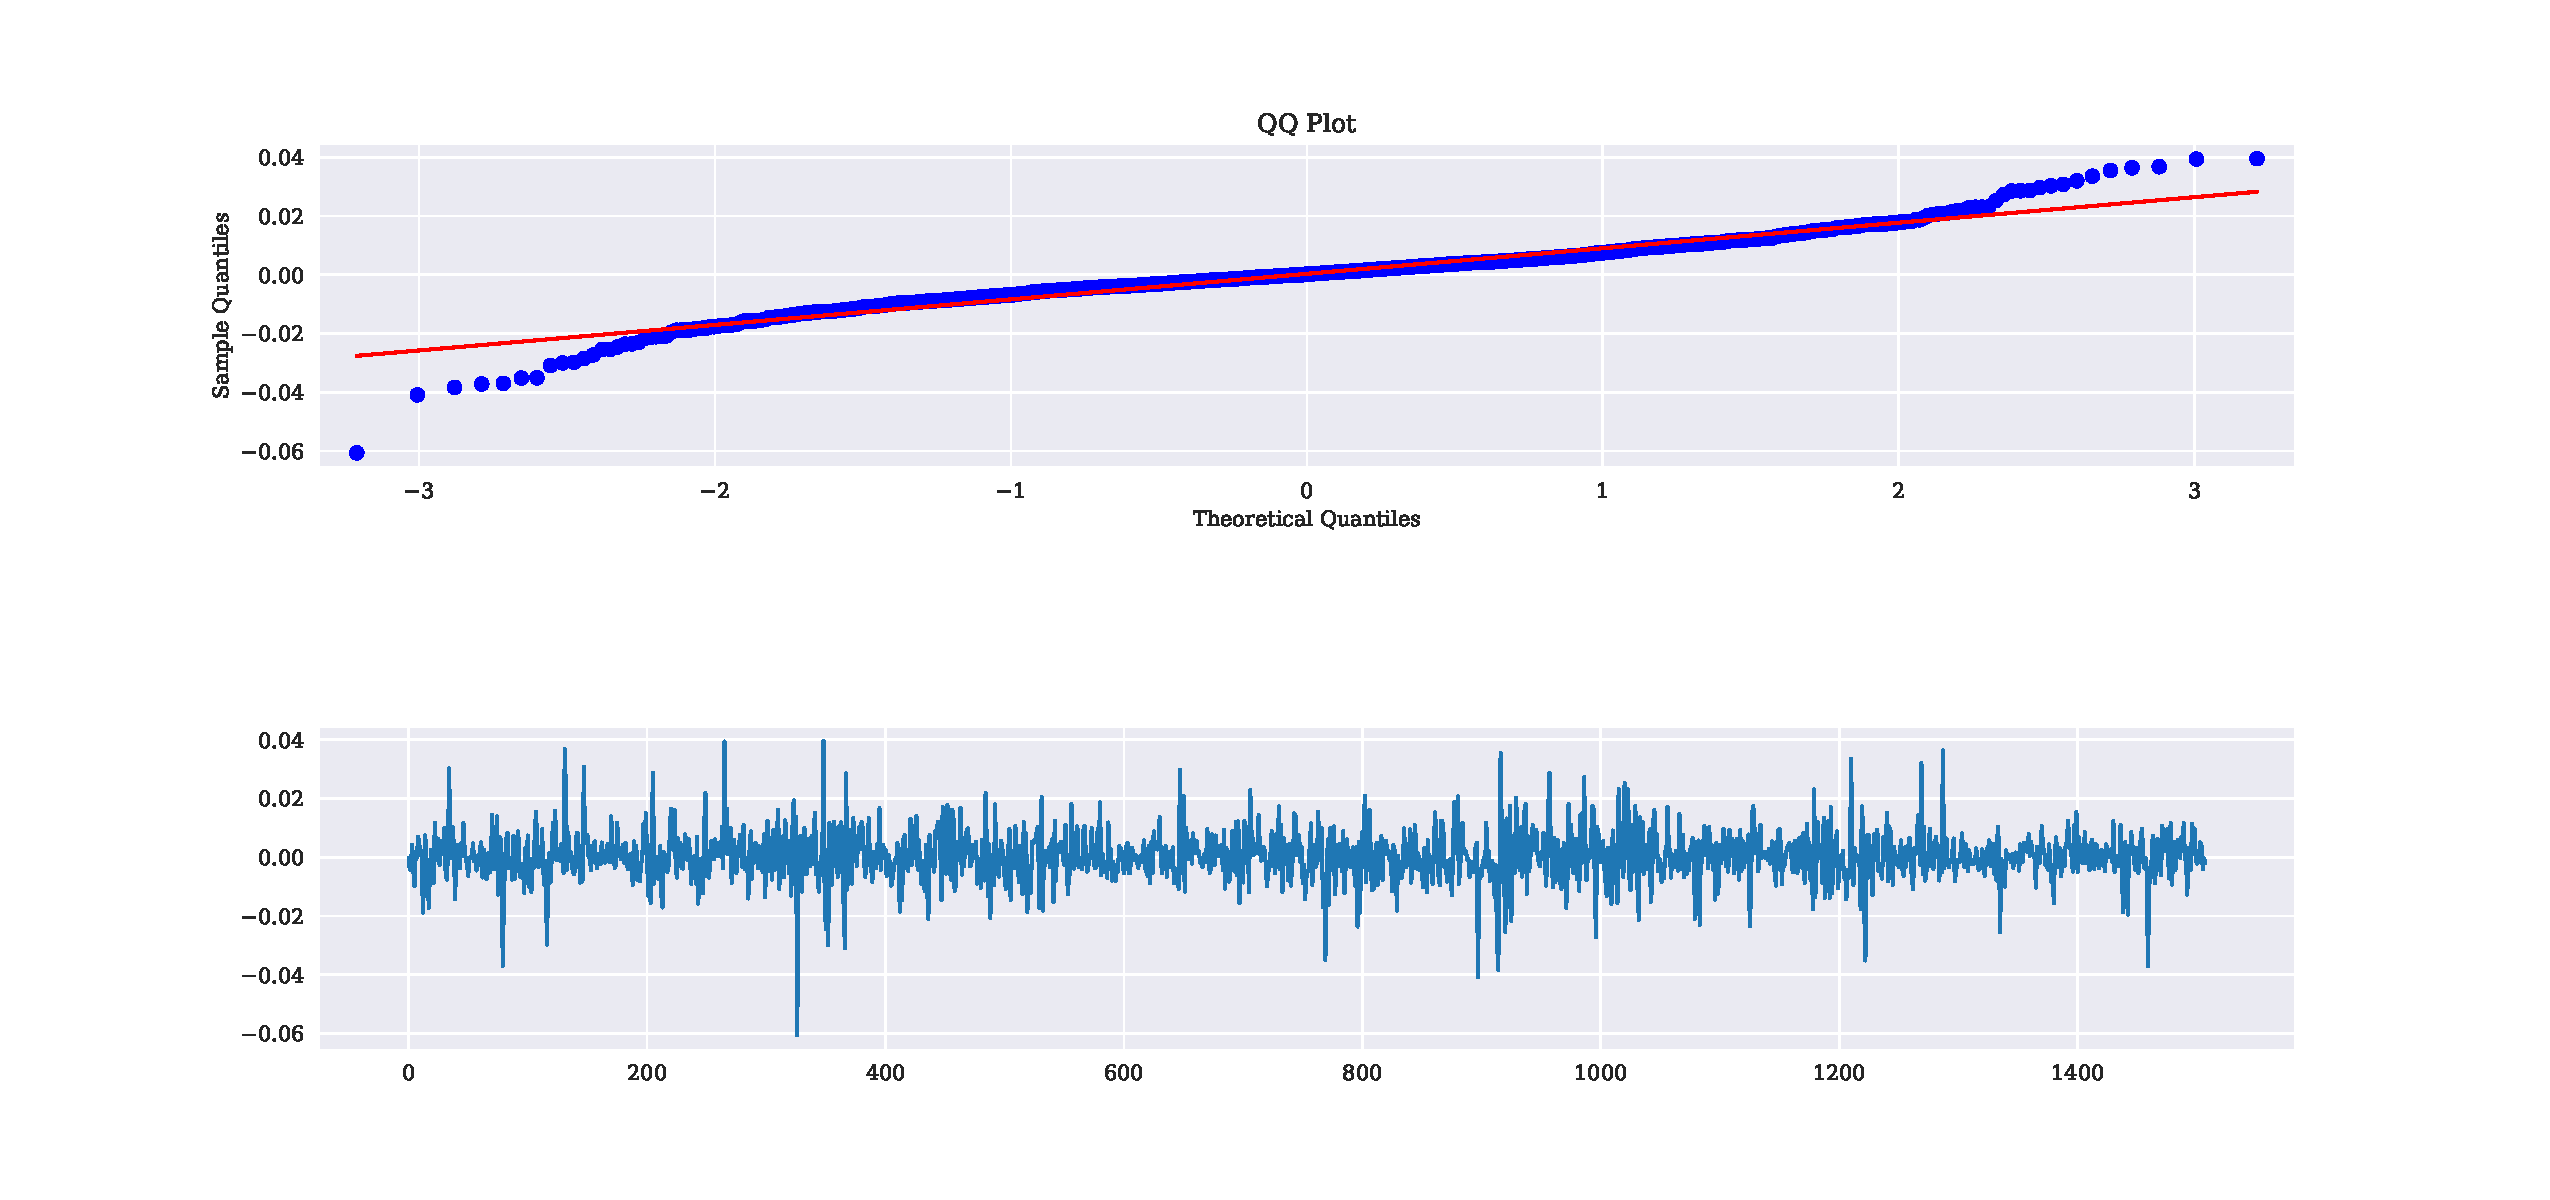
\includegraphics[]{figures/PG_log_adjclose_fd_and_qq.pdf}
    %%% Creator: Matplotlib, PGF backend
%%
%% To include the figure in your LaTeX document, write
%%   \input{<filename>.pgf}
%%
%% Make sure the required packages are loaded in your preamble
%%   \usepackage{pgf}
%%
%% Figures using additional raster images can only be included by \input if
%% they are in the same directory as the main LaTeX file. For loading figures
%% from other directories you can use the `import` package
%%   \usepackage{import}
%% and then include the figures with
%%   \import{<path to file>}{<filename>.pgf}
%%
%% Matplotlib used the following preamble
%%   \usepackage{fontspec}
%%   \setmainfont{DejaVuSerif.ttf}[Path=/opt/tljh/user/lib/python3.6/site-packages/matplotlib/mpl-data/fonts/ttf/]
%%   \setsansfont{DejaVuSans.ttf}[Path=/opt/tljh/user/lib/python3.6/site-packages/matplotlib/mpl-data/fonts/ttf/]
%%   \setmonofont{DejaVuSansMono.ttf}[Path=/opt/tljh/user/lib/python3.6/site-packages/matplotlib/mpl-data/fonts/ttf/]
%%
\begingroup%
\makeatletter%
\begin{pgfpicture}%
\pgfpathrectangle{\pgfpointorigin}{\pgfqpoint{17.000000in}{8.000000in}}%
\pgfusepath{use as bounding box, clip}%
\begin{pgfscope}%
\pgfsetbuttcap%
\pgfsetmiterjoin%
\definecolor{currentfill}{rgb}{1.000000,1.000000,1.000000}%
\pgfsetfillcolor{currentfill}%
\pgfsetlinewidth{0.000000pt}%
\definecolor{currentstroke}{rgb}{1.000000,1.000000,1.000000}%
\pgfsetstrokecolor{currentstroke}%
\pgfsetdash{}{0pt}%
\pgfpathmoveto{\pgfqpoint{0.000000in}{0.000000in}}%
\pgfpathlineto{\pgfqpoint{17.000000in}{0.000000in}}%
\pgfpathlineto{\pgfqpoint{17.000000in}{8.000000in}}%
\pgfpathlineto{\pgfqpoint{0.000000in}{8.000000in}}%
\pgfpathclose%
\pgfusepath{fill}%
\end{pgfscope}%
\begin{pgfscope}%
\pgfsetbuttcap%
\pgfsetmiterjoin%
\definecolor{currentfill}{rgb}{0.917647,0.917647,0.949020}%
\pgfsetfillcolor{currentfill}%
\pgfsetlinewidth{0.000000pt}%
\definecolor{currentstroke}{rgb}{0.000000,0.000000,0.000000}%
\pgfsetstrokecolor{currentstroke}%
\pgfsetstrokeopacity{0.000000}%
\pgfsetdash{}{0pt}%
\pgfpathmoveto{\pgfqpoint{2.125000in}{4.882857in}}%
\pgfpathlineto{\pgfqpoint{15.300000in}{4.882857in}}%
\pgfpathlineto{\pgfqpoint{15.300000in}{7.040000in}}%
\pgfpathlineto{\pgfqpoint{2.125000in}{7.040000in}}%
\pgfpathclose%
\pgfusepath{fill}%
\end{pgfscope}%
\begin{pgfscope}%
\pgfpathrectangle{\pgfqpoint{2.125000in}{4.882857in}}{\pgfqpoint{13.175000in}{2.157143in}}%
\pgfusepath{clip}%
\pgfsetroundcap%
\pgfsetroundjoin%
\pgfsetlinewidth{0.803000pt}%
\definecolor{currentstroke}{rgb}{1.000000,1.000000,1.000000}%
\pgfsetstrokecolor{currentstroke}%
\pgfsetdash{}{0pt}%
\pgfpathmoveto{\pgfqpoint{2.793535in}{4.882857in}}%
\pgfpathlineto{\pgfqpoint{2.793535in}{7.040000in}}%
\pgfusepath{stroke}%
\end{pgfscope}%
\begin{pgfscope}%
\definecolor{textcolor}{rgb}{0.150000,0.150000,0.150000}%
\pgfsetstrokecolor{textcolor}%
\pgfsetfillcolor{textcolor}%
\pgftext[x=2.793535in,y=4.785635in,,top]{\color{textcolor}\rmfamily\fontsize{10.000000}{12.000000}\selectfont −3}%
\end{pgfscope}%
\begin{pgfscope}%
\pgfpathrectangle{\pgfqpoint{2.125000in}{4.882857in}}{\pgfqpoint{13.175000in}{2.157143in}}%
\pgfusepath{clip}%
\pgfsetroundcap%
\pgfsetroundjoin%
\pgfsetlinewidth{0.803000pt}%
\definecolor{currentstroke}{rgb}{1.000000,1.000000,1.000000}%
\pgfsetstrokecolor{currentstroke}%
\pgfsetdash{}{0pt}%
\pgfpathmoveto{\pgfqpoint{4.766523in}{4.882857in}}%
\pgfpathlineto{\pgfqpoint{4.766523in}{7.040000in}}%
\pgfusepath{stroke}%
\end{pgfscope}%
\begin{pgfscope}%
\definecolor{textcolor}{rgb}{0.150000,0.150000,0.150000}%
\pgfsetstrokecolor{textcolor}%
\pgfsetfillcolor{textcolor}%
\pgftext[x=4.766523in,y=4.785635in,,top]{\color{textcolor}\rmfamily\fontsize{10.000000}{12.000000}\selectfont −2}%
\end{pgfscope}%
\begin{pgfscope}%
\pgfpathrectangle{\pgfqpoint{2.125000in}{4.882857in}}{\pgfqpoint{13.175000in}{2.157143in}}%
\pgfusepath{clip}%
\pgfsetroundcap%
\pgfsetroundjoin%
\pgfsetlinewidth{0.803000pt}%
\definecolor{currentstroke}{rgb}{1.000000,1.000000,1.000000}%
\pgfsetstrokecolor{currentstroke}%
\pgfsetdash{}{0pt}%
\pgfpathmoveto{\pgfqpoint{6.739512in}{4.882857in}}%
\pgfpathlineto{\pgfqpoint{6.739512in}{7.040000in}}%
\pgfusepath{stroke}%
\end{pgfscope}%
\begin{pgfscope}%
\definecolor{textcolor}{rgb}{0.150000,0.150000,0.150000}%
\pgfsetstrokecolor{textcolor}%
\pgfsetfillcolor{textcolor}%
\pgftext[x=6.739512in,y=4.785635in,,top]{\color{textcolor}\rmfamily\fontsize{10.000000}{12.000000}\selectfont −1}%
\end{pgfscope}%
\begin{pgfscope}%
\pgfpathrectangle{\pgfqpoint{2.125000in}{4.882857in}}{\pgfqpoint{13.175000in}{2.157143in}}%
\pgfusepath{clip}%
\pgfsetroundcap%
\pgfsetroundjoin%
\pgfsetlinewidth{0.803000pt}%
\definecolor{currentstroke}{rgb}{1.000000,1.000000,1.000000}%
\pgfsetstrokecolor{currentstroke}%
\pgfsetdash{}{0pt}%
\pgfpathmoveto{\pgfqpoint{8.712500in}{4.882857in}}%
\pgfpathlineto{\pgfqpoint{8.712500in}{7.040000in}}%
\pgfusepath{stroke}%
\end{pgfscope}%
\begin{pgfscope}%
\definecolor{textcolor}{rgb}{0.150000,0.150000,0.150000}%
\pgfsetstrokecolor{textcolor}%
\pgfsetfillcolor{textcolor}%
\pgftext[x=8.712500in,y=4.785635in,,top]{\color{textcolor}\rmfamily\fontsize{10.000000}{12.000000}\selectfont 0}%
\end{pgfscope}%
\begin{pgfscope}%
\pgfpathrectangle{\pgfqpoint{2.125000in}{4.882857in}}{\pgfqpoint{13.175000in}{2.157143in}}%
\pgfusepath{clip}%
\pgfsetroundcap%
\pgfsetroundjoin%
\pgfsetlinewidth{0.803000pt}%
\definecolor{currentstroke}{rgb}{1.000000,1.000000,1.000000}%
\pgfsetstrokecolor{currentstroke}%
\pgfsetdash{}{0pt}%
\pgfpathmoveto{\pgfqpoint{10.685488in}{4.882857in}}%
\pgfpathlineto{\pgfqpoint{10.685488in}{7.040000in}}%
\pgfusepath{stroke}%
\end{pgfscope}%
\begin{pgfscope}%
\definecolor{textcolor}{rgb}{0.150000,0.150000,0.150000}%
\pgfsetstrokecolor{textcolor}%
\pgfsetfillcolor{textcolor}%
\pgftext[x=10.685488in,y=4.785635in,,top]{\color{textcolor}\rmfamily\fontsize{10.000000}{12.000000}\selectfont 1}%
\end{pgfscope}%
\begin{pgfscope}%
\pgfpathrectangle{\pgfqpoint{2.125000in}{4.882857in}}{\pgfqpoint{13.175000in}{2.157143in}}%
\pgfusepath{clip}%
\pgfsetroundcap%
\pgfsetroundjoin%
\pgfsetlinewidth{0.803000pt}%
\definecolor{currentstroke}{rgb}{1.000000,1.000000,1.000000}%
\pgfsetstrokecolor{currentstroke}%
\pgfsetdash{}{0pt}%
\pgfpathmoveto{\pgfqpoint{12.658477in}{4.882857in}}%
\pgfpathlineto{\pgfqpoint{12.658477in}{7.040000in}}%
\pgfusepath{stroke}%
\end{pgfscope}%
\begin{pgfscope}%
\definecolor{textcolor}{rgb}{0.150000,0.150000,0.150000}%
\pgfsetstrokecolor{textcolor}%
\pgfsetfillcolor{textcolor}%
\pgftext[x=12.658477in,y=4.785635in,,top]{\color{textcolor}\rmfamily\fontsize{10.000000}{12.000000}\selectfont 2}%
\end{pgfscope}%
\begin{pgfscope}%
\pgfpathrectangle{\pgfqpoint{2.125000in}{4.882857in}}{\pgfqpoint{13.175000in}{2.157143in}}%
\pgfusepath{clip}%
\pgfsetroundcap%
\pgfsetroundjoin%
\pgfsetlinewidth{0.803000pt}%
\definecolor{currentstroke}{rgb}{1.000000,1.000000,1.000000}%
\pgfsetstrokecolor{currentstroke}%
\pgfsetdash{}{0pt}%
\pgfpathmoveto{\pgfqpoint{14.631465in}{4.882857in}}%
\pgfpathlineto{\pgfqpoint{14.631465in}{7.040000in}}%
\pgfusepath{stroke}%
\end{pgfscope}%
\begin{pgfscope}%
\definecolor{textcolor}{rgb}{0.150000,0.150000,0.150000}%
\pgfsetstrokecolor{textcolor}%
\pgfsetfillcolor{textcolor}%
\pgftext[x=14.631465in,y=4.785635in,,top]{\color{textcolor}\rmfamily\fontsize{10.000000}{12.000000}\selectfont 3}%
\end{pgfscope}%
\begin{pgfscope}%
\definecolor{textcolor}{rgb}{0.150000,0.150000,0.150000}%
\pgfsetstrokecolor{textcolor}%
\pgfsetfillcolor{textcolor}%
\pgftext[x=8.712500in,y=4.595667in,,top]{\color{textcolor}\rmfamily\fontsize{10.000000}{12.000000}\selectfont Theoretical Quantiles}%
\end{pgfscope}%
\begin{pgfscope}%
\pgfpathrectangle{\pgfqpoint{2.125000in}{4.882857in}}{\pgfqpoint{13.175000in}{2.157143in}}%
\pgfusepath{clip}%
\pgfsetroundcap%
\pgfsetroundjoin%
\pgfsetlinewidth{0.803000pt}%
\definecolor{currentstroke}{rgb}{1.000000,1.000000,1.000000}%
\pgfsetstrokecolor{currentstroke}%
\pgfsetdash{}{0pt}%
\pgfpathmoveto{\pgfqpoint{2.125000in}{4.992782in}}%
\pgfpathlineto{\pgfqpoint{15.300000in}{4.992782in}}%
\pgfusepath{stroke}%
\end{pgfscope}%
\begin{pgfscope}%
\definecolor{textcolor}{rgb}{0.150000,0.150000,0.150000}%
\pgfsetstrokecolor{textcolor}%
\pgfsetfillcolor{textcolor}%
\pgftext[x=1.602159in,y=4.940021in,left,base]{\color{textcolor}\rmfamily\fontsize{10.000000}{12.000000}\selectfont −0.06}%
\end{pgfscope}%
\begin{pgfscope}%
\pgfpathrectangle{\pgfqpoint{2.125000in}{4.882857in}}{\pgfqpoint{13.175000in}{2.157143in}}%
\pgfusepath{clip}%
\pgfsetroundcap%
\pgfsetroundjoin%
\pgfsetlinewidth{0.803000pt}%
\definecolor{currentstroke}{rgb}{1.000000,1.000000,1.000000}%
\pgfsetstrokecolor{currentstroke}%
\pgfsetdash{}{0pt}%
\pgfpathmoveto{\pgfqpoint{2.125000in}{5.384533in}}%
\pgfpathlineto{\pgfqpoint{15.300000in}{5.384533in}}%
\pgfusepath{stroke}%
\end{pgfscope}%
\begin{pgfscope}%
\definecolor{textcolor}{rgb}{0.150000,0.150000,0.150000}%
\pgfsetstrokecolor{textcolor}%
\pgfsetfillcolor{textcolor}%
\pgftext[x=1.602159in,y=5.331771in,left,base]{\color{textcolor}\rmfamily\fontsize{10.000000}{12.000000}\selectfont −0.04}%
\end{pgfscope}%
\begin{pgfscope}%
\pgfpathrectangle{\pgfqpoint{2.125000in}{4.882857in}}{\pgfqpoint{13.175000in}{2.157143in}}%
\pgfusepath{clip}%
\pgfsetroundcap%
\pgfsetroundjoin%
\pgfsetlinewidth{0.803000pt}%
\definecolor{currentstroke}{rgb}{1.000000,1.000000,1.000000}%
\pgfsetstrokecolor{currentstroke}%
\pgfsetdash{}{0pt}%
\pgfpathmoveto{\pgfqpoint{2.125000in}{5.776283in}}%
\pgfpathlineto{\pgfqpoint{15.300000in}{5.776283in}}%
\pgfusepath{stroke}%
\end{pgfscope}%
\begin{pgfscope}%
\definecolor{textcolor}{rgb}{0.150000,0.150000,0.150000}%
\pgfsetstrokecolor{textcolor}%
\pgfsetfillcolor{textcolor}%
\pgftext[x=1.602159in,y=5.723522in,left,base]{\color{textcolor}\rmfamily\fontsize{10.000000}{12.000000}\selectfont −0.02}%
\end{pgfscope}%
\begin{pgfscope}%
\pgfpathrectangle{\pgfqpoint{2.125000in}{4.882857in}}{\pgfqpoint{13.175000in}{2.157143in}}%
\pgfusepath{clip}%
\pgfsetroundcap%
\pgfsetroundjoin%
\pgfsetlinewidth{0.803000pt}%
\definecolor{currentstroke}{rgb}{1.000000,1.000000,1.000000}%
\pgfsetstrokecolor{currentstroke}%
\pgfsetdash{}{0pt}%
\pgfpathmoveto{\pgfqpoint{2.125000in}{6.168034in}}%
\pgfpathlineto{\pgfqpoint{15.300000in}{6.168034in}}%
\pgfusepath{stroke}%
\end{pgfscope}%
\begin{pgfscope}%
\definecolor{textcolor}{rgb}{0.150000,0.150000,0.150000}%
\pgfsetstrokecolor{textcolor}%
\pgfsetfillcolor{textcolor}%
\pgftext[x=1.718533in,y=6.115272in,left,base]{\color{textcolor}\rmfamily\fontsize{10.000000}{12.000000}\selectfont 0.00}%
\end{pgfscope}%
\begin{pgfscope}%
\pgfpathrectangle{\pgfqpoint{2.125000in}{4.882857in}}{\pgfqpoint{13.175000in}{2.157143in}}%
\pgfusepath{clip}%
\pgfsetroundcap%
\pgfsetroundjoin%
\pgfsetlinewidth{0.803000pt}%
\definecolor{currentstroke}{rgb}{1.000000,1.000000,1.000000}%
\pgfsetstrokecolor{currentstroke}%
\pgfsetdash{}{0pt}%
\pgfpathmoveto{\pgfqpoint{2.125000in}{6.559784in}}%
\pgfpathlineto{\pgfqpoint{15.300000in}{6.559784in}}%
\pgfusepath{stroke}%
\end{pgfscope}%
\begin{pgfscope}%
\definecolor{textcolor}{rgb}{0.150000,0.150000,0.150000}%
\pgfsetstrokecolor{textcolor}%
\pgfsetfillcolor{textcolor}%
\pgftext[x=1.718533in,y=6.507023in,left,base]{\color{textcolor}\rmfamily\fontsize{10.000000}{12.000000}\selectfont 0.02}%
\end{pgfscope}%
\begin{pgfscope}%
\pgfpathrectangle{\pgfqpoint{2.125000in}{4.882857in}}{\pgfqpoint{13.175000in}{2.157143in}}%
\pgfusepath{clip}%
\pgfsetroundcap%
\pgfsetroundjoin%
\pgfsetlinewidth{0.803000pt}%
\definecolor{currentstroke}{rgb}{1.000000,1.000000,1.000000}%
\pgfsetstrokecolor{currentstroke}%
\pgfsetdash{}{0pt}%
\pgfpathmoveto{\pgfqpoint{2.125000in}{6.951535in}}%
\pgfpathlineto{\pgfqpoint{15.300000in}{6.951535in}}%
\pgfusepath{stroke}%
\end{pgfscope}%
\begin{pgfscope}%
\definecolor{textcolor}{rgb}{0.150000,0.150000,0.150000}%
\pgfsetstrokecolor{textcolor}%
\pgfsetfillcolor{textcolor}%
\pgftext[x=1.718533in,y=6.898773in,left,base]{\color{textcolor}\rmfamily\fontsize{10.000000}{12.000000}\selectfont 0.04}%
\end{pgfscope}%
\begin{pgfscope}%
\definecolor{textcolor}{rgb}{0.150000,0.150000,0.150000}%
\pgfsetstrokecolor{textcolor}%
\pgfsetfillcolor{textcolor}%
\pgftext[x=1.546604in,y=5.961429in,,bottom,rotate=90.000000]{\color{textcolor}\rmfamily\fontsize{10.000000}{12.000000}\selectfont Sample Quantiles}%
\end{pgfscope}%
\begin{pgfscope}%
\pgfpathrectangle{\pgfqpoint{2.125000in}{4.882857in}}{\pgfqpoint{13.175000in}{2.157143in}}%
\pgfusepath{clip}%
\pgfsetbuttcap%
\pgfsetroundjoin%
\definecolor{currentfill}{rgb}{0.000000,0.000000,1.000000}%
\pgfsetfillcolor{currentfill}%
\pgfsetlinewidth{1.003750pt}%
\definecolor{currentstroke}{rgb}{0.000000,0.000000,1.000000}%
\pgfsetstrokecolor{currentstroke}%
\pgfsetdash{}{0pt}%
\pgfsys@defobject{currentmarker}{\pgfqpoint{-0.041667in}{-0.041667in}}{\pgfqpoint{0.041667in}{0.041667in}}{%
\pgfpathmoveto{\pgfqpoint{0.000000in}{-0.041667in}}%
\pgfpathcurveto{\pgfqpoint{0.011050in}{-0.041667in}}{\pgfqpoint{0.021649in}{-0.037276in}}{\pgfqpoint{0.029463in}{-0.029463in}}%
\pgfpathcurveto{\pgfqpoint{0.037276in}{-0.021649in}}{\pgfqpoint{0.041667in}{-0.011050in}}{\pgfqpoint{0.041667in}{0.000000in}}%
\pgfpathcurveto{\pgfqpoint{0.041667in}{0.011050in}}{\pgfqpoint{0.037276in}{0.021649in}}{\pgfqpoint{0.029463in}{0.029463in}}%
\pgfpathcurveto{\pgfqpoint{0.021649in}{0.037276in}}{\pgfqpoint{0.011050in}{0.041667in}}{\pgfqpoint{0.000000in}{0.041667in}}%
\pgfpathcurveto{\pgfqpoint{-0.011050in}{0.041667in}}{\pgfqpoint{-0.021649in}{0.037276in}}{\pgfqpoint{-0.029463in}{0.029463in}}%
\pgfpathcurveto{\pgfqpoint{-0.037276in}{0.021649in}}{\pgfqpoint{-0.041667in}{0.011050in}}{\pgfqpoint{-0.041667in}{0.000000in}}%
\pgfpathcurveto{\pgfqpoint{-0.041667in}{-0.011050in}}{\pgfqpoint{-0.037276in}{-0.021649in}}{\pgfqpoint{-0.029463in}{-0.029463in}}%
\pgfpathcurveto{\pgfqpoint{-0.021649in}{-0.037276in}}{\pgfqpoint{-0.011050in}{-0.041667in}}{\pgfqpoint{0.000000in}{-0.041667in}}%
\pgfpathclose%
\pgfusepath{stroke,fill}%
}%
\begin{pgfscope}%
\pgfsys@transformshift{2.378365in}{4.980909in}%
\pgfsys@useobject{currentmarker}{}%
\end{pgfscope}%
\begin{pgfscope}%
\pgfsys@transformshift{2.782528in}{5.367174in}%
\pgfsys@useobject{currentmarker}{}%
\end{pgfscope}%
\begin{pgfscope}%
\pgfsys@transformshift{3.030198in}{5.417895in}%
\pgfsys@useobject{currentmarker}{}%
\end{pgfscope}%
\begin{pgfscope}%
\pgfsys@transformshift{3.211576in}{5.440027in}%
\pgfsys@useobject{currentmarker}{}%
\end{pgfscope}%
\begin{pgfscope}%
\pgfsys@transformshift{3.355770in}{5.444283in}%
\pgfsys@useobject{currentmarker}{}%
\end{pgfscope}%
\begin{pgfscope}%
\pgfsys@transformshift{3.476013in}{5.479270in}%
\pgfsys@useobject{currentmarker}{}%
\end{pgfscope}%
\begin{pgfscope}%
\pgfsys@transformshift{3.579476in}{5.481040in}%
\pgfsys@useobject{currentmarker}{}%
\end{pgfscope}%
\begin{pgfscope}%
\pgfsys@transformshift{3.670496in}{5.563001in}%
\pgfsys@useobject{currentmarker}{}%
\end{pgfscope}%
\begin{pgfscope}%
\pgfsys@transformshift{3.751905in}{5.580653in}%
\pgfsys@useobject{currentmarker}{}%
\end{pgfscope}%
\begin{pgfscope}%
\pgfsys@transformshift{3.825653in}{5.584719in}%
\pgfsys@useobject{currentmarker}{}%
\end{pgfscope}%
\begin{pgfscope}%
\pgfsys@transformshift{3.893147in}{5.609480in}%
\pgfsys@useobject{currentmarker}{}%
\end{pgfscope}%
\begin{pgfscope}%
\pgfsys@transformshift{3.955431in}{5.633858in}%
\pgfsys@useobject{currentmarker}{}%
\end{pgfscope}%
\begin{pgfscope}%
\pgfsys@transformshift{4.013308in}{5.669441in}%
\pgfsys@useobject{currentmarker}{}%
\end{pgfscope}%
\begin{pgfscope}%
\pgfsys@transformshift{4.067403in}{5.670355in}%
\pgfsys@useobject{currentmarker}{}%
\end{pgfscope}%
\begin{pgfscope}%
\pgfsys@transformshift{4.118216in}{5.687079in}%
\pgfsys@useobject{currentmarker}{}%
\end{pgfscope}%
\begin{pgfscope}%
\pgfsys@transformshift{4.166153in}{5.705738in}%
\pgfsys@useobject{currentmarker}{}%
\end{pgfscope}%
\begin{pgfscope}%
\pgfsys@transformshift{4.211547in}{5.707008in}%
\pgfsys@useobject{currentmarker}{}%
\end{pgfscope}%
\begin{pgfscope}%
\pgfsys@transformshift{4.254677in}{5.715324in}%
\pgfsys@useobject{currentmarker}{}%
\end{pgfscope}%
\begin{pgfscope}%
\pgfsys@transformshift{4.295777in}{5.743070in}%
\pgfsys@useobject{currentmarker}{}%
\end{pgfscope}%
\begin{pgfscope}%
\pgfsys@transformshift{4.335044in}{5.750890in}%
\pgfsys@useobject{currentmarker}{}%
\end{pgfscope}%
\begin{pgfscope}%
\pgfsys@transformshift{4.372651in}{5.755195in}%
\pgfsys@useobject{currentmarker}{}%
\end{pgfscope}%
\begin{pgfscope}%
\pgfsys@transformshift{4.408744in}{5.757357in}%
\pgfsys@useobject{currentmarker}{}%
\end{pgfscope}%
\begin{pgfscope}%
\pgfsys@transformshift{4.443452in}{5.760794in}%
\pgfsys@useobject{currentmarker}{}%
\end{pgfscope}%
\begin{pgfscope}%
\pgfsys@transformshift{4.476887in}{5.786102in}%
\pgfsys@useobject{currentmarker}{}%
\end{pgfscope}%
\begin{pgfscope}%
\pgfsys@transformshift{4.509148in}{5.799157in}%
\pgfsys@useobject{currentmarker}{}%
\end{pgfscope}%
\begin{pgfscope}%
\pgfsys@transformshift{4.540323in}{5.799349in}%
\pgfsys@useobject{currentmarker}{}%
\end{pgfscope}%
\begin{pgfscope}%
\pgfsys@transformshift{4.570489in}{5.799953in}%
\pgfsys@useobject{currentmarker}{}%
\end{pgfscope}%
\begin{pgfscope}%
\pgfsys@transformshift{4.599718in}{5.801293in}%
\pgfsys@useobject{currentmarker}{}%
\end{pgfscope}%
\begin{pgfscope}%
\pgfsys@transformshift{4.628071in}{5.805786in}%
\pgfsys@useobject{currentmarker}{}%
\end{pgfscope}%
\begin{pgfscope}%
\pgfsys@transformshift{4.655604in}{5.810786in}%
\pgfsys@useobject{currentmarker}{}%
\end{pgfscope}%
\begin{pgfscope}%
\pgfsys@transformshift{4.682369in}{5.811592in}%
\pgfsys@useobject{currentmarker}{}%
\end{pgfscope}%
\begin{pgfscope}%
\pgfsys@transformshift{4.708413in}{5.813128in}%
\pgfsys@useobject{currentmarker}{}%
\end{pgfscope}%
\begin{pgfscope}%
\pgfsys@transformshift{4.733777in}{5.821386in}%
\pgfsys@useobject{currentmarker}{}%
\end{pgfscope}%
\begin{pgfscope}%
\pgfsys@transformshift{4.758500in}{5.821824in}%
\pgfsys@useobject{currentmarker}{}%
\end{pgfscope}%
\begin{pgfscope}%
\pgfsys@transformshift{4.782618in}{5.822816in}%
\pgfsys@useobject{currentmarker}{}%
\end{pgfscope}%
\begin{pgfscope}%
\pgfsys@transformshift{4.806162in}{5.829951in}%
\pgfsys@useobject{currentmarker}{}%
\end{pgfscope}%
\begin{pgfscope}%
\pgfsys@transformshift{4.829162in}{5.830360in}%
\pgfsys@useobject{currentmarker}{}%
\end{pgfscope}%
\begin{pgfscope}%
\pgfsys@transformshift{4.851647in}{5.831011in}%
\pgfsys@useobject{currentmarker}{}%
\end{pgfscope}%
\begin{pgfscope}%
\pgfsys@transformshift{4.873641in}{5.832586in}%
\pgfsys@useobject{currentmarker}{}%
\end{pgfscope}%
\begin{pgfscope}%
\pgfsys@transformshift{4.895168in}{5.836453in}%
\pgfsys@useobject{currentmarker}{}%
\end{pgfscope}%
\begin{pgfscope}%
\pgfsys@transformshift{4.916250in}{5.839467in}%
\pgfsys@useobject{currentmarker}{}%
\end{pgfscope}%
\begin{pgfscope}%
\pgfsys@transformshift{4.936908in}{5.850563in}%
\pgfsys@useobject{currentmarker}{}%
\end{pgfscope}%
\begin{pgfscope}%
\pgfsys@transformshift{4.957159in}{5.858632in}%
\pgfsys@useobject{currentmarker}{}%
\end{pgfscope}%
\begin{pgfscope}%
\pgfsys@transformshift{4.977023in}{5.858841in}%
\pgfsys@useobject{currentmarker}{}%
\end{pgfscope}%
\begin{pgfscope}%
\pgfsys@transformshift{4.996515in}{5.860538in}%
\pgfsys@useobject{currentmarker}{}%
\end{pgfscope}%
\begin{pgfscope}%
\pgfsys@transformshift{5.015651in}{5.861230in}%
\pgfsys@useobject{currentmarker}{}%
\end{pgfscope}%
\begin{pgfscope}%
\pgfsys@transformshift{5.034445in}{5.861543in}%
\pgfsys@useobject{currentmarker}{}%
\end{pgfscope}%
\begin{pgfscope}%
\pgfsys@transformshift{5.052911in}{5.863356in}%
\pgfsys@useobject{currentmarker}{}%
\end{pgfscope}%
\begin{pgfscope}%
\pgfsys@transformshift{5.071062in}{5.863400in}%
\pgfsys@useobject{currentmarker}{}%
\end{pgfscope}%
\begin{pgfscope}%
\pgfsys@transformshift{5.088911in}{5.870159in}%
\pgfsys@useobject{currentmarker}{}%
\end{pgfscope}%
\begin{pgfscope}%
\pgfsys@transformshift{5.106467in}{5.871112in}%
\pgfsys@useobject{currentmarker}{}%
\end{pgfscope}%
\begin{pgfscope}%
\pgfsys@transformshift{5.123742in}{5.881991in}%
\pgfsys@useobject{currentmarker}{}%
\end{pgfscope}%
\begin{pgfscope}%
\pgfsys@transformshift{5.140747in}{5.881995in}%
\pgfsys@useobject{currentmarker}{}%
\end{pgfscope}%
\begin{pgfscope}%
\pgfsys@transformshift{5.157490in}{5.882213in}%
\pgfsys@useobject{currentmarker}{}%
\end{pgfscope}%
\begin{pgfscope}%
\pgfsys@transformshift{5.173982in}{5.886118in}%
\pgfsys@useobject{currentmarker}{}%
\end{pgfscope}%
\begin{pgfscope}%
\pgfsys@transformshift{5.190229in}{5.887187in}%
\pgfsys@useobject{currentmarker}{}%
\end{pgfscope}%
\begin{pgfscope}%
\pgfsys@transformshift{5.206241in}{5.888470in}%
\pgfsys@useobject{currentmarker}{}%
\end{pgfscope}%
\begin{pgfscope}%
\pgfsys@transformshift{5.222026in}{5.889177in}%
\pgfsys@useobject{currentmarker}{}%
\end{pgfscope}%
\begin{pgfscope}%
\pgfsys@transformshift{5.237590in}{5.893073in}%
\pgfsys@useobject{currentmarker}{}%
\end{pgfscope}%
\begin{pgfscope}%
\pgfsys@transformshift{5.252941in}{5.896955in}%
\pgfsys@useobject{currentmarker}{}%
\end{pgfscope}%
\begin{pgfscope}%
\pgfsys@transformshift{5.268086in}{5.898388in}%
\pgfsys@useobject{currentmarker}{}%
\end{pgfscope}%
\begin{pgfscope}%
\pgfsys@transformshift{5.283030in}{5.900772in}%
\pgfsys@useobject{currentmarker}{}%
\end{pgfscope}%
\begin{pgfscope}%
\pgfsys@transformshift{5.297779in}{5.901250in}%
\pgfsys@useobject{currentmarker}{}%
\end{pgfscope}%
\begin{pgfscope}%
\pgfsys@transformshift{5.312341in}{5.902031in}%
\pgfsys@useobject{currentmarker}{}%
\end{pgfscope}%
\begin{pgfscope}%
\pgfsys@transformshift{5.326720in}{5.907344in}%
\pgfsys@useobject{currentmarker}{}%
\end{pgfscope}%
\begin{pgfscope}%
\pgfsys@transformshift{5.340920in}{5.909586in}%
\pgfsys@useobject{currentmarker}{}%
\end{pgfscope}%
\begin{pgfscope}%
\pgfsys@transformshift{5.354949in}{5.909840in}%
\pgfsys@useobject{currentmarker}{}%
\end{pgfscope}%
\begin{pgfscope}%
\pgfsys@transformshift{5.368810in}{5.912887in}%
\pgfsys@useobject{currentmarker}{}%
\end{pgfscope}%
\begin{pgfscope}%
\pgfsys@transformshift{5.382507in}{5.913426in}%
\pgfsys@useobject{currentmarker}{}%
\end{pgfscope}%
\begin{pgfscope}%
\pgfsys@transformshift{5.396046in}{5.913430in}%
\pgfsys@useobject{currentmarker}{}%
\end{pgfscope}%
\begin{pgfscope}%
\pgfsys@transformshift{5.409431in}{5.917663in}%
\pgfsys@useobject{currentmarker}{}%
\end{pgfscope}%
\begin{pgfscope}%
\pgfsys@transformshift{5.422665in}{5.918334in}%
\pgfsys@useobject{currentmarker}{}%
\end{pgfscope}%
\begin{pgfscope}%
\pgfsys@transformshift{5.435753in}{5.918418in}%
\pgfsys@useobject{currentmarker}{}%
\end{pgfscope}%
\begin{pgfscope}%
\pgfsys@transformshift{5.448698in}{5.920137in}%
\pgfsys@useobject{currentmarker}{}%
\end{pgfscope}%
\begin{pgfscope}%
\pgfsys@transformshift{5.461504in}{5.920721in}%
\pgfsys@useobject{currentmarker}{}%
\end{pgfscope}%
\begin{pgfscope}%
\pgfsys@transformshift{5.474175in}{5.922419in}%
\pgfsys@useobject{currentmarker}{}%
\end{pgfscope}%
\begin{pgfscope}%
\pgfsys@transformshift{5.486714in}{5.922774in}%
\pgfsys@useobject{currentmarker}{}%
\end{pgfscope}%
\begin{pgfscope}%
\pgfsys@transformshift{5.499123in}{5.922995in}%
\pgfsys@useobject{currentmarker}{}%
\end{pgfscope}%
\begin{pgfscope}%
\pgfsys@transformshift{5.511407in}{5.923223in}%
\pgfsys@useobject{currentmarker}{}%
\end{pgfscope}%
\begin{pgfscope}%
\pgfsys@transformshift{5.523568in}{5.923282in}%
\pgfsys@useobject{currentmarker}{}%
\end{pgfscope}%
\begin{pgfscope}%
\pgfsys@transformshift{5.535609in}{5.923552in}%
\pgfsys@useobject{currentmarker}{}%
\end{pgfscope}%
\begin{pgfscope}%
\pgfsys@transformshift{5.547533in}{5.924576in}%
\pgfsys@useobject{currentmarker}{}%
\end{pgfscope}%
\begin{pgfscope}%
\pgfsys@transformshift{5.559342in}{5.926792in}%
\pgfsys@useobject{currentmarker}{}%
\end{pgfscope}%
\begin{pgfscope}%
\pgfsys@transformshift{5.571040in}{5.928252in}%
\pgfsys@useobject{currentmarker}{}%
\end{pgfscope}%
\begin{pgfscope}%
\pgfsys@transformshift{5.582628in}{5.929224in}%
\pgfsys@useobject{currentmarker}{}%
\end{pgfscope}%
\begin{pgfscope}%
\pgfsys@transformshift{5.594109in}{5.930039in}%
\pgfsys@useobject{currentmarker}{}%
\end{pgfscope}%
\begin{pgfscope}%
\pgfsys@transformshift{5.605485in}{5.930643in}%
\pgfsys@useobject{currentmarker}{}%
\end{pgfscope}%
\begin{pgfscope}%
\pgfsys@transformshift{5.616759in}{5.933314in}%
\pgfsys@useobject{currentmarker}{}%
\end{pgfscope}%
\begin{pgfscope}%
\pgfsys@transformshift{5.627933in}{5.934681in}%
\pgfsys@useobject{currentmarker}{}%
\end{pgfscope}%
\begin{pgfscope}%
\pgfsys@transformshift{5.639009in}{5.935456in}%
\pgfsys@useobject{currentmarker}{}%
\end{pgfscope}%
\begin{pgfscope}%
\pgfsys@transformshift{5.649989in}{5.935490in}%
\pgfsys@useobject{currentmarker}{}%
\end{pgfscope}%
\begin{pgfscope}%
\pgfsys@transformshift{5.660874in}{5.937716in}%
\pgfsys@useobject{currentmarker}{}%
\end{pgfscope}%
\begin{pgfscope}%
\pgfsys@transformshift{5.671668in}{5.938519in}%
\pgfsys@useobject{currentmarker}{}%
\end{pgfscope}%
\begin{pgfscope}%
\pgfsys@transformshift{5.682371in}{5.938805in}%
\pgfsys@useobject{currentmarker}{}%
\end{pgfscope}%
\begin{pgfscope}%
\pgfsys@transformshift{5.692986in}{5.940553in}%
\pgfsys@useobject{currentmarker}{}%
\end{pgfscope}%
\begin{pgfscope}%
\pgfsys@transformshift{5.703514in}{5.942212in}%
\pgfsys@useobject{currentmarker}{}%
\end{pgfscope}%
\begin{pgfscope}%
\pgfsys@transformshift{5.713958in}{5.943002in}%
\pgfsys@useobject{currentmarker}{}%
\end{pgfscope}%
\begin{pgfscope}%
\pgfsys@transformshift{5.724318in}{5.943774in}%
\pgfsys@useobject{currentmarker}{}%
\end{pgfscope}%
\begin{pgfscope}%
\pgfsys@transformshift{5.734596in}{5.949593in}%
\pgfsys@useobject{currentmarker}{}%
\end{pgfscope}%
\begin{pgfscope}%
\pgfsys@transformshift{5.744794in}{5.949809in}%
\pgfsys@useobject{currentmarker}{}%
\end{pgfscope}%
\begin{pgfscope}%
\pgfsys@transformshift{5.754913in}{5.952479in}%
\pgfsys@useobject{currentmarker}{}%
\end{pgfscope}%
\begin{pgfscope}%
\pgfsys@transformshift{5.764955in}{5.955255in}%
\pgfsys@useobject{currentmarker}{}%
\end{pgfscope}%
\begin{pgfscope}%
\pgfsys@transformshift{5.774922in}{5.955619in}%
\pgfsys@useobject{currentmarker}{}%
\end{pgfscope}%
\begin{pgfscope}%
\pgfsys@transformshift{5.784814in}{5.955783in}%
\pgfsys@useobject{currentmarker}{}%
\end{pgfscope}%
\begin{pgfscope}%
\pgfsys@transformshift{5.794632in}{5.956751in}%
\pgfsys@useobject{currentmarker}{}%
\end{pgfscope}%
\begin{pgfscope}%
\pgfsys@transformshift{5.804380in}{5.956984in}%
\pgfsys@useobject{currentmarker}{}%
\end{pgfscope}%
\begin{pgfscope}%
\pgfsys@transformshift{5.814056in}{5.957398in}%
\pgfsys@useobject{currentmarker}{}%
\end{pgfscope}%
\begin{pgfscope}%
\pgfsys@transformshift{5.823664in}{5.957491in}%
\pgfsys@useobject{currentmarker}{}%
\end{pgfscope}%
\begin{pgfscope}%
\pgfsys@transformshift{5.833203in}{5.958137in}%
\pgfsys@useobject{currentmarker}{}%
\end{pgfscope}%
\begin{pgfscope}%
\pgfsys@transformshift{5.842676in}{5.958182in}%
\pgfsys@useobject{currentmarker}{}%
\end{pgfscope}%
\begin{pgfscope}%
\pgfsys@transformshift{5.852083in}{5.960109in}%
\pgfsys@useobject{currentmarker}{}%
\end{pgfscope}%
\begin{pgfscope}%
\pgfsys@transformshift{5.861425in}{5.962577in}%
\pgfsys@useobject{currentmarker}{}%
\end{pgfscope}%
\begin{pgfscope}%
\pgfsys@transformshift{5.870704in}{5.963868in}%
\pgfsys@useobject{currentmarker}{}%
\end{pgfscope}%
\begin{pgfscope}%
\pgfsys@transformshift{5.879920in}{5.964513in}%
\pgfsys@useobject{currentmarker}{}%
\end{pgfscope}%
\begin{pgfscope}%
\pgfsys@transformshift{5.889075in}{5.964532in}%
\pgfsys@useobject{currentmarker}{}%
\end{pgfscope}%
\begin{pgfscope}%
\pgfsys@transformshift{5.898170in}{5.965419in}%
\pgfsys@useobject{currentmarker}{}%
\end{pgfscope}%
\begin{pgfscope}%
\pgfsys@transformshift{5.907205in}{5.968479in}%
\pgfsys@useobject{currentmarker}{}%
\end{pgfscope}%
\begin{pgfscope}%
\pgfsys@transformshift{5.916182in}{5.968975in}%
\pgfsys@useobject{currentmarker}{}%
\end{pgfscope}%
\begin{pgfscope}%
\pgfsys@transformshift{5.925101in}{5.971416in}%
\pgfsys@useobject{currentmarker}{}%
\end{pgfscope}%
\begin{pgfscope}%
\pgfsys@transformshift{5.933964in}{5.972548in}%
\pgfsys@useobject{currentmarker}{}%
\end{pgfscope}%
\begin{pgfscope}%
\pgfsys@transformshift{5.942770in}{5.972675in}%
\pgfsys@useobject{currentmarker}{}%
\end{pgfscope}%
\begin{pgfscope}%
\pgfsys@transformshift{5.951522in}{5.973012in}%
\pgfsys@useobject{currentmarker}{}%
\end{pgfscope}%
\begin{pgfscope}%
\pgfsys@transformshift{5.960221in}{5.974776in}%
\pgfsys@useobject{currentmarker}{}%
\end{pgfscope}%
\begin{pgfscope}%
\pgfsys@transformshift{5.968865in}{5.975683in}%
\pgfsys@useobject{currentmarker}{}%
\end{pgfscope}%
\begin{pgfscope}%
\pgfsys@transformshift{5.977458in}{5.977481in}%
\pgfsys@useobject{currentmarker}{}%
\end{pgfscope}%
\begin{pgfscope}%
\pgfsys@transformshift{5.985999in}{5.978752in}%
\pgfsys@useobject{currentmarker}{}%
\end{pgfscope}%
\begin{pgfscope}%
\pgfsys@transformshift{5.994489in}{5.978837in}%
\pgfsys@useobject{currentmarker}{}%
\end{pgfscope}%
\begin{pgfscope}%
\pgfsys@transformshift{6.002929in}{5.979000in}%
\pgfsys@useobject{currentmarker}{}%
\end{pgfscope}%
\begin{pgfscope}%
\pgfsys@transformshift{6.011320in}{5.979316in}%
\pgfsys@useobject{currentmarker}{}%
\end{pgfscope}%
\begin{pgfscope}%
\pgfsys@transformshift{6.019663in}{5.979703in}%
\pgfsys@useobject{currentmarker}{}%
\end{pgfscope}%
\begin{pgfscope}%
\pgfsys@transformshift{6.027957in}{5.979949in}%
\pgfsys@useobject{currentmarker}{}%
\end{pgfscope}%
\begin{pgfscope}%
\pgfsys@transformshift{6.036204in}{5.980510in}%
\pgfsys@useobject{currentmarker}{}%
\end{pgfscope}%
\begin{pgfscope}%
\pgfsys@transformshift{6.044405in}{5.980922in}%
\pgfsys@useobject{currentmarker}{}%
\end{pgfscope}%
\begin{pgfscope}%
\pgfsys@transformshift{6.052560in}{5.981307in}%
\pgfsys@useobject{currentmarker}{}%
\end{pgfscope}%
\begin{pgfscope}%
\pgfsys@transformshift{6.060670in}{5.981869in}%
\pgfsys@useobject{currentmarker}{}%
\end{pgfscope}%
\begin{pgfscope}%
\pgfsys@transformshift{6.068735in}{5.982173in}%
\pgfsys@useobject{currentmarker}{}%
\end{pgfscope}%
\begin{pgfscope}%
\pgfsys@transformshift{6.076756in}{5.982343in}%
\pgfsys@useobject{currentmarker}{}%
\end{pgfscope}%
\begin{pgfscope}%
\pgfsys@transformshift{6.084734in}{5.982748in}%
\pgfsys@useobject{currentmarker}{}%
\end{pgfscope}%
\begin{pgfscope}%
\pgfsys@transformshift{6.092669in}{5.983268in}%
\pgfsys@useobject{currentmarker}{}%
\end{pgfscope}%
\begin{pgfscope}%
\pgfsys@transformshift{6.100562in}{5.984112in}%
\pgfsys@useobject{currentmarker}{}%
\end{pgfscope}%
\begin{pgfscope}%
\pgfsys@transformshift{6.108414in}{5.985004in}%
\pgfsys@useobject{currentmarker}{}%
\end{pgfscope}%
\begin{pgfscope}%
\pgfsys@transformshift{6.116224in}{5.985028in}%
\pgfsys@useobject{currentmarker}{}%
\end{pgfscope}%
\begin{pgfscope}%
\pgfsys@transformshift{6.123994in}{5.986367in}%
\pgfsys@useobject{currentmarker}{}%
\end{pgfscope}%
\begin{pgfscope}%
\pgfsys@transformshift{6.131724in}{5.987423in}%
\pgfsys@useobject{currentmarker}{}%
\end{pgfscope}%
\begin{pgfscope}%
\pgfsys@transformshift{6.139414in}{5.987453in}%
\pgfsys@useobject{currentmarker}{}%
\end{pgfscope}%
\begin{pgfscope}%
\pgfsys@transformshift{6.147066in}{5.989716in}%
\pgfsys@useobject{currentmarker}{}%
\end{pgfscope}%
\begin{pgfscope}%
\pgfsys@transformshift{6.154679in}{5.989852in}%
\pgfsys@useobject{currentmarker}{}%
\end{pgfscope}%
\begin{pgfscope}%
\pgfsys@transformshift{6.162255in}{5.990275in}%
\pgfsys@useobject{currentmarker}{}%
\end{pgfscope}%
\begin{pgfscope}%
\pgfsys@transformshift{6.169793in}{5.990957in}%
\pgfsys@useobject{currentmarker}{}%
\end{pgfscope}%
\begin{pgfscope}%
\pgfsys@transformshift{6.177294in}{5.991595in}%
\pgfsys@useobject{currentmarker}{}%
\end{pgfscope}%
\begin{pgfscope}%
\pgfsys@transformshift{6.184758in}{5.991709in}%
\pgfsys@useobject{currentmarker}{}%
\end{pgfscope}%
\begin{pgfscope}%
\pgfsys@transformshift{6.192187in}{5.991957in}%
\pgfsys@useobject{currentmarker}{}%
\end{pgfscope}%
\begin{pgfscope}%
\pgfsys@transformshift{6.199580in}{5.992237in}%
\pgfsys@useobject{currentmarker}{}%
\end{pgfscope}%
\begin{pgfscope}%
\pgfsys@transformshift{6.206938in}{5.992900in}%
\pgfsys@useobject{currentmarker}{}%
\end{pgfscope}%
\begin{pgfscope}%
\pgfsys@transformshift{6.214261in}{5.993240in}%
\pgfsys@useobject{currentmarker}{}%
\end{pgfscope}%
\begin{pgfscope}%
\pgfsys@transformshift{6.221550in}{5.993404in}%
\pgfsys@useobject{currentmarker}{}%
\end{pgfscope}%
\begin{pgfscope}%
\pgfsys@transformshift{6.228805in}{5.994202in}%
\pgfsys@useobject{currentmarker}{}%
\end{pgfscope}%
\begin{pgfscope}%
\pgfsys@transformshift{6.236027in}{5.994639in}%
\pgfsys@useobject{currentmarker}{}%
\end{pgfscope}%
\begin{pgfscope}%
\pgfsys@transformshift{6.243216in}{5.995284in}%
\pgfsys@useobject{currentmarker}{}%
\end{pgfscope}%
\begin{pgfscope}%
\pgfsys@transformshift{6.250372in}{5.995662in}%
\pgfsys@useobject{currentmarker}{}%
\end{pgfscope}%
\begin{pgfscope}%
\pgfsys@transformshift{6.257495in}{5.996225in}%
\pgfsys@useobject{currentmarker}{}%
\end{pgfscope}%
\begin{pgfscope}%
\pgfsys@transformshift{6.264587in}{5.996588in}%
\pgfsys@useobject{currentmarker}{}%
\end{pgfscope}%
\begin{pgfscope}%
\pgfsys@transformshift{6.271648in}{5.996738in}%
\pgfsys@useobject{currentmarker}{}%
\end{pgfscope}%
\begin{pgfscope}%
\pgfsys@transformshift{6.278677in}{5.997728in}%
\pgfsys@useobject{currentmarker}{}%
\end{pgfscope}%
\begin{pgfscope}%
\pgfsys@transformshift{6.285676in}{5.998244in}%
\pgfsys@useobject{currentmarker}{}%
\end{pgfscope}%
\begin{pgfscope}%
\pgfsys@transformshift{6.292644in}{5.998346in}%
\pgfsys@useobject{currentmarker}{}%
\end{pgfscope}%
\begin{pgfscope}%
\pgfsys@transformshift{6.299582in}{5.999282in}%
\pgfsys@useobject{currentmarker}{}%
\end{pgfscope}%
\begin{pgfscope}%
\pgfsys@transformshift{6.306490in}{5.999476in}%
\pgfsys@useobject{currentmarker}{}%
\end{pgfscope}%
\begin{pgfscope}%
\pgfsys@transformshift{6.313369in}{5.999479in}%
\pgfsys@useobject{currentmarker}{}%
\end{pgfscope}%
\begin{pgfscope}%
\pgfsys@transformshift{6.320219in}{5.999481in}%
\pgfsys@useobject{currentmarker}{}%
\end{pgfscope}%
\begin{pgfscope}%
\pgfsys@transformshift{6.327040in}{5.999544in}%
\pgfsys@useobject{currentmarker}{}%
\end{pgfscope}%
\begin{pgfscope}%
\pgfsys@transformshift{6.333833in}{6.000526in}%
\pgfsys@useobject{currentmarker}{}%
\end{pgfscope}%
\begin{pgfscope}%
\pgfsys@transformshift{6.340598in}{6.001604in}%
\pgfsys@useobject{currentmarker}{}%
\end{pgfscope}%
\begin{pgfscope}%
\pgfsys@transformshift{6.347335in}{6.002074in}%
\pgfsys@useobject{currentmarker}{}%
\end{pgfscope}%
\begin{pgfscope}%
\pgfsys@transformshift{6.354045in}{6.003629in}%
\pgfsys@useobject{currentmarker}{}%
\end{pgfscope}%
\begin{pgfscope}%
\pgfsys@transformshift{6.360727in}{6.004071in}%
\pgfsys@useobject{currentmarker}{}%
\end{pgfscope}%
\begin{pgfscope}%
\pgfsys@transformshift{6.367383in}{6.004935in}%
\pgfsys@useobject{currentmarker}{}%
\end{pgfscope}%
\begin{pgfscope}%
\pgfsys@transformshift{6.374012in}{6.005101in}%
\pgfsys@useobject{currentmarker}{}%
\end{pgfscope}%
\begin{pgfscope}%
\pgfsys@transformshift{6.380614in}{6.005256in}%
\pgfsys@useobject{currentmarker}{}%
\end{pgfscope}%
\begin{pgfscope}%
\pgfsys@transformshift{6.387191in}{6.005606in}%
\pgfsys@useobject{currentmarker}{}%
\end{pgfscope}%
\begin{pgfscope}%
\pgfsys@transformshift{6.393742in}{6.005741in}%
\pgfsys@useobject{currentmarker}{}%
\end{pgfscope}%
\begin{pgfscope}%
\pgfsys@transformshift{6.400267in}{6.005823in}%
\pgfsys@useobject{currentmarker}{}%
\end{pgfscope}%
\begin{pgfscope}%
\pgfsys@transformshift{6.406767in}{6.006590in}%
\pgfsys@useobject{currentmarker}{}%
\end{pgfscope}%
\begin{pgfscope}%
\pgfsys@transformshift{6.413243in}{6.008337in}%
\pgfsys@useobject{currentmarker}{}%
\end{pgfscope}%
\begin{pgfscope}%
\pgfsys@transformshift{6.419693in}{6.008527in}%
\pgfsys@useobject{currentmarker}{}%
\end{pgfscope}%
\begin{pgfscope}%
\pgfsys@transformshift{6.426119in}{6.008850in}%
\pgfsys@useobject{currentmarker}{}%
\end{pgfscope}%
\begin{pgfscope}%
\pgfsys@transformshift{6.432522in}{6.010799in}%
\pgfsys@useobject{currentmarker}{}%
\end{pgfscope}%
\begin{pgfscope}%
\pgfsys@transformshift{6.438900in}{6.011030in}%
\pgfsys@useobject{currentmarker}{}%
\end{pgfscope}%
\begin{pgfscope}%
\pgfsys@transformshift{6.445254in}{6.011109in}%
\pgfsys@useobject{currentmarker}{}%
\end{pgfscope}%
\begin{pgfscope}%
\pgfsys@transformshift{6.451585in}{6.011594in}%
\pgfsys@useobject{currentmarker}{}%
\end{pgfscope}%
\begin{pgfscope}%
\pgfsys@transformshift{6.457893in}{6.011612in}%
\pgfsys@useobject{currentmarker}{}%
\end{pgfscope}%
\begin{pgfscope}%
\pgfsys@transformshift{6.464178in}{6.012676in}%
\pgfsys@useobject{currentmarker}{}%
\end{pgfscope}%
\begin{pgfscope}%
\pgfsys@transformshift{6.470440in}{6.013005in}%
\pgfsys@useobject{currentmarker}{}%
\end{pgfscope}%
\begin{pgfscope}%
\pgfsys@transformshift{6.476680in}{6.013040in}%
\pgfsys@useobject{currentmarker}{}%
\end{pgfscope}%
\begin{pgfscope}%
\pgfsys@transformshift{6.482897in}{6.013302in}%
\pgfsys@useobject{currentmarker}{}%
\end{pgfscope}%
\begin{pgfscope}%
\pgfsys@transformshift{6.489092in}{6.013568in}%
\pgfsys@useobject{currentmarker}{}%
\end{pgfscope}%
\begin{pgfscope}%
\pgfsys@transformshift{6.495266in}{6.015412in}%
\pgfsys@useobject{currentmarker}{}%
\end{pgfscope}%
\begin{pgfscope}%
\pgfsys@transformshift{6.501418in}{6.015719in}%
\pgfsys@useobject{currentmarker}{}%
\end{pgfscope}%
\begin{pgfscope}%
\pgfsys@transformshift{6.507548in}{6.015834in}%
\pgfsys@useobject{currentmarker}{}%
\end{pgfscope}%
\begin{pgfscope}%
\pgfsys@transformshift{6.513657in}{6.017535in}%
\pgfsys@useobject{currentmarker}{}%
\end{pgfscope}%
\begin{pgfscope}%
\pgfsys@transformshift{6.519745in}{6.017782in}%
\pgfsys@useobject{currentmarker}{}%
\end{pgfscope}%
\begin{pgfscope}%
\pgfsys@transformshift{6.525813in}{6.018367in}%
\pgfsys@useobject{currentmarker}{}%
\end{pgfscope}%
\begin{pgfscope}%
\pgfsys@transformshift{6.531859in}{6.018612in}%
\pgfsys@useobject{currentmarker}{}%
\end{pgfscope}%
\begin{pgfscope}%
\pgfsys@transformshift{6.537886in}{6.018817in}%
\pgfsys@useobject{currentmarker}{}%
\end{pgfscope}%
\begin{pgfscope}%
\pgfsys@transformshift{6.543892in}{6.019078in}%
\pgfsys@useobject{currentmarker}{}%
\end{pgfscope}%
\begin{pgfscope}%
\pgfsys@transformshift{6.549878in}{6.019078in}%
\pgfsys@useobject{currentmarker}{}%
\end{pgfscope}%
\begin{pgfscope}%
\pgfsys@transformshift{6.555844in}{6.019281in}%
\pgfsys@useobject{currentmarker}{}%
\end{pgfscope}%
\begin{pgfscope}%
\pgfsys@transformshift{6.561791in}{6.019720in}%
\pgfsys@useobject{currentmarker}{}%
\end{pgfscope}%
\begin{pgfscope}%
\pgfsys@transformshift{6.567718in}{6.019790in}%
\pgfsys@useobject{currentmarker}{}%
\end{pgfscope}%
\begin{pgfscope}%
\pgfsys@transformshift{6.573626in}{6.019857in}%
\pgfsys@useobject{currentmarker}{}%
\end{pgfscope}%
\begin{pgfscope}%
\pgfsys@transformshift{6.579514in}{6.020203in}%
\pgfsys@useobject{currentmarker}{}%
\end{pgfscope}%
\begin{pgfscope}%
\pgfsys@transformshift{6.585384in}{6.021310in}%
\pgfsys@useobject{currentmarker}{}%
\end{pgfscope}%
\begin{pgfscope}%
\pgfsys@transformshift{6.591235in}{6.024134in}%
\pgfsys@useobject{currentmarker}{}%
\end{pgfscope}%
\begin{pgfscope}%
\pgfsys@transformshift{6.597068in}{6.024329in}%
\pgfsys@useobject{currentmarker}{}%
\end{pgfscope}%
\begin{pgfscope}%
\pgfsys@transformshift{6.602882in}{6.024400in}%
\pgfsys@useobject{currentmarker}{}%
\end{pgfscope}%
\begin{pgfscope}%
\pgfsys@transformshift{6.608677in}{6.025850in}%
\pgfsys@useobject{currentmarker}{}%
\end{pgfscope}%
\begin{pgfscope}%
\pgfsys@transformshift{6.614455in}{6.025857in}%
\pgfsys@useobject{currentmarker}{}%
\end{pgfscope}%
\begin{pgfscope}%
\pgfsys@transformshift{6.620215in}{6.025935in}%
\pgfsys@useobject{currentmarker}{}%
\end{pgfscope}%
\begin{pgfscope}%
\pgfsys@transformshift{6.625957in}{6.026085in}%
\pgfsys@useobject{currentmarker}{}%
\end{pgfscope}%
\begin{pgfscope}%
\pgfsys@transformshift{6.631681in}{6.026238in}%
\pgfsys@useobject{currentmarker}{}%
\end{pgfscope}%
\begin{pgfscope}%
\pgfsys@transformshift{6.637388in}{6.026247in}%
\pgfsys@useobject{currentmarker}{}%
\end{pgfscope}%
\begin{pgfscope}%
\pgfsys@transformshift{6.643077in}{6.026626in}%
\pgfsys@useobject{currentmarker}{}%
\end{pgfscope}%
\begin{pgfscope}%
\pgfsys@transformshift{6.648750in}{6.026672in}%
\pgfsys@useobject{currentmarker}{}%
\end{pgfscope}%
\begin{pgfscope}%
\pgfsys@transformshift{6.654405in}{6.027137in}%
\pgfsys@useobject{currentmarker}{}%
\end{pgfscope}%
\begin{pgfscope}%
\pgfsys@transformshift{6.660043in}{6.027969in}%
\pgfsys@useobject{currentmarker}{}%
\end{pgfscope}%
\begin{pgfscope}%
\pgfsys@transformshift{6.665665in}{6.028269in}%
\pgfsys@useobject{currentmarker}{}%
\end{pgfscope}%
\begin{pgfscope}%
\pgfsys@transformshift{6.671270in}{6.028878in}%
\pgfsys@useobject{currentmarker}{}%
\end{pgfscope}%
\begin{pgfscope}%
\pgfsys@transformshift{6.676859in}{6.029625in}%
\pgfsys@useobject{currentmarker}{}%
\end{pgfscope}%
\begin{pgfscope}%
\pgfsys@transformshift{6.682432in}{6.030084in}%
\pgfsys@useobject{currentmarker}{}%
\end{pgfscope}%
\begin{pgfscope}%
\pgfsys@transformshift{6.687988in}{6.030416in}%
\pgfsys@useobject{currentmarker}{}%
\end{pgfscope}%
\begin{pgfscope}%
\pgfsys@transformshift{6.693528in}{6.030785in}%
\pgfsys@useobject{currentmarker}{}%
\end{pgfscope}%
\begin{pgfscope}%
\pgfsys@transformshift{6.699053in}{6.031632in}%
\pgfsys@useobject{currentmarker}{}%
\end{pgfscope}%
\begin{pgfscope}%
\pgfsys@transformshift{6.704562in}{6.031870in}%
\pgfsys@useobject{currentmarker}{}%
\end{pgfscope}%
\begin{pgfscope}%
\pgfsys@transformshift{6.710055in}{6.031918in}%
\pgfsys@useobject{currentmarker}{}%
\end{pgfscope}%
\begin{pgfscope}%
\pgfsys@transformshift{6.715532in}{6.032266in}%
\pgfsys@useobject{currentmarker}{}%
\end{pgfscope}%
\begin{pgfscope}%
\pgfsys@transformshift{6.720995in}{6.032302in}%
\pgfsys@useobject{currentmarker}{}%
\end{pgfscope}%
\begin{pgfscope}%
\pgfsys@transformshift{6.726442in}{6.032383in}%
\pgfsys@useobject{currentmarker}{}%
\end{pgfscope}%
\begin{pgfscope}%
\pgfsys@transformshift{6.731874in}{6.032772in}%
\pgfsys@useobject{currentmarker}{}%
\end{pgfscope}%
\begin{pgfscope}%
\pgfsys@transformshift{6.737291in}{6.033569in}%
\pgfsys@useobject{currentmarker}{}%
\end{pgfscope}%
\begin{pgfscope}%
\pgfsys@transformshift{6.742693in}{6.034185in}%
\pgfsys@useobject{currentmarker}{}%
\end{pgfscope}%
\begin{pgfscope}%
\pgfsys@transformshift{6.748080in}{6.034545in}%
\pgfsys@useobject{currentmarker}{}%
\end{pgfscope}%
\begin{pgfscope}%
\pgfsys@transformshift{6.753453in}{6.034627in}%
\pgfsys@useobject{currentmarker}{}%
\end{pgfscope}%
\begin{pgfscope}%
\pgfsys@transformshift{6.758811in}{6.035325in}%
\pgfsys@useobject{currentmarker}{}%
\end{pgfscope}%
\begin{pgfscope}%
\pgfsys@transformshift{6.764155in}{6.036681in}%
\pgfsys@useobject{currentmarker}{}%
\end{pgfscope}%
\begin{pgfscope}%
\pgfsys@transformshift{6.769485in}{6.037074in}%
\pgfsys@useobject{currentmarker}{}%
\end{pgfscope}%
\begin{pgfscope}%
\pgfsys@transformshift{6.774801in}{6.037940in}%
\pgfsys@useobject{currentmarker}{}%
\end{pgfscope}%
\begin{pgfscope}%
\pgfsys@transformshift{6.780102in}{6.038371in}%
\pgfsys@useobject{currentmarker}{}%
\end{pgfscope}%
\begin{pgfscope}%
\pgfsys@transformshift{6.785390in}{6.038934in}%
\pgfsys@useobject{currentmarker}{}%
\end{pgfscope}%
\begin{pgfscope}%
\pgfsys@transformshift{6.790664in}{6.039196in}%
\pgfsys@useobject{currentmarker}{}%
\end{pgfscope}%
\begin{pgfscope}%
\pgfsys@transformshift{6.795924in}{6.039240in}%
\pgfsys@useobject{currentmarker}{}%
\end{pgfscope}%
\begin{pgfscope}%
\pgfsys@transformshift{6.801170in}{6.041253in}%
\pgfsys@useobject{currentmarker}{}%
\end{pgfscope}%
\begin{pgfscope}%
\pgfsys@transformshift{6.806403in}{6.041588in}%
\pgfsys@useobject{currentmarker}{}%
\end{pgfscope}%
\begin{pgfscope}%
\pgfsys@transformshift{6.811623in}{6.041991in}%
\pgfsys@useobject{currentmarker}{}%
\end{pgfscope}%
\begin{pgfscope}%
\pgfsys@transformshift{6.816829in}{6.042695in}%
\pgfsys@useobject{currentmarker}{}%
\end{pgfscope}%
\begin{pgfscope}%
\pgfsys@transformshift{6.822023in}{6.043133in}%
\pgfsys@useobject{currentmarker}{}%
\end{pgfscope}%
\begin{pgfscope}%
\pgfsys@transformshift{6.827203in}{6.043281in}%
\pgfsys@useobject{currentmarker}{}%
\end{pgfscope}%
\begin{pgfscope}%
\pgfsys@transformshift{6.832370in}{6.043483in}%
\pgfsys@useobject{currentmarker}{}%
\end{pgfscope}%
\begin{pgfscope}%
\pgfsys@transformshift{6.837524in}{6.043575in}%
\pgfsys@useobject{currentmarker}{}%
\end{pgfscope}%
\begin{pgfscope}%
\pgfsys@transformshift{6.842666in}{6.043579in}%
\pgfsys@useobject{currentmarker}{}%
\end{pgfscope}%
\begin{pgfscope}%
\pgfsys@transformshift{6.847795in}{6.044707in}%
\pgfsys@useobject{currentmarker}{}%
\end{pgfscope}%
\begin{pgfscope}%
\pgfsys@transformshift{6.852911in}{6.045830in}%
\pgfsys@useobject{currentmarker}{}%
\end{pgfscope}%
\begin{pgfscope}%
\pgfsys@transformshift{6.858015in}{6.048003in}%
\pgfsys@useobject{currentmarker}{}%
\end{pgfscope}%
\begin{pgfscope}%
\pgfsys@transformshift{6.863106in}{6.048415in}%
\pgfsys@useobject{currentmarker}{}%
\end{pgfscope}%
\begin{pgfscope}%
\pgfsys@transformshift{6.868186in}{6.048453in}%
\pgfsys@useobject{currentmarker}{}%
\end{pgfscope}%
\begin{pgfscope}%
\pgfsys@transformshift{6.873253in}{6.048801in}%
\pgfsys@useobject{currentmarker}{}%
\end{pgfscope}%
\begin{pgfscope}%
\pgfsys@transformshift{6.878308in}{6.051745in}%
\pgfsys@useobject{currentmarker}{}%
\end{pgfscope}%
\begin{pgfscope}%
\pgfsys@transformshift{6.883350in}{6.052056in}%
\pgfsys@useobject{currentmarker}{}%
\end{pgfscope}%
\begin{pgfscope}%
\pgfsys@transformshift{6.888381in}{6.052416in}%
\pgfsys@useobject{currentmarker}{}%
\end{pgfscope}%
\begin{pgfscope}%
\pgfsys@transformshift{6.893401in}{6.052943in}%
\pgfsys@useobject{currentmarker}{}%
\end{pgfscope}%
\begin{pgfscope}%
\pgfsys@transformshift{6.898408in}{6.053064in}%
\pgfsys@useobject{currentmarker}{}%
\end{pgfscope}%
\begin{pgfscope}%
\pgfsys@transformshift{6.903404in}{6.053478in}%
\pgfsys@useobject{currentmarker}{}%
\end{pgfscope}%
\begin{pgfscope}%
\pgfsys@transformshift{6.908388in}{6.053999in}%
\pgfsys@useobject{currentmarker}{}%
\end{pgfscope}%
\begin{pgfscope}%
\pgfsys@transformshift{6.913361in}{6.054301in}%
\pgfsys@useobject{currentmarker}{}%
\end{pgfscope}%
\begin{pgfscope}%
\pgfsys@transformshift{6.918322in}{6.054360in}%
\pgfsys@useobject{currentmarker}{}%
\end{pgfscope}%
\begin{pgfscope}%
\pgfsys@transformshift{6.923272in}{6.054592in}%
\pgfsys@useobject{currentmarker}{}%
\end{pgfscope}%
\begin{pgfscope}%
\pgfsys@transformshift{6.928211in}{6.055505in}%
\pgfsys@useobject{currentmarker}{}%
\end{pgfscope}%
\begin{pgfscope}%
\pgfsys@transformshift{6.933138in}{6.056946in}%
\pgfsys@useobject{currentmarker}{}%
\end{pgfscope}%
\begin{pgfscope}%
\pgfsys@transformshift{6.938055in}{6.057921in}%
\pgfsys@useobject{currentmarker}{}%
\end{pgfscope}%
\begin{pgfscope}%
\pgfsys@transformshift{6.942960in}{6.058006in}%
\pgfsys@useobject{currentmarker}{}%
\end{pgfscope}%
\begin{pgfscope}%
\pgfsys@transformshift{6.947855in}{6.058216in}%
\pgfsys@useobject{currentmarker}{}%
\end{pgfscope}%
\begin{pgfscope}%
\pgfsys@transformshift{6.952738in}{6.058716in}%
\pgfsys@useobject{currentmarker}{}%
\end{pgfscope}%
\begin{pgfscope}%
\pgfsys@transformshift{6.957611in}{6.058911in}%
\pgfsys@useobject{currentmarker}{}%
\end{pgfscope}%
\begin{pgfscope}%
\pgfsys@transformshift{6.962474in}{6.060065in}%
\pgfsys@useobject{currentmarker}{}%
\end{pgfscope}%
\begin{pgfscope}%
\pgfsys@transformshift{6.967325in}{6.060410in}%
\pgfsys@useobject{currentmarker}{}%
\end{pgfscope}%
\begin{pgfscope}%
\pgfsys@transformshift{6.972167in}{6.060410in}%
\pgfsys@useobject{currentmarker}{}%
\end{pgfscope}%
\begin{pgfscope}%
\pgfsys@transformshift{6.976997in}{6.060658in}%
\pgfsys@useobject{currentmarker}{}%
\end{pgfscope}%
\begin{pgfscope}%
\pgfsys@transformshift{6.981818in}{6.060962in}%
\pgfsys@useobject{currentmarker}{}%
\end{pgfscope}%
\begin{pgfscope}%
\pgfsys@transformshift{6.986628in}{6.061775in}%
\pgfsys@useobject{currentmarker}{}%
\end{pgfscope}%
\begin{pgfscope}%
\pgfsys@transformshift{6.991427in}{6.061868in}%
\pgfsys@useobject{currentmarker}{}%
\end{pgfscope}%
\begin{pgfscope}%
\pgfsys@transformshift{6.996217in}{6.061941in}%
\pgfsys@useobject{currentmarker}{}%
\end{pgfscope}%
\begin{pgfscope}%
\pgfsys@transformshift{7.000997in}{6.062070in}%
\pgfsys@useobject{currentmarker}{}%
\end{pgfscope}%
\begin{pgfscope}%
\pgfsys@transformshift{7.005766in}{6.062694in}%
\pgfsys@useobject{currentmarker}{}%
\end{pgfscope}%
\begin{pgfscope}%
\pgfsys@transformshift{7.010526in}{6.063343in}%
\pgfsys@useobject{currentmarker}{}%
\end{pgfscope}%
\begin{pgfscope}%
\pgfsys@transformshift{7.015275in}{6.063491in}%
\pgfsys@useobject{currentmarker}{}%
\end{pgfscope}%
\begin{pgfscope}%
\pgfsys@transformshift{7.020015in}{6.064213in}%
\pgfsys@useobject{currentmarker}{}%
\end{pgfscope}%
\begin{pgfscope}%
\pgfsys@transformshift{7.024745in}{6.064238in}%
\pgfsys@useobject{currentmarker}{}%
\end{pgfscope}%
\begin{pgfscope}%
\pgfsys@transformshift{7.029466in}{6.064259in}%
\pgfsys@useobject{currentmarker}{}%
\end{pgfscope}%
\begin{pgfscope}%
\pgfsys@transformshift{7.034176in}{6.064266in}%
\pgfsys@useobject{currentmarker}{}%
\end{pgfscope}%
\begin{pgfscope}%
\pgfsys@transformshift{7.038878in}{6.064310in}%
\pgfsys@useobject{currentmarker}{}%
\end{pgfscope}%
\begin{pgfscope}%
\pgfsys@transformshift{7.043570in}{6.064606in}%
\pgfsys@useobject{currentmarker}{}%
\end{pgfscope}%
\begin{pgfscope}%
\pgfsys@transformshift{7.048252in}{6.064864in}%
\pgfsys@useobject{currentmarker}{}%
\end{pgfscope}%
\begin{pgfscope}%
\pgfsys@transformshift{7.052925in}{6.065258in}%
\pgfsys@useobject{currentmarker}{}%
\end{pgfscope}%
\begin{pgfscope}%
\pgfsys@transformshift{7.057589in}{6.065287in}%
\pgfsys@useobject{currentmarker}{}%
\end{pgfscope}%
\begin{pgfscope}%
\pgfsys@transformshift{7.062243in}{6.065333in}%
\pgfsys@useobject{currentmarker}{}%
\end{pgfscope}%
\begin{pgfscope}%
\pgfsys@transformshift{7.066888in}{6.065570in}%
\pgfsys@useobject{currentmarker}{}%
\end{pgfscope}%
\begin{pgfscope}%
\pgfsys@transformshift{7.071525in}{6.066495in}%
\pgfsys@useobject{currentmarker}{}%
\end{pgfscope}%
\begin{pgfscope}%
\pgfsys@transformshift{7.076152in}{6.066997in}%
\pgfsys@useobject{currentmarker}{}%
\end{pgfscope}%
\begin{pgfscope}%
\pgfsys@transformshift{7.080770in}{6.067074in}%
\pgfsys@useobject{currentmarker}{}%
\end{pgfscope}%
\begin{pgfscope}%
\pgfsys@transformshift{7.085379in}{6.067150in}%
\pgfsys@useobject{currentmarker}{}%
\end{pgfscope}%
\begin{pgfscope}%
\pgfsys@transformshift{7.089980in}{6.067240in}%
\pgfsys@useobject{currentmarker}{}%
\end{pgfscope}%
\begin{pgfscope}%
\pgfsys@transformshift{7.094571in}{6.067403in}%
\pgfsys@useobject{currentmarker}{}%
\end{pgfscope}%
\begin{pgfscope}%
\pgfsys@transformshift{7.099154in}{6.067621in}%
\pgfsys@useobject{currentmarker}{}%
\end{pgfscope}%
\begin{pgfscope}%
\pgfsys@transformshift{7.103728in}{6.067997in}%
\pgfsys@useobject{currentmarker}{}%
\end{pgfscope}%
\begin{pgfscope}%
\pgfsys@transformshift{7.108294in}{6.068498in}%
\pgfsys@useobject{currentmarker}{}%
\end{pgfscope}%
\begin{pgfscope}%
\pgfsys@transformshift{7.112851in}{6.068740in}%
\pgfsys@useobject{currentmarker}{}%
\end{pgfscope}%
\begin{pgfscope}%
\pgfsys@transformshift{7.117399in}{6.068779in}%
\pgfsys@useobject{currentmarker}{}%
\end{pgfscope}%
\begin{pgfscope}%
\pgfsys@transformshift{7.121939in}{6.069107in}%
\pgfsys@useobject{currentmarker}{}%
\end{pgfscope}%
\begin{pgfscope}%
\pgfsys@transformshift{7.126471in}{6.069793in}%
\pgfsys@useobject{currentmarker}{}%
\end{pgfscope}%
\begin{pgfscope}%
\pgfsys@transformshift{7.130994in}{6.070455in}%
\pgfsys@useobject{currentmarker}{}%
\end{pgfscope}%
\begin{pgfscope}%
\pgfsys@transformshift{7.135509in}{6.070538in}%
\pgfsys@useobject{currentmarker}{}%
\end{pgfscope}%
\begin{pgfscope}%
\pgfsys@transformshift{7.140016in}{6.071080in}%
\pgfsys@useobject{currentmarker}{}%
\end{pgfscope}%
\begin{pgfscope}%
\pgfsys@transformshift{7.144514in}{6.071318in}%
\pgfsys@useobject{currentmarker}{}%
\end{pgfscope}%
\begin{pgfscope}%
\pgfsys@transformshift{7.149004in}{6.071428in}%
\pgfsys@useobject{currentmarker}{}%
\end{pgfscope}%
\begin{pgfscope}%
\pgfsys@transformshift{7.153487in}{6.071811in}%
\pgfsys@useobject{currentmarker}{}%
\end{pgfscope}%
\begin{pgfscope}%
\pgfsys@transformshift{7.157961in}{6.071841in}%
\pgfsys@useobject{currentmarker}{}%
\end{pgfscope}%
\begin{pgfscope}%
\pgfsys@transformshift{7.162427in}{6.071850in}%
\pgfsys@useobject{currentmarker}{}%
\end{pgfscope}%
\begin{pgfscope}%
\pgfsys@transformshift{7.166886in}{6.072251in}%
\pgfsys@useobject{currentmarker}{}%
\end{pgfscope}%
\begin{pgfscope}%
\pgfsys@transformshift{7.171336in}{6.072498in}%
\pgfsys@useobject{currentmarker}{}%
\end{pgfscope}%
\begin{pgfscope}%
\pgfsys@transformshift{7.175779in}{6.073380in}%
\pgfsys@useobject{currentmarker}{}%
\end{pgfscope}%
\begin{pgfscope}%
\pgfsys@transformshift{7.180213in}{6.073462in}%
\pgfsys@useobject{currentmarker}{}%
\end{pgfscope}%
\begin{pgfscope}%
\pgfsys@transformshift{7.184641in}{6.073598in}%
\pgfsys@useobject{currentmarker}{}%
\end{pgfscope}%
\begin{pgfscope}%
\pgfsys@transformshift{7.189060in}{6.074101in}%
\pgfsys@useobject{currentmarker}{}%
\end{pgfscope}%
\begin{pgfscope}%
\pgfsys@transformshift{7.193472in}{6.074453in}%
\pgfsys@useobject{currentmarker}{}%
\end{pgfscope}%
\begin{pgfscope}%
\pgfsys@transformshift{7.197876in}{6.074698in}%
\pgfsys@useobject{currentmarker}{}%
\end{pgfscope}%
\begin{pgfscope}%
\pgfsys@transformshift{7.202273in}{6.074778in}%
\pgfsys@useobject{currentmarker}{}%
\end{pgfscope}%
\begin{pgfscope}%
\pgfsys@transformshift{7.206662in}{6.075184in}%
\pgfsys@useobject{currentmarker}{}%
\end{pgfscope}%
\begin{pgfscope}%
\pgfsys@transformshift{7.211044in}{6.075436in}%
\pgfsys@useobject{currentmarker}{}%
\end{pgfscope}%
\begin{pgfscope}%
\pgfsys@transformshift{7.215418in}{6.076001in}%
\pgfsys@useobject{currentmarker}{}%
\end{pgfscope}%
\begin{pgfscope}%
\pgfsys@transformshift{7.219785in}{6.076265in}%
\pgfsys@useobject{currentmarker}{}%
\end{pgfscope}%
\begin{pgfscope}%
\pgfsys@transformshift{7.224145in}{6.076702in}%
\pgfsys@useobject{currentmarker}{}%
\end{pgfscope}%
\begin{pgfscope}%
\pgfsys@transformshift{7.228497in}{6.078165in}%
\pgfsys@useobject{currentmarker}{}%
\end{pgfscope}%
\begin{pgfscope}%
\pgfsys@transformshift{7.232843in}{6.078188in}%
\pgfsys@useobject{currentmarker}{}%
\end{pgfscope}%
\begin{pgfscope}%
\pgfsys@transformshift{7.237181in}{6.078461in}%
\pgfsys@useobject{currentmarker}{}%
\end{pgfscope}%
\begin{pgfscope}%
\pgfsys@transformshift{7.241512in}{6.079796in}%
\pgfsys@useobject{currentmarker}{}%
\end{pgfscope}%
\begin{pgfscope}%
\pgfsys@transformshift{7.245836in}{6.079812in}%
\pgfsys@useobject{currentmarker}{}%
\end{pgfscope}%
\begin{pgfscope}%
\pgfsys@transformshift{7.250152in}{6.079967in}%
\pgfsys@useobject{currentmarker}{}%
\end{pgfscope}%
\begin{pgfscope}%
\pgfsys@transformshift{7.254462in}{6.080459in}%
\pgfsys@useobject{currentmarker}{}%
\end{pgfscope}%
\begin{pgfscope}%
\pgfsys@transformshift{7.258765in}{6.080573in}%
\pgfsys@useobject{currentmarker}{}%
\end{pgfscope}%
\begin{pgfscope}%
\pgfsys@transformshift{7.263061in}{6.080716in}%
\pgfsys@useobject{currentmarker}{}%
\end{pgfscope}%
\begin{pgfscope}%
\pgfsys@transformshift{7.267350in}{6.081253in}%
\pgfsys@useobject{currentmarker}{}%
\end{pgfscope}%
\begin{pgfscope}%
\pgfsys@transformshift{7.271633in}{6.081432in}%
\pgfsys@useobject{currentmarker}{}%
\end{pgfscope}%
\begin{pgfscope}%
\pgfsys@transformshift{7.275908in}{6.081769in}%
\pgfsys@useobject{currentmarker}{}%
\end{pgfscope}%
\begin{pgfscope}%
\pgfsys@transformshift{7.280177in}{6.081842in}%
\pgfsys@useobject{currentmarker}{}%
\end{pgfscope}%
\begin{pgfscope}%
\pgfsys@transformshift{7.284439in}{6.081946in}%
\pgfsys@useobject{currentmarker}{}%
\end{pgfscope}%
\begin{pgfscope}%
\pgfsys@transformshift{7.288695in}{6.081955in}%
\pgfsys@useobject{currentmarker}{}%
\end{pgfscope}%
\begin{pgfscope}%
\pgfsys@transformshift{7.292944in}{6.082006in}%
\pgfsys@useobject{currentmarker}{}%
\end{pgfscope}%
\begin{pgfscope}%
\pgfsys@transformshift{7.297186in}{6.082311in}%
\pgfsys@useobject{currentmarker}{}%
\end{pgfscope}%
\begin{pgfscope}%
\pgfsys@transformshift{7.301422in}{6.082571in}%
\pgfsys@useobject{currentmarker}{}%
\end{pgfscope}%
\begin{pgfscope}%
\pgfsys@transformshift{7.305651in}{6.082610in}%
\pgfsys@useobject{currentmarker}{}%
\end{pgfscope}%
\begin{pgfscope}%
\pgfsys@transformshift{7.309874in}{6.082792in}%
\pgfsys@useobject{currentmarker}{}%
\end{pgfscope}%
\begin{pgfscope}%
\pgfsys@transformshift{7.314090in}{6.082822in}%
\pgfsys@useobject{currentmarker}{}%
\end{pgfscope}%
\begin{pgfscope}%
\pgfsys@transformshift{7.318300in}{6.084063in}%
\pgfsys@useobject{currentmarker}{}%
\end{pgfscope}%
\begin{pgfscope}%
\pgfsys@transformshift{7.322504in}{6.084246in}%
\pgfsys@useobject{currentmarker}{}%
\end{pgfscope}%
\begin{pgfscope}%
\pgfsys@transformshift{7.326701in}{6.084840in}%
\pgfsys@useobject{currentmarker}{}%
\end{pgfscope}%
\begin{pgfscope}%
\pgfsys@transformshift{7.330892in}{6.085082in}%
\pgfsys@useobject{currentmarker}{}%
\end{pgfscope}%
\begin{pgfscope}%
\pgfsys@transformshift{7.335077in}{6.085084in}%
\pgfsys@useobject{currentmarker}{}%
\end{pgfscope}%
\begin{pgfscope}%
\pgfsys@transformshift{7.339256in}{6.085412in}%
\pgfsys@useobject{currentmarker}{}%
\end{pgfscope}%
\begin{pgfscope}%
\pgfsys@transformshift{7.343429in}{6.085647in}%
\pgfsys@useobject{currentmarker}{}%
\end{pgfscope}%
\begin{pgfscope}%
\pgfsys@transformshift{7.347595in}{6.085654in}%
\pgfsys@useobject{currentmarker}{}%
\end{pgfscope}%
\begin{pgfscope}%
\pgfsys@transformshift{7.351755in}{6.085743in}%
\pgfsys@useobject{currentmarker}{}%
\end{pgfscope}%
\begin{pgfscope}%
\pgfsys@transformshift{7.355910in}{6.085874in}%
\pgfsys@useobject{currentmarker}{}%
\end{pgfscope}%
\begin{pgfscope}%
\pgfsys@transformshift{7.360058in}{6.086043in}%
\pgfsys@useobject{currentmarker}{}%
\end{pgfscope}%
\begin{pgfscope}%
\pgfsys@transformshift{7.364200in}{6.086837in}%
\pgfsys@useobject{currentmarker}{}%
\end{pgfscope}%
\begin{pgfscope}%
\pgfsys@transformshift{7.368337in}{6.086842in}%
\pgfsys@useobject{currentmarker}{}%
\end{pgfscope}%
\begin{pgfscope}%
\pgfsys@transformshift{7.372467in}{6.087621in}%
\pgfsys@useobject{currentmarker}{}%
\end{pgfscope}%
\begin{pgfscope}%
\pgfsys@transformshift{7.376592in}{6.087748in}%
\pgfsys@useobject{currentmarker}{}%
\end{pgfscope}%
\begin{pgfscope}%
\pgfsys@transformshift{7.380711in}{6.087827in}%
\pgfsys@useobject{currentmarker}{}%
\end{pgfscope}%
\begin{pgfscope}%
\pgfsys@transformshift{7.384824in}{6.087978in}%
\pgfsys@useobject{currentmarker}{}%
\end{pgfscope}%
\begin{pgfscope}%
\pgfsys@transformshift{7.388931in}{6.088011in}%
\pgfsys@useobject{currentmarker}{}%
\end{pgfscope}%
\begin{pgfscope}%
\pgfsys@transformshift{7.393033in}{6.088471in}%
\pgfsys@useobject{currentmarker}{}%
\end{pgfscope}%
\begin{pgfscope}%
\pgfsys@transformshift{7.397128in}{6.088688in}%
\pgfsys@useobject{currentmarker}{}%
\end{pgfscope}%
\begin{pgfscope}%
\pgfsys@transformshift{7.401219in}{6.089364in}%
\pgfsys@useobject{currentmarker}{}%
\end{pgfscope}%
\begin{pgfscope}%
\pgfsys@transformshift{7.405303in}{6.089464in}%
\pgfsys@useobject{currentmarker}{}%
\end{pgfscope}%
\begin{pgfscope}%
\pgfsys@transformshift{7.409382in}{6.090013in}%
\pgfsys@useobject{currentmarker}{}%
\end{pgfscope}%
\begin{pgfscope}%
\pgfsys@transformshift{7.413455in}{6.090084in}%
\pgfsys@useobject{currentmarker}{}%
\end{pgfscope}%
\begin{pgfscope}%
\pgfsys@transformshift{7.417523in}{6.090271in}%
\pgfsys@useobject{currentmarker}{}%
\end{pgfscope}%
\begin{pgfscope}%
\pgfsys@transformshift{7.421586in}{6.090489in}%
\pgfsys@useobject{currentmarker}{}%
\end{pgfscope}%
\begin{pgfscope}%
\pgfsys@transformshift{7.425643in}{6.090505in}%
\pgfsys@useobject{currentmarker}{}%
\end{pgfscope}%
\begin{pgfscope}%
\pgfsys@transformshift{7.429694in}{6.090704in}%
\pgfsys@useobject{currentmarker}{}%
\end{pgfscope}%
\begin{pgfscope}%
\pgfsys@transformshift{7.433740in}{6.090839in}%
\pgfsys@useobject{currentmarker}{}%
\end{pgfscope}%
\begin{pgfscope}%
\pgfsys@transformshift{7.437781in}{6.090841in}%
\pgfsys@useobject{currentmarker}{}%
\end{pgfscope}%
\begin{pgfscope}%
\pgfsys@transformshift{7.441816in}{6.091142in}%
\pgfsys@useobject{currentmarker}{}%
\end{pgfscope}%
\begin{pgfscope}%
\pgfsys@transformshift{7.445846in}{6.091289in}%
\pgfsys@useobject{currentmarker}{}%
\end{pgfscope}%
\begin{pgfscope}%
\pgfsys@transformshift{7.449871in}{6.091370in}%
\pgfsys@useobject{currentmarker}{}%
\end{pgfscope}%
\begin{pgfscope}%
\pgfsys@transformshift{7.453890in}{6.091514in}%
\pgfsys@useobject{currentmarker}{}%
\end{pgfscope}%
\begin{pgfscope}%
\pgfsys@transformshift{7.457905in}{6.091750in}%
\pgfsys@useobject{currentmarker}{}%
\end{pgfscope}%
\begin{pgfscope}%
\pgfsys@transformshift{7.461914in}{6.091847in}%
\pgfsys@useobject{currentmarker}{}%
\end{pgfscope}%
\begin{pgfscope}%
\pgfsys@transformshift{7.465918in}{6.092034in}%
\pgfsys@useobject{currentmarker}{}%
\end{pgfscope}%
\begin{pgfscope}%
\pgfsys@transformshift{7.469917in}{6.092372in}%
\pgfsys@useobject{currentmarker}{}%
\end{pgfscope}%
\begin{pgfscope}%
\pgfsys@transformshift{7.473910in}{6.092431in}%
\pgfsys@useobject{currentmarker}{}%
\end{pgfscope}%
\begin{pgfscope}%
\pgfsys@transformshift{7.477899in}{6.093027in}%
\pgfsys@useobject{currentmarker}{}%
\end{pgfscope}%
\begin{pgfscope}%
\pgfsys@transformshift{7.481883in}{6.093338in}%
\pgfsys@useobject{currentmarker}{}%
\end{pgfscope}%
\begin{pgfscope}%
\pgfsys@transformshift{7.485861in}{6.093543in}%
\pgfsys@useobject{currentmarker}{}%
\end{pgfscope}%
\begin{pgfscope}%
\pgfsys@transformshift{7.489835in}{6.093627in}%
\pgfsys@useobject{currentmarker}{}%
\end{pgfscope}%
\begin{pgfscope}%
\pgfsys@transformshift{7.493804in}{6.093627in}%
\pgfsys@useobject{currentmarker}{}%
\end{pgfscope}%
\begin{pgfscope}%
\pgfsys@transformshift{7.497767in}{6.093993in}%
\pgfsys@useobject{currentmarker}{}%
\end{pgfscope}%
\begin{pgfscope}%
\pgfsys@transformshift{7.501726in}{6.094000in}%
\pgfsys@useobject{currentmarker}{}%
\end{pgfscope}%
\begin{pgfscope}%
\pgfsys@transformshift{7.505680in}{6.094148in}%
\pgfsys@useobject{currentmarker}{}%
\end{pgfscope}%
\begin{pgfscope}%
\pgfsys@transformshift{7.509629in}{6.094491in}%
\pgfsys@useobject{currentmarker}{}%
\end{pgfscope}%
\begin{pgfscope}%
\pgfsys@transformshift{7.513574in}{6.094615in}%
\pgfsys@useobject{currentmarker}{}%
\end{pgfscope}%
\begin{pgfscope}%
\pgfsys@transformshift{7.517513in}{6.094700in}%
\pgfsys@useobject{currentmarker}{}%
\end{pgfscope}%
\begin{pgfscope}%
\pgfsys@transformshift{7.521448in}{6.094809in}%
\pgfsys@useobject{currentmarker}{}%
\end{pgfscope}%
\begin{pgfscope}%
\pgfsys@transformshift{7.525378in}{6.095148in}%
\pgfsys@useobject{currentmarker}{}%
\end{pgfscope}%
\begin{pgfscope}%
\pgfsys@transformshift{7.529303in}{6.095190in}%
\pgfsys@useobject{currentmarker}{}%
\end{pgfscope}%
\begin{pgfscope}%
\pgfsys@transformshift{7.533224in}{6.095407in}%
\pgfsys@useobject{currentmarker}{}%
\end{pgfscope}%
\begin{pgfscope}%
\pgfsys@transformshift{7.537140in}{6.095420in}%
\pgfsys@useobject{currentmarker}{}%
\end{pgfscope}%
\begin{pgfscope}%
\pgfsys@transformshift{7.541052in}{6.095739in}%
\pgfsys@useobject{currentmarker}{}%
\end{pgfscope}%
\begin{pgfscope}%
\pgfsys@transformshift{7.544958in}{6.095776in}%
\pgfsys@useobject{currentmarker}{}%
\end{pgfscope}%
\begin{pgfscope}%
\pgfsys@transformshift{7.548861in}{6.095906in}%
\pgfsys@useobject{currentmarker}{}%
\end{pgfscope}%
\begin{pgfscope}%
\pgfsys@transformshift{7.552758in}{6.095943in}%
\pgfsys@useobject{currentmarker}{}%
\end{pgfscope}%
\begin{pgfscope}%
\pgfsys@transformshift{7.556651in}{6.096089in}%
\pgfsys@useobject{currentmarker}{}%
\end{pgfscope}%
\begin{pgfscope}%
\pgfsys@transformshift{7.560540in}{6.096109in}%
\pgfsys@useobject{currentmarker}{}%
\end{pgfscope}%
\begin{pgfscope}%
\pgfsys@transformshift{7.564424in}{6.096255in}%
\pgfsys@useobject{currentmarker}{}%
\end{pgfscope}%
\begin{pgfscope}%
\pgfsys@transformshift{7.568304in}{6.096570in}%
\pgfsys@useobject{currentmarker}{}%
\end{pgfscope}%
\begin{pgfscope}%
\pgfsys@transformshift{7.572179in}{6.096660in}%
\pgfsys@useobject{currentmarker}{}%
\end{pgfscope}%
\begin{pgfscope}%
\pgfsys@transformshift{7.576050in}{6.096975in}%
\pgfsys@useobject{currentmarker}{}%
\end{pgfscope}%
\begin{pgfscope}%
\pgfsys@transformshift{7.579917in}{6.097026in}%
\pgfsys@useobject{currentmarker}{}%
\end{pgfscope}%
\begin{pgfscope}%
\pgfsys@transformshift{7.583779in}{6.097334in}%
\pgfsys@useobject{currentmarker}{}%
\end{pgfscope}%
\begin{pgfscope}%
\pgfsys@transformshift{7.587637in}{6.098033in}%
\pgfsys@useobject{currentmarker}{}%
\end{pgfscope}%
\begin{pgfscope}%
\pgfsys@transformshift{7.591491in}{6.098932in}%
\pgfsys@useobject{currentmarker}{}%
\end{pgfscope}%
\begin{pgfscope}%
\pgfsys@transformshift{7.595340in}{6.098942in}%
\pgfsys@useobject{currentmarker}{}%
\end{pgfscope}%
\begin{pgfscope}%
\pgfsys@transformshift{7.599185in}{6.100148in}%
\pgfsys@useobject{currentmarker}{}%
\end{pgfscope}%
\begin{pgfscope}%
\pgfsys@transformshift{7.603026in}{6.100365in}%
\pgfsys@useobject{currentmarker}{}%
\end{pgfscope}%
\begin{pgfscope}%
\pgfsys@transformshift{7.606863in}{6.100556in}%
\pgfsys@useobject{currentmarker}{}%
\end{pgfscope}%
\begin{pgfscope}%
\pgfsys@transformshift{7.610695in}{6.100723in}%
\pgfsys@useobject{currentmarker}{}%
\end{pgfscope}%
\begin{pgfscope}%
\pgfsys@transformshift{7.614523in}{6.100748in}%
\pgfsys@useobject{currentmarker}{}%
\end{pgfscope}%
\begin{pgfscope}%
\pgfsys@transformshift{7.618348in}{6.101036in}%
\pgfsys@useobject{currentmarker}{}%
\end{pgfscope}%
\begin{pgfscope}%
\pgfsys@transformshift{7.622168in}{6.101131in}%
\pgfsys@useobject{currentmarker}{}%
\end{pgfscope}%
\begin{pgfscope}%
\pgfsys@transformshift{7.625984in}{6.101174in}%
\pgfsys@useobject{currentmarker}{}%
\end{pgfscope}%
\begin{pgfscope}%
\pgfsys@transformshift{7.629796in}{6.101305in}%
\pgfsys@useobject{currentmarker}{}%
\end{pgfscope}%
\begin{pgfscope}%
\pgfsys@transformshift{7.633604in}{6.101576in}%
\pgfsys@useobject{currentmarker}{}%
\end{pgfscope}%
\begin{pgfscope}%
\pgfsys@transformshift{7.637407in}{6.102158in}%
\pgfsys@useobject{currentmarker}{}%
\end{pgfscope}%
\begin{pgfscope}%
\pgfsys@transformshift{7.641207in}{6.102202in}%
\pgfsys@useobject{currentmarker}{}%
\end{pgfscope}%
\begin{pgfscope}%
\pgfsys@transformshift{7.645003in}{6.102643in}%
\pgfsys@useobject{currentmarker}{}%
\end{pgfscope}%
\begin{pgfscope}%
\pgfsys@transformshift{7.648795in}{6.102734in}%
\pgfsys@useobject{currentmarker}{}%
\end{pgfscope}%
\begin{pgfscope}%
\pgfsys@transformshift{7.652583in}{6.102784in}%
\pgfsys@useobject{currentmarker}{}%
\end{pgfscope}%
\begin{pgfscope}%
\pgfsys@transformshift{7.656368in}{6.103305in}%
\pgfsys@useobject{currentmarker}{}%
\end{pgfscope}%
\begin{pgfscope}%
\pgfsys@transformshift{7.660148in}{6.104174in}%
\pgfsys@useobject{currentmarker}{}%
\end{pgfscope}%
\begin{pgfscope}%
\pgfsys@transformshift{7.663924in}{6.104354in}%
\pgfsys@useobject{currentmarker}{}%
\end{pgfscope}%
\begin{pgfscope}%
\pgfsys@transformshift{7.667697in}{6.104609in}%
\pgfsys@useobject{currentmarker}{}%
\end{pgfscope}%
\begin{pgfscope}%
\pgfsys@transformshift{7.671466in}{6.104662in}%
\pgfsys@useobject{currentmarker}{}%
\end{pgfscope}%
\begin{pgfscope}%
\pgfsys@transformshift{7.675231in}{6.104950in}%
\pgfsys@useobject{currentmarker}{}%
\end{pgfscope}%
\begin{pgfscope}%
\pgfsys@transformshift{7.678992in}{6.105001in}%
\pgfsys@useobject{currentmarker}{}%
\end{pgfscope}%
\begin{pgfscope}%
\pgfsys@transformshift{7.682749in}{6.105023in}%
\pgfsys@useobject{currentmarker}{}%
\end{pgfscope}%
\begin{pgfscope}%
\pgfsys@transformshift{7.686503in}{6.105079in}%
\pgfsys@useobject{currentmarker}{}%
\end{pgfscope}%
\begin{pgfscope}%
\pgfsys@transformshift{7.690253in}{6.105713in}%
\pgfsys@useobject{currentmarker}{}%
\end{pgfscope}%
\begin{pgfscope}%
\pgfsys@transformshift{7.693999in}{6.105792in}%
\pgfsys@useobject{currentmarker}{}%
\end{pgfscope}%
\begin{pgfscope}%
\pgfsys@transformshift{7.697742in}{6.106398in}%
\pgfsys@useobject{currentmarker}{}%
\end{pgfscope}%
\begin{pgfscope}%
\pgfsys@transformshift{7.701481in}{6.106569in}%
\pgfsys@useobject{currentmarker}{}%
\end{pgfscope}%
\begin{pgfscope}%
\pgfsys@transformshift{7.705216in}{6.106800in}%
\pgfsys@useobject{currentmarker}{}%
\end{pgfscope}%
\begin{pgfscope}%
\pgfsys@transformshift{7.708948in}{6.107084in}%
\pgfsys@useobject{currentmarker}{}%
\end{pgfscope}%
\begin{pgfscope}%
\pgfsys@transformshift{7.712676in}{6.107297in}%
\pgfsys@useobject{currentmarker}{}%
\end{pgfscope}%
\begin{pgfscope}%
\pgfsys@transformshift{7.716401in}{6.107312in}%
\pgfsys@useobject{currentmarker}{}%
\end{pgfscope}%
\begin{pgfscope}%
\pgfsys@transformshift{7.720122in}{6.107374in}%
\pgfsys@useobject{currentmarker}{}%
\end{pgfscope}%
\begin{pgfscope}%
\pgfsys@transformshift{7.723840in}{6.107842in}%
\pgfsys@useobject{currentmarker}{}%
\end{pgfscope}%
\begin{pgfscope}%
\pgfsys@transformshift{7.727554in}{6.108033in}%
\pgfsys@useobject{currentmarker}{}%
\end{pgfscope}%
\begin{pgfscope}%
\pgfsys@transformshift{7.731264in}{6.108096in}%
\pgfsys@useobject{currentmarker}{}%
\end{pgfscope}%
\begin{pgfscope}%
\pgfsys@transformshift{7.734971in}{6.108110in}%
\pgfsys@useobject{currentmarker}{}%
\end{pgfscope}%
\begin{pgfscope}%
\pgfsys@transformshift{7.738675in}{6.108374in}%
\pgfsys@useobject{currentmarker}{}%
\end{pgfscope}%
\begin{pgfscope}%
\pgfsys@transformshift{7.742375in}{6.108425in}%
\pgfsys@useobject{currentmarker}{}%
\end{pgfscope}%
\begin{pgfscope}%
\pgfsys@transformshift{7.746072in}{6.108501in}%
\pgfsys@useobject{currentmarker}{}%
\end{pgfscope}%
\begin{pgfscope}%
\pgfsys@transformshift{7.749765in}{6.108845in}%
\pgfsys@useobject{currentmarker}{}%
\end{pgfscope}%
\begin{pgfscope}%
\pgfsys@transformshift{7.753455in}{6.109226in}%
\pgfsys@useobject{currentmarker}{}%
\end{pgfscope}%
\begin{pgfscope}%
\pgfsys@transformshift{7.757142in}{6.109262in}%
\pgfsys@useobject{currentmarker}{}%
\end{pgfscope}%
\begin{pgfscope}%
\pgfsys@transformshift{7.760825in}{6.109418in}%
\pgfsys@useobject{currentmarker}{}%
\end{pgfscope}%
\begin{pgfscope}%
\pgfsys@transformshift{7.764505in}{6.109500in}%
\pgfsys@useobject{currentmarker}{}%
\end{pgfscope}%
\begin{pgfscope}%
\pgfsys@transformshift{7.768182in}{6.110043in}%
\pgfsys@useobject{currentmarker}{}%
\end{pgfscope}%
\begin{pgfscope}%
\pgfsys@transformshift{7.771856in}{6.110134in}%
\pgfsys@useobject{currentmarker}{}%
\end{pgfscope}%
\begin{pgfscope}%
\pgfsys@transformshift{7.775526in}{6.110268in}%
\pgfsys@useobject{currentmarker}{}%
\end{pgfscope}%
\begin{pgfscope}%
\pgfsys@transformshift{7.779193in}{6.110508in}%
\pgfsys@useobject{currentmarker}{}%
\end{pgfscope}%
\begin{pgfscope}%
\pgfsys@transformshift{7.782856in}{6.110606in}%
\pgfsys@useobject{currentmarker}{}%
\end{pgfscope}%
\begin{pgfscope}%
\pgfsys@transformshift{7.786517in}{6.110944in}%
\pgfsys@useobject{currentmarker}{}%
\end{pgfscope}%
\begin{pgfscope}%
\pgfsys@transformshift{7.790174in}{6.111590in}%
\pgfsys@useobject{currentmarker}{}%
\end{pgfscope}%
\begin{pgfscope}%
\pgfsys@transformshift{7.793829in}{6.112466in}%
\pgfsys@useobject{currentmarker}{}%
\end{pgfscope}%
\begin{pgfscope}%
\pgfsys@transformshift{7.797480in}{6.112725in}%
\pgfsys@useobject{currentmarker}{}%
\end{pgfscope}%
\begin{pgfscope}%
\pgfsys@transformshift{7.801128in}{6.112915in}%
\pgfsys@useobject{currentmarker}{}%
\end{pgfscope}%
\begin{pgfscope}%
\pgfsys@transformshift{7.804772in}{6.113013in}%
\pgfsys@useobject{currentmarker}{}%
\end{pgfscope}%
\begin{pgfscope}%
\pgfsys@transformshift{7.808414in}{6.113305in}%
\pgfsys@useobject{currentmarker}{}%
\end{pgfscope}%
\begin{pgfscope}%
\pgfsys@transformshift{7.812053in}{6.113712in}%
\pgfsys@useobject{currentmarker}{}%
\end{pgfscope}%
\begin{pgfscope}%
\pgfsys@transformshift{7.815688in}{6.114238in}%
\pgfsys@useobject{currentmarker}{}%
\end{pgfscope}%
\begin{pgfscope}%
\pgfsys@transformshift{7.819321in}{6.114627in}%
\pgfsys@useobject{currentmarker}{}%
\end{pgfscope}%
\begin{pgfscope}%
\pgfsys@transformshift{7.822950in}{6.115105in}%
\pgfsys@useobject{currentmarker}{}%
\end{pgfscope}%
\begin{pgfscope}%
\pgfsys@transformshift{7.826577in}{6.115277in}%
\pgfsys@useobject{currentmarker}{}%
\end{pgfscope}%
\begin{pgfscope}%
\pgfsys@transformshift{7.830200in}{6.115890in}%
\pgfsys@useobject{currentmarker}{}%
\end{pgfscope}%
\begin{pgfscope}%
\pgfsys@transformshift{7.833821in}{6.116031in}%
\pgfsys@useobject{currentmarker}{}%
\end{pgfscope}%
\begin{pgfscope}%
\pgfsys@transformshift{7.837438in}{6.116166in}%
\pgfsys@useobject{currentmarker}{}%
\end{pgfscope}%
\begin{pgfscope}%
\pgfsys@transformshift{7.841053in}{6.116233in}%
\pgfsys@useobject{currentmarker}{}%
\end{pgfscope}%
\begin{pgfscope}%
\pgfsys@transformshift{7.844665in}{6.116507in}%
\pgfsys@useobject{currentmarker}{}%
\end{pgfscope}%
\begin{pgfscope}%
\pgfsys@transformshift{7.848274in}{6.116645in}%
\pgfsys@useobject{currentmarker}{}%
\end{pgfscope}%
\begin{pgfscope}%
\pgfsys@transformshift{7.851879in}{6.116652in}%
\pgfsys@useobject{currentmarker}{}%
\end{pgfscope}%
\begin{pgfscope}%
\pgfsys@transformshift{7.855482in}{6.116769in}%
\pgfsys@useobject{currentmarker}{}%
\end{pgfscope}%
\begin{pgfscope}%
\pgfsys@transformshift{7.859083in}{6.116800in}%
\pgfsys@useobject{currentmarker}{}%
\end{pgfscope}%
\begin{pgfscope}%
\pgfsys@transformshift{7.862680in}{6.117172in}%
\pgfsys@useobject{currentmarker}{}%
\end{pgfscope}%
\begin{pgfscope}%
\pgfsys@transformshift{7.866275in}{6.117834in}%
\pgfsys@useobject{currentmarker}{}%
\end{pgfscope}%
\begin{pgfscope}%
\pgfsys@transformshift{7.869866in}{6.118044in}%
\pgfsys@useobject{currentmarker}{}%
\end{pgfscope}%
\begin{pgfscope}%
\pgfsys@transformshift{7.873455in}{6.118866in}%
\pgfsys@useobject{currentmarker}{}%
\end{pgfscope}%
\begin{pgfscope}%
\pgfsys@transformshift{7.877041in}{6.119004in}%
\pgfsys@useobject{currentmarker}{}%
\end{pgfscope}%
\begin{pgfscope}%
\pgfsys@transformshift{7.880625in}{6.119248in}%
\pgfsys@useobject{currentmarker}{}%
\end{pgfscope}%
\begin{pgfscope}%
\pgfsys@transformshift{7.884205in}{6.119323in}%
\pgfsys@useobject{currentmarker}{}%
\end{pgfscope}%
\begin{pgfscope}%
\pgfsys@transformshift{7.887783in}{6.119426in}%
\pgfsys@useobject{currentmarker}{}%
\end{pgfscope}%
\begin{pgfscope}%
\pgfsys@transformshift{7.891359in}{6.119729in}%
\pgfsys@useobject{currentmarker}{}%
\end{pgfscope}%
\begin{pgfscope}%
\pgfsys@transformshift{7.894931in}{6.119778in}%
\pgfsys@useobject{currentmarker}{}%
\end{pgfscope}%
\begin{pgfscope}%
\pgfsys@transformshift{7.898501in}{6.119876in}%
\pgfsys@useobject{currentmarker}{}%
\end{pgfscope}%
\begin{pgfscope}%
\pgfsys@transformshift{7.902068in}{6.120230in}%
\pgfsys@useobject{currentmarker}{}%
\end{pgfscope}%
\begin{pgfscope}%
\pgfsys@transformshift{7.905633in}{6.120426in}%
\pgfsys@useobject{currentmarker}{}%
\end{pgfscope}%
\begin{pgfscope}%
\pgfsys@transformshift{7.909195in}{6.120616in}%
\pgfsys@useobject{currentmarker}{}%
\end{pgfscope}%
\begin{pgfscope}%
\pgfsys@transformshift{7.912754in}{6.120655in}%
\pgfsys@useobject{currentmarker}{}%
\end{pgfscope}%
\begin{pgfscope}%
\pgfsys@transformshift{7.916310in}{6.120760in}%
\pgfsys@useobject{currentmarker}{}%
\end{pgfscope}%
\begin{pgfscope}%
\pgfsys@transformshift{7.919865in}{6.121042in}%
\pgfsys@useobject{currentmarker}{}%
\end{pgfscope}%
\begin{pgfscope}%
\pgfsys@transformshift{7.923416in}{6.121658in}%
\pgfsys@useobject{currentmarker}{}%
\end{pgfscope}%
\begin{pgfscope}%
\pgfsys@transformshift{7.926965in}{6.121689in}%
\pgfsys@useobject{currentmarker}{}%
\end{pgfscope}%
\begin{pgfscope}%
\pgfsys@transformshift{7.930512in}{6.121740in}%
\pgfsys@useobject{currentmarker}{}%
\end{pgfscope}%
\begin{pgfscope}%
\pgfsys@transformshift{7.934055in}{6.122346in}%
\pgfsys@useobject{currentmarker}{}%
\end{pgfscope}%
\begin{pgfscope}%
\pgfsys@transformshift{7.937597in}{6.122514in}%
\pgfsys@useobject{currentmarker}{}%
\end{pgfscope}%
\begin{pgfscope}%
\pgfsys@transformshift{7.941136in}{6.122760in}%
\pgfsys@useobject{currentmarker}{}%
\end{pgfscope}%
\begin{pgfscope}%
\pgfsys@transformshift{7.944672in}{6.122910in}%
\pgfsys@useobject{currentmarker}{}%
\end{pgfscope}%
\begin{pgfscope}%
\pgfsys@transformshift{7.948206in}{6.122993in}%
\pgfsys@useobject{currentmarker}{}%
\end{pgfscope}%
\begin{pgfscope}%
\pgfsys@transformshift{7.951738in}{6.123062in}%
\pgfsys@useobject{currentmarker}{}%
\end{pgfscope}%
\begin{pgfscope}%
\pgfsys@transformshift{7.955267in}{6.123634in}%
\pgfsys@useobject{currentmarker}{}%
\end{pgfscope}%
\begin{pgfscope}%
\pgfsys@transformshift{7.958793in}{6.123712in}%
\pgfsys@useobject{currentmarker}{}%
\end{pgfscope}%
\begin{pgfscope}%
\pgfsys@transformshift{7.962318in}{6.123905in}%
\pgfsys@useobject{currentmarker}{}%
\end{pgfscope}%
\begin{pgfscope}%
\pgfsys@transformshift{7.965839in}{6.124014in}%
\pgfsys@useobject{currentmarker}{}%
\end{pgfscope}%
\begin{pgfscope}%
\pgfsys@transformshift{7.969359in}{6.124108in}%
\pgfsys@useobject{currentmarker}{}%
\end{pgfscope}%
\begin{pgfscope}%
\pgfsys@transformshift{7.972876in}{6.124470in}%
\pgfsys@useobject{currentmarker}{}%
\end{pgfscope}%
\begin{pgfscope}%
\pgfsys@transformshift{7.976391in}{6.124549in}%
\pgfsys@useobject{currentmarker}{}%
\end{pgfscope}%
\begin{pgfscope}%
\pgfsys@transformshift{7.979903in}{6.125065in}%
\pgfsys@useobject{currentmarker}{}%
\end{pgfscope}%
\begin{pgfscope}%
\pgfsys@transformshift{7.983413in}{6.125425in}%
\pgfsys@useobject{currentmarker}{}%
\end{pgfscope}%
\begin{pgfscope}%
\pgfsys@transformshift{7.986921in}{6.125460in}%
\pgfsys@useobject{currentmarker}{}%
\end{pgfscope}%
\begin{pgfscope}%
\pgfsys@transformshift{7.990427in}{6.125582in}%
\pgfsys@useobject{currentmarker}{}%
\end{pgfscope}%
\begin{pgfscope}%
\pgfsys@transformshift{7.993930in}{6.125839in}%
\pgfsys@useobject{currentmarker}{}%
\end{pgfscope}%
\begin{pgfscope}%
\pgfsys@transformshift{7.997431in}{6.126231in}%
\pgfsys@useobject{currentmarker}{}%
\end{pgfscope}%
\begin{pgfscope}%
\pgfsys@transformshift{8.000930in}{6.126907in}%
\pgfsys@useobject{currentmarker}{}%
\end{pgfscope}%
\begin{pgfscope}%
\pgfsys@transformshift{8.004426in}{6.127123in}%
\pgfsys@useobject{currentmarker}{}%
\end{pgfscope}%
\begin{pgfscope}%
\pgfsys@transformshift{8.007920in}{6.127444in}%
\pgfsys@useobject{currentmarker}{}%
\end{pgfscope}%
\begin{pgfscope}%
\pgfsys@transformshift{8.011412in}{6.127666in}%
\pgfsys@useobject{currentmarker}{}%
\end{pgfscope}%
\begin{pgfscope}%
\pgfsys@transformshift{8.014902in}{6.127728in}%
\pgfsys@useobject{currentmarker}{}%
\end{pgfscope}%
\begin{pgfscope}%
\pgfsys@transformshift{8.018390in}{6.127753in}%
\pgfsys@useobject{currentmarker}{}%
\end{pgfscope}%
\begin{pgfscope}%
\pgfsys@transformshift{8.021875in}{6.127960in}%
\pgfsys@useobject{currentmarker}{}%
\end{pgfscope}%
\begin{pgfscope}%
\pgfsys@transformshift{8.025359in}{6.128798in}%
\pgfsys@useobject{currentmarker}{}%
\end{pgfscope}%
\begin{pgfscope}%
\pgfsys@transformshift{8.028840in}{6.129083in}%
\pgfsys@useobject{currentmarker}{}%
\end{pgfscope}%
\begin{pgfscope}%
\pgfsys@transformshift{8.032319in}{6.129271in}%
\pgfsys@useobject{currentmarker}{}%
\end{pgfscope}%
\begin{pgfscope}%
\pgfsys@transformshift{8.035796in}{6.129385in}%
\pgfsys@useobject{currentmarker}{}%
\end{pgfscope}%
\begin{pgfscope}%
\pgfsys@transformshift{8.039271in}{6.129603in}%
\pgfsys@useobject{currentmarker}{}%
\end{pgfscope}%
\begin{pgfscope}%
\pgfsys@transformshift{8.042744in}{6.129647in}%
\pgfsys@useobject{currentmarker}{}%
\end{pgfscope}%
\begin{pgfscope}%
\pgfsys@transformshift{8.046214in}{6.129766in}%
\pgfsys@useobject{currentmarker}{}%
\end{pgfscope}%
\begin{pgfscope}%
\pgfsys@transformshift{8.049683in}{6.130116in}%
\pgfsys@useobject{currentmarker}{}%
\end{pgfscope}%
\begin{pgfscope}%
\pgfsys@transformshift{8.053150in}{6.130306in}%
\pgfsys@useobject{currentmarker}{}%
\end{pgfscope}%
\begin{pgfscope}%
\pgfsys@transformshift{8.056614in}{6.130396in}%
\pgfsys@useobject{currentmarker}{}%
\end{pgfscope}%
\begin{pgfscope}%
\pgfsys@transformshift{8.060077in}{6.130468in}%
\pgfsys@useobject{currentmarker}{}%
\end{pgfscope}%
\begin{pgfscope}%
\pgfsys@transformshift{8.063537in}{6.130496in}%
\pgfsys@useobject{currentmarker}{}%
\end{pgfscope}%
\begin{pgfscope}%
\pgfsys@transformshift{8.066996in}{6.131382in}%
\pgfsys@useobject{currentmarker}{}%
\end{pgfscope}%
\begin{pgfscope}%
\pgfsys@transformshift{8.070453in}{6.131738in}%
\pgfsys@useobject{currentmarker}{}%
\end{pgfscope}%
\begin{pgfscope}%
\pgfsys@transformshift{8.073907in}{6.131761in}%
\pgfsys@useobject{currentmarker}{}%
\end{pgfscope}%
\begin{pgfscope}%
\pgfsys@transformshift{8.077360in}{6.132110in}%
\pgfsys@useobject{currentmarker}{}%
\end{pgfscope}%
\begin{pgfscope}%
\pgfsys@transformshift{8.080810in}{6.132162in}%
\pgfsys@useobject{currentmarker}{}%
\end{pgfscope}%
\begin{pgfscope}%
\pgfsys@transformshift{8.084259in}{6.132485in}%
\pgfsys@useobject{currentmarker}{}%
\end{pgfscope}%
\begin{pgfscope}%
\pgfsys@transformshift{8.087706in}{6.132542in}%
\pgfsys@useobject{currentmarker}{}%
\end{pgfscope}%
\begin{pgfscope}%
\pgfsys@transformshift{8.091151in}{6.132889in}%
\pgfsys@useobject{currentmarker}{}%
\end{pgfscope}%
\begin{pgfscope}%
\pgfsys@transformshift{8.094594in}{6.133087in}%
\pgfsys@useobject{currentmarker}{}%
\end{pgfscope}%
\begin{pgfscope}%
\pgfsys@transformshift{8.098035in}{6.133199in}%
\pgfsys@useobject{currentmarker}{}%
\end{pgfscope}%
\begin{pgfscope}%
\pgfsys@transformshift{8.101474in}{6.133310in}%
\pgfsys@useobject{currentmarker}{}%
\end{pgfscope}%
\begin{pgfscope}%
\pgfsys@transformshift{8.104912in}{6.133790in}%
\pgfsys@useobject{currentmarker}{}%
\end{pgfscope}%
\begin{pgfscope}%
\pgfsys@transformshift{8.108348in}{6.134053in}%
\pgfsys@useobject{currentmarker}{}%
\end{pgfscope}%
\begin{pgfscope}%
\pgfsys@transformshift{8.111781in}{6.134200in}%
\pgfsys@useobject{currentmarker}{}%
\end{pgfscope}%
\begin{pgfscope}%
\pgfsys@transformshift{8.115213in}{6.134330in}%
\pgfsys@useobject{currentmarker}{}%
\end{pgfscope}%
\begin{pgfscope}%
\pgfsys@transformshift{8.118643in}{6.134369in}%
\pgfsys@useobject{currentmarker}{}%
\end{pgfscope}%
\begin{pgfscope}%
\pgfsys@transformshift{8.122072in}{6.134806in}%
\pgfsys@useobject{currentmarker}{}%
\end{pgfscope}%
\begin{pgfscope}%
\pgfsys@transformshift{8.125498in}{6.135067in}%
\pgfsys@useobject{currentmarker}{}%
\end{pgfscope}%
\begin{pgfscope}%
\pgfsys@transformshift{8.128923in}{6.135090in}%
\pgfsys@useobject{currentmarker}{}%
\end{pgfscope}%
\begin{pgfscope}%
\pgfsys@transformshift{8.132346in}{6.135169in}%
\pgfsys@useobject{currentmarker}{}%
\end{pgfscope}%
\begin{pgfscope}%
\pgfsys@transformshift{8.135767in}{6.135224in}%
\pgfsys@useobject{currentmarker}{}%
\end{pgfscope}%
\begin{pgfscope}%
\pgfsys@transformshift{8.139187in}{6.135353in}%
\pgfsys@useobject{currentmarker}{}%
\end{pgfscope}%
\begin{pgfscope}%
\pgfsys@transformshift{8.142605in}{6.135432in}%
\pgfsys@useobject{currentmarker}{}%
\end{pgfscope}%
\begin{pgfscope}%
\pgfsys@transformshift{8.146021in}{6.135445in}%
\pgfsys@useobject{currentmarker}{}%
\end{pgfscope}%
\begin{pgfscope}%
\pgfsys@transformshift{8.149435in}{6.135589in}%
\pgfsys@useobject{currentmarker}{}%
\end{pgfscope}%
\begin{pgfscope}%
\pgfsys@transformshift{8.152848in}{6.135626in}%
\pgfsys@useobject{currentmarker}{}%
\end{pgfscope}%
\begin{pgfscope}%
\pgfsys@transformshift{8.156259in}{6.135640in}%
\pgfsys@useobject{currentmarker}{}%
\end{pgfscope}%
\begin{pgfscope}%
\pgfsys@transformshift{8.159669in}{6.136194in}%
\pgfsys@useobject{currentmarker}{}%
\end{pgfscope}%
\begin{pgfscope}%
\pgfsys@transformshift{8.163076in}{6.136459in}%
\pgfsys@useobject{currentmarker}{}%
\end{pgfscope}%
\begin{pgfscope}%
\pgfsys@transformshift{8.166482in}{6.136481in}%
\pgfsys@useobject{currentmarker}{}%
\end{pgfscope}%
\begin{pgfscope}%
\pgfsys@transformshift{8.169887in}{6.136863in}%
\pgfsys@useobject{currentmarker}{}%
\end{pgfscope}%
\begin{pgfscope}%
\pgfsys@transformshift{8.173290in}{6.137061in}%
\pgfsys@useobject{currentmarker}{}%
\end{pgfscope}%
\begin{pgfscope}%
\pgfsys@transformshift{8.176691in}{6.137167in}%
\pgfsys@useobject{currentmarker}{}%
\end{pgfscope}%
\begin{pgfscope}%
\pgfsys@transformshift{8.180091in}{6.137242in}%
\pgfsys@useobject{currentmarker}{}%
\end{pgfscope}%
\begin{pgfscope}%
\pgfsys@transformshift{8.183489in}{6.137761in}%
\pgfsys@useobject{currentmarker}{}%
\end{pgfscope}%
\begin{pgfscope}%
\pgfsys@transformshift{8.186885in}{6.137822in}%
\pgfsys@useobject{currentmarker}{}%
\end{pgfscope}%
\begin{pgfscope}%
\pgfsys@transformshift{8.190280in}{6.137927in}%
\pgfsys@useobject{currentmarker}{}%
\end{pgfscope}%
\begin{pgfscope}%
\pgfsys@transformshift{8.193674in}{6.137947in}%
\pgfsys@useobject{currentmarker}{}%
\end{pgfscope}%
\begin{pgfscope}%
\pgfsys@transformshift{8.197066in}{6.138284in}%
\pgfsys@useobject{currentmarker}{}%
\end{pgfscope}%
\begin{pgfscope}%
\pgfsys@transformshift{8.200456in}{6.138402in}%
\pgfsys@useobject{currentmarker}{}%
\end{pgfscope}%
\begin{pgfscope}%
\pgfsys@transformshift{8.203845in}{6.138656in}%
\pgfsys@useobject{currentmarker}{}%
\end{pgfscope}%
\begin{pgfscope}%
\pgfsys@transformshift{8.207232in}{6.138907in}%
\pgfsys@useobject{currentmarker}{}%
\end{pgfscope}%
\begin{pgfscope}%
\pgfsys@transformshift{8.210618in}{6.138922in}%
\pgfsys@useobject{currentmarker}{}%
\end{pgfscope}%
\begin{pgfscope}%
\pgfsys@transformshift{8.214003in}{6.138972in}%
\pgfsys@useobject{currentmarker}{}%
\end{pgfscope}%
\begin{pgfscope}%
\pgfsys@transformshift{8.217386in}{6.139017in}%
\pgfsys@useobject{currentmarker}{}%
\end{pgfscope}%
\begin{pgfscope}%
\pgfsys@transformshift{8.220767in}{6.139156in}%
\pgfsys@useobject{currentmarker}{}%
\end{pgfscope}%
\begin{pgfscope}%
\pgfsys@transformshift{8.224147in}{6.139182in}%
\pgfsys@useobject{currentmarker}{}%
\end{pgfscope}%
\begin{pgfscope}%
\pgfsys@transformshift{8.227526in}{6.139269in}%
\pgfsys@useobject{currentmarker}{}%
\end{pgfscope}%
\begin{pgfscope}%
\pgfsys@transformshift{8.230903in}{6.139936in}%
\pgfsys@useobject{currentmarker}{}%
\end{pgfscope}%
\begin{pgfscope}%
\pgfsys@transformshift{8.234279in}{6.139948in}%
\pgfsys@useobject{currentmarker}{}%
\end{pgfscope}%
\begin{pgfscope}%
\pgfsys@transformshift{8.237653in}{6.139963in}%
\pgfsys@useobject{currentmarker}{}%
\end{pgfscope}%
\begin{pgfscope}%
\pgfsys@transformshift{8.241026in}{6.140619in}%
\pgfsys@useobject{currentmarker}{}%
\end{pgfscope}%
\begin{pgfscope}%
\pgfsys@transformshift{8.244398in}{6.141133in}%
\pgfsys@useobject{currentmarker}{}%
\end{pgfscope}%
\begin{pgfscope}%
\pgfsys@transformshift{8.247768in}{6.141334in}%
\pgfsys@useobject{currentmarker}{}%
\end{pgfscope}%
\begin{pgfscope}%
\pgfsys@transformshift{8.251137in}{6.141335in}%
\pgfsys@useobject{currentmarker}{}%
\end{pgfscope}%
\begin{pgfscope}%
\pgfsys@transformshift{8.254504in}{6.141766in}%
\pgfsys@useobject{currentmarker}{}%
\end{pgfscope}%
\begin{pgfscope}%
\pgfsys@transformshift{8.257871in}{6.141985in}%
\pgfsys@useobject{currentmarker}{}%
\end{pgfscope}%
\begin{pgfscope}%
\pgfsys@transformshift{8.261235in}{6.142383in}%
\pgfsys@useobject{currentmarker}{}%
\end{pgfscope}%
\begin{pgfscope}%
\pgfsys@transformshift{8.264599in}{6.142412in}%
\pgfsys@useobject{currentmarker}{}%
\end{pgfscope}%
\begin{pgfscope}%
\pgfsys@transformshift{8.267961in}{6.143220in}%
\pgfsys@useobject{currentmarker}{}%
\end{pgfscope}%
\begin{pgfscope}%
\pgfsys@transformshift{8.271322in}{6.143562in}%
\pgfsys@useobject{currentmarker}{}%
\end{pgfscope}%
\begin{pgfscope}%
\pgfsys@transformshift{8.274682in}{6.143798in}%
\pgfsys@useobject{currentmarker}{}%
\end{pgfscope}%
\begin{pgfscope}%
\pgfsys@transformshift{8.278040in}{6.144069in}%
\pgfsys@useobject{currentmarker}{}%
\end{pgfscope}%
\begin{pgfscope}%
\pgfsys@transformshift{8.281398in}{6.144430in}%
\pgfsys@useobject{currentmarker}{}%
\end{pgfscope}%
\begin{pgfscope}%
\pgfsys@transformshift{8.284753in}{6.144471in}%
\pgfsys@useobject{currentmarker}{}%
\end{pgfscope}%
\begin{pgfscope}%
\pgfsys@transformshift{8.288108in}{6.144618in}%
\pgfsys@useobject{currentmarker}{}%
\end{pgfscope}%
\begin{pgfscope}%
\pgfsys@transformshift{8.291462in}{6.144822in}%
\pgfsys@useobject{currentmarker}{}%
\end{pgfscope}%
\begin{pgfscope}%
\pgfsys@transformshift{8.294814in}{6.145067in}%
\pgfsys@useobject{currentmarker}{}%
\end{pgfscope}%
\begin{pgfscope}%
\pgfsys@transformshift{8.298165in}{6.145126in}%
\pgfsys@useobject{currentmarker}{}%
\end{pgfscope}%
\begin{pgfscope}%
\pgfsys@transformshift{8.301515in}{6.145870in}%
\pgfsys@useobject{currentmarker}{}%
\end{pgfscope}%
\begin{pgfscope}%
\pgfsys@transformshift{8.304863in}{6.145996in}%
\pgfsys@useobject{currentmarker}{}%
\end{pgfscope}%
\begin{pgfscope}%
\pgfsys@transformshift{8.308211in}{6.146068in}%
\pgfsys@useobject{currentmarker}{}%
\end{pgfscope}%
\begin{pgfscope}%
\pgfsys@transformshift{8.311557in}{6.146509in}%
\pgfsys@useobject{currentmarker}{}%
\end{pgfscope}%
\begin{pgfscope}%
\pgfsys@transformshift{8.314902in}{6.147276in}%
\pgfsys@useobject{currentmarker}{}%
\end{pgfscope}%
\begin{pgfscope}%
\pgfsys@transformshift{8.318246in}{6.147931in}%
\pgfsys@useobject{currentmarker}{}%
\end{pgfscope}%
\begin{pgfscope}%
\pgfsys@transformshift{8.321589in}{6.148032in}%
\pgfsys@useobject{currentmarker}{}%
\end{pgfscope}%
\begin{pgfscope}%
\pgfsys@transformshift{8.324931in}{6.148092in}%
\pgfsys@useobject{currentmarker}{}%
\end{pgfscope}%
\begin{pgfscope}%
\pgfsys@transformshift{8.328272in}{6.148638in}%
\pgfsys@useobject{currentmarker}{}%
\end{pgfscope}%
\begin{pgfscope}%
\pgfsys@transformshift{8.331611in}{6.148657in}%
\pgfsys@useobject{currentmarker}{}%
\end{pgfscope}%
\begin{pgfscope}%
\pgfsys@transformshift{8.334950in}{6.148783in}%
\pgfsys@useobject{currentmarker}{}%
\end{pgfscope}%
\begin{pgfscope}%
\pgfsys@transformshift{8.338287in}{6.150072in}%
\pgfsys@useobject{currentmarker}{}%
\end{pgfscope}%
\begin{pgfscope}%
\pgfsys@transformshift{8.341623in}{6.150121in}%
\pgfsys@useobject{currentmarker}{}%
\end{pgfscope}%
\begin{pgfscope}%
\pgfsys@transformshift{8.344959in}{6.150173in}%
\pgfsys@useobject{currentmarker}{}%
\end{pgfscope}%
\begin{pgfscope}%
\pgfsys@transformshift{8.348293in}{6.150465in}%
\pgfsys@useobject{currentmarker}{}%
\end{pgfscope}%
\begin{pgfscope}%
\pgfsys@transformshift{8.351626in}{6.150481in}%
\pgfsys@useobject{currentmarker}{}%
\end{pgfscope}%
\begin{pgfscope}%
\pgfsys@transformshift{8.354958in}{6.150607in}%
\pgfsys@useobject{currentmarker}{}%
\end{pgfscope}%
\begin{pgfscope}%
\pgfsys@transformshift{8.358289in}{6.150640in}%
\pgfsys@useobject{currentmarker}{}%
\end{pgfscope}%
\begin{pgfscope}%
\pgfsys@transformshift{8.361619in}{6.150697in}%
\pgfsys@useobject{currentmarker}{}%
\end{pgfscope}%
\begin{pgfscope}%
\pgfsys@transformshift{8.364949in}{6.150763in}%
\pgfsys@useobject{currentmarker}{}%
\end{pgfscope}%
\begin{pgfscope}%
\pgfsys@transformshift{8.368277in}{6.150895in}%
\pgfsys@useobject{currentmarker}{}%
\end{pgfscope}%
\begin{pgfscope}%
\pgfsys@transformshift{8.371604in}{6.151401in}%
\pgfsys@useobject{currentmarker}{}%
\end{pgfscope}%
\begin{pgfscope}%
\pgfsys@transformshift{8.374930in}{6.151530in}%
\pgfsys@useobject{currentmarker}{}%
\end{pgfscope}%
\begin{pgfscope}%
\pgfsys@transformshift{8.378255in}{6.151610in}%
\pgfsys@useobject{currentmarker}{}%
\end{pgfscope}%
\begin{pgfscope}%
\pgfsys@transformshift{8.381579in}{6.151714in}%
\pgfsys@useobject{currentmarker}{}%
\end{pgfscope}%
\begin{pgfscope}%
\pgfsys@transformshift{8.384903in}{6.151751in}%
\pgfsys@useobject{currentmarker}{}%
\end{pgfscope}%
\begin{pgfscope}%
\pgfsys@transformshift{8.388225in}{6.151770in}%
\pgfsys@useobject{currentmarker}{}%
\end{pgfscope}%
\begin{pgfscope}%
\pgfsys@transformshift{8.391547in}{6.151850in}%
\pgfsys@useobject{currentmarker}{}%
\end{pgfscope}%
\begin{pgfscope}%
\pgfsys@transformshift{8.394867in}{6.153142in}%
\pgfsys@useobject{currentmarker}{}%
\end{pgfscope}%
\begin{pgfscope}%
\pgfsys@transformshift{8.398187in}{6.153241in}%
\pgfsys@useobject{currentmarker}{}%
\end{pgfscope}%
\begin{pgfscope}%
\pgfsys@transformshift{8.401506in}{6.153479in}%
\pgfsys@useobject{currentmarker}{}%
\end{pgfscope}%
\begin{pgfscope}%
\pgfsys@transformshift{8.404824in}{6.153566in}%
\pgfsys@useobject{currentmarker}{}%
\end{pgfscope}%
\begin{pgfscope}%
\pgfsys@transformshift{8.408141in}{6.153736in}%
\pgfsys@useobject{currentmarker}{}%
\end{pgfscope}%
\begin{pgfscope}%
\pgfsys@transformshift{8.411457in}{6.153771in}%
\pgfsys@useobject{currentmarker}{}%
\end{pgfscope}%
\begin{pgfscope}%
\pgfsys@transformshift{8.414772in}{6.153890in}%
\pgfsys@useobject{currentmarker}{}%
\end{pgfscope}%
\begin{pgfscope}%
\pgfsys@transformshift{8.418087in}{6.153931in}%
\pgfsys@useobject{currentmarker}{}%
\end{pgfscope}%
\begin{pgfscope}%
\pgfsys@transformshift{8.421400in}{6.153949in}%
\pgfsys@useobject{currentmarker}{}%
\end{pgfscope}%
\begin{pgfscope}%
\pgfsys@transformshift{8.424713in}{6.153983in}%
\pgfsys@useobject{currentmarker}{}%
\end{pgfscope}%
\begin{pgfscope}%
\pgfsys@transformshift{8.428025in}{6.154006in}%
\pgfsys@useobject{currentmarker}{}%
\end{pgfscope}%
\begin{pgfscope}%
\pgfsys@transformshift{8.431336in}{6.154030in}%
\pgfsys@useobject{currentmarker}{}%
\end{pgfscope}%
\begin{pgfscope}%
\pgfsys@transformshift{8.434647in}{6.154122in}%
\pgfsys@useobject{currentmarker}{}%
\end{pgfscope}%
\begin{pgfscope}%
\pgfsys@transformshift{8.437956in}{6.154172in}%
\pgfsys@useobject{currentmarker}{}%
\end{pgfscope}%
\begin{pgfscope}%
\pgfsys@transformshift{8.441265in}{6.154371in}%
\pgfsys@useobject{currentmarker}{}%
\end{pgfscope}%
\begin{pgfscope}%
\pgfsys@transformshift{8.444573in}{6.154610in}%
\pgfsys@useobject{currentmarker}{}%
\end{pgfscope}%
\begin{pgfscope}%
\pgfsys@transformshift{8.447881in}{6.154630in}%
\pgfsys@useobject{currentmarker}{}%
\end{pgfscope}%
\begin{pgfscope}%
\pgfsys@transformshift{8.451187in}{6.155495in}%
\pgfsys@useobject{currentmarker}{}%
\end{pgfscope}%
\begin{pgfscope}%
\pgfsys@transformshift{8.454493in}{6.155627in}%
\pgfsys@useobject{currentmarker}{}%
\end{pgfscope}%
\begin{pgfscope}%
\pgfsys@transformshift{8.457798in}{6.155643in}%
\pgfsys@useobject{currentmarker}{}%
\end{pgfscope}%
\begin{pgfscope}%
\pgfsys@transformshift{8.461103in}{6.156242in}%
\pgfsys@useobject{currentmarker}{}%
\end{pgfscope}%
\begin{pgfscope}%
\pgfsys@transformshift{8.464406in}{6.156329in}%
\pgfsys@useobject{currentmarker}{}%
\end{pgfscope}%
\begin{pgfscope}%
\pgfsys@transformshift{8.467709in}{6.156794in}%
\pgfsys@useobject{currentmarker}{}%
\end{pgfscope}%
\begin{pgfscope}%
\pgfsys@transformshift{8.471012in}{6.157014in}%
\pgfsys@useobject{currentmarker}{}%
\end{pgfscope}%
\begin{pgfscope}%
\pgfsys@transformshift{8.474314in}{6.157183in}%
\pgfsys@useobject{currentmarker}{}%
\end{pgfscope}%
\begin{pgfscope}%
\pgfsys@transformshift{8.477615in}{6.157473in}%
\pgfsys@useobject{currentmarker}{}%
\end{pgfscope}%
\begin{pgfscope}%
\pgfsys@transformshift{8.480915in}{6.157513in}%
\pgfsys@useobject{currentmarker}{}%
\end{pgfscope}%
\begin{pgfscope}%
\pgfsys@transformshift{8.484215in}{6.157514in}%
\pgfsys@useobject{currentmarker}{}%
\end{pgfscope}%
\begin{pgfscope}%
\pgfsys@transformshift{8.487514in}{6.157583in}%
\pgfsys@useobject{currentmarker}{}%
\end{pgfscope}%
\begin{pgfscope}%
\pgfsys@transformshift{8.490812in}{6.157587in}%
\pgfsys@useobject{currentmarker}{}%
\end{pgfscope}%
\begin{pgfscope}%
\pgfsys@transformshift{8.494110in}{6.158053in}%
\pgfsys@useobject{currentmarker}{}%
\end{pgfscope}%
\begin{pgfscope}%
\pgfsys@transformshift{8.497407in}{6.158203in}%
\pgfsys@useobject{currentmarker}{}%
\end{pgfscope}%
\begin{pgfscope}%
\pgfsys@transformshift{8.500704in}{6.158255in}%
\pgfsys@useobject{currentmarker}{}%
\end{pgfscope}%
\begin{pgfscope}%
\pgfsys@transformshift{8.504000in}{6.158503in}%
\pgfsys@useobject{currentmarker}{}%
\end{pgfscope}%
\begin{pgfscope}%
\pgfsys@transformshift{8.507295in}{6.158734in}%
\pgfsys@useobject{currentmarker}{}%
\end{pgfscope}%
\begin{pgfscope}%
\pgfsys@transformshift{8.510590in}{6.159308in}%
\pgfsys@useobject{currentmarker}{}%
\end{pgfscope}%
\begin{pgfscope}%
\pgfsys@transformshift{8.513884in}{6.160186in}%
\pgfsys@useobject{currentmarker}{}%
\end{pgfscope}%
\begin{pgfscope}%
\pgfsys@transformshift{8.517178in}{6.160412in}%
\pgfsys@useobject{currentmarker}{}%
\end{pgfscope}%
\begin{pgfscope}%
\pgfsys@transformshift{8.520471in}{6.160582in}%
\pgfsys@useobject{currentmarker}{}%
\end{pgfscope}%
\begin{pgfscope}%
\pgfsys@transformshift{8.523764in}{6.160710in}%
\pgfsys@useobject{currentmarker}{}%
\end{pgfscope}%
\begin{pgfscope}%
\pgfsys@transformshift{8.527056in}{6.160762in}%
\pgfsys@useobject{currentmarker}{}%
\end{pgfscope}%
\begin{pgfscope}%
\pgfsys@transformshift{8.530348in}{6.160950in}%
\pgfsys@useobject{currentmarker}{}%
\end{pgfscope}%
\begin{pgfscope}%
\pgfsys@transformshift{8.533639in}{6.160972in}%
\pgfsys@useobject{currentmarker}{}%
\end{pgfscope}%
\begin{pgfscope}%
\pgfsys@transformshift{8.536929in}{6.161308in}%
\pgfsys@useobject{currentmarker}{}%
\end{pgfscope}%
\begin{pgfscope}%
\pgfsys@transformshift{8.540219in}{6.161328in}%
\pgfsys@useobject{currentmarker}{}%
\end{pgfscope}%
\begin{pgfscope}%
\pgfsys@transformshift{8.543509in}{6.161329in}%
\pgfsys@useobject{currentmarker}{}%
\end{pgfscope}%
\begin{pgfscope}%
\pgfsys@transformshift{8.546798in}{6.162166in}%
\pgfsys@useobject{currentmarker}{}%
\end{pgfscope}%
\begin{pgfscope}%
\pgfsys@transformshift{8.550087in}{6.162179in}%
\pgfsys@useobject{currentmarker}{}%
\end{pgfscope}%
\begin{pgfscope}%
\pgfsys@transformshift{8.553375in}{6.162194in}%
\pgfsys@useobject{currentmarker}{}%
\end{pgfscope}%
\begin{pgfscope}%
\pgfsys@transformshift{8.556663in}{6.162247in}%
\pgfsys@useobject{currentmarker}{}%
\end{pgfscope}%
\begin{pgfscope}%
\pgfsys@transformshift{8.559951in}{6.162267in}%
\pgfsys@useobject{currentmarker}{}%
\end{pgfscope}%
\begin{pgfscope}%
\pgfsys@transformshift{8.563237in}{6.162518in}%
\pgfsys@useobject{currentmarker}{}%
\end{pgfscope}%
\begin{pgfscope}%
\pgfsys@transformshift{8.566524in}{6.163006in}%
\pgfsys@useobject{currentmarker}{}%
\end{pgfscope}%
\begin{pgfscope}%
\pgfsys@transformshift{8.569810in}{6.163013in}%
\pgfsys@useobject{currentmarker}{}%
\end{pgfscope}%
\begin{pgfscope}%
\pgfsys@transformshift{8.573096in}{6.163042in}%
\pgfsys@useobject{currentmarker}{}%
\end{pgfscope}%
\begin{pgfscope}%
\pgfsys@transformshift{8.576381in}{6.163046in}%
\pgfsys@useobject{currentmarker}{}%
\end{pgfscope}%
\begin{pgfscope}%
\pgfsys@transformshift{8.579666in}{6.163118in}%
\pgfsys@useobject{currentmarker}{}%
\end{pgfscope}%
\begin{pgfscope}%
\pgfsys@transformshift{8.582951in}{6.163416in}%
\pgfsys@useobject{currentmarker}{}%
\end{pgfscope}%
\begin{pgfscope}%
\pgfsys@transformshift{8.586235in}{6.163429in}%
\pgfsys@useobject{currentmarker}{}%
\end{pgfscope}%
\begin{pgfscope}%
\pgfsys@transformshift{8.589519in}{6.164042in}%
\pgfsys@useobject{currentmarker}{}%
\end{pgfscope}%
\begin{pgfscope}%
\pgfsys@transformshift{8.592803in}{6.164131in}%
\pgfsys@useobject{currentmarker}{}%
\end{pgfscope}%
\begin{pgfscope}%
\pgfsys@transformshift{8.596086in}{6.164331in}%
\pgfsys@useobject{currentmarker}{}%
\end{pgfscope}%
\begin{pgfscope}%
\pgfsys@transformshift{8.599369in}{6.164359in}%
\pgfsys@useobject{currentmarker}{}%
\end{pgfscope}%
\begin{pgfscope}%
\pgfsys@transformshift{8.602651in}{6.164490in}%
\pgfsys@useobject{currentmarker}{}%
\end{pgfscope}%
\begin{pgfscope}%
\pgfsys@transformshift{8.605934in}{6.165027in}%
\pgfsys@useobject{currentmarker}{}%
\end{pgfscope}%
\begin{pgfscope}%
\pgfsys@transformshift{8.609216in}{6.165093in}%
\pgfsys@useobject{currentmarker}{}%
\end{pgfscope}%
\begin{pgfscope}%
\pgfsys@transformshift{8.612497in}{6.165186in}%
\pgfsys@useobject{currentmarker}{}%
\end{pgfscope}%
\begin{pgfscope}%
\pgfsys@transformshift{8.615779in}{6.165215in}%
\pgfsys@useobject{currentmarker}{}%
\end{pgfscope}%
\begin{pgfscope}%
\pgfsys@transformshift{8.619060in}{6.165276in}%
\pgfsys@useobject{currentmarker}{}%
\end{pgfscope}%
\begin{pgfscope}%
\pgfsys@transformshift{8.622341in}{6.165341in}%
\pgfsys@useobject{currentmarker}{}%
\end{pgfscope}%
\begin{pgfscope}%
\pgfsys@transformshift{8.625622in}{6.165409in}%
\pgfsys@useobject{currentmarker}{}%
\end{pgfscope}%
\begin{pgfscope}%
\pgfsys@transformshift{8.628902in}{6.165605in}%
\pgfsys@useobject{currentmarker}{}%
\end{pgfscope}%
\begin{pgfscope}%
\pgfsys@transformshift{8.632182in}{6.165624in}%
\pgfsys@useobject{currentmarker}{}%
\end{pgfscope}%
\begin{pgfscope}%
\pgfsys@transformshift{8.635462in}{6.165782in}%
\pgfsys@useobject{currentmarker}{}%
\end{pgfscope}%
\begin{pgfscope}%
\pgfsys@transformshift{8.638742in}{6.165794in}%
\pgfsys@useobject{currentmarker}{}%
\end{pgfscope}%
\begin{pgfscope}%
\pgfsys@transformshift{8.642022in}{6.168034in}%
\pgfsys@useobject{currentmarker}{}%
\end{pgfscope}%
\begin{pgfscope}%
\pgfsys@transformshift{8.645301in}{6.168034in}%
\pgfsys@useobject{currentmarker}{}%
\end{pgfscope}%
\begin{pgfscope}%
\pgfsys@transformshift{8.648580in}{6.168034in}%
\pgfsys@useobject{currentmarker}{}%
\end{pgfscope}%
\begin{pgfscope}%
\pgfsys@transformshift{8.651859in}{6.168034in}%
\pgfsys@useobject{currentmarker}{}%
\end{pgfscope}%
\begin{pgfscope}%
\pgfsys@transformshift{8.655138in}{6.168034in}%
\pgfsys@useobject{currentmarker}{}%
\end{pgfscope}%
\begin{pgfscope}%
\pgfsys@transformshift{8.658417in}{6.168034in}%
\pgfsys@useobject{currentmarker}{}%
\end{pgfscope}%
\begin{pgfscope}%
\pgfsys@transformshift{8.661695in}{6.168034in}%
\pgfsys@useobject{currentmarker}{}%
\end{pgfscope}%
\begin{pgfscope}%
\pgfsys@transformshift{8.664974in}{6.168034in}%
\pgfsys@useobject{currentmarker}{}%
\end{pgfscope}%
\begin{pgfscope}%
\pgfsys@transformshift{8.668252in}{6.168034in}%
\pgfsys@useobject{currentmarker}{}%
\end{pgfscope}%
\begin{pgfscope}%
\pgfsys@transformshift{8.671530in}{6.168034in}%
\pgfsys@useobject{currentmarker}{}%
\end{pgfscope}%
\begin{pgfscope}%
\pgfsys@transformshift{8.674808in}{6.168034in}%
\pgfsys@useobject{currentmarker}{}%
\end{pgfscope}%
\begin{pgfscope}%
\pgfsys@transformshift{8.678086in}{6.168034in}%
\pgfsys@useobject{currentmarker}{}%
\end{pgfscope}%
\begin{pgfscope}%
\pgfsys@transformshift{8.681364in}{6.168034in}%
\pgfsys@useobject{currentmarker}{}%
\end{pgfscope}%
\begin{pgfscope}%
\pgfsys@transformshift{8.684641in}{6.168034in}%
\pgfsys@useobject{currentmarker}{}%
\end{pgfscope}%
\begin{pgfscope}%
\pgfsys@transformshift{8.687919in}{6.170374in}%
\pgfsys@useobject{currentmarker}{}%
\end{pgfscope}%
\begin{pgfscope}%
\pgfsys@transformshift{8.691197in}{6.170739in}%
\pgfsys@useobject{currentmarker}{}%
\end{pgfscope}%
\begin{pgfscope}%
\pgfsys@transformshift{8.694474in}{6.170879in}%
\pgfsys@useobject{currentmarker}{}%
\end{pgfscope}%
\begin{pgfscope}%
\pgfsys@transformshift{8.697752in}{6.171085in}%
\pgfsys@useobject{currentmarker}{}%
\end{pgfscope}%
\begin{pgfscope}%
\pgfsys@transformshift{8.701029in}{6.171108in}%
\pgfsys@useobject{currentmarker}{}%
\end{pgfscope}%
\begin{pgfscope}%
\pgfsys@transformshift{8.704307in}{6.171449in}%
\pgfsys@useobject{currentmarker}{}%
\end{pgfscope}%
\begin{pgfscope}%
\pgfsys@transformshift{8.707584in}{6.171511in}%
\pgfsys@useobject{currentmarker}{}%
\end{pgfscope}%
\begin{pgfscope}%
\pgfsys@transformshift{8.710861in}{6.171664in}%
\pgfsys@useobject{currentmarker}{}%
\end{pgfscope}%
\begin{pgfscope}%
\pgfsys@transformshift{8.714139in}{6.171672in}%
\pgfsys@useobject{currentmarker}{}%
\end{pgfscope}%
\begin{pgfscope}%
\pgfsys@transformshift{8.717416in}{6.171738in}%
\pgfsys@useobject{currentmarker}{}%
\end{pgfscope}%
\begin{pgfscope}%
\pgfsys@transformshift{8.720693in}{6.171764in}%
\pgfsys@useobject{currentmarker}{}%
\end{pgfscope}%
\begin{pgfscope}%
\pgfsys@transformshift{8.723971in}{6.172597in}%
\pgfsys@useobject{currentmarker}{}%
\end{pgfscope}%
\begin{pgfscope}%
\pgfsys@transformshift{8.727248in}{6.172870in}%
\pgfsys@useobject{currentmarker}{}%
\end{pgfscope}%
\begin{pgfscope}%
\pgfsys@transformshift{8.730526in}{6.172880in}%
\pgfsys@useobject{currentmarker}{}%
\end{pgfscope}%
\begin{pgfscope}%
\pgfsys@transformshift{8.733803in}{6.172884in}%
\pgfsys@useobject{currentmarker}{}%
\end{pgfscope}%
\begin{pgfscope}%
\pgfsys@transformshift{8.737081in}{6.173294in}%
\pgfsys@useobject{currentmarker}{}%
\end{pgfscope}%
\begin{pgfscope}%
\pgfsys@transformshift{8.740359in}{6.173454in}%
\pgfsys@useobject{currentmarker}{}%
\end{pgfscope}%
\begin{pgfscope}%
\pgfsys@transformshift{8.743636in}{6.173712in}%
\pgfsys@useobject{currentmarker}{}%
\end{pgfscope}%
\begin{pgfscope}%
\pgfsys@transformshift{8.746914in}{6.173769in}%
\pgfsys@useobject{currentmarker}{}%
\end{pgfscope}%
\begin{pgfscope}%
\pgfsys@transformshift{8.750192in}{6.173776in}%
\pgfsys@useobject{currentmarker}{}%
\end{pgfscope}%
\begin{pgfscope}%
\pgfsys@transformshift{8.753470in}{6.174051in}%
\pgfsys@useobject{currentmarker}{}%
\end{pgfscope}%
\begin{pgfscope}%
\pgfsys@transformshift{8.756748in}{6.174925in}%
\pgfsys@useobject{currentmarker}{}%
\end{pgfscope}%
\begin{pgfscope}%
\pgfsys@transformshift{8.760026in}{6.175280in}%
\pgfsys@useobject{currentmarker}{}%
\end{pgfscope}%
\begin{pgfscope}%
\pgfsys@transformshift{8.763305in}{6.175307in}%
\pgfsys@useobject{currentmarker}{}%
\end{pgfscope}%
\begin{pgfscope}%
\pgfsys@transformshift{8.766583in}{6.175318in}%
\pgfsys@useobject{currentmarker}{}%
\end{pgfscope}%
\begin{pgfscope}%
\pgfsys@transformshift{8.769862in}{6.175358in}%
\pgfsys@useobject{currentmarker}{}%
\end{pgfscope}%
\begin{pgfscope}%
\pgfsys@transformshift{8.773141in}{6.175416in}%
\pgfsys@useobject{currentmarker}{}%
\end{pgfscope}%
\begin{pgfscope}%
\pgfsys@transformshift{8.776420in}{6.175527in}%
\pgfsys@useobject{currentmarker}{}%
\end{pgfscope}%
\begin{pgfscope}%
\pgfsys@transformshift{8.779699in}{6.175552in}%
\pgfsys@useobject{currentmarker}{}%
\end{pgfscope}%
\begin{pgfscope}%
\pgfsys@transformshift{8.782978in}{6.175700in}%
\pgfsys@useobject{currentmarker}{}%
\end{pgfscope}%
\begin{pgfscope}%
\pgfsys@transformshift{8.786258in}{6.175808in}%
\pgfsys@useobject{currentmarker}{}%
\end{pgfscope}%
\begin{pgfscope}%
\pgfsys@transformshift{8.789538in}{6.176051in}%
\pgfsys@useobject{currentmarker}{}%
\end{pgfscope}%
\begin{pgfscope}%
\pgfsys@transformshift{8.792818in}{6.176902in}%
\pgfsys@useobject{currentmarker}{}%
\end{pgfscope}%
\begin{pgfscope}%
\pgfsys@transformshift{8.796098in}{6.177248in}%
\pgfsys@useobject{currentmarker}{}%
\end{pgfscope}%
\begin{pgfscope}%
\pgfsys@transformshift{8.799378in}{6.177522in}%
\pgfsys@useobject{currentmarker}{}%
\end{pgfscope}%
\begin{pgfscope}%
\pgfsys@transformshift{8.802659in}{6.178004in}%
\pgfsys@useobject{currentmarker}{}%
\end{pgfscope}%
\begin{pgfscope}%
\pgfsys@transformshift{8.805940in}{6.178362in}%
\pgfsys@useobject{currentmarker}{}%
\end{pgfscope}%
\begin{pgfscope}%
\pgfsys@transformshift{8.809221in}{6.178945in}%
\pgfsys@useobject{currentmarker}{}%
\end{pgfscope}%
\begin{pgfscope}%
\pgfsys@transformshift{8.812503in}{6.179045in}%
\pgfsys@useobject{currentmarker}{}%
\end{pgfscope}%
\begin{pgfscope}%
\pgfsys@transformshift{8.815784in}{6.179050in}%
\pgfsys@useobject{currentmarker}{}%
\end{pgfscope}%
\begin{pgfscope}%
\pgfsys@transformshift{8.819066in}{6.179064in}%
\pgfsys@useobject{currentmarker}{}%
\end{pgfscope}%
\begin{pgfscope}%
\pgfsys@transformshift{8.822349in}{6.179566in}%
\pgfsys@useobject{currentmarker}{}%
\end{pgfscope}%
\begin{pgfscope}%
\pgfsys@transformshift{8.825631in}{6.179580in}%
\pgfsys@useobject{currentmarker}{}%
\end{pgfscope}%
\begin{pgfscope}%
\pgfsys@transformshift{8.828914in}{6.179741in}%
\pgfsys@useobject{currentmarker}{}%
\end{pgfscope}%
\begin{pgfscope}%
\pgfsys@transformshift{8.832197in}{6.180111in}%
\pgfsys@useobject{currentmarker}{}%
\end{pgfscope}%
\begin{pgfscope}%
\pgfsys@transformshift{8.835481in}{6.180118in}%
\pgfsys@useobject{currentmarker}{}%
\end{pgfscope}%
\begin{pgfscope}%
\pgfsys@transformshift{8.838765in}{6.180179in}%
\pgfsys@useobject{currentmarker}{}%
\end{pgfscope}%
\begin{pgfscope}%
\pgfsys@transformshift{8.842049in}{6.180257in}%
\pgfsys@useobject{currentmarker}{}%
\end{pgfscope}%
\begin{pgfscope}%
\pgfsys@transformshift{8.845334in}{6.180335in}%
\pgfsys@useobject{currentmarker}{}%
\end{pgfscope}%
\begin{pgfscope}%
\pgfsys@transformshift{8.848619in}{6.181917in}%
\pgfsys@useobject{currentmarker}{}%
\end{pgfscope}%
\begin{pgfscope}%
\pgfsys@transformshift{8.851904in}{6.182038in}%
\pgfsys@useobject{currentmarker}{}%
\end{pgfscope}%
\begin{pgfscope}%
\pgfsys@transformshift{8.855190in}{6.182060in}%
\pgfsys@useobject{currentmarker}{}%
\end{pgfscope}%
\begin{pgfscope}%
\pgfsys@transformshift{8.858476in}{6.182159in}%
\pgfsys@useobject{currentmarker}{}%
\end{pgfscope}%
\begin{pgfscope}%
\pgfsys@transformshift{8.861763in}{6.182303in}%
\pgfsys@useobject{currentmarker}{}%
\end{pgfscope}%
\begin{pgfscope}%
\pgfsys@transformshift{8.865049in}{6.182380in}%
\pgfsys@useobject{currentmarker}{}%
\end{pgfscope}%
\begin{pgfscope}%
\pgfsys@transformshift{8.868337in}{6.182385in}%
\pgfsys@useobject{currentmarker}{}%
\end{pgfscope}%
\begin{pgfscope}%
\pgfsys@transformshift{8.871625in}{6.182395in}%
\pgfsys@useobject{currentmarker}{}%
\end{pgfscope}%
\begin{pgfscope}%
\pgfsys@transformshift{8.874913in}{6.182903in}%
\pgfsys@useobject{currentmarker}{}%
\end{pgfscope}%
\begin{pgfscope}%
\pgfsys@transformshift{8.878202in}{6.182989in}%
\pgfsys@useobject{currentmarker}{}%
\end{pgfscope}%
\begin{pgfscope}%
\pgfsys@transformshift{8.881491in}{6.183497in}%
\pgfsys@useobject{currentmarker}{}%
\end{pgfscope}%
\begin{pgfscope}%
\pgfsys@transformshift{8.884781in}{6.183737in}%
\pgfsys@useobject{currentmarker}{}%
\end{pgfscope}%
\begin{pgfscope}%
\pgfsys@transformshift{8.888071in}{6.183773in}%
\pgfsys@useobject{currentmarker}{}%
\end{pgfscope}%
\begin{pgfscope}%
\pgfsys@transformshift{8.891361in}{6.183796in}%
\pgfsys@useobject{currentmarker}{}%
\end{pgfscope}%
\begin{pgfscope}%
\pgfsys@transformshift{8.894652in}{6.184382in}%
\pgfsys@useobject{currentmarker}{}%
\end{pgfscope}%
\begin{pgfscope}%
\pgfsys@transformshift{8.897944in}{6.184620in}%
\pgfsys@useobject{currentmarker}{}%
\end{pgfscope}%
\begin{pgfscope}%
\pgfsys@transformshift{8.901236in}{6.184727in}%
\pgfsys@useobject{currentmarker}{}%
\end{pgfscope}%
\begin{pgfscope}%
\pgfsys@transformshift{8.904529in}{6.184835in}%
\pgfsys@useobject{currentmarker}{}%
\end{pgfscope}%
\begin{pgfscope}%
\pgfsys@transformshift{8.907822in}{6.185054in}%
\pgfsys@useobject{currentmarker}{}%
\end{pgfscope}%
\begin{pgfscope}%
\pgfsys@transformshift{8.911116in}{6.185366in}%
\pgfsys@useobject{currentmarker}{}%
\end{pgfscope}%
\begin{pgfscope}%
\pgfsys@transformshift{8.914410in}{6.185442in}%
\pgfsys@useobject{currentmarker}{}%
\end{pgfscope}%
\begin{pgfscope}%
\pgfsys@transformshift{8.917705in}{6.185493in}%
\pgfsys@useobject{currentmarker}{}%
\end{pgfscope}%
\begin{pgfscope}%
\pgfsys@transformshift{8.921000in}{6.185543in}%
\pgfsys@useobject{currentmarker}{}%
\end{pgfscope}%
\begin{pgfscope}%
\pgfsys@transformshift{8.924296in}{6.185872in}%
\pgfsys@useobject{currentmarker}{}%
\end{pgfscope}%
\begin{pgfscope}%
\pgfsys@transformshift{8.927593in}{6.185911in}%
\pgfsys@useobject{currentmarker}{}%
\end{pgfscope}%
\begin{pgfscope}%
\pgfsys@transformshift{8.930890in}{6.185992in}%
\pgfsys@useobject{currentmarker}{}%
\end{pgfscope}%
\begin{pgfscope}%
\pgfsys@transformshift{8.934188in}{6.186412in}%
\pgfsys@useobject{currentmarker}{}%
\end{pgfscope}%
\begin{pgfscope}%
\pgfsys@transformshift{8.937486in}{6.186905in}%
\pgfsys@useobject{currentmarker}{}%
\end{pgfscope}%
\begin{pgfscope}%
\pgfsys@transformshift{8.940785in}{6.187018in}%
\pgfsys@useobject{currentmarker}{}%
\end{pgfscope}%
\begin{pgfscope}%
\pgfsys@transformshift{8.944085in}{6.187134in}%
\pgfsys@useobject{currentmarker}{}%
\end{pgfscope}%
\begin{pgfscope}%
\pgfsys@transformshift{8.947385in}{6.187257in}%
\pgfsys@useobject{currentmarker}{}%
\end{pgfscope}%
\begin{pgfscope}%
\pgfsys@transformshift{8.950686in}{6.187375in}%
\pgfsys@useobject{currentmarker}{}%
\end{pgfscope}%
\begin{pgfscope}%
\pgfsys@transformshift{8.953988in}{6.187521in}%
\pgfsys@useobject{currentmarker}{}%
\end{pgfscope}%
\begin{pgfscope}%
\pgfsys@transformshift{8.957291in}{6.188557in}%
\pgfsys@useobject{currentmarker}{}%
\end{pgfscope}%
\begin{pgfscope}%
\pgfsys@transformshift{8.960594in}{6.188835in}%
\pgfsys@useobject{currentmarker}{}%
\end{pgfscope}%
\begin{pgfscope}%
\pgfsys@transformshift{8.963897in}{6.189046in}%
\pgfsys@useobject{currentmarker}{}%
\end{pgfscope}%
\begin{pgfscope}%
\pgfsys@transformshift{8.967202in}{6.189838in}%
\pgfsys@useobject{currentmarker}{}%
\end{pgfscope}%
\begin{pgfscope}%
\pgfsys@transformshift{8.970507in}{6.190083in}%
\pgfsys@useobject{currentmarker}{}%
\end{pgfscope}%
\begin{pgfscope}%
\pgfsys@transformshift{8.973813in}{6.190120in}%
\pgfsys@useobject{currentmarker}{}%
\end{pgfscope}%
\begin{pgfscope}%
\pgfsys@transformshift{8.977119in}{6.190294in}%
\pgfsys@useobject{currentmarker}{}%
\end{pgfscope}%
\begin{pgfscope}%
\pgfsys@transformshift{8.980427in}{6.190310in}%
\pgfsys@useobject{currentmarker}{}%
\end{pgfscope}%
\begin{pgfscope}%
\pgfsys@transformshift{8.983735in}{6.190594in}%
\pgfsys@useobject{currentmarker}{}%
\end{pgfscope}%
\begin{pgfscope}%
\pgfsys@transformshift{8.987044in}{6.190832in}%
\pgfsys@useobject{currentmarker}{}%
\end{pgfscope}%
\begin{pgfscope}%
\pgfsys@transformshift{8.990353in}{6.190993in}%
\pgfsys@useobject{currentmarker}{}%
\end{pgfscope}%
\begin{pgfscope}%
\pgfsys@transformshift{8.993664in}{6.191001in}%
\pgfsys@useobject{currentmarker}{}%
\end{pgfscope}%
\begin{pgfscope}%
\pgfsys@transformshift{8.996975in}{6.191216in}%
\pgfsys@useobject{currentmarker}{}%
\end{pgfscope}%
\begin{pgfscope}%
\pgfsys@transformshift{9.000287in}{6.191663in}%
\pgfsys@useobject{currentmarker}{}%
\end{pgfscope}%
\begin{pgfscope}%
\pgfsys@transformshift{9.003600in}{6.192483in}%
\pgfsys@useobject{currentmarker}{}%
\end{pgfscope}%
\begin{pgfscope}%
\pgfsys@transformshift{9.006913in}{6.192520in}%
\pgfsys@useobject{currentmarker}{}%
\end{pgfscope}%
\begin{pgfscope}%
\pgfsys@transformshift{9.010228in}{6.192591in}%
\pgfsys@useobject{currentmarker}{}%
\end{pgfscope}%
\begin{pgfscope}%
\pgfsys@transformshift{9.013543in}{6.192595in}%
\pgfsys@useobject{currentmarker}{}%
\end{pgfscope}%
\begin{pgfscope}%
\pgfsys@transformshift{9.016859in}{6.192610in}%
\pgfsys@useobject{currentmarker}{}%
\end{pgfscope}%
\begin{pgfscope}%
\pgfsys@transformshift{9.020176in}{6.192930in}%
\pgfsys@useobject{currentmarker}{}%
\end{pgfscope}%
\begin{pgfscope}%
\pgfsys@transformshift{9.023494in}{6.193123in}%
\pgfsys@useobject{currentmarker}{}%
\end{pgfscope}%
\begin{pgfscope}%
\pgfsys@transformshift{9.026813in}{6.193376in}%
\pgfsys@useobject{currentmarker}{}%
\end{pgfscope}%
\begin{pgfscope}%
\pgfsys@transformshift{9.030133in}{6.193479in}%
\pgfsys@useobject{currentmarker}{}%
\end{pgfscope}%
\begin{pgfscope}%
\pgfsys@transformshift{9.033453in}{6.193566in}%
\pgfsys@useobject{currentmarker}{}%
\end{pgfscope}%
\begin{pgfscope}%
\pgfsys@transformshift{9.036775in}{6.193649in}%
\pgfsys@useobject{currentmarker}{}%
\end{pgfscope}%
\begin{pgfscope}%
\pgfsys@transformshift{9.040097in}{6.193960in}%
\pgfsys@useobject{currentmarker}{}%
\end{pgfscope}%
\begin{pgfscope}%
\pgfsys@transformshift{9.043421in}{6.194074in}%
\pgfsys@useobject{currentmarker}{}%
\end{pgfscope}%
\begin{pgfscope}%
\pgfsys@transformshift{9.046745in}{6.194075in}%
\pgfsys@useobject{currentmarker}{}%
\end{pgfscope}%
\begin{pgfscope}%
\pgfsys@transformshift{9.050070in}{6.194207in}%
\pgfsys@useobject{currentmarker}{}%
\end{pgfscope}%
\begin{pgfscope}%
\pgfsys@transformshift{9.053396in}{6.194343in}%
\pgfsys@useobject{currentmarker}{}%
\end{pgfscope}%
\begin{pgfscope}%
\pgfsys@transformshift{9.056723in}{6.194764in}%
\pgfsys@useobject{currentmarker}{}%
\end{pgfscope}%
\begin{pgfscope}%
\pgfsys@transformshift{9.060051in}{6.194880in}%
\pgfsys@useobject{currentmarker}{}%
\end{pgfscope}%
\begin{pgfscope}%
\pgfsys@transformshift{9.063381in}{6.195175in}%
\pgfsys@useobject{currentmarker}{}%
\end{pgfscope}%
\begin{pgfscope}%
\pgfsys@transformshift{9.066711in}{6.195410in}%
\pgfsys@useobject{currentmarker}{}%
\end{pgfscope}%
\begin{pgfscope}%
\pgfsys@transformshift{9.070042in}{6.195602in}%
\pgfsys@useobject{currentmarker}{}%
\end{pgfscope}%
\begin{pgfscope}%
\pgfsys@transformshift{9.073374in}{6.195783in}%
\pgfsys@useobject{currentmarker}{}%
\end{pgfscope}%
\begin{pgfscope}%
\pgfsys@transformshift{9.076707in}{6.195808in}%
\pgfsys@useobject{currentmarker}{}%
\end{pgfscope}%
\begin{pgfscope}%
\pgfsys@transformshift{9.080041in}{6.195881in}%
\pgfsys@useobject{currentmarker}{}%
\end{pgfscope}%
\begin{pgfscope}%
\pgfsys@transformshift{9.083377in}{6.196164in}%
\pgfsys@useobject{currentmarker}{}%
\end{pgfscope}%
\begin{pgfscope}%
\pgfsys@transformshift{9.086713in}{6.196267in}%
\pgfsys@useobject{currentmarker}{}%
\end{pgfscope}%
\begin{pgfscope}%
\pgfsys@transformshift{9.090050in}{6.197151in}%
\pgfsys@useobject{currentmarker}{}%
\end{pgfscope}%
\begin{pgfscope}%
\pgfsys@transformshift{9.093389in}{6.197196in}%
\pgfsys@useobject{currentmarker}{}%
\end{pgfscope}%
\begin{pgfscope}%
\pgfsys@transformshift{9.096728in}{6.197494in}%
\pgfsys@useobject{currentmarker}{}%
\end{pgfscope}%
\begin{pgfscope}%
\pgfsys@transformshift{9.100069in}{6.198684in}%
\pgfsys@useobject{currentmarker}{}%
\end{pgfscope}%
\begin{pgfscope}%
\pgfsys@transformshift{9.103411in}{6.198702in}%
\pgfsys@useobject{currentmarker}{}%
\end{pgfscope}%
\begin{pgfscope}%
\pgfsys@transformshift{9.106754in}{6.199492in}%
\pgfsys@useobject{currentmarker}{}%
\end{pgfscope}%
\begin{pgfscope}%
\pgfsys@transformshift{9.110098in}{6.199531in}%
\pgfsys@useobject{currentmarker}{}%
\end{pgfscope}%
\begin{pgfscope}%
\pgfsys@transformshift{9.113443in}{6.199693in}%
\pgfsys@useobject{currentmarker}{}%
\end{pgfscope}%
\begin{pgfscope}%
\pgfsys@transformshift{9.116789in}{6.199957in}%
\pgfsys@useobject{currentmarker}{}%
\end{pgfscope}%
\begin{pgfscope}%
\pgfsys@transformshift{9.120137in}{6.200401in}%
\pgfsys@useobject{currentmarker}{}%
\end{pgfscope}%
\begin{pgfscope}%
\pgfsys@transformshift{9.123485in}{6.200644in}%
\pgfsys@useobject{currentmarker}{}%
\end{pgfscope}%
\begin{pgfscope}%
\pgfsys@transformshift{9.126835in}{6.200680in}%
\pgfsys@useobject{currentmarker}{}%
\end{pgfscope}%
\begin{pgfscope}%
\pgfsys@transformshift{9.130186in}{6.200690in}%
\pgfsys@useobject{currentmarker}{}%
\end{pgfscope}%
\begin{pgfscope}%
\pgfsys@transformshift{9.133538in}{6.200977in}%
\pgfsys@useobject{currentmarker}{}%
\end{pgfscope}%
\begin{pgfscope}%
\pgfsys@transformshift{9.136892in}{6.201033in}%
\pgfsys@useobject{currentmarker}{}%
\end{pgfscope}%
\begin{pgfscope}%
\pgfsys@transformshift{9.140247in}{6.201261in}%
\pgfsys@useobject{currentmarker}{}%
\end{pgfscope}%
\begin{pgfscope}%
\pgfsys@transformshift{9.143602in}{6.201541in}%
\pgfsys@useobject{currentmarker}{}%
\end{pgfscope}%
\begin{pgfscope}%
\pgfsys@transformshift{9.146960in}{6.201718in}%
\pgfsys@useobject{currentmarker}{}%
\end{pgfscope}%
\begin{pgfscope}%
\pgfsys@transformshift{9.150318in}{6.202198in}%
\pgfsys@useobject{currentmarker}{}%
\end{pgfscope}%
\begin{pgfscope}%
\pgfsys@transformshift{9.153678in}{6.202685in}%
\pgfsys@useobject{currentmarker}{}%
\end{pgfscope}%
\begin{pgfscope}%
\pgfsys@transformshift{9.157039in}{6.202813in}%
\pgfsys@useobject{currentmarker}{}%
\end{pgfscope}%
\begin{pgfscope}%
\pgfsys@transformshift{9.160401in}{6.202897in}%
\pgfsys@useobject{currentmarker}{}%
\end{pgfscope}%
\begin{pgfscope}%
\pgfsys@transformshift{9.163765in}{6.203168in}%
\pgfsys@useobject{currentmarker}{}%
\end{pgfscope}%
\begin{pgfscope}%
\pgfsys@transformshift{9.167129in}{6.203189in}%
\pgfsys@useobject{currentmarker}{}%
\end{pgfscope}%
\begin{pgfscope}%
\pgfsys@transformshift{9.170496in}{6.203537in}%
\pgfsys@useobject{currentmarker}{}%
\end{pgfscope}%
\begin{pgfscope}%
\pgfsys@transformshift{9.173863in}{6.203565in}%
\pgfsys@useobject{currentmarker}{}%
\end{pgfscope}%
\begin{pgfscope}%
\pgfsys@transformshift{9.177232in}{6.204038in}%
\pgfsys@useobject{currentmarker}{}%
\end{pgfscope}%
\begin{pgfscope}%
\pgfsys@transformshift{9.180602in}{6.204183in}%
\pgfsys@useobject{currentmarker}{}%
\end{pgfscope}%
\begin{pgfscope}%
\pgfsys@transformshift{9.183974in}{6.204887in}%
\pgfsys@useobject{currentmarker}{}%
\end{pgfscope}%
\begin{pgfscope}%
\pgfsys@transformshift{9.187347in}{6.204897in}%
\pgfsys@useobject{currentmarker}{}%
\end{pgfscope}%
\begin{pgfscope}%
\pgfsys@transformshift{9.190721in}{6.205202in}%
\pgfsys@useobject{currentmarker}{}%
\end{pgfscope}%
\begin{pgfscope}%
\pgfsys@transformshift{9.194097in}{6.205899in}%
\pgfsys@useobject{currentmarker}{}%
\end{pgfscope}%
\begin{pgfscope}%
\pgfsys@transformshift{9.197474in}{6.205901in}%
\pgfsys@useobject{currentmarker}{}%
\end{pgfscope}%
\begin{pgfscope}%
\pgfsys@transformshift{9.200853in}{6.205972in}%
\pgfsys@useobject{currentmarker}{}%
\end{pgfscope}%
\begin{pgfscope}%
\pgfsys@transformshift{9.204233in}{6.206005in}%
\pgfsys@useobject{currentmarker}{}%
\end{pgfscope}%
\begin{pgfscope}%
\pgfsys@transformshift{9.207614in}{6.206307in}%
\pgfsys@useobject{currentmarker}{}%
\end{pgfscope}%
\begin{pgfscope}%
\pgfsys@transformshift{9.210997in}{6.206444in}%
\pgfsys@useobject{currentmarker}{}%
\end{pgfscope}%
\begin{pgfscope}%
\pgfsys@transformshift{9.214382in}{6.207201in}%
\pgfsys@useobject{currentmarker}{}%
\end{pgfscope}%
\begin{pgfscope}%
\pgfsys@transformshift{9.217768in}{6.207382in}%
\pgfsys@useobject{currentmarker}{}%
\end{pgfscope}%
\begin{pgfscope}%
\pgfsys@transformshift{9.221155in}{6.207662in}%
\pgfsys@useobject{currentmarker}{}%
\end{pgfscope}%
\begin{pgfscope}%
\pgfsys@transformshift{9.224544in}{6.207720in}%
\pgfsys@useobject{currentmarker}{}%
\end{pgfscope}%
\begin{pgfscope}%
\pgfsys@transformshift{9.227934in}{6.207991in}%
\pgfsys@useobject{currentmarker}{}%
\end{pgfscope}%
\begin{pgfscope}%
\pgfsys@transformshift{9.231326in}{6.208207in}%
\pgfsys@useobject{currentmarker}{}%
\end{pgfscope}%
\begin{pgfscope}%
\pgfsys@transformshift{9.234720in}{6.208333in}%
\pgfsys@useobject{currentmarker}{}%
\end{pgfscope}%
\begin{pgfscope}%
\pgfsys@transformshift{9.238115in}{6.208412in}%
\pgfsys@useobject{currentmarker}{}%
\end{pgfscope}%
\begin{pgfscope}%
\pgfsys@transformshift{9.241511in}{6.208474in}%
\pgfsys@useobject{currentmarker}{}%
\end{pgfscope}%
\begin{pgfscope}%
\pgfsys@transformshift{9.244909in}{6.208897in}%
\pgfsys@useobject{currentmarker}{}%
\end{pgfscope}%
\begin{pgfscope}%
\pgfsys@transformshift{9.248309in}{6.209015in}%
\pgfsys@useobject{currentmarker}{}%
\end{pgfscope}%
\begin{pgfscope}%
\pgfsys@transformshift{9.251710in}{6.209038in}%
\pgfsys@useobject{currentmarker}{}%
\end{pgfscope}%
\begin{pgfscope}%
\pgfsys@transformshift{9.255113in}{6.209608in}%
\pgfsys@useobject{currentmarker}{}%
\end{pgfscope}%
\begin{pgfscope}%
\pgfsys@transformshift{9.258518in}{6.209902in}%
\pgfsys@useobject{currentmarker}{}%
\end{pgfscope}%
\begin{pgfscope}%
\pgfsys@transformshift{9.261924in}{6.210078in}%
\pgfsys@useobject{currentmarker}{}%
\end{pgfscope}%
\begin{pgfscope}%
\pgfsys@transformshift{9.265331in}{6.211089in}%
\pgfsys@useobject{currentmarker}{}%
\end{pgfscope}%
\begin{pgfscope}%
\pgfsys@transformshift{9.268741in}{6.211156in}%
\pgfsys@useobject{currentmarker}{}%
\end{pgfscope}%
\begin{pgfscope}%
\pgfsys@transformshift{9.272152in}{6.211314in}%
\pgfsys@useobject{currentmarker}{}%
\end{pgfscope}%
\begin{pgfscope}%
\pgfsys@transformshift{9.275565in}{6.211342in}%
\pgfsys@useobject{currentmarker}{}%
\end{pgfscope}%
\begin{pgfscope}%
\pgfsys@transformshift{9.278979in}{6.211520in}%
\pgfsys@useobject{currentmarker}{}%
\end{pgfscope}%
\begin{pgfscope}%
\pgfsys@transformshift{9.282395in}{6.211621in}%
\pgfsys@useobject{currentmarker}{}%
\end{pgfscope}%
\begin{pgfscope}%
\pgfsys@transformshift{9.285813in}{6.211642in}%
\pgfsys@useobject{currentmarker}{}%
\end{pgfscope}%
\begin{pgfscope}%
\pgfsys@transformshift{9.289233in}{6.212100in}%
\pgfsys@useobject{currentmarker}{}%
\end{pgfscope}%
\begin{pgfscope}%
\pgfsys@transformshift{9.292654in}{6.212273in}%
\pgfsys@useobject{currentmarker}{}%
\end{pgfscope}%
\begin{pgfscope}%
\pgfsys@transformshift{9.296077in}{6.212373in}%
\pgfsys@useobject{currentmarker}{}%
\end{pgfscope}%
\begin{pgfscope}%
\pgfsys@transformshift{9.299502in}{6.212634in}%
\pgfsys@useobject{currentmarker}{}%
\end{pgfscope}%
\begin{pgfscope}%
\pgfsys@transformshift{9.302928in}{6.212831in}%
\pgfsys@useobject{currentmarker}{}%
\end{pgfscope}%
\begin{pgfscope}%
\pgfsys@transformshift{9.306357in}{6.213317in}%
\pgfsys@useobject{currentmarker}{}%
\end{pgfscope}%
\begin{pgfscope}%
\pgfsys@transformshift{9.309787in}{6.213375in}%
\pgfsys@useobject{currentmarker}{}%
\end{pgfscope}%
\begin{pgfscope}%
\pgfsys@transformshift{9.313219in}{6.214034in}%
\pgfsys@useobject{currentmarker}{}%
\end{pgfscope}%
\begin{pgfscope}%
\pgfsys@transformshift{9.316652in}{6.214054in}%
\pgfsys@useobject{currentmarker}{}%
\end{pgfscope}%
\begin{pgfscope}%
\pgfsys@transformshift{9.320088in}{6.214204in}%
\pgfsys@useobject{currentmarker}{}%
\end{pgfscope}%
\begin{pgfscope}%
\pgfsys@transformshift{9.323526in}{6.214263in}%
\pgfsys@useobject{currentmarker}{}%
\end{pgfscope}%
\begin{pgfscope}%
\pgfsys@transformshift{9.326965in}{6.214429in}%
\pgfsys@useobject{currentmarker}{}%
\end{pgfscope}%
\begin{pgfscope}%
\pgfsys@transformshift{9.330406in}{6.214534in}%
\pgfsys@useobject{currentmarker}{}%
\end{pgfscope}%
\begin{pgfscope}%
\pgfsys@transformshift{9.333849in}{6.216064in}%
\pgfsys@useobject{currentmarker}{}%
\end{pgfscope}%
\begin{pgfscope}%
\pgfsys@transformshift{9.337294in}{6.216064in}%
\pgfsys@useobject{currentmarker}{}%
\end{pgfscope}%
\begin{pgfscope}%
\pgfsys@transformshift{9.340741in}{6.216309in}%
\pgfsys@useobject{currentmarker}{}%
\end{pgfscope}%
\begin{pgfscope}%
\pgfsys@transformshift{9.344190in}{6.216386in}%
\pgfsys@useobject{currentmarker}{}%
\end{pgfscope}%
\begin{pgfscope}%
\pgfsys@transformshift{9.347640in}{6.216420in}%
\pgfsys@useobject{currentmarker}{}%
\end{pgfscope}%
\begin{pgfscope}%
\pgfsys@transformshift{9.351093in}{6.216774in}%
\pgfsys@useobject{currentmarker}{}%
\end{pgfscope}%
\begin{pgfscope}%
\pgfsys@transformshift{9.354547in}{6.216791in}%
\pgfsys@useobject{currentmarker}{}%
\end{pgfscope}%
\begin{pgfscope}%
\pgfsys@transformshift{9.358004in}{6.216799in}%
\pgfsys@useobject{currentmarker}{}%
\end{pgfscope}%
\begin{pgfscope}%
\pgfsys@transformshift{9.361463in}{6.216935in}%
\pgfsys@useobject{currentmarker}{}%
\end{pgfscope}%
\begin{pgfscope}%
\pgfsys@transformshift{9.364923in}{6.217158in}%
\pgfsys@useobject{currentmarker}{}%
\end{pgfscope}%
\begin{pgfscope}%
\pgfsys@transformshift{9.368386in}{6.217337in}%
\pgfsys@useobject{currentmarker}{}%
\end{pgfscope}%
\begin{pgfscope}%
\pgfsys@transformshift{9.371850in}{6.217412in}%
\pgfsys@useobject{currentmarker}{}%
\end{pgfscope}%
\begin{pgfscope}%
\pgfsys@transformshift{9.375317in}{6.217931in}%
\pgfsys@useobject{currentmarker}{}%
\end{pgfscope}%
\begin{pgfscope}%
\pgfsys@transformshift{9.378786in}{6.217938in}%
\pgfsys@useobject{currentmarker}{}%
\end{pgfscope}%
\begin{pgfscope}%
\pgfsys@transformshift{9.382256in}{6.218323in}%
\pgfsys@useobject{currentmarker}{}%
\end{pgfscope}%
\begin{pgfscope}%
\pgfsys@transformshift{9.385729in}{6.218398in}%
\pgfsys@useobject{currentmarker}{}%
\end{pgfscope}%
\begin{pgfscope}%
\pgfsys@transformshift{9.389204in}{6.218838in}%
\pgfsys@useobject{currentmarker}{}%
\end{pgfscope}%
\begin{pgfscope}%
\pgfsys@transformshift{9.392681in}{6.218895in}%
\pgfsys@useobject{currentmarker}{}%
\end{pgfscope}%
\begin{pgfscope}%
\pgfsys@transformshift{9.396160in}{6.218904in}%
\pgfsys@useobject{currentmarker}{}%
\end{pgfscope}%
\begin{pgfscope}%
\pgfsys@transformshift{9.399641in}{6.219503in}%
\pgfsys@useobject{currentmarker}{}%
\end{pgfscope}%
\begin{pgfscope}%
\pgfsys@transformshift{9.403125in}{6.219629in}%
\pgfsys@useobject{currentmarker}{}%
\end{pgfscope}%
\begin{pgfscope}%
\pgfsys@transformshift{9.406610in}{6.219695in}%
\pgfsys@useobject{currentmarker}{}%
\end{pgfscope}%
\begin{pgfscope}%
\pgfsys@transformshift{9.410098in}{6.219723in}%
\pgfsys@useobject{currentmarker}{}%
\end{pgfscope}%
\begin{pgfscope}%
\pgfsys@transformshift{9.413588in}{6.219982in}%
\pgfsys@useobject{currentmarker}{}%
\end{pgfscope}%
\begin{pgfscope}%
\pgfsys@transformshift{9.417080in}{6.220344in}%
\pgfsys@useobject{currentmarker}{}%
\end{pgfscope}%
\begin{pgfscope}%
\pgfsys@transformshift{9.420574in}{6.220674in}%
\pgfsys@useobject{currentmarker}{}%
\end{pgfscope}%
\begin{pgfscope}%
\pgfsys@transformshift{9.424070in}{6.221637in}%
\pgfsys@useobject{currentmarker}{}%
\end{pgfscope}%
\begin{pgfscope}%
\pgfsys@transformshift{9.427569in}{6.221895in}%
\pgfsys@useobject{currentmarker}{}%
\end{pgfscope}%
\begin{pgfscope}%
\pgfsys@transformshift{9.431070in}{6.222671in}%
\pgfsys@useobject{currentmarker}{}%
\end{pgfscope}%
\begin{pgfscope}%
\pgfsys@transformshift{9.434573in}{6.222671in}%
\pgfsys@useobject{currentmarker}{}%
\end{pgfscope}%
\begin{pgfscope}%
\pgfsys@transformshift{9.438079in}{6.223146in}%
\pgfsys@useobject{currentmarker}{}%
\end{pgfscope}%
\begin{pgfscope}%
\pgfsys@transformshift{9.441587in}{6.223557in}%
\pgfsys@useobject{currentmarker}{}%
\end{pgfscope}%
\begin{pgfscope}%
\pgfsys@transformshift{9.445097in}{6.223658in}%
\pgfsys@useobject{currentmarker}{}%
\end{pgfscope}%
\begin{pgfscope}%
\pgfsys@transformshift{9.448609in}{6.223934in}%
\pgfsys@useobject{currentmarker}{}%
\end{pgfscope}%
\begin{pgfscope}%
\pgfsys@transformshift{9.452124in}{6.223987in}%
\pgfsys@useobject{currentmarker}{}%
\end{pgfscope}%
\begin{pgfscope}%
\pgfsys@transformshift{9.455641in}{6.224114in}%
\pgfsys@useobject{currentmarker}{}%
\end{pgfscope}%
\begin{pgfscope}%
\pgfsys@transformshift{9.459161in}{6.224286in}%
\pgfsys@useobject{currentmarker}{}%
\end{pgfscope}%
\begin{pgfscope}%
\pgfsys@transformshift{9.462682in}{6.224572in}%
\pgfsys@useobject{currentmarker}{}%
\end{pgfscope}%
\begin{pgfscope}%
\pgfsys@transformshift{9.466207in}{6.225358in}%
\pgfsys@useobject{currentmarker}{}%
\end{pgfscope}%
\begin{pgfscope}%
\pgfsys@transformshift{9.469733in}{6.225868in}%
\pgfsys@useobject{currentmarker}{}%
\end{pgfscope}%
\begin{pgfscope}%
\pgfsys@transformshift{9.473262in}{6.225973in}%
\pgfsys@useobject{currentmarker}{}%
\end{pgfscope}%
\begin{pgfscope}%
\pgfsys@transformshift{9.476794in}{6.226126in}%
\pgfsys@useobject{currentmarker}{}%
\end{pgfscope}%
\begin{pgfscope}%
\pgfsys@transformshift{9.480328in}{6.226278in}%
\pgfsys@useobject{currentmarker}{}%
\end{pgfscope}%
\begin{pgfscope}%
\pgfsys@transformshift{9.483864in}{6.226782in}%
\pgfsys@useobject{currentmarker}{}%
\end{pgfscope}%
\begin{pgfscope}%
\pgfsys@transformshift{9.487403in}{6.226826in}%
\pgfsys@useobject{currentmarker}{}%
\end{pgfscope}%
\begin{pgfscope}%
\pgfsys@transformshift{9.490945in}{6.226910in}%
\pgfsys@useobject{currentmarker}{}%
\end{pgfscope}%
\begin{pgfscope}%
\pgfsys@transformshift{9.494488in}{6.226951in}%
\pgfsys@useobject{currentmarker}{}%
\end{pgfscope}%
\begin{pgfscope}%
\pgfsys@transformshift{9.498035in}{6.226961in}%
\pgfsys@useobject{currentmarker}{}%
\end{pgfscope}%
\begin{pgfscope}%
\pgfsys@transformshift{9.501584in}{6.227307in}%
\pgfsys@useobject{currentmarker}{}%
\end{pgfscope}%
\begin{pgfscope}%
\pgfsys@transformshift{9.505135in}{6.227342in}%
\pgfsys@useobject{currentmarker}{}%
\end{pgfscope}%
\begin{pgfscope}%
\pgfsys@transformshift{9.508690in}{6.227464in}%
\pgfsys@useobject{currentmarker}{}%
\end{pgfscope}%
\begin{pgfscope}%
\pgfsys@transformshift{9.512246in}{6.227516in}%
\pgfsys@useobject{currentmarker}{}%
\end{pgfscope}%
\begin{pgfscope}%
\pgfsys@transformshift{9.515805in}{6.227618in}%
\pgfsys@useobject{currentmarker}{}%
\end{pgfscope}%
\begin{pgfscope}%
\pgfsys@transformshift{9.519367in}{6.227930in}%
\pgfsys@useobject{currentmarker}{}%
\end{pgfscope}%
\begin{pgfscope}%
\pgfsys@transformshift{9.522932in}{6.228734in}%
\pgfsys@useobject{currentmarker}{}%
\end{pgfscope}%
\begin{pgfscope}%
\pgfsys@transformshift{9.526499in}{6.228822in}%
\pgfsys@useobject{currentmarker}{}%
\end{pgfscope}%
\begin{pgfscope}%
\pgfsys@transformshift{9.530069in}{6.228959in}%
\pgfsys@useobject{currentmarker}{}%
\end{pgfscope}%
\begin{pgfscope}%
\pgfsys@transformshift{9.533641in}{6.229363in}%
\pgfsys@useobject{currentmarker}{}%
\end{pgfscope}%
\begin{pgfscope}%
\pgfsys@transformshift{9.537217in}{6.229480in}%
\pgfsys@useobject{currentmarker}{}%
\end{pgfscope}%
\begin{pgfscope}%
\pgfsys@transformshift{9.540795in}{6.229931in}%
\pgfsys@useobject{currentmarker}{}%
\end{pgfscope}%
\begin{pgfscope}%
\pgfsys@transformshift{9.544375in}{6.229956in}%
\pgfsys@useobject{currentmarker}{}%
\end{pgfscope}%
\begin{pgfscope}%
\pgfsys@transformshift{9.547959in}{6.230125in}%
\pgfsys@useobject{currentmarker}{}%
\end{pgfscope}%
\begin{pgfscope}%
\pgfsys@transformshift{9.551545in}{6.230279in}%
\pgfsys@useobject{currentmarker}{}%
\end{pgfscope}%
\begin{pgfscope}%
\pgfsys@transformshift{9.555134in}{6.230915in}%
\pgfsys@useobject{currentmarker}{}%
\end{pgfscope}%
\begin{pgfscope}%
\pgfsys@transformshift{9.558725in}{6.230989in}%
\pgfsys@useobject{currentmarker}{}%
\end{pgfscope}%
\begin{pgfscope}%
\pgfsys@transformshift{9.562320in}{6.231023in}%
\pgfsys@useobject{currentmarker}{}%
\end{pgfscope}%
\begin{pgfscope}%
\pgfsys@transformshift{9.565917in}{6.231284in}%
\pgfsys@useobject{currentmarker}{}%
\end{pgfscope}%
\begin{pgfscope}%
\pgfsys@transformshift{9.569518in}{6.231553in}%
\pgfsys@useobject{currentmarker}{}%
\end{pgfscope}%
\begin{pgfscope}%
\pgfsys@transformshift{9.573121in}{6.232878in}%
\pgfsys@useobject{currentmarker}{}%
\end{pgfscope}%
\begin{pgfscope}%
\pgfsys@transformshift{9.576726in}{6.232965in}%
\pgfsys@useobject{currentmarker}{}%
\end{pgfscope}%
\begin{pgfscope}%
\pgfsys@transformshift{9.580335in}{6.233209in}%
\pgfsys@useobject{currentmarker}{}%
\end{pgfscope}%
\begin{pgfscope}%
\pgfsys@transformshift{9.583947in}{6.233425in}%
\pgfsys@useobject{currentmarker}{}%
\end{pgfscope}%
\begin{pgfscope}%
\pgfsys@transformshift{9.587562in}{6.233520in}%
\pgfsys@useobject{currentmarker}{}%
\end{pgfscope}%
\begin{pgfscope}%
\pgfsys@transformshift{9.591179in}{6.233569in}%
\pgfsys@useobject{currentmarker}{}%
\end{pgfscope}%
\begin{pgfscope}%
\pgfsys@transformshift{9.594800in}{6.233760in}%
\pgfsys@useobject{currentmarker}{}%
\end{pgfscope}%
\begin{pgfscope}%
\pgfsys@transformshift{9.598423in}{6.233811in}%
\pgfsys@useobject{currentmarker}{}%
\end{pgfscope}%
\begin{pgfscope}%
\pgfsys@transformshift{9.602050in}{6.233887in}%
\pgfsys@useobject{currentmarker}{}%
\end{pgfscope}%
\begin{pgfscope}%
\pgfsys@transformshift{9.605679in}{6.233904in}%
\pgfsys@useobject{currentmarker}{}%
\end{pgfscope}%
\begin{pgfscope}%
\pgfsys@transformshift{9.609312in}{6.233945in}%
\pgfsys@useobject{currentmarker}{}%
\end{pgfscope}%
\begin{pgfscope}%
\pgfsys@transformshift{9.612947in}{6.234124in}%
\pgfsys@useobject{currentmarker}{}%
\end{pgfscope}%
\begin{pgfscope}%
\pgfsys@transformshift{9.616586in}{6.234554in}%
\pgfsys@useobject{currentmarker}{}%
\end{pgfscope}%
\begin{pgfscope}%
\pgfsys@transformshift{9.620228in}{6.235846in}%
\pgfsys@useobject{currentmarker}{}%
\end{pgfscope}%
\begin{pgfscope}%
\pgfsys@transformshift{9.623872in}{6.235979in}%
\pgfsys@useobject{currentmarker}{}%
\end{pgfscope}%
\begin{pgfscope}%
\pgfsys@transformshift{9.627520in}{6.236256in}%
\pgfsys@useobject{currentmarker}{}%
\end{pgfscope}%
\begin{pgfscope}%
\pgfsys@transformshift{9.631171in}{6.236365in}%
\pgfsys@useobject{currentmarker}{}%
\end{pgfscope}%
\begin{pgfscope}%
\pgfsys@transformshift{9.634826in}{6.236899in}%
\pgfsys@useobject{currentmarker}{}%
\end{pgfscope}%
\begin{pgfscope}%
\pgfsys@transformshift{9.638483in}{6.237034in}%
\pgfsys@useobject{currentmarker}{}%
\end{pgfscope}%
\begin{pgfscope}%
\pgfsys@transformshift{9.642144in}{6.237077in}%
\pgfsys@useobject{currentmarker}{}%
\end{pgfscope}%
\begin{pgfscope}%
\pgfsys@transformshift{9.645807in}{6.237524in}%
\pgfsys@useobject{currentmarker}{}%
\end{pgfscope}%
\begin{pgfscope}%
\pgfsys@transformshift{9.649474in}{6.238180in}%
\pgfsys@useobject{currentmarker}{}%
\end{pgfscope}%
\begin{pgfscope}%
\pgfsys@transformshift{9.653144in}{6.238348in}%
\pgfsys@useobject{currentmarker}{}%
\end{pgfscope}%
\begin{pgfscope}%
\pgfsys@transformshift{9.656818in}{6.238357in}%
\pgfsys@useobject{currentmarker}{}%
\end{pgfscope}%
\begin{pgfscope}%
\pgfsys@transformshift{9.660495in}{6.238377in}%
\pgfsys@useobject{currentmarker}{}%
\end{pgfscope}%
\begin{pgfscope}%
\pgfsys@transformshift{9.664175in}{6.238394in}%
\pgfsys@useobject{currentmarker}{}%
\end{pgfscope}%
\begin{pgfscope}%
\pgfsys@transformshift{9.667858in}{6.238493in}%
\pgfsys@useobject{currentmarker}{}%
\end{pgfscope}%
\begin{pgfscope}%
\pgfsys@transformshift{9.671545in}{6.239031in}%
\pgfsys@useobject{currentmarker}{}%
\end{pgfscope}%
\begin{pgfscope}%
\pgfsys@transformshift{9.675235in}{6.239346in}%
\pgfsys@useobject{currentmarker}{}%
\end{pgfscope}%
\begin{pgfscope}%
\pgfsys@transformshift{9.678928in}{6.239427in}%
\pgfsys@useobject{currentmarker}{}%
\end{pgfscope}%
\begin{pgfscope}%
\pgfsys@transformshift{9.682625in}{6.239673in}%
\pgfsys@useobject{currentmarker}{}%
\end{pgfscope}%
\begin{pgfscope}%
\pgfsys@transformshift{9.686325in}{6.239687in}%
\pgfsys@useobject{currentmarker}{}%
\end{pgfscope}%
\begin{pgfscope}%
\pgfsys@transformshift{9.690029in}{6.239793in}%
\pgfsys@useobject{currentmarker}{}%
\end{pgfscope}%
\begin{pgfscope}%
\pgfsys@transformshift{9.693736in}{6.240811in}%
\pgfsys@useobject{currentmarker}{}%
\end{pgfscope}%
\begin{pgfscope}%
\pgfsys@transformshift{9.697446in}{6.241092in}%
\pgfsys@useobject{currentmarker}{}%
\end{pgfscope}%
\begin{pgfscope}%
\pgfsys@transformshift{9.701160in}{6.241302in}%
\pgfsys@useobject{currentmarker}{}%
\end{pgfscope}%
\begin{pgfscope}%
\pgfsys@transformshift{9.704878in}{6.241389in}%
\pgfsys@useobject{currentmarker}{}%
\end{pgfscope}%
\begin{pgfscope}%
\pgfsys@transformshift{9.708599in}{6.241533in}%
\pgfsys@useobject{currentmarker}{}%
\end{pgfscope}%
\begin{pgfscope}%
\pgfsys@transformshift{9.712324in}{6.241617in}%
\pgfsys@useobject{currentmarker}{}%
\end{pgfscope}%
\begin{pgfscope}%
\pgfsys@transformshift{9.716052in}{6.241801in}%
\pgfsys@useobject{currentmarker}{}%
\end{pgfscope}%
\begin{pgfscope}%
\pgfsys@transformshift{9.719784in}{6.241889in}%
\pgfsys@useobject{currentmarker}{}%
\end{pgfscope}%
\begin{pgfscope}%
\pgfsys@transformshift{9.723519in}{6.242464in}%
\pgfsys@useobject{currentmarker}{}%
\end{pgfscope}%
\begin{pgfscope}%
\pgfsys@transformshift{9.727258in}{6.242521in}%
\pgfsys@useobject{currentmarker}{}%
\end{pgfscope}%
\begin{pgfscope}%
\pgfsys@transformshift{9.731001in}{6.242619in}%
\pgfsys@useobject{currentmarker}{}%
\end{pgfscope}%
\begin{pgfscope}%
\pgfsys@transformshift{9.734747in}{6.242697in}%
\pgfsys@useobject{currentmarker}{}%
\end{pgfscope}%
\begin{pgfscope}%
\pgfsys@transformshift{9.738497in}{6.243318in}%
\pgfsys@useobject{currentmarker}{}%
\end{pgfscope}%
\begin{pgfscope}%
\pgfsys@transformshift{9.742251in}{6.243560in}%
\pgfsys@useobject{currentmarker}{}%
\end{pgfscope}%
\begin{pgfscope}%
\pgfsys@transformshift{9.746008in}{6.243909in}%
\pgfsys@useobject{currentmarker}{}%
\end{pgfscope}%
\begin{pgfscope}%
\pgfsys@transformshift{9.749769in}{6.244288in}%
\pgfsys@useobject{currentmarker}{}%
\end{pgfscope}%
\begin{pgfscope}%
\pgfsys@transformshift{9.753534in}{6.244492in}%
\pgfsys@useobject{currentmarker}{}%
\end{pgfscope}%
\begin{pgfscope}%
\pgfsys@transformshift{9.757303in}{6.244583in}%
\pgfsys@useobject{currentmarker}{}%
\end{pgfscope}%
\begin{pgfscope}%
\pgfsys@transformshift{9.761076in}{6.244787in}%
\pgfsys@useobject{currentmarker}{}%
\end{pgfscope}%
\begin{pgfscope}%
\pgfsys@transformshift{9.764852in}{6.245072in}%
\pgfsys@useobject{currentmarker}{}%
\end{pgfscope}%
\begin{pgfscope}%
\pgfsys@transformshift{9.768632in}{6.245656in}%
\pgfsys@useobject{currentmarker}{}%
\end{pgfscope}%
\begin{pgfscope}%
\pgfsys@transformshift{9.772417in}{6.245917in}%
\pgfsys@useobject{currentmarker}{}%
\end{pgfscope}%
\begin{pgfscope}%
\pgfsys@transformshift{9.776205in}{6.246265in}%
\pgfsys@useobject{currentmarker}{}%
\end{pgfscope}%
\begin{pgfscope}%
\pgfsys@transformshift{9.779997in}{6.246436in}%
\pgfsys@useobject{currentmarker}{}%
\end{pgfscope}%
\begin{pgfscope}%
\pgfsys@transformshift{9.783793in}{6.247052in}%
\pgfsys@useobject{currentmarker}{}%
\end{pgfscope}%
\begin{pgfscope}%
\pgfsys@transformshift{9.787593in}{6.247086in}%
\pgfsys@useobject{currentmarker}{}%
\end{pgfscope}%
\begin{pgfscope}%
\pgfsys@transformshift{9.791396in}{6.247175in}%
\pgfsys@useobject{currentmarker}{}%
\end{pgfscope}%
\begin{pgfscope}%
\pgfsys@transformshift{9.795204in}{6.247742in}%
\pgfsys@useobject{currentmarker}{}%
\end{pgfscope}%
\begin{pgfscope}%
\pgfsys@transformshift{9.799016in}{6.247922in}%
\pgfsys@useobject{currentmarker}{}%
\end{pgfscope}%
\begin{pgfscope}%
\pgfsys@transformshift{9.802832in}{6.248049in}%
\pgfsys@useobject{currentmarker}{}%
\end{pgfscope}%
\begin{pgfscope}%
\pgfsys@transformshift{9.806652in}{6.248595in}%
\pgfsys@useobject{currentmarker}{}%
\end{pgfscope}%
\begin{pgfscope}%
\pgfsys@transformshift{9.810477in}{6.248635in}%
\pgfsys@useobject{currentmarker}{}%
\end{pgfscope}%
\begin{pgfscope}%
\pgfsys@transformshift{9.814305in}{6.248831in}%
\pgfsys@useobject{currentmarker}{}%
\end{pgfscope}%
\begin{pgfscope}%
\pgfsys@transformshift{9.818137in}{6.248896in}%
\pgfsys@useobject{currentmarker}{}%
\end{pgfscope}%
\begin{pgfscope}%
\pgfsys@transformshift{9.821974in}{6.248911in}%
\pgfsys@useobject{currentmarker}{}%
\end{pgfscope}%
\begin{pgfscope}%
\pgfsys@transformshift{9.825815in}{6.249356in}%
\pgfsys@useobject{currentmarker}{}%
\end{pgfscope}%
\begin{pgfscope}%
\pgfsys@transformshift{9.829660in}{6.249391in}%
\pgfsys@useobject{currentmarker}{}%
\end{pgfscope}%
\begin{pgfscope}%
\pgfsys@transformshift{9.833509in}{6.249581in}%
\pgfsys@useobject{currentmarker}{}%
\end{pgfscope}%
\begin{pgfscope}%
\pgfsys@transformshift{9.837363in}{6.249630in}%
\pgfsys@useobject{currentmarker}{}%
\end{pgfscope}%
\begin{pgfscope}%
\pgfsys@transformshift{9.841221in}{6.249700in}%
\pgfsys@useobject{currentmarker}{}%
\end{pgfscope}%
\begin{pgfscope}%
\pgfsys@transformshift{9.845083in}{6.249719in}%
\pgfsys@useobject{currentmarker}{}%
\end{pgfscope}%
\begin{pgfscope}%
\pgfsys@transformshift{9.848950in}{6.250010in}%
\pgfsys@useobject{currentmarker}{}%
\end{pgfscope}%
\begin{pgfscope}%
\pgfsys@transformshift{9.852821in}{6.250213in}%
\pgfsys@useobject{currentmarker}{}%
\end{pgfscope}%
\begin{pgfscope}%
\pgfsys@transformshift{9.856696in}{6.250240in}%
\pgfsys@useobject{currentmarker}{}%
\end{pgfscope}%
\begin{pgfscope}%
\pgfsys@transformshift{9.860576in}{6.250397in}%
\pgfsys@useobject{currentmarker}{}%
\end{pgfscope}%
\begin{pgfscope}%
\pgfsys@transformshift{9.864460in}{6.250529in}%
\pgfsys@useobject{currentmarker}{}%
\end{pgfscope}%
\begin{pgfscope}%
\pgfsys@transformshift{9.868349in}{6.250938in}%
\pgfsys@useobject{currentmarker}{}%
\end{pgfscope}%
\begin{pgfscope}%
\pgfsys@transformshift{9.872242in}{6.250952in}%
\pgfsys@useobject{currentmarker}{}%
\end{pgfscope}%
\begin{pgfscope}%
\pgfsys@transformshift{9.876139in}{6.251221in}%
\pgfsys@useobject{currentmarker}{}%
\end{pgfscope}%
\begin{pgfscope}%
\pgfsys@transformshift{9.880042in}{6.251551in}%
\pgfsys@useobject{currentmarker}{}%
\end{pgfscope}%
\begin{pgfscope}%
\pgfsys@transformshift{9.883948in}{6.251624in}%
\pgfsys@useobject{currentmarker}{}%
\end{pgfscope}%
\begin{pgfscope}%
\pgfsys@transformshift{9.887860in}{6.251853in}%
\pgfsys@useobject{currentmarker}{}%
\end{pgfscope}%
\begin{pgfscope}%
\pgfsys@transformshift{9.891776in}{6.251863in}%
\pgfsys@useobject{currentmarker}{}%
\end{pgfscope}%
\begin{pgfscope}%
\pgfsys@transformshift{9.895697in}{6.251980in}%
\pgfsys@useobject{currentmarker}{}%
\end{pgfscope}%
\begin{pgfscope}%
\pgfsys@transformshift{9.899622in}{6.252230in}%
\pgfsys@useobject{currentmarker}{}%
\end{pgfscope}%
\begin{pgfscope}%
\pgfsys@transformshift{9.903552in}{6.252261in}%
\pgfsys@useobject{currentmarker}{}%
\end{pgfscope}%
\begin{pgfscope}%
\pgfsys@transformshift{9.907487in}{6.252660in}%
\pgfsys@useobject{currentmarker}{}%
\end{pgfscope}%
\begin{pgfscope}%
\pgfsys@transformshift{9.911426in}{6.253033in}%
\pgfsys@useobject{currentmarker}{}%
\end{pgfscope}%
\begin{pgfscope}%
\pgfsys@transformshift{9.915371in}{6.253076in}%
\pgfsys@useobject{currentmarker}{}%
\end{pgfscope}%
\begin{pgfscope}%
\pgfsys@transformshift{9.919320in}{6.253290in}%
\pgfsys@useobject{currentmarker}{}%
\end{pgfscope}%
\begin{pgfscope}%
\pgfsys@transformshift{9.923274in}{6.253366in}%
\pgfsys@useobject{currentmarker}{}%
\end{pgfscope}%
\begin{pgfscope}%
\pgfsys@transformshift{9.927233in}{6.253432in}%
\pgfsys@useobject{currentmarker}{}%
\end{pgfscope}%
\begin{pgfscope}%
\pgfsys@transformshift{9.931196in}{6.253473in}%
\pgfsys@useobject{currentmarker}{}%
\end{pgfscope}%
\begin{pgfscope}%
\pgfsys@transformshift{9.935165in}{6.253618in}%
\pgfsys@useobject{currentmarker}{}%
\end{pgfscope}%
\begin{pgfscope}%
\pgfsys@transformshift{9.939139in}{6.254248in}%
\pgfsys@useobject{currentmarker}{}%
\end{pgfscope}%
\begin{pgfscope}%
\pgfsys@transformshift{9.943117in}{6.254317in}%
\pgfsys@useobject{currentmarker}{}%
\end{pgfscope}%
\begin{pgfscope}%
\pgfsys@transformshift{9.947101in}{6.254390in}%
\pgfsys@useobject{currentmarker}{}%
\end{pgfscope}%
\begin{pgfscope}%
\pgfsys@transformshift{9.951090in}{6.254460in}%
\pgfsys@useobject{currentmarker}{}%
\end{pgfscope}%
\begin{pgfscope}%
\pgfsys@transformshift{9.955083in}{6.254699in}%
\pgfsys@useobject{currentmarker}{}%
\end{pgfscope}%
\begin{pgfscope}%
\pgfsys@transformshift{9.959082in}{6.255074in}%
\pgfsys@useobject{currentmarker}{}%
\end{pgfscope}%
\begin{pgfscope}%
\pgfsys@transformshift{9.963086in}{6.255763in}%
\pgfsys@useobject{currentmarker}{}%
\end{pgfscope}%
\begin{pgfscope}%
\pgfsys@transformshift{9.967095in}{6.256103in}%
\pgfsys@useobject{currentmarker}{}%
\end{pgfscope}%
\begin{pgfscope}%
\pgfsys@transformshift{9.971110in}{6.256371in}%
\pgfsys@useobject{currentmarker}{}%
\end{pgfscope}%
\begin{pgfscope}%
\pgfsys@transformshift{9.975129in}{6.257019in}%
\pgfsys@useobject{currentmarker}{}%
\end{pgfscope}%
\begin{pgfscope}%
\pgfsys@transformshift{9.979154in}{6.257025in}%
\pgfsys@useobject{currentmarker}{}%
\end{pgfscope}%
\begin{pgfscope}%
\pgfsys@transformshift{9.983184in}{6.257080in}%
\pgfsys@useobject{currentmarker}{}%
\end{pgfscope}%
\begin{pgfscope}%
\pgfsys@transformshift{9.987219in}{6.257509in}%
\pgfsys@useobject{currentmarker}{}%
\end{pgfscope}%
\begin{pgfscope}%
\pgfsys@transformshift{9.991260in}{6.257866in}%
\pgfsys@useobject{currentmarker}{}%
\end{pgfscope}%
\begin{pgfscope}%
\pgfsys@transformshift{9.995306in}{6.258392in}%
\pgfsys@useobject{currentmarker}{}%
\end{pgfscope}%
\begin{pgfscope}%
\pgfsys@transformshift{9.999357in}{6.258574in}%
\pgfsys@useobject{currentmarker}{}%
\end{pgfscope}%
\begin{pgfscope}%
\pgfsys@transformshift{10.003414in}{6.259209in}%
\pgfsys@useobject{currentmarker}{}%
\end{pgfscope}%
\begin{pgfscope}%
\pgfsys@transformshift{10.007477in}{6.259388in}%
\pgfsys@useobject{currentmarker}{}%
\end{pgfscope}%
\begin{pgfscope}%
\pgfsys@transformshift{10.011545in}{6.259591in}%
\pgfsys@useobject{currentmarker}{}%
\end{pgfscope}%
\begin{pgfscope}%
\pgfsys@transformshift{10.015618in}{6.259693in}%
\pgfsys@useobject{currentmarker}{}%
\end{pgfscope}%
\begin{pgfscope}%
\pgfsys@transformshift{10.019697in}{6.260489in}%
\pgfsys@useobject{currentmarker}{}%
\end{pgfscope}%
\begin{pgfscope}%
\pgfsys@transformshift{10.023781in}{6.260541in}%
\pgfsys@useobject{currentmarker}{}%
\end{pgfscope}%
\begin{pgfscope}%
\pgfsys@transformshift{10.027872in}{6.260760in}%
\pgfsys@useobject{currentmarker}{}%
\end{pgfscope}%
\begin{pgfscope}%
\pgfsys@transformshift{10.031967in}{6.260825in}%
\pgfsys@useobject{currentmarker}{}%
\end{pgfscope}%
\begin{pgfscope}%
\pgfsys@transformshift{10.036069in}{6.261099in}%
\pgfsys@useobject{currentmarker}{}%
\end{pgfscope}%
\begin{pgfscope}%
\pgfsys@transformshift{10.040176in}{6.261263in}%
\pgfsys@useobject{currentmarker}{}%
\end{pgfscope}%
\begin{pgfscope}%
\pgfsys@transformshift{10.044289in}{6.261365in}%
\pgfsys@useobject{currentmarker}{}%
\end{pgfscope}%
\begin{pgfscope}%
\pgfsys@transformshift{10.048408in}{6.261979in}%
\pgfsys@useobject{currentmarker}{}%
\end{pgfscope}%
\begin{pgfscope}%
\pgfsys@transformshift{10.052533in}{6.262198in}%
\pgfsys@useobject{currentmarker}{}%
\end{pgfscope}%
\begin{pgfscope}%
\pgfsys@transformshift{10.056663in}{6.262230in}%
\pgfsys@useobject{currentmarker}{}%
\end{pgfscope}%
\begin{pgfscope}%
\pgfsys@transformshift{10.060800in}{6.262356in}%
\pgfsys@useobject{currentmarker}{}%
\end{pgfscope}%
\begin{pgfscope}%
\pgfsys@transformshift{10.064942in}{6.262490in}%
\pgfsys@useobject{currentmarker}{}%
\end{pgfscope}%
\begin{pgfscope}%
\pgfsys@transformshift{10.069090in}{6.262688in}%
\pgfsys@useobject{currentmarker}{}%
\end{pgfscope}%
\begin{pgfscope}%
\pgfsys@transformshift{10.073245in}{6.262983in}%
\pgfsys@useobject{currentmarker}{}%
\end{pgfscope}%
\begin{pgfscope}%
\pgfsys@transformshift{10.077405in}{6.263337in}%
\pgfsys@useobject{currentmarker}{}%
\end{pgfscope}%
\begin{pgfscope}%
\pgfsys@transformshift{10.081571in}{6.263390in}%
\pgfsys@useobject{currentmarker}{}%
\end{pgfscope}%
\begin{pgfscope}%
\pgfsys@transformshift{10.085744in}{6.263746in}%
\pgfsys@useobject{currentmarker}{}%
\end{pgfscope}%
\begin{pgfscope}%
\pgfsys@transformshift{10.089923in}{6.264252in}%
\pgfsys@useobject{currentmarker}{}%
\end{pgfscope}%
\begin{pgfscope}%
\pgfsys@transformshift{10.094108in}{6.264301in}%
\pgfsys@useobject{currentmarker}{}%
\end{pgfscope}%
\begin{pgfscope}%
\pgfsys@transformshift{10.098299in}{6.264798in}%
\pgfsys@useobject{currentmarker}{}%
\end{pgfscope}%
\begin{pgfscope}%
\pgfsys@transformshift{10.102496in}{6.264968in}%
\pgfsys@useobject{currentmarker}{}%
\end{pgfscope}%
\begin{pgfscope}%
\pgfsys@transformshift{10.106700in}{6.265809in}%
\pgfsys@useobject{currentmarker}{}%
\end{pgfscope}%
\begin{pgfscope}%
\pgfsys@transformshift{10.110910in}{6.266090in}%
\pgfsys@useobject{currentmarker}{}%
\end{pgfscope}%
\begin{pgfscope}%
\pgfsys@transformshift{10.115126in}{6.266130in}%
\pgfsys@useobject{currentmarker}{}%
\end{pgfscope}%
\begin{pgfscope}%
\pgfsys@transformshift{10.119349in}{6.266576in}%
\pgfsys@useobject{currentmarker}{}%
\end{pgfscope}%
\begin{pgfscope}%
\pgfsys@transformshift{10.123578in}{6.266727in}%
\pgfsys@useobject{currentmarker}{}%
\end{pgfscope}%
\begin{pgfscope}%
\pgfsys@transformshift{10.127814in}{6.266989in}%
\pgfsys@useobject{currentmarker}{}%
\end{pgfscope}%
\begin{pgfscope}%
\pgfsys@transformshift{10.132056in}{6.267226in}%
\pgfsys@useobject{currentmarker}{}%
\end{pgfscope}%
\begin{pgfscope}%
\pgfsys@transformshift{10.136305in}{6.268047in}%
\pgfsys@useobject{currentmarker}{}%
\end{pgfscope}%
\begin{pgfscope}%
\pgfsys@transformshift{10.140561in}{6.268060in}%
\pgfsys@useobject{currentmarker}{}%
\end{pgfscope}%
\begin{pgfscope}%
\pgfsys@transformshift{10.144823in}{6.268556in}%
\pgfsys@useobject{currentmarker}{}%
\end{pgfscope}%
\begin{pgfscope}%
\pgfsys@transformshift{10.149092in}{6.268820in}%
\pgfsys@useobject{currentmarker}{}%
\end{pgfscope}%
\begin{pgfscope}%
\pgfsys@transformshift{10.153367in}{6.268845in}%
\pgfsys@useobject{currentmarker}{}%
\end{pgfscope}%
\begin{pgfscope}%
\pgfsys@transformshift{10.157650in}{6.268934in}%
\pgfsys@useobject{currentmarker}{}%
\end{pgfscope}%
\begin{pgfscope}%
\pgfsys@transformshift{10.161939in}{6.268937in}%
\pgfsys@useobject{currentmarker}{}%
\end{pgfscope}%
\begin{pgfscope}%
\pgfsys@transformshift{10.166235in}{6.269738in}%
\pgfsys@useobject{currentmarker}{}%
\end{pgfscope}%
\begin{pgfscope}%
\pgfsys@transformshift{10.170538in}{6.269851in}%
\pgfsys@useobject{currentmarker}{}%
\end{pgfscope}%
\begin{pgfscope}%
\pgfsys@transformshift{10.174848in}{6.271072in}%
\pgfsys@useobject{currentmarker}{}%
\end{pgfscope}%
\begin{pgfscope}%
\pgfsys@transformshift{10.179164in}{6.271112in}%
\pgfsys@useobject{currentmarker}{}%
\end{pgfscope}%
\begin{pgfscope}%
\pgfsys@transformshift{10.183488in}{6.271515in}%
\pgfsys@useobject{currentmarker}{}%
\end{pgfscope}%
\begin{pgfscope}%
\pgfsys@transformshift{10.187819in}{6.271720in}%
\pgfsys@useobject{currentmarker}{}%
\end{pgfscope}%
\begin{pgfscope}%
\pgfsys@transformshift{10.192157in}{6.272223in}%
\pgfsys@useobject{currentmarker}{}%
\end{pgfscope}%
\begin{pgfscope}%
\pgfsys@transformshift{10.196503in}{6.273115in}%
\pgfsys@useobject{currentmarker}{}%
\end{pgfscope}%
\begin{pgfscope}%
\pgfsys@transformshift{10.200855in}{6.273193in}%
\pgfsys@useobject{currentmarker}{}%
\end{pgfscope}%
\begin{pgfscope}%
\pgfsys@transformshift{10.205215in}{6.273254in}%
\pgfsys@useobject{currentmarker}{}%
\end{pgfscope}%
\begin{pgfscope}%
\pgfsys@transformshift{10.209582in}{6.273254in}%
\pgfsys@useobject{currentmarker}{}%
\end{pgfscope}%
\begin{pgfscope}%
\pgfsys@transformshift{10.213956in}{6.273412in}%
\pgfsys@useobject{currentmarker}{}%
\end{pgfscope}%
\begin{pgfscope}%
\pgfsys@transformshift{10.218338in}{6.273627in}%
\pgfsys@useobject{currentmarker}{}%
\end{pgfscope}%
\begin{pgfscope}%
\pgfsys@transformshift{10.222727in}{6.273692in}%
\pgfsys@useobject{currentmarker}{}%
\end{pgfscope}%
\begin{pgfscope}%
\pgfsys@transformshift{10.227124in}{6.274104in}%
\pgfsys@useobject{currentmarker}{}%
\end{pgfscope}%
\begin{pgfscope}%
\pgfsys@transformshift{10.231528in}{6.274134in}%
\pgfsys@useobject{currentmarker}{}%
\end{pgfscope}%
\begin{pgfscope}%
\pgfsys@transformshift{10.235940in}{6.274453in}%
\pgfsys@useobject{currentmarker}{}%
\end{pgfscope}%
\begin{pgfscope}%
\pgfsys@transformshift{10.240359in}{6.274718in}%
\pgfsys@useobject{currentmarker}{}%
\end{pgfscope}%
\begin{pgfscope}%
\pgfsys@transformshift{10.244787in}{6.275968in}%
\pgfsys@useobject{currentmarker}{}%
\end{pgfscope}%
\begin{pgfscope}%
\pgfsys@transformshift{10.249221in}{6.275997in}%
\pgfsys@useobject{currentmarker}{}%
\end{pgfscope}%
\begin{pgfscope}%
\pgfsys@transformshift{10.253664in}{6.276108in}%
\pgfsys@useobject{currentmarker}{}%
\end{pgfscope}%
\begin{pgfscope}%
\pgfsys@transformshift{10.258114in}{6.276223in}%
\pgfsys@useobject{currentmarker}{}%
\end{pgfscope}%
\begin{pgfscope}%
\pgfsys@transformshift{10.262573in}{6.276673in}%
\pgfsys@useobject{currentmarker}{}%
\end{pgfscope}%
\begin{pgfscope}%
\pgfsys@transformshift{10.267039in}{6.276882in}%
\pgfsys@useobject{currentmarker}{}%
\end{pgfscope}%
\begin{pgfscope}%
\pgfsys@transformshift{10.271513in}{6.276885in}%
\pgfsys@useobject{currentmarker}{}%
\end{pgfscope}%
\begin{pgfscope}%
\pgfsys@transformshift{10.275996in}{6.277513in}%
\pgfsys@useobject{currentmarker}{}%
\end{pgfscope}%
\begin{pgfscope}%
\pgfsys@transformshift{10.280486in}{6.277922in}%
\pgfsys@useobject{currentmarker}{}%
\end{pgfscope}%
\begin{pgfscope}%
\pgfsys@transformshift{10.284984in}{6.278690in}%
\pgfsys@useobject{currentmarker}{}%
\end{pgfscope}%
\begin{pgfscope}%
\pgfsys@transformshift{10.289491in}{6.279568in}%
\pgfsys@useobject{currentmarker}{}%
\end{pgfscope}%
\begin{pgfscope}%
\pgfsys@transformshift{10.294006in}{6.279708in}%
\pgfsys@useobject{currentmarker}{}%
\end{pgfscope}%
\begin{pgfscope}%
\pgfsys@transformshift{10.298529in}{6.279713in}%
\pgfsys@useobject{currentmarker}{}%
\end{pgfscope}%
\begin{pgfscope}%
\pgfsys@transformshift{10.303061in}{6.280119in}%
\pgfsys@useobject{currentmarker}{}%
\end{pgfscope}%
\begin{pgfscope}%
\pgfsys@transformshift{10.307601in}{6.280283in}%
\pgfsys@useobject{currentmarker}{}%
\end{pgfscope}%
\begin{pgfscope}%
\pgfsys@transformshift{10.312149in}{6.280786in}%
\pgfsys@useobject{currentmarker}{}%
\end{pgfscope}%
\begin{pgfscope}%
\pgfsys@transformshift{10.316706in}{6.281503in}%
\pgfsys@useobject{currentmarker}{}%
\end{pgfscope}%
\begin{pgfscope}%
\pgfsys@transformshift{10.321272in}{6.281733in}%
\pgfsys@useobject{currentmarker}{}%
\end{pgfscope}%
\begin{pgfscope}%
\pgfsys@transformshift{10.325846in}{6.282180in}%
\pgfsys@useobject{currentmarker}{}%
\end{pgfscope}%
\begin{pgfscope}%
\pgfsys@transformshift{10.330429in}{6.282589in}%
\pgfsys@useobject{currentmarker}{}%
\end{pgfscope}%
\begin{pgfscope}%
\pgfsys@transformshift{10.335020in}{6.282693in}%
\pgfsys@useobject{currentmarker}{}%
\end{pgfscope}%
\begin{pgfscope}%
\pgfsys@transformshift{10.339621in}{6.282917in}%
\pgfsys@useobject{currentmarker}{}%
\end{pgfscope}%
\begin{pgfscope}%
\pgfsys@transformshift{10.344230in}{6.283090in}%
\pgfsys@useobject{currentmarker}{}%
\end{pgfscope}%
\begin{pgfscope}%
\pgfsys@transformshift{10.348848in}{6.283291in}%
\pgfsys@useobject{currentmarker}{}%
\end{pgfscope}%
\begin{pgfscope}%
\pgfsys@transformshift{10.353475in}{6.283937in}%
\pgfsys@useobject{currentmarker}{}%
\end{pgfscope}%
\begin{pgfscope}%
\pgfsys@transformshift{10.358112in}{6.284382in}%
\pgfsys@useobject{currentmarker}{}%
\end{pgfscope}%
\begin{pgfscope}%
\pgfsys@transformshift{10.362757in}{6.284449in}%
\pgfsys@useobject{currentmarker}{}%
\end{pgfscope}%
\begin{pgfscope}%
\pgfsys@transformshift{10.367411in}{6.285145in}%
\pgfsys@useobject{currentmarker}{}%
\end{pgfscope}%
\begin{pgfscope}%
\pgfsys@transformshift{10.372075in}{6.285338in}%
\pgfsys@useobject{currentmarker}{}%
\end{pgfscope}%
\begin{pgfscope}%
\pgfsys@transformshift{10.376748in}{6.285399in}%
\pgfsys@useobject{currentmarker}{}%
\end{pgfscope}%
\begin{pgfscope}%
\pgfsys@transformshift{10.381430in}{6.285969in}%
\pgfsys@useobject{currentmarker}{}%
\end{pgfscope}%
\begin{pgfscope}%
\pgfsys@transformshift{10.386122in}{6.286213in}%
\pgfsys@useobject{currentmarker}{}%
\end{pgfscope}%
\begin{pgfscope}%
\pgfsys@transformshift{10.390824in}{6.286263in}%
\pgfsys@useobject{currentmarker}{}%
\end{pgfscope}%
\begin{pgfscope}%
\pgfsys@transformshift{10.395534in}{6.286483in}%
\pgfsys@useobject{currentmarker}{}%
\end{pgfscope}%
\begin{pgfscope}%
\pgfsys@transformshift{10.400255in}{6.286771in}%
\pgfsys@useobject{currentmarker}{}%
\end{pgfscope}%
\begin{pgfscope}%
\pgfsys@transformshift{10.404985in}{6.286866in}%
\pgfsys@useobject{currentmarker}{}%
\end{pgfscope}%
\begin{pgfscope}%
\pgfsys@transformshift{10.409725in}{6.287126in}%
\pgfsys@useobject{currentmarker}{}%
\end{pgfscope}%
\begin{pgfscope}%
\pgfsys@transformshift{10.414474in}{6.287284in}%
\pgfsys@useobject{currentmarker}{}%
\end{pgfscope}%
\begin{pgfscope}%
\pgfsys@transformshift{10.419234in}{6.287689in}%
\pgfsys@useobject{currentmarker}{}%
\end{pgfscope}%
\begin{pgfscope}%
\pgfsys@transformshift{10.424003in}{6.288854in}%
\pgfsys@useobject{currentmarker}{}%
\end{pgfscope}%
\begin{pgfscope}%
\pgfsys@transformshift{10.428783in}{6.289410in}%
\pgfsys@useobject{currentmarker}{}%
\end{pgfscope}%
\begin{pgfscope}%
\pgfsys@transformshift{10.433573in}{6.290124in}%
\pgfsys@useobject{currentmarker}{}%
\end{pgfscope}%
\begin{pgfscope}%
\pgfsys@transformshift{10.438372in}{6.290237in}%
\pgfsys@useobject{currentmarker}{}%
\end{pgfscope}%
\begin{pgfscope}%
\pgfsys@transformshift{10.443182in}{6.290912in}%
\pgfsys@useobject{currentmarker}{}%
\end{pgfscope}%
\begin{pgfscope}%
\pgfsys@transformshift{10.448003in}{6.291284in}%
\pgfsys@useobject{currentmarker}{}%
\end{pgfscope}%
\begin{pgfscope}%
\pgfsys@transformshift{10.452833in}{6.291600in}%
\pgfsys@useobject{currentmarker}{}%
\end{pgfscope}%
\begin{pgfscope}%
\pgfsys@transformshift{10.457675in}{6.291724in}%
\pgfsys@useobject{currentmarker}{}%
\end{pgfscope}%
\begin{pgfscope}%
\pgfsys@transformshift{10.462526in}{6.291834in}%
\pgfsys@useobject{currentmarker}{}%
\end{pgfscope}%
\begin{pgfscope}%
\pgfsys@transformshift{10.467389in}{6.292380in}%
\pgfsys@useobject{currentmarker}{}%
\end{pgfscope}%
\begin{pgfscope}%
\pgfsys@transformshift{10.472262in}{6.292487in}%
\pgfsys@useobject{currentmarker}{}%
\end{pgfscope}%
\begin{pgfscope}%
\pgfsys@transformshift{10.477145in}{6.292502in}%
\pgfsys@useobject{currentmarker}{}%
\end{pgfscope}%
\begin{pgfscope}%
\pgfsys@transformshift{10.482040in}{6.293241in}%
\pgfsys@useobject{currentmarker}{}%
\end{pgfscope}%
\begin{pgfscope}%
\pgfsys@transformshift{10.486945in}{6.293283in}%
\pgfsys@useobject{currentmarker}{}%
\end{pgfscope}%
\begin{pgfscope}%
\pgfsys@transformshift{10.491862in}{6.293324in}%
\pgfsys@useobject{currentmarker}{}%
\end{pgfscope}%
\begin{pgfscope}%
\pgfsys@transformshift{10.496789in}{6.293361in}%
\pgfsys@useobject{currentmarker}{}%
\end{pgfscope}%
\begin{pgfscope}%
\pgfsys@transformshift{10.501728in}{6.295382in}%
\pgfsys@useobject{currentmarker}{}%
\end{pgfscope}%
\begin{pgfscope}%
\pgfsys@transformshift{10.506678in}{6.295722in}%
\pgfsys@useobject{currentmarker}{}%
\end{pgfscope}%
\begin{pgfscope}%
\pgfsys@transformshift{10.511639in}{6.295918in}%
\pgfsys@useobject{currentmarker}{}%
\end{pgfscope}%
\begin{pgfscope}%
\pgfsys@transformshift{10.516612in}{6.296552in}%
\pgfsys@useobject{currentmarker}{}%
\end{pgfscope}%
\begin{pgfscope}%
\pgfsys@transformshift{10.521596in}{6.296738in}%
\pgfsys@useobject{currentmarker}{}%
\end{pgfscope}%
\begin{pgfscope}%
\pgfsys@transformshift{10.526592in}{6.297251in}%
\pgfsys@useobject{currentmarker}{}%
\end{pgfscope}%
\begin{pgfscope}%
\pgfsys@transformshift{10.531599in}{6.297257in}%
\pgfsys@useobject{currentmarker}{}%
\end{pgfscope}%
\begin{pgfscope}%
\pgfsys@transformshift{10.536619in}{6.297269in}%
\pgfsys@useobject{currentmarker}{}%
\end{pgfscope}%
\begin{pgfscope}%
\pgfsys@transformshift{10.541650in}{6.298357in}%
\pgfsys@useobject{currentmarker}{}%
\end{pgfscope}%
\begin{pgfscope}%
\pgfsys@transformshift{10.546692in}{6.299486in}%
\pgfsys@useobject{currentmarker}{}%
\end{pgfscope}%
\begin{pgfscope}%
\pgfsys@transformshift{10.551747in}{6.299887in}%
\pgfsys@useobject{currentmarker}{}%
\end{pgfscope}%
\begin{pgfscope}%
\pgfsys@transformshift{10.556814in}{6.300283in}%
\pgfsys@useobject{currentmarker}{}%
\end{pgfscope}%
\begin{pgfscope}%
\pgfsys@transformshift{10.561894in}{6.300726in}%
\pgfsys@useobject{currentmarker}{}%
\end{pgfscope}%
\begin{pgfscope}%
\pgfsys@transformshift{10.566985in}{6.300909in}%
\pgfsys@useobject{currentmarker}{}%
\end{pgfscope}%
\begin{pgfscope}%
\pgfsys@transformshift{10.572089in}{6.301142in}%
\pgfsys@useobject{currentmarker}{}%
\end{pgfscope}%
\begin{pgfscope}%
\pgfsys@transformshift{10.577205in}{6.302772in}%
\pgfsys@useobject{currentmarker}{}%
\end{pgfscope}%
\begin{pgfscope}%
\pgfsys@transformshift{10.582334in}{6.303013in}%
\pgfsys@useobject{currentmarker}{}%
\end{pgfscope}%
\begin{pgfscope}%
\pgfsys@transformshift{10.587476in}{6.303745in}%
\pgfsys@useobject{currentmarker}{}%
\end{pgfscope}%
\begin{pgfscope}%
\pgfsys@transformshift{10.592630in}{6.304812in}%
\pgfsys@useobject{currentmarker}{}%
\end{pgfscope}%
\begin{pgfscope}%
\pgfsys@transformshift{10.597797in}{6.304901in}%
\pgfsys@useobject{currentmarker}{}%
\end{pgfscope}%
\begin{pgfscope}%
\pgfsys@transformshift{10.602977in}{6.306245in}%
\pgfsys@useobject{currentmarker}{}%
\end{pgfscope}%
\begin{pgfscope}%
\pgfsys@transformshift{10.608171in}{6.306643in}%
\pgfsys@useobject{currentmarker}{}%
\end{pgfscope}%
\begin{pgfscope}%
\pgfsys@transformshift{10.613377in}{6.307017in}%
\pgfsys@useobject{currentmarker}{}%
\end{pgfscope}%
\begin{pgfscope}%
\pgfsys@transformshift{10.618597in}{6.307771in}%
\pgfsys@useobject{currentmarker}{}%
\end{pgfscope}%
\begin{pgfscope}%
\pgfsys@transformshift{10.623830in}{6.307989in}%
\pgfsys@useobject{currentmarker}{}%
\end{pgfscope}%
\begin{pgfscope}%
\pgfsys@transformshift{10.629076in}{6.309820in}%
\pgfsys@useobject{currentmarker}{}%
\end{pgfscope}%
\begin{pgfscope}%
\pgfsys@transformshift{10.634336in}{6.312049in}%
\pgfsys@useobject{currentmarker}{}%
\end{pgfscope}%
\begin{pgfscope}%
\pgfsys@transformshift{10.639610in}{6.312050in}%
\pgfsys@useobject{currentmarker}{}%
\end{pgfscope}%
\begin{pgfscope}%
\pgfsys@transformshift{10.644898in}{6.312052in}%
\pgfsys@useobject{currentmarker}{}%
\end{pgfscope}%
\begin{pgfscope}%
\pgfsys@transformshift{10.650199in}{6.312505in}%
\pgfsys@useobject{currentmarker}{}%
\end{pgfscope}%
\begin{pgfscope}%
\pgfsys@transformshift{10.655515in}{6.312733in}%
\pgfsys@useobject{currentmarker}{}%
\end{pgfscope}%
\begin{pgfscope}%
\pgfsys@transformshift{10.660845in}{6.312986in}%
\pgfsys@useobject{currentmarker}{}%
\end{pgfscope}%
\begin{pgfscope}%
\pgfsys@transformshift{10.666189in}{6.313269in}%
\pgfsys@useobject{currentmarker}{}%
\end{pgfscope}%
\begin{pgfscope}%
\pgfsys@transformshift{10.671547in}{6.313325in}%
\pgfsys@useobject{currentmarker}{}%
\end{pgfscope}%
\begin{pgfscope}%
\pgfsys@transformshift{10.676920in}{6.313621in}%
\pgfsys@useobject{currentmarker}{}%
\end{pgfscope}%
\begin{pgfscope}%
\pgfsys@transformshift{10.682307in}{6.313828in}%
\pgfsys@useobject{currentmarker}{}%
\end{pgfscope}%
\begin{pgfscope}%
\pgfsys@transformshift{10.687709in}{6.314192in}%
\pgfsys@useobject{currentmarker}{}%
\end{pgfscope}%
\begin{pgfscope}%
\pgfsys@transformshift{10.693126in}{6.314859in}%
\pgfsys@useobject{currentmarker}{}%
\end{pgfscope}%
\begin{pgfscope}%
\pgfsys@transformshift{10.698558in}{6.315547in}%
\pgfsys@useobject{currentmarker}{}%
\end{pgfscope}%
\begin{pgfscope}%
\pgfsys@transformshift{10.704005in}{6.316356in}%
\pgfsys@useobject{currentmarker}{}%
\end{pgfscope}%
\begin{pgfscope}%
\pgfsys@transformshift{10.709468in}{6.317795in}%
\pgfsys@useobject{currentmarker}{}%
\end{pgfscope}%
\begin{pgfscope}%
\pgfsys@transformshift{10.714945in}{6.318370in}%
\pgfsys@useobject{currentmarker}{}%
\end{pgfscope}%
\begin{pgfscope}%
\pgfsys@transformshift{10.720438in}{6.319028in}%
\pgfsys@useobject{currentmarker}{}%
\end{pgfscope}%
\begin{pgfscope}%
\pgfsys@transformshift{10.725947in}{6.319647in}%
\pgfsys@useobject{currentmarker}{}%
\end{pgfscope}%
\begin{pgfscope}%
\pgfsys@transformshift{10.731472in}{6.319864in}%
\pgfsys@useobject{currentmarker}{}%
\end{pgfscope}%
\begin{pgfscope}%
\pgfsys@transformshift{10.737012in}{6.320013in}%
\pgfsys@useobject{currentmarker}{}%
\end{pgfscope}%
\begin{pgfscope}%
\pgfsys@transformshift{10.742568in}{6.320090in}%
\pgfsys@useobject{currentmarker}{}%
\end{pgfscope}%
\begin{pgfscope}%
\pgfsys@transformshift{10.748141in}{6.320166in}%
\pgfsys@useobject{currentmarker}{}%
\end{pgfscope}%
\begin{pgfscope}%
\pgfsys@transformshift{10.753730in}{6.321383in}%
\pgfsys@useobject{currentmarker}{}%
\end{pgfscope}%
\begin{pgfscope}%
\pgfsys@transformshift{10.759335in}{6.321602in}%
\pgfsys@useobject{currentmarker}{}%
\end{pgfscope}%
\begin{pgfscope}%
\pgfsys@transformshift{10.764957in}{6.322216in}%
\pgfsys@useobject{currentmarker}{}%
\end{pgfscope}%
\begin{pgfscope}%
\pgfsys@transformshift{10.770595in}{6.322858in}%
\pgfsys@useobject{currentmarker}{}%
\end{pgfscope}%
\begin{pgfscope}%
\pgfsys@transformshift{10.776250in}{6.325681in}%
\pgfsys@useobject{currentmarker}{}%
\end{pgfscope}%
\begin{pgfscope}%
\pgfsys@transformshift{10.781923in}{6.325905in}%
\pgfsys@useobject{currentmarker}{}%
\end{pgfscope}%
\begin{pgfscope}%
\pgfsys@transformshift{10.787612in}{6.326413in}%
\pgfsys@useobject{currentmarker}{}%
\end{pgfscope}%
\begin{pgfscope}%
\pgfsys@transformshift{10.793319in}{6.326900in}%
\pgfsys@useobject{currentmarker}{}%
\end{pgfscope}%
\begin{pgfscope}%
\pgfsys@transformshift{10.799043in}{6.327732in}%
\pgfsys@useobject{currentmarker}{}%
\end{pgfscope}%
\begin{pgfscope}%
\pgfsys@transformshift{10.804785in}{6.328429in}%
\pgfsys@useobject{currentmarker}{}%
\end{pgfscope}%
\begin{pgfscope}%
\pgfsys@transformshift{10.810545in}{6.328563in}%
\pgfsys@useobject{currentmarker}{}%
\end{pgfscope}%
\begin{pgfscope}%
\pgfsys@transformshift{10.816323in}{6.328568in}%
\pgfsys@useobject{currentmarker}{}%
\end{pgfscope}%
\begin{pgfscope}%
\pgfsys@transformshift{10.822118in}{6.329095in}%
\pgfsys@useobject{currentmarker}{}%
\end{pgfscope}%
\begin{pgfscope}%
\pgfsys@transformshift{10.827932in}{6.329607in}%
\pgfsys@useobject{currentmarker}{}%
\end{pgfscope}%
\begin{pgfscope}%
\pgfsys@transformshift{10.833765in}{6.329837in}%
\pgfsys@useobject{currentmarker}{}%
\end{pgfscope}%
\begin{pgfscope}%
\pgfsys@transformshift{10.839616in}{6.330430in}%
\pgfsys@useobject{currentmarker}{}%
\end{pgfscope}%
\begin{pgfscope}%
\pgfsys@transformshift{10.845486in}{6.331153in}%
\pgfsys@useobject{currentmarker}{}%
\end{pgfscope}%
\begin{pgfscope}%
\pgfsys@transformshift{10.851374in}{6.331664in}%
\pgfsys@useobject{currentmarker}{}%
\end{pgfscope}%
\begin{pgfscope}%
\pgfsys@transformshift{10.857282in}{6.331947in}%
\pgfsys@useobject{currentmarker}{}%
\end{pgfscope}%
\begin{pgfscope}%
\pgfsys@transformshift{10.863209in}{6.333757in}%
\pgfsys@useobject{currentmarker}{}%
\end{pgfscope}%
\begin{pgfscope}%
\pgfsys@transformshift{10.869156in}{6.334291in}%
\pgfsys@useobject{currentmarker}{}%
\end{pgfscope}%
\begin{pgfscope}%
\pgfsys@transformshift{10.875122in}{6.335790in}%
\pgfsys@useobject{currentmarker}{}%
\end{pgfscope}%
\begin{pgfscope}%
\pgfsys@transformshift{10.881108in}{6.335973in}%
\pgfsys@useobject{currentmarker}{}%
\end{pgfscope}%
\begin{pgfscope}%
\pgfsys@transformshift{10.887114in}{6.339897in}%
\pgfsys@useobject{currentmarker}{}%
\end{pgfscope}%
\begin{pgfscope}%
\pgfsys@transformshift{10.893141in}{6.339919in}%
\pgfsys@useobject{currentmarker}{}%
\end{pgfscope}%
\begin{pgfscope}%
\pgfsys@transformshift{10.899187in}{6.339979in}%
\pgfsys@useobject{currentmarker}{}%
\end{pgfscope}%
\begin{pgfscope}%
\pgfsys@transformshift{10.905255in}{6.340208in}%
\pgfsys@useobject{currentmarker}{}%
\end{pgfscope}%
\begin{pgfscope}%
\pgfsys@transformshift{10.911343in}{6.342306in}%
\pgfsys@useobject{currentmarker}{}%
\end{pgfscope}%
\begin{pgfscope}%
\pgfsys@transformshift{10.917452in}{6.343070in}%
\pgfsys@useobject{currentmarker}{}%
\end{pgfscope}%
\begin{pgfscope}%
\pgfsys@transformshift{10.923582in}{6.343348in}%
\pgfsys@useobject{currentmarker}{}%
\end{pgfscope}%
\begin{pgfscope}%
\pgfsys@transformshift{10.929734in}{6.343426in}%
\pgfsys@useobject{currentmarker}{}%
\end{pgfscope}%
\begin{pgfscope}%
\pgfsys@transformshift{10.935908in}{6.344486in}%
\pgfsys@useobject{currentmarker}{}%
\end{pgfscope}%
\begin{pgfscope}%
\pgfsys@transformshift{10.942103in}{6.344511in}%
\pgfsys@useobject{currentmarker}{}%
\end{pgfscope}%
\begin{pgfscope}%
\pgfsys@transformshift{10.948320in}{6.344597in}%
\pgfsys@useobject{currentmarker}{}%
\end{pgfscope}%
\begin{pgfscope}%
\pgfsys@transformshift{10.954560in}{6.346130in}%
\pgfsys@useobject{currentmarker}{}%
\end{pgfscope}%
\begin{pgfscope}%
\pgfsys@transformshift{10.960822in}{6.346551in}%
\pgfsys@useobject{currentmarker}{}%
\end{pgfscope}%
\begin{pgfscope}%
\pgfsys@transformshift{10.967107in}{6.347244in}%
\pgfsys@useobject{currentmarker}{}%
\end{pgfscope}%
\begin{pgfscope}%
\pgfsys@transformshift{10.973415in}{6.347980in}%
\pgfsys@useobject{currentmarker}{}%
\end{pgfscope}%
\begin{pgfscope}%
\pgfsys@transformshift{10.979746in}{6.348208in}%
\pgfsys@useobject{currentmarker}{}%
\end{pgfscope}%
\begin{pgfscope}%
\pgfsys@transformshift{10.986100in}{6.348741in}%
\pgfsys@useobject{currentmarker}{}%
\end{pgfscope}%
\begin{pgfscope}%
\pgfsys@transformshift{10.992478in}{6.348797in}%
\pgfsys@useobject{currentmarker}{}%
\end{pgfscope}%
\begin{pgfscope}%
\pgfsys@transformshift{10.998881in}{6.349930in}%
\pgfsys@useobject{currentmarker}{}%
\end{pgfscope}%
\begin{pgfscope}%
\pgfsys@transformshift{11.005307in}{6.350078in}%
\pgfsys@useobject{currentmarker}{}%
\end{pgfscope}%
\begin{pgfscope}%
\pgfsys@transformshift{11.011757in}{6.350737in}%
\pgfsys@useobject{currentmarker}{}%
\end{pgfscope}%
\begin{pgfscope}%
\pgfsys@transformshift{11.018233in}{6.350895in}%
\pgfsys@useobject{currentmarker}{}%
\end{pgfscope}%
\begin{pgfscope}%
\pgfsys@transformshift{11.024733in}{6.350966in}%
\pgfsys@useobject{currentmarker}{}%
\end{pgfscope}%
\begin{pgfscope}%
\pgfsys@transformshift{11.031258in}{6.352004in}%
\pgfsys@useobject{currentmarker}{}%
\end{pgfscope}%
\begin{pgfscope}%
\pgfsys@transformshift{11.037809in}{6.352823in}%
\pgfsys@useobject{currentmarker}{}%
\end{pgfscope}%
\begin{pgfscope}%
\pgfsys@transformshift{11.044386in}{6.353463in}%
\pgfsys@useobject{currentmarker}{}%
\end{pgfscope}%
\begin{pgfscope}%
\pgfsys@transformshift{11.050988in}{6.353674in}%
\pgfsys@useobject{currentmarker}{}%
\end{pgfscope}%
\begin{pgfscope}%
\pgfsys@transformshift{11.057617in}{6.353919in}%
\pgfsys@useobject{currentmarker}{}%
\end{pgfscope}%
\begin{pgfscope}%
\pgfsys@transformshift{11.064273in}{6.354270in}%
\pgfsys@useobject{currentmarker}{}%
\end{pgfscope}%
\begin{pgfscope}%
\pgfsys@transformshift{11.070955in}{6.354571in}%
\pgfsys@useobject{currentmarker}{}%
\end{pgfscope}%
\begin{pgfscope}%
\pgfsys@transformshift{11.077665in}{6.354991in}%
\pgfsys@useobject{currentmarker}{}%
\end{pgfscope}%
\begin{pgfscope}%
\pgfsys@transformshift{11.084402in}{6.355028in}%
\pgfsys@useobject{currentmarker}{}%
\end{pgfscope}%
\begin{pgfscope}%
\pgfsys@transformshift{11.091167in}{6.355296in}%
\pgfsys@useobject{currentmarker}{}%
\end{pgfscope}%
\begin{pgfscope}%
\pgfsys@transformshift{11.097960in}{6.356161in}%
\pgfsys@useobject{currentmarker}{}%
\end{pgfscope}%
\begin{pgfscope}%
\pgfsys@transformshift{11.104781in}{6.357261in}%
\pgfsys@useobject{currentmarker}{}%
\end{pgfscope}%
\begin{pgfscope}%
\pgfsys@transformshift{11.111631in}{6.358261in}%
\pgfsys@useobject{currentmarker}{}%
\end{pgfscope}%
\begin{pgfscope}%
\pgfsys@transformshift{11.118510in}{6.358827in}%
\pgfsys@useobject{currentmarker}{}%
\end{pgfscope}%
\begin{pgfscope}%
\pgfsys@transformshift{11.125418in}{6.358874in}%
\pgfsys@useobject{currentmarker}{}%
\end{pgfscope}%
\begin{pgfscope}%
\pgfsys@transformshift{11.132356in}{6.359353in}%
\pgfsys@useobject{currentmarker}{}%
\end{pgfscope}%
\begin{pgfscope}%
\pgfsys@transformshift{11.139324in}{6.360084in}%
\pgfsys@useobject{currentmarker}{}%
\end{pgfscope}%
\begin{pgfscope}%
\pgfsys@transformshift{11.146323in}{6.360360in}%
\pgfsys@useobject{currentmarker}{}%
\end{pgfscope}%
\begin{pgfscope}%
\pgfsys@transformshift{11.153352in}{6.360631in}%
\pgfsys@useobject{currentmarker}{}%
\end{pgfscope}%
\begin{pgfscope}%
\pgfsys@transformshift{11.160413in}{6.361774in}%
\pgfsys@useobject{currentmarker}{}%
\end{pgfscope}%
\begin{pgfscope}%
\pgfsys@transformshift{11.167505in}{6.362179in}%
\pgfsys@useobject{currentmarker}{}%
\end{pgfscope}%
\begin{pgfscope}%
\pgfsys@transformshift{11.174628in}{6.362549in}%
\pgfsys@useobject{currentmarker}{}%
\end{pgfscope}%
\begin{pgfscope}%
\pgfsys@transformshift{11.181784in}{6.363472in}%
\pgfsys@useobject{currentmarker}{}%
\end{pgfscope}%
\begin{pgfscope}%
\pgfsys@transformshift{11.188973in}{6.364100in}%
\pgfsys@useobject{currentmarker}{}%
\end{pgfscope}%
\begin{pgfscope}%
\pgfsys@transformshift{11.196195in}{6.364186in}%
\pgfsys@useobject{currentmarker}{}%
\end{pgfscope}%
\begin{pgfscope}%
\pgfsys@transformshift{11.203450in}{6.364895in}%
\pgfsys@useobject{currentmarker}{}%
\end{pgfscope}%
\begin{pgfscope}%
\pgfsys@transformshift{11.210739in}{6.366287in}%
\pgfsys@useobject{currentmarker}{}%
\end{pgfscope}%
\begin{pgfscope}%
\pgfsys@transformshift{11.218062in}{6.366436in}%
\pgfsys@useobject{currentmarker}{}%
\end{pgfscope}%
\begin{pgfscope}%
\pgfsys@transformshift{11.225420in}{6.367177in}%
\pgfsys@useobject{currentmarker}{}%
\end{pgfscope}%
\begin{pgfscope}%
\pgfsys@transformshift{11.232813in}{6.368527in}%
\pgfsys@useobject{currentmarker}{}%
\end{pgfscope}%
\begin{pgfscope}%
\pgfsys@transformshift{11.240242in}{6.368718in}%
\pgfsys@useobject{currentmarker}{}%
\end{pgfscope}%
\begin{pgfscope}%
\pgfsys@transformshift{11.247706in}{6.368994in}%
\pgfsys@useobject{currentmarker}{}%
\end{pgfscope}%
\begin{pgfscope}%
\pgfsys@transformshift{11.255207in}{6.370416in}%
\pgfsys@useobject{currentmarker}{}%
\end{pgfscope}%
\begin{pgfscope}%
\pgfsys@transformshift{11.262745in}{6.370510in}%
\pgfsys@useobject{currentmarker}{}%
\end{pgfscope}%
\begin{pgfscope}%
\pgfsys@transformshift{11.270321in}{6.370633in}%
\pgfsys@useobject{currentmarker}{}%
\end{pgfscope}%
\begin{pgfscope}%
\pgfsys@transformshift{11.277934in}{6.371796in}%
\pgfsys@useobject{currentmarker}{}%
\end{pgfscope}%
\begin{pgfscope}%
\pgfsys@transformshift{11.285586in}{6.371860in}%
\pgfsys@useobject{currentmarker}{}%
\end{pgfscope}%
\begin{pgfscope}%
\pgfsys@transformshift{11.293276in}{6.372133in}%
\pgfsys@useobject{currentmarker}{}%
\end{pgfscope}%
\begin{pgfscope}%
\pgfsys@transformshift{11.301006in}{6.372876in}%
\pgfsys@useobject{currentmarker}{}%
\end{pgfscope}%
\begin{pgfscope}%
\pgfsys@transformshift{11.308776in}{6.373292in}%
\pgfsys@useobject{currentmarker}{}%
\end{pgfscope}%
\begin{pgfscope}%
\pgfsys@transformshift{11.316586in}{6.373959in}%
\pgfsys@useobject{currentmarker}{}%
\end{pgfscope}%
\begin{pgfscope}%
\pgfsys@transformshift{11.324438in}{6.374122in}%
\pgfsys@useobject{currentmarker}{}%
\end{pgfscope}%
\begin{pgfscope}%
\pgfsys@transformshift{11.332331in}{6.374280in}%
\pgfsys@useobject{currentmarker}{}%
\end{pgfscope}%
\begin{pgfscope}%
\pgfsys@transformshift{11.340266in}{6.374732in}%
\pgfsys@useobject{currentmarker}{}%
\end{pgfscope}%
\begin{pgfscope}%
\pgfsys@transformshift{11.348244in}{6.374888in}%
\pgfsys@useobject{currentmarker}{}%
\end{pgfscope}%
\begin{pgfscope}%
\pgfsys@transformshift{11.356265in}{6.377093in}%
\pgfsys@useobject{currentmarker}{}%
\end{pgfscope}%
\begin{pgfscope}%
\pgfsys@transformshift{11.364330in}{6.377401in}%
\pgfsys@useobject{currentmarker}{}%
\end{pgfscope}%
\begin{pgfscope}%
\pgfsys@transformshift{11.372440in}{6.378538in}%
\pgfsys@useobject{currentmarker}{}%
\end{pgfscope}%
\begin{pgfscope}%
\pgfsys@transformshift{11.380595in}{6.380583in}%
\pgfsys@useobject{currentmarker}{}%
\end{pgfscope}%
\begin{pgfscope}%
\pgfsys@transformshift{11.388796in}{6.380588in}%
\pgfsys@useobject{currentmarker}{}%
\end{pgfscope}%
\begin{pgfscope}%
\pgfsys@transformshift{11.397043in}{6.380880in}%
\pgfsys@useobject{currentmarker}{}%
\end{pgfscope}%
\begin{pgfscope}%
\pgfsys@transformshift{11.405337in}{6.380900in}%
\pgfsys@useobject{currentmarker}{}%
\end{pgfscope}%
\begin{pgfscope}%
\pgfsys@transformshift{11.413680in}{6.381118in}%
\pgfsys@useobject{currentmarker}{}%
\end{pgfscope}%
\begin{pgfscope}%
\pgfsys@transformshift{11.422071in}{6.382029in}%
\pgfsys@useobject{currentmarker}{}%
\end{pgfscope}%
\begin{pgfscope}%
\pgfsys@transformshift{11.430511in}{6.382209in}%
\pgfsys@useobject{currentmarker}{}%
\end{pgfscope}%
\begin{pgfscope}%
\pgfsys@transformshift{11.439001in}{6.382320in}%
\pgfsys@useobject{currentmarker}{}%
\end{pgfscope}%
\begin{pgfscope}%
\pgfsys@transformshift{11.447542in}{6.382853in}%
\pgfsys@useobject{currentmarker}{}%
\end{pgfscope}%
\begin{pgfscope}%
\pgfsys@transformshift{11.456135in}{6.382964in}%
\pgfsys@useobject{currentmarker}{}%
\end{pgfscope}%
\begin{pgfscope}%
\pgfsys@transformshift{11.464779in}{6.383009in}%
\pgfsys@useobject{currentmarker}{}%
\end{pgfscope}%
\begin{pgfscope}%
\pgfsys@transformshift{11.473478in}{6.383701in}%
\pgfsys@useobject{currentmarker}{}%
\end{pgfscope}%
\begin{pgfscope}%
\pgfsys@transformshift{11.482230in}{6.384075in}%
\pgfsys@useobject{currentmarker}{}%
\end{pgfscope}%
\begin{pgfscope}%
\pgfsys@transformshift{11.491036in}{6.388360in}%
\pgfsys@useobject{currentmarker}{}%
\end{pgfscope}%
\begin{pgfscope}%
\pgfsys@transformshift{11.499899in}{6.391243in}%
\pgfsys@useobject{currentmarker}{}%
\end{pgfscope}%
\begin{pgfscope}%
\pgfsys@transformshift{11.508818in}{6.392144in}%
\pgfsys@useobject{currentmarker}{}%
\end{pgfscope}%
\begin{pgfscope}%
\pgfsys@transformshift{11.517795in}{6.392979in}%
\pgfsys@useobject{currentmarker}{}%
\end{pgfscope}%
\begin{pgfscope}%
\pgfsys@transformshift{11.526830in}{6.394508in}%
\pgfsys@useobject{currentmarker}{}%
\end{pgfscope}%
\begin{pgfscope}%
\pgfsys@transformshift{11.535925in}{6.395340in}%
\pgfsys@useobject{currentmarker}{}%
\end{pgfscope}%
\begin{pgfscope}%
\pgfsys@transformshift{11.545080in}{6.395500in}%
\pgfsys@useobject{currentmarker}{}%
\end{pgfscope}%
\begin{pgfscope}%
\pgfsys@transformshift{11.554296in}{6.395997in}%
\pgfsys@useobject{currentmarker}{}%
\end{pgfscope}%
\begin{pgfscope}%
\pgfsys@transformshift{11.563575in}{6.396784in}%
\pgfsys@useobject{currentmarker}{}%
\end{pgfscope}%
\begin{pgfscope}%
\pgfsys@transformshift{11.572917in}{6.398043in}%
\pgfsys@useobject{currentmarker}{}%
\end{pgfscope}%
\begin{pgfscope}%
\pgfsys@transformshift{11.582324in}{6.398091in}%
\pgfsys@useobject{currentmarker}{}%
\end{pgfscope}%
\begin{pgfscope}%
\pgfsys@transformshift{11.591797in}{6.398187in}%
\pgfsys@useobject{currentmarker}{}%
\end{pgfscope}%
\begin{pgfscope}%
\pgfsys@transformshift{11.601336in}{6.398388in}%
\pgfsys@useobject{currentmarker}{}%
\end{pgfscope}%
\begin{pgfscope}%
\pgfsys@transformshift{11.610944in}{6.398415in}%
\pgfsys@useobject{currentmarker}{}%
\end{pgfscope}%
\begin{pgfscope}%
\pgfsys@transformshift{11.620620in}{6.398823in}%
\pgfsys@useobject{currentmarker}{}%
\end{pgfscope}%
\begin{pgfscope}%
\pgfsys@transformshift{11.630368in}{6.399108in}%
\pgfsys@useobject{currentmarker}{}%
\end{pgfscope}%
\begin{pgfscope}%
\pgfsys@transformshift{11.640186in}{6.400664in}%
\pgfsys@useobject{currentmarker}{}%
\end{pgfscope}%
\begin{pgfscope}%
\pgfsys@transformshift{11.650078in}{6.402618in}%
\pgfsys@useobject{currentmarker}{}%
\end{pgfscope}%
\begin{pgfscope}%
\pgfsys@transformshift{11.660045in}{6.403641in}%
\pgfsys@useobject{currentmarker}{}%
\end{pgfscope}%
\begin{pgfscope}%
\pgfsys@transformshift{11.670087in}{6.404047in}%
\pgfsys@useobject{currentmarker}{}%
\end{pgfscope}%
\begin{pgfscope}%
\pgfsys@transformshift{11.680206in}{6.404308in}%
\pgfsys@useobject{currentmarker}{}%
\end{pgfscope}%
\begin{pgfscope}%
\pgfsys@transformshift{11.690404in}{6.404316in}%
\pgfsys@useobject{currentmarker}{}%
\end{pgfscope}%
\begin{pgfscope}%
\pgfsys@transformshift{11.700682in}{6.405166in}%
\pgfsys@useobject{currentmarker}{}%
\end{pgfscope}%
\begin{pgfscope}%
\pgfsys@transformshift{11.711042in}{6.405263in}%
\pgfsys@useobject{currentmarker}{}%
\end{pgfscope}%
\begin{pgfscope}%
\pgfsys@transformshift{11.721486in}{6.406545in}%
\pgfsys@useobject{currentmarker}{}%
\end{pgfscope}%
\begin{pgfscope}%
\pgfsys@transformshift{11.732014in}{6.410009in}%
\pgfsys@useobject{currentmarker}{}%
\end{pgfscope}%
\begin{pgfscope}%
\pgfsys@transformshift{11.742629in}{6.410641in}%
\pgfsys@useobject{currentmarker}{}%
\end{pgfscope}%
\begin{pgfscope}%
\pgfsys@transformshift{11.753332in}{6.411031in}%
\pgfsys@useobject{currentmarker}{}%
\end{pgfscope}%
\begin{pgfscope}%
\pgfsys@transformshift{11.764126in}{6.411167in}%
\pgfsys@useobject{currentmarker}{}%
\end{pgfscope}%
\begin{pgfscope}%
\pgfsys@transformshift{11.775011in}{6.411813in}%
\pgfsys@useobject{currentmarker}{}%
\end{pgfscope}%
\begin{pgfscope}%
\pgfsys@transformshift{11.785991in}{6.411840in}%
\pgfsys@useobject{currentmarker}{}%
\end{pgfscope}%
\begin{pgfscope}%
\pgfsys@transformshift{11.797067in}{6.412030in}%
\pgfsys@useobject{currentmarker}{}%
\end{pgfscope}%
\begin{pgfscope}%
\pgfsys@transformshift{11.808241in}{6.412392in}%
\pgfsys@useobject{currentmarker}{}%
\end{pgfscope}%
\begin{pgfscope}%
\pgfsys@transformshift{11.819515in}{6.413734in}%
\pgfsys@useobject{currentmarker}{}%
\end{pgfscope}%
\begin{pgfscope}%
\pgfsys@transformshift{11.830891in}{6.420143in}%
\pgfsys@useobject{currentmarker}{}%
\end{pgfscope}%
\begin{pgfscope}%
\pgfsys@transformshift{11.842372in}{6.422657in}%
\pgfsys@useobject{currentmarker}{}%
\end{pgfscope}%
\begin{pgfscope}%
\pgfsys@transformshift{11.853960in}{6.426377in}%
\pgfsys@useobject{currentmarker}{}%
\end{pgfscope}%
\begin{pgfscope}%
\pgfsys@transformshift{11.865658in}{6.428123in}%
\pgfsys@useobject{currentmarker}{}%
\end{pgfscope}%
\begin{pgfscope}%
\pgfsys@transformshift{11.877467in}{6.430098in}%
\pgfsys@useobject{currentmarker}{}%
\end{pgfscope}%
\begin{pgfscope}%
\pgfsys@transformshift{11.889391in}{6.431802in}%
\pgfsys@useobject{currentmarker}{}%
\end{pgfscope}%
\begin{pgfscope}%
\pgfsys@transformshift{11.901432in}{6.432807in}%
\pgfsys@useobject{currentmarker}{}%
\end{pgfscope}%
\begin{pgfscope}%
\pgfsys@transformshift{11.913593in}{6.434535in}%
\pgfsys@useobject{currentmarker}{}%
\end{pgfscope}%
\begin{pgfscope}%
\pgfsys@transformshift{11.925877in}{6.437476in}%
\pgfsys@useobject{currentmarker}{}%
\end{pgfscope}%
\begin{pgfscope}%
\pgfsys@transformshift{11.938286in}{6.439055in}%
\pgfsys@useobject{currentmarker}{}%
\end{pgfscope}%
\begin{pgfscope}%
\pgfsys@transformshift{11.950825in}{6.440336in}%
\pgfsys@useobject{currentmarker}{}%
\end{pgfscope}%
\begin{pgfscope}%
\pgfsys@transformshift{11.963496in}{6.440650in}%
\pgfsys@useobject{currentmarker}{}%
\end{pgfscope}%
\begin{pgfscope}%
\pgfsys@transformshift{11.976302in}{6.443024in}%
\pgfsys@useobject{currentmarker}{}%
\end{pgfscope}%
\begin{pgfscope}%
\pgfsys@transformshift{11.989247in}{6.444702in}%
\pgfsys@useobject{currentmarker}{}%
\end{pgfscope}%
\begin{pgfscope}%
\pgfsys@transformshift{12.002335in}{6.445630in}%
\pgfsys@useobject{currentmarker}{}%
\end{pgfscope}%
\begin{pgfscope}%
\pgfsys@transformshift{12.015569in}{6.446516in}%
\pgfsys@useobject{currentmarker}{}%
\end{pgfscope}%
\begin{pgfscope}%
\pgfsys@transformshift{12.028954in}{6.448430in}%
\pgfsys@useobject{currentmarker}{}%
\end{pgfscope}%
\begin{pgfscope}%
\pgfsys@transformshift{12.042493in}{6.451160in}%
\pgfsys@useobject{currentmarker}{}%
\end{pgfscope}%
\begin{pgfscope}%
\pgfsys@transformshift{12.056190in}{6.453012in}%
\pgfsys@useobject{currentmarker}{}%
\end{pgfscope}%
\begin{pgfscope}%
\pgfsys@transformshift{12.070051in}{6.456361in}%
\pgfsys@useobject{currentmarker}{}%
\end{pgfscope}%
\begin{pgfscope}%
\pgfsys@transformshift{12.084080in}{6.459752in}%
\pgfsys@useobject{currentmarker}{}%
\end{pgfscope}%
\begin{pgfscope}%
\pgfsys@transformshift{12.098280in}{6.461381in}%
\pgfsys@useobject{currentmarker}{}%
\end{pgfscope}%
\begin{pgfscope}%
\pgfsys@transformshift{12.112659in}{6.463024in}%
\pgfsys@useobject{currentmarker}{}%
\end{pgfscope}%
\begin{pgfscope}%
\pgfsys@transformshift{12.127221in}{6.464192in}%
\pgfsys@useobject{currentmarker}{}%
\end{pgfscope}%
\begin{pgfscope}%
\pgfsys@transformshift{12.141970in}{6.465301in}%
\pgfsys@useobject{currentmarker}{}%
\end{pgfscope}%
\begin{pgfscope}%
\pgfsys@transformshift{12.156914in}{6.467086in}%
\pgfsys@useobject{currentmarker}{}%
\end{pgfscope}%
\begin{pgfscope}%
\pgfsys@transformshift{12.172059in}{6.467614in}%
\pgfsys@useobject{currentmarker}{}%
\end{pgfscope}%
\begin{pgfscope}%
\pgfsys@transformshift{12.187410in}{6.470559in}%
\pgfsys@useobject{currentmarker}{}%
\end{pgfscope}%
\begin{pgfscope}%
\pgfsys@transformshift{12.202974in}{6.470808in}%
\pgfsys@useobject{currentmarker}{}%
\end{pgfscope}%
\begin{pgfscope}%
\pgfsys@transformshift{12.218759in}{6.471044in}%
\pgfsys@useobject{currentmarker}{}%
\end{pgfscope}%
\begin{pgfscope}%
\pgfsys@transformshift{12.234771in}{6.478346in}%
\pgfsys@useobject{currentmarker}{}%
\end{pgfscope}%
\begin{pgfscope}%
\pgfsys@transformshift{12.251018in}{6.483623in}%
\pgfsys@useobject{currentmarker}{}%
\end{pgfscope}%
\begin{pgfscope}%
\pgfsys@transformshift{12.267510in}{6.483665in}%
\pgfsys@useobject{currentmarker}{}%
\end{pgfscope}%
\begin{pgfscope}%
\pgfsys@transformshift{12.284253in}{6.483861in}%
\pgfsys@useobject{currentmarker}{}%
\end{pgfscope}%
\begin{pgfscope}%
\pgfsys@transformshift{12.301258in}{6.485198in}%
\pgfsys@useobject{currentmarker}{}%
\end{pgfscope}%
\begin{pgfscope}%
\pgfsys@transformshift{12.318533in}{6.485516in}%
\pgfsys@useobject{currentmarker}{}%
\end{pgfscope}%
\begin{pgfscope}%
\pgfsys@transformshift{12.336089in}{6.487336in}%
\pgfsys@useobject{currentmarker}{}%
\end{pgfscope}%
\begin{pgfscope}%
\pgfsys@transformshift{12.353938in}{6.489734in}%
\pgfsys@useobject{currentmarker}{}%
\end{pgfscope}%
\begin{pgfscope}%
\pgfsys@transformshift{12.372089in}{6.492386in}%
\pgfsys@useobject{currentmarker}{}%
\end{pgfscope}%
\begin{pgfscope}%
\pgfsys@transformshift{12.390555in}{6.493628in}%
\pgfsys@useobject{currentmarker}{}%
\end{pgfscope}%
\begin{pgfscope}%
\pgfsys@transformshift{12.409349in}{6.497961in}%
\pgfsys@useobject{currentmarker}{}%
\end{pgfscope}%
\begin{pgfscope}%
\pgfsys@transformshift{12.428485in}{6.501811in}%
\pgfsys@useobject{currentmarker}{}%
\end{pgfscope}%
\begin{pgfscope}%
\pgfsys@transformshift{12.447977in}{6.502132in}%
\pgfsys@useobject{currentmarker}{}%
\end{pgfscope}%
\begin{pgfscope}%
\pgfsys@transformshift{12.467841in}{6.504456in}%
\pgfsys@useobject{currentmarker}{}%
\end{pgfscope}%
\begin{pgfscope}%
\pgfsys@transformshift{12.488092in}{6.504825in}%
\pgfsys@useobject{currentmarker}{}%
\end{pgfscope}%
\begin{pgfscope}%
\pgfsys@transformshift{12.508750in}{6.506411in}%
\pgfsys@useobject{currentmarker}{}%
\end{pgfscope}%
\begin{pgfscope}%
\pgfsys@transformshift{12.529832in}{6.506888in}%
\pgfsys@useobject{currentmarker}{}%
\end{pgfscope}%
\begin{pgfscope}%
\pgfsys@transformshift{12.551359in}{6.507523in}%
\pgfsys@useobject{currentmarker}{}%
\end{pgfscope}%
\begin{pgfscope}%
\pgfsys@transformshift{12.573353in}{6.507680in}%
\pgfsys@useobject{currentmarker}{}%
\end{pgfscope}%
\begin{pgfscope}%
\pgfsys@transformshift{12.595838in}{6.512219in}%
\pgfsys@useobject{currentmarker}{}%
\end{pgfscope}%
\begin{pgfscope}%
\pgfsys@transformshift{12.618838in}{6.512411in}%
\pgfsys@useobject{currentmarker}{}%
\end{pgfscope}%
\begin{pgfscope}%
\pgfsys@transformshift{12.642382in}{6.513946in}%
\pgfsys@useobject{currentmarker}{}%
\end{pgfscope}%
\begin{pgfscope}%
\pgfsys@transformshift{12.666500in}{6.519889in}%
\pgfsys@useobject{currentmarker}{}%
\end{pgfscope}%
\begin{pgfscope}%
\pgfsys@transformshift{12.691223in}{6.520548in}%
\pgfsys@useobject{currentmarker}{}%
\end{pgfscope}%
\begin{pgfscope}%
\pgfsys@transformshift{12.716587in}{6.521982in}%
\pgfsys@useobject{currentmarker}{}%
\end{pgfscope}%
\begin{pgfscope}%
\pgfsys@transformshift{12.742631in}{6.524348in}%
\pgfsys@useobject{currentmarker}{}%
\end{pgfscope}%
\begin{pgfscope}%
\pgfsys@transformshift{12.769396in}{6.534637in}%
\pgfsys@useobject{currentmarker}{}%
\end{pgfscope}%
\begin{pgfscope}%
\pgfsys@transformshift{12.796929in}{6.535116in}%
\pgfsys@useobject{currentmarker}{}%
\end{pgfscope}%
\begin{pgfscope}%
\pgfsys@transformshift{12.825282in}{6.547178in}%
\pgfsys@useobject{currentmarker}{}%
\end{pgfscope}%
\begin{pgfscope}%
\pgfsys@transformshift{12.854511in}{6.563755in}%
\pgfsys@useobject{currentmarker}{}%
\end{pgfscope}%
\begin{pgfscope}%
\pgfsys@transformshift{12.884677in}{6.569117in}%
\pgfsys@useobject{currentmarker}{}%
\end{pgfscope}%
\begin{pgfscope}%
\pgfsys@transformshift{12.915852in}{6.573336in}%
\pgfsys@useobject{currentmarker}{}%
\end{pgfscope}%
\begin{pgfscope}%
\pgfsys@transformshift{12.948113in}{6.577425in}%
\pgfsys@useobject{currentmarker}{}%
\end{pgfscope}%
\begin{pgfscope}%
\pgfsys@transformshift{12.981548in}{6.578529in}%
\pgfsys@useobject{currentmarker}{}%
\end{pgfscope}%
\begin{pgfscope}%
\pgfsys@transformshift{13.016256in}{6.590187in}%
\pgfsys@useobject{currentmarker}{}%
\end{pgfscope}%
\begin{pgfscope}%
\pgfsys@transformshift{13.052349in}{6.596078in}%
\pgfsys@useobject{currentmarker}{}%
\end{pgfscope}%
\begin{pgfscope}%
\pgfsys@transformshift{13.089956in}{6.598239in}%
\pgfsys@useobject{currentmarker}{}%
\end{pgfscope}%
\begin{pgfscope}%
\pgfsys@transformshift{13.129223in}{6.617105in}%
\pgfsys@useobject{currentmarker}{}%
\end{pgfscope}%
\begin{pgfscope}%
\pgfsys@transformshift{13.170323in}{6.619187in}%
\pgfsys@useobject{currentmarker}{}%
\end{pgfscope}%
\begin{pgfscope}%
\pgfsys@transformshift{13.213453in}{6.620198in}%
\pgfsys@useobject{currentmarker}{}%
\end{pgfscope}%
\begin{pgfscope}%
\pgfsys@transformshift{13.258847in}{6.621797in}%
\pgfsys@useobject{currentmarker}{}%
\end{pgfscope}%
\begin{pgfscope}%
\pgfsys@transformshift{13.306784in}{6.662321in}%
\pgfsys@useobject{currentmarker}{}%
\end{pgfscope}%
\begin{pgfscope}%
\pgfsys@transformshift{13.357597in}{6.701974in}%
\pgfsys@useobject{currentmarker}{}%
\end{pgfscope}%
\begin{pgfscope}%
\pgfsys@transformshift{13.411692in}{6.727183in}%
\pgfsys@useobject{currentmarker}{}%
\end{pgfscope}%
\begin{pgfscope}%
\pgfsys@transformshift{13.469569in}{6.728128in}%
\pgfsys@useobject{currentmarker}{}%
\end{pgfscope}%
\begin{pgfscope}%
\pgfsys@transformshift{13.531853in}{6.729359in}%
\pgfsys@useobject{currentmarker}{}%
\end{pgfscope}%
\begin{pgfscope}%
\pgfsys@transformshift{13.599347in}{6.749395in}%
\pgfsys@useobject{currentmarker}{}%
\end{pgfscope}%
\begin{pgfscope}%
\pgfsys@transformshift{13.673095in}{6.760668in}%
\pgfsys@useobject{currentmarker}{}%
\end{pgfscope}%
\begin{pgfscope}%
\pgfsys@transformshift{13.754504in}{6.770311in}%
\pgfsys@useobject{currentmarker}{}%
\end{pgfscope}%
\begin{pgfscope}%
\pgfsys@transformshift{13.845524in}{6.794418in}%
\pgfsys@useobject{currentmarker}{}%
\end{pgfscope}%
\begin{pgfscope}%
\pgfsys@transformshift{13.948987in}{6.825687in}%
\pgfsys@useobject{currentmarker}{}%
\end{pgfscope}%
\begin{pgfscope}%
\pgfsys@transformshift{14.069230in}{6.863522in}%
\pgfsys@useobject{currentmarker}{}%
\end{pgfscope}%
\begin{pgfscope}%
\pgfsys@transformshift{14.213424in}{6.881156in}%
\pgfsys@useobject{currentmarker}{}%
\end{pgfscope}%
\begin{pgfscope}%
\pgfsys@transformshift{14.394802in}{6.888504in}%
\pgfsys@useobject{currentmarker}{}%
\end{pgfscope}%
\begin{pgfscope}%
\pgfsys@transformshift{14.642472in}{6.939663in}%
\pgfsys@useobject{currentmarker}{}%
\end{pgfscope}%
\begin{pgfscope}%
\pgfsys@transformshift{15.046635in}{6.941948in}%
\pgfsys@useobject{currentmarker}{}%
\end{pgfscope}%
\end{pgfscope}%
\begin{pgfscope}%
\pgfpathrectangle{\pgfqpoint{2.125000in}{4.882857in}}{\pgfqpoint{13.175000in}{2.157143in}}%
\pgfusepath{clip}%
\pgfsetroundcap%
\pgfsetroundjoin%
\pgfsetlinewidth{1.505625pt}%
\definecolor{currentstroke}{rgb}{1.000000,0.000000,0.000000}%
\pgfsetstrokecolor{currentstroke}%
\pgfsetdash{}{0pt}%
\pgfpathmoveto{\pgfqpoint{2.378365in}{5.627795in}}%
\pgfpathlineto{\pgfqpoint{15.046635in}{6.721485in}}%
\pgfpathlineto{\pgfqpoint{15.046635in}{6.721485in}}%
\pgfusepath{stroke}%
\end{pgfscope}%
\begin{pgfscope}%
\pgfsetrectcap%
\pgfsetmiterjoin%
\pgfsetlinewidth{0.803000pt}%
\definecolor{currentstroke}{rgb}{1.000000,1.000000,1.000000}%
\pgfsetstrokecolor{currentstroke}%
\pgfsetdash{}{0pt}%
\pgfpathmoveto{\pgfqpoint{2.125000in}{4.882857in}}%
\pgfpathlineto{\pgfqpoint{2.125000in}{7.040000in}}%
\pgfusepath{stroke}%
\end{pgfscope}%
\begin{pgfscope}%
\pgfsetrectcap%
\pgfsetmiterjoin%
\pgfsetlinewidth{0.803000pt}%
\definecolor{currentstroke}{rgb}{1.000000,1.000000,1.000000}%
\pgfsetstrokecolor{currentstroke}%
\pgfsetdash{}{0pt}%
\pgfpathmoveto{\pgfqpoint{15.300000in}{4.882857in}}%
\pgfpathlineto{\pgfqpoint{15.300000in}{7.040000in}}%
\pgfusepath{stroke}%
\end{pgfscope}%
\begin{pgfscope}%
\pgfsetrectcap%
\pgfsetmiterjoin%
\pgfsetlinewidth{0.803000pt}%
\definecolor{currentstroke}{rgb}{1.000000,1.000000,1.000000}%
\pgfsetstrokecolor{currentstroke}%
\pgfsetdash{}{0pt}%
\pgfpathmoveto{\pgfqpoint{2.125000in}{4.882857in}}%
\pgfpathlineto{\pgfqpoint{15.300000in}{4.882857in}}%
\pgfusepath{stroke}%
\end{pgfscope}%
\begin{pgfscope}%
\pgfsetrectcap%
\pgfsetmiterjoin%
\pgfsetlinewidth{0.803000pt}%
\definecolor{currentstroke}{rgb}{1.000000,1.000000,1.000000}%
\pgfsetstrokecolor{currentstroke}%
\pgfsetdash{}{0pt}%
\pgfpathmoveto{\pgfqpoint{2.125000in}{7.040000in}}%
\pgfpathlineto{\pgfqpoint{15.300000in}{7.040000in}}%
\pgfusepath{stroke}%
\end{pgfscope}%
\begin{pgfscope}%
\definecolor{textcolor}{rgb}{0.150000,0.150000,0.150000}%
\pgfsetstrokecolor{textcolor}%
\pgfsetfillcolor{textcolor}%
\pgftext[x=8.712500in,y=7.123333in,,base]{\color{textcolor}\rmfamily\fontsize{12.000000}{14.400000}\selectfont QQ Plot}%
\end{pgfscope}%
\begin{pgfscope}%
\pgfsetbuttcap%
\pgfsetmiterjoin%
\definecolor{currentfill}{rgb}{0.917647,0.917647,0.949020}%
\pgfsetfillcolor{currentfill}%
\pgfsetlinewidth{0.000000pt}%
\definecolor{currentstroke}{rgb}{0.000000,0.000000,0.000000}%
\pgfsetstrokecolor{currentstroke}%
\pgfsetstrokeopacity{0.000000}%
\pgfsetdash{}{0pt}%
\pgfpathmoveto{\pgfqpoint{2.125000in}{1.000000in}}%
\pgfpathlineto{\pgfqpoint{15.300000in}{1.000000in}}%
\pgfpathlineto{\pgfqpoint{15.300000in}{3.157143in}}%
\pgfpathlineto{\pgfqpoint{2.125000in}{3.157143in}}%
\pgfpathclose%
\pgfusepath{fill}%
\end{pgfscope}%
\begin{pgfscope}%
\pgfpathrectangle{\pgfqpoint{2.125000in}{1.000000in}}{\pgfqpoint{13.175000in}{2.157143in}}%
\pgfusepath{clip}%
\pgfsetroundcap%
\pgfsetroundjoin%
\pgfsetlinewidth{0.803000pt}%
\definecolor{currentstroke}{rgb}{1.000000,1.000000,1.000000}%
\pgfsetstrokecolor{currentstroke}%
\pgfsetdash{}{0pt}%
\pgfpathmoveto{\pgfqpoint{2.723864in}{1.000000in}}%
\pgfpathlineto{\pgfqpoint{2.723864in}{3.157143in}}%
\pgfusepath{stroke}%
\end{pgfscope}%
\begin{pgfscope}%
\definecolor{textcolor}{rgb}{0.150000,0.150000,0.150000}%
\pgfsetstrokecolor{textcolor}%
\pgfsetfillcolor{textcolor}%
\pgftext[x=2.723864in,y=0.902778in,,top]{\color{textcolor}\rmfamily\fontsize{10.000000}{12.000000}\selectfont 0}%
\end{pgfscope}%
\begin{pgfscope}%
\pgfpathrectangle{\pgfqpoint{2.125000in}{1.000000in}}{\pgfqpoint{13.175000in}{2.157143in}}%
\pgfusepath{clip}%
\pgfsetroundcap%
\pgfsetroundjoin%
\pgfsetlinewidth{0.803000pt}%
\definecolor{currentstroke}{rgb}{1.000000,1.000000,1.000000}%
\pgfsetstrokecolor{currentstroke}%
\pgfsetdash{}{0pt}%
\pgfpathmoveto{\pgfqpoint{4.313415in}{1.000000in}}%
\pgfpathlineto{\pgfqpoint{4.313415in}{3.157143in}}%
\pgfusepath{stroke}%
\end{pgfscope}%
\begin{pgfscope}%
\definecolor{textcolor}{rgb}{0.150000,0.150000,0.150000}%
\pgfsetstrokecolor{textcolor}%
\pgfsetfillcolor{textcolor}%
\pgftext[x=4.313415in,y=0.902778in,,top]{\color{textcolor}\rmfamily\fontsize{10.000000}{12.000000}\selectfont 200}%
\end{pgfscope}%
\begin{pgfscope}%
\pgfpathrectangle{\pgfqpoint{2.125000in}{1.000000in}}{\pgfqpoint{13.175000in}{2.157143in}}%
\pgfusepath{clip}%
\pgfsetroundcap%
\pgfsetroundjoin%
\pgfsetlinewidth{0.803000pt}%
\definecolor{currentstroke}{rgb}{1.000000,1.000000,1.000000}%
\pgfsetstrokecolor{currentstroke}%
\pgfsetdash{}{0pt}%
\pgfpathmoveto{\pgfqpoint{5.902967in}{1.000000in}}%
\pgfpathlineto{\pgfqpoint{5.902967in}{3.157143in}}%
\pgfusepath{stroke}%
\end{pgfscope}%
\begin{pgfscope}%
\definecolor{textcolor}{rgb}{0.150000,0.150000,0.150000}%
\pgfsetstrokecolor{textcolor}%
\pgfsetfillcolor{textcolor}%
\pgftext[x=5.902967in,y=0.902778in,,top]{\color{textcolor}\rmfamily\fontsize{10.000000}{12.000000}\selectfont 400}%
\end{pgfscope}%
\begin{pgfscope}%
\pgfpathrectangle{\pgfqpoint{2.125000in}{1.000000in}}{\pgfqpoint{13.175000in}{2.157143in}}%
\pgfusepath{clip}%
\pgfsetroundcap%
\pgfsetroundjoin%
\pgfsetlinewidth{0.803000pt}%
\definecolor{currentstroke}{rgb}{1.000000,1.000000,1.000000}%
\pgfsetstrokecolor{currentstroke}%
\pgfsetdash{}{0pt}%
\pgfpathmoveto{\pgfqpoint{7.492519in}{1.000000in}}%
\pgfpathlineto{\pgfqpoint{7.492519in}{3.157143in}}%
\pgfusepath{stroke}%
\end{pgfscope}%
\begin{pgfscope}%
\definecolor{textcolor}{rgb}{0.150000,0.150000,0.150000}%
\pgfsetstrokecolor{textcolor}%
\pgfsetfillcolor{textcolor}%
\pgftext[x=7.492519in,y=0.902778in,,top]{\color{textcolor}\rmfamily\fontsize{10.000000}{12.000000}\selectfont 600}%
\end{pgfscope}%
\begin{pgfscope}%
\pgfpathrectangle{\pgfqpoint{2.125000in}{1.000000in}}{\pgfqpoint{13.175000in}{2.157143in}}%
\pgfusepath{clip}%
\pgfsetroundcap%
\pgfsetroundjoin%
\pgfsetlinewidth{0.803000pt}%
\definecolor{currentstroke}{rgb}{1.000000,1.000000,1.000000}%
\pgfsetstrokecolor{currentstroke}%
\pgfsetdash{}{0pt}%
\pgfpathmoveto{\pgfqpoint{9.082071in}{1.000000in}}%
\pgfpathlineto{\pgfqpoint{9.082071in}{3.157143in}}%
\pgfusepath{stroke}%
\end{pgfscope}%
\begin{pgfscope}%
\definecolor{textcolor}{rgb}{0.150000,0.150000,0.150000}%
\pgfsetstrokecolor{textcolor}%
\pgfsetfillcolor{textcolor}%
\pgftext[x=9.082071in,y=0.902778in,,top]{\color{textcolor}\rmfamily\fontsize{10.000000}{12.000000}\selectfont 800}%
\end{pgfscope}%
\begin{pgfscope}%
\pgfpathrectangle{\pgfqpoint{2.125000in}{1.000000in}}{\pgfqpoint{13.175000in}{2.157143in}}%
\pgfusepath{clip}%
\pgfsetroundcap%
\pgfsetroundjoin%
\pgfsetlinewidth{0.803000pt}%
\definecolor{currentstroke}{rgb}{1.000000,1.000000,1.000000}%
\pgfsetstrokecolor{currentstroke}%
\pgfsetdash{}{0pt}%
\pgfpathmoveto{\pgfqpoint{10.671623in}{1.000000in}}%
\pgfpathlineto{\pgfqpoint{10.671623in}{3.157143in}}%
\pgfusepath{stroke}%
\end{pgfscope}%
\begin{pgfscope}%
\definecolor{textcolor}{rgb}{0.150000,0.150000,0.150000}%
\pgfsetstrokecolor{textcolor}%
\pgfsetfillcolor{textcolor}%
\pgftext[x=10.671623in,y=0.902778in,,top]{\color{textcolor}\rmfamily\fontsize{10.000000}{12.000000}\selectfont 1000}%
\end{pgfscope}%
\begin{pgfscope}%
\pgfpathrectangle{\pgfqpoint{2.125000in}{1.000000in}}{\pgfqpoint{13.175000in}{2.157143in}}%
\pgfusepath{clip}%
\pgfsetroundcap%
\pgfsetroundjoin%
\pgfsetlinewidth{0.803000pt}%
\definecolor{currentstroke}{rgb}{1.000000,1.000000,1.000000}%
\pgfsetstrokecolor{currentstroke}%
\pgfsetdash{}{0pt}%
\pgfpathmoveto{\pgfqpoint{12.261174in}{1.000000in}}%
\pgfpathlineto{\pgfqpoint{12.261174in}{3.157143in}}%
\pgfusepath{stroke}%
\end{pgfscope}%
\begin{pgfscope}%
\definecolor{textcolor}{rgb}{0.150000,0.150000,0.150000}%
\pgfsetstrokecolor{textcolor}%
\pgfsetfillcolor{textcolor}%
\pgftext[x=12.261174in,y=0.902778in,,top]{\color{textcolor}\rmfamily\fontsize{10.000000}{12.000000}\selectfont 1200}%
\end{pgfscope}%
\begin{pgfscope}%
\pgfpathrectangle{\pgfqpoint{2.125000in}{1.000000in}}{\pgfqpoint{13.175000in}{2.157143in}}%
\pgfusepath{clip}%
\pgfsetroundcap%
\pgfsetroundjoin%
\pgfsetlinewidth{0.803000pt}%
\definecolor{currentstroke}{rgb}{1.000000,1.000000,1.000000}%
\pgfsetstrokecolor{currentstroke}%
\pgfsetdash{}{0pt}%
\pgfpathmoveto{\pgfqpoint{13.850726in}{1.000000in}}%
\pgfpathlineto{\pgfqpoint{13.850726in}{3.157143in}}%
\pgfusepath{stroke}%
\end{pgfscope}%
\begin{pgfscope}%
\definecolor{textcolor}{rgb}{0.150000,0.150000,0.150000}%
\pgfsetstrokecolor{textcolor}%
\pgfsetfillcolor{textcolor}%
\pgftext[x=13.850726in,y=0.902778in,,top]{\color{textcolor}\rmfamily\fontsize{10.000000}{12.000000}\selectfont 1400}%
\end{pgfscope}%
\begin{pgfscope}%
\pgfpathrectangle{\pgfqpoint{2.125000in}{1.000000in}}{\pgfqpoint{13.175000in}{2.157143in}}%
\pgfusepath{clip}%
\pgfsetroundcap%
\pgfsetroundjoin%
\pgfsetlinewidth{0.803000pt}%
\definecolor{currentstroke}{rgb}{1.000000,1.000000,1.000000}%
\pgfsetstrokecolor{currentstroke}%
\pgfsetdash{}{0pt}%
\pgfpathmoveto{\pgfqpoint{2.125000in}{1.109925in}}%
\pgfpathlineto{\pgfqpoint{15.300000in}{1.109925in}}%
\pgfusepath{stroke}%
\end{pgfscope}%
\begin{pgfscope}%
\definecolor{textcolor}{rgb}{0.150000,0.150000,0.150000}%
\pgfsetstrokecolor{textcolor}%
\pgfsetfillcolor{textcolor}%
\pgftext[x=1.602159in,y=1.057163in,left,base]{\color{textcolor}\rmfamily\fontsize{10.000000}{12.000000}\selectfont −0.06}%
\end{pgfscope}%
\begin{pgfscope}%
\pgfpathrectangle{\pgfqpoint{2.125000in}{1.000000in}}{\pgfqpoint{13.175000in}{2.157143in}}%
\pgfusepath{clip}%
\pgfsetroundcap%
\pgfsetroundjoin%
\pgfsetlinewidth{0.803000pt}%
\definecolor{currentstroke}{rgb}{1.000000,1.000000,1.000000}%
\pgfsetstrokecolor{currentstroke}%
\pgfsetdash{}{0pt}%
\pgfpathmoveto{\pgfqpoint{2.125000in}{1.501676in}}%
\pgfpathlineto{\pgfqpoint{15.300000in}{1.501676in}}%
\pgfusepath{stroke}%
\end{pgfscope}%
\begin{pgfscope}%
\definecolor{textcolor}{rgb}{0.150000,0.150000,0.150000}%
\pgfsetstrokecolor{textcolor}%
\pgfsetfillcolor{textcolor}%
\pgftext[x=1.602159in,y=1.448914in,left,base]{\color{textcolor}\rmfamily\fontsize{10.000000}{12.000000}\selectfont −0.04}%
\end{pgfscope}%
\begin{pgfscope}%
\pgfpathrectangle{\pgfqpoint{2.125000in}{1.000000in}}{\pgfqpoint{13.175000in}{2.157143in}}%
\pgfusepath{clip}%
\pgfsetroundcap%
\pgfsetroundjoin%
\pgfsetlinewidth{0.803000pt}%
\definecolor{currentstroke}{rgb}{1.000000,1.000000,1.000000}%
\pgfsetstrokecolor{currentstroke}%
\pgfsetdash{}{0pt}%
\pgfpathmoveto{\pgfqpoint{2.125000in}{1.893426in}}%
\pgfpathlineto{\pgfqpoint{15.300000in}{1.893426in}}%
\pgfusepath{stroke}%
\end{pgfscope}%
\begin{pgfscope}%
\definecolor{textcolor}{rgb}{0.150000,0.150000,0.150000}%
\pgfsetstrokecolor{textcolor}%
\pgfsetfillcolor{textcolor}%
\pgftext[x=1.602159in,y=1.840665in,left,base]{\color{textcolor}\rmfamily\fontsize{10.000000}{12.000000}\selectfont −0.02}%
\end{pgfscope}%
\begin{pgfscope}%
\pgfpathrectangle{\pgfqpoint{2.125000in}{1.000000in}}{\pgfqpoint{13.175000in}{2.157143in}}%
\pgfusepath{clip}%
\pgfsetroundcap%
\pgfsetroundjoin%
\pgfsetlinewidth{0.803000pt}%
\definecolor{currentstroke}{rgb}{1.000000,1.000000,1.000000}%
\pgfsetstrokecolor{currentstroke}%
\pgfsetdash{}{0pt}%
\pgfpathmoveto{\pgfqpoint{2.125000in}{2.285177in}}%
\pgfpathlineto{\pgfqpoint{15.300000in}{2.285177in}}%
\pgfusepath{stroke}%
\end{pgfscope}%
\begin{pgfscope}%
\definecolor{textcolor}{rgb}{0.150000,0.150000,0.150000}%
\pgfsetstrokecolor{textcolor}%
\pgfsetfillcolor{textcolor}%
\pgftext[x=1.718533in,y=2.232415in,left,base]{\color{textcolor}\rmfamily\fontsize{10.000000}{12.000000}\selectfont 0.00}%
\end{pgfscope}%
\begin{pgfscope}%
\pgfpathrectangle{\pgfqpoint{2.125000in}{1.000000in}}{\pgfqpoint{13.175000in}{2.157143in}}%
\pgfusepath{clip}%
\pgfsetroundcap%
\pgfsetroundjoin%
\pgfsetlinewidth{0.803000pt}%
\definecolor{currentstroke}{rgb}{1.000000,1.000000,1.000000}%
\pgfsetstrokecolor{currentstroke}%
\pgfsetdash{}{0pt}%
\pgfpathmoveto{\pgfqpoint{2.125000in}{2.676927in}}%
\pgfpathlineto{\pgfqpoint{15.300000in}{2.676927in}}%
\pgfusepath{stroke}%
\end{pgfscope}%
\begin{pgfscope}%
\definecolor{textcolor}{rgb}{0.150000,0.150000,0.150000}%
\pgfsetstrokecolor{textcolor}%
\pgfsetfillcolor{textcolor}%
\pgftext[x=1.718533in,y=2.624166in,left,base]{\color{textcolor}\rmfamily\fontsize{10.000000}{12.000000}\selectfont 0.02}%
\end{pgfscope}%
\begin{pgfscope}%
\pgfpathrectangle{\pgfqpoint{2.125000in}{1.000000in}}{\pgfqpoint{13.175000in}{2.157143in}}%
\pgfusepath{clip}%
\pgfsetroundcap%
\pgfsetroundjoin%
\pgfsetlinewidth{0.803000pt}%
\definecolor{currentstroke}{rgb}{1.000000,1.000000,1.000000}%
\pgfsetstrokecolor{currentstroke}%
\pgfsetdash{}{0pt}%
\pgfpathmoveto{\pgfqpoint{2.125000in}{3.068678in}}%
\pgfpathlineto{\pgfqpoint{15.300000in}{3.068678in}}%
\pgfusepath{stroke}%
\end{pgfscope}%
\begin{pgfscope}%
\definecolor{textcolor}{rgb}{0.150000,0.150000,0.150000}%
\pgfsetstrokecolor{textcolor}%
\pgfsetfillcolor{textcolor}%
\pgftext[x=1.718533in,y=3.015916in,left,base]{\color{textcolor}\rmfamily\fontsize{10.000000}{12.000000}\selectfont 0.04}%
\end{pgfscope}%
\begin{pgfscope}%
\pgfpathrectangle{\pgfqpoint{2.125000in}{1.000000in}}{\pgfqpoint{13.175000in}{2.157143in}}%
\pgfusepath{clip}%
\pgfsetroundcap%
\pgfsetroundjoin%
\pgfsetlinewidth{1.505625pt}%
\definecolor{currentstroke}{rgb}{0.121569,0.466667,0.705882}%
\pgfsetstrokecolor{currentstroke}%
\pgfsetdash{}{0pt}%
\pgfpathmoveto{\pgfqpoint{2.723864in}{2.277725in}}%
\pgfpathlineto{\pgfqpoint{2.731811in}{2.203017in}}%
\pgfpathlineto{\pgfqpoint{2.739759in}{2.236465in}}%
\pgfpathlineto{\pgfqpoint{2.747707in}{2.367540in}}%
\pgfpathlineto{\pgfqpoint{2.755655in}{2.195308in}}%
\pgfpathlineto{\pgfqpoint{2.763602in}{2.092826in}}%
\pgfpathlineto{\pgfqpoint{2.771550in}{2.323042in}}%
\pgfpathlineto{\pgfqpoint{2.779498in}{2.285177in}}%
\pgfpathlineto{\pgfqpoint{2.787446in}{2.420887in}}%
\pgfpathlineto{\pgfqpoint{2.795393in}{2.371391in}}%
\pgfpathlineto{\pgfqpoint{2.803341in}{2.300132in}}%
\pgfpathlineto{\pgfqpoint{2.811289in}{2.329974in}}%
\pgfpathlineto{\pgfqpoint{2.819237in}{1.916300in}}%
\pgfpathlineto{\pgfqpoint{2.827185in}{2.136424in}}%
\pgfpathlineto{\pgfqpoint{2.835132in}{2.430129in}}%
\pgfpathlineto{\pgfqpoint{2.843080in}{2.228087in}}%
\pgfpathlineto{\pgfqpoint{2.851028in}{2.135959in}}%
\pgfpathlineto{\pgfqpoint{2.858976in}{1.948154in}}%
\pgfpathlineto{\pgfqpoint{2.866923in}{2.234315in}}%
\pgfpathlineto{\pgfqpoint{2.874871in}{2.336038in}}%
\pgfpathlineto{\pgfqpoint{2.882819in}{2.320311in}}%
\pgfpathlineto{\pgfqpoint{2.890767in}{2.112805in}}%
\pgfpathlineto{\pgfqpoint{2.898714in}{2.515966in}}%
\pgfpathlineto{\pgfqpoint{2.906662in}{2.343421in}}%
\pgfpathlineto{\pgfqpoint{2.914610in}{2.265781in}}%
\pgfpathlineto{\pgfqpoint{2.922558in}{2.408977in}}%
\pgfpathlineto{\pgfqpoint{2.930505in}{2.234977in}}%
\pgfpathlineto{\pgfqpoint{2.938453in}{2.393140in}}%
\pgfpathlineto{\pgfqpoint{2.946401in}{2.361930in}}%
\pgfpathlineto{\pgfqpoint{2.954349in}{2.308144in}}%
\pgfpathlineto{\pgfqpoint{2.962296in}{2.479321in}}%
\pgfpathlineto{\pgfqpoint{2.970244in}{2.197859in}}%
\pgfpathlineto{\pgfqpoint{2.978192in}{2.136221in}}%
\pgfpathlineto{\pgfqpoint{2.986140in}{2.292843in}}%
\pgfpathlineto{\pgfqpoint{2.994087in}{2.877811in}}%
\pgfpathlineto{\pgfqpoint{3.002035in}{2.370509in}}%
\pgfpathlineto{\pgfqpoint{3.009983in}{2.281474in}}%
\pgfpathlineto{\pgfqpoint{3.017931in}{2.487776in}}%
\pgfpathlineto{\pgfqpoint{3.025878in}{2.351029in}}%
\pgfpathlineto{\pgfqpoint{3.033826in}{2.005613in}}%
\pgfpathlineto{\pgfqpoint{3.041774in}{2.288881in}}%
\pgfpathlineto{\pgfqpoint{3.049722in}{2.366499in}}%
\pgfpathlineto{\pgfqpoint{3.057670in}{2.251949in}}%
\pgfpathlineto{\pgfqpoint{3.065617in}{2.211136in}}%
\pgfpathlineto{\pgfqpoint{3.073565in}{2.377684in}}%
\pgfpathlineto{\pgfqpoint{3.081513in}{2.292558in}}%
\pgfpathlineto{\pgfqpoint{3.089461in}{2.512642in}}%
\pgfpathlineto{\pgfqpoint{3.097408in}{2.339814in}}%
\pgfpathlineto{\pgfqpoint{3.105356in}{2.270622in}}%
\pgfpathlineto{\pgfqpoint{3.113304in}{2.237798in}}%
\pgfpathlineto{\pgfqpoint{3.121252in}{2.160718in}}%
\pgfpathlineto{\pgfqpoint{3.129199in}{2.274157in}}%
\pgfpathlineto{\pgfqpoint{3.137147in}{2.285177in}}%
\pgfpathlineto{\pgfqpoint{3.145095in}{2.281502in}}%
\pgfpathlineto{\pgfqpoint{3.153043in}{2.376836in}}%
\pgfpathlineto{\pgfqpoint{3.160990in}{2.259555in}}%
\pgfpathlineto{\pgfqpoint{3.168938in}{2.292500in}}%
\pgfpathlineto{\pgfqpoint{3.176886in}{2.197110in}}%
\pgfpathlineto{\pgfqpoint{3.184834in}{2.296207in}}%
\pgfpathlineto{\pgfqpoint{3.192781in}{2.233650in}}%
\pgfpathlineto{\pgfqpoint{3.200729in}{2.344053in}}%
\pgfpathlineto{\pgfqpoint{3.208677in}{2.384131in}}%
\pgfpathlineto{\pgfqpoint{3.216625in}{2.149445in}}%
\pgfpathlineto{\pgfqpoint{3.224572in}{2.336645in}}%
\pgfpathlineto{\pgfqpoint{3.232520in}{2.296188in}}%
\pgfpathlineto{\pgfqpoint{3.240468in}{2.141543in}}%
\pgfpathlineto{\pgfqpoint{3.248416in}{2.147928in}}%
\pgfpathlineto{\pgfqpoint{3.256363in}{2.311216in}}%
\pgfpathlineto{\pgfqpoint{3.264311in}{2.184546in}}%
\pgfpathlineto{\pgfqpoint{3.272259in}{2.202797in}}%
\pgfpathlineto{\pgfqpoint{3.280207in}{2.568303in}}%
\pgfpathlineto{\pgfqpoint{3.288155in}{2.355323in}}%
\pgfpathlineto{\pgfqpoint{3.296102in}{2.207631in}}%
\pgfpathlineto{\pgfqpoint{3.304050in}{2.233309in}}%
\pgfpathlineto{\pgfqpoint{3.311998in}{2.557793in}}%
\pgfpathlineto{\pgfqpoint{3.319946in}{2.034806in}}%
\pgfpathlineto{\pgfqpoint{3.327893in}{2.388658in}}%
\pgfpathlineto{\pgfqpoint{3.335841in}{2.417426in}}%
\pgfpathlineto{\pgfqpoint{3.343789in}{2.277853in}}%
\pgfpathlineto{\pgfqpoint{3.351737in}{1.561426in}}%
\pgfpathlineto{\pgfqpoint{3.359684in}{2.040425in}}%
\pgfpathlineto{\pgfqpoint{3.367632in}{2.265926in}}%
\pgfpathlineto{\pgfqpoint{3.375580in}{2.408055in}}%
\pgfpathlineto{\pgfqpoint{3.383528in}{2.449090in}}%
\pgfpathlineto{\pgfqpoint{3.391475in}{2.212919in}}%
\pgfpathlineto{\pgfqpoint{3.399423in}{2.277555in}}%
\pgfpathlineto{\pgfqpoint{3.407371in}{2.258478in}}%
\pgfpathlineto{\pgfqpoint{3.415319in}{2.135755in}}%
\pgfpathlineto{\pgfqpoint{3.423266in}{2.426963in}}%
\pgfpathlineto{\pgfqpoint{3.431214in}{2.143390in}}%
\pgfpathlineto{\pgfqpoint{3.439162in}{2.254385in}}%
\pgfpathlineto{\pgfqpoint{3.447110in}{2.331346in}}%
\pgfpathlineto{\pgfqpoint{3.455057in}{2.457351in}}%
\pgfpathlineto{\pgfqpoint{3.463005in}{2.185883in}}%
\pgfpathlineto{\pgfqpoint{3.470953in}{2.150712in}}%
\pgfpathlineto{\pgfqpoint{3.478901in}{2.242725in}}%
\pgfpathlineto{\pgfqpoint{3.486848in}{2.211634in}}%
\pgfpathlineto{\pgfqpoint{3.494796in}{2.047182in}}%
\pgfpathlineto{\pgfqpoint{3.502744in}{2.343969in}}%
\pgfpathlineto{\pgfqpoint{3.510692in}{2.257762in}}%
\pgfpathlineto{\pgfqpoint{3.518640in}{2.429648in}}%
\pgfpathlineto{\pgfqpoint{3.526587in}{2.089691in}}%
\pgfpathlineto{\pgfqpoint{3.534535in}{2.273385in}}%
\pgfpathlineto{\pgfqpoint{3.542483in}{2.051824in}}%
\pgfpathlineto{\pgfqpoint{3.550431in}{2.237373in}}%
\pgfpathlineto{\pgfqpoint{3.558378in}{2.213252in}}%
\pgfpathlineto{\pgfqpoint{3.566326in}{2.484320in}}%
\pgfpathlineto{\pgfqpoint{3.574274in}{2.587951in}}%
\pgfpathlineto{\pgfqpoint{3.582222in}{2.281274in}}%
\pgfpathlineto{\pgfqpoint{3.590169in}{2.218719in}}%
\pgfpathlineto{\pgfqpoint{3.598117in}{2.355537in}}%
\pgfpathlineto{\pgfqpoint{3.606065in}{2.226561in}}%
\pgfpathlineto{\pgfqpoint{3.614013in}{2.472134in}}%
\pgfpathlineto{\pgfqpoint{3.621960in}{2.191921in}}%
\pgfpathlineto{\pgfqpoint{3.629908in}{2.101255in}}%
\pgfpathlineto{\pgfqpoint{3.637856in}{2.261572in}}%
\pgfpathlineto{\pgfqpoint{3.645804in}{1.701862in}}%
\pgfpathlineto{\pgfqpoint{3.653751in}{2.077252in}}%
\pgfpathlineto{\pgfqpoint{3.661699in}{2.309753in}}%
\pgfpathlineto{\pgfqpoint{3.669647in}{2.116619in}}%
\pgfpathlineto{\pgfqpoint{3.677595in}{2.272786in}}%
\pgfpathlineto{\pgfqpoint{3.685542in}{2.515186in}}%
\pgfpathlineto{\pgfqpoint{3.693490in}{2.386994in}}%
\pgfpathlineto{\pgfqpoint{3.701438in}{2.595489in}}%
\pgfpathlineto{\pgfqpoint{3.709386in}{2.265175in}}%
\pgfpathlineto{\pgfqpoint{3.717334in}{2.341130in}}%
\pgfpathlineto{\pgfqpoint{3.725281in}{2.281185in}}%
\pgfpathlineto{\pgfqpoint{3.733229in}{2.261211in}}%
\pgfpathlineto{\pgfqpoint{3.741177in}{2.372906in}}%
\pgfpathlineto{\pgfqpoint{3.749125in}{2.340800in}}%
\pgfpathlineto{\pgfqpoint{3.757072in}{2.181749in}}%
\pgfpathlineto{\pgfqpoint{3.765020in}{3.005647in}}%
\pgfpathlineto{\pgfqpoint{3.772968in}{2.707330in}}%
\pgfpathlineto{\pgfqpoint{3.780916in}{2.202226in}}%
\pgfpathlineto{\pgfqpoint{3.788863in}{2.446980in}}%
\pgfpathlineto{\pgfqpoint{3.796811in}{2.292670in}}%
\pgfpathlineto{\pgfqpoint{3.804759in}{2.318861in}}%
\pgfpathlineto{\pgfqpoint{3.812707in}{2.225253in}}%
\pgfpathlineto{\pgfqpoint{3.820654in}{2.183638in}}%
\pgfpathlineto{\pgfqpoint{3.828602in}{2.171735in}}%
\pgfpathlineto{\pgfqpoint{3.836550in}{2.285177in}}%
\pgfpathlineto{\pgfqpoint{3.844498in}{2.447573in}}%
\pgfpathlineto{\pgfqpoint{3.852445in}{2.446238in}}%
\pgfpathlineto{\pgfqpoint{3.860393in}{2.288906in}}%
\pgfpathlineto{\pgfqpoint{3.868341in}{2.116624in}}%
\pgfpathlineto{\pgfqpoint{3.876289in}{2.122749in}}%
\pgfpathlineto{\pgfqpoint{3.884236in}{2.132862in}}%
\pgfpathlineto{\pgfqpoint{3.892184in}{2.887454in}}%
\pgfpathlineto{\pgfqpoint{3.900132in}{2.377632in}}%
\pgfpathlineto{\pgfqpoint{3.916027in}{2.434937in}}%
\pgfpathlineto{\pgfqpoint{3.923975in}{2.288815in}}%
\pgfpathlineto{\pgfqpoint{3.931923in}{2.296088in}}%
\pgfpathlineto{\pgfqpoint{3.939871in}{2.197716in}}%
\pgfpathlineto{\pgfqpoint{3.947819in}{2.361726in}}%
\pgfpathlineto{\pgfqpoint{3.955766in}{2.256050in}}%
\pgfpathlineto{\pgfqpoint{3.963714in}{2.390555in}}%
\pgfpathlineto{\pgfqpoint{3.971662in}{2.285177in}}%
\pgfpathlineto{\pgfqpoint{3.979610in}{2.212563in}}%
\pgfpathlineto{\pgfqpoint{3.987557in}{2.292450in}}%
\pgfpathlineto{\pgfqpoint{3.995505in}{2.306981in}}%
\pgfpathlineto{\pgfqpoint{4.003453in}{2.237903in}}%
\pgfpathlineto{\pgfqpoint{4.011401in}{2.383232in}}%
\pgfpathlineto{\pgfqpoint{4.019348in}{2.310519in}}%
\pgfpathlineto{\pgfqpoint{4.027296in}{2.252588in}}%
\pgfpathlineto{\pgfqpoint{4.035244in}{2.248903in}}%
\pgfpathlineto{\pgfqpoint{4.043192in}{2.288807in}}%
\pgfpathlineto{\pgfqpoint{4.051139in}{2.375717in}}%
\pgfpathlineto{\pgfqpoint{4.059087in}{2.346506in}}%
\pgfpathlineto{\pgfqpoint{4.067035in}{2.252732in}}%
\pgfpathlineto{\pgfqpoint{4.074983in}{2.557479in}}%
\pgfpathlineto{\pgfqpoint{4.082930in}{2.366843in}}%
\pgfpathlineto{\pgfqpoint{4.090878in}{2.281633in}}%
\pgfpathlineto{\pgfqpoint{4.098826in}{2.214169in}}%
\pgfpathlineto{\pgfqpoint{4.106774in}{2.238883in}}%
\pgfpathlineto{\pgfqpoint{4.114721in}{2.515558in}}%
\pgfpathlineto{\pgfqpoint{4.122669in}{2.359032in}}%
\pgfpathlineto{\pgfqpoint{4.130617in}{2.309733in}}%
\pgfpathlineto{\pgfqpoint{4.138565in}{2.274656in}}%
\pgfpathlineto{\pgfqpoint{4.146512in}{2.299203in}}%
\pgfpathlineto{\pgfqpoint{4.154460in}{2.369123in}}%
\pgfpathlineto{\pgfqpoint{4.162408in}{2.246746in}}%
\pgfpathlineto{\pgfqpoint{4.170356in}{2.379373in}}%
\pgfpathlineto{\pgfqpoint{4.178304in}{2.236391in}}%
\pgfpathlineto{\pgfqpoint{4.186251in}{2.204764in}}%
\pgfpathlineto{\pgfqpoint{4.194199in}{2.285177in}}%
\pgfpathlineto{\pgfqpoint{4.202147in}{2.302686in}}%
\pgfpathlineto{\pgfqpoint{4.210095in}{2.309663in}}%
\pgfpathlineto{\pgfqpoint{4.218042in}{2.099012in}}%
\pgfpathlineto{\pgfqpoint{4.225990in}{2.390770in}}%
\pgfpathlineto{\pgfqpoint{4.233938in}{2.344761in}}%
\pgfpathlineto{\pgfqpoint{4.241886in}{2.358532in}}%
\pgfpathlineto{\pgfqpoint{4.249833in}{2.134678in}}%
\pgfpathlineto{\pgfqpoint{4.257781in}{2.168888in}}%
\pgfpathlineto{\pgfqpoint{4.265729in}{2.125480in}}%
\pgfpathlineto{\pgfqpoint{4.273677in}{2.245941in}}%
\pgfpathlineto{\pgfqpoint{4.281624in}{2.267316in}}%
\pgfpathlineto{\pgfqpoint{4.289572in}{2.505503in}}%
\pgfpathlineto{\pgfqpoint{4.297520in}{2.369803in}}%
\pgfpathlineto{\pgfqpoint{4.305468in}{2.578524in}}%
\pgfpathlineto{\pgfqpoint{4.313415in}{2.285177in}}%
\pgfpathlineto{\pgfqpoint{4.321363in}{2.026983in}}%
\pgfpathlineto{\pgfqpoint{4.329311in}{2.267608in}}%
\pgfpathlineto{\pgfqpoint{4.337259in}{1.980499in}}%
\pgfpathlineto{\pgfqpoint{4.345206in}{2.469966in}}%
\pgfpathlineto{\pgfqpoint{4.353154in}{2.846502in}}%
\pgfpathlineto{\pgfqpoint{4.361102in}{2.109100in}}%
\pgfpathlineto{\pgfqpoint{4.369050in}{2.229609in}}%
\pgfpathlineto{\pgfqpoint{4.376997in}{2.288654in}}%
\pgfpathlineto{\pgfqpoint{4.384945in}{2.267782in}}%
\pgfpathlineto{\pgfqpoint{4.392893in}{2.138453in}}%
\pgfpathlineto{\pgfqpoint{4.400841in}{2.358676in}}%
\pgfpathlineto{\pgfqpoint{4.408789in}{2.035561in}}%
\pgfpathlineto{\pgfqpoint{4.416736in}{1.949729in}}%
\pgfpathlineto{\pgfqpoint{4.424684in}{2.317544in}}%
\pgfpathlineto{\pgfqpoint{4.432632in}{2.303135in}}%
\pgfpathlineto{\pgfqpoint{4.440580in}{2.220448in}}%
\pgfpathlineto{\pgfqpoint{4.448527in}{2.187681in}}%
\pgfpathlineto{\pgfqpoint{4.456475in}{2.223541in}}%
\pgfpathlineto{\pgfqpoint{4.464423in}{2.433499in}}%
\pgfpathlineto{\pgfqpoint{4.472371in}{2.606877in}}%
\pgfpathlineto{\pgfqpoint{4.480318in}{2.391247in}}%
\pgfpathlineto{\pgfqpoint{4.488266in}{2.334480in}}%
\pgfpathlineto{\pgfqpoint{4.496214in}{2.602659in}}%
\pgfpathlineto{\pgfqpoint{4.504162in}{2.254006in}}%
\pgfpathlineto{\pgfqpoint{4.512109in}{2.149526in}}%
\pgfpathlineto{\pgfqpoint{4.520057in}{2.410426in}}%
\pgfpathlineto{\pgfqpoint{4.528005in}{2.302509in}}%
\pgfpathlineto{\pgfqpoint{4.535953in}{2.378508in}}%
\pgfpathlineto{\pgfqpoint{4.543900in}{2.216085in}}%
\pgfpathlineto{\pgfqpoint{4.551848in}{2.208893in}}%
\pgfpathlineto{\pgfqpoint{4.559796in}{2.312950in}}%
\pgfpathlineto{\pgfqpoint{4.567744in}{2.437233in}}%
\pgfpathlineto{\pgfqpoint{4.575691in}{2.377903in}}%
\pgfpathlineto{\pgfqpoint{4.583639in}{2.268038in}}%
\pgfpathlineto{\pgfqpoint{4.591587in}{2.404832in}}%
\pgfpathlineto{\pgfqpoint{4.599535in}{2.315827in}}%
\pgfpathlineto{\pgfqpoint{4.607483in}{2.107418in}}%
\pgfpathlineto{\pgfqpoint{4.615430in}{2.230155in}}%
\pgfpathlineto{\pgfqpoint{4.623378in}{2.285177in}}%
\pgfpathlineto{\pgfqpoint{4.631326in}{2.295505in}}%
\pgfpathlineto{\pgfqpoint{4.639274in}{2.108851in}}%
\pgfpathlineto{\pgfqpoint{4.647221in}{2.420156in}}%
\pgfpathlineto{\pgfqpoint{4.655169in}{1.975774in}}%
\pgfpathlineto{\pgfqpoint{4.663117in}{2.225517in}}%
\pgfpathlineto{\pgfqpoint{4.671065in}{2.136999in}}%
\pgfpathlineto{\pgfqpoint{4.679012in}{2.278093in}}%
\pgfpathlineto{\pgfqpoint{4.686960in}{2.046367in}}%
\pgfpathlineto{\pgfqpoint{4.694908in}{2.499172in}}%
\pgfpathlineto{\pgfqpoint{4.702856in}{2.713221in}}%
\pgfpathlineto{\pgfqpoint{4.710803in}{2.159838in}}%
\pgfpathlineto{\pgfqpoint{4.718751in}{2.327045in}}%
\pgfpathlineto{\pgfqpoint{4.726699in}{2.148775in}}%
\pgfpathlineto{\pgfqpoint{4.734647in}{2.257079in}}%
\pgfpathlineto{\pgfqpoint{4.742594in}{2.390335in}}%
\pgfpathlineto{\pgfqpoint{4.750542in}{2.393251in}}%
\pgfpathlineto{\pgfqpoint{4.758490in}{2.271265in}}%
\pgfpathlineto{\pgfqpoint{4.766438in}{2.403111in}}%
\pgfpathlineto{\pgfqpoint{4.774385in}{2.354220in}}%
\pgfpathlineto{\pgfqpoint{4.782333in}{2.292068in}}%
\pgfpathlineto{\pgfqpoint{4.790281in}{2.377968in}}%
\pgfpathlineto{\pgfqpoint{4.798229in}{2.360461in}}%
\pgfpathlineto{\pgfqpoint{4.806176in}{2.288592in}}%
\pgfpathlineto{\pgfqpoint{4.814124in}{2.489003in}}%
\pgfpathlineto{\pgfqpoint{4.822072in}{2.210686in}}%
\pgfpathlineto{\pgfqpoint{4.830020in}{3.056805in}}%
\pgfpathlineto{\pgfqpoint{4.837968in}{2.424914in}}%
\pgfpathlineto{\pgfqpoint{4.845915in}{2.609529in}}%
\pgfpathlineto{\pgfqpoint{4.853863in}{2.304277in}}%
\pgfpathlineto{\pgfqpoint{4.861811in}{2.307437in}}%
\pgfpathlineto{\pgfqpoint{4.869759in}{2.481243in}}%
\pgfpathlineto{\pgfqpoint{4.877706in}{2.111345in}}%
\pgfpathlineto{\pgfqpoint{4.885654in}{2.402287in}}%
\pgfpathlineto{\pgfqpoint{4.893602in}{2.401591in}}%
\pgfpathlineto{\pgfqpoint{4.901550in}{2.285177in}}%
\pgfpathlineto{\pgfqpoint{4.909497in}{2.181381in}}%
\pgfpathlineto{\pgfqpoint{4.917445in}{2.300939in}}%
\pgfpathlineto{\pgfqpoint{4.925393in}{2.329243in}}%
\pgfpathlineto{\pgfqpoint{4.933341in}{2.435513in}}%
\pgfpathlineto{\pgfqpoint{4.941288in}{2.341257in}}%
\pgfpathlineto{\pgfqpoint{4.949236in}{2.222855in}}%
\pgfpathlineto{\pgfqpoint{4.957184in}{2.499352in}}%
\pgfpathlineto{\pgfqpoint{4.965132in}{2.207847in}}%
\pgfpathlineto{\pgfqpoint{4.973079in}{2.275877in}}%
\pgfpathlineto{\pgfqpoint{4.981027in}{2.272770in}}%
\pgfpathlineto{\pgfqpoint{4.988975in}{2.010216in}}%
\pgfpathlineto{\pgfqpoint{4.996923in}{2.326040in}}%
\pgfpathlineto{\pgfqpoint{5.004870in}{2.457122in}}%
\pgfpathlineto{\pgfqpoint{5.012818in}{2.141472in}}%
\pgfpathlineto{\pgfqpoint{5.020766in}{2.363408in}}%
\pgfpathlineto{\pgfqpoint{5.028714in}{2.335081in}}%
\pgfpathlineto{\pgfqpoint{5.036661in}{2.378406in}}%
\pgfpathlineto{\pgfqpoint{5.044609in}{2.322345in}}%
\pgfpathlineto{\pgfqpoint{5.052557in}{2.210770in}}%
\pgfpathlineto{\pgfqpoint{5.060505in}{2.356489in}}%
\pgfpathlineto{\pgfqpoint{5.068453in}{2.328457in}}%
\pgfpathlineto{\pgfqpoint{5.076400in}{2.238801in}}%
\pgfpathlineto{\pgfqpoint{5.084348in}{2.188984in}}%
\pgfpathlineto{\pgfqpoint{5.092296in}{2.437007in}}%
\pgfpathlineto{\pgfqpoint{5.100244in}{2.017914in}}%
\pgfpathlineto{\pgfqpoint{5.108191in}{2.238185in}}%
\pgfpathlineto{\pgfqpoint{5.116139in}{2.528309in}}%
\pgfpathlineto{\pgfqpoint{5.124087in}{2.402542in}}%
\pgfpathlineto{\pgfqpoint{5.132035in}{2.192579in}}%
\pgfpathlineto{\pgfqpoint{5.139982in}{2.300640in}}%
\pgfpathlineto{\pgfqpoint{5.147930in}{2.136221in}}%
\pgfpathlineto{\pgfqpoint{5.155878in}{2.468109in}}%
\pgfpathlineto{\pgfqpoint{5.163826in}{2.198574in}}%
\pgfpathlineto{\pgfqpoint{5.171773in}{2.285177in}}%
\pgfpathlineto{\pgfqpoint{5.187669in}{2.602341in}}%
\pgfpathlineto{\pgfqpoint{5.195617in}{2.075325in}}%
\pgfpathlineto{\pgfqpoint{5.203564in}{2.388863in}}%
\pgfpathlineto{\pgfqpoint{5.211512in}{2.208990in}}%
\pgfpathlineto{\pgfqpoint{5.219460in}{2.425132in}}%
\pgfpathlineto{\pgfqpoint{5.227408in}{2.151327in}}%
\pgfpathlineto{\pgfqpoint{5.235355in}{2.530877in}}%
\pgfpathlineto{\pgfqpoint{5.243303in}{2.390397in}}%
\pgfpathlineto{\pgfqpoint{5.251251in}{2.383870in}}%
\pgfpathlineto{\pgfqpoint{5.259199in}{2.180486in}}%
\pgfpathlineto{\pgfqpoint{5.267146in}{2.395832in}}%
\pgfpathlineto{\pgfqpoint{5.275094in}{2.030029in}}%
\pgfpathlineto{\pgfqpoint{5.283042in}{2.483579in}}%
\pgfpathlineto{\pgfqpoint{5.290990in}{2.664321in}}%
\pgfpathlineto{\pgfqpoint{5.298938in}{2.279309in}}%
\pgfpathlineto{\pgfqpoint{5.306885in}{2.556198in}}%
\pgfpathlineto{\pgfqpoint{5.314833in}{1.098052in}}%
\pgfpathlineto{\pgfqpoint{5.322781in}{2.149409in}}%
\pgfpathlineto{\pgfqpoint{5.330729in}{2.417869in}}%
\pgfpathlineto{\pgfqpoint{5.338676in}{2.429192in}}%
\pgfpathlineto{\pgfqpoint{5.346624in}{2.054859in}}%
\pgfpathlineto{\pgfqpoint{5.354572in}{2.340700in}}%
\pgfpathlineto{\pgfqpoint{5.362520in}{2.481329in}}%
\pgfpathlineto{\pgfqpoint{5.370467in}{2.394655in}}%
\pgfpathlineto{\pgfqpoint{5.378415in}{2.172648in}}%
\pgfpathlineto{\pgfqpoint{5.386363in}{2.333917in}}%
\pgfpathlineto{\pgfqpoint{5.394311in}{2.409523in}}%
\pgfpathlineto{\pgfqpoint{5.402258in}{2.227651in}}%
\pgfpathlineto{\pgfqpoint{5.410206in}{2.424160in}}%
\pgfpathlineto{\pgfqpoint{5.418154in}{2.242982in}}%
\pgfpathlineto{\pgfqpoint{5.426102in}{2.501218in}}%
\pgfpathlineto{\pgfqpoint{5.434049in}{2.581335in}}%
\pgfpathlineto{\pgfqpoint{5.441997in}{2.170207in}}%
\pgfpathlineto{\pgfqpoint{5.449945in}{2.240777in}}%
\pgfpathlineto{\pgfqpoint{5.457893in}{2.055662in}}%
\pgfpathlineto{\pgfqpoint{5.465840in}{2.213086in}}%
\pgfpathlineto{\pgfqpoint{5.473788in}{2.291194in}}%
\pgfpathlineto{\pgfqpoint{5.481736in}{2.255070in}}%
\pgfpathlineto{\pgfqpoint{5.489684in}{3.059091in}}%
\pgfpathlineto{\pgfqpoint{5.497632in}{2.040366in}}%
\pgfpathlineto{\pgfqpoint{5.505579in}{1.804222in}}%
\pgfpathlineto{\pgfqpoint{5.513527in}{2.333207in}}%
\pgfpathlineto{\pgfqpoint{5.521475in}{1.697796in}}%
\pgfpathlineto{\pgfqpoint{5.529423in}{2.515530in}}%
\pgfpathlineto{\pgfqpoint{5.537370in}{2.211758in}}%
\pgfpathlineto{\pgfqpoint{5.545318in}{2.103510in}}%
\pgfpathlineto{\pgfqpoint{5.553266in}{2.325350in}}%
\pgfpathlineto{\pgfqpoint{5.561214in}{2.521451in}}%
\pgfpathlineto{\pgfqpoint{5.569161in}{2.367356in}}%
\pgfpathlineto{\pgfqpoint{5.577109in}{2.297322in}}%
\pgfpathlineto{\pgfqpoint{5.585057in}{2.154217in}}%
\pgfpathlineto{\pgfqpoint{5.593005in}{2.491875in}}%
\pgfpathlineto{\pgfqpoint{5.600952in}{2.185139in}}%
\pgfpathlineto{\pgfqpoint{5.608900in}{2.517807in}}%
\pgfpathlineto{\pgfqpoint{5.616848in}{2.306188in}}%
\pgfpathlineto{\pgfqpoint{5.624796in}{1.927929in}}%
\pgfpathlineto{\pgfqpoint{5.632743in}{1.680144in}}%
\pgfpathlineto{\pgfqpoint{5.640691in}{2.844326in}}%
\pgfpathlineto{\pgfqpoint{5.648639in}{2.069622in}}%
\pgfpathlineto{\pgfqpoint{5.656587in}{2.313024in}}%
\pgfpathlineto{\pgfqpoint{5.664534in}{2.463694in}}%
\pgfpathlineto{\pgfqpoint{5.672482in}{2.355520in}}%
\pgfpathlineto{\pgfqpoint{5.680430in}{2.110383in}}%
\pgfpathlineto{\pgfqpoint{5.688378in}{2.545266in}}%
\pgfpathlineto{\pgfqpoint{5.696325in}{2.391277in}}%
\pgfpathlineto{\pgfqpoint{5.704273in}{2.318404in}}%
\pgfpathlineto{\pgfqpoint{5.712221in}{2.227748in}}%
\pgfpathlineto{\pgfqpoint{5.720169in}{2.390835in}}%
\pgfpathlineto{\pgfqpoint{5.728117in}{2.485861in}}%
\pgfpathlineto{\pgfqpoint{5.736064in}{2.341715in}}%
\pgfpathlineto{\pgfqpoint{5.744012in}{2.521458in}}%
\pgfpathlineto{\pgfqpoint{5.751960in}{2.472171in}}%
\pgfpathlineto{\pgfqpoint{5.759908in}{2.276451in}}%
\pgfpathlineto{\pgfqpoint{5.767855in}{2.153824in}}%
\pgfpathlineto{\pgfqpoint{5.775803in}{2.217699in}}%
\pgfpathlineto{\pgfqpoint{5.783751in}{2.335074in}}%
\pgfpathlineto{\pgfqpoint{5.791699in}{2.547240in}}%
\pgfpathlineto{\pgfqpoint{5.799646in}{2.247539in}}%
\pgfpathlineto{\pgfqpoint{5.807594in}{2.221317in}}%
\pgfpathlineto{\pgfqpoint{5.815542in}{2.118747in}}%
\pgfpathlineto{\pgfqpoint{5.823490in}{2.320332in}}%
\pgfpathlineto{\pgfqpoint{5.831437in}{2.279322in}}%
\pgfpathlineto{\pgfqpoint{5.839385in}{2.211842in}}%
\pgfpathlineto{\pgfqpoint{5.847333in}{2.370219in}}%
\pgfpathlineto{\pgfqpoint{5.855281in}{2.250032in}}%
\pgfpathlineto{\pgfqpoint{5.863228in}{2.610771in}}%
\pgfpathlineto{\pgfqpoint{5.871176in}{2.201389in}}%
\pgfpathlineto{\pgfqpoint{5.879124in}{2.311218in}}%
\pgfpathlineto{\pgfqpoint{5.887072in}{2.365974in}}%
\pgfpathlineto{\pgfqpoint{5.895019in}{2.339814in}}%
\pgfpathlineto{\pgfqpoint{5.902967in}{2.333934in}}%
\pgfpathlineto{\pgfqpoint{5.910915in}{2.158731in}}%
\pgfpathlineto{\pgfqpoint{5.918863in}{2.279410in}}%
\pgfpathlineto{\pgfqpoint{5.926810in}{2.296709in}}%
\pgfpathlineto{\pgfqpoint{5.934758in}{2.186935in}}%
\pgfpathlineto{\pgfqpoint{5.942706in}{2.095980in}}%
\pgfpathlineto{\pgfqpoint{5.950654in}{2.144280in}}%
\pgfpathlineto{\pgfqpoint{5.966549in}{2.270384in}}%
\pgfpathlineto{\pgfqpoint{5.974497in}{2.249628in}}%
\pgfpathlineto{\pgfqpoint{5.982445in}{2.379831in}}%
\pgfpathlineto{\pgfqpoint{5.990393in}{2.344104in}}%
\pgfpathlineto{\pgfqpoint{5.998340in}{1.922929in}}%
\pgfpathlineto{\pgfqpoint{6.006288in}{2.143815in}}%
\pgfpathlineto{\pgfqpoint{6.014236in}{1.999355in}}%
\pgfpathlineto{\pgfqpoint{6.022184in}{2.404269in}}%
\pgfpathlineto{\pgfqpoint{6.030131in}{2.430764in}}%
\pgfpathlineto{\pgfqpoint{6.038079in}{2.248881in}}%
\pgfpathlineto{\pgfqpoint{6.053975in}{2.193845in}}%
\pgfpathlineto{\pgfqpoint{6.061922in}{2.288228in}}%
\pgfpathlineto{\pgfqpoint{6.069870in}{2.539800in}}%
\pgfpathlineto{\pgfqpoint{6.077818in}{2.233912in}}%
\pgfpathlineto{\pgfqpoint{6.085766in}{2.366534in}}%
\pgfpathlineto{\pgfqpoint{6.093713in}{2.282169in}}%
\pgfpathlineto{\pgfqpoint{6.101661in}{2.479692in}}%
\pgfpathlineto{\pgfqpoint{6.109609in}{2.560166in}}%
\pgfpathlineto{\pgfqpoint{6.117557in}{2.202789in}}%
\pgfpathlineto{\pgfqpoint{6.125504in}{2.399836in}}%
\pgfpathlineto{\pgfqpoint{6.133452in}{2.241156in}}%
\pgfpathlineto{\pgfqpoint{6.141400in}{2.108100in}}%
\pgfpathlineto{\pgfqpoint{6.149348in}{2.258476in}}%
\pgfpathlineto{\pgfqpoint{6.157295in}{2.121213in}}%
\pgfpathlineto{\pgfqpoint{6.165243in}{2.059355in}}%
\pgfpathlineto{\pgfqpoint{6.173191in}{2.366773in}}%
\pgfpathlineto{\pgfqpoint{6.181139in}{2.072926in}}%
\pgfpathlineto{\pgfqpoint{6.189087in}{1.872338in}}%
\pgfpathlineto{\pgfqpoint{6.197034in}{2.430971in}}%
\pgfpathlineto{\pgfqpoint{6.204982in}{2.226369in}}%
\pgfpathlineto{\pgfqpoint{6.212930in}{2.260363in}}%
\pgfpathlineto{\pgfqpoint{6.220878in}{2.331677in}}%
\pgfpathlineto{\pgfqpoint{6.228825in}{2.188954in}}%
\pgfpathlineto{\pgfqpoint{6.236773in}{2.461740in}}%
\pgfpathlineto{\pgfqpoint{6.244721in}{2.444875in}}%
\pgfpathlineto{\pgfqpoint{6.252669in}{2.522309in}}%
\pgfpathlineto{\pgfqpoint{6.260616in}{2.432690in}}%
\pgfpathlineto{\pgfqpoint{6.268564in}{2.351047in}}%
\pgfpathlineto{\pgfqpoint{6.276512in}{1.999134in}}%
\pgfpathlineto{\pgfqpoint{6.284460in}{2.621968in}}%
\pgfpathlineto{\pgfqpoint{6.292407in}{2.554619in}}%
\pgfpathlineto{\pgfqpoint{6.300355in}{2.282236in}}%
\pgfpathlineto{\pgfqpoint{6.308303in}{2.176054in}}%
\pgfpathlineto{\pgfqpoint{6.316251in}{2.631089in}}%
\pgfpathlineto{\pgfqpoint{6.332146in}{2.212882in}}%
\pgfpathlineto{\pgfqpoint{6.340094in}{2.136863in}}%
\pgfpathlineto{\pgfqpoint{6.348042in}{2.600808in}}%
\pgfpathlineto{\pgfqpoint{6.355989in}{2.561845in}}%
\pgfpathlineto{\pgfqpoint{6.363937in}{2.060145in}}%
\pgfpathlineto{\pgfqpoint{6.371885in}{2.098065in}}%
\pgfpathlineto{\pgfqpoint{6.379833in}{2.383273in}}%
\pgfpathlineto{\pgfqpoint{6.387781in}{2.328299in}}%
\pgfpathlineto{\pgfqpoint{6.395728in}{2.308136in}}%
\pgfpathlineto{\pgfqpoint{6.403676in}{2.615104in}}%
\pgfpathlineto{\pgfqpoint{6.411624in}{2.169198in}}%
\pgfpathlineto{\pgfqpoint{6.419572in}{2.330518in}}%
\pgfpathlineto{\pgfqpoint{6.427519in}{2.225644in}}%
\pgfpathlineto{\pgfqpoint{6.435467in}{2.412525in}}%
\pgfpathlineto{\pgfqpoint{6.443415in}{2.450900in}}%
\pgfpathlineto{\pgfqpoint{6.451363in}{2.477226in}}%
\pgfpathlineto{\pgfqpoint{6.459310in}{2.403914in}}%
\pgfpathlineto{\pgfqpoint{6.467258in}{2.224517in}}%
\pgfpathlineto{\pgfqpoint{6.475206in}{2.229868in}}%
\pgfpathlineto{\pgfqpoint{6.483154in}{2.368081in}}%
\pgfpathlineto{\pgfqpoint{6.491101in}{2.279661in}}%
\pgfpathlineto{\pgfqpoint{6.499049in}{2.351267in}}%
\pgfpathlineto{\pgfqpoint{6.506997in}{2.389366in}}%
\pgfpathlineto{\pgfqpoint{6.514945in}{2.109379in}}%
\pgfpathlineto{\pgfqpoint{6.522892in}{2.199454in}}%
\pgfpathlineto{\pgfqpoint{6.530840in}{2.271315in}}%
\pgfpathlineto{\pgfqpoint{6.538788in}{2.081675in}}%
\pgfpathlineto{\pgfqpoint{6.546736in}{2.399732in}}%
\pgfpathlineto{\pgfqpoint{6.554683in}{2.170621in}}%
\pgfpathlineto{\pgfqpoint{6.562631in}{2.130445in}}%
\pgfpathlineto{\pgfqpoint{6.570579in}{2.715382in}}%
\pgfpathlineto{\pgfqpoint{6.578527in}{2.343116in}}%
\pgfpathlineto{\pgfqpoint{6.586474in}{2.024486in}}%
\pgfpathlineto{\pgfqpoint{6.594422in}{2.371533in}}%
\pgfpathlineto{\pgfqpoint{6.602370in}{1.877937in}}%
\pgfpathlineto{\pgfqpoint{6.610318in}{2.302197in}}%
\pgfpathlineto{\pgfqpoint{6.618266in}{2.122883in}}%
\pgfpathlineto{\pgfqpoint{6.626213in}{2.098449in}}%
\pgfpathlineto{\pgfqpoint{6.634161in}{2.637032in}}%
\pgfpathlineto{\pgfqpoint{6.642109in}{2.171444in}}%
\pgfpathlineto{\pgfqpoint{6.650057in}{2.270913in}}%
\pgfpathlineto{\pgfqpoint{6.658004in}{2.156339in}}%
\pgfpathlineto{\pgfqpoint{6.665952in}{2.285177in}}%
\pgfpathlineto{\pgfqpoint{6.673900in}{2.394028in}}%
\pgfpathlineto{\pgfqpoint{6.681848in}{2.345073in}}%
\pgfpathlineto{\pgfqpoint{6.689795in}{2.282329in}}%
\pgfpathlineto{\pgfqpoint{6.697743in}{2.145112in}}%
\pgfpathlineto{\pgfqpoint{6.705691in}{2.074634in}}%
\pgfpathlineto{\pgfqpoint{6.713639in}{2.261965in}}%
\pgfpathlineto{\pgfqpoint{6.721586in}{2.331572in}}%
\pgfpathlineto{\pgfqpoint{6.729534in}{2.475404in}}%
\pgfpathlineto{\pgfqpoint{6.737482in}{1.999138in}}%
\pgfpathlineto{\pgfqpoint{6.745430in}{2.328785in}}%
\pgfpathlineto{\pgfqpoint{6.753377in}{2.256115in}}%
\pgfpathlineto{\pgfqpoint{6.761325in}{2.212333in}}%
\pgfpathlineto{\pgfqpoint{6.769273in}{2.494236in}}%
\pgfpathlineto{\pgfqpoint{6.777221in}{2.267840in}}%
\pgfpathlineto{\pgfqpoint{6.785168in}{2.227277in}}%
\pgfpathlineto{\pgfqpoint{6.793116in}{2.119217in}}%
\pgfpathlineto{\pgfqpoint{6.801064in}{2.361052in}}%
\pgfpathlineto{\pgfqpoint{6.816959in}{2.037863in}}%
\pgfpathlineto{\pgfqpoint{6.824907in}{2.520783in}}%
\pgfpathlineto{\pgfqpoint{6.832855in}{2.108738in}}%
\pgfpathlineto{\pgfqpoint{6.840803in}{2.444043in}}%
\pgfpathlineto{\pgfqpoint{6.848751in}{1.918436in}}%
\pgfpathlineto{\pgfqpoint{6.856698in}{2.090155in}}%
\pgfpathlineto{\pgfqpoint{6.864646in}{2.221752in}}%
\pgfpathlineto{\pgfqpoint{6.872594in}{2.047786in}}%
\pgfpathlineto{\pgfqpoint{6.880542in}{2.385962in}}%
\pgfpathlineto{\pgfqpoint{6.888489in}{2.376352in}}%
\pgfpathlineto{\pgfqpoint{6.896437in}{2.400060in}}%
\pgfpathlineto{\pgfqpoint{6.904385in}{2.390397in}}%
\pgfpathlineto{\pgfqpoint{6.912333in}{2.467221in}}%
\pgfpathlineto{\pgfqpoint{6.920280in}{2.486137in}}%
\pgfpathlineto{\pgfqpoint{6.928228in}{1.947094in}}%
\pgfpathlineto{\pgfqpoint{6.936176in}{2.362798in}}%
\pgfpathlineto{\pgfqpoint{6.944124in}{2.686260in}}%
\pgfpathlineto{\pgfqpoint{6.952071in}{1.928735in}}%
\pgfpathlineto{\pgfqpoint{6.960019in}{2.326751in}}%
\pgfpathlineto{\pgfqpoint{6.967967in}{2.228733in}}%
\pgfpathlineto{\pgfqpoint{6.975915in}{2.300046in}}%
\pgfpathlineto{\pgfqpoint{6.983862in}{2.255426in}}%
\pgfpathlineto{\pgfqpoint{6.991810in}{2.350567in}}%
\pgfpathlineto{\pgfqpoint{6.999758in}{2.219786in}}%
\pgfpathlineto{\pgfqpoint{7.007706in}{2.368364in}}%
\pgfpathlineto{\pgfqpoint{7.015653in}{2.403406in}}%
\pgfpathlineto{\pgfqpoint{7.023601in}{1.988255in}}%
\pgfpathlineto{\pgfqpoint{7.031549in}{2.528983in}}%
\pgfpathlineto{\pgfqpoint{7.039497in}{2.127942in}}%
\pgfpathlineto{\pgfqpoint{7.047445in}{2.344659in}}%
\pgfpathlineto{\pgfqpoint{7.055392in}{2.365192in}}%
\pgfpathlineto{\pgfqpoint{7.063340in}{2.323586in}}%
\pgfpathlineto{\pgfqpoint{7.071288in}{2.388215in}}%
\pgfpathlineto{\pgfqpoint{7.079236in}{2.358445in}}%
\pgfpathlineto{\pgfqpoint{7.087183in}{2.273472in}}%
\pgfpathlineto{\pgfqpoint{7.095131in}{2.232420in}}%
\pgfpathlineto{\pgfqpoint{7.103079in}{2.498261in}}%
\pgfpathlineto{\pgfqpoint{7.118974in}{2.039562in}}%
\pgfpathlineto{\pgfqpoint{7.126922in}{2.170086in}}%
\pgfpathlineto{\pgfqpoint{7.134870in}{2.175359in}}%
\pgfpathlineto{\pgfqpoint{7.142818in}{2.639124in}}%
\pgfpathlineto{\pgfqpoint{7.150765in}{2.410467in}}%
\pgfpathlineto{\pgfqpoint{7.158713in}{2.209515in}}%
\pgfpathlineto{\pgfqpoint{7.166661in}{2.323044in}}%
\pgfpathlineto{\pgfqpoint{7.174609in}{2.311350in}}%
\pgfpathlineto{\pgfqpoint{7.182556in}{2.490435in}}%
\pgfpathlineto{\pgfqpoint{7.190504in}{2.221805in}}%
\pgfpathlineto{\pgfqpoint{7.198452in}{2.233174in}}%
\pgfpathlineto{\pgfqpoint{7.206400in}{2.279390in}}%
\pgfpathlineto{\pgfqpoint{7.214347in}{2.203985in}}%
\pgfpathlineto{\pgfqpoint{7.222295in}{2.461629in}}%
\pgfpathlineto{\pgfqpoint{7.230243in}{2.491423in}}%
\pgfpathlineto{\pgfqpoint{7.238191in}{2.319341in}}%
\pgfpathlineto{\pgfqpoint{7.246138in}{2.188223in}}%
\pgfpathlineto{\pgfqpoint{7.254086in}{2.204970in}}%
\pgfpathlineto{\pgfqpoint{7.262034in}{2.299523in}}%
\pgfpathlineto{\pgfqpoint{7.269982in}{2.290912in}}%
\pgfpathlineto{\pgfqpoint{7.277930in}{2.482038in}}%
\pgfpathlineto{\pgfqpoint{7.285877in}{2.310709in}}%
\pgfpathlineto{\pgfqpoint{7.293825in}{2.236921in}}%
\pgfpathlineto{\pgfqpoint{7.301773in}{2.211143in}}%
\pgfpathlineto{\pgfqpoint{7.309721in}{2.225175in}}%
\pgfpathlineto{\pgfqpoint{7.317668in}{2.475970in}}%
\pgfpathlineto{\pgfqpoint{7.325616in}{2.347422in}}%
\pgfpathlineto{\pgfqpoint{7.333564in}{2.651780in}}%
\pgfpathlineto{\pgfqpoint{7.341512in}{2.165596in}}%
\pgfpathlineto{\pgfqpoint{7.349459in}{2.310266in}}%
\pgfpathlineto{\pgfqpoint{7.357407in}{2.237759in}}%
\pgfpathlineto{\pgfqpoint{7.365355in}{2.184383in}}%
\pgfpathlineto{\pgfqpoint{7.373303in}{2.231770in}}%
\pgfpathlineto{\pgfqpoint{7.381250in}{2.146768in}}%
\pgfpathlineto{\pgfqpoint{7.389198in}{2.516251in}}%
\pgfpathlineto{\pgfqpoint{7.397146in}{2.301978in}}%
\pgfpathlineto{\pgfqpoint{7.405094in}{2.341077in}}%
\pgfpathlineto{\pgfqpoint{7.413041in}{2.128251in}}%
\pgfpathlineto{\pgfqpoint{7.420989in}{2.254204in}}%
\pgfpathlineto{\pgfqpoint{7.428937in}{2.180634in}}%
\pgfpathlineto{\pgfqpoint{7.436885in}{2.128737in}}%
\pgfpathlineto{\pgfqpoint{7.444832in}{2.236569in}}%
\pgfpathlineto{\pgfqpoint{7.452780in}{2.187598in}}%
\pgfpathlineto{\pgfqpoint{7.460728in}{2.359840in}}%
\pgfpathlineto{\pgfqpoint{7.468676in}{2.348131in}}%
\pgfpathlineto{\pgfqpoint{7.476623in}{2.325134in}}%
\pgfpathlineto{\pgfqpoint{7.492519in}{2.179213in}}%
\pgfpathlineto{\pgfqpoint{7.500467in}{2.290919in}}%
\pgfpathlineto{\pgfqpoint{7.508415in}{2.356816in}}%
\pgfpathlineto{\pgfqpoint{7.516362in}{2.379341in}}%
\pgfpathlineto{\pgfqpoint{7.524310in}{2.182430in}}%
\pgfpathlineto{\pgfqpoint{7.532258in}{2.179011in}}%
\pgfpathlineto{\pgfqpoint{7.540206in}{2.267906in}}%
\pgfpathlineto{\pgfqpoint{7.548153in}{2.348427in}}%
\pgfpathlineto{\pgfqpoint{7.556101in}{2.265074in}}%
\pgfpathlineto{\pgfqpoint{7.564049in}{2.299538in}}%
\pgfpathlineto{\pgfqpoint{7.571997in}{2.299527in}}%
\pgfpathlineto{\pgfqpoint{7.579944in}{2.262210in}}%
\pgfpathlineto{\pgfqpoint{7.587892in}{2.213232in}}%
\pgfpathlineto{\pgfqpoint{7.603788in}{2.296722in}}%
\pgfpathlineto{\pgfqpoint{7.611735in}{2.256299in}}%
\pgfpathlineto{\pgfqpoint{7.619683in}{2.337125in}}%
\pgfpathlineto{\pgfqpoint{7.627631in}{2.397262in}}%
\pgfpathlineto{\pgfqpoint{7.635579in}{2.207648in}}%
\pgfpathlineto{\pgfqpoint{7.651474in}{2.160424in}}%
\pgfpathlineto{\pgfqpoint{7.659422in}{2.360703in}}%
\pgfpathlineto{\pgfqpoint{7.667370in}{2.113368in}}%
\pgfpathlineto{\pgfqpoint{7.675317in}{2.384369in}}%
\pgfpathlineto{\pgfqpoint{7.683265in}{2.177208in}}%
\pgfpathlineto{\pgfqpoint{7.691213in}{2.457062in}}%
\pgfpathlineto{\pgfqpoint{7.699161in}{2.354667in}}%
\pgfpathlineto{\pgfqpoint{7.707108in}{2.386077in}}%
\pgfpathlineto{\pgfqpoint{7.715056in}{2.336866in}}%
\pgfpathlineto{\pgfqpoint{7.723004in}{2.376734in}}%
\pgfpathlineto{\pgfqpoint{7.730952in}{2.551678in}}%
\pgfpathlineto{\pgfqpoint{7.738900in}{2.271092in}}%
\pgfpathlineto{\pgfqpoint{7.746847in}{2.177801in}}%
\pgfpathlineto{\pgfqpoint{7.754795in}{2.324805in}}%
\pgfpathlineto{\pgfqpoint{7.762743in}{2.271033in}}%
\pgfpathlineto{\pgfqpoint{7.770691in}{2.361431in}}%
\pgfpathlineto{\pgfqpoint{7.778638in}{2.155083in}}%
\pgfpathlineto{\pgfqpoint{7.786586in}{2.322030in}}%
\pgfpathlineto{\pgfqpoint{7.794534in}{2.219927in}}%
\pgfpathlineto{\pgfqpoint{7.810429in}{2.259525in}}%
\pgfpathlineto{\pgfqpoint{7.818377in}{2.350663in}}%
\pgfpathlineto{\pgfqpoint{7.826325in}{2.113881in}}%
\pgfpathlineto{\pgfqpoint{7.834273in}{2.210481in}}%
\pgfpathlineto{\pgfqpoint{7.842220in}{2.134925in}}%
\pgfpathlineto{\pgfqpoint{7.850168in}{2.162972in}}%
\pgfpathlineto{\pgfqpoint{7.858116in}{2.073893in}}%
\pgfpathlineto{\pgfqpoint{7.866064in}{2.866538in}}%
\pgfpathlineto{\pgfqpoint{7.874011in}{2.178917in}}%
\pgfpathlineto{\pgfqpoint{7.881959in}{2.331197in}}%
\pgfpathlineto{\pgfqpoint{7.889907in}{2.694568in}}%
\pgfpathlineto{\pgfqpoint{7.897855in}{2.055948in}}%
\pgfpathlineto{\pgfqpoint{7.905802in}{2.480614in}}%
\pgfpathlineto{\pgfqpoint{7.913750in}{2.414394in}}%
\pgfpathlineto{\pgfqpoint{7.921698in}{2.271173in}}%
\pgfpathlineto{\pgfqpoint{7.929646in}{2.299181in}}%
\pgfpathlineto{\pgfqpoint{7.937594in}{2.396850in}}%
\pgfpathlineto{\pgfqpoint{7.945541in}{2.243374in}}%
\pgfpathlineto{\pgfqpoint{7.953489in}{2.443556in}}%
\pgfpathlineto{\pgfqpoint{7.961437in}{2.345965in}}%
\pgfpathlineto{\pgfqpoint{7.969385in}{2.312745in}}%
\pgfpathlineto{\pgfqpoint{7.977332in}{2.395065in}}%
\pgfpathlineto{\pgfqpoint{7.985280in}{2.312553in}}%
\pgfpathlineto{\pgfqpoint{7.993228in}{2.320708in}}%
\pgfpathlineto{\pgfqpoint{8.001176in}{2.246909in}}%
\pgfpathlineto{\pgfqpoint{8.009123in}{2.268753in}}%
\pgfpathlineto{\pgfqpoint{8.017071in}{2.219345in}}%
\pgfpathlineto{\pgfqpoint{8.025019in}{2.304400in}}%
\pgfpathlineto{\pgfqpoint{8.032967in}{2.252210in}}%
\pgfpathlineto{\pgfqpoint{8.040914in}{2.268673in}}%
\pgfpathlineto{\pgfqpoint{8.048862in}{2.471413in}}%
\pgfpathlineto{\pgfqpoint{8.056810in}{2.301525in}}%
\pgfpathlineto{\pgfqpoint{8.064758in}{2.181409in}}%
\pgfpathlineto{\pgfqpoint{8.072705in}{2.205614in}}%
\pgfpathlineto{\pgfqpoint{8.080653in}{2.438526in}}%
\pgfpathlineto{\pgfqpoint{8.088601in}{2.249685in}}%
\pgfpathlineto{\pgfqpoint{8.096549in}{2.230448in}}%
\pgfpathlineto{\pgfqpoint{8.104496in}{2.429876in}}%
\pgfpathlineto{\pgfqpoint{8.112444in}{2.334078in}}%
\pgfpathlineto{\pgfqpoint{8.120392in}{2.304161in}}%
\pgfpathlineto{\pgfqpoint{8.128340in}{2.290597in}}%
\pgfpathlineto{\pgfqpoint{8.136287in}{2.350108in}}%
\pgfpathlineto{\pgfqpoint{8.144235in}{2.366039in}}%
\pgfpathlineto{\pgfqpoint{8.152183in}{2.198912in}}%
\pgfpathlineto{\pgfqpoint{8.160131in}{2.468038in}}%
\pgfpathlineto{\pgfqpoint{8.168079in}{2.075279in}}%
\pgfpathlineto{\pgfqpoint{8.176026in}{2.344606in}}%
\pgfpathlineto{\pgfqpoint{8.183974in}{2.252783in}}%
\pgfpathlineto{\pgfqpoint{8.191922in}{2.122398in}}%
\pgfpathlineto{\pgfqpoint{8.199870in}{2.143000in}}%
\pgfpathlineto{\pgfqpoint{8.207817in}{2.263211in}}%
\pgfpathlineto{\pgfqpoint{8.215765in}{2.460213in}}%
\pgfpathlineto{\pgfqpoint{8.223713in}{2.233376in}}%
\pgfpathlineto{\pgfqpoint{8.231661in}{2.189394in}}%
\pgfpathlineto{\pgfqpoint{8.239608in}{2.522406in}}%
\pgfpathlineto{\pgfqpoint{8.247556in}{2.165558in}}%
\pgfpathlineto{\pgfqpoint{8.255504in}{2.523688in}}%
\pgfpathlineto{\pgfqpoint{8.263452in}{1.978373in}}%
\pgfpathlineto{\pgfqpoint{8.271399in}{2.326180in}}%
\pgfpathlineto{\pgfqpoint{8.279347in}{2.145412in}}%
\pgfpathlineto{\pgfqpoint{8.287295in}{2.116687in}}%
\pgfpathlineto{\pgfqpoint{8.295243in}{2.527784in}}%
\pgfpathlineto{\pgfqpoint{8.303190in}{2.497731in}}%
\pgfpathlineto{\pgfqpoint{8.311138in}{2.385203in}}%
\pgfpathlineto{\pgfqpoint{8.319086in}{2.347099in}}%
\pgfpathlineto{\pgfqpoint{8.327034in}{2.052633in}}%
\pgfpathlineto{\pgfqpoint{8.334981in}{2.734248in}}%
\pgfpathlineto{\pgfqpoint{8.342929in}{2.465123in}}%
\pgfpathlineto{\pgfqpoint{8.350877in}{2.403356in}}%
\pgfpathlineto{\pgfqpoint{8.358825in}{2.300880in}}%
\pgfpathlineto{\pgfqpoint{8.366772in}{2.376530in}}%
\pgfpathlineto{\pgfqpoint{8.374720in}{2.357954in}}%
\pgfpathlineto{\pgfqpoint{8.382668in}{2.311103in}}%
\pgfpathlineto{\pgfqpoint{8.390616in}{2.565573in}}%
\pgfpathlineto{\pgfqpoint{8.398564in}{2.364195in}}%
\pgfpathlineto{\pgfqpoint{8.406511in}{2.262269in}}%
\pgfpathlineto{\pgfqpoint{8.414459in}{2.336047in}}%
\pgfpathlineto{\pgfqpoint{8.422407in}{2.356174in}}%
\pgfpathlineto{\pgfqpoint{8.430355in}{2.333207in}}%
\pgfpathlineto{\pgfqpoint{8.438302in}{2.242208in}}%
\pgfpathlineto{\pgfqpoint{8.446250in}{2.091919in}}%
\pgfpathlineto{\pgfqpoint{8.454198in}{2.177553in}}%
\pgfpathlineto{\pgfqpoint{8.462146in}{2.225988in}}%
\pgfpathlineto{\pgfqpoint{8.470093in}{2.308359in}}%
\pgfpathlineto{\pgfqpoint{8.478041in}{2.459449in}}%
\pgfpathlineto{\pgfqpoint{8.485989in}{2.226405in}}%
\pgfpathlineto{\pgfqpoint{8.493937in}{2.313307in}}%
\pgfpathlineto{\pgfqpoint{8.501884in}{2.177553in}}%
\pgfpathlineto{\pgfqpoint{8.509832in}{2.438745in}}%
\pgfpathlineto{\pgfqpoint{8.517780in}{2.303015in}}%
\pgfpathlineto{\pgfqpoint{8.525728in}{2.623554in}}%
\pgfpathlineto{\pgfqpoint{8.533675in}{2.207413in}}%
\pgfpathlineto{\pgfqpoint{8.541623in}{2.500152in}}%
\pgfpathlineto{\pgfqpoint{8.549571in}{2.052599in}}%
\pgfpathlineto{\pgfqpoint{8.557519in}{2.413061in}}%
\pgfpathlineto{\pgfqpoint{8.565466in}{2.240136in}}%
\pgfpathlineto{\pgfqpoint{8.573414in}{2.367672in}}%
\pgfpathlineto{\pgfqpoint{8.581362in}{2.275196in}}%
\pgfpathlineto{\pgfqpoint{8.589310in}{2.129819in}}%
\pgfpathlineto{\pgfqpoint{8.597257in}{2.375534in}}%
\pgfpathlineto{\pgfqpoint{8.605205in}{2.096459in}}%
\pgfpathlineto{\pgfqpoint{8.621101in}{2.320680in}}%
\pgfpathlineto{\pgfqpoint{8.629049in}{2.576895in}}%
\pgfpathlineto{\pgfqpoint{8.636996in}{2.562772in}}%
\pgfpathlineto{\pgfqpoint{8.644944in}{2.297478in}}%
\pgfpathlineto{\pgfqpoint{8.652892in}{2.400434in}}%
\pgfpathlineto{\pgfqpoint{8.660840in}{2.431335in}}%
\pgfpathlineto{\pgfqpoint{8.668787in}{2.253601in}}%
\pgfpathlineto{\pgfqpoint{8.676735in}{2.353122in}}%
\pgfpathlineto{\pgfqpoint{8.684683in}{2.112427in}}%
\pgfpathlineto{\pgfqpoint{8.692631in}{2.233788in}}%
\pgfpathlineto{\pgfqpoint{8.700578in}{2.006320in}}%
\pgfpathlineto{\pgfqpoint{8.708526in}{2.142993in}}%
\pgfpathlineto{\pgfqpoint{8.716474in}{2.192327in}}%
\pgfpathlineto{\pgfqpoint{8.724422in}{2.196939in}}%
\pgfpathlineto{\pgfqpoint{8.732369in}{2.385988in}}%
\pgfpathlineto{\pgfqpoint{8.740317in}{2.510122in}}%
\pgfpathlineto{\pgfqpoint{8.748265in}{2.100411in}}%
\pgfpathlineto{\pgfqpoint{8.756213in}{2.212290in}}%
\pgfpathlineto{\pgfqpoint{8.764160in}{2.368095in}}%
\pgfpathlineto{\pgfqpoint{8.772108in}{2.219876in}}%
\pgfpathlineto{\pgfqpoint{8.780056in}{2.254964in}}%
\pgfpathlineto{\pgfqpoint{8.788004in}{2.587702in}}%
\pgfpathlineto{\pgfqpoint{8.795951in}{2.270285in}}%
\pgfpathlineto{\pgfqpoint{8.803899in}{2.324863in}}%
\pgfpathlineto{\pgfqpoint{8.811847in}{2.477503in}}%
\pgfpathlineto{\pgfqpoint{8.819795in}{1.953596in}}%
\pgfpathlineto{\pgfqpoint{8.827743in}{2.175064in}}%
\pgfpathlineto{\pgfqpoint{8.835690in}{1.598183in}}%
\pgfpathlineto{\pgfqpoint{8.843638in}{1.978685in}}%
\pgfpathlineto{\pgfqpoint{8.851586in}{2.403626in}}%
\pgfpathlineto{\pgfqpoint{8.859534in}{1.967706in}}%
\pgfpathlineto{\pgfqpoint{8.867481in}{2.478917in}}%
\pgfpathlineto{\pgfqpoint{8.875429in}{2.474404in}}%
\pgfpathlineto{\pgfqpoint{8.883377in}{2.248525in}}%
\pgfpathlineto{\pgfqpoint{8.891325in}{2.491102in}}%
\pgfpathlineto{\pgfqpoint{8.899272in}{2.037279in}}%
\pgfpathlineto{\pgfqpoint{8.907220in}{2.156077in}}%
\pgfpathlineto{\pgfqpoint{8.915168in}{2.364318in}}%
\pgfpathlineto{\pgfqpoint{8.923116in}{2.343011in}}%
\pgfpathlineto{\pgfqpoint{8.931063in}{2.374223in}}%
\pgfpathlineto{\pgfqpoint{8.939011in}{2.256412in}}%
\pgfpathlineto{\pgfqpoint{8.946959in}{2.190741in}}%
\pgfpathlineto{\pgfqpoint{8.954907in}{2.460569in}}%
\pgfpathlineto{\pgfqpoint{8.962854in}{2.043935in}}%
\pgfpathlineto{\pgfqpoint{8.970802in}{2.208513in}}%
\pgfpathlineto{\pgfqpoint{8.978750in}{2.404009in}}%
\pgfpathlineto{\pgfqpoint{8.986698in}{2.311486in}}%
\pgfpathlineto{\pgfqpoint{8.994645in}{2.274657in}}%
\pgfpathlineto{\pgfqpoint{9.002593in}{2.219301in}}%
\pgfpathlineto{\pgfqpoint{9.010541in}{2.274616in}}%
\pgfpathlineto{\pgfqpoint{9.018489in}{2.351088in}}%
\pgfpathlineto{\pgfqpoint{9.034384in}{2.096846in}}%
\pgfpathlineto{\pgfqpoint{9.042332in}{2.351697in}}%
\pgfpathlineto{\pgfqpoint{9.050280in}{1.822881in}}%
\pgfpathlineto{\pgfqpoint{9.058228in}{2.388255in}}%
\pgfpathlineto{\pgfqpoint{9.066175in}{1.916491in}}%
\pgfpathlineto{\pgfqpoint{9.074123in}{2.249305in}}%
\pgfpathlineto{\pgfqpoint{9.082071in}{2.452933in}}%
\pgfpathlineto{\pgfqpoint{9.090019in}{2.222093in}}%
\pgfpathlineto{\pgfqpoint{9.097966in}{2.695672in}}%
\pgfpathlineto{\pgfqpoint{9.105914in}{2.117668in}}%
\pgfpathlineto{\pgfqpoint{9.113862in}{2.495681in}}%
\pgfpathlineto{\pgfqpoint{9.121810in}{2.199089in}}%
\pgfpathlineto{\pgfqpoint{9.129757in}{2.600766in}}%
\pgfpathlineto{\pgfqpoint{9.137705in}{2.314339in}}%
\pgfpathlineto{\pgfqpoint{9.145653in}{2.066736in}}%
\pgfpathlineto{\pgfqpoint{9.153601in}{2.072398in}}%
\pgfpathlineto{\pgfqpoint{9.161548in}{2.081010in}}%
\pgfpathlineto{\pgfqpoint{9.169496in}{2.323450in}}%
\pgfpathlineto{\pgfqpoint{9.177444in}{2.380533in}}%
\pgfpathlineto{\pgfqpoint{9.185392in}{2.099486in}}%
\pgfpathlineto{\pgfqpoint{9.193339in}{2.378242in}}%
\pgfpathlineto{\pgfqpoint{9.201287in}{2.309738in}}%
\pgfpathlineto{\pgfqpoint{9.209235in}{2.429193in}}%
\pgfpathlineto{\pgfqpoint{9.217183in}{2.132976in}}%
\pgfpathlineto{\pgfqpoint{9.225130in}{2.375009in}}%
\pgfpathlineto{\pgfqpoint{9.233078in}{2.312317in}}%
\pgfpathlineto{\pgfqpoint{9.241026in}{2.393365in}}%
\pgfpathlineto{\pgfqpoint{9.248974in}{2.304048in}}%
\pgfpathlineto{\pgfqpoint{9.256921in}{2.325555in}}%
\pgfpathlineto{\pgfqpoint{9.264869in}{2.263652in}}%
\pgfpathlineto{\pgfqpoint{9.272817in}{2.282484in}}%
\pgfpathlineto{\pgfqpoint{9.280765in}{2.057696in}}%
\pgfpathlineto{\pgfqpoint{9.288713in}{2.366723in}}%
\pgfpathlineto{\pgfqpoint{9.296660in}{2.333942in}}%
\pgfpathlineto{\pgfqpoint{9.304608in}{2.287882in}}%
\pgfpathlineto{\pgfqpoint{9.312556in}{1.930271in}}%
\pgfpathlineto{\pgfqpoint{9.320504in}{2.296193in}}%
\pgfpathlineto{\pgfqpoint{9.328451in}{2.188571in}}%
\pgfpathlineto{\pgfqpoint{9.336399in}{2.240855in}}%
\pgfpathlineto{\pgfqpoint{9.344347in}{2.146021in}}%
\pgfpathlineto{\pgfqpoint{9.352295in}{2.201206in}}%
\pgfpathlineto{\pgfqpoint{9.360242in}{2.477774in}}%
\pgfpathlineto{\pgfqpoint{9.368190in}{2.299060in}}%
\pgfpathlineto{\pgfqpoint{9.376138in}{2.218448in}}%
\pgfpathlineto{\pgfqpoint{9.384086in}{2.365778in}}%
\pgfpathlineto{\pgfqpoint{9.392033in}{2.235187in}}%
\pgfpathlineto{\pgfqpoint{9.399981in}{2.470606in}}%
\pgfpathlineto{\pgfqpoint{9.407929in}{2.116425in}}%
\pgfpathlineto{\pgfqpoint{9.415877in}{2.207227in}}%
\pgfpathlineto{\pgfqpoint{9.423824in}{2.223712in}}%
\pgfpathlineto{\pgfqpoint{9.431772in}{2.499463in}}%
\pgfpathlineto{\pgfqpoint{9.439720in}{2.401079in}}%
\pgfpathlineto{\pgfqpoint{9.447668in}{2.207984in}}%
\pgfpathlineto{\pgfqpoint{9.455615in}{2.307263in}}%
\pgfpathlineto{\pgfqpoint{9.463563in}{2.202225in}}%
\pgfpathlineto{\pgfqpoint{9.471511in}{2.268544in}}%
\pgfpathlineto{\pgfqpoint{9.479459in}{2.171142in}}%
\pgfpathlineto{\pgfqpoint{9.487406in}{2.086118in}}%
\pgfpathlineto{\pgfqpoint{9.495354in}{2.347073in}}%
\pgfpathlineto{\pgfqpoint{9.503302in}{2.271126in}}%
\pgfpathlineto{\pgfqpoint{9.511250in}{2.050457in}}%
\pgfpathlineto{\pgfqpoint{9.519198in}{2.398646in}}%
\pgfpathlineto{\pgfqpoint{9.527145in}{2.208657in}}%
\pgfpathlineto{\pgfqpoint{9.535093in}{2.290855in}}%
\pgfpathlineto{\pgfqpoint{9.543041in}{2.182713in}}%
\pgfpathlineto{\pgfqpoint{9.550989in}{2.104566in}}%
\pgfpathlineto{\pgfqpoint{9.558936in}{2.354177in}}%
\pgfpathlineto{\pgfqpoint{9.566884in}{2.584229in}}%
\pgfpathlineto{\pgfqpoint{9.574832in}{2.442824in}}%
\pgfpathlineto{\pgfqpoint{9.582780in}{2.254310in}}%
\pgfpathlineto{\pgfqpoint{9.590727in}{2.149915in}}%
\pgfpathlineto{\pgfqpoint{9.598675in}{2.097653in}}%
\pgfpathlineto{\pgfqpoint{9.606623in}{2.529173in}}%
\pgfpathlineto{\pgfqpoint{9.614571in}{2.528956in}}%
\pgfpathlineto{\pgfqpoint{9.622518in}{2.465350in}}%
\pgfpathlineto{\pgfqpoint{9.630466in}{2.216075in}}%
\pgfpathlineto{\pgfqpoint{9.638414in}{2.263012in}}%
\pgfpathlineto{\pgfqpoint{9.646362in}{2.123732in}}%
\pgfpathlineto{\pgfqpoint{9.654309in}{2.215176in}}%
\pgfpathlineto{\pgfqpoint{9.662257in}{2.257106in}}%
\pgfpathlineto{\pgfqpoint{9.670205in}{2.273937in}}%
\pgfpathlineto{\pgfqpoint{9.678153in}{2.030569in}}%
\pgfpathlineto{\pgfqpoint{9.686100in}{2.265234in}}%
\pgfpathlineto{\pgfqpoint{9.694048in}{2.652259in}}%
\pgfpathlineto{\pgfqpoint{9.701996in}{2.335466in}}%
\pgfpathlineto{\pgfqpoint{9.709944in}{2.315845in}}%
\pgfpathlineto{\pgfqpoint{9.717892in}{2.690479in}}%
\pgfpathlineto{\pgfqpoint{9.725839in}{2.106995in}}%
\pgfpathlineto{\pgfqpoint{9.733787in}{2.205154in}}%
\pgfpathlineto{\pgfqpoint{9.749683in}{2.515234in}}%
\pgfpathlineto{\pgfqpoint{9.757630in}{2.317822in}}%
\pgfpathlineto{\pgfqpoint{9.765578in}{2.309625in}}%
\pgfpathlineto{\pgfqpoint{9.773526in}{2.323147in}}%
\pgfpathlineto{\pgfqpoint{9.781474in}{2.268912in}}%
\pgfpathlineto{\pgfqpoint{9.789421in}{2.274326in}}%
\pgfpathlineto{\pgfqpoint{9.797369in}{2.151770in}}%
\pgfpathlineto{\pgfqpoint{9.805317in}{2.252367in}}%
\pgfpathlineto{\pgfqpoint{9.813265in}{2.252312in}}%
\pgfpathlineto{\pgfqpoint{9.821212in}{2.186249in}}%
\pgfpathlineto{\pgfqpoint{9.829160in}{2.205120in}}%
\pgfpathlineto{\pgfqpoint{9.837108in}{2.348696in}}%
\pgfpathlineto{\pgfqpoint{9.845056in}{2.381444in}}%
\pgfpathlineto{\pgfqpoint{9.853003in}{1.484317in}}%
\pgfpathlineto{\pgfqpoint{9.860951in}{2.110043in}}%
\pgfpathlineto{\pgfqpoint{9.868899in}{2.207156in}}%
\pgfpathlineto{\pgfqpoint{9.876847in}{2.160276in}}%
\pgfpathlineto{\pgfqpoint{9.884794in}{2.247259in}}%
\pgfpathlineto{\pgfqpoint{9.892742in}{2.279337in}}%
\pgfpathlineto{\pgfqpoint{9.900690in}{2.217891in}}%
\pgfpathlineto{\pgfqpoint{9.908638in}{2.515329in}}%
\pgfpathlineto{\pgfqpoint{9.916585in}{2.244587in}}%
\pgfpathlineto{\pgfqpoint{9.924533in}{2.328663in}}%
\pgfpathlineto{\pgfqpoint{9.932481in}{2.128173in}}%
\pgfpathlineto{\pgfqpoint{9.940429in}{2.244266in}}%
\pgfpathlineto{\pgfqpoint{9.948377in}{2.261761in}}%
\pgfpathlineto{\pgfqpoint{9.956324in}{2.182401in}}%
\pgfpathlineto{\pgfqpoint{9.964272in}{2.018393in}}%
\pgfpathlineto{\pgfqpoint{9.972220in}{2.231381in}}%
\pgfpathlineto{\pgfqpoint{9.980168in}{1.726623in}}%
\pgfpathlineto{\pgfqpoint{9.988115in}{1.535038in}}%
\pgfpathlineto{\pgfqpoint{9.996063in}{2.082562in}}%
\pgfpathlineto{\pgfqpoint{10.004011in}{2.980665in}}%
\pgfpathlineto{\pgfqpoint{10.011959in}{2.446750in}}%
\pgfpathlineto{\pgfqpoint{10.019906in}{2.210770in}}%
\pgfpathlineto{\pgfqpoint{10.027854in}{2.135510in}}%
\pgfpathlineto{\pgfqpoint{10.035802in}{1.787498in}}%
\pgfpathlineto{\pgfqpoint{10.043750in}{2.543519in}}%
\pgfpathlineto{\pgfqpoint{10.051697in}{2.316836in}}%
\pgfpathlineto{\pgfqpoint{10.059645in}{1.956610in}}%
\pgfpathlineto{\pgfqpoint{10.067593in}{2.629554in}}%
\pgfpathlineto{\pgfqpoint{10.075541in}{1.860212in}}%
\pgfpathlineto{\pgfqpoint{10.083488in}{2.239902in}}%
\pgfpathlineto{\pgfqpoint{10.091436in}{2.314293in}}%
\pgfpathlineto{\pgfqpoint{10.099384in}{2.181453in}}%
\pgfpathlineto{\pgfqpoint{10.107332in}{2.680898in}}%
\pgfpathlineto{\pgfqpoint{10.115279in}{2.465883in}}%
\pgfpathlineto{\pgfqpoint{10.123227in}{2.326158in}}%
\pgfpathlineto{\pgfqpoint{10.131175in}{2.199965in}}%
\pgfpathlineto{\pgfqpoint{10.139123in}{2.483429in}}%
\pgfpathlineto{\pgfqpoint{10.147070in}{2.156383in}}%
\pgfpathlineto{\pgfqpoint{10.155018in}{2.307226in}}%
\pgfpathlineto{\pgfqpoint{10.162966in}{2.588187in}}%
\pgfpathlineto{\pgfqpoint{10.170914in}{2.641491in}}%
\pgfpathlineto{\pgfqpoint{10.178862in}{2.040138in}}%
\pgfpathlineto{\pgfqpoint{10.186809in}{2.423388in}}%
\pgfpathlineto{\pgfqpoint{10.194757in}{2.193144in}}%
\pgfpathlineto{\pgfqpoint{10.202705in}{2.288251in}}%
\pgfpathlineto{\pgfqpoint{10.210653in}{2.413881in}}%
\pgfpathlineto{\pgfqpoint{10.218600in}{2.500844in}}%
\pgfpathlineto{\pgfqpoint{10.226548in}{2.333451in}}%
\pgfpathlineto{\pgfqpoint{10.234496in}{2.369372in}}%
\pgfpathlineto{\pgfqpoint{10.242444in}{2.464387in}}%
\pgfpathlineto{\pgfqpoint{10.250391in}{2.305978in}}%
\pgfpathlineto{\pgfqpoint{10.258339in}{2.246528in}}%
\pgfpathlineto{\pgfqpoint{10.266287in}{2.225568in}}%
\pgfpathlineto{\pgfqpoint{10.274235in}{2.312023in}}%
\pgfpathlineto{\pgfqpoint{10.282182in}{2.303054in}}%
\pgfpathlineto{\pgfqpoint{10.290130in}{2.448296in}}%
\pgfpathlineto{\pgfqpoint{10.298078in}{2.352989in}}%
\pgfpathlineto{\pgfqpoint{10.306026in}{2.095895in}}%
\pgfpathlineto{\pgfqpoint{10.313973in}{2.237569in}}%
\pgfpathlineto{\pgfqpoint{10.321921in}{2.618954in}}%
\pgfpathlineto{\pgfqpoint{10.329869in}{2.845271in}}%
\pgfpathlineto{\pgfqpoint{10.337817in}{2.401524in}}%
\pgfpathlineto{\pgfqpoint{10.345764in}{2.237019in}}%
\pgfpathlineto{\pgfqpoint{10.353712in}{2.085622in}}%
\pgfpathlineto{\pgfqpoint{10.361660in}{2.413695in}}%
\pgfpathlineto{\pgfqpoint{10.369608in}{2.122244in}}%
\pgfpathlineto{\pgfqpoint{10.377555in}{2.342500in}}%
\pgfpathlineto{\pgfqpoint{10.385503in}{2.399323in}}%
\pgfpathlineto{\pgfqpoint{10.393451in}{2.288022in}}%
\pgfpathlineto{\pgfqpoint{10.401399in}{2.113731in}}%
\pgfpathlineto{\pgfqpoint{10.409347in}{2.074540in}}%
\pgfpathlineto{\pgfqpoint{10.417294in}{2.241613in}}%
\pgfpathlineto{\pgfqpoint{10.425242in}{2.380888in}}%
\pgfpathlineto{\pgfqpoint{10.433190in}{2.334301in}}%
\pgfpathlineto{\pgfqpoint{10.441138in}{1.947502in}}%
\pgfpathlineto{\pgfqpoint{10.449085in}{2.099316in}}%
\pgfpathlineto{\pgfqpoint{10.457033in}{2.637691in}}%
\pgfpathlineto{\pgfqpoint{10.464981in}{2.223943in}}%
\pgfpathlineto{\pgfqpoint{10.472929in}{2.500107in}}%
\pgfpathlineto{\pgfqpoint{10.480876in}{2.368767in}}%
\pgfpathlineto{\pgfqpoint{10.488824in}{2.181356in}}%
\pgfpathlineto{\pgfqpoint{10.496772in}{2.325617in}}%
\pgfpathlineto{\pgfqpoint{10.504720in}{2.408867in}}%
\pgfpathlineto{\pgfqpoint{10.512667in}{2.141277in}}%
\pgfpathlineto{\pgfqpoint{10.520615in}{2.236009in}}%
\pgfpathlineto{\pgfqpoint{10.528563in}{2.060917in}}%
\pgfpathlineto{\pgfqpoint{10.536511in}{2.570155in}}%
\pgfpathlineto{\pgfqpoint{10.544458in}{2.247611in}}%
\pgfpathlineto{\pgfqpoint{10.552406in}{2.270709in}}%
\pgfpathlineto{\pgfqpoint{10.560354in}{2.819116in}}%
\pgfpathlineto{\pgfqpoint{10.568302in}{2.419915in}}%
\pgfpathlineto{\pgfqpoint{10.576249in}{2.130711in}}%
\pgfpathlineto{\pgfqpoint{10.584197in}{2.271074in}}%
\pgfpathlineto{\pgfqpoint{10.592145in}{2.307736in}}%
\pgfpathlineto{\pgfqpoint{10.600093in}{2.282358in}}%
\pgfpathlineto{\pgfqpoint{10.608041in}{2.414412in}}%
\pgfpathlineto{\pgfqpoint{10.615988in}{2.629362in}}%
\pgfpathlineto{\pgfqpoint{10.623936in}{2.604479in}}%
\pgfpathlineto{\pgfqpoint{10.631884in}{2.116622in}}%
\pgfpathlineto{\pgfqpoint{10.639832in}{1.751001in}}%
\pgfpathlineto{\pgfqpoint{10.647779in}{2.488939in}}%
\pgfpathlineto{\pgfqpoint{10.655727in}{2.445572in}}%
\pgfpathlineto{\pgfqpoint{10.663675in}{2.364885in}}%
\pgfpathlineto{\pgfqpoint{10.671623in}{2.252233in}}%
\pgfpathlineto{\pgfqpoint{10.679570in}{2.318120in}}%
\pgfpathlineto{\pgfqpoint{10.687518in}{2.391861in}}%
\pgfpathlineto{\pgfqpoint{10.695466in}{2.214118in}}%
\pgfpathlineto{\pgfqpoint{10.711361in}{2.026729in}}%
\pgfpathlineto{\pgfqpoint{10.719309in}{2.346623in}}%
\pgfpathlineto{\pgfqpoint{10.727257in}{2.094624in}}%
\pgfpathlineto{\pgfqpoint{10.735205in}{2.115489in}}%
\pgfpathlineto{\pgfqpoint{10.743152in}{1.975984in}}%
\pgfpathlineto{\pgfqpoint{10.751100in}{2.463272in}}%
\pgfpathlineto{\pgfqpoint{10.759048in}{2.245103in}}%
\pgfpathlineto{\pgfqpoint{10.766996in}{2.115387in}}%
\pgfpathlineto{\pgfqpoint{10.774943in}{2.363060in}}%
\pgfpathlineto{\pgfqpoint{10.782891in}{1.980543in}}%
\pgfpathlineto{\pgfqpoint{10.790839in}{2.738940in}}%
\pgfpathlineto{\pgfqpoint{10.798787in}{2.222222in}}%
\pgfpathlineto{\pgfqpoint{10.806734in}{2.513140in}}%
\pgfpathlineto{\pgfqpoint{10.814682in}{2.448807in}}%
\pgfpathlineto{\pgfqpoint{10.822630in}{2.155513in}}%
\pgfpathlineto{\pgfqpoint{10.830578in}{2.779464in}}%
\pgfpathlineto{\pgfqpoint{10.838526in}{2.282419in}}%
\pgfpathlineto{\pgfqpoint{10.846473in}{2.537286in}}%
\pgfpathlineto{\pgfqpoint{10.854421in}{2.737341in}}%
\pgfpathlineto{\pgfqpoint{10.862369in}{2.149013in}}%
\pgfpathlineto{\pgfqpoint{10.870317in}{2.066951in}}%
\pgfpathlineto{\pgfqpoint{10.878264in}{2.498043in}}%
\pgfpathlineto{\pgfqpoint{10.886212in}{2.188461in}}%
\pgfpathlineto{\pgfqpoint{10.902108in}{2.624823in}}%
\pgfpathlineto{\pgfqpoint{10.910055in}{2.290437in}}%
\pgfpathlineto{\pgfqpoint{10.918003in}{2.041719in}}%
\pgfpathlineto{\pgfqpoint{10.925951in}{1.868033in}}%
\pgfpathlineto{\pgfqpoint{10.933899in}{2.549950in}}%
\pgfpathlineto{\pgfqpoint{10.941846in}{2.400232in}}%
\pgfpathlineto{\pgfqpoint{10.949794in}{2.521190in}}%
\pgfpathlineto{\pgfqpoint{10.957742in}{2.171503in}}%
\pgfpathlineto{\pgfqpoint{10.965690in}{2.240053in}}%
\pgfpathlineto{\pgfqpoint{10.973637in}{2.367383in}}%
\pgfpathlineto{\pgfqpoint{10.981585in}{2.208285in}}%
\pgfpathlineto{\pgfqpoint{10.989533in}{2.226643in}}%
\pgfpathlineto{\pgfqpoint{10.997481in}{2.470817in}}%
\pgfpathlineto{\pgfqpoint{11.005428in}{1.987302in}}%
\pgfpathlineto{\pgfqpoint{11.013376in}{2.088559in}}%
\pgfpathlineto{\pgfqpoint{11.021324in}{2.513927in}}%
\pgfpathlineto{\pgfqpoint{11.029272in}{2.601004in}}%
\pgfpathlineto{\pgfqpoint{11.037219in}{2.353508in}}%
\pgfpathlineto{\pgfqpoint{11.045167in}{2.439358in}}%
\pgfpathlineto{\pgfqpoint{11.053115in}{2.191244in}}%
\pgfpathlineto{\pgfqpoint{11.061063in}{2.277329in}}%
\pgfpathlineto{\pgfqpoint{11.069011in}{2.261613in}}%
\pgfpathlineto{\pgfqpoint{11.076958in}{2.122078in}}%
\pgfpathlineto{\pgfqpoint{11.084906in}{2.160626in}}%
\pgfpathlineto{\pgfqpoint{11.092854in}{2.143769in}}%
\pgfpathlineto{\pgfqpoint{11.100802in}{2.319956in}}%
\pgfpathlineto{\pgfqpoint{11.108749in}{2.293194in}}%
\pgfpathlineto{\pgfqpoint{11.116697in}{2.621599in}}%
\pgfpathlineto{\pgfqpoint{11.124645in}{2.379499in}}%
\pgfpathlineto{\pgfqpoint{11.132593in}{2.324344in}}%
\pgfpathlineto{\pgfqpoint{11.140540in}{2.149061in}}%
\pgfpathlineto{\pgfqpoint{11.148488in}{2.303555in}}%
\pgfpathlineto{\pgfqpoint{11.156436in}{2.300916in}}%
\pgfpathlineto{\pgfqpoint{11.164384in}{2.222143in}}%
\pgfpathlineto{\pgfqpoint{11.172331in}{2.327221in}}%
\pgfpathlineto{\pgfqpoint{11.180279in}{2.258909in}}%
\pgfpathlineto{\pgfqpoint{11.188227in}{2.195603in}}%
\pgfpathlineto{\pgfqpoint{11.196175in}{2.573503in}}%
\pgfpathlineto{\pgfqpoint{11.204122in}{2.209574in}}%
\pgfpathlineto{\pgfqpoint{11.212070in}{2.274726in}}%
\pgfpathlineto{\pgfqpoint{11.220018in}{2.436171in}}%
\pgfpathlineto{\pgfqpoint{11.227966in}{2.152468in}}%
\pgfpathlineto{\pgfqpoint{11.235913in}{2.274730in}}%
\pgfpathlineto{\pgfqpoint{11.243861in}{2.175149in}}%
\pgfpathlineto{\pgfqpoint{11.251809in}{2.308806in}}%
\pgfpathlineto{\pgfqpoint{11.259757in}{2.198395in}}%
\pgfpathlineto{\pgfqpoint{11.267705in}{2.337817in}}%
\pgfpathlineto{\pgfqpoint{11.275652in}{2.353398in}}%
\pgfpathlineto{\pgfqpoint{11.283600in}{2.410504in}}%
\pgfpathlineto{\pgfqpoint{11.291548in}{2.391596in}}%
\pgfpathlineto{\pgfqpoint{11.299496in}{1.874500in}}%
\pgfpathlineto{\pgfqpoint{11.315391in}{2.319828in}}%
\pgfpathlineto{\pgfqpoint{11.323339in}{2.396711in}}%
\pgfpathlineto{\pgfqpoint{11.331287in}{1.832467in}}%
\pgfpathlineto{\pgfqpoint{11.339234in}{2.369005in}}%
\pgfpathlineto{\pgfqpoint{11.347182in}{2.252769in}}%
\pgfpathlineto{\pgfqpoint{11.363078in}{2.491264in}}%
\pgfpathlineto{\pgfqpoint{11.371025in}{2.317100in}}%
\pgfpathlineto{\pgfqpoint{11.378973in}{2.404427in}}%
\pgfpathlineto{\pgfqpoint{11.386921in}{2.213713in}}%
\pgfpathlineto{\pgfqpoint{11.394869in}{2.485670in}}%
\pgfpathlineto{\pgfqpoint{11.402816in}{2.282552in}}%
\pgfpathlineto{\pgfqpoint{11.410764in}{2.368996in}}%
\pgfpathlineto{\pgfqpoint{11.418712in}{2.206606in}}%
\pgfpathlineto{\pgfqpoint{11.426660in}{2.348058in}}%
\pgfpathlineto{\pgfqpoint{11.434607in}{2.003261in}}%
\pgfpathlineto{\pgfqpoint{11.442555in}{2.380480in}}%
\pgfpathlineto{\pgfqpoint{11.450503in}{2.040695in}}%
\pgfpathlineto{\pgfqpoint{11.458451in}{2.097092in}}%
\pgfpathlineto{\pgfqpoint{11.466398in}{2.368694in}}%
\pgfpathlineto{\pgfqpoint{11.474346in}{2.244809in}}%
\pgfpathlineto{\pgfqpoint{11.482294in}{2.328232in}}%
\pgfpathlineto{\pgfqpoint{11.490242in}{2.472439in}}%
\pgfpathlineto{\pgfqpoint{11.498190in}{2.407267in}}%
\pgfpathlineto{\pgfqpoint{11.506137in}{2.224226in}}%
\pgfpathlineto{\pgfqpoint{11.514085in}{2.335540in}}%
\pgfpathlineto{\pgfqpoint{11.522033in}{2.189640in}}%
\pgfpathlineto{\pgfqpoint{11.529981in}{2.467880in}}%
\pgfpathlineto{\pgfqpoint{11.537928in}{2.322040in}}%
\pgfpathlineto{\pgfqpoint{11.545876in}{2.408427in}}%
\pgfpathlineto{\pgfqpoint{11.553824in}{2.358235in}}%
\pgfpathlineto{\pgfqpoint{11.561772in}{2.178105in}}%
\pgfpathlineto{\pgfqpoint{11.569719in}{2.363579in}}%
\pgfpathlineto{\pgfqpoint{11.577667in}{2.407380in}}%
\pgfpathlineto{\pgfqpoint{11.585615in}{2.292951in}}%
\pgfpathlineto{\pgfqpoint{11.593563in}{2.136933in}}%
\pgfpathlineto{\pgfqpoint{11.601510in}{2.467073in}}%
\pgfpathlineto{\pgfqpoint{11.609458in}{2.191841in}}%
\pgfpathlineto{\pgfqpoint{11.617406in}{2.394025in}}%
\pgfpathlineto{\pgfqpoint{11.625354in}{2.217865in}}%
\pgfpathlineto{\pgfqpoint{11.633301in}{2.264419in}}%
\pgfpathlineto{\pgfqpoint{11.641249in}{2.373246in}}%
\pgfpathlineto{\pgfqpoint{11.649197in}{2.321325in}}%
\pgfpathlineto{\pgfqpoint{11.657145in}{2.436790in}}%
\pgfpathlineto{\pgfqpoint{11.665092in}{1.824150in}}%
\pgfpathlineto{\pgfqpoint{11.673040in}{2.039917in}}%
\pgfpathlineto{\pgfqpoint{11.680988in}{2.580167in}}%
\pgfpathlineto{\pgfqpoint{11.688936in}{2.624666in}}%
\pgfpathlineto{\pgfqpoint{11.696883in}{2.461654in}}%
\pgfpathlineto{\pgfqpoint{11.704831in}{2.310622in}}%
\pgfpathlineto{\pgfqpoint{11.712779in}{2.437156in}}%
\pgfpathlineto{\pgfqpoint{11.720727in}{2.191595in}}%
\pgfpathlineto{\pgfqpoint{11.728675in}{2.239488in}}%
\pgfpathlineto{\pgfqpoint{11.736622in}{2.499996in}}%
\pgfpathlineto{\pgfqpoint{11.744570in}{2.280149in}}%
\pgfpathlineto{\pgfqpoint{11.752518in}{2.285177in}}%
\pgfpathlineto{\pgfqpoint{11.760466in}{2.317833in}}%
\pgfpathlineto{\pgfqpoint{11.768413in}{2.280156in}}%
\pgfpathlineto{\pgfqpoint{11.776361in}{2.317787in}}%
\pgfpathlineto{\pgfqpoint{11.784309in}{2.267624in}}%
\pgfpathlineto{\pgfqpoint{11.792257in}{2.340289in}}%
\pgfpathlineto{\pgfqpoint{11.800204in}{2.242603in}}%
\pgfpathlineto{\pgfqpoint{11.808152in}{2.272637in}}%
\pgfpathlineto{\pgfqpoint{11.816100in}{2.390257in}}%
\pgfpathlineto{\pgfqpoint{11.824048in}{2.302635in}}%
\pgfpathlineto{\pgfqpoint{11.831995in}{2.165145in}}%
\pgfpathlineto{\pgfqpoint{11.839943in}{2.096143in}}%
\pgfpathlineto{\pgfqpoint{11.847891in}{2.366054in}}%
\pgfpathlineto{\pgfqpoint{11.855839in}{2.465939in}}%
\pgfpathlineto{\pgfqpoint{11.863786in}{2.471714in}}%
\pgfpathlineto{\pgfqpoint{11.871734in}{2.364228in}}%
\pgfpathlineto{\pgfqpoint{11.879682in}{2.106859in}}%
\pgfpathlineto{\pgfqpoint{11.887630in}{2.302584in}}%
\pgfpathlineto{\pgfqpoint{11.895577in}{2.222935in}}%
\pgfpathlineto{\pgfqpoint{11.911473in}{2.337486in}}%
\pgfpathlineto{\pgfqpoint{11.919421in}{2.359663in}}%
\pgfpathlineto{\pgfqpoint{11.927368in}{2.379122in}}%
\pgfpathlineto{\pgfqpoint{11.935316in}{2.356570in}}%
\pgfpathlineto{\pgfqpoint{11.943264in}{2.280261in}}%
\pgfpathlineto{\pgfqpoint{11.951212in}{2.184140in}}%
\pgfpathlineto{\pgfqpoint{11.959160in}{2.371460in}}%
\pgfpathlineto{\pgfqpoint{11.967107in}{2.393111in}}%
\pgfpathlineto{\pgfqpoint{11.975055in}{2.255799in}}%
\pgfpathlineto{\pgfqpoint{11.983003in}{2.182007in}}%
\pgfpathlineto{\pgfqpoint{11.990951in}{2.410384in}}%
\pgfpathlineto{\pgfqpoint{11.998898in}{2.263139in}}%
\pgfpathlineto{\pgfqpoint{12.006846in}{2.417030in}}%
\pgfpathlineto{\pgfqpoint{12.014794in}{2.214477in}}%
\pgfpathlineto{\pgfqpoint{12.022742in}{2.445711in}}%
\pgfpathlineto{\pgfqpoint{12.030689in}{2.114870in}}%
\pgfpathlineto{\pgfqpoint{12.038637in}{2.233795in}}%
\pgfpathlineto{\pgfqpoint{12.046585in}{2.509287in}}%
\pgfpathlineto{\pgfqpoint{12.054533in}{2.260941in}}%
\pgfpathlineto{\pgfqpoint{12.062480in}{2.381941in}}%
\pgfpathlineto{\pgfqpoint{12.070428in}{2.132555in}}%
\pgfpathlineto{\pgfqpoint{12.078376in}{2.246226in}}%
\pgfpathlineto{\pgfqpoint{12.086324in}{1.938529in}}%
\pgfpathlineto{\pgfqpoint{12.094271in}{2.736330in}}%
\pgfpathlineto{\pgfqpoint{12.102219in}{2.019174in}}%
\pgfpathlineto{\pgfqpoint{12.118115in}{2.519761in}}%
\pgfpathlineto{\pgfqpoint{12.126062in}{2.282747in}}%
\pgfpathlineto{\pgfqpoint{12.134010in}{2.355500in}}%
\pgfpathlineto{\pgfqpoint{12.141958in}{2.333529in}}%
\pgfpathlineto{\pgfqpoint{12.149906in}{2.110547in}}%
\pgfpathlineto{\pgfqpoint{12.157854in}{2.548945in}}%
\pgfpathlineto{\pgfqpoint{12.165801in}{2.014098in}}%
\pgfpathlineto{\pgfqpoint{12.173749in}{2.304664in}}%
\pgfpathlineto{\pgfqpoint{12.181697in}{2.396856in}}%
\pgfpathlineto{\pgfqpoint{12.189645in}{2.528174in}}%
\pgfpathlineto{\pgfqpoint{12.197592in}{2.015531in}}%
\pgfpathlineto{\pgfqpoint{12.205540in}{2.619275in}}%
\pgfpathlineto{\pgfqpoint{12.213488in}{2.045395in}}%
\pgfpathlineto{\pgfqpoint{12.229383in}{2.393815in}}%
\pgfpathlineto{\pgfqpoint{12.237331in}{2.366861in}}%
\pgfpathlineto{\pgfqpoint{12.245279in}{2.457040in}}%
\pgfpathlineto{\pgfqpoint{12.253227in}{2.079720in}}%
\pgfpathlineto{\pgfqpoint{12.261174in}{2.169559in}}%
\pgfpathlineto{\pgfqpoint{12.269122in}{2.292423in}}%
\pgfpathlineto{\pgfqpoint{12.277070in}{2.210170in}}%
\pgfpathlineto{\pgfqpoint{12.285018in}{2.328764in}}%
\pgfpathlineto{\pgfqpoint{12.292965in}{2.151688in}}%
\pgfpathlineto{\pgfqpoint{12.300913in}{2.199753in}}%
\pgfpathlineto{\pgfqpoint{12.308861in}{2.004329in}}%
\pgfpathlineto{\pgfqpoint{12.316809in}{2.143228in}}%
\pgfpathlineto{\pgfqpoint{12.324756in}{2.147227in}}%
\pgfpathlineto{\pgfqpoint{12.332704in}{2.232248in}}%
\pgfpathlineto{\pgfqpoint{12.340652in}{2.942829in}}%
\pgfpathlineto{\pgfqpoint{12.348600in}{2.380126in}}%
\pgfpathlineto{\pgfqpoint{12.356547in}{2.102171in}}%
\pgfpathlineto{\pgfqpoint{12.364495in}{2.343925in}}%
\pgfpathlineto{\pgfqpoint{12.372443in}{2.275398in}}%
\pgfpathlineto{\pgfqpoint{12.380391in}{2.297400in}}%
\pgfpathlineto{\pgfqpoint{12.388339in}{2.258276in}}%
\pgfpathlineto{\pgfqpoint{12.396286in}{2.253337in}}%
\pgfpathlineto{\pgfqpoint{12.404234in}{1.938967in}}%
\pgfpathlineto{\pgfqpoint{12.412182in}{2.624031in}}%
\pgfpathlineto{\pgfqpoint{12.420130in}{2.487652in}}%
\pgfpathlineto{\pgfqpoint{12.428077in}{1.939959in}}%
\pgfpathlineto{\pgfqpoint{12.436025in}{1.596413in}}%
\pgfpathlineto{\pgfqpoint{12.443973in}{2.430468in}}%
\pgfpathlineto{\pgfqpoint{12.451921in}{2.147559in}}%
\pgfpathlineto{\pgfqpoint{12.459868in}{2.430412in}}%
\pgfpathlineto{\pgfqpoint{12.467816in}{2.185922in}}%
\pgfpathlineto{\pgfqpoint{12.475764in}{2.257090in}}%
\pgfpathlineto{\pgfqpoint{12.483712in}{2.030572in}}%
\pgfpathlineto{\pgfqpoint{12.491659in}{2.437308in}}%
\pgfpathlineto{\pgfqpoint{12.499607in}{2.313410in}}%
\pgfpathlineto{\pgfqpoint{12.507555in}{2.267215in}}%
\pgfpathlineto{\pgfqpoint{12.515503in}{2.469146in}}%
\pgfpathlineto{\pgfqpoint{12.523450in}{2.193408in}}%
\pgfpathlineto{\pgfqpoint{12.531398in}{2.241691in}}%
\pgfpathlineto{\pgfqpoint{12.539346in}{2.182476in}}%
\pgfpathlineto{\pgfqpoint{12.547294in}{2.143078in}}%
\pgfpathlineto{\pgfqpoint{12.555241in}{2.414399in}}%
\pgfpathlineto{\pgfqpoint{12.563189in}{2.423786in}}%
\pgfpathlineto{\pgfqpoint{12.571137in}{2.267264in}}%
\pgfpathlineto{\pgfqpoint{12.579085in}{2.582444in}}%
\pgfpathlineto{\pgfqpoint{12.587032in}{2.125670in}}%
\pgfpathlineto{\pgfqpoint{12.594980in}{2.490019in}}%
\pgfpathlineto{\pgfqpoint{12.602928in}{2.460491in}}%
\pgfpathlineto{\pgfqpoint{12.610876in}{2.295147in}}%
\pgfpathlineto{\pgfqpoint{12.618824in}{2.099891in}}%
\pgfpathlineto{\pgfqpoint{12.626771in}{2.355491in}}%
\pgfpathlineto{\pgfqpoint{12.634719in}{2.285177in}}%
\pgfpathlineto{\pgfqpoint{12.642667in}{2.292695in}}%
\pgfpathlineto{\pgfqpoint{12.650615in}{2.252575in}}%
\pgfpathlineto{\pgfqpoint{12.658562in}{2.217291in}}%
\pgfpathlineto{\pgfqpoint{12.666510in}{2.330460in}}%
\pgfpathlineto{\pgfqpoint{12.674458in}{2.397929in}}%
\pgfpathlineto{\pgfqpoint{12.682406in}{2.202555in}}%
\pgfpathlineto{\pgfqpoint{12.690353in}{2.161850in}}%
\pgfpathlineto{\pgfqpoint{12.698301in}{2.350712in}}%
\pgfpathlineto{\pgfqpoint{12.706249in}{2.222166in}}%
\pgfpathlineto{\pgfqpoint{12.714197in}{2.312926in}}%
\pgfpathlineto{\pgfqpoint{12.722144in}{2.355635in}}%
\pgfpathlineto{\pgfqpoint{12.730092in}{2.412865in}}%
\pgfpathlineto{\pgfqpoint{12.738040in}{2.280185in}}%
\pgfpathlineto{\pgfqpoint{12.745988in}{2.137346in}}%
\pgfpathlineto{\pgfqpoint{12.753935in}{2.072761in}}%
\pgfpathlineto{\pgfqpoint{12.761883in}{2.346102in}}%
\pgfpathlineto{\pgfqpoint{12.769831in}{2.307975in}}%
\pgfpathlineto{\pgfqpoint{12.777779in}{2.323115in}}%
\pgfpathlineto{\pgfqpoint{12.785726in}{2.563659in}}%
\pgfpathlineto{\pgfqpoint{12.793674in}{2.374652in}}%
\pgfpathlineto{\pgfqpoint{12.801622in}{2.233033in}}%
\pgfpathlineto{\pgfqpoint{12.809570in}{2.911561in}}%
\pgfpathlineto{\pgfqpoint{12.817517in}{2.174089in}}%
\pgfpathlineto{\pgfqpoint{12.825465in}{2.487559in}}%
\pgfpathlineto{\pgfqpoint{12.833413in}{2.128755in}}%
\pgfpathlineto{\pgfqpoint{12.841361in}{2.159133in}}%
\pgfpathlineto{\pgfqpoint{12.849309in}{2.311907in}}%
\pgfpathlineto{\pgfqpoint{12.857256in}{2.292460in}}%
\pgfpathlineto{\pgfqpoint{12.865204in}{2.476017in}}%
\pgfpathlineto{\pgfqpoint{12.873152in}{2.224985in}}%
\pgfpathlineto{\pgfqpoint{12.881100in}{2.381395in}}%
\pgfpathlineto{\pgfqpoint{12.889047in}{2.205831in}}%
\pgfpathlineto{\pgfqpoint{12.896995in}{2.282767in}}%
\pgfpathlineto{\pgfqpoint{12.904943in}{2.422044in}}%
\pgfpathlineto{\pgfqpoint{12.912891in}{2.356830in}}%
\pgfpathlineto{\pgfqpoint{12.920838in}{2.358944in}}%
\pgfpathlineto{\pgfqpoint{12.928786in}{2.130183in}}%
\pgfpathlineto{\pgfqpoint{12.936734in}{2.361634in}}%
\pgfpathlineto{\pgfqpoint{12.944682in}{2.184764in}}%
\pgfpathlineto{\pgfqpoint{12.952629in}{2.998299in}}%
\pgfpathlineto{\pgfqpoint{12.960577in}{2.213398in}}%
\pgfpathlineto{\pgfqpoint{12.968525in}{2.350021in}}%
\pgfpathlineto{\pgfqpoint{12.976473in}{2.409630in}}%
\pgfpathlineto{\pgfqpoint{12.984420in}{2.236872in}}%
\pgfpathlineto{\pgfqpoint{12.992368in}{2.218274in}}%
\pgfpathlineto{\pgfqpoint{13.000316in}{2.268993in}}%
\pgfpathlineto{\pgfqpoint{13.008264in}{2.250453in}}%
\pgfpathlineto{\pgfqpoint{13.016211in}{2.324525in}}%
\pgfpathlineto{\pgfqpoint{13.024159in}{2.409645in}}%
\pgfpathlineto{\pgfqpoint{13.032107in}{2.125993in}}%
\pgfpathlineto{\pgfqpoint{13.040055in}{2.196955in}}%
\pgfpathlineto{\pgfqpoint{13.048003in}{2.254904in}}%
\pgfpathlineto{\pgfqpoint{13.055950in}{2.268857in}}%
\pgfpathlineto{\pgfqpoint{13.063898in}{2.252496in}}%
\pgfpathlineto{\pgfqpoint{13.071846in}{2.329516in}}%
\pgfpathlineto{\pgfqpoint{13.079794in}{2.443048in}}%
\pgfpathlineto{\pgfqpoint{13.087741in}{2.335981in}}%
\pgfpathlineto{\pgfqpoint{13.095689in}{2.218179in}}%
\pgfpathlineto{\pgfqpoint{13.103637in}{2.370616in}}%
\pgfpathlineto{\pgfqpoint{13.111585in}{2.294391in}}%
\pgfpathlineto{\pgfqpoint{13.119532in}{2.190523in}}%
\pgfpathlineto{\pgfqpoint{13.127480in}{2.331406in}}%
\pgfpathlineto{\pgfqpoint{13.135428in}{2.280559in}}%
\pgfpathlineto{\pgfqpoint{13.143376in}{2.241251in}}%
\pgfpathlineto{\pgfqpoint{13.151323in}{2.238832in}}%
\pgfpathlineto{\pgfqpoint{13.159271in}{2.241047in}}%
\pgfpathlineto{\pgfqpoint{13.167219in}{2.268893in}}%
\pgfpathlineto{\pgfqpoint{13.175167in}{2.343269in}}%
\pgfpathlineto{\pgfqpoint{13.183114in}{2.250342in}}%
\pgfpathlineto{\pgfqpoint{13.191062in}{2.198985in}}%
\pgfpathlineto{\pgfqpoint{13.199010in}{2.207982in}}%
\pgfpathlineto{\pgfqpoint{13.206958in}{2.247639in}}%
\pgfpathlineto{\pgfqpoint{13.214905in}{2.336772in}}%
\pgfpathlineto{\pgfqpoint{13.222853in}{2.296884in}}%
\pgfpathlineto{\pgfqpoint{13.230801in}{2.160721in}}%
\pgfpathlineto{\pgfqpoint{13.238749in}{2.247449in}}%
\pgfpathlineto{\pgfqpoint{13.246696in}{2.344094in}}%
\pgfpathlineto{\pgfqpoint{13.254644in}{2.350954in}}%
\pgfpathlineto{\pgfqpoint{13.262592in}{2.397426in}}%
\pgfpathlineto{\pgfqpoint{13.270540in}{2.224455in}}%
\pgfpathlineto{\pgfqpoint{13.278488in}{2.362215in}}%
\pgfpathlineto{\pgfqpoint{13.286435in}{2.373514in}}%
\pgfpathlineto{\pgfqpoint{13.294383in}{2.175859in}}%
\pgfpathlineto{\pgfqpoint{13.302331in}{2.224440in}}%
\pgfpathlineto{\pgfqpoint{13.310279in}{2.130148in}}%
\pgfpathlineto{\pgfqpoint{13.318226in}{2.489276in}}%
\pgfpathlineto{\pgfqpoint{13.326174in}{2.382951in}}%
\pgfpathlineto{\pgfqpoint{13.334122in}{1.786584in}}%
\pgfpathlineto{\pgfqpoint{13.342070in}{2.275646in}}%
\pgfpathlineto{\pgfqpoint{13.350017in}{2.203980in}}%
\pgfpathlineto{\pgfqpoint{13.357965in}{2.230058in}}%
\pgfpathlineto{\pgfqpoint{13.365913in}{2.089818in}}%
\pgfpathlineto{\pgfqpoint{13.373861in}{2.331177in}}%
\pgfpathlineto{\pgfqpoint{13.381808in}{2.290012in}}%
\pgfpathlineto{\pgfqpoint{13.389756in}{2.297261in}}%
\pgfpathlineto{\pgfqpoint{13.397704in}{2.297254in}}%
\pgfpathlineto{\pgfqpoint{13.405652in}{2.251342in}}%
\pgfpathlineto{\pgfqpoint{13.413599in}{2.304518in}}%
\pgfpathlineto{\pgfqpoint{13.421547in}{2.212549in}}%
\pgfpathlineto{\pgfqpoint{13.429495in}{2.290027in}}%
\pgfpathlineto{\pgfqpoint{13.437443in}{2.316674in}}%
\pgfpathlineto{\pgfqpoint{13.445390in}{2.265800in}}%
\pgfpathlineto{\pgfqpoint{13.453338in}{2.290023in}}%
\pgfpathlineto{\pgfqpoint{13.461286in}{2.195331in}}%
\pgfpathlineto{\pgfqpoint{13.469234in}{2.370176in}}%
\pgfpathlineto{\pgfqpoint{13.477181in}{2.277905in}}%
\pgfpathlineto{\pgfqpoint{13.485129in}{2.256065in}}%
\pgfpathlineto{\pgfqpoint{13.493077in}{2.379633in}}%
\pgfpathlineto{\pgfqpoint{13.501025in}{2.367153in}}%
\pgfpathlineto{\pgfqpoint{13.508973in}{2.371603in}}%
\pgfpathlineto{\pgfqpoint{13.516920in}{2.318684in}}%
\pgfpathlineto{\pgfqpoint{13.524868in}{2.440001in}}%
\pgfpathlineto{\pgfqpoint{13.532816in}{2.294664in}}%
\pgfpathlineto{\pgfqpoint{13.540764in}{2.386881in}}%
\pgfpathlineto{\pgfqpoint{13.548711in}{2.318176in}}%
\pgfpathlineto{\pgfqpoint{13.556659in}{2.299302in}}%
\pgfpathlineto{\pgfqpoint{13.564607in}{2.278115in}}%
\pgfpathlineto{\pgfqpoint{13.572555in}{2.081656in}}%
\pgfpathlineto{\pgfqpoint{13.580502in}{2.354042in}}%
\pgfpathlineto{\pgfqpoint{13.588450in}{2.301763in}}%
\pgfpathlineto{\pgfqpoint{13.596398in}{2.244871in}}%
\pgfpathlineto{\pgfqpoint{13.612293in}{2.492031in}}%
\pgfpathlineto{\pgfqpoint{13.620241in}{2.345877in}}%
\pgfpathlineto{\pgfqpoint{13.628189in}{2.329416in}}%
\pgfpathlineto{\pgfqpoint{13.636137in}{2.233943in}}%
\pgfpathlineto{\pgfqpoint{13.644084in}{2.236146in}}%
\pgfpathlineto{\pgfqpoint{13.652032in}{2.203186in}}%
\pgfpathlineto{\pgfqpoint{13.659980in}{2.371842in}}%
\pgfpathlineto{\pgfqpoint{13.667928in}{2.271149in}}%
\pgfpathlineto{\pgfqpoint{13.675875in}{2.120772in}}%
\pgfpathlineto{\pgfqpoint{13.683823in}{2.230855in}}%
\pgfpathlineto{\pgfqpoint{13.691771in}{1.977681in}}%
\pgfpathlineto{\pgfqpoint{13.699719in}{2.321181in}}%
\pgfpathlineto{\pgfqpoint{13.707666in}{2.416629in}}%
\pgfpathlineto{\pgfqpoint{13.715614in}{2.270879in}}%
\pgfpathlineto{\pgfqpoint{13.723562in}{2.218317in}}%
\pgfpathlineto{\pgfqpoint{13.731510in}{2.347268in}}%
\pgfpathlineto{\pgfqpoint{13.739458in}{2.158396in}}%
\pgfpathlineto{\pgfqpoint{13.747405in}{2.213049in}}%
\pgfpathlineto{\pgfqpoint{13.755353in}{2.328485in}}%
\pgfpathlineto{\pgfqpoint{13.763301in}{2.227410in}}%
\pgfpathlineto{\pgfqpoint{13.771249in}{2.374162in}}%
\pgfpathlineto{\pgfqpoint{13.779196in}{2.385699in}}%
\pgfpathlineto{\pgfqpoint{13.787144in}{2.529535in}}%
\pgfpathlineto{\pgfqpoint{13.795092in}{2.372217in}}%
\pgfpathlineto{\pgfqpoint{13.803040in}{2.341429in}}%
\pgfpathlineto{\pgfqpoint{13.810987in}{2.287517in}}%
\pgfpathlineto{\pgfqpoint{13.818935in}{2.188992in}}%
\pgfpathlineto{\pgfqpoint{13.826883in}{2.498023in}}%
\pgfpathlineto{\pgfqpoint{13.834831in}{2.320040in}}%
\pgfpathlineto{\pgfqpoint{13.842778in}{2.584756in}}%
\pgfpathlineto{\pgfqpoint{13.850726in}{2.184292in}}%
\pgfpathlineto{\pgfqpoint{13.858674in}{2.418052in}}%
\pgfpathlineto{\pgfqpoint{13.874569in}{2.271514in}}%
\pgfpathlineto{\pgfqpoint{13.882517in}{2.246414in}}%
\pgfpathlineto{\pgfqpoint{13.890465in}{2.244050in}}%
\pgfpathlineto{\pgfqpoint{13.898413in}{2.451434in}}%
\pgfpathlineto{\pgfqpoint{13.906360in}{2.314637in}}%
\pgfpathlineto{\pgfqpoint{13.914308in}{2.359761in}}%
\pgfpathlineto{\pgfqpoint{13.922256in}{2.246790in}}%
\pgfpathlineto{\pgfqpoint{13.930204in}{2.199097in}}%
\pgfpathlineto{\pgfqpoint{13.938152in}{2.350903in}}%
\pgfpathlineto{\pgfqpoint{13.946099in}{2.402481in}}%
\pgfpathlineto{\pgfqpoint{13.954047in}{2.336838in}}%
\pgfpathlineto{\pgfqpoint{13.961995in}{2.206507in}}%
\pgfpathlineto{\pgfqpoint{13.969943in}{2.370574in}}%
\pgfpathlineto{\pgfqpoint{13.977890in}{2.365738in}}%
\pgfpathlineto{\pgfqpoint{13.985838in}{2.271773in}}%
\pgfpathlineto{\pgfqpoint{13.993786in}{2.211291in}}%
\pgfpathlineto{\pgfqpoint{14.001734in}{2.249253in}}%
\pgfpathlineto{\pgfqpoint{14.009681in}{2.334555in}}%
\pgfpathlineto{\pgfqpoint{14.017629in}{2.278451in}}%
\pgfpathlineto{\pgfqpoint{14.025577in}{2.251511in}}%
\pgfpathlineto{\pgfqpoint{14.033525in}{2.190605in}}%
\pgfpathlineto{\pgfqpoint{14.041472in}{2.370761in}}%
\pgfpathlineto{\pgfqpoint{14.049420in}{2.339038in}}%
\pgfpathlineto{\pgfqpoint{14.057368in}{2.325476in}}%
\pgfpathlineto{\pgfqpoint{14.065316in}{2.285177in}}%
\pgfpathlineto{\pgfqpoint{14.073263in}{2.338780in}}%
\pgfpathlineto{\pgfqpoint{14.081211in}{2.256160in}}%
\pgfpathlineto{\pgfqpoint{14.089159in}{2.527152in}}%
\pgfpathlineto{\pgfqpoint{14.097107in}{2.185641in}}%
\pgfpathlineto{\pgfqpoint{14.105054in}{2.294045in}}%
\pgfpathlineto{\pgfqpoint{14.113002in}{2.285177in}}%
\pgfpathlineto{\pgfqpoint{14.120950in}{2.225239in}}%
\pgfpathlineto{\pgfqpoint{14.128898in}{2.260705in}}%
\pgfpathlineto{\pgfqpoint{14.136845in}{2.497726in}}%
\pgfpathlineto{\pgfqpoint{14.144793in}{2.333563in}}%
\pgfpathlineto{\pgfqpoint{14.152741in}{1.917096in}}%
\pgfpathlineto{\pgfqpoint{14.160689in}{2.199935in}}%
\pgfpathlineto{\pgfqpoint{14.168637in}{2.386080in}}%
\pgfpathlineto{\pgfqpoint{14.176584in}{2.271753in}}%
\pgfpathlineto{\pgfqpoint{14.184532in}{1.903244in}}%
\pgfpathlineto{\pgfqpoint{14.192480in}{2.289740in}}%
\pgfpathlineto{\pgfqpoint{14.200428in}{2.305700in}}%
\pgfpathlineto{\pgfqpoint{14.208375in}{2.453116in}}%
\pgfpathlineto{\pgfqpoint{14.216323in}{2.359607in}}%
\pgfpathlineto{\pgfqpoint{14.224271in}{2.350352in}}%
\pgfpathlineto{\pgfqpoint{14.232219in}{2.201983in}}%
\pgfpathlineto{\pgfqpoint{14.240166in}{2.348166in}}%
\pgfpathlineto{\pgfqpoint{14.248114in}{2.240205in}}%
\pgfpathlineto{\pgfqpoint{14.256062in}{2.179084in}}%
\pgfpathlineto{\pgfqpoint{14.264010in}{2.251196in}}%
\pgfpathlineto{\pgfqpoint{14.271957in}{2.432002in}}%
\pgfpathlineto{\pgfqpoint{14.279905in}{2.473304in}}%
\pgfpathlineto{\pgfqpoint{14.287853in}{2.307453in}}%
\pgfpathlineto{\pgfqpoint{14.295801in}{2.213803in}}%
\pgfpathlineto{\pgfqpoint{14.303748in}{2.278472in}}%
\pgfpathlineto{\pgfqpoint{14.311696in}{2.179837in}}%
\pgfpathlineto{\pgfqpoint{14.319644in}{1.557170in}}%
\pgfpathlineto{\pgfqpoint{14.327592in}{2.074127in}}%
\pgfpathlineto{\pgfqpoint{14.335539in}{2.211952in}}%
\pgfpathlineto{\pgfqpoint{14.343487in}{2.259128in}}%
\pgfpathlineto{\pgfqpoint{14.351435in}{2.429195in}}%
\pgfpathlineto{\pgfqpoint{14.359383in}{2.181401in}}%
\pgfpathlineto{\pgfqpoint{14.367330in}{2.111782in}}%
\pgfpathlineto{\pgfqpoint{14.375278in}{2.301870in}}%
\pgfpathlineto{\pgfqpoint{14.383226in}{2.408743in}}%
\pgfpathlineto{\pgfqpoint{14.391174in}{2.199714in}}%
\pgfpathlineto{\pgfqpoint{14.399122in}{2.299446in}}%
\pgfpathlineto{\pgfqpoint{14.407069in}{2.165944in}}%
\pgfpathlineto{\pgfqpoint{14.415017in}{2.494544in}}%
\pgfpathlineto{\pgfqpoint{14.422965in}{2.421955in}}%
\pgfpathlineto{\pgfqpoint{14.430913in}{2.329776in}}%
\pgfpathlineto{\pgfqpoint{14.438860in}{2.369404in}}%
\pgfpathlineto{\pgfqpoint{14.446808in}{2.471062in}}%
\pgfpathlineto{\pgfqpoint{14.454756in}{2.255090in}}%
\pgfpathlineto{\pgfqpoint{14.462704in}{2.143381in}}%
\pgfpathlineto{\pgfqpoint{14.470651in}{2.512483in}}%
\pgfpathlineto{\pgfqpoint{14.478599in}{2.102147in}}%
\pgfpathlineto{\pgfqpoint{14.486547in}{2.250230in}}%
\pgfpathlineto{\pgfqpoint{14.494495in}{2.385190in}}%
\pgfpathlineto{\pgfqpoint{14.502442in}{2.199149in}}%
\pgfpathlineto{\pgfqpoint{14.510390in}{2.310792in}}%
\pgfpathlineto{\pgfqpoint{14.518338in}{2.398876in}}%
\pgfpathlineto{\pgfqpoint{14.526286in}{2.382110in}}%
\pgfpathlineto{\pgfqpoint{14.534233in}{2.280572in}}%
\pgfpathlineto{\pgfqpoint{14.542181in}{2.418285in}}%
\pgfpathlineto{\pgfqpoint{14.550129in}{2.365065in}}%
\pgfpathlineto{\pgfqpoint{14.558077in}{2.511651in}}%
\pgfpathlineto{\pgfqpoint{14.566024in}{2.282925in}}%
\pgfpathlineto{\pgfqpoint{14.573972in}{2.253624in}}%
\pgfpathlineto{\pgfqpoint{14.581920in}{2.035477in}}%
\pgfpathlineto{\pgfqpoint{14.589868in}{2.344484in}}%
\pgfpathlineto{\pgfqpoint{14.597815in}{2.255545in}}%
\pgfpathlineto{\pgfqpoint{14.605763in}{2.202886in}}%
\pgfpathlineto{\pgfqpoint{14.613711in}{2.508386in}}%
\pgfpathlineto{\pgfqpoint{14.621659in}{2.310073in}}%
\pgfpathlineto{\pgfqpoint{14.629607in}{2.476496in}}%
\pgfpathlineto{\pgfqpoint{14.637554in}{2.282937in}}%
\pgfpathlineto{\pgfqpoint{14.645502in}{2.242568in}}%
\pgfpathlineto{\pgfqpoint{14.653450in}{2.251473in}}%
\pgfpathlineto{\pgfqpoint{14.669345in}{2.383719in}}%
\pgfpathlineto{\pgfqpoint{14.677293in}{2.358760in}}%
\pgfpathlineto{\pgfqpoint{14.685241in}{2.204891in}}%
\pgfpathlineto{\pgfqpoint{14.693189in}{2.278471in}}%
\pgfpathlineto{\pgfqpoint{14.701136in}{2.244896in}}%
\pgfpathlineto{\pgfqpoint{14.701136in}{2.244896in}}%
\pgfusepath{stroke}%
\end{pgfscope}%
\begin{pgfscope}%
\pgfsetrectcap%
\pgfsetmiterjoin%
\pgfsetlinewidth{0.803000pt}%
\definecolor{currentstroke}{rgb}{1.000000,1.000000,1.000000}%
\pgfsetstrokecolor{currentstroke}%
\pgfsetdash{}{0pt}%
\pgfpathmoveto{\pgfqpoint{2.125000in}{1.000000in}}%
\pgfpathlineto{\pgfqpoint{2.125000in}{3.157143in}}%
\pgfusepath{stroke}%
\end{pgfscope}%
\begin{pgfscope}%
\pgfsetrectcap%
\pgfsetmiterjoin%
\pgfsetlinewidth{0.803000pt}%
\definecolor{currentstroke}{rgb}{1.000000,1.000000,1.000000}%
\pgfsetstrokecolor{currentstroke}%
\pgfsetdash{}{0pt}%
\pgfpathmoveto{\pgfqpoint{15.300000in}{1.000000in}}%
\pgfpathlineto{\pgfqpoint{15.300000in}{3.157143in}}%
\pgfusepath{stroke}%
\end{pgfscope}%
\begin{pgfscope}%
\pgfsetrectcap%
\pgfsetmiterjoin%
\pgfsetlinewidth{0.803000pt}%
\definecolor{currentstroke}{rgb}{1.000000,1.000000,1.000000}%
\pgfsetstrokecolor{currentstroke}%
\pgfsetdash{}{0pt}%
\pgfpathmoveto{\pgfqpoint{2.125000in}{1.000000in}}%
\pgfpathlineto{\pgfqpoint{15.300000in}{1.000000in}}%
\pgfusepath{stroke}%
\end{pgfscope}%
\begin{pgfscope}%
\pgfsetrectcap%
\pgfsetmiterjoin%
\pgfsetlinewidth{0.803000pt}%
\definecolor{currentstroke}{rgb}{1.000000,1.000000,1.000000}%
\pgfsetstrokecolor{currentstroke}%
\pgfsetdash{}{0pt}%
\pgfpathmoveto{\pgfqpoint{2.125000in}{3.157143in}}%
\pgfpathlineto{\pgfqpoint{15.300000in}{3.157143in}}%
\pgfusepath{stroke}%
\end{pgfscope}%
\end{pgfpicture}%
\makeatother%
\endgroup%

    \end{adjustbox}  
    \caption{QQ-Plot PG}
    \label{fig:PG_qq_fd_log_adjclose}
\end{figure}{}
